\chapter{Experiments}
In 1969 Minsky and Papert have shown that a simplified version of a one-layer ANN, the perceptron, cannot solve the XOR operator. The XOR operator or "exclusive or" is identical to the combination of the logical operators OR and NOT AND (maybe small grafic?). In \textit{deep} network however, the task can be solved. In modern machine learning, solving the XOR operator has become somewhat the proof that the novel design of a network structure or the adapted learning algorithm still works - i.e. it can solve not linearly separable tasks.\\

As all deep layer networks can solve such tasks, spiking neural networks can as well. This offers a wide range of possibilities for the experiment design with SNNs. Throughout this master project two distinguished task have been implemented on the neuromorphic platforms built by the Electronic Vision(s) group.\\

In the introduction to deep learning (cf. \ref{deeplearning}) different ways of spike coding are presented. The first task, called \textit{circles}, uses a rate coding approach. An \textit{online} training method based on gradient descent with feedback alignment is implemented on the neuromorphic platform BSS-1 (DLSv2).\\

A second experiment is conducted on the first revision of the successor platform BSS-2 (HICANN-X). With additional built-in observation features, \textit{sparse coding} and a more complex online learning rule, SuperSpike, is chosen. A full online implementation of training method was not possible, despite the steady progress of the group's neuromorphic platform. The bottlenecks and potential future workarounds will be discussed at the end of the chapter.\\



Describe high level modules of BSS1/BSS2 like Neurons, Synapses, CAPMEM, PPU, CADC, MADC, ...



\section{Circles on \gls{bss1}}
As a first experiment a toy data set called circles has been chosen. The data set represents a non-linear exercise and thus requires at network structure with at least one hidden layer to be successfully solved. The detailed \textit{on-chip} implementation of circles on \gls{dls} with a single hidden layer network using feedback alignment is presented in the next paragraphs.

%- single hidden layer network with 11 neurons (2 synapse lines necessary for each neuron -> 22)
%- 2 noise sources (exc/inh)
%- 2x2 input sources (exc/inh)
%(A single hidden layer network is trained using rate coding and feedback alignment.) maybe restructure the intro somehow...



\subsection{Rate Coding with Poisson Spike Trains}
\label{poissonspiketrains}

In rate coding, information is encoded in the fire rate $\nu$ of a neuron, which is determined by the number of spikes $n_\text{spikes}$ sent within a period $T$. 
\begin{equation}
\nu = \frac{n_\text{spikes}}{T}
\end{equation}
The distribution of the spikes in the postsynaptic spike train is based on Poisson processes (ref here). One way to numerically generate such a Poisson spike train representing a fire rate is to repeatedly perform a Bernoulli process on a short time interval $\Delta t$, i.e. an unfair coin flip with probability $p = \nu \cdot \Delta t$.	

On hardware the Bernoulli process is implemented by comparing a certain probability with a randomly drawn number. A popular method to generate random numbers on a system with limited memory and computation resources is the Xorshift (\cite{marsaglia2003xorshift}). The random number is generated by repeatedly applying the XOR operator on a given seed and various bit-shifted versions of itself. A bit-shift to the left by the factor of five $\text{seed} << 5$ equals to $\text{seed} \cdot 2^5$. The xorshift can be implemented in C as follows.

\begin{minted}{C}
uint32_t xorshift32(uint32_t* seed)
{
*seed ^= *seed << 13;
*seed ^= *seed >> 17;
*seed ^= *seed << 5;
return *seed;
}
\end{minted}

In theory the maximum rate is given by $\nu_\text{max, th} = \nicefrac{1}{\gls{refrac}}$, i.e. when the coin's probability equals one. With respect to hardware limitations, for example the time required to generate an artificial spike with the \gls{ppu}, the maximum frequency is limited to $\nu_\text{max, hw} = \nicefrac{1}{\SI{0.44}{\mu \s}} = \SI{2.27}{\mega \Hz}$.

In the final experiment setup the Poisson spike generator will be divided into four independent channels, each producing at max a fourth of $\nu_\text{max, hw}$.

However, another factor limits the rate as well - the 8-bit spike counters. With $T$ in the order of milliseconds and $\nu_\text{max} = \nicefrac{256}{T}$, a measurable rate is found around $\mathcal{O}(\SI{100}{\kilo \Hz})$.

\subsection{Circles Task}
A region bounded by two concentric circles with radius $r_{\text{inner}}$ and $r_{\text{outer}}$ is called annulus. The circles data set describes in principle a set of points $p = p(x,y)$ in a two-dimensional plane, which are in one of two disjunct annuli, each representing a class. The goal is to find a decision boundary that successfully separates the two classes.

\begin{align}
\text{class}(p) =
\begin{cases}
0 ,&\quad \quad r_{\text{inner}}^2 < x^2 + y^2 < r_{\text{outer}}^2 \\
1 ,&\quad \quad R_{\text{inner}}^2 < x^2 + y^2 < R_{\text{outer}}^2
\end{cases}
\end{align}

With the 8-bit resolution of the spike counters the range of the input is determined by a signed 8-bit integer ($x, y \in [-128,127]$). Both inputs are mapped to a separate channel of the Poisson spike train generator of rate $\nu_\text{max}$, e.g. for $x$

\begin{equation}\label{inputfrequency}
\nu_{\text{input, x}}(x) = \nu_\text{max} \cdot \frac{x + 128}{255}.
\end{equation}

Both classes correspond to a certain target rate $\nu^*$ in the output unit. The error is defined by:
\begin{equation}
\label{circleserror}
e_\text{out} = \gls{nuout} - \nu^*
\end{equation}
A reasonable choice for the target rates is crucial to the performance of the training. 

In a slight simplification of the task $r_{\text{inner}}$ is set to zero and $R_{\text{outer}}$ is replaced by the limitations of the input. The remaining two boundaries are set to $r_{\text{outer}} = \sqrt{8000}$ and $R_{\text{inner}} = \sqrt{13000}$.

\begin{figure}
	\begin{subfigure}[c]{0.5\textwidth}
		\centering
		\caption{}
		\inputpgf{figures}{nu_x_input.pgf}
		\label{nuxinput}
	\end{subfigure}
	\begin{subfigure}[c]{0.5\textwidth}
		\centering
		\caption{}
		\inputpgf{figures}{nu_y_input.pgf}	
		\label{nuyinput}
	\end{subfigure}
	\caption{Each point $p(x,y)$ is mapped to a frequency in "x-direction" (\subref{nuxinput}) and "y-direction" (\subref{nuyinput}). The value of the frequency is color coded. As an example let's assume a point from the lower right corner is drawn e.g. $p(100,-100)$: a unit in the hidden layer receives two independent inputs. One with a high frequency $\nu_{\text{input, x}}(100) \approx \SI{450}{\kilo \Hz}$ and the other with a low frequency $\nu_{\text{input, y}}(-100) \approx \SI{450}{\kilo \Hz}$.}

\end{figure}

\subsection{Transfer Function}

The sigmoidal transfer function \gls{transfer} has already been motivated in \cref{trainingANN}. With a few adjustments it can be implemented for a rate coding approach of \glspl{snn}.

The stimulation of a neuron (\gls{isyn}) has been motivated in \cref{synpatic_input}. In terms of rates the synpatic currents scale linearly $\gls{isyn} \propto \nu$. In analogy to \cref{activation} the total current can be divided into input, bias and noise currents $\gls{isyn} = I_\text{in} + I_\text{bias} + I_\text{noise}$.

The output of the neuron can be approximated by (c.f. \cite{brunel2000dynamics})
\begin{equation}\label{fireratehigh}
\frac{1}{\gls{transfer}(\nu_\text{input})} \propto \frac{1}{\nu_\text{output}} \approx \gls{refrac} + \gls{tau_m} \frac{\gls{thres} - \gls{v_reset}}{\gls{isyn}}
\end{equation}

for high input rates. The transfer function saturates for high input currents and is only limited by the inverse of \gls{refrac}. The approximation holds only if the time constants \gls{tau_m} and \gls{tau_syn} are small enough, in particular if they are smaller than \gls{refrac}, which means that the membrane actually forgets its previous state after spiking. The limit $\gls{thres} - \gls{isyn} \gg \sigma$, i.e. for low rates, yields
\begin{equation}\label{fireratelow}
\nu_\text{output} \gls{tau_m} \approx \frac{(\gls{thres} - \gls{isyn})}{\sigma \sqrt{\pi}} \exp\left(-\frac{(\gls{thres} - \gls{isyn})^2}{\sigma^2}\right).
\end{equation}

The fluctuations $\sigma$ of a single excitatory input source are small, reflecting only the intrinsic noise of the hardware and thus it will increase the fire rate rapidly. A continuous inhibitory and excitatory noise source (i.e. Poisson spike trains with a fixed rate) increases $\sigma$ and thus flattens the slope of the \gls{transfer} for a low $\nu_\text{input}$. 

At rest and without additional input apart from the noise, the threshold is set such that $\nu_\text{output} = \nicefrac{\nu_\text{max}}{2}$. Varying the strength of the synaptic input directly changes the shape of \gls{transfer} as well (c.f. \cref{transferfunction}).

\begin{figure}
	\label{transferfunction}
	\begin{center}
		%% Creator: Matplotlib, PGF backend
%%
%% To include the figure in your LaTeX document, write
%%   \input{<filename>.pgf}
%%
%% Make sure the required packages are loaded in your preamble
%%   \usepackage{pgf}
%%
%% Figures using additional raster images can only be included by \input if
%% they are in the same directory as the main LaTeX file. For loading figures
%% from other directories you can use the `import` package
%%   \usepackage{import}
%% and then include the figures with
%%   \import{<path to file>}{<filename>.pgf}
%%
%% Matplotlib used the following preamble
%%   \usepackage{amsmath} \usepackage{pifont} \usepackage{xcolor} \definecolor{green}{HTML}{467821} \definecolor{red}{HTML}{CF4457} \usepackage[detect-all]{siunitx}
%%   \usepackage{fontspec}
%%
\begingroup%
\makeatletter%
\begin{pgfpicture}%
\pgfpathrectangle{\pgfpointorigin}{\pgfqpoint{4.463461in}{2.795730in}}%
\pgfusepath{use as bounding box, clip}%
\begin{pgfscope}%
\pgfsetbuttcap%
\pgfsetmiterjoin%
\pgfsetlinewidth{0.000000pt}%
\definecolor{currentstroke}{rgb}{0.000000,0.000000,0.000000}%
\pgfsetstrokecolor{currentstroke}%
\pgfsetstrokeopacity{0.000000}%
\pgfsetdash{}{0pt}%
\pgfpathmoveto{\pgfqpoint{0.000000in}{0.000000in}}%
\pgfpathlineto{\pgfqpoint{4.463461in}{0.000000in}}%
\pgfpathlineto{\pgfqpoint{4.463461in}{2.795730in}}%
\pgfpathlineto{\pgfqpoint{0.000000in}{2.795730in}}%
\pgfpathclose%
\pgfusepath{}%
\end{pgfscope}%
\begin{pgfscope}%
\pgfsetbuttcap%
\pgfsetmiterjoin%
\pgfsetlinewidth{0.000000pt}%
\definecolor{currentstroke}{rgb}{0.000000,0.000000,0.000000}%
\pgfsetstrokecolor{currentstroke}%
\pgfsetstrokeopacity{0.000000}%
\pgfsetdash{}{0pt}%
\pgfpathmoveto{\pgfqpoint{0.455741in}{0.385730in}}%
\pgfpathlineto{\pgfqpoint{4.330741in}{0.385730in}}%
\pgfpathlineto{\pgfqpoint{4.330741in}{2.695730in}}%
\pgfpathlineto{\pgfqpoint{0.455741in}{2.695730in}}%
\pgfpathclose%
\pgfusepath{}%
\end{pgfscope}%
\begin{pgfscope}%
\pgfsetbuttcap%
\pgfsetroundjoin%
\definecolor{currentfill}{rgb}{0.317647,0.317647,0.317647}%
\pgfsetfillcolor{currentfill}%
\pgfsetlinewidth{0.501875pt}%
\definecolor{currentstroke}{rgb}{0.317647,0.317647,0.317647}%
\pgfsetstrokecolor{currentstroke}%
\pgfsetdash{}{0pt}%
\pgfsys@defobject{currentmarker}{\pgfqpoint{0.000000in}{-0.020833in}}{\pgfqpoint{0.000000in}{0.000000in}}{%
\pgfpathmoveto{\pgfqpoint{0.000000in}{0.000000in}}%
\pgfpathlineto{\pgfqpoint{0.000000in}{-0.020833in}}%
\pgfusepath{stroke,fill}%
}%
\begin{pgfscope}%
\pgfsys@transformshift{0.506066in}{0.385730in}%
\pgfsys@useobject{currentmarker}{}%
\end{pgfscope}%
\end{pgfscope}%
\begin{pgfscope}%
\definecolor{textcolor}{rgb}{0.317647,0.317647,0.317647}%
\pgfsetstrokecolor{textcolor}%
\pgfsetfillcolor{textcolor}%
\pgftext[x=0.506066in,y=0.337119in,,top]{\color{textcolor}\rmfamily\fontsize{6.664000}{7.996800}\selectfont \(\displaystyle -600\)}%
\end{pgfscope}%
\begin{pgfscope}%
\pgfsetbuttcap%
\pgfsetroundjoin%
\definecolor{currentfill}{rgb}{0.317647,0.317647,0.317647}%
\pgfsetfillcolor{currentfill}%
\pgfsetlinewidth{0.501875pt}%
\definecolor{currentstroke}{rgb}{0.317647,0.317647,0.317647}%
\pgfsetstrokecolor{currentstroke}%
\pgfsetdash{}{0pt}%
\pgfsys@defobject{currentmarker}{\pgfqpoint{0.000000in}{-0.020833in}}{\pgfqpoint{0.000000in}{0.000000in}}{%
\pgfpathmoveto{\pgfqpoint{0.000000in}{0.000000in}}%
\pgfpathlineto{\pgfqpoint{0.000000in}{-0.020833in}}%
\pgfusepath{stroke,fill}%
}%
\begin{pgfscope}%
\pgfsys@transformshift{1.135124in}{0.385730in}%
\pgfsys@useobject{currentmarker}{}%
\end{pgfscope}%
\end{pgfscope}%
\begin{pgfscope}%
\definecolor{textcolor}{rgb}{0.317647,0.317647,0.317647}%
\pgfsetstrokecolor{textcolor}%
\pgfsetfillcolor{textcolor}%
\pgftext[x=1.135124in,y=0.337119in,,top]{\color{textcolor}\rmfamily\fontsize{6.664000}{7.996800}\selectfont \(\displaystyle -400\)}%
\end{pgfscope}%
\begin{pgfscope}%
\pgfsetbuttcap%
\pgfsetroundjoin%
\definecolor{currentfill}{rgb}{0.317647,0.317647,0.317647}%
\pgfsetfillcolor{currentfill}%
\pgfsetlinewidth{0.501875pt}%
\definecolor{currentstroke}{rgb}{0.317647,0.317647,0.317647}%
\pgfsetstrokecolor{currentstroke}%
\pgfsetdash{}{0pt}%
\pgfsys@defobject{currentmarker}{\pgfqpoint{0.000000in}{-0.020833in}}{\pgfqpoint{0.000000in}{0.000000in}}{%
\pgfpathmoveto{\pgfqpoint{0.000000in}{0.000000in}}%
\pgfpathlineto{\pgfqpoint{0.000000in}{-0.020833in}}%
\pgfusepath{stroke,fill}%
}%
\begin{pgfscope}%
\pgfsys@transformshift{1.764183in}{0.385730in}%
\pgfsys@useobject{currentmarker}{}%
\end{pgfscope}%
\end{pgfscope}%
\begin{pgfscope}%
\definecolor{textcolor}{rgb}{0.317647,0.317647,0.317647}%
\pgfsetstrokecolor{textcolor}%
\pgfsetfillcolor{textcolor}%
\pgftext[x=1.764183in,y=0.337119in,,top]{\color{textcolor}\rmfamily\fontsize{6.664000}{7.996800}\selectfont \(\displaystyle -200\)}%
\end{pgfscope}%
\begin{pgfscope}%
\pgfsetbuttcap%
\pgfsetroundjoin%
\definecolor{currentfill}{rgb}{0.317647,0.317647,0.317647}%
\pgfsetfillcolor{currentfill}%
\pgfsetlinewidth{0.501875pt}%
\definecolor{currentstroke}{rgb}{0.317647,0.317647,0.317647}%
\pgfsetstrokecolor{currentstroke}%
\pgfsetdash{}{0pt}%
\pgfsys@defobject{currentmarker}{\pgfqpoint{0.000000in}{-0.020833in}}{\pgfqpoint{0.000000in}{0.000000in}}{%
\pgfpathmoveto{\pgfqpoint{0.000000in}{0.000000in}}%
\pgfpathlineto{\pgfqpoint{0.000000in}{-0.020833in}}%
\pgfusepath{stroke,fill}%
}%
\begin{pgfscope}%
\pgfsys@transformshift{2.393241in}{0.385730in}%
\pgfsys@useobject{currentmarker}{}%
\end{pgfscope}%
\end{pgfscope}%
\begin{pgfscope}%
\definecolor{textcolor}{rgb}{0.317647,0.317647,0.317647}%
\pgfsetstrokecolor{textcolor}%
\pgfsetfillcolor{textcolor}%
\pgftext[x=2.393241in,y=0.337119in,,top]{\color{textcolor}\rmfamily\fontsize{6.664000}{7.996800}\selectfont \(\displaystyle 0\)}%
\end{pgfscope}%
\begin{pgfscope}%
\pgfsetbuttcap%
\pgfsetroundjoin%
\definecolor{currentfill}{rgb}{0.317647,0.317647,0.317647}%
\pgfsetfillcolor{currentfill}%
\pgfsetlinewidth{0.501875pt}%
\definecolor{currentstroke}{rgb}{0.317647,0.317647,0.317647}%
\pgfsetstrokecolor{currentstroke}%
\pgfsetdash{}{0pt}%
\pgfsys@defobject{currentmarker}{\pgfqpoint{0.000000in}{-0.020833in}}{\pgfqpoint{0.000000in}{0.000000in}}{%
\pgfpathmoveto{\pgfqpoint{0.000000in}{0.000000in}}%
\pgfpathlineto{\pgfqpoint{0.000000in}{-0.020833in}}%
\pgfusepath{stroke,fill}%
}%
\begin{pgfscope}%
\pgfsys@transformshift{3.022300in}{0.385730in}%
\pgfsys@useobject{currentmarker}{}%
\end{pgfscope}%
\end{pgfscope}%
\begin{pgfscope}%
\definecolor{textcolor}{rgb}{0.317647,0.317647,0.317647}%
\pgfsetstrokecolor{textcolor}%
\pgfsetfillcolor{textcolor}%
\pgftext[x=3.022300in,y=0.337119in,,top]{\color{textcolor}\rmfamily\fontsize{6.664000}{7.996800}\selectfont \(\displaystyle 200\)}%
\end{pgfscope}%
\begin{pgfscope}%
\pgfsetbuttcap%
\pgfsetroundjoin%
\definecolor{currentfill}{rgb}{0.317647,0.317647,0.317647}%
\pgfsetfillcolor{currentfill}%
\pgfsetlinewidth{0.501875pt}%
\definecolor{currentstroke}{rgb}{0.317647,0.317647,0.317647}%
\pgfsetstrokecolor{currentstroke}%
\pgfsetdash{}{0pt}%
\pgfsys@defobject{currentmarker}{\pgfqpoint{0.000000in}{-0.020833in}}{\pgfqpoint{0.000000in}{0.000000in}}{%
\pgfpathmoveto{\pgfqpoint{0.000000in}{0.000000in}}%
\pgfpathlineto{\pgfqpoint{0.000000in}{-0.020833in}}%
\pgfusepath{stroke,fill}%
}%
\begin{pgfscope}%
\pgfsys@transformshift{3.651358in}{0.385730in}%
\pgfsys@useobject{currentmarker}{}%
\end{pgfscope}%
\end{pgfscope}%
\begin{pgfscope}%
\definecolor{textcolor}{rgb}{0.317647,0.317647,0.317647}%
\pgfsetstrokecolor{textcolor}%
\pgfsetfillcolor{textcolor}%
\pgftext[x=3.651358in,y=0.337119in,,top]{\color{textcolor}\rmfamily\fontsize{6.664000}{7.996800}\selectfont \(\displaystyle 400\)}%
\end{pgfscope}%
\begin{pgfscope}%
\pgfsetbuttcap%
\pgfsetroundjoin%
\definecolor{currentfill}{rgb}{0.317647,0.317647,0.317647}%
\pgfsetfillcolor{currentfill}%
\pgfsetlinewidth{0.501875pt}%
\definecolor{currentstroke}{rgb}{0.317647,0.317647,0.317647}%
\pgfsetstrokecolor{currentstroke}%
\pgfsetdash{}{0pt}%
\pgfsys@defobject{currentmarker}{\pgfqpoint{0.000000in}{-0.020833in}}{\pgfqpoint{0.000000in}{0.000000in}}{%
\pgfpathmoveto{\pgfqpoint{0.000000in}{0.000000in}}%
\pgfpathlineto{\pgfqpoint{0.000000in}{-0.020833in}}%
\pgfusepath{stroke,fill}%
}%
\begin{pgfscope}%
\pgfsys@transformshift{4.280416in}{0.385730in}%
\pgfsys@useobject{currentmarker}{}%
\end{pgfscope}%
\end{pgfscope}%
\begin{pgfscope}%
\definecolor{textcolor}{rgb}{0.317647,0.317647,0.317647}%
\pgfsetstrokecolor{textcolor}%
\pgfsetfillcolor{textcolor}%
\pgftext[x=4.280416in,y=0.337119in,,top]{\color{textcolor}\rmfamily\fontsize{6.664000}{7.996800}\selectfont \(\displaystyle 600\)}%
\end{pgfscope}%
\begin{pgfscope}%
\definecolor{textcolor}{rgb}{0.317647,0.317647,0.317647}%
\pgfsetstrokecolor{textcolor}%
\pgfsetfillcolor{textcolor}%
\pgftext[x=2.393241in,y=0.199375in,,top]{\color{textcolor}\rmfamily\fontsize{6.664000}{7.996800}\selectfont \(\displaystyle \nu_\mathrm{input} \; (\si{\kilo \Hz})\)}%
\end{pgfscope}%
\begin{pgfscope}%
\pgfsetbuttcap%
\pgfsetroundjoin%
\definecolor{currentfill}{rgb}{0.317647,0.317647,0.317647}%
\pgfsetfillcolor{currentfill}%
\pgfsetlinewidth{0.501875pt}%
\definecolor{currentstroke}{rgb}{0.317647,0.317647,0.317647}%
\pgfsetstrokecolor{currentstroke}%
\pgfsetdash{}{0pt}%
\pgfsys@defobject{currentmarker}{\pgfqpoint{-0.020833in}{0.000000in}}{\pgfqpoint{0.000000in}{0.000000in}}{%
\pgfpathmoveto{\pgfqpoint{0.000000in}{0.000000in}}%
\pgfpathlineto{\pgfqpoint{-0.020833in}{0.000000in}}%
\pgfusepath{stroke,fill}%
}%
\begin{pgfscope}%
\pgfsys@transformshift{0.455741in}{0.490730in}%
\pgfsys@useobject{currentmarker}{}%
\end{pgfscope}%
\end{pgfscope}%
\begin{pgfscope}%
\definecolor{textcolor}{rgb}{0.317647,0.317647,0.317647}%
\pgfsetstrokecolor{textcolor}%
\pgfsetfillcolor{textcolor}%
\pgftext[x=0.365656in,y=0.458614in,left,base]{\color{textcolor}\rmfamily\fontsize{6.664000}{7.996800}\selectfont \(\displaystyle 0\)}%
\end{pgfscope}%
\begin{pgfscope}%
\pgfsetbuttcap%
\pgfsetroundjoin%
\definecolor{currentfill}{rgb}{0.317647,0.317647,0.317647}%
\pgfsetfillcolor{currentfill}%
\pgfsetlinewidth{0.501875pt}%
\definecolor{currentstroke}{rgb}{0.317647,0.317647,0.317647}%
\pgfsetstrokecolor{currentstroke}%
\pgfsetdash{}{0pt}%
\pgfsys@defobject{currentmarker}{\pgfqpoint{-0.020833in}{0.000000in}}{\pgfqpoint{0.000000in}{0.000000in}}{%
\pgfpathmoveto{\pgfqpoint{0.000000in}{0.000000in}}%
\pgfpathlineto{\pgfqpoint{-0.020833in}{0.000000in}}%
\pgfusepath{stroke,fill}%
}%
\begin{pgfscope}%
\pgfsys@transformshift{0.455741in}{0.869554in}%
\pgfsys@useobject{currentmarker}{}%
\end{pgfscope}%
\end{pgfscope}%
\begin{pgfscope}%
\definecolor{textcolor}{rgb}{0.317647,0.317647,0.317647}%
\pgfsetstrokecolor{textcolor}%
\pgfsetfillcolor{textcolor}%
\pgftext[x=0.310293in,y=0.837437in,left,base]{\color{textcolor}\rmfamily\fontsize{6.664000}{7.996800}\selectfont \(\displaystyle 20\)}%
\end{pgfscope}%
\begin{pgfscope}%
\pgfsetbuttcap%
\pgfsetroundjoin%
\definecolor{currentfill}{rgb}{0.317647,0.317647,0.317647}%
\pgfsetfillcolor{currentfill}%
\pgfsetlinewidth{0.501875pt}%
\definecolor{currentstroke}{rgb}{0.317647,0.317647,0.317647}%
\pgfsetstrokecolor{currentstroke}%
\pgfsetdash{}{0pt}%
\pgfsys@defobject{currentmarker}{\pgfqpoint{-0.020833in}{0.000000in}}{\pgfqpoint{0.000000in}{0.000000in}}{%
\pgfpathmoveto{\pgfqpoint{0.000000in}{0.000000in}}%
\pgfpathlineto{\pgfqpoint{-0.020833in}{0.000000in}}%
\pgfusepath{stroke,fill}%
}%
\begin{pgfscope}%
\pgfsys@transformshift{0.455741in}{1.248377in}%
\pgfsys@useobject{currentmarker}{}%
\end{pgfscope}%
\end{pgfscope}%
\begin{pgfscope}%
\definecolor{textcolor}{rgb}{0.317647,0.317647,0.317647}%
\pgfsetstrokecolor{textcolor}%
\pgfsetfillcolor{textcolor}%
\pgftext[x=0.310293in,y=1.216261in,left,base]{\color{textcolor}\rmfamily\fontsize{6.664000}{7.996800}\selectfont \(\displaystyle 40\)}%
\end{pgfscope}%
\begin{pgfscope}%
\pgfsetbuttcap%
\pgfsetroundjoin%
\definecolor{currentfill}{rgb}{0.317647,0.317647,0.317647}%
\pgfsetfillcolor{currentfill}%
\pgfsetlinewidth{0.501875pt}%
\definecolor{currentstroke}{rgb}{0.317647,0.317647,0.317647}%
\pgfsetstrokecolor{currentstroke}%
\pgfsetdash{}{0pt}%
\pgfsys@defobject{currentmarker}{\pgfqpoint{-0.020833in}{0.000000in}}{\pgfqpoint{0.000000in}{0.000000in}}{%
\pgfpathmoveto{\pgfqpoint{0.000000in}{0.000000in}}%
\pgfpathlineto{\pgfqpoint{-0.020833in}{0.000000in}}%
\pgfusepath{stroke,fill}%
}%
\begin{pgfscope}%
\pgfsys@transformshift{0.455741in}{1.627201in}%
\pgfsys@useobject{currentmarker}{}%
\end{pgfscope}%
\end{pgfscope}%
\begin{pgfscope}%
\definecolor{textcolor}{rgb}{0.317647,0.317647,0.317647}%
\pgfsetstrokecolor{textcolor}%
\pgfsetfillcolor{textcolor}%
\pgftext[x=0.310293in,y=1.595084in,left,base]{\color{textcolor}\rmfamily\fontsize{6.664000}{7.996800}\selectfont \(\displaystyle 60\)}%
\end{pgfscope}%
\begin{pgfscope}%
\pgfsetbuttcap%
\pgfsetroundjoin%
\definecolor{currentfill}{rgb}{0.317647,0.317647,0.317647}%
\pgfsetfillcolor{currentfill}%
\pgfsetlinewidth{0.501875pt}%
\definecolor{currentstroke}{rgb}{0.317647,0.317647,0.317647}%
\pgfsetstrokecolor{currentstroke}%
\pgfsetdash{}{0pt}%
\pgfsys@defobject{currentmarker}{\pgfqpoint{-0.020833in}{0.000000in}}{\pgfqpoint{0.000000in}{0.000000in}}{%
\pgfpathmoveto{\pgfqpoint{0.000000in}{0.000000in}}%
\pgfpathlineto{\pgfqpoint{-0.020833in}{0.000000in}}%
\pgfusepath{stroke,fill}%
}%
\begin{pgfscope}%
\pgfsys@transformshift{0.455741in}{2.006025in}%
\pgfsys@useobject{currentmarker}{}%
\end{pgfscope}%
\end{pgfscope}%
\begin{pgfscope}%
\definecolor{textcolor}{rgb}{0.317647,0.317647,0.317647}%
\pgfsetstrokecolor{textcolor}%
\pgfsetfillcolor{textcolor}%
\pgftext[x=0.310293in,y=1.973908in,left,base]{\color{textcolor}\rmfamily\fontsize{6.664000}{7.996800}\selectfont \(\displaystyle 80\)}%
\end{pgfscope}%
\begin{pgfscope}%
\pgfsetbuttcap%
\pgfsetroundjoin%
\definecolor{currentfill}{rgb}{0.317647,0.317647,0.317647}%
\pgfsetfillcolor{currentfill}%
\pgfsetlinewidth{0.501875pt}%
\definecolor{currentstroke}{rgb}{0.317647,0.317647,0.317647}%
\pgfsetstrokecolor{currentstroke}%
\pgfsetdash{}{0pt}%
\pgfsys@defobject{currentmarker}{\pgfqpoint{-0.020833in}{0.000000in}}{\pgfqpoint{0.000000in}{0.000000in}}{%
\pgfpathmoveto{\pgfqpoint{0.000000in}{0.000000in}}%
\pgfpathlineto{\pgfqpoint{-0.020833in}{0.000000in}}%
\pgfusepath{stroke,fill}%
}%
\begin{pgfscope}%
\pgfsys@transformshift{0.455741in}{2.384848in}%
\pgfsys@useobject{currentmarker}{}%
\end{pgfscope}%
\end{pgfscope}%
\begin{pgfscope}%
\definecolor{textcolor}{rgb}{0.317647,0.317647,0.317647}%
\pgfsetstrokecolor{textcolor}%
\pgfsetfillcolor{textcolor}%
\pgftext[x=0.254930in,y=2.352731in,left,base]{\color{textcolor}\rmfamily\fontsize{6.664000}{7.996800}\selectfont \(\displaystyle 100\)}%
\end{pgfscope}%
\begin{pgfscope}%
\definecolor{textcolor}{rgb}{0.317647,0.317647,0.317647}%
\pgfsetstrokecolor{textcolor}%
\pgfsetfillcolor{textcolor}%
\pgftext[x=0.199375in,y=1.540730in,,bottom,rotate=90.000000]{\color{textcolor}\rmfamily\fontsize{6.664000}{7.996800}\selectfont \(\displaystyle \nu_\mathrm{output} \; (\si{\kilo \Hz})\)}%
\end{pgfscope}%
\begin{pgfscope}%
\pgfpathrectangle{\pgfqpoint{0.455741in}{0.385730in}}{\pgfqpoint{3.875000in}{2.310000in}}%
\pgfusepath{clip}%
\pgfsetrectcap%
\pgfsetroundjoin%
\pgfsetlinewidth{0.803000pt}%
\definecolor{currentstroke}{rgb}{0.333333,0.333333,0.333333}%
\pgfsetstrokecolor{currentstroke}%
\pgfsetdash{}{0pt}%
\pgfpathmoveto{\pgfqpoint{0.631877in}{0.507201in}}%
\pgfpathlineto{\pgfqpoint{0.729731in}{0.498966in}}%
\pgfpathlineto{\pgfqpoint{0.827585in}{0.498966in}}%
\pgfpathlineto{\pgfqpoint{0.925438in}{0.507201in}}%
\pgfpathlineto{\pgfqpoint{1.023292in}{0.515436in}}%
\pgfpathlineto{\pgfqpoint{1.121145in}{0.523672in}}%
\pgfpathlineto{\pgfqpoint{1.218999in}{0.556613in}}%
\pgfpathlineto{\pgfqpoint{1.316852in}{0.556613in}}%
\pgfpathlineto{\pgfqpoint{1.414706in}{0.573083in}}%
\pgfpathlineto{\pgfqpoint{1.512559in}{0.573083in}}%
\pgfpathlineto{\pgfqpoint{1.610413in}{0.647201in}}%
\pgfpathlineto{\pgfqpoint{1.708266in}{0.663672in}}%
\pgfpathlineto{\pgfqpoint{1.806120in}{0.704848in}}%
\pgfpathlineto{\pgfqpoint{1.903973in}{0.828377in}}%
\pgfpathlineto{\pgfqpoint{2.001827in}{0.820142in}}%
\pgfpathlineto{\pgfqpoint{2.099681in}{0.844848in}}%
\pgfpathlineto{\pgfqpoint{2.197534in}{0.951907in}}%
\pgfpathlineto{\pgfqpoint{2.295388in}{1.091907in}}%
\pgfpathlineto{\pgfqpoint{2.393241in}{1.108377in}}%
\pgfpathlineto{\pgfqpoint{2.491095in}{1.281319in}}%
\pgfpathlineto{\pgfqpoint{2.588948in}{1.207201in}}%
\pgfpathlineto{\pgfqpoint{2.686802in}{1.437789in}}%
\pgfpathlineto{\pgfqpoint{2.784655in}{1.660142in}}%
\pgfpathlineto{\pgfqpoint{2.882509in}{1.866025in}}%
\pgfpathlineto{\pgfqpoint{2.980362in}{1.808377in}}%
\pgfpathlineto{\pgfqpoint{3.078216in}{1.915436in}}%
\pgfpathlineto{\pgfqpoint{3.176069in}{2.088377in}}%
\pgfpathlineto{\pgfqpoint{3.273923in}{2.187201in}}%
\pgfpathlineto{\pgfqpoint{3.371776in}{2.211907in}}%
\pgfpathlineto{\pgfqpoint{3.469630in}{2.286025in}}%
\pgfpathlineto{\pgfqpoint{3.567484in}{2.302495in}}%
\pgfpathlineto{\pgfqpoint{3.665337in}{2.277789in}}%
\pgfpathlineto{\pgfqpoint{3.763191in}{2.318966in}}%
\pgfpathlineto{\pgfqpoint{3.861044in}{2.335436in}}%
\pgfpathlineto{\pgfqpoint{3.958898in}{2.327201in}}%
\pgfpathlineto{\pgfqpoint{4.056751in}{2.343672in}}%
\pgfpathlineto{\pgfqpoint{4.154605in}{2.384848in}}%
\pgfusepath{stroke}%
\end{pgfscope}%
\begin{pgfscope}%
\pgfpathrectangle{\pgfqpoint{0.455741in}{0.385730in}}{\pgfqpoint{3.875000in}{2.310000in}}%
\pgfusepath{clip}%
\pgfsetrectcap%
\pgfsetroundjoin%
\pgfsetlinewidth{0.803000pt}%
\definecolor{currentstroke}{rgb}{0.686275,0.352941,0.313725}%
\pgfsetstrokecolor{currentstroke}%
\pgfsetdash{}{0pt}%
\pgfpathmoveto{\pgfqpoint{0.631877in}{0.490730in}}%
\pgfpathlineto{\pgfqpoint{0.729731in}{0.490730in}}%
\pgfpathlineto{\pgfqpoint{0.827585in}{0.490730in}}%
\pgfpathlineto{\pgfqpoint{0.925438in}{0.490730in}}%
\pgfpathlineto{\pgfqpoint{1.023292in}{0.490730in}}%
\pgfpathlineto{\pgfqpoint{1.121145in}{0.490730in}}%
\pgfpathlineto{\pgfqpoint{1.218999in}{0.490730in}}%
\pgfpathlineto{\pgfqpoint{1.316852in}{0.490730in}}%
\pgfpathlineto{\pgfqpoint{1.414706in}{0.490730in}}%
\pgfpathlineto{\pgfqpoint{1.512559in}{0.490730in}}%
\pgfpathlineto{\pgfqpoint{1.610413in}{0.490730in}}%
\pgfpathlineto{\pgfqpoint{1.708266in}{0.498966in}}%
\pgfpathlineto{\pgfqpoint{1.806120in}{0.507201in}}%
\pgfpathlineto{\pgfqpoint{1.903973in}{0.548377in}}%
\pgfpathlineto{\pgfqpoint{2.001827in}{0.589554in}}%
\pgfpathlineto{\pgfqpoint{2.099681in}{0.606025in}}%
\pgfpathlineto{\pgfqpoint{2.197534in}{0.680142in}}%
\pgfpathlineto{\pgfqpoint{2.295388in}{0.820142in}}%
\pgfpathlineto{\pgfqpoint{2.393241in}{1.083672in}}%
\pgfpathlineto{\pgfqpoint{2.491095in}{1.561319in}}%
\pgfpathlineto{\pgfqpoint{2.588948in}{1.874260in}}%
\pgfpathlineto{\pgfqpoint{2.686802in}{1.841319in}}%
\pgfpathlineto{\pgfqpoint{2.784655in}{2.137789in}}%
\pgfpathlineto{\pgfqpoint{2.882509in}{2.286025in}}%
\pgfpathlineto{\pgfqpoint{2.980362in}{2.335436in}}%
\pgfpathlineto{\pgfqpoint{3.078216in}{2.393083in}}%
\pgfpathlineto{\pgfqpoint{3.176069in}{2.434260in}}%
\pgfpathlineto{\pgfqpoint{3.273923in}{2.467201in}}%
\pgfpathlineto{\pgfqpoint{3.371776in}{2.467201in}}%
\pgfpathlineto{\pgfqpoint{3.469630in}{2.491907in}}%
\pgfpathlineto{\pgfqpoint{3.567484in}{2.500142in}}%
\pgfpathlineto{\pgfqpoint{3.665337in}{2.508377in}}%
\pgfpathlineto{\pgfqpoint{3.763191in}{2.508377in}}%
\pgfpathlineto{\pgfqpoint{3.861044in}{2.516613in}}%
\pgfpathlineto{\pgfqpoint{3.958898in}{2.516613in}}%
\pgfpathlineto{\pgfqpoint{4.056751in}{2.524848in}}%
\pgfpathlineto{\pgfqpoint{4.154605in}{2.524848in}}%
\pgfusepath{stroke}%
\end{pgfscope}%
\begin{pgfscope}%
\pgfpathrectangle{\pgfqpoint{0.455741in}{0.385730in}}{\pgfqpoint{3.875000in}{2.310000in}}%
\pgfusepath{clip}%
\pgfsetrectcap%
\pgfsetroundjoin%
\pgfsetlinewidth{0.803000pt}%
\definecolor{currentstroke}{rgb}{0.000000,0.356863,0.509804}%
\pgfsetstrokecolor{currentstroke}%
\pgfsetdash{}{0pt}%
\pgfpathmoveto{\pgfqpoint{0.631877in}{0.490730in}}%
\pgfpathlineto{\pgfqpoint{0.729731in}{0.490730in}}%
\pgfpathlineto{\pgfqpoint{0.827585in}{0.490730in}}%
\pgfpathlineto{\pgfqpoint{0.925438in}{0.490730in}}%
\pgfpathlineto{\pgfqpoint{1.023292in}{0.490730in}}%
\pgfpathlineto{\pgfqpoint{1.121145in}{0.490730in}}%
\pgfpathlineto{\pgfqpoint{1.218999in}{0.490730in}}%
\pgfpathlineto{\pgfqpoint{1.316852in}{0.490730in}}%
\pgfpathlineto{\pgfqpoint{1.414706in}{0.490730in}}%
\pgfpathlineto{\pgfqpoint{1.512559in}{0.490730in}}%
\pgfpathlineto{\pgfqpoint{1.610413in}{0.490730in}}%
\pgfpathlineto{\pgfqpoint{1.708266in}{0.490730in}}%
\pgfpathlineto{\pgfqpoint{1.806120in}{0.490730in}}%
\pgfpathlineto{\pgfqpoint{1.903973in}{0.507201in}}%
\pgfpathlineto{\pgfqpoint{2.001827in}{0.515436in}}%
\pgfpathlineto{\pgfqpoint{2.099681in}{0.548377in}}%
\pgfpathlineto{\pgfqpoint{2.197534in}{0.647201in}}%
\pgfpathlineto{\pgfqpoint{2.295388in}{0.696613in}}%
\pgfpathlineto{\pgfqpoint{2.393241in}{0.910730in}}%
\pgfpathlineto{\pgfqpoint{2.491095in}{1.594260in}}%
\pgfpathlineto{\pgfqpoint{2.588948in}{2.088377in}}%
\pgfpathlineto{\pgfqpoint{2.686802in}{2.261319in}}%
\pgfpathlineto{\pgfqpoint{2.784655in}{2.393083in}}%
\pgfpathlineto{\pgfqpoint{2.882509in}{2.467201in}}%
\pgfpathlineto{\pgfqpoint{2.980362in}{2.508377in}}%
\pgfpathlineto{\pgfqpoint{3.078216in}{2.524848in}}%
\pgfpathlineto{\pgfqpoint{3.176069in}{2.533083in}}%
\pgfpathlineto{\pgfqpoint{3.273923in}{2.549554in}}%
\pgfpathlineto{\pgfqpoint{3.371776in}{2.549554in}}%
\pgfpathlineto{\pgfqpoint{3.469630in}{2.566025in}}%
\pgfpathlineto{\pgfqpoint{3.567484in}{2.566025in}}%
\pgfpathlineto{\pgfqpoint{3.665337in}{2.574260in}}%
\pgfpathlineto{\pgfqpoint{3.763191in}{2.574260in}}%
\pgfpathlineto{\pgfqpoint{3.861044in}{2.574260in}}%
\pgfpathlineto{\pgfqpoint{3.958898in}{2.582495in}}%
\pgfpathlineto{\pgfqpoint{4.056751in}{2.574260in}}%
\pgfpathlineto{\pgfqpoint{4.154605in}{2.566025in}}%
\pgfusepath{stroke}%
\end{pgfscope}%
\begin{pgfscope}%
\pgfpathrectangle{\pgfqpoint{0.455741in}{0.385730in}}{\pgfqpoint{3.875000in}{2.310000in}}%
\pgfusepath{clip}%
\pgfsetrectcap%
\pgfsetroundjoin%
\pgfsetlinewidth{0.803000pt}%
\definecolor{currentstroke}{rgb}{0.490196,0.588235,0.431373}%
\pgfsetstrokecolor{currentstroke}%
\pgfsetdash{}{0pt}%
\pgfpathmoveto{\pgfqpoint{0.631877in}{0.490730in}}%
\pgfpathlineto{\pgfqpoint{0.729731in}{0.490730in}}%
\pgfpathlineto{\pgfqpoint{0.827585in}{0.490730in}}%
\pgfpathlineto{\pgfqpoint{0.925438in}{0.490730in}}%
\pgfpathlineto{\pgfqpoint{1.023292in}{0.490730in}}%
\pgfpathlineto{\pgfqpoint{1.121145in}{0.490730in}}%
\pgfpathlineto{\pgfqpoint{1.218999in}{0.490730in}}%
\pgfpathlineto{\pgfqpoint{1.316852in}{0.490730in}}%
\pgfpathlineto{\pgfqpoint{1.414706in}{0.490730in}}%
\pgfpathlineto{\pgfqpoint{1.512559in}{0.490730in}}%
\pgfpathlineto{\pgfqpoint{1.610413in}{0.490730in}}%
\pgfpathlineto{\pgfqpoint{1.708266in}{0.490730in}}%
\pgfpathlineto{\pgfqpoint{1.806120in}{0.490730in}}%
\pgfpathlineto{\pgfqpoint{1.903973in}{0.490730in}}%
\pgfpathlineto{\pgfqpoint{2.001827in}{0.490730in}}%
\pgfpathlineto{\pgfqpoint{2.099681in}{0.498966in}}%
\pgfpathlineto{\pgfqpoint{2.197534in}{0.556613in}}%
\pgfpathlineto{\pgfqpoint{2.295388in}{0.704848in}}%
\pgfpathlineto{\pgfqpoint{2.393241in}{0.877789in}}%
\pgfpathlineto{\pgfqpoint{2.491095in}{1.808377in}}%
\pgfpathlineto{\pgfqpoint{2.588948in}{2.261319in}}%
\pgfpathlineto{\pgfqpoint{2.686802in}{2.426025in}}%
\pgfpathlineto{\pgfqpoint{2.784655in}{2.533083in}}%
\pgfpathlineto{\pgfqpoint{2.882509in}{2.557789in}}%
\pgfpathlineto{\pgfqpoint{2.980362in}{2.574260in}}%
\pgfpathlineto{\pgfqpoint{3.078216in}{2.582495in}}%
\pgfpathlineto{\pgfqpoint{3.176069in}{2.590730in}}%
\pgfpathlineto{\pgfqpoint{3.273923in}{2.590730in}}%
\pgfpathlineto{\pgfqpoint{3.371776in}{2.590730in}}%
\pgfpathlineto{\pgfqpoint{3.469630in}{2.582495in}}%
\pgfpathlineto{\pgfqpoint{3.567484in}{2.582495in}}%
\pgfpathlineto{\pgfqpoint{3.665337in}{2.590730in}}%
\pgfpathlineto{\pgfqpoint{3.763191in}{2.582495in}}%
\pgfpathlineto{\pgfqpoint{3.861044in}{2.590730in}}%
\pgfpathlineto{\pgfqpoint{3.958898in}{2.590730in}}%
\pgfpathlineto{\pgfqpoint{4.056751in}{2.582495in}}%
\pgfpathlineto{\pgfqpoint{4.154605in}{2.582495in}}%
\pgfusepath{stroke}%
\end{pgfscope}%
\begin{pgfscope}%
\pgfsetrectcap%
\pgfsetmiterjoin%
\pgfsetlinewidth{0.501875pt}%
\definecolor{currentstroke}{rgb}{0.317647,0.317647,0.317647}%
\pgfsetstrokecolor{currentstroke}%
\pgfsetdash{}{0pt}%
\pgfpathmoveto{\pgfqpoint{0.455741in}{0.385730in}}%
\pgfpathlineto{\pgfqpoint{0.455741in}{2.695730in}}%
\pgfusepath{stroke}%
\end{pgfscope}%
\begin{pgfscope}%
\pgfsetrectcap%
\pgfsetmiterjoin%
\pgfsetlinewidth{0.501875pt}%
\definecolor{currentstroke}{rgb}{0.317647,0.317647,0.317647}%
\pgfsetstrokecolor{currentstroke}%
\pgfsetdash{}{0pt}%
\pgfpathmoveto{\pgfqpoint{0.455741in}{0.385730in}}%
\pgfpathlineto{\pgfqpoint{4.330741in}{0.385730in}}%
\pgfusepath{stroke}%
\end{pgfscope}%
\begin{pgfscope}%
\pgfsetrectcap%
\pgfsetroundjoin%
\pgfsetlinewidth{0.803000pt}%
\definecolor{currentstroke}{rgb}{0.333333,0.333333,0.333333}%
\pgfsetstrokecolor{currentstroke}%
\pgfsetdash{}{0pt}%
\pgfpathmoveto{\pgfqpoint{0.483508in}{2.635569in}}%
\pgfpathlineto{\pgfqpoint{0.557552in}{2.635569in}}%
\pgfusepath{stroke}%
\end{pgfscope}%
\begin{pgfscope}%
\definecolor{textcolor}{rgb}{0.000000,0.000000,0.000000}%
\pgfsetstrokecolor{textcolor}%
\pgfsetfillcolor{textcolor}%
\pgftext[x=0.603830in,y=2.603175in,left,base]{\color{textcolor}\rmfamily\fontsize{6.664000}{7.996800}\selectfont input weight 5}%
\end{pgfscope}%
\begin{pgfscope}%
\pgfsetrectcap%
\pgfsetroundjoin%
\pgfsetlinewidth{0.803000pt}%
\definecolor{currentstroke}{rgb}{0.686275,0.352941,0.313725}%
\pgfsetstrokecolor{currentstroke}%
\pgfsetdash{}{0pt}%
\pgfpathmoveto{\pgfqpoint{0.483508in}{2.514785in}}%
\pgfpathlineto{\pgfqpoint{0.557552in}{2.514785in}}%
\pgfusepath{stroke}%
\end{pgfscope}%
\begin{pgfscope}%
\definecolor{textcolor}{rgb}{0.000000,0.000000,0.000000}%
\pgfsetstrokecolor{textcolor}%
\pgfsetfillcolor{textcolor}%
\pgftext[x=0.603830in,y=2.482390in,left,base]{\color{textcolor}\rmfamily\fontsize{6.664000}{7.996800}\selectfont input weight 15}%
\end{pgfscope}%
\begin{pgfscope}%
\pgfsetrectcap%
\pgfsetroundjoin%
\pgfsetlinewidth{0.803000pt}%
\definecolor{currentstroke}{rgb}{0.000000,0.356863,0.509804}%
\pgfsetstrokecolor{currentstroke}%
\pgfsetdash{}{0pt}%
\pgfpathmoveto{\pgfqpoint{0.483508in}{2.394000in}}%
\pgfpathlineto{\pgfqpoint{0.557552in}{2.394000in}}%
\pgfusepath{stroke}%
\end{pgfscope}%
\begin{pgfscope}%
\definecolor{textcolor}{rgb}{0.000000,0.000000,0.000000}%
\pgfsetstrokecolor{textcolor}%
\pgfsetfillcolor{textcolor}%
\pgftext[x=0.603830in,y=2.361605in,left,base]{\color{textcolor}\rmfamily\fontsize{6.664000}{7.996800}\selectfont input weight 30}%
\end{pgfscope}%
\begin{pgfscope}%
\pgfsetrectcap%
\pgfsetroundjoin%
\pgfsetlinewidth{0.803000pt}%
\definecolor{currentstroke}{rgb}{0.490196,0.588235,0.431373}%
\pgfsetstrokecolor{currentstroke}%
\pgfsetdash{}{0pt}%
\pgfpathmoveto{\pgfqpoint{0.483508in}{2.273215in}}%
\pgfpathlineto{\pgfqpoint{0.557552in}{2.273215in}}%
\pgfusepath{stroke}%
\end{pgfscope}%
\begin{pgfscope}%
\definecolor{textcolor}{rgb}{0.000000,0.000000,0.000000}%
\pgfsetstrokecolor{textcolor}%
\pgfsetfillcolor{textcolor}%
\pgftext[x=0.603830in,y=2.240821in,left,base]{\color{textcolor}\rmfamily\fontsize{6.664000}{7.996800}\selectfont input weight 60}%
\end{pgfscope}%
\end{pgfpicture}%
\makeatother%
\endgroup%

	\end{center}
	\caption{The shape of \gls{transfer} depends on the strength of the synpatic input: $\gls{isyn} \propto w \cdot \nu_\text{input}$. The external  with external noise sources has a standard deviation of about \SI{20}{\milli\V}. Without noise only spread would be a magnitude lower. The part of the distribution that exceeds the threshold potential would lead to a spike.}
\end{figure}

The continuous stimulation with Poisson spike trains leads to a Gaussian free membrane potential distribution centered around the resting potential (c.f. \cite{petrovici12phdthesis}). In a naive approach, the area of the distribution that exceeds a certain threshold correlates to number of spikes fired. Thereby the dynamics of the membrane, once are a spike is fired, are not considered. Even for very short time constants close to zero the exact behavior is more complicated than this strongly simplified picture. However, it still offers a correct intuition what the individual parameters of the Gaussian free membrane potential distribution imply for the transfer function: more noise leads to a wider distribution and thus a more gently incline of \gls{transfer}; inhibitory synaptic input moves the distribution to a lower mean value and v.v.; moving the threshold corresponds to an additional bias term.

\begin{figure}
	\label{vleak_w_noise}
	\begin{center}
		%% Creator: Matplotlib, PGF backend
%%
%% To include the figure in your LaTeX document, write
%%   \input{<filename>.pgf}
%%
%% Make sure the required packages are loaded in your preamble
%%   \usepackage{pgf}
%%
%% Figures using additional raster images can only be included by \input if
%% they are in the same directory as the main LaTeX file. For loading figures
%% from other directories you can use the `import` package
%%   \usepackage{import}
%% and then include the figures with
%%   \import{<path to file>}{<filename>.pgf}
%%
%% Matplotlib used the following preamble
%%   \usepackage{amsmath} \usepackage{pifont} \usepackage{xcolor} \definecolor{green}{HTML}{467821} \definecolor{red}{HTML}{CF4457} \usepackage[detect-all]{siunitx}
%%   \usepackage{fontspec}
%%
\begingroup%
\makeatletter%
\begin{pgfpicture}%
\pgfpathrectangle{\pgfpointorigin}{\pgfqpoint{4.501905in}{2.793578in}}%
\pgfusepath{use as bounding box, clip}%
\begin{pgfscope}%
\pgfsetbuttcap%
\pgfsetmiterjoin%
\pgfsetlinewidth{0.000000pt}%
\definecolor{currentstroke}{rgb}{0.000000,0.000000,0.000000}%
\pgfsetstrokecolor{currentstroke}%
\pgfsetstrokeopacity{0.000000}%
\pgfsetdash{}{0pt}%
\pgfpathmoveto{\pgfqpoint{0.000000in}{0.000000in}}%
\pgfpathlineto{\pgfqpoint{4.501905in}{0.000000in}}%
\pgfpathlineto{\pgfqpoint{4.501905in}{2.793578in}}%
\pgfpathlineto{\pgfqpoint{0.000000in}{2.793578in}}%
\pgfpathclose%
\pgfusepath{}%
\end{pgfscope}%
\begin{pgfscope}%
\pgfsetbuttcap%
\pgfsetmiterjoin%
\pgfsetlinewidth{0.000000pt}%
\definecolor{currentstroke}{rgb}{0.000000,0.000000,0.000000}%
\pgfsetstrokecolor{currentstroke}%
\pgfsetstrokeopacity{0.000000}%
\pgfsetdash{}{0pt}%
\pgfpathmoveto{\pgfqpoint{0.526905in}{0.383578in}}%
\pgfpathlineto{\pgfqpoint{4.401905in}{0.383578in}}%
\pgfpathlineto{\pgfqpoint{4.401905in}{2.693578in}}%
\pgfpathlineto{\pgfqpoint{0.526905in}{2.693578in}}%
\pgfpathclose%
\pgfusepath{}%
\end{pgfscope}%
\begin{pgfscope}%
\pgfsetbuttcap%
\pgfsetroundjoin%
\definecolor{currentfill}{rgb}{0.317647,0.317647,0.317647}%
\pgfsetfillcolor{currentfill}%
\pgfsetlinewidth{0.501875pt}%
\definecolor{currentstroke}{rgb}{0.317647,0.317647,0.317647}%
\pgfsetstrokecolor{currentstroke}%
\pgfsetdash{}{0pt}%
\pgfsys@defobject{currentmarker}{\pgfqpoint{0.000000in}{-0.020833in}}{\pgfqpoint{0.000000in}{0.000000in}}{%
\pgfpathmoveto{\pgfqpoint{0.000000in}{0.000000in}}%
\pgfpathlineto{\pgfqpoint{0.000000in}{-0.020833in}}%
\pgfusepath{stroke,fill}%
}%
\begin{pgfscope}%
\pgfsys@transformshift{0.543128in}{0.383578in}%
\pgfsys@useobject{currentmarker}{}%
\end{pgfscope}%
\end{pgfscope}%
\begin{pgfscope}%
\definecolor{textcolor}{rgb}{0.317647,0.317647,0.317647}%
\pgfsetstrokecolor{textcolor}%
\pgfsetfillcolor{textcolor}%
\pgftext[x=0.543128in,y=0.334967in,,top]{\color{textcolor}\rmfamily\fontsize{6.664000}{7.996800}\selectfont \(\displaystyle 400\)}%
\end{pgfscope}%
\begin{pgfscope}%
\pgfsetbuttcap%
\pgfsetroundjoin%
\definecolor{currentfill}{rgb}{0.317647,0.317647,0.317647}%
\pgfsetfillcolor{currentfill}%
\pgfsetlinewidth{0.501875pt}%
\definecolor{currentstroke}{rgb}{0.317647,0.317647,0.317647}%
\pgfsetstrokecolor{currentstroke}%
\pgfsetdash{}{0pt}%
\pgfsys@defobject{currentmarker}{\pgfqpoint{0.000000in}{-0.020833in}}{\pgfqpoint{0.000000in}{0.000000in}}{%
\pgfpathmoveto{\pgfqpoint{0.000000in}{0.000000in}}%
\pgfpathlineto{\pgfqpoint{0.000000in}{-0.020833in}}%
\pgfusepath{stroke,fill}%
}%
\begin{pgfscope}%
\pgfsys@transformshift{1.228682in}{0.383578in}%
\pgfsys@useobject{currentmarker}{}%
\end{pgfscope}%
\end{pgfscope}%
\begin{pgfscope}%
\definecolor{textcolor}{rgb}{0.317647,0.317647,0.317647}%
\pgfsetstrokecolor{textcolor}%
\pgfsetfillcolor{textcolor}%
\pgftext[x=1.228682in,y=0.334967in,,top]{\color{textcolor}\rmfamily\fontsize{6.664000}{7.996800}\selectfont \(\displaystyle 420\)}%
\end{pgfscope}%
\begin{pgfscope}%
\pgfsetbuttcap%
\pgfsetroundjoin%
\definecolor{currentfill}{rgb}{0.317647,0.317647,0.317647}%
\pgfsetfillcolor{currentfill}%
\pgfsetlinewidth{0.501875pt}%
\definecolor{currentstroke}{rgb}{0.317647,0.317647,0.317647}%
\pgfsetstrokecolor{currentstroke}%
\pgfsetdash{}{0pt}%
\pgfsys@defobject{currentmarker}{\pgfqpoint{0.000000in}{-0.020833in}}{\pgfqpoint{0.000000in}{0.000000in}}{%
\pgfpathmoveto{\pgfqpoint{0.000000in}{0.000000in}}%
\pgfpathlineto{\pgfqpoint{0.000000in}{-0.020833in}}%
\pgfusepath{stroke,fill}%
}%
\begin{pgfscope}%
\pgfsys@transformshift{1.914237in}{0.383578in}%
\pgfsys@useobject{currentmarker}{}%
\end{pgfscope}%
\end{pgfscope}%
\begin{pgfscope}%
\definecolor{textcolor}{rgb}{0.317647,0.317647,0.317647}%
\pgfsetstrokecolor{textcolor}%
\pgfsetfillcolor{textcolor}%
\pgftext[x=1.914237in,y=0.334967in,,top]{\color{textcolor}\rmfamily\fontsize{6.664000}{7.996800}\selectfont \(\displaystyle 440\)}%
\end{pgfscope}%
\begin{pgfscope}%
\pgfsetbuttcap%
\pgfsetroundjoin%
\definecolor{currentfill}{rgb}{0.317647,0.317647,0.317647}%
\pgfsetfillcolor{currentfill}%
\pgfsetlinewidth{0.501875pt}%
\definecolor{currentstroke}{rgb}{0.317647,0.317647,0.317647}%
\pgfsetstrokecolor{currentstroke}%
\pgfsetdash{}{0pt}%
\pgfsys@defobject{currentmarker}{\pgfqpoint{0.000000in}{-0.020833in}}{\pgfqpoint{0.000000in}{0.000000in}}{%
\pgfpathmoveto{\pgfqpoint{0.000000in}{0.000000in}}%
\pgfpathlineto{\pgfqpoint{0.000000in}{-0.020833in}}%
\pgfusepath{stroke,fill}%
}%
\begin{pgfscope}%
\pgfsys@transformshift{2.599792in}{0.383578in}%
\pgfsys@useobject{currentmarker}{}%
\end{pgfscope}%
\end{pgfscope}%
\begin{pgfscope}%
\definecolor{textcolor}{rgb}{0.317647,0.317647,0.317647}%
\pgfsetstrokecolor{textcolor}%
\pgfsetfillcolor{textcolor}%
\pgftext[x=2.599792in,y=0.334967in,,top]{\color{textcolor}\rmfamily\fontsize{6.664000}{7.996800}\selectfont \(\displaystyle 460\)}%
\end{pgfscope}%
\begin{pgfscope}%
\pgfsetbuttcap%
\pgfsetroundjoin%
\definecolor{currentfill}{rgb}{0.317647,0.317647,0.317647}%
\pgfsetfillcolor{currentfill}%
\pgfsetlinewidth{0.501875pt}%
\definecolor{currentstroke}{rgb}{0.317647,0.317647,0.317647}%
\pgfsetstrokecolor{currentstroke}%
\pgfsetdash{}{0pt}%
\pgfsys@defobject{currentmarker}{\pgfqpoint{0.000000in}{-0.020833in}}{\pgfqpoint{0.000000in}{0.000000in}}{%
\pgfpathmoveto{\pgfqpoint{0.000000in}{0.000000in}}%
\pgfpathlineto{\pgfqpoint{0.000000in}{-0.020833in}}%
\pgfusepath{stroke,fill}%
}%
\begin{pgfscope}%
\pgfsys@transformshift{3.285346in}{0.383578in}%
\pgfsys@useobject{currentmarker}{}%
\end{pgfscope}%
\end{pgfscope}%
\begin{pgfscope}%
\definecolor{textcolor}{rgb}{0.317647,0.317647,0.317647}%
\pgfsetstrokecolor{textcolor}%
\pgfsetfillcolor{textcolor}%
\pgftext[x=3.285346in,y=0.334967in,,top]{\color{textcolor}\rmfamily\fontsize{6.664000}{7.996800}\selectfont \(\displaystyle 480\)}%
\end{pgfscope}%
\begin{pgfscope}%
\pgfsetbuttcap%
\pgfsetroundjoin%
\definecolor{currentfill}{rgb}{0.317647,0.317647,0.317647}%
\pgfsetfillcolor{currentfill}%
\pgfsetlinewidth{0.501875pt}%
\definecolor{currentstroke}{rgb}{0.317647,0.317647,0.317647}%
\pgfsetstrokecolor{currentstroke}%
\pgfsetdash{}{0pt}%
\pgfsys@defobject{currentmarker}{\pgfqpoint{0.000000in}{-0.020833in}}{\pgfqpoint{0.000000in}{0.000000in}}{%
\pgfpathmoveto{\pgfqpoint{0.000000in}{0.000000in}}%
\pgfpathlineto{\pgfqpoint{0.000000in}{-0.020833in}}%
\pgfusepath{stroke,fill}%
}%
\begin{pgfscope}%
\pgfsys@transformshift{3.970901in}{0.383578in}%
\pgfsys@useobject{currentmarker}{}%
\end{pgfscope}%
\end{pgfscope}%
\begin{pgfscope}%
\definecolor{textcolor}{rgb}{0.317647,0.317647,0.317647}%
\pgfsetstrokecolor{textcolor}%
\pgfsetfillcolor{textcolor}%
\pgftext[x=3.970901in,y=0.334967in,,top]{\color{textcolor}\rmfamily\fontsize{6.664000}{7.996800}\selectfont \(\displaystyle 500\)}%
\end{pgfscope}%
\begin{pgfscope}%
\definecolor{textcolor}{rgb}{0.317647,0.317647,0.317647}%
\pgfsetstrokecolor{textcolor}%
\pgfsetfillcolor{textcolor}%
\pgftext[x=2.464405in,y=0.197222in,,top]{\color{textcolor}\rmfamily\fontsize{6.664000}{7.996800}\selectfont \(\displaystyle V_\mathrm{m} \; (\si{\milli \V})\)}%
\end{pgfscope}%
\begin{pgfscope}%
\pgfsetbuttcap%
\pgfsetroundjoin%
\definecolor{currentfill}{rgb}{0.317647,0.317647,0.317647}%
\pgfsetfillcolor{currentfill}%
\pgfsetlinewidth{0.501875pt}%
\definecolor{currentstroke}{rgb}{0.317647,0.317647,0.317647}%
\pgfsetstrokecolor{currentstroke}%
\pgfsetdash{}{0pt}%
\pgfsys@defobject{currentmarker}{\pgfqpoint{-0.020833in}{0.000000in}}{\pgfqpoint{0.000000in}{0.000000in}}{%
\pgfpathmoveto{\pgfqpoint{0.000000in}{0.000000in}}%
\pgfpathlineto{\pgfqpoint{-0.020833in}{0.000000in}}%
\pgfusepath{stroke,fill}%
}%
\begin{pgfscope}%
\pgfsys@transformshift{0.526905in}{0.383578in}%
\pgfsys@useobject{currentmarker}{}%
\end{pgfscope}%
\end{pgfscope}%
\begin{pgfscope}%
\definecolor{textcolor}{rgb}{0.317647,0.317647,0.317647}%
\pgfsetstrokecolor{textcolor}%
\pgfsetfillcolor{textcolor}%
\pgftext[x=0.237745in,y=0.351461in,left,base]{\color{textcolor}\rmfamily\fontsize{6.664000}{7.996800}\selectfont \(\displaystyle 0.000\)}%
\end{pgfscope}%
\begin{pgfscope}%
\pgfsetbuttcap%
\pgfsetroundjoin%
\definecolor{currentfill}{rgb}{0.317647,0.317647,0.317647}%
\pgfsetfillcolor{currentfill}%
\pgfsetlinewidth{0.501875pt}%
\definecolor{currentstroke}{rgb}{0.317647,0.317647,0.317647}%
\pgfsetstrokecolor{currentstroke}%
\pgfsetdash{}{0pt}%
\pgfsys@defobject{currentmarker}{\pgfqpoint{-0.020833in}{0.000000in}}{\pgfqpoint{0.000000in}{0.000000in}}{%
\pgfpathmoveto{\pgfqpoint{0.000000in}{0.000000in}}%
\pgfpathlineto{\pgfqpoint{-0.020833in}{0.000000in}}%
\pgfusepath{stroke,fill}%
}%
\begin{pgfscope}%
\pgfsys@transformshift{0.526905in}{0.759929in}%
\pgfsys@useobject{currentmarker}{}%
\end{pgfscope}%
\end{pgfscope}%
\begin{pgfscope}%
\definecolor{textcolor}{rgb}{0.317647,0.317647,0.317647}%
\pgfsetstrokecolor{textcolor}%
\pgfsetfillcolor{textcolor}%
\pgftext[x=0.237745in,y=0.727812in,left,base]{\color{textcolor}\rmfamily\fontsize{6.664000}{7.996800}\selectfont \(\displaystyle 0.005\)}%
\end{pgfscope}%
\begin{pgfscope}%
\pgfsetbuttcap%
\pgfsetroundjoin%
\definecolor{currentfill}{rgb}{0.317647,0.317647,0.317647}%
\pgfsetfillcolor{currentfill}%
\pgfsetlinewidth{0.501875pt}%
\definecolor{currentstroke}{rgb}{0.317647,0.317647,0.317647}%
\pgfsetstrokecolor{currentstroke}%
\pgfsetdash{}{0pt}%
\pgfsys@defobject{currentmarker}{\pgfqpoint{-0.020833in}{0.000000in}}{\pgfqpoint{0.000000in}{0.000000in}}{%
\pgfpathmoveto{\pgfqpoint{0.000000in}{0.000000in}}%
\pgfpathlineto{\pgfqpoint{-0.020833in}{0.000000in}}%
\pgfusepath{stroke,fill}%
}%
\begin{pgfscope}%
\pgfsys@transformshift{0.526905in}{1.136280in}%
\pgfsys@useobject{currentmarker}{}%
\end{pgfscope}%
\end{pgfscope}%
\begin{pgfscope}%
\definecolor{textcolor}{rgb}{0.317647,0.317647,0.317647}%
\pgfsetstrokecolor{textcolor}%
\pgfsetfillcolor{textcolor}%
\pgftext[x=0.237745in,y=1.104163in,left,base]{\color{textcolor}\rmfamily\fontsize{6.664000}{7.996800}\selectfont \(\displaystyle 0.010\)}%
\end{pgfscope}%
\begin{pgfscope}%
\pgfsetbuttcap%
\pgfsetroundjoin%
\definecolor{currentfill}{rgb}{0.317647,0.317647,0.317647}%
\pgfsetfillcolor{currentfill}%
\pgfsetlinewidth{0.501875pt}%
\definecolor{currentstroke}{rgb}{0.317647,0.317647,0.317647}%
\pgfsetstrokecolor{currentstroke}%
\pgfsetdash{}{0pt}%
\pgfsys@defobject{currentmarker}{\pgfqpoint{-0.020833in}{0.000000in}}{\pgfqpoint{0.000000in}{0.000000in}}{%
\pgfpathmoveto{\pgfqpoint{0.000000in}{0.000000in}}%
\pgfpathlineto{\pgfqpoint{-0.020833in}{0.000000in}}%
\pgfusepath{stroke,fill}%
}%
\begin{pgfscope}%
\pgfsys@transformshift{0.526905in}{1.512630in}%
\pgfsys@useobject{currentmarker}{}%
\end{pgfscope}%
\end{pgfscope}%
\begin{pgfscope}%
\definecolor{textcolor}{rgb}{0.317647,0.317647,0.317647}%
\pgfsetstrokecolor{textcolor}%
\pgfsetfillcolor{textcolor}%
\pgftext[x=0.237745in,y=1.480513in,left,base]{\color{textcolor}\rmfamily\fontsize{6.664000}{7.996800}\selectfont \(\displaystyle 0.015\)}%
\end{pgfscope}%
\begin{pgfscope}%
\pgfsetbuttcap%
\pgfsetroundjoin%
\definecolor{currentfill}{rgb}{0.317647,0.317647,0.317647}%
\pgfsetfillcolor{currentfill}%
\pgfsetlinewidth{0.501875pt}%
\definecolor{currentstroke}{rgb}{0.317647,0.317647,0.317647}%
\pgfsetstrokecolor{currentstroke}%
\pgfsetdash{}{0pt}%
\pgfsys@defobject{currentmarker}{\pgfqpoint{-0.020833in}{0.000000in}}{\pgfqpoint{0.000000in}{0.000000in}}{%
\pgfpathmoveto{\pgfqpoint{0.000000in}{0.000000in}}%
\pgfpathlineto{\pgfqpoint{-0.020833in}{0.000000in}}%
\pgfusepath{stroke,fill}%
}%
\begin{pgfscope}%
\pgfsys@transformshift{0.526905in}{1.888981in}%
\pgfsys@useobject{currentmarker}{}%
\end{pgfscope}%
\end{pgfscope}%
\begin{pgfscope}%
\definecolor{textcolor}{rgb}{0.317647,0.317647,0.317647}%
\pgfsetstrokecolor{textcolor}%
\pgfsetfillcolor{textcolor}%
\pgftext[x=0.237745in,y=1.856864in,left,base]{\color{textcolor}\rmfamily\fontsize{6.664000}{7.996800}\selectfont \(\displaystyle 0.020\)}%
\end{pgfscope}%
\begin{pgfscope}%
\pgfsetbuttcap%
\pgfsetroundjoin%
\definecolor{currentfill}{rgb}{0.317647,0.317647,0.317647}%
\pgfsetfillcolor{currentfill}%
\pgfsetlinewidth{0.501875pt}%
\definecolor{currentstroke}{rgb}{0.317647,0.317647,0.317647}%
\pgfsetstrokecolor{currentstroke}%
\pgfsetdash{}{0pt}%
\pgfsys@defobject{currentmarker}{\pgfqpoint{-0.020833in}{0.000000in}}{\pgfqpoint{0.000000in}{0.000000in}}{%
\pgfpathmoveto{\pgfqpoint{0.000000in}{0.000000in}}%
\pgfpathlineto{\pgfqpoint{-0.020833in}{0.000000in}}%
\pgfusepath{stroke,fill}%
}%
\begin{pgfscope}%
\pgfsys@transformshift{0.526905in}{2.265332in}%
\pgfsys@useobject{currentmarker}{}%
\end{pgfscope}%
\end{pgfscope}%
\begin{pgfscope}%
\definecolor{textcolor}{rgb}{0.317647,0.317647,0.317647}%
\pgfsetstrokecolor{textcolor}%
\pgfsetfillcolor{textcolor}%
\pgftext[x=0.237745in,y=2.233215in,left,base]{\color{textcolor}\rmfamily\fontsize{6.664000}{7.996800}\selectfont \(\displaystyle 0.025\)}%
\end{pgfscope}%
\begin{pgfscope}%
\pgfsetbuttcap%
\pgfsetroundjoin%
\definecolor{currentfill}{rgb}{0.317647,0.317647,0.317647}%
\pgfsetfillcolor{currentfill}%
\pgfsetlinewidth{0.501875pt}%
\definecolor{currentstroke}{rgb}{0.317647,0.317647,0.317647}%
\pgfsetstrokecolor{currentstroke}%
\pgfsetdash{}{0pt}%
\pgfsys@defobject{currentmarker}{\pgfqpoint{-0.020833in}{0.000000in}}{\pgfqpoint{0.000000in}{0.000000in}}{%
\pgfpathmoveto{\pgfqpoint{0.000000in}{0.000000in}}%
\pgfpathlineto{\pgfqpoint{-0.020833in}{0.000000in}}%
\pgfusepath{stroke,fill}%
}%
\begin{pgfscope}%
\pgfsys@transformshift{0.526905in}{2.641682in}%
\pgfsys@useobject{currentmarker}{}%
\end{pgfscope}%
\end{pgfscope}%
\begin{pgfscope}%
\definecolor{textcolor}{rgb}{0.317647,0.317647,0.317647}%
\pgfsetstrokecolor{textcolor}%
\pgfsetfillcolor{textcolor}%
\pgftext[x=0.237745in,y=2.609566in,left,base]{\color{textcolor}\rmfamily\fontsize{6.664000}{7.996800}\selectfont \(\displaystyle 0.030\)}%
\end{pgfscope}%
\begin{pgfscope}%
\definecolor{textcolor}{rgb}{0.317647,0.317647,0.317647}%
\pgfsetstrokecolor{textcolor}%
\pgfsetfillcolor{textcolor}%
\pgftext[x=0.182189in,y=1.538578in,,bottom,rotate=90.000000]{\color{textcolor}\rmfamily\fontsize{6.664000}{7.996800}\selectfont Density}%
\end{pgfscope}%
\begin{pgfscope}%
\pgfpathrectangle{\pgfqpoint{0.526905in}{0.383578in}}{\pgfqpoint{3.875000in}{2.310000in}}%
\pgfusepath{clip}%
\pgfsetbuttcap%
\pgfsetmiterjoin%
\definecolor{currentfill}{rgb}{0.686275,0.352941,0.313725}%
\pgfsetfillcolor{currentfill}%
\pgfsetfillopacity{0.300000}%
\pgfsetlinewidth{0.000000pt}%
\definecolor{currentstroke}{rgb}{0.000000,0.000000,0.000000}%
\pgfsetstrokecolor{currentstroke}%
\pgfsetstrokeopacity{0.300000}%
\pgfsetdash{}{0pt}%
\pgfpathmoveto{\pgfqpoint{0.703041in}{0.383578in}}%
\pgfpathlineto{\pgfqpoint{0.720630in}{0.383578in}}%
\pgfpathlineto{\pgfqpoint{0.720630in}{0.389190in}}%
\pgfpathlineto{\pgfqpoint{0.703041in}{0.389190in}}%
\pgfpathclose%
\pgfusepath{fill}%
\end{pgfscope}%
\begin{pgfscope}%
\pgfpathrectangle{\pgfqpoint{0.526905in}{0.383578in}}{\pgfqpoint{3.875000in}{2.310000in}}%
\pgfusepath{clip}%
\pgfsetbuttcap%
\pgfsetmiterjoin%
\definecolor{currentfill}{rgb}{0.686275,0.352941,0.313725}%
\pgfsetfillcolor{currentfill}%
\pgfsetfillopacity{0.300000}%
\pgfsetlinewidth{0.000000pt}%
\definecolor{currentstroke}{rgb}{0.000000,0.000000,0.000000}%
\pgfsetstrokecolor{currentstroke}%
\pgfsetstrokeopacity{0.300000}%
\pgfsetdash{}{0pt}%
\pgfpathmoveto{\pgfqpoint{0.720630in}{0.383578in}}%
\pgfpathlineto{\pgfqpoint{0.738219in}{0.383578in}}%
\pgfpathlineto{\pgfqpoint{0.738219in}{0.383578in}}%
\pgfpathlineto{\pgfqpoint{0.720630in}{0.383578in}}%
\pgfpathclose%
\pgfusepath{fill}%
\end{pgfscope}%
\begin{pgfscope}%
\pgfpathrectangle{\pgfqpoint{0.526905in}{0.383578in}}{\pgfqpoint{3.875000in}{2.310000in}}%
\pgfusepath{clip}%
\pgfsetbuttcap%
\pgfsetmiterjoin%
\definecolor{currentfill}{rgb}{0.686275,0.352941,0.313725}%
\pgfsetfillcolor{currentfill}%
\pgfsetfillopacity{0.300000}%
\pgfsetlinewidth{0.000000pt}%
\definecolor{currentstroke}{rgb}{0.000000,0.000000,0.000000}%
\pgfsetstrokecolor{currentstroke}%
\pgfsetstrokeopacity{0.300000}%
\pgfsetdash{}{0pt}%
\pgfpathmoveto{\pgfqpoint{0.738219in}{0.383578in}}%
\pgfpathlineto{\pgfqpoint{0.755808in}{0.383578in}}%
\pgfpathlineto{\pgfqpoint{0.755808in}{0.394803in}}%
\pgfpathlineto{\pgfqpoint{0.738219in}{0.394803in}}%
\pgfpathclose%
\pgfusepath{fill}%
\end{pgfscope}%
\begin{pgfscope}%
\pgfpathrectangle{\pgfqpoint{0.526905in}{0.383578in}}{\pgfqpoint{3.875000in}{2.310000in}}%
\pgfusepath{clip}%
\pgfsetbuttcap%
\pgfsetmiterjoin%
\definecolor{currentfill}{rgb}{0.686275,0.352941,0.313725}%
\pgfsetfillcolor{currentfill}%
\pgfsetfillopacity{0.300000}%
\pgfsetlinewidth{0.000000pt}%
\definecolor{currentstroke}{rgb}{0.000000,0.000000,0.000000}%
\pgfsetstrokecolor{currentstroke}%
\pgfsetstrokeopacity{0.300000}%
\pgfsetdash{}{0pt}%
\pgfpathmoveto{\pgfqpoint{0.755808in}{0.383578in}}%
\pgfpathlineto{\pgfqpoint{0.773397in}{0.383578in}}%
\pgfpathlineto{\pgfqpoint{0.773397in}{0.394803in}}%
\pgfpathlineto{\pgfqpoint{0.755808in}{0.394803in}}%
\pgfpathclose%
\pgfusepath{fill}%
\end{pgfscope}%
\begin{pgfscope}%
\pgfpathrectangle{\pgfqpoint{0.526905in}{0.383578in}}{\pgfqpoint{3.875000in}{2.310000in}}%
\pgfusepath{clip}%
\pgfsetbuttcap%
\pgfsetmiterjoin%
\definecolor{currentfill}{rgb}{0.686275,0.352941,0.313725}%
\pgfsetfillcolor{currentfill}%
\pgfsetfillopacity{0.300000}%
\pgfsetlinewidth{0.000000pt}%
\definecolor{currentstroke}{rgb}{0.000000,0.000000,0.000000}%
\pgfsetstrokecolor{currentstroke}%
\pgfsetstrokeopacity{0.300000}%
\pgfsetdash{}{0pt}%
\pgfpathmoveto{\pgfqpoint{0.773397in}{0.383578in}}%
\pgfpathlineto{\pgfqpoint{0.790986in}{0.383578in}}%
\pgfpathlineto{\pgfqpoint{0.790986in}{0.389190in}}%
\pgfpathlineto{\pgfqpoint{0.773397in}{0.389190in}}%
\pgfpathclose%
\pgfusepath{fill}%
\end{pgfscope}%
\begin{pgfscope}%
\pgfpathrectangle{\pgfqpoint{0.526905in}{0.383578in}}{\pgfqpoint{3.875000in}{2.310000in}}%
\pgfusepath{clip}%
\pgfsetbuttcap%
\pgfsetmiterjoin%
\definecolor{currentfill}{rgb}{0.686275,0.352941,0.313725}%
\pgfsetfillcolor{currentfill}%
\pgfsetfillopacity{0.300000}%
\pgfsetlinewidth{0.000000pt}%
\definecolor{currentstroke}{rgb}{0.000000,0.000000,0.000000}%
\pgfsetstrokecolor{currentstroke}%
\pgfsetstrokeopacity{0.300000}%
\pgfsetdash{}{0pt}%
\pgfpathmoveto{\pgfqpoint{0.790986in}{0.383578in}}%
\pgfpathlineto{\pgfqpoint{0.808575in}{0.383578in}}%
\pgfpathlineto{\pgfqpoint{0.808575in}{0.389190in}}%
\pgfpathlineto{\pgfqpoint{0.790986in}{0.389190in}}%
\pgfpathclose%
\pgfusepath{fill}%
\end{pgfscope}%
\begin{pgfscope}%
\pgfpathrectangle{\pgfqpoint{0.526905in}{0.383578in}}{\pgfqpoint{3.875000in}{2.310000in}}%
\pgfusepath{clip}%
\pgfsetbuttcap%
\pgfsetmiterjoin%
\definecolor{currentfill}{rgb}{0.686275,0.352941,0.313725}%
\pgfsetfillcolor{currentfill}%
\pgfsetfillopacity{0.300000}%
\pgfsetlinewidth{0.000000pt}%
\definecolor{currentstroke}{rgb}{0.000000,0.000000,0.000000}%
\pgfsetstrokecolor{currentstroke}%
\pgfsetstrokeopacity{0.300000}%
\pgfsetdash{}{0pt}%
\pgfpathmoveto{\pgfqpoint{0.808575in}{0.383578in}}%
\pgfpathlineto{\pgfqpoint{0.826164in}{0.383578in}}%
\pgfpathlineto{\pgfqpoint{0.826164in}{0.394803in}}%
\pgfpathlineto{\pgfqpoint{0.808575in}{0.394803in}}%
\pgfpathclose%
\pgfusepath{fill}%
\end{pgfscope}%
\begin{pgfscope}%
\pgfpathrectangle{\pgfqpoint{0.526905in}{0.383578in}}{\pgfqpoint{3.875000in}{2.310000in}}%
\pgfusepath{clip}%
\pgfsetbuttcap%
\pgfsetmiterjoin%
\definecolor{currentfill}{rgb}{0.686275,0.352941,0.313725}%
\pgfsetfillcolor{currentfill}%
\pgfsetfillopacity{0.300000}%
\pgfsetlinewidth{0.000000pt}%
\definecolor{currentstroke}{rgb}{0.000000,0.000000,0.000000}%
\pgfsetstrokecolor{currentstroke}%
\pgfsetstrokeopacity{0.300000}%
\pgfsetdash{}{0pt}%
\pgfpathmoveto{\pgfqpoint{0.826164in}{0.383578in}}%
\pgfpathlineto{\pgfqpoint{0.843754in}{0.383578in}}%
\pgfpathlineto{\pgfqpoint{0.843754in}{0.389190in}}%
\pgfpathlineto{\pgfqpoint{0.826164in}{0.389190in}}%
\pgfpathclose%
\pgfusepath{fill}%
\end{pgfscope}%
\begin{pgfscope}%
\pgfpathrectangle{\pgfqpoint{0.526905in}{0.383578in}}{\pgfqpoint{3.875000in}{2.310000in}}%
\pgfusepath{clip}%
\pgfsetbuttcap%
\pgfsetmiterjoin%
\definecolor{currentfill}{rgb}{0.686275,0.352941,0.313725}%
\pgfsetfillcolor{currentfill}%
\pgfsetfillopacity{0.300000}%
\pgfsetlinewidth{0.000000pt}%
\definecolor{currentstroke}{rgb}{0.000000,0.000000,0.000000}%
\pgfsetstrokecolor{currentstroke}%
\pgfsetstrokeopacity{0.300000}%
\pgfsetdash{}{0pt}%
\pgfpathmoveto{\pgfqpoint{0.843754in}{0.383578in}}%
\pgfpathlineto{\pgfqpoint{0.861343in}{0.383578in}}%
\pgfpathlineto{\pgfqpoint{0.861343in}{0.383578in}}%
\pgfpathlineto{\pgfqpoint{0.843754in}{0.383578in}}%
\pgfpathclose%
\pgfusepath{fill}%
\end{pgfscope}%
\begin{pgfscope}%
\pgfpathrectangle{\pgfqpoint{0.526905in}{0.383578in}}{\pgfqpoint{3.875000in}{2.310000in}}%
\pgfusepath{clip}%
\pgfsetbuttcap%
\pgfsetmiterjoin%
\definecolor{currentfill}{rgb}{0.686275,0.352941,0.313725}%
\pgfsetfillcolor{currentfill}%
\pgfsetfillopacity{0.300000}%
\pgfsetlinewidth{0.000000pt}%
\definecolor{currentstroke}{rgb}{0.000000,0.000000,0.000000}%
\pgfsetstrokecolor{currentstroke}%
\pgfsetstrokeopacity{0.300000}%
\pgfsetdash{}{0pt}%
\pgfpathmoveto{\pgfqpoint{0.861343in}{0.383578in}}%
\pgfpathlineto{\pgfqpoint{0.878932in}{0.383578in}}%
\pgfpathlineto{\pgfqpoint{0.878932in}{0.394803in}}%
\pgfpathlineto{\pgfqpoint{0.861343in}{0.394803in}}%
\pgfpathclose%
\pgfusepath{fill}%
\end{pgfscope}%
\begin{pgfscope}%
\pgfpathrectangle{\pgfqpoint{0.526905in}{0.383578in}}{\pgfqpoint{3.875000in}{2.310000in}}%
\pgfusepath{clip}%
\pgfsetbuttcap%
\pgfsetmiterjoin%
\definecolor{currentfill}{rgb}{0.686275,0.352941,0.313725}%
\pgfsetfillcolor{currentfill}%
\pgfsetfillopacity{0.300000}%
\pgfsetlinewidth{0.000000pt}%
\definecolor{currentstroke}{rgb}{0.000000,0.000000,0.000000}%
\pgfsetstrokecolor{currentstroke}%
\pgfsetstrokeopacity{0.300000}%
\pgfsetdash{}{0pt}%
\pgfpathmoveto{\pgfqpoint{0.878932in}{0.383578in}}%
\pgfpathlineto{\pgfqpoint{0.896521in}{0.383578in}}%
\pgfpathlineto{\pgfqpoint{0.896521in}{0.400415in}}%
\pgfpathlineto{\pgfqpoint{0.878932in}{0.400415in}}%
\pgfpathclose%
\pgfusepath{fill}%
\end{pgfscope}%
\begin{pgfscope}%
\pgfpathrectangle{\pgfqpoint{0.526905in}{0.383578in}}{\pgfqpoint{3.875000in}{2.310000in}}%
\pgfusepath{clip}%
\pgfsetbuttcap%
\pgfsetmiterjoin%
\definecolor{currentfill}{rgb}{0.686275,0.352941,0.313725}%
\pgfsetfillcolor{currentfill}%
\pgfsetfillopacity{0.300000}%
\pgfsetlinewidth{0.000000pt}%
\definecolor{currentstroke}{rgb}{0.000000,0.000000,0.000000}%
\pgfsetstrokecolor{currentstroke}%
\pgfsetstrokeopacity{0.300000}%
\pgfsetdash{}{0pt}%
\pgfpathmoveto{\pgfqpoint{0.896521in}{0.383578in}}%
\pgfpathlineto{\pgfqpoint{0.914110in}{0.383578in}}%
\pgfpathlineto{\pgfqpoint{0.914110in}{0.389190in}}%
\pgfpathlineto{\pgfqpoint{0.896521in}{0.389190in}}%
\pgfpathclose%
\pgfusepath{fill}%
\end{pgfscope}%
\begin{pgfscope}%
\pgfpathrectangle{\pgfqpoint{0.526905in}{0.383578in}}{\pgfqpoint{3.875000in}{2.310000in}}%
\pgfusepath{clip}%
\pgfsetbuttcap%
\pgfsetmiterjoin%
\definecolor{currentfill}{rgb}{0.686275,0.352941,0.313725}%
\pgfsetfillcolor{currentfill}%
\pgfsetfillopacity{0.300000}%
\pgfsetlinewidth{0.000000pt}%
\definecolor{currentstroke}{rgb}{0.000000,0.000000,0.000000}%
\pgfsetstrokecolor{currentstroke}%
\pgfsetstrokeopacity{0.300000}%
\pgfsetdash{}{0pt}%
\pgfpathmoveto{\pgfqpoint{0.914110in}{0.383578in}}%
\pgfpathlineto{\pgfqpoint{0.931699in}{0.383578in}}%
\pgfpathlineto{\pgfqpoint{0.931699in}{0.383578in}}%
\pgfpathlineto{\pgfqpoint{0.914110in}{0.383578in}}%
\pgfpathclose%
\pgfusepath{fill}%
\end{pgfscope}%
\begin{pgfscope}%
\pgfpathrectangle{\pgfqpoint{0.526905in}{0.383578in}}{\pgfqpoint{3.875000in}{2.310000in}}%
\pgfusepath{clip}%
\pgfsetbuttcap%
\pgfsetmiterjoin%
\definecolor{currentfill}{rgb}{0.686275,0.352941,0.313725}%
\pgfsetfillcolor{currentfill}%
\pgfsetfillopacity{0.300000}%
\pgfsetlinewidth{0.000000pt}%
\definecolor{currentstroke}{rgb}{0.000000,0.000000,0.000000}%
\pgfsetstrokecolor{currentstroke}%
\pgfsetstrokeopacity{0.300000}%
\pgfsetdash{}{0pt}%
\pgfpathmoveto{\pgfqpoint{0.931699in}{0.383578in}}%
\pgfpathlineto{\pgfqpoint{0.949288in}{0.383578in}}%
\pgfpathlineto{\pgfqpoint{0.949288in}{0.406027in}}%
\pgfpathlineto{\pgfqpoint{0.931699in}{0.406027in}}%
\pgfpathclose%
\pgfusepath{fill}%
\end{pgfscope}%
\begin{pgfscope}%
\pgfpathrectangle{\pgfqpoint{0.526905in}{0.383578in}}{\pgfqpoint{3.875000in}{2.310000in}}%
\pgfusepath{clip}%
\pgfsetbuttcap%
\pgfsetmiterjoin%
\definecolor{currentfill}{rgb}{0.686275,0.352941,0.313725}%
\pgfsetfillcolor{currentfill}%
\pgfsetfillopacity{0.300000}%
\pgfsetlinewidth{0.000000pt}%
\definecolor{currentstroke}{rgb}{0.000000,0.000000,0.000000}%
\pgfsetstrokecolor{currentstroke}%
\pgfsetstrokeopacity{0.300000}%
\pgfsetdash{}{0pt}%
\pgfpathmoveto{\pgfqpoint{0.949288in}{0.383578in}}%
\pgfpathlineto{\pgfqpoint{0.966877in}{0.383578in}}%
\pgfpathlineto{\pgfqpoint{0.966877in}{0.394803in}}%
\pgfpathlineto{\pgfqpoint{0.949288in}{0.394803in}}%
\pgfpathclose%
\pgfusepath{fill}%
\end{pgfscope}%
\begin{pgfscope}%
\pgfpathrectangle{\pgfqpoint{0.526905in}{0.383578in}}{\pgfqpoint{3.875000in}{2.310000in}}%
\pgfusepath{clip}%
\pgfsetbuttcap%
\pgfsetmiterjoin%
\definecolor{currentfill}{rgb}{0.686275,0.352941,0.313725}%
\pgfsetfillcolor{currentfill}%
\pgfsetfillopacity{0.300000}%
\pgfsetlinewidth{0.000000pt}%
\definecolor{currentstroke}{rgb}{0.000000,0.000000,0.000000}%
\pgfsetstrokecolor{currentstroke}%
\pgfsetstrokeopacity{0.300000}%
\pgfsetdash{}{0pt}%
\pgfpathmoveto{\pgfqpoint{0.966877in}{0.383578in}}%
\pgfpathlineto{\pgfqpoint{0.984466in}{0.383578in}}%
\pgfpathlineto{\pgfqpoint{0.984466in}{0.400415in}}%
\pgfpathlineto{\pgfqpoint{0.966877in}{0.400415in}}%
\pgfpathclose%
\pgfusepath{fill}%
\end{pgfscope}%
\begin{pgfscope}%
\pgfpathrectangle{\pgfqpoint{0.526905in}{0.383578in}}{\pgfqpoint{3.875000in}{2.310000in}}%
\pgfusepath{clip}%
\pgfsetbuttcap%
\pgfsetmiterjoin%
\definecolor{currentfill}{rgb}{0.686275,0.352941,0.313725}%
\pgfsetfillcolor{currentfill}%
\pgfsetfillopacity{0.300000}%
\pgfsetlinewidth{0.000000pt}%
\definecolor{currentstroke}{rgb}{0.000000,0.000000,0.000000}%
\pgfsetstrokecolor{currentstroke}%
\pgfsetstrokeopacity{0.300000}%
\pgfsetdash{}{0pt}%
\pgfpathmoveto{\pgfqpoint{0.984466in}{0.383578in}}%
\pgfpathlineto{\pgfqpoint{1.002055in}{0.383578in}}%
\pgfpathlineto{\pgfqpoint{1.002055in}{0.411639in}}%
\pgfpathlineto{\pgfqpoint{0.984466in}{0.411639in}}%
\pgfpathclose%
\pgfusepath{fill}%
\end{pgfscope}%
\begin{pgfscope}%
\pgfpathrectangle{\pgfqpoint{0.526905in}{0.383578in}}{\pgfqpoint{3.875000in}{2.310000in}}%
\pgfusepath{clip}%
\pgfsetbuttcap%
\pgfsetmiterjoin%
\definecolor{currentfill}{rgb}{0.686275,0.352941,0.313725}%
\pgfsetfillcolor{currentfill}%
\pgfsetfillopacity{0.300000}%
\pgfsetlinewidth{0.000000pt}%
\definecolor{currentstroke}{rgb}{0.000000,0.000000,0.000000}%
\pgfsetstrokecolor{currentstroke}%
\pgfsetstrokeopacity{0.300000}%
\pgfsetdash{}{0pt}%
\pgfpathmoveto{\pgfqpoint{1.002055in}{0.383578in}}%
\pgfpathlineto{\pgfqpoint{1.019644in}{0.383578in}}%
\pgfpathlineto{\pgfqpoint{1.019644in}{0.389190in}}%
\pgfpathlineto{\pgfqpoint{1.002055in}{0.389190in}}%
\pgfpathclose%
\pgfusepath{fill}%
\end{pgfscope}%
\begin{pgfscope}%
\pgfpathrectangle{\pgfqpoint{0.526905in}{0.383578in}}{\pgfqpoint{3.875000in}{2.310000in}}%
\pgfusepath{clip}%
\pgfsetbuttcap%
\pgfsetmiterjoin%
\definecolor{currentfill}{rgb}{0.686275,0.352941,0.313725}%
\pgfsetfillcolor{currentfill}%
\pgfsetfillopacity{0.300000}%
\pgfsetlinewidth{0.000000pt}%
\definecolor{currentstroke}{rgb}{0.000000,0.000000,0.000000}%
\pgfsetstrokecolor{currentstroke}%
\pgfsetstrokeopacity{0.300000}%
\pgfsetdash{}{0pt}%
\pgfpathmoveto{\pgfqpoint{1.019644in}{0.383578in}}%
\pgfpathlineto{\pgfqpoint{1.037233in}{0.383578in}}%
\pgfpathlineto{\pgfqpoint{1.037233in}{0.422864in}}%
\pgfpathlineto{\pgfqpoint{1.019644in}{0.422864in}}%
\pgfpathclose%
\pgfusepath{fill}%
\end{pgfscope}%
\begin{pgfscope}%
\pgfpathrectangle{\pgfqpoint{0.526905in}{0.383578in}}{\pgfqpoint{3.875000in}{2.310000in}}%
\pgfusepath{clip}%
\pgfsetbuttcap%
\pgfsetmiterjoin%
\definecolor{currentfill}{rgb}{0.686275,0.352941,0.313725}%
\pgfsetfillcolor{currentfill}%
\pgfsetfillopacity{0.300000}%
\pgfsetlinewidth{0.000000pt}%
\definecolor{currentstroke}{rgb}{0.000000,0.000000,0.000000}%
\pgfsetstrokecolor{currentstroke}%
\pgfsetstrokeopacity{0.300000}%
\pgfsetdash{}{0pt}%
\pgfpathmoveto{\pgfqpoint{1.037233in}{0.383578in}}%
\pgfpathlineto{\pgfqpoint{1.054822in}{0.383578in}}%
\pgfpathlineto{\pgfqpoint{1.054822in}{0.406027in}}%
\pgfpathlineto{\pgfqpoint{1.037233in}{0.406027in}}%
\pgfpathclose%
\pgfusepath{fill}%
\end{pgfscope}%
\begin{pgfscope}%
\pgfpathrectangle{\pgfqpoint{0.526905in}{0.383578in}}{\pgfqpoint{3.875000in}{2.310000in}}%
\pgfusepath{clip}%
\pgfsetbuttcap%
\pgfsetmiterjoin%
\definecolor{currentfill}{rgb}{0.686275,0.352941,0.313725}%
\pgfsetfillcolor{currentfill}%
\pgfsetfillopacity{0.300000}%
\pgfsetlinewidth{0.000000pt}%
\definecolor{currentstroke}{rgb}{0.000000,0.000000,0.000000}%
\pgfsetstrokecolor{currentstroke}%
\pgfsetstrokeopacity{0.300000}%
\pgfsetdash{}{0pt}%
\pgfpathmoveto{\pgfqpoint{1.054822in}{0.383578in}}%
\pgfpathlineto{\pgfqpoint{1.072411in}{0.383578in}}%
\pgfpathlineto{\pgfqpoint{1.072411in}{0.406027in}}%
\pgfpathlineto{\pgfqpoint{1.054822in}{0.406027in}}%
\pgfpathclose%
\pgfusepath{fill}%
\end{pgfscope}%
\begin{pgfscope}%
\pgfpathrectangle{\pgfqpoint{0.526905in}{0.383578in}}{\pgfqpoint{3.875000in}{2.310000in}}%
\pgfusepath{clip}%
\pgfsetbuttcap%
\pgfsetmiterjoin%
\definecolor{currentfill}{rgb}{0.686275,0.352941,0.313725}%
\pgfsetfillcolor{currentfill}%
\pgfsetfillopacity{0.300000}%
\pgfsetlinewidth{0.000000pt}%
\definecolor{currentstroke}{rgb}{0.000000,0.000000,0.000000}%
\pgfsetstrokecolor{currentstroke}%
\pgfsetstrokeopacity{0.300000}%
\pgfsetdash{}{0pt}%
\pgfpathmoveto{\pgfqpoint{1.072411in}{0.383578in}}%
\pgfpathlineto{\pgfqpoint{1.090000in}{0.383578in}}%
\pgfpathlineto{\pgfqpoint{1.090000in}{0.400415in}}%
\pgfpathlineto{\pgfqpoint{1.072411in}{0.400415in}}%
\pgfpathclose%
\pgfusepath{fill}%
\end{pgfscope}%
\begin{pgfscope}%
\pgfpathrectangle{\pgfqpoint{0.526905in}{0.383578in}}{\pgfqpoint{3.875000in}{2.310000in}}%
\pgfusepath{clip}%
\pgfsetbuttcap%
\pgfsetmiterjoin%
\definecolor{currentfill}{rgb}{0.686275,0.352941,0.313725}%
\pgfsetfillcolor{currentfill}%
\pgfsetfillopacity{0.300000}%
\pgfsetlinewidth{0.000000pt}%
\definecolor{currentstroke}{rgb}{0.000000,0.000000,0.000000}%
\pgfsetstrokecolor{currentstroke}%
\pgfsetstrokeopacity{0.300000}%
\pgfsetdash{}{0pt}%
\pgfpathmoveto{\pgfqpoint{1.090000in}{0.383578in}}%
\pgfpathlineto{\pgfqpoint{1.107589in}{0.383578in}}%
\pgfpathlineto{\pgfqpoint{1.107589in}{0.417252in}}%
\pgfpathlineto{\pgfqpoint{1.090000in}{0.417252in}}%
\pgfpathclose%
\pgfusepath{fill}%
\end{pgfscope}%
\begin{pgfscope}%
\pgfpathrectangle{\pgfqpoint{0.526905in}{0.383578in}}{\pgfqpoint{3.875000in}{2.310000in}}%
\pgfusepath{clip}%
\pgfsetbuttcap%
\pgfsetmiterjoin%
\definecolor{currentfill}{rgb}{0.686275,0.352941,0.313725}%
\pgfsetfillcolor{currentfill}%
\pgfsetfillopacity{0.300000}%
\pgfsetlinewidth{0.000000pt}%
\definecolor{currentstroke}{rgb}{0.000000,0.000000,0.000000}%
\pgfsetstrokecolor{currentstroke}%
\pgfsetstrokeopacity{0.300000}%
\pgfsetdash{}{0pt}%
\pgfpathmoveto{\pgfqpoint{1.107589in}{0.383578in}}%
\pgfpathlineto{\pgfqpoint{1.125178in}{0.383578in}}%
\pgfpathlineto{\pgfqpoint{1.125178in}{0.450925in}}%
\pgfpathlineto{\pgfqpoint{1.107589in}{0.450925in}}%
\pgfpathclose%
\pgfusepath{fill}%
\end{pgfscope}%
\begin{pgfscope}%
\pgfpathrectangle{\pgfqpoint{0.526905in}{0.383578in}}{\pgfqpoint{3.875000in}{2.310000in}}%
\pgfusepath{clip}%
\pgfsetbuttcap%
\pgfsetmiterjoin%
\definecolor{currentfill}{rgb}{0.686275,0.352941,0.313725}%
\pgfsetfillcolor{currentfill}%
\pgfsetfillopacity{0.300000}%
\pgfsetlinewidth{0.000000pt}%
\definecolor{currentstroke}{rgb}{0.000000,0.000000,0.000000}%
\pgfsetstrokecolor{currentstroke}%
\pgfsetstrokeopacity{0.300000}%
\pgfsetdash{}{0pt}%
\pgfpathmoveto{\pgfqpoint{1.125178in}{0.383578in}}%
\pgfpathlineto{\pgfqpoint{1.142767in}{0.383578in}}%
\pgfpathlineto{\pgfqpoint{1.142767in}{0.406027in}}%
\pgfpathlineto{\pgfqpoint{1.125178in}{0.406027in}}%
\pgfpathclose%
\pgfusepath{fill}%
\end{pgfscope}%
\begin{pgfscope}%
\pgfpathrectangle{\pgfqpoint{0.526905in}{0.383578in}}{\pgfqpoint{3.875000in}{2.310000in}}%
\pgfusepath{clip}%
\pgfsetbuttcap%
\pgfsetmiterjoin%
\definecolor{currentfill}{rgb}{0.686275,0.352941,0.313725}%
\pgfsetfillcolor{currentfill}%
\pgfsetfillopacity{0.300000}%
\pgfsetlinewidth{0.000000pt}%
\definecolor{currentstroke}{rgb}{0.000000,0.000000,0.000000}%
\pgfsetstrokecolor{currentstroke}%
\pgfsetstrokeopacity{0.300000}%
\pgfsetdash{}{0pt}%
\pgfpathmoveto{\pgfqpoint{1.142767in}{0.383578in}}%
\pgfpathlineto{\pgfqpoint{1.160356in}{0.383578in}}%
\pgfpathlineto{\pgfqpoint{1.160356in}{0.411639in}}%
\pgfpathlineto{\pgfqpoint{1.142767in}{0.411639in}}%
\pgfpathclose%
\pgfusepath{fill}%
\end{pgfscope}%
\begin{pgfscope}%
\pgfpathrectangle{\pgfqpoint{0.526905in}{0.383578in}}{\pgfqpoint{3.875000in}{2.310000in}}%
\pgfusepath{clip}%
\pgfsetbuttcap%
\pgfsetmiterjoin%
\definecolor{currentfill}{rgb}{0.686275,0.352941,0.313725}%
\pgfsetfillcolor{currentfill}%
\pgfsetfillopacity{0.300000}%
\pgfsetlinewidth{0.000000pt}%
\definecolor{currentstroke}{rgb}{0.000000,0.000000,0.000000}%
\pgfsetstrokecolor{currentstroke}%
\pgfsetstrokeopacity{0.300000}%
\pgfsetdash{}{0pt}%
\pgfpathmoveto{\pgfqpoint{1.160356in}{0.383578in}}%
\pgfpathlineto{\pgfqpoint{1.177946in}{0.383578in}}%
\pgfpathlineto{\pgfqpoint{1.177946in}{0.428476in}}%
\pgfpathlineto{\pgfqpoint{1.160356in}{0.428476in}}%
\pgfpathclose%
\pgfusepath{fill}%
\end{pgfscope}%
\begin{pgfscope}%
\pgfpathrectangle{\pgfqpoint{0.526905in}{0.383578in}}{\pgfqpoint{3.875000in}{2.310000in}}%
\pgfusepath{clip}%
\pgfsetbuttcap%
\pgfsetmiterjoin%
\definecolor{currentfill}{rgb}{0.686275,0.352941,0.313725}%
\pgfsetfillcolor{currentfill}%
\pgfsetfillopacity{0.300000}%
\pgfsetlinewidth{0.000000pt}%
\definecolor{currentstroke}{rgb}{0.000000,0.000000,0.000000}%
\pgfsetstrokecolor{currentstroke}%
\pgfsetstrokeopacity{0.300000}%
\pgfsetdash{}{0pt}%
\pgfpathmoveto{\pgfqpoint{1.177946in}{0.383578in}}%
\pgfpathlineto{\pgfqpoint{1.195535in}{0.383578in}}%
\pgfpathlineto{\pgfqpoint{1.195535in}{0.439701in}}%
\pgfpathlineto{\pgfqpoint{1.177946in}{0.439701in}}%
\pgfpathclose%
\pgfusepath{fill}%
\end{pgfscope}%
\begin{pgfscope}%
\pgfpathrectangle{\pgfqpoint{0.526905in}{0.383578in}}{\pgfqpoint{3.875000in}{2.310000in}}%
\pgfusepath{clip}%
\pgfsetbuttcap%
\pgfsetmiterjoin%
\definecolor{currentfill}{rgb}{0.686275,0.352941,0.313725}%
\pgfsetfillcolor{currentfill}%
\pgfsetfillopacity{0.300000}%
\pgfsetlinewidth{0.000000pt}%
\definecolor{currentstroke}{rgb}{0.000000,0.000000,0.000000}%
\pgfsetstrokecolor{currentstroke}%
\pgfsetstrokeopacity{0.300000}%
\pgfsetdash{}{0pt}%
\pgfpathmoveto{\pgfqpoint{1.195535in}{0.383578in}}%
\pgfpathlineto{\pgfqpoint{1.213124in}{0.383578in}}%
\pgfpathlineto{\pgfqpoint{1.213124in}{0.434088in}}%
\pgfpathlineto{\pgfqpoint{1.195535in}{0.434088in}}%
\pgfpathclose%
\pgfusepath{fill}%
\end{pgfscope}%
\begin{pgfscope}%
\pgfpathrectangle{\pgfqpoint{0.526905in}{0.383578in}}{\pgfqpoint{3.875000in}{2.310000in}}%
\pgfusepath{clip}%
\pgfsetbuttcap%
\pgfsetmiterjoin%
\definecolor{currentfill}{rgb}{0.686275,0.352941,0.313725}%
\pgfsetfillcolor{currentfill}%
\pgfsetfillopacity{0.300000}%
\pgfsetlinewidth{0.000000pt}%
\definecolor{currentstroke}{rgb}{0.000000,0.000000,0.000000}%
\pgfsetstrokecolor{currentstroke}%
\pgfsetstrokeopacity{0.300000}%
\pgfsetdash{}{0pt}%
\pgfpathmoveto{\pgfqpoint{1.213124in}{0.383578in}}%
\pgfpathlineto{\pgfqpoint{1.230713in}{0.383578in}}%
\pgfpathlineto{\pgfqpoint{1.230713in}{0.473374in}}%
\pgfpathlineto{\pgfqpoint{1.213124in}{0.473374in}}%
\pgfpathclose%
\pgfusepath{fill}%
\end{pgfscope}%
\begin{pgfscope}%
\pgfpathrectangle{\pgfqpoint{0.526905in}{0.383578in}}{\pgfqpoint{3.875000in}{2.310000in}}%
\pgfusepath{clip}%
\pgfsetbuttcap%
\pgfsetmiterjoin%
\definecolor{currentfill}{rgb}{0.686275,0.352941,0.313725}%
\pgfsetfillcolor{currentfill}%
\pgfsetfillopacity{0.300000}%
\pgfsetlinewidth{0.000000pt}%
\definecolor{currentstroke}{rgb}{0.000000,0.000000,0.000000}%
\pgfsetstrokecolor{currentstroke}%
\pgfsetstrokeopacity{0.300000}%
\pgfsetdash{}{0pt}%
\pgfpathmoveto{\pgfqpoint{1.230713in}{0.383578in}}%
\pgfpathlineto{\pgfqpoint{1.248302in}{0.383578in}}%
\pgfpathlineto{\pgfqpoint{1.248302in}{0.439701in}}%
\pgfpathlineto{\pgfqpoint{1.230713in}{0.439701in}}%
\pgfpathclose%
\pgfusepath{fill}%
\end{pgfscope}%
\begin{pgfscope}%
\pgfpathrectangle{\pgfqpoint{0.526905in}{0.383578in}}{\pgfqpoint{3.875000in}{2.310000in}}%
\pgfusepath{clip}%
\pgfsetbuttcap%
\pgfsetmiterjoin%
\definecolor{currentfill}{rgb}{0.686275,0.352941,0.313725}%
\pgfsetfillcolor{currentfill}%
\pgfsetfillopacity{0.300000}%
\pgfsetlinewidth{0.000000pt}%
\definecolor{currentstroke}{rgb}{0.000000,0.000000,0.000000}%
\pgfsetstrokecolor{currentstroke}%
\pgfsetstrokeopacity{0.300000}%
\pgfsetdash{}{0pt}%
\pgfpathmoveto{\pgfqpoint{1.248302in}{0.383578in}}%
\pgfpathlineto{\pgfqpoint{1.265891in}{0.383578in}}%
\pgfpathlineto{\pgfqpoint{1.265891in}{0.450925in}}%
\pgfpathlineto{\pgfqpoint{1.248302in}{0.450925in}}%
\pgfpathclose%
\pgfusepath{fill}%
\end{pgfscope}%
\begin{pgfscope}%
\pgfpathrectangle{\pgfqpoint{0.526905in}{0.383578in}}{\pgfqpoint{3.875000in}{2.310000in}}%
\pgfusepath{clip}%
\pgfsetbuttcap%
\pgfsetmiterjoin%
\definecolor{currentfill}{rgb}{0.686275,0.352941,0.313725}%
\pgfsetfillcolor{currentfill}%
\pgfsetfillopacity{0.300000}%
\pgfsetlinewidth{0.000000pt}%
\definecolor{currentstroke}{rgb}{0.000000,0.000000,0.000000}%
\pgfsetstrokecolor{currentstroke}%
\pgfsetstrokeopacity{0.300000}%
\pgfsetdash{}{0pt}%
\pgfpathmoveto{\pgfqpoint{1.265891in}{0.383578in}}%
\pgfpathlineto{\pgfqpoint{1.283480in}{0.383578in}}%
\pgfpathlineto{\pgfqpoint{1.283480in}{0.422864in}}%
\pgfpathlineto{\pgfqpoint{1.265891in}{0.422864in}}%
\pgfpathclose%
\pgfusepath{fill}%
\end{pgfscope}%
\begin{pgfscope}%
\pgfpathrectangle{\pgfqpoint{0.526905in}{0.383578in}}{\pgfqpoint{3.875000in}{2.310000in}}%
\pgfusepath{clip}%
\pgfsetbuttcap%
\pgfsetmiterjoin%
\definecolor{currentfill}{rgb}{0.686275,0.352941,0.313725}%
\pgfsetfillcolor{currentfill}%
\pgfsetfillopacity{0.300000}%
\pgfsetlinewidth{0.000000pt}%
\definecolor{currentstroke}{rgb}{0.000000,0.000000,0.000000}%
\pgfsetstrokecolor{currentstroke}%
\pgfsetstrokeopacity{0.300000}%
\pgfsetdash{}{0pt}%
\pgfpathmoveto{\pgfqpoint{1.283480in}{0.383578in}}%
\pgfpathlineto{\pgfqpoint{1.301069in}{0.383578in}}%
\pgfpathlineto{\pgfqpoint{1.301069in}{0.484598in}}%
\pgfpathlineto{\pgfqpoint{1.283480in}{0.484598in}}%
\pgfpathclose%
\pgfusepath{fill}%
\end{pgfscope}%
\begin{pgfscope}%
\pgfpathrectangle{\pgfqpoint{0.526905in}{0.383578in}}{\pgfqpoint{3.875000in}{2.310000in}}%
\pgfusepath{clip}%
\pgfsetbuttcap%
\pgfsetmiterjoin%
\definecolor{currentfill}{rgb}{0.686275,0.352941,0.313725}%
\pgfsetfillcolor{currentfill}%
\pgfsetfillopacity{0.300000}%
\pgfsetlinewidth{0.000000pt}%
\definecolor{currentstroke}{rgb}{0.000000,0.000000,0.000000}%
\pgfsetstrokecolor{currentstroke}%
\pgfsetstrokeopacity{0.300000}%
\pgfsetdash{}{0pt}%
\pgfpathmoveto{\pgfqpoint{1.301069in}{0.383578in}}%
\pgfpathlineto{\pgfqpoint{1.318658in}{0.383578in}}%
\pgfpathlineto{\pgfqpoint{1.318658in}{0.422864in}}%
\pgfpathlineto{\pgfqpoint{1.301069in}{0.422864in}}%
\pgfpathclose%
\pgfusepath{fill}%
\end{pgfscope}%
\begin{pgfscope}%
\pgfpathrectangle{\pgfqpoint{0.526905in}{0.383578in}}{\pgfqpoint{3.875000in}{2.310000in}}%
\pgfusepath{clip}%
\pgfsetbuttcap%
\pgfsetmiterjoin%
\definecolor{currentfill}{rgb}{0.686275,0.352941,0.313725}%
\pgfsetfillcolor{currentfill}%
\pgfsetfillopacity{0.300000}%
\pgfsetlinewidth{0.000000pt}%
\definecolor{currentstroke}{rgb}{0.000000,0.000000,0.000000}%
\pgfsetstrokecolor{currentstroke}%
\pgfsetstrokeopacity{0.300000}%
\pgfsetdash{}{0pt}%
\pgfpathmoveto{\pgfqpoint{1.318658in}{0.383578in}}%
\pgfpathlineto{\pgfqpoint{1.336247in}{0.383578in}}%
\pgfpathlineto{\pgfqpoint{1.336247in}{0.490211in}}%
\pgfpathlineto{\pgfqpoint{1.318658in}{0.490211in}}%
\pgfpathclose%
\pgfusepath{fill}%
\end{pgfscope}%
\begin{pgfscope}%
\pgfpathrectangle{\pgfqpoint{0.526905in}{0.383578in}}{\pgfqpoint{3.875000in}{2.310000in}}%
\pgfusepath{clip}%
\pgfsetbuttcap%
\pgfsetmiterjoin%
\definecolor{currentfill}{rgb}{0.686275,0.352941,0.313725}%
\pgfsetfillcolor{currentfill}%
\pgfsetfillopacity{0.300000}%
\pgfsetlinewidth{0.000000pt}%
\definecolor{currentstroke}{rgb}{0.000000,0.000000,0.000000}%
\pgfsetstrokecolor{currentstroke}%
\pgfsetstrokeopacity{0.300000}%
\pgfsetdash{}{0pt}%
\pgfpathmoveto{\pgfqpoint{1.336247in}{0.383578in}}%
\pgfpathlineto{\pgfqpoint{1.353836in}{0.383578in}}%
\pgfpathlineto{\pgfqpoint{1.353836in}{0.484598in}}%
\pgfpathlineto{\pgfqpoint{1.336247in}{0.484598in}}%
\pgfpathclose%
\pgfusepath{fill}%
\end{pgfscope}%
\begin{pgfscope}%
\pgfpathrectangle{\pgfqpoint{0.526905in}{0.383578in}}{\pgfqpoint{3.875000in}{2.310000in}}%
\pgfusepath{clip}%
\pgfsetbuttcap%
\pgfsetmiterjoin%
\definecolor{currentfill}{rgb}{0.686275,0.352941,0.313725}%
\pgfsetfillcolor{currentfill}%
\pgfsetfillopacity{0.300000}%
\pgfsetlinewidth{0.000000pt}%
\definecolor{currentstroke}{rgb}{0.000000,0.000000,0.000000}%
\pgfsetstrokecolor{currentstroke}%
\pgfsetstrokeopacity{0.300000}%
\pgfsetdash{}{0pt}%
\pgfpathmoveto{\pgfqpoint{1.353836in}{0.383578in}}%
\pgfpathlineto{\pgfqpoint{1.371425in}{0.383578in}}%
\pgfpathlineto{\pgfqpoint{1.371425in}{0.478986in}}%
\pgfpathlineto{\pgfqpoint{1.353836in}{0.478986in}}%
\pgfpathclose%
\pgfusepath{fill}%
\end{pgfscope}%
\begin{pgfscope}%
\pgfpathrectangle{\pgfqpoint{0.526905in}{0.383578in}}{\pgfqpoint{3.875000in}{2.310000in}}%
\pgfusepath{clip}%
\pgfsetbuttcap%
\pgfsetmiterjoin%
\definecolor{currentfill}{rgb}{0.686275,0.352941,0.313725}%
\pgfsetfillcolor{currentfill}%
\pgfsetfillopacity{0.300000}%
\pgfsetlinewidth{0.000000pt}%
\definecolor{currentstroke}{rgb}{0.000000,0.000000,0.000000}%
\pgfsetstrokecolor{currentstroke}%
\pgfsetstrokeopacity{0.300000}%
\pgfsetdash{}{0pt}%
\pgfpathmoveto{\pgfqpoint{1.371425in}{0.383578in}}%
\pgfpathlineto{\pgfqpoint{1.389014in}{0.383578in}}%
\pgfpathlineto{\pgfqpoint{1.389014in}{0.467762in}}%
\pgfpathlineto{\pgfqpoint{1.371425in}{0.467762in}}%
\pgfpathclose%
\pgfusepath{fill}%
\end{pgfscope}%
\begin{pgfscope}%
\pgfpathrectangle{\pgfqpoint{0.526905in}{0.383578in}}{\pgfqpoint{3.875000in}{2.310000in}}%
\pgfusepath{clip}%
\pgfsetbuttcap%
\pgfsetmiterjoin%
\definecolor{currentfill}{rgb}{0.686275,0.352941,0.313725}%
\pgfsetfillcolor{currentfill}%
\pgfsetfillopacity{0.300000}%
\pgfsetlinewidth{0.000000pt}%
\definecolor{currentstroke}{rgb}{0.000000,0.000000,0.000000}%
\pgfsetstrokecolor{currentstroke}%
\pgfsetstrokeopacity{0.300000}%
\pgfsetdash{}{0pt}%
\pgfpathmoveto{\pgfqpoint{1.389014in}{0.383578in}}%
\pgfpathlineto{\pgfqpoint{1.406603in}{0.383578in}}%
\pgfpathlineto{\pgfqpoint{1.406603in}{0.557558in}}%
\pgfpathlineto{\pgfqpoint{1.389014in}{0.557558in}}%
\pgfpathclose%
\pgfusepath{fill}%
\end{pgfscope}%
\begin{pgfscope}%
\pgfpathrectangle{\pgfqpoint{0.526905in}{0.383578in}}{\pgfqpoint{3.875000in}{2.310000in}}%
\pgfusepath{clip}%
\pgfsetbuttcap%
\pgfsetmiterjoin%
\definecolor{currentfill}{rgb}{0.686275,0.352941,0.313725}%
\pgfsetfillcolor{currentfill}%
\pgfsetfillopacity{0.300000}%
\pgfsetlinewidth{0.000000pt}%
\definecolor{currentstroke}{rgb}{0.000000,0.000000,0.000000}%
\pgfsetstrokecolor{currentstroke}%
\pgfsetstrokeopacity{0.300000}%
\pgfsetdash{}{0pt}%
\pgfpathmoveto{\pgfqpoint{1.406603in}{0.383578in}}%
\pgfpathlineto{\pgfqpoint{1.424192in}{0.383578in}}%
\pgfpathlineto{\pgfqpoint{1.424192in}{0.557558in}}%
\pgfpathlineto{\pgfqpoint{1.406603in}{0.557558in}}%
\pgfpathclose%
\pgfusepath{fill}%
\end{pgfscope}%
\begin{pgfscope}%
\pgfpathrectangle{\pgfqpoint{0.526905in}{0.383578in}}{\pgfqpoint{3.875000in}{2.310000in}}%
\pgfusepath{clip}%
\pgfsetbuttcap%
\pgfsetmiterjoin%
\definecolor{currentfill}{rgb}{0.686275,0.352941,0.313725}%
\pgfsetfillcolor{currentfill}%
\pgfsetfillopacity{0.300000}%
\pgfsetlinewidth{0.000000pt}%
\definecolor{currentstroke}{rgb}{0.000000,0.000000,0.000000}%
\pgfsetstrokecolor{currentstroke}%
\pgfsetstrokeopacity{0.300000}%
\pgfsetdash{}{0pt}%
\pgfpathmoveto{\pgfqpoint{1.424192in}{0.383578in}}%
\pgfpathlineto{\pgfqpoint{1.441781in}{0.383578in}}%
\pgfpathlineto{\pgfqpoint{1.441781in}{0.478986in}}%
\pgfpathlineto{\pgfqpoint{1.424192in}{0.478986in}}%
\pgfpathclose%
\pgfusepath{fill}%
\end{pgfscope}%
\begin{pgfscope}%
\pgfpathrectangle{\pgfqpoint{0.526905in}{0.383578in}}{\pgfqpoint{3.875000in}{2.310000in}}%
\pgfusepath{clip}%
\pgfsetbuttcap%
\pgfsetmiterjoin%
\definecolor{currentfill}{rgb}{0.686275,0.352941,0.313725}%
\pgfsetfillcolor{currentfill}%
\pgfsetfillopacity{0.300000}%
\pgfsetlinewidth{0.000000pt}%
\definecolor{currentstroke}{rgb}{0.000000,0.000000,0.000000}%
\pgfsetstrokecolor{currentstroke}%
\pgfsetstrokeopacity{0.300000}%
\pgfsetdash{}{0pt}%
\pgfpathmoveto{\pgfqpoint{1.441781in}{0.383578in}}%
\pgfpathlineto{\pgfqpoint{1.459370in}{0.383578in}}%
\pgfpathlineto{\pgfqpoint{1.459370in}{0.535109in}}%
\pgfpathlineto{\pgfqpoint{1.441781in}{0.535109in}}%
\pgfpathclose%
\pgfusepath{fill}%
\end{pgfscope}%
\begin{pgfscope}%
\pgfpathrectangle{\pgfqpoint{0.526905in}{0.383578in}}{\pgfqpoint{3.875000in}{2.310000in}}%
\pgfusepath{clip}%
\pgfsetbuttcap%
\pgfsetmiterjoin%
\definecolor{currentfill}{rgb}{0.686275,0.352941,0.313725}%
\pgfsetfillcolor{currentfill}%
\pgfsetfillopacity{0.300000}%
\pgfsetlinewidth{0.000000pt}%
\definecolor{currentstroke}{rgb}{0.000000,0.000000,0.000000}%
\pgfsetstrokecolor{currentstroke}%
\pgfsetstrokeopacity{0.300000}%
\pgfsetdash{}{0pt}%
\pgfpathmoveto{\pgfqpoint{1.459370in}{0.383578in}}%
\pgfpathlineto{\pgfqpoint{1.476959in}{0.383578in}}%
\pgfpathlineto{\pgfqpoint{1.476959in}{0.568782in}}%
\pgfpathlineto{\pgfqpoint{1.459370in}{0.568782in}}%
\pgfpathclose%
\pgfusepath{fill}%
\end{pgfscope}%
\begin{pgfscope}%
\pgfpathrectangle{\pgfqpoint{0.526905in}{0.383578in}}{\pgfqpoint{3.875000in}{2.310000in}}%
\pgfusepath{clip}%
\pgfsetbuttcap%
\pgfsetmiterjoin%
\definecolor{currentfill}{rgb}{0.686275,0.352941,0.313725}%
\pgfsetfillcolor{currentfill}%
\pgfsetfillopacity{0.300000}%
\pgfsetlinewidth{0.000000pt}%
\definecolor{currentstroke}{rgb}{0.000000,0.000000,0.000000}%
\pgfsetstrokecolor{currentstroke}%
\pgfsetstrokeopacity{0.300000}%
\pgfsetdash{}{0pt}%
\pgfpathmoveto{\pgfqpoint{1.476959in}{0.383578in}}%
\pgfpathlineto{\pgfqpoint{1.494548in}{0.383578in}}%
\pgfpathlineto{\pgfqpoint{1.494548in}{0.568782in}}%
\pgfpathlineto{\pgfqpoint{1.476959in}{0.568782in}}%
\pgfpathclose%
\pgfusepath{fill}%
\end{pgfscope}%
\begin{pgfscope}%
\pgfpathrectangle{\pgfqpoint{0.526905in}{0.383578in}}{\pgfqpoint{3.875000in}{2.310000in}}%
\pgfusepath{clip}%
\pgfsetbuttcap%
\pgfsetmiterjoin%
\definecolor{currentfill}{rgb}{0.686275,0.352941,0.313725}%
\pgfsetfillcolor{currentfill}%
\pgfsetfillopacity{0.300000}%
\pgfsetlinewidth{0.000000pt}%
\definecolor{currentstroke}{rgb}{0.000000,0.000000,0.000000}%
\pgfsetstrokecolor{currentstroke}%
\pgfsetstrokeopacity{0.300000}%
\pgfsetdash{}{0pt}%
\pgfpathmoveto{\pgfqpoint{1.494548in}{0.383578in}}%
\pgfpathlineto{\pgfqpoint{1.512138in}{0.383578in}}%
\pgfpathlineto{\pgfqpoint{1.512138in}{0.619292in}}%
\pgfpathlineto{\pgfqpoint{1.494548in}{0.619292in}}%
\pgfpathclose%
\pgfusepath{fill}%
\end{pgfscope}%
\begin{pgfscope}%
\pgfpathrectangle{\pgfqpoint{0.526905in}{0.383578in}}{\pgfqpoint{3.875000in}{2.310000in}}%
\pgfusepath{clip}%
\pgfsetbuttcap%
\pgfsetmiterjoin%
\definecolor{currentfill}{rgb}{0.686275,0.352941,0.313725}%
\pgfsetfillcolor{currentfill}%
\pgfsetfillopacity{0.300000}%
\pgfsetlinewidth{0.000000pt}%
\definecolor{currentstroke}{rgb}{0.000000,0.000000,0.000000}%
\pgfsetstrokecolor{currentstroke}%
\pgfsetstrokeopacity{0.300000}%
\pgfsetdash{}{0pt}%
\pgfpathmoveto{\pgfqpoint{1.512138in}{0.383578in}}%
\pgfpathlineto{\pgfqpoint{1.529727in}{0.383578in}}%
\pgfpathlineto{\pgfqpoint{1.529727in}{0.591231in}}%
\pgfpathlineto{\pgfqpoint{1.512138in}{0.591231in}}%
\pgfpathclose%
\pgfusepath{fill}%
\end{pgfscope}%
\begin{pgfscope}%
\pgfpathrectangle{\pgfqpoint{0.526905in}{0.383578in}}{\pgfqpoint{3.875000in}{2.310000in}}%
\pgfusepath{clip}%
\pgfsetbuttcap%
\pgfsetmiterjoin%
\definecolor{currentfill}{rgb}{0.686275,0.352941,0.313725}%
\pgfsetfillcolor{currentfill}%
\pgfsetfillopacity{0.300000}%
\pgfsetlinewidth{0.000000pt}%
\definecolor{currentstroke}{rgb}{0.000000,0.000000,0.000000}%
\pgfsetstrokecolor{currentstroke}%
\pgfsetstrokeopacity{0.300000}%
\pgfsetdash{}{0pt}%
\pgfpathmoveto{\pgfqpoint{1.529727in}{0.383578in}}%
\pgfpathlineto{\pgfqpoint{1.547316in}{0.383578in}}%
\pgfpathlineto{\pgfqpoint{1.547316in}{0.529496in}}%
\pgfpathlineto{\pgfqpoint{1.529727in}{0.529496in}}%
\pgfpathclose%
\pgfusepath{fill}%
\end{pgfscope}%
\begin{pgfscope}%
\pgfpathrectangle{\pgfqpoint{0.526905in}{0.383578in}}{\pgfqpoint{3.875000in}{2.310000in}}%
\pgfusepath{clip}%
\pgfsetbuttcap%
\pgfsetmiterjoin%
\definecolor{currentfill}{rgb}{0.686275,0.352941,0.313725}%
\pgfsetfillcolor{currentfill}%
\pgfsetfillopacity{0.300000}%
\pgfsetlinewidth{0.000000pt}%
\definecolor{currentstroke}{rgb}{0.000000,0.000000,0.000000}%
\pgfsetstrokecolor{currentstroke}%
\pgfsetstrokeopacity{0.300000}%
\pgfsetdash{}{0pt}%
\pgfpathmoveto{\pgfqpoint{1.547316in}{0.383578in}}%
\pgfpathlineto{\pgfqpoint{1.564905in}{0.383578in}}%
\pgfpathlineto{\pgfqpoint{1.564905in}{0.568782in}}%
\pgfpathlineto{\pgfqpoint{1.547316in}{0.568782in}}%
\pgfpathclose%
\pgfusepath{fill}%
\end{pgfscope}%
\begin{pgfscope}%
\pgfpathrectangle{\pgfqpoint{0.526905in}{0.383578in}}{\pgfqpoint{3.875000in}{2.310000in}}%
\pgfusepath{clip}%
\pgfsetbuttcap%
\pgfsetmiterjoin%
\definecolor{currentfill}{rgb}{0.686275,0.352941,0.313725}%
\pgfsetfillcolor{currentfill}%
\pgfsetfillopacity{0.300000}%
\pgfsetlinewidth{0.000000pt}%
\definecolor{currentstroke}{rgb}{0.000000,0.000000,0.000000}%
\pgfsetstrokecolor{currentstroke}%
\pgfsetstrokeopacity{0.300000}%
\pgfsetdash{}{0pt}%
\pgfpathmoveto{\pgfqpoint{1.564905in}{0.383578in}}%
\pgfpathlineto{\pgfqpoint{1.582494in}{0.383578in}}%
\pgfpathlineto{\pgfqpoint{1.582494in}{0.669803in}}%
\pgfpathlineto{\pgfqpoint{1.564905in}{0.669803in}}%
\pgfpathclose%
\pgfusepath{fill}%
\end{pgfscope}%
\begin{pgfscope}%
\pgfpathrectangle{\pgfqpoint{0.526905in}{0.383578in}}{\pgfqpoint{3.875000in}{2.310000in}}%
\pgfusepath{clip}%
\pgfsetbuttcap%
\pgfsetmiterjoin%
\definecolor{currentfill}{rgb}{0.686275,0.352941,0.313725}%
\pgfsetfillcolor{currentfill}%
\pgfsetfillopacity{0.300000}%
\pgfsetlinewidth{0.000000pt}%
\definecolor{currentstroke}{rgb}{0.000000,0.000000,0.000000}%
\pgfsetstrokecolor{currentstroke}%
\pgfsetstrokeopacity{0.300000}%
\pgfsetdash{}{0pt}%
\pgfpathmoveto{\pgfqpoint{1.582494in}{0.383578in}}%
\pgfpathlineto{\pgfqpoint{1.600083in}{0.383578in}}%
\pgfpathlineto{\pgfqpoint{1.600083in}{0.658578in}}%
\pgfpathlineto{\pgfqpoint{1.582494in}{0.658578in}}%
\pgfpathclose%
\pgfusepath{fill}%
\end{pgfscope}%
\begin{pgfscope}%
\pgfpathrectangle{\pgfqpoint{0.526905in}{0.383578in}}{\pgfqpoint{3.875000in}{2.310000in}}%
\pgfusepath{clip}%
\pgfsetbuttcap%
\pgfsetmiterjoin%
\definecolor{currentfill}{rgb}{0.686275,0.352941,0.313725}%
\pgfsetfillcolor{currentfill}%
\pgfsetfillopacity{0.300000}%
\pgfsetlinewidth{0.000000pt}%
\definecolor{currentstroke}{rgb}{0.000000,0.000000,0.000000}%
\pgfsetstrokecolor{currentstroke}%
\pgfsetstrokeopacity{0.300000}%
\pgfsetdash{}{0pt}%
\pgfpathmoveto{\pgfqpoint{1.600083in}{0.383578in}}%
\pgfpathlineto{\pgfqpoint{1.617672in}{0.383578in}}%
\pgfpathlineto{\pgfqpoint{1.617672in}{0.585619in}}%
\pgfpathlineto{\pgfqpoint{1.600083in}{0.585619in}}%
\pgfpathclose%
\pgfusepath{fill}%
\end{pgfscope}%
\begin{pgfscope}%
\pgfpathrectangle{\pgfqpoint{0.526905in}{0.383578in}}{\pgfqpoint{3.875000in}{2.310000in}}%
\pgfusepath{clip}%
\pgfsetbuttcap%
\pgfsetmiterjoin%
\definecolor{currentfill}{rgb}{0.686275,0.352941,0.313725}%
\pgfsetfillcolor{currentfill}%
\pgfsetfillopacity{0.300000}%
\pgfsetlinewidth{0.000000pt}%
\definecolor{currentstroke}{rgb}{0.000000,0.000000,0.000000}%
\pgfsetstrokecolor{currentstroke}%
\pgfsetstrokeopacity{0.300000}%
\pgfsetdash{}{0pt}%
\pgfpathmoveto{\pgfqpoint{1.617672in}{0.383578in}}%
\pgfpathlineto{\pgfqpoint{1.635261in}{0.383578in}}%
\pgfpathlineto{\pgfqpoint{1.635261in}{0.703476in}}%
\pgfpathlineto{\pgfqpoint{1.617672in}{0.703476in}}%
\pgfpathclose%
\pgfusepath{fill}%
\end{pgfscope}%
\begin{pgfscope}%
\pgfpathrectangle{\pgfqpoint{0.526905in}{0.383578in}}{\pgfqpoint{3.875000in}{2.310000in}}%
\pgfusepath{clip}%
\pgfsetbuttcap%
\pgfsetmiterjoin%
\definecolor{currentfill}{rgb}{0.686275,0.352941,0.313725}%
\pgfsetfillcolor{currentfill}%
\pgfsetfillopacity{0.300000}%
\pgfsetlinewidth{0.000000pt}%
\definecolor{currentstroke}{rgb}{0.000000,0.000000,0.000000}%
\pgfsetstrokecolor{currentstroke}%
\pgfsetstrokeopacity{0.300000}%
\pgfsetdash{}{0pt}%
\pgfpathmoveto{\pgfqpoint{1.635261in}{0.383578in}}%
\pgfpathlineto{\pgfqpoint{1.652850in}{0.383578in}}%
\pgfpathlineto{\pgfqpoint{1.652850in}{0.692252in}}%
\pgfpathlineto{\pgfqpoint{1.635261in}{0.692252in}}%
\pgfpathclose%
\pgfusepath{fill}%
\end{pgfscope}%
\begin{pgfscope}%
\pgfpathrectangle{\pgfqpoint{0.526905in}{0.383578in}}{\pgfqpoint{3.875000in}{2.310000in}}%
\pgfusepath{clip}%
\pgfsetbuttcap%
\pgfsetmiterjoin%
\definecolor{currentfill}{rgb}{0.686275,0.352941,0.313725}%
\pgfsetfillcolor{currentfill}%
\pgfsetfillopacity{0.300000}%
\pgfsetlinewidth{0.000000pt}%
\definecolor{currentstroke}{rgb}{0.000000,0.000000,0.000000}%
\pgfsetstrokecolor{currentstroke}%
\pgfsetstrokeopacity{0.300000}%
\pgfsetdash{}{0pt}%
\pgfpathmoveto{\pgfqpoint{1.652850in}{0.383578in}}%
\pgfpathlineto{\pgfqpoint{1.670439in}{0.383578in}}%
\pgfpathlineto{\pgfqpoint{1.670439in}{0.681027in}}%
\pgfpathlineto{\pgfqpoint{1.652850in}{0.681027in}}%
\pgfpathclose%
\pgfusepath{fill}%
\end{pgfscope}%
\begin{pgfscope}%
\pgfpathrectangle{\pgfqpoint{0.526905in}{0.383578in}}{\pgfqpoint{3.875000in}{2.310000in}}%
\pgfusepath{clip}%
\pgfsetbuttcap%
\pgfsetmiterjoin%
\definecolor{currentfill}{rgb}{0.686275,0.352941,0.313725}%
\pgfsetfillcolor{currentfill}%
\pgfsetfillopacity{0.300000}%
\pgfsetlinewidth{0.000000pt}%
\definecolor{currentstroke}{rgb}{0.000000,0.000000,0.000000}%
\pgfsetstrokecolor{currentstroke}%
\pgfsetstrokeopacity{0.300000}%
\pgfsetdash{}{0pt}%
\pgfpathmoveto{\pgfqpoint{1.670439in}{0.383578in}}%
\pgfpathlineto{\pgfqpoint{1.688028in}{0.383578in}}%
\pgfpathlineto{\pgfqpoint{1.688028in}{0.681027in}}%
\pgfpathlineto{\pgfqpoint{1.670439in}{0.681027in}}%
\pgfpathclose%
\pgfusepath{fill}%
\end{pgfscope}%
\begin{pgfscope}%
\pgfpathrectangle{\pgfqpoint{0.526905in}{0.383578in}}{\pgfqpoint{3.875000in}{2.310000in}}%
\pgfusepath{clip}%
\pgfsetbuttcap%
\pgfsetmiterjoin%
\definecolor{currentfill}{rgb}{0.686275,0.352941,0.313725}%
\pgfsetfillcolor{currentfill}%
\pgfsetfillopacity{0.300000}%
\pgfsetlinewidth{0.000000pt}%
\definecolor{currentstroke}{rgb}{0.000000,0.000000,0.000000}%
\pgfsetstrokecolor{currentstroke}%
\pgfsetstrokeopacity{0.300000}%
\pgfsetdash{}{0pt}%
\pgfpathmoveto{\pgfqpoint{1.688028in}{0.383578in}}%
\pgfpathlineto{\pgfqpoint{1.705617in}{0.383578in}}%
\pgfpathlineto{\pgfqpoint{1.705617in}{0.793272in}}%
\pgfpathlineto{\pgfqpoint{1.688028in}{0.793272in}}%
\pgfpathclose%
\pgfusepath{fill}%
\end{pgfscope}%
\begin{pgfscope}%
\pgfpathrectangle{\pgfqpoint{0.526905in}{0.383578in}}{\pgfqpoint{3.875000in}{2.310000in}}%
\pgfusepath{clip}%
\pgfsetbuttcap%
\pgfsetmiterjoin%
\definecolor{currentfill}{rgb}{0.686275,0.352941,0.313725}%
\pgfsetfillcolor{currentfill}%
\pgfsetfillopacity{0.300000}%
\pgfsetlinewidth{0.000000pt}%
\definecolor{currentstroke}{rgb}{0.000000,0.000000,0.000000}%
\pgfsetstrokecolor{currentstroke}%
\pgfsetstrokeopacity{0.300000}%
\pgfsetdash{}{0pt}%
\pgfpathmoveto{\pgfqpoint{1.705617in}{0.383578in}}%
\pgfpathlineto{\pgfqpoint{1.723206in}{0.383578in}}%
\pgfpathlineto{\pgfqpoint{1.723206in}{0.798884in}}%
\pgfpathlineto{\pgfqpoint{1.705617in}{0.798884in}}%
\pgfpathclose%
\pgfusepath{fill}%
\end{pgfscope}%
\begin{pgfscope}%
\pgfpathrectangle{\pgfqpoint{0.526905in}{0.383578in}}{\pgfqpoint{3.875000in}{2.310000in}}%
\pgfusepath{clip}%
\pgfsetbuttcap%
\pgfsetmiterjoin%
\definecolor{currentfill}{rgb}{0.686275,0.352941,0.313725}%
\pgfsetfillcolor{currentfill}%
\pgfsetfillopacity{0.300000}%
\pgfsetlinewidth{0.000000pt}%
\definecolor{currentstroke}{rgb}{0.000000,0.000000,0.000000}%
\pgfsetstrokecolor{currentstroke}%
\pgfsetstrokeopacity{0.300000}%
\pgfsetdash{}{0pt}%
\pgfpathmoveto{\pgfqpoint{1.723206in}{0.383578in}}%
\pgfpathlineto{\pgfqpoint{1.740795in}{0.383578in}}%
\pgfpathlineto{\pgfqpoint{1.740795in}{0.714701in}}%
\pgfpathlineto{\pgfqpoint{1.723206in}{0.714701in}}%
\pgfpathclose%
\pgfusepath{fill}%
\end{pgfscope}%
\begin{pgfscope}%
\pgfpathrectangle{\pgfqpoint{0.526905in}{0.383578in}}{\pgfqpoint{3.875000in}{2.310000in}}%
\pgfusepath{clip}%
\pgfsetbuttcap%
\pgfsetmiterjoin%
\definecolor{currentfill}{rgb}{0.686275,0.352941,0.313725}%
\pgfsetfillcolor{currentfill}%
\pgfsetfillopacity{0.300000}%
\pgfsetlinewidth{0.000000pt}%
\definecolor{currentstroke}{rgb}{0.000000,0.000000,0.000000}%
\pgfsetstrokecolor{currentstroke}%
\pgfsetstrokeopacity{0.300000}%
\pgfsetdash{}{0pt}%
\pgfpathmoveto{\pgfqpoint{1.740795in}{0.383578in}}%
\pgfpathlineto{\pgfqpoint{1.758384in}{0.383578in}}%
\pgfpathlineto{\pgfqpoint{1.758384in}{0.697864in}}%
\pgfpathlineto{\pgfqpoint{1.740795in}{0.697864in}}%
\pgfpathclose%
\pgfusepath{fill}%
\end{pgfscope}%
\begin{pgfscope}%
\pgfpathrectangle{\pgfqpoint{0.526905in}{0.383578in}}{\pgfqpoint{3.875000in}{2.310000in}}%
\pgfusepath{clip}%
\pgfsetbuttcap%
\pgfsetmiterjoin%
\definecolor{currentfill}{rgb}{0.686275,0.352941,0.313725}%
\pgfsetfillcolor{currentfill}%
\pgfsetfillopacity{0.300000}%
\pgfsetlinewidth{0.000000pt}%
\definecolor{currentstroke}{rgb}{0.000000,0.000000,0.000000}%
\pgfsetstrokecolor{currentstroke}%
\pgfsetstrokeopacity{0.300000}%
\pgfsetdash{}{0pt}%
\pgfpathmoveto{\pgfqpoint{1.758384in}{0.383578in}}%
\pgfpathlineto{\pgfqpoint{1.775973in}{0.383578in}}%
\pgfpathlineto{\pgfqpoint{1.775973in}{0.787660in}}%
\pgfpathlineto{\pgfqpoint{1.758384in}{0.787660in}}%
\pgfpathclose%
\pgfusepath{fill}%
\end{pgfscope}%
\begin{pgfscope}%
\pgfpathrectangle{\pgfqpoint{0.526905in}{0.383578in}}{\pgfqpoint{3.875000in}{2.310000in}}%
\pgfusepath{clip}%
\pgfsetbuttcap%
\pgfsetmiterjoin%
\definecolor{currentfill}{rgb}{0.686275,0.352941,0.313725}%
\pgfsetfillcolor{currentfill}%
\pgfsetfillopacity{0.300000}%
\pgfsetlinewidth{0.000000pt}%
\definecolor{currentstroke}{rgb}{0.000000,0.000000,0.000000}%
\pgfsetstrokecolor{currentstroke}%
\pgfsetstrokeopacity{0.300000}%
\pgfsetdash{}{0pt}%
\pgfpathmoveto{\pgfqpoint{1.775973in}{0.383578in}}%
\pgfpathlineto{\pgfqpoint{1.793562in}{0.383578in}}%
\pgfpathlineto{\pgfqpoint{1.793562in}{0.843782in}}%
\pgfpathlineto{\pgfqpoint{1.775973in}{0.843782in}}%
\pgfpathclose%
\pgfusepath{fill}%
\end{pgfscope}%
\begin{pgfscope}%
\pgfpathrectangle{\pgfqpoint{0.526905in}{0.383578in}}{\pgfqpoint{3.875000in}{2.310000in}}%
\pgfusepath{clip}%
\pgfsetbuttcap%
\pgfsetmiterjoin%
\definecolor{currentfill}{rgb}{0.686275,0.352941,0.313725}%
\pgfsetfillcolor{currentfill}%
\pgfsetfillopacity{0.300000}%
\pgfsetlinewidth{0.000000pt}%
\definecolor{currentstroke}{rgb}{0.000000,0.000000,0.000000}%
\pgfsetstrokecolor{currentstroke}%
\pgfsetstrokeopacity{0.300000}%
\pgfsetdash{}{0pt}%
\pgfpathmoveto{\pgfqpoint{1.793562in}{0.383578in}}%
\pgfpathlineto{\pgfqpoint{1.811151in}{0.383578in}}%
\pgfpathlineto{\pgfqpoint{1.811151in}{0.888680in}}%
\pgfpathlineto{\pgfqpoint{1.793562in}{0.888680in}}%
\pgfpathclose%
\pgfusepath{fill}%
\end{pgfscope}%
\begin{pgfscope}%
\pgfpathrectangle{\pgfqpoint{0.526905in}{0.383578in}}{\pgfqpoint{3.875000in}{2.310000in}}%
\pgfusepath{clip}%
\pgfsetbuttcap%
\pgfsetmiterjoin%
\definecolor{currentfill}{rgb}{0.686275,0.352941,0.313725}%
\pgfsetfillcolor{currentfill}%
\pgfsetfillopacity{0.300000}%
\pgfsetlinewidth{0.000000pt}%
\definecolor{currentstroke}{rgb}{0.000000,0.000000,0.000000}%
\pgfsetstrokecolor{currentstroke}%
\pgfsetstrokeopacity{0.300000}%
\pgfsetdash{}{0pt}%
\pgfpathmoveto{\pgfqpoint{1.811151in}{0.383578in}}%
\pgfpathlineto{\pgfqpoint{1.828741in}{0.383578in}}%
\pgfpathlineto{\pgfqpoint{1.828741in}{0.939190in}}%
\pgfpathlineto{\pgfqpoint{1.811151in}{0.939190in}}%
\pgfpathclose%
\pgfusepath{fill}%
\end{pgfscope}%
\begin{pgfscope}%
\pgfpathrectangle{\pgfqpoint{0.526905in}{0.383578in}}{\pgfqpoint{3.875000in}{2.310000in}}%
\pgfusepath{clip}%
\pgfsetbuttcap%
\pgfsetmiterjoin%
\definecolor{currentfill}{rgb}{0.686275,0.352941,0.313725}%
\pgfsetfillcolor{currentfill}%
\pgfsetfillopacity{0.300000}%
\pgfsetlinewidth{0.000000pt}%
\definecolor{currentstroke}{rgb}{0.000000,0.000000,0.000000}%
\pgfsetstrokecolor{currentstroke}%
\pgfsetstrokeopacity{0.300000}%
\pgfsetdash{}{0pt}%
\pgfpathmoveto{\pgfqpoint{1.828741in}{0.383578in}}%
\pgfpathlineto{\pgfqpoint{1.846330in}{0.383578in}}%
\pgfpathlineto{\pgfqpoint{1.846330in}{0.821333in}}%
\pgfpathlineto{\pgfqpoint{1.828741in}{0.821333in}}%
\pgfpathclose%
\pgfusepath{fill}%
\end{pgfscope}%
\begin{pgfscope}%
\pgfpathrectangle{\pgfqpoint{0.526905in}{0.383578in}}{\pgfqpoint{3.875000in}{2.310000in}}%
\pgfusepath{clip}%
\pgfsetbuttcap%
\pgfsetmiterjoin%
\definecolor{currentfill}{rgb}{0.686275,0.352941,0.313725}%
\pgfsetfillcolor{currentfill}%
\pgfsetfillopacity{0.300000}%
\pgfsetlinewidth{0.000000pt}%
\definecolor{currentstroke}{rgb}{0.000000,0.000000,0.000000}%
\pgfsetstrokecolor{currentstroke}%
\pgfsetstrokeopacity{0.300000}%
\pgfsetdash{}{0pt}%
\pgfpathmoveto{\pgfqpoint{1.846330in}{0.383578in}}%
\pgfpathlineto{\pgfqpoint{1.863919in}{0.383578in}}%
\pgfpathlineto{\pgfqpoint{1.863919in}{0.871843in}}%
\pgfpathlineto{\pgfqpoint{1.846330in}{0.871843in}}%
\pgfpathclose%
\pgfusepath{fill}%
\end{pgfscope}%
\begin{pgfscope}%
\pgfpathrectangle{\pgfqpoint{0.526905in}{0.383578in}}{\pgfqpoint{3.875000in}{2.310000in}}%
\pgfusepath{clip}%
\pgfsetbuttcap%
\pgfsetmiterjoin%
\definecolor{currentfill}{rgb}{0.686275,0.352941,0.313725}%
\pgfsetfillcolor{currentfill}%
\pgfsetfillopacity{0.300000}%
\pgfsetlinewidth{0.000000pt}%
\definecolor{currentstroke}{rgb}{0.000000,0.000000,0.000000}%
\pgfsetstrokecolor{currentstroke}%
\pgfsetstrokeopacity{0.300000}%
\pgfsetdash{}{0pt}%
\pgfpathmoveto{\pgfqpoint{1.863919in}{0.383578in}}%
\pgfpathlineto{\pgfqpoint{1.881508in}{0.383578in}}%
\pgfpathlineto{\pgfqpoint{1.881508in}{0.888680in}}%
\pgfpathlineto{\pgfqpoint{1.863919in}{0.888680in}}%
\pgfpathclose%
\pgfusepath{fill}%
\end{pgfscope}%
\begin{pgfscope}%
\pgfpathrectangle{\pgfqpoint{0.526905in}{0.383578in}}{\pgfqpoint{3.875000in}{2.310000in}}%
\pgfusepath{clip}%
\pgfsetbuttcap%
\pgfsetmiterjoin%
\definecolor{currentfill}{rgb}{0.686275,0.352941,0.313725}%
\pgfsetfillcolor{currentfill}%
\pgfsetfillopacity{0.300000}%
\pgfsetlinewidth{0.000000pt}%
\definecolor{currentstroke}{rgb}{0.000000,0.000000,0.000000}%
\pgfsetstrokecolor{currentstroke}%
\pgfsetstrokeopacity{0.300000}%
\pgfsetdash{}{0pt}%
\pgfpathmoveto{\pgfqpoint{1.881508in}{0.383578in}}%
\pgfpathlineto{\pgfqpoint{1.899097in}{0.383578in}}%
\pgfpathlineto{\pgfqpoint{1.899097in}{1.040211in}}%
\pgfpathlineto{\pgfqpoint{1.881508in}{1.040211in}}%
\pgfpathclose%
\pgfusepath{fill}%
\end{pgfscope}%
\begin{pgfscope}%
\pgfpathrectangle{\pgfqpoint{0.526905in}{0.383578in}}{\pgfqpoint{3.875000in}{2.310000in}}%
\pgfusepath{clip}%
\pgfsetbuttcap%
\pgfsetmiterjoin%
\definecolor{currentfill}{rgb}{0.686275,0.352941,0.313725}%
\pgfsetfillcolor{currentfill}%
\pgfsetfillopacity{0.300000}%
\pgfsetlinewidth{0.000000pt}%
\definecolor{currentstroke}{rgb}{0.000000,0.000000,0.000000}%
\pgfsetstrokecolor{currentstroke}%
\pgfsetstrokeopacity{0.300000}%
\pgfsetdash{}{0pt}%
\pgfpathmoveto{\pgfqpoint{1.899097in}{0.383578in}}%
\pgfpathlineto{\pgfqpoint{1.916686in}{0.383578in}}%
\pgfpathlineto{\pgfqpoint{1.916686in}{1.068272in}}%
\pgfpathlineto{\pgfqpoint{1.899097in}{1.068272in}}%
\pgfpathclose%
\pgfusepath{fill}%
\end{pgfscope}%
\begin{pgfscope}%
\pgfpathrectangle{\pgfqpoint{0.526905in}{0.383578in}}{\pgfqpoint{3.875000in}{2.310000in}}%
\pgfusepath{clip}%
\pgfsetbuttcap%
\pgfsetmiterjoin%
\definecolor{currentfill}{rgb}{0.686275,0.352941,0.313725}%
\pgfsetfillcolor{currentfill}%
\pgfsetfillopacity{0.300000}%
\pgfsetlinewidth{0.000000pt}%
\definecolor{currentstroke}{rgb}{0.000000,0.000000,0.000000}%
\pgfsetstrokecolor{currentstroke}%
\pgfsetstrokeopacity{0.300000}%
\pgfsetdash{}{0pt}%
\pgfpathmoveto{\pgfqpoint{1.916686in}{0.383578in}}%
\pgfpathlineto{\pgfqpoint{1.934275in}{0.383578in}}%
\pgfpathlineto{\pgfqpoint{1.934275in}{1.101945in}}%
\pgfpathlineto{\pgfqpoint{1.916686in}{1.101945in}}%
\pgfpathclose%
\pgfusepath{fill}%
\end{pgfscope}%
\begin{pgfscope}%
\pgfpathrectangle{\pgfqpoint{0.526905in}{0.383578in}}{\pgfqpoint{3.875000in}{2.310000in}}%
\pgfusepath{clip}%
\pgfsetbuttcap%
\pgfsetmiterjoin%
\definecolor{currentfill}{rgb}{0.686275,0.352941,0.313725}%
\pgfsetfillcolor{currentfill}%
\pgfsetfillopacity{0.300000}%
\pgfsetlinewidth{0.000000pt}%
\definecolor{currentstroke}{rgb}{0.000000,0.000000,0.000000}%
\pgfsetstrokecolor{currentstroke}%
\pgfsetstrokeopacity{0.300000}%
\pgfsetdash{}{0pt}%
\pgfpathmoveto{\pgfqpoint{1.934275in}{0.383578in}}%
\pgfpathlineto{\pgfqpoint{1.951864in}{0.383578in}}%
\pgfpathlineto{\pgfqpoint{1.951864in}{0.922354in}}%
\pgfpathlineto{\pgfqpoint{1.934275in}{0.922354in}}%
\pgfpathclose%
\pgfusepath{fill}%
\end{pgfscope}%
\begin{pgfscope}%
\pgfpathrectangle{\pgfqpoint{0.526905in}{0.383578in}}{\pgfqpoint{3.875000in}{2.310000in}}%
\pgfusepath{clip}%
\pgfsetbuttcap%
\pgfsetmiterjoin%
\definecolor{currentfill}{rgb}{0.686275,0.352941,0.313725}%
\pgfsetfillcolor{currentfill}%
\pgfsetfillopacity{0.300000}%
\pgfsetlinewidth{0.000000pt}%
\definecolor{currentstroke}{rgb}{0.000000,0.000000,0.000000}%
\pgfsetstrokecolor{currentstroke}%
\pgfsetstrokeopacity{0.300000}%
\pgfsetdash{}{0pt}%
\pgfpathmoveto{\pgfqpoint{1.951864in}{0.383578in}}%
\pgfpathlineto{\pgfqpoint{1.969453in}{0.383578in}}%
\pgfpathlineto{\pgfqpoint{1.969453in}{1.186129in}}%
\pgfpathlineto{\pgfqpoint{1.951864in}{1.186129in}}%
\pgfpathclose%
\pgfusepath{fill}%
\end{pgfscope}%
\begin{pgfscope}%
\pgfpathrectangle{\pgfqpoint{0.526905in}{0.383578in}}{\pgfqpoint{3.875000in}{2.310000in}}%
\pgfusepath{clip}%
\pgfsetbuttcap%
\pgfsetmiterjoin%
\definecolor{currentfill}{rgb}{0.686275,0.352941,0.313725}%
\pgfsetfillcolor{currentfill}%
\pgfsetfillopacity{0.300000}%
\pgfsetlinewidth{0.000000pt}%
\definecolor{currentstroke}{rgb}{0.000000,0.000000,0.000000}%
\pgfsetstrokecolor{currentstroke}%
\pgfsetstrokeopacity{0.300000}%
\pgfsetdash{}{0pt}%
\pgfpathmoveto{\pgfqpoint{1.969453in}{0.383578in}}%
\pgfpathlineto{\pgfqpoint{1.987042in}{0.383578in}}%
\pgfpathlineto{\pgfqpoint{1.987042in}{1.180517in}}%
\pgfpathlineto{\pgfqpoint{1.969453in}{1.180517in}}%
\pgfpathclose%
\pgfusepath{fill}%
\end{pgfscope}%
\begin{pgfscope}%
\pgfpathrectangle{\pgfqpoint{0.526905in}{0.383578in}}{\pgfqpoint{3.875000in}{2.310000in}}%
\pgfusepath{clip}%
\pgfsetbuttcap%
\pgfsetmiterjoin%
\definecolor{currentfill}{rgb}{0.686275,0.352941,0.313725}%
\pgfsetfillcolor{currentfill}%
\pgfsetfillopacity{0.300000}%
\pgfsetlinewidth{0.000000pt}%
\definecolor{currentstroke}{rgb}{0.000000,0.000000,0.000000}%
\pgfsetstrokecolor{currentstroke}%
\pgfsetstrokeopacity{0.300000}%
\pgfsetdash{}{0pt}%
\pgfpathmoveto{\pgfqpoint{1.987042in}{0.383578in}}%
\pgfpathlineto{\pgfqpoint{2.004631in}{0.383578in}}%
\pgfpathlineto{\pgfqpoint{2.004631in}{1.158068in}}%
\pgfpathlineto{\pgfqpoint{1.987042in}{1.158068in}}%
\pgfpathclose%
\pgfusepath{fill}%
\end{pgfscope}%
\begin{pgfscope}%
\pgfpathrectangle{\pgfqpoint{0.526905in}{0.383578in}}{\pgfqpoint{3.875000in}{2.310000in}}%
\pgfusepath{clip}%
\pgfsetbuttcap%
\pgfsetmiterjoin%
\definecolor{currentfill}{rgb}{0.686275,0.352941,0.313725}%
\pgfsetfillcolor{currentfill}%
\pgfsetfillopacity{0.300000}%
\pgfsetlinewidth{0.000000pt}%
\definecolor{currentstroke}{rgb}{0.000000,0.000000,0.000000}%
\pgfsetstrokecolor{currentstroke}%
\pgfsetstrokeopacity{0.300000}%
\pgfsetdash{}{0pt}%
\pgfpathmoveto{\pgfqpoint{2.004631in}{0.383578in}}%
\pgfpathlineto{\pgfqpoint{2.022220in}{0.383578in}}%
\pgfpathlineto{\pgfqpoint{2.022220in}{1.191741in}}%
\pgfpathlineto{\pgfqpoint{2.004631in}{1.191741in}}%
\pgfpathclose%
\pgfusepath{fill}%
\end{pgfscope}%
\begin{pgfscope}%
\pgfpathrectangle{\pgfqpoint{0.526905in}{0.383578in}}{\pgfqpoint{3.875000in}{2.310000in}}%
\pgfusepath{clip}%
\pgfsetbuttcap%
\pgfsetmiterjoin%
\definecolor{currentfill}{rgb}{0.686275,0.352941,0.313725}%
\pgfsetfillcolor{currentfill}%
\pgfsetfillopacity{0.300000}%
\pgfsetlinewidth{0.000000pt}%
\definecolor{currentstroke}{rgb}{0.000000,0.000000,0.000000}%
\pgfsetstrokecolor{currentstroke}%
\pgfsetstrokeopacity{0.300000}%
\pgfsetdash{}{0pt}%
\pgfpathmoveto{\pgfqpoint{2.022220in}{0.383578in}}%
\pgfpathlineto{\pgfqpoint{2.039809in}{0.383578in}}%
\pgfpathlineto{\pgfqpoint{2.039809in}{1.186129in}}%
\pgfpathlineto{\pgfqpoint{2.022220in}{1.186129in}}%
\pgfpathclose%
\pgfusepath{fill}%
\end{pgfscope}%
\begin{pgfscope}%
\pgfpathrectangle{\pgfqpoint{0.526905in}{0.383578in}}{\pgfqpoint{3.875000in}{2.310000in}}%
\pgfusepath{clip}%
\pgfsetbuttcap%
\pgfsetmiterjoin%
\definecolor{currentfill}{rgb}{0.686275,0.352941,0.313725}%
\pgfsetfillcolor{currentfill}%
\pgfsetfillopacity{0.300000}%
\pgfsetlinewidth{0.000000pt}%
\definecolor{currentstroke}{rgb}{0.000000,0.000000,0.000000}%
\pgfsetstrokecolor{currentstroke}%
\pgfsetstrokeopacity{0.300000}%
\pgfsetdash{}{0pt}%
\pgfpathmoveto{\pgfqpoint{2.039809in}{0.383578in}}%
\pgfpathlineto{\pgfqpoint{2.057398in}{0.383578in}}%
\pgfpathlineto{\pgfqpoint{2.057398in}{1.225415in}}%
\pgfpathlineto{\pgfqpoint{2.039809in}{1.225415in}}%
\pgfpathclose%
\pgfusepath{fill}%
\end{pgfscope}%
\begin{pgfscope}%
\pgfpathrectangle{\pgfqpoint{0.526905in}{0.383578in}}{\pgfqpoint{3.875000in}{2.310000in}}%
\pgfusepath{clip}%
\pgfsetbuttcap%
\pgfsetmiterjoin%
\definecolor{currentfill}{rgb}{0.686275,0.352941,0.313725}%
\pgfsetfillcolor{currentfill}%
\pgfsetfillopacity{0.300000}%
\pgfsetlinewidth{0.000000pt}%
\definecolor{currentstroke}{rgb}{0.000000,0.000000,0.000000}%
\pgfsetstrokecolor{currentstroke}%
\pgfsetstrokeopacity{0.300000}%
\pgfsetdash{}{0pt}%
\pgfpathmoveto{\pgfqpoint{2.057398in}{0.383578in}}%
\pgfpathlineto{\pgfqpoint{2.074987in}{0.383578in}}%
\pgfpathlineto{\pgfqpoint{2.074987in}{1.247864in}}%
\pgfpathlineto{\pgfqpoint{2.057398in}{1.247864in}}%
\pgfpathclose%
\pgfusepath{fill}%
\end{pgfscope}%
\begin{pgfscope}%
\pgfpathrectangle{\pgfqpoint{0.526905in}{0.383578in}}{\pgfqpoint{3.875000in}{2.310000in}}%
\pgfusepath{clip}%
\pgfsetbuttcap%
\pgfsetmiterjoin%
\definecolor{currentfill}{rgb}{0.686275,0.352941,0.313725}%
\pgfsetfillcolor{currentfill}%
\pgfsetfillopacity{0.300000}%
\pgfsetlinewidth{0.000000pt}%
\definecolor{currentstroke}{rgb}{0.000000,0.000000,0.000000}%
\pgfsetstrokecolor{currentstroke}%
\pgfsetstrokeopacity{0.300000}%
\pgfsetdash{}{0pt}%
\pgfpathmoveto{\pgfqpoint{2.074987in}{0.383578in}}%
\pgfpathlineto{\pgfqpoint{2.092576in}{0.383578in}}%
\pgfpathlineto{\pgfqpoint{2.092576in}{1.416231in}}%
\pgfpathlineto{\pgfqpoint{2.074987in}{1.416231in}}%
\pgfpathclose%
\pgfusepath{fill}%
\end{pgfscope}%
\begin{pgfscope}%
\pgfpathrectangle{\pgfqpoint{0.526905in}{0.383578in}}{\pgfqpoint{3.875000in}{2.310000in}}%
\pgfusepath{clip}%
\pgfsetbuttcap%
\pgfsetmiterjoin%
\definecolor{currentfill}{rgb}{0.686275,0.352941,0.313725}%
\pgfsetfillcolor{currentfill}%
\pgfsetfillopacity{0.300000}%
\pgfsetlinewidth{0.000000pt}%
\definecolor{currentstroke}{rgb}{0.000000,0.000000,0.000000}%
\pgfsetstrokecolor{currentstroke}%
\pgfsetstrokeopacity{0.300000}%
\pgfsetdash{}{0pt}%
\pgfpathmoveto{\pgfqpoint{2.092576in}{0.383578in}}%
\pgfpathlineto{\pgfqpoint{2.110165in}{0.383578in}}%
\pgfpathlineto{\pgfqpoint{2.110165in}{1.231027in}}%
\pgfpathlineto{\pgfqpoint{2.092576in}{1.231027in}}%
\pgfpathclose%
\pgfusepath{fill}%
\end{pgfscope}%
\begin{pgfscope}%
\pgfpathrectangle{\pgfqpoint{0.526905in}{0.383578in}}{\pgfqpoint{3.875000in}{2.310000in}}%
\pgfusepath{clip}%
\pgfsetbuttcap%
\pgfsetmiterjoin%
\definecolor{currentfill}{rgb}{0.686275,0.352941,0.313725}%
\pgfsetfillcolor{currentfill}%
\pgfsetfillopacity{0.300000}%
\pgfsetlinewidth{0.000000pt}%
\definecolor{currentstroke}{rgb}{0.000000,0.000000,0.000000}%
\pgfsetstrokecolor{currentstroke}%
\pgfsetstrokeopacity{0.300000}%
\pgfsetdash{}{0pt}%
\pgfpathmoveto{\pgfqpoint{2.110165in}{0.383578in}}%
\pgfpathlineto{\pgfqpoint{2.127754in}{0.383578in}}%
\pgfpathlineto{\pgfqpoint{2.127754in}{1.410619in}}%
\pgfpathlineto{\pgfqpoint{2.110165in}{1.410619in}}%
\pgfpathclose%
\pgfusepath{fill}%
\end{pgfscope}%
\begin{pgfscope}%
\pgfpathrectangle{\pgfqpoint{0.526905in}{0.383578in}}{\pgfqpoint{3.875000in}{2.310000in}}%
\pgfusepath{clip}%
\pgfsetbuttcap%
\pgfsetmiterjoin%
\definecolor{currentfill}{rgb}{0.686275,0.352941,0.313725}%
\pgfsetfillcolor{currentfill}%
\pgfsetfillopacity{0.300000}%
\pgfsetlinewidth{0.000000pt}%
\definecolor{currentstroke}{rgb}{0.000000,0.000000,0.000000}%
\pgfsetstrokecolor{currentstroke}%
\pgfsetstrokeopacity{0.300000}%
\pgfsetdash{}{0pt}%
\pgfpathmoveto{\pgfqpoint{2.127754in}{0.383578in}}%
\pgfpathlineto{\pgfqpoint{2.145343in}{0.383578in}}%
\pgfpathlineto{\pgfqpoint{2.145343in}{1.360109in}}%
\pgfpathlineto{\pgfqpoint{2.127754in}{1.360109in}}%
\pgfpathclose%
\pgfusepath{fill}%
\end{pgfscope}%
\begin{pgfscope}%
\pgfpathrectangle{\pgfqpoint{0.526905in}{0.383578in}}{\pgfqpoint{3.875000in}{2.310000in}}%
\pgfusepath{clip}%
\pgfsetbuttcap%
\pgfsetmiterjoin%
\definecolor{currentfill}{rgb}{0.686275,0.352941,0.313725}%
\pgfsetfillcolor{currentfill}%
\pgfsetfillopacity{0.300000}%
\pgfsetlinewidth{0.000000pt}%
\definecolor{currentstroke}{rgb}{0.000000,0.000000,0.000000}%
\pgfsetstrokecolor{currentstroke}%
\pgfsetstrokeopacity{0.300000}%
\pgfsetdash{}{0pt}%
\pgfpathmoveto{\pgfqpoint{2.145343in}{0.383578in}}%
\pgfpathlineto{\pgfqpoint{2.162933in}{0.383578in}}%
\pgfpathlineto{\pgfqpoint{2.162933in}{1.483578in}}%
\pgfpathlineto{\pgfqpoint{2.145343in}{1.483578in}}%
\pgfpathclose%
\pgfusepath{fill}%
\end{pgfscope}%
\begin{pgfscope}%
\pgfpathrectangle{\pgfqpoint{0.526905in}{0.383578in}}{\pgfqpoint{3.875000in}{2.310000in}}%
\pgfusepath{clip}%
\pgfsetbuttcap%
\pgfsetmiterjoin%
\definecolor{currentfill}{rgb}{0.686275,0.352941,0.313725}%
\pgfsetfillcolor{currentfill}%
\pgfsetfillopacity{0.300000}%
\pgfsetlinewidth{0.000000pt}%
\definecolor{currentstroke}{rgb}{0.000000,0.000000,0.000000}%
\pgfsetstrokecolor{currentstroke}%
\pgfsetstrokeopacity{0.300000}%
\pgfsetdash{}{0pt}%
\pgfpathmoveto{\pgfqpoint{2.162933in}{0.383578in}}%
\pgfpathlineto{\pgfqpoint{2.180522in}{0.383578in}}%
\pgfpathlineto{\pgfqpoint{2.180522in}{1.405007in}}%
\pgfpathlineto{\pgfqpoint{2.162933in}{1.405007in}}%
\pgfpathclose%
\pgfusepath{fill}%
\end{pgfscope}%
\begin{pgfscope}%
\pgfpathrectangle{\pgfqpoint{0.526905in}{0.383578in}}{\pgfqpoint{3.875000in}{2.310000in}}%
\pgfusepath{clip}%
\pgfsetbuttcap%
\pgfsetmiterjoin%
\definecolor{currentfill}{rgb}{0.686275,0.352941,0.313725}%
\pgfsetfillcolor{currentfill}%
\pgfsetfillopacity{0.300000}%
\pgfsetlinewidth{0.000000pt}%
\definecolor{currentstroke}{rgb}{0.000000,0.000000,0.000000}%
\pgfsetstrokecolor{currentstroke}%
\pgfsetstrokeopacity{0.300000}%
\pgfsetdash{}{0pt}%
\pgfpathmoveto{\pgfqpoint{2.180522in}{0.383578in}}%
\pgfpathlineto{\pgfqpoint{2.198111in}{0.383578in}}%
\pgfpathlineto{\pgfqpoint{2.198111in}{1.573374in}}%
\pgfpathlineto{\pgfqpoint{2.180522in}{1.573374in}}%
\pgfpathclose%
\pgfusepath{fill}%
\end{pgfscope}%
\begin{pgfscope}%
\pgfpathrectangle{\pgfqpoint{0.526905in}{0.383578in}}{\pgfqpoint{3.875000in}{2.310000in}}%
\pgfusepath{clip}%
\pgfsetbuttcap%
\pgfsetmiterjoin%
\definecolor{currentfill}{rgb}{0.686275,0.352941,0.313725}%
\pgfsetfillcolor{currentfill}%
\pgfsetfillopacity{0.300000}%
\pgfsetlinewidth{0.000000pt}%
\definecolor{currentstroke}{rgb}{0.000000,0.000000,0.000000}%
\pgfsetstrokecolor{currentstroke}%
\pgfsetstrokeopacity{0.300000}%
\pgfsetdash{}{0pt}%
\pgfpathmoveto{\pgfqpoint{2.198111in}{0.383578in}}%
\pgfpathlineto{\pgfqpoint{2.215700in}{0.383578in}}%
\pgfpathlineto{\pgfqpoint{2.215700in}{1.528476in}}%
\pgfpathlineto{\pgfqpoint{2.198111in}{1.528476in}}%
\pgfpathclose%
\pgfusepath{fill}%
\end{pgfscope}%
\begin{pgfscope}%
\pgfpathrectangle{\pgfqpoint{0.526905in}{0.383578in}}{\pgfqpoint{3.875000in}{2.310000in}}%
\pgfusepath{clip}%
\pgfsetbuttcap%
\pgfsetmiterjoin%
\definecolor{currentfill}{rgb}{0.686275,0.352941,0.313725}%
\pgfsetfillcolor{currentfill}%
\pgfsetfillopacity{0.300000}%
\pgfsetlinewidth{0.000000pt}%
\definecolor{currentstroke}{rgb}{0.000000,0.000000,0.000000}%
\pgfsetstrokecolor{currentstroke}%
\pgfsetstrokeopacity{0.300000}%
\pgfsetdash{}{0pt}%
\pgfpathmoveto{\pgfqpoint{2.215700in}{0.383578in}}%
\pgfpathlineto{\pgfqpoint{2.233289in}{0.383578in}}%
\pgfpathlineto{\pgfqpoint{2.233289in}{1.629496in}}%
\pgfpathlineto{\pgfqpoint{2.215700in}{1.629496in}}%
\pgfpathclose%
\pgfusepath{fill}%
\end{pgfscope}%
\begin{pgfscope}%
\pgfpathrectangle{\pgfqpoint{0.526905in}{0.383578in}}{\pgfqpoint{3.875000in}{2.310000in}}%
\pgfusepath{clip}%
\pgfsetbuttcap%
\pgfsetmiterjoin%
\definecolor{currentfill}{rgb}{0.686275,0.352941,0.313725}%
\pgfsetfillcolor{currentfill}%
\pgfsetfillopacity{0.300000}%
\pgfsetlinewidth{0.000000pt}%
\definecolor{currentstroke}{rgb}{0.000000,0.000000,0.000000}%
\pgfsetstrokecolor{currentstroke}%
\pgfsetstrokeopacity{0.300000}%
\pgfsetdash{}{0pt}%
\pgfpathmoveto{\pgfqpoint{2.233289in}{0.383578in}}%
\pgfpathlineto{\pgfqpoint{2.250878in}{0.383578in}}%
\pgfpathlineto{\pgfqpoint{2.250878in}{1.545313in}}%
\pgfpathlineto{\pgfqpoint{2.233289in}{1.545313in}}%
\pgfpathclose%
\pgfusepath{fill}%
\end{pgfscope}%
\begin{pgfscope}%
\pgfpathrectangle{\pgfqpoint{0.526905in}{0.383578in}}{\pgfqpoint{3.875000in}{2.310000in}}%
\pgfusepath{clip}%
\pgfsetbuttcap%
\pgfsetmiterjoin%
\definecolor{currentfill}{rgb}{0.686275,0.352941,0.313725}%
\pgfsetfillcolor{currentfill}%
\pgfsetfillopacity{0.300000}%
\pgfsetlinewidth{0.000000pt}%
\definecolor{currentstroke}{rgb}{0.000000,0.000000,0.000000}%
\pgfsetstrokecolor{currentstroke}%
\pgfsetstrokeopacity{0.300000}%
\pgfsetdash{}{0pt}%
\pgfpathmoveto{\pgfqpoint{2.250878in}{0.383578in}}%
\pgfpathlineto{\pgfqpoint{2.268467in}{0.383578in}}%
\pgfpathlineto{\pgfqpoint{2.268467in}{1.618272in}}%
\pgfpathlineto{\pgfqpoint{2.250878in}{1.618272in}}%
\pgfpathclose%
\pgfusepath{fill}%
\end{pgfscope}%
\begin{pgfscope}%
\pgfpathrectangle{\pgfqpoint{0.526905in}{0.383578in}}{\pgfqpoint{3.875000in}{2.310000in}}%
\pgfusepath{clip}%
\pgfsetbuttcap%
\pgfsetmiterjoin%
\definecolor{currentfill}{rgb}{0.686275,0.352941,0.313725}%
\pgfsetfillcolor{currentfill}%
\pgfsetfillopacity{0.300000}%
\pgfsetlinewidth{0.000000pt}%
\definecolor{currentstroke}{rgb}{0.000000,0.000000,0.000000}%
\pgfsetstrokecolor{currentstroke}%
\pgfsetstrokeopacity{0.300000}%
\pgfsetdash{}{0pt}%
\pgfpathmoveto{\pgfqpoint{2.268467in}{0.383578in}}%
\pgfpathlineto{\pgfqpoint{2.286056in}{0.383578in}}%
\pgfpathlineto{\pgfqpoint{2.286056in}{1.708068in}}%
\pgfpathlineto{\pgfqpoint{2.268467in}{1.708068in}}%
\pgfpathclose%
\pgfusepath{fill}%
\end{pgfscope}%
\begin{pgfscope}%
\pgfpathrectangle{\pgfqpoint{0.526905in}{0.383578in}}{\pgfqpoint{3.875000in}{2.310000in}}%
\pgfusepath{clip}%
\pgfsetbuttcap%
\pgfsetmiterjoin%
\definecolor{currentfill}{rgb}{0.686275,0.352941,0.313725}%
\pgfsetfillcolor{currentfill}%
\pgfsetfillopacity{0.300000}%
\pgfsetlinewidth{0.000000pt}%
\definecolor{currentstroke}{rgb}{0.000000,0.000000,0.000000}%
\pgfsetstrokecolor{currentstroke}%
\pgfsetstrokeopacity{0.300000}%
\pgfsetdash{}{0pt}%
\pgfpathmoveto{\pgfqpoint{2.286056in}{0.383578in}}%
\pgfpathlineto{\pgfqpoint{2.303645in}{0.383578in}}%
\pgfpathlineto{\pgfqpoint{2.303645in}{1.848374in}}%
\pgfpathlineto{\pgfqpoint{2.286056in}{1.848374in}}%
\pgfpathclose%
\pgfusepath{fill}%
\end{pgfscope}%
\begin{pgfscope}%
\pgfpathrectangle{\pgfqpoint{0.526905in}{0.383578in}}{\pgfqpoint{3.875000in}{2.310000in}}%
\pgfusepath{clip}%
\pgfsetbuttcap%
\pgfsetmiterjoin%
\definecolor{currentfill}{rgb}{0.686275,0.352941,0.313725}%
\pgfsetfillcolor{currentfill}%
\pgfsetfillopacity{0.300000}%
\pgfsetlinewidth{0.000000pt}%
\definecolor{currentstroke}{rgb}{0.000000,0.000000,0.000000}%
\pgfsetstrokecolor{currentstroke}%
\pgfsetstrokeopacity{0.300000}%
\pgfsetdash{}{0pt}%
\pgfpathmoveto{\pgfqpoint{2.303645in}{0.383578in}}%
\pgfpathlineto{\pgfqpoint{2.321234in}{0.383578in}}%
\pgfpathlineto{\pgfqpoint{2.321234in}{1.724905in}}%
\pgfpathlineto{\pgfqpoint{2.303645in}{1.724905in}}%
\pgfpathclose%
\pgfusepath{fill}%
\end{pgfscope}%
\begin{pgfscope}%
\pgfpathrectangle{\pgfqpoint{0.526905in}{0.383578in}}{\pgfqpoint{3.875000in}{2.310000in}}%
\pgfusepath{clip}%
\pgfsetbuttcap%
\pgfsetmiterjoin%
\definecolor{currentfill}{rgb}{0.686275,0.352941,0.313725}%
\pgfsetfillcolor{currentfill}%
\pgfsetfillopacity{0.300000}%
\pgfsetlinewidth{0.000000pt}%
\definecolor{currentstroke}{rgb}{0.000000,0.000000,0.000000}%
\pgfsetstrokecolor{currentstroke}%
\pgfsetstrokeopacity{0.300000}%
\pgfsetdash{}{0pt}%
\pgfpathmoveto{\pgfqpoint{2.321234in}{0.383578in}}%
\pgfpathlineto{\pgfqpoint{2.338823in}{0.383578in}}%
\pgfpathlineto{\pgfqpoint{2.338823in}{1.752966in}}%
\pgfpathlineto{\pgfqpoint{2.321234in}{1.752966in}}%
\pgfpathclose%
\pgfusepath{fill}%
\end{pgfscope}%
\begin{pgfscope}%
\pgfpathrectangle{\pgfqpoint{0.526905in}{0.383578in}}{\pgfqpoint{3.875000in}{2.310000in}}%
\pgfusepath{clip}%
\pgfsetbuttcap%
\pgfsetmiterjoin%
\definecolor{currentfill}{rgb}{0.686275,0.352941,0.313725}%
\pgfsetfillcolor{currentfill}%
\pgfsetfillopacity{0.300000}%
\pgfsetlinewidth{0.000000pt}%
\definecolor{currentstroke}{rgb}{0.000000,0.000000,0.000000}%
\pgfsetstrokecolor{currentstroke}%
\pgfsetstrokeopacity{0.300000}%
\pgfsetdash{}{0pt}%
\pgfpathmoveto{\pgfqpoint{2.338823in}{0.383578in}}%
\pgfpathlineto{\pgfqpoint{2.356412in}{0.383578in}}%
\pgfpathlineto{\pgfqpoint{2.356412in}{1.983068in}}%
\pgfpathlineto{\pgfqpoint{2.338823in}{1.983068in}}%
\pgfpathclose%
\pgfusepath{fill}%
\end{pgfscope}%
\begin{pgfscope}%
\pgfpathrectangle{\pgfqpoint{0.526905in}{0.383578in}}{\pgfqpoint{3.875000in}{2.310000in}}%
\pgfusepath{clip}%
\pgfsetbuttcap%
\pgfsetmiterjoin%
\definecolor{currentfill}{rgb}{0.686275,0.352941,0.313725}%
\pgfsetfillcolor{currentfill}%
\pgfsetfillopacity{0.300000}%
\pgfsetlinewidth{0.000000pt}%
\definecolor{currentstroke}{rgb}{0.000000,0.000000,0.000000}%
\pgfsetstrokecolor{currentstroke}%
\pgfsetstrokeopacity{0.300000}%
\pgfsetdash{}{0pt}%
\pgfpathmoveto{\pgfqpoint{2.356412in}{0.383578in}}%
\pgfpathlineto{\pgfqpoint{2.374001in}{0.383578in}}%
\pgfpathlineto{\pgfqpoint{2.374001in}{2.005517in}}%
\pgfpathlineto{\pgfqpoint{2.356412in}{2.005517in}}%
\pgfpathclose%
\pgfusepath{fill}%
\end{pgfscope}%
\begin{pgfscope}%
\pgfpathrectangle{\pgfqpoint{0.526905in}{0.383578in}}{\pgfqpoint{3.875000in}{2.310000in}}%
\pgfusepath{clip}%
\pgfsetbuttcap%
\pgfsetmiterjoin%
\definecolor{currentfill}{rgb}{0.686275,0.352941,0.313725}%
\pgfsetfillcolor{currentfill}%
\pgfsetfillopacity{0.300000}%
\pgfsetlinewidth{0.000000pt}%
\definecolor{currentstroke}{rgb}{0.000000,0.000000,0.000000}%
\pgfsetstrokecolor{currentstroke}%
\pgfsetstrokeopacity{0.300000}%
\pgfsetdash{}{0pt}%
\pgfpathmoveto{\pgfqpoint{2.374001in}{0.383578in}}%
\pgfpathlineto{\pgfqpoint{2.391590in}{0.383578in}}%
\pgfpathlineto{\pgfqpoint{2.391590in}{1.876435in}}%
\pgfpathlineto{\pgfqpoint{2.374001in}{1.876435in}}%
\pgfpathclose%
\pgfusepath{fill}%
\end{pgfscope}%
\begin{pgfscope}%
\pgfpathrectangle{\pgfqpoint{0.526905in}{0.383578in}}{\pgfqpoint{3.875000in}{2.310000in}}%
\pgfusepath{clip}%
\pgfsetbuttcap%
\pgfsetmiterjoin%
\definecolor{currentfill}{rgb}{0.686275,0.352941,0.313725}%
\pgfsetfillcolor{currentfill}%
\pgfsetfillopacity{0.300000}%
\pgfsetlinewidth{0.000000pt}%
\definecolor{currentstroke}{rgb}{0.000000,0.000000,0.000000}%
\pgfsetstrokecolor{currentstroke}%
\pgfsetstrokeopacity{0.300000}%
\pgfsetdash{}{0pt}%
\pgfpathmoveto{\pgfqpoint{2.391590in}{0.383578in}}%
\pgfpathlineto{\pgfqpoint{2.409179in}{0.383578in}}%
\pgfpathlineto{\pgfqpoint{2.409179in}{2.123374in}}%
\pgfpathlineto{\pgfqpoint{2.391590in}{2.123374in}}%
\pgfpathclose%
\pgfusepath{fill}%
\end{pgfscope}%
\begin{pgfscope}%
\pgfpathrectangle{\pgfqpoint{0.526905in}{0.383578in}}{\pgfqpoint{3.875000in}{2.310000in}}%
\pgfusepath{clip}%
\pgfsetbuttcap%
\pgfsetmiterjoin%
\definecolor{currentfill}{rgb}{0.686275,0.352941,0.313725}%
\pgfsetfillcolor{currentfill}%
\pgfsetfillopacity{0.300000}%
\pgfsetlinewidth{0.000000pt}%
\definecolor{currentstroke}{rgb}{0.000000,0.000000,0.000000}%
\pgfsetstrokecolor{currentstroke}%
\pgfsetstrokeopacity{0.300000}%
\pgfsetdash{}{0pt}%
\pgfpathmoveto{\pgfqpoint{2.409179in}{0.383578in}}%
\pgfpathlineto{\pgfqpoint{2.426768in}{0.383578in}}%
\pgfpathlineto{\pgfqpoint{2.426768in}{2.089701in}}%
\pgfpathlineto{\pgfqpoint{2.409179in}{2.089701in}}%
\pgfpathclose%
\pgfusepath{fill}%
\end{pgfscope}%
\begin{pgfscope}%
\pgfpathrectangle{\pgfqpoint{0.526905in}{0.383578in}}{\pgfqpoint{3.875000in}{2.310000in}}%
\pgfusepath{clip}%
\pgfsetbuttcap%
\pgfsetmiterjoin%
\definecolor{currentfill}{rgb}{0.686275,0.352941,0.313725}%
\pgfsetfillcolor{currentfill}%
\pgfsetfillopacity{0.300000}%
\pgfsetlinewidth{0.000000pt}%
\definecolor{currentstroke}{rgb}{0.000000,0.000000,0.000000}%
\pgfsetstrokecolor{currentstroke}%
\pgfsetstrokeopacity{0.300000}%
\pgfsetdash{}{0pt}%
\pgfpathmoveto{\pgfqpoint{2.426768in}{0.383578in}}%
\pgfpathlineto{\pgfqpoint{2.444357in}{0.383578in}}%
\pgfpathlineto{\pgfqpoint{2.444357in}{2.117762in}}%
\pgfpathlineto{\pgfqpoint{2.426768in}{2.117762in}}%
\pgfpathclose%
\pgfusepath{fill}%
\end{pgfscope}%
\begin{pgfscope}%
\pgfpathrectangle{\pgfqpoint{0.526905in}{0.383578in}}{\pgfqpoint{3.875000in}{2.310000in}}%
\pgfusepath{clip}%
\pgfsetbuttcap%
\pgfsetmiterjoin%
\definecolor{currentfill}{rgb}{0.686275,0.352941,0.313725}%
\pgfsetfillcolor{currentfill}%
\pgfsetfillopacity{0.300000}%
\pgfsetlinewidth{0.000000pt}%
\definecolor{currentstroke}{rgb}{0.000000,0.000000,0.000000}%
\pgfsetstrokecolor{currentstroke}%
\pgfsetstrokeopacity{0.300000}%
\pgfsetdash{}{0pt}%
\pgfpathmoveto{\pgfqpoint{2.444357in}{0.383578in}}%
\pgfpathlineto{\pgfqpoint{2.461946in}{0.383578in}}%
\pgfpathlineto{\pgfqpoint{2.461946in}{2.128986in}}%
\pgfpathlineto{\pgfqpoint{2.444357in}{2.128986in}}%
\pgfpathclose%
\pgfusepath{fill}%
\end{pgfscope}%
\begin{pgfscope}%
\pgfpathrectangle{\pgfqpoint{0.526905in}{0.383578in}}{\pgfqpoint{3.875000in}{2.310000in}}%
\pgfusepath{clip}%
\pgfsetbuttcap%
\pgfsetmiterjoin%
\definecolor{currentfill}{rgb}{0.686275,0.352941,0.313725}%
\pgfsetfillcolor{currentfill}%
\pgfsetfillopacity{0.300000}%
\pgfsetlinewidth{0.000000pt}%
\definecolor{currentstroke}{rgb}{0.000000,0.000000,0.000000}%
\pgfsetstrokecolor{currentstroke}%
\pgfsetstrokeopacity{0.300000}%
\pgfsetdash{}{0pt}%
\pgfpathmoveto{\pgfqpoint{2.461946in}{0.383578in}}%
\pgfpathlineto{\pgfqpoint{2.479535in}{0.383578in}}%
\pgfpathlineto{\pgfqpoint{2.479535in}{2.420823in}}%
\pgfpathlineto{\pgfqpoint{2.461946in}{2.420823in}}%
\pgfpathclose%
\pgfusepath{fill}%
\end{pgfscope}%
\begin{pgfscope}%
\pgfpathrectangle{\pgfqpoint{0.526905in}{0.383578in}}{\pgfqpoint{3.875000in}{2.310000in}}%
\pgfusepath{clip}%
\pgfsetbuttcap%
\pgfsetmiterjoin%
\definecolor{currentfill}{rgb}{0.686275,0.352941,0.313725}%
\pgfsetfillcolor{currentfill}%
\pgfsetfillopacity{0.300000}%
\pgfsetlinewidth{0.000000pt}%
\definecolor{currentstroke}{rgb}{0.000000,0.000000,0.000000}%
\pgfsetstrokecolor{currentstroke}%
\pgfsetstrokeopacity{0.300000}%
\pgfsetdash{}{0pt}%
\pgfpathmoveto{\pgfqpoint{2.479535in}{0.383578in}}%
\pgfpathlineto{\pgfqpoint{2.497125in}{0.383578in}}%
\pgfpathlineto{\pgfqpoint{2.497125in}{2.235619in}}%
\pgfpathlineto{\pgfqpoint{2.479535in}{2.235619in}}%
\pgfpathclose%
\pgfusepath{fill}%
\end{pgfscope}%
\begin{pgfscope}%
\pgfpathrectangle{\pgfqpoint{0.526905in}{0.383578in}}{\pgfqpoint{3.875000in}{2.310000in}}%
\pgfusepath{clip}%
\pgfsetbuttcap%
\pgfsetmiterjoin%
\definecolor{currentfill}{rgb}{0.686275,0.352941,0.313725}%
\pgfsetfillcolor{currentfill}%
\pgfsetfillopacity{0.300000}%
\pgfsetlinewidth{0.000000pt}%
\definecolor{currentstroke}{rgb}{0.000000,0.000000,0.000000}%
\pgfsetstrokecolor{currentstroke}%
\pgfsetstrokeopacity{0.300000}%
\pgfsetdash{}{0pt}%
\pgfpathmoveto{\pgfqpoint{2.497125in}{0.383578in}}%
\pgfpathlineto{\pgfqpoint{2.514714in}{0.383578in}}%
\pgfpathlineto{\pgfqpoint{2.514714in}{2.381537in}}%
\pgfpathlineto{\pgfqpoint{2.497125in}{2.381537in}}%
\pgfpathclose%
\pgfusepath{fill}%
\end{pgfscope}%
\begin{pgfscope}%
\pgfpathrectangle{\pgfqpoint{0.526905in}{0.383578in}}{\pgfqpoint{3.875000in}{2.310000in}}%
\pgfusepath{clip}%
\pgfsetbuttcap%
\pgfsetmiterjoin%
\definecolor{currentfill}{rgb}{0.686275,0.352941,0.313725}%
\pgfsetfillcolor{currentfill}%
\pgfsetfillopacity{0.300000}%
\pgfsetlinewidth{0.000000pt}%
\definecolor{currentstroke}{rgb}{0.000000,0.000000,0.000000}%
\pgfsetstrokecolor{currentstroke}%
\pgfsetstrokeopacity{0.300000}%
\pgfsetdash{}{0pt}%
\pgfpathmoveto{\pgfqpoint{2.514714in}{0.383578in}}%
\pgfpathlineto{\pgfqpoint{2.532303in}{0.383578in}}%
\pgfpathlineto{\pgfqpoint{2.532303in}{2.246843in}}%
\pgfpathlineto{\pgfqpoint{2.514714in}{2.246843in}}%
\pgfpathclose%
\pgfusepath{fill}%
\end{pgfscope}%
\begin{pgfscope}%
\pgfpathrectangle{\pgfqpoint{0.526905in}{0.383578in}}{\pgfqpoint{3.875000in}{2.310000in}}%
\pgfusepath{clip}%
\pgfsetbuttcap%
\pgfsetmiterjoin%
\definecolor{currentfill}{rgb}{0.686275,0.352941,0.313725}%
\pgfsetfillcolor{currentfill}%
\pgfsetfillopacity{0.300000}%
\pgfsetlinewidth{0.000000pt}%
\definecolor{currentstroke}{rgb}{0.000000,0.000000,0.000000}%
\pgfsetstrokecolor{currentstroke}%
\pgfsetstrokeopacity{0.300000}%
\pgfsetdash{}{0pt}%
\pgfpathmoveto{\pgfqpoint{2.532303in}{0.383578in}}%
\pgfpathlineto{\pgfqpoint{2.549892in}{0.383578in}}%
\pgfpathlineto{\pgfqpoint{2.549892in}{2.319803in}}%
\pgfpathlineto{\pgfqpoint{2.532303in}{2.319803in}}%
\pgfpathclose%
\pgfusepath{fill}%
\end{pgfscope}%
\begin{pgfscope}%
\pgfpathrectangle{\pgfqpoint{0.526905in}{0.383578in}}{\pgfqpoint{3.875000in}{2.310000in}}%
\pgfusepath{clip}%
\pgfsetbuttcap%
\pgfsetmiterjoin%
\definecolor{currentfill}{rgb}{0.686275,0.352941,0.313725}%
\pgfsetfillcolor{currentfill}%
\pgfsetfillopacity{0.300000}%
\pgfsetlinewidth{0.000000pt}%
\definecolor{currentstroke}{rgb}{0.000000,0.000000,0.000000}%
\pgfsetstrokecolor{currentstroke}%
\pgfsetstrokeopacity{0.300000}%
\pgfsetdash{}{0pt}%
\pgfpathmoveto{\pgfqpoint{2.549892in}{0.383578in}}%
\pgfpathlineto{\pgfqpoint{2.567481in}{0.383578in}}%
\pgfpathlineto{\pgfqpoint{2.567481in}{2.230007in}}%
\pgfpathlineto{\pgfqpoint{2.549892in}{2.230007in}}%
\pgfpathclose%
\pgfusepath{fill}%
\end{pgfscope}%
\begin{pgfscope}%
\pgfpathrectangle{\pgfqpoint{0.526905in}{0.383578in}}{\pgfqpoint{3.875000in}{2.310000in}}%
\pgfusepath{clip}%
\pgfsetbuttcap%
\pgfsetmiterjoin%
\definecolor{currentfill}{rgb}{0.686275,0.352941,0.313725}%
\pgfsetfillcolor{currentfill}%
\pgfsetfillopacity{0.300000}%
\pgfsetlinewidth{0.000000pt}%
\definecolor{currentstroke}{rgb}{0.000000,0.000000,0.000000}%
\pgfsetstrokecolor{currentstroke}%
\pgfsetstrokeopacity{0.300000}%
\pgfsetdash{}{0pt}%
\pgfpathmoveto{\pgfqpoint{2.567481in}{0.383578in}}%
\pgfpathlineto{\pgfqpoint{2.585070in}{0.383578in}}%
\pgfpathlineto{\pgfqpoint{2.585070in}{2.302966in}}%
\pgfpathlineto{\pgfqpoint{2.567481in}{2.302966in}}%
\pgfpathclose%
\pgfusepath{fill}%
\end{pgfscope}%
\begin{pgfscope}%
\pgfpathrectangle{\pgfqpoint{0.526905in}{0.383578in}}{\pgfqpoint{3.875000in}{2.310000in}}%
\pgfusepath{clip}%
\pgfsetbuttcap%
\pgfsetmiterjoin%
\definecolor{currentfill}{rgb}{0.686275,0.352941,0.313725}%
\pgfsetfillcolor{currentfill}%
\pgfsetfillopacity{0.300000}%
\pgfsetlinewidth{0.000000pt}%
\definecolor{currentstroke}{rgb}{0.000000,0.000000,0.000000}%
\pgfsetstrokecolor{currentstroke}%
\pgfsetstrokeopacity{0.300000}%
\pgfsetdash{}{0pt}%
\pgfpathmoveto{\pgfqpoint{2.585070in}{0.383578in}}%
\pgfpathlineto{\pgfqpoint{2.602659in}{0.383578in}}%
\pgfpathlineto{\pgfqpoint{2.602659in}{2.516231in}}%
\pgfpathlineto{\pgfqpoint{2.585070in}{2.516231in}}%
\pgfpathclose%
\pgfusepath{fill}%
\end{pgfscope}%
\begin{pgfscope}%
\pgfpathrectangle{\pgfqpoint{0.526905in}{0.383578in}}{\pgfqpoint{3.875000in}{2.310000in}}%
\pgfusepath{clip}%
\pgfsetbuttcap%
\pgfsetmiterjoin%
\definecolor{currentfill}{rgb}{0.686275,0.352941,0.313725}%
\pgfsetfillcolor{currentfill}%
\pgfsetfillopacity{0.300000}%
\pgfsetlinewidth{0.000000pt}%
\definecolor{currentstroke}{rgb}{0.000000,0.000000,0.000000}%
\pgfsetstrokecolor{currentstroke}%
\pgfsetstrokeopacity{0.300000}%
\pgfsetdash{}{0pt}%
\pgfpathmoveto{\pgfqpoint{2.602659in}{0.383578in}}%
\pgfpathlineto{\pgfqpoint{2.620248in}{0.383578in}}%
\pgfpathlineto{\pgfqpoint{2.620248in}{2.375925in}}%
\pgfpathlineto{\pgfqpoint{2.602659in}{2.375925in}}%
\pgfpathclose%
\pgfusepath{fill}%
\end{pgfscope}%
\begin{pgfscope}%
\pgfpathrectangle{\pgfqpoint{0.526905in}{0.383578in}}{\pgfqpoint{3.875000in}{2.310000in}}%
\pgfusepath{clip}%
\pgfsetbuttcap%
\pgfsetmiterjoin%
\definecolor{currentfill}{rgb}{0.686275,0.352941,0.313725}%
\pgfsetfillcolor{currentfill}%
\pgfsetfillopacity{0.300000}%
\pgfsetlinewidth{0.000000pt}%
\definecolor{currentstroke}{rgb}{0.000000,0.000000,0.000000}%
\pgfsetstrokecolor{currentstroke}%
\pgfsetstrokeopacity{0.300000}%
\pgfsetdash{}{0pt}%
\pgfpathmoveto{\pgfqpoint{2.620248in}{0.383578in}}%
\pgfpathlineto{\pgfqpoint{2.637837in}{0.383578in}}%
\pgfpathlineto{\pgfqpoint{2.637837in}{2.353476in}}%
\pgfpathlineto{\pgfqpoint{2.620248in}{2.353476in}}%
\pgfpathclose%
\pgfusepath{fill}%
\end{pgfscope}%
\begin{pgfscope}%
\pgfpathrectangle{\pgfqpoint{0.526905in}{0.383578in}}{\pgfqpoint{3.875000in}{2.310000in}}%
\pgfusepath{clip}%
\pgfsetbuttcap%
\pgfsetmiterjoin%
\definecolor{currentfill}{rgb}{0.686275,0.352941,0.313725}%
\pgfsetfillcolor{currentfill}%
\pgfsetfillopacity{0.300000}%
\pgfsetlinewidth{0.000000pt}%
\definecolor{currentstroke}{rgb}{0.000000,0.000000,0.000000}%
\pgfsetstrokecolor{currentstroke}%
\pgfsetstrokeopacity{0.300000}%
\pgfsetdash{}{0pt}%
\pgfpathmoveto{\pgfqpoint{2.637837in}{0.383578in}}%
\pgfpathlineto{\pgfqpoint{2.655426in}{0.383578in}}%
\pgfpathlineto{\pgfqpoint{2.655426in}{2.572354in}}%
\pgfpathlineto{\pgfqpoint{2.637837in}{2.572354in}}%
\pgfpathclose%
\pgfusepath{fill}%
\end{pgfscope}%
\begin{pgfscope}%
\pgfpathrectangle{\pgfqpoint{0.526905in}{0.383578in}}{\pgfqpoint{3.875000in}{2.310000in}}%
\pgfusepath{clip}%
\pgfsetbuttcap%
\pgfsetmiterjoin%
\definecolor{currentfill}{rgb}{0.686275,0.352941,0.313725}%
\pgfsetfillcolor{currentfill}%
\pgfsetfillopacity{0.300000}%
\pgfsetlinewidth{0.000000pt}%
\definecolor{currentstroke}{rgb}{0.000000,0.000000,0.000000}%
\pgfsetstrokecolor{currentstroke}%
\pgfsetstrokeopacity{0.300000}%
\pgfsetdash{}{0pt}%
\pgfpathmoveto{\pgfqpoint{2.655426in}{0.383578in}}%
\pgfpathlineto{\pgfqpoint{2.673015in}{0.383578in}}%
\pgfpathlineto{\pgfqpoint{2.673015in}{2.432047in}}%
\pgfpathlineto{\pgfqpoint{2.655426in}{2.432047in}}%
\pgfpathclose%
\pgfusepath{fill}%
\end{pgfscope}%
\begin{pgfscope}%
\pgfpathrectangle{\pgfqpoint{0.526905in}{0.383578in}}{\pgfqpoint{3.875000in}{2.310000in}}%
\pgfusepath{clip}%
\pgfsetbuttcap%
\pgfsetmiterjoin%
\definecolor{currentfill}{rgb}{0.686275,0.352941,0.313725}%
\pgfsetfillcolor{currentfill}%
\pgfsetfillopacity{0.300000}%
\pgfsetlinewidth{0.000000pt}%
\definecolor{currentstroke}{rgb}{0.000000,0.000000,0.000000}%
\pgfsetstrokecolor{currentstroke}%
\pgfsetstrokeopacity{0.300000}%
\pgfsetdash{}{0pt}%
\pgfpathmoveto{\pgfqpoint{2.673015in}{0.383578in}}%
\pgfpathlineto{\pgfqpoint{2.690604in}{0.383578in}}%
\pgfpathlineto{\pgfqpoint{2.690604in}{2.482558in}}%
\pgfpathlineto{\pgfqpoint{2.673015in}{2.482558in}}%
\pgfpathclose%
\pgfusepath{fill}%
\end{pgfscope}%
\begin{pgfscope}%
\pgfpathrectangle{\pgfqpoint{0.526905in}{0.383578in}}{\pgfqpoint{3.875000in}{2.310000in}}%
\pgfusepath{clip}%
\pgfsetbuttcap%
\pgfsetmiterjoin%
\definecolor{currentfill}{rgb}{0.686275,0.352941,0.313725}%
\pgfsetfillcolor{currentfill}%
\pgfsetfillopacity{0.300000}%
\pgfsetlinewidth{0.000000pt}%
\definecolor{currentstroke}{rgb}{0.000000,0.000000,0.000000}%
\pgfsetstrokecolor{currentstroke}%
\pgfsetstrokeopacity{0.300000}%
\pgfsetdash{}{0pt}%
\pgfpathmoveto{\pgfqpoint{2.690604in}{0.383578in}}%
\pgfpathlineto{\pgfqpoint{2.708193in}{0.383578in}}%
\pgfpathlineto{\pgfqpoint{2.708193in}{2.488170in}}%
\pgfpathlineto{\pgfqpoint{2.690604in}{2.488170in}}%
\pgfpathclose%
\pgfusepath{fill}%
\end{pgfscope}%
\begin{pgfscope}%
\pgfpathrectangle{\pgfqpoint{0.526905in}{0.383578in}}{\pgfqpoint{3.875000in}{2.310000in}}%
\pgfusepath{clip}%
\pgfsetbuttcap%
\pgfsetmiterjoin%
\definecolor{currentfill}{rgb}{0.686275,0.352941,0.313725}%
\pgfsetfillcolor{currentfill}%
\pgfsetfillopacity{0.300000}%
\pgfsetlinewidth{0.000000pt}%
\definecolor{currentstroke}{rgb}{0.000000,0.000000,0.000000}%
\pgfsetstrokecolor{currentstroke}%
\pgfsetstrokeopacity{0.300000}%
\pgfsetdash{}{0pt}%
\pgfpathmoveto{\pgfqpoint{2.708193in}{0.383578in}}%
\pgfpathlineto{\pgfqpoint{2.725782in}{0.383578in}}%
\pgfpathlineto{\pgfqpoint{2.725782in}{2.583578in}}%
\pgfpathlineto{\pgfqpoint{2.708193in}{2.583578in}}%
\pgfpathclose%
\pgfusepath{fill}%
\end{pgfscope}%
\begin{pgfscope}%
\pgfpathrectangle{\pgfqpoint{0.526905in}{0.383578in}}{\pgfqpoint{3.875000in}{2.310000in}}%
\pgfusepath{clip}%
\pgfsetbuttcap%
\pgfsetmiterjoin%
\definecolor{currentfill}{rgb}{0.686275,0.352941,0.313725}%
\pgfsetfillcolor{currentfill}%
\pgfsetfillopacity{0.300000}%
\pgfsetlinewidth{0.000000pt}%
\definecolor{currentstroke}{rgb}{0.000000,0.000000,0.000000}%
\pgfsetstrokecolor{currentstroke}%
\pgfsetstrokeopacity{0.300000}%
\pgfsetdash{}{0pt}%
\pgfpathmoveto{\pgfqpoint{2.725782in}{0.383578in}}%
\pgfpathlineto{\pgfqpoint{2.743371in}{0.383578in}}%
\pgfpathlineto{\pgfqpoint{2.743371in}{2.544292in}}%
\pgfpathlineto{\pgfqpoint{2.725782in}{2.544292in}}%
\pgfpathclose%
\pgfusepath{fill}%
\end{pgfscope}%
\begin{pgfscope}%
\pgfpathrectangle{\pgfqpoint{0.526905in}{0.383578in}}{\pgfqpoint{3.875000in}{2.310000in}}%
\pgfusepath{clip}%
\pgfsetbuttcap%
\pgfsetmiterjoin%
\definecolor{currentfill}{rgb}{0.686275,0.352941,0.313725}%
\pgfsetfillcolor{currentfill}%
\pgfsetfillopacity{0.300000}%
\pgfsetlinewidth{0.000000pt}%
\definecolor{currentstroke}{rgb}{0.000000,0.000000,0.000000}%
\pgfsetstrokecolor{currentstroke}%
\pgfsetstrokeopacity{0.300000}%
\pgfsetdash{}{0pt}%
\pgfpathmoveto{\pgfqpoint{2.743371in}{0.383578in}}%
\pgfpathlineto{\pgfqpoint{2.760960in}{0.383578in}}%
\pgfpathlineto{\pgfqpoint{2.760960in}{2.432047in}}%
\pgfpathlineto{\pgfqpoint{2.743371in}{2.432047in}}%
\pgfpathclose%
\pgfusepath{fill}%
\end{pgfscope}%
\begin{pgfscope}%
\pgfpathrectangle{\pgfqpoint{0.526905in}{0.383578in}}{\pgfqpoint{3.875000in}{2.310000in}}%
\pgfusepath{clip}%
\pgfsetbuttcap%
\pgfsetmiterjoin%
\definecolor{currentfill}{rgb}{0.686275,0.352941,0.313725}%
\pgfsetfillcolor{currentfill}%
\pgfsetfillopacity{0.300000}%
\pgfsetlinewidth{0.000000pt}%
\definecolor{currentstroke}{rgb}{0.000000,0.000000,0.000000}%
\pgfsetstrokecolor{currentstroke}%
\pgfsetstrokeopacity{0.300000}%
\pgfsetdash{}{0pt}%
\pgfpathmoveto{\pgfqpoint{2.760960in}{0.383578in}}%
\pgfpathlineto{\pgfqpoint{2.778549in}{0.383578in}}%
\pgfpathlineto{\pgfqpoint{2.778549in}{2.426435in}}%
\pgfpathlineto{\pgfqpoint{2.760960in}{2.426435in}}%
\pgfpathclose%
\pgfusepath{fill}%
\end{pgfscope}%
\begin{pgfscope}%
\pgfpathrectangle{\pgfqpoint{0.526905in}{0.383578in}}{\pgfqpoint{3.875000in}{2.310000in}}%
\pgfusepath{clip}%
\pgfsetbuttcap%
\pgfsetmiterjoin%
\definecolor{currentfill}{rgb}{0.686275,0.352941,0.313725}%
\pgfsetfillcolor{currentfill}%
\pgfsetfillopacity{0.300000}%
\pgfsetlinewidth{0.000000pt}%
\definecolor{currentstroke}{rgb}{0.000000,0.000000,0.000000}%
\pgfsetstrokecolor{currentstroke}%
\pgfsetstrokeopacity{0.300000}%
\pgfsetdash{}{0pt}%
\pgfpathmoveto{\pgfqpoint{2.778549in}{0.383578in}}%
\pgfpathlineto{\pgfqpoint{2.796138in}{0.383578in}}%
\pgfpathlineto{\pgfqpoint{2.796138in}{2.375925in}}%
\pgfpathlineto{\pgfqpoint{2.778549in}{2.375925in}}%
\pgfpathclose%
\pgfusepath{fill}%
\end{pgfscope}%
\begin{pgfscope}%
\pgfpathrectangle{\pgfqpoint{0.526905in}{0.383578in}}{\pgfqpoint{3.875000in}{2.310000in}}%
\pgfusepath{clip}%
\pgfsetbuttcap%
\pgfsetmiterjoin%
\definecolor{currentfill}{rgb}{0.686275,0.352941,0.313725}%
\pgfsetfillcolor{currentfill}%
\pgfsetfillopacity{0.300000}%
\pgfsetlinewidth{0.000000pt}%
\definecolor{currentstroke}{rgb}{0.000000,0.000000,0.000000}%
\pgfsetstrokecolor{currentstroke}%
\pgfsetstrokeopacity{0.300000}%
\pgfsetdash{}{0pt}%
\pgfpathmoveto{\pgfqpoint{2.796138in}{0.383578in}}%
\pgfpathlineto{\pgfqpoint{2.813728in}{0.383578in}}%
\pgfpathlineto{\pgfqpoint{2.813728in}{2.465721in}}%
\pgfpathlineto{\pgfqpoint{2.796138in}{2.465721in}}%
\pgfpathclose%
\pgfusepath{fill}%
\end{pgfscope}%
\begin{pgfscope}%
\pgfpathrectangle{\pgfqpoint{0.526905in}{0.383578in}}{\pgfqpoint{3.875000in}{2.310000in}}%
\pgfusepath{clip}%
\pgfsetbuttcap%
\pgfsetmiterjoin%
\definecolor{currentfill}{rgb}{0.686275,0.352941,0.313725}%
\pgfsetfillcolor{currentfill}%
\pgfsetfillopacity{0.300000}%
\pgfsetlinewidth{0.000000pt}%
\definecolor{currentstroke}{rgb}{0.000000,0.000000,0.000000}%
\pgfsetstrokecolor{currentstroke}%
\pgfsetstrokeopacity{0.300000}%
\pgfsetdash{}{0pt}%
\pgfpathmoveto{\pgfqpoint{2.813728in}{0.383578in}}%
\pgfpathlineto{\pgfqpoint{2.831317in}{0.383578in}}%
\pgfpathlineto{\pgfqpoint{2.831317in}{2.415211in}}%
\pgfpathlineto{\pgfqpoint{2.813728in}{2.415211in}}%
\pgfpathclose%
\pgfusepath{fill}%
\end{pgfscope}%
\begin{pgfscope}%
\pgfpathrectangle{\pgfqpoint{0.526905in}{0.383578in}}{\pgfqpoint{3.875000in}{2.310000in}}%
\pgfusepath{clip}%
\pgfsetbuttcap%
\pgfsetmiterjoin%
\definecolor{currentfill}{rgb}{0.686275,0.352941,0.313725}%
\pgfsetfillcolor{currentfill}%
\pgfsetfillopacity{0.300000}%
\pgfsetlinewidth{0.000000pt}%
\definecolor{currentstroke}{rgb}{0.000000,0.000000,0.000000}%
\pgfsetstrokecolor{currentstroke}%
\pgfsetstrokeopacity{0.300000}%
\pgfsetdash{}{0pt}%
\pgfpathmoveto{\pgfqpoint{2.831317in}{0.383578in}}%
\pgfpathlineto{\pgfqpoint{2.848906in}{0.383578in}}%
\pgfpathlineto{\pgfqpoint{2.848906in}{2.555517in}}%
\pgfpathlineto{\pgfqpoint{2.831317in}{2.555517in}}%
\pgfpathclose%
\pgfusepath{fill}%
\end{pgfscope}%
\begin{pgfscope}%
\pgfpathrectangle{\pgfqpoint{0.526905in}{0.383578in}}{\pgfqpoint{3.875000in}{2.310000in}}%
\pgfusepath{clip}%
\pgfsetbuttcap%
\pgfsetmiterjoin%
\definecolor{currentfill}{rgb}{0.686275,0.352941,0.313725}%
\pgfsetfillcolor{currentfill}%
\pgfsetfillopacity{0.300000}%
\pgfsetlinewidth{0.000000pt}%
\definecolor{currentstroke}{rgb}{0.000000,0.000000,0.000000}%
\pgfsetstrokecolor{currentstroke}%
\pgfsetstrokeopacity{0.300000}%
\pgfsetdash{}{0pt}%
\pgfpathmoveto{\pgfqpoint{2.848906in}{0.383578in}}%
\pgfpathlineto{\pgfqpoint{2.866495in}{0.383578in}}%
\pgfpathlineto{\pgfqpoint{2.866495in}{2.555517in}}%
\pgfpathlineto{\pgfqpoint{2.848906in}{2.555517in}}%
\pgfpathclose%
\pgfusepath{fill}%
\end{pgfscope}%
\begin{pgfscope}%
\pgfpathrectangle{\pgfqpoint{0.526905in}{0.383578in}}{\pgfqpoint{3.875000in}{2.310000in}}%
\pgfusepath{clip}%
\pgfsetbuttcap%
\pgfsetmiterjoin%
\definecolor{currentfill}{rgb}{0.686275,0.352941,0.313725}%
\pgfsetfillcolor{currentfill}%
\pgfsetfillopacity{0.300000}%
\pgfsetlinewidth{0.000000pt}%
\definecolor{currentstroke}{rgb}{0.000000,0.000000,0.000000}%
\pgfsetstrokecolor{currentstroke}%
\pgfsetstrokeopacity{0.300000}%
\pgfsetdash{}{0pt}%
\pgfpathmoveto{\pgfqpoint{2.866495in}{0.383578in}}%
\pgfpathlineto{\pgfqpoint{2.884084in}{0.383578in}}%
\pgfpathlineto{\pgfqpoint{2.884084in}{2.420823in}}%
\pgfpathlineto{\pgfqpoint{2.866495in}{2.420823in}}%
\pgfpathclose%
\pgfusepath{fill}%
\end{pgfscope}%
\begin{pgfscope}%
\pgfpathrectangle{\pgfqpoint{0.526905in}{0.383578in}}{\pgfqpoint{3.875000in}{2.310000in}}%
\pgfusepath{clip}%
\pgfsetbuttcap%
\pgfsetmiterjoin%
\definecolor{currentfill}{rgb}{0.686275,0.352941,0.313725}%
\pgfsetfillcolor{currentfill}%
\pgfsetfillopacity{0.300000}%
\pgfsetlinewidth{0.000000pt}%
\definecolor{currentstroke}{rgb}{0.000000,0.000000,0.000000}%
\pgfsetstrokecolor{currentstroke}%
\pgfsetstrokeopacity{0.300000}%
\pgfsetdash{}{0pt}%
\pgfpathmoveto{\pgfqpoint{2.884084in}{0.383578in}}%
\pgfpathlineto{\pgfqpoint{2.901673in}{0.383578in}}%
\pgfpathlineto{\pgfqpoint{2.901673in}{2.398374in}}%
\pgfpathlineto{\pgfqpoint{2.884084in}{2.398374in}}%
\pgfpathclose%
\pgfusepath{fill}%
\end{pgfscope}%
\begin{pgfscope}%
\pgfpathrectangle{\pgfqpoint{0.526905in}{0.383578in}}{\pgfqpoint{3.875000in}{2.310000in}}%
\pgfusepath{clip}%
\pgfsetbuttcap%
\pgfsetmiterjoin%
\definecolor{currentfill}{rgb}{0.686275,0.352941,0.313725}%
\pgfsetfillcolor{currentfill}%
\pgfsetfillopacity{0.300000}%
\pgfsetlinewidth{0.000000pt}%
\definecolor{currentstroke}{rgb}{0.000000,0.000000,0.000000}%
\pgfsetstrokecolor{currentstroke}%
\pgfsetstrokeopacity{0.300000}%
\pgfsetdash{}{0pt}%
\pgfpathmoveto{\pgfqpoint{2.901673in}{0.383578in}}%
\pgfpathlineto{\pgfqpoint{2.919262in}{0.383578in}}%
\pgfpathlineto{\pgfqpoint{2.919262in}{2.510619in}}%
\pgfpathlineto{\pgfqpoint{2.901673in}{2.510619in}}%
\pgfpathclose%
\pgfusepath{fill}%
\end{pgfscope}%
\begin{pgfscope}%
\pgfpathrectangle{\pgfqpoint{0.526905in}{0.383578in}}{\pgfqpoint{3.875000in}{2.310000in}}%
\pgfusepath{clip}%
\pgfsetbuttcap%
\pgfsetmiterjoin%
\definecolor{currentfill}{rgb}{0.686275,0.352941,0.313725}%
\pgfsetfillcolor{currentfill}%
\pgfsetfillopacity{0.300000}%
\pgfsetlinewidth{0.000000pt}%
\definecolor{currentstroke}{rgb}{0.000000,0.000000,0.000000}%
\pgfsetstrokecolor{currentstroke}%
\pgfsetstrokeopacity{0.300000}%
\pgfsetdash{}{0pt}%
\pgfpathmoveto{\pgfqpoint{2.919262in}{0.383578in}}%
\pgfpathlineto{\pgfqpoint{2.936851in}{0.383578in}}%
\pgfpathlineto{\pgfqpoint{2.936851in}{2.347864in}}%
\pgfpathlineto{\pgfqpoint{2.919262in}{2.347864in}}%
\pgfpathclose%
\pgfusepath{fill}%
\end{pgfscope}%
\begin{pgfscope}%
\pgfpathrectangle{\pgfqpoint{0.526905in}{0.383578in}}{\pgfqpoint{3.875000in}{2.310000in}}%
\pgfusepath{clip}%
\pgfsetbuttcap%
\pgfsetmiterjoin%
\definecolor{currentfill}{rgb}{0.686275,0.352941,0.313725}%
\pgfsetfillcolor{currentfill}%
\pgfsetfillopacity{0.300000}%
\pgfsetlinewidth{0.000000pt}%
\definecolor{currentstroke}{rgb}{0.000000,0.000000,0.000000}%
\pgfsetstrokecolor{currentstroke}%
\pgfsetstrokeopacity{0.300000}%
\pgfsetdash{}{0pt}%
\pgfpathmoveto{\pgfqpoint{2.936851in}{0.383578in}}%
\pgfpathlineto{\pgfqpoint{2.954440in}{0.383578in}}%
\pgfpathlineto{\pgfqpoint{2.954440in}{2.398374in}}%
\pgfpathlineto{\pgfqpoint{2.936851in}{2.398374in}}%
\pgfpathclose%
\pgfusepath{fill}%
\end{pgfscope}%
\begin{pgfscope}%
\pgfpathrectangle{\pgfqpoint{0.526905in}{0.383578in}}{\pgfqpoint{3.875000in}{2.310000in}}%
\pgfusepath{clip}%
\pgfsetbuttcap%
\pgfsetmiterjoin%
\definecolor{currentfill}{rgb}{0.686275,0.352941,0.313725}%
\pgfsetfillcolor{currentfill}%
\pgfsetfillopacity{0.300000}%
\pgfsetlinewidth{0.000000pt}%
\definecolor{currentstroke}{rgb}{0.000000,0.000000,0.000000}%
\pgfsetstrokecolor{currentstroke}%
\pgfsetstrokeopacity{0.300000}%
\pgfsetdash{}{0pt}%
\pgfpathmoveto{\pgfqpoint{2.954440in}{0.383578in}}%
\pgfpathlineto{\pgfqpoint{2.972029in}{0.383578in}}%
\pgfpathlineto{\pgfqpoint{2.972029in}{2.465721in}}%
\pgfpathlineto{\pgfqpoint{2.954440in}{2.465721in}}%
\pgfpathclose%
\pgfusepath{fill}%
\end{pgfscope}%
\begin{pgfscope}%
\pgfpathrectangle{\pgfqpoint{0.526905in}{0.383578in}}{\pgfqpoint{3.875000in}{2.310000in}}%
\pgfusepath{clip}%
\pgfsetbuttcap%
\pgfsetmiterjoin%
\definecolor{currentfill}{rgb}{0.686275,0.352941,0.313725}%
\pgfsetfillcolor{currentfill}%
\pgfsetfillopacity{0.300000}%
\pgfsetlinewidth{0.000000pt}%
\definecolor{currentstroke}{rgb}{0.000000,0.000000,0.000000}%
\pgfsetstrokecolor{currentstroke}%
\pgfsetstrokeopacity{0.300000}%
\pgfsetdash{}{0pt}%
\pgfpathmoveto{\pgfqpoint{2.972029in}{0.383578in}}%
\pgfpathlineto{\pgfqpoint{2.989618in}{0.383578in}}%
\pgfpathlineto{\pgfqpoint{2.989618in}{2.218782in}}%
\pgfpathlineto{\pgfqpoint{2.972029in}{2.218782in}}%
\pgfpathclose%
\pgfusepath{fill}%
\end{pgfscope}%
\begin{pgfscope}%
\pgfpathrectangle{\pgfqpoint{0.526905in}{0.383578in}}{\pgfqpoint{3.875000in}{2.310000in}}%
\pgfusepath{clip}%
\pgfsetbuttcap%
\pgfsetmiterjoin%
\definecolor{currentfill}{rgb}{0.686275,0.352941,0.313725}%
\pgfsetfillcolor{currentfill}%
\pgfsetfillopacity{0.300000}%
\pgfsetlinewidth{0.000000pt}%
\definecolor{currentstroke}{rgb}{0.000000,0.000000,0.000000}%
\pgfsetstrokecolor{currentstroke}%
\pgfsetstrokeopacity{0.300000}%
\pgfsetdash{}{0pt}%
\pgfpathmoveto{\pgfqpoint{2.989618in}{0.383578in}}%
\pgfpathlineto{\pgfqpoint{3.007207in}{0.383578in}}%
\pgfpathlineto{\pgfqpoint{3.007207in}{2.201945in}}%
\pgfpathlineto{\pgfqpoint{2.989618in}{2.201945in}}%
\pgfpathclose%
\pgfusepath{fill}%
\end{pgfscope}%
\begin{pgfscope}%
\pgfpathrectangle{\pgfqpoint{0.526905in}{0.383578in}}{\pgfqpoint{3.875000in}{2.310000in}}%
\pgfusepath{clip}%
\pgfsetbuttcap%
\pgfsetmiterjoin%
\definecolor{currentfill}{rgb}{0.686275,0.352941,0.313725}%
\pgfsetfillcolor{currentfill}%
\pgfsetfillopacity{0.300000}%
\pgfsetlinewidth{0.000000pt}%
\definecolor{currentstroke}{rgb}{0.000000,0.000000,0.000000}%
\pgfsetstrokecolor{currentstroke}%
\pgfsetstrokeopacity{0.300000}%
\pgfsetdash{}{0pt}%
\pgfpathmoveto{\pgfqpoint{3.007207in}{0.383578in}}%
\pgfpathlineto{\pgfqpoint{3.024796in}{0.383578in}}%
\pgfpathlineto{\pgfqpoint{3.024796in}{2.426435in}}%
\pgfpathlineto{\pgfqpoint{3.007207in}{2.426435in}}%
\pgfpathclose%
\pgfusepath{fill}%
\end{pgfscope}%
\begin{pgfscope}%
\pgfpathrectangle{\pgfqpoint{0.526905in}{0.383578in}}{\pgfqpoint{3.875000in}{2.310000in}}%
\pgfusepath{clip}%
\pgfsetbuttcap%
\pgfsetmiterjoin%
\definecolor{currentfill}{rgb}{0.686275,0.352941,0.313725}%
\pgfsetfillcolor{currentfill}%
\pgfsetfillopacity{0.300000}%
\pgfsetlinewidth{0.000000pt}%
\definecolor{currentstroke}{rgb}{0.000000,0.000000,0.000000}%
\pgfsetstrokecolor{currentstroke}%
\pgfsetstrokeopacity{0.300000}%
\pgfsetdash{}{0pt}%
\pgfpathmoveto{\pgfqpoint{3.024796in}{0.383578in}}%
\pgfpathlineto{\pgfqpoint{3.042385in}{0.383578in}}%
\pgfpathlineto{\pgfqpoint{3.042385in}{2.235619in}}%
\pgfpathlineto{\pgfqpoint{3.024796in}{2.235619in}}%
\pgfpathclose%
\pgfusepath{fill}%
\end{pgfscope}%
\begin{pgfscope}%
\pgfpathrectangle{\pgfqpoint{0.526905in}{0.383578in}}{\pgfqpoint{3.875000in}{2.310000in}}%
\pgfusepath{clip}%
\pgfsetbuttcap%
\pgfsetmiterjoin%
\definecolor{currentfill}{rgb}{0.686275,0.352941,0.313725}%
\pgfsetfillcolor{currentfill}%
\pgfsetfillopacity{0.300000}%
\pgfsetlinewidth{0.000000pt}%
\definecolor{currentstroke}{rgb}{0.000000,0.000000,0.000000}%
\pgfsetstrokecolor{currentstroke}%
\pgfsetstrokeopacity{0.300000}%
\pgfsetdash{}{0pt}%
\pgfpathmoveto{\pgfqpoint{3.042385in}{0.383578in}}%
\pgfpathlineto{\pgfqpoint{3.059974in}{0.383578in}}%
\pgfpathlineto{\pgfqpoint{3.059974in}{1.983068in}}%
\pgfpathlineto{\pgfqpoint{3.042385in}{1.983068in}}%
\pgfpathclose%
\pgfusepath{fill}%
\end{pgfscope}%
\begin{pgfscope}%
\pgfpathrectangle{\pgfqpoint{0.526905in}{0.383578in}}{\pgfqpoint{3.875000in}{2.310000in}}%
\pgfusepath{clip}%
\pgfsetbuttcap%
\pgfsetmiterjoin%
\definecolor{currentfill}{rgb}{0.686275,0.352941,0.313725}%
\pgfsetfillcolor{currentfill}%
\pgfsetfillopacity{0.300000}%
\pgfsetlinewidth{0.000000pt}%
\definecolor{currentstroke}{rgb}{0.000000,0.000000,0.000000}%
\pgfsetstrokecolor{currentstroke}%
\pgfsetstrokeopacity{0.300000}%
\pgfsetdash{}{0pt}%
\pgfpathmoveto{\pgfqpoint{3.059974in}{0.383578in}}%
\pgfpathlineto{\pgfqpoint{3.077563in}{0.383578in}}%
\pgfpathlineto{\pgfqpoint{3.077563in}{1.994292in}}%
\pgfpathlineto{\pgfqpoint{3.059974in}{1.994292in}}%
\pgfpathclose%
\pgfusepath{fill}%
\end{pgfscope}%
\begin{pgfscope}%
\pgfpathrectangle{\pgfqpoint{0.526905in}{0.383578in}}{\pgfqpoint{3.875000in}{2.310000in}}%
\pgfusepath{clip}%
\pgfsetbuttcap%
\pgfsetmiterjoin%
\definecolor{currentfill}{rgb}{0.686275,0.352941,0.313725}%
\pgfsetfillcolor{currentfill}%
\pgfsetfillopacity{0.300000}%
\pgfsetlinewidth{0.000000pt}%
\definecolor{currentstroke}{rgb}{0.000000,0.000000,0.000000}%
\pgfsetstrokecolor{currentstroke}%
\pgfsetstrokeopacity{0.300000}%
\pgfsetdash{}{0pt}%
\pgfpathmoveto{\pgfqpoint{3.077563in}{0.383578in}}%
\pgfpathlineto{\pgfqpoint{3.095152in}{0.383578in}}%
\pgfpathlineto{\pgfqpoint{3.095152in}{1.960619in}}%
\pgfpathlineto{\pgfqpoint{3.077563in}{1.960619in}}%
\pgfpathclose%
\pgfusepath{fill}%
\end{pgfscope}%
\begin{pgfscope}%
\pgfpathrectangle{\pgfqpoint{0.526905in}{0.383578in}}{\pgfqpoint{3.875000in}{2.310000in}}%
\pgfusepath{clip}%
\pgfsetbuttcap%
\pgfsetmiterjoin%
\definecolor{currentfill}{rgb}{0.686275,0.352941,0.313725}%
\pgfsetfillcolor{currentfill}%
\pgfsetfillopacity{0.300000}%
\pgfsetlinewidth{0.000000pt}%
\definecolor{currentstroke}{rgb}{0.000000,0.000000,0.000000}%
\pgfsetstrokecolor{currentstroke}%
\pgfsetstrokeopacity{0.300000}%
\pgfsetdash{}{0pt}%
\pgfpathmoveto{\pgfqpoint{3.095152in}{0.383578in}}%
\pgfpathlineto{\pgfqpoint{3.112741in}{0.383578in}}%
\pgfpathlineto{\pgfqpoint{3.112741in}{1.932558in}}%
\pgfpathlineto{\pgfqpoint{3.095152in}{1.932558in}}%
\pgfpathclose%
\pgfusepath{fill}%
\end{pgfscope}%
\begin{pgfscope}%
\pgfpathrectangle{\pgfqpoint{0.526905in}{0.383578in}}{\pgfqpoint{3.875000in}{2.310000in}}%
\pgfusepath{clip}%
\pgfsetbuttcap%
\pgfsetmiterjoin%
\definecolor{currentfill}{rgb}{0.686275,0.352941,0.313725}%
\pgfsetfillcolor{currentfill}%
\pgfsetfillopacity{0.300000}%
\pgfsetlinewidth{0.000000pt}%
\definecolor{currentstroke}{rgb}{0.000000,0.000000,0.000000}%
\pgfsetstrokecolor{currentstroke}%
\pgfsetstrokeopacity{0.300000}%
\pgfsetdash{}{0pt}%
\pgfpathmoveto{\pgfqpoint{3.112741in}{0.383578in}}%
\pgfpathlineto{\pgfqpoint{3.130330in}{0.383578in}}%
\pgfpathlineto{\pgfqpoint{3.130330in}{1.926945in}}%
\pgfpathlineto{\pgfqpoint{3.112741in}{1.926945in}}%
\pgfpathclose%
\pgfusepath{fill}%
\end{pgfscope}%
\begin{pgfscope}%
\pgfpathrectangle{\pgfqpoint{0.526905in}{0.383578in}}{\pgfqpoint{3.875000in}{2.310000in}}%
\pgfusepath{clip}%
\pgfsetbuttcap%
\pgfsetmiterjoin%
\definecolor{currentfill}{rgb}{0.686275,0.352941,0.313725}%
\pgfsetfillcolor{currentfill}%
\pgfsetfillopacity{0.300000}%
\pgfsetlinewidth{0.000000pt}%
\definecolor{currentstroke}{rgb}{0.000000,0.000000,0.000000}%
\pgfsetstrokecolor{currentstroke}%
\pgfsetstrokeopacity{0.300000}%
\pgfsetdash{}{0pt}%
\pgfpathmoveto{\pgfqpoint{3.130330in}{0.383578in}}%
\pgfpathlineto{\pgfqpoint{3.147920in}{0.383578in}}%
\pgfpathlineto{\pgfqpoint{3.147920in}{1.971843in}}%
\pgfpathlineto{\pgfqpoint{3.130330in}{1.971843in}}%
\pgfpathclose%
\pgfusepath{fill}%
\end{pgfscope}%
\begin{pgfscope}%
\pgfpathrectangle{\pgfqpoint{0.526905in}{0.383578in}}{\pgfqpoint{3.875000in}{2.310000in}}%
\pgfusepath{clip}%
\pgfsetbuttcap%
\pgfsetmiterjoin%
\definecolor{currentfill}{rgb}{0.686275,0.352941,0.313725}%
\pgfsetfillcolor{currentfill}%
\pgfsetfillopacity{0.300000}%
\pgfsetlinewidth{0.000000pt}%
\definecolor{currentstroke}{rgb}{0.000000,0.000000,0.000000}%
\pgfsetstrokecolor{currentstroke}%
\pgfsetstrokeopacity{0.300000}%
\pgfsetdash{}{0pt}%
\pgfpathmoveto{\pgfqpoint{3.147920in}{0.383578in}}%
\pgfpathlineto{\pgfqpoint{3.165509in}{0.383578in}}%
\pgfpathlineto{\pgfqpoint{3.165509in}{1.769803in}}%
\pgfpathlineto{\pgfqpoint{3.147920in}{1.769803in}}%
\pgfpathclose%
\pgfusepath{fill}%
\end{pgfscope}%
\begin{pgfscope}%
\pgfpathrectangle{\pgfqpoint{0.526905in}{0.383578in}}{\pgfqpoint{3.875000in}{2.310000in}}%
\pgfusepath{clip}%
\pgfsetbuttcap%
\pgfsetmiterjoin%
\definecolor{currentfill}{rgb}{0.686275,0.352941,0.313725}%
\pgfsetfillcolor{currentfill}%
\pgfsetfillopacity{0.300000}%
\pgfsetlinewidth{0.000000pt}%
\definecolor{currentstroke}{rgb}{0.000000,0.000000,0.000000}%
\pgfsetstrokecolor{currentstroke}%
\pgfsetstrokeopacity{0.300000}%
\pgfsetdash{}{0pt}%
\pgfpathmoveto{\pgfqpoint{3.165509in}{0.383578in}}%
\pgfpathlineto{\pgfqpoint{3.183098in}{0.383578in}}%
\pgfpathlineto{\pgfqpoint{3.183098in}{1.719292in}}%
\pgfpathlineto{\pgfqpoint{3.165509in}{1.719292in}}%
\pgfpathclose%
\pgfusepath{fill}%
\end{pgfscope}%
\begin{pgfscope}%
\pgfpathrectangle{\pgfqpoint{0.526905in}{0.383578in}}{\pgfqpoint{3.875000in}{2.310000in}}%
\pgfusepath{clip}%
\pgfsetbuttcap%
\pgfsetmiterjoin%
\definecolor{currentfill}{rgb}{0.686275,0.352941,0.313725}%
\pgfsetfillcolor{currentfill}%
\pgfsetfillopacity{0.300000}%
\pgfsetlinewidth{0.000000pt}%
\definecolor{currentstroke}{rgb}{0.000000,0.000000,0.000000}%
\pgfsetstrokecolor{currentstroke}%
\pgfsetstrokeopacity{0.300000}%
\pgfsetdash{}{0pt}%
\pgfpathmoveto{\pgfqpoint{3.183098in}{0.383578in}}%
\pgfpathlineto{\pgfqpoint{3.200687in}{0.383578in}}%
\pgfpathlineto{\pgfqpoint{3.200687in}{1.623884in}}%
\pgfpathlineto{\pgfqpoint{3.183098in}{1.623884in}}%
\pgfpathclose%
\pgfusepath{fill}%
\end{pgfscope}%
\begin{pgfscope}%
\pgfpathrectangle{\pgfqpoint{0.526905in}{0.383578in}}{\pgfqpoint{3.875000in}{2.310000in}}%
\pgfusepath{clip}%
\pgfsetbuttcap%
\pgfsetmiterjoin%
\definecolor{currentfill}{rgb}{0.686275,0.352941,0.313725}%
\pgfsetfillcolor{currentfill}%
\pgfsetfillopacity{0.300000}%
\pgfsetlinewidth{0.000000pt}%
\definecolor{currentstroke}{rgb}{0.000000,0.000000,0.000000}%
\pgfsetstrokecolor{currentstroke}%
\pgfsetstrokeopacity{0.300000}%
\pgfsetdash{}{0pt}%
\pgfpathmoveto{\pgfqpoint{3.200687in}{0.383578in}}%
\pgfpathlineto{\pgfqpoint{3.218276in}{0.383578in}}%
\pgfpathlineto{\pgfqpoint{3.218276in}{1.494803in}}%
\pgfpathlineto{\pgfqpoint{3.200687in}{1.494803in}}%
\pgfpathclose%
\pgfusepath{fill}%
\end{pgfscope}%
\begin{pgfscope}%
\pgfpathrectangle{\pgfqpoint{0.526905in}{0.383578in}}{\pgfqpoint{3.875000in}{2.310000in}}%
\pgfusepath{clip}%
\pgfsetbuttcap%
\pgfsetmiterjoin%
\definecolor{currentfill}{rgb}{0.686275,0.352941,0.313725}%
\pgfsetfillcolor{currentfill}%
\pgfsetfillopacity{0.300000}%
\pgfsetlinewidth{0.000000pt}%
\definecolor{currentstroke}{rgb}{0.000000,0.000000,0.000000}%
\pgfsetstrokecolor{currentstroke}%
\pgfsetstrokeopacity{0.300000}%
\pgfsetdash{}{0pt}%
\pgfpathmoveto{\pgfqpoint{3.218276in}{0.383578in}}%
\pgfpathlineto{\pgfqpoint{3.235865in}{0.383578in}}%
\pgfpathlineto{\pgfqpoint{3.235865in}{1.657558in}}%
\pgfpathlineto{\pgfqpoint{3.218276in}{1.657558in}}%
\pgfpathclose%
\pgfusepath{fill}%
\end{pgfscope}%
\begin{pgfscope}%
\pgfpathrectangle{\pgfqpoint{0.526905in}{0.383578in}}{\pgfqpoint{3.875000in}{2.310000in}}%
\pgfusepath{clip}%
\pgfsetbuttcap%
\pgfsetmiterjoin%
\definecolor{currentfill}{rgb}{0.686275,0.352941,0.313725}%
\pgfsetfillcolor{currentfill}%
\pgfsetfillopacity{0.300000}%
\pgfsetlinewidth{0.000000pt}%
\definecolor{currentstroke}{rgb}{0.000000,0.000000,0.000000}%
\pgfsetstrokecolor{currentstroke}%
\pgfsetstrokeopacity{0.300000}%
\pgfsetdash{}{0pt}%
\pgfpathmoveto{\pgfqpoint{3.235865in}{0.383578in}}%
\pgfpathlineto{\pgfqpoint{3.253454in}{0.383578in}}%
\pgfpathlineto{\pgfqpoint{3.253454in}{1.477966in}}%
\pgfpathlineto{\pgfqpoint{3.235865in}{1.477966in}}%
\pgfpathclose%
\pgfusepath{fill}%
\end{pgfscope}%
\begin{pgfscope}%
\pgfpathrectangle{\pgfqpoint{0.526905in}{0.383578in}}{\pgfqpoint{3.875000in}{2.310000in}}%
\pgfusepath{clip}%
\pgfsetbuttcap%
\pgfsetmiterjoin%
\definecolor{currentfill}{rgb}{0.686275,0.352941,0.313725}%
\pgfsetfillcolor{currentfill}%
\pgfsetfillopacity{0.300000}%
\pgfsetlinewidth{0.000000pt}%
\definecolor{currentstroke}{rgb}{0.000000,0.000000,0.000000}%
\pgfsetstrokecolor{currentstroke}%
\pgfsetstrokeopacity{0.300000}%
\pgfsetdash{}{0pt}%
\pgfpathmoveto{\pgfqpoint{3.253454in}{0.383578in}}%
\pgfpathlineto{\pgfqpoint{3.271043in}{0.383578in}}%
\pgfpathlineto{\pgfqpoint{3.271043in}{1.483578in}}%
\pgfpathlineto{\pgfqpoint{3.253454in}{1.483578in}}%
\pgfpathclose%
\pgfusepath{fill}%
\end{pgfscope}%
\begin{pgfscope}%
\pgfpathrectangle{\pgfqpoint{0.526905in}{0.383578in}}{\pgfqpoint{3.875000in}{2.310000in}}%
\pgfusepath{clip}%
\pgfsetbuttcap%
\pgfsetmiterjoin%
\definecolor{currentfill}{rgb}{0.686275,0.352941,0.313725}%
\pgfsetfillcolor{currentfill}%
\pgfsetfillopacity{0.300000}%
\pgfsetlinewidth{0.000000pt}%
\definecolor{currentstroke}{rgb}{0.000000,0.000000,0.000000}%
\pgfsetstrokecolor{currentstroke}%
\pgfsetstrokeopacity{0.300000}%
\pgfsetdash{}{0pt}%
\pgfpathmoveto{\pgfqpoint{3.271043in}{0.383578in}}%
\pgfpathlineto{\pgfqpoint{3.288632in}{0.383578in}}%
\pgfpathlineto{\pgfqpoint{3.288632in}{1.360109in}}%
\pgfpathlineto{\pgfqpoint{3.271043in}{1.360109in}}%
\pgfpathclose%
\pgfusepath{fill}%
\end{pgfscope}%
\begin{pgfscope}%
\pgfpathrectangle{\pgfqpoint{0.526905in}{0.383578in}}{\pgfqpoint{3.875000in}{2.310000in}}%
\pgfusepath{clip}%
\pgfsetbuttcap%
\pgfsetmiterjoin%
\definecolor{currentfill}{rgb}{0.686275,0.352941,0.313725}%
\pgfsetfillcolor{currentfill}%
\pgfsetfillopacity{0.300000}%
\pgfsetlinewidth{0.000000pt}%
\definecolor{currentstroke}{rgb}{0.000000,0.000000,0.000000}%
\pgfsetstrokecolor{currentstroke}%
\pgfsetstrokeopacity{0.300000}%
\pgfsetdash{}{0pt}%
\pgfpathmoveto{\pgfqpoint{3.288632in}{0.383578in}}%
\pgfpathlineto{\pgfqpoint{3.306221in}{0.383578in}}%
\pgfpathlineto{\pgfqpoint{3.306221in}{1.225415in}}%
\pgfpathlineto{\pgfqpoint{3.288632in}{1.225415in}}%
\pgfpathclose%
\pgfusepath{fill}%
\end{pgfscope}%
\begin{pgfscope}%
\pgfpathrectangle{\pgfqpoint{0.526905in}{0.383578in}}{\pgfqpoint{3.875000in}{2.310000in}}%
\pgfusepath{clip}%
\pgfsetbuttcap%
\pgfsetmiterjoin%
\definecolor{currentfill}{rgb}{0.686275,0.352941,0.313725}%
\pgfsetfillcolor{currentfill}%
\pgfsetfillopacity{0.300000}%
\pgfsetlinewidth{0.000000pt}%
\definecolor{currentstroke}{rgb}{0.000000,0.000000,0.000000}%
\pgfsetstrokecolor{currentstroke}%
\pgfsetstrokeopacity{0.300000}%
\pgfsetdash{}{0pt}%
\pgfpathmoveto{\pgfqpoint{3.306221in}{0.383578in}}%
\pgfpathlineto{\pgfqpoint{3.323810in}{0.383578in}}%
\pgfpathlineto{\pgfqpoint{3.323810in}{1.174905in}}%
\pgfpathlineto{\pgfqpoint{3.306221in}{1.174905in}}%
\pgfpathclose%
\pgfusepath{fill}%
\end{pgfscope}%
\begin{pgfscope}%
\pgfpathrectangle{\pgfqpoint{0.526905in}{0.383578in}}{\pgfqpoint{3.875000in}{2.310000in}}%
\pgfusepath{clip}%
\pgfsetbuttcap%
\pgfsetmiterjoin%
\definecolor{currentfill}{rgb}{0.686275,0.352941,0.313725}%
\pgfsetfillcolor{currentfill}%
\pgfsetfillopacity{0.300000}%
\pgfsetlinewidth{0.000000pt}%
\definecolor{currentstroke}{rgb}{0.000000,0.000000,0.000000}%
\pgfsetstrokecolor{currentstroke}%
\pgfsetstrokeopacity{0.300000}%
\pgfsetdash{}{0pt}%
\pgfpathmoveto{\pgfqpoint{3.323810in}{0.383578in}}%
\pgfpathlineto{\pgfqpoint{3.341399in}{0.383578in}}%
\pgfpathlineto{\pgfqpoint{3.341399in}{1.107558in}}%
\pgfpathlineto{\pgfqpoint{3.323810in}{1.107558in}}%
\pgfpathclose%
\pgfusepath{fill}%
\end{pgfscope}%
\begin{pgfscope}%
\pgfpathrectangle{\pgfqpoint{0.526905in}{0.383578in}}{\pgfqpoint{3.875000in}{2.310000in}}%
\pgfusepath{clip}%
\pgfsetbuttcap%
\pgfsetmiterjoin%
\definecolor{currentfill}{rgb}{0.686275,0.352941,0.313725}%
\pgfsetfillcolor{currentfill}%
\pgfsetfillopacity{0.300000}%
\pgfsetlinewidth{0.000000pt}%
\definecolor{currentstroke}{rgb}{0.000000,0.000000,0.000000}%
\pgfsetstrokecolor{currentstroke}%
\pgfsetstrokeopacity{0.300000}%
\pgfsetdash{}{0pt}%
\pgfpathmoveto{\pgfqpoint{3.341399in}{0.383578in}}%
\pgfpathlineto{\pgfqpoint{3.358988in}{0.383578in}}%
\pgfpathlineto{\pgfqpoint{3.358988in}{0.995313in}}%
\pgfpathlineto{\pgfqpoint{3.341399in}{0.995313in}}%
\pgfpathclose%
\pgfusepath{fill}%
\end{pgfscope}%
\begin{pgfscope}%
\pgfpathrectangle{\pgfqpoint{0.526905in}{0.383578in}}{\pgfqpoint{3.875000in}{2.310000in}}%
\pgfusepath{clip}%
\pgfsetbuttcap%
\pgfsetmiterjoin%
\definecolor{currentfill}{rgb}{0.686275,0.352941,0.313725}%
\pgfsetfillcolor{currentfill}%
\pgfsetfillopacity{0.300000}%
\pgfsetlinewidth{0.000000pt}%
\definecolor{currentstroke}{rgb}{0.000000,0.000000,0.000000}%
\pgfsetstrokecolor{currentstroke}%
\pgfsetstrokeopacity{0.300000}%
\pgfsetdash{}{0pt}%
\pgfpathmoveto{\pgfqpoint{3.358988in}{0.383578in}}%
\pgfpathlineto{\pgfqpoint{3.376577in}{0.383578in}}%
\pgfpathlineto{\pgfqpoint{3.376577in}{1.090721in}}%
\pgfpathlineto{\pgfqpoint{3.358988in}{1.090721in}}%
\pgfpathclose%
\pgfusepath{fill}%
\end{pgfscope}%
\begin{pgfscope}%
\pgfpathrectangle{\pgfqpoint{0.526905in}{0.383578in}}{\pgfqpoint{3.875000in}{2.310000in}}%
\pgfusepath{clip}%
\pgfsetbuttcap%
\pgfsetmiterjoin%
\definecolor{currentfill}{rgb}{0.686275,0.352941,0.313725}%
\pgfsetfillcolor{currentfill}%
\pgfsetfillopacity{0.300000}%
\pgfsetlinewidth{0.000000pt}%
\definecolor{currentstroke}{rgb}{0.000000,0.000000,0.000000}%
\pgfsetstrokecolor{currentstroke}%
\pgfsetstrokeopacity{0.300000}%
\pgfsetdash{}{0pt}%
\pgfpathmoveto{\pgfqpoint{3.376577in}{0.383578in}}%
\pgfpathlineto{\pgfqpoint{3.394166in}{0.383578in}}%
\pgfpathlineto{\pgfqpoint{3.394166in}{1.045823in}}%
\pgfpathlineto{\pgfqpoint{3.376577in}{1.045823in}}%
\pgfpathclose%
\pgfusepath{fill}%
\end{pgfscope}%
\begin{pgfscope}%
\pgfpathrectangle{\pgfqpoint{0.526905in}{0.383578in}}{\pgfqpoint{3.875000in}{2.310000in}}%
\pgfusepath{clip}%
\pgfsetbuttcap%
\pgfsetmiterjoin%
\definecolor{currentfill}{rgb}{0.686275,0.352941,0.313725}%
\pgfsetfillcolor{currentfill}%
\pgfsetfillopacity{0.300000}%
\pgfsetlinewidth{0.000000pt}%
\definecolor{currentstroke}{rgb}{0.000000,0.000000,0.000000}%
\pgfsetstrokecolor{currentstroke}%
\pgfsetstrokeopacity{0.300000}%
\pgfsetdash{}{0pt}%
\pgfpathmoveto{\pgfqpoint{3.394166in}{0.383578in}}%
\pgfpathlineto{\pgfqpoint{3.411755in}{0.383578in}}%
\pgfpathlineto{\pgfqpoint{3.411755in}{1.017762in}}%
\pgfpathlineto{\pgfqpoint{3.394166in}{1.017762in}}%
\pgfpathclose%
\pgfusepath{fill}%
\end{pgfscope}%
\begin{pgfscope}%
\pgfpathrectangle{\pgfqpoint{0.526905in}{0.383578in}}{\pgfqpoint{3.875000in}{2.310000in}}%
\pgfusepath{clip}%
\pgfsetbuttcap%
\pgfsetmiterjoin%
\definecolor{currentfill}{rgb}{0.686275,0.352941,0.313725}%
\pgfsetfillcolor{currentfill}%
\pgfsetfillopacity{0.300000}%
\pgfsetlinewidth{0.000000pt}%
\definecolor{currentstroke}{rgb}{0.000000,0.000000,0.000000}%
\pgfsetstrokecolor{currentstroke}%
\pgfsetstrokeopacity{0.300000}%
\pgfsetdash{}{0pt}%
\pgfpathmoveto{\pgfqpoint{3.411755in}{0.383578in}}%
\pgfpathlineto{\pgfqpoint{3.429344in}{0.383578in}}%
\pgfpathlineto{\pgfqpoint{3.429344in}{1.113170in}}%
\pgfpathlineto{\pgfqpoint{3.411755in}{1.113170in}}%
\pgfpathclose%
\pgfusepath{fill}%
\end{pgfscope}%
\begin{pgfscope}%
\pgfpathrectangle{\pgfqpoint{0.526905in}{0.383578in}}{\pgfqpoint{3.875000in}{2.310000in}}%
\pgfusepath{clip}%
\pgfsetbuttcap%
\pgfsetmiterjoin%
\definecolor{currentfill}{rgb}{0.686275,0.352941,0.313725}%
\pgfsetfillcolor{currentfill}%
\pgfsetfillopacity{0.300000}%
\pgfsetlinewidth{0.000000pt}%
\definecolor{currentstroke}{rgb}{0.000000,0.000000,0.000000}%
\pgfsetstrokecolor{currentstroke}%
\pgfsetstrokeopacity{0.300000}%
\pgfsetdash{}{0pt}%
\pgfpathmoveto{\pgfqpoint{3.429344in}{0.383578in}}%
\pgfpathlineto{\pgfqpoint{3.446933in}{0.383578in}}%
\pgfpathlineto{\pgfqpoint{3.446933in}{1.040211in}}%
\pgfpathlineto{\pgfqpoint{3.429344in}{1.040211in}}%
\pgfpathclose%
\pgfusepath{fill}%
\end{pgfscope}%
\begin{pgfscope}%
\pgfpathrectangle{\pgfqpoint{0.526905in}{0.383578in}}{\pgfqpoint{3.875000in}{2.310000in}}%
\pgfusepath{clip}%
\pgfsetbuttcap%
\pgfsetmiterjoin%
\definecolor{currentfill}{rgb}{0.686275,0.352941,0.313725}%
\pgfsetfillcolor{currentfill}%
\pgfsetfillopacity{0.300000}%
\pgfsetlinewidth{0.000000pt}%
\definecolor{currentstroke}{rgb}{0.000000,0.000000,0.000000}%
\pgfsetstrokecolor{currentstroke}%
\pgfsetstrokeopacity{0.300000}%
\pgfsetdash{}{0pt}%
\pgfpathmoveto{\pgfqpoint{3.446933in}{0.383578in}}%
\pgfpathlineto{\pgfqpoint{3.464522in}{0.383578in}}%
\pgfpathlineto{\pgfqpoint{3.464522in}{0.989701in}}%
\pgfpathlineto{\pgfqpoint{3.446933in}{0.989701in}}%
\pgfpathclose%
\pgfusepath{fill}%
\end{pgfscope}%
\begin{pgfscope}%
\pgfpathrectangle{\pgfqpoint{0.526905in}{0.383578in}}{\pgfqpoint{3.875000in}{2.310000in}}%
\pgfusepath{clip}%
\pgfsetbuttcap%
\pgfsetmiterjoin%
\definecolor{currentfill}{rgb}{0.686275,0.352941,0.313725}%
\pgfsetfillcolor{currentfill}%
\pgfsetfillopacity{0.300000}%
\pgfsetlinewidth{0.000000pt}%
\definecolor{currentstroke}{rgb}{0.000000,0.000000,0.000000}%
\pgfsetstrokecolor{currentstroke}%
\pgfsetstrokeopacity{0.300000}%
\pgfsetdash{}{0pt}%
\pgfpathmoveto{\pgfqpoint{3.464522in}{0.383578in}}%
\pgfpathlineto{\pgfqpoint{3.482112in}{0.383578in}}%
\pgfpathlineto{\pgfqpoint{3.482112in}{0.984088in}}%
\pgfpathlineto{\pgfqpoint{3.464522in}{0.984088in}}%
\pgfpathclose%
\pgfusepath{fill}%
\end{pgfscope}%
\begin{pgfscope}%
\pgfpathrectangle{\pgfqpoint{0.526905in}{0.383578in}}{\pgfqpoint{3.875000in}{2.310000in}}%
\pgfusepath{clip}%
\pgfsetbuttcap%
\pgfsetmiterjoin%
\definecolor{currentfill}{rgb}{0.686275,0.352941,0.313725}%
\pgfsetfillcolor{currentfill}%
\pgfsetfillopacity{0.300000}%
\pgfsetlinewidth{0.000000pt}%
\definecolor{currentstroke}{rgb}{0.000000,0.000000,0.000000}%
\pgfsetstrokecolor{currentstroke}%
\pgfsetstrokeopacity{0.300000}%
\pgfsetdash{}{0pt}%
\pgfpathmoveto{\pgfqpoint{3.482112in}{0.383578in}}%
\pgfpathlineto{\pgfqpoint{3.499701in}{0.383578in}}%
\pgfpathlineto{\pgfqpoint{3.499701in}{0.888680in}}%
\pgfpathlineto{\pgfqpoint{3.482112in}{0.888680in}}%
\pgfpathclose%
\pgfusepath{fill}%
\end{pgfscope}%
\begin{pgfscope}%
\pgfpathrectangle{\pgfqpoint{0.526905in}{0.383578in}}{\pgfqpoint{3.875000in}{2.310000in}}%
\pgfusepath{clip}%
\pgfsetbuttcap%
\pgfsetmiterjoin%
\definecolor{currentfill}{rgb}{0.686275,0.352941,0.313725}%
\pgfsetfillcolor{currentfill}%
\pgfsetfillopacity{0.300000}%
\pgfsetlinewidth{0.000000pt}%
\definecolor{currentstroke}{rgb}{0.000000,0.000000,0.000000}%
\pgfsetstrokecolor{currentstroke}%
\pgfsetstrokeopacity{0.300000}%
\pgfsetdash{}{0pt}%
\pgfpathmoveto{\pgfqpoint{3.499701in}{0.383578in}}%
\pgfpathlineto{\pgfqpoint{3.517290in}{0.383578in}}%
\pgfpathlineto{\pgfqpoint{3.517290in}{0.883068in}}%
\pgfpathlineto{\pgfqpoint{3.499701in}{0.883068in}}%
\pgfpathclose%
\pgfusepath{fill}%
\end{pgfscope}%
\begin{pgfscope}%
\pgfpathrectangle{\pgfqpoint{0.526905in}{0.383578in}}{\pgfqpoint{3.875000in}{2.310000in}}%
\pgfusepath{clip}%
\pgfsetbuttcap%
\pgfsetmiterjoin%
\definecolor{currentfill}{rgb}{0.686275,0.352941,0.313725}%
\pgfsetfillcolor{currentfill}%
\pgfsetfillopacity{0.300000}%
\pgfsetlinewidth{0.000000pt}%
\definecolor{currentstroke}{rgb}{0.000000,0.000000,0.000000}%
\pgfsetstrokecolor{currentstroke}%
\pgfsetstrokeopacity{0.300000}%
\pgfsetdash{}{0pt}%
\pgfpathmoveto{\pgfqpoint{3.517290in}{0.383578in}}%
\pgfpathlineto{\pgfqpoint{3.534879in}{0.383578in}}%
\pgfpathlineto{\pgfqpoint{3.534879in}{0.838170in}}%
\pgfpathlineto{\pgfqpoint{3.517290in}{0.838170in}}%
\pgfpathclose%
\pgfusepath{fill}%
\end{pgfscope}%
\begin{pgfscope}%
\pgfpathrectangle{\pgfqpoint{0.526905in}{0.383578in}}{\pgfqpoint{3.875000in}{2.310000in}}%
\pgfusepath{clip}%
\pgfsetbuttcap%
\pgfsetmiterjoin%
\definecolor{currentfill}{rgb}{0.686275,0.352941,0.313725}%
\pgfsetfillcolor{currentfill}%
\pgfsetfillopacity{0.300000}%
\pgfsetlinewidth{0.000000pt}%
\definecolor{currentstroke}{rgb}{0.000000,0.000000,0.000000}%
\pgfsetstrokecolor{currentstroke}%
\pgfsetstrokeopacity{0.300000}%
\pgfsetdash{}{0pt}%
\pgfpathmoveto{\pgfqpoint{3.534879in}{0.383578in}}%
\pgfpathlineto{\pgfqpoint{3.552468in}{0.383578in}}%
\pgfpathlineto{\pgfqpoint{3.552468in}{0.748374in}}%
\pgfpathlineto{\pgfqpoint{3.534879in}{0.748374in}}%
\pgfpathclose%
\pgfusepath{fill}%
\end{pgfscope}%
\begin{pgfscope}%
\pgfpathrectangle{\pgfqpoint{0.526905in}{0.383578in}}{\pgfqpoint{3.875000in}{2.310000in}}%
\pgfusepath{clip}%
\pgfsetbuttcap%
\pgfsetmiterjoin%
\definecolor{currentfill}{rgb}{0.686275,0.352941,0.313725}%
\pgfsetfillcolor{currentfill}%
\pgfsetfillopacity{0.300000}%
\pgfsetlinewidth{0.000000pt}%
\definecolor{currentstroke}{rgb}{0.000000,0.000000,0.000000}%
\pgfsetstrokecolor{currentstroke}%
\pgfsetstrokeopacity{0.300000}%
\pgfsetdash{}{0pt}%
\pgfpathmoveto{\pgfqpoint{3.552468in}{0.383578in}}%
\pgfpathlineto{\pgfqpoint{3.570057in}{0.383578in}}%
\pgfpathlineto{\pgfqpoint{3.570057in}{0.770823in}}%
\pgfpathlineto{\pgfqpoint{3.552468in}{0.770823in}}%
\pgfpathclose%
\pgfusepath{fill}%
\end{pgfscope}%
\begin{pgfscope}%
\pgfpathrectangle{\pgfqpoint{0.526905in}{0.383578in}}{\pgfqpoint{3.875000in}{2.310000in}}%
\pgfusepath{clip}%
\pgfsetbuttcap%
\pgfsetmiterjoin%
\definecolor{currentfill}{rgb}{0.686275,0.352941,0.313725}%
\pgfsetfillcolor{currentfill}%
\pgfsetfillopacity{0.300000}%
\pgfsetlinewidth{0.000000pt}%
\definecolor{currentstroke}{rgb}{0.000000,0.000000,0.000000}%
\pgfsetstrokecolor{currentstroke}%
\pgfsetstrokeopacity{0.300000}%
\pgfsetdash{}{0pt}%
\pgfpathmoveto{\pgfqpoint{3.570057in}{0.383578in}}%
\pgfpathlineto{\pgfqpoint{3.587646in}{0.383578in}}%
\pgfpathlineto{\pgfqpoint{3.587646in}{0.759598in}}%
\pgfpathlineto{\pgfqpoint{3.570057in}{0.759598in}}%
\pgfpathclose%
\pgfusepath{fill}%
\end{pgfscope}%
\begin{pgfscope}%
\pgfpathrectangle{\pgfqpoint{0.526905in}{0.383578in}}{\pgfqpoint{3.875000in}{2.310000in}}%
\pgfusepath{clip}%
\pgfsetbuttcap%
\pgfsetmiterjoin%
\definecolor{currentfill}{rgb}{0.686275,0.352941,0.313725}%
\pgfsetfillcolor{currentfill}%
\pgfsetfillopacity{0.300000}%
\pgfsetlinewidth{0.000000pt}%
\definecolor{currentstroke}{rgb}{0.000000,0.000000,0.000000}%
\pgfsetstrokecolor{currentstroke}%
\pgfsetstrokeopacity{0.300000}%
\pgfsetdash{}{0pt}%
\pgfpathmoveto{\pgfqpoint{3.587646in}{0.383578in}}%
\pgfpathlineto{\pgfqpoint{3.605235in}{0.383578in}}%
\pgfpathlineto{\pgfqpoint{3.605235in}{0.709088in}}%
\pgfpathlineto{\pgfqpoint{3.587646in}{0.709088in}}%
\pgfpathclose%
\pgfusepath{fill}%
\end{pgfscope}%
\begin{pgfscope}%
\pgfpathrectangle{\pgfqpoint{0.526905in}{0.383578in}}{\pgfqpoint{3.875000in}{2.310000in}}%
\pgfusepath{clip}%
\pgfsetbuttcap%
\pgfsetmiterjoin%
\definecolor{currentfill}{rgb}{0.686275,0.352941,0.313725}%
\pgfsetfillcolor{currentfill}%
\pgfsetfillopacity{0.300000}%
\pgfsetlinewidth{0.000000pt}%
\definecolor{currentstroke}{rgb}{0.000000,0.000000,0.000000}%
\pgfsetstrokecolor{currentstroke}%
\pgfsetstrokeopacity{0.300000}%
\pgfsetdash{}{0pt}%
\pgfpathmoveto{\pgfqpoint{3.605235in}{0.383578in}}%
\pgfpathlineto{\pgfqpoint{3.622824in}{0.383578in}}%
\pgfpathlineto{\pgfqpoint{3.622824in}{0.720313in}}%
\pgfpathlineto{\pgfqpoint{3.605235in}{0.720313in}}%
\pgfpathclose%
\pgfusepath{fill}%
\end{pgfscope}%
\begin{pgfscope}%
\pgfpathrectangle{\pgfqpoint{0.526905in}{0.383578in}}{\pgfqpoint{3.875000in}{2.310000in}}%
\pgfusepath{clip}%
\pgfsetbuttcap%
\pgfsetmiterjoin%
\definecolor{currentfill}{rgb}{0.686275,0.352941,0.313725}%
\pgfsetfillcolor{currentfill}%
\pgfsetfillopacity{0.300000}%
\pgfsetlinewidth{0.000000pt}%
\definecolor{currentstroke}{rgb}{0.000000,0.000000,0.000000}%
\pgfsetstrokecolor{currentstroke}%
\pgfsetstrokeopacity{0.300000}%
\pgfsetdash{}{0pt}%
\pgfpathmoveto{\pgfqpoint{3.622824in}{0.383578in}}%
\pgfpathlineto{\pgfqpoint{3.640413in}{0.383578in}}%
\pgfpathlineto{\pgfqpoint{3.640413in}{0.608068in}}%
\pgfpathlineto{\pgfqpoint{3.622824in}{0.608068in}}%
\pgfpathclose%
\pgfusepath{fill}%
\end{pgfscope}%
\begin{pgfscope}%
\pgfpathrectangle{\pgfqpoint{0.526905in}{0.383578in}}{\pgfqpoint{3.875000in}{2.310000in}}%
\pgfusepath{clip}%
\pgfsetbuttcap%
\pgfsetmiterjoin%
\definecolor{currentfill}{rgb}{0.686275,0.352941,0.313725}%
\pgfsetfillcolor{currentfill}%
\pgfsetfillopacity{0.300000}%
\pgfsetlinewidth{0.000000pt}%
\definecolor{currentstroke}{rgb}{0.000000,0.000000,0.000000}%
\pgfsetstrokecolor{currentstroke}%
\pgfsetstrokeopacity{0.300000}%
\pgfsetdash{}{0pt}%
\pgfpathmoveto{\pgfqpoint{3.640413in}{0.383578in}}%
\pgfpathlineto{\pgfqpoint{3.658002in}{0.383578in}}%
\pgfpathlineto{\pgfqpoint{3.658002in}{0.697864in}}%
\pgfpathlineto{\pgfqpoint{3.640413in}{0.697864in}}%
\pgfpathclose%
\pgfusepath{fill}%
\end{pgfscope}%
\begin{pgfscope}%
\pgfpathrectangle{\pgfqpoint{0.526905in}{0.383578in}}{\pgfqpoint{3.875000in}{2.310000in}}%
\pgfusepath{clip}%
\pgfsetbuttcap%
\pgfsetmiterjoin%
\definecolor{currentfill}{rgb}{0.686275,0.352941,0.313725}%
\pgfsetfillcolor{currentfill}%
\pgfsetfillopacity{0.300000}%
\pgfsetlinewidth{0.000000pt}%
\definecolor{currentstroke}{rgb}{0.000000,0.000000,0.000000}%
\pgfsetstrokecolor{currentstroke}%
\pgfsetstrokeopacity{0.300000}%
\pgfsetdash{}{0pt}%
\pgfpathmoveto{\pgfqpoint{3.658002in}{0.383578in}}%
\pgfpathlineto{\pgfqpoint{3.675591in}{0.383578in}}%
\pgfpathlineto{\pgfqpoint{3.675591in}{0.602456in}}%
\pgfpathlineto{\pgfqpoint{3.658002in}{0.602456in}}%
\pgfpathclose%
\pgfusepath{fill}%
\end{pgfscope}%
\begin{pgfscope}%
\pgfpathrectangle{\pgfqpoint{0.526905in}{0.383578in}}{\pgfqpoint{3.875000in}{2.310000in}}%
\pgfusepath{clip}%
\pgfsetbuttcap%
\pgfsetmiterjoin%
\definecolor{currentfill}{rgb}{0.686275,0.352941,0.313725}%
\pgfsetfillcolor{currentfill}%
\pgfsetfillopacity{0.300000}%
\pgfsetlinewidth{0.000000pt}%
\definecolor{currentstroke}{rgb}{0.000000,0.000000,0.000000}%
\pgfsetstrokecolor{currentstroke}%
\pgfsetstrokeopacity{0.300000}%
\pgfsetdash{}{0pt}%
\pgfpathmoveto{\pgfqpoint{3.675591in}{0.383578in}}%
\pgfpathlineto{\pgfqpoint{3.693180in}{0.383578in}}%
\pgfpathlineto{\pgfqpoint{3.693180in}{0.613680in}}%
\pgfpathlineto{\pgfqpoint{3.675591in}{0.613680in}}%
\pgfpathclose%
\pgfusepath{fill}%
\end{pgfscope}%
\begin{pgfscope}%
\pgfpathrectangle{\pgfqpoint{0.526905in}{0.383578in}}{\pgfqpoint{3.875000in}{2.310000in}}%
\pgfusepath{clip}%
\pgfsetbuttcap%
\pgfsetmiterjoin%
\definecolor{currentfill}{rgb}{0.686275,0.352941,0.313725}%
\pgfsetfillcolor{currentfill}%
\pgfsetfillopacity{0.300000}%
\pgfsetlinewidth{0.000000pt}%
\definecolor{currentstroke}{rgb}{0.000000,0.000000,0.000000}%
\pgfsetstrokecolor{currentstroke}%
\pgfsetstrokeopacity{0.300000}%
\pgfsetdash{}{0pt}%
\pgfpathmoveto{\pgfqpoint{3.693180in}{0.383578in}}%
\pgfpathlineto{\pgfqpoint{3.710769in}{0.383578in}}%
\pgfpathlineto{\pgfqpoint{3.710769in}{0.529496in}}%
\pgfpathlineto{\pgfqpoint{3.693180in}{0.529496in}}%
\pgfpathclose%
\pgfusepath{fill}%
\end{pgfscope}%
\begin{pgfscope}%
\pgfpathrectangle{\pgfqpoint{0.526905in}{0.383578in}}{\pgfqpoint{3.875000in}{2.310000in}}%
\pgfusepath{clip}%
\pgfsetbuttcap%
\pgfsetmiterjoin%
\definecolor{currentfill}{rgb}{0.686275,0.352941,0.313725}%
\pgfsetfillcolor{currentfill}%
\pgfsetfillopacity{0.300000}%
\pgfsetlinewidth{0.000000pt}%
\definecolor{currentstroke}{rgb}{0.000000,0.000000,0.000000}%
\pgfsetstrokecolor{currentstroke}%
\pgfsetstrokeopacity{0.300000}%
\pgfsetdash{}{0pt}%
\pgfpathmoveto{\pgfqpoint{3.710769in}{0.383578in}}%
\pgfpathlineto{\pgfqpoint{3.728358in}{0.383578in}}%
\pgfpathlineto{\pgfqpoint{3.728358in}{0.551945in}}%
\pgfpathlineto{\pgfqpoint{3.710769in}{0.551945in}}%
\pgfpathclose%
\pgfusepath{fill}%
\end{pgfscope}%
\begin{pgfscope}%
\pgfpathrectangle{\pgfqpoint{0.526905in}{0.383578in}}{\pgfqpoint{3.875000in}{2.310000in}}%
\pgfusepath{clip}%
\pgfsetbuttcap%
\pgfsetmiterjoin%
\definecolor{currentfill}{rgb}{0.686275,0.352941,0.313725}%
\pgfsetfillcolor{currentfill}%
\pgfsetfillopacity{0.300000}%
\pgfsetlinewidth{0.000000pt}%
\definecolor{currentstroke}{rgb}{0.000000,0.000000,0.000000}%
\pgfsetstrokecolor{currentstroke}%
\pgfsetstrokeopacity{0.300000}%
\pgfsetdash{}{0pt}%
\pgfpathmoveto{\pgfqpoint{3.728358in}{0.383578in}}%
\pgfpathlineto{\pgfqpoint{3.745947in}{0.383578in}}%
\pgfpathlineto{\pgfqpoint{3.745947in}{0.563170in}}%
\pgfpathlineto{\pgfqpoint{3.728358in}{0.563170in}}%
\pgfpathclose%
\pgfusepath{fill}%
\end{pgfscope}%
\begin{pgfscope}%
\pgfpathrectangle{\pgfqpoint{0.526905in}{0.383578in}}{\pgfqpoint{3.875000in}{2.310000in}}%
\pgfusepath{clip}%
\pgfsetbuttcap%
\pgfsetmiterjoin%
\definecolor{currentfill}{rgb}{0.686275,0.352941,0.313725}%
\pgfsetfillcolor{currentfill}%
\pgfsetfillopacity{0.300000}%
\pgfsetlinewidth{0.000000pt}%
\definecolor{currentstroke}{rgb}{0.000000,0.000000,0.000000}%
\pgfsetstrokecolor{currentstroke}%
\pgfsetstrokeopacity{0.300000}%
\pgfsetdash{}{0pt}%
\pgfpathmoveto{\pgfqpoint{3.745947in}{0.383578in}}%
\pgfpathlineto{\pgfqpoint{3.763536in}{0.383578in}}%
\pgfpathlineto{\pgfqpoint{3.763536in}{0.518272in}}%
\pgfpathlineto{\pgfqpoint{3.745947in}{0.518272in}}%
\pgfpathclose%
\pgfusepath{fill}%
\end{pgfscope}%
\begin{pgfscope}%
\pgfpathrectangle{\pgfqpoint{0.526905in}{0.383578in}}{\pgfqpoint{3.875000in}{2.310000in}}%
\pgfusepath{clip}%
\pgfsetbuttcap%
\pgfsetmiterjoin%
\definecolor{currentfill}{rgb}{0.686275,0.352941,0.313725}%
\pgfsetfillcolor{currentfill}%
\pgfsetfillopacity{0.300000}%
\pgfsetlinewidth{0.000000pt}%
\definecolor{currentstroke}{rgb}{0.000000,0.000000,0.000000}%
\pgfsetstrokecolor{currentstroke}%
\pgfsetstrokeopacity{0.300000}%
\pgfsetdash{}{0pt}%
\pgfpathmoveto{\pgfqpoint{3.763536in}{0.383578in}}%
\pgfpathlineto{\pgfqpoint{3.781125in}{0.383578in}}%
\pgfpathlineto{\pgfqpoint{3.781125in}{0.563170in}}%
\pgfpathlineto{\pgfqpoint{3.763536in}{0.563170in}}%
\pgfpathclose%
\pgfusepath{fill}%
\end{pgfscope}%
\begin{pgfscope}%
\pgfpathrectangle{\pgfqpoint{0.526905in}{0.383578in}}{\pgfqpoint{3.875000in}{2.310000in}}%
\pgfusepath{clip}%
\pgfsetbuttcap%
\pgfsetmiterjoin%
\definecolor{currentfill}{rgb}{0.686275,0.352941,0.313725}%
\pgfsetfillcolor{currentfill}%
\pgfsetfillopacity{0.300000}%
\pgfsetlinewidth{0.000000pt}%
\definecolor{currentstroke}{rgb}{0.000000,0.000000,0.000000}%
\pgfsetstrokecolor{currentstroke}%
\pgfsetstrokeopacity{0.300000}%
\pgfsetdash{}{0pt}%
\pgfpathmoveto{\pgfqpoint{3.781125in}{0.383578in}}%
\pgfpathlineto{\pgfqpoint{3.798715in}{0.383578in}}%
\pgfpathlineto{\pgfqpoint{3.798715in}{0.495823in}}%
\pgfpathlineto{\pgfqpoint{3.781125in}{0.495823in}}%
\pgfpathclose%
\pgfusepath{fill}%
\end{pgfscope}%
\begin{pgfscope}%
\pgfpathrectangle{\pgfqpoint{0.526905in}{0.383578in}}{\pgfqpoint{3.875000in}{2.310000in}}%
\pgfusepath{clip}%
\pgfsetbuttcap%
\pgfsetmiterjoin%
\definecolor{currentfill}{rgb}{0.686275,0.352941,0.313725}%
\pgfsetfillcolor{currentfill}%
\pgfsetfillopacity{0.300000}%
\pgfsetlinewidth{0.000000pt}%
\definecolor{currentstroke}{rgb}{0.000000,0.000000,0.000000}%
\pgfsetstrokecolor{currentstroke}%
\pgfsetstrokeopacity{0.300000}%
\pgfsetdash{}{0pt}%
\pgfpathmoveto{\pgfqpoint{3.798715in}{0.383578in}}%
\pgfpathlineto{\pgfqpoint{3.816304in}{0.383578in}}%
\pgfpathlineto{\pgfqpoint{3.816304in}{0.540721in}}%
\pgfpathlineto{\pgfqpoint{3.798715in}{0.540721in}}%
\pgfpathclose%
\pgfusepath{fill}%
\end{pgfscope}%
\begin{pgfscope}%
\pgfpathrectangle{\pgfqpoint{0.526905in}{0.383578in}}{\pgfqpoint{3.875000in}{2.310000in}}%
\pgfusepath{clip}%
\pgfsetbuttcap%
\pgfsetmiterjoin%
\definecolor{currentfill}{rgb}{0.686275,0.352941,0.313725}%
\pgfsetfillcolor{currentfill}%
\pgfsetfillopacity{0.300000}%
\pgfsetlinewidth{0.000000pt}%
\definecolor{currentstroke}{rgb}{0.000000,0.000000,0.000000}%
\pgfsetstrokecolor{currentstroke}%
\pgfsetstrokeopacity{0.300000}%
\pgfsetdash{}{0pt}%
\pgfpathmoveto{\pgfqpoint{3.816304in}{0.383578in}}%
\pgfpathlineto{\pgfqpoint{3.833893in}{0.383578in}}%
\pgfpathlineto{\pgfqpoint{3.833893in}{0.462149in}}%
\pgfpathlineto{\pgfqpoint{3.816304in}{0.462149in}}%
\pgfpathclose%
\pgfusepath{fill}%
\end{pgfscope}%
\begin{pgfscope}%
\pgfpathrectangle{\pgfqpoint{0.526905in}{0.383578in}}{\pgfqpoint{3.875000in}{2.310000in}}%
\pgfusepath{clip}%
\pgfsetbuttcap%
\pgfsetmiterjoin%
\definecolor{currentfill}{rgb}{0.686275,0.352941,0.313725}%
\pgfsetfillcolor{currentfill}%
\pgfsetfillopacity{0.300000}%
\pgfsetlinewidth{0.000000pt}%
\definecolor{currentstroke}{rgb}{0.000000,0.000000,0.000000}%
\pgfsetstrokecolor{currentstroke}%
\pgfsetstrokeopacity{0.300000}%
\pgfsetdash{}{0pt}%
\pgfpathmoveto{\pgfqpoint{3.833893in}{0.383578in}}%
\pgfpathlineto{\pgfqpoint{3.851482in}{0.383578in}}%
\pgfpathlineto{\pgfqpoint{3.851482in}{0.484598in}}%
\pgfpathlineto{\pgfqpoint{3.833893in}{0.484598in}}%
\pgfpathclose%
\pgfusepath{fill}%
\end{pgfscope}%
\begin{pgfscope}%
\pgfpathrectangle{\pgfqpoint{0.526905in}{0.383578in}}{\pgfqpoint{3.875000in}{2.310000in}}%
\pgfusepath{clip}%
\pgfsetbuttcap%
\pgfsetmiterjoin%
\definecolor{currentfill}{rgb}{0.686275,0.352941,0.313725}%
\pgfsetfillcolor{currentfill}%
\pgfsetfillopacity{0.300000}%
\pgfsetlinewidth{0.000000pt}%
\definecolor{currentstroke}{rgb}{0.000000,0.000000,0.000000}%
\pgfsetstrokecolor{currentstroke}%
\pgfsetstrokeopacity{0.300000}%
\pgfsetdash{}{0pt}%
\pgfpathmoveto{\pgfqpoint{3.851482in}{0.383578in}}%
\pgfpathlineto{\pgfqpoint{3.869071in}{0.383578in}}%
\pgfpathlineto{\pgfqpoint{3.869071in}{0.490211in}}%
\pgfpathlineto{\pgfqpoint{3.851482in}{0.490211in}}%
\pgfpathclose%
\pgfusepath{fill}%
\end{pgfscope}%
\begin{pgfscope}%
\pgfpathrectangle{\pgfqpoint{0.526905in}{0.383578in}}{\pgfqpoint{3.875000in}{2.310000in}}%
\pgfusepath{clip}%
\pgfsetbuttcap%
\pgfsetmiterjoin%
\definecolor{currentfill}{rgb}{0.686275,0.352941,0.313725}%
\pgfsetfillcolor{currentfill}%
\pgfsetfillopacity{0.300000}%
\pgfsetlinewidth{0.000000pt}%
\definecolor{currentstroke}{rgb}{0.000000,0.000000,0.000000}%
\pgfsetstrokecolor{currentstroke}%
\pgfsetstrokeopacity{0.300000}%
\pgfsetdash{}{0pt}%
\pgfpathmoveto{\pgfqpoint{3.869071in}{0.383578in}}%
\pgfpathlineto{\pgfqpoint{3.886660in}{0.383578in}}%
\pgfpathlineto{\pgfqpoint{3.886660in}{0.434088in}}%
\pgfpathlineto{\pgfqpoint{3.869071in}{0.434088in}}%
\pgfpathclose%
\pgfusepath{fill}%
\end{pgfscope}%
\begin{pgfscope}%
\pgfpathrectangle{\pgfqpoint{0.526905in}{0.383578in}}{\pgfqpoint{3.875000in}{2.310000in}}%
\pgfusepath{clip}%
\pgfsetbuttcap%
\pgfsetmiterjoin%
\definecolor{currentfill}{rgb}{0.686275,0.352941,0.313725}%
\pgfsetfillcolor{currentfill}%
\pgfsetfillopacity{0.300000}%
\pgfsetlinewidth{0.000000pt}%
\definecolor{currentstroke}{rgb}{0.000000,0.000000,0.000000}%
\pgfsetstrokecolor{currentstroke}%
\pgfsetstrokeopacity{0.300000}%
\pgfsetdash{}{0pt}%
\pgfpathmoveto{\pgfqpoint{3.886660in}{0.383578in}}%
\pgfpathlineto{\pgfqpoint{3.904249in}{0.383578in}}%
\pgfpathlineto{\pgfqpoint{3.904249in}{0.462149in}}%
\pgfpathlineto{\pgfqpoint{3.886660in}{0.462149in}}%
\pgfpathclose%
\pgfusepath{fill}%
\end{pgfscope}%
\begin{pgfscope}%
\pgfpathrectangle{\pgfqpoint{0.526905in}{0.383578in}}{\pgfqpoint{3.875000in}{2.310000in}}%
\pgfusepath{clip}%
\pgfsetbuttcap%
\pgfsetmiterjoin%
\definecolor{currentfill}{rgb}{0.686275,0.352941,0.313725}%
\pgfsetfillcolor{currentfill}%
\pgfsetfillopacity{0.300000}%
\pgfsetlinewidth{0.000000pt}%
\definecolor{currentstroke}{rgb}{0.000000,0.000000,0.000000}%
\pgfsetstrokecolor{currentstroke}%
\pgfsetstrokeopacity{0.300000}%
\pgfsetdash{}{0pt}%
\pgfpathmoveto{\pgfqpoint{3.904249in}{0.383578in}}%
\pgfpathlineto{\pgfqpoint{3.921838in}{0.383578in}}%
\pgfpathlineto{\pgfqpoint{3.921838in}{0.422864in}}%
\pgfpathlineto{\pgfqpoint{3.904249in}{0.422864in}}%
\pgfpathclose%
\pgfusepath{fill}%
\end{pgfscope}%
\begin{pgfscope}%
\pgfpathrectangle{\pgfqpoint{0.526905in}{0.383578in}}{\pgfqpoint{3.875000in}{2.310000in}}%
\pgfusepath{clip}%
\pgfsetbuttcap%
\pgfsetmiterjoin%
\definecolor{currentfill}{rgb}{0.686275,0.352941,0.313725}%
\pgfsetfillcolor{currentfill}%
\pgfsetfillopacity{0.300000}%
\pgfsetlinewidth{0.000000pt}%
\definecolor{currentstroke}{rgb}{0.000000,0.000000,0.000000}%
\pgfsetstrokecolor{currentstroke}%
\pgfsetstrokeopacity{0.300000}%
\pgfsetdash{}{0pt}%
\pgfpathmoveto{\pgfqpoint{3.921838in}{0.383578in}}%
\pgfpathlineto{\pgfqpoint{3.939427in}{0.383578in}}%
\pgfpathlineto{\pgfqpoint{3.939427in}{0.406027in}}%
\pgfpathlineto{\pgfqpoint{3.921838in}{0.406027in}}%
\pgfpathclose%
\pgfusepath{fill}%
\end{pgfscope}%
\begin{pgfscope}%
\pgfpathrectangle{\pgfqpoint{0.526905in}{0.383578in}}{\pgfqpoint{3.875000in}{2.310000in}}%
\pgfusepath{clip}%
\pgfsetbuttcap%
\pgfsetmiterjoin%
\definecolor{currentfill}{rgb}{0.686275,0.352941,0.313725}%
\pgfsetfillcolor{currentfill}%
\pgfsetfillopacity{0.300000}%
\pgfsetlinewidth{0.000000pt}%
\definecolor{currentstroke}{rgb}{0.000000,0.000000,0.000000}%
\pgfsetstrokecolor{currentstroke}%
\pgfsetstrokeopacity{0.300000}%
\pgfsetdash{}{0pt}%
\pgfpathmoveto{\pgfqpoint{3.939427in}{0.383578in}}%
\pgfpathlineto{\pgfqpoint{3.957016in}{0.383578in}}%
\pgfpathlineto{\pgfqpoint{3.957016in}{0.417252in}}%
\pgfpathlineto{\pgfqpoint{3.939427in}{0.417252in}}%
\pgfpathclose%
\pgfusepath{fill}%
\end{pgfscope}%
\begin{pgfscope}%
\pgfpathrectangle{\pgfqpoint{0.526905in}{0.383578in}}{\pgfqpoint{3.875000in}{2.310000in}}%
\pgfusepath{clip}%
\pgfsetbuttcap%
\pgfsetmiterjoin%
\definecolor{currentfill}{rgb}{0.686275,0.352941,0.313725}%
\pgfsetfillcolor{currentfill}%
\pgfsetfillopacity{0.300000}%
\pgfsetlinewidth{0.000000pt}%
\definecolor{currentstroke}{rgb}{0.000000,0.000000,0.000000}%
\pgfsetstrokecolor{currentstroke}%
\pgfsetstrokeopacity{0.300000}%
\pgfsetdash{}{0pt}%
\pgfpathmoveto{\pgfqpoint{3.957016in}{0.383578in}}%
\pgfpathlineto{\pgfqpoint{3.974605in}{0.383578in}}%
\pgfpathlineto{\pgfqpoint{3.974605in}{0.422864in}}%
\pgfpathlineto{\pgfqpoint{3.957016in}{0.422864in}}%
\pgfpathclose%
\pgfusepath{fill}%
\end{pgfscope}%
\begin{pgfscope}%
\pgfpathrectangle{\pgfqpoint{0.526905in}{0.383578in}}{\pgfqpoint{3.875000in}{2.310000in}}%
\pgfusepath{clip}%
\pgfsetbuttcap%
\pgfsetmiterjoin%
\definecolor{currentfill}{rgb}{0.686275,0.352941,0.313725}%
\pgfsetfillcolor{currentfill}%
\pgfsetfillopacity{0.300000}%
\pgfsetlinewidth{0.000000pt}%
\definecolor{currentstroke}{rgb}{0.000000,0.000000,0.000000}%
\pgfsetstrokecolor{currentstroke}%
\pgfsetstrokeopacity{0.300000}%
\pgfsetdash{}{0pt}%
\pgfpathmoveto{\pgfqpoint{3.974605in}{0.383578in}}%
\pgfpathlineto{\pgfqpoint{3.992194in}{0.383578in}}%
\pgfpathlineto{\pgfqpoint{3.992194in}{0.422864in}}%
\pgfpathlineto{\pgfqpoint{3.974605in}{0.422864in}}%
\pgfpathclose%
\pgfusepath{fill}%
\end{pgfscope}%
\begin{pgfscope}%
\pgfpathrectangle{\pgfqpoint{0.526905in}{0.383578in}}{\pgfqpoint{3.875000in}{2.310000in}}%
\pgfusepath{clip}%
\pgfsetbuttcap%
\pgfsetmiterjoin%
\definecolor{currentfill}{rgb}{0.686275,0.352941,0.313725}%
\pgfsetfillcolor{currentfill}%
\pgfsetfillopacity{0.300000}%
\pgfsetlinewidth{0.000000pt}%
\definecolor{currentstroke}{rgb}{0.000000,0.000000,0.000000}%
\pgfsetstrokecolor{currentstroke}%
\pgfsetstrokeopacity{0.300000}%
\pgfsetdash{}{0pt}%
\pgfpathmoveto{\pgfqpoint{3.992194in}{0.383578in}}%
\pgfpathlineto{\pgfqpoint{4.009783in}{0.383578in}}%
\pgfpathlineto{\pgfqpoint{4.009783in}{0.417252in}}%
\pgfpathlineto{\pgfqpoint{3.992194in}{0.417252in}}%
\pgfpathclose%
\pgfusepath{fill}%
\end{pgfscope}%
\begin{pgfscope}%
\pgfpathrectangle{\pgfqpoint{0.526905in}{0.383578in}}{\pgfqpoint{3.875000in}{2.310000in}}%
\pgfusepath{clip}%
\pgfsetbuttcap%
\pgfsetmiterjoin%
\definecolor{currentfill}{rgb}{0.686275,0.352941,0.313725}%
\pgfsetfillcolor{currentfill}%
\pgfsetfillopacity{0.300000}%
\pgfsetlinewidth{0.000000pt}%
\definecolor{currentstroke}{rgb}{0.000000,0.000000,0.000000}%
\pgfsetstrokecolor{currentstroke}%
\pgfsetstrokeopacity{0.300000}%
\pgfsetdash{}{0pt}%
\pgfpathmoveto{\pgfqpoint{4.009783in}{0.383578in}}%
\pgfpathlineto{\pgfqpoint{4.027372in}{0.383578in}}%
\pgfpathlineto{\pgfqpoint{4.027372in}{0.422864in}}%
\pgfpathlineto{\pgfqpoint{4.009783in}{0.422864in}}%
\pgfpathclose%
\pgfusepath{fill}%
\end{pgfscope}%
\begin{pgfscope}%
\pgfpathrectangle{\pgfqpoint{0.526905in}{0.383578in}}{\pgfqpoint{3.875000in}{2.310000in}}%
\pgfusepath{clip}%
\pgfsetbuttcap%
\pgfsetmiterjoin%
\definecolor{currentfill}{rgb}{0.686275,0.352941,0.313725}%
\pgfsetfillcolor{currentfill}%
\pgfsetfillopacity{0.300000}%
\pgfsetlinewidth{0.000000pt}%
\definecolor{currentstroke}{rgb}{0.000000,0.000000,0.000000}%
\pgfsetstrokecolor{currentstroke}%
\pgfsetstrokeopacity{0.300000}%
\pgfsetdash{}{0pt}%
\pgfpathmoveto{\pgfqpoint{4.027372in}{0.383578in}}%
\pgfpathlineto{\pgfqpoint{4.044961in}{0.383578in}}%
\pgfpathlineto{\pgfqpoint{4.044961in}{0.428476in}}%
\pgfpathlineto{\pgfqpoint{4.027372in}{0.428476in}}%
\pgfpathclose%
\pgfusepath{fill}%
\end{pgfscope}%
\begin{pgfscope}%
\pgfpathrectangle{\pgfqpoint{0.526905in}{0.383578in}}{\pgfqpoint{3.875000in}{2.310000in}}%
\pgfusepath{clip}%
\pgfsetbuttcap%
\pgfsetmiterjoin%
\definecolor{currentfill}{rgb}{0.686275,0.352941,0.313725}%
\pgfsetfillcolor{currentfill}%
\pgfsetfillopacity{0.300000}%
\pgfsetlinewidth{0.000000pt}%
\definecolor{currentstroke}{rgb}{0.000000,0.000000,0.000000}%
\pgfsetstrokecolor{currentstroke}%
\pgfsetstrokeopacity{0.300000}%
\pgfsetdash{}{0pt}%
\pgfpathmoveto{\pgfqpoint{4.044961in}{0.383578in}}%
\pgfpathlineto{\pgfqpoint{4.062550in}{0.383578in}}%
\pgfpathlineto{\pgfqpoint{4.062550in}{0.394803in}}%
\pgfpathlineto{\pgfqpoint{4.044961in}{0.394803in}}%
\pgfpathclose%
\pgfusepath{fill}%
\end{pgfscope}%
\begin{pgfscope}%
\pgfpathrectangle{\pgfqpoint{0.526905in}{0.383578in}}{\pgfqpoint{3.875000in}{2.310000in}}%
\pgfusepath{clip}%
\pgfsetbuttcap%
\pgfsetmiterjoin%
\definecolor{currentfill}{rgb}{0.686275,0.352941,0.313725}%
\pgfsetfillcolor{currentfill}%
\pgfsetfillopacity{0.300000}%
\pgfsetlinewidth{0.000000pt}%
\definecolor{currentstroke}{rgb}{0.000000,0.000000,0.000000}%
\pgfsetstrokecolor{currentstroke}%
\pgfsetstrokeopacity{0.300000}%
\pgfsetdash{}{0pt}%
\pgfpathmoveto{\pgfqpoint{4.062550in}{0.383578in}}%
\pgfpathlineto{\pgfqpoint{4.080139in}{0.383578in}}%
\pgfpathlineto{\pgfqpoint{4.080139in}{0.400415in}}%
\pgfpathlineto{\pgfqpoint{4.062550in}{0.400415in}}%
\pgfpathclose%
\pgfusepath{fill}%
\end{pgfscope}%
\begin{pgfscope}%
\pgfpathrectangle{\pgfqpoint{0.526905in}{0.383578in}}{\pgfqpoint{3.875000in}{2.310000in}}%
\pgfusepath{clip}%
\pgfsetbuttcap%
\pgfsetmiterjoin%
\definecolor{currentfill}{rgb}{0.686275,0.352941,0.313725}%
\pgfsetfillcolor{currentfill}%
\pgfsetfillopacity{0.300000}%
\pgfsetlinewidth{0.000000pt}%
\definecolor{currentstroke}{rgb}{0.000000,0.000000,0.000000}%
\pgfsetstrokecolor{currentstroke}%
\pgfsetstrokeopacity{0.300000}%
\pgfsetdash{}{0pt}%
\pgfpathmoveto{\pgfqpoint{4.080139in}{0.383578in}}%
\pgfpathlineto{\pgfqpoint{4.097728in}{0.383578in}}%
\pgfpathlineto{\pgfqpoint{4.097728in}{0.411639in}}%
\pgfpathlineto{\pgfqpoint{4.080139in}{0.411639in}}%
\pgfpathclose%
\pgfusepath{fill}%
\end{pgfscope}%
\begin{pgfscope}%
\pgfpathrectangle{\pgfqpoint{0.526905in}{0.383578in}}{\pgfqpoint{3.875000in}{2.310000in}}%
\pgfusepath{clip}%
\pgfsetbuttcap%
\pgfsetmiterjoin%
\definecolor{currentfill}{rgb}{0.686275,0.352941,0.313725}%
\pgfsetfillcolor{currentfill}%
\pgfsetfillopacity{0.300000}%
\pgfsetlinewidth{0.000000pt}%
\definecolor{currentstroke}{rgb}{0.000000,0.000000,0.000000}%
\pgfsetstrokecolor{currentstroke}%
\pgfsetstrokeopacity{0.300000}%
\pgfsetdash{}{0pt}%
\pgfpathmoveto{\pgfqpoint{4.097728in}{0.383578in}}%
\pgfpathlineto{\pgfqpoint{4.115317in}{0.383578in}}%
\pgfpathlineto{\pgfqpoint{4.115317in}{0.400415in}}%
\pgfpathlineto{\pgfqpoint{4.097728in}{0.400415in}}%
\pgfpathclose%
\pgfusepath{fill}%
\end{pgfscope}%
\begin{pgfscope}%
\pgfpathrectangle{\pgfqpoint{0.526905in}{0.383578in}}{\pgfqpoint{3.875000in}{2.310000in}}%
\pgfusepath{clip}%
\pgfsetbuttcap%
\pgfsetmiterjoin%
\definecolor{currentfill}{rgb}{0.686275,0.352941,0.313725}%
\pgfsetfillcolor{currentfill}%
\pgfsetfillopacity{0.300000}%
\pgfsetlinewidth{0.000000pt}%
\definecolor{currentstroke}{rgb}{0.000000,0.000000,0.000000}%
\pgfsetstrokecolor{currentstroke}%
\pgfsetstrokeopacity{0.300000}%
\pgfsetdash{}{0pt}%
\pgfpathmoveto{\pgfqpoint{4.115317in}{0.383578in}}%
\pgfpathlineto{\pgfqpoint{4.132907in}{0.383578in}}%
\pgfpathlineto{\pgfqpoint{4.132907in}{0.394803in}}%
\pgfpathlineto{\pgfqpoint{4.115317in}{0.394803in}}%
\pgfpathclose%
\pgfusepath{fill}%
\end{pgfscope}%
\begin{pgfscope}%
\pgfpathrectangle{\pgfqpoint{0.526905in}{0.383578in}}{\pgfqpoint{3.875000in}{2.310000in}}%
\pgfusepath{clip}%
\pgfsetbuttcap%
\pgfsetmiterjoin%
\definecolor{currentfill}{rgb}{0.686275,0.352941,0.313725}%
\pgfsetfillcolor{currentfill}%
\pgfsetfillopacity{0.300000}%
\pgfsetlinewidth{0.000000pt}%
\definecolor{currentstroke}{rgb}{0.000000,0.000000,0.000000}%
\pgfsetstrokecolor{currentstroke}%
\pgfsetstrokeopacity{0.300000}%
\pgfsetdash{}{0pt}%
\pgfpathmoveto{\pgfqpoint{4.132907in}{0.383578in}}%
\pgfpathlineto{\pgfqpoint{4.150496in}{0.383578in}}%
\pgfpathlineto{\pgfqpoint{4.150496in}{0.394803in}}%
\pgfpathlineto{\pgfqpoint{4.132907in}{0.394803in}}%
\pgfpathclose%
\pgfusepath{fill}%
\end{pgfscope}%
\begin{pgfscope}%
\pgfpathrectangle{\pgfqpoint{0.526905in}{0.383578in}}{\pgfqpoint{3.875000in}{2.310000in}}%
\pgfusepath{clip}%
\pgfsetbuttcap%
\pgfsetmiterjoin%
\definecolor{currentfill}{rgb}{0.686275,0.352941,0.313725}%
\pgfsetfillcolor{currentfill}%
\pgfsetfillopacity{0.300000}%
\pgfsetlinewidth{0.000000pt}%
\definecolor{currentstroke}{rgb}{0.000000,0.000000,0.000000}%
\pgfsetstrokecolor{currentstroke}%
\pgfsetstrokeopacity{0.300000}%
\pgfsetdash{}{0pt}%
\pgfpathmoveto{\pgfqpoint{4.150496in}{0.383578in}}%
\pgfpathlineto{\pgfqpoint{4.168085in}{0.383578in}}%
\pgfpathlineto{\pgfqpoint{4.168085in}{0.389190in}}%
\pgfpathlineto{\pgfqpoint{4.150496in}{0.389190in}}%
\pgfpathclose%
\pgfusepath{fill}%
\end{pgfscope}%
\begin{pgfscope}%
\pgfpathrectangle{\pgfqpoint{0.526905in}{0.383578in}}{\pgfqpoint{3.875000in}{2.310000in}}%
\pgfusepath{clip}%
\pgfsetbuttcap%
\pgfsetmiterjoin%
\definecolor{currentfill}{rgb}{0.686275,0.352941,0.313725}%
\pgfsetfillcolor{currentfill}%
\pgfsetfillopacity{0.300000}%
\pgfsetlinewidth{0.000000pt}%
\definecolor{currentstroke}{rgb}{0.000000,0.000000,0.000000}%
\pgfsetstrokecolor{currentstroke}%
\pgfsetstrokeopacity{0.300000}%
\pgfsetdash{}{0pt}%
\pgfpathmoveto{\pgfqpoint{4.168085in}{0.383578in}}%
\pgfpathlineto{\pgfqpoint{4.185674in}{0.383578in}}%
\pgfpathlineto{\pgfqpoint{4.185674in}{0.383578in}}%
\pgfpathlineto{\pgfqpoint{4.168085in}{0.383578in}}%
\pgfpathclose%
\pgfusepath{fill}%
\end{pgfscope}%
\begin{pgfscope}%
\pgfpathrectangle{\pgfqpoint{0.526905in}{0.383578in}}{\pgfqpoint{3.875000in}{2.310000in}}%
\pgfusepath{clip}%
\pgfsetbuttcap%
\pgfsetmiterjoin%
\definecolor{currentfill}{rgb}{0.686275,0.352941,0.313725}%
\pgfsetfillcolor{currentfill}%
\pgfsetfillopacity{0.300000}%
\pgfsetlinewidth{0.000000pt}%
\definecolor{currentstroke}{rgb}{0.000000,0.000000,0.000000}%
\pgfsetstrokecolor{currentstroke}%
\pgfsetstrokeopacity{0.300000}%
\pgfsetdash{}{0pt}%
\pgfpathmoveto{\pgfqpoint{4.185674in}{0.383578in}}%
\pgfpathlineto{\pgfqpoint{4.203263in}{0.383578in}}%
\pgfpathlineto{\pgfqpoint{4.203263in}{0.389190in}}%
\pgfpathlineto{\pgfqpoint{4.185674in}{0.389190in}}%
\pgfpathclose%
\pgfusepath{fill}%
\end{pgfscope}%
\begin{pgfscope}%
\pgfpathrectangle{\pgfqpoint{0.526905in}{0.383578in}}{\pgfqpoint{3.875000in}{2.310000in}}%
\pgfusepath{clip}%
\pgfsetbuttcap%
\pgfsetmiterjoin%
\definecolor{currentfill}{rgb}{0.686275,0.352941,0.313725}%
\pgfsetfillcolor{currentfill}%
\pgfsetfillopacity{0.300000}%
\pgfsetlinewidth{0.000000pt}%
\definecolor{currentstroke}{rgb}{0.000000,0.000000,0.000000}%
\pgfsetstrokecolor{currentstroke}%
\pgfsetstrokeopacity{0.300000}%
\pgfsetdash{}{0pt}%
\pgfpathmoveto{\pgfqpoint{4.203263in}{0.383578in}}%
\pgfpathlineto{\pgfqpoint{4.220852in}{0.383578in}}%
\pgfpathlineto{\pgfqpoint{4.220852in}{0.389190in}}%
\pgfpathlineto{\pgfqpoint{4.203263in}{0.389190in}}%
\pgfpathclose%
\pgfusepath{fill}%
\end{pgfscope}%
\begin{pgfscope}%
\pgfpathrectangle{\pgfqpoint{0.526905in}{0.383578in}}{\pgfqpoint{3.875000in}{2.310000in}}%
\pgfusepath{clip}%
\pgfsetbuttcap%
\pgfsetmiterjoin%
\definecolor{currentfill}{rgb}{0.333333,0.333333,0.333333}%
\pgfsetfillcolor{currentfill}%
\pgfsetlinewidth{0.000000pt}%
\definecolor{currentstroke}{rgb}{0.000000,0.000000,0.000000}%
\pgfsetstrokecolor{currentstroke}%
\pgfsetstrokeopacity{0.000000}%
\pgfsetdash{}{0pt}%
\pgfpathmoveto{\pgfqpoint{3.336483in}{0.383578in}}%
\pgfpathlineto{\pgfqpoint{3.363905in}{0.383578in}}%
\pgfpathlineto{\pgfqpoint{3.363905in}{0.995313in}}%
\pgfpathlineto{\pgfqpoint{3.336483in}{0.995313in}}%
\pgfpathclose%
\pgfusepath{fill}%
\end{pgfscope}%
\begin{pgfscope}%
\pgfpathrectangle{\pgfqpoint{0.526905in}{0.383578in}}{\pgfqpoint{3.875000in}{2.310000in}}%
\pgfusepath{clip}%
\pgfsetbuttcap%
\pgfsetmiterjoin%
\definecolor{currentfill}{rgb}{0.333333,0.333333,0.333333}%
\pgfsetfillcolor{currentfill}%
\pgfsetlinewidth{0.000000pt}%
\definecolor{currentstroke}{rgb}{0.000000,0.000000,0.000000}%
\pgfsetstrokecolor{currentstroke}%
\pgfsetstrokeopacity{0.000000}%
\pgfsetdash{}{0pt}%
\pgfpathmoveto{\pgfqpoint{3.354072in}{0.383578in}}%
\pgfpathlineto{\pgfqpoint{3.381494in}{0.383578in}}%
\pgfpathlineto{\pgfqpoint{3.381494in}{1.090721in}}%
\pgfpathlineto{\pgfqpoint{3.354072in}{1.090721in}}%
\pgfpathclose%
\pgfusepath{fill}%
\end{pgfscope}%
\begin{pgfscope}%
\pgfpathrectangle{\pgfqpoint{0.526905in}{0.383578in}}{\pgfqpoint{3.875000in}{2.310000in}}%
\pgfusepath{clip}%
\pgfsetbuttcap%
\pgfsetmiterjoin%
\definecolor{currentfill}{rgb}{0.333333,0.333333,0.333333}%
\pgfsetfillcolor{currentfill}%
\pgfsetlinewidth{0.000000pt}%
\definecolor{currentstroke}{rgb}{0.000000,0.000000,0.000000}%
\pgfsetstrokecolor{currentstroke}%
\pgfsetstrokeopacity{0.000000}%
\pgfsetdash{}{0pt}%
\pgfpathmoveto{\pgfqpoint{3.371661in}{0.383578in}}%
\pgfpathlineto{\pgfqpoint{3.399083in}{0.383578in}}%
\pgfpathlineto{\pgfqpoint{3.399083in}{1.045823in}}%
\pgfpathlineto{\pgfqpoint{3.371661in}{1.045823in}}%
\pgfpathclose%
\pgfusepath{fill}%
\end{pgfscope}%
\begin{pgfscope}%
\pgfpathrectangle{\pgfqpoint{0.526905in}{0.383578in}}{\pgfqpoint{3.875000in}{2.310000in}}%
\pgfusepath{clip}%
\pgfsetbuttcap%
\pgfsetmiterjoin%
\definecolor{currentfill}{rgb}{0.333333,0.333333,0.333333}%
\pgfsetfillcolor{currentfill}%
\pgfsetlinewidth{0.000000pt}%
\definecolor{currentstroke}{rgb}{0.000000,0.000000,0.000000}%
\pgfsetstrokecolor{currentstroke}%
\pgfsetstrokeopacity{0.000000}%
\pgfsetdash{}{0pt}%
\pgfpathmoveto{\pgfqpoint{3.389250in}{0.383578in}}%
\pgfpathlineto{\pgfqpoint{3.416672in}{0.383578in}}%
\pgfpathlineto{\pgfqpoint{3.416672in}{1.017762in}}%
\pgfpathlineto{\pgfqpoint{3.389250in}{1.017762in}}%
\pgfpathclose%
\pgfusepath{fill}%
\end{pgfscope}%
\begin{pgfscope}%
\pgfpathrectangle{\pgfqpoint{0.526905in}{0.383578in}}{\pgfqpoint{3.875000in}{2.310000in}}%
\pgfusepath{clip}%
\pgfsetbuttcap%
\pgfsetmiterjoin%
\definecolor{currentfill}{rgb}{0.333333,0.333333,0.333333}%
\pgfsetfillcolor{currentfill}%
\pgfsetlinewidth{0.000000pt}%
\definecolor{currentstroke}{rgb}{0.000000,0.000000,0.000000}%
\pgfsetstrokecolor{currentstroke}%
\pgfsetstrokeopacity{0.000000}%
\pgfsetdash{}{0pt}%
\pgfpathmoveto{\pgfqpoint{3.406839in}{0.383578in}}%
\pgfpathlineto{\pgfqpoint{3.434261in}{0.383578in}}%
\pgfpathlineto{\pgfqpoint{3.434261in}{1.113170in}}%
\pgfpathlineto{\pgfqpoint{3.406839in}{1.113170in}}%
\pgfpathclose%
\pgfusepath{fill}%
\end{pgfscope}%
\begin{pgfscope}%
\pgfpathrectangle{\pgfqpoint{0.526905in}{0.383578in}}{\pgfqpoint{3.875000in}{2.310000in}}%
\pgfusepath{clip}%
\pgfsetbuttcap%
\pgfsetmiterjoin%
\definecolor{currentfill}{rgb}{0.333333,0.333333,0.333333}%
\pgfsetfillcolor{currentfill}%
\pgfsetlinewidth{0.000000pt}%
\definecolor{currentstroke}{rgb}{0.000000,0.000000,0.000000}%
\pgfsetstrokecolor{currentstroke}%
\pgfsetstrokeopacity{0.000000}%
\pgfsetdash{}{0pt}%
\pgfpathmoveto{\pgfqpoint{3.424428in}{0.383578in}}%
\pgfpathlineto{\pgfqpoint{3.451850in}{0.383578in}}%
\pgfpathlineto{\pgfqpoint{3.451850in}{1.040211in}}%
\pgfpathlineto{\pgfqpoint{3.424428in}{1.040211in}}%
\pgfpathclose%
\pgfusepath{fill}%
\end{pgfscope}%
\begin{pgfscope}%
\pgfpathrectangle{\pgfqpoint{0.526905in}{0.383578in}}{\pgfqpoint{3.875000in}{2.310000in}}%
\pgfusepath{clip}%
\pgfsetbuttcap%
\pgfsetmiterjoin%
\definecolor{currentfill}{rgb}{0.333333,0.333333,0.333333}%
\pgfsetfillcolor{currentfill}%
\pgfsetlinewidth{0.000000pt}%
\definecolor{currentstroke}{rgb}{0.000000,0.000000,0.000000}%
\pgfsetstrokecolor{currentstroke}%
\pgfsetstrokeopacity{0.000000}%
\pgfsetdash{}{0pt}%
\pgfpathmoveto{\pgfqpoint{3.442017in}{0.383578in}}%
\pgfpathlineto{\pgfqpoint{3.469439in}{0.383578in}}%
\pgfpathlineto{\pgfqpoint{3.469439in}{0.989701in}}%
\pgfpathlineto{\pgfqpoint{3.442017in}{0.989701in}}%
\pgfpathclose%
\pgfusepath{fill}%
\end{pgfscope}%
\begin{pgfscope}%
\pgfpathrectangle{\pgfqpoint{0.526905in}{0.383578in}}{\pgfqpoint{3.875000in}{2.310000in}}%
\pgfusepath{clip}%
\pgfsetbuttcap%
\pgfsetmiterjoin%
\definecolor{currentfill}{rgb}{0.333333,0.333333,0.333333}%
\pgfsetfillcolor{currentfill}%
\pgfsetlinewidth{0.000000pt}%
\definecolor{currentstroke}{rgb}{0.000000,0.000000,0.000000}%
\pgfsetstrokecolor{currentstroke}%
\pgfsetstrokeopacity{0.000000}%
\pgfsetdash{}{0pt}%
\pgfpathmoveto{\pgfqpoint{3.459606in}{0.383578in}}%
\pgfpathlineto{\pgfqpoint{3.487028in}{0.383578in}}%
\pgfpathlineto{\pgfqpoint{3.487028in}{0.984088in}}%
\pgfpathlineto{\pgfqpoint{3.459606in}{0.984088in}}%
\pgfpathclose%
\pgfusepath{fill}%
\end{pgfscope}%
\begin{pgfscope}%
\pgfpathrectangle{\pgfqpoint{0.526905in}{0.383578in}}{\pgfqpoint{3.875000in}{2.310000in}}%
\pgfusepath{clip}%
\pgfsetbuttcap%
\pgfsetmiterjoin%
\definecolor{currentfill}{rgb}{0.333333,0.333333,0.333333}%
\pgfsetfillcolor{currentfill}%
\pgfsetlinewidth{0.000000pt}%
\definecolor{currentstroke}{rgb}{0.000000,0.000000,0.000000}%
\pgfsetstrokecolor{currentstroke}%
\pgfsetstrokeopacity{0.000000}%
\pgfsetdash{}{0pt}%
\pgfpathmoveto{\pgfqpoint{3.477195in}{0.383578in}}%
\pgfpathlineto{\pgfqpoint{3.504617in}{0.383578in}}%
\pgfpathlineto{\pgfqpoint{3.504617in}{0.888680in}}%
\pgfpathlineto{\pgfqpoint{3.477195in}{0.888680in}}%
\pgfpathclose%
\pgfusepath{fill}%
\end{pgfscope}%
\begin{pgfscope}%
\pgfpathrectangle{\pgfqpoint{0.526905in}{0.383578in}}{\pgfqpoint{3.875000in}{2.310000in}}%
\pgfusepath{clip}%
\pgfsetbuttcap%
\pgfsetmiterjoin%
\definecolor{currentfill}{rgb}{0.333333,0.333333,0.333333}%
\pgfsetfillcolor{currentfill}%
\pgfsetlinewidth{0.000000pt}%
\definecolor{currentstroke}{rgb}{0.000000,0.000000,0.000000}%
\pgfsetstrokecolor{currentstroke}%
\pgfsetstrokeopacity{0.000000}%
\pgfsetdash{}{0pt}%
\pgfpathmoveto{\pgfqpoint{3.494784in}{0.383578in}}%
\pgfpathlineto{\pgfqpoint{3.522206in}{0.383578in}}%
\pgfpathlineto{\pgfqpoint{3.522206in}{0.883068in}}%
\pgfpathlineto{\pgfqpoint{3.494784in}{0.883068in}}%
\pgfpathclose%
\pgfusepath{fill}%
\end{pgfscope}%
\begin{pgfscope}%
\pgfpathrectangle{\pgfqpoint{0.526905in}{0.383578in}}{\pgfqpoint{3.875000in}{2.310000in}}%
\pgfusepath{clip}%
\pgfsetbuttcap%
\pgfsetmiterjoin%
\definecolor{currentfill}{rgb}{0.333333,0.333333,0.333333}%
\pgfsetfillcolor{currentfill}%
\pgfsetlinewidth{0.000000pt}%
\definecolor{currentstroke}{rgb}{0.000000,0.000000,0.000000}%
\pgfsetstrokecolor{currentstroke}%
\pgfsetstrokeopacity{0.000000}%
\pgfsetdash{}{0pt}%
\pgfpathmoveto{\pgfqpoint{3.512373in}{0.383578in}}%
\pgfpathlineto{\pgfqpoint{3.539795in}{0.383578in}}%
\pgfpathlineto{\pgfqpoint{3.539795in}{0.838170in}}%
\pgfpathlineto{\pgfqpoint{3.512373in}{0.838170in}}%
\pgfpathclose%
\pgfusepath{fill}%
\end{pgfscope}%
\begin{pgfscope}%
\pgfpathrectangle{\pgfqpoint{0.526905in}{0.383578in}}{\pgfqpoint{3.875000in}{2.310000in}}%
\pgfusepath{clip}%
\pgfsetbuttcap%
\pgfsetmiterjoin%
\definecolor{currentfill}{rgb}{0.333333,0.333333,0.333333}%
\pgfsetfillcolor{currentfill}%
\pgfsetlinewidth{0.000000pt}%
\definecolor{currentstroke}{rgb}{0.000000,0.000000,0.000000}%
\pgfsetstrokecolor{currentstroke}%
\pgfsetstrokeopacity{0.000000}%
\pgfsetdash{}{0pt}%
\pgfpathmoveto{\pgfqpoint{3.529962in}{0.383578in}}%
\pgfpathlineto{\pgfqpoint{3.557384in}{0.383578in}}%
\pgfpathlineto{\pgfqpoint{3.557384in}{0.748374in}}%
\pgfpathlineto{\pgfqpoint{3.529962in}{0.748374in}}%
\pgfpathclose%
\pgfusepath{fill}%
\end{pgfscope}%
\begin{pgfscope}%
\pgfpathrectangle{\pgfqpoint{0.526905in}{0.383578in}}{\pgfqpoint{3.875000in}{2.310000in}}%
\pgfusepath{clip}%
\pgfsetbuttcap%
\pgfsetmiterjoin%
\definecolor{currentfill}{rgb}{0.333333,0.333333,0.333333}%
\pgfsetfillcolor{currentfill}%
\pgfsetlinewidth{0.000000pt}%
\definecolor{currentstroke}{rgb}{0.000000,0.000000,0.000000}%
\pgfsetstrokecolor{currentstroke}%
\pgfsetstrokeopacity{0.000000}%
\pgfsetdash{}{0pt}%
\pgfpathmoveto{\pgfqpoint{3.547551in}{0.383578in}}%
\pgfpathlineto{\pgfqpoint{3.574973in}{0.383578in}}%
\pgfpathlineto{\pgfqpoint{3.574973in}{0.770823in}}%
\pgfpathlineto{\pgfqpoint{3.547551in}{0.770823in}}%
\pgfpathclose%
\pgfusepath{fill}%
\end{pgfscope}%
\begin{pgfscope}%
\pgfpathrectangle{\pgfqpoint{0.526905in}{0.383578in}}{\pgfqpoint{3.875000in}{2.310000in}}%
\pgfusepath{clip}%
\pgfsetbuttcap%
\pgfsetmiterjoin%
\definecolor{currentfill}{rgb}{0.333333,0.333333,0.333333}%
\pgfsetfillcolor{currentfill}%
\pgfsetlinewidth{0.000000pt}%
\definecolor{currentstroke}{rgb}{0.000000,0.000000,0.000000}%
\pgfsetstrokecolor{currentstroke}%
\pgfsetstrokeopacity{0.000000}%
\pgfsetdash{}{0pt}%
\pgfpathmoveto{\pgfqpoint{3.565140in}{0.383578in}}%
\pgfpathlineto{\pgfqpoint{3.592562in}{0.383578in}}%
\pgfpathlineto{\pgfqpoint{3.592562in}{0.759598in}}%
\pgfpathlineto{\pgfqpoint{3.565140in}{0.759598in}}%
\pgfpathclose%
\pgfusepath{fill}%
\end{pgfscope}%
\begin{pgfscope}%
\pgfpathrectangle{\pgfqpoint{0.526905in}{0.383578in}}{\pgfqpoint{3.875000in}{2.310000in}}%
\pgfusepath{clip}%
\pgfsetbuttcap%
\pgfsetmiterjoin%
\definecolor{currentfill}{rgb}{0.333333,0.333333,0.333333}%
\pgfsetfillcolor{currentfill}%
\pgfsetlinewidth{0.000000pt}%
\definecolor{currentstroke}{rgb}{0.000000,0.000000,0.000000}%
\pgfsetstrokecolor{currentstroke}%
\pgfsetstrokeopacity{0.000000}%
\pgfsetdash{}{0pt}%
\pgfpathmoveto{\pgfqpoint{3.582729in}{0.383578in}}%
\pgfpathlineto{\pgfqpoint{3.610151in}{0.383578in}}%
\pgfpathlineto{\pgfqpoint{3.610151in}{0.709088in}}%
\pgfpathlineto{\pgfqpoint{3.582729in}{0.709088in}}%
\pgfpathclose%
\pgfusepath{fill}%
\end{pgfscope}%
\begin{pgfscope}%
\pgfpathrectangle{\pgfqpoint{0.526905in}{0.383578in}}{\pgfqpoint{3.875000in}{2.310000in}}%
\pgfusepath{clip}%
\pgfsetbuttcap%
\pgfsetmiterjoin%
\definecolor{currentfill}{rgb}{0.333333,0.333333,0.333333}%
\pgfsetfillcolor{currentfill}%
\pgfsetlinewidth{0.000000pt}%
\definecolor{currentstroke}{rgb}{0.000000,0.000000,0.000000}%
\pgfsetstrokecolor{currentstroke}%
\pgfsetstrokeopacity{0.000000}%
\pgfsetdash{}{0pt}%
\pgfpathmoveto{\pgfqpoint{3.600318in}{0.383578in}}%
\pgfpathlineto{\pgfqpoint{3.627741in}{0.383578in}}%
\pgfpathlineto{\pgfqpoint{3.627741in}{0.720313in}}%
\pgfpathlineto{\pgfqpoint{3.600318in}{0.720313in}}%
\pgfpathclose%
\pgfusepath{fill}%
\end{pgfscope}%
\begin{pgfscope}%
\pgfpathrectangle{\pgfqpoint{0.526905in}{0.383578in}}{\pgfqpoint{3.875000in}{2.310000in}}%
\pgfusepath{clip}%
\pgfsetbuttcap%
\pgfsetmiterjoin%
\definecolor{currentfill}{rgb}{0.333333,0.333333,0.333333}%
\pgfsetfillcolor{currentfill}%
\pgfsetlinewidth{0.000000pt}%
\definecolor{currentstroke}{rgb}{0.000000,0.000000,0.000000}%
\pgfsetstrokecolor{currentstroke}%
\pgfsetstrokeopacity{0.000000}%
\pgfsetdash{}{0pt}%
\pgfpathmoveto{\pgfqpoint{3.617907in}{0.383578in}}%
\pgfpathlineto{\pgfqpoint{3.645330in}{0.383578in}}%
\pgfpathlineto{\pgfqpoint{3.645330in}{0.608068in}}%
\pgfpathlineto{\pgfqpoint{3.617907in}{0.608068in}}%
\pgfpathclose%
\pgfusepath{fill}%
\end{pgfscope}%
\begin{pgfscope}%
\pgfpathrectangle{\pgfqpoint{0.526905in}{0.383578in}}{\pgfqpoint{3.875000in}{2.310000in}}%
\pgfusepath{clip}%
\pgfsetbuttcap%
\pgfsetmiterjoin%
\definecolor{currentfill}{rgb}{0.333333,0.333333,0.333333}%
\pgfsetfillcolor{currentfill}%
\pgfsetlinewidth{0.000000pt}%
\definecolor{currentstroke}{rgb}{0.000000,0.000000,0.000000}%
\pgfsetstrokecolor{currentstroke}%
\pgfsetstrokeopacity{0.000000}%
\pgfsetdash{}{0pt}%
\pgfpathmoveto{\pgfqpoint{3.635496in}{0.383578in}}%
\pgfpathlineto{\pgfqpoint{3.662919in}{0.383578in}}%
\pgfpathlineto{\pgfqpoint{3.662919in}{0.697864in}}%
\pgfpathlineto{\pgfqpoint{3.635496in}{0.697864in}}%
\pgfpathclose%
\pgfusepath{fill}%
\end{pgfscope}%
\begin{pgfscope}%
\pgfpathrectangle{\pgfqpoint{0.526905in}{0.383578in}}{\pgfqpoint{3.875000in}{2.310000in}}%
\pgfusepath{clip}%
\pgfsetbuttcap%
\pgfsetmiterjoin%
\definecolor{currentfill}{rgb}{0.333333,0.333333,0.333333}%
\pgfsetfillcolor{currentfill}%
\pgfsetlinewidth{0.000000pt}%
\definecolor{currentstroke}{rgb}{0.000000,0.000000,0.000000}%
\pgfsetstrokecolor{currentstroke}%
\pgfsetstrokeopacity{0.000000}%
\pgfsetdash{}{0pt}%
\pgfpathmoveto{\pgfqpoint{3.653086in}{0.383578in}}%
\pgfpathlineto{\pgfqpoint{3.680508in}{0.383578in}}%
\pgfpathlineto{\pgfqpoint{3.680508in}{0.602456in}}%
\pgfpathlineto{\pgfqpoint{3.653086in}{0.602456in}}%
\pgfpathclose%
\pgfusepath{fill}%
\end{pgfscope}%
\begin{pgfscope}%
\pgfpathrectangle{\pgfqpoint{0.526905in}{0.383578in}}{\pgfqpoint{3.875000in}{2.310000in}}%
\pgfusepath{clip}%
\pgfsetbuttcap%
\pgfsetmiterjoin%
\definecolor{currentfill}{rgb}{0.333333,0.333333,0.333333}%
\pgfsetfillcolor{currentfill}%
\pgfsetlinewidth{0.000000pt}%
\definecolor{currentstroke}{rgb}{0.000000,0.000000,0.000000}%
\pgfsetstrokecolor{currentstroke}%
\pgfsetstrokeopacity{0.000000}%
\pgfsetdash{}{0pt}%
\pgfpathmoveto{\pgfqpoint{3.670675in}{0.383578in}}%
\pgfpathlineto{\pgfqpoint{3.698097in}{0.383578in}}%
\pgfpathlineto{\pgfqpoint{3.698097in}{0.613680in}}%
\pgfpathlineto{\pgfqpoint{3.670675in}{0.613680in}}%
\pgfpathclose%
\pgfusepath{fill}%
\end{pgfscope}%
\begin{pgfscope}%
\pgfpathrectangle{\pgfqpoint{0.526905in}{0.383578in}}{\pgfqpoint{3.875000in}{2.310000in}}%
\pgfusepath{clip}%
\pgfsetbuttcap%
\pgfsetmiterjoin%
\definecolor{currentfill}{rgb}{0.333333,0.333333,0.333333}%
\pgfsetfillcolor{currentfill}%
\pgfsetlinewidth{0.000000pt}%
\definecolor{currentstroke}{rgb}{0.000000,0.000000,0.000000}%
\pgfsetstrokecolor{currentstroke}%
\pgfsetstrokeopacity{0.000000}%
\pgfsetdash{}{0pt}%
\pgfpathmoveto{\pgfqpoint{3.688264in}{0.383578in}}%
\pgfpathlineto{\pgfqpoint{3.715686in}{0.383578in}}%
\pgfpathlineto{\pgfqpoint{3.715686in}{0.529496in}}%
\pgfpathlineto{\pgfqpoint{3.688264in}{0.529496in}}%
\pgfpathclose%
\pgfusepath{fill}%
\end{pgfscope}%
\begin{pgfscope}%
\pgfpathrectangle{\pgfqpoint{0.526905in}{0.383578in}}{\pgfqpoint{3.875000in}{2.310000in}}%
\pgfusepath{clip}%
\pgfsetbuttcap%
\pgfsetmiterjoin%
\definecolor{currentfill}{rgb}{0.333333,0.333333,0.333333}%
\pgfsetfillcolor{currentfill}%
\pgfsetlinewidth{0.000000pt}%
\definecolor{currentstroke}{rgb}{0.000000,0.000000,0.000000}%
\pgfsetstrokecolor{currentstroke}%
\pgfsetstrokeopacity{0.000000}%
\pgfsetdash{}{0pt}%
\pgfpathmoveto{\pgfqpoint{3.705853in}{0.383578in}}%
\pgfpathlineto{\pgfqpoint{3.733275in}{0.383578in}}%
\pgfpathlineto{\pgfqpoint{3.733275in}{0.551945in}}%
\pgfpathlineto{\pgfqpoint{3.705853in}{0.551945in}}%
\pgfpathclose%
\pgfusepath{fill}%
\end{pgfscope}%
\begin{pgfscope}%
\pgfpathrectangle{\pgfqpoint{0.526905in}{0.383578in}}{\pgfqpoint{3.875000in}{2.310000in}}%
\pgfusepath{clip}%
\pgfsetbuttcap%
\pgfsetmiterjoin%
\definecolor{currentfill}{rgb}{0.333333,0.333333,0.333333}%
\pgfsetfillcolor{currentfill}%
\pgfsetlinewidth{0.000000pt}%
\definecolor{currentstroke}{rgb}{0.000000,0.000000,0.000000}%
\pgfsetstrokecolor{currentstroke}%
\pgfsetstrokeopacity{0.000000}%
\pgfsetdash{}{0pt}%
\pgfpathmoveto{\pgfqpoint{3.723442in}{0.383578in}}%
\pgfpathlineto{\pgfqpoint{3.750864in}{0.383578in}}%
\pgfpathlineto{\pgfqpoint{3.750864in}{0.563170in}}%
\pgfpathlineto{\pgfqpoint{3.723442in}{0.563170in}}%
\pgfpathclose%
\pgfusepath{fill}%
\end{pgfscope}%
\begin{pgfscope}%
\pgfpathrectangle{\pgfqpoint{0.526905in}{0.383578in}}{\pgfqpoint{3.875000in}{2.310000in}}%
\pgfusepath{clip}%
\pgfsetbuttcap%
\pgfsetmiterjoin%
\definecolor{currentfill}{rgb}{0.333333,0.333333,0.333333}%
\pgfsetfillcolor{currentfill}%
\pgfsetlinewidth{0.000000pt}%
\definecolor{currentstroke}{rgb}{0.000000,0.000000,0.000000}%
\pgfsetstrokecolor{currentstroke}%
\pgfsetstrokeopacity{0.000000}%
\pgfsetdash{}{0pt}%
\pgfpathmoveto{\pgfqpoint{3.741031in}{0.383578in}}%
\pgfpathlineto{\pgfqpoint{3.768453in}{0.383578in}}%
\pgfpathlineto{\pgfqpoint{3.768453in}{0.518272in}}%
\pgfpathlineto{\pgfqpoint{3.741031in}{0.518272in}}%
\pgfpathclose%
\pgfusepath{fill}%
\end{pgfscope}%
\begin{pgfscope}%
\pgfpathrectangle{\pgfqpoint{0.526905in}{0.383578in}}{\pgfqpoint{3.875000in}{2.310000in}}%
\pgfusepath{clip}%
\pgfsetbuttcap%
\pgfsetmiterjoin%
\definecolor{currentfill}{rgb}{0.333333,0.333333,0.333333}%
\pgfsetfillcolor{currentfill}%
\pgfsetlinewidth{0.000000pt}%
\definecolor{currentstroke}{rgb}{0.000000,0.000000,0.000000}%
\pgfsetstrokecolor{currentstroke}%
\pgfsetstrokeopacity{0.000000}%
\pgfsetdash{}{0pt}%
\pgfpathmoveto{\pgfqpoint{3.758620in}{0.383578in}}%
\pgfpathlineto{\pgfqpoint{3.786042in}{0.383578in}}%
\pgfpathlineto{\pgfqpoint{3.786042in}{0.563170in}}%
\pgfpathlineto{\pgfqpoint{3.758620in}{0.563170in}}%
\pgfpathclose%
\pgfusepath{fill}%
\end{pgfscope}%
\begin{pgfscope}%
\pgfpathrectangle{\pgfqpoint{0.526905in}{0.383578in}}{\pgfqpoint{3.875000in}{2.310000in}}%
\pgfusepath{clip}%
\pgfsetbuttcap%
\pgfsetmiterjoin%
\definecolor{currentfill}{rgb}{0.333333,0.333333,0.333333}%
\pgfsetfillcolor{currentfill}%
\pgfsetlinewidth{0.000000pt}%
\definecolor{currentstroke}{rgb}{0.000000,0.000000,0.000000}%
\pgfsetstrokecolor{currentstroke}%
\pgfsetstrokeopacity{0.000000}%
\pgfsetdash{}{0pt}%
\pgfpathmoveto{\pgfqpoint{3.776209in}{0.383578in}}%
\pgfpathlineto{\pgfqpoint{3.803631in}{0.383578in}}%
\pgfpathlineto{\pgfqpoint{3.803631in}{0.495823in}}%
\pgfpathlineto{\pgfqpoint{3.776209in}{0.495823in}}%
\pgfpathclose%
\pgfusepath{fill}%
\end{pgfscope}%
\begin{pgfscope}%
\pgfpathrectangle{\pgfqpoint{0.526905in}{0.383578in}}{\pgfqpoint{3.875000in}{2.310000in}}%
\pgfusepath{clip}%
\pgfsetbuttcap%
\pgfsetmiterjoin%
\definecolor{currentfill}{rgb}{0.333333,0.333333,0.333333}%
\pgfsetfillcolor{currentfill}%
\pgfsetlinewidth{0.000000pt}%
\definecolor{currentstroke}{rgb}{0.000000,0.000000,0.000000}%
\pgfsetstrokecolor{currentstroke}%
\pgfsetstrokeopacity{0.000000}%
\pgfsetdash{}{0pt}%
\pgfpathmoveto{\pgfqpoint{3.793798in}{0.383578in}}%
\pgfpathlineto{\pgfqpoint{3.821220in}{0.383578in}}%
\pgfpathlineto{\pgfqpoint{3.821220in}{0.540721in}}%
\pgfpathlineto{\pgfqpoint{3.793798in}{0.540721in}}%
\pgfpathclose%
\pgfusepath{fill}%
\end{pgfscope}%
\begin{pgfscope}%
\pgfpathrectangle{\pgfqpoint{0.526905in}{0.383578in}}{\pgfqpoint{3.875000in}{2.310000in}}%
\pgfusepath{clip}%
\pgfsetbuttcap%
\pgfsetmiterjoin%
\definecolor{currentfill}{rgb}{0.333333,0.333333,0.333333}%
\pgfsetfillcolor{currentfill}%
\pgfsetlinewidth{0.000000pt}%
\definecolor{currentstroke}{rgb}{0.000000,0.000000,0.000000}%
\pgfsetstrokecolor{currentstroke}%
\pgfsetstrokeopacity{0.000000}%
\pgfsetdash{}{0pt}%
\pgfpathmoveto{\pgfqpoint{3.811387in}{0.383578in}}%
\pgfpathlineto{\pgfqpoint{3.838809in}{0.383578in}}%
\pgfpathlineto{\pgfqpoint{3.838809in}{0.462149in}}%
\pgfpathlineto{\pgfqpoint{3.811387in}{0.462149in}}%
\pgfpathclose%
\pgfusepath{fill}%
\end{pgfscope}%
\begin{pgfscope}%
\pgfpathrectangle{\pgfqpoint{0.526905in}{0.383578in}}{\pgfqpoint{3.875000in}{2.310000in}}%
\pgfusepath{clip}%
\pgfsetbuttcap%
\pgfsetmiterjoin%
\definecolor{currentfill}{rgb}{0.333333,0.333333,0.333333}%
\pgfsetfillcolor{currentfill}%
\pgfsetlinewidth{0.000000pt}%
\definecolor{currentstroke}{rgb}{0.000000,0.000000,0.000000}%
\pgfsetstrokecolor{currentstroke}%
\pgfsetstrokeopacity{0.000000}%
\pgfsetdash{}{0pt}%
\pgfpathmoveto{\pgfqpoint{3.828976in}{0.383578in}}%
\pgfpathlineto{\pgfqpoint{3.856398in}{0.383578in}}%
\pgfpathlineto{\pgfqpoint{3.856398in}{0.484598in}}%
\pgfpathlineto{\pgfqpoint{3.828976in}{0.484598in}}%
\pgfpathclose%
\pgfusepath{fill}%
\end{pgfscope}%
\begin{pgfscope}%
\pgfpathrectangle{\pgfqpoint{0.526905in}{0.383578in}}{\pgfqpoint{3.875000in}{2.310000in}}%
\pgfusepath{clip}%
\pgfsetbuttcap%
\pgfsetmiterjoin%
\definecolor{currentfill}{rgb}{0.333333,0.333333,0.333333}%
\pgfsetfillcolor{currentfill}%
\pgfsetlinewidth{0.000000pt}%
\definecolor{currentstroke}{rgb}{0.000000,0.000000,0.000000}%
\pgfsetstrokecolor{currentstroke}%
\pgfsetstrokeopacity{0.000000}%
\pgfsetdash{}{0pt}%
\pgfpathmoveto{\pgfqpoint{3.846565in}{0.383578in}}%
\pgfpathlineto{\pgfqpoint{3.873987in}{0.383578in}}%
\pgfpathlineto{\pgfqpoint{3.873987in}{0.490211in}}%
\pgfpathlineto{\pgfqpoint{3.846565in}{0.490211in}}%
\pgfpathclose%
\pgfusepath{fill}%
\end{pgfscope}%
\begin{pgfscope}%
\pgfpathrectangle{\pgfqpoint{0.526905in}{0.383578in}}{\pgfqpoint{3.875000in}{2.310000in}}%
\pgfusepath{clip}%
\pgfsetbuttcap%
\pgfsetmiterjoin%
\definecolor{currentfill}{rgb}{0.333333,0.333333,0.333333}%
\pgfsetfillcolor{currentfill}%
\pgfsetlinewidth{0.000000pt}%
\definecolor{currentstroke}{rgb}{0.000000,0.000000,0.000000}%
\pgfsetstrokecolor{currentstroke}%
\pgfsetstrokeopacity{0.000000}%
\pgfsetdash{}{0pt}%
\pgfpathmoveto{\pgfqpoint{3.864154in}{0.383578in}}%
\pgfpathlineto{\pgfqpoint{3.891576in}{0.383578in}}%
\pgfpathlineto{\pgfqpoint{3.891576in}{0.434088in}}%
\pgfpathlineto{\pgfqpoint{3.864154in}{0.434088in}}%
\pgfpathclose%
\pgfusepath{fill}%
\end{pgfscope}%
\begin{pgfscope}%
\pgfpathrectangle{\pgfqpoint{0.526905in}{0.383578in}}{\pgfqpoint{3.875000in}{2.310000in}}%
\pgfusepath{clip}%
\pgfsetbuttcap%
\pgfsetmiterjoin%
\definecolor{currentfill}{rgb}{0.333333,0.333333,0.333333}%
\pgfsetfillcolor{currentfill}%
\pgfsetlinewidth{0.000000pt}%
\definecolor{currentstroke}{rgb}{0.000000,0.000000,0.000000}%
\pgfsetstrokecolor{currentstroke}%
\pgfsetstrokeopacity{0.000000}%
\pgfsetdash{}{0pt}%
\pgfpathmoveto{\pgfqpoint{3.881743in}{0.383578in}}%
\pgfpathlineto{\pgfqpoint{3.909165in}{0.383578in}}%
\pgfpathlineto{\pgfqpoint{3.909165in}{0.462149in}}%
\pgfpathlineto{\pgfqpoint{3.881743in}{0.462149in}}%
\pgfpathclose%
\pgfusepath{fill}%
\end{pgfscope}%
\begin{pgfscope}%
\pgfpathrectangle{\pgfqpoint{0.526905in}{0.383578in}}{\pgfqpoint{3.875000in}{2.310000in}}%
\pgfusepath{clip}%
\pgfsetbuttcap%
\pgfsetmiterjoin%
\definecolor{currentfill}{rgb}{0.333333,0.333333,0.333333}%
\pgfsetfillcolor{currentfill}%
\pgfsetlinewidth{0.000000pt}%
\definecolor{currentstroke}{rgb}{0.000000,0.000000,0.000000}%
\pgfsetstrokecolor{currentstroke}%
\pgfsetstrokeopacity{0.000000}%
\pgfsetdash{}{0pt}%
\pgfpathmoveto{\pgfqpoint{3.899332in}{0.383578in}}%
\pgfpathlineto{\pgfqpoint{3.926754in}{0.383578in}}%
\pgfpathlineto{\pgfqpoint{3.926754in}{0.422864in}}%
\pgfpathlineto{\pgfqpoint{3.899332in}{0.422864in}}%
\pgfpathclose%
\pgfusepath{fill}%
\end{pgfscope}%
\begin{pgfscope}%
\pgfpathrectangle{\pgfqpoint{0.526905in}{0.383578in}}{\pgfqpoint{3.875000in}{2.310000in}}%
\pgfusepath{clip}%
\pgfsetbuttcap%
\pgfsetmiterjoin%
\definecolor{currentfill}{rgb}{0.333333,0.333333,0.333333}%
\pgfsetfillcolor{currentfill}%
\pgfsetlinewidth{0.000000pt}%
\definecolor{currentstroke}{rgb}{0.000000,0.000000,0.000000}%
\pgfsetstrokecolor{currentstroke}%
\pgfsetstrokeopacity{0.000000}%
\pgfsetdash{}{0pt}%
\pgfpathmoveto{\pgfqpoint{3.916921in}{0.383578in}}%
\pgfpathlineto{\pgfqpoint{3.944344in}{0.383578in}}%
\pgfpathlineto{\pgfqpoint{3.944344in}{0.406027in}}%
\pgfpathlineto{\pgfqpoint{3.916921in}{0.406027in}}%
\pgfpathclose%
\pgfusepath{fill}%
\end{pgfscope}%
\begin{pgfscope}%
\pgfpathrectangle{\pgfqpoint{0.526905in}{0.383578in}}{\pgfqpoint{3.875000in}{2.310000in}}%
\pgfusepath{clip}%
\pgfsetbuttcap%
\pgfsetmiterjoin%
\definecolor{currentfill}{rgb}{0.333333,0.333333,0.333333}%
\pgfsetfillcolor{currentfill}%
\pgfsetlinewidth{0.000000pt}%
\definecolor{currentstroke}{rgb}{0.000000,0.000000,0.000000}%
\pgfsetstrokecolor{currentstroke}%
\pgfsetstrokeopacity{0.000000}%
\pgfsetdash{}{0pt}%
\pgfpathmoveto{\pgfqpoint{3.934510in}{0.383578in}}%
\pgfpathlineto{\pgfqpoint{3.961933in}{0.383578in}}%
\pgfpathlineto{\pgfqpoint{3.961933in}{0.417252in}}%
\pgfpathlineto{\pgfqpoint{3.934510in}{0.417252in}}%
\pgfpathclose%
\pgfusepath{fill}%
\end{pgfscope}%
\begin{pgfscope}%
\pgfpathrectangle{\pgfqpoint{0.526905in}{0.383578in}}{\pgfqpoint{3.875000in}{2.310000in}}%
\pgfusepath{clip}%
\pgfsetbuttcap%
\pgfsetmiterjoin%
\definecolor{currentfill}{rgb}{0.333333,0.333333,0.333333}%
\pgfsetfillcolor{currentfill}%
\pgfsetlinewidth{0.000000pt}%
\definecolor{currentstroke}{rgb}{0.000000,0.000000,0.000000}%
\pgfsetstrokecolor{currentstroke}%
\pgfsetstrokeopacity{0.000000}%
\pgfsetdash{}{0pt}%
\pgfpathmoveto{\pgfqpoint{3.952099in}{0.383578in}}%
\pgfpathlineto{\pgfqpoint{3.979522in}{0.383578in}}%
\pgfpathlineto{\pgfqpoint{3.979522in}{0.422864in}}%
\pgfpathlineto{\pgfqpoint{3.952099in}{0.422864in}}%
\pgfpathclose%
\pgfusepath{fill}%
\end{pgfscope}%
\begin{pgfscope}%
\pgfpathrectangle{\pgfqpoint{0.526905in}{0.383578in}}{\pgfqpoint{3.875000in}{2.310000in}}%
\pgfusepath{clip}%
\pgfsetbuttcap%
\pgfsetmiterjoin%
\definecolor{currentfill}{rgb}{0.333333,0.333333,0.333333}%
\pgfsetfillcolor{currentfill}%
\pgfsetlinewidth{0.000000pt}%
\definecolor{currentstroke}{rgb}{0.000000,0.000000,0.000000}%
\pgfsetstrokecolor{currentstroke}%
\pgfsetstrokeopacity{0.000000}%
\pgfsetdash{}{0pt}%
\pgfpathmoveto{\pgfqpoint{3.969688in}{0.383578in}}%
\pgfpathlineto{\pgfqpoint{3.997111in}{0.383578in}}%
\pgfpathlineto{\pgfqpoint{3.997111in}{0.422864in}}%
\pgfpathlineto{\pgfqpoint{3.969688in}{0.422864in}}%
\pgfpathclose%
\pgfusepath{fill}%
\end{pgfscope}%
\begin{pgfscope}%
\pgfpathrectangle{\pgfqpoint{0.526905in}{0.383578in}}{\pgfqpoint{3.875000in}{2.310000in}}%
\pgfusepath{clip}%
\pgfsetbuttcap%
\pgfsetmiterjoin%
\definecolor{currentfill}{rgb}{0.333333,0.333333,0.333333}%
\pgfsetfillcolor{currentfill}%
\pgfsetlinewidth{0.000000pt}%
\definecolor{currentstroke}{rgb}{0.000000,0.000000,0.000000}%
\pgfsetstrokecolor{currentstroke}%
\pgfsetstrokeopacity{0.000000}%
\pgfsetdash{}{0pt}%
\pgfpathmoveto{\pgfqpoint{3.987278in}{0.383578in}}%
\pgfpathlineto{\pgfqpoint{4.014700in}{0.383578in}}%
\pgfpathlineto{\pgfqpoint{4.014700in}{0.417252in}}%
\pgfpathlineto{\pgfqpoint{3.987278in}{0.417252in}}%
\pgfpathclose%
\pgfusepath{fill}%
\end{pgfscope}%
\begin{pgfscope}%
\pgfpathrectangle{\pgfqpoint{0.526905in}{0.383578in}}{\pgfqpoint{3.875000in}{2.310000in}}%
\pgfusepath{clip}%
\pgfsetbuttcap%
\pgfsetmiterjoin%
\definecolor{currentfill}{rgb}{0.333333,0.333333,0.333333}%
\pgfsetfillcolor{currentfill}%
\pgfsetlinewidth{0.000000pt}%
\definecolor{currentstroke}{rgb}{0.000000,0.000000,0.000000}%
\pgfsetstrokecolor{currentstroke}%
\pgfsetstrokeopacity{0.000000}%
\pgfsetdash{}{0pt}%
\pgfpathmoveto{\pgfqpoint{4.004867in}{0.383578in}}%
\pgfpathlineto{\pgfqpoint{4.032289in}{0.383578in}}%
\pgfpathlineto{\pgfqpoint{4.032289in}{0.422864in}}%
\pgfpathlineto{\pgfqpoint{4.004867in}{0.422864in}}%
\pgfpathclose%
\pgfusepath{fill}%
\end{pgfscope}%
\begin{pgfscope}%
\pgfpathrectangle{\pgfqpoint{0.526905in}{0.383578in}}{\pgfqpoint{3.875000in}{2.310000in}}%
\pgfusepath{clip}%
\pgfsetbuttcap%
\pgfsetmiterjoin%
\definecolor{currentfill}{rgb}{0.333333,0.333333,0.333333}%
\pgfsetfillcolor{currentfill}%
\pgfsetlinewidth{0.000000pt}%
\definecolor{currentstroke}{rgb}{0.000000,0.000000,0.000000}%
\pgfsetstrokecolor{currentstroke}%
\pgfsetstrokeopacity{0.000000}%
\pgfsetdash{}{0pt}%
\pgfpathmoveto{\pgfqpoint{4.022456in}{0.383578in}}%
\pgfpathlineto{\pgfqpoint{4.049878in}{0.383578in}}%
\pgfpathlineto{\pgfqpoint{4.049878in}{0.428476in}}%
\pgfpathlineto{\pgfqpoint{4.022456in}{0.428476in}}%
\pgfpathclose%
\pgfusepath{fill}%
\end{pgfscope}%
\begin{pgfscope}%
\pgfpathrectangle{\pgfqpoint{0.526905in}{0.383578in}}{\pgfqpoint{3.875000in}{2.310000in}}%
\pgfusepath{clip}%
\pgfsetbuttcap%
\pgfsetmiterjoin%
\definecolor{currentfill}{rgb}{0.333333,0.333333,0.333333}%
\pgfsetfillcolor{currentfill}%
\pgfsetlinewidth{0.000000pt}%
\definecolor{currentstroke}{rgb}{0.000000,0.000000,0.000000}%
\pgfsetstrokecolor{currentstroke}%
\pgfsetstrokeopacity{0.000000}%
\pgfsetdash{}{0pt}%
\pgfpathmoveto{\pgfqpoint{4.040045in}{0.383578in}}%
\pgfpathlineto{\pgfqpoint{4.067467in}{0.383578in}}%
\pgfpathlineto{\pgfqpoint{4.067467in}{0.394803in}}%
\pgfpathlineto{\pgfqpoint{4.040045in}{0.394803in}}%
\pgfpathclose%
\pgfusepath{fill}%
\end{pgfscope}%
\begin{pgfscope}%
\pgfpathrectangle{\pgfqpoint{0.526905in}{0.383578in}}{\pgfqpoint{3.875000in}{2.310000in}}%
\pgfusepath{clip}%
\pgfsetbuttcap%
\pgfsetmiterjoin%
\definecolor{currentfill}{rgb}{0.333333,0.333333,0.333333}%
\pgfsetfillcolor{currentfill}%
\pgfsetlinewidth{0.000000pt}%
\definecolor{currentstroke}{rgb}{0.000000,0.000000,0.000000}%
\pgfsetstrokecolor{currentstroke}%
\pgfsetstrokeopacity{0.000000}%
\pgfsetdash{}{0pt}%
\pgfpathmoveto{\pgfqpoint{4.057634in}{0.383578in}}%
\pgfpathlineto{\pgfqpoint{4.085056in}{0.383578in}}%
\pgfpathlineto{\pgfqpoint{4.085056in}{0.400415in}}%
\pgfpathlineto{\pgfqpoint{4.057634in}{0.400415in}}%
\pgfpathclose%
\pgfusepath{fill}%
\end{pgfscope}%
\begin{pgfscope}%
\pgfpathrectangle{\pgfqpoint{0.526905in}{0.383578in}}{\pgfqpoint{3.875000in}{2.310000in}}%
\pgfusepath{clip}%
\pgfsetbuttcap%
\pgfsetmiterjoin%
\definecolor{currentfill}{rgb}{0.333333,0.333333,0.333333}%
\pgfsetfillcolor{currentfill}%
\pgfsetlinewidth{0.000000pt}%
\definecolor{currentstroke}{rgb}{0.000000,0.000000,0.000000}%
\pgfsetstrokecolor{currentstroke}%
\pgfsetstrokeopacity{0.000000}%
\pgfsetdash{}{0pt}%
\pgfpathmoveto{\pgfqpoint{4.075223in}{0.383578in}}%
\pgfpathlineto{\pgfqpoint{4.102645in}{0.383578in}}%
\pgfpathlineto{\pgfqpoint{4.102645in}{0.411639in}}%
\pgfpathlineto{\pgfqpoint{4.075223in}{0.411639in}}%
\pgfpathclose%
\pgfusepath{fill}%
\end{pgfscope}%
\begin{pgfscope}%
\pgfpathrectangle{\pgfqpoint{0.526905in}{0.383578in}}{\pgfqpoint{3.875000in}{2.310000in}}%
\pgfusepath{clip}%
\pgfsetbuttcap%
\pgfsetmiterjoin%
\definecolor{currentfill}{rgb}{0.333333,0.333333,0.333333}%
\pgfsetfillcolor{currentfill}%
\pgfsetlinewidth{0.000000pt}%
\definecolor{currentstroke}{rgb}{0.000000,0.000000,0.000000}%
\pgfsetstrokecolor{currentstroke}%
\pgfsetstrokeopacity{0.000000}%
\pgfsetdash{}{0pt}%
\pgfpathmoveto{\pgfqpoint{4.092812in}{0.383578in}}%
\pgfpathlineto{\pgfqpoint{4.120234in}{0.383578in}}%
\pgfpathlineto{\pgfqpoint{4.120234in}{0.400415in}}%
\pgfpathlineto{\pgfqpoint{4.092812in}{0.400415in}}%
\pgfpathclose%
\pgfusepath{fill}%
\end{pgfscope}%
\begin{pgfscope}%
\pgfpathrectangle{\pgfqpoint{0.526905in}{0.383578in}}{\pgfqpoint{3.875000in}{2.310000in}}%
\pgfusepath{clip}%
\pgfsetbuttcap%
\pgfsetmiterjoin%
\definecolor{currentfill}{rgb}{0.333333,0.333333,0.333333}%
\pgfsetfillcolor{currentfill}%
\pgfsetlinewidth{0.000000pt}%
\definecolor{currentstroke}{rgb}{0.000000,0.000000,0.000000}%
\pgfsetstrokecolor{currentstroke}%
\pgfsetstrokeopacity{0.000000}%
\pgfsetdash{}{0pt}%
\pgfpathmoveto{\pgfqpoint{4.110401in}{0.383578in}}%
\pgfpathlineto{\pgfqpoint{4.137823in}{0.383578in}}%
\pgfpathlineto{\pgfqpoint{4.137823in}{0.394803in}}%
\pgfpathlineto{\pgfqpoint{4.110401in}{0.394803in}}%
\pgfpathclose%
\pgfusepath{fill}%
\end{pgfscope}%
\begin{pgfscope}%
\pgfpathrectangle{\pgfqpoint{0.526905in}{0.383578in}}{\pgfqpoint{3.875000in}{2.310000in}}%
\pgfusepath{clip}%
\pgfsetbuttcap%
\pgfsetmiterjoin%
\definecolor{currentfill}{rgb}{0.333333,0.333333,0.333333}%
\pgfsetfillcolor{currentfill}%
\pgfsetlinewidth{0.000000pt}%
\definecolor{currentstroke}{rgb}{0.000000,0.000000,0.000000}%
\pgfsetstrokecolor{currentstroke}%
\pgfsetstrokeopacity{0.000000}%
\pgfsetdash{}{0pt}%
\pgfpathmoveto{\pgfqpoint{4.127990in}{0.383578in}}%
\pgfpathlineto{\pgfqpoint{4.155412in}{0.383578in}}%
\pgfpathlineto{\pgfqpoint{4.155412in}{0.394803in}}%
\pgfpathlineto{\pgfqpoint{4.127990in}{0.394803in}}%
\pgfpathclose%
\pgfusepath{fill}%
\end{pgfscope}%
\begin{pgfscope}%
\pgfpathrectangle{\pgfqpoint{0.526905in}{0.383578in}}{\pgfqpoint{3.875000in}{2.310000in}}%
\pgfusepath{clip}%
\pgfsetbuttcap%
\pgfsetmiterjoin%
\definecolor{currentfill}{rgb}{0.333333,0.333333,0.333333}%
\pgfsetfillcolor{currentfill}%
\pgfsetlinewidth{0.000000pt}%
\definecolor{currentstroke}{rgb}{0.000000,0.000000,0.000000}%
\pgfsetstrokecolor{currentstroke}%
\pgfsetstrokeopacity{0.000000}%
\pgfsetdash{}{0pt}%
\pgfpathmoveto{\pgfqpoint{4.145579in}{0.383578in}}%
\pgfpathlineto{\pgfqpoint{4.173001in}{0.383578in}}%
\pgfpathlineto{\pgfqpoint{4.173001in}{0.389190in}}%
\pgfpathlineto{\pgfqpoint{4.145579in}{0.389190in}}%
\pgfpathclose%
\pgfusepath{fill}%
\end{pgfscope}%
\begin{pgfscope}%
\pgfpathrectangle{\pgfqpoint{0.526905in}{0.383578in}}{\pgfqpoint{3.875000in}{2.310000in}}%
\pgfusepath{clip}%
\pgfsetbuttcap%
\pgfsetmiterjoin%
\definecolor{currentfill}{rgb}{0.333333,0.333333,0.333333}%
\pgfsetfillcolor{currentfill}%
\pgfsetlinewidth{0.000000pt}%
\definecolor{currentstroke}{rgb}{0.000000,0.000000,0.000000}%
\pgfsetstrokecolor{currentstroke}%
\pgfsetstrokeopacity{0.000000}%
\pgfsetdash{}{0pt}%
\pgfpathmoveto{\pgfqpoint{4.163168in}{0.383578in}}%
\pgfpathlineto{\pgfqpoint{4.190590in}{0.383578in}}%
\pgfpathlineto{\pgfqpoint{4.190590in}{0.383578in}}%
\pgfpathlineto{\pgfqpoint{4.163168in}{0.383578in}}%
\pgfpathclose%
\pgfusepath{fill}%
\end{pgfscope}%
\begin{pgfscope}%
\pgfpathrectangle{\pgfqpoint{0.526905in}{0.383578in}}{\pgfqpoint{3.875000in}{2.310000in}}%
\pgfusepath{clip}%
\pgfsetbuttcap%
\pgfsetmiterjoin%
\definecolor{currentfill}{rgb}{0.333333,0.333333,0.333333}%
\pgfsetfillcolor{currentfill}%
\pgfsetlinewidth{0.000000pt}%
\definecolor{currentstroke}{rgb}{0.000000,0.000000,0.000000}%
\pgfsetstrokecolor{currentstroke}%
\pgfsetstrokeopacity{0.000000}%
\pgfsetdash{}{0pt}%
\pgfpathmoveto{\pgfqpoint{4.180757in}{0.383578in}}%
\pgfpathlineto{\pgfqpoint{4.208179in}{0.383578in}}%
\pgfpathlineto{\pgfqpoint{4.208179in}{0.389190in}}%
\pgfpathlineto{\pgfqpoint{4.180757in}{0.389190in}}%
\pgfpathclose%
\pgfusepath{fill}%
\end{pgfscope}%
\begin{pgfscope}%
\pgfpathrectangle{\pgfqpoint{0.526905in}{0.383578in}}{\pgfqpoint{3.875000in}{2.310000in}}%
\pgfusepath{clip}%
\pgfsetbuttcap%
\pgfsetmiterjoin%
\definecolor{currentfill}{rgb}{0.333333,0.333333,0.333333}%
\pgfsetfillcolor{currentfill}%
\pgfsetlinewidth{0.000000pt}%
\definecolor{currentstroke}{rgb}{0.000000,0.000000,0.000000}%
\pgfsetstrokecolor{currentstroke}%
\pgfsetstrokeopacity{0.000000}%
\pgfsetdash{}{0pt}%
\pgfpathmoveto{\pgfqpoint{4.198346in}{0.383578in}}%
\pgfpathlineto{\pgfqpoint{4.225768in}{0.383578in}}%
\pgfpathlineto{\pgfqpoint{4.225768in}{0.389190in}}%
\pgfpathlineto{\pgfqpoint{4.198346in}{0.389190in}}%
\pgfpathclose%
\pgfusepath{fill}%
\end{pgfscope}%
\begin{pgfscope}%
\pgfpathrectangle{\pgfqpoint{0.526905in}{0.383578in}}{\pgfqpoint{3.875000in}{2.310000in}}%
\pgfusepath{clip}%
\pgfsetrectcap%
\pgfsetroundjoin%
\pgfsetlinewidth{0.803000pt}%
\definecolor{currentstroke}{rgb}{0.333333,0.333333,0.333333}%
\pgfsetstrokecolor{currentstroke}%
\pgfsetdash{}{0pt}%
\pgfpathmoveto{\pgfqpoint{0.711836in}{0.384563in}}%
\pgfpathlineto{\pgfqpoint{0.870137in}{0.386816in}}%
\pgfpathlineto{\pgfqpoint{0.975671in}{0.390348in}}%
\pgfpathlineto{\pgfqpoint{1.063617in}{0.395678in}}%
\pgfpathlineto{\pgfqpoint{1.133973in}{0.402405in}}%
\pgfpathlineto{\pgfqpoint{1.186740in}{0.409467in}}%
\pgfpathlineto{\pgfqpoint{1.239507in}{0.418782in}}%
\pgfpathlineto{\pgfqpoint{1.292274in}{0.430917in}}%
\pgfpathlineto{\pgfqpoint{1.327452in}{0.440893in}}%
\pgfpathlineto{\pgfqpoint{1.362631in}{0.452627in}}%
\pgfpathlineto{\pgfqpoint{1.397809in}{0.466352in}}%
\pgfpathlineto{\pgfqpoint{1.432987in}{0.482312in}}%
\pgfpathlineto{\pgfqpoint{1.468165in}{0.500765in}}%
\pgfpathlineto{\pgfqpoint{1.503343in}{0.521978in}}%
\pgfpathlineto{\pgfqpoint{1.538521in}{0.546220in}}%
\pgfpathlineto{\pgfqpoint{1.573699in}{0.573761in}}%
\pgfpathlineto{\pgfqpoint{1.608877in}{0.604863in}}%
\pgfpathlineto{\pgfqpoint{1.644055in}{0.639774in}}%
\pgfpathlineto{\pgfqpoint{1.679234in}{0.678723in}}%
\pgfpathlineto{\pgfqpoint{1.714412in}{0.721906in}}%
\pgfpathlineto{\pgfqpoint{1.749590in}{0.769485in}}%
\pgfpathlineto{\pgfqpoint{1.784768in}{0.821572in}}%
\pgfpathlineto{\pgfqpoint{1.819946in}{0.878224in}}%
\pgfpathlineto{\pgfqpoint{1.855124in}{0.939434in}}%
\pgfpathlineto{\pgfqpoint{1.890302in}{1.005122in}}%
\pgfpathlineto{\pgfqpoint{1.925480in}{1.075125in}}%
\pgfpathlineto{\pgfqpoint{1.960658in}{1.149198in}}%
\pgfpathlineto{\pgfqpoint{2.013426in}{1.267172in}}%
\pgfpathlineto{\pgfqpoint{2.066193in}{1.391982in}}%
\pgfpathlineto{\pgfqpoint{2.136549in}{1.565498in}}%
\pgfpathlineto{\pgfqpoint{2.259672in}{1.871149in}}%
\pgfpathlineto{\pgfqpoint{2.312439in}{1.994936in}}%
\pgfpathlineto{\pgfqpoint{2.347618in}{2.072604in}}%
\pgfpathlineto{\pgfqpoint{2.382796in}{2.145237in}}%
\pgfpathlineto{\pgfqpoint{2.417974in}{2.211883in}}%
\pgfpathlineto{\pgfqpoint{2.453152in}{2.271641in}}%
\pgfpathlineto{\pgfqpoint{2.488330in}{2.323684in}}%
\pgfpathlineto{\pgfqpoint{2.505919in}{2.346579in}}%
\pgfpathlineto{\pgfqpoint{2.523508in}{2.367277in}}%
\pgfpathlineto{\pgfqpoint{2.541097in}{2.385703in}}%
\pgfpathlineto{\pgfqpoint{2.558686in}{2.401791in}}%
\pgfpathlineto{\pgfqpoint{2.576275in}{2.415482in}}%
\pgfpathlineto{\pgfqpoint{2.593864in}{2.426725in}}%
\pgfpathlineto{\pgfqpoint{2.611453in}{2.435479in}}%
\pgfpathlineto{\pgfqpoint{2.629042in}{2.441711in}}%
\pgfpathlineto{\pgfqpoint{2.646632in}{2.445398in}}%
\pgfpathlineto{\pgfqpoint{2.664221in}{2.446526in}}%
\pgfpathlineto{\pgfqpoint{2.681810in}{2.445091in}}%
\pgfpathlineto{\pgfqpoint{2.699399in}{2.441099in}}%
\pgfpathlineto{\pgfqpoint{2.716988in}{2.434564in}}%
\pgfpathlineto{\pgfqpoint{2.734577in}{2.425511in}}%
\pgfpathlineto{\pgfqpoint{2.752166in}{2.413973in}}%
\pgfpathlineto{\pgfqpoint{2.769755in}{2.399993in}}%
\pgfpathlineto{\pgfqpoint{2.787344in}{2.383622in}}%
\pgfpathlineto{\pgfqpoint{2.804933in}{2.364920in}}%
\pgfpathlineto{\pgfqpoint{2.822522in}{2.343956in}}%
\pgfpathlineto{\pgfqpoint{2.840111in}{2.320804in}}%
\pgfpathlineto{\pgfqpoint{2.857700in}{2.295548in}}%
\pgfpathlineto{\pgfqpoint{2.892878in}{2.239089in}}%
\pgfpathlineto{\pgfqpoint{2.928056in}{2.175369in}}%
\pgfpathlineto{\pgfqpoint{2.963234in}{2.105257in}}%
\pgfpathlineto{\pgfqpoint{2.998413in}{2.029686in}}%
\pgfpathlineto{\pgfqpoint{3.033591in}{1.949627in}}%
\pgfpathlineto{\pgfqpoint{3.086358in}{1.823299in}}%
\pgfpathlineto{\pgfqpoint{3.174303in}{1.604270in}}%
\pgfpathlineto{\pgfqpoint{3.262248in}{1.386901in}}%
\pgfpathlineto{\pgfqpoint{3.315016in}{1.262328in}}%
\pgfpathlineto{\pgfqpoint{3.367783in}{1.144662in}}%
\pgfpathlineto{\pgfqpoint{3.402961in}{1.070824in}}%
\pgfpathlineto{\pgfqpoint{3.438139in}{1.001072in}}%
\pgfpathlineto{\pgfqpoint{3.473317in}{0.935648in}}%
\pgfpathlineto{\pgfqpoint{3.508495in}{0.874709in}}%
\pgfpathlineto{\pgfqpoint{3.543673in}{0.818330in}}%
\pgfpathlineto{\pgfqpoint{3.578851in}{0.766515in}}%
\pgfpathlineto{\pgfqpoint{3.614029in}{0.719203in}}%
\pgfpathlineto{\pgfqpoint{3.649208in}{0.676277in}}%
\pgfpathlineto{\pgfqpoint{3.684386in}{0.637576in}}%
\pgfpathlineto{\pgfqpoint{3.719564in}{0.602899in}}%
\pgfpathlineto{\pgfqpoint{3.754742in}{0.572017in}}%
\pgfpathlineto{\pgfqpoint{3.789920in}{0.544681in}}%
\pgfpathlineto{\pgfqpoint{3.825098in}{0.520628in}}%
\pgfpathlineto{\pgfqpoint{3.860276in}{0.499587in}}%
\pgfpathlineto{\pgfqpoint{3.895454in}{0.481290in}}%
\pgfpathlineto{\pgfqpoint{3.930632in}{0.465471in}}%
\pgfpathlineto{\pgfqpoint{3.965811in}{0.451872in}}%
\pgfpathlineto{\pgfqpoint{4.000989in}{0.440249in}}%
\pgfpathlineto{\pgfqpoint{4.036167in}{0.430371in}}%
\pgfpathlineto{\pgfqpoint{4.088934in}{0.418361in}}%
\pgfpathlineto{\pgfqpoint{4.141701in}{0.409146in}}%
\pgfpathlineto{\pgfqpoint{4.194468in}{0.402163in}}%
\pgfpathlineto{\pgfqpoint{4.212057in}{0.400247in}}%
\pgfpathlineto{\pgfqpoint{4.212057in}{0.400247in}}%
\pgfusepath{stroke}%
\end{pgfscope}%
\begin{pgfscope}%
\pgfpathrectangle{\pgfqpoint{0.526905in}{0.383578in}}{\pgfqpoint{3.875000in}{2.310000in}}%
\pgfusepath{clip}%
\pgfsetbuttcap%
\pgfsetroundjoin%
\pgfsetlinewidth{0.803000pt}%
\definecolor{currentstroke}{rgb}{0.333333,0.333333,0.333333}%
\pgfsetstrokecolor{currentstroke}%
\pgfsetdash{{2.960000pt}{1.280000pt}}{0.000000pt}%
\pgfpathmoveto{\pgfqpoint{2.663169in}{0.383578in}}%
\pgfpathlineto{\pgfqpoint{2.663169in}{2.693578in}}%
\pgfusepath{stroke}%
\end{pgfscope}%
\begin{pgfscope}%
\pgfpathrectangle{\pgfqpoint{0.526905in}{0.383578in}}{\pgfqpoint{3.875000in}{2.310000in}}%
\pgfusepath{clip}%
\pgfsetbuttcap%
\pgfsetroundjoin%
\pgfsetlinewidth{0.803000pt}%
\definecolor{currentstroke}{rgb}{1.000000,0.000000,0.000000}%
\pgfsetstrokecolor{currentstroke}%
\pgfsetdash{{2.960000pt}{1.280000pt}}{0.000000pt}%
\pgfpathmoveto{\pgfqpoint{3.332605in}{0.383578in}}%
\pgfpathlineto{\pgfqpoint{3.332605in}{2.693578in}}%
\pgfusepath{stroke}%
\end{pgfscope}%
\begin{pgfscope}%
\pgfsetrectcap%
\pgfsetmiterjoin%
\pgfsetlinewidth{0.501875pt}%
\definecolor{currentstroke}{rgb}{0.317647,0.317647,0.317647}%
\pgfsetstrokecolor{currentstroke}%
\pgfsetdash{}{0pt}%
\pgfpathmoveto{\pgfqpoint{0.526905in}{0.383578in}}%
\pgfpathlineto{\pgfqpoint{0.526905in}{2.693578in}}%
\pgfusepath{stroke}%
\end{pgfscope}%
\begin{pgfscope}%
\pgfsetrectcap%
\pgfsetmiterjoin%
\pgfsetlinewidth{0.501875pt}%
\definecolor{currentstroke}{rgb}{0.317647,0.317647,0.317647}%
\pgfsetstrokecolor{currentstroke}%
\pgfsetdash{}{0pt}%
\pgfpathmoveto{\pgfqpoint{0.526905in}{0.383578in}}%
\pgfpathlineto{\pgfqpoint{4.401905in}{0.383578in}}%
\pgfusepath{stroke}%
\end{pgfscope}%
\begin{pgfscope}%
\definecolor{textcolor}{rgb}{0.000000,0.000000,0.000000}%
\pgfsetstrokecolor{textcolor}%
\pgfsetfillcolor{textcolor}%
\pgftext[x=2.731725in,y=1.888981in,left,base]{\color{textcolor}\rmfamily\fontsize{8.000000}{9.600000}\selectfont \(\displaystyle V_{\mathrm{leak}}\)}%
\end{pgfscope}%
\begin{pgfscope}%
\definecolor{textcolor}{rgb}{0.000000,0.000000,0.000000}%
\pgfsetstrokecolor{textcolor}%
\pgfsetfillcolor{textcolor}%
\pgftext[x=3.401160in,y=1.888981in,left,base]{\color{textcolor}\rmfamily\fontsize{8.000000}{9.600000}\selectfont \(\displaystyle \vartheta\)}%
\end{pgfscope}%
\end{pgfpicture}%
\makeatother%
\endgroup%

	\end{center}
	\caption{The distribution of the membrane potential set to $V_{\text{leak}}$ with external noise sources has a standard deviation of about \SI{20}{\milli\V}. Without noise only spread would be a magnitude lower. The part of the distribution that exceeds the threshold potential would lead to a spike.}
\end{figure}

In \cite{petrovici2016stochastic} the bias term of a \gls{lif} neuron's activation is mapped to a shift of the resting potential. The analog core brings more and less favorable operating points. Therefore the resting potential is kept constant and the threshold shifted instead (c.f. \cref{transferfunction_with_bias}).

\begin{figure}
	\label{transferfunction_with_bias}
	\begin{center}
		%% Creator: Matplotlib, PGF backend
%%
%% To include the figure in your LaTeX document, write
%%   \input{<filename>.pgf}
%%
%% Make sure the required packages are loaded in your preamble
%%   \usepackage{pgf}
%%
%% Figures using additional raster images can only be included by \input if
%% they are in the same directory as the main LaTeX file. For loading figures
%% from other directories you can use the `import` package
%%   \usepackage{import}
%% and then include the figures with
%%   \import{<path to file>}{<filename>.pgf}
%%
%% Matplotlib used the following preamble
%%   \usepackage{amsmath} \usepackage{pifont} \usepackage{xcolor} \definecolor{green}{HTML}{467821} \definecolor{red}{HTML}{CF4457} \usepackage[detect-all]{siunitx}
%%   \usepackage{fontspec}
%%
\begingroup%
\makeatletter%
\begin{pgfpicture}%
\pgfpathrectangle{\pgfpointorigin}{\pgfqpoint{4.430741in}{2.795730in}}%
\pgfusepath{use as bounding box, clip}%
\begin{pgfscope}%
\pgfsetbuttcap%
\pgfsetmiterjoin%
\pgfsetlinewidth{0.000000pt}%
\definecolor{currentstroke}{rgb}{0.000000,0.000000,0.000000}%
\pgfsetstrokecolor{currentstroke}%
\pgfsetstrokeopacity{0.000000}%
\pgfsetdash{}{0pt}%
\pgfpathmoveto{\pgfqpoint{0.000000in}{0.000000in}}%
\pgfpathlineto{\pgfqpoint{4.430741in}{0.000000in}}%
\pgfpathlineto{\pgfqpoint{4.430741in}{2.795730in}}%
\pgfpathlineto{\pgfqpoint{0.000000in}{2.795730in}}%
\pgfpathclose%
\pgfusepath{}%
\end{pgfscope}%
\begin{pgfscope}%
\pgfsetbuttcap%
\pgfsetmiterjoin%
\pgfsetlinewidth{0.000000pt}%
\definecolor{currentstroke}{rgb}{0.000000,0.000000,0.000000}%
\pgfsetstrokecolor{currentstroke}%
\pgfsetstrokeopacity{0.000000}%
\pgfsetdash{}{0pt}%
\pgfpathmoveto{\pgfqpoint{0.455741in}{0.385730in}}%
\pgfpathlineto{\pgfqpoint{4.330741in}{0.385730in}}%
\pgfpathlineto{\pgfqpoint{4.330741in}{2.695730in}}%
\pgfpathlineto{\pgfqpoint{0.455741in}{2.695730in}}%
\pgfpathclose%
\pgfusepath{}%
\end{pgfscope}%
\begin{pgfscope}%
\pgfsetbuttcap%
\pgfsetroundjoin%
\definecolor{currentfill}{rgb}{0.317647,0.317647,0.317647}%
\pgfsetfillcolor{currentfill}%
\pgfsetlinewidth{0.501875pt}%
\definecolor{currentstroke}{rgb}{0.317647,0.317647,0.317647}%
\pgfsetstrokecolor{currentstroke}%
\pgfsetdash{}{0pt}%
\pgfsys@defobject{currentmarker}{\pgfqpoint{0.000000in}{-0.020833in}}{\pgfqpoint{0.000000in}{0.000000in}}{%
\pgfpathmoveto{\pgfqpoint{0.000000in}{0.000000in}}%
\pgfpathlineto{\pgfqpoint{0.000000in}{-0.020833in}}%
\pgfusepath{stroke,fill}%
}%
\begin{pgfscope}%
\pgfsys@transformshift{1.025723in}{0.385730in}%
\pgfsys@useobject{currentmarker}{}%
\end{pgfscope}%
\end{pgfscope}%
\begin{pgfscope}%
\definecolor{textcolor}{rgb}{0.317647,0.317647,0.317647}%
\pgfsetstrokecolor{textcolor}%
\pgfsetfillcolor{textcolor}%
\pgftext[x=1.025723in,y=0.337119in,,top]{\color{textcolor}\rmfamily\fontsize{6.664000}{7.996800}\selectfont \(\displaystyle -1000\)}%
\end{pgfscope}%
\begin{pgfscope}%
\pgfsetbuttcap%
\pgfsetroundjoin%
\definecolor{currentfill}{rgb}{0.317647,0.317647,0.317647}%
\pgfsetfillcolor{currentfill}%
\pgfsetlinewidth{0.501875pt}%
\definecolor{currentstroke}{rgb}{0.317647,0.317647,0.317647}%
\pgfsetstrokecolor{currentstroke}%
\pgfsetdash{}{0pt}%
\pgfsys@defobject{currentmarker}{\pgfqpoint{0.000000in}{-0.020833in}}{\pgfqpoint{0.000000in}{0.000000in}}{%
\pgfpathmoveto{\pgfqpoint{0.000000in}{0.000000in}}%
\pgfpathlineto{\pgfqpoint{0.000000in}{-0.020833in}}%
\pgfusepath{stroke,fill}%
}%
\begin{pgfscope}%
\pgfsys@transformshift{1.709482in}{0.385730in}%
\pgfsys@useobject{currentmarker}{}%
\end{pgfscope}%
\end{pgfscope}%
\begin{pgfscope}%
\definecolor{textcolor}{rgb}{0.317647,0.317647,0.317647}%
\pgfsetstrokecolor{textcolor}%
\pgfsetfillcolor{textcolor}%
\pgftext[x=1.709482in,y=0.337119in,,top]{\color{textcolor}\rmfamily\fontsize{6.664000}{7.996800}\selectfont \(\displaystyle -500\)}%
\end{pgfscope}%
\begin{pgfscope}%
\pgfsetbuttcap%
\pgfsetroundjoin%
\definecolor{currentfill}{rgb}{0.317647,0.317647,0.317647}%
\pgfsetfillcolor{currentfill}%
\pgfsetlinewidth{0.501875pt}%
\definecolor{currentstroke}{rgb}{0.317647,0.317647,0.317647}%
\pgfsetstrokecolor{currentstroke}%
\pgfsetdash{}{0pt}%
\pgfsys@defobject{currentmarker}{\pgfqpoint{0.000000in}{-0.020833in}}{\pgfqpoint{0.000000in}{0.000000in}}{%
\pgfpathmoveto{\pgfqpoint{0.000000in}{0.000000in}}%
\pgfpathlineto{\pgfqpoint{0.000000in}{-0.020833in}}%
\pgfusepath{stroke,fill}%
}%
\begin{pgfscope}%
\pgfsys@transformshift{2.393241in}{0.385730in}%
\pgfsys@useobject{currentmarker}{}%
\end{pgfscope}%
\end{pgfscope}%
\begin{pgfscope}%
\definecolor{textcolor}{rgb}{0.317647,0.317647,0.317647}%
\pgfsetstrokecolor{textcolor}%
\pgfsetfillcolor{textcolor}%
\pgftext[x=2.393241in,y=0.337119in,,top]{\color{textcolor}\rmfamily\fontsize{6.664000}{7.996800}\selectfont \(\displaystyle 0\)}%
\end{pgfscope}%
\begin{pgfscope}%
\pgfsetbuttcap%
\pgfsetroundjoin%
\definecolor{currentfill}{rgb}{0.317647,0.317647,0.317647}%
\pgfsetfillcolor{currentfill}%
\pgfsetlinewidth{0.501875pt}%
\definecolor{currentstroke}{rgb}{0.317647,0.317647,0.317647}%
\pgfsetstrokecolor{currentstroke}%
\pgfsetdash{}{0pt}%
\pgfsys@defobject{currentmarker}{\pgfqpoint{0.000000in}{-0.020833in}}{\pgfqpoint{0.000000in}{0.000000in}}{%
\pgfpathmoveto{\pgfqpoint{0.000000in}{0.000000in}}%
\pgfpathlineto{\pgfqpoint{0.000000in}{-0.020833in}}%
\pgfusepath{stroke,fill}%
}%
\begin{pgfscope}%
\pgfsys@transformshift{3.077000in}{0.385730in}%
\pgfsys@useobject{currentmarker}{}%
\end{pgfscope}%
\end{pgfscope}%
\begin{pgfscope}%
\definecolor{textcolor}{rgb}{0.317647,0.317647,0.317647}%
\pgfsetstrokecolor{textcolor}%
\pgfsetfillcolor{textcolor}%
\pgftext[x=3.077000in,y=0.337119in,,top]{\color{textcolor}\rmfamily\fontsize{6.664000}{7.996800}\selectfont \(\displaystyle 500\)}%
\end{pgfscope}%
\begin{pgfscope}%
\pgfsetbuttcap%
\pgfsetroundjoin%
\definecolor{currentfill}{rgb}{0.317647,0.317647,0.317647}%
\pgfsetfillcolor{currentfill}%
\pgfsetlinewidth{0.501875pt}%
\definecolor{currentstroke}{rgb}{0.317647,0.317647,0.317647}%
\pgfsetstrokecolor{currentstroke}%
\pgfsetdash{}{0pt}%
\pgfsys@defobject{currentmarker}{\pgfqpoint{0.000000in}{-0.020833in}}{\pgfqpoint{0.000000in}{0.000000in}}{%
\pgfpathmoveto{\pgfqpoint{0.000000in}{0.000000in}}%
\pgfpathlineto{\pgfqpoint{0.000000in}{-0.020833in}}%
\pgfusepath{stroke,fill}%
}%
\begin{pgfscope}%
\pgfsys@transformshift{3.760759in}{0.385730in}%
\pgfsys@useobject{currentmarker}{}%
\end{pgfscope}%
\end{pgfscope}%
\begin{pgfscope}%
\definecolor{textcolor}{rgb}{0.317647,0.317647,0.317647}%
\pgfsetstrokecolor{textcolor}%
\pgfsetfillcolor{textcolor}%
\pgftext[x=3.760759in,y=0.337119in,,top]{\color{textcolor}\rmfamily\fontsize{6.664000}{7.996800}\selectfont \(\displaystyle 1000\)}%
\end{pgfscope}%
\begin{pgfscope}%
\definecolor{textcolor}{rgb}{0.317647,0.317647,0.317647}%
\pgfsetstrokecolor{textcolor}%
\pgfsetfillcolor{textcolor}%
\pgftext[x=2.393241in,y=0.199375in,,top]{\color{textcolor}\rmfamily\fontsize{6.664000}{7.996800}\selectfont \(\displaystyle \nu_\mathrm{input} \; (\si{\kilo \Hz})\)}%
\end{pgfscope}%
\begin{pgfscope}%
\pgfsetbuttcap%
\pgfsetroundjoin%
\definecolor{currentfill}{rgb}{0.317647,0.317647,0.317647}%
\pgfsetfillcolor{currentfill}%
\pgfsetlinewidth{0.501875pt}%
\definecolor{currentstroke}{rgb}{0.317647,0.317647,0.317647}%
\pgfsetstrokecolor{currentstroke}%
\pgfsetdash{}{0pt}%
\pgfsys@defobject{currentmarker}{\pgfqpoint{-0.020833in}{0.000000in}}{\pgfqpoint{0.000000in}{0.000000in}}{%
\pgfpathmoveto{\pgfqpoint{0.000000in}{0.000000in}}%
\pgfpathlineto{\pgfqpoint{-0.020833in}{0.000000in}}%
\pgfusepath{stroke,fill}%
}%
\begin{pgfscope}%
\pgfsys@transformshift{0.455741in}{0.490730in}%
\pgfsys@useobject{currentmarker}{}%
\end{pgfscope}%
\end{pgfscope}%
\begin{pgfscope}%
\definecolor{textcolor}{rgb}{0.317647,0.317647,0.317647}%
\pgfsetstrokecolor{textcolor}%
\pgfsetfillcolor{textcolor}%
\pgftext[x=0.365656in,y=0.458614in,left,base]{\color{textcolor}\rmfamily\fontsize{6.664000}{7.996800}\selectfont \(\displaystyle 0\)}%
\end{pgfscope}%
\begin{pgfscope}%
\pgfsetbuttcap%
\pgfsetroundjoin%
\definecolor{currentfill}{rgb}{0.317647,0.317647,0.317647}%
\pgfsetfillcolor{currentfill}%
\pgfsetlinewidth{0.501875pt}%
\definecolor{currentstroke}{rgb}{0.317647,0.317647,0.317647}%
\pgfsetstrokecolor{currentstroke}%
\pgfsetdash{}{0pt}%
\pgfsys@defobject{currentmarker}{\pgfqpoint{-0.020833in}{0.000000in}}{\pgfqpoint{0.000000in}{0.000000in}}{%
\pgfpathmoveto{\pgfqpoint{0.000000in}{0.000000in}}%
\pgfpathlineto{\pgfqpoint{-0.020833in}{0.000000in}}%
\pgfusepath{stroke,fill}%
}%
\begin{pgfscope}%
\pgfsys@transformshift{0.455741in}{0.869554in}%
\pgfsys@useobject{currentmarker}{}%
\end{pgfscope}%
\end{pgfscope}%
\begin{pgfscope}%
\definecolor{textcolor}{rgb}{0.317647,0.317647,0.317647}%
\pgfsetstrokecolor{textcolor}%
\pgfsetfillcolor{textcolor}%
\pgftext[x=0.310293in,y=0.837437in,left,base]{\color{textcolor}\rmfamily\fontsize{6.664000}{7.996800}\selectfont \(\displaystyle 20\)}%
\end{pgfscope}%
\begin{pgfscope}%
\pgfsetbuttcap%
\pgfsetroundjoin%
\definecolor{currentfill}{rgb}{0.317647,0.317647,0.317647}%
\pgfsetfillcolor{currentfill}%
\pgfsetlinewidth{0.501875pt}%
\definecolor{currentstroke}{rgb}{0.317647,0.317647,0.317647}%
\pgfsetstrokecolor{currentstroke}%
\pgfsetdash{}{0pt}%
\pgfsys@defobject{currentmarker}{\pgfqpoint{-0.020833in}{0.000000in}}{\pgfqpoint{0.000000in}{0.000000in}}{%
\pgfpathmoveto{\pgfqpoint{0.000000in}{0.000000in}}%
\pgfpathlineto{\pgfqpoint{-0.020833in}{0.000000in}}%
\pgfusepath{stroke,fill}%
}%
\begin{pgfscope}%
\pgfsys@transformshift{0.455741in}{1.248377in}%
\pgfsys@useobject{currentmarker}{}%
\end{pgfscope}%
\end{pgfscope}%
\begin{pgfscope}%
\definecolor{textcolor}{rgb}{0.317647,0.317647,0.317647}%
\pgfsetstrokecolor{textcolor}%
\pgfsetfillcolor{textcolor}%
\pgftext[x=0.310293in,y=1.216261in,left,base]{\color{textcolor}\rmfamily\fontsize{6.664000}{7.996800}\selectfont \(\displaystyle 40\)}%
\end{pgfscope}%
\begin{pgfscope}%
\pgfsetbuttcap%
\pgfsetroundjoin%
\definecolor{currentfill}{rgb}{0.317647,0.317647,0.317647}%
\pgfsetfillcolor{currentfill}%
\pgfsetlinewidth{0.501875pt}%
\definecolor{currentstroke}{rgb}{0.317647,0.317647,0.317647}%
\pgfsetstrokecolor{currentstroke}%
\pgfsetdash{}{0pt}%
\pgfsys@defobject{currentmarker}{\pgfqpoint{-0.020833in}{0.000000in}}{\pgfqpoint{0.000000in}{0.000000in}}{%
\pgfpathmoveto{\pgfqpoint{0.000000in}{0.000000in}}%
\pgfpathlineto{\pgfqpoint{-0.020833in}{0.000000in}}%
\pgfusepath{stroke,fill}%
}%
\begin{pgfscope}%
\pgfsys@transformshift{0.455741in}{1.627201in}%
\pgfsys@useobject{currentmarker}{}%
\end{pgfscope}%
\end{pgfscope}%
\begin{pgfscope}%
\definecolor{textcolor}{rgb}{0.317647,0.317647,0.317647}%
\pgfsetstrokecolor{textcolor}%
\pgfsetfillcolor{textcolor}%
\pgftext[x=0.310293in,y=1.595084in,left,base]{\color{textcolor}\rmfamily\fontsize{6.664000}{7.996800}\selectfont \(\displaystyle 60\)}%
\end{pgfscope}%
\begin{pgfscope}%
\pgfsetbuttcap%
\pgfsetroundjoin%
\definecolor{currentfill}{rgb}{0.317647,0.317647,0.317647}%
\pgfsetfillcolor{currentfill}%
\pgfsetlinewidth{0.501875pt}%
\definecolor{currentstroke}{rgb}{0.317647,0.317647,0.317647}%
\pgfsetstrokecolor{currentstroke}%
\pgfsetdash{}{0pt}%
\pgfsys@defobject{currentmarker}{\pgfqpoint{-0.020833in}{0.000000in}}{\pgfqpoint{0.000000in}{0.000000in}}{%
\pgfpathmoveto{\pgfqpoint{0.000000in}{0.000000in}}%
\pgfpathlineto{\pgfqpoint{-0.020833in}{0.000000in}}%
\pgfusepath{stroke,fill}%
}%
\begin{pgfscope}%
\pgfsys@transformshift{0.455741in}{2.006025in}%
\pgfsys@useobject{currentmarker}{}%
\end{pgfscope}%
\end{pgfscope}%
\begin{pgfscope}%
\definecolor{textcolor}{rgb}{0.317647,0.317647,0.317647}%
\pgfsetstrokecolor{textcolor}%
\pgfsetfillcolor{textcolor}%
\pgftext[x=0.310293in,y=1.973908in,left,base]{\color{textcolor}\rmfamily\fontsize{6.664000}{7.996800}\selectfont \(\displaystyle 80\)}%
\end{pgfscope}%
\begin{pgfscope}%
\pgfsetbuttcap%
\pgfsetroundjoin%
\definecolor{currentfill}{rgb}{0.317647,0.317647,0.317647}%
\pgfsetfillcolor{currentfill}%
\pgfsetlinewidth{0.501875pt}%
\definecolor{currentstroke}{rgb}{0.317647,0.317647,0.317647}%
\pgfsetstrokecolor{currentstroke}%
\pgfsetdash{}{0pt}%
\pgfsys@defobject{currentmarker}{\pgfqpoint{-0.020833in}{0.000000in}}{\pgfqpoint{0.000000in}{0.000000in}}{%
\pgfpathmoveto{\pgfqpoint{0.000000in}{0.000000in}}%
\pgfpathlineto{\pgfqpoint{-0.020833in}{0.000000in}}%
\pgfusepath{stroke,fill}%
}%
\begin{pgfscope}%
\pgfsys@transformshift{0.455741in}{2.384848in}%
\pgfsys@useobject{currentmarker}{}%
\end{pgfscope}%
\end{pgfscope}%
\begin{pgfscope}%
\definecolor{textcolor}{rgb}{0.317647,0.317647,0.317647}%
\pgfsetstrokecolor{textcolor}%
\pgfsetfillcolor{textcolor}%
\pgftext[x=0.254930in,y=2.352731in,left,base]{\color{textcolor}\rmfamily\fontsize{6.664000}{7.996800}\selectfont \(\displaystyle 100\)}%
\end{pgfscope}%
\begin{pgfscope}%
\definecolor{textcolor}{rgb}{0.317647,0.317647,0.317647}%
\pgfsetstrokecolor{textcolor}%
\pgfsetfillcolor{textcolor}%
\pgftext[x=0.199375in,y=1.540730in,,bottom,rotate=90.000000]{\color{textcolor}\rmfamily\fontsize{6.664000}{7.996800}\selectfont \(\displaystyle \nu_\mathrm{output} \; (\si{\kilo \Hz})\)}%
\end{pgfscope}%
\begin{pgfscope}%
\pgfpathrectangle{\pgfqpoint{0.455741in}{0.385730in}}{\pgfqpoint{3.875000in}{2.310000in}}%
\pgfusepath{clip}%
\pgfsetbuttcap%
\pgfsetroundjoin%
\pgfsetlinewidth{0.803000pt}%
\definecolor{currentstroke}{rgb}{0.333333,0.333333,0.333333}%
\pgfsetstrokecolor{currentstroke}%
\pgfsetdash{{2.960000pt}{1.280000pt}}{0.000000pt}%
\pgfpathmoveto{\pgfqpoint{0.631877in}{0.498966in}}%
\pgfpathlineto{\pgfqpoint{0.729731in}{0.490730in}}%
\pgfpathlineto{\pgfqpoint{0.827585in}{0.490730in}}%
\pgfpathlineto{\pgfqpoint{0.925438in}{0.490730in}}%
\pgfpathlineto{\pgfqpoint{1.023292in}{0.507201in}}%
\pgfpathlineto{\pgfqpoint{1.121145in}{0.540142in}}%
\pgfpathlineto{\pgfqpoint{1.218999in}{0.770730in}}%
\pgfpathlineto{\pgfqpoint{1.316852in}{1.264848in}}%
\pgfpathlineto{\pgfqpoint{1.414706in}{1.561319in}}%
\pgfpathlineto{\pgfqpoint{1.512559in}{1.981319in}}%
\pgfpathlineto{\pgfqpoint{1.610413in}{2.129554in}}%
\pgfpathlineto{\pgfqpoint{1.708266in}{2.368377in}}%
\pgfpathlineto{\pgfqpoint{1.806120in}{2.442495in}}%
\pgfpathlineto{\pgfqpoint{1.903973in}{2.491907in}}%
\pgfpathlineto{\pgfqpoint{2.001827in}{2.516613in}}%
\pgfpathlineto{\pgfqpoint{2.099681in}{2.541319in}}%
\pgfpathlineto{\pgfqpoint{2.197534in}{2.557789in}}%
\pgfpathlineto{\pgfqpoint{2.295388in}{2.566025in}}%
\pgfpathlineto{\pgfqpoint{2.393241in}{2.582495in}}%
\pgfpathlineto{\pgfqpoint{2.491095in}{2.582495in}}%
\pgfpathlineto{\pgfqpoint{2.588948in}{2.590730in}}%
\pgfpathlineto{\pgfqpoint{2.686802in}{2.590730in}}%
\pgfpathlineto{\pgfqpoint{2.784655in}{2.590730in}}%
\pgfpathlineto{\pgfqpoint{2.882509in}{2.590730in}}%
\pgfpathlineto{\pgfqpoint{2.980362in}{2.590730in}}%
\pgfpathlineto{\pgfqpoint{3.078216in}{2.590730in}}%
\pgfpathlineto{\pgfqpoint{3.176069in}{2.590730in}}%
\pgfpathlineto{\pgfqpoint{3.273923in}{2.590730in}}%
\pgfpathlineto{\pgfqpoint{3.371776in}{2.590730in}}%
\pgfpathlineto{\pgfqpoint{3.469630in}{2.590730in}}%
\pgfpathlineto{\pgfqpoint{3.567484in}{2.590730in}}%
\pgfpathlineto{\pgfqpoint{3.665337in}{2.590730in}}%
\pgfpathlineto{\pgfqpoint{3.763191in}{2.590730in}}%
\pgfpathlineto{\pgfqpoint{3.861044in}{2.590730in}}%
\pgfpathlineto{\pgfqpoint{3.958898in}{2.590730in}}%
\pgfpathlineto{\pgfqpoint{4.056751in}{2.590730in}}%
\pgfpathlineto{\pgfqpoint{4.154605in}{2.590730in}}%
\pgfusepath{stroke}%
\end{pgfscope}%
\begin{pgfscope}%
\pgfpathrectangle{\pgfqpoint{0.455741in}{0.385730in}}{\pgfqpoint{3.875000in}{2.310000in}}%
\pgfusepath{clip}%
\pgfsetbuttcap%
\pgfsetroundjoin%
\pgfsetlinewidth{0.803000pt}%
\definecolor{currentstroke}{rgb}{0.686275,0.352941,0.313725}%
\pgfsetstrokecolor{currentstroke}%
\pgfsetdash{{2.960000pt}{1.280000pt}}{0.000000pt}%
\pgfpathmoveto{\pgfqpoint{0.631877in}{0.498966in}}%
\pgfpathlineto{\pgfqpoint{0.729731in}{0.490730in}}%
\pgfpathlineto{\pgfqpoint{0.827585in}{0.490730in}}%
\pgfpathlineto{\pgfqpoint{0.925438in}{0.490730in}}%
\pgfpathlineto{\pgfqpoint{1.023292in}{0.507201in}}%
\pgfpathlineto{\pgfqpoint{1.121145in}{0.531907in}}%
\pgfpathlineto{\pgfqpoint{1.218999in}{0.663672in}}%
\pgfpathlineto{\pgfqpoint{1.316852in}{1.058966in}}%
\pgfpathlineto{\pgfqpoint{1.414706in}{1.330730in}}%
\pgfpathlineto{\pgfqpoint{1.512559in}{1.684848in}}%
\pgfpathlineto{\pgfqpoint{1.610413in}{1.923672in}}%
\pgfpathlineto{\pgfqpoint{1.708266in}{2.187201in}}%
\pgfpathlineto{\pgfqpoint{1.806120in}{2.360142in}}%
\pgfpathlineto{\pgfqpoint{1.903973in}{2.450730in}}%
\pgfpathlineto{\pgfqpoint{2.001827in}{2.483672in}}%
\pgfpathlineto{\pgfqpoint{2.099681in}{2.524848in}}%
\pgfpathlineto{\pgfqpoint{2.197534in}{2.549554in}}%
\pgfpathlineto{\pgfqpoint{2.295388in}{2.557789in}}%
\pgfpathlineto{\pgfqpoint{2.393241in}{2.566025in}}%
\pgfpathlineto{\pgfqpoint{2.491095in}{2.574260in}}%
\pgfpathlineto{\pgfqpoint{2.588948in}{2.582495in}}%
\pgfpathlineto{\pgfqpoint{2.686802in}{2.590730in}}%
\pgfpathlineto{\pgfqpoint{2.784655in}{2.590730in}}%
\pgfpathlineto{\pgfqpoint{2.882509in}{2.590730in}}%
\pgfpathlineto{\pgfqpoint{2.980362in}{2.590730in}}%
\pgfpathlineto{\pgfqpoint{3.078216in}{2.590730in}}%
\pgfpathlineto{\pgfqpoint{3.176069in}{2.590730in}}%
\pgfpathlineto{\pgfqpoint{3.273923in}{2.590730in}}%
\pgfpathlineto{\pgfqpoint{3.371776in}{2.590730in}}%
\pgfpathlineto{\pgfqpoint{3.469630in}{2.590730in}}%
\pgfpathlineto{\pgfqpoint{3.567484in}{2.590730in}}%
\pgfpathlineto{\pgfqpoint{3.665337in}{2.590730in}}%
\pgfpathlineto{\pgfqpoint{3.763191in}{2.590730in}}%
\pgfpathlineto{\pgfqpoint{3.861044in}{2.590730in}}%
\pgfpathlineto{\pgfqpoint{3.958898in}{2.590730in}}%
\pgfpathlineto{\pgfqpoint{4.056751in}{2.590730in}}%
\pgfpathlineto{\pgfqpoint{4.154605in}{2.590730in}}%
\pgfusepath{stroke}%
\end{pgfscope}%
\begin{pgfscope}%
\pgfpathrectangle{\pgfqpoint{0.455741in}{0.385730in}}{\pgfqpoint{3.875000in}{2.310000in}}%
\pgfusepath{clip}%
\pgfsetbuttcap%
\pgfsetroundjoin%
\pgfsetlinewidth{0.803000pt}%
\definecolor{currentstroke}{rgb}{0.000000,0.356863,0.509804}%
\pgfsetstrokecolor{currentstroke}%
\pgfsetdash{{2.960000pt}{1.280000pt}}{0.000000pt}%
\pgfpathmoveto{\pgfqpoint{0.631877in}{0.498966in}}%
\pgfpathlineto{\pgfqpoint{0.729731in}{0.490730in}}%
\pgfpathlineto{\pgfqpoint{0.827585in}{0.490730in}}%
\pgfpathlineto{\pgfqpoint{0.925438in}{0.490730in}}%
\pgfpathlineto{\pgfqpoint{1.023292in}{0.490730in}}%
\pgfpathlineto{\pgfqpoint{1.121145in}{0.490730in}}%
\pgfpathlineto{\pgfqpoint{1.218999in}{0.540142in}}%
\pgfpathlineto{\pgfqpoint{1.316852in}{0.680142in}}%
\pgfpathlineto{\pgfqpoint{1.414706in}{0.803672in}}%
\pgfpathlineto{\pgfqpoint{1.512559in}{1.058966in}}%
\pgfpathlineto{\pgfqpoint{1.610413in}{1.347201in}}%
\pgfpathlineto{\pgfqpoint{1.708266in}{1.709554in}}%
\pgfpathlineto{\pgfqpoint{1.806120in}{2.080142in}}%
\pgfpathlineto{\pgfqpoint{1.903973in}{2.294260in}}%
\pgfpathlineto{\pgfqpoint{2.001827in}{2.376613in}}%
\pgfpathlineto{\pgfqpoint{2.099681in}{2.475436in}}%
\pgfpathlineto{\pgfqpoint{2.197534in}{2.500142in}}%
\pgfpathlineto{\pgfqpoint{2.295388in}{2.516613in}}%
\pgfpathlineto{\pgfqpoint{2.393241in}{2.533083in}}%
\pgfpathlineto{\pgfqpoint{2.491095in}{2.541319in}}%
\pgfpathlineto{\pgfqpoint{2.588948in}{2.549554in}}%
\pgfpathlineto{\pgfqpoint{2.686802in}{2.557789in}}%
\pgfpathlineto{\pgfqpoint{2.784655in}{2.566025in}}%
\pgfpathlineto{\pgfqpoint{2.882509in}{2.574260in}}%
\pgfpathlineto{\pgfqpoint{2.980362in}{2.574260in}}%
\pgfpathlineto{\pgfqpoint{3.078216in}{2.582495in}}%
\pgfpathlineto{\pgfqpoint{3.176069in}{2.582495in}}%
\pgfpathlineto{\pgfqpoint{3.273923in}{2.590730in}}%
\pgfpathlineto{\pgfqpoint{3.371776in}{2.590730in}}%
\pgfpathlineto{\pgfqpoint{3.469630in}{2.590730in}}%
\pgfpathlineto{\pgfqpoint{3.567484in}{2.590730in}}%
\pgfpathlineto{\pgfqpoint{3.665337in}{2.590730in}}%
\pgfpathlineto{\pgfqpoint{3.763191in}{2.590730in}}%
\pgfpathlineto{\pgfqpoint{3.861044in}{2.590730in}}%
\pgfpathlineto{\pgfqpoint{3.958898in}{2.590730in}}%
\pgfpathlineto{\pgfqpoint{4.056751in}{2.590730in}}%
\pgfpathlineto{\pgfqpoint{4.154605in}{2.590730in}}%
\pgfusepath{stroke}%
\end{pgfscope}%
\begin{pgfscope}%
\pgfpathrectangle{\pgfqpoint{0.455741in}{0.385730in}}{\pgfqpoint{3.875000in}{2.310000in}}%
\pgfusepath{clip}%
\pgfsetbuttcap%
\pgfsetroundjoin%
\pgfsetlinewidth{0.803000pt}%
\definecolor{currentstroke}{rgb}{0.490196,0.588235,0.431373}%
\pgfsetstrokecolor{currentstroke}%
\pgfsetdash{{2.960000pt}{1.280000pt}}{0.000000pt}%
\pgfpathmoveto{\pgfqpoint{0.631877in}{0.498966in}}%
\pgfpathlineto{\pgfqpoint{0.729731in}{0.490730in}}%
\pgfpathlineto{\pgfqpoint{0.827585in}{0.490730in}}%
\pgfpathlineto{\pgfqpoint{0.925438in}{0.490730in}}%
\pgfpathlineto{\pgfqpoint{1.023292in}{0.531907in}}%
\pgfpathlineto{\pgfqpoint{1.121145in}{0.581319in}}%
\pgfpathlineto{\pgfqpoint{1.218999in}{0.918966in}}%
\pgfpathlineto{\pgfqpoint{1.316852in}{1.380142in}}%
\pgfpathlineto{\pgfqpoint{1.414706in}{1.577789in}}%
\pgfpathlineto{\pgfqpoint{1.512559in}{2.014260in}}%
\pgfpathlineto{\pgfqpoint{1.610413in}{2.121319in}}%
\pgfpathlineto{\pgfqpoint{1.708266in}{2.343672in}}%
\pgfpathlineto{\pgfqpoint{1.806120in}{2.442495in}}%
\pgfpathlineto{\pgfqpoint{1.903973in}{2.500142in}}%
\pgfpathlineto{\pgfqpoint{2.001827in}{2.516613in}}%
\pgfpathlineto{\pgfqpoint{2.099681in}{2.541319in}}%
\pgfpathlineto{\pgfqpoint{2.197534in}{2.549554in}}%
\pgfpathlineto{\pgfqpoint{2.295388in}{2.574260in}}%
\pgfpathlineto{\pgfqpoint{2.393241in}{2.574260in}}%
\pgfpathlineto{\pgfqpoint{2.491095in}{2.582495in}}%
\pgfpathlineto{\pgfqpoint{2.588948in}{2.590730in}}%
\pgfpathlineto{\pgfqpoint{2.686802in}{2.582495in}}%
\pgfpathlineto{\pgfqpoint{2.784655in}{2.590730in}}%
\pgfpathlineto{\pgfqpoint{2.882509in}{2.590730in}}%
\pgfpathlineto{\pgfqpoint{2.980362in}{2.590730in}}%
\pgfpathlineto{\pgfqpoint{3.078216in}{2.590730in}}%
\pgfpathlineto{\pgfqpoint{3.176069in}{2.590730in}}%
\pgfpathlineto{\pgfqpoint{3.273923in}{2.590730in}}%
\pgfpathlineto{\pgfqpoint{3.371776in}{2.590730in}}%
\pgfpathlineto{\pgfqpoint{3.469630in}{2.590730in}}%
\pgfpathlineto{\pgfqpoint{3.567484in}{2.590730in}}%
\pgfpathlineto{\pgfqpoint{3.665337in}{2.590730in}}%
\pgfpathlineto{\pgfqpoint{3.763191in}{2.590730in}}%
\pgfpathlineto{\pgfqpoint{3.861044in}{2.590730in}}%
\pgfpathlineto{\pgfqpoint{3.958898in}{2.590730in}}%
\pgfpathlineto{\pgfqpoint{4.056751in}{2.590730in}}%
\pgfpathlineto{\pgfqpoint{4.154605in}{2.590730in}}%
\pgfusepath{stroke}%
\end{pgfscope}%
\begin{pgfscope}%
\pgfpathrectangle{\pgfqpoint{0.455741in}{0.385730in}}{\pgfqpoint{3.875000in}{2.310000in}}%
\pgfusepath{clip}%
\pgfsetbuttcap%
\pgfsetroundjoin%
\pgfsetlinewidth{0.803000pt}%
\definecolor{currentstroke}{rgb}{0.843137,0.666667,0.313725}%
\pgfsetstrokecolor{currentstroke}%
\pgfsetdash{{2.960000pt}{1.280000pt}}{0.000000pt}%
\pgfpathmoveto{\pgfqpoint{0.631877in}{0.498966in}}%
\pgfpathlineto{\pgfqpoint{0.729731in}{0.490730in}}%
\pgfpathlineto{\pgfqpoint{0.827585in}{0.490730in}}%
\pgfpathlineto{\pgfqpoint{0.925438in}{0.490730in}}%
\pgfpathlineto{\pgfqpoint{1.023292in}{0.490730in}}%
\pgfpathlineto{\pgfqpoint{1.121145in}{0.507201in}}%
\pgfpathlineto{\pgfqpoint{1.218999in}{0.589554in}}%
\pgfpathlineto{\pgfqpoint{1.316852in}{0.861319in}}%
\pgfpathlineto{\pgfqpoint{1.414706in}{0.976613in}}%
\pgfpathlineto{\pgfqpoint{1.512559in}{1.371907in}}%
\pgfpathlineto{\pgfqpoint{1.610413in}{1.767201in}}%
\pgfpathlineto{\pgfqpoint{1.708266in}{2.055436in}}%
\pgfpathlineto{\pgfqpoint{1.806120in}{2.269554in}}%
\pgfpathlineto{\pgfqpoint{1.903973in}{2.417789in}}%
\pgfpathlineto{\pgfqpoint{2.001827in}{2.483672in}}%
\pgfpathlineto{\pgfqpoint{2.099681in}{2.541319in}}%
\pgfpathlineto{\pgfqpoint{2.197534in}{2.549554in}}%
\pgfpathlineto{\pgfqpoint{2.295388in}{2.574260in}}%
\pgfpathlineto{\pgfqpoint{2.393241in}{2.582495in}}%
\pgfpathlineto{\pgfqpoint{2.491095in}{2.590730in}}%
\pgfpathlineto{\pgfqpoint{2.588948in}{2.590730in}}%
\pgfpathlineto{\pgfqpoint{2.686802in}{2.590730in}}%
\pgfpathlineto{\pgfqpoint{2.784655in}{2.590730in}}%
\pgfpathlineto{\pgfqpoint{2.882509in}{2.590730in}}%
\pgfpathlineto{\pgfqpoint{2.980362in}{2.590730in}}%
\pgfpathlineto{\pgfqpoint{3.078216in}{2.590730in}}%
\pgfpathlineto{\pgfqpoint{3.176069in}{2.590730in}}%
\pgfpathlineto{\pgfqpoint{3.273923in}{2.590730in}}%
\pgfpathlineto{\pgfqpoint{3.371776in}{2.590730in}}%
\pgfpathlineto{\pgfqpoint{3.469630in}{2.590730in}}%
\pgfpathlineto{\pgfqpoint{3.567484in}{2.590730in}}%
\pgfpathlineto{\pgfqpoint{3.665337in}{2.590730in}}%
\pgfpathlineto{\pgfqpoint{3.763191in}{2.590730in}}%
\pgfpathlineto{\pgfqpoint{3.861044in}{2.590730in}}%
\pgfpathlineto{\pgfqpoint{3.958898in}{2.590730in}}%
\pgfpathlineto{\pgfqpoint{4.056751in}{2.590730in}}%
\pgfpathlineto{\pgfqpoint{4.154605in}{2.590730in}}%
\pgfusepath{stroke}%
\end{pgfscope}%
\begin{pgfscope}%
\pgfpathrectangle{\pgfqpoint{0.455741in}{0.385730in}}{\pgfqpoint{3.875000in}{2.310000in}}%
\pgfusepath{clip}%
\pgfsetbuttcap%
\pgfsetroundjoin%
\pgfsetlinewidth{0.803000pt}%
\definecolor{currentstroke}{rgb}{0.333333,0.333333,0.333333}%
\pgfsetstrokecolor{currentstroke}%
\pgfsetdash{{2.960000pt}{1.280000pt}}{0.000000pt}%
\pgfpathmoveto{\pgfqpoint{0.631877in}{0.498966in}}%
\pgfpathlineto{\pgfqpoint{0.729731in}{0.490730in}}%
\pgfpathlineto{\pgfqpoint{0.827585in}{0.490730in}}%
\pgfpathlineto{\pgfqpoint{0.925438in}{0.490730in}}%
\pgfpathlineto{\pgfqpoint{1.023292in}{0.490730in}}%
\pgfpathlineto{\pgfqpoint{1.121145in}{0.507201in}}%
\pgfpathlineto{\pgfqpoint{1.218999in}{0.573083in}}%
\pgfpathlineto{\pgfqpoint{1.316852in}{0.861319in}}%
\pgfpathlineto{\pgfqpoint{1.414706in}{1.042495in}}%
\pgfpathlineto{\pgfqpoint{1.512559in}{1.404848in}}%
\pgfpathlineto{\pgfqpoint{1.610413in}{1.709554in}}%
\pgfpathlineto{\pgfqpoint{1.708266in}{2.080142in}}%
\pgfpathlineto{\pgfqpoint{1.806120in}{2.261319in}}%
\pgfpathlineto{\pgfqpoint{1.903973in}{2.393083in}}%
\pgfpathlineto{\pgfqpoint{2.001827in}{2.450730in}}%
\pgfpathlineto{\pgfqpoint{2.099681in}{2.500142in}}%
\pgfpathlineto{\pgfqpoint{2.197534in}{2.516613in}}%
\pgfpathlineto{\pgfqpoint{2.295388in}{2.533083in}}%
\pgfpathlineto{\pgfqpoint{2.393241in}{2.541319in}}%
\pgfpathlineto{\pgfqpoint{2.491095in}{2.549554in}}%
\pgfpathlineto{\pgfqpoint{2.588948in}{2.557789in}}%
\pgfpathlineto{\pgfqpoint{2.686802in}{2.566025in}}%
\pgfpathlineto{\pgfqpoint{2.784655in}{2.566025in}}%
\pgfpathlineto{\pgfqpoint{2.882509in}{2.574260in}}%
\pgfpathlineto{\pgfqpoint{2.980362in}{2.582495in}}%
\pgfpathlineto{\pgfqpoint{3.078216in}{2.582495in}}%
\pgfpathlineto{\pgfqpoint{3.176069in}{2.582495in}}%
\pgfpathlineto{\pgfqpoint{3.273923in}{2.590730in}}%
\pgfpathlineto{\pgfqpoint{3.371776in}{2.590730in}}%
\pgfpathlineto{\pgfqpoint{3.469630in}{2.590730in}}%
\pgfpathlineto{\pgfqpoint{3.567484in}{2.590730in}}%
\pgfpathlineto{\pgfqpoint{3.665337in}{2.590730in}}%
\pgfpathlineto{\pgfqpoint{3.763191in}{2.590730in}}%
\pgfpathlineto{\pgfqpoint{3.861044in}{2.590730in}}%
\pgfpathlineto{\pgfqpoint{3.958898in}{2.590730in}}%
\pgfpathlineto{\pgfqpoint{4.056751in}{2.590730in}}%
\pgfpathlineto{\pgfqpoint{4.154605in}{2.590730in}}%
\pgfusepath{stroke}%
\end{pgfscope}%
\begin{pgfscope}%
\pgfpathrectangle{\pgfqpoint{0.455741in}{0.385730in}}{\pgfqpoint{3.875000in}{2.310000in}}%
\pgfusepath{clip}%
\pgfsetbuttcap%
\pgfsetroundjoin%
\pgfsetlinewidth{0.803000pt}%
\definecolor{currentstroke}{rgb}{0.686275,0.352941,0.313725}%
\pgfsetstrokecolor{currentstroke}%
\pgfsetdash{{2.960000pt}{1.280000pt}}{0.000000pt}%
\pgfpathmoveto{\pgfqpoint{0.631877in}{0.498966in}}%
\pgfpathlineto{\pgfqpoint{0.729731in}{0.490730in}}%
\pgfpathlineto{\pgfqpoint{0.827585in}{0.490730in}}%
\pgfpathlineto{\pgfqpoint{0.925438in}{0.490730in}}%
\pgfpathlineto{\pgfqpoint{1.023292in}{0.490730in}}%
\pgfpathlineto{\pgfqpoint{1.121145in}{0.490730in}}%
\pgfpathlineto{\pgfqpoint{1.218999in}{0.515436in}}%
\pgfpathlineto{\pgfqpoint{1.316852in}{0.614260in}}%
\pgfpathlineto{\pgfqpoint{1.414706in}{0.663672in}}%
\pgfpathlineto{\pgfqpoint{1.512559in}{0.968377in}}%
\pgfpathlineto{\pgfqpoint{1.610413in}{1.314260in}}%
\pgfpathlineto{\pgfqpoint{1.708266in}{1.717789in}}%
\pgfpathlineto{\pgfqpoint{1.806120in}{1.973083in}}%
\pgfpathlineto{\pgfqpoint{1.903973in}{2.277789in}}%
\pgfpathlineto{\pgfqpoint{2.001827in}{2.393083in}}%
\pgfpathlineto{\pgfqpoint{2.099681in}{2.516613in}}%
\pgfpathlineto{\pgfqpoint{2.197534in}{2.541319in}}%
\pgfpathlineto{\pgfqpoint{2.295388in}{2.557789in}}%
\pgfpathlineto{\pgfqpoint{2.393241in}{2.574260in}}%
\pgfpathlineto{\pgfqpoint{2.491095in}{2.582495in}}%
\pgfpathlineto{\pgfqpoint{2.588948in}{2.582495in}}%
\pgfpathlineto{\pgfqpoint{2.686802in}{2.590730in}}%
\pgfpathlineto{\pgfqpoint{2.784655in}{2.582495in}}%
\pgfpathlineto{\pgfqpoint{2.882509in}{2.590730in}}%
\pgfpathlineto{\pgfqpoint{2.980362in}{2.590730in}}%
\pgfpathlineto{\pgfqpoint{3.078216in}{2.590730in}}%
\pgfpathlineto{\pgfqpoint{3.176069in}{2.590730in}}%
\pgfpathlineto{\pgfqpoint{3.273923in}{2.590730in}}%
\pgfpathlineto{\pgfqpoint{3.371776in}{2.590730in}}%
\pgfpathlineto{\pgfqpoint{3.469630in}{2.590730in}}%
\pgfpathlineto{\pgfqpoint{3.567484in}{2.590730in}}%
\pgfpathlineto{\pgfqpoint{3.665337in}{2.590730in}}%
\pgfpathlineto{\pgfqpoint{3.763191in}{2.590730in}}%
\pgfpathlineto{\pgfqpoint{3.861044in}{2.590730in}}%
\pgfpathlineto{\pgfqpoint{3.958898in}{2.590730in}}%
\pgfpathlineto{\pgfqpoint{4.056751in}{2.590730in}}%
\pgfpathlineto{\pgfqpoint{4.154605in}{2.590730in}}%
\pgfusepath{stroke}%
\end{pgfscope}%
\begin{pgfscope}%
\pgfpathrectangle{\pgfqpoint{0.455741in}{0.385730in}}{\pgfqpoint{3.875000in}{2.310000in}}%
\pgfusepath{clip}%
\pgfsetbuttcap%
\pgfsetroundjoin%
\pgfsetlinewidth{0.803000pt}%
\definecolor{currentstroke}{rgb}{0.000000,0.356863,0.509804}%
\pgfsetstrokecolor{currentstroke}%
\pgfsetdash{{2.960000pt}{1.280000pt}}{0.000000pt}%
\pgfpathmoveto{\pgfqpoint{0.631877in}{0.498966in}}%
\pgfpathlineto{\pgfqpoint{0.729731in}{0.490730in}}%
\pgfpathlineto{\pgfqpoint{0.827585in}{0.490730in}}%
\pgfpathlineto{\pgfqpoint{0.925438in}{0.490730in}}%
\pgfpathlineto{\pgfqpoint{1.023292in}{0.490730in}}%
\pgfpathlineto{\pgfqpoint{1.121145in}{0.498966in}}%
\pgfpathlineto{\pgfqpoint{1.218999in}{0.581319in}}%
\pgfpathlineto{\pgfqpoint{1.316852in}{0.886025in}}%
\pgfpathlineto{\pgfqpoint{1.414706in}{0.968377in}}%
\pgfpathlineto{\pgfqpoint{1.512559in}{1.396613in}}%
\pgfpathlineto{\pgfqpoint{1.610413in}{1.693083in}}%
\pgfpathlineto{\pgfqpoint{1.708266in}{2.055436in}}%
\pgfpathlineto{\pgfqpoint{1.806120in}{2.277789in}}%
\pgfpathlineto{\pgfqpoint{1.903973in}{2.417789in}}%
\pgfpathlineto{\pgfqpoint{2.001827in}{2.467201in}}%
\pgfpathlineto{\pgfqpoint{2.099681in}{2.516613in}}%
\pgfpathlineto{\pgfqpoint{2.197534in}{2.533083in}}%
\pgfpathlineto{\pgfqpoint{2.295388in}{2.549554in}}%
\pgfpathlineto{\pgfqpoint{2.393241in}{2.566025in}}%
\pgfpathlineto{\pgfqpoint{2.491095in}{2.574260in}}%
\pgfpathlineto{\pgfqpoint{2.588948in}{2.582495in}}%
\pgfpathlineto{\pgfqpoint{2.686802in}{2.582495in}}%
\pgfpathlineto{\pgfqpoint{2.784655in}{2.590730in}}%
\pgfpathlineto{\pgfqpoint{2.882509in}{2.582495in}}%
\pgfpathlineto{\pgfqpoint{2.980362in}{2.590730in}}%
\pgfpathlineto{\pgfqpoint{3.078216in}{2.590730in}}%
\pgfpathlineto{\pgfqpoint{3.176069in}{2.590730in}}%
\pgfpathlineto{\pgfqpoint{3.273923in}{2.590730in}}%
\pgfpathlineto{\pgfqpoint{3.371776in}{2.590730in}}%
\pgfpathlineto{\pgfqpoint{3.469630in}{2.590730in}}%
\pgfpathlineto{\pgfqpoint{3.567484in}{2.590730in}}%
\pgfpathlineto{\pgfqpoint{3.665337in}{2.590730in}}%
\pgfpathlineto{\pgfqpoint{3.763191in}{2.590730in}}%
\pgfpathlineto{\pgfqpoint{3.861044in}{2.590730in}}%
\pgfpathlineto{\pgfqpoint{3.958898in}{2.590730in}}%
\pgfpathlineto{\pgfqpoint{4.056751in}{2.590730in}}%
\pgfpathlineto{\pgfqpoint{4.154605in}{2.590730in}}%
\pgfusepath{stroke}%
\end{pgfscope}%
\begin{pgfscope}%
\pgfpathrectangle{\pgfqpoint{0.455741in}{0.385730in}}{\pgfqpoint{3.875000in}{2.310000in}}%
\pgfusepath{clip}%
\pgfsetbuttcap%
\pgfsetroundjoin%
\pgfsetlinewidth{0.803000pt}%
\definecolor{currentstroke}{rgb}{0.490196,0.588235,0.431373}%
\pgfsetstrokecolor{currentstroke}%
\pgfsetdash{{2.960000pt}{1.280000pt}}{0.000000pt}%
\pgfpathmoveto{\pgfqpoint{0.631877in}{0.498966in}}%
\pgfpathlineto{\pgfqpoint{0.729731in}{0.490730in}}%
\pgfpathlineto{\pgfqpoint{0.827585in}{0.490730in}}%
\pgfpathlineto{\pgfqpoint{0.925438in}{0.490730in}}%
\pgfpathlineto{\pgfqpoint{1.023292in}{0.498966in}}%
\pgfpathlineto{\pgfqpoint{1.121145in}{0.515436in}}%
\pgfpathlineto{\pgfqpoint{1.218999in}{0.614260in}}%
\pgfpathlineto{\pgfqpoint{1.316852in}{0.918966in}}%
\pgfpathlineto{\pgfqpoint{1.414706in}{1.075436in}}%
\pgfpathlineto{\pgfqpoint{1.512559in}{1.520142in}}%
\pgfpathlineto{\pgfqpoint{1.610413in}{1.767201in}}%
\pgfpathlineto{\pgfqpoint{1.708266in}{2.129554in}}%
\pgfpathlineto{\pgfqpoint{1.806120in}{2.318966in}}%
\pgfpathlineto{\pgfqpoint{1.903973in}{2.434260in}}%
\pgfpathlineto{\pgfqpoint{2.001827in}{2.458966in}}%
\pgfpathlineto{\pgfqpoint{2.099681in}{2.516613in}}%
\pgfpathlineto{\pgfqpoint{2.197534in}{2.533083in}}%
\pgfpathlineto{\pgfqpoint{2.295388in}{2.549554in}}%
\pgfpathlineto{\pgfqpoint{2.393241in}{2.566025in}}%
\pgfpathlineto{\pgfqpoint{2.491095in}{2.574260in}}%
\pgfpathlineto{\pgfqpoint{2.588948in}{2.574260in}}%
\pgfpathlineto{\pgfqpoint{2.686802in}{2.574260in}}%
\pgfpathlineto{\pgfqpoint{2.784655in}{2.582495in}}%
\pgfpathlineto{\pgfqpoint{2.882509in}{2.590730in}}%
\pgfpathlineto{\pgfqpoint{2.980362in}{2.590730in}}%
\pgfpathlineto{\pgfqpoint{3.078216in}{2.590730in}}%
\pgfpathlineto{\pgfqpoint{3.176069in}{2.590730in}}%
\pgfpathlineto{\pgfqpoint{3.273923in}{2.590730in}}%
\pgfpathlineto{\pgfqpoint{3.371776in}{2.590730in}}%
\pgfpathlineto{\pgfqpoint{3.469630in}{2.590730in}}%
\pgfpathlineto{\pgfqpoint{3.567484in}{2.590730in}}%
\pgfpathlineto{\pgfqpoint{3.665337in}{2.590730in}}%
\pgfpathlineto{\pgfqpoint{3.763191in}{2.590730in}}%
\pgfpathlineto{\pgfqpoint{3.861044in}{2.590730in}}%
\pgfpathlineto{\pgfqpoint{3.958898in}{2.590730in}}%
\pgfpathlineto{\pgfqpoint{4.056751in}{2.590730in}}%
\pgfpathlineto{\pgfqpoint{4.154605in}{2.590730in}}%
\pgfusepath{stroke}%
\end{pgfscope}%
\begin{pgfscope}%
\pgfpathrectangle{\pgfqpoint{0.455741in}{0.385730in}}{\pgfqpoint{3.875000in}{2.310000in}}%
\pgfusepath{clip}%
\pgfsetbuttcap%
\pgfsetroundjoin%
\pgfsetlinewidth{0.803000pt}%
\definecolor{currentstroke}{rgb}{0.843137,0.666667,0.313725}%
\pgfsetstrokecolor{currentstroke}%
\pgfsetdash{{2.960000pt}{1.280000pt}}{0.000000pt}%
\pgfpathmoveto{\pgfqpoint{0.631877in}{0.498966in}}%
\pgfpathlineto{\pgfqpoint{0.729731in}{0.490730in}}%
\pgfpathlineto{\pgfqpoint{0.827585in}{0.490730in}}%
\pgfpathlineto{\pgfqpoint{0.925438in}{0.490730in}}%
\pgfpathlineto{\pgfqpoint{1.023292in}{0.515436in}}%
\pgfpathlineto{\pgfqpoint{1.121145in}{0.564848in}}%
\pgfpathlineto{\pgfqpoint{1.218999in}{0.820142in}}%
\pgfpathlineto{\pgfqpoint{1.316852in}{1.273083in}}%
\pgfpathlineto{\pgfqpoint{1.414706in}{1.511907in}}%
\pgfpathlineto{\pgfqpoint{1.512559in}{1.931907in}}%
\pgfpathlineto{\pgfqpoint{1.610413in}{2.113083in}}%
\pgfpathlineto{\pgfqpoint{1.708266in}{2.327201in}}%
\pgfpathlineto{\pgfqpoint{1.806120in}{2.426025in}}%
\pgfpathlineto{\pgfqpoint{1.903973in}{2.475436in}}%
\pgfpathlineto{\pgfqpoint{2.001827in}{2.508377in}}%
\pgfpathlineto{\pgfqpoint{2.099681in}{2.533083in}}%
\pgfpathlineto{\pgfqpoint{2.197534in}{2.549554in}}%
\pgfpathlineto{\pgfqpoint{2.295388in}{2.566025in}}%
\pgfpathlineto{\pgfqpoint{2.393241in}{2.574260in}}%
\pgfpathlineto{\pgfqpoint{2.491095in}{2.574260in}}%
\pgfpathlineto{\pgfqpoint{2.588948in}{2.582495in}}%
\pgfpathlineto{\pgfqpoint{2.686802in}{2.582495in}}%
\pgfpathlineto{\pgfqpoint{2.784655in}{2.590730in}}%
\pgfpathlineto{\pgfqpoint{2.882509in}{2.590730in}}%
\pgfpathlineto{\pgfqpoint{2.980362in}{2.590730in}}%
\pgfpathlineto{\pgfqpoint{3.078216in}{2.590730in}}%
\pgfpathlineto{\pgfqpoint{3.176069in}{2.590730in}}%
\pgfpathlineto{\pgfqpoint{3.273923in}{2.590730in}}%
\pgfpathlineto{\pgfqpoint{3.371776in}{2.590730in}}%
\pgfpathlineto{\pgfqpoint{3.469630in}{2.590730in}}%
\pgfpathlineto{\pgfqpoint{3.567484in}{2.590730in}}%
\pgfpathlineto{\pgfqpoint{3.665337in}{2.590730in}}%
\pgfpathlineto{\pgfqpoint{3.763191in}{2.590730in}}%
\pgfpathlineto{\pgfqpoint{3.861044in}{2.590730in}}%
\pgfpathlineto{\pgfqpoint{3.958898in}{2.590730in}}%
\pgfpathlineto{\pgfqpoint{4.056751in}{2.590730in}}%
\pgfpathlineto{\pgfqpoint{4.154605in}{2.590730in}}%
\pgfusepath{stroke}%
\end{pgfscope}%
\begin{pgfscope}%
\pgfpathrectangle{\pgfqpoint{0.455741in}{0.385730in}}{\pgfqpoint{3.875000in}{2.310000in}}%
\pgfusepath{clip}%
\pgfsetbuttcap%
\pgfsetroundjoin%
\pgfsetlinewidth{0.803000pt}%
\definecolor{currentstroke}{rgb}{0.333333,0.333333,0.333333}%
\pgfsetstrokecolor{currentstroke}%
\pgfsetdash{{2.960000pt}{1.280000pt}}{0.000000pt}%
\pgfpathmoveto{\pgfqpoint{0.631877in}{0.498966in}}%
\pgfpathlineto{\pgfqpoint{0.729731in}{0.490730in}}%
\pgfpathlineto{\pgfqpoint{0.827585in}{0.490730in}}%
\pgfpathlineto{\pgfqpoint{0.925438in}{0.490730in}}%
\pgfpathlineto{\pgfqpoint{1.023292in}{0.507201in}}%
\pgfpathlineto{\pgfqpoint{1.121145in}{0.548377in}}%
\pgfpathlineto{\pgfqpoint{1.218999in}{0.729554in}}%
\pgfpathlineto{\pgfqpoint{1.316852in}{1.116613in}}%
\pgfpathlineto{\pgfqpoint{1.414706in}{1.330730in}}%
\pgfpathlineto{\pgfqpoint{1.512559in}{1.734260in}}%
\pgfpathlineto{\pgfqpoint{1.610413in}{1.973083in}}%
\pgfpathlineto{\pgfqpoint{1.708266in}{2.236613in}}%
\pgfpathlineto{\pgfqpoint{1.806120in}{2.360142in}}%
\pgfpathlineto{\pgfqpoint{1.903973in}{2.450730in}}%
\pgfpathlineto{\pgfqpoint{2.001827in}{2.483672in}}%
\pgfpathlineto{\pgfqpoint{2.099681in}{2.516613in}}%
\pgfpathlineto{\pgfqpoint{2.197534in}{2.541319in}}%
\pgfpathlineto{\pgfqpoint{2.295388in}{2.557789in}}%
\pgfpathlineto{\pgfqpoint{2.393241in}{2.574260in}}%
\pgfpathlineto{\pgfqpoint{2.491095in}{2.574260in}}%
\pgfpathlineto{\pgfqpoint{2.588948in}{2.582495in}}%
\pgfpathlineto{\pgfqpoint{2.686802in}{2.590730in}}%
\pgfpathlineto{\pgfqpoint{2.784655in}{2.590730in}}%
\pgfpathlineto{\pgfqpoint{2.882509in}{2.590730in}}%
\pgfpathlineto{\pgfqpoint{2.980362in}{2.590730in}}%
\pgfpathlineto{\pgfqpoint{3.078216in}{2.590730in}}%
\pgfpathlineto{\pgfqpoint{3.176069in}{2.590730in}}%
\pgfpathlineto{\pgfqpoint{3.273923in}{2.590730in}}%
\pgfpathlineto{\pgfqpoint{3.371776in}{2.590730in}}%
\pgfpathlineto{\pgfqpoint{3.469630in}{2.590730in}}%
\pgfpathlineto{\pgfqpoint{3.567484in}{2.590730in}}%
\pgfpathlineto{\pgfqpoint{3.665337in}{2.590730in}}%
\pgfpathlineto{\pgfqpoint{3.763191in}{2.590730in}}%
\pgfpathlineto{\pgfqpoint{3.861044in}{2.590730in}}%
\pgfpathlineto{\pgfqpoint{3.958898in}{2.590730in}}%
\pgfpathlineto{\pgfqpoint{4.056751in}{2.590730in}}%
\pgfpathlineto{\pgfqpoint{4.154605in}{2.590730in}}%
\pgfusepath{stroke}%
\end{pgfscope}%
\begin{pgfscope}%
\pgfpathrectangle{\pgfqpoint{0.455741in}{0.385730in}}{\pgfqpoint{3.875000in}{2.310000in}}%
\pgfusepath{clip}%
\pgfsetbuttcap%
\pgfsetroundjoin%
\pgfsetlinewidth{0.803000pt}%
\definecolor{currentstroke}{rgb}{0.686275,0.352941,0.313725}%
\pgfsetstrokecolor{currentstroke}%
\pgfsetdash{{2.960000pt}{1.280000pt}}{0.000000pt}%
\pgfpathmoveto{\pgfqpoint{0.631877in}{0.490730in}}%
\pgfpathlineto{\pgfqpoint{0.729731in}{0.490730in}}%
\pgfpathlineto{\pgfqpoint{0.827585in}{0.490730in}}%
\pgfpathlineto{\pgfqpoint{0.925438in}{0.490730in}}%
\pgfpathlineto{\pgfqpoint{1.023292in}{0.490730in}}%
\pgfpathlineto{\pgfqpoint{1.121145in}{0.498966in}}%
\pgfpathlineto{\pgfqpoint{1.218999in}{0.564848in}}%
\pgfpathlineto{\pgfqpoint{1.316852in}{0.787201in}}%
\pgfpathlineto{\pgfqpoint{1.414706in}{0.902495in}}%
\pgfpathlineto{\pgfqpoint{1.512559in}{1.273083in}}%
\pgfpathlineto{\pgfqpoint{1.610413in}{1.643672in}}%
\pgfpathlineto{\pgfqpoint{1.708266in}{1.989554in}}%
\pgfpathlineto{\pgfqpoint{1.806120in}{2.195436in}}%
\pgfpathlineto{\pgfqpoint{1.903973in}{2.360142in}}%
\pgfpathlineto{\pgfqpoint{2.001827in}{2.434260in}}%
\pgfpathlineto{\pgfqpoint{2.099681in}{2.500142in}}%
\pgfpathlineto{\pgfqpoint{2.197534in}{2.524848in}}%
\pgfpathlineto{\pgfqpoint{2.295388in}{2.541319in}}%
\pgfpathlineto{\pgfqpoint{2.393241in}{2.557789in}}%
\pgfpathlineto{\pgfqpoint{2.491095in}{2.566025in}}%
\pgfpathlineto{\pgfqpoint{2.588948in}{2.574260in}}%
\pgfpathlineto{\pgfqpoint{2.686802in}{2.574260in}}%
\pgfpathlineto{\pgfqpoint{2.784655in}{2.582495in}}%
\pgfpathlineto{\pgfqpoint{2.882509in}{2.582495in}}%
\pgfpathlineto{\pgfqpoint{2.980362in}{2.590730in}}%
\pgfpathlineto{\pgfqpoint{3.078216in}{2.590730in}}%
\pgfpathlineto{\pgfqpoint{3.176069in}{2.590730in}}%
\pgfpathlineto{\pgfqpoint{3.273923in}{2.590730in}}%
\pgfpathlineto{\pgfqpoint{3.371776in}{2.590730in}}%
\pgfpathlineto{\pgfqpoint{3.469630in}{2.590730in}}%
\pgfpathlineto{\pgfqpoint{3.567484in}{2.590730in}}%
\pgfpathlineto{\pgfqpoint{3.665337in}{2.590730in}}%
\pgfpathlineto{\pgfqpoint{3.763191in}{2.590730in}}%
\pgfpathlineto{\pgfqpoint{3.861044in}{2.590730in}}%
\pgfpathlineto{\pgfqpoint{3.958898in}{2.590730in}}%
\pgfpathlineto{\pgfqpoint{4.056751in}{2.590730in}}%
\pgfpathlineto{\pgfqpoint{4.154605in}{2.590730in}}%
\pgfusepath{stroke}%
\end{pgfscope}%
\begin{pgfscope}%
\pgfpathrectangle{\pgfqpoint{0.455741in}{0.385730in}}{\pgfqpoint{3.875000in}{2.310000in}}%
\pgfusepath{clip}%
\pgfsetrectcap%
\pgfsetroundjoin%
\pgfsetlinewidth{0.803000pt}%
\definecolor{currentstroke}{rgb}{0.000000,0.356863,0.509804}%
\pgfsetstrokecolor{currentstroke}%
\pgfsetdash{}{0pt}%
\pgfpathmoveto{\pgfqpoint{0.631877in}{0.490730in}}%
\pgfpathlineto{\pgfqpoint{0.729731in}{0.490730in}}%
\pgfpathlineto{\pgfqpoint{0.827585in}{0.490730in}}%
\pgfpathlineto{\pgfqpoint{0.925438in}{0.490730in}}%
\pgfpathlineto{\pgfqpoint{1.023292in}{0.490730in}}%
\pgfpathlineto{\pgfqpoint{1.121145in}{0.490730in}}%
\pgfpathlineto{\pgfqpoint{1.218999in}{0.490730in}}%
\pgfpathlineto{\pgfqpoint{1.316852in}{0.490730in}}%
\pgfpathlineto{\pgfqpoint{1.414706in}{0.490730in}}%
\pgfpathlineto{\pgfqpoint{1.512559in}{0.490730in}}%
\pgfpathlineto{\pgfqpoint{1.610413in}{0.490730in}}%
\pgfpathlineto{\pgfqpoint{1.708266in}{0.490730in}}%
\pgfpathlineto{\pgfqpoint{1.806120in}{0.490730in}}%
\pgfpathlineto{\pgfqpoint{1.903973in}{0.490730in}}%
\pgfpathlineto{\pgfqpoint{2.001827in}{0.515436in}}%
\pgfpathlineto{\pgfqpoint{2.099681in}{0.540142in}}%
\pgfpathlineto{\pgfqpoint{2.197534in}{0.680142in}}%
\pgfpathlineto{\pgfqpoint{2.295388in}{0.836613in}}%
\pgfpathlineto{\pgfqpoint{2.393241in}{1.174260in}}%
\pgfpathlineto{\pgfqpoint{2.491095in}{1.676613in}}%
\pgfpathlineto{\pgfqpoint{2.588948in}{1.973083in}}%
\pgfpathlineto{\pgfqpoint{2.686802in}{2.302495in}}%
\pgfpathlineto{\pgfqpoint{2.784655in}{2.417789in}}%
\pgfpathlineto{\pgfqpoint{2.882509in}{2.500142in}}%
\pgfpathlineto{\pgfqpoint{2.980362in}{2.516613in}}%
\pgfpathlineto{\pgfqpoint{3.078216in}{2.541319in}}%
\pgfpathlineto{\pgfqpoint{3.176069in}{2.557789in}}%
\pgfpathlineto{\pgfqpoint{3.273923in}{2.566025in}}%
\pgfpathlineto{\pgfqpoint{3.371776in}{2.574260in}}%
\pgfpathlineto{\pgfqpoint{3.469630in}{2.582495in}}%
\pgfpathlineto{\pgfqpoint{3.567484in}{2.590730in}}%
\pgfpathlineto{\pgfqpoint{3.665337in}{2.590730in}}%
\pgfpathlineto{\pgfqpoint{3.763191in}{2.590730in}}%
\pgfpathlineto{\pgfqpoint{3.861044in}{2.590730in}}%
\pgfpathlineto{\pgfqpoint{3.958898in}{2.590730in}}%
\pgfpathlineto{\pgfqpoint{4.056751in}{2.590730in}}%
\pgfpathlineto{\pgfqpoint{4.154605in}{2.590730in}}%
\pgfusepath{stroke}%
\end{pgfscope}%
\begin{pgfscope}%
\pgfpathrectangle{\pgfqpoint{0.455741in}{0.385730in}}{\pgfqpoint{3.875000in}{2.310000in}}%
\pgfusepath{clip}%
\pgfsetrectcap%
\pgfsetroundjoin%
\pgfsetlinewidth{0.803000pt}%
\definecolor{currentstroke}{rgb}{0.490196,0.588235,0.431373}%
\pgfsetstrokecolor{currentstroke}%
\pgfsetdash{}{0pt}%
\pgfpathmoveto{\pgfqpoint{0.631877in}{0.490730in}}%
\pgfpathlineto{\pgfqpoint{0.729731in}{0.490730in}}%
\pgfpathlineto{\pgfqpoint{0.827585in}{0.490730in}}%
\pgfpathlineto{\pgfqpoint{0.925438in}{0.490730in}}%
\pgfpathlineto{\pgfqpoint{1.023292in}{0.490730in}}%
\pgfpathlineto{\pgfqpoint{1.121145in}{0.490730in}}%
\pgfpathlineto{\pgfqpoint{1.218999in}{0.490730in}}%
\pgfpathlineto{\pgfqpoint{1.316852in}{0.490730in}}%
\pgfpathlineto{\pgfqpoint{1.414706in}{0.490730in}}%
\pgfpathlineto{\pgfqpoint{1.512559in}{0.490730in}}%
\pgfpathlineto{\pgfqpoint{1.610413in}{0.490730in}}%
\pgfpathlineto{\pgfqpoint{1.708266in}{0.490730in}}%
\pgfpathlineto{\pgfqpoint{1.806120in}{0.490730in}}%
\pgfpathlineto{\pgfqpoint{1.903973in}{0.490730in}}%
\pgfpathlineto{\pgfqpoint{2.001827in}{0.507201in}}%
\pgfpathlineto{\pgfqpoint{2.099681in}{0.523672in}}%
\pgfpathlineto{\pgfqpoint{2.197534in}{0.581319in}}%
\pgfpathlineto{\pgfqpoint{2.295388in}{0.655436in}}%
\pgfpathlineto{\pgfqpoint{2.393241in}{0.927201in}}%
\pgfpathlineto{\pgfqpoint{2.491095in}{1.594260in}}%
\pgfpathlineto{\pgfqpoint{2.588948in}{1.874260in}}%
\pgfpathlineto{\pgfqpoint{2.686802in}{2.162495in}}%
\pgfpathlineto{\pgfqpoint{2.784655in}{2.376613in}}%
\pgfpathlineto{\pgfqpoint{2.882509in}{2.458966in}}%
\pgfpathlineto{\pgfqpoint{2.980362in}{2.491907in}}%
\pgfpathlineto{\pgfqpoint{3.078216in}{2.541319in}}%
\pgfpathlineto{\pgfqpoint{3.176069in}{2.557789in}}%
\pgfpathlineto{\pgfqpoint{3.273923in}{2.574260in}}%
\pgfpathlineto{\pgfqpoint{3.371776in}{2.582495in}}%
\pgfpathlineto{\pgfqpoint{3.469630in}{2.590730in}}%
\pgfpathlineto{\pgfqpoint{3.567484in}{2.590730in}}%
\pgfpathlineto{\pgfqpoint{3.665337in}{2.590730in}}%
\pgfpathlineto{\pgfqpoint{3.763191in}{2.590730in}}%
\pgfpathlineto{\pgfqpoint{3.861044in}{2.590730in}}%
\pgfpathlineto{\pgfqpoint{3.958898in}{2.590730in}}%
\pgfpathlineto{\pgfqpoint{4.056751in}{2.590730in}}%
\pgfpathlineto{\pgfqpoint{4.154605in}{2.590730in}}%
\pgfusepath{stroke}%
\end{pgfscope}%
\begin{pgfscope}%
\pgfpathrectangle{\pgfqpoint{0.455741in}{0.385730in}}{\pgfqpoint{3.875000in}{2.310000in}}%
\pgfusepath{clip}%
\pgfsetrectcap%
\pgfsetroundjoin%
\pgfsetlinewidth{0.803000pt}%
\definecolor{currentstroke}{rgb}{0.843137,0.666667,0.313725}%
\pgfsetstrokecolor{currentstroke}%
\pgfsetdash{}{0pt}%
\pgfpathmoveto{\pgfqpoint{0.631877in}{0.490730in}}%
\pgfpathlineto{\pgfqpoint{0.729731in}{0.490730in}}%
\pgfpathlineto{\pgfqpoint{0.827585in}{0.490730in}}%
\pgfpathlineto{\pgfqpoint{0.925438in}{0.490730in}}%
\pgfpathlineto{\pgfqpoint{1.023292in}{0.490730in}}%
\pgfpathlineto{\pgfqpoint{1.121145in}{0.490730in}}%
\pgfpathlineto{\pgfqpoint{1.218999in}{0.490730in}}%
\pgfpathlineto{\pgfqpoint{1.316852in}{0.490730in}}%
\pgfpathlineto{\pgfqpoint{1.414706in}{0.490730in}}%
\pgfpathlineto{\pgfqpoint{1.512559in}{0.490730in}}%
\pgfpathlineto{\pgfqpoint{1.610413in}{0.490730in}}%
\pgfpathlineto{\pgfqpoint{1.708266in}{0.490730in}}%
\pgfpathlineto{\pgfqpoint{1.806120in}{0.490730in}}%
\pgfpathlineto{\pgfqpoint{1.903973in}{0.498966in}}%
\pgfpathlineto{\pgfqpoint{2.001827in}{0.540142in}}%
\pgfpathlineto{\pgfqpoint{2.099681in}{0.581319in}}%
\pgfpathlineto{\pgfqpoint{2.197534in}{0.713083in}}%
\pgfpathlineto{\pgfqpoint{2.295388in}{0.844848in}}%
\pgfpathlineto{\pgfqpoint{2.393241in}{1.124848in}}%
\pgfpathlineto{\pgfqpoint{2.491095in}{1.701319in}}%
\pgfpathlineto{\pgfqpoint{2.588948in}{2.047201in}}%
\pgfpathlineto{\pgfqpoint{2.686802in}{2.351907in}}%
\pgfpathlineto{\pgfqpoint{2.784655in}{2.426025in}}%
\pgfpathlineto{\pgfqpoint{2.882509in}{2.491907in}}%
\pgfpathlineto{\pgfqpoint{2.980362in}{2.524848in}}%
\pgfpathlineto{\pgfqpoint{3.078216in}{2.549554in}}%
\pgfpathlineto{\pgfqpoint{3.176069in}{2.557789in}}%
\pgfpathlineto{\pgfqpoint{3.273923in}{2.574260in}}%
\pgfpathlineto{\pgfqpoint{3.371776in}{2.582495in}}%
\pgfpathlineto{\pgfqpoint{3.469630in}{2.590730in}}%
\pgfpathlineto{\pgfqpoint{3.567484in}{2.590730in}}%
\pgfpathlineto{\pgfqpoint{3.665337in}{2.590730in}}%
\pgfpathlineto{\pgfqpoint{3.763191in}{2.590730in}}%
\pgfpathlineto{\pgfqpoint{3.861044in}{2.590730in}}%
\pgfpathlineto{\pgfqpoint{3.958898in}{2.590730in}}%
\pgfpathlineto{\pgfqpoint{4.056751in}{2.590730in}}%
\pgfpathlineto{\pgfqpoint{4.154605in}{2.590730in}}%
\pgfusepath{stroke}%
\end{pgfscope}%
\begin{pgfscope}%
\pgfpathrectangle{\pgfqpoint{0.455741in}{0.385730in}}{\pgfqpoint{3.875000in}{2.310000in}}%
\pgfusepath{clip}%
\pgfsetrectcap%
\pgfsetroundjoin%
\pgfsetlinewidth{0.803000pt}%
\definecolor{currentstroke}{rgb}{0.333333,0.333333,0.333333}%
\pgfsetstrokecolor{currentstroke}%
\pgfsetdash{}{0pt}%
\pgfpathmoveto{\pgfqpoint{0.631877in}{0.490730in}}%
\pgfpathlineto{\pgfqpoint{0.729731in}{0.490730in}}%
\pgfpathlineto{\pgfqpoint{0.827585in}{0.490730in}}%
\pgfpathlineto{\pgfqpoint{0.925438in}{0.490730in}}%
\pgfpathlineto{\pgfqpoint{1.023292in}{0.490730in}}%
\pgfpathlineto{\pgfqpoint{1.121145in}{0.490730in}}%
\pgfpathlineto{\pgfqpoint{1.218999in}{0.490730in}}%
\pgfpathlineto{\pgfqpoint{1.316852in}{0.490730in}}%
\pgfpathlineto{\pgfqpoint{1.414706in}{0.490730in}}%
\pgfpathlineto{\pgfqpoint{1.512559in}{0.490730in}}%
\pgfpathlineto{\pgfqpoint{1.610413in}{0.490730in}}%
\pgfpathlineto{\pgfqpoint{1.708266in}{0.490730in}}%
\pgfpathlineto{\pgfqpoint{1.806120in}{0.490730in}}%
\pgfpathlineto{\pgfqpoint{1.903973in}{0.490730in}}%
\pgfpathlineto{\pgfqpoint{2.001827in}{0.523672in}}%
\pgfpathlineto{\pgfqpoint{2.099681in}{0.556613in}}%
\pgfpathlineto{\pgfqpoint{2.197534in}{0.680142in}}%
\pgfpathlineto{\pgfqpoint{2.295388in}{0.820142in}}%
\pgfpathlineto{\pgfqpoint{2.393241in}{1.124848in}}%
\pgfpathlineto{\pgfqpoint{2.491095in}{1.791907in}}%
\pgfpathlineto{\pgfqpoint{2.588948in}{2.187201in}}%
\pgfpathlineto{\pgfqpoint{2.686802in}{2.376613in}}%
\pgfpathlineto{\pgfqpoint{2.784655in}{2.434260in}}%
\pgfpathlineto{\pgfqpoint{2.882509in}{2.491907in}}%
\pgfpathlineto{\pgfqpoint{2.980362in}{2.516613in}}%
\pgfpathlineto{\pgfqpoint{3.078216in}{2.541319in}}%
\pgfpathlineto{\pgfqpoint{3.176069in}{2.566025in}}%
\pgfpathlineto{\pgfqpoint{3.273923in}{2.566025in}}%
\pgfpathlineto{\pgfqpoint{3.371776in}{2.574260in}}%
\pgfpathlineto{\pgfqpoint{3.469630in}{2.574260in}}%
\pgfpathlineto{\pgfqpoint{3.567484in}{2.574260in}}%
\pgfpathlineto{\pgfqpoint{3.665337in}{2.590730in}}%
\pgfpathlineto{\pgfqpoint{3.763191in}{2.590730in}}%
\pgfpathlineto{\pgfqpoint{3.861044in}{2.590730in}}%
\pgfpathlineto{\pgfqpoint{3.958898in}{2.590730in}}%
\pgfpathlineto{\pgfqpoint{4.056751in}{2.590730in}}%
\pgfpathlineto{\pgfqpoint{4.154605in}{2.590730in}}%
\pgfusepath{stroke}%
\end{pgfscope}%
\begin{pgfscope}%
\pgfpathrectangle{\pgfqpoint{0.455741in}{0.385730in}}{\pgfqpoint{3.875000in}{2.310000in}}%
\pgfusepath{clip}%
\pgfsetrectcap%
\pgfsetroundjoin%
\pgfsetlinewidth{0.803000pt}%
\definecolor{currentstroke}{rgb}{0.686275,0.352941,0.313725}%
\pgfsetstrokecolor{currentstroke}%
\pgfsetdash{}{0pt}%
\pgfpathmoveto{\pgfqpoint{0.631877in}{0.490730in}}%
\pgfpathlineto{\pgfqpoint{0.729731in}{0.490730in}}%
\pgfpathlineto{\pgfqpoint{0.827585in}{0.490730in}}%
\pgfpathlineto{\pgfqpoint{0.925438in}{0.490730in}}%
\pgfpathlineto{\pgfqpoint{1.023292in}{0.490730in}}%
\pgfpathlineto{\pgfqpoint{1.121145in}{0.490730in}}%
\pgfpathlineto{\pgfqpoint{1.218999in}{0.490730in}}%
\pgfpathlineto{\pgfqpoint{1.316852in}{0.490730in}}%
\pgfpathlineto{\pgfqpoint{1.414706in}{0.490730in}}%
\pgfpathlineto{\pgfqpoint{1.512559in}{0.490730in}}%
\pgfpathlineto{\pgfqpoint{1.610413in}{0.490730in}}%
\pgfpathlineto{\pgfqpoint{1.708266in}{0.490730in}}%
\pgfpathlineto{\pgfqpoint{1.806120in}{0.490730in}}%
\pgfpathlineto{\pgfqpoint{1.903973in}{0.490730in}}%
\pgfpathlineto{\pgfqpoint{2.001827in}{0.498966in}}%
\pgfpathlineto{\pgfqpoint{2.099681in}{0.507201in}}%
\pgfpathlineto{\pgfqpoint{2.197534in}{0.573083in}}%
\pgfpathlineto{\pgfqpoint{2.295388in}{0.778966in}}%
\pgfpathlineto{\pgfqpoint{2.393241in}{1.091907in}}%
\pgfpathlineto{\pgfqpoint{2.491095in}{1.701319in}}%
\pgfpathlineto{\pgfqpoint{2.588948in}{1.931907in}}%
\pgfpathlineto{\pgfqpoint{2.686802in}{2.195436in}}%
\pgfpathlineto{\pgfqpoint{2.784655in}{2.343672in}}%
\pgfpathlineto{\pgfqpoint{2.882509in}{2.450730in}}%
\pgfpathlineto{\pgfqpoint{2.980362in}{2.483672in}}%
\pgfpathlineto{\pgfqpoint{3.078216in}{2.524848in}}%
\pgfpathlineto{\pgfqpoint{3.176069in}{2.549554in}}%
\pgfpathlineto{\pgfqpoint{3.273923in}{2.566025in}}%
\pgfpathlineto{\pgfqpoint{3.371776in}{2.574260in}}%
\pgfpathlineto{\pgfqpoint{3.469630in}{2.590730in}}%
\pgfpathlineto{\pgfqpoint{3.567484in}{2.590730in}}%
\pgfpathlineto{\pgfqpoint{3.665337in}{2.590730in}}%
\pgfpathlineto{\pgfqpoint{3.763191in}{2.590730in}}%
\pgfpathlineto{\pgfqpoint{3.861044in}{2.590730in}}%
\pgfpathlineto{\pgfqpoint{3.958898in}{2.590730in}}%
\pgfpathlineto{\pgfqpoint{4.056751in}{2.590730in}}%
\pgfpathlineto{\pgfqpoint{4.154605in}{2.590730in}}%
\pgfusepath{stroke}%
\end{pgfscope}%
\begin{pgfscope}%
\pgfpathrectangle{\pgfqpoint{0.455741in}{0.385730in}}{\pgfqpoint{3.875000in}{2.310000in}}%
\pgfusepath{clip}%
\pgfsetrectcap%
\pgfsetroundjoin%
\pgfsetlinewidth{0.803000pt}%
\definecolor{currentstroke}{rgb}{0.000000,0.356863,0.509804}%
\pgfsetstrokecolor{currentstroke}%
\pgfsetdash{}{0pt}%
\pgfpathmoveto{\pgfqpoint{0.631877in}{0.490730in}}%
\pgfpathlineto{\pgfqpoint{0.729731in}{0.490730in}}%
\pgfpathlineto{\pgfqpoint{0.827585in}{0.490730in}}%
\pgfpathlineto{\pgfqpoint{0.925438in}{0.490730in}}%
\pgfpathlineto{\pgfqpoint{1.023292in}{0.490730in}}%
\pgfpathlineto{\pgfqpoint{1.121145in}{0.490730in}}%
\pgfpathlineto{\pgfqpoint{1.218999in}{0.490730in}}%
\pgfpathlineto{\pgfqpoint{1.316852in}{0.490730in}}%
\pgfpathlineto{\pgfqpoint{1.414706in}{0.490730in}}%
\pgfpathlineto{\pgfqpoint{1.512559in}{0.490730in}}%
\pgfpathlineto{\pgfqpoint{1.610413in}{0.490730in}}%
\pgfpathlineto{\pgfqpoint{1.708266in}{0.490730in}}%
\pgfpathlineto{\pgfqpoint{1.806120in}{0.490730in}}%
\pgfpathlineto{\pgfqpoint{1.903973in}{0.498966in}}%
\pgfpathlineto{\pgfqpoint{2.001827in}{0.531907in}}%
\pgfpathlineto{\pgfqpoint{2.099681in}{0.573083in}}%
\pgfpathlineto{\pgfqpoint{2.197534in}{0.729554in}}%
\pgfpathlineto{\pgfqpoint{2.295388in}{0.910730in}}%
\pgfpathlineto{\pgfqpoint{2.393241in}{1.248377in}}%
\pgfpathlineto{\pgfqpoint{2.491095in}{1.824848in}}%
\pgfpathlineto{\pgfqpoint{2.588948in}{2.162495in}}%
\pgfpathlineto{\pgfqpoint{2.686802in}{2.343672in}}%
\pgfpathlineto{\pgfqpoint{2.784655in}{2.417789in}}%
\pgfpathlineto{\pgfqpoint{2.882509in}{2.500142in}}%
\pgfpathlineto{\pgfqpoint{2.980362in}{2.524848in}}%
\pgfpathlineto{\pgfqpoint{3.078216in}{2.541319in}}%
\pgfpathlineto{\pgfqpoint{3.176069in}{2.557789in}}%
\pgfpathlineto{\pgfqpoint{3.273923in}{2.566025in}}%
\pgfpathlineto{\pgfqpoint{3.371776in}{2.574260in}}%
\pgfpathlineto{\pgfqpoint{3.469630in}{2.582495in}}%
\pgfpathlineto{\pgfqpoint{3.567484in}{2.590730in}}%
\pgfpathlineto{\pgfqpoint{3.665337in}{2.590730in}}%
\pgfpathlineto{\pgfqpoint{3.763191in}{2.590730in}}%
\pgfpathlineto{\pgfqpoint{3.861044in}{2.590730in}}%
\pgfpathlineto{\pgfqpoint{3.958898in}{2.590730in}}%
\pgfpathlineto{\pgfqpoint{4.056751in}{2.590730in}}%
\pgfpathlineto{\pgfqpoint{4.154605in}{2.590730in}}%
\pgfusepath{stroke}%
\end{pgfscope}%
\begin{pgfscope}%
\pgfpathrectangle{\pgfqpoint{0.455741in}{0.385730in}}{\pgfqpoint{3.875000in}{2.310000in}}%
\pgfusepath{clip}%
\pgfsetrectcap%
\pgfsetroundjoin%
\pgfsetlinewidth{0.803000pt}%
\definecolor{currentstroke}{rgb}{0.490196,0.588235,0.431373}%
\pgfsetstrokecolor{currentstroke}%
\pgfsetdash{}{0pt}%
\pgfpathmoveto{\pgfqpoint{0.631877in}{0.490730in}}%
\pgfpathlineto{\pgfqpoint{0.729731in}{0.490730in}}%
\pgfpathlineto{\pgfqpoint{0.827585in}{0.490730in}}%
\pgfpathlineto{\pgfqpoint{0.925438in}{0.490730in}}%
\pgfpathlineto{\pgfqpoint{1.023292in}{0.490730in}}%
\pgfpathlineto{\pgfqpoint{1.121145in}{0.490730in}}%
\pgfpathlineto{\pgfqpoint{1.218999in}{0.490730in}}%
\pgfpathlineto{\pgfqpoint{1.316852in}{0.490730in}}%
\pgfpathlineto{\pgfqpoint{1.414706in}{0.490730in}}%
\pgfpathlineto{\pgfqpoint{1.512559in}{0.490730in}}%
\pgfpathlineto{\pgfqpoint{1.610413in}{0.490730in}}%
\pgfpathlineto{\pgfqpoint{1.708266in}{0.490730in}}%
\pgfpathlineto{\pgfqpoint{1.806120in}{0.490730in}}%
\pgfpathlineto{\pgfqpoint{1.903973in}{0.490730in}}%
\pgfpathlineto{\pgfqpoint{2.001827in}{0.523672in}}%
\pgfpathlineto{\pgfqpoint{2.099681in}{0.540142in}}%
\pgfpathlineto{\pgfqpoint{2.197534in}{0.713083in}}%
\pgfpathlineto{\pgfqpoint{2.295388in}{0.877789in}}%
\pgfpathlineto{\pgfqpoint{2.393241in}{1.371907in}}%
\pgfpathlineto{\pgfqpoint{2.491095in}{1.898966in}}%
\pgfpathlineto{\pgfqpoint{2.588948in}{2.162495in}}%
\pgfpathlineto{\pgfqpoint{2.686802in}{2.343672in}}%
\pgfpathlineto{\pgfqpoint{2.784655in}{2.417789in}}%
\pgfpathlineto{\pgfqpoint{2.882509in}{2.491907in}}%
\pgfpathlineto{\pgfqpoint{2.980362in}{2.516613in}}%
\pgfpathlineto{\pgfqpoint{3.078216in}{2.549554in}}%
\pgfpathlineto{\pgfqpoint{3.176069in}{2.557789in}}%
\pgfpathlineto{\pgfqpoint{3.273923in}{2.574260in}}%
\pgfpathlineto{\pgfqpoint{3.371776in}{2.582495in}}%
\pgfpathlineto{\pgfqpoint{3.469630in}{2.590730in}}%
\pgfpathlineto{\pgfqpoint{3.567484in}{2.590730in}}%
\pgfpathlineto{\pgfqpoint{3.665337in}{2.590730in}}%
\pgfpathlineto{\pgfqpoint{3.763191in}{2.590730in}}%
\pgfpathlineto{\pgfqpoint{3.861044in}{2.590730in}}%
\pgfpathlineto{\pgfqpoint{3.958898in}{2.590730in}}%
\pgfpathlineto{\pgfqpoint{4.056751in}{2.590730in}}%
\pgfpathlineto{\pgfqpoint{4.154605in}{2.590730in}}%
\pgfusepath{stroke}%
\end{pgfscope}%
\begin{pgfscope}%
\pgfpathrectangle{\pgfqpoint{0.455741in}{0.385730in}}{\pgfqpoint{3.875000in}{2.310000in}}%
\pgfusepath{clip}%
\pgfsetrectcap%
\pgfsetroundjoin%
\pgfsetlinewidth{0.803000pt}%
\definecolor{currentstroke}{rgb}{0.843137,0.666667,0.313725}%
\pgfsetstrokecolor{currentstroke}%
\pgfsetdash{}{0pt}%
\pgfpathmoveto{\pgfqpoint{0.631877in}{0.490730in}}%
\pgfpathlineto{\pgfqpoint{0.729731in}{0.490730in}}%
\pgfpathlineto{\pgfqpoint{0.827585in}{0.490730in}}%
\pgfpathlineto{\pgfqpoint{0.925438in}{0.490730in}}%
\pgfpathlineto{\pgfqpoint{1.023292in}{0.490730in}}%
\pgfpathlineto{\pgfqpoint{1.121145in}{0.490730in}}%
\pgfpathlineto{\pgfqpoint{1.218999in}{0.490730in}}%
\pgfpathlineto{\pgfqpoint{1.316852in}{0.490730in}}%
\pgfpathlineto{\pgfqpoint{1.414706in}{0.490730in}}%
\pgfpathlineto{\pgfqpoint{1.512559in}{0.490730in}}%
\pgfpathlineto{\pgfqpoint{1.610413in}{0.490730in}}%
\pgfpathlineto{\pgfqpoint{1.708266in}{0.490730in}}%
\pgfpathlineto{\pgfqpoint{1.806120in}{0.490730in}}%
\pgfpathlineto{\pgfqpoint{1.903973in}{0.490730in}}%
\pgfpathlineto{\pgfqpoint{2.001827in}{0.523672in}}%
\pgfpathlineto{\pgfqpoint{2.099681in}{0.556613in}}%
\pgfpathlineto{\pgfqpoint{2.197534in}{0.713083in}}%
\pgfpathlineto{\pgfqpoint{2.295388in}{0.803672in}}%
\pgfpathlineto{\pgfqpoint{2.393241in}{1.338966in}}%
\pgfpathlineto{\pgfqpoint{2.491095in}{1.890730in}}%
\pgfpathlineto{\pgfqpoint{2.588948in}{2.006025in}}%
\pgfpathlineto{\pgfqpoint{2.686802in}{2.302495in}}%
\pgfpathlineto{\pgfqpoint{2.784655in}{2.409554in}}%
\pgfpathlineto{\pgfqpoint{2.882509in}{2.500142in}}%
\pgfpathlineto{\pgfqpoint{2.980362in}{2.524848in}}%
\pgfpathlineto{\pgfqpoint{3.078216in}{2.541319in}}%
\pgfpathlineto{\pgfqpoint{3.176069in}{2.557789in}}%
\pgfpathlineto{\pgfqpoint{3.273923in}{2.574260in}}%
\pgfpathlineto{\pgfqpoint{3.371776in}{2.582495in}}%
\pgfpathlineto{\pgfqpoint{3.469630in}{2.582495in}}%
\pgfpathlineto{\pgfqpoint{3.567484in}{2.590730in}}%
\pgfpathlineto{\pgfqpoint{3.665337in}{2.590730in}}%
\pgfpathlineto{\pgfqpoint{3.763191in}{2.590730in}}%
\pgfpathlineto{\pgfqpoint{3.861044in}{2.590730in}}%
\pgfpathlineto{\pgfqpoint{3.958898in}{2.590730in}}%
\pgfpathlineto{\pgfqpoint{4.056751in}{2.590730in}}%
\pgfpathlineto{\pgfqpoint{4.154605in}{2.590730in}}%
\pgfusepath{stroke}%
\end{pgfscope}%
\begin{pgfscope}%
\pgfpathrectangle{\pgfqpoint{0.455741in}{0.385730in}}{\pgfqpoint{3.875000in}{2.310000in}}%
\pgfusepath{clip}%
\pgfsetrectcap%
\pgfsetroundjoin%
\pgfsetlinewidth{0.803000pt}%
\definecolor{currentstroke}{rgb}{0.333333,0.333333,0.333333}%
\pgfsetstrokecolor{currentstroke}%
\pgfsetdash{}{0pt}%
\pgfpathmoveto{\pgfqpoint{0.631877in}{0.490730in}}%
\pgfpathlineto{\pgfqpoint{0.729731in}{0.490730in}}%
\pgfpathlineto{\pgfqpoint{0.827585in}{0.490730in}}%
\pgfpathlineto{\pgfqpoint{0.925438in}{0.490730in}}%
\pgfpathlineto{\pgfqpoint{1.023292in}{0.490730in}}%
\pgfpathlineto{\pgfqpoint{1.121145in}{0.490730in}}%
\pgfpathlineto{\pgfqpoint{1.218999in}{0.490730in}}%
\pgfpathlineto{\pgfqpoint{1.316852in}{0.490730in}}%
\pgfpathlineto{\pgfqpoint{1.414706in}{0.490730in}}%
\pgfpathlineto{\pgfqpoint{1.512559in}{0.490730in}}%
\pgfpathlineto{\pgfqpoint{1.610413in}{0.490730in}}%
\pgfpathlineto{\pgfqpoint{1.708266in}{0.490730in}}%
\pgfpathlineto{\pgfqpoint{1.806120in}{0.490730in}}%
\pgfpathlineto{\pgfqpoint{1.903973in}{0.490730in}}%
\pgfpathlineto{\pgfqpoint{2.001827in}{0.498966in}}%
\pgfpathlineto{\pgfqpoint{2.099681in}{0.507201in}}%
\pgfpathlineto{\pgfqpoint{2.197534in}{0.548377in}}%
\pgfpathlineto{\pgfqpoint{2.295388in}{0.713083in}}%
\pgfpathlineto{\pgfqpoint{2.393241in}{0.935436in}}%
\pgfpathlineto{\pgfqpoint{2.491095in}{1.487201in}}%
\pgfpathlineto{\pgfqpoint{2.588948in}{1.841319in}}%
\pgfpathlineto{\pgfqpoint{2.686802in}{2.220142in}}%
\pgfpathlineto{\pgfqpoint{2.784655in}{2.343672in}}%
\pgfpathlineto{\pgfqpoint{2.882509in}{2.417789in}}%
\pgfpathlineto{\pgfqpoint{2.980362in}{2.475436in}}%
\pgfpathlineto{\pgfqpoint{3.078216in}{2.516613in}}%
\pgfpathlineto{\pgfqpoint{3.176069in}{2.549554in}}%
\pgfpathlineto{\pgfqpoint{3.273923in}{2.557789in}}%
\pgfpathlineto{\pgfqpoint{3.371776in}{2.574260in}}%
\pgfpathlineto{\pgfqpoint{3.469630in}{2.574260in}}%
\pgfpathlineto{\pgfqpoint{3.567484in}{2.582495in}}%
\pgfpathlineto{\pgfqpoint{3.665337in}{2.590730in}}%
\pgfpathlineto{\pgfqpoint{3.763191in}{2.590730in}}%
\pgfpathlineto{\pgfqpoint{3.861044in}{2.590730in}}%
\pgfpathlineto{\pgfqpoint{3.958898in}{2.590730in}}%
\pgfpathlineto{\pgfqpoint{4.056751in}{2.590730in}}%
\pgfpathlineto{\pgfqpoint{4.154605in}{2.590730in}}%
\pgfusepath{stroke}%
\end{pgfscope}%
\begin{pgfscope}%
\pgfpathrectangle{\pgfqpoint{0.455741in}{0.385730in}}{\pgfqpoint{3.875000in}{2.310000in}}%
\pgfusepath{clip}%
\pgfsetrectcap%
\pgfsetroundjoin%
\pgfsetlinewidth{0.803000pt}%
\definecolor{currentstroke}{rgb}{0.686275,0.352941,0.313725}%
\pgfsetstrokecolor{currentstroke}%
\pgfsetdash{}{0pt}%
\pgfpathmoveto{\pgfqpoint{0.631877in}{0.490730in}}%
\pgfpathlineto{\pgfqpoint{0.729731in}{0.490730in}}%
\pgfpathlineto{\pgfqpoint{0.827585in}{0.490730in}}%
\pgfpathlineto{\pgfqpoint{0.925438in}{0.490730in}}%
\pgfpathlineto{\pgfqpoint{1.023292in}{0.490730in}}%
\pgfpathlineto{\pgfqpoint{1.121145in}{0.490730in}}%
\pgfpathlineto{\pgfqpoint{1.218999in}{0.490730in}}%
\pgfpathlineto{\pgfqpoint{1.316852in}{0.490730in}}%
\pgfpathlineto{\pgfqpoint{1.414706in}{0.490730in}}%
\pgfpathlineto{\pgfqpoint{1.512559in}{0.490730in}}%
\pgfpathlineto{\pgfqpoint{1.610413in}{0.490730in}}%
\pgfpathlineto{\pgfqpoint{1.708266in}{0.490730in}}%
\pgfpathlineto{\pgfqpoint{1.806120in}{0.490730in}}%
\pgfpathlineto{\pgfqpoint{1.903973in}{0.490730in}}%
\pgfpathlineto{\pgfqpoint{2.001827in}{0.507201in}}%
\pgfpathlineto{\pgfqpoint{2.099681in}{0.531907in}}%
\pgfpathlineto{\pgfqpoint{2.197534in}{0.630730in}}%
\pgfpathlineto{\pgfqpoint{2.295388in}{0.770730in}}%
\pgfpathlineto{\pgfqpoint{2.393241in}{1.207201in}}%
\pgfpathlineto{\pgfqpoint{2.491095in}{1.783672in}}%
\pgfpathlineto{\pgfqpoint{2.588948in}{2.104848in}}%
\pgfpathlineto{\pgfqpoint{2.686802in}{2.343672in}}%
\pgfpathlineto{\pgfqpoint{2.784655in}{2.409554in}}%
\pgfpathlineto{\pgfqpoint{2.882509in}{2.483672in}}%
\pgfpathlineto{\pgfqpoint{2.980362in}{2.491907in}}%
\pgfpathlineto{\pgfqpoint{3.078216in}{2.524848in}}%
\pgfpathlineto{\pgfqpoint{3.176069in}{2.549554in}}%
\pgfpathlineto{\pgfqpoint{3.273923in}{2.566025in}}%
\pgfpathlineto{\pgfqpoint{3.371776in}{2.574260in}}%
\pgfpathlineto{\pgfqpoint{3.469630in}{2.582495in}}%
\pgfpathlineto{\pgfqpoint{3.567484in}{2.582495in}}%
\pgfpathlineto{\pgfqpoint{3.665337in}{2.590730in}}%
\pgfpathlineto{\pgfqpoint{3.763191in}{2.590730in}}%
\pgfpathlineto{\pgfqpoint{3.861044in}{2.590730in}}%
\pgfpathlineto{\pgfqpoint{3.958898in}{2.590730in}}%
\pgfpathlineto{\pgfqpoint{4.056751in}{2.590730in}}%
\pgfpathlineto{\pgfqpoint{4.154605in}{2.590730in}}%
\pgfusepath{stroke}%
\end{pgfscope}%
\begin{pgfscope}%
\pgfpathrectangle{\pgfqpoint{0.455741in}{0.385730in}}{\pgfqpoint{3.875000in}{2.310000in}}%
\pgfusepath{clip}%
\pgfsetrectcap%
\pgfsetroundjoin%
\pgfsetlinewidth{0.803000pt}%
\definecolor{currentstroke}{rgb}{0.000000,0.356863,0.509804}%
\pgfsetstrokecolor{currentstroke}%
\pgfsetdash{}{0pt}%
\pgfpathmoveto{\pgfqpoint{0.631877in}{0.490730in}}%
\pgfpathlineto{\pgfqpoint{0.729731in}{0.490730in}}%
\pgfpathlineto{\pgfqpoint{0.827585in}{0.490730in}}%
\pgfpathlineto{\pgfqpoint{0.925438in}{0.490730in}}%
\pgfpathlineto{\pgfqpoint{1.023292in}{0.490730in}}%
\pgfpathlineto{\pgfqpoint{1.121145in}{0.490730in}}%
\pgfpathlineto{\pgfqpoint{1.218999in}{0.490730in}}%
\pgfpathlineto{\pgfqpoint{1.316852in}{0.490730in}}%
\pgfpathlineto{\pgfqpoint{1.414706in}{0.490730in}}%
\pgfpathlineto{\pgfqpoint{1.512559in}{0.490730in}}%
\pgfpathlineto{\pgfqpoint{1.610413in}{0.490730in}}%
\pgfpathlineto{\pgfqpoint{1.708266in}{0.490730in}}%
\pgfpathlineto{\pgfqpoint{1.806120in}{0.490730in}}%
\pgfpathlineto{\pgfqpoint{1.903973in}{0.490730in}}%
\pgfpathlineto{\pgfqpoint{2.001827in}{0.515436in}}%
\pgfpathlineto{\pgfqpoint{2.099681in}{0.531907in}}%
\pgfpathlineto{\pgfqpoint{2.197534in}{0.589554in}}%
\pgfpathlineto{\pgfqpoint{2.295388in}{0.729554in}}%
\pgfpathlineto{\pgfqpoint{2.393241in}{1.091907in}}%
\pgfpathlineto{\pgfqpoint{2.491095in}{1.742495in}}%
\pgfpathlineto{\pgfqpoint{2.588948in}{2.022495in}}%
\pgfpathlineto{\pgfqpoint{2.686802in}{2.310730in}}%
\pgfpathlineto{\pgfqpoint{2.784655in}{2.409554in}}%
\pgfpathlineto{\pgfqpoint{2.882509in}{2.475436in}}%
\pgfpathlineto{\pgfqpoint{2.980362in}{2.500142in}}%
\pgfpathlineto{\pgfqpoint{3.078216in}{2.533083in}}%
\pgfpathlineto{\pgfqpoint{3.176069in}{2.549554in}}%
\pgfpathlineto{\pgfqpoint{3.273923in}{2.557789in}}%
\pgfpathlineto{\pgfqpoint{3.371776in}{2.574260in}}%
\pgfpathlineto{\pgfqpoint{3.469630in}{2.582495in}}%
\pgfpathlineto{\pgfqpoint{3.567484in}{2.574260in}}%
\pgfpathlineto{\pgfqpoint{3.665337in}{2.590730in}}%
\pgfpathlineto{\pgfqpoint{3.763191in}{2.590730in}}%
\pgfpathlineto{\pgfqpoint{3.861044in}{2.590730in}}%
\pgfpathlineto{\pgfqpoint{3.958898in}{2.582495in}}%
\pgfpathlineto{\pgfqpoint{4.056751in}{2.590730in}}%
\pgfpathlineto{\pgfqpoint{4.154605in}{2.582495in}}%
\pgfusepath{stroke}%
\end{pgfscope}%
\begin{pgfscope}%
\pgfpathrectangle{\pgfqpoint{0.455741in}{0.385730in}}{\pgfqpoint{3.875000in}{2.310000in}}%
\pgfusepath{clip}%
\pgfsetrectcap%
\pgfsetroundjoin%
\pgfsetlinewidth{0.803000pt}%
\definecolor{currentstroke}{rgb}{0.490196,0.588235,0.431373}%
\pgfsetstrokecolor{currentstroke}%
\pgfsetdash{}{0pt}%
\pgfpathmoveto{\pgfqpoint{0.631877in}{0.490730in}}%
\pgfpathlineto{\pgfqpoint{0.729731in}{0.490730in}}%
\pgfpathlineto{\pgfqpoint{0.827585in}{0.490730in}}%
\pgfpathlineto{\pgfqpoint{0.925438in}{0.490730in}}%
\pgfpathlineto{\pgfqpoint{1.023292in}{0.490730in}}%
\pgfpathlineto{\pgfqpoint{1.121145in}{0.490730in}}%
\pgfpathlineto{\pgfqpoint{1.218999in}{0.490730in}}%
\pgfpathlineto{\pgfqpoint{1.316852in}{0.490730in}}%
\pgfpathlineto{\pgfqpoint{1.414706in}{0.490730in}}%
\pgfpathlineto{\pgfqpoint{1.512559in}{0.490730in}}%
\pgfpathlineto{\pgfqpoint{1.610413in}{0.490730in}}%
\pgfpathlineto{\pgfqpoint{1.708266in}{0.490730in}}%
\pgfpathlineto{\pgfqpoint{1.806120in}{0.490730in}}%
\pgfpathlineto{\pgfqpoint{1.903973in}{0.490730in}}%
\pgfpathlineto{\pgfqpoint{2.001827in}{0.507201in}}%
\pgfpathlineto{\pgfqpoint{2.099681in}{0.523672in}}%
\pgfpathlineto{\pgfqpoint{2.197534in}{0.630730in}}%
\pgfpathlineto{\pgfqpoint{2.295388in}{0.754260in}}%
\pgfpathlineto{\pgfqpoint{2.393241in}{1.034260in}}%
\pgfpathlineto{\pgfqpoint{2.491095in}{1.618966in}}%
\pgfpathlineto{\pgfqpoint{2.588948in}{2.022495in}}%
\pgfpathlineto{\pgfqpoint{2.686802in}{2.253083in}}%
\pgfpathlineto{\pgfqpoint{2.784655in}{2.409554in}}%
\pgfpathlineto{\pgfqpoint{2.882509in}{2.483672in}}%
\pgfpathlineto{\pgfqpoint{2.980362in}{2.508377in}}%
\pgfpathlineto{\pgfqpoint{3.078216in}{2.533083in}}%
\pgfpathlineto{\pgfqpoint{3.176069in}{2.557789in}}%
\pgfpathlineto{\pgfqpoint{3.273923in}{2.574260in}}%
\pgfpathlineto{\pgfqpoint{3.371776in}{2.582495in}}%
\pgfpathlineto{\pgfqpoint{3.469630in}{2.582495in}}%
\pgfpathlineto{\pgfqpoint{3.567484in}{2.590730in}}%
\pgfpathlineto{\pgfqpoint{3.665337in}{2.590730in}}%
\pgfpathlineto{\pgfqpoint{3.763191in}{2.590730in}}%
\pgfpathlineto{\pgfqpoint{3.861044in}{2.590730in}}%
\pgfpathlineto{\pgfqpoint{3.958898in}{2.590730in}}%
\pgfpathlineto{\pgfqpoint{4.056751in}{2.590730in}}%
\pgfpathlineto{\pgfqpoint{4.154605in}{2.590730in}}%
\pgfusepath{stroke}%
\end{pgfscope}%
\begin{pgfscope}%
\pgfpathrectangle{\pgfqpoint{0.455741in}{0.385730in}}{\pgfqpoint{3.875000in}{2.310000in}}%
\pgfusepath{clip}%
\pgfsetbuttcap%
\pgfsetroundjoin%
\pgfsetlinewidth{0.803000pt}%
\definecolor{currentstroke}{rgb}{0.843137,0.666667,0.313725}%
\pgfsetstrokecolor{currentstroke}%
\pgfsetdash{{0.800000pt}{1.320000pt}}{0.000000pt}%
\pgfpathmoveto{\pgfqpoint{0.631877in}{0.490730in}}%
\pgfpathlineto{\pgfqpoint{0.729731in}{0.490730in}}%
\pgfpathlineto{\pgfqpoint{0.827585in}{0.490730in}}%
\pgfpathlineto{\pgfqpoint{0.925438in}{0.490730in}}%
\pgfpathlineto{\pgfqpoint{1.023292in}{0.490730in}}%
\pgfpathlineto{\pgfqpoint{1.121145in}{0.490730in}}%
\pgfpathlineto{\pgfqpoint{1.218999in}{0.490730in}}%
\pgfpathlineto{\pgfqpoint{1.316852in}{0.490730in}}%
\pgfpathlineto{\pgfqpoint{1.414706in}{0.490730in}}%
\pgfpathlineto{\pgfqpoint{1.512559in}{0.490730in}}%
\pgfpathlineto{\pgfqpoint{1.610413in}{0.490730in}}%
\pgfpathlineto{\pgfqpoint{1.708266in}{0.490730in}}%
\pgfpathlineto{\pgfqpoint{1.806120in}{0.490730in}}%
\pgfpathlineto{\pgfqpoint{1.903973in}{0.490730in}}%
\pgfpathlineto{\pgfqpoint{2.001827in}{0.490730in}}%
\pgfpathlineto{\pgfqpoint{2.099681in}{0.490730in}}%
\pgfpathlineto{\pgfqpoint{2.197534in}{0.490730in}}%
\pgfpathlineto{\pgfqpoint{2.295388in}{0.490730in}}%
\pgfpathlineto{\pgfqpoint{2.393241in}{0.490730in}}%
\pgfpathlineto{\pgfqpoint{2.491095in}{0.490730in}}%
\pgfpathlineto{\pgfqpoint{2.588948in}{0.490730in}}%
\pgfpathlineto{\pgfqpoint{2.686802in}{0.490730in}}%
\pgfpathlineto{\pgfqpoint{2.784655in}{0.490730in}}%
\pgfpathlineto{\pgfqpoint{2.882509in}{0.490730in}}%
\pgfpathlineto{\pgfqpoint{2.980362in}{0.490730in}}%
\pgfpathlineto{\pgfqpoint{3.078216in}{0.490730in}}%
\pgfpathlineto{\pgfqpoint{3.176069in}{0.515436in}}%
\pgfpathlineto{\pgfqpoint{3.273923in}{0.622495in}}%
\pgfpathlineto{\pgfqpoint{3.371776in}{0.803672in}}%
\pgfpathlineto{\pgfqpoint{3.469630in}{1.141319in}}%
\pgfpathlineto{\pgfqpoint{3.567484in}{1.594260in}}%
\pgfpathlineto{\pgfqpoint{3.665337in}{1.915436in}}%
\pgfpathlineto{\pgfqpoint{3.763191in}{2.269554in}}%
\pgfpathlineto{\pgfqpoint{3.861044in}{2.434260in}}%
\pgfpathlineto{\pgfqpoint{3.958898in}{2.516613in}}%
\pgfpathlineto{\pgfqpoint{4.056751in}{2.541319in}}%
\pgfpathlineto{\pgfqpoint{4.154605in}{2.541319in}}%
\pgfusepath{stroke}%
\end{pgfscope}%
\begin{pgfscope}%
\pgfpathrectangle{\pgfqpoint{0.455741in}{0.385730in}}{\pgfqpoint{3.875000in}{2.310000in}}%
\pgfusepath{clip}%
\pgfsetbuttcap%
\pgfsetroundjoin%
\pgfsetlinewidth{0.803000pt}%
\definecolor{currentstroke}{rgb}{0.333333,0.333333,0.333333}%
\pgfsetstrokecolor{currentstroke}%
\pgfsetdash{{0.800000pt}{1.320000pt}}{0.000000pt}%
\pgfpathmoveto{\pgfqpoint{0.631877in}{0.490730in}}%
\pgfpathlineto{\pgfqpoint{0.729731in}{0.490730in}}%
\pgfpathlineto{\pgfqpoint{0.827585in}{0.490730in}}%
\pgfpathlineto{\pgfqpoint{0.925438in}{0.490730in}}%
\pgfpathlineto{\pgfqpoint{1.023292in}{0.490730in}}%
\pgfpathlineto{\pgfqpoint{1.121145in}{0.490730in}}%
\pgfpathlineto{\pgfqpoint{1.218999in}{0.490730in}}%
\pgfpathlineto{\pgfqpoint{1.316852in}{0.490730in}}%
\pgfpathlineto{\pgfqpoint{1.414706in}{0.490730in}}%
\pgfpathlineto{\pgfqpoint{1.512559in}{0.490730in}}%
\pgfpathlineto{\pgfqpoint{1.610413in}{0.490730in}}%
\pgfpathlineto{\pgfqpoint{1.708266in}{0.490730in}}%
\pgfpathlineto{\pgfqpoint{1.806120in}{0.490730in}}%
\pgfpathlineto{\pgfqpoint{1.903973in}{0.490730in}}%
\pgfpathlineto{\pgfqpoint{2.001827in}{0.490730in}}%
\pgfpathlineto{\pgfqpoint{2.099681in}{0.490730in}}%
\pgfpathlineto{\pgfqpoint{2.197534in}{0.490730in}}%
\pgfpathlineto{\pgfqpoint{2.295388in}{0.490730in}}%
\pgfpathlineto{\pgfqpoint{2.393241in}{0.490730in}}%
\pgfpathlineto{\pgfqpoint{2.491095in}{0.490730in}}%
\pgfpathlineto{\pgfqpoint{2.588948in}{0.490730in}}%
\pgfpathlineto{\pgfqpoint{2.686802in}{0.490730in}}%
\pgfpathlineto{\pgfqpoint{2.784655in}{0.490730in}}%
\pgfpathlineto{\pgfqpoint{2.882509in}{0.498966in}}%
\pgfpathlineto{\pgfqpoint{2.980362in}{0.548377in}}%
\pgfpathlineto{\pgfqpoint{3.078216in}{0.655436in}}%
\pgfpathlineto{\pgfqpoint{3.176069in}{0.861319in}}%
\pgfpathlineto{\pgfqpoint{3.273923in}{1.174260in}}%
\pgfpathlineto{\pgfqpoint{3.371776in}{1.717789in}}%
\pgfpathlineto{\pgfqpoint{3.469630in}{2.129554in}}%
\pgfpathlineto{\pgfqpoint{3.567484in}{2.351907in}}%
\pgfpathlineto{\pgfqpoint{3.665337in}{2.458966in}}%
\pgfpathlineto{\pgfqpoint{3.763191in}{2.500142in}}%
\pgfpathlineto{\pgfqpoint{3.861044in}{2.533083in}}%
\pgfpathlineto{\pgfqpoint{3.958898in}{2.541319in}}%
\pgfpathlineto{\pgfqpoint{4.056751in}{2.541319in}}%
\pgfpathlineto{\pgfqpoint{4.154605in}{2.549554in}}%
\pgfusepath{stroke}%
\end{pgfscope}%
\begin{pgfscope}%
\pgfpathrectangle{\pgfqpoint{0.455741in}{0.385730in}}{\pgfqpoint{3.875000in}{2.310000in}}%
\pgfusepath{clip}%
\pgfsetbuttcap%
\pgfsetroundjoin%
\pgfsetlinewidth{0.803000pt}%
\definecolor{currentstroke}{rgb}{0.686275,0.352941,0.313725}%
\pgfsetstrokecolor{currentstroke}%
\pgfsetdash{{0.800000pt}{1.320000pt}}{0.000000pt}%
\pgfpathmoveto{\pgfqpoint{0.631877in}{0.490730in}}%
\pgfpathlineto{\pgfqpoint{0.729731in}{0.490730in}}%
\pgfpathlineto{\pgfqpoint{0.827585in}{0.490730in}}%
\pgfpathlineto{\pgfqpoint{0.925438in}{0.490730in}}%
\pgfpathlineto{\pgfqpoint{1.023292in}{0.490730in}}%
\pgfpathlineto{\pgfqpoint{1.121145in}{0.490730in}}%
\pgfpathlineto{\pgfqpoint{1.218999in}{0.490730in}}%
\pgfpathlineto{\pgfqpoint{1.316852in}{0.490730in}}%
\pgfpathlineto{\pgfqpoint{1.414706in}{0.490730in}}%
\pgfpathlineto{\pgfqpoint{1.512559in}{0.490730in}}%
\pgfpathlineto{\pgfqpoint{1.610413in}{0.490730in}}%
\pgfpathlineto{\pgfqpoint{1.708266in}{0.490730in}}%
\pgfpathlineto{\pgfqpoint{1.806120in}{0.490730in}}%
\pgfpathlineto{\pgfqpoint{1.903973in}{0.490730in}}%
\pgfpathlineto{\pgfqpoint{2.001827in}{0.490730in}}%
\pgfpathlineto{\pgfqpoint{2.099681in}{0.490730in}}%
\pgfpathlineto{\pgfqpoint{2.197534in}{0.490730in}}%
\pgfpathlineto{\pgfqpoint{2.295388in}{0.490730in}}%
\pgfpathlineto{\pgfqpoint{2.393241in}{0.490730in}}%
\pgfpathlineto{\pgfqpoint{2.491095in}{0.490730in}}%
\pgfpathlineto{\pgfqpoint{2.588948in}{0.498966in}}%
\pgfpathlineto{\pgfqpoint{2.686802in}{0.548377in}}%
\pgfpathlineto{\pgfqpoint{2.784655in}{0.680142in}}%
\pgfpathlineto{\pgfqpoint{2.882509in}{0.836613in}}%
\pgfpathlineto{\pgfqpoint{2.980362in}{1.133083in}}%
\pgfpathlineto{\pgfqpoint{3.078216in}{1.487201in}}%
\pgfpathlineto{\pgfqpoint{3.176069in}{1.915436in}}%
\pgfpathlineto{\pgfqpoint{3.273923in}{2.104848in}}%
\pgfpathlineto{\pgfqpoint{3.371776in}{2.360142in}}%
\pgfpathlineto{\pgfqpoint{3.469630in}{2.475436in}}%
\pgfpathlineto{\pgfqpoint{3.567484in}{2.524848in}}%
\pgfpathlineto{\pgfqpoint{3.665337in}{2.549554in}}%
\pgfpathlineto{\pgfqpoint{3.763191in}{2.566025in}}%
\pgfpathlineto{\pgfqpoint{3.861044in}{2.574260in}}%
\pgfpathlineto{\pgfqpoint{3.958898in}{2.574260in}}%
\pgfpathlineto{\pgfqpoint{4.056751in}{2.574260in}}%
\pgfpathlineto{\pgfqpoint{4.154605in}{2.574260in}}%
\pgfusepath{stroke}%
\end{pgfscope}%
\begin{pgfscope}%
\pgfpathrectangle{\pgfqpoint{0.455741in}{0.385730in}}{\pgfqpoint{3.875000in}{2.310000in}}%
\pgfusepath{clip}%
\pgfsetbuttcap%
\pgfsetroundjoin%
\pgfsetlinewidth{0.803000pt}%
\definecolor{currentstroke}{rgb}{0.000000,0.356863,0.509804}%
\pgfsetstrokecolor{currentstroke}%
\pgfsetdash{{0.800000pt}{1.320000pt}}{0.000000pt}%
\pgfpathmoveto{\pgfqpoint{0.631877in}{0.490730in}}%
\pgfpathlineto{\pgfqpoint{0.729731in}{0.490730in}}%
\pgfpathlineto{\pgfqpoint{0.827585in}{0.490730in}}%
\pgfpathlineto{\pgfqpoint{0.925438in}{0.490730in}}%
\pgfpathlineto{\pgfqpoint{1.023292in}{0.490730in}}%
\pgfpathlineto{\pgfqpoint{1.121145in}{0.490730in}}%
\pgfpathlineto{\pgfqpoint{1.218999in}{0.490730in}}%
\pgfpathlineto{\pgfqpoint{1.316852in}{0.490730in}}%
\pgfpathlineto{\pgfqpoint{1.414706in}{0.490730in}}%
\pgfpathlineto{\pgfqpoint{1.512559in}{0.490730in}}%
\pgfpathlineto{\pgfqpoint{1.610413in}{0.490730in}}%
\pgfpathlineto{\pgfqpoint{1.708266in}{0.490730in}}%
\pgfpathlineto{\pgfqpoint{1.806120in}{0.490730in}}%
\pgfpathlineto{\pgfqpoint{1.903973in}{0.490730in}}%
\pgfpathlineto{\pgfqpoint{2.001827in}{0.490730in}}%
\pgfpathlineto{\pgfqpoint{2.099681in}{0.490730in}}%
\pgfpathlineto{\pgfqpoint{2.197534in}{0.490730in}}%
\pgfpathlineto{\pgfqpoint{2.295388in}{0.490730in}}%
\pgfpathlineto{\pgfqpoint{2.393241in}{0.490730in}}%
\pgfpathlineto{\pgfqpoint{2.491095in}{0.490730in}}%
\pgfpathlineto{\pgfqpoint{2.588948in}{0.490730in}}%
\pgfpathlineto{\pgfqpoint{2.686802in}{0.490730in}}%
\pgfpathlineto{\pgfqpoint{2.784655in}{0.490730in}}%
\pgfpathlineto{\pgfqpoint{2.882509in}{0.490730in}}%
\pgfpathlineto{\pgfqpoint{2.980362in}{0.490730in}}%
\pgfpathlineto{\pgfqpoint{3.078216in}{0.490730in}}%
\pgfpathlineto{\pgfqpoint{3.176069in}{0.498966in}}%
\pgfpathlineto{\pgfqpoint{3.273923in}{0.589554in}}%
\pgfpathlineto{\pgfqpoint{3.371776in}{0.729554in}}%
\pgfpathlineto{\pgfqpoint{3.469630in}{0.976613in}}%
\pgfpathlineto{\pgfqpoint{3.567484in}{1.437789in}}%
\pgfpathlineto{\pgfqpoint{3.665337in}{1.824848in}}%
\pgfpathlineto{\pgfqpoint{3.763191in}{2.104848in}}%
\pgfpathlineto{\pgfqpoint{3.861044in}{2.351907in}}%
\pgfpathlineto{\pgfqpoint{3.958898in}{2.442495in}}%
\pgfpathlineto{\pgfqpoint{4.056751in}{2.467201in}}%
\pgfpathlineto{\pgfqpoint{4.154605in}{2.475436in}}%
\pgfusepath{stroke}%
\end{pgfscope}%
\begin{pgfscope}%
\pgfpathrectangle{\pgfqpoint{0.455741in}{0.385730in}}{\pgfqpoint{3.875000in}{2.310000in}}%
\pgfusepath{clip}%
\pgfsetbuttcap%
\pgfsetroundjoin%
\pgfsetlinewidth{0.803000pt}%
\definecolor{currentstroke}{rgb}{0.490196,0.588235,0.431373}%
\pgfsetstrokecolor{currentstroke}%
\pgfsetdash{{0.800000pt}{1.320000pt}}{0.000000pt}%
\pgfpathmoveto{\pgfqpoint{0.631877in}{0.490730in}}%
\pgfpathlineto{\pgfqpoint{0.729731in}{0.490730in}}%
\pgfpathlineto{\pgfqpoint{0.827585in}{0.490730in}}%
\pgfpathlineto{\pgfqpoint{0.925438in}{0.490730in}}%
\pgfpathlineto{\pgfqpoint{1.023292in}{0.490730in}}%
\pgfpathlineto{\pgfqpoint{1.121145in}{0.490730in}}%
\pgfpathlineto{\pgfqpoint{1.218999in}{0.490730in}}%
\pgfpathlineto{\pgfqpoint{1.316852in}{0.490730in}}%
\pgfpathlineto{\pgfqpoint{1.414706in}{0.490730in}}%
\pgfpathlineto{\pgfqpoint{1.512559in}{0.490730in}}%
\pgfpathlineto{\pgfqpoint{1.610413in}{0.490730in}}%
\pgfpathlineto{\pgfqpoint{1.708266in}{0.490730in}}%
\pgfpathlineto{\pgfqpoint{1.806120in}{0.490730in}}%
\pgfpathlineto{\pgfqpoint{1.903973in}{0.490730in}}%
\pgfpathlineto{\pgfqpoint{2.001827in}{0.490730in}}%
\pgfpathlineto{\pgfqpoint{2.099681in}{0.490730in}}%
\pgfpathlineto{\pgfqpoint{2.197534in}{0.490730in}}%
\pgfpathlineto{\pgfqpoint{2.295388in}{0.490730in}}%
\pgfpathlineto{\pgfqpoint{2.393241in}{0.490730in}}%
\pgfpathlineto{\pgfqpoint{2.491095in}{0.490730in}}%
\pgfpathlineto{\pgfqpoint{2.588948in}{0.490730in}}%
\pgfpathlineto{\pgfqpoint{2.686802in}{0.490730in}}%
\pgfpathlineto{\pgfqpoint{2.784655in}{0.490730in}}%
\pgfpathlineto{\pgfqpoint{2.882509in}{0.490730in}}%
\pgfpathlineto{\pgfqpoint{2.980362in}{0.490730in}}%
\pgfpathlineto{\pgfqpoint{3.078216in}{0.498966in}}%
\pgfpathlineto{\pgfqpoint{3.176069in}{0.540142in}}%
\pgfpathlineto{\pgfqpoint{3.273923in}{0.647201in}}%
\pgfpathlineto{\pgfqpoint{3.371776in}{0.828377in}}%
\pgfpathlineto{\pgfqpoint{3.469630in}{1.223672in}}%
\pgfpathlineto{\pgfqpoint{3.567484in}{1.594260in}}%
\pgfpathlineto{\pgfqpoint{3.665337in}{2.022495in}}%
\pgfpathlineto{\pgfqpoint{3.763191in}{2.277789in}}%
\pgfpathlineto{\pgfqpoint{3.861044in}{2.434260in}}%
\pgfpathlineto{\pgfqpoint{3.958898in}{2.500142in}}%
\pgfpathlineto{\pgfqpoint{4.056751in}{2.516613in}}%
\pgfpathlineto{\pgfqpoint{4.154605in}{2.524848in}}%
\pgfusepath{stroke}%
\end{pgfscope}%
\begin{pgfscope}%
\pgfpathrectangle{\pgfqpoint{0.455741in}{0.385730in}}{\pgfqpoint{3.875000in}{2.310000in}}%
\pgfusepath{clip}%
\pgfsetbuttcap%
\pgfsetroundjoin%
\pgfsetlinewidth{0.803000pt}%
\definecolor{currentstroke}{rgb}{0.843137,0.666667,0.313725}%
\pgfsetstrokecolor{currentstroke}%
\pgfsetdash{{0.800000pt}{1.320000pt}}{0.000000pt}%
\pgfpathmoveto{\pgfqpoint{0.631877in}{0.490730in}}%
\pgfpathlineto{\pgfqpoint{0.729731in}{0.490730in}}%
\pgfpathlineto{\pgfqpoint{0.827585in}{0.490730in}}%
\pgfpathlineto{\pgfqpoint{0.925438in}{0.490730in}}%
\pgfpathlineto{\pgfqpoint{1.023292in}{0.490730in}}%
\pgfpathlineto{\pgfqpoint{1.121145in}{0.490730in}}%
\pgfpathlineto{\pgfqpoint{1.218999in}{0.490730in}}%
\pgfpathlineto{\pgfqpoint{1.316852in}{0.490730in}}%
\pgfpathlineto{\pgfqpoint{1.414706in}{0.490730in}}%
\pgfpathlineto{\pgfqpoint{1.512559in}{0.490730in}}%
\pgfpathlineto{\pgfqpoint{1.610413in}{0.490730in}}%
\pgfpathlineto{\pgfqpoint{1.708266in}{0.490730in}}%
\pgfpathlineto{\pgfqpoint{1.806120in}{0.490730in}}%
\pgfpathlineto{\pgfqpoint{1.903973in}{0.490730in}}%
\pgfpathlineto{\pgfqpoint{2.001827in}{0.490730in}}%
\pgfpathlineto{\pgfqpoint{2.099681in}{0.490730in}}%
\pgfpathlineto{\pgfqpoint{2.197534in}{0.490730in}}%
\pgfpathlineto{\pgfqpoint{2.295388in}{0.490730in}}%
\pgfpathlineto{\pgfqpoint{2.393241in}{0.490730in}}%
\pgfpathlineto{\pgfqpoint{2.491095in}{0.490730in}}%
\pgfpathlineto{\pgfqpoint{2.588948in}{0.490730in}}%
\pgfpathlineto{\pgfqpoint{2.686802in}{0.490730in}}%
\pgfpathlineto{\pgfqpoint{2.784655in}{0.507201in}}%
\pgfpathlineto{\pgfqpoint{2.882509in}{0.540142in}}%
\pgfpathlineto{\pgfqpoint{2.980362in}{0.630730in}}%
\pgfpathlineto{\pgfqpoint{3.078216in}{0.811907in}}%
\pgfpathlineto{\pgfqpoint{3.176069in}{1.083672in}}%
\pgfpathlineto{\pgfqpoint{3.273923in}{1.528377in}}%
\pgfpathlineto{\pgfqpoint{3.371776in}{1.898966in}}%
\pgfpathlineto{\pgfqpoint{3.469630in}{2.195436in}}%
\pgfpathlineto{\pgfqpoint{3.567484in}{2.384848in}}%
\pgfpathlineto{\pgfqpoint{3.665337in}{2.467201in}}%
\pgfpathlineto{\pgfqpoint{3.763191in}{2.508377in}}%
\pgfpathlineto{\pgfqpoint{3.861044in}{2.516613in}}%
\pgfpathlineto{\pgfqpoint{3.958898in}{2.524848in}}%
\pgfpathlineto{\pgfqpoint{4.056751in}{2.533083in}}%
\pgfpathlineto{\pgfqpoint{4.154605in}{2.533083in}}%
\pgfusepath{stroke}%
\end{pgfscope}%
\begin{pgfscope}%
\pgfpathrectangle{\pgfqpoint{0.455741in}{0.385730in}}{\pgfqpoint{3.875000in}{2.310000in}}%
\pgfusepath{clip}%
\pgfsetbuttcap%
\pgfsetroundjoin%
\pgfsetlinewidth{0.803000pt}%
\definecolor{currentstroke}{rgb}{0.333333,0.333333,0.333333}%
\pgfsetstrokecolor{currentstroke}%
\pgfsetdash{{0.800000pt}{1.320000pt}}{0.000000pt}%
\pgfpathmoveto{\pgfqpoint{0.631877in}{0.490730in}}%
\pgfpathlineto{\pgfqpoint{0.729731in}{0.490730in}}%
\pgfpathlineto{\pgfqpoint{0.827585in}{0.490730in}}%
\pgfpathlineto{\pgfqpoint{0.925438in}{0.490730in}}%
\pgfpathlineto{\pgfqpoint{1.023292in}{0.490730in}}%
\pgfpathlineto{\pgfqpoint{1.121145in}{0.490730in}}%
\pgfpathlineto{\pgfqpoint{1.218999in}{0.490730in}}%
\pgfpathlineto{\pgfqpoint{1.316852in}{0.490730in}}%
\pgfpathlineto{\pgfqpoint{1.414706in}{0.490730in}}%
\pgfpathlineto{\pgfqpoint{1.512559in}{0.490730in}}%
\pgfpathlineto{\pgfqpoint{1.610413in}{0.490730in}}%
\pgfpathlineto{\pgfqpoint{1.708266in}{0.490730in}}%
\pgfpathlineto{\pgfqpoint{1.806120in}{0.490730in}}%
\pgfpathlineto{\pgfqpoint{1.903973in}{0.490730in}}%
\pgfpathlineto{\pgfqpoint{2.001827in}{0.490730in}}%
\pgfpathlineto{\pgfqpoint{2.099681in}{0.490730in}}%
\pgfpathlineto{\pgfqpoint{2.197534in}{0.490730in}}%
\pgfpathlineto{\pgfqpoint{2.295388in}{0.490730in}}%
\pgfpathlineto{\pgfqpoint{2.393241in}{0.490730in}}%
\pgfpathlineto{\pgfqpoint{2.491095in}{0.490730in}}%
\pgfpathlineto{\pgfqpoint{2.588948in}{0.490730in}}%
\pgfpathlineto{\pgfqpoint{2.686802in}{0.490730in}}%
\pgfpathlineto{\pgfqpoint{2.784655in}{0.490730in}}%
\pgfpathlineto{\pgfqpoint{2.882509in}{0.498966in}}%
\pgfpathlineto{\pgfqpoint{2.980362in}{0.531907in}}%
\pgfpathlineto{\pgfqpoint{3.078216in}{0.622495in}}%
\pgfpathlineto{\pgfqpoint{3.176069in}{0.787201in}}%
\pgfpathlineto{\pgfqpoint{3.273923in}{1.124848in}}%
\pgfpathlineto{\pgfqpoint{3.371776in}{1.478966in}}%
\pgfpathlineto{\pgfqpoint{3.469630in}{1.874260in}}%
\pgfpathlineto{\pgfqpoint{3.567484in}{2.253083in}}%
\pgfpathlineto{\pgfqpoint{3.665337in}{2.401319in}}%
\pgfpathlineto{\pgfqpoint{3.763191in}{2.450730in}}%
\pgfpathlineto{\pgfqpoint{3.861044in}{2.491907in}}%
\pgfpathlineto{\pgfqpoint{3.958898in}{2.500142in}}%
\pgfpathlineto{\pgfqpoint{4.056751in}{2.508377in}}%
\pgfpathlineto{\pgfqpoint{4.154605in}{2.516613in}}%
\pgfusepath{stroke}%
\end{pgfscope}%
\begin{pgfscope}%
\pgfpathrectangle{\pgfqpoint{0.455741in}{0.385730in}}{\pgfqpoint{3.875000in}{2.310000in}}%
\pgfusepath{clip}%
\pgfsetbuttcap%
\pgfsetroundjoin%
\pgfsetlinewidth{0.803000pt}%
\definecolor{currentstroke}{rgb}{0.686275,0.352941,0.313725}%
\pgfsetstrokecolor{currentstroke}%
\pgfsetdash{{0.800000pt}{1.320000pt}}{0.000000pt}%
\pgfpathmoveto{\pgfqpoint{0.631877in}{0.490730in}}%
\pgfpathlineto{\pgfqpoint{0.729731in}{0.490730in}}%
\pgfpathlineto{\pgfqpoint{0.827585in}{0.490730in}}%
\pgfpathlineto{\pgfqpoint{0.925438in}{0.490730in}}%
\pgfpathlineto{\pgfqpoint{1.023292in}{0.490730in}}%
\pgfpathlineto{\pgfqpoint{1.121145in}{0.490730in}}%
\pgfpathlineto{\pgfqpoint{1.218999in}{0.490730in}}%
\pgfpathlineto{\pgfqpoint{1.316852in}{0.490730in}}%
\pgfpathlineto{\pgfqpoint{1.414706in}{0.490730in}}%
\pgfpathlineto{\pgfqpoint{1.512559in}{0.490730in}}%
\pgfpathlineto{\pgfqpoint{1.610413in}{0.490730in}}%
\pgfpathlineto{\pgfqpoint{1.708266in}{0.490730in}}%
\pgfpathlineto{\pgfqpoint{1.806120in}{0.490730in}}%
\pgfpathlineto{\pgfqpoint{1.903973in}{0.490730in}}%
\pgfpathlineto{\pgfqpoint{2.001827in}{0.490730in}}%
\pgfpathlineto{\pgfqpoint{2.099681in}{0.490730in}}%
\pgfpathlineto{\pgfqpoint{2.197534in}{0.490730in}}%
\pgfpathlineto{\pgfqpoint{2.295388in}{0.490730in}}%
\pgfpathlineto{\pgfqpoint{2.393241in}{0.490730in}}%
\pgfpathlineto{\pgfqpoint{2.491095in}{0.490730in}}%
\pgfpathlineto{\pgfqpoint{2.588948in}{0.490730in}}%
\pgfpathlineto{\pgfqpoint{2.686802in}{0.490730in}}%
\pgfpathlineto{\pgfqpoint{2.784655in}{0.498966in}}%
\pgfpathlineto{\pgfqpoint{2.882509in}{0.531907in}}%
\pgfpathlineto{\pgfqpoint{2.980362in}{0.622495in}}%
\pgfpathlineto{\pgfqpoint{3.078216in}{0.746025in}}%
\pgfpathlineto{\pgfqpoint{3.176069in}{1.001319in}}%
\pgfpathlineto{\pgfqpoint{3.273923in}{1.396613in}}%
\pgfpathlineto{\pgfqpoint{3.371776in}{1.849554in}}%
\pgfpathlineto{\pgfqpoint{3.469630in}{2.187201in}}%
\pgfpathlineto{\pgfqpoint{3.567484in}{2.376613in}}%
\pgfpathlineto{\pgfqpoint{3.665337in}{2.483672in}}%
\pgfpathlineto{\pgfqpoint{3.763191in}{2.524848in}}%
\pgfpathlineto{\pgfqpoint{3.861044in}{2.549554in}}%
\pgfpathlineto{\pgfqpoint{3.958898in}{2.557789in}}%
\pgfpathlineto{\pgfqpoint{4.056751in}{2.557789in}}%
\pgfpathlineto{\pgfqpoint{4.154605in}{2.557789in}}%
\pgfusepath{stroke}%
\end{pgfscope}%
\begin{pgfscope}%
\pgfpathrectangle{\pgfqpoint{0.455741in}{0.385730in}}{\pgfqpoint{3.875000in}{2.310000in}}%
\pgfusepath{clip}%
\pgfsetbuttcap%
\pgfsetroundjoin%
\pgfsetlinewidth{0.803000pt}%
\definecolor{currentstroke}{rgb}{0.000000,0.356863,0.509804}%
\pgfsetstrokecolor{currentstroke}%
\pgfsetdash{{0.800000pt}{1.320000pt}}{0.000000pt}%
\pgfpathmoveto{\pgfqpoint{0.631877in}{0.490730in}}%
\pgfpathlineto{\pgfqpoint{0.729731in}{0.490730in}}%
\pgfpathlineto{\pgfqpoint{0.827585in}{0.490730in}}%
\pgfpathlineto{\pgfqpoint{0.925438in}{0.490730in}}%
\pgfpathlineto{\pgfqpoint{1.023292in}{0.490730in}}%
\pgfpathlineto{\pgfqpoint{1.121145in}{0.490730in}}%
\pgfpathlineto{\pgfqpoint{1.218999in}{0.490730in}}%
\pgfpathlineto{\pgfqpoint{1.316852in}{0.490730in}}%
\pgfpathlineto{\pgfqpoint{1.414706in}{0.490730in}}%
\pgfpathlineto{\pgfqpoint{1.512559in}{0.490730in}}%
\pgfpathlineto{\pgfqpoint{1.610413in}{0.490730in}}%
\pgfpathlineto{\pgfqpoint{1.708266in}{0.490730in}}%
\pgfpathlineto{\pgfqpoint{1.806120in}{0.490730in}}%
\pgfpathlineto{\pgfqpoint{1.903973in}{0.490730in}}%
\pgfpathlineto{\pgfqpoint{2.001827in}{0.490730in}}%
\pgfpathlineto{\pgfqpoint{2.099681in}{0.490730in}}%
\pgfpathlineto{\pgfqpoint{2.197534in}{0.490730in}}%
\pgfpathlineto{\pgfqpoint{2.295388in}{0.490730in}}%
\pgfpathlineto{\pgfqpoint{2.393241in}{0.490730in}}%
\pgfpathlineto{\pgfqpoint{2.491095in}{0.490730in}}%
\pgfpathlineto{\pgfqpoint{2.588948in}{0.490730in}}%
\pgfpathlineto{\pgfqpoint{2.686802in}{0.490730in}}%
\pgfpathlineto{\pgfqpoint{2.784655in}{0.490730in}}%
\pgfpathlineto{\pgfqpoint{2.882509in}{0.490730in}}%
\pgfpathlineto{\pgfqpoint{2.980362in}{0.490730in}}%
\pgfpathlineto{\pgfqpoint{3.078216in}{0.498966in}}%
\pgfpathlineto{\pgfqpoint{3.176069in}{0.548377in}}%
\pgfpathlineto{\pgfqpoint{3.273923in}{0.721319in}}%
\pgfpathlineto{\pgfqpoint{3.371776in}{1.001319in}}%
\pgfpathlineto{\pgfqpoint{3.469630in}{1.314260in}}%
\pgfpathlineto{\pgfqpoint{3.567484in}{1.750730in}}%
\pgfpathlineto{\pgfqpoint{3.665337in}{2.129554in}}%
\pgfpathlineto{\pgfqpoint{3.763191in}{2.302495in}}%
\pgfpathlineto{\pgfqpoint{3.861044in}{2.409554in}}%
\pgfpathlineto{\pgfqpoint{3.958898in}{2.434260in}}%
\pgfpathlineto{\pgfqpoint{4.056751in}{2.434260in}}%
\pgfpathlineto{\pgfqpoint{4.154605in}{2.442495in}}%
\pgfusepath{stroke}%
\end{pgfscope}%
\begin{pgfscope}%
\pgfpathrectangle{\pgfqpoint{0.455741in}{0.385730in}}{\pgfqpoint{3.875000in}{2.310000in}}%
\pgfusepath{clip}%
\pgfsetbuttcap%
\pgfsetroundjoin%
\pgfsetlinewidth{0.803000pt}%
\definecolor{currentstroke}{rgb}{0.490196,0.588235,0.431373}%
\pgfsetstrokecolor{currentstroke}%
\pgfsetdash{{0.800000pt}{1.320000pt}}{0.000000pt}%
\pgfpathmoveto{\pgfqpoint{0.631877in}{0.490730in}}%
\pgfpathlineto{\pgfqpoint{0.729731in}{0.490730in}}%
\pgfpathlineto{\pgfqpoint{0.827585in}{0.490730in}}%
\pgfpathlineto{\pgfqpoint{0.925438in}{0.490730in}}%
\pgfpathlineto{\pgfqpoint{1.023292in}{0.490730in}}%
\pgfpathlineto{\pgfqpoint{1.121145in}{0.490730in}}%
\pgfpathlineto{\pgfqpoint{1.218999in}{0.490730in}}%
\pgfpathlineto{\pgfqpoint{1.316852in}{0.490730in}}%
\pgfpathlineto{\pgfqpoint{1.414706in}{0.490730in}}%
\pgfpathlineto{\pgfqpoint{1.512559in}{0.490730in}}%
\pgfpathlineto{\pgfqpoint{1.610413in}{0.490730in}}%
\pgfpathlineto{\pgfqpoint{1.708266in}{0.490730in}}%
\pgfpathlineto{\pgfqpoint{1.806120in}{0.490730in}}%
\pgfpathlineto{\pgfqpoint{1.903973in}{0.490730in}}%
\pgfpathlineto{\pgfqpoint{2.001827in}{0.490730in}}%
\pgfpathlineto{\pgfqpoint{2.099681in}{0.490730in}}%
\pgfpathlineto{\pgfqpoint{2.197534in}{0.490730in}}%
\pgfpathlineto{\pgfqpoint{2.295388in}{0.490730in}}%
\pgfpathlineto{\pgfqpoint{2.393241in}{0.490730in}}%
\pgfpathlineto{\pgfqpoint{2.491095in}{0.490730in}}%
\pgfpathlineto{\pgfqpoint{2.588948in}{0.490730in}}%
\pgfpathlineto{\pgfqpoint{2.686802in}{0.490730in}}%
\pgfpathlineto{\pgfqpoint{2.784655in}{0.490730in}}%
\pgfpathlineto{\pgfqpoint{2.882509in}{0.490730in}}%
\pgfpathlineto{\pgfqpoint{2.980362in}{0.507201in}}%
\pgfpathlineto{\pgfqpoint{3.078216in}{0.564848in}}%
\pgfpathlineto{\pgfqpoint{3.176069in}{0.688377in}}%
\pgfpathlineto{\pgfqpoint{3.273923in}{0.960142in}}%
\pgfpathlineto{\pgfqpoint{3.371776in}{1.413083in}}%
\pgfpathlineto{\pgfqpoint{3.469630in}{1.849554in}}%
\pgfpathlineto{\pgfqpoint{3.567484in}{2.154260in}}%
\pgfpathlineto{\pgfqpoint{3.665337in}{2.368377in}}%
\pgfpathlineto{\pgfqpoint{3.763191in}{2.434260in}}%
\pgfpathlineto{\pgfqpoint{3.861044in}{2.475436in}}%
\pgfpathlineto{\pgfqpoint{3.958898in}{2.491907in}}%
\pgfpathlineto{\pgfqpoint{4.056751in}{2.491907in}}%
\pgfpathlineto{\pgfqpoint{4.154605in}{2.500142in}}%
\pgfusepath{stroke}%
\end{pgfscope}%
\begin{pgfscope}%
\pgfpathrectangle{\pgfqpoint{0.455741in}{0.385730in}}{\pgfqpoint{3.875000in}{2.310000in}}%
\pgfusepath{clip}%
\pgfsetbuttcap%
\pgfsetroundjoin%
\pgfsetlinewidth{0.803000pt}%
\definecolor{currentstroke}{rgb}{0.843137,0.666667,0.313725}%
\pgfsetstrokecolor{currentstroke}%
\pgfsetdash{{0.800000pt}{1.320000pt}}{0.000000pt}%
\pgfpathmoveto{\pgfqpoint{0.631877in}{0.490730in}}%
\pgfpathlineto{\pgfqpoint{0.729731in}{0.490730in}}%
\pgfpathlineto{\pgfqpoint{0.827585in}{0.490730in}}%
\pgfpathlineto{\pgfqpoint{0.925438in}{0.490730in}}%
\pgfpathlineto{\pgfqpoint{1.023292in}{0.490730in}}%
\pgfpathlineto{\pgfqpoint{1.121145in}{0.490730in}}%
\pgfpathlineto{\pgfqpoint{1.218999in}{0.490730in}}%
\pgfpathlineto{\pgfqpoint{1.316852in}{0.490730in}}%
\pgfpathlineto{\pgfqpoint{1.414706in}{0.490730in}}%
\pgfpathlineto{\pgfqpoint{1.512559in}{0.490730in}}%
\pgfpathlineto{\pgfqpoint{1.610413in}{0.490730in}}%
\pgfpathlineto{\pgfqpoint{1.708266in}{0.490730in}}%
\pgfpathlineto{\pgfqpoint{1.806120in}{0.490730in}}%
\pgfpathlineto{\pgfqpoint{1.903973in}{0.490730in}}%
\pgfpathlineto{\pgfqpoint{2.001827in}{0.490730in}}%
\pgfpathlineto{\pgfqpoint{2.099681in}{0.490730in}}%
\pgfpathlineto{\pgfqpoint{2.197534in}{0.490730in}}%
\pgfpathlineto{\pgfqpoint{2.295388in}{0.490730in}}%
\pgfpathlineto{\pgfqpoint{2.393241in}{0.490730in}}%
\pgfpathlineto{\pgfqpoint{2.491095in}{0.490730in}}%
\pgfpathlineto{\pgfqpoint{2.588948in}{0.490730in}}%
\pgfpathlineto{\pgfqpoint{2.686802in}{0.490730in}}%
\pgfpathlineto{\pgfqpoint{2.784655in}{0.490730in}}%
\pgfpathlineto{\pgfqpoint{2.882509in}{0.490730in}}%
\pgfpathlineto{\pgfqpoint{2.980362in}{0.490730in}}%
\pgfpathlineto{\pgfqpoint{3.078216in}{0.507201in}}%
\pgfpathlineto{\pgfqpoint{3.176069in}{0.556613in}}%
\pgfpathlineto{\pgfqpoint{3.273923in}{0.688377in}}%
\pgfpathlineto{\pgfqpoint{3.371776in}{1.009554in}}%
\pgfpathlineto{\pgfqpoint{3.469630in}{1.437789in}}%
\pgfpathlineto{\pgfqpoint{3.567484in}{1.808377in}}%
\pgfpathlineto{\pgfqpoint{3.665337in}{2.088377in}}%
\pgfpathlineto{\pgfqpoint{3.763191in}{2.220142in}}%
\pgfpathlineto{\pgfqpoint{3.861044in}{2.360142in}}%
\pgfpathlineto{\pgfqpoint{3.958898in}{2.409554in}}%
\pgfpathlineto{\pgfqpoint{4.056751in}{2.426025in}}%
\pgfpathlineto{\pgfqpoint{4.154605in}{2.450730in}}%
\pgfusepath{stroke}%
\end{pgfscope}%
\begin{pgfscope}%
\pgfpathrectangle{\pgfqpoint{0.455741in}{0.385730in}}{\pgfqpoint{3.875000in}{2.310000in}}%
\pgfusepath{clip}%
\pgfsetbuttcap%
\pgfsetroundjoin%
\pgfsetlinewidth{0.803000pt}%
\definecolor{currentstroke}{rgb}{0.333333,0.333333,0.333333}%
\pgfsetstrokecolor{currentstroke}%
\pgfsetdash{{0.800000pt}{1.320000pt}}{0.000000pt}%
\pgfpathmoveto{\pgfqpoint{0.631877in}{0.490730in}}%
\pgfpathlineto{\pgfqpoint{0.729731in}{0.490730in}}%
\pgfpathlineto{\pgfqpoint{0.827585in}{0.490730in}}%
\pgfpathlineto{\pgfqpoint{0.925438in}{0.490730in}}%
\pgfpathlineto{\pgfqpoint{1.023292in}{0.490730in}}%
\pgfpathlineto{\pgfqpoint{1.121145in}{0.490730in}}%
\pgfpathlineto{\pgfqpoint{1.218999in}{0.490730in}}%
\pgfpathlineto{\pgfqpoint{1.316852in}{0.490730in}}%
\pgfpathlineto{\pgfqpoint{1.414706in}{0.490730in}}%
\pgfpathlineto{\pgfqpoint{1.512559in}{0.490730in}}%
\pgfpathlineto{\pgfqpoint{1.610413in}{0.490730in}}%
\pgfpathlineto{\pgfqpoint{1.708266in}{0.490730in}}%
\pgfpathlineto{\pgfqpoint{1.806120in}{0.490730in}}%
\pgfpathlineto{\pgfqpoint{1.903973in}{0.490730in}}%
\pgfpathlineto{\pgfqpoint{2.001827in}{0.490730in}}%
\pgfpathlineto{\pgfqpoint{2.099681in}{0.490730in}}%
\pgfpathlineto{\pgfqpoint{2.197534in}{0.490730in}}%
\pgfpathlineto{\pgfqpoint{2.295388in}{0.490730in}}%
\pgfpathlineto{\pgfqpoint{2.393241in}{0.490730in}}%
\pgfpathlineto{\pgfqpoint{2.491095in}{0.490730in}}%
\pgfpathlineto{\pgfqpoint{2.588948in}{0.490730in}}%
\pgfpathlineto{\pgfqpoint{2.686802in}{0.490730in}}%
\pgfpathlineto{\pgfqpoint{2.784655in}{0.490730in}}%
\pgfpathlineto{\pgfqpoint{2.882509in}{0.498966in}}%
\pgfpathlineto{\pgfqpoint{2.980362in}{0.523672in}}%
\pgfpathlineto{\pgfqpoint{3.078216in}{0.614260in}}%
\pgfpathlineto{\pgfqpoint{3.176069in}{0.844848in}}%
\pgfpathlineto{\pgfqpoint{3.273923in}{1.207201in}}%
\pgfpathlineto{\pgfqpoint{3.371776in}{1.627201in}}%
\pgfpathlineto{\pgfqpoint{3.469630in}{1.989554in}}%
\pgfpathlineto{\pgfqpoint{3.567484in}{2.277789in}}%
\pgfpathlineto{\pgfqpoint{3.665337in}{2.417789in}}%
\pgfpathlineto{\pgfqpoint{3.763191in}{2.475436in}}%
\pgfpathlineto{\pgfqpoint{3.861044in}{2.508377in}}%
\pgfpathlineto{\pgfqpoint{3.958898in}{2.516613in}}%
\pgfpathlineto{\pgfqpoint{4.056751in}{2.524848in}}%
\pgfpathlineto{\pgfqpoint{4.154605in}{2.524848in}}%
\pgfusepath{stroke}%
\end{pgfscope}%
\begin{pgfscope}%
\pgfsetrectcap%
\pgfsetmiterjoin%
\pgfsetlinewidth{0.501875pt}%
\definecolor{currentstroke}{rgb}{0.317647,0.317647,0.317647}%
\pgfsetstrokecolor{currentstroke}%
\pgfsetdash{}{0pt}%
\pgfpathmoveto{\pgfqpoint{0.455741in}{0.385730in}}%
\pgfpathlineto{\pgfqpoint{0.455741in}{2.695730in}}%
\pgfusepath{stroke}%
\end{pgfscope}%
\begin{pgfscope}%
\pgfsetrectcap%
\pgfsetmiterjoin%
\pgfsetlinewidth{0.501875pt}%
\definecolor{currentstroke}{rgb}{0.317647,0.317647,0.317647}%
\pgfsetstrokecolor{currentstroke}%
\pgfsetdash{}{0pt}%
\pgfpathmoveto{\pgfqpoint{0.455741in}{0.385730in}}%
\pgfpathlineto{\pgfqpoint{4.330741in}{0.385730in}}%
\pgfusepath{stroke}%
\end{pgfscope}%
\begin{pgfscope}%
\pgfsetbuttcap%
\pgfsetroundjoin%
\pgfsetlinewidth{0.803000pt}%
\definecolor{currentstroke}{rgb}{0.000000,0.000000,0.000000}%
\pgfsetstrokecolor{currentstroke}%
\pgfsetdash{{2.960000pt}{1.280000pt}}{0.000000pt}%
\pgfpathmoveto{\pgfqpoint{0.483508in}{2.635569in}}%
\pgfpathlineto{\pgfqpoint{0.557552in}{2.635569in}}%
\pgfusepath{stroke}%
\end{pgfscope}%
\begin{pgfscope}%
\definecolor{textcolor}{rgb}{0.000000,0.000000,0.000000}%
\pgfsetstrokecolor{textcolor}%
\pgfsetfillcolor{textcolor}%
\pgftext[x=0.603830in,y=2.603175in,left,base]{\color{textcolor}\rmfamily\fontsize{6.664000}{7.996800}\selectfont \(\displaystyle b \propto  \delta V = \SI{52.5}{\milli \V}\)}%
\end{pgfscope}%
\begin{pgfscope}%
\pgfsetrectcap%
\pgfsetroundjoin%
\pgfsetlinewidth{0.803000pt}%
\definecolor{currentstroke}{rgb}{0.000000,0.000000,0.000000}%
\pgfsetstrokecolor{currentstroke}%
\pgfsetdash{}{0pt}%
\pgfpathmoveto{\pgfqpoint{0.483508in}{2.515803in}}%
\pgfpathlineto{\pgfqpoint{0.557552in}{2.515803in}}%
\pgfusepath{stroke}%
\end{pgfscope}%
\begin{pgfscope}%
\definecolor{textcolor}{rgb}{0.000000,0.000000,0.000000}%
\pgfsetstrokecolor{textcolor}%
\pgfsetfillcolor{textcolor}%
\pgftext[x=0.603830in,y=2.483408in,left,base]{\color{textcolor}\rmfamily\fontsize{6.664000}{7.996800}\selectfont \(\displaystyle b \propto  \delta V = \SI{0.0}{\milli \V}\)}%
\end{pgfscope}%
\begin{pgfscope}%
\pgfsetbuttcap%
\pgfsetroundjoin%
\pgfsetlinewidth{0.803000pt}%
\definecolor{currentstroke}{rgb}{0.000000,0.000000,0.000000}%
\pgfsetstrokecolor{currentstroke}%
\pgfsetdash{{0.800000pt}{1.320000pt}}{0.000000pt}%
\pgfpathmoveto{\pgfqpoint{0.483508in}{2.396036in}}%
\pgfpathlineto{\pgfqpoint{0.557552in}{2.396036in}}%
\pgfusepath{stroke}%
\end{pgfscope}%
\begin{pgfscope}%
\definecolor{textcolor}{rgb}{0.000000,0.000000,0.000000}%
\pgfsetstrokecolor{textcolor}%
\pgfsetfillcolor{textcolor}%
\pgftext[x=0.603830in,y=2.363642in,left,base]{\color{textcolor}\rmfamily\fontsize{6.664000}{7.996800}\selectfont \(\displaystyle b \propto  \delta V = \SI{-52.4}{\milli \V}\)}%
\end{pgfscope}%
\end{pgfpicture}%
\makeatother%
\endgroup%

	\end{center}
	\caption{Shifting \gls{thres} by $\delta V$ is interchangeable with adding a bias term to the activation and thus $b \propto \delta V$.}
\end{figure}

The overall transfer function depends several parameters $\gls{transfer} = \gls{transfer}(\gls{nuin}, b, \gls{refrac}, f_{\gls{v_mem}})$ and $f_{\gls{v_mem}} = f_{\gls{v_mem}}(V; \gls{v_leak}, \nu_\text{noise})$. In \cref{calibration} the calibration of \gls{transfer} is introduced.

\subsection{Calibration of \gls{transfer}}\label{calibration}
In an uncalibrated state the transfer function (c.f. \cref{transferfunction_wout_calib}) is quite well spread per neuron with regards to the maximum rate (set by \gls{refrac}) and the center rate (set by \gls{v_leak}). Up to a certain degree the training process of \gls{snn} is self-correcting the misalignment. In a perfect world with no noise it is even essential for \glspl{ann} to inject artificial noise in order to perform and thus one could argue that the uncalibrated state is actually beneficial to the training. However, the dynamic range of the individual neurons is limited and needs to overlap (c.f. \cref{transferfunction_w_calib}).

\begin{figure}
	%\captionsetup[subfigure]{justification=centering}
	\centering
	\begin{subfigure}[b]{0.47\textwidth}
	\caption{}
	%% Creator: Matplotlib, PGF backend
%%
%% To include the figure in your LaTeX document, write
%%   \input{<filename>.pgf}
%%
%% Make sure the required packages are loaded in your preamble
%%   \usepackage{pgf}
%%
%% Figures using additional raster images can only be included by \input if
%% they are in the same directory as the main LaTeX file. For loading figures
%% from other directories you can use the `import` package
%%   \usepackage{import}
%% and then include the figures with
%%   \import{<path to file>}{<filename>.pgf}
%%
%% Matplotlib used the following preamble
%%   \usepackage{amsmath} \usepackage{pifont} \usepackage{xcolor} \definecolor{green}{HTML}{467821} \definecolor{red}{HTML}{CF4457} \usepackage[detect-all]{siunitx}
%%   \usepackage{fontspec}
%%
\begingroup%
\makeatletter%
\begin{pgfpicture}%
\pgfpathrectangle{\pgfpointorigin}{\pgfqpoint{2.931438in}{2.408578in}}%
\pgfusepath{use as bounding box, clip}%
\begin{pgfscope}%
\pgfsetbuttcap%
\pgfsetmiterjoin%
\pgfsetlinewidth{0.000000pt}%
\definecolor{currentstroke}{rgb}{0.000000,0.000000,0.000000}%
\pgfsetstrokecolor{currentstroke}%
\pgfsetstrokeopacity{0.000000}%
\pgfsetdash{}{0pt}%
\pgfpathmoveto{\pgfqpoint{0.000000in}{0.000000in}}%
\pgfpathlineto{\pgfqpoint{2.931438in}{0.000000in}}%
\pgfpathlineto{\pgfqpoint{2.931438in}{2.408578in}}%
\pgfpathlineto{\pgfqpoint{0.000000in}{2.408578in}}%
\pgfpathclose%
\pgfusepath{}%
\end{pgfscope}%
\begin{pgfscope}%
\pgfsetbuttcap%
\pgfsetmiterjoin%
\pgfsetlinewidth{0.000000pt}%
\definecolor{currentstroke}{rgb}{0.000000,0.000000,0.000000}%
\pgfsetstrokecolor{currentstroke}%
\pgfsetstrokeopacity{0.000000}%
\pgfsetdash{}{0pt}%
\pgfpathmoveto{\pgfqpoint{0.453589in}{0.383578in}}%
\pgfpathlineto{\pgfqpoint{2.778589in}{0.383578in}}%
\pgfpathlineto{\pgfqpoint{2.778589in}{2.308578in}}%
\pgfpathlineto{\pgfqpoint{0.453589in}{2.308578in}}%
\pgfpathclose%
\pgfusepath{}%
\end{pgfscope}%
\begin{pgfscope}%
\pgfsetbuttcap%
\pgfsetroundjoin%
\definecolor{currentfill}{rgb}{0.317647,0.317647,0.317647}%
\pgfsetfillcolor{currentfill}%
\pgfsetlinewidth{0.501875pt}%
\definecolor{currentstroke}{rgb}{0.317647,0.317647,0.317647}%
\pgfsetstrokecolor{currentstroke}%
\pgfsetdash{}{0pt}%
\pgfsys@defobject{currentmarker}{\pgfqpoint{0.000000in}{-0.020833in}}{\pgfqpoint{0.000000in}{0.000000in}}{%
\pgfpathmoveto{\pgfqpoint{0.000000in}{0.000000in}}%
\pgfpathlineto{\pgfqpoint{0.000000in}{-0.020833in}}%
\pgfusepath{stroke,fill}%
}%
\begin{pgfscope}%
\pgfsys@transformshift{0.483784in}{0.383578in}%
\pgfsys@useobject{currentmarker}{}%
\end{pgfscope}%
\end{pgfscope}%
\begin{pgfscope}%
\definecolor{textcolor}{rgb}{0.317647,0.317647,0.317647}%
\pgfsetstrokecolor{textcolor}%
\pgfsetfillcolor{textcolor}%
\pgftext[x=0.483784in,y=0.334967in,,top]{\color{textcolor}\rmfamily\fontsize{6.664000}{7.996800}\selectfont \(\displaystyle -600\)}%
\end{pgfscope}%
\begin{pgfscope}%
\pgfsetbuttcap%
\pgfsetroundjoin%
\definecolor{currentfill}{rgb}{0.317647,0.317647,0.317647}%
\pgfsetfillcolor{currentfill}%
\pgfsetlinewidth{0.501875pt}%
\definecolor{currentstroke}{rgb}{0.317647,0.317647,0.317647}%
\pgfsetstrokecolor{currentstroke}%
\pgfsetdash{}{0pt}%
\pgfsys@defobject{currentmarker}{\pgfqpoint{0.000000in}{-0.020833in}}{\pgfqpoint{0.000000in}{0.000000in}}{%
\pgfpathmoveto{\pgfqpoint{0.000000in}{0.000000in}}%
\pgfpathlineto{\pgfqpoint{0.000000in}{-0.020833in}}%
\pgfusepath{stroke,fill}%
}%
\begin{pgfscope}%
\pgfsys@transformshift{0.861219in}{0.383578in}%
\pgfsys@useobject{currentmarker}{}%
\end{pgfscope}%
\end{pgfscope}%
\begin{pgfscope}%
\definecolor{textcolor}{rgb}{0.317647,0.317647,0.317647}%
\pgfsetstrokecolor{textcolor}%
\pgfsetfillcolor{textcolor}%
\pgftext[x=0.861219in,y=0.334967in,,top]{\color{textcolor}\rmfamily\fontsize{6.664000}{7.996800}\selectfont \(\displaystyle -400\)}%
\end{pgfscope}%
\begin{pgfscope}%
\pgfsetbuttcap%
\pgfsetroundjoin%
\definecolor{currentfill}{rgb}{0.317647,0.317647,0.317647}%
\pgfsetfillcolor{currentfill}%
\pgfsetlinewidth{0.501875pt}%
\definecolor{currentstroke}{rgb}{0.317647,0.317647,0.317647}%
\pgfsetstrokecolor{currentstroke}%
\pgfsetdash{}{0pt}%
\pgfsys@defobject{currentmarker}{\pgfqpoint{0.000000in}{-0.020833in}}{\pgfqpoint{0.000000in}{0.000000in}}{%
\pgfpathmoveto{\pgfqpoint{0.000000in}{0.000000in}}%
\pgfpathlineto{\pgfqpoint{0.000000in}{-0.020833in}}%
\pgfusepath{stroke,fill}%
}%
\begin{pgfscope}%
\pgfsys@transformshift{1.238654in}{0.383578in}%
\pgfsys@useobject{currentmarker}{}%
\end{pgfscope}%
\end{pgfscope}%
\begin{pgfscope}%
\definecolor{textcolor}{rgb}{0.317647,0.317647,0.317647}%
\pgfsetstrokecolor{textcolor}%
\pgfsetfillcolor{textcolor}%
\pgftext[x=1.238654in,y=0.334967in,,top]{\color{textcolor}\rmfamily\fontsize{6.664000}{7.996800}\selectfont \(\displaystyle -200\)}%
\end{pgfscope}%
\begin{pgfscope}%
\pgfsetbuttcap%
\pgfsetroundjoin%
\definecolor{currentfill}{rgb}{0.317647,0.317647,0.317647}%
\pgfsetfillcolor{currentfill}%
\pgfsetlinewidth{0.501875pt}%
\definecolor{currentstroke}{rgb}{0.317647,0.317647,0.317647}%
\pgfsetstrokecolor{currentstroke}%
\pgfsetdash{}{0pt}%
\pgfsys@defobject{currentmarker}{\pgfqpoint{0.000000in}{-0.020833in}}{\pgfqpoint{0.000000in}{0.000000in}}{%
\pgfpathmoveto{\pgfqpoint{0.000000in}{0.000000in}}%
\pgfpathlineto{\pgfqpoint{0.000000in}{-0.020833in}}%
\pgfusepath{stroke,fill}%
}%
\begin{pgfscope}%
\pgfsys@transformshift{1.616089in}{0.383578in}%
\pgfsys@useobject{currentmarker}{}%
\end{pgfscope}%
\end{pgfscope}%
\begin{pgfscope}%
\definecolor{textcolor}{rgb}{0.317647,0.317647,0.317647}%
\pgfsetstrokecolor{textcolor}%
\pgfsetfillcolor{textcolor}%
\pgftext[x=1.616089in,y=0.334967in,,top]{\color{textcolor}\rmfamily\fontsize{6.664000}{7.996800}\selectfont \(\displaystyle 0\)}%
\end{pgfscope}%
\begin{pgfscope}%
\pgfsetbuttcap%
\pgfsetroundjoin%
\definecolor{currentfill}{rgb}{0.317647,0.317647,0.317647}%
\pgfsetfillcolor{currentfill}%
\pgfsetlinewidth{0.501875pt}%
\definecolor{currentstroke}{rgb}{0.317647,0.317647,0.317647}%
\pgfsetstrokecolor{currentstroke}%
\pgfsetdash{}{0pt}%
\pgfsys@defobject{currentmarker}{\pgfqpoint{0.000000in}{-0.020833in}}{\pgfqpoint{0.000000in}{0.000000in}}{%
\pgfpathmoveto{\pgfqpoint{0.000000in}{0.000000in}}%
\pgfpathlineto{\pgfqpoint{0.000000in}{-0.020833in}}%
\pgfusepath{stroke,fill}%
}%
\begin{pgfscope}%
\pgfsys@transformshift{1.993524in}{0.383578in}%
\pgfsys@useobject{currentmarker}{}%
\end{pgfscope}%
\end{pgfscope}%
\begin{pgfscope}%
\definecolor{textcolor}{rgb}{0.317647,0.317647,0.317647}%
\pgfsetstrokecolor{textcolor}%
\pgfsetfillcolor{textcolor}%
\pgftext[x=1.993524in,y=0.334967in,,top]{\color{textcolor}\rmfamily\fontsize{6.664000}{7.996800}\selectfont \(\displaystyle 200\)}%
\end{pgfscope}%
\begin{pgfscope}%
\pgfsetbuttcap%
\pgfsetroundjoin%
\definecolor{currentfill}{rgb}{0.317647,0.317647,0.317647}%
\pgfsetfillcolor{currentfill}%
\pgfsetlinewidth{0.501875pt}%
\definecolor{currentstroke}{rgb}{0.317647,0.317647,0.317647}%
\pgfsetstrokecolor{currentstroke}%
\pgfsetdash{}{0pt}%
\pgfsys@defobject{currentmarker}{\pgfqpoint{0.000000in}{-0.020833in}}{\pgfqpoint{0.000000in}{0.000000in}}{%
\pgfpathmoveto{\pgfqpoint{0.000000in}{0.000000in}}%
\pgfpathlineto{\pgfqpoint{0.000000in}{-0.020833in}}%
\pgfusepath{stroke,fill}%
}%
\begin{pgfscope}%
\pgfsys@transformshift{2.370959in}{0.383578in}%
\pgfsys@useobject{currentmarker}{}%
\end{pgfscope}%
\end{pgfscope}%
\begin{pgfscope}%
\definecolor{textcolor}{rgb}{0.317647,0.317647,0.317647}%
\pgfsetstrokecolor{textcolor}%
\pgfsetfillcolor{textcolor}%
\pgftext[x=2.370959in,y=0.334967in,,top]{\color{textcolor}\rmfamily\fontsize{6.664000}{7.996800}\selectfont \(\displaystyle 400\)}%
\end{pgfscope}%
\begin{pgfscope}%
\pgfsetbuttcap%
\pgfsetroundjoin%
\definecolor{currentfill}{rgb}{0.317647,0.317647,0.317647}%
\pgfsetfillcolor{currentfill}%
\pgfsetlinewidth{0.501875pt}%
\definecolor{currentstroke}{rgb}{0.317647,0.317647,0.317647}%
\pgfsetstrokecolor{currentstroke}%
\pgfsetdash{}{0pt}%
\pgfsys@defobject{currentmarker}{\pgfqpoint{0.000000in}{-0.020833in}}{\pgfqpoint{0.000000in}{0.000000in}}{%
\pgfpathmoveto{\pgfqpoint{0.000000in}{0.000000in}}%
\pgfpathlineto{\pgfqpoint{0.000000in}{-0.020833in}}%
\pgfusepath{stroke,fill}%
}%
\begin{pgfscope}%
\pgfsys@transformshift{2.748394in}{0.383578in}%
\pgfsys@useobject{currentmarker}{}%
\end{pgfscope}%
\end{pgfscope}%
\begin{pgfscope}%
\definecolor{textcolor}{rgb}{0.317647,0.317647,0.317647}%
\pgfsetstrokecolor{textcolor}%
\pgfsetfillcolor{textcolor}%
\pgftext[x=2.748394in,y=0.334967in,,top]{\color{textcolor}\rmfamily\fontsize{6.664000}{7.996800}\selectfont \(\displaystyle 600\)}%
\end{pgfscope}%
\begin{pgfscope}%
\definecolor{textcolor}{rgb}{0.317647,0.317647,0.317647}%
\pgfsetstrokecolor{textcolor}%
\pgfsetfillcolor{textcolor}%
\pgftext[x=1.616089in,y=0.197222in,,top]{\color{textcolor}\rmfamily\fontsize{6.664000}{7.996800}\selectfont input frequency \(\displaystyle \nu_\mathrm{in} \; (\si{\kilo \Hz})\)}%
\end{pgfscope}%
\begin{pgfscope}%
\pgfsetbuttcap%
\pgfsetroundjoin%
\definecolor{currentfill}{rgb}{0.317647,0.317647,0.317647}%
\pgfsetfillcolor{currentfill}%
\pgfsetlinewidth{0.501875pt}%
\definecolor{currentstroke}{rgb}{0.317647,0.317647,0.317647}%
\pgfsetstrokecolor{currentstroke}%
\pgfsetdash{}{0pt}%
\pgfsys@defobject{currentmarker}{\pgfqpoint{-0.020833in}{0.000000in}}{\pgfqpoint{0.000000in}{0.000000in}}{%
\pgfpathmoveto{\pgfqpoint{0.000000in}{0.000000in}}%
\pgfpathlineto{\pgfqpoint{-0.020833in}{0.000000in}}%
\pgfusepath{stroke,fill}%
}%
\begin{pgfscope}%
\pgfsys@transformshift{0.453589in}{0.471078in}%
\pgfsys@useobject{currentmarker}{}%
\end{pgfscope}%
\end{pgfscope}%
\begin{pgfscope}%
\definecolor{textcolor}{rgb}{0.317647,0.317647,0.317647}%
\pgfsetstrokecolor{textcolor}%
\pgfsetfillcolor{textcolor}%
\pgftext[x=0.363504in,y=0.438961in,left,base]{\color{textcolor}\rmfamily\fontsize{6.664000}{7.996800}\selectfont \(\displaystyle 0\)}%
\end{pgfscope}%
\begin{pgfscope}%
\pgfsetbuttcap%
\pgfsetroundjoin%
\definecolor{currentfill}{rgb}{0.317647,0.317647,0.317647}%
\pgfsetfillcolor{currentfill}%
\pgfsetlinewidth{0.501875pt}%
\definecolor{currentstroke}{rgb}{0.317647,0.317647,0.317647}%
\pgfsetstrokecolor{currentstroke}%
\pgfsetdash{}{0pt}%
\pgfsys@defobject{currentmarker}{\pgfqpoint{-0.020833in}{0.000000in}}{\pgfqpoint{0.000000in}{0.000000in}}{%
\pgfpathmoveto{\pgfqpoint{0.000000in}{0.000000in}}%
\pgfpathlineto{\pgfqpoint{-0.020833in}{0.000000in}}%
\pgfusepath{stroke,fill}%
}%
\begin{pgfscope}%
\pgfsys@transformshift{0.453589in}{0.786764in}%
\pgfsys@useobject{currentmarker}{}%
\end{pgfscope}%
\end{pgfscope}%
\begin{pgfscope}%
\definecolor{textcolor}{rgb}{0.317647,0.317647,0.317647}%
\pgfsetstrokecolor{textcolor}%
\pgfsetfillcolor{textcolor}%
\pgftext[x=0.308141in,y=0.754648in,left,base]{\color{textcolor}\rmfamily\fontsize{6.664000}{7.996800}\selectfont \(\displaystyle 20\)}%
\end{pgfscope}%
\begin{pgfscope}%
\pgfsetbuttcap%
\pgfsetroundjoin%
\definecolor{currentfill}{rgb}{0.317647,0.317647,0.317647}%
\pgfsetfillcolor{currentfill}%
\pgfsetlinewidth{0.501875pt}%
\definecolor{currentstroke}{rgb}{0.317647,0.317647,0.317647}%
\pgfsetstrokecolor{currentstroke}%
\pgfsetdash{}{0pt}%
\pgfsys@defobject{currentmarker}{\pgfqpoint{-0.020833in}{0.000000in}}{\pgfqpoint{0.000000in}{0.000000in}}{%
\pgfpathmoveto{\pgfqpoint{0.000000in}{0.000000in}}%
\pgfpathlineto{\pgfqpoint{-0.020833in}{0.000000in}}%
\pgfusepath{stroke,fill}%
}%
\begin{pgfscope}%
\pgfsys@transformshift{0.453589in}{1.102451in}%
\pgfsys@useobject{currentmarker}{}%
\end{pgfscope}%
\end{pgfscope}%
\begin{pgfscope}%
\definecolor{textcolor}{rgb}{0.317647,0.317647,0.317647}%
\pgfsetstrokecolor{textcolor}%
\pgfsetfillcolor{textcolor}%
\pgftext[x=0.308141in,y=1.070334in,left,base]{\color{textcolor}\rmfamily\fontsize{6.664000}{7.996800}\selectfont \(\displaystyle 40\)}%
\end{pgfscope}%
\begin{pgfscope}%
\pgfsetbuttcap%
\pgfsetroundjoin%
\definecolor{currentfill}{rgb}{0.317647,0.317647,0.317647}%
\pgfsetfillcolor{currentfill}%
\pgfsetlinewidth{0.501875pt}%
\definecolor{currentstroke}{rgb}{0.317647,0.317647,0.317647}%
\pgfsetstrokecolor{currentstroke}%
\pgfsetdash{}{0pt}%
\pgfsys@defobject{currentmarker}{\pgfqpoint{-0.020833in}{0.000000in}}{\pgfqpoint{0.000000in}{0.000000in}}{%
\pgfpathmoveto{\pgfqpoint{0.000000in}{0.000000in}}%
\pgfpathlineto{\pgfqpoint{-0.020833in}{0.000000in}}%
\pgfusepath{stroke,fill}%
}%
\begin{pgfscope}%
\pgfsys@transformshift{0.453589in}{1.418137in}%
\pgfsys@useobject{currentmarker}{}%
\end{pgfscope}%
\end{pgfscope}%
\begin{pgfscope}%
\definecolor{textcolor}{rgb}{0.317647,0.317647,0.317647}%
\pgfsetstrokecolor{textcolor}%
\pgfsetfillcolor{textcolor}%
\pgftext[x=0.308141in,y=1.386020in,left,base]{\color{textcolor}\rmfamily\fontsize{6.664000}{7.996800}\selectfont \(\displaystyle 60\)}%
\end{pgfscope}%
\begin{pgfscope}%
\pgfsetbuttcap%
\pgfsetroundjoin%
\definecolor{currentfill}{rgb}{0.317647,0.317647,0.317647}%
\pgfsetfillcolor{currentfill}%
\pgfsetlinewidth{0.501875pt}%
\definecolor{currentstroke}{rgb}{0.317647,0.317647,0.317647}%
\pgfsetstrokecolor{currentstroke}%
\pgfsetdash{}{0pt}%
\pgfsys@defobject{currentmarker}{\pgfqpoint{-0.020833in}{0.000000in}}{\pgfqpoint{0.000000in}{0.000000in}}{%
\pgfpathmoveto{\pgfqpoint{0.000000in}{0.000000in}}%
\pgfpathlineto{\pgfqpoint{-0.020833in}{0.000000in}}%
\pgfusepath{stroke,fill}%
}%
\begin{pgfscope}%
\pgfsys@transformshift{0.453589in}{1.733823in}%
\pgfsys@useobject{currentmarker}{}%
\end{pgfscope}%
\end{pgfscope}%
\begin{pgfscope}%
\definecolor{textcolor}{rgb}{0.317647,0.317647,0.317647}%
\pgfsetstrokecolor{textcolor}%
\pgfsetfillcolor{textcolor}%
\pgftext[x=0.308141in,y=1.701706in,left,base]{\color{textcolor}\rmfamily\fontsize{6.664000}{7.996800}\selectfont \(\displaystyle 80\)}%
\end{pgfscope}%
\begin{pgfscope}%
\pgfsetbuttcap%
\pgfsetroundjoin%
\definecolor{currentfill}{rgb}{0.317647,0.317647,0.317647}%
\pgfsetfillcolor{currentfill}%
\pgfsetlinewidth{0.501875pt}%
\definecolor{currentstroke}{rgb}{0.317647,0.317647,0.317647}%
\pgfsetstrokecolor{currentstroke}%
\pgfsetdash{}{0pt}%
\pgfsys@defobject{currentmarker}{\pgfqpoint{-0.020833in}{0.000000in}}{\pgfqpoint{0.000000in}{0.000000in}}{%
\pgfpathmoveto{\pgfqpoint{0.000000in}{0.000000in}}%
\pgfpathlineto{\pgfqpoint{-0.020833in}{0.000000in}}%
\pgfusepath{stroke,fill}%
}%
\begin{pgfscope}%
\pgfsys@transformshift{0.453589in}{2.049509in}%
\pgfsys@useobject{currentmarker}{}%
\end{pgfscope}%
\end{pgfscope}%
\begin{pgfscope}%
\definecolor{textcolor}{rgb}{0.317647,0.317647,0.317647}%
\pgfsetstrokecolor{textcolor}%
\pgfsetfillcolor{textcolor}%
\pgftext[x=0.252778in,y=2.017393in,left,base]{\color{textcolor}\rmfamily\fontsize{6.664000}{7.996800}\selectfont \(\displaystyle 100\)}%
\end{pgfscope}%
\begin{pgfscope}%
\definecolor{textcolor}{rgb}{0.317647,0.317647,0.317647}%
\pgfsetstrokecolor{textcolor}%
\pgfsetfillcolor{textcolor}%
\pgftext[x=0.197222in,y=1.346078in,,bottom,rotate=90.000000]{\color{textcolor}\rmfamily\fontsize{6.664000}{7.996800}\selectfont output frequency \(\displaystyle \nu_\mathrm{out} \; (\si{\kilo \Hz})\)}%
\end{pgfscope}%
\begin{pgfscope}%
\pgfpathrectangle{\pgfqpoint{0.453589in}{0.383578in}}{\pgfqpoint{2.325000in}{1.925000in}}%
\pgfusepath{clip}%
\pgfsetrectcap%
\pgfsetroundjoin%
\pgfsetlinewidth{0.803000pt}%
\definecolor{currentstroke}{rgb}{0.333333,0.333333,0.333333}%
\pgfsetstrokecolor{currentstroke}%
\pgfsetdash{}{0pt}%
\pgfpathmoveto{\pgfqpoint{0.559271in}{0.471078in}}%
\pgfpathlineto{\pgfqpoint{0.617983in}{0.471078in}}%
\pgfpathlineto{\pgfqpoint{0.676695in}{0.471078in}}%
\pgfpathlineto{\pgfqpoint{0.735407in}{0.471078in}}%
\pgfpathlineto{\pgfqpoint{0.794119in}{0.471078in}}%
\pgfpathlineto{\pgfqpoint{0.852831in}{0.471078in}}%
\pgfpathlineto{\pgfqpoint{0.911543in}{0.471078in}}%
\pgfpathlineto{\pgfqpoint{0.970255in}{0.471078in}}%
\pgfpathlineto{\pgfqpoint{1.028968in}{0.471078in}}%
\pgfpathlineto{\pgfqpoint{1.087680in}{0.471078in}}%
\pgfpathlineto{\pgfqpoint{1.146392in}{0.471078in}}%
\pgfpathlineto{\pgfqpoint{1.205104in}{0.471078in}}%
\pgfpathlineto{\pgfqpoint{1.263816in}{0.471078in}}%
\pgfpathlineto{\pgfqpoint{1.322528in}{0.471078in}}%
\pgfpathlineto{\pgfqpoint{1.381240in}{0.471078in}}%
\pgfpathlineto{\pgfqpoint{1.439952in}{0.471078in}}%
\pgfpathlineto{\pgfqpoint{1.498665in}{0.471078in}}%
\pgfpathlineto{\pgfqpoint{1.557377in}{0.471078in}}%
\pgfpathlineto{\pgfqpoint{1.616089in}{0.471078in}}%
\pgfpathlineto{\pgfqpoint{1.674801in}{0.471078in}}%
\pgfpathlineto{\pgfqpoint{1.733513in}{0.477941in}}%
\pgfpathlineto{\pgfqpoint{1.792225in}{0.512255in}}%
\pgfpathlineto{\pgfqpoint{1.850937in}{0.580882in}}%
\pgfpathlineto{\pgfqpoint{1.909649in}{0.766176in}}%
\pgfpathlineto{\pgfqpoint{1.968361in}{0.958333in}}%
\pgfpathlineto{\pgfqpoint{2.027074in}{1.219117in}}%
\pgfpathlineto{\pgfqpoint{2.085786in}{1.466176in}}%
\pgfpathlineto{\pgfqpoint{2.144498in}{1.699509in}}%
\pgfpathlineto{\pgfqpoint{2.203210in}{1.850490in}}%
\pgfpathlineto{\pgfqpoint{2.261922in}{1.974019in}}%
\pgfpathlineto{\pgfqpoint{2.320634in}{2.001470in}}%
\pgfpathlineto{\pgfqpoint{2.379346in}{2.035784in}}%
\pgfpathlineto{\pgfqpoint{2.438058in}{2.049509in}}%
\pgfpathlineto{\pgfqpoint{2.496771in}{2.049509in}}%
\pgfpathlineto{\pgfqpoint{2.555483in}{2.063235in}}%
\pgfpathlineto{\pgfqpoint{2.614195in}{2.070098in}}%
\pgfpathlineto{\pgfqpoint{2.672907in}{2.070098in}}%
\pgfusepath{stroke}%
\end{pgfscope}%
\begin{pgfscope}%
\pgfpathrectangle{\pgfqpoint{0.453589in}{0.383578in}}{\pgfqpoint{2.325000in}{1.925000in}}%
\pgfusepath{clip}%
\pgfsetrectcap%
\pgfsetroundjoin%
\pgfsetlinewidth{0.803000pt}%
\definecolor{currentstroke}{rgb}{0.686275,0.352941,0.313725}%
\pgfsetstrokecolor{currentstroke}%
\pgfsetdash{}{0pt}%
\pgfpathmoveto{\pgfqpoint{0.559271in}{0.471078in}}%
\pgfpathlineto{\pgfqpoint{0.617983in}{0.471078in}}%
\pgfpathlineto{\pgfqpoint{0.676695in}{0.471078in}}%
\pgfpathlineto{\pgfqpoint{0.735407in}{0.471078in}}%
\pgfpathlineto{\pgfqpoint{0.794119in}{0.471078in}}%
\pgfpathlineto{\pgfqpoint{0.852831in}{0.471078in}}%
\pgfpathlineto{\pgfqpoint{0.911543in}{0.471078in}}%
\pgfpathlineto{\pgfqpoint{0.970255in}{0.477941in}}%
\pgfpathlineto{\pgfqpoint{1.028968in}{0.477941in}}%
\pgfpathlineto{\pgfqpoint{1.087680in}{0.491666in}}%
\pgfpathlineto{\pgfqpoint{1.146392in}{0.574019in}}%
\pgfpathlineto{\pgfqpoint{1.205104in}{0.670098in}}%
\pgfpathlineto{\pgfqpoint{1.263816in}{1.061274in}}%
\pgfpathlineto{\pgfqpoint{1.322528in}{1.287745in}}%
\pgfpathlineto{\pgfqpoint{1.381240in}{1.562255in}}%
\pgfpathlineto{\pgfqpoint{1.439952in}{1.809313in}}%
\pgfpathlineto{\pgfqpoint{1.498665in}{2.049509in}}%
\pgfpathlineto{\pgfqpoint{1.557377in}{2.193627in}}%
\pgfpathlineto{\pgfqpoint{1.616089in}{2.221078in}}%
\pgfpathlineto{\pgfqpoint{1.674801in}{2.221078in}}%
\pgfpathlineto{\pgfqpoint{1.733513in}{2.221078in}}%
\pgfpathlineto{\pgfqpoint{1.792225in}{2.221078in}}%
\pgfpathlineto{\pgfqpoint{1.850937in}{2.221078in}}%
\pgfpathlineto{\pgfqpoint{1.909649in}{2.221078in}}%
\pgfpathlineto{\pgfqpoint{1.968361in}{2.221078in}}%
\pgfpathlineto{\pgfqpoint{2.027074in}{2.221078in}}%
\pgfpathlineto{\pgfqpoint{2.085786in}{2.221078in}}%
\pgfpathlineto{\pgfqpoint{2.144498in}{2.221078in}}%
\pgfpathlineto{\pgfqpoint{2.203210in}{2.221078in}}%
\pgfpathlineto{\pgfqpoint{2.261922in}{2.221078in}}%
\pgfpathlineto{\pgfqpoint{2.320634in}{2.221078in}}%
\pgfpathlineto{\pgfqpoint{2.379346in}{2.221078in}}%
\pgfpathlineto{\pgfqpoint{2.438058in}{2.221078in}}%
\pgfpathlineto{\pgfqpoint{2.496771in}{2.221078in}}%
\pgfpathlineto{\pgfqpoint{2.555483in}{2.221078in}}%
\pgfpathlineto{\pgfqpoint{2.614195in}{2.221078in}}%
\pgfpathlineto{\pgfqpoint{2.672907in}{2.221078in}}%
\pgfusepath{stroke}%
\end{pgfscope}%
\begin{pgfscope}%
\pgfpathrectangle{\pgfqpoint{0.453589in}{0.383578in}}{\pgfqpoint{2.325000in}{1.925000in}}%
\pgfusepath{clip}%
\pgfsetrectcap%
\pgfsetroundjoin%
\pgfsetlinewidth{0.803000pt}%
\definecolor{currentstroke}{rgb}{0.000000,0.356863,0.509804}%
\pgfsetstrokecolor{currentstroke}%
\pgfsetdash{}{0pt}%
\pgfpathmoveto{\pgfqpoint{0.559271in}{0.471078in}}%
\pgfpathlineto{\pgfqpoint{0.617983in}{0.471078in}}%
\pgfpathlineto{\pgfqpoint{0.676695in}{0.471078in}}%
\pgfpathlineto{\pgfqpoint{0.735407in}{0.471078in}}%
\pgfpathlineto{\pgfqpoint{0.794119in}{0.471078in}}%
\pgfpathlineto{\pgfqpoint{0.852831in}{0.471078in}}%
\pgfpathlineto{\pgfqpoint{0.911543in}{0.471078in}}%
\pgfpathlineto{\pgfqpoint{0.970255in}{0.471078in}}%
\pgfpathlineto{\pgfqpoint{1.028968in}{0.471078in}}%
\pgfpathlineto{\pgfqpoint{1.087680in}{0.471078in}}%
\pgfpathlineto{\pgfqpoint{1.146392in}{0.471078in}}%
\pgfpathlineto{\pgfqpoint{1.205104in}{0.471078in}}%
\pgfpathlineto{\pgfqpoint{1.263816in}{0.471078in}}%
\pgfpathlineto{\pgfqpoint{1.322528in}{0.471078in}}%
\pgfpathlineto{\pgfqpoint{1.381240in}{0.471078in}}%
\pgfpathlineto{\pgfqpoint{1.439952in}{0.471078in}}%
\pgfpathlineto{\pgfqpoint{1.498665in}{0.471078in}}%
\pgfpathlineto{\pgfqpoint{1.557377in}{0.471078in}}%
\pgfpathlineto{\pgfqpoint{1.616089in}{0.471078in}}%
\pgfpathlineto{\pgfqpoint{1.674801in}{0.471078in}}%
\pgfpathlineto{\pgfqpoint{1.733513in}{0.491666in}}%
\pgfpathlineto{\pgfqpoint{1.792225in}{0.553431in}}%
\pgfpathlineto{\pgfqpoint{1.850937in}{0.725000in}}%
\pgfpathlineto{\pgfqpoint{1.909649in}{0.972058in}}%
\pgfpathlineto{\pgfqpoint{1.968361in}{1.342647in}}%
\pgfpathlineto{\pgfqpoint{2.027074in}{1.617156in}}%
\pgfpathlineto{\pgfqpoint{2.085786in}{1.775000in}}%
\pgfpathlineto{\pgfqpoint{2.144498in}{1.925980in}}%
\pgfpathlineto{\pgfqpoint{2.203210in}{2.028921in}}%
\pgfpathlineto{\pgfqpoint{2.261922in}{2.076960in}}%
\pgfpathlineto{\pgfqpoint{2.320634in}{2.097549in}}%
\pgfpathlineto{\pgfqpoint{2.379346in}{2.104411in}}%
\pgfpathlineto{\pgfqpoint{2.438058in}{2.118137in}}%
\pgfpathlineto{\pgfqpoint{2.496771in}{2.118137in}}%
\pgfpathlineto{\pgfqpoint{2.555483in}{2.118137in}}%
\pgfpathlineto{\pgfqpoint{2.614195in}{2.125000in}}%
\pgfpathlineto{\pgfqpoint{2.672907in}{2.125000in}}%
\pgfusepath{stroke}%
\end{pgfscope}%
\begin{pgfscope}%
\pgfpathrectangle{\pgfqpoint{0.453589in}{0.383578in}}{\pgfqpoint{2.325000in}{1.925000in}}%
\pgfusepath{clip}%
\pgfsetrectcap%
\pgfsetroundjoin%
\pgfsetlinewidth{0.803000pt}%
\definecolor{currentstroke}{rgb}{0.490196,0.588235,0.431373}%
\pgfsetstrokecolor{currentstroke}%
\pgfsetdash{}{0pt}%
\pgfpathmoveto{\pgfqpoint{0.559271in}{0.471078in}}%
\pgfpathlineto{\pgfqpoint{0.617983in}{0.471078in}}%
\pgfpathlineto{\pgfqpoint{0.676695in}{0.471078in}}%
\pgfpathlineto{\pgfqpoint{0.735407in}{0.471078in}}%
\pgfpathlineto{\pgfqpoint{0.794119in}{0.471078in}}%
\pgfpathlineto{\pgfqpoint{0.852831in}{0.471078in}}%
\pgfpathlineto{\pgfqpoint{0.911543in}{0.471078in}}%
\pgfpathlineto{\pgfqpoint{0.970255in}{0.471078in}}%
\pgfpathlineto{\pgfqpoint{1.028968in}{0.471078in}}%
\pgfpathlineto{\pgfqpoint{1.087680in}{0.471078in}}%
\pgfpathlineto{\pgfqpoint{1.146392in}{0.471078in}}%
\pgfpathlineto{\pgfqpoint{1.205104in}{0.471078in}}%
\pgfpathlineto{\pgfqpoint{1.263816in}{0.471078in}}%
\pgfpathlineto{\pgfqpoint{1.322528in}{0.471078in}}%
\pgfpathlineto{\pgfqpoint{1.381240in}{0.471078in}}%
\pgfpathlineto{\pgfqpoint{1.439952in}{0.471078in}}%
\pgfpathlineto{\pgfqpoint{1.498665in}{0.471078in}}%
\pgfpathlineto{\pgfqpoint{1.557377in}{0.471078in}}%
\pgfpathlineto{\pgfqpoint{1.616089in}{0.471078in}}%
\pgfpathlineto{\pgfqpoint{1.674801in}{0.471078in}}%
\pgfpathlineto{\pgfqpoint{1.733513in}{0.477941in}}%
\pgfpathlineto{\pgfqpoint{1.792225in}{0.512255in}}%
\pgfpathlineto{\pgfqpoint{1.850937in}{0.574019in}}%
\pgfpathlineto{\pgfqpoint{1.909649in}{0.752451in}}%
\pgfpathlineto{\pgfqpoint{1.968361in}{0.972058in}}%
\pgfpathlineto{\pgfqpoint{2.027074in}{1.376960in}}%
\pgfpathlineto{\pgfqpoint{2.085786in}{1.651470in}}%
\pgfpathlineto{\pgfqpoint{2.144498in}{2.056372in}}%
\pgfpathlineto{\pgfqpoint{2.203210in}{2.214215in}}%
\pgfpathlineto{\pgfqpoint{2.261922in}{2.221078in}}%
\pgfpathlineto{\pgfqpoint{2.320634in}{2.221078in}}%
\pgfpathlineto{\pgfqpoint{2.379346in}{2.221078in}}%
\pgfpathlineto{\pgfqpoint{2.438058in}{2.221078in}}%
\pgfpathlineto{\pgfqpoint{2.496771in}{2.221078in}}%
\pgfpathlineto{\pgfqpoint{2.555483in}{2.221078in}}%
\pgfpathlineto{\pgfqpoint{2.614195in}{2.221078in}}%
\pgfpathlineto{\pgfqpoint{2.672907in}{2.221078in}}%
\pgfusepath{stroke}%
\end{pgfscope}%
\begin{pgfscope}%
\pgfpathrectangle{\pgfqpoint{0.453589in}{0.383578in}}{\pgfqpoint{2.325000in}{1.925000in}}%
\pgfusepath{clip}%
\pgfsetrectcap%
\pgfsetroundjoin%
\pgfsetlinewidth{0.803000pt}%
\definecolor{currentstroke}{rgb}{0.843137,0.666667,0.313725}%
\pgfsetstrokecolor{currentstroke}%
\pgfsetdash{}{0pt}%
\pgfpathmoveto{\pgfqpoint{0.559271in}{0.471078in}}%
\pgfpathlineto{\pgfqpoint{0.617983in}{0.471078in}}%
\pgfpathlineto{\pgfqpoint{0.676695in}{0.471078in}}%
\pgfpathlineto{\pgfqpoint{0.735407in}{0.471078in}}%
\pgfpathlineto{\pgfqpoint{0.794119in}{0.471078in}}%
\pgfpathlineto{\pgfqpoint{0.852831in}{0.471078in}}%
\pgfpathlineto{\pgfqpoint{0.911543in}{0.471078in}}%
\pgfpathlineto{\pgfqpoint{0.970255in}{0.471078in}}%
\pgfpathlineto{\pgfqpoint{1.028968in}{0.477941in}}%
\pgfpathlineto{\pgfqpoint{1.087680in}{0.491666in}}%
\pgfpathlineto{\pgfqpoint{1.146392in}{0.553431in}}%
\pgfpathlineto{\pgfqpoint{1.205104in}{0.642647in}}%
\pgfpathlineto{\pgfqpoint{1.263816in}{1.033823in}}%
\pgfpathlineto{\pgfqpoint{1.322528in}{1.225980in}}%
\pgfpathlineto{\pgfqpoint{1.381240in}{1.438725in}}%
\pgfpathlineto{\pgfqpoint{1.439952in}{1.672058in}}%
\pgfpathlineto{\pgfqpoint{1.498665in}{1.871078in}}%
\pgfpathlineto{\pgfqpoint{1.557377in}{1.980882in}}%
\pgfpathlineto{\pgfqpoint{1.616089in}{2.035784in}}%
\pgfpathlineto{\pgfqpoint{1.674801in}{2.049509in}}%
\pgfpathlineto{\pgfqpoint{1.733513in}{2.049509in}}%
\pgfpathlineto{\pgfqpoint{1.792225in}{2.063235in}}%
\pgfpathlineto{\pgfqpoint{1.850937in}{2.063235in}}%
\pgfpathlineto{\pgfqpoint{1.909649in}{2.070098in}}%
\pgfpathlineto{\pgfqpoint{1.968361in}{2.076960in}}%
\pgfpathlineto{\pgfqpoint{2.027074in}{2.083823in}}%
\pgfpathlineto{\pgfqpoint{2.085786in}{2.083823in}}%
\pgfpathlineto{\pgfqpoint{2.144498in}{2.083823in}}%
\pgfpathlineto{\pgfqpoint{2.203210in}{2.097549in}}%
\pgfpathlineto{\pgfqpoint{2.261922in}{2.097549in}}%
\pgfpathlineto{\pgfqpoint{2.320634in}{2.104411in}}%
\pgfpathlineto{\pgfqpoint{2.379346in}{2.104411in}}%
\pgfpathlineto{\pgfqpoint{2.438058in}{2.104411in}}%
\pgfpathlineto{\pgfqpoint{2.496771in}{2.104411in}}%
\pgfpathlineto{\pgfqpoint{2.555483in}{2.097549in}}%
\pgfpathlineto{\pgfqpoint{2.614195in}{2.104411in}}%
\pgfpathlineto{\pgfqpoint{2.672907in}{2.104411in}}%
\pgfusepath{stroke}%
\end{pgfscope}%
\begin{pgfscope}%
\pgfpathrectangle{\pgfqpoint{0.453589in}{0.383578in}}{\pgfqpoint{2.325000in}{1.925000in}}%
\pgfusepath{clip}%
\pgfsetrectcap%
\pgfsetroundjoin%
\pgfsetlinewidth{0.803000pt}%
\definecolor{currentstroke}{rgb}{0.333333,0.333333,0.333333}%
\pgfsetstrokecolor{currentstroke}%
\pgfsetdash{}{0pt}%
\pgfpathmoveto{\pgfqpoint{0.559271in}{0.471078in}}%
\pgfpathlineto{\pgfqpoint{0.617983in}{0.471078in}}%
\pgfpathlineto{\pgfqpoint{0.676695in}{0.471078in}}%
\pgfpathlineto{\pgfqpoint{0.735407in}{0.471078in}}%
\pgfpathlineto{\pgfqpoint{0.794119in}{0.471078in}}%
\pgfpathlineto{\pgfqpoint{0.852831in}{0.471078in}}%
\pgfpathlineto{\pgfqpoint{0.911543in}{0.471078in}}%
\pgfpathlineto{\pgfqpoint{0.970255in}{0.471078in}}%
\pgfpathlineto{\pgfqpoint{1.028968in}{0.471078in}}%
\pgfpathlineto{\pgfqpoint{1.087680in}{0.471078in}}%
\pgfpathlineto{\pgfqpoint{1.146392in}{0.471078in}}%
\pgfpathlineto{\pgfqpoint{1.205104in}{0.471078in}}%
\pgfpathlineto{\pgfqpoint{1.263816in}{0.471078in}}%
\pgfpathlineto{\pgfqpoint{1.322528in}{0.471078in}}%
\pgfpathlineto{\pgfqpoint{1.381240in}{0.477941in}}%
\pgfpathlineto{\pgfqpoint{1.439952in}{0.471078in}}%
\pgfpathlineto{\pgfqpoint{1.498665in}{0.498529in}}%
\pgfpathlineto{\pgfqpoint{1.557377in}{0.553431in}}%
\pgfpathlineto{\pgfqpoint{1.616089in}{0.608333in}}%
\pgfpathlineto{\pgfqpoint{1.674801in}{1.239706in}}%
\pgfpathlineto{\pgfqpoint{1.733513in}{1.610294in}}%
\pgfpathlineto{\pgfqpoint{1.792225in}{1.967156in}}%
\pgfpathlineto{\pgfqpoint{1.850937in}{2.214215in}}%
\pgfpathlineto{\pgfqpoint{1.909649in}{2.221078in}}%
\pgfpathlineto{\pgfqpoint{1.968361in}{2.221078in}}%
\pgfpathlineto{\pgfqpoint{2.027074in}{2.221078in}}%
\pgfpathlineto{\pgfqpoint{2.085786in}{2.221078in}}%
\pgfpathlineto{\pgfqpoint{2.144498in}{2.221078in}}%
\pgfpathlineto{\pgfqpoint{2.203210in}{2.221078in}}%
\pgfpathlineto{\pgfqpoint{2.261922in}{2.221078in}}%
\pgfpathlineto{\pgfqpoint{2.320634in}{2.221078in}}%
\pgfpathlineto{\pgfqpoint{2.379346in}{2.221078in}}%
\pgfpathlineto{\pgfqpoint{2.438058in}{2.221078in}}%
\pgfpathlineto{\pgfqpoint{2.496771in}{2.221078in}}%
\pgfpathlineto{\pgfqpoint{2.555483in}{2.221078in}}%
\pgfpathlineto{\pgfqpoint{2.614195in}{2.221078in}}%
\pgfpathlineto{\pgfqpoint{2.672907in}{2.221078in}}%
\pgfusepath{stroke}%
\end{pgfscope}%
\begin{pgfscope}%
\pgfpathrectangle{\pgfqpoint{0.453589in}{0.383578in}}{\pgfqpoint{2.325000in}{1.925000in}}%
\pgfusepath{clip}%
\pgfsetrectcap%
\pgfsetroundjoin%
\pgfsetlinewidth{0.803000pt}%
\definecolor{currentstroke}{rgb}{0.686275,0.352941,0.313725}%
\pgfsetstrokecolor{currentstroke}%
\pgfsetdash{}{0pt}%
\pgfpathmoveto{\pgfqpoint{0.559271in}{0.471078in}}%
\pgfpathlineto{\pgfqpoint{0.617983in}{0.471078in}}%
\pgfpathlineto{\pgfqpoint{0.676695in}{0.471078in}}%
\pgfpathlineto{\pgfqpoint{0.735407in}{0.471078in}}%
\pgfpathlineto{\pgfqpoint{0.794119in}{0.471078in}}%
\pgfpathlineto{\pgfqpoint{0.852831in}{0.471078in}}%
\pgfpathlineto{\pgfqpoint{0.911543in}{0.471078in}}%
\pgfpathlineto{\pgfqpoint{0.970255in}{0.471078in}}%
\pgfpathlineto{\pgfqpoint{1.028968in}{0.471078in}}%
\pgfpathlineto{\pgfqpoint{1.087680in}{0.471078in}}%
\pgfpathlineto{\pgfqpoint{1.146392in}{0.471078in}}%
\pgfpathlineto{\pgfqpoint{1.205104in}{0.471078in}}%
\pgfpathlineto{\pgfqpoint{1.263816in}{0.471078in}}%
\pgfpathlineto{\pgfqpoint{1.322528in}{0.471078in}}%
\pgfpathlineto{\pgfqpoint{1.381240in}{0.471078in}}%
\pgfpathlineto{\pgfqpoint{1.439952in}{0.471078in}}%
\pgfpathlineto{\pgfqpoint{1.498665in}{0.471078in}}%
\pgfpathlineto{\pgfqpoint{1.557377in}{0.484804in}}%
\pgfpathlineto{\pgfqpoint{1.616089in}{0.477941in}}%
\pgfpathlineto{\pgfqpoint{1.674801in}{0.766176in}}%
\pgfpathlineto{\pgfqpoint{1.733513in}{1.081862in}}%
\pgfpathlineto{\pgfqpoint{1.792225in}{1.514215in}}%
\pgfpathlineto{\pgfqpoint{1.850937in}{1.788725in}}%
\pgfpathlineto{\pgfqpoint{1.909649in}{1.932843in}}%
\pgfpathlineto{\pgfqpoint{1.968361in}{2.015196in}}%
\pgfpathlineto{\pgfqpoint{2.027074in}{2.090686in}}%
\pgfpathlineto{\pgfqpoint{2.085786in}{2.125000in}}%
\pgfpathlineto{\pgfqpoint{2.144498in}{2.145588in}}%
\pgfpathlineto{\pgfqpoint{2.203210in}{2.159313in}}%
\pgfpathlineto{\pgfqpoint{2.261922in}{2.166176in}}%
\pgfpathlineto{\pgfqpoint{2.320634in}{2.173039in}}%
\pgfpathlineto{\pgfqpoint{2.379346in}{2.179902in}}%
\pgfpathlineto{\pgfqpoint{2.438058in}{2.179902in}}%
\pgfpathlineto{\pgfqpoint{2.496771in}{2.179902in}}%
\pgfpathlineto{\pgfqpoint{2.555483in}{2.179902in}}%
\pgfpathlineto{\pgfqpoint{2.614195in}{2.186764in}}%
\pgfpathlineto{\pgfqpoint{2.672907in}{2.179902in}}%
\pgfusepath{stroke}%
\end{pgfscope}%
\begin{pgfscope}%
\pgfpathrectangle{\pgfqpoint{0.453589in}{0.383578in}}{\pgfqpoint{2.325000in}{1.925000in}}%
\pgfusepath{clip}%
\pgfsetrectcap%
\pgfsetroundjoin%
\pgfsetlinewidth{0.803000pt}%
\definecolor{currentstroke}{rgb}{0.000000,0.356863,0.509804}%
\pgfsetstrokecolor{currentstroke}%
\pgfsetdash{}{0pt}%
\pgfpathmoveto{\pgfqpoint{0.559271in}{0.471078in}}%
\pgfpathlineto{\pgfqpoint{0.617983in}{0.471078in}}%
\pgfpathlineto{\pgfqpoint{0.676695in}{0.471078in}}%
\pgfpathlineto{\pgfqpoint{0.735407in}{0.471078in}}%
\pgfpathlineto{\pgfqpoint{0.794119in}{0.471078in}}%
\pgfpathlineto{\pgfqpoint{0.852831in}{0.471078in}}%
\pgfpathlineto{\pgfqpoint{0.911543in}{0.471078in}}%
\pgfpathlineto{\pgfqpoint{0.970255in}{0.471078in}}%
\pgfpathlineto{\pgfqpoint{1.028968in}{0.471078in}}%
\pgfpathlineto{\pgfqpoint{1.087680in}{0.471078in}}%
\pgfpathlineto{\pgfqpoint{1.146392in}{0.471078in}}%
\pgfpathlineto{\pgfqpoint{1.205104in}{0.471078in}}%
\pgfpathlineto{\pgfqpoint{1.263816in}{0.471078in}}%
\pgfpathlineto{\pgfqpoint{1.322528in}{0.471078in}}%
\pgfpathlineto{\pgfqpoint{1.381240in}{0.471078in}}%
\pgfpathlineto{\pgfqpoint{1.439952in}{0.471078in}}%
\pgfpathlineto{\pgfqpoint{1.498665in}{0.471078in}}%
\pgfpathlineto{\pgfqpoint{1.557377in}{0.471078in}}%
\pgfpathlineto{\pgfqpoint{1.616089in}{0.471078in}}%
\pgfpathlineto{\pgfqpoint{1.674801in}{0.471078in}}%
\pgfpathlineto{\pgfqpoint{1.733513in}{0.471078in}}%
\pgfpathlineto{\pgfqpoint{1.792225in}{0.471078in}}%
\pgfpathlineto{\pgfqpoint{1.850937in}{0.471078in}}%
\pgfpathlineto{\pgfqpoint{1.909649in}{0.512255in}}%
\pgfpathlineto{\pgfqpoint{1.968361in}{0.574019in}}%
\pgfpathlineto{\pgfqpoint{2.027074in}{0.731862in}}%
\pgfpathlineto{\pgfqpoint{2.085786in}{0.855392in}}%
\pgfpathlineto{\pgfqpoint{2.144498in}{1.205392in}}%
\pgfpathlineto{\pgfqpoint{2.203210in}{1.452451in}}%
\pgfpathlineto{\pgfqpoint{2.261922in}{1.713235in}}%
\pgfpathlineto{\pgfqpoint{2.320634in}{1.843627in}}%
\pgfpathlineto{\pgfqpoint{2.379346in}{1.919117in}}%
\pgfpathlineto{\pgfqpoint{2.438058in}{1.946568in}}%
\pgfpathlineto{\pgfqpoint{2.496771in}{1.953431in}}%
\pgfpathlineto{\pgfqpoint{2.555483in}{1.960294in}}%
\pgfpathlineto{\pgfqpoint{2.614195in}{1.960294in}}%
\pgfpathlineto{\pgfqpoint{2.672907in}{1.967156in}}%
\pgfusepath{stroke}%
\end{pgfscope}%
\begin{pgfscope}%
\pgfpathrectangle{\pgfqpoint{0.453589in}{0.383578in}}{\pgfqpoint{2.325000in}{1.925000in}}%
\pgfusepath{clip}%
\pgfsetrectcap%
\pgfsetroundjoin%
\pgfsetlinewidth{0.803000pt}%
\definecolor{currentstroke}{rgb}{0.490196,0.588235,0.431373}%
\pgfsetstrokecolor{currentstroke}%
\pgfsetdash{}{0pt}%
\pgfpathmoveto{\pgfqpoint{0.559271in}{0.471078in}}%
\pgfpathlineto{\pgfqpoint{0.617983in}{0.471078in}}%
\pgfpathlineto{\pgfqpoint{0.676695in}{0.471078in}}%
\pgfpathlineto{\pgfqpoint{0.735407in}{0.471078in}}%
\pgfpathlineto{\pgfqpoint{0.794119in}{0.471078in}}%
\pgfpathlineto{\pgfqpoint{0.852831in}{0.471078in}}%
\pgfpathlineto{\pgfqpoint{0.911543in}{0.471078in}}%
\pgfpathlineto{\pgfqpoint{0.970255in}{0.471078in}}%
\pgfpathlineto{\pgfqpoint{1.028968in}{0.471078in}}%
\pgfpathlineto{\pgfqpoint{1.087680in}{0.471078in}}%
\pgfpathlineto{\pgfqpoint{1.146392in}{0.477941in}}%
\pgfpathlineto{\pgfqpoint{1.205104in}{0.477941in}}%
\pgfpathlineto{\pgfqpoint{1.263816in}{0.532843in}}%
\pgfpathlineto{\pgfqpoint{1.322528in}{0.676960in}}%
\pgfpathlineto{\pgfqpoint{1.381240in}{0.807353in}}%
\pgfpathlineto{\pgfqpoint{1.439952in}{0.958333in}}%
\pgfpathlineto{\pgfqpoint{1.498665in}{1.198529in}}%
\pgfpathlineto{\pgfqpoint{1.557377in}{1.548529in}}%
\pgfpathlineto{\pgfqpoint{1.616089in}{1.925980in}}%
\pgfpathlineto{\pgfqpoint{1.674801in}{2.056372in}}%
\pgfpathlineto{\pgfqpoint{1.733513in}{2.104411in}}%
\pgfpathlineto{\pgfqpoint{1.792225in}{2.145588in}}%
\pgfpathlineto{\pgfqpoint{1.850937in}{2.159313in}}%
\pgfpathlineto{\pgfqpoint{1.909649in}{2.179902in}}%
\pgfpathlineto{\pgfqpoint{1.968361in}{2.193627in}}%
\pgfpathlineto{\pgfqpoint{2.027074in}{2.200490in}}%
\pgfpathlineto{\pgfqpoint{2.085786in}{2.207353in}}%
\pgfpathlineto{\pgfqpoint{2.144498in}{2.214215in}}%
\pgfpathlineto{\pgfqpoint{2.203210in}{2.221078in}}%
\pgfpathlineto{\pgfqpoint{2.261922in}{2.221078in}}%
\pgfpathlineto{\pgfqpoint{2.320634in}{2.221078in}}%
\pgfpathlineto{\pgfqpoint{2.379346in}{2.221078in}}%
\pgfpathlineto{\pgfqpoint{2.438058in}{2.221078in}}%
\pgfpathlineto{\pgfqpoint{2.496771in}{2.221078in}}%
\pgfpathlineto{\pgfqpoint{2.555483in}{2.221078in}}%
\pgfpathlineto{\pgfqpoint{2.614195in}{2.221078in}}%
\pgfpathlineto{\pgfqpoint{2.672907in}{2.221078in}}%
\pgfusepath{stroke}%
\end{pgfscope}%
\begin{pgfscope}%
\pgfpathrectangle{\pgfqpoint{0.453589in}{0.383578in}}{\pgfqpoint{2.325000in}{1.925000in}}%
\pgfusepath{clip}%
\pgfsetrectcap%
\pgfsetroundjoin%
\pgfsetlinewidth{0.803000pt}%
\definecolor{currentstroke}{rgb}{0.843137,0.666667,0.313725}%
\pgfsetstrokecolor{currentstroke}%
\pgfsetdash{}{0pt}%
\pgfpathmoveto{\pgfqpoint{0.559271in}{0.471078in}}%
\pgfpathlineto{\pgfqpoint{0.617983in}{0.471078in}}%
\pgfpathlineto{\pgfqpoint{0.676695in}{0.471078in}}%
\pgfpathlineto{\pgfqpoint{0.735407in}{0.471078in}}%
\pgfpathlineto{\pgfqpoint{0.794119in}{0.471078in}}%
\pgfpathlineto{\pgfqpoint{0.852831in}{0.491666in}}%
\pgfpathlineto{\pgfqpoint{0.911543in}{0.532843in}}%
\pgfpathlineto{\pgfqpoint{0.970255in}{0.718137in}}%
\pgfpathlineto{\pgfqpoint{1.028968in}{0.855392in}}%
\pgfpathlineto{\pgfqpoint{1.087680in}{1.184804in}}%
\pgfpathlineto{\pgfqpoint{1.146392in}{1.411274in}}%
\pgfpathlineto{\pgfqpoint{1.205104in}{1.624019in}}%
\pgfpathlineto{\pgfqpoint{1.263816in}{1.919117in}}%
\pgfpathlineto{\pgfqpoint{1.322528in}{1.960294in}}%
\pgfpathlineto{\pgfqpoint{1.381240in}{2.022058in}}%
\pgfpathlineto{\pgfqpoint{1.439952in}{2.056372in}}%
\pgfpathlineto{\pgfqpoint{1.498665in}{2.070098in}}%
\pgfpathlineto{\pgfqpoint{1.557377in}{2.083823in}}%
\pgfpathlineto{\pgfqpoint{1.616089in}{2.097549in}}%
\pgfpathlineto{\pgfqpoint{1.674801in}{2.104411in}}%
\pgfpathlineto{\pgfqpoint{1.733513in}{2.104411in}}%
\pgfpathlineto{\pgfqpoint{1.792225in}{2.104411in}}%
\pgfpathlineto{\pgfqpoint{1.850937in}{2.111274in}}%
\pgfpathlineto{\pgfqpoint{1.909649in}{2.111274in}}%
\pgfpathlineto{\pgfqpoint{1.968361in}{2.111274in}}%
\pgfpathlineto{\pgfqpoint{2.027074in}{2.118137in}}%
\pgfpathlineto{\pgfqpoint{2.085786in}{2.118137in}}%
\pgfpathlineto{\pgfqpoint{2.144498in}{2.125000in}}%
\pgfpathlineto{\pgfqpoint{2.203210in}{2.125000in}}%
\pgfpathlineto{\pgfqpoint{2.261922in}{2.125000in}}%
\pgfpathlineto{\pgfqpoint{2.320634in}{2.131862in}}%
\pgfpathlineto{\pgfqpoint{2.379346in}{2.125000in}}%
\pgfpathlineto{\pgfqpoint{2.438058in}{2.125000in}}%
\pgfpathlineto{\pgfqpoint{2.496771in}{2.125000in}}%
\pgfpathlineto{\pgfqpoint{2.555483in}{2.125000in}}%
\pgfpathlineto{\pgfqpoint{2.614195in}{2.125000in}}%
\pgfpathlineto{\pgfqpoint{2.672907in}{2.125000in}}%
\pgfusepath{stroke}%
\end{pgfscope}%
\begin{pgfscope}%
\pgfpathrectangle{\pgfqpoint{0.453589in}{0.383578in}}{\pgfqpoint{2.325000in}{1.925000in}}%
\pgfusepath{clip}%
\pgfsetrectcap%
\pgfsetroundjoin%
\pgfsetlinewidth{0.803000pt}%
\definecolor{currentstroke}{rgb}{0.333333,0.333333,0.333333}%
\pgfsetstrokecolor{currentstroke}%
\pgfsetdash{}{0pt}%
\pgfpathmoveto{\pgfqpoint{0.559271in}{0.477941in}}%
\pgfpathlineto{\pgfqpoint{0.617983in}{0.471078in}}%
\pgfpathlineto{\pgfqpoint{0.676695in}{0.471078in}}%
\pgfpathlineto{\pgfqpoint{0.735407in}{0.471078in}}%
\pgfpathlineto{\pgfqpoint{0.794119in}{0.471078in}}%
\pgfpathlineto{\pgfqpoint{0.852831in}{0.471078in}}%
\pgfpathlineto{\pgfqpoint{0.911543in}{0.477941in}}%
\pgfpathlineto{\pgfqpoint{0.970255in}{0.498529in}}%
\pgfpathlineto{\pgfqpoint{1.028968in}{0.532843in}}%
\pgfpathlineto{\pgfqpoint{1.087680in}{0.608333in}}%
\pgfpathlineto{\pgfqpoint{1.146392in}{0.731862in}}%
\pgfpathlineto{\pgfqpoint{1.205104in}{0.862255in}}%
\pgfpathlineto{\pgfqpoint{1.263816in}{1.397549in}}%
\pgfpathlineto{\pgfqpoint{1.322528in}{1.651470in}}%
\pgfpathlineto{\pgfqpoint{1.381240in}{1.877941in}}%
\pgfpathlineto{\pgfqpoint{1.439952in}{2.008333in}}%
\pgfpathlineto{\pgfqpoint{1.498665in}{2.097549in}}%
\pgfpathlineto{\pgfqpoint{1.557377in}{2.152451in}}%
\pgfpathlineto{\pgfqpoint{1.616089in}{2.179902in}}%
\pgfpathlineto{\pgfqpoint{1.674801in}{2.186764in}}%
\pgfpathlineto{\pgfqpoint{1.733513in}{2.193627in}}%
\pgfpathlineto{\pgfqpoint{1.792225in}{2.207353in}}%
\pgfpathlineto{\pgfqpoint{1.850937in}{2.207353in}}%
\pgfpathlineto{\pgfqpoint{1.909649in}{2.214215in}}%
\pgfpathlineto{\pgfqpoint{1.968361in}{2.214215in}}%
\pgfpathlineto{\pgfqpoint{2.027074in}{2.221078in}}%
\pgfpathlineto{\pgfqpoint{2.085786in}{2.221078in}}%
\pgfpathlineto{\pgfqpoint{2.144498in}{2.221078in}}%
\pgfpathlineto{\pgfqpoint{2.203210in}{2.221078in}}%
\pgfpathlineto{\pgfqpoint{2.261922in}{2.221078in}}%
\pgfpathlineto{\pgfqpoint{2.320634in}{2.221078in}}%
\pgfpathlineto{\pgfqpoint{2.379346in}{2.221078in}}%
\pgfpathlineto{\pgfqpoint{2.438058in}{2.221078in}}%
\pgfpathlineto{\pgfqpoint{2.496771in}{2.221078in}}%
\pgfpathlineto{\pgfqpoint{2.555483in}{2.221078in}}%
\pgfpathlineto{\pgfqpoint{2.614195in}{2.221078in}}%
\pgfpathlineto{\pgfqpoint{2.672907in}{2.221078in}}%
\pgfusepath{stroke}%
\end{pgfscope}%
\begin{pgfscope}%
\pgfpathrectangle{\pgfqpoint{0.453589in}{0.383578in}}{\pgfqpoint{2.325000in}{1.925000in}}%
\pgfusepath{clip}%
\pgfsetrectcap%
\pgfsetroundjoin%
\pgfsetlinewidth{0.803000pt}%
\definecolor{currentstroke}{rgb}{0.686275,0.352941,0.313725}%
\pgfsetstrokecolor{currentstroke}%
\pgfsetdash{}{0pt}%
\pgfpathmoveto{\pgfqpoint{0.559271in}{0.471078in}}%
\pgfpathlineto{\pgfqpoint{0.617983in}{0.471078in}}%
\pgfpathlineto{\pgfqpoint{0.676695in}{0.471078in}}%
\pgfpathlineto{\pgfqpoint{0.735407in}{0.471078in}}%
\pgfpathlineto{\pgfqpoint{0.794119in}{0.471078in}}%
\pgfpathlineto{\pgfqpoint{0.852831in}{0.471078in}}%
\pgfpathlineto{\pgfqpoint{0.911543in}{0.471078in}}%
\pgfpathlineto{\pgfqpoint{0.970255in}{0.471078in}}%
\pgfpathlineto{\pgfqpoint{1.028968in}{0.471078in}}%
\pgfpathlineto{\pgfqpoint{1.087680in}{0.471078in}}%
\pgfpathlineto{\pgfqpoint{1.146392in}{0.471078in}}%
\pgfpathlineto{\pgfqpoint{1.205104in}{0.471078in}}%
\pgfpathlineto{\pgfqpoint{1.263816in}{0.471078in}}%
\pgfpathlineto{\pgfqpoint{1.322528in}{0.471078in}}%
\pgfpathlineto{\pgfqpoint{1.381240in}{0.471078in}}%
\pgfpathlineto{\pgfqpoint{1.439952in}{0.471078in}}%
\pgfpathlineto{\pgfqpoint{1.498665in}{0.471078in}}%
\pgfpathlineto{\pgfqpoint{1.557377in}{0.471078in}}%
\pgfpathlineto{\pgfqpoint{1.616089in}{0.477941in}}%
\pgfpathlineto{\pgfqpoint{1.674801in}{0.800490in}}%
\pgfpathlineto{\pgfqpoint{1.733513in}{1.157353in}}%
\pgfpathlineto{\pgfqpoint{1.792225in}{1.486764in}}%
\pgfpathlineto{\pgfqpoint{1.850937in}{1.809313in}}%
\pgfpathlineto{\pgfqpoint{1.909649in}{2.001470in}}%
\pgfpathlineto{\pgfqpoint{1.968361in}{2.070098in}}%
\pgfpathlineto{\pgfqpoint{2.027074in}{2.159313in}}%
\pgfpathlineto{\pgfqpoint{2.085786in}{2.193627in}}%
\pgfpathlineto{\pgfqpoint{2.144498in}{2.214215in}}%
\pgfpathlineto{\pgfqpoint{2.203210in}{2.221078in}}%
\pgfpathlineto{\pgfqpoint{2.261922in}{2.221078in}}%
\pgfpathlineto{\pgfqpoint{2.320634in}{2.221078in}}%
\pgfpathlineto{\pgfqpoint{2.379346in}{2.221078in}}%
\pgfpathlineto{\pgfqpoint{2.438058in}{2.221078in}}%
\pgfpathlineto{\pgfqpoint{2.496771in}{2.221078in}}%
\pgfpathlineto{\pgfqpoint{2.555483in}{2.221078in}}%
\pgfpathlineto{\pgfqpoint{2.614195in}{2.221078in}}%
\pgfpathlineto{\pgfqpoint{2.672907in}{2.221078in}}%
\pgfusepath{stroke}%
\end{pgfscope}%
\begin{pgfscope}%
\pgfsetrectcap%
\pgfsetmiterjoin%
\pgfsetlinewidth{0.501875pt}%
\definecolor{currentstroke}{rgb}{0.317647,0.317647,0.317647}%
\pgfsetstrokecolor{currentstroke}%
\pgfsetdash{}{0pt}%
\pgfpathmoveto{\pgfqpoint{0.453589in}{0.383578in}}%
\pgfpathlineto{\pgfqpoint{0.453589in}{2.308578in}}%
\pgfusepath{stroke}%
\end{pgfscope}%
\begin{pgfscope}%
\pgfsetrectcap%
\pgfsetmiterjoin%
\pgfsetlinewidth{0.501875pt}%
\definecolor{currentstroke}{rgb}{0.317647,0.317647,0.317647}%
\pgfsetstrokecolor{currentstroke}%
\pgfsetdash{}{0pt}%
\pgfpathmoveto{\pgfqpoint{0.453589in}{0.383578in}}%
\pgfpathlineto{\pgfqpoint{2.778589in}{0.383578in}}%
\pgfusepath{stroke}%
\end{pgfscope}%
\end{pgfpicture}%
\makeatother%
\endgroup%

	\label{transferfunction_wout_calib}
	\end{subfigure}
	%
	\begin{subfigure}[b]{0.47\textwidth}		
	\caption{}
	%% Creator: Matplotlib, PGF backend
%%
%% To include the figure in your LaTeX document, write
%%   \input{<filename>.pgf}
%%
%% Make sure the required packages are loaded in your preamble
%%   \usepackage{pgf}
%%
%% Figures using additional raster images can only be included by \input if
%% they are in the same directory as the main LaTeX file. For loading figures
%% from other directories you can use the `import` package
%%   \usepackage{import}
%% and then include the figures with
%%   \import{<path to file>}{<filename>.pgf}
%%
%% Matplotlib used the following preamble
%%   \usepackage{amsmath} \usepackage{pifont} \usepackage{xcolor} \definecolor{green}{HTML}{467821} \definecolor{red}{HTML}{CF4457} \usepackage[detect-all]{siunitx}
%%   \usepackage{fontspec}
%%
\begingroup%
\makeatletter%
\begin{pgfpicture}%
\pgfpathrectangle{\pgfpointorigin}{\pgfqpoint{2.933591in}{2.025730in}}%
\pgfusepath{use as bounding box, clip}%
\begin{pgfscope}%
\pgfsetbuttcap%
\pgfsetmiterjoin%
\pgfsetlinewidth{0.000000pt}%
\definecolor{currentstroke}{rgb}{0.000000,0.000000,0.000000}%
\pgfsetstrokecolor{currentstroke}%
\pgfsetstrokeopacity{0.000000}%
\pgfsetdash{}{0pt}%
\pgfpathmoveto{\pgfqpoint{0.000000in}{0.000000in}}%
\pgfpathlineto{\pgfqpoint{2.933591in}{0.000000in}}%
\pgfpathlineto{\pgfqpoint{2.933591in}{2.025730in}}%
\pgfpathlineto{\pgfqpoint{0.000000in}{2.025730in}}%
\pgfpathclose%
\pgfusepath{}%
\end{pgfscope}%
\begin{pgfscope}%
\pgfsetbuttcap%
\pgfsetmiterjoin%
\pgfsetlinewidth{0.000000pt}%
\definecolor{currentstroke}{rgb}{0.000000,0.000000,0.000000}%
\pgfsetstrokecolor{currentstroke}%
\pgfsetstrokeopacity{0.000000}%
\pgfsetdash{}{0pt}%
\pgfpathmoveto{\pgfqpoint{0.455741in}{0.385730in}}%
\pgfpathlineto{\pgfqpoint{2.780741in}{0.385730in}}%
\pgfpathlineto{\pgfqpoint{2.780741in}{1.925730in}}%
\pgfpathlineto{\pgfqpoint{0.455741in}{1.925730in}}%
\pgfpathclose%
\pgfusepath{}%
\end{pgfscope}%
\begin{pgfscope}%
\pgfsetbuttcap%
\pgfsetroundjoin%
\definecolor{currentfill}{rgb}{0.317647,0.317647,0.317647}%
\pgfsetfillcolor{currentfill}%
\pgfsetlinewidth{0.501875pt}%
\definecolor{currentstroke}{rgb}{0.317647,0.317647,0.317647}%
\pgfsetstrokecolor{currentstroke}%
\pgfsetdash{}{0pt}%
\pgfsys@defobject{currentmarker}{\pgfqpoint{0.000000in}{-0.020833in}}{\pgfqpoint{0.000000in}{0.000000in}}{%
\pgfpathmoveto{\pgfqpoint{0.000000in}{0.000000in}}%
\pgfpathlineto{\pgfqpoint{0.000000in}{-0.020833in}}%
\pgfusepath{stroke,fill}%
}%
\begin{pgfscope}%
\pgfsys@transformshift{0.485936in}{0.385730in}%
\pgfsys@useobject{currentmarker}{}%
\end{pgfscope}%
\end{pgfscope}%
\begin{pgfscope}%
\definecolor{textcolor}{rgb}{0.317647,0.317647,0.317647}%
\pgfsetstrokecolor{textcolor}%
\pgfsetfillcolor{textcolor}%
\pgftext[x=0.485936in,y=0.337119in,,top]{\color{textcolor}\rmfamily\fontsize{6.664000}{7.996800}\selectfont \(\displaystyle -600\)}%
\end{pgfscope}%
\begin{pgfscope}%
\pgfsetbuttcap%
\pgfsetroundjoin%
\definecolor{currentfill}{rgb}{0.317647,0.317647,0.317647}%
\pgfsetfillcolor{currentfill}%
\pgfsetlinewidth{0.501875pt}%
\definecolor{currentstroke}{rgb}{0.317647,0.317647,0.317647}%
\pgfsetstrokecolor{currentstroke}%
\pgfsetdash{}{0pt}%
\pgfsys@defobject{currentmarker}{\pgfqpoint{0.000000in}{-0.020833in}}{\pgfqpoint{0.000000in}{0.000000in}}{%
\pgfpathmoveto{\pgfqpoint{0.000000in}{0.000000in}}%
\pgfpathlineto{\pgfqpoint{0.000000in}{-0.020833in}}%
\pgfusepath{stroke,fill}%
}%
\begin{pgfscope}%
\pgfsys@transformshift{0.863371in}{0.385730in}%
\pgfsys@useobject{currentmarker}{}%
\end{pgfscope}%
\end{pgfscope}%
\begin{pgfscope}%
\definecolor{textcolor}{rgb}{0.317647,0.317647,0.317647}%
\pgfsetstrokecolor{textcolor}%
\pgfsetfillcolor{textcolor}%
\pgftext[x=0.863371in,y=0.337119in,,top]{\color{textcolor}\rmfamily\fontsize{6.664000}{7.996800}\selectfont \(\displaystyle -400\)}%
\end{pgfscope}%
\begin{pgfscope}%
\pgfsetbuttcap%
\pgfsetroundjoin%
\definecolor{currentfill}{rgb}{0.317647,0.317647,0.317647}%
\pgfsetfillcolor{currentfill}%
\pgfsetlinewidth{0.501875pt}%
\definecolor{currentstroke}{rgb}{0.317647,0.317647,0.317647}%
\pgfsetstrokecolor{currentstroke}%
\pgfsetdash{}{0pt}%
\pgfsys@defobject{currentmarker}{\pgfqpoint{0.000000in}{-0.020833in}}{\pgfqpoint{0.000000in}{0.000000in}}{%
\pgfpathmoveto{\pgfqpoint{0.000000in}{0.000000in}}%
\pgfpathlineto{\pgfqpoint{0.000000in}{-0.020833in}}%
\pgfusepath{stroke,fill}%
}%
\begin{pgfscope}%
\pgfsys@transformshift{1.240806in}{0.385730in}%
\pgfsys@useobject{currentmarker}{}%
\end{pgfscope}%
\end{pgfscope}%
\begin{pgfscope}%
\definecolor{textcolor}{rgb}{0.317647,0.317647,0.317647}%
\pgfsetstrokecolor{textcolor}%
\pgfsetfillcolor{textcolor}%
\pgftext[x=1.240806in,y=0.337119in,,top]{\color{textcolor}\rmfamily\fontsize{6.664000}{7.996800}\selectfont \(\displaystyle -200\)}%
\end{pgfscope}%
\begin{pgfscope}%
\pgfsetbuttcap%
\pgfsetroundjoin%
\definecolor{currentfill}{rgb}{0.317647,0.317647,0.317647}%
\pgfsetfillcolor{currentfill}%
\pgfsetlinewidth{0.501875pt}%
\definecolor{currentstroke}{rgb}{0.317647,0.317647,0.317647}%
\pgfsetstrokecolor{currentstroke}%
\pgfsetdash{}{0pt}%
\pgfsys@defobject{currentmarker}{\pgfqpoint{0.000000in}{-0.020833in}}{\pgfqpoint{0.000000in}{0.000000in}}{%
\pgfpathmoveto{\pgfqpoint{0.000000in}{0.000000in}}%
\pgfpathlineto{\pgfqpoint{0.000000in}{-0.020833in}}%
\pgfusepath{stroke,fill}%
}%
\begin{pgfscope}%
\pgfsys@transformshift{1.618241in}{0.385730in}%
\pgfsys@useobject{currentmarker}{}%
\end{pgfscope}%
\end{pgfscope}%
\begin{pgfscope}%
\definecolor{textcolor}{rgb}{0.317647,0.317647,0.317647}%
\pgfsetstrokecolor{textcolor}%
\pgfsetfillcolor{textcolor}%
\pgftext[x=1.618241in,y=0.337119in,,top]{\color{textcolor}\rmfamily\fontsize{6.664000}{7.996800}\selectfont \(\displaystyle 0\)}%
\end{pgfscope}%
\begin{pgfscope}%
\pgfsetbuttcap%
\pgfsetroundjoin%
\definecolor{currentfill}{rgb}{0.317647,0.317647,0.317647}%
\pgfsetfillcolor{currentfill}%
\pgfsetlinewidth{0.501875pt}%
\definecolor{currentstroke}{rgb}{0.317647,0.317647,0.317647}%
\pgfsetstrokecolor{currentstroke}%
\pgfsetdash{}{0pt}%
\pgfsys@defobject{currentmarker}{\pgfqpoint{0.000000in}{-0.020833in}}{\pgfqpoint{0.000000in}{0.000000in}}{%
\pgfpathmoveto{\pgfqpoint{0.000000in}{0.000000in}}%
\pgfpathlineto{\pgfqpoint{0.000000in}{-0.020833in}}%
\pgfusepath{stroke,fill}%
}%
\begin{pgfscope}%
\pgfsys@transformshift{1.995676in}{0.385730in}%
\pgfsys@useobject{currentmarker}{}%
\end{pgfscope}%
\end{pgfscope}%
\begin{pgfscope}%
\definecolor{textcolor}{rgb}{0.317647,0.317647,0.317647}%
\pgfsetstrokecolor{textcolor}%
\pgfsetfillcolor{textcolor}%
\pgftext[x=1.995676in,y=0.337119in,,top]{\color{textcolor}\rmfamily\fontsize{6.664000}{7.996800}\selectfont \(\displaystyle 200\)}%
\end{pgfscope}%
\begin{pgfscope}%
\pgfsetbuttcap%
\pgfsetroundjoin%
\definecolor{currentfill}{rgb}{0.317647,0.317647,0.317647}%
\pgfsetfillcolor{currentfill}%
\pgfsetlinewidth{0.501875pt}%
\definecolor{currentstroke}{rgb}{0.317647,0.317647,0.317647}%
\pgfsetstrokecolor{currentstroke}%
\pgfsetdash{}{0pt}%
\pgfsys@defobject{currentmarker}{\pgfqpoint{0.000000in}{-0.020833in}}{\pgfqpoint{0.000000in}{0.000000in}}{%
\pgfpathmoveto{\pgfqpoint{0.000000in}{0.000000in}}%
\pgfpathlineto{\pgfqpoint{0.000000in}{-0.020833in}}%
\pgfusepath{stroke,fill}%
}%
\begin{pgfscope}%
\pgfsys@transformshift{2.373111in}{0.385730in}%
\pgfsys@useobject{currentmarker}{}%
\end{pgfscope}%
\end{pgfscope}%
\begin{pgfscope}%
\definecolor{textcolor}{rgb}{0.317647,0.317647,0.317647}%
\pgfsetstrokecolor{textcolor}%
\pgfsetfillcolor{textcolor}%
\pgftext[x=2.373111in,y=0.337119in,,top]{\color{textcolor}\rmfamily\fontsize{6.664000}{7.996800}\selectfont \(\displaystyle 400\)}%
\end{pgfscope}%
\begin{pgfscope}%
\pgfsetbuttcap%
\pgfsetroundjoin%
\definecolor{currentfill}{rgb}{0.317647,0.317647,0.317647}%
\pgfsetfillcolor{currentfill}%
\pgfsetlinewidth{0.501875pt}%
\definecolor{currentstroke}{rgb}{0.317647,0.317647,0.317647}%
\pgfsetstrokecolor{currentstroke}%
\pgfsetdash{}{0pt}%
\pgfsys@defobject{currentmarker}{\pgfqpoint{0.000000in}{-0.020833in}}{\pgfqpoint{0.000000in}{0.000000in}}{%
\pgfpathmoveto{\pgfqpoint{0.000000in}{0.000000in}}%
\pgfpathlineto{\pgfqpoint{0.000000in}{-0.020833in}}%
\pgfusepath{stroke,fill}%
}%
\begin{pgfscope}%
\pgfsys@transformshift{2.750546in}{0.385730in}%
\pgfsys@useobject{currentmarker}{}%
\end{pgfscope}%
\end{pgfscope}%
\begin{pgfscope}%
\definecolor{textcolor}{rgb}{0.317647,0.317647,0.317647}%
\pgfsetstrokecolor{textcolor}%
\pgfsetfillcolor{textcolor}%
\pgftext[x=2.750546in,y=0.337119in,,top]{\color{textcolor}\rmfamily\fontsize{6.664000}{7.996800}\selectfont \(\displaystyle 600\)}%
\end{pgfscope}%
\begin{pgfscope}%
\definecolor{textcolor}{rgb}{0.317647,0.317647,0.317647}%
\pgfsetstrokecolor{textcolor}%
\pgfsetfillcolor{textcolor}%
\pgftext[x=1.618241in,y=0.199375in,,top]{\color{textcolor}\rmfamily\fontsize{6.664000}{7.996800}\selectfont \(\displaystyle \nu_\mathrm{input} \; (\si{\kilo \Hz})\)}%
\end{pgfscope}%
\begin{pgfscope}%
\pgfsetbuttcap%
\pgfsetroundjoin%
\definecolor{currentfill}{rgb}{0.317647,0.317647,0.317647}%
\pgfsetfillcolor{currentfill}%
\pgfsetlinewidth{0.501875pt}%
\definecolor{currentstroke}{rgb}{0.317647,0.317647,0.317647}%
\pgfsetstrokecolor{currentstroke}%
\pgfsetdash{}{0pt}%
\pgfsys@defobject{currentmarker}{\pgfqpoint{-0.020833in}{0.000000in}}{\pgfqpoint{0.000000in}{0.000000in}}{%
\pgfpathmoveto{\pgfqpoint{0.000000in}{0.000000in}}%
\pgfpathlineto{\pgfqpoint{-0.020833in}{0.000000in}}%
\pgfusepath{stroke,fill}%
}%
\begin{pgfscope}%
\pgfsys@transformshift{0.455741in}{0.455730in}%
\pgfsys@useobject{currentmarker}{}%
\end{pgfscope}%
\end{pgfscope}%
\begin{pgfscope}%
\definecolor{textcolor}{rgb}{0.317647,0.317647,0.317647}%
\pgfsetstrokecolor{textcolor}%
\pgfsetfillcolor{textcolor}%
\pgftext[x=0.365656in,y=0.423614in,left,base]{\color{textcolor}\rmfamily\fontsize{6.664000}{7.996800}\selectfont \(\displaystyle 0\)}%
\end{pgfscope}%
\begin{pgfscope}%
\pgfsetbuttcap%
\pgfsetroundjoin%
\definecolor{currentfill}{rgb}{0.317647,0.317647,0.317647}%
\pgfsetfillcolor{currentfill}%
\pgfsetlinewidth{0.501875pt}%
\definecolor{currentstroke}{rgb}{0.317647,0.317647,0.317647}%
\pgfsetstrokecolor{currentstroke}%
\pgfsetdash{}{0pt}%
\pgfsys@defobject{currentmarker}{\pgfqpoint{-0.020833in}{0.000000in}}{\pgfqpoint{0.000000in}{0.000000in}}{%
\pgfpathmoveto{\pgfqpoint{0.000000in}{0.000000in}}%
\pgfpathlineto{\pgfqpoint{-0.020833in}{0.000000in}}%
\pgfusepath{stroke,fill}%
}%
\begin{pgfscope}%
\pgfsys@transformshift{0.455741in}{0.708279in}%
\pgfsys@useobject{currentmarker}{}%
\end{pgfscope}%
\end{pgfscope}%
\begin{pgfscope}%
\definecolor{textcolor}{rgb}{0.317647,0.317647,0.317647}%
\pgfsetstrokecolor{textcolor}%
\pgfsetfillcolor{textcolor}%
\pgftext[x=0.310293in,y=0.676163in,left,base]{\color{textcolor}\rmfamily\fontsize{6.664000}{7.996800}\selectfont \(\displaystyle 20\)}%
\end{pgfscope}%
\begin{pgfscope}%
\pgfsetbuttcap%
\pgfsetroundjoin%
\definecolor{currentfill}{rgb}{0.317647,0.317647,0.317647}%
\pgfsetfillcolor{currentfill}%
\pgfsetlinewidth{0.501875pt}%
\definecolor{currentstroke}{rgb}{0.317647,0.317647,0.317647}%
\pgfsetstrokecolor{currentstroke}%
\pgfsetdash{}{0pt}%
\pgfsys@defobject{currentmarker}{\pgfqpoint{-0.020833in}{0.000000in}}{\pgfqpoint{0.000000in}{0.000000in}}{%
\pgfpathmoveto{\pgfqpoint{0.000000in}{0.000000in}}%
\pgfpathlineto{\pgfqpoint{-0.020833in}{0.000000in}}%
\pgfusepath{stroke,fill}%
}%
\begin{pgfscope}%
\pgfsys@transformshift{0.455741in}{0.960828in}%
\pgfsys@useobject{currentmarker}{}%
\end{pgfscope}%
\end{pgfscope}%
\begin{pgfscope}%
\definecolor{textcolor}{rgb}{0.317647,0.317647,0.317647}%
\pgfsetstrokecolor{textcolor}%
\pgfsetfillcolor{textcolor}%
\pgftext[x=0.310293in,y=0.928712in,left,base]{\color{textcolor}\rmfamily\fontsize{6.664000}{7.996800}\selectfont \(\displaystyle 40\)}%
\end{pgfscope}%
\begin{pgfscope}%
\pgfsetbuttcap%
\pgfsetroundjoin%
\definecolor{currentfill}{rgb}{0.317647,0.317647,0.317647}%
\pgfsetfillcolor{currentfill}%
\pgfsetlinewidth{0.501875pt}%
\definecolor{currentstroke}{rgb}{0.317647,0.317647,0.317647}%
\pgfsetstrokecolor{currentstroke}%
\pgfsetdash{}{0pt}%
\pgfsys@defobject{currentmarker}{\pgfqpoint{-0.020833in}{0.000000in}}{\pgfqpoint{0.000000in}{0.000000in}}{%
\pgfpathmoveto{\pgfqpoint{0.000000in}{0.000000in}}%
\pgfpathlineto{\pgfqpoint{-0.020833in}{0.000000in}}%
\pgfusepath{stroke,fill}%
}%
\begin{pgfscope}%
\pgfsys@transformshift{0.455741in}{1.213377in}%
\pgfsys@useobject{currentmarker}{}%
\end{pgfscope}%
\end{pgfscope}%
\begin{pgfscope}%
\definecolor{textcolor}{rgb}{0.317647,0.317647,0.317647}%
\pgfsetstrokecolor{textcolor}%
\pgfsetfillcolor{textcolor}%
\pgftext[x=0.310293in,y=1.181261in,left,base]{\color{textcolor}\rmfamily\fontsize{6.664000}{7.996800}\selectfont \(\displaystyle 60\)}%
\end{pgfscope}%
\begin{pgfscope}%
\pgfsetbuttcap%
\pgfsetroundjoin%
\definecolor{currentfill}{rgb}{0.317647,0.317647,0.317647}%
\pgfsetfillcolor{currentfill}%
\pgfsetlinewidth{0.501875pt}%
\definecolor{currentstroke}{rgb}{0.317647,0.317647,0.317647}%
\pgfsetstrokecolor{currentstroke}%
\pgfsetdash{}{0pt}%
\pgfsys@defobject{currentmarker}{\pgfqpoint{-0.020833in}{0.000000in}}{\pgfqpoint{0.000000in}{0.000000in}}{%
\pgfpathmoveto{\pgfqpoint{0.000000in}{0.000000in}}%
\pgfpathlineto{\pgfqpoint{-0.020833in}{0.000000in}}%
\pgfusepath{stroke,fill}%
}%
\begin{pgfscope}%
\pgfsys@transformshift{0.455741in}{1.465926in}%
\pgfsys@useobject{currentmarker}{}%
\end{pgfscope}%
\end{pgfscope}%
\begin{pgfscope}%
\definecolor{textcolor}{rgb}{0.317647,0.317647,0.317647}%
\pgfsetstrokecolor{textcolor}%
\pgfsetfillcolor{textcolor}%
\pgftext[x=0.310293in,y=1.433810in,left,base]{\color{textcolor}\rmfamily\fontsize{6.664000}{7.996800}\selectfont \(\displaystyle 80\)}%
\end{pgfscope}%
\begin{pgfscope}%
\pgfsetbuttcap%
\pgfsetroundjoin%
\definecolor{currentfill}{rgb}{0.317647,0.317647,0.317647}%
\pgfsetfillcolor{currentfill}%
\pgfsetlinewidth{0.501875pt}%
\definecolor{currentstroke}{rgb}{0.317647,0.317647,0.317647}%
\pgfsetstrokecolor{currentstroke}%
\pgfsetdash{}{0pt}%
\pgfsys@defobject{currentmarker}{\pgfqpoint{-0.020833in}{0.000000in}}{\pgfqpoint{0.000000in}{0.000000in}}{%
\pgfpathmoveto{\pgfqpoint{0.000000in}{0.000000in}}%
\pgfpathlineto{\pgfqpoint{-0.020833in}{0.000000in}}%
\pgfusepath{stroke,fill}%
}%
\begin{pgfscope}%
\pgfsys@transformshift{0.455741in}{1.718476in}%
\pgfsys@useobject{currentmarker}{}%
\end{pgfscope}%
\end{pgfscope}%
\begin{pgfscope}%
\definecolor{textcolor}{rgb}{0.317647,0.317647,0.317647}%
\pgfsetstrokecolor{textcolor}%
\pgfsetfillcolor{textcolor}%
\pgftext[x=0.254930in,y=1.686359in,left,base]{\color{textcolor}\rmfamily\fontsize{6.664000}{7.996800}\selectfont \(\displaystyle 100\)}%
\end{pgfscope}%
\begin{pgfscope}%
\definecolor{textcolor}{rgb}{0.317647,0.317647,0.317647}%
\pgfsetstrokecolor{textcolor}%
\pgfsetfillcolor{textcolor}%
\pgftext[x=0.199375in,y=1.155730in,,bottom,rotate=90.000000]{\color{textcolor}\rmfamily\fontsize{6.664000}{7.996800}\selectfont \(\displaystyle \nu_\mathrm{output} \; (\si{\kilo \Hz})\)}%
\end{pgfscope}%
\begin{pgfscope}%
\pgfpathrectangle{\pgfqpoint{0.455741in}{0.385730in}}{\pgfqpoint{2.325000in}{1.540000in}}%
\pgfusepath{clip}%
\pgfsetrectcap%
\pgfsetroundjoin%
\pgfsetlinewidth{0.803000pt}%
\definecolor{currentstroke}{rgb}{0.333333,0.333333,0.333333}%
\pgfsetstrokecolor{currentstroke}%
\pgfsetdash{}{0pt}%
\pgfpathmoveto{\pgfqpoint{0.561423in}{0.455730in}}%
\pgfpathlineto{\pgfqpoint{0.620135in}{0.455730in}}%
\pgfpathlineto{\pgfqpoint{0.678847in}{0.455730in}}%
\pgfpathlineto{\pgfqpoint{0.737559in}{0.455730in}}%
\pgfpathlineto{\pgfqpoint{0.796271in}{0.455730in}}%
\pgfpathlineto{\pgfqpoint{0.854984in}{0.455730in}}%
\pgfpathlineto{\pgfqpoint{0.913696in}{0.455730in}}%
\pgfpathlineto{\pgfqpoint{0.972408in}{0.455730in}}%
\pgfpathlineto{\pgfqpoint{1.031120in}{0.455730in}}%
\pgfpathlineto{\pgfqpoint{1.089832in}{0.455730in}}%
\pgfpathlineto{\pgfqpoint{1.148544in}{0.455730in}}%
\pgfpathlineto{\pgfqpoint{1.207256in}{0.455730in}}%
\pgfpathlineto{\pgfqpoint{1.265968in}{0.455730in}}%
\pgfpathlineto{\pgfqpoint{1.324681in}{0.461221in}}%
\pgfpathlineto{\pgfqpoint{1.383393in}{0.472201in}}%
\pgfpathlineto{\pgfqpoint{1.442105in}{0.477691in}}%
\pgfpathlineto{\pgfqpoint{1.500817in}{0.516123in}}%
\pgfpathlineto{\pgfqpoint{1.559529in}{0.669848in}}%
\pgfpathlineto{\pgfqpoint{1.618241in}{0.735730in}}%
\pgfpathlineto{\pgfqpoint{1.676953in}{1.098083in}}%
\pgfpathlineto{\pgfqpoint{1.735665in}{1.471417in}}%
\pgfpathlineto{\pgfqpoint{1.794377in}{1.608672in}}%
\pgfpathlineto{\pgfqpoint{1.853090in}{1.707495in}}%
\pgfpathlineto{\pgfqpoint{1.911802in}{1.767887in}}%
\pgfpathlineto{\pgfqpoint{1.970514in}{1.800828in}}%
\pgfpathlineto{\pgfqpoint{2.029226in}{1.811809in}}%
\pgfpathlineto{\pgfqpoint{2.087938in}{1.828279in}}%
\pgfpathlineto{\pgfqpoint{2.146650in}{1.828279in}}%
\pgfpathlineto{\pgfqpoint{2.205362in}{1.833770in}}%
\pgfpathlineto{\pgfqpoint{2.264074in}{1.844750in}}%
\pgfpathlineto{\pgfqpoint{2.322787in}{1.850240in}}%
\pgfpathlineto{\pgfqpoint{2.381499in}{1.850240in}}%
\pgfpathlineto{\pgfqpoint{2.440211in}{1.855730in}}%
\pgfpathlineto{\pgfqpoint{2.498923in}{1.855730in}}%
\pgfpathlineto{\pgfqpoint{2.557635in}{1.855730in}}%
\pgfpathlineto{\pgfqpoint{2.616347in}{1.855730in}}%
\pgfpathlineto{\pgfqpoint{2.675059in}{1.855730in}}%
\pgfusepath{stroke}%
\end{pgfscope}%
\begin{pgfscope}%
\pgfpathrectangle{\pgfqpoint{0.455741in}{0.385730in}}{\pgfqpoint{2.325000in}{1.540000in}}%
\pgfusepath{clip}%
\pgfsetrectcap%
\pgfsetroundjoin%
\pgfsetlinewidth{0.803000pt}%
\definecolor{currentstroke}{rgb}{0.686275,0.352941,0.313725}%
\pgfsetstrokecolor{currentstroke}%
\pgfsetdash{}{0pt}%
\pgfpathmoveto{\pgfqpoint{0.561423in}{0.455730in}}%
\pgfpathlineto{\pgfqpoint{0.620135in}{0.455730in}}%
\pgfpathlineto{\pgfqpoint{0.678847in}{0.455730in}}%
\pgfpathlineto{\pgfqpoint{0.737559in}{0.455730in}}%
\pgfpathlineto{\pgfqpoint{0.796271in}{0.455730in}}%
\pgfpathlineto{\pgfqpoint{0.854984in}{0.455730in}}%
\pgfpathlineto{\pgfqpoint{0.913696in}{0.455730in}}%
\pgfpathlineto{\pgfqpoint{0.972408in}{0.455730in}}%
\pgfpathlineto{\pgfqpoint{1.031120in}{0.455730in}}%
\pgfpathlineto{\pgfqpoint{1.089832in}{0.455730in}}%
\pgfpathlineto{\pgfqpoint{1.148544in}{0.455730in}}%
\pgfpathlineto{\pgfqpoint{1.207256in}{0.455730in}}%
\pgfpathlineto{\pgfqpoint{1.265968in}{0.455730in}}%
\pgfpathlineto{\pgfqpoint{1.324681in}{0.466711in}}%
\pgfpathlineto{\pgfqpoint{1.383393in}{0.472201in}}%
\pgfpathlineto{\pgfqpoint{1.442105in}{0.483181in}}%
\pgfpathlineto{\pgfqpoint{1.500817in}{0.516123in}}%
\pgfpathlineto{\pgfqpoint{1.559529in}{0.614946in}}%
\pgfpathlineto{\pgfqpoint{1.618241in}{0.796123in}}%
\pgfpathlineto{\pgfqpoint{1.676953in}{1.213377in}}%
\pgfpathlineto{\pgfqpoint{1.735665in}{1.553770in}}%
\pgfpathlineto{\pgfqpoint{1.794377in}{1.630632in}}%
\pgfpathlineto{\pgfqpoint{1.853090in}{1.723966in}}%
\pgfpathlineto{\pgfqpoint{1.911802in}{1.773377in}}%
\pgfpathlineto{\pgfqpoint{1.970514in}{1.795338in}}%
\pgfpathlineto{\pgfqpoint{2.029226in}{1.811809in}}%
\pgfpathlineto{\pgfqpoint{2.087938in}{1.822789in}}%
\pgfpathlineto{\pgfqpoint{2.146650in}{1.828279in}}%
\pgfpathlineto{\pgfqpoint{2.205362in}{1.833770in}}%
\pgfpathlineto{\pgfqpoint{2.264074in}{1.844750in}}%
\pgfpathlineto{\pgfqpoint{2.322787in}{1.850240in}}%
\pgfpathlineto{\pgfqpoint{2.381499in}{1.844750in}}%
\pgfpathlineto{\pgfqpoint{2.440211in}{1.850240in}}%
\pgfpathlineto{\pgfqpoint{2.498923in}{1.855730in}}%
\pgfpathlineto{\pgfqpoint{2.557635in}{1.855730in}}%
\pgfpathlineto{\pgfqpoint{2.616347in}{1.850240in}}%
\pgfpathlineto{\pgfqpoint{2.675059in}{1.850240in}}%
\pgfusepath{stroke}%
\end{pgfscope}%
\begin{pgfscope}%
\pgfpathrectangle{\pgfqpoint{0.455741in}{0.385730in}}{\pgfqpoint{2.325000in}{1.540000in}}%
\pgfusepath{clip}%
\pgfsetrectcap%
\pgfsetroundjoin%
\pgfsetlinewidth{0.803000pt}%
\definecolor{currentstroke}{rgb}{0.000000,0.356863,0.509804}%
\pgfsetstrokecolor{currentstroke}%
\pgfsetdash{}{0pt}%
\pgfpathmoveto{\pgfqpoint{0.561423in}{0.455730in}}%
\pgfpathlineto{\pgfqpoint{0.620135in}{0.455730in}}%
\pgfpathlineto{\pgfqpoint{0.678847in}{0.455730in}}%
\pgfpathlineto{\pgfqpoint{0.737559in}{0.455730in}}%
\pgfpathlineto{\pgfqpoint{0.796271in}{0.455730in}}%
\pgfpathlineto{\pgfqpoint{0.854984in}{0.455730in}}%
\pgfpathlineto{\pgfqpoint{0.913696in}{0.455730in}}%
\pgfpathlineto{\pgfqpoint{0.972408in}{0.455730in}}%
\pgfpathlineto{\pgfqpoint{1.031120in}{0.455730in}}%
\pgfpathlineto{\pgfqpoint{1.089832in}{0.455730in}}%
\pgfpathlineto{\pgfqpoint{1.148544in}{0.455730in}}%
\pgfpathlineto{\pgfqpoint{1.207256in}{0.455730in}}%
\pgfpathlineto{\pgfqpoint{1.265968in}{0.455730in}}%
\pgfpathlineto{\pgfqpoint{1.324681in}{0.472201in}}%
\pgfpathlineto{\pgfqpoint{1.383393in}{0.477691in}}%
\pgfpathlineto{\pgfqpoint{1.442105in}{0.499652in}}%
\pgfpathlineto{\pgfqpoint{1.500817in}{0.571025in}}%
\pgfpathlineto{\pgfqpoint{1.559529in}{0.664358in}}%
\pgfpathlineto{\pgfqpoint{1.618241in}{0.834554in}}%
\pgfpathlineto{\pgfqpoint{1.676953in}{1.345142in}}%
\pgfpathlineto{\pgfqpoint{1.735665in}{1.608672in}}%
\pgfpathlineto{\pgfqpoint{1.794377in}{1.691025in}}%
\pgfpathlineto{\pgfqpoint{1.853090in}{1.729456in}}%
\pgfpathlineto{\pgfqpoint{1.911802in}{1.773377in}}%
\pgfpathlineto{\pgfqpoint{1.970514in}{1.800828in}}%
\pgfpathlineto{\pgfqpoint{2.029226in}{1.811809in}}%
\pgfpathlineto{\pgfqpoint{2.087938in}{1.822789in}}%
\pgfpathlineto{\pgfqpoint{2.146650in}{1.828279in}}%
\pgfpathlineto{\pgfqpoint{2.205362in}{1.833770in}}%
\pgfpathlineto{\pgfqpoint{2.264074in}{1.839260in}}%
\pgfpathlineto{\pgfqpoint{2.322787in}{1.839260in}}%
\pgfpathlineto{\pgfqpoint{2.381499in}{1.850240in}}%
\pgfpathlineto{\pgfqpoint{2.440211in}{1.850240in}}%
\pgfpathlineto{\pgfqpoint{2.498923in}{1.855730in}}%
\pgfpathlineto{\pgfqpoint{2.557635in}{1.855730in}}%
\pgfpathlineto{\pgfqpoint{2.616347in}{1.850240in}}%
\pgfpathlineto{\pgfqpoint{2.675059in}{1.844750in}}%
\pgfusepath{stroke}%
\end{pgfscope}%
\begin{pgfscope}%
\pgfpathrectangle{\pgfqpoint{0.455741in}{0.385730in}}{\pgfqpoint{2.325000in}{1.540000in}}%
\pgfusepath{clip}%
\pgfsetrectcap%
\pgfsetroundjoin%
\pgfsetlinewidth{0.803000pt}%
\definecolor{currentstroke}{rgb}{0.490196,0.588235,0.431373}%
\pgfsetstrokecolor{currentstroke}%
\pgfsetdash{}{0pt}%
\pgfpathmoveto{\pgfqpoint{0.561423in}{0.455730in}}%
\pgfpathlineto{\pgfqpoint{0.620135in}{0.455730in}}%
\pgfpathlineto{\pgfqpoint{0.678847in}{0.455730in}}%
\pgfpathlineto{\pgfqpoint{0.737559in}{0.455730in}}%
\pgfpathlineto{\pgfqpoint{0.796271in}{0.455730in}}%
\pgfpathlineto{\pgfqpoint{0.854984in}{0.455730in}}%
\pgfpathlineto{\pgfqpoint{0.913696in}{0.455730in}}%
\pgfpathlineto{\pgfqpoint{0.972408in}{0.455730in}}%
\pgfpathlineto{\pgfqpoint{1.031120in}{0.455730in}}%
\pgfpathlineto{\pgfqpoint{1.089832in}{0.455730in}}%
\pgfpathlineto{\pgfqpoint{1.148544in}{0.455730in}}%
\pgfpathlineto{\pgfqpoint{1.207256in}{0.455730in}}%
\pgfpathlineto{\pgfqpoint{1.265968in}{0.455730in}}%
\pgfpathlineto{\pgfqpoint{1.324681in}{0.461221in}}%
\pgfpathlineto{\pgfqpoint{1.383393in}{0.466711in}}%
\pgfpathlineto{\pgfqpoint{1.442105in}{0.477691in}}%
\pgfpathlineto{\pgfqpoint{1.500817in}{0.543574in}}%
\pgfpathlineto{\pgfqpoint{1.559529in}{0.647887in}}%
\pgfpathlineto{\pgfqpoint{1.618241in}{0.796123in}}%
\pgfpathlineto{\pgfqpoint{1.676953in}{1.174946in}}%
\pgfpathlineto{\pgfqpoint{1.735665in}{1.537299in}}%
\pgfpathlineto{\pgfqpoint{1.794377in}{1.603181in}}%
\pgfpathlineto{\pgfqpoint{1.853090in}{1.729456in}}%
\pgfpathlineto{\pgfqpoint{1.911802in}{1.767887in}}%
\pgfpathlineto{\pgfqpoint{1.970514in}{1.795338in}}%
\pgfpathlineto{\pgfqpoint{2.029226in}{1.806319in}}%
\pgfpathlineto{\pgfqpoint{2.087938in}{1.817299in}}%
\pgfpathlineto{\pgfqpoint{2.146650in}{1.822789in}}%
\pgfpathlineto{\pgfqpoint{2.205362in}{1.828279in}}%
\pgfpathlineto{\pgfqpoint{2.264074in}{1.833770in}}%
\pgfpathlineto{\pgfqpoint{2.322787in}{1.839260in}}%
\pgfpathlineto{\pgfqpoint{2.381499in}{1.839260in}}%
\pgfpathlineto{\pgfqpoint{2.440211in}{1.839260in}}%
\pgfpathlineto{\pgfqpoint{2.498923in}{1.844750in}}%
\pgfpathlineto{\pgfqpoint{2.557635in}{1.844750in}}%
\pgfpathlineto{\pgfqpoint{2.616347in}{1.839260in}}%
\pgfpathlineto{\pgfqpoint{2.675059in}{1.844750in}}%
\pgfusepath{stroke}%
\end{pgfscope}%
\begin{pgfscope}%
\pgfpathrectangle{\pgfqpoint{0.455741in}{0.385730in}}{\pgfqpoint{2.325000in}{1.540000in}}%
\pgfusepath{clip}%
\pgfsetrectcap%
\pgfsetroundjoin%
\pgfsetlinewidth{0.803000pt}%
\definecolor{currentstroke}{rgb}{0.843137,0.666667,0.313725}%
\pgfsetstrokecolor{currentstroke}%
\pgfsetdash{}{0pt}%
\pgfpathmoveto{\pgfqpoint{0.561423in}{0.455730in}}%
\pgfpathlineto{\pgfqpoint{0.620135in}{0.455730in}}%
\pgfpathlineto{\pgfqpoint{0.678847in}{0.455730in}}%
\pgfpathlineto{\pgfqpoint{0.737559in}{0.455730in}}%
\pgfpathlineto{\pgfqpoint{0.796271in}{0.455730in}}%
\pgfpathlineto{\pgfqpoint{0.854984in}{0.455730in}}%
\pgfpathlineto{\pgfqpoint{0.913696in}{0.455730in}}%
\pgfpathlineto{\pgfqpoint{0.972408in}{0.455730in}}%
\pgfpathlineto{\pgfqpoint{1.031120in}{0.455730in}}%
\pgfpathlineto{\pgfqpoint{1.089832in}{0.455730in}}%
\pgfpathlineto{\pgfqpoint{1.148544in}{0.455730in}}%
\pgfpathlineto{\pgfqpoint{1.207256in}{0.455730in}}%
\pgfpathlineto{\pgfqpoint{1.265968in}{0.455730in}}%
\pgfpathlineto{\pgfqpoint{1.324681in}{0.461221in}}%
\pgfpathlineto{\pgfqpoint{1.383393in}{0.466711in}}%
\pgfpathlineto{\pgfqpoint{1.442105in}{0.477691in}}%
\pgfpathlineto{\pgfqpoint{1.500817in}{0.510632in}}%
\pgfpathlineto{\pgfqpoint{1.559529in}{0.620436in}}%
\pgfpathlineto{\pgfqpoint{1.618241in}{0.757691in}}%
\pgfpathlineto{\pgfqpoint{1.676953in}{1.185926in}}%
\pgfpathlineto{\pgfqpoint{1.735665in}{1.542789in}}%
\pgfpathlineto{\pgfqpoint{1.794377in}{1.652593in}}%
\pgfpathlineto{\pgfqpoint{1.853090in}{1.718476in}}%
\pgfpathlineto{\pgfqpoint{1.911802in}{1.767887in}}%
\pgfpathlineto{\pgfqpoint{1.970514in}{1.789848in}}%
\pgfpathlineto{\pgfqpoint{2.029226in}{1.800828in}}%
\pgfpathlineto{\pgfqpoint{2.087938in}{1.822789in}}%
\pgfpathlineto{\pgfqpoint{2.146650in}{1.828279in}}%
\pgfpathlineto{\pgfqpoint{2.205362in}{1.828279in}}%
\pgfpathlineto{\pgfqpoint{2.264074in}{1.839260in}}%
\pgfpathlineto{\pgfqpoint{2.322787in}{1.850240in}}%
\pgfpathlineto{\pgfqpoint{2.381499in}{1.850240in}}%
\pgfpathlineto{\pgfqpoint{2.440211in}{1.855730in}}%
\pgfpathlineto{\pgfqpoint{2.498923in}{1.855730in}}%
\pgfpathlineto{\pgfqpoint{2.557635in}{1.855730in}}%
\pgfpathlineto{\pgfqpoint{2.616347in}{1.855730in}}%
\pgfpathlineto{\pgfqpoint{2.675059in}{1.855730in}}%
\pgfusepath{stroke}%
\end{pgfscope}%
\begin{pgfscope}%
\pgfpathrectangle{\pgfqpoint{0.455741in}{0.385730in}}{\pgfqpoint{2.325000in}{1.540000in}}%
\pgfusepath{clip}%
\pgfsetrectcap%
\pgfsetroundjoin%
\pgfsetlinewidth{0.803000pt}%
\definecolor{currentstroke}{rgb}{0.333333,0.333333,0.333333}%
\pgfsetstrokecolor{currentstroke}%
\pgfsetdash{}{0pt}%
\pgfpathmoveto{\pgfqpoint{0.561423in}{0.455730in}}%
\pgfpathlineto{\pgfqpoint{0.620135in}{0.455730in}}%
\pgfpathlineto{\pgfqpoint{0.678847in}{0.455730in}}%
\pgfpathlineto{\pgfqpoint{0.737559in}{0.455730in}}%
\pgfpathlineto{\pgfqpoint{0.796271in}{0.455730in}}%
\pgfpathlineto{\pgfqpoint{0.854984in}{0.455730in}}%
\pgfpathlineto{\pgfqpoint{0.913696in}{0.455730in}}%
\pgfpathlineto{\pgfqpoint{0.972408in}{0.455730in}}%
\pgfpathlineto{\pgfqpoint{1.031120in}{0.455730in}}%
\pgfpathlineto{\pgfqpoint{1.089832in}{0.455730in}}%
\pgfpathlineto{\pgfqpoint{1.148544in}{0.455730in}}%
\pgfpathlineto{\pgfqpoint{1.207256in}{0.455730in}}%
\pgfpathlineto{\pgfqpoint{1.265968in}{0.455730in}}%
\pgfpathlineto{\pgfqpoint{1.324681in}{0.466711in}}%
\pgfpathlineto{\pgfqpoint{1.383393in}{0.488672in}}%
\pgfpathlineto{\pgfqpoint{1.442105in}{0.505142in}}%
\pgfpathlineto{\pgfqpoint{1.500817in}{0.527103in}}%
\pgfpathlineto{\pgfqpoint{1.559529in}{0.631417in}}%
\pgfpathlineto{\pgfqpoint{1.618241in}{0.790632in}}%
\pgfpathlineto{\pgfqpoint{1.676953in}{1.191417in}}%
\pgfpathlineto{\pgfqpoint{1.735665in}{1.526319in}}%
\pgfpathlineto{\pgfqpoint{1.794377in}{1.619652in}}%
\pgfpathlineto{\pgfqpoint{1.853090in}{1.718476in}}%
\pgfpathlineto{\pgfqpoint{1.911802in}{1.773377in}}%
\pgfpathlineto{\pgfqpoint{1.970514in}{1.800828in}}%
\pgfpathlineto{\pgfqpoint{2.029226in}{1.806319in}}%
\pgfpathlineto{\pgfqpoint{2.087938in}{1.822789in}}%
\pgfpathlineto{\pgfqpoint{2.146650in}{1.828279in}}%
\pgfpathlineto{\pgfqpoint{2.205362in}{1.833770in}}%
\pgfpathlineto{\pgfqpoint{2.264074in}{1.833770in}}%
\pgfpathlineto{\pgfqpoint{2.322787in}{1.844750in}}%
\pgfpathlineto{\pgfqpoint{2.381499in}{1.844750in}}%
\pgfpathlineto{\pgfqpoint{2.440211in}{1.839260in}}%
\pgfpathlineto{\pgfqpoint{2.498923in}{1.850240in}}%
\pgfpathlineto{\pgfqpoint{2.557635in}{1.850240in}}%
\pgfpathlineto{\pgfqpoint{2.616347in}{1.839260in}}%
\pgfpathlineto{\pgfqpoint{2.675059in}{1.844750in}}%
\pgfusepath{stroke}%
\end{pgfscope}%
\begin{pgfscope}%
\pgfpathrectangle{\pgfqpoint{0.455741in}{0.385730in}}{\pgfqpoint{2.325000in}{1.540000in}}%
\pgfusepath{clip}%
\pgfsetrectcap%
\pgfsetroundjoin%
\pgfsetlinewidth{0.803000pt}%
\definecolor{currentstroke}{rgb}{0.686275,0.352941,0.313725}%
\pgfsetstrokecolor{currentstroke}%
\pgfsetdash{}{0pt}%
\pgfpathmoveto{\pgfqpoint{0.561423in}{0.455730in}}%
\pgfpathlineto{\pgfqpoint{0.620135in}{0.455730in}}%
\pgfpathlineto{\pgfqpoint{0.678847in}{0.455730in}}%
\pgfpathlineto{\pgfqpoint{0.737559in}{0.455730in}}%
\pgfpathlineto{\pgfqpoint{0.796271in}{0.455730in}}%
\pgfpathlineto{\pgfqpoint{0.854984in}{0.455730in}}%
\pgfpathlineto{\pgfqpoint{0.913696in}{0.455730in}}%
\pgfpathlineto{\pgfqpoint{0.972408in}{0.455730in}}%
\pgfpathlineto{\pgfqpoint{1.031120in}{0.455730in}}%
\pgfpathlineto{\pgfqpoint{1.089832in}{0.455730in}}%
\pgfpathlineto{\pgfqpoint{1.148544in}{0.455730in}}%
\pgfpathlineto{\pgfqpoint{1.207256in}{0.455730in}}%
\pgfpathlineto{\pgfqpoint{1.265968in}{0.455730in}}%
\pgfpathlineto{\pgfqpoint{1.324681in}{0.466711in}}%
\pgfpathlineto{\pgfqpoint{1.383393in}{0.483181in}}%
\pgfpathlineto{\pgfqpoint{1.442105in}{0.510632in}}%
\pgfpathlineto{\pgfqpoint{1.500817in}{0.571025in}}%
\pgfpathlineto{\pgfqpoint{1.559529in}{0.768672in}}%
\pgfpathlineto{\pgfqpoint{1.618241in}{0.927887in}}%
\pgfpathlineto{\pgfqpoint{1.676953in}{1.378083in}}%
\pgfpathlineto{\pgfqpoint{1.735665in}{1.603181in}}%
\pgfpathlineto{\pgfqpoint{1.794377in}{1.674554in}}%
\pgfpathlineto{\pgfqpoint{1.853090in}{1.745926in}}%
\pgfpathlineto{\pgfqpoint{1.911802in}{1.784358in}}%
\pgfpathlineto{\pgfqpoint{1.970514in}{1.806319in}}%
\pgfpathlineto{\pgfqpoint{2.029226in}{1.822789in}}%
\pgfpathlineto{\pgfqpoint{2.087938in}{1.828279in}}%
\pgfpathlineto{\pgfqpoint{2.146650in}{1.833770in}}%
\pgfpathlineto{\pgfqpoint{2.205362in}{1.839260in}}%
\pgfpathlineto{\pgfqpoint{2.264074in}{1.844750in}}%
\pgfpathlineto{\pgfqpoint{2.322787in}{1.844750in}}%
\pgfpathlineto{\pgfqpoint{2.381499in}{1.850240in}}%
\pgfpathlineto{\pgfqpoint{2.440211in}{1.850240in}}%
\pgfpathlineto{\pgfqpoint{2.498923in}{1.855730in}}%
\pgfpathlineto{\pgfqpoint{2.557635in}{1.855730in}}%
\pgfpathlineto{\pgfqpoint{2.616347in}{1.844750in}}%
\pgfpathlineto{\pgfqpoint{2.675059in}{1.850240in}}%
\pgfusepath{stroke}%
\end{pgfscope}%
\begin{pgfscope}%
\pgfpathrectangle{\pgfqpoint{0.455741in}{0.385730in}}{\pgfqpoint{2.325000in}{1.540000in}}%
\pgfusepath{clip}%
\pgfsetrectcap%
\pgfsetroundjoin%
\pgfsetlinewidth{0.803000pt}%
\definecolor{currentstroke}{rgb}{0.000000,0.356863,0.509804}%
\pgfsetstrokecolor{currentstroke}%
\pgfsetdash{}{0pt}%
\pgfpathmoveto{\pgfqpoint{0.561423in}{0.455730in}}%
\pgfpathlineto{\pgfqpoint{0.620135in}{0.455730in}}%
\pgfpathlineto{\pgfqpoint{0.678847in}{0.455730in}}%
\pgfpathlineto{\pgfqpoint{0.737559in}{0.455730in}}%
\pgfpathlineto{\pgfqpoint{0.796271in}{0.455730in}}%
\pgfpathlineto{\pgfqpoint{0.854984in}{0.455730in}}%
\pgfpathlineto{\pgfqpoint{0.913696in}{0.455730in}}%
\pgfpathlineto{\pgfqpoint{0.972408in}{0.455730in}}%
\pgfpathlineto{\pgfqpoint{1.031120in}{0.455730in}}%
\pgfpathlineto{\pgfqpoint{1.089832in}{0.455730in}}%
\pgfpathlineto{\pgfqpoint{1.148544in}{0.455730in}}%
\pgfpathlineto{\pgfqpoint{1.207256in}{0.455730in}}%
\pgfpathlineto{\pgfqpoint{1.265968in}{0.455730in}}%
\pgfpathlineto{\pgfqpoint{1.324681in}{0.466711in}}%
\pgfpathlineto{\pgfqpoint{1.383393in}{0.472201in}}%
\pgfpathlineto{\pgfqpoint{1.442105in}{0.483181in}}%
\pgfpathlineto{\pgfqpoint{1.500817in}{0.549064in}}%
\pgfpathlineto{\pgfqpoint{1.559529in}{0.620436in}}%
\pgfpathlineto{\pgfqpoint{1.618241in}{0.872985in}}%
\pgfpathlineto{\pgfqpoint{1.676953in}{1.224358in}}%
\pgfpathlineto{\pgfqpoint{1.735665in}{1.520828in}}%
\pgfpathlineto{\pgfqpoint{1.794377in}{1.641613in}}%
\pgfpathlineto{\pgfqpoint{1.853090in}{1.723966in}}%
\pgfpathlineto{\pgfqpoint{1.911802in}{1.778868in}}%
\pgfpathlineto{\pgfqpoint{1.970514in}{1.795338in}}%
\pgfpathlineto{\pgfqpoint{2.029226in}{1.811809in}}%
\pgfpathlineto{\pgfqpoint{2.087938in}{1.822789in}}%
\pgfpathlineto{\pgfqpoint{2.146650in}{1.833770in}}%
\pgfpathlineto{\pgfqpoint{2.205362in}{1.839260in}}%
\pgfpathlineto{\pgfqpoint{2.264074in}{1.839260in}}%
\pgfpathlineto{\pgfqpoint{2.322787in}{1.844750in}}%
\pgfpathlineto{\pgfqpoint{2.381499in}{1.850240in}}%
\pgfpathlineto{\pgfqpoint{2.440211in}{1.855730in}}%
\pgfpathlineto{\pgfqpoint{2.498923in}{1.855730in}}%
\pgfpathlineto{\pgfqpoint{2.557635in}{1.855730in}}%
\pgfpathlineto{\pgfqpoint{2.616347in}{1.850240in}}%
\pgfpathlineto{\pgfqpoint{2.675059in}{1.855730in}}%
\pgfusepath{stroke}%
\end{pgfscope}%
\begin{pgfscope}%
\pgfpathrectangle{\pgfqpoint{0.455741in}{0.385730in}}{\pgfqpoint{2.325000in}{1.540000in}}%
\pgfusepath{clip}%
\pgfsetrectcap%
\pgfsetroundjoin%
\pgfsetlinewidth{0.803000pt}%
\definecolor{currentstroke}{rgb}{0.490196,0.588235,0.431373}%
\pgfsetstrokecolor{currentstroke}%
\pgfsetdash{}{0pt}%
\pgfpathmoveto{\pgfqpoint{0.561423in}{0.455730in}}%
\pgfpathlineto{\pgfqpoint{0.620135in}{0.455730in}}%
\pgfpathlineto{\pgfqpoint{0.678847in}{0.455730in}}%
\pgfpathlineto{\pgfqpoint{0.737559in}{0.455730in}}%
\pgfpathlineto{\pgfqpoint{0.796271in}{0.455730in}}%
\pgfpathlineto{\pgfqpoint{0.854984in}{0.455730in}}%
\pgfpathlineto{\pgfqpoint{0.913696in}{0.455730in}}%
\pgfpathlineto{\pgfqpoint{0.972408in}{0.455730in}}%
\pgfpathlineto{\pgfqpoint{1.031120in}{0.455730in}}%
\pgfpathlineto{\pgfqpoint{1.089832in}{0.455730in}}%
\pgfpathlineto{\pgfqpoint{1.148544in}{0.455730in}}%
\pgfpathlineto{\pgfqpoint{1.207256in}{0.455730in}}%
\pgfpathlineto{\pgfqpoint{1.265968in}{0.455730in}}%
\pgfpathlineto{\pgfqpoint{1.324681in}{0.461221in}}%
\pgfpathlineto{\pgfqpoint{1.383393in}{0.466711in}}%
\pgfpathlineto{\pgfqpoint{1.442105in}{0.477691in}}%
\pgfpathlineto{\pgfqpoint{1.500817in}{0.505142in}}%
\pgfpathlineto{\pgfqpoint{1.559529in}{0.625926in}}%
\pgfpathlineto{\pgfqpoint{1.618241in}{0.713770in}}%
\pgfpathlineto{\pgfqpoint{1.676953in}{1.103574in}}%
\pgfpathlineto{\pgfqpoint{1.735665in}{1.443966in}}%
\pgfpathlineto{\pgfqpoint{1.794377in}{1.597691in}}%
\pgfpathlineto{\pgfqpoint{1.853090in}{1.696515in}}%
\pgfpathlineto{\pgfqpoint{1.911802in}{1.767887in}}%
\pgfpathlineto{\pgfqpoint{1.970514in}{1.789848in}}%
\pgfpathlineto{\pgfqpoint{2.029226in}{1.806319in}}%
\pgfpathlineto{\pgfqpoint{2.087938in}{1.817299in}}%
\pgfpathlineto{\pgfqpoint{2.146650in}{1.822789in}}%
\pgfpathlineto{\pgfqpoint{2.205362in}{1.828279in}}%
\pgfpathlineto{\pgfqpoint{2.264074in}{1.833770in}}%
\pgfpathlineto{\pgfqpoint{2.322787in}{1.839260in}}%
\pgfpathlineto{\pgfqpoint{2.381499in}{1.844750in}}%
\pgfpathlineto{\pgfqpoint{2.440211in}{1.844750in}}%
\pgfpathlineto{\pgfqpoint{2.498923in}{1.844750in}}%
\pgfpathlineto{\pgfqpoint{2.557635in}{1.850240in}}%
\pgfpathlineto{\pgfqpoint{2.616347in}{1.844750in}}%
\pgfpathlineto{\pgfqpoint{2.675059in}{1.844750in}}%
\pgfusepath{stroke}%
\end{pgfscope}%
\begin{pgfscope}%
\pgfpathrectangle{\pgfqpoint{0.455741in}{0.385730in}}{\pgfqpoint{2.325000in}{1.540000in}}%
\pgfusepath{clip}%
\pgfsetrectcap%
\pgfsetroundjoin%
\pgfsetlinewidth{0.803000pt}%
\definecolor{currentstroke}{rgb}{0.843137,0.666667,0.313725}%
\pgfsetstrokecolor{currentstroke}%
\pgfsetdash{}{0pt}%
\pgfpathmoveto{\pgfqpoint{0.561423in}{0.455730in}}%
\pgfpathlineto{\pgfqpoint{0.620135in}{0.455730in}}%
\pgfpathlineto{\pgfqpoint{0.678847in}{0.455730in}}%
\pgfpathlineto{\pgfqpoint{0.737559in}{0.455730in}}%
\pgfpathlineto{\pgfqpoint{0.796271in}{0.455730in}}%
\pgfpathlineto{\pgfqpoint{0.854984in}{0.455730in}}%
\pgfpathlineto{\pgfqpoint{0.913696in}{0.455730in}}%
\pgfpathlineto{\pgfqpoint{0.972408in}{0.455730in}}%
\pgfpathlineto{\pgfqpoint{1.031120in}{0.455730in}}%
\pgfpathlineto{\pgfqpoint{1.089832in}{0.455730in}}%
\pgfpathlineto{\pgfqpoint{1.148544in}{0.455730in}}%
\pgfpathlineto{\pgfqpoint{1.207256in}{0.455730in}}%
\pgfpathlineto{\pgfqpoint{1.265968in}{0.455730in}}%
\pgfpathlineto{\pgfqpoint{1.324681in}{0.466711in}}%
\pgfpathlineto{\pgfqpoint{1.383393in}{0.472201in}}%
\pgfpathlineto{\pgfqpoint{1.442105in}{0.494162in}}%
\pgfpathlineto{\pgfqpoint{1.500817in}{0.560044in}}%
\pgfpathlineto{\pgfqpoint{1.559529in}{0.592985in}}%
\pgfpathlineto{\pgfqpoint{1.618241in}{0.735730in}}%
\pgfpathlineto{\pgfqpoint{1.676953in}{1.191417in}}%
\pgfpathlineto{\pgfqpoint{1.735665in}{1.520828in}}%
\pgfpathlineto{\pgfqpoint{1.794377in}{1.636123in}}%
\pgfpathlineto{\pgfqpoint{1.853090in}{1.723966in}}%
\pgfpathlineto{\pgfqpoint{1.911802in}{1.773377in}}%
\pgfpathlineto{\pgfqpoint{1.970514in}{1.800828in}}%
\pgfpathlineto{\pgfqpoint{2.029226in}{1.811809in}}%
\pgfpathlineto{\pgfqpoint{2.087938in}{1.817299in}}%
\pgfpathlineto{\pgfqpoint{2.146650in}{1.828279in}}%
\pgfpathlineto{\pgfqpoint{2.205362in}{1.828279in}}%
\pgfpathlineto{\pgfqpoint{2.264074in}{1.839260in}}%
\pgfpathlineto{\pgfqpoint{2.322787in}{1.839260in}}%
\pgfpathlineto{\pgfqpoint{2.381499in}{1.844750in}}%
\pgfpathlineto{\pgfqpoint{2.440211in}{1.844750in}}%
\pgfpathlineto{\pgfqpoint{2.498923in}{1.844750in}}%
\pgfpathlineto{\pgfqpoint{2.557635in}{1.850240in}}%
\pgfpathlineto{\pgfqpoint{2.616347in}{1.844750in}}%
\pgfpathlineto{\pgfqpoint{2.675059in}{1.839260in}}%
\pgfusepath{stroke}%
\end{pgfscope}%
\begin{pgfscope}%
\pgfpathrectangle{\pgfqpoint{0.455741in}{0.385730in}}{\pgfqpoint{2.325000in}{1.540000in}}%
\pgfusepath{clip}%
\pgfsetrectcap%
\pgfsetroundjoin%
\pgfsetlinewidth{0.803000pt}%
\definecolor{currentstroke}{rgb}{0.333333,0.333333,0.333333}%
\pgfsetstrokecolor{currentstroke}%
\pgfsetdash{}{0pt}%
\pgfpathmoveto{\pgfqpoint{0.561423in}{0.455730in}}%
\pgfpathlineto{\pgfqpoint{0.620135in}{0.455730in}}%
\pgfpathlineto{\pgfqpoint{0.678847in}{0.455730in}}%
\pgfpathlineto{\pgfqpoint{0.737559in}{0.455730in}}%
\pgfpathlineto{\pgfqpoint{0.796271in}{0.455730in}}%
\pgfpathlineto{\pgfqpoint{0.854984in}{0.455730in}}%
\pgfpathlineto{\pgfqpoint{0.913696in}{0.455730in}}%
\pgfpathlineto{\pgfqpoint{0.972408in}{0.455730in}}%
\pgfpathlineto{\pgfqpoint{1.031120in}{0.455730in}}%
\pgfpathlineto{\pgfqpoint{1.089832in}{0.455730in}}%
\pgfpathlineto{\pgfqpoint{1.148544in}{0.455730in}}%
\pgfpathlineto{\pgfqpoint{1.207256in}{0.455730in}}%
\pgfpathlineto{\pgfqpoint{1.265968in}{0.455730in}}%
\pgfpathlineto{\pgfqpoint{1.324681in}{0.466711in}}%
\pgfpathlineto{\pgfqpoint{1.383393in}{0.472201in}}%
\pgfpathlineto{\pgfqpoint{1.442105in}{0.477691in}}%
\pgfpathlineto{\pgfqpoint{1.500817in}{0.494162in}}%
\pgfpathlineto{\pgfqpoint{1.559529in}{0.565534in}}%
\pgfpathlineto{\pgfqpoint{1.618241in}{0.724750in}}%
\pgfpathlineto{\pgfqpoint{1.676953in}{1.196907in}}%
\pgfpathlineto{\pgfqpoint{1.735665in}{1.542789in}}%
\pgfpathlineto{\pgfqpoint{1.794377in}{1.636123in}}%
\pgfpathlineto{\pgfqpoint{1.853090in}{1.723966in}}%
\pgfpathlineto{\pgfqpoint{1.911802in}{1.773377in}}%
\pgfpathlineto{\pgfqpoint{1.970514in}{1.795338in}}%
\pgfpathlineto{\pgfqpoint{2.029226in}{1.811809in}}%
\pgfpathlineto{\pgfqpoint{2.087938in}{1.822789in}}%
\pgfpathlineto{\pgfqpoint{2.146650in}{1.828279in}}%
\pgfpathlineto{\pgfqpoint{2.205362in}{1.828279in}}%
\pgfpathlineto{\pgfqpoint{2.264074in}{1.839260in}}%
\pgfpathlineto{\pgfqpoint{2.322787in}{1.839260in}}%
\pgfpathlineto{\pgfqpoint{2.381499in}{1.839260in}}%
\pgfpathlineto{\pgfqpoint{2.440211in}{1.839260in}}%
\pgfpathlineto{\pgfqpoint{2.498923in}{1.839260in}}%
\pgfpathlineto{\pgfqpoint{2.557635in}{1.844750in}}%
\pgfpathlineto{\pgfqpoint{2.616347in}{1.839260in}}%
\pgfpathlineto{\pgfqpoint{2.675059in}{1.839260in}}%
\pgfusepath{stroke}%
\end{pgfscope}%
\begin{pgfscope}%
\pgfpathrectangle{\pgfqpoint{0.455741in}{0.385730in}}{\pgfqpoint{2.325000in}{1.540000in}}%
\pgfusepath{clip}%
\pgfsetrectcap%
\pgfsetroundjoin%
\pgfsetlinewidth{0.803000pt}%
\definecolor{currentstroke}{rgb}{0.686275,0.352941,0.313725}%
\pgfsetstrokecolor{currentstroke}%
\pgfsetdash{}{0pt}%
\pgfpathmoveto{\pgfqpoint{0.561423in}{0.455730in}}%
\pgfpathlineto{\pgfqpoint{0.620135in}{0.455730in}}%
\pgfpathlineto{\pgfqpoint{0.678847in}{0.455730in}}%
\pgfpathlineto{\pgfqpoint{0.737559in}{0.455730in}}%
\pgfpathlineto{\pgfqpoint{0.796271in}{0.455730in}}%
\pgfpathlineto{\pgfqpoint{0.854984in}{0.455730in}}%
\pgfpathlineto{\pgfqpoint{0.913696in}{0.455730in}}%
\pgfpathlineto{\pgfqpoint{0.972408in}{0.455730in}}%
\pgfpathlineto{\pgfqpoint{1.031120in}{0.455730in}}%
\pgfpathlineto{\pgfqpoint{1.089832in}{0.455730in}}%
\pgfpathlineto{\pgfqpoint{1.148544in}{0.455730in}}%
\pgfpathlineto{\pgfqpoint{1.207256in}{0.455730in}}%
\pgfpathlineto{\pgfqpoint{1.265968in}{0.455730in}}%
\pgfpathlineto{\pgfqpoint{1.324681in}{0.461221in}}%
\pgfpathlineto{\pgfqpoint{1.383393in}{0.472201in}}%
\pgfpathlineto{\pgfqpoint{1.442105in}{0.477691in}}%
\pgfpathlineto{\pgfqpoint{1.500817in}{0.527103in}}%
\pgfpathlineto{\pgfqpoint{1.559529in}{0.664358in}}%
\pgfpathlineto{\pgfqpoint{1.618241in}{0.757691in}}%
\pgfpathlineto{\pgfqpoint{1.676953in}{1.180436in}}%
\pgfpathlineto{\pgfqpoint{1.735665in}{1.531809in}}%
\pgfpathlineto{\pgfqpoint{1.794377in}{1.636123in}}%
\pgfpathlineto{\pgfqpoint{1.853090in}{1.718476in}}%
\pgfpathlineto{\pgfqpoint{1.911802in}{1.773377in}}%
\pgfpathlineto{\pgfqpoint{1.970514in}{1.800828in}}%
\pgfpathlineto{\pgfqpoint{2.029226in}{1.806319in}}%
\pgfpathlineto{\pgfqpoint{2.087938in}{1.822789in}}%
\pgfpathlineto{\pgfqpoint{2.146650in}{1.828279in}}%
\pgfpathlineto{\pgfqpoint{2.205362in}{1.839260in}}%
\pgfpathlineto{\pgfqpoint{2.264074in}{1.839260in}}%
\pgfpathlineto{\pgfqpoint{2.322787in}{1.844750in}}%
\pgfpathlineto{\pgfqpoint{2.381499in}{1.844750in}}%
\pgfpathlineto{\pgfqpoint{2.440211in}{1.844750in}}%
\pgfpathlineto{\pgfqpoint{2.498923in}{1.850240in}}%
\pgfpathlineto{\pgfqpoint{2.557635in}{1.850240in}}%
\pgfpathlineto{\pgfqpoint{2.616347in}{1.844750in}}%
\pgfpathlineto{\pgfqpoint{2.675059in}{1.844750in}}%
\pgfusepath{stroke}%
\end{pgfscope}%
\begin{pgfscope}%
\pgfsetrectcap%
\pgfsetmiterjoin%
\pgfsetlinewidth{0.501875pt}%
\definecolor{currentstroke}{rgb}{0.317647,0.317647,0.317647}%
\pgfsetstrokecolor{currentstroke}%
\pgfsetdash{}{0pt}%
\pgfpathmoveto{\pgfqpoint{0.455741in}{0.385730in}}%
\pgfpathlineto{\pgfqpoint{0.455741in}{1.925730in}}%
\pgfusepath{stroke}%
\end{pgfscope}%
\begin{pgfscope}%
\pgfsetrectcap%
\pgfsetmiterjoin%
\pgfsetlinewidth{0.501875pt}%
\definecolor{currentstroke}{rgb}{0.317647,0.317647,0.317647}%
\pgfsetstrokecolor{currentstroke}%
\pgfsetdash{}{0pt}%
\pgfpathmoveto{\pgfqpoint{0.455741in}{0.385730in}}%
\pgfpathlineto{\pgfqpoint{2.780741in}{0.385730in}}%
\pgfusepath{stroke}%
\end{pgfscope}%
\end{pgfpicture}%
\makeatother%
\endgroup%

	\label{transferfunction_w_calib}
	\end{subfigure}
	\caption{\subref{transferfunction_wout_calib}: In the uncalibrated state the maximum (\gls{refrac}) and center rate (\gls{v_leak}) deviates due to analog imperfection of the hardware. \subref{transferfunction_w_calib}: The calibration aligns the dynamic range of individual neurons, which will helps the training}
\end{figure}

The on-chip calibration uses a binary search algorithm (\cite{binarysearchsource}) to find suitable \gls{dac}-values for the analog neuron parameters of \gls{refrac} and \gls{v_leak}. In a binary search a target value is compared with the middle value of an sorted array. Depending on the outcome the lower or upper half is eliminated and the search comparison is repeated with the boundaries of the remaining half. After $\mathcal{O}(\log(n))$ repetitions the algorithm will find the target value in an array with $n$ entries. For the calibration to work, the sorted array is replaced by the 10-bit \gls{dac}-value and the measurement of \gls{transfer} is compared with a target rate.

Setting $\gls{nuin} = \nu_\text{max, hw}$, $b=0$, the resting potential to a working point of $\gls{v_leak} = \SI{300}{\milli \V}$ and disabling the noise $\nu_\text{noise} = 0$ yields a maximum $\gls{nuout} = \nicefrac{1}{\gls{refrac}}$. With the limitation of the spike counters and $T = \SI{2.3}{\milli \s} $ the target rate is $\gls{nuout}^* \approx \SI{111.3}{\kilo \Hz}$. To determine \gls{v_leak}, the input and bias is set to zero but the noise is enabled instead ($\nu_\text{noise} = \SI{70}{kHz}$). In this configuration \gls{transfer} will return the center rates which equals to half of the maximum frequency.
\begin{align*}\label{calibration_config}
\gls{refrac}&:\quad \gls{transfer}(\nu_\text{max, hw}, 0, \gls{refrac}, f_{\gls{v_mem}}) = \frac{1}{\gls{refrac}} \quad \text{ with } \nu_\text{noise} = 0\\
\gls{v_leak}&:\quad \gls{transfer}(0, 0, \gls{refrac}, f_{\gls{v_mem}}) = \frac{1}{2\gls{refrac}} \quad \text{ with } \nu_\text{noise} \neq 0
\end{align*}

The calibration of \gls{refrac} and \gls{v_leak} is repeated several times to reduce the potential the influence of the other yet uncalibrated parameter. The calibration of \gls{thres} is done implicitly by calibrating \gls{v_leak} onto the center rate. In \cref{transferfunction_w_calib} the calibrated state is displayed. 

\subsection{Implementation on \gls{dls}}

The circles data set is solved by training a single hidden layer network with two inputs, eleven hidden units and one output with stochastic gradient descent and feedback alignment. The \gls{ppu} coordinates the experiment. After a proper initialization routine, the training loop is started: In a first step the input rates of a randomly drawn data point $p(x,y)$ are generated (c.f. \cref{poissonspiketrains}) and the forward pass is performed. The observables are then evaluated with the feedback alignment routine on the \gls{ppu} (backward pass) and the resulting in updates for weights and biases are applied, before the next iteration starts.

Todo: explain stochastic gradient descent, iterations, batchsize, ... in deep learning.

Todo: write a bit more to init routine (weight init, feedback matrix, .. etc.)
% weights init: uniform distribution of [-25, 25] 
% bias is set in way that a all neurons fire at all neurons show activity, ungeachtet ihrer weights
table with parameters (learning rates, input rates, ... )

The forward pass is implemented using the neuromorphic architecture. The 32 \gls{lif}-neurons on the \gls{dls} are connected by a $32 \times 32$ synapse array where each column is connected to a neuron. A presynaptic spike train is injected row-wise. Then, the synapses compare a dedicated address label of the incoming spike with their own. Once they match, the spike is weighted with a 6-bit unsigned integer and forwarded to the connected neuron at the bottom as either inhibitory or excitatory synaptic input current. Recurrent connections are made available by the use of a spike router, which routes the postsynaptic spike trains generated by a neuron back into the synapse array.

A single input row cannot provide alternating negative and positive inputs to the same neuron. Changing the synapses configuration simply costs too much time. To ensure a continuous evolution of the weight from negative to positive, two rows are used simultaneously for the same input - one in excitatory and one inhibitory mode. As the weight changes sign, the unused row is set silent.

A total of six rows is used for the various inputs: two for the noise generation and four for the two-dimensional input (two per input). The recurrent connection of the hidden layer require another $22$ rows. In \cref{network_structure} the exact row assignment is sketched.

Other than during the calibration process, where each neuron was calibrated individually, now the noise source needs to provide Poisson spike trains for all neurons in the hidden and output layer. As a compromise the source is divided further into eight channels. Four neurons will share the noise with other ones.


In the backward pass the observables (\gls{nuin} and \gls{nuout}) from the forward bass are evaluated to derive the updates for the weights and biases. The general-purpose unit of the \gls{ppu} operates with a 32-bit architecture. To ensure sufficiently small updates, the updates are bit-shifted to the left by seven during the calculation and then stochastically rounded before they are applied. Stochastic rounding has been proven to be a viable workaround for deep learning with integer parameters [quote: 	deep learning with integer.. 2015].
The update of the bias is applied on the \gls{dac}-value of the threshold.
% Compared to the accelerated neuromorphic core, changing the \gls{dac} is relatively slow. However since the updates of the bias are not dont care too much -> it s a cap mem value...dB = 1 causes quite a big change -> capmem change needs to settle but is continous since its an analog parameter, yay) 
Settings weights the weights by the general-purpose part is time intensive and computation intensive (reformulate this, costs time whatever). As an alternative they can be set using the vector unit instead. The vector unit is also used to silence and unmute the double-row implementation of the continuous weights in the synapse array. (pre work on capocaccia by billy and benjamin, is there something to cite or reference?).
An efficient implementation of a (stochastic) regularization of the weights is implemented as well
\begin{equation}
\text{write down the regularization here, ask benjamin on form}
\end{equation}


arbitrary order:

- Calibration of Vleak and Bias (in particular the transfer function -> plot exists)

- Cite yannik for other calib?

- On Chip implementation of plasiticty rule

- On chip implementation of spike generator

- Stochastic rounding of weights

- Regularizer of weights

- adaption of circles task 

- init conditions of task


%The goal is to find a decision boundary that separates both annuli. 

%repeated coin flipping (possible with an unfair coin) poisson process is continuous time


\subsection{Results}

For monitoring purposes, every now and then the state of the network is read out. In \cref{network_monitoring} the two relevant network parameters (weights and biases) are tracked for the hidden and output layer.

\begin{figure}
	\centering
	\label{network_monitoring}
    %% Creator: Matplotlib, PGF backend
%%
%% To include the figure in your LaTeX document, write
%%   \input{<filename>.pgf}
%%
%% Make sure the required packages are loaded in your preamble
%%   \usepackage{pgf}
%%
%% Figures using additional raster images can only be included by \input if
%% they are in the same directory as the main LaTeX file. For loading figures
%% from other directories you can use the `import` package
%%   \usepackage{import}
%% and then include the figures with
%%   \import{<path to file>}{<filename>.pgf}
%%
%% Matplotlib used the following preamble
%%   \usepackage{amsmath} \usepackage{pifont} \usepackage{xcolor} \definecolor{green}{HTML}{467821} \definecolor{red}{HTML}{CF4457} \usepackage[detect-all]{siunitx}
%%   \usepackage{fontspec}
%%
\begingroup%
\makeatletter%
\begin{pgfpicture}%
\pgfpathrectangle{\pgfpointorigin}{\pgfqpoint{6.138952in}{2.778545in}}%
\pgfusepath{use as bounding box, clip}%
\begin{pgfscope}%
\pgfsetbuttcap%
\pgfsetmiterjoin%
\pgfsetlinewidth{0.000000pt}%
\definecolor{currentstroke}{rgb}{0.000000,0.000000,0.000000}%
\pgfsetstrokecolor{currentstroke}%
\pgfsetstrokeopacity{0.000000}%
\pgfsetdash{}{0pt}%
\pgfpathmoveto{\pgfqpoint{0.000000in}{0.000000in}}%
\pgfpathlineto{\pgfqpoint{6.138952in}{0.000000in}}%
\pgfpathlineto{\pgfqpoint{6.138952in}{2.778545in}}%
\pgfpathlineto{\pgfqpoint{0.000000in}{2.778545in}}%
\pgfpathclose%
\pgfusepath{}%
\end{pgfscope}%
\begin{pgfscope}%
\pgfsetbuttcap%
\pgfsetmiterjoin%
\pgfsetlinewidth{0.000000pt}%
\definecolor{currentstroke}{rgb}{0.000000,0.000000,0.000000}%
\pgfsetstrokecolor{currentstroke}%
\pgfsetstrokeopacity{0.000000}%
\pgfsetdash{}{0pt}%
\pgfpathmoveto{\pgfqpoint{0.488751in}{1.551716in}}%
\pgfpathlineto{\pgfqpoint{2.749168in}{1.551716in}}%
\pgfpathlineto{\pgfqpoint{2.749168in}{2.678545in}}%
\pgfpathlineto{\pgfqpoint{0.488751in}{2.678545in}}%
\pgfpathclose%
\pgfusepath{}%
\end{pgfscope}%
\begin{pgfscope}%
\pgfsetbuttcap%
\pgfsetroundjoin%
\definecolor{currentfill}{rgb}{0.317647,0.317647,0.317647}%
\pgfsetfillcolor{currentfill}%
\pgfsetlinewidth{0.501875pt}%
\definecolor{currentstroke}{rgb}{0.317647,0.317647,0.317647}%
\pgfsetstrokecolor{currentstroke}%
\pgfsetdash{}{0pt}%
\pgfsys@defobject{currentmarker}{\pgfqpoint{0.000000in}{-0.020833in}}{\pgfqpoint{0.000000in}{0.000000in}}{%
\pgfpathmoveto{\pgfqpoint{0.000000in}{0.000000in}}%
\pgfpathlineto{\pgfqpoint{0.000000in}{-0.020833in}}%
\pgfusepath{stroke,fill}%
}%
\begin{pgfscope}%
\pgfsys@transformshift{0.591497in}{1.551716in}%
\pgfsys@useobject{currentmarker}{}%
\end{pgfscope}%
\end{pgfscope}%
\begin{pgfscope}%
\pgfsetbuttcap%
\pgfsetroundjoin%
\definecolor{currentfill}{rgb}{0.317647,0.317647,0.317647}%
\pgfsetfillcolor{currentfill}%
\pgfsetlinewidth{0.501875pt}%
\definecolor{currentstroke}{rgb}{0.317647,0.317647,0.317647}%
\pgfsetstrokecolor{currentstroke}%
\pgfsetdash{}{0pt}%
\pgfsys@defobject{currentmarker}{\pgfqpoint{0.000000in}{-0.020833in}}{\pgfqpoint{0.000000in}{0.000000in}}{%
\pgfpathmoveto{\pgfqpoint{0.000000in}{0.000000in}}%
\pgfpathlineto{\pgfqpoint{0.000000in}{-0.020833in}}%
\pgfusepath{stroke,fill}%
}%
\begin{pgfscope}%
\pgfsys@transformshift{1.003306in}{1.551716in}%
\pgfsys@useobject{currentmarker}{}%
\end{pgfscope}%
\end{pgfscope}%
\begin{pgfscope}%
\pgfsetbuttcap%
\pgfsetroundjoin%
\definecolor{currentfill}{rgb}{0.317647,0.317647,0.317647}%
\pgfsetfillcolor{currentfill}%
\pgfsetlinewidth{0.501875pt}%
\definecolor{currentstroke}{rgb}{0.317647,0.317647,0.317647}%
\pgfsetstrokecolor{currentstroke}%
\pgfsetdash{}{0pt}%
\pgfsys@defobject{currentmarker}{\pgfqpoint{0.000000in}{-0.020833in}}{\pgfqpoint{0.000000in}{0.000000in}}{%
\pgfpathmoveto{\pgfqpoint{0.000000in}{0.000000in}}%
\pgfpathlineto{\pgfqpoint{0.000000in}{-0.020833in}}%
\pgfusepath{stroke,fill}%
}%
\begin{pgfscope}%
\pgfsys@transformshift{1.415114in}{1.551716in}%
\pgfsys@useobject{currentmarker}{}%
\end{pgfscope}%
\end{pgfscope}%
\begin{pgfscope}%
\pgfsetbuttcap%
\pgfsetroundjoin%
\definecolor{currentfill}{rgb}{0.317647,0.317647,0.317647}%
\pgfsetfillcolor{currentfill}%
\pgfsetlinewidth{0.501875pt}%
\definecolor{currentstroke}{rgb}{0.317647,0.317647,0.317647}%
\pgfsetstrokecolor{currentstroke}%
\pgfsetdash{}{0pt}%
\pgfsys@defobject{currentmarker}{\pgfqpoint{0.000000in}{-0.020833in}}{\pgfqpoint{0.000000in}{0.000000in}}{%
\pgfpathmoveto{\pgfqpoint{0.000000in}{0.000000in}}%
\pgfpathlineto{\pgfqpoint{0.000000in}{-0.020833in}}%
\pgfusepath{stroke,fill}%
}%
\begin{pgfscope}%
\pgfsys@transformshift{1.826922in}{1.551716in}%
\pgfsys@useobject{currentmarker}{}%
\end{pgfscope}%
\end{pgfscope}%
\begin{pgfscope}%
\pgfsetbuttcap%
\pgfsetroundjoin%
\definecolor{currentfill}{rgb}{0.317647,0.317647,0.317647}%
\pgfsetfillcolor{currentfill}%
\pgfsetlinewidth{0.501875pt}%
\definecolor{currentstroke}{rgb}{0.317647,0.317647,0.317647}%
\pgfsetstrokecolor{currentstroke}%
\pgfsetdash{}{0pt}%
\pgfsys@defobject{currentmarker}{\pgfqpoint{0.000000in}{-0.020833in}}{\pgfqpoint{0.000000in}{0.000000in}}{%
\pgfpathmoveto{\pgfqpoint{0.000000in}{0.000000in}}%
\pgfpathlineto{\pgfqpoint{0.000000in}{-0.020833in}}%
\pgfusepath{stroke,fill}%
}%
\begin{pgfscope}%
\pgfsys@transformshift{2.238731in}{1.551716in}%
\pgfsys@useobject{currentmarker}{}%
\end{pgfscope}%
\end{pgfscope}%
\begin{pgfscope}%
\pgfsetbuttcap%
\pgfsetroundjoin%
\definecolor{currentfill}{rgb}{0.317647,0.317647,0.317647}%
\pgfsetfillcolor{currentfill}%
\pgfsetlinewidth{0.501875pt}%
\definecolor{currentstroke}{rgb}{0.317647,0.317647,0.317647}%
\pgfsetstrokecolor{currentstroke}%
\pgfsetdash{}{0pt}%
\pgfsys@defobject{currentmarker}{\pgfqpoint{0.000000in}{-0.020833in}}{\pgfqpoint{0.000000in}{0.000000in}}{%
\pgfpathmoveto{\pgfqpoint{0.000000in}{0.000000in}}%
\pgfpathlineto{\pgfqpoint{0.000000in}{-0.020833in}}%
\pgfusepath{stroke,fill}%
}%
\begin{pgfscope}%
\pgfsys@transformshift{2.650539in}{1.551716in}%
\pgfsys@useobject{currentmarker}{}%
\end{pgfscope}%
\end{pgfscope}%
\begin{pgfscope}%
\pgfsetbuttcap%
\pgfsetroundjoin%
\definecolor{currentfill}{rgb}{0.317647,0.317647,0.317647}%
\pgfsetfillcolor{currentfill}%
\pgfsetlinewidth{0.501875pt}%
\definecolor{currentstroke}{rgb}{0.317647,0.317647,0.317647}%
\pgfsetstrokecolor{currentstroke}%
\pgfsetdash{}{0pt}%
\pgfsys@defobject{currentmarker}{\pgfqpoint{-0.020833in}{0.000000in}}{\pgfqpoint{0.000000in}{0.000000in}}{%
\pgfpathmoveto{\pgfqpoint{0.000000in}{0.000000in}}%
\pgfpathlineto{\pgfqpoint{-0.020833in}{0.000000in}}%
\pgfusepath{stroke,fill}%
}%
\begin{pgfscope}%
\pgfsys@transformshift{0.488751in}{1.788066in}%
\pgfsys@useobject{currentmarker}{}%
\end{pgfscope}%
\end{pgfscope}%
\begin{pgfscope}%
\definecolor{textcolor}{rgb}{0.317647,0.317647,0.317647}%
\pgfsetstrokecolor{textcolor}%
\pgfsetfillcolor{textcolor}%
\pgftext[x=0.256497in,y=1.755949in,left,base]{\color{textcolor}\rmfamily\fontsize{6.664000}{7.996800}\selectfont \(\displaystyle -20\)}%
\end{pgfscope}%
\begin{pgfscope}%
\pgfsetbuttcap%
\pgfsetroundjoin%
\definecolor{currentfill}{rgb}{0.317647,0.317647,0.317647}%
\pgfsetfillcolor{currentfill}%
\pgfsetlinewidth{0.501875pt}%
\definecolor{currentstroke}{rgb}{0.317647,0.317647,0.317647}%
\pgfsetstrokecolor{currentstroke}%
\pgfsetdash{}{0pt}%
\pgfsys@defobject{currentmarker}{\pgfqpoint{-0.020833in}{0.000000in}}{\pgfqpoint{0.000000in}{0.000000in}}{%
\pgfpathmoveto{\pgfqpoint{0.000000in}{0.000000in}}%
\pgfpathlineto{\pgfqpoint{-0.020833in}{0.000000in}}%
\pgfusepath{stroke,fill}%
}%
\begin{pgfscope}%
\pgfsys@transformshift{0.488751in}{2.034907in}%
\pgfsys@useobject{currentmarker}{}%
\end{pgfscope}%
\end{pgfscope}%
\begin{pgfscope}%
\definecolor{textcolor}{rgb}{0.317647,0.317647,0.317647}%
\pgfsetstrokecolor{textcolor}%
\pgfsetfillcolor{textcolor}%
\pgftext[x=0.398666in,y=2.002790in,left,base]{\color{textcolor}\rmfamily\fontsize{6.664000}{7.996800}\selectfont \(\displaystyle 0\)}%
\end{pgfscope}%
\begin{pgfscope}%
\pgfsetbuttcap%
\pgfsetroundjoin%
\definecolor{currentfill}{rgb}{0.317647,0.317647,0.317647}%
\pgfsetfillcolor{currentfill}%
\pgfsetlinewidth{0.501875pt}%
\definecolor{currentstroke}{rgb}{0.317647,0.317647,0.317647}%
\pgfsetstrokecolor{currentstroke}%
\pgfsetdash{}{0pt}%
\pgfsys@defobject{currentmarker}{\pgfqpoint{-0.020833in}{0.000000in}}{\pgfqpoint{0.000000in}{0.000000in}}{%
\pgfpathmoveto{\pgfqpoint{0.000000in}{0.000000in}}%
\pgfpathlineto{\pgfqpoint{-0.020833in}{0.000000in}}%
\pgfusepath{stroke,fill}%
}%
\begin{pgfscope}%
\pgfsys@transformshift{0.488751in}{2.281748in}%
\pgfsys@useobject{currentmarker}{}%
\end{pgfscope}%
\end{pgfscope}%
\begin{pgfscope}%
\definecolor{textcolor}{rgb}{0.317647,0.317647,0.317647}%
\pgfsetstrokecolor{textcolor}%
\pgfsetfillcolor{textcolor}%
\pgftext[x=0.343303in,y=2.249631in,left,base]{\color{textcolor}\rmfamily\fontsize{6.664000}{7.996800}\selectfont \(\displaystyle 20\)}%
\end{pgfscope}%
\begin{pgfscope}%
\pgfsetbuttcap%
\pgfsetroundjoin%
\definecolor{currentfill}{rgb}{0.317647,0.317647,0.317647}%
\pgfsetfillcolor{currentfill}%
\pgfsetlinewidth{0.501875pt}%
\definecolor{currentstroke}{rgb}{0.317647,0.317647,0.317647}%
\pgfsetstrokecolor{currentstroke}%
\pgfsetdash{}{0pt}%
\pgfsys@defobject{currentmarker}{\pgfqpoint{-0.020833in}{0.000000in}}{\pgfqpoint{0.000000in}{0.000000in}}{%
\pgfpathmoveto{\pgfqpoint{0.000000in}{0.000000in}}%
\pgfpathlineto{\pgfqpoint{-0.020833in}{0.000000in}}%
\pgfusepath{stroke,fill}%
}%
\begin{pgfscope}%
\pgfsys@transformshift{0.488751in}{2.528589in}%
\pgfsys@useobject{currentmarker}{}%
\end{pgfscope}%
\end{pgfscope}%
\begin{pgfscope}%
\definecolor{textcolor}{rgb}{0.317647,0.317647,0.317647}%
\pgfsetstrokecolor{textcolor}%
\pgfsetfillcolor{textcolor}%
\pgftext[x=0.343303in,y=2.496472in,left,base]{\color{textcolor}\rmfamily\fontsize{6.664000}{7.996800}\selectfont \(\displaystyle 40\)}%
\end{pgfscope}%
\begin{pgfscope}%
\definecolor{textcolor}{rgb}{0.317647,0.317647,0.317647}%
\pgfsetstrokecolor{textcolor}%
\pgfsetfillcolor{textcolor}%
\pgftext[x=0.200942in,y=2.115130in,,bottom,rotate=90.000000]{\color{textcolor}\rmfamily\fontsize{6.664000}{7.996800}\selectfont \(\displaystyle W^{(\mathrm{h})}\)}%
\end{pgfscope}%
\begin{pgfscope}%
\pgfpathrectangle{\pgfqpoint{0.488751in}{1.551716in}}{\pgfqpoint{2.260417in}{1.126829in}}%
\pgfusepath{clip}%
\pgfsetrectcap%
\pgfsetroundjoin%
\pgfsetlinewidth{0.803000pt}%
\definecolor{currentstroke}{rgb}{0.333333,0.333333,0.333333}%
\pgfsetstrokecolor{currentstroke}%
\pgfsetdash{}{0pt}%
\pgfpathmoveto{\pgfqpoint{0.591497in}{2.294090in}}%
\pgfpathlineto{\pgfqpoint{0.595615in}{2.331116in}}%
\pgfpathlineto{\pgfqpoint{0.599733in}{2.331116in}}%
\pgfpathlineto{\pgfqpoint{0.603851in}{2.318774in}}%
\pgfpathlineto{\pgfqpoint{0.612087in}{2.405169in}}%
\pgfpathlineto{\pgfqpoint{0.616206in}{2.380484in}}%
\pgfpathlineto{\pgfqpoint{0.620324in}{2.368142in}}%
\pgfpathlineto{\pgfqpoint{0.624442in}{2.368142in}}%
\pgfpathlineto{\pgfqpoint{0.628560in}{2.417511in}}%
\pgfpathlineto{\pgfqpoint{0.636796in}{2.417511in}}%
\pgfpathlineto{\pgfqpoint{0.640914in}{2.405169in}}%
\pgfpathlineto{\pgfqpoint{0.645032in}{2.454537in}}%
\pgfpathlineto{\pgfqpoint{0.649150in}{2.442195in}}%
\pgfpathlineto{\pgfqpoint{0.653268in}{2.392827in}}%
\pgfpathlineto{\pgfqpoint{0.657386in}{2.417511in}}%
\pgfpathlineto{\pgfqpoint{0.661504in}{2.454537in}}%
\pgfpathlineto{\pgfqpoint{0.665623in}{2.479221in}}%
\pgfpathlineto{\pgfqpoint{0.669741in}{2.380484in}}%
\pgfpathlineto{\pgfqpoint{0.673859in}{2.392827in}}%
\pgfpathlineto{\pgfqpoint{0.682095in}{2.318774in}}%
\pgfpathlineto{\pgfqpoint{0.686213in}{2.331116in}}%
\pgfpathlineto{\pgfqpoint{0.690331in}{2.306432in}}%
\pgfpathlineto{\pgfqpoint{0.694449in}{2.306432in}}%
\pgfpathlineto{\pgfqpoint{0.706803in}{2.269406in}}%
\pgfpathlineto{\pgfqpoint{0.710922in}{2.281748in}}%
\pgfpathlineto{\pgfqpoint{0.715040in}{2.257064in}}%
\pgfpathlineto{\pgfqpoint{0.719158in}{2.269406in}}%
\pgfpathlineto{\pgfqpoint{0.723276in}{2.257064in}}%
\pgfpathlineto{\pgfqpoint{0.727394in}{2.257064in}}%
\pgfpathlineto{\pgfqpoint{0.731512in}{2.269406in}}%
\pgfpathlineto{\pgfqpoint{0.739748in}{2.269406in}}%
\pgfpathlineto{\pgfqpoint{0.743866in}{2.281748in}}%
\pgfpathlineto{\pgfqpoint{0.747984in}{2.257064in}}%
\pgfpathlineto{\pgfqpoint{0.768575in}{2.257064in}}%
\pgfpathlineto{\pgfqpoint{0.772693in}{2.269406in}}%
\pgfpathlineto{\pgfqpoint{0.776811in}{2.269406in}}%
\pgfpathlineto{\pgfqpoint{0.785047in}{2.244722in}}%
\pgfpathlineto{\pgfqpoint{0.789165in}{2.257064in}}%
\pgfpathlineto{\pgfqpoint{0.805637in}{2.257064in}}%
\pgfpathlineto{\pgfqpoint{0.809756in}{2.294090in}}%
\pgfpathlineto{\pgfqpoint{0.813874in}{2.306432in}}%
\pgfpathlineto{\pgfqpoint{0.822110in}{2.306432in}}%
\pgfpathlineto{\pgfqpoint{0.826228in}{2.294090in}}%
\pgfpathlineto{\pgfqpoint{0.830346in}{2.269406in}}%
\pgfpathlineto{\pgfqpoint{0.834464in}{2.269406in}}%
\pgfpathlineto{\pgfqpoint{0.838582in}{2.294090in}}%
\pgfpathlineto{\pgfqpoint{0.842700in}{2.294090in}}%
\pgfpathlineto{\pgfqpoint{0.846818in}{2.306432in}}%
\pgfpathlineto{\pgfqpoint{0.850936in}{2.331116in}}%
\pgfpathlineto{\pgfqpoint{0.855054in}{2.318774in}}%
\pgfpathlineto{\pgfqpoint{0.883881in}{2.318774in}}%
\pgfpathlineto{\pgfqpoint{0.892117in}{2.343458in}}%
\pgfpathlineto{\pgfqpoint{0.896235in}{2.318774in}}%
\pgfpathlineto{\pgfqpoint{0.900353in}{2.343458in}}%
\pgfpathlineto{\pgfqpoint{0.904471in}{2.355800in}}%
\pgfpathlineto{\pgfqpoint{0.908590in}{2.355800in}}%
\pgfpathlineto{\pgfqpoint{0.912708in}{2.343458in}}%
\pgfpathlineto{\pgfqpoint{0.916826in}{2.343458in}}%
\pgfpathlineto{\pgfqpoint{0.920944in}{2.355800in}}%
\pgfpathlineto{\pgfqpoint{0.925062in}{2.355800in}}%
\pgfpathlineto{\pgfqpoint{0.933298in}{2.331116in}}%
\pgfpathlineto{\pgfqpoint{0.937416in}{2.331116in}}%
\pgfpathlineto{\pgfqpoint{0.941534in}{2.318774in}}%
\pgfpathlineto{\pgfqpoint{0.978597in}{2.318774in}}%
\pgfpathlineto{\pgfqpoint{0.982715in}{2.306432in}}%
\pgfpathlineto{\pgfqpoint{0.990951in}{2.306432in}}%
\pgfpathlineto{\pgfqpoint{0.995069in}{2.294090in}}%
\pgfpathlineto{\pgfqpoint{0.999187in}{2.306432in}}%
\pgfpathlineto{\pgfqpoint{1.003306in}{2.294090in}}%
\pgfpathlineto{\pgfqpoint{1.069195in}{2.294090in}}%
\pgfpathlineto{\pgfqpoint{1.073313in}{2.306432in}}%
\pgfpathlineto{\pgfqpoint{1.081549in}{2.306432in}}%
\pgfpathlineto{\pgfqpoint{1.085667in}{2.331116in}}%
\pgfpathlineto{\pgfqpoint{1.089785in}{2.331116in}}%
\pgfpathlineto{\pgfqpoint{1.093903in}{2.318774in}}%
\pgfpathlineto{\pgfqpoint{1.110376in}{2.318774in}}%
\pgfpathlineto{\pgfqpoint{1.114494in}{2.331116in}}%
\pgfpathlineto{\pgfqpoint{1.118612in}{2.331116in}}%
\pgfpathlineto{\pgfqpoint{1.122730in}{2.318774in}}%
\pgfpathlineto{\pgfqpoint{1.126848in}{2.281748in}}%
\pgfpathlineto{\pgfqpoint{1.130966in}{2.269406in}}%
\pgfpathlineto{\pgfqpoint{1.168029in}{2.269406in}}%
\pgfpathlineto{\pgfqpoint{1.172147in}{2.281748in}}%
\pgfpathlineto{\pgfqpoint{1.180383in}{2.281748in}}%
\pgfpathlineto{\pgfqpoint{1.184501in}{2.306432in}}%
\pgfpathlineto{\pgfqpoint{1.188619in}{2.281748in}}%
\pgfpathlineto{\pgfqpoint{1.196855in}{2.281748in}}%
\pgfpathlineto{\pgfqpoint{1.200974in}{2.294090in}}%
\pgfpathlineto{\pgfqpoint{1.217446in}{2.294090in}}%
\pgfpathlineto{\pgfqpoint{1.221564in}{2.306432in}}%
\pgfpathlineto{\pgfqpoint{1.225682in}{2.306432in}}%
\pgfpathlineto{\pgfqpoint{1.229800in}{2.331116in}}%
\pgfpathlineto{\pgfqpoint{1.246273in}{2.331116in}}%
\pgfpathlineto{\pgfqpoint{1.250391in}{2.306432in}}%
\pgfpathlineto{\pgfqpoint{1.254509in}{2.306432in}}%
\pgfpathlineto{\pgfqpoint{1.258627in}{2.294090in}}%
\pgfpathlineto{\pgfqpoint{1.262745in}{2.306432in}}%
\pgfpathlineto{\pgfqpoint{1.266863in}{2.306432in}}%
\pgfpathlineto{\pgfqpoint{1.270981in}{2.318774in}}%
\pgfpathlineto{\pgfqpoint{1.303926in}{2.318774in}}%
\pgfpathlineto{\pgfqpoint{1.308044in}{2.294090in}}%
\pgfpathlineto{\pgfqpoint{1.312162in}{2.306432in}}%
\pgfpathlineto{\pgfqpoint{1.316280in}{2.306432in}}%
\pgfpathlineto{\pgfqpoint{1.320398in}{2.281748in}}%
\pgfpathlineto{\pgfqpoint{1.340988in}{2.281748in}}%
\pgfpathlineto{\pgfqpoint{1.345107in}{2.294090in}}%
\pgfpathlineto{\pgfqpoint{1.382169in}{2.294090in}}%
\pgfpathlineto{\pgfqpoint{1.394524in}{2.331116in}}%
\pgfpathlineto{\pgfqpoint{1.419232in}{2.331116in}}%
\pgfpathlineto{\pgfqpoint{1.423350in}{2.318774in}}%
\pgfpathlineto{\pgfqpoint{1.435704in}{2.318774in}}%
\pgfpathlineto{\pgfqpoint{1.439822in}{2.343458in}}%
\pgfpathlineto{\pgfqpoint{1.464531in}{2.343458in}}%
\pgfpathlineto{\pgfqpoint{1.468649in}{2.318774in}}%
\pgfpathlineto{\pgfqpoint{1.481003in}{2.318774in}}%
\pgfpathlineto{\pgfqpoint{1.489240in}{2.368142in}}%
\pgfpathlineto{\pgfqpoint{1.493358in}{2.355800in}}%
\pgfpathlineto{\pgfqpoint{1.497476in}{2.355800in}}%
\pgfpathlineto{\pgfqpoint{1.501594in}{2.343458in}}%
\pgfpathlineto{\pgfqpoint{1.509830in}{2.343458in}}%
\pgfpathlineto{\pgfqpoint{1.513948in}{2.331116in}}%
\pgfpathlineto{\pgfqpoint{1.518066in}{2.343458in}}%
\pgfpathlineto{\pgfqpoint{1.522184in}{2.343458in}}%
\pgfpathlineto{\pgfqpoint{1.530420in}{2.318774in}}%
\pgfpathlineto{\pgfqpoint{1.534538in}{2.294090in}}%
\pgfpathlineto{\pgfqpoint{1.563365in}{2.294090in}}%
\pgfpathlineto{\pgfqpoint{1.567483in}{2.306432in}}%
\pgfpathlineto{\pgfqpoint{1.579837in}{2.306432in}}%
\pgfpathlineto{\pgfqpoint{1.583955in}{2.331116in}}%
\pgfpathlineto{\pgfqpoint{1.596310in}{2.331116in}}%
\pgfpathlineto{\pgfqpoint{1.600428in}{2.306432in}}%
\pgfpathlineto{\pgfqpoint{1.604546in}{2.306432in}}%
\pgfpathlineto{\pgfqpoint{1.608664in}{2.294090in}}%
\pgfpathlineto{\pgfqpoint{1.612782in}{2.294090in}}%
\pgfpathlineto{\pgfqpoint{1.616900in}{2.281748in}}%
\pgfpathlineto{\pgfqpoint{1.621018in}{2.294090in}}%
\pgfpathlineto{\pgfqpoint{1.625136in}{2.318774in}}%
\pgfpathlineto{\pgfqpoint{1.645727in}{2.318774in}}%
\pgfpathlineto{\pgfqpoint{1.649845in}{2.331116in}}%
\pgfpathlineto{\pgfqpoint{1.658081in}{2.331116in}}%
\pgfpathlineto{\pgfqpoint{1.662199in}{2.306432in}}%
\pgfpathlineto{\pgfqpoint{1.674553in}{2.306432in}}%
\pgfpathlineto{\pgfqpoint{1.678671in}{2.331116in}}%
\pgfpathlineto{\pgfqpoint{1.682789in}{2.343458in}}%
\pgfpathlineto{\pgfqpoint{1.703380in}{2.343458in}}%
\pgfpathlineto{\pgfqpoint{1.707498in}{2.331116in}}%
\pgfpathlineto{\pgfqpoint{1.711616in}{2.306432in}}%
\pgfpathlineto{\pgfqpoint{1.715734in}{2.294090in}}%
\pgfpathlineto{\pgfqpoint{1.723970in}{2.294090in}}%
\pgfpathlineto{\pgfqpoint{1.732206in}{2.343458in}}%
\pgfpathlineto{\pgfqpoint{1.756915in}{2.343458in}}%
\pgfpathlineto{\pgfqpoint{1.761033in}{2.368142in}}%
\pgfpathlineto{\pgfqpoint{1.773387in}{2.368142in}}%
\pgfpathlineto{\pgfqpoint{1.777505in}{2.380484in}}%
\pgfpathlineto{\pgfqpoint{1.781624in}{2.380484in}}%
\pgfpathlineto{\pgfqpoint{1.785742in}{2.392827in}}%
\pgfpathlineto{\pgfqpoint{1.793978in}{2.392827in}}%
\pgfpathlineto{\pgfqpoint{1.798096in}{2.380484in}}%
\pgfpathlineto{\pgfqpoint{1.802214in}{2.392827in}}%
\pgfpathlineto{\pgfqpoint{1.814568in}{2.392827in}}%
\pgfpathlineto{\pgfqpoint{1.818686in}{2.368142in}}%
\pgfpathlineto{\pgfqpoint{1.822804in}{2.380484in}}%
\pgfpathlineto{\pgfqpoint{1.826922in}{2.368142in}}%
\pgfpathlineto{\pgfqpoint{1.847513in}{2.368142in}}%
\pgfpathlineto{\pgfqpoint{1.855749in}{2.343458in}}%
\pgfpathlineto{\pgfqpoint{1.896930in}{2.343458in}}%
\pgfpathlineto{\pgfqpoint{1.901048in}{2.318774in}}%
\pgfpathlineto{\pgfqpoint{1.917520in}{2.318774in}}%
\pgfpathlineto{\pgfqpoint{1.921638in}{2.306432in}}%
\pgfpathlineto{\pgfqpoint{1.938111in}{2.306432in}}%
\pgfpathlineto{\pgfqpoint{1.942229in}{2.294090in}}%
\pgfpathlineto{\pgfqpoint{1.946347in}{2.306432in}}%
\pgfpathlineto{\pgfqpoint{1.971055in}{2.306432in}}%
\pgfpathlineto{\pgfqpoint{1.975173in}{2.318774in}}%
\pgfpathlineto{\pgfqpoint{2.028709in}{2.318774in}}%
\pgfpathlineto{\pgfqpoint{2.032827in}{2.331116in}}%
\pgfpathlineto{\pgfqpoint{2.036945in}{2.318774in}}%
\pgfpathlineto{\pgfqpoint{2.041063in}{2.318774in}}%
\pgfpathlineto{\pgfqpoint{2.045181in}{2.294090in}}%
\pgfpathlineto{\pgfqpoint{2.061653in}{2.294090in}}%
\pgfpathlineto{\pgfqpoint{2.065771in}{2.269406in}}%
\pgfpathlineto{\pgfqpoint{2.069889in}{2.269406in}}%
\pgfpathlineto{\pgfqpoint{2.074008in}{2.257064in}}%
\pgfpathlineto{\pgfqpoint{2.168723in}{2.257064in}}%
\pgfpathlineto{\pgfqpoint{2.172842in}{2.269406in}}%
\pgfpathlineto{\pgfqpoint{2.181078in}{2.269406in}}%
\pgfpathlineto{\pgfqpoint{2.185196in}{2.306432in}}%
\pgfpathlineto{\pgfqpoint{2.189314in}{2.306432in}}%
\pgfpathlineto{\pgfqpoint{2.193432in}{2.331116in}}%
\pgfpathlineto{\pgfqpoint{2.197550in}{2.318774in}}%
\pgfpathlineto{\pgfqpoint{2.201668in}{2.355800in}}%
\pgfpathlineto{\pgfqpoint{2.205786in}{2.355800in}}%
\pgfpathlineto{\pgfqpoint{2.209904in}{2.380484in}}%
\pgfpathlineto{\pgfqpoint{2.218140in}{2.405169in}}%
\pgfpathlineto{\pgfqpoint{2.222259in}{2.392827in}}%
\pgfpathlineto{\pgfqpoint{2.226377in}{2.417511in}}%
\pgfpathlineto{\pgfqpoint{2.230495in}{2.405169in}}%
\pgfpathlineto{\pgfqpoint{2.234613in}{2.417511in}}%
\pgfpathlineto{\pgfqpoint{2.242849in}{2.392827in}}%
\pgfpathlineto{\pgfqpoint{2.259321in}{2.392827in}}%
\pgfpathlineto{\pgfqpoint{2.267557in}{2.417511in}}%
\pgfpathlineto{\pgfqpoint{2.271676in}{2.442195in}}%
\pgfpathlineto{\pgfqpoint{2.275794in}{2.454537in}}%
\pgfpathlineto{\pgfqpoint{2.279912in}{2.429853in}}%
\pgfpathlineto{\pgfqpoint{2.284030in}{2.392827in}}%
\pgfpathlineto{\pgfqpoint{2.288148in}{2.392827in}}%
\pgfpathlineto{\pgfqpoint{2.292266in}{2.417511in}}%
\pgfpathlineto{\pgfqpoint{2.296384in}{2.417511in}}%
\pgfpathlineto{\pgfqpoint{2.300502in}{2.442195in}}%
\pgfpathlineto{\pgfqpoint{2.304620in}{2.405169in}}%
\pgfpathlineto{\pgfqpoint{2.308738in}{2.417511in}}%
\pgfpathlineto{\pgfqpoint{2.325211in}{2.417511in}}%
\pgfpathlineto{\pgfqpoint{2.329329in}{2.442195in}}%
\pgfpathlineto{\pgfqpoint{2.333447in}{2.417511in}}%
\pgfpathlineto{\pgfqpoint{2.337565in}{2.417511in}}%
\pgfpathlineto{\pgfqpoint{2.345801in}{2.442195in}}%
\pgfpathlineto{\pgfqpoint{2.349919in}{2.417511in}}%
\pgfpathlineto{\pgfqpoint{2.362273in}{2.417511in}}%
\pgfpathlineto{\pgfqpoint{2.366392in}{2.429853in}}%
\pgfpathlineto{\pgfqpoint{2.370510in}{2.417511in}}%
\pgfpathlineto{\pgfqpoint{2.374628in}{2.454537in}}%
\pgfpathlineto{\pgfqpoint{2.378746in}{2.442195in}}%
\pgfpathlineto{\pgfqpoint{2.382864in}{2.442195in}}%
\pgfpathlineto{\pgfqpoint{2.386982in}{2.417511in}}%
\pgfpathlineto{\pgfqpoint{2.391100in}{2.417511in}}%
\pgfpathlineto{\pgfqpoint{2.395218in}{2.429853in}}%
\pgfpathlineto{\pgfqpoint{2.399336in}{2.454537in}}%
\pgfpathlineto{\pgfqpoint{2.403454in}{2.454537in}}%
\pgfpathlineto{\pgfqpoint{2.407572in}{2.479221in}}%
\pgfpathlineto{\pgfqpoint{2.411690in}{2.454537in}}%
\pgfpathlineto{\pgfqpoint{2.415809in}{2.417511in}}%
\pgfpathlineto{\pgfqpoint{2.419927in}{2.417511in}}%
\pgfpathlineto{\pgfqpoint{2.424045in}{2.405169in}}%
\pgfpathlineto{\pgfqpoint{2.428163in}{2.417511in}}%
\pgfpathlineto{\pgfqpoint{2.436399in}{2.417511in}}%
\pgfpathlineto{\pgfqpoint{2.440517in}{2.392827in}}%
\pgfpathlineto{\pgfqpoint{2.448753in}{2.392827in}}%
\pgfpathlineto{\pgfqpoint{2.452871in}{2.405169in}}%
\pgfpathlineto{\pgfqpoint{2.456989in}{2.392827in}}%
\pgfpathlineto{\pgfqpoint{2.461107in}{2.405169in}}%
\pgfpathlineto{\pgfqpoint{2.469344in}{2.380484in}}%
\pgfpathlineto{\pgfqpoint{2.473462in}{2.405169in}}%
\pgfpathlineto{\pgfqpoint{2.477580in}{2.380484in}}%
\pgfpathlineto{\pgfqpoint{2.481698in}{2.368142in}}%
\pgfpathlineto{\pgfqpoint{2.485816in}{2.368142in}}%
\pgfpathlineto{\pgfqpoint{2.489934in}{2.343458in}}%
\pgfpathlineto{\pgfqpoint{2.494052in}{2.368142in}}%
\pgfpathlineto{\pgfqpoint{2.498170in}{2.355800in}}%
\pgfpathlineto{\pgfqpoint{2.502288in}{2.368142in}}%
\pgfpathlineto{\pgfqpoint{2.506406in}{2.368142in}}%
\pgfpathlineto{\pgfqpoint{2.510524in}{2.355800in}}%
\pgfpathlineto{\pgfqpoint{2.514643in}{2.355800in}}%
\pgfpathlineto{\pgfqpoint{2.522879in}{2.380484in}}%
\pgfpathlineto{\pgfqpoint{2.526997in}{2.355800in}}%
\pgfpathlineto{\pgfqpoint{2.531115in}{2.355800in}}%
\pgfpathlineto{\pgfqpoint{2.535233in}{2.368142in}}%
\pgfpathlineto{\pgfqpoint{2.539351in}{2.355800in}}%
\pgfpathlineto{\pgfqpoint{2.543469in}{2.355800in}}%
\pgfpathlineto{\pgfqpoint{2.547587in}{2.368142in}}%
\pgfpathlineto{\pgfqpoint{2.551705in}{2.355800in}}%
\pgfpathlineto{\pgfqpoint{2.564060in}{2.355800in}}%
\pgfpathlineto{\pgfqpoint{2.568178in}{2.343458in}}%
\pgfpathlineto{\pgfqpoint{2.588768in}{2.343458in}}%
\pgfpathlineto{\pgfqpoint{2.592886in}{2.331116in}}%
\pgfpathlineto{\pgfqpoint{2.605240in}{2.331116in}}%
\pgfpathlineto{\pgfqpoint{2.613477in}{2.355800in}}%
\pgfpathlineto{\pgfqpoint{2.617595in}{2.355800in}}%
\pgfpathlineto{\pgfqpoint{2.621713in}{2.343458in}}%
\pgfpathlineto{\pgfqpoint{2.634067in}{2.343458in}}%
\pgfpathlineto{\pgfqpoint{2.638185in}{2.331116in}}%
\pgfpathlineto{\pgfqpoint{2.642303in}{2.343458in}}%
\pgfpathlineto{\pgfqpoint{2.646421in}{2.343458in}}%
\pgfpathlineto{\pgfqpoint{2.646421in}{2.343458in}}%
\pgfusepath{stroke}%
\end{pgfscope}%
\begin{pgfscope}%
\pgfpathrectangle{\pgfqpoint{0.488751in}{1.551716in}}{\pgfqpoint{2.260417in}{1.126829in}}%
\pgfusepath{clip}%
\pgfsetrectcap%
\pgfsetroundjoin%
\pgfsetlinewidth{0.803000pt}%
\definecolor{currentstroke}{rgb}{0.686275,0.352941,0.313725}%
\pgfsetstrokecolor{currentstroke}%
\pgfsetdash{}{0pt}%
\pgfpathmoveto{\pgfqpoint{0.591497in}{1.874460in}}%
\pgfpathlineto{\pgfqpoint{0.603851in}{1.874460in}}%
\pgfpathlineto{\pgfqpoint{0.607969in}{1.862118in}}%
\pgfpathlineto{\pgfqpoint{0.612087in}{1.862118in}}%
\pgfpathlineto{\pgfqpoint{0.616206in}{1.837434in}}%
\pgfpathlineto{\pgfqpoint{0.620324in}{1.849776in}}%
\pgfpathlineto{\pgfqpoint{0.628560in}{1.849776in}}%
\pgfpathlineto{\pgfqpoint{0.640914in}{1.812750in}}%
\pgfpathlineto{\pgfqpoint{0.653268in}{1.812750in}}%
\pgfpathlineto{\pgfqpoint{0.657386in}{1.800408in}}%
\pgfpathlineto{\pgfqpoint{0.669741in}{1.800408in}}%
\pgfpathlineto{\pgfqpoint{0.673859in}{1.788066in}}%
\pgfpathlineto{\pgfqpoint{0.690331in}{1.788066in}}%
\pgfpathlineto{\pgfqpoint{0.694449in}{1.775724in}}%
\pgfpathlineto{\pgfqpoint{0.702685in}{1.775724in}}%
\pgfpathlineto{\pgfqpoint{0.706803in}{1.763382in}}%
\pgfpathlineto{\pgfqpoint{0.756220in}{1.763382in}}%
\pgfpathlineto{\pgfqpoint{0.760339in}{1.775724in}}%
\pgfpathlineto{\pgfqpoint{0.780929in}{1.775724in}}%
\pgfpathlineto{\pgfqpoint{0.785047in}{1.763382in}}%
\pgfpathlineto{\pgfqpoint{0.789165in}{1.763382in}}%
\pgfpathlineto{\pgfqpoint{0.793283in}{1.775724in}}%
\pgfpathlineto{\pgfqpoint{0.801519in}{1.775724in}}%
\pgfpathlineto{\pgfqpoint{0.805637in}{1.788066in}}%
\pgfpathlineto{\pgfqpoint{0.846818in}{1.788066in}}%
\pgfpathlineto{\pgfqpoint{0.855054in}{1.763382in}}%
\pgfpathlineto{\pgfqpoint{0.883881in}{1.763382in}}%
\pgfpathlineto{\pgfqpoint{0.887999in}{1.775724in}}%
\pgfpathlineto{\pgfqpoint{0.982715in}{1.775724in}}%
\pgfpathlineto{\pgfqpoint{0.986833in}{1.788066in}}%
\pgfpathlineto{\pgfqpoint{1.028014in}{1.788066in}}%
\pgfpathlineto{\pgfqpoint{1.032132in}{1.775724in}}%
\pgfpathlineto{\pgfqpoint{1.106258in}{1.775724in}}%
\pgfpathlineto{\pgfqpoint{1.110376in}{1.788066in}}%
\pgfpathlineto{\pgfqpoint{1.114494in}{1.788066in}}%
\pgfpathlineto{\pgfqpoint{1.118612in}{1.775724in}}%
\pgfpathlineto{\pgfqpoint{1.122730in}{1.775724in}}%
\pgfpathlineto{\pgfqpoint{1.126848in}{1.788066in}}%
\pgfpathlineto{\pgfqpoint{1.155675in}{1.788066in}}%
\pgfpathlineto{\pgfqpoint{1.159793in}{1.800408in}}%
\pgfpathlineto{\pgfqpoint{1.184501in}{1.800408in}}%
\pgfpathlineto{\pgfqpoint{1.192737in}{1.825092in}}%
\pgfpathlineto{\pgfqpoint{1.213328in}{1.825092in}}%
\pgfpathlineto{\pgfqpoint{1.217446in}{1.849776in}}%
\pgfpathlineto{\pgfqpoint{1.221564in}{1.849776in}}%
\pgfpathlineto{\pgfqpoint{1.225682in}{1.862118in}}%
\pgfpathlineto{\pgfqpoint{1.258627in}{1.862118in}}%
\pgfpathlineto{\pgfqpoint{1.262745in}{1.874460in}}%
\pgfpathlineto{\pgfqpoint{1.266863in}{1.874460in}}%
\pgfpathlineto{\pgfqpoint{1.270981in}{1.886802in}}%
\pgfpathlineto{\pgfqpoint{1.291571in}{1.886802in}}%
\pgfpathlineto{\pgfqpoint{1.295690in}{1.923829in}}%
\pgfpathlineto{\pgfqpoint{1.299808in}{1.923829in}}%
\pgfpathlineto{\pgfqpoint{1.303926in}{1.936171in}}%
\pgfpathlineto{\pgfqpoint{1.308044in}{1.960855in}}%
\pgfpathlineto{\pgfqpoint{1.312162in}{1.936171in}}%
\pgfpathlineto{\pgfqpoint{1.320398in}{1.936171in}}%
\pgfpathlineto{\pgfqpoint{1.324516in}{1.948513in}}%
\pgfpathlineto{\pgfqpoint{1.336870in}{1.948513in}}%
\pgfpathlineto{\pgfqpoint{1.340988in}{1.960855in}}%
\pgfpathlineto{\pgfqpoint{1.345107in}{1.960855in}}%
\pgfpathlineto{\pgfqpoint{1.349225in}{1.973197in}}%
\pgfpathlineto{\pgfqpoint{1.353343in}{1.973197in}}%
\pgfpathlineto{\pgfqpoint{1.357461in}{1.960855in}}%
\pgfpathlineto{\pgfqpoint{1.373933in}{2.010223in}}%
\pgfpathlineto{\pgfqpoint{1.378051in}{1.997881in}}%
\pgfpathlineto{\pgfqpoint{1.394524in}{1.997881in}}%
\pgfpathlineto{\pgfqpoint{1.398642in}{2.010223in}}%
\pgfpathlineto{\pgfqpoint{1.402760in}{1.985539in}}%
\pgfpathlineto{\pgfqpoint{1.419232in}{1.985539in}}%
\pgfpathlineto{\pgfqpoint{1.423350in}{1.973197in}}%
\pgfpathlineto{\pgfqpoint{1.427468in}{1.985539in}}%
\pgfpathlineto{\pgfqpoint{1.439822in}{1.985539in}}%
\pgfpathlineto{\pgfqpoint{1.443941in}{1.997881in}}%
\pgfpathlineto{\pgfqpoint{1.448059in}{1.997881in}}%
\pgfpathlineto{\pgfqpoint{1.452177in}{2.034907in}}%
\pgfpathlineto{\pgfqpoint{1.456295in}{2.047249in}}%
\pgfpathlineto{\pgfqpoint{1.460413in}{1.997881in}}%
\pgfpathlineto{\pgfqpoint{1.464531in}{1.997881in}}%
\pgfpathlineto{\pgfqpoint{1.468649in}{2.010223in}}%
\pgfpathlineto{\pgfqpoint{1.472767in}{2.034907in}}%
\pgfpathlineto{\pgfqpoint{1.476885in}{2.034907in}}%
\pgfpathlineto{\pgfqpoint{1.481003in}{2.047249in}}%
\pgfpathlineto{\pgfqpoint{1.485121in}{2.071933in}}%
\pgfpathlineto{\pgfqpoint{1.489240in}{2.059591in}}%
\pgfpathlineto{\pgfqpoint{1.505712in}{2.059591in}}%
\pgfpathlineto{\pgfqpoint{1.509830in}{2.071933in}}%
\pgfpathlineto{\pgfqpoint{1.518066in}{2.071933in}}%
\pgfpathlineto{\pgfqpoint{1.526302in}{2.096617in}}%
\pgfpathlineto{\pgfqpoint{1.534538in}{2.096617in}}%
\pgfpathlineto{\pgfqpoint{1.538657in}{2.084275in}}%
\pgfpathlineto{\pgfqpoint{1.542775in}{2.084275in}}%
\pgfpathlineto{\pgfqpoint{1.546893in}{2.096617in}}%
\pgfpathlineto{\pgfqpoint{1.551011in}{2.096617in}}%
\pgfpathlineto{\pgfqpoint{1.555129in}{2.108959in}}%
\pgfpathlineto{\pgfqpoint{1.563365in}{2.108959in}}%
\pgfpathlineto{\pgfqpoint{1.567483in}{2.047249in}}%
\pgfpathlineto{\pgfqpoint{1.579837in}{2.047249in}}%
\pgfpathlineto{\pgfqpoint{1.583955in}{2.071933in}}%
\pgfpathlineto{\pgfqpoint{1.588074in}{2.071933in}}%
\pgfpathlineto{\pgfqpoint{1.592192in}{2.034907in}}%
\pgfpathlineto{\pgfqpoint{1.596310in}{2.047249in}}%
\pgfpathlineto{\pgfqpoint{1.600428in}{2.096617in}}%
\pgfpathlineto{\pgfqpoint{1.604546in}{2.084275in}}%
\pgfpathlineto{\pgfqpoint{1.608664in}{2.034907in}}%
\pgfpathlineto{\pgfqpoint{1.616900in}{2.034907in}}%
\pgfpathlineto{\pgfqpoint{1.621018in}{2.022565in}}%
\pgfpathlineto{\pgfqpoint{1.625136in}{1.985539in}}%
\pgfpathlineto{\pgfqpoint{1.629254in}{1.985539in}}%
\pgfpathlineto{\pgfqpoint{1.633372in}{1.973197in}}%
\pgfpathlineto{\pgfqpoint{1.637491in}{1.948513in}}%
\pgfpathlineto{\pgfqpoint{1.641609in}{1.960855in}}%
\pgfpathlineto{\pgfqpoint{1.645727in}{1.960855in}}%
\pgfpathlineto{\pgfqpoint{1.649845in}{1.985539in}}%
\pgfpathlineto{\pgfqpoint{1.653963in}{1.997881in}}%
\pgfpathlineto{\pgfqpoint{1.658081in}{1.997881in}}%
\pgfpathlineto{\pgfqpoint{1.662199in}{1.960855in}}%
\pgfpathlineto{\pgfqpoint{1.666317in}{1.936171in}}%
\pgfpathlineto{\pgfqpoint{1.670435in}{1.948513in}}%
\pgfpathlineto{\pgfqpoint{1.674553in}{1.973197in}}%
\pgfpathlineto{\pgfqpoint{1.686908in}{1.973197in}}%
\pgfpathlineto{\pgfqpoint{1.691026in}{1.960855in}}%
\pgfpathlineto{\pgfqpoint{1.707498in}{1.960855in}}%
\pgfpathlineto{\pgfqpoint{1.711616in}{1.985539in}}%
\pgfpathlineto{\pgfqpoint{1.715734in}{1.973197in}}%
\pgfpathlineto{\pgfqpoint{1.723970in}{1.997881in}}%
\pgfpathlineto{\pgfqpoint{1.728088in}{1.973197in}}%
\pgfpathlineto{\pgfqpoint{1.732206in}{1.985539in}}%
\pgfpathlineto{\pgfqpoint{1.740443in}{1.985539in}}%
\pgfpathlineto{\pgfqpoint{1.744561in}{1.960855in}}%
\pgfpathlineto{\pgfqpoint{1.756915in}{1.960855in}}%
\pgfpathlineto{\pgfqpoint{1.761033in}{1.948513in}}%
\pgfpathlineto{\pgfqpoint{1.765151in}{1.985539in}}%
\pgfpathlineto{\pgfqpoint{1.769269in}{1.948513in}}%
\pgfpathlineto{\pgfqpoint{1.773387in}{1.960855in}}%
\pgfpathlineto{\pgfqpoint{1.777505in}{1.948513in}}%
\pgfpathlineto{\pgfqpoint{1.781624in}{1.960855in}}%
\pgfpathlineto{\pgfqpoint{1.785742in}{1.948513in}}%
\pgfpathlineto{\pgfqpoint{1.789860in}{1.948513in}}%
\pgfpathlineto{\pgfqpoint{1.798096in}{1.973197in}}%
\pgfpathlineto{\pgfqpoint{1.810450in}{1.973197in}}%
\pgfpathlineto{\pgfqpoint{1.814568in}{1.985539in}}%
\pgfpathlineto{\pgfqpoint{1.818686in}{1.985539in}}%
\pgfpathlineto{\pgfqpoint{1.831041in}{1.911487in}}%
\pgfpathlineto{\pgfqpoint{1.843395in}{1.911487in}}%
\pgfpathlineto{\pgfqpoint{1.847513in}{1.936171in}}%
\pgfpathlineto{\pgfqpoint{1.851631in}{1.936171in}}%
\pgfpathlineto{\pgfqpoint{1.855749in}{1.923829in}}%
\pgfpathlineto{\pgfqpoint{1.859867in}{1.923829in}}%
\pgfpathlineto{\pgfqpoint{1.863985in}{1.936171in}}%
\pgfpathlineto{\pgfqpoint{1.868103in}{1.960855in}}%
\pgfpathlineto{\pgfqpoint{1.872221in}{1.936171in}}%
\pgfpathlineto{\pgfqpoint{1.888694in}{1.936171in}}%
\pgfpathlineto{\pgfqpoint{1.892812in}{1.948513in}}%
\pgfpathlineto{\pgfqpoint{1.896930in}{1.948513in}}%
\pgfpathlineto{\pgfqpoint{1.901048in}{1.936171in}}%
\pgfpathlineto{\pgfqpoint{1.913402in}{1.936171in}}%
\pgfpathlineto{\pgfqpoint{1.917520in}{1.948513in}}%
\pgfpathlineto{\pgfqpoint{1.921638in}{1.936171in}}%
\pgfpathlineto{\pgfqpoint{1.925756in}{1.960855in}}%
\pgfpathlineto{\pgfqpoint{1.929875in}{1.960855in}}%
\pgfpathlineto{\pgfqpoint{1.933993in}{1.948513in}}%
\pgfpathlineto{\pgfqpoint{1.938111in}{1.985539in}}%
\pgfpathlineto{\pgfqpoint{1.942229in}{1.948513in}}%
\pgfpathlineto{\pgfqpoint{1.946347in}{1.948513in}}%
\pgfpathlineto{\pgfqpoint{1.950465in}{1.960855in}}%
\pgfpathlineto{\pgfqpoint{1.954583in}{1.960855in}}%
\pgfpathlineto{\pgfqpoint{1.958701in}{2.010223in}}%
\pgfpathlineto{\pgfqpoint{1.962819in}{1.985539in}}%
\pgfpathlineto{\pgfqpoint{1.971055in}{1.985539in}}%
\pgfpathlineto{\pgfqpoint{1.975173in}{1.948513in}}%
\pgfpathlineto{\pgfqpoint{1.979292in}{1.948513in}}%
\pgfpathlineto{\pgfqpoint{1.983410in}{1.960855in}}%
\pgfpathlineto{\pgfqpoint{1.987528in}{1.997881in}}%
\pgfpathlineto{\pgfqpoint{1.999882in}{2.034907in}}%
\pgfpathlineto{\pgfqpoint{2.016354in}{2.034907in}}%
\pgfpathlineto{\pgfqpoint{2.020472in}{2.022565in}}%
\pgfpathlineto{\pgfqpoint{2.024591in}{2.034907in}}%
\pgfpathlineto{\pgfqpoint{2.028709in}{2.022565in}}%
\pgfpathlineto{\pgfqpoint{2.032827in}{2.047249in}}%
\pgfpathlineto{\pgfqpoint{2.036945in}{2.034907in}}%
\pgfpathlineto{\pgfqpoint{2.049299in}{2.071933in}}%
\pgfpathlineto{\pgfqpoint{2.061653in}{2.071933in}}%
\pgfpathlineto{\pgfqpoint{2.065771in}{2.034907in}}%
\pgfpathlineto{\pgfqpoint{2.069889in}{2.059591in}}%
\pgfpathlineto{\pgfqpoint{2.078126in}{2.059591in}}%
\pgfpathlineto{\pgfqpoint{2.082244in}{2.047249in}}%
\pgfpathlineto{\pgfqpoint{2.090480in}{2.047249in}}%
\pgfpathlineto{\pgfqpoint{2.094598in}{2.071933in}}%
\pgfpathlineto{\pgfqpoint{2.098716in}{2.047249in}}%
\pgfpathlineto{\pgfqpoint{2.106952in}{2.047249in}}%
\pgfpathlineto{\pgfqpoint{2.111070in}{2.059591in}}%
\pgfpathlineto{\pgfqpoint{2.115188in}{2.059591in}}%
\pgfpathlineto{\pgfqpoint{2.119306in}{2.047249in}}%
\pgfpathlineto{\pgfqpoint{2.123425in}{2.047249in}}%
\pgfpathlineto{\pgfqpoint{2.127543in}{2.034907in}}%
\pgfpathlineto{\pgfqpoint{2.139897in}{2.034907in}}%
\pgfpathlineto{\pgfqpoint{2.144015in}{2.010223in}}%
\pgfpathlineto{\pgfqpoint{2.148133in}{2.022565in}}%
\pgfpathlineto{\pgfqpoint{2.160487in}{2.022565in}}%
\pgfpathlineto{\pgfqpoint{2.164605in}{2.047249in}}%
\pgfpathlineto{\pgfqpoint{2.181078in}{2.047249in}}%
\pgfpathlineto{\pgfqpoint{2.185196in}{2.059591in}}%
\pgfpathlineto{\pgfqpoint{2.193432in}{2.059591in}}%
\pgfpathlineto{\pgfqpoint{2.201668in}{2.034907in}}%
\pgfpathlineto{\pgfqpoint{2.205786in}{2.059591in}}%
\pgfpathlineto{\pgfqpoint{2.209904in}{2.047249in}}%
\pgfpathlineto{\pgfqpoint{2.214022in}{2.059591in}}%
\pgfpathlineto{\pgfqpoint{2.222259in}{2.059591in}}%
\pgfpathlineto{\pgfqpoint{2.226377in}{2.034907in}}%
\pgfpathlineto{\pgfqpoint{2.230495in}{2.047249in}}%
\pgfpathlineto{\pgfqpoint{2.234613in}{2.047249in}}%
\pgfpathlineto{\pgfqpoint{2.238731in}{2.059591in}}%
\pgfpathlineto{\pgfqpoint{2.267557in}{2.059591in}}%
\pgfpathlineto{\pgfqpoint{2.271676in}{2.047249in}}%
\pgfpathlineto{\pgfqpoint{2.284030in}{2.047249in}}%
\pgfpathlineto{\pgfqpoint{2.288148in}{2.059591in}}%
\pgfpathlineto{\pgfqpoint{2.292266in}{2.047249in}}%
\pgfpathlineto{\pgfqpoint{2.296384in}{2.047249in}}%
\pgfpathlineto{\pgfqpoint{2.300502in}{2.022565in}}%
\pgfpathlineto{\pgfqpoint{2.304620in}{2.022565in}}%
\pgfpathlineto{\pgfqpoint{2.308738in}{1.985539in}}%
\pgfpathlineto{\pgfqpoint{2.321093in}{1.985539in}}%
\pgfpathlineto{\pgfqpoint{2.325211in}{1.997881in}}%
\pgfpathlineto{\pgfqpoint{2.329329in}{1.997881in}}%
\pgfpathlineto{\pgfqpoint{2.333447in}{2.010223in}}%
\pgfpathlineto{\pgfqpoint{2.358155in}{2.010223in}}%
\pgfpathlineto{\pgfqpoint{2.362273in}{1.997881in}}%
\pgfpathlineto{\pgfqpoint{2.386982in}{1.997881in}}%
\pgfpathlineto{\pgfqpoint{2.391100in}{1.985539in}}%
\pgfpathlineto{\pgfqpoint{2.395218in}{1.985539in}}%
\pgfpathlineto{\pgfqpoint{2.399336in}{1.973197in}}%
\pgfpathlineto{\pgfqpoint{2.407572in}{1.973197in}}%
\pgfpathlineto{\pgfqpoint{2.411690in}{1.985539in}}%
\pgfpathlineto{\pgfqpoint{2.436399in}{1.985539in}}%
\pgfpathlineto{\pgfqpoint{2.440517in}{1.997881in}}%
\pgfpathlineto{\pgfqpoint{2.444635in}{1.997881in}}%
\pgfpathlineto{\pgfqpoint{2.448753in}{2.010223in}}%
\pgfpathlineto{\pgfqpoint{2.461107in}{2.010223in}}%
\pgfpathlineto{\pgfqpoint{2.465226in}{2.022565in}}%
\pgfpathlineto{\pgfqpoint{2.473462in}{2.022565in}}%
\pgfpathlineto{\pgfqpoint{2.481698in}{2.047249in}}%
\pgfpathlineto{\pgfqpoint{2.485816in}{2.034907in}}%
\pgfpathlineto{\pgfqpoint{2.489934in}{2.034907in}}%
\pgfpathlineto{\pgfqpoint{2.494052in}{2.022565in}}%
\pgfpathlineto{\pgfqpoint{2.506406in}{2.022565in}}%
\pgfpathlineto{\pgfqpoint{2.510524in}{2.034907in}}%
\pgfpathlineto{\pgfqpoint{2.522879in}{2.034907in}}%
\pgfpathlineto{\pgfqpoint{2.526997in}{2.047249in}}%
\pgfpathlineto{\pgfqpoint{2.531115in}{2.034907in}}%
\pgfpathlineto{\pgfqpoint{2.535233in}{2.034907in}}%
\pgfpathlineto{\pgfqpoint{2.543469in}{2.059591in}}%
\pgfpathlineto{\pgfqpoint{2.551705in}{2.059591in}}%
\pgfpathlineto{\pgfqpoint{2.555823in}{2.071933in}}%
\pgfpathlineto{\pgfqpoint{2.559942in}{2.071933in}}%
\pgfpathlineto{\pgfqpoint{2.564060in}{2.059591in}}%
\pgfpathlineto{\pgfqpoint{2.572296in}{2.059591in}}%
\pgfpathlineto{\pgfqpoint{2.576414in}{2.071933in}}%
\pgfpathlineto{\pgfqpoint{2.580532in}{2.059591in}}%
\pgfpathlineto{\pgfqpoint{2.584650in}{2.059591in}}%
\pgfpathlineto{\pgfqpoint{2.588768in}{2.047249in}}%
\pgfpathlineto{\pgfqpoint{2.605240in}{2.047249in}}%
\pgfpathlineto{\pgfqpoint{2.609359in}{2.034907in}}%
\pgfpathlineto{\pgfqpoint{2.646421in}{2.034907in}}%
\pgfpathlineto{\pgfqpoint{2.646421in}{2.034907in}}%
\pgfusepath{stroke}%
\end{pgfscope}%
\begin{pgfscope}%
\pgfpathrectangle{\pgfqpoint{0.488751in}{1.551716in}}{\pgfqpoint{2.260417in}{1.126829in}}%
\pgfusepath{clip}%
\pgfsetrectcap%
\pgfsetroundjoin%
\pgfsetlinewidth{0.803000pt}%
\definecolor{currentstroke}{rgb}{0.000000,0.356863,0.509804}%
\pgfsetstrokecolor{currentstroke}%
\pgfsetdash{}{0pt}%
\pgfpathmoveto{\pgfqpoint{0.591497in}{2.220038in}}%
\pgfpathlineto{\pgfqpoint{0.599733in}{2.195354in}}%
\pgfpathlineto{\pgfqpoint{0.603851in}{2.232380in}}%
\pgfpathlineto{\pgfqpoint{0.607969in}{2.195354in}}%
\pgfpathlineto{\pgfqpoint{0.612087in}{2.232380in}}%
\pgfpathlineto{\pgfqpoint{0.616206in}{2.244722in}}%
\pgfpathlineto{\pgfqpoint{0.620324in}{2.244722in}}%
\pgfpathlineto{\pgfqpoint{0.624442in}{2.257064in}}%
\pgfpathlineto{\pgfqpoint{0.628560in}{2.294090in}}%
\pgfpathlineto{\pgfqpoint{0.632678in}{2.306432in}}%
\pgfpathlineto{\pgfqpoint{0.636796in}{2.306432in}}%
\pgfpathlineto{\pgfqpoint{0.640914in}{2.331116in}}%
\pgfpathlineto{\pgfqpoint{0.645032in}{2.343458in}}%
\pgfpathlineto{\pgfqpoint{0.649150in}{2.368142in}}%
\pgfpathlineto{\pgfqpoint{0.653268in}{2.380484in}}%
\pgfpathlineto{\pgfqpoint{0.657386in}{2.318774in}}%
\pgfpathlineto{\pgfqpoint{0.661504in}{2.294090in}}%
\pgfpathlineto{\pgfqpoint{0.665623in}{2.331116in}}%
\pgfpathlineto{\pgfqpoint{0.669741in}{2.331116in}}%
\pgfpathlineto{\pgfqpoint{0.673859in}{2.306432in}}%
\pgfpathlineto{\pgfqpoint{0.682095in}{2.355800in}}%
\pgfpathlineto{\pgfqpoint{0.686213in}{2.331116in}}%
\pgfpathlineto{\pgfqpoint{0.690331in}{2.318774in}}%
\pgfpathlineto{\pgfqpoint{0.694449in}{2.294090in}}%
\pgfpathlineto{\pgfqpoint{0.702685in}{2.269406in}}%
\pgfpathlineto{\pgfqpoint{0.706803in}{2.269406in}}%
\pgfpathlineto{\pgfqpoint{0.719158in}{2.232380in}}%
\pgfpathlineto{\pgfqpoint{0.723276in}{2.244722in}}%
\pgfpathlineto{\pgfqpoint{0.727394in}{2.244722in}}%
\pgfpathlineto{\pgfqpoint{0.731512in}{2.257064in}}%
\pgfpathlineto{\pgfqpoint{0.735630in}{2.257064in}}%
\pgfpathlineto{\pgfqpoint{0.739748in}{2.269406in}}%
\pgfpathlineto{\pgfqpoint{0.743866in}{2.257064in}}%
\pgfpathlineto{\pgfqpoint{0.747984in}{2.232380in}}%
\pgfpathlineto{\pgfqpoint{0.760339in}{2.232380in}}%
\pgfpathlineto{\pgfqpoint{0.764457in}{2.257064in}}%
\pgfpathlineto{\pgfqpoint{0.768575in}{2.269406in}}%
\pgfpathlineto{\pgfqpoint{0.772693in}{2.257064in}}%
\pgfpathlineto{\pgfqpoint{0.776811in}{2.306432in}}%
\pgfpathlineto{\pgfqpoint{0.785047in}{2.331116in}}%
\pgfpathlineto{\pgfqpoint{0.789165in}{2.331116in}}%
\pgfpathlineto{\pgfqpoint{0.793283in}{2.318774in}}%
\pgfpathlineto{\pgfqpoint{0.801519in}{2.318774in}}%
\pgfpathlineto{\pgfqpoint{0.805637in}{2.331116in}}%
\pgfpathlineto{\pgfqpoint{0.809756in}{2.306432in}}%
\pgfpathlineto{\pgfqpoint{0.813874in}{2.306432in}}%
\pgfpathlineto{\pgfqpoint{0.817992in}{2.318774in}}%
\pgfpathlineto{\pgfqpoint{0.822110in}{2.318774in}}%
\pgfpathlineto{\pgfqpoint{0.826228in}{2.306432in}}%
\pgfpathlineto{\pgfqpoint{0.830346in}{2.306432in}}%
\pgfpathlineto{\pgfqpoint{0.834464in}{2.318774in}}%
\pgfpathlineto{\pgfqpoint{0.838582in}{2.294090in}}%
\pgfpathlineto{\pgfqpoint{0.842700in}{2.294090in}}%
\pgfpathlineto{\pgfqpoint{0.846818in}{2.257064in}}%
\pgfpathlineto{\pgfqpoint{0.850936in}{2.207696in}}%
\pgfpathlineto{\pgfqpoint{0.859173in}{2.232380in}}%
\pgfpathlineto{\pgfqpoint{0.863291in}{2.220038in}}%
\pgfpathlineto{\pgfqpoint{0.867409in}{2.244722in}}%
\pgfpathlineto{\pgfqpoint{0.871527in}{2.232380in}}%
\pgfpathlineto{\pgfqpoint{0.875645in}{2.232380in}}%
\pgfpathlineto{\pgfqpoint{0.879763in}{2.220038in}}%
\pgfpathlineto{\pgfqpoint{0.887999in}{2.244722in}}%
\pgfpathlineto{\pgfqpoint{0.892117in}{2.220038in}}%
\pgfpathlineto{\pgfqpoint{0.900353in}{2.195354in}}%
\pgfpathlineto{\pgfqpoint{0.912708in}{2.195354in}}%
\pgfpathlineto{\pgfqpoint{0.916826in}{2.183012in}}%
\pgfpathlineto{\pgfqpoint{0.925062in}{2.207696in}}%
\pgfpathlineto{\pgfqpoint{0.929180in}{2.207696in}}%
\pgfpathlineto{\pgfqpoint{0.937416in}{2.232380in}}%
\pgfpathlineto{\pgfqpoint{0.941534in}{2.183012in}}%
\pgfpathlineto{\pgfqpoint{0.945652in}{2.195354in}}%
\pgfpathlineto{\pgfqpoint{0.953888in}{2.195354in}}%
\pgfpathlineto{\pgfqpoint{0.962125in}{2.220038in}}%
\pgfpathlineto{\pgfqpoint{0.966243in}{2.220038in}}%
\pgfpathlineto{\pgfqpoint{0.974479in}{2.244722in}}%
\pgfpathlineto{\pgfqpoint{0.982715in}{2.220038in}}%
\pgfpathlineto{\pgfqpoint{0.986833in}{2.244722in}}%
\pgfpathlineto{\pgfqpoint{0.995069in}{2.244722in}}%
\pgfpathlineto{\pgfqpoint{0.999187in}{2.220038in}}%
\pgfpathlineto{\pgfqpoint{1.003306in}{2.232380in}}%
\pgfpathlineto{\pgfqpoint{1.007424in}{2.257064in}}%
\pgfpathlineto{\pgfqpoint{1.015660in}{2.281748in}}%
\pgfpathlineto{\pgfqpoint{1.019778in}{2.281748in}}%
\pgfpathlineto{\pgfqpoint{1.028014in}{2.257064in}}%
\pgfpathlineto{\pgfqpoint{1.036250in}{2.257064in}}%
\pgfpathlineto{\pgfqpoint{1.040368in}{2.281748in}}%
\pgfpathlineto{\pgfqpoint{1.044486in}{2.294090in}}%
\pgfpathlineto{\pgfqpoint{1.048604in}{2.281748in}}%
\pgfpathlineto{\pgfqpoint{1.052723in}{2.281748in}}%
\pgfpathlineto{\pgfqpoint{1.056841in}{2.269406in}}%
\pgfpathlineto{\pgfqpoint{1.060959in}{2.281748in}}%
\pgfpathlineto{\pgfqpoint{1.069195in}{2.257064in}}%
\pgfpathlineto{\pgfqpoint{1.077431in}{2.257064in}}%
\pgfpathlineto{\pgfqpoint{1.081549in}{2.269406in}}%
\pgfpathlineto{\pgfqpoint{1.089785in}{2.269406in}}%
\pgfpathlineto{\pgfqpoint{1.093903in}{2.244722in}}%
\pgfpathlineto{\pgfqpoint{1.098021in}{2.232380in}}%
\pgfpathlineto{\pgfqpoint{1.102140in}{2.232380in}}%
\pgfpathlineto{\pgfqpoint{1.106258in}{2.244722in}}%
\pgfpathlineto{\pgfqpoint{1.114494in}{2.244722in}}%
\pgfpathlineto{\pgfqpoint{1.118612in}{2.207696in}}%
\pgfpathlineto{\pgfqpoint{1.122730in}{2.244722in}}%
\pgfpathlineto{\pgfqpoint{1.126848in}{2.257064in}}%
\pgfpathlineto{\pgfqpoint{1.143320in}{2.257064in}}%
\pgfpathlineto{\pgfqpoint{1.147438in}{2.281748in}}%
\pgfpathlineto{\pgfqpoint{1.151557in}{2.281748in}}%
\pgfpathlineto{\pgfqpoint{1.155675in}{2.257064in}}%
\pgfpathlineto{\pgfqpoint{1.159793in}{2.244722in}}%
\pgfpathlineto{\pgfqpoint{1.163911in}{2.244722in}}%
\pgfpathlineto{\pgfqpoint{1.168029in}{2.232380in}}%
\pgfpathlineto{\pgfqpoint{1.172147in}{2.257064in}}%
\pgfpathlineto{\pgfqpoint{1.176265in}{2.269406in}}%
\pgfpathlineto{\pgfqpoint{1.184501in}{2.269406in}}%
\pgfpathlineto{\pgfqpoint{1.188619in}{2.244722in}}%
\pgfpathlineto{\pgfqpoint{1.200974in}{2.281748in}}%
\pgfpathlineto{\pgfqpoint{1.205092in}{2.306432in}}%
\pgfpathlineto{\pgfqpoint{1.209210in}{2.318774in}}%
\pgfpathlineto{\pgfqpoint{1.213328in}{2.318774in}}%
\pgfpathlineto{\pgfqpoint{1.217446in}{2.331116in}}%
\pgfpathlineto{\pgfqpoint{1.221564in}{2.331116in}}%
\pgfpathlineto{\pgfqpoint{1.225682in}{2.343458in}}%
\pgfpathlineto{\pgfqpoint{1.229800in}{2.368142in}}%
\pgfpathlineto{\pgfqpoint{1.250391in}{2.368142in}}%
\pgfpathlineto{\pgfqpoint{1.254509in}{2.355800in}}%
\pgfpathlineto{\pgfqpoint{1.258627in}{2.331116in}}%
\pgfpathlineto{\pgfqpoint{1.262745in}{2.294090in}}%
\pgfpathlineto{\pgfqpoint{1.266863in}{2.294090in}}%
\pgfpathlineto{\pgfqpoint{1.270981in}{2.269406in}}%
\pgfpathlineto{\pgfqpoint{1.275099in}{2.220038in}}%
\pgfpathlineto{\pgfqpoint{1.283335in}{2.220038in}}%
\pgfpathlineto{\pgfqpoint{1.287453in}{2.244722in}}%
\pgfpathlineto{\pgfqpoint{1.291571in}{2.232380in}}%
\pgfpathlineto{\pgfqpoint{1.295690in}{2.244722in}}%
\pgfpathlineto{\pgfqpoint{1.299808in}{2.232380in}}%
\pgfpathlineto{\pgfqpoint{1.303926in}{2.232380in}}%
\pgfpathlineto{\pgfqpoint{1.312162in}{2.207696in}}%
\pgfpathlineto{\pgfqpoint{1.316280in}{2.244722in}}%
\pgfpathlineto{\pgfqpoint{1.320398in}{2.232380in}}%
\pgfpathlineto{\pgfqpoint{1.324516in}{2.232380in}}%
\pgfpathlineto{\pgfqpoint{1.328634in}{2.244722in}}%
\pgfpathlineto{\pgfqpoint{1.332752in}{2.244722in}}%
\pgfpathlineto{\pgfqpoint{1.336870in}{2.232380in}}%
\pgfpathlineto{\pgfqpoint{1.340988in}{2.281748in}}%
\pgfpathlineto{\pgfqpoint{1.345107in}{2.306432in}}%
\pgfpathlineto{\pgfqpoint{1.349225in}{2.306432in}}%
\pgfpathlineto{\pgfqpoint{1.357461in}{2.355800in}}%
\pgfpathlineto{\pgfqpoint{1.361579in}{2.368142in}}%
\pgfpathlineto{\pgfqpoint{1.386287in}{2.368142in}}%
\pgfpathlineto{\pgfqpoint{1.390405in}{2.405169in}}%
\pgfpathlineto{\pgfqpoint{1.394524in}{2.380484in}}%
\pgfpathlineto{\pgfqpoint{1.398642in}{2.392827in}}%
\pgfpathlineto{\pgfqpoint{1.402760in}{2.392827in}}%
\pgfpathlineto{\pgfqpoint{1.410996in}{2.417511in}}%
\pgfpathlineto{\pgfqpoint{1.419232in}{2.417511in}}%
\pgfpathlineto{\pgfqpoint{1.423350in}{2.380484in}}%
\pgfpathlineto{\pgfqpoint{1.435704in}{2.380484in}}%
\pgfpathlineto{\pgfqpoint{1.443941in}{2.355800in}}%
\pgfpathlineto{\pgfqpoint{1.448059in}{2.355800in}}%
\pgfpathlineto{\pgfqpoint{1.452177in}{2.331116in}}%
\pgfpathlineto{\pgfqpoint{1.456295in}{2.343458in}}%
\pgfpathlineto{\pgfqpoint{1.460413in}{2.306432in}}%
\pgfpathlineto{\pgfqpoint{1.464531in}{2.306432in}}%
\pgfpathlineto{\pgfqpoint{1.468649in}{2.343458in}}%
\pgfpathlineto{\pgfqpoint{1.481003in}{2.343458in}}%
\pgfpathlineto{\pgfqpoint{1.485121in}{2.368142in}}%
\pgfpathlineto{\pgfqpoint{1.489240in}{2.368142in}}%
\pgfpathlineto{\pgfqpoint{1.493358in}{2.392827in}}%
\pgfpathlineto{\pgfqpoint{1.497476in}{2.392827in}}%
\pgfpathlineto{\pgfqpoint{1.501594in}{2.405169in}}%
\pgfpathlineto{\pgfqpoint{1.513948in}{2.405169in}}%
\pgfpathlineto{\pgfqpoint{1.518066in}{2.392827in}}%
\pgfpathlineto{\pgfqpoint{1.522184in}{2.392827in}}%
\pgfpathlineto{\pgfqpoint{1.530420in}{2.417511in}}%
\pgfpathlineto{\pgfqpoint{1.538657in}{2.392827in}}%
\pgfpathlineto{\pgfqpoint{1.546893in}{2.392827in}}%
\pgfpathlineto{\pgfqpoint{1.551011in}{2.380484in}}%
\pgfpathlineto{\pgfqpoint{1.563365in}{2.380484in}}%
\pgfpathlineto{\pgfqpoint{1.567483in}{2.306432in}}%
\pgfpathlineto{\pgfqpoint{1.575719in}{2.306432in}}%
\pgfpathlineto{\pgfqpoint{1.579837in}{2.294090in}}%
\pgfpathlineto{\pgfqpoint{1.583955in}{2.318774in}}%
\pgfpathlineto{\pgfqpoint{1.588074in}{2.318774in}}%
\pgfpathlineto{\pgfqpoint{1.592192in}{2.281748in}}%
\pgfpathlineto{\pgfqpoint{1.596310in}{2.281748in}}%
\pgfpathlineto{\pgfqpoint{1.600428in}{2.331116in}}%
\pgfpathlineto{\pgfqpoint{1.604546in}{2.318774in}}%
\pgfpathlineto{\pgfqpoint{1.608664in}{2.269406in}}%
\pgfpathlineto{\pgfqpoint{1.621018in}{2.269406in}}%
\pgfpathlineto{\pgfqpoint{1.625136in}{2.294090in}}%
\pgfpathlineto{\pgfqpoint{1.629254in}{2.294090in}}%
\pgfpathlineto{\pgfqpoint{1.633372in}{2.269406in}}%
\pgfpathlineto{\pgfqpoint{1.637491in}{2.257064in}}%
\pgfpathlineto{\pgfqpoint{1.645727in}{2.257064in}}%
\pgfpathlineto{\pgfqpoint{1.653963in}{2.281748in}}%
\pgfpathlineto{\pgfqpoint{1.658081in}{2.281748in}}%
\pgfpathlineto{\pgfqpoint{1.662199in}{2.331116in}}%
\pgfpathlineto{\pgfqpoint{1.670435in}{2.306432in}}%
\pgfpathlineto{\pgfqpoint{1.674553in}{2.306432in}}%
\pgfpathlineto{\pgfqpoint{1.678671in}{2.294090in}}%
\pgfpathlineto{\pgfqpoint{1.686908in}{2.318774in}}%
\pgfpathlineto{\pgfqpoint{1.691026in}{2.318774in}}%
\pgfpathlineto{\pgfqpoint{1.695144in}{2.331116in}}%
\pgfpathlineto{\pgfqpoint{1.703380in}{2.331116in}}%
\pgfpathlineto{\pgfqpoint{1.707498in}{2.306432in}}%
\pgfpathlineto{\pgfqpoint{1.711616in}{2.343458in}}%
\pgfpathlineto{\pgfqpoint{1.715734in}{2.331116in}}%
\pgfpathlineto{\pgfqpoint{1.723970in}{2.331116in}}%
\pgfpathlineto{\pgfqpoint{1.728088in}{2.306432in}}%
\pgfpathlineto{\pgfqpoint{1.740443in}{2.306432in}}%
\pgfpathlineto{\pgfqpoint{1.744561in}{2.281748in}}%
\pgfpathlineto{\pgfqpoint{1.752797in}{2.281748in}}%
\pgfpathlineto{\pgfqpoint{1.756915in}{2.257064in}}%
\pgfpathlineto{\pgfqpoint{1.761033in}{2.257064in}}%
\pgfpathlineto{\pgfqpoint{1.765151in}{2.207696in}}%
\pgfpathlineto{\pgfqpoint{1.769269in}{2.232380in}}%
\pgfpathlineto{\pgfqpoint{1.773387in}{2.244722in}}%
\pgfpathlineto{\pgfqpoint{1.777505in}{2.244722in}}%
\pgfpathlineto{\pgfqpoint{1.781624in}{2.220038in}}%
\pgfpathlineto{\pgfqpoint{1.785742in}{2.220038in}}%
\pgfpathlineto{\pgfqpoint{1.789860in}{2.269406in}}%
\pgfpathlineto{\pgfqpoint{1.793978in}{2.257064in}}%
\pgfpathlineto{\pgfqpoint{1.798096in}{2.257064in}}%
\pgfpathlineto{\pgfqpoint{1.802214in}{2.244722in}}%
\pgfpathlineto{\pgfqpoint{1.806332in}{2.244722in}}%
\pgfpathlineto{\pgfqpoint{1.810450in}{2.232380in}}%
\pgfpathlineto{\pgfqpoint{1.814568in}{2.257064in}}%
\pgfpathlineto{\pgfqpoint{1.818686in}{2.244722in}}%
\pgfpathlineto{\pgfqpoint{1.831041in}{2.170670in}}%
\pgfpathlineto{\pgfqpoint{1.843395in}{2.170670in}}%
\pgfpathlineto{\pgfqpoint{1.851631in}{2.195354in}}%
\pgfpathlineto{\pgfqpoint{1.859867in}{2.195354in}}%
\pgfpathlineto{\pgfqpoint{1.863985in}{2.183012in}}%
\pgfpathlineto{\pgfqpoint{1.868103in}{2.232380in}}%
\pgfpathlineto{\pgfqpoint{1.872221in}{2.207696in}}%
\pgfpathlineto{\pgfqpoint{1.884576in}{2.207696in}}%
\pgfpathlineto{\pgfqpoint{1.888694in}{2.220038in}}%
\pgfpathlineto{\pgfqpoint{1.896930in}{2.220038in}}%
\pgfpathlineto{\pgfqpoint{1.901048in}{2.232380in}}%
\pgfpathlineto{\pgfqpoint{1.905166in}{2.257064in}}%
\pgfpathlineto{\pgfqpoint{1.913402in}{2.281748in}}%
\pgfpathlineto{\pgfqpoint{1.929875in}{2.281748in}}%
\pgfpathlineto{\pgfqpoint{1.933993in}{2.269406in}}%
\pgfpathlineto{\pgfqpoint{1.942229in}{2.183012in}}%
\pgfpathlineto{\pgfqpoint{1.950465in}{2.207696in}}%
\pgfpathlineto{\pgfqpoint{1.954583in}{2.232380in}}%
\pgfpathlineto{\pgfqpoint{1.958701in}{2.207696in}}%
\pgfpathlineto{\pgfqpoint{1.962819in}{2.195354in}}%
\pgfpathlineto{\pgfqpoint{1.966937in}{2.195354in}}%
\pgfpathlineto{\pgfqpoint{1.971055in}{2.207696in}}%
\pgfpathlineto{\pgfqpoint{1.975173in}{2.170670in}}%
\pgfpathlineto{\pgfqpoint{1.979292in}{2.183012in}}%
\pgfpathlineto{\pgfqpoint{1.983410in}{2.183012in}}%
\pgfpathlineto{\pgfqpoint{1.987528in}{2.158328in}}%
\pgfpathlineto{\pgfqpoint{1.991646in}{2.170670in}}%
\pgfpathlineto{\pgfqpoint{1.995764in}{2.170670in}}%
\pgfpathlineto{\pgfqpoint{2.004000in}{2.195354in}}%
\pgfpathlineto{\pgfqpoint{2.008118in}{2.195354in}}%
\pgfpathlineto{\pgfqpoint{2.012236in}{2.170670in}}%
\pgfpathlineto{\pgfqpoint{2.016354in}{2.170670in}}%
\pgfpathlineto{\pgfqpoint{2.020472in}{2.158328in}}%
\pgfpathlineto{\pgfqpoint{2.028709in}{2.158328in}}%
\pgfpathlineto{\pgfqpoint{2.036945in}{2.108959in}}%
\pgfpathlineto{\pgfqpoint{2.041063in}{2.133643in}}%
\pgfpathlineto{\pgfqpoint{2.045181in}{2.133643in}}%
\pgfpathlineto{\pgfqpoint{2.057535in}{2.170670in}}%
\pgfpathlineto{\pgfqpoint{2.061653in}{2.158328in}}%
\pgfpathlineto{\pgfqpoint{2.065771in}{2.183012in}}%
\pgfpathlineto{\pgfqpoint{2.069889in}{2.195354in}}%
\pgfpathlineto{\pgfqpoint{2.074008in}{2.232380in}}%
\pgfpathlineto{\pgfqpoint{2.078126in}{2.232380in}}%
\pgfpathlineto{\pgfqpoint{2.082244in}{2.207696in}}%
\pgfpathlineto{\pgfqpoint{2.094598in}{2.207696in}}%
\pgfpathlineto{\pgfqpoint{2.098716in}{2.170670in}}%
\pgfpathlineto{\pgfqpoint{2.102834in}{2.183012in}}%
\pgfpathlineto{\pgfqpoint{2.106952in}{2.183012in}}%
\pgfpathlineto{\pgfqpoint{2.111070in}{2.220038in}}%
\pgfpathlineto{\pgfqpoint{2.115188in}{2.207696in}}%
\pgfpathlineto{\pgfqpoint{2.119306in}{2.207696in}}%
\pgfpathlineto{\pgfqpoint{2.123425in}{2.220038in}}%
\pgfpathlineto{\pgfqpoint{2.127543in}{2.195354in}}%
\pgfpathlineto{\pgfqpoint{2.131661in}{2.195354in}}%
\pgfpathlineto{\pgfqpoint{2.135779in}{2.207696in}}%
\pgfpathlineto{\pgfqpoint{2.139897in}{2.207696in}}%
\pgfpathlineto{\pgfqpoint{2.148133in}{2.183012in}}%
\pgfpathlineto{\pgfqpoint{2.160487in}{2.183012in}}%
\pgfpathlineto{\pgfqpoint{2.168723in}{2.133643in}}%
\pgfpathlineto{\pgfqpoint{2.172842in}{2.133643in}}%
\pgfpathlineto{\pgfqpoint{2.176960in}{2.145985in}}%
\pgfpathlineto{\pgfqpoint{2.181078in}{2.133643in}}%
\pgfpathlineto{\pgfqpoint{2.185196in}{2.108959in}}%
\pgfpathlineto{\pgfqpoint{2.193432in}{2.108959in}}%
\pgfpathlineto{\pgfqpoint{2.197550in}{2.096617in}}%
\pgfpathlineto{\pgfqpoint{2.201668in}{2.071933in}}%
\pgfpathlineto{\pgfqpoint{2.214022in}{2.071933in}}%
\pgfpathlineto{\pgfqpoint{2.218140in}{2.059591in}}%
\pgfpathlineto{\pgfqpoint{2.222259in}{2.071933in}}%
\pgfpathlineto{\pgfqpoint{2.226377in}{2.047249in}}%
\pgfpathlineto{\pgfqpoint{2.230495in}{2.059591in}}%
\pgfpathlineto{\pgfqpoint{2.234613in}{2.047249in}}%
\pgfpathlineto{\pgfqpoint{2.238731in}{2.059591in}}%
\pgfpathlineto{\pgfqpoint{2.242849in}{2.059591in}}%
\pgfpathlineto{\pgfqpoint{2.251085in}{2.084275in}}%
\pgfpathlineto{\pgfqpoint{2.263439in}{2.047249in}}%
\pgfpathlineto{\pgfqpoint{2.267557in}{2.047249in}}%
\pgfpathlineto{\pgfqpoint{2.275794in}{1.997881in}}%
\pgfpathlineto{\pgfqpoint{2.279912in}{2.022565in}}%
\pgfpathlineto{\pgfqpoint{2.288148in}{2.022565in}}%
\pgfpathlineto{\pgfqpoint{2.292266in}{1.997881in}}%
\pgfpathlineto{\pgfqpoint{2.300502in}{2.022565in}}%
\pgfpathlineto{\pgfqpoint{2.304620in}{2.047249in}}%
\pgfpathlineto{\pgfqpoint{2.312856in}{2.047249in}}%
\pgfpathlineto{\pgfqpoint{2.316975in}{2.059591in}}%
\pgfpathlineto{\pgfqpoint{2.325211in}{2.059591in}}%
\pgfpathlineto{\pgfqpoint{2.329329in}{2.084275in}}%
\pgfpathlineto{\pgfqpoint{2.333447in}{2.096617in}}%
\pgfpathlineto{\pgfqpoint{2.337565in}{2.096617in}}%
\pgfpathlineto{\pgfqpoint{2.341683in}{2.084275in}}%
\pgfpathlineto{\pgfqpoint{2.345801in}{2.047249in}}%
\pgfpathlineto{\pgfqpoint{2.349919in}{2.059591in}}%
\pgfpathlineto{\pgfqpoint{2.354037in}{2.047249in}}%
\pgfpathlineto{\pgfqpoint{2.358155in}{2.047249in}}%
\pgfpathlineto{\pgfqpoint{2.362273in}{2.059591in}}%
\pgfpathlineto{\pgfqpoint{2.366392in}{2.047249in}}%
\pgfpathlineto{\pgfqpoint{2.370510in}{2.047249in}}%
\pgfpathlineto{\pgfqpoint{2.374628in}{2.034907in}}%
\pgfpathlineto{\pgfqpoint{2.378746in}{2.034907in}}%
\pgfpathlineto{\pgfqpoint{2.386982in}{1.985539in}}%
\pgfpathlineto{\pgfqpoint{2.391100in}{1.985539in}}%
\pgfpathlineto{\pgfqpoint{2.395218in}{1.948513in}}%
\pgfpathlineto{\pgfqpoint{2.399336in}{1.948513in}}%
\pgfpathlineto{\pgfqpoint{2.403454in}{1.960855in}}%
\pgfpathlineto{\pgfqpoint{2.407572in}{1.960855in}}%
\pgfpathlineto{\pgfqpoint{2.411690in}{1.973197in}}%
\pgfpathlineto{\pgfqpoint{2.415809in}{1.960855in}}%
\pgfpathlineto{\pgfqpoint{2.424045in}{1.960855in}}%
\pgfpathlineto{\pgfqpoint{2.428163in}{1.936171in}}%
\pgfpathlineto{\pgfqpoint{2.432281in}{1.948513in}}%
\pgfpathlineto{\pgfqpoint{2.440517in}{1.923829in}}%
\pgfpathlineto{\pgfqpoint{2.448753in}{1.923829in}}%
\pgfpathlineto{\pgfqpoint{2.452871in}{1.911487in}}%
\pgfpathlineto{\pgfqpoint{2.461107in}{1.911487in}}%
\pgfpathlineto{\pgfqpoint{2.465226in}{1.923829in}}%
\pgfpathlineto{\pgfqpoint{2.469344in}{1.923829in}}%
\pgfpathlineto{\pgfqpoint{2.473462in}{1.911487in}}%
\pgfpathlineto{\pgfqpoint{2.485816in}{1.911487in}}%
\pgfpathlineto{\pgfqpoint{2.494052in}{1.886802in}}%
\pgfpathlineto{\pgfqpoint{2.514643in}{1.886802in}}%
\pgfpathlineto{\pgfqpoint{2.518761in}{1.874460in}}%
\pgfpathlineto{\pgfqpoint{2.568178in}{1.874460in}}%
\pgfpathlineto{\pgfqpoint{2.572296in}{1.862118in}}%
\pgfpathlineto{\pgfqpoint{2.646421in}{1.862118in}}%
\pgfpathlineto{\pgfqpoint{2.646421in}{1.862118in}}%
\pgfusepath{stroke}%
\end{pgfscope}%
\begin{pgfscope}%
\pgfpathrectangle{\pgfqpoint{0.488751in}{1.551716in}}{\pgfqpoint{2.260417in}{1.126829in}}%
\pgfusepath{clip}%
\pgfsetrectcap%
\pgfsetroundjoin%
\pgfsetlinewidth{0.803000pt}%
\definecolor{currentstroke}{rgb}{0.490196,0.588235,0.431373}%
\pgfsetstrokecolor{currentstroke}%
\pgfsetdash{}{0pt}%
\pgfpathmoveto{\pgfqpoint{0.591497in}{1.911487in}}%
\pgfpathlineto{\pgfqpoint{0.595615in}{1.911487in}}%
\pgfpathlineto{\pgfqpoint{0.599733in}{1.899144in}}%
\pgfpathlineto{\pgfqpoint{0.628560in}{1.899144in}}%
\pgfpathlineto{\pgfqpoint{0.636796in}{1.874460in}}%
\pgfpathlineto{\pgfqpoint{0.640914in}{1.874460in}}%
\pgfpathlineto{\pgfqpoint{0.645032in}{1.862118in}}%
\pgfpathlineto{\pgfqpoint{0.653268in}{1.862118in}}%
\pgfpathlineto{\pgfqpoint{0.657386in}{1.837434in}}%
\pgfpathlineto{\pgfqpoint{0.661504in}{1.825092in}}%
\pgfpathlineto{\pgfqpoint{0.846818in}{1.825092in}}%
\pgfpathlineto{\pgfqpoint{0.850936in}{1.812750in}}%
\pgfpathlineto{\pgfqpoint{0.974479in}{1.812750in}}%
\pgfpathlineto{\pgfqpoint{0.978597in}{1.800408in}}%
\pgfpathlineto{\pgfqpoint{1.081549in}{1.800408in}}%
\pgfpathlineto{\pgfqpoint{1.085667in}{1.788066in}}%
\pgfpathlineto{\pgfqpoint{1.563365in}{1.788066in}}%
\pgfpathlineto{\pgfqpoint{1.567483in}{1.775724in}}%
\pgfpathlineto{\pgfqpoint{1.719852in}{1.775724in}}%
\pgfpathlineto{\pgfqpoint{1.723970in}{1.763382in}}%
\pgfpathlineto{\pgfqpoint{2.382864in}{1.763382in}}%
\pgfpathlineto{\pgfqpoint{2.386982in}{1.751040in}}%
\pgfpathlineto{\pgfqpoint{2.634067in}{1.751040in}}%
\pgfpathlineto{\pgfqpoint{2.638185in}{1.738698in}}%
\pgfpathlineto{\pgfqpoint{2.646421in}{1.738698in}}%
\pgfpathlineto{\pgfqpoint{2.646421in}{1.738698in}}%
\pgfusepath{stroke}%
\end{pgfscope}%
\begin{pgfscope}%
\pgfpathrectangle{\pgfqpoint{0.488751in}{1.551716in}}{\pgfqpoint{2.260417in}{1.126829in}}%
\pgfusepath{clip}%
\pgfsetrectcap%
\pgfsetroundjoin%
\pgfsetlinewidth{0.803000pt}%
\definecolor{currentstroke}{rgb}{0.843137,0.666667,0.313725}%
\pgfsetstrokecolor{currentstroke}%
\pgfsetdash{}{0pt}%
\pgfpathmoveto{\pgfqpoint{0.591497in}{1.874460in}}%
\pgfpathlineto{\pgfqpoint{0.595615in}{1.923829in}}%
\pgfpathlineto{\pgfqpoint{0.599733in}{1.923829in}}%
\pgfpathlineto{\pgfqpoint{0.603851in}{1.899144in}}%
\pgfpathlineto{\pgfqpoint{0.607969in}{1.911487in}}%
\pgfpathlineto{\pgfqpoint{0.612087in}{1.973197in}}%
\pgfpathlineto{\pgfqpoint{0.616206in}{1.997881in}}%
\pgfpathlineto{\pgfqpoint{0.620324in}{1.985539in}}%
\pgfpathlineto{\pgfqpoint{0.624442in}{2.010223in}}%
\pgfpathlineto{\pgfqpoint{0.628560in}{2.047249in}}%
\pgfpathlineto{\pgfqpoint{0.632678in}{2.047249in}}%
\pgfpathlineto{\pgfqpoint{0.636796in}{2.084275in}}%
\pgfpathlineto{\pgfqpoint{0.640914in}{2.096617in}}%
\pgfpathlineto{\pgfqpoint{0.645032in}{2.071933in}}%
\pgfpathlineto{\pgfqpoint{0.649150in}{2.096617in}}%
\pgfpathlineto{\pgfqpoint{0.653268in}{2.034907in}}%
\pgfpathlineto{\pgfqpoint{0.657386in}{2.010223in}}%
\pgfpathlineto{\pgfqpoint{0.661504in}{1.997881in}}%
\pgfpathlineto{\pgfqpoint{0.665623in}{2.034907in}}%
\pgfpathlineto{\pgfqpoint{0.673859in}{2.034907in}}%
\pgfpathlineto{\pgfqpoint{0.677977in}{2.059591in}}%
\pgfpathlineto{\pgfqpoint{0.682095in}{2.047249in}}%
\pgfpathlineto{\pgfqpoint{0.686213in}{2.071933in}}%
\pgfpathlineto{\pgfqpoint{0.690331in}{2.059591in}}%
\pgfpathlineto{\pgfqpoint{0.694449in}{2.034907in}}%
\pgfpathlineto{\pgfqpoint{0.698567in}{2.108959in}}%
\pgfpathlineto{\pgfqpoint{0.702685in}{2.133643in}}%
\pgfpathlineto{\pgfqpoint{0.706803in}{2.121301in}}%
\pgfpathlineto{\pgfqpoint{0.710922in}{2.145985in}}%
\pgfpathlineto{\pgfqpoint{0.715040in}{2.183012in}}%
\pgfpathlineto{\pgfqpoint{0.719158in}{2.170670in}}%
\pgfpathlineto{\pgfqpoint{0.723276in}{2.170670in}}%
\pgfpathlineto{\pgfqpoint{0.727394in}{2.183012in}}%
\pgfpathlineto{\pgfqpoint{0.731512in}{2.170670in}}%
\pgfpathlineto{\pgfqpoint{0.735630in}{2.220038in}}%
\pgfpathlineto{\pgfqpoint{0.739748in}{2.170670in}}%
\pgfpathlineto{\pgfqpoint{0.743866in}{2.207696in}}%
\pgfpathlineto{\pgfqpoint{0.747984in}{2.121301in}}%
\pgfpathlineto{\pgfqpoint{0.752102in}{2.096617in}}%
\pgfpathlineto{\pgfqpoint{0.756220in}{2.084275in}}%
\pgfpathlineto{\pgfqpoint{0.760339in}{2.084275in}}%
\pgfpathlineto{\pgfqpoint{0.764457in}{2.071933in}}%
\pgfpathlineto{\pgfqpoint{0.776811in}{2.071933in}}%
\pgfpathlineto{\pgfqpoint{0.780929in}{2.059591in}}%
\pgfpathlineto{\pgfqpoint{0.805637in}{2.059591in}}%
\pgfpathlineto{\pgfqpoint{0.809756in}{2.071933in}}%
\pgfpathlineto{\pgfqpoint{0.846818in}{2.071933in}}%
\pgfpathlineto{\pgfqpoint{0.850936in}{2.084275in}}%
\pgfpathlineto{\pgfqpoint{0.855054in}{2.084275in}}%
\pgfpathlineto{\pgfqpoint{0.859173in}{2.071933in}}%
\pgfpathlineto{\pgfqpoint{0.896235in}{2.071933in}}%
\pgfpathlineto{\pgfqpoint{0.900353in}{2.059591in}}%
\pgfpathlineto{\pgfqpoint{0.908590in}{2.059591in}}%
\pgfpathlineto{\pgfqpoint{0.912708in}{2.047249in}}%
\pgfpathlineto{\pgfqpoint{0.995069in}{2.047249in}}%
\pgfpathlineto{\pgfqpoint{0.999187in}{2.059591in}}%
\pgfpathlineto{\pgfqpoint{1.003306in}{2.059591in}}%
\pgfpathlineto{\pgfqpoint{1.011542in}{2.084275in}}%
\pgfpathlineto{\pgfqpoint{1.015660in}{2.108959in}}%
\pgfpathlineto{\pgfqpoint{1.023896in}{2.133643in}}%
\pgfpathlineto{\pgfqpoint{1.028014in}{2.108959in}}%
\pgfpathlineto{\pgfqpoint{1.032132in}{2.133643in}}%
\pgfpathlineto{\pgfqpoint{1.036250in}{2.133643in}}%
\pgfpathlineto{\pgfqpoint{1.040368in}{2.121301in}}%
\pgfpathlineto{\pgfqpoint{1.044486in}{2.047249in}}%
\pgfpathlineto{\pgfqpoint{1.052723in}{2.071933in}}%
\pgfpathlineto{\pgfqpoint{1.060959in}{2.071933in}}%
\pgfpathlineto{\pgfqpoint{1.065077in}{2.059591in}}%
\pgfpathlineto{\pgfqpoint{1.069195in}{2.071933in}}%
\pgfpathlineto{\pgfqpoint{1.077431in}{2.071933in}}%
\pgfpathlineto{\pgfqpoint{1.081549in}{2.059591in}}%
\pgfpathlineto{\pgfqpoint{1.110376in}{2.059591in}}%
\pgfpathlineto{\pgfqpoint{1.114494in}{2.071933in}}%
\pgfpathlineto{\pgfqpoint{1.122730in}{2.071933in}}%
\pgfpathlineto{\pgfqpoint{1.130966in}{2.096617in}}%
\pgfpathlineto{\pgfqpoint{1.135084in}{2.096617in}}%
\pgfpathlineto{\pgfqpoint{1.139202in}{2.084275in}}%
\pgfpathlineto{\pgfqpoint{1.143320in}{2.084275in}}%
\pgfpathlineto{\pgfqpoint{1.147438in}{2.071933in}}%
\pgfpathlineto{\pgfqpoint{1.270981in}{2.071933in}}%
\pgfpathlineto{\pgfqpoint{1.275099in}{2.084275in}}%
\pgfpathlineto{\pgfqpoint{1.295690in}{2.084275in}}%
\pgfpathlineto{\pgfqpoint{1.299808in}{2.096617in}}%
\pgfpathlineto{\pgfqpoint{1.303926in}{2.096617in}}%
\pgfpathlineto{\pgfqpoint{1.308044in}{2.121301in}}%
\pgfpathlineto{\pgfqpoint{1.312162in}{2.133643in}}%
\pgfpathlineto{\pgfqpoint{1.316280in}{2.096617in}}%
\pgfpathlineto{\pgfqpoint{1.320398in}{2.121301in}}%
\pgfpathlineto{\pgfqpoint{1.324516in}{2.121301in}}%
\pgfpathlineto{\pgfqpoint{1.328634in}{2.133643in}}%
\pgfpathlineto{\pgfqpoint{1.332752in}{2.121301in}}%
\pgfpathlineto{\pgfqpoint{1.336870in}{2.084275in}}%
\pgfpathlineto{\pgfqpoint{1.349225in}{2.084275in}}%
\pgfpathlineto{\pgfqpoint{1.353343in}{2.108959in}}%
\pgfpathlineto{\pgfqpoint{1.357461in}{2.084275in}}%
\pgfpathlineto{\pgfqpoint{1.382169in}{2.084275in}}%
\pgfpathlineto{\pgfqpoint{1.386287in}{2.096617in}}%
\pgfpathlineto{\pgfqpoint{1.398642in}{2.096617in}}%
\pgfpathlineto{\pgfqpoint{1.402760in}{2.084275in}}%
\pgfpathlineto{\pgfqpoint{1.419232in}{2.084275in}}%
\pgfpathlineto{\pgfqpoint{1.423350in}{2.096617in}}%
\pgfpathlineto{\pgfqpoint{1.435704in}{2.096617in}}%
\pgfpathlineto{\pgfqpoint{1.439822in}{2.071933in}}%
\pgfpathlineto{\pgfqpoint{1.443941in}{2.059591in}}%
\pgfpathlineto{\pgfqpoint{1.448059in}{2.059591in}}%
\pgfpathlineto{\pgfqpoint{1.452177in}{2.071933in}}%
\pgfpathlineto{\pgfqpoint{1.456295in}{2.071933in}}%
\pgfpathlineto{\pgfqpoint{1.460413in}{2.084275in}}%
\pgfpathlineto{\pgfqpoint{1.489240in}{2.084275in}}%
\pgfpathlineto{\pgfqpoint{1.493358in}{2.096617in}}%
\pgfpathlineto{\pgfqpoint{1.505712in}{2.096617in}}%
\pgfpathlineto{\pgfqpoint{1.509830in}{2.133643in}}%
\pgfpathlineto{\pgfqpoint{1.513948in}{2.121301in}}%
\pgfpathlineto{\pgfqpoint{1.518066in}{2.145985in}}%
\pgfpathlineto{\pgfqpoint{1.522184in}{2.121301in}}%
\pgfpathlineto{\pgfqpoint{1.526302in}{2.121301in}}%
\pgfpathlineto{\pgfqpoint{1.534538in}{2.096617in}}%
\pgfpathlineto{\pgfqpoint{1.546893in}{2.096617in}}%
\pgfpathlineto{\pgfqpoint{1.551011in}{2.121301in}}%
\pgfpathlineto{\pgfqpoint{1.563365in}{2.121301in}}%
\pgfpathlineto{\pgfqpoint{1.567483in}{2.145985in}}%
\pgfpathlineto{\pgfqpoint{1.571601in}{2.145985in}}%
\pgfpathlineto{\pgfqpoint{1.575719in}{2.133643in}}%
\pgfpathlineto{\pgfqpoint{1.579837in}{2.145985in}}%
\pgfpathlineto{\pgfqpoint{1.583955in}{2.121301in}}%
\pgfpathlineto{\pgfqpoint{1.588074in}{2.108959in}}%
\pgfpathlineto{\pgfqpoint{1.592192in}{2.145985in}}%
\pgfpathlineto{\pgfqpoint{1.596310in}{2.145985in}}%
\pgfpathlineto{\pgfqpoint{1.600428in}{2.108959in}}%
\pgfpathlineto{\pgfqpoint{1.604546in}{2.108959in}}%
\pgfpathlineto{\pgfqpoint{1.608664in}{2.121301in}}%
\pgfpathlineto{\pgfqpoint{1.633372in}{2.121301in}}%
\pgfpathlineto{\pgfqpoint{1.637491in}{2.145985in}}%
\pgfpathlineto{\pgfqpoint{1.645727in}{2.145985in}}%
\pgfpathlineto{\pgfqpoint{1.649845in}{2.133643in}}%
\pgfpathlineto{\pgfqpoint{1.658081in}{2.133643in}}%
\pgfpathlineto{\pgfqpoint{1.662199in}{2.158328in}}%
\pgfpathlineto{\pgfqpoint{1.666317in}{2.158328in}}%
\pgfpathlineto{\pgfqpoint{1.670435in}{2.195354in}}%
\pgfpathlineto{\pgfqpoint{1.674553in}{2.195354in}}%
\pgfpathlineto{\pgfqpoint{1.678671in}{2.244722in}}%
\pgfpathlineto{\pgfqpoint{1.682789in}{2.220038in}}%
\pgfpathlineto{\pgfqpoint{1.691026in}{2.195354in}}%
\pgfpathlineto{\pgfqpoint{1.695144in}{2.195354in}}%
\pgfpathlineto{\pgfqpoint{1.699262in}{2.183012in}}%
\pgfpathlineto{\pgfqpoint{1.703380in}{2.183012in}}%
\pgfpathlineto{\pgfqpoint{1.707498in}{2.207696in}}%
\pgfpathlineto{\pgfqpoint{1.711616in}{2.183012in}}%
\pgfpathlineto{\pgfqpoint{1.715734in}{2.207696in}}%
\pgfpathlineto{\pgfqpoint{1.728088in}{2.170670in}}%
\pgfpathlineto{\pgfqpoint{1.740443in}{2.170670in}}%
\pgfpathlineto{\pgfqpoint{1.744561in}{2.183012in}}%
\pgfpathlineto{\pgfqpoint{1.756915in}{2.183012in}}%
\pgfpathlineto{\pgfqpoint{1.761033in}{2.170670in}}%
\pgfpathlineto{\pgfqpoint{1.773387in}{2.170670in}}%
\pgfpathlineto{\pgfqpoint{1.777505in}{2.195354in}}%
\pgfpathlineto{\pgfqpoint{1.781624in}{2.195354in}}%
\pgfpathlineto{\pgfqpoint{1.785742in}{2.183012in}}%
\pgfpathlineto{\pgfqpoint{1.789860in}{2.133643in}}%
\pgfpathlineto{\pgfqpoint{1.793978in}{2.121301in}}%
\pgfpathlineto{\pgfqpoint{1.798096in}{2.121301in}}%
\pgfpathlineto{\pgfqpoint{1.802214in}{2.158328in}}%
\pgfpathlineto{\pgfqpoint{1.806332in}{2.145985in}}%
\pgfpathlineto{\pgfqpoint{1.810450in}{2.170670in}}%
\pgfpathlineto{\pgfqpoint{1.814568in}{2.145985in}}%
\pgfpathlineto{\pgfqpoint{1.818686in}{2.133643in}}%
\pgfpathlineto{\pgfqpoint{1.822804in}{2.145985in}}%
\pgfpathlineto{\pgfqpoint{1.843395in}{2.145985in}}%
\pgfpathlineto{\pgfqpoint{1.847513in}{2.133643in}}%
\pgfpathlineto{\pgfqpoint{1.863985in}{2.133643in}}%
\pgfpathlineto{\pgfqpoint{1.868103in}{2.108959in}}%
\pgfpathlineto{\pgfqpoint{1.896930in}{2.108959in}}%
\pgfpathlineto{\pgfqpoint{1.901048in}{2.133643in}}%
\pgfpathlineto{\pgfqpoint{1.913402in}{2.133643in}}%
\pgfpathlineto{\pgfqpoint{1.921638in}{2.108959in}}%
\pgfpathlineto{\pgfqpoint{1.929875in}{2.108959in}}%
\pgfpathlineto{\pgfqpoint{1.933993in}{2.121301in}}%
\pgfpathlineto{\pgfqpoint{1.938111in}{2.121301in}}%
\pgfpathlineto{\pgfqpoint{1.942229in}{2.133643in}}%
\pgfpathlineto{\pgfqpoint{1.946347in}{2.133643in}}%
\pgfpathlineto{\pgfqpoint{1.950465in}{2.121301in}}%
\pgfpathlineto{\pgfqpoint{1.954583in}{2.121301in}}%
\pgfpathlineto{\pgfqpoint{1.958701in}{2.084275in}}%
\pgfpathlineto{\pgfqpoint{1.962819in}{2.071933in}}%
\pgfpathlineto{\pgfqpoint{1.971055in}{2.071933in}}%
\pgfpathlineto{\pgfqpoint{1.975173in}{2.096617in}}%
\pgfpathlineto{\pgfqpoint{1.983410in}{2.096617in}}%
\pgfpathlineto{\pgfqpoint{1.987528in}{2.071933in}}%
\pgfpathlineto{\pgfqpoint{1.995764in}{2.071933in}}%
\pgfpathlineto{\pgfqpoint{1.999882in}{2.059591in}}%
\pgfpathlineto{\pgfqpoint{2.008118in}{2.059591in}}%
\pgfpathlineto{\pgfqpoint{2.012236in}{2.071933in}}%
\pgfpathlineto{\pgfqpoint{2.016354in}{2.071933in}}%
\pgfpathlineto{\pgfqpoint{2.020472in}{2.047249in}}%
\pgfpathlineto{\pgfqpoint{2.024591in}{2.059591in}}%
\pgfpathlineto{\pgfqpoint{2.028709in}{2.059591in}}%
\pgfpathlineto{\pgfqpoint{2.032827in}{2.084275in}}%
\pgfpathlineto{\pgfqpoint{2.036945in}{2.096617in}}%
\pgfpathlineto{\pgfqpoint{2.045181in}{2.096617in}}%
\pgfpathlineto{\pgfqpoint{2.049299in}{2.084275in}}%
\pgfpathlineto{\pgfqpoint{2.053417in}{2.108959in}}%
\pgfpathlineto{\pgfqpoint{2.065771in}{2.108959in}}%
\pgfpathlineto{\pgfqpoint{2.069889in}{2.121301in}}%
\pgfpathlineto{\pgfqpoint{2.074008in}{2.108959in}}%
\pgfpathlineto{\pgfqpoint{2.078126in}{2.121301in}}%
\pgfpathlineto{\pgfqpoint{2.082244in}{2.108959in}}%
\pgfpathlineto{\pgfqpoint{2.086362in}{2.084275in}}%
\pgfpathlineto{\pgfqpoint{2.098716in}{2.084275in}}%
\pgfpathlineto{\pgfqpoint{2.102834in}{2.071933in}}%
\pgfpathlineto{\pgfqpoint{2.115188in}{2.071933in}}%
\pgfpathlineto{\pgfqpoint{2.119306in}{2.096617in}}%
\pgfpathlineto{\pgfqpoint{2.123425in}{2.096617in}}%
\pgfpathlineto{\pgfqpoint{2.127543in}{2.108959in}}%
\pgfpathlineto{\pgfqpoint{2.131661in}{2.108959in}}%
\pgfpathlineto{\pgfqpoint{2.135779in}{2.096617in}}%
\pgfpathlineto{\pgfqpoint{2.152251in}{2.096617in}}%
\pgfpathlineto{\pgfqpoint{2.156369in}{2.108959in}}%
\pgfpathlineto{\pgfqpoint{2.168723in}{2.071933in}}%
\pgfpathlineto{\pgfqpoint{2.172842in}{2.084275in}}%
\pgfpathlineto{\pgfqpoint{2.193432in}{2.084275in}}%
\pgfpathlineto{\pgfqpoint{2.197550in}{2.071933in}}%
\pgfpathlineto{\pgfqpoint{2.214022in}{2.071933in}}%
\pgfpathlineto{\pgfqpoint{2.218140in}{2.084275in}}%
\pgfpathlineto{\pgfqpoint{2.234613in}{2.084275in}}%
\pgfpathlineto{\pgfqpoint{2.238731in}{2.059591in}}%
\pgfpathlineto{\pgfqpoint{2.242849in}{2.059591in}}%
\pgfpathlineto{\pgfqpoint{2.246967in}{2.071933in}}%
\pgfpathlineto{\pgfqpoint{2.255203in}{2.071933in}}%
\pgfpathlineto{\pgfqpoint{2.259321in}{2.084275in}}%
\pgfpathlineto{\pgfqpoint{2.267557in}{2.084275in}}%
\pgfpathlineto{\pgfqpoint{2.271676in}{2.108959in}}%
\pgfpathlineto{\pgfqpoint{2.275794in}{2.108959in}}%
\pgfpathlineto{\pgfqpoint{2.279912in}{2.133643in}}%
\pgfpathlineto{\pgfqpoint{2.284030in}{2.108959in}}%
\pgfpathlineto{\pgfqpoint{2.288148in}{2.096617in}}%
\pgfpathlineto{\pgfqpoint{2.292266in}{2.108959in}}%
\pgfpathlineto{\pgfqpoint{2.296384in}{2.096617in}}%
\pgfpathlineto{\pgfqpoint{2.300502in}{2.096617in}}%
\pgfpathlineto{\pgfqpoint{2.304620in}{2.084275in}}%
\pgfpathlineto{\pgfqpoint{2.308738in}{2.108959in}}%
\pgfpathlineto{\pgfqpoint{2.325211in}{2.108959in}}%
\pgfpathlineto{\pgfqpoint{2.329329in}{2.145985in}}%
\pgfpathlineto{\pgfqpoint{2.333447in}{2.108959in}}%
\pgfpathlineto{\pgfqpoint{2.337565in}{2.108959in}}%
\pgfpathlineto{\pgfqpoint{2.341683in}{2.121301in}}%
\pgfpathlineto{\pgfqpoint{2.345801in}{2.108959in}}%
\pgfpathlineto{\pgfqpoint{2.354037in}{2.108959in}}%
\pgfpathlineto{\pgfqpoint{2.358155in}{2.096617in}}%
\pgfpathlineto{\pgfqpoint{2.366392in}{2.121301in}}%
\pgfpathlineto{\pgfqpoint{2.370510in}{2.121301in}}%
\pgfpathlineto{\pgfqpoint{2.374628in}{2.145985in}}%
\pgfpathlineto{\pgfqpoint{2.378746in}{2.133643in}}%
\pgfpathlineto{\pgfqpoint{2.382864in}{2.145985in}}%
\pgfpathlineto{\pgfqpoint{2.386982in}{2.183012in}}%
\pgfpathlineto{\pgfqpoint{2.391100in}{2.195354in}}%
\pgfpathlineto{\pgfqpoint{2.395218in}{2.257064in}}%
\pgfpathlineto{\pgfqpoint{2.399336in}{2.269406in}}%
\pgfpathlineto{\pgfqpoint{2.403454in}{2.269406in}}%
\pgfpathlineto{\pgfqpoint{2.407572in}{2.294090in}}%
\pgfpathlineto{\pgfqpoint{2.411690in}{2.281748in}}%
\pgfpathlineto{\pgfqpoint{2.419927in}{2.306432in}}%
\pgfpathlineto{\pgfqpoint{2.424045in}{2.294090in}}%
\pgfpathlineto{\pgfqpoint{2.428163in}{2.331116in}}%
\pgfpathlineto{\pgfqpoint{2.440517in}{2.331116in}}%
\pgfpathlineto{\pgfqpoint{2.444635in}{2.343458in}}%
\pgfpathlineto{\pgfqpoint{2.448753in}{2.343458in}}%
\pgfpathlineto{\pgfqpoint{2.452871in}{2.331116in}}%
\pgfpathlineto{\pgfqpoint{2.456989in}{2.331116in}}%
\pgfpathlineto{\pgfqpoint{2.461107in}{2.318774in}}%
\pgfpathlineto{\pgfqpoint{2.465226in}{2.318774in}}%
\pgfpathlineto{\pgfqpoint{2.469344in}{2.306432in}}%
\pgfpathlineto{\pgfqpoint{2.473462in}{2.306432in}}%
\pgfpathlineto{\pgfqpoint{2.477580in}{2.281748in}}%
\pgfpathlineto{\pgfqpoint{2.485816in}{2.257064in}}%
\pgfpathlineto{\pgfqpoint{2.494052in}{2.331116in}}%
\pgfpathlineto{\pgfqpoint{2.498170in}{2.331116in}}%
\pgfpathlineto{\pgfqpoint{2.502288in}{2.343458in}}%
\pgfpathlineto{\pgfqpoint{2.506406in}{2.331116in}}%
\pgfpathlineto{\pgfqpoint{2.514643in}{2.331116in}}%
\pgfpathlineto{\pgfqpoint{2.518761in}{2.343458in}}%
\pgfpathlineto{\pgfqpoint{2.522879in}{2.343458in}}%
\pgfpathlineto{\pgfqpoint{2.526997in}{2.368142in}}%
\pgfpathlineto{\pgfqpoint{2.531115in}{2.380484in}}%
\pgfpathlineto{\pgfqpoint{2.535233in}{2.380484in}}%
\pgfpathlineto{\pgfqpoint{2.539351in}{2.392827in}}%
\pgfpathlineto{\pgfqpoint{2.543469in}{2.380484in}}%
\pgfpathlineto{\pgfqpoint{2.555823in}{2.417511in}}%
\pgfpathlineto{\pgfqpoint{2.559942in}{2.417511in}}%
\pgfpathlineto{\pgfqpoint{2.564060in}{2.442195in}}%
\pgfpathlineto{\pgfqpoint{2.568178in}{2.417511in}}%
\pgfpathlineto{\pgfqpoint{2.572296in}{2.417511in}}%
\pgfpathlineto{\pgfqpoint{2.576414in}{2.405169in}}%
\pgfpathlineto{\pgfqpoint{2.588768in}{2.405169in}}%
\pgfpathlineto{\pgfqpoint{2.592886in}{2.392827in}}%
\pgfpathlineto{\pgfqpoint{2.597004in}{2.405169in}}%
\pgfpathlineto{\pgfqpoint{2.625831in}{2.405169in}}%
\pgfpathlineto{\pgfqpoint{2.629949in}{2.417511in}}%
\pgfpathlineto{\pgfqpoint{2.634067in}{2.405169in}}%
\pgfpathlineto{\pgfqpoint{2.646421in}{2.405169in}}%
\pgfpathlineto{\pgfqpoint{2.646421in}{2.405169in}}%
\pgfusepath{stroke}%
\end{pgfscope}%
\begin{pgfscope}%
\pgfpathrectangle{\pgfqpoint{0.488751in}{1.551716in}}{\pgfqpoint{2.260417in}{1.126829in}}%
\pgfusepath{clip}%
\pgfsetbuttcap%
\pgfsetroundjoin%
\pgfsetlinewidth{0.803000pt}%
\definecolor{currentstroke}{rgb}{0.333333,0.333333,0.333333}%
\pgfsetstrokecolor{currentstroke}%
\pgfsetdash{{2.960000pt}{1.280000pt}}{0.000000pt}%
\pgfpathmoveto{\pgfqpoint{0.591497in}{2.343458in}}%
\pgfpathlineto{\pgfqpoint{0.595615in}{2.380484in}}%
\pgfpathlineto{\pgfqpoint{0.599733in}{2.380484in}}%
\pgfpathlineto{\pgfqpoint{0.603851in}{2.368142in}}%
\pgfpathlineto{\pgfqpoint{0.607969in}{2.405169in}}%
\pgfpathlineto{\pgfqpoint{0.612087in}{2.466879in}}%
\pgfpathlineto{\pgfqpoint{0.616206in}{2.429853in}}%
\pgfpathlineto{\pgfqpoint{0.620324in}{2.417511in}}%
\pgfpathlineto{\pgfqpoint{0.624442in}{2.417511in}}%
\pgfpathlineto{\pgfqpoint{0.628560in}{2.466879in}}%
\pgfpathlineto{\pgfqpoint{0.632678in}{2.405169in}}%
\pgfpathlineto{\pgfqpoint{0.636796in}{2.368142in}}%
\pgfpathlineto{\pgfqpoint{0.640914in}{2.343458in}}%
\pgfpathlineto{\pgfqpoint{0.645032in}{2.343458in}}%
\pgfpathlineto{\pgfqpoint{0.649150in}{2.269406in}}%
\pgfpathlineto{\pgfqpoint{0.653268in}{2.232380in}}%
\pgfpathlineto{\pgfqpoint{0.657386in}{2.232380in}}%
\pgfpathlineto{\pgfqpoint{0.661504in}{2.207696in}}%
\pgfpathlineto{\pgfqpoint{0.665623in}{2.220038in}}%
\pgfpathlineto{\pgfqpoint{0.669741in}{2.195354in}}%
\pgfpathlineto{\pgfqpoint{0.673859in}{2.183012in}}%
\pgfpathlineto{\pgfqpoint{0.677977in}{2.121301in}}%
\pgfpathlineto{\pgfqpoint{0.682095in}{2.084275in}}%
\pgfpathlineto{\pgfqpoint{0.690331in}{2.059591in}}%
\pgfpathlineto{\pgfqpoint{0.694449in}{2.059591in}}%
\pgfpathlineto{\pgfqpoint{0.698567in}{2.047249in}}%
\pgfpathlineto{\pgfqpoint{0.706803in}{2.047249in}}%
\pgfpathlineto{\pgfqpoint{0.710922in}{2.096617in}}%
\pgfpathlineto{\pgfqpoint{0.715040in}{2.071933in}}%
\pgfpathlineto{\pgfqpoint{0.719158in}{2.084275in}}%
\pgfpathlineto{\pgfqpoint{0.743866in}{2.084275in}}%
\pgfpathlineto{\pgfqpoint{0.747984in}{2.071933in}}%
\pgfpathlineto{\pgfqpoint{0.772693in}{2.071933in}}%
\pgfpathlineto{\pgfqpoint{0.776811in}{2.096617in}}%
\pgfpathlineto{\pgfqpoint{0.780929in}{2.084275in}}%
\pgfpathlineto{\pgfqpoint{0.805637in}{2.084275in}}%
\pgfpathlineto{\pgfqpoint{0.809756in}{2.047249in}}%
\pgfpathlineto{\pgfqpoint{0.817992in}{2.047249in}}%
\pgfpathlineto{\pgfqpoint{0.822110in}{2.034907in}}%
\pgfpathlineto{\pgfqpoint{0.830346in}{1.985539in}}%
\pgfpathlineto{\pgfqpoint{0.834464in}{1.973197in}}%
\pgfpathlineto{\pgfqpoint{0.838582in}{1.997881in}}%
\pgfpathlineto{\pgfqpoint{0.846818in}{1.997881in}}%
\pgfpathlineto{\pgfqpoint{0.850936in}{2.022565in}}%
\pgfpathlineto{\pgfqpoint{0.855054in}{1.985539in}}%
\pgfpathlineto{\pgfqpoint{0.859173in}{1.960855in}}%
\pgfpathlineto{\pgfqpoint{0.887999in}{1.960855in}}%
\pgfpathlineto{\pgfqpoint{0.892117in}{1.973197in}}%
\pgfpathlineto{\pgfqpoint{0.896235in}{1.960855in}}%
\pgfpathlineto{\pgfqpoint{0.900353in}{1.985539in}}%
\pgfpathlineto{\pgfqpoint{0.904471in}{1.948513in}}%
\pgfpathlineto{\pgfqpoint{0.916826in}{1.911487in}}%
\pgfpathlineto{\pgfqpoint{0.920944in}{1.911487in}}%
\pgfpathlineto{\pgfqpoint{0.925062in}{1.899144in}}%
\pgfpathlineto{\pgfqpoint{0.937416in}{1.899144in}}%
\pgfpathlineto{\pgfqpoint{0.941534in}{1.923829in}}%
\pgfpathlineto{\pgfqpoint{0.949770in}{1.923829in}}%
\pgfpathlineto{\pgfqpoint{0.953888in}{1.936171in}}%
\pgfpathlineto{\pgfqpoint{0.958007in}{1.923829in}}%
\pgfpathlineto{\pgfqpoint{0.978597in}{1.923829in}}%
\pgfpathlineto{\pgfqpoint{0.982715in}{1.948513in}}%
\pgfpathlineto{\pgfqpoint{0.986833in}{1.936171in}}%
\pgfpathlineto{\pgfqpoint{0.990951in}{1.936171in}}%
\pgfpathlineto{\pgfqpoint{0.999187in}{1.985539in}}%
\pgfpathlineto{\pgfqpoint{1.003306in}{1.985539in}}%
\pgfpathlineto{\pgfqpoint{1.007424in}{1.936171in}}%
\pgfpathlineto{\pgfqpoint{1.011542in}{1.923829in}}%
\pgfpathlineto{\pgfqpoint{1.015660in}{1.936171in}}%
\pgfpathlineto{\pgfqpoint{1.036250in}{1.936171in}}%
\pgfpathlineto{\pgfqpoint{1.040368in}{1.948513in}}%
\pgfpathlineto{\pgfqpoint{1.060959in}{1.948513in}}%
\pgfpathlineto{\pgfqpoint{1.069195in}{1.923829in}}%
\pgfpathlineto{\pgfqpoint{1.089785in}{1.923829in}}%
\pgfpathlineto{\pgfqpoint{1.093903in}{1.911487in}}%
\pgfpathlineto{\pgfqpoint{1.110376in}{1.911487in}}%
\pgfpathlineto{\pgfqpoint{1.114494in}{1.923829in}}%
\pgfpathlineto{\pgfqpoint{1.122730in}{1.923829in}}%
\pgfpathlineto{\pgfqpoint{1.126848in}{1.936171in}}%
\pgfpathlineto{\pgfqpoint{1.180383in}{1.936171in}}%
\pgfpathlineto{\pgfqpoint{1.184501in}{1.948513in}}%
\pgfpathlineto{\pgfqpoint{1.188619in}{1.936171in}}%
\pgfpathlineto{\pgfqpoint{1.196855in}{1.936171in}}%
\pgfpathlineto{\pgfqpoint{1.200974in}{1.948513in}}%
\pgfpathlineto{\pgfqpoint{1.225682in}{1.948513in}}%
\pgfpathlineto{\pgfqpoint{1.229800in}{1.973197in}}%
\pgfpathlineto{\pgfqpoint{1.233918in}{1.973197in}}%
\pgfpathlineto{\pgfqpoint{1.242154in}{1.948513in}}%
\pgfpathlineto{\pgfqpoint{1.246273in}{1.948513in}}%
\pgfpathlineto{\pgfqpoint{1.250391in}{1.923829in}}%
\pgfpathlineto{\pgfqpoint{1.254509in}{1.923829in}}%
\pgfpathlineto{\pgfqpoint{1.258627in}{1.886802in}}%
\pgfpathlineto{\pgfqpoint{1.262745in}{1.899144in}}%
\pgfpathlineto{\pgfqpoint{1.266863in}{1.899144in}}%
\pgfpathlineto{\pgfqpoint{1.270981in}{1.886802in}}%
\pgfpathlineto{\pgfqpoint{1.303926in}{1.886802in}}%
\pgfpathlineto{\pgfqpoint{1.308044in}{1.911487in}}%
\pgfpathlineto{\pgfqpoint{1.312162in}{1.886802in}}%
\pgfpathlineto{\pgfqpoint{1.316280in}{1.886802in}}%
\pgfpathlineto{\pgfqpoint{1.320398in}{1.899144in}}%
\pgfpathlineto{\pgfqpoint{1.336870in}{1.899144in}}%
\pgfpathlineto{\pgfqpoint{1.340988in}{1.874460in}}%
\pgfpathlineto{\pgfqpoint{1.353343in}{1.874460in}}%
\pgfpathlineto{\pgfqpoint{1.357461in}{1.886802in}}%
\pgfpathlineto{\pgfqpoint{1.386287in}{1.886802in}}%
\pgfpathlineto{\pgfqpoint{1.390405in}{1.899144in}}%
\pgfpathlineto{\pgfqpoint{1.398642in}{1.899144in}}%
\pgfpathlineto{\pgfqpoint{1.402760in}{1.874460in}}%
\pgfpathlineto{\pgfqpoint{1.448059in}{1.874460in}}%
\pgfpathlineto{\pgfqpoint{1.452177in}{1.886802in}}%
\pgfpathlineto{\pgfqpoint{1.456295in}{1.886802in}}%
\pgfpathlineto{\pgfqpoint{1.460413in}{1.899144in}}%
\pgfpathlineto{\pgfqpoint{1.464531in}{1.899144in}}%
\pgfpathlineto{\pgfqpoint{1.468649in}{1.886802in}}%
\pgfpathlineto{\pgfqpoint{1.481003in}{1.886802in}}%
\pgfpathlineto{\pgfqpoint{1.489240in}{1.936171in}}%
\pgfpathlineto{\pgfqpoint{1.493358in}{1.923829in}}%
\pgfpathlineto{\pgfqpoint{1.497476in}{1.923829in}}%
\pgfpathlineto{\pgfqpoint{1.501594in}{1.911487in}}%
\pgfpathlineto{\pgfqpoint{1.513948in}{1.911487in}}%
\pgfpathlineto{\pgfqpoint{1.518066in}{1.936171in}}%
\pgfpathlineto{\pgfqpoint{1.522184in}{1.911487in}}%
\pgfpathlineto{\pgfqpoint{1.526302in}{1.899144in}}%
\pgfpathlineto{\pgfqpoint{1.530420in}{1.899144in}}%
\pgfpathlineto{\pgfqpoint{1.534538in}{1.874460in}}%
\pgfpathlineto{\pgfqpoint{1.563365in}{1.874460in}}%
\pgfpathlineto{\pgfqpoint{1.567483in}{1.899144in}}%
\pgfpathlineto{\pgfqpoint{1.579837in}{1.899144in}}%
\pgfpathlineto{\pgfqpoint{1.583955in}{1.911487in}}%
\pgfpathlineto{\pgfqpoint{1.592192in}{1.911487in}}%
\pgfpathlineto{\pgfqpoint{1.596310in}{1.899144in}}%
\pgfpathlineto{\pgfqpoint{1.600428in}{1.874460in}}%
\pgfpathlineto{\pgfqpoint{1.604546in}{1.874460in}}%
\pgfpathlineto{\pgfqpoint{1.608664in}{1.837434in}}%
\pgfpathlineto{\pgfqpoint{1.621018in}{1.837434in}}%
\pgfpathlineto{\pgfqpoint{1.625136in}{1.849776in}}%
\pgfpathlineto{\pgfqpoint{1.633372in}{1.849776in}}%
\pgfpathlineto{\pgfqpoint{1.637491in}{1.874460in}}%
\pgfpathlineto{\pgfqpoint{1.658081in}{1.874460in}}%
\pgfpathlineto{\pgfqpoint{1.662199in}{1.849776in}}%
\pgfpathlineto{\pgfqpoint{1.674553in}{1.849776in}}%
\pgfpathlineto{\pgfqpoint{1.682789in}{1.874460in}}%
\pgfpathlineto{\pgfqpoint{1.686908in}{1.862118in}}%
\pgfpathlineto{\pgfqpoint{1.707498in}{1.862118in}}%
\pgfpathlineto{\pgfqpoint{1.711616in}{1.837434in}}%
\pgfpathlineto{\pgfqpoint{1.715734in}{1.849776in}}%
\pgfpathlineto{\pgfqpoint{1.723970in}{1.849776in}}%
\pgfpathlineto{\pgfqpoint{1.732206in}{1.874460in}}%
\pgfpathlineto{\pgfqpoint{1.761033in}{1.874460in}}%
\pgfpathlineto{\pgfqpoint{1.765151in}{1.862118in}}%
\pgfpathlineto{\pgfqpoint{1.773387in}{1.862118in}}%
\pgfpathlineto{\pgfqpoint{1.777505in}{1.874460in}}%
\pgfpathlineto{\pgfqpoint{1.789860in}{1.874460in}}%
\pgfpathlineto{\pgfqpoint{1.798096in}{1.849776in}}%
\pgfpathlineto{\pgfqpoint{1.810450in}{1.849776in}}%
\pgfpathlineto{\pgfqpoint{1.814568in}{1.874460in}}%
\pgfpathlineto{\pgfqpoint{1.818686in}{1.862118in}}%
\pgfpathlineto{\pgfqpoint{1.822804in}{1.862118in}}%
\pgfpathlineto{\pgfqpoint{1.826922in}{1.849776in}}%
\pgfpathlineto{\pgfqpoint{1.892812in}{1.849776in}}%
\pgfpathlineto{\pgfqpoint{1.896930in}{1.837434in}}%
\pgfpathlineto{\pgfqpoint{1.901048in}{1.862118in}}%
\pgfpathlineto{\pgfqpoint{1.938111in}{1.862118in}}%
\pgfpathlineto{\pgfqpoint{1.942229in}{1.886802in}}%
\pgfpathlineto{\pgfqpoint{1.971055in}{1.886802in}}%
\pgfpathlineto{\pgfqpoint{1.975173in}{1.899144in}}%
\pgfpathlineto{\pgfqpoint{2.016354in}{1.899144in}}%
\pgfpathlineto{\pgfqpoint{2.020472in}{1.911487in}}%
\pgfpathlineto{\pgfqpoint{2.028709in}{1.911487in}}%
\pgfpathlineto{\pgfqpoint{2.032827in}{1.923829in}}%
\pgfpathlineto{\pgfqpoint{2.036945in}{1.948513in}}%
\pgfpathlineto{\pgfqpoint{2.041063in}{1.948513in}}%
\pgfpathlineto{\pgfqpoint{2.045181in}{1.960855in}}%
\pgfpathlineto{\pgfqpoint{2.049299in}{1.948513in}}%
\pgfpathlineto{\pgfqpoint{2.061653in}{1.948513in}}%
\pgfpathlineto{\pgfqpoint{2.065771in}{1.923829in}}%
\pgfpathlineto{\pgfqpoint{2.164605in}{1.923829in}}%
\pgfpathlineto{\pgfqpoint{2.168723in}{1.936171in}}%
\pgfpathlineto{\pgfqpoint{2.189314in}{1.936171in}}%
\pgfpathlineto{\pgfqpoint{2.193432in}{1.948513in}}%
\pgfpathlineto{\pgfqpoint{2.197550in}{1.936171in}}%
\pgfpathlineto{\pgfqpoint{2.201668in}{1.960855in}}%
\pgfpathlineto{\pgfqpoint{2.205786in}{1.948513in}}%
\pgfpathlineto{\pgfqpoint{2.209904in}{1.960855in}}%
\pgfpathlineto{\pgfqpoint{2.214022in}{1.948513in}}%
\pgfpathlineto{\pgfqpoint{2.218140in}{1.985539in}}%
\pgfpathlineto{\pgfqpoint{2.222259in}{1.985539in}}%
\pgfpathlineto{\pgfqpoint{2.226377in}{1.997881in}}%
\pgfpathlineto{\pgfqpoint{2.230495in}{1.985539in}}%
\pgfpathlineto{\pgfqpoint{2.234613in}{1.985539in}}%
\pgfpathlineto{\pgfqpoint{2.238731in}{1.948513in}}%
\pgfpathlineto{\pgfqpoint{2.251085in}{1.948513in}}%
\pgfpathlineto{\pgfqpoint{2.255203in}{1.960855in}}%
\pgfpathlineto{\pgfqpoint{2.267557in}{1.960855in}}%
\pgfpathlineto{\pgfqpoint{2.279912in}{1.997881in}}%
\pgfpathlineto{\pgfqpoint{2.284030in}{1.985539in}}%
\pgfpathlineto{\pgfqpoint{2.300502in}{1.985539in}}%
\pgfpathlineto{\pgfqpoint{2.304620in}{1.973197in}}%
\pgfpathlineto{\pgfqpoint{2.308738in}{1.985539in}}%
\pgfpathlineto{\pgfqpoint{2.329329in}{1.985539in}}%
\pgfpathlineto{\pgfqpoint{2.337565in}{1.960855in}}%
\pgfpathlineto{\pgfqpoint{2.345801in}{2.010223in}}%
\pgfpathlineto{\pgfqpoint{2.358155in}{2.010223in}}%
\pgfpathlineto{\pgfqpoint{2.362273in}{1.997881in}}%
\pgfpathlineto{\pgfqpoint{2.366392in}{2.010223in}}%
\pgfpathlineto{\pgfqpoint{2.370510in}{2.010223in}}%
\pgfpathlineto{\pgfqpoint{2.374628in}{2.034907in}}%
\pgfpathlineto{\pgfqpoint{2.378746in}{2.034907in}}%
\pgfpathlineto{\pgfqpoint{2.382864in}{2.059591in}}%
\pgfpathlineto{\pgfqpoint{2.395218in}{2.059591in}}%
\pgfpathlineto{\pgfqpoint{2.399336in}{2.071933in}}%
\pgfpathlineto{\pgfqpoint{2.407572in}{2.071933in}}%
\pgfpathlineto{\pgfqpoint{2.411690in}{2.059591in}}%
\pgfpathlineto{\pgfqpoint{2.415809in}{2.059591in}}%
\pgfpathlineto{\pgfqpoint{2.419927in}{2.084275in}}%
\pgfpathlineto{\pgfqpoint{2.424045in}{2.071933in}}%
\pgfpathlineto{\pgfqpoint{2.440517in}{2.071933in}}%
\pgfpathlineto{\pgfqpoint{2.452871in}{2.108959in}}%
\pgfpathlineto{\pgfqpoint{2.456989in}{2.084275in}}%
\pgfpathlineto{\pgfqpoint{2.461107in}{2.096617in}}%
\pgfpathlineto{\pgfqpoint{2.469344in}{2.096617in}}%
\pgfpathlineto{\pgfqpoint{2.473462in}{2.108959in}}%
\pgfpathlineto{\pgfqpoint{2.481698in}{2.108959in}}%
\pgfpathlineto{\pgfqpoint{2.485816in}{2.096617in}}%
\pgfpathlineto{\pgfqpoint{2.494052in}{2.096617in}}%
\pgfpathlineto{\pgfqpoint{2.498170in}{2.084275in}}%
\pgfpathlineto{\pgfqpoint{2.506406in}{2.108959in}}%
\pgfpathlineto{\pgfqpoint{2.514643in}{2.084275in}}%
\pgfpathlineto{\pgfqpoint{2.518761in}{2.084275in}}%
\pgfpathlineto{\pgfqpoint{2.522879in}{2.096617in}}%
\pgfpathlineto{\pgfqpoint{2.526997in}{2.084275in}}%
\pgfpathlineto{\pgfqpoint{2.531115in}{2.108959in}}%
\pgfpathlineto{\pgfqpoint{2.535233in}{2.121301in}}%
\pgfpathlineto{\pgfqpoint{2.539351in}{2.108959in}}%
\pgfpathlineto{\pgfqpoint{2.543469in}{2.108959in}}%
\pgfpathlineto{\pgfqpoint{2.547587in}{2.096617in}}%
\pgfpathlineto{\pgfqpoint{2.555823in}{2.096617in}}%
\pgfpathlineto{\pgfqpoint{2.559942in}{2.084275in}}%
\pgfpathlineto{\pgfqpoint{2.572296in}{2.084275in}}%
\pgfpathlineto{\pgfqpoint{2.576414in}{2.071933in}}%
\pgfpathlineto{\pgfqpoint{2.584650in}{2.071933in}}%
\pgfpathlineto{\pgfqpoint{2.588768in}{2.084275in}}%
\pgfpathlineto{\pgfqpoint{2.617595in}{2.084275in}}%
\pgfpathlineto{\pgfqpoint{2.625831in}{2.059591in}}%
\pgfpathlineto{\pgfqpoint{2.634067in}{2.059591in}}%
\pgfpathlineto{\pgfqpoint{2.638185in}{2.071933in}}%
\pgfpathlineto{\pgfqpoint{2.642303in}{2.071933in}}%
\pgfpathlineto{\pgfqpoint{2.646421in}{2.059591in}}%
\pgfpathlineto{\pgfqpoint{2.646421in}{2.059591in}}%
\pgfusepath{stroke}%
\end{pgfscope}%
\begin{pgfscope}%
\pgfpathrectangle{\pgfqpoint{0.488751in}{1.551716in}}{\pgfqpoint{2.260417in}{1.126829in}}%
\pgfusepath{clip}%
\pgfsetbuttcap%
\pgfsetroundjoin%
\pgfsetlinewidth{0.803000pt}%
\definecolor{currentstroke}{rgb}{0.686275,0.352941,0.313725}%
\pgfsetstrokecolor{currentstroke}%
\pgfsetdash{{2.960000pt}{1.280000pt}}{0.000000pt}%
\pgfpathmoveto{\pgfqpoint{0.591497in}{1.738698in}}%
\pgfpathlineto{\pgfqpoint{0.595615in}{1.763382in}}%
\pgfpathlineto{\pgfqpoint{0.599733in}{1.726356in}}%
\pgfpathlineto{\pgfqpoint{0.603851in}{1.726356in}}%
\pgfpathlineto{\pgfqpoint{0.607969in}{1.714014in}}%
\pgfpathlineto{\pgfqpoint{0.616206in}{1.714014in}}%
\pgfpathlineto{\pgfqpoint{0.620324in}{1.726356in}}%
\pgfpathlineto{\pgfqpoint{0.636796in}{1.726356in}}%
\pgfpathlineto{\pgfqpoint{0.640914in}{1.714014in}}%
\pgfpathlineto{\pgfqpoint{0.649150in}{1.714014in}}%
\pgfpathlineto{\pgfqpoint{0.653268in}{1.689330in}}%
\pgfpathlineto{\pgfqpoint{0.657386in}{1.701672in}}%
\pgfpathlineto{\pgfqpoint{0.673859in}{1.701672in}}%
\pgfpathlineto{\pgfqpoint{0.677977in}{1.714014in}}%
\pgfpathlineto{\pgfqpoint{0.686213in}{1.714014in}}%
\pgfpathlineto{\pgfqpoint{0.690331in}{1.726356in}}%
\pgfpathlineto{\pgfqpoint{0.694449in}{1.689330in}}%
\pgfpathlineto{\pgfqpoint{0.719158in}{1.689330in}}%
\pgfpathlineto{\pgfqpoint{0.723276in}{1.701672in}}%
\pgfpathlineto{\pgfqpoint{0.727394in}{1.689330in}}%
\pgfpathlineto{\pgfqpoint{0.780929in}{1.689330in}}%
\pgfpathlineto{\pgfqpoint{0.785047in}{1.664645in}}%
\pgfpathlineto{\pgfqpoint{0.789165in}{1.664645in}}%
\pgfpathlineto{\pgfqpoint{0.797401in}{1.639961in}}%
\pgfpathlineto{\pgfqpoint{0.801519in}{1.652303in}}%
\pgfpathlineto{\pgfqpoint{0.805637in}{1.652303in}}%
\pgfpathlineto{\pgfqpoint{0.809756in}{1.639961in}}%
\pgfpathlineto{\pgfqpoint{0.813874in}{1.652303in}}%
\pgfpathlineto{\pgfqpoint{0.822110in}{1.652303in}}%
\pgfpathlineto{\pgfqpoint{0.826228in}{1.639961in}}%
\pgfpathlineto{\pgfqpoint{0.830346in}{1.652303in}}%
\pgfpathlineto{\pgfqpoint{0.863291in}{1.652303in}}%
\pgfpathlineto{\pgfqpoint{0.871527in}{1.627619in}}%
\pgfpathlineto{\pgfqpoint{0.879763in}{1.652303in}}%
\pgfpathlineto{\pgfqpoint{0.892117in}{1.652303in}}%
\pgfpathlineto{\pgfqpoint{0.896235in}{1.664645in}}%
\pgfpathlineto{\pgfqpoint{0.900353in}{1.652303in}}%
\pgfpathlineto{\pgfqpoint{0.974479in}{1.652303in}}%
\pgfpathlineto{\pgfqpoint{0.978597in}{1.639961in}}%
\pgfpathlineto{\pgfqpoint{0.995069in}{1.689330in}}%
\pgfpathlineto{\pgfqpoint{1.003306in}{1.689330in}}%
\pgfpathlineto{\pgfqpoint{1.007424in}{1.676988in}}%
\pgfpathlineto{\pgfqpoint{1.019778in}{1.676988in}}%
\pgfpathlineto{\pgfqpoint{1.023896in}{1.664645in}}%
\pgfpathlineto{\pgfqpoint{1.048604in}{1.664645in}}%
\pgfpathlineto{\pgfqpoint{1.052723in}{1.652303in}}%
\pgfpathlineto{\pgfqpoint{1.106258in}{1.652303in}}%
\pgfpathlineto{\pgfqpoint{1.110376in}{1.639961in}}%
\pgfpathlineto{\pgfqpoint{1.114494in}{1.652303in}}%
\pgfpathlineto{\pgfqpoint{1.118612in}{1.652303in}}%
\pgfpathlineto{\pgfqpoint{1.122730in}{1.639961in}}%
\pgfpathlineto{\pgfqpoint{1.126848in}{1.639961in}}%
\pgfpathlineto{\pgfqpoint{1.130966in}{1.652303in}}%
\pgfpathlineto{\pgfqpoint{1.143320in}{1.652303in}}%
\pgfpathlineto{\pgfqpoint{1.147438in}{1.664645in}}%
\pgfpathlineto{\pgfqpoint{1.163911in}{1.664645in}}%
\pgfpathlineto{\pgfqpoint{1.168029in}{1.652303in}}%
\pgfpathlineto{\pgfqpoint{1.205092in}{1.652303in}}%
\pgfpathlineto{\pgfqpoint{1.209210in}{1.664645in}}%
\pgfpathlineto{\pgfqpoint{1.229800in}{1.664645in}}%
\pgfpathlineto{\pgfqpoint{1.233918in}{1.676988in}}%
\pgfpathlineto{\pgfqpoint{1.254509in}{1.676988in}}%
\pgfpathlineto{\pgfqpoint{1.258627in}{1.689330in}}%
\pgfpathlineto{\pgfqpoint{1.266863in}{1.689330in}}%
\pgfpathlineto{\pgfqpoint{1.270981in}{1.676988in}}%
\pgfpathlineto{\pgfqpoint{1.291571in}{1.676988in}}%
\pgfpathlineto{\pgfqpoint{1.295690in}{1.714014in}}%
\pgfpathlineto{\pgfqpoint{1.312162in}{1.763382in}}%
\pgfpathlineto{\pgfqpoint{1.316280in}{1.751040in}}%
\pgfpathlineto{\pgfqpoint{1.336870in}{1.751040in}}%
\pgfpathlineto{\pgfqpoint{1.340988in}{1.726356in}}%
\pgfpathlineto{\pgfqpoint{1.345107in}{1.726356in}}%
\pgfpathlineto{\pgfqpoint{1.349225in}{1.738698in}}%
\pgfpathlineto{\pgfqpoint{1.357461in}{1.738698in}}%
\pgfpathlineto{\pgfqpoint{1.361579in}{1.751040in}}%
\pgfpathlineto{\pgfqpoint{1.365697in}{1.751040in}}%
\pgfpathlineto{\pgfqpoint{1.369815in}{1.763382in}}%
\pgfpathlineto{\pgfqpoint{1.382169in}{1.763382in}}%
\pgfpathlineto{\pgfqpoint{1.386287in}{1.775724in}}%
\pgfpathlineto{\pgfqpoint{1.390405in}{1.763382in}}%
\pgfpathlineto{\pgfqpoint{1.394524in}{1.763382in}}%
\pgfpathlineto{\pgfqpoint{1.410996in}{1.812750in}}%
\pgfpathlineto{\pgfqpoint{1.419232in}{1.812750in}}%
\pgfpathlineto{\pgfqpoint{1.423350in}{1.837434in}}%
\pgfpathlineto{\pgfqpoint{1.427468in}{1.837434in}}%
\pgfpathlineto{\pgfqpoint{1.431586in}{1.812750in}}%
\pgfpathlineto{\pgfqpoint{1.435704in}{1.825092in}}%
\pgfpathlineto{\pgfqpoint{1.443941in}{1.874460in}}%
\pgfpathlineto{\pgfqpoint{1.448059in}{1.886802in}}%
\pgfpathlineto{\pgfqpoint{1.452177in}{1.862118in}}%
\pgfpathlineto{\pgfqpoint{1.472767in}{1.862118in}}%
\pgfpathlineto{\pgfqpoint{1.476885in}{1.874460in}}%
\pgfpathlineto{\pgfqpoint{1.485121in}{1.874460in}}%
\pgfpathlineto{\pgfqpoint{1.493358in}{1.849776in}}%
\pgfpathlineto{\pgfqpoint{1.497476in}{1.849776in}}%
\pgfpathlineto{\pgfqpoint{1.501594in}{1.862118in}}%
\pgfpathlineto{\pgfqpoint{1.505712in}{1.849776in}}%
\pgfpathlineto{\pgfqpoint{1.522184in}{1.849776in}}%
\pgfpathlineto{\pgfqpoint{1.526302in}{1.862118in}}%
\pgfpathlineto{\pgfqpoint{1.530420in}{1.886802in}}%
\pgfpathlineto{\pgfqpoint{1.534538in}{1.874460in}}%
\pgfpathlineto{\pgfqpoint{1.538657in}{1.849776in}}%
\pgfpathlineto{\pgfqpoint{1.542775in}{1.849776in}}%
\pgfpathlineto{\pgfqpoint{1.551011in}{1.825092in}}%
\pgfpathlineto{\pgfqpoint{1.563365in}{1.825092in}}%
\pgfpathlineto{\pgfqpoint{1.567483in}{1.812750in}}%
\pgfpathlineto{\pgfqpoint{1.575719in}{1.812750in}}%
\pgfpathlineto{\pgfqpoint{1.579837in}{1.800408in}}%
\pgfpathlineto{\pgfqpoint{1.583955in}{1.825092in}}%
\pgfpathlineto{\pgfqpoint{1.588074in}{1.825092in}}%
\pgfpathlineto{\pgfqpoint{1.592192in}{1.837434in}}%
\pgfpathlineto{\pgfqpoint{1.596310in}{1.837434in}}%
\pgfpathlineto{\pgfqpoint{1.600428in}{1.899144in}}%
\pgfpathlineto{\pgfqpoint{1.604546in}{1.911487in}}%
\pgfpathlineto{\pgfqpoint{1.608664in}{1.886802in}}%
\pgfpathlineto{\pgfqpoint{1.612782in}{1.886802in}}%
\pgfpathlineto{\pgfqpoint{1.621018in}{1.911487in}}%
\pgfpathlineto{\pgfqpoint{1.625136in}{1.874460in}}%
\pgfpathlineto{\pgfqpoint{1.629254in}{1.874460in}}%
\pgfpathlineto{\pgfqpoint{1.633372in}{1.849776in}}%
\pgfpathlineto{\pgfqpoint{1.637491in}{1.837434in}}%
\pgfpathlineto{\pgfqpoint{1.645727in}{1.837434in}}%
\pgfpathlineto{\pgfqpoint{1.649845in}{1.862118in}}%
\pgfpathlineto{\pgfqpoint{1.653963in}{1.874460in}}%
\pgfpathlineto{\pgfqpoint{1.658081in}{1.874460in}}%
\pgfpathlineto{\pgfqpoint{1.662199in}{1.849776in}}%
\pgfpathlineto{\pgfqpoint{1.670435in}{1.825092in}}%
\pgfpathlineto{\pgfqpoint{1.674553in}{1.849776in}}%
\pgfpathlineto{\pgfqpoint{1.678671in}{1.849776in}}%
\pgfpathlineto{\pgfqpoint{1.686908in}{1.874460in}}%
\pgfpathlineto{\pgfqpoint{1.691026in}{1.862118in}}%
\pgfpathlineto{\pgfqpoint{1.695144in}{1.874460in}}%
\pgfpathlineto{\pgfqpoint{1.699262in}{1.899144in}}%
\pgfpathlineto{\pgfqpoint{1.703380in}{1.899144in}}%
\pgfpathlineto{\pgfqpoint{1.707498in}{1.874460in}}%
\pgfpathlineto{\pgfqpoint{1.711616in}{1.899144in}}%
\pgfpathlineto{\pgfqpoint{1.723970in}{1.899144in}}%
\pgfpathlineto{\pgfqpoint{1.728088in}{1.874460in}}%
\pgfpathlineto{\pgfqpoint{1.740443in}{1.874460in}}%
\pgfpathlineto{\pgfqpoint{1.744561in}{1.849776in}}%
\pgfpathlineto{\pgfqpoint{1.761033in}{1.849776in}}%
\pgfpathlineto{\pgfqpoint{1.765151in}{1.812750in}}%
\pgfpathlineto{\pgfqpoint{1.777505in}{1.812750in}}%
\pgfpathlineto{\pgfqpoint{1.781624in}{1.825092in}}%
\pgfpathlineto{\pgfqpoint{1.806332in}{1.825092in}}%
\pgfpathlineto{\pgfqpoint{1.810450in}{1.812750in}}%
\pgfpathlineto{\pgfqpoint{1.814568in}{1.825092in}}%
\pgfpathlineto{\pgfqpoint{1.818686in}{1.800408in}}%
\pgfpathlineto{\pgfqpoint{1.822804in}{1.788066in}}%
\pgfpathlineto{\pgfqpoint{1.826922in}{1.788066in}}%
\pgfpathlineto{\pgfqpoint{1.831041in}{1.812750in}}%
\pgfpathlineto{\pgfqpoint{1.843395in}{1.812750in}}%
\pgfpathlineto{\pgfqpoint{1.847513in}{1.837434in}}%
\pgfpathlineto{\pgfqpoint{1.851631in}{1.849776in}}%
\pgfpathlineto{\pgfqpoint{1.863985in}{1.849776in}}%
\pgfpathlineto{\pgfqpoint{1.868103in}{1.862118in}}%
\pgfpathlineto{\pgfqpoint{1.872221in}{1.837434in}}%
\pgfpathlineto{\pgfqpoint{1.876339in}{1.849776in}}%
\pgfpathlineto{\pgfqpoint{1.896930in}{1.849776in}}%
\pgfpathlineto{\pgfqpoint{1.901048in}{1.812750in}}%
\pgfpathlineto{\pgfqpoint{1.905166in}{1.837434in}}%
\pgfpathlineto{\pgfqpoint{1.909284in}{1.825092in}}%
\pgfpathlineto{\pgfqpoint{1.917520in}{1.825092in}}%
\pgfpathlineto{\pgfqpoint{1.921638in}{1.800408in}}%
\pgfpathlineto{\pgfqpoint{1.925756in}{1.800408in}}%
\pgfpathlineto{\pgfqpoint{1.929875in}{1.788066in}}%
\pgfpathlineto{\pgfqpoint{1.938111in}{1.837434in}}%
\pgfpathlineto{\pgfqpoint{1.942229in}{1.800408in}}%
\pgfpathlineto{\pgfqpoint{1.954583in}{1.800408in}}%
\pgfpathlineto{\pgfqpoint{1.958701in}{1.763382in}}%
\pgfpathlineto{\pgfqpoint{1.962819in}{1.738698in}}%
\pgfpathlineto{\pgfqpoint{1.971055in}{1.738698in}}%
\pgfpathlineto{\pgfqpoint{1.975173in}{1.701672in}}%
\pgfpathlineto{\pgfqpoint{1.983410in}{1.701672in}}%
\pgfpathlineto{\pgfqpoint{1.987528in}{1.726356in}}%
\pgfpathlineto{\pgfqpoint{2.004000in}{1.726356in}}%
\pgfpathlineto{\pgfqpoint{2.008118in}{1.714014in}}%
\pgfpathlineto{\pgfqpoint{2.016354in}{1.714014in}}%
\pgfpathlineto{\pgfqpoint{2.020472in}{1.701672in}}%
\pgfpathlineto{\pgfqpoint{2.028709in}{1.726356in}}%
\pgfpathlineto{\pgfqpoint{2.032827in}{1.751040in}}%
\pgfpathlineto{\pgfqpoint{2.041063in}{1.751040in}}%
\pgfpathlineto{\pgfqpoint{2.045181in}{1.738698in}}%
\pgfpathlineto{\pgfqpoint{2.049299in}{1.751040in}}%
\pgfpathlineto{\pgfqpoint{2.053417in}{1.714014in}}%
\pgfpathlineto{\pgfqpoint{2.057535in}{1.714014in}}%
\pgfpathlineto{\pgfqpoint{2.061653in}{1.726356in}}%
\pgfpathlineto{\pgfqpoint{2.065771in}{1.689330in}}%
\pgfpathlineto{\pgfqpoint{2.069889in}{1.714014in}}%
\pgfpathlineto{\pgfqpoint{2.074008in}{1.714014in}}%
\pgfpathlineto{\pgfqpoint{2.078126in}{1.701672in}}%
\pgfpathlineto{\pgfqpoint{2.082244in}{1.676988in}}%
\pgfpathlineto{\pgfqpoint{2.094598in}{1.714014in}}%
\pgfpathlineto{\pgfqpoint{2.098716in}{1.701672in}}%
\pgfpathlineto{\pgfqpoint{2.106952in}{1.701672in}}%
\pgfpathlineto{\pgfqpoint{2.111070in}{1.714014in}}%
\pgfpathlineto{\pgfqpoint{2.115188in}{1.701672in}}%
\pgfpathlineto{\pgfqpoint{2.123425in}{1.701672in}}%
\pgfpathlineto{\pgfqpoint{2.127543in}{1.689330in}}%
\pgfpathlineto{\pgfqpoint{2.139897in}{1.689330in}}%
\pgfpathlineto{\pgfqpoint{2.144015in}{1.676988in}}%
\pgfpathlineto{\pgfqpoint{2.148133in}{1.676988in}}%
\pgfpathlineto{\pgfqpoint{2.152251in}{1.689330in}}%
\pgfpathlineto{\pgfqpoint{2.156369in}{1.676988in}}%
\pgfpathlineto{\pgfqpoint{2.160487in}{1.676988in}}%
\pgfpathlineto{\pgfqpoint{2.164605in}{1.652303in}}%
\pgfpathlineto{\pgfqpoint{2.193432in}{1.652303in}}%
\pgfpathlineto{\pgfqpoint{2.197550in}{1.639961in}}%
\pgfpathlineto{\pgfqpoint{2.201668in}{1.639961in}}%
\pgfpathlineto{\pgfqpoint{2.205786in}{1.652303in}}%
\pgfpathlineto{\pgfqpoint{2.209904in}{1.639961in}}%
\pgfpathlineto{\pgfqpoint{2.214022in}{1.652303in}}%
\pgfpathlineto{\pgfqpoint{2.222259in}{1.652303in}}%
\pgfpathlineto{\pgfqpoint{2.226377in}{1.627619in}}%
\pgfpathlineto{\pgfqpoint{2.230495in}{1.639961in}}%
\pgfpathlineto{\pgfqpoint{2.234613in}{1.639961in}}%
\pgfpathlineto{\pgfqpoint{2.238731in}{1.652303in}}%
\pgfpathlineto{\pgfqpoint{2.246967in}{1.652303in}}%
\pgfpathlineto{\pgfqpoint{2.251085in}{1.664645in}}%
\pgfpathlineto{\pgfqpoint{2.263439in}{1.664645in}}%
\pgfpathlineto{\pgfqpoint{2.267557in}{1.676988in}}%
\pgfpathlineto{\pgfqpoint{2.288148in}{1.676988in}}%
\pgfpathlineto{\pgfqpoint{2.292266in}{1.652303in}}%
\pgfpathlineto{\pgfqpoint{2.296384in}{1.652303in}}%
\pgfpathlineto{\pgfqpoint{2.300502in}{1.639961in}}%
\pgfpathlineto{\pgfqpoint{2.304620in}{1.652303in}}%
\pgfpathlineto{\pgfqpoint{2.321093in}{1.652303in}}%
\pgfpathlineto{\pgfqpoint{2.325211in}{1.664645in}}%
\pgfpathlineto{\pgfqpoint{2.329329in}{1.664645in}}%
\pgfpathlineto{\pgfqpoint{2.337565in}{1.689330in}}%
\pgfpathlineto{\pgfqpoint{2.366392in}{1.689330in}}%
\pgfpathlineto{\pgfqpoint{2.370510in}{1.676988in}}%
\pgfpathlineto{\pgfqpoint{2.391100in}{1.676988in}}%
\pgfpathlineto{\pgfqpoint{2.395218in}{1.664645in}}%
\pgfpathlineto{\pgfqpoint{2.399336in}{1.664645in}}%
\pgfpathlineto{\pgfqpoint{2.403454in}{1.652303in}}%
\pgfpathlineto{\pgfqpoint{2.407572in}{1.652303in}}%
\pgfpathlineto{\pgfqpoint{2.411690in}{1.664645in}}%
\pgfpathlineto{\pgfqpoint{2.432281in}{1.664645in}}%
\pgfpathlineto{\pgfqpoint{2.436399in}{1.652303in}}%
\pgfpathlineto{\pgfqpoint{2.440517in}{1.664645in}}%
\pgfpathlineto{\pgfqpoint{2.473462in}{1.664645in}}%
\pgfpathlineto{\pgfqpoint{2.477580in}{1.676988in}}%
\pgfpathlineto{\pgfqpoint{2.485816in}{1.652303in}}%
\pgfpathlineto{\pgfqpoint{2.489934in}{1.664645in}}%
\pgfpathlineto{\pgfqpoint{2.494052in}{1.652303in}}%
\pgfpathlineto{\pgfqpoint{2.510524in}{1.652303in}}%
\pgfpathlineto{\pgfqpoint{2.514643in}{1.664645in}}%
\pgfpathlineto{\pgfqpoint{2.526997in}{1.664645in}}%
\pgfpathlineto{\pgfqpoint{2.531115in}{1.639961in}}%
\pgfpathlineto{\pgfqpoint{2.535233in}{1.652303in}}%
\pgfpathlineto{\pgfqpoint{2.543469in}{1.652303in}}%
\pgfpathlineto{\pgfqpoint{2.551705in}{1.676988in}}%
\pgfpathlineto{\pgfqpoint{2.564060in}{1.676988in}}%
\pgfpathlineto{\pgfqpoint{2.568178in}{1.689330in}}%
\pgfpathlineto{\pgfqpoint{2.572296in}{1.676988in}}%
\pgfpathlineto{\pgfqpoint{2.576414in}{1.676988in}}%
\pgfpathlineto{\pgfqpoint{2.580532in}{1.664645in}}%
\pgfpathlineto{\pgfqpoint{2.597004in}{1.664645in}}%
\pgfpathlineto{\pgfqpoint{2.601122in}{1.652303in}}%
\pgfpathlineto{\pgfqpoint{2.605240in}{1.652303in}}%
\pgfpathlineto{\pgfqpoint{2.609359in}{1.627619in}}%
\pgfpathlineto{\pgfqpoint{2.613477in}{1.627619in}}%
\pgfpathlineto{\pgfqpoint{2.617595in}{1.652303in}}%
\pgfpathlineto{\pgfqpoint{2.646421in}{1.652303in}}%
\pgfpathlineto{\pgfqpoint{2.646421in}{1.652303in}}%
\pgfusepath{stroke}%
\end{pgfscope}%
\begin{pgfscope}%
\pgfpathrectangle{\pgfqpoint{0.488751in}{1.551716in}}{\pgfqpoint{2.260417in}{1.126829in}}%
\pgfusepath{clip}%
\pgfsetbuttcap%
\pgfsetroundjoin%
\pgfsetlinewidth{0.803000pt}%
\definecolor{currentstroke}{rgb}{0.000000,0.356863,0.509804}%
\pgfsetstrokecolor{currentstroke}%
\pgfsetdash{{2.960000pt}{1.280000pt}}{0.000000pt}%
\pgfpathmoveto{\pgfqpoint{0.591497in}{1.936171in}}%
\pgfpathlineto{\pgfqpoint{0.599733in}{1.911487in}}%
\pgfpathlineto{\pgfqpoint{0.603851in}{1.923829in}}%
\pgfpathlineto{\pgfqpoint{0.612087in}{1.973197in}}%
\pgfpathlineto{\pgfqpoint{0.616206in}{2.010223in}}%
\pgfpathlineto{\pgfqpoint{0.620324in}{2.010223in}}%
\pgfpathlineto{\pgfqpoint{0.624442in}{1.985539in}}%
\pgfpathlineto{\pgfqpoint{0.628560in}{1.997881in}}%
\pgfpathlineto{\pgfqpoint{0.632678in}{1.985539in}}%
\pgfpathlineto{\pgfqpoint{0.636796in}{1.985539in}}%
\pgfpathlineto{\pgfqpoint{0.640914in}{1.960855in}}%
\pgfpathlineto{\pgfqpoint{0.645032in}{2.022565in}}%
\pgfpathlineto{\pgfqpoint{0.649150in}{2.059591in}}%
\pgfpathlineto{\pgfqpoint{0.653268in}{2.084275in}}%
\pgfpathlineto{\pgfqpoint{0.657386in}{2.010223in}}%
\pgfpathlineto{\pgfqpoint{0.661504in}{2.047249in}}%
\pgfpathlineto{\pgfqpoint{0.665623in}{2.096617in}}%
\pgfpathlineto{\pgfqpoint{0.669741in}{2.084275in}}%
\pgfpathlineto{\pgfqpoint{0.673859in}{2.059591in}}%
\pgfpathlineto{\pgfqpoint{0.677977in}{2.071933in}}%
\pgfpathlineto{\pgfqpoint{0.682095in}{2.047249in}}%
\pgfpathlineto{\pgfqpoint{0.686213in}{2.059591in}}%
\pgfpathlineto{\pgfqpoint{0.690331in}{2.059591in}}%
\pgfpathlineto{\pgfqpoint{0.698567in}{2.084275in}}%
\pgfpathlineto{\pgfqpoint{0.702685in}{2.059591in}}%
\pgfpathlineto{\pgfqpoint{0.706803in}{2.059591in}}%
\pgfpathlineto{\pgfqpoint{0.710922in}{2.071933in}}%
\pgfpathlineto{\pgfqpoint{0.715040in}{2.047249in}}%
\pgfpathlineto{\pgfqpoint{0.719158in}{2.047249in}}%
\pgfpathlineto{\pgfqpoint{0.723276in}{2.022565in}}%
\pgfpathlineto{\pgfqpoint{0.727394in}{1.960855in}}%
\pgfpathlineto{\pgfqpoint{0.731512in}{2.010223in}}%
\pgfpathlineto{\pgfqpoint{0.739748in}{2.010223in}}%
\pgfpathlineto{\pgfqpoint{0.743866in}{1.997881in}}%
\pgfpathlineto{\pgfqpoint{0.747984in}{1.973197in}}%
\pgfpathlineto{\pgfqpoint{0.752102in}{2.022565in}}%
\pgfpathlineto{\pgfqpoint{0.756220in}{2.010223in}}%
\pgfpathlineto{\pgfqpoint{0.760339in}{2.010223in}}%
\pgfpathlineto{\pgfqpoint{0.764457in}{2.034907in}}%
\pgfpathlineto{\pgfqpoint{0.768575in}{2.071933in}}%
\pgfpathlineto{\pgfqpoint{0.772693in}{2.047249in}}%
\pgfpathlineto{\pgfqpoint{0.776811in}{2.047249in}}%
\pgfpathlineto{\pgfqpoint{0.780929in}{2.071933in}}%
\pgfpathlineto{\pgfqpoint{0.785047in}{2.121301in}}%
\pgfpathlineto{\pgfqpoint{0.789165in}{2.133643in}}%
\pgfpathlineto{\pgfqpoint{0.793283in}{2.133643in}}%
\pgfpathlineto{\pgfqpoint{0.797401in}{2.121301in}}%
\pgfpathlineto{\pgfqpoint{0.801519in}{2.145985in}}%
\pgfpathlineto{\pgfqpoint{0.805637in}{2.145985in}}%
\pgfpathlineto{\pgfqpoint{0.809756in}{2.133643in}}%
\pgfpathlineto{\pgfqpoint{0.813874in}{2.133643in}}%
\pgfpathlineto{\pgfqpoint{0.817992in}{2.096617in}}%
\pgfpathlineto{\pgfqpoint{0.822110in}{2.108959in}}%
\pgfpathlineto{\pgfqpoint{0.826228in}{2.084275in}}%
\pgfpathlineto{\pgfqpoint{0.830346in}{2.071933in}}%
\pgfpathlineto{\pgfqpoint{0.834464in}{2.096617in}}%
\pgfpathlineto{\pgfqpoint{0.838582in}{2.084275in}}%
\pgfpathlineto{\pgfqpoint{0.842700in}{2.084275in}}%
\pgfpathlineto{\pgfqpoint{0.846818in}{2.059591in}}%
\pgfpathlineto{\pgfqpoint{0.850936in}{2.084275in}}%
\pgfpathlineto{\pgfqpoint{0.855054in}{2.084275in}}%
\pgfpathlineto{\pgfqpoint{0.859173in}{2.096617in}}%
\pgfpathlineto{\pgfqpoint{0.863291in}{2.071933in}}%
\pgfpathlineto{\pgfqpoint{0.867409in}{2.071933in}}%
\pgfpathlineto{\pgfqpoint{0.871527in}{2.047249in}}%
\pgfpathlineto{\pgfqpoint{0.879763in}{2.047249in}}%
\pgfpathlineto{\pgfqpoint{0.883881in}{2.059591in}}%
\pgfpathlineto{\pgfqpoint{0.887999in}{2.022565in}}%
\pgfpathlineto{\pgfqpoint{0.892117in}{1.997881in}}%
\pgfpathlineto{\pgfqpoint{0.904471in}{1.960855in}}%
\pgfpathlineto{\pgfqpoint{0.912708in}{1.985539in}}%
\pgfpathlineto{\pgfqpoint{0.916826in}{1.960855in}}%
\pgfpathlineto{\pgfqpoint{0.925062in}{1.960855in}}%
\pgfpathlineto{\pgfqpoint{0.929180in}{1.985539in}}%
\pgfpathlineto{\pgfqpoint{0.933298in}{1.985539in}}%
\pgfpathlineto{\pgfqpoint{0.937416in}{1.973197in}}%
\pgfpathlineto{\pgfqpoint{0.941534in}{1.911487in}}%
\pgfpathlineto{\pgfqpoint{0.945652in}{1.923829in}}%
\pgfpathlineto{\pgfqpoint{0.949770in}{1.911487in}}%
\pgfpathlineto{\pgfqpoint{0.953888in}{1.911487in}}%
\pgfpathlineto{\pgfqpoint{0.958007in}{1.936171in}}%
\pgfpathlineto{\pgfqpoint{0.962125in}{1.936171in}}%
\pgfpathlineto{\pgfqpoint{0.966243in}{1.923829in}}%
\pgfpathlineto{\pgfqpoint{0.970361in}{1.936171in}}%
\pgfpathlineto{\pgfqpoint{0.974479in}{1.936171in}}%
\pgfpathlineto{\pgfqpoint{0.978597in}{1.923829in}}%
\pgfpathlineto{\pgfqpoint{0.982715in}{1.923829in}}%
\pgfpathlineto{\pgfqpoint{0.986833in}{1.936171in}}%
\pgfpathlineto{\pgfqpoint{0.990951in}{1.911487in}}%
\pgfpathlineto{\pgfqpoint{0.995069in}{1.911487in}}%
\pgfpathlineto{\pgfqpoint{0.999187in}{1.886802in}}%
\pgfpathlineto{\pgfqpoint{1.003306in}{1.923829in}}%
\pgfpathlineto{\pgfqpoint{1.007424in}{1.936171in}}%
\pgfpathlineto{\pgfqpoint{1.011542in}{1.936171in}}%
\pgfpathlineto{\pgfqpoint{1.015660in}{1.960855in}}%
\pgfpathlineto{\pgfqpoint{1.019778in}{1.973197in}}%
\pgfpathlineto{\pgfqpoint{1.023896in}{1.948513in}}%
\pgfpathlineto{\pgfqpoint{1.032132in}{1.997881in}}%
\pgfpathlineto{\pgfqpoint{1.036250in}{2.010223in}}%
\pgfpathlineto{\pgfqpoint{1.040368in}{2.034907in}}%
\pgfpathlineto{\pgfqpoint{1.044486in}{2.047249in}}%
\pgfpathlineto{\pgfqpoint{1.048604in}{2.010223in}}%
\pgfpathlineto{\pgfqpoint{1.052723in}{1.985539in}}%
\pgfpathlineto{\pgfqpoint{1.056841in}{2.010223in}}%
\pgfpathlineto{\pgfqpoint{1.060959in}{1.973197in}}%
\pgfpathlineto{\pgfqpoint{1.065077in}{1.960855in}}%
\pgfpathlineto{\pgfqpoint{1.069195in}{1.960855in}}%
\pgfpathlineto{\pgfqpoint{1.073313in}{1.985539in}}%
\pgfpathlineto{\pgfqpoint{1.077431in}{1.948513in}}%
\pgfpathlineto{\pgfqpoint{1.081549in}{1.960855in}}%
\pgfpathlineto{\pgfqpoint{1.085667in}{1.948513in}}%
\pgfpathlineto{\pgfqpoint{1.089785in}{1.973197in}}%
\pgfpathlineto{\pgfqpoint{1.093903in}{1.960855in}}%
\pgfpathlineto{\pgfqpoint{1.098021in}{1.923829in}}%
\pgfpathlineto{\pgfqpoint{1.102140in}{1.923829in}}%
\pgfpathlineto{\pgfqpoint{1.106258in}{1.960855in}}%
\pgfpathlineto{\pgfqpoint{1.110376in}{1.923829in}}%
\pgfpathlineto{\pgfqpoint{1.114494in}{1.923829in}}%
\pgfpathlineto{\pgfqpoint{1.118612in}{1.886802in}}%
\pgfpathlineto{\pgfqpoint{1.122730in}{1.911487in}}%
\pgfpathlineto{\pgfqpoint{1.126848in}{1.923829in}}%
\pgfpathlineto{\pgfqpoint{1.130966in}{1.948513in}}%
\pgfpathlineto{\pgfqpoint{1.135084in}{1.960855in}}%
\pgfpathlineto{\pgfqpoint{1.139202in}{2.022565in}}%
\pgfpathlineto{\pgfqpoint{1.143320in}{2.034907in}}%
\pgfpathlineto{\pgfqpoint{1.147438in}{2.010223in}}%
\pgfpathlineto{\pgfqpoint{1.151557in}{2.010223in}}%
\pgfpathlineto{\pgfqpoint{1.155675in}{1.997881in}}%
\pgfpathlineto{\pgfqpoint{1.159793in}{2.010223in}}%
\pgfpathlineto{\pgfqpoint{1.163911in}{1.985539in}}%
\pgfpathlineto{\pgfqpoint{1.168029in}{1.985539in}}%
\pgfpathlineto{\pgfqpoint{1.172147in}{1.997881in}}%
\pgfpathlineto{\pgfqpoint{1.176265in}{1.997881in}}%
\pgfpathlineto{\pgfqpoint{1.180383in}{1.985539in}}%
\pgfpathlineto{\pgfqpoint{1.184501in}{1.985539in}}%
\pgfpathlineto{\pgfqpoint{1.188619in}{1.936171in}}%
\pgfpathlineto{\pgfqpoint{1.192737in}{1.948513in}}%
\pgfpathlineto{\pgfqpoint{1.196855in}{1.936171in}}%
\pgfpathlineto{\pgfqpoint{1.200974in}{1.911487in}}%
\pgfpathlineto{\pgfqpoint{1.205092in}{1.923829in}}%
\pgfpathlineto{\pgfqpoint{1.209210in}{1.948513in}}%
\pgfpathlineto{\pgfqpoint{1.213328in}{1.936171in}}%
\pgfpathlineto{\pgfqpoint{1.225682in}{1.973197in}}%
\pgfpathlineto{\pgfqpoint{1.229800in}{2.010223in}}%
\pgfpathlineto{\pgfqpoint{1.233918in}{2.022565in}}%
\pgfpathlineto{\pgfqpoint{1.238036in}{2.010223in}}%
\pgfpathlineto{\pgfqpoint{1.246273in}{2.010223in}}%
\pgfpathlineto{\pgfqpoint{1.250391in}{1.997881in}}%
\pgfpathlineto{\pgfqpoint{1.258627in}{1.997881in}}%
\pgfpathlineto{\pgfqpoint{1.262745in}{1.960855in}}%
\pgfpathlineto{\pgfqpoint{1.270981in}{1.960855in}}%
\pgfpathlineto{\pgfqpoint{1.275099in}{1.923829in}}%
\pgfpathlineto{\pgfqpoint{1.279217in}{1.899144in}}%
\pgfpathlineto{\pgfqpoint{1.283335in}{1.899144in}}%
\pgfpathlineto{\pgfqpoint{1.287453in}{1.911487in}}%
\pgfpathlineto{\pgfqpoint{1.291571in}{1.936171in}}%
\pgfpathlineto{\pgfqpoint{1.295690in}{1.948513in}}%
\pgfpathlineto{\pgfqpoint{1.299808in}{1.936171in}}%
\pgfpathlineto{\pgfqpoint{1.303926in}{1.948513in}}%
\pgfpathlineto{\pgfqpoint{1.308044in}{1.948513in}}%
\pgfpathlineto{\pgfqpoint{1.324516in}{1.899144in}}%
\pgfpathlineto{\pgfqpoint{1.328634in}{1.874460in}}%
\pgfpathlineto{\pgfqpoint{1.332752in}{1.874460in}}%
\pgfpathlineto{\pgfqpoint{1.336870in}{1.899144in}}%
\pgfpathlineto{\pgfqpoint{1.349225in}{1.936171in}}%
\pgfpathlineto{\pgfqpoint{1.357461in}{1.985539in}}%
\pgfpathlineto{\pgfqpoint{1.365697in}{2.010223in}}%
\pgfpathlineto{\pgfqpoint{1.373933in}{2.010223in}}%
\pgfpathlineto{\pgfqpoint{1.378051in}{1.997881in}}%
\pgfpathlineto{\pgfqpoint{1.382169in}{1.997881in}}%
\pgfpathlineto{\pgfqpoint{1.386287in}{1.973197in}}%
\pgfpathlineto{\pgfqpoint{1.390405in}{1.985539in}}%
\pgfpathlineto{\pgfqpoint{1.394524in}{2.010223in}}%
\pgfpathlineto{\pgfqpoint{1.398642in}{2.022565in}}%
\pgfpathlineto{\pgfqpoint{1.402760in}{2.010223in}}%
\pgfpathlineto{\pgfqpoint{1.406878in}{2.034907in}}%
\pgfpathlineto{\pgfqpoint{1.410996in}{2.022565in}}%
\pgfpathlineto{\pgfqpoint{1.419232in}{2.022565in}}%
\pgfpathlineto{\pgfqpoint{1.423350in}{1.985539in}}%
\pgfpathlineto{\pgfqpoint{1.427468in}{1.973197in}}%
\pgfpathlineto{\pgfqpoint{1.431586in}{1.936171in}}%
\pgfpathlineto{\pgfqpoint{1.435704in}{1.936171in}}%
\pgfpathlineto{\pgfqpoint{1.443941in}{1.911487in}}%
\pgfpathlineto{\pgfqpoint{1.448059in}{1.911487in}}%
\pgfpathlineto{\pgfqpoint{1.452177in}{1.899144in}}%
\pgfpathlineto{\pgfqpoint{1.456295in}{1.899144in}}%
\pgfpathlineto{\pgfqpoint{1.460413in}{1.911487in}}%
\pgfpathlineto{\pgfqpoint{1.464531in}{1.911487in}}%
\pgfpathlineto{\pgfqpoint{1.468649in}{1.936171in}}%
\pgfpathlineto{\pgfqpoint{1.481003in}{1.936171in}}%
\pgfpathlineto{\pgfqpoint{1.485121in}{1.948513in}}%
\pgfpathlineto{\pgfqpoint{1.489240in}{1.973197in}}%
\pgfpathlineto{\pgfqpoint{1.505712in}{1.973197in}}%
\pgfpathlineto{\pgfqpoint{1.509830in}{1.960855in}}%
\pgfpathlineto{\pgfqpoint{1.513948in}{1.973197in}}%
\pgfpathlineto{\pgfqpoint{1.518066in}{1.973197in}}%
\pgfpathlineto{\pgfqpoint{1.522184in}{1.985539in}}%
\pgfpathlineto{\pgfqpoint{1.526302in}{1.973197in}}%
\pgfpathlineto{\pgfqpoint{1.530420in}{2.010223in}}%
\pgfpathlineto{\pgfqpoint{1.538657in}{1.985539in}}%
\pgfpathlineto{\pgfqpoint{1.542775in}{1.997881in}}%
\pgfpathlineto{\pgfqpoint{1.546893in}{1.997881in}}%
\pgfpathlineto{\pgfqpoint{1.551011in}{1.985539in}}%
\pgfpathlineto{\pgfqpoint{1.563365in}{1.985539in}}%
\pgfpathlineto{\pgfqpoint{1.567483in}{1.923829in}}%
\pgfpathlineto{\pgfqpoint{1.575719in}{1.948513in}}%
\pgfpathlineto{\pgfqpoint{1.579837in}{1.936171in}}%
\pgfpathlineto{\pgfqpoint{1.583955in}{1.960855in}}%
\pgfpathlineto{\pgfqpoint{1.592192in}{1.960855in}}%
\pgfpathlineto{\pgfqpoint{1.596310in}{1.923829in}}%
\pgfpathlineto{\pgfqpoint{1.600428in}{1.923829in}}%
\pgfpathlineto{\pgfqpoint{1.604546in}{1.948513in}}%
\pgfpathlineto{\pgfqpoint{1.608664in}{1.911487in}}%
\pgfpathlineto{\pgfqpoint{1.612782in}{1.923829in}}%
\pgfpathlineto{\pgfqpoint{1.616900in}{1.923829in}}%
\pgfpathlineto{\pgfqpoint{1.621018in}{1.936171in}}%
\pgfpathlineto{\pgfqpoint{1.625136in}{1.899144in}}%
\pgfpathlineto{\pgfqpoint{1.629254in}{1.899144in}}%
\pgfpathlineto{\pgfqpoint{1.633372in}{1.862118in}}%
\pgfpathlineto{\pgfqpoint{1.637491in}{1.849776in}}%
\pgfpathlineto{\pgfqpoint{1.641609in}{1.862118in}}%
\pgfpathlineto{\pgfqpoint{1.645727in}{1.862118in}}%
\pgfpathlineto{\pgfqpoint{1.649845in}{1.923829in}}%
\pgfpathlineto{\pgfqpoint{1.658081in}{1.923829in}}%
\pgfpathlineto{\pgfqpoint{1.662199in}{1.960855in}}%
\pgfpathlineto{\pgfqpoint{1.666317in}{1.960855in}}%
\pgfpathlineto{\pgfqpoint{1.670435in}{1.936171in}}%
\pgfpathlineto{\pgfqpoint{1.674553in}{1.923829in}}%
\pgfpathlineto{\pgfqpoint{1.678671in}{1.936171in}}%
\pgfpathlineto{\pgfqpoint{1.682789in}{1.936171in}}%
\pgfpathlineto{\pgfqpoint{1.686908in}{1.960855in}}%
\pgfpathlineto{\pgfqpoint{1.691026in}{1.948513in}}%
\pgfpathlineto{\pgfqpoint{1.703380in}{1.948513in}}%
\pgfpathlineto{\pgfqpoint{1.707498in}{1.923829in}}%
\pgfpathlineto{\pgfqpoint{1.711616in}{1.948513in}}%
\pgfpathlineto{\pgfqpoint{1.715734in}{1.960855in}}%
\pgfpathlineto{\pgfqpoint{1.719852in}{1.948513in}}%
\pgfpathlineto{\pgfqpoint{1.728088in}{1.948513in}}%
\pgfpathlineto{\pgfqpoint{1.732206in}{1.960855in}}%
\pgfpathlineto{\pgfqpoint{1.736325in}{1.960855in}}%
\pgfpathlineto{\pgfqpoint{1.740443in}{1.973197in}}%
\pgfpathlineto{\pgfqpoint{1.748679in}{1.923829in}}%
\pgfpathlineto{\pgfqpoint{1.752797in}{1.911487in}}%
\pgfpathlineto{\pgfqpoint{1.756915in}{1.886802in}}%
\pgfpathlineto{\pgfqpoint{1.761033in}{1.874460in}}%
\pgfpathlineto{\pgfqpoint{1.765151in}{1.837434in}}%
\pgfpathlineto{\pgfqpoint{1.769269in}{1.862118in}}%
\pgfpathlineto{\pgfqpoint{1.773387in}{1.874460in}}%
\pgfpathlineto{\pgfqpoint{1.777505in}{1.874460in}}%
\pgfpathlineto{\pgfqpoint{1.781624in}{1.862118in}}%
\pgfpathlineto{\pgfqpoint{1.785742in}{1.862118in}}%
\pgfpathlineto{\pgfqpoint{1.793978in}{1.886802in}}%
\pgfpathlineto{\pgfqpoint{1.806332in}{1.886802in}}%
\pgfpathlineto{\pgfqpoint{1.814568in}{1.960855in}}%
\pgfpathlineto{\pgfqpoint{1.822804in}{1.911487in}}%
\pgfpathlineto{\pgfqpoint{1.826922in}{1.911487in}}%
\pgfpathlineto{\pgfqpoint{1.831041in}{1.923829in}}%
\pgfpathlineto{\pgfqpoint{1.835159in}{1.899144in}}%
\pgfpathlineto{\pgfqpoint{1.843395in}{1.899144in}}%
\pgfpathlineto{\pgfqpoint{1.847513in}{1.911487in}}%
\pgfpathlineto{\pgfqpoint{1.863985in}{1.911487in}}%
\pgfpathlineto{\pgfqpoint{1.868103in}{1.936171in}}%
\pgfpathlineto{\pgfqpoint{1.872221in}{1.911487in}}%
\pgfpathlineto{\pgfqpoint{1.896930in}{1.837434in}}%
\pgfpathlineto{\pgfqpoint{1.901048in}{1.837434in}}%
\pgfpathlineto{\pgfqpoint{1.905166in}{1.874460in}}%
\pgfpathlineto{\pgfqpoint{1.913402in}{1.899144in}}%
\pgfpathlineto{\pgfqpoint{1.917520in}{1.899144in}}%
\pgfpathlineto{\pgfqpoint{1.921638in}{1.911487in}}%
\pgfpathlineto{\pgfqpoint{1.925756in}{1.936171in}}%
\pgfpathlineto{\pgfqpoint{1.929875in}{1.948513in}}%
\pgfpathlineto{\pgfqpoint{1.938111in}{1.923829in}}%
\pgfpathlineto{\pgfqpoint{1.942229in}{1.948513in}}%
\pgfpathlineto{\pgfqpoint{1.946347in}{1.948513in}}%
\pgfpathlineto{\pgfqpoint{1.950465in}{1.960855in}}%
\pgfpathlineto{\pgfqpoint{1.954583in}{1.960855in}}%
\pgfpathlineto{\pgfqpoint{1.958701in}{1.948513in}}%
\pgfpathlineto{\pgfqpoint{1.962819in}{1.923829in}}%
\pgfpathlineto{\pgfqpoint{1.966937in}{1.923829in}}%
\pgfpathlineto{\pgfqpoint{1.971055in}{1.948513in}}%
\pgfpathlineto{\pgfqpoint{1.975173in}{1.936171in}}%
\pgfpathlineto{\pgfqpoint{1.979292in}{1.960855in}}%
\pgfpathlineto{\pgfqpoint{1.983410in}{1.960855in}}%
\pgfpathlineto{\pgfqpoint{1.987528in}{1.948513in}}%
\pgfpathlineto{\pgfqpoint{1.995764in}{1.948513in}}%
\pgfpathlineto{\pgfqpoint{1.999882in}{1.936171in}}%
\pgfpathlineto{\pgfqpoint{2.008118in}{1.936171in}}%
\pgfpathlineto{\pgfqpoint{2.016354in}{1.911487in}}%
\pgfpathlineto{\pgfqpoint{2.020472in}{1.923829in}}%
\pgfpathlineto{\pgfqpoint{2.024591in}{1.923829in}}%
\pgfpathlineto{\pgfqpoint{2.028709in}{1.936171in}}%
\pgfpathlineto{\pgfqpoint{2.032827in}{1.899144in}}%
\pgfpathlineto{\pgfqpoint{2.036945in}{1.886802in}}%
\pgfpathlineto{\pgfqpoint{2.041063in}{1.886802in}}%
\pgfpathlineto{\pgfqpoint{2.045181in}{1.911487in}}%
\pgfpathlineto{\pgfqpoint{2.049299in}{1.911487in}}%
\pgfpathlineto{\pgfqpoint{2.053417in}{1.899144in}}%
\pgfpathlineto{\pgfqpoint{2.057535in}{1.899144in}}%
\pgfpathlineto{\pgfqpoint{2.061653in}{1.911487in}}%
\pgfpathlineto{\pgfqpoint{2.065771in}{1.899144in}}%
\pgfpathlineto{\pgfqpoint{2.069889in}{1.911487in}}%
\pgfpathlineto{\pgfqpoint{2.074008in}{1.911487in}}%
\pgfpathlineto{\pgfqpoint{2.078126in}{1.923829in}}%
\pgfpathlineto{\pgfqpoint{2.082244in}{1.948513in}}%
\pgfpathlineto{\pgfqpoint{2.086362in}{1.960855in}}%
\pgfpathlineto{\pgfqpoint{2.090480in}{1.960855in}}%
\pgfpathlineto{\pgfqpoint{2.094598in}{2.022565in}}%
\pgfpathlineto{\pgfqpoint{2.098716in}{1.997881in}}%
\pgfpathlineto{\pgfqpoint{2.102834in}{2.010223in}}%
\pgfpathlineto{\pgfqpoint{2.106952in}{2.010223in}}%
\pgfpathlineto{\pgfqpoint{2.111070in}{2.047249in}}%
\pgfpathlineto{\pgfqpoint{2.115188in}{2.059591in}}%
\pgfpathlineto{\pgfqpoint{2.119306in}{2.059591in}}%
\pgfpathlineto{\pgfqpoint{2.123425in}{2.071933in}}%
\pgfpathlineto{\pgfqpoint{2.135779in}{2.071933in}}%
\pgfpathlineto{\pgfqpoint{2.139897in}{2.084275in}}%
\pgfpathlineto{\pgfqpoint{2.148133in}{2.034907in}}%
\pgfpathlineto{\pgfqpoint{2.152251in}{2.034907in}}%
\pgfpathlineto{\pgfqpoint{2.156369in}{2.022565in}}%
\pgfpathlineto{\pgfqpoint{2.160487in}{2.022565in}}%
\pgfpathlineto{\pgfqpoint{2.164605in}{2.010223in}}%
\pgfpathlineto{\pgfqpoint{2.168723in}{1.985539in}}%
\pgfpathlineto{\pgfqpoint{2.172842in}{1.985539in}}%
\pgfpathlineto{\pgfqpoint{2.176960in}{1.997881in}}%
\pgfpathlineto{\pgfqpoint{2.185196in}{1.997881in}}%
\pgfpathlineto{\pgfqpoint{2.189314in}{2.010223in}}%
\pgfpathlineto{\pgfqpoint{2.193432in}{1.997881in}}%
\pgfpathlineto{\pgfqpoint{2.197550in}{1.973197in}}%
\pgfpathlineto{\pgfqpoint{2.201668in}{1.973197in}}%
\pgfpathlineto{\pgfqpoint{2.209904in}{1.948513in}}%
\pgfpathlineto{\pgfqpoint{2.214022in}{1.948513in}}%
\pgfpathlineto{\pgfqpoint{2.222259in}{1.923829in}}%
\pgfpathlineto{\pgfqpoint{2.226377in}{1.899144in}}%
\pgfpathlineto{\pgfqpoint{2.230495in}{1.899144in}}%
\pgfpathlineto{\pgfqpoint{2.234613in}{1.874460in}}%
\pgfpathlineto{\pgfqpoint{2.238731in}{1.886802in}}%
\pgfpathlineto{\pgfqpoint{2.242849in}{1.874460in}}%
\pgfpathlineto{\pgfqpoint{2.246967in}{1.874460in}}%
\pgfpathlineto{\pgfqpoint{2.251085in}{1.886802in}}%
\pgfpathlineto{\pgfqpoint{2.255203in}{1.886802in}}%
\pgfpathlineto{\pgfqpoint{2.263439in}{1.862118in}}%
\pgfpathlineto{\pgfqpoint{2.267557in}{1.862118in}}%
\pgfpathlineto{\pgfqpoint{2.271676in}{1.837434in}}%
\pgfpathlineto{\pgfqpoint{2.275794in}{1.837434in}}%
\pgfpathlineto{\pgfqpoint{2.279912in}{1.825092in}}%
\pgfpathlineto{\pgfqpoint{2.284030in}{1.837434in}}%
\pgfpathlineto{\pgfqpoint{2.288148in}{1.874460in}}%
\pgfpathlineto{\pgfqpoint{2.296384in}{1.874460in}}%
\pgfpathlineto{\pgfqpoint{2.300502in}{1.849776in}}%
\pgfpathlineto{\pgfqpoint{2.304620in}{1.862118in}}%
\pgfpathlineto{\pgfqpoint{2.308738in}{1.886802in}}%
\pgfpathlineto{\pgfqpoint{2.312856in}{1.886802in}}%
\pgfpathlineto{\pgfqpoint{2.316975in}{1.874460in}}%
\pgfpathlineto{\pgfqpoint{2.325211in}{1.874460in}}%
\pgfpathlineto{\pgfqpoint{2.329329in}{1.825092in}}%
\pgfpathlineto{\pgfqpoint{2.333447in}{1.862118in}}%
\pgfpathlineto{\pgfqpoint{2.337565in}{1.874460in}}%
\pgfpathlineto{\pgfqpoint{2.341683in}{1.849776in}}%
\pgfpathlineto{\pgfqpoint{2.345801in}{1.837434in}}%
\pgfpathlineto{\pgfqpoint{2.358155in}{1.837434in}}%
\pgfpathlineto{\pgfqpoint{2.366392in}{1.862118in}}%
\pgfpathlineto{\pgfqpoint{2.370510in}{1.849776in}}%
\pgfpathlineto{\pgfqpoint{2.378746in}{1.849776in}}%
\pgfpathlineto{\pgfqpoint{2.382864in}{1.837434in}}%
\pgfpathlineto{\pgfqpoint{2.403454in}{1.837434in}}%
\pgfpathlineto{\pgfqpoint{2.407572in}{1.825092in}}%
\pgfpathlineto{\pgfqpoint{2.419927in}{1.825092in}}%
\pgfpathlineto{\pgfqpoint{2.424045in}{1.837434in}}%
\pgfpathlineto{\pgfqpoint{2.428163in}{1.825092in}}%
\pgfpathlineto{\pgfqpoint{2.432281in}{1.825092in}}%
\pgfpathlineto{\pgfqpoint{2.436399in}{1.812750in}}%
\pgfpathlineto{\pgfqpoint{2.440517in}{1.788066in}}%
\pgfpathlineto{\pgfqpoint{2.448753in}{1.788066in}}%
\pgfpathlineto{\pgfqpoint{2.452871in}{1.800408in}}%
\pgfpathlineto{\pgfqpoint{2.461107in}{1.800408in}}%
\pgfpathlineto{\pgfqpoint{2.465226in}{1.812750in}}%
\pgfpathlineto{\pgfqpoint{2.473462in}{1.812750in}}%
\pgfpathlineto{\pgfqpoint{2.477580in}{1.825092in}}%
\pgfpathlineto{\pgfqpoint{2.481698in}{1.825092in}}%
\pgfpathlineto{\pgfqpoint{2.485816in}{1.812750in}}%
\pgfpathlineto{\pgfqpoint{2.506406in}{1.812750in}}%
\pgfpathlineto{\pgfqpoint{2.510524in}{1.825092in}}%
\pgfpathlineto{\pgfqpoint{2.535233in}{1.825092in}}%
\pgfpathlineto{\pgfqpoint{2.539351in}{1.837434in}}%
\pgfpathlineto{\pgfqpoint{2.555823in}{1.837434in}}%
\pgfpathlineto{\pgfqpoint{2.559942in}{1.825092in}}%
\pgfpathlineto{\pgfqpoint{2.564060in}{1.800408in}}%
\pgfpathlineto{\pgfqpoint{2.568178in}{1.812750in}}%
\pgfpathlineto{\pgfqpoint{2.580532in}{1.812750in}}%
\pgfpathlineto{\pgfqpoint{2.584650in}{1.800408in}}%
\pgfpathlineto{\pgfqpoint{2.605240in}{1.800408in}}%
\pgfpathlineto{\pgfqpoint{2.609359in}{1.788066in}}%
\pgfpathlineto{\pgfqpoint{2.634067in}{1.788066in}}%
\pgfpathlineto{\pgfqpoint{2.638185in}{1.775724in}}%
\pgfpathlineto{\pgfqpoint{2.646421in}{1.775724in}}%
\pgfpathlineto{\pgfqpoint{2.646421in}{1.775724in}}%
\pgfusepath{stroke}%
\end{pgfscope}%
\begin{pgfscope}%
\pgfpathrectangle{\pgfqpoint{0.488751in}{1.551716in}}{\pgfqpoint{2.260417in}{1.126829in}}%
\pgfusepath{clip}%
\pgfsetbuttcap%
\pgfsetroundjoin%
\pgfsetlinewidth{0.803000pt}%
\definecolor{currentstroke}{rgb}{0.490196,0.588235,0.431373}%
\pgfsetstrokecolor{currentstroke}%
\pgfsetdash{{2.960000pt}{1.280000pt}}{0.000000pt}%
\pgfpathmoveto{\pgfqpoint{0.591497in}{1.862118in}}%
\pgfpathlineto{\pgfqpoint{0.595615in}{1.837434in}}%
\pgfpathlineto{\pgfqpoint{0.603851in}{1.837434in}}%
\pgfpathlineto{\pgfqpoint{0.607969in}{1.825092in}}%
\pgfpathlineto{\pgfqpoint{0.620324in}{1.825092in}}%
\pgfpathlineto{\pgfqpoint{0.624442in}{1.812750in}}%
\pgfpathlineto{\pgfqpoint{0.632678in}{1.812750in}}%
\pgfpathlineto{\pgfqpoint{0.640914in}{1.788066in}}%
\pgfpathlineto{\pgfqpoint{0.653268in}{1.788066in}}%
\pgfpathlineto{\pgfqpoint{0.657386in}{1.763382in}}%
\pgfpathlineto{\pgfqpoint{0.661504in}{1.763382in}}%
\pgfpathlineto{\pgfqpoint{0.665623in}{1.775724in}}%
\pgfpathlineto{\pgfqpoint{0.719158in}{1.775724in}}%
\pgfpathlineto{\pgfqpoint{0.723276in}{1.763382in}}%
\pgfpathlineto{\pgfqpoint{0.743866in}{1.763382in}}%
\pgfpathlineto{\pgfqpoint{0.747984in}{1.751040in}}%
\pgfpathlineto{\pgfqpoint{0.780929in}{1.751040in}}%
\pgfpathlineto{\pgfqpoint{0.785047in}{1.738698in}}%
\pgfpathlineto{\pgfqpoint{0.813874in}{1.738698in}}%
\pgfpathlineto{\pgfqpoint{0.817992in}{1.726356in}}%
\pgfpathlineto{\pgfqpoint{1.114494in}{1.726356in}}%
\pgfpathlineto{\pgfqpoint{1.118612in}{1.714014in}}%
\pgfpathlineto{\pgfqpoint{1.365697in}{1.714014in}}%
\pgfpathlineto{\pgfqpoint{1.369815in}{1.701672in}}%
\pgfpathlineto{\pgfqpoint{2.316975in}{1.701672in}}%
\pgfpathlineto{\pgfqpoint{2.321093in}{1.689330in}}%
\pgfpathlineto{\pgfqpoint{2.646421in}{1.689330in}}%
\pgfpathlineto{\pgfqpoint{2.646421in}{1.689330in}}%
\pgfusepath{stroke}%
\end{pgfscope}%
\begin{pgfscope}%
\pgfpathrectangle{\pgfqpoint{0.488751in}{1.551716in}}{\pgfqpoint{2.260417in}{1.126829in}}%
\pgfusepath{clip}%
\pgfsetbuttcap%
\pgfsetroundjoin%
\pgfsetlinewidth{0.803000pt}%
\definecolor{currentstroke}{rgb}{0.843137,0.666667,0.313725}%
\pgfsetstrokecolor{currentstroke}%
\pgfsetdash{{2.960000pt}{1.280000pt}}{0.000000pt}%
\pgfpathmoveto{\pgfqpoint{0.591497in}{2.232380in}}%
\pgfpathlineto{\pgfqpoint{0.595615in}{2.269406in}}%
\pgfpathlineto{\pgfqpoint{0.599733in}{2.281748in}}%
\pgfpathlineto{\pgfqpoint{0.603851in}{2.257064in}}%
\pgfpathlineto{\pgfqpoint{0.607969in}{2.281748in}}%
\pgfpathlineto{\pgfqpoint{0.616206in}{2.306432in}}%
\pgfpathlineto{\pgfqpoint{0.620324in}{2.281748in}}%
\pgfpathlineto{\pgfqpoint{0.624442in}{2.269406in}}%
\pgfpathlineto{\pgfqpoint{0.632678in}{2.355800in}}%
\pgfpathlineto{\pgfqpoint{0.636796in}{2.343458in}}%
\pgfpathlineto{\pgfqpoint{0.640914in}{2.355800in}}%
\pgfpathlineto{\pgfqpoint{0.645032in}{2.331116in}}%
\pgfpathlineto{\pgfqpoint{0.649150in}{2.368142in}}%
\pgfpathlineto{\pgfqpoint{0.653268in}{2.318774in}}%
\pgfpathlineto{\pgfqpoint{0.657386in}{2.294090in}}%
\pgfpathlineto{\pgfqpoint{0.661504in}{2.281748in}}%
\pgfpathlineto{\pgfqpoint{0.665623in}{2.306432in}}%
\pgfpathlineto{\pgfqpoint{0.669741in}{2.368142in}}%
\pgfpathlineto{\pgfqpoint{0.673859in}{2.355800in}}%
\pgfpathlineto{\pgfqpoint{0.677977in}{2.405169in}}%
\pgfpathlineto{\pgfqpoint{0.682095in}{2.392827in}}%
\pgfpathlineto{\pgfqpoint{0.686213in}{2.331116in}}%
\pgfpathlineto{\pgfqpoint{0.690331in}{2.318774in}}%
\pgfpathlineto{\pgfqpoint{0.698567in}{2.269406in}}%
\pgfpathlineto{\pgfqpoint{0.702685in}{2.232380in}}%
\pgfpathlineto{\pgfqpoint{0.706803in}{2.220038in}}%
\pgfpathlineto{\pgfqpoint{0.710922in}{2.195354in}}%
\pgfpathlineto{\pgfqpoint{0.715040in}{2.232380in}}%
\pgfpathlineto{\pgfqpoint{0.719158in}{2.195354in}}%
\pgfpathlineto{\pgfqpoint{0.723276in}{2.121301in}}%
\pgfpathlineto{\pgfqpoint{0.727394in}{2.158328in}}%
\pgfpathlineto{\pgfqpoint{0.731512in}{2.133643in}}%
\pgfpathlineto{\pgfqpoint{0.735630in}{2.084275in}}%
\pgfpathlineto{\pgfqpoint{0.743866in}{2.108959in}}%
\pgfpathlineto{\pgfqpoint{0.752102in}{2.059591in}}%
\pgfpathlineto{\pgfqpoint{0.756220in}{2.059591in}}%
\pgfpathlineto{\pgfqpoint{0.764457in}{2.010223in}}%
\pgfpathlineto{\pgfqpoint{0.813874in}{2.010223in}}%
\pgfpathlineto{\pgfqpoint{0.817992in}{2.022565in}}%
\pgfpathlineto{\pgfqpoint{0.822110in}{2.010223in}}%
\pgfpathlineto{\pgfqpoint{0.842700in}{2.010223in}}%
\pgfpathlineto{\pgfqpoint{0.846818in}{2.022565in}}%
\pgfpathlineto{\pgfqpoint{0.908590in}{2.022565in}}%
\pgfpathlineto{\pgfqpoint{0.912708in}{2.010223in}}%
\pgfpathlineto{\pgfqpoint{0.953888in}{2.010223in}}%
\pgfpathlineto{\pgfqpoint{0.958007in}{2.022565in}}%
\pgfpathlineto{\pgfqpoint{0.986833in}{2.022565in}}%
\pgfpathlineto{\pgfqpoint{0.995069in}{2.047249in}}%
\pgfpathlineto{\pgfqpoint{0.999187in}{2.047249in}}%
\pgfpathlineto{\pgfqpoint{1.003306in}{2.034907in}}%
\pgfpathlineto{\pgfqpoint{1.007424in}{2.071933in}}%
\pgfpathlineto{\pgfqpoint{1.015660in}{2.121301in}}%
\pgfpathlineto{\pgfqpoint{1.019778in}{2.133643in}}%
\pgfpathlineto{\pgfqpoint{1.023896in}{2.158328in}}%
\pgfpathlineto{\pgfqpoint{1.028014in}{2.170670in}}%
\pgfpathlineto{\pgfqpoint{1.032132in}{2.158328in}}%
\pgfpathlineto{\pgfqpoint{1.036250in}{2.170670in}}%
\pgfpathlineto{\pgfqpoint{1.040368in}{2.170670in}}%
\pgfpathlineto{\pgfqpoint{1.044486in}{2.121301in}}%
\pgfpathlineto{\pgfqpoint{1.048604in}{2.108959in}}%
\pgfpathlineto{\pgfqpoint{1.052723in}{2.084275in}}%
\pgfpathlineto{\pgfqpoint{1.060959in}{2.084275in}}%
\pgfpathlineto{\pgfqpoint{1.065077in}{2.071933in}}%
\pgfpathlineto{\pgfqpoint{1.077431in}{2.071933in}}%
\pgfpathlineto{\pgfqpoint{1.081549in}{2.084275in}}%
\pgfpathlineto{\pgfqpoint{1.110376in}{2.084275in}}%
\pgfpathlineto{\pgfqpoint{1.114494in}{2.096617in}}%
\pgfpathlineto{\pgfqpoint{1.143320in}{2.096617in}}%
\pgfpathlineto{\pgfqpoint{1.147438in}{2.071933in}}%
\pgfpathlineto{\pgfqpoint{1.172147in}{2.071933in}}%
\pgfpathlineto{\pgfqpoint{1.176265in}{2.059591in}}%
\pgfpathlineto{\pgfqpoint{1.180383in}{2.071933in}}%
\pgfpathlineto{\pgfqpoint{1.287453in}{2.071933in}}%
\pgfpathlineto{\pgfqpoint{1.291571in}{2.084275in}}%
\pgfpathlineto{\pgfqpoint{1.295690in}{2.084275in}}%
\pgfpathlineto{\pgfqpoint{1.299808in}{2.096617in}}%
\pgfpathlineto{\pgfqpoint{1.303926in}{2.096617in}}%
\pgfpathlineto{\pgfqpoint{1.308044in}{2.108959in}}%
\pgfpathlineto{\pgfqpoint{1.312162in}{2.133643in}}%
\pgfpathlineto{\pgfqpoint{1.316280in}{2.108959in}}%
\pgfpathlineto{\pgfqpoint{1.320398in}{2.121301in}}%
\pgfpathlineto{\pgfqpoint{1.324516in}{2.108959in}}%
\pgfpathlineto{\pgfqpoint{1.328634in}{2.108959in}}%
\pgfpathlineto{\pgfqpoint{1.332752in}{2.096617in}}%
\pgfpathlineto{\pgfqpoint{1.336870in}{2.096617in}}%
\pgfpathlineto{\pgfqpoint{1.340988in}{2.121301in}}%
\pgfpathlineto{\pgfqpoint{1.349225in}{2.121301in}}%
\pgfpathlineto{\pgfqpoint{1.353343in}{2.133643in}}%
\pgfpathlineto{\pgfqpoint{1.382169in}{2.133643in}}%
\pgfpathlineto{\pgfqpoint{1.386287in}{2.145985in}}%
\pgfpathlineto{\pgfqpoint{1.390405in}{2.145985in}}%
\pgfpathlineto{\pgfqpoint{1.394524in}{2.158328in}}%
\pgfpathlineto{\pgfqpoint{1.398642in}{2.158328in}}%
\pgfpathlineto{\pgfqpoint{1.402760in}{2.121301in}}%
\pgfpathlineto{\pgfqpoint{1.419232in}{2.121301in}}%
\pgfpathlineto{\pgfqpoint{1.423350in}{2.145985in}}%
\pgfpathlineto{\pgfqpoint{1.435704in}{2.145985in}}%
\pgfpathlineto{\pgfqpoint{1.439822in}{2.170670in}}%
\pgfpathlineto{\pgfqpoint{1.443941in}{2.158328in}}%
\pgfpathlineto{\pgfqpoint{1.448059in}{2.158328in}}%
\pgfpathlineto{\pgfqpoint{1.452177in}{2.170670in}}%
\pgfpathlineto{\pgfqpoint{1.456295in}{2.170670in}}%
\pgfpathlineto{\pgfqpoint{1.460413in}{2.158328in}}%
\pgfpathlineto{\pgfqpoint{1.464531in}{2.158328in}}%
\pgfpathlineto{\pgfqpoint{1.468649in}{2.170670in}}%
\pgfpathlineto{\pgfqpoint{1.489240in}{2.170670in}}%
\pgfpathlineto{\pgfqpoint{1.493358in}{2.195354in}}%
\pgfpathlineto{\pgfqpoint{1.497476in}{2.183012in}}%
\pgfpathlineto{\pgfqpoint{1.505712in}{2.183012in}}%
\pgfpathlineto{\pgfqpoint{1.509830in}{2.195354in}}%
\pgfpathlineto{\pgfqpoint{1.513948in}{2.183012in}}%
\pgfpathlineto{\pgfqpoint{1.518066in}{2.207696in}}%
\pgfpathlineto{\pgfqpoint{1.522184in}{2.170670in}}%
\pgfpathlineto{\pgfqpoint{1.526302in}{2.170670in}}%
\pgfpathlineto{\pgfqpoint{1.530420in}{2.158328in}}%
\pgfpathlineto{\pgfqpoint{1.534538in}{2.133643in}}%
\pgfpathlineto{\pgfqpoint{1.538657in}{2.158328in}}%
\pgfpathlineto{\pgfqpoint{1.546893in}{2.158328in}}%
\pgfpathlineto{\pgfqpoint{1.551011in}{2.133643in}}%
\pgfpathlineto{\pgfqpoint{1.563365in}{2.133643in}}%
\pgfpathlineto{\pgfqpoint{1.567483in}{2.158328in}}%
\pgfpathlineto{\pgfqpoint{1.571601in}{2.145985in}}%
\pgfpathlineto{\pgfqpoint{1.575719in}{2.145985in}}%
\pgfpathlineto{\pgfqpoint{1.579837in}{2.158328in}}%
\pgfpathlineto{\pgfqpoint{1.583955in}{2.183012in}}%
\pgfpathlineto{\pgfqpoint{1.592192in}{2.183012in}}%
\pgfpathlineto{\pgfqpoint{1.596310in}{2.195354in}}%
\pgfpathlineto{\pgfqpoint{1.600428in}{2.170670in}}%
\pgfpathlineto{\pgfqpoint{1.608664in}{2.195354in}}%
\pgfpathlineto{\pgfqpoint{1.621018in}{2.195354in}}%
\pgfpathlineto{\pgfqpoint{1.625136in}{2.220038in}}%
\pgfpathlineto{\pgfqpoint{1.629254in}{2.220038in}}%
\pgfpathlineto{\pgfqpoint{1.633372in}{2.244722in}}%
\pgfpathlineto{\pgfqpoint{1.637491in}{2.220038in}}%
\pgfpathlineto{\pgfqpoint{1.645727in}{2.220038in}}%
\pgfpathlineto{\pgfqpoint{1.649845in}{2.232380in}}%
\pgfpathlineto{\pgfqpoint{1.658081in}{2.232380in}}%
\pgfpathlineto{\pgfqpoint{1.666317in}{2.257064in}}%
\pgfpathlineto{\pgfqpoint{1.674553in}{2.232380in}}%
\pgfpathlineto{\pgfqpoint{1.678671in}{2.257064in}}%
\pgfpathlineto{\pgfqpoint{1.682789in}{2.232380in}}%
\pgfpathlineto{\pgfqpoint{1.686908in}{2.220038in}}%
\pgfpathlineto{\pgfqpoint{1.691026in}{2.232380in}}%
\pgfpathlineto{\pgfqpoint{1.699262in}{2.207696in}}%
\pgfpathlineto{\pgfqpoint{1.703380in}{2.207696in}}%
\pgfpathlineto{\pgfqpoint{1.707498in}{2.183012in}}%
\pgfpathlineto{\pgfqpoint{1.711616in}{2.220038in}}%
\pgfpathlineto{\pgfqpoint{1.719852in}{2.195354in}}%
\pgfpathlineto{\pgfqpoint{1.756915in}{2.195354in}}%
\pgfpathlineto{\pgfqpoint{1.761033in}{2.232380in}}%
\pgfpathlineto{\pgfqpoint{1.765151in}{2.244722in}}%
\pgfpathlineto{\pgfqpoint{1.769269in}{2.232380in}}%
\pgfpathlineto{\pgfqpoint{1.773387in}{2.232380in}}%
\pgfpathlineto{\pgfqpoint{1.777505in}{2.244722in}}%
\pgfpathlineto{\pgfqpoint{1.781624in}{2.232380in}}%
\pgfpathlineto{\pgfqpoint{1.785742in}{2.269406in}}%
\pgfpathlineto{\pgfqpoint{1.789860in}{2.294090in}}%
\pgfpathlineto{\pgfqpoint{1.793978in}{2.281748in}}%
\pgfpathlineto{\pgfqpoint{1.798096in}{2.281748in}}%
\pgfpathlineto{\pgfqpoint{1.802214in}{2.306432in}}%
\pgfpathlineto{\pgfqpoint{1.806332in}{2.306432in}}%
\pgfpathlineto{\pgfqpoint{1.818686in}{2.269406in}}%
\pgfpathlineto{\pgfqpoint{1.822804in}{2.269406in}}%
\pgfpathlineto{\pgfqpoint{1.831041in}{2.244722in}}%
\pgfpathlineto{\pgfqpoint{1.843395in}{2.244722in}}%
\pgfpathlineto{\pgfqpoint{1.847513in}{2.232380in}}%
\pgfpathlineto{\pgfqpoint{1.917520in}{2.232380in}}%
\pgfpathlineto{\pgfqpoint{1.921638in}{2.220038in}}%
\pgfpathlineto{\pgfqpoint{1.929875in}{2.220038in}}%
\pgfpathlineto{\pgfqpoint{1.933993in}{2.232380in}}%
\pgfpathlineto{\pgfqpoint{1.938111in}{2.257064in}}%
\pgfpathlineto{\pgfqpoint{1.942229in}{2.244722in}}%
\pgfpathlineto{\pgfqpoint{1.954583in}{2.244722in}}%
\pgfpathlineto{\pgfqpoint{1.958701in}{2.269406in}}%
\pgfpathlineto{\pgfqpoint{1.971055in}{2.269406in}}%
\pgfpathlineto{\pgfqpoint{1.975173in}{2.294090in}}%
\pgfpathlineto{\pgfqpoint{1.983410in}{2.294090in}}%
\pgfpathlineto{\pgfqpoint{1.987528in}{2.281748in}}%
\pgfpathlineto{\pgfqpoint{2.008118in}{2.281748in}}%
\pgfpathlineto{\pgfqpoint{2.012236in}{2.306432in}}%
\pgfpathlineto{\pgfqpoint{2.016354in}{2.306432in}}%
\pgfpathlineto{\pgfqpoint{2.020472in}{2.331116in}}%
\pgfpathlineto{\pgfqpoint{2.024591in}{2.318774in}}%
\pgfpathlineto{\pgfqpoint{2.028709in}{2.318774in}}%
\pgfpathlineto{\pgfqpoint{2.032827in}{2.343458in}}%
\pgfpathlineto{\pgfqpoint{2.041063in}{2.294090in}}%
\pgfpathlineto{\pgfqpoint{2.045181in}{2.294090in}}%
\pgfpathlineto{\pgfqpoint{2.049299in}{2.306432in}}%
\pgfpathlineto{\pgfqpoint{2.061653in}{2.306432in}}%
\pgfpathlineto{\pgfqpoint{2.065771in}{2.331116in}}%
\pgfpathlineto{\pgfqpoint{2.069889in}{2.343458in}}%
\pgfpathlineto{\pgfqpoint{2.074008in}{2.331116in}}%
\pgfpathlineto{\pgfqpoint{2.082244in}{2.355800in}}%
\pgfpathlineto{\pgfqpoint{2.086362in}{2.318774in}}%
\pgfpathlineto{\pgfqpoint{2.090480in}{2.318774in}}%
\pgfpathlineto{\pgfqpoint{2.094598in}{2.331116in}}%
\pgfpathlineto{\pgfqpoint{2.098716in}{2.331116in}}%
\pgfpathlineto{\pgfqpoint{2.102834in}{2.318774in}}%
\pgfpathlineto{\pgfqpoint{2.106952in}{2.318774in}}%
\pgfpathlineto{\pgfqpoint{2.111070in}{2.331116in}}%
\pgfpathlineto{\pgfqpoint{2.115188in}{2.331116in}}%
\pgfpathlineto{\pgfqpoint{2.119306in}{2.355800in}}%
\pgfpathlineto{\pgfqpoint{2.127543in}{2.355800in}}%
\pgfpathlineto{\pgfqpoint{2.131661in}{2.368142in}}%
\pgfpathlineto{\pgfqpoint{2.144015in}{2.368142in}}%
\pgfpathlineto{\pgfqpoint{2.148133in}{2.343458in}}%
\pgfpathlineto{\pgfqpoint{2.152251in}{2.343458in}}%
\pgfpathlineto{\pgfqpoint{2.156369in}{2.355800in}}%
\pgfpathlineto{\pgfqpoint{2.160487in}{2.343458in}}%
\pgfpathlineto{\pgfqpoint{2.164605in}{2.355800in}}%
\pgfpathlineto{\pgfqpoint{2.168723in}{2.355800in}}%
\pgfpathlineto{\pgfqpoint{2.172842in}{2.368142in}}%
\pgfpathlineto{\pgfqpoint{2.189314in}{2.368142in}}%
\pgfpathlineto{\pgfqpoint{2.193432in}{2.355800in}}%
\pgfpathlineto{\pgfqpoint{2.197550in}{2.380484in}}%
\pgfpathlineto{\pgfqpoint{2.205786in}{2.380484in}}%
\pgfpathlineto{\pgfqpoint{2.209904in}{2.368142in}}%
\pgfpathlineto{\pgfqpoint{2.214022in}{2.368142in}}%
\pgfpathlineto{\pgfqpoint{2.218140in}{2.392827in}}%
\pgfpathlineto{\pgfqpoint{2.222259in}{2.392827in}}%
\pgfpathlineto{\pgfqpoint{2.226377in}{2.417511in}}%
\pgfpathlineto{\pgfqpoint{2.230495in}{2.417511in}}%
\pgfpathlineto{\pgfqpoint{2.234613in}{2.442195in}}%
\pgfpathlineto{\pgfqpoint{2.238731in}{2.417511in}}%
\pgfpathlineto{\pgfqpoint{2.242849in}{2.417511in}}%
\pgfpathlineto{\pgfqpoint{2.246967in}{2.429853in}}%
\pgfpathlineto{\pgfqpoint{2.255203in}{2.429853in}}%
\pgfpathlineto{\pgfqpoint{2.259321in}{2.417511in}}%
\pgfpathlineto{\pgfqpoint{2.263439in}{2.429853in}}%
\pgfpathlineto{\pgfqpoint{2.267557in}{2.417511in}}%
\pgfpathlineto{\pgfqpoint{2.275794in}{2.417511in}}%
\pgfpathlineto{\pgfqpoint{2.279912in}{2.442195in}}%
\pgfpathlineto{\pgfqpoint{2.284030in}{2.417511in}}%
\pgfpathlineto{\pgfqpoint{2.288148in}{2.405169in}}%
\pgfpathlineto{\pgfqpoint{2.292266in}{2.429853in}}%
\pgfpathlineto{\pgfqpoint{2.296384in}{2.417511in}}%
\pgfpathlineto{\pgfqpoint{2.300502in}{2.417511in}}%
\pgfpathlineto{\pgfqpoint{2.316975in}{2.368142in}}%
\pgfpathlineto{\pgfqpoint{2.321093in}{2.368142in}}%
\pgfpathlineto{\pgfqpoint{2.325211in}{2.355800in}}%
\pgfpathlineto{\pgfqpoint{2.329329in}{2.380484in}}%
\pgfpathlineto{\pgfqpoint{2.333447in}{2.343458in}}%
\pgfpathlineto{\pgfqpoint{2.337565in}{2.343458in}}%
\pgfpathlineto{\pgfqpoint{2.341683in}{2.355800in}}%
\pgfpathlineto{\pgfqpoint{2.345801in}{2.343458in}}%
\pgfpathlineto{\pgfqpoint{2.358155in}{2.343458in}}%
\pgfpathlineto{\pgfqpoint{2.362273in}{2.355800in}}%
\pgfpathlineto{\pgfqpoint{2.366392in}{2.380484in}}%
\pgfpathlineto{\pgfqpoint{2.370510in}{2.380484in}}%
\pgfpathlineto{\pgfqpoint{2.374628in}{2.417511in}}%
\pgfpathlineto{\pgfqpoint{2.378746in}{2.405169in}}%
\pgfpathlineto{\pgfqpoint{2.382864in}{2.417511in}}%
\pgfpathlineto{\pgfqpoint{2.386982in}{2.392827in}}%
\pgfpathlineto{\pgfqpoint{2.391100in}{2.392827in}}%
\pgfpathlineto{\pgfqpoint{2.395218in}{2.429853in}}%
\pgfpathlineto{\pgfqpoint{2.399336in}{2.429853in}}%
\pgfpathlineto{\pgfqpoint{2.403454in}{2.442195in}}%
\pgfpathlineto{\pgfqpoint{2.411690in}{2.417511in}}%
\pgfpathlineto{\pgfqpoint{2.419927in}{2.417511in}}%
\pgfpathlineto{\pgfqpoint{2.424045in}{2.405169in}}%
\pgfpathlineto{\pgfqpoint{2.428163in}{2.417511in}}%
\pgfpathlineto{\pgfqpoint{2.444635in}{2.417511in}}%
\pgfpathlineto{\pgfqpoint{2.448753in}{2.405169in}}%
\pgfpathlineto{\pgfqpoint{2.452871in}{2.405169in}}%
\pgfpathlineto{\pgfqpoint{2.456989in}{2.417511in}}%
\pgfpathlineto{\pgfqpoint{2.461107in}{2.417511in}}%
\pgfpathlineto{\pgfqpoint{2.465226in}{2.405169in}}%
\pgfpathlineto{\pgfqpoint{2.469344in}{2.417511in}}%
\pgfpathlineto{\pgfqpoint{2.473462in}{2.417511in}}%
\pgfpathlineto{\pgfqpoint{2.477580in}{2.405169in}}%
\pgfpathlineto{\pgfqpoint{2.481698in}{2.405169in}}%
\pgfpathlineto{\pgfqpoint{2.485816in}{2.380484in}}%
\pgfpathlineto{\pgfqpoint{2.489934in}{2.380484in}}%
\pgfpathlineto{\pgfqpoint{2.502288in}{2.417511in}}%
\pgfpathlineto{\pgfqpoint{2.506406in}{2.405169in}}%
\pgfpathlineto{\pgfqpoint{2.514643in}{2.405169in}}%
\pgfpathlineto{\pgfqpoint{2.518761in}{2.429853in}}%
\pgfpathlineto{\pgfqpoint{2.522879in}{2.429853in}}%
\pgfpathlineto{\pgfqpoint{2.526997in}{2.417511in}}%
\pgfpathlineto{\pgfqpoint{2.531115in}{2.429853in}}%
\pgfpathlineto{\pgfqpoint{2.535233in}{2.417511in}}%
\pgfpathlineto{\pgfqpoint{2.547587in}{2.417511in}}%
\pgfpathlineto{\pgfqpoint{2.551705in}{2.442195in}}%
\pgfpathlineto{\pgfqpoint{2.555823in}{2.442195in}}%
\pgfpathlineto{\pgfqpoint{2.559942in}{2.417511in}}%
\pgfpathlineto{\pgfqpoint{2.568178in}{2.417511in}}%
\pgfpathlineto{\pgfqpoint{2.572296in}{2.429853in}}%
\pgfpathlineto{\pgfqpoint{2.576414in}{2.417511in}}%
\pgfpathlineto{\pgfqpoint{2.580532in}{2.429853in}}%
\pgfpathlineto{\pgfqpoint{2.584650in}{2.417511in}}%
\pgfpathlineto{\pgfqpoint{2.588768in}{2.429853in}}%
\pgfpathlineto{\pgfqpoint{2.592886in}{2.405169in}}%
\pgfpathlineto{\pgfqpoint{2.597004in}{2.429853in}}%
\pgfpathlineto{\pgfqpoint{2.601122in}{2.417511in}}%
\pgfpathlineto{\pgfqpoint{2.609359in}{2.417511in}}%
\pgfpathlineto{\pgfqpoint{2.613477in}{2.429853in}}%
\pgfpathlineto{\pgfqpoint{2.629949in}{2.429853in}}%
\pgfpathlineto{\pgfqpoint{2.634067in}{2.417511in}}%
\pgfpathlineto{\pgfqpoint{2.638185in}{2.417511in}}%
\pgfpathlineto{\pgfqpoint{2.642303in}{2.442195in}}%
\pgfpathlineto{\pgfqpoint{2.646421in}{2.429853in}}%
\pgfpathlineto{\pgfqpoint{2.646421in}{2.429853in}}%
\pgfusepath{stroke}%
\end{pgfscope}%
\begin{pgfscope}%
\pgfpathrectangle{\pgfqpoint{0.488751in}{1.551716in}}{\pgfqpoint{2.260417in}{1.126829in}}%
\pgfusepath{clip}%
\pgfsetrectcap%
\pgfsetroundjoin%
\pgfsetlinewidth{0.803000pt}%
\definecolor{currentstroke}{rgb}{0.333333,0.333333,0.333333}%
\pgfsetstrokecolor{currentstroke}%
\pgfsetstrokeopacity{0.270000}%
\pgfsetdash{}{0pt}%
\pgfpathmoveto{\pgfqpoint{0.591497in}{2.121301in}}%
\pgfpathlineto{\pgfqpoint{0.603851in}{2.121301in}}%
\pgfpathlineto{\pgfqpoint{0.607969in}{2.108959in}}%
\pgfpathlineto{\pgfqpoint{0.612087in}{2.108959in}}%
\pgfpathlineto{\pgfqpoint{0.616206in}{2.096617in}}%
\pgfpathlineto{\pgfqpoint{0.661504in}{2.096617in}}%
\pgfpathlineto{\pgfqpoint{0.665623in}{2.108959in}}%
\pgfpathlineto{\pgfqpoint{0.677977in}{2.108959in}}%
\pgfpathlineto{\pgfqpoint{0.682095in}{2.121301in}}%
\pgfpathlineto{\pgfqpoint{0.694449in}{2.121301in}}%
\pgfpathlineto{\pgfqpoint{0.698567in}{2.145985in}}%
\pgfpathlineto{\pgfqpoint{0.706803in}{2.145985in}}%
\pgfpathlineto{\pgfqpoint{0.710922in}{2.158328in}}%
\pgfpathlineto{\pgfqpoint{0.719158in}{2.133643in}}%
\pgfpathlineto{\pgfqpoint{0.723276in}{2.133643in}}%
\pgfpathlineto{\pgfqpoint{0.727394in}{2.145985in}}%
\pgfpathlineto{\pgfqpoint{0.731512in}{2.133643in}}%
\pgfpathlineto{\pgfqpoint{0.735630in}{2.133643in}}%
\pgfpathlineto{\pgfqpoint{0.739748in}{2.145985in}}%
\pgfpathlineto{\pgfqpoint{0.743866in}{2.145985in}}%
\pgfpathlineto{\pgfqpoint{0.747984in}{2.133643in}}%
\pgfpathlineto{\pgfqpoint{0.752102in}{2.133643in}}%
\pgfpathlineto{\pgfqpoint{0.756220in}{2.145985in}}%
\pgfpathlineto{\pgfqpoint{0.760339in}{2.145985in}}%
\pgfpathlineto{\pgfqpoint{0.764457in}{2.158328in}}%
\pgfpathlineto{\pgfqpoint{0.768575in}{2.183012in}}%
\pgfpathlineto{\pgfqpoint{0.776811in}{2.207696in}}%
\pgfpathlineto{\pgfqpoint{0.780929in}{2.232380in}}%
\pgfpathlineto{\pgfqpoint{0.785047in}{2.244722in}}%
\pgfpathlineto{\pgfqpoint{0.805637in}{2.244722in}}%
\pgfpathlineto{\pgfqpoint{0.809756in}{2.232380in}}%
\pgfpathlineto{\pgfqpoint{0.822110in}{2.232380in}}%
\pgfpathlineto{\pgfqpoint{0.826228in}{2.220038in}}%
\pgfpathlineto{\pgfqpoint{0.834464in}{2.220038in}}%
\pgfpathlineto{\pgfqpoint{0.838582in}{2.207696in}}%
\pgfpathlineto{\pgfqpoint{0.842700in}{2.220038in}}%
\pgfpathlineto{\pgfqpoint{0.850936in}{2.195354in}}%
\pgfpathlineto{\pgfqpoint{0.863291in}{2.195354in}}%
\pgfpathlineto{\pgfqpoint{0.867409in}{2.207696in}}%
\pgfpathlineto{\pgfqpoint{0.871527in}{2.195354in}}%
\pgfpathlineto{\pgfqpoint{0.875645in}{2.195354in}}%
\pgfpathlineto{\pgfqpoint{0.879763in}{2.183012in}}%
\pgfpathlineto{\pgfqpoint{0.883881in}{2.183012in}}%
\pgfpathlineto{\pgfqpoint{0.892117in}{2.158328in}}%
\pgfpathlineto{\pgfqpoint{0.896235in}{2.158328in}}%
\pgfpathlineto{\pgfqpoint{0.904471in}{2.183012in}}%
\pgfpathlineto{\pgfqpoint{0.908590in}{2.183012in}}%
\pgfpathlineto{\pgfqpoint{0.912708in}{2.195354in}}%
\pgfpathlineto{\pgfqpoint{0.920944in}{2.195354in}}%
\pgfpathlineto{\pgfqpoint{0.925062in}{2.207696in}}%
\pgfpathlineto{\pgfqpoint{0.929180in}{2.207696in}}%
\pgfpathlineto{\pgfqpoint{0.933298in}{2.195354in}}%
\pgfpathlineto{\pgfqpoint{0.941534in}{2.195354in}}%
\pgfpathlineto{\pgfqpoint{0.945652in}{2.220038in}}%
\pgfpathlineto{\pgfqpoint{0.949770in}{2.220038in}}%
\pgfpathlineto{\pgfqpoint{0.958007in}{2.195354in}}%
\pgfpathlineto{\pgfqpoint{0.966243in}{2.195354in}}%
\pgfpathlineto{\pgfqpoint{0.970361in}{2.207696in}}%
\pgfpathlineto{\pgfqpoint{0.974479in}{2.207696in}}%
\pgfpathlineto{\pgfqpoint{0.978597in}{2.220038in}}%
\pgfpathlineto{\pgfqpoint{0.982715in}{2.220038in}}%
\pgfpathlineto{\pgfqpoint{0.986833in}{2.207696in}}%
\pgfpathlineto{\pgfqpoint{0.990951in}{2.207696in}}%
\pgfpathlineto{\pgfqpoint{0.995069in}{2.220038in}}%
\pgfpathlineto{\pgfqpoint{0.999187in}{2.220038in}}%
\pgfpathlineto{\pgfqpoint{1.003306in}{2.232380in}}%
\pgfpathlineto{\pgfqpoint{1.007424in}{2.232380in}}%
\pgfpathlineto{\pgfqpoint{1.011542in}{2.207696in}}%
\pgfpathlineto{\pgfqpoint{1.015660in}{2.195354in}}%
\pgfpathlineto{\pgfqpoint{1.023896in}{2.195354in}}%
\pgfpathlineto{\pgfqpoint{1.028014in}{2.207696in}}%
\pgfpathlineto{\pgfqpoint{1.036250in}{2.207696in}}%
\pgfpathlineto{\pgfqpoint{1.040368in}{2.232380in}}%
\pgfpathlineto{\pgfqpoint{1.044486in}{2.244722in}}%
\pgfpathlineto{\pgfqpoint{1.048604in}{2.244722in}}%
\pgfpathlineto{\pgfqpoint{1.052723in}{2.269406in}}%
\pgfpathlineto{\pgfqpoint{1.060959in}{2.269406in}}%
\pgfpathlineto{\pgfqpoint{1.065077in}{2.257064in}}%
\pgfpathlineto{\pgfqpoint{1.069195in}{2.257064in}}%
\pgfpathlineto{\pgfqpoint{1.073313in}{2.244722in}}%
\pgfpathlineto{\pgfqpoint{1.085667in}{2.244722in}}%
\pgfpathlineto{\pgfqpoint{1.089785in}{2.269406in}}%
\pgfpathlineto{\pgfqpoint{1.093903in}{2.257064in}}%
\pgfpathlineto{\pgfqpoint{1.102140in}{2.257064in}}%
\pgfpathlineto{\pgfqpoint{1.106258in}{2.281748in}}%
\pgfpathlineto{\pgfqpoint{1.110376in}{2.281748in}}%
\pgfpathlineto{\pgfqpoint{1.114494in}{2.257064in}}%
\pgfpathlineto{\pgfqpoint{1.118612in}{2.257064in}}%
\pgfpathlineto{\pgfqpoint{1.122730in}{2.269406in}}%
\pgfpathlineto{\pgfqpoint{1.126848in}{2.269406in}}%
\pgfpathlineto{\pgfqpoint{1.130966in}{2.257064in}}%
\pgfpathlineto{\pgfqpoint{1.135084in}{2.257064in}}%
\pgfpathlineto{\pgfqpoint{1.139202in}{2.244722in}}%
\pgfpathlineto{\pgfqpoint{1.143320in}{2.244722in}}%
\pgfpathlineto{\pgfqpoint{1.147438in}{2.220038in}}%
\pgfpathlineto{\pgfqpoint{1.151557in}{2.207696in}}%
\pgfpathlineto{\pgfqpoint{1.155675in}{2.220038in}}%
\pgfpathlineto{\pgfqpoint{1.159793in}{2.220038in}}%
\pgfpathlineto{\pgfqpoint{1.163911in}{2.232380in}}%
\pgfpathlineto{\pgfqpoint{1.168029in}{2.232380in}}%
\pgfpathlineto{\pgfqpoint{1.172147in}{2.244722in}}%
\pgfpathlineto{\pgfqpoint{1.176265in}{2.281748in}}%
\pgfpathlineto{\pgfqpoint{1.180383in}{2.269406in}}%
\pgfpathlineto{\pgfqpoint{1.184501in}{2.269406in}}%
\pgfpathlineto{\pgfqpoint{1.188619in}{2.257064in}}%
\pgfpathlineto{\pgfqpoint{1.196855in}{2.257064in}}%
\pgfpathlineto{\pgfqpoint{1.200974in}{2.244722in}}%
\pgfpathlineto{\pgfqpoint{1.233918in}{2.244722in}}%
\pgfpathlineto{\pgfqpoint{1.246273in}{2.281748in}}%
\pgfpathlineto{\pgfqpoint{1.250391in}{2.281748in}}%
\pgfpathlineto{\pgfqpoint{1.262745in}{2.244722in}}%
\pgfpathlineto{\pgfqpoint{1.266863in}{2.244722in}}%
\pgfpathlineto{\pgfqpoint{1.270981in}{2.232380in}}%
\pgfpathlineto{\pgfqpoint{1.275099in}{2.183012in}}%
\pgfpathlineto{\pgfqpoint{1.287453in}{2.183012in}}%
\pgfpathlineto{\pgfqpoint{1.291571in}{2.195354in}}%
\pgfpathlineto{\pgfqpoint{1.295690in}{2.195354in}}%
\pgfpathlineto{\pgfqpoint{1.299808in}{2.183012in}}%
\pgfpathlineto{\pgfqpoint{1.308044in}{2.183012in}}%
\pgfpathlineto{\pgfqpoint{1.312162in}{2.170670in}}%
\pgfpathlineto{\pgfqpoint{1.316280in}{2.145985in}}%
\pgfpathlineto{\pgfqpoint{1.320398in}{2.133643in}}%
\pgfpathlineto{\pgfqpoint{1.324516in}{2.133643in}}%
\pgfpathlineto{\pgfqpoint{1.328634in}{2.096617in}}%
\pgfpathlineto{\pgfqpoint{1.336870in}{2.096617in}}%
\pgfpathlineto{\pgfqpoint{1.340988in}{2.084275in}}%
\pgfpathlineto{\pgfqpoint{1.386287in}{2.084275in}}%
\pgfpathlineto{\pgfqpoint{1.390405in}{2.071933in}}%
\pgfpathlineto{\pgfqpoint{1.439822in}{2.071933in}}%
\pgfpathlineto{\pgfqpoint{1.443941in}{2.084275in}}%
\pgfpathlineto{\pgfqpoint{1.448059in}{2.084275in}}%
\pgfpathlineto{\pgfqpoint{1.452177in}{2.071933in}}%
\pgfpathlineto{\pgfqpoint{1.472767in}{2.071933in}}%
\pgfpathlineto{\pgfqpoint{1.476885in}{2.084275in}}%
\pgfpathlineto{\pgfqpoint{1.481003in}{2.084275in}}%
\pgfpathlineto{\pgfqpoint{1.489240in}{2.108959in}}%
\pgfpathlineto{\pgfqpoint{1.497476in}{2.108959in}}%
\pgfpathlineto{\pgfqpoint{1.509830in}{2.145985in}}%
\pgfpathlineto{\pgfqpoint{1.522184in}{2.145985in}}%
\pgfpathlineto{\pgfqpoint{1.526302in}{2.170670in}}%
\pgfpathlineto{\pgfqpoint{1.530420in}{2.170670in}}%
\pgfpathlineto{\pgfqpoint{1.534538in}{2.195354in}}%
\pgfpathlineto{\pgfqpoint{1.538657in}{2.183012in}}%
\pgfpathlineto{\pgfqpoint{1.559247in}{2.183012in}}%
\pgfpathlineto{\pgfqpoint{1.563365in}{2.195354in}}%
\pgfpathlineto{\pgfqpoint{1.567483in}{2.158328in}}%
\pgfpathlineto{\pgfqpoint{1.575719in}{2.183012in}}%
\pgfpathlineto{\pgfqpoint{1.579837in}{2.183012in}}%
\pgfpathlineto{\pgfqpoint{1.583955in}{2.158328in}}%
\pgfpathlineto{\pgfqpoint{1.588074in}{2.158328in}}%
\pgfpathlineto{\pgfqpoint{1.592192in}{2.145985in}}%
\pgfpathlineto{\pgfqpoint{1.596310in}{2.145985in}}%
\pgfpathlineto{\pgfqpoint{1.600428in}{2.121301in}}%
\pgfpathlineto{\pgfqpoint{1.604546in}{2.108959in}}%
\pgfpathlineto{\pgfqpoint{1.608664in}{2.084275in}}%
\pgfpathlineto{\pgfqpoint{1.625136in}{2.084275in}}%
\pgfpathlineto{\pgfqpoint{1.629254in}{2.096617in}}%
\pgfpathlineto{\pgfqpoint{1.633372in}{2.096617in}}%
\pgfpathlineto{\pgfqpoint{1.637491in}{2.071933in}}%
\pgfpathlineto{\pgfqpoint{1.686908in}{2.071933in}}%
\pgfpathlineto{\pgfqpoint{1.691026in}{2.084275in}}%
\pgfpathlineto{\pgfqpoint{1.719852in}{2.084275in}}%
\pgfpathlineto{\pgfqpoint{1.723970in}{2.071933in}}%
\pgfpathlineto{\pgfqpoint{1.756915in}{2.071933in}}%
\pgfpathlineto{\pgfqpoint{1.761033in}{2.059591in}}%
\pgfpathlineto{\pgfqpoint{1.781624in}{2.059591in}}%
\pgfpathlineto{\pgfqpoint{1.785742in}{2.071933in}}%
\pgfpathlineto{\pgfqpoint{1.802214in}{2.071933in}}%
\pgfpathlineto{\pgfqpoint{1.806332in}{2.084275in}}%
\pgfpathlineto{\pgfqpoint{1.876339in}{2.084275in}}%
\pgfpathlineto{\pgfqpoint{1.880458in}{2.096617in}}%
\pgfpathlineto{\pgfqpoint{1.921638in}{2.096617in}}%
\pgfpathlineto{\pgfqpoint{1.925756in}{2.108959in}}%
\pgfpathlineto{\pgfqpoint{1.938111in}{2.108959in}}%
\pgfpathlineto{\pgfqpoint{1.942229in}{2.096617in}}%
\pgfpathlineto{\pgfqpoint{1.979292in}{2.096617in}}%
\pgfpathlineto{\pgfqpoint{1.983410in}{2.084275in}}%
\pgfpathlineto{\pgfqpoint{2.123425in}{2.084275in}}%
\pgfpathlineto{\pgfqpoint{2.127543in}{2.071933in}}%
\pgfpathlineto{\pgfqpoint{2.176960in}{2.071933in}}%
\pgfpathlineto{\pgfqpoint{2.181078in}{2.059591in}}%
\pgfpathlineto{\pgfqpoint{2.201668in}{2.059591in}}%
\pgfpathlineto{\pgfqpoint{2.205786in}{2.047249in}}%
\pgfpathlineto{\pgfqpoint{2.308738in}{2.047249in}}%
\pgfpathlineto{\pgfqpoint{2.312856in}{2.034907in}}%
\pgfpathlineto{\pgfqpoint{2.646421in}{2.034907in}}%
\pgfpathlineto{\pgfqpoint{2.646421in}{2.034907in}}%
\pgfusepath{stroke}%
\end{pgfscope}%
\begin{pgfscope}%
\pgfpathrectangle{\pgfqpoint{0.488751in}{1.551716in}}{\pgfqpoint{2.260417in}{1.126829in}}%
\pgfusepath{clip}%
\pgfsetrectcap%
\pgfsetroundjoin%
\pgfsetlinewidth{0.803000pt}%
\definecolor{currentstroke}{rgb}{0.686275,0.352941,0.313725}%
\pgfsetstrokecolor{currentstroke}%
\pgfsetstrokeopacity{0.270000}%
\pgfsetdash{}{0pt}%
\pgfpathmoveto{\pgfqpoint{0.591497in}{2.244722in}}%
\pgfpathlineto{\pgfqpoint{0.595615in}{2.281748in}}%
\pgfpathlineto{\pgfqpoint{0.599733in}{2.306432in}}%
\pgfpathlineto{\pgfqpoint{0.603851in}{2.318774in}}%
\pgfpathlineto{\pgfqpoint{0.620324in}{2.269406in}}%
\pgfpathlineto{\pgfqpoint{0.624442in}{2.281748in}}%
\pgfpathlineto{\pgfqpoint{0.628560in}{2.232380in}}%
\pgfpathlineto{\pgfqpoint{0.632678in}{2.232380in}}%
\pgfpathlineto{\pgfqpoint{0.636796in}{2.220038in}}%
\pgfpathlineto{\pgfqpoint{0.640914in}{2.195354in}}%
\pgfpathlineto{\pgfqpoint{0.649150in}{2.220038in}}%
\pgfpathlineto{\pgfqpoint{0.653268in}{2.183012in}}%
\pgfpathlineto{\pgfqpoint{0.657386in}{2.183012in}}%
\pgfpathlineto{\pgfqpoint{0.661504in}{2.170670in}}%
\pgfpathlineto{\pgfqpoint{0.665623in}{2.145985in}}%
\pgfpathlineto{\pgfqpoint{0.682095in}{2.145985in}}%
\pgfpathlineto{\pgfqpoint{0.686213in}{2.121301in}}%
\pgfpathlineto{\pgfqpoint{0.702685in}{2.121301in}}%
\pgfpathlineto{\pgfqpoint{0.706803in}{2.133643in}}%
\pgfpathlineto{\pgfqpoint{0.727394in}{2.133643in}}%
\pgfpathlineto{\pgfqpoint{0.731512in}{2.145985in}}%
\pgfpathlineto{\pgfqpoint{0.739748in}{2.145985in}}%
\pgfpathlineto{\pgfqpoint{0.743866in}{2.170670in}}%
\pgfpathlineto{\pgfqpoint{0.747984in}{2.170670in}}%
\pgfpathlineto{\pgfqpoint{0.752102in}{2.145985in}}%
\pgfpathlineto{\pgfqpoint{0.789165in}{2.145985in}}%
\pgfpathlineto{\pgfqpoint{0.793283in}{2.133643in}}%
\pgfpathlineto{\pgfqpoint{0.805637in}{2.133643in}}%
\pgfpathlineto{\pgfqpoint{0.809756in}{2.145985in}}%
\pgfpathlineto{\pgfqpoint{0.826228in}{2.145985in}}%
\pgfpathlineto{\pgfqpoint{0.830346in}{2.158328in}}%
\pgfpathlineto{\pgfqpoint{0.834464in}{2.145985in}}%
\pgfpathlineto{\pgfqpoint{0.863291in}{2.145985in}}%
\pgfpathlineto{\pgfqpoint{0.867409in}{2.133643in}}%
\pgfpathlineto{\pgfqpoint{0.871527in}{2.158328in}}%
\pgfpathlineto{\pgfqpoint{0.875645in}{2.158328in}}%
\pgfpathlineto{\pgfqpoint{0.879763in}{2.170670in}}%
\pgfpathlineto{\pgfqpoint{0.883881in}{2.158328in}}%
\pgfpathlineto{\pgfqpoint{0.887999in}{2.158328in}}%
\pgfpathlineto{\pgfqpoint{0.896235in}{2.183012in}}%
\pgfpathlineto{\pgfqpoint{0.904471in}{2.183012in}}%
\pgfpathlineto{\pgfqpoint{0.908590in}{2.195354in}}%
\pgfpathlineto{\pgfqpoint{0.912708in}{2.195354in}}%
\pgfpathlineto{\pgfqpoint{0.916826in}{2.183012in}}%
\pgfpathlineto{\pgfqpoint{0.920944in}{2.183012in}}%
\pgfpathlineto{\pgfqpoint{0.925062in}{2.170670in}}%
\pgfpathlineto{\pgfqpoint{0.929180in}{2.170670in}}%
\pgfpathlineto{\pgfqpoint{0.933298in}{2.183012in}}%
\pgfpathlineto{\pgfqpoint{0.962125in}{2.183012in}}%
\pgfpathlineto{\pgfqpoint{0.970361in}{2.158328in}}%
\pgfpathlineto{\pgfqpoint{0.974479in}{2.158328in}}%
\pgfpathlineto{\pgfqpoint{0.978597in}{2.170670in}}%
\pgfpathlineto{\pgfqpoint{1.007424in}{2.170670in}}%
\pgfpathlineto{\pgfqpoint{1.015660in}{2.195354in}}%
\pgfpathlineto{\pgfqpoint{1.028014in}{2.195354in}}%
\pgfpathlineto{\pgfqpoint{1.032132in}{2.207696in}}%
\pgfpathlineto{\pgfqpoint{1.036250in}{2.207696in}}%
\pgfpathlineto{\pgfqpoint{1.040368in}{2.220038in}}%
\pgfpathlineto{\pgfqpoint{1.044486in}{2.195354in}}%
\pgfpathlineto{\pgfqpoint{1.056841in}{2.195354in}}%
\pgfpathlineto{\pgfqpoint{1.060959in}{2.207696in}}%
\pgfpathlineto{\pgfqpoint{1.065077in}{2.207696in}}%
\pgfpathlineto{\pgfqpoint{1.069195in}{2.195354in}}%
\pgfpathlineto{\pgfqpoint{1.081549in}{2.195354in}}%
\pgfpathlineto{\pgfqpoint{1.085667in}{2.207696in}}%
\pgfpathlineto{\pgfqpoint{1.093903in}{2.183012in}}%
\pgfpathlineto{\pgfqpoint{1.118612in}{2.183012in}}%
\pgfpathlineto{\pgfqpoint{1.122730in}{2.195354in}}%
\pgfpathlineto{\pgfqpoint{1.126848in}{2.220038in}}%
\pgfpathlineto{\pgfqpoint{1.135084in}{2.220038in}}%
\pgfpathlineto{\pgfqpoint{1.139202in}{2.232380in}}%
\pgfpathlineto{\pgfqpoint{1.143320in}{2.220038in}}%
\pgfpathlineto{\pgfqpoint{1.147438in}{2.220038in}}%
\pgfpathlineto{\pgfqpoint{1.151557in}{2.207696in}}%
\pgfpathlineto{\pgfqpoint{1.172147in}{2.207696in}}%
\pgfpathlineto{\pgfqpoint{1.176265in}{2.195354in}}%
\pgfpathlineto{\pgfqpoint{1.180383in}{2.195354in}}%
\pgfpathlineto{\pgfqpoint{1.184501in}{2.220038in}}%
\pgfpathlineto{\pgfqpoint{1.188619in}{2.232380in}}%
\pgfpathlineto{\pgfqpoint{1.229800in}{2.232380in}}%
\pgfpathlineto{\pgfqpoint{1.233918in}{2.207696in}}%
\pgfpathlineto{\pgfqpoint{1.242154in}{2.207696in}}%
\pgfpathlineto{\pgfqpoint{1.250391in}{2.183012in}}%
\pgfpathlineto{\pgfqpoint{1.258627in}{2.183012in}}%
\pgfpathlineto{\pgfqpoint{1.262745in}{2.195354in}}%
\pgfpathlineto{\pgfqpoint{1.266863in}{2.183012in}}%
\pgfpathlineto{\pgfqpoint{1.287453in}{2.183012in}}%
\pgfpathlineto{\pgfqpoint{1.291571in}{2.170670in}}%
\pgfpathlineto{\pgfqpoint{1.308044in}{2.170670in}}%
\pgfpathlineto{\pgfqpoint{1.312162in}{2.183012in}}%
\pgfpathlineto{\pgfqpoint{1.316280in}{2.170670in}}%
\pgfpathlineto{\pgfqpoint{1.336870in}{2.170670in}}%
\pgfpathlineto{\pgfqpoint{1.340988in}{2.183012in}}%
\pgfpathlineto{\pgfqpoint{1.357461in}{2.183012in}}%
\pgfpathlineto{\pgfqpoint{1.361579in}{2.170670in}}%
\pgfpathlineto{\pgfqpoint{1.365697in}{2.183012in}}%
\pgfpathlineto{\pgfqpoint{1.369815in}{2.183012in}}%
\pgfpathlineto{\pgfqpoint{1.373933in}{2.170670in}}%
\pgfpathlineto{\pgfqpoint{1.382169in}{2.170670in}}%
\pgfpathlineto{\pgfqpoint{1.390405in}{2.195354in}}%
\pgfpathlineto{\pgfqpoint{1.435704in}{2.195354in}}%
\pgfpathlineto{\pgfqpoint{1.439822in}{2.207696in}}%
\pgfpathlineto{\pgfqpoint{1.443941in}{2.195354in}}%
\pgfpathlineto{\pgfqpoint{1.448059in}{2.195354in}}%
\pgfpathlineto{\pgfqpoint{1.452177in}{2.170670in}}%
\pgfpathlineto{\pgfqpoint{1.460413in}{2.170670in}}%
\pgfpathlineto{\pgfqpoint{1.464531in}{2.158328in}}%
\pgfpathlineto{\pgfqpoint{1.468649in}{2.170670in}}%
\pgfpathlineto{\pgfqpoint{1.489240in}{2.170670in}}%
\pgfpathlineto{\pgfqpoint{1.493358in}{2.158328in}}%
\pgfpathlineto{\pgfqpoint{1.522184in}{2.158328in}}%
\pgfpathlineto{\pgfqpoint{1.526302in}{2.145985in}}%
\pgfpathlineto{\pgfqpoint{1.546893in}{2.145985in}}%
\pgfpathlineto{\pgfqpoint{1.551011in}{2.158328in}}%
\pgfpathlineto{\pgfqpoint{1.563365in}{2.158328in}}%
\pgfpathlineto{\pgfqpoint{1.567483in}{2.207696in}}%
\pgfpathlineto{\pgfqpoint{1.571601in}{2.195354in}}%
\pgfpathlineto{\pgfqpoint{1.583955in}{2.195354in}}%
\pgfpathlineto{\pgfqpoint{1.588074in}{2.183012in}}%
\pgfpathlineto{\pgfqpoint{1.592192in}{2.183012in}}%
\pgfpathlineto{\pgfqpoint{1.596310in}{2.170670in}}%
\pgfpathlineto{\pgfqpoint{1.604546in}{2.170670in}}%
\pgfpathlineto{\pgfqpoint{1.608664in}{2.183012in}}%
\pgfpathlineto{\pgfqpoint{1.616900in}{2.183012in}}%
\pgfpathlineto{\pgfqpoint{1.621018in}{2.158328in}}%
\pgfpathlineto{\pgfqpoint{1.625136in}{2.183012in}}%
\pgfpathlineto{\pgfqpoint{1.633372in}{2.183012in}}%
\pgfpathlineto{\pgfqpoint{1.637491in}{2.158328in}}%
\pgfpathlineto{\pgfqpoint{1.658081in}{2.158328in}}%
\pgfpathlineto{\pgfqpoint{1.662199in}{2.145985in}}%
\pgfpathlineto{\pgfqpoint{1.678671in}{2.145985in}}%
\pgfpathlineto{\pgfqpoint{1.682789in}{2.158328in}}%
\pgfpathlineto{\pgfqpoint{1.728088in}{2.158328in}}%
\pgfpathlineto{\pgfqpoint{1.732206in}{2.170670in}}%
\pgfpathlineto{\pgfqpoint{1.736325in}{2.158328in}}%
\pgfpathlineto{\pgfqpoint{1.781624in}{2.158328in}}%
\pgfpathlineto{\pgfqpoint{1.785742in}{2.170670in}}%
\pgfpathlineto{\pgfqpoint{1.789860in}{2.170670in}}%
\pgfpathlineto{\pgfqpoint{1.793978in}{2.158328in}}%
\pgfpathlineto{\pgfqpoint{1.851631in}{2.158328in}}%
\pgfpathlineto{\pgfqpoint{1.855749in}{2.170670in}}%
\pgfpathlineto{\pgfqpoint{1.892812in}{2.170670in}}%
\pgfpathlineto{\pgfqpoint{1.896930in}{2.183012in}}%
\pgfpathlineto{\pgfqpoint{1.921638in}{2.183012in}}%
\pgfpathlineto{\pgfqpoint{1.925756in}{2.170670in}}%
\pgfpathlineto{\pgfqpoint{1.938111in}{2.170670in}}%
\pgfpathlineto{\pgfqpoint{1.942229in}{2.183012in}}%
\pgfpathlineto{\pgfqpoint{1.950465in}{2.158328in}}%
\pgfpathlineto{\pgfqpoint{1.966937in}{2.158328in}}%
\pgfpathlineto{\pgfqpoint{1.971055in}{2.145985in}}%
\pgfpathlineto{\pgfqpoint{1.975173in}{2.158328in}}%
\pgfpathlineto{\pgfqpoint{1.979292in}{2.158328in}}%
\pgfpathlineto{\pgfqpoint{1.983410in}{2.145985in}}%
\pgfpathlineto{\pgfqpoint{2.024591in}{2.145985in}}%
\pgfpathlineto{\pgfqpoint{2.028709in}{2.158328in}}%
\pgfpathlineto{\pgfqpoint{2.032827in}{2.158328in}}%
\pgfpathlineto{\pgfqpoint{2.036945in}{2.170670in}}%
\pgfpathlineto{\pgfqpoint{2.041063in}{2.170670in}}%
\pgfpathlineto{\pgfqpoint{2.045181in}{2.195354in}}%
\pgfpathlineto{\pgfqpoint{2.061653in}{2.195354in}}%
\pgfpathlineto{\pgfqpoint{2.065771in}{2.207696in}}%
\pgfpathlineto{\pgfqpoint{2.069889in}{2.232380in}}%
\pgfpathlineto{\pgfqpoint{2.082244in}{2.195354in}}%
\pgfpathlineto{\pgfqpoint{2.098716in}{2.195354in}}%
\pgfpathlineto{\pgfqpoint{2.102834in}{2.170670in}}%
\pgfpathlineto{\pgfqpoint{2.119306in}{2.170670in}}%
\pgfpathlineto{\pgfqpoint{2.123425in}{2.158328in}}%
\pgfpathlineto{\pgfqpoint{2.127543in}{2.158328in}}%
\pgfpathlineto{\pgfqpoint{2.131661in}{2.145985in}}%
\pgfpathlineto{\pgfqpoint{2.135779in}{2.145985in}}%
\pgfpathlineto{\pgfqpoint{2.139897in}{2.158328in}}%
\pgfpathlineto{\pgfqpoint{2.160487in}{2.158328in}}%
\pgfpathlineto{\pgfqpoint{2.164605in}{2.183012in}}%
\pgfpathlineto{\pgfqpoint{2.176960in}{2.183012in}}%
\pgfpathlineto{\pgfqpoint{2.181078in}{2.220038in}}%
\pgfpathlineto{\pgfqpoint{2.185196in}{2.232380in}}%
\pgfpathlineto{\pgfqpoint{2.189314in}{2.207696in}}%
\pgfpathlineto{\pgfqpoint{2.197550in}{2.232380in}}%
\pgfpathlineto{\pgfqpoint{2.201668in}{2.257064in}}%
\pgfpathlineto{\pgfqpoint{2.205786in}{2.220038in}}%
\pgfpathlineto{\pgfqpoint{2.218140in}{2.220038in}}%
\pgfpathlineto{\pgfqpoint{2.222259in}{2.207696in}}%
\pgfpathlineto{\pgfqpoint{2.226377in}{2.220038in}}%
\pgfpathlineto{\pgfqpoint{2.230495in}{2.207696in}}%
\pgfpathlineto{\pgfqpoint{2.238731in}{2.207696in}}%
\pgfpathlineto{\pgfqpoint{2.242849in}{2.195354in}}%
\pgfpathlineto{\pgfqpoint{2.246967in}{2.195354in}}%
\pgfpathlineto{\pgfqpoint{2.251085in}{2.183012in}}%
\pgfpathlineto{\pgfqpoint{2.259321in}{2.183012in}}%
\pgfpathlineto{\pgfqpoint{2.263439in}{2.195354in}}%
\pgfpathlineto{\pgfqpoint{2.267557in}{2.195354in}}%
\pgfpathlineto{\pgfqpoint{2.271676in}{2.183012in}}%
\pgfpathlineto{\pgfqpoint{2.275794in}{2.195354in}}%
\pgfpathlineto{\pgfqpoint{2.279912in}{2.220038in}}%
\pgfpathlineto{\pgfqpoint{2.284030in}{2.220038in}}%
\pgfpathlineto{\pgfqpoint{2.288148in}{2.207696in}}%
\pgfpathlineto{\pgfqpoint{2.292266in}{2.220038in}}%
\pgfpathlineto{\pgfqpoint{2.296384in}{2.220038in}}%
\pgfpathlineto{\pgfqpoint{2.300502in}{2.195354in}}%
\pgfpathlineto{\pgfqpoint{2.304620in}{2.207696in}}%
\pgfpathlineto{\pgfqpoint{2.308738in}{2.195354in}}%
\pgfpathlineto{\pgfqpoint{2.312856in}{2.207696in}}%
\pgfpathlineto{\pgfqpoint{2.321093in}{2.207696in}}%
\pgfpathlineto{\pgfqpoint{2.325211in}{2.195354in}}%
\pgfpathlineto{\pgfqpoint{2.329329in}{2.207696in}}%
\pgfpathlineto{\pgfqpoint{2.337565in}{2.183012in}}%
\pgfpathlineto{\pgfqpoint{2.341683in}{2.183012in}}%
\pgfpathlineto{\pgfqpoint{2.345801in}{2.207696in}}%
\pgfpathlineto{\pgfqpoint{2.349919in}{2.195354in}}%
\pgfpathlineto{\pgfqpoint{2.362273in}{2.195354in}}%
\pgfpathlineto{\pgfqpoint{2.370510in}{2.220038in}}%
\pgfpathlineto{\pgfqpoint{2.374628in}{2.244722in}}%
\pgfpathlineto{\pgfqpoint{2.378746in}{2.232380in}}%
\pgfpathlineto{\pgfqpoint{2.382864in}{2.244722in}}%
\pgfpathlineto{\pgfqpoint{2.386982in}{2.269406in}}%
\pgfpathlineto{\pgfqpoint{2.391100in}{2.269406in}}%
\pgfpathlineto{\pgfqpoint{2.399336in}{2.294090in}}%
\pgfpathlineto{\pgfqpoint{2.403454in}{2.294090in}}%
\pgfpathlineto{\pgfqpoint{2.407572in}{2.306432in}}%
\pgfpathlineto{\pgfqpoint{2.415809in}{2.281748in}}%
\pgfpathlineto{\pgfqpoint{2.419927in}{2.281748in}}%
\pgfpathlineto{\pgfqpoint{2.424045in}{2.269406in}}%
\pgfpathlineto{\pgfqpoint{2.428163in}{2.294090in}}%
\pgfpathlineto{\pgfqpoint{2.432281in}{2.294090in}}%
\pgfpathlineto{\pgfqpoint{2.440517in}{2.269406in}}%
\pgfpathlineto{\pgfqpoint{2.444635in}{2.281748in}}%
\pgfpathlineto{\pgfqpoint{2.452871in}{2.281748in}}%
\pgfpathlineto{\pgfqpoint{2.456989in}{2.269406in}}%
\pgfpathlineto{\pgfqpoint{2.473462in}{2.269406in}}%
\pgfpathlineto{\pgfqpoint{2.477580in}{2.257064in}}%
\pgfpathlineto{\pgfqpoint{2.481698in}{2.269406in}}%
\pgfpathlineto{\pgfqpoint{2.489934in}{2.269406in}}%
\pgfpathlineto{\pgfqpoint{2.498170in}{2.244722in}}%
\pgfpathlineto{\pgfqpoint{2.506406in}{2.244722in}}%
\pgfpathlineto{\pgfqpoint{2.510524in}{2.257064in}}%
\pgfpathlineto{\pgfqpoint{2.526997in}{2.257064in}}%
\pgfpathlineto{\pgfqpoint{2.531115in}{2.294090in}}%
\pgfpathlineto{\pgfqpoint{2.535233in}{2.294090in}}%
\pgfpathlineto{\pgfqpoint{2.539351in}{2.306432in}}%
\pgfpathlineto{\pgfqpoint{2.564060in}{2.306432in}}%
\pgfpathlineto{\pgfqpoint{2.568178in}{2.294090in}}%
\pgfpathlineto{\pgfqpoint{2.572296in}{2.294090in}}%
\pgfpathlineto{\pgfqpoint{2.576414in}{2.281748in}}%
\pgfpathlineto{\pgfqpoint{2.580532in}{2.294090in}}%
\pgfpathlineto{\pgfqpoint{2.588768in}{2.294090in}}%
\pgfpathlineto{\pgfqpoint{2.592886in}{2.269406in}}%
\pgfpathlineto{\pgfqpoint{2.597004in}{2.269406in}}%
\pgfpathlineto{\pgfqpoint{2.601122in}{2.257064in}}%
\pgfpathlineto{\pgfqpoint{2.605240in}{2.269406in}}%
\pgfpathlineto{\pgfqpoint{2.613477in}{2.269406in}}%
\pgfpathlineto{\pgfqpoint{2.617595in}{2.281748in}}%
\pgfpathlineto{\pgfqpoint{2.621713in}{2.269406in}}%
\pgfpathlineto{\pgfqpoint{2.629949in}{2.269406in}}%
\pgfpathlineto{\pgfqpoint{2.634067in}{2.257064in}}%
\pgfpathlineto{\pgfqpoint{2.646421in}{2.257064in}}%
\pgfpathlineto{\pgfqpoint{2.646421in}{2.257064in}}%
\pgfusepath{stroke}%
\end{pgfscope}%
\begin{pgfscope}%
\pgfpathrectangle{\pgfqpoint{0.488751in}{1.551716in}}{\pgfqpoint{2.260417in}{1.126829in}}%
\pgfusepath{clip}%
\pgfsetrectcap%
\pgfsetroundjoin%
\pgfsetlinewidth{0.803000pt}%
\definecolor{currentstroke}{rgb}{0.000000,0.356863,0.509804}%
\pgfsetstrokecolor{currentstroke}%
\pgfsetstrokeopacity{0.270000}%
\pgfsetdash{}{0pt}%
\pgfpathmoveto{\pgfqpoint{0.591497in}{1.825092in}}%
\pgfpathlineto{\pgfqpoint{0.595615in}{1.849776in}}%
\pgfpathlineto{\pgfqpoint{0.599733in}{1.886802in}}%
\pgfpathlineto{\pgfqpoint{0.603851in}{1.886802in}}%
\pgfpathlineto{\pgfqpoint{0.612087in}{1.960855in}}%
\pgfpathlineto{\pgfqpoint{0.616206in}{2.022565in}}%
\pgfpathlineto{\pgfqpoint{0.624442in}{2.047249in}}%
\pgfpathlineto{\pgfqpoint{0.628560in}{2.084275in}}%
\pgfpathlineto{\pgfqpoint{0.632678in}{2.096617in}}%
\pgfpathlineto{\pgfqpoint{0.636796in}{2.096617in}}%
\pgfpathlineto{\pgfqpoint{0.649150in}{2.232380in}}%
\pgfpathlineto{\pgfqpoint{0.653268in}{2.220038in}}%
\pgfpathlineto{\pgfqpoint{0.657386in}{2.232380in}}%
\pgfpathlineto{\pgfqpoint{0.661504in}{2.281748in}}%
\pgfpathlineto{\pgfqpoint{0.665623in}{2.294090in}}%
\pgfpathlineto{\pgfqpoint{0.669741in}{2.294090in}}%
\pgfpathlineto{\pgfqpoint{0.673859in}{2.306432in}}%
\pgfpathlineto{\pgfqpoint{0.677977in}{2.306432in}}%
\pgfpathlineto{\pgfqpoint{0.682095in}{2.318774in}}%
\pgfpathlineto{\pgfqpoint{0.686213in}{2.343458in}}%
\pgfpathlineto{\pgfqpoint{0.690331in}{2.331116in}}%
\pgfpathlineto{\pgfqpoint{0.706803in}{2.380484in}}%
\pgfpathlineto{\pgfqpoint{0.710922in}{2.380484in}}%
\pgfpathlineto{\pgfqpoint{0.715040in}{2.392827in}}%
\pgfpathlineto{\pgfqpoint{0.739748in}{2.392827in}}%
\pgfpathlineto{\pgfqpoint{0.743866in}{2.417511in}}%
\pgfpathlineto{\pgfqpoint{0.747984in}{2.429853in}}%
\pgfpathlineto{\pgfqpoint{0.752102in}{2.417511in}}%
\pgfpathlineto{\pgfqpoint{0.756220in}{2.429853in}}%
\pgfpathlineto{\pgfqpoint{0.760339in}{2.417511in}}%
\pgfpathlineto{\pgfqpoint{0.776811in}{2.417511in}}%
\pgfpathlineto{\pgfqpoint{0.780929in}{2.405169in}}%
\pgfpathlineto{\pgfqpoint{0.801519in}{2.405169in}}%
\pgfpathlineto{\pgfqpoint{0.805637in}{2.392827in}}%
\pgfpathlineto{\pgfqpoint{0.809756in}{2.417511in}}%
\pgfpathlineto{\pgfqpoint{0.822110in}{2.417511in}}%
\pgfpathlineto{\pgfqpoint{0.830346in}{2.392827in}}%
\pgfpathlineto{\pgfqpoint{0.834464in}{2.392827in}}%
\pgfpathlineto{\pgfqpoint{0.838582in}{2.405169in}}%
\pgfpathlineto{\pgfqpoint{0.842700in}{2.392827in}}%
\pgfpathlineto{\pgfqpoint{0.846818in}{2.405169in}}%
\pgfpathlineto{\pgfqpoint{0.850936in}{2.442195in}}%
\pgfpathlineto{\pgfqpoint{0.855054in}{2.417511in}}%
\pgfpathlineto{\pgfqpoint{0.867409in}{2.417511in}}%
\pgfpathlineto{\pgfqpoint{0.871527in}{2.442195in}}%
\pgfpathlineto{\pgfqpoint{0.879763in}{2.442195in}}%
\pgfpathlineto{\pgfqpoint{0.883881in}{2.417511in}}%
\pgfpathlineto{\pgfqpoint{0.887999in}{2.417511in}}%
\pgfpathlineto{\pgfqpoint{0.892117in}{2.429853in}}%
\pgfpathlineto{\pgfqpoint{0.896235in}{2.417511in}}%
\pgfpathlineto{\pgfqpoint{0.900353in}{2.429853in}}%
\pgfpathlineto{\pgfqpoint{0.908590in}{2.429853in}}%
\pgfpathlineto{\pgfqpoint{0.912708in}{2.405169in}}%
\pgfpathlineto{\pgfqpoint{0.925062in}{2.405169in}}%
\pgfpathlineto{\pgfqpoint{0.933298in}{2.429853in}}%
\pgfpathlineto{\pgfqpoint{0.937416in}{2.417511in}}%
\pgfpathlineto{\pgfqpoint{0.941534in}{2.429853in}}%
\pgfpathlineto{\pgfqpoint{0.945652in}{2.417511in}}%
\pgfpathlineto{\pgfqpoint{0.949770in}{2.417511in}}%
\pgfpathlineto{\pgfqpoint{0.953888in}{2.405169in}}%
\pgfpathlineto{\pgfqpoint{0.958007in}{2.417511in}}%
\pgfpathlineto{\pgfqpoint{0.962125in}{2.417511in}}%
\pgfpathlineto{\pgfqpoint{0.966243in}{2.405169in}}%
\pgfpathlineto{\pgfqpoint{0.982715in}{2.405169in}}%
\pgfpathlineto{\pgfqpoint{0.986833in}{2.417511in}}%
\pgfpathlineto{\pgfqpoint{0.990951in}{2.417511in}}%
\pgfpathlineto{\pgfqpoint{0.995069in}{2.429853in}}%
\pgfpathlineto{\pgfqpoint{0.999187in}{2.429853in}}%
\pgfpathlineto{\pgfqpoint{1.003306in}{2.417511in}}%
\pgfpathlineto{\pgfqpoint{1.007424in}{2.417511in}}%
\pgfpathlineto{\pgfqpoint{1.015660in}{2.442195in}}%
\pgfpathlineto{\pgfqpoint{1.019778in}{2.429853in}}%
\pgfpathlineto{\pgfqpoint{1.023896in}{2.429853in}}%
\pgfpathlineto{\pgfqpoint{1.028014in}{2.417511in}}%
\pgfpathlineto{\pgfqpoint{1.040368in}{2.417511in}}%
\pgfpathlineto{\pgfqpoint{1.044486in}{2.405169in}}%
\pgfpathlineto{\pgfqpoint{1.052723in}{2.405169in}}%
\pgfpathlineto{\pgfqpoint{1.056841in}{2.417511in}}%
\pgfpathlineto{\pgfqpoint{1.060959in}{2.417511in}}%
\pgfpathlineto{\pgfqpoint{1.065077in}{2.429853in}}%
\pgfpathlineto{\pgfqpoint{1.069195in}{2.417511in}}%
\pgfpathlineto{\pgfqpoint{1.077431in}{2.417511in}}%
\pgfpathlineto{\pgfqpoint{1.081549in}{2.405169in}}%
\pgfpathlineto{\pgfqpoint{1.085667in}{2.417511in}}%
\pgfpathlineto{\pgfqpoint{1.093903in}{2.417511in}}%
\pgfpathlineto{\pgfqpoint{1.098021in}{2.429853in}}%
\pgfpathlineto{\pgfqpoint{1.106258in}{2.429853in}}%
\pgfpathlineto{\pgfqpoint{1.110376in}{2.417511in}}%
\pgfpathlineto{\pgfqpoint{1.114494in}{2.429853in}}%
\pgfpathlineto{\pgfqpoint{1.122730in}{2.429853in}}%
\pgfpathlineto{\pgfqpoint{1.126848in}{2.405169in}}%
\pgfpathlineto{\pgfqpoint{1.130966in}{2.417511in}}%
\pgfpathlineto{\pgfqpoint{1.135084in}{2.417511in}}%
\pgfpathlineto{\pgfqpoint{1.139202in}{2.479221in}}%
\pgfpathlineto{\pgfqpoint{1.143320in}{2.429853in}}%
\pgfpathlineto{\pgfqpoint{1.151557in}{2.454537in}}%
\pgfpathlineto{\pgfqpoint{1.159793in}{2.405169in}}%
\pgfpathlineto{\pgfqpoint{1.163911in}{2.405169in}}%
\pgfpathlineto{\pgfqpoint{1.168029in}{2.417511in}}%
\pgfpathlineto{\pgfqpoint{1.172147in}{2.442195in}}%
\pgfpathlineto{\pgfqpoint{1.176265in}{2.417511in}}%
\pgfpathlineto{\pgfqpoint{1.180383in}{2.417511in}}%
\pgfpathlineto{\pgfqpoint{1.184501in}{2.429853in}}%
\pgfpathlineto{\pgfqpoint{1.192737in}{2.429853in}}%
\pgfpathlineto{\pgfqpoint{1.200974in}{2.405169in}}%
\pgfpathlineto{\pgfqpoint{1.225682in}{2.405169in}}%
\pgfpathlineto{\pgfqpoint{1.229800in}{2.417511in}}%
\pgfpathlineto{\pgfqpoint{1.238036in}{2.417511in}}%
\pgfpathlineto{\pgfqpoint{1.242154in}{2.405169in}}%
\pgfpathlineto{\pgfqpoint{1.246273in}{2.405169in}}%
\pgfpathlineto{\pgfqpoint{1.250391in}{2.417511in}}%
\pgfpathlineto{\pgfqpoint{1.254509in}{2.417511in}}%
\pgfpathlineto{\pgfqpoint{1.262745in}{2.442195in}}%
\pgfpathlineto{\pgfqpoint{1.266863in}{2.429853in}}%
\pgfpathlineto{\pgfqpoint{1.275099in}{2.479221in}}%
\pgfpathlineto{\pgfqpoint{1.279217in}{2.454537in}}%
\pgfpathlineto{\pgfqpoint{1.283335in}{2.454537in}}%
\pgfpathlineto{\pgfqpoint{1.287453in}{2.429853in}}%
\pgfpathlineto{\pgfqpoint{1.291571in}{2.442195in}}%
\pgfpathlineto{\pgfqpoint{1.303926in}{2.405169in}}%
\pgfpathlineto{\pgfqpoint{1.312162in}{2.429853in}}%
\pgfpathlineto{\pgfqpoint{1.316280in}{2.454537in}}%
\pgfpathlineto{\pgfqpoint{1.320398in}{2.429853in}}%
\pgfpathlineto{\pgfqpoint{1.324516in}{2.417511in}}%
\pgfpathlineto{\pgfqpoint{1.328634in}{2.417511in}}%
\pgfpathlineto{\pgfqpoint{1.332752in}{2.429853in}}%
\pgfpathlineto{\pgfqpoint{1.336870in}{2.417511in}}%
\pgfpathlineto{\pgfqpoint{1.340988in}{2.442195in}}%
\pgfpathlineto{\pgfqpoint{1.349225in}{2.417511in}}%
\pgfpathlineto{\pgfqpoint{1.353343in}{2.429853in}}%
\pgfpathlineto{\pgfqpoint{1.365697in}{2.429853in}}%
\pgfpathlineto{\pgfqpoint{1.369815in}{2.417511in}}%
\pgfpathlineto{\pgfqpoint{1.382169in}{2.417511in}}%
\pgfpathlineto{\pgfqpoint{1.386287in}{2.429853in}}%
\pgfpathlineto{\pgfqpoint{1.394524in}{2.479221in}}%
\pgfpathlineto{\pgfqpoint{1.398642in}{2.479221in}}%
\pgfpathlineto{\pgfqpoint{1.402760in}{2.466879in}}%
\pgfpathlineto{\pgfqpoint{1.406878in}{2.442195in}}%
\pgfpathlineto{\pgfqpoint{1.410996in}{2.429853in}}%
\pgfpathlineto{\pgfqpoint{1.427468in}{2.429853in}}%
\pgfpathlineto{\pgfqpoint{1.431586in}{2.417511in}}%
\pgfpathlineto{\pgfqpoint{1.435704in}{2.417511in}}%
\pgfpathlineto{\pgfqpoint{1.443941in}{2.442195in}}%
\pgfpathlineto{\pgfqpoint{1.448059in}{2.417511in}}%
\pgfpathlineto{\pgfqpoint{1.452177in}{2.442195in}}%
\pgfpathlineto{\pgfqpoint{1.456295in}{2.417511in}}%
\pgfpathlineto{\pgfqpoint{1.464531in}{2.417511in}}%
\pgfpathlineto{\pgfqpoint{1.468649in}{2.429853in}}%
\pgfpathlineto{\pgfqpoint{1.472767in}{2.405169in}}%
\pgfpathlineto{\pgfqpoint{1.493358in}{2.405169in}}%
\pgfpathlineto{\pgfqpoint{1.497476in}{2.417511in}}%
\pgfpathlineto{\pgfqpoint{1.505712in}{2.417511in}}%
\pgfpathlineto{\pgfqpoint{1.509830in}{2.405169in}}%
\pgfpathlineto{\pgfqpoint{1.518066in}{2.405169in}}%
\pgfpathlineto{\pgfqpoint{1.522184in}{2.417511in}}%
\pgfpathlineto{\pgfqpoint{1.530420in}{2.392827in}}%
\pgfpathlineto{\pgfqpoint{1.534538in}{2.392827in}}%
\pgfpathlineto{\pgfqpoint{1.538657in}{2.405169in}}%
\pgfpathlineto{\pgfqpoint{1.546893in}{2.405169in}}%
\pgfpathlineto{\pgfqpoint{1.551011in}{2.417511in}}%
\pgfpathlineto{\pgfqpoint{1.563365in}{2.417511in}}%
\pgfpathlineto{\pgfqpoint{1.567483in}{2.466879in}}%
\pgfpathlineto{\pgfqpoint{1.571601in}{2.442195in}}%
\pgfpathlineto{\pgfqpoint{1.579837in}{2.417511in}}%
\pgfpathlineto{\pgfqpoint{1.583955in}{2.429853in}}%
\pgfpathlineto{\pgfqpoint{1.588074in}{2.417511in}}%
\pgfpathlineto{\pgfqpoint{1.592192in}{2.442195in}}%
\pgfpathlineto{\pgfqpoint{1.596310in}{2.417511in}}%
\pgfpathlineto{\pgfqpoint{1.600428in}{2.442195in}}%
\pgfpathlineto{\pgfqpoint{1.604546in}{2.417511in}}%
\pgfpathlineto{\pgfqpoint{1.608664in}{2.454537in}}%
\pgfpathlineto{\pgfqpoint{1.616900in}{2.429853in}}%
\pgfpathlineto{\pgfqpoint{1.621018in}{2.429853in}}%
\pgfpathlineto{\pgfqpoint{1.625136in}{2.454537in}}%
\pgfpathlineto{\pgfqpoint{1.629254in}{2.417511in}}%
\pgfpathlineto{\pgfqpoint{1.633372in}{2.417511in}}%
\pgfpathlineto{\pgfqpoint{1.637491in}{2.405169in}}%
\pgfpathlineto{\pgfqpoint{1.641609in}{2.405169in}}%
\pgfpathlineto{\pgfqpoint{1.645727in}{2.392827in}}%
\pgfpathlineto{\pgfqpoint{1.649845in}{2.429853in}}%
\pgfpathlineto{\pgfqpoint{1.653963in}{2.405169in}}%
\pgfpathlineto{\pgfqpoint{1.658081in}{2.405169in}}%
\pgfpathlineto{\pgfqpoint{1.662199in}{2.429853in}}%
\pgfpathlineto{\pgfqpoint{1.666317in}{2.417511in}}%
\pgfpathlineto{\pgfqpoint{1.674553in}{2.442195in}}%
\pgfpathlineto{\pgfqpoint{1.682789in}{2.442195in}}%
\pgfpathlineto{\pgfqpoint{1.686908in}{2.417511in}}%
\pgfpathlineto{\pgfqpoint{1.695144in}{2.417511in}}%
\pgfpathlineto{\pgfqpoint{1.699262in}{2.405169in}}%
\pgfpathlineto{\pgfqpoint{1.707498in}{2.405169in}}%
\pgfpathlineto{\pgfqpoint{1.711616in}{2.417511in}}%
\pgfpathlineto{\pgfqpoint{1.732206in}{2.417511in}}%
\pgfpathlineto{\pgfqpoint{1.736325in}{2.405169in}}%
\pgfpathlineto{\pgfqpoint{1.740443in}{2.405169in}}%
\pgfpathlineto{\pgfqpoint{1.744561in}{2.417511in}}%
\pgfpathlineto{\pgfqpoint{1.748679in}{2.405169in}}%
\pgfpathlineto{\pgfqpoint{1.756915in}{2.405169in}}%
\pgfpathlineto{\pgfqpoint{1.761033in}{2.417511in}}%
\pgfpathlineto{\pgfqpoint{1.765151in}{2.442195in}}%
\pgfpathlineto{\pgfqpoint{1.769269in}{2.442195in}}%
\pgfpathlineto{\pgfqpoint{1.773387in}{2.417511in}}%
\pgfpathlineto{\pgfqpoint{1.777505in}{2.417511in}}%
\pgfpathlineto{\pgfqpoint{1.781624in}{2.429853in}}%
\pgfpathlineto{\pgfqpoint{1.785742in}{2.417511in}}%
\pgfpathlineto{\pgfqpoint{1.789860in}{2.417511in}}%
\pgfpathlineto{\pgfqpoint{1.798096in}{2.392827in}}%
\pgfpathlineto{\pgfqpoint{1.810450in}{2.392827in}}%
\pgfpathlineto{\pgfqpoint{1.814568in}{2.417511in}}%
\pgfpathlineto{\pgfqpoint{1.818686in}{2.429853in}}%
\pgfpathlineto{\pgfqpoint{1.822804in}{2.417511in}}%
\pgfpathlineto{\pgfqpoint{1.826922in}{2.429853in}}%
\pgfpathlineto{\pgfqpoint{1.831041in}{2.417511in}}%
\pgfpathlineto{\pgfqpoint{1.863985in}{2.417511in}}%
\pgfpathlineto{\pgfqpoint{1.872221in}{2.442195in}}%
\pgfpathlineto{\pgfqpoint{1.876339in}{2.442195in}}%
\pgfpathlineto{\pgfqpoint{1.880458in}{2.429853in}}%
\pgfpathlineto{\pgfqpoint{1.884576in}{2.405169in}}%
\pgfpathlineto{\pgfqpoint{1.888694in}{2.429853in}}%
\pgfpathlineto{\pgfqpoint{1.892812in}{2.417511in}}%
\pgfpathlineto{\pgfqpoint{1.896930in}{2.417511in}}%
\pgfpathlineto{\pgfqpoint{1.901048in}{2.442195in}}%
\pgfpathlineto{\pgfqpoint{1.909284in}{2.417511in}}%
\pgfpathlineto{\pgfqpoint{1.917520in}{2.417511in}}%
\pgfpathlineto{\pgfqpoint{1.921638in}{2.429853in}}%
\pgfpathlineto{\pgfqpoint{1.925756in}{2.405169in}}%
\pgfpathlineto{\pgfqpoint{1.929875in}{2.417511in}}%
\pgfpathlineto{\pgfqpoint{1.933993in}{2.417511in}}%
\pgfpathlineto{\pgfqpoint{1.938111in}{2.454537in}}%
\pgfpathlineto{\pgfqpoint{1.942229in}{2.454537in}}%
\pgfpathlineto{\pgfqpoint{1.950465in}{2.405169in}}%
\pgfpathlineto{\pgfqpoint{1.954583in}{2.405169in}}%
\pgfpathlineto{\pgfqpoint{1.958701in}{2.417511in}}%
\pgfpathlineto{\pgfqpoint{1.962819in}{2.405169in}}%
\pgfpathlineto{\pgfqpoint{1.971055in}{2.405169in}}%
\pgfpathlineto{\pgfqpoint{1.975173in}{2.417511in}}%
\pgfpathlineto{\pgfqpoint{1.983410in}{2.417511in}}%
\pgfpathlineto{\pgfqpoint{1.987528in}{2.429853in}}%
\pgfpathlineto{\pgfqpoint{1.991646in}{2.417511in}}%
\pgfpathlineto{\pgfqpoint{2.045181in}{2.417511in}}%
\pgfpathlineto{\pgfqpoint{2.053417in}{2.442195in}}%
\pgfpathlineto{\pgfqpoint{2.061653in}{2.417511in}}%
\pgfpathlineto{\pgfqpoint{2.069889in}{2.442195in}}%
\pgfpathlineto{\pgfqpoint{2.074008in}{2.429853in}}%
\pgfpathlineto{\pgfqpoint{2.086362in}{2.429853in}}%
\pgfpathlineto{\pgfqpoint{2.090480in}{2.405169in}}%
\pgfpathlineto{\pgfqpoint{2.098716in}{2.454537in}}%
\pgfpathlineto{\pgfqpoint{2.106952in}{2.429853in}}%
\pgfpathlineto{\pgfqpoint{2.115188in}{2.429853in}}%
\pgfpathlineto{\pgfqpoint{2.119306in}{2.417511in}}%
\pgfpathlineto{\pgfqpoint{2.123425in}{2.392827in}}%
\pgfpathlineto{\pgfqpoint{2.127543in}{2.405169in}}%
\pgfpathlineto{\pgfqpoint{2.131661in}{2.405169in}}%
\pgfpathlineto{\pgfqpoint{2.139897in}{2.380484in}}%
\pgfpathlineto{\pgfqpoint{2.144015in}{2.392827in}}%
\pgfpathlineto{\pgfqpoint{2.156369in}{2.392827in}}%
\pgfpathlineto{\pgfqpoint{2.160487in}{2.380484in}}%
\pgfpathlineto{\pgfqpoint{2.164605in}{2.405169in}}%
\pgfpathlineto{\pgfqpoint{2.168723in}{2.417511in}}%
\pgfpathlineto{\pgfqpoint{2.172842in}{2.417511in}}%
\pgfpathlineto{\pgfqpoint{2.176960in}{2.405169in}}%
\pgfpathlineto{\pgfqpoint{2.185196in}{2.429853in}}%
\pgfpathlineto{\pgfqpoint{2.189314in}{2.417511in}}%
\pgfpathlineto{\pgfqpoint{2.197550in}{2.417511in}}%
\pgfpathlineto{\pgfqpoint{2.201668in}{2.429853in}}%
\pgfpathlineto{\pgfqpoint{2.205786in}{2.417511in}}%
\pgfpathlineto{\pgfqpoint{2.279912in}{2.417511in}}%
\pgfpathlineto{\pgfqpoint{2.284030in}{2.405169in}}%
\pgfpathlineto{\pgfqpoint{2.288148in}{2.417511in}}%
\pgfpathlineto{\pgfqpoint{2.296384in}{2.417511in}}%
\pgfpathlineto{\pgfqpoint{2.300502in}{2.429853in}}%
\pgfpathlineto{\pgfqpoint{2.304620in}{2.392827in}}%
\pgfpathlineto{\pgfqpoint{2.308738in}{2.392827in}}%
\pgfpathlineto{\pgfqpoint{2.316975in}{2.417511in}}%
\pgfpathlineto{\pgfqpoint{2.378746in}{2.417511in}}%
\pgfpathlineto{\pgfqpoint{2.382864in}{2.429853in}}%
\pgfpathlineto{\pgfqpoint{2.386982in}{2.417511in}}%
\pgfpathlineto{\pgfqpoint{2.506406in}{2.417511in}}%
\pgfpathlineto{\pgfqpoint{2.510524in}{2.429853in}}%
\pgfpathlineto{\pgfqpoint{2.514643in}{2.417511in}}%
\pgfpathlineto{\pgfqpoint{2.522879in}{2.417511in}}%
\pgfpathlineto{\pgfqpoint{2.526997in}{2.405169in}}%
\pgfpathlineto{\pgfqpoint{2.559942in}{2.405169in}}%
\pgfpathlineto{\pgfqpoint{2.564060in}{2.417511in}}%
\pgfpathlineto{\pgfqpoint{2.588768in}{2.417511in}}%
\pgfpathlineto{\pgfqpoint{2.592886in}{2.405169in}}%
\pgfpathlineto{\pgfqpoint{2.597004in}{2.405169in}}%
\pgfpathlineto{\pgfqpoint{2.601122in}{2.392827in}}%
\pgfpathlineto{\pgfqpoint{2.625831in}{2.392827in}}%
\pgfpathlineto{\pgfqpoint{2.629949in}{2.405169in}}%
\pgfpathlineto{\pgfqpoint{2.642303in}{2.405169in}}%
\pgfpathlineto{\pgfqpoint{2.646421in}{2.417511in}}%
\pgfpathlineto{\pgfqpoint{2.646421in}{2.417511in}}%
\pgfusepath{stroke}%
\end{pgfscope}%
\begin{pgfscope}%
\pgfpathrectangle{\pgfqpoint{0.488751in}{1.551716in}}{\pgfqpoint{2.260417in}{1.126829in}}%
\pgfusepath{clip}%
\pgfsetrectcap%
\pgfsetroundjoin%
\pgfsetlinewidth{0.803000pt}%
\definecolor{currentstroke}{rgb}{0.490196,0.588235,0.431373}%
\pgfsetstrokecolor{currentstroke}%
\pgfsetstrokeopacity{0.270000}%
\pgfsetdash{}{0pt}%
\pgfpathmoveto{\pgfqpoint{0.591497in}{2.220038in}}%
\pgfpathlineto{\pgfqpoint{0.599733in}{2.195354in}}%
\pgfpathlineto{\pgfqpoint{0.603851in}{2.195354in}}%
\pgfpathlineto{\pgfqpoint{0.612087in}{2.121301in}}%
\pgfpathlineto{\pgfqpoint{0.616206in}{2.121301in}}%
\pgfpathlineto{\pgfqpoint{0.620324in}{2.108959in}}%
\pgfpathlineto{\pgfqpoint{0.624442in}{2.108959in}}%
\pgfpathlineto{\pgfqpoint{0.628560in}{2.084275in}}%
\pgfpathlineto{\pgfqpoint{0.632678in}{2.022565in}}%
\pgfpathlineto{\pgfqpoint{0.636796in}{2.022565in}}%
\pgfpathlineto{\pgfqpoint{0.640914in}{2.071933in}}%
\pgfpathlineto{\pgfqpoint{0.645032in}{2.034907in}}%
\pgfpathlineto{\pgfqpoint{0.649150in}{2.059591in}}%
\pgfpathlineto{\pgfqpoint{0.653268in}{2.071933in}}%
\pgfpathlineto{\pgfqpoint{0.657386in}{2.059591in}}%
\pgfpathlineto{\pgfqpoint{0.661504in}{2.034907in}}%
\pgfpathlineto{\pgfqpoint{0.665623in}{2.022565in}}%
\pgfpathlineto{\pgfqpoint{0.669741in}{2.047249in}}%
\pgfpathlineto{\pgfqpoint{0.673859in}{2.047249in}}%
\pgfpathlineto{\pgfqpoint{0.677977in}{2.071933in}}%
\pgfpathlineto{\pgfqpoint{0.694449in}{2.022565in}}%
\pgfpathlineto{\pgfqpoint{0.698567in}{2.022565in}}%
\pgfpathlineto{\pgfqpoint{0.702685in}{2.010223in}}%
\pgfpathlineto{\pgfqpoint{0.706803in}{2.010223in}}%
\pgfpathlineto{\pgfqpoint{0.710922in}{2.071933in}}%
\pgfpathlineto{\pgfqpoint{0.715040in}{2.084275in}}%
\pgfpathlineto{\pgfqpoint{0.719158in}{2.108959in}}%
\pgfpathlineto{\pgfqpoint{0.723276in}{2.158328in}}%
\pgfpathlineto{\pgfqpoint{0.727394in}{2.170670in}}%
\pgfpathlineto{\pgfqpoint{0.731512in}{2.158328in}}%
\pgfpathlineto{\pgfqpoint{0.739748in}{2.183012in}}%
\pgfpathlineto{\pgfqpoint{0.743866in}{2.183012in}}%
\pgfpathlineto{\pgfqpoint{0.747984in}{2.195354in}}%
\pgfpathlineto{\pgfqpoint{0.752102in}{2.183012in}}%
\pgfpathlineto{\pgfqpoint{0.772693in}{2.244722in}}%
\pgfpathlineto{\pgfqpoint{0.776811in}{2.269406in}}%
\pgfpathlineto{\pgfqpoint{0.780929in}{2.257064in}}%
\pgfpathlineto{\pgfqpoint{0.785047in}{2.269406in}}%
\pgfpathlineto{\pgfqpoint{0.789165in}{2.294090in}}%
\pgfpathlineto{\pgfqpoint{0.801519in}{2.331116in}}%
\pgfpathlineto{\pgfqpoint{0.805637in}{2.331116in}}%
\pgfpathlineto{\pgfqpoint{0.809756in}{2.294090in}}%
\pgfpathlineto{\pgfqpoint{0.817992in}{2.294090in}}%
\pgfpathlineto{\pgfqpoint{0.822110in}{2.306432in}}%
\pgfpathlineto{\pgfqpoint{0.826228in}{2.306432in}}%
\pgfpathlineto{\pgfqpoint{0.830346in}{2.294090in}}%
\pgfpathlineto{\pgfqpoint{0.834464in}{2.306432in}}%
\pgfpathlineto{\pgfqpoint{0.838582in}{2.294090in}}%
\pgfpathlineto{\pgfqpoint{0.842700in}{2.294090in}}%
\pgfpathlineto{\pgfqpoint{0.850936in}{2.269406in}}%
\pgfpathlineto{\pgfqpoint{0.855054in}{2.269406in}}%
\pgfpathlineto{\pgfqpoint{0.863291in}{2.294090in}}%
\pgfpathlineto{\pgfqpoint{0.892117in}{2.294090in}}%
\pgfpathlineto{\pgfqpoint{0.900353in}{2.269406in}}%
\pgfpathlineto{\pgfqpoint{0.920944in}{2.269406in}}%
\pgfpathlineto{\pgfqpoint{0.925062in}{2.294090in}}%
\pgfpathlineto{\pgfqpoint{0.929180in}{2.306432in}}%
\pgfpathlineto{\pgfqpoint{0.933298in}{2.294090in}}%
\pgfpathlineto{\pgfqpoint{0.937416in}{2.306432in}}%
\pgfpathlineto{\pgfqpoint{0.941534in}{2.281748in}}%
\pgfpathlineto{\pgfqpoint{0.945652in}{2.294090in}}%
\pgfpathlineto{\pgfqpoint{0.949770in}{2.294090in}}%
\pgfpathlineto{\pgfqpoint{0.958007in}{2.244722in}}%
\pgfpathlineto{\pgfqpoint{0.962125in}{2.257064in}}%
\pgfpathlineto{\pgfqpoint{0.978597in}{2.257064in}}%
\pgfpathlineto{\pgfqpoint{0.986833in}{2.281748in}}%
\pgfpathlineto{\pgfqpoint{0.990951in}{2.281748in}}%
\pgfpathlineto{\pgfqpoint{0.995069in}{2.269406in}}%
\pgfpathlineto{\pgfqpoint{1.003306in}{2.269406in}}%
\pgfpathlineto{\pgfqpoint{1.007424in}{2.257064in}}%
\pgfpathlineto{\pgfqpoint{1.015660in}{2.207696in}}%
\pgfpathlineto{\pgfqpoint{1.019778in}{2.207696in}}%
\pgfpathlineto{\pgfqpoint{1.023896in}{2.195354in}}%
\pgfpathlineto{\pgfqpoint{1.032132in}{2.195354in}}%
\pgfpathlineto{\pgfqpoint{1.036250in}{2.183012in}}%
\pgfpathlineto{\pgfqpoint{1.040368in}{2.183012in}}%
\pgfpathlineto{\pgfqpoint{1.044486in}{2.232380in}}%
\pgfpathlineto{\pgfqpoint{1.048604in}{2.220038in}}%
\pgfpathlineto{\pgfqpoint{1.056841in}{2.220038in}}%
\pgfpathlineto{\pgfqpoint{1.060959in}{2.232380in}}%
\pgfpathlineto{\pgfqpoint{1.069195in}{2.232380in}}%
\pgfpathlineto{\pgfqpoint{1.073313in}{2.244722in}}%
\pgfpathlineto{\pgfqpoint{1.085667in}{2.244722in}}%
\pgfpathlineto{\pgfqpoint{1.089785in}{2.257064in}}%
\pgfpathlineto{\pgfqpoint{1.093903in}{2.257064in}}%
\pgfpathlineto{\pgfqpoint{1.098021in}{2.244722in}}%
\pgfpathlineto{\pgfqpoint{1.102140in}{2.257064in}}%
\pgfpathlineto{\pgfqpoint{1.106258in}{2.257064in}}%
\pgfpathlineto{\pgfqpoint{1.110376in}{2.269406in}}%
\pgfpathlineto{\pgfqpoint{1.114494in}{2.232380in}}%
\pgfpathlineto{\pgfqpoint{1.126848in}{2.195354in}}%
\pgfpathlineto{\pgfqpoint{1.130966in}{2.220038in}}%
\pgfpathlineto{\pgfqpoint{1.135084in}{2.220038in}}%
\pgfpathlineto{\pgfqpoint{1.139202in}{2.195354in}}%
\pgfpathlineto{\pgfqpoint{1.143320in}{2.207696in}}%
\pgfpathlineto{\pgfqpoint{1.147438in}{2.183012in}}%
\pgfpathlineto{\pgfqpoint{1.151557in}{2.195354in}}%
\pgfpathlineto{\pgfqpoint{1.155675in}{2.170670in}}%
\pgfpathlineto{\pgfqpoint{1.180383in}{2.170670in}}%
\pgfpathlineto{\pgfqpoint{1.184501in}{2.183012in}}%
\pgfpathlineto{\pgfqpoint{1.188619in}{2.170670in}}%
\pgfpathlineto{\pgfqpoint{1.217446in}{2.170670in}}%
\pgfpathlineto{\pgfqpoint{1.221564in}{2.183012in}}%
\pgfpathlineto{\pgfqpoint{1.225682in}{2.183012in}}%
\pgfpathlineto{\pgfqpoint{1.229800in}{2.195354in}}%
\pgfpathlineto{\pgfqpoint{1.246273in}{2.195354in}}%
\pgfpathlineto{\pgfqpoint{1.250391in}{2.170670in}}%
\pgfpathlineto{\pgfqpoint{1.258627in}{2.170670in}}%
\pgfpathlineto{\pgfqpoint{1.262745in}{2.158328in}}%
\pgfpathlineto{\pgfqpoint{1.448059in}{2.158328in}}%
\pgfpathlineto{\pgfqpoint{1.452177in}{2.145985in}}%
\pgfpathlineto{\pgfqpoint{1.534538in}{2.145985in}}%
\pgfpathlineto{\pgfqpoint{1.538657in}{2.133643in}}%
\pgfpathlineto{\pgfqpoint{1.658081in}{2.133643in}}%
\pgfpathlineto{\pgfqpoint{1.662199in}{2.121301in}}%
\pgfpathlineto{\pgfqpoint{1.983410in}{2.121301in}}%
\pgfpathlineto{\pgfqpoint{1.987528in}{2.108959in}}%
\pgfpathlineto{\pgfqpoint{2.382864in}{2.108959in}}%
\pgfpathlineto{\pgfqpoint{2.386982in}{2.096617in}}%
\pgfpathlineto{\pgfqpoint{2.411690in}{2.096617in}}%
\pgfpathlineto{\pgfqpoint{2.415809in}{2.108959in}}%
\pgfpathlineto{\pgfqpoint{2.485816in}{2.108959in}}%
\pgfpathlineto{\pgfqpoint{2.489934in}{2.096617in}}%
\pgfpathlineto{\pgfqpoint{2.588768in}{2.096617in}}%
\pgfpathlineto{\pgfqpoint{2.592886in}{2.108959in}}%
\pgfpathlineto{\pgfqpoint{2.646421in}{2.108959in}}%
\pgfpathlineto{\pgfqpoint{2.646421in}{2.108959in}}%
\pgfusepath{stroke}%
\end{pgfscope}%
\begin{pgfscope}%
\pgfpathrectangle{\pgfqpoint{0.488751in}{1.551716in}}{\pgfqpoint{2.260417in}{1.126829in}}%
\pgfusepath{clip}%
\pgfsetrectcap%
\pgfsetroundjoin%
\pgfsetlinewidth{0.803000pt}%
\definecolor{currentstroke}{rgb}{0.843137,0.666667,0.313725}%
\pgfsetstrokecolor{currentstroke}%
\pgfsetstrokeopacity{0.270000}%
\pgfsetdash{}{0pt}%
\pgfpathmoveto{\pgfqpoint{0.591497in}{1.701672in}}%
\pgfpathlineto{\pgfqpoint{0.595615in}{1.664645in}}%
\pgfpathlineto{\pgfqpoint{0.599733in}{1.615277in}}%
\pgfpathlineto{\pgfqpoint{0.603851in}{1.602935in}}%
\pgfpathlineto{\pgfqpoint{0.607969in}{1.615277in}}%
\pgfpathlineto{\pgfqpoint{0.612087in}{1.652303in}}%
\pgfpathlineto{\pgfqpoint{0.616206in}{1.664645in}}%
\pgfpathlineto{\pgfqpoint{0.620324in}{1.664645in}}%
\pgfpathlineto{\pgfqpoint{0.628560in}{1.714014in}}%
\pgfpathlineto{\pgfqpoint{0.632678in}{1.689330in}}%
\pgfpathlineto{\pgfqpoint{0.636796in}{1.676988in}}%
\pgfpathlineto{\pgfqpoint{0.645032in}{1.726356in}}%
\pgfpathlineto{\pgfqpoint{0.649150in}{1.763382in}}%
\pgfpathlineto{\pgfqpoint{0.653268in}{1.812750in}}%
\pgfpathlineto{\pgfqpoint{0.657386in}{1.788066in}}%
\pgfpathlineto{\pgfqpoint{0.661504in}{1.812750in}}%
\pgfpathlineto{\pgfqpoint{0.669741in}{1.763382in}}%
\pgfpathlineto{\pgfqpoint{0.673859in}{1.763382in}}%
\pgfpathlineto{\pgfqpoint{0.677977in}{1.837434in}}%
\pgfpathlineto{\pgfqpoint{0.682095in}{1.862118in}}%
\pgfpathlineto{\pgfqpoint{0.686213in}{1.899144in}}%
\pgfpathlineto{\pgfqpoint{0.690331in}{1.899144in}}%
\pgfpathlineto{\pgfqpoint{0.694449in}{1.886802in}}%
\pgfpathlineto{\pgfqpoint{0.698567in}{1.911487in}}%
\pgfpathlineto{\pgfqpoint{0.702685in}{1.899144in}}%
\pgfpathlineto{\pgfqpoint{0.706803in}{1.936171in}}%
\pgfpathlineto{\pgfqpoint{0.710922in}{1.960855in}}%
\pgfpathlineto{\pgfqpoint{0.723276in}{1.923829in}}%
\pgfpathlineto{\pgfqpoint{0.727394in}{1.936171in}}%
\pgfpathlineto{\pgfqpoint{0.731512in}{1.923829in}}%
\pgfpathlineto{\pgfqpoint{0.739748in}{1.923829in}}%
\pgfpathlineto{\pgfqpoint{0.743866in}{1.911487in}}%
\pgfpathlineto{\pgfqpoint{0.747984in}{1.874460in}}%
\pgfpathlineto{\pgfqpoint{0.752102in}{1.862118in}}%
\pgfpathlineto{\pgfqpoint{0.756220in}{1.886802in}}%
\pgfpathlineto{\pgfqpoint{0.760339in}{1.874460in}}%
\pgfpathlineto{\pgfqpoint{0.764457in}{1.886802in}}%
\pgfpathlineto{\pgfqpoint{0.768575in}{1.886802in}}%
\pgfpathlineto{\pgfqpoint{0.772693in}{1.899144in}}%
\pgfpathlineto{\pgfqpoint{0.776811in}{1.936171in}}%
\pgfpathlineto{\pgfqpoint{0.780929in}{1.948513in}}%
\pgfpathlineto{\pgfqpoint{0.785047in}{1.973197in}}%
\pgfpathlineto{\pgfqpoint{0.789165in}{1.985539in}}%
\pgfpathlineto{\pgfqpoint{0.793283in}{1.985539in}}%
\pgfpathlineto{\pgfqpoint{0.797401in}{1.997881in}}%
\pgfpathlineto{\pgfqpoint{0.801519in}{2.022565in}}%
\pgfpathlineto{\pgfqpoint{0.805637in}{2.034907in}}%
\pgfpathlineto{\pgfqpoint{0.809756in}{2.010223in}}%
\pgfpathlineto{\pgfqpoint{0.813874in}{2.010223in}}%
\pgfpathlineto{\pgfqpoint{0.822110in}{2.034907in}}%
\pgfpathlineto{\pgfqpoint{0.826228in}{2.022565in}}%
\pgfpathlineto{\pgfqpoint{0.830346in}{1.997881in}}%
\pgfpathlineto{\pgfqpoint{0.834464in}{1.997881in}}%
\pgfpathlineto{\pgfqpoint{0.838582in}{1.973197in}}%
\pgfpathlineto{\pgfqpoint{0.842700in}{1.985539in}}%
\pgfpathlineto{\pgfqpoint{0.846818in}{1.960855in}}%
\pgfpathlineto{\pgfqpoint{0.850936in}{1.911487in}}%
\pgfpathlineto{\pgfqpoint{0.859173in}{1.911487in}}%
\pgfpathlineto{\pgfqpoint{0.863291in}{1.923829in}}%
\pgfpathlineto{\pgfqpoint{0.879763in}{1.923829in}}%
\pgfpathlineto{\pgfqpoint{0.883881in}{1.936171in}}%
\pgfpathlineto{\pgfqpoint{0.887999in}{1.960855in}}%
\pgfpathlineto{\pgfqpoint{0.892117in}{1.960855in}}%
\pgfpathlineto{\pgfqpoint{0.896235in}{1.973197in}}%
\pgfpathlineto{\pgfqpoint{0.904471in}{1.973197in}}%
\pgfpathlineto{\pgfqpoint{0.908590in}{1.960855in}}%
\pgfpathlineto{\pgfqpoint{0.912708in}{1.973197in}}%
\pgfpathlineto{\pgfqpoint{0.925062in}{1.973197in}}%
\pgfpathlineto{\pgfqpoint{0.929180in}{1.960855in}}%
\pgfpathlineto{\pgfqpoint{0.933298in}{1.936171in}}%
\pgfpathlineto{\pgfqpoint{0.937416in}{1.936171in}}%
\pgfpathlineto{\pgfqpoint{0.941534in}{1.886802in}}%
\pgfpathlineto{\pgfqpoint{0.945652in}{1.899144in}}%
\pgfpathlineto{\pgfqpoint{0.949770in}{1.899144in}}%
\pgfpathlineto{\pgfqpoint{0.953888in}{1.923829in}}%
\pgfpathlineto{\pgfqpoint{0.958007in}{1.899144in}}%
\pgfpathlineto{\pgfqpoint{0.966243in}{1.899144in}}%
\pgfpathlineto{\pgfqpoint{0.970361in}{1.923829in}}%
\pgfpathlineto{\pgfqpoint{0.974479in}{1.923829in}}%
\pgfpathlineto{\pgfqpoint{0.982715in}{1.899144in}}%
\pgfpathlineto{\pgfqpoint{0.990951in}{1.923829in}}%
\pgfpathlineto{\pgfqpoint{0.999187in}{1.899144in}}%
\pgfpathlineto{\pgfqpoint{1.003306in}{1.899144in}}%
\pgfpathlineto{\pgfqpoint{1.007424in}{1.837434in}}%
\pgfpathlineto{\pgfqpoint{1.015660in}{1.911487in}}%
\pgfpathlineto{\pgfqpoint{1.036250in}{1.911487in}}%
\pgfpathlineto{\pgfqpoint{1.040368in}{1.923829in}}%
\pgfpathlineto{\pgfqpoint{1.044486in}{1.948513in}}%
\pgfpathlineto{\pgfqpoint{1.052723in}{1.948513in}}%
\pgfpathlineto{\pgfqpoint{1.056841in}{1.936171in}}%
\pgfpathlineto{\pgfqpoint{1.060959in}{1.936171in}}%
\pgfpathlineto{\pgfqpoint{1.065077in}{1.911487in}}%
\pgfpathlineto{\pgfqpoint{1.073313in}{1.886802in}}%
\pgfpathlineto{\pgfqpoint{1.081549in}{1.911487in}}%
\pgfpathlineto{\pgfqpoint{1.089785in}{1.911487in}}%
\pgfpathlineto{\pgfqpoint{1.098021in}{1.862118in}}%
\pgfpathlineto{\pgfqpoint{1.102140in}{1.849776in}}%
\pgfpathlineto{\pgfqpoint{1.114494in}{1.886802in}}%
\pgfpathlineto{\pgfqpoint{1.118612in}{1.862118in}}%
\pgfpathlineto{\pgfqpoint{1.122730in}{1.886802in}}%
\pgfpathlineto{\pgfqpoint{1.126848in}{1.899144in}}%
\pgfpathlineto{\pgfqpoint{1.135084in}{1.899144in}}%
\pgfpathlineto{\pgfqpoint{1.139202in}{1.973197in}}%
\pgfpathlineto{\pgfqpoint{1.143320in}{1.973197in}}%
\pgfpathlineto{\pgfqpoint{1.147438in}{1.997881in}}%
\pgfpathlineto{\pgfqpoint{1.151557in}{1.985539in}}%
\pgfpathlineto{\pgfqpoint{1.155675in}{1.985539in}}%
\pgfpathlineto{\pgfqpoint{1.159793in}{2.010223in}}%
\pgfpathlineto{\pgfqpoint{1.168029in}{2.034907in}}%
\pgfpathlineto{\pgfqpoint{1.172147in}{2.010223in}}%
\pgfpathlineto{\pgfqpoint{1.176265in}{2.010223in}}%
\pgfpathlineto{\pgfqpoint{1.180383in}{1.997881in}}%
\pgfpathlineto{\pgfqpoint{1.184501in}{1.973197in}}%
\pgfpathlineto{\pgfqpoint{1.188619in}{1.960855in}}%
\pgfpathlineto{\pgfqpoint{1.209210in}{1.960855in}}%
\pgfpathlineto{\pgfqpoint{1.217446in}{1.985539in}}%
\pgfpathlineto{\pgfqpoint{1.225682in}{1.985539in}}%
\pgfpathlineto{\pgfqpoint{1.229800in}{2.022565in}}%
\pgfpathlineto{\pgfqpoint{1.233918in}{2.022565in}}%
\pgfpathlineto{\pgfqpoint{1.238036in}{2.034907in}}%
\pgfpathlineto{\pgfqpoint{1.246273in}{2.034907in}}%
\pgfpathlineto{\pgfqpoint{1.250391in}{2.022565in}}%
\pgfpathlineto{\pgfqpoint{1.254509in}{2.022565in}}%
\pgfpathlineto{\pgfqpoint{1.262745in}{1.973197in}}%
\pgfpathlineto{\pgfqpoint{1.266863in}{1.973197in}}%
\pgfpathlineto{\pgfqpoint{1.270981in}{1.936171in}}%
\pgfpathlineto{\pgfqpoint{1.275099in}{1.886802in}}%
\pgfpathlineto{\pgfqpoint{1.279217in}{1.874460in}}%
\pgfpathlineto{\pgfqpoint{1.283335in}{1.874460in}}%
\pgfpathlineto{\pgfqpoint{1.287453in}{1.886802in}}%
\pgfpathlineto{\pgfqpoint{1.291571in}{1.862118in}}%
\pgfpathlineto{\pgfqpoint{1.295690in}{1.862118in}}%
\pgfpathlineto{\pgfqpoint{1.299808in}{1.825092in}}%
\pgfpathlineto{\pgfqpoint{1.303926in}{1.825092in}}%
\pgfpathlineto{\pgfqpoint{1.308044in}{1.812750in}}%
\pgfpathlineto{\pgfqpoint{1.312162in}{1.825092in}}%
\pgfpathlineto{\pgfqpoint{1.316280in}{1.849776in}}%
\pgfpathlineto{\pgfqpoint{1.324516in}{1.849776in}}%
\pgfpathlineto{\pgfqpoint{1.328634in}{1.874460in}}%
\pgfpathlineto{\pgfqpoint{1.336870in}{1.874460in}}%
\pgfpathlineto{\pgfqpoint{1.340988in}{1.911487in}}%
\pgfpathlineto{\pgfqpoint{1.345107in}{1.886802in}}%
\pgfpathlineto{\pgfqpoint{1.353343in}{1.911487in}}%
\pgfpathlineto{\pgfqpoint{1.357461in}{1.948513in}}%
\pgfpathlineto{\pgfqpoint{1.382169in}{1.948513in}}%
\pgfpathlineto{\pgfqpoint{1.386287in}{1.936171in}}%
\pgfpathlineto{\pgfqpoint{1.398642in}{1.973197in}}%
\pgfpathlineto{\pgfqpoint{1.402760in}{1.960855in}}%
\pgfpathlineto{\pgfqpoint{1.406878in}{1.960855in}}%
\pgfpathlineto{\pgfqpoint{1.410996in}{1.973197in}}%
\pgfpathlineto{\pgfqpoint{1.415114in}{1.973197in}}%
\pgfpathlineto{\pgfqpoint{1.419232in}{1.960855in}}%
\pgfpathlineto{\pgfqpoint{1.423350in}{1.936171in}}%
\pgfpathlineto{\pgfqpoint{1.427468in}{1.948513in}}%
\pgfpathlineto{\pgfqpoint{1.435704in}{1.948513in}}%
\pgfpathlineto{\pgfqpoint{1.443941in}{1.899144in}}%
\pgfpathlineto{\pgfqpoint{1.448059in}{1.886802in}}%
\pgfpathlineto{\pgfqpoint{1.452177in}{1.923829in}}%
\pgfpathlineto{\pgfqpoint{1.456295in}{1.936171in}}%
\pgfpathlineto{\pgfqpoint{1.460413in}{1.923829in}}%
\pgfpathlineto{\pgfqpoint{1.464531in}{1.923829in}}%
\pgfpathlineto{\pgfqpoint{1.468649in}{1.948513in}}%
\pgfpathlineto{\pgfqpoint{1.472767in}{1.948513in}}%
\pgfpathlineto{\pgfqpoint{1.476885in}{1.960855in}}%
\pgfpathlineto{\pgfqpoint{1.481003in}{1.960855in}}%
\pgfpathlineto{\pgfqpoint{1.485121in}{1.948513in}}%
\pgfpathlineto{\pgfqpoint{1.493358in}{1.973197in}}%
\pgfpathlineto{\pgfqpoint{1.497476in}{1.973197in}}%
\pgfpathlineto{\pgfqpoint{1.501594in}{1.960855in}}%
\pgfpathlineto{\pgfqpoint{1.513948in}{1.960855in}}%
\pgfpathlineto{\pgfqpoint{1.522184in}{1.985539in}}%
\pgfpathlineto{\pgfqpoint{1.530420in}{1.985539in}}%
\pgfpathlineto{\pgfqpoint{1.538657in}{1.960855in}}%
\pgfpathlineto{\pgfqpoint{1.542775in}{1.960855in}}%
\pgfpathlineto{\pgfqpoint{1.546893in}{1.948513in}}%
\pgfpathlineto{\pgfqpoint{1.563365in}{1.948513in}}%
\pgfpathlineto{\pgfqpoint{1.567483in}{1.936171in}}%
\pgfpathlineto{\pgfqpoint{1.571601in}{1.948513in}}%
\pgfpathlineto{\pgfqpoint{1.579837in}{1.948513in}}%
\pgfpathlineto{\pgfqpoint{1.583955in}{1.973197in}}%
\pgfpathlineto{\pgfqpoint{1.588074in}{1.985539in}}%
\pgfpathlineto{\pgfqpoint{1.592192in}{1.960855in}}%
\pgfpathlineto{\pgfqpoint{1.596310in}{1.960855in}}%
\pgfpathlineto{\pgfqpoint{1.600428in}{1.997881in}}%
\pgfpathlineto{\pgfqpoint{1.604546in}{1.973197in}}%
\pgfpathlineto{\pgfqpoint{1.608664in}{1.973197in}}%
\pgfpathlineto{\pgfqpoint{1.612782in}{1.997881in}}%
\pgfpathlineto{\pgfqpoint{1.621018in}{2.022565in}}%
\pgfpathlineto{\pgfqpoint{1.625136in}{2.071933in}}%
\pgfpathlineto{\pgfqpoint{1.629254in}{2.084275in}}%
\pgfpathlineto{\pgfqpoint{1.633372in}{2.071933in}}%
\pgfpathlineto{\pgfqpoint{1.637491in}{2.047249in}}%
\pgfpathlineto{\pgfqpoint{1.641609in}{2.059591in}}%
\pgfpathlineto{\pgfqpoint{1.645727in}{2.084275in}}%
\pgfpathlineto{\pgfqpoint{1.649845in}{2.047249in}}%
\pgfpathlineto{\pgfqpoint{1.658081in}{2.047249in}}%
\pgfpathlineto{\pgfqpoint{1.662199in}{2.084275in}}%
\pgfpathlineto{\pgfqpoint{1.666317in}{2.096617in}}%
\pgfpathlineto{\pgfqpoint{1.670435in}{2.071933in}}%
\pgfpathlineto{\pgfqpoint{1.674553in}{2.071933in}}%
\pgfpathlineto{\pgfqpoint{1.678671in}{2.059591in}}%
\pgfpathlineto{\pgfqpoint{1.703380in}{2.059591in}}%
\pgfpathlineto{\pgfqpoint{1.707498in}{2.096617in}}%
\pgfpathlineto{\pgfqpoint{1.711616in}{2.121301in}}%
\pgfpathlineto{\pgfqpoint{1.719852in}{2.121301in}}%
\pgfpathlineto{\pgfqpoint{1.723970in}{2.133643in}}%
\pgfpathlineto{\pgfqpoint{1.728088in}{2.158328in}}%
\pgfpathlineto{\pgfqpoint{1.732206in}{2.158328in}}%
\pgfpathlineto{\pgfqpoint{1.736325in}{2.145985in}}%
\pgfpathlineto{\pgfqpoint{1.740443in}{2.158328in}}%
\pgfpathlineto{\pgfqpoint{1.744561in}{2.133643in}}%
\pgfpathlineto{\pgfqpoint{1.748679in}{2.158328in}}%
\pgfpathlineto{\pgfqpoint{1.761033in}{2.158328in}}%
\pgfpathlineto{\pgfqpoint{1.769269in}{2.133643in}}%
\pgfpathlineto{\pgfqpoint{1.773387in}{2.145985in}}%
\pgfpathlineto{\pgfqpoint{1.777505in}{2.145985in}}%
\pgfpathlineto{\pgfqpoint{1.781624in}{2.121301in}}%
\pgfpathlineto{\pgfqpoint{1.785742in}{2.133643in}}%
\pgfpathlineto{\pgfqpoint{1.789860in}{2.158328in}}%
\pgfpathlineto{\pgfqpoint{1.798096in}{2.158328in}}%
\pgfpathlineto{\pgfqpoint{1.802214in}{2.170670in}}%
\pgfpathlineto{\pgfqpoint{1.810450in}{2.170670in}}%
\pgfpathlineto{\pgfqpoint{1.814568in}{2.145985in}}%
\pgfpathlineto{\pgfqpoint{1.818686in}{2.133643in}}%
\pgfpathlineto{\pgfqpoint{1.822804in}{2.108959in}}%
\pgfpathlineto{\pgfqpoint{1.826922in}{2.108959in}}%
\pgfpathlineto{\pgfqpoint{1.831041in}{2.096617in}}%
\pgfpathlineto{\pgfqpoint{1.843395in}{2.096617in}}%
\pgfpathlineto{\pgfqpoint{1.847513in}{2.133643in}}%
\pgfpathlineto{\pgfqpoint{1.855749in}{2.133643in}}%
\pgfpathlineto{\pgfqpoint{1.859867in}{2.145985in}}%
\pgfpathlineto{\pgfqpoint{1.863985in}{2.145985in}}%
\pgfpathlineto{\pgfqpoint{1.872221in}{2.121301in}}%
\pgfpathlineto{\pgfqpoint{1.880458in}{2.121301in}}%
\pgfpathlineto{\pgfqpoint{1.884576in}{2.133643in}}%
\pgfpathlineto{\pgfqpoint{1.888694in}{2.158328in}}%
\pgfpathlineto{\pgfqpoint{1.892812in}{2.158328in}}%
\pgfpathlineto{\pgfqpoint{1.896930in}{2.170670in}}%
\pgfpathlineto{\pgfqpoint{1.901048in}{2.133643in}}%
\pgfpathlineto{\pgfqpoint{1.917520in}{2.133643in}}%
\pgfpathlineto{\pgfqpoint{1.921638in}{2.121301in}}%
\pgfpathlineto{\pgfqpoint{1.929875in}{2.121301in}}%
\pgfpathlineto{\pgfqpoint{1.933993in}{2.096617in}}%
\pgfpathlineto{\pgfqpoint{1.938111in}{2.047249in}}%
\pgfpathlineto{\pgfqpoint{1.942229in}{2.047249in}}%
\pgfpathlineto{\pgfqpoint{1.946347in}{2.059591in}}%
\pgfpathlineto{\pgfqpoint{1.950465in}{2.059591in}}%
\pgfpathlineto{\pgfqpoint{1.954583in}{2.071933in}}%
\pgfpathlineto{\pgfqpoint{1.958701in}{2.047249in}}%
\pgfpathlineto{\pgfqpoint{1.962819in}{2.034907in}}%
\pgfpathlineto{\pgfqpoint{1.966937in}{2.034907in}}%
\pgfpathlineto{\pgfqpoint{1.971055in}{2.059591in}}%
\pgfpathlineto{\pgfqpoint{1.975173in}{2.047249in}}%
\pgfpathlineto{\pgfqpoint{1.983410in}{2.071933in}}%
\pgfpathlineto{\pgfqpoint{1.995764in}{2.071933in}}%
\pgfpathlineto{\pgfqpoint{1.999882in}{2.059591in}}%
\pgfpathlineto{\pgfqpoint{2.004000in}{2.071933in}}%
\pgfpathlineto{\pgfqpoint{2.008118in}{2.071933in}}%
\pgfpathlineto{\pgfqpoint{2.012236in}{2.059591in}}%
\pgfpathlineto{\pgfqpoint{2.024591in}{2.096617in}}%
\pgfpathlineto{\pgfqpoint{2.028709in}{2.096617in}}%
\pgfpathlineto{\pgfqpoint{2.036945in}{2.047249in}}%
\pgfpathlineto{\pgfqpoint{2.045181in}{2.071933in}}%
\pgfpathlineto{\pgfqpoint{2.053417in}{2.022565in}}%
\pgfpathlineto{\pgfqpoint{2.057535in}{2.010223in}}%
\pgfpathlineto{\pgfqpoint{2.061653in}{2.022565in}}%
\pgfpathlineto{\pgfqpoint{2.065771in}{2.059591in}}%
\pgfpathlineto{\pgfqpoint{2.074008in}{2.084275in}}%
\pgfpathlineto{\pgfqpoint{2.078126in}{2.108959in}}%
\pgfpathlineto{\pgfqpoint{2.082244in}{2.084275in}}%
\pgfpathlineto{\pgfqpoint{2.086362in}{2.071933in}}%
\pgfpathlineto{\pgfqpoint{2.090480in}{2.071933in}}%
\pgfpathlineto{\pgfqpoint{2.094598in}{2.133643in}}%
\pgfpathlineto{\pgfqpoint{2.098716in}{2.108959in}}%
\pgfpathlineto{\pgfqpoint{2.102834in}{2.121301in}}%
\pgfpathlineto{\pgfqpoint{2.106952in}{2.121301in}}%
\pgfpathlineto{\pgfqpoint{2.111070in}{2.084275in}}%
\pgfpathlineto{\pgfqpoint{2.115188in}{2.108959in}}%
\pgfpathlineto{\pgfqpoint{2.123425in}{2.108959in}}%
\pgfpathlineto{\pgfqpoint{2.127543in}{2.084275in}}%
\pgfpathlineto{\pgfqpoint{2.131661in}{2.071933in}}%
\pgfpathlineto{\pgfqpoint{2.139897in}{2.071933in}}%
\pgfpathlineto{\pgfqpoint{2.144015in}{2.047249in}}%
\pgfpathlineto{\pgfqpoint{2.148133in}{2.034907in}}%
\pgfpathlineto{\pgfqpoint{2.152251in}{2.034907in}}%
\pgfpathlineto{\pgfqpoint{2.156369in}{2.022565in}}%
\pgfpathlineto{\pgfqpoint{2.160487in}{2.034907in}}%
\pgfpathlineto{\pgfqpoint{2.168723in}{1.960855in}}%
\pgfpathlineto{\pgfqpoint{2.172842in}{1.973197in}}%
\pgfpathlineto{\pgfqpoint{2.176960in}{1.960855in}}%
\pgfpathlineto{\pgfqpoint{2.181078in}{1.936171in}}%
\pgfpathlineto{\pgfqpoint{2.185196in}{1.923829in}}%
\pgfpathlineto{\pgfqpoint{2.189314in}{1.923829in}}%
\pgfpathlineto{\pgfqpoint{2.193432in}{1.886802in}}%
\pgfpathlineto{\pgfqpoint{2.197550in}{1.862118in}}%
\pgfpathlineto{\pgfqpoint{2.201668in}{1.886802in}}%
\pgfpathlineto{\pgfqpoint{2.205786in}{1.886802in}}%
\pgfpathlineto{\pgfqpoint{2.209904in}{1.911487in}}%
\pgfpathlineto{\pgfqpoint{2.218140in}{1.911487in}}%
\pgfpathlineto{\pgfqpoint{2.226377in}{1.886802in}}%
\pgfpathlineto{\pgfqpoint{2.230495in}{1.899144in}}%
\pgfpathlineto{\pgfqpoint{2.234613in}{1.874460in}}%
\pgfpathlineto{\pgfqpoint{2.242849in}{1.923829in}}%
\pgfpathlineto{\pgfqpoint{2.246967in}{1.923829in}}%
\pgfpathlineto{\pgfqpoint{2.251085in}{1.936171in}}%
\pgfpathlineto{\pgfqpoint{2.255203in}{1.911487in}}%
\pgfpathlineto{\pgfqpoint{2.259321in}{1.911487in}}%
\pgfpathlineto{\pgfqpoint{2.267557in}{1.886802in}}%
\pgfpathlineto{\pgfqpoint{2.275794in}{1.837434in}}%
\pgfpathlineto{\pgfqpoint{2.279912in}{1.825092in}}%
\pgfpathlineto{\pgfqpoint{2.284030in}{1.837434in}}%
\pgfpathlineto{\pgfqpoint{2.288148in}{1.837434in}}%
\pgfpathlineto{\pgfqpoint{2.300502in}{1.874460in}}%
\pgfpathlineto{\pgfqpoint{2.308738in}{1.874460in}}%
\pgfpathlineto{\pgfqpoint{2.321093in}{1.837434in}}%
\pgfpathlineto{\pgfqpoint{2.325211in}{1.837434in}}%
\pgfpathlineto{\pgfqpoint{2.333447in}{1.886802in}}%
\pgfpathlineto{\pgfqpoint{2.337565in}{1.886802in}}%
\pgfpathlineto{\pgfqpoint{2.341683in}{1.849776in}}%
\pgfpathlineto{\pgfqpoint{2.345801in}{1.862118in}}%
\pgfpathlineto{\pgfqpoint{2.349919in}{1.862118in}}%
\pgfpathlineto{\pgfqpoint{2.354037in}{1.886802in}}%
\pgfpathlineto{\pgfqpoint{2.362273in}{1.886802in}}%
\pgfpathlineto{\pgfqpoint{2.366392in}{1.862118in}}%
\pgfpathlineto{\pgfqpoint{2.370510in}{1.862118in}}%
\pgfpathlineto{\pgfqpoint{2.374628in}{1.812750in}}%
\pgfpathlineto{\pgfqpoint{2.378746in}{1.825092in}}%
\pgfpathlineto{\pgfqpoint{2.386982in}{1.751040in}}%
\pgfpathlineto{\pgfqpoint{2.391100in}{1.751040in}}%
\pgfpathlineto{\pgfqpoint{2.395218in}{1.738698in}}%
\pgfpathlineto{\pgfqpoint{2.399336in}{1.738698in}}%
\pgfpathlineto{\pgfqpoint{2.403454in}{1.726356in}}%
\pgfpathlineto{\pgfqpoint{2.411690in}{1.726356in}}%
\pgfpathlineto{\pgfqpoint{2.419927in}{1.701672in}}%
\pgfpathlineto{\pgfqpoint{2.424045in}{1.701672in}}%
\pgfpathlineto{\pgfqpoint{2.428163in}{1.676988in}}%
\pgfpathlineto{\pgfqpoint{2.481698in}{1.676988in}}%
\pgfpathlineto{\pgfqpoint{2.485816in}{1.689330in}}%
\pgfpathlineto{\pgfqpoint{2.506406in}{1.689330in}}%
\pgfpathlineto{\pgfqpoint{2.510524in}{1.676988in}}%
\pgfpathlineto{\pgfqpoint{2.559942in}{1.676988in}}%
\pgfpathlineto{\pgfqpoint{2.564060in}{1.664645in}}%
\pgfpathlineto{\pgfqpoint{2.605240in}{1.664645in}}%
\pgfpathlineto{\pgfqpoint{2.609359in}{1.652303in}}%
\pgfpathlineto{\pgfqpoint{2.646421in}{1.652303in}}%
\pgfpathlineto{\pgfqpoint{2.646421in}{1.652303in}}%
\pgfusepath{stroke}%
\end{pgfscope}%
\begin{pgfscope}%
\pgfpathrectangle{\pgfqpoint{0.488751in}{1.551716in}}{\pgfqpoint{2.260417in}{1.126829in}}%
\pgfusepath{clip}%
\pgfsetrectcap%
\pgfsetroundjoin%
\pgfsetlinewidth{0.803000pt}%
\definecolor{currentstroke}{rgb}{0.333333,0.333333,0.333333}%
\pgfsetstrokecolor{currentstroke}%
\pgfsetstrokeopacity{0.270000}%
\pgfsetdash{}{0pt}%
\pgfpathmoveto{\pgfqpoint{0.591497in}{1.837434in}}%
\pgfpathlineto{\pgfqpoint{0.595615in}{1.849776in}}%
\pgfpathlineto{\pgfqpoint{0.603851in}{1.849776in}}%
\pgfpathlineto{\pgfqpoint{0.607969in}{1.862118in}}%
\pgfpathlineto{\pgfqpoint{0.612087in}{1.849776in}}%
\pgfpathlineto{\pgfqpoint{0.616206in}{1.849776in}}%
\pgfpathlineto{\pgfqpoint{0.620324in}{1.837434in}}%
\pgfpathlineto{\pgfqpoint{0.624442in}{1.837434in}}%
\pgfpathlineto{\pgfqpoint{0.632678in}{1.886802in}}%
\pgfpathlineto{\pgfqpoint{0.636796in}{1.899144in}}%
\pgfpathlineto{\pgfqpoint{0.640914in}{1.899144in}}%
\pgfpathlineto{\pgfqpoint{0.645032in}{1.936171in}}%
\pgfpathlineto{\pgfqpoint{0.649150in}{1.960855in}}%
\pgfpathlineto{\pgfqpoint{0.653268in}{1.948513in}}%
\pgfpathlineto{\pgfqpoint{0.657386in}{1.973197in}}%
\pgfpathlineto{\pgfqpoint{0.661504in}{1.960855in}}%
\pgfpathlineto{\pgfqpoint{0.669741in}{1.960855in}}%
\pgfpathlineto{\pgfqpoint{0.673859in}{1.973197in}}%
\pgfpathlineto{\pgfqpoint{0.677977in}{1.960855in}}%
\pgfpathlineto{\pgfqpoint{0.682095in}{1.973197in}}%
\pgfpathlineto{\pgfqpoint{0.690331in}{1.948513in}}%
\pgfpathlineto{\pgfqpoint{0.694449in}{1.948513in}}%
\pgfpathlineto{\pgfqpoint{0.702685in}{1.973197in}}%
\pgfpathlineto{\pgfqpoint{0.706803in}{1.960855in}}%
\pgfpathlineto{\pgfqpoint{0.715040in}{1.960855in}}%
\pgfpathlineto{\pgfqpoint{0.723276in}{1.936171in}}%
\pgfpathlineto{\pgfqpoint{0.743866in}{1.936171in}}%
\pgfpathlineto{\pgfqpoint{0.752102in}{1.886802in}}%
\pgfpathlineto{\pgfqpoint{0.756220in}{1.874460in}}%
\pgfpathlineto{\pgfqpoint{0.760339in}{1.874460in}}%
\pgfpathlineto{\pgfqpoint{0.768575in}{1.825092in}}%
\pgfpathlineto{\pgfqpoint{0.772693in}{1.812750in}}%
\pgfpathlineto{\pgfqpoint{0.776811in}{1.788066in}}%
\pgfpathlineto{\pgfqpoint{0.780929in}{1.775724in}}%
\pgfpathlineto{\pgfqpoint{0.785047in}{1.738698in}}%
\pgfpathlineto{\pgfqpoint{0.789165in}{1.738698in}}%
\pgfpathlineto{\pgfqpoint{0.793283in}{1.726356in}}%
\pgfpathlineto{\pgfqpoint{0.797401in}{1.726356in}}%
\pgfpathlineto{\pgfqpoint{0.801519in}{1.701672in}}%
\pgfpathlineto{\pgfqpoint{0.817992in}{1.701672in}}%
\pgfpathlineto{\pgfqpoint{0.822110in}{1.689330in}}%
\pgfpathlineto{\pgfqpoint{0.830346in}{1.689330in}}%
\pgfpathlineto{\pgfqpoint{0.834464in}{1.676988in}}%
\pgfpathlineto{\pgfqpoint{0.859173in}{1.676988in}}%
\pgfpathlineto{\pgfqpoint{0.863291in}{1.689330in}}%
\pgfpathlineto{\pgfqpoint{0.867409in}{1.689330in}}%
\pgfpathlineto{\pgfqpoint{0.871527in}{1.676988in}}%
\pgfpathlineto{\pgfqpoint{0.875645in}{1.676988in}}%
\pgfpathlineto{\pgfqpoint{0.879763in}{1.664645in}}%
\pgfpathlineto{\pgfqpoint{0.883881in}{1.664645in}}%
\pgfpathlineto{\pgfqpoint{0.887999in}{1.652303in}}%
\pgfpathlineto{\pgfqpoint{0.904471in}{1.652303in}}%
\pgfpathlineto{\pgfqpoint{0.908590in}{1.664645in}}%
\pgfpathlineto{\pgfqpoint{0.958007in}{1.664645in}}%
\pgfpathlineto{\pgfqpoint{0.966243in}{1.639961in}}%
\pgfpathlineto{\pgfqpoint{0.970361in}{1.652303in}}%
\pgfpathlineto{\pgfqpoint{1.036250in}{1.652303in}}%
\pgfpathlineto{\pgfqpoint{1.040368in}{1.664645in}}%
\pgfpathlineto{\pgfqpoint{1.044486in}{1.664645in}}%
\pgfpathlineto{\pgfqpoint{1.048604in}{1.676988in}}%
\pgfpathlineto{\pgfqpoint{1.060959in}{1.676988in}}%
\pgfpathlineto{\pgfqpoint{1.065077in}{1.664645in}}%
\pgfpathlineto{\pgfqpoint{1.069195in}{1.664645in}}%
\pgfpathlineto{\pgfqpoint{1.073313in}{1.652303in}}%
\pgfpathlineto{\pgfqpoint{1.077431in}{1.652303in}}%
\pgfpathlineto{\pgfqpoint{1.081549in}{1.639961in}}%
\pgfpathlineto{\pgfqpoint{1.085667in}{1.639961in}}%
\pgfpathlineto{\pgfqpoint{1.093903in}{1.664645in}}%
\pgfpathlineto{\pgfqpoint{1.098021in}{1.689330in}}%
\pgfpathlineto{\pgfqpoint{1.110376in}{1.689330in}}%
\pgfpathlineto{\pgfqpoint{1.114494in}{1.714014in}}%
\pgfpathlineto{\pgfqpoint{1.118612in}{1.714014in}}%
\pgfpathlineto{\pgfqpoint{1.122730in}{1.726356in}}%
\pgfpathlineto{\pgfqpoint{1.130966in}{1.726356in}}%
\pgfpathlineto{\pgfqpoint{1.135084in}{1.714014in}}%
\pgfpathlineto{\pgfqpoint{1.139202in}{1.738698in}}%
\pgfpathlineto{\pgfqpoint{1.192737in}{1.738698in}}%
\pgfpathlineto{\pgfqpoint{1.196855in}{1.751040in}}%
\pgfpathlineto{\pgfqpoint{1.262745in}{1.751040in}}%
\pgfpathlineto{\pgfqpoint{1.270981in}{1.726356in}}%
\pgfpathlineto{\pgfqpoint{1.275099in}{1.751040in}}%
\pgfpathlineto{\pgfqpoint{1.283335in}{1.751040in}}%
\pgfpathlineto{\pgfqpoint{1.291571in}{1.726356in}}%
\pgfpathlineto{\pgfqpoint{1.324516in}{1.726356in}}%
\pgfpathlineto{\pgfqpoint{1.328634in}{1.714014in}}%
\pgfpathlineto{\pgfqpoint{1.332752in}{1.714014in}}%
\pgfpathlineto{\pgfqpoint{1.340988in}{1.689330in}}%
\pgfpathlineto{\pgfqpoint{1.353343in}{1.689330in}}%
\pgfpathlineto{\pgfqpoint{1.357461in}{1.701672in}}%
\pgfpathlineto{\pgfqpoint{1.390405in}{1.701672in}}%
\pgfpathlineto{\pgfqpoint{1.394524in}{1.738698in}}%
\pgfpathlineto{\pgfqpoint{1.402760in}{1.689330in}}%
\pgfpathlineto{\pgfqpoint{1.406878in}{1.676988in}}%
\pgfpathlineto{\pgfqpoint{1.410996in}{1.676988in}}%
\pgfpathlineto{\pgfqpoint{1.415114in}{1.664645in}}%
\pgfpathlineto{\pgfqpoint{1.419232in}{1.664645in}}%
\pgfpathlineto{\pgfqpoint{1.423350in}{1.676988in}}%
\pgfpathlineto{\pgfqpoint{1.431586in}{1.676988in}}%
\pgfpathlineto{\pgfqpoint{1.435704in}{1.664645in}}%
\pgfpathlineto{\pgfqpoint{1.439822in}{1.664645in}}%
\pgfpathlineto{\pgfqpoint{1.443941in}{1.652303in}}%
\pgfpathlineto{\pgfqpoint{1.448059in}{1.664645in}}%
\pgfpathlineto{\pgfqpoint{1.452177in}{1.664645in}}%
\pgfpathlineto{\pgfqpoint{1.456295in}{1.652303in}}%
\pgfpathlineto{\pgfqpoint{1.460413in}{1.676988in}}%
\pgfpathlineto{\pgfqpoint{1.464531in}{1.676988in}}%
\pgfpathlineto{\pgfqpoint{1.468649in}{1.689330in}}%
\pgfpathlineto{\pgfqpoint{1.472767in}{1.664645in}}%
\pgfpathlineto{\pgfqpoint{1.476885in}{1.676988in}}%
\pgfpathlineto{\pgfqpoint{1.481003in}{1.676988in}}%
\pgfpathlineto{\pgfqpoint{1.485121in}{1.664645in}}%
\pgfpathlineto{\pgfqpoint{1.497476in}{1.664645in}}%
\pgfpathlineto{\pgfqpoint{1.501594in}{1.652303in}}%
\pgfpathlineto{\pgfqpoint{1.526302in}{1.652303in}}%
\pgfpathlineto{\pgfqpoint{1.530420in}{1.639961in}}%
\pgfpathlineto{\pgfqpoint{1.534538in}{1.652303in}}%
\pgfpathlineto{\pgfqpoint{1.546893in}{1.652303in}}%
\pgfpathlineto{\pgfqpoint{1.551011in}{1.664645in}}%
\pgfpathlineto{\pgfqpoint{1.555129in}{1.664645in}}%
\pgfpathlineto{\pgfqpoint{1.559247in}{1.652303in}}%
\pgfpathlineto{\pgfqpoint{1.563365in}{1.652303in}}%
\pgfpathlineto{\pgfqpoint{1.567483in}{1.676988in}}%
\pgfpathlineto{\pgfqpoint{1.571601in}{1.664645in}}%
\pgfpathlineto{\pgfqpoint{1.588074in}{1.664645in}}%
\pgfpathlineto{\pgfqpoint{1.592192in}{1.689330in}}%
\pgfpathlineto{\pgfqpoint{1.596310in}{1.676988in}}%
\pgfpathlineto{\pgfqpoint{1.600428in}{1.676988in}}%
\pgfpathlineto{\pgfqpoint{1.604546in}{1.689330in}}%
\pgfpathlineto{\pgfqpoint{1.608664in}{1.676988in}}%
\pgfpathlineto{\pgfqpoint{1.612782in}{1.676988in}}%
\pgfpathlineto{\pgfqpoint{1.616900in}{1.664645in}}%
\pgfpathlineto{\pgfqpoint{1.625136in}{1.664645in}}%
\pgfpathlineto{\pgfqpoint{1.629254in}{1.639961in}}%
\pgfpathlineto{\pgfqpoint{1.633372in}{1.652303in}}%
\pgfpathlineto{\pgfqpoint{1.653963in}{1.652303in}}%
\pgfpathlineto{\pgfqpoint{1.658081in}{1.664645in}}%
\pgfpathlineto{\pgfqpoint{1.662199in}{1.664645in}}%
\pgfpathlineto{\pgfqpoint{1.670435in}{1.689330in}}%
\pgfpathlineto{\pgfqpoint{1.678671in}{1.664645in}}%
\pgfpathlineto{\pgfqpoint{1.686908in}{1.664645in}}%
\pgfpathlineto{\pgfqpoint{1.691026in}{1.689330in}}%
\pgfpathlineto{\pgfqpoint{1.695144in}{1.676988in}}%
\pgfpathlineto{\pgfqpoint{1.703380in}{1.676988in}}%
\pgfpathlineto{\pgfqpoint{1.707498in}{1.664645in}}%
\pgfpathlineto{\pgfqpoint{1.723970in}{1.664645in}}%
\pgfpathlineto{\pgfqpoint{1.728088in}{1.676988in}}%
\pgfpathlineto{\pgfqpoint{1.736325in}{1.652303in}}%
\pgfpathlineto{\pgfqpoint{1.744561in}{1.652303in}}%
\pgfpathlineto{\pgfqpoint{1.748679in}{1.639961in}}%
\pgfpathlineto{\pgfqpoint{1.752797in}{1.652303in}}%
\pgfpathlineto{\pgfqpoint{1.777505in}{1.652303in}}%
\pgfpathlineto{\pgfqpoint{1.781624in}{1.664645in}}%
\pgfpathlineto{\pgfqpoint{1.785742in}{1.664645in}}%
\pgfpathlineto{\pgfqpoint{1.789860in}{1.652303in}}%
\pgfpathlineto{\pgfqpoint{1.826922in}{1.652303in}}%
\pgfpathlineto{\pgfqpoint{1.831041in}{1.664645in}}%
\pgfpathlineto{\pgfqpoint{1.855749in}{1.664645in}}%
\pgfpathlineto{\pgfqpoint{1.859867in}{1.652303in}}%
\pgfpathlineto{\pgfqpoint{1.901048in}{1.652303in}}%
\pgfpathlineto{\pgfqpoint{1.905166in}{1.639961in}}%
\pgfpathlineto{\pgfqpoint{1.909284in}{1.652303in}}%
\pgfpathlineto{\pgfqpoint{1.913402in}{1.639961in}}%
\pgfpathlineto{\pgfqpoint{1.917520in}{1.652303in}}%
\pgfpathlineto{\pgfqpoint{1.938111in}{1.652303in}}%
\pgfpathlineto{\pgfqpoint{1.942229in}{1.676988in}}%
\pgfpathlineto{\pgfqpoint{1.946347in}{1.676988in}}%
\pgfpathlineto{\pgfqpoint{1.954583in}{1.652303in}}%
\pgfpathlineto{\pgfqpoint{1.958701in}{1.627619in}}%
\pgfpathlineto{\pgfqpoint{1.962819in}{1.652303in}}%
\pgfpathlineto{\pgfqpoint{1.975173in}{1.652303in}}%
\pgfpathlineto{\pgfqpoint{1.979292in}{1.639961in}}%
\pgfpathlineto{\pgfqpoint{1.983410in}{1.652303in}}%
\pgfpathlineto{\pgfqpoint{1.987528in}{1.639961in}}%
\pgfpathlineto{\pgfqpoint{1.991646in}{1.652303in}}%
\pgfpathlineto{\pgfqpoint{2.024591in}{1.652303in}}%
\pgfpathlineto{\pgfqpoint{2.028709in}{1.627619in}}%
\pgfpathlineto{\pgfqpoint{2.032827in}{1.652303in}}%
\pgfpathlineto{\pgfqpoint{2.036945in}{1.652303in}}%
\pgfpathlineto{\pgfqpoint{2.041063in}{1.627619in}}%
\pgfpathlineto{\pgfqpoint{2.045181in}{1.627619in}}%
\pgfpathlineto{\pgfqpoint{2.049299in}{1.652303in}}%
\pgfpathlineto{\pgfqpoint{2.053417in}{1.664645in}}%
\pgfpathlineto{\pgfqpoint{2.061653in}{1.664645in}}%
\pgfpathlineto{\pgfqpoint{2.069889in}{1.639961in}}%
\pgfpathlineto{\pgfqpoint{2.074008in}{1.652303in}}%
\pgfpathlineto{\pgfqpoint{2.078126in}{1.639961in}}%
\pgfpathlineto{\pgfqpoint{2.082244in}{1.652303in}}%
\pgfpathlineto{\pgfqpoint{2.086362in}{1.652303in}}%
\pgfpathlineto{\pgfqpoint{2.090480in}{1.639961in}}%
\pgfpathlineto{\pgfqpoint{2.102834in}{1.639961in}}%
\pgfpathlineto{\pgfqpoint{2.106952in}{1.652303in}}%
\pgfpathlineto{\pgfqpoint{2.115188in}{1.652303in}}%
\pgfpathlineto{\pgfqpoint{2.119306in}{1.639961in}}%
\pgfpathlineto{\pgfqpoint{2.123425in}{1.652303in}}%
\pgfpathlineto{\pgfqpoint{2.144015in}{1.652303in}}%
\pgfpathlineto{\pgfqpoint{2.148133in}{1.639961in}}%
\pgfpathlineto{\pgfqpoint{2.152251in}{1.652303in}}%
\pgfpathlineto{\pgfqpoint{2.168723in}{1.652303in}}%
\pgfpathlineto{\pgfqpoint{2.172842in}{1.639961in}}%
\pgfpathlineto{\pgfqpoint{2.176960in}{1.652303in}}%
\pgfpathlineto{\pgfqpoint{2.185196in}{1.652303in}}%
\pgfpathlineto{\pgfqpoint{2.189314in}{1.639961in}}%
\pgfpathlineto{\pgfqpoint{2.205786in}{1.639961in}}%
\pgfpathlineto{\pgfqpoint{2.209904in}{1.627619in}}%
\pgfpathlineto{\pgfqpoint{2.214022in}{1.652303in}}%
\pgfpathlineto{\pgfqpoint{2.271676in}{1.652303in}}%
\pgfpathlineto{\pgfqpoint{2.275794in}{1.664645in}}%
\pgfpathlineto{\pgfqpoint{2.304620in}{1.664645in}}%
\pgfpathlineto{\pgfqpoint{2.308738in}{1.676988in}}%
\pgfpathlineto{\pgfqpoint{2.329329in}{1.676988in}}%
\pgfpathlineto{\pgfqpoint{2.333447in}{1.664645in}}%
\pgfpathlineto{\pgfqpoint{2.391100in}{1.664645in}}%
\pgfpathlineto{\pgfqpoint{2.395218in}{1.676988in}}%
\pgfpathlineto{\pgfqpoint{2.403454in}{1.676988in}}%
\pgfpathlineto{\pgfqpoint{2.407572in}{1.689330in}}%
\pgfpathlineto{\pgfqpoint{2.448753in}{1.689330in}}%
\pgfpathlineto{\pgfqpoint{2.452871in}{1.676988in}}%
\pgfpathlineto{\pgfqpoint{2.456989in}{1.676988in}}%
\pgfpathlineto{\pgfqpoint{2.461107in}{1.689330in}}%
\pgfpathlineto{\pgfqpoint{2.477580in}{1.689330in}}%
\pgfpathlineto{\pgfqpoint{2.485816in}{1.714014in}}%
\pgfpathlineto{\pgfqpoint{2.506406in}{1.714014in}}%
\pgfpathlineto{\pgfqpoint{2.514643in}{1.689330in}}%
\pgfpathlineto{\pgfqpoint{2.518761in}{1.689330in}}%
\pgfpathlineto{\pgfqpoint{2.522879in}{1.701672in}}%
\pgfpathlineto{\pgfqpoint{2.568178in}{1.701672in}}%
\pgfpathlineto{\pgfqpoint{2.572296in}{1.714014in}}%
\pgfpathlineto{\pgfqpoint{2.576414in}{1.701672in}}%
\pgfpathlineto{\pgfqpoint{2.580532in}{1.714014in}}%
\pgfpathlineto{\pgfqpoint{2.584650in}{1.714014in}}%
\pgfpathlineto{\pgfqpoint{2.588768in}{1.738698in}}%
\pgfpathlineto{\pgfqpoint{2.592886in}{1.714014in}}%
\pgfpathlineto{\pgfqpoint{2.609359in}{1.714014in}}%
\pgfpathlineto{\pgfqpoint{2.613477in}{1.726356in}}%
\pgfpathlineto{\pgfqpoint{2.621713in}{1.726356in}}%
\pgfpathlineto{\pgfqpoint{2.625831in}{1.714014in}}%
\pgfpathlineto{\pgfqpoint{2.629949in}{1.726356in}}%
\pgfpathlineto{\pgfqpoint{2.646421in}{1.726356in}}%
\pgfpathlineto{\pgfqpoint{2.646421in}{1.726356in}}%
\pgfusepath{stroke}%
\end{pgfscope}%
\begin{pgfscope}%
\pgfpathrectangle{\pgfqpoint{0.488751in}{1.551716in}}{\pgfqpoint{2.260417in}{1.126829in}}%
\pgfusepath{clip}%
\pgfsetbuttcap%
\pgfsetroundjoin%
\pgfsetlinewidth{0.803000pt}%
\definecolor{currentstroke}{rgb}{0.686275,0.352941,0.313725}%
\pgfsetstrokecolor{currentstroke}%
\pgfsetstrokeopacity{0.270000}%
\pgfsetdash{{2.960000pt}{1.280000pt}}{0.000000pt}%
\pgfpathmoveto{\pgfqpoint{0.591497in}{1.948513in}}%
\pgfpathlineto{\pgfqpoint{0.595615in}{1.936171in}}%
\pgfpathlineto{\pgfqpoint{0.616206in}{1.936171in}}%
\pgfpathlineto{\pgfqpoint{0.620324in}{1.923829in}}%
\pgfpathlineto{\pgfqpoint{0.657386in}{1.923829in}}%
\pgfpathlineto{\pgfqpoint{0.661504in}{1.911487in}}%
\pgfpathlineto{\pgfqpoint{0.673859in}{1.911487in}}%
\pgfpathlineto{\pgfqpoint{0.677977in}{1.923829in}}%
\pgfpathlineto{\pgfqpoint{0.702685in}{1.923829in}}%
\pgfpathlineto{\pgfqpoint{0.706803in}{1.936171in}}%
\pgfpathlineto{\pgfqpoint{0.710922in}{1.960855in}}%
\pgfpathlineto{\pgfqpoint{0.719158in}{1.960855in}}%
\pgfpathlineto{\pgfqpoint{0.723276in}{1.973197in}}%
\pgfpathlineto{\pgfqpoint{0.727394in}{1.973197in}}%
\pgfpathlineto{\pgfqpoint{0.731512in}{1.985539in}}%
\pgfpathlineto{\pgfqpoint{0.743866in}{1.985539in}}%
\pgfpathlineto{\pgfqpoint{0.747984in}{1.973197in}}%
\pgfpathlineto{\pgfqpoint{0.752102in}{1.985539in}}%
\pgfpathlineto{\pgfqpoint{0.760339in}{1.985539in}}%
\pgfpathlineto{\pgfqpoint{0.772693in}{2.022565in}}%
\pgfpathlineto{\pgfqpoint{0.776811in}{2.047249in}}%
\pgfpathlineto{\pgfqpoint{0.780929in}{2.059591in}}%
\pgfpathlineto{\pgfqpoint{0.785047in}{2.084275in}}%
\pgfpathlineto{\pgfqpoint{0.793283in}{2.108959in}}%
\pgfpathlineto{\pgfqpoint{0.797401in}{2.108959in}}%
\pgfpathlineto{\pgfqpoint{0.801519in}{2.121301in}}%
\pgfpathlineto{\pgfqpoint{0.826228in}{2.121301in}}%
\pgfpathlineto{\pgfqpoint{0.830346in}{2.133643in}}%
\pgfpathlineto{\pgfqpoint{0.842700in}{2.133643in}}%
\pgfpathlineto{\pgfqpoint{0.846818in}{2.121301in}}%
\pgfpathlineto{\pgfqpoint{0.850936in}{2.096617in}}%
\pgfpathlineto{\pgfqpoint{0.855054in}{2.108959in}}%
\pgfpathlineto{\pgfqpoint{0.867409in}{2.108959in}}%
\pgfpathlineto{\pgfqpoint{0.871527in}{2.084275in}}%
\pgfpathlineto{\pgfqpoint{0.879763in}{2.084275in}}%
\pgfpathlineto{\pgfqpoint{0.883881in}{2.096617in}}%
\pgfpathlineto{\pgfqpoint{0.887999in}{2.096617in}}%
\pgfpathlineto{\pgfqpoint{0.892117in}{2.084275in}}%
\pgfpathlineto{\pgfqpoint{0.900353in}{2.084275in}}%
\pgfpathlineto{\pgfqpoint{0.904471in}{2.096617in}}%
\pgfpathlineto{\pgfqpoint{0.929180in}{2.096617in}}%
\pgfpathlineto{\pgfqpoint{0.933298in}{2.071933in}}%
\pgfpathlineto{\pgfqpoint{0.949770in}{2.071933in}}%
\pgfpathlineto{\pgfqpoint{0.953888in}{2.047249in}}%
\pgfpathlineto{\pgfqpoint{0.958007in}{2.034907in}}%
\pgfpathlineto{\pgfqpoint{0.962125in}{2.034907in}}%
\pgfpathlineto{\pgfqpoint{0.966243in}{2.022565in}}%
\pgfpathlineto{\pgfqpoint{0.970361in}{2.034907in}}%
\pgfpathlineto{\pgfqpoint{0.978597in}{2.010223in}}%
\pgfpathlineto{\pgfqpoint{0.986833in}{2.010223in}}%
\pgfpathlineto{\pgfqpoint{0.990951in}{2.022565in}}%
\pgfpathlineto{\pgfqpoint{0.995069in}{2.022565in}}%
\pgfpathlineto{\pgfqpoint{1.007424in}{2.059591in}}%
\pgfpathlineto{\pgfqpoint{1.015660in}{2.010223in}}%
\pgfpathlineto{\pgfqpoint{1.019778in}{1.997881in}}%
\pgfpathlineto{\pgfqpoint{1.028014in}{1.997881in}}%
\pgfpathlineto{\pgfqpoint{1.032132in}{1.973197in}}%
\pgfpathlineto{\pgfqpoint{1.036250in}{1.960855in}}%
\pgfpathlineto{\pgfqpoint{1.040368in}{1.960855in}}%
\pgfpathlineto{\pgfqpoint{1.044486in}{1.973197in}}%
\pgfpathlineto{\pgfqpoint{1.048604in}{1.948513in}}%
\pgfpathlineto{\pgfqpoint{1.056841in}{1.948513in}}%
\pgfpathlineto{\pgfqpoint{1.060959in}{1.936171in}}%
\pgfpathlineto{\pgfqpoint{1.065077in}{1.948513in}}%
\pgfpathlineto{\pgfqpoint{1.077431in}{1.948513in}}%
\pgfpathlineto{\pgfqpoint{1.081549in}{1.985539in}}%
\pgfpathlineto{\pgfqpoint{1.085667in}{1.985539in}}%
\pgfpathlineto{\pgfqpoint{1.089785in}{1.960855in}}%
\pgfpathlineto{\pgfqpoint{1.093903in}{1.948513in}}%
\pgfpathlineto{\pgfqpoint{1.106258in}{1.948513in}}%
\pgfpathlineto{\pgfqpoint{1.110376in}{1.936171in}}%
\pgfpathlineto{\pgfqpoint{1.114494in}{1.911487in}}%
\pgfpathlineto{\pgfqpoint{1.122730in}{1.886802in}}%
\pgfpathlineto{\pgfqpoint{1.126848in}{1.911487in}}%
\pgfpathlineto{\pgfqpoint{1.130966in}{1.886802in}}%
\pgfpathlineto{\pgfqpoint{1.135084in}{1.911487in}}%
\pgfpathlineto{\pgfqpoint{1.139202in}{1.899144in}}%
\pgfpathlineto{\pgfqpoint{1.143320in}{1.899144in}}%
\pgfpathlineto{\pgfqpoint{1.147438in}{1.886802in}}%
\pgfpathlineto{\pgfqpoint{1.151557in}{1.899144in}}%
\pgfpathlineto{\pgfqpoint{1.159793in}{1.899144in}}%
\pgfpathlineto{\pgfqpoint{1.168029in}{1.874460in}}%
\pgfpathlineto{\pgfqpoint{1.172147in}{1.899144in}}%
\pgfpathlineto{\pgfqpoint{1.176265in}{1.911487in}}%
\pgfpathlineto{\pgfqpoint{1.180383in}{1.911487in}}%
\pgfpathlineto{\pgfqpoint{1.184501in}{1.923829in}}%
\pgfpathlineto{\pgfqpoint{1.188619in}{1.899144in}}%
\pgfpathlineto{\pgfqpoint{1.192737in}{1.899144in}}%
\pgfpathlineto{\pgfqpoint{1.196855in}{1.886802in}}%
\pgfpathlineto{\pgfqpoint{1.209210in}{1.923829in}}%
\pgfpathlineto{\pgfqpoint{1.213328in}{1.911487in}}%
\pgfpathlineto{\pgfqpoint{1.217446in}{1.923829in}}%
\pgfpathlineto{\pgfqpoint{1.225682in}{1.923829in}}%
\pgfpathlineto{\pgfqpoint{1.229800in}{1.911487in}}%
\pgfpathlineto{\pgfqpoint{1.242154in}{1.911487in}}%
\pgfpathlineto{\pgfqpoint{1.246273in}{1.923829in}}%
\pgfpathlineto{\pgfqpoint{1.258627in}{1.923829in}}%
\pgfpathlineto{\pgfqpoint{1.262745in}{1.911487in}}%
\pgfpathlineto{\pgfqpoint{1.266863in}{1.911487in}}%
\pgfpathlineto{\pgfqpoint{1.270981in}{1.899144in}}%
\pgfpathlineto{\pgfqpoint{1.275099in}{1.849776in}}%
\pgfpathlineto{\pgfqpoint{1.283335in}{1.849776in}}%
\pgfpathlineto{\pgfqpoint{1.287453in}{1.874460in}}%
\pgfpathlineto{\pgfqpoint{1.291571in}{1.886802in}}%
\pgfpathlineto{\pgfqpoint{1.295690in}{1.911487in}}%
\pgfpathlineto{\pgfqpoint{1.299808in}{1.899144in}}%
\pgfpathlineto{\pgfqpoint{1.303926in}{1.899144in}}%
\pgfpathlineto{\pgfqpoint{1.308044in}{1.911487in}}%
\pgfpathlineto{\pgfqpoint{1.312162in}{1.936171in}}%
\pgfpathlineto{\pgfqpoint{1.320398in}{1.911487in}}%
\pgfpathlineto{\pgfqpoint{1.324516in}{1.911487in}}%
\pgfpathlineto{\pgfqpoint{1.328634in}{1.886802in}}%
\pgfpathlineto{\pgfqpoint{1.336870in}{1.886802in}}%
\pgfpathlineto{\pgfqpoint{1.340988in}{1.874460in}}%
\pgfpathlineto{\pgfqpoint{1.398642in}{1.874460in}}%
\pgfpathlineto{\pgfqpoint{1.406878in}{1.899144in}}%
\pgfpathlineto{\pgfqpoint{1.472767in}{1.899144in}}%
\pgfpathlineto{\pgfqpoint{1.476885in}{1.911487in}}%
\pgfpathlineto{\pgfqpoint{1.481003in}{1.911487in}}%
\pgfpathlineto{\pgfqpoint{1.489240in}{1.936171in}}%
\pgfpathlineto{\pgfqpoint{1.497476in}{1.936171in}}%
\pgfpathlineto{\pgfqpoint{1.501594in}{1.960855in}}%
\pgfpathlineto{\pgfqpoint{1.518066in}{1.960855in}}%
\pgfpathlineto{\pgfqpoint{1.522184in}{1.985539in}}%
\pgfpathlineto{\pgfqpoint{1.526302in}{1.973197in}}%
\pgfpathlineto{\pgfqpoint{1.530420in}{1.997881in}}%
\pgfpathlineto{\pgfqpoint{1.534538in}{1.997881in}}%
\pgfpathlineto{\pgfqpoint{1.538657in}{1.985539in}}%
\pgfpathlineto{\pgfqpoint{1.542775in}{1.997881in}}%
\pgfpathlineto{\pgfqpoint{1.559247in}{1.997881in}}%
\pgfpathlineto{\pgfqpoint{1.563365in}{2.010223in}}%
\pgfpathlineto{\pgfqpoint{1.567483in}{1.973197in}}%
\pgfpathlineto{\pgfqpoint{1.571601in}{1.997881in}}%
\pgfpathlineto{\pgfqpoint{1.575719in}{1.997881in}}%
\pgfpathlineto{\pgfqpoint{1.583955in}{1.948513in}}%
\pgfpathlineto{\pgfqpoint{1.588074in}{1.948513in}}%
\pgfpathlineto{\pgfqpoint{1.592192in}{1.923829in}}%
\pgfpathlineto{\pgfqpoint{1.596310in}{1.936171in}}%
\pgfpathlineto{\pgfqpoint{1.600428in}{1.911487in}}%
\pgfpathlineto{\pgfqpoint{1.608664in}{1.886802in}}%
\pgfpathlineto{\pgfqpoint{1.629254in}{1.886802in}}%
\pgfpathlineto{\pgfqpoint{1.633372in}{1.899144in}}%
\pgfpathlineto{\pgfqpoint{1.637491in}{1.886802in}}%
\pgfpathlineto{\pgfqpoint{1.711616in}{1.886802in}}%
\pgfpathlineto{\pgfqpoint{1.715734in}{1.874460in}}%
\pgfpathlineto{\pgfqpoint{1.723970in}{1.874460in}}%
\pgfpathlineto{\pgfqpoint{1.728088in}{1.886802in}}%
\pgfpathlineto{\pgfqpoint{1.901048in}{1.886802in}}%
\pgfpathlineto{\pgfqpoint{1.905166in}{1.899144in}}%
\pgfpathlineto{\pgfqpoint{1.938111in}{1.899144in}}%
\pgfpathlineto{\pgfqpoint{1.942229in}{1.886802in}}%
\pgfpathlineto{\pgfqpoint{2.160487in}{1.886802in}}%
\pgfpathlineto{\pgfqpoint{2.164605in}{1.874460in}}%
\pgfpathlineto{\pgfqpoint{2.329329in}{1.874460in}}%
\pgfpathlineto{\pgfqpoint{2.333447in}{1.886802in}}%
\pgfpathlineto{\pgfqpoint{2.646421in}{1.886802in}}%
\pgfpathlineto{\pgfqpoint{2.646421in}{1.886802in}}%
\pgfusepath{stroke}%
\end{pgfscope}%
\begin{pgfscope}%
\pgfpathrectangle{\pgfqpoint{0.488751in}{1.551716in}}{\pgfqpoint{2.260417in}{1.126829in}}%
\pgfusepath{clip}%
\pgfsetbuttcap%
\pgfsetroundjoin%
\pgfsetlinewidth{0.803000pt}%
\definecolor{currentstroke}{rgb}{0.000000,0.356863,0.509804}%
\pgfsetstrokecolor{currentstroke}%
\pgfsetstrokeopacity{0.270000}%
\pgfsetdash{{2.960000pt}{1.280000pt}}{0.000000pt}%
\pgfpathmoveto{\pgfqpoint{0.591497in}{1.886802in}}%
\pgfpathlineto{\pgfqpoint{0.595615in}{1.886802in}}%
\pgfpathlineto{\pgfqpoint{0.599733in}{1.936171in}}%
\pgfpathlineto{\pgfqpoint{0.607969in}{1.936171in}}%
\pgfpathlineto{\pgfqpoint{0.612087in}{1.886802in}}%
\pgfpathlineto{\pgfqpoint{0.616206in}{1.862118in}}%
\pgfpathlineto{\pgfqpoint{0.620324in}{1.849776in}}%
\pgfpathlineto{\pgfqpoint{0.624442in}{1.849776in}}%
\pgfpathlineto{\pgfqpoint{0.628560in}{1.874460in}}%
\pgfpathlineto{\pgfqpoint{0.632678in}{1.886802in}}%
\pgfpathlineto{\pgfqpoint{0.636796in}{1.874460in}}%
\pgfpathlineto{\pgfqpoint{0.640914in}{1.886802in}}%
\pgfpathlineto{\pgfqpoint{0.645032in}{1.874460in}}%
\pgfpathlineto{\pgfqpoint{0.649150in}{1.899144in}}%
\pgfpathlineto{\pgfqpoint{0.653268in}{1.874460in}}%
\pgfpathlineto{\pgfqpoint{0.657386in}{1.886802in}}%
\pgfpathlineto{\pgfqpoint{0.661504in}{1.874460in}}%
\pgfpathlineto{\pgfqpoint{0.665623in}{1.837434in}}%
\pgfpathlineto{\pgfqpoint{0.698567in}{1.837434in}}%
\pgfpathlineto{\pgfqpoint{0.702685in}{1.849776in}}%
\pgfpathlineto{\pgfqpoint{0.710922in}{1.825092in}}%
\pgfpathlineto{\pgfqpoint{0.739748in}{1.825092in}}%
\pgfpathlineto{\pgfqpoint{0.743866in}{1.837434in}}%
\pgfpathlineto{\pgfqpoint{0.772693in}{1.837434in}}%
\pgfpathlineto{\pgfqpoint{0.776811in}{1.825092in}}%
\pgfpathlineto{\pgfqpoint{0.789165in}{1.825092in}}%
\pgfpathlineto{\pgfqpoint{0.793283in}{1.837434in}}%
\pgfpathlineto{\pgfqpoint{0.809756in}{1.837434in}}%
\pgfpathlineto{\pgfqpoint{0.813874in}{1.849776in}}%
\pgfpathlineto{\pgfqpoint{0.826228in}{1.849776in}}%
\pgfpathlineto{\pgfqpoint{0.830346in}{1.862118in}}%
\pgfpathlineto{\pgfqpoint{0.838582in}{1.837434in}}%
\pgfpathlineto{\pgfqpoint{0.850936in}{1.837434in}}%
\pgfpathlineto{\pgfqpoint{0.855054in}{1.825092in}}%
\pgfpathlineto{\pgfqpoint{0.871527in}{1.825092in}}%
\pgfpathlineto{\pgfqpoint{0.879763in}{1.800408in}}%
\pgfpathlineto{\pgfqpoint{0.883881in}{1.812750in}}%
\pgfpathlineto{\pgfqpoint{0.892117in}{1.812750in}}%
\pgfpathlineto{\pgfqpoint{0.896235in}{1.800408in}}%
\pgfpathlineto{\pgfqpoint{0.912708in}{1.800408in}}%
\pgfpathlineto{\pgfqpoint{0.916826in}{1.788066in}}%
\pgfpathlineto{\pgfqpoint{0.941534in}{1.788066in}}%
\pgfpathlineto{\pgfqpoint{0.945652in}{1.775724in}}%
\pgfpathlineto{\pgfqpoint{0.953888in}{1.775724in}}%
\pgfpathlineto{\pgfqpoint{0.958007in}{1.763382in}}%
\pgfpathlineto{\pgfqpoint{0.974479in}{1.763382in}}%
\pgfpathlineto{\pgfqpoint{0.978597in}{1.775724in}}%
\pgfpathlineto{\pgfqpoint{0.982715in}{1.775724in}}%
\pgfpathlineto{\pgfqpoint{0.986833in}{1.788066in}}%
\pgfpathlineto{\pgfqpoint{0.990951in}{1.788066in}}%
\pgfpathlineto{\pgfqpoint{0.995069in}{1.775724in}}%
\pgfpathlineto{\pgfqpoint{1.003306in}{1.775724in}}%
\pgfpathlineto{\pgfqpoint{1.007424in}{1.763382in}}%
\pgfpathlineto{\pgfqpoint{1.011542in}{1.763382in}}%
\pgfpathlineto{\pgfqpoint{1.015660in}{1.751040in}}%
\pgfpathlineto{\pgfqpoint{1.036250in}{1.751040in}}%
\pgfpathlineto{\pgfqpoint{1.040368in}{1.763382in}}%
\pgfpathlineto{\pgfqpoint{1.044486in}{1.738698in}}%
\pgfpathlineto{\pgfqpoint{1.048604in}{1.726356in}}%
\pgfpathlineto{\pgfqpoint{1.081549in}{1.726356in}}%
\pgfpathlineto{\pgfqpoint{1.085667in}{1.751040in}}%
\pgfpathlineto{\pgfqpoint{1.089785in}{1.763382in}}%
\pgfpathlineto{\pgfqpoint{1.102140in}{1.763382in}}%
\pgfpathlineto{\pgfqpoint{1.106258in}{1.751040in}}%
\pgfpathlineto{\pgfqpoint{1.114494in}{1.751040in}}%
\pgfpathlineto{\pgfqpoint{1.118612in}{1.763382in}}%
\pgfpathlineto{\pgfqpoint{1.122730in}{1.763382in}}%
\pgfpathlineto{\pgfqpoint{1.126848in}{1.751040in}}%
\pgfpathlineto{\pgfqpoint{1.163911in}{1.751040in}}%
\pgfpathlineto{\pgfqpoint{1.168029in}{1.763382in}}%
\pgfpathlineto{\pgfqpoint{1.180383in}{1.763382in}}%
\pgfpathlineto{\pgfqpoint{1.184501in}{1.775724in}}%
\pgfpathlineto{\pgfqpoint{1.192737in}{1.775724in}}%
\pgfpathlineto{\pgfqpoint{1.200974in}{1.751040in}}%
\pgfpathlineto{\pgfqpoint{1.225682in}{1.751040in}}%
\pgfpathlineto{\pgfqpoint{1.229800in}{1.763382in}}%
\pgfpathlineto{\pgfqpoint{1.242154in}{1.763382in}}%
\pgfpathlineto{\pgfqpoint{1.246273in}{1.751040in}}%
\pgfpathlineto{\pgfqpoint{1.287453in}{1.751040in}}%
\pgfpathlineto{\pgfqpoint{1.291571in}{1.763382in}}%
\pgfpathlineto{\pgfqpoint{1.308044in}{1.763382in}}%
\pgfpathlineto{\pgfqpoint{1.312162in}{1.788066in}}%
\pgfpathlineto{\pgfqpoint{1.316280in}{1.788066in}}%
\pgfpathlineto{\pgfqpoint{1.320398in}{1.800408in}}%
\pgfpathlineto{\pgfqpoint{1.336870in}{1.800408in}}%
\pgfpathlineto{\pgfqpoint{1.345107in}{1.825092in}}%
\pgfpathlineto{\pgfqpoint{1.353343in}{1.825092in}}%
\pgfpathlineto{\pgfqpoint{1.357461in}{1.837434in}}%
\pgfpathlineto{\pgfqpoint{1.382169in}{1.837434in}}%
\pgfpathlineto{\pgfqpoint{1.386287in}{1.825092in}}%
\pgfpathlineto{\pgfqpoint{1.390405in}{1.849776in}}%
\pgfpathlineto{\pgfqpoint{1.398642in}{1.825092in}}%
\pgfpathlineto{\pgfqpoint{1.402760in}{1.837434in}}%
\pgfpathlineto{\pgfqpoint{1.423350in}{1.837434in}}%
\pgfpathlineto{\pgfqpoint{1.427468in}{1.825092in}}%
\pgfpathlineto{\pgfqpoint{1.435704in}{1.825092in}}%
\pgfpathlineto{\pgfqpoint{1.439822in}{1.837434in}}%
\pgfpathlineto{\pgfqpoint{1.443941in}{1.837434in}}%
\pgfpathlineto{\pgfqpoint{1.448059in}{1.849776in}}%
\pgfpathlineto{\pgfqpoint{1.452177in}{1.812750in}}%
\pgfpathlineto{\pgfqpoint{1.472767in}{1.812750in}}%
\pgfpathlineto{\pgfqpoint{1.476885in}{1.800408in}}%
\pgfpathlineto{\pgfqpoint{1.505712in}{1.800408in}}%
\pgfpathlineto{\pgfqpoint{1.509830in}{1.788066in}}%
\pgfpathlineto{\pgfqpoint{1.522184in}{1.788066in}}%
\pgfpathlineto{\pgfqpoint{1.530420in}{1.763382in}}%
\pgfpathlineto{\pgfqpoint{1.551011in}{1.763382in}}%
\pgfpathlineto{\pgfqpoint{1.555129in}{1.751040in}}%
\pgfpathlineto{\pgfqpoint{1.579837in}{1.751040in}}%
\pgfpathlineto{\pgfqpoint{1.583955in}{1.763382in}}%
\pgfpathlineto{\pgfqpoint{1.604546in}{1.763382in}}%
\pgfpathlineto{\pgfqpoint{1.608664in}{1.751040in}}%
\pgfpathlineto{\pgfqpoint{1.616900in}{1.751040in}}%
\pgfpathlineto{\pgfqpoint{1.621018in}{1.763382in}}%
\pgfpathlineto{\pgfqpoint{1.629254in}{1.763382in}}%
\pgfpathlineto{\pgfqpoint{1.633372in}{1.751040in}}%
\pgfpathlineto{\pgfqpoint{1.637491in}{1.763382in}}%
\pgfpathlineto{\pgfqpoint{1.658081in}{1.763382in}}%
\pgfpathlineto{\pgfqpoint{1.662199in}{1.775724in}}%
\pgfpathlineto{\pgfqpoint{1.686908in}{1.775724in}}%
\pgfpathlineto{\pgfqpoint{1.691026in}{1.763382in}}%
\pgfpathlineto{\pgfqpoint{1.695144in}{1.763382in}}%
\pgfpathlineto{\pgfqpoint{1.699262in}{1.751040in}}%
\pgfpathlineto{\pgfqpoint{1.728088in}{1.751040in}}%
\pgfpathlineto{\pgfqpoint{1.732206in}{1.763382in}}%
\pgfpathlineto{\pgfqpoint{1.740443in}{1.763382in}}%
\pgfpathlineto{\pgfqpoint{1.744561in}{1.751040in}}%
\pgfpathlineto{\pgfqpoint{1.773387in}{1.751040in}}%
\pgfpathlineto{\pgfqpoint{1.777505in}{1.763382in}}%
\pgfpathlineto{\pgfqpoint{1.802214in}{1.763382in}}%
\pgfpathlineto{\pgfqpoint{1.806332in}{1.751040in}}%
\pgfpathlineto{\pgfqpoint{1.876339in}{1.751040in}}%
\pgfpathlineto{\pgfqpoint{1.880458in}{1.738698in}}%
\pgfpathlineto{\pgfqpoint{1.938111in}{1.738698in}}%
\pgfpathlineto{\pgfqpoint{1.942229in}{1.763382in}}%
\pgfpathlineto{\pgfqpoint{1.946347in}{1.763382in}}%
\pgfpathlineto{\pgfqpoint{1.950465in}{1.751040in}}%
\pgfpathlineto{\pgfqpoint{1.958701in}{1.751040in}}%
\pgfpathlineto{\pgfqpoint{1.962819in}{1.763382in}}%
\pgfpathlineto{\pgfqpoint{2.032827in}{1.763382in}}%
\pgfpathlineto{\pgfqpoint{2.036945in}{1.788066in}}%
\pgfpathlineto{\pgfqpoint{2.045181in}{1.788066in}}%
\pgfpathlineto{\pgfqpoint{2.049299in}{1.800408in}}%
\pgfpathlineto{\pgfqpoint{2.069889in}{1.800408in}}%
\pgfpathlineto{\pgfqpoint{2.074008in}{1.775724in}}%
\pgfpathlineto{\pgfqpoint{2.094598in}{1.775724in}}%
\pgfpathlineto{\pgfqpoint{2.098716in}{1.800408in}}%
\pgfpathlineto{\pgfqpoint{2.102834in}{1.800408in}}%
\pgfpathlineto{\pgfqpoint{2.106952in}{1.788066in}}%
\pgfpathlineto{\pgfqpoint{2.123425in}{1.788066in}}%
\pgfpathlineto{\pgfqpoint{2.127543in}{1.825092in}}%
\pgfpathlineto{\pgfqpoint{2.131661in}{1.825092in}}%
\pgfpathlineto{\pgfqpoint{2.135779in}{1.837434in}}%
\pgfpathlineto{\pgfqpoint{2.148133in}{1.837434in}}%
\pgfpathlineto{\pgfqpoint{2.152251in}{1.849776in}}%
\pgfpathlineto{\pgfqpoint{2.156369in}{1.849776in}}%
\pgfpathlineto{\pgfqpoint{2.160487in}{1.837434in}}%
\pgfpathlineto{\pgfqpoint{2.164605in}{1.837434in}}%
\pgfpathlineto{\pgfqpoint{2.168723in}{1.849776in}}%
\pgfpathlineto{\pgfqpoint{2.193432in}{1.849776in}}%
\pgfpathlineto{\pgfqpoint{2.201668in}{1.874460in}}%
\pgfpathlineto{\pgfqpoint{2.205786in}{1.837434in}}%
\pgfpathlineto{\pgfqpoint{2.209904in}{1.825092in}}%
\pgfpathlineto{\pgfqpoint{2.234613in}{1.825092in}}%
\pgfpathlineto{\pgfqpoint{2.238731in}{1.812750in}}%
\pgfpathlineto{\pgfqpoint{2.267557in}{1.812750in}}%
\pgfpathlineto{\pgfqpoint{2.271676in}{1.800408in}}%
\pgfpathlineto{\pgfqpoint{2.288148in}{1.800408in}}%
\pgfpathlineto{\pgfqpoint{2.292266in}{1.812750in}}%
\pgfpathlineto{\pgfqpoint{2.296384in}{1.800408in}}%
\pgfpathlineto{\pgfqpoint{2.300502in}{1.825092in}}%
\pgfpathlineto{\pgfqpoint{2.304620in}{1.812750in}}%
\pgfpathlineto{\pgfqpoint{2.308738in}{1.837434in}}%
\pgfpathlineto{\pgfqpoint{2.316975in}{1.837434in}}%
\pgfpathlineto{\pgfqpoint{2.321093in}{1.849776in}}%
\pgfpathlineto{\pgfqpoint{2.325211in}{1.849776in}}%
\pgfpathlineto{\pgfqpoint{2.329329in}{1.862118in}}%
\pgfpathlineto{\pgfqpoint{2.337565in}{1.837434in}}%
\pgfpathlineto{\pgfqpoint{2.341683in}{1.849776in}}%
\pgfpathlineto{\pgfqpoint{2.345801in}{1.874460in}}%
\pgfpathlineto{\pgfqpoint{2.354037in}{1.849776in}}%
\pgfpathlineto{\pgfqpoint{2.358155in}{1.849776in}}%
\pgfpathlineto{\pgfqpoint{2.362273in}{1.837434in}}%
\pgfpathlineto{\pgfqpoint{2.386982in}{1.837434in}}%
\pgfpathlineto{\pgfqpoint{2.391100in}{1.825092in}}%
\pgfpathlineto{\pgfqpoint{2.395218in}{1.825092in}}%
\pgfpathlineto{\pgfqpoint{2.403454in}{1.800408in}}%
\pgfpathlineto{\pgfqpoint{2.419927in}{1.800408in}}%
\pgfpathlineto{\pgfqpoint{2.424045in}{1.788066in}}%
\pgfpathlineto{\pgfqpoint{2.428163in}{1.812750in}}%
\pgfpathlineto{\pgfqpoint{2.432281in}{1.812750in}}%
\pgfpathlineto{\pgfqpoint{2.436399in}{1.825092in}}%
\pgfpathlineto{\pgfqpoint{2.448753in}{1.825092in}}%
\pgfpathlineto{\pgfqpoint{2.452871in}{1.812750in}}%
\pgfpathlineto{\pgfqpoint{2.456989in}{1.788066in}}%
\pgfpathlineto{\pgfqpoint{2.461107in}{1.788066in}}%
\pgfpathlineto{\pgfqpoint{2.465226in}{1.775724in}}%
\pgfpathlineto{\pgfqpoint{2.485816in}{1.775724in}}%
\pgfpathlineto{\pgfqpoint{2.489934in}{1.751040in}}%
\pgfpathlineto{\pgfqpoint{2.498170in}{1.751040in}}%
\pgfpathlineto{\pgfqpoint{2.502288in}{1.763382in}}%
\pgfpathlineto{\pgfqpoint{2.518761in}{1.763382in}}%
\pgfpathlineto{\pgfqpoint{2.522879in}{1.751040in}}%
\pgfpathlineto{\pgfqpoint{2.535233in}{1.751040in}}%
\pgfpathlineto{\pgfqpoint{2.539351in}{1.738698in}}%
\pgfpathlineto{\pgfqpoint{2.543469in}{1.738698in}}%
\pgfpathlineto{\pgfqpoint{2.547587in}{1.726356in}}%
\pgfpathlineto{\pgfqpoint{2.555823in}{1.726356in}}%
\pgfpathlineto{\pgfqpoint{2.559942in}{1.714014in}}%
\pgfpathlineto{\pgfqpoint{2.568178in}{1.714014in}}%
\pgfpathlineto{\pgfqpoint{2.572296in}{1.726356in}}%
\pgfpathlineto{\pgfqpoint{2.584650in}{1.726356in}}%
\pgfpathlineto{\pgfqpoint{2.588768in}{1.738698in}}%
\pgfpathlineto{\pgfqpoint{2.597004in}{1.738698in}}%
\pgfpathlineto{\pgfqpoint{2.601122in}{1.726356in}}%
\pgfpathlineto{\pgfqpoint{2.617595in}{1.726356in}}%
\pgfpathlineto{\pgfqpoint{2.621713in}{1.714014in}}%
\pgfpathlineto{\pgfqpoint{2.625831in}{1.714014in}}%
\pgfpathlineto{\pgfqpoint{2.629949in}{1.726356in}}%
\pgfpathlineto{\pgfqpoint{2.646421in}{1.726356in}}%
\pgfpathlineto{\pgfqpoint{2.646421in}{1.726356in}}%
\pgfusepath{stroke}%
\end{pgfscope}%
\begin{pgfscope}%
\pgfpathrectangle{\pgfqpoint{0.488751in}{1.551716in}}{\pgfqpoint{2.260417in}{1.126829in}}%
\pgfusepath{clip}%
\pgfsetbuttcap%
\pgfsetroundjoin%
\pgfsetlinewidth{0.803000pt}%
\definecolor{currentstroke}{rgb}{0.490196,0.588235,0.431373}%
\pgfsetstrokecolor{currentstroke}%
\pgfsetstrokeopacity{0.270000}%
\pgfsetdash{{2.960000pt}{1.280000pt}}{0.000000pt}%
\pgfpathmoveto{\pgfqpoint{0.591497in}{2.380484in}}%
\pgfpathlineto{\pgfqpoint{0.595615in}{2.429853in}}%
\pgfpathlineto{\pgfqpoint{0.599733in}{2.454537in}}%
\pgfpathlineto{\pgfqpoint{0.603851in}{2.442195in}}%
\pgfpathlineto{\pgfqpoint{0.607969in}{2.479221in}}%
\pgfpathlineto{\pgfqpoint{0.612087in}{2.491563in}}%
\pgfpathlineto{\pgfqpoint{0.616206in}{2.454537in}}%
\pgfpathlineto{\pgfqpoint{0.620324in}{2.442195in}}%
\pgfpathlineto{\pgfqpoint{0.624442in}{2.442195in}}%
\pgfpathlineto{\pgfqpoint{0.628560in}{2.479221in}}%
\pgfpathlineto{\pgfqpoint{0.645032in}{2.577957in}}%
\pgfpathlineto{\pgfqpoint{0.649150in}{2.627325in}}%
\pgfpathlineto{\pgfqpoint{0.653268in}{2.614983in}}%
\pgfpathlineto{\pgfqpoint{0.657386in}{2.627325in}}%
\pgfpathlineto{\pgfqpoint{0.665623in}{2.602641in}}%
\pgfpathlineto{\pgfqpoint{0.669741in}{2.614983in}}%
\pgfpathlineto{\pgfqpoint{0.682095in}{2.614983in}}%
\pgfpathlineto{\pgfqpoint{0.686213in}{2.590299in}}%
\pgfpathlineto{\pgfqpoint{0.690331in}{2.577957in}}%
\pgfpathlineto{\pgfqpoint{0.698567in}{2.577957in}}%
\pgfpathlineto{\pgfqpoint{0.702685in}{2.590299in}}%
\pgfpathlineto{\pgfqpoint{0.706803in}{2.577957in}}%
\pgfpathlineto{\pgfqpoint{0.727394in}{2.577957in}}%
\pgfpathlineto{\pgfqpoint{0.731512in}{2.565615in}}%
\pgfpathlineto{\pgfqpoint{0.735630in}{2.577957in}}%
\pgfpathlineto{\pgfqpoint{0.739748in}{2.540931in}}%
\pgfpathlineto{\pgfqpoint{0.743866in}{2.528589in}}%
\pgfpathlineto{\pgfqpoint{0.747984in}{2.503905in}}%
\pgfpathlineto{\pgfqpoint{0.752102in}{2.491563in}}%
\pgfpathlineto{\pgfqpoint{0.756220in}{2.466879in}}%
\pgfpathlineto{\pgfqpoint{0.760339in}{2.454537in}}%
\pgfpathlineto{\pgfqpoint{0.764457in}{2.417511in}}%
\pgfpathlineto{\pgfqpoint{0.768575in}{2.417511in}}%
\pgfpathlineto{\pgfqpoint{0.772693in}{2.392827in}}%
\pgfpathlineto{\pgfqpoint{0.780929in}{2.368142in}}%
\pgfpathlineto{\pgfqpoint{0.785047in}{2.380484in}}%
\pgfpathlineto{\pgfqpoint{0.789165in}{2.380484in}}%
\pgfpathlineto{\pgfqpoint{0.793283in}{2.368142in}}%
\pgfpathlineto{\pgfqpoint{0.797401in}{2.380484in}}%
\pgfpathlineto{\pgfqpoint{0.801519in}{2.368142in}}%
\pgfpathlineto{\pgfqpoint{0.805637in}{2.368142in}}%
\pgfpathlineto{\pgfqpoint{0.809756in}{2.392827in}}%
\pgfpathlineto{\pgfqpoint{0.813874in}{2.392827in}}%
\pgfpathlineto{\pgfqpoint{0.817992in}{2.405169in}}%
\pgfpathlineto{\pgfqpoint{0.822110in}{2.405169in}}%
\pgfpathlineto{\pgfqpoint{0.826228in}{2.417511in}}%
\pgfpathlineto{\pgfqpoint{0.830346in}{2.417511in}}%
\pgfpathlineto{\pgfqpoint{0.834464in}{2.405169in}}%
\pgfpathlineto{\pgfqpoint{0.838582in}{2.417511in}}%
\pgfpathlineto{\pgfqpoint{0.859173in}{2.417511in}}%
\pgfpathlineto{\pgfqpoint{0.863291in}{2.429853in}}%
\pgfpathlineto{\pgfqpoint{0.867409in}{2.429853in}}%
\pgfpathlineto{\pgfqpoint{0.871527in}{2.417511in}}%
\pgfpathlineto{\pgfqpoint{0.875645in}{2.417511in}}%
\pgfpathlineto{\pgfqpoint{0.879763in}{2.405169in}}%
\pgfpathlineto{\pgfqpoint{0.883881in}{2.405169in}}%
\pgfpathlineto{\pgfqpoint{0.887999in}{2.417511in}}%
\pgfpathlineto{\pgfqpoint{0.892117in}{2.442195in}}%
\pgfpathlineto{\pgfqpoint{0.896235in}{2.429853in}}%
\pgfpathlineto{\pgfqpoint{0.900353in}{2.442195in}}%
\pgfpathlineto{\pgfqpoint{0.904471in}{2.442195in}}%
\pgfpathlineto{\pgfqpoint{0.908590in}{2.417511in}}%
\pgfpathlineto{\pgfqpoint{0.916826in}{2.417511in}}%
\pgfpathlineto{\pgfqpoint{0.925062in}{2.392827in}}%
\pgfpathlineto{\pgfqpoint{0.945652in}{2.454537in}}%
\pgfpathlineto{\pgfqpoint{0.949770in}{2.442195in}}%
\pgfpathlineto{\pgfqpoint{0.953888in}{2.454537in}}%
\pgfpathlineto{\pgfqpoint{0.958007in}{2.429853in}}%
\pgfpathlineto{\pgfqpoint{0.966243in}{2.405169in}}%
\pgfpathlineto{\pgfqpoint{0.970361in}{2.380484in}}%
\pgfpathlineto{\pgfqpoint{0.974479in}{2.368142in}}%
\pgfpathlineto{\pgfqpoint{0.982715in}{2.392827in}}%
\pgfpathlineto{\pgfqpoint{0.990951in}{2.392827in}}%
\pgfpathlineto{\pgfqpoint{0.995069in}{2.380484in}}%
\pgfpathlineto{\pgfqpoint{0.999187in}{2.380484in}}%
\pgfpathlineto{\pgfqpoint{1.003306in}{2.355800in}}%
\pgfpathlineto{\pgfqpoint{1.023896in}{2.417511in}}%
\pgfpathlineto{\pgfqpoint{1.028014in}{2.417511in}}%
\pgfpathlineto{\pgfqpoint{1.032132in}{2.429853in}}%
\pgfpathlineto{\pgfqpoint{1.040368in}{2.429853in}}%
\pgfpathlineto{\pgfqpoint{1.044486in}{2.417511in}}%
\pgfpathlineto{\pgfqpoint{1.048604in}{2.429853in}}%
\pgfpathlineto{\pgfqpoint{1.052723in}{2.429853in}}%
\pgfpathlineto{\pgfqpoint{1.056841in}{2.417511in}}%
\pgfpathlineto{\pgfqpoint{1.065077in}{2.417511in}}%
\pgfpathlineto{\pgfqpoint{1.069195in}{2.429853in}}%
\pgfpathlineto{\pgfqpoint{1.073313in}{2.417511in}}%
\pgfpathlineto{\pgfqpoint{1.077431in}{2.429853in}}%
\pgfpathlineto{\pgfqpoint{1.085667in}{2.429853in}}%
\pgfpathlineto{\pgfqpoint{1.093903in}{2.405169in}}%
\pgfpathlineto{\pgfqpoint{1.098021in}{2.417511in}}%
\pgfpathlineto{\pgfqpoint{1.106258in}{2.417511in}}%
\pgfpathlineto{\pgfqpoint{1.110376in}{2.429853in}}%
\pgfpathlineto{\pgfqpoint{1.122730in}{2.429853in}}%
\pgfpathlineto{\pgfqpoint{1.126848in}{2.417511in}}%
\pgfpathlineto{\pgfqpoint{1.130966in}{2.442195in}}%
\pgfpathlineto{\pgfqpoint{1.135084in}{2.429853in}}%
\pgfpathlineto{\pgfqpoint{1.139202in}{2.466879in}}%
\pgfpathlineto{\pgfqpoint{1.143320in}{2.454537in}}%
\pgfpathlineto{\pgfqpoint{1.147438in}{2.454537in}}%
\pgfpathlineto{\pgfqpoint{1.151557in}{2.442195in}}%
\pgfpathlineto{\pgfqpoint{1.155675in}{2.442195in}}%
\pgfpathlineto{\pgfqpoint{1.159793in}{2.405169in}}%
\pgfpathlineto{\pgfqpoint{1.163911in}{2.405169in}}%
\pgfpathlineto{\pgfqpoint{1.172147in}{2.429853in}}%
\pgfpathlineto{\pgfqpoint{1.176265in}{2.417511in}}%
\pgfpathlineto{\pgfqpoint{1.184501in}{2.417511in}}%
\pgfpathlineto{\pgfqpoint{1.188619in}{2.429853in}}%
\pgfpathlineto{\pgfqpoint{1.192737in}{2.405169in}}%
\pgfpathlineto{\pgfqpoint{1.196855in}{2.405169in}}%
\pgfpathlineto{\pgfqpoint{1.200974in}{2.417511in}}%
\pgfpathlineto{\pgfqpoint{1.205092in}{2.417511in}}%
\pgfpathlineto{\pgfqpoint{1.209210in}{2.405169in}}%
\pgfpathlineto{\pgfqpoint{1.213328in}{2.417511in}}%
\pgfpathlineto{\pgfqpoint{1.225682in}{2.417511in}}%
\pgfpathlineto{\pgfqpoint{1.229800in}{2.429853in}}%
\pgfpathlineto{\pgfqpoint{1.233918in}{2.417511in}}%
\pgfpathlineto{\pgfqpoint{1.250391in}{2.417511in}}%
\pgfpathlineto{\pgfqpoint{1.254509in}{2.429853in}}%
\pgfpathlineto{\pgfqpoint{1.258627in}{2.429853in}}%
\pgfpathlineto{\pgfqpoint{1.262745in}{2.405169in}}%
\pgfpathlineto{\pgfqpoint{1.266863in}{2.405169in}}%
\pgfpathlineto{\pgfqpoint{1.270981in}{2.417511in}}%
\pgfpathlineto{\pgfqpoint{1.275099in}{2.442195in}}%
\pgfpathlineto{\pgfqpoint{1.279217in}{2.429853in}}%
\pgfpathlineto{\pgfqpoint{1.283335in}{2.405169in}}%
\pgfpathlineto{\pgfqpoint{1.287453in}{2.405169in}}%
\pgfpathlineto{\pgfqpoint{1.291571in}{2.417511in}}%
\pgfpathlineto{\pgfqpoint{1.295690in}{2.417511in}}%
\pgfpathlineto{\pgfqpoint{1.299808in}{2.429853in}}%
\pgfpathlineto{\pgfqpoint{1.308044in}{2.429853in}}%
\pgfpathlineto{\pgfqpoint{1.312162in}{2.405169in}}%
\pgfpathlineto{\pgfqpoint{1.316280in}{2.417511in}}%
\pgfpathlineto{\pgfqpoint{1.324516in}{2.417511in}}%
\pgfpathlineto{\pgfqpoint{1.336870in}{2.454537in}}%
\pgfpathlineto{\pgfqpoint{1.340988in}{2.454537in}}%
\pgfpathlineto{\pgfqpoint{1.345107in}{2.429853in}}%
\pgfpathlineto{\pgfqpoint{1.349225in}{2.417511in}}%
\pgfpathlineto{\pgfqpoint{1.353343in}{2.442195in}}%
\pgfpathlineto{\pgfqpoint{1.357461in}{2.454537in}}%
\pgfpathlineto{\pgfqpoint{1.361579in}{2.454537in}}%
\pgfpathlineto{\pgfqpoint{1.373933in}{2.417511in}}%
\pgfpathlineto{\pgfqpoint{1.378051in}{2.429853in}}%
\pgfpathlineto{\pgfqpoint{1.382169in}{2.417511in}}%
\pgfpathlineto{\pgfqpoint{1.386287in}{2.417511in}}%
\pgfpathlineto{\pgfqpoint{1.390405in}{2.442195in}}%
\pgfpathlineto{\pgfqpoint{1.394524in}{2.454537in}}%
\pgfpathlineto{\pgfqpoint{1.398642in}{2.429853in}}%
\pgfpathlineto{\pgfqpoint{1.402760in}{2.417511in}}%
\pgfpathlineto{\pgfqpoint{1.419232in}{2.417511in}}%
\pgfpathlineto{\pgfqpoint{1.423350in}{2.429853in}}%
\pgfpathlineto{\pgfqpoint{1.427468in}{2.417511in}}%
\pgfpathlineto{\pgfqpoint{1.431586in}{2.429853in}}%
\pgfpathlineto{\pgfqpoint{1.435704in}{2.429853in}}%
\pgfpathlineto{\pgfqpoint{1.439822in}{2.417511in}}%
\pgfpathlineto{\pgfqpoint{1.448059in}{2.417511in}}%
\pgfpathlineto{\pgfqpoint{1.452177in}{2.429853in}}%
\pgfpathlineto{\pgfqpoint{1.456295in}{2.417511in}}%
\pgfpathlineto{\pgfqpoint{1.460413in}{2.454537in}}%
\pgfpathlineto{\pgfqpoint{1.464531in}{2.454537in}}%
\pgfpathlineto{\pgfqpoint{1.468649in}{2.466879in}}%
\pgfpathlineto{\pgfqpoint{1.476885in}{2.442195in}}%
\pgfpathlineto{\pgfqpoint{1.481003in}{2.442195in}}%
\pgfpathlineto{\pgfqpoint{1.485121in}{2.417511in}}%
\pgfpathlineto{\pgfqpoint{1.497476in}{2.417511in}}%
\pgfpathlineto{\pgfqpoint{1.501594in}{2.405169in}}%
\pgfpathlineto{\pgfqpoint{1.513948in}{2.405169in}}%
\pgfpathlineto{\pgfqpoint{1.518066in}{2.392827in}}%
\pgfpathlineto{\pgfqpoint{1.522184in}{2.392827in}}%
\pgfpathlineto{\pgfqpoint{1.526302in}{2.380484in}}%
\pgfpathlineto{\pgfqpoint{1.530420in}{2.380484in}}%
\pgfpathlineto{\pgfqpoint{1.534538in}{2.392827in}}%
\pgfpathlineto{\pgfqpoint{1.538657in}{2.392827in}}%
\pgfpathlineto{\pgfqpoint{1.542775in}{2.405169in}}%
\pgfpathlineto{\pgfqpoint{1.563365in}{2.405169in}}%
\pgfpathlineto{\pgfqpoint{1.567483in}{2.442195in}}%
\pgfpathlineto{\pgfqpoint{1.571601in}{2.417511in}}%
\pgfpathlineto{\pgfqpoint{1.588074in}{2.417511in}}%
\pgfpathlineto{\pgfqpoint{1.592192in}{2.429853in}}%
\pgfpathlineto{\pgfqpoint{1.596310in}{2.417511in}}%
\pgfpathlineto{\pgfqpoint{1.600428in}{2.466879in}}%
\pgfpathlineto{\pgfqpoint{1.608664in}{2.466879in}}%
\pgfpathlineto{\pgfqpoint{1.612782in}{2.454537in}}%
\pgfpathlineto{\pgfqpoint{1.616900in}{2.429853in}}%
\pgfpathlineto{\pgfqpoint{1.621018in}{2.429853in}}%
\pgfpathlineto{\pgfqpoint{1.625136in}{2.442195in}}%
\pgfpathlineto{\pgfqpoint{1.629254in}{2.405169in}}%
\pgfpathlineto{\pgfqpoint{1.633372in}{2.405169in}}%
\pgfpathlineto{\pgfqpoint{1.637491in}{2.417511in}}%
\pgfpathlineto{\pgfqpoint{1.645727in}{2.417511in}}%
\pgfpathlineto{\pgfqpoint{1.649845in}{2.442195in}}%
\pgfpathlineto{\pgfqpoint{1.653963in}{2.442195in}}%
\pgfpathlineto{\pgfqpoint{1.662199in}{2.417511in}}%
\pgfpathlineto{\pgfqpoint{1.670435in}{2.442195in}}%
\pgfpathlineto{\pgfqpoint{1.674553in}{2.429853in}}%
\pgfpathlineto{\pgfqpoint{1.678671in}{2.429853in}}%
\pgfpathlineto{\pgfqpoint{1.682789in}{2.417511in}}%
\pgfpathlineto{\pgfqpoint{1.691026in}{2.417511in}}%
\pgfpathlineto{\pgfqpoint{1.703380in}{2.380484in}}%
\pgfpathlineto{\pgfqpoint{1.707498in}{2.392827in}}%
\pgfpathlineto{\pgfqpoint{1.711616in}{2.417511in}}%
\pgfpathlineto{\pgfqpoint{1.715734in}{2.429853in}}%
\pgfpathlineto{\pgfqpoint{1.719852in}{2.417511in}}%
\pgfpathlineto{\pgfqpoint{1.723970in}{2.417511in}}%
\pgfpathlineto{\pgfqpoint{1.728088in}{2.429853in}}%
\pgfpathlineto{\pgfqpoint{1.732206in}{2.405169in}}%
\pgfpathlineto{\pgfqpoint{1.740443in}{2.405169in}}%
\pgfpathlineto{\pgfqpoint{1.744561in}{2.417511in}}%
\pgfpathlineto{\pgfqpoint{1.761033in}{2.417511in}}%
\pgfpathlineto{\pgfqpoint{1.765151in}{2.405169in}}%
\pgfpathlineto{\pgfqpoint{1.769269in}{2.417511in}}%
\pgfpathlineto{\pgfqpoint{1.785742in}{2.417511in}}%
\pgfpathlineto{\pgfqpoint{1.789860in}{2.429853in}}%
\pgfpathlineto{\pgfqpoint{1.793978in}{2.417511in}}%
\pgfpathlineto{\pgfqpoint{1.798096in}{2.417511in}}%
\pgfpathlineto{\pgfqpoint{1.802214in}{2.405169in}}%
\pgfpathlineto{\pgfqpoint{1.806332in}{2.405169in}}%
\pgfpathlineto{\pgfqpoint{1.814568in}{2.429853in}}%
\pgfpathlineto{\pgfqpoint{1.818686in}{2.417511in}}%
\pgfpathlineto{\pgfqpoint{1.822804in}{2.429853in}}%
\pgfpathlineto{\pgfqpoint{1.826922in}{2.417511in}}%
\pgfpathlineto{\pgfqpoint{1.831041in}{2.429853in}}%
\pgfpathlineto{\pgfqpoint{1.839277in}{2.429853in}}%
\pgfpathlineto{\pgfqpoint{1.843395in}{2.417511in}}%
\pgfpathlineto{\pgfqpoint{1.847513in}{2.429853in}}%
\pgfpathlineto{\pgfqpoint{1.851631in}{2.405169in}}%
\pgfpathlineto{\pgfqpoint{1.855749in}{2.417511in}}%
\pgfpathlineto{\pgfqpoint{1.863985in}{2.417511in}}%
\pgfpathlineto{\pgfqpoint{1.868103in}{2.429853in}}%
\pgfpathlineto{\pgfqpoint{1.872221in}{2.417511in}}%
\pgfpathlineto{\pgfqpoint{1.876339in}{2.417511in}}%
\pgfpathlineto{\pgfqpoint{1.880458in}{2.405169in}}%
\pgfpathlineto{\pgfqpoint{1.884576in}{2.405169in}}%
\pgfpathlineto{\pgfqpoint{1.888694in}{2.417511in}}%
\pgfpathlineto{\pgfqpoint{1.892812in}{2.405169in}}%
\pgfpathlineto{\pgfqpoint{1.909284in}{2.405169in}}%
\pgfpathlineto{\pgfqpoint{1.913402in}{2.392827in}}%
\pgfpathlineto{\pgfqpoint{1.921638in}{2.392827in}}%
\pgfpathlineto{\pgfqpoint{1.925756in}{2.380484in}}%
\pgfpathlineto{\pgfqpoint{1.933993in}{2.380484in}}%
\pgfpathlineto{\pgfqpoint{1.938111in}{2.417511in}}%
\pgfpathlineto{\pgfqpoint{1.962819in}{2.417511in}}%
\pgfpathlineto{\pgfqpoint{1.966937in}{2.405169in}}%
\pgfpathlineto{\pgfqpoint{1.971055in}{2.405169in}}%
\pgfpathlineto{\pgfqpoint{1.975173in}{2.417511in}}%
\pgfpathlineto{\pgfqpoint{1.995764in}{2.417511in}}%
\pgfpathlineto{\pgfqpoint{1.999882in}{2.429853in}}%
\pgfpathlineto{\pgfqpoint{2.004000in}{2.417511in}}%
\pgfpathlineto{\pgfqpoint{2.016354in}{2.417511in}}%
\pgfpathlineto{\pgfqpoint{2.020472in}{2.429853in}}%
\pgfpathlineto{\pgfqpoint{2.024591in}{2.429853in}}%
\pgfpathlineto{\pgfqpoint{2.028709in}{2.417511in}}%
\pgfpathlineto{\pgfqpoint{2.041063in}{2.417511in}}%
\pgfpathlineto{\pgfqpoint{2.045181in}{2.405169in}}%
\pgfpathlineto{\pgfqpoint{2.049299in}{2.405169in}}%
\pgfpathlineto{\pgfqpoint{2.053417in}{2.417511in}}%
\pgfpathlineto{\pgfqpoint{2.061653in}{2.417511in}}%
\pgfpathlineto{\pgfqpoint{2.065771in}{2.405169in}}%
\pgfpathlineto{\pgfqpoint{2.069889in}{2.405169in}}%
\pgfpathlineto{\pgfqpoint{2.074008in}{2.392827in}}%
\pgfpathlineto{\pgfqpoint{2.078126in}{2.392827in}}%
\pgfpathlineto{\pgfqpoint{2.082244in}{2.405169in}}%
\pgfpathlineto{\pgfqpoint{2.086362in}{2.392827in}}%
\pgfpathlineto{\pgfqpoint{2.090480in}{2.392827in}}%
\pgfpathlineto{\pgfqpoint{2.098716in}{2.442195in}}%
\pgfpathlineto{\pgfqpoint{2.106952in}{2.417511in}}%
\pgfpathlineto{\pgfqpoint{2.115188in}{2.417511in}}%
\pgfpathlineto{\pgfqpoint{2.123425in}{2.392827in}}%
\pgfpathlineto{\pgfqpoint{2.135779in}{2.392827in}}%
\pgfpathlineto{\pgfqpoint{2.139897in}{2.380484in}}%
\pgfpathlineto{\pgfqpoint{2.144015in}{2.392827in}}%
\pgfpathlineto{\pgfqpoint{2.148133in}{2.392827in}}%
\pgfpathlineto{\pgfqpoint{2.152251in}{2.405169in}}%
\pgfpathlineto{\pgfqpoint{2.164605in}{2.405169in}}%
\pgfpathlineto{\pgfqpoint{2.168723in}{2.417511in}}%
\pgfpathlineto{\pgfqpoint{2.193432in}{2.417511in}}%
\pgfpathlineto{\pgfqpoint{2.197550in}{2.429853in}}%
\pgfpathlineto{\pgfqpoint{2.201668in}{2.417511in}}%
\pgfpathlineto{\pgfqpoint{2.230495in}{2.417511in}}%
\pgfpathlineto{\pgfqpoint{2.234613in}{2.429853in}}%
\pgfpathlineto{\pgfqpoint{2.238731in}{2.417511in}}%
\pgfpathlineto{\pgfqpoint{2.275794in}{2.417511in}}%
\pgfpathlineto{\pgfqpoint{2.279912in}{2.429853in}}%
\pgfpathlineto{\pgfqpoint{2.284030in}{2.405169in}}%
\pgfpathlineto{\pgfqpoint{2.296384in}{2.405169in}}%
\pgfpathlineto{\pgfqpoint{2.300502in}{2.417511in}}%
\pgfpathlineto{\pgfqpoint{2.304620in}{2.405169in}}%
\pgfpathlineto{\pgfqpoint{2.325211in}{2.405169in}}%
\pgfpathlineto{\pgfqpoint{2.329329in}{2.429853in}}%
\pgfpathlineto{\pgfqpoint{2.333447in}{2.417511in}}%
\pgfpathlineto{\pgfqpoint{2.337565in}{2.417511in}}%
\pgfpathlineto{\pgfqpoint{2.341683in}{2.429853in}}%
\pgfpathlineto{\pgfqpoint{2.345801in}{2.429853in}}%
\pgfpathlineto{\pgfqpoint{2.349919in}{2.417511in}}%
\pgfpathlineto{\pgfqpoint{2.370510in}{2.417511in}}%
\pgfpathlineto{\pgfqpoint{2.374628in}{2.442195in}}%
\pgfpathlineto{\pgfqpoint{2.378746in}{2.417511in}}%
\pgfpathlineto{\pgfqpoint{2.481698in}{2.417511in}}%
\pgfpathlineto{\pgfqpoint{2.485816in}{2.405169in}}%
\pgfpathlineto{\pgfqpoint{2.489934in}{2.405169in}}%
\pgfpathlineto{\pgfqpoint{2.494052in}{2.417511in}}%
\pgfpathlineto{\pgfqpoint{2.518761in}{2.417511in}}%
\pgfpathlineto{\pgfqpoint{2.522879in}{2.405169in}}%
\pgfpathlineto{\pgfqpoint{2.526997in}{2.405169in}}%
\pgfpathlineto{\pgfqpoint{2.531115in}{2.417511in}}%
\pgfpathlineto{\pgfqpoint{2.559942in}{2.417511in}}%
\pgfpathlineto{\pgfqpoint{2.564060in}{2.429853in}}%
\pgfpathlineto{\pgfqpoint{2.568178in}{2.405169in}}%
\pgfpathlineto{\pgfqpoint{2.588768in}{2.405169in}}%
\pgfpathlineto{\pgfqpoint{2.592886in}{2.417511in}}%
\pgfpathlineto{\pgfqpoint{2.597004in}{2.417511in}}%
\pgfpathlineto{\pgfqpoint{2.601122in}{2.429853in}}%
\pgfpathlineto{\pgfqpoint{2.605240in}{2.417511in}}%
\pgfpathlineto{\pgfqpoint{2.609359in}{2.442195in}}%
\pgfpathlineto{\pgfqpoint{2.613477in}{2.442195in}}%
\pgfpathlineto{\pgfqpoint{2.617595in}{2.417511in}}%
\pgfpathlineto{\pgfqpoint{2.646421in}{2.417511in}}%
\pgfpathlineto{\pgfqpoint{2.646421in}{2.417511in}}%
\pgfusepath{stroke}%
\end{pgfscope}%
\begin{pgfscope}%
\pgfpathrectangle{\pgfqpoint{0.488751in}{1.551716in}}{\pgfqpoint{2.260417in}{1.126829in}}%
\pgfusepath{clip}%
\pgfsetbuttcap%
\pgfsetroundjoin%
\pgfsetlinewidth{0.803000pt}%
\definecolor{currentstroke}{rgb}{0.843137,0.666667,0.313725}%
\pgfsetstrokecolor{currentstroke}%
\pgfsetstrokeopacity{0.270000}%
\pgfsetdash{{2.960000pt}{1.280000pt}}{0.000000pt}%
\pgfpathmoveto{\pgfqpoint{0.591497in}{2.331116in}}%
\pgfpathlineto{\pgfqpoint{0.599733in}{2.355800in}}%
\pgfpathlineto{\pgfqpoint{0.603851in}{2.355800in}}%
\pgfpathlineto{\pgfqpoint{0.607969in}{2.343458in}}%
\pgfpathlineto{\pgfqpoint{0.612087in}{2.318774in}}%
\pgfpathlineto{\pgfqpoint{0.616206in}{2.331116in}}%
\pgfpathlineto{\pgfqpoint{0.620324in}{2.331116in}}%
\pgfpathlineto{\pgfqpoint{0.624442in}{2.343458in}}%
\pgfpathlineto{\pgfqpoint{0.628560in}{2.343458in}}%
\pgfpathlineto{\pgfqpoint{0.632678in}{2.331116in}}%
\pgfpathlineto{\pgfqpoint{0.636796in}{2.343458in}}%
\pgfpathlineto{\pgfqpoint{0.640914in}{2.368142in}}%
\pgfpathlineto{\pgfqpoint{0.645032in}{2.318774in}}%
\pgfpathlineto{\pgfqpoint{0.649150in}{2.294090in}}%
\pgfpathlineto{\pgfqpoint{0.653268in}{2.306432in}}%
\pgfpathlineto{\pgfqpoint{0.665623in}{2.306432in}}%
\pgfpathlineto{\pgfqpoint{0.669741in}{2.331116in}}%
\pgfpathlineto{\pgfqpoint{0.673859in}{2.318774in}}%
\pgfpathlineto{\pgfqpoint{0.677977in}{2.318774in}}%
\pgfpathlineto{\pgfqpoint{0.682095in}{2.269406in}}%
\pgfpathlineto{\pgfqpoint{0.690331in}{2.269406in}}%
\pgfpathlineto{\pgfqpoint{0.694449in}{2.281748in}}%
\pgfpathlineto{\pgfqpoint{0.698567in}{2.281748in}}%
\pgfpathlineto{\pgfqpoint{0.702685in}{2.269406in}}%
\pgfpathlineto{\pgfqpoint{0.706803in}{2.269406in}}%
\pgfpathlineto{\pgfqpoint{0.710922in}{2.318774in}}%
\pgfpathlineto{\pgfqpoint{0.715040in}{2.294090in}}%
\pgfpathlineto{\pgfqpoint{0.719158in}{2.294090in}}%
\pgfpathlineto{\pgfqpoint{0.723276in}{2.331116in}}%
\pgfpathlineto{\pgfqpoint{0.727394in}{2.343458in}}%
\pgfpathlineto{\pgfqpoint{0.731512in}{2.343458in}}%
\pgfpathlineto{\pgfqpoint{0.735630in}{2.331116in}}%
\pgfpathlineto{\pgfqpoint{0.739748in}{2.331116in}}%
\pgfpathlineto{\pgfqpoint{0.743866in}{2.343458in}}%
\pgfpathlineto{\pgfqpoint{0.752102in}{2.318774in}}%
\pgfpathlineto{\pgfqpoint{0.760339in}{2.343458in}}%
\pgfpathlineto{\pgfqpoint{0.764457in}{2.331116in}}%
\pgfpathlineto{\pgfqpoint{0.768575in}{2.355800in}}%
\pgfpathlineto{\pgfqpoint{0.772693in}{2.331116in}}%
\pgfpathlineto{\pgfqpoint{0.776811in}{2.343458in}}%
\pgfpathlineto{\pgfqpoint{0.785047in}{2.343458in}}%
\pgfpathlineto{\pgfqpoint{0.793283in}{2.368142in}}%
\pgfpathlineto{\pgfqpoint{0.801519in}{2.368142in}}%
\pgfpathlineto{\pgfqpoint{0.805637in}{2.380484in}}%
\pgfpathlineto{\pgfqpoint{0.809756in}{2.380484in}}%
\pgfpathlineto{\pgfqpoint{0.817992in}{2.355800in}}%
\pgfpathlineto{\pgfqpoint{0.822110in}{2.368142in}}%
\pgfpathlineto{\pgfqpoint{0.826228in}{2.355800in}}%
\pgfpathlineto{\pgfqpoint{0.834464in}{2.380484in}}%
\pgfpathlineto{\pgfqpoint{0.838582in}{2.368142in}}%
\pgfpathlineto{\pgfqpoint{0.842700in}{2.368142in}}%
\pgfpathlineto{\pgfqpoint{0.846818in}{2.355800in}}%
\pgfpathlineto{\pgfqpoint{0.850936in}{2.331116in}}%
\pgfpathlineto{\pgfqpoint{0.863291in}{2.368142in}}%
\pgfpathlineto{\pgfqpoint{0.867409in}{2.368142in}}%
\pgfpathlineto{\pgfqpoint{0.871527in}{2.355800in}}%
\pgfpathlineto{\pgfqpoint{0.875645in}{2.380484in}}%
\pgfpathlineto{\pgfqpoint{0.908590in}{2.380484in}}%
\pgfpathlineto{\pgfqpoint{0.912708in}{2.392827in}}%
\pgfpathlineto{\pgfqpoint{0.916826in}{2.392827in}}%
\pgfpathlineto{\pgfqpoint{0.925062in}{2.417511in}}%
\pgfpathlineto{\pgfqpoint{0.933298in}{2.417511in}}%
\pgfpathlineto{\pgfqpoint{0.941534in}{2.392827in}}%
\pgfpathlineto{\pgfqpoint{0.949770in}{2.392827in}}%
\pgfpathlineto{\pgfqpoint{0.958007in}{2.368142in}}%
\pgfpathlineto{\pgfqpoint{0.966243in}{2.392827in}}%
\pgfpathlineto{\pgfqpoint{0.974479in}{2.392827in}}%
\pgfpathlineto{\pgfqpoint{0.978597in}{2.380484in}}%
\pgfpathlineto{\pgfqpoint{0.986833in}{2.380484in}}%
\pgfpathlineto{\pgfqpoint{0.990951in}{2.355800in}}%
\pgfpathlineto{\pgfqpoint{0.995069in}{2.355800in}}%
\pgfpathlineto{\pgfqpoint{0.999187in}{2.380484in}}%
\pgfpathlineto{\pgfqpoint{1.003306in}{2.392827in}}%
\pgfpathlineto{\pgfqpoint{1.007424in}{2.380484in}}%
\pgfpathlineto{\pgfqpoint{1.011542in}{2.355800in}}%
\pgfpathlineto{\pgfqpoint{1.015660in}{2.343458in}}%
\pgfpathlineto{\pgfqpoint{1.019778in}{2.318774in}}%
\pgfpathlineto{\pgfqpoint{1.023896in}{2.331116in}}%
\pgfpathlineto{\pgfqpoint{1.028014in}{2.318774in}}%
\pgfpathlineto{\pgfqpoint{1.032132in}{2.318774in}}%
\pgfpathlineto{\pgfqpoint{1.040368in}{2.294090in}}%
\pgfpathlineto{\pgfqpoint{1.044486in}{2.318774in}}%
\pgfpathlineto{\pgfqpoint{1.052723in}{2.318774in}}%
\pgfpathlineto{\pgfqpoint{1.065077in}{2.281748in}}%
\pgfpathlineto{\pgfqpoint{1.069195in}{2.294090in}}%
\pgfpathlineto{\pgfqpoint{1.073313in}{2.294090in}}%
\pgfpathlineto{\pgfqpoint{1.077431in}{2.281748in}}%
\pgfpathlineto{\pgfqpoint{1.085667in}{2.306432in}}%
\pgfpathlineto{\pgfqpoint{1.093903in}{2.281748in}}%
\pgfpathlineto{\pgfqpoint{1.098021in}{2.244722in}}%
\pgfpathlineto{\pgfqpoint{1.102140in}{2.232380in}}%
\pgfpathlineto{\pgfqpoint{1.106258in}{2.244722in}}%
\pgfpathlineto{\pgfqpoint{1.110376in}{2.232380in}}%
\pgfpathlineto{\pgfqpoint{1.122730in}{2.158328in}}%
\pgfpathlineto{\pgfqpoint{1.126848in}{2.158328in}}%
\pgfpathlineto{\pgfqpoint{1.130966in}{2.183012in}}%
\pgfpathlineto{\pgfqpoint{1.135084in}{2.170670in}}%
\pgfpathlineto{\pgfqpoint{1.139202in}{2.145985in}}%
\pgfpathlineto{\pgfqpoint{1.143320in}{2.145985in}}%
\pgfpathlineto{\pgfqpoint{1.147438in}{2.133643in}}%
\pgfpathlineto{\pgfqpoint{1.151557in}{2.133643in}}%
\pgfpathlineto{\pgfqpoint{1.155675in}{2.121301in}}%
\pgfpathlineto{\pgfqpoint{1.180383in}{2.121301in}}%
\pgfpathlineto{\pgfqpoint{1.184501in}{2.096617in}}%
\pgfpathlineto{\pgfqpoint{1.196855in}{2.096617in}}%
\pgfpathlineto{\pgfqpoint{1.200974in}{2.084275in}}%
\pgfpathlineto{\pgfqpoint{1.225682in}{2.084275in}}%
\pgfpathlineto{\pgfqpoint{1.229800in}{2.096617in}}%
\pgfpathlineto{\pgfqpoint{1.246273in}{2.096617in}}%
\pgfpathlineto{\pgfqpoint{1.250391in}{2.084275in}}%
\pgfpathlineto{\pgfqpoint{1.258627in}{2.084275in}}%
\pgfpathlineto{\pgfqpoint{1.262745in}{2.071933in}}%
\pgfpathlineto{\pgfqpoint{1.328634in}{2.071933in}}%
\pgfpathlineto{\pgfqpoint{1.332752in}{2.059591in}}%
\pgfpathlineto{\pgfqpoint{1.386287in}{2.059591in}}%
\pgfpathlineto{\pgfqpoint{1.390405in}{2.047249in}}%
\pgfpathlineto{\pgfqpoint{1.406878in}{2.047249in}}%
\pgfpathlineto{\pgfqpoint{1.410996in}{2.059591in}}%
\pgfpathlineto{\pgfqpoint{2.473462in}{2.059591in}}%
\pgfpathlineto{\pgfqpoint{2.477580in}{2.071933in}}%
\pgfpathlineto{\pgfqpoint{2.646421in}{2.071933in}}%
\pgfpathlineto{\pgfqpoint{2.646421in}{2.071933in}}%
\pgfusepath{stroke}%
\end{pgfscope}%
\begin{pgfscope}%
\pgfpathrectangle{\pgfqpoint{0.488751in}{1.551716in}}{\pgfqpoint{2.260417in}{1.126829in}}%
\pgfusepath{clip}%
\pgfsetbuttcap%
\pgfsetroundjoin%
\pgfsetlinewidth{0.803000pt}%
\definecolor{currentstroke}{rgb}{0.333333,0.333333,0.333333}%
\pgfsetstrokecolor{currentstroke}%
\pgfsetstrokeopacity{0.270000}%
\pgfsetdash{{2.960000pt}{1.280000pt}}{0.000000pt}%
\pgfpathmoveto{\pgfqpoint{0.591497in}{2.158328in}}%
\pgfpathlineto{\pgfqpoint{0.595615in}{2.158328in}}%
\pgfpathlineto{\pgfqpoint{0.599733in}{2.096617in}}%
\pgfpathlineto{\pgfqpoint{0.603851in}{2.108959in}}%
\pgfpathlineto{\pgfqpoint{0.607969in}{2.084275in}}%
\pgfpathlineto{\pgfqpoint{0.612087in}{2.084275in}}%
\pgfpathlineto{\pgfqpoint{0.620324in}{2.108959in}}%
\pgfpathlineto{\pgfqpoint{0.624442in}{2.108959in}}%
\pgfpathlineto{\pgfqpoint{0.628560in}{2.096617in}}%
\pgfpathlineto{\pgfqpoint{0.632678in}{2.096617in}}%
\pgfpathlineto{\pgfqpoint{0.640914in}{2.010223in}}%
\pgfpathlineto{\pgfqpoint{0.645032in}{1.997881in}}%
\pgfpathlineto{\pgfqpoint{0.649150in}{2.010223in}}%
\pgfpathlineto{\pgfqpoint{0.653268in}{2.059591in}}%
\pgfpathlineto{\pgfqpoint{0.657386in}{2.010223in}}%
\pgfpathlineto{\pgfqpoint{0.661504in}{1.997881in}}%
\pgfpathlineto{\pgfqpoint{0.665623in}{1.973197in}}%
\pgfpathlineto{\pgfqpoint{0.669741in}{2.047249in}}%
\pgfpathlineto{\pgfqpoint{0.673859in}{2.047249in}}%
\pgfpathlineto{\pgfqpoint{0.677977in}{2.071933in}}%
\pgfpathlineto{\pgfqpoint{0.682095in}{2.121301in}}%
\pgfpathlineto{\pgfqpoint{0.686213in}{2.133643in}}%
\pgfpathlineto{\pgfqpoint{0.690331in}{2.133643in}}%
\pgfpathlineto{\pgfqpoint{0.694449in}{2.170670in}}%
\pgfpathlineto{\pgfqpoint{0.698567in}{2.195354in}}%
\pgfpathlineto{\pgfqpoint{0.702685in}{2.195354in}}%
\pgfpathlineto{\pgfqpoint{0.706803in}{2.220038in}}%
\pgfpathlineto{\pgfqpoint{0.710922in}{2.220038in}}%
\pgfpathlineto{\pgfqpoint{0.715040in}{2.195354in}}%
\pgfpathlineto{\pgfqpoint{0.723276in}{2.220038in}}%
\pgfpathlineto{\pgfqpoint{0.727394in}{2.207696in}}%
\pgfpathlineto{\pgfqpoint{0.731512in}{2.220038in}}%
\pgfpathlineto{\pgfqpoint{0.739748in}{2.220038in}}%
\pgfpathlineto{\pgfqpoint{0.743866in}{2.232380in}}%
\pgfpathlineto{\pgfqpoint{0.747984in}{2.183012in}}%
\pgfpathlineto{\pgfqpoint{0.760339in}{2.220038in}}%
\pgfpathlineto{\pgfqpoint{0.764457in}{2.220038in}}%
\pgfpathlineto{\pgfqpoint{0.768575in}{2.232380in}}%
\pgfpathlineto{\pgfqpoint{0.776811in}{2.281748in}}%
\pgfpathlineto{\pgfqpoint{0.780929in}{2.281748in}}%
\pgfpathlineto{\pgfqpoint{0.785047in}{2.318774in}}%
\pgfpathlineto{\pgfqpoint{0.789165in}{2.318774in}}%
\pgfpathlineto{\pgfqpoint{0.793283in}{2.306432in}}%
\pgfpathlineto{\pgfqpoint{0.797401in}{2.306432in}}%
\pgfpathlineto{\pgfqpoint{0.801519in}{2.331116in}}%
\pgfpathlineto{\pgfqpoint{0.805637in}{2.343458in}}%
\pgfpathlineto{\pgfqpoint{0.813874in}{2.343458in}}%
\pgfpathlineto{\pgfqpoint{0.817992in}{2.318774in}}%
\pgfpathlineto{\pgfqpoint{0.822110in}{2.331116in}}%
\pgfpathlineto{\pgfqpoint{0.826228in}{2.331116in}}%
\pgfpathlineto{\pgfqpoint{0.830346in}{2.318774in}}%
\pgfpathlineto{\pgfqpoint{0.834464in}{2.318774in}}%
\pgfpathlineto{\pgfqpoint{0.838582in}{2.306432in}}%
\pgfpathlineto{\pgfqpoint{0.842700in}{2.306432in}}%
\pgfpathlineto{\pgfqpoint{0.846818in}{2.281748in}}%
\pgfpathlineto{\pgfqpoint{0.850936in}{2.294090in}}%
\pgfpathlineto{\pgfqpoint{0.859173in}{2.343458in}}%
\pgfpathlineto{\pgfqpoint{0.863291in}{2.343458in}}%
\pgfpathlineto{\pgfqpoint{0.875645in}{2.380484in}}%
\pgfpathlineto{\pgfqpoint{0.879763in}{2.417511in}}%
\pgfpathlineto{\pgfqpoint{0.883881in}{2.429853in}}%
\pgfpathlineto{\pgfqpoint{0.887999in}{2.429853in}}%
\pgfpathlineto{\pgfqpoint{0.892117in}{2.405169in}}%
\pgfpathlineto{\pgfqpoint{0.904471in}{2.368142in}}%
\pgfpathlineto{\pgfqpoint{0.908590in}{2.368142in}}%
\pgfpathlineto{\pgfqpoint{0.912708in}{2.392827in}}%
\pgfpathlineto{\pgfqpoint{0.916826in}{2.380484in}}%
\pgfpathlineto{\pgfqpoint{0.925062in}{2.380484in}}%
\pgfpathlineto{\pgfqpoint{0.937416in}{2.417511in}}%
\pgfpathlineto{\pgfqpoint{0.941534in}{2.392827in}}%
\pgfpathlineto{\pgfqpoint{0.945652in}{2.392827in}}%
\pgfpathlineto{\pgfqpoint{0.949770in}{2.405169in}}%
\pgfpathlineto{\pgfqpoint{0.953888in}{2.405169in}}%
\pgfpathlineto{\pgfqpoint{0.958007in}{2.368142in}}%
\pgfpathlineto{\pgfqpoint{0.962125in}{2.368142in}}%
\pgfpathlineto{\pgfqpoint{0.966243in}{2.355800in}}%
\pgfpathlineto{\pgfqpoint{0.970361in}{2.355800in}}%
\pgfpathlineto{\pgfqpoint{0.974479in}{2.368142in}}%
\pgfpathlineto{\pgfqpoint{0.978597in}{2.368142in}}%
\pgfpathlineto{\pgfqpoint{0.982715in}{2.355800in}}%
\pgfpathlineto{\pgfqpoint{0.995069in}{2.355800in}}%
\pgfpathlineto{\pgfqpoint{0.999187in}{2.343458in}}%
\pgfpathlineto{\pgfqpoint{1.003306in}{2.343458in}}%
\pgfpathlineto{\pgfqpoint{1.007424in}{2.355800in}}%
\pgfpathlineto{\pgfqpoint{1.011542in}{2.331116in}}%
\pgfpathlineto{\pgfqpoint{1.019778in}{2.306432in}}%
\pgfpathlineto{\pgfqpoint{1.028014in}{2.306432in}}%
\pgfpathlineto{\pgfqpoint{1.032132in}{2.281748in}}%
\pgfpathlineto{\pgfqpoint{1.036250in}{2.269406in}}%
\pgfpathlineto{\pgfqpoint{1.040368in}{2.269406in}}%
\pgfpathlineto{\pgfqpoint{1.044486in}{2.306432in}}%
\pgfpathlineto{\pgfqpoint{1.056841in}{2.232380in}}%
\pgfpathlineto{\pgfqpoint{1.060959in}{2.220038in}}%
\pgfpathlineto{\pgfqpoint{1.065077in}{2.195354in}}%
\pgfpathlineto{\pgfqpoint{1.069195in}{2.195354in}}%
\pgfpathlineto{\pgfqpoint{1.077431in}{2.170670in}}%
\pgfpathlineto{\pgfqpoint{1.081549in}{2.195354in}}%
\pgfpathlineto{\pgfqpoint{1.089785in}{2.170670in}}%
\pgfpathlineto{\pgfqpoint{1.098021in}{2.220038in}}%
\pgfpathlineto{\pgfqpoint{1.106258in}{2.220038in}}%
\pgfpathlineto{\pgfqpoint{1.110376in}{2.232380in}}%
\pgfpathlineto{\pgfqpoint{1.114494in}{2.294090in}}%
\pgfpathlineto{\pgfqpoint{1.118612in}{2.257064in}}%
\pgfpathlineto{\pgfqpoint{1.122730in}{2.232380in}}%
\pgfpathlineto{\pgfqpoint{1.126848in}{2.244722in}}%
\pgfpathlineto{\pgfqpoint{1.135084in}{2.244722in}}%
\pgfpathlineto{\pgfqpoint{1.139202in}{2.294090in}}%
\pgfpathlineto{\pgfqpoint{1.143320in}{2.294090in}}%
\pgfpathlineto{\pgfqpoint{1.147438in}{2.318774in}}%
\pgfpathlineto{\pgfqpoint{1.155675in}{2.318774in}}%
\pgfpathlineto{\pgfqpoint{1.163911in}{2.343458in}}%
\pgfpathlineto{\pgfqpoint{1.168029in}{2.343458in}}%
\pgfpathlineto{\pgfqpoint{1.172147in}{2.318774in}}%
\pgfpathlineto{\pgfqpoint{1.176265in}{2.331116in}}%
\pgfpathlineto{\pgfqpoint{1.180383in}{2.318774in}}%
\pgfpathlineto{\pgfqpoint{1.184501in}{2.331116in}}%
\pgfpathlineto{\pgfqpoint{1.188619in}{2.294090in}}%
\pgfpathlineto{\pgfqpoint{1.196855in}{2.318774in}}%
\pgfpathlineto{\pgfqpoint{1.200974in}{2.294090in}}%
\pgfpathlineto{\pgfqpoint{1.205092in}{2.306432in}}%
\pgfpathlineto{\pgfqpoint{1.209210in}{2.306432in}}%
\pgfpathlineto{\pgfqpoint{1.213328in}{2.318774in}}%
\pgfpathlineto{\pgfqpoint{1.221564in}{2.368142in}}%
\pgfpathlineto{\pgfqpoint{1.225682in}{2.380484in}}%
\pgfpathlineto{\pgfqpoint{1.229800in}{2.417511in}}%
\pgfpathlineto{\pgfqpoint{1.233918in}{2.417511in}}%
\pgfpathlineto{\pgfqpoint{1.238036in}{2.429853in}}%
\pgfpathlineto{\pgfqpoint{1.242154in}{2.417511in}}%
\pgfpathlineto{\pgfqpoint{1.250391in}{2.417511in}}%
\pgfpathlineto{\pgfqpoint{1.254509in}{2.429853in}}%
\pgfpathlineto{\pgfqpoint{1.258627in}{2.392827in}}%
\pgfpathlineto{\pgfqpoint{1.262745in}{2.380484in}}%
\pgfpathlineto{\pgfqpoint{1.266863in}{2.392827in}}%
\pgfpathlineto{\pgfqpoint{1.270981in}{2.368142in}}%
\pgfpathlineto{\pgfqpoint{1.275099in}{2.318774in}}%
\pgfpathlineto{\pgfqpoint{1.279217in}{2.318774in}}%
\pgfpathlineto{\pgfqpoint{1.283335in}{2.306432in}}%
\pgfpathlineto{\pgfqpoint{1.287453in}{2.318774in}}%
\pgfpathlineto{\pgfqpoint{1.291571in}{2.294090in}}%
\pgfpathlineto{\pgfqpoint{1.295690in}{2.306432in}}%
\pgfpathlineto{\pgfqpoint{1.299808in}{2.281748in}}%
\pgfpathlineto{\pgfqpoint{1.303926in}{2.294090in}}%
\pgfpathlineto{\pgfqpoint{1.308044in}{2.281748in}}%
\pgfpathlineto{\pgfqpoint{1.312162in}{2.306432in}}%
\pgfpathlineto{\pgfqpoint{1.316280in}{2.343458in}}%
\pgfpathlineto{\pgfqpoint{1.324516in}{2.343458in}}%
\pgfpathlineto{\pgfqpoint{1.328634in}{2.355800in}}%
\pgfpathlineto{\pgfqpoint{1.332752in}{2.355800in}}%
\pgfpathlineto{\pgfqpoint{1.340988in}{2.331116in}}%
\pgfpathlineto{\pgfqpoint{1.345107in}{2.355800in}}%
\pgfpathlineto{\pgfqpoint{1.349225in}{2.355800in}}%
\pgfpathlineto{\pgfqpoint{1.353343in}{2.368142in}}%
\pgfpathlineto{\pgfqpoint{1.357461in}{2.392827in}}%
\pgfpathlineto{\pgfqpoint{1.361579in}{2.405169in}}%
\pgfpathlineto{\pgfqpoint{1.365697in}{2.405169in}}%
\pgfpathlineto{\pgfqpoint{1.369815in}{2.417511in}}%
\pgfpathlineto{\pgfqpoint{1.382169in}{2.417511in}}%
\pgfpathlineto{\pgfqpoint{1.386287in}{2.405169in}}%
\pgfpathlineto{\pgfqpoint{1.390405in}{2.417511in}}%
\pgfpathlineto{\pgfqpoint{1.398642in}{2.417511in}}%
\pgfpathlineto{\pgfqpoint{1.402760in}{2.429853in}}%
\pgfpathlineto{\pgfqpoint{1.410996in}{2.429853in}}%
\pgfpathlineto{\pgfqpoint{1.415114in}{2.417511in}}%
\pgfpathlineto{\pgfqpoint{1.419232in}{2.417511in}}%
\pgfpathlineto{\pgfqpoint{1.423350in}{2.442195in}}%
\pgfpathlineto{\pgfqpoint{1.427468in}{2.417511in}}%
\pgfpathlineto{\pgfqpoint{1.431586in}{2.405169in}}%
\pgfpathlineto{\pgfqpoint{1.435704in}{2.405169in}}%
\pgfpathlineto{\pgfqpoint{1.443941in}{2.355800in}}%
\pgfpathlineto{\pgfqpoint{1.448059in}{2.368142in}}%
\pgfpathlineto{\pgfqpoint{1.452177in}{2.343458in}}%
\pgfpathlineto{\pgfqpoint{1.456295in}{2.343458in}}%
\pgfpathlineto{\pgfqpoint{1.460413in}{2.294090in}}%
\pgfpathlineto{\pgfqpoint{1.464531in}{2.294090in}}%
\pgfpathlineto{\pgfqpoint{1.468649in}{2.318774in}}%
\pgfpathlineto{\pgfqpoint{1.476885in}{2.343458in}}%
\pgfpathlineto{\pgfqpoint{1.497476in}{2.343458in}}%
\pgfpathlineto{\pgfqpoint{1.501594in}{2.355800in}}%
\pgfpathlineto{\pgfqpoint{1.505712in}{2.355800in}}%
\pgfpathlineto{\pgfqpoint{1.509830in}{2.343458in}}%
\pgfpathlineto{\pgfqpoint{1.518066in}{2.343458in}}%
\pgfpathlineto{\pgfqpoint{1.526302in}{2.392827in}}%
\pgfpathlineto{\pgfqpoint{1.530420in}{2.405169in}}%
\pgfpathlineto{\pgfqpoint{1.534538in}{2.405169in}}%
\pgfpathlineto{\pgfqpoint{1.542775in}{2.380484in}}%
\pgfpathlineto{\pgfqpoint{1.546893in}{2.392827in}}%
\pgfpathlineto{\pgfqpoint{1.551011in}{2.380484in}}%
\pgfpathlineto{\pgfqpoint{1.555129in}{2.380484in}}%
\pgfpathlineto{\pgfqpoint{1.559247in}{2.392827in}}%
\pgfpathlineto{\pgfqpoint{1.563365in}{2.392827in}}%
\pgfpathlineto{\pgfqpoint{1.567483in}{2.405169in}}%
\pgfpathlineto{\pgfqpoint{1.575719in}{2.405169in}}%
\pgfpathlineto{\pgfqpoint{1.579837in}{2.392827in}}%
\pgfpathlineto{\pgfqpoint{1.583955in}{2.368142in}}%
\pgfpathlineto{\pgfqpoint{1.588074in}{2.368142in}}%
\pgfpathlineto{\pgfqpoint{1.592192in}{2.331116in}}%
\pgfpathlineto{\pgfqpoint{1.596310in}{2.318774in}}%
\pgfpathlineto{\pgfqpoint{1.600428in}{2.368142in}}%
\pgfpathlineto{\pgfqpoint{1.608664in}{2.294090in}}%
\pgfpathlineto{\pgfqpoint{1.616900in}{2.294090in}}%
\pgfpathlineto{\pgfqpoint{1.621018in}{2.306432in}}%
\pgfpathlineto{\pgfqpoint{1.625136in}{2.269406in}}%
\pgfpathlineto{\pgfqpoint{1.629254in}{2.281748in}}%
\pgfpathlineto{\pgfqpoint{1.633372in}{2.257064in}}%
\pgfpathlineto{\pgfqpoint{1.637491in}{2.244722in}}%
\pgfpathlineto{\pgfqpoint{1.641609in}{2.257064in}}%
\pgfpathlineto{\pgfqpoint{1.645727in}{2.257064in}}%
\pgfpathlineto{\pgfqpoint{1.649845in}{2.244722in}}%
\pgfpathlineto{\pgfqpoint{1.658081in}{2.244722in}}%
\pgfpathlineto{\pgfqpoint{1.662199in}{2.269406in}}%
\pgfpathlineto{\pgfqpoint{1.682789in}{2.207696in}}%
\pgfpathlineto{\pgfqpoint{1.686908in}{2.207696in}}%
\pgfpathlineto{\pgfqpoint{1.691026in}{2.195354in}}%
\pgfpathlineto{\pgfqpoint{1.699262in}{2.220038in}}%
\pgfpathlineto{\pgfqpoint{1.703380in}{2.220038in}}%
\pgfpathlineto{\pgfqpoint{1.707498in}{2.257064in}}%
\pgfpathlineto{\pgfqpoint{1.711616in}{2.281748in}}%
\pgfpathlineto{\pgfqpoint{1.723970in}{2.281748in}}%
\pgfpathlineto{\pgfqpoint{1.728088in}{2.257064in}}%
\pgfpathlineto{\pgfqpoint{1.736325in}{2.257064in}}%
\pgfpathlineto{\pgfqpoint{1.740443in}{2.269406in}}%
\pgfpathlineto{\pgfqpoint{1.744561in}{2.244722in}}%
\pgfpathlineto{\pgfqpoint{1.748679in}{2.232380in}}%
\pgfpathlineto{\pgfqpoint{1.752797in}{2.244722in}}%
\pgfpathlineto{\pgfqpoint{1.761033in}{2.244722in}}%
\pgfpathlineto{\pgfqpoint{1.765151in}{2.232380in}}%
\pgfpathlineto{\pgfqpoint{1.769269in}{2.207696in}}%
\pgfpathlineto{\pgfqpoint{1.773387in}{2.220038in}}%
\pgfpathlineto{\pgfqpoint{1.777505in}{2.220038in}}%
\pgfpathlineto{\pgfqpoint{1.781624in}{2.207696in}}%
\pgfpathlineto{\pgfqpoint{1.785742in}{2.207696in}}%
\pgfpathlineto{\pgfqpoint{1.789860in}{2.244722in}}%
\pgfpathlineto{\pgfqpoint{1.793978in}{2.244722in}}%
\pgfpathlineto{\pgfqpoint{1.806332in}{2.281748in}}%
\pgfpathlineto{\pgfqpoint{1.810450in}{2.269406in}}%
\pgfpathlineto{\pgfqpoint{1.822804in}{2.195354in}}%
\pgfpathlineto{\pgfqpoint{1.826922in}{2.183012in}}%
\pgfpathlineto{\pgfqpoint{1.831041in}{2.158328in}}%
\pgfpathlineto{\pgfqpoint{1.839277in}{2.158328in}}%
\pgfpathlineto{\pgfqpoint{1.843395in}{2.170670in}}%
\pgfpathlineto{\pgfqpoint{1.847513in}{2.207696in}}%
\pgfpathlineto{\pgfqpoint{1.851631in}{2.220038in}}%
\pgfpathlineto{\pgfqpoint{1.855749in}{2.220038in}}%
\pgfpathlineto{\pgfqpoint{1.859867in}{2.244722in}}%
\pgfpathlineto{\pgfqpoint{1.863985in}{2.244722in}}%
\pgfpathlineto{\pgfqpoint{1.868103in}{2.220038in}}%
\pgfpathlineto{\pgfqpoint{1.872221in}{2.207696in}}%
\pgfpathlineto{\pgfqpoint{1.876339in}{2.207696in}}%
\pgfpathlineto{\pgfqpoint{1.880458in}{2.220038in}}%
\pgfpathlineto{\pgfqpoint{1.884576in}{2.220038in}}%
\pgfpathlineto{\pgfqpoint{1.888694in}{2.244722in}}%
\pgfpathlineto{\pgfqpoint{1.892812in}{2.257064in}}%
\pgfpathlineto{\pgfqpoint{1.896930in}{2.257064in}}%
\pgfpathlineto{\pgfqpoint{1.901048in}{2.232380in}}%
\pgfpathlineto{\pgfqpoint{1.905166in}{2.232380in}}%
\pgfpathlineto{\pgfqpoint{1.909284in}{2.244722in}}%
\pgfpathlineto{\pgfqpoint{1.917520in}{2.244722in}}%
\pgfpathlineto{\pgfqpoint{1.921638in}{2.220038in}}%
\pgfpathlineto{\pgfqpoint{1.925756in}{2.232380in}}%
\pgfpathlineto{\pgfqpoint{1.933993in}{2.232380in}}%
\pgfpathlineto{\pgfqpoint{1.938111in}{2.244722in}}%
\pgfpathlineto{\pgfqpoint{1.942229in}{2.207696in}}%
\pgfpathlineto{\pgfqpoint{1.950465in}{2.232380in}}%
\pgfpathlineto{\pgfqpoint{1.954583in}{2.232380in}}%
\pgfpathlineto{\pgfqpoint{1.958701in}{2.244722in}}%
\pgfpathlineto{\pgfqpoint{1.971055in}{2.244722in}}%
\pgfpathlineto{\pgfqpoint{1.975173in}{2.232380in}}%
\pgfpathlineto{\pgfqpoint{1.983410in}{2.257064in}}%
\pgfpathlineto{\pgfqpoint{1.987528in}{2.232380in}}%
\pgfpathlineto{\pgfqpoint{1.991646in}{2.232380in}}%
\pgfpathlineto{\pgfqpoint{1.995764in}{2.220038in}}%
\pgfpathlineto{\pgfqpoint{2.004000in}{2.220038in}}%
\pgfpathlineto{\pgfqpoint{2.008118in}{2.232380in}}%
\pgfpathlineto{\pgfqpoint{2.016354in}{2.232380in}}%
\pgfpathlineto{\pgfqpoint{2.020472in}{2.244722in}}%
\pgfpathlineto{\pgfqpoint{2.024591in}{2.244722in}}%
\pgfpathlineto{\pgfqpoint{2.028709in}{2.269406in}}%
\pgfpathlineto{\pgfqpoint{2.032827in}{2.269406in}}%
\pgfpathlineto{\pgfqpoint{2.036945in}{2.257064in}}%
\pgfpathlineto{\pgfqpoint{2.041063in}{2.269406in}}%
\pgfpathlineto{\pgfqpoint{2.045181in}{2.257064in}}%
\pgfpathlineto{\pgfqpoint{2.049299in}{2.232380in}}%
\pgfpathlineto{\pgfqpoint{2.053417in}{2.183012in}}%
\pgfpathlineto{\pgfqpoint{2.057535in}{2.195354in}}%
\pgfpathlineto{\pgfqpoint{2.061653in}{2.170670in}}%
\pgfpathlineto{\pgfqpoint{2.065771in}{2.133643in}}%
\pgfpathlineto{\pgfqpoint{2.069889in}{2.133643in}}%
\pgfpathlineto{\pgfqpoint{2.074008in}{2.145985in}}%
\pgfpathlineto{\pgfqpoint{2.078126in}{2.133643in}}%
\pgfpathlineto{\pgfqpoint{2.082244in}{2.145985in}}%
\pgfpathlineto{\pgfqpoint{2.086362in}{2.133643in}}%
\pgfpathlineto{\pgfqpoint{2.090480in}{2.158328in}}%
\pgfpathlineto{\pgfqpoint{2.094598in}{2.220038in}}%
\pgfpathlineto{\pgfqpoint{2.098716in}{2.195354in}}%
\pgfpathlineto{\pgfqpoint{2.102834in}{2.195354in}}%
\pgfpathlineto{\pgfqpoint{2.106952in}{2.207696in}}%
\pgfpathlineto{\pgfqpoint{2.111070in}{2.244722in}}%
\pgfpathlineto{\pgfqpoint{2.115188in}{2.232380in}}%
\pgfpathlineto{\pgfqpoint{2.123425in}{2.232380in}}%
\pgfpathlineto{\pgfqpoint{2.127543in}{2.220038in}}%
\pgfpathlineto{\pgfqpoint{2.135779in}{2.220038in}}%
\pgfpathlineto{\pgfqpoint{2.139897in}{2.232380in}}%
\pgfpathlineto{\pgfqpoint{2.148133in}{2.183012in}}%
\pgfpathlineto{\pgfqpoint{2.160487in}{2.183012in}}%
\pgfpathlineto{\pgfqpoint{2.164605in}{2.170670in}}%
\pgfpathlineto{\pgfqpoint{2.168723in}{2.145985in}}%
\pgfpathlineto{\pgfqpoint{2.172842in}{2.133643in}}%
\pgfpathlineto{\pgfqpoint{2.176960in}{2.133643in}}%
\pgfpathlineto{\pgfqpoint{2.185196in}{2.108959in}}%
\pgfpathlineto{\pgfqpoint{2.189314in}{2.133643in}}%
\pgfpathlineto{\pgfqpoint{2.193432in}{2.145985in}}%
\pgfpathlineto{\pgfqpoint{2.197550in}{2.133643in}}%
\pgfpathlineto{\pgfqpoint{2.201668in}{2.108959in}}%
\pgfpathlineto{\pgfqpoint{2.209904in}{2.158328in}}%
\pgfpathlineto{\pgfqpoint{2.214022in}{2.158328in}}%
\pgfpathlineto{\pgfqpoint{2.218140in}{2.145985in}}%
\pgfpathlineto{\pgfqpoint{2.222259in}{2.158328in}}%
\pgfpathlineto{\pgfqpoint{2.226377in}{2.133643in}}%
\pgfpathlineto{\pgfqpoint{2.230495in}{2.121301in}}%
\pgfpathlineto{\pgfqpoint{2.234613in}{2.121301in}}%
\pgfpathlineto{\pgfqpoint{2.246967in}{2.158328in}}%
\pgfpathlineto{\pgfqpoint{2.263439in}{2.158328in}}%
\pgfpathlineto{\pgfqpoint{2.271676in}{2.133643in}}%
\pgfpathlineto{\pgfqpoint{2.275794in}{2.133643in}}%
\pgfpathlineto{\pgfqpoint{2.284030in}{2.108959in}}%
\pgfpathlineto{\pgfqpoint{2.288148in}{2.108959in}}%
\pgfpathlineto{\pgfqpoint{2.292266in}{2.121301in}}%
\pgfpathlineto{\pgfqpoint{2.296384in}{2.121301in}}%
\pgfpathlineto{\pgfqpoint{2.300502in}{2.096617in}}%
\pgfpathlineto{\pgfqpoint{2.304620in}{2.096617in}}%
\pgfpathlineto{\pgfqpoint{2.308738in}{2.121301in}}%
\pgfpathlineto{\pgfqpoint{2.312856in}{2.121301in}}%
\pgfpathlineto{\pgfqpoint{2.316975in}{2.108959in}}%
\pgfpathlineto{\pgfqpoint{2.321093in}{2.108959in}}%
\pgfpathlineto{\pgfqpoint{2.325211in}{2.121301in}}%
\pgfpathlineto{\pgfqpoint{2.329329in}{2.084275in}}%
\pgfpathlineto{\pgfqpoint{2.333447in}{2.133643in}}%
\pgfpathlineto{\pgfqpoint{2.337565in}{2.121301in}}%
\pgfpathlineto{\pgfqpoint{2.341683in}{2.096617in}}%
\pgfpathlineto{\pgfqpoint{2.345801in}{2.096617in}}%
\pgfpathlineto{\pgfqpoint{2.354037in}{2.121301in}}%
\pgfpathlineto{\pgfqpoint{2.362273in}{2.121301in}}%
\pgfpathlineto{\pgfqpoint{2.366392in}{2.096617in}}%
\pgfpathlineto{\pgfqpoint{2.370510in}{2.096617in}}%
\pgfpathlineto{\pgfqpoint{2.374628in}{2.059591in}}%
\pgfpathlineto{\pgfqpoint{2.378746in}{2.071933in}}%
\pgfpathlineto{\pgfqpoint{2.386982in}{1.997881in}}%
\pgfpathlineto{\pgfqpoint{2.391100in}{1.997881in}}%
\pgfpathlineto{\pgfqpoint{2.395218in}{1.985539in}}%
\pgfpathlineto{\pgfqpoint{2.407572in}{1.985539in}}%
\pgfpathlineto{\pgfqpoint{2.411690in}{2.010223in}}%
\pgfpathlineto{\pgfqpoint{2.415809in}{2.010223in}}%
\pgfpathlineto{\pgfqpoint{2.419927in}{1.985539in}}%
\pgfpathlineto{\pgfqpoint{2.424045in}{1.973197in}}%
\pgfpathlineto{\pgfqpoint{2.440517in}{1.973197in}}%
\pgfpathlineto{\pgfqpoint{2.444635in}{1.960855in}}%
\pgfpathlineto{\pgfqpoint{2.452871in}{1.960855in}}%
\pgfpathlineto{\pgfqpoint{2.456989in}{1.973197in}}%
\pgfpathlineto{\pgfqpoint{2.473462in}{1.973197in}}%
\pgfpathlineto{\pgfqpoint{2.477580in}{1.985539in}}%
\pgfpathlineto{\pgfqpoint{2.481698in}{1.973197in}}%
\pgfpathlineto{\pgfqpoint{2.485816in}{1.973197in}}%
\pgfpathlineto{\pgfqpoint{2.489934in}{1.960855in}}%
\pgfpathlineto{\pgfqpoint{2.494052in}{1.960855in}}%
\pgfpathlineto{\pgfqpoint{2.498170in}{1.948513in}}%
\pgfpathlineto{\pgfqpoint{2.502288in}{1.948513in}}%
\pgfpathlineto{\pgfqpoint{2.506406in}{1.936171in}}%
\pgfpathlineto{\pgfqpoint{2.518761in}{1.936171in}}%
\pgfpathlineto{\pgfqpoint{2.526997in}{1.911487in}}%
\pgfpathlineto{\pgfqpoint{2.621713in}{1.911487in}}%
\pgfpathlineto{\pgfqpoint{2.625831in}{1.899144in}}%
\pgfpathlineto{\pgfqpoint{2.629949in}{1.911487in}}%
\pgfpathlineto{\pgfqpoint{2.646421in}{1.911487in}}%
\pgfpathlineto{\pgfqpoint{2.646421in}{1.911487in}}%
\pgfusepath{stroke}%
\end{pgfscope}%
\begin{pgfscope}%
\pgfpathrectangle{\pgfqpoint{0.488751in}{1.551716in}}{\pgfqpoint{2.260417in}{1.126829in}}%
\pgfusepath{clip}%
\pgfsetbuttcap%
\pgfsetroundjoin%
\pgfsetlinewidth{0.803000pt}%
\definecolor{currentstroke}{rgb}{0.686275,0.352941,0.313725}%
\pgfsetstrokecolor{currentstroke}%
\pgfsetstrokeopacity{0.270000}%
\pgfsetdash{{2.960000pt}{1.280000pt}}{0.000000pt}%
\pgfpathmoveto{\pgfqpoint{0.591497in}{2.331116in}}%
\pgfpathlineto{\pgfqpoint{0.595615in}{2.368142in}}%
\pgfpathlineto{\pgfqpoint{0.599733in}{2.380484in}}%
\pgfpathlineto{\pgfqpoint{0.603851in}{2.368142in}}%
\pgfpathlineto{\pgfqpoint{0.612087in}{2.417511in}}%
\pgfpathlineto{\pgfqpoint{0.624442in}{2.417511in}}%
\pgfpathlineto{\pgfqpoint{0.628560in}{2.454537in}}%
\pgfpathlineto{\pgfqpoint{0.632678in}{2.466879in}}%
\pgfpathlineto{\pgfqpoint{0.636796in}{2.466879in}}%
\pgfpathlineto{\pgfqpoint{0.645032in}{2.516247in}}%
\pgfpathlineto{\pgfqpoint{0.649150in}{2.553273in}}%
\pgfpathlineto{\pgfqpoint{0.653268in}{2.516247in}}%
\pgfpathlineto{\pgfqpoint{0.657386in}{2.528589in}}%
\pgfpathlineto{\pgfqpoint{0.661504in}{2.516247in}}%
\pgfpathlineto{\pgfqpoint{0.665623in}{2.466879in}}%
\pgfpathlineto{\pgfqpoint{0.669741in}{2.442195in}}%
\pgfpathlineto{\pgfqpoint{0.682095in}{2.442195in}}%
\pgfpathlineto{\pgfqpoint{0.686213in}{2.417511in}}%
\pgfpathlineto{\pgfqpoint{0.690331in}{2.417511in}}%
\pgfpathlineto{\pgfqpoint{0.694449in}{2.429853in}}%
\pgfpathlineto{\pgfqpoint{0.698567in}{2.417511in}}%
\pgfpathlineto{\pgfqpoint{0.702685in}{2.417511in}}%
\pgfpathlineto{\pgfqpoint{0.706803in}{2.405169in}}%
\pgfpathlineto{\pgfqpoint{0.710922in}{2.417511in}}%
\pgfpathlineto{\pgfqpoint{0.715040in}{2.417511in}}%
\pgfpathlineto{\pgfqpoint{0.719158in}{2.392827in}}%
\pgfpathlineto{\pgfqpoint{0.723276in}{2.392827in}}%
\pgfpathlineto{\pgfqpoint{0.727394in}{2.417511in}}%
\pgfpathlineto{\pgfqpoint{0.735630in}{2.417511in}}%
\pgfpathlineto{\pgfqpoint{0.739748in}{2.392827in}}%
\pgfpathlineto{\pgfqpoint{0.743866in}{2.392827in}}%
\pgfpathlineto{\pgfqpoint{0.747984in}{2.405169in}}%
\pgfpathlineto{\pgfqpoint{0.752102in}{2.380484in}}%
\pgfpathlineto{\pgfqpoint{0.756220in}{2.380484in}}%
\pgfpathlineto{\pgfqpoint{0.768575in}{2.343458in}}%
\pgfpathlineto{\pgfqpoint{0.772693in}{2.343458in}}%
\pgfpathlineto{\pgfqpoint{0.776811in}{2.331116in}}%
\pgfpathlineto{\pgfqpoint{0.780929in}{2.294090in}}%
\pgfpathlineto{\pgfqpoint{0.785047in}{2.281748in}}%
\pgfpathlineto{\pgfqpoint{0.789165in}{2.257064in}}%
\pgfpathlineto{\pgfqpoint{0.793283in}{2.257064in}}%
\pgfpathlineto{\pgfqpoint{0.801519in}{2.281748in}}%
\pgfpathlineto{\pgfqpoint{0.805637in}{2.281748in}}%
\pgfpathlineto{\pgfqpoint{0.809756in}{2.294090in}}%
\pgfpathlineto{\pgfqpoint{0.813874in}{2.294090in}}%
\pgfpathlineto{\pgfqpoint{0.817992in}{2.306432in}}%
\pgfpathlineto{\pgfqpoint{0.822110in}{2.306432in}}%
\pgfpathlineto{\pgfqpoint{0.826228in}{2.318774in}}%
\pgfpathlineto{\pgfqpoint{0.830346in}{2.306432in}}%
\pgfpathlineto{\pgfqpoint{0.838582in}{2.306432in}}%
\pgfpathlineto{\pgfqpoint{0.842700in}{2.294090in}}%
\pgfpathlineto{\pgfqpoint{0.850936in}{2.294090in}}%
\pgfpathlineto{\pgfqpoint{0.855054in}{2.306432in}}%
\pgfpathlineto{\pgfqpoint{0.863291in}{2.306432in}}%
\pgfpathlineto{\pgfqpoint{0.867409in}{2.318774in}}%
\pgfpathlineto{\pgfqpoint{0.887999in}{2.318774in}}%
\pgfpathlineto{\pgfqpoint{0.896235in}{2.343458in}}%
\pgfpathlineto{\pgfqpoint{0.908590in}{2.343458in}}%
\pgfpathlineto{\pgfqpoint{0.912708in}{2.331116in}}%
\pgfpathlineto{\pgfqpoint{0.941534in}{2.331116in}}%
\pgfpathlineto{\pgfqpoint{0.945652in}{2.318774in}}%
\pgfpathlineto{\pgfqpoint{0.949770in}{2.331116in}}%
\pgfpathlineto{\pgfqpoint{0.962125in}{2.331116in}}%
\pgfpathlineto{\pgfqpoint{0.966243in}{2.343458in}}%
\pgfpathlineto{\pgfqpoint{0.970361in}{2.343458in}}%
\pgfpathlineto{\pgfqpoint{0.974479in}{2.331116in}}%
\pgfpathlineto{\pgfqpoint{0.986833in}{2.331116in}}%
\pgfpathlineto{\pgfqpoint{0.990951in}{2.343458in}}%
\pgfpathlineto{\pgfqpoint{0.999187in}{2.343458in}}%
\pgfpathlineto{\pgfqpoint{1.003306in}{2.331116in}}%
\pgfpathlineto{\pgfqpoint{1.007424in}{2.343458in}}%
\pgfpathlineto{\pgfqpoint{1.015660in}{2.343458in}}%
\pgfpathlineto{\pgfqpoint{1.019778in}{2.355800in}}%
\pgfpathlineto{\pgfqpoint{1.032132in}{2.355800in}}%
\pgfpathlineto{\pgfqpoint{1.040368in}{2.380484in}}%
\pgfpathlineto{\pgfqpoint{1.044486in}{2.368142in}}%
\pgfpathlineto{\pgfqpoint{1.048604in}{2.392827in}}%
\pgfpathlineto{\pgfqpoint{1.056841in}{2.392827in}}%
\pgfpathlineto{\pgfqpoint{1.060959in}{2.405169in}}%
\pgfpathlineto{\pgfqpoint{1.065077in}{2.405169in}}%
\pgfpathlineto{\pgfqpoint{1.069195in}{2.392827in}}%
\pgfpathlineto{\pgfqpoint{1.077431in}{2.392827in}}%
\pgfpathlineto{\pgfqpoint{1.081549in}{2.380484in}}%
\pgfpathlineto{\pgfqpoint{1.085667in}{2.380484in}}%
\pgfpathlineto{\pgfqpoint{1.089785in}{2.392827in}}%
\pgfpathlineto{\pgfqpoint{1.093903in}{2.392827in}}%
\pgfpathlineto{\pgfqpoint{1.098021in}{2.405169in}}%
\pgfpathlineto{\pgfqpoint{1.102140in}{2.392827in}}%
\pgfpathlineto{\pgfqpoint{1.110376in}{2.392827in}}%
\pgfpathlineto{\pgfqpoint{1.114494in}{2.355800in}}%
\pgfpathlineto{\pgfqpoint{1.122730in}{2.355800in}}%
\pgfpathlineto{\pgfqpoint{1.126848in}{2.331116in}}%
\pgfpathlineto{\pgfqpoint{1.135084in}{2.331116in}}%
\pgfpathlineto{\pgfqpoint{1.139202in}{2.306432in}}%
\pgfpathlineto{\pgfqpoint{1.143320in}{2.306432in}}%
\pgfpathlineto{\pgfqpoint{1.147438in}{2.294090in}}%
\pgfpathlineto{\pgfqpoint{1.155675in}{2.294090in}}%
\pgfpathlineto{\pgfqpoint{1.159793in}{2.281748in}}%
\pgfpathlineto{\pgfqpoint{1.172147in}{2.281748in}}%
\pgfpathlineto{\pgfqpoint{1.176265in}{2.269406in}}%
\pgfpathlineto{\pgfqpoint{1.205092in}{2.269406in}}%
\pgfpathlineto{\pgfqpoint{1.209210in}{2.257064in}}%
\pgfpathlineto{\pgfqpoint{1.213328in}{2.257064in}}%
\pgfpathlineto{\pgfqpoint{1.217446in}{2.244722in}}%
\pgfpathlineto{\pgfqpoint{1.225682in}{2.244722in}}%
\pgfpathlineto{\pgfqpoint{1.229800in}{2.257064in}}%
\pgfpathlineto{\pgfqpoint{1.233918in}{2.257064in}}%
\pgfpathlineto{\pgfqpoint{1.238036in}{2.269406in}}%
\pgfpathlineto{\pgfqpoint{1.250391in}{2.269406in}}%
\pgfpathlineto{\pgfqpoint{1.254509in}{2.281748in}}%
\pgfpathlineto{\pgfqpoint{1.258627in}{2.281748in}}%
\pgfpathlineto{\pgfqpoint{1.262745in}{2.294090in}}%
\pgfpathlineto{\pgfqpoint{1.270981in}{2.294090in}}%
\pgfpathlineto{\pgfqpoint{1.275099in}{2.318774in}}%
\pgfpathlineto{\pgfqpoint{1.283335in}{2.318774in}}%
\pgfpathlineto{\pgfqpoint{1.287453in}{2.306432in}}%
\pgfpathlineto{\pgfqpoint{1.291571in}{2.318774in}}%
\pgfpathlineto{\pgfqpoint{1.295690in}{2.306432in}}%
\pgfpathlineto{\pgfqpoint{1.303926in}{2.306432in}}%
\pgfpathlineto{\pgfqpoint{1.312162in}{2.281748in}}%
\pgfpathlineto{\pgfqpoint{1.332752in}{2.281748in}}%
\pgfpathlineto{\pgfqpoint{1.336870in}{2.306432in}}%
\pgfpathlineto{\pgfqpoint{1.340988in}{2.306432in}}%
\pgfpathlineto{\pgfqpoint{1.345107in}{2.318774in}}%
\pgfpathlineto{\pgfqpoint{1.353343in}{2.318774in}}%
\pgfpathlineto{\pgfqpoint{1.357461in}{2.331116in}}%
\pgfpathlineto{\pgfqpoint{1.365697in}{2.331116in}}%
\pgfpathlineto{\pgfqpoint{1.373933in}{2.306432in}}%
\pgfpathlineto{\pgfqpoint{1.378051in}{2.306432in}}%
\pgfpathlineto{\pgfqpoint{1.386287in}{2.331116in}}%
\pgfpathlineto{\pgfqpoint{1.390405in}{2.331116in}}%
\pgfpathlineto{\pgfqpoint{1.394524in}{2.380484in}}%
\pgfpathlineto{\pgfqpoint{1.402760in}{2.355800in}}%
\pgfpathlineto{\pgfqpoint{1.406878in}{2.331116in}}%
\pgfpathlineto{\pgfqpoint{1.419232in}{2.331116in}}%
\pgfpathlineto{\pgfqpoint{1.423350in}{2.355800in}}%
\pgfpathlineto{\pgfqpoint{1.427468in}{2.355800in}}%
\pgfpathlineto{\pgfqpoint{1.431586in}{2.368142in}}%
\pgfpathlineto{\pgfqpoint{1.435704in}{2.368142in}}%
\pgfpathlineto{\pgfqpoint{1.439822in}{2.380484in}}%
\pgfpathlineto{\pgfqpoint{1.456295in}{2.380484in}}%
\pgfpathlineto{\pgfqpoint{1.460413in}{2.368142in}}%
\pgfpathlineto{\pgfqpoint{1.468649in}{2.392827in}}%
\pgfpathlineto{\pgfqpoint{1.472767in}{2.392827in}}%
\pgfpathlineto{\pgfqpoint{1.476885in}{2.368142in}}%
\pgfpathlineto{\pgfqpoint{1.481003in}{2.368142in}}%
\pgfpathlineto{\pgfqpoint{1.485121in}{2.355800in}}%
\pgfpathlineto{\pgfqpoint{1.489240in}{2.331116in}}%
\pgfpathlineto{\pgfqpoint{1.497476in}{2.331116in}}%
\pgfpathlineto{\pgfqpoint{1.501594in}{2.318774in}}%
\pgfpathlineto{\pgfqpoint{1.518066in}{2.318774in}}%
\pgfpathlineto{\pgfqpoint{1.530420in}{2.281748in}}%
\pgfpathlineto{\pgfqpoint{1.546893in}{2.281748in}}%
\pgfpathlineto{\pgfqpoint{1.551011in}{2.294090in}}%
\pgfpathlineto{\pgfqpoint{1.555129in}{2.294090in}}%
\pgfpathlineto{\pgfqpoint{1.559247in}{2.281748in}}%
\pgfpathlineto{\pgfqpoint{1.563365in}{2.281748in}}%
\pgfpathlineto{\pgfqpoint{1.567483in}{2.306432in}}%
\pgfpathlineto{\pgfqpoint{1.571601in}{2.281748in}}%
\pgfpathlineto{\pgfqpoint{1.575719in}{2.269406in}}%
\pgfpathlineto{\pgfqpoint{1.588074in}{2.269406in}}%
\pgfpathlineto{\pgfqpoint{1.592192in}{2.306432in}}%
\pgfpathlineto{\pgfqpoint{1.596310in}{2.318774in}}%
\pgfpathlineto{\pgfqpoint{1.600428in}{2.306432in}}%
\pgfpathlineto{\pgfqpoint{1.608664in}{2.306432in}}%
\pgfpathlineto{\pgfqpoint{1.612782in}{2.294090in}}%
\pgfpathlineto{\pgfqpoint{1.621018in}{2.294090in}}%
\pgfpathlineto{\pgfqpoint{1.625136in}{2.281748in}}%
\pgfpathlineto{\pgfqpoint{1.641609in}{2.281748in}}%
\pgfpathlineto{\pgfqpoint{1.645727in}{2.269406in}}%
\pgfpathlineto{\pgfqpoint{1.649845in}{2.281748in}}%
\pgfpathlineto{\pgfqpoint{1.653963in}{2.269406in}}%
\pgfpathlineto{\pgfqpoint{1.662199in}{2.269406in}}%
\pgfpathlineto{\pgfqpoint{1.666317in}{2.294090in}}%
\pgfpathlineto{\pgfqpoint{1.682789in}{2.294090in}}%
\pgfpathlineto{\pgfqpoint{1.686908in}{2.281748in}}%
\pgfpathlineto{\pgfqpoint{1.691026in}{2.306432in}}%
\pgfpathlineto{\pgfqpoint{1.699262in}{2.306432in}}%
\pgfpathlineto{\pgfqpoint{1.703380in}{2.318774in}}%
\pgfpathlineto{\pgfqpoint{1.707498in}{2.318774in}}%
\pgfpathlineto{\pgfqpoint{1.711616in}{2.306432in}}%
\pgfpathlineto{\pgfqpoint{1.736325in}{2.306432in}}%
\pgfpathlineto{\pgfqpoint{1.740443in}{2.294090in}}%
\pgfpathlineto{\pgfqpoint{1.785742in}{2.294090in}}%
\pgfpathlineto{\pgfqpoint{1.789860in}{2.281748in}}%
\pgfpathlineto{\pgfqpoint{1.793978in}{2.281748in}}%
\pgfpathlineto{\pgfqpoint{1.798096in}{2.269406in}}%
\pgfpathlineto{\pgfqpoint{1.802214in}{2.269406in}}%
\pgfpathlineto{\pgfqpoint{1.806332in}{2.257064in}}%
\pgfpathlineto{\pgfqpoint{1.810450in}{2.281748in}}%
\pgfpathlineto{\pgfqpoint{1.826922in}{2.281748in}}%
\pgfpathlineto{\pgfqpoint{1.831041in}{2.306432in}}%
\pgfpathlineto{\pgfqpoint{1.835159in}{2.306432in}}%
\pgfpathlineto{\pgfqpoint{1.839277in}{2.318774in}}%
\pgfpathlineto{\pgfqpoint{1.859867in}{2.318774in}}%
\pgfpathlineto{\pgfqpoint{1.863985in}{2.306432in}}%
\pgfpathlineto{\pgfqpoint{1.901048in}{2.306432in}}%
\pgfpathlineto{\pgfqpoint{1.905166in}{2.294090in}}%
\pgfpathlineto{\pgfqpoint{1.913402in}{2.294090in}}%
\pgfpathlineto{\pgfqpoint{1.917520in}{2.281748in}}%
\pgfpathlineto{\pgfqpoint{1.921638in}{2.294090in}}%
\pgfpathlineto{\pgfqpoint{1.933993in}{2.294090in}}%
\pgfpathlineto{\pgfqpoint{1.942229in}{2.318774in}}%
\pgfpathlineto{\pgfqpoint{1.946347in}{2.306432in}}%
\pgfpathlineto{\pgfqpoint{1.954583in}{2.306432in}}%
\pgfpathlineto{\pgfqpoint{1.958701in}{2.294090in}}%
\pgfpathlineto{\pgfqpoint{1.962819in}{2.306432in}}%
\pgfpathlineto{\pgfqpoint{1.971055in}{2.306432in}}%
\pgfpathlineto{\pgfqpoint{1.975173in}{2.318774in}}%
\pgfpathlineto{\pgfqpoint{1.983410in}{2.318774in}}%
\pgfpathlineto{\pgfqpoint{1.987528in}{2.331116in}}%
\pgfpathlineto{\pgfqpoint{2.008118in}{2.331116in}}%
\pgfpathlineto{\pgfqpoint{2.012236in}{2.343458in}}%
\pgfpathlineto{\pgfqpoint{2.020472in}{2.343458in}}%
\pgfpathlineto{\pgfqpoint{2.024591in}{2.331116in}}%
\pgfpathlineto{\pgfqpoint{2.045181in}{2.331116in}}%
\pgfpathlineto{\pgfqpoint{2.049299in}{2.355800in}}%
\pgfpathlineto{\pgfqpoint{2.053417in}{2.368142in}}%
\pgfpathlineto{\pgfqpoint{2.061653in}{2.368142in}}%
\pgfpathlineto{\pgfqpoint{2.074008in}{2.331116in}}%
\pgfpathlineto{\pgfqpoint{2.078126in}{2.331116in}}%
\pgfpathlineto{\pgfqpoint{2.082244in}{2.343458in}}%
\pgfpathlineto{\pgfqpoint{2.086362in}{2.343458in}}%
\pgfpathlineto{\pgfqpoint{2.094598in}{2.368142in}}%
\pgfpathlineto{\pgfqpoint{2.098716in}{2.368142in}}%
\pgfpathlineto{\pgfqpoint{2.102834in}{2.355800in}}%
\pgfpathlineto{\pgfqpoint{2.106952in}{2.355800in}}%
\pgfpathlineto{\pgfqpoint{2.119306in}{2.392827in}}%
\pgfpathlineto{\pgfqpoint{2.135779in}{2.392827in}}%
\pgfpathlineto{\pgfqpoint{2.139897in}{2.380484in}}%
\pgfpathlineto{\pgfqpoint{2.144015in}{2.380484in}}%
\pgfpathlineto{\pgfqpoint{2.152251in}{2.355800in}}%
\pgfpathlineto{\pgfqpoint{2.160487in}{2.355800in}}%
\pgfpathlineto{\pgfqpoint{2.168723in}{2.331116in}}%
\pgfpathlineto{\pgfqpoint{2.172842in}{2.331116in}}%
\pgfpathlineto{\pgfqpoint{2.176960in}{2.318774in}}%
\pgfpathlineto{\pgfqpoint{2.193432in}{2.318774in}}%
\pgfpathlineto{\pgfqpoint{2.197550in}{2.343458in}}%
\pgfpathlineto{\pgfqpoint{2.205786in}{2.343458in}}%
\pgfpathlineto{\pgfqpoint{2.214022in}{2.318774in}}%
\pgfpathlineto{\pgfqpoint{2.218140in}{2.318774in}}%
\pgfpathlineto{\pgfqpoint{2.222259in}{2.306432in}}%
\pgfpathlineto{\pgfqpoint{2.226377in}{2.306432in}}%
\pgfpathlineto{\pgfqpoint{2.230495in}{2.294090in}}%
\pgfpathlineto{\pgfqpoint{2.234613in}{2.294090in}}%
\pgfpathlineto{\pgfqpoint{2.238731in}{2.281748in}}%
\pgfpathlineto{\pgfqpoint{2.242849in}{2.257064in}}%
\pgfpathlineto{\pgfqpoint{2.246967in}{2.257064in}}%
\pgfpathlineto{\pgfqpoint{2.251085in}{2.244722in}}%
\pgfpathlineto{\pgfqpoint{2.292266in}{2.244722in}}%
\pgfpathlineto{\pgfqpoint{2.296384in}{2.232380in}}%
\pgfpathlineto{\pgfqpoint{2.378746in}{2.232380in}}%
\pgfpathlineto{\pgfqpoint{2.386982in}{2.257064in}}%
\pgfpathlineto{\pgfqpoint{2.399336in}{2.257064in}}%
\pgfpathlineto{\pgfqpoint{2.403454in}{2.269406in}}%
\pgfpathlineto{\pgfqpoint{2.407572in}{2.294090in}}%
\pgfpathlineto{\pgfqpoint{2.415809in}{2.294090in}}%
\pgfpathlineto{\pgfqpoint{2.419927in}{2.281748in}}%
\pgfpathlineto{\pgfqpoint{2.444635in}{2.281748in}}%
\pgfpathlineto{\pgfqpoint{2.448753in}{2.294090in}}%
\pgfpathlineto{\pgfqpoint{2.452871in}{2.281748in}}%
\pgfpathlineto{\pgfqpoint{2.461107in}{2.281748in}}%
\pgfpathlineto{\pgfqpoint{2.465226in}{2.294090in}}%
\pgfpathlineto{\pgfqpoint{2.477580in}{2.294090in}}%
\pgfpathlineto{\pgfqpoint{2.481698in}{2.306432in}}%
\pgfpathlineto{\pgfqpoint{2.485816in}{2.306432in}}%
\pgfpathlineto{\pgfqpoint{2.489934in}{2.318774in}}%
\pgfpathlineto{\pgfqpoint{2.494052in}{2.318774in}}%
\pgfpathlineto{\pgfqpoint{2.498170in}{2.306432in}}%
\pgfpathlineto{\pgfqpoint{2.522879in}{2.306432in}}%
\pgfpathlineto{\pgfqpoint{2.526997in}{2.294090in}}%
\pgfpathlineto{\pgfqpoint{2.543469in}{2.294090in}}%
\pgfpathlineto{\pgfqpoint{2.547587in}{2.281748in}}%
\pgfpathlineto{\pgfqpoint{2.551705in}{2.281748in}}%
\pgfpathlineto{\pgfqpoint{2.555823in}{2.269406in}}%
\pgfpathlineto{\pgfqpoint{2.564060in}{2.269406in}}%
\pgfpathlineto{\pgfqpoint{2.568178in}{2.257064in}}%
\pgfpathlineto{\pgfqpoint{2.572296in}{2.257064in}}%
\pgfpathlineto{\pgfqpoint{2.576414in}{2.269406in}}%
\pgfpathlineto{\pgfqpoint{2.592886in}{2.269406in}}%
\pgfpathlineto{\pgfqpoint{2.597004in}{2.281748in}}%
\pgfpathlineto{\pgfqpoint{2.621713in}{2.281748in}}%
\pgfpathlineto{\pgfqpoint{2.625831in}{2.269406in}}%
\pgfpathlineto{\pgfqpoint{2.629949in}{2.269406in}}%
\pgfpathlineto{\pgfqpoint{2.634067in}{2.281748in}}%
\pgfpathlineto{\pgfqpoint{2.646421in}{2.281748in}}%
\pgfpathlineto{\pgfqpoint{2.646421in}{2.281748in}}%
\pgfusepath{stroke}%
\end{pgfscope}%
\begin{pgfscope}%
\pgfsetrectcap%
\pgfsetmiterjoin%
\pgfsetlinewidth{0.501875pt}%
\definecolor{currentstroke}{rgb}{0.317647,0.317647,0.317647}%
\pgfsetstrokecolor{currentstroke}%
\pgfsetdash{}{0pt}%
\pgfpathmoveto{\pgfqpoint{0.488751in}{1.551716in}}%
\pgfpathlineto{\pgfqpoint{0.488751in}{2.678545in}}%
\pgfusepath{stroke}%
\end{pgfscope}%
\begin{pgfscope}%
\pgfsetrectcap%
\pgfsetmiterjoin%
\pgfsetlinewidth{0.501875pt}%
\definecolor{currentstroke}{rgb}{0.317647,0.317647,0.317647}%
\pgfsetstrokecolor{currentstroke}%
\pgfsetdash{}{0pt}%
\pgfpathmoveto{\pgfqpoint{0.488751in}{1.551716in}}%
\pgfpathlineto{\pgfqpoint{2.749168in}{1.551716in}}%
\pgfusepath{stroke}%
\end{pgfscope}%
\begin{pgfscope}%
\pgfsetrectcap%
\pgfsetroundjoin%
\pgfsetlinewidth{0.803000pt}%
\definecolor{currentstroke}{rgb}{0.333333,0.333333,0.333333}%
\pgfsetstrokecolor{currentstroke}%
\pgfsetdash{}{0pt}%
\pgfpathmoveto{\pgfqpoint{2.703959in}{2.554859in}}%
\pgfpathlineto{\pgfqpoint{2.748404in}{2.554859in}}%
\pgfusepath{stroke}%
\end{pgfscope}%
\begin{pgfscope}%
\definecolor{textcolor}{rgb}{0.000000,0.000000,0.000000}%
\pgfsetstrokecolor{textcolor}%
\pgfsetfillcolor{textcolor}%
\pgftext[x=2.776181in,y=2.535415in,left,base]{\color{textcolor}\rmfamily\fontsize{4.000000}{4.800000}\selectfont \(\displaystyle w_{00}\)}%
\end{pgfscope}%
\begin{pgfscope}%
\pgfsetrectcap%
\pgfsetroundjoin%
\pgfsetlinewidth{0.803000pt}%
\definecolor{currentstroke}{rgb}{0.686275,0.352941,0.313725}%
\pgfsetstrokecolor{currentstroke}%
\pgfsetdash{}{0pt}%
\pgfpathmoveto{\pgfqpoint{2.703959in}{2.472915in}}%
\pgfpathlineto{\pgfqpoint{2.748404in}{2.472915in}}%
\pgfusepath{stroke}%
\end{pgfscope}%
\begin{pgfscope}%
\definecolor{textcolor}{rgb}{0.000000,0.000000,0.000000}%
\pgfsetstrokecolor{textcolor}%
\pgfsetfillcolor{textcolor}%
\pgftext[x=2.776181in,y=2.453470in,left,base]{\color{textcolor}\rmfamily\fontsize{4.000000}{4.800000}\selectfont \(\displaystyle w_{01}\)}%
\end{pgfscope}%
\begin{pgfscope}%
\pgfsetrectcap%
\pgfsetroundjoin%
\pgfsetlinewidth{0.803000pt}%
\definecolor{currentstroke}{rgb}{0.000000,0.356863,0.509804}%
\pgfsetstrokecolor{currentstroke}%
\pgfsetdash{}{0pt}%
\pgfpathmoveto{\pgfqpoint{2.703959in}{2.390970in}}%
\pgfpathlineto{\pgfqpoint{2.748404in}{2.390970in}}%
\pgfusepath{stroke}%
\end{pgfscope}%
\begin{pgfscope}%
\definecolor{textcolor}{rgb}{0.000000,0.000000,0.000000}%
\pgfsetstrokecolor{textcolor}%
\pgfsetfillcolor{textcolor}%
\pgftext[x=2.776181in,y=2.371526in,left,base]{\color{textcolor}\rmfamily\fontsize{4.000000}{4.800000}\selectfont \(\displaystyle w_{02}\)}%
\end{pgfscope}%
\begin{pgfscope}%
\pgfsetrectcap%
\pgfsetroundjoin%
\pgfsetlinewidth{0.803000pt}%
\definecolor{currentstroke}{rgb}{0.490196,0.588235,0.431373}%
\pgfsetstrokecolor{currentstroke}%
\pgfsetdash{}{0pt}%
\pgfpathmoveto{\pgfqpoint{2.703959in}{2.309026in}}%
\pgfpathlineto{\pgfqpoint{2.748404in}{2.309026in}}%
\pgfusepath{stroke}%
\end{pgfscope}%
\begin{pgfscope}%
\definecolor{textcolor}{rgb}{0.000000,0.000000,0.000000}%
\pgfsetstrokecolor{textcolor}%
\pgfsetfillcolor{textcolor}%
\pgftext[x=2.776181in,y=2.289582in,left,base]{\color{textcolor}\rmfamily\fontsize{4.000000}{4.800000}\selectfont \(\displaystyle w_{03}\)}%
\end{pgfscope}%
\begin{pgfscope}%
\pgfsetrectcap%
\pgfsetroundjoin%
\pgfsetlinewidth{0.803000pt}%
\definecolor{currentstroke}{rgb}{0.843137,0.666667,0.313725}%
\pgfsetstrokecolor{currentstroke}%
\pgfsetdash{}{0pt}%
\pgfpathmoveto{\pgfqpoint{2.703959in}{2.227082in}}%
\pgfpathlineto{\pgfqpoint{2.748404in}{2.227082in}}%
\pgfusepath{stroke}%
\end{pgfscope}%
\begin{pgfscope}%
\definecolor{textcolor}{rgb}{0.000000,0.000000,0.000000}%
\pgfsetstrokecolor{textcolor}%
\pgfsetfillcolor{textcolor}%
\pgftext[x=2.776181in,y=2.207637in,left,base]{\color{textcolor}\rmfamily\fontsize{4.000000}{4.800000}\selectfont \(\displaystyle w_{04}\)}%
\end{pgfscope}%
\begin{pgfscope}%
\pgfsetbuttcap%
\pgfsetroundjoin%
\pgfsetlinewidth{0.803000pt}%
\definecolor{currentstroke}{rgb}{0.333333,0.333333,0.333333}%
\pgfsetstrokecolor{currentstroke}%
\pgfsetdash{{2.960000pt}{1.280000pt}}{0.000000pt}%
\pgfpathmoveto{\pgfqpoint{2.703959in}{2.145137in}}%
\pgfpathlineto{\pgfqpoint{2.748404in}{2.145137in}}%
\pgfusepath{stroke}%
\end{pgfscope}%
\begin{pgfscope}%
\definecolor{textcolor}{rgb}{0.000000,0.000000,0.000000}%
\pgfsetstrokecolor{textcolor}%
\pgfsetfillcolor{textcolor}%
\pgftext[x=2.776181in,y=2.125693in,left,base]{\color{textcolor}\rmfamily\fontsize{4.000000}{4.800000}\selectfont \(\displaystyle w_{10}\)}%
\end{pgfscope}%
\begin{pgfscope}%
\pgfsetbuttcap%
\pgfsetroundjoin%
\pgfsetlinewidth{0.803000pt}%
\definecolor{currentstroke}{rgb}{0.686275,0.352941,0.313725}%
\pgfsetstrokecolor{currentstroke}%
\pgfsetdash{{2.960000pt}{1.280000pt}}{0.000000pt}%
\pgfpathmoveto{\pgfqpoint{2.703959in}{2.063193in}}%
\pgfpathlineto{\pgfqpoint{2.748404in}{2.063193in}}%
\pgfusepath{stroke}%
\end{pgfscope}%
\begin{pgfscope}%
\definecolor{textcolor}{rgb}{0.000000,0.000000,0.000000}%
\pgfsetstrokecolor{textcolor}%
\pgfsetfillcolor{textcolor}%
\pgftext[x=2.776181in,y=2.043748in,left,base]{\color{textcolor}\rmfamily\fontsize{4.000000}{4.800000}\selectfont \(\displaystyle w_{11}\)}%
\end{pgfscope}%
\begin{pgfscope}%
\pgfsetbuttcap%
\pgfsetroundjoin%
\pgfsetlinewidth{0.803000pt}%
\definecolor{currentstroke}{rgb}{0.000000,0.356863,0.509804}%
\pgfsetstrokecolor{currentstroke}%
\pgfsetdash{{2.960000pt}{1.280000pt}}{0.000000pt}%
\pgfpathmoveto{\pgfqpoint{2.703959in}{1.981248in}}%
\pgfpathlineto{\pgfqpoint{2.748404in}{1.981248in}}%
\pgfusepath{stroke}%
\end{pgfscope}%
\begin{pgfscope}%
\definecolor{textcolor}{rgb}{0.000000,0.000000,0.000000}%
\pgfsetstrokecolor{textcolor}%
\pgfsetfillcolor{textcolor}%
\pgftext[x=2.776181in,y=1.961804in,left,base]{\color{textcolor}\rmfamily\fontsize{4.000000}{4.800000}\selectfont \(\displaystyle w_{12}\)}%
\end{pgfscope}%
\begin{pgfscope}%
\pgfsetbuttcap%
\pgfsetroundjoin%
\pgfsetlinewidth{0.803000pt}%
\definecolor{currentstroke}{rgb}{0.490196,0.588235,0.431373}%
\pgfsetstrokecolor{currentstroke}%
\pgfsetdash{{2.960000pt}{1.280000pt}}{0.000000pt}%
\pgfpathmoveto{\pgfqpoint{2.703959in}{1.899304in}}%
\pgfpathlineto{\pgfqpoint{2.748404in}{1.899304in}}%
\pgfusepath{stroke}%
\end{pgfscope}%
\begin{pgfscope}%
\definecolor{textcolor}{rgb}{0.000000,0.000000,0.000000}%
\pgfsetstrokecolor{textcolor}%
\pgfsetfillcolor{textcolor}%
\pgftext[x=2.776181in,y=1.879859in,left,base]{\color{textcolor}\rmfamily\fontsize{4.000000}{4.800000}\selectfont \(\displaystyle w_{13}\)}%
\end{pgfscope}%
\begin{pgfscope}%
\pgfsetbuttcap%
\pgfsetroundjoin%
\pgfsetlinewidth{0.803000pt}%
\definecolor{currentstroke}{rgb}{0.843137,0.666667,0.313725}%
\pgfsetstrokecolor{currentstroke}%
\pgfsetdash{{2.960000pt}{1.280000pt}}{0.000000pt}%
\pgfpathmoveto{\pgfqpoint{2.703959in}{1.817359in}}%
\pgfpathlineto{\pgfqpoint{2.748404in}{1.817359in}}%
\pgfusepath{stroke}%
\end{pgfscope}%
\begin{pgfscope}%
\definecolor{textcolor}{rgb}{0.000000,0.000000,0.000000}%
\pgfsetstrokecolor{textcolor}%
\pgfsetfillcolor{textcolor}%
\pgftext[x=2.776181in,y=1.797915in,left,base]{\color{textcolor}\rmfamily\fontsize{4.000000}{4.800000}\selectfont \(\displaystyle w_{14}\)}%
\end{pgfscope}%
\begin{pgfscope}%
\pgfsetbuttcap%
\pgfsetmiterjoin%
\pgfsetlinewidth{0.000000pt}%
\definecolor{currentstroke}{rgb}{0.000000,0.000000,0.000000}%
\pgfsetstrokecolor{currentstroke}%
\pgfsetstrokeopacity{0.000000}%
\pgfsetdash{}{0pt}%
\pgfpathmoveto{\pgfqpoint{3.653334in}{1.551716in}}%
\pgfpathlineto{\pgfqpoint{5.913751in}{1.551716in}}%
\pgfpathlineto{\pgfqpoint{5.913751in}{2.678545in}}%
\pgfpathlineto{\pgfqpoint{3.653334in}{2.678545in}}%
\pgfpathclose%
\pgfusepath{}%
\end{pgfscope}%
\begin{pgfscope}%
\pgfsetbuttcap%
\pgfsetroundjoin%
\definecolor{currentfill}{rgb}{0.317647,0.317647,0.317647}%
\pgfsetfillcolor{currentfill}%
\pgfsetlinewidth{0.501875pt}%
\definecolor{currentstroke}{rgb}{0.317647,0.317647,0.317647}%
\pgfsetstrokecolor{currentstroke}%
\pgfsetdash{}{0pt}%
\pgfsys@defobject{currentmarker}{\pgfqpoint{0.000000in}{-0.020833in}}{\pgfqpoint{0.000000in}{0.000000in}}{%
\pgfpathmoveto{\pgfqpoint{0.000000in}{0.000000in}}%
\pgfpathlineto{\pgfqpoint{0.000000in}{-0.020833in}}%
\pgfusepath{stroke,fill}%
}%
\begin{pgfscope}%
\pgfsys@transformshift{3.756080in}{1.551716in}%
\pgfsys@useobject{currentmarker}{}%
\end{pgfscope}%
\end{pgfscope}%
\begin{pgfscope}%
\pgfsetbuttcap%
\pgfsetroundjoin%
\definecolor{currentfill}{rgb}{0.317647,0.317647,0.317647}%
\pgfsetfillcolor{currentfill}%
\pgfsetlinewidth{0.501875pt}%
\definecolor{currentstroke}{rgb}{0.317647,0.317647,0.317647}%
\pgfsetstrokecolor{currentstroke}%
\pgfsetdash{}{0pt}%
\pgfsys@defobject{currentmarker}{\pgfqpoint{0.000000in}{-0.020833in}}{\pgfqpoint{0.000000in}{0.000000in}}{%
\pgfpathmoveto{\pgfqpoint{0.000000in}{0.000000in}}%
\pgfpathlineto{\pgfqpoint{0.000000in}{-0.020833in}}%
\pgfusepath{stroke,fill}%
}%
\begin{pgfscope}%
\pgfsys@transformshift{4.167889in}{1.551716in}%
\pgfsys@useobject{currentmarker}{}%
\end{pgfscope}%
\end{pgfscope}%
\begin{pgfscope}%
\pgfsetbuttcap%
\pgfsetroundjoin%
\definecolor{currentfill}{rgb}{0.317647,0.317647,0.317647}%
\pgfsetfillcolor{currentfill}%
\pgfsetlinewidth{0.501875pt}%
\definecolor{currentstroke}{rgb}{0.317647,0.317647,0.317647}%
\pgfsetstrokecolor{currentstroke}%
\pgfsetdash{}{0pt}%
\pgfsys@defobject{currentmarker}{\pgfqpoint{0.000000in}{-0.020833in}}{\pgfqpoint{0.000000in}{0.000000in}}{%
\pgfpathmoveto{\pgfqpoint{0.000000in}{0.000000in}}%
\pgfpathlineto{\pgfqpoint{0.000000in}{-0.020833in}}%
\pgfusepath{stroke,fill}%
}%
\begin{pgfscope}%
\pgfsys@transformshift{4.579697in}{1.551716in}%
\pgfsys@useobject{currentmarker}{}%
\end{pgfscope}%
\end{pgfscope}%
\begin{pgfscope}%
\pgfsetbuttcap%
\pgfsetroundjoin%
\definecolor{currentfill}{rgb}{0.317647,0.317647,0.317647}%
\pgfsetfillcolor{currentfill}%
\pgfsetlinewidth{0.501875pt}%
\definecolor{currentstroke}{rgb}{0.317647,0.317647,0.317647}%
\pgfsetstrokecolor{currentstroke}%
\pgfsetdash{}{0pt}%
\pgfsys@defobject{currentmarker}{\pgfqpoint{0.000000in}{-0.020833in}}{\pgfqpoint{0.000000in}{0.000000in}}{%
\pgfpathmoveto{\pgfqpoint{0.000000in}{0.000000in}}%
\pgfpathlineto{\pgfqpoint{0.000000in}{-0.020833in}}%
\pgfusepath{stroke,fill}%
}%
\begin{pgfscope}%
\pgfsys@transformshift{4.991506in}{1.551716in}%
\pgfsys@useobject{currentmarker}{}%
\end{pgfscope}%
\end{pgfscope}%
\begin{pgfscope}%
\pgfsetbuttcap%
\pgfsetroundjoin%
\definecolor{currentfill}{rgb}{0.317647,0.317647,0.317647}%
\pgfsetfillcolor{currentfill}%
\pgfsetlinewidth{0.501875pt}%
\definecolor{currentstroke}{rgb}{0.317647,0.317647,0.317647}%
\pgfsetstrokecolor{currentstroke}%
\pgfsetdash{}{0pt}%
\pgfsys@defobject{currentmarker}{\pgfqpoint{0.000000in}{-0.020833in}}{\pgfqpoint{0.000000in}{0.000000in}}{%
\pgfpathmoveto{\pgfqpoint{0.000000in}{0.000000in}}%
\pgfpathlineto{\pgfqpoint{0.000000in}{-0.020833in}}%
\pgfusepath{stroke,fill}%
}%
\begin{pgfscope}%
\pgfsys@transformshift{5.403314in}{1.551716in}%
\pgfsys@useobject{currentmarker}{}%
\end{pgfscope}%
\end{pgfscope}%
\begin{pgfscope}%
\pgfsetbuttcap%
\pgfsetroundjoin%
\definecolor{currentfill}{rgb}{0.317647,0.317647,0.317647}%
\pgfsetfillcolor{currentfill}%
\pgfsetlinewidth{0.501875pt}%
\definecolor{currentstroke}{rgb}{0.317647,0.317647,0.317647}%
\pgfsetstrokecolor{currentstroke}%
\pgfsetdash{}{0pt}%
\pgfsys@defobject{currentmarker}{\pgfqpoint{0.000000in}{-0.020833in}}{\pgfqpoint{0.000000in}{0.000000in}}{%
\pgfpathmoveto{\pgfqpoint{0.000000in}{0.000000in}}%
\pgfpathlineto{\pgfqpoint{0.000000in}{-0.020833in}}%
\pgfusepath{stroke,fill}%
}%
\begin{pgfscope}%
\pgfsys@transformshift{5.815123in}{1.551716in}%
\pgfsys@useobject{currentmarker}{}%
\end{pgfscope}%
\end{pgfscope}%
\begin{pgfscope}%
\pgfsetbuttcap%
\pgfsetroundjoin%
\definecolor{currentfill}{rgb}{0.317647,0.317647,0.317647}%
\pgfsetfillcolor{currentfill}%
\pgfsetlinewidth{0.501875pt}%
\definecolor{currentstroke}{rgb}{0.317647,0.317647,0.317647}%
\pgfsetstrokecolor{currentstroke}%
\pgfsetdash{}{0pt}%
\pgfsys@defobject{currentmarker}{\pgfqpoint{-0.020833in}{0.000000in}}{\pgfqpoint{0.000000in}{0.000000in}}{%
\pgfpathmoveto{\pgfqpoint{0.000000in}{0.000000in}}%
\pgfpathlineto{\pgfqpoint{-0.020833in}{0.000000in}}%
\pgfusepath{stroke,fill}%
}%
\begin{pgfscope}%
\pgfsys@transformshift{3.653334in}{1.846838in}%
\pgfsys@useobject{currentmarker}{}%
\end{pgfscope}%
\end{pgfscope}%
\begin{pgfscope}%
\definecolor{textcolor}{rgb}{0.317647,0.317647,0.317647}%
\pgfsetstrokecolor{textcolor}%
\pgfsetfillcolor{textcolor}%
\pgftext[x=3.452523in,y=1.814721in,left,base]{\color{textcolor}\rmfamily\fontsize{6.664000}{7.996800}\selectfont \(\displaystyle 280\)}%
\end{pgfscope}%
\begin{pgfscope}%
\pgfsetbuttcap%
\pgfsetroundjoin%
\definecolor{currentfill}{rgb}{0.317647,0.317647,0.317647}%
\pgfsetfillcolor{currentfill}%
\pgfsetlinewidth{0.501875pt}%
\definecolor{currentstroke}{rgb}{0.317647,0.317647,0.317647}%
\pgfsetstrokecolor{currentstroke}%
\pgfsetdash{}{0pt}%
\pgfsys@defobject{currentmarker}{\pgfqpoint{-0.020833in}{0.000000in}}{\pgfqpoint{0.000000in}{0.000000in}}{%
\pgfpathmoveto{\pgfqpoint{0.000000in}{0.000000in}}%
\pgfpathlineto{\pgfqpoint{-0.020833in}{0.000000in}}%
\pgfusepath{stroke,fill}%
}%
\begin{pgfscope}%
\pgfsys@transformshift{3.653334in}{2.172041in}%
\pgfsys@useobject{currentmarker}{}%
\end{pgfscope}%
\end{pgfscope}%
\begin{pgfscope}%
\definecolor{textcolor}{rgb}{0.317647,0.317647,0.317647}%
\pgfsetstrokecolor{textcolor}%
\pgfsetfillcolor{textcolor}%
\pgftext[x=3.452523in,y=2.139924in,left,base]{\color{textcolor}\rmfamily\fontsize{6.664000}{7.996800}\selectfont \(\displaystyle 300\)}%
\end{pgfscope}%
\begin{pgfscope}%
\pgfsetbuttcap%
\pgfsetroundjoin%
\definecolor{currentfill}{rgb}{0.317647,0.317647,0.317647}%
\pgfsetfillcolor{currentfill}%
\pgfsetlinewidth{0.501875pt}%
\definecolor{currentstroke}{rgb}{0.317647,0.317647,0.317647}%
\pgfsetstrokecolor{currentstroke}%
\pgfsetdash{}{0pt}%
\pgfsys@defobject{currentmarker}{\pgfqpoint{-0.020833in}{0.000000in}}{\pgfqpoint{0.000000in}{0.000000in}}{%
\pgfpathmoveto{\pgfqpoint{0.000000in}{0.000000in}}%
\pgfpathlineto{\pgfqpoint{-0.020833in}{0.000000in}}%
\pgfusepath{stroke,fill}%
}%
\begin{pgfscope}%
\pgfsys@transformshift{3.653334in}{2.497244in}%
\pgfsys@useobject{currentmarker}{}%
\end{pgfscope}%
\end{pgfscope}%
\begin{pgfscope}%
\definecolor{textcolor}{rgb}{0.317647,0.317647,0.317647}%
\pgfsetstrokecolor{textcolor}%
\pgfsetfillcolor{textcolor}%
\pgftext[x=3.452523in,y=2.465127in,left,base]{\color{textcolor}\rmfamily\fontsize{6.664000}{7.996800}\selectfont \(\displaystyle 320\)}%
\end{pgfscope}%
\begin{pgfscope}%
\definecolor{textcolor}{rgb}{0.317647,0.317647,0.317647}%
\pgfsetstrokecolor{textcolor}%
\pgfsetfillcolor{textcolor}%
\pgftext[x=3.396968in,y=2.115130in,,bottom,rotate=90.000000]{\color{textcolor}\rmfamily\fontsize{6.664000}{7.996800}\selectfont \(\displaystyle \vartheta \propto -b^{(\mathrm{h})} \; (\si{\milli \V})\)}%
\end{pgfscope}%
\begin{pgfscope}%
\pgfpathrectangle{\pgfqpoint{3.653334in}{1.551716in}}{\pgfqpoint{2.260417in}{1.126829in}}%
\pgfusepath{clip}%
\pgfsetrectcap%
\pgfsetroundjoin%
\pgfsetlinewidth{0.803000pt}%
\definecolor{currentstroke}{rgb}{0.333333,0.333333,0.333333}%
\pgfsetstrokecolor{currentstroke}%
\pgfsetdash{}{0pt}%
\pgfpathmoveto{\pgfqpoint{3.756080in}{2.513504in}}%
\pgfpathlineto{\pgfqpoint{3.760198in}{2.529765in}}%
\pgfpathlineto{\pgfqpoint{3.784907in}{2.529765in}}%
\pgfpathlineto{\pgfqpoint{3.789025in}{2.546025in}}%
\pgfpathlineto{\pgfqpoint{3.797261in}{2.546025in}}%
\pgfpathlineto{\pgfqpoint{3.801379in}{2.562285in}}%
\pgfpathlineto{\pgfqpoint{3.809615in}{2.562285in}}%
\pgfpathlineto{\pgfqpoint{3.813734in}{2.578545in}}%
\pgfpathlineto{\pgfqpoint{3.817852in}{2.562285in}}%
\pgfpathlineto{\pgfqpoint{3.826088in}{2.562285in}}%
\pgfpathlineto{\pgfqpoint{3.830206in}{2.529765in}}%
\pgfpathlineto{\pgfqpoint{3.834324in}{2.529765in}}%
\pgfpathlineto{\pgfqpoint{3.838442in}{2.513504in}}%
\pgfpathlineto{\pgfqpoint{3.846678in}{2.513504in}}%
\pgfpathlineto{\pgfqpoint{3.859032in}{2.464724in}}%
\pgfpathlineto{\pgfqpoint{4.052582in}{2.464724in}}%
\pgfpathlineto{\pgfqpoint{4.056701in}{2.480984in}}%
\pgfpathlineto{\pgfqpoint{4.069055in}{2.480984in}}%
\pgfpathlineto{\pgfqpoint{4.073173in}{2.497244in}}%
\pgfpathlineto{\pgfqpoint{4.077291in}{2.480984in}}%
\pgfpathlineto{\pgfqpoint{4.122590in}{2.480984in}}%
\pgfpathlineto{\pgfqpoint{4.126708in}{2.464724in}}%
\pgfpathlineto{\pgfqpoint{4.167889in}{2.464724in}}%
\pgfpathlineto{\pgfqpoint{4.172007in}{2.480984in}}%
\pgfpathlineto{\pgfqpoint{4.221424in}{2.480984in}}%
\pgfpathlineto{\pgfqpoint{4.225542in}{2.464724in}}%
\pgfpathlineto{\pgfqpoint{4.254369in}{2.464724in}}%
\pgfpathlineto{\pgfqpoint{4.258487in}{2.480984in}}%
\pgfpathlineto{\pgfqpoint{4.402620in}{2.480984in}}%
\pgfpathlineto{\pgfqpoint{4.406738in}{2.464724in}}%
\pgfpathlineto{\pgfqpoint{4.501454in}{2.464724in}}%
\pgfpathlineto{\pgfqpoint{4.505572in}{2.480984in}}%
\pgfpathlineto{\pgfqpoint{4.653823in}{2.480984in}}%
\pgfpathlineto{\pgfqpoint{4.657941in}{2.464724in}}%
\pgfpathlineto{\pgfqpoint{4.744421in}{2.464724in}}%
\pgfpathlineto{\pgfqpoint{4.748539in}{2.480984in}}%
\pgfpathlineto{\pgfqpoint{4.954443in}{2.480984in}}%
\pgfpathlineto{\pgfqpoint{4.958561in}{2.464724in}}%
\pgfpathlineto{\pgfqpoint{4.983270in}{2.464724in}}%
\pgfpathlineto{\pgfqpoint{4.987388in}{2.480984in}}%
\pgfpathlineto{\pgfqpoint{5.049159in}{2.480984in}}%
\pgfpathlineto{\pgfqpoint{5.053277in}{2.497244in}}%
\pgfpathlineto{\pgfqpoint{5.230355in}{2.497244in}}%
\pgfpathlineto{\pgfqpoint{5.234473in}{2.513504in}}%
\pgfpathlineto{\pgfqpoint{5.436259in}{2.513504in}}%
\pgfpathlineto{\pgfqpoint{5.440377in}{2.529765in}}%
\pgfpathlineto{\pgfqpoint{5.452731in}{2.529765in}}%
\pgfpathlineto{\pgfqpoint{5.456849in}{2.546025in}}%
\pgfpathlineto{\pgfqpoint{5.473322in}{2.546025in}}%
\pgfpathlineto{\pgfqpoint{5.477440in}{2.562285in}}%
\pgfpathlineto{\pgfqpoint{5.485676in}{2.562285in}}%
\pgfpathlineto{\pgfqpoint{5.489794in}{2.578545in}}%
\pgfpathlineto{\pgfqpoint{5.568038in}{2.578545in}}%
\pgfpathlineto{\pgfqpoint{5.572156in}{2.594805in}}%
\pgfpathlineto{\pgfqpoint{5.576274in}{2.578545in}}%
\pgfpathlineto{\pgfqpoint{5.638045in}{2.578545in}}%
\pgfpathlineto{\pgfqpoint{5.642163in}{2.562285in}}%
\pgfpathlineto{\pgfqpoint{5.811005in}{2.562285in}}%
\pgfpathlineto{\pgfqpoint{5.811005in}{2.562285in}}%
\pgfusepath{stroke}%
\end{pgfscope}%
\begin{pgfscope}%
\pgfpathrectangle{\pgfqpoint{3.653334in}{1.551716in}}{\pgfqpoint{2.260417in}{1.126829in}}%
\pgfusepath{clip}%
\pgfsetrectcap%
\pgfsetroundjoin%
\pgfsetlinewidth{0.803000pt}%
\definecolor{currentstroke}{rgb}{0.686275,0.352941,0.313725}%
\pgfsetstrokecolor{currentstroke}%
\pgfsetdash{}{0pt}%
\pgfpathmoveto{\pgfqpoint{3.756080in}{1.879358in}}%
\pgfpathlineto{\pgfqpoint{3.805497in}{1.879358in}}%
\pgfpathlineto{\pgfqpoint{3.809615in}{1.863098in}}%
\pgfpathlineto{\pgfqpoint{3.817852in}{1.863098in}}%
\pgfpathlineto{\pgfqpoint{3.821970in}{1.846838in}}%
\pgfpathlineto{\pgfqpoint{3.826088in}{1.846838in}}%
\pgfpathlineto{\pgfqpoint{3.830206in}{1.863098in}}%
\pgfpathlineto{\pgfqpoint{3.945512in}{1.863098in}}%
\pgfpathlineto{\pgfqpoint{3.949630in}{1.846838in}}%
\pgfpathlineto{\pgfqpoint{3.978457in}{1.846838in}}%
\pgfpathlineto{\pgfqpoint{3.982575in}{1.830578in}}%
\pgfpathlineto{\pgfqpoint{4.027874in}{1.830578in}}%
\pgfpathlineto{\pgfqpoint{4.031992in}{1.814317in}}%
\pgfpathlineto{\pgfqpoint{4.184361in}{1.814317in}}%
\pgfpathlineto{\pgfqpoint{4.188479in}{1.798057in}}%
\pgfpathlineto{\pgfqpoint{4.237896in}{1.798057in}}%
\pgfpathlineto{\pgfqpoint{4.242014in}{1.781797in}}%
\pgfpathlineto{\pgfqpoint{4.246132in}{1.781797in}}%
\pgfpathlineto{\pgfqpoint{4.250251in}{1.765537in}}%
\pgfpathlineto{\pgfqpoint{4.386147in}{1.765537in}}%
\pgfpathlineto{\pgfqpoint{4.390265in}{1.781797in}}%
\pgfpathlineto{\pgfqpoint{4.414974in}{1.781797in}}%
\pgfpathlineto{\pgfqpoint{4.419092in}{1.798057in}}%
\pgfpathlineto{\pgfqpoint{4.567343in}{1.798057in}}%
\pgfpathlineto{\pgfqpoint{4.571461in}{1.781797in}}%
\pgfpathlineto{\pgfqpoint{4.604406in}{1.781797in}}%
\pgfpathlineto{\pgfqpoint{4.608524in}{1.765537in}}%
\pgfpathlineto{\pgfqpoint{4.620878in}{1.765537in}}%
\pgfpathlineto{\pgfqpoint{4.624996in}{1.749277in}}%
\pgfpathlineto{\pgfqpoint{4.637350in}{1.749277in}}%
\pgfpathlineto{\pgfqpoint{4.641469in}{1.733017in}}%
\pgfpathlineto{\pgfqpoint{4.686768in}{1.733017in}}%
\pgfpathlineto{\pgfqpoint{4.690886in}{1.749277in}}%
\pgfpathlineto{\pgfqpoint{4.727948in}{1.749277in}}%
\pgfpathlineto{\pgfqpoint{4.732066in}{1.733017in}}%
\pgfpathlineto{\pgfqpoint{4.744421in}{1.733017in}}%
\pgfpathlineto{\pgfqpoint{4.748539in}{1.716756in}}%
\pgfpathlineto{\pgfqpoint{4.760893in}{1.716756in}}%
\pgfpathlineto{\pgfqpoint{4.765011in}{1.700496in}}%
\pgfpathlineto{\pgfqpoint{4.810310in}{1.700496in}}%
\pgfpathlineto{\pgfqpoint{4.814428in}{1.684236in}}%
\pgfpathlineto{\pgfqpoint{4.830900in}{1.684236in}}%
\pgfpathlineto{\pgfqpoint{4.835019in}{1.667976in}}%
\pgfpathlineto{\pgfqpoint{4.863845in}{1.667976in}}%
\pgfpathlineto{\pgfqpoint{4.867963in}{1.651716in}}%
\pgfpathlineto{\pgfqpoint{4.872081in}{1.651716in}}%
\pgfpathlineto{\pgfqpoint{4.876199in}{1.635456in}}%
\pgfpathlineto{\pgfqpoint{4.925616in}{1.635456in}}%
\pgfpathlineto{\pgfqpoint{4.929735in}{1.619195in}}%
\pgfpathlineto{\pgfqpoint{4.970915in}{1.619195in}}%
\pgfpathlineto{\pgfqpoint{4.975033in}{1.602935in}}%
\pgfpathlineto{\pgfqpoint{5.082104in}{1.602935in}}%
\pgfpathlineto{\pgfqpoint{5.086222in}{1.619195in}}%
\pgfpathlineto{\pgfqpoint{5.090340in}{1.619195in}}%
\pgfpathlineto{\pgfqpoint{5.094458in}{1.635456in}}%
\pgfpathlineto{\pgfqpoint{5.119166in}{1.635456in}}%
\pgfpathlineto{\pgfqpoint{5.123284in}{1.619195in}}%
\pgfpathlineto{\pgfqpoint{5.226237in}{1.619195in}}%
\pgfpathlineto{\pgfqpoint{5.230355in}{1.635456in}}%
\pgfpathlineto{\pgfqpoint{5.267417in}{1.635456in}}%
\pgfpathlineto{\pgfqpoint{5.271536in}{1.619195in}}%
\pgfpathlineto{\pgfqpoint{5.386842in}{1.619195in}}%
\pgfpathlineto{\pgfqpoint{5.390960in}{1.602935in}}%
\pgfpathlineto{\pgfqpoint{5.395078in}{1.619195in}}%
\pgfpathlineto{\pgfqpoint{5.670990in}{1.619195in}}%
\pgfpathlineto{\pgfqpoint{5.675108in}{1.635456in}}%
\pgfpathlineto{\pgfqpoint{5.703934in}{1.635456in}}%
\pgfpathlineto{\pgfqpoint{5.708053in}{1.651716in}}%
\pgfpathlineto{\pgfqpoint{5.716289in}{1.651716in}}%
\pgfpathlineto{\pgfqpoint{5.720407in}{1.667976in}}%
\pgfpathlineto{\pgfqpoint{5.740997in}{1.667976in}}%
\pgfpathlineto{\pgfqpoint{5.745115in}{1.651716in}}%
\pgfpathlineto{\pgfqpoint{5.811005in}{1.651716in}}%
\pgfpathlineto{\pgfqpoint{5.811005in}{1.651716in}}%
\pgfusepath{stroke}%
\end{pgfscope}%
\begin{pgfscope}%
\pgfpathrectangle{\pgfqpoint{3.653334in}{1.551716in}}{\pgfqpoint{2.260417in}{1.126829in}}%
\pgfusepath{clip}%
\pgfsetrectcap%
\pgfsetroundjoin%
\pgfsetlinewidth{0.803000pt}%
\definecolor{currentstroke}{rgb}{0.000000,0.356863,0.509804}%
\pgfsetstrokecolor{currentstroke}%
\pgfsetdash{}{0pt}%
\pgfpathmoveto{\pgfqpoint{3.756080in}{2.285862in}}%
\pgfpathlineto{\pgfqpoint{3.760198in}{2.269602in}}%
\pgfpathlineto{\pgfqpoint{3.801379in}{2.269602in}}%
\pgfpathlineto{\pgfqpoint{3.805497in}{2.237082in}}%
\pgfpathlineto{\pgfqpoint{3.809615in}{2.220821in}}%
\pgfpathlineto{\pgfqpoint{3.817852in}{2.220821in}}%
\pgfpathlineto{\pgfqpoint{3.821970in}{2.172041in}}%
\pgfpathlineto{\pgfqpoint{3.826088in}{2.155781in}}%
\pgfpathlineto{\pgfqpoint{3.850796in}{2.155781in}}%
\pgfpathlineto{\pgfqpoint{3.859032in}{2.123260in}}%
\pgfpathlineto{\pgfqpoint{3.863151in}{2.139521in}}%
\pgfpathlineto{\pgfqpoint{3.871387in}{2.107000in}}%
\pgfpathlineto{\pgfqpoint{3.933158in}{2.107000in}}%
\pgfpathlineto{\pgfqpoint{3.937276in}{2.123260in}}%
\pgfpathlineto{\pgfqpoint{3.974339in}{2.123260in}}%
\pgfpathlineto{\pgfqpoint{3.978457in}{2.107000in}}%
\pgfpathlineto{\pgfqpoint{4.023756in}{2.107000in}}%
\pgfpathlineto{\pgfqpoint{4.027874in}{2.090740in}}%
\pgfpathlineto{\pgfqpoint{4.044346in}{2.090740in}}%
\pgfpathlineto{\pgfqpoint{4.048464in}{2.074480in}}%
\pgfpathlineto{\pgfqpoint{4.052582in}{2.074480in}}%
\pgfpathlineto{\pgfqpoint{4.056701in}{2.058220in}}%
\pgfpathlineto{\pgfqpoint{4.085527in}{2.058220in}}%
\pgfpathlineto{\pgfqpoint{4.089645in}{2.041960in}}%
\pgfpathlineto{\pgfqpoint{4.143180in}{2.041960in}}%
\pgfpathlineto{\pgfqpoint{4.147298in}{2.025699in}}%
\pgfpathlineto{\pgfqpoint{4.167889in}{2.025699in}}%
\pgfpathlineto{\pgfqpoint{4.172007in}{2.009439in}}%
\pgfpathlineto{\pgfqpoint{4.229660in}{2.009439in}}%
\pgfpathlineto{\pgfqpoint{4.233778in}{2.025699in}}%
\pgfpathlineto{\pgfqpoint{4.270841in}{2.025699in}}%
\pgfpathlineto{\pgfqpoint{4.274959in}{2.041960in}}%
\pgfpathlineto{\pgfqpoint{4.279077in}{2.009439in}}%
\pgfpathlineto{\pgfqpoint{4.291431in}{2.009439in}}%
\pgfpathlineto{\pgfqpoint{4.295549in}{2.025699in}}%
\pgfpathlineto{\pgfqpoint{4.299668in}{2.009439in}}%
\pgfpathlineto{\pgfqpoint{4.312022in}{2.009439in}}%
\pgfpathlineto{\pgfqpoint{4.316140in}{1.993179in}}%
\pgfpathlineto{\pgfqpoint{4.320258in}{1.993179in}}%
\pgfpathlineto{\pgfqpoint{4.324376in}{2.009439in}}%
\pgfpathlineto{\pgfqpoint{4.332612in}{2.009439in}}%
\pgfpathlineto{\pgfqpoint{4.336730in}{1.993179in}}%
\pgfpathlineto{\pgfqpoint{4.369675in}{1.993179in}}%
\pgfpathlineto{\pgfqpoint{4.373793in}{1.976919in}}%
\pgfpathlineto{\pgfqpoint{4.419092in}{1.976919in}}%
\pgfpathlineto{\pgfqpoint{4.423210in}{1.993179in}}%
\pgfpathlineto{\pgfqpoint{4.501454in}{1.993179in}}%
\pgfpathlineto{\pgfqpoint{4.505572in}{1.976919in}}%
\pgfpathlineto{\pgfqpoint{4.517926in}{1.976919in}}%
\pgfpathlineto{\pgfqpoint{4.522044in}{1.960659in}}%
\pgfpathlineto{\pgfqpoint{4.538516in}{1.960659in}}%
\pgfpathlineto{\pgfqpoint{4.542635in}{1.944399in}}%
\pgfpathlineto{\pgfqpoint{4.686768in}{1.944399in}}%
\pgfpathlineto{\pgfqpoint{4.690886in}{1.960659in}}%
\pgfpathlineto{\pgfqpoint{4.699122in}{1.960659in}}%
\pgfpathlineto{\pgfqpoint{4.703240in}{1.944399in}}%
\pgfpathlineto{\pgfqpoint{4.756775in}{1.944399in}}%
\pgfpathlineto{\pgfqpoint{4.760893in}{1.928138in}}%
\pgfpathlineto{\pgfqpoint{4.769129in}{1.928138in}}%
\pgfpathlineto{\pgfqpoint{4.773247in}{1.911878in}}%
\pgfpathlineto{\pgfqpoint{4.797956in}{1.911878in}}%
\pgfpathlineto{\pgfqpoint{4.802074in}{1.895618in}}%
\pgfpathlineto{\pgfqpoint{4.806192in}{1.911878in}}%
\pgfpathlineto{\pgfqpoint{5.007978in}{1.911878in}}%
\pgfpathlineto{\pgfqpoint{5.012096in}{1.895618in}}%
\pgfpathlineto{\pgfqpoint{5.020332in}{1.895618in}}%
\pgfpathlineto{\pgfqpoint{5.024450in}{1.879358in}}%
\pgfpathlineto{\pgfqpoint{5.049159in}{1.879358in}}%
\pgfpathlineto{\pgfqpoint{5.053277in}{1.863098in}}%
\pgfpathlineto{\pgfqpoint{5.077986in}{1.863098in}}%
\pgfpathlineto{\pgfqpoint{5.082104in}{1.879358in}}%
\pgfpathlineto{\pgfqpoint{5.106812in}{1.879358in}}%
\pgfpathlineto{\pgfqpoint{5.110930in}{1.895618in}}%
\pgfpathlineto{\pgfqpoint{5.119166in}{1.895618in}}%
\pgfpathlineto{\pgfqpoint{5.123284in}{1.911878in}}%
\pgfpathlineto{\pgfqpoint{5.139757in}{1.911878in}}%
\pgfpathlineto{\pgfqpoint{5.143875in}{1.928138in}}%
\pgfpathlineto{\pgfqpoint{5.185056in}{1.928138in}}%
\pgfpathlineto{\pgfqpoint{5.189174in}{1.911878in}}%
\pgfpathlineto{\pgfqpoint{5.213882in}{1.911878in}}%
\pgfpathlineto{\pgfqpoint{5.218000in}{1.895618in}}%
\pgfpathlineto{\pgfqpoint{5.226237in}{1.895618in}}%
\pgfpathlineto{\pgfqpoint{5.230355in}{1.879358in}}%
\pgfpathlineto{\pgfqpoint{5.275654in}{1.879358in}}%
\pgfpathlineto{\pgfqpoint{5.279772in}{1.863098in}}%
\pgfpathlineto{\pgfqpoint{5.493912in}{1.863098in}}%
\pgfpathlineto{\pgfqpoint{5.498030in}{1.879358in}}%
\pgfpathlineto{\pgfqpoint{5.502148in}{1.879358in}}%
\pgfpathlineto{\pgfqpoint{5.510384in}{1.846838in}}%
\pgfpathlineto{\pgfqpoint{5.526857in}{1.846838in}}%
\pgfpathlineto{\pgfqpoint{5.530975in}{1.863098in}}%
\pgfpathlineto{\pgfqpoint{5.811005in}{1.863098in}}%
\pgfpathlineto{\pgfqpoint{5.811005in}{1.863098in}}%
\pgfusepath{stroke}%
\end{pgfscope}%
\begin{pgfscope}%
\pgfpathrectangle{\pgfqpoint{3.653334in}{1.551716in}}{\pgfqpoint{2.260417in}{1.126829in}}%
\pgfusepath{clip}%
\pgfsetrectcap%
\pgfsetroundjoin%
\pgfsetlinewidth{0.803000pt}%
\definecolor{currentstroke}{rgb}{0.490196,0.588235,0.431373}%
\pgfsetstrokecolor{currentstroke}%
\pgfsetdash{}{0pt}%
\pgfpathmoveto{\pgfqpoint{3.756080in}{1.993179in}}%
\pgfpathlineto{\pgfqpoint{3.817852in}{1.993179in}}%
\pgfpathlineto{\pgfqpoint{3.821970in}{1.976919in}}%
\pgfpathlineto{\pgfqpoint{3.834324in}{1.976919in}}%
\pgfpathlineto{\pgfqpoint{3.838442in}{1.960659in}}%
\pgfpathlineto{\pgfqpoint{4.048464in}{1.960659in}}%
\pgfpathlineto{\pgfqpoint{4.052582in}{1.944399in}}%
\pgfpathlineto{\pgfqpoint{4.270841in}{1.944399in}}%
\pgfpathlineto{\pgfqpoint{4.274959in}{1.928138in}}%
\pgfpathlineto{\pgfqpoint{4.686768in}{1.928138in}}%
\pgfpathlineto{\pgfqpoint{4.690886in}{1.911878in}}%
\pgfpathlineto{\pgfqpoint{5.811005in}{1.911878in}}%
\pgfpathlineto{\pgfqpoint{5.811005in}{1.911878in}}%
\pgfusepath{stroke}%
\end{pgfscope}%
\begin{pgfscope}%
\pgfpathrectangle{\pgfqpoint{3.653334in}{1.551716in}}{\pgfqpoint{2.260417in}{1.126829in}}%
\pgfusepath{clip}%
\pgfsetrectcap%
\pgfsetroundjoin%
\pgfsetlinewidth{0.803000pt}%
\definecolor{currentstroke}{rgb}{0.843137,0.666667,0.313725}%
\pgfsetstrokecolor{currentstroke}%
\pgfsetdash{}{0pt}%
\pgfpathmoveto{\pgfqpoint{3.756080in}{2.188301in}}%
\pgfpathlineto{\pgfqpoint{3.760198in}{2.237082in}}%
\pgfpathlineto{\pgfqpoint{3.764317in}{2.253342in}}%
\pgfpathlineto{\pgfqpoint{3.784907in}{2.253342in}}%
\pgfpathlineto{\pgfqpoint{3.789025in}{2.269602in}}%
\pgfpathlineto{\pgfqpoint{3.793143in}{2.302122in}}%
\pgfpathlineto{\pgfqpoint{3.797261in}{2.302122in}}%
\pgfpathlineto{\pgfqpoint{3.801379in}{2.318382in}}%
\pgfpathlineto{\pgfqpoint{3.813734in}{2.318382in}}%
\pgfpathlineto{\pgfqpoint{3.817852in}{2.302122in}}%
\pgfpathlineto{\pgfqpoint{3.821970in}{2.334643in}}%
\pgfpathlineto{\pgfqpoint{3.826088in}{2.318382in}}%
\pgfpathlineto{\pgfqpoint{3.830206in}{2.253342in}}%
\pgfpathlineto{\pgfqpoint{3.838442in}{2.253342in}}%
\pgfpathlineto{\pgfqpoint{3.842560in}{2.269602in}}%
\pgfpathlineto{\pgfqpoint{3.846678in}{2.269602in}}%
\pgfpathlineto{\pgfqpoint{3.850796in}{2.253342in}}%
\pgfpathlineto{\pgfqpoint{3.854914in}{2.269602in}}%
\pgfpathlineto{\pgfqpoint{3.859032in}{2.269602in}}%
\pgfpathlineto{\pgfqpoint{3.863151in}{2.237082in}}%
\pgfpathlineto{\pgfqpoint{3.867269in}{2.237082in}}%
\pgfpathlineto{\pgfqpoint{3.871387in}{2.253342in}}%
\pgfpathlineto{\pgfqpoint{3.908450in}{2.253342in}}%
\pgfpathlineto{\pgfqpoint{3.916686in}{2.220821in}}%
\pgfpathlineto{\pgfqpoint{4.167889in}{2.220821in}}%
\pgfpathlineto{\pgfqpoint{4.184361in}{2.285862in}}%
\pgfpathlineto{\pgfqpoint{4.204952in}{2.285862in}}%
\pgfpathlineto{\pgfqpoint{4.209070in}{2.269602in}}%
\pgfpathlineto{\pgfqpoint{4.291431in}{2.269602in}}%
\pgfpathlineto{\pgfqpoint{4.295549in}{2.285862in}}%
\pgfpathlineto{\pgfqpoint{4.299668in}{2.285862in}}%
\pgfpathlineto{\pgfqpoint{4.303786in}{2.302122in}}%
\pgfpathlineto{\pgfqpoint{4.501454in}{2.302122in}}%
\pgfpathlineto{\pgfqpoint{4.509690in}{2.334643in}}%
\pgfpathlineto{\pgfqpoint{4.517926in}{2.334643in}}%
\pgfpathlineto{\pgfqpoint{4.522044in}{2.350903in}}%
\pgfpathlineto{\pgfqpoint{4.550871in}{2.350903in}}%
\pgfpathlineto{\pgfqpoint{4.554989in}{2.367163in}}%
\pgfpathlineto{\pgfqpoint{4.620878in}{2.367163in}}%
\pgfpathlineto{\pgfqpoint{4.624996in}{2.383423in}}%
\pgfpathlineto{\pgfqpoint{4.695004in}{2.383423in}}%
\pgfpathlineto{\pgfqpoint{4.699122in}{2.399683in}}%
\pgfpathlineto{\pgfqpoint{4.744421in}{2.399683in}}%
\pgfpathlineto{\pgfqpoint{4.748539in}{2.415943in}}%
\pgfpathlineto{\pgfqpoint{4.752657in}{2.415943in}}%
\pgfpathlineto{\pgfqpoint{4.756775in}{2.448464in}}%
\pgfpathlineto{\pgfqpoint{4.760893in}{2.448464in}}%
\pgfpathlineto{\pgfqpoint{4.765011in}{2.480984in}}%
\pgfpathlineto{\pgfqpoint{4.785602in}{2.480984in}}%
\pgfpathlineto{\pgfqpoint{4.789720in}{2.497244in}}%
\pgfpathlineto{\pgfqpoint{4.810310in}{2.497244in}}%
\pgfpathlineto{\pgfqpoint{4.814428in}{2.513504in}}%
\pgfpathlineto{\pgfqpoint{4.822664in}{2.513504in}}%
\pgfpathlineto{\pgfqpoint{4.830900in}{2.546025in}}%
\pgfpathlineto{\pgfqpoint{4.859727in}{2.546025in}}%
\pgfpathlineto{\pgfqpoint{4.863845in}{2.529765in}}%
\pgfpathlineto{\pgfqpoint{4.942089in}{2.529765in}}%
\pgfpathlineto{\pgfqpoint{4.946207in}{2.546025in}}%
\pgfpathlineto{\pgfqpoint{4.950325in}{2.546025in}}%
\pgfpathlineto{\pgfqpoint{4.954443in}{2.529765in}}%
\pgfpathlineto{\pgfqpoint{5.007978in}{2.529765in}}%
\pgfpathlineto{\pgfqpoint{5.012096in}{2.546025in}}%
\pgfpathlineto{\pgfqpoint{5.094458in}{2.546025in}}%
\pgfpathlineto{\pgfqpoint{5.098576in}{2.562285in}}%
\pgfpathlineto{\pgfqpoint{5.180938in}{2.562285in}}%
\pgfpathlineto{\pgfqpoint{5.185056in}{2.578545in}}%
\pgfpathlineto{\pgfqpoint{5.226237in}{2.578545in}}%
\pgfpathlineto{\pgfqpoint{5.230355in}{2.594805in}}%
\pgfpathlineto{\pgfqpoint{5.358015in}{2.594805in}}%
\pgfpathlineto{\pgfqpoint{5.362133in}{2.611065in}}%
\pgfpathlineto{\pgfqpoint{5.419787in}{2.611065in}}%
\pgfpathlineto{\pgfqpoint{5.423905in}{2.594805in}}%
\pgfpathlineto{\pgfqpoint{5.563920in}{2.594805in}}%
\pgfpathlineto{\pgfqpoint{5.568038in}{2.611065in}}%
\pgfpathlineto{\pgfqpoint{5.654517in}{2.611065in}}%
\pgfpathlineto{\pgfqpoint{5.658635in}{2.627325in}}%
\pgfpathlineto{\pgfqpoint{5.736879in}{2.627325in}}%
\pgfpathlineto{\pgfqpoint{5.740997in}{2.611065in}}%
\pgfpathlineto{\pgfqpoint{5.811005in}{2.611065in}}%
\pgfpathlineto{\pgfqpoint{5.811005in}{2.611065in}}%
\pgfusepath{stroke}%
\end{pgfscope}%
\begin{pgfscope}%
\pgfpathrectangle{\pgfqpoint{3.653334in}{1.551716in}}{\pgfqpoint{2.260417in}{1.126829in}}%
\pgfusepath{clip}%
\pgfsetrectcap%
\pgfsetroundjoin%
\pgfsetlinewidth{0.803000pt}%
\definecolor{currentstroke}{rgb}{0.333333,0.333333,0.333333}%
\pgfsetstrokecolor{currentstroke}%
\pgfsetstrokeopacity{0.270000}%
\pgfsetdash{}{0pt}%
\pgfpathmoveto{\pgfqpoint{3.756080in}{2.220821in}}%
\pgfpathlineto{\pgfqpoint{3.883741in}{2.220821in}}%
\pgfpathlineto{\pgfqpoint{3.887859in}{2.237082in}}%
\pgfpathlineto{\pgfqpoint{3.957867in}{2.237082in}}%
\pgfpathlineto{\pgfqpoint{3.961985in}{2.220821in}}%
\pgfpathlineto{\pgfqpoint{3.978457in}{2.220821in}}%
\pgfpathlineto{\pgfqpoint{3.982575in}{2.237082in}}%
\pgfpathlineto{\pgfqpoint{3.986693in}{2.220821in}}%
\pgfpathlineto{\pgfqpoint{3.990811in}{2.220821in}}%
\pgfpathlineto{\pgfqpoint{3.994929in}{2.204561in}}%
\pgfpathlineto{\pgfqpoint{4.093763in}{2.204561in}}%
\pgfpathlineto{\pgfqpoint{4.097881in}{2.188301in}}%
\pgfpathlineto{\pgfqpoint{4.270841in}{2.188301in}}%
\pgfpathlineto{\pgfqpoint{4.274959in}{2.155781in}}%
\pgfpathlineto{\pgfqpoint{4.349085in}{2.155781in}}%
\pgfpathlineto{\pgfqpoint{4.353203in}{2.139521in}}%
\pgfpathlineto{\pgfqpoint{4.365557in}{2.139521in}}%
\pgfpathlineto{\pgfqpoint{4.369675in}{2.155781in}}%
\pgfpathlineto{\pgfqpoint{4.373793in}{2.139521in}}%
\pgfpathlineto{\pgfqpoint{4.649705in}{2.139521in}}%
\pgfpathlineto{\pgfqpoint{4.653823in}{2.155781in}}%
\pgfpathlineto{\pgfqpoint{4.732066in}{2.155781in}}%
\pgfpathlineto{\pgfqpoint{4.736185in}{2.172041in}}%
\pgfpathlineto{\pgfqpoint{4.781483in}{2.172041in}}%
\pgfpathlineto{\pgfqpoint{4.785602in}{2.155781in}}%
\pgfpathlineto{\pgfqpoint{5.082104in}{2.155781in}}%
\pgfpathlineto{\pgfqpoint{5.090340in}{2.188301in}}%
\pgfpathlineto{\pgfqpoint{5.811005in}{2.188301in}}%
\pgfpathlineto{\pgfqpoint{5.811005in}{2.188301in}}%
\pgfusepath{stroke}%
\end{pgfscope}%
\begin{pgfscope}%
\pgfpathrectangle{\pgfqpoint{3.653334in}{1.551716in}}{\pgfqpoint{2.260417in}{1.126829in}}%
\pgfusepath{clip}%
\pgfsetrectcap%
\pgfsetroundjoin%
\pgfsetlinewidth{0.803000pt}%
\definecolor{currentstroke}{rgb}{0.686275,0.352941,0.313725}%
\pgfsetstrokecolor{currentstroke}%
\pgfsetstrokeopacity{0.270000}%
\pgfsetdash{}{0pt}%
\pgfpathmoveto{\pgfqpoint{3.756080in}{2.123260in}}%
\pgfpathlineto{\pgfqpoint{3.764317in}{2.155781in}}%
\pgfpathlineto{\pgfqpoint{3.776671in}{2.155781in}}%
\pgfpathlineto{\pgfqpoint{3.780789in}{2.139521in}}%
\pgfpathlineto{\pgfqpoint{3.789025in}{2.139521in}}%
\pgfpathlineto{\pgfqpoint{3.793143in}{2.155781in}}%
\pgfpathlineto{\pgfqpoint{3.805497in}{2.155781in}}%
\pgfpathlineto{\pgfqpoint{3.809615in}{2.172041in}}%
\pgfpathlineto{\pgfqpoint{3.817852in}{2.172041in}}%
\pgfpathlineto{\pgfqpoint{3.821970in}{2.204561in}}%
\pgfpathlineto{\pgfqpoint{3.826088in}{2.204561in}}%
\pgfpathlineto{\pgfqpoint{3.830206in}{2.188301in}}%
\pgfpathlineto{\pgfqpoint{3.846678in}{2.188301in}}%
\pgfpathlineto{\pgfqpoint{3.850796in}{2.204561in}}%
\pgfpathlineto{\pgfqpoint{3.891977in}{2.204561in}}%
\pgfpathlineto{\pgfqpoint{3.896095in}{2.188301in}}%
\pgfpathlineto{\pgfqpoint{3.953748in}{2.188301in}}%
\pgfpathlineto{\pgfqpoint{3.957867in}{2.204561in}}%
\pgfpathlineto{\pgfqpoint{3.994929in}{2.204561in}}%
\pgfpathlineto{\pgfqpoint{3.999047in}{2.188301in}}%
\pgfpathlineto{\pgfqpoint{4.073173in}{2.188301in}}%
\pgfpathlineto{\pgfqpoint{4.077291in}{2.172041in}}%
\pgfpathlineto{\pgfqpoint{4.188479in}{2.172041in}}%
\pgfpathlineto{\pgfqpoint{4.192597in}{2.155781in}}%
\pgfpathlineto{\pgfqpoint{4.229660in}{2.155781in}}%
\pgfpathlineto{\pgfqpoint{4.233778in}{2.172041in}}%
\pgfpathlineto{\pgfqpoint{4.283195in}{2.172041in}}%
\pgfpathlineto{\pgfqpoint{4.291431in}{2.204561in}}%
\pgfpathlineto{\pgfqpoint{4.361439in}{2.204561in}}%
\pgfpathlineto{\pgfqpoint{4.365557in}{2.220821in}}%
\pgfpathlineto{\pgfqpoint{4.624996in}{2.220821in}}%
\pgfpathlineto{\pgfqpoint{4.629114in}{2.204561in}}%
\pgfpathlineto{\pgfqpoint{4.666177in}{2.204561in}}%
\pgfpathlineto{\pgfqpoint{4.670295in}{2.188301in}}%
\pgfpathlineto{\pgfqpoint{4.781483in}{2.188301in}}%
\pgfpathlineto{\pgfqpoint{4.785602in}{2.204561in}}%
\pgfpathlineto{\pgfqpoint{4.983270in}{2.204561in}}%
\pgfpathlineto{\pgfqpoint{4.987388in}{2.188301in}}%
\pgfpathlineto{\pgfqpoint{5.226237in}{2.188301in}}%
\pgfpathlineto{\pgfqpoint{5.230355in}{2.172041in}}%
\pgfpathlineto{\pgfqpoint{5.333307in}{2.172041in}}%
\pgfpathlineto{\pgfqpoint{5.337425in}{2.188301in}}%
\pgfpathlineto{\pgfqpoint{5.366251in}{2.188301in}}%
\pgfpathlineto{\pgfqpoint{5.370370in}{2.172041in}}%
\pgfpathlineto{\pgfqpoint{5.609218in}{2.172041in}}%
\pgfpathlineto{\pgfqpoint{5.613337in}{2.155781in}}%
\pgfpathlineto{\pgfqpoint{5.646281in}{2.155781in}}%
\pgfpathlineto{\pgfqpoint{5.650399in}{2.172041in}}%
\pgfpathlineto{\pgfqpoint{5.811005in}{2.172041in}}%
\pgfpathlineto{\pgfqpoint{5.811005in}{2.172041in}}%
\pgfusepath{stroke}%
\end{pgfscope}%
\begin{pgfscope}%
\pgfpathrectangle{\pgfqpoint{3.653334in}{1.551716in}}{\pgfqpoint{2.260417in}{1.126829in}}%
\pgfusepath{clip}%
\pgfsetrectcap%
\pgfsetroundjoin%
\pgfsetlinewidth{0.803000pt}%
\definecolor{currentstroke}{rgb}{0.000000,0.356863,0.509804}%
\pgfsetstrokecolor{currentstroke}%
\pgfsetstrokeopacity{0.270000}%
\pgfsetdash{}{0pt}%
\pgfpathmoveto{\pgfqpoint{3.756080in}{2.188301in}}%
\pgfpathlineto{\pgfqpoint{3.760198in}{2.204561in}}%
\pgfpathlineto{\pgfqpoint{3.797261in}{2.204561in}}%
\pgfpathlineto{\pgfqpoint{3.805497in}{2.237082in}}%
\pgfpathlineto{\pgfqpoint{3.817852in}{2.237082in}}%
\pgfpathlineto{\pgfqpoint{3.826088in}{2.269602in}}%
\pgfpathlineto{\pgfqpoint{3.904331in}{2.269602in}}%
\pgfpathlineto{\pgfqpoint{3.908450in}{2.285862in}}%
\pgfpathlineto{\pgfqpoint{3.916686in}{2.285862in}}%
\pgfpathlineto{\pgfqpoint{3.920804in}{2.302122in}}%
\pgfpathlineto{\pgfqpoint{3.924922in}{2.302122in}}%
\pgfpathlineto{\pgfqpoint{3.929040in}{2.318382in}}%
\pgfpathlineto{\pgfqpoint{3.953748in}{2.318382in}}%
\pgfpathlineto{\pgfqpoint{3.957867in}{2.334643in}}%
\pgfpathlineto{\pgfqpoint{3.982575in}{2.334643in}}%
\pgfpathlineto{\pgfqpoint{3.986693in}{2.350903in}}%
\pgfpathlineto{\pgfqpoint{4.031992in}{2.350903in}}%
\pgfpathlineto{\pgfqpoint{4.036110in}{2.367163in}}%
\pgfpathlineto{\pgfqpoint{4.048464in}{2.367163in}}%
\pgfpathlineto{\pgfqpoint{4.052582in}{2.383423in}}%
\pgfpathlineto{\pgfqpoint{4.097881in}{2.383423in}}%
\pgfpathlineto{\pgfqpoint{4.101999in}{2.399683in}}%
\pgfpathlineto{\pgfqpoint{4.134944in}{2.399683in}}%
\pgfpathlineto{\pgfqpoint{4.139062in}{2.383423in}}%
\pgfpathlineto{\pgfqpoint{4.246132in}{2.383423in}}%
\pgfpathlineto{\pgfqpoint{4.250251in}{2.399683in}}%
\pgfpathlineto{\pgfqpoint{4.258487in}{2.399683in}}%
\pgfpathlineto{\pgfqpoint{4.262605in}{2.415943in}}%
\pgfpathlineto{\pgfqpoint{4.279077in}{2.415943in}}%
\pgfpathlineto{\pgfqpoint{4.287313in}{2.448464in}}%
\pgfpathlineto{\pgfqpoint{4.307904in}{2.448464in}}%
\pgfpathlineto{\pgfqpoint{4.312022in}{2.464724in}}%
\pgfpathlineto{\pgfqpoint{4.382029in}{2.464724in}}%
\pgfpathlineto{\pgfqpoint{4.386147in}{2.448464in}}%
\pgfpathlineto{\pgfqpoint{4.447919in}{2.448464in}}%
\pgfpathlineto{\pgfqpoint{4.452037in}{2.432204in}}%
\pgfpathlineto{\pgfqpoint{4.493218in}{2.432204in}}%
\pgfpathlineto{\pgfqpoint{4.497336in}{2.448464in}}%
\pgfpathlineto{\pgfqpoint{4.513808in}{2.448464in}}%
\pgfpathlineto{\pgfqpoint{4.517926in}{2.464724in}}%
\pgfpathlineto{\pgfqpoint{4.896790in}{2.464724in}}%
\pgfpathlineto{\pgfqpoint{4.900908in}{2.448464in}}%
\pgfpathlineto{\pgfqpoint{4.913262in}{2.448464in}}%
\pgfpathlineto{\pgfqpoint{4.917380in}{2.432204in}}%
\pgfpathlineto{\pgfqpoint{4.983270in}{2.432204in}}%
\pgfpathlineto{\pgfqpoint{4.987388in}{2.448464in}}%
\pgfpathlineto{\pgfqpoint{5.205646in}{2.448464in}}%
\pgfpathlineto{\pgfqpoint{5.209764in}{2.464724in}}%
\pgfpathlineto{\pgfqpoint{5.498030in}{2.464724in}}%
\pgfpathlineto{\pgfqpoint{5.502148in}{2.480984in}}%
\pgfpathlineto{\pgfqpoint{5.568038in}{2.480984in}}%
\pgfpathlineto{\pgfqpoint{5.572156in}{2.497244in}}%
\pgfpathlineto{\pgfqpoint{5.588628in}{2.497244in}}%
\pgfpathlineto{\pgfqpoint{5.592746in}{2.513504in}}%
\pgfpathlineto{\pgfqpoint{5.613337in}{2.513504in}}%
\pgfpathlineto{\pgfqpoint{5.617455in}{2.529765in}}%
\pgfpathlineto{\pgfqpoint{5.646281in}{2.529765in}}%
\pgfpathlineto{\pgfqpoint{5.650399in}{2.546025in}}%
\pgfpathlineto{\pgfqpoint{5.811005in}{2.546025in}}%
\pgfpathlineto{\pgfqpoint{5.811005in}{2.546025in}}%
\pgfusepath{stroke}%
\end{pgfscope}%
\begin{pgfscope}%
\pgfpathrectangle{\pgfqpoint{3.653334in}{1.551716in}}{\pgfqpoint{2.260417in}{1.126829in}}%
\pgfusepath{clip}%
\pgfsetrectcap%
\pgfsetroundjoin%
\pgfsetlinewidth{0.803000pt}%
\definecolor{currentstroke}{rgb}{0.490196,0.588235,0.431373}%
\pgfsetstrokecolor{currentstroke}%
\pgfsetstrokeopacity{0.270000}%
\pgfsetdash{}{0pt}%
\pgfpathmoveto{\pgfqpoint{3.756080in}{2.497244in}}%
\pgfpathlineto{\pgfqpoint{3.760198in}{2.497244in}}%
\pgfpathlineto{\pgfqpoint{3.764317in}{2.480984in}}%
\pgfpathlineto{\pgfqpoint{3.772553in}{2.480984in}}%
\pgfpathlineto{\pgfqpoint{3.776671in}{2.464724in}}%
\pgfpathlineto{\pgfqpoint{3.789025in}{2.464724in}}%
\pgfpathlineto{\pgfqpoint{3.793143in}{2.448464in}}%
\pgfpathlineto{\pgfqpoint{3.817852in}{2.448464in}}%
\pgfpathlineto{\pgfqpoint{3.826088in}{2.415943in}}%
\pgfpathlineto{\pgfqpoint{3.834324in}{2.415943in}}%
\pgfpathlineto{\pgfqpoint{3.838442in}{2.399683in}}%
\pgfpathlineto{\pgfqpoint{3.871387in}{2.399683in}}%
\pgfpathlineto{\pgfqpoint{3.875505in}{2.415943in}}%
\pgfpathlineto{\pgfqpoint{3.908450in}{2.415943in}}%
\pgfpathlineto{\pgfqpoint{3.912568in}{2.399683in}}%
\pgfpathlineto{\pgfqpoint{3.916686in}{2.399683in}}%
\pgfpathlineto{\pgfqpoint{3.920804in}{2.415943in}}%
\pgfpathlineto{\pgfqpoint{3.982575in}{2.415943in}}%
\pgfpathlineto{\pgfqpoint{3.986693in}{2.432204in}}%
\pgfpathlineto{\pgfqpoint{4.031992in}{2.432204in}}%
\pgfpathlineto{\pgfqpoint{4.036110in}{2.415943in}}%
\pgfpathlineto{\pgfqpoint{4.163771in}{2.415943in}}%
\pgfpathlineto{\pgfqpoint{4.167889in}{2.432204in}}%
\pgfpathlineto{\pgfqpoint{4.254369in}{2.432204in}}%
\pgfpathlineto{\pgfqpoint{4.258487in}{2.448464in}}%
\pgfpathlineto{\pgfqpoint{4.316140in}{2.448464in}}%
\pgfpathlineto{\pgfqpoint{4.320258in}{2.432204in}}%
\pgfpathlineto{\pgfqpoint{5.811005in}{2.432204in}}%
\pgfpathlineto{\pgfqpoint{5.811005in}{2.432204in}}%
\pgfusepath{stroke}%
\end{pgfscope}%
\begin{pgfscope}%
\pgfpathrectangle{\pgfqpoint{3.653334in}{1.551716in}}{\pgfqpoint{2.260417in}{1.126829in}}%
\pgfusepath{clip}%
\pgfsetrectcap%
\pgfsetroundjoin%
\pgfsetlinewidth{0.803000pt}%
\definecolor{currentstroke}{rgb}{0.843137,0.666667,0.313725}%
\pgfsetstrokecolor{currentstroke}%
\pgfsetstrokeopacity{0.270000}%
\pgfsetdash{}{0pt}%
\pgfpathmoveto{\pgfqpoint{3.756080in}{2.090740in}}%
\pgfpathlineto{\pgfqpoint{3.764317in}{2.025699in}}%
\pgfpathlineto{\pgfqpoint{3.772553in}{2.025699in}}%
\pgfpathlineto{\pgfqpoint{3.776671in}{2.009439in}}%
\pgfpathlineto{\pgfqpoint{3.789025in}{2.009439in}}%
\pgfpathlineto{\pgfqpoint{3.793143in}{1.993179in}}%
\pgfpathlineto{\pgfqpoint{3.805497in}{1.993179in}}%
\pgfpathlineto{\pgfqpoint{3.809615in}{1.976919in}}%
\pgfpathlineto{\pgfqpoint{3.821970in}{1.976919in}}%
\pgfpathlineto{\pgfqpoint{3.826088in}{1.960659in}}%
\pgfpathlineto{\pgfqpoint{3.830206in}{1.976919in}}%
\pgfpathlineto{\pgfqpoint{3.854914in}{1.976919in}}%
\pgfpathlineto{\pgfqpoint{3.859032in}{1.960659in}}%
\pgfpathlineto{\pgfqpoint{3.863151in}{1.976919in}}%
\pgfpathlineto{\pgfqpoint{3.871387in}{1.976919in}}%
\pgfpathlineto{\pgfqpoint{3.883741in}{1.928138in}}%
\pgfpathlineto{\pgfqpoint{3.887859in}{1.928138in}}%
\pgfpathlineto{\pgfqpoint{3.896095in}{1.895618in}}%
\pgfpathlineto{\pgfqpoint{3.904331in}{1.895618in}}%
\pgfpathlineto{\pgfqpoint{3.908450in}{1.911878in}}%
\pgfpathlineto{\pgfqpoint{3.924922in}{1.911878in}}%
\pgfpathlineto{\pgfqpoint{3.929040in}{1.928138in}}%
\pgfpathlineto{\pgfqpoint{3.945512in}{1.928138in}}%
\pgfpathlineto{\pgfqpoint{3.949630in}{1.944399in}}%
\pgfpathlineto{\pgfqpoint{3.970221in}{1.944399in}}%
\pgfpathlineto{\pgfqpoint{3.974339in}{1.928138in}}%
\pgfpathlineto{\pgfqpoint{3.990811in}{1.928138in}}%
\pgfpathlineto{\pgfqpoint{3.994929in}{1.911878in}}%
\pgfpathlineto{\pgfqpoint{4.019638in}{1.911878in}}%
\pgfpathlineto{\pgfqpoint{4.023756in}{1.928138in}}%
\pgfpathlineto{\pgfqpoint{4.036110in}{1.928138in}}%
\pgfpathlineto{\pgfqpoint{4.040228in}{1.944399in}}%
\pgfpathlineto{\pgfqpoint{4.056701in}{1.944399in}}%
\pgfpathlineto{\pgfqpoint{4.060819in}{1.928138in}}%
\pgfpathlineto{\pgfqpoint{4.172007in}{1.928138in}}%
\pgfpathlineto{\pgfqpoint{4.176125in}{1.911878in}}%
\pgfpathlineto{\pgfqpoint{4.204952in}{1.911878in}}%
\pgfpathlineto{\pgfqpoint{4.209070in}{1.928138in}}%
\pgfpathlineto{\pgfqpoint{4.213188in}{1.928138in}}%
\pgfpathlineto{\pgfqpoint{4.217306in}{1.911878in}}%
\pgfpathlineto{\pgfqpoint{4.221424in}{1.911878in}}%
\pgfpathlineto{\pgfqpoint{4.225542in}{1.895618in}}%
\pgfpathlineto{\pgfqpoint{4.242014in}{1.895618in}}%
\pgfpathlineto{\pgfqpoint{4.246132in}{1.911878in}}%
\pgfpathlineto{\pgfqpoint{4.299668in}{1.911878in}}%
\pgfpathlineto{\pgfqpoint{4.303786in}{1.879358in}}%
\pgfpathlineto{\pgfqpoint{4.312022in}{1.879358in}}%
\pgfpathlineto{\pgfqpoint{4.316140in}{1.895618in}}%
\pgfpathlineto{\pgfqpoint{4.447919in}{1.895618in}}%
\pgfpathlineto{\pgfqpoint{4.452037in}{1.911878in}}%
\pgfpathlineto{\pgfqpoint{4.472627in}{1.911878in}}%
\pgfpathlineto{\pgfqpoint{4.476745in}{1.895618in}}%
\pgfpathlineto{\pgfqpoint{4.550871in}{1.895618in}}%
\pgfpathlineto{\pgfqpoint{4.554989in}{1.879358in}}%
\pgfpathlineto{\pgfqpoint{4.732066in}{1.879358in}}%
\pgfpathlineto{\pgfqpoint{4.736185in}{1.895618in}}%
\pgfpathlineto{\pgfqpoint{4.765011in}{1.895618in}}%
\pgfpathlineto{\pgfqpoint{4.769129in}{1.911878in}}%
\pgfpathlineto{\pgfqpoint{4.810310in}{1.911878in}}%
\pgfpathlineto{\pgfqpoint{4.814428in}{1.895618in}}%
\pgfpathlineto{\pgfqpoint{5.007978in}{1.895618in}}%
\pgfpathlineto{\pgfqpoint{5.012096in}{1.879358in}}%
\pgfpathlineto{\pgfqpoint{5.065631in}{1.879358in}}%
\pgfpathlineto{\pgfqpoint{5.069749in}{1.895618in}}%
\pgfpathlineto{\pgfqpoint{5.090340in}{1.895618in}}%
\pgfpathlineto{\pgfqpoint{5.094458in}{1.911878in}}%
\pgfpathlineto{\pgfqpoint{5.139757in}{1.911878in}}%
\pgfpathlineto{\pgfqpoint{5.143875in}{1.928138in}}%
\pgfpathlineto{\pgfqpoint{5.234473in}{1.928138in}}%
\pgfpathlineto{\pgfqpoint{5.238591in}{1.944399in}}%
\pgfpathlineto{\pgfqpoint{5.263299in}{1.944399in}}%
\pgfpathlineto{\pgfqpoint{5.267417in}{1.960659in}}%
\pgfpathlineto{\pgfqpoint{5.353897in}{1.960659in}}%
\pgfpathlineto{\pgfqpoint{5.358015in}{1.944399in}}%
\pgfpathlineto{\pgfqpoint{5.407432in}{1.944399in}}%
\pgfpathlineto{\pgfqpoint{5.411550in}{1.960659in}}%
\pgfpathlineto{\pgfqpoint{5.432141in}{1.960659in}}%
\pgfpathlineto{\pgfqpoint{5.440377in}{1.928138in}}%
\pgfpathlineto{\pgfqpoint{5.456849in}{1.928138in}}%
\pgfpathlineto{\pgfqpoint{5.460967in}{1.944399in}}%
\pgfpathlineto{\pgfqpoint{5.547447in}{1.944399in}}%
\pgfpathlineto{\pgfqpoint{5.551565in}{1.928138in}}%
\pgfpathlineto{\pgfqpoint{5.811005in}{1.928138in}}%
\pgfpathlineto{\pgfqpoint{5.811005in}{1.928138in}}%
\pgfusepath{stroke}%
\end{pgfscope}%
\begin{pgfscope}%
\pgfpathrectangle{\pgfqpoint{3.653334in}{1.551716in}}{\pgfqpoint{2.260417in}{1.126829in}}%
\pgfusepath{clip}%
\pgfsetrectcap%
\pgfsetroundjoin%
\pgfsetlinewidth{0.803000pt}%
\definecolor{currentstroke}{rgb}{0.333333,0.333333,0.333333}%
\pgfsetstrokecolor{currentstroke}%
\pgfsetstrokeopacity{0.270000}%
\pgfsetdash{}{0pt}%
\pgfpathmoveto{\pgfqpoint{3.756080in}{2.204561in}}%
\pgfpathlineto{\pgfqpoint{3.760198in}{2.220821in}}%
\pgfpathlineto{\pgfqpoint{3.789025in}{2.220821in}}%
\pgfpathlineto{\pgfqpoint{3.793143in}{2.237082in}}%
\pgfpathlineto{\pgfqpoint{3.842560in}{2.237082in}}%
\pgfpathlineto{\pgfqpoint{3.846678in}{2.253342in}}%
\pgfpathlineto{\pgfqpoint{3.924922in}{2.253342in}}%
\pgfpathlineto{\pgfqpoint{3.929040in}{2.237082in}}%
\pgfpathlineto{\pgfqpoint{3.945512in}{2.237082in}}%
\pgfpathlineto{\pgfqpoint{3.949630in}{2.220821in}}%
\pgfpathlineto{\pgfqpoint{3.978457in}{2.220821in}}%
\pgfpathlineto{\pgfqpoint{3.982575in}{2.237082in}}%
\pgfpathlineto{\pgfqpoint{4.031992in}{2.237082in}}%
\pgfpathlineto{\pgfqpoint{4.036110in}{2.253342in}}%
\pgfpathlineto{\pgfqpoint{4.106118in}{2.253342in}}%
\pgfpathlineto{\pgfqpoint{4.110236in}{2.237082in}}%
\pgfpathlineto{\pgfqpoint{4.139062in}{2.237082in}}%
\pgfpathlineto{\pgfqpoint{4.143180in}{2.253342in}}%
\pgfpathlineto{\pgfqpoint{4.303786in}{2.253342in}}%
\pgfpathlineto{\pgfqpoint{4.307904in}{2.237082in}}%
\pgfpathlineto{\pgfqpoint{4.439682in}{2.237082in}}%
\pgfpathlineto{\pgfqpoint{4.443801in}{2.220821in}}%
\pgfpathlineto{\pgfqpoint{4.447919in}{2.220821in}}%
\pgfpathlineto{\pgfqpoint{4.452037in}{2.204561in}}%
\pgfpathlineto{\pgfqpoint{4.587933in}{2.204561in}}%
\pgfpathlineto{\pgfqpoint{4.592052in}{2.188301in}}%
\pgfpathlineto{\pgfqpoint{4.633232in}{2.188301in}}%
\pgfpathlineto{\pgfqpoint{4.641469in}{2.155781in}}%
\pgfpathlineto{\pgfqpoint{4.662059in}{2.155781in}}%
\pgfpathlineto{\pgfqpoint{4.666177in}{2.139521in}}%
\pgfpathlineto{\pgfqpoint{4.699122in}{2.139521in}}%
\pgfpathlineto{\pgfqpoint{4.703240in}{2.155781in}}%
\pgfpathlineto{\pgfqpoint{5.036805in}{2.155781in}}%
\pgfpathlineto{\pgfqpoint{5.040923in}{2.172041in}}%
\pgfpathlineto{\pgfqpoint{5.312716in}{2.172041in}}%
\pgfpathlineto{\pgfqpoint{5.316834in}{2.155781in}}%
\pgfpathlineto{\pgfqpoint{5.366251in}{2.155781in}}%
\pgfpathlineto{\pgfqpoint{5.370370in}{2.139521in}}%
\pgfpathlineto{\pgfqpoint{5.399196in}{2.139521in}}%
\pgfpathlineto{\pgfqpoint{5.403314in}{2.123260in}}%
\pgfpathlineto{\pgfqpoint{5.790414in}{2.123260in}}%
\pgfpathlineto{\pgfqpoint{5.794532in}{2.139521in}}%
\pgfpathlineto{\pgfqpoint{5.811005in}{2.139521in}}%
\pgfpathlineto{\pgfqpoint{5.811005in}{2.139521in}}%
\pgfusepath{stroke}%
\end{pgfscope}%
\begin{pgfscope}%
\pgfsetrectcap%
\pgfsetmiterjoin%
\pgfsetlinewidth{0.501875pt}%
\definecolor{currentstroke}{rgb}{0.317647,0.317647,0.317647}%
\pgfsetstrokecolor{currentstroke}%
\pgfsetdash{}{0pt}%
\pgfpathmoveto{\pgfqpoint{3.653334in}{1.551716in}}%
\pgfpathlineto{\pgfqpoint{3.653334in}{2.678545in}}%
\pgfusepath{stroke}%
\end{pgfscope}%
\begin{pgfscope}%
\pgfsetrectcap%
\pgfsetmiterjoin%
\pgfsetlinewidth{0.501875pt}%
\definecolor{currentstroke}{rgb}{0.317647,0.317647,0.317647}%
\pgfsetstrokecolor{currentstroke}%
\pgfsetdash{}{0pt}%
\pgfpathmoveto{\pgfqpoint{3.653334in}{1.551716in}}%
\pgfpathlineto{\pgfqpoint{5.913751in}{1.551716in}}%
\pgfusepath{stroke}%
\end{pgfscope}%
\begin{pgfscope}%
\pgfsetrectcap%
\pgfsetroundjoin%
\pgfsetlinewidth{0.803000pt}%
\definecolor{currentstroke}{rgb}{0.333333,0.333333,0.333333}%
\pgfsetstrokecolor{currentstroke}%
\pgfsetdash{}{0pt}%
\pgfpathmoveto{\pgfqpoint{5.868543in}{2.633214in}}%
\pgfpathlineto{\pgfqpoint{5.912987in}{2.633214in}}%
\pgfusepath{stroke}%
\end{pgfscope}%
\begin{pgfscope}%
\definecolor{textcolor}{rgb}{0.000000,0.000000,0.000000}%
\pgfsetstrokecolor{textcolor}%
\pgfsetfillcolor{textcolor}%
\pgftext[x=5.940765in,y=2.613769in,left,base]{\color{textcolor}\rmfamily\fontsize{4.000000}{4.800000}\selectfont \(\displaystyle b_0\)}%
\end{pgfscope}%
\begin{pgfscope}%
\pgfsetrectcap%
\pgfsetroundjoin%
\pgfsetlinewidth{0.803000pt}%
\definecolor{currentstroke}{rgb}{0.686275,0.352941,0.313725}%
\pgfsetstrokecolor{currentstroke}%
\pgfsetdash{}{0pt}%
\pgfpathmoveto{\pgfqpoint{5.868543in}{2.541933in}}%
\pgfpathlineto{\pgfqpoint{5.912987in}{2.541933in}}%
\pgfusepath{stroke}%
\end{pgfscope}%
\begin{pgfscope}%
\definecolor{textcolor}{rgb}{0.000000,0.000000,0.000000}%
\pgfsetstrokecolor{textcolor}%
\pgfsetfillcolor{textcolor}%
\pgftext[x=5.940765in,y=2.522489in,left,base]{\color{textcolor}\rmfamily\fontsize{4.000000}{4.800000}\selectfont \(\displaystyle b_1\)}%
\end{pgfscope}%
\begin{pgfscope}%
\pgfsetrectcap%
\pgfsetroundjoin%
\pgfsetlinewidth{0.803000pt}%
\definecolor{currentstroke}{rgb}{0.000000,0.356863,0.509804}%
\pgfsetstrokecolor{currentstroke}%
\pgfsetdash{}{0pt}%
\pgfpathmoveto{\pgfqpoint{5.868543in}{2.450652in}}%
\pgfpathlineto{\pgfqpoint{5.912987in}{2.450652in}}%
\pgfusepath{stroke}%
\end{pgfscope}%
\begin{pgfscope}%
\definecolor{textcolor}{rgb}{0.000000,0.000000,0.000000}%
\pgfsetstrokecolor{textcolor}%
\pgfsetfillcolor{textcolor}%
\pgftext[x=5.940765in,y=2.431208in,left,base]{\color{textcolor}\rmfamily\fontsize{4.000000}{4.800000}\selectfont \(\displaystyle b_2\)}%
\end{pgfscope}%
\begin{pgfscope}%
\pgfsetrectcap%
\pgfsetroundjoin%
\pgfsetlinewidth{0.803000pt}%
\definecolor{currentstroke}{rgb}{0.490196,0.588235,0.431373}%
\pgfsetstrokecolor{currentstroke}%
\pgfsetdash{}{0pt}%
\pgfpathmoveto{\pgfqpoint{5.868543in}{2.359372in}}%
\pgfpathlineto{\pgfqpoint{5.912987in}{2.359372in}}%
\pgfusepath{stroke}%
\end{pgfscope}%
\begin{pgfscope}%
\definecolor{textcolor}{rgb}{0.000000,0.000000,0.000000}%
\pgfsetstrokecolor{textcolor}%
\pgfsetfillcolor{textcolor}%
\pgftext[x=5.940765in,y=2.339927in,left,base]{\color{textcolor}\rmfamily\fontsize{4.000000}{4.800000}\selectfont \(\displaystyle b_3\)}%
\end{pgfscope}%
\begin{pgfscope}%
\pgfsetrectcap%
\pgfsetroundjoin%
\pgfsetlinewidth{0.803000pt}%
\definecolor{currentstroke}{rgb}{0.843137,0.666667,0.313725}%
\pgfsetstrokecolor{currentstroke}%
\pgfsetdash{}{0pt}%
\pgfpathmoveto{\pgfqpoint{5.868543in}{2.268091in}}%
\pgfpathlineto{\pgfqpoint{5.912987in}{2.268091in}}%
\pgfusepath{stroke}%
\end{pgfscope}%
\begin{pgfscope}%
\definecolor{textcolor}{rgb}{0.000000,0.000000,0.000000}%
\pgfsetstrokecolor{textcolor}%
\pgfsetfillcolor{textcolor}%
\pgftext[x=5.940765in,y=2.248647in,left,base]{\color{textcolor}\rmfamily\fontsize{4.000000}{4.800000}\selectfont \(\displaystyle b_4\)}%
\end{pgfscope}%
\begin{pgfscope}%
\pgfsetbuttcap%
\pgfsetmiterjoin%
\pgfsetlinewidth{0.000000pt}%
\definecolor{currentstroke}{rgb}{0.000000,0.000000,0.000000}%
\pgfsetstrokecolor{currentstroke}%
\pgfsetstrokeopacity{0.000000}%
\pgfsetdash{}{0pt}%
\pgfpathmoveto{\pgfqpoint{0.488751in}{0.368545in}}%
\pgfpathlineto{\pgfqpoint{2.749168in}{0.368545in}}%
\pgfpathlineto{\pgfqpoint{2.749168in}{1.495374in}}%
\pgfpathlineto{\pgfqpoint{0.488751in}{1.495374in}}%
\pgfpathclose%
\pgfusepath{}%
\end{pgfscope}%
\begin{pgfscope}%
\pgfsetbuttcap%
\pgfsetroundjoin%
\definecolor{currentfill}{rgb}{0.317647,0.317647,0.317647}%
\pgfsetfillcolor{currentfill}%
\pgfsetlinewidth{0.501875pt}%
\definecolor{currentstroke}{rgb}{0.317647,0.317647,0.317647}%
\pgfsetstrokecolor{currentstroke}%
\pgfsetdash{}{0pt}%
\pgfsys@defobject{currentmarker}{\pgfqpoint{0.000000in}{-0.020833in}}{\pgfqpoint{0.000000in}{0.000000in}}{%
\pgfpathmoveto{\pgfqpoint{0.000000in}{0.000000in}}%
\pgfpathlineto{\pgfqpoint{0.000000in}{-0.020833in}}%
\pgfusepath{stroke,fill}%
}%
\begin{pgfscope}%
\pgfsys@transformshift{0.591497in}{0.368545in}%
\pgfsys@useobject{currentmarker}{}%
\end{pgfscope}%
\end{pgfscope}%
\begin{pgfscope}%
\definecolor{textcolor}{rgb}{0.317647,0.317647,0.317647}%
\pgfsetstrokecolor{textcolor}%
\pgfsetfillcolor{textcolor}%
\pgftext[x=0.591497in,y=0.319934in,,top]{\color{textcolor}\rmfamily\fontsize{6.664000}{7.996800}\selectfont \(\displaystyle 0\)}%
\end{pgfscope}%
\begin{pgfscope}%
\pgfsetbuttcap%
\pgfsetroundjoin%
\definecolor{currentfill}{rgb}{0.317647,0.317647,0.317647}%
\pgfsetfillcolor{currentfill}%
\pgfsetlinewidth{0.501875pt}%
\definecolor{currentstroke}{rgb}{0.317647,0.317647,0.317647}%
\pgfsetstrokecolor{currentstroke}%
\pgfsetdash{}{0pt}%
\pgfsys@defobject{currentmarker}{\pgfqpoint{0.000000in}{-0.020833in}}{\pgfqpoint{0.000000in}{0.000000in}}{%
\pgfpathmoveto{\pgfqpoint{0.000000in}{0.000000in}}%
\pgfpathlineto{\pgfqpoint{0.000000in}{-0.020833in}}%
\pgfusepath{stroke,fill}%
}%
\begin{pgfscope}%
\pgfsys@transformshift{1.003306in}{0.368545in}%
\pgfsys@useobject{currentmarker}{}%
\end{pgfscope}%
\end{pgfscope}%
\begin{pgfscope}%
\definecolor{textcolor}{rgb}{0.317647,0.317647,0.317647}%
\pgfsetstrokecolor{textcolor}%
\pgfsetfillcolor{textcolor}%
\pgftext[x=1.003306in,y=0.319934in,,top]{\color{textcolor}\rmfamily\fontsize{6.664000}{7.996800}\selectfont \(\displaystyle 500\)}%
\end{pgfscope}%
\begin{pgfscope}%
\pgfsetbuttcap%
\pgfsetroundjoin%
\definecolor{currentfill}{rgb}{0.317647,0.317647,0.317647}%
\pgfsetfillcolor{currentfill}%
\pgfsetlinewidth{0.501875pt}%
\definecolor{currentstroke}{rgb}{0.317647,0.317647,0.317647}%
\pgfsetstrokecolor{currentstroke}%
\pgfsetdash{}{0pt}%
\pgfsys@defobject{currentmarker}{\pgfqpoint{0.000000in}{-0.020833in}}{\pgfqpoint{0.000000in}{0.000000in}}{%
\pgfpathmoveto{\pgfqpoint{0.000000in}{0.000000in}}%
\pgfpathlineto{\pgfqpoint{0.000000in}{-0.020833in}}%
\pgfusepath{stroke,fill}%
}%
\begin{pgfscope}%
\pgfsys@transformshift{1.415114in}{0.368545in}%
\pgfsys@useobject{currentmarker}{}%
\end{pgfscope}%
\end{pgfscope}%
\begin{pgfscope}%
\definecolor{textcolor}{rgb}{0.317647,0.317647,0.317647}%
\pgfsetstrokecolor{textcolor}%
\pgfsetfillcolor{textcolor}%
\pgftext[x=1.415114in,y=0.319934in,,top]{\color{textcolor}\rmfamily\fontsize{6.664000}{7.996800}\selectfont \(\displaystyle 1000\)}%
\end{pgfscope}%
\begin{pgfscope}%
\pgfsetbuttcap%
\pgfsetroundjoin%
\definecolor{currentfill}{rgb}{0.317647,0.317647,0.317647}%
\pgfsetfillcolor{currentfill}%
\pgfsetlinewidth{0.501875pt}%
\definecolor{currentstroke}{rgb}{0.317647,0.317647,0.317647}%
\pgfsetstrokecolor{currentstroke}%
\pgfsetdash{}{0pt}%
\pgfsys@defobject{currentmarker}{\pgfqpoint{0.000000in}{-0.020833in}}{\pgfqpoint{0.000000in}{0.000000in}}{%
\pgfpathmoveto{\pgfqpoint{0.000000in}{0.000000in}}%
\pgfpathlineto{\pgfqpoint{0.000000in}{-0.020833in}}%
\pgfusepath{stroke,fill}%
}%
\begin{pgfscope}%
\pgfsys@transformshift{1.826922in}{0.368545in}%
\pgfsys@useobject{currentmarker}{}%
\end{pgfscope}%
\end{pgfscope}%
\begin{pgfscope}%
\definecolor{textcolor}{rgb}{0.317647,0.317647,0.317647}%
\pgfsetstrokecolor{textcolor}%
\pgfsetfillcolor{textcolor}%
\pgftext[x=1.826922in,y=0.319934in,,top]{\color{textcolor}\rmfamily\fontsize{6.664000}{7.996800}\selectfont \(\displaystyle 1500\)}%
\end{pgfscope}%
\begin{pgfscope}%
\pgfsetbuttcap%
\pgfsetroundjoin%
\definecolor{currentfill}{rgb}{0.317647,0.317647,0.317647}%
\pgfsetfillcolor{currentfill}%
\pgfsetlinewidth{0.501875pt}%
\definecolor{currentstroke}{rgb}{0.317647,0.317647,0.317647}%
\pgfsetstrokecolor{currentstroke}%
\pgfsetdash{}{0pt}%
\pgfsys@defobject{currentmarker}{\pgfqpoint{0.000000in}{-0.020833in}}{\pgfqpoint{0.000000in}{0.000000in}}{%
\pgfpathmoveto{\pgfqpoint{0.000000in}{0.000000in}}%
\pgfpathlineto{\pgfqpoint{0.000000in}{-0.020833in}}%
\pgfusepath{stroke,fill}%
}%
\begin{pgfscope}%
\pgfsys@transformshift{2.238731in}{0.368545in}%
\pgfsys@useobject{currentmarker}{}%
\end{pgfscope}%
\end{pgfscope}%
\begin{pgfscope}%
\definecolor{textcolor}{rgb}{0.317647,0.317647,0.317647}%
\pgfsetstrokecolor{textcolor}%
\pgfsetfillcolor{textcolor}%
\pgftext[x=2.238731in,y=0.319934in,,top]{\color{textcolor}\rmfamily\fontsize{6.664000}{7.996800}\selectfont \(\displaystyle 2000\)}%
\end{pgfscope}%
\begin{pgfscope}%
\pgfsetbuttcap%
\pgfsetroundjoin%
\definecolor{currentfill}{rgb}{0.317647,0.317647,0.317647}%
\pgfsetfillcolor{currentfill}%
\pgfsetlinewidth{0.501875pt}%
\definecolor{currentstroke}{rgb}{0.317647,0.317647,0.317647}%
\pgfsetstrokecolor{currentstroke}%
\pgfsetdash{}{0pt}%
\pgfsys@defobject{currentmarker}{\pgfqpoint{0.000000in}{-0.020833in}}{\pgfqpoint{0.000000in}{0.000000in}}{%
\pgfpathmoveto{\pgfqpoint{0.000000in}{0.000000in}}%
\pgfpathlineto{\pgfqpoint{0.000000in}{-0.020833in}}%
\pgfusepath{stroke,fill}%
}%
\begin{pgfscope}%
\pgfsys@transformshift{2.650539in}{0.368545in}%
\pgfsys@useobject{currentmarker}{}%
\end{pgfscope}%
\end{pgfscope}%
\begin{pgfscope}%
\definecolor{textcolor}{rgb}{0.317647,0.317647,0.317647}%
\pgfsetstrokecolor{textcolor}%
\pgfsetfillcolor{textcolor}%
\pgftext[x=2.650539in,y=0.319934in,,top]{\color{textcolor}\rmfamily\fontsize{6.664000}{7.996800}\selectfont \(\displaystyle 2500\)}%
\end{pgfscope}%
\begin{pgfscope}%
\definecolor{textcolor}{rgb}{0.317647,0.317647,0.317647}%
\pgfsetstrokecolor{textcolor}%
\pgfsetfillcolor{textcolor}%
\pgftext[x=1.618959in,y=0.182189in,,top]{\color{textcolor}\rmfamily\fontsize{6.664000}{7.996800}\selectfont Iteration}%
\end{pgfscope}%
\begin{pgfscope}%
\pgfsetbuttcap%
\pgfsetroundjoin%
\definecolor{currentfill}{rgb}{0.317647,0.317647,0.317647}%
\pgfsetfillcolor{currentfill}%
\pgfsetlinewidth{0.501875pt}%
\definecolor{currentstroke}{rgb}{0.317647,0.317647,0.317647}%
\pgfsetstrokecolor{currentstroke}%
\pgfsetdash{}{0pt}%
\pgfsys@defobject{currentmarker}{\pgfqpoint{-0.020833in}{0.000000in}}{\pgfqpoint{0.000000in}{0.000000in}}{%
\pgfpathmoveto{\pgfqpoint{0.000000in}{0.000000in}}%
\pgfpathlineto{\pgfqpoint{-0.020833in}{0.000000in}}%
\pgfusepath{stroke,fill}%
}%
\begin{pgfscope}%
\pgfsys@transformshift{0.488751in}{0.604895in}%
\pgfsys@useobject{currentmarker}{}%
\end{pgfscope}%
\end{pgfscope}%
\begin{pgfscope}%
\definecolor{textcolor}{rgb}{0.317647,0.317647,0.317647}%
\pgfsetstrokecolor{textcolor}%
\pgfsetfillcolor{textcolor}%
\pgftext[x=0.256497in,y=0.572778in,left,base]{\color{textcolor}\rmfamily\fontsize{6.664000}{7.996800}\selectfont \(\displaystyle -20\)}%
\end{pgfscope}%
\begin{pgfscope}%
\pgfsetbuttcap%
\pgfsetroundjoin%
\definecolor{currentfill}{rgb}{0.317647,0.317647,0.317647}%
\pgfsetfillcolor{currentfill}%
\pgfsetlinewidth{0.501875pt}%
\definecolor{currentstroke}{rgb}{0.317647,0.317647,0.317647}%
\pgfsetstrokecolor{currentstroke}%
\pgfsetdash{}{0pt}%
\pgfsys@defobject{currentmarker}{\pgfqpoint{-0.020833in}{0.000000in}}{\pgfqpoint{0.000000in}{0.000000in}}{%
\pgfpathmoveto{\pgfqpoint{0.000000in}{0.000000in}}%
\pgfpathlineto{\pgfqpoint{-0.020833in}{0.000000in}}%
\pgfusepath{stroke,fill}%
}%
\begin{pgfscope}%
\pgfsys@transformshift{0.488751in}{0.851736in}%
\pgfsys@useobject{currentmarker}{}%
\end{pgfscope}%
\end{pgfscope}%
\begin{pgfscope}%
\definecolor{textcolor}{rgb}{0.317647,0.317647,0.317647}%
\pgfsetstrokecolor{textcolor}%
\pgfsetfillcolor{textcolor}%
\pgftext[x=0.398666in,y=0.819619in,left,base]{\color{textcolor}\rmfamily\fontsize{6.664000}{7.996800}\selectfont \(\displaystyle 0\)}%
\end{pgfscope}%
\begin{pgfscope}%
\pgfsetbuttcap%
\pgfsetroundjoin%
\definecolor{currentfill}{rgb}{0.317647,0.317647,0.317647}%
\pgfsetfillcolor{currentfill}%
\pgfsetlinewidth{0.501875pt}%
\definecolor{currentstroke}{rgb}{0.317647,0.317647,0.317647}%
\pgfsetstrokecolor{currentstroke}%
\pgfsetdash{}{0pt}%
\pgfsys@defobject{currentmarker}{\pgfqpoint{-0.020833in}{0.000000in}}{\pgfqpoint{0.000000in}{0.000000in}}{%
\pgfpathmoveto{\pgfqpoint{0.000000in}{0.000000in}}%
\pgfpathlineto{\pgfqpoint{-0.020833in}{0.000000in}}%
\pgfusepath{stroke,fill}%
}%
\begin{pgfscope}%
\pgfsys@transformshift{0.488751in}{1.098577in}%
\pgfsys@useobject{currentmarker}{}%
\end{pgfscope}%
\end{pgfscope}%
\begin{pgfscope}%
\definecolor{textcolor}{rgb}{0.317647,0.317647,0.317647}%
\pgfsetstrokecolor{textcolor}%
\pgfsetfillcolor{textcolor}%
\pgftext[x=0.343303in,y=1.066461in,left,base]{\color{textcolor}\rmfamily\fontsize{6.664000}{7.996800}\selectfont \(\displaystyle 20\)}%
\end{pgfscope}%
\begin{pgfscope}%
\pgfsetbuttcap%
\pgfsetroundjoin%
\definecolor{currentfill}{rgb}{0.317647,0.317647,0.317647}%
\pgfsetfillcolor{currentfill}%
\pgfsetlinewidth{0.501875pt}%
\definecolor{currentstroke}{rgb}{0.317647,0.317647,0.317647}%
\pgfsetstrokecolor{currentstroke}%
\pgfsetdash{}{0pt}%
\pgfsys@defobject{currentmarker}{\pgfqpoint{-0.020833in}{0.000000in}}{\pgfqpoint{0.000000in}{0.000000in}}{%
\pgfpathmoveto{\pgfqpoint{0.000000in}{0.000000in}}%
\pgfpathlineto{\pgfqpoint{-0.020833in}{0.000000in}}%
\pgfusepath{stroke,fill}%
}%
\begin{pgfscope}%
\pgfsys@transformshift{0.488751in}{1.345418in}%
\pgfsys@useobject{currentmarker}{}%
\end{pgfscope}%
\end{pgfscope}%
\begin{pgfscope}%
\definecolor{textcolor}{rgb}{0.317647,0.317647,0.317647}%
\pgfsetstrokecolor{textcolor}%
\pgfsetfillcolor{textcolor}%
\pgftext[x=0.343303in,y=1.313302in,left,base]{\color{textcolor}\rmfamily\fontsize{6.664000}{7.996800}\selectfont \(\displaystyle 40\)}%
\end{pgfscope}%
\begin{pgfscope}%
\definecolor{textcolor}{rgb}{0.317647,0.317647,0.317647}%
\pgfsetstrokecolor{textcolor}%
\pgfsetfillcolor{textcolor}%
\pgftext[x=0.200942in,y=0.931960in,,bottom,rotate=90.000000]{\color{textcolor}\rmfamily\fontsize{6.664000}{7.996800}\selectfont \(\displaystyle W^{(\mathrm{o})}\)}%
\end{pgfscope}%
\begin{pgfscope}%
\pgfpathrectangle{\pgfqpoint{0.488751in}{0.368545in}}{\pgfqpoint{2.260417in}{1.126829in}}%
\pgfusepath{clip}%
\pgfsetrectcap%
\pgfsetroundjoin%
\pgfsetlinewidth{0.803000pt}%
\definecolor{currentstroke}{rgb}{0.333333,0.333333,0.333333}%
\pgfsetstrokecolor{currentstroke}%
\pgfsetdash{}{0pt}%
\pgfpathmoveto{\pgfqpoint{0.591497in}{0.901105in}}%
\pgfpathlineto{\pgfqpoint{0.595615in}{0.913447in}}%
\pgfpathlineto{\pgfqpoint{0.607969in}{0.913447in}}%
\pgfpathlineto{\pgfqpoint{0.612087in}{0.925789in}}%
\pgfpathlineto{\pgfqpoint{0.632678in}{0.925789in}}%
\pgfpathlineto{\pgfqpoint{0.636796in}{0.938131in}}%
\pgfpathlineto{\pgfqpoint{0.640914in}{0.938131in}}%
\pgfpathlineto{\pgfqpoint{0.649150in}{0.962815in}}%
\pgfpathlineto{\pgfqpoint{0.653268in}{0.950473in}}%
\pgfpathlineto{\pgfqpoint{0.657386in}{0.950473in}}%
\pgfpathlineto{\pgfqpoint{0.661504in}{0.962815in}}%
\pgfpathlineto{\pgfqpoint{0.677977in}{0.962815in}}%
\pgfpathlineto{\pgfqpoint{0.682095in}{0.975157in}}%
\pgfpathlineto{\pgfqpoint{0.805637in}{0.975157in}}%
\pgfpathlineto{\pgfqpoint{0.809756in}{0.987499in}}%
\pgfpathlineto{\pgfqpoint{0.887999in}{0.987499in}}%
\pgfpathlineto{\pgfqpoint{0.892117in}{0.999841in}}%
\pgfpathlineto{\pgfqpoint{0.900353in}{0.999841in}}%
\pgfpathlineto{\pgfqpoint{0.908590in}{1.024525in}}%
\pgfpathlineto{\pgfqpoint{0.995069in}{1.024525in}}%
\pgfpathlineto{\pgfqpoint{0.999187in}{1.036867in}}%
\pgfpathlineto{\pgfqpoint{1.069195in}{1.036867in}}%
\pgfpathlineto{\pgfqpoint{1.073313in}{1.049209in}}%
\pgfpathlineto{\pgfqpoint{1.266863in}{1.049209in}}%
\pgfpathlineto{\pgfqpoint{1.270981in}{1.061551in}}%
\pgfpathlineto{\pgfqpoint{1.336870in}{1.061551in}}%
\pgfpathlineto{\pgfqpoint{1.340988in}{1.073893in}}%
\pgfpathlineto{\pgfqpoint{1.382169in}{1.073893in}}%
\pgfpathlineto{\pgfqpoint{1.386287in}{1.086235in}}%
\pgfpathlineto{\pgfqpoint{1.452177in}{1.086235in}}%
\pgfpathlineto{\pgfqpoint{1.456295in}{1.098577in}}%
\pgfpathlineto{\pgfqpoint{1.489240in}{1.098577in}}%
\pgfpathlineto{\pgfqpoint{1.493358in}{1.086235in}}%
\pgfpathlineto{\pgfqpoint{1.505712in}{1.086235in}}%
\pgfpathlineto{\pgfqpoint{1.509830in}{1.098577in}}%
\pgfpathlineto{\pgfqpoint{1.530420in}{1.098577in}}%
\pgfpathlineto{\pgfqpoint{1.534538in}{1.086235in}}%
\pgfpathlineto{\pgfqpoint{1.658081in}{1.086235in}}%
\pgfpathlineto{\pgfqpoint{1.662199in}{1.073893in}}%
\pgfpathlineto{\pgfqpoint{2.041063in}{1.073893in}}%
\pgfpathlineto{\pgfqpoint{2.045181in}{1.086235in}}%
\pgfpathlineto{\pgfqpoint{2.296384in}{1.086235in}}%
\pgfpathlineto{\pgfqpoint{2.300502in}{1.098577in}}%
\pgfpathlineto{\pgfqpoint{2.304620in}{1.098577in}}%
\pgfpathlineto{\pgfqpoint{2.308738in}{1.110919in}}%
\pgfpathlineto{\pgfqpoint{2.325211in}{1.110919in}}%
\pgfpathlineto{\pgfqpoint{2.329329in}{1.123261in}}%
\pgfpathlineto{\pgfqpoint{2.341683in}{1.123261in}}%
\pgfpathlineto{\pgfqpoint{2.349919in}{1.147946in}}%
\pgfpathlineto{\pgfqpoint{2.539351in}{1.147946in}}%
\pgfpathlineto{\pgfqpoint{2.543469in}{1.160288in}}%
\pgfpathlineto{\pgfqpoint{2.588768in}{1.160288in}}%
\pgfpathlineto{\pgfqpoint{2.592886in}{1.147946in}}%
\pgfpathlineto{\pgfqpoint{2.613477in}{1.147946in}}%
\pgfpathlineto{\pgfqpoint{2.617595in}{1.160288in}}%
\pgfpathlineto{\pgfqpoint{2.646421in}{1.160288in}}%
\pgfpathlineto{\pgfqpoint{2.646421in}{1.160288in}}%
\pgfusepath{stroke}%
\end{pgfscope}%
\begin{pgfscope}%
\pgfpathrectangle{\pgfqpoint{0.488751in}{0.368545in}}{\pgfqpoint{2.260417in}{1.126829in}}%
\pgfusepath{clip}%
\pgfsetrectcap%
\pgfsetroundjoin%
\pgfsetlinewidth{0.803000pt}%
\definecolor{currentstroke}{rgb}{0.686275,0.352941,0.313725}%
\pgfsetstrokecolor{currentstroke}%
\pgfsetdash{}{0pt}%
\pgfpathmoveto{\pgfqpoint{0.591497in}{0.604895in}}%
\pgfpathlineto{\pgfqpoint{0.607969in}{0.654263in}}%
\pgfpathlineto{\pgfqpoint{0.620324in}{0.654263in}}%
\pgfpathlineto{\pgfqpoint{0.624442in}{0.666606in}}%
\pgfpathlineto{\pgfqpoint{0.632678in}{0.666606in}}%
\pgfpathlineto{\pgfqpoint{0.636796in}{0.654263in}}%
\pgfpathlineto{\pgfqpoint{0.653268in}{0.654263in}}%
\pgfpathlineto{\pgfqpoint{0.657386in}{0.666606in}}%
\pgfpathlineto{\pgfqpoint{0.690331in}{0.666606in}}%
\pgfpathlineto{\pgfqpoint{0.694449in}{0.678948in}}%
\pgfpathlineto{\pgfqpoint{0.702685in}{0.678948in}}%
\pgfpathlineto{\pgfqpoint{0.706803in}{0.691290in}}%
\pgfpathlineto{\pgfqpoint{0.715040in}{0.691290in}}%
\pgfpathlineto{\pgfqpoint{0.719158in}{0.703632in}}%
\pgfpathlineto{\pgfqpoint{0.739748in}{0.703632in}}%
\pgfpathlineto{\pgfqpoint{0.743866in}{0.715974in}}%
\pgfpathlineto{\pgfqpoint{0.789165in}{0.715974in}}%
\pgfpathlineto{\pgfqpoint{0.793283in}{0.728316in}}%
\pgfpathlineto{\pgfqpoint{0.813874in}{0.728316in}}%
\pgfpathlineto{\pgfqpoint{0.817992in}{0.740658in}}%
\pgfpathlineto{\pgfqpoint{0.822110in}{0.740658in}}%
\pgfpathlineto{\pgfqpoint{0.826228in}{0.753000in}}%
\pgfpathlineto{\pgfqpoint{0.859173in}{0.753000in}}%
\pgfpathlineto{\pgfqpoint{0.863291in}{0.765342in}}%
\pgfpathlineto{\pgfqpoint{0.875645in}{0.765342in}}%
\pgfpathlineto{\pgfqpoint{0.879763in}{0.777684in}}%
\pgfpathlineto{\pgfqpoint{0.887999in}{0.777684in}}%
\pgfpathlineto{\pgfqpoint{0.892117in}{0.802368in}}%
\pgfpathlineto{\pgfqpoint{0.896235in}{0.814710in}}%
\pgfpathlineto{\pgfqpoint{0.912708in}{0.814710in}}%
\pgfpathlineto{\pgfqpoint{0.916826in}{0.827052in}}%
\pgfpathlineto{\pgfqpoint{0.929180in}{0.827052in}}%
\pgfpathlineto{\pgfqpoint{0.937416in}{0.851736in}}%
\pgfpathlineto{\pgfqpoint{0.990951in}{0.851736in}}%
\pgfpathlineto{\pgfqpoint{0.995069in}{0.839394in}}%
\pgfpathlineto{\pgfqpoint{1.019778in}{0.839394in}}%
\pgfpathlineto{\pgfqpoint{1.023896in}{0.851736in}}%
\pgfpathlineto{\pgfqpoint{1.106258in}{0.851736in}}%
\pgfpathlineto{\pgfqpoint{1.110376in}{0.864078in}}%
\pgfpathlineto{\pgfqpoint{1.135084in}{0.864078in}}%
\pgfpathlineto{\pgfqpoint{1.139202in}{0.876420in}}%
\pgfpathlineto{\pgfqpoint{1.159793in}{0.876420in}}%
\pgfpathlineto{\pgfqpoint{1.163911in}{0.888762in}}%
\pgfpathlineto{\pgfqpoint{1.180383in}{0.888762in}}%
\pgfpathlineto{\pgfqpoint{1.184501in}{0.876420in}}%
\pgfpathlineto{\pgfqpoint{1.192737in}{0.901105in}}%
\pgfpathlineto{\pgfqpoint{1.262745in}{0.901105in}}%
\pgfpathlineto{\pgfqpoint{1.266863in}{0.913447in}}%
\pgfpathlineto{\pgfqpoint{1.299808in}{0.913447in}}%
\pgfpathlineto{\pgfqpoint{1.303926in}{0.901105in}}%
\pgfpathlineto{\pgfqpoint{1.332752in}{0.901105in}}%
\pgfpathlineto{\pgfqpoint{1.336870in}{0.888762in}}%
\pgfpathlineto{\pgfqpoint{1.361579in}{0.888762in}}%
\pgfpathlineto{\pgfqpoint{1.365697in}{0.876420in}}%
\pgfpathlineto{\pgfqpoint{1.369815in}{0.876420in}}%
\pgfpathlineto{\pgfqpoint{1.373933in}{0.864078in}}%
\pgfpathlineto{\pgfqpoint{1.386287in}{0.864078in}}%
\pgfpathlineto{\pgfqpoint{1.390405in}{0.876420in}}%
\pgfpathlineto{\pgfqpoint{1.394524in}{0.876420in}}%
\pgfpathlineto{\pgfqpoint{1.402760in}{0.851736in}}%
\pgfpathlineto{\pgfqpoint{1.423350in}{0.851736in}}%
\pgfpathlineto{\pgfqpoint{1.427468in}{0.839394in}}%
\pgfpathlineto{\pgfqpoint{1.443941in}{0.839394in}}%
\pgfpathlineto{\pgfqpoint{1.452177in}{0.814710in}}%
\pgfpathlineto{\pgfqpoint{1.456295in}{0.814710in}}%
\pgfpathlineto{\pgfqpoint{1.460413in}{0.839394in}}%
\pgfpathlineto{\pgfqpoint{1.472767in}{0.839394in}}%
\pgfpathlineto{\pgfqpoint{1.476885in}{0.864078in}}%
\pgfpathlineto{\pgfqpoint{1.489240in}{0.864078in}}%
\pgfpathlineto{\pgfqpoint{1.493358in}{0.876420in}}%
\pgfpathlineto{\pgfqpoint{1.497476in}{0.876420in}}%
\pgfpathlineto{\pgfqpoint{1.501594in}{0.851736in}}%
\pgfpathlineto{\pgfqpoint{1.522184in}{0.851736in}}%
\pgfpathlineto{\pgfqpoint{1.526302in}{0.864078in}}%
\pgfpathlineto{\pgfqpoint{1.563365in}{0.864078in}}%
\pgfpathlineto{\pgfqpoint{1.567483in}{0.876420in}}%
\pgfpathlineto{\pgfqpoint{1.571601in}{0.864078in}}%
\pgfpathlineto{\pgfqpoint{1.575719in}{0.864078in}}%
\pgfpathlineto{\pgfqpoint{1.579837in}{0.851736in}}%
\pgfpathlineto{\pgfqpoint{1.596310in}{0.851736in}}%
\pgfpathlineto{\pgfqpoint{1.600428in}{0.864078in}}%
\pgfpathlineto{\pgfqpoint{1.612782in}{0.864078in}}%
\pgfpathlineto{\pgfqpoint{1.621018in}{0.839394in}}%
\pgfpathlineto{\pgfqpoint{1.625136in}{0.851736in}}%
\pgfpathlineto{\pgfqpoint{1.629254in}{0.851736in}}%
\pgfpathlineto{\pgfqpoint{1.633372in}{0.839394in}}%
\pgfpathlineto{\pgfqpoint{1.658081in}{0.839394in}}%
\pgfpathlineto{\pgfqpoint{1.662199in}{0.827052in}}%
\pgfpathlineto{\pgfqpoint{1.666317in}{0.839394in}}%
\pgfpathlineto{\pgfqpoint{1.703380in}{0.839394in}}%
\pgfpathlineto{\pgfqpoint{1.707498in}{0.851736in}}%
\pgfpathlineto{\pgfqpoint{1.736325in}{0.851736in}}%
\pgfpathlineto{\pgfqpoint{1.740443in}{0.827052in}}%
\pgfpathlineto{\pgfqpoint{1.744561in}{0.814710in}}%
\pgfpathlineto{\pgfqpoint{1.773387in}{0.814710in}}%
\pgfpathlineto{\pgfqpoint{1.777505in}{0.827052in}}%
\pgfpathlineto{\pgfqpoint{1.802214in}{0.827052in}}%
\pgfpathlineto{\pgfqpoint{1.806332in}{0.814710in}}%
\pgfpathlineto{\pgfqpoint{1.818686in}{0.814710in}}%
\pgfpathlineto{\pgfqpoint{1.822804in}{0.802368in}}%
\pgfpathlineto{\pgfqpoint{1.826922in}{0.777684in}}%
\pgfpathlineto{\pgfqpoint{1.831041in}{0.765342in}}%
\pgfpathlineto{\pgfqpoint{1.847513in}{0.765342in}}%
\pgfpathlineto{\pgfqpoint{1.851631in}{0.753000in}}%
\pgfpathlineto{\pgfqpoint{1.868103in}{0.753000in}}%
\pgfpathlineto{\pgfqpoint{1.872221in}{0.740658in}}%
\pgfpathlineto{\pgfqpoint{1.888694in}{0.740658in}}%
\pgfpathlineto{\pgfqpoint{1.892812in}{0.765342in}}%
\pgfpathlineto{\pgfqpoint{1.896930in}{0.765342in}}%
\pgfpathlineto{\pgfqpoint{1.901048in}{0.790026in}}%
\pgfpathlineto{\pgfqpoint{1.925756in}{0.790026in}}%
\pgfpathlineto{\pgfqpoint{1.929875in}{0.777684in}}%
\pgfpathlineto{\pgfqpoint{1.933993in}{0.777684in}}%
\pgfpathlineto{\pgfqpoint{1.938111in}{0.790026in}}%
\pgfpathlineto{\pgfqpoint{1.946347in}{0.790026in}}%
\pgfpathlineto{\pgfqpoint{1.950465in}{0.777684in}}%
\pgfpathlineto{\pgfqpoint{1.954583in}{0.777684in}}%
\pgfpathlineto{\pgfqpoint{1.958701in}{0.765342in}}%
\pgfpathlineto{\pgfqpoint{1.983410in}{0.765342in}}%
\pgfpathlineto{\pgfqpoint{1.987528in}{0.740658in}}%
\pgfpathlineto{\pgfqpoint{1.991646in}{0.740658in}}%
\pgfpathlineto{\pgfqpoint{1.995764in}{0.728316in}}%
\pgfpathlineto{\pgfqpoint{2.045181in}{0.728316in}}%
\pgfpathlineto{\pgfqpoint{2.053417in}{0.753000in}}%
\pgfpathlineto{\pgfqpoint{2.061653in}{0.753000in}}%
\pgfpathlineto{\pgfqpoint{2.069889in}{0.728316in}}%
\pgfpathlineto{\pgfqpoint{2.082244in}{0.728316in}}%
\pgfpathlineto{\pgfqpoint{2.090480in}{0.703632in}}%
\pgfpathlineto{\pgfqpoint{2.111070in}{0.703632in}}%
\pgfpathlineto{\pgfqpoint{2.115188in}{0.691290in}}%
\pgfpathlineto{\pgfqpoint{2.123425in}{0.691290in}}%
\pgfpathlineto{\pgfqpoint{2.127543in}{0.703632in}}%
\pgfpathlineto{\pgfqpoint{2.144015in}{0.703632in}}%
\pgfpathlineto{\pgfqpoint{2.148133in}{0.678948in}}%
\pgfpathlineto{\pgfqpoint{2.156369in}{0.678948in}}%
\pgfpathlineto{\pgfqpoint{2.160487in}{0.666606in}}%
\pgfpathlineto{\pgfqpoint{2.193432in}{0.666606in}}%
\pgfpathlineto{\pgfqpoint{2.197550in}{0.678948in}}%
\pgfpathlineto{\pgfqpoint{2.201668in}{0.678948in}}%
\pgfpathlineto{\pgfqpoint{2.205786in}{0.666606in}}%
\pgfpathlineto{\pgfqpoint{2.267557in}{0.666606in}}%
\pgfpathlineto{\pgfqpoint{2.271676in}{0.654263in}}%
\pgfpathlineto{\pgfqpoint{2.300502in}{0.654263in}}%
\pgfpathlineto{\pgfqpoint{2.304620in}{0.641921in}}%
\pgfpathlineto{\pgfqpoint{2.333447in}{0.641921in}}%
\pgfpathlineto{\pgfqpoint{2.337565in}{0.629579in}}%
\pgfpathlineto{\pgfqpoint{2.391100in}{0.629579in}}%
\pgfpathlineto{\pgfqpoint{2.395218in}{0.641921in}}%
\pgfpathlineto{\pgfqpoint{2.399336in}{0.641921in}}%
\pgfpathlineto{\pgfqpoint{2.403454in}{0.629579in}}%
\pgfpathlineto{\pgfqpoint{2.411690in}{0.629579in}}%
\pgfpathlineto{\pgfqpoint{2.415809in}{0.641921in}}%
\pgfpathlineto{\pgfqpoint{2.469344in}{0.641921in}}%
\pgfpathlineto{\pgfqpoint{2.473462in}{0.654263in}}%
\pgfpathlineto{\pgfqpoint{2.485816in}{0.654263in}}%
\pgfpathlineto{\pgfqpoint{2.489934in}{0.641921in}}%
\pgfpathlineto{\pgfqpoint{2.502288in}{0.641921in}}%
\pgfpathlineto{\pgfqpoint{2.506406in}{0.654263in}}%
\pgfpathlineto{\pgfqpoint{2.510524in}{0.654263in}}%
\pgfpathlineto{\pgfqpoint{2.514643in}{0.641921in}}%
\pgfpathlineto{\pgfqpoint{2.522879in}{0.641921in}}%
\pgfpathlineto{\pgfqpoint{2.526997in}{0.629579in}}%
\pgfpathlineto{\pgfqpoint{2.555823in}{0.629579in}}%
\pgfpathlineto{\pgfqpoint{2.559942in}{0.617237in}}%
\pgfpathlineto{\pgfqpoint{2.576414in}{0.617237in}}%
\pgfpathlineto{\pgfqpoint{2.580532in}{0.604895in}}%
\pgfpathlineto{\pgfqpoint{2.588768in}{0.604895in}}%
\pgfpathlineto{\pgfqpoint{2.592886in}{0.592553in}}%
\pgfpathlineto{\pgfqpoint{2.605240in}{0.592553in}}%
\pgfpathlineto{\pgfqpoint{2.609359in}{0.604895in}}%
\pgfpathlineto{\pgfqpoint{2.617595in}{0.604895in}}%
\pgfpathlineto{\pgfqpoint{2.625831in}{0.629579in}}%
\pgfpathlineto{\pgfqpoint{2.642303in}{0.629579in}}%
\pgfpathlineto{\pgfqpoint{2.646421in}{0.617237in}}%
\pgfpathlineto{\pgfqpoint{2.646421in}{0.617237in}}%
\pgfusepath{stroke}%
\end{pgfscope}%
\begin{pgfscope}%
\pgfpathrectangle{\pgfqpoint{0.488751in}{0.368545in}}{\pgfqpoint{2.260417in}{1.126829in}}%
\pgfusepath{clip}%
\pgfsetrectcap%
\pgfsetroundjoin%
\pgfsetlinewidth{0.803000pt}%
\definecolor{currentstroke}{rgb}{0.000000,0.356863,0.509804}%
\pgfsetstrokecolor{currentstroke}%
\pgfsetdash{}{0pt}%
\pgfpathmoveto{\pgfqpoint{0.591497in}{0.617237in}}%
\pgfpathlineto{\pgfqpoint{0.599733in}{0.617237in}}%
\pgfpathlineto{\pgfqpoint{0.607969in}{0.641921in}}%
\pgfpathlineto{\pgfqpoint{0.612087in}{0.641921in}}%
\pgfpathlineto{\pgfqpoint{0.616206in}{0.678948in}}%
\pgfpathlineto{\pgfqpoint{0.624442in}{0.678948in}}%
\pgfpathlineto{\pgfqpoint{0.632678in}{0.703632in}}%
\pgfpathlineto{\pgfqpoint{0.636796in}{0.703632in}}%
\pgfpathlineto{\pgfqpoint{0.640914in}{0.728316in}}%
\pgfpathlineto{\pgfqpoint{0.649150in}{0.753000in}}%
\pgfpathlineto{\pgfqpoint{0.657386in}{0.753000in}}%
\pgfpathlineto{\pgfqpoint{0.661504in}{0.777684in}}%
\pgfpathlineto{\pgfqpoint{0.669741in}{0.753000in}}%
\pgfpathlineto{\pgfqpoint{0.677977in}{0.753000in}}%
\pgfpathlineto{\pgfqpoint{0.682095in}{0.765342in}}%
\pgfpathlineto{\pgfqpoint{0.686213in}{0.753000in}}%
\pgfpathlineto{\pgfqpoint{0.694449in}{0.753000in}}%
\pgfpathlineto{\pgfqpoint{0.698567in}{0.740658in}}%
\pgfpathlineto{\pgfqpoint{0.706803in}{0.740658in}}%
\pgfpathlineto{\pgfqpoint{0.715040in}{0.765342in}}%
\pgfpathlineto{\pgfqpoint{0.719158in}{0.753000in}}%
\pgfpathlineto{\pgfqpoint{0.747984in}{0.753000in}}%
\pgfpathlineto{\pgfqpoint{0.752102in}{0.740658in}}%
\pgfpathlineto{\pgfqpoint{0.764457in}{0.740658in}}%
\pgfpathlineto{\pgfqpoint{0.768575in}{0.728316in}}%
\pgfpathlineto{\pgfqpoint{0.772693in}{0.728316in}}%
\pgfpathlineto{\pgfqpoint{0.776811in}{0.715974in}}%
\pgfpathlineto{\pgfqpoint{0.780929in}{0.715974in}}%
\pgfpathlineto{\pgfqpoint{0.785047in}{0.703632in}}%
\pgfpathlineto{\pgfqpoint{0.797401in}{0.703632in}}%
\pgfpathlineto{\pgfqpoint{0.801519in}{0.715974in}}%
\pgfpathlineto{\pgfqpoint{0.809756in}{0.691290in}}%
\pgfpathlineto{\pgfqpoint{0.813874in}{0.691290in}}%
\pgfpathlineto{\pgfqpoint{0.817992in}{0.703632in}}%
\pgfpathlineto{\pgfqpoint{0.822110in}{0.703632in}}%
\pgfpathlineto{\pgfqpoint{0.826228in}{0.691290in}}%
\pgfpathlineto{\pgfqpoint{0.846818in}{0.691290in}}%
\pgfpathlineto{\pgfqpoint{0.850936in}{0.715974in}}%
\pgfpathlineto{\pgfqpoint{0.855054in}{0.728316in}}%
\pgfpathlineto{\pgfqpoint{0.863291in}{0.728316in}}%
\pgfpathlineto{\pgfqpoint{0.867409in}{0.715974in}}%
\pgfpathlineto{\pgfqpoint{0.879763in}{0.715974in}}%
\pgfpathlineto{\pgfqpoint{0.883881in}{0.728316in}}%
\pgfpathlineto{\pgfqpoint{0.887999in}{0.715974in}}%
\pgfpathlineto{\pgfqpoint{0.892117in}{0.740658in}}%
\pgfpathlineto{\pgfqpoint{0.896235in}{0.715974in}}%
\pgfpathlineto{\pgfqpoint{0.908590in}{0.753000in}}%
\pgfpathlineto{\pgfqpoint{0.920944in}{0.753000in}}%
\pgfpathlineto{\pgfqpoint{0.925062in}{0.740658in}}%
\pgfpathlineto{\pgfqpoint{0.929180in}{0.753000in}}%
\pgfpathlineto{\pgfqpoint{0.933298in}{0.753000in}}%
\pgfpathlineto{\pgfqpoint{0.937416in}{0.765342in}}%
\pgfpathlineto{\pgfqpoint{0.978597in}{0.765342in}}%
\pgfpathlineto{\pgfqpoint{0.982715in}{0.777684in}}%
\pgfpathlineto{\pgfqpoint{0.986833in}{0.765342in}}%
\pgfpathlineto{\pgfqpoint{0.995069in}{0.765342in}}%
\pgfpathlineto{\pgfqpoint{0.999187in}{0.753000in}}%
\pgfpathlineto{\pgfqpoint{1.019778in}{0.753000in}}%
\pgfpathlineto{\pgfqpoint{1.023896in}{0.765342in}}%
\pgfpathlineto{\pgfqpoint{1.032132in}{0.765342in}}%
\pgfpathlineto{\pgfqpoint{1.036250in}{0.777684in}}%
\pgfpathlineto{\pgfqpoint{1.040368in}{0.777684in}}%
\pgfpathlineto{\pgfqpoint{1.052723in}{0.740658in}}%
\pgfpathlineto{\pgfqpoint{1.056841in}{0.753000in}}%
\pgfpathlineto{\pgfqpoint{1.060959in}{0.753000in}}%
\pgfpathlineto{\pgfqpoint{1.065077in}{0.765342in}}%
\pgfpathlineto{\pgfqpoint{1.073313in}{0.765342in}}%
\pgfpathlineto{\pgfqpoint{1.077431in}{0.777684in}}%
\pgfpathlineto{\pgfqpoint{1.089785in}{0.777684in}}%
\pgfpathlineto{\pgfqpoint{1.093903in}{0.753000in}}%
\pgfpathlineto{\pgfqpoint{1.110376in}{0.753000in}}%
\pgfpathlineto{\pgfqpoint{1.114494in}{0.765342in}}%
\pgfpathlineto{\pgfqpoint{1.135084in}{0.765342in}}%
\pgfpathlineto{\pgfqpoint{1.139202in}{0.790026in}}%
\pgfpathlineto{\pgfqpoint{1.155675in}{0.790026in}}%
\pgfpathlineto{\pgfqpoint{1.159793in}{0.777684in}}%
\pgfpathlineto{\pgfqpoint{1.172147in}{0.777684in}}%
\pgfpathlineto{\pgfqpoint{1.176265in}{0.765342in}}%
\pgfpathlineto{\pgfqpoint{1.180383in}{0.765342in}}%
\pgfpathlineto{\pgfqpoint{1.184501in}{0.777684in}}%
\pgfpathlineto{\pgfqpoint{1.188619in}{0.777684in}}%
\pgfpathlineto{\pgfqpoint{1.192737in}{0.753000in}}%
\pgfpathlineto{\pgfqpoint{1.196855in}{0.740658in}}%
\pgfpathlineto{\pgfqpoint{1.200974in}{0.740658in}}%
\pgfpathlineto{\pgfqpoint{1.205092in}{0.728316in}}%
\pgfpathlineto{\pgfqpoint{1.209210in}{0.740658in}}%
\pgfpathlineto{\pgfqpoint{1.213328in}{0.765342in}}%
\pgfpathlineto{\pgfqpoint{1.225682in}{0.765342in}}%
\pgfpathlineto{\pgfqpoint{1.229800in}{0.753000in}}%
\pgfpathlineto{\pgfqpoint{1.233918in}{0.753000in}}%
\pgfpathlineto{\pgfqpoint{1.238036in}{0.740658in}}%
\pgfpathlineto{\pgfqpoint{1.242154in}{0.753000in}}%
\pgfpathlineto{\pgfqpoint{1.254509in}{0.753000in}}%
\pgfpathlineto{\pgfqpoint{1.262745in}{0.728316in}}%
\pgfpathlineto{\pgfqpoint{1.266863in}{0.728316in}}%
\pgfpathlineto{\pgfqpoint{1.275099in}{0.753000in}}%
\pgfpathlineto{\pgfqpoint{1.291571in}{0.753000in}}%
\pgfpathlineto{\pgfqpoint{1.299808in}{0.728316in}}%
\pgfpathlineto{\pgfqpoint{1.308044in}{0.728316in}}%
\pgfpathlineto{\pgfqpoint{1.312162in}{0.740658in}}%
\pgfpathlineto{\pgfqpoint{1.328634in}{0.740658in}}%
\pgfpathlineto{\pgfqpoint{1.332752in}{0.728316in}}%
\pgfpathlineto{\pgfqpoint{1.369815in}{0.728316in}}%
\pgfpathlineto{\pgfqpoint{1.373933in}{0.740658in}}%
\pgfpathlineto{\pgfqpoint{1.386287in}{0.740658in}}%
\pgfpathlineto{\pgfqpoint{1.394524in}{0.765342in}}%
\pgfpathlineto{\pgfqpoint{1.398642in}{0.765342in}}%
\pgfpathlineto{\pgfqpoint{1.402760in}{0.777684in}}%
\pgfpathlineto{\pgfqpoint{1.406878in}{0.765342in}}%
\pgfpathlineto{\pgfqpoint{1.410996in}{0.765342in}}%
\pgfpathlineto{\pgfqpoint{1.415114in}{0.753000in}}%
\pgfpathlineto{\pgfqpoint{1.448059in}{0.753000in}}%
\pgfpathlineto{\pgfqpoint{1.452177in}{0.740658in}}%
\pgfpathlineto{\pgfqpoint{1.456295in}{0.740658in}}%
\pgfpathlineto{\pgfqpoint{1.460413in}{0.753000in}}%
\pgfpathlineto{\pgfqpoint{1.472767in}{0.753000in}}%
\pgfpathlineto{\pgfqpoint{1.476885in}{0.740658in}}%
\pgfpathlineto{\pgfqpoint{1.481003in}{0.740658in}}%
\pgfpathlineto{\pgfqpoint{1.489240in}{0.765342in}}%
\pgfpathlineto{\pgfqpoint{1.493358in}{0.753000in}}%
\pgfpathlineto{\pgfqpoint{1.497476in}{0.753000in}}%
\pgfpathlineto{\pgfqpoint{1.501594in}{0.740658in}}%
\pgfpathlineto{\pgfqpoint{1.559247in}{0.740658in}}%
\pgfpathlineto{\pgfqpoint{1.563365in}{0.728316in}}%
\pgfpathlineto{\pgfqpoint{1.567483in}{0.740658in}}%
\pgfpathlineto{\pgfqpoint{1.571601in}{0.740658in}}%
\pgfpathlineto{\pgfqpoint{1.575719in}{0.728316in}}%
\pgfpathlineto{\pgfqpoint{1.596310in}{0.728316in}}%
\pgfpathlineto{\pgfqpoint{1.600428in}{0.740658in}}%
\pgfpathlineto{\pgfqpoint{1.604546in}{0.740658in}}%
\pgfpathlineto{\pgfqpoint{1.608664in}{0.753000in}}%
\pgfpathlineto{\pgfqpoint{1.612782in}{0.740658in}}%
\pgfpathlineto{\pgfqpoint{1.616900in}{0.740658in}}%
\pgfpathlineto{\pgfqpoint{1.621018in}{0.728316in}}%
\pgfpathlineto{\pgfqpoint{1.625136in}{0.740658in}}%
\pgfpathlineto{\pgfqpoint{1.633372in}{0.740658in}}%
\pgfpathlineto{\pgfqpoint{1.637491in}{0.753000in}}%
\pgfpathlineto{\pgfqpoint{1.670435in}{0.753000in}}%
\pgfpathlineto{\pgfqpoint{1.674553in}{0.740658in}}%
\pgfpathlineto{\pgfqpoint{1.678671in}{0.740658in}}%
\pgfpathlineto{\pgfqpoint{1.682789in}{0.728316in}}%
\pgfpathlineto{\pgfqpoint{1.691026in}{0.728316in}}%
\pgfpathlineto{\pgfqpoint{1.695144in}{0.715974in}}%
\pgfpathlineto{\pgfqpoint{1.707498in}{0.715974in}}%
\pgfpathlineto{\pgfqpoint{1.711616in}{0.728316in}}%
\pgfpathlineto{\pgfqpoint{1.732206in}{0.728316in}}%
\pgfpathlineto{\pgfqpoint{1.736325in}{0.715974in}}%
\pgfpathlineto{\pgfqpoint{1.740443in}{0.715974in}}%
\pgfpathlineto{\pgfqpoint{1.744561in}{0.728316in}}%
\pgfpathlineto{\pgfqpoint{1.761033in}{0.728316in}}%
\pgfpathlineto{\pgfqpoint{1.765151in}{0.740658in}}%
\pgfpathlineto{\pgfqpoint{1.769269in}{0.728316in}}%
\pgfpathlineto{\pgfqpoint{1.777505in}{0.728316in}}%
\pgfpathlineto{\pgfqpoint{1.781624in}{0.740658in}}%
\pgfpathlineto{\pgfqpoint{1.785742in}{0.740658in}}%
\pgfpathlineto{\pgfqpoint{1.789860in}{0.728316in}}%
\pgfpathlineto{\pgfqpoint{1.793978in}{0.728316in}}%
\pgfpathlineto{\pgfqpoint{1.798096in}{0.715974in}}%
\pgfpathlineto{\pgfqpoint{1.802214in}{0.728316in}}%
\pgfpathlineto{\pgfqpoint{1.810450in}{0.728316in}}%
\pgfpathlineto{\pgfqpoint{1.814568in}{0.740658in}}%
\pgfpathlineto{\pgfqpoint{1.818686in}{0.728316in}}%
\pgfpathlineto{\pgfqpoint{1.822804in}{0.740658in}}%
\pgfpathlineto{\pgfqpoint{1.855749in}{0.740658in}}%
\pgfpathlineto{\pgfqpoint{1.859867in}{0.753000in}}%
\pgfpathlineto{\pgfqpoint{1.863985in}{0.753000in}}%
\pgfpathlineto{\pgfqpoint{1.868103in}{0.740658in}}%
\pgfpathlineto{\pgfqpoint{1.876339in}{0.740658in}}%
\pgfpathlineto{\pgfqpoint{1.884576in}{0.715974in}}%
\pgfpathlineto{\pgfqpoint{1.888694in}{0.728316in}}%
\pgfpathlineto{\pgfqpoint{1.896930in}{0.728316in}}%
\pgfpathlineto{\pgfqpoint{1.901048in}{0.753000in}}%
\pgfpathlineto{\pgfqpoint{1.938111in}{0.753000in}}%
\pgfpathlineto{\pgfqpoint{1.942229in}{0.765342in}}%
\pgfpathlineto{\pgfqpoint{1.954583in}{0.765342in}}%
\pgfpathlineto{\pgfqpoint{1.958701in}{0.777684in}}%
\pgfpathlineto{\pgfqpoint{1.975173in}{0.777684in}}%
\pgfpathlineto{\pgfqpoint{1.979292in}{0.765342in}}%
\pgfpathlineto{\pgfqpoint{1.983410in}{0.777684in}}%
\pgfpathlineto{\pgfqpoint{1.991646in}{0.777684in}}%
\pgfpathlineto{\pgfqpoint{1.995764in}{0.790026in}}%
\pgfpathlineto{\pgfqpoint{1.999882in}{0.777684in}}%
\pgfpathlineto{\pgfqpoint{2.004000in}{0.790026in}}%
\pgfpathlineto{\pgfqpoint{2.008118in}{0.790026in}}%
\pgfpathlineto{\pgfqpoint{2.012236in}{0.802368in}}%
\pgfpathlineto{\pgfqpoint{2.016354in}{0.802368in}}%
\pgfpathlineto{\pgfqpoint{2.020472in}{0.814710in}}%
\pgfpathlineto{\pgfqpoint{2.028709in}{0.814710in}}%
\pgfpathlineto{\pgfqpoint{2.032827in}{0.802368in}}%
\pgfpathlineto{\pgfqpoint{2.036945in}{0.814710in}}%
\pgfpathlineto{\pgfqpoint{2.041063in}{0.814710in}}%
\pgfpathlineto{\pgfqpoint{2.045181in}{0.802368in}}%
\pgfpathlineto{\pgfqpoint{2.061653in}{0.802368in}}%
\pgfpathlineto{\pgfqpoint{2.065771in}{0.814710in}}%
\pgfpathlineto{\pgfqpoint{2.086362in}{0.814710in}}%
\pgfpathlineto{\pgfqpoint{2.090480in}{0.802368in}}%
\pgfpathlineto{\pgfqpoint{2.094598in}{0.814710in}}%
\pgfpathlineto{\pgfqpoint{2.098716in}{0.814710in}}%
\pgfpathlineto{\pgfqpoint{2.102834in}{0.802368in}}%
\pgfpathlineto{\pgfqpoint{2.115188in}{0.802368in}}%
\pgfpathlineto{\pgfqpoint{2.119306in}{0.790026in}}%
\pgfpathlineto{\pgfqpoint{2.148133in}{0.790026in}}%
\pgfpathlineto{\pgfqpoint{2.152251in}{0.802368in}}%
\pgfpathlineto{\pgfqpoint{2.185196in}{0.802368in}}%
\pgfpathlineto{\pgfqpoint{2.189314in}{0.790026in}}%
\pgfpathlineto{\pgfqpoint{2.201668in}{0.790026in}}%
\pgfpathlineto{\pgfqpoint{2.209904in}{0.765342in}}%
\pgfpathlineto{\pgfqpoint{2.214022in}{0.777684in}}%
\pgfpathlineto{\pgfqpoint{2.234613in}{0.777684in}}%
\pgfpathlineto{\pgfqpoint{2.238731in}{0.790026in}}%
\pgfpathlineto{\pgfqpoint{2.251085in}{0.790026in}}%
\pgfpathlineto{\pgfqpoint{2.255203in}{0.802368in}}%
\pgfpathlineto{\pgfqpoint{2.316975in}{0.802368in}}%
\pgfpathlineto{\pgfqpoint{2.321093in}{0.814710in}}%
\pgfpathlineto{\pgfqpoint{2.329329in}{0.814710in}}%
\pgfpathlineto{\pgfqpoint{2.333447in}{0.802368in}}%
\pgfpathlineto{\pgfqpoint{2.366392in}{0.802368in}}%
\pgfpathlineto{\pgfqpoint{2.370510in}{0.814710in}}%
\pgfpathlineto{\pgfqpoint{2.382864in}{0.814710in}}%
\pgfpathlineto{\pgfqpoint{2.386982in}{0.827052in}}%
\pgfpathlineto{\pgfqpoint{2.419927in}{0.827052in}}%
\pgfpathlineto{\pgfqpoint{2.424045in}{0.814710in}}%
\pgfpathlineto{\pgfqpoint{2.432281in}{0.814710in}}%
\pgfpathlineto{\pgfqpoint{2.436399in}{0.827052in}}%
\pgfpathlineto{\pgfqpoint{2.489934in}{0.827052in}}%
\pgfpathlineto{\pgfqpoint{2.494052in}{0.839394in}}%
\pgfpathlineto{\pgfqpoint{2.646421in}{0.839394in}}%
\pgfpathlineto{\pgfqpoint{2.646421in}{0.839394in}}%
\pgfusepath{stroke}%
\end{pgfscope}%
\begin{pgfscope}%
\pgfpathrectangle{\pgfqpoint{0.488751in}{0.368545in}}{\pgfqpoint{2.260417in}{1.126829in}}%
\pgfusepath{clip}%
\pgfsetrectcap%
\pgfsetroundjoin%
\pgfsetlinewidth{0.803000pt}%
\definecolor{currentstroke}{rgb}{0.490196,0.588235,0.431373}%
\pgfsetstrokecolor{currentstroke}%
\pgfsetdash{}{0pt}%
\pgfpathmoveto{\pgfqpoint{0.591497in}{0.715974in}}%
\pgfpathlineto{\pgfqpoint{0.599733in}{0.715974in}}%
\pgfpathlineto{\pgfqpoint{0.603851in}{0.728316in}}%
\pgfpathlineto{\pgfqpoint{0.620324in}{0.728316in}}%
\pgfpathlineto{\pgfqpoint{0.624442in}{0.740658in}}%
\pgfpathlineto{\pgfqpoint{0.632678in}{0.740658in}}%
\pgfpathlineto{\pgfqpoint{0.636796in}{0.753000in}}%
\pgfpathlineto{\pgfqpoint{0.640914in}{0.753000in}}%
\pgfpathlineto{\pgfqpoint{0.645032in}{0.765342in}}%
\pgfpathlineto{\pgfqpoint{0.653268in}{0.765342in}}%
\pgfpathlineto{\pgfqpoint{0.657386in}{0.777684in}}%
\pgfpathlineto{\pgfqpoint{0.682095in}{0.777684in}}%
\pgfpathlineto{\pgfqpoint{0.686213in}{0.790026in}}%
\pgfpathlineto{\pgfqpoint{0.690331in}{0.790026in}}%
\pgfpathlineto{\pgfqpoint{0.694449in}{0.802368in}}%
\pgfpathlineto{\pgfqpoint{0.715040in}{0.802368in}}%
\pgfpathlineto{\pgfqpoint{0.719158in}{0.814710in}}%
\pgfpathlineto{\pgfqpoint{0.735630in}{0.814710in}}%
\pgfpathlineto{\pgfqpoint{0.743866in}{0.839394in}}%
\pgfpathlineto{\pgfqpoint{0.752102in}{0.839394in}}%
\pgfpathlineto{\pgfqpoint{0.756220in}{0.851736in}}%
\pgfpathlineto{\pgfqpoint{0.789165in}{0.851736in}}%
\pgfpathlineto{\pgfqpoint{0.793283in}{0.864078in}}%
\pgfpathlineto{\pgfqpoint{0.805637in}{0.864078in}}%
\pgfpathlineto{\pgfqpoint{0.809756in}{0.876420in}}%
\pgfpathlineto{\pgfqpoint{0.813874in}{0.876420in}}%
\pgfpathlineto{\pgfqpoint{0.817992in}{0.888762in}}%
\pgfpathlineto{\pgfqpoint{0.875645in}{0.888762in}}%
\pgfpathlineto{\pgfqpoint{0.879763in}{0.901105in}}%
\pgfpathlineto{\pgfqpoint{0.887999in}{0.901105in}}%
\pgfpathlineto{\pgfqpoint{0.900353in}{0.938131in}}%
\pgfpathlineto{\pgfqpoint{1.019778in}{0.938131in}}%
\pgfpathlineto{\pgfqpoint{1.023896in}{0.950473in}}%
\pgfpathlineto{\pgfqpoint{1.073313in}{0.950473in}}%
\pgfpathlineto{\pgfqpoint{1.077431in}{0.962815in}}%
\pgfpathlineto{\pgfqpoint{1.118612in}{0.962815in}}%
\pgfpathlineto{\pgfqpoint{1.122730in}{0.975157in}}%
\pgfpathlineto{\pgfqpoint{1.135084in}{0.975157in}}%
\pgfpathlineto{\pgfqpoint{1.139202in}{0.987499in}}%
\pgfpathlineto{\pgfqpoint{1.147438in}{0.987499in}}%
\pgfpathlineto{\pgfqpoint{1.151557in}{0.999841in}}%
\pgfpathlineto{\pgfqpoint{1.159793in}{0.999841in}}%
\pgfpathlineto{\pgfqpoint{1.163911in}{1.012183in}}%
\pgfpathlineto{\pgfqpoint{1.188619in}{1.012183in}}%
\pgfpathlineto{\pgfqpoint{1.192737in}{1.024525in}}%
\pgfpathlineto{\pgfqpoint{1.250391in}{1.024525in}}%
\pgfpathlineto{\pgfqpoint{1.254509in}{1.036867in}}%
\pgfpathlineto{\pgfqpoint{1.394524in}{1.036867in}}%
\pgfpathlineto{\pgfqpoint{1.402760in}{1.061551in}}%
\pgfpathlineto{\pgfqpoint{1.493358in}{1.061551in}}%
\pgfpathlineto{\pgfqpoint{1.497476in}{1.073893in}}%
\pgfpathlineto{\pgfqpoint{2.012236in}{1.073893in}}%
\pgfpathlineto{\pgfqpoint{2.016354in}{1.086235in}}%
\pgfpathlineto{\pgfqpoint{2.407572in}{1.086235in}}%
\pgfpathlineto{\pgfqpoint{2.411690in}{1.098577in}}%
\pgfpathlineto{\pgfqpoint{2.592886in}{1.098577in}}%
\pgfpathlineto{\pgfqpoint{2.597004in}{1.110919in}}%
\pgfpathlineto{\pgfqpoint{2.646421in}{1.110919in}}%
\pgfpathlineto{\pgfqpoint{2.646421in}{1.110919in}}%
\pgfusepath{stroke}%
\end{pgfscope}%
\begin{pgfscope}%
\pgfpathrectangle{\pgfqpoint{0.488751in}{0.368545in}}{\pgfqpoint{2.260417in}{1.126829in}}%
\pgfusepath{clip}%
\pgfsetrectcap%
\pgfsetroundjoin%
\pgfsetlinewidth{0.803000pt}%
\definecolor{currentstroke}{rgb}{0.843137,0.666667,0.313725}%
\pgfsetstrokecolor{currentstroke}%
\pgfsetdash{}{0pt}%
\pgfpathmoveto{\pgfqpoint{0.591497in}{0.592553in}}%
\pgfpathlineto{\pgfqpoint{0.595615in}{0.592553in}}%
\pgfpathlineto{\pgfqpoint{0.599733in}{0.604895in}}%
\pgfpathlineto{\pgfqpoint{0.607969in}{0.604895in}}%
\pgfpathlineto{\pgfqpoint{0.612087in}{0.617237in}}%
\pgfpathlineto{\pgfqpoint{0.620324in}{0.617237in}}%
\pgfpathlineto{\pgfqpoint{0.628560in}{0.641921in}}%
\pgfpathlineto{\pgfqpoint{0.645032in}{0.641921in}}%
\pgfpathlineto{\pgfqpoint{0.649150in}{0.654263in}}%
\pgfpathlineto{\pgfqpoint{0.653268in}{0.654263in}}%
\pgfpathlineto{\pgfqpoint{0.661504in}{0.678948in}}%
\pgfpathlineto{\pgfqpoint{0.665623in}{0.666606in}}%
\pgfpathlineto{\pgfqpoint{0.669741in}{0.678948in}}%
\pgfpathlineto{\pgfqpoint{0.690331in}{0.678948in}}%
\pgfpathlineto{\pgfqpoint{0.694449in}{0.691290in}}%
\pgfpathlineto{\pgfqpoint{0.698567in}{0.691290in}}%
\pgfpathlineto{\pgfqpoint{0.702685in}{0.703632in}}%
\pgfpathlineto{\pgfqpoint{0.706803in}{0.703632in}}%
\pgfpathlineto{\pgfqpoint{0.710922in}{0.715974in}}%
\pgfpathlineto{\pgfqpoint{0.719158in}{0.715974in}}%
\pgfpathlineto{\pgfqpoint{0.727394in}{0.691290in}}%
\pgfpathlineto{\pgfqpoint{0.731512in}{0.691290in}}%
\pgfpathlineto{\pgfqpoint{0.735630in}{0.703632in}}%
\pgfpathlineto{\pgfqpoint{0.739748in}{0.691290in}}%
\pgfpathlineto{\pgfqpoint{0.743866in}{0.691290in}}%
\pgfpathlineto{\pgfqpoint{0.747984in}{0.703632in}}%
\pgfpathlineto{\pgfqpoint{1.015660in}{0.703632in}}%
\pgfpathlineto{\pgfqpoint{1.019778in}{0.715974in}}%
\pgfpathlineto{\pgfqpoint{1.028014in}{0.715974in}}%
\pgfpathlineto{\pgfqpoint{1.032132in}{0.703632in}}%
\pgfpathlineto{\pgfqpoint{1.312162in}{0.703632in}}%
\pgfpathlineto{\pgfqpoint{1.316280in}{0.715974in}}%
\pgfpathlineto{\pgfqpoint{1.328634in}{0.715974in}}%
\pgfpathlineto{\pgfqpoint{1.332752in}{0.728316in}}%
\pgfpathlineto{\pgfqpoint{1.336870in}{0.728316in}}%
\pgfpathlineto{\pgfqpoint{1.340988in}{0.740658in}}%
\pgfpathlineto{\pgfqpoint{1.386287in}{0.740658in}}%
\pgfpathlineto{\pgfqpoint{1.390405in}{0.753000in}}%
\pgfpathlineto{\pgfqpoint{1.563365in}{0.753000in}}%
\pgfpathlineto{\pgfqpoint{1.567483in}{0.765342in}}%
\pgfpathlineto{\pgfqpoint{1.596310in}{0.765342in}}%
\pgfpathlineto{\pgfqpoint{1.600428in}{0.777684in}}%
\pgfpathlineto{\pgfqpoint{1.806332in}{0.777684in}}%
\pgfpathlineto{\pgfqpoint{1.810450in}{0.790026in}}%
\pgfpathlineto{\pgfqpoint{1.814568in}{0.790026in}}%
\pgfpathlineto{\pgfqpoint{1.818686in}{0.802368in}}%
\pgfpathlineto{\pgfqpoint{1.863985in}{0.802368in}}%
\pgfpathlineto{\pgfqpoint{1.868103in}{0.814710in}}%
\pgfpathlineto{\pgfqpoint{2.016354in}{0.814710in}}%
\pgfpathlineto{\pgfqpoint{2.020472in}{0.827052in}}%
\pgfpathlineto{\pgfqpoint{2.078126in}{0.827052in}}%
\pgfpathlineto{\pgfqpoint{2.082244in}{0.839394in}}%
\pgfpathlineto{\pgfqpoint{2.094598in}{0.839394in}}%
\pgfpathlineto{\pgfqpoint{2.098716in}{0.851736in}}%
\pgfpathlineto{\pgfqpoint{2.115188in}{0.851736in}}%
\pgfpathlineto{\pgfqpoint{2.119306in}{0.864078in}}%
\pgfpathlineto{\pgfqpoint{2.160487in}{0.864078in}}%
\pgfpathlineto{\pgfqpoint{2.164605in}{0.876420in}}%
\pgfpathlineto{\pgfqpoint{2.341683in}{0.876420in}}%
\pgfpathlineto{\pgfqpoint{2.345801in}{0.888762in}}%
\pgfpathlineto{\pgfqpoint{2.391100in}{0.888762in}}%
\pgfpathlineto{\pgfqpoint{2.395218in}{0.913447in}}%
\pgfpathlineto{\pgfqpoint{2.403454in}{0.913447in}}%
\pgfpathlineto{\pgfqpoint{2.407572in}{0.925789in}}%
\pgfpathlineto{\pgfqpoint{2.411690in}{0.913447in}}%
\pgfpathlineto{\pgfqpoint{2.419927in}{0.938131in}}%
\pgfpathlineto{\pgfqpoint{2.432281in}{0.938131in}}%
\pgfpathlineto{\pgfqpoint{2.436399in}{0.950473in}}%
\pgfpathlineto{\pgfqpoint{2.440517in}{0.938131in}}%
\pgfpathlineto{\pgfqpoint{2.444635in}{0.950473in}}%
\pgfpathlineto{\pgfqpoint{2.448753in}{0.950473in}}%
\pgfpathlineto{\pgfqpoint{2.452871in}{0.962815in}}%
\pgfpathlineto{\pgfqpoint{2.485816in}{0.962815in}}%
\pgfpathlineto{\pgfqpoint{2.489934in}{0.975157in}}%
\pgfpathlineto{\pgfqpoint{2.547587in}{0.975157in}}%
\pgfpathlineto{\pgfqpoint{2.551705in}{0.987499in}}%
\pgfpathlineto{\pgfqpoint{2.555823in}{0.987499in}}%
\pgfpathlineto{\pgfqpoint{2.559942in}{0.999841in}}%
\pgfpathlineto{\pgfqpoint{2.568178in}{0.999841in}}%
\pgfpathlineto{\pgfqpoint{2.572296in}{1.012183in}}%
\pgfpathlineto{\pgfqpoint{2.588768in}{1.012183in}}%
\pgfpathlineto{\pgfqpoint{2.592886in}{0.999841in}}%
\pgfpathlineto{\pgfqpoint{2.617595in}{0.999841in}}%
\pgfpathlineto{\pgfqpoint{2.621713in}{0.987499in}}%
\pgfpathlineto{\pgfqpoint{2.625831in}{0.999841in}}%
\pgfpathlineto{\pgfqpoint{2.646421in}{0.999841in}}%
\pgfpathlineto{\pgfqpoint{2.646421in}{0.999841in}}%
\pgfusepath{stroke}%
\end{pgfscope}%
\begin{pgfscope}%
\pgfpathrectangle{\pgfqpoint{0.488751in}{0.368545in}}{\pgfqpoint{2.260417in}{1.126829in}}%
\pgfusepath{clip}%
\pgfsetrectcap%
\pgfsetroundjoin%
\pgfsetlinewidth{0.803000pt}%
\definecolor{currentstroke}{rgb}{0.333333,0.333333,0.333333}%
\pgfsetstrokecolor{currentstroke}%
\pgfsetstrokeopacity{0.270000}%
\pgfsetdash{}{0pt}%
\pgfpathmoveto{\pgfqpoint{0.591497in}{1.123261in}}%
\pgfpathlineto{\pgfqpoint{0.624442in}{1.123261in}}%
\pgfpathlineto{\pgfqpoint{0.628560in}{1.135603in}}%
\pgfpathlineto{\pgfqpoint{0.727394in}{1.135603in}}%
\pgfpathlineto{\pgfqpoint{0.731512in}{1.147946in}}%
\pgfpathlineto{\pgfqpoint{0.739748in}{1.147946in}}%
\pgfpathlineto{\pgfqpoint{0.743866in}{1.160288in}}%
\pgfpathlineto{\pgfqpoint{0.756220in}{1.160288in}}%
\pgfpathlineto{\pgfqpoint{0.764457in}{1.135603in}}%
\pgfpathlineto{\pgfqpoint{0.768575in}{1.135603in}}%
\pgfpathlineto{\pgfqpoint{0.772693in}{1.123261in}}%
\pgfpathlineto{\pgfqpoint{0.776811in}{1.135603in}}%
\pgfpathlineto{\pgfqpoint{0.789165in}{1.135603in}}%
\pgfpathlineto{\pgfqpoint{0.801519in}{1.098577in}}%
\pgfpathlineto{\pgfqpoint{0.805637in}{1.098577in}}%
\pgfpathlineto{\pgfqpoint{0.809756in}{1.110919in}}%
\pgfpathlineto{\pgfqpoint{0.813874in}{1.110919in}}%
\pgfpathlineto{\pgfqpoint{0.817992in}{1.098577in}}%
\pgfpathlineto{\pgfqpoint{0.826228in}{1.098577in}}%
\pgfpathlineto{\pgfqpoint{0.830346in}{1.086235in}}%
\pgfpathlineto{\pgfqpoint{0.834464in}{1.086235in}}%
\pgfpathlineto{\pgfqpoint{0.838582in}{1.073893in}}%
\pgfpathlineto{\pgfqpoint{0.846818in}{1.073893in}}%
\pgfpathlineto{\pgfqpoint{0.850936in}{1.098577in}}%
\pgfpathlineto{\pgfqpoint{0.863291in}{1.098577in}}%
\pgfpathlineto{\pgfqpoint{0.867409in}{1.086235in}}%
\pgfpathlineto{\pgfqpoint{0.875645in}{1.086235in}}%
\pgfpathlineto{\pgfqpoint{0.879763in}{1.073893in}}%
\pgfpathlineto{\pgfqpoint{0.887999in}{1.073893in}}%
\pgfpathlineto{\pgfqpoint{0.892117in}{1.061551in}}%
\pgfpathlineto{\pgfqpoint{0.896235in}{1.073893in}}%
\pgfpathlineto{\pgfqpoint{0.916826in}{1.073893in}}%
\pgfpathlineto{\pgfqpoint{0.920944in}{1.086235in}}%
\pgfpathlineto{\pgfqpoint{0.925062in}{1.073893in}}%
\pgfpathlineto{\pgfqpoint{0.962125in}{1.073893in}}%
\pgfpathlineto{\pgfqpoint{0.966243in}{1.061551in}}%
\pgfpathlineto{\pgfqpoint{0.978597in}{1.061551in}}%
\pgfpathlineto{\pgfqpoint{0.982715in}{1.073893in}}%
\pgfpathlineto{\pgfqpoint{0.986833in}{1.073893in}}%
\pgfpathlineto{\pgfqpoint{0.990951in}{1.086235in}}%
\pgfpathlineto{\pgfqpoint{0.995069in}{1.086235in}}%
\pgfpathlineto{\pgfqpoint{0.999187in}{1.098577in}}%
\pgfpathlineto{\pgfqpoint{1.028014in}{1.098577in}}%
\pgfpathlineto{\pgfqpoint{1.032132in}{1.110919in}}%
\pgfpathlineto{\pgfqpoint{1.040368in}{1.110919in}}%
\pgfpathlineto{\pgfqpoint{1.044486in}{1.098577in}}%
\pgfpathlineto{\pgfqpoint{1.048604in}{1.098577in}}%
\pgfpathlineto{\pgfqpoint{1.052723in}{1.086235in}}%
\pgfpathlineto{\pgfqpoint{1.098021in}{1.086235in}}%
\pgfpathlineto{\pgfqpoint{1.110376in}{1.049209in}}%
\pgfpathlineto{\pgfqpoint{1.122730in}{1.049209in}}%
\pgfpathlineto{\pgfqpoint{1.126848in}{1.036867in}}%
\pgfpathlineto{\pgfqpoint{1.130966in}{1.049209in}}%
\pgfpathlineto{\pgfqpoint{1.135084in}{1.049209in}}%
\pgfpathlineto{\pgfqpoint{1.139202in}{1.061551in}}%
\pgfpathlineto{\pgfqpoint{1.143320in}{1.061551in}}%
\pgfpathlineto{\pgfqpoint{1.147438in}{1.049209in}}%
\pgfpathlineto{\pgfqpoint{1.155675in}{1.049209in}}%
\pgfpathlineto{\pgfqpoint{1.159793in}{1.036867in}}%
\pgfpathlineto{\pgfqpoint{1.163911in}{1.036867in}}%
\pgfpathlineto{\pgfqpoint{1.168029in}{1.024525in}}%
\pgfpathlineto{\pgfqpoint{1.172147in}{1.024525in}}%
\pgfpathlineto{\pgfqpoint{1.176265in}{0.999841in}}%
\pgfpathlineto{\pgfqpoint{1.180383in}{0.999841in}}%
\pgfpathlineto{\pgfqpoint{1.184501in}{0.975157in}}%
\pgfpathlineto{\pgfqpoint{1.205092in}{0.975157in}}%
\pgfpathlineto{\pgfqpoint{1.209210in}{0.987499in}}%
\pgfpathlineto{\pgfqpoint{1.217446in}{0.987499in}}%
\pgfpathlineto{\pgfqpoint{1.221564in}{0.975157in}}%
\pgfpathlineto{\pgfqpoint{1.225682in}{0.975157in}}%
\pgfpathlineto{\pgfqpoint{1.229800in}{0.999841in}}%
\pgfpathlineto{\pgfqpoint{1.254509in}{0.999841in}}%
\pgfpathlineto{\pgfqpoint{1.262745in}{0.975157in}}%
\pgfpathlineto{\pgfqpoint{1.270981in}{0.975157in}}%
\pgfpathlineto{\pgfqpoint{1.275099in}{0.987499in}}%
\pgfpathlineto{\pgfqpoint{1.312162in}{0.987499in}}%
\pgfpathlineto{\pgfqpoint{1.316280in}{0.999841in}}%
\pgfpathlineto{\pgfqpoint{1.361579in}{0.999841in}}%
\pgfpathlineto{\pgfqpoint{1.365697in}{1.012183in}}%
\pgfpathlineto{\pgfqpoint{1.448059in}{1.012183in}}%
\pgfpathlineto{\pgfqpoint{1.452177in}{1.024525in}}%
\pgfpathlineto{\pgfqpoint{1.489240in}{1.024525in}}%
\pgfpathlineto{\pgfqpoint{1.493358in}{1.012183in}}%
\pgfpathlineto{\pgfqpoint{1.518066in}{1.012183in}}%
\pgfpathlineto{\pgfqpoint{1.522184in}{1.024525in}}%
\pgfpathlineto{\pgfqpoint{1.526302in}{1.024525in}}%
\pgfpathlineto{\pgfqpoint{1.530420in}{0.999841in}}%
\pgfpathlineto{\pgfqpoint{1.534538in}{0.987499in}}%
\pgfpathlineto{\pgfqpoint{1.538657in}{0.987499in}}%
\pgfpathlineto{\pgfqpoint{1.542775in}{0.975157in}}%
\pgfpathlineto{\pgfqpoint{1.546893in}{0.975157in}}%
\pgfpathlineto{\pgfqpoint{1.551011in}{0.962815in}}%
\pgfpathlineto{\pgfqpoint{1.575719in}{0.962815in}}%
\pgfpathlineto{\pgfqpoint{1.579837in}{0.975157in}}%
\pgfpathlineto{\pgfqpoint{1.633372in}{0.975157in}}%
\pgfpathlineto{\pgfqpoint{1.637491in}{0.987499in}}%
\pgfpathlineto{\pgfqpoint{1.711616in}{0.987499in}}%
\pgfpathlineto{\pgfqpoint{1.715734in}{0.999841in}}%
\pgfpathlineto{\pgfqpoint{2.646421in}{0.999841in}}%
\pgfpathlineto{\pgfqpoint{2.646421in}{0.999841in}}%
\pgfusepath{stroke}%
\end{pgfscope}%
\begin{pgfscope}%
\pgfpathrectangle{\pgfqpoint{0.488751in}{0.368545in}}{\pgfqpoint{2.260417in}{1.126829in}}%
\pgfusepath{clip}%
\pgfsetrectcap%
\pgfsetroundjoin%
\pgfsetlinewidth{0.803000pt}%
\definecolor{currentstroke}{rgb}{0.686275,0.352941,0.313725}%
\pgfsetstrokecolor{currentstroke}%
\pgfsetstrokeopacity{0.270000}%
\pgfsetdash{}{0pt}%
\pgfpathmoveto{\pgfqpoint{0.591497in}{1.024525in}}%
\pgfpathlineto{\pgfqpoint{0.599733in}{1.073893in}}%
\pgfpathlineto{\pgfqpoint{0.607969in}{1.098577in}}%
\pgfpathlineto{\pgfqpoint{0.612087in}{1.098577in}}%
\pgfpathlineto{\pgfqpoint{0.616206in}{1.110919in}}%
\pgfpathlineto{\pgfqpoint{0.640914in}{1.110919in}}%
\pgfpathlineto{\pgfqpoint{0.645032in}{1.123261in}}%
\pgfpathlineto{\pgfqpoint{0.941534in}{1.123261in}}%
\pgfpathlineto{\pgfqpoint{0.945652in}{1.135603in}}%
\pgfpathlineto{\pgfqpoint{1.151557in}{1.135603in}}%
\pgfpathlineto{\pgfqpoint{1.155675in}{1.147946in}}%
\pgfpathlineto{\pgfqpoint{1.448059in}{1.147946in}}%
\pgfpathlineto{\pgfqpoint{1.452177in}{1.160288in}}%
\pgfpathlineto{\pgfqpoint{1.781624in}{1.160288in}}%
\pgfpathlineto{\pgfqpoint{1.785742in}{1.172630in}}%
\pgfpathlineto{\pgfqpoint{2.148133in}{1.172630in}}%
\pgfpathlineto{\pgfqpoint{2.152251in}{1.147946in}}%
\pgfpathlineto{\pgfqpoint{2.308738in}{1.147946in}}%
\pgfpathlineto{\pgfqpoint{2.312856in}{1.160288in}}%
\pgfpathlineto{\pgfqpoint{2.349919in}{1.160288in}}%
\pgfpathlineto{\pgfqpoint{2.354037in}{1.172630in}}%
\pgfpathlineto{\pgfqpoint{2.646421in}{1.172630in}}%
\pgfpathlineto{\pgfqpoint{2.646421in}{1.172630in}}%
\pgfusepath{stroke}%
\end{pgfscope}%
\begin{pgfscope}%
\pgfpathrectangle{\pgfqpoint{0.488751in}{0.368545in}}{\pgfqpoint{2.260417in}{1.126829in}}%
\pgfusepath{clip}%
\pgfsetrectcap%
\pgfsetroundjoin%
\pgfsetlinewidth{0.803000pt}%
\definecolor{currentstroke}{rgb}{0.000000,0.356863,0.509804}%
\pgfsetstrokecolor{currentstroke}%
\pgfsetstrokeopacity{0.270000}%
\pgfsetdash{}{0pt}%
\pgfpathmoveto{\pgfqpoint{0.591497in}{0.864078in}}%
\pgfpathlineto{\pgfqpoint{0.595615in}{0.888762in}}%
\pgfpathlineto{\pgfqpoint{0.599733in}{0.901105in}}%
\pgfpathlineto{\pgfqpoint{0.607969in}{0.901105in}}%
\pgfpathlineto{\pgfqpoint{0.612087in}{0.938131in}}%
\pgfpathlineto{\pgfqpoint{0.624442in}{0.938131in}}%
\pgfpathlineto{\pgfqpoint{0.628560in}{0.925789in}}%
\pgfpathlineto{\pgfqpoint{0.632678in}{0.938131in}}%
\pgfpathlineto{\pgfqpoint{0.640914in}{0.987499in}}%
\pgfpathlineto{\pgfqpoint{0.645032in}{0.975157in}}%
\pgfpathlineto{\pgfqpoint{0.649150in}{0.975157in}}%
\pgfpathlineto{\pgfqpoint{0.653268in}{0.987499in}}%
\pgfpathlineto{\pgfqpoint{0.657386in}{1.012183in}}%
\pgfpathlineto{\pgfqpoint{0.661504in}{1.024525in}}%
\pgfpathlineto{\pgfqpoint{0.665623in}{0.999841in}}%
\pgfpathlineto{\pgfqpoint{0.673859in}{1.024525in}}%
\pgfpathlineto{\pgfqpoint{0.677977in}{1.024525in}}%
\pgfpathlineto{\pgfqpoint{0.686213in}{1.073893in}}%
\pgfpathlineto{\pgfqpoint{0.690331in}{1.073893in}}%
\pgfpathlineto{\pgfqpoint{0.694449in}{1.086235in}}%
\pgfpathlineto{\pgfqpoint{0.702685in}{1.086235in}}%
\pgfpathlineto{\pgfqpoint{0.710922in}{1.110919in}}%
\pgfpathlineto{\pgfqpoint{0.715040in}{1.110919in}}%
\pgfpathlineto{\pgfqpoint{0.719158in}{1.098577in}}%
\pgfpathlineto{\pgfqpoint{0.723276in}{1.098577in}}%
\pgfpathlineto{\pgfqpoint{0.727394in}{1.086235in}}%
\pgfpathlineto{\pgfqpoint{0.731512in}{1.086235in}}%
\pgfpathlineto{\pgfqpoint{0.735630in}{1.073893in}}%
\pgfpathlineto{\pgfqpoint{0.743866in}{1.073893in}}%
\pgfpathlineto{\pgfqpoint{0.752102in}{1.049209in}}%
\pgfpathlineto{\pgfqpoint{0.756220in}{1.049209in}}%
\pgfpathlineto{\pgfqpoint{0.760339in}{1.036867in}}%
\pgfpathlineto{\pgfqpoint{0.772693in}{1.036867in}}%
\pgfpathlineto{\pgfqpoint{0.780929in}{1.061551in}}%
\pgfpathlineto{\pgfqpoint{0.797401in}{1.061551in}}%
\pgfpathlineto{\pgfqpoint{0.801519in}{1.049209in}}%
\pgfpathlineto{\pgfqpoint{0.805637in}{1.049209in}}%
\pgfpathlineto{\pgfqpoint{0.809756in}{1.061551in}}%
\pgfpathlineto{\pgfqpoint{0.817992in}{1.061551in}}%
\pgfpathlineto{\pgfqpoint{0.822110in}{1.049209in}}%
\pgfpathlineto{\pgfqpoint{0.830346in}{1.049209in}}%
\pgfpathlineto{\pgfqpoint{0.838582in}{1.024525in}}%
\pgfpathlineto{\pgfqpoint{0.850936in}{1.024525in}}%
\pgfpathlineto{\pgfqpoint{0.859173in}{0.999841in}}%
\pgfpathlineto{\pgfqpoint{0.867409in}{0.999841in}}%
\pgfpathlineto{\pgfqpoint{0.871527in}{1.012183in}}%
\pgfpathlineto{\pgfqpoint{0.875645in}{1.012183in}}%
\pgfpathlineto{\pgfqpoint{0.879763in}{1.024525in}}%
\pgfpathlineto{\pgfqpoint{0.887999in}{0.999841in}}%
\pgfpathlineto{\pgfqpoint{0.892117in}{1.012183in}}%
\pgfpathlineto{\pgfqpoint{0.896235in}{1.012183in}}%
\pgfpathlineto{\pgfqpoint{0.900353in}{1.024525in}}%
\pgfpathlineto{\pgfqpoint{0.904471in}{1.012183in}}%
\pgfpathlineto{\pgfqpoint{0.908590in}{1.012183in}}%
\pgfpathlineto{\pgfqpoint{0.912708in}{0.999841in}}%
\pgfpathlineto{\pgfqpoint{0.925062in}{0.999841in}}%
\pgfpathlineto{\pgfqpoint{0.929180in}{0.987499in}}%
\pgfpathlineto{\pgfqpoint{0.941534in}{0.987499in}}%
\pgfpathlineto{\pgfqpoint{0.945652in}{0.975157in}}%
\pgfpathlineto{\pgfqpoint{0.962125in}{0.975157in}}%
\pgfpathlineto{\pgfqpoint{0.966243in}{0.962815in}}%
\pgfpathlineto{\pgfqpoint{0.978597in}{0.962815in}}%
\pgfpathlineto{\pgfqpoint{0.982715in}{0.950473in}}%
\pgfpathlineto{\pgfqpoint{0.990951in}{0.950473in}}%
\pgfpathlineto{\pgfqpoint{0.995069in}{0.962815in}}%
\pgfpathlineto{\pgfqpoint{0.999187in}{0.962815in}}%
\pgfpathlineto{\pgfqpoint{1.003306in}{0.950473in}}%
\pgfpathlineto{\pgfqpoint{1.036250in}{0.950473in}}%
\pgfpathlineto{\pgfqpoint{1.040368in}{0.938131in}}%
\pgfpathlineto{\pgfqpoint{1.044486in}{0.938131in}}%
\pgfpathlineto{\pgfqpoint{1.048604in}{0.950473in}}%
\pgfpathlineto{\pgfqpoint{1.052723in}{0.938131in}}%
\pgfpathlineto{\pgfqpoint{1.056841in}{0.938131in}}%
\pgfpathlineto{\pgfqpoint{1.060959in}{0.950473in}}%
\pgfpathlineto{\pgfqpoint{1.073313in}{0.950473in}}%
\pgfpathlineto{\pgfqpoint{1.077431in}{0.962815in}}%
\pgfpathlineto{\pgfqpoint{1.081549in}{0.950473in}}%
\pgfpathlineto{\pgfqpoint{1.085667in}{0.950473in}}%
\pgfpathlineto{\pgfqpoint{1.093903in}{0.925789in}}%
\pgfpathlineto{\pgfqpoint{1.098021in}{0.938131in}}%
\pgfpathlineto{\pgfqpoint{1.114494in}{0.938131in}}%
\pgfpathlineto{\pgfqpoint{1.118612in}{0.962815in}}%
\pgfpathlineto{\pgfqpoint{1.122730in}{0.975157in}}%
\pgfpathlineto{\pgfqpoint{1.126848in}{0.962815in}}%
\pgfpathlineto{\pgfqpoint{1.130966in}{0.975157in}}%
\pgfpathlineto{\pgfqpoint{1.135084in}{0.962815in}}%
\pgfpathlineto{\pgfqpoint{1.139202in}{0.975157in}}%
\pgfpathlineto{\pgfqpoint{1.143320in}{0.975157in}}%
\pgfpathlineto{\pgfqpoint{1.147438in}{0.962815in}}%
\pgfpathlineto{\pgfqpoint{1.159793in}{0.962815in}}%
\pgfpathlineto{\pgfqpoint{1.163911in}{0.950473in}}%
\pgfpathlineto{\pgfqpoint{1.176265in}{0.950473in}}%
\pgfpathlineto{\pgfqpoint{1.188619in}{0.987499in}}%
\pgfpathlineto{\pgfqpoint{1.205092in}{0.987499in}}%
\pgfpathlineto{\pgfqpoint{1.209210in}{0.975157in}}%
\pgfpathlineto{\pgfqpoint{1.217446in}{0.975157in}}%
\pgfpathlineto{\pgfqpoint{1.225682in}{0.950473in}}%
\pgfpathlineto{\pgfqpoint{1.229800in}{0.950473in}}%
\pgfpathlineto{\pgfqpoint{1.242154in}{0.913447in}}%
\pgfpathlineto{\pgfqpoint{1.246273in}{0.913447in}}%
\pgfpathlineto{\pgfqpoint{1.254509in}{0.938131in}}%
\pgfpathlineto{\pgfqpoint{1.258627in}{0.913447in}}%
\pgfpathlineto{\pgfqpoint{1.262745in}{0.901105in}}%
\pgfpathlineto{\pgfqpoint{1.266863in}{0.901105in}}%
\pgfpathlineto{\pgfqpoint{1.275099in}{0.950473in}}%
\pgfpathlineto{\pgfqpoint{1.291571in}{0.950473in}}%
\pgfpathlineto{\pgfqpoint{1.295690in}{0.938131in}}%
\pgfpathlineto{\pgfqpoint{1.308044in}{0.938131in}}%
\pgfpathlineto{\pgfqpoint{1.312162in}{0.950473in}}%
\pgfpathlineto{\pgfqpoint{1.328634in}{0.950473in}}%
\pgfpathlineto{\pgfqpoint{1.332752in}{0.938131in}}%
\pgfpathlineto{\pgfqpoint{1.361579in}{0.938131in}}%
\pgfpathlineto{\pgfqpoint{1.365697in}{0.925789in}}%
\pgfpathlineto{\pgfqpoint{1.369815in}{0.938131in}}%
\pgfpathlineto{\pgfqpoint{1.382169in}{0.938131in}}%
\pgfpathlineto{\pgfqpoint{1.390405in}{0.962815in}}%
\pgfpathlineto{\pgfqpoint{1.402760in}{0.962815in}}%
\pgfpathlineto{\pgfqpoint{1.406878in}{0.938131in}}%
\pgfpathlineto{\pgfqpoint{1.419232in}{0.938131in}}%
\pgfpathlineto{\pgfqpoint{1.423350in}{0.950473in}}%
\pgfpathlineto{\pgfqpoint{1.435704in}{0.950473in}}%
\pgfpathlineto{\pgfqpoint{1.443941in}{0.925789in}}%
\pgfpathlineto{\pgfqpoint{1.456295in}{0.925789in}}%
\pgfpathlineto{\pgfqpoint{1.460413in}{0.913447in}}%
\pgfpathlineto{\pgfqpoint{1.468649in}{0.913447in}}%
\pgfpathlineto{\pgfqpoint{1.476885in}{0.938131in}}%
\pgfpathlineto{\pgfqpoint{1.518066in}{0.938131in}}%
\pgfpathlineto{\pgfqpoint{1.530420in}{0.901105in}}%
\pgfpathlineto{\pgfqpoint{1.546893in}{0.901105in}}%
\pgfpathlineto{\pgfqpoint{1.551011in}{0.913447in}}%
\pgfpathlineto{\pgfqpoint{1.555129in}{0.901105in}}%
\pgfpathlineto{\pgfqpoint{1.563365in}{0.901105in}}%
\pgfpathlineto{\pgfqpoint{1.567483in}{0.913447in}}%
\pgfpathlineto{\pgfqpoint{1.571601in}{0.888762in}}%
\pgfpathlineto{\pgfqpoint{1.579837in}{0.888762in}}%
\pgfpathlineto{\pgfqpoint{1.583955in}{0.901105in}}%
\pgfpathlineto{\pgfqpoint{1.588074in}{0.901105in}}%
\pgfpathlineto{\pgfqpoint{1.604546in}{0.950473in}}%
\pgfpathlineto{\pgfqpoint{1.616900in}{0.950473in}}%
\pgfpathlineto{\pgfqpoint{1.621018in}{0.938131in}}%
\pgfpathlineto{\pgfqpoint{1.637491in}{0.938131in}}%
\pgfpathlineto{\pgfqpoint{1.641609in}{0.925789in}}%
\pgfpathlineto{\pgfqpoint{1.658081in}{0.925789in}}%
\pgfpathlineto{\pgfqpoint{1.662199in}{0.913447in}}%
\pgfpathlineto{\pgfqpoint{1.666317in}{0.925789in}}%
\pgfpathlineto{\pgfqpoint{1.670435in}{0.925789in}}%
\pgfpathlineto{\pgfqpoint{1.674553in}{0.938131in}}%
\pgfpathlineto{\pgfqpoint{1.678671in}{0.925789in}}%
\pgfpathlineto{\pgfqpoint{1.695144in}{0.925789in}}%
\pgfpathlineto{\pgfqpoint{1.699262in}{0.913447in}}%
\pgfpathlineto{\pgfqpoint{1.703380in}{0.913447in}}%
\pgfpathlineto{\pgfqpoint{1.707498in}{0.901105in}}%
\pgfpathlineto{\pgfqpoint{1.711616in}{0.913447in}}%
\pgfpathlineto{\pgfqpoint{1.723970in}{0.876420in}}%
\pgfpathlineto{\pgfqpoint{1.728088in}{0.888762in}}%
\pgfpathlineto{\pgfqpoint{1.736325in}{0.888762in}}%
\pgfpathlineto{\pgfqpoint{1.740443in}{0.876420in}}%
\pgfpathlineto{\pgfqpoint{1.748679in}{0.876420in}}%
\pgfpathlineto{\pgfqpoint{1.752797in}{0.864078in}}%
\pgfpathlineto{\pgfqpoint{1.756915in}{0.864078in}}%
\pgfpathlineto{\pgfqpoint{1.761033in}{0.876420in}}%
\pgfpathlineto{\pgfqpoint{1.765151in}{0.901105in}}%
\pgfpathlineto{\pgfqpoint{1.769269in}{0.901105in}}%
\pgfpathlineto{\pgfqpoint{1.773387in}{0.888762in}}%
\pgfpathlineto{\pgfqpoint{1.777505in}{0.888762in}}%
\pgfpathlineto{\pgfqpoint{1.781624in}{0.876420in}}%
\pgfpathlineto{\pgfqpoint{1.785742in}{0.888762in}}%
\pgfpathlineto{\pgfqpoint{1.789860in}{0.888762in}}%
\pgfpathlineto{\pgfqpoint{1.793978in}{0.876420in}}%
\pgfpathlineto{\pgfqpoint{1.814568in}{0.876420in}}%
\pgfpathlineto{\pgfqpoint{1.818686in}{0.851736in}}%
\pgfpathlineto{\pgfqpoint{1.822804in}{0.864078in}}%
\pgfpathlineto{\pgfqpoint{1.826922in}{0.864078in}}%
\pgfpathlineto{\pgfqpoint{1.831041in}{0.876420in}}%
\pgfpathlineto{\pgfqpoint{1.863985in}{0.876420in}}%
\pgfpathlineto{\pgfqpoint{1.868103in}{0.888762in}}%
\pgfpathlineto{\pgfqpoint{1.872221in}{0.876420in}}%
\pgfpathlineto{\pgfqpoint{1.896930in}{0.876420in}}%
\pgfpathlineto{\pgfqpoint{1.901048in}{0.888762in}}%
\pgfpathlineto{\pgfqpoint{1.938111in}{0.888762in}}%
\pgfpathlineto{\pgfqpoint{1.946347in}{0.913447in}}%
\pgfpathlineto{\pgfqpoint{1.958701in}{0.913447in}}%
\pgfpathlineto{\pgfqpoint{1.962819in}{0.925789in}}%
\pgfpathlineto{\pgfqpoint{1.971055in}{0.925789in}}%
\pgfpathlineto{\pgfqpoint{1.979292in}{0.901105in}}%
\pgfpathlineto{\pgfqpoint{1.983410in}{0.901105in}}%
\pgfpathlineto{\pgfqpoint{1.987528in}{0.888762in}}%
\pgfpathlineto{\pgfqpoint{2.061653in}{0.888762in}}%
\pgfpathlineto{\pgfqpoint{2.065771in}{0.901105in}}%
\pgfpathlineto{\pgfqpoint{2.069889in}{0.901105in}}%
\pgfpathlineto{\pgfqpoint{2.074008in}{0.888762in}}%
\pgfpathlineto{\pgfqpoint{2.082244in}{0.888762in}}%
\pgfpathlineto{\pgfqpoint{2.090480in}{0.864078in}}%
\pgfpathlineto{\pgfqpoint{2.094598in}{0.876420in}}%
\pgfpathlineto{\pgfqpoint{2.106952in}{0.876420in}}%
\pgfpathlineto{\pgfqpoint{2.111070in}{0.888762in}}%
\pgfpathlineto{\pgfqpoint{2.115188in}{0.888762in}}%
\pgfpathlineto{\pgfqpoint{2.119306in}{0.876420in}}%
\pgfpathlineto{\pgfqpoint{2.172842in}{0.876420in}}%
\pgfpathlineto{\pgfqpoint{2.176960in}{0.864078in}}%
\pgfpathlineto{\pgfqpoint{2.185196in}{0.864078in}}%
\pgfpathlineto{\pgfqpoint{2.189314in}{0.876420in}}%
\pgfpathlineto{\pgfqpoint{2.205786in}{0.876420in}}%
\pgfpathlineto{\pgfqpoint{2.209904in}{0.864078in}}%
\pgfpathlineto{\pgfqpoint{2.214022in}{0.864078in}}%
\pgfpathlineto{\pgfqpoint{2.218140in}{0.876420in}}%
\pgfpathlineto{\pgfqpoint{2.222259in}{0.851736in}}%
\pgfpathlineto{\pgfqpoint{2.226377in}{0.851736in}}%
\pgfpathlineto{\pgfqpoint{2.230495in}{0.864078in}}%
\pgfpathlineto{\pgfqpoint{2.242849in}{0.864078in}}%
\pgfpathlineto{\pgfqpoint{2.246967in}{0.876420in}}%
\pgfpathlineto{\pgfqpoint{2.312856in}{0.876420in}}%
\pgfpathlineto{\pgfqpoint{2.316975in}{0.888762in}}%
\pgfpathlineto{\pgfqpoint{2.329329in}{0.888762in}}%
\pgfpathlineto{\pgfqpoint{2.333447in}{0.876420in}}%
\pgfpathlineto{\pgfqpoint{2.349919in}{0.876420in}}%
\pgfpathlineto{\pgfqpoint{2.354037in}{0.864078in}}%
\pgfpathlineto{\pgfqpoint{2.370510in}{0.864078in}}%
\pgfpathlineto{\pgfqpoint{2.374628in}{0.876420in}}%
\pgfpathlineto{\pgfqpoint{2.395218in}{0.876420in}}%
\pgfpathlineto{\pgfqpoint{2.399336in}{0.888762in}}%
\pgfpathlineto{\pgfqpoint{2.403454in}{0.876420in}}%
\pgfpathlineto{\pgfqpoint{2.465226in}{0.876420in}}%
\pgfpathlineto{\pgfqpoint{2.473462in}{0.901105in}}%
\pgfpathlineto{\pgfqpoint{2.526997in}{0.901105in}}%
\pgfpathlineto{\pgfqpoint{2.535233in}{0.925789in}}%
\pgfpathlineto{\pgfqpoint{2.539351in}{0.925789in}}%
\pgfpathlineto{\pgfqpoint{2.543469in}{0.913447in}}%
\pgfpathlineto{\pgfqpoint{2.559942in}{0.913447in}}%
\pgfpathlineto{\pgfqpoint{2.564060in}{0.925789in}}%
\pgfpathlineto{\pgfqpoint{2.568178in}{0.913447in}}%
\pgfpathlineto{\pgfqpoint{2.572296in}{0.925789in}}%
\pgfpathlineto{\pgfqpoint{2.609359in}{0.925789in}}%
\pgfpathlineto{\pgfqpoint{2.613477in}{0.938131in}}%
\pgfpathlineto{\pgfqpoint{2.646421in}{0.938131in}}%
\pgfpathlineto{\pgfqpoint{2.646421in}{0.938131in}}%
\pgfusepath{stroke}%
\end{pgfscope}%
\begin{pgfscope}%
\pgfpathrectangle{\pgfqpoint{0.488751in}{0.368545in}}{\pgfqpoint{2.260417in}{1.126829in}}%
\pgfusepath{clip}%
\pgfsetrectcap%
\pgfsetroundjoin%
\pgfsetlinewidth{0.803000pt}%
\definecolor{currentstroke}{rgb}{0.490196,0.588235,0.431373}%
\pgfsetstrokecolor{currentstroke}%
\pgfsetstrokeopacity{0.270000}%
\pgfsetdash{}{0pt}%
\pgfpathmoveto{\pgfqpoint{0.591497in}{0.580211in}}%
\pgfpathlineto{\pgfqpoint{0.599733in}{0.604895in}}%
\pgfpathlineto{\pgfqpoint{0.603851in}{0.604895in}}%
\pgfpathlineto{\pgfqpoint{0.612087in}{0.629579in}}%
\pgfpathlineto{\pgfqpoint{0.616206in}{0.617237in}}%
\pgfpathlineto{\pgfqpoint{0.624442in}{0.617237in}}%
\pgfpathlineto{\pgfqpoint{0.628560in}{0.629579in}}%
\pgfpathlineto{\pgfqpoint{0.632678in}{0.654263in}}%
\pgfpathlineto{\pgfqpoint{0.636796in}{0.654263in}}%
\pgfpathlineto{\pgfqpoint{0.645032in}{0.678948in}}%
\pgfpathlineto{\pgfqpoint{0.649150in}{0.703632in}}%
\pgfpathlineto{\pgfqpoint{0.657386in}{0.703632in}}%
\pgfpathlineto{\pgfqpoint{0.661504in}{0.715974in}}%
\pgfpathlineto{\pgfqpoint{0.665623in}{0.715974in}}%
\pgfpathlineto{\pgfqpoint{0.669741in}{0.728316in}}%
\pgfpathlineto{\pgfqpoint{0.682095in}{0.728316in}}%
\pgfpathlineto{\pgfqpoint{0.686213in}{0.740658in}}%
\pgfpathlineto{\pgfqpoint{0.698567in}{0.740658in}}%
\pgfpathlineto{\pgfqpoint{0.702685in}{0.753000in}}%
\pgfpathlineto{\pgfqpoint{0.710922in}{0.753000in}}%
\pgfpathlineto{\pgfqpoint{0.715040in}{0.765342in}}%
\pgfpathlineto{\pgfqpoint{0.735630in}{0.765342in}}%
\pgfpathlineto{\pgfqpoint{0.739748in}{0.777684in}}%
\pgfpathlineto{\pgfqpoint{0.772693in}{0.777684in}}%
\pgfpathlineto{\pgfqpoint{0.776811in}{0.753000in}}%
\pgfpathlineto{\pgfqpoint{0.785047in}{0.753000in}}%
\pgfpathlineto{\pgfqpoint{0.789165in}{0.740658in}}%
\pgfpathlineto{\pgfqpoint{0.793283in}{0.740658in}}%
\pgfpathlineto{\pgfqpoint{0.797401in}{0.728316in}}%
\pgfpathlineto{\pgfqpoint{0.801519in}{0.740658in}}%
\pgfpathlineto{\pgfqpoint{0.805637in}{0.740658in}}%
\pgfpathlineto{\pgfqpoint{0.809756in}{0.753000in}}%
\pgfpathlineto{\pgfqpoint{0.817992in}{0.753000in}}%
\pgfpathlineto{\pgfqpoint{0.822110in}{0.740658in}}%
\pgfpathlineto{\pgfqpoint{0.842700in}{0.740658in}}%
\pgfpathlineto{\pgfqpoint{0.846818in}{0.753000in}}%
\pgfpathlineto{\pgfqpoint{0.896235in}{0.753000in}}%
\pgfpathlineto{\pgfqpoint{0.900353in}{0.765342in}}%
\pgfpathlineto{\pgfqpoint{0.908590in}{0.765342in}}%
\pgfpathlineto{\pgfqpoint{0.912708in}{0.753000in}}%
\pgfpathlineto{\pgfqpoint{0.916826in}{0.765342in}}%
\pgfpathlineto{\pgfqpoint{0.933298in}{0.765342in}}%
\pgfpathlineto{\pgfqpoint{0.937416in}{0.777684in}}%
\pgfpathlineto{\pgfqpoint{0.945652in}{0.777684in}}%
\pgfpathlineto{\pgfqpoint{0.949770in}{0.765342in}}%
\pgfpathlineto{\pgfqpoint{0.953888in}{0.777684in}}%
\pgfpathlineto{\pgfqpoint{0.962125in}{0.777684in}}%
\pgfpathlineto{\pgfqpoint{0.966243in}{0.802368in}}%
\pgfpathlineto{\pgfqpoint{0.970361in}{0.790026in}}%
\pgfpathlineto{\pgfqpoint{0.974479in}{0.802368in}}%
\pgfpathlineto{\pgfqpoint{0.978597in}{0.790026in}}%
\pgfpathlineto{\pgfqpoint{0.999187in}{0.790026in}}%
\pgfpathlineto{\pgfqpoint{1.003306in}{0.777684in}}%
\pgfpathlineto{\pgfqpoint{1.007424in}{0.777684in}}%
\pgfpathlineto{\pgfqpoint{1.015660in}{0.802368in}}%
\pgfpathlineto{\pgfqpoint{1.019778in}{0.802368in}}%
\pgfpathlineto{\pgfqpoint{1.023896in}{0.814710in}}%
\pgfpathlineto{\pgfqpoint{1.032132in}{0.814710in}}%
\pgfpathlineto{\pgfqpoint{1.036250in}{0.802368in}}%
\pgfpathlineto{\pgfqpoint{1.044486in}{0.802368in}}%
\pgfpathlineto{\pgfqpoint{1.048604in}{0.814710in}}%
\pgfpathlineto{\pgfqpoint{1.052723in}{0.802368in}}%
\pgfpathlineto{\pgfqpoint{1.060959in}{0.802368in}}%
\pgfpathlineto{\pgfqpoint{1.065077in}{0.790026in}}%
\pgfpathlineto{\pgfqpoint{1.069195in}{0.765342in}}%
\pgfpathlineto{\pgfqpoint{1.073313in}{0.765342in}}%
\pgfpathlineto{\pgfqpoint{1.077431in}{0.777684in}}%
\pgfpathlineto{\pgfqpoint{1.081549in}{0.765342in}}%
\pgfpathlineto{\pgfqpoint{1.089785in}{0.765342in}}%
\pgfpathlineto{\pgfqpoint{1.093903in}{0.753000in}}%
\pgfpathlineto{\pgfqpoint{1.098021in}{0.765342in}}%
\pgfpathlineto{\pgfqpoint{1.110376in}{0.765342in}}%
\pgfpathlineto{\pgfqpoint{1.114494in}{0.777684in}}%
\pgfpathlineto{\pgfqpoint{1.126848in}{0.777684in}}%
\pgfpathlineto{\pgfqpoint{1.130966in}{0.790026in}}%
\pgfpathlineto{\pgfqpoint{1.135084in}{0.790026in}}%
\pgfpathlineto{\pgfqpoint{1.139202in}{0.814710in}}%
\pgfpathlineto{\pgfqpoint{2.646421in}{0.814710in}}%
\pgfpathlineto{\pgfqpoint{2.646421in}{0.814710in}}%
\pgfusepath{stroke}%
\end{pgfscope}%
\begin{pgfscope}%
\pgfpathrectangle{\pgfqpoint{0.488751in}{0.368545in}}{\pgfqpoint{2.260417in}{1.126829in}}%
\pgfusepath{clip}%
\pgfsetrectcap%
\pgfsetroundjoin%
\pgfsetlinewidth{0.803000pt}%
\definecolor{currentstroke}{rgb}{0.843137,0.666667,0.313725}%
\pgfsetstrokecolor{currentstroke}%
\pgfsetstrokeopacity{0.270000}%
\pgfsetdash{}{0pt}%
\pgfpathmoveto{\pgfqpoint{0.591497in}{0.765342in}}%
\pgfpathlineto{\pgfqpoint{0.599733in}{0.790026in}}%
\pgfpathlineto{\pgfqpoint{0.603851in}{0.790026in}}%
\pgfpathlineto{\pgfqpoint{0.612087in}{0.814710in}}%
\pgfpathlineto{\pgfqpoint{0.620324in}{0.814710in}}%
\pgfpathlineto{\pgfqpoint{0.624442in}{0.827052in}}%
\pgfpathlineto{\pgfqpoint{0.632678in}{0.827052in}}%
\pgfpathlineto{\pgfqpoint{0.636796in}{0.839394in}}%
\pgfpathlineto{\pgfqpoint{0.653268in}{0.839394in}}%
\pgfpathlineto{\pgfqpoint{0.657386in}{0.851736in}}%
\pgfpathlineto{\pgfqpoint{0.661504in}{0.851736in}}%
\pgfpathlineto{\pgfqpoint{0.665623in}{0.839394in}}%
\pgfpathlineto{\pgfqpoint{0.690331in}{0.839394in}}%
\pgfpathlineto{\pgfqpoint{0.694449in}{0.851736in}}%
\pgfpathlineto{\pgfqpoint{0.698567in}{0.851736in}}%
\pgfpathlineto{\pgfqpoint{0.702685in}{0.876420in}}%
\pgfpathlineto{\pgfqpoint{0.706803in}{0.876420in}}%
\pgfpathlineto{\pgfqpoint{0.710922in}{0.864078in}}%
\pgfpathlineto{\pgfqpoint{0.715040in}{0.864078in}}%
\pgfpathlineto{\pgfqpoint{0.719158in}{0.876420in}}%
\pgfpathlineto{\pgfqpoint{0.723276in}{0.864078in}}%
\pgfpathlineto{\pgfqpoint{0.731512in}{0.864078in}}%
\pgfpathlineto{\pgfqpoint{0.735630in}{0.851736in}}%
\pgfpathlineto{\pgfqpoint{0.743866in}{0.851736in}}%
\pgfpathlineto{\pgfqpoint{0.747984in}{0.864078in}}%
\pgfpathlineto{\pgfqpoint{0.752102in}{0.851736in}}%
\pgfpathlineto{\pgfqpoint{0.764457in}{0.851736in}}%
\pgfpathlineto{\pgfqpoint{0.768575in}{0.839394in}}%
\pgfpathlineto{\pgfqpoint{0.785047in}{0.839394in}}%
\pgfpathlineto{\pgfqpoint{0.789165in}{0.827052in}}%
\pgfpathlineto{\pgfqpoint{0.797401in}{0.851736in}}%
\pgfpathlineto{\pgfqpoint{0.805637in}{0.827052in}}%
\pgfpathlineto{\pgfqpoint{0.826228in}{0.827052in}}%
\pgfpathlineto{\pgfqpoint{0.830346in}{0.851736in}}%
\pgfpathlineto{\pgfqpoint{0.834464in}{0.851736in}}%
\pgfpathlineto{\pgfqpoint{0.838582in}{0.864078in}}%
\pgfpathlineto{\pgfqpoint{0.855054in}{0.864078in}}%
\pgfpathlineto{\pgfqpoint{0.859173in}{0.851736in}}%
\pgfpathlineto{\pgfqpoint{0.879763in}{0.851736in}}%
\pgfpathlineto{\pgfqpoint{0.883881in}{0.864078in}}%
\pgfpathlineto{\pgfqpoint{0.892117in}{0.839394in}}%
\pgfpathlineto{\pgfqpoint{0.896235in}{0.851736in}}%
\pgfpathlineto{\pgfqpoint{0.908590in}{0.851736in}}%
\pgfpathlineto{\pgfqpoint{0.912708in}{0.839394in}}%
\pgfpathlineto{\pgfqpoint{0.916826in}{0.839394in}}%
\pgfpathlineto{\pgfqpoint{0.920944in}{0.851736in}}%
\pgfpathlineto{\pgfqpoint{0.929180in}{0.827052in}}%
\pgfpathlineto{\pgfqpoint{0.937416in}{0.851736in}}%
\pgfpathlineto{\pgfqpoint{0.949770in}{0.851736in}}%
\pgfpathlineto{\pgfqpoint{0.958007in}{0.876420in}}%
\pgfpathlineto{\pgfqpoint{0.962125in}{0.876420in}}%
\pgfpathlineto{\pgfqpoint{0.966243in}{0.888762in}}%
\pgfpathlineto{\pgfqpoint{0.970361in}{0.888762in}}%
\pgfpathlineto{\pgfqpoint{0.974479in}{0.876420in}}%
\pgfpathlineto{\pgfqpoint{0.978597in}{0.876420in}}%
\pgfpathlineto{\pgfqpoint{0.982715in}{0.901105in}}%
\pgfpathlineto{\pgfqpoint{0.986833in}{0.888762in}}%
\pgfpathlineto{\pgfqpoint{0.990951in}{0.888762in}}%
\pgfpathlineto{\pgfqpoint{0.995069in}{0.876420in}}%
\pgfpathlineto{\pgfqpoint{0.999187in}{0.876420in}}%
\pgfpathlineto{\pgfqpoint{1.003306in}{0.851736in}}%
\pgfpathlineto{\pgfqpoint{1.011542in}{0.851736in}}%
\pgfpathlineto{\pgfqpoint{1.015660in}{0.864078in}}%
\pgfpathlineto{\pgfqpoint{1.032132in}{0.864078in}}%
\pgfpathlineto{\pgfqpoint{1.036250in}{0.876420in}}%
\pgfpathlineto{\pgfqpoint{1.040368in}{0.876420in}}%
\pgfpathlineto{\pgfqpoint{1.048604in}{0.851736in}}%
\pgfpathlineto{\pgfqpoint{1.056841in}{0.851736in}}%
\pgfpathlineto{\pgfqpoint{1.065077in}{0.876420in}}%
\pgfpathlineto{\pgfqpoint{1.081549in}{0.876420in}}%
\pgfpathlineto{\pgfqpoint{1.085667in}{0.888762in}}%
\pgfpathlineto{\pgfqpoint{1.089785in}{0.888762in}}%
\pgfpathlineto{\pgfqpoint{1.098021in}{0.913447in}}%
\pgfpathlineto{\pgfqpoint{1.102140in}{0.913447in}}%
\pgfpathlineto{\pgfqpoint{1.106258in}{0.901105in}}%
\pgfpathlineto{\pgfqpoint{1.110376in}{0.901105in}}%
\pgfpathlineto{\pgfqpoint{1.114494in}{0.913447in}}%
\pgfpathlineto{\pgfqpoint{1.118612in}{0.913447in}}%
\pgfpathlineto{\pgfqpoint{1.122730in}{0.925789in}}%
\pgfpathlineto{\pgfqpoint{1.126848in}{0.913447in}}%
\pgfpathlineto{\pgfqpoint{1.130966in}{0.913447in}}%
\pgfpathlineto{\pgfqpoint{1.139202in}{0.938131in}}%
\pgfpathlineto{\pgfqpoint{1.147438in}{0.938131in}}%
\pgfpathlineto{\pgfqpoint{1.151557in}{0.950473in}}%
\pgfpathlineto{\pgfqpoint{1.168029in}{0.950473in}}%
\pgfpathlineto{\pgfqpoint{1.172147in}{0.938131in}}%
\pgfpathlineto{\pgfqpoint{1.180383in}{0.938131in}}%
\pgfpathlineto{\pgfqpoint{1.184501in}{0.925789in}}%
\pgfpathlineto{\pgfqpoint{1.188619in}{0.938131in}}%
\pgfpathlineto{\pgfqpoint{1.196855in}{0.938131in}}%
\pgfpathlineto{\pgfqpoint{1.200974in}{0.950473in}}%
\pgfpathlineto{\pgfqpoint{1.205092in}{0.950473in}}%
\pgfpathlineto{\pgfqpoint{1.209210in}{0.938131in}}%
\pgfpathlineto{\pgfqpoint{1.221564in}{0.938131in}}%
\pgfpathlineto{\pgfqpoint{1.225682in}{0.925789in}}%
\pgfpathlineto{\pgfqpoint{1.233918in}{0.925789in}}%
\pgfpathlineto{\pgfqpoint{1.242154in}{0.950473in}}%
\pgfpathlineto{\pgfqpoint{1.246273in}{0.950473in}}%
\pgfpathlineto{\pgfqpoint{1.250391in}{0.962815in}}%
\pgfpathlineto{\pgfqpoint{1.254509in}{0.962815in}}%
\pgfpathlineto{\pgfqpoint{1.258627in}{0.975157in}}%
\pgfpathlineto{\pgfqpoint{1.287453in}{0.975157in}}%
\pgfpathlineto{\pgfqpoint{1.291571in}{0.962815in}}%
\pgfpathlineto{\pgfqpoint{1.303926in}{0.962815in}}%
\pgfpathlineto{\pgfqpoint{1.308044in}{0.975157in}}%
\pgfpathlineto{\pgfqpoint{1.332752in}{0.975157in}}%
\pgfpathlineto{\pgfqpoint{1.336870in}{0.987499in}}%
\pgfpathlineto{\pgfqpoint{1.345107in}{0.987499in}}%
\pgfpathlineto{\pgfqpoint{1.349225in}{0.975157in}}%
\pgfpathlineto{\pgfqpoint{1.353343in}{0.999841in}}%
\pgfpathlineto{\pgfqpoint{1.382169in}{0.999841in}}%
\pgfpathlineto{\pgfqpoint{1.386287in}{0.987499in}}%
\pgfpathlineto{\pgfqpoint{1.390405in}{0.987499in}}%
\pgfpathlineto{\pgfqpoint{1.394524in}{0.999841in}}%
\pgfpathlineto{\pgfqpoint{1.398642in}{0.999841in}}%
\pgfpathlineto{\pgfqpoint{1.402760in}{0.987499in}}%
\pgfpathlineto{\pgfqpoint{1.423350in}{0.987499in}}%
\pgfpathlineto{\pgfqpoint{1.427468in}{0.975157in}}%
\pgfpathlineto{\pgfqpoint{1.439822in}{1.012183in}}%
\pgfpathlineto{\pgfqpoint{1.448059in}{1.012183in}}%
\pgfpathlineto{\pgfqpoint{1.452177in}{1.024525in}}%
\pgfpathlineto{\pgfqpoint{1.481003in}{1.024525in}}%
\pgfpathlineto{\pgfqpoint{1.485121in}{1.036867in}}%
\pgfpathlineto{\pgfqpoint{1.497476in}{0.999841in}}%
\pgfpathlineto{\pgfqpoint{1.518066in}{0.999841in}}%
\pgfpathlineto{\pgfqpoint{1.522184in}{1.012183in}}%
\pgfpathlineto{\pgfqpoint{1.526302in}{1.012183in}}%
\pgfpathlineto{\pgfqpoint{1.530420in}{0.999841in}}%
\pgfpathlineto{\pgfqpoint{1.534538in}{0.999841in}}%
\pgfpathlineto{\pgfqpoint{1.538657in}{1.012183in}}%
\pgfpathlineto{\pgfqpoint{1.563365in}{1.012183in}}%
\pgfpathlineto{\pgfqpoint{1.567483in}{1.036867in}}%
\pgfpathlineto{\pgfqpoint{1.571601in}{1.036867in}}%
\pgfpathlineto{\pgfqpoint{1.575719in}{1.024525in}}%
\pgfpathlineto{\pgfqpoint{1.579837in}{1.036867in}}%
\pgfpathlineto{\pgfqpoint{1.588074in}{1.036867in}}%
\pgfpathlineto{\pgfqpoint{1.592192in}{1.024525in}}%
\pgfpathlineto{\pgfqpoint{1.600428in}{1.049209in}}%
\pgfpathlineto{\pgfqpoint{1.604546in}{1.049209in}}%
\pgfpathlineto{\pgfqpoint{1.608664in}{1.086235in}}%
\pgfpathlineto{\pgfqpoint{1.612782in}{1.073893in}}%
\pgfpathlineto{\pgfqpoint{1.616900in}{1.073893in}}%
\pgfpathlineto{\pgfqpoint{1.625136in}{1.098577in}}%
\pgfpathlineto{\pgfqpoint{1.629254in}{1.098577in}}%
\pgfpathlineto{\pgfqpoint{1.633372in}{1.086235in}}%
\pgfpathlineto{\pgfqpoint{1.662199in}{1.086235in}}%
\pgfpathlineto{\pgfqpoint{1.670435in}{1.110919in}}%
\pgfpathlineto{\pgfqpoint{1.678671in}{1.110919in}}%
\pgfpathlineto{\pgfqpoint{1.686908in}{1.086235in}}%
\pgfpathlineto{\pgfqpoint{1.707498in}{1.086235in}}%
\pgfpathlineto{\pgfqpoint{1.711616in}{1.098577in}}%
\pgfpathlineto{\pgfqpoint{1.740443in}{1.098577in}}%
\pgfpathlineto{\pgfqpoint{1.744561in}{1.110919in}}%
\pgfpathlineto{\pgfqpoint{1.761033in}{1.110919in}}%
\pgfpathlineto{\pgfqpoint{1.765151in}{1.123261in}}%
\pgfpathlineto{\pgfqpoint{1.793978in}{1.123261in}}%
\pgfpathlineto{\pgfqpoint{1.798096in}{1.110919in}}%
\pgfpathlineto{\pgfqpoint{1.806332in}{1.110919in}}%
\pgfpathlineto{\pgfqpoint{1.810450in}{1.123261in}}%
\pgfpathlineto{\pgfqpoint{1.818686in}{1.123261in}}%
\pgfpathlineto{\pgfqpoint{1.822804in}{1.135603in}}%
\pgfpathlineto{\pgfqpoint{1.843395in}{1.135603in}}%
\pgfpathlineto{\pgfqpoint{1.847513in}{1.147946in}}%
\pgfpathlineto{\pgfqpoint{1.872221in}{1.147946in}}%
\pgfpathlineto{\pgfqpoint{1.876339in}{1.160288in}}%
\pgfpathlineto{\pgfqpoint{1.896930in}{1.160288in}}%
\pgfpathlineto{\pgfqpoint{1.901048in}{1.184972in}}%
\pgfpathlineto{\pgfqpoint{1.909284in}{1.184972in}}%
\pgfpathlineto{\pgfqpoint{1.913402in}{1.172630in}}%
\pgfpathlineto{\pgfqpoint{1.917520in}{1.172630in}}%
\pgfpathlineto{\pgfqpoint{1.925756in}{1.147946in}}%
\pgfpathlineto{\pgfqpoint{1.929875in}{1.147946in}}%
\pgfpathlineto{\pgfqpoint{1.933993in}{1.135603in}}%
\pgfpathlineto{\pgfqpoint{1.958701in}{1.135603in}}%
\pgfpathlineto{\pgfqpoint{1.962819in}{1.123261in}}%
\pgfpathlineto{\pgfqpoint{1.975173in}{1.123261in}}%
\pgfpathlineto{\pgfqpoint{1.979292in}{1.110919in}}%
\pgfpathlineto{\pgfqpoint{1.991646in}{1.110919in}}%
\pgfpathlineto{\pgfqpoint{1.995764in}{1.123261in}}%
\pgfpathlineto{\pgfqpoint{2.036945in}{1.123261in}}%
\pgfpathlineto{\pgfqpoint{2.041063in}{1.098577in}}%
\pgfpathlineto{\pgfqpoint{2.045181in}{1.098577in}}%
\pgfpathlineto{\pgfqpoint{2.053417in}{1.123261in}}%
\pgfpathlineto{\pgfqpoint{2.061653in}{1.123261in}}%
\pgfpathlineto{\pgfqpoint{2.065771in}{1.147946in}}%
\pgfpathlineto{\pgfqpoint{2.074008in}{1.123261in}}%
\pgfpathlineto{\pgfqpoint{2.094598in}{1.123261in}}%
\pgfpathlineto{\pgfqpoint{2.098716in}{1.135603in}}%
\pgfpathlineto{\pgfqpoint{2.144015in}{1.135603in}}%
\pgfpathlineto{\pgfqpoint{2.148133in}{1.147946in}}%
\pgfpathlineto{\pgfqpoint{2.156369in}{1.147946in}}%
\pgfpathlineto{\pgfqpoint{2.160487in}{1.135603in}}%
\pgfpathlineto{\pgfqpoint{2.164605in}{1.135603in}}%
\pgfpathlineto{\pgfqpoint{2.168723in}{1.123261in}}%
\pgfpathlineto{\pgfqpoint{2.181078in}{1.123261in}}%
\pgfpathlineto{\pgfqpoint{2.185196in}{1.135603in}}%
\pgfpathlineto{\pgfqpoint{2.230495in}{1.135603in}}%
\pgfpathlineto{\pgfqpoint{2.234613in}{1.147946in}}%
\pgfpathlineto{\pgfqpoint{2.275794in}{1.147946in}}%
\pgfpathlineto{\pgfqpoint{2.279912in}{1.160288in}}%
\pgfpathlineto{\pgfqpoint{2.646421in}{1.160288in}}%
\pgfpathlineto{\pgfqpoint{2.646421in}{1.160288in}}%
\pgfusepath{stroke}%
\end{pgfscope}%
\begin{pgfscope}%
\pgfpathrectangle{\pgfqpoint{0.488751in}{0.368545in}}{\pgfqpoint{2.260417in}{1.126829in}}%
\pgfusepath{clip}%
\pgfsetrectcap%
\pgfsetroundjoin%
\pgfsetlinewidth{0.803000pt}%
\definecolor{currentstroke}{rgb}{0.333333,0.333333,0.333333}%
\pgfsetstrokecolor{currentstroke}%
\pgfsetstrokeopacity{0.270000}%
\pgfsetdash{}{0pt}%
\pgfpathmoveto{\pgfqpoint{0.591497in}{0.938131in}}%
\pgfpathlineto{\pgfqpoint{0.607969in}{0.938131in}}%
\pgfpathlineto{\pgfqpoint{0.612087in}{0.950473in}}%
\pgfpathlineto{\pgfqpoint{0.616206in}{0.938131in}}%
\pgfpathlineto{\pgfqpoint{0.620324in}{0.938131in}}%
\pgfpathlineto{\pgfqpoint{0.624442in}{0.950473in}}%
\pgfpathlineto{\pgfqpoint{0.632678in}{0.950473in}}%
\pgfpathlineto{\pgfqpoint{0.636796in}{0.975157in}}%
\pgfpathlineto{\pgfqpoint{0.640914in}{0.975157in}}%
\pgfpathlineto{\pgfqpoint{0.645032in}{0.999841in}}%
\pgfpathlineto{\pgfqpoint{0.649150in}{1.012183in}}%
\pgfpathlineto{\pgfqpoint{0.653268in}{1.012183in}}%
\pgfpathlineto{\pgfqpoint{0.657386in}{1.049209in}}%
\pgfpathlineto{\pgfqpoint{0.661504in}{1.049209in}}%
\pgfpathlineto{\pgfqpoint{0.665623in}{1.036867in}}%
\pgfpathlineto{\pgfqpoint{0.673859in}{1.061551in}}%
\pgfpathlineto{\pgfqpoint{0.677977in}{1.049209in}}%
\pgfpathlineto{\pgfqpoint{0.682095in}{1.073893in}}%
\pgfpathlineto{\pgfqpoint{0.686213in}{1.061551in}}%
\pgfpathlineto{\pgfqpoint{0.694449in}{1.061551in}}%
\pgfpathlineto{\pgfqpoint{0.698567in}{1.049209in}}%
\pgfpathlineto{\pgfqpoint{0.706803in}{1.073893in}}%
\pgfpathlineto{\pgfqpoint{0.710922in}{1.073893in}}%
\pgfpathlineto{\pgfqpoint{0.715040in}{1.061551in}}%
\pgfpathlineto{\pgfqpoint{0.719158in}{1.073893in}}%
\pgfpathlineto{\pgfqpoint{0.735630in}{1.073893in}}%
\pgfpathlineto{\pgfqpoint{0.739748in}{1.061551in}}%
\pgfpathlineto{\pgfqpoint{0.756220in}{1.061551in}}%
\pgfpathlineto{\pgfqpoint{0.760339in}{1.049209in}}%
\pgfpathlineto{\pgfqpoint{0.764457in}{1.061551in}}%
\pgfpathlineto{\pgfqpoint{0.768575in}{1.061551in}}%
\pgfpathlineto{\pgfqpoint{0.772693in}{1.073893in}}%
\pgfpathlineto{\pgfqpoint{0.785047in}{1.073893in}}%
\pgfpathlineto{\pgfqpoint{0.789165in}{1.061551in}}%
\pgfpathlineto{\pgfqpoint{0.813874in}{1.061551in}}%
\pgfpathlineto{\pgfqpoint{0.817992in}{1.073893in}}%
\pgfpathlineto{\pgfqpoint{0.855054in}{1.073893in}}%
\pgfpathlineto{\pgfqpoint{0.859173in}{1.086235in}}%
\pgfpathlineto{\pgfqpoint{0.949770in}{1.086235in}}%
\pgfpathlineto{\pgfqpoint{0.958007in}{1.110919in}}%
\pgfpathlineto{\pgfqpoint{0.974479in}{1.110919in}}%
\pgfpathlineto{\pgfqpoint{0.978597in}{1.123261in}}%
\pgfpathlineto{\pgfqpoint{1.036250in}{1.123261in}}%
\pgfpathlineto{\pgfqpoint{1.040368in}{1.135603in}}%
\pgfpathlineto{\pgfqpoint{1.056841in}{1.135603in}}%
\pgfpathlineto{\pgfqpoint{1.060959in}{1.147946in}}%
\pgfpathlineto{\pgfqpoint{1.073313in}{1.147946in}}%
\pgfpathlineto{\pgfqpoint{1.077431in}{1.135603in}}%
\pgfpathlineto{\pgfqpoint{1.089785in}{1.135603in}}%
\pgfpathlineto{\pgfqpoint{1.093903in}{1.123261in}}%
\pgfpathlineto{\pgfqpoint{1.122730in}{1.123261in}}%
\pgfpathlineto{\pgfqpoint{1.126848in}{1.110919in}}%
\pgfpathlineto{\pgfqpoint{1.188619in}{1.110919in}}%
\pgfpathlineto{\pgfqpoint{1.192737in}{1.098577in}}%
\pgfpathlineto{\pgfqpoint{1.275099in}{1.098577in}}%
\pgfpathlineto{\pgfqpoint{1.279217in}{1.110919in}}%
\pgfpathlineto{\pgfqpoint{1.287453in}{1.110919in}}%
\pgfpathlineto{\pgfqpoint{1.295690in}{1.086235in}}%
\pgfpathlineto{\pgfqpoint{1.303926in}{1.086235in}}%
\pgfpathlineto{\pgfqpoint{1.308044in}{1.098577in}}%
\pgfpathlineto{\pgfqpoint{1.324516in}{1.098577in}}%
\pgfpathlineto{\pgfqpoint{1.328634in}{1.110919in}}%
\pgfpathlineto{\pgfqpoint{1.332752in}{1.110919in}}%
\pgfpathlineto{\pgfqpoint{1.336870in}{1.123261in}}%
\pgfpathlineto{\pgfqpoint{1.357461in}{1.123261in}}%
\pgfpathlineto{\pgfqpoint{1.361579in}{1.110919in}}%
\pgfpathlineto{\pgfqpoint{1.398642in}{1.110919in}}%
\pgfpathlineto{\pgfqpoint{1.406878in}{1.086235in}}%
\pgfpathlineto{\pgfqpoint{1.456295in}{1.086235in}}%
\pgfpathlineto{\pgfqpoint{1.460413in}{1.098577in}}%
\pgfpathlineto{\pgfqpoint{1.526302in}{1.098577in}}%
\pgfpathlineto{\pgfqpoint{1.530420in}{1.073893in}}%
\pgfpathlineto{\pgfqpoint{1.629254in}{1.073893in}}%
\pgfpathlineto{\pgfqpoint{1.637491in}{1.098577in}}%
\pgfpathlineto{\pgfqpoint{1.682789in}{1.098577in}}%
\pgfpathlineto{\pgfqpoint{1.686908in}{1.086235in}}%
\pgfpathlineto{\pgfqpoint{1.715734in}{1.086235in}}%
\pgfpathlineto{\pgfqpoint{1.719852in}{1.073893in}}%
\pgfpathlineto{\pgfqpoint{1.728088in}{1.073893in}}%
\pgfpathlineto{\pgfqpoint{1.732206in}{1.061551in}}%
\pgfpathlineto{\pgfqpoint{1.847513in}{1.061551in}}%
\pgfpathlineto{\pgfqpoint{1.851631in}{1.049209in}}%
\pgfpathlineto{\pgfqpoint{1.942229in}{1.049209in}}%
\pgfpathlineto{\pgfqpoint{1.946347in}{1.061551in}}%
\pgfpathlineto{\pgfqpoint{1.987528in}{1.061551in}}%
\pgfpathlineto{\pgfqpoint{1.995764in}{1.036867in}}%
\pgfpathlineto{\pgfqpoint{2.049299in}{1.036867in}}%
\pgfpathlineto{\pgfqpoint{2.053417in}{1.049209in}}%
\pgfpathlineto{\pgfqpoint{2.135779in}{1.049209in}}%
\pgfpathlineto{\pgfqpoint{2.139897in}{1.036867in}}%
\pgfpathlineto{\pgfqpoint{2.168723in}{1.036867in}}%
\pgfpathlineto{\pgfqpoint{2.172842in}{1.049209in}}%
\pgfpathlineto{\pgfqpoint{2.193432in}{1.049209in}}%
\pgfpathlineto{\pgfqpoint{2.197550in}{1.061551in}}%
\pgfpathlineto{\pgfqpoint{2.448753in}{1.061551in}}%
\pgfpathlineto{\pgfqpoint{2.452871in}{1.049209in}}%
\pgfpathlineto{\pgfqpoint{2.502288in}{1.049209in}}%
\pgfpathlineto{\pgfqpoint{2.506406in}{1.061551in}}%
\pgfpathlineto{\pgfqpoint{2.646421in}{1.061551in}}%
\pgfpathlineto{\pgfqpoint{2.646421in}{1.061551in}}%
\pgfusepath{stroke}%
\end{pgfscope}%
\begin{pgfscope}%
\pgfsetrectcap%
\pgfsetmiterjoin%
\pgfsetlinewidth{0.501875pt}%
\definecolor{currentstroke}{rgb}{0.317647,0.317647,0.317647}%
\pgfsetstrokecolor{currentstroke}%
\pgfsetdash{}{0pt}%
\pgfpathmoveto{\pgfqpoint{0.488751in}{0.368545in}}%
\pgfpathlineto{\pgfqpoint{0.488751in}{1.495374in}}%
\pgfusepath{stroke}%
\end{pgfscope}%
\begin{pgfscope}%
\pgfsetrectcap%
\pgfsetmiterjoin%
\pgfsetlinewidth{0.501875pt}%
\definecolor{currentstroke}{rgb}{0.317647,0.317647,0.317647}%
\pgfsetstrokecolor{currentstroke}%
\pgfsetdash{}{0pt}%
\pgfpathmoveto{\pgfqpoint{0.488751in}{0.368545in}}%
\pgfpathlineto{\pgfqpoint{2.749168in}{0.368545in}}%
\pgfusepath{stroke}%
\end{pgfscope}%
\begin{pgfscope}%
\pgfsetrectcap%
\pgfsetroundjoin%
\pgfsetlinewidth{0.803000pt}%
\definecolor{currentstroke}{rgb}{0.333333,0.333333,0.333333}%
\pgfsetstrokecolor{currentstroke}%
\pgfsetdash{}{0pt}%
\pgfpathmoveto{\pgfqpoint{2.703959in}{1.412698in}}%
\pgfpathlineto{\pgfqpoint{2.748404in}{1.412698in}}%
\pgfusepath{stroke}%
\end{pgfscope}%
\begin{pgfscope}%
\definecolor{textcolor}{rgb}{0.000000,0.000000,0.000000}%
\pgfsetstrokecolor{textcolor}%
\pgfsetfillcolor{textcolor}%
\pgftext[x=2.776181in,y=1.393254in,left,base]{\color{textcolor}\rmfamily\fontsize{4.000000}{4.800000}\selectfont \(\displaystyle w_{00}\)}%
\end{pgfscope}%
\begin{pgfscope}%
\pgfsetrectcap%
\pgfsetroundjoin%
\pgfsetlinewidth{0.803000pt}%
\definecolor{currentstroke}{rgb}{0.686275,0.352941,0.313725}%
\pgfsetstrokecolor{currentstroke}%
\pgfsetdash{}{0pt}%
\pgfpathmoveto{\pgfqpoint{2.703959in}{1.330754in}}%
\pgfpathlineto{\pgfqpoint{2.748404in}{1.330754in}}%
\pgfusepath{stroke}%
\end{pgfscope}%
\begin{pgfscope}%
\definecolor{textcolor}{rgb}{0.000000,0.000000,0.000000}%
\pgfsetstrokecolor{textcolor}%
\pgfsetfillcolor{textcolor}%
\pgftext[x=2.776181in,y=1.311309in,left,base]{\color{textcolor}\rmfamily\fontsize{4.000000}{4.800000}\selectfont \(\displaystyle w_{10}\)}%
\end{pgfscope}%
\begin{pgfscope}%
\pgfsetrectcap%
\pgfsetroundjoin%
\pgfsetlinewidth{0.803000pt}%
\definecolor{currentstroke}{rgb}{0.000000,0.356863,0.509804}%
\pgfsetstrokecolor{currentstroke}%
\pgfsetdash{}{0pt}%
\pgfpathmoveto{\pgfqpoint{2.703959in}{1.248809in}}%
\pgfpathlineto{\pgfqpoint{2.748404in}{1.248809in}}%
\pgfusepath{stroke}%
\end{pgfscope}%
\begin{pgfscope}%
\definecolor{textcolor}{rgb}{0.000000,0.000000,0.000000}%
\pgfsetstrokecolor{textcolor}%
\pgfsetfillcolor{textcolor}%
\pgftext[x=2.776181in,y=1.229365in,left,base]{\color{textcolor}\rmfamily\fontsize{4.000000}{4.800000}\selectfont \(\displaystyle w_{20}\)}%
\end{pgfscope}%
\begin{pgfscope}%
\pgfsetrectcap%
\pgfsetroundjoin%
\pgfsetlinewidth{0.803000pt}%
\definecolor{currentstroke}{rgb}{0.490196,0.588235,0.431373}%
\pgfsetstrokecolor{currentstroke}%
\pgfsetdash{}{0pt}%
\pgfpathmoveto{\pgfqpoint{2.703959in}{1.166865in}}%
\pgfpathlineto{\pgfqpoint{2.748404in}{1.166865in}}%
\pgfusepath{stroke}%
\end{pgfscope}%
\begin{pgfscope}%
\definecolor{textcolor}{rgb}{0.000000,0.000000,0.000000}%
\pgfsetstrokecolor{textcolor}%
\pgfsetfillcolor{textcolor}%
\pgftext[x=2.776181in,y=1.147420in,left,base]{\color{textcolor}\rmfamily\fontsize{4.000000}{4.800000}\selectfont \(\displaystyle w_{30}\)}%
\end{pgfscope}%
\begin{pgfscope}%
\pgfsetrectcap%
\pgfsetroundjoin%
\pgfsetlinewidth{0.803000pt}%
\definecolor{currentstroke}{rgb}{0.843137,0.666667,0.313725}%
\pgfsetstrokecolor{currentstroke}%
\pgfsetdash{}{0pt}%
\pgfpathmoveto{\pgfqpoint{2.703959in}{1.084920in}}%
\pgfpathlineto{\pgfqpoint{2.748404in}{1.084920in}}%
\pgfusepath{stroke}%
\end{pgfscope}%
\begin{pgfscope}%
\definecolor{textcolor}{rgb}{0.000000,0.000000,0.000000}%
\pgfsetstrokecolor{textcolor}%
\pgfsetfillcolor{textcolor}%
\pgftext[x=2.776181in,y=1.065476in,left,base]{\color{textcolor}\rmfamily\fontsize{4.000000}{4.800000}\selectfont \(\displaystyle w_{40}\)}%
\end{pgfscope}%
\begin{pgfscope}%
\pgfsetbuttcap%
\pgfsetmiterjoin%
\pgfsetlinewidth{0.000000pt}%
\definecolor{currentstroke}{rgb}{0.000000,0.000000,0.000000}%
\pgfsetstrokecolor{currentstroke}%
\pgfsetstrokeopacity{0.000000}%
\pgfsetdash{}{0pt}%
\pgfpathmoveto{\pgfqpoint{3.653334in}{0.368545in}}%
\pgfpathlineto{\pgfqpoint{5.913751in}{0.368545in}}%
\pgfpathlineto{\pgfqpoint{5.913751in}{1.495374in}}%
\pgfpathlineto{\pgfqpoint{3.653334in}{1.495374in}}%
\pgfpathclose%
\pgfusepath{}%
\end{pgfscope}%
\begin{pgfscope}%
\pgfsetbuttcap%
\pgfsetroundjoin%
\definecolor{currentfill}{rgb}{0.317647,0.317647,0.317647}%
\pgfsetfillcolor{currentfill}%
\pgfsetlinewidth{0.501875pt}%
\definecolor{currentstroke}{rgb}{0.317647,0.317647,0.317647}%
\pgfsetstrokecolor{currentstroke}%
\pgfsetdash{}{0pt}%
\pgfsys@defobject{currentmarker}{\pgfqpoint{0.000000in}{-0.020833in}}{\pgfqpoint{0.000000in}{0.000000in}}{%
\pgfpathmoveto{\pgfqpoint{0.000000in}{0.000000in}}%
\pgfpathlineto{\pgfqpoint{0.000000in}{-0.020833in}}%
\pgfusepath{stroke,fill}%
}%
\begin{pgfscope}%
\pgfsys@transformshift{3.756080in}{0.368545in}%
\pgfsys@useobject{currentmarker}{}%
\end{pgfscope}%
\end{pgfscope}%
\begin{pgfscope}%
\definecolor{textcolor}{rgb}{0.317647,0.317647,0.317647}%
\pgfsetstrokecolor{textcolor}%
\pgfsetfillcolor{textcolor}%
\pgftext[x=3.756080in,y=0.319934in,,top]{\color{textcolor}\rmfamily\fontsize{6.664000}{7.996800}\selectfont \(\displaystyle 0\)}%
\end{pgfscope}%
\begin{pgfscope}%
\pgfsetbuttcap%
\pgfsetroundjoin%
\definecolor{currentfill}{rgb}{0.317647,0.317647,0.317647}%
\pgfsetfillcolor{currentfill}%
\pgfsetlinewidth{0.501875pt}%
\definecolor{currentstroke}{rgb}{0.317647,0.317647,0.317647}%
\pgfsetstrokecolor{currentstroke}%
\pgfsetdash{}{0pt}%
\pgfsys@defobject{currentmarker}{\pgfqpoint{0.000000in}{-0.020833in}}{\pgfqpoint{0.000000in}{0.000000in}}{%
\pgfpathmoveto{\pgfqpoint{0.000000in}{0.000000in}}%
\pgfpathlineto{\pgfqpoint{0.000000in}{-0.020833in}}%
\pgfusepath{stroke,fill}%
}%
\begin{pgfscope}%
\pgfsys@transformshift{4.167889in}{0.368545in}%
\pgfsys@useobject{currentmarker}{}%
\end{pgfscope}%
\end{pgfscope}%
\begin{pgfscope}%
\definecolor{textcolor}{rgb}{0.317647,0.317647,0.317647}%
\pgfsetstrokecolor{textcolor}%
\pgfsetfillcolor{textcolor}%
\pgftext[x=4.167889in,y=0.319934in,,top]{\color{textcolor}\rmfamily\fontsize{6.664000}{7.996800}\selectfont \(\displaystyle 500\)}%
\end{pgfscope}%
\begin{pgfscope}%
\pgfsetbuttcap%
\pgfsetroundjoin%
\definecolor{currentfill}{rgb}{0.317647,0.317647,0.317647}%
\pgfsetfillcolor{currentfill}%
\pgfsetlinewidth{0.501875pt}%
\definecolor{currentstroke}{rgb}{0.317647,0.317647,0.317647}%
\pgfsetstrokecolor{currentstroke}%
\pgfsetdash{}{0pt}%
\pgfsys@defobject{currentmarker}{\pgfqpoint{0.000000in}{-0.020833in}}{\pgfqpoint{0.000000in}{0.000000in}}{%
\pgfpathmoveto{\pgfqpoint{0.000000in}{0.000000in}}%
\pgfpathlineto{\pgfqpoint{0.000000in}{-0.020833in}}%
\pgfusepath{stroke,fill}%
}%
\begin{pgfscope}%
\pgfsys@transformshift{4.579697in}{0.368545in}%
\pgfsys@useobject{currentmarker}{}%
\end{pgfscope}%
\end{pgfscope}%
\begin{pgfscope}%
\definecolor{textcolor}{rgb}{0.317647,0.317647,0.317647}%
\pgfsetstrokecolor{textcolor}%
\pgfsetfillcolor{textcolor}%
\pgftext[x=4.579697in,y=0.319934in,,top]{\color{textcolor}\rmfamily\fontsize{6.664000}{7.996800}\selectfont \(\displaystyle 1000\)}%
\end{pgfscope}%
\begin{pgfscope}%
\pgfsetbuttcap%
\pgfsetroundjoin%
\definecolor{currentfill}{rgb}{0.317647,0.317647,0.317647}%
\pgfsetfillcolor{currentfill}%
\pgfsetlinewidth{0.501875pt}%
\definecolor{currentstroke}{rgb}{0.317647,0.317647,0.317647}%
\pgfsetstrokecolor{currentstroke}%
\pgfsetdash{}{0pt}%
\pgfsys@defobject{currentmarker}{\pgfqpoint{0.000000in}{-0.020833in}}{\pgfqpoint{0.000000in}{0.000000in}}{%
\pgfpathmoveto{\pgfqpoint{0.000000in}{0.000000in}}%
\pgfpathlineto{\pgfqpoint{0.000000in}{-0.020833in}}%
\pgfusepath{stroke,fill}%
}%
\begin{pgfscope}%
\pgfsys@transformshift{4.991506in}{0.368545in}%
\pgfsys@useobject{currentmarker}{}%
\end{pgfscope}%
\end{pgfscope}%
\begin{pgfscope}%
\definecolor{textcolor}{rgb}{0.317647,0.317647,0.317647}%
\pgfsetstrokecolor{textcolor}%
\pgfsetfillcolor{textcolor}%
\pgftext[x=4.991506in,y=0.319934in,,top]{\color{textcolor}\rmfamily\fontsize{6.664000}{7.996800}\selectfont \(\displaystyle 1500\)}%
\end{pgfscope}%
\begin{pgfscope}%
\pgfsetbuttcap%
\pgfsetroundjoin%
\definecolor{currentfill}{rgb}{0.317647,0.317647,0.317647}%
\pgfsetfillcolor{currentfill}%
\pgfsetlinewidth{0.501875pt}%
\definecolor{currentstroke}{rgb}{0.317647,0.317647,0.317647}%
\pgfsetstrokecolor{currentstroke}%
\pgfsetdash{}{0pt}%
\pgfsys@defobject{currentmarker}{\pgfqpoint{0.000000in}{-0.020833in}}{\pgfqpoint{0.000000in}{0.000000in}}{%
\pgfpathmoveto{\pgfqpoint{0.000000in}{0.000000in}}%
\pgfpathlineto{\pgfqpoint{0.000000in}{-0.020833in}}%
\pgfusepath{stroke,fill}%
}%
\begin{pgfscope}%
\pgfsys@transformshift{5.403314in}{0.368545in}%
\pgfsys@useobject{currentmarker}{}%
\end{pgfscope}%
\end{pgfscope}%
\begin{pgfscope}%
\definecolor{textcolor}{rgb}{0.317647,0.317647,0.317647}%
\pgfsetstrokecolor{textcolor}%
\pgfsetfillcolor{textcolor}%
\pgftext[x=5.403314in,y=0.319934in,,top]{\color{textcolor}\rmfamily\fontsize{6.664000}{7.996800}\selectfont \(\displaystyle 2000\)}%
\end{pgfscope}%
\begin{pgfscope}%
\pgfsetbuttcap%
\pgfsetroundjoin%
\definecolor{currentfill}{rgb}{0.317647,0.317647,0.317647}%
\pgfsetfillcolor{currentfill}%
\pgfsetlinewidth{0.501875pt}%
\definecolor{currentstroke}{rgb}{0.317647,0.317647,0.317647}%
\pgfsetstrokecolor{currentstroke}%
\pgfsetdash{}{0pt}%
\pgfsys@defobject{currentmarker}{\pgfqpoint{0.000000in}{-0.020833in}}{\pgfqpoint{0.000000in}{0.000000in}}{%
\pgfpathmoveto{\pgfqpoint{0.000000in}{0.000000in}}%
\pgfpathlineto{\pgfqpoint{0.000000in}{-0.020833in}}%
\pgfusepath{stroke,fill}%
}%
\begin{pgfscope}%
\pgfsys@transformshift{5.815123in}{0.368545in}%
\pgfsys@useobject{currentmarker}{}%
\end{pgfscope}%
\end{pgfscope}%
\begin{pgfscope}%
\definecolor{textcolor}{rgb}{0.317647,0.317647,0.317647}%
\pgfsetstrokecolor{textcolor}%
\pgfsetfillcolor{textcolor}%
\pgftext[x=5.815123in,y=0.319934in,,top]{\color{textcolor}\rmfamily\fontsize{6.664000}{7.996800}\selectfont \(\displaystyle 2500\)}%
\end{pgfscope}%
\begin{pgfscope}%
\definecolor{textcolor}{rgb}{0.317647,0.317647,0.317647}%
\pgfsetstrokecolor{textcolor}%
\pgfsetfillcolor{textcolor}%
\pgftext[x=4.783543in,y=0.182189in,,top]{\color{textcolor}\rmfamily\fontsize{6.664000}{7.996800}\selectfont Iteration}%
\end{pgfscope}%
\begin{pgfscope}%
\pgfsetbuttcap%
\pgfsetroundjoin%
\definecolor{currentfill}{rgb}{0.317647,0.317647,0.317647}%
\pgfsetfillcolor{currentfill}%
\pgfsetlinewidth{0.501875pt}%
\definecolor{currentstroke}{rgb}{0.317647,0.317647,0.317647}%
\pgfsetstrokecolor{currentstroke}%
\pgfsetdash{}{0pt}%
\pgfsys@defobject{currentmarker}{\pgfqpoint{-0.020833in}{0.000000in}}{\pgfqpoint{0.000000in}{0.000000in}}{%
\pgfpathmoveto{\pgfqpoint{0.000000in}{0.000000in}}%
\pgfpathlineto{\pgfqpoint{-0.020833in}{0.000000in}}%
\pgfusepath{stroke,fill}%
}%
\begin{pgfscope}%
\pgfsys@transformshift{3.653334in}{0.663667in}%
\pgfsys@useobject{currentmarker}{}%
\end{pgfscope}%
\end{pgfscope}%
\begin{pgfscope}%
\definecolor{textcolor}{rgb}{0.317647,0.317647,0.317647}%
\pgfsetstrokecolor{textcolor}%
\pgfsetfillcolor{textcolor}%
\pgftext[x=3.452523in,y=0.631550in,left,base]{\color{textcolor}\rmfamily\fontsize{6.664000}{7.996800}\selectfont \(\displaystyle 280\)}%
\end{pgfscope}%
\begin{pgfscope}%
\pgfsetbuttcap%
\pgfsetroundjoin%
\definecolor{currentfill}{rgb}{0.317647,0.317647,0.317647}%
\pgfsetfillcolor{currentfill}%
\pgfsetlinewidth{0.501875pt}%
\definecolor{currentstroke}{rgb}{0.317647,0.317647,0.317647}%
\pgfsetstrokecolor{currentstroke}%
\pgfsetdash{}{0pt}%
\pgfsys@defobject{currentmarker}{\pgfqpoint{-0.020833in}{0.000000in}}{\pgfqpoint{0.000000in}{0.000000in}}{%
\pgfpathmoveto{\pgfqpoint{0.000000in}{0.000000in}}%
\pgfpathlineto{\pgfqpoint{-0.020833in}{0.000000in}}%
\pgfusepath{stroke,fill}%
}%
\begin{pgfscope}%
\pgfsys@transformshift{3.653334in}{0.988870in}%
\pgfsys@useobject{currentmarker}{}%
\end{pgfscope}%
\end{pgfscope}%
\begin{pgfscope}%
\definecolor{textcolor}{rgb}{0.317647,0.317647,0.317647}%
\pgfsetstrokecolor{textcolor}%
\pgfsetfillcolor{textcolor}%
\pgftext[x=3.452523in,y=0.956753in,left,base]{\color{textcolor}\rmfamily\fontsize{6.664000}{7.996800}\selectfont \(\displaystyle 300\)}%
\end{pgfscope}%
\begin{pgfscope}%
\pgfsetbuttcap%
\pgfsetroundjoin%
\definecolor{currentfill}{rgb}{0.317647,0.317647,0.317647}%
\pgfsetfillcolor{currentfill}%
\pgfsetlinewidth{0.501875pt}%
\definecolor{currentstroke}{rgb}{0.317647,0.317647,0.317647}%
\pgfsetstrokecolor{currentstroke}%
\pgfsetdash{}{0pt}%
\pgfsys@defobject{currentmarker}{\pgfqpoint{-0.020833in}{0.000000in}}{\pgfqpoint{0.000000in}{0.000000in}}{%
\pgfpathmoveto{\pgfqpoint{0.000000in}{0.000000in}}%
\pgfpathlineto{\pgfqpoint{-0.020833in}{0.000000in}}%
\pgfusepath{stroke,fill}%
}%
\begin{pgfscope}%
\pgfsys@transformshift{3.653334in}{1.314073in}%
\pgfsys@useobject{currentmarker}{}%
\end{pgfscope}%
\end{pgfscope}%
\begin{pgfscope}%
\definecolor{textcolor}{rgb}{0.317647,0.317647,0.317647}%
\pgfsetstrokecolor{textcolor}%
\pgfsetfillcolor{textcolor}%
\pgftext[x=3.452523in,y=1.281957in,left,base]{\color{textcolor}\rmfamily\fontsize{6.664000}{7.996800}\selectfont \(\displaystyle 320\)}%
\end{pgfscope}%
\begin{pgfscope}%
\definecolor{textcolor}{rgb}{0.317647,0.317647,0.317647}%
\pgfsetstrokecolor{textcolor}%
\pgfsetfillcolor{textcolor}%
\pgftext[x=3.396968in,y=0.931960in,,bottom,rotate=90.000000]{\color{textcolor}\rmfamily\fontsize{6.664000}{7.996800}\selectfont \(\displaystyle \vartheta \propto -b^{(\mathrm{o})} \;(\si{\milli \V})\)}%
\end{pgfscope}%
\begin{pgfscope}%
\pgfpathrectangle{\pgfqpoint{3.653334in}{0.368545in}}{\pgfqpoint{2.260417in}{1.126829in}}%
\pgfusepath{clip}%
\pgfsetrectcap%
\pgfsetroundjoin%
\pgfsetlinewidth{0.803000pt}%
\definecolor{currentstroke}{rgb}{0.333333,0.333333,0.333333}%
\pgfsetstrokecolor{currentstroke}%
\pgfsetdash{}{0pt}%
\pgfpathmoveto{\pgfqpoint{3.756080in}{0.988870in}}%
\pgfpathlineto{\pgfqpoint{3.846678in}{0.988870in}}%
\pgfpathlineto{\pgfqpoint{3.850796in}{1.005130in}}%
\pgfpathlineto{\pgfqpoint{3.867269in}{1.005130in}}%
\pgfpathlineto{\pgfqpoint{3.871387in}{1.021391in}}%
\pgfpathlineto{\pgfqpoint{4.031992in}{1.021391in}}%
\pgfpathlineto{\pgfqpoint{4.036110in}{1.005130in}}%
\pgfpathlineto{\pgfqpoint{4.060819in}{1.005130in}}%
\pgfpathlineto{\pgfqpoint{4.064937in}{1.021391in}}%
\pgfpathlineto{\pgfqpoint{4.192597in}{1.021391in}}%
\pgfpathlineto{\pgfqpoint{4.196715in}{1.037651in}}%
\pgfpathlineto{\pgfqpoint{4.274959in}{1.037651in}}%
\pgfpathlineto{\pgfqpoint{4.279077in}{1.053911in}}%
\pgfpathlineto{\pgfqpoint{4.332612in}{1.053911in}}%
\pgfpathlineto{\pgfqpoint{4.336730in}{1.037651in}}%
\pgfpathlineto{\pgfqpoint{4.443801in}{1.037651in}}%
\pgfpathlineto{\pgfqpoint{4.447919in}{1.021391in}}%
\pgfpathlineto{\pgfqpoint{4.583815in}{1.021391in}}%
\pgfpathlineto{\pgfqpoint{4.587933in}{1.037651in}}%
\pgfpathlineto{\pgfqpoint{4.806192in}{1.037651in}}%
\pgfpathlineto{\pgfqpoint{4.810310in}{1.021391in}}%
\pgfpathlineto{\pgfqpoint{5.341543in}{1.021391in}}%
\pgfpathlineto{\pgfqpoint{5.345661in}{1.037651in}}%
\pgfpathlineto{\pgfqpoint{5.600982in}{1.037651in}}%
\pgfpathlineto{\pgfqpoint{5.605100in}{1.021391in}}%
\pgfpathlineto{\pgfqpoint{5.811005in}{1.021391in}}%
\pgfpathlineto{\pgfqpoint{5.811005in}{1.021391in}}%
\pgfusepath{stroke}%
\end{pgfscope}%
\begin{pgfscope}%
\pgfsetrectcap%
\pgfsetmiterjoin%
\pgfsetlinewidth{0.501875pt}%
\definecolor{currentstroke}{rgb}{0.317647,0.317647,0.317647}%
\pgfsetstrokecolor{currentstroke}%
\pgfsetdash{}{0pt}%
\pgfpathmoveto{\pgfqpoint{3.653334in}{0.368545in}}%
\pgfpathlineto{\pgfqpoint{3.653334in}{1.495374in}}%
\pgfusepath{stroke}%
\end{pgfscope}%
\begin{pgfscope}%
\pgfsetrectcap%
\pgfsetmiterjoin%
\pgfsetlinewidth{0.501875pt}%
\definecolor{currentstroke}{rgb}{0.317647,0.317647,0.317647}%
\pgfsetstrokecolor{currentstroke}%
\pgfsetdash{}{0pt}%
\pgfpathmoveto{\pgfqpoint{3.653334in}{0.368545in}}%
\pgfpathlineto{\pgfqpoint{5.913751in}{0.368545in}}%
\pgfusepath{stroke}%
\end{pgfscope}%
\begin{pgfscope}%
\pgfsetrectcap%
\pgfsetroundjoin%
\pgfsetlinewidth{0.803000pt}%
\definecolor{currentstroke}{rgb}{0.333333,0.333333,0.333333}%
\pgfsetstrokecolor{currentstroke}%
\pgfsetdash{}{0pt}%
\pgfpathmoveto{\pgfqpoint{5.868543in}{1.422969in}}%
\pgfpathlineto{\pgfqpoint{5.912987in}{1.422969in}}%
\pgfusepath{stroke}%
\end{pgfscope}%
\begin{pgfscope}%
\definecolor{textcolor}{rgb}{0.000000,0.000000,0.000000}%
\pgfsetstrokecolor{textcolor}%
\pgfsetfillcolor{textcolor}%
\pgftext[x=5.940765in,y=1.403525in,left,base]{\color{textcolor}\rmfamily\fontsize{4.000000}{4.800000}\selectfont \(\displaystyle b_0\)}%
\end{pgfscope}%
\end{pgfpicture}%
\makeatother%
\endgroup%

	\caption{The learning performance of stochastic gradient descent on the circles task, i.e. batch size is equal to one, is monitored by two measures: the accuracy and the root mean square error (RMSE).}
\end{figure}



Plot figure with weights that are moving around, plot also the biases

The accuracy is tested with a randomly drawn test data set of equally distributed points (c.f. )
Validation:
a randomly generated data set of ~100 data points. always the same -> evaluate for each point the rates at different learning steps => overall performance and not only from one single point (problem with stochastic gradient descent)

- training process (in picutres?)

- validation

- result of training
\begin{figure}
	\label{learning_process_s5}
	\begin{tikzpicture}[scale=1.4] 
\node (hidden0) at (0.0,3.0) {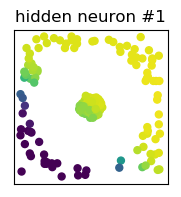
\includegraphics[width=1.6cm]{mfp/learning_process/h_neuron_5_1.png}}; 
\node (hidden1) at (1.0,3.0) {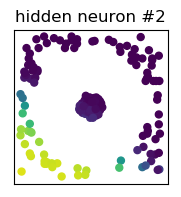
\includegraphics[width=1.6cm]{mfp/learning_process/h_neuron_5_2.png}}; 
\node (hidden2) at (2.0,3.0) {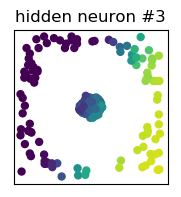
\includegraphics[width=1.6cm]{mfp/learning_process/h_neuron_5_3.png}}; 
\node (hidden3) at (3.0,3.0) {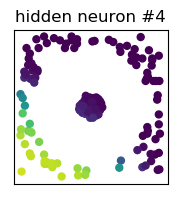
\includegraphics[width=1.6cm]{mfp/learning_process/h_neuron_5_4.png}}; 
\node (hidden4) at (4.0,3.0) {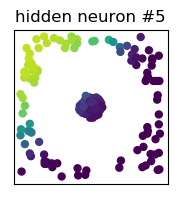
\includegraphics[width=1.6cm]{mfp/learning_process/h_neuron_5_5.png}}; 
\node (hidden5) at (5.0,3.0) {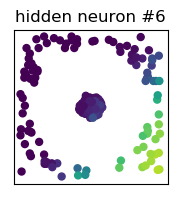
\includegraphics[width=1.6cm]{mfp/learning_process/h_neuron_5_6.png}}; 
\node (hidden6) at (6.0,3.0) {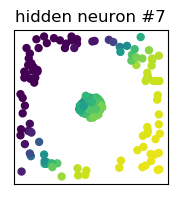
\includegraphics[width=1.6cm]{mfp/learning_process/h_neuron_5_7.png}}; 
\node (hidden7) at (7.0,3.0) {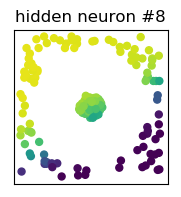
\includegraphics[width=1.6cm]{mfp/learning_process/h_neuron_5_8.png}}; 
\node (hidden8) at (8.0,3.0) {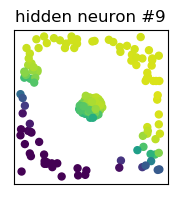
\includegraphics[width=1.6cm]{mfp/learning_process/h_neuron_5_9.png}}; 
\node (hidden9) at (9.0,3.0) {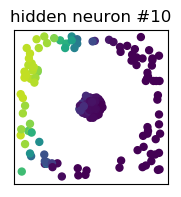
\includegraphics[width=1.6cm]{mfp/learning_process/h_neuron_5_10.png}}; 
\node (hidden10) at (10.0,3.0) {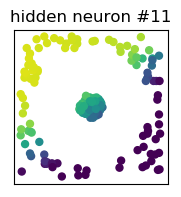
\includegraphics[width=1.6cm]{mfp/learning_process/h_neuron_5_11.png}}; 
\node (out5) at (5.2,0.0) {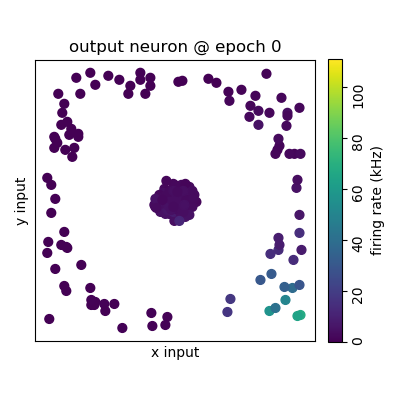
\includegraphics[width=3.6cm]{mfp/learning_process/output_neuron_5.png}}; 

\draw[-stealth,line width=0.4pt, color=red ] (hidden0.south) -- (out5); 
\draw[-stealth,line width=2.0pt, color=blue ] (hidden1.south) -- (out5); 
\draw[-stealth,line width=1.9pt, color=red ] (hidden2.south) -- (out5); 
\draw[-stealth,line width=1.1pt, color=red ] (hidden3.south) -- (out5); 
\draw[-stealth,line width=2.1pt, color=red ] (hidden4.south) -- (out5); 
\draw[-stealth,line width=2.2pt, color=red ] (hidden5.south) -- (out5); 
\draw[-stealth,line width=1.4pt, color=red ] (hidden6.south) -- (out5); 
\draw[-stealth,line width=0.1pt, color=red ] (hidden7.south) -- (out5); 
\draw[-stealth,line width=2.2pt, color=blue ] (hidden8.south) -- (out5); 
\draw[-stealth,line width=0.7pt, color=red ] (hidden9.south) -- (out5); 
\draw[-stealth,line width=0.7pt, color=red ] (hidden10.south) -- (out5); 
\end{tikzpicture} 
	\caption{Init state of network}
\end{figure}
\begin{figure}
	\label{learning_process_s500}
	\begin{tikzpicture}[scale=1.4] 
\node (hidden0) at (0.0,3.0) {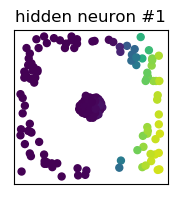
\includegraphics[width=1.6cm]{mfp/learning_process/h_neuron_500_1.png}}; 
\node (hidden1) at (1.0,3.0) {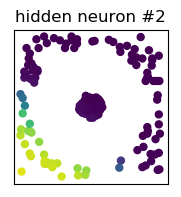
\includegraphics[width=1.6cm]{mfp/learning_process/h_neuron_500_2.png}}; 
\node (hidden2) at (2.0,3.0) {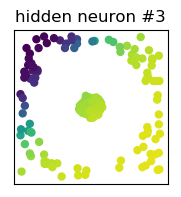
\includegraphics[width=1.6cm]{mfp/learning_process/h_neuron_500_3.png}}; 
\node (hidden3) at (3.0,3.0) {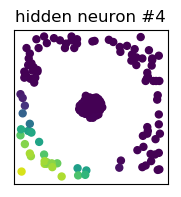
\includegraphics[width=1.6cm]{mfp/learning_process/h_neuron_500_4.png}}; 
\node (hidden4) at (4.0,3.0) {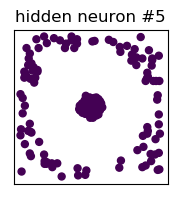
\includegraphics[width=1.6cm]{mfp/learning_process/h_neuron_500_5.png}}; 
\node (hidden5) at (5.0,3.0) {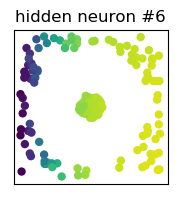
\includegraphics[width=1.6cm]{mfp/learning_process/h_neuron_500_6.png}}; 
\node (hidden6) at (6.0,3.0) {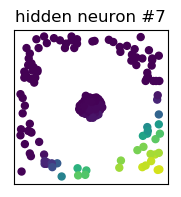
\includegraphics[width=1.6cm]{mfp/learning_process/h_neuron_500_7.png}}; 
\node (hidden7) at (7.0,3.0) {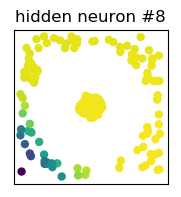
\includegraphics[width=1.6cm]{mfp/learning_process/h_neuron_500_8.png}}; 
\node (hidden8) at (8.0,3.0) {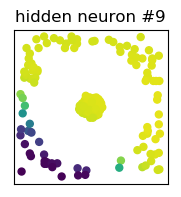
\includegraphics[width=1.6cm]{mfp/learning_process/h_neuron_500_9.png}}; 
\node (hidden9) at (9.0,3.0) {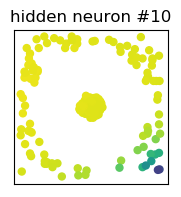
\includegraphics[width=1.6cm]{mfp/learning_process/h_neuron_500_10.png}}; 
\node (hidden10) at (10.0,3.0) {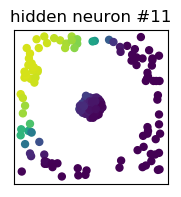
\includegraphics[width=1.6cm]{mfp/learning_process/h_neuron_500_11.png}}; 
\node (out500) at (5.2,0.0) {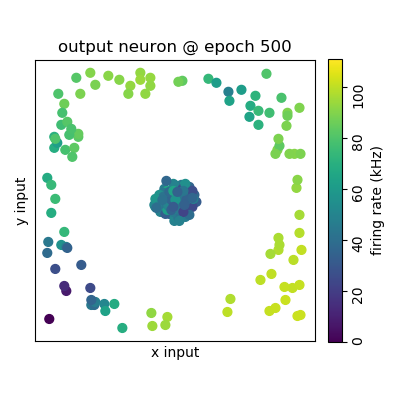
\includegraphics[width=3.6cm]{mfp/learning_process/output_neuron_500.png}}; 

\draw[-stealth,line width=1.5pt, color=red ] (hidden0.south) -- (out500); 
\draw[-stealth,line width=0.1pt, color=blue ] (hidden1.south) -- (out500); 
\draw[-stealth,line width=0.8pt, color=red ] (hidden2.south) -- (out500); 
\draw[-stealth,line width=0.7pt, color=red ] (hidden3.south) -- (out500); 
\draw[-stealth,line width=1.2pt, color=red ] (hidden4.south) -- (out500); 
\draw[-stealth,line width=2.0pt, color=red ] (hidden5.south) -- (out500); 
\draw[-stealth,line width=2.3pt, color=red ] (hidden6.south) -- (out500); 
\draw[-stealth,line width=0.9pt, color=red ] (hidden7.south) -- (out500); 
\draw[-stealth,line width=0.5pt, color=blue ] (hidden8.south) -- (out500); 
\draw[-stealth,line width=0.2pt, color=red ] (hidden9.south) -- (out500); 
\draw[-stealth,line width=2.2pt, color=red ] (hidden10.south) -- (out500); 
\end{tikzpicture} 
	\caption{Init state of network}
\end{figure}
\begin{figure}
	\label{learning_process_s2500}
	\begin{tikzpicture}[scale=1.4] 
\node (hidden0) at (0.0,3.0) {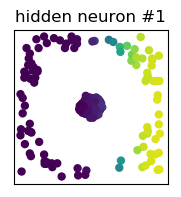
\includegraphics[width=1.6cm]{mfp/learning_process/h_neuron_2500_1.png}}; 
\node (hidden1) at (1.0,3.0) {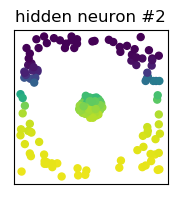
\includegraphics[width=1.6cm]{mfp/learning_process/h_neuron_2500_2.png}}; 
\node (hidden2) at (2.0,3.0) {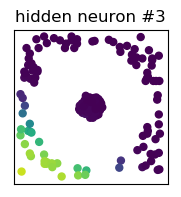
\includegraphics[width=1.6cm]{mfp/learning_process/h_neuron_2500_3.png}}; 
\node (hidden3) at (3.0,3.0) {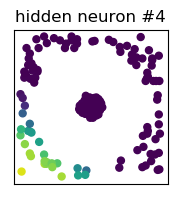
\includegraphics[width=1.6cm]{mfp/learning_process/h_neuron_2500_4.png}}; 
\node (hidden4) at (4.0,3.0) {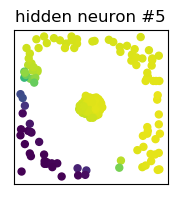
\includegraphics[width=1.6cm]{mfp/learning_process/h_neuron_2500_5.png}}; 
\node (hidden5) at (5.0,3.0) {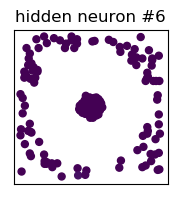
\includegraphics[width=1.6cm]{mfp/learning_process/h_neuron_2500_6.png}}; 
\node (hidden6) at (6.0,3.0) {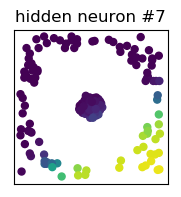
\includegraphics[width=1.6cm]{mfp/learning_process/h_neuron_2500_7.png}}; 
\node (hidden7) at (7.0,3.0) {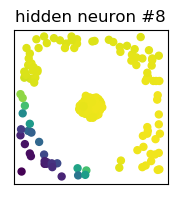
\includegraphics[width=1.6cm]{mfp/learning_process/h_neuron_2500_8.png}}; 
\node (hidden8) at (8.0,3.0) {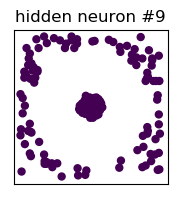
\includegraphics[width=1.6cm]{mfp/learning_process/h_neuron_2500_9.png}}; 
\node (hidden9) at (9.0,3.0) {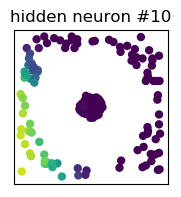
\includegraphics[width=1.6cm]{mfp/learning_process/h_neuron_2500_10.png}}; 
\node (hidden10) at (10.0,3.0) {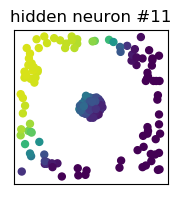
\includegraphics[width=1.6cm]{mfp/learning_process/h_neuron_2500_11.png}}; 
\node (out5) at (5.2,0.0) {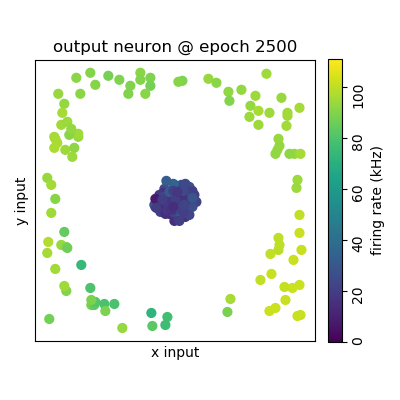
\includegraphics[width=3.6cm]{mfp/learning_process/output_neuron_2500.png}}; 

\draw[-stealth,line width=0.4pt, color=red ] (hidden0.south) -- (out5); 
\draw[-stealth,line width=2.0pt, color=blue ] (hidden1.south) -- (out5); 
\draw[-stealth,line width=1.9pt, color=red ] (hidden2.south) -- (out5); 
\draw[-stealth,line width=1.1pt, color=red ] (hidden3.south) -- (out5); 
\draw[-stealth,line width=2.1pt, color=red ] (hidden4.south) -- (out5); 
\draw[-stealth,line width=2.2pt, color=red ] (hidden5.south) -- (out5); 
\draw[-stealth,line width=1.4pt, color=red ] (hidden6.south) -- (out5); 
\draw[-stealth,line width=0.1pt, color=red ] (hidden7.south) -- (out5); 
\draw[-stealth,line width=2.2pt, color=blue ] (hidden8.south) -- (out5); 
\draw[-stealth,line width=0.7pt, color=red ] (hidden9.south) -- (out5); 
\draw[-stealth,line width=0.7pt, color=red ] (hidden10.south) -- (out5); 
\end{tikzpicture} 
	\caption{Init state of network}
\end{figure}


\begin{figure}
	\label{circles_acc}
	\begin{center}
		%% Creator: Matplotlib, PGF backend
%%
%% To include the figure in your LaTeX document, write
%%   \input{<filename>.pgf}
%%
%% Make sure the required packages are loaded in your preamble
%%   \usepackage{pgf}
%%
%% Figures using additional raster images can only be included by \input if
%% they are in the same directory as the main LaTeX file. For loading figures
%% from other directories you can use the `import` package
%%   \usepackage{import}
%% and then include the figures with
%%   \import{<path to file>}{<filename>.pgf}
%%
%% Matplotlib used the following preamble
%%   \usepackage{amsmath} \usepackage{pifont} \usepackage{xcolor} \definecolor{green}{HTML}{467821} \definecolor{red}{HTML}{CF4457} \usepackage[detect-all]{siunitx}
%%   \usepackage{fontspec}
%%
\begingroup%
\makeatletter%
\begin{pgfpicture}%
\pgfpathrectangle{\pgfpointorigin}{\pgfqpoint{5.197336in}{3.530797in}}%
\pgfusepath{use as bounding box, clip}%
\begin{pgfscope}%
\pgfsetbuttcap%
\pgfsetmiterjoin%
\pgfsetlinewidth{0.000000pt}%
\definecolor{currentstroke}{rgb}{0.000000,0.000000,0.000000}%
\pgfsetstrokecolor{currentstroke}%
\pgfsetstrokeopacity{0.000000}%
\pgfsetdash{}{0pt}%
\pgfpathmoveto{\pgfqpoint{0.000000in}{0.000000in}}%
\pgfpathlineto{\pgfqpoint{5.197336in}{0.000000in}}%
\pgfpathlineto{\pgfqpoint{5.197336in}{3.530797in}}%
\pgfpathlineto{\pgfqpoint{0.000000in}{3.530797in}}%
\pgfpathclose%
\pgfusepath{}%
\end{pgfscope}%
\begin{pgfscope}%
\pgfsetbuttcap%
\pgfsetmiterjoin%
\pgfsetlinewidth{0.000000pt}%
\definecolor{currentstroke}{rgb}{0.000000,0.000000,0.000000}%
\pgfsetstrokecolor{currentstroke}%
\pgfsetstrokeopacity{0.000000}%
\pgfsetdash{}{0pt}%
\pgfpathmoveto{\pgfqpoint{0.447336in}{2.026146in}}%
\pgfpathlineto{\pgfqpoint{5.097336in}{2.026146in}}%
\pgfpathlineto{\pgfqpoint{5.097336in}{3.430797in}}%
\pgfpathlineto{\pgfqpoint{0.447336in}{3.430797in}}%
\pgfpathclose%
\pgfusepath{}%
\end{pgfscope}%
\begin{pgfscope}%
\pgfsetbuttcap%
\pgfsetroundjoin%
\definecolor{currentfill}{rgb}{0.317647,0.317647,0.317647}%
\pgfsetfillcolor{currentfill}%
\pgfsetlinewidth{0.501875pt}%
\definecolor{currentstroke}{rgb}{0.317647,0.317647,0.317647}%
\pgfsetstrokecolor{currentstroke}%
\pgfsetdash{}{0pt}%
\pgfsys@defobject{currentmarker}{\pgfqpoint{0.000000in}{-0.020833in}}{\pgfqpoint{0.000000in}{0.000000in}}{%
\pgfpathmoveto{\pgfqpoint{0.000000in}{0.000000in}}%
\pgfpathlineto{\pgfqpoint{0.000000in}{-0.020833in}}%
\pgfusepath{stroke,fill}%
}%
\begin{pgfscope}%
\pgfsys@transformshift{0.658700in}{2.026146in}%
\pgfsys@useobject{currentmarker}{}%
\end{pgfscope}%
\end{pgfscope}%
\begin{pgfscope}%
\pgfsetbuttcap%
\pgfsetroundjoin%
\definecolor{currentfill}{rgb}{0.317647,0.317647,0.317647}%
\pgfsetfillcolor{currentfill}%
\pgfsetlinewidth{0.501875pt}%
\definecolor{currentstroke}{rgb}{0.317647,0.317647,0.317647}%
\pgfsetstrokecolor{currentstroke}%
\pgfsetdash{}{0pt}%
\pgfsys@defobject{currentmarker}{\pgfqpoint{0.000000in}{-0.020833in}}{\pgfqpoint{0.000000in}{0.000000in}}{%
\pgfpathmoveto{\pgfqpoint{0.000000in}{0.000000in}}%
\pgfpathlineto{\pgfqpoint{0.000000in}{-0.020833in}}%
\pgfusepath{stroke,fill}%
}%
\begin{pgfscope}%
\pgfsys@transformshift{1.187770in}{2.026146in}%
\pgfsys@useobject{currentmarker}{}%
\end{pgfscope}%
\end{pgfscope}%
\begin{pgfscope}%
\pgfsetbuttcap%
\pgfsetroundjoin%
\definecolor{currentfill}{rgb}{0.317647,0.317647,0.317647}%
\pgfsetfillcolor{currentfill}%
\pgfsetlinewidth{0.501875pt}%
\definecolor{currentstroke}{rgb}{0.317647,0.317647,0.317647}%
\pgfsetstrokecolor{currentstroke}%
\pgfsetdash{}{0pt}%
\pgfsys@defobject{currentmarker}{\pgfqpoint{0.000000in}{-0.020833in}}{\pgfqpoint{0.000000in}{0.000000in}}{%
\pgfpathmoveto{\pgfqpoint{0.000000in}{0.000000in}}%
\pgfpathlineto{\pgfqpoint{0.000000in}{-0.020833in}}%
\pgfusepath{stroke,fill}%
}%
\begin{pgfscope}%
\pgfsys@transformshift{1.716841in}{2.026146in}%
\pgfsys@useobject{currentmarker}{}%
\end{pgfscope}%
\end{pgfscope}%
\begin{pgfscope}%
\pgfsetbuttcap%
\pgfsetroundjoin%
\definecolor{currentfill}{rgb}{0.317647,0.317647,0.317647}%
\pgfsetfillcolor{currentfill}%
\pgfsetlinewidth{0.501875pt}%
\definecolor{currentstroke}{rgb}{0.317647,0.317647,0.317647}%
\pgfsetstrokecolor{currentstroke}%
\pgfsetdash{}{0pt}%
\pgfsys@defobject{currentmarker}{\pgfqpoint{0.000000in}{-0.020833in}}{\pgfqpoint{0.000000in}{0.000000in}}{%
\pgfpathmoveto{\pgfqpoint{0.000000in}{0.000000in}}%
\pgfpathlineto{\pgfqpoint{0.000000in}{-0.020833in}}%
\pgfusepath{stroke,fill}%
}%
\begin{pgfscope}%
\pgfsys@transformshift{2.245911in}{2.026146in}%
\pgfsys@useobject{currentmarker}{}%
\end{pgfscope}%
\end{pgfscope}%
\begin{pgfscope}%
\pgfsetbuttcap%
\pgfsetroundjoin%
\definecolor{currentfill}{rgb}{0.317647,0.317647,0.317647}%
\pgfsetfillcolor{currentfill}%
\pgfsetlinewidth{0.501875pt}%
\definecolor{currentstroke}{rgb}{0.317647,0.317647,0.317647}%
\pgfsetstrokecolor{currentstroke}%
\pgfsetdash{}{0pt}%
\pgfsys@defobject{currentmarker}{\pgfqpoint{0.000000in}{-0.020833in}}{\pgfqpoint{0.000000in}{0.000000in}}{%
\pgfpathmoveto{\pgfqpoint{0.000000in}{0.000000in}}%
\pgfpathlineto{\pgfqpoint{0.000000in}{-0.020833in}}%
\pgfusepath{stroke,fill}%
}%
\begin{pgfscope}%
\pgfsys@transformshift{2.774981in}{2.026146in}%
\pgfsys@useobject{currentmarker}{}%
\end{pgfscope}%
\end{pgfscope}%
\begin{pgfscope}%
\pgfsetbuttcap%
\pgfsetroundjoin%
\definecolor{currentfill}{rgb}{0.317647,0.317647,0.317647}%
\pgfsetfillcolor{currentfill}%
\pgfsetlinewidth{0.501875pt}%
\definecolor{currentstroke}{rgb}{0.317647,0.317647,0.317647}%
\pgfsetstrokecolor{currentstroke}%
\pgfsetdash{}{0pt}%
\pgfsys@defobject{currentmarker}{\pgfqpoint{0.000000in}{-0.020833in}}{\pgfqpoint{0.000000in}{0.000000in}}{%
\pgfpathmoveto{\pgfqpoint{0.000000in}{0.000000in}}%
\pgfpathlineto{\pgfqpoint{0.000000in}{-0.020833in}}%
\pgfusepath{stroke,fill}%
}%
\begin{pgfscope}%
\pgfsys@transformshift{3.304052in}{2.026146in}%
\pgfsys@useobject{currentmarker}{}%
\end{pgfscope}%
\end{pgfscope}%
\begin{pgfscope}%
\pgfsetbuttcap%
\pgfsetroundjoin%
\definecolor{currentfill}{rgb}{0.317647,0.317647,0.317647}%
\pgfsetfillcolor{currentfill}%
\pgfsetlinewidth{0.501875pt}%
\definecolor{currentstroke}{rgb}{0.317647,0.317647,0.317647}%
\pgfsetstrokecolor{currentstroke}%
\pgfsetdash{}{0pt}%
\pgfsys@defobject{currentmarker}{\pgfqpoint{0.000000in}{-0.020833in}}{\pgfqpoint{0.000000in}{0.000000in}}{%
\pgfpathmoveto{\pgfqpoint{0.000000in}{0.000000in}}%
\pgfpathlineto{\pgfqpoint{0.000000in}{-0.020833in}}%
\pgfusepath{stroke,fill}%
}%
\begin{pgfscope}%
\pgfsys@transformshift{3.833122in}{2.026146in}%
\pgfsys@useobject{currentmarker}{}%
\end{pgfscope}%
\end{pgfscope}%
\begin{pgfscope}%
\pgfsetbuttcap%
\pgfsetroundjoin%
\definecolor{currentfill}{rgb}{0.317647,0.317647,0.317647}%
\pgfsetfillcolor{currentfill}%
\pgfsetlinewidth{0.501875pt}%
\definecolor{currentstroke}{rgb}{0.317647,0.317647,0.317647}%
\pgfsetstrokecolor{currentstroke}%
\pgfsetdash{}{0pt}%
\pgfsys@defobject{currentmarker}{\pgfqpoint{0.000000in}{-0.020833in}}{\pgfqpoint{0.000000in}{0.000000in}}{%
\pgfpathmoveto{\pgfqpoint{0.000000in}{0.000000in}}%
\pgfpathlineto{\pgfqpoint{0.000000in}{-0.020833in}}%
\pgfusepath{stroke,fill}%
}%
\begin{pgfscope}%
\pgfsys@transformshift{4.362193in}{2.026146in}%
\pgfsys@useobject{currentmarker}{}%
\end{pgfscope}%
\end{pgfscope}%
\begin{pgfscope}%
\pgfsetbuttcap%
\pgfsetroundjoin%
\definecolor{currentfill}{rgb}{0.317647,0.317647,0.317647}%
\pgfsetfillcolor{currentfill}%
\pgfsetlinewidth{0.501875pt}%
\definecolor{currentstroke}{rgb}{0.317647,0.317647,0.317647}%
\pgfsetstrokecolor{currentstroke}%
\pgfsetdash{}{0pt}%
\pgfsys@defobject{currentmarker}{\pgfqpoint{0.000000in}{-0.020833in}}{\pgfqpoint{0.000000in}{0.000000in}}{%
\pgfpathmoveto{\pgfqpoint{0.000000in}{0.000000in}}%
\pgfpathlineto{\pgfqpoint{0.000000in}{-0.020833in}}%
\pgfusepath{stroke,fill}%
}%
\begin{pgfscope}%
\pgfsys@transformshift{4.891263in}{2.026146in}%
\pgfsys@useobject{currentmarker}{}%
\end{pgfscope}%
\end{pgfscope}%
\begin{pgfscope}%
\pgfsetbuttcap%
\pgfsetroundjoin%
\definecolor{currentfill}{rgb}{0.317647,0.317647,0.317647}%
\pgfsetfillcolor{currentfill}%
\pgfsetlinewidth{0.501875pt}%
\definecolor{currentstroke}{rgb}{0.317647,0.317647,0.317647}%
\pgfsetstrokecolor{currentstroke}%
\pgfsetdash{}{0pt}%
\pgfsys@defobject{currentmarker}{\pgfqpoint{-0.020833in}{0.000000in}}{\pgfqpoint{0.000000in}{0.000000in}}{%
\pgfpathmoveto{\pgfqpoint{0.000000in}{0.000000in}}%
\pgfpathlineto{\pgfqpoint{-0.020833in}{0.000000in}}%
\pgfusepath{stroke,fill}%
}%
\begin{pgfscope}%
\pgfsys@transformshift{0.447336in}{2.165108in}%
\pgfsys@useobject{currentmarker}{}%
\end{pgfscope}%
\end{pgfscope}%
\begin{pgfscope}%
\definecolor{textcolor}{rgb}{0.317647,0.317647,0.317647}%
\pgfsetstrokecolor{textcolor}%
\pgfsetfillcolor{textcolor}%
\pgftext[x=0.261763in,y=2.124962in,left,base]{\color{textcolor}\rmfamily\fontsize{8.330000}{9.996000}\selectfont \(\displaystyle 0.2\)}%
\end{pgfscope}%
\begin{pgfscope}%
\pgfsetbuttcap%
\pgfsetroundjoin%
\definecolor{currentfill}{rgb}{0.317647,0.317647,0.317647}%
\pgfsetfillcolor{currentfill}%
\pgfsetlinewidth{0.501875pt}%
\definecolor{currentstroke}{rgb}{0.317647,0.317647,0.317647}%
\pgfsetstrokecolor{currentstroke}%
\pgfsetdash{}{0pt}%
\pgfsys@defobject{currentmarker}{\pgfqpoint{-0.020833in}{0.000000in}}{\pgfqpoint{0.000000in}{0.000000in}}{%
\pgfpathmoveto{\pgfqpoint{0.000000in}{0.000000in}}%
\pgfpathlineto{\pgfqpoint{-0.020833in}{0.000000in}}%
\pgfusepath{stroke,fill}%
}%
\begin{pgfscope}%
\pgfsys@transformshift{0.447336in}{2.465568in}%
\pgfsys@useobject{currentmarker}{}%
\end{pgfscope}%
\end{pgfscope}%
\begin{pgfscope}%
\definecolor{textcolor}{rgb}{0.317647,0.317647,0.317647}%
\pgfsetstrokecolor{textcolor}%
\pgfsetfillcolor{textcolor}%
\pgftext[x=0.261763in,y=2.425422in,left,base]{\color{textcolor}\rmfamily\fontsize{8.330000}{9.996000}\selectfont \(\displaystyle 0.4\)}%
\end{pgfscope}%
\begin{pgfscope}%
\pgfsetbuttcap%
\pgfsetroundjoin%
\definecolor{currentfill}{rgb}{0.317647,0.317647,0.317647}%
\pgfsetfillcolor{currentfill}%
\pgfsetlinewidth{0.501875pt}%
\definecolor{currentstroke}{rgb}{0.317647,0.317647,0.317647}%
\pgfsetstrokecolor{currentstroke}%
\pgfsetdash{}{0pt}%
\pgfsys@defobject{currentmarker}{\pgfqpoint{-0.020833in}{0.000000in}}{\pgfqpoint{0.000000in}{0.000000in}}{%
\pgfpathmoveto{\pgfqpoint{0.000000in}{0.000000in}}%
\pgfpathlineto{\pgfqpoint{-0.020833in}{0.000000in}}%
\pgfusepath{stroke,fill}%
}%
\begin{pgfscope}%
\pgfsys@transformshift{0.447336in}{2.766029in}%
\pgfsys@useobject{currentmarker}{}%
\end{pgfscope}%
\end{pgfscope}%
\begin{pgfscope}%
\definecolor{textcolor}{rgb}{0.317647,0.317647,0.317647}%
\pgfsetstrokecolor{textcolor}%
\pgfsetfillcolor{textcolor}%
\pgftext[x=0.261763in,y=2.725883in,left,base]{\color{textcolor}\rmfamily\fontsize{8.330000}{9.996000}\selectfont \(\displaystyle 0.6\)}%
\end{pgfscope}%
\begin{pgfscope}%
\pgfsetbuttcap%
\pgfsetroundjoin%
\definecolor{currentfill}{rgb}{0.317647,0.317647,0.317647}%
\pgfsetfillcolor{currentfill}%
\pgfsetlinewidth{0.501875pt}%
\definecolor{currentstroke}{rgb}{0.317647,0.317647,0.317647}%
\pgfsetstrokecolor{currentstroke}%
\pgfsetdash{}{0pt}%
\pgfsys@defobject{currentmarker}{\pgfqpoint{-0.020833in}{0.000000in}}{\pgfqpoint{0.000000in}{0.000000in}}{%
\pgfpathmoveto{\pgfqpoint{0.000000in}{0.000000in}}%
\pgfpathlineto{\pgfqpoint{-0.020833in}{0.000000in}}%
\pgfusepath{stroke,fill}%
}%
\begin{pgfscope}%
\pgfsys@transformshift{0.447336in}{3.066489in}%
\pgfsys@useobject{currentmarker}{}%
\end{pgfscope}%
\end{pgfscope}%
\begin{pgfscope}%
\definecolor{textcolor}{rgb}{0.317647,0.317647,0.317647}%
\pgfsetstrokecolor{textcolor}%
\pgfsetfillcolor{textcolor}%
\pgftext[x=0.261763in,y=3.026343in,left,base]{\color{textcolor}\rmfamily\fontsize{8.330000}{9.996000}\selectfont \(\displaystyle 0.8\)}%
\end{pgfscope}%
\begin{pgfscope}%
\pgfsetbuttcap%
\pgfsetroundjoin%
\definecolor{currentfill}{rgb}{0.317647,0.317647,0.317647}%
\pgfsetfillcolor{currentfill}%
\pgfsetlinewidth{0.501875pt}%
\definecolor{currentstroke}{rgb}{0.317647,0.317647,0.317647}%
\pgfsetstrokecolor{currentstroke}%
\pgfsetdash{}{0pt}%
\pgfsys@defobject{currentmarker}{\pgfqpoint{-0.020833in}{0.000000in}}{\pgfqpoint{0.000000in}{0.000000in}}{%
\pgfpathmoveto{\pgfqpoint{0.000000in}{0.000000in}}%
\pgfpathlineto{\pgfqpoint{-0.020833in}{0.000000in}}%
\pgfusepath{stroke,fill}%
}%
\begin{pgfscope}%
\pgfsys@transformshift{0.447336in}{3.366949in}%
\pgfsys@useobject{currentmarker}{}%
\end{pgfscope}%
\end{pgfscope}%
\begin{pgfscope}%
\definecolor{textcolor}{rgb}{0.317647,0.317647,0.317647}%
\pgfsetstrokecolor{textcolor}%
\pgfsetfillcolor{textcolor}%
\pgftext[x=0.261763in,y=3.326803in,left,base]{\color{textcolor}\rmfamily\fontsize{8.330000}{9.996000}\selectfont \(\displaystyle 1.0\)}%
\end{pgfscope}%
\begin{pgfscope}%
\definecolor{textcolor}{rgb}{0.317647,0.317647,0.317647}%
\pgfsetstrokecolor{textcolor}%
\pgfsetfillcolor{textcolor}%
\pgftext[x=0.206207in,y=2.728471in,,bottom,rotate=90.000000]{\color{textcolor}\rmfamily\fontsize{8.330000}{9.996000}\selectfont Accuracy}%
\end{pgfscope}%
\begin{pgfscope}%
\pgfpathrectangle{\pgfqpoint{0.447336in}{2.026146in}}{\pgfqpoint{4.650000in}{1.404651in}}%
\pgfusepath{clip}%
\pgfsetrectcap%
\pgfsetroundjoin%
\pgfsetlinewidth{0.803000pt}%
\definecolor{currentstroke}{rgb}{0.333333,0.333333,0.333333}%
\pgfsetstrokecolor{currentstroke}%
\pgfsetdash{}{0pt}%
\pgfpathmoveto{\pgfqpoint{0.658700in}{2.593264in}}%
\pgfpathlineto{\pgfqpoint{0.663990in}{2.615799in}}%
\pgfpathlineto{\pgfqpoint{0.669281in}{2.623310in}}%
\pgfpathlineto{\pgfqpoint{0.674572in}{2.653356in}}%
\pgfpathlineto{\pgfqpoint{0.679863in}{2.510637in}}%
\pgfpathlineto{\pgfqpoint{0.685153in}{2.728471in}}%
\pgfpathlineto{\pgfqpoint{0.690444in}{2.698425in}}%
\pgfpathlineto{\pgfqpoint{0.695735in}{2.713448in}}%
\pgfpathlineto{\pgfqpoint{0.701025in}{2.698425in}}%
\pgfpathlineto{\pgfqpoint{0.711607in}{2.713448in}}%
\pgfpathlineto{\pgfqpoint{0.716897in}{2.735983in}}%
\pgfpathlineto{\pgfqpoint{0.722188in}{2.713448in}}%
\pgfpathlineto{\pgfqpoint{0.727479in}{2.623310in}}%
\pgfpathlineto{\pgfqpoint{0.732770in}{2.315338in}}%
\pgfpathlineto{\pgfqpoint{0.738060in}{2.578241in}}%
\pgfpathlineto{\pgfqpoint{0.743351in}{2.660868in}}%
\pgfpathlineto{\pgfqpoint{0.748642in}{2.089993in}}%
\pgfpathlineto{\pgfqpoint{0.753932in}{2.142574in}}%
\pgfpathlineto{\pgfqpoint{0.759223in}{2.638333in}}%
\pgfpathlineto{\pgfqpoint{0.764514in}{2.428011in}}%
\pgfpathlineto{\pgfqpoint{0.769805in}{2.728471in}}%
\pgfpathlineto{\pgfqpoint{0.775095in}{2.480591in}}%
\pgfpathlineto{\pgfqpoint{0.780386in}{2.683402in}}%
\pgfpathlineto{\pgfqpoint{0.785677in}{2.788563in}}%
\pgfpathlineto{\pgfqpoint{0.790967in}{2.563218in}}%
\pgfpathlineto{\pgfqpoint{0.796258in}{2.773540in}}%
\pgfpathlineto{\pgfqpoint{0.801549in}{2.330361in}}%
\pgfpathlineto{\pgfqpoint{0.806839in}{2.225200in}}%
\pgfpathlineto{\pgfqpoint{0.812130in}{2.292804in}}%
\pgfpathlineto{\pgfqpoint{0.817421in}{2.833632in}}%
\pgfpathlineto{\pgfqpoint{0.822712in}{2.826121in}}%
\pgfpathlineto{\pgfqpoint{0.828002in}{2.968839in}}%
\pgfpathlineto{\pgfqpoint{0.833293in}{3.028931in}}%
\pgfpathlineto{\pgfqpoint{0.843874in}{3.028931in}}%
\pgfpathlineto{\pgfqpoint{0.849165in}{2.563218in}}%
\pgfpathlineto{\pgfqpoint{0.854456in}{3.021420in}}%
\pgfpathlineto{\pgfqpoint{0.859747in}{2.923770in}}%
\pgfpathlineto{\pgfqpoint{0.865037in}{2.878701in}}%
\pgfpathlineto{\pgfqpoint{0.870328in}{2.968839in}}%
\pgfpathlineto{\pgfqpoint{0.875619in}{2.908747in}}%
\pgfpathlineto{\pgfqpoint{0.886200in}{2.428011in}}%
\pgfpathlineto{\pgfqpoint{0.891491in}{2.367919in}}%
\pgfpathlineto{\pgfqpoint{0.896781in}{2.428011in}}%
\pgfpathlineto{\pgfqpoint{0.902072in}{2.412988in}}%
\pgfpathlineto{\pgfqpoint{0.907363in}{2.480591in}}%
\pgfpathlineto{\pgfqpoint{0.912654in}{2.713448in}}%
\pgfpathlineto{\pgfqpoint{0.923235in}{2.938793in}}%
\pgfpathlineto{\pgfqpoint{0.928526in}{2.946305in}}%
\pgfpathlineto{\pgfqpoint{0.933816in}{3.171650in}}%
\pgfpathlineto{\pgfqpoint{0.939107in}{2.976351in}}%
\pgfpathlineto{\pgfqpoint{0.944398in}{2.848655in}}%
\pgfpathlineto{\pgfqpoint{0.949688in}{2.886213in}}%
\pgfpathlineto{\pgfqpoint{0.954979in}{3.171650in}}%
\pgfpathlineto{\pgfqpoint{0.960270in}{3.149115in}}%
\pgfpathlineto{\pgfqpoint{0.965561in}{3.043954in}}%
\pgfpathlineto{\pgfqpoint{0.970851in}{3.021420in}}%
\pgfpathlineto{\pgfqpoint{0.976142in}{3.028931in}}%
\pgfpathlineto{\pgfqpoint{0.981433in}{3.051466in}}%
\pgfpathlineto{\pgfqpoint{0.986723in}{3.104046in}}%
\pgfpathlineto{\pgfqpoint{0.992014in}{2.946305in}}%
\pgfpathlineto{\pgfqpoint{0.997305in}{3.141604in}}%
\pgfpathlineto{\pgfqpoint{1.002596in}{3.104046in}}%
\pgfpathlineto{\pgfqpoint{1.007886in}{3.089023in}}%
\pgfpathlineto{\pgfqpoint{1.013177in}{3.066489in}}%
\pgfpathlineto{\pgfqpoint{1.018468in}{3.134092in}}%
\pgfpathlineto{\pgfqpoint{1.023758in}{3.111558in}}%
\pgfpathlineto{\pgfqpoint{1.029049in}{3.104046in}}%
\pgfpathlineto{\pgfqpoint{1.034340in}{3.104046in}}%
\pgfpathlineto{\pgfqpoint{1.039630in}{3.171650in}}%
\pgfpathlineto{\pgfqpoint{1.044921in}{3.164138in}}%
\pgfpathlineto{\pgfqpoint{1.050212in}{3.119069in}}%
\pgfpathlineto{\pgfqpoint{1.055503in}{3.194184in}}%
\pgfpathlineto{\pgfqpoint{1.060793in}{3.186673in}}%
\pgfpathlineto{\pgfqpoint{1.066084in}{3.171650in}}%
\pgfpathlineto{\pgfqpoint{1.071375in}{2.946305in}}%
\pgfpathlineto{\pgfqpoint{1.076665in}{3.134092in}}%
\pgfpathlineto{\pgfqpoint{1.081956in}{3.149115in}}%
\pgfpathlineto{\pgfqpoint{1.087247in}{3.126581in}}%
\pgfpathlineto{\pgfqpoint{1.092537in}{3.089023in}}%
\pgfpathlineto{\pgfqpoint{1.097828in}{2.998885in}}%
\pgfpathlineto{\pgfqpoint{1.103119in}{3.066489in}}%
\pgfpathlineto{\pgfqpoint{1.108410in}{3.089023in}}%
\pgfpathlineto{\pgfqpoint{1.113700in}{3.051466in}}%
\pgfpathlineto{\pgfqpoint{1.118991in}{3.058977in}}%
\pgfpathlineto{\pgfqpoint{1.124282in}{3.104046in}}%
\pgfpathlineto{\pgfqpoint{1.129572in}{2.886213in}}%
\pgfpathlineto{\pgfqpoint{1.134863in}{3.104046in}}%
\pgfpathlineto{\pgfqpoint{1.140154in}{3.141604in}}%
\pgfpathlineto{\pgfqpoint{1.145445in}{2.923770in}}%
\pgfpathlineto{\pgfqpoint{1.150735in}{3.089023in}}%
\pgfpathlineto{\pgfqpoint{1.156026in}{3.104046in}}%
\pgfpathlineto{\pgfqpoint{1.161317in}{3.149115in}}%
\pgfpathlineto{\pgfqpoint{1.166607in}{2.856167in}}%
\pgfpathlineto{\pgfqpoint{1.171898in}{3.126581in}}%
\pgfpathlineto{\pgfqpoint{1.177189in}{3.141604in}}%
\pgfpathlineto{\pgfqpoint{1.182479in}{3.164138in}}%
\pgfpathlineto{\pgfqpoint{1.187770in}{3.104046in}}%
\pgfpathlineto{\pgfqpoint{1.193061in}{2.991374in}}%
\pgfpathlineto{\pgfqpoint{1.198352in}{2.931282in}}%
\pgfpathlineto{\pgfqpoint{1.203642in}{2.826121in}}%
\pgfpathlineto{\pgfqpoint{1.208933in}{2.803586in}}%
\pgfpathlineto{\pgfqpoint{1.214224in}{2.871190in}}%
\pgfpathlineto{\pgfqpoint{1.219514in}{2.871190in}}%
\pgfpathlineto{\pgfqpoint{1.224805in}{2.773540in}}%
\pgfpathlineto{\pgfqpoint{1.230096in}{2.781052in}}%
\pgfpathlineto{\pgfqpoint{1.235387in}{2.796075in}}%
\pgfpathlineto{\pgfqpoint{1.240677in}{2.871190in}}%
\pgfpathlineto{\pgfqpoint{1.245968in}{2.818609in}}%
\pgfpathlineto{\pgfqpoint{1.251259in}{2.818609in}}%
\pgfpathlineto{\pgfqpoint{1.256549in}{2.803586in}}%
\pgfpathlineto{\pgfqpoint{1.261840in}{2.878701in}}%
\pgfpathlineto{\pgfqpoint{1.267131in}{2.923770in}}%
\pgfpathlineto{\pgfqpoint{1.272421in}{2.833632in}}%
\pgfpathlineto{\pgfqpoint{1.277712in}{2.833632in}}%
\pgfpathlineto{\pgfqpoint{1.283003in}{2.953816in}}%
\pgfpathlineto{\pgfqpoint{1.288294in}{2.923770in}}%
\pgfpathlineto{\pgfqpoint{1.293584in}{3.074000in}}%
\pgfpathlineto{\pgfqpoint{1.298875in}{3.013908in}}%
\pgfpathlineto{\pgfqpoint{1.304166in}{2.856167in}}%
\pgfpathlineto{\pgfqpoint{1.309456in}{3.051466in}}%
\pgfpathlineto{\pgfqpoint{1.314747in}{3.021420in}}%
\pgfpathlineto{\pgfqpoint{1.320038in}{2.878701in}}%
\pgfpathlineto{\pgfqpoint{1.325328in}{3.021420in}}%
\pgfpathlineto{\pgfqpoint{1.330619in}{2.893724in}}%
\pgfpathlineto{\pgfqpoint{1.335910in}{3.081512in}}%
\pgfpathlineto{\pgfqpoint{1.341201in}{3.043954in}}%
\pgfpathlineto{\pgfqpoint{1.346491in}{2.908747in}}%
\pgfpathlineto{\pgfqpoint{1.351782in}{2.833632in}}%
\pgfpathlineto{\pgfqpoint{1.357073in}{2.848655in}}%
\pgfpathlineto{\pgfqpoint{1.362363in}{2.946305in}}%
\pgfpathlineto{\pgfqpoint{1.367654in}{2.946305in}}%
\pgfpathlineto{\pgfqpoint{1.372945in}{2.901236in}}%
\pgfpathlineto{\pgfqpoint{1.378236in}{3.036443in}}%
\pgfpathlineto{\pgfqpoint{1.383526in}{3.043954in}}%
\pgfpathlineto{\pgfqpoint{1.388817in}{3.021420in}}%
\pgfpathlineto{\pgfqpoint{1.394108in}{3.006397in}}%
\pgfpathlineto{\pgfqpoint{1.399398in}{3.021420in}}%
\pgfpathlineto{\pgfqpoint{1.404689in}{3.081512in}}%
\pgfpathlineto{\pgfqpoint{1.409980in}{3.051466in}}%
\pgfpathlineto{\pgfqpoint{1.415270in}{3.104046in}}%
\pgfpathlineto{\pgfqpoint{1.420561in}{3.111558in}}%
\pgfpathlineto{\pgfqpoint{1.425852in}{3.111558in}}%
\pgfpathlineto{\pgfqpoint{1.431143in}{3.126581in}}%
\pgfpathlineto{\pgfqpoint{1.436433in}{3.074000in}}%
\pgfpathlineto{\pgfqpoint{1.441724in}{3.141604in}}%
\pgfpathlineto{\pgfqpoint{1.447015in}{3.126581in}}%
\pgfpathlineto{\pgfqpoint{1.452305in}{3.126581in}}%
\pgfpathlineto{\pgfqpoint{1.457596in}{3.134092in}}%
\pgfpathlineto{\pgfqpoint{1.462887in}{3.096535in}}%
\pgfpathlineto{\pgfqpoint{1.468178in}{3.081512in}}%
\pgfpathlineto{\pgfqpoint{1.473468in}{3.036443in}}%
\pgfpathlineto{\pgfqpoint{1.478759in}{3.081512in}}%
\pgfpathlineto{\pgfqpoint{1.484050in}{3.036443in}}%
\pgfpathlineto{\pgfqpoint{1.494631in}{3.104046in}}%
\pgfpathlineto{\pgfqpoint{1.499922in}{3.201696in}}%
\pgfpathlineto{\pgfqpoint{1.505212in}{3.164138in}}%
\pgfpathlineto{\pgfqpoint{1.510503in}{3.216719in}}%
\pgfpathlineto{\pgfqpoint{1.515794in}{3.141604in}}%
\pgfpathlineto{\pgfqpoint{1.521085in}{3.104046in}}%
\pgfpathlineto{\pgfqpoint{1.526375in}{3.104046in}}%
\pgfpathlineto{\pgfqpoint{1.531666in}{3.149115in}}%
\pgfpathlineto{\pgfqpoint{1.536957in}{3.179161in}}%
\pgfpathlineto{\pgfqpoint{1.542247in}{2.570730in}}%
\pgfpathlineto{\pgfqpoint{1.547538in}{3.209207in}}%
\pgfpathlineto{\pgfqpoint{1.552829in}{3.141604in}}%
\pgfpathlineto{\pgfqpoint{1.558119in}{3.096535in}}%
\pgfpathlineto{\pgfqpoint{1.563410in}{3.164138in}}%
\pgfpathlineto{\pgfqpoint{1.568701in}{3.156627in}}%
\pgfpathlineto{\pgfqpoint{1.573992in}{3.081512in}}%
\pgfpathlineto{\pgfqpoint{1.579282in}{3.141604in}}%
\pgfpathlineto{\pgfqpoint{1.584573in}{3.028931in}}%
\pgfpathlineto{\pgfqpoint{1.589864in}{3.119069in}}%
\pgfpathlineto{\pgfqpoint{1.595154in}{3.111558in}}%
\pgfpathlineto{\pgfqpoint{1.600445in}{3.134092in}}%
\pgfpathlineto{\pgfqpoint{1.611027in}{3.134092in}}%
\pgfpathlineto{\pgfqpoint{1.616317in}{3.149115in}}%
\pgfpathlineto{\pgfqpoint{1.621608in}{3.156627in}}%
\pgfpathlineto{\pgfqpoint{1.626899in}{3.051466in}}%
\pgfpathlineto{\pgfqpoint{1.632189in}{3.149115in}}%
\pgfpathlineto{\pgfqpoint{1.637480in}{2.638333in}}%
\pgfpathlineto{\pgfqpoint{1.642771in}{3.179161in}}%
\pgfpathlineto{\pgfqpoint{1.663934in}{3.149115in}}%
\pgfpathlineto{\pgfqpoint{1.669224in}{3.119069in}}%
\pgfpathlineto{\pgfqpoint{1.674515in}{3.134092in}}%
\pgfpathlineto{\pgfqpoint{1.679806in}{3.134092in}}%
\pgfpathlineto{\pgfqpoint{1.685096in}{3.186673in}}%
\pgfpathlineto{\pgfqpoint{1.690387in}{2.961328in}}%
\pgfpathlineto{\pgfqpoint{1.700968in}{3.201696in}}%
\pgfpathlineto{\pgfqpoint{1.706259in}{3.141604in}}%
\pgfpathlineto{\pgfqpoint{1.711550in}{3.201696in}}%
\pgfpathlineto{\pgfqpoint{1.716841in}{3.171650in}}%
\pgfpathlineto{\pgfqpoint{1.722131in}{3.164138in}}%
\pgfpathlineto{\pgfqpoint{1.727422in}{3.149115in}}%
\pgfpathlineto{\pgfqpoint{1.732713in}{3.096535in}}%
\pgfpathlineto{\pgfqpoint{1.738003in}{3.171650in}}%
\pgfpathlineto{\pgfqpoint{1.743294in}{3.156627in}}%
\pgfpathlineto{\pgfqpoint{1.748585in}{3.209207in}}%
\pgfpathlineto{\pgfqpoint{1.753876in}{3.186673in}}%
\pgfpathlineto{\pgfqpoint{1.759166in}{3.194184in}}%
\pgfpathlineto{\pgfqpoint{1.764457in}{3.171650in}}%
\pgfpathlineto{\pgfqpoint{1.769748in}{3.164138in}}%
\pgfpathlineto{\pgfqpoint{1.775038in}{3.261788in}}%
\pgfpathlineto{\pgfqpoint{1.780329in}{3.224230in}}%
\pgfpathlineto{\pgfqpoint{1.785620in}{3.126581in}}%
\pgfpathlineto{\pgfqpoint{1.790910in}{3.186673in}}%
\pgfpathlineto{\pgfqpoint{1.796201in}{3.164138in}}%
\pgfpathlineto{\pgfqpoint{1.801492in}{3.194184in}}%
\pgfpathlineto{\pgfqpoint{1.806783in}{3.201696in}}%
\pgfpathlineto{\pgfqpoint{1.812073in}{3.141604in}}%
\pgfpathlineto{\pgfqpoint{1.817364in}{3.246765in}}%
\pgfpathlineto{\pgfqpoint{1.822655in}{3.261788in}}%
\pgfpathlineto{\pgfqpoint{1.833236in}{3.231742in}}%
\pgfpathlineto{\pgfqpoint{1.838527in}{3.186673in}}%
\pgfpathlineto{\pgfqpoint{1.843818in}{3.239253in}}%
\pgfpathlineto{\pgfqpoint{1.849108in}{3.224230in}}%
\pgfpathlineto{\pgfqpoint{1.859690in}{2.938793in}}%
\pgfpathlineto{\pgfqpoint{1.864980in}{3.149115in}}%
\pgfpathlineto{\pgfqpoint{1.870271in}{3.164138in}}%
\pgfpathlineto{\pgfqpoint{1.875562in}{3.164138in}}%
\pgfpathlineto{\pgfqpoint{1.880852in}{3.171650in}}%
\pgfpathlineto{\pgfqpoint{1.886143in}{3.134092in}}%
\pgfpathlineto{\pgfqpoint{1.891434in}{3.156627in}}%
\pgfpathlineto{\pgfqpoint{1.896725in}{3.164138in}}%
\pgfpathlineto{\pgfqpoint{1.902015in}{3.156627in}}%
\pgfpathlineto{\pgfqpoint{1.907306in}{3.171650in}}%
\pgfpathlineto{\pgfqpoint{1.912597in}{3.119069in}}%
\pgfpathlineto{\pgfqpoint{1.917887in}{3.179161in}}%
\pgfpathlineto{\pgfqpoint{1.923178in}{3.179161in}}%
\pgfpathlineto{\pgfqpoint{1.928469in}{3.134092in}}%
\pgfpathlineto{\pgfqpoint{1.933759in}{3.209207in}}%
\pgfpathlineto{\pgfqpoint{1.939050in}{3.119069in}}%
\pgfpathlineto{\pgfqpoint{1.944341in}{3.201696in}}%
\pgfpathlineto{\pgfqpoint{1.949632in}{3.216719in}}%
\pgfpathlineto{\pgfqpoint{1.954922in}{3.186673in}}%
\pgfpathlineto{\pgfqpoint{1.965504in}{3.171650in}}%
\pgfpathlineto{\pgfqpoint{1.976085in}{3.171650in}}%
\pgfpathlineto{\pgfqpoint{1.981376in}{3.156627in}}%
\pgfpathlineto{\pgfqpoint{1.986667in}{3.186673in}}%
\pgfpathlineto{\pgfqpoint{1.991957in}{3.179161in}}%
\pgfpathlineto{\pgfqpoint{1.997248in}{3.156627in}}%
\pgfpathlineto{\pgfqpoint{2.002539in}{3.171650in}}%
\pgfpathlineto{\pgfqpoint{2.007829in}{3.164138in}}%
\pgfpathlineto{\pgfqpoint{2.013120in}{3.164138in}}%
\pgfpathlineto{\pgfqpoint{2.018411in}{3.216719in}}%
\pgfpathlineto{\pgfqpoint{2.028992in}{3.216719in}}%
\pgfpathlineto{\pgfqpoint{2.034283in}{3.149115in}}%
\pgfpathlineto{\pgfqpoint{2.039574in}{3.104046in}}%
\pgfpathlineto{\pgfqpoint{2.044864in}{3.149115in}}%
\pgfpathlineto{\pgfqpoint{2.050155in}{2.998885in}}%
\pgfpathlineto{\pgfqpoint{2.055446in}{3.186673in}}%
\pgfpathlineto{\pgfqpoint{2.060736in}{3.231742in}}%
\pgfpathlineto{\pgfqpoint{2.066027in}{3.209207in}}%
\pgfpathlineto{\pgfqpoint{2.081899in}{3.209207in}}%
\pgfpathlineto{\pgfqpoint{2.092481in}{3.194184in}}%
\pgfpathlineto{\pgfqpoint{2.097771in}{3.156627in}}%
\pgfpathlineto{\pgfqpoint{2.103062in}{3.134092in}}%
\pgfpathlineto{\pgfqpoint{2.108353in}{3.164138in}}%
\pgfpathlineto{\pgfqpoint{2.113643in}{3.156627in}}%
\pgfpathlineto{\pgfqpoint{2.118934in}{3.171650in}}%
\pgfpathlineto{\pgfqpoint{2.124225in}{3.239253in}}%
\pgfpathlineto{\pgfqpoint{2.129516in}{3.231742in}}%
\pgfpathlineto{\pgfqpoint{2.134806in}{3.201696in}}%
\pgfpathlineto{\pgfqpoint{2.140097in}{3.209207in}}%
\pgfpathlineto{\pgfqpoint{2.145388in}{3.209207in}}%
\pgfpathlineto{\pgfqpoint{2.150678in}{3.194184in}}%
\pgfpathlineto{\pgfqpoint{2.155969in}{3.043954in}}%
\pgfpathlineto{\pgfqpoint{2.161260in}{3.231742in}}%
\pgfpathlineto{\pgfqpoint{2.166550in}{3.224230in}}%
\pgfpathlineto{\pgfqpoint{2.171841in}{3.254276in}}%
\pgfpathlineto{\pgfqpoint{2.177132in}{3.239253in}}%
\pgfpathlineto{\pgfqpoint{2.182423in}{3.276811in}}%
\pgfpathlineto{\pgfqpoint{2.187713in}{3.149115in}}%
\pgfpathlineto{\pgfqpoint{2.193004in}{3.254276in}}%
\pgfpathlineto{\pgfqpoint{2.198295in}{3.291834in}}%
\pgfpathlineto{\pgfqpoint{2.203585in}{3.276811in}}%
\pgfpathlineto{\pgfqpoint{2.208876in}{3.246765in}}%
\pgfpathlineto{\pgfqpoint{2.219458in}{3.231742in}}%
\pgfpathlineto{\pgfqpoint{2.224748in}{3.254276in}}%
\pgfpathlineto{\pgfqpoint{2.230039in}{3.231742in}}%
\pgfpathlineto{\pgfqpoint{2.235330in}{3.239253in}}%
\pgfpathlineto{\pgfqpoint{2.240620in}{3.276811in}}%
\pgfpathlineto{\pgfqpoint{2.245911in}{3.231742in}}%
\pgfpathlineto{\pgfqpoint{2.251202in}{3.269299in}}%
\pgfpathlineto{\pgfqpoint{2.261783in}{3.254276in}}%
\pgfpathlineto{\pgfqpoint{2.267074in}{3.261788in}}%
\pgfpathlineto{\pgfqpoint{2.272365in}{3.276811in}}%
\pgfpathlineto{\pgfqpoint{2.277655in}{3.224230in}}%
\pgfpathlineto{\pgfqpoint{2.282946in}{3.224230in}}%
\pgfpathlineto{\pgfqpoint{2.304109in}{3.194184in}}%
\pgfpathlineto{\pgfqpoint{2.309399in}{2.811098in}}%
\pgfpathlineto{\pgfqpoint{2.314690in}{3.224230in}}%
\pgfpathlineto{\pgfqpoint{2.319981in}{3.201696in}}%
\pgfpathlineto{\pgfqpoint{2.325272in}{3.216719in}}%
\pgfpathlineto{\pgfqpoint{2.330562in}{3.209207in}}%
\pgfpathlineto{\pgfqpoint{2.335853in}{3.216719in}}%
\pgfpathlineto{\pgfqpoint{2.341144in}{3.058977in}}%
\pgfpathlineto{\pgfqpoint{2.346434in}{2.968839in}}%
\pgfpathlineto{\pgfqpoint{2.351725in}{3.051466in}}%
\pgfpathlineto{\pgfqpoint{2.357016in}{3.028931in}}%
\pgfpathlineto{\pgfqpoint{2.362307in}{3.171650in}}%
\pgfpathlineto{\pgfqpoint{2.367597in}{3.179161in}}%
\pgfpathlineto{\pgfqpoint{2.372888in}{3.194184in}}%
\pgfpathlineto{\pgfqpoint{2.378179in}{3.194184in}}%
\pgfpathlineto{\pgfqpoint{2.383469in}{3.171650in}}%
\pgfpathlineto{\pgfqpoint{2.399341in}{3.126581in}}%
\pgfpathlineto{\pgfqpoint{2.404632in}{3.171650in}}%
\pgfpathlineto{\pgfqpoint{2.409923in}{3.186673in}}%
\pgfpathlineto{\pgfqpoint{2.415214in}{3.194184in}}%
\pgfpathlineto{\pgfqpoint{2.420504in}{3.216719in}}%
\pgfpathlineto{\pgfqpoint{2.425795in}{3.231742in}}%
\pgfpathlineto{\pgfqpoint{2.431086in}{3.209207in}}%
\pgfpathlineto{\pgfqpoint{2.436376in}{3.239253in}}%
\pgfpathlineto{\pgfqpoint{2.441667in}{3.209207in}}%
\pgfpathlineto{\pgfqpoint{2.446958in}{3.201696in}}%
\pgfpathlineto{\pgfqpoint{2.452249in}{3.179161in}}%
\pgfpathlineto{\pgfqpoint{2.457539in}{3.179161in}}%
\pgfpathlineto{\pgfqpoint{2.462830in}{3.194184in}}%
\pgfpathlineto{\pgfqpoint{2.468121in}{3.164138in}}%
\pgfpathlineto{\pgfqpoint{2.473411in}{3.201696in}}%
\pgfpathlineto{\pgfqpoint{2.478702in}{3.194184in}}%
\pgfpathlineto{\pgfqpoint{2.483993in}{3.194184in}}%
\pgfpathlineto{\pgfqpoint{2.489283in}{3.201696in}}%
\pgfpathlineto{\pgfqpoint{2.494574in}{3.231742in}}%
\pgfpathlineto{\pgfqpoint{2.499865in}{3.224230in}}%
\pgfpathlineto{\pgfqpoint{2.505156in}{3.254276in}}%
\pgfpathlineto{\pgfqpoint{2.510446in}{3.299345in}}%
\pgfpathlineto{\pgfqpoint{2.521028in}{3.209207in}}%
\pgfpathlineto{\pgfqpoint{2.526318in}{3.194184in}}%
\pgfpathlineto{\pgfqpoint{2.536900in}{3.194184in}}%
\pgfpathlineto{\pgfqpoint{2.542190in}{3.201696in}}%
\pgfpathlineto{\pgfqpoint{2.547481in}{3.201696in}}%
\pgfpathlineto{\pgfqpoint{2.552772in}{2.788563in}}%
\pgfpathlineto{\pgfqpoint{2.558063in}{2.886213in}}%
\pgfpathlineto{\pgfqpoint{2.563353in}{3.186673in}}%
\pgfpathlineto{\pgfqpoint{2.568644in}{3.186673in}}%
\pgfpathlineto{\pgfqpoint{2.573935in}{3.194184in}}%
\pgfpathlineto{\pgfqpoint{2.579225in}{3.194184in}}%
\pgfpathlineto{\pgfqpoint{2.589807in}{3.179161in}}%
\pgfpathlineto{\pgfqpoint{2.595098in}{3.209207in}}%
\pgfpathlineto{\pgfqpoint{2.600388in}{3.186673in}}%
\pgfpathlineto{\pgfqpoint{2.605679in}{3.194184in}}%
\pgfpathlineto{\pgfqpoint{2.610970in}{3.194184in}}%
\pgfpathlineto{\pgfqpoint{2.616260in}{3.201696in}}%
\pgfpathlineto{\pgfqpoint{2.621551in}{3.186673in}}%
\pgfpathlineto{\pgfqpoint{2.626842in}{3.179161in}}%
\pgfpathlineto{\pgfqpoint{2.632132in}{3.201696in}}%
\pgfpathlineto{\pgfqpoint{2.637423in}{3.171650in}}%
\pgfpathlineto{\pgfqpoint{2.642714in}{3.201696in}}%
\pgfpathlineto{\pgfqpoint{2.648005in}{3.186673in}}%
\pgfpathlineto{\pgfqpoint{2.653295in}{3.201696in}}%
\pgfpathlineto{\pgfqpoint{2.658586in}{3.239253in}}%
\pgfpathlineto{\pgfqpoint{2.663877in}{3.239253in}}%
\pgfpathlineto{\pgfqpoint{2.669167in}{3.284322in}}%
\pgfpathlineto{\pgfqpoint{2.674458in}{3.209207in}}%
\pgfpathlineto{\pgfqpoint{2.679749in}{3.224230in}}%
\pgfpathlineto{\pgfqpoint{2.690330in}{3.194184in}}%
\pgfpathlineto{\pgfqpoint{2.695621in}{3.201696in}}%
\pgfpathlineto{\pgfqpoint{2.700912in}{3.171650in}}%
\pgfpathlineto{\pgfqpoint{2.706202in}{3.239253in}}%
\pgfpathlineto{\pgfqpoint{2.711493in}{3.201696in}}%
\pgfpathlineto{\pgfqpoint{2.716784in}{3.321880in}}%
\pgfpathlineto{\pgfqpoint{2.727365in}{3.006397in}}%
\pgfpathlineto{\pgfqpoint{2.732656in}{3.351926in}}%
\pgfpathlineto{\pgfqpoint{2.737947in}{3.344414in}}%
\pgfpathlineto{\pgfqpoint{2.748528in}{3.359437in}}%
\pgfpathlineto{\pgfqpoint{2.753819in}{3.344414in}}%
\pgfpathlineto{\pgfqpoint{2.759109in}{3.336903in}}%
\pgfpathlineto{\pgfqpoint{2.764400in}{3.366949in}}%
\pgfpathlineto{\pgfqpoint{2.769691in}{3.276811in}}%
\pgfpathlineto{\pgfqpoint{2.774981in}{3.366949in}}%
\pgfpathlineto{\pgfqpoint{2.806726in}{3.366949in}}%
\pgfpathlineto{\pgfqpoint{2.812016in}{3.344414in}}%
\pgfpathlineto{\pgfqpoint{2.817307in}{3.231742in}}%
\pgfpathlineto{\pgfqpoint{2.822598in}{3.224230in}}%
\pgfpathlineto{\pgfqpoint{2.827889in}{3.119069in}}%
\pgfpathlineto{\pgfqpoint{2.833179in}{3.254276in}}%
\pgfpathlineto{\pgfqpoint{2.838470in}{3.209207in}}%
\pgfpathlineto{\pgfqpoint{2.843761in}{3.269299in}}%
\pgfpathlineto{\pgfqpoint{2.849051in}{3.254276in}}%
\pgfpathlineto{\pgfqpoint{2.854342in}{3.284322in}}%
\pgfpathlineto{\pgfqpoint{2.859633in}{3.269299in}}%
\pgfpathlineto{\pgfqpoint{2.864923in}{3.366949in}}%
\pgfpathlineto{\pgfqpoint{2.875505in}{3.276811in}}%
\pgfpathlineto{\pgfqpoint{2.880796in}{3.329391in}}%
\pgfpathlineto{\pgfqpoint{2.886086in}{3.351926in}}%
\pgfpathlineto{\pgfqpoint{2.896668in}{3.366949in}}%
\pgfpathlineto{\pgfqpoint{2.901958in}{3.336903in}}%
\pgfpathlineto{\pgfqpoint{2.907249in}{3.269299in}}%
\pgfpathlineto{\pgfqpoint{2.912540in}{3.359437in}}%
\pgfpathlineto{\pgfqpoint{2.917830in}{3.351926in}}%
\pgfpathlineto{\pgfqpoint{2.923121in}{3.366949in}}%
\pgfpathlineto{\pgfqpoint{2.933703in}{3.351926in}}%
\pgfpathlineto{\pgfqpoint{2.938993in}{3.284322in}}%
\pgfpathlineto{\pgfqpoint{2.944284in}{3.366949in}}%
\pgfpathlineto{\pgfqpoint{2.949575in}{3.359437in}}%
\pgfpathlineto{\pgfqpoint{2.954865in}{3.359437in}}%
\pgfpathlineto{\pgfqpoint{2.960156in}{3.344414in}}%
\pgfpathlineto{\pgfqpoint{2.965447in}{3.284322in}}%
\pgfpathlineto{\pgfqpoint{2.970738in}{3.291834in}}%
\pgfpathlineto{\pgfqpoint{2.976028in}{3.276811in}}%
\pgfpathlineto{\pgfqpoint{2.981319in}{3.306857in}}%
\pgfpathlineto{\pgfqpoint{2.986610in}{3.306857in}}%
\pgfpathlineto{\pgfqpoint{2.991900in}{3.329391in}}%
\pgfpathlineto{\pgfqpoint{2.997191in}{3.359437in}}%
\pgfpathlineto{\pgfqpoint{3.002482in}{3.366949in}}%
\pgfpathlineto{\pgfqpoint{3.007772in}{3.359437in}}%
\pgfpathlineto{\pgfqpoint{3.013063in}{3.306857in}}%
\pgfpathlineto{\pgfqpoint{3.023645in}{3.291834in}}%
\pgfpathlineto{\pgfqpoint{3.028935in}{3.321880in}}%
\pgfpathlineto{\pgfqpoint{3.039517in}{3.351926in}}%
\pgfpathlineto{\pgfqpoint{3.044807in}{3.329391in}}%
\pgfpathlineto{\pgfqpoint{3.050098in}{3.314368in}}%
\pgfpathlineto{\pgfqpoint{3.055389in}{3.359437in}}%
\pgfpathlineto{\pgfqpoint{3.060679in}{3.336903in}}%
\pgfpathlineto{\pgfqpoint{3.065970in}{3.359437in}}%
\pgfpathlineto{\pgfqpoint{3.071261in}{3.366949in}}%
\pgfpathlineto{\pgfqpoint{3.076552in}{3.314368in}}%
\pgfpathlineto{\pgfqpoint{3.081842in}{3.366949in}}%
\pgfpathlineto{\pgfqpoint{3.087133in}{3.366949in}}%
\pgfpathlineto{\pgfqpoint{3.092424in}{3.359437in}}%
\pgfpathlineto{\pgfqpoint{3.097714in}{3.366949in}}%
\pgfpathlineto{\pgfqpoint{3.108296in}{3.366949in}}%
\pgfpathlineto{\pgfqpoint{3.113587in}{3.359437in}}%
\pgfpathlineto{\pgfqpoint{3.118877in}{3.344414in}}%
\pgfpathlineto{\pgfqpoint{3.124168in}{3.359437in}}%
\pgfpathlineto{\pgfqpoint{3.129459in}{3.366949in}}%
\pgfpathlineto{\pgfqpoint{3.134749in}{3.366949in}}%
\pgfpathlineto{\pgfqpoint{3.140040in}{3.359437in}}%
\pgfpathlineto{\pgfqpoint{3.161203in}{3.359437in}}%
\pgfpathlineto{\pgfqpoint{3.166494in}{3.366949in}}%
\pgfpathlineto{\pgfqpoint{3.219401in}{3.366949in}}%
\pgfpathlineto{\pgfqpoint{3.224691in}{3.359437in}}%
\pgfpathlineto{\pgfqpoint{3.229982in}{3.366949in}}%
\pgfpathlineto{\pgfqpoint{3.240563in}{3.366949in}}%
\pgfpathlineto{\pgfqpoint{3.245854in}{3.359437in}}%
\pgfpathlineto{\pgfqpoint{3.261726in}{3.359437in}}%
\pgfpathlineto{\pgfqpoint{3.267017in}{3.366949in}}%
\pgfpathlineto{\pgfqpoint{3.335796in}{3.366949in}}%
\pgfpathlineto{\pgfqpoint{3.341087in}{3.359437in}}%
\pgfpathlineto{\pgfqpoint{3.346378in}{3.366949in}}%
\pgfpathlineto{\pgfqpoint{3.351668in}{3.359437in}}%
\pgfpathlineto{\pgfqpoint{3.356959in}{3.366949in}}%
\pgfpathlineto{\pgfqpoint{3.399285in}{3.366949in}}%
\pgfpathlineto{\pgfqpoint{3.409866in}{3.336903in}}%
\pgfpathlineto{\pgfqpoint{3.415157in}{3.366949in}}%
\pgfpathlineto{\pgfqpoint{3.431029in}{3.366949in}}%
\pgfpathlineto{\pgfqpoint{3.436319in}{3.351926in}}%
\pgfpathlineto{\pgfqpoint{3.441610in}{3.351926in}}%
\pgfpathlineto{\pgfqpoint{3.446901in}{3.366949in}}%
\pgfpathlineto{\pgfqpoint{3.452192in}{3.366949in}}%
\pgfpathlineto{\pgfqpoint{3.457482in}{3.344414in}}%
\pgfpathlineto{\pgfqpoint{3.473354in}{3.366949in}}%
\pgfpathlineto{\pgfqpoint{3.515680in}{3.366949in}}%
\pgfpathlineto{\pgfqpoint{3.520971in}{3.359437in}}%
\pgfpathlineto{\pgfqpoint{3.526261in}{3.366949in}}%
\pgfpathlineto{\pgfqpoint{3.621494in}{3.366949in}}%
\pgfpathlineto{\pgfqpoint{3.626785in}{3.359437in}}%
\pgfpathlineto{\pgfqpoint{3.632076in}{3.366949in}}%
\pgfpathlineto{\pgfqpoint{3.637366in}{3.254276in}}%
\pgfpathlineto{\pgfqpoint{3.642657in}{2.653356in}}%
\pgfpathlineto{\pgfqpoint{3.647948in}{3.366949in}}%
\pgfpathlineto{\pgfqpoint{3.954809in}{3.366949in}}%
\pgfpathlineto{\pgfqpoint{3.960099in}{3.351926in}}%
\pgfpathlineto{\pgfqpoint{3.965390in}{3.366949in}}%
\pgfpathlineto{\pgfqpoint{4.013006in}{3.366949in}}%
\pgfpathlineto{\pgfqpoint{4.018297in}{3.359437in}}%
\pgfpathlineto{\pgfqpoint{4.023588in}{3.366949in}}%
\pgfpathlineto{\pgfqpoint{4.028878in}{3.366949in}}%
\pgfpathlineto{\pgfqpoint{4.034169in}{3.276811in}}%
\pgfpathlineto{\pgfqpoint{4.044750in}{3.164138in}}%
\pgfpathlineto{\pgfqpoint{4.050041in}{3.366949in}}%
\pgfpathlineto{\pgfqpoint{4.055332in}{3.359437in}}%
\pgfpathlineto{\pgfqpoint{4.060623in}{3.366949in}}%
\pgfpathlineto{\pgfqpoint{4.071204in}{3.366949in}}%
\pgfpathlineto{\pgfqpoint{4.076495in}{3.359437in}}%
\pgfpathlineto{\pgfqpoint{4.081785in}{3.359437in}}%
\pgfpathlineto{\pgfqpoint{4.087076in}{3.366949in}}%
\pgfpathlineto{\pgfqpoint{4.092367in}{3.366949in}}%
\pgfpathlineto{\pgfqpoint{4.097658in}{3.359437in}}%
\pgfpathlineto{\pgfqpoint{4.102948in}{3.359437in}}%
\pgfpathlineto{\pgfqpoint{4.108239in}{3.321880in}}%
\pgfpathlineto{\pgfqpoint{4.113530in}{3.366949in}}%
\pgfpathlineto{\pgfqpoint{4.118820in}{3.359437in}}%
\pgfpathlineto{\pgfqpoint{4.124111in}{3.366949in}}%
\pgfpathlineto{\pgfqpoint{4.129402in}{3.359437in}}%
\pgfpathlineto{\pgfqpoint{4.134692in}{3.366949in}}%
\pgfpathlineto{\pgfqpoint{4.139983in}{3.366949in}}%
\pgfpathlineto{\pgfqpoint{4.145274in}{3.359437in}}%
\pgfpathlineto{\pgfqpoint{4.150565in}{3.366949in}}%
\pgfpathlineto{\pgfqpoint{4.166437in}{3.366949in}}%
\pgfpathlineto{\pgfqpoint{4.171727in}{3.359437in}}%
\pgfpathlineto{\pgfqpoint{4.177018in}{3.366949in}}%
\pgfpathlineto{\pgfqpoint{4.198181in}{3.366949in}}%
\pgfpathlineto{\pgfqpoint{4.203472in}{3.336903in}}%
\pgfpathlineto{\pgfqpoint{4.208762in}{3.366949in}}%
\pgfpathlineto{\pgfqpoint{4.214053in}{3.359437in}}%
\pgfpathlineto{\pgfqpoint{4.219344in}{3.366949in}}%
\pgfpathlineto{\pgfqpoint{4.224634in}{3.336903in}}%
\pgfpathlineto{\pgfqpoint{4.229925in}{3.351926in}}%
\pgfpathlineto{\pgfqpoint{4.235216in}{3.359437in}}%
\pgfpathlineto{\pgfqpoint{4.240507in}{3.359437in}}%
\pgfpathlineto{\pgfqpoint{4.245797in}{3.366949in}}%
\pgfpathlineto{\pgfqpoint{4.251088in}{3.359437in}}%
\pgfpathlineto{\pgfqpoint{4.256379in}{3.359437in}}%
\pgfpathlineto{\pgfqpoint{4.261669in}{3.351926in}}%
\pgfpathlineto{\pgfqpoint{4.272251in}{3.366949in}}%
\pgfpathlineto{\pgfqpoint{4.277541in}{3.359437in}}%
\pgfpathlineto{\pgfqpoint{4.282832in}{3.366949in}}%
\pgfpathlineto{\pgfqpoint{4.346321in}{3.366949in}}%
\pgfpathlineto{\pgfqpoint{4.351611in}{3.359437in}}%
\pgfpathlineto{\pgfqpoint{4.356902in}{3.366949in}}%
\pgfpathlineto{\pgfqpoint{4.362193in}{3.329391in}}%
\pgfpathlineto{\pgfqpoint{4.367483in}{3.336903in}}%
\pgfpathlineto{\pgfqpoint{4.372774in}{3.366949in}}%
\pgfpathlineto{\pgfqpoint{4.393937in}{3.366949in}}%
\pgfpathlineto{\pgfqpoint{4.399228in}{3.359437in}}%
\pgfpathlineto{\pgfqpoint{4.404518in}{3.366949in}}%
\pgfpathlineto{\pgfqpoint{4.409809in}{3.359437in}}%
\pgfpathlineto{\pgfqpoint{4.415100in}{3.359437in}}%
\pgfpathlineto{\pgfqpoint{4.420390in}{3.351926in}}%
\pgfpathlineto{\pgfqpoint{4.430972in}{3.366949in}}%
\pgfpathlineto{\pgfqpoint{4.436263in}{3.359437in}}%
\pgfpathlineto{\pgfqpoint{4.441553in}{3.359437in}}%
\pgfpathlineto{\pgfqpoint{4.446844in}{3.314368in}}%
\pgfpathlineto{\pgfqpoint{4.452135in}{3.359437in}}%
\pgfpathlineto{\pgfqpoint{4.457425in}{3.366949in}}%
\pgfpathlineto{\pgfqpoint{4.478588in}{3.366949in}}%
\pgfpathlineto{\pgfqpoint{4.483879in}{3.359437in}}%
\pgfpathlineto{\pgfqpoint{4.489170in}{3.366949in}}%
\pgfpathlineto{\pgfqpoint{4.494460in}{3.366949in}}%
\pgfpathlineto{\pgfqpoint{4.505042in}{3.336903in}}%
\pgfpathlineto{\pgfqpoint{4.510332in}{3.344414in}}%
\pgfpathlineto{\pgfqpoint{4.515623in}{3.359437in}}%
\pgfpathlineto{\pgfqpoint{4.520914in}{3.366949in}}%
\pgfpathlineto{\pgfqpoint{4.526205in}{3.351926in}}%
\pgfpathlineto{\pgfqpoint{4.531495in}{3.366949in}}%
\pgfpathlineto{\pgfqpoint{4.536786in}{3.344414in}}%
\pgfpathlineto{\pgfqpoint{4.542077in}{3.336903in}}%
\pgfpathlineto{\pgfqpoint{4.547367in}{3.344414in}}%
\pgfpathlineto{\pgfqpoint{4.552658in}{3.344414in}}%
\pgfpathlineto{\pgfqpoint{4.557949in}{3.321880in}}%
\pgfpathlineto{\pgfqpoint{4.568530in}{3.351926in}}%
\pgfpathlineto{\pgfqpoint{4.573821in}{3.359437in}}%
\pgfpathlineto{\pgfqpoint{4.579112in}{3.336903in}}%
\pgfpathlineto{\pgfqpoint{4.584402in}{3.359437in}}%
\pgfpathlineto{\pgfqpoint{4.594984in}{3.344414in}}%
\pgfpathlineto{\pgfqpoint{4.600274in}{3.351926in}}%
\pgfpathlineto{\pgfqpoint{4.605565in}{3.344414in}}%
\pgfpathlineto{\pgfqpoint{4.610856in}{3.366949in}}%
\pgfpathlineto{\pgfqpoint{4.616147in}{3.359437in}}%
\pgfpathlineto{\pgfqpoint{4.621437in}{3.344414in}}%
\pgfpathlineto{\pgfqpoint{4.626728in}{3.299345in}}%
\pgfpathlineto{\pgfqpoint{4.632019in}{3.336903in}}%
\pgfpathlineto{\pgfqpoint{4.637309in}{3.321880in}}%
\pgfpathlineto{\pgfqpoint{4.642600in}{3.171650in}}%
\pgfpathlineto{\pgfqpoint{4.647891in}{3.209207in}}%
\pgfpathlineto{\pgfqpoint{4.653181in}{3.366949in}}%
\pgfpathlineto{\pgfqpoint{4.669054in}{3.366949in}}%
\pgfpathlineto{\pgfqpoint{4.674344in}{3.359437in}}%
\pgfpathlineto{\pgfqpoint{4.679635in}{3.329391in}}%
\pgfpathlineto{\pgfqpoint{4.684926in}{3.366949in}}%
\pgfpathlineto{\pgfqpoint{4.700798in}{3.366949in}}%
\pgfpathlineto{\pgfqpoint{4.706089in}{3.336903in}}%
\pgfpathlineto{\pgfqpoint{4.711379in}{3.336903in}}%
\pgfpathlineto{\pgfqpoint{4.716670in}{3.359437in}}%
\pgfpathlineto{\pgfqpoint{4.721961in}{3.351926in}}%
\pgfpathlineto{\pgfqpoint{4.727251in}{3.336903in}}%
\pgfpathlineto{\pgfqpoint{4.732542in}{3.359437in}}%
\pgfpathlineto{\pgfqpoint{4.737833in}{3.344414in}}%
\pgfpathlineto{\pgfqpoint{4.743123in}{3.336903in}}%
\pgfpathlineto{\pgfqpoint{4.753705in}{3.306857in}}%
\pgfpathlineto{\pgfqpoint{4.758996in}{3.284322in}}%
\pgfpathlineto{\pgfqpoint{4.764286in}{3.291834in}}%
\pgfpathlineto{\pgfqpoint{4.769577in}{3.291834in}}%
\pgfpathlineto{\pgfqpoint{4.774868in}{3.261788in}}%
\pgfpathlineto{\pgfqpoint{4.780158in}{3.246765in}}%
\pgfpathlineto{\pgfqpoint{4.785449in}{3.299345in}}%
\pgfpathlineto{\pgfqpoint{4.790740in}{3.299345in}}%
\pgfpathlineto{\pgfqpoint{4.796031in}{3.261788in}}%
\pgfpathlineto{\pgfqpoint{4.801321in}{3.246765in}}%
\pgfpathlineto{\pgfqpoint{4.806612in}{3.284322in}}%
\pgfpathlineto{\pgfqpoint{4.811903in}{3.216719in}}%
\pgfpathlineto{\pgfqpoint{4.817193in}{3.254276in}}%
\pgfpathlineto{\pgfqpoint{4.822484in}{3.201696in}}%
\pgfpathlineto{\pgfqpoint{4.827775in}{3.284322in}}%
\pgfpathlineto{\pgfqpoint{4.833065in}{3.291834in}}%
\pgfpathlineto{\pgfqpoint{4.838356in}{3.321880in}}%
\pgfpathlineto{\pgfqpoint{4.843647in}{3.269299in}}%
\pgfpathlineto{\pgfqpoint{4.848938in}{3.366949in}}%
\pgfpathlineto{\pgfqpoint{4.854228in}{3.321880in}}%
\pgfpathlineto{\pgfqpoint{4.859519in}{3.351926in}}%
\pgfpathlineto{\pgfqpoint{4.864810in}{3.359437in}}%
\pgfpathlineto{\pgfqpoint{4.870100in}{3.314368in}}%
\pgfpathlineto{\pgfqpoint{4.875391in}{3.321880in}}%
\pgfpathlineto{\pgfqpoint{4.880682in}{3.351926in}}%
\pgfpathlineto{\pgfqpoint{4.885972in}{3.359437in}}%
\pgfpathlineto{\pgfqpoint{4.885972in}{3.359437in}}%
\pgfusepath{stroke}%
\end{pgfscope}%
\begin{pgfscope}%
\pgfsetrectcap%
\pgfsetmiterjoin%
\pgfsetlinewidth{0.501875pt}%
\definecolor{currentstroke}{rgb}{0.317647,0.317647,0.317647}%
\pgfsetstrokecolor{currentstroke}%
\pgfsetdash{}{0pt}%
\pgfpathmoveto{\pgfqpoint{0.447336in}{2.026146in}}%
\pgfpathlineto{\pgfqpoint{0.447336in}{3.430797in}}%
\pgfusepath{stroke}%
\end{pgfscope}%
\begin{pgfscope}%
\pgfsetrectcap%
\pgfsetmiterjoin%
\pgfsetlinewidth{0.501875pt}%
\definecolor{currentstroke}{rgb}{0.317647,0.317647,0.317647}%
\pgfsetstrokecolor{currentstroke}%
\pgfsetdash{}{0pt}%
\pgfpathmoveto{\pgfqpoint{0.447336in}{2.026146in}}%
\pgfpathlineto{\pgfqpoint{5.097336in}{2.026146in}}%
\pgfusepath{stroke}%
\end{pgfscope}%
\begin{pgfscope}%
\pgfsetbuttcap%
\pgfsetmiterjoin%
\pgfsetlinewidth{0.000000pt}%
\definecolor{currentstroke}{rgb}{0.000000,0.000000,0.000000}%
\pgfsetstrokecolor{currentstroke}%
\pgfsetstrokeopacity{0.000000}%
\pgfsetdash{}{0pt}%
\pgfpathmoveto{\pgfqpoint{0.447336in}{0.410797in}}%
\pgfpathlineto{\pgfqpoint{5.097336in}{0.410797in}}%
\pgfpathlineto{\pgfqpoint{5.097336in}{1.815448in}}%
\pgfpathlineto{\pgfqpoint{0.447336in}{1.815448in}}%
\pgfpathclose%
\pgfusepath{}%
\end{pgfscope}%
\begin{pgfscope}%
\pgfsetbuttcap%
\pgfsetroundjoin%
\definecolor{currentfill}{rgb}{0.317647,0.317647,0.317647}%
\pgfsetfillcolor{currentfill}%
\pgfsetlinewidth{0.501875pt}%
\definecolor{currentstroke}{rgb}{0.317647,0.317647,0.317647}%
\pgfsetstrokecolor{currentstroke}%
\pgfsetdash{}{0pt}%
\pgfsys@defobject{currentmarker}{\pgfqpoint{0.000000in}{-0.020833in}}{\pgfqpoint{0.000000in}{0.000000in}}{%
\pgfpathmoveto{\pgfqpoint{0.000000in}{0.000000in}}%
\pgfpathlineto{\pgfqpoint{0.000000in}{-0.020833in}}%
\pgfusepath{stroke,fill}%
}%
\begin{pgfscope}%
\pgfsys@transformshift{0.658700in}{0.410797in}%
\pgfsys@useobject{currentmarker}{}%
\end{pgfscope}%
\end{pgfscope}%
\begin{pgfscope}%
\definecolor{textcolor}{rgb}{0.317647,0.317647,0.317647}%
\pgfsetstrokecolor{textcolor}%
\pgfsetfillcolor{textcolor}%
\pgftext[x=0.658700in,y=0.362186in,,top]{\color{textcolor}\rmfamily\fontsize{8.330000}{9.996000}\selectfont \(\displaystyle 0\)}%
\end{pgfscope}%
\begin{pgfscope}%
\pgfsetbuttcap%
\pgfsetroundjoin%
\definecolor{currentfill}{rgb}{0.317647,0.317647,0.317647}%
\pgfsetfillcolor{currentfill}%
\pgfsetlinewidth{0.501875pt}%
\definecolor{currentstroke}{rgb}{0.317647,0.317647,0.317647}%
\pgfsetstrokecolor{currentstroke}%
\pgfsetdash{}{0pt}%
\pgfsys@defobject{currentmarker}{\pgfqpoint{0.000000in}{-0.020833in}}{\pgfqpoint{0.000000in}{0.000000in}}{%
\pgfpathmoveto{\pgfqpoint{0.000000in}{0.000000in}}%
\pgfpathlineto{\pgfqpoint{0.000000in}{-0.020833in}}%
\pgfusepath{stroke,fill}%
}%
\begin{pgfscope}%
\pgfsys@transformshift{1.187770in}{0.410797in}%
\pgfsys@useobject{currentmarker}{}%
\end{pgfscope}%
\end{pgfscope}%
\begin{pgfscope}%
\definecolor{textcolor}{rgb}{0.317647,0.317647,0.317647}%
\pgfsetstrokecolor{textcolor}%
\pgfsetfillcolor{textcolor}%
\pgftext[x=1.187770in,y=0.362186in,,top]{\color{textcolor}\rmfamily\fontsize{8.330000}{9.996000}\selectfont \(\displaystyle 500\)}%
\end{pgfscope}%
\begin{pgfscope}%
\pgfsetbuttcap%
\pgfsetroundjoin%
\definecolor{currentfill}{rgb}{0.317647,0.317647,0.317647}%
\pgfsetfillcolor{currentfill}%
\pgfsetlinewidth{0.501875pt}%
\definecolor{currentstroke}{rgb}{0.317647,0.317647,0.317647}%
\pgfsetstrokecolor{currentstroke}%
\pgfsetdash{}{0pt}%
\pgfsys@defobject{currentmarker}{\pgfqpoint{0.000000in}{-0.020833in}}{\pgfqpoint{0.000000in}{0.000000in}}{%
\pgfpathmoveto{\pgfqpoint{0.000000in}{0.000000in}}%
\pgfpathlineto{\pgfqpoint{0.000000in}{-0.020833in}}%
\pgfusepath{stroke,fill}%
}%
\begin{pgfscope}%
\pgfsys@transformshift{1.716841in}{0.410797in}%
\pgfsys@useobject{currentmarker}{}%
\end{pgfscope}%
\end{pgfscope}%
\begin{pgfscope}%
\definecolor{textcolor}{rgb}{0.317647,0.317647,0.317647}%
\pgfsetstrokecolor{textcolor}%
\pgfsetfillcolor{textcolor}%
\pgftext[x=1.716841in,y=0.362186in,,top]{\color{textcolor}\rmfamily\fontsize{8.330000}{9.996000}\selectfont \(\displaystyle 1000\)}%
\end{pgfscope}%
\begin{pgfscope}%
\pgfsetbuttcap%
\pgfsetroundjoin%
\definecolor{currentfill}{rgb}{0.317647,0.317647,0.317647}%
\pgfsetfillcolor{currentfill}%
\pgfsetlinewidth{0.501875pt}%
\definecolor{currentstroke}{rgb}{0.317647,0.317647,0.317647}%
\pgfsetstrokecolor{currentstroke}%
\pgfsetdash{}{0pt}%
\pgfsys@defobject{currentmarker}{\pgfqpoint{0.000000in}{-0.020833in}}{\pgfqpoint{0.000000in}{0.000000in}}{%
\pgfpathmoveto{\pgfqpoint{0.000000in}{0.000000in}}%
\pgfpathlineto{\pgfqpoint{0.000000in}{-0.020833in}}%
\pgfusepath{stroke,fill}%
}%
\begin{pgfscope}%
\pgfsys@transformshift{2.245911in}{0.410797in}%
\pgfsys@useobject{currentmarker}{}%
\end{pgfscope}%
\end{pgfscope}%
\begin{pgfscope}%
\definecolor{textcolor}{rgb}{0.317647,0.317647,0.317647}%
\pgfsetstrokecolor{textcolor}%
\pgfsetfillcolor{textcolor}%
\pgftext[x=2.245911in,y=0.362186in,,top]{\color{textcolor}\rmfamily\fontsize{8.330000}{9.996000}\selectfont \(\displaystyle 1500\)}%
\end{pgfscope}%
\begin{pgfscope}%
\pgfsetbuttcap%
\pgfsetroundjoin%
\definecolor{currentfill}{rgb}{0.317647,0.317647,0.317647}%
\pgfsetfillcolor{currentfill}%
\pgfsetlinewidth{0.501875pt}%
\definecolor{currentstroke}{rgb}{0.317647,0.317647,0.317647}%
\pgfsetstrokecolor{currentstroke}%
\pgfsetdash{}{0pt}%
\pgfsys@defobject{currentmarker}{\pgfqpoint{0.000000in}{-0.020833in}}{\pgfqpoint{0.000000in}{0.000000in}}{%
\pgfpathmoveto{\pgfqpoint{0.000000in}{0.000000in}}%
\pgfpathlineto{\pgfqpoint{0.000000in}{-0.020833in}}%
\pgfusepath{stroke,fill}%
}%
\begin{pgfscope}%
\pgfsys@transformshift{2.774981in}{0.410797in}%
\pgfsys@useobject{currentmarker}{}%
\end{pgfscope}%
\end{pgfscope}%
\begin{pgfscope}%
\definecolor{textcolor}{rgb}{0.317647,0.317647,0.317647}%
\pgfsetstrokecolor{textcolor}%
\pgfsetfillcolor{textcolor}%
\pgftext[x=2.774981in,y=0.362186in,,top]{\color{textcolor}\rmfamily\fontsize{8.330000}{9.996000}\selectfont \(\displaystyle 2000\)}%
\end{pgfscope}%
\begin{pgfscope}%
\pgfsetbuttcap%
\pgfsetroundjoin%
\definecolor{currentfill}{rgb}{0.317647,0.317647,0.317647}%
\pgfsetfillcolor{currentfill}%
\pgfsetlinewidth{0.501875pt}%
\definecolor{currentstroke}{rgb}{0.317647,0.317647,0.317647}%
\pgfsetstrokecolor{currentstroke}%
\pgfsetdash{}{0pt}%
\pgfsys@defobject{currentmarker}{\pgfqpoint{0.000000in}{-0.020833in}}{\pgfqpoint{0.000000in}{0.000000in}}{%
\pgfpathmoveto{\pgfqpoint{0.000000in}{0.000000in}}%
\pgfpathlineto{\pgfqpoint{0.000000in}{-0.020833in}}%
\pgfusepath{stroke,fill}%
}%
\begin{pgfscope}%
\pgfsys@transformshift{3.304052in}{0.410797in}%
\pgfsys@useobject{currentmarker}{}%
\end{pgfscope}%
\end{pgfscope}%
\begin{pgfscope}%
\definecolor{textcolor}{rgb}{0.317647,0.317647,0.317647}%
\pgfsetstrokecolor{textcolor}%
\pgfsetfillcolor{textcolor}%
\pgftext[x=3.304052in,y=0.362186in,,top]{\color{textcolor}\rmfamily\fontsize{8.330000}{9.996000}\selectfont \(\displaystyle 2500\)}%
\end{pgfscope}%
\begin{pgfscope}%
\pgfsetbuttcap%
\pgfsetroundjoin%
\definecolor{currentfill}{rgb}{0.317647,0.317647,0.317647}%
\pgfsetfillcolor{currentfill}%
\pgfsetlinewidth{0.501875pt}%
\definecolor{currentstroke}{rgb}{0.317647,0.317647,0.317647}%
\pgfsetstrokecolor{currentstroke}%
\pgfsetdash{}{0pt}%
\pgfsys@defobject{currentmarker}{\pgfqpoint{0.000000in}{-0.020833in}}{\pgfqpoint{0.000000in}{0.000000in}}{%
\pgfpathmoveto{\pgfqpoint{0.000000in}{0.000000in}}%
\pgfpathlineto{\pgfqpoint{0.000000in}{-0.020833in}}%
\pgfusepath{stroke,fill}%
}%
\begin{pgfscope}%
\pgfsys@transformshift{3.833122in}{0.410797in}%
\pgfsys@useobject{currentmarker}{}%
\end{pgfscope}%
\end{pgfscope}%
\begin{pgfscope}%
\definecolor{textcolor}{rgb}{0.317647,0.317647,0.317647}%
\pgfsetstrokecolor{textcolor}%
\pgfsetfillcolor{textcolor}%
\pgftext[x=3.833122in,y=0.362186in,,top]{\color{textcolor}\rmfamily\fontsize{8.330000}{9.996000}\selectfont \(\displaystyle 3000\)}%
\end{pgfscope}%
\begin{pgfscope}%
\pgfsetbuttcap%
\pgfsetroundjoin%
\definecolor{currentfill}{rgb}{0.317647,0.317647,0.317647}%
\pgfsetfillcolor{currentfill}%
\pgfsetlinewidth{0.501875pt}%
\definecolor{currentstroke}{rgb}{0.317647,0.317647,0.317647}%
\pgfsetstrokecolor{currentstroke}%
\pgfsetdash{}{0pt}%
\pgfsys@defobject{currentmarker}{\pgfqpoint{0.000000in}{-0.020833in}}{\pgfqpoint{0.000000in}{0.000000in}}{%
\pgfpathmoveto{\pgfqpoint{0.000000in}{0.000000in}}%
\pgfpathlineto{\pgfqpoint{0.000000in}{-0.020833in}}%
\pgfusepath{stroke,fill}%
}%
\begin{pgfscope}%
\pgfsys@transformshift{4.362193in}{0.410797in}%
\pgfsys@useobject{currentmarker}{}%
\end{pgfscope}%
\end{pgfscope}%
\begin{pgfscope}%
\definecolor{textcolor}{rgb}{0.317647,0.317647,0.317647}%
\pgfsetstrokecolor{textcolor}%
\pgfsetfillcolor{textcolor}%
\pgftext[x=4.362193in,y=0.362186in,,top]{\color{textcolor}\rmfamily\fontsize{8.330000}{9.996000}\selectfont \(\displaystyle 3500\)}%
\end{pgfscope}%
\begin{pgfscope}%
\pgfsetbuttcap%
\pgfsetroundjoin%
\definecolor{currentfill}{rgb}{0.317647,0.317647,0.317647}%
\pgfsetfillcolor{currentfill}%
\pgfsetlinewidth{0.501875pt}%
\definecolor{currentstroke}{rgb}{0.317647,0.317647,0.317647}%
\pgfsetstrokecolor{currentstroke}%
\pgfsetdash{}{0pt}%
\pgfsys@defobject{currentmarker}{\pgfqpoint{0.000000in}{-0.020833in}}{\pgfqpoint{0.000000in}{0.000000in}}{%
\pgfpathmoveto{\pgfqpoint{0.000000in}{0.000000in}}%
\pgfpathlineto{\pgfqpoint{0.000000in}{-0.020833in}}%
\pgfusepath{stroke,fill}%
}%
\begin{pgfscope}%
\pgfsys@transformshift{4.891263in}{0.410797in}%
\pgfsys@useobject{currentmarker}{}%
\end{pgfscope}%
\end{pgfscope}%
\begin{pgfscope}%
\definecolor{textcolor}{rgb}{0.317647,0.317647,0.317647}%
\pgfsetstrokecolor{textcolor}%
\pgfsetfillcolor{textcolor}%
\pgftext[x=4.891263in,y=0.362186in,,top]{\color{textcolor}\rmfamily\fontsize{8.330000}{9.996000}\selectfont \(\displaystyle 4000\)}%
\end{pgfscope}%
\begin{pgfscope}%
\definecolor{textcolor}{rgb}{0.317647,0.317647,0.317647}%
\pgfsetstrokecolor{textcolor}%
\pgfsetfillcolor{textcolor}%
\pgftext[x=2.772336in,y=0.203893in,,top]{\color{textcolor}\rmfamily\fontsize{8.330000}{9.996000}\selectfont Steps}%
\end{pgfscope}%
\begin{pgfscope}%
\pgfsetbuttcap%
\pgfsetroundjoin%
\definecolor{currentfill}{rgb}{0.317647,0.317647,0.317647}%
\pgfsetfillcolor{currentfill}%
\pgfsetlinewidth{0.501875pt}%
\definecolor{currentstroke}{rgb}{0.317647,0.317647,0.317647}%
\pgfsetstrokecolor{currentstroke}%
\pgfsetdash{}{0pt}%
\pgfsys@defobject{currentmarker}{\pgfqpoint{-0.020833in}{0.000000in}}{\pgfqpoint{0.000000in}{0.000000in}}{%
\pgfpathmoveto{\pgfqpoint{0.000000in}{0.000000in}}%
\pgfpathlineto{\pgfqpoint{-0.020833in}{0.000000in}}%
\pgfusepath{stroke,fill}%
}%
\begin{pgfscope}%
\pgfsys@transformshift{0.447336in}{0.771145in}%
\pgfsys@useobject{currentmarker}{}%
\end{pgfscope}%
\end{pgfscope}%
\begin{pgfscope}%
\definecolor{textcolor}{rgb}{0.317647,0.317647,0.317647}%
\pgfsetstrokecolor{textcolor}%
\pgfsetfillcolor{textcolor}%
\pgftext[x=0.294557in,y=0.730999in,left,base]{\color{textcolor}\rmfamily\fontsize{8.330000}{9.996000}\selectfont \(\displaystyle 20\)}%
\end{pgfscope}%
\begin{pgfscope}%
\pgfsetbuttcap%
\pgfsetroundjoin%
\definecolor{currentfill}{rgb}{0.317647,0.317647,0.317647}%
\pgfsetfillcolor{currentfill}%
\pgfsetlinewidth{0.501875pt}%
\definecolor{currentstroke}{rgb}{0.317647,0.317647,0.317647}%
\pgfsetstrokecolor{currentstroke}%
\pgfsetdash{}{0pt}%
\pgfsys@defobject{currentmarker}{\pgfqpoint{-0.020833in}{0.000000in}}{\pgfqpoint{0.000000in}{0.000000in}}{%
\pgfpathmoveto{\pgfqpoint{0.000000in}{0.000000in}}%
\pgfpathlineto{\pgfqpoint{-0.020833in}{0.000000in}}%
\pgfusepath{stroke,fill}%
}%
\begin{pgfscope}%
\pgfsys@transformshift{0.447336in}{1.185688in}%
\pgfsys@useobject{currentmarker}{}%
\end{pgfscope}%
\end{pgfscope}%
\begin{pgfscope}%
\definecolor{textcolor}{rgb}{0.317647,0.317647,0.317647}%
\pgfsetstrokecolor{textcolor}%
\pgfsetfillcolor{textcolor}%
\pgftext[x=0.294557in,y=1.145543in,left,base]{\color{textcolor}\rmfamily\fontsize{8.330000}{9.996000}\selectfont \(\displaystyle 40\)}%
\end{pgfscope}%
\begin{pgfscope}%
\pgfsetbuttcap%
\pgfsetroundjoin%
\definecolor{currentfill}{rgb}{0.317647,0.317647,0.317647}%
\pgfsetfillcolor{currentfill}%
\pgfsetlinewidth{0.501875pt}%
\definecolor{currentstroke}{rgb}{0.317647,0.317647,0.317647}%
\pgfsetstrokecolor{currentstroke}%
\pgfsetdash{}{0pt}%
\pgfsys@defobject{currentmarker}{\pgfqpoint{-0.020833in}{0.000000in}}{\pgfqpoint{0.000000in}{0.000000in}}{%
\pgfpathmoveto{\pgfqpoint{0.000000in}{0.000000in}}%
\pgfpathlineto{\pgfqpoint{-0.020833in}{0.000000in}}%
\pgfusepath{stroke,fill}%
}%
\begin{pgfscope}%
\pgfsys@transformshift{0.447336in}{1.600232in}%
\pgfsys@useobject{currentmarker}{}%
\end{pgfscope}%
\end{pgfscope}%
\begin{pgfscope}%
\definecolor{textcolor}{rgb}{0.317647,0.317647,0.317647}%
\pgfsetstrokecolor{textcolor}%
\pgfsetfillcolor{textcolor}%
\pgftext[x=0.294557in,y=1.560086in,left,base]{\color{textcolor}\rmfamily\fontsize{8.330000}{9.996000}\selectfont \(\displaystyle 60\)}%
\end{pgfscope}%
\begin{pgfscope}%
\definecolor{textcolor}{rgb}{0.317647,0.317647,0.317647}%
\pgfsetstrokecolor{textcolor}%
\pgfsetfillcolor{textcolor}%
\pgftext[x=0.239001in,y=1.113122in,,bottom,rotate=90.000000]{\color{textcolor}\rmfamily\fontsize{8.330000}{9.996000}\selectfont RMSE (kHz)}%
\end{pgfscope}%
\begin{pgfscope}%
\pgfpathrectangle{\pgfqpoint{0.447336in}{0.410797in}}{\pgfqpoint{4.650000in}{1.404651in}}%
\pgfusepath{clip}%
\pgfsetrectcap%
\pgfsetroundjoin%
\pgfsetlinewidth{0.803000pt}%
\definecolor{currentstroke}{rgb}{0.333333,0.333333,0.333333}%
\pgfsetstrokecolor{currentstroke}%
\pgfsetdash{}{0pt}%
\pgfpathmoveto{\pgfqpoint{0.658700in}{1.751600in}}%
\pgfpathlineto{\pgfqpoint{0.669281in}{1.572548in}}%
\pgfpathlineto{\pgfqpoint{0.674572in}{1.563947in}}%
\pgfpathlineto{\pgfqpoint{0.679863in}{1.608741in}}%
\pgfpathlineto{\pgfqpoint{0.685153in}{1.607122in}}%
\pgfpathlineto{\pgfqpoint{0.690444in}{1.628251in}}%
\pgfpathlineto{\pgfqpoint{0.695735in}{1.624331in}}%
\pgfpathlineto{\pgfqpoint{0.701025in}{1.627089in}}%
\pgfpathlineto{\pgfqpoint{0.706316in}{1.642170in}}%
\pgfpathlineto{\pgfqpoint{0.711607in}{1.591781in}}%
\pgfpathlineto{\pgfqpoint{0.716897in}{1.574563in}}%
\pgfpathlineto{\pgfqpoint{0.722188in}{1.571965in}}%
\pgfpathlineto{\pgfqpoint{0.727479in}{1.541700in}}%
\pgfpathlineto{\pgfqpoint{0.732770in}{1.550488in}}%
\pgfpathlineto{\pgfqpoint{0.738060in}{1.555036in}}%
\pgfpathlineto{\pgfqpoint{0.743351in}{1.582601in}}%
\pgfpathlineto{\pgfqpoint{0.748642in}{1.505167in}}%
\pgfpathlineto{\pgfqpoint{0.753932in}{1.551351in}}%
\pgfpathlineto{\pgfqpoint{0.759223in}{1.506355in}}%
\pgfpathlineto{\pgfqpoint{0.764514in}{1.433127in}}%
\pgfpathlineto{\pgfqpoint{0.769805in}{1.479489in}}%
\pgfpathlineto{\pgfqpoint{0.775095in}{1.251358in}}%
\pgfpathlineto{\pgfqpoint{0.780386in}{1.322636in}}%
\pgfpathlineto{\pgfqpoint{0.785677in}{1.319769in}}%
\pgfpathlineto{\pgfqpoint{0.790967in}{1.320185in}}%
\pgfpathlineto{\pgfqpoint{0.796258in}{1.313070in}}%
\pgfpathlineto{\pgfqpoint{0.801549in}{1.230852in}}%
\pgfpathlineto{\pgfqpoint{0.812130in}{1.282986in}}%
\pgfpathlineto{\pgfqpoint{0.817421in}{1.330274in}}%
\pgfpathlineto{\pgfqpoint{0.822712in}{1.303525in}}%
\pgfpathlineto{\pgfqpoint{0.828002in}{1.036472in}}%
\pgfpathlineto{\pgfqpoint{0.833293in}{1.016526in}}%
\pgfpathlineto{\pgfqpoint{0.838584in}{1.038372in}}%
\pgfpathlineto{\pgfqpoint{0.843874in}{1.041606in}}%
\pgfpathlineto{\pgfqpoint{0.849165in}{1.262828in}}%
\pgfpathlineto{\pgfqpoint{0.854456in}{1.037330in}}%
\pgfpathlineto{\pgfqpoint{0.859747in}{1.073239in}}%
\pgfpathlineto{\pgfqpoint{0.865037in}{1.067947in}}%
\pgfpathlineto{\pgfqpoint{0.870328in}{1.045853in}}%
\pgfpathlineto{\pgfqpoint{0.875619in}{1.138341in}}%
\pgfpathlineto{\pgfqpoint{0.880909in}{1.184345in}}%
\pgfpathlineto{\pgfqpoint{0.886200in}{1.292892in}}%
\pgfpathlineto{\pgfqpoint{0.891491in}{1.224975in}}%
\pgfpathlineto{\pgfqpoint{0.896781in}{1.238613in}}%
\pgfpathlineto{\pgfqpoint{0.902072in}{1.216208in}}%
\pgfpathlineto{\pgfqpoint{0.912654in}{1.097055in}}%
\pgfpathlineto{\pgfqpoint{0.917944in}{1.062814in}}%
\pgfpathlineto{\pgfqpoint{0.923235in}{1.006838in}}%
\pgfpathlineto{\pgfqpoint{0.928526in}{1.177611in}}%
\pgfpathlineto{\pgfqpoint{0.933816in}{0.974905in}}%
\pgfpathlineto{\pgfqpoint{0.944398in}{1.026076in}}%
\pgfpathlineto{\pgfqpoint{0.949688in}{1.031231in}}%
\pgfpathlineto{\pgfqpoint{0.954979in}{0.941371in}}%
\pgfpathlineto{\pgfqpoint{0.960270in}{0.942466in}}%
\pgfpathlineto{\pgfqpoint{0.965561in}{1.001895in}}%
\pgfpathlineto{\pgfqpoint{0.970851in}{1.107355in}}%
\pgfpathlineto{\pgfqpoint{0.976142in}{1.016361in}}%
\pgfpathlineto{\pgfqpoint{0.981433in}{1.017974in}}%
\pgfpathlineto{\pgfqpoint{0.986723in}{0.987363in}}%
\pgfpathlineto{\pgfqpoint{0.992014in}{1.011336in}}%
\pgfpathlineto{\pgfqpoint{0.997305in}{0.949939in}}%
\pgfpathlineto{\pgfqpoint{1.002596in}{0.953477in}}%
\pgfpathlineto{\pgfqpoint{1.007886in}{0.952819in}}%
\pgfpathlineto{\pgfqpoint{1.013177in}{1.002050in}}%
\pgfpathlineto{\pgfqpoint{1.018468in}{0.959194in}}%
\pgfpathlineto{\pgfqpoint{1.023758in}{0.951006in}}%
\pgfpathlineto{\pgfqpoint{1.029049in}{0.953271in}}%
\pgfpathlineto{\pgfqpoint{1.034340in}{0.941715in}}%
\pgfpathlineto{\pgfqpoint{1.044921in}{0.900820in}}%
\pgfpathlineto{\pgfqpoint{1.050212in}{0.899721in}}%
\pgfpathlineto{\pgfqpoint{1.055503in}{0.878717in}}%
\pgfpathlineto{\pgfqpoint{1.060793in}{0.846080in}}%
\pgfpathlineto{\pgfqpoint{1.066084in}{0.864632in}}%
\pgfpathlineto{\pgfqpoint{1.071375in}{1.151805in}}%
\pgfpathlineto{\pgfqpoint{1.076665in}{0.865145in}}%
\pgfpathlineto{\pgfqpoint{1.081956in}{0.846388in}}%
\pgfpathlineto{\pgfqpoint{1.087247in}{0.871472in}}%
\pgfpathlineto{\pgfqpoint{1.097828in}{1.042889in}}%
\pgfpathlineto{\pgfqpoint{1.103119in}{0.944555in}}%
\pgfpathlineto{\pgfqpoint{1.108410in}{0.924032in}}%
\pgfpathlineto{\pgfqpoint{1.113700in}{0.945136in}}%
\pgfpathlineto{\pgfqpoint{1.118991in}{0.978789in}}%
\pgfpathlineto{\pgfqpoint{1.124282in}{0.902655in}}%
\pgfpathlineto{\pgfqpoint{1.129572in}{1.187987in}}%
\pgfpathlineto{\pgfqpoint{1.134863in}{0.900519in}}%
\pgfpathlineto{\pgfqpoint{1.140154in}{0.887102in}}%
\pgfpathlineto{\pgfqpoint{1.145445in}{1.112773in}}%
\pgfpathlineto{\pgfqpoint{1.150735in}{0.934171in}}%
\pgfpathlineto{\pgfqpoint{1.156026in}{0.948981in}}%
\pgfpathlineto{\pgfqpoint{1.161317in}{0.854660in}}%
\pgfpathlineto{\pgfqpoint{1.166607in}{1.177278in}}%
\pgfpathlineto{\pgfqpoint{1.171898in}{0.863763in}}%
\pgfpathlineto{\pgfqpoint{1.177189in}{0.876832in}}%
\pgfpathlineto{\pgfqpoint{1.182479in}{0.826276in}}%
\pgfpathlineto{\pgfqpoint{1.203642in}{1.183539in}}%
\pgfpathlineto{\pgfqpoint{1.208933in}{1.194445in}}%
\pgfpathlineto{\pgfqpoint{1.214224in}{1.148493in}}%
\pgfpathlineto{\pgfqpoint{1.219514in}{1.139812in}}%
\pgfpathlineto{\pgfqpoint{1.224805in}{1.332071in}}%
\pgfpathlineto{\pgfqpoint{1.230096in}{1.340623in}}%
\pgfpathlineto{\pgfqpoint{1.235387in}{1.239633in}}%
\pgfpathlineto{\pgfqpoint{1.240677in}{1.091602in}}%
\pgfpathlineto{\pgfqpoint{1.245968in}{1.168748in}}%
\pgfpathlineto{\pgfqpoint{1.251259in}{1.268868in}}%
\pgfpathlineto{\pgfqpoint{1.256549in}{1.253435in}}%
\pgfpathlineto{\pgfqpoint{1.261840in}{1.068093in}}%
\pgfpathlineto{\pgfqpoint{1.267131in}{1.021320in}}%
\pgfpathlineto{\pgfqpoint{1.272421in}{1.127213in}}%
\pgfpathlineto{\pgfqpoint{1.277712in}{1.138170in}}%
\pgfpathlineto{\pgfqpoint{1.283003in}{1.002238in}}%
\pgfpathlineto{\pgfqpoint{1.288294in}{1.033500in}}%
\pgfpathlineto{\pgfqpoint{1.293584in}{0.873070in}}%
\pgfpathlineto{\pgfqpoint{1.298875in}{0.900320in}}%
\pgfpathlineto{\pgfqpoint{1.304166in}{1.125281in}}%
\pgfpathlineto{\pgfqpoint{1.309456in}{0.978475in}}%
\pgfpathlineto{\pgfqpoint{1.314747in}{1.010319in}}%
\pgfpathlineto{\pgfqpoint{1.320038in}{1.121870in}}%
\pgfpathlineto{\pgfqpoint{1.325328in}{1.052583in}}%
\pgfpathlineto{\pgfqpoint{1.330619in}{1.008637in}}%
\pgfpathlineto{\pgfqpoint{1.335910in}{0.902142in}}%
\pgfpathlineto{\pgfqpoint{1.341201in}{0.991510in}}%
\pgfpathlineto{\pgfqpoint{1.346491in}{1.150793in}}%
\pgfpathlineto{\pgfqpoint{1.351782in}{1.190515in}}%
\pgfpathlineto{\pgfqpoint{1.357073in}{1.170990in}}%
\pgfpathlineto{\pgfqpoint{1.362363in}{1.023887in}}%
\pgfpathlineto{\pgfqpoint{1.367654in}{1.002145in}}%
\pgfpathlineto{\pgfqpoint{1.372945in}{1.099589in}}%
\pgfpathlineto{\pgfqpoint{1.378236in}{0.996351in}}%
\pgfpathlineto{\pgfqpoint{1.383526in}{0.985944in}}%
\pgfpathlineto{\pgfqpoint{1.388817in}{0.987105in}}%
\pgfpathlineto{\pgfqpoint{1.394108in}{0.984349in}}%
\pgfpathlineto{\pgfqpoint{1.399398in}{1.041521in}}%
\pgfpathlineto{\pgfqpoint{1.404689in}{0.923964in}}%
\pgfpathlineto{\pgfqpoint{1.409980in}{1.021629in}}%
\pgfpathlineto{\pgfqpoint{1.415270in}{0.965818in}}%
\pgfpathlineto{\pgfqpoint{1.420561in}{0.938819in}}%
\pgfpathlineto{\pgfqpoint{1.425852in}{0.902348in}}%
\pgfpathlineto{\pgfqpoint{1.431143in}{0.989730in}}%
\pgfpathlineto{\pgfqpoint{1.436433in}{1.014035in}}%
\pgfpathlineto{\pgfqpoint{1.441724in}{0.858440in}}%
\pgfpathlineto{\pgfqpoint{1.452305in}{0.945039in}}%
\pgfpathlineto{\pgfqpoint{1.457596in}{0.856499in}}%
\pgfpathlineto{\pgfqpoint{1.468178in}{0.939931in}}%
\pgfpathlineto{\pgfqpoint{1.473468in}{0.999872in}}%
\pgfpathlineto{\pgfqpoint{1.478759in}{0.801564in}}%
\pgfpathlineto{\pgfqpoint{1.484050in}{0.843503in}}%
\pgfpathlineto{\pgfqpoint{1.489340in}{0.834910in}}%
\pgfpathlineto{\pgfqpoint{1.499922in}{0.733772in}}%
\pgfpathlineto{\pgfqpoint{1.505212in}{0.818789in}}%
\pgfpathlineto{\pgfqpoint{1.510503in}{0.813121in}}%
\pgfpathlineto{\pgfqpoint{1.515794in}{1.002880in}}%
\pgfpathlineto{\pgfqpoint{1.521085in}{1.010250in}}%
\pgfpathlineto{\pgfqpoint{1.526375in}{1.031043in}}%
\pgfpathlineto{\pgfqpoint{1.531666in}{0.942570in}}%
\pgfpathlineto{\pgfqpoint{1.536957in}{0.916280in}}%
\pgfpathlineto{\pgfqpoint{1.542247in}{1.032413in}}%
\pgfpathlineto{\pgfqpoint{1.547538in}{0.857716in}}%
\pgfpathlineto{\pgfqpoint{1.552829in}{0.861038in}}%
\pgfpathlineto{\pgfqpoint{1.558119in}{0.835919in}}%
\pgfpathlineto{\pgfqpoint{1.563410in}{0.834286in}}%
\pgfpathlineto{\pgfqpoint{1.568701in}{0.868183in}}%
\pgfpathlineto{\pgfqpoint{1.573992in}{0.997136in}}%
\pgfpathlineto{\pgfqpoint{1.579282in}{1.034006in}}%
\pgfpathlineto{\pgfqpoint{1.584573in}{1.046284in}}%
\pgfpathlineto{\pgfqpoint{1.589864in}{0.887513in}}%
\pgfpathlineto{\pgfqpoint{1.595154in}{1.041504in}}%
\pgfpathlineto{\pgfqpoint{1.600445in}{1.033521in}}%
\pgfpathlineto{\pgfqpoint{1.605736in}{1.094021in}}%
\pgfpathlineto{\pgfqpoint{1.611027in}{1.074460in}}%
\pgfpathlineto{\pgfqpoint{1.616317in}{1.033636in}}%
\pgfpathlineto{\pgfqpoint{1.621608in}{1.072051in}}%
\pgfpathlineto{\pgfqpoint{1.626899in}{1.189017in}}%
\pgfpathlineto{\pgfqpoint{1.632189in}{1.061046in}}%
\pgfpathlineto{\pgfqpoint{1.637480in}{1.030427in}}%
\pgfpathlineto{\pgfqpoint{1.642771in}{0.974016in}}%
\pgfpathlineto{\pgfqpoint{1.648061in}{0.988738in}}%
\pgfpathlineto{\pgfqpoint{1.658643in}{1.001979in}}%
\pgfpathlineto{\pgfqpoint{1.663934in}{1.026991in}}%
\pgfpathlineto{\pgfqpoint{1.669224in}{1.042176in}}%
\pgfpathlineto{\pgfqpoint{1.679806in}{0.992659in}}%
\pgfpathlineto{\pgfqpoint{1.685096in}{0.906873in}}%
\pgfpathlineto{\pgfqpoint{1.690387in}{0.857432in}}%
\pgfpathlineto{\pgfqpoint{1.695678in}{0.830622in}}%
\pgfpathlineto{\pgfqpoint{1.700968in}{0.789888in}}%
\pgfpathlineto{\pgfqpoint{1.706259in}{0.948452in}}%
\pgfpathlineto{\pgfqpoint{1.711550in}{0.830554in}}%
\pgfpathlineto{\pgfqpoint{1.716841in}{0.891250in}}%
\pgfpathlineto{\pgfqpoint{1.722131in}{0.891753in}}%
\pgfpathlineto{\pgfqpoint{1.727422in}{1.035177in}}%
\pgfpathlineto{\pgfqpoint{1.732713in}{1.079870in}}%
\pgfpathlineto{\pgfqpoint{1.738003in}{0.916323in}}%
\pgfpathlineto{\pgfqpoint{1.743294in}{1.001312in}}%
\pgfpathlineto{\pgfqpoint{1.748585in}{0.828121in}}%
\pgfpathlineto{\pgfqpoint{1.753876in}{0.854565in}}%
\pgfpathlineto{\pgfqpoint{1.759166in}{0.846865in}}%
\pgfpathlineto{\pgfqpoint{1.764457in}{0.873827in}}%
\pgfpathlineto{\pgfqpoint{1.769748in}{0.870779in}}%
\pgfpathlineto{\pgfqpoint{1.775038in}{0.757464in}}%
\pgfpathlineto{\pgfqpoint{1.780329in}{0.791506in}}%
\pgfpathlineto{\pgfqpoint{1.785620in}{1.042085in}}%
\pgfpathlineto{\pgfqpoint{1.790910in}{0.962243in}}%
\pgfpathlineto{\pgfqpoint{1.796201in}{0.943799in}}%
\pgfpathlineto{\pgfqpoint{1.801492in}{0.935718in}}%
\pgfpathlineto{\pgfqpoint{1.806783in}{0.753952in}}%
\pgfpathlineto{\pgfqpoint{1.812073in}{0.768795in}}%
\pgfpathlineto{\pgfqpoint{1.822655in}{0.741917in}}%
\pgfpathlineto{\pgfqpoint{1.827945in}{0.747817in}}%
\pgfpathlineto{\pgfqpoint{1.833236in}{0.748928in}}%
\pgfpathlineto{\pgfqpoint{1.838527in}{0.795425in}}%
\pgfpathlineto{\pgfqpoint{1.843818in}{0.776301in}}%
\pgfpathlineto{\pgfqpoint{1.849108in}{0.777870in}}%
\pgfpathlineto{\pgfqpoint{1.854399in}{0.835383in}}%
\pgfpathlineto{\pgfqpoint{1.859690in}{0.874961in}}%
\pgfpathlineto{\pgfqpoint{1.864980in}{0.825531in}}%
\pgfpathlineto{\pgfqpoint{1.870271in}{0.904693in}}%
\pgfpathlineto{\pgfqpoint{1.875562in}{0.885827in}}%
\pgfpathlineto{\pgfqpoint{1.880852in}{0.923868in}}%
\pgfpathlineto{\pgfqpoint{1.886143in}{0.935392in}}%
\pgfpathlineto{\pgfqpoint{1.891434in}{0.926886in}}%
\pgfpathlineto{\pgfqpoint{1.896725in}{0.961683in}}%
\pgfpathlineto{\pgfqpoint{1.902015in}{0.966764in}}%
\pgfpathlineto{\pgfqpoint{1.907306in}{0.960529in}}%
\pgfpathlineto{\pgfqpoint{1.912597in}{0.929828in}}%
\pgfpathlineto{\pgfqpoint{1.917887in}{0.953462in}}%
\pgfpathlineto{\pgfqpoint{1.923178in}{0.966801in}}%
\pgfpathlineto{\pgfqpoint{1.928469in}{1.003940in}}%
\pgfpathlineto{\pgfqpoint{1.933759in}{0.831299in}}%
\pgfpathlineto{\pgfqpoint{1.939050in}{0.932239in}}%
\pgfpathlineto{\pgfqpoint{1.944341in}{0.910124in}}%
\pgfpathlineto{\pgfqpoint{1.949632in}{0.839139in}}%
\pgfpathlineto{\pgfqpoint{1.960213in}{0.949287in}}%
\pgfpathlineto{\pgfqpoint{1.965504in}{0.923285in}}%
\pgfpathlineto{\pgfqpoint{1.970794in}{0.966019in}}%
\pgfpathlineto{\pgfqpoint{1.981376in}{1.017446in}}%
\pgfpathlineto{\pgfqpoint{1.986667in}{0.936038in}}%
\pgfpathlineto{\pgfqpoint{1.991957in}{0.950512in}}%
\pgfpathlineto{\pgfqpoint{1.997248in}{1.010129in}}%
\pgfpathlineto{\pgfqpoint{2.002539in}{0.984632in}}%
\pgfpathlineto{\pgfqpoint{2.007829in}{1.020677in}}%
\pgfpathlineto{\pgfqpoint{2.013120in}{0.955549in}}%
\pgfpathlineto{\pgfqpoint{2.018411in}{0.835030in}}%
\pgfpathlineto{\pgfqpoint{2.023701in}{0.841160in}}%
\pgfpathlineto{\pgfqpoint{2.028992in}{0.833909in}}%
\pgfpathlineto{\pgfqpoint{2.034283in}{1.025403in}}%
\pgfpathlineto{\pgfqpoint{2.039574in}{0.990799in}}%
\pgfpathlineto{\pgfqpoint{2.044864in}{1.020743in}}%
\pgfpathlineto{\pgfqpoint{2.050155in}{1.025194in}}%
\pgfpathlineto{\pgfqpoint{2.055446in}{0.872467in}}%
\pgfpathlineto{\pgfqpoint{2.060736in}{0.822884in}}%
\pgfpathlineto{\pgfqpoint{2.066027in}{0.853450in}}%
\pgfpathlineto{\pgfqpoint{2.071318in}{0.833818in}}%
\pgfpathlineto{\pgfqpoint{2.076608in}{0.843374in}}%
\pgfpathlineto{\pgfqpoint{2.081899in}{0.856958in}}%
\pgfpathlineto{\pgfqpoint{2.087190in}{0.862059in}}%
\pgfpathlineto{\pgfqpoint{2.092481in}{0.889752in}}%
\pgfpathlineto{\pgfqpoint{2.097771in}{0.992348in}}%
\pgfpathlineto{\pgfqpoint{2.103062in}{1.012517in}}%
\pgfpathlineto{\pgfqpoint{2.108353in}{1.012167in}}%
\pgfpathlineto{\pgfqpoint{2.113643in}{1.032453in}}%
\pgfpathlineto{\pgfqpoint{2.118934in}{0.966851in}}%
\pgfpathlineto{\pgfqpoint{2.124225in}{0.805423in}}%
\pgfpathlineto{\pgfqpoint{2.129516in}{0.806098in}}%
\pgfpathlineto{\pgfqpoint{2.134806in}{0.888504in}}%
\pgfpathlineto{\pgfqpoint{2.140097in}{0.861277in}}%
\pgfpathlineto{\pgfqpoint{2.145388in}{0.861871in}}%
\pgfpathlineto{\pgfqpoint{2.150678in}{0.881152in}}%
\pgfpathlineto{\pgfqpoint{2.155969in}{1.146223in}}%
\pgfpathlineto{\pgfqpoint{2.161260in}{0.800084in}}%
\pgfpathlineto{\pgfqpoint{2.166550in}{0.761784in}}%
\pgfpathlineto{\pgfqpoint{2.171841in}{0.774802in}}%
\pgfpathlineto{\pgfqpoint{2.177132in}{0.781373in}}%
\pgfpathlineto{\pgfqpoint{2.182423in}{0.698894in}}%
\pgfpathlineto{\pgfqpoint{2.187713in}{0.904679in}}%
\pgfpathlineto{\pgfqpoint{2.193004in}{0.704449in}}%
\pgfpathlineto{\pgfqpoint{2.198295in}{0.694051in}}%
\pgfpathlineto{\pgfqpoint{2.203585in}{0.722516in}}%
\pgfpathlineto{\pgfqpoint{2.208876in}{0.807938in}}%
\pgfpathlineto{\pgfqpoint{2.214167in}{0.771893in}}%
\pgfpathlineto{\pgfqpoint{2.219458in}{0.805620in}}%
\pgfpathlineto{\pgfqpoint{2.224748in}{0.740781in}}%
\pgfpathlineto{\pgfqpoint{2.230039in}{0.760877in}}%
\pgfpathlineto{\pgfqpoint{2.235330in}{0.828968in}}%
\pgfpathlineto{\pgfqpoint{2.240620in}{0.729666in}}%
\pgfpathlineto{\pgfqpoint{2.245911in}{0.842690in}}%
\pgfpathlineto{\pgfqpoint{2.251202in}{0.776900in}}%
\pgfpathlineto{\pgfqpoint{2.256492in}{0.770417in}}%
\pgfpathlineto{\pgfqpoint{2.261783in}{0.740224in}}%
\pgfpathlineto{\pgfqpoint{2.267074in}{0.723283in}}%
\pgfpathlineto{\pgfqpoint{2.272365in}{0.733168in}}%
\pgfpathlineto{\pgfqpoint{2.277655in}{0.791702in}}%
\pgfpathlineto{\pgfqpoint{2.282946in}{0.784531in}}%
\pgfpathlineto{\pgfqpoint{2.288237in}{0.800454in}}%
\pgfpathlineto{\pgfqpoint{2.293527in}{0.823967in}}%
\pgfpathlineto{\pgfqpoint{2.298818in}{0.830130in}}%
\pgfpathlineto{\pgfqpoint{2.304109in}{0.829391in}}%
\pgfpathlineto{\pgfqpoint{2.309399in}{1.308248in}}%
\pgfpathlineto{\pgfqpoint{2.314690in}{0.805585in}}%
\pgfpathlineto{\pgfqpoint{2.319981in}{0.844662in}}%
\pgfpathlineto{\pgfqpoint{2.330562in}{0.794544in}}%
\pgfpathlineto{\pgfqpoint{2.335853in}{0.785276in}}%
\pgfpathlineto{\pgfqpoint{2.346434in}{0.857246in}}%
\pgfpathlineto{\pgfqpoint{2.351725in}{0.826394in}}%
\pgfpathlineto{\pgfqpoint{2.357016in}{1.192072in}}%
\pgfpathlineto{\pgfqpoint{2.362307in}{0.787284in}}%
\pgfpathlineto{\pgfqpoint{2.367597in}{0.728852in}}%
\pgfpathlineto{\pgfqpoint{2.372888in}{0.770776in}}%
\pgfpathlineto{\pgfqpoint{2.378179in}{0.723599in}}%
\pgfpathlineto{\pgfqpoint{2.383469in}{0.877804in}}%
\pgfpathlineto{\pgfqpoint{2.388760in}{0.946704in}}%
\pgfpathlineto{\pgfqpoint{2.394051in}{0.799575in}}%
\pgfpathlineto{\pgfqpoint{2.399341in}{0.790263in}}%
\pgfpathlineto{\pgfqpoint{2.404632in}{0.788775in}}%
\pgfpathlineto{\pgfqpoint{2.409923in}{0.743237in}}%
\pgfpathlineto{\pgfqpoint{2.415214in}{0.757070in}}%
\pgfpathlineto{\pgfqpoint{2.420504in}{0.741343in}}%
\pgfpathlineto{\pgfqpoint{2.425795in}{0.708813in}}%
\pgfpathlineto{\pgfqpoint{2.431086in}{0.720178in}}%
\pgfpathlineto{\pgfqpoint{2.436376in}{0.699063in}}%
\pgfpathlineto{\pgfqpoint{2.441667in}{0.733045in}}%
\pgfpathlineto{\pgfqpoint{2.446958in}{0.717164in}}%
\pgfpathlineto{\pgfqpoint{2.452249in}{0.839704in}}%
\pgfpathlineto{\pgfqpoint{2.457539in}{0.854856in}}%
\pgfpathlineto{\pgfqpoint{2.462830in}{0.818199in}}%
\pgfpathlineto{\pgfqpoint{2.468121in}{0.999867in}}%
\pgfpathlineto{\pgfqpoint{2.473411in}{0.841139in}}%
\pgfpathlineto{\pgfqpoint{2.478702in}{0.843853in}}%
\pgfpathlineto{\pgfqpoint{2.483993in}{0.821663in}}%
\pgfpathlineto{\pgfqpoint{2.489283in}{0.838497in}}%
\pgfpathlineto{\pgfqpoint{2.494574in}{0.686142in}}%
\pgfpathlineto{\pgfqpoint{2.499865in}{0.709281in}}%
\pgfpathlineto{\pgfqpoint{2.510446in}{0.670002in}}%
\pgfpathlineto{\pgfqpoint{2.515737in}{0.709362in}}%
\pgfpathlineto{\pgfqpoint{2.521028in}{0.816636in}}%
\pgfpathlineto{\pgfqpoint{2.526318in}{0.881493in}}%
\pgfpathlineto{\pgfqpoint{2.531609in}{0.917784in}}%
\pgfpathlineto{\pgfqpoint{2.536900in}{0.857102in}}%
\pgfpathlineto{\pgfqpoint{2.542190in}{0.817623in}}%
\pgfpathlineto{\pgfqpoint{2.552772in}{0.891776in}}%
\pgfpathlineto{\pgfqpoint{2.558063in}{0.881785in}}%
\pgfpathlineto{\pgfqpoint{2.563353in}{0.811155in}}%
\pgfpathlineto{\pgfqpoint{2.568644in}{0.812073in}}%
\pgfpathlineto{\pgfqpoint{2.573935in}{0.748577in}}%
\pgfpathlineto{\pgfqpoint{2.579225in}{0.776716in}}%
\pgfpathlineto{\pgfqpoint{2.584516in}{0.901198in}}%
\pgfpathlineto{\pgfqpoint{2.595098in}{0.770542in}}%
\pgfpathlineto{\pgfqpoint{2.600388in}{0.809066in}}%
\pgfpathlineto{\pgfqpoint{2.610970in}{0.858686in}}%
\pgfpathlineto{\pgfqpoint{2.616260in}{0.830437in}}%
\pgfpathlineto{\pgfqpoint{2.621551in}{0.845853in}}%
\pgfpathlineto{\pgfqpoint{2.626842in}{0.855964in}}%
\pgfpathlineto{\pgfqpoint{2.632132in}{0.784388in}}%
\pgfpathlineto{\pgfqpoint{2.637423in}{0.803279in}}%
\pgfpathlineto{\pgfqpoint{2.642714in}{0.781364in}}%
\pgfpathlineto{\pgfqpoint{2.648005in}{0.786714in}}%
\pgfpathlineto{\pgfqpoint{2.653295in}{0.729010in}}%
\pgfpathlineto{\pgfqpoint{2.669167in}{0.633849in}}%
\pgfpathlineto{\pgfqpoint{2.674458in}{0.757772in}}%
\pgfpathlineto{\pgfqpoint{2.679749in}{0.707802in}}%
\pgfpathlineto{\pgfqpoint{2.685039in}{0.676909in}}%
\pgfpathlineto{\pgfqpoint{2.690330in}{0.718845in}}%
\pgfpathlineto{\pgfqpoint{2.700912in}{0.831526in}}%
\pgfpathlineto{\pgfqpoint{2.706202in}{0.725807in}}%
\pgfpathlineto{\pgfqpoint{2.711493in}{0.803760in}}%
\pgfpathlineto{\pgfqpoint{2.716784in}{0.653346in}}%
\pgfpathlineto{\pgfqpoint{2.722074in}{0.820322in}}%
\pgfpathlineto{\pgfqpoint{2.727365in}{0.833128in}}%
\pgfpathlineto{\pgfqpoint{2.732656in}{0.597053in}}%
\pgfpathlineto{\pgfqpoint{2.737947in}{0.587898in}}%
\pgfpathlineto{\pgfqpoint{2.743237in}{0.590978in}}%
\pgfpathlineto{\pgfqpoint{2.748528in}{0.550151in}}%
\pgfpathlineto{\pgfqpoint{2.753819in}{0.633156in}}%
\pgfpathlineto{\pgfqpoint{2.759109in}{0.608953in}}%
\pgfpathlineto{\pgfqpoint{2.764400in}{0.571274in}}%
\pgfpathlineto{\pgfqpoint{2.769691in}{0.686243in}}%
\pgfpathlineto{\pgfqpoint{2.774981in}{0.522687in}}%
\pgfpathlineto{\pgfqpoint{2.780272in}{0.564669in}}%
\pgfpathlineto{\pgfqpoint{2.785563in}{0.531003in}}%
\pgfpathlineto{\pgfqpoint{2.790854in}{0.581235in}}%
\pgfpathlineto{\pgfqpoint{2.796144in}{0.533898in}}%
\pgfpathlineto{\pgfqpoint{2.801435in}{0.529464in}}%
\pgfpathlineto{\pgfqpoint{2.806726in}{0.518807in}}%
\pgfpathlineto{\pgfqpoint{2.812016in}{0.581228in}}%
\pgfpathlineto{\pgfqpoint{2.817307in}{0.759965in}}%
\pgfpathlineto{\pgfqpoint{2.822598in}{0.771485in}}%
\pgfpathlineto{\pgfqpoint{2.827889in}{0.875205in}}%
\pgfpathlineto{\pgfqpoint{2.833179in}{0.766825in}}%
\pgfpathlineto{\pgfqpoint{2.838470in}{0.848756in}}%
\pgfpathlineto{\pgfqpoint{2.843761in}{0.695180in}}%
\pgfpathlineto{\pgfqpoint{2.849051in}{0.727115in}}%
\pgfpathlineto{\pgfqpoint{2.854342in}{0.638471in}}%
\pgfpathlineto{\pgfqpoint{2.859633in}{0.671006in}}%
\pgfpathlineto{\pgfqpoint{2.864923in}{0.582097in}}%
\pgfpathlineto{\pgfqpoint{2.870214in}{0.604898in}}%
\pgfpathlineto{\pgfqpoint{2.875505in}{0.645599in}}%
\pgfpathlineto{\pgfqpoint{2.880796in}{0.607156in}}%
\pgfpathlineto{\pgfqpoint{2.886086in}{0.546527in}}%
\pgfpathlineto{\pgfqpoint{2.891377in}{0.563306in}}%
\pgfpathlineto{\pgfqpoint{2.896668in}{0.512690in}}%
\pgfpathlineto{\pgfqpoint{2.901958in}{0.657514in}}%
\pgfpathlineto{\pgfqpoint{2.907249in}{0.738326in}}%
\pgfpathlineto{\pgfqpoint{2.912540in}{0.564719in}}%
\pgfpathlineto{\pgfqpoint{2.917830in}{0.604527in}}%
\pgfpathlineto{\pgfqpoint{2.923121in}{0.536772in}}%
\pgfpathlineto{\pgfqpoint{2.928412in}{0.523964in}}%
\pgfpathlineto{\pgfqpoint{2.933703in}{0.570257in}}%
\pgfpathlineto{\pgfqpoint{2.938993in}{0.749266in}}%
\pgfpathlineto{\pgfqpoint{2.944284in}{0.536677in}}%
\pgfpathlineto{\pgfqpoint{2.954865in}{0.562974in}}%
\pgfpathlineto{\pgfqpoint{2.965447in}{0.679889in}}%
\pgfpathlineto{\pgfqpoint{2.970738in}{0.697060in}}%
\pgfpathlineto{\pgfqpoint{2.976028in}{0.701889in}}%
\pgfpathlineto{\pgfqpoint{2.981319in}{0.594763in}}%
\pgfpathlineto{\pgfqpoint{2.986610in}{0.637047in}}%
\pgfpathlineto{\pgfqpoint{2.991900in}{0.605715in}}%
\pgfpathlineto{\pgfqpoint{2.997191in}{0.543146in}}%
\pgfpathlineto{\pgfqpoint{3.002482in}{0.565112in}}%
\pgfpathlineto{\pgfqpoint{3.007772in}{0.562664in}}%
\pgfpathlineto{\pgfqpoint{3.013063in}{0.670411in}}%
\pgfpathlineto{\pgfqpoint{3.018354in}{0.615482in}}%
\pgfpathlineto{\pgfqpoint{3.023645in}{0.623208in}}%
\pgfpathlineto{\pgfqpoint{3.028935in}{0.601706in}}%
\pgfpathlineto{\pgfqpoint{3.034226in}{0.592273in}}%
\pgfpathlineto{\pgfqpoint{3.039517in}{0.572612in}}%
\pgfpathlineto{\pgfqpoint{3.050098in}{0.629067in}}%
\pgfpathlineto{\pgfqpoint{3.055389in}{0.551842in}}%
\pgfpathlineto{\pgfqpoint{3.060679in}{0.560359in}}%
\pgfpathlineto{\pgfqpoint{3.065970in}{0.544105in}}%
\pgfpathlineto{\pgfqpoint{3.071261in}{0.541257in}}%
\pgfpathlineto{\pgfqpoint{3.076552in}{0.629890in}}%
\pgfpathlineto{\pgfqpoint{3.081842in}{0.536397in}}%
\pgfpathlineto{\pgfqpoint{3.087133in}{0.534281in}}%
\pgfpathlineto{\pgfqpoint{3.092424in}{0.534947in}}%
\pgfpathlineto{\pgfqpoint{3.097714in}{0.555806in}}%
\pgfpathlineto{\pgfqpoint{3.103005in}{0.523005in}}%
\pgfpathlineto{\pgfqpoint{3.108296in}{0.573365in}}%
\pgfpathlineto{\pgfqpoint{3.113587in}{0.532222in}}%
\pgfpathlineto{\pgfqpoint{3.118877in}{0.535958in}}%
\pgfpathlineto{\pgfqpoint{3.124168in}{0.565651in}}%
\pgfpathlineto{\pgfqpoint{3.129459in}{0.579895in}}%
\pgfpathlineto{\pgfqpoint{3.134749in}{0.539416in}}%
\pgfpathlineto{\pgfqpoint{3.140040in}{0.549155in}}%
\pgfpathlineto{\pgfqpoint{3.145331in}{0.598720in}}%
\pgfpathlineto{\pgfqpoint{3.150621in}{0.533977in}}%
\pgfpathlineto{\pgfqpoint{3.155912in}{0.585637in}}%
\pgfpathlineto{\pgfqpoint{3.161203in}{0.535759in}}%
\pgfpathlineto{\pgfqpoint{3.166494in}{0.538530in}}%
\pgfpathlineto{\pgfqpoint{3.171784in}{0.535349in}}%
\pgfpathlineto{\pgfqpoint{3.177075in}{0.523162in}}%
\pgfpathlineto{\pgfqpoint{3.187656in}{0.539996in}}%
\pgfpathlineto{\pgfqpoint{3.192947in}{0.506458in}}%
\pgfpathlineto{\pgfqpoint{3.198238in}{0.591511in}}%
\pgfpathlineto{\pgfqpoint{3.203529in}{0.527742in}}%
\pgfpathlineto{\pgfqpoint{3.208819in}{0.562712in}}%
\pgfpathlineto{\pgfqpoint{3.214110in}{0.561158in}}%
\pgfpathlineto{\pgfqpoint{3.219401in}{0.572946in}}%
\pgfpathlineto{\pgfqpoint{3.224691in}{0.526302in}}%
\pgfpathlineto{\pgfqpoint{3.229982in}{0.625017in}}%
\pgfpathlineto{\pgfqpoint{3.235273in}{0.587870in}}%
\pgfpathlineto{\pgfqpoint{3.240563in}{0.614021in}}%
\pgfpathlineto{\pgfqpoint{3.245854in}{0.580596in}}%
\pgfpathlineto{\pgfqpoint{3.251145in}{0.522353in}}%
\pgfpathlineto{\pgfqpoint{3.256436in}{0.538010in}}%
\pgfpathlineto{\pgfqpoint{3.261726in}{0.535269in}}%
\pgfpathlineto{\pgfqpoint{3.267017in}{0.569817in}}%
\pgfpathlineto{\pgfqpoint{3.272308in}{0.559900in}}%
\pgfpathlineto{\pgfqpoint{3.277598in}{0.539934in}}%
\pgfpathlineto{\pgfqpoint{3.282889in}{0.529298in}}%
\pgfpathlineto{\pgfqpoint{3.288180in}{0.551912in}}%
\pgfpathlineto{\pgfqpoint{3.293470in}{0.514888in}}%
\pgfpathlineto{\pgfqpoint{3.298761in}{0.564691in}}%
\pgfpathlineto{\pgfqpoint{3.304052in}{0.532680in}}%
\pgfpathlineto{\pgfqpoint{3.309343in}{0.564719in}}%
\pgfpathlineto{\pgfqpoint{3.314633in}{0.514665in}}%
\pgfpathlineto{\pgfqpoint{3.319924in}{0.522884in}}%
\pgfpathlineto{\pgfqpoint{3.325215in}{0.503675in}}%
\pgfpathlineto{\pgfqpoint{3.335796in}{0.495705in}}%
\pgfpathlineto{\pgfqpoint{3.341087in}{0.581149in}}%
\pgfpathlineto{\pgfqpoint{3.346378in}{0.532745in}}%
\pgfpathlineto{\pgfqpoint{3.351668in}{0.528957in}}%
\pgfpathlineto{\pgfqpoint{3.356959in}{0.517536in}}%
\pgfpathlineto{\pgfqpoint{3.367540in}{0.567753in}}%
\pgfpathlineto{\pgfqpoint{3.372831in}{0.552634in}}%
\pgfpathlineto{\pgfqpoint{3.378122in}{0.492254in}}%
\pgfpathlineto{\pgfqpoint{3.383412in}{0.500363in}}%
\pgfpathlineto{\pgfqpoint{3.388703in}{0.592364in}}%
\pgfpathlineto{\pgfqpoint{3.393994in}{0.487782in}}%
\pgfpathlineto{\pgfqpoint{3.399285in}{0.503503in}}%
\pgfpathlineto{\pgfqpoint{3.409866in}{0.571300in}}%
\pgfpathlineto{\pgfqpoint{3.415157in}{0.515642in}}%
\pgfpathlineto{\pgfqpoint{3.420447in}{0.545531in}}%
\pgfpathlineto{\pgfqpoint{3.425738in}{0.501092in}}%
\pgfpathlineto{\pgfqpoint{3.431029in}{0.515870in}}%
\pgfpathlineto{\pgfqpoint{3.436319in}{0.609385in}}%
\pgfpathlineto{\pgfqpoint{3.441610in}{0.609733in}}%
\pgfpathlineto{\pgfqpoint{3.446901in}{0.530931in}}%
\pgfpathlineto{\pgfqpoint{3.452192in}{0.516928in}}%
\pgfpathlineto{\pgfqpoint{3.457482in}{0.571387in}}%
\pgfpathlineto{\pgfqpoint{3.462773in}{0.568811in}}%
\pgfpathlineto{\pgfqpoint{3.468064in}{0.538299in}}%
\pgfpathlineto{\pgfqpoint{3.473354in}{0.519266in}}%
\pgfpathlineto{\pgfqpoint{3.478645in}{0.533319in}}%
\pgfpathlineto{\pgfqpoint{3.483936in}{0.527915in}}%
\pgfpathlineto{\pgfqpoint{3.489227in}{0.545521in}}%
\pgfpathlineto{\pgfqpoint{3.494517in}{0.514924in}}%
\pgfpathlineto{\pgfqpoint{3.499808in}{0.508051in}}%
\pgfpathlineto{\pgfqpoint{3.505099in}{0.563876in}}%
\pgfpathlineto{\pgfqpoint{3.510389in}{0.537200in}}%
\pgfpathlineto{\pgfqpoint{3.515680in}{0.487524in}}%
\pgfpathlineto{\pgfqpoint{3.520971in}{0.533548in}}%
\pgfpathlineto{\pgfqpoint{3.526261in}{0.476675in}}%
\pgfpathlineto{\pgfqpoint{3.531552in}{0.488327in}}%
\pgfpathlineto{\pgfqpoint{3.536843in}{0.475351in}}%
\pgfpathlineto{\pgfqpoint{3.542134in}{0.479874in}}%
\pgfpathlineto{\pgfqpoint{3.547424in}{0.477790in}}%
\pgfpathlineto{\pgfqpoint{3.552715in}{0.480984in}}%
\pgfpathlineto{\pgfqpoint{3.558006in}{0.563157in}}%
\pgfpathlineto{\pgfqpoint{3.563296in}{0.548991in}}%
\pgfpathlineto{\pgfqpoint{3.568587in}{0.522518in}}%
\pgfpathlineto{\pgfqpoint{3.573878in}{0.542243in}}%
\pgfpathlineto{\pgfqpoint{3.579169in}{0.555271in}}%
\pgfpathlineto{\pgfqpoint{3.584459in}{0.474644in}}%
\pgfpathlineto{\pgfqpoint{3.589750in}{0.516018in}}%
\pgfpathlineto{\pgfqpoint{3.595041in}{0.667680in}}%
\pgfpathlineto{\pgfqpoint{3.600331in}{0.646658in}}%
\pgfpathlineto{\pgfqpoint{3.605622in}{0.632874in}}%
\pgfpathlineto{\pgfqpoint{3.610913in}{0.517058in}}%
\pgfpathlineto{\pgfqpoint{3.616203in}{0.489803in}}%
\pgfpathlineto{\pgfqpoint{3.621494in}{0.487102in}}%
\pgfpathlineto{\pgfqpoint{3.626785in}{0.554482in}}%
\pgfpathlineto{\pgfqpoint{3.632076in}{0.495243in}}%
\pgfpathlineto{\pgfqpoint{3.637366in}{0.700825in}}%
\pgfpathlineto{\pgfqpoint{3.642657in}{1.374187in}}%
\pgfpathlineto{\pgfqpoint{3.647948in}{0.493749in}}%
\pgfpathlineto{\pgfqpoint{3.653238in}{0.494173in}}%
\pgfpathlineto{\pgfqpoint{3.658529in}{0.491083in}}%
\pgfpathlineto{\pgfqpoint{3.663820in}{0.481551in}}%
\pgfpathlineto{\pgfqpoint{3.674401in}{0.518251in}}%
\pgfpathlineto{\pgfqpoint{3.679692in}{0.544901in}}%
\pgfpathlineto{\pgfqpoint{3.684983in}{0.483084in}}%
\pgfpathlineto{\pgfqpoint{3.690273in}{0.483297in}}%
\pgfpathlineto{\pgfqpoint{3.695564in}{0.566078in}}%
\pgfpathlineto{\pgfqpoint{3.700855in}{0.558700in}}%
\pgfpathlineto{\pgfqpoint{3.706145in}{0.529140in}}%
\pgfpathlineto{\pgfqpoint{3.711436in}{0.526035in}}%
\pgfpathlineto{\pgfqpoint{3.716727in}{0.601321in}}%
\pgfpathlineto{\pgfqpoint{3.722018in}{0.583186in}}%
\pgfpathlineto{\pgfqpoint{3.727308in}{0.605652in}}%
\pgfpathlineto{\pgfqpoint{3.732599in}{0.514316in}}%
\pgfpathlineto{\pgfqpoint{3.737890in}{0.490978in}}%
\pgfpathlineto{\pgfqpoint{3.743180in}{0.590439in}}%
\pgfpathlineto{\pgfqpoint{3.748471in}{0.510600in}}%
\pgfpathlineto{\pgfqpoint{3.753762in}{0.501468in}}%
\pgfpathlineto{\pgfqpoint{3.759052in}{0.484935in}}%
\pgfpathlineto{\pgfqpoint{3.764343in}{0.508809in}}%
\pgfpathlineto{\pgfqpoint{3.769634in}{0.509533in}}%
\pgfpathlineto{\pgfqpoint{3.774925in}{0.530322in}}%
\pgfpathlineto{\pgfqpoint{3.780215in}{0.540404in}}%
\pgfpathlineto{\pgfqpoint{3.785506in}{0.636393in}}%
\pgfpathlineto{\pgfqpoint{3.790797in}{0.604020in}}%
\pgfpathlineto{\pgfqpoint{3.796087in}{0.625013in}}%
\pgfpathlineto{\pgfqpoint{3.801378in}{0.595273in}}%
\pgfpathlineto{\pgfqpoint{3.806669in}{0.616673in}}%
\pgfpathlineto{\pgfqpoint{3.811960in}{0.574676in}}%
\pgfpathlineto{\pgfqpoint{3.817250in}{0.704649in}}%
\pgfpathlineto{\pgfqpoint{3.822541in}{0.611215in}}%
\pgfpathlineto{\pgfqpoint{3.827832in}{0.581256in}}%
\pgfpathlineto{\pgfqpoint{3.833122in}{0.598133in}}%
\pgfpathlineto{\pgfqpoint{3.838413in}{0.621943in}}%
\pgfpathlineto{\pgfqpoint{3.848994in}{0.530392in}}%
\pgfpathlineto{\pgfqpoint{3.854285in}{0.557086in}}%
\pgfpathlineto{\pgfqpoint{3.859576in}{0.561470in}}%
\pgfpathlineto{\pgfqpoint{3.864867in}{0.523898in}}%
\pgfpathlineto{\pgfqpoint{3.870157in}{0.523392in}}%
\pgfpathlineto{\pgfqpoint{3.875448in}{0.526861in}}%
\pgfpathlineto{\pgfqpoint{3.880739in}{0.514053in}}%
\pgfpathlineto{\pgfqpoint{3.886029in}{0.521581in}}%
\pgfpathlineto{\pgfqpoint{3.891320in}{0.580991in}}%
\pgfpathlineto{\pgfqpoint{3.896611in}{0.590818in}}%
\pgfpathlineto{\pgfqpoint{3.901901in}{0.529711in}}%
\pgfpathlineto{\pgfqpoint{3.907192in}{0.527001in}}%
\pgfpathlineto{\pgfqpoint{3.912483in}{0.561789in}}%
\pgfpathlineto{\pgfqpoint{3.917774in}{0.561432in}}%
\pgfpathlineto{\pgfqpoint{3.923064in}{0.600203in}}%
\pgfpathlineto{\pgfqpoint{3.928355in}{0.559662in}}%
\pgfpathlineto{\pgfqpoint{3.933646in}{0.602875in}}%
\pgfpathlineto{\pgfqpoint{3.938936in}{0.605683in}}%
\pgfpathlineto{\pgfqpoint{3.944227in}{0.571770in}}%
\pgfpathlineto{\pgfqpoint{3.949518in}{0.561991in}}%
\pgfpathlineto{\pgfqpoint{3.954809in}{0.535169in}}%
\pgfpathlineto{\pgfqpoint{3.960099in}{0.549184in}}%
\pgfpathlineto{\pgfqpoint{3.965390in}{0.584658in}}%
\pgfpathlineto{\pgfqpoint{3.970681in}{0.578658in}}%
\pgfpathlineto{\pgfqpoint{3.981262in}{0.505681in}}%
\pgfpathlineto{\pgfqpoint{3.986553in}{0.512559in}}%
\pgfpathlineto{\pgfqpoint{3.991843in}{0.527953in}}%
\pgfpathlineto{\pgfqpoint{3.997134in}{0.602622in}}%
\pgfpathlineto{\pgfqpoint{4.002425in}{0.591314in}}%
\pgfpathlineto{\pgfqpoint{4.007716in}{0.574197in}}%
\pgfpathlineto{\pgfqpoint{4.013006in}{0.527623in}}%
\pgfpathlineto{\pgfqpoint{4.018297in}{0.524246in}}%
\pgfpathlineto{\pgfqpoint{4.023588in}{0.589953in}}%
\pgfpathlineto{\pgfqpoint{4.028878in}{0.519977in}}%
\pgfpathlineto{\pgfqpoint{4.034169in}{0.655685in}}%
\pgfpathlineto{\pgfqpoint{4.044750in}{0.725021in}}%
\pgfpathlineto{\pgfqpoint{4.050041in}{0.528334in}}%
\pgfpathlineto{\pgfqpoint{4.060623in}{0.485334in}}%
\pgfpathlineto{\pgfqpoint{4.065913in}{0.522266in}}%
\pgfpathlineto{\pgfqpoint{4.071204in}{0.523139in}}%
\pgfpathlineto{\pgfqpoint{4.076495in}{0.536084in}}%
\pgfpathlineto{\pgfqpoint{4.081785in}{0.518941in}}%
\pgfpathlineto{\pgfqpoint{4.087076in}{0.514663in}}%
\pgfpathlineto{\pgfqpoint{4.092367in}{0.515197in}}%
\pgfpathlineto{\pgfqpoint{4.097658in}{0.528264in}}%
\pgfpathlineto{\pgfqpoint{4.102948in}{0.507613in}}%
\pgfpathlineto{\pgfqpoint{4.108239in}{0.603205in}}%
\pgfpathlineto{\pgfqpoint{4.113530in}{0.524053in}}%
\pgfpathlineto{\pgfqpoint{4.118820in}{0.558510in}}%
\pgfpathlineto{\pgfqpoint{4.124111in}{0.524751in}}%
\pgfpathlineto{\pgfqpoint{4.134692in}{0.550750in}}%
\pgfpathlineto{\pgfqpoint{4.145274in}{0.622149in}}%
\pgfpathlineto{\pgfqpoint{4.150565in}{0.611822in}}%
\pgfpathlineto{\pgfqpoint{4.155855in}{0.551240in}}%
\pgfpathlineto{\pgfqpoint{4.161146in}{0.522687in}}%
\pgfpathlineto{\pgfqpoint{4.166437in}{0.526469in}}%
\pgfpathlineto{\pgfqpoint{4.171727in}{0.535643in}}%
\pgfpathlineto{\pgfqpoint{4.177018in}{0.529885in}}%
\pgfpathlineto{\pgfqpoint{4.182309in}{0.548435in}}%
\pgfpathlineto{\pgfqpoint{4.187600in}{0.560384in}}%
\pgfpathlineto{\pgfqpoint{4.192890in}{0.521151in}}%
\pgfpathlineto{\pgfqpoint{4.198181in}{0.523293in}}%
\pgfpathlineto{\pgfqpoint{4.203472in}{0.571338in}}%
\pgfpathlineto{\pgfqpoint{4.208762in}{0.532776in}}%
\pgfpathlineto{\pgfqpoint{4.214053in}{0.534524in}}%
\pgfpathlineto{\pgfqpoint{4.219344in}{0.531243in}}%
\pgfpathlineto{\pgfqpoint{4.224634in}{0.609510in}}%
\pgfpathlineto{\pgfqpoint{4.229925in}{0.541684in}}%
\pgfpathlineto{\pgfqpoint{4.235216in}{0.545883in}}%
\pgfpathlineto{\pgfqpoint{4.240507in}{0.538030in}}%
\pgfpathlineto{\pgfqpoint{4.245797in}{0.552039in}}%
\pgfpathlineto{\pgfqpoint{4.251088in}{0.537553in}}%
\pgfpathlineto{\pgfqpoint{4.261669in}{0.552645in}}%
\pgfpathlineto{\pgfqpoint{4.266960in}{0.569371in}}%
\pgfpathlineto{\pgfqpoint{4.272251in}{0.513190in}}%
\pgfpathlineto{\pgfqpoint{4.277541in}{0.541716in}}%
\pgfpathlineto{\pgfqpoint{4.288123in}{0.499357in}}%
\pgfpathlineto{\pgfqpoint{4.298704in}{0.512373in}}%
\pgfpathlineto{\pgfqpoint{4.303995in}{0.506767in}}%
\pgfpathlineto{\pgfqpoint{4.309286in}{0.517160in}}%
\pgfpathlineto{\pgfqpoint{4.314576in}{0.505983in}}%
\pgfpathlineto{\pgfqpoint{4.319867in}{0.534104in}}%
\pgfpathlineto{\pgfqpoint{4.325158in}{0.516136in}}%
\pgfpathlineto{\pgfqpoint{4.335739in}{0.514711in}}%
\pgfpathlineto{\pgfqpoint{4.341030in}{0.509176in}}%
\pgfpathlineto{\pgfqpoint{4.346321in}{0.540614in}}%
\pgfpathlineto{\pgfqpoint{4.351611in}{0.528225in}}%
\pgfpathlineto{\pgfqpoint{4.356902in}{0.534982in}}%
\pgfpathlineto{\pgfqpoint{4.362193in}{0.607628in}}%
\pgfpathlineto{\pgfqpoint{4.367483in}{0.587906in}}%
\pgfpathlineto{\pgfqpoint{4.372774in}{0.545140in}}%
\pgfpathlineto{\pgfqpoint{4.378065in}{0.540881in}}%
\pgfpathlineto{\pgfqpoint{4.383356in}{0.509647in}}%
\pgfpathlineto{\pgfqpoint{4.388646in}{0.536734in}}%
\pgfpathlineto{\pgfqpoint{4.393937in}{0.574020in}}%
\pgfpathlineto{\pgfqpoint{4.399228in}{0.579781in}}%
\pgfpathlineto{\pgfqpoint{4.404518in}{0.569267in}}%
\pgfpathlineto{\pgfqpoint{4.409809in}{0.537151in}}%
\pgfpathlineto{\pgfqpoint{4.415100in}{0.533283in}}%
\pgfpathlineto{\pgfqpoint{4.420390in}{0.599039in}}%
\pgfpathlineto{\pgfqpoint{4.425681in}{0.567604in}}%
\pgfpathlineto{\pgfqpoint{4.430972in}{0.522054in}}%
\pgfpathlineto{\pgfqpoint{4.436263in}{0.527829in}}%
\pgfpathlineto{\pgfqpoint{4.441553in}{0.541989in}}%
\pgfpathlineto{\pgfqpoint{4.446844in}{0.617616in}}%
\pgfpathlineto{\pgfqpoint{4.452135in}{0.547154in}}%
\pgfpathlineto{\pgfqpoint{4.457425in}{0.538441in}}%
\pgfpathlineto{\pgfqpoint{4.462716in}{0.572205in}}%
\pgfpathlineto{\pgfqpoint{4.468007in}{0.566413in}}%
\pgfpathlineto{\pgfqpoint{4.473298in}{0.548932in}}%
\pgfpathlineto{\pgfqpoint{4.478588in}{0.547429in}}%
\pgfpathlineto{\pgfqpoint{4.483879in}{0.562468in}}%
\pgfpathlineto{\pgfqpoint{4.489170in}{0.542422in}}%
\pgfpathlineto{\pgfqpoint{4.494460in}{0.541325in}}%
\pgfpathlineto{\pgfqpoint{4.505042in}{0.580589in}}%
\pgfpathlineto{\pgfqpoint{4.515623in}{0.569088in}}%
\pgfpathlineto{\pgfqpoint{4.520914in}{0.600310in}}%
\pgfpathlineto{\pgfqpoint{4.526205in}{0.561432in}}%
\pgfpathlineto{\pgfqpoint{4.531495in}{0.619047in}}%
\pgfpathlineto{\pgfqpoint{4.536786in}{0.621344in}}%
\pgfpathlineto{\pgfqpoint{4.542077in}{0.647006in}}%
\pgfpathlineto{\pgfqpoint{4.547367in}{0.623028in}}%
\pgfpathlineto{\pgfqpoint{4.552658in}{0.608640in}}%
\pgfpathlineto{\pgfqpoint{4.557949in}{0.624851in}}%
\pgfpathlineto{\pgfqpoint{4.563240in}{0.614187in}}%
\pgfpathlineto{\pgfqpoint{4.568530in}{0.599796in}}%
\pgfpathlineto{\pgfqpoint{4.573821in}{0.597056in}}%
\pgfpathlineto{\pgfqpoint{4.579112in}{0.605973in}}%
\pgfpathlineto{\pgfqpoint{4.584402in}{0.597515in}}%
\pgfpathlineto{\pgfqpoint{4.589693in}{0.596517in}}%
\pgfpathlineto{\pgfqpoint{4.594984in}{0.600055in}}%
\pgfpathlineto{\pgfqpoint{4.600274in}{0.587128in}}%
\pgfpathlineto{\pgfqpoint{4.605565in}{0.587920in}}%
\pgfpathlineto{\pgfqpoint{4.610856in}{0.560265in}}%
\pgfpathlineto{\pgfqpoint{4.616147in}{0.562578in}}%
\pgfpathlineto{\pgfqpoint{4.621437in}{0.598922in}}%
\pgfpathlineto{\pgfqpoint{4.626728in}{0.648270in}}%
\pgfpathlineto{\pgfqpoint{4.632019in}{0.615455in}}%
\pgfpathlineto{\pgfqpoint{4.637309in}{0.624928in}}%
\pgfpathlineto{\pgfqpoint{4.642600in}{0.720011in}}%
\pgfpathlineto{\pgfqpoint{4.647891in}{0.713378in}}%
\pgfpathlineto{\pgfqpoint{4.653181in}{0.552331in}}%
\pgfpathlineto{\pgfqpoint{4.658472in}{0.552266in}}%
\pgfpathlineto{\pgfqpoint{4.663763in}{0.557797in}}%
\pgfpathlineto{\pgfqpoint{4.669054in}{0.538300in}}%
\pgfpathlineto{\pgfqpoint{4.674344in}{0.533361in}}%
\pgfpathlineto{\pgfqpoint{4.679635in}{0.599002in}}%
\pgfpathlineto{\pgfqpoint{4.684926in}{0.521384in}}%
\pgfpathlineto{\pgfqpoint{4.690216in}{0.527684in}}%
\pgfpathlineto{\pgfqpoint{4.700798in}{0.572112in}}%
\pgfpathlineto{\pgfqpoint{4.706089in}{0.589911in}}%
\pgfpathlineto{\pgfqpoint{4.711379in}{0.591253in}}%
\pgfpathlineto{\pgfqpoint{4.716670in}{0.533477in}}%
\pgfpathlineto{\pgfqpoint{4.727251in}{0.584658in}}%
\pgfpathlineto{\pgfqpoint{4.732542in}{0.558344in}}%
\pgfpathlineto{\pgfqpoint{4.737833in}{0.579118in}}%
\pgfpathlineto{\pgfqpoint{4.743123in}{0.589503in}}%
\pgfpathlineto{\pgfqpoint{4.748414in}{0.589010in}}%
\pgfpathlineto{\pgfqpoint{4.758996in}{0.658844in}}%
\pgfpathlineto{\pgfqpoint{4.764286in}{0.647537in}}%
\pgfpathlineto{\pgfqpoint{4.769577in}{0.644663in}}%
\pgfpathlineto{\pgfqpoint{4.774868in}{0.676585in}}%
\pgfpathlineto{\pgfqpoint{4.780158in}{0.674936in}}%
\pgfpathlineto{\pgfqpoint{4.785449in}{0.634070in}}%
\pgfpathlineto{\pgfqpoint{4.796031in}{0.673211in}}%
\pgfpathlineto{\pgfqpoint{4.801321in}{0.672801in}}%
\pgfpathlineto{\pgfqpoint{4.806612in}{0.682092in}}%
\pgfpathlineto{\pgfqpoint{4.811903in}{0.710924in}}%
\pgfpathlineto{\pgfqpoint{4.817193in}{0.674162in}}%
\pgfpathlineto{\pgfqpoint{4.822484in}{0.759501in}}%
\pgfpathlineto{\pgfqpoint{4.827775in}{0.664332in}}%
\pgfpathlineto{\pgfqpoint{4.833065in}{0.644581in}}%
\pgfpathlineto{\pgfqpoint{4.838356in}{0.604546in}}%
\pgfpathlineto{\pgfqpoint{4.843647in}{0.664159in}}%
\pgfpathlineto{\pgfqpoint{4.848938in}{0.556732in}}%
\pgfpathlineto{\pgfqpoint{4.854228in}{0.584271in}}%
\pgfpathlineto{\pgfqpoint{4.859519in}{0.549229in}}%
\pgfpathlineto{\pgfqpoint{4.870100in}{0.627151in}}%
\pgfpathlineto{\pgfqpoint{4.875391in}{0.634809in}}%
\pgfpathlineto{\pgfqpoint{4.880682in}{0.555174in}}%
\pgfpathlineto{\pgfqpoint{4.885972in}{0.530346in}}%
\pgfpathlineto{\pgfqpoint{4.885972in}{0.530346in}}%
\pgfusepath{stroke}%
\end{pgfscope}%
\begin{pgfscope}%
\pgfsetrectcap%
\pgfsetmiterjoin%
\pgfsetlinewidth{0.501875pt}%
\definecolor{currentstroke}{rgb}{0.317647,0.317647,0.317647}%
\pgfsetstrokecolor{currentstroke}%
\pgfsetdash{}{0pt}%
\pgfpathmoveto{\pgfqpoint{0.447336in}{0.410797in}}%
\pgfpathlineto{\pgfqpoint{0.447336in}{1.815448in}}%
\pgfusepath{stroke}%
\end{pgfscope}%
\begin{pgfscope}%
\pgfsetrectcap%
\pgfsetmiterjoin%
\pgfsetlinewidth{0.501875pt}%
\definecolor{currentstroke}{rgb}{0.317647,0.317647,0.317647}%
\pgfsetstrokecolor{currentstroke}%
\pgfsetdash{}{0pt}%
\pgfpathmoveto{\pgfqpoint{0.447336in}{0.410797in}}%
\pgfpathlineto{\pgfqpoint{5.097336in}{0.410797in}}%
\pgfusepath{stroke}%
\end{pgfscope}%
\end{pgfpicture}%
\makeatother%
\endgroup%

	\end{center}
	\caption{The learning performance of stochastic gradient descent on the circles task, i.e. batch size is equal to one, is monitored by two measures: the accuracy and the root mean square error (RMSE).}
\end{figure}
\subsection{Discussion}

- transfer function needs to be non-linear the exact shape and its dependencies on noise rate, time constants, .. is not so important if it is somehow shaped like a non linear activation function.

- working point of membrane -> noise and spread as soon as the working point is left (see transfer function with bias plot) -> not so bad actually for training. the error is trained as well. 

- init conditions of task are important. somehow neurons dont learn if the init condition is "bad". but what does that even  mean.. the init condition is bad. the behaviour: the neuron stays silent throughout the learning process. 

- ausblick: notes from mfp talk maybe?

\newpage

\chapter{SuperSpike on \acrshort{bss2}}
\label{superspike}
The second experiment in this thesis is done on the most recent chip version of the \gls{bss2} platform, the \gls{hx}. In contrast to the first experiment the neural coding scheme is changed from rate based to temporal coding. The prerequisite for learning on \gls{snn} with temporal coding is to find an appropriate plasticity rule, that copes well with the non-differential nature of individual spikes. A possible candidate, SuperSpike, was presented in \cref{temporalcoding}. The latest version of the \gls{bss2} platform has now access to the temporal evolution of the membrane potential. This is a key element for a successful implementation of the surrogate gradient method.

% überleitungssatz to the task
To benchmark the implementation a constructed task is taken from the original publication by \cite{zenke2018superspike} which is equivalent to solving the XOR problem on a time scale.

\section{Task}
A total of 96 input units, each firing once at a fixed random spike time, is split into four overlapping collections of different size. In \cref{superspiketaskoverview}, the various spike trains are visualized. As in the exclusive-or, the four different input patterns are assigned to two target classes which are represented by two distinct neurons in the output layer. Despite the multiple input sources, the task is by construction only two-dimensional. The first input pattern $p_1$ overlaps with all other patterns. The units involved in $p_1$ can therefore be interpreted as bias or reference units, since they will fire regardless of the active pattern. The second and third pattern do not overlap except for their bias units. In analogy to the XOR operator these patterns compare to $1 \veebar 0 = 0 \veebar 1 = 1$. Their combination then yields the fourth pattern resembling $1 \veebar 1 = 0$. In this way, $p_1$ and $p_4$ are associated with class $0$ whereas the remaining two input spike trains correspond to class $1$. 

\begin{figure}	
	\begin{subfigure}{0.5\textwidth}
		\caption{}
		%% Creator: Matplotlib, PGF backend
%%
%% To include the figure in your LaTeX document, write
%%   \input{<filename>.pgf}
%%
%% Make sure the required packages are loaded in your preamble
%%   \usepackage{pgf}
%%
%% Figures using additional raster images can only be included by \input if
%% they are in the same directory as the main LaTeX file. For loading figures
%% from other directories you can use the `import` package
%%   \usepackage{import}
%% and then include the figures with
%%   \import{<path to file>}{<filename>.pgf}
%%
%% Matplotlib used the following preamble
%%   \usepackage{amsmath} \usepackage{pifont} \usepackage{xcolor} \definecolor{green}{HTML}{467821} \definecolor{red}{HTML}{CF4457} \usepackage[detect-all]{siunitx}
%%   \usepackage{fontspec}
%%
\begingroup%
\makeatletter%
\begin{pgfpicture}%
\pgfpathrectangle{\pgfpointorigin}{\pgfqpoint{2.863556in}{2.825695in}}%
\pgfusepath{use as bounding box, clip}%
\begin{pgfscope}%
\pgfsetbuttcap%
\pgfsetmiterjoin%
\pgfsetlinewidth{0.000000pt}%
\definecolor{currentstroke}{rgb}{0.000000,0.000000,0.000000}%
\pgfsetstrokecolor{currentstroke}%
\pgfsetstrokeopacity{0.000000}%
\pgfsetdash{}{0pt}%
\pgfpathmoveto{\pgfqpoint{0.000000in}{0.000000in}}%
\pgfpathlineto{\pgfqpoint{2.863556in}{0.000000in}}%
\pgfpathlineto{\pgfqpoint{2.863556in}{2.825695in}}%
\pgfpathlineto{\pgfqpoint{0.000000in}{2.825695in}}%
\pgfpathclose%
\pgfusepath{}%
\end{pgfscope}%
\begin{pgfscope}%
\pgfsetbuttcap%
\pgfsetmiterjoin%
\pgfsetlinewidth{0.000000pt}%
\definecolor{currentstroke}{rgb}{0.000000,0.000000,0.000000}%
\pgfsetstrokecolor{currentstroke}%
\pgfsetstrokeopacity{0.000000}%
\pgfsetdash{}{0pt}%
\pgfpathmoveto{\pgfqpoint{0.383193in}{0.383578in}}%
\pgfpathlineto{\pgfqpoint{2.708193in}{0.383578in}}%
\pgfpathlineto{\pgfqpoint{2.708193in}{2.693578in}}%
\pgfpathlineto{\pgfqpoint{0.383193in}{2.693578in}}%
\pgfpathclose%
\pgfusepath{}%
\end{pgfscope}%
\begin{pgfscope}%
\pgfsetbuttcap%
\pgfsetroundjoin%
\definecolor{currentfill}{rgb}{0.317647,0.317647,0.317647}%
\pgfsetfillcolor{currentfill}%
\pgfsetlinewidth{0.501875pt}%
\definecolor{currentstroke}{rgb}{0.317647,0.317647,0.317647}%
\pgfsetstrokecolor{currentstroke}%
\pgfsetdash{}{0pt}%
\pgfsys@defobject{currentmarker}{\pgfqpoint{0.000000in}{-0.020833in}}{\pgfqpoint{0.000000in}{0.000000in}}{%
\pgfpathmoveto{\pgfqpoint{0.000000in}{0.000000in}}%
\pgfpathlineto{\pgfqpoint{0.000000in}{-0.020833in}}%
\pgfusepath{stroke,fill}%
}%
\begin{pgfscope}%
\pgfsys@transformshift{0.770693in}{0.383578in}%
\pgfsys@useobject{currentmarker}{}%
\end{pgfscope}%
\end{pgfscope}%
\begin{pgfscope}%
\definecolor{textcolor}{rgb}{0.317647,0.317647,0.317647}%
\pgfsetstrokecolor{textcolor}%
\pgfsetfillcolor{textcolor}%
\pgftext[x=0.770693in,y=0.334967in,,top]{\color{textcolor}\rmfamily\fontsize{6.664000}{7.996800}\selectfont \(\displaystyle 16\)}%
\end{pgfscope}%
\begin{pgfscope}%
\pgfsetbuttcap%
\pgfsetroundjoin%
\definecolor{currentfill}{rgb}{0.317647,0.317647,0.317647}%
\pgfsetfillcolor{currentfill}%
\pgfsetlinewidth{0.501875pt}%
\definecolor{currentstroke}{rgb}{0.317647,0.317647,0.317647}%
\pgfsetstrokecolor{currentstroke}%
\pgfsetdash{}{0pt}%
\pgfsys@defobject{currentmarker}{\pgfqpoint{0.000000in}{-0.020833in}}{\pgfqpoint{0.000000in}{0.000000in}}{%
\pgfpathmoveto{\pgfqpoint{0.000000in}{0.000000in}}%
\pgfpathlineto{\pgfqpoint{0.000000in}{-0.020833in}}%
\pgfusepath{stroke,fill}%
}%
\begin{pgfscope}%
\pgfsys@transformshift{1.255068in}{0.383578in}%
\pgfsys@useobject{currentmarker}{}%
\end{pgfscope}%
\end{pgfscope}%
\begin{pgfscope}%
\definecolor{textcolor}{rgb}{0.317647,0.317647,0.317647}%
\pgfsetstrokecolor{textcolor}%
\pgfsetfillcolor{textcolor}%
\pgftext[x=1.255068in,y=0.334967in,,top]{\color{textcolor}\rmfamily\fontsize{6.664000}{7.996800}\selectfont \(\displaystyle 18\)}%
\end{pgfscope}%
\begin{pgfscope}%
\pgfsetbuttcap%
\pgfsetroundjoin%
\definecolor{currentfill}{rgb}{0.317647,0.317647,0.317647}%
\pgfsetfillcolor{currentfill}%
\pgfsetlinewidth{0.501875pt}%
\definecolor{currentstroke}{rgb}{0.317647,0.317647,0.317647}%
\pgfsetstrokecolor{currentstroke}%
\pgfsetdash{}{0pt}%
\pgfsys@defobject{currentmarker}{\pgfqpoint{0.000000in}{-0.020833in}}{\pgfqpoint{0.000000in}{0.000000in}}{%
\pgfpathmoveto{\pgfqpoint{0.000000in}{0.000000in}}%
\pgfpathlineto{\pgfqpoint{0.000000in}{-0.020833in}}%
\pgfusepath{stroke,fill}%
}%
\begin{pgfscope}%
\pgfsys@transformshift{1.739443in}{0.383578in}%
\pgfsys@useobject{currentmarker}{}%
\end{pgfscope}%
\end{pgfscope}%
\begin{pgfscope}%
\definecolor{textcolor}{rgb}{0.317647,0.317647,0.317647}%
\pgfsetstrokecolor{textcolor}%
\pgfsetfillcolor{textcolor}%
\pgftext[x=1.739443in,y=0.334967in,,top]{\color{textcolor}\rmfamily\fontsize{6.664000}{7.996800}\selectfont \(\displaystyle 20\)}%
\end{pgfscope}%
\begin{pgfscope}%
\pgfsetbuttcap%
\pgfsetroundjoin%
\definecolor{currentfill}{rgb}{0.317647,0.317647,0.317647}%
\pgfsetfillcolor{currentfill}%
\pgfsetlinewidth{0.501875pt}%
\definecolor{currentstroke}{rgb}{0.317647,0.317647,0.317647}%
\pgfsetstrokecolor{currentstroke}%
\pgfsetdash{}{0pt}%
\pgfsys@defobject{currentmarker}{\pgfqpoint{0.000000in}{-0.020833in}}{\pgfqpoint{0.000000in}{0.000000in}}{%
\pgfpathmoveto{\pgfqpoint{0.000000in}{0.000000in}}%
\pgfpathlineto{\pgfqpoint{0.000000in}{-0.020833in}}%
\pgfusepath{stroke,fill}%
}%
\begin{pgfscope}%
\pgfsys@transformshift{2.223818in}{0.383578in}%
\pgfsys@useobject{currentmarker}{}%
\end{pgfscope}%
\end{pgfscope}%
\begin{pgfscope}%
\definecolor{textcolor}{rgb}{0.317647,0.317647,0.317647}%
\pgfsetstrokecolor{textcolor}%
\pgfsetfillcolor{textcolor}%
\pgftext[x=2.223818in,y=0.334967in,,top]{\color{textcolor}\rmfamily\fontsize{6.664000}{7.996800}\selectfont \(\displaystyle 22\)}%
\end{pgfscope}%
\begin{pgfscope}%
\pgfsetbuttcap%
\pgfsetroundjoin%
\definecolor{currentfill}{rgb}{0.317647,0.317647,0.317647}%
\pgfsetfillcolor{currentfill}%
\pgfsetlinewidth{0.501875pt}%
\definecolor{currentstroke}{rgb}{0.317647,0.317647,0.317647}%
\pgfsetstrokecolor{currentstroke}%
\pgfsetdash{}{0pt}%
\pgfsys@defobject{currentmarker}{\pgfqpoint{0.000000in}{-0.020833in}}{\pgfqpoint{0.000000in}{0.000000in}}{%
\pgfpathmoveto{\pgfqpoint{0.000000in}{0.000000in}}%
\pgfpathlineto{\pgfqpoint{0.000000in}{-0.020833in}}%
\pgfusepath{stroke,fill}%
}%
\begin{pgfscope}%
\pgfsys@transformshift{2.708193in}{0.383578in}%
\pgfsys@useobject{currentmarker}{}%
\end{pgfscope}%
\end{pgfscope}%
\begin{pgfscope}%
\definecolor{textcolor}{rgb}{0.317647,0.317647,0.317647}%
\pgfsetstrokecolor{textcolor}%
\pgfsetfillcolor{textcolor}%
\pgftext[x=2.708193in,y=0.334967in,,top]{\color{textcolor}\rmfamily\fontsize{6.664000}{7.996800}\selectfont \(\displaystyle 24\)}%
\end{pgfscope}%
\begin{pgfscope}%
\definecolor{textcolor}{rgb}{0.317647,0.317647,0.317647}%
\pgfsetstrokecolor{textcolor}%
\pgfsetfillcolor{textcolor}%
\pgftext[x=1.545693in,y=0.197222in,,top]{\color{textcolor}\rmfamily\fontsize{6.664000}{7.996800}\selectfont spike time \(\displaystyle (\si{\micro \s})\)}%
\end{pgfscope}%
\begin{pgfscope}%
\pgfsetbuttcap%
\pgfsetroundjoin%
\definecolor{currentfill}{rgb}{0.317647,0.317647,0.317647}%
\pgfsetfillcolor{currentfill}%
\pgfsetlinewidth{0.501875pt}%
\definecolor{currentstroke}{rgb}{0.317647,0.317647,0.317647}%
\pgfsetstrokecolor{currentstroke}%
\pgfsetdash{}{0pt}%
\pgfsys@defobject{currentmarker}{\pgfqpoint{-0.020833in}{0.000000in}}{\pgfqpoint{0.000000in}{0.000000in}}{%
\pgfpathmoveto{\pgfqpoint{0.000000in}{0.000000in}}%
\pgfpathlineto{\pgfqpoint{-0.020833in}{0.000000in}}%
\pgfusepath{stroke,fill}%
}%
\begin{pgfscope}%
\pgfsys@transformshift{0.383193in}{0.383578in}%
\pgfsys@useobject{currentmarker}{}%
\end{pgfscope}%
\end{pgfscope}%
\begin{pgfscope}%
\definecolor{textcolor}{rgb}{0.317647,0.317647,0.317647}%
\pgfsetstrokecolor{textcolor}%
\pgfsetfillcolor{textcolor}%
\pgftext[x=0.237745in,y=0.351461in,left,base]{\color{textcolor}\rmfamily\fontsize{6.664000}{7.996800}\selectfont \(\displaystyle 60\)}%
\end{pgfscope}%
\begin{pgfscope}%
\pgfsetbuttcap%
\pgfsetroundjoin%
\definecolor{currentfill}{rgb}{0.317647,0.317647,0.317647}%
\pgfsetfillcolor{currentfill}%
\pgfsetlinewidth{0.501875pt}%
\definecolor{currentstroke}{rgb}{0.317647,0.317647,0.317647}%
\pgfsetstrokecolor{currentstroke}%
\pgfsetdash{}{0pt}%
\pgfsys@defobject{currentmarker}{\pgfqpoint{-0.020833in}{0.000000in}}{\pgfqpoint{0.000000in}{0.000000in}}{%
\pgfpathmoveto{\pgfqpoint{0.000000in}{0.000000in}}%
\pgfpathlineto{\pgfqpoint{-0.020833in}{0.000000in}}%
\pgfusepath{stroke,fill}%
}%
\begin{pgfscope}%
\pgfsys@transformshift{0.383193in}{0.768578in}%
\pgfsys@useobject{currentmarker}{}%
\end{pgfscope}%
\end{pgfscope}%
\begin{pgfscope}%
\definecolor{textcolor}{rgb}{0.317647,0.317647,0.317647}%
\pgfsetstrokecolor{textcolor}%
\pgfsetfillcolor{textcolor}%
\pgftext[x=0.237745in,y=0.736461in,left,base]{\color{textcolor}\rmfamily\fontsize{6.664000}{7.996800}\selectfont \(\displaystyle 62\)}%
\end{pgfscope}%
\begin{pgfscope}%
\pgfsetbuttcap%
\pgfsetroundjoin%
\definecolor{currentfill}{rgb}{0.317647,0.317647,0.317647}%
\pgfsetfillcolor{currentfill}%
\pgfsetlinewidth{0.501875pt}%
\definecolor{currentstroke}{rgb}{0.317647,0.317647,0.317647}%
\pgfsetstrokecolor{currentstroke}%
\pgfsetdash{}{0pt}%
\pgfsys@defobject{currentmarker}{\pgfqpoint{-0.020833in}{0.000000in}}{\pgfqpoint{0.000000in}{0.000000in}}{%
\pgfpathmoveto{\pgfqpoint{0.000000in}{0.000000in}}%
\pgfpathlineto{\pgfqpoint{-0.020833in}{0.000000in}}%
\pgfusepath{stroke,fill}%
}%
\begin{pgfscope}%
\pgfsys@transformshift{0.383193in}{1.153578in}%
\pgfsys@useobject{currentmarker}{}%
\end{pgfscope}%
\end{pgfscope}%
\begin{pgfscope}%
\definecolor{textcolor}{rgb}{0.317647,0.317647,0.317647}%
\pgfsetstrokecolor{textcolor}%
\pgfsetfillcolor{textcolor}%
\pgftext[x=0.237745in,y=1.121461in,left,base]{\color{textcolor}\rmfamily\fontsize{6.664000}{7.996800}\selectfont \(\displaystyle 64\)}%
\end{pgfscope}%
\begin{pgfscope}%
\pgfsetbuttcap%
\pgfsetroundjoin%
\definecolor{currentfill}{rgb}{0.317647,0.317647,0.317647}%
\pgfsetfillcolor{currentfill}%
\pgfsetlinewidth{0.501875pt}%
\definecolor{currentstroke}{rgb}{0.317647,0.317647,0.317647}%
\pgfsetstrokecolor{currentstroke}%
\pgfsetdash{}{0pt}%
\pgfsys@defobject{currentmarker}{\pgfqpoint{-0.020833in}{0.000000in}}{\pgfqpoint{0.000000in}{0.000000in}}{%
\pgfpathmoveto{\pgfqpoint{0.000000in}{0.000000in}}%
\pgfpathlineto{\pgfqpoint{-0.020833in}{0.000000in}}%
\pgfusepath{stroke,fill}%
}%
\begin{pgfscope}%
\pgfsys@transformshift{0.383193in}{1.538578in}%
\pgfsys@useobject{currentmarker}{}%
\end{pgfscope}%
\end{pgfscope}%
\begin{pgfscope}%
\definecolor{textcolor}{rgb}{0.317647,0.317647,0.317647}%
\pgfsetstrokecolor{textcolor}%
\pgfsetfillcolor{textcolor}%
\pgftext[x=0.237745in,y=1.506461in,left,base]{\color{textcolor}\rmfamily\fontsize{6.664000}{7.996800}\selectfont \(\displaystyle 66\)}%
\end{pgfscope}%
\begin{pgfscope}%
\pgfsetbuttcap%
\pgfsetroundjoin%
\definecolor{currentfill}{rgb}{0.317647,0.317647,0.317647}%
\pgfsetfillcolor{currentfill}%
\pgfsetlinewidth{0.501875pt}%
\definecolor{currentstroke}{rgb}{0.317647,0.317647,0.317647}%
\pgfsetstrokecolor{currentstroke}%
\pgfsetdash{}{0pt}%
\pgfsys@defobject{currentmarker}{\pgfqpoint{-0.020833in}{0.000000in}}{\pgfqpoint{0.000000in}{0.000000in}}{%
\pgfpathmoveto{\pgfqpoint{0.000000in}{0.000000in}}%
\pgfpathlineto{\pgfqpoint{-0.020833in}{0.000000in}}%
\pgfusepath{stroke,fill}%
}%
\begin{pgfscope}%
\pgfsys@transformshift{0.383193in}{1.923578in}%
\pgfsys@useobject{currentmarker}{}%
\end{pgfscope}%
\end{pgfscope}%
\begin{pgfscope}%
\definecolor{textcolor}{rgb}{0.317647,0.317647,0.317647}%
\pgfsetstrokecolor{textcolor}%
\pgfsetfillcolor{textcolor}%
\pgftext[x=0.237745in,y=1.891461in,left,base]{\color{textcolor}\rmfamily\fontsize{6.664000}{7.996800}\selectfont \(\displaystyle 68\)}%
\end{pgfscope}%
\begin{pgfscope}%
\pgfsetbuttcap%
\pgfsetroundjoin%
\definecolor{currentfill}{rgb}{0.317647,0.317647,0.317647}%
\pgfsetfillcolor{currentfill}%
\pgfsetlinewidth{0.501875pt}%
\definecolor{currentstroke}{rgb}{0.317647,0.317647,0.317647}%
\pgfsetstrokecolor{currentstroke}%
\pgfsetdash{}{0pt}%
\pgfsys@defobject{currentmarker}{\pgfqpoint{-0.020833in}{0.000000in}}{\pgfqpoint{0.000000in}{0.000000in}}{%
\pgfpathmoveto{\pgfqpoint{0.000000in}{0.000000in}}%
\pgfpathlineto{\pgfqpoint{-0.020833in}{0.000000in}}%
\pgfusepath{stroke,fill}%
}%
\begin{pgfscope}%
\pgfsys@transformshift{0.383193in}{2.308578in}%
\pgfsys@useobject{currentmarker}{}%
\end{pgfscope}%
\end{pgfscope}%
\begin{pgfscope}%
\definecolor{textcolor}{rgb}{0.317647,0.317647,0.317647}%
\pgfsetstrokecolor{textcolor}%
\pgfsetfillcolor{textcolor}%
\pgftext[x=0.237745in,y=2.276461in,left,base]{\color{textcolor}\rmfamily\fontsize{6.664000}{7.996800}\selectfont \(\displaystyle 70\)}%
\end{pgfscope}%
\begin{pgfscope}%
\pgfsetbuttcap%
\pgfsetroundjoin%
\definecolor{currentfill}{rgb}{0.317647,0.317647,0.317647}%
\pgfsetfillcolor{currentfill}%
\pgfsetlinewidth{0.501875pt}%
\definecolor{currentstroke}{rgb}{0.317647,0.317647,0.317647}%
\pgfsetstrokecolor{currentstroke}%
\pgfsetdash{}{0pt}%
\pgfsys@defobject{currentmarker}{\pgfqpoint{-0.020833in}{0.000000in}}{\pgfqpoint{0.000000in}{0.000000in}}{%
\pgfpathmoveto{\pgfqpoint{0.000000in}{0.000000in}}%
\pgfpathlineto{\pgfqpoint{-0.020833in}{0.000000in}}%
\pgfusepath{stroke,fill}%
}%
\begin{pgfscope}%
\pgfsys@transformshift{0.383193in}{2.693578in}%
\pgfsys@useobject{currentmarker}{}%
\end{pgfscope}%
\end{pgfscope}%
\begin{pgfscope}%
\definecolor{textcolor}{rgb}{0.317647,0.317647,0.317647}%
\pgfsetstrokecolor{textcolor}%
\pgfsetfillcolor{textcolor}%
\pgftext[x=0.237745in,y=2.661461in,left,base]{\color{textcolor}\rmfamily\fontsize{6.664000}{7.996800}\selectfont \(\displaystyle 72\)}%
\end{pgfscope}%
\begin{pgfscope}%
\definecolor{textcolor}{rgb}{0.317647,0.317647,0.317647}%
\pgfsetstrokecolor{textcolor}%
\pgfsetfillcolor{textcolor}%
\pgftext[x=0.182189in,y=1.538578in,,bottom,rotate=90.000000]{\color{textcolor}\rmfamily\fontsize{6.664000}{7.996800}\selectfont input unit}%
\end{pgfscope}%
\begin{pgfscope}%
\pgfpathrectangle{\pgfqpoint{0.383193in}{0.383578in}}{\pgfqpoint{2.325000in}{2.310000in}}%
\pgfusepath{clip}%
\pgfsetbuttcap%
\pgfsetroundjoin%
\pgfsetlinewidth{1.405250pt}%
\definecolor{currentstroke}{rgb}{0.333333,0.333333,0.333333}%
\pgfsetstrokecolor{currentstroke}%
\pgfsetdash{}{0pt}%
\pgfpathmoveto{\pgfqpoint{-2.009620in}{-9.877950in}}%
\pgfpathcurveto{\pgfqpoint{-1.993965in}{-9.877950in}}{\pgfqpoint{-1.978950in}{-9.871730in}}{\pgfqpoint{-1.967881in}{-9.860661in}}%
\pgfpathcurveto{\pgfqpoint{-1.956811in}{-9.849592in}}{\pgfqpoint{-1.950592in}{-9.834576in}}{\pgfqpoint{-1.950592in}{-9.818922in}}%
\pgfpathcurveto{\pgfqpoint{-1.950592in}{-9.803268in}}{\pgfqpoint{-1.956811in}{-9.788252in}}{\pgfqpoint{-1.967881in}{-9.777183in}}%
\pgfpathcurveto{\pgfqpoint{-1.978950in}{-9.766114in}}{\pgfqpoint{-1.993965in}{-9.759894in}}{\pgfqpoint{-2.009620in}{-9.759894in}}%
\pgfpathcurveto{\pgfqpoint{-2.025274in}{-9.759894in}}{\pgfqpoint{-2.040289in}{-9.766114in}}{\pgfqpoint{-2.051359in}{-9.777183in}}%
\pgfpathcurveto{\pgfqpoint{-2.062428in}{-9.788252in}}{\pgfqpoint{-2.068647in}{-9.803268in}}{\pgfqpoint{-2.068647in}{-9.818922in}}%
\pgfpathcurveto{\pgfqpoint{-2.068647in}{-9.834576in}}{\pgfqpoint{-2.062428in}{-9.849592in}}{\pgfqpoint{-2.051359in}{-9.860661in}}%
\pgfpathcurveto{\pgfqpoint{-2.040289in}{-9.871730in}}{\pgfqpoint{-2.025274in}{-9.877950in}}{\pgfqpoint{-2.009620in}{-9.877950in}}%
\pgfpathclose%
\pgfusepath{stroke}%
\end{pgfscope}%
\begin{pgfscope}%
\pgfpathrectangle{\pgfqpoint{0.383193in}{0.383578in}}{\pgfqpoint{2.325000in}{2.310000in}}%
\pgfusepath{clip}%
\pgfsetbuttcap%
\pgfsetroundjoin%
\pgfsetlinewidth{1.405250pt}%
\definecolor{currentstroke}{rgb}{0.333333,0.333333,0.333333}%
\pgfsetstrokecolor{currentstroke}%
\pgfsetdash{}{0pt}%
\pgfpathmoveto{\pgfqpoint{0.846255in}{-7.952950in}}%
\pgfpathcurveto{\pgfqpoint{0.861910in}{-7.952950in}}{\pgfqpoint{0.876925in}{-7.946730in}}{\pgfqpoint{0.887994in}{-7.935661in}}%
\pgfpathcurveto{\pgfqpoint{0.899064in}{-7.924592in}}{\pgfqpoint{0.905283in}{-7.909576in}}{\pgfqpoint{0.905283in}{-7.893922in}}%
\pgfpathcurveto{\pgfqpoint{0.905283in}{-7.878268in}}{\pgfqpoint{0.899064in}{-7.863252in}}{\pgfqpoint{0.887994in}{-7.852183in}}%
\pgfpathcurveto{\pgfqpoint{0.876925in}{-7.841114in}}{\pgfqpoint{0.861910in}{-7.834894in}}{\pgfqpoint{0.846255in}{-7.834894in}}%
\pgfpathcurveto{\pgfqpoint{0.830601in}{-7.834894in}}{\pgfqpoint{0.815586in}{-7.841114in}}{\pgfqpoint{0.804516in}{-7.852183in}}%
\pgfpathcurveto{\pgfqpoint{0.793447in}{-7.863252in}}{\pgfqpoint{0.787227in}{-7.878268in}}{\pgfqpoint{0.787227in}{-7.893922in}}%
\pgfpathcurveto{\pgfqpoint{0.787227in}{-7.909576in}}{\pgfqpoint{0.793447in}{-7.924592in}}{\pgfqpoint{0.804516in}{-7.935661in}}%
\pgfpathcurveto{\pgfqpoint{0.815586in}{-7.946730in}}{\pgfqpoint{0.830601in}{-7.952950in}}{\pgfqpoint{0.846255in}{-7.952950in}}%
\pgfpathclose%
\pgfusepath{stroke}%
\end{pgfscope}%
\begin{pgfscope}%
\pgfpathrectangle{\pgfqpoint{0.383193in}{0.383578in}}{\pgfqpoint{2.325000in}{2.310000in}}%
\pgfusepath{clip}%
\pgfsetbuttcap%
\pgfsetroundjoin%
\pgfsetlinewidth{1.405250pt}%
\definecolor{currentstroke}{rgb}{0.333333,0.333333,0.333333}%
\pgfsetstrokecolor{currentstroke}%
\pgfsetdash{}{0pt}%
\pgfpathmoveto{\pgfqpoint{6.183099in}{-7.760450in}}%
\pgfpathcurveto{\pgfqpoint{6.198753in}{-7.760450in}}{\pgfqpoint{6.213769in}{-7.754230in}}{\pgfqpoint{6.224838in}{-7.743161in}}%
\pgfpathcurveto{\pgfqpoint{6.235907in}{-7.732092in}}{\pgfqpoint{6.242127in}{-7.717076in}}{\pgfqpoint{6.242127in}{-7.701422in}}%
\pgfpathcurveto{\pgfqpoint{6.242127in}{-7.685768in}}{\pgfqpoint{6.235907in}{-7.670752in}}{\pgfqpoint{6.224838in}{-7.659683in}}%
\pgfpathcurveto{\pgfqpoint{6.213769in}{-7.648614in}}{\pgfqpoint{6.198753in}{-7.642394in}}{\pgfqpoint{6.183099in}{-7.642394in}}%
\pgfpathcurveto{\pgfqpoint{6.167445in}{-7.642394in}}{\pgfqpoint{6.152429in}{-7.648614in}}{\pgfqpoint{6.141360in}{-7.659683in}}%
\pgfpathcurveto{\pgfqpoint{6.130291in}{-7.670752in}}{\pgfqpoint{6.124071in}{-7.685768in}}{\pgfqpoint{6.124071in}{-7.701422in}}%
\pgfpathcurveto{\pgfqpoint{6.124071in}{-7.717076in}}{\pgfqpoint{6.130291in}{-7.732092in}}{\pgfqpoint{6.141360in}{-7.743161in}}%
\pgfpathcurveto{\pgfqpoint{6.152429in}{-7.754230in}}{\pgfqpoint{6.167445in}{-7.760450in}}{\pgfqpoint{6.183099in}{-7.760450in}}%
\pgfpathclose%
\pgfusepath{stroke}%
\end{pgfscope}%
\begin{pgfscope}%
\pgfpathrectangle{\pgfqpoint{0.383193in}{0.383578in}}{\pgfqpoint{2.325000in}{2.310000in}}%
\pgfusepath{clip}%
\pgfsetbuttcap%
\pgfsetroundjoin%
\pgfsetlinewidth{1.405250pt}%
\definecolor{currentstroke}{rgb}{0.333333,0.333333,0.333333}%
\pgfsetstrokecolor{currentstroke}%
\pgfsetdash{}{0pt}%
\pgfpathmoveto{\pgfqpoint{3.967568in}{-6.605450in}}%
\pgfpathcurveto{\pgfqpoint{3.983222in}{-6.605450in}}{\pgfqpoint{3.998237in}{-6.599230in}}{\pgfqpoint{4.009307in}{-6.588161in}}%
\pgfpathcurveto{\pgfqpoint{4.020376in}{-6.577092in}}{\pgfqpoint{4.026596in}{-6.562076in}}{\pgfqpoint{4.026596in}{-6.546422in}}%
\pgfpathcurveto{\pgfqpoint{4.026596in}{-6.530768in}}{\pgfqpoint{4.020376in}{-6.515752in}}{\pgfqpoint{4.009307in}{-6.504683in}}%
\pgfpathcurveto{\pgfqpoint{3.998237in}{-6.493614in}}{\pgfqpoint{3.983222in}{-6.487394in}}{\pgfqpoint{3.967568in}{-6.487394in}}%
\pgfpathcurveto{\pgfqpoint{3.951913in}{-6.487394in}}{\pgfqpoint{3.936898in}{-6.493614in}}{\pgfqpoint{3.925829in}{-6.504683in}}%
\pgfpathcurveto{\pgfqpoint{3.914760in}{-6.515752in}}{\pgfqpoint{3.908540in}{-6.530768in}}{\pgfqpoint{3.908540in}{-6.546422in}}%
\pgfpathcurveto{\pgfqpoint{3.908540in}{-6.562076in}}{\pgfqpoint{3.914760in}{-6.577092in}}{\pgfqpoint{3.925829in}{-6.588161in}}%
\pgfpathcurveto{\pgfqpoint{3.936898in}{-6.599230in}}{\pgfqpoint{3.951913in}{-6.605450in}}{\pgfqpoint{3.967568in}{-6.605450in}}%
\pgfpathclose%
\pgfusepath{stroke}%
\end{pgfscope}%
\begin{pgfscope}%
\pgfpathrectangle{\pgfqpoint{0.383193in}{0.383578in}}{\pgfqpoint{2.325000in}{2.310000in}}%
\pgfusepath{clip}%
\pgfsetbuttcap%
\pgfsetroundjoin%
\pgfsetlinewidth{1.405250pt}%
\definecolor{currentstroke}{rgb}{0.333333,0.333333,0.333333}%
\pgfsetstrokecolor{currentstroke}%
\pgfsetdash{}{0pt}%
\pgfpathmoveto{\pgfqpoint{0.274693in}{-6.412950in}}%
\pgfpathcurveto{\pgfqpoint{0.290347in}{-6.412950in}}{\pgfqpoint{0.305362in}{-6.406730in}}{\pgfqpoint{0.316432in}{-6.395661in}}%
\pgfpathcurveto{\pgfqpoint{0.327501in}{-6.384592in}}{\pgfqpoint{0.333721in}{-6.369576in}}{\pgfqpoint{0.333721in}{-6.353922in}}%
\pgfpathcurveto{\pgfqpoint{0.333721in}{-6.338268in}}{\pgfqpoint{0.327501in}{-6.323252in}}{\pgfqpoint{0.316432in}{-6.312183in}}%
\pgfpathcurveto{\pgfqpoint{0.305362in}{-6.301114in}}{\pgfqpoint{0.290347in}{-6.294894in}}{\pgfqpoint{0.274693in}{-6.294894in}}%
\pgfpathcurveto{\pgfqpoint{0.259038in}{-6.294894in}}{\pgfqpoint{0.244023in}{-6.301114in}}{\pgfqpoint{0.232954in}{-6.312183in}}%
\pgfpathcurveto{\pgfqpoint{0.221885in}{-6.323252in}}{\pgfqpoint{0.215665in}{-6.338268in}}{\pgfqpoint{0.215665in}{-6.353922in}}%
\pgfpathcurveto{\pgfqpoint{0.215665in}{-6.369576in}}{\pgfqpoint{0.221885in}{-6.384592in}}{\pgfqpoint{0.232954in}{-6.395661in}}%
\pgfpathcurveto{\pgfqpoint{0.244023in}{-6.406730in}}{\pgfqpoint{0.259038in}{-6.412950in}}{\pgfqpoint{0.274693in}{-6.412950in}}%
\pgfpathclose%
\pgfusepath{stroke}%
\end{pgfscope}%
\begin{pgfscope}%
\pgfpathrectangle{\pgfqpoint{0.383193in}{0.383578in}}{\pgfqpoint{2.325000in}{2.310000in}}%
\pgfusepath{clip}%
\pgfsetbuttcap%
\pgfsetroundjoin%
\pgfsetlinewidth{1.405250pt}%
\definecolor{currentstroke}{rgb}{0.333333,0.333333,0.333333}%
\pgfsetstrokecolor{currentstroke}%
\pgfsetdash{}{0pt}%
\pgfpathmoveto{\pgfqpoint{-0.031432in}{-4.872950in}}%
\pgfpathcurveto{\pgfqpoint{-0.015778in}{-4.872950in}}{\pgfqpoint{-0.000763in}{-4.866730in}}{\pgfqpoint{0.010307in}{-4.855661in}}%
\pgfpathcurveto{\pgfqpoint{0.021376in}{-4.844592in}}{\pgfqpoint{0.027596in}{-4.829576in}}{\pgfqpoint{0.027596in}{-4.813922in}}%
\pgfpathcurveto{\pgfqpoint{0.027596in}{-4.798268in}}{\pgfqpoint{0.021376in}{-4.783252in}}{\pgfqpoint{0.010307in}{-4.772183in}}%
\pgfpathcurveto{\pgfqpoint{-0.000763in}{-4.761114in}}{\pgfqpoint{-0.015778in}{-4.754894in}}{\pgfqpoint{-0.031432in}{-4.754894in}}%
\pgfpathcurveto{\pgfqpoint{-0.047087in}{-4.754894in}}{\pgfqpoint{-0.062102in}{-4.761114in}}{\pgfqpoint{-0.073171in}{-4.772183in}}%
\pgfpathcurveto{\pgfqpoint{-0.084240in}{-4.783252in}}{\pgfqpoint{-0.090460in}{-4.798268in}}{\pgfqpoint{-0.090460in}{-4.813922in}}%
\pgfpathcurveto{\pgfqpoint{-0.090460in}{-4.829576in}}{\pgfqpoint{-0.084240in}{-4.844592in}}{\pgfqpoint{-0.073171in}{-4.855661in}}%
\pgfpathcurveto{\pgfqpoint{-0.062102in}{-4.866730in}}{\pgfqpoint{-0.047087in}{-4.872950in}}{\pgfqpoint{-0.031432in}{-4.872950in}}%
\pgfpathclose%
\pgfusepath{stroke}%
\end{pgfscope}%
\begin{pgfscope}%
\pgfpathrectangle{\pgfqpoint{0.383193in}{0.383578in}}{\pgfqpoint{2.325000in}{2.310000in}}%
\pgfusepath{clip}%
\pgfsetbuttcap%
\pgfsetroundjoin%
\pgfsetlinewidth{1.405250pt}%
\definecolor{currentstroke}{rgb}{0.333333,0.333333,0.333333}%
\pgfsetstrokecolor{currentstroke}%
\pgfsetdash{}{0pt}%
\pgfpathmoveto{\pgfqpoint{-0.682432in}{-4.102950in}}%
\pgfpathcurveto{\pgfqpoint{-0.666778in}{-4.102950in}}{\pgfqpoint{-0.651763in}{-4.096730in}}{\pgfqpoint{-0.640693in}{-4.085661in}}%
\pgfpathcurveto{\pgfqpoint{-0.629624in}{-4.074592in}}{\pgfqpoint{-0.623404in}{-4.059576in}}{\pgfqpoint{-0.623404in}{-4.043922in}}%
\pgfpathcurveto{\pgfqpoint{-0.623404in}{-4.028268in}}{\pgfqpoint{-0.629624in}{-4.013252in}}{\pgfqpoint{-0.640693in}{-4.002183in}}%
\pgfpathcurveto{\pgfqpoint{-0.651763in}{-3.991114in}}{\pgfqpoint{-0.666778in}{-3.984894in}}{\pgfqpoint{-0.682432in}{-3.984894in}}%
\pgfpathcurveto{\pgfqpoint{-0.698087in}{-3.984894in}}{\pgfqpoint{-0.713102in}{-3.991114in}}{\pgfqpoint{-0.724171in}{-4.002183in}}%
\pgfpathcurveto{\pgfqpoint{-0.735240in}{-4.013252in}}{\pgfqpoint{-0.741460in}{-4.028268in}}{\pgfqpoint{-0.741460in}{-4.043922in}}%
\pgfpathcurveto{\pgfqpoint{-0.741460in}{-4.059576in}}{\pgfqpoint{-0.735240in}{-4.074592in}}{\pgfqpoint{-0.724171in}{-4.085661in}}%
\pgfpathcurveto{\pgfqpoint{-0.713102in}{-4.096730in}}{\pgfqpoint{-0.698087in}{-4.102950in}}{\pgfqpoint{-0.682432in}{-4.102950in}}%
\pgfpathclose%
\pgfusepath{stroke}%
\end{pgfscope}%
\begin{pgfscope}%
\pgfpathrectangle{\pgfqpoint{0.383193in}{0.383578in}}{\pgfqpoint{2.325000in}{2.310000in}}%
\pgfusepath{clip}%
\pgfsetbuttcap%
\pgfsetroundjoin%
\pgfsetlinewidth{1.405250pt}%
\definecolor{currentstroke}{rgb}{0.333333,0.333333,0.333333}%
\pgfsetstrokecolor{currentstroke}%
\pgfsetdash{}{0pt}%
\pgfpathmoveto{\pgfqpoint{5.039005in}{-3.717950in}}%
\pgfpathcurveto{\pgfqpoint{5.054660in}{-3.717950in}}{\pgfqpoint{5.069675in}{-3.711730in}}{\pgfqpoint{5.080744in}{-3.700661in}}%
\pgfpathcurveto{\pgfqpoint{5.091814in}{-3.689592in}}{\pgfqpoint{5.098033in}{-3.674576in}}{\pgfqpoint{5.098033in}{-3.658922in}}%
\pgfpathcurveto{\pgfqpoint{5.098033in}{-3.643268in}}{\pgfqpoint{5.091814in}{-3.628252in}}{\pgfqpoint{5.080744in}{-3.617183in}}%
\pgfpathcurveto{\pgfqpoint{5.069675in}{-3.606114in}}{\pgfqpoint{5.054660in}{-3.599894in}}{\pgfqpoint{5.039005in}{-3.599894in}}%
\pgfpathcurveto{\pgfqpoint{5.023351in}{-3.599894in}}{\pgfqpoint{5.008336in}{-3.606114in}}{\pgfqpoint{4.997266in}{-3.617183in}}%
\pgfpathcurveto{\pgfqpoint{4.986197in}{-3.628252in}}{\pgfqpoint{4.979978in}{-3.643268in}}{\pgfqpoint{4.979978in}{-3.658922in}}%
\pgfpathcurveto{\pgfqpoint{4.979978in}{-3.674576in}}{\pgfqpoint{4.986197in}{-3.689592in}}{\pgfqpoint{4.997266in}{-3.700661in}}%
\pgfpathcurveto{\pgfqpoint{5.008336in}{-3.711730in}}{\pgfqpoint{5.023351in}{-3.717950in}}{\pgfqpoint{5.039005in}{-3.717950in}}%
\pgfpathclose%
\pgfusepath{stroke}%
\end{pgfscope}%
\begin{pgfscope}%
\pgfpathrectangle{\pgfqpoint{0.383193in}{0.383578in}}{\pgfqpoint{2.325000in}{2.310000in}}%
\pgfusepath{clip}%
\pgfsetbuttcap%
\pgfsetroundjoin%
\pgfsetlinewidth{1.405250pt}%
\definecolor{currentstroke}{rgb}{0.333333,0.333333,0.333333}%
\pgfsetstrokecolor{currentstroke}%
\pgfsetdash{}{0pt}%
\pgfpathmoveto{\pgfqpoint{-0.427651in}{-2.755450in}}%
\pgfpathcurveto{\pgfqpoint{-0.411997in}{-2.755450in}}{\pgfqpoint{-0.396981in}{-2.749230in}}{\pgfqpoint{-0.385912in}{-2.738161in}}%
\pgfpathcurveto{\pgfqpoint{-0.374843in}{-2.727092in}}{\pgfqpoint{-0.368623in}{-2.712076in}}{\pgfqpoint{-0.368623in}{-2.696422in}}%
\pgfpathcurveto{\pgfqpoint{-0.368623in}{-2.680768in}}{\pgfqpoint{-0.374843in}{-2.665752in}}{\pgfqpoint{-0.385912in}{-2.654683in}}%
\pgfpathcurveto{\pgfqpoint{-0.396981in}{-2.643614in}}{\pgfqpoint{-0.411997in}{-2.637394in}}{\pgfqpoint{-0.427651in}{-2.637394in}}%
\pgfpathcurveto{\pgfqpoint{-0.443305in}{-2.637394in}}{\pgfqpoint{-0.458321in}{-2.643614in}}{\pgfqpoint{-0.469390in}{-2.654683in}}%
\pgfpathcurveto{\pgfqpoint{-0.480459in}{-2.665752in}}{\pgfqpoint{-0.486679in}{-2.680768in}}{\pgfqpoint{-0.486679in}{-2.696422in}}%
\pgfpathcurveto{\pgfqpoint{-0.486679in}{-2.712076in}}{\pgfqpoint{-0.480459in}{-2.727092in}}{\pgfqpoint{-0.469390in}{-2.738161in}}%
\pgfpathcurveto{\pgfqpoint{-0.458321in}{-2.749230in}}{\pgfqpoint{-0.443305in}{-2.755450in}}{\pgfqpoint{-0.427651in}{-2.755450in}}%
\pgfpathclose%
\pgfusepath{stroke}%
\end{pgfscope}%
\begin{pgfscope}%
\pgfpathrectangle{\pgfqpoint{0.383193in}{0.383578in}}{\pgfqpoint{2.325000in}{2.310000in}}%
\pgfusepath{clip}%
\pgfsetbuttcap%
\pgfsetroundjoin%
\pgfsetlinewidth{1.405250pt}%
\definecolor{currentstroke}{rgb}{0.333333,0.333333,0.333333}%
\pgfsetstrokecolor{currentstroke}%
\pgfsetdash{}{0pt}%
\pgfpathmoveto{\pgfqpoint{4.335693in}{-0.637950in}}%
\pgfpathcurveto{\pgfqpoint{4.351347in}{-0.637950in}}{\pgfqpoint{4.366362in}{-0.631730in}}{\pgfqpoint{4.377432in}{-0.620661in}}%
\pgfpathcurveto{\pgfqpoint{4.388501in}{-0.609592in}}{\pgfqpoint{4.394721in}{-0.594576in}}{\pgfqpoint{4.394721in}{-0.578922in}}%
\pgfpathcurveto{\pgfqpoint{4.394721in}{-0.563268in}}{\pgfqpoint{4.388501in}{-0.548252in}}{\pgfqpoint{4.377432in}{-0.537183in}}%
\pgfpathcurveto{\pgfqpoint{4.366362in}{-0.526114in}}{\pgfqpoint{4.351347in}{-0.519894in}}{\pgfqpoint{4.335693in}{-0.519894in}}%
\pgfpathcurveto{\pgfqpoint{4.320038in}{-0.519894in}}{\pgfqpoint{4.305023in}{-0.526114in}}{\pgfqpoint{4.293954in}{-0.537183in}}%
\pgfpathcurveto{\pgfqpoint{4.282885in}{-0.548252in}}{\pgfqpoint{4.276665in}{-0.563268in}}{\pgfqpoint{4.276665in}{-0.578922in}}%
\pgfpathcurveto{\pgfqpoint{4.276665in}{-0.594576in}}{\pgfqpoint{4.282885in}{-0.609592in}}{\pgfqpoint{4.293954in}{-0.620661in}}%
\pgfpathcurveto{\pgfqpoint{4.305023in}{-0.631730in}}{\pgfqpoint{4.320038in}{-0.637950in}}{\pgfqpoint{4.335693in}{-0.637950in}}%
\pgfpathclose%
\pgfusepath{stroke}%
\end{pgfscope}%
\begin{pgfscope}%
\pgfpathrectangle{\pgfqpoint{0.383193in}{0.383578in}}{\pgfqpoint{2.325000in}{2.310000in}}%
\pgfusepath{clip}%
\pgfsetbuttcap%
\pgfsetroundjoin%
\pgfsetlinewidth{1.405250pt}%
\definecolor{currentstroke}{rgb}{0.333333,0.333333,0.333333}%
\pgfsetstrokecolor{currentstroke}%
\pgfsetdash{}{0pt}%
\pgfpathmoveto{\pgfqpoint{-0.466401in}{0.132050in}}%
\pgfpathcurveto{\pgfqpoint{-0.450747in}{0.132050in}}{\pgfqpoint{-0.435731in}{0.138270in}}{\pgfqpoint{-0.424662in}{0.149339in}}%
\pgfpathcurveto{\pgfqpoint{-0.413593in}{0.160408in}}{\pgfqpoint{-0.407373in}{0.175424in}}{\pgfqpoint{-0.407373in}{0.191078in}}%
\pgfpathcurveto{\pgfqpoint{-0.407373in}{0.206732in}}{\pgfqpoint{-0.413593in}{0.221748in}}{\pgfqpoint{-0.424662in}{0.232817in}}%
\pgfpathcurveto{\pgfqpoint{-0.435731in}{0.243886in}}{\pgfqpoint{-0.450747in}{0.250106in}}{\pgfqpoint{-0.466401in}{0.250106in}}%
\pgfpathcurveto{\pgfqpoint{-0.482055in}{0.250106in}}{\pgfqpoint{-0.497071in}{0.243886in}}{\pgfqpoint{-0.508140in}{0.232817in}}%
\pgfpathcurveto{\pgfqpoint{-0.519209in}{0.221748in}}{\pgfqpoint{-0.525429in}{0.206732in}}{\pgfqpoint{-0.525429in}{0.191078in}}%
\pgfpathcurveto{\pgfqpoint{-0.525429in}{0.175424in}}{\pgfqpoint{-0.519209in}{0.160408in}}{\pgfqpoint{-0.508140in}{0.149339in}}%
\pgfpathcurveto{\pgfqpoint{-0.497071in}{0.138270in}}{\pgfqpoint{-0.482055in}{0.132050in}}{\pgfqpoint{-0.466401in}{0.132050in}}%
\pgfpathclose%
\pgfusepath{stroke}%
\end{pgfscope}%
\begin{pgfscope}%
\pgfpathrectangle{\pgfqpoint{0.383193in}{0.383578in}}{\pgfqpoint{2.325000in}{2.310000in}}%
\pgfusepath{clip}%
\pgfsetbuttcap%
\pgfsetroundjoin%
\pgfsetlinewidth{1.405250pt}%
\definecolor{currentstroke}{rgb}{0.333333,0.333333,0.333333}%
\pgfsetstrokecolor{currentstroke}%
\pgfsetdash{}{0pt}%
\pgfpathmoveto{\pgfqpoint{-2.015432in}{0.324550in}}%
\pgfpathcurveto{\pgfqpoint{-1.999778in}{0.324550in}}{\pgfqpoint{-1.984763in}{0.330770in}}{\pgfqpoint{-1.973693in}{0.341839in}}%
\pgfpathcurveto{\pgfqpoint{-1.962624in}{0.352908in}}{\pgfqpoint{-1.956404in}{0.367924in}}{\pgfqpoint{-1.956404in}{0.383578in}}%
\pgfpathcurveto{\pgfqpoint{-1.956404in}{0.399232in}}{\pgfqpoint{-1.962624in}{0.414248in}}{\pgfqpoint{-1.973693in}{0.425317in}}%
\pgfpathcurveto{\pgfqpoint{-1.984763in}{0.436386in}}{\pgfqpoint{-1.999778in}{0.442606in}}{\pgfqpoint{-2.015432in}{0.442606in}}%
\pgfpathcurveto{\pgfqpoint{-2.031087in}{0.442606in}}{\pgfqpoint{-2.046102in}{0.436386in}}{\pgfqpoint{-2.057171in}{0.425317in}}%
\pgfpathcurveto{\pgfqpoint{-2.068240in}{0.414248in}}{\pgfqpoint{-2.074460in}{0.399232in}}{\pgfqpoint{-2.074460in}{0.383578in}}%
\pgfpathcurveto{\pgfqpoint{-2.074460in}{0.367924in}}{\pgfqpoint{-2.068240in}{0.352908in}}{\pgfqpoint{-2.057171in}{0.341839in}}%
\pgfpathcurveto{\pgfqpoint{-2.046102in}{0.330770in}}{\pgfqpoint{-2.031087in}{0.324550in}}{\pgfqpoint{-2.015432in}{0.324550in}}%
\pgfpathclose%
\pgfusepath{stroke}%
\end{pgfscope}%
\begin{pgfscope}%
\pgfpathrectangle{\pgfqpoint{0.383193in}{0.383578in}}{\pgfqpoint{2.325000in}{2.310000in}}%
\pgfusepath{clip}%
\pgfsetbuttcap%
\pgfsetroundjoin%
\pgfsetlinewidth{1.405250pt}%
\definecolor{currentstroke}{rgb}{0.333333,0.333333,0.333333}%
\pgfsetstrokecolor{currentstroke}%
\pgfsetdash{}{0pt}%
\pgfpathmoveto{\pgfqpoint{1.708443in}{0.709550in}}%
\pgfpathcurveto{\pgfqpoint{1.724097in}{0.709550in}}{\pgfqpoint{1.739112in}{0.715770in}}{\pgfqpoint{1.750182in}{0.726839in}}%
\pgfpathcurveto{\pgfqpoint{1.761251in}{0.737908in}}{\pgfqpoint{1.767471in}{0.752924in}}{\pgfqpoint{1.767471in}{0.768578in}}%
\pgfpathcurveto{\pgfqpoint{1.767471in}{0.784232in}}{\pgfqpoint{1.761251in}{0.799248in}}{\pgfqpoint{1.750182in}{0.810317in}}%
\pgfpathcurveto{\pgfqpoint{1.739112in}{0.821386in}}{\pgfqpoint{1.724097in}{0.827606in}}{\pgfqpoint{1.708443in}{0.827606in}}%
\pgfpathcurveto{\pgfqpoint{1.692788in}{0.827606in}}{\pgfqpoint{1.677773in}{0.821386in}}{\pgfqpoint{1.666704in}{0.810317in}}%
\pgfpathcurveto{\pgfqpoint{1.655635in}{0.799248in}}{\pgfqpoint{1.649415in}{0.784232in}}{\pgfqpoint{1.649415in}{0.768578in}}%
\pgfpathcurveto{\pgfqpoint{1.649415in}{0.752924in}}{\pgfqpoint{1.655635in}{0.737908in}}{\pgfqpoint{1.666704in}{0.726839in}}%
\pgfpathcurveto{\pgfqpoint{1.677773in}{0.715770in}}{\pgfqpoint{1.692788in}{0.709550in}}{\pgfqpoint{1.708443in}{0.709550in}}%
\pgfpathclose%
\pgfusepath{stroke}%
\end{pgfscope}%
\begin{pgfscope}%
\pgfpathrectangle{\pgfqpoint{0.383193in}{0.383578in}}{\pgfqpoint{2.325000in}{2.310000in}}%
\pgfusepath{clip}%
\pgfsetbuttcap%
\pgfsetroundjoin%
\pgfsetlinewidth{1.405250pt}%
\definecolor{currentstroke}{rgb}{0.333333,0.333333,0.333333}%
\pgfsetstrokecolor{currentstroke}%
\pgfsetdash{}{0pt}%
\pgfpathmoveto{\pgfqpoint{2.163755in}{0.902050in}}%
\pgfpathcurveto{\pgfqpoint{2.179410in}{0.902050in}}{\pgfqpoint{2.194425in}{0.908270in}}{\pgfqpoint{2.205494in}{0.919339in}}%
\pgfpathcurveto{\pgfqpoint{2.216564in}{0.930408in}}{\pgfqpoint{2.222783in}{0.945424in}}{\pgfqpoint{2.222783in}{0.961078in}}%
\pgfpathcurveto{\pgfqpoint{2.222783in}{0.976732in}}{\pgfqpoint{2.216564in}{0.991748in}}{\pgfqpoint{2.205494in}{1.002817in}}%
\pgfpathcurveto{\pgfqpoint{2.194425in}{1.013886in}}{\pgfqpoint{2.179410in}{1.020106in}}{\pgfqpoint{2.163755in}{1.020106in}}%
\pgfpathcurveto{\pgfqpoint{2.148101in}{1.020106in}}{\pgfqpoint{2.133086in}{1.013886in}}{\pgfqpoint{2.122016in}{1.002817in}}%
\pgfpathcurveto{\pgfqpoint{2.110947in}{0.991748in}}{\pgfqpoint{2.104728in}{0.976732in}}{\pgfqpoint{2.104728in}{0.961078in}}%
\pgfpathcurveto{\pgfqpoint{2.104728in}{0.945424in}}{\pgfqpoint{2.110947in}{0.930408in}}{\pgfqpoint{2.122016in}{0.919339in}}%
\pgfpathcurveto{\pgfqpoint{2.133086in}{0.908270in}}{\pgfqpoint{2.148101in}{0.902050in}}{\pgfqpoint{2.163755in}{0.902050in}}%
\pgfpathclose%
\pgfusepath{stroke}%
\end{pgfscope}%
\begin{pgfscope}%
\pgfpathrectangle{\pgfqpoint{0.383193in}{0.383578in}}{\pgfqpoint{2.325000in}{2.310000in}}%
\pgfusepath{clip}%
\pgfsetbuttcap%
\pgfsetroundjoin%
\pgfsetlinewidth{1.405250pt}%
\definecolor{currentstroke}{rgb}{0.333333,0.333333,0.333333}%
\pgfsetstrokecolor{currentstroke}%
\pgfsetdash{}{0pt}%
\pgfpathmoveto{\pgfqpoint{-1.236557in}{2.057050in}}%
\pgfpathcurveto{\pgfqpoint{-1.220903in}{2.057050in}}{\pgfqpoint{-1.205888in}{2.063270in}}{\pgfqpoint{-1.194818in}{2.074339in}}%
\pgfpathcurveto{\pgfqpoint{-1.183749in}{2.085408in}}{\pgfqpoint{-1.177529in}{2.100424in}}{\pgfqpoint{-1.177529in}{2.116078in}}%
\pgfpathcurveto{\pgfqpoint{-1.177529in}{2.131732in}}{\pgfqpoint{-1.183749in}{2.146748in}}{\pgfqpoint{-1.194818in}{2.157817in}}%
\pgfpathcurveto{\pgfqpoint{-1.205888in}{2.168886in}}{\pgfqpoint{-1.220903in}{2.175106in}}{\pgfqpoint{-1.236557in}{2.175106in}}%
\pgfpathcurveto{\pgfqpoint{-1.252212in}{2.175106in}}{\pgfqpoint{-1.267227in}{2.168886in}}{\pgfqpoint{-1.278296in}{2.157817in}}%
\pgfpathcurveto{\pgfqpoint{-1.289365in}{2.146748in}}{\pgfqpoint{-1.295585in}{2.131732in}}{\pgfqpoint{-1.295585in}{2.116078in}}%
\pgfpathcurveto{\pgfqpoint{-1.295585in}{2.100424in}}{\pgfqpoint{-1.289365in}{2.085408in}}{\pgfqpoint{-1.278296in}{2.074339in}}%
\pgfpathcurveto{\pgfqpoint{-1.267227in}{2.063270in}}{\pgfqpoint{-1.252212in}{2.057050in}}{\pgfqpoint{-1.236557in}{2.057050in}}%
\pgfpathclose%
\pgfusepath{stroke}%
\end{pgfscope}%
\begin{pgfscope}%
\pgfpathrectangle{\pgfqpoint{0.383193in}{0.383578in}}{\pgfqpoint{2.325000in}{2.310000in}}%
\pgfusepath{clip}%
\pgfsetbuttcap%
\pgfsetroundjoin%
\pgfsetlinewidth{1.405250pt}%
\definecolor{currentstroke}{rgb}{0.333333,0.333333,0.333333}%
\pgfsetstrokecolor{currentstroke}%
\pgfsetdash{}{0pt}%
\pgfpathmoveto{\pgfqpoint{-0.811276in}{2.827050in}}%
\pgfpathcurveto{\pgfqpoint{-0.795622in}{2.827050in}}{\pgfqpoint{-0.780606in}{2.833270in}}{\pgfqpoint{-0.769537in}{2.844339in}}%
\pgfpathcurveto{\pgfqpoint{-0.758468in}{2.855408in}}{\pgfqpoint{-0.752248in}{2.870424in}}{\pgfqpoint{-0.752248in}{2.886078in}}%
\pgfpathcurveto{\pgfqpoint{-0.752248in}{2.901732in}}{\pgfqpoint{-0.758468in}{2.916748in}}{\pgfqpoint{-0.769537in}{2.927817in}}%
\pgfpathcurveto{\pgfqpoint{-0.780606in}{2.938886in}}{\pgfqpoint{-0.795622in}{2.945106in}}{\pgfqpoint{-0.811276in}{2.945106in}}%
\pgfpathcurveto{\pgfqpoint{-0.826930in}{2.945106in}}{\pgfqpoint{-0.841946in}{2.938886in}}{\pgfqpoint{-0.853015in}{2.927817in}}%
\pgfpathcurveto{\pgfqpoint{-0.864084in}{2.916748in}}{\pgfqpoint{-0.870304in}{2.901732in}}{\pgfqpoint{-0.870304in}{2.886078in}}%
\pgfpathcurveto{\pgfqpoint{-0.870304in}{2.870424in}}{\pgfqpoint{-0.864084in}{2.855408in}}{\pgfqpoint{-0.853015in}{2.844339in}}%
\pgfpathcurveto{\pgfqpoint{-0.841946in}{2.833270in}}{\pgfqpoint{-0.826930in}{2.827050in}}{\pgfqpoint{-0.811276in}{2.827050in}}%
\pgfpathclose%
\pgfusepath{stroke}%
\end{pgfscope}%
\begin{pgfscope}%
\pgfpathrectangle{\pgfqpoint{0.383193in}{0.383578in}}{\pgfqpoint{2.325000in}{2.310000in}}%
\pgfusepath{clip}%
\pgfsetbuttcap%
\pgfsetroundjoin%
\pgfsetlinewidth{1.405250pt}%
\definecolor{currentstroke}{rgb}{0.333333,0.333333,0.333333}%
\pgfsetstrokecolor{currentstroke}%
\pgfsetdash{}{0pt}%
\pgfpathmoveto{\pgfqpoint{5.498193in}{3.597050in}}%
\pgfpathcurveto{\pgfqpoint{5.513847in}{3.597050in}}{\pgfqpoint{5.528862in}{3.603270in}}{\pgfqpoint{5.539932in}{3.614339in}}%
\pgfpathcurveto{\pgfqpoint{5.551001in}{3.625408in}}{\pgfqpoint{5.557221in}{3.640424in}}{\pgfqpoint{5.557221in}{3.656078in}}%
\pgfpathcurveto{\pgfqpoint{5.557221in}{3.671732in}}{\pgfqpoint{5.551001in}{3.686748in}}{\pgfqpoint{5.539932in}{3.697817in}}%
\pgfpathcurveto{\pgfqpoint{5.528862in}{3.708886in}}{\pgfqpoint{5.513847in}{3.715106in}}{\pgfqpoint{5.498193in}{3.715106in}}%
\pgfpathcurveto{\pgfqpoint{5.482538in}{3.715106in}}{\pgfqpoint{5.467523in}{3.708886in}}{\pgfqpoint{5.456454in}{3.697817in}}%
\pgfpathcurveto{\pgfqpoint{5.445385in}{3.686748in}}{\pgfqpoint{5.439165in}{3.671732in}}{\pgfqpoint{5.439165in}{3.656078in}}%
\pgfpathcurveto{\pgfqpoint{5.439165in}{3.640424in}}{\pgfqpoint{5.445385in}{3.625408in}}{\pgfqpoint{5.456454in}{3.614339in}}%
\pgfpathcurveto{\pgfqpoint{5.467523in}{3.603270in}}{\pgfqpoint{5.482538in}{3.597050in}}{\pgfqpoint{5.498193in}{3.597050in}}%
\pgfpathclose%
\pgfusepath{stroke}%
\end{pgfscope}%
\begin{pgfscope}%
\pgfpathrectangle{\pgfqpoint{0.383193in}{0.383578in}}{\pgfqpoint{2.325000in}{2.310000in}}%
\pgfusepath{clip}%
\pgfsetbuttcap%
\pgfsetroundjoin%
\pgfsetlinewidth{1.405250pt}%
\definecolor{currentstroke}{rgb}{0.333333,0.333333,0.333333}%
\pgfsetstrokecolor{currentstroke}%
\pgfsetdash{}{0pt}%
\pgfpathmoveto{\pgfqpoint{1.132037in}{4.367050in}}%
\pgfpathcurveto{\pgfqpoint{1.147691in}{4.367050in}}{\pgfqpoint{1.162706in}{4.373270in}}{\pgfqpoint{1.173775in}{4.384339in}}%
\pgfpathcurveto{\pgfqpoint{1.184845in}{4.395408in}}{\pgfqpoint{1.191064in}{4.410424in}}{\pgfqpoint{1.191064in}{4.426078in}}%
\pgfpathcurveto{\pgfqpoint{1.191064in}{4.441732in}}{\pgfqpoint{1.184845in}{4.456748in}}{\pgfqpoint{1.173775in}{4.467817in}}%
\pgfpathcurveto{\pgfqpoint{1.162706in}{4.478886in}}{\pgfqpoint{1.147691in}{4.485106in}}{\pgfqpoint{1.132037in}{4.485106in}}%
\pgfpathcurveto{\pgfqpoint{1.116382in}{4.485106in}}{\pgfqpoint{1.101367in}{4.478886in}}{\pgfqpoint{1.090298in}{4.467817in}}%
\pgfpathcurveto{\pgfqpoint{1.079228in}{4.456748in}}{\pgfqpoint{1.073009in}{4.441732in}}{\pgfqpoint{1.073009in}{4.426078in}}%
\pgfpathcurveto{\pgfqpoint{1.073009in}{4.410424in}}{\pgfqpoint{1.079228in}{4.395408in}}{\pgfqpoint{1.090298in}{4.384339in}}%
\pgfpathcurveto{\pgfqpoint{1.101367in}{4.373270in}}{\pgfqpoint{1.116382in}{4.367050in}}{\pgfqpoint{1.132037in}{4.367050in}}%
\pgfpathclose%
\pgfusepath{stroke}%
\end{pgfscope}%
\begin{pgfscope}%
\pgfpathrectangle{\pgfqpoint{0.383193in}{0.383578in}}{\pgfqpoint{2.325000in}{2.310000in}}%
\pgfusepath{clip}%
\pgfsetbuttcap%
\pgfsetroundjoin%
\pgfsetlinewidth{1.405250pt}%
\definecolor{currentstroke}{rgb}{0.333333,0.333333,0.333333}%
\pgfsetstrokecolor{currentstroke}%
\pgfsetdash{}{0pt}%
\pgfpathmoveto{\pgfqpoint{2.032005in}{4.944550in}}%
\pgfpathcurveto{\pgfqpoint{2.047660in}{4.944550in}}{\pgfqpoint{2.062675in}{4.950770in}}{\pgfqpoint{2.073744in}{4.961839in}}%
\pgfpathcurveto{\pgfqpoint{2.084814in}{4.972908in}}{\pgfqpoint{2.091033in}{4.987924in}}{\pgfqpoint{2.091033in}{5.003578in}}%
\pgfpathcurveto{\pgfqpoint{2.091033in}{5.019232in}}{\pgfqpoint{2.084814in}{5.034248in}}{\pgfqpoint{2.073744in}{5.045317in}}%
\pgfpathcurveto{\pgfqpoint{2.062675in}{5.056386in}}{\pgfqpoint{2.047660in}{5.062606in}}{\pgfqpoint{2.032005in}{5.062606in}}%
\pgfpathcurveto{\pgfqpoint{2.016351in}{5.062606in}}{\pgfqpoint{2.001336in}{5.056386in}}{\pgfqpoint{1.990266in}{5.045317in}}%
\pgfpathcurveto{\pgfqpoint{1.979197in}{5.034248in}}{\pgfqpoint{1.972978in}{5.019232in}}{\pgfqpoint{1.972978in}{5.003578in}}%
\pgfpathcurveto{\pgfqpoint{1.972978in}{4.987924in}}{\pgfqpoint{1.979197in}{4.972908in}}{\pgfqpoint{1.990266in}{4.961839in}}%
\pgfpathcurveto{\pgfqpoint{2.001336in}{4.950770in}}{\pgfqpoint{2.016351in}{4.944550in}}{\pgfqpoint{2.032005in}{4.944550in}}%
\pgfpathclose%
\pgfusepath{stroke}%
\end{pgfscope}%
\begin{pgfscope}%
\pgfpathrectangle{\pgfqpoint{0.383193in}{0.383578in}}{\pgfqpoint{2.325000in}{2.310000in}}%
\pgfusepath{clip}%
\pgfsetbuttcap%
\pgfsetroundjoin%
\pgfsetlinewidth{1.405250pt}%
\definecolor{currentstroke}{rgb}{0.333333,0.333333,0.333333}%
\pgfsetstrokecolor{currentstroke}%
\pgfsetdash{}{0pt}%
\pgfpathmoveto{\pgfqpoint{3.946255in}{5.137050in}}%
\pgfpathcurveto{\pgfqpoint{3.961910in}{5.137050in}}{\pgfqpoint{3.976925in}{5.143270in}}{\pgfqpoint{3.987994in}{5.154339in}}%
\pgfpathcurveto{\pgfqpoint{3.999064in}{5.165408in}}{\pgfqpoint{4.005283in}{5.180424in}}{\pgfqpoint{4.005283in}{5.196078in}}%
\pgfpathcurveto{\pgfqpoint{4.005283in}{5.211732in}}{\pgfqpoint{3.999064in}{5.226748in}}{\pgfqpoint{3.987994in}{5.237817in}}%
\pgfpathcurveto{\pgfqpoint{3.976925in}{5.248886in}}{\pgfqpoint{3.961910in}{5.255106in}}{\pgfqpoint{3.946255in}{5.255106in}}%
\pgfpathcurveto{\pgfqpoint{3.930601in}{5.255106in}}{\pgfqpoint{3.915586in}{5.248886in}}{\pgfqpoint{3.904516in}{5.237817in}}%
\pgfpathcurveto{\pgfqpoint{3.893447in}{5.226748in}}{\pgfqpoint{3.887227in}{5.211732in}}{\pgfqpoint{3.887227in}{5.196078in}}%
\pgfpathcurveto{\pgfqpoint{3.887227in}{5.180424in}}{\pgfqpoint{3.893447in}{5.165408in}}{\pgfqpoint{3.904516in}{5.154339in}}%
\pgfpathcurveto{\pgfqpoint{3.915586in}{5.143270in}}{\pgfqpoint{3.930601in}{5.137050in}}{\pgfqpoint{3.946255in}{5.137050in}}%
\pgfpathclose%
\pgfusepath{stroke}%
\end{pgfscope}%
\begin{pgfscope}%
\pgfpathrectangle{\pgfqpoint{0.383193in}{0.383578in}}{\pgfqpoint{2.325000in}{2.310000in}}%
\pgfusepath{clip}%
\pgfsetbuttcap%
\pgfsetroundjoin%
\pgfsetlinewidth{1.405250pt}%
\definecolor{currentstroke}{rgb}{0.686275,0.352941,0.313725}%
\pgfsetstrokecolor{currentstroke}%
\pgfsetdash{}{0pt}%
\pgfpathmoveto{\pgfqpoint{-1.909838in}{-11.208089in}}%
\pgfpathcurveto{\pgfqpoint{-1.898788in}{-11.208089in}}{\pgfqpoint{-1.888189in}{-11.203698in}}{\pgfqpoint{-1.880376in}{-11.195885in}}%
\pgfpathcurveto{\pgfqpoint{-1.872562in}{-11.188071in}}{\pgfqpoint{-1.868172in}{-11.177472in}}{\pgfqpoint{-1.868172in}{-11.166422in}}%
\pgfpathcurveto{\pgfqpoint{-1.868172in}{-11.155372in}}{\pgfqpoint{-1.872562in}{-11.144773in}}{\pgfqpoint{-1.880376in}{-11.136959in}}%
\pgfpathcurveto{\pgfqpoint{-1.888189in}{-11.129146in}}{\pgfqpoint{-1.898788in}{-11.124755in}}{\pgfqpoint{-1.909838in}{-11.124755in}}%
\pgfpathcurveto{\pgfqpoint{-1.920889in}{-11.124755in}}{\pgfqpoint{-1.931488in}{-11.129146in}}{\pgfqpoint{-1.939301in}{-11.136959in}}%
\pgfpathcurveto{\pgfqpoint{-1.947115in}{-11.144773in}}{\pgfqpoint{-1.951505in}{-11.155372in}}{\pgfqpoint{-1.951505in}{-11.166422in}}%
\pgfpathcurveto{\pgfqpoint{-1.951505in}{-11.177472in}}{\pgfqpoint{-1.947115in}{-11.188071in}}{\pgfqpoint{-1.939301in}{-11.195885in}}%
\pgfpathcurveto{\pgfqpoint{-1.931488in}{-11.203698in}}{\pgfqpoint{-1.920889in}{-11.208089in}}{\pgfqpoint{-1.909838in}{-11.208089in}}%
\pgfpathclose%
\pgfusepath{stroke}%
\end{pgfscope}%
\begin{pgfscope}%
\pgfpathrectangle{\pgfqpoint{0.383193in}{0.383578in}}{\pgfqpoint{2.325000in}{2.310000in}}%
\pgfusepath{clip}%
\pgfsetbuttcap%
\pgfsetroundjoin%
\pgfsetlinewidth{1.405250pt}%
\definecolor{currentstroke}{rgb}{0.686275,0.352941,0.313725}%
\pgfsetstrokecolor{currentstroke}%
\pgfsetdash{}{0pt}%
\pgfpathmoveto{\pgfqpoint{-2.009620in}{-9.860589in}}%
\pgfpathcurveto{\pgfqpoint{-1.998570in}{-9.860589in}}{\pgfqpoint{-1.987971in}{-9.856198in}}{\pgfqpoint{-1.980157in}{-9.848385in}}%
\pgfpathcurveto{\pgfqpoint{-1.972343in}{-9.840571in}}{\pgfqpoint{-1.967953in}{-9.829972in}}{\pgfqpoint{-1.967953in}{-9.818922in}}%
\pgfpathcurveto{\pgfqpoint{-1.967953in}{-9.807872in}}{\pgfqpoint{-1.972343in}{-9.797273in}}{\pgfqpoint{-1.980157in}{-9.789459in}}%
\pgfpathcurveto{\pgfqpoint{-1.987971in}{-9.781646in}}{\pgfqpoint{-1.998570in}{-9.777255in}}{\pgfqpoint{-2.009620in}{-9.777255in}}%
\pgfpathcurveto{\pgfqpoint{-2.020670in}{-9.777255in}}{\pgfqpoint{-2.031269in}{-9.781646in}}{\pgfqpoint{-2.039083in}{-9.789459in}}%
\pgfpathcurveto{\pgfqpoint{-2.046896in}{-9.797273in}}{\pgfqpoint{-2.051286in}{-9.807872in}}{\pgfqpoint{-2.051286in}{-9.818922in}}%
\pgfpathcurveto{\pgfqpoint{-2.051286in}{-9.829972in}}{\pgfqpoint{-2.046896in}{-9.840571in}}{\pgfqpoint{-2.039083in}{-9.848385in}}%
\pgfpathcurveto{\pgfqpoint{-2.031269in}{-9.856198in}}{\pgfqpoint{-2.020670in}{-9.860589in}}{\pgfqpoint{-2.009620in}{-9.860589in}}%
\pgfpathclose%
\pgfusepath{stroke}%
\end{pgfscope}%
\begin{pgfscope}%
\pgfpathrectangle{\pgfqpoint{0.383193in}{0.383578in}}{\pgfqpoint{2.325000in}{2.310000in}}%
\pgfusepath{clip}%
\pgfsetbuttcap%
\pgfsetroundjoin%
\pgfsetlinewidth{1.405250pt}%
\definecolor{currentstroke}{rgb}{0.686275,0.352941,0.313725}%
\pgfsetstrokecolor{currentstroke}%
\pgfsetdash{}{0pt}%
\pgfpathmoveto{\pgfqpoint{5.416818in}{-9.475589in}}%
\pgfpathcurveto{\pgfqpoint{5.427868in}{-9.475589in}}{\pgfqpoint{5.438467in}{-9.471198in}}{\pgfqpoint{5.446281in}{-9.463385in}}%
\pgfpathcurveto{\pgfqpoint{5.454094in}{-9.455571in}}{\pgfqpoint{5.458484in}{-9.444972in}}{\pgfqpoint{5.458484in}{-9.433922in}}%
\pgfpathcurveto{\pgfqpoint{5.458484in}{-9.422872in}}{\pgfqpoint{5.454094in}{-9.412273in}}{\pgfqpoint{5.446281in}{-9.404459in}}%
\pgfpathcurveto{\pgfqpoint{5.438467in}{-9.396646in}}{\pgfqpoint{5.427868in}{-9.392255in}}{\pgfqpoint{5.416818in}{-9.392255in}}%
\pgfpathcurveto{\pgfqpoint{5.405768in}{-9.392255in}}{\pgfqpoint{5.395169in}{-9.396646in}}{\pgfqpoint{5.387355in}{-9.404459in}}%
\pgfpathcurveto{\pgfqpoint{5.379541in}{-9.412273in}}{\pgfqpoint{5.375151in}{-9.422872in}}{\pgfqpoint{5.375151in}{-9.433922in}}%
\pgfpathcurveto{\pgfqpoint{5.375151in}{-9.444972in}}{\pgfqpoint{5.379541in}{-9.455571in}}{\pgfqpoint{5.387355in}{-9.463385in}}%
\pgfpathcurveto{\pgfqpoint{5.395169in}{-9.471198in}}{\pgfqpoint{5.405768in}{-9.475589in}}{\pgfqpoint{5.416818in}{-9.475589in}}%
\pgfpathclose%
\pgfusepath{stroke}%
\end{pgfscope}%
\begin{pgfscope}%
\pgfpathrectangle{\pgfqpoint{0.383193in}{0.383578in}}{\pgfqpoint{2.325000in}{2.310000in}}%
\pgfusepath{clip}%
\pgfsetbuttcap%
\pgfsetroundjoin%
\pgfsetlinewidth{1.405250pt}%
\definecolor{currentstroke}{rgb}{0.686275,0.352941,0.313725}%
\pgfsetstrokecolor{currentstroke}%
\pgfsetdash{}{0pt}%
\pgfpathmoveto{\pgfqpoint{1.163037in}{-9.283089in}}%
\pgfpathcurveto{\pgfqpoint{1.174087in}{-9.283089in}}{\pgfqpoint{1.184686in}{-9.278698in}}{\pgfqpoint{1.192499in}{-9.270885in}}%
\pgfpathcurveto{\pgfqpoint{1.200313in}{-9.263071in}}{\pgfqpoint{1.204703in}{-9.252472in}}{\pgfqpoint{1.204703in}{-9.241422in}}%
\pgfpathcurveto{\pgfqpoint{1.204703in}{-9.230372in}}{\pgfqpoint{1.200313in}{-9.219773in}}{\pgfqpoint{1.192499in}{-9.211959in}}%
\pgfpathcurveto{\pgfqpoint{1.184686in}{-9.204146in}}{\pgfqpoint{1.174087in}{-9.199755in}}{\pgfqpoint{1.163037in}{-9.199755in}}%
\pgfpathcurveto{\pgfqpoint{1.151986in}{-9.199755in}}{\pgfqpoint{1.141387in}{-9.204146in}}{\pgfqpoint{1.133574in}{-9.211959in}}%
\pgfpathcurveto{\pgfqpoint{1.125760in}{-9.219773in}}{\pgfqpoint{1.121370in}{-9.230372in}}{\pgfqpoint{1.121370in}{-9.241422in}}%
\pgfpathcurveto{\pgfqpoint{1.121370in}{-9.252472in}}{\pgfqpoint{1.125760in}{-9.263071in}}{\pgfqpoint{1.133574in}{-9.270885in}}%
\pgfpathcurveto{\pgfqpoint{1.141387in}{-9.278698in}}{\pgfqpoint{1.151986in}{-9.283089in}}{\pgfqpoint{1.163037in}{-9.283089in}}%
\pgfpathclose%
\pgfusepath{stroke}%
\end{pgfscope}%
\begin{pgfscope}%
\pgfpathrectangle{\pgfqpoint{0.383193in}{0.383578in}}{\pgfqpoint{2.325000in}{2.310000in}}%
\pgfusepath{clip}%
\pgfsetbuttcap%
\pgfsetroundjoin%
\pgfsetlinewidth{1.405250pt}%
\definecolor{currentstroke}{rgb}{0.686275,0.352941,0.313725}%
\pgfsetstrokecolor{currentstroke}%
\pgfsetdash{}{0pt}%
\pgfpathmoveto{\pgfqpoint{6.130787in}{-8.320589in}}%
\pgfpathcurveto{\pgfqpoint{6.141837in}{-8.320589in}}{\pgfqpoint{6.152436in}{-8.316198in}}{\pgfqpoint{6.160249in}{-8.308385in}}%
\pgfpathcurveto{\pgfqpoint{6.168063in}{-8.300571in}}{\pgfqpoint{6.172453in}{-8.289972in}}{\pgfqpoint{6.172453in}{-8.278922in}}%
\pgfpathcurveto{\pgfqpoint{6.172453in}{-8.267872in}}{\pgfqpoint{6.168063in}{-8.257273in}}{\pgfqpoint{6.160249in}{-8.249459in}}%
\pgfpathcurveto{\pgfqpoint{6.152436in}{-8.241646in}}{\pgfqpoint{6.141837in}{-8.237255in}}{\pgfqpoint{6.130787in}{-8.237255in}}%
\pgfpathcurveto{\pgfqpoint{6.119736in}{-8.237255in}}{\pgfqpoint{6.109137in}{-8.241646in}}{\pgfqpoint{6.101324in}{-8.249459in}}%
\pgfpathcurveto{\pgfqpoint{6.093510in}{-8.257273in}}{\pgfqpoint{6.089120in}{-8.267872in}}{\pgfqpoint{6.089120in}{-8.278922in}}%
\pgfpathcurveto{\pgfqpoint{6.089120in}{-8.289972in}}{\pgfqpoint{6.093510in}{-8.300571in}}{\pgfqpoint{6.101324in}{-8.308385in}}%
\pgfpathcurveto{\pgfqpoint{6.109137in}{-8.316198in}}{\pgfqpoint{6.119736in}{-8.320589in}}{\pgfqpoint{6.130787in}{-8.320589in}}%
\pgfpathclose%
\pgfusepath{stroke}%
\end{pgfscope}%
\begin{pgfscope}%
\pgfpathrectangle{\pgfqpoint{0.383193in}{0.383578in}}{\pgfqpoint{2.325000in}{2.310000in}}%
\pgfusepath{clip}%
\pgfsetbuttcap%
\pgfsetroundjoin%
\pgfsetlinewidth{1.405250pt}%
\definecolor{currentstroke}{rgb}{0.686275,0.352941,0.313725}%
\pgfsetstrokecolor{currentstroke}%
\pgfsetdash{}{0pt}%
\pgfpathmoveto{\pgfqpoint{0.846255in}{-7.935589in}}%
\pgfpathcurveto{\pgfqpoint{0.857305in}{-7.935589in}}{\pgfqpoint{0.867904in}{-7.931198in}}{\pgfqpoint{0.875718in}{-7.923385in}}%
\pgfpathcurveto{\pgfqpoint{0.883532in}{-7.915571in}}{\pgfqpoint{0.887922in}{-7.904972in}}{\pgfqpoint{0.887922in}{-7.893922in}}%
\pgfpathcurveto{\pgfqpoint{0.887922in}{-7.882872in}}{\pgfqpoint{0.883532in}{-7.872273in}}{\pgfqpoint{0.875718in}{-7.864459in}}%
\pgfpathcurveto{\pgfqpoint{0.867904in}{-7.856646in}}{\pgfqpoint{0.857305in}{-7.852255in}}{\pgfqpoint{0.846255in}{-7.852255in}}%
\pgfpathcurveto{\pgfqpoint{0.835205in}{-7.852255in}}{\pgfqpoint{0.824606in}{-7.856646in}}{\pgfqpoint{0.816792in}{-7.864459in}}%
\pgfpathcurveto{\pgfqpoint{0.808979in}{-7.872273in}}{\pgfqpoint{0.804589in}{-7.882872in}}{\pgfqpoint{0.804589in}{-7.893922in}}%
\pgfpathcurveto{\pgfqpoint{0.804589in}{-7.904972in}}{\pgfqpoint{0.808979in}{-7.915571in}}{\pgfqpoint{0.816792in}{-7.923385in}}%
\pgfpathcurveto{\pgfqpoint{0.824606in}{-7.931198in}}{\pgfqpoint{0.835205in}{-7.935589in}}{\pgfqpoint{0.846255in}{-7.935589in}}%
\pgfpathclose%
\pgfusepath{stroke}%
\end{pgfscope}%
\begin{pgfscope}%
\pgfpathrectangle{\pgfqpoint{0.383193in}{0.383578in}}{\pgfqpoint{2.325000in}{2.310000in}}%
\pgfusepath{clip}%
\pgfsetbuttcap%
\pgfsetroundjoin%
\pgfsetlinewidth{1.405250pt}%
\definecolor{currentstroke}{rgb}{0.686275,0.352941,0.313725}%
\pgfsetstrokecolor{currentstroke}%
\pgfsetdash{}{0pt}%
\pgfpathmoveto{\pgfqpoint{6.183099in}{-7.743089in}}%
\pgfpathcurveto{\pgfqpoint{6.194149in}{-7.743089in}}{\pgfqpoint{6.204748in}{-7.738698in}}{\pgfqpoint{6.212562in}{-7.730885in}}%
\pgfpathcurveto{\pgfqpoint{6.220375in}{-7.723071in}}{\pgfqpoint{6.224766in}{-7.712472in}}{\pgfqpoint{6.224766in}{-7.701422in}}%
\pgfpathcurveto{\pgfqpoint{6.224766in}{-7.690372in}}{\pgfqpoint{6.220375in}{-7.679773in}}{\pgfqpoint{6.212562in}{-7.671959in}}%
\pgfpathcurveto{\pgfqpoint{6.204748in}{-7.664146in}}{\pgfqpoint{6.194149in}{-7.659755in}}{\pgfqpoint{6.183099in}{-7.659755in}}%
\pgfpathcurveto{\pgfqpoint{6.172049in}{-7.659755in}}{\pgfqpoint{6.161450in}{-7.664146in}}{\pgfqpoint{6.153636in}{-7.671959in}}%
\pgfpathcurveto{\pgfqpoint{6.145823in}{-7.679773in}}{\pgfqpoint{6.141432in}{-7.690372in}}{\pgfqpoint{6.141432in}{-7.701422in}}%
\pgfpathcurveto{\pgfqpoint{6.141432in}{-7.712472in}}{\pgfqpoint{6.145823in}{-7.723071in}}{\pgfqpoint{6.153636in}{-7.730885in}}%
\pgfpathcurveto{\pgfqpoint{6.161450in}{-7.738698in}}{\pgfqpoint{6.172049in}{-7.743089in}}{\pgfqpoint{6.183099in}{-7.743089in}}%
\pgfpathclose%
\pgfusepath{stroke}%
\end{pgfscope}%
\begin{pgfscope}%
\pgfpathrectangle{\pgfqpoint{0.383193in}{0.383578in}}{\pgfqpoint{2.325000in}{2.310000in}}%
\pgfusepath{clip}%
\pgfsetbuttcap%
\pgfsetroundjoin%
\pgfsetlinewidth{1.405250pt}%
\definecolor{currentstroke}{rgb}{0.686275,0.352941,0.313725}%
\pgfsetstrokecolor{currentstroke}%
\pgfsetdash{}{0pt}%
\pgfpathmoveto{\pgfqpoint{-2.006713in}{-7.358089in}}%
\pgfpathcurveto{\pgfqpoint{-1.995663in}{-7.358089in}}{\pgfqpoint{-1.985064in}{-7.353698in}}{\pgfqpoint{-1.977251in}{-7.345885in}}%
\pgfpathcurveto{\pgfqpoint{-1.969437in}{-7.338071in}}{\pgfqpoint{-1.965047in}{-7.327472in}}{\pgfqpoint{-1.965047in}{-7.316422in}}%
\pgfpathcurveto{\pgfqpoint{-1.965047in}{-7.305372in}}{\pgfqpoint{-1.969437in}{-7.294773in}}{\pgfqpoint{-1.977251in}{-7.286959in}}%
\pgfpathcurveto{\pgfqpoint{-1.985064in}{-7.279146in}}{\pgfqpoint{-1.995663in}{-7.274755in}}{\pgfqpoint{-2.006713in}{-7.274755in}}%
\pgfpathcurveto{\pgfqpoint{-2.017764in}{-7.274755in}}{\pgfqpoint{-2.028363in}{-7.279146in}}{\pgfqpoint{-2.036176in}{-7.286959in}}%
\pgfpathcurveto{\pgfqpoint{-2.043990in}{-7.294773in}}{\pgfqpoint{-2.048380in}{-7.305372in}}{\pgfqpoint{-2.048380in}{-7.316422in}}%
\pgfpathcurveto{\pgfqpoint{-2.048380in}{-7.327472in}}{\pgfqpoint{-2.043990in}{-7.338071in}}{\pgfqpoint{-2.036176in}{-7.345885in}}%
\pgfpathcurveto{\pgfqpoint{-2.028363in}{-7.353698in}}{\pgfqpoint{-2.017764in}{-7.358089in}}{\pgfqpoint{-2.006713in}{-7.358089in}}%
\pgfpathclose%
\pgfusepath{stroke}%
\end{pgfscope}%
\begin{pgfscope}%
\pgfpathrectangle{\pgfqpoint{0.383193in}{0.383578in}}{\pgfqpoint{2.325000in}{2.310000in}}%
\pgfusepath{clip}%
\pgfsetbuttcap%
\pgfsetroundjoin%
\pgfsetlinewidth{1.405250pt}%
\definecolor{currentstroke}{rgb}{0.686275,0.352941,0.313725}%
\pgfsetstrokecolor{currentstroke}%
\pgfsetdash{}{0pt}%
\pgfpathmoveto{\pgfqpoint{-1.430307in}{-7.165589in}}%
\pgfpathcurveto{\pgfqpoint{-1.419257in}{-7.165589in}}{\pgfqpoint{-1.408658in}{-7.161198in}}{\pgfqpoint{-1.400844in}{-7.153385in}}%
\pgfpathcurveto{\pgfqpoint{-1.393031in}{-7.145571in}}{\pgfqpoint{-1.388641in}{-7.134972in}}{\pgfqpoint{-1.388641in}{-7.123922in}}%
\pgfpathcurveto{\pgfqpoint{-1.388641in}{-7.112872in}}{\pgfqpoint{-1.393031in}{-7.102273in}}{\pgfqpoint{-1.400844in}{-7.094459in}}%
\pgfpathcurveto{\pgfqpoint{-1.408658in}{-7.086646in}}{\pgfqpoint{-1.419257in}{-7.082255in}}{\pgfqpoint{-1.430307in}{-7.082255in}}%
\pgfpathcurveto{\pgfqpoint{-1.441357in}{-7.082255in}}{\pgfqpoint{-1.451956in}{-7.086646in}}{\pgfqpoint{-1.459770in}{-7.094459in}}%
\pgfpathcurveto{\pgfqpoint{-1.467584in}{-7.102273in}}{\pgfqpoint{-1.471974in}{-7.112872in}}{\pgfqpoint{-1.471974in}{-7.123922in}}%
\pgfpathcurveto{\pgfqpoint{-1.471974in}{-7.134972in}}{\pgfqpoint{-1.467584in}{-7.145571in}}{\pgfqpoint{-1.459770in}{-7.153385in}}%
\pgfpathcurveto{\pgfqpoint{-1.451956in}{-7.161198in}}{\pgfqpoint{-1.441357in}{-7.165589in}}{\pgfqpoint{-1.430307in}{-7.165589in}}%
\pgfpathclose%
\pgfusepath{stroke}%
\end{pgfscope}%
\begin{pgfscope}%
\pgfpathrectangle{\pgfqpoint{0.383193in}{0.383578in}}{\pgfqpoint{2.325000in}{2.310000in}}%
\pgfusepath{clip}%
\pgfsetbuttcap%
\pgfsetroundjoin%
\pgfsetlinewidth{1.405250pt}%
\definecolor{currentstroke}{rgb}{0.686275,0.352941,0.313725}%
\pgfsetstrokecolor{currentstroke}%
\pgfsetdash{}{0pt}%
\pgfpathmoveto{\pgfqpoint{3.967568in}{-6.588089in}}%
\pgfpathcurveto{\pgfqpoint{3.978618in}{-6.588089in}}{\pgfqpoint{3.989217in}{-6.583698in}}{\pgfqpoint{3.997031in}{-6.575885in}}%
\pgfpathcurveto{\pgfqpoint{4.004844in}{-6.568071in}}{\pgfqpoint{4.009234in}{-6.557472in}}{\pgfqpoint{4.009234in}{-6.546422in}}%
\pgfpathcurveto{\pgfqpoint{4.009234in}{-6.535372in}}{\pgfqpoint{4.004844in}{-6.524773in}}{\pgfqpoint{3.997031in}{-6.516959in}}%
\pgfpathcurveto{\pgfqpoint{3.989217in}{-6.509146in}}{\pgfqpoint{3.978618in}{-6.504755in}}{\pgfqpoint{3.967568in}{-6.504755in}}%
\pgfpathcurveto{\pgfqpoint{3.956518in}{-6.504755in}}{\pgfqpoint{3.945919in}{-6.509146in}}{\pgfqpoint{3.938105in}{-6.516959in}}%
\pgfpathcurveto{\pgfqpoint{3.930291in}{-6.524773in}}{\pgfqpoint{3.925901in}{-6.535372in}}{\pgfqpoint{3.925901in}{-6.546422in}}%
\pgfpathcurveto{\pgfqpoint{3.925901in}{-6.557472in}}{\pgfqpoint{3.930291in}{-6.568071in}}{\pgfqpoint{3.938105in}{-6.575885in}}%
\pgfpathcurveto{\pgfqpoint{3.945919in}{-6.583698in}}{\pgfqpoint{3.956518in}{-6.588089in}}{\pgfqpoint{3.967568in}{-6.588089in}}%
\pgfpathclose%
\pgfusepath{stroke}%
\end{pgfscope}%
\begin{pgfscope}%
\pgfpathrectangle{\pgfqpoint{0.383193in}{0.383578in}}{\pgfqpoint{2.325000in}{2.310000in}}%
\pgfusepath{clip}%
\pgfsetbuttcap%
\pgfsetroundjoin%
\pgfsetlinewidth{1.405250pt}%
\definecolor{currentstroke}{rgb}{0.686275,0.352941,0.313725}%
\pgfsetstrokecolor{currentstroke}%
\pgfsetdash{}{0pt}%
\pgfpathmoveto{\pgfqpoint{0.274693in}{-6.395589in}}%
\pgfpathcurveto{\pgfqpoint{0.285743in}{-6.395589in}}{\pgfqpoint{0.296342in}{-6.391198in}}{\pgfqpoint{0.304156in}{-6.383385in}}%
\pgfpathcurveto{\pgfqpoint{0.311969in}{-6.375571in}}{\pgfqpoint{0.316359in}{-6.364972in}}{\pgfqpoint{0.316359in}{-6.353922in}}%
\pgfpathcurveto{\pgfqpoint{0.316359in}{-6.342872in}}{\pgfqpoint{0.311969in}{-6.332273in}}{\pgfqpoint{0.304156in}{-6.324459in}}%
\pgfpathcurveto{\pgfqpoint{0.296342in}{-6.316646in}}{\pgfqpoint{0.285743in}{-6.312255in}}{\pgfqpoint{0.274693in}{-6.312255in}}%
\pgfpathcurveto{\pgfqpoint{0.263643in}{-6.312255in}}{\pgfqpoint{0.253044in}{-6.316646in}}{\pgfqpoint{0.245230in}{-6.324459in}}%
\pgfpathcurveto{\pgfqpoint{0.237416in}{-6.332273in}}{\pgfqpoint{0.233026in}{-6.342872in}}{\pgfqpoint{0.233026in}{-6.353922in}}%
\pgfpathcurveto{\pgfqpoint{0.233026in}{-6.364972in}}{\pgfqpoint{0.237416in}{-6.375571in}}{\pgfqpoint{0.245230in}{-6.383385in}}%
\pgfpathcurveto{\pgfqpoint{0.253044in}{-6.391198in}}{\pgfqpoint{0.263643in}{-6.395589in}}{\pgfqpoint{0.274693in}{-6.395589in}}%
\pgfpathclose%
\pgfusepath{stroke}%
\end{pgfscope}%
\begin{pgfscope}%
\pgfpathrectangle{\pgfqpoint{0.383193in}{0.383578in}}{\pgfqpoint{2.325000in}{2.310000in}}%
\pgfusepath{clip}%
\pgfsetbuttcap%
\pgfsetroundjoin%
\pgfsetlinewidth{1.405250pt}%
\definecolor{currentstroke}{rgb}{0.686275,0.352941,0.313725}%
\pgfsetstrokecolor{currentstroke}%
\pgfsetdash{}{0pt}%
\pgfpathmoveto{\pgfqpoint{0.443255in}{-6.010589in}}%
\pgfpathcurveto{\pgfqpoint{0.454305in}{-6.010589in}}{\pgfqpoint{0.464904in}{-6.006198in}}{\pgfqpoint{0.472718in}{-5.998385in}}%
\pgfpathcurveto{\pgfqpoint{0.480532in}{-5.990571in}}{\pgfqpoint{0.484922in}{-5.979972in}}{\pgfqpoint{0.484922in}{-5.968922in}}%
\pgfpathcurveto{\pgfqpoint{0.484922in}{-5.957872in}}{\pgfqpoint{0.480532in}{-5.947273in}}{\pgfqpoint{0.472718in}{-5.939459in}}%
\pgfpathcurveto{\pgfqpoint{0.464904in}{-5.931646in}}{\pgfqpoint{0.454305in}{-5.927255in}}{\pgfqpoint{0.443255in}{-5.927255in}}%
\pgfpathcurveto{\pgfqpoint{0.432205in}{-5.927255in}}{\pgfqpoint{0.421606in}{-5.931646in}}{\pgfqpoint{0.413792in}{-5.939459in}}%
\pgfpathcurveto{\pgfqpoint{0.405979in}{-5.947273in}}{\pgfqpoint{0.401589in}{-5.957872in}}{\pgfqpoint{0.401589in}{-5.968922in}}%
\pgfpathcurveto{\pgfqpoint{0.401589in}{-5.979972in}}{\pgfqpoint{0.405979in}{-5.990571in}}{\pgfqpoint{0.413792in}{-5.998385in}}%
\pgfpathcurveto{\pgfqpoint{0.421606in}{-6.006198in}}{\pgfqpoint{0.432205in}{-6.010589in}}{\pgfqpoint{0.443255in}{-6.010589in}}%
\pgfpathclose%
\pgfusepath{stroke}%
\end{pgfscope}%
\begin{pgfscope}%
\pgfpathrectangle{\pgfqpoint{0.383193in}{0.383578in}}{\pgfqpoint{2.325000in}{2.310000in}}%
\pgfusepath{clip}%
\pgfsetbuttcap%
\pgfsetroundjoin%
\pgfsetlinewidth{1.405250pt}%
\definecolor{currentstroke}{rgb}{0.686275,0.352941,0.313725}%
\pgfsetstrokecolor{currentstroke}%
\pgfsetdash{}{0pt}%
\pgfpathmoveto{\pgfqpoint{5.633818in}{-5.240589in}}%
\pgfpathcurveto{\pgfqpoint{5.644868in}{-5.240589in}}{\pgfqpoint{5.655467in}{-5.236198in}}{\pgfqpoint{5.663281in}{-5.228385in}}%
\pgfpathcurveto{\pgfqpoint{5.671094in}{-5.220571in}}{\pgfqpoint{5.675484in}{-5.209972in}}{\pgfqpoint{5.675484in}{-5.198922in}}%
\pgfpathcurveto{\pgfqpoint{5.675484in}{-5.187872in}}{\pgfqpoint{5.671094in}{-5.177273in}}{\pgfqpoint{5.663281in}{-5.169459in}}%
\pgfpathcurveto{\pgfqpoint{5.655467in}{-5.161646in}}{\pgfqpoint{5.644868in}{-5.157255in}}{\pgfqpoint{5.633818in}{-5.157255in}}%
\pgfpathcurveto{\pgfqpoint{5.622768in}{-5.157255in}}{\pgfqpoint{5.612169in}{-5.161646in}}{\pgfqpoint{5.604355in}{-5.169459in}}%
\pgfpathcurveto{\pgfqpoint{5.596541in}{-5.177273in}}{\pgfqpoint{5.592151in}{-5.187872in}}{\pgfqpoint{5.592151in}{-5.198922in}}%
\pgfpathcurveto{\pgfqpoint{5.592151in}{-5.209972in}}{\pgfqpoint{5.596541in}{-5.220571in}}{\pgfqpoint{5.604355in}{-5.228385in}}%
\pgfpathcurveto{\pgfqpoint{5.612169in}{-5.236198in}}{\pgfqpoint{5.622768in}{-5.240589in}}{\pgfqpoint{5.633818in}{-5.240589in}}%
\pgfpathclose%
\pgfusepath{stroke}%
\end{pgfscope}%
\begin{pgfscope}%
\pgfpathrectangle{\pgfqpoint{0.383193in}{0.383578in}}{\pgfqpoint{2.325000in}{2.310000in}}%
\pgfusepath{clip}%
\pgfsetbuttcap%
\pgfsetroundjoin%
\pgfsetlinewidth{1.405250pt}%
\definecolor{currentstroke}{rgb}{0.686275,0.352941,0.313725}%
\pgfsetstrokecolor{currentstroke}%
\pgfsetdash{}{0pt}%
\pgfpathmoveto{\pgfqpoint{-0.031432in}{-4.855589in}}%
\pgfpathcurveto{\pgfqpoint{-0.020382in}{-4.855589in}}{\pgfqpoint{-0.009783in}{-4.851198in}}{\pgfqpoint{-0.001969in}{-4.843385in}}%
\pgfpathcurveto{\pgfqpoint{0.005844in}{-4.835571in}}{\pgfqpoint{0.010234in}{-4.824972in}}{\pgfqpoint{0.010234in}{-4.813922in}}%
\pgfpathcurveto{\pgfqpoint{0.010234in}{-4.802872in}}{\pgfqpoint{0.005844in}{-4.792273in}}{\pgfqpoint{-0.001969in}{-4.784459in}}%
\pgfpathcurveto{\pgfqpoint{-0.009783in}{-4.776646in}}{\pgfqpoint{-0.020382in}{-4.772255in}}{\pgfqpoint{-0.031432in}{-4.772255in}}%
\pgfpathcurveto{\pgfqpoint{-0.042482in}{-4.772255in}}{\pgfqpoint{-0.053081in}{-4.776646in}}{\pgfqpoint{-0.060895in}{-4.784459in}}%
\pgfpathcurveto{\pgfqpoint{-0.068709in}{-4.792273in}}{\pgfqpoint{-0.073099in}{-4.802872in}}{\pgfqpoint{-0.073099in}{-4.813922in}}%
\pgfpathcurveto{\pgfqpoint{-0.073099in}{-4.824972in}}{\pgfqpoint{-0.068709in}{-4.835571in}}{\pgfqpoint{-0.060895in}{-4.843385in}}%
\pgfpathcurveto{\pgfqpoint{-0.053081in}{-4.851198in}}{\pgfqpoint{-0.042482in}{-4.855589in}}{\pgfqpoint{-0.031432in}{-4.855589in}}%
\pgfpathclose%
\pgfusepath{stroke}%
\end{pgfscope}%
\begin{pgfscope}%
\pgfpathrectangle{\pgfqpoint{0.383193in}{0.383578in}}{\pgfqpoint{2.325000in}{2.310000in}}%
\pgfusepath{clip}%
\pgfsetbuttcap%
\pgfsetroundjoin%
\pgfsetlinewidth{1.405250pt}%
\definecolor{currentstroke}{rgb}{0.686275,0.352941,0.313725}%
\pgfsetstrokecolor{currentstroke}%
\pgfsetdash{}{0pt}%
\pgfpathmoveto{\pgfqpoint{-0.682432in}{-4.085589in}}%
\pgfpathcurveto{\pgfqpoint{-0.671382in}{-4.085589in}}{\pgfqpoint{-0.660783in}{-4.081198in}}{\pgfqpoint{-0.652969in}{-4.073385in}}%
\pgfpathcurveto{\pgfqpoint{-0.645156in}{-4.065571in}}{\pgfqpoint{-0.640766in}{-4.054972in}}{\pgfqpoint{-0.640766in}{-4.043922in}}%
\pgfpathcurveto{\pgfqpoint{-0.640766in}{-4.032872in}}{\pgfqpoint{-0.645156in}{-4.022273in}}{\pgfqpoint{-0.652969in}{-4.014459in}}%
\pgfpathcurveto{\pgfqpoint{-0.660783in}{-4.006646in}}{\pgfqpoint{-0.671382in}{-4.002255in}}{\pgfqpoint{-0.682432in}{-4.002255in}}%
\pgfpathcurveto{\pgfqpoint{-0.693482in}{-4.002255in}}{\pgfqpoint{-0.704081in}{-4.006646in}}{\pgfqpoint{-0.711895in}{-4.014459in}}%
\pgfpathcurveto{\pgfqpoint{-0.719709in}{-4.022273in}}{\pgfqpoint{-0.724099in}{-4.032872in}}{\pgfqpoint{-0.724099in}{-4.043922in}}%
\pgfpathcurveto{\pgfqpoint{-0.724099in}{-4.054972in}}{\pgfqpoint{-0.719709in}{-4.065571in}}{\pgfqpoint{-0.711895in}{-4.073385in}}%
\pgfpathcurveto{\pgfqpoint{-0.704081in}{-4.081198in}}{\pgfqpoint{-0.693482in}{-4.085589in}}{\pgfqpoint{-0.682432in}{-4.085589in}}%
\pgfpathclose%
\pgfusepath{stroke}%
\end{pgfscope}%
\begin{pgfscope}%
\pgfpathrectangle{\pgfqpoint{0.383193in}{0.383578in}}{\pgfqpoint{2.325000in}{2.310000in}}%
\pgfusepath{clip}%
\pgfsetbuttcap%
\pgfsetroundjoin%
\pgfsetlinewidth{1.405250pt}%
\definecolor{currentstroke}{rgb}{0.686275,0.352941,0.313725}%
\pgfsetstrokecolor{currentstroke}%
\pgfsetdash{}{0pt}%
\pgfpathmoveto{\pgfqpoint{-2.666432in}{-3.893089in}}%
\pgfpathcurveto{\pgfqpoint{-2.655382in}{-3.893089in}}{\pgfqpoint{-2.644783in}{-3.888698in}}{\pgfqpoint{-2.636969in}{-3.880885in}}%
\pgfpathcurveto{\pgfqpoint{-2.629156in}{-3.873071in}}{\pgfqpoint{-2.624766in}{-3.862472in}}{\pgfqpoint{-2.624766in}{-3.851422in}}%
\pgfpathcurveto{\pgfqpoint{-2.624766in}{-3.840372in}}{\pgfqpoint{-2.629156in}{-3.829773in}}{\pgfqpoint{-2.636969in}{-3.821959in}}%
\pgfpathcurveto{\pgfqpoint{-2.644783in}{-3.814146in}}{\pgfqpoint{-2.655382in}{-3.809755in}}{\pgfqpoint{-2.666432in}{-3.809755in}}%
\pgfpathcurveto{\pgfqpoint{-2.677482in}{-3.809755in}}{\pgfqpoint{-2.688081in}{-3.814146in}}{\pgfqpoint{-2.695895in}{-3.821959in}}%
\pgfpathcurveto{\pgfqpoint{-2.703709in}{-3.829773in}}{\pgfqpoint{-2.708099in}{-3.840372in}}{\pgfqpoint{-2.708099in}{-3.851422in}}%
\pgfpathcurveto{\pgfqpoint{-2.708099in}{-3.862472in}}{\pgfqpoint{-2.703709in}{-3.873071in}}{\pgfqpoint{-2.695895in}{-3.880885in}}%
\pgfpathcurveto{\pgfqpoint{-2.688081in}{-3.888698in}}{\pgfqpoint{-2.677482in}{-3.893089in}}{\pgfqpoint{-2.666432in}{-3.893089in}}%
\pgfpathclose%
\pgfusepath{stroke}%
\end{pgfscope}%
\begin{pgfscope}%
\pgfpathrectangle{\pgfqpoint{0.383193in}{0.383578in}}{\pgfqpoint{2.325000in}{2.310000in}}%
\pgfusepath{clip}%
\pgfsetbuttcap%
\pgfsetroundjoin%
\pgfsetlinewidth{1.405250pt}%
\definecolor{currentstroke}{rgb}{0.686275,0.352941,0.313725}%
\pgfsetstrokecolor{currentstroke}%
\pgfsetdash{}{0pt}%
\pgfpathmoveto{\pgfqpoint{5.039005in}{-3.700589in}}%
\pgfpathcurveto{\pgfqpoint{5.050055in}{-3.700589in}}{\pgfqpoint{5.060654in}{-3.696198in}}{\pgfqpoint{5.068468in}{-3.688385in}}%
\pgfpathcurveto{\pgfqpoint{5.076282in}{-3.680571in}}{\pgfqpoint{5.080672in}{-3.669972in}}{\pgfqpoint{5.080672in}{-3.658922in}}%
\pgfpathcurveto{\pgfqpoint{5.080672in}{-3.647872in}}{\pgfqpoint{5.076282in}{-3.637273in}}{\pgfqpoint{5.068468in}{-3.629459in}}%
\pgfpathcurveto{\pgfqpoint{5.060654in}{-3.621646in}}{\pgfqpoint{5.050055in}{-3.617255in}}{\pgfqpoint{5.039005in}{-3.617255in}}%
\pgfpathcurveto{\pgfqpoint{5.027955in}{-3.617255in}}{\pgfqpoint{5.017356in}{-3.621646in}}{\pgfqpoint{5.009542in}{-3.629459in}}%
\pgfpathcurveto{\pgfqpoint{5.001729in}{-3.637273in}}{\pgfqpoint{4.997339in}{-3.647872in}}{\pgfqpoint{4.997339in}{-3.658922in}}%
\pgfpathcurveto{\pgfqpoint{4.997339in}{-3.669972in}}{\pgfqpoint{5.001729in}{-3.680571in}}{\pgfqpoint{5.009542in}{-3.688385in}}%
\pgfpathcurveto{\pgfqpoint{5.017356in}{-3.696198in}}{\pgfqpoint{5.027955in}{-3.700589in}}{\pgfqpoint{5.039005in}{-3.700589in}}%
\pgfpathclose%
\pgfusepath{stroke}%
\end{pgfscope}%
\begin{pgfscope}%
\pgfpathrectangle{\pgfqpoint{0.383193in}{0.383578in}}{\pgfqpoint{2.325000in}{2.310000in}}%
\pgfusepath{clip}%
\pgfsetbuttcap%
\pgfsetroundjoin%
\pgfsetlinewidth{1.405250pt}%
\definecolor{currentstroke}{rgb}{0.686275,0.352941,0.313725}%
\pgfsetstrokecolor{currentstroke}%
\pgfsetdash{}{0pt}%
\pgfpathmoveto{\pgfqpoint{-0.427651in}{-2.738089in}}%
\pgfpathcurveto{\pgfqpoint{-0.416601in}{-2.738089in}}{\pgfqpoint{-0.406002in}{-2.733698in}}{\pgfqpoint{-0.398188in}{-2.725885in}}%
\pgfpathcurveto{\pgfqpoint{-0.390375in}{-2.718071in}}{\pgfqpoint{-0.385984in}{-2.707472in}}{\pgfqpoint{-0.385984in}{-2.696422in}}%
\pgfpathcurveto{\pgfqpoint{-0.385984in}{-2.685372in}}{\pgfqpoint{-0.390375in}{-2.674773in}}{\pgfqpoint{-0.398188in}{-2.666959in}}%
\pgfpathcurveto{\pgfqpoint{-0.406002in}{-2.659146in}}{\pgfqpoint{-0.416601in}{-2.654755in}}{\pgfqpoint{-0.427651in}{-2.654755in}}%
\pgfpathcurveto{\pgfqpoint{-0.438701in}{-2.654755in}}{\pgfqpoint{-0.449300in}{-2.659146in}}{\pgfqpoint{-0.457114in}{-2.666959in}}%
\pgfpathcurveto{\pgfqpoint{-0.464927in}{-2.674773in}}{\pgfqpoint{-0.469318in}{-2.685372in}}{\pgfqpoint{-0.469318in}{-2.696422in}}%
\pgfpathcurveto{\pgfqpoint{-0.469318in}{-2.707472in}}{\pgfqpoint{-0.464927in}{-2.718071in}}{\pgfqpoint{-0.457114in}{-2.725885in}}%
\pgfpathcurveto{\pgfqpoint{-0.449300in}{-2.733698in}}{\pgfqpoint{-0.438701in}{-2.738089in}}{\pgfqpoint{-0.427651in}{-2.738089in}}%
\pgfpathclose%
\pgfusepath{stroke}%
\end{pgfscope}%
\begin{pgfscope}%
\pgfpathrectangle{\pgfqpoint{0.383193in}{0.383578in}}{\pgfqpoint{2.325000in}{2.310000in}}%
\pgfusepath{clip}%
\pgfsetbuttcap%
\pgfsetroundjoin%
\pgfsetlinewidth{1.405250pt}%
\definecolor{currentstroke}{rgb}{0.686275,0.352941,0.313725}%
\pgfsetstrokecolor{currentstroke}%
\pgfsetdash{}{0pt}%
\pgfpathmoveto{\pgfqpoint{-2.637370in}{-2.353089in}}%
\pgfpathcurveto{\pgfqpoint{-2.626320in}{-2.353089in}}{\pgfqpoint{-2.615721in}{-2.348698in}}{\pgfqpoint{-2.607907in}{-2.340885in}}%
\pgfpathcurveto{\pgfqpoint{-2.600093in}{-2.333071in}}{\pgfqpoint{-2.595703in}{-2.322472in}}{\pgfqpoint{-2.595703in}{-2.311422in}}%
\pgfpathcurveto{\pgfqpoint{-2.595703in}{-2.300372in}}{\pgfqpoint{-2.600093in}{-2.289773in}}{\pgfqpoint{-2.607907in}{-2.281959in}}%
\pgfpathcurveto{\pgfqpoint{-2.615721in}{-2.274146in}}{\pgfqpoint{-2.626320in}{-2.269755in}}{\pgfqpoint{-2.637370in}{-2.269755in}}%
\pgfpathcurveto{\pgfqpoint{-2.648420in}{-2.269755in}}{\pgfqpoint{-2.659019in}{-2.274146in}}{\pgfqpoint{-2.666833in}{-2.281959in}}%
\pgfpathcurveto{\pgfqpoint{-2.674646in}{-2.289773in}}{\pgfqpoint{-2.679036in}{-2.300372in}}{\pgfqpoint{-2.679036in}{-2.311422in}}%
\pgfpathcurveto{\pgfqpoint{-2.679036in}{-2.322472in}}{\pgfqpoint{-2.674646in}{-2.333071in}}{\pgfqpoint{-2.666833in}{-2.340885in}}%
\pgfpathcurveto{\pgfqpoint{-2.659019in}{-2.348698in}}{\pgfqpoint{-2.648420in}{-2.353089in}}{\pgfqpoint{-2.637370in}{-2.353089in}}%
\pgfpathclose%
\pgfusepath{stroke}%
\end{pgfscope}%
\begin{pgfscope}%
\pgfpathrectangle{\pgfqpoint{0.383193in}{0.383578in}}{\pgfqpoint{2.325000in}{2.310000in}}%
\pgfusepath{clip}%
\pgfsetbuttcap%
\pgfsetroundjoin%
\pgfsetlinewidth{1.405250pt}%
\definecolor{currentstroke}{rgb}{0.686275,0.352941,0.313725}%
\pgfsetstrokecolor{currentstroke}%
\pgfsetdash{}{0pt}%
\pgfpathmoveto{\pgfqpoint{-1.202651in}{-1.968089in}}%
\pgfpathcurveto{\pgfqpoint{-1.191601in}{-1.968089in}}{\pgfqpoint{-1.181002in}{-1.963698in}}{\pgfqpoint{-1.173188in}{-1.955885in}}%
\pgfpathcurveto{\pgfqpoint{-1.165375in}{-1.948071in}}{\pgfqpoint{-1.160984in}{-1.937472in}}{\pgfqpoint{-1.160984in}{-1.926422in}}%
\pgfpathcurveto{\pgfqpoint{-1.160984in}{-1.915372in}}{\pgfqpoint{-1.165375in}{-1.904773in}}{\pgfqpoint{-1.173188in}{-1.896959in}}%
\pgfpathcurveto{\pgfqpoint{-1.181002in}{-1.889146in}}{\pgfqpoint{-1.191601in}{-1.884755in}}{\pgfqpoint{-1.202651in}{-1.884755in}}%
\pgfpathcurveto{\pgfqpoint{-1.213701in}{-1.884755in}}{\pgfqpoint{-1.224300in}{-1.889146in}}{\pgfqpoint{-1.232114in}{-1.896959in}}%
\pgfpathcurveto{\pgfqpoint{-1.239927in}{-1.904773in}}{\pgfqpoint{-1.244318in}{-1.915372in}}{\pgfqpoint{-1.244318in}{-1.926422in}}%
\pgfpathcurveto{\pgfqpoint{-1.244318in}{-1.937472in}}{\pgfqpoint{-1.239927in}{-1.948071in}}{\pgfqpoint{-1.232114in}{-1.955885in}}%
\pgfpathcurveto{\pgfqpoint{-1.224300in}{-1.963698in}}{\pgfqpoint{-1.213701in}{-1.968089in}}{\pgfqpoint{-1.202651in}{-1.968089in}}%
\pgfpathclose%
\pgfusepath{stroke}%
\end{pgfscope}%
\begin{pgfscope}%
\pgfpathrectangle{\pgfqpoint{0.383193in}{0.383578in}}{\pgfqpoint{2.325000in}{2.310000in}}%
\pgfusepath{clip}%
\pgfsetbuttcap%
\pgfsetroundjoin%
\pgfsetlinewidth{1.405250pt}%
\definecolor{currentstroke}{rgb}{0.686275,0.352941,0.313725}%
\pgfsetstrokecolor{currentstroke}%
\pgfsetdash{}{0pt}%
\pgfpathmoveto{\pgfqpoint{4.335693in}{-0.620589in}}%
\pgfpathcurveto{\pgfqpoint{4.346743in}{-0.620589in}}{\pgfqpoint{4.357342in}{-0.616198in}}{\pgfqpoint{4.365156in}{-0.608385in}}%
\pgfpathcurveto{\pgfqpoint{4.372969in}{-0.600571in}}{\pgfqpoint{4.377359in}{-0.589972in}}{\pgfqpoint{4.377359in}{-0.578922in}}%
\pgfpathcurveto{\pgfqpoint{4.377359in}{-0.567872in}}{\pgfqpoint{4.372969in}{-0.557273in}}{\pgfqpoint{4.365156in}{-0.549459in}}%
\pgfpathcurveto{\pgfqpoint{4.357342in}{-0.541646in}}{\pgfqpoint{4.346743in}{-0.537255in}}{\pgfqpoint{4.335693in}{-0.537255in}}%
\pgfpathcurveto{\pgfqpoint{4.324643in}{-0.537255in}}{\pgfqpoint{4.314044in}{-0.541646in}}{\pgfqpoint{4.306230in}{-0.549459in}}%
\pgfpathcurveto{\pgfqpoint{4.298416in}{-0.557273in}}{\pgfqpoint{4.294026in}{-0.567872in}}{\pgfqpoint{4.294026in}{-0.578922in}}%
\pgfpathcurveto{\pgfqpoint{4.294026in}{-0.589972in}}{\pgfqpoint{4.298416in}{-0.600571in}}{\pgfqpoint{4.306230in}{-0.608385in}}%
\pgfpathcurveto{\pgfqpoint{4.314044in}{-0.616198in}}{\pgfqpoint{4.324643in}{-0.620589in}}{\pgfqpoint{4.335693in}{-0.620589in}}%
\pgfpathclose%
\pgfusepath{stroke}%
\end{pgfscope}%
\begin{pgfscope}%
\pgfpathrectangle{\pgfqpoint{0.383193in}{0.383578in}}{\pgfqpoint{2.325000in}{2.310000in}}%
\pgfusepath{clip}%
\pgfsetbuttcap%
\pgfsetroundjoin%
\pgfsetlinewidth{1.405250pt}%
\definecolor{currentstroke}{rgb}{0.686275,0.352941,0.313725}%
\pgfsetstrokecolor{currentstroke}%
\pgfsetdash{}{0pt}%
\pgfpathmoveto{\pgfqpoint{-0.466401in}{0.149411in}}%
\pgfpathcurveto{\pgfqpoint{-0.455351in}{0.149411in}}{\pgfqpoint{-0.444752in}{0.153802in}}{\pgfqpoint{-0.436938in}{0.161615in}}%
\pgfpathcurveto{\pgfqpoint{-0.429125in}{0.169429in}}{\pgfqpoint{-0.424734in}{0.180028in}}{\pgfqpoint{-0.424734in}{0.191078in}}%
\pgfpathcurveto{\pgfqpoint{-0.424734in}{0.202128in}}{\pgfqpoint{-0.429125in}{0.212727in}}{\pgfqpoint{-0.436938in}{0.220541in}}%
\pgfpathcurveto{\pgfqpoint{-0.444752in}{0.228354in}}{\pgfqpoint{-0.455351in}{0.232745in}}{\pgfqpoint{-0.466401in}{0.232745in}}%
\pgfpathcurveto{\pgfqpoint{-0.477451in}{0.232745in}}{\pgfqpoint{-0.488050in}{0.228354in}}{\pgfqpoint{-0.495864in}{0.220541in}}%
\pgfpathcurveto{\pgfqpoint{-0.503677in}{0.212727in}}{\pgfqpoint{-0.508068in}{0.202128in}}{\pgfqpoint{-0.508068in}{0.191078in}}%
\pgfpathcurveto{\pgfqpoint{-0.508068in}{0.180028in}}{\pgfqpoint{-0.503677in}{0.169429in}}{\pgfqpoint{-0.495864in}{0.161615in}}%
\pgfpathcurveto{\pgfqpoint{-0.488050in}{0.153802in}}{\pgfqpoint{-0.477451in}{0.149411in}}{\pgfqpoint{-0.466401in}{0.149411in}}%
\pgfpathclose%
\pgfusepath{stroke}%
\end{pgfscope}%
\begin{pgfscope}%
\pgfpathrectangle{\pgfqpoint{0.383193in}{0.383578in}}{\pgfqpoint{2.325000in}{2.310000in}}%
\pgfusepath{clip}%
\pgfsetbuttcap%
\pgfsetroundjoin%
\pgfsetlinewidth{1.405250pt}%
\definecolor{currentstroke}{rgb}{0.686275,0.352941,0.313725}%
\pgfsetstrokecolor{currentstroke}%
\pgfsetdash{}{0pt}%
\pgfpathmoveto{\pgfqpoint{-2.015432in}{0.341911in}}%
\pgfpathcurveto{\pgfqpoint{-2.004382in}{0.341911in}}{\pgfqpoint{-1.993783in}{0.346302in}}{\pgfqpoint{-1.985969in}{0.354115in}}%
\pgfpathcurveto{\pgfqpoint{-1.978156in}{0.361929in}}{\pgfqpoint{-1.973766in}{0.372528in}}{\pgfqpoint{-1.973766in}{0.383578in}}%
\pgfpathcurveto{\pgfqpoint{-1.973766in}{0.394628in}}{\pgfqpoint{-1.978156in}{0.405227in}}{\pgfqpoint{-1.985969in}{0.413041in}}%
\pgfpathcurveto{\pgfqpoint{-1.993783in}{0.420854in}}{\pgfqpoint{-2.004382in}{0.425245in}}{\pgfqpoint{-2.015432in}{0.425245in}}%
\pgfpathcurveto{\pgfqpoint{-2.026482in}{0.425245in}}{\pgfqpoint{-2.037081in}{0.420854in}}{\pgfqpoint{-2.044895in}{0.413041in}}%
\pgfpathcurveto{\pgfqpoint{-2.052709in}{0.405227in}}{\pgfqpoint{-2.057099in}{0.394628in}}{\pgfqpoint{-2.057099in}{0.383578in}}%
\pgfpathcurveto{\pgfqpoint{-2.057099in}{0.372528in}}{\pgfqpoint{-2.052709in}{0.361929in}}{\pgfqpoint{-2.044895in}{0.354115in}}%
\pgfpathcurveto{\pgfqpoint{-2.037081in}{0.346302in}}{\pgfqpoint{-2.026482in}{0.341911in}}{\pgfqpoint{-2.015432in}{0.341911in}}%
\pgfpathclose%
\pgfusepath{stroke}%
\end{pgfscope}%
\begin{pgfscope}%
\pgfpathrectangle{\pgfqpoint{0.383193in}{0.383578in}}{\pgfqpoint{2.325000in}{2.310000in}}%
\pgfusepath{clip}%
\pgfsetbuttcap%
\pgfsetroundjoin%
\pgfsetlinewidth{1.405250pt}%
\definecolor{currentstroke}{rgb}{0.686275,0.352941,0.313725}%
\pgfsetstrokecolor{currentstroke}%
\pgfsetdash{}{0pt}%
\pgfpathmoveto{\pgfqpoint{1.708443in}{0.726911in}}%
\pgfpathcurveto{\pgfqpoint{1.719493in}{0.726911in}}{\pgfqpoint{1.730092in}{0.731302in}}{\pgfqpoint{1.737906in}{0.739115in}}%
\pgfpathcurveto{\pgfqpoint{1.745719in}{0.746929in}}{\pgfqpoint{1.750109in}{0.757528in}}{\pgfqpoint{1.750109in}{0.768578in}}%
\pgfpathcurveto{\pgfqpoint{1.750109in}{0.779628in}}{\pgfqpoint{1.745719in}{0.790227in}}{\pgfqpoint{1.737906in}{0.798041in}}%
\pgfpathcurveto{\pgfqpoint{1.730092in}{0.805854in}}{\pgfqpoint{1.719493in}{0.810245in}}{\pgfqpoint{1.708443in}{0.810245in}}%
\pgfpathcurveto{\pgfqpoint{1.697393in}{0.810245in}}{\pgfqpoint{1.686794in}{0.805854in}}{\pgfqpoint{1.678980in}{0.798041in}}%
\pgfpathcurveto{\pgfqpoint{1.671166in}{0.790227in}}{\pgfqpoint{1.666776in}{0.779628in}}{\pgfqpoint{1.666776in}{0.768578in}}%
\pgfpathcurveto{\pgfqpoint{1.666776in}{0.757528in}}{\pgfqpoint{1.671166in}{0.746929in}}{\pgfqpoint{1.678980in}{0.739115in}}%
\pgfpathcurveto{\pgfqpoint{1.686794in}{0.731302in}}{\pgfqpoint{1.697393in}{0.726911in}}{\pgfqpoint{1.708443in}{0.726911in}}%
\pgfpathclose%
\pgfusepath{stroke}%
\end{pgfscope}%
\begin{pgfscope}%
\pgfpathrectangle{\pgfqpoint{0.383193in}{0.383578in}}{\pgfqpoint{2.325000in}{2.310000in}}%
\pgfusepath{clip}%
\pgfsetbuttcap%
\pgfsetroundjoin%
\pgfsetlinewidth{1.405250pt}%
\definecolor{currentstroke}{rgb}{0.686275,0.352941,0.313725}%
\pgfsetstrokecolor{currentstroke}%
\pgfsetdash{}{0pt}%
\pgfpathmoveto{\pgfqpoint{2.163755in}{0.919411in}}%
\pgfpathcurveto{\pgfqpoint{2.174805in}{0.919411in}}{\pgfqpoint{2.185404in}{0.923802in}}{\pgfqpoint{2.193218in}{0.931615in}}%
\pgfpathcurveto{\pgfqpoint{2.201032in}{0.939429in}}{\pgfqpoint{2.205422in}{0.950028in}}{\pgfqpoint{2.205422in}{0.961078in}}%
\pgfpathcurveto{\pgfqpoint{2.205422in}{0.972128in}}{\pgfqpoint{2.201032in}{0.982727in}}{\pgfqpoint{2.193218in}{0.990541in}}%
\pgfpathcurveto{\pgfqpoint{2.185404in}{0.998354in}}{\pgfqpoint{2.174805in}{1.002745in}}{\pgfqpoint{2.163755in}{1.002745in}}%
\pgfpathcurveto{\pgfqpoint{2.152705in}{1.002745in}}{\pgfqpoint{2.142106in}{0.998354in}}{\pgfqpoint{2.134292in}{0.990541in}}%
\pgfpathcurveto{\pgfqpoint{2.126479in}{0.982727in}}{\pgfqpoint{2.122089in}{0.972128in}}{\pgfqpoint{2.122089in}{0.961078in}}%
\pgfpathcurveto{\pgfqpoint{2.122089in}{0.950028in}}{\pgfqpoint{2.126479in}{0.939429in}}{\pgfqpoint{2.134292in}{0.931615in}}%
\pgfpathcurveto{\pgfqpoint{2.142106in}{0.923802in}}{\pgfqpoint{2.152705in}{0.919411in}}{\pgfqpoint{2.163755in}{0.919411in}}%
\pgfpathclose%
\pgfusepath{stroke}%
\end{pgfscope}%
\begin{pgfscope}%
\pgfpathrectangle{\pgfqpoint{0.383193in}{0.383578in}}{\pgfqpoint{2.325000in}{2.310000in}}%
\pgfusepath{clip}%
\pgfsetbuttcap%
\pgfsetroundjoin%
\pgfsetlinewidth{1.405250pt}%
\definecolor{currentstroke}{rgb}{0.686275,0.352941,0.313725}%
\pgfsetstrokecolor{currentstroke}%
\pgfsetdash{}{0pt}%
\pgfpathmoveto{\pgfqpoint{1.176599in}{1.496911in}}%
\pgfpathcurveto{\pgfqpoint{1.187649in}{1.496911in}}{\pgfqpoint{1.198248in}{1.501302in}}{\pgfqpoint{1.206062in}{1.509115in}}%
\pgfpathcurveto{\pgfqpoint{1.213875in}{1.516929in}}{\pgfqpoint{1.218266in}{1.527528in}}{\pgfqpoint{1.218266in}{1.538578in}}%
\pgfpathcurveto{\pgfqpoint{1.218266in}{1.549628in}}{\pgfqpoint{1.213875in}{1.560227in}}{\pgfqpoint{1.206062in}{1.568041in}}%
\pgfpathcurveto{\pgfqpoint{1.198248in}{1.575854in}}{\pgfqpoint{1.187649in}{1.580245in}}{\pgfqpoint{1.176599in}{1.580245in}}%
\pgfpathcurveto{\pgfqpoint{1.165549in}{1.580245in}}{\pgfqpoint{1.154950in}{1.575854in}}{\pgfqpoint{1.147136in}{1.568041in}}%
\pgfpathcurveto{\pgfqpoint{1.139323in}{1.560227in}}{\pgfqpoint{1.134932in}{1.549628in}}{\pgfqpoint{1.134932in}{1.538578in}}%
\pgfpathcurveto{\pgfqpoint{1.134932in}{1.527528in}}{\pgfqpoint{1.139323in}{1.516929in}}{\pgfqpoint{1.147136in}{1.509115in}}%
\pgfpathcurveto{\pgfqpoint{1.154950in}{1.501302in}}{\pgfqpoint{1.165549in}{1.496911in}}{\pgfqpoint{1.176599in}{1.496911in}}%
\pgfpathclose%
\pgfusepath{stroke}%
\end{pgfscope}%
\begin{pgfscope}%
\pgfpathrectangle{\pgfqpoint{0.383193in}{0.383578in}}{\pgfqpoint{2.325000in}{2.310000in}}%
\pgfusepath{clip}%
\pgfsetbuttcap%
\pgfsetroundjoin%
\pgfsetlinewidth{1.405250pt}%
\definecolor{currentstroke}{rgb}{0.686275,0.352941,0.313725}%
\pgfsetstrokecolor{currentstroke}%
\pgfsetdash{}{0pt}%
\pgfpathmoveto{\pgfqpoint{-1.236557in}{2.074411in}}%
\pgfpathcurveto{\pgfqpoint{-1.225507in}{2.074411in}}{\pgfqpoint{-1.214908in}{2.078802in}}{\pgfqpoint{-1.207094in}{2.086615in}}%
\pgfpathcurveto{\pgfqpoint{-1.199281in}{2.094429in}}{\pgfqpoint{-1.194891in}{2.105028in}}{\pgfqpoint{-1.194891in}{2.116078in}}%
\pgfpathcurveto{\pgfqpoint{-1.194891in}{2.127128in}}{\pgfqpoint{-1.199281in}{2.137727in}}{\pgfqpoint{-1.207094in}{2.145541in}}%
\pgfpathcurveto{\pgfqpoint{-1.214908in}{2.153354in}}{\pgfqpoint{-1.225507in}{2.157745in}}{\pgfqpoint{-1.236557in}{2.157745in}}%
\pgfpathcurveto{\pgfqpoint{-1.247607in}{2.157745in}}{\pgfqpoint{-1.258206in}{2.153354in}}{\pgfqpoint{-1.266020in}{2.145541in}}%
\pgfpathcurveto{\pgfqpoint{-1.273834in}{2.137727in}}{\pgfqpoint{-1.278224in}{2.127128in}}{\pgfqpoint{-1.278224in}{2.116078in}}%
\pgfpathcurveto{\pgfqpoint{-1.278224in}{2.105028in}}{\pgfqpoint{-1.273834in}{2.094429in}}{\pgfqpoint{-1.266020in}{2.086615in}}%
\pgfpathcurveto{\pgfqpoint{-1.258206in}{2.078802in}}{\pgfqpoint{-1.247607in}{2.074411in}}{\pgfqpoint{-1.236557in}{2.074411in}}%
\pgfpathclose%
\pgfusepath{stroke}%
\end{pgfscope}%
\begin{pgfscope}%
\pgfpathrectangle{\pgfqpoint{0.383193in}{0.383578in}}{\pgfqpoint{2.325000in}{2.310000in}}%
\pgfusepath{clip}%
\pgfsetbuttcap%
\pgfsetroundjoin%
\pgfsetlinewidth{1.405250pt}%
\definecolor{currentstroke}{rgb}{0.686275,0.352941,0.313725}%
\pgfsetstrokecolor{currentstroke}%
\pgfsetdash{}{0pt}%
\pgfpathmoveto{\pgfqpoint{1.324818in}{2.266911in}}%
\pgfpathcurveto{\pgfqpoint{1.335868in}{2.266911in}}{\pgfqpoint{1.346467in}{2.271302in}}{\pgfqpoint{1.354281in}{2.279115in}}%
\pgfpathcurveto{\pgfqpoint{1.362094in}{2.286929in}}{\pgfqpoint{1.366484in}{2.297528in}}{\pgfqpoint{1.366484in}{2.308578in}}%
\pgfpathcurveto{\pgfqpoint{1.366484in}{2.319628in}}{\pgfqpoint{1.362094in}{2.330227in}}{\pgfqpoint{1.354281in}{2.338041in}}%
\pgfpathcurveto{\pgfqpoint{1.346467in}{2.345854in}}{\pgfqpoint{1.335868in}{2.350245in}}{\pgfqpoint{1.324818in}{2.350245in}}%
\pgfpathcurveto{\pgfqpoint{1.313768in}{2.350245in}}{\pgfqpoint{1.303169in}{2.345854in}}{\pgfqpoint{1.295355in}{2.338041in}}%
\pgfpathcurveto{\pgfqpoint{1.287541in}{2.330227in}}{\pgfqpoint{1.283151in}{2.319628in}}{\pgfqpoint{1.283151in}{2.308578in}}%
\pgfpathcurveto{\pgfqpoint{1.283151in}{2.297528in}}{\pgfqpoint{1.287541in}{2.286929in}}{\pgfqpoint{1.295355in}{2.279115in}}%
\pgfpathcurveto{\pgfqpoint{1.303169in}{2.271302in}}{\pgfqpoint{1.313768in}{2.266911in}}{\pgfqpoint{1.324818in}{2.266911in}}%
\pgfpathclose%
\pgfusepath{stroke}%
\end{pgfscope}%
\begin{pgfscope}%
\pgfpathrectangle{\pgfqpoint{0.383193in}{0.383578in}}{\pgfqpoint{2.325000in}{2.310000in}}%
\pgfusepath{clip}%
\pgfsetbuttcap%
\pgfsetroundjoin%
\pgfsetlinewidth{1.405250pt}%
\definecolor{currentstroke}{rgb}{0.686275,0.352941,0.313725}%
\pgfsetstrokecolor{currentstroke}%
\pgfsetdash{}{0pt}%
\pgfpathmoveto{\pgfqpoint{-0.811276in}{2.844411in}}%
\pgfpathcurveto{\pgfqpoint{-0.800226in}{2.844411in}}{\pgfqpoint{-0.789627in}{2.848802in}}{\pgfqpoint{-0.781813in}{2.856615in}}%
\pgfpathcurveto{\pgfqpoint{-0.774000in}{2.864429in}}{\pgfqpoint{-0.769609in}{2.875028in}}{\pgfqpoint{-0.769609in}{2.886078in}}%
\pgfpathcurveto{\pgfqpoint{-0.769609in}{2.897128in}}{\pgfqpoint{-0.774000in}{2.907727in}}{\pgfqpoint{-0.781813in}{2.915541in}}%
\pgfpathcurveto{\pgfqpoint{-0.789627in}{2.923354in}}{\pgfqpoint{-0.800226in}{2.927745in}}{\pgfqpoint{-0.811276in}{2.927745in}}%
\pgfpathcurveto{\pgfqpoint{-0.822326in}{2.927745in}}{\pgfqpoint{-0.832925in}{2.923354in}}{\pgfqpoint{-0.840739in}{2.915541in}}%
\pgfpathcurveto{\pgfqpoint{-0.848552in}{2.907727in}}{\pgfqpoint{-0.852943in}{2.897128in}}{\pgfqpoint{-0.852943in}{2.886078in}}%
\pgfpathcurveto{\pgfqpoint{-0.852943in}{2.875028in}}{\pgfqpoint{-0.848552in}{2.864429in}}{\pgfqpoint{-0.840739in}{2.856615in}}%
\pgfpathcurveto{\pgfqpoint{-0.832925in}{2.848802in}}{\pgfqpoint{-0.822326in}{2.844411in}}{\pgfqpoint{-0.811276in}{2.844411in}}%
\pgfpathclose%
\pgfusepath{stroke}%
\end{pgfscope}%
\begin{pgfscope}%
\pgfpathrectangle{\pgfqpoint{0.383193in}{0.383578in}}{\pgfqpoint{2.325000in}{2.310000in}}%
\pgfusepath{clip}%
\pgfsetbuttcap%
\pgfsetroundjoin%
\pgfsetlinewidth{1.405250pt}%
\definecolor{currentstroke}{rgb}{0.686275,0.352941,0.313725}%
\pgfsetstrokecolor{currentstroke}%
\pgfsetdash{}{0pt}%
\pgfpathmoveto{\pgfqpoint{3.182880in}{3.036911in}}%
\pgfpathcurveto{\pgfqpoint{3.193930in}{3.036911in}}{\pgfqpoint{3.204529in}{3.041302in}}{\pgfqpoint{3.212343in}{3.049115in}}%
\pgfpathcurveto{\pgfqpoint{3.220157in}{3.056929in}}{\pgfqpoint{3.224547in}{3.067528in}}{\pgfqpoint{3.224547in}{3.078578in}}%
\pgfpathcurveto{\pgfqpoint{3.224547in}{3.089628in}}{\pgfqpoint{3.220157in}{3.100227in}}{\pgfqpoint{3.212343in}{3.108041in}}%
\pgfpathcurveto{\pgfqpoint{3.204529in}{3.115854in}}{\pgfqpoint{3.193930in}{3.120245in}}{\pgfqpoint{3.182880in}{3.120245in}}%
\pgfpathcurveto{\pgfqpoint{3.171830in}{3.120245in}}{\pgfqpoint{3.161231in}{3.115854in}}{\pgfqpoint{3.153417in}{3.108041in}}%
\pgfpathcurveto{\pgfqpoint{3.145604in}{3.100227in}}{\pgfqpoint{3.141214in}{3.089628in}}{\pgfqpoint{3.141214in}{3.078578in}}%
\pgfpathcurveto{\pgfqpoint{3.141214in}{3.067528in}}{\pgfqpoint{3.145604in}{3.056929in}}{\pgfqpoint{3.153417in}{3.049115in}}%
\pgfpathcurveto{\pgfqpoint{3.161231in}{3.041302in}}{\pgfqpoint{3.171830in}{3.036911in}}{\pgfqpoint{3.182880in}{3.036911in}}%
\pgfpathclose%
\pgfusepath{stroke}%
\end{pgfscope}%
\begin{pgfscope}%
\pgfpathrectangle{\pgfqpoint{0.383193in}{0.383578in}}{\pgfqpoint{2.325000in}{2.310000in}}%
\pgfusepath{clip}%
\pgfsetbuttcap%
\pgfsetroundjoin%
\pgfsetlinewidth{1.405250pt}%
\definecolor{currentstroke}{rgb}{0.686275,0.352941,0.313725}%
\pgfsetstrokecolor{currentstroke}%
\pgfsetdash{}{0pt}%
\pgfpathmoveto{\pgfqpoint{5.498193in}{3.614411in}}%
\pgfpathcurveto{\pgfqpoint{5.509243in}{3.614411in}}{\pgfqpoint{5.519842in}{3.618802in}}{\pgfqpoint{5.527656in}{3.626615in}}%
\pgfpathcurveto{\pgfqpoint{5.535469in}{3.634429in}}{\pgfqpoint{5.539859in}{3.645028in}}{\pgfqpoint{5.539859in}{3.656078in}}%
\pgfpathcurveto{\pgfqpoint{5.539859in}{3.667128in}}{\pgfqpoint{5.535469in}{3.677727in}}{\pgfqpoint{5.527656in}{3.685541in}}%
\pgfpathcurveto{\pgfqpoint{5.519842in}{3.693354in}}{\pgfqpoint{5.509243in}{3.697745in}}{\pgfqpoint{5.498193in}{3.697745in}}%
\pgfpathcurveto{\pgfqpoint{5.487143in}{3.697745in}}{\pgfqpoint{5.476544in}{3.693354in}}{\pgfqpoint{5.468730in}{3.685541in}}%
\pgfpathcurveto{\pgfqpoint{5.460916in}{3.677727in}}{\pgfqpoint{5.456526in}{3.667128in}}{\pgfqpoint{5.456526in}{3.656078in}}%
\pgfpathcurveto{\pgfqpoint{5.456526in}{3.645028in}}{\pgfqpoint{5.460916in}{3.634429in}}{\pgfqpoint{5.468730in}{3.626615in}}%
\pgfpathcurveto{\pgfqpoint{5.476544in}{3.618802in}}{\pgfqpoint{5.487143in}{3.614411in}}{\pgfqpoint{5.498193in}{3.614411in}}%
\pgfpathclose%
\pgfusepath{stroke}%
\end{pgfscope}%
\begin{pgfscope}%
\pgfpathrectangle{\pgfqpoint{0.383193in}{0.383578in}}{\pgfqpoint{2.325000in}{2.310000in}}%
\pgfusepath{clip}%
\pgfsetbuttcap%
\pgfsetroundjoin%
\pgfsetlinewidth{1.405250pt}%
\definecolor{currentstroke}{rgb}{0.686275,0.352941,0.313725}%
\pgfsetstrokecolor{currentstroke}%
\pgfsetdash{}{0pt}%
\pgfpathmoveto{\pgfqpoint{2.175380in}{4.191911in}}%
\pgfpathcurveto{\pgfqpoint{2.186430in}{4.191911in}}{\pgfqpoint{2.197029in}{4.196302in}}{\pgfqpoint{2.204843in}{4.204115in}}%
\pgfpathcurveto{\pgfqpoint{2.212657in}{4.211929in}}{\pgfqpoint{2.217047in}{4.222528in}}{\pgfqpoint{2.217047in}{4.233578in}}%
\pgfpathcurveto{\pgfqpoint{2.217047in}{4.244628in}}{\pgfqpoint{2.212657in}{4.255227in}}{\pgfqpoint{2.204843in}{4.263041in}}%
\pgfpathcurveto{\pgfqpoint{2.197029in}{4.270854in}}{\pgfqpoint{2.186430in}{4.275245in}}{\pgfqpoint{2.175380in}{4.275245in}}%
\pgfpathcurveto{\pgfqpoint{2.164330in}{4.275245in}}{\pgfqpoint{2.153731in}{4.270854in}}{\pgfqpoint{2.145917in}{4.263041in}}%
\pgfpathcurveto{\pgfqpoint{2.138104in}{4.255227in}}{\pgfqpoint{2.133714in}{4.244628in}}{\pgfqpoint{2.133714in}{4.233578in}}%
\pgfpathcurveto{\pgfqpoint{2.133714in}{4.222528in}}{\pgfqpoint{2.138104in}{4.211929in}}{\pgfqpoint{2.145917in}{4.204115in}}%
\pgfpathcurveto{\pgfqpoint{2.153731in}{4.196302in}}{\pgfqpoint{2.164330in}{4.191911in}}{\pgfqpoint{2.175380in}{4.191911in}}%
\pgfpathclose%
\pgfusepath{stroke}%
\end{pgfscope}%
\begin{pgfscope}%
\pgfpathrectangle{\pgfqpoint{0.383193in}{0.383578in}}{\pgfqpoint{2.325000in}{2.310000in}}%
\pgfusepath{clip}%
\pgfsetbuttcap%
\pgfsetroundjoin%
\pgfsetlinewidth{1.405250pt}%
\definecolor{currentstroke}{rgb}{0.686275,0.352941,0.313725}%
\pgfsetstrokecolor{currentstroke}%
\pgfsetdash{}{0pt}%
\pgfpathmoveto{\pgfqpoint{1.132037in}{4.384411in}}%
\pgfpathcurveto{\pgfqpoint{1.143087in}{4.384411in}}{\pgfqpoint{1.153686in}{4.388802in}}{\pgfqpoint{1.161499in}{4.396615in}}%
\pgfpathcurveto{\pgfqpoint{1.169313in}{4.404429in}}{\pgfqpoint{1.173703in}{4.415028in}}{\pgfqpoint{1.173703in}{4.426078in}}%
\pgfpathcurveto{\pgfqpoint{1.173703in}{4.437128in}}{\pgfqpoint{1.169313in}{4.447727in}}{\pgfqpoint{1.161499in}{4.455541in}}%
\pgfpathcurveto{\pgfqpoint{1.153686in}{4.463354in}}{\pgfqpoint{1.143087in}{4.467745in}}{\pgfqpoint{1.132037in}{4.467745in}}%
\pgfpathcurveto{\pgfqpoint{1.120986in}{4.467745in}}{\pgfqpoint{1.110387in}{4.463354in}}{\pgfqpoint{1.102574in}{4.455541in}}%
\pgfpathcurveto{\pgfqpoint{1.094760in}{4.447727in}}{\pgfqpoint{1.090370in}{4.437128in}}{\pgfqpoint{1.090370in}{4.426078in}}%
\pgfpathcurveto{\pgfqpoint{1.090370in}{4.415028in}}{\pgfqpoint{1.094760in}{4.404429in}}{\pgfqpoint{1.102574in}{4.396615in}}%
\pgfpathcurveto{\pgfqpoint{1.110387in}{4.388802in}}{\pgfqpoint{1.120986in}{4.384411in}}{\pgfqpoint{1.132037in}{4.384411in}}%
\pgfpathclose%
\pgfusepath{stroke}%
\end{pgfscope}%
\begin{pgfscope}%
\pgfpathrectangle{\pgfqpoint{0.383193in}{0.383578in}}{\pgfqpoint{2.325000in}{2.310000in}}%
\pgfusepath{clip}%
\pgfsetbuttcap%
\pgfsetroundjoin%
\pgfsetlinewidth{1.405250pt}%
\definecolor{currentstroke}{rgb}{0.686275,0.352941,0.313725}%
\pgfsetstrokecolor{currentstroke}%
\pgfsetdash{}{0pt}%
\pgfpathmoveto{\pgfqpoint{2.053318in}{4.769411in}}%
\pgfpathcurveto{\pgfqpoint{2.064368in}{4.769411in}}{\pgfqpoint{2.074967in}{4.773802in}}{\pgfqpoint{2.082781in}{4.781615in}}%
\pgfpathcurveto{\pgfqpoint{2.090594in}{4.789429in}}{\pgfqpoint{2.094984in}{4.800028in}}{\pgfqpoint{2.094984in}{4.811078in}}%
\pgfpathcurveto{\pgfqpoint{2.094984in}{4.822128in}}{\pgfqpoint{2.090594in}{4.832727in}}{\pgfqpoint{2.082781in}{4.840541in}}%
\pgfpathcurveto{\pgfqpoint{2.074967in}{4.848354in}}{\pgfqpoint{2.064368in}{4.852745in}}{\pgfqpoint{2.053318in}{4.852745in}}%
\pgfpathcurveto{\pgfqpoint{2.042268in}{4.852745in}}{\pgfqpoint{2.031669in}{4.848354in}}{\pgfqpoint{2.023855in}{4.840541in}}%
\pgfpathcurveto{\pgfqpoint{2.016041in}{4.832727in}}{\pgfqpoint{2.011651in}{4.822128in}}{\pgfqpoint{2.011651in}{4.811078in}}%
\pgfpathcurveto{\pgfqpoint{2.011651in}{4.800028in}}{\pgfqpoint{2.016041in}{4.789429in}}{\pgfqpoint{2.023855in}{4.781615in}}%
\pgfpathcurveto{\pgfqpoint{2.031669in}{4.773802in}}{\pgfqpoint{2.042268in}{4.769411in}}{\pgfqpoint{2.053318in}{4.769411in}}%
\pgfpathclose%
\pgfusepath{stroke}%
\end{pgfscope}%
\begin{pgfscope}%
\pgfpathrectangle{\pgfqpoint{0.383193in}{0.383578in}}{\pgfqpoint{2.325000in}{2.310000in}}%
\pgfusepath{clip}%
\pgfsetbuttcap%
\pgfsetroundjoin%
\pgfsetlinewidth{1.405250pt}%
\definecolor{currentstroke}{rgb}{0.686275,0.352941,0.313725}%
\pgfsetstrokecolor{currentstroke}%
\pgfsetdash{}{0pt}%
\pgfpathmoveto{\pgfqpoint{2.032005in}{4.961911in}}%
\pgfpathcurveto{\pgfqpoint{2.043055in}{4.961911in}}{\pgfqpoint{2.053654in}{4.966302in}}{\pgfqpoint{2.061468in}{4.974115in}}%
\pgfpathcurveto{\pgfqpoint{2.069282in}{4.981929in}}{\pgfqpoint{2.073672in}{4.992528in}}{\pgfqpoint{2.073672in}{5.003578in}}%
\pgfpathcurveto{\pgfqpoint{2.073672in}{5.014628in}}{\pgfqpoint{2.069282in}{5.025227in}}{\pgfqpoint{2.061468in}{5.033041in}}%
\pgfpathcurveto{\pgfqpoint{2.053654in}{5.040854in}}{\pgfqpoint{2.043055in}{5.045245in}}{\pgfqpoint{2.032005in}{5.045245in}}%
\pgfpathcurveto{\pgfqpoint{2.020955in}{5.045245in}}{\pgfqpoint{2.010356in}{5.040854in}}{\pgfqpoint{2.002542in}{5.033041in}}%
\pgfpathcurveto{\pgfqpoint{1.994729in}{5.025227in}}{\pgfqpoint{1.990339in}{5.014628in}}{\pgfqpoint{1.990339in}{5.003578in}}%
\pgfpathcurveto{\pgfqpoint{1.990339in}{4.992528in}}{\pgfqpoint{1.994729in}{4.981929in}}{\pgfqpoint{2.002542in}{4.974115in}}%
\pgfpathcurveto{\pgfqpoint{2.010356in}{4.966302in}}{\pgfqpoint{2.020955in}{4.961911in}}{\pgfqpoint{2.032005in}{4.961911in}}%
\pgfpathclose%
\pgfusepath{stroke}%
\end{pgfscope}%
\begin{pgfscope}%
\pgfpathrectangle{\pgfqpoint{0.383193in}{0.383578in}}{\pgfqpoint{2.325000in}{2.310000in}}%
\pgfusepath{clip}%
\pgfsetbuttcap%
\pgfsetroundjoin%
\pgfsetlinewidth{1.405250pt}%
\definecolor{currentstroke}{rgb}{0.686275,0.352941,0.313725}%
\pgfsetstrokecolor{currentstroke}%
\pgfsetdash{}{0pt}%
\pgfpathmoveto{\pgfqpoint{3.946255in}{5.154411in}}%
\pgfpathcurveto{\pgfqpoint{3.957305in}{5.154411in}}{\pgfqpoint{3.967904in}{5.158802in}}{\pgfqpoint{3.975718in}{5.166615in}}%
\pgfpathcurveto{\pgfqpoint{3.983532in}{5.174429in}}{\pgfqpoint{3.987922in}{5.185028in}}{\pgfqpoint{3.987922in}{5.196078in}}%
\pgfpathcurveto{\pgfqpoint{3.987922in}{5.207128in}}{\pgfqpoint{3.983532in}{5.217727in}}{\pgfqpoint{3.975718in}{5.225541in}}%
\pgfpathcurveto{\pgfqpoint{3.967904in}{5.233354in}}{\pgfqpoint{3.957305in}{5.237745in}}{\pgfqpoint{3.946255in}{5.237745in}}%
\pgfpathcurveto{\pgfqpoint{3.935205in}{5.237745in}}{\pgfqpoint{3.924606in}{5.233354in}}{\pgfqpoint{3.916792in}{5.225541in}}%
\pgfpathcurveto{\pgfqpoint{3.908979in}{5.217727in}}{\pgfqpoint{3.904589in}{5.207128in}}{\pgfqpoint{3.904589in}{5.196078in}}%
\pgfpathcurveto{\pgfqpoint{3.904589in}{5.185028in}}{\pgfqpoint{3.908979in}{5.174429in}}{\pgfqpoint{3.916792in}{5.166615in}}%
\pgfpathcurveto{\pgfqpoint{3.924606in}{5.158802in}}{\pgfqpoint{3.935205in}{5.154411in}}{\pgfqpoint{3.946255in}{5.154411in}}%
\pgfpathclose%
\pgfusepath{stroke}%
\end{pgfscope}%
\begin{pgfscope}%
\pgfpathrectangle{\pgfqpoint{0.383193in}{0.383578in}}{\pgfqpoint{2.325000in}{2.310000in}}%
\pgfusepath{clip}%
\pgfsetbuttcap%
\pgfsetroundjoin%
\pgfsetlinewidth{1.405250pt}%
\definecolor{currentstroke}{rgb}{0.686275,0.352941,0.313725}%
\pgfsetstrokecolor{currentstroke}%
\pgfsetdash{}{0pt}%
\pgfpathmoveto{\pgfqpoint{6.067818in}{5.539411in}}%
\pgfpathcurveto{\pgfqpoint{6.078868in}{5.539411in}}{\pgfqpoint{6.089467in}{5.543802in}}{\pgfqpoint{6.097281in}{5.551615in}}%
\pgfpathcurveto{\pgfqpoint{6.105094in}{5.559429in}}{\pgfqpoint{6.109484in}{5.570028in}}{\pgfqpoint{6.109484in}{5.581078in}}%
\pgfpathcurveto{\pgfqpoint{6.109484in}{5.592128in}}{\pgfqpoint{6.105094in}{5.602727in}}{\pgfqpoint{6.097281in}{5.610541in}}%
\pgfpathcurveto{\pgfqpoint{6.089467in}{5.618354in}}{\pgfqpoint{6.078868in}{5.622745in}}{\pgfqpoint{6.067818in}{5.622745in}}%
\pgfpathcurveto{\pgfqpoint{6.056768in}{5.622745in}}{\pgfqpoint{6.046169in}{5.618354in}}{\pgfqpoint{6.038355in}{5.610541in}}%
\pgfpathcurveto{\pgfqpoint{6.030541in}{5.602727in}}{\pgfqpoint{6.026151in}{5.592128in}}{\pgfqpoint{6.026151in}{5.581078in}}%
\pgfpathcurveto{\pgfqpoint{6.026151in}{5.570028in}}{\pgfqpoint{6.030541in}{5.559429in}}{\pgfqpoint{6.038355in}{5.551615in}}%
\pgfpathcurveto{\pgfqpoint{6.046169in}{5.543802in}}{\pgfqpoint{6.056768in}{5.539411in}}{\pgfqpoint{6.067818in}{5.539411in}}%
\pgfpathclose%
\pgfusepath{stroke}%
\end{pgfscope}%
\begin{pgfscope}%
\pgfpathrectangle{\pgfqpoint{0.383193in}{0.383578in}}{\pgfqpoint{2.325000in}{2.310000in}}%
\pgfusepath{clip}%
\pgfsetbuttcap%
\pgfsetroundjoin%
\pgfsetlinewidth{1.405250pt}%
\definecolor{currentstroke}{rgb}{0.686275,0.352941,0.313725}%
\pgfsetstrokecolor{currentstroke}%
\pgfsetdash{}{0pt}%
\pgfpathmoveto{\pgfqpoint{-1.450651in}{5.731911in}}%
\pgfpathcurveto{\pgfqpoint{-1.439601in}{5.731911in}}{\pgfqpoint{-1.429002in}{5.736302in}}{\pgfqpoint{-1.421188in}{5.744115in}}%
\pgfpathcurveto{\pgfqpoint{-1.413375in}{5.751929in}}{\pgfqpoint{-1.408984in}{5.762528in}}{\pgfqpoint{-1.408984in}{5.773578in}}%
\pgfpathcurveto{\pgfqpoint{-1.408984in}{5.784628in}}{\pgfqpoint{-1.413375in}{5.795227in}}{\pgfqpoint{-1.421188in}{5.803041in}}%
\pgfpathcurveto{\pgfqpoint{-1.429002in}{5.810854in}}{\pgfqpoint{-1.439601in}{5.815245in}}{\pgfqpoint{-1.450651in}{5.815245in}}%
\pgfpathcurveto{\pgfqpoint{-1.461701in}{5.815245in}}{\pgfqpoint{-1.472300in}{5.810854in}}{\pgfqpoint{-1.480114in}{5.803041in}}%
\pgfpathcurveto{\pgfqpoint{-1.487927in}{5.795227in}}{\pgfqpoint{-1.492318in}{5.784628in}}{\pgfqpoint{-1.492318in}{5.773578in}}%
\pgfpathcurveto{\pgfqpoint{-1.492318in}{5.762528in}}{\pgfqpoint{-1.487927in}{5.751929in}}{\pgfqpoint{-1.480114in}{5.744115in}}%
\pgfpathcurveto{\pgfqpoint{-1.472300in}{5.736302in}}{\pgfqpoint{-1.461701in}{5.731911in}}{\pgfqpoint{-1.450651in}{5.731911in}}%
\pgfpathclose%
\pgfusepath{stroke}%
\end{pgfscope}%
\begin{pgfscope}%
\pgfpathrectangle{\pgfqpoint{0.383193in}{0.383578in}}{\pgfqpoint{2.325000in}{2.310000in}}%
\pgfusepath{clip}%
\pgfsetbuttcap%
\pgfsetroundjoin%
\pgfsetlinewidth{1.405250pt}%
\definecolor{currentstroke}{rgb}{0.686275,0.352941,0.313725}%
\pgfsetstrokecolor{currentstroke}%
\pgfsetdash{}{0pt}%
\pgfpathmoveto{\pgfqpoint{0.430662in}{6.501911in}}%
\pgfpathcurveto{\pgfqpoint{0.441712in}{6.501911in}}{\pgfqpoint{0.452311in}{6.506302in}}{\pgfqpoint{0.460124in}{6.514115in}}%
\pgfpathcurveto{\pgfqpoint{0.467938in}{6.521929in}}{\pgfqpoint{0.472328in}{6.532528in}}{\pgfqpoint{0.472328in}{6.543578in}}%
\pgfpathcurveto{\pgfqpoint{0.472328in}{6.554628in}}{\pgfqpoint{0.467938in}{6.565227in}}{\pgfqpoint{0.460124in}{6.573041in}}%
\pgfpathcurveto{\pgfqpoint{0.452311in}{6.580854in}}{\pgfqpoint{0.441712in}{6.585245in}}{\pgfqpoint{0.430662in}{6.585245in}}%
\pgfpathcurveto{\pgfqpoint{0.419611in}{6.585245in}}{\pgfqpoint{0.409012in}{6.580854in}}{\pgfqpoint{0.401199in}{6.573041in}}%
\pgfpathcurveto{\pgfqpoint{0.393385in}{6.565227in}}{\pgfqpoint{0.388995in}{6.554628in}}{\pgfqpoint{0.388995in}{6.543578in}}%
\pgfpathcurveto{\pgfqpoint{0.388995in}{6.532528in}}{\pgfqpoint{0.393385in}{6.521929in}}{\pgfqpoint{0.401199in}{6.514115in}}%
\pgfpathcurveto{\pgfqpoint{0.409012in}{6.506302in}}{\pgfqpoint{0.419611in}{6.501911in}}{\pgfqpoint{0.430662in}{6.501911in}}%
\pgfpathclose%
\pgfusepath{stroke}%
\end{pgfscope}%
\begin{pgfscope}%
\pgfpathrectangle{\pgfqpoint{0.383193in}{0.383578in}}{\pgfqpoint{2.325000in}{2.310000in}}%
\pgfusepath{clip}%
\pgfsetbuttcap%
\pgfsetroundjoin%
\pgfsetlinewidth{1.405250pt}%
\definecolor{currentstroke}{rgb}{0.686275,0.352941,0.313725}%
\pgfsetstrokecolor{currentstroke}%
\pgfsetdash{}{0pt}%
\pgfpathmoveto{\pgfqpoint{-2.335120in}{6.694411in}}%
\pgfpathcurveto{\pgfqpoint{-2.324070in}{6.694411in}}{\pgfqpoint{-2.313471in}{6.698802in}}{\pgfqpoint{-2.305657in}{6.706615in}}%
\pgfpathcurveto{\pgfqpoint{-2.297843in}{6.714429in}}{\pgfqpoint{-2.293453in}{6.725028in}}{\pgfqpoint{-2.293453in}{6.736078in}}%
\pgfpathcurveto{\pgfqpoint{-2.293453in}{6.747128in}}{\pgfqpoint{-2.297843in}{6.757727in}}{\pgfqpoint{-2.305657in}{6.765541in}}%
\pgfpathcurveto{\pgfqpoint{-2.313471in}{6.773354in}}{\pgfqpoint{-2.324070in}{6.777745in}}{\pgfqpoint{-2.335120in}{6.777745in}}%
\pgfpathcurveto{\pgfqpoint{-2.346170in}{6.777745in}}{\pgfqpoint{-2.356769in}{6.773354in}}{\pgfqpoint{-2.364583in}{6.765541in}}%
\pgfpathcurveto{\pgfqpoint{-2.372396in}{6.757727in}}{\pgfqpoint{-2.376786in}{6.747128in}}{\pgfqpoint{-2.376786in}{6.736078in}}%
\pgfpathcurveto{\pgfqpoint{-2.376786in}{6.725028in}}{\pgfqpoint{-2.372396in}{6.714429in}}{\pgfqpoint{-2.364583in}{6.706615in}}%
\pgfpathcurveto{\pgfqpoint{-2.356769in}{6.698802in}}{\pgfqpoint{-2.346170in}{6.694411in}}{\pgfqpoint{-2.335120in}{6.694411in}}%
\pgfpathclose%
\pgfusepath{stroke}%
\end{pgfscope}%
\begin{pgfscope}%
\pgfpathrectangle{\pgfqpoint{0.383193in}{0.383578in}}{\pgfqpoint{2.325000in}{2.310000in}}%
\pgfusepath{clip}%
\pgfsetbuttcap%
\pgfsetroundjoin%
\pgfsetlinewidth{1.405250pt}%
\definecolor{currentstroke}{rgb}{0.000000,0.356863,0.509804}%
\pgfsetstrokecolor{currentstroke}%
\pgfsetdash{}{0pt}%
\pgfpathmoveto{\pgfqpoint{0.737755in}{-10.035728in}}%
\pgfpathcurveto{\pgfqpoint{0.744201in}{-10.035728in}}{\pgfqpoint{0.750384in}{-10.033167in}}{\pgfqpoint{0.754942in}{-10.028609in}}%
\pgfpathcurveto{\pgfqpoint{0.759500in}{-10.024051in}}{\pgfqpoint{0.762061in}{-10.017868in}}{\pgfqpoint{0.762061in}{-10.011422in}}%
\pgfpathcurveto{\pgfqpoint{0.762061in}{-10.004976in}}{\pgfqpoint{0.759500in}{-9.998793in}}{\pgfqpoint{0.754942in}{-9.994235in}}%
\pgfpathcurveto{\pgfqpoint{0.750384in}{-9.989677in}}{\pgfqpoint{0.744201in}{-9.987116in}}{\pgfqpoint{0.737755in}{-9.987116in}}%
\pgfpathcurveto{\pgfqpoint{0.731309in}{-9.987116in}}{\pgfqpoint{0.725127in}{-9.989677in}}{\pgfqpoint{0.720569in}{-9.994235in}}%
\pgfpathcurveto{\pgfqpoint{0.716011in}{-9.998793in}}{\pgfqpoint{0.713450in}{-10.004976in}}{\pgfqpoint{0.713450in}{-10.011422in}}%
\pgfpathcurveto{\pgfqpoint{0.713450in}{-10.017868in}}{\pgfqpoint{0.716011in}{-10.024051in}}{\pgfqpoint{0.720569in}{-10.028609in}}%
\pgfpathcurveto{\pgfqpoint{0.725127in}{-10.033167in}}{\pgfqpoint{0.731309in}{-10.035728in}}{\pgfqpoint{0.737755in}{-10.035728in}}%
\pgfpathclose%
\pgfusepath{stroke}%
\end{pgfscope}%
\begin{pgfscope}%
\pgfpathrectangle{\pgfqpoint{0.383193in}{0.383578in}}{\pgfqpoint{2.325000in}{2.310000in}}%
\pgfusepath{clip}%
\pgfsetbuttcap%
\pgfsetroundjoin%
\pgfsetlinewidth{1.405250pt}%
\definecolor{currentstroke}{rgb}{0.000000,0.356863,0.509804}%
\pgfsetstrokecolor{currentstroke}%
\pgfsetdash{}{0pt}%
\pgfpathmoveto{\pgfqpoint{-2.009620in}{-9.843227in}}%
\pgfpathcurveto{\pgfqpoint{-2.003174in}{-9.843227in}}{\pgfqpoint{-1.996991in}{-9.840667in}}{\pgfqpoint{-1.992433in}{-9.836109in}}%
\pgfpathcurveto{\pgfqpoint{-1.987875in}{-9.831551in}}{\pgfqpoint{-1.985314in}{-9.825368in}}{\pgfqpoint{-1.985314in}{-9.818922in}}%
\pgfpathcurveto{\pgfqpoint{-1.985314in}{-9.812476in}}{\pgfqpoint{-1.987875in}{-9.806293in}}{\pgfqpoint{-1.992433in}{-9.801735in}}%
\pgfpathcurveto{\pgfqpoint{-1.996991in}{-9.797177in}}{\pgfqpoint{-2.003174in}{-9.794616in}}{\pgfqpoint{-2.009620in}{-9.794616in}}%
\pgfpathcurveto{\pgfqpoint{-2.016066in}{-9.794616in}}{\pgfqpoint{-2.022248in}{-9.797177in}}{\pgfqpoint{-2.026806in}{-9.801735in}}%
\pgfpathcurveto{\pgfqpoint{-2.031364in}{-9.806293in}}{\pgfqpoint{-2.033925in}{-9.812476in}}{\pgfqpoint{-2.033925in}{-9.818922in}}%
\pgfpathcurveto{\pgfqpoint{-2.033925in}{-9.825368in}}{\pgfqpoint{-2.031364in}{-9.831551in}}{\pgfqpoint{-2.026806in}{-9.836109in}}%
\pgfpathcurveto{\pgfqpoint{-2.022248in}{-9.840667in}}{\pgfqpoint{-2.016066in}{-9.843227in}}{\pgfqpoint{-2.009620in}{-9.843227in}}%
\pgfpathclose%
\pgfusepath{stroke}%
\end{pgfscope}%
\begin{pgfscope}%
\pgfpathrectangle{\pgfqpoint{0.383193in}{0.383578in}}{\pgfqpoint{2.325000in}{2.310000in}}%
\pgfusepath{clip}%
\pgfsetbuttcap%
\pgfsetroundjoin%
\pgfsetlinewidth{1.405250pt}%
\definecolor{currentstroke}{rgb}{0.000000,0.356863,0.509804}%
\pgfsetstrokecolor{currentstroke}%
\pgfsetdash{}{0pt}%
\pgfpathmoveto{\pgfqpoint{-1.340213in}{-8.495727in}}%
\pgfpathcurveto{\pgfqpoint{-1.333768in}{-8.495727in}}{\pgfqpoint{-1.327585in}{-8.493167in}}{\pgfqpoint{-1.323027in}{-8.488609in}}%
\pgfpathcurveto{\pgfqpoint{-1.318469in}{-8.484051in}}{\pgfqpoint{-1.315908in}{-8.477868in}}{\pgfqpoint{-1.315908in}{-8.471422in}}%
\pgfpathcurveto{\pgfqpoint{-1.315908in}{-8.464976in}}{\pgfqpoint{-1.318469in}{-8.458793in}}{\pgfqpoint{-1.323027in}{-8.454235in}}%
\pgfpathcurveto{\pgfqpoint{-1.327585in}{-8.449677in}}{\pgfqpoint{-1.333768in}{-8.447116in}}{\pgfqpoint{-1.340213in}{-8.447116in}}%
\pgfpathcurveto{\pgfqpoint{-1.346659in}{-8.447116in}}{\pgfqpoint{-1.352842in}{-8.449677in}}{\pgfqpoint{-1.357400in}{-8.454235in}}%
\pgfpathcurveto{\pgfqpoint{-1.361958in}{-8.458793in}}{\pgfqpoint{-1.364519in}{-8.464976in}}{\pgfqpoint{-1.364519in}{-8.471422in}}%
\pgfpathcurveto{\pgfqpoint{-1.364519in}{-8.477868in}}{\pgfqpoint{-1.361958in}{-8.484051in}}{\pgfqpoint{-1.357400in}{-8.488609in}}%
\pgfpathcurveto{\pgfqpoint{-1.352842in}{-8.493167in}}{\pgfqpoint{-1.346659in}{-8.495727in}}{\pgfqpoint{-1.340213in}{-8.495727in}}%
\pgfpathclose%
\pgfusepath{stroke}%
\end{pgfscope}%
\begin{pgfscope}%
\pgfpathrectangle{\pgfqpoint{0.383193in}{0.383578in}}{\pgfqpoint{2.325000in}{2.310000in}}%
\pgfusepath{clip}%
\pgfsetbuttcap%
\pgfsetroundjoin%
\pgfsetlinewidth{1.405250pt}%
\definecolor{currentstroke}{rgb}{0.000000,0.356863,0.509804}%
\pgfsetstrokecolor{currentstroke}%
\pgfsetdash{}{0pt}%
\pgfpathmoveto{\pgfqpoint{0.846255in}{-7.918227in}}%
\pgfpathcurveto{\pgfqpoint{0.852701in}{-7.918227in}}{\pgfqpoint{0.858884in}{-7.915667in}}{\pgfqpoint{0.863442in}{-7.911109in}}%
\pgfpathcurveto{\pgfqpoint{0.868000in}{-7.906551in}}{\pgfqpoint{0.870561in}{-7.900368in}}{\pgfqpoint{0.870561in}{-7.893922in}}%
\pgfpathcurveto{\pgfqpoint{0.870561in}{-7.887476in}}{\pgfqpoint{0.868000in}{-7.881293in}}{\pgfqpoint{0.863442in}{-7.876735in}}%
\pgfpathcurveto{\pgfqpoint{0.858884in}{-7.872177in}}{\pgfqpoint{0.852701in}{-7.869616in}}{\pgfqpoint{0.846255in}{-7.869616in}}%
\pgfpathcurveto{\pgfqpoint{0.839809in}{-7.869616in}}{\pgfqpoint{0.833627in}{-7.872177in}}{\pgfqpoint{0.829069in}{-7.876735in}}%
\pgfpathcurveto{\pgfqpoint{0.824511in}{-7.881293in}}{\pgfqpoint{0.821950in}{-7.887476in}}{\pgfqpoint{0.821950in}{-7.893922in}}%
\pgfpathcurveto{\pgfqpoint{0.821950in}{-7.900368in}}{\pgfqpoint{0.824511in}{-7.906551in}}{\pgfqpoint{0.829069in}{-7.911109in}}%
\pgfpathcurveto{\pgfqpoint{0.833627in}{-7.915667in}}{\pgfqpoint{0.839809in}{-7.918227in}}{\pgfqpoint{0.846255in}{-7.918227in}}%
\pgfpathclose%
\pgfusepath{stroke}%
\end{pgfscope}%
\begin{pgfscope}%
\pgfpathrectangle{\pgfqpoint{0.383193in}{0.383578in}}{\pgfqpoint{2.325000in}{2.310000in}}%
\pgfusepath{clip}%
\pgfsetbuttcap%
\pgfsetroundjoin%
\pgfsetlinewidth{1.405250pt}%
\definecolor{currentstroke}{rgb}{0.000000,0.356863,0.509804}%
\pgfsetstrokecolor{currentstroke}%
\pgfsetdash{}{0pt}%
\pgfpathmoveto{\pgfqpoint{6.183099in}{-7.725727in}}%
\pgfpathcurveto{\pgfqpoint{6.189545in}{-7.725727in}}{\pgfqpoint{6.195728in}{-7.723167in}}{\pgfqpoint{6.200286in}{-7.718609in}}%
\pgfpathcurveto{\pgfqpoint{6.204844in}{-7.714051in}}{\pgfqpoint{6.207405in}{-7.707868in}}{\pgfqpoint{6.207405in}{-7.701422in}}%
\pgfpathcurveto{\pgfqpoint{6.207405in}{-7.694976in}}{\pgfqpoint{6.204844in}{-7.688793in}}{\pgfqpoint{6.200286in}{-7.684235in}}%
\pgfpathcurveto{\pgfqpoint{6.195728in}{-7.679677in}}{\pgfqpoint{6.189545in}{-7.677116in}}{\pgfqpoint{6.183099in}{-7.677116in}}%
\pgfpathcurveto{\pgfqpoint{6.176653in}{-7.677116in}}{\pgfqpoint{6.170470in}{-7.679677in}}{\pgfqpoint{6.165912in}{-7.684235in}}%
\pgfpathcurveto{\pgfqpoint{6.161354in}{-7.688793in}}{\pgfqpoint{6.158793in}{-7.694976in}}{\pgfqpoint{6.158793in}{-7.701422in}}%
\pgfpathcurveto{\pgfqpoint{6.158793in}{-7.707868in}}{\pgfqpoint{6.161354in}{-7.714051in}}{\pgfqpoint{6.165912in}{-7.718609in}}%
\pgfpathcurveto{\pgfqpoint{6.170470in}{-7.723167in}}{\pgfqpoint{6.176653in}{-7.725727in}}{\pgfqpoint{6.183099in}{-7.725727in}}%
\pgfpathclose%
\pgfusepath{stroke}%
\end{pgfscope}%
\begin{pgfscope}%
\pgfpathrectangle{\pgfqpoint{0.383193in}{0.383578in}}{\pgfqpoint{2.325000in}{2.310000in}}%
\pgfusepath{clip}%
\pgfsetbuttcap%
\pgfsetroundjoin%
\pgfsetlinewidth{1.405250pt}%
\definecolor{currentstroke}{rgb}{0.000000,0.356863,0.509804}%
\pgfsetstrokecolor{currentstroke}%
\pgfsetdash{}{0pt}%
\pgfpathmoveto{\pgfqpoint{3.967568in}{-6.570727in}}%
\pgfpathcurveto{\pgfqpoint{3.974014in}{-6.570727in}}{\pgfqpoint{3.980196in}{-6.568167in}}{\pgfqpoint{3.984754in}{-6.563609in}}%
\pgfpathcurveto{\pgfqpoint{3.989312in}{-6.559051in}}{\pgfqpoint{3.991873in}{-6.552868in}}{\pgfqpoint{3.991873in}{-6.546422in}}%
\pgfpathcurveto{\pgfqpoint{3.991873in}{-6.539976in}}{\pgfqpoint{3.989312in}{-6.533793in}}{\pgfqpoint{3.984754in}{-6.529235in}}%
\pgfpathcurveto{\pgfqpoint{3.980196in}{-6.524677in}}{\pgfqpoint{3.974014in}{-6.522116in}}{\pgfqpoint{3.967568in}{-6.522116in}}%
\pgfpathcurveto{\pgfqpoint{3.961122in}{-6.522116in}}{\pgfqpoint{3.954939in}{-6.524677in}}{\pgfqpoint{3.950381in}{-6.529235in}}%
\pgfpathcurveto{\pgfqpoint{3.945823in}{-6.533793in}}{\pgfqpoint{3.943262in}{-6.539976in}}{\pgfqpoint{3.943262in}{-6.546422in}}%
\pgfpathcurveto{\pgfqpoint{3.943262in}{-6.552868in}}{\pgfqpoint{3.945823in}{-6.559051in}}{\pgfqpoint{3.950381in}{-6.563609in}}%
\pgfpathcurveto{\pgfqpoint{3.954939in}{-6.568167in}}{\pgfqpoint{3.961122in}{-6.570727in}}{\pgfqpoint{3.967568in}{-6.570727in}}%
\pgfpathclose%
\pgfusepath{stroke}%
\end{pgfscope}%
\begin{pgfscope}%
\pgfpathrectangle{\pgfqpoint{0.383193in}{0.383578in}}{\pgfqpoint{2.325000in}{2.310000in}}%
\pgfusepath{clip}%
\pgfsetbuttcap%
\pgfsetroundjoin%
\pgfsetlinewidth{1.405250pt}%
\definecolor{currentstroke}{rgb}{0.000000,0.356863,0.509804}%
\pgfsetstrokecolor{currentstroke}%
\pgfsetdash{}{0pt}%
\pgfpathmoveto{\pgfqpoint{0.274693in}{-6.378227in}}%
\pgfpathcurveto{\pgfqpoint{0.281139in}{-6.378227in}}{\pgfqpoint{0.287321in}{-6.375667in}}{\pgfqpoint{0.291879in}{-6.371109in}}%
\pgfpathcurveto{\pgfqpoint{0.296437in}{-6.366551in}}{\pgfqpoint{0.298998in}{-6.360368in}}{\pgfqpoint{0.298998in}{-6.353922in}}%
\pgfpathcurveto{\pgfqpoint{0.298998in}{-6.347476in}}{\pgfqpoint{0.296437in}{-6.341293in}}{\pgfqpoint{0.291879in}{-6.336735in}}%
\pgfpathcurveto{\pgfqpoint{0.287321in}{-6.332177in}}{\pgfqpoint{0.281139in}{-6.329616in}}{\pgfqpoint{0.274693in}{-6.329616in}}%
\pgfpathcurveto{\pgfqpoint{0.268247in}{-6.329616in}}{\pgfqpoint{0.262064in}{-6.332177in}}{\pgfqpoint{0.257506in}{-6.336735in}}%
\pgfpathcurveto{\pgfqpoint{0.252948in}{-6.341293in}}{\pgfqpoint{0.250387in}{-6.347476in}}{\pgfqpoint{0.250387in}{-6.353922in}}%
\pgfpathcurveto{\pgfqpoint{0.250387in}{-6.360368in}}{\pgfqpoint{0.252948in}{-6.366551in}}{\pgfqpoint{0.257506in}{-6.371109in}}%
\pgfpathcurveto{\pgfqpoint{0.262064in}{-6.375667in}}{\pgfqpoint{0.268247in}{-6.378227in}}{\pgfqpoint{0.274693in}{-6.378227in}}%
\pgfpathclose%
\pgfusepath{stroke}%
\end{pgfscope}%
\begin{pgfscope}%
\pgfpathrectangle{\pgfqpoint{0.383193in}{0.383578in}}{\pgfqpoint{2.325000in}{2.310000in}}%
\pgfusepath{clip}%
\pgfsetbuttcap%
\pgfsetroundjoin%
\pgfsetlinewidth{1.405250pt}%
\definecolor{currentstroke}{rgb}{0.000000,0.356863,0.509804}%
\pgfsetstrokecolor{currentstroke}%
\pgfsetdash{}{0pt}%
\pgfpathmoveto{\pgfqpoint{1.420724in}{-5.800727in}}%
\pgfpathcurveto{\pgfqpoint{1.427170in}{-5.800727in}}{\pgfqpoint{1.433353in}{-5.798167in}}{\pgfqpoint{1.437911in}{-5.793609in}}%
\pgfpathcurveto{\pgfqpoint{1.442469in}{-5.789051in}}{\pgfqpoint{1.445030in}{-5.782868in}}{\pgfqpoint{1.445030in}{-5.776422in}}%
\pgfpathcurveto{\pgfqpoint{1.445030in}{-5.769976in}}{\pgfqpoint{1.442469in}{-5.763793in}}{\pgfqpoint{1.437911in}{-5.759235in}}%
\pgfpathcurveto{\pgfqpoint{1.433353in}{-5.754677in}}{\pgfqpoint{1.427170in}{-5.752116in}}{\pgfqpoint{1.420724in}{-5.752116in}}%
\pgfpathcurveto{\pgfqpoint{1.414278in}{-5.752116in}}{\pgfqpoint{1.408095in}{-5.754677in}}{\pgfqpoint{1.403537in}{-5.759235in}}%
\pgfpathcurveto{\pgfqpoint{1.398979in}{-5.763793in}}{\pgfqpoint{1.396418in}{-5.769976in}}{\pgfqpoint{1.396418in}{-5.776422in}}%
\pgfpathcurveto{\pgfqpoint{1.396418in}{-5.782868in}}{\pgfqpoint{1.398979in}{-5.789051in}}{\pgfqpoint{1.403537in}{-5.793609in}}%
\pgfpathcurveto{\pgfqpoint{1.408095in}{-5.798167in}}{\pgfqpoint{1.414278in}{-5.800727in}}{\pgfqpoint{1.420724in}{-5.800727in}}%
\pgfpathclose%
\pgfusepath{stroke}%
\end{pgfscope}%
\begin{pgfscope}%
\pgfpathrectangle{\pgfqpoint{0.383193in}{0.383578in}}{\pgfqpoint{2.325000in}{2.310000in}}%
\pgfusepath{clip}%
\pgfsetbuttcap%
\pgfsetroundjoin%
\pgfsetlinewidth{1.405250pt}%
\definecolor{currentstroke}{rgb}{0.000000,0.356863,0.509804}%
\pgfsetstrokecolor{currentstroke}%
\pgfsetdash{}{0pt}%
\pgfpathmoveto{\pgfqpoint{-0.031432in}{-4.838227in}}%
\pgfpathcurveto{\pgfqpoint{-0.024986in}{-4.838227in}}{\pgfqpoint{-0.018804in}{-4.835667in}}{\pgfqpoint{-0.014246in}{-4.831109in}}%
\pgfpathcurveto{\pgfqpoint{-0.009688in}{-4.826551in}}{\pgfqpoint{-0.007127in}{-4.820368in}}{\pgfqpoint{-0.007127in}{-4.813922in}}%
\pgfpathcurveto{\pgfqpoint{-0.007127in}{-4.807476in}}{\pgfqpoint{-0.009688in}{-4.801293in}}{\pgfqpoint{-0.014246in}{-4.796735in}}%
\pgfpathcurveto{\pgfqpoint{-0.018804in}{-4.792177in}}{\pgfqpoint{-0.024986in}{-4.789616in}}{\pgfqpoint{-0.031432in}{-4.789616in}}%
\pgfpathcurveto{\pgfqpoint{-0.037878in}{-4.789616in}}{\pgfqpoint{-0.044061in}{-4.792177in}}{\pgfqpoint{-0.048619in}{-4.796735in}}%
\pgfpathcurveto{\pgfqpoint{-0.053177in}{-4.801293in}}{\pgfqpoint{-0.055738in}{-4.807476in}}{\pgfqpoint{-0.055738in}{-4.813922in}}%
\pgfpathcurveto{\pgfqpoint{-0.055738in}{-4.820368in}}{\pgfqpoint{-0.053177in}{-4.826551in}}{\pgfqpoint{-0.048619in}{-4.831109in}}%
\pgfpathcurveto{\pgfqpoint{-0.044061in}{-4.835667in}}{\pgfqpoint{-0.037878in}{-4.838227in}}{\pgfqpoint{-0.031432in}{-4.838227in}}%
\pgfpathclose%
\pgfusepath{stroke}%
\end{pgfscope}%
\begin{pgfscope}%
\pgfpathrectangle{\pgfqpoint{0.383193in}{0.383578in}}{\pgfqpoint{2.325000in}{2.310000in}}%
\pgfusepath{clip}%
\pgfsetbuttcap%
\pgfsetroundjoin%
\pgfsetlinewidth{1.405250pt}%
\definecolor{currentstroke}{rgb}{0.000000,0.356863,0.509804}%
\pgfsetstrokecolor{currentstroke}%
\pgfsetdash{}{0pt}%
\pgfpathmoveto{\pgfqpoint{6.403005in}{-4.645727in}}%
\pgfpathcurveto{\pgfqpoint{6.409451in}{-4.645727in}}{\pgfqpoint{6.415634in}{-4.643167in}}{\pgfqpoint{6.420192in}{-4.638609in}}%
\pgfpathcurveto{\pgfqpoint{6.424750in}{-4.634051in}}{\pgfqpoint{6.427311in}{-4.627868in}}{\pgfqpoint{6.427311in}{-4.621422in}}%
\pgfpathcurveto{\pgfqpoint{6.427311in}{-4.614976in}}{\pgfqpoint{6.424750in}{-4.608793in}}{\pgfqpoint{6.420192in}{-4.604235in}}%
\pgfpathcurveto{\pgfqpoint{6.415634in}{-4.599677in}}{\pgfqpoint{6.409451in}{-4.597116in}}{\pgfqpoint{6.403005in}{-4.597116in}}%
\pgfpathcurveto{\pgfqpoint{6.396559in}{-4.597116in}}{\pgfqpoint{6.390377in}{-4.599677in}}{\pgfqpoint{6.385819in}{-4.604235in}}%
\pgfpathcurveto{\pgfqpoint{6.381261in}{-4.608793in}}{\pgfqpoint{6.378700in}{-4.614976in}}{\pgfqpoint{6.378700in}{-4.621422in}}%
\pgfpathcurveto{\pgfqpoint{6.378700in}{-4.627868in}}{\pgfqpoint{6.381261in}{-4.634051in}}{\pgfqpoint{6.385819in}{-4.638609in}}%
\pgfpathcurveto{\pgfqpoint{6.390377in}{-4.643167in}}{\pgfqpoint{6.396559in}{-4.645727in}}{\pgfqpoint{6.403005in}{-4.645727in}}%
\pgfpathclose%
\pgfusepath{stroke}%
\end{pgfscope}%
\begin{pgfscope}%
\pgfpathrectangle{\pgfqpoint{0.383193in}{0.383578in}}{\pgfqpoint{2.325000in}{2.310000in}}%
\pgfusepath{clip}%
\pgfsetbuttcap%
\pgfsetroundjoin%
\pgfsetlinewidth{1.405250pt}%
\definecolor{currentstroke}{rgb}{0.000000,0.356863,0.509804}%
\pgfsetstrokecolor{currentstroke}%
\pgfsetdash{}{0pt}%
\pgfpathmoveto{\pgfqpoint{-0.345307in}{-4.453227in}}%
\pgfpathcurveto{\pgfqpoint{-0.338861in}{-4.453227in}}{\pgfqpoint{-0.332679in}{-4.450667in}}{\pgfqpoint{-0.328121in}{-4.446109in}}%
\pgfpathcurveto{\pgfqpoint{-0.323563in}{-4.441551in}}{\pgfqpoint{-0.321002in}{-4.435368in}}{\pgfqpoint{-0.321002in}{-4.428922in}}%
\pgfpathcurveto{\pgfqpoint{-0.321002in}{-4.422476in}}{\pgfqpoint{-0.323563in}{-4.416293in}}{\pgfqpoint{-0.328121in}{-4.411735in}}%
\pgfpathcurveto{\pgfqpoint{-0.332679in}{-4.407177in}}{\pgfqpoint{-0.338861in}{-4.404616in}}{\pgfqpoint{-0.345307in}{-4.404616in}}%
\pgfpathcurveto{\pgfqpoint{-0.351753in}{-4.404616in}}{\pgfqpoint{-0.357936in}{-4.407177in}}{\pgfqpoint{-0.362494in}{-4.411735in}}%
\pgfpathcurveto{\pgfqpoint{-0.367052in}{-4.416293in}}{\pgfqpoint{-0.369613in}{-4.422476in}}{\pgfqpoint{-0.369613in}{-4.428922in}}%
\pgfpathcurveto{\pgfqpoint{-0.369613in}{-4.435368in}}{\pgfqpoint{-0.367052in}{-4.441551in}}{\pgfqpoint{-0.362494in}{-4.446109in}}%
\pgfpathcurveto{\pgfqpoint{-0.357936in}{-4.450667in}}{\pgfqpoint{-0.351753in}{-4.453227in}}{\pgfqpoint{-0.345307in}{-4.453227in}}%
\pgfpathclose%
\pgfusepath{stroke}%
\end{pgfscope}%
\begin{pgfscope}%
\pgfpathrectangle{\pgfqpoint{0.383193in}{0.383578in}}{\pgfqpoint{2.325000in}{2.310000in}}%
\pgfusepath{clip}%
\pgfsetbuttcap%
\pgfsetroundjoin%
\pgfsetlinewidth{1.405250pt}%
\definecolor{currentstroke}{rgb}{0.000000,0.356863,0.509804}%
\pgfsetstrokecolor{currentstroke}%
\pgfsetdash{}{0pt}%
\pgfpathmoveto{\pgfqpoint{4.741599in}{-4.260727in}}%
\pgfpathcurveto{\pgfqpoint{4.748045in}{-4.260727in}}{\pgfqpoint{4.754228in}{-4.258167in}}{\pgfqpoint{4.758786in}{-4.253609in}}%
\pgfpathcurveto{\pgfqpoint{4.763344in}{-4.249051in}}{\pgfqpoint{4.765905in}{-4.242868in}}{\pgfqpoint{4.765905in}{-4.236422in}}%
\pgfpathcurveto{\pgfqpoint{4.765905in}{-4.229976in}}{\pgfqpoint{4.763344in}{-4.223793in}}{\pgfqpoint{4.758786in}{-4.219235in}}%
\pgfpathcurveto{\pgfqpoint{4.754228in}{-4.214677in}}{\pgfqpoint{4.748045in}{-4.212116in}}{\pgfqpoint{4.741599in}{-4.212116in}}%
\pgfpathcurveto{\pgfqpoint{4.735153in}{-4.212116in}}{\pgfqpoint{4.728970in}{-4.214677in}}{\pgfqpoint{4.724412in}{-4.219235in}}%
\pgfpathcurveto{\pgfqpoint{4.719854in}{-4.223793in}}{\pgfqpoint{4.717293in}{-4.229976in}}{\pgfqpoint{4.717293in}{-4.236422in}}%
\pgfpathcurveto{\pgfqpoint{4.717293in}{-4.242868in}}{\pgfqpoint{4.719854in}{-4.249051in}}{\pgfqpoint{4.724412in}{-4.253609in}}%
\pgfpathcurveto{\pgfqpoint{4.728970in}{-4.258167in}}{\pgfqpoint{4.735153in}{-4.260727in}}{\pgfqpoint{4.741599in}{-4.260727in}}%
\pgfpathclose%
\pgfusepath{stroke}%
\end{pgfscope}%
\begin{pgfscope}%
\pgfpathrectangle{\pgfqpoint{0.383193in}{0.383578in}}{\pgfqpoint{2.325000in}{2.310000in}}%
\pgfusepath{clip}%
\pgfsetbuttcap%
\pgfsetroundjoin%
\pgfsetlinewidth{1.405250pt}%
\definecolor{currentstroke}{rgb}{0.000000,0.356863,0.509804}%
\pgfsetstrokecolor{currentstroke}%
\pgfsetdash{}{0pt}%
\pgfpathmoveto{\pgfqpoint{-0.682432in}{-4.068227in}}%
\pgfpathcurveto{\pgfqpoint{-0.675986in}{-4.068227in}}{\pgfqpoint{-0.669804in}{-4.065667in}}{\pgfqpoint{-0.665246in}{-4.061109in}}%
\pgfpathcurveto{\pgfqpoint{-0.660688in}{-4.056551in}}{\pgfqpoint{-0.658127in}{-4.050368in}}{\pgfqpoint{-0.658127in}{-4.043922in}}%
\pgfpathcurveto{\pgfqpoint{-0.658127in}{-4.037476in}}{\pgfqpoint{-0.660688in}{-4.031293in}}{\pgfqpoint{-0.665246in}{-4.026735in}}%
\pgfpathcurveto{\pgfqpoint{-0.669804in}{-4.022177in}}{\pgfqpoint{-0.675986in}{-4.019616in}}{\pgfqpoint{-0.682432in}{-4.019616in}}%
\pgfpathcurveto{\pgfqpoint{-0.688878in}{-4.019616in}}{\pgfqpoint{-0.695061in}{-4.022177in}}{\pgfqpoint{-0.699619in}{-4.026735in}}%
\pgfpathcurveto{\pgfqpoint{-0.704177in}{-4.031293in}}{\pgfqpoint{-0.706738in}{-4.037476in}}{\pgfqpoint{-0.706738in}{-4.043922in}}%
\pgfpathcurveto{\pgfqpoint{-0.706738in}{-4.050368in}}{\pgfqpoint{-0.704177in}{-4.056551in}}{\pgfqpoint{-0.699619in}{-4.061109in}}%
\pgfpathcurveto{\pgfqpoint{-0.695061in}{-4.065667in}}{\pgfqpoint{-0.688878in}{-4.068227in}}{\pgfqpoint{-0.682432in}{-4.068227in}}%
\pgfpathclose%
\pgfusepath{stroke}%
\end{pgfscope}%
\begin{pgfscope}%
\pgfpathrectangle{\pgfqpoint{0.383193in}{0.383578in}}{\pgfqpoint{2.325000in}{2.310000in}}%
\pgfusepath{clip}%
\pgfsetbuttcap%
\pgfsetroundjoin%
\pgfsetlinewidth{1.405250pt}%
\definecolor{currentstroke}{rgb}{0.000000,0.356863,0.509804}%
\pgfsetstrokecolor{currentstroke}%
\pgfsetdash{}{0pt}%
\pgfpathmoveto{\pgfqpoint{5.039005in}{-3.683227in}}%
\pgfpathcurveto{\pgfqpoint{5.045451in}{-3.683227in}}{\pgfqpoint{5.051634in}{-3.680667in}}{\pgfqpoint{5.056192in}{-3.676109in}}%
\pgfpathcurveto{\pgfqpoint{5.060750in}{-3.671551in}}{\pgfqpoint{5.063311in}{-3.665368in}}{\pgfqpoint{5.063311in}{-3.658922in}}%
\pgfpathcurveto{\pgfqpoint{5.063311in}{-3.652476in}}{\pgfqpoint{5.060750in}{-3.646293in}}{\pgfqpoint{5.056192in}{-3.641735in}}%
\pgfpathcurveto{\pgfqpoint{5.051634in}{-3.637177in}}{\pgfqpoint{5.045451in}{-3.634616in}}{\pgfqpoint{5.039005in}{-3.634616in}}%
\pgfpathcurveto{\pgfqpoint{5.032559in}{-3.634616in}}{\pgfqpoint{5.026377in}{-3.637177in}}{\pgfqpoint{5.021819in}{-3.641735in}}%
\pgfpathcurveto{\pgfqpoint{5.017261in}{-3.646293in}}{\pgfqpoint{5.014700in}{-3.652476in}}{\pgfqpoint{5.014700in}{-3.658922in}}%
\pgfpathcurveto{\pgfqpoint{5.014700in}{-3.665368in}}{\pgfqpoint{5.017261in}{-3.671551in}}{\pgfqpoint{5.021819in}{-3.676109in}}%
\pgfpathcurveto{\pgfqpoint{5.026377in}{-3.680667in}}{\pgfqpoint{5.032559in}{-3.683227in}}{\pgfqpoint{5.039005in}{-3.683227in}}%
\pgfpathclose%
\pgfusepath{stroke}%
\end{pgfscope}%
\begin{pgfscope}%
\pgfpathrectangle{\pgfqpoint{0.383193in}{0.383578in}}{\pgfqpoint{2.325000in}{2.310000in}}%
\pgfusepath{clip}%
\pgfsetbuttcap%
\pgfsetroundjoin%
\pgfsetlinewidth{1.405250pt}%
\definecolor{currentstroke}{rgb}{0.000000,0.356863,0.509804}%
\pgfsetstrokecolor{currentstroke}%
\pgfsetdash{}{0pt}%
\pgfpathmoveto{\pgfqpoint{-0.427651in}{-2.720727in}}%
\pgfpathcurveto{\pgfqpoint{-0.421205in}{-2.720727in}}{\pgfqpoint{-0.415022in}{-2.718167in}}{\pgfqpoint{-0.410464in}{-2.713609in}}%
\pgfpathcurveto{\pgfqpoint{-0.405906in}{-2.709051in}}{\pgfqpoint{-0.403345in}{-2.702868in}}{\pgfqpoint{-0.403345in}{-2.696422in}}%
\pgfpathcurveto{\pgfqpoint{-0.403345in}{-2.689976in}}{\pgfqpoint{-0.405906in}{-2.683793in}}{\pgfqpoint{-0.410464in}{-2.679235in}}%
\pgfpathcurveto{\pgfqpoint{-0.415022in}{-2.674677in}}{\pgfqpoint{-0.421205in}{-2.672116in}}{\pgfqpoint{-0.427651in}{-2.672116in}}%
\pgfpathcurveto{\pgfqpoint{-0.434097in}{-2.672116in}}{\pgfqpoint{-0.440280in}{-2.674677in}}{\pgfqpoint{-0.444838in}{-2.679235in}}%
\pgfpathcurveto{\pgfqpoint{-0.449396in}{-2.683793in}}{\pgfqpoint{-0.451957in}{-2.689976in}}{\pgfqpoint{-0.451957in}{-2.696422in}}%
\pgfpathcurveto{\pgfqpoint{-0.451957in}{-2.702868in}}{\pgfqpoint{-0.449396in}{-2.709051in}}{\pgfqpoint{-0.444838in}{-2.713609in}}%
\pgfpathcurveto{\pgfqpoint{-0.440280in}{-2.718167in}}{\pgfqpoint{-0.434097in}{-2.720727in}}{\pgfqpoint{-0.427651in}{-2.720727in}}%
\pgfpathclose%
\pgfusepath{stroke}%
\end{pgfscope}%
\begin{pgfscope}%
\pgfpathrectangle{\pgfqpoint{0.383193in}{0.383578in}}{\pgfqpoint{2.325000in}{2.310000in}}%
\pgfusepath{clip}%
\pgfsetbuttcap%
\pgfsetroundjoin%
\pgfsetlinewidth{1.405250pt}%
\definecolor{currentstroke}{rgb}{0.000000,0.356863,0.509804}%
\pgfsetstrokecolor{currentstroke}%
\pgfsetdash{}{0pt}%
\pgfpathmoveto{\pgfqpoint{0.609880in}{-2.528227in}}%
\pgfpathcurveto{\pgfqpoint{0.616326in}{-2.528227in}}{\pgfqpoint{0.622509in}{-2.525667in}}{\pgfqpoint{0.627067in}{-2.521109in}}%
\pgfpathcurveto{\pgfqpoint{0.631625in}{-2.516551in}}{\pgfqpoint{0.634186in}{-2.510368in}}{\pgfqpoint{0.634186in}{-2.503922in}}%
\pgfpathcurveto{\pgfqpoint{0.634186in}{-2.497476in}}{\pgfqpoint{0.631625in}{-2.491293in}}{\pgfqpoint{0.627067in}{-2.486735in}}%
\pgfpathcurveto{\pgfqpoint{0.622509in}{-2.482177in}}{\pgfqpoint{0.616326in}{-2.479616in}}{\pgfqpoint{0.609880in}{-2.479616in}}%
\pgfpathcurveto{\pgfqpoint{0.603434in}{-2.479616in}}{\pgfqpoint{0.597252in}{-2.482177in}}{\pgfqpoint{0.592694in}{-2.486735in}}%
\pgfpathcurveto{\pgfqpoint{0.588136in}{-2.491293in}}{\pgfqpoint{0.585575in}{-2.497476in}}{\pgfqpoint{0.585575in}{-2.503922in}}%
\pgfpathcurveto{\pgfqpoint{0.585575in}{-2.510368in}}{\pgfqpoint{0.588136in}{-2.516551in}}{\pgfqpoint{0.592694in}{-2.521109in}}%
\pgfpathcurveto{\pgfqpoint{0.597252in}{-2.525667in}}{\pgfqpoint{0.603434in}{-2.528227in}}{\pgfqpoint{0.609880in}{-2.528227in}}%
\pgfpathclose%
\pgfusepath{stroke}%
\end{pgfscope}%
\begin{pgfscope}%
\pgfpathrectangle{\pgfqpoint{0.383193in}{0.383578in}}{\pgfqpoint{2.325000in}{2.310000in}}%
\pgfusepath{clip}%
\pgfsetbuttcap%
\pgfsetroundjoin%
\pgfsetlinewidth{1.405250pt}%
\definecolor{currentstroke}{rgb}{0.000000,0.356863,0.509804}%
\pgfsetstrokecolor{currentstroke}%
\pgfsetdash{}{0pt}%
\pgfpathmoveto{\pgfqpoint{0.832693in}{-0.988227in}}%
\pgfpathcurveto{\pgfqpoint{0.839139in}{-0.988227in}}{\pgfqpoint{0.845321in}{-0.985667in}}{\pgfqpoint{0.849879in}{-0.981109in}}%
\pgfpathcurveto{\pgfqpoint{0.854437in}{-0.976551in}}{\pgfqpoint{0.856998in}{-0.970368in}}{\pgfqpoint{0.856998in}{-0.963922in}}%
\pgfpathcurveto{\pgfqpoint{0.856998in}{-0.957476in}}{\pgfqpoint{0.854437in}{-0.951293in}}{\pgfqpoint{0.849879in}{-0.946735in}}%
\pgfpathcurveto{\pgfqpoint{0.845321in}{-0.942177in}}{\pgfqpoint{0.839139in}{-0.939616in}}{\pgfqpoint{0.832693in}{-0.939616in}}%
\pgfpathcurveto{\pgfqpoint{0.826247in}{-0.939616in}}{\pgfqpoint{0.820064in}{-0.942177in}}{\pgfqpoint{0.815506in}{-0.946735in}}%
\pgfpathcurveto{\pgfqpoint{0.810948in}{-0.951293in}}{\pgfqpoint{0.808387in}{-0.957476in}}{\pgfqpoint{0.808387in}{-0.963922in}}%
\pgfpathcurveto{\pgfqpoint{0.808387in}{-0.970368in}}{\pgfqpoint{0.810948in}{-0.976551in}}{\pgfqpoint{0.815506in}{-0.981109in}}%
\pgfpathcurveto{\pgfqpoint{0.820064in}{-0.985667in}}{\pgfqpoint{0.826247in}{-0.988227in}}{\pgfqpoint{0.832693in}{-0.988227in}}%
\pgfpathclose%
\pgfusepath{stroke}%
\end{pgfscope}%
\begin{pgfscope}%
\pgfpathrectangle{\pgfqpoint{0.383193in}{0.383578in}}{\pgfqpoint{2.325000in}{2.310000in}}%
\pgfusepath{clip}%
\pgfsetbuttcap%
\pgfsetroundjoin%
\pgfsetlinewidth{1.405250pt}%
\definecolor{currentstroke}{rgb}{0.000000,0.356863,0.509804}%
\pgfsetstrokecolor{currentstroke}%
\pgfsetdash{}{0pt}%
\pgfpathmoveto{\pgfqpoint{5.149443in}{-0.795727in}}%
\pgfpathcurveto{\pgfqpoint{5.155889in}{-0.795727in}}{\pgfqpoint{5.162071in}{-0.793167in}}{\pgfqpoint{5.166629in}{-0.788609in}}%
\pgfpathcurveto{\pgfqpoint{5.171187in}{-0.784051in}}{\pgfqpoint{5.173748in}{-0.777868in}}{\pgfqpoint{5.173748in}{-0.771422in}}%
\pgfpathcurveto{\pgfqpoint{5.173748in}{-0.764976in}}{\pgfqpoint{5.171187in}{-0.758793in}}{\pgfqpoint{5.166629in}{-0.754235in}}%
\pgfpathcurveto{\pgfqpoint{5.162071in}{-0.749677in}}{\pgfqpoint{5.155889in}{-0.747116in}}{\pgfqpoint{5.149443in}{-0.747116in}}%
\pgfpathcurveto{\pgfqpoint{5.142997in}{-0.747116in}}{\pgfqpoint{5.136814in}{-0.749677in}}{\pgfqpoint{5.132256in}{-0.754235in}}%
\pgfpathcurveto{\pgfqpoint{5.127698in}{-0.758793in}}{\pgfqpoint{5.125137in}{-0.764976in}}{\pgfqpoint{5.125137in}{-0.771422in}}%
\pgfpathcurveto{\pgfqpoint{5.125137in}{-0.777868in}}{\pgfqpoint{5.127698in}{-0.784051in}}{\pgfqpoint{5.132256in}{-0.788609in}}%
\pgfpathcurveto{\pgfqpoint{5.136814in}{-0.793167in}}{\pgfqpoint{5.142997in}{-0.795727in}}{\pgfqpoint{5.149443in}{-0.795727in}}%
\pgfpathclose%
\pgfusepath{stroke}%
\end{pgfscope}%
\begin{pgfscope}%
\pgfpathrectangle{\pgfqpoint{0.383193in}{0.383578in}}{\pgfqpoint{2.325000in}{2.310000in}}%
\pgfusepath{clip}%
\pgfsetbuttcap%
\pgfsetroundjoin%
\pgfsetlinewidth{1.405250pt}%
\definecolor{currentstroke}{rgb}{0.000000,0.356863,0.509804}%
\pgfsetstrokecolor{currentstroke}%
\pgfsetdash{}{0pt}%
\pgfpathmoveto{\pgfqpoint{4.335693in}{-0.603227in}}%
\pgfpathcurveto{\pgfqpoint{4.342139in}{-0.603227in}}{\pgfqpoint{4.348321in}{-0.600667in}}{\pgfqpoint{4.352879in}{-0.596109in}}%
\pgfpathcurveto{\pgfqpoint{4.357437in}{-0.591551in}}{\pgfqpoint{4.359998in}{-0.585368in}}{\pgfqpoint{4.359998in}{-0.578922in}}%
\pgfpathcurveto{\pgfqpoint{4.359998in}{-0.572476in}}{\pgfqpoint{4.357437in}{-0.566293in}}{\pgfqpoint{4.352879in}{-0.561735in}}%
\pgfpathcurveto{\pgfqpoint{4.348321in}{-0.557177in}}{\pgfqpoint{4.342139in}{-0.554616in}}{\pgfqpoint{4.335693in}{-0.554616in}}%
\pgfpathcurveto{\pgfqpoint{4.329247in}{-0.554616in}}{\pgfqpoint{4.323064in}{-0.557177in}}{\pgfqpoint{4.318506in}{-0.561735in}}%
\pgfpathcurveto{\pgfqpoint{4.313948in}{-0.566293in}}{\pgfqpoint{4.311387in}{-0.572476in}}{\pgfqpoint{4.311387in}{-0.578922in}}%
\pgfpathcurveto{\pgfqpoint{4.311387in}{-0.585368in}}{\pgfqpoint{4.313948in}{-0.591551in}}{\pgfqpoint{4.318506in}{-0.596109in}}%
\pgfpathcurveto{\pgfqpoint{4.323064in}{-0.600667in}}{\pgfqpoint{4.329247in}{-0.603227in}}{\pgfqpoint{4.335693in}{-0.603227in}}%
\pgfpathclose%
\pgfusepath{stroke}%
\end{pgfscope}%
\begin{pgfscope}%
\pgfpathrectangle{\pgfqpoint{0.383193in}{0.383578in}}{\pgfqpoint{2.325000in}{2.310000in}}%
\pgfusepath{clip}%
\pgfsetbuttcap%
\pgfsetroundjoin%
\pgfsetlinewidth{1.405250pt}%
\definecolor{currentstroke}{rgb}{0.000000,0.356863,0.509804}%
\pgfsetstrokecolor{currentstroke}%
\pgfsetdash{}{0pt}%
\pgfpathmoveto{\pgfqpoint{-1.232682in}{-0.410727in}}%
\pgfpathcurveto{\pgfqpoint{-1.226236in}{-0.410727in}}{\pgfqpoint{-1.220054in}{-0.408167in}}{\pgfqpoint{-1.215496in}{-0.403609in}}%
\pgfpathcurveto{\pgfqpoint{-1.210938in}{-0.399051in}}{\pgfqpoint{-1.208377in}{-0.392868in}}{\pgfqpoint{-1.208377in}{-0.386422in}}%
\pgfpathcurveto{\pgfqpoint{-1.208377in}{-0.379976in}}{\pgfqpoint{-1.210938in}{-0.373793in}}{\pgfqpoint{-1.215496in}{-0.369235in}}%
\pgfpathcurveto{\pgfqpoint{-1.220054in}{-0.364677in}}{\pgfqpoint{-1.226236in}{-0.362116in}}{\pgfqpoint{-1.232682in}{-0.362116in}}%
\pgfpathcurveto{\pgfqpoint{-1.239128in}{-0.362116in}}{\pgfqpoint{-1.245311in}{-0.364677in}}{\pgfqpoint{-1.249869in}{-0.369235in}}%
\pgfpathcurveto{\pgfqpoint{-1.254427in}{-0.373793in}}{\pgfqpoint{-1.256988in}{-0.379976in}}{\pgfqpoint{-1.256988in}{-0.386422in}}%
\pgfpathcurveto{\pgfqpoint{-1.256988in}{-0.392868in}}{\pgfqpoint{-1.254427in}{-0.399051in}}{\pgfqpoint{-1.249869in}{-0.403609in}}%
\pgfpathcurveto{\pgfqpoint{-1.245311in}{-0.408167in}}{\pgfqpoint{-1.239128in}{-0.410727in}}{\pgfqpoint{-1.232682in}{-0.410727in}}%
\pgfpathclose%
\pgfusepath{stroke}%
\end{pgfscope}%
\begin{pgfscope}%
\pgfpathrectangle{\pgfqpoint{0.383193in}{0.383578in}}{\pgfqpoint{2.325000in}{2.310000in}}%
\pgfusepath{clip}%
\pgfsetbuttcap%
\pgfsetroundjoin%
\pgfsetlinewidth{1.405250pt}%
\definecolor{currentstroke}{rgb}{0.000000,0.356863,0.509804}%
\pgfsetstrokecolor{currentstroke}%
\pgfsetdash{}{0pt}%
\pgfpathmoveto{\pgfqpoint{-0.466401in}{0.166773in}}%
\pgfpathcurveto{\pgfqpoint{-0.459955in}{0.166773in}}{\pgfqpoint{-0.453772in}{0.169333in}}{\pgfqpoint{-0.449214in}{0.173891in}}%
\pgfpathcurveto{\pgfqpoint{-0.444656in}{0.178449in}}{\pgfqpoint{-0.442095in}{0.184632in}}{\pgfqpoint{-0.442095in}{0.191078in}}%
\pgfpathcurveto{\pgfqpoint{-0.442095in}{0.197524in}}{\pgfqpoint{-0.444656in}{0.203707in}}{\pgfqpoint{-0.449214in}{0.208265in}}%
\pgfpathcurveto{\pgfqpoint{-0.453772in}{0.212823in}}{\pgfqpoint{-0.459955in}{0.215384in}}{\pgfqpoint{-0.466401in}{0.215384in}}%
\pgfpathcurveto{\pgfqpoint{-0.472847in}{0.215384in}}{\pgfqpoint{-0.479030in}{0.212823in}}{\pgfqpoint{-0.483588in}{0.208265in}}%
\pgfpathcurveto{\pgfqpoint{-0.488146in}{0.203707in}}{\pgfqpoint{-0.490707in}{0.197524in}}{\pgfqpoint{-0.490707in}{0.191078in}}%
\pgfpathcurveto{\pgfqpoint{-0.490707in}{0.184632in}}{\pgfqpoint{-0.488146in}{0.178449in}}{\pgfqpoint{-0.483588in}{0.173891in}}%
\pgfpathcurveto{\pgfqpoint{-0.479030in}{0.169333in}}{\pgfqpoint{-0.472847in}{0.166773in}}{\pgfqpoint{-0.466401in}{0.166773in}}%
\pgfpathclose%
\pgfusepath{stroke}%
\end{pgfscope}%
\begin{pgfscope}%
\pgfpathrectangle{\pgfqpoint{0.383193in}{0.383578in}}{\pgfqpoint{2.325000in}{2.310000in}}%
\pgfusepath{clip}%
\pgfsetbuttcap%
\pgfsetroundjoin%
\pgfsetlinewidth{1.405250pt}%
\definecolor{currentstroke}{rgb}{0.000000,0.356863,0.509804}%
\pgfsetstrokecolor{currentstroke}%
\pgfsetdash{}{0pt}%
\pgfpathmoveto{\pgfqpoint{-2.015432in}{0.359273in}}%
\pgfpathcurveto{\pgfqpoint{-2.008986in}{0.359273in}}{\pgfqpoint{-2.002804in}{0.361833in}}{\pgfqpoint{-1.998246in}{0.366391in}}%
\pgfpathcurveto{\pgfqpoint{-1.993688in}{0.370949in}}{\pgfqpoint{-1.991127in}{0.377132in}}{\pgfqpoint{-1.991127in}{0.383578in}}%
\pgfpathcurveto{\pgfqpoint{-1.991127in}{0.390024in}}{\pgfqpoint{-1.993688in}{0.396207in}}{\pgfqpoint{-1.998246in}{0.400765in}}%
\pgfpathcurveto{\pgfqpoint{-2.002804in}{0.405323in}}{\pgfqpoint{-2.008986in}{0.407884in}}{\pgfqpoint{-2.015432in}{0.407884in}}%
\pgfpathcurveto{\pgfqpoint{-2.021878in}{0.407884in}}{\pgfqpoint{-2.028061in}{0.405323in}}{\pgfqpoint{-2.032619in}{0.400765in}}%
\pgfpathcurveto{\pgfqpoint{-2.037177in}{0.396207in}}{\pgfqpoint{-2.039738in}{0.390024in}}{\pgfqpoint{-2.039738in}{0.383578in}}%
\pgfpathcurveto{\pgfqpoint{-2.039738in}{0.377132in}}{\pgfqpoint{-2.037177in}{0.370949in}}{\pgfqpoint{-2.032619in}{0.366391in}}%
\pgfpathcurveto{\pgfqpoint{-2.028061in}{0.361833in}}{\pgfqpoint{-2.021878in}{0.359273in}}{\pgfqpoint{-2.015432in}{0.359273in}}%
\pgfpathclose%
\pgfusepath{stroke}%
\end{pgfscope}%
\begin{pgfscope}%
\pgfpathrectangle{\pgfqpoint{0.383193in}{0.383578in}}{\pgfqpoint{2.325000in}{2.310000in}}%
\pgfusepath{clip}%
\pgfsetbuttcap%
\pgfsetroundjoin%
\pgfsetlinewidth{1.405250pt}%
\definecolor{currentstroke}{rgb}{0.000000,0.356863,0.509804}%
\pgfsetstrokecolor{currentstroke}%
\pgfsetdash{}{0pt}%
\pgfpathmoveto{\pgfqpoint{0.651537in}{0.551773in}}%
\pgfpathcurveto{\pgfqpoint{0.657982in}{0.551773in}}{\pgfqpoint{0.664165in}{0.554333in}}{\pgfqpoint{0.668723in}{0.558891in}}%
\pgfpathcurveto{\pgfqpoint{0.673281in}{0.563449in}}{\pgfqpoint{0.675842in}{0.569632in}}{\pgfqpoint{0.675842in}{0.576078in}}%
\pgfpathcurveto{\pgfqpoint{0.675842in}{0.582524in}}{\pgfqpoint{0.673281in}{0.588707in}}{\pgfqpoint{0.668723in}{0.593265in}}%
\pgfpathcurveto{\pgfqpoint{0.664165in}{0.597823in}}{\pgfqpoint{0.657982in}{0.600384in}}{\pgfqpoint{0.651537in}{0.600384in}}%
\pgfpathcurveto{\pgfqpoint{0.645091in}{0.600384in}}{\pgfqpoint{0.638908in}{0.597823in}}{\pgfqpoint{0.634350in}{0.593265in}}%
\pgfpathcurveto{\pgfqpoint{0.629792in}{0.588707in}}{\pgfqpoint{0.627231in}{0.582524in}}{\pgfqpoint{0.627231in}{0.576078in}}%
\pgfpathcurveto{\pgfqpoint{0.627231in}{0.569632in}}{\pgfqpoint{0.629792in}{0.563449in}}{\pgfqpoint{0.634350in}{0.558891in}}%
\pgfpathcurveto{\pgfqpoint{0.638908in}{0.554333in}}{\pgfqpoint{0.645091in}{0.551773in}}{\pgfqpoint{0.651537in}{0.551773in}}%
\pgfpathclose%
\pgfusepath{stroke}%
\end{pgfscope}%
\begin{pgfscope}%
\pgfpathrectangle{\pgfqpoint{0.383193in}{0.383578in}}{\pgfqpoint{2.325000in}{2.310000in}}%
\pgfusepath{clip}%
\pgfsetbuttcap%
\pgfsetroundjoin%
\pgfsetlinewidth{1.405250pt}%
\definecolor{currentstroke}{rgb}{0.000000,0.356863,0.509804}%
\pgfsetstrokecolor{currentstroke}%
\pgfsetdash{}{0pt}%
\pgfpathmoveto{\pgfqpoint{1.708443in}{0.744273in}}%
\pgfpathcurveto{\pgfqpoint{1.714889in}{0.744273in}}{\pgfqpoint{1.721071in}{0.746833in}}{\pgfqpoint{1.725629in}{0.751391in}}%
\pgfpathcurveto{\pgfqpoint{1.730187in}{0.755949in}}{\pgfqpoint{1.732748in}{0.762132in}}{\pgfqpoint{1.732748in}{0.768578in}}%
\pgfpathcurveto{\pgfqpoint{1.732748in}{0.775024in}}{\pgfqpoint{1.730187in}{0.781207in}}{\pgfqpoint{1.725629in}{0.785765in}}%
\pgfpathcurveto{\pgfqpoint{1.721071in}{0.790323in}}{\pgfqpoint{1.714889in}{0.792884in}}{\pgfqpoint{1.708443in}{0.792884in}}%
\pgfpathcurveto{\pgfqpoint{1.701997in}{0.792884in}}{\pgfqpoint{1.695814in}{0.790323in}}{\pgfqpoint{1.691256in}{0.785765in}}%
\pgfpathcurveto{\pgfqpoint{1.686698in}{0.781207in}}{\pgfqpoint{1.684137in}{0.775024in}}{\pgfqpoint{1.684137in}{0.768578in}}%
\pgfpathcurveto{\pgfqpoint{1.684137in}{0.762132in}}{\pgfqpoint{1.686698in}{0.755949in}}{\pgfqpoint{1.691256in}{0.751391in}}%
\pgfpathcurveto{\pgfqpoint{1.695814in}{0.746833in}}{\pgfqpoint{1.701997in}{0.744273in}}{\pgfqpoint{1.708443in}{0.744273in}}%
\pgfpathclose%
\pgfusepath{stroke}%
\end{pgfscope}%
\begin{pgfscope}%
\pgfpathrectangle{\pgfqpoint{0.383193in}{0.383578in}}{\pgfqpoint{2.325000in}{2.310000in}}%
\pgfusepath{clip}%
\pgfsetbuttcap%
\pgfsetroundjoin%
\pgfsetlinewidth{1.405250pt}%
\definecolor{currentstroke}{rgb}{0.000000,0.356863,0.509804}%
\pgfsetstrokecolor{currentstroke}%
\pgfsetdash{}{0pt}%
\pgfpathmoveto{\pgfqpoint{2.163755in}{0.936773in}}%
\pgfpathcurveto{\pgfqpoint{2.170201in}{0.936773in}}{\pgfqpoint{2.176384in}{0.939333in}}{\pgfqpoint{2.180942in}{0.943891in}}%
\pgfpathcurveto{\pgfqpoint{2.185500in}{0.948449in}}{\pgfqpoint{2.188061in}{0.954632in}}{\pgfqpoint{2.188061in}{0.961078in}}%
\pgfpathcurveto{\pgfqpoint{2.188061in}{0.967524in}}{\pgfqpoint{2.185500in}{0.973707in}}{\pgfqpoint{2.180942in}{0.978265in}}%
\pgfpathcurveto{\pgfqpoint{2.176384in}{0.982823in}}{\pgfqpoint{2.170201in}{0.985384in}}{\pgfqpoint{2.163755in}{0.985384in}}%
\pgfpathcurveto{\pgfqpoint{2.157309in}{0.985384in}}{\pgfqpoint{2.151127in}{0.982823in}}{\pgfqpoint{2.146569in}{0.978265in}}%
\pgfpathcurveto{\pgfqpoint{2.142011in}{0.973707in}}{\pgfqpoint{2.139450in}{0.967524in}}{\pgfqpoint{2.139450in}{0.961078in}}%
\pgfpathcurveto{\pgfqpoint{2.139450in}{0.954632in}}{\pgfqpoint{2.142011in}{0.948449in}}{\pgfqpoint{2.146569in}{0.943891in}}%
\pgfpathcurveto{\pgfqpoint{2.151127in}{0.939333in}}{\pgfqpoint{2.157309in}{0.936773in}}{\pgfqpoint{2.163755in}{0.936773in}}%
\pgfpathclose%
\pgfusepath{stroke}%
\end{pgfscope}%
\begin{pgfscope}%
\pgfpathrectangle{\pgfqpoint{0.383193in}{0.383578in}}{\pgfqpoint{2.325000in}{2.310000in}}%
\pgfusepath{clip}%
\pgfsetbuttcap%
\pgfsetroundjoin%
\pgfsetlinewidth{1.405250pt}%
\definecolor{currentstroke}{rgb}{0.000000,0.356863,0.509804}%
\pgfsetstrokecolor{currentstroke}%
\pgfsetdash{}{0pt}%
\pgfpathmoveto{\pgfqpoint{5.842099in}{1.129273in}}%
\pgfpathcurveto{\pgfqpoint{5.848545in}{1.129273in}}{\pgfqpoint{5.854728in}{1.131833in}}{\pgfqpoint{5.859286in}{1.136391in}}%
\pgfpathcurveto{\pgfqpoint{5.863844in}{1.140949in}}{\pgfqpoint{5.866405in}{1.147132in}}{\pgfqpoint{5.866405in}{1.153578in}}%
\pgfpathcurveto{\pgfqpoint{5.866405in}{1.160024in}}{\pgfqpoint{5.863844in}{1.166207in}}{\pgfqpoint{5.859286in}{1.170765in}}%
\pgfpathcurveto{\pgfqpoint{5.854728in}{1.175323in}}{\pgfqpoint{5.848545in}{1.177884in}}{\pgfqpoint{5.842099in}{1.177884in}}%
\pgfpathcurveto{\pgfqpoint{5.835653in}{1.177884in}}{\pgfqpoint{5.829470in}{1.175323in}}{\pgfqpoint{5.824912in}{1.170765in}}%
\pgfpathcurveto{\pgfqpoint{5.820354in}{1.166207in}}{\pgfqpoint{5.817793in}{1.160024in}}{\pgfqpoint{5.817793in}{1.153578in}}%
\pgfpathcurveto{\pgfqpoint{5.817793in}{1.147132in}}{\pgfqpoint{5.820354in}{1.140949in}}{\pgfqpoint{5.824912in}{1.136391in}}%
\pgfpathcurveto{\pgfqpoint{5.829470in}{1.131833in}}{\pgfqpoint{5.835653in}{1.129273in}}{\pgfqpoint{5.842099in}{1.129273in}}%
\pgfpathclose%
\pgfusepath{stroke}%
\end{pgfscope}%
\begin{pgfscope}%
\pgfpathrectangle{\pgfqpoint{0.383193in}{0.383578in}}{\pgfqpoint{2.325000in}{2.310000in}}%
\pgfusepath{clip}%
\pgfsetbuttcap%
\pgfsetroundjoin%
\pgfsetlinewidth{1.405250pt}%
\definecolor{currentstroke}{rgb}{0.000000,0.356863,0.509804}%
\pgfsetstrokecolor{currentstroke}%
\pgfsetdash{}{0pt}%
\pgfpathmoveto{\pgfqpoint{4.095443in}{1.706773in}}%
\pgfpathcurveto{\pgfqpoint{4.101889in}{1.706773in}}{\pgfqpoint{4.108071in}{1.709333in}}{\pgfqpoint{4.112629in}{1.713891in}}%
\pgfpathcurveto{\pgfqpoint{4.117187in}{1.718449in}}{\pgfqpoint{4.119748in}{1.724632in}}{\pgfqpoint{4.119748in}{1.731078in}}%
\pgfpathcurveto{\pgfqpoint{4.119748in}{1.737524in}}{\pgfqpoint{4.117187in}{1.743707in}}{\pgfqpoint{4.112629in}{1.748265in}}%
\pgfpathcurveto{\pgfqpoint{4.108071in}{1.752823in}}{\pgfqpoint{4.101889in}{1.755384in}}{\pgfqpoint{4.095443in}{1.755384in}}%
\pgfpathcurveto{\pgfqpoint{4.088997in}{1.755384in}}{\pgfqpoint{4.082814in}{1.752823in}}{\pgfqpoint{4.078256in}{1.748265in}}%
\pgfpathcurveto{\pgfqpoint{4.073698in}{1.743707in}}{\pgfqpoint{4.071137in}{1.737524in}}{\pgfqpoint{4.071137in}{1.731078in}}%
\pgfpathcurveto{\pgfqpoint{4.071137in}{1.724632in}}{\pgfqpoint{4.073698in}{1.718449in}}{\pgfqpoint{4.078256in}{1.713891in}}%
\pgfpathcurveto{\pgfqpoint{4.082814in}{1.709333in}}{\pgfqpoint{4.088997in}{1.706773in}}{\pgfqpoint{4.095443in}{1.706773in}}%
\pgfpathclose%
\pgfusepath{stroke}%
\end{pgfscope}%
\begin{pgfscope}%
\pgfpathrectangle{\pgfqpoint{0.383193in}{0.383578in}}{\pgfqpoint{2.325000in}{2.310000in}}%
\pgfusepath{clip}%
\pgfsetbuttcap%
\pgfsetroundjoin%
\pgfsetlinewidth{1.405250pt}%
\definecolor{currentstroke}{rgb}{0.000000,0.356863,0.509804}%
\pgfsetstrokecolor{currentstroke}%
\pgfsetdash{}{0pt}%
\pgfpathmoveto{\pgfqpoint{-1.236557in}{2.091773in}}%
\pgfpathcurveto{\pgfqpoint{-1.230111in}{2.091773in}}{\pgfqpoint{-1.223929in}{2.094333in}}{\pgfqpoint{-1.219371in}{2.098891in}}%
\pgfpathcurveto{\pgfqpoint{-1.214813in}{2.103449in}}{\pgfqpoint{-1.212252in}{2.109632in}}{\pgfqpoint{-1.212252in}{2.116078in}}%
\pgfpathcurveto{\pgfqpoint{-1.212252in}{2.122524in}}{\pgfqpoint{-1.214813in}{2.128707in}}{\pgfqpoint{-1.219371in}{2.133265in}}%
\pgfpathcurveto{\pgfqpoint{-1.223929in}{2.137823in}}{\pgfqpoint{-1.230111in}{2.140384in}}{\pgfqpoint{-1.236557in}{2.140384in}}%
\pgfpathcurveto{\pgfqpoint{-1.243003in}{2.140384in}}{\pgfqpoint{-1.249186in}{2.137823in}}{\pgfqpoint{-1.253744in}{2.133265in}}%
\pgfpathcurveto{\pgfqpoint{-1.258302in}{2.128707in}}{\pgfqpoint{-1.260863in}{2.122524in}}{\pgfqpoint{-1.260863in}{2.116078in}}%
\pgfpathcurveto{\pgfqpoint{-1.260863in}{2.109632in}}{\pgfqpoint{-1.258302in}{2.103449in}}{\pgfqpoint{-1.253744in}{2.098891in}}%
\pgfpathcurveto{\pgfqpoint{-1.249186in}{2.094333in}}{\pgfqpoint{-1.243003in}{2.091773in}}{\pgfqpoint{-1.236557in}{2.091773in}}%
\pgfpathclose%
\pgfusepath{stroke}%
\end{pgfscope}%
\begin{pgfscope}%
\pgfpathrectangle{\pgfqpoint{0.383193in}{0.383578in}}{\pgfqpoint{2.325000in}{2.310000in}}%
\pgfusepath{clip}%
\pgfsetbuttcap%
\pgfsetroundjoin%
\pgfsetlinewidth{1.405250pt}%
\definecolor{currentstroke}{rgb}{0.000000,0.356863,0.509804}%
\pgfsetstrokecolor{currentstroke}%
\pgfsetdash{}{0pt}%
\pgfpathmoveto{\pgfqpoint{2.123068in}{2.476773in}}%
\pgfpathcurveto{\pgfqpoint{2.129514in}{2.476773in}}{\pgfqpoint{2.135696in}{2.479333in}}{\pgfqpoint{2.140254in}{2.483891in}}%
\pgfpathcurveto{\pgfqpoint{2.144812in}{2.488449in}}{\pgfqpoint{2.147373in}{2.494632in}}{\pgfqpoint{2.147373in}{2.501078in}}%
\pgfpathcurveto{\pgfqpoint{2.147373in}{2.507524in}}{\pgfqpoint{2.144812in}{2.513707in}}{\pgfqpoint{2.140254in}{2.518265in}}%
\pgfpathcurveto{\pgfqpoint{2.135696in}{2.522823in}}{\pgfqpoint{2.129514in}{2.525384in}}{\pgfqpoint{2.123068in}{2.525384in}}%
\pgfpathcurveto{\pgfqpoint{2.116622in}{2.525384in}}{\pgfqpoint{2.110439in}{2.522823in}}{\pgfqpoint{2.105881in}{2.518265in}}%
\pgfpathcurveto{\pgfqpoint{2.101323in}{2.513707in}}{\pgfqpoint{2.098762in}{2.507524in}}{\pgfqpoint{2.098762in}{2.501078in}}%
\pgfpathcurveto{\pgfqpoint{2.098762in}{2.494632in}}{\pgfqpoint{2.101323in}{2.488449in}}{\pgfqpoint{2.105881in}{2.483891in}}%
\pgfpathcurveto{\pgfqpoint{2.110439in}{2.479333in}}{\pgfqpoint{2.116622in}{2.476773in}}{\pgfqpoint{2.123068in}{2.476773in}}%
\pgfpathclose%
\pgfusepath{stroke}%
\end{pgfscope}%
\begin{pgfscope}%
\pgfpathrectangle{\pgfqpoint{0.383193in}{0.383578in}}{\pgfqpoint{2.325000in}{2.310000in}}%
\pgfusepath{clip}%
\pgfsetbuttcap%
\pgfsetroundjoin%
\pgfsetlinewidth{1.405250pt}%
\definecolor{currentstroke}{rgb}{0.000000,0.356863,0.509804}%
\pgfsetstrokecolor{currentstroke}%
\pgfsetdash{}{0pt}%
\pgfpathmoveto{\pgfqpoint{-0.811276in}{2.861773in}}%
\pgfpathcurveto{\pgfqpoint{-0.804830in}{2.861773in}}{\pgfqpoint{-0.798647in}{2.864333in}}{\pgfqpoint{-0.794089in}{2.868891in}}%
\pgfpathcurveto{\pgfqpoint{-0.789531in}{2.873449in}}{\pgfqpoint{-0.786970in}{2.879632in}}{\pgfqpoint{-0.786970in}{2.886078in}}%
\pgfpathcurveto{\pgfqpoint{-0.786970in}{2.892524in}}{\pgfqpoint{-0.789531in}{2.898707in}}{\pgfqpoint{-0.794089in}{2.903265in}}%
\pgfpathcurveto{\pgfqpoint{-0.798647in}{2.907823in}}{\pgfqpoint{-0.804830in}{2.910384in}}{\pgfqpoint{-0.811276in}{2.910384in}}%
\pgfpathcurveto{\pgfqpoint{-0.817722in}{2.910384in}}{\pgfqpoint{-0.823905in}{2.907823in}}{\pgfqpoint{-0.828463in}{2.903265in}}%
\pgfpathcurveto{\pgfqpoint{-0.833021in}{2.898707in}}{\pgfqpoint{-0.835582in}{2.892524in}}{\pgfqpoint{-0.835582in}{2.886078in}}%
\pgfpathcurveto{\pgfqpoint{-0.835582in}{2.879632in}}{\pgfqpoint{-0.833021in}{2.873449in}}{\pgfqpoint{-0.828463in}{2.868891in}}%
\pgfpathcurveto{\pgfqpoint{-0.823905in}{2.864333in}}{\pgfqpoint{-0.817722in}{2.861773in}}{\pgfqpoint{-0.811276in}{2.861773in}}%
\pgfpathclose%
\pgfusepath{stroke}%
\end{pgfscope}%
\begin{pgfscope}%
\pgfpathrectangle{\pgfqpoint{0.383193in}{0.383578in}}{\pgfqpoint{2.325000in}{2.310000in}}%
\pgfusepath{clip}%
\pgfsetbuttcap%
\pgfsetroundjoin%
\pgfsetlinewidth{1.405250pt}%
\definecolor{currentstroke}{rgb}{0.000000,0.356863,0.509804}%
\pgfsetstrokecolor{currentstroke}%
\pgfsetdash{}{0pt}%
\pgfpathmoveto{\pgfqpoint{-1.118370in}{3.246773in}}%
\pgfpathcurveto{\pgfqpoint{-1.111924in}{3.246773in}}{\pgfqpoint{-1.105741in}{3.249333in}}{\pgfqpoint{-1.101183in}{3.253891in}}%
\pgfpathcurveto{\pgfqpoint{-1.096625in}{3.258449in}}{\pgfqpoint{-1.094064in}{3.264632in}}{\pgfqpoint{-1.094064in}{3.271078in}}%
\pgfpathcurveto{\pgfqpoint{-1.094064in}{3.277524in}}{\pgfqpoint{-1.096625in}{3.283707in}}{\pgfqpoint{-1.101183in}{3.288265in}}%
\pgfpathcurveto{\pgfqpoint{-1.105741in}{3.292823in}}{\pgfqpoint{-1.111924in}{3.295384in}}{\pgfqpoint{-1.118370in}{3.295384in}}%
\pgfpathcurveto{\pgfqpoint{-1.124816in}{3.295384in}}{\pgfqpoint{-1.130998in}{3.292823in}}{\pgfqpoint{-1.135556in}{3.288265in}}%
\pgfpathcurveto{\pgfqpoint{-1.140114in}{3.283707in}}{\pgfqpoint{-1.142675in}{3.277524in}}{\pgfqpoint{-1.142675in}{3.271078in}}%
\pgfpathcurveto{\pgfqpoint{-1.142675in}{3.264632in}}{\pgfqpoint{-1.140114in}{3.258449in}}{\pgfqpoint{-1.135556in}{3.253891in}}%
\pgfpathcurveto{\pgfqpoint{-1.130998in}{3.249333in}}{\pgfqpoint{-1.124816in}{3.246773in}}{\pgfqpoint{-1.118370in}{3.246773in}}%
\pgfpathclose%
\pgfusepath{stroke}%
\end{pgfscope}%
\begin{pgfscope}%
\pgfpathrectangle{\pgfqpoint{0.383193in}{0.383578in}}{\pgfqpoint{2.325000in}{2.310000in}}%
\pgfusepath{clip}%
\pgfsetbuttcap%
\pgfsetroundjoin%
\pgfsetlinewidth{1.405250pt}%
\definecolor{currentstroke}{rgb}{0.000000,0.356863,0.509804}%
\pgfsetstrokecolor{currentstroke}%
\pgfsetdash{}{0pt}%
\pgfpathmoveto{\pgfqpoint{4.317287in}{3.439273in}}%
\pgfpathcurveto{\pgfqpoint{4.323732in}{3.439273in}}{\pgfqpoint{4.329915in}{3.441833in}}{\pgfqpoint{4.334473in}{3.446391in}}%
\pgfpathcurveto{\pgfqpoint{4.339031in}{3.450949in}}{\pgfqpoint{4.341592in}{3.457132in}}{\pgfqpoint{4.341592in}{3.463578in}}%
\pgfpathcurveto{\pgfqpoint{4.341592in}{3.470024in}}{\pgfqpoint{4.339031in}{3.476207in}}{\pgfqpoint{4.334473in}{3.480765in}}%
\pgfpathcurveto{\pgfqpoint{4.329915in}{3.485323in}}{\pgfqpoint{4.323732in}{3.487884in}}{\pgfqpoint{4.317287in}{3.487884in}}%
\pgfpathcurveto{\pgfqpoint{4.310841in}{3.487884in}}{\pgfqpoint{4.304658in}{3.485323in}}{\pgfqpoint{4.300100in}{3.480765in}}%
\pgfpathcurveto{\pgfqpoint{4.295542in}{3.476207in}}{\pgfqpoint{4.292981in}{3.470024in}}{\pgfqpoint{4.292981in}{3.463578in}}%
\pgfpathcurveto{\pgfqpoint{4.292981in}{3.457132in}}{\pgfqpoint{4.295542in}{3.450949in}}{\pgfqpoint{4.300100in}{3.446391in}}%
\pgfpathcurveto{\pgfqpoint{4.304658in}{3.441833in}}{\pgfqpoint{4.310841in}{3.439273in}}{\pgfqpoint{4.317287in}{3.439273in}}%
\pgfpathclose%
\pgfusepath{stroke}%
\end{pgfscope}%
\begin{pgfscope}%
\pgfpathrectangle{\pgfqpoint{0.383193in}{0.383578in}}{\pgfqpoint{2.325000in}{2.310000in}}%
\pgfusepath{clip}%
\pgfsetbuttcap%
\pgfsetroundjoin%
\pgfsetlinewidth{1.405250pt}%
\definecolor{currentstroke}{rgb}{0.000000,0.356863,0.509804}%
\pgfsetstrokecolor{currentstroke}%
\pgfsetdash{}{0pt}%
\pgfpathmoveto{\pgfqpoint{5.498193in}{3.631773in}}%
\pgfpathcurveto{\pgfqpoint{5.504639in}{3.631773in}}{\pgfqpoint{5.510821in}{3.634333in}}{\pgfqpoint{5.515379in}{3.638891in}}%
\pgfpathcurveto{\pgfqpoint{5.519937in}{3.643449in}}{\pgfqpoint{5.522498in}{3.649632in}}{\pgfqpoint{5.522498in}{3.656078in}}%
\pgfpathcurveto{\pgfqpoint{5.522498in}{3.662524in}}{\pgfqpoint{5.519937in}{3.668707in}}{\pgfqpoint{5.515379in}{3.673265in}}%
\pgfpathcurveto{\pgfqpoint{5.510821in}{3.677823in}}{\pgfqpoint{5.504639in}{3.680384in}}{\pgfqpoint{5.498193in}{3.680384in}}%
\pgfpathcurveto{\pgfqpoint{5.491747in}{3.680384in}}{\pgfqpoint{5.485564in}{3.677823in}}{\pgfqpoint{5.481006in}{3.673265in}}%
\pgfpathcurveto{\pgfqpoint{5.476448in}{3.668707in}}{\pgfqpoint{5.473887in}{3.662524in}}{\pgfqpoint{5.473887in}{3.656078in}}%
\pgfpathcurveto{\pgfqpoint{5.473887in}{3.649632in}}{\pgfqpoint{5.476448in}{3.643449in}}{\pgfqpoint{5.481006in}{3.638891in}}%
\pgfpathcurveto{\pgfqpoint{5.485564in}{3.634333in}}{\pgfqpoint{5.491747in}{3.631773in}}{\pgfqpoint{5.498193in}{3.631773in}}%
\pgfpathclose%
\pgfusepath{stroke}%
\end{pgfscope}%
\begin{pgfscope}%
\pgfpathrectangle{\pgfqpoint{0.383193in}{0.383578in}}{\pgfqpoint{2.325000in}{2.310000in}}%
\pgfusepath{clip}%
\pgfsetbuttcap%
\pgfsetroundjoin%
\pgfsetlinewidth{1.405250pt}%
\definecolor{currentstroke}{rgb}{0.000000,0.356863,0.509804}%
\pgfsetstrokecolor{currentstroke}%
\pgfsetdash{}{0pt}%
\pgfpathmoveto{\pgfqpoint{1.132037in}{4.401773in}}%
\pgfpathcurveto{\pgfqpoint{1.138482in}{4.401773in}}{\pgfqpoint{1.144665in}{4.404333in}}{\pgfqpoint{1.149223in}{4.408891in}}%
\pgfpathcurveto{\pgfqpoint{1.153781in}{4.413449in}}{\pgfqpoint{1.156342in}{4.419632in}}{\pgfqpoint{1.156342in}{4.426078in}}%
\pgfpathcurveto{\pgfqpoint{1.156342in}{4.432524in}}{\pgfqpoint{1.153781in}{4.438707in}}{\pgfqpoint{1.149223in}{4.443265in}}%
\pgfpathcurveto{\pgfqpoint{1.144665in}{4.447823in}}{\pgfqpoint{1.138482in}{4.450384in}}{\pgfqpoint{1.132037in}{4.450384in}}%
\pgfpathcurveto{\pgfqpoint{1.125591in}{4.450384in}}{\pgfqpoint{1.119408in}{4.447823in}}{\pgfqpoint{1.114850in}{4.443265in}}%
\pgfpathcurveto{\pgfqpoint{1.110292in}{4.438707in}}{\pgfqpoint{1.107731in}{4.432524in}}{\pgfqpoint{1.107731in}{4.426078in}}%
\pgfpathcurveto{\pgfqpoint{1.107731in}{4.419632in}}{\pgfqpoint{1.110292in}{4.413449in}}{\pgfqpoint{1.114850in}{4.408891in}}%
\pgfpathcurveto{\pgfqpoint{1.119408in}{4.404333in}}{\pgfqpoint{1.125591in}{4.401773in}}{\pgfqpoint{1.132037in}{4.401773in}}%
\pgfpathclose%
\pgfusepath{stroke}%
\end{pgfscope}%
\begin{pgfscope}%
\pgfpathrectangle{\pgfqpoint{0.383193in}{0.383578in}}{\pgfqpoint{2.325000in}{2.310000in}}%
\pgfusepath{clip}%
\pgfsetbuttcap%
\pgfsetroundjoin%
\pgfsetlinewidth{1.405250pt}%
\definecolor{currentstroke}{rgb}{0.000000,0.356863,0.509804}%
\pgfsetstrokecolor{currentstroke}%
\pgfsetdash{}{0pt}%
\pgfpathmoveto{\pgfqpoint{1.758818in}{4.594273in}}%
\pgfpathcurveto{\pgfqpoint{1.765264in}{4.594273in}}{\pgfqpoint{1.771446in}{4.596833in}}{\pgfqpoint{1.776004in}{4.601391in}}%
\pgfpathcurveto{\pgfqpoint{1.780562in}{4.605949in}}{\pgfqpoint{1.783123in}{4.612132in}}{\pgfqpoint{1.783123in}{4.618578in}}%
\pgfpathcurveto{\pgfqpoint{1.783123in}{4.625024in}}{\pgfqpoint{1.780562in}{4.631207in}}{\pgfqpoint{1.776004in}{4.635765in}}%
\pgfpathcurveto{\pgfqpoint{1.771446in}{4.640323in}}{\pgfqpoint{1.765264in}{4.642884in}}{\pgfqpoint{1.758818in}{4.642884in}}%
\pgfpathcurveto{\pgfqpoint{1.752372in}{4.642884in}}{\pgfqpoint{1.746189in}{4.640323in}}{\pgfqpoint{1.741631in}{4.635765in}}%
\pgfpathcurveto{\pgfqpoint{1.737073in}{4.631207in}}{\pgfqpoint{1.734512in}{4.625024in}}{\pgfqpoint{1.734512in}{4.618578in}}%
\pgfpathcurveto{\pgfqpoint{1.734512in}{4.612132in}}{\pgfqpoint{1.737073in}{4.605949in}}{\pgfqpoint{1.741631in}{4.601391in}}%
\pgfpathcurveto{\pgfqpoint{1.746189in}{4.596833in}}{\pgfqpoint{1.752372in}{4.594273in}}{\pgfqpoint{1.758818in}{4.594273in}}%
\pgfpathclose%
\pgfusepath{stroke}%
\end{pgfscope}%
\begin{pgfscope}%
\pgfpathrectangle{\pgfqpoint{0.383193in}{0.383578in}}{\pgfqpoint{2.325000in}{2.310000in}}%
\pgfusepath{clip}%
\pgfsetbuttcap%
\pgfsetroundjoin%
\pgfsetlinewidth{1.405250pt}%
\definecolor{currentstroke}{rgb}{0.000000,0.356863,0.509804}%
\pgfsetstrokecolor{currentstroke}%
\pgfsetdash{}{0pt}%
\pgfpathmoveto{\pgfqpoint{2.032005in}{4.979273in}}%
\pgfpathcurveto{\pgfqpoint{2.038451in}{4.979273in}}{\pgfqpoint{2.044634in}{4.981833in}}{\pgfqpoint{2.049192in}{4.986391in}}%
\pgfpathcurveto{\pgfqpoint{2.053750in}{4.990949in}}{\pgfqpoint{2.056311in}{4.997132in}}{\pgfqpoint{2.056311in}{5.003578in}}%
\pgfpathcurveto{\pgfqpoint{2.056311in}{5.010024in}}{\pgfqpoint{2.053750in}{5.016207in}}{\pgfqpoint{2.049192in}{5.020765in}}%
\pgfpathcurveto{\pgfqpoint{2.044634in}{5.025323in}}{\pgfqpoint{2.038451in}{5.027884in}}{\pgfqpoint{2.032005in}{5.027884in}}%
\pgfpathcurveto{\pgfqpoint{2.025559in}{5.027884in}}{\pgfqpoint{2.019377in}{5.025323in}}{\pgfqpoint{2.014819in}{5.020765in}}%
\pgfpathcurveto{\pgfqpoint{2.010261in}{5.016207in}}{\pgfqpoint{2.007700in}{5.010024in}}{\pgfqpoint{2.007700in}{5.003578in}}%
\pgfpathcurveto{\pgfqpoint{2.007700in}{4.997132in}}{\pgfqpoint{2.010261in}{4.990949in}}{\pgfqpoint{2.014819in}{4.986391in}}%
\pgfpathcurveto{\pgfqpoint{2.019377in}{4.981833in}}{\pgfqpoint{2.025559in}{4.979273in}}{\pgfqpoint{2.032005in}{4.979273in}}%
\pgfpathclose%
\pgfusepath{stroke}%
\end{pgfscope}%
\begin{pgfscope}%
\pgfpathrectangle{\pgfqpoint{0.383193in}{0.383578in}}{\pgfqpoint{2.325000in}{2.310000in}}%
\pgfusepath{clip}%
\pgfsetbuttcap%
\pgfsetroundjoin%
\pgfsetlinewidth{1.405250pt}%
\definecolor{currentstroke}{rgb}{0.000000,0.356863,0.509804}%
\pgfsetstrokecolor{currentstroke}%
\pgfsetdash{}{0pt}%
\pgfpathmoveto{\pgfqpoint{3.946255in}{5.171773in}}%
\pgfpathcurveto{\pgfqpoint{3.952701in}{5.171773in}}{\pgfqpoint{3.958884in}{5.174333in}}{\pgfqpoint{3.963442in}{5.178891in}}%
\pgfpathcurveto{\pgfqpoint{3.968000in}{5.183449in}}{\pgfqpoint{3.970561in}{5.189632in}}{\pgfqpoint{3.970561in}{5.196078in}}%
\pgfpathcurveto{\pgfqpoint{3.970561in}{5.202524in}}{\pgfqpoint{3.968000in}{5.208707in}}{\pgfqpoint{3.963442in}{5.213265in}}%
\pgfpathcurveto{\pgfqpoint{3.958884in}{5.217823in}}{\pgfqpoint{3.952701in}{5.220384in}}{\pgfqpoint{3.946255in}{5.220384in}}%
\pgfpathcurveto{\pgfqpoint{3.939809in}{5.220384in}}{\pgfqpoint{3.933627in}{5.217823in}}{\pgfqpoint{3.929069in}{5.213265in}}%
\pgfpathcurveto{\pgfqpoint{3.924511in}{5.208707in}}{\pgfqpoint{3.921950in}{5.202524in}}{\pgfqpoint{3.921950in}{5.196078in}}%
\pgfpathcurveto{\pgfqpoint{3.921950in}{5.189632in}}{\pgfqpoint{3.924511in}{5.183449in}}{\pgfqpoint{3.929069in}{5.178891in}}%
\pgfpathcurveto{\pgfqpoint{3.933627in}{5.174333in}}{\pgfqpoint{3.939809in}{5.171773in}}{\pgfqpoint{3.946255in}{5.171773in}}%
\pgfpathclose%
\pgfusepath{stroke}%
\end{pgfscope}%
\begin{pgfscope}%
\pgfpathrectangle{\pgfqpoint{0.383193in}{0.383578in}}{\pgfqpoint{2.325000in}{2.310000in}}%
\pgfusepath{clip}%
\pgfsetbuttcap%
\pgfsetroundjoin%
\pgfsetlinewidth{1.405250pt}%
\definecolor{currentstroke}{rgb}{0.000000,0.356863,0.509804}%
\pgfsetstrokecolor{currentstroke}%
\pgfsetdash{}{0pt}%
\pgfpathmoveto{\pgfqpoint{-0.937213in}{5.941773in}}%
\pgfpathcurveto{\pgfqpoint{-0.930768in}{5.941773in}}{\pgfqpoint{-0.924585in}{5.944333in}}{\pgfqpoint{-0.920027in}{5.948891in}}%
\pgfpathcurveto{\pgfqpoint{-0.915469in}{5.953449in}}{\pgfqpoint{-0.912908in}{5.959632in}}{\pgfqpoint{-0.912908in}{5.966078in}}%
\pgfpathcurveto{\pgfqpoint{-0.912908in}{5.972524in}}{\pgfqpoint{-0.915469in}{5.978707in}}{\pgfqpoint{-0.920027in}{5.983265in}}%
\pgfpathcurveto{\pgfqpoint{-0.924585in}{5.987823in}}{\pgfqpoint{-0.930768in}{5.990384in}}{\pgfqpoint{-0.937213in}{5.990384in}}%
\pgfpathcurveto{\pgfqpoint{-0.943659in}{5.990384in}}{\pgfqpoint{-0.949842in}{5.987823in}}{\pgfqpoint{-0.954400in}{5.983265in}}%
\pgfpathcurveto{\pgfqpoint{-0.958958in}{5.978707in}}{\pgfqpoint{-0.961519in}{5.972524in}}{\pgfqpoint{-0.961519in}{5.966078in}}%
\pgfpathcurveto{\pgfqpoint{-0.961519in}{5.959632in}}{\pgfqpoint{-0.958958in}{5.953449in}}{\pgfqpoint{-0.954400in}{5.948891in}}%
\pgfpathcurveto{\pgfqpoint{-0.949842in}{5.944333in}}{\pgfqpoint{-0.943659in}{5.941773in}}{\pgfqpoint{-0.937213in}{5.941773in}}%
\pgfpathclose%
\pgfusepath{stroke}%
\end{pgfscope}%
\begin{pgfscope}%
\pgfpathrectangle{\pgfqpoint{0.383193in}{0.383578in}}{\pgfqpoint{2.325000in}{2.310000in}}%
\pgfusepath{clip}%
\pgfsetbuttcap%
\pgfsetroundjoin%
\pgfsetlinewidth{1.405250pt}%
\definecolor{currentstroke}{rgb}{0.000000,0.356863,0.509804}%
\pgfsetstrokecolor{currentstroke}%
\pgfsetdash{}{0pt}%
\pgfpathmoveto{\pgfqpoint{5.489474in}{6.134273in}}%
\pgfpathcurveto{\pgfqpoint{5.495920in}{6.134273in}}{\pgfqpoint{5.502103in}{6.136833in}}{\pgfqpoint{5.506661in}{6.141391in}}%
\pgfpathcurveto{\pgfqpoint{5.511219in}{6.145949in}}{\pgfqpoint{5.513780in}{6.152132in}}{\pgfqpoint{5.513780in}{6.158578in}}%
\pgfpathcurveto{\pgfqpoint{5.513780in}{6.165024in}}{\pgfqpoint{5.511219in}{6.171207in}}{\pgfqpoint{5.506661in}{6.175765in}}%
\pgfpathcurveto{\pgfqpoint{5.502103in}{6.180323in}}{\pgfqpoint{5.495920in}{6.182884in}}{\pgfqpoint{5.489474in}{6.182884in}}%
\pgfpathcurveto{\pgfqpoint{5.483028in}{6.182884in}}{\pgfqpoint{5.476845in}{6.180323in}}{\pgfqpoint{5.472287in}{6.175765in}}%
\pgfpathcurveto{\pgfqpoint{5.467729in}{6.171207in}}{\pgfqpoint{5.465168in}{6.165024in}}{\pgfqpoint{5.465168in}{6.158578in}}%
\pgfpathcurveto{\pgfqpoint{5.465168in}{6.152132in}}{\pgfqpoint{5.467729in}{6.145949in}}{\pgfqpoint{5.472287in}{6.141391in}}%
\pgfpathcurveto{\pgfqpoint{5.476845in}{6.136833in}}{\pgfqpoint{5.483028in}{6.134273in}}{\pgfqpoint{5.489474in}{6.134273in}}%
\pgfpathclose%
\pgfusepath{stroke}%
\end{pgfscope}%
\begin{pgfscope}%
\pgfpathrectangle{\pgfqpoint{0.383193in}{0.383578in}}{\pgfqpoint{2.325000in}{2.310000in}}%
\pgfusepath{clip}%
\pgfsetbuttcap%
\pgfsetroundjoin%
\pgfsetlinewidth{1.405250pt}%
\definecolor{currentstroke}{rgb}{0.000000,0.356863,0.509804}%
\pgfsetstrokecolor{currentstroke}%
\pgfsetdash{}{0pt}%
\pgfpathmoveto{\pgfqpoint{2.969755in}{7.096773in}}%
\pgfpathcurveto{\pgfqpoint{2.976201in}{7.096773in}}{\pgfqpoint{2.982384in}{7.099333in}}{\pgfqpoint{2.986942in}{7.103891in}}%
\pgfpathcurveto{\pgfqpoint{2.991500in}{7.108449in}}{\pgfqpoint{2.994061in}{7.114632in}}{\pgfqpoint{2.994061in}{7.121078in}}%
\pgfpathcurveto{\pgfqpoint{2.994061in}{7.127524in}}{\pgfqpoint{2.991500in}{7.133707in}}{\pgfqpoint{2.986942in}{7.138265in}}%
\pgfpathcurveto{\pgfqpoint{2.982384in}{7.142823in}}{\pgfqpoint{2.976201in}{7.145384in}}{\pgfqpoint{2.969755in}{7.145384in}}%
\pgfpathcurveto{\pgfqpoint{2.963309in}{7.145384in}}{\pgfqpoint{2.957127in}{7.142823in}}{\pgfqpoint{2.952569in}{7.138265in}}%
\pgfpathcurveto{\pgfqpoint{2.948011in}{7.133707in}}{\pgfqpoint{2.945450in}{7.127524in}}{\pgfqpoint{2.945450in}{7.121078in}}%
\pgfpathcurveto{\pgfqpoint{2.945450in}{7.114632in}}{\pgfqpoint{2.948011in}{7.108449in}}{\pgfqpoint{2.952569in}{7.103891in}}%
\pgfpathcurveto{\pgfqpoint{2.957127in}{7.099333in}}{\pgfqpoint{2.963309in}{7.096773in}}{\pgfqpoint{2.969755in}{7.096773in}}%
\pgfpathclose%
\pgfusepath{stroke}%
\end{pgfscope}%
\begin{pgfscope}%
\pgfpathrectangle{\pgfqpoint{0.383193in}{0.383578in}}{\pgfqpoint{2.325000in}{2.310000in}}%
\pgfusepath{clip}%
\pgfsetbuttcap%
\pgfsetroundjoin%
\definecolor{currentfill}{rgb}{0.490196,0.588235,0.431373}%
\pgfsetfillcolor{currentfill}%
\pgfsetlinewidth{2.007500pt}%
\definecolor{currentstroke}{rgb}{0.490196,0.588235,0.431373}%
\pgfsetstrokecolor{currentstroke}%
\pgfsetdash{}{0pt}%
\pgfsys@defobject{currentmarker}{\pgfqpoint{-0.006944in}{-0.006944in}}{\pgfqpoint{0.006944in}{0.006944in}}{%
\pgfpathmoveto{\pgfqpoint{0.000000in}{-0.006944in}}%
\pgfpathcurveto{\pgfqpoint{0.001842in}{-0.006944in}}{\pgfqpoint{0.003608in}{-0.006213in}}{\pgfqpoint{0.004910in}{-0.004910in}}%
\pgfpathcurveto{\pgfqpoint{0.006213in}{-0.003608in}}{\pgfqpoint{0.006944in}{-0.001842in}}{\pgfqpoint{0.006944in}{0.000000in}}%
\pgfpathcurveto{\pgfqpoint{0.006944in}{0.001842in}}{\pgfqpoint{0.006213in}{0.003608in}}{\pgfqpoint{0.004910in}{0.004910in}}%
\pgfpathcurveto{\pgfqpoint{0.003608in}{0.006213in}}{\pgfqpoint{0.001842in}{0.006944in}}{\pgfqpoint{0.000000in}{0.006944in}}%
\pgfpathcurveto{\pgfqpoint{-0.001842in}{0.006944in}}{\pgfqpoint{-0.003608in}{0.006213in}}{\pgfqpoint{-0.004910in}{0.004910in}}%
\pgfpathcurveto{\pgfqpoint{-0.006213in}{0.003608in}}{\pgfqpoint{-0.006944in}{0.001842in}}{\pgfqpoint{-0.006944in}{0.000000in}}%
\pgfpathcurveto{\pgfqpoint{-0.006944in}{-0.001842in}}{\pgfqpoint{-0.006213in}{-0.003608in}}{\pgfqpoint{-0.004910in}{-0.004910in}}%
\pgfpathcurveto{\pgfqpoint{-0.003608in}{-0.006213in}}{\pgfqpoint{-0.001842in}{-0.006944in}}{\pgfqpoint{0.000000in}{-0.006944in}}%
\pgfpathclose%
\pgfusepath{stroke,fill}%
}%
\begin{pgfscope}%
\pgfsys@transformshift{-1.909838in}{-11.166422in}%
\pgfsys@useobject{currentmarker}{}%
\end{pgfscope}%
\begin{pgfscope}%
\pgfsys@transformshift{0.737755in}{-10.011422in}%
\pgfsys@useobject{currentmarker}{}%
\end{pgfscope}%
\begin{pgfscope}%
\pgfsys@transformshift{-2.009620in}{-9.818922in}%
\pgfsys@useobject{currentmarker}{}%
\end{pgfscope}%
\begin{pgfscope}%
\pgfsys@transformshift{5.416818in}{-9.433922in}%
\pgfsys@useobject{currentmarker}{}%
\end{pgfscope}%
\begin{pgfscope}%
\pgfsys@transformshift{1.163037in}{-9.241422in}%
\pgfsys@useobject{currentmarker}{}%
\end{pgfscope}%
\begin{pgfscope}%
\pgfsys@transformshift{-1.340213in}{-8.471422in}%
\pgfsys@useobject{currentmarker}{}%
\end{pgfscope}%
\begin{pgfscope}%
\pgfsys@transformshift{6.130787in}{-8.278922in}%
\pgfsys@useobject{currentmarker}{}%
\end{pgfscope}%
\begin{pgfscope}%
\pgfsys@transformshift{0.846255in}{-7.893922in}%
\pgfsys@useobject{currentmarker}{}%
\end{pgfscope}%
\begin{pgfscope}%
\pgfsys@transformshift{6.183099in}{-7.701422in}%
\pgfsys@useobject{currentmarker}{}%
\end{pgfscope}%
\begin{pgfscope}%
\pgfsys@transformshift{-2.006713in}{-7.316422in}%
\pgfsys@useobject{currentmarker}{}%
\end{pgfscope}%
\begin{pgfscope}%
\pgfsys@transformshift{-1.430307in}{-7.123922in}%
\pgfsys@useobject{currentmarker}{}%
\end{pgfscope}%
\begin{pgfscope}%
\pgfsys@transformshift{3.967568in}{-6.546422in}%
\pgfsys@useobject{currentmarker}{}%
\end{pgfscope}%
\begin{pgfscope}%
\pgfsys@transformshift{0.274693in}{-6.353922in}%
\pgfsys@useobject{currentmarker}{}%
\end{pgfscope}%
\begin{pgfscope}%
\pgfsys@transformshift{0.443255in}{-5.968922in}%
\pgfsys@useobject{currentmarker}{}%
\end{pgfscope}%
\begin{pgfscope}%
\pgfsys@transformshift{1.420724in}{-5.776422in}%
\pgfsys@useobject{currentmarker}{}%
\end{pgfscope}%
\begin{pgfscope}%
\pgfsys@transformshift{5.633818in}{-5.198922in}%
\pgfsys@useobject{currentmarker}{}%
\end{pgfscope}%
\begin{pgfscope}%
\pgfsys@transformshift{-0.031432in}{-4.813922in}%
\pgfsys@useobject{currentmarker}{}%
\end{pgfscope}%
\begin{pgfscope}%
\pgfsys@transformshift{6.403005in}{-4.621422in}%
\pgfsys@useobject{currentmarker}{}%
\end{pgfscope}%
\begin{pgfscope}%
\pgfsys@transformshift{-0.345307in}{-4.428922in}%
\pgfsys@useobject{currentmarker}{}%
\end{pgfscope}%
\begin{pgfscope}%
\pgfsys@transformshift{4.741599in}{-4.236422in}%
\pgfsys@useobject{currentmarker}{}%
\end{pgfscope}%
\begin{pgfscope}%
\pgfsys@transformshift{-0.682432in}{-4.043922in}%
\pgfsys@useobject{currentmarker}{}%
\end{pgfscope}%
\begin{pgfscope}%
\pgfsys@transformshift{-2.666432in}{-3.851422in}%
\pgfsys@useobject{currentmarker}{}%
\end{pgfscope}%
\begin{pgfscope}%
\pgfsys@transformshift{5.039005in}{-3.658922in}%
\pgfsys@useobject{currentmarker}{}%
\end{pgfscope}%
\begin{pgfscope}%
\pgfsys@transformshift{-0.427651in}{-2.696422in}%
\pgfsys@useobject{currentmarker}{}%
\end{pgfscope}%
\begin{pgfscope}%
\pgfsys@transformshift{0.609880in}{-2.503922in}%
\pgfsys@useobject{currentmarker}{}%
\end{pgfscope}%
\begin{pgfscope}%
\pgfsys@transformshift{-2.637370in}{-2.311422in}%
\pgfsys@useobject{currentmarker}{}%
\end{pgfscope}%
\begin{pgfscope}%
\pgfsys@transformshift{-1.202651in}{-1.926422in}%
\pgfsys@useobject{currentmarker}{}%
\end{pgfscope}%
\begin{pgfscope}%
\pgfsys@transformshift{0.832693in}{-0.963922in}%
\pgfsys@useobject{currentmarker}{}%
\end{pgfscope}%
\begin{pgfscope}%
\pgfsys@transformshift{5.149443in}{-0.771422in}%
\pgfsys@useobject{currentmarker}{}%
\end{pgfscope}%
\begin{pgfscope}%
\pgfsys@transformshift{4.335693in}{-0.578922in}%
\pgfsys@useobject{currentmarker}{}%
\end{pgfscope}%
\begin{pgfscope}%
\pgfsys@transformshift{-1.232682in}{-0.386422in}%
\pgfsys@useobject{currentmarker}{}%
\end{pgfscope}%
\begin{pgfscope}%
\pgfsys@transformshift{-0.466401in}{0.191078in}%
\pgfsys@useobject{currentmarker}{}%
\end{pgfscope}%
\begin{pgfscope}%
\pgfsys@transformshift{-2.015432in}{0.383578in}%
\pgfsys@useobject{currentmarker}{}%
\end{pgfscope}%
\begin{pgfscope}%
\pgfsys@transformshift{0.651537in}{0.576078in}%
\pgfsys@useobject{currentmarker}{}%
\end{pgfscope}%
\begin{pgfscope}%
\pgfsys@transformshift{1.708443in}{0.768578in}%
\pgfsys@useobject{currentmarker}{}%
\end{pgfscope}%
\begin{pgfscope}%
\pgfsys@transformshift{2.163755in}{0.961078in}%
\pgfsys@useobject{currentmarker}{}%
\end{pgfscope}%
\begin{pgfscope}%
\pgfsys@transformshift{5.842099in}{1.153578in}%
\pgfsys@useobject{currentmarker}{}%
\end{pgfscope}%
\begin{pgfscope}%
\pgfsys@transformshift{1.176599in}{1.538578in}%
\pgfsys@useobject{currentmarker}{}%
\end{pgfscope}%
\begin{pgfscope}%
\pgfsys@transformshift{4.095443in}{1.731078in}%
\pgfsys@useobject{currentmarker}{}%
\end{pgfscope}%
\begin{pgfscope}%
\pgfsys@transformshift{-1.236557in}{2.116078in}%
\pgfsys@useobject{currentmarker}{}%
\end{pgfscope}%
\begin{pgfscope}%
\pgfsys@transformshift{1.324818in}{2.308578in}%
\pgfsys@useobject{currentmarker}{}%
\end{pgfscope}%
\begin{pgfscope}%
\pgfsys@transformshift{2.123068in}{2.501078in}%
\pgfsys@useobject{currentmarker}{}%
\end{pgfscope}%
\begin{pgfscope}%
\pgfsys@transformshift{-0.811276in}{2.886078in}%
\pgfsys@useobject{currentmarker}{}%
\end{pgfscope}%
\begin{pgfscope}%
\pgfsys@transformshift{3.182880in}{3.078578in}%
\pgfsys@useobject{currentmarker}{}%
\end{pgfscope}%
\begin{pgfscope}%
\pgfsys@transformshift{-1.118370in}{3.271078in}%
\pgfsys@useobject{currentmarker}{}%
\end{pgfscope}%
\begin{pgfscope}%
\pgfsys@transformshift{4.317287in}{3.463578in}%
\pgfsys@useobject{currentmarker}{}%
\end{pgfscope}%
\begin{pgfscope}%
\pgfsys@transformshift{5.498193in}{3.656078in}%
\pgfsys@useobject{currentmarker}{}%
\end{pgfscope}%
\begin{pgfscope}%
\pgfsys@transformshift{2.175380in}{4.233578in}%
\pgfsys@useobject{currentmarker}{}%
\end{pgfscope}%
\begin{pgfscope}%
\pgfsys@transformshift{1.132037in}{4.426078in}%
\pgfsys@useobject{currentmarker}{}%
\end{pgfscope}%
\begin{pgfscope}%
\pgfsys@transformshift{1.758818in}{4.618578in}%
\pgfsys@useobject{currentmarker}{}%
\end{pgfscope}%
\begin{pgfscope}%
\pgfsys@transformshift{2.053318in}{4.811078in}%
\pgfsys@useobject{currentmarker}{}%
\end{pgfscope}%
\begin{pgfscope}%
\pgfsys@transformshift{2.032005in}{5.003578in}%
\pgfsys@useobject{currentmarker}{}%
\end{pgfscope}%
\begin{pgfscope}%
\pgfsys@transformshift{3.946255in}{5.196078in}%
\pgfsys@useobject{currentmarker}{}%
\end{pgfscope}%
\begin{pgfscope}%
\pgfsys@transformshift{6.067818in}{5.581078in}%
\pgfsys@useobject{currentmarker}{}%
\end{pgfscope}%
\begin{pgfscope}%
\pgfsys@transformshift{-1.450651in}{5.773578in}%
\pgfsys@useobject{currentmarker}{}%
\end{pgfscope}%
\begin{pgfscope}%
\pgfsys@transformshift{-0.937213in}{5.966078in}%
\pgfsys@useobject{currentmarker}{}%
\end{pgfscope}%
\begin{pgfscope}%
\pgfsys@transformshift{5.489474in}{6.158578in}%
\pgfsys@useobject{currentmarker}{}%
\end{pgfscope}%
\begin{pgfscope}%
\pgfsys@transformshift{0.430662in}{6.543578in}%
\pgfsys@useobject{currentmarker}{}%
\end{pgfscope}%
\begin{pgfscope}%
\pgfsys@transformshift{-2.335120in}{6.736078in}%
\pgfsys@useobject{currentmarker}{}%
\end{pgfscope}%
\begin{pgfscope}%
\pgfsys@transformshift{2.969755in}{7.121078in}%
\pgfsys@useobject{currentmarker}{}%
\end{pgfscope}%
\end{pgfscope}%
\begin{pgfscope}%
\pgfsetrectcap%
\pgfsetmiterjoin%
\pgfsetlinewidth{0.501875pt}%
\definecolor{currentstroke}{rgb}{0.317647,0.317647,0.317647}%
\pgfsetstrokecolor{currentstroke}%
\pgfsetdash{}{0pt}%
\pgfpathmoveto{\pgfqpoint{0.383193in}{0.383578in}}%
\pgfpathlineto{\pgfqpoint{0.383193in}{2.693578in}}%
\pgfusepath{stroke}%
\end{pgfscope}%
\begin{pgfscope}%
\pgfsetrectcap%
\pgfsetmiterjoin%
\pgfsetlinewidth{0.501875pt}%
\definecolor{currentstroke}{rgb}{0.317647,0.317647,0.317647}%
\pgfsetstrokecolor{currentstroke}%
\pgfsetdash{}{0pt}%
\pgfpathmoveto{\pgfqpoint{0.383193in}{0.383578in}}%
\pgfpathlineto{\pgfqpoint{2.708193in}{0.383578in}}%
\pgfusepath{stroke}%
\end{pgfscope}%
\begin{pgfscope}%
\pgfsetbuttcap%
\pgfsetroundjoin%
\pgfsetlinewidth{1.405250pt}%
\definecolor{currentstroke}{rgb}{0.333333,0.333333,0.333333}%
\pgfsetstrokecolor{currentstroke}%
\pgfsetdash{}{0pt}%
\pgfpathmoveto{\pgfqpoint{2.474719in}{2.566291in}}%
\pgfpathcurveto{\pgfqpoint{2.490374in}{2.566291in}}{\pgfqpoint{2.505389in}{2.572510in}}{\pgfqpoint{2.516458in}{2.583579in}}%
\pgfpathcurveto{\pgfqpoint{2.527528in}{2.594649in}}{\pgfqpoint{2.533747in}{2.609664in}}{\pgfqpoint{2.533747in}{2.625318in}}%
\pgfpathcurveto{\pgfqpoint{2.533747in}{2.640973in}}{\pgfqpoint{2.527528in}{2.655988in}}{\pgfqpoint{2.516458in}{2.667057in}}%
\pgfpathcurveto{\pgfqpoint{2.505389in}{2.678127in}}{\pgfqpoint{2.490374in}{2.684346in}}{\pgfqpoint{2.474719in}{2.684346in}}%
\pgfpathcurveto{\pgfqpoint{2.459065in}{2.684346in}}{\pgfqpoint{2.444050in}{2.678127in}}{\pgfqpoint{2.432981in}{2.667057in}}%
\pgfpathcurveto{\pgfqpoint{2.421911in}{2.655988in}}{\pgfqpoint{2.415692in}{2.640973in}}{\pgfqpoint{2.415692in}{2.625318in}}%
\pgfpathcurveto{\pgfqpoint{2.415692in}{2.609664in}}{\pgfqpoint{2.421911in}{2.594649in}}{\pgfqpoint{2.432981in}{2.583579in}}%
\pgfpathcurveto{\pgfqpoint{2.444050in}{2.572510in}}{\pgfqpoint{2.459065in}{2.566291in}}{\pgfqpoint{2.474719in}{2.566291in}}%
\pgfpathclose%
\pgfusepath{stroke}%
\end{pgfscope}%
\begin{pgfscope}%
\definecolor{textcolor}{rgb}{0.000000,0.000000,0.000000}%
\pgfsetstrokecolor{textcolor}%
\pgfsetfillcolor{textcolor}%
\pgftext[x=2.558019in,y=2.601023in,left,base]{\color{textcolor}\rmfamily\fontsize{6.664000}{7.996800}\selectfont \(\displaystyle S_{1}\)}%
\end{pgfscope}%
\begin{pgfscope}%
\pgfsetbuttcap%
\pgfsetroundjoin%
\pgfsetlinewidth{1.405250pt}%
\definecolor{currentstroke}{rgb}{0.686275,0.352941,0.313725}%
\pgfsetstrokecolor{currentstroke}%
\pgfsetdash{}{0pt}%
\pgfpathmoveto{\pgfqpoint{2.474719in}{2.463885in}}%
\pgfpathcurveto{\pgfqpoint{2.485770in}{2.463885in}}{\pgfqpoint{2.496369in}{2.468275in}}{\pgfqpoint{2.504182in}{2.476089in}}%
\pgfpathcurveto{\pgfqpoint{2.511996in}{2.483903in}}{\pgfqpoint{2.516386in}{2.494502in}}{\pgfqpoint{2.516386in}{2.505552in}}%
\pgfpathcurveto{\pgfqpoint{2.516386in}{2.516602in}}{\pgfqpoint{2.511996in}{2.527201in}}{\pgfqpoint{2.504182in}{2.535014in}}%
\pgfpathcurveto{\pgfqpoint{2.496369in}{2.542828in}}{\pgfqpoint{2.485770in}{2.547218in}}{\pgfqpoint{2.474719in}{2.547218in}}%
\pgfpathcurveto{\pgfqpoint{2.463669in}{2.547218in}}{\pgfqpoint{2.453070in}{2.542828in}}{\pgfqpoint{2.445257in}{2.535014in}}%
\pgfpathcurveto{\pgfqpoint{2.437443in}{2.527201in}}{\pgfqpoint{2.433053in}{2.516602in}}{\pgfqpoint{2.433053in}{2.505552in}}%
\pgfpathcurveto{\pgfqpoint{2.433053in}{2.494502in}}{\pgfqpoint{2.437443in}{2.483903in}}{\pgfqpoint{2.445257in}{2.476089in}}%
\pgfpathcurveto{\pgfqpoint{2.453070in}{2.468275in}}{\pgfqpoint{2.463669in}{2.463885in}}{\pgfqpoint{2.474719in}{2.463885in}}%
\pgfpathclose%
\pgfusepath{stroke}%
\end{pgfscope}%
\begin{pgfscope}%
\definecolor{textcolor}{rgb}{0.000000,0.000000,0.000000}%
\pgfsetstrokecolor{textcolor}%
\pgfsetfillcolor{textcolor}%
\pgftext[x=2.558019in,y=2.481256in,left,base]{\color{textcolor}\rmfamily\fontsize{6.664000}{7.996800}\selectfont \(\displaystyle S_{2}\)}%
\end{pgfscope}%
\begin{pgfscope}%
\pgfsetbuttcap%
\pgfsetroundjoin%
\pgfsetlinewidth{1.405250pt}%
\definecolor{currentstroke}{rgb}{0.000000,0.356863,0.509804}%
\pgfsetstrokecolor{currentstroke}%
\pgfsetdash{}{0pt}%
\pgfpathmoveto{\pgfqpoint{2.474719in}{2.361479in}}%
\pgfpathcurveto{\pgfqpoint{2.481165in}{2.361479in}}{\pgfqpoint{2.487348in}{2.364040in}}{\pgfqpoint{2.491906in}{2.368598in}}%
\pgfpathcurveto{\pgfqpoint{2.496464in}{2.373156in}}{\pgfqpoint{2.499025in}{2.379339in}}{\pgfqpoint{2.499025in}{2.385785in}}%
\pgfpathcurveto{\pgfqpoint{2.499025in}{2.392231in}}{\pgfqpoint{2.496464in}{2.398414in}}{\pgfqpoint{2.491906in}{2.402972in}}%
\pgfpathcurveto{\pgfqpoint{2.487348in}{2.407530in}}{\pgfqpoint{2.481165in}{2.410091in}}{\pgfqpoint{2.474719in}{2.410091in}}%
\pgfpathcurveto{\pgfqpoint{2.468274in}{2.410091in}}{\pgfqpoint{2.462091in}{2.407530in}}{\pgfqpoint{2.457533in}{2.402972in}}%
\pgfpathcurveto{\pgfqpoint{2.452975in}{2.398414in}}{\pgfqpoint{2.450414in}{2.392231in}}{\pgfqpoint{2.450414in}{2.385785in}}%
\pgfpathcurveto{\pgfqpoint{2.450414in}{2.379339in}}{\pgfqpoint{2.452975in}{2.373156in}}{\pgfqpoint{2.457533in}{2.368598in}}%
\pgfpathcurveto{\pgfqpoint{2.462091in}{2.364040in}}{\pgfqpoint{2.468274in}{2.361479in}}{\pgfqpoint{2.474719in}{2.361479in}}%
\pgfpathclose%
\pgfusepath{stroke}%
\end{pgfscope}%
\begin{pgfscope}%
\definecolor{textcolor}{rgb}{0.000000,0.000000,0.000000}%
\pgfsetstrokecolor{textcolor}%
\pgfsetfillcolor{textcolor}%
\pgftext[x=2.558019in,y=2.361489in,left,base]{\color{textcolor}\rmfamily\fontsize{6.664000}{7.996800}\selectfont \(\displaystyle S_{3}\)}%
\end{pgfscope}%
\begin{pgfscope}%
\pgfsetbuttcap%
\pgfsetroundjoin%
\definecolor{currentfill}{rgb}{0.490196,0.588235,0.431373}%
\pgfsetfillcolor{currentfill}%
\pgfsetlinewidth{2.007500pt}%
\definecolor{currentstroke}{rgb}{0.490196,0.588235,0.431373}%
\pgfsetstrokecolor{currentstroke}%
\pgfsetdash{}{0pt}%
\pgfsys@defobject{currentmarker}{\pgfqpoint{-0.006944in}{-0.006944in}}{\pgfqpoint{0.006944in}{0.006944in}}{%
\pgfpathmoveto{\pgfqpoint{0.000000in}{-0.006944in}}%
\pgfpathcurveto{\pgfqpoint{0.001842in}{-0.006944in}}{\pgfqpoint{0.003608in}{-0.006213in}}{\pgfqpoint{0.004910in}{-0.004910in}}%
\pgfpathcurveto{\pgfqpoint{0.006213in}{-0.003608in}}{\pgfqpoint{0.006944in}{-0.001842in}}{\pgfqpoint{0.006944in}{0.000000in}}%
\pgfpathcurveto{\pgfqpoint{0.006944in}{0.001842in}}{\pgfqpoint{0.006213in}{0.003608in}}{\pgfqpoint{0.004910in}{0.004910in}}%
\pgfpathcurveto{\pgfqpoint{0.003608in}{0.006213in}}{\pgfqpoint{0.001842in}{0.006944in}}{\pgfqpoint{0.000000in}{0.006944in}}%
\pgfpathcurveto{\pgfqpoint{-0.001842in}{0.006944in}}{\pgfqpoint{-0.003608in}{0.006213in}}{\pgfqpoint{-0.004910in}{0.004910in}}%
\pgfpathcurveto{\pgfqpoint{-0.006213in}{0.003608in}}{\pgfqpoint{-0.006944in}{0.001842in}}{\pgfqpoint{-0.006944in}{0.000000in}}%
\pgfpathcurveto{\pgfqpoint{-0.006944in}{-0.001842in}}{\pgfqpoint{-0.006213in}{-0.003608in}}{\pgfqpoint{-0.004910in}{-0.004910in}}%
\pgfpathcurveto{\pgfqpoint{-0.003608in}{-0.006213in}}{\pgfqpoint{-0.001842in}{-0.006944in}}{\pgfqpoint{0.000000in}{-0.006944in}}%
\pgfpathclose%
\pgfusepath{stroke,fill}%
}%
\begin{pgfscope}%
\pgfsys@transformshift{2.474719in}{2.266018in}%
\pgfsys@useobject{currentmarker}{}%
\end{pgfscope}%
\end{pgfscope}%
\begin{pgfscope}%
\definecolor{textcolor}{rgb}{0.000000,0.000000,0.000000}%
\pgfsetstrokecolor{textcolor}%
\pgfsetfillcolor{textcolor}%
\pgftext[x=2.558019in,y=2.241723in,left,base]{\color{textcolor}\rmfamily\fontsize{6.664000}{7.996800}\selectfont \(\displaystyle S_{4}\)}%
\end{pgfscope}%
\end{pgfpicture}%
\makeatother%
\endgroup%

		\label{superspiketaskpicturesector}
	\end{subfigure}
	\begin{subfigure}{0.5\textwidth}
		\caption{}
		%% Creator: Matplotlib, PGF backend
%%
%% To include the figure in your LaTeX document, write
%%   \input{<filename>.pgf}
%%
%% Make sure the required packages are loaded in your preamble
%%   \usepackage{pgf}
%%
%% Figures using additional raster images can only be included by \input if
%% they are in the same directory as the main LaTeX file. For loading figures
%% from other directories you can use the `import` package
%%   \usepackage{import}
%% and then include the figures with
%%   \import{<path to file>}{<filename>.pgf}
%%
%% Matplotlib used the following preamble
%%   \usepackage{amsmath} \usepackage{pifont} \usepackage{xcolor} \definecolor{green}{HTML}{467821} \definecolor{red}{HTML}{CF4457} \usepackage[detect-all]{siunitx}
%%   \usepackage{fontspec}
%%
\begingroup%
\makeatletter%
\begin{pgfpicture}%
\pgfpathrectangle{\pgfpointorigin}{\pgfqpoint{2.946600in}{2.820261in}}%
\pgfusepath{use as bounding box, clip}%
\begin{pgfscope}%
\pgfsetbuttcap%
\pgfsetmiterjoin%
\pgfsetlinewidth{0.000000pt}%
\definecolor{currentstroke}{rgb}{0.000000,0.000000,0.000000}%
\pgfsetstrokecolor{currentstroke}%
\pgfsetstrokeopacity{0.000000}%
\pgfsetdash{}{0pt}%
\pgfpathmoveto{\pgfqpoint{0.000000in}{0.000000in}}%
\pgfpathlineto{\pgfqpoint{2.946600in}{0.000000in}}%
\pgfpathlineto{\pgfqpoint{2.946600in}{2.820261in}}%
\pgfpathlineto{\pgfqpoint{0.000000in}{2.820261in}}%
\pgfpathclose%
\pgfusepath{}%
\end{pgfscope}%
\begin{pgfscope}%
\pgfsetbuttcap%
\pgfsetmiterjoin%
\pgfsetlinewidth{0.000000pt}%
\definecolor{currentstroke}{rgb}{0.000000,0.000000,0.000000}%
\pgfsetstrokecolor{currentstroke}%
\pgfsetstrokeopacity{0.000000}%
\pgfsetdash{}{0pt}%
\pgfpathmoveto{\pgfqpoint{0.438556in}{0.383578in}}%
\pgfpathlineto{\pgfqpoint{2.763556in}{0.383578in}}%
\pgfpathlineto{\pgfqpoint{2.763556in}{2.693578in}}%
\pgfpathlineto{\pgfqpoint{0.438556in}{2.693578in}}%
\pgfpathclose%
\pgfusepath{}%
\end{pgfscope}%
\begin{pgfscope}%
\pgfsetbuttcap%
\pgfsetroundjoin%
\definecolor{currentfill}{rgb}{0.317647,0.317647,0.317647}%
\pgfsetfillcolor{currentfill}%
\pgfsetlinewidth{0.501875pt}%
\definecolor{currentstroke}{rgb}{0.317647,0.317647,0.317647}%
\pgfsetstrokecolor{currentstroke}%
\pgfsetdash{}{0pt}%
\pgfsys@defobject{currentmarker}{\pgfqpoint{0.000000in}{-0.020833in}}{\pgfqpoint{0.000000in}{0.000000in}}{%
\pgfpathmoveto{\pgfqpoint{0.000000in}{0.000000in}}%
\pgfpathlineto{\pgfqpoint{0.000000in}{-0.020833in}}%
\pgfusepath{stroke,fill}%
}%
\begin{pgfscope}%
\pgfsys@transformshift{0.438556in}{0.383578in}%
\pgfsys@useobject{currentmarker}{}%
\end{pgfscope}%
\end{pgfscope}%
\begin{pgfscope}%
\definecolor{textcolor}{rgb}{0.317647,0.317647,0.317647}%
\pgfsetstrokecolor{textcolor}%
\pgfsetfillcolor{textcolor}%
\pgftext[x=0.438556in,y=0.334967in,,top]{\color{textcolor}\rmfamily\fontsize{6.664000}{7.996800}\selectfont \(\displaystyle 0\)}%
\end{pgfscope}%
\begin{pgfscope}%
\pgfsetbuttcap%
\pgfsetroundjoin%
\definecolor{currentfill}{rgb}{0.317647,0.317647,0.317647}%
\pgfsetfillcolor{currentfill}%
\pgfsetlinewidth{0.501875pt}%
\definecolor{currentstroke}{rgb}{0.317647,0.317647,0.317647}%
\pgfsetstrokecolor{currentstroke}%
\pgfsetdash{}{0pt}%
\pgfsys@defobject{currentmarker}{\pgfqpoint{0.000000in}{-0.020833in}}{\pgfqpoint{0.000000in}{0.000000in}}{%
\pgfpathmoveto{\pgfqpoint{0.000000in}{0.000000in}}%
\pgfpathlineto{\pgfqpoint{0.000000in}{-0.020833in}}%
\pgfusepath{stroke,fill}%
}%
\begin{pgfscope}%
\pgfsys@transformshift{0.903556in}{0.383578in}%
\pgfsys@useobject{currentmarker}{}%
\end{pgfscope}%
\end{pgfscope}%
\begin{pgfscope}%
\definecolor{textcolor}{rgb}{0.317647,0.317647,0.317647}%
\pgfsetstrokecolor{textcolor}%
\pgfsetfillcolor{textcolor}%
\pgftext[x=0.903556in,y=0.334967in,,top]{\color{textcolor}\rmfamily\fontsize{6.664000}{7.996800}\selectfont \(\displaystyle 50\)}%
\end{pgfscope}%
\begin{pgfscope}%
\pgfsetbuttcap%
\pgfsetroundjoin%
\definecolor{currentfill}{rgb}{0.317647,0.317647,0.317647}%
\pgfsetfillcolor{currentfill}%
\pgfsetlinewidth{0.501875pt}%
\definecolor{currentstroke}{rgb}{0.317647,0.317647,0.317647}%
\pgfsetstrokecolor{currentstroke}%
\pgfsetdash{}{0pt}%
\pgfsys@defobject{currentmarker}{\pgfqpoint{0.000000in}{-0.020833in}}{\pgfqpoint{0.000000in}{0.000000in}}{%
\pgfpathmoveto{\pgfqpoint{0.000000in}{0.000000in}}%
\pgfpathlineto{\pgfqpoint{0.000000in}{-0.020833in}}%
\pgfusepath{stroke,fill}%
}%
\begin{pgfscope}%
\pgfsys@transformshift{1.368556in}{0.383578in}%
\pgfsys@useobject{currentmarker}{}%
\end{pgfscope}%
\end{pgfscope}%
\begin{pgfscope}%
\definecolor{textcolor}{rgb}{0.317647,0.317647,0.317647}%
\pgfsetstrokecolor{textcolor}%
\pgfsetfillcolor{textcolor}%
\pgftext[x=1.368556in,y=0.334967in,,top]{\color{textcolor}\rmfamily\fontsize{6.664000}{7.996800}\selectfont \(\displaystyle 100\)}%
\end{pgfscope}%
\begin{pgfscope}%
\pgfsetbuttcap%
\pgfsetroundjoin%
\definecolor{currentfill}{rgb}{0.317647,0.317647,0.317647}%
\pgfsetfillcolor{currentfill}%
\pgfsetlinewidth{0.501875pt}%
\definecolor{currentstroke}{rgb}{0.317647,0.317647,0.317647}%
\pgfsetstrokecolor{currentstroke}%
\pgfsetdash{}{0pt}%
\pgfsys@defobject{currentmarker}{\pgfqpoint{0.000000in}{-0.020833in}}{\pgfqpoint{0.000000in}{0.000000in}}{%
\pgfpathmoveto{\pgfqpoint{0.000000in}{0.000000in}}%
\pgfpathlineto{\pgfqpoint{0.000000in}{-0.020833in}}%
\pgfusepath{stroke,fill}%
}%
\begin{pgfscope}%
\pgfsys@transformshift{1.833556in}{0.383578in}%
\pgfsys@useobject{currentmarker}{}%
\end{pgfscope}%
\end{pgfscope}%
\begin{pgfscope}%
\definecolor{textcolor}{rgb}{0.317647,0.317647,0.317647}%
\pgfsetstrokecolor{textcolor}%
\pgfsetfillcolor{textcolor}%
\pgftext[x=1.833556in,y=0.334967in,,top]{\color{textcolor}\rmfamily\fontsize{6.664000}{7.996800}\selectfont \(\displaystyle 150\)}%
\end{pgfscope}%
\begin{pgfscope}%
\pgfsetbuttcap%
\pgfsetroundjoin%
\definecolor{currentfill}{rgb}{0.317647,0.317647,0.317647}%
\pgfsetfillcolor{currentfill}%
\pgfsetlinewidth{0.501875pt}%
\definecolor{currentstroke}{rgb}{0.317647,0.317647,0.317647}%
\pgfsetstrokecolor{currentstroke}%
\pgfsetdash{}{0pt}%
\pgfsys@defobject{currentmarker}{\pgfqpoint{0.000000in}{-0.020833in}}{\pgfqpoint{0.000000in}{0.000000in}}{%
\pgfpathmoveto{\pgfqpoint{0.000000in}{0.000000in}}%
\pgfpathlineto{\pgfqpoint{0.000000in}{-0.020833in}}%
\pgfusepath{stroke,fill}%
}%
\begin{pgfscope}%
\pgfsys@transformshift{2.298556in}{0.383578in}%
\pgfsys@useobject{currentmarker}{}%
\end{pgfscope}%
\end{pgfscope}%
\begin{pgfscope}%
\definecolor{textcolor}{rgb}{0.317647,0.317647,0.317647}%
\pgfsetstrokecolor{textcolor}%
\pgfsetfillcolor{textcolor}%
\pgftext[x=2.298556in,y=0.334967in,,top]{\color{textcolor}\rmfamily\fontsize{6.664000}{7.996800}\selectfont \(\displaystyle 200\)}%
\end{pgfscope}%
\begin{pgfscope}%
\pgfsetbuttcap%
\pgfsetroundjoin%
\definecolor{currentfill}{rgb}{0.317647,0.317647,0.317647}%
\pgfsetfillcolor{currentfill}%
\pgfsetlinewidth{0.501875pt}%
\definecolor{currentstroke}{rgb}{0.317647,0.317647,0.317647}%
\pgfsetstrokecolor{currentstroke}%
\pgfsetdash{}{0pt}%
\pgfsys@defobject{currentmarker}{\pgfqpoint{0.000000in}{-0.020833in}}{\pgfqpoint{0.000000in}{0.000000in}}{%
\pgfpathmoveto{\pgfqpoint{0.000000in}{0.000000in}}%
\pgfpathlineto{\pgfqpoint{0.000000in}{-0.020833in}}%
\pgfusepath{stroke,fill}%
}%
\begin{pgfscope}%
\pgfsys@transformshift{2.763556in}{0.383578in}%
\pgfsys@useobject{currentmarker}{}%
\end{pgfscope}%
\end{pgfscope}%
\begin{pgfscope}%
\definecolor{textcolor}{rgb}{0.317647,0.317647,0.317647}%
\pgfsetstrokecolor{textcolor}%
\pgfsetfillcolor{textcolor}%
\pgftext[x=2.763556in,y=0.334967in,,top]{\color{textcolor}\rmfamily\fontsize{6.664000}{7.996800}\selectfont \(\displaystyle 250\)}%
\end{pgfscope}%
\begin{pgfscope}%
\definecolor{textcolor}{rgb}{0.317647,0.317647,0.317647}%
\pgfsetstrokecolor{textcolor}%
\pgfsetfillcolor{textcolor}%
\pgftext[x=1.601056in,y=0.197222in,,top]{\color{textcolor}\rmfamily\fontsize{6.664000}{7.996800}\selectfont spike time \(\displaystyle (\si{\micro \s})\)}%
\end{pgfscope}%
\begin{pgfscope}%
\pgfsetbuttcap%
\pgfsetroundjoin%
\definecolor{currentfill}{rgb}{0.317647,0.317647,0.317647}%
\pgfsetfillcolor{currentfill}%
\pgfsetlinewidth{0.501875pt}%
\definecolor{currentstroke}{rgb}{0.317647,0.317647,0.317647}%
\pgfsetstrokecolor{currentstroke}%
\pgfsetdash{}{0pt}%
\pgfsys@defobject{currentmarker}{\pgfqpoint{-0.020833in}{0.000000in}}{\pgfqpoint{0.000000in}{0.000000in}}{%
\pgfpathmoveto{\pgfqpoint{0.000000in}{0.000000in}}%
\pgfpathlineto{\pgfqpoint{-0.020833in}{0.000000in}}%
\pgfusepath{stroke,fill}%
}%
\begin{pgfscope}%
\pgfsys@transformshift{0.438556in}{0.500768in}%
\pgfsys@useobject{currentmarker}{}%
\end{pgfscope}%
\end{pgfscope}%
\begin{pgfscope}%
\definecolor{textcolor}{rgb}{0.317647,0.317647,0.317647}%
\pgfsetstrokecolor{textcolor}%
\pgfsetfillcolor{textcolor}%
\pgftext[x=0.348471in,y=0.468651in,left,base]{\color{textcolor}\rmfamily\fontsize{6.664000}{7.996800}\selectfont \(\displaystyle 0\)}%
\end{pgfscope}%
\begin{pgfscope}%
\pgfsetbuttcap%
\pgfsetroundjoin%
\definecolor{currentfill}{rgb}{0.317647,0.317647,0.317647}%
\pgfsetfillcolor{currentfill}%
\pgfsetlinewidth{0.501875pt}%
\definecolor{currentstroke}{rgb}{0.317647,0.317647,0.317647}%
\pgfsetstrokecolor{currentstroke}%
\pgfsetdash{}{0pt}%
\pgfsys@defobject{currentmarker}{\pgfqpoint{-0.020833in}{0.000000in}}{\pgfqpoint{0.000000in}{0.000000in}}{%
\pgfpathmoveto{\pgfqpoint{0.000000in}{0.000000in}}%
\pgfpathlineto{\pgfqpoint{-0.020833in}{0.000000in}}%
\pgfusepath{stroke,fill}%
}%
\begin{pgfscope}%
\pgfsys@transformshift{0.438556in}{0.938243in}%
\pgfsys@useobject{currentmarker}{}%
\end{pgfscope}%
\end{pgfscope}%
\begin{pgfscope}%
\definecolor{textcolor}{rgb}{0.317647,0.317647,0.317647}%
\pgfsetstrokecolor{textcolor}%
\pgfsetfillcolor{textcolor}%
\pgftext[x=0.293108in,y=0.906126in,left,base]{\color{textcolor}\rmfamily\fontsize{6.664000}{7.996800}\selectfont \(\displaystyle 20\)}%
\end{pgfscope}%
\begin{pgfscope}%
\pgfsetbuttcap%
\pgfsetroundjoin%
\definecolor{currentfill}{rgb}{0.317647,0.317647,0.317647}%
\pgfsetfillcolor{currentfill}%
\pgfsetlinewidth{0.501875pt}%
\definecolor{currentstroke}{rgb}{0.317647,0.317647,0.317647}%
\pgfsetstrokecolor{currentstroke}%
\pgfsetdash{}{0pt}%
\pgfsys@defobject{currentmarker}{\pgfqpoint{-0.020833in}{0.000000in}}{\pgfqpoint{0.000000in}{0.000000in}}{%
\pgfpathmoveto{\pgfqpoint{0.000000in}{0.000000in}}%
\pgfpathlineto{\pgfqpoint{-0.020833in}{0.000000in}}%
\pgfusepath{stroke,fill}%
}%
\begin{pgfscope}%
\pgfsys@transformshift{0.438556in}{1.375718in}%
\pgfsys@useobject{currentmarker}{}%
\end{pgfscope}%
\end{pgfscope}%
\begin{pgfscope}%
\definecolor{textcolor}{rgb}{0.317647,0.317647,0.317647}%
\pgfsetstrokecolor{textcolor}%
\pgfsetfillcolor{textcolor}%
\pgftext[x=0.293108in,y=1.343601in,left,base]{\color{textcolor}\rmfamily\fontsize{6.664000}{7.996800}\selectfont \(\displaystyle 40\)}%
\end{pgfscope}%
\begin{pgfscope}%
\pgfsetbuttcap%
\pgfsetroundjoin%
\definecolor{currentfill}{rgb}{0.317647,0.317647,0.317647}%
\pgfsetfillcolor{currentfill}%
\pgfsetlinewidth{0.501875pt}%
\definecolor{currentstroke}{rgb}{0.317647,0.317647,0.317647}%
\pgfsetstrokecolor{currentstroke}%
\pgfsetdash{}{0pt}%
\pgfsys@defobject{currentmarker}{\pgfqpoint{-0.020833in}{0.000000in}}{\pgfqpoint{0.000000in}{0.000000in}}{%
\pgfpathmoveto{\pgfqpoint{0.000000in}{0.000000in}}%
\pgfpathlineto{\pgfqpoint{-0.020833in}{0.000000in}}%
\pgfusepath{stroke,fill}%
}%
\begin{pgfscope}%
\pgfsys@transformshift{0.438556in}{1.813193in}%
\pgfsys@useobject{currentmarker}{}%
\end{pgfscope}%
\end{pgfscope}%
\begin{pgfscope}%
\definecolor{textcolor}{rgb}{0.317647,0.317647,0.317647}%
\pgfsetstrokecolor{textcolor}%
\pgfsetfillcolor{textcolor}%
\pgftext[x=0.293108in,y=1.781077in,left,base]{\color{textcolor}\rmfamily\fontsize{6.664000}{7.996800}\selectfont \(\displaystyle 60\)}%
\end{pgfscope}%
\begin{pgfscope}%
\pgfsetbuttcap%
\pgfsetroundjoin%
\definecolor{currentfill}{rgb}{0.317647,0.317647,0.317647}%
\pgfsetfillcolor{currentfill}%
\pgfsetlinewidth{0.501875pt}%
\definecolor{currentstroke}{rgb}{0.317647,0.317647,0.317647}%
\pgfsetstrokecolor{currentstroke}%
\pgfsetdash{}{0pt}%
\pgfsys@defobject{currentmarker}{\pgfqpoint{-0.020833in}{0.000000in}}{\pgfqpoint{0.000000in}{0.000000in}}{%
\pgfpathmoveto{\pgfqpoint{0.000000in}{0.000000in}}%
\pgfpathlineto{\pgfqpoint{-0.020833in}{0.000000in}}%
\pgfusepath{stroke,fill}%
}%
\begin{pgfscope}%
\pgfsys@transformshift{0.438556in}{2.250669in}%
\pgfsys@useobject{currentmarker}{}%
\end{pgfscope}%
\end{pgfscope}%
\begin{pgfscope}%
\definecolor{textcolor}{rgb}{0.317647,0.317647,0.317647}%
\pgfsetstrokecolor{textcolor}%
\pgfsetfillcolor{textcolor}%
\pgftext[x=0.293108in,y=2.218552in,left,base]{\color{textcolor}\rmfamily\fontsize{6.664000}{7.996800}\selectfont \(\displaystyle 80\)}%
\end{pgfscope}%
\begin{pgfscope}%
\pgfsetbuttcap%
\pgfsetroundjoin%
\definecolor{currentfill}{rgb}{0.317647,0.317647,0.317647}%
\pgfsetfillcolor{currentfill}%
\pgfsetlinewidth{0.501875pt}%
\definecolor{currentstroke}{rgb}{0.317647,0.317647,0.317647}%
\pgfsetstrokecolor{currentstroke}%
\pgfsetdash{}{0pt}%
\pgfsys@defobject{currentmarker}{\pgfqpoint{-0.020833in}{0.000000in}}{\pgfqpoint{0.000000in}{0.000000in}}{%
\pgfpathmoveto{\pgfqpoint{0.000000in}{0.000000in}}%
\pgfpathlineto{\pgfqpoint{-0.020833in}{0.000000in}}%
\pgfusepath{stroke,fill}%
}%
\begin{pgfscope}%
\pgfsys@transformshift{0.438556in}{2.688144in}%
\pgfsys@useobject{currentmarker}{}%
\end{pgfscope}%
\end{pgfscope}%
\begin{pgfscope}%
\definecolor{textcolor}{rgb}{0.317647,0.317647,0.317647}%
\pgfsetstrokecolor{textcolor}%
\pgfsetfillcolor{textcolor}%
\pgftext[x=0.237745in,y=2.656027in,left,base]{\color{textcolor}\rmfamily\fontsize{6.664000}{7.996800}\selectfont \(\displaystyle 100\)}%
\end{pgfscope}%
\begin{pgfscope}%
\definecolor{textcolor}{rgb}{0.317647,0.317647,0.317647}%
\pgfsetstrokecolor{textcolor}%
\pgfsetfillcolor{textcolor}%
\pgftext[x=0.182189in,y=1.538578in,,bottom,rotate=90.000000]{\color{textcolor}\rmfamily\fontsize{6.664000}{7.996800}\selectfont input unit}%
\end{pgfscope}%
\begin{pgfscope}%
\pgfpathrectangle{\pgfqpoint{0.438556in}{0.383578in}}{\pgfqpoint{2.325000in}{2.310000in}}%
\pgfusepath{clip}%
\pgfsetbuttcap%
\pgfsetroundjoin%
\pgfsetlinewidth{0.803000pt}%
\definecolor{currentstroke}{rgb}{0.333333,0.333333,0.333333}%
\pgfsetstrokecolor{currentstroke}%
\pgfsetdash{}{0pt}%
\pgfpathmoveto{\pgfqpoint{0.648736in}{0.626106in}}%
\pgfpathcurveto{\pgfqpoint{0.656102in}{0.626106in}}{\pgfqpoint{0.663168in}{0.629033in}}{\pgfqpoint{0.668378in}{0.634242in}}%
\pgfpathcurveto{\pgfqpoint{0.673587in}{0.639451in}}{\pgfqpoint{0.676513in}{0.646517in}}{\pgfqpoint{0.676513in}{0.653884in}}%
\pgfpathcurveto{\pgfqpoint{0.676513in}{0.661251in}}{\pgfqpoint{0.673587in}{0.668317in}}{\pgfqpoint{0.668378in}{0.673526in}}%
\pgfpathcurveto{\pgfqpoint{0.663168in}{0.678735in}}{\pgfqpoint{0.656102in}{0.681662in}}{\pgfqpoint{0.648736in}{0.681662in}}%
\pgfpathcurveto{\pgfqpoint{0.641369in}{0.681662in}}{\pgfqpoint{0.634303in}{0.678735in}}{\pgfqpoint{0.629094in}{0.673526in}}%
\pgfpathcurveto{\pgfqpoint{0.623885in}{0.668317in}}{\pgfqpoint{0.620958in}{0.661251in}}{\pgfqpoint{0.620958in}{0.653884in}}%
\pgfpathcurveto{\pgfqpoint{0.620958in}{0.646517in}}{\pgfqpoint{0.623885in}{0.639451in}}{\pgfqpoint{0.629094in}{0.634242in}}%
\pgfpathcurveto{\pgfqpoint{0.634303in}{0.629033in}}{\pgfqpoint{0.641369in}{0.626106in}}{\pgfqpoint{0.648736in}{0.626106in}}%
\pgfpathclose%
\pgfusepath{stroke}%
\end{pgfscope}%
\begin{pgfscope}%
\pgfpathrectangle{\pgfqpoint{0.438556in}{0.383578in}}{\pgfqpoint{2.325000in}{2.310000in}}%
\pgfusepath{clip}%
\pgfsetbuttcap%
\pgfsetroundjoin%
\pgfsetlinewidth{0.803000pt}%
\definecolor{currentstroke}{rgb}{0.333333,0.333333,0.333333}%
\pgfsetstrokecolor{currentstroke}%
\pgfsetdash{}{0pt}%
\pgfpathmoveto{\pgfqpoint{1.197064in}{0.844844in}}%
\pgfpathcurveto{\pgfqpoint{1.204430in}{0.844844in}}{\pgfqpoint{1.211496in}{0.847771in}}{\pgfqpoint{1.216706in}{0.852980in}}%
\pgfpathcurveto{\pgfqpoint{1.221915in}{0.858189in}}{\pgfqpoint{1.224841in}{0.865255in}}{\pgfqpoint{1.224841in}{0.872622in}}%
\pgfpathcurveto{\pgfqpoint{1.224841in}{0.879988in}}{\pgfqpoint{1.221915in}{0.887054in}}{\pgfqpoint{1.216706in}{0.892263in}}%
\pgfpathcurveto{\pgfqpoint{1.211496in}{0.897472in}}{\pgfqpoint{1.204430in}{0.900399in}}{\pgfqpoint{1.197064in}{0.900399in}}%
\pgfpathcurveto{\pgfqpoint{1.189697in}{0.900399in}}{\pgfqpoint{1.182631in}{0.897472in}}{\pgfqpoint{1.177422in}{0.892263in}}%
\pgfpathcurveto{\pgfqpoint{1.172213in}{0.887054in}}{\pgfqpoint{1.169286in}{0.879988in}}{\pgfqpoint{1.169286in}{0.872622in}}%
\pgfpathcurveto{\pgfqpoint{1.169286in}{0.865255in}}{\pgfqpoint{1.172213in}{0.858189in}}{\pgfqpoint{1.177422in}{0.852980in}}%
\pgfpathcurveto{\pgfqpoint{1.182631in}{0.847771in}}{\pgfqpoint{1.189697in}{0.844844in}}{\pgfqpoint{1.197064in}{0.844844in}}%
\pgfpathclose%
\pgfusepath{stroke}%
\end{pgfscope}%
\begin{pgfscope}%
\pgfpathrectangle{\pgfqpoint{0.438556in}{0.383578in}}{\pgfqpoint{2.325000in}{2.310000in}}%
\pgfusepath{clip}%
\pgfsetbuttcap%
\pgfsetroundjoin%
\pgfsetlinewidth{0.803000pt}%
\definecolor{currentstroke}{rgb}{0.333333,0.333333,0.333333}%
\pgfsetstrokecolor{currentstroke}%
\pgfsetdash{}{0pt}%
\pgfpathmoveto{\pgfqpoint{2.221738in}{0.866718in}}%
\pgfpathcurveto{\pgfqpoint{2.229104in}{0.866718in}}{\pgfqpoint{2.236170in}{0.869644in}}{\pgfqpoint{2.241380in}{0.874853in}}%
\pgfpathcurveto{\pgfqpoint{2.246589in}{0.880063in}}{\pgfqpoint{2.249515in}{0.887129in}}{\pgfqpoint{2.249515in}{0.894495in}}%
\pgfpathcurveto{\pgfqpoint{2.249515in}{0.901862in}}{\pgfqpoint{2.246589in}{0.908928in}}{\pgfqpoint{2.241380in}{0.914137in}}%
\pgfpathcurveto{\pgfqpoint{2.236170in}{0.919346in}}{\pgfqpoint{2.229104in}{0.922273in}}{\pgfqpoint{2.221738in}{0.922273in}}%
\pgfpathcurveto{\pgfqpoint{2.214371in}{0.922273in}}{\pgfqpoint{2.207305in}{0.919346in}}{\pgfqpoint{2.202096in}{0.914137in}}%
\pgfpathcurveto{\pgfqpoint{2.196887in}{0.908928in}}{\pgfqpoint{2.193960in}{0.901862in}}{\pgfqpoint{2.193960in}{0.894495in}}%
\pgfpathcurveto{\pgfqpoint{2.193960in}{0.887129in}}{\pgfqpoint{2.196887in}{0.880063in}}{\pgfqpoint{2.202096in}{0.874853in}}%
\pgfpathcurveto{\pgfqpoint{2.207305in}{0.869644in}}{\pgfqpoint{2.214371in}{0.866718in}}{\pgfqpoint{2.221738in}{0.866718in}}%
\pgfpathclose%
\pgfusepath{stroke}%
\end{pgfscope}%
\begin{pgfscope}%
\pgfpathrectangle{\pgfqpoint{0.438556in}{0.383578in}}{\pgfqpoint{2.325000in}{2.310000in}}%
\pgfusepath{clip}%
\pgfsetbuttcap%
\pgfsetroundjoin%
\pgfsetlinewidth{0.803000pt}%
\definecolor{currentstroke}{rgb}{0.333333,0.333333,0.333333}%
\pgfsetstrokecolor{currentstroke}%
\pgfsetdash{}{0pt}%
\pgfpathmoveto{\pgfqpoint{1.796356in}{0.997960in}}%
\pgfpathcurveto{\pgfqpoint{1.803722in}{0.997960in}}{\pgfqpoint{1.810788in}{1.000887in}}{\pgfqpoint{1.815998in}{1.006096in}}%
\pgfpathcurveto{\pgfqpoint{1.821207in}{1.011305in}}{\pgfqpoint{1.824133in}{1.018371in}}{\pgfqpoint{1.824133in}{1.025738in}}%
\pgfpathcurveto{\pgfqpoint{1.824133in}{1.033105in}}{\pgfqpoint{1.821207in}{1.040171in}}{\pgfqpoint{1.815998in}{1.045380in}}%
\pgfpathcurveto{\pgfqpoint{1.810788in}{1.050589in}}{\pgfqpoint{1.803722in}{1.053516in}}{\pgfqpoint{1.796356in}{1.053516in}}%
\pgfpathcurveto{\pgfqpoint{1.788989in}{1.053516in}}{\pgfqpoint{1.781923in}{1.050589in}}{\pgfqpoint{1.776714in}{1.045380in}}%
\pgfpathcurveto{\pgfqpoint{1.771505in}{1.040171in}}{\pgfqpoint{1.768578in}{1.033105in}}{\pgfqpoint{1.768578in}{1.025738in}}%
\pgfpathcurveto{\pgfqpoint{1.768578in}{1.018371in}}{\pgfqpoint{1.771505in}{1.011305in}}{\pgfqpoint{1.776714in}{1.006096in}}%
\pgfpathcurveto{\pgfqpoint{1.781923in}{1.000887in}}{\pgfqpoint{1.788989in}{0.997960in}}{\pgfqpoint{1.796356in}{0.997960in}}%
\pgfpathclose%
\pgfusepath{stroke}%
\end{pgfscope}%
\begin{pgfscope}%
\pgfpathrectangle{\pgfqpoint{0.438556in}{0.383578in}}{\pgfqpoint{2.325000in}{2.310000in}}%
\pgfusepath{clip}%
\pgfsetbuttcap%
\pgfsetroundjoin%
\pgfsetlinewidth{0.803000pt}%
\definecolor{currentstroke}{rgb}{0.333333,0.333333,0.333333}%
\pgfsetstrokecolor{currentstroke}%
\pgfsetdash{}{0pt}%
\pgfpathmoveto{\pgfqpoint{1.087324in}{1.019834in}}%
\pgfpathcurveto{\pgfqpoint{1.094690in}{1.019834in}}{\pgfqpoint{1.101756in}{1.022761in}}{\pgfqpoint{1.106966in}{1.027970in}}%
\pgfpathcurveto{\pgfqpoint{1.112175in}{1.033179in}}{\pgfqpoint{1.115101in}{1.040245in}}{\pgfqpoint{1.115101in}{1.047612in}}%
\pgfpathcurveto{\pgfqpoint{1.115101in}{1.054978in}}{\pgfqpoint{1.112175in}{1.062044in}}{\pgfqpoint{1.106966in}{1.067253in}}%
\pgfpathcurveto{\pgfqpoint{1.101756in}{1.072463in}}{\pgfqpoint{1.094690in}{1.075389in}}{\pgfqpoint{1.087324in}{1.075389in}}%
\pgfpathcurveto{\pgfqpoint{1.079957in}{1.075389in}}{\pgfqpoint{1.072891in}{1.072463in}}{\pgfqpoint{1.067682in}{1.067253in}}%
\pgfpathcurveto{\pgfqpoint{1.062473in}{1.062044in}}{\pgfqpoint{1.059546in}{1.054978in}}{\pgfqpoint{1.059546in}{1.047612in}}%
\pgfpathcurveto{\pgfqpoint{1.059546in}{1.040245in}}{\pgfqpoint{1.062473in}{1.033179in}}{\pgfqpoint{1.067682in}{1.027970in}}%
\pgfpathcurveto{\pgfqpoint{1.072891in}{1.022761in}}{\pgfqpoint{1.079957in}{1.019834in}}{\pgfqpoint{1.087324in}{1.019834in}}%
\pgfpathclose%
\pgfusepath{stroke}%
\end{pgfscope}%
\begin{pgfscope}%
\pgfpathrectangle{\pgfqpoint{0.438556in}{0.383578in}}{\pgfqpoint{2.325000in}{2.310000in}}%
\pgfusepath{clip}%
\pgfsetbuttcap%
\pgfsetroundjoin%
\pgfsetlinewidth{0.803000pt}%
\definecolor{currentstroke}{rgb}{0.333333,0.333333,0.333333}%
\pgfsetstrokecolor{currentstroke}%
\pgfsetdash{}{0pt}%
\pgfpathmoveto{\pgfqpoint{1.028548in}{1.194824in}}%
\pgfpathcurveto{\pgfqpoint{1.035914in}{1.194824in}}{\pgfqpoint{1.042980in}{1.197751in}}{\pgfqpoint{1.048190in}{1.202960in}}%
\pgfpathcurveto{\pgfqpoint{1.053399in}{1.208169in}}{\pgfqpoint{1.056325in}{1.215235in}}{\pgfqpoint{1.056325in}{1.222602in}}%
\pgfpathcurveto{\pgfqpoint{1.056325in}{1.229968in}}{\pgfqpoint{1.053399in}{1.237035in}}{\pgfqpoint{1.048190in}{1.242244in}}%
\pgfpathcurveto{\pgfqpoint{1.042980in}{1.247453in}}{\pgfqpoint{1.035914in}{1.250380in}}{\pgfqpoint{1.028548in}{1.250380in}}%
\pgfpathcurveto{\pgfqpoint{1.021181in}{1.250380in}}{\pgfqpoint{1.014115in}{1.247453in}}{\pgfqpoint{1.008906in}{1.242244in}}%
\pgfpathcurveto{\pgfqpoint{1.003697in}{1.237035in}}{\pgfqpoint{1.000770in}{1.229968in}}{\pgfqpoint{1.000770in}{1.222602in}}%
\pgfpathcurveto{\pgfqpoint{1.000770in}{1.215235in}}{\pgfqpoint{1.003697in}{1.208169in}}{\pgfqpoint{1.008906in}{1.202960in}}%
\pgfpathcurveto{\pgfqpoint{1.014115in}{1.197751in}}{\pgfqpoint{1.021181in}{1.194824in}}{\pgfqpoint{1.028548in}{1.194824in}}%
\pgfpathclose%
\pgfusepath{stroke}%
\end{pgfscope}%
\begin{pgfscope}%
\pgfpathrectangle{\pgfqpoint{0.438556in}{0.383578in}}{\pgfqpoint{2.325000in}{2.310000in}}%
\pgfusepath{clip}%
\pgfsetbuttcap%
\pgfsetroundjoin%
\pgfsetlinewidth{0.803000pt}%
\definecolor{currentstroke}{rgb}{0.333333,0.333333,0.333333}%
\pgfsetstrokecolor{currentstroke}%
\pgfsetdash{}{0pt}%
\pgfpathmoveto{\pgfqpoint{0.903556in}{1.282319in}}%
\pgfpathcurveto{\pgfqpoint{0.910922in}{1.282319in}}{\pgfqpoint{0.917988in}{1.285246in}}{\pgfqpoint{0.923198in}{1.290455in}}%
\pgfpathcurveto{\pgfqpoint{0.928407in}{1.295664in}}{\pgfqpoint{0.931333in}{1.302730in}}{\pgfqpoint{0.931333in}{1.310097in}}%
\pgfpathcurveto{\pgfqpoint{0.931333in}{1.317464in}}{\pgfqpoint{0.928407in}{1.324530in}}{\pgfqpoint{0.923198in}{1.329739in}}%
\pgfpathcurveto{\pgfqpoint{0.917988in}{1.334948in}}{\pgfqpoint{0.910922in}{1.337875in}}{\pgfqpoint{0.903556in}{1.337875in}}%
\pgfpathcurveto{\pgfqpoint{0.896189in}{1.337875in}}{\pgfqpoint{0.889123in}{1.334948in}}{\pgfqpoint{0.883914in}{1.329739in}}%
\pgfpathcurveto{\pgfqpoint{0.878705in}{1.324530in}}{\pgfqpoint{0.875778in}{1.317464in}}{\pgfqpoint{0.875778in}{1.310097in}}%
\pgfpathcurveto{\pgfqpoint{0.875778in}{1.302730in}}{\pgfqpoint{0.878705in}{1.295664in}}{\pgfqpoint{0.883914in}{1.290455in}}%
\pgfpathcurveto{\pgfqpoint{0.889123in}{1.285246in}}{\pgfqpoint{0.896189in}{1.282319in}}{\pgfqpoint{0.903556in}{1.282319in}}%
\pgfpathclose%
\pgfusepath{stroke}%
\end{pgfscope}%
\begin{pgfscope}%
\pgfpathrectangle{\pgfqpoint{0.438556in}{0.383578in}}{\pgfqpoint{2.325000in}{2.310000in}}%
\pgfusepath{clip}%
\pgfsetbuttcap%
\pgfsetroundjoin%
\pgfsetlinewidth{0.803000pt}%
\definecolor{currentstroke}{rgb}{0.333333,0.333333,0.333333}%
\pgfsetstrokecolor{currentstroke}%
\pgfsetdash{}{0pt}%
\pgfpathmoveto{\pgfqpoint{2.002072in}{1.326067in}}%
\pgfpathcurveto{\pgfqpoint{2.009438in}{1.326067in}}{\pgfqpoint{2.016504in}{1.328993in}}{\pgfqpoint{2.021714in}{1.334202in}}%
\pgfpathcurveto{\pgfqpoint{2.026923in}{1.339412in}}{\pgfqpoint{2.029849in}{1.346478in}}{\pgfqpoint{2.029849in}{1.353844in}}%
\pgfpathcurveto{\pgfqpoint{2.029849in}{1.361211in}}{\pgfqpoint{2.026923in}{1.368277in}}{\pgfqpoint{2.021714in}{1.373486in}}%
\pgfpathcurveto{\pgfqpoint{2.016504in}{1.378695in}}{\pgfqpoint{2.009438in}{1.381622in}}{\pgfqpoint{2.002072in}{1.381622in}}%
\pgfpathcurveto{\pgfqpoint{1.994705in}{1.381622in}}{\pgfqpoint{1.987639in}{1.378695in}}{\pgfqpoint{1.982430in}{1.373486in}}%
\pgfpathcurveto{\pgfqpoint{1.977221in}{1.368277in}}{\pgfqpoint{1.974294in}{1.361211in}}{\pgfqpoint{1.974294in}{1.353844in}}%
\pgfpathcurveto{\pgfqpoint{1.974294in}{1.346478in}}{\pgfqpoint{1.977221in}{1.339412in}}{\pgfqpoint{1.982430in}{1.334202in}}%
\pgfpathcurveto{\pgfqpoint{1.987639in}{1.328993in}}{\pgfqpoint{1.994705in}{1.326067in}}{\pgfqpoint{2.002072in}{1.326067in}}%
\pgfpathclose%
\pgfusepath{stroke}%
\end{pgfscope}%
\begin{pgfscope}%
\pgfpathrectangle{\pgfqpoint{0.438556in}{0.383578in}}{\pgfqpoint{2.325000in}{2.310000in}}%
\pgfusepath{clip}%
\pgfsetbuttcap%
\pgfsetroundjoin%
\pgfsetlinewidth{0.803000pt}%
\definecolor{currentstroke}{rgb}{0.333333,0.333333,0.333333}%
\pgfsetstrokecolor{currentstroke}%
\pgfsetdash{}{0pt}%
\pgfpathmoveto{\pgfqpoint{0.952474in}{1.435435in}}%
\pgfpathcurveto{\pgfqpoint{0.959840in}{1.435435in}}{\pgfqpoint{0.966906in}{1.438362in}}{\pgfqpoint{0.972116in}{1.443571in}}%
\pgfpathcurveto{\pgfqpoint{0.977325in}{1.448780in}}{\pgfqpoint{0.980251in}{1.455846in}}{\pgfqpoint{0.980251in}{1.463213in}}%
\pgfpathcurveto{\pgfqpoint{0.980251in}{1.470580in}}{\pgfqpoint{0.977325in}{1.477646in}}{\pgfqpoint{0.972116in}{1.482855in}}%
\pgfpathcurveto{\pgfqpoint{0.966906in}{1.488064in}}{\pgfqpoint{0.959840in}{1.490991in}}{\pgfqpoint{0.952474in}{1.490991in}}%
\pgfpathcurveto{\pgfqpoint{0.945107in}{1.490991in}}{\pgfqpoint{0.938041in}{1.488064in}}{\pgfqpoint{0.932832in}{1.482855in}}%
\pgfpathcurveto{\pgfqpoint{0.927623in}{1.477646in}}{\pgfqpoint{0.924696in}{1.470580in}}{\pgfqpoint{0.924696in}{1.463213in}}%
\pgfpathcurveto{\pgfqpoint{0.924696in}{1.455846in}}{\pgfqpoint{0.927623in}{1.448780in}}{\pgfqpoint{0.932832in}{1.443571in}}%
\pgfpathcurveto{\pgfqpoint{0.938041in}{1.438362in}}{\pgfqpoint{0.945107in}{1.435435in}}{\pgfqpoint{0.952474in}{1.435435in}}%
\pgfpathclose%
\pgfusepath{stroke}%
\end{pgfscope}%
\begin{pgfscope}%
\pgfpathrectangle{\pgfqpoint{0.438556in}{0.383578in}}{\pgfqpoint{2.325000in}{2.310000in}}%
\pgfusepath{clip}%
\pgfsetbuttcap%
\pgfsetroundjoin%
\pgfsetlinewidth{0.803000pt}%
\definecolor{currentstroke}{rgb}{0.333333,0.333333,0.333333}%
\pgfsetstrokecolor{currentstroke}%
\pgfsetdash{}{0pt}%
\pgfpathmoveto{\pgfqpoint{1.867036in}{1.676047in}}%
\pgfpathcurveto{\pgfqpoint{1.874402in}{1.676047in}}{\pgfqpoint{1.881468in}{1.678974in}}{\pgfqpoint{1.886678in}{1.684183in}}%
\pgfpathcurveto{\pgfqpoint{1.891887in}{1.689392in}}{\pgfqpoint{1.894813in}{1.696458in}}{\pgfqpoint{1.894813in}{1.703825in}}%
\pgfpathcurveto{\pgfqpoint{1.894813in}{1.711191in}}{\pgfqpoint{1.891887in}{1.718257in}}{\pgfqpoint{1.886678in}{1.723466in}}%
\pgfpathcurveto{\pgfqpoint{1.881468in}{1.728675in}}{\pgfqpoint{1.874402in}{1.731602in}}{\pgfqpoint{1.867036in}{1.731602in}}%
\pgfpathcurveto{\pgfqpoint{1.859669in}{1.731602in}}{\pgfqpoint{1.852603in}{1.728675in}}{\pgfqpoint{1.847394in}{1.723466in}}%
\pgfpathcurveto{\pgfqpoint{1.842185in}{1.718257in}}{\pgfqpoint{1.839258in}{1.711191in}}{\pgfqpoint{1.839258in}{1.703825in}}%
\pgfpathcurveto{\pgfqpoint{1.839258in}{1.696458in}}{\pgfqpoint{1.842185in}{1.689392in}}{\pgfqpoint{1.847394in}{1.684183in}}%
\pgfpathcurveto{\pgfqpoint{1.852603in}{1.678974in}}{\pgfqpoint{1.859669in}{1.676047in}}{\pgfqpoint{1.867036in}{1.676047in}}%
\pgfpathclose%
\pgfusepath{stroke}%
\end{pgfscope}%
\begin{pgfscope}%
\pgfpathrectangle{\pgfqpoint{0.438556in}{0.383578in}}{\pgfqpoint{2.325000in}{2.310000in}}%
\pgfusepath{clip}%
\pgfsetbuttcap%
\pgfsetroundjoin%
\pgfsetlinewidth{0.803000pt}%
\definecolor{currentstroke}{rgb}{0.333333,0.333333,0.333333}%
\pgfsetstrokecolor{currentstroke}%
\pgfsetdash{}{0pt}%
\pgfpathmoveto{\pgfqpoint{0.945034in}{1.763542in}}%
\pgfpathcurveto{\pgfqpoint{0.952400in}{1.763542in}}{\pgfqpoint{0.959466in}{1.766469in}}{\pgfqpoint{0.964676in}{1.771678in}}%
\pgfpathcurveto{\pgfqpoint{0.969885in}{1.776887in}}{\pgfqpoint{0.972811in}{1.783953in}}{\pgfqpoint{0.972811in}{1.791320in}}%
\pgfpathcurveto{\pgfqpoint{0.972811in}{1.798686in}}{\pgfqpoint{0.969885in}{1.805752in}}{\pgfqpoint{0.964676in}{1.810961in}}%
\pgfpathcurveto{\pgfqpoint{0.959466in}{1.816170in}}{\pgfqpoint{0.952400in}{1.819097in}}{\pgfqpoint{0.945034in}{1.819097in}}%
\pgfpathcurveto{\pgfqpoint{0.937667in}{1.819097in}}{\pgfqpoint{0.930601in}{1.816170in}}{\pgfqpoint{0.925392in}{1.810961in}}%
\pgfpathcurveto{\pgfqpoint{0.920183in}{1.805752in}}{\pgfqpoint{0.917256in}{1.798686in}}{\pgfqpoint{0.917256in}{1.791320in}}%
\pgfpathcurveto{\pgfqpoint{0.917256in}{1.783953in}}{\pgfqpoint{0.920183in}{1.776887in}}{\pgfqpoint{0.925392in}{1.771678in}}%
\pgfpathcurveto{\pgfqpoint{0.930601in}{1.766469in}}{\pgfqpoint{0.937667in}{1.763542in}}{\pgfqpoint{0.945034in}{1.763542in}}%
\pgfpathclose%
\pgfusepath{stroke}%
\end{pgfscope}%
\begin{pgfscope}%
\pgfpathrectangle{\pgfqpoint{0.438556in}{0.383578in}}{\pgfqpoint{2.325000in}{2.310000in}}%
\pgfusepath{clip}%
\pgfsetbuttcap%
\pgfsetroundjoin%
\pgfsetlinewidth{0.803000pt}%
\definecolor{currentstroke}{rgb}{0.333333,0.333333,0.333333}%
\pgfsetstrokecolor{currentstroke}%
\pgfsetdash{}{0pt}%
\pgfpathmoveto{\pgfqpoint{0.647620in}{1.785416in}}%
\pgfpathcurveto{\pgfqpoint{0.654986in}{1.785416in}}{\pgfqpoint{0.662052in}{1.788342in}}{\pgfqpoint{0.667262in}{1.793551in}}%
\pgfpathcurveto{\pgfqpoint{0.672471in}{1.798761in}}{\pgfqpoint{0.675397in}{1.805827in}}{\pgfqpoint{0.675397in}{1.813193in}}%
\pgfpathcurveto{\pgfqpoint{0.675397in}{1.820560in}}{\pgfqpoint{0.672471in}{1.827626in}}{\pgfqpoint{0.667262in}{1.832835in}}%
\pgfpathcurveto{\pgfqpoint{0.662052in}{1.838044in}}{\pgfqpoint{0.654986in}{1.840971in}}{\pgfqpoint{0.647620in}{1.840971in}}%
\pgfpathcurveto{\pgfqpoint{0.640253in}{1.840971in}}{\pgfqpoint{0.633187in}{1.838044in}}{\pgfqpoint{0.627978in}{1.832835in}}%
\pgfpathcurveto{\pgfqpoint{0.622769in}{1.827626in}}{\pgfqpoint{0.619842in}{1.820560in}}{\pgfqpoint{0.619842in}{1.813193in}}%
\pgfpathcurveto{\pgfqpoint{0.619842in}{1.805827in}}{\pgfqpoint{0.622769in}{1.798761in}}{\pgfqpoint{0.627978in}{1.793551in}}%
\pgfpathcurveto{\pgfqpoint{0.633187in}{1.788342in}}{\pgfqpoint{0.640253in}{1.785416in}}{\pgfqpoint{0.647620in}{1.785416in}}%
\pgfpathclose%
\pgfusepath{stroke}%
\end{pgfscope}%
\begin{pgfscope}%
\pgfpathrectangle{\pgfqpoint{0.438556in}{0.383578in}}{\pgfqpoint{2.325000in}{2.310000in}}%
\pgfusepath{clip}%
\pgfsetbuttcap%
\pgfsetroundjoin%
\pgfsetlinewidth{0.803000pt}%
\definecolor{currentstroke}{rgb}{0.333333,0.333333,0.333333}%
\pgfsetstrokecolor{currentstroke}%
\pgfsetdash{}{0pt}%
\pgfpathmoveto{\pgfqpoint{1.362604in}{1.829163in}}%
\pgfpathcurveto{\pgfqpoint{1.369970in}{1.829163in}}{\pgfqpoint{1.377036in}{1.832090in}}{\pgfqpoint{1.382246in}{1.837299in}}%
\pgfpathcurveto{\pgfqpoint{1.387455in}{1.842508in}}{\pgfqpoint{1.390381in}{1.849574in}}{\pgfqpoint{1.390381in}{1.856941in}}%
\pgfpathcurveto{\pgfqpoint{1.390381in}{1.864308in}}{\pgfqpoint{1.387455in}{1.871374in}}{\pgfqpoint{1.382246in}{1.876583in}}%
\pgfpathcurveto{\pgfqpoint{1.377036in}{1.881792in}}{\pgfqpoint{1.369970in}{1.884719in}}{\pgfqpoint{1.362604in}{1.884719in}}%
\pgfpathcurveto{\pgfqpoint{1.355237in}{1.884719in}}{\pgfqpoint{1.348171in}{1.881792in}}{\pgfqpoint{1.342962in}{1.876583in}}%
\pgfpathcurveto{\pgfqpoint{1.337753in}{1.871374in}}{\pgfqpoint{1.334826in}{1.864308in}}{\pgfqpoint{1.334826in}{1.856941in}}%
\pgfpathcurveto{\pgfqpoint{1.334826in}{1.849574in}}{\pgfqpoint{1.337753in}{1.842508in}}{\pgfqpoint{1.342962in}{1.837299in}}%
\pgfpathcurveto{\pgfqpoint{1.348171in}{1.832090in}}{\pgfqpoint{1.355237in}{1.829163in}}{\pgfqpoint{1.362604in}{1.829163in}}%
\pgfpathclose%
\pgfusepath{stroke}%
\end{pgfscope}%
\begin{pgfscope}%
\pgfpathrectangle{\pgfqpoint{0.438556in}{0.383578in}}{\pgfqpoint{2.325000in}{2.310000in}}%
\pgfusepath{clip}%
\pgfsetbuttcap%
\pgfsetroundjoin%
\pgfsetlinewidth{0.803000pt}%
\definecolor{currentstroke}{rgb}{0.333333,0.333333,0.333333}%
\pgfsetstrokecolor{currentstroke}%
\pgfsetdash{}{0pt}%
\pgfpathmoveto{\pgfqpoint{1.450024in}{1.851037in}}%
\pgfpathcurveto{\pgfqpoint{1.457390in}{1.851037in}}{\pgfqpoint{1.464456in}{1.853964in}}{\pgfqpoint{1.469666in}{1.859173in}}%
\pgfpathcurveto{\pgfqpoint{1.474875in}{1.864382in}}{\pgfqpoint{1.477801in}{1.871448in}}{\pgfqpoint{1.477801in}{1.878815in}}%
\pgfpathcurveto{\pgfqpoint{1.477801in}{1.886181in}}{\pgfqpoint{1.474875in}{1.893247in}}{\pgfqpoint{1.469666in}{1.898456in}}%
\pgfpathcurveto{\pgfqpoint{1.464456in}{1.903666in}}{\pgfqpoint{1.457390in}{1.906592in}}{\pgfqpoint{1.450024in}{1.906592in}}%
\pgfpathcurveto{\pgfqpoint{1.442657in}{1.906592in}}{\pgfqpoint{1.435591in}{1.903666in}}{\pgfqpoint{1.430382in}{1.898456in}}%
\pgfpathcurveto{\pgfqpoint{1.425173in}{1.893247in}}{\pgfqpoint{1.422246in}{1.886181in}}{\pgfqpoint{1.422246in}{1.878815in}}%
\pgfpathcurveto{\pgfqpoint{1.422246in}{1.871448in}}{\pgfqpoint{1.425173in}{1.864382in}}{\pgfqpoint{1.430382in}{1.859173in}}%
\pgfpathcurveto{\pgfqpoint{1.435591in}{1.853964in}}{\pgfqpoint{1.442657in}{1.851037in}}{\pgfqpoint{1.450024in}{1.851037in}}%
\pgfpathclose%
\pgfusepath{stroke}%
\end{pgfscope}%
\begin{pgfscope}%
\pgfpathrectangle{\pgfqpoint{0.438556in}{0.383578in}}{\pgfqpoint{2.325000in}{2.310000in}}%
\pgfusepath{clip}%
\pgfsetbuttcap%
\pgfsetroundjoin%
\pgfsetlinewidth{0.803000pt}%
\definecolor{currentstroke}{rgb}{0.333333,0.333333,0.333333}%
\pgfsetstrokecolor{currentstroke}%
\pgfsetdash{}{0pt}%
\pgfpathmoveto{\pgfqpoint{0.797164in}{1.982279in}}%
\pgfpathcurveto{\pgfqpoint{0.804530in}{1.982279in}}{\pgfqpoint{0.811596in}{1.985206in}}{\pgfqpoint{0.816806in}{1.990415in}}%
\pgfpathcurveto{\pgfqpoint{0.822015in}{1.995624in}}{\pgfqpoint{0.824941in}{2.002690in}}{\pgfqpoint{0.824941in}{2.010057in}}%
\pgfpathcurveto{\pgfqpoint{0.824941in}{2.017424in}}{\pgfqpoint{0.822015in}{2.024490in}}{\pgfqpoint{0.816806in}{2.029699in}}%
\pgfpathcurveto{\pgfqpoint{0.811596in}{2.034908in}}{\pgfqpoint{0.804530in}{2.037835in}}{\pgfqpoint{0.797164in}{2.037835in}}%
\pgfpathcurveto{\pgfqpoint{0.789797in}{2.037835in}}{\pgfqpoint{0.782731in}{2.034908in}}{\pgfqpoint{0.777522in}{2.029699in}}%
\pgfpathcurveto{\pgfqpoint{0.772313in}{2.024490in}}{\pgfqpoint{0.769386in}{2.017424in}}{\pgfqpoint{0.769386in}{2.010057in}}%
\pgfpathcurveto{\pgfqpoint{0.769386in}{2.002690in}}{\pgfqpoint{0.772313in}{1.995624in}}{\pgfqpoint{0.777522in}{1.990415in}}%
\pgfpathcurveto{\pgfqpoint{0.782731in}{1.985206in}}{\pgfqpoint{0.789797in}{1.982279in}}{\pgfqpoint{0.797164in}{1.982279in}}%
\pgfpathclose%
\pgfusepath{stroke}%
\end{pgfscope}%
\begin{pgfscope}%
\pgfpathrectangle{\pgfqpoint{0.438556in}{0.383578in}}{\pgfqpoint{2.325000in}{2.310000in}}%
\pgfusepath{clip}%
\pgfsetbuttcap%
\pgfsetroundjoin%
\pgfsetlinewidth{0.803000pt}%
\definecolor{currentstroke}{rgb}{0.333333,0.333333,0.333333}%
\pgfsetstrokecolor{currentstroke}%
\pgfsetdash{}{0pt}%
\pgfpathmoveto{\pgfqpoint{0.878818in}{2.069774in}}%
\pgfpathcurveto{\pgfqpoint{0.886184in}{2.069774in}}{\pgfqpoint{0.893250in}{2.072701in}}{\pgfqpoint{0.898460in}{2.077910in}}%
\pgfpathcurveto{\pgfqpoint{0.903669in}{2.083119in}}{\pgfqpoint{0.906595in}{2.090185in}}{\pgfqpoint{0.906595in}{2.097552in}}%
\pgfpathcurveto{\pgfqpoint{0.906595in}{2.104919in}}{\pgfqpoint{0.903669in}{2.111985in}}{\pgfqpoint{0.898460in}{2.117194in}}%
\pgfpathcurveto{\pgfqpoint{0.893250in}{2.122403in}}{\pgfqpoint{0.886184in}{2.125330in}}{\pgfqpoint{0.878818in}{2.125330in}}%
\pgfpathcurveto{\pgfqpoint{0.871451in}{2.125330in}}{\pgfqpoint{0.864385in}{2.122403in}}{\pgfqpoint{0.859176in}{2.117194in}}%
\pgfpathcurveto{\pgfqpoint{0.853967in}{2.111985in}}{\pgfqpoint{0.851040in}{2.104919in}}{\pgfqpoint{0.851040in}{2.097552in}}%
\pgfpathcurveto{\pgfqpoint{0.851040in}{2.090185in}}{\pgfqpoint{0.853967in}{2.083119in}}{\pgfqpoint{0.859176in}{2.077910in}}%
\pgfpathcurveto{\pgfqpoint{0.864385in}{2.072701in}}{\pgfqpoint{0.871451in}{2.069774in}}{\pgfqpoint{0.878818in}{2.069774in}}%
\pgfpathclose%
\pgfusepath{stroke}%
\end{pgfscope}%
\begin{pgfscope}%
\pgfpathrectangle{\pgfqpoint{0.438556in}{0.383578in}}{\pgfqpoint{2.325000in}{2.310000in}}%
\pgfusepath{clip}%
\pgfsetbuttcap%
\pgfsetroundjoin%
\pgfsetlinewidth{0.803000pt}%
\definecolor{currentstroke}{rgb}{0.333333,0.333333,0.333333}%
\pgfsetstrokecolor{currentstroke}%
\pgfsetdash{}{0pt}%
\pgfpathmoveto{\pgfqpoint{2.090236in}{2.157270in}}%
\pgfpathcurveto{\pgfqpoint{2.097602in}{2.157270in}}{\pgfqpoint{2.104668in}{2.160196in}}{\pgfqpoint{2.109878in}{2.165405in}}%
\pgfpathcurveto{\pgfqpoint{2.115087in}{2.170615in}}{\pgfqpoint{2.118013in}{2.177681in}}{\pgfqpoint{2.118013in}{2.185047in}}%
\pgfpathcurveto{\pgfqpoint{2.118013in}{2.192414in}}{\pgfqpoint{2.115087in}{2.199480in}}{\pgfqpoint{2.109878in}{2.204689in}}%
\pgfpathcurveto{\pgfqpoint{2.104668in}{2.209898in}}{\pgfqpoint{2.097602in}{2.212825in}}{\pgfqpoint{2.090236in}{2.212825in}}%
\pgfpathcurveto{\pgfqpoint{2.082869in}{2.212825in}}{\pgfqpoint{2.075803in}{2.209898in}}{\pgfqpoint{2.070594in}{2.204689in}}%
\pgfpathcurveto{\pgfqpoint{2.065385in}{2.199480in}}{\pgfqpoint{2.062458in}{2.192414in}}{\pgfqpoint{2.062458in}{2.185047in}}%
\pgfpathcurveto{\pgfqpoint{2.062458in}{2.177681in}}{\pgfqpoint{2.065385in}{2.170615in}}{\pgfqpoint{2.070594in}{2.165405in}}%
\pgfpathcurveto{\pgfqpoint{2.075803in}{2.160196in}}{\pgfqpoint{2.082869in}{2.157270in}}{\pgfqpoint{2.090236in}{2.157270in}}%
\pgfpathclose%
\pgfusepath{stroke}%
\end{pgfscope}%
\begin{pgfscope}%
\pgfpathrectangle{\pgfqpoint{0.438556in}{0.383578in}}{\pgfqpoint{2.325000in}{2.310000in}}%
\pgfusepath{clip}%
\pgfsetbuttcap%
\pgfsetroundjoin%
\pgfsetlinewidth{0.803000pt}%
\definecolor{currentstroke}{rgb}{0.333333,0.333333,0.333333}%
\pgfsetstrokecolor{currentstroke}%
\pgfsetdash{}{0pt}%
\pgfpathmoveto{\pgfqpoint{1.251934in}{2.244765in}}%
\pgfpathcurveto{\pgfqpoint{1.259300in}{2.244765in}}{\pgfqpoint{1.266366in}{2.247691in}}{\pgfqpoint{1.271576in}{2.252900in}}%
\pgfpathcurveto{\pgfqpoint{1.276785in}{2.258110in}}{\pgfqpoint{1.279711in}{2.265176in}}{\pgfqpoint{1.279711in}{2.272542in}}%
\pgfpathcurveto{\pgfqpoint{1.279711in}{2.279909in}}{\pgfqpoint{1.276785in}{2.286975in}}{\pgfqpoint{1.271576in}{2.292184in}}%
\pgfpathcurveto{\pgfqpoint{1.266366in}{2.297393in}}{\pgfqpoint{1.259300in}{2.300320in}}{\pgfqpoint{1.251934in}{2.300320in}}%
\pgfpathcurveto{\pgfqpoint{1.244567in}{2.300320in}}{\pgfqpoint{1.237501in}{2.297393in}}{\pgfqpoint{1.232292in}{2.292184in}}%
\pgfpathcurveto{\pgfqpoint{1.227083in}{2.286975in}}{\pgfqpoint{1.224156in}{2.279909in}}{\pgfqpoint{1.224156in}{2.272542in}}%
\pgfpathcurveto{\pgfqpoint{1.224156in}{2.265176in}}{\pgfqpoint{1.227083in}{2.258110in}}{\pgfqpoint{1.232292in}{2.252900in}}%
\pgfpathcurveto{\pgfqpoint{1.237501in}{2.247691in}}{\pgfqpoint{1.244567in}{2.244765in}}{\pgfqpoint{1.251934in}{2.244765in}}%
\pgfpathclose%
\pgfusepath{stroke}%
\end{pgfscope}%
\begin{pgfscope}%
\pgfpathrectangle{\pgfqpoint{0.438556in}{0.383578in}}{\pgfqpoint{2.325000in}{2.310000in}}%
\pgfusepath{clip}%
\pgfsetbuttcap%
\pgfsetroundjoin%
\pgfsetlinewidth{0.803000pt}%
\definecolor{currentstroke}{rgb}{0.333333,0.333333,0.333333}%
\pgfsetstrokecolor{currentstroke}%
\pgfsetdash{}{0pt}%
\pgfpathmoveto{\pgfqpoint{1.424728in}{2.310386in}}%
\pgfpathcurveto{\pgfqpoint{1.432094in}{2.310386in}}{\pgfqpoint{1.439160in}{2.313313in}}{\pgfqpoint{1.444370in}{2.318522in}}%
\pgfpathcurveto{\pgfqpoint{1.449579in}{2.323731in}}{\pgfqpoint{1.452505in}{2.330797in}}{\pgfqpoint{1.452505in}{2.338164in}}%
\pgfpathcurveto{\pgfqpoint{1.452505in}{2.345530in}}{\pgfqpoint{1.449579in}{2.352596in}}{\pgfqpoint{1.444370in}{2.357805in}}%
\pgfpathcurveto{\pgfqpoint{1.439160in}{2.363015in}}{\pgfqpoint{1.432094in}{2.365941in}}{\pgfqpoint{1.424728in}{2.365941in}}%
\pgfpathcurveto{\pgfqpoint{1.417361in}{2.365941in}}{\pgfqpoint{1.410295in}{2.363015in}}{\pgfqpoint{1.405086in}{2.357805in}}%
\pgfpathcurveto{\pgfqpoint{1.399877in}{2.352596in}}{\pgfqpoint{1.396950in}{2.345530in}}{\pgfqpoint{1.396950in}{2.338164in}}%
\pgfpathcurveto{\pgfqpoint{1.396950in}{2.330797in}}{\pgfqpoint{1.399877in}{2.323731in}}{\pgfqpoint{1.405086in}{2.318522in}}%
\pgfpathcurveto{\pgfqpoint{1.410295in}{2.313313in}}{\pgfqpoint{1.417361in}{2.310386in}}{\pgfqpoint{1.424728in}{2.310386in}}%
\pgfpathclose%
\pgfusepath{stroke}%
\end{pgfscope}%
\begin{pgfscope}%
\pgfpathrectangle{\pgfqpoint{0.438556in}{0.383578in}}{\pgfqpoint{2.325000in}{2.310000in}}%
\pgfusepath{clip}%
\pgfsetbuttcap%
\pgfsetroundjoin%
\pgfsetlinewidth{0.803000pt}%
\definecolor{currentstroke}{rgb}{0.333333,0.333333,0.333333}%
\pgfsetstrokecolor{currentstroke}%
\pgfsetdash{}{0pt}%
\pgfpathmoveto{\pgfqpoint{1.792264in}{2.332260in}}%
\pgfpathcurveto{\pgfqpoint{1.799630in}{2.332260in}}{\pgfqpoint{1.806696in}{2.335186in}}{\pgfqpoint{1.811906in}{2.340396in}}%
\pgfpathcurveto{\pgfqpoint{1.817115in}{2.345605in}}{\pgfqpoint{1.820041in}{2.352671in}}{\pgfqpoint{1.820041in}{2.360037in}}%
\pgfpathcurveto{\pgfqpoint{1.820041in}{2.367404in}}{\pgfqpoint{1.817115in}{2.374470in}}{\pgfqpoint{1.811906in}{2.379679in}}%
\pgfpathcurveto{\pgfqpoint{1.806696in}{2.384888in}}{\pgfqpoint{1.799630in}{2.387815in}}{\pgfqpoint{1.792264in}{2.387815in}}%
\pgfpathcurveto{\pgfqpoint{1.784897in}{2.387815in}}{\pgfqpoint{1.777831in}{2.384888in}}{\pgfqpoint{1.772622in}{2.379679in}}%
\pgfpathcurveto{\pgfqpoint{1.767413in}{2.374470in}}{\pgfqpoint{1.764486in}{2.367404in}}{\pgfqpoint{1.764486in}{2.360037in}}%
\pgfpathcurveto{\pgfqpoint{1.764486in}{2.352671in}}{\pgfqpoint{1.767413in}{2.345605in}}{\pgfqpoint{1.772622in}{2.340396in}}%
\pgfpathcurveto{\pgfqpoint{1.777831in}{2.335186in}}{\pgfqpoint{1.784897in}{2.332260in}}{\pgfqpoint{1.792264in}{2.332260in}}%
\pgfpathclose%
\pgfusepath{stroke}%
\end{pgfscope}%
\begin{pgfscope}%
\pgfpathrectangle{\pgfqpoint{0.438556in}{0.383578in}}{\pgfqpoint{2.325000in}{2.310000in}}%
\pgfusepath{clip}%
\pgfsetbuttcap%
\pgfsetroundjoin%
\pgfsetlinewidth{0.803000pt}%
\definecolor{currentstroke}{rgb}{0.686275,0.352941,0.313725}%
\pgfsetstrokecolor{currentstroke}%
\pgfsetdash{}{0pt}%
\pgfpathmoveto{\pgfqpoint{0.667894in}{0.479934in}}%
\pgfpathcurveto{\pgfqpoint{0.673419in}{0.479934in}}{\pgfqpoint{0.678718in}{0.482129in}}{\pgfqpoint{0.682625in}{0.486036in}}%
\pgfpathcurveto{\pgfqpoint{0.686532in}{0.489943in}}{\pgfqpoint{0.688727in}{0.495243in}}{\pgfqpoint{0.688727in}{0.500768in}}%
\pgfpathcurveto{\pgfqpoint{0.688727in}{0.506293in}}{\pgfqpoint{0.686532in}{0.511592in}}{\pgfqpoint{0.682625in}{0.515499in}}%
\pgfpathcurveto{\pgfqpoint{0.678718in}{0.519406in}}{\pgfqpoint{0.673419in}{0.521601in}}{\pgfqpoint{0.667894in}{0.521601in}}%
\pgfpathcurveto{\pgfqpoint{0.662369in}{0.521601in}}{\pgfqpoint{0.657069in}{0.519406in}}{\pgfqpoint{0.653162in}{0.515499in}}%
\pgfpathcurveto{\pgfqpoint{0.649255in}{0.511592in}}{\pgfqpoint{0.647060in}{0.506293in}}{\pgfqpoint{0.647060in}{0.500768in}}%
\pgfpathcurveto{\pgfqpoint{0.647060in}{0.495243in}}{\pgfqpoint{0.649255in}{0.489943in}}{\pgfqpoint{0.653162in}{0.486036in}}%
\pgfpathcurveto{\pgfqpoint{0.657069in}{0.482129in}}{\pgfqpoint{0.662369in}{0.479934in}}{\pgfqpoint{0.667894in}{0.479934in}}%
\pgfpathclose%
\pgfusepath{stroke}%
\end{pgfscope}%
\begin{pgfscope}%
\pgfpathrectangle{\pgfqpoint{0.438556in}{0.383578in}}{\pgfqpoint{2.325000in}{2.310000in}}%
\pgfusepath{clip}%
\pgfsetbuttcap%
\pgfsetroundjoin%
\pgfsetlinewidth{0.803000pt}%
\definecolor{currentstroke}{rgb}{0.686275,0.352941,0.313725}%
\pgfsetstrokecolor{currentstroke}%
\pgfsetdash{}{0pt}%
\pgfpathmoveto{\pgfqpoint{0.648736in}{0.633051in}}%
\pgfpathcurveto{\pgfqpoint{0.654261in}{0.633051in}}{\pgfqpoint{0.659560in}{0.635246in}}{\pgfqpoint{0.663467in}{0.639153in}}%
\pgfpathcurveto{\pgfqpoint{0.667374in}{0.643059in}}{\pgfqpoint{0.669569in}{0.648359in}}{\pgfqpoint{0.669569in}{0.653884in}}%
\pgfpathcurveto{\pgfqpoint{0.669569in}{0.659409in}}{\pgfqpoint{0.667374in}{0.664708in}}{\pgfqpoint{0.663467in}{0.668615in}}%
\pgfpathcurveto{\pgfqpoint{0.659560in}{0.672522in}}{\pgfqpoint{0.654261in}{0.674717in}}{\pgfqpoint{0.648736in}{0.674717in}}%
\pgfpathcurveto{\pgfqpoint{0.643211in}{0.674717in}}{\pgfqpoint{0.637911in}{0.672522in}}{\pgfqpoint{0.634004in}{0.668615in}}%
\pgfpathcurveto{\pgfqpoint{0.630097in}{0.664708in}}{\pgfqpoint{0.627902in}{0.659409in}}{\pgfqpoint{0.627902in}{0.653884in}}%
\pgfpathcurveto{\pgfqpoint{0.627902in}{0.648359in}}{\pgfqpoint{0.630097in}{0.643059in}}{\pgfqpoint{0.634004in}{0.639153in}}%
\pgfpathcurveto{\pgfqpoint{0.637911in}{0.635246in}}{\pgfqpoint{0.643211in}{0.633051in}}{\pgfqpoint{0.648736in}{0.633051in}}%
\pgfpathclose%
\pgfusepath{stroke}%
\end{pgfscope}%
\begin{pgfscope}%
\pgfpathrectangle{\pgfqpoint{0.438556in}{0.383578in}}{\pgfqpoint{2.325000in}{2.310000in}}%
\pgfusepath{clip}%
\pgfsetbuttcap%
\pgfsetroundjoin%
\pgfsetlinewidth{0.803000pt}%
\definecolor{currentstroke}{rgb}{0.686275,0.352941,0.313725}%
\pgfsetstrokecolor{currentstroke}%
\pgfsetdash{}{0pt}%
\pgfpathmoveto{\pgfqpoint{2.074612in}{0.676798in}}%
\pgfpathcurveto{\pgfqpoint{2.080137in}{0.676798in}}{\pgfqpoint{2.085436in}{0.678993in}}{\pgfqpoint{2.089343in}{0.682900in}}%
\pgfpathcurveto{\pgfqpoint{2.093250in}{0.686807in}}{\pgfqpoint{2.095445in}{0.692106in}}{\pgfqpoint{2.095445in}{0.697631in}}%
\pgfpathcurveto{\pgfqpoint{2.095445in}{0.703156in}}{\pgfqpoint{2.093250in}{0.708456in}}{\pgfqpoint{2.089343in}{0.712363in}}%
\pgfpathcurveto{\pgfqpoint{2.085436in}{0.716270in}}{\pgfqpoint{2.080137in}{0.718465in}}{\pgfqpoint{2.074612in}{0.718465in}}%
\pgfpathcurveto{\pgfqpoint{2.069087in}{0.718465in}}{\pgfqpoint{2.063787in}{0.716270in}}{\pgfqpoint{2.059880in}{0.712363in}}%
\pgfpathcurveto{\pgfqpoint{2.055973in}{0.708456in}}{\pgfqpoint{2.053778in}{0.703156in}}{\pgfqpoint{2.053778in}{0.697631in}}%
\pgfpathcurveto{\pgfqpoint{2.053778in}{0.692106in}}{\pgfqpoint{2.055973in}{0.686807in}}{\pgfqpoint{2.059880in}{0.682900in}}%
\pgfpathcurveto{\pgfqpoint{2.063787in}{0.678993in}}{\pgfqpoint{2.069087in}{0.676798in}}{\pgfqpoint{2.074612in}{0.676798in}}%
\pgfpathclose%
\pgfusepath{stroke}%
\end{pgfscope}%
\begin{pgfscope}%
\pgfpathrectangle{\pgfqpoint{0.438556in}{0.383578in}}{\pgfqpoint{2.325000in}{2.310000in}}%
\pgfusepath{clip}%
\pgfsetbuttcap%
\pgfsetroundjoin%
\pgfsetlinewidth{0.803000pt}%
\definecolor{currentstroke}{rgb}{0.686275,0.352941,0.313725}%
\pgfsetstrokecolor{currentstroke}%
\pgfsetdash{}{0pt}%
\pgfpathmoveto{\pgfqpoint{1.257886in}{0.698672in}}%
\pgfpathcurveto{\pgfqpoint{1.263411in}{0.698672in}}{\pgfqpoint{1.268710in}{0.700867in}}{\pgfqpoint{1.272617in}{0.704774in}}%
\pgfpathcurveto{\pgfqpoint{1.276524in}{0.708681in}}{\pgfqpoint{1.278719in}{0.713980in}}{\pgfqpoint{1.278719in}{0.719505in}}%
\pgfpathcurveto{\pgfqpoint{1.278719in}{0.725030in}}{\pgfqpoint{1.276524in}{0.730330in}}{\pgfqpoint{1.272617in}{0.734237in}}%
\pgfpathcurveto{\pgfqpoint{1.268710in}{0.738143in}}{\pgfqpoint{1.263411in}{0.740339in}}{\pgfqpoint{1.257886in}{0.740339in}}%
\pgfpathcurveto{\pgfqpoint{1.252361in}{0.740339in}}{\pgfqpoint{1.247061in}{0.738143in}}{\pgfqpoint{1.243154in}{0.734237in}}%
\pgfpathcurveto{\pgfqpoint{1.239247in}{0.730330in}}{\pgfqpoint{1.237052in}{0.725030in}}{\pgfqpoint{1.237052in}{0.719505in}}%
\pgfpathcurveto{\pgfqpoint{1.237052in}{0.713980in}}{\pgfqpoint{1.239247in}{0.708681in}}{\pgfqpoint{1.243154in}{0.704774in}}%
\pgfpathcurveto{\pgfqpoint{1.247061in}{0.700867in}}{\pgfqpoint{1.252361in}{0.698672in}}{\pgfqpoint{1.257886in}{0.698672in}}%
\pgfpathclose%
\pgfusepath{stroke}%
\end{pgfscope}%
\begin{pgfscope}%
\pgfpathrectangle{\pgfqpoint{0.438556in}{0.383578in}}{\pgfqpoint{2.325000in}{2.310000in}}%
\pgfusepath{clip}%
\pgfsetbuttcap%
\pgfsetroundjoin%
\pgfsetlinewidth{0.803000pt}%
\definecolor{currentstroke}{rgb}{0.686275,0.352941,0.313725}%
\pgfsetstrokecolor{currentstroke}%
\pgfsetdash{}{0pt}%
\pgfpathmoveto{\pgfqpoint{2.211694in}{0.808041in}}%
\pgfpathcurveto{\pgfqpoint{2.217219in}{0.808041in}}{\pgfqpoint{2.222518in}{0.810236in}}{\pgfqpoint{2.226425in}{0.814143in}}%
\pgfpathcurveto{\pgfqpoint{2.230332in}{0.818049in}}{\pgfqpoint{2.232527in}{0.823349in}}{\pgfqpoint{2.232527in}{0.828874in}}%
\pgfpathcurveto{\pgfqpoint{2.232527in}{0.834399in}}{\pgfqpoint{2.230332in}{0.839699in}}{\pgfqpoint{2.226425in}{0.843605in}}%
\pgfpathcurveto{\pgfqpoint{2.222518in}{0.847512in}}{\pgfqpoint{2.217219in}{0.849707in}}{\pgfqpoint{2.211694in}{0.849707in}}%
\pgfpathcurveto{\pgfqpoint{2.206169in}{0.849707in}}{\pgfqpoint{2.200869in}{0.847512in}}{\pgfqpoint{2.196962in}{0.843605in}}%
\pgfpathcurveto{\pgfqpoint{2.193055in}{0.839699in}}{\pgfqpoint{2.190860in}{0.834399in}}{\pgfqpoint{2.190860in}{0.828874in}}%
\pgfpathcurveto{\pgfqpoint{2.190860in}{0.823349in}}{\pgfqpoint{2.193055in}{0.818049in}}{\pgfqpoint{2.196962in}{0.814143in}}%
\pgfpathcurveto{\pgfqpoint{2.200869in}{0.810236in}}{\pgfqpoint{2.206169in}{0.808041in}}{\pgfqpoint{2.211694in}{0.808041in}}%
\pgfpathclose%
\pgfusepath{stroke}%
\end{pgfscope}%
\begin{pgfscope}%
\pgfpathrectangle{\pgfqpoint{0.438556in}{0.383578in}}{\pgfqpoint{2.325000in}{2.310000in}}%
\pgfusepath{clip}%
\pgfsetbuttcap%
\pgfsetroundjoin%
\pgfsetlinewidth{0.803000pt}%
\definecolor{currentstroke}{rgb}{0.686275,0.352941,0.313725}%
\pgfsetstrokecolor{currentstroke}%
\pgfsetdash{}{0pt}%
\pgfpathmoveto{\pgfqpoint{1.197064in}{0.851788in}}%
\pgfpathcurveto{\pgfqpoint{1.202589in}{0.851788in}}{\pgfqpoint{1.207888in}{0.853983in}}{\pgfqpoint{1.211795in}{0.857890in}}%
\pgfpathcurveto{\pgfqpoint{1.215702in}{0.861797in}}{\pgfqpoint{1.217897in}{0.867096in}}{\pgfqpoint{1.217897in}{0.872622in}}%
\pgfpathcurveto{\pgfqpoint{1.217897in}{0.878147in}}{\pgfqpoint{1.215702in}{0.883446in}}{\pgfqpoint{1.211795in}{0.887353in}}%
\pgfpathcurveto{\pgfqpoint{1.207888in}{0.891260in}}{\pgfqpoint{1.202589in}{0.893455in}}{\pgfqpoint{1.197064in}{0.893455in}}%
\pgfpathcurveto{\pgfqpoint{1.191539in}{0.893455in}}{\pgfqpoint{1.186239in}{0.891260in}}{\pgfqpoint{1.182332in}{0.887353in}}%
\pgfpathcurveto{\pgfqpoint{1.178425in}{0.883446in}}{\pgfqpoint{1.176230in}{0.878147in}}{\pgfqpoint{1.176230in}{0.872622in}}%
\pgfpathcurveto{\pgfqpoint{1.176230in}{0.867096in}}{\pgfqpoint{1.178425in}{0.861797in}}{\pgfqpoint{1.182332in}{0.857890in}}%
\pgfpathcurveto{\pgfqpoint{1.186239in}{0.853983in}}{\pgfqpoint{1.191539in}{0.851788in}}{\pgfqpoint{1.197064in}{0.851788in}}%
\pgfpathclose%
\pgfusepath{stroke}%
\end{pgfscope}%
\begin{pgfscope}%
\pgfpathrectangle{\pgfqpoint{0.438556in}{0.383578in}}{\pgfqpoint{2.325000in}{2.310000in}}%
\pgfusepath{clip}%
\pgfsetbuttcap%
\pgfsetroundjoin%
\pgfsetlinewidth{0.803000pt}%
\definecolor{currentstroke}{rgb}{0.686275,0.352941,0.313725}%
\pgfsetstrokecolor{currentstroke}%
\pgfsetdash{}{0pt}%
\pgfpathmoveto{\pgfqpoint{2.221738in}{0.873662in}}%
\pgfpathcurveto{\pgfqpoint{2.227263in}{0.873662in}}{\pgfqpoint{2.232562in}{0.875857in}}{\pgfqpoint{2.236469in}{0.879764in}}%
\pgfpathcurveto{\pgfqpoint{2.240376in}{0.883671in}}{\pgfqpoint{2.242571in}{0.888970in}}{\pgfqpoint{2.242571in}{0.894495in}}%
\pgfpathcurveto{\pgfqpoint{2.242571in}{0.900020in}}{\pgfqpoint{2.240376in}{0.905320in}}{\pgfqpoint{2.236469in}{0.909227in}}%
\pgfpathcurveto{\pgfqpoint{2.232562in}{0.913133in}}{\pgfqpoint{2.227263in}{0.915329in}}{\pgfqpoint{2.221738in}{0.915329in}}%
\pgfpathcurveto{\pgfqpoint{2.216213in}{0.915329in}}{\pgfqpoint{2.210913in}{0.913133in}}{\pgfqpoint{2.207006in}{0.909227in}}%
\pgfpathcurveto{\pgfqpoint{2.203099in}{0.905320in}}{\pgfqpoint{2.200904in}{0.900020in}}{\pgfqpoint{2.200904in}{0.894495in}}%
\pgfpathcurveto{\pgfqpoint{2.200904in}{0.888970in}}{\pgfqpoint{2.203099in}{0.883671in}}{\pgfqpoint{2.207006in}{0.879764in}}%
\pgfpathcurveto{\pgfqpoint{2.210913in}{0.875857in}}{\pgfqpoint{2.216213in}{0.873662in}}{\pgfqpoint{2.221738in}{0.873662in}}%
\pgfpathclose%
\pgfusepath{stroke}%
\end{pgfscope}%
\begin{pgfscope}%
\pgfpathrectangle{\pgfqpoint{0.438556in}{0.383578in}}{\pgfqpoint{2.325000in}{2.310000in}}%
\pgfusepath{clip}%
\pgfsetbuttcap%
\pgfsetroundjoin%
\pgfsetlinewidth{0.803000pt}%
\definecolor{currentstroke}{rgb}{0.686275,0.352941,0.313725}%
\pgfsetstrokecolor{currentstroke}%
\pgfsetdash{}{0pt}%
\pgfpathmoveto{\pgfqpoint{0.649294in}{0.917409in}}%
\pgfpathcurveto{\pgfqpoint{0.654819in}{0.917409in}}{\pgfqpoint{0.660118in}{0.919605in}}{\pgfqpoint{0.664025in}{0.923511in}}%
\pgfpathcurveto{\pgfqpoint{0.667932in}{0.927418in}}{\pgfqpoint{0.670127in}{0.932718in}}{\pgfqpoint{0.670127in}{0.938243in}}%
\pgfpathcurveto{\pgfqpoint{0.670127in}{0.943768in}}{\pgfqpoint{0.667932in}{0.949067in}}{\pgfqpoint{0.664025in}{0.952974in}}%
\pgfpathcurveto{\pgfqpoint{0.660118in}{0.956881in}}{\pgfqpoint{0.654819in}{0.959076in}}{\pgfqpoint{0.649294in}{0.959076in}}%
\pgfpathcurveto{\pgfqpoint{0.643769in}{0.959076in}}{\pgfqpoint{0.638469in}{0.956881in}}{\pgfqpoint{0.634562in}{0.952974in}}%
\pgfpathcurveto{\pgfqpoint{0.630655in}{0.949067in}}{\pgfqpoint{0.628460in}{0.943768in}}{\pgfqpoint{0.628460in}{0.938243in}}%
\pgfpathcurveto{\pgfqpoint{0.628460in}{0.932718in}}{\pgfqpoint{0.630655in}{0.927418in}}{\pgfqpoint{0.634562in}{0.923511in}}%
\pgfpathcurveto{\pgfqpoint{0.638469in}{0.919605in}}{\pgfqpoint{0.643769in}{0.917409in}}{\pgfqpoint{0.649294in}{0.917409in}}%
\pgfpathclose%
\pgfusepath{stroke}%
\end{pgfscope}%
\begin{pgfscope}%
\pgfpathrectangle{\pgfqpoint{0.438556in}{0.383578in}}{\pgfqpoint{2.325000in}{2.310000in}}%
\pgfusepath{clip}%
\pgfsetbuttcap%
\pgfsetroundjoin%
\pgfsetlinewidth{0.803000pt}%
\definecolor{currentstroke}{rgb}{0.686275,0.352941,0.313725}%
\pgfsetstrokecolor{currentstroke}%
\pgfsetdash{}{0pt}%
\pgfpathmoveto{\pgfqpoint{0.759964in}{0.939283in}}%
\pgfpathcurveto{\pgfqpoint{0.765489in}{0.939283in}}{\pgfqpoint{0.770788in}{0.941478in}}{\pgfqpoint{0.774695in}{0.945385in}}%
\pgfpathcurveto{\pgfqpoint{0.778602in}{0.949292in}}{\pgfqpoint{0.780797in}{0.954592in}}{\pgfqpoint{0.780797in}{0.960117in}}%
\pgfpathcurveto{\pgfqpoint{0.780797in}{0.965642in}}{\pgfqpoint{0.778602in}{0.970941in}}{\pgfqpoint{0.774695in}{0.974848in}}%
\pgfpathcurveto{\pgfqpoint{0.770788in}{0.978755in}}{\pgfqpoint{0.765489in}{0.980950in}}{\pgfqpoint{0.759964in}{0.980950in}}%
\pgfpathcurveto{\pgfqpoint{0.754439in}{0.980950in}}{\pgfqpoint{0.749139in}{0.978755in}}{\pgfqpoint{0.745232in}{0.974848in}}%
\pgfpathcurveto{\pgfqpoint{0.741325in}{0.970941in}}{\pgfqpoint{0.739130in}{0.965642in}}{\pgfqpoint{0.739130in}{0.960117in}}%
\pgfpathcurveto{\pgfqpoint{0.739130in}{0.954592in}}{\pgfqpoint{0.741325in}{0.949292in}}{\pgfqpoint{0.745232in}{0.945385in}}%
\pgfpathcurveto{\pgfqpoint{0.749139in}{0.941478in}}{\pgfqpoint{0.754439in}{0.939283in}}{\pgfqpoint{0.759964in}{0.939283in}}%
\pgfpathclose%
\pgfusepath{stroke}%
\end{pgfscope}%
\begin{pgfscope}%
\pgfpathrectangle{\pgfqpoint{0.438556in}{0.383578in}}{\pgfqpoint{2.325000in}{2.310000in}}%
\pgfusepath{clip}%
\pgfsetbuttcap%
\pgfsetroundjoin%
\pgfsetlinewidth{0.803000pt}%
\definecolor{currentstroke}{rgb}{0.686275,0.352941,0.313725}%
\pgfsetstrokecolor{currentstroke}%
\pgfsetdash{}{0pt}%
\pgfpathmoveto{\pgfqpoint{1.796356in}{1.004905in}}%
\pgfpathcurveto{\pgfqpoint{1.801881in}{1.004905in}}{\pgfqpoint{1.807180in}{1.007100in}}{\pgfqpoint{1.811087in}{1.011006in}}%
\pgfpathcurveto{\pgfqpoint{1.814994in}{1.014913in}}{\pgfqpoint{1.817189in}{1.020213in}}{\pgfqpoint{1.817189in}{1.025738in}}%
\pgfpathcurveto{\pgfqpoint{1.817189in}{1.031263in}}{\pgfqpoint{1.814994in}{1.036562in}}{\pgfqpoint{1.811087in}{1.040469in}}%
\pgfpathcurveto{\pgfqpoint{1.807180in}{1.044376in}}{\pgfqpoint{1.801881in}{1.046571in}}{\pgfqpoint{1.796356in}{1.046571in}}%
\pgfpathcurveto{\pgfqpoint{1.790831in}{1.046571in}}{\pgfqpoint{1.785531in}{1.044376in}}{\pgfqpoint{1.781624in}{1.040469in}}%
\pgfpathcurveto{\pgfqpoint{1.777717in}{1.036562in}}{\pgfqpoint{1.775522in}{1.031263in}}{\pgfqpoint{1.775522in}{1.025738in}}%
\pgfpathcurveto{\pgfqpoint{1.775522in}{1.020213in}}{\pgfqpoint{1.777717in}{1.014913in}}{\pgfqpoint{1.781624in}{1.011006in}}%
\pgfpathcurveto{\pgfqpoint{1.785531in}{1.007100in}}{\pgfqpoint{1.790831in}{1.004905in}}{\pgfqpoint{1.796356in}{1.004905in}}%
\pgfpathclose%
\pgfusepath{stroke}%
\end{pgfscope}%
\begin{pgfscope}%
\pgfpathrectangle{\pgfqpoint{0.438556in}{0.383578in}}{\pgfqpoint{2.325000in}{2.310000in}}%
\pgfusepath{clip}%
\pgfsetbuttcap%
\pgfsetroundjoin%
\pgfsetlinewidth{0.803000pt}%
\definecolor{currentstroke}{rgb}{0.686275,0.352941,0.313725}%
\pgfsetstrokecolor{currentstroke}%
\pgfsetdash{}{0pt}%
\pgfpathmoveto{\pgfqpoint{1.087324in}{1.026778in}}%
\pgfpathcurveto{\pgfqpoint{1.092849in}{1.026778in}}{\pgfqpoint{1.098148in}{1.028973in}}{\pgfqpoint{1.102055in}{1.032880in}}%
\pgfpathcurveto{\pgfqpoint{1.105962in}{1.036787in}}{\pgfqpoint{1.108157in}{1.042087in}}{\pgfqpoint{1.108157in}{1.047612in}}%
\pgfpathcurveto{\pgfqpoint{1.108157in}{1.053137in}}{\pgfqpoint{1.105962in}{1.058436in}}{\pgfqpoint{1.102055in}{1.062343in}}%
\pgfpathcurveto{\pgfqpoint{1.098148in}{1.066250in}}{\pgfqpoint{1.092849in}{1.068445in}}{\pgfqpoint{1.087324in}{1.068445in}}%
\pgfpathcurveto{\pgfqpoint{1.081799in}{1.068445in}}{\pgfqpoint{1.076499in}{1.066250in}}{\pgfqpoint{1.072592in}{1.062343in}}%
\pgfpathcurveto{\pgfqpoint{1.068685in}{1.058436in}}{\pgfqpoint{1.066490in}{1.053137in}}{\pgfqpoint{1.066490in}{1.047612in}}%
\pgfpathcurveto{\pgfqpoint{1.066490in}{1.042087in}}{\pgfqpoint{1.068685in}{1.036787in}}{\pgfqpoint{1.072592in}{1.032880in}}%
\pgfpathcurveto{\pgfqpoint{1.076499in}{1.028973in}}{\pgfqpoint{1.081799in}{1.026778in}}{\pgfqpoint{1.087324in}{1.026778in}}%
\pgfpathclose%
\pgfusepath{stroke}%
\end{pgfscope}%
\begin{pgfscope}%
\pgfpathrectangle{\pgfqpoint{0.438556in}{0.383578in}}{\pgfqpoint{2.325000in}{2.310000in}}%
\pgfusepath{clip}%
\pgfsetbuttcap%
\pgfsetroundjoin%
\pgfsetlinewidth{0.803000pt}%
\definecolor{currentstroke}{rgb}{0.686275,0.352941,0.313725}%
\pgfsetstrokecolor{currentstroke}%
\pgfsetdash{}{0pt}%
\pgfpathmoveto{\pgfqpoint{1.119688in}{1.070526in}}%
\pgfpathcurveto{\pgfqpoint{1.125213in}{1.070526in}}{\pgfqpoint{1.130512in}{1.072721in}}{\pgfqpoint{1.134419in}{1.076628in}}%
\pgfpathcurveto{\pgfqpoint{1.138326in}{1.080535in}}{\pgfqpoint{1.140521in}{1.085834in}}{\pgfqpoint{1.140521in}{1.091359in}}%
\pgfpathcurveto{\pgfqpoint{1.140521in}{1.096884in}}{\pgfqpoint{1.138326in}{1.102184in}}{\pgfqpoint{1.134419in}{1.106091in}}%
\pgfpathcurveto{\pgfqpoint{1.130512in}{1.109997in}}{\pgfqpoint{1.125213in}{1.112192in}}{\pgfqpoint{1.119688in}{1.112192in}}%
\pgfpathcurveto{\pgfqpoint{1.114163in}{1.112192in}}{\pgfqpoint{1.108863in}{1.109997in}}{\pgfqpoint{1.104956in}{1.106091in}}%
\pgfpathcurveto{\pgfqpoint{1.101049in}{1.102184in}}{\pgfqpoint{1.098854in}{1.096884in}}{\pgfqpoint{1.098854in}{1.091359in}}%
\pgfpathcurveto{\pgfqpoint{1.098854in}{1.085834in}}{\pgfqpoint{1.101049in}{1.080535in}}{\pgfqpoint{1.104956in}{1.076628in}}%
\pgfpathcurveto{\pgfqpoint{1.108863in}{1.072721in}}{\pgfqpoint{1.114163in}{1.070526in}}{\pgfqpoint{1.119688in}{1.070526in}}%
\pgfpathclose%
\pgfusepath{stroke}%
\end{pgfscope}%
\begin{pgfscope}%
\pgfpathrectangle{\pgfqpoint{0.438556in}{0.383578in}}{\pgfqpoint{2.325000in}{2.310000in}}%
\pgfusepath{clip}%
\pgfsetbuttcap%
\pgfsetroundjoin%
\pgfsetlinewidth{0.803000pt}%
\definecolor{currentstroke}{rgb}{0.686275,0.352941,0.313725}%
\pgfsetstrokecolor{currentstroke}%
\pgfsetdash{}{0pt}%
\pgfpathmoveto{\pgfqpoint{2.116276in}{1.158021in}}%
\pgfpathcurveto{\pgfqpoint{2.121801in}{1.158021in}}{\pgfqpoint{2.127100in}{1.160216in}}{\pgfqpoint{2.131007in}{1.164123in}}%
\pgfpathcurveto{\pgfqpoint{2.134914in}{1.168030in}}{\pgfqpoint{2.137109in}{1.173329in}}{\pgfqpoint{2.137109in}{1.178854in}}%
\pgfpathcurveto{\pgfqpoint{2.137109in}{1.184379in}}{\pgfqpoint{2.134914in}{1.189679in}}{\pgfqpoint{2.131007in}{1.193586in}}%
\pgfpathcurveto{\pgfqpoint{2.127100in}{1.197492in}}{\pgfqpoint{2.121801in}{1.199688in}}{\pgfqpoint{2.116276in}{1.199688in}}%
\pgfpathcurveto{\pgfqpoint{2.110751in}{1.199688in}}{\pgfqpoint{2.105451in}{1.197492in}}{\pgfqpoint{2.101544in}{1.193586in}}%
\pgfpathcurveto{\pgfqpoint{2.097637in}{1.189679in}}{\pgfqpoint{2.095442in}{1.184379in}}{\pgfqpoint{2.095442in}{1.178854in}}%
\pgfpathcurveto{\pgfqpoint{2.095442in}{1.173329in}}{\pgfqpoint{2.097637in}{1.168030in}}{\pgfqpoint{2.101544in}{1.164123in}}%
\pgfpathcurveto{\pgfqpoint{2.105451in}{1.160216in}}{\pgfqpoint{2.110751in}{1.158021in}}{\pgfqpoint{2.116276in}{1.158021in}}%
\pgfpathclose%
\pgfusepath{stroke}%
\end{pgfscope}%
\begin{pgfscope}%
\pgfpathrectangle{\pgfqpoint{0.438556in}{0.383578in}}{\pgfqpoint{2.325000in}{2.310000in}}%
\pgfusepath{clip}%
\pgfsetbuttcap%
\pgfsetroundjoin%
\pgfsetlinewidth{0.803000pt}%
\definecolor{currentstroke}{rgb}{0.686275,0.352941,0.313725}%
\pgfsetstrokecolor{currentstroke}%
\pgfsetdash{}{0pt}%
\pgfpathmoveto{\pgfqpoint{1.028548in}{1.201768in}}%
\pgfpathcurveto{\pgfqpoint{1.034073in}{1.201768in}}{\pgfqpoint{1.039372in}{1.203964in}}{\pgfqpoint{1.043279in}{1.207870in}}%
\pgfpathcurveto{\pgfqpoint{1.047186in}{1.211777in}}{\pgfqpoint{1.049381in}{1.217077in}}{\pgfqpoint{1.049381in}{1.222602in}}%
\pgfpathcurveto{\pgfqpoint{1.049381in}{1.228127in}}{\pgfqpoint{1.047186in}{1.233426in}}{\pgfqpoint{1.043279in}{1.237333in}}%
\pgfpathcurveto{\pgfqpoint{1.039372in}{1.241240in}}{\pgfqpoint{1.034073in}{1.243435in}}{\pgfqpoint{1.028548in}{1.243435in}}%
\pgfpathcurveto{\pgfqpoint{1.023023in}{1.243435in}}{\pgfqpoint{1.017723in}{1.241240in}}{\pgfqpoint{1.013816in}{1.237333in}}%
\pgfpathcurveto{\pgfqpoint{1.009909in}{1.233426in}}{\pgfqpoint{1.007714in}{1.228127in}}{\pgfqpoint{1.007714in}{1.222602in}}%
\pgfpathcurveto{\pgfqpoint{1.007714in}{1.217077in}}{\pgfqpoint{1.009909in}{1.211777in}}{\pgfqpoint{1.013816in}{1.207870in}}%
\pgfpathcurveto{\pgfqpoint{1.017723in}{1.203964in}}{\pgfqpoint{1.023023in}{1.201768in}}{\pgfqpoint{1.028548in}{1.201768in}}%
\pgfpathclose%
\pgfusepath{stroke}%
\end{pgfscope}%
\begin{pgfscope}%
\pgfpathrectangle{\pgfqpoint{0.438556in}{0.383578in}}{\pgfqpoint{2.325000in}{2.310000in}}%
\pgfusepath{clip}%
\pgfsetbuttcap%
\pgfsetroundjoin%
\pgfsetlinewidth{0.803000pt}%
\definecolor{currentstroke}{rgb}{0.686275,0.352941,0.313725}%
\pgfsetstrokecolor{currentstroke}%
\pgfsetdash{}{0pt}%
\pgfpathmoveto{\pgfqpoint{0.903556in}{1.289263in}}%
\pgfpathcurveto{\pgfqpoint{0.909081in}{1.289263in}}{\pgfqpoint{0.914380in}{1.291459in}}{\pgfqpoint{0.918287in}{1.295365in}}%
\pgfpathcurveto{\pgfqpoint{0.922194in}{1.299272in}}{\pgfqpoint{0.924389in}{1.304572in}}{\pgfqpoint{0.924389in}{1.310097in}}%
\pgfpathcurveto{\pgfqpoint{0.924389in}{1.315622in}}{\pgfqpoint{0.922194in}{1.320921in}}{\pgfqpoint{0.918287in}{1.324828in}}%
\pgfpathcurveto{\pgfqpoint{0.914380in}{1.328735in}}{\pgfqpoint{0.909081in}{1.330930in}}{\pgfqpoint{0.903556in}{1.330930in}}%
\pgfpathcurveto{\pgfqpoint{0.898031in}{1.330930in}}{\pgfqpoint{0.892731in}{1.328735in}}{\pgfqpoint{0.888824in}{1.324828in}}%
\pgfpathcurveto{\pgfqpoint{0.884917in}{1.320921in}}{\pgfqpoint{0.882722in}{1.315622in}}{\pgfqpoint{0.882722in}{1.310097in}}%
\pgfpathcurveto{\pgfqpoint{0.882722in}{1.304572in}}{\pgfqpoint{0.884917in}{1.299272in}}{\pgfqpoint{0.888824in}{1.295365in}}%
\pgfpathcurveto{\pgfqpoint{0.892731in}{1.291459in}}{\pgfqpoint{0.898031in}{1.289263in}}{\pgfqpoint{0.903556in}{1.289263in}}%
\pgfpathclose%
\pgfusepath{stroke}%
\end{pgfscope}%
\begin{pgfscope}%
\pgfpathrectangle{\pgfqpoint{0.438556in}{0.383578in}}{\pgfqpoint{2.325000in}{2.310000in}}%
\pgfusepath{clip}%
\pgfsetbuttcap%
\pgfsetroundjoin%
\pgfsetlinewidth{0.803000pt}%
\definecolor{currentstroke}{rgb}{0.686275,0.352941,0.313725}%
\pgfsetstrokecolor{currentstroke}%
\pgfsetdash{}{0pt}%
\pgfpathmoveto{\pgfqpoint{0.522628in}{1.311137in}}%
\pgfpathcurveto{\pgfqpoint{0.528153in}{1.311137in}}{\pgfqpoint{0.533452in}{1.313332in}}{\pgfqpoint{0.537359in}{1.317239in}}%
\pgfpathcurveto{\pgfqpoint{0.541266in}{1.321146in}}{\pgfqpoint{0.543461in}{1.326445in}}{\pgfqpoint{0.543461in}{1.331971in}}%
\pgfpathcurveto{\pgfqpoint{0.543461in}{1.337496in}}{\pgfqpoint{0.541266in}{1.342795in}}{\pgfqpoint{0.537359in}{1.346702in}}%
\pgfpathcurveto{\pgfqpoint{0.533452in}{1.350609in}}{\pgfqpoint{0.528153in}{1.352804in}}{\pgfqpoint{0.522628in}{1.352804in}}%
\pgfpathcurveto{\pgfqpoint{0.517103in}{1.352804in}}{\pgfqpoint{0.511803in}{1.350609in}}{\pgfqpoint{0.507896in}{1.346702in}}%
\pgfpathcurveto{\pgfqpoint{0.503989in}{1.342795in}}{\pgfqpoint{0.501794in}{1.337496in}}{\pgfqpoint{0.501794in}{1.331971in}}%
\pgfpathcurveto{\pgfqpoint{0.501794in}{1.326445in}}{\pgfqpoint{0.503989in}{1.321146in}}{\pgfqpoint{0.507896in}{1.317239in}}%
\pgfpathcurveto{\pgfqpoint{0.511803in}{1.313332in}}{\pgfqpoint{0.517103in}{1.311137in}}{\pgfqpoint{0.522628in}{1.311137in}}%
\pgfpathclose%
\pgfusepath{stroke}%
\end{pgfscope}%
\begin{pgfscope}%
\pgfpathrectangle{\pgfqpoint{0.438556in}{0.383578in}}{\pgfqpoint{2.325000in}{2.310000in}}%
\pgfusepath{clip}%
\pgfsetbuttcap%
\pgfsetroundjoin%
\pgfsetlinewidth{0.803000pt}%
\definecolor{currentstroke}{rgb}{0.686275,0.352941,0.313725}%
\pgfsetstrokecolor{currentstroke}%
\pgfsetdash{}{0pt}%
\pgfpathmoveto{\pgfqpoint{2.002072in}{1.333011in}}%
\pgfpathcurveto{\pgfqpoint{2.007597in}{1.333011in}}{\pgfqpoint{2.012896in}{1.335206in}}{\pgfqpoint{2.016803in}{1.339113in}}%
\pgfpathcurveto{\pgfqpoint{2.020710in}{1.343020in}}{\pgfqpoint{2.022905in}{1.348319in}}{\pgfqpoint{2.022905in}{1.353844in}}%
\pgfpathcurveto{\pgfqpoint{2.022905in}{1.359369in}}{\pgfqpoint{2.020710in}{1.364669in}}{\pgfqpoint{2.016803in}{1.368576in}}%
\pgfpathcurveto{\pgfqpoint{2.012896in}{1.372483in}}{\pgfqpoint{2.007597in}{1.374678in}}{\pgfqpoint{2.002072in}{1.374678in}}%
\pgfpathcurveto{\pgfqpoint{1.996547in}{1.374678in}}{\pgfqpoint{1.991247in}{1.372483in}}{\pgfqpoint{1.987340in}{1.368576in}}%
\pgfpathcurveto{\pgfqpoint{1.983433in}{1.364669in}}{\pgfqpoint{1.981238in}{1.359369in}}{\pgfqpoint{1.981238in}{1.353844in}}%
\pgfpathcurveto{\pgfqpoint{1.981238in}{1.348319in}}{\pgfqpoint{1.983433in}{1.343020in}}{\pgfqpoint{1.987340in}{1.339113in}}%
\pgfpathcurveto{\pgfqpoint{1.991247in}{1.335206in}}{\pgfqpoint{1.996547in}{1.333011in}}{\pgfqpoint{2.002072in}{1.333011in}}%
\pgfpathclose%
\pgfusepath{stroke}%
\end{pgfscope}%
\begin{pgfscope}%
\pgfpathrectangle{\pgfqpoint{0.438556in}{0.383578in}}{\pgfqpoint{2.325000in}{2.310000in}}%
\pgfusepath{clip}%
\pgfsetbuttcap%
\pgfsetroundjoin%
\pgfsetlinewidth{0.803000pt}%
\definecolor{currentstroke}{rgb}{0.686275,0.352941,0.313725}%
\pgfsetstrokecolor{currentstroke}%
\pgfsetdash{}{0pt}%
\pgfpathmoveto{\pgfqpoint{0.952474in}{1.442380in}}%
\pgfpathcurveto{\pgfqpoint{0.957999in}{1.442380in}}{\pgfqpoint{0.963298in}{1.444575in}}{\pgfqpoint{0.967205in}{1.448482in}}%
\pgfpathcurveto{\pgfqpoint{0.971112in}{1.452389in}}{\pgfqpoint{0.973307in}{1.457688in}}{\pgfqpoint{0.973307in}{1.463213in}}%
\pgfpathcurveto{\pgfqpoint{0.973307in}{1.468738in}}{\pgfqpoint{0.971112in}{1.474038in}}{\pgfqpoint{0.967205in}{1.477945in}}%
\pgfpathcurveto{\pgfqpoint{0.963298in}{1.481851in}}{\pgfqpoint{0.957999in}{1.484046in}}{\pgfqpoint{0.952474in}{1.484046in}}%
\pgfpathcurveto{\pgfqpoint{0.946949in}{1.484046in}}{\pgfqpoint{0.941649in}{1.481851in}}{\pgfqpoint{0.937742in}{1.477945in}}%
\pgfpathcurveto{\pgfqpoint{0.933835in}{1.474038in}}{\pgfqpoint{0.931640in}{1.468738in}}{\pgfqpoint{0.931640in}{1.463213in}}%
\pgfpathcurveto{\pgfqpoint{0.931640in}{1.457688in}}{\pgfqpoint{0.933835in}{1.452389in}}{\pgfqpoint{0.937742in}{1.448482in}}%
\pgfpathcurveto{\pgfqpoint{0.941649in}{1.444575in}}{\pgfqpoint{0.946949in}{1.442380in}}{\pgfqpoint{0.952474in}{1.442380in}}%
\pgfpathclose%
\pgfusepath{stroke}%
\end{pgfscope}%
\begin{pgfscope}%
\pgfpathrectangle{\pgfqpoint{0.438556in}{0.383578in}}{\pgfqpoint{2.325000in}{2.310000in}}%
\pgfusepath{clip}%
\pgfsetbuttcap%
\pgfsetroundjoin%
\pgfsetlinewidth{0.803000pt}%
\definecolor{currentstroke}{rgb}{0.686275,0.352941,0.313725}%
\pgfsetstrokecolor{currentstroke}%
\pgfsetdash{}{0pt}%
\pgfpathmoveto{\pgfqpoint{0.528208in}{1.486127in}}%
\pgfpathcurveto{\pgfqpoint{0.533733in}{1.486127in}}{\pgfqpoint{0.539032in}{1.488322in}}{\pgfqpoint{0.542939in}{1.492229in}}%
\pgfpathcurveto{\pgfqpoint{0.546846in}{1.496136in}}{\pgfqpoint{0.549041in}{1.501436in}}{\pgfqpoint{0.549041in}{1.506961in}}%
\pgfpathcurveto{\pgfqpoint{0.549041in}{1.512486in}}{\pgfqpoint{0.546846in}{1.517785in}}{\pgfqpoint{0.542939in}{1.521692in}}%
\pgfpathcurveto{\pgfqpoint{0.539032in}{1.525599in}}{\pgfqpoint{0.533733in}{1.527794in}}{\pgfqpoint{0.528208in}{1.527794in}}%
\pgfpathcurveto{\pgfqpoint{0.522683in}{1.527794in}}{\pgfqpoint{0.517383in}{1.525599in}}{\pgfqpoint{0.513476in}{1.521692in}}%
\pgfpathcurveto{\pgfqpoint{0.509569in}{1.517785in}}{\pgfqpoint{0.507374in}{1.512486in}}{\pgfqpoint{0.507374in}{1.506961in}}%
\pgfpathcurveto{\pgfqpoint{0.507374in}{1.501436in}}{\pgfqpoint{0.509569in}{1.496136in}}{\pgfqpoint{0.513476in}{1.492229in}}%
\pgfpathcurveto{\pgfqpoint{0.517383in}{1.488322in}}{\pgfqpoint{0.522683in}{1.486127in}}{\pgfqpoint{0.528208in}{1.486127in}}%
\pgfpathclose%
\pgfusepath{stroke}%
\end{pgfscope}%
\begin{pgfscope}%
\pgfpathrectangle{\pgfqpoint{0.438556in}{0.383578in}}{\pgfqpoint{2.325000in}{2.310000in}}%
\pgfusepath{clip}%
\pgfsetbuttcap%
\pgfsetroundjoin%
\pgfsetlinewidth{0.803000pt}%
\definecolor{currentstroke}{rgb}{0.686275,0.352941,0.313725}%
\pgfsetstrokecolor{currentstroke}%
\pgfsetdash{}{0pt}%
\pgfpathmoveto{\pgfqpoint{0.803674in}{1.529875in}}%
\pgfpathcurveto{\pgfqpoint{0.809199in}{1.529875in}}{\pgfqpoint{0.814498in}{1.532070in}}{\pgfqpoint{0.818405in}{1.535977in}}%
\pgfpathcurveto{\pgfqpoint{0.822312in}{1.539884in}}{\pgfqpoint{0.824507in}{1.545183in}}{\pgfqpoint{0.824507in}{1.550708in}}%
\pgfpathcurveto{\pgfqpoint{0.824507in}{1.556233in}}{\pgfqpoint{0.822312in}{1.561533in}}{\pgfqpoint{0.818405in}{1.565440in}}%
\pgfpathcurveto{\pgfqpoint{0.814498in}{1.569346in}}{\pgfqpoint{0.809199in}{1.571542in}}{\pgfqpoint{0.803674in}{1.571542in}}%
\pgfpathcurveto{\pgfqpoint{0.798149in}{1.571542in}}{\pgfqpoint{0.792849in}{1.569346in}}{\pgfqpoint{0.788942in}{1.565440in}}%
\pgfpathcurveto{\pgfqpoint{0.785035in}{1.561533in}}{\pgfqpoint{0.782840in}{1.556233in}}{\pgfqpoint{0.782840in}{1.550708in}}%
\pgfpathcurveto{\pgfqpoint{0.782840in}{1.545183in}}{\pgfqpoint{0.785035in}{1.539884in}}{\pgfqpoint{0.788942in}{1.535977in}}%
\pgfpathcurveto{\pgfqpoint{0.792849in}{1.532070in}}{\pgfqpoint{0.798149in}{1.529875in}}{\pgfqpoint{0.803674in}{1.529875in}}%
\pgfpathclose%
\pgfusepath{stroke}%
\end{pgfscope}%
\begin{pgfscope}%
\pgfpathrectangle{\pgfqpoint{0.438556in}{0.383578in}}{\pgfqpoint{2.325000in}{2.310000in}}%
\pgfusepath{clip}%
\pgfsetbuttcap%
\pgfsetroundjoin%
\pgfsetlinewidth{0.803000pt}%
\definecolor{currentstroke}{rgb}{0.686275,0.352941,0.313725}%
\pgfsetstrokecolor{currentstroke}%
\pgfsetdash{}{0pt}%
\pgfpathmoveto{\pgfqpoint{1.867036in}{1.682991in}}%
\pgfpathcurveto{\pgfqpoint{1.872561in}{1.682991in}}{\pgfqpoint{1.877860in}{1.685186in}}{\pgfqpoint{1.881767in}{1.689093in}}%
\pgfpathcurveto{\pgfqpoint{1.885674in}{1.693000in}}{\pgfqpoint{1.887869in}{1.698299in}}{\pgfqpoint{1.887869in}{1.703825in}}%
\pgfpathcurveto{\pgfqpoint{1.887869in}{1.709350in}}{\pgfqpoint{1.885674in}{1.714649in}}{\pgfqpoint{1.881767in}{1.718556in}}%
\pgfpathcurveto{\pgfqpoint{1.877860in}{1.722463in}}{\pgfqpoint{1.872561in}{1.724658in}}{\pgfqpoint{1.867036in}{1.724658in}}%
\pgfpathcurveto{\pgfqpoint{1.861511in}{1.724658in}}{\pgfqpoint{1.856211in}{1.722463in}}{\pgfqpoint{1.852304in}{1.718556in}}%
\pgfpathcurveto{\pgfqpoint{1.848397in}{1.714649in}}{\pgfqpoint{1.846202in}{1.709350in}}{\pgfqpoint{1.846202in}{1.703825in}}%
\pgfpathcurveto{\pgfqpoint{1.846202in}{1.698299in}}{\pgfqpoint{1.848397in}{1.693000in}}{\pgfqpoint{1.852304in}{1.689093in}}%
\pgfpathcurveto{\pgfqpoint{1.856211in}{1.685186in}}{\pgfqpoint{1.861511in}{1.682991in}}{\pgfqpoint{1.867036in}{1.682991in}}%
\pgfpathclose%
\pgfusepath{stroke}%
\end{pgfscope}%
\begin{pgfscope}%
\pgfpathrectangle{\pgfqpoint{0.438556in}{0.383578in}}{\pgfqpoint{2.325000in}{2.310000in}}%
\pgfusepath{clip}%
\pgfsetbuttcap%
\pgfsetroundjoin%
\pgfsetlinewidth{0.803000pt}%
\definecolor{currentstroke}{rgb}{0.686275,0.352941,0.313725}%
\pgfsetstrokecolor{currentstroke}%
\pgfsetdash{}{0pt}%
\pgfpathmoveto{\pgfqpoint{0.945034in}{1.770486in}}%
\pgfpathcurveto{\pgfqpoint{0.950559in}{1.770486in}}{\pgfqpoint{0.955858in}{1.772681in}}{\pgfqpoint{0.959765in}{1.776588in}}%
\pgfpathcurveto{\pgfqpoint{0.963672in}{1.780495in}}{\pgfqpoint{0.965867in}{1.785794in}}{\pgfqpoint{0.965867in}{1.791320in}}%
\pgfpathcurveto{\pgfqpoint{0.965867in}{1.796845in}}{\pgfqpoint{0.963672in}{1.802144in}}{\pgfqpoint{0.959765in}{1.806051in}}%
\pgfpathcurveto{\pgfqpoint{0.955858in}{1.809958in}}{\pgfqpoint{0.950559in}{1.812153in}}{\pgfqpoint{0.945034in}{1.812153in}}%
\pgfpathcurveto{\pgfqpoint{0.939509in}{1.812153in}}{\pgfqpoint{0.934209in}{1.809958in}}{\pgfqpoint{0.930302in}{1.806051in}}%
\pgfpathcurveto{\pgfqpoint{0.926395in}{1.802144in}}{\pgfqpoint{0.924200in}{1.796845in}}{\pgfqpoint{0.924200in}{1.791320in}}%
\pgfpathcurveto{\pgfqpoint{0.924200in}{1.785794in}}{\pgfqpoint{0.926395in}{1.780495in}}{\pgfqpoint{0.930302in}{1.776588in}}%
\pgfpathcurveto{\pgfqpoint{0.934209in}{1.772681in}}{\pgfqpoint{0.939509in}{1.770486in}}{\pgfqpoint{0.945034in}{1.770486in}}%
\pgfpathclose%
\pgfusepath{stroke}%
\end{pgfscope}%
\begin{pgfscope}%
\pgfpathrectangle{\pgfqpoint{0.438556in}{0.383578in}}{\pgfqpoint{2.325000in}{2.310000in}}%
\pgfusepath{clip}%
\pgfsetbuttcap%
\pgfsetroundjoin%
\pgfsetlinewidth{0.803000pt}%
\definecolor{currentstroke}{rgb}{0.686275,0.352941,0.313725}%
\pgfsetstrokecolor{currentstroke}%
\pgfsetdash{}{0pt}%
\pgfpathmoveto{\pgfqpoint{0.647620in}{1.792360in}}%
\pgfpathcurveto{\pgfqpoint{0.653145in}{1.792360in}}{\pgfqpoint{0.658444in}{1.794555in}}{\pgfqpoint{0.662351in}{1.798462in}}%
\pgfpathcurveto{\pgfqpoint{0.666258in}{1.802369in}}{\pgfqpoint{0.668453in}{1.807668in}}{\pgfqpoint{0.668453in}{1.813193in}}%
\pgfpathcurveto{\pgfqpoint{0.668453in}{1.818718in}}{\pgfqpoint{0.666258in}{1.824018in}}{\pgfqpoint{0.662351in}{1.827925in}}%
\pgfpathcurveto{\pgfqpoint{0.658444in}{1.831832in}}{\pgfqpoint{0.653145in}{1.834027in}}{\pgfqpoint{0.647620in}{1.834027in}}%
\pgfpathcurveto{\pgfqpoint{0.642095in}{1.834027in}}{\pgfqpoint{0.636795in}{1.831832in}}{\pgfqpoint{0.632888in}{1.827925in}}%
\pgfpathcurveto{\pgfqpoint{0.628981in}{1.824018in}}{\pgfqpoint{0.626786in}{1.818718in}}{\pgfqpoint{0.626786in}{1.813193in}}%
\pgfpathcurveto{\pgfqpoint{0.626786in}{1.807668in}}{\pgfqpoint{0.628981in}{1.802369in}}{\pgfqpoint{0.632888in}{1.798462in}}%
\pgfpathcurveto{\pgfqpoint{0.636795in}{1.794555in}}{\pgfqpoint{0.642095in}{1.792360in}}{\pgfqpoint{0.647620in}{1.792360in}}%
\pgfpathclose%
\pgfusepath{stroke}%
\end{pgfscope}%
\begin{pgfscope}%
\pgfpathrectangle{\pgfqpoint{0.438556in}{0.383578in}}{\pgfqpoint{2.325000in}{2.310000in}}%
\pgfusepath{clip}%
\pgfsetbuttcap%
\pgfsetroundjoin%
\pgfsetlinewidth{0.803000pt}%
\definecolor{currentstroke}{rgb}{0.686275,0.352941,0.313725}%
\pgfsetstrokecolor{currentstroke}%
\pgfsetdash{}{0pt}%
\pgfpathmoveto{\pgfqpoint{1.362604in}{1.836108in}}%
\pgfpathcurveto{\pgfqpoint{1.368129in}{1.836108in}}{\pgfqpoint{1.373428in}{1.838303in}}{\pgfqpoint{1.377335in}{1.842209in}}%
\pgfpathcurveto{\pgfqpoint{1.381242in}{1.846116in}}{\pgfqpoint{1.383437in}{1.851416in}}{\pgfqpoint{1.383437in}{1.856941in}}%
\pgfpathcurveto{\pgfqpoint{1.383437in}{1.862466in}}{\pgfqpoint{1.381242in}{1.867765in}}{\pgfqpoint{1.377335in}{1.871672in}}%
\pgfpathcurveto{\pgfqpoint{1.373428in}{1.875579in}}{\pgfqpoint{1.368129in}{1.877774in}}{\pgfqpoint{1.362604in}{1.877774in}}%
\pgfpathcurveto{\pgfqpoint{1.357079in}{1.877774in}}{\pgfqpoint{1.351779in}{1.875579in}}{\pgfqpoint{1.347872in}{1.871672in}}%
\pgfpathcurveto{\pgfqpoint{1.343965in}{1.867765in}}{\pgfqpoint{1.341770in}{1.862466in}}{\pgfqpoint{1.341770in}{1.856941in}}%
\pgfpathcurveto{\pgfqpoint{1.341770in}{1.851416in}}{\pgfqpoint{1.343965in}{1.846116in}}{\pgfqpoint{1.347872in}{1.842209in}}%
\pgfpathcurveto{\pgfqpoint{1.351779in}{1.838303in}}{\pgfqpoint{1.357079in}{1.836108in}}{\pgfqpoint{1.362604in}{1.836108in}}%
\pgfpathclose%
\pgfusepath{stroke}%
\end{pgfscope}%
\begin{pgfscope}%
\pgfpathrectangle{\pgfqpoint{0.438556in}{0.383578in}}{\pgfqpoint{2.325000in}{2.310000in}}%
\pgfusepath{clip}%
\pgfsetbuttcap%
\pgfsetroundjoin%
\pgfsetlinewidth{0.803000pt}%
\definecolor{currentstroke}{rgb}{0.686275,0.352941,0.313725}%
\pgfsetstrokecolor{currentstroke}%
\pgfsetdash{}{0pt}%
\pgfpathmoveto{\pgfqpoint{1.450024in}{1.857981in}}%
\pgfpathcurveto{\pgfqpoint{1.455549in}{1.857981in}}{\pgfqpoint{1.460848in}{1.860176in}}{\pgfqpoint{1.464755in}{1.864083in}}%
\pgfpathcurveto{\pgfqpoint{1.468662in}{1.867990in}}{\pgfqpoint{1.470857in}{1.873290in}}{\pgfqpoint{1.470857in}{1.878815in}}%
\pgfpathcurveto{\pgfqpoint{1.470857in}{1.884340in}}{\pgfqpoint{1.468662in}{1.889639in}}{\pgfqpoint{1.464755in}{1.893546in}}%
\pgfpathcurveto{\pgfqpoint{1.460848in}{1.897453in}}{\pgfqpoint{1.455549in}{1.899648in}}{\pgfqpoint{1.450024in}{1.899648in}}%
\pgfpathcurveto{\pgfqpoint{1.444499in}{1.899648in}}{\pgfqpoint{1.439199in}{1.897453in}}{\pgfqpoint{1.435292in}{1.893546in}}%
\pgfpathcurveto{\pgfqpoint{1.431385in}{1.889639in}}{\pgfqpoint{1.429190in}{1.884340in}}{\pgfqpoint{1.429190in}{1.878815in}}%
\pgfpathcurveto{\pgfqpoint{1.429190in}{1.873290in}}{\pgfqpoint{1.431385in}{1.867990in}}{\pgfqpoint{1.435292in}{1.864083in}}%
\pgfpathcurveto{\pgfqpoint{1.439199in}{1.860176in}}{\pgfqpoint{1.444499in}{1.857981in}}{\pgfqpoint{1.450024in}{1.857981in}}%
\pgfpathclose%
\pgfusepath{stroke}%
\end{pgfscope}%
\begin{pgfscope}%
\pgfpathrectangle{\pgfqpoint{0.438556in}{0.383578in}}{\pgfqpoint{2.325000in}{2.310000in}}%
\pgfusepath{clip}%
\pgfsetbuttcap%
\pgfsetroundjoin%
\pgfsetlinewidth{0.803000pt}%
\definecolor{currentstroke}{rgb}{0.686275,0.352941,0.313725}%
\pgfsetstrokecolor{currentstroke}%
\pgfsetdash{}{0pt}%
\pgfpathmoveto{\pgfqpoint{1.260490in}{1.923603in}}%
\pgfpathcurveto{\pgfqpoint{1.266015in}{1.923603in}}{\pgfqpoint{1.271314in}{1.925798in}}{\pgfqpoint{1.275221in}{1.929705in}}%
\pgfpathcurveto{\pgfqpoint{1.279128in}{1.933611in}}{\pgfqpoint{1.281323in}{1.938911in}}{\pgfqpoint{1.281323in}{1.944436in}}%
\pgfpathcurveto{\pgfqpoint{1.281323in}{1.949961in}}{\pgfqpoint{1.279128in}{1.955260in}}{\pgfqpoint{1.275221in}{1.959167in}}%
\pgfpathcurveto{\pgfqpoint{1.271314in}{1.963074in}}{\pgfqpoint{1.266015in}{1.965269in}}{\pgfqpoint{1.260490in}{1.965269in}}%
\pgfpathcurveto{\pgfqpoint{1.254965in}{1.965269in}}{\pgfqpoint{1.249665in}{1.963074in}}{\pgfqpoint{1.245758in}{1.959167in}}%
\pgfpathcurveto{\pgfqpoint{1.241851in}{1.955260in}}{\pgfqpoint{1.239656in}{1.949961in}}{\pgfqpoint{1.239656in}{1.944436in}}%
\pgfpathcurveto{\pgfqpoint{1.239656in}{1.938911in}}{\pgfqpoint{1.241851in}{1.933611in}}{\pgfqpoint{1.245758in}{1.929705in}}%
\pgfpathcurveto{\pgfqpoint{1.249665in}{1.925798in}}{\pgfqpoint{1.254965in}{1.923603in}}{\pgfqpoint{1.260490in}{1.923603in}}%
\pgfpathclose%
\pgfusepath{stroke}%
\end{pgfscope}%
\begin{pgfscope}%
\pgfpathrectangle{\pgfqpoint{0.438556in}{0.383578in}}{\pgfqpoint{2.325000in}{2.310000in}}%
\pgfusepath{clip}%
\pgfsetbuttcap%
\pgfsetroundjoin%
\pgfsetlinewidth{0.803000pt}%
\definecolor{currentstroke}{rgb}{0.686275,0.352941,0.313725}%
\pgfsetstrokecolor{currentstroke}%
\pgfsetdash{}{0pt}%
\pgfpathmoveto{\pgfqpoint{0.797164in}{1.989224in}}%
\pgfpathcurveto{\pgfqpoint{0.802689in}{1.989224in}}{\pgfqpoint{0.807988in}{1.991419in}}{\pgfqpoint{0.811895in}{1.995326in}}%
\pgfpathcurveto{\pgfqpoint{0.815802in}{1.999233in}}{\pgfqpoint{0.817997in}{2.004532in}}{\pgfqpoint{0.817997in}{2.010057in}}%
\pgfpathcurveto{\pgfqpoint{0.817997in}{2.015582in}}{\pgfqpoint{0.815802in}{2.020882in}}{\pgfqpoint{0.811895in}{2.024789in}}%
\pgfpathcurveto{\pgfqpoint{0.807988in}{2.028695in}}{\pgfqpoint{0.802689in}{2.030891in}}{\pgfqpoint{0.797164in}{2.030891in}}%
\pgfpathcurveto{\pgfqpoint{0.791639in}{2.030891in}}{\pgfqpoint{0.786339in}{2.028695in}}{\pgfqpoint{0.782432in}{2.024789in}}%
\pgfpathcurveto{\pgfqpoint{0.778525in}{2.020882in}}{\pgfqpoint{0.776330in}{2.015582in}}{\pgfqpoint{0.776330in}{2.010057in}}%
\pgfpathcurveto{\pgfqpoint{0.776330in}{2.004532in}}{\pgfqpoint{0.778525in}{1.999233in}}{\pgfqpoint{0.782432in}{1.995326in}}%
\pgfpathcurveto{\pgfqpoint{0.786339in}{1.991419in}}{\pgfqpoint{0.791639in}{1.989224in}}{\pgfqpoint{0.797164in}{1.989224in}}%
\pgfpathclose%
\pgfusepath{stroke}%
\end{pgfscope}%
\begin{pgfscope}%
\pgfpathrectangle{\pgfqpoint{0.438556in}{0.383578in}}{\pgfqpoint{2.325000in}{2.310000in}}%
\pgfusepath{clip}%
\pgfsetbuttcap%
\pgfsetroundjoin%
\pgfsetlinewidth{0.803000pt}%
\definecolor{currentstroke}{rgb}{0.686275,0.352941,0.313725}%
\pgfsetstrokecolor{currentstroke}%
\pgfsetdash{}{0pt}%
\pgfpathmoveto{\pgfqpoint{1.288948in}{2.011098in}}%
\pgfpathcurveto{\pgfqpoint{1.294473in}{2.011098in}}{\pgfqpoint{1.299772in}{2.013293in}}{\pgfqpoint{1.303679in}{2.017200in}}%
\pgfpathcurveto{\pgfqpoint{1.307586in}{2.021106in}}{\pgfqpoint{1.309781in}{2.026406in}}{\pgfqpoint{1.309781in}{2.031931in}}%
\pgfpathcurveto{\pgfqpoint{1.309781in}{2.037456in}}{\pgfqpoint{1.307586in}{2.042756in}}{\pgfqpoint{1.303679in}{2.046662in}}%
\pgfpathcurveto{\pgfqpoint{1.299772in}{2.050569in}}{\pgfqpoint{1.294473in}{2.052764in}}{\pgfqpoint{1.288948in}{2.052764in}}%
\pgfpathcurveto{\pgfqpoint{1.283423in}{2.052764in}}{\pgfqpoint{1.278123in}{2.050569in}}{\pgfqpoint{1.274216in}{2.046662in}}%
\pgfpathcurveto{\pgfqpoint{1.270309in}{2.042756in}}{\pgfqpoint{1.268114in}{2.037456in}}{\pgfqpoint{1.268114in}{2.031931in}}%
\pgfpathcurveto{\pgfqpoint{1.268114in}{2.026406in}}{\pgfqpoint{1.270309in}{2.021106in}}{\pgfqpoint{1.274216in}{2.017200in}}%
\pgfpathcurveto{\pgfqpoint{1.278123in}{2.013293in}}{\pgfqpoint{1.283423in}{2.011098in}}{\pgfqpoint{1.288948in}{2.011098in}}%
\pgfpathclose%
\pgfusepath{stroke}%
\end{pgfscope}%
\begin{pgfscope}%
\pgfpathrectangle{\pgfqpoint{0.438556in}{0.383578in}}{\pgfqpoint{2.325000in}{2.310000in}}%
\pgfusepath{clip}%
\pgfsetbuttcap%
\pgfsetroundjoin%
\pgfsetlinewidth{0.803000pt}%
\definecolor{currentstroke}{rgb}{0.686275,0.352941,0.313725}%
\pgfsetstrokecolor{currentstroke}%
\pgfsetdash{}{0pt}%
\pgfpathmoveto{\pgfqpoint{0.878818in}{2.076719in}}%
\pgfpathcurveto{\pgfqpoint{0.884343in}{2.076719in}}{\pgfqpoint{0.889642in}{2.078914in}}{\pgfqpoint{0.893549in}{2.082821in}}%
\pgfpathcurveto{\pgfqpoint{0.897456in}{2.086728in}}{\pgfqpoint{0.899651in}{2.092027in}}{\pgfqpoint{0.899651in}{2.097552in}}%
\pgfpathcurveto{\pgfqpoint{0.899651in}{2.103077in}}{\pgfqpoint{0.897456in}{2.108377in}}{\pgfqpoint{0.893549in}{2.112284in}}%
\pgfpathcurveto{\pgfqpoint{0.889642in}{2.116190in}}{\pgfqpoint{0.884343in}{2.118386in}}{\pgfqpoint{0.878818in}{2.118386in}}%
\pgfpathcurveto{\pgfqpoint{0.873293in}{2.118386in}}{\pgfqpoint{0.867993in}{2.116190in}}{\pgfqpoint{0.864086in}{2.112284in}}%
\pgfpathcurveto{\pgfqpoint{0.860179in}{2.108377in}}{\pgfqpoint{0.857984in}{2.103077in}}{\pgfqpoint{0.857984in}{2.097552in}}%
\pgfpathcurveto{\pgfqpoint{0.857984in}{2.092027in}}{\pgfqpoint{0.860179in}{2.086728in}}{\pgfqpoint{0.864086in}{2.082821in}}%
\pgfpathcurveto{\pgfqpoint{0.867993in}{2.078914in}}{\pgfqpoint{0.873293in}{2.076719in}}{\pgfqpoint{0.878818in}{2.076719in}}%
\pgfpathclose%
\pgfusepath{stroke}%
\end{pgfscope}%
\begin{pgfscope}%
\pgfpathrectangle{\pgfqpoint{0.438556in}{0.383578in}}{\pgfqpoint{2.325000in}{2.310000in}}%
\pgfusepath{clip}%
\pgfsetbuttcap%
\pgfsetroundjoin%
\pgfsetlinewidth{0.803000pt}%
\definecolor{currentstroke}{rgb}{0.686275,0.352941,0.313725}%
\pgfsetstrokecolor{currentstroke}%
\pgfsetdash{}{0pt}%
\pgfpathmoveto{\pgfqpoint{1.645696in}{2.098593in}}%
\pgfpathcurveto{\pgfqpoint{1.651221in}{2.098593in}}{\pgfqpoint{1.656520in}{2.100788in}}{\pgfqpoint{1.660427in}{2.104695in}}%
\pgfpathcurveto{\pgfqpoint{1.664334in}{2.108601in}}{\pgfqpoint{1.666529in}{2.113901in}}{\pgfqpoint{1.666529in}{2.119426in}}%
\pgfpathcurveto{\pgfqpoint{1.666529in}{2.124951in}}{\pgfqpoint{1.664334in}{2.130251in}}{\pgfqpoint{1.660427in}{2.134157in}}%
\pgfpathcurveto{\pgfqpoint{1.656520in}{2.138064in}}{\pgfqpoint{1.651221in}{2.140259in}}{\pgfqpoint{1.645696in}{2.140259in}}%
\pgfpathcurveto{\pgfqpoint{1.640171in}{2.140259in}}{\pgfqpoint{1.634871in}{2.138064in}}{\pgfqpoint{1.630964in}{2.134157in}}%
\pgfpathcurveto{\pgfqpoint{1.627057in}{2.130251in}}{\pgfqpoint{1.624862in}{2.124951in}}{\pgfqpoint{1.624862in}{2.119426in}}%
\pgfpathcurveto{\pgfqpoint{1.624862in}{2.113901in}}{\pgfqpoint{1.627057in}{2.108601in}}{\pgfqpoint{1.630964in}{2.104695in}}%
\pgfpathcurveto{\pgfqpoint{1.634871in}{2.100788in}}{\pgfqpoint{1.640171in}{2.098593in}}{\pgfqpoint{1.645696in}{2.098593in}}%
\pgfpathclose%
\pgfusepath{stroke}%
\end{pgfscope}%
\begin{pgfscope}%
\pgfpathrectangle{\pgfqpoint{0.438556in}{0.383578in}}{\pgfqpoint{2.325000in}{2.310000in}}%
\pgfusepath{clip}%
\pgfsetbuttcap%
\pgfsetroundjoin%
\pgfsetlinewidth{0.803000pt}%
\definecolor{currentstroke}{rgb}{0.686275,0.352941,0.313725}%
\pgfsetstrokecolor{currentstroke}%
\pgfsetdash{}{0pt}%
\pgfpathmoveto{\pgfqpoint{2.090236in}{2.164214in}}%
\pgfpathcurveto{\pgfqpoint{2.095761in}{2.164214in}}{\pgfqpoint{2.101060in}{2.166409in}}{\pgfqpoint{2.104967in}{2.170316in}}%
\pgfpathcurveto{\pgfqpoint{2.108874in}{2.174223in}}{\pgfqpoint{2.111069in}{2.179522in}}{\pgfqpoint{2.111069in}{2.185047in}}%
\pgfpathcurveto{\pgfqpoint{2.111069in}{2.190572in}}{\pgfqpoint{2.108874in}{2.195872in}}{\pgfqpoint{2.104967in}{2.199779in}}%
\pgfpathcurveto{\pgfqpoint{2.101060in}{2.203685in}}{\pgfqpoint{2.095761in}{2.205881in}}{\pgfqpoint{2.090236in}{2.205881in}}%
\pgfpathcurveto{\pgfqpoint{2.084711in}{2.205881in}}{\pgfqpoint{2.079411in}{2.203685in}}{\pgfqpoint{2.075504in}{2.199779in}}%
\pgfpathcurveto{\pgfqpoint{2.071597in}{2.195872in}}{\pgfqpoint{2.069402in}{2.190572in}}{\pgfqpoint{2.069402in}{2.185047in}}%
\pgfpathcurveto{\pgfqpoint{2.069402in}{2.179522in}}{\pgfqpoint{2.071597in}{2.174223in}}{\pgfqpoint{2.075504in}{2.170316in}}%
\pgfpathcurveto{\pgfqpoint{2.079411in}{2.166409in}}{\pgfqpoint{2.084711in}{2.164214in}}{\pgfqpoint{2.090236in}{2.164214in}}%
\pgfpathclose%
\pgfusepath{stroke}%
\end{pgfscope}%
\begin{pgfscope}%
\pgfpathrectangle{\pgfqpoint{0.438556in}{0.383578in}}{\pgfqpoint{2.325000in}{2.310000in}}%
\pgfusepath{clip}%
\pgfsetbuttcap%
\pgfsetroundjoin%
\pgfsetlinewidth{0.803000pt}%
\definecolor{currentstroke}{rgb}{0.686275,0.352941,0.313725}%
\pgfsetstrokecolor{currentstroke}%
\pgfsetdash{}{0pt}%
\pgfpathmoveto{\pgfqpoint{1.452256in}{2.229835in}}%
\pgfpathcurveto{\pgfqpoint{1.457781in}{2.229835in}}{\pgfqpoint{1.463080in}{2.232030in}}{\pgfqpoint{1.466987in}{2.235937in}}%
\pgfpathcurveto{\pgfqpoint{1.470894in}{2.239844in}}{\pgfqpoint{1.473089in}{2.245144in}}{\pgfqpoint{1.473089in}{2.250669in}}%
\pgfpathcurveto{\pgfqpoint{1.473089in}{2.256194in}}{\pgfqpoint{1.470894in}{2.261493in}}{\pgfqpoint{1.466987in}{2.265400in}}%
\pgfpathcurveto{\pgfqpoint{1.463080in}{2.269307in}}{\pgfqpoint{1.457781in}{2.271502in}}{\pgfqpoint{1.452256in}{2.271502in}}%
\pgfpathcurveto{\pgfqpoint{1.446731in}{2.271502in}}{\pgfqpoint{1.441431in}{2.269307in}}{\pgfqpoint{1.437524in}{2.265400in}}%
\pgfpathcurveto{\pgfqpoint{1.433617in}{2.261493in}}{\pgfqpoint{1.431422in}{2.256194in}}{\pgfqpoint{1.431422in}{2.250669in}}%
\pgfpathcurveto{\pgfqpoint{1.431422in}{2.245144in}}{\pgfqpoint{1.433617in}{2.239844in}}{\pgfqpoint{1.437524in}{2.235937in}}%
\pgfpathcurveto{\pgfqpoint{1.441431in}{2.232030in}}{\pgfqpoint{1.446731in}{2.229835in}}{\pgfqpoint{1.452256in}{2.229835in}}%
\pgfpathclose%
\pgfusepath{stroke}%
\end{pgfscope}%
\begin{pgfscope}%
\pgfpathrectangle{\pgfqpoint{0.438556in}{0.383578in}}{\pgfqpoint{2.325000in}{2.310000in}}%
\pgfusepath{clip}%
\pgfsetbuttcap%
\pgfsetroundjoin%
\pgfsetlinewidth{0.803000pt}%
\definecolor{currentstroke}{rgb}{0.686275,0.352941,0.313725}%
\pgfsetstrokecolor{currentstroke}%
\pgfsetdash{}{0pt}%
\pgfpathmoveto{\pgfqpoint{1.251934in}{2.251709in}}%
\pgfpathcurveto{\pgfqpoint{1.257459in}{2.251709in}}{\pgfqpoint{1.262758in}{2.253904in}}{\pgfqpoint{1.266665in}{2.257811in}}%
\pgfpathcurveto{\pgfqpoint{1.270572in}{2.261718in}}{\pgfqpoint{1.272767in}{2.267017in}}{\pgfqpoint{1.272767in}{2.272542in}}%
\pgfpathcurveto{\pgfqpoint{1.272767in}{2.278067in}}{\pgfqpoint{1.270572in}{2.283367in}}{\pgfqpoint{1.266665in}{2.287274in}}%
\pgfpathcurveto{\pgfqpoint{1.262758in}{2.291181in}}{\pgfqpoint{1.257459in}{2.293376in}}{\pgfqpoint{1.251934in}{2.293376in}}%
\pgfpathcurveto{\pgfqpoint{1.246409in}{2.293376in}}{\pgfqpoint{1.241109in}{2.291181in}}{\pgfqpoint{1.237202in}{2.287274in}}%
\pgfpathcurveto{\pgfqpoint{1.233295in}{2.283367in}}{\pgfqpoint{1.231100in}{2.278067in}}{\pgfqpoint{1.231100in}{2.272542in}}%
\pgfpathcurveto{\pgfqpoint{1.231100in}{2.267017in}}{\pgfqpoint{1.233295in}{2.261718in}}{\pgfqpoint{1.237202in}{2.257811in}}%
\pgfpathcurveto{\pgfqpoint{1.241109in}{2.253904in}}{\pgfqpoint{1.246409in}{2.251709in}}{\pgfqpoint{1.251934in}{2.251709in}}%
\pgfpathclose%
\pgfusepath{stroke}%
\end{pgfscope}%
\begin{pgfscope}%
\pgfpathrectangle{\pgfqpoint{0.438556in}{0.383578in}}{\pgfqpoint{2.325000in}{2.310000in}}%
\pgfusepath{clip}%
\pgfsetbuttcap%
\pgfsetroundjoin%
\pgfsetlinewidth{0.803000pt}%
\definecolor{currentstroke}{rgb}{0.686275,0.352941,0.313725}%
\pgfsetstrokecolor{currentstroke}%
\pgfsetdash{}{0pt}%
\pgfpathmoveto{\pgfqpoint{1.428820in}{2.295457in}}%
\pgfpathcurveto{\pgfqpoint{1.434345in}{2.295457in}}{\pgfqpoint{1.439644in}{2.297652in}}{\pgfqpoint{1.443551in}{2.301558in}}%
\pgfpathcurveto{\pgfqpoint{1.447458in}{2.305465in}}{\pgfqpoint{1.449653in}{2.310765in}}{\pgfqpoint{1.449653in}{2.316290in}}%
\pgfpathcurveto{\pgfqpoint{1.449653in}{2.321815in}}{\pgfqpoint{1.447458in}{2.327114in}}{\pgfqpoint{1.443551in}{2.331021in}}%
\pgfpathcurveto{\pgfqpoint{1.439644in}{2.334928in}}{\pgfqpoint{1.434345in}{2.337123in}}{\pgfqpoint{1.428820in}{2.337123in}}%
\pgfpathcurveto{\pgfqpoint{1.423295in}{2.337123in}}{\pgfqpoint{1.417995in}{2.334928in}}{\pgfqpoint{1.414088in}{2.331021in}}%
\pgfpathcurveto{\pgfqpoint{1.410181in}{2.327114in}}{\pgfqpoint{1.407986in}{2.321815in}}{\pgfqpoint{1.407986in}{2.316290in}}%
\pgfpathcurveto{\pgfqpoint{1.407986in}{2.310765in}}{\pgfqpoint{1.410181in}{2.305465in}}{\pgfqpoint{1.414088in}{2.301558in}}%
\pgfpathcurveto{\pgfqpoint{1.417995in}{2.297652in}}{\pgfqpoint{1.423295in}{2.295457in}}{\pgfqpoint{1.428820in}{2.295457in}}%
\pgfpathclose%
\pgfusepath{stroke}%
\end{pgfscope}%
\begin{pgfscope}%
\pgfpathrectangle{\pgfqpoint{0.438556in}{0.383578in}}{\pgfqpoint{2.325000in}{2.310000in}}%
\pgfusepath{clip}%
\pgfsetbuttcap%
\pgfsetroundjoin%
\pgfsetlinewidth{0.803000pt}%
\definecolor{currentstroke}{rgb}{0.686275,0.352941,0.313725}%
\pgfsetstrokecolor{currentstroke}%
\pgfsetdash{}{0pt}%
\pgfpathmoveto{\pgfqpoint{1.424728in}{2.317330in}}%
\pgfpathcurveto{\pgfqpoint{1.430253in}{2.317330in}}{\pgfqpoint{1.435552in}{2.319525in}}{\pgfqpoint{1.439459in}{2.323432in}}%
\pgfpathcurveto{\pgfqpoint{1.443366in}{2.327339in}}{\pgfqpoint{1.445561in}{2.332639in}}{\pgfqpoint{1.445561in}{2.338164in}}%
\pgfpathcurveto{\pgfqpoint{1.445561in}{2.343689in}}{\pgfqpoint{1.443366in}{2.348988in}}{\pgfqpoint{1.439459in}{2.352895in}}%
\pgfpathcurveto{\pgfqpoint{1.435552in}{2.356802in}}{\pgfqpoint{1.430253in}{2.358997in}}{\pgfqpoint{1.424728in}{2.358997in}}%
\pgfpathcurveto{\pgfqpoint{1.419203in}{2.358997in}}{\pgfqpoint{1.413903in}{2.356802in}}{\pgfqpoint{1.409996in}{2.352895in}}%
\pgfpathcurveto{\pgfqpoint{1.406089in}{2.348988in}}{\pgfqpoint{1.403894in}{2.343689in}}{\pgfqpoint{1.403894in}{2.338164in}}%
\pgfpathcurveto{\pgfqpoint{1.403894in}{2.332639in}}{\pgfqpoint{1.406089in}{2.327339in}}{\pgfqpoint{1.409996in}{2.323432in}}%
\pgfpathcurveto{\pgfqpoint{1.413903in}{2.319525in}}{\pgfqpoint{1.419203in}{2.317330in}}{\pgfqpoint{1.424728in}{2.317330in}}%
\pgfpathclose%
\pgfusepath{stroke}%
\end{pgfscope}%
\begin{pgfscope}%
\pgfpathrectangle{\pgfqpoint{0.438556in}{0.383578in}}{\pgfqpoint{2.325000in}{2.310000in}}%
\pgfusepath{clip}%
\pgfsetbuttcap%
\pgfsetroundjoin%
\pgfsetlinewidth{0.803000pt}%
\definecolor{currentstroke}{rgb}{0.686275,0.352941,0.313725}%
\pgfsetstrokecolor{currentstroke}%
\pgfsetdash{}{0pt}%
\pgfpathmoveto{\pgfqpoint{1.792264in}{2.339204in}}%
\pgfpathcurveto{\pgfqpoint{1.797789in}{2.339204in}}{\pgfqpoint{1.803088in}{2.341399in}}{\pgfqpoint{1.806995in}{2.345306in}}%
\pgfpathcurveto{\pgfqpoint{1.810902in}{2.349213in}}{\pgfqpoint{1.813097in}{2.354512in}}{\pgfqpoint{1.813097in}{2.360037in}}%
\pgfpathcurveto{\pgfqpoint{1.813097in}{2.365562in}}{\pgfqpoint{1.810902in}{2.370862in}}{\pgfqpoint{1.806995in}{2.374769in}}%
\pgfpathcurveto{\pgfqpoint{1.803088in}{2.378676in}}{\pgfqpoint{1.797789in}{2.380871in}}{\pgfqpoint{1.792264in}{2.380871in}}%
\pgfpathcurveto{\pgfqpoint{1.786739in}{2.380871in}}{\pgfqpoint{1.781439in}{2.378676in}}{\pgfqpoint{1.777532in}{2.374769in}}%
\pgfpathcurveto{\pgfqpoint{1.773625in}{2.370862in}}{\pgfqpoint{1.771430in}{2.365562in}}{\pgfqpoint{1.771430in}{2.360037in}}%
\pgfpathcurveto{\pgfqpoint{1.771430in}{2.354512in}}{\pgfqpoint{1.773625in}{2.349213in}}{\pgfqpoint{1.777532in}{2.345306in}}%
\pgfpathcurveto{\pgfqpoint{1.781439in}{2.341399in}}{\pgfqpoint{1.786739in}{2.339204in}}{\pgfqpoint{1.792264in}{2.339204in}}%
\pgfpathclose%
\pgfusepath{stroke}%
\end{pgfscope}%
\begin{pgfscope}%
\pgfpathrectangle{\pgfqpoint{0.438556in}{0.383578in}}{\pgfqpoint{2.325000in}{2.310000in}}%
\pgfusepath{clip}%
\pgfsetbuttcap%
\pgfsetroundjoin%
\pgfsetlinewidth{0.803000pt}%
\definecolor{currentstroke}{rgb}{0.686275,0.352941,0.313725}%
\pgfsetstrokecolor{currentstroke}%
\pgfsetdash{}{0pt}%
\pgfpathmoveto{\pgfqpoint{2.199604in}{2.382952in}}%
\pgfpathcurveto{\pgfqpoint{2.205129in}{2.382952in}}{\pgfqpoint{2.210428in}{2.385147in}}{\pgfqpoint{2.214335in}{2.389054in}}%
\pgfpathcurveto{\pgfqpoint{2.218242in}{2.392960in}}{\pgfqpoint{2.220437in}{2.398260in}}{\pgfqpoint{2.220437in}{2.403785in}}%
\pgfpathcurveto{\pgfqpoint{2.220437in}{2.409310in}}{\pgfqpoint{2.218242in}{2.414609in}}{\pgfqpoint{2.214335in}{2.418516in}}%
\pgfpathcurveto{\pgfqpoint{2.210428in}{2.422423in}}{\pgfqpoint{2.205129in}{2.424618in}}{\pgfqpoint{2.199604in}{2.424618in}}%
\pgfpathcurveto{\pgfqpoint{2.194079in}{2.424618in}}{\pgfqpoint{2.188779in}{2.422423in}}{\pgfqpoint{2.184872in}{2.418516in}}%
\pgfpathcurveto{\pgfqpoint{2.180965in}{2.414609in}}{\pgfqpoint{2.178770in}{2.409310in}}{\pgfqpoint{2.178770in}{2.403785in}}%
\pgfpathcurveto{\pgfqpoint{2.178770in}{2.398260in}}{\pgfqpoint{2.180965in}{2.392960in}}{\pgfqpoint{2.184872in}{2.389054in}}%
\pgfpathcurveto{\pgfqpoint{2.188779in}{2.385147in}}{\pgfqpoint{2.194079in}{2.382952in}}{\pgfqpoint{2.199604in}{2.382952in}}%
\pgfpathclose%
\pgfusepath{stroke}%
\end{pgfscope}%
\begin{pgfscope}%
\pgfpathrectangle{\pgfqpoint{0.438556in}{0.383578in}}{\pgfqpoint{2.325000in}{2.310000in}}%
\pgfusepath{clip}%
\pgfsetbuttcap%
\pgfsetroundjoin%
\pgfsetlinewidth{0.803000pt}%
\definecolor{currentstroke}{rgb}{0.686275,0.352941,0.313725}%
\pgfsetstrokecolor{currentstroke}%
\pgfsetdash{}{0pt}%
\pgfpathmoveto{\pgfqpoint{0.756058in}{2.404825in}}%
\pgfpathcurveto{\pgfqpoint{0.761583in}{2.404825in}}{\pgfqpoint{0.766882in}{2.407020in}}{\pgfqpoint{0.770789in}{2.410927in}}%
\pgfpathcurveto{\pgfqpoint{0.774696in}{2.414834in}}{\pgfqpoint{0.776891in}{2.420134in}}{\pgfqpoint{0.776891in}{2.425659in}}%
\pgfpathcurveto{\pgfqpoint{0.776891in}{2.431184in}}{\pgfqpoint{0.774696in}{2.436483in}}{\pgfqpoint{0.770789in}{2.440390in}}%
\pgfpathcurveto{\pgfqpoint{0.766882in}{2.444297in}}{\pgfqpoint{0.761583in}{2.446492in}}{\pgfqpoint{0.756058in}{2.446492in}}%
\pgfpathcurveto{\pgfqpoint{0.750533in}{2.446492in}}{\pgfqpoint{0.745233in}{2.444297in}}{\pgfqpoint{0.741326in}{2.440390in}}%
\pgfpathcurveto{\pgfqpoint{0.737419in}{2.436483in}}{\pgfqpoint{0.735224in}{2.431184in}}{\pgfqpoint{0.735224in}{2.425659in}}%
\pgfpathcurveto{\pgfqpoint{0.735224in}{2.420134in}}{\pgfqpoint{0.737419in}{2.414834in}}{\pgfqpoint{0.741326in}{2.410927in}}%
\pgfpathcurveto{\pgfqpoint{0.745233in}{2.407020in}}{\pgfqpoint{0.750533in}{2.404825in}}{\pgfqpoint{0.756058in}{2.404825in}}%
\pgfpathclose%
\pgfusepath{stroke}%
\end{pgfscope}%
\begin{pgfscope}%
\pgfpathrectangle{\pgfqpoint{0.438556in}{0.383578in}}{\pgfqpoint{2.325000in}{2.310000in}}%
\pgfusepath{clip}%
\pgfsetbuttcap%
\pgfsetroundjoin%
\pgfsetlinewidth{0.803000pt}%
\definecolor{currentstroke}{rgb}{0.686275,0.352941,0.313725}%
\pgfsetstrokecolor{currentstroke}%
\pgfsetdash{}{0pt}%
\pgfpathmoveto{\pgfqpoint{1.117270in}{2.492320in}}%
\pgfpathcurveto{\pgfqpoint{1.122795in}{2.492320in}}{\pgfqpoint{1.128094in}{2.494516in}}{\pgfqpoint{1.132001in}{2.498422in}}%
\pgfpathcurveto{\pgfqpoint{1.135908in}{2.502329in}}{\pgfqpoint{1.138103in}{2.507629in}}{\pgfqpoint{1.138103in}{2.513154in}}%
\pgfpathcurveto{\pgfqpoint{1.138103in}{2.518679in}}{\pgfqpoint{1.135908in}{2.523978in}}{\pgfqpoint{1.132001in}{2.527885in}}%
\pgfpathcurveto{\pgfqpoint{1.128094in}{2.531792in}}{\pgfqpoint{1.122795in}{2.533987in}}{\pgfqpoint{1.117270in}{2.533987in}}%
\pgfpathcurveto{\pgfqpoint{1.111745in}{2.533987in}}{\pgfqpoint{1.106445in}{2.531792in}}{\pgfqpoint{1.102538in}{2.527885in}}%
\pgfpathcurveto{\pgfqpoint{1.098631in}{2.523978in}}{\pgfqpoint{1.096436in}{2.518679in}}{\pgfqpoint{1.096436in}{2.513154in}}%
\pgfpathcurveto{\pgfqpoint{1.096436in}{2.507629in}}{\pgfqpoint{1.098631in}{2.502329in}}{\pgfqpoint{1.102538in}{2.498422in}}%
\pgfpathcurveto{\pgfqpoint{1.106445in}{2.494516in}}{\pgfqpoint{1.111745in}{2.492320in}}{\pgfqpoint{1.117270in}{2.492320in}}%
\pgfpathclose%
\pgfusepath{stroke}%
\end{pgfscope}%
\begin{pgfscope}%
\pgfpathrectangle{\pgfqpoint{0.438556in}{0.383578in}}{\pgfqpoint{2.325000in}{2.310000in}}%
\pgfusepath{clip}%
\pgfsetbuttcap%
\pgfsetroundjoin%
\pgfsetlinewidth{0.803000pt}%
\definecolor{currentstroke}{rgb}{0.686275,0.352941,0.313725}%
\pgfsetstrokecolor{currentstroke}%
\pgfsetdash{}{0pt}%
\pgfpathmoveto{\pgfqpoint{0.586240in}{2.514194in}}%
\pgfpathcurveto{\pgfqpoint{0.591765in}{2.514194in}}{\pgfqpoint{0.597064in}{2.516389in}}{\pgfqpoint{0.600971in}{2.520296in}}%
\pgfpathcurveto{\pgfqpoint{0.604878in}{2.524203in}}{\pgfqpoint{0.607073in}{2.529502in}}{\pgfqpoint{0.607073in}{2.535027in}}%
\pgfpathcurveto{\pgfqpoint{0.607073in}{2.540553in}}{\pgfqpoint{0.604878in}{2.545852in}}{\pgfqpoint{0.600971in}{2.549759in}}%
\pgfpathcurveto{\pgfqpoint{0.597064in}{2.553666in}}{\pgfqpoint{0.591765in}{2.555861in}}{\pgfqpoint{0.586240in}{2.555861in}}%
\pgfpathcurveto{\pgfqpoint{0.580715in}{2.555861in}}{\pgfqpoint{0.575415in}{2.553666in}}{\pgfqpoint{0.571508in}{2.549759in}}%
\pgfpathcurveto{\pgfqpoint{0.567601in}{2.545852in}}{\pgfqpoint{0.565406in}{2.540553in}}{\pgfqpoint{0.565406in}{2.535027in}}%
\pgfpathcurveto{\pgfqpoint{0.565406in}{2.529502in}}{\pgfqpoint{0.567601in}{2.524203in}}{\pgfqpoint{0.571508in}{2.520296in}}%
\pgfpathcurveto{\pgfqpoint{0.575415in}{2.516389in}}{\pgfqpoint{0.580715in}{2.514194in}}{\pgfqpoint{0.586240in}{2.514194in}}%
\pgfpathclose%
\pgfusepath{stroke}%
\end{pgfscope}%
\begin{pgfscope}%
\pgfpathrectangle{\pgfqpoint{0.438556in}{0.383578in}}{\pgfqpoint{2.325000in}{2.310000in}}%
\pgfusepath{clip}%
\pgfsetbuttcap%
\pgfsetroundjoin%
\pgfsetlinewidth{0.803000pt}%
\definecolor{currentstroke}{rgb}{0.000000,0.356863,0.509804}%
\pgfsetstrokecolor{currentstroke}%
\pgfsetdash{}{0pt}%
\pgfpathmoveto{\pgfqpoint{1.176232in}{0.618121in}}%
\pgfpathcurveto{\pgfqpoint{1.179915in}{0.618121in}}{\pgfqpoint{1.183448in}{0.619585in}}{\pgfqpoint{1.186053in}{0.622189in}}%
\pgfpathcurveto{\pgfqpoint{1.188657in}{0.624794in}}{\pgfqpoint{1.190121in}{0.628327in}}{\pgfqpoint{1.190121in}{0.632010in}}%
\pgfpathcurveto{\pgfqpoint{1.190121in}{0.635694in}}{\pgfqpoint{1.188657in}{0.639227in}}{\pgfqpoint{1.186053in}{0.641831in}}%
\pgfpathcurveto{\pgfqpoint{1.183448in}{0.644436in}}{\pgfqpoint{1.179915in}{0.645899in}}{\pgfqpoint{1.176232in}{0.645899in}}%
\pgfpathcurveto{\pgfqpoint{1.172548in}{0.645899in}}{\pgfqpoint{1.169015in}{0.644436in}}{\pgfqpoint{1.166411in}{0.641831in}}%
\pgfpathcurveto{\pgfqpoint{1.163806in}{0.639227in}}{\pgfqpoint{1.162343in}{0.635694in}}{\pgfqpoint{1.162343in}{0.632010in}}%
\pgfpathcurveto{\pgfqpoint{1.162343in}{0.628327in}}{\pgfqpoint{1.163806in}{0.624794in}}{\pgfqpoint{1.166411in}{0.622189in}}%
\pgfpathcurveto{\pgfqpoint{1.169015in}{0.619585in}}{\pgfqpoint{1.172548in}{0.618121in}}{\pgfqpoint{1.176232in}{0.618121in}}%
\pgfpathclose%
\pgfusepath{stroke}%
\end{pgfscope}%
\begin{pgfscope}%
\pgfpathrectangle{\pgfqpoint{0.438556in}{0.383578in}}{\pgfqpoint{2.325000in}{2.310000in}}%
\pgfusepath{clip}%
\pgfsetbuttcap%
\pgfsetroundjoin%
\pgfsetlinewidth{0.803000pt}%
\definecolor{currentstroke}{rgb}{0.000000,0.356863,0.509804}%
\pgfsetstrokecolor{currentstroke}%
\pgfsetdash{}{0pt}%
\pgfpathmoveto{\pgfqpoint{0.648736in}{0.639995in}}%
\pgfpathcurveto{\pgfqpoint{0.652419in}{0.639995in}}{\pgfqpoint{0.655952in}{0.641458in}}{\pgfqpoint{0.658557in}{0.644063in}}%
\pgfpathcurveto{\pgfqpoint{0.661161in}{0.646668in}}{\pgfqpoint{0.662625in}{0.650201in}}{\pgfqpoint{0.662625in}{0.653884in}}%
\pgfpathcurveto{\pgfqpoint{0.662625in}{0.657567in}}{\pgfqpoint{0.661161in}{0.661100in}}{\pgfqpoint{0.658557in}{0.663705in}}%
\pgfpathcurveto{\pgfqpoint{0.655952in}{0.666309in}}{\pgfqpoint{0.652419in}{0.667773in}}{\pgfqpoint{0.648736in}{0.667773in}}%
\pgfpathcurveto{\pgfqpoint{0.645052in}{0.667773in}}{\pgfqpoint{0.641519in}{0.666309in}}{\pgfqpoint{0.638915in}{0.663705in}}%
\pgfpathcurveto{\pgfqpoint{0.636310in}{0.661100in}}{\pgfqpoint{0.634847in}{0.657567in}}{\pgfqpoint{0.634847in}{0.653884in}}%
\pgfpathcurveto{\pgfqpoint{0.634847in}{0.650201in}}{\pgfqpoint{0.636310in}{0.646668in}}{\pgfqpoint{0.638915in}{0.644063in}}%
\pgfpathcurveto{\pgfqpoint{0.641519in}{0.641458in}}{\pgfqpoint{0.645052in}{0.639995in}}{\pgfqpoint{0.648736in}{0.639995in}}%
\pgfpathclose%
\pgfusepath{stroke}%
\end{pgfscope}%
\begin{pgfscope}%
\pgfpathrectangle{\pgfqpoint{0.438556in}{0.383578in}}{\pgfqpoint{2.325000in}{2.310000in}}%
\pgfusepath{clip}%
\pgfsetbuttcap%
\pgfsetroundjoin%
\pgfsetlinewidth{0.803000pt}%
\definecolor{currentstroke}{rgb}{0.000000,0.356863,0.509804}%
\pgfsetstrokecolor{currentstroke}%
\pgfsetdash{}{0pt}%
\pgfpathmoveto{\pgfqpoint{0.777262in}{0.793111in}}%
\pgfpathcurveto{\pgfqpoint{0.780945in}{0.793111in}}{\pgfqpoint{0.784478in}{0.794575in}}{\pgfqpoint{0.787083in}{0.797179in}}%
\pgfpathcurveto{\pgfqpoint{0.789687in}{0.799784in}}{\pgfqpoint{0.791151in}{0.803317in}}{\pgfqpoint{0.791151in}{0.807000in}}%
\pgfpathcurveto{\pgfqpoint{0.791151in}{0.810684in}}{\pgfqpoint{0.789687in}{0.814217in}}{\pgfqpoint{0.787083in}{0.816821in}}%
\pgfpathcurveto{\pgfqpoint{0.784478in}{0.819426in}}{\pgfqpoint{0.780945in}{0.820889in}}{\pgfqpoint{0.777262in}{0.820889in}}%
\pgfpathcurveto{\pgfqpoint{0.773578in}{0.820889in}}{\pgfqpoint{0.770045in}{0.819426in}}{\pgfqpoint{0.767441in}{0.816821in}}%
\pgfpathcurveto{\pgfqpoint{0.764836in}{0.814217in}}{\pgfqpoint{0.763373in}{0.810684in}}{\pgfqpoint{0.763373in}{0.807000in}}%
\pgfpathcurveto{\pgfqpoint{0.763373in}{0.803317in}}{\pgfqpoint{0.764836in}{0.799784in}}{\pgfqpoint{0.767441in}{0.797179in}}%
\pgfpathcurveto{\pgfqpoint{0.770045in}{0.794575in}}{\pgfqpoint{0.773578in}{0.793111in}}{\pgfqpoint{0.777262in}{0.793111in}}%
\pgfpathclose%
\pgfusepath{stroke}%
\end{pgfscope}%
\begin{pgfscope}%
\pgfpathrectangle{\pgfqpoint{0.438556in}{0.383578in}}{\pgfqpoint{2.325000in}{2.310000in}}%
\pgfusepath{clip}%
\pgfsetbuttcap%
\pgfsetroundjoin%
\pgfsetlinewidth{0.803000pt}%
\definecolor{currentstroke}{rgb}{0.000000,0.356863,0.509804}%
\pgfsetstrokecolor{currentstroke}%
\pgfsetdash{}{0pt}%
\pgfpathmoveto{\pgfqpoint{1.197064in}{0.858733in}}%
\pgfpathcurveto{\pgfqpoint{1.200747in}{0.858733in}}{\pgfqpoint{1.204280in}{0.860196in}}{\pgfqpoint{1.206885in}{0.862801in}}%
\pgfpathcurveto{\pgfqpoint{1.209489in}{0.865405in}}{\pgfqpoint{1.210953in}{0.868938in}}{\pgfqpoint{1.210953in}{0.872622in}}%
\pgfpathcurveto{\pgfqpoint{1.210953in}{0.876305in}}{\pgfqpoint{1.209489in}{0.879838in}}{\pgfqpoint{1.206885in}{0.882442in}}%
\pgfpathcurveto{\pgfqpoint{1.204280in}{0.885047in}}{\pgfqpoint{1.200747in}{0.886510in}}{\pgfqpoint{1.197064in}{0.886510in}}%
\pgfpathcurveto{\pgfqpoint{1.193380in}{0.886510in}}{\pgfqpoint{1.189847in}{0.885047in}}{\pgfqpoint{1.187243in}{0.882442in}}%
\pgfpathcurveto{\pgfqpoint{1.184638in}{0.879838in}}{\pgfqpoint{1.183175in}{0.876305in}}{\pgfqpoint{1.183175in}{0.872622in}}%
\pgfpathcurveto{\pgfqpoint{1.183175in}{0.868938in}}{\pgfqpoint{1.184638in}{0.865405in}}{\pgfqpoint{1.187243in}{0.862801in}}%
\pgfpathcurveto{\pgfqpoint{1.189847in}{0.860196in}}{\pgfqpoint{1.193380in}{0.858733in}}{\pgfqpoint{1.197064in}{0.858733in}}%
\pgfpathclose%
\pgfusepath{stroke}%
\end{pgfscope}%
\begin{pgfscope}%
\pgfpathrectangle{\pgfqpoint{0.438556in}{0.383578in}}{\pgfqpoint{2.325000in}{2.310000in}}%
\pgfusepath{clip}%
\pgfsetbuttcap%
\pgfsetroundjoin%
\pgfsetlinewidth{0.803000pt}%
\definecolor{currentstroke}{rgb}{0.000000,0.356863,0.509804}%
\pgfsetstrokecolor{currentstroke}%
\pgfsetdash{}{0pt}%
\pgfpathmoveto{\pgfqpoint{2.221738in}{0.880606in}}%
\pgfpathcurveto{\pgfqpoint{2.225421in}{0.880606in}}{\pgfqpoint{2.228954in}{0.882070in}}{\pgfqpoint{2.231559in}{0.884674in}}%
\pgfpathcurveto{\pgfqpoint{2.234163in}{0.887279in}}{\pgfqpoint{2.235627in}{0.890812in}}{\pgfqpoint{2.235627in}{0.894495in}}%
\pgfpathcurveto{\pgfqpoint{2.235627in}{0.898179in}}{\pgfqpoint{2.234163in}{0.901712in}}{\pgfqpoint{2.231559in}{0.904316in}}%
\pgfpathcurveto{\pgfqpoint{2.228954in}{0.906921in}}{\pgfqpoint{2.225421in}{0.908384in}}{\pgfqpoint{2.221738in}{0.908384in}}%
\pgfpathcurveto{\pgfqpoint{2.218054in}{0.908384in}}{\pgfqpoint{2.214521in}{0.906921in}}{\pgfqpoint{2.211917in}{0.904316in}}%
\pgfpathcurveto{\pgfqpoint{2.209312in}{0.901712in}}{\pgfqpoint{2.207849in}{0.898179in}}{\pgfqpoint{2.207849in}{0.894495in}}%
\pgfpathcurveto{\pgfqpoint{2.207849in}{0.890812in}}{\pgfqpoint{2.209312in}{0.887279in}}{\pgfqpoint{2.211917in}{0.884674in}}%
\pgfpathcurveto{\pgfqpoint{2.214521in}{0.882070in}}{\pgfqpoint{2.218054in}{0.880606in}}{\pgfqpoint{2.221738in}{0.880606in}}%
\pgfpathclose%
\pgfusepath{stroke}%
\end{pgfscope}%
\begin{pgfscope}%
\pgfpathrectangle{\pgfqpoint{0.438556in}{0.383578in}}{\pgfqpoint{2.325000in}{2.310000in}}%
\pgfusepath{clip}%
\pgfsetbuttcap%
\pgfsetroundjoin%
\pgfsetlinewidth{0.803000pt}%
\definecolor{currentstroke}{rgb}{0.000000,0.356863,0.509804}%
\pgfsetstrokecolor{currentstroke}%
\pgfsetdash{}{0pt}%
\pgfpathmoveto{\pgfqpoint{1.796356in}{1.011849in}}%
\pgfpathcurveto{\pgfqpoint{1.800039in}{1.011849in}}{\pgfqpoint{1.803572in}{1.013312in}}{\pgfqpoint{1.806177in}{1.015917in}}%
\pgfpathcurveto{\pgfqpoint{1.808781in}{1.018521in}}{\pgfqpoint{1.810245in}{1.022054in}}{\pgfqpoint{1.810245in}{1.025738in}}%
\pgfpathcurveto{\pgfqpoint{1.810245in}{1.029421in}}{\pgfqpoint{1.808781in}{1.032954in}}{\pgfqpoint{1.806177in}{1.035559in}}%
\pgfpathcurveto{\pgfqpoint{1.803572in}{1.038163in}}{\pgfqpoint{1.800039in}{1.039627in}}{\pgfqpoint{1.796356in}{1.039627in}}%
\pgfpathcurveto{\pgfqpoint{1.792672in}{1.039627in}}{\pgfqpoint{1.789139in}{1.038163in}}{\pgfqpoint{1.786535in}{1.035559in}}%
\pgfpathcurveto{\pgfqpoint{1.783930in}{1.032954in}}{\pgfqpoint{1.782467in}{1.029421in}}{\pgfqpoint{1.782467in}{1.025738in}}%
\pgfpathcurveto{\pgfqpoint{1.782467in}{1.022054in}}{\pgfqpoint{1.783930in}{1.018521in}}{\pgfqpoint{1.786535in}{1.015917in}}%
\pgfpathcurveto{\pgfqpoint{1.789139in}{1.013312in}}{\pgfqpoint{1.792672in}{1.011849in}}{\pgfqpoint{1.796356in}{1.011849in}}%
\pgfpathclose%
\pgfusepath{stroke}%
\end{pgfscope}%
\begin{pgfscope}%
\pgfpathrectangle{\pgfqpoint{0.438556in}{0.383578in}}{\pgfqpoint{2.325000in}{2.310000in}}%
\pgfusepath{clip}%
\pgfsetbuttcap%
\pgfsetroundjoin%
\pgfsetlinewidth{0.803000pt}%
\definecolor{currentstroke}{rgb}{0.000000,0.356863,0.509804}%
\pgfsetstrokecolor{currentstroke}%
\pgfsetdash{}{0pt}%
\pgfpathmoveto{\pgfqpoint{1.087324in}{1.033723in}}%
\pgfpathcurveto{\pgfqpoint{1.091007in}{1.033723in}}{\pgfqpoint{1.094540in}{1.035186in}}{\pgfqpoint{1.097145in}{1.037791in}}%
\pgfpathcurveto{\pgfqpoint{1.099749in}{1.040395in}}{\pgfqpoint{1.101213in}{1.043928in}}{\pgfqpoint{1.101213in}{1.047612in}}%
\pgfpathcurveto{\pgfqpoint{1.101213in}{1.051295in}}{\pgfqpoint{1.099749in}{1.054828in}}{\pgfqpoint{1.097145in}{1.057433in}}%
\pgfpathcurveto{\pgfqpoint{1.094540in}{1.060037in}}{\pgfqpoint{1.091007in}{1.061501in}}{\pgfqpoint{1.087324in}{1.061501in}}%
\pgfpathcurveto{\pgfqpoint{1.083640in}{1.061501in}}{\pgfqpoint{1.080107in}{1.060037in}}{\pgfqpoint{1.077503in}{1.057433in}}%
\pgfpathcurveto{\pgfqpoint{1.074898in}{1.054828in}}{\pgfqpoint{1.073435in}{1.051295in}}{\pgfqpoint{1.073435in}{1.047612in}}%
\pgfpathcurveto{\pgfqpoint{1.073435in}{1.043928in}}{\pgfqpoint{1.074898in}{1.040395in}}{\pgfqpoint{1.077503in}{1.037791in}}%
\pgfpathcurveto{\pgfqpoint{1.080107in}{1.035186in}}{\pgfqpoint{1.083640in}{1.033723in}}{\pgfqpoint{1.087324in}{1.033723in}}%
\pgfpathclose%
\pgfusepath{stroke}%
\end{pgfscope}%
\begin{pgfscope}%
\pgfpathrectangle{\pgfqpoint{0.438556in}{0.383578in}}{\pgfqpoint{2.325000in}{2.310000in}}%
\pgfusepath{clip}%
\pgfsetbuttcap%
\pgfsetroundjoin%
\pgfsetlinewidth{0.803000pt}%
\definecolor{currentstroke}{rgb}{0.000000,0.356863,0.509804}%
\pgfsetstrokecolor{currentstroke}%
\pgfsetdash{}{0pt}%
\pgfpathmoveto{\pgfqpoint{1.307362in}{1.099344in}}%
\pgfpathcurveto{\pgfqpoint{1.311045in}{1.099344in}}{\pgfqpoint{1.314578in}{1.100807in}}{\pgfqpoint{1.317183in}{1.103412in}}%
\pgfpathcurveto{\pgfqpoint{1.319787in}{1.106017in}}{\pgfqpoint{1.321251in}{1.109550in}}{\pgfqpoint{1.321251in}{1.113233in}}%
\pgfpathcurveto{\pgfqpoint{1.321251in}{1.116916in}}{\pgfqpoint{1.319787in}{1.120449in}}{\pgfqpoint{1.317183in}{1.123054in}}%
\pgfpathcurveto{\pgfqpoint{1.314578in}{1.125658in}}{\pgfqpoint{1.311045in}{1.127122in}}{\pgfqpoint{1.307362in}{1.127122in}}%
\pgfpathcurveto{\pgfqpoint{1.303678in}{1.127122in}}{\pgfqpoint{1.300145in}{1.125658in}}{\pgfqpoint{1.297541in}{1.123054in}}%
\pgfpathcurveto{\pgfqpoint{1.294936in}{1.120449in}}{\pgfqpoint{1.293473in}{1.116916in}}{\pgfqpoint{1.293473in}{1.113233in}}%
\pgfpathcurveto{\pgfqpoint{1.293473in}{1.109550in}}{\pgfqpoint{1.294936in}{1.106017in}}{\pgfqpoint{1.297541in}{1.103412in}}%
\pgfpathcurveto{\pgfqpoint{1.300145in}{1.100807in}}{\pgfqpoint{1.303678in}{1.099344in}}{\pgfqpoint{1.307362in}{1.099344in}}%
\pgfpathclose%
\pgfusepath{stroke}%
\end{pgfscope}%
\begin{pgfscope}%
\pgfpathrectangle{\pgfqpoint{0.438556in}{0.383578in}}{\pgfqpoint{2.325000in}{2.310000in}}%
\pgfusepath{clip}%
\pgfsetbuttcap%
\pgfsetroundjoin%
\pgfsetlinewidth{0.803000pt}%
\definecolor{currentstroke}{rgb}{0.000000,0.356863,0.509804}%
\pgfsetstrokecolor{currentstroke}%
\pgfsetdash{}{0pt}%
\pgfpathmoveto{\pgfqpoint{1.028548in}{1.208713in}}%
\pgfpathcurveto{\pgfqpoint{1.032231in}{1.208713in}}{\pgfqpoint{1.035764in}{1.210176in}}{\pgfqpoint{1.038369in}{1.212781in}}%
\pgfpathcurveto{\pgfqpoint{1.040973in}{1.215385in}}{\pgfqpoint{1.042437in}{1.218918in}}{\pgfqpoint{1.042437in}{1.222602in}}%
\pgfpathcurveto{\pgfqpoint{1.042437in}{1.226285in}}{\pgfqpoint{1.040973in}{1.229818in}}{\pgfqpoint{1.038369in}{1.232423in}}%
\pgfpathcurveto{\pgfqpoint{1.035764in}{1.235027in}}{\pgfqpoint{1.032231in}{1.236491in}}{\pgfqpoint{1.028548in}{1.236491in}}%
\pgfpathcurveto{\pgfqpoint{1.024864in}{1.236491in}}{\pgfqpoint{1.021331in}{1.235027in}}{\pgfqpoint{1.018727in}{1.232423in}}%
\pgfpathcurveto{\pgfqpoint{1.016122in}{1.229818in}}{\pgfqpoint{1.014659in}{1.226285in}}{\pgfqpoint{1.014659in}{1.222602in}}%
\pgfpathcurveto{\pgfqpoint{1.014659in}{1.218918in}}{\pgfqpoint{1.016122in}{1.215385in}}{\pgfqpoint{1.018727in}{1.212781in}}%
\pgfpathcurveto{\pgfqpoint{1.021331in}{1.210176in}}{\pgfqpoint{1.024864in}{1.208713in}}{\pgfqpoint{1.028548in}{1.208713in}}%
\pgfpathclose%
\pgfusepath{stroke}%
\end{pgfscope}%
\begin{pgfscope}%
\pgfpathrectangle{\pgfqpoint{0.438556in}{0.383578in}}{\pgfqpoint{2.325000in}{2.310000in}}%
\pgfusepath{clip}%
\pgfsetbuttcap%
\pgfsetroundjoin%
\pgfsetlinewidth{0.803000pt}%
\definecolor{currentstroke}{rgb}{0.000000,0.356863,0.509804}%
\pgfsetstrokecolor{currentstroke}%
\pgfsetdash{}{0pt}%
\pgfpathmoveto{\pgfqpoint{2.263960in}{1.230587in}}%
\pgfpathcurveto{\pgfqpoint{2.267643in}{1.230587in}}{\pgfqpoint{2.271176in}{1.232050in}}{\pgfqpoint{2.273781in}{1.234655in}}%
\pgfpathcurveto{\pgfqpoint{2.276385in}{1.237259in}}{\pgfqpoint{2.277849in}{1.240792in}}{\pgfqpoint{2.277849in}{1.244475in}}%
\pgfpathcurveto{\pgfqpoint{2.277849in}{1.248159in}}{\pgfqpoint{2.276385in}{1.251692in}}{\pgfqpoint{2.273781in}{1.254296in}}%
\pgfpathcurveto{\pgfqpoint{2.271176in}{1.256901in}}{\pgfqpoint{2.267643in}{1.258364in}}{\pgfqpoint{2.263960in}{1.258364in}}%
\pgfpathcurveto{\pgfqpoint{2.260276in}{1.258364in}}{\pgfqpoint{2.256743in}{1.256901in}}{\pgfqpoint{2.254139in}{1.254296in}}%
\pgfpathcurveto{\pgfqpoint{2.251534in}{1.251692in}}{\pgfqpoint{2.250071in}{1.248159in}}{\pgfqpoint{2.250071in}{1.244475in}}%
\pgfpathcurveto{\pgfqpoint{2.250071in}{1.240792in}}{\pgfqpoint{2.251534in}{1.237259in}}{\pgfqpoint{2.254139in}{1.234655in}}%
\pgfpathcurveto{\pgfqpoint{2.256743in}{1.232050in}}{\pgfqpoint{2.260276in}{1.230587in}}{\pgfqpoint{2.263960in}{1.230587in}}%
\pgfpathclose%
\pgfusepath{stroke}%
\end{pgfscope}%
\begin{pgfscope}%
\pgfpathrectangle{\pgfqpoint{0.438556in}{0.383578in}}{\pgfqpoint{2.325000in}{2.310000in}}%
\pgfusepath{clip}%
\pgfsetbuttcap%
\pgfsetroundjoin%
\pgfsetlinewidth{0.803000pt}%
\definecolor{currentstroke}{rgb}{0.000000,0.356863,0.509804}%
\pgfsetstrokecolor{currentstroke}%
\pgfsetdash{}{0pt}%
\pgfpathmoveto{\pgfqpoint{0.968284in}{1.252460in}}%
\pgfpathcurveto{\pgfqpoint{0.971967in}{1.252460in}}{\pgfqpoint{0.975500in}{1.253924in}}{\pgfqpoint{0.978105in}{1.256528in}}%
\pgfpathcurveto{\pgfqpoint{0.980709in}{1.259133in}}{\pgfqpoint{0.982173in}{1.262666in}}{\pgfqpoint{0.982173in}{1.266349in}}%
\pgfpathcurveto{\pgfqpoint{0.982173in}{1.270033in}}{\pgfqpoint{0.980709in}{1.273566in}}{\pgfqpoint{0.978105in}{1.276170in}}%
\pgfpathcurveto{\pgfqpoint{0.975500in}{1.278775in}}{\pgfqpoint{0.971967in}{1.280238in}}{\pgfqpoint{0.968284in}{1.280238in}}%
\pgfpathcurveto{\pgfqpoint{0.964600in}{1.280238in}}{\pgfqpoint{0.961067in}{1.278775in}}{\pgfqpoint{0.958463in}{1.276170in}}%
\pgfpathcurveto{\pgfqpoint{0.955858in}{1.273566in}}{\pgfqpoint{0.954395in}{1.270033in}}{\pgfqpoint{0.954395in}{1.266349in}}%
\pgfpathcurveto{\pgfqpoint{0.954395in}{1.262666in}}{\pgfqpoint{0.955858in}{1.259133in}}{\pgfqpoint{0.958463in}{1.256528in}}%
\pgfpathcurveto{\pgfqpoint{0.961067in}{1.253924in}}{\pgfqpoint{0.964600in}{1.252460in}}{\pgfqpoint{0.968284in}{1.252460in}}%
\pgfpathclose%
\pgfusepath{stroke}%
\end{pgfscope}%
\begin{pgfscope}%
\pgfpathrectangle{\pgfqpoint{0.438556in}{0.383578in}}{\pgfqpoint{2.325000in}{2.310000in}}%
\pgfusepath{clip}%
\pgfsetbuttcap%
\pgfsetroundjoin%
\pgfsetlinewidth{0.803000pt}%
\definecolor{currentstroke}{rgb}{0.000000,0.356863,0.509804}%
\pgfsetstrokecolor{currentstroke}%
\pgfsetdash{}{0pt}%
\pgfpathmoveto{\pgfqpoint{1.944970in}{1.274334in}}%
\pgfpathcurveto{\pgfqpoint{1.948653in}{1.274334in}}{\pgfqpoint{1.952186in}{1.275798in}}{\pgfqpoint{1.954791in}{1.278402in}}%
\pgfpathcurveto{\pgfqpoint{1.957395in}{1.281007in}}{\pgfqpoint{1.958859in}{1.284540in}}{\pgfqpoint{1.958859in}{1.288223in}}%
\pgfpathcurveto{\pgfqpoint{1.958859in}{1.291906in}}{\pgfqpoint{1.957395in}{1.295439in}}{\pgfqpoint{1.954791in}{1.298044in}}%
\pgfpathcurveto{\pgfqpoint{1.952186in}{1.300648in}}{\pgfqpoint{1.948653in}{1.302112in}}{\pgfqpoint{1.944970in}{1.302112in}}%
\pgfpathcurveto{\pgfqpoint{1.941286in}{1.302112in}}{\pgfqpoint{1.937753in}{1.300648in}}{\pgfqpoint{1.935149in}{1.298044in}}%
\pgfpathcurveto{\pgfqpoint{1.932544in}{1.295439in}}{\pgfqpoint{1.931081in}{1.291906in}}{\pgfqpoint{1.931081in}{1.288223in}}%
\pgfpathcurveto{\pgfqpoint{1.931081in}{1.284540in}}{\pgfqpoint{1.932544in}{1.281007in}}{\pgfqpoint{1.935149in}{1.278402in}}%
\pgfpathcurveto{\pgfqpoint{1.937753in}{1.275798in}}{\pgfqpoint{1.941286in}{1.274334in}}{\pgfqpoint{1.944970in}{1.274334in}}%
\pgfpathclose%
\pgfusepath{stroke}%
\end{pgfscope}%
\begin{pgfscope}%
\pgfpathrectangle{\pgfqpoint{0.438556in}{0.383578in}}{\pgfqpoint{2.325000in}{2.310000in}}%
\pgfusepath{clip}%
\pgfsetbuttcap%
\pgfsetroundjoin%
\pgfsetlinewidth{0.803000pt}%
\definecolor{currentstroke}{rgb}{0.000000,0.356863,0.509804}%
\pgfsetstrokecolor{currentstroke}%
\pgfsetdash{}{0pt}%
\pgfpathmoveto{\pgfqpoint{0.903556in}{1.296208in}}%
\pgfpathcurveto{\pgfqpoint{0.907239in}{1.296208in}}{\pgfqpoint{0.910772in}{1.297671in}}{\pgfqpoint{0.913377in}{1.300276in}}%
\pgfpathcurveto{\pgfqpoint{0.915981in}{1.302880in}}{\pgfqpoint{0.917445in}{1.306413in}}{\pgfqpoint{0.917445in}{1.310097in}}%
\pgfpathcurveto{\pgfqpoint{0.917445in}{1.313780in}}{\pgfqpoint{0.915981in}{1.317313in}}{\pgfqpoint{0.913377in}{1.319918in}}%
\pgfpathcurveto{\pgfqpoint{0.910772in}{1.322522in}}{\pgfqpoint{0.907239in}{1.323986in}}{\pgfqpoint{0.903556in}{1.323986in}}%
\pgfpathcurveto{\pgfqpoint{0.899872in}{1.323986in}}{\pgfqpoint{0.896339in}{1.322522in}}{\pgfqpoint{0.893735in}{1.319918in}}%
\pgfpathcurveto{\pgfqpoint{0.891130in}{1.317313in}}{\pgfqpoint{0.889667in}{1.313780in}}{\pgfqpoint{0.889667in}{1.310097in}}%
\pgfpathcurveto{\pgfqpoint{0.889667in}{1.306413in}}{\pgfqpoint{0.891130in}{1.302880in}}{\pgfqpoint{0.893735in}{1.300276in}}%
\pgfpathcurveto{\pgfqpoint{0.896339in}{1.297671in}}{\pgfqpoint{0.899872in}{1.296208in}}{\pgfqpoint{0.903556in}{1.296208in}}%
\pgfpathclose%
\pgfusepath{stroke}%
\end{pgfscope}%
\begin{pgfscope}%
\pgfpathrectangle{\pgfqpoint{0.438556in}{0.383578in}}{\pgfqpoint{2.325000in}{2.310000in}}%
\pgfusepath{clip}%
\pgfsetbuttcap%
\pgfsetroundjoin%
\pgfsetlinewidth{0.803000pt}%
\definecolor{currentstroke}{rgb}{0.000000,0.356863,0.509804}%
\pgfsetstrokecolor{currentstroke}%
\pgfsetdash{}{0pt}%
\pgfpathmoveto{\pgfqpoint{2.002072in}{1.339955in}}%
\pgfpathcurveto{\pgfqpoint{2.005755in}{1.339955in}}{\pgfqpoint{2.009288in}{1.341419in}}{\pgfqpoint{2.011893in}{1.344023in}}%
\pgfpathcurveto{\pgfqpoint{2.014497in}{1.346628in}}{\pgfqpoint{2.015961in}{1.350161in}}{\pgfqpoint{2.015961in}{1.353844in}}%
\pgfpathcurveto{\pgfqpoint{2.015961in}{1.357528in}}{\pgfqpoint{2.014497in}{1.361061in}}{\pgfqpoint{2.011893in}{1.363665in}}%
\pgfpathcurveto{\pgfqpoint{2.009288in}{1.366270in}}{\pgfqpoint{2.005755in}{1.367733in}}{\pgfqpoint{2.002072in}{1.367733in}}%
\pgfpathcurveto{\pgfqpoint{1.998388in}{1.367733in}}{\pgfqpoint{1.994855in}{1.366270in}}{\pgfqpoint{1.992251in}{1.363665in}}%
\pgfpathcurveto{\pgfqpoint{1.989646in}{1.361061in}}{\pgfqpoint{1.988183in}{1.357528in}}{\pgfqpoint{1.988183in}{1.353844in}}%
\pgfpathcurveto{\pgfqpoint{1.988183in}{1.350161in}}{\pgfqpoint{1.989646in}{1.346628in}}{\pgfqpoint{1.992251in}{1.344023in}}%
\pgfpathcurveto{\pgfqpoint{1.994855in}{1.341419in}}{\pgfqpoint{1.998388in}{1.339955in}}{\pgfqpoint{2.002072in}{1.339955in}}%
\pgfpathclose%
\pgfusepath{stroke}%
\end{pgfscope}%
\begin{pgfscope}%
\pgfpathrectangle{\pgfqpoint{0.438556in}{0.383578in}}{\pgfqpoint{2.325000in}{2.310000in}}%
\pgfusepath{clip}%
\pgfsetbuttcap%
\pgfsetroundjoin%
\pgfsetlinewidth{0.803000pt}%
\definecolor{currentstroke}{rgb}{0.000000,0.356863,0.509804}%
\pgfsetstrokecolor{currentstroke}%
\pgfsetdash{}{0pt}%
\pgfpathmoveto{\pgfqpoint{0.952474in}{1.449324in}}%
\pgfpathcurveto{\pgfqpoint{0.956157in}{1.449324in}}{\pgfqpoint{0.959690in}{1.450788in}}{\pgfqpoint{0.962295in}{1.453392in}}%
\pgfpathcurveto{\pgfqpoint{0.964899in}{1.455997in}}{\pgfqpoint{0.966363in}{1.459530in}}{\pgfqpoint{0.966363in}{1.463213in}}%
\pgfpathcurveto{\pgfqpoint{0.966363in}{1.466896in}}{\pgfqpoint{0.964899in}{1.470430in}}{\pgfqpoint{0.962295in}{1.473034in}}%
\pgfpathcurveto{\pgfqpoint{0.959690in}{1.475639in}}{\pgfqpoint{0.956157in}{1.477102in}}{\pgfqpoint{0.952474in}{1.477102in}}%
\pgfpathcurveto{\pgfqpoint{0.948790in}{1.477102in}}{\pgfqpoint{0.945257in}{1.475639in}}{\pgfqpoint{0.942653in}{1.473034in}}%
\pgfpathcurveto{\pgfqpoint{0.940048in}{1.470430in}}{\pgfqpoint{0.938585in}{1.466896in}}{\pgfqpoint{0.938585in}{1.463213in}}%
\pgfpathcurveto{\pgfqpoint{0.938585in}{1.459530in}}{\pgfqpoint{0.940048in}{1.455997in}}{\pgfqpoint{0.942653in}{1.453392in}}%
\pgfpathcurveto{\pgfqpoint{0.945257in}{1.450788in}}{\pgfqpoint{0.948790in}{1.449324in}}{\pgfqpoint{0.952474in}{1.449324in}}%
\pgfpathclose%
\pgfusepath{stroke}%
\end{pgfscope}%
\begin{pgfscope}%
\pgfpathrectangle{\pgfqpoint{0.438556in}{0.383578in}}{\pgfqpoint{2.325000in}{2.310000in}}%
\pgfusepath{clip}%
\pgfsetbuttcap%
\pgfsetroundjoin%
\pgfsetlinewidth{0.803000pt}%
\definecolor{currentstroke}{rgb}{0.000000,0.356863,0.509804}%
\pgfsetstrokecolor{currentstroke}%
\pgfsetdash{}{0pt}%
\pgfpathmoveto{\pgfqpoint{1.151680in}{1.471198in}}%
\pgfpathcurveto{\pgfqpoint{1.155363in}{1.471198in}}{\pgfqpoint{1.158896in}{1.472661in}}{\pgfqpoint{1.161501in}{1.475266in}}%
\pgfpathcurveto{\pgfqpoint{1.164105in}{1.477870in}}{\pgfqpoint{1.165569in}{1.481404in}}{\pgfqpoint{1.165569in}{1.485087in}}%
\pgfpathcurveto{\pgfqpoint{1.165569in}{1.488770in}}{\pgfqpoint{1.164105in}{1.492303in}}{\pgfqpoint{1.161501in}{1.494908in}}%
\pgfpathcurveto{\pgfqpoint{1.158896in}{1.497512in}}{\pgfqpoint{1.155363in}{1.498976in}}{\pgfqpoint{1.151680in}{1.498976in}}%
\pgfpathcurveto{\pgfqpoint{1.147996in}{1.498976in}}{\pgfqpoint{1.144463in}{1.497512in}}{\pgfqpoint{1.141859in}{1.494908in}}%
\pgfpathcurveto{\pgfqpoint{1.139254in}{1.492303in}}{\pgfqpoint{1.137791in}{1.488770in}}{\pgfqpoint{1.137791in}{1.485087in}}%
\pgfpathcurveto{\pgfqpoint{1.137791in}{1.481404in}}{\pgfqpoint{1.139254in}{1.477870in}}{\pgfqpoint{1.141859in}{1.475266in}}%
\pgfpathcurveto{\pgfqpoint{1.144463in}{1.472661in}}{\pgfqpoint{1.147996in}{1.471198in}}{\pgfqpoint{1.151680in}{1.471198in}}%
\pgfpathclose%
\pgfusepath{stroke}%
\end{pgfscope}%
\begin{pgfscope}%
\pgfpathrectangle{\pgfqpoint{0.438556in}{0.383578in}}{\pgfqpoint{2.325000in}{2.310000in}}%
\pgfusepath{clip}%
\pgfsetbuttcap%
\pgfsetroundjoin%
\pgfsetlinewidth{0.803000pt}%
\definecolor{currentstroke}{rgb}{0.000000,0.356863,0.509804}%
\pgfsetstrokecolor{currentstroke}%
\pgfsetdash{}{0pt}%
\pgfpathmoveto{\pgfqpoint{1.194460in}{1.646188in}}%
\pgfpathcurveto{\pgfqpoint{1.198143in}{1.646188in}}{\pgfqpoint{1.201676in}{1.647652in}}{\pgfqpoint{1.204281in}{1.650256in}}%
\pgfpathcurveto{\pgfqpoint{1.206885in}{1.652861in}}{\pgfqpoint{1.208349in}{1.656394in}}{\pgfqpoint{1.208349in}{1.660077in}}%
\pgfpathcurveto{\pgfqpoint{1.208349in}{1.663760in}}{\pgfqpoint{1.206885in}{1.667293in}}{\pgfqpoint{1.204281in}{1.669898in}}%
\pgfpathcurveto{\pgfqpoint{1.201676in}{1.672502in}}{\pgfqpoint{1.198143in}{1.673966in}}{\pgfqpoint{1.194460in}{1.673966in}}%
\pgfpathcurveto{\pgfqpoint{1.190776in}{1.673966in}}{\pgfqpoint{1.187243in}{1.672502in}}{\pgfqpoint{1.184639in}{1.669898in}}%
\pgfpathcurveto{\pgfqpoint{1.182034in}{1.667293in}}{\pgfqpoint{1.180571in}{1.663760in}}{\pgfqpoint{1.180571in}{1.660077in}}%
\pgfpathcurveto{\pgfqpoint{1.180571in}{1.656394in}}{\pgfqpoint{1.182034in}{1.652861in}}{\pgfqpoint{1.184639in}{1.650256in}}%
\pgfpathcurveto{\pgfqpoint{1.187243in}{1.647652in}}{\pgfqpoint{1.190776in}{1.646188in}}{\pgfqpoint{1.194460in}{1.646188in}}%
\pgfpathclose%
\pgfusepath{stroke}%
\end{pgfscope}%
\begin{pgfscope}%
\pgfpathrectangle{\pgfqpoint{0.438556in}{0.383578in}}{\pgfqpoint{2.325000in}{2.310000in}}%
\pgfusepath{clip}%
\pgfsetbuttcap%
\pgfsetroundjoin%
\pgfsetlinewidth{0.803000pt}%
\definecolor{currentstroke}{rgb}{0.000000,0.356863,0.509804}%
\pgfsetstrokecolor{currentstroke}%
\pgfsetdash{}{0pt}%
\pgfpathmoveto{\pgfqpoint{2.023276in}{1.668062in}}%
\pgfpathcurveto{\pgfqpoint{2.026959in}{1.668062in}}{\pgfqpoint{2.030492in}{1.669525in}}{\pgfqpoint{2.033097in}{1.672130in}}%
\pgfpathcurveto{\pgfqpoint{2.035701in}{1.674734in}}{\pgfqpoint{2.037165in}{1.678267in}}{\pgfqpoint{2.037165in}{1.681951in}}%
\pgfpathcurveto{\pgfqpoint{2.037165in}{1.685634in}}{\pgfqpoint{2.035701in}{1.689167in}}{\pgfqpoint{2.033097in}{1.691772in}}%
\pgfpathcurveto{\pgfqpoint{2.030492in}{1.694376in}}{\pgfqpoint{2.026959in}{1.695840in}}{\pgfqpoint{2.023276in}{1.695840in}}%
\pgfpathcurveto{\pgfqpoint{2.019592in}{1.695840in}}{\pgfqpoint{2.016059in}{1.694376in}}{\pgfqpoint{2.013455in}{1.691772in}}%
\pgfpathcurveto{\pgfqpoint{2.010850in}{1.689167in}}{\pgfqpoint{2.009387in}{1.685634in}}{\pgfqpoint{2.009387in}{1.681951in}}%
\pgfpathcurveto{\pgfqpoint{2.009387in}{1.678267in}}{\pgfqpoint{2.010850in}{1.674734in}}{\pgfqpoint{2.013455in}{1.672130in}}%
\pgfpathcurveto{\pgfqpoint{2.016059in}{1.669525in}}{\pgfqpoint{2.019592in}{1.668062in}}{\pgfqpoint{2.023276in}{1.668062in}}%
\pgfpathclose%
\pgfusepath{stroke}%
\end{pgfscope}%
\begin{pgfscope}%
\pgfpathrectangle{\pgfqpoint{0.438556in}{0.383578in}}{\pgfqpoint{2.325000in}{2.310000in}}%
\pgfusepath{clip}%
\pgfsetbuttcap%
\pgfsetroundjoin%
\pgfsetlinewidth{0.803000pt}%
\definecolor{currentstroke}{rgb}{0.000000,0.356863,0.509804}%
\pgfsetstrokecolor{currentstroke}%
\pgfsetdash{}{0pt}%
\pgfpathmoveto{\pgfqpoint{1.867036in}{1.689936in}}%
\pgfpathcurveto{\pgfqpoint{1.870719in}{1.689936in}}{\pgfqpoint{1.874252in}{1.691399in}}{\pgfqpoint{1.876857in}{1.694004in}}%
\pgfpathcurveto{\pgfqpoint{1.879461in}{1.696608in}}{\pgfqpoint{1.880925in}{1.700141in}}{\pgfqpoint{1.880925in}{1.703825in}}%
\pgfpathcurveto{\pgfqpoint{1.880925in}{1.707508in}}{\pgfqpoint{1.879461in}{1.711041in}}{\pgfqpoint{1.876857in}{1.713645in}}%
\pgfpathcurveto{\pgfqpoint{1.874252in}{1.716250in}}{\pgfqpoint{1.870719in}{1.717713in}}{\pgfqpoint{1.867036in}{1.717713in}}%
\pgfpathcurveto{\pgfqpoint{1.863352in}{1.717713in}}{\pgfqpoint{1.859819in}{1.716250in}}{\pgfqpoint{1.857215in}{1.713645in}}%
\pgfpathcurveto{\pgfqpoint{1.854610in}{1.711041in}}{\pgfqpoint{1.853147in}{1.707508in}}{\pgfqpoint{1.853147in}{1.703825in}}%
\pgfpathcurveto{\pgfqpoint{1.853147in}{1.700141in}}{\pgfqpoint{1.854610in}{1.696608in}}{\pgfqpoint{1.857215in}{1.694004in}}%
\pgfpathcurveto{\pgfqpoint{1.859819in}{1.691399in}}{\pgfqpoint{1.863352in}{1.689936in}}{\pgfqpoint{1.867036in}{1.689936in}}%
\pgfpathclose%
\pgfusepath{stroke}%
\end{pgfscope}%
\begin{pgfscope}%
\pgfpathrectangle{\pgfqpoint{0.438556in}{0.383578in}}{\pgfqpoint{2.325000in}{2.310000in}}%
\pgfusepath{clip}%
\pgfsetbuttcap%
\pgfsetroundjoin%
\pgfsetlinewidth{0.803000pt}%
\definecolor{currentstroke}{rgb}{0.000000,0.356863,0.509804}%
\pgfsetstrokecolor{currentstroke}%
\pgfsetdash{}{0pt}%
\pgfpathmoveto{\pgfqpoint{0.797908in}{1.711809in}}%
\pgfpathcurveto{\pgfqpoint{0.801591in}{1.711809in}}{\pgfqpoint{0.805124in}{1.713273in}}{\pgfqpoint{0.807729in}{1.715877in}}%
\pgfpathcurveto{\pgfqpoint{0.810333in}{1.718482in}}{\pgfqpoint{0.811797in}{1.722015in}}{\pgfqpoint{0.811797in}{1.725698in}}%
\pgfpathcurveto{\pgfqpoint{0.811797in}{1.729382in}}{\pgfqpoint{0.810333in}{1.732915in}}{\pgfqpoint{0.807729in}{1.735519in}}%
\pgfpathcurveto{\pgfqpoint{0.805124in}{1.738124in}}{\pgfqpoint{0.801591in}{1.739587in}}{\pgfqpoint{0.797908in}{1.739587in}}%
\pgfpathcurveto{\pgfqpoint{0.794224in}{1.739587in}}{\pgfqpoint{0.790691in}{1.738124in}}{\pgfqpoint{0.788087in}{1.735519in}}%
\pgfpathcurveto{\pgfqpoint{0.785482in}{1.732915in}}{\pgfqpoint{0.784019in}{1.729382in}}{\pgfqpoint{0.784019in}{1.725698in}}%
\pgfpathcurveto{\pgfqpoint{0.784019in}{1.722015in}}{\pgfqpoint{0.785482in}{1.718482in}}{\pgfqpoint{0.788087in}{1.715877in}}%
\pgfpathcurveto{\pgfqpoint{0.790691in}{1.713273in}}{\pgfqpoint{0.794224in}{1.711809in}}{\pgfqpoint{0.797908in}{1.711809in}}%
\pgfpathclose%
\pgfusepath{stroke}%
\end{pgfscope}%
\begin{pgfscope}%
\pgfpathrectangle{\pgfqpoint{0.438556in}{0.383578in}}{\pgfqpoint{2.325000in}{2.310000in}}%
\pgfusepath{clip}%
\pgfsetbuttcap%
\pgfsetroundjoin%
\pgfsetlinewidth{0.803000pt}%
\definecolor{currentstroke}{rgb}{0.000000,0.356863,0.509804}%
\pgfsetstrokecolor{currentstroke}%
\pgfsetdash{}{0pt}%
\pgfpathmoveto{\pgfqpoint{0.945034in}{1.777431in}}%
\pgfpathcurveto{\pgfqpoint{0.948717in}{1.777431in}}{\pgfqpoint{0.952250in}{1.778894in}}{\pgfqpoint{0.954855in}{1.781499in}}%
\pgfpathcurveto{\pgfqpoint{0.957459in}{1.784103in}}{\pgfqpoint{0.958923in}{1.787636in}}{\pgfqpoint{0.958923in}{1.791320in}}%
\pgfpathcurveto{\pgfqpoint{0.958923in}{1.795003in}}{\pgfqpoint{0.957459in}{1.798536in}}{\pgfqpoint{0.954855in}{1.801140in}}%
\pgfpathcurveto{\pgfqpoint{0.952250in}{1.803745in}}{\pgfqpoint{0.948717in}{1.805208in}}{\pgfqpoint{0.945034in}{1.805208in}}%
\pgfpathcurveto{\pgfqpoint{0.941350in}{1.805208in}}{\pgfqpoint{0.937817in}{1.803745in}}{\pgfqpoint{0.935213in}{1.801140in}}%
\pgfpathcurveto{\pgfqpoint{0.932608in}{1.798536in}}{\pgfqpoint{0.931145in}{1.795003in}}{\pgfqpoint{0.931145in}{1.791320in}}%
\pgfpathcurveto{\pgfqpoint{0.931145in}{1.787636in}}{\pgfqpoint{0.932608in}{1.784103in}}{\pgfqpoint{0.935213in}{1.781499in}}%
\pgfpathcurveto{\pgfqpoint{0.937817in}{1.778894in}}{\pgfqpoint{0.941350in}{1.777431in}}{\pgfqpoint{0.945034in}{1.777431in}}%
\pgfpathclose%
\pgfusepath{stroke}%
\end{pgfscope}%
\begin{pgfscope}%
\pgfpathrectangle{\pgfqpoint{0.438556in}{0.383578in}}{\pgfqpoint{2.325000in}{2.310000in}}%
\pgfusepath{clip}%
\pgfsetbuttcap%
\pgfsetroundjoin%
\pgfsetlinewidth{0.803000pt}%
\definecolor{currentstroke}{rgb}{0.000000,0.356863,0.509804}%
\pgfsetstrokecolor{currentstroke}%
\pgfsetdash{}{0pt}%
\pgfpathmoveto{\pgfqpoint{0.647620in}{1.799304in}}%
\pgfpathcurveto{\pgfqpoint{0.651303in}{1.799304in}}{\pgfqpoint{0.654836in}{1.800768in}}{\pgfqpoint{0.657441in}{1.803372in}}%
\pgfpathcurveto{\pgfqpoint{0.660045in}{1.805977in}}{\pgfqpoint{0.661509in}{1.809510in}}{\pgfqpoint{0.661509in}{1.813193in}}%
\pgfpathcurveto{\pgfqpoint{0.661509in}{1.816877in}}{\pgfqpoint{0.660045in}{1.820410in}}{\pgfqpoint{0.657441in}{1.823014in}}%
\pgfpathcurveto{\pgfqpoint{0.654836in}{1.825619in}}{\pgfqpoint{0.651303in}{1.827082in}}{\pgfqpoint{0.647620in}{1.827082in}}%
\pgfpathcurveto{\pgfqpoint{0.643936in}{1.827082in}}{\pgfqpoint{0.640403in}{1.825619in}}{\pgfqpoint{0.637799in}{1.823014in}}%
\pgfpathcurveto{\pgfqpoint{0.635194in}{1.820410in}}{\pgfqpoint{0.633731in}{1.816877in}}{\pgfqpoint{0.633731in}{1.813193in}}%
\pgfpathcurveto{\pgfqpoint{0.633731in}{1.809510in}}{\pgfqpoint{0.635194in}{1.805977in}}{\pgfqpoint{0.637799in}{1.803372in}}%
\pgfpathcurveto{\pgfqpoint{0.640403in}{1.800768in}}{\pgfqpoint{0.643936in}{1.799304in}}{\pgfqpoint{0.647620in}{1.799304in}}%
\pgfpathclose%
\pgfusepath{stroke}%
\end{pgfscope}%
\begin{pgfscope}%
\pgfpathrectangle{\pgfqpoint{0.438556in}{0.383578in}}{\pgfqpoint{2.325000in}{2.310000in}}%
\pgfusepath{clip}%
\pgfsetbuttcap%
\pgfsetroundjoin%
\pgfsetlinewidth{0.803000pt}%
\definecolor{currentstroke}{rgb}{0.000000,0.356863,0.509804}%
\pgfsetstrokecolor{currentstroke}%
\pgfsetdash{}{0pt}%
\pgfpathmoveto{\pgfqpoint{1.159678in}{1.821178in}}%
\pgfpathcurveto{\pgfqpoint{1.163361in}{1.821178in}}{\pgfqpoint{1.166894in}{1.822642in}}{\pgfqpoint{1.169499in}{1.825246in}}%
\pgfpathcurveto{\pgfqpoint{1.172103in}{1.827851in}}{\pgfqpoint{1.173567in}{1.831384in}}{\pgfqpoint{1.173567in}{1.835067in}}%
\pgfpathcurveto{\pgfqpoint{1.173567in}{1.838750in}}{\pgfqpoint{1.172103in}{1.842283in}}{\pgfqpoint{1.169499in}{1.844888in}}%
\pgfpathcurveto{\pgfqpoint{1.166894in}{1.847493in}}{\pgfqpoint{1.163361in}{1.848956in}}{\pgfqpoint{1.159678in}{1.848956in}}%
\pgfpathcurveto{\pgfqpoint{1.155994in}{1.848956in}}{\pgfqpoint{1.152461in}{1.847493in}}{\pgfqpoint{1.149857in}{1.844888in}}%
\pgfpathcurveto{\pgfqpoint{1.147252in}{1.842283in}}{\pgfqpoint{1.145789in}{1.838750in}}{\pgfqpoint{1.145789in}{1.835067in}}%
\pgfpathcurveto{\pgfqpoint{1.145789in}{1.831384in}}{\pgfqpoint{1.147252in}{1.827851in}}{\pgfqpoint{1.149857in}{1.825246in}}%
\pgfpathcurveto{\pgfqpoint{1.152461in}{1.822642in}}{\pgfqpoint{1.155994in}{1.821178in}}{\pgfqpoint{1.159678in}{1.821178in}}%
\pgfpathclose%
\pgfusepath{stroke}%
\end{pgfscope}%
\begin{pgfscope}%
\pgfpathrectangle{\pgfqpoint{0.438556in}{0.383578in}}{\pgfqpoint{2.325000in}{2.310000in}}%
\pgfusepath{clip}%
\pgfsetbuttcap%
\pgfsetroundjoin%
\pgfsetlinewidth{0.803000pt}%
\definecolor{currentstroke}{rgb}{0.000000,0.356863,0.509804}%
\pgfsetstrokecolor{currentstroke}%
\pgfsetdash{}{0pt}%
\pgfpathmoveto{\pgfqpoint{1.362604in}{1.843052in}}%
\pgfpathcurveto{\pgfqpoint{1.366287in}{1.843052in}}{\pgfqpoint{1.369820in}{1.844515in}}{\pgfqpoint{1.372425in}{1.847120in}}%
\pgfpathcurveto{\pgfqpoint{1.375029in}{1.849724in}}{\pgfqpoint{1.376493in}{1.853257in}}{\pgfqpoint{1.376493in}{1.856941in}}%
\pgfpathcurveto{\pgfqpoint{1.376493in}{1.860624in}}{\pgfqpoint{1.375029in}{1.864157in}}{\pgfqpoint{1.372425in}{1.866762in}}%
\pgfpathcurveto{\pgfqpoint{1.369820in}{1.869366in}}{\pgfqpoint{1.366287in}{1.870830in}}{\pgfqpoint{1.362604in}{1.870830in}}%
\pgfpathcurveto{\pgfqpoint{1.358920in}{1.870830in}}{\pgfqpoint{1.355387in}{1.869366in}}{\pgfqpoint{1.352783in}{1.866762in}}%
\pgfpathcurveto{\pgfqpoint{1.350178in}{1.864157in}}{\pgfqpoint{1.348715in}{1.860624in}}{\pgfqpoint{1.348715in}{1.856941in}}%
\pgfpathcurveto{\pgfqpoint{1.348715in}{1.853257in}}{\pgfqpoint{1.350178in}{1.849724in}}{\pgfqpoint{1.352783in}{1.847120in}}%
\pgfpathcurveto{\pgfqpoint{1.355387in}{1.844515in}}{\pgfqpoint{1.358920in}{1.843052in}}{\pgfqpoint{1.362604in}{1.843052in}}%
\pgfpathclose%
\pgfusepath{stroke}%
\end{pgfscope}%
\begin{pgfscope}%
\pgfpathrectangle{\pgfqpoint{0.438556in}{0.383578in}}{\pgfqpoint{2.325000in}{2.310000in}}%
\pgfusepath{clip}%
\pgfsetbuttcap%
\pgfsetroundjoin%
\pgfsetlinewidth{0.803000pt}%
\definecolor{currentstroke}{rgb}{0.000000,0.356863,0.509804}%
\pgfsetstrokecolor{currentstroke}%
\pgfsetdash{}{0pt}%
\pgfpathmoveto{\pgfqpoint{1.450024in}{1.864926in}}%
\pgfpathcurveto{\pgfqpoint{1.453707in}{1.864926in}}{\pgfqpoint{1.457240in}{1.866389in}}{\pgfqpoint{1.459845in}{1.868994in}}%
\pgfpathcurveto{\pgfqpoint{1.462449in}{1.871598in}}{\pgfqpoint{1.463913in}{1.875131in}}{\pgfqpoint{1.463913in}{1.878815in}}%
\pgfpathcurveto{\pgfqpoint{1.463913in}{1.882498in}}{\pgfqpoint{1.462449in}{1.886031in}}{\pgfqpoint{1.459845in}{1.888636in}}%
\pgfpathcurveto{\pgfqpoint{1.457240in}{1.891240in}}{\pgfqpoint{1.453707in}{1.892704in}}{\pgfqpoint{1.450024in}{1.892704in}}%
\pgfpathcurveto{\pgfqpoint{1.446340in}{1.892704in}}{\pgfqpoint{1.442807in}{1.891240in}}{\pgfqpoint{1.440203in}{1.888636in}}%
\pgfpathcurveto{\pgfqpoint{1.437598in}{1.886031in}}{\pgfqpoint{1.436135in}{1.882498in}}{\pgfqpoint{1.436135in}{1.878815in}}%
\pgfpathcurveto{\pgfqpoint{1.436135in}{1.875131in}}{\pgfqpoint{1.437598in}{1.871598in}}{\pgfqpoint{1.440203in}{1.868994in}}%
\pgfpathcurveto{\pgfqpoint{1.442807in}{1.866389in}}{\pgfqpoint{1.446340in}{1.864926in}}{\pgfqpoint{1.450024in}{1.864926in}}%
\pgfpathclose%
\pgfusepath{stroke}%
\end{pgfscope}%
\begin{pgfscope}%
\pgfpathrectangle{\pgfqpoint{0.438556in}{0.383578in}}{\pgfqpoint{2.325000in}{2.310000in}}%
\pgfusepath{clip}%
\pgfsetbuttcap%
\pgfsetroundjoin%
\pgfsetlinewidth{0.803000pt}%
\definecolor{currentstroke}{rgb}{0.000000,0.356863,0.509804}%
\pgfsetstrokecolor{currentstroke}%
\pgfsetdash{}{0pt}%
\pgfpathmoveto{\pgfqpoint{2.156266in}{1.886799in}}%
\pgfpathcurveto{\pgfqpoint{2.159949in}{1.886799in}}{\pgfqpoint{2.163482in}{1.888263in}}{\pgfqpoint{2.166087in}{1.890867in}}%
\pgfpathcurveto{\pgfqpoint{2.168691in}{1.893472in}}{\pgfqpoint{2.170155in}{1.897005in}}{\pgfqpoint{2.170155in}{1.900688in}}%
\pgfpathcurveto{\pgfqpoint{2.170155in}{1.904372in}}{\pgfqpoint{2.168691in}{1.907905in}}{\pgfqpoint{2.166087in}{1.910509in}}%
\pgfpathcurveto{\pgfqpoint{2.163482in}{1.913114in}}{\pgfqpoint{2.159949in}{1.914577in}}{\pgfqpoint{2.156266in}{1.914577in}}%
\pgfpathcurveto{\pgfqpoint{2.152582in}{1.914577in}}{\pgfqpoint{2.149049in}{1.913114in}}{\pgfqpoint{2.146445in}{1.910509in}}%
\pgfpathcurveto{\pgfqpoint{2.143840in}{1.907905in}}{\pgfqpoint{2.142377in}{1.904372in}}{\pgfqpoint{2.142377in}{1.900688in}}%
\pgfpathcurveto{\pgfqpoint{2.142377in}{1.897005in}}{\pgfqpoint{2.143840in}{1.893472in}}{\pgfqpoint{2.146445in}{1.890867in}}%
\pgfpathcurveto{\pgfqpoint{2.149049in}{1.888263in}}{\pgfqpoint{2.152582in}{1.886799in}}{\pgfqpoint{2.156266in}{1.886799in}}%
\pgfpathclose%
\pgfusepath{stroke}%
\end{pgfscope}%
\begin{pgfscope}%
\pgfpathrectangle{\pgfqpoint{0.438556in}{0.383578in}}{\pgfqpoint{2.325000in}{2.310000in}}%
\pgfusepath{clip}%
\pgfsetbuttcap%
\pgfsetroundjoin%
\pgfsetlinewidth{0.803000pt}%
\definecolor{currentstroke}{rgb}{0.000000,0.356863,0.509804}%
\pgfsetstrokecolor{currentstroke}%
\pgfsetdash{}{0pt}%
\pgfpathmoveto{\pgfqpoint{1.820908in}{1.952421in}}%
\pgfpathcurveto{\pgfqpoint{1.824591in}{1.952421in}}{\pgfqpoint{1.828124in}{1.953884in}}{\pgfqpoint{1.830729in}{1.956489in}}%
\pgfpathcurveto{\pgfqpoint{1.833333in}{1.959093in}}{\pgfqpoint{1.834797in}{1.962626in}}{\pgfqpoint{1.834797in}{1.966310in}}%
\pgfpathcurveto{\pgfqpoint{1.834797in}{1.969993in}}{\pgfqpoint{1.833333in}{1.973526in}}{\pgfqpoint{1.830729in}{1.976131in}}%
\pgfpathcurveto{\pgfqpoint{1.828124in}{1.978735in}}{\pgfqpoint{1.824591in}{1.980199in}}{\pgfqpoint{1.820908in}{1.980199in}}%
\pgfpathcurveto{\pgfqpoint{1.817224in}{1.980199in}}{\pgfqpoint{1.813691in}{1.978735in}}{\pgfqpoint{1.811087in}{1.976131in}}%
\pgfpathcurveto{\pgfqpoint{1.808482in}{1.973526in}}{\pgfqpoint{1.807019in}{1.969993in}}{\pgfqpoint{1.807019in}{1.966310in}}%
\pgfpathcurveto{\pgfqpoint{1.807019in}{1.962626in}}{\pgfqpoint{1.808482in}{1.959093in}}{\pgfqpoint{1.811087in}{1.956489in}}%
\pgfpathcurveto{\pgfqpoint{1.813691in}{1.953884in}}{\pgfqpoint{1.817224in}{1.952421in}}{\pgfqpoint{1.820908in}{1.952421in}}%
\pgfpathclose%
\pgfusepath{stroke}%
\end{pgfscope}%
\begin{pgfscope}%
\pgfpathrectangle{\pgfqpoint{0.438556in}{0.383578in}}{\pgfqpoint{2.325000in}{2.310000in}}%
\pgfusepath{clip}%
\pgfsetbuttcap%
\pgfsetroundjoin%
\pgfsetlinewidth{0.803000pt}%
\definecolor{currentstroke}{rgb}{0.000000,0.356863,0.509804}%
\pgfsetstrokecolor{currentstroke}%
\pgfsetdash{}{0pt}%
\pgfpathmoveto{\pgfqpoint{0.797164in}{1.996168in}}%
\pgfpathcurveto{\pgfqpoint{0.800847in}{1.996168in}}{\pgfqpoint{0.804380in}{1.997632in}}{\pgfqpoint{0.806985in}{2.000236in}}%
\pgfpathcurveto{\pgfqpoint{0.809589in}{2.002841in}}{\pgfqpoint{0.811053in}{2.006374in}}{\pgfqpoint{0.811053in}{2.010057in}}%
\pgfpathcurveto{\pgfqpoint{0.811053in}{2.013741in}}{\pgfqpoint{0.809589in}{2.017274in}}{\pgfqpoint{0.806985in}{2.019878in}}%
\pgfpathcurveto{\pgfqpoint{0.804380in}{2.022483in}}{\pgfqpoint{0.800847in}{2.023946in}}{\pgfqpoint{0.797164in}{2.023946in}}%
\pgfpathcurveto{\pgfqpoint{0.793480in}{2.023946in}}{\pgfqpoint{0.789947in}{2.022483in}}{\pgfqpoint{0.787343in}{2.019878in}}%
\pgfpathcurveto{\pgfqpoint{0.784738in}{2.017274in}}{\pgfqpoint{0.783275in}{2.013741in}}{\pgfqpoint{0.783275in}{2.010057in}}%
\pgfpathcurveto{\pgfqpoint{0.783275in}{2.006374in}}{\pgfqpoint{0.784738in}{2.002841in}}{\pgfqpoint{0.787343in}{2.000236in}}%
\pgfpathcurveto{\pgfqpoint{0.789947in}{1.997632in}}{\pgfqpoint{0.793480in}{1.996168in}}{\pgfqpoint{0.797164in}{1.996168in}}%
\pgfpathclose%
\pgfusepath{stroke}%
\end{pgfscope}%
\begin{pgfscope}%
\pgfpathrectangle{\pgfqpoint{0.438556in}{0.383578in}}{\pgfqpoint{2.325000in}{2.310000in}}%
\pgfusepath{clip}%
\pgfsetbuttcap%
\pgfsetroundjoin%
\pgfsetlinewidth{0.803000pt}%
\definecolor{currentstroke}{rgb}{0.000000,0.356863,0.509804}%
\pgfsetstrokecolor{currentstroke}%
\pgfsetdash{}{0pt}%
\pgfpathmoveto{\pgfqpoint{1.442212in}{2.039916in}}%
\pgfpathcurveto{\pgfqpoint{1.445895in}{2.039916in}}{\pgfqpoint{1.449428in}{2.041379in}}{\pgfqpoint{1.452033in}{2.043984in}}%
\pgfpathcurveto{\pgfqpoint{1.454637in}{2.046588in}}{\pgfqpoint{1.456101in}{2.050121in}}{\pgfqpoint{1.456101in}{2.053805in}}%
\pgfpathcurveto{\pgfqpoint{1.456101in}{2.057488in}}{\pgfqpoint{1.454637in}{2.061021in}}{\pgfqpoint{1.452033in}{2.063626in}}%
\pgfpathcurveto{\pgfqpoint{1.449428in}{2.066230in}}{\pgfqpoint{1.445895in}{2.067694in}}{\pgfqpoint{1.442212in}{2.067694in}}%
\pgfpathcurveto{\pgfqpoint{1.438528in}{2.067694in}}{\pgfqpoint{1.434995in}{2.066230in}}{\pgfqpoint{1.432391in}{2.063626in}}%
\pgfpathcurveto{\pgfqpoint{1.429786in}{2.061021in}}{\pgfqpoint{1.428323in}{2.057488in}}{\pgfqpoint{1.428323in}{2.053805in}}%
\pgfpathcurveto{\pgfqpoint{1.428323in}{2.050121in}}{\pgfqpoint{1.429786in}{2.046588in}}{\pgfqpoint{1.432391in}{2.043984in}}%
\pgfpathcurveto{\pgfqpoint{1.434995in}{2.041379in}}{\pgfqpoint{1.438528in}{2.039916in}}{\pgfqpoint{1.442212in}{2.039916in}}%
\pgfpathclose%
\pgfusepath{stroke}%
\end{pgfscope}%
\begin{pgfscope}%
\pgfpathrectangle{\pgfqpoint{0.438556in}{0.383578in}}{\pgfqpoint{2.325000in}{2.310000in}}%
\pgfusepath{clip}%
\pgfsetbuttcap%
\pgfsetroundjoin%
\pgfsetlinewidth{0.803000pt}%
\definecolor{currentstroke}{rgb}{0.000000,0.356863,0.509804}%
\pgfsetstrokecolor{currentstroke}%
\pgfsetdash{}{0pt}%
\pgfpathmoveto{\pgfqpoint{0.878818in}{2.083663in}}%
\pgfpathcurveto{\pgfqpoint{0.882501in}{2.083663in}}{\pgfqpoint{0.886034in}{2.085127in}}{\pgfqpoint{0.888639in}{2.087731in}}%
\pgfpathcurveto{\pgfqpoint{0.891243in}{2.090336in}}{\pgfqpoint{0.892707in}{2.093869in}}{\pgfqpoint{0.892707in}{2.097552in}}%
\pgfpathcurveto{\pgfqpoint{0.892707in}{2.101236in}}{\pgfqpoint{0.891243in}{2.104769in}}{\pgfqpoint{0.888639in}{2.107373in}}%
\pgfpathcurveto{\pgfqpoint{0.886034in}{2.109978in}}{\pgfqpoint{0.882501in}{2.111441in}}{\pgfqpoint{0.878818in}{2.111441in}}%
\pgfpathcurveto{\pgfqpoint{0.875134in}{2.111441in}}{\pgfqpoint{0.871601in}{2.109978in}}{\pgfqpoint{0.868997in}{2.107373in}}%
\pgfpathcurveto{\pgfqpoint{0.866392in}{2.104769in}}{\pgfqpoint{0.864929in}{2.101236in}}{\pgfqpoint{0.864929in}{2.097552in}}%
\pgfpathcurveto{\pgfqpoint{0.864929in}{2.093869in}}{\pgfqpoint{0.866392in}{2.090336in}}{\pgfqpoint{0.868997in}{2.087731in}}%
\pgfpathcurveto{\pgfqpoint{0.871601in}{2.085127in}}{\pgfqpoint{0.875134in}{2.083663in}}{\pgfqpoint{0.878818in}{2.083663in}}%
\pgfpathclose%
\pgfusepath{stroke}%
\end{pgfscope}%
\begin{pgfscope}%
\pgfpathrectangle{\pgfqpoint{0.438556in}{0.383578in}}{\pgfqpoint{2.325000in}{2.310000in}}%
\pgfusepath{clip}%
\pgfsetbuttcap%
\pgfsetroundjoin%
\pgfsetlinewidth{0.803000pt}%
\definecolor{currentstroke}{rgb}{0.000000,0.356863,0.509804}%
\pgfsetstrokecolor{currentstroke}%
\pgfsetdash{}{0pt}%
\pgfpathmoveto{\pgfqpoint{0.819856in}{2.127411in}}%
\pgfpathcurveto{\pgfqpoint{0.823539in}{2.127411in}}{\pgfqpoint{0.827072in}{2.128874in}}{\pgfqpoint{0.829677in}{2.131479in}}%
\pgfpathcurveto{\pgfqpoint{0.832281in}{2.134083in}}{\pgfqpoint{0.833745in}{2.137616in}}{\pgfqpoint{0.833745in}{2.141300in}}%
\pgfpathcurveto{\pgfqpoint{0.833745in}{2.144983in}}{\pgfqpoint{0.832281in}{2.148516in}}{\pgfqpoint{0.829677in}{2.151121in}}%
\pgfpathcurveto{\pgfqpoint{0.827072in}{2.153725in}}{\pgfqpoint{0.823539in}{2.155189in}}{\pgfqpoint{0.819856in}{2.155189in}}%
\pgfpathcurveto{\pgfqpoint{0.816172in}{2.155189in}}{\pgfqpoint{0.812639in}{2.153725in}}{\pgfqpoint{0.810035in}{2.151121in}}%
\pgfpathcurveto{\pgfqpoint{0.807430in}{2.148516in}}{\pgfqpoint{0.805967in}{2.144983in}}{\pgfqpoint{0.805967in}{2.141300in}}%
\pgfpathcurveto{\pgfqpoint{0.805967in}{2.137616in}}{\pgfqpoint{0.807430in}{2.134083in}}{\pgfqpoint{0.810035in}{2.131479in}}%
\pgfpathcurveto{\pgfqpoint{0.812639in}{2.128874in}}{\pgfqpoint{0.816172in}{2.127411in}}{\pgfqpoint{0.819856in}{2.127411in}}%
\pgfpathclose%
\pgfusepath{stroke}%
\end{pgfscope}%
\begin{pgfscope}%
\pgfpathrectangle{\pgfqpoint{0.438556in}{0.383578in}}{\pgfqpoint{2.325000in}{2.310000in}}%
\pgfusepath{clip}%
\pgfsetbuttcap%
\pgfsetroundjoin%
\pgfsetlinewidth{0.803000pt}%
\definecolor{currentstroke}{rgb}{0.000000,0.356863,0.509804}%
\pgfsetstrokecolor{currentstroke}%
\pgfsetdash{}{0pt}%
\pgfpathmoveto{\pgfqpoint{1.863502in}{2.149285in}}%
\pgfpathcurveto{\pgfqpoint{1.867185in}{2.149285in}}{\pgfqpoint{1.870718in}{2.150748in}}{\pgfqpoint{1.873323in}{2.153353in}}%
\pgfpathcurveto{\pgfqpoint{1.875927in}{2.155957in}}{\pgfqpoint{1.877391in}{2.159490in}}{\pgfqpoint{1.877391in}{2.163174in}}%
\pgfpathcurveto{\pgfqpoint{1.877391in}{2.166857in}}{\pgfqpoint{1.875927in}{2.170390in}}{\pgfqpoint{1.873323in}{2.172994in}}%
\pgfpathcurveto{\pgfqpoint{1.870718in}{2.175599in}}{\pgfqpoint{1.867185in}{2.177062in}}{\pgfqpoint{1.863502in}{2.177062in}}%
\pgfpathcurveto{\pgfqpoint{1.859818in}{2.177062in}}{\pgfqpoint{1.856285in}{2.175599in}}{\pgfqpoint{1.853681in}{2.172994in}}%
\pgfpathcurveto{\pgfqpoint{1.851076in}{2.170390in}}{\pgfqpoint{1.849613in}{2.166857in}}{\pgfqpoint{1.849613in}{2.163174in}}%
\pgfpathcurveto{\pgfqpoint{1.849613in}{2.159490in}}{\pgfqpoint{1.851076in}{2.155957in}}{\pgfqpoint{1.853681in}{2.153353in}}%
\pgfpathcurveto{\pgfqpoint{1.856285in}{2.150748in}}{\pgfqpoint{1.859818in}{2.149285in}}{\pgfqpoint{1.863502in}{2.149285in}}%
\pgfpathclose%
\pgfusepath{stroke}%
\end{pgfscope}%
\begin{pgfscope}%
\pgfpathrectangle{\pgfqpoint{0.438556in}{0.383578in}}{\pgfqpoint{2.325000in}{2.310000in}}%
\pgfusepath{clip}%
\pgfsetbuttcap%
\pgfsetroundjoin%
\pgfsetlinewidth{0.803000pt}%
\definecolor{currentstroke}{rgb}{0.000000,0.356863,0.509804}%
\pgfsetstrokecolor{currentstroke}%
\pgfsetdash{}{0pt}%
\pgfpathmoveto{\pgfqpoint{2.090236in}{2.171158in}}%
\pgfpathcurveto{\pgfqpoint{2.093919in}{2.171158in}}{\pgfqpoint{2.097452in}{2.172622in}}{\pgfqpoint{2.100057in}{2.175226in}}%
\pgfpathcurveto{\pgfqpoint{2.102661in}{2.177831in}}{\pgfqpoint{2.104125in}{2.181364in}}{\pgfqpoint{2.104125in}{2.185047in}}%
\pgfpathcurveto{\pgfqpoint{2.104125in}{2.188731in}}{\pgfqpoint{2.102661in}{2.192264in}}{\pgfqpoint{2.100057in}{2.194868in}}%
\pgfpathcurveto{\pgfqpoint{2.097452in}{2.197473in}}{\pgfqpoint{2.093919in}{2.198936in}}{\pgfqpoint{2.090236in}{2.198936in}}%
\pgfpathcurveto{\pgfqpoint{2.086552in}{2.198936in}}{\pgfqpoint{2.083019in}{2.197473in}}{\pgfqpoint{2.080415in}{2.194868in}}%
\pgfpathcurveto{\pgfqpoint{2.077810in}{2.192264in}}{\pgfqpoint{2.076347in}{2.188731in}}{\pgfqpoint{2.076347in}{2.185047in}}%
\pgfpathcurveto{\pgfqpoint{2.076347in}{2.181364in}}{\pgfqpoint{2.077810in}{2.177831in}}{\pgfqpoint{2.080415in}{2.175226in}}%
\pgfpathcurveto{\pgfqpoint{2.083019in}{2.172622in}}{\pgfqpoint{2.086552in}{2.171158in}}{\pgfqpoint{2.090236in}{2.171158in}}%
\pgfpathclose%
\pgfusepath{stroke}%
\end{pgfscope}%
\begin{pgfscope}%
\pgfpathrectangle{\pgfqpoint{0.438556in}{0.383578in}}{\pgfqpoint{2.325000in}{2.310000in}}%
\pgfusepath{clip}%
\pgfsetbuttcap%
\pgfsetroundjoin%
\pgfsetlinewidth{0.803000pt}%
\definecolor{currentstroke}{rgb}{0.000000,0.356863,0.509804}%
\pgfsetstrokecolor{currentstroke}%
\pgfsetdash{}{0pt}%
\pgfpathmoveto{\pgfqpoint{1.251934in}{2.258653in}}%
\pgfpathcurveto{\pgfqpoint{1.255617in}{2.258653in}}{\pgfqpoint{1.259150in}{2.260117in}}{\pgfqpoint{1.261755in}{2.262721in}}%
\pgfpathcurveto{\pgfqpoint{1.264359in}{2.265326in}}{\pgfqpoint{1.265823in}{2.268859in}}{\pgfqpoint{1.265823in}{2.272542in}}%
\pgfpathcurveto{\pgfqpoint{1.265823in}{2.276226in}}{\pgfqpoint{1.264359in}{2.279759in}}{\pgfqpoint{1.261755in}{2.282363in}}%
\pgfpathcurveto{\pgfqpoint{1.259150in}{2.284968in}}{\pgfqpoint{1.255617in}{2.286431in}}{\pgfqpoint{1.251934in}{2.286431in}}%
\pgfpathcurveto{\pgfqpoint{1.248250in}{2.286431in}}{\pgfqpoint{1.244717in}{2.284968in}}{\pgfqpoint{1.242113in}{2.282363in}}%
\pgfpathcurveto{\pgfqpoint{1.239508in}{2.279759in}}{\pgfqpoint{1.238045in}{2.276226in}}{\pgfqpoint{1.238045in}{2.272542in}}%
\pgfpathcurveto{\pgfqpoint{1.238045in}{2.268859in}}{\pgfqpoint{1.239508in}{2.265326in}}{\pgfqpoint{1.242113in}{2.262721in}}%
\pgfpathcurveto{\pgfqpoint{1.244717in}{2.260117in}}{\pgfqpoint{1.248250in}{2.258653in}}{\pgfqpoint{1.251934in}{2.258653in}}%
\pgfpathclose%
\pgfusepath{stroke}%
\end{pgfscope}%
\begin{pgfscope}%
\pgfpathrectangle{\pgfqpoint{0.438556in}{0.383578in}}{\pgfqpoint{2.325000in}{2.310000in}}%
\pgfusepath{clip}%
\pgfsetbuttcap%
\pgfsetroundjoin%
\pgfsetlinewidth{0.803000pt}%
\definecolor{currentstroke}{rgb}{0.000000,0.356863,0.509804}%
\pgfsetstrokecolor{currentstroke}%
\pgfsetdash{}{0pt}%
\pgfpathmoveto{\pgfqpoint{1.372276in}{2.280527in}}%
\pgfpathcurveto{\pgfqpoint{1.375959in}{2.280527in}}{\pgfqpoint{1.379492in}{2.281991in}}{\pgfqpoint{1.382097in}{2.284595in}}%
\pgfpathcurveto{\pgfqpoint{1.384701in}{2.287200in}}{\pgfqpoint{1.386165in}{2.290733in}}{\pgfqpoint{1.386165in}{2.294416in}}%
\pgfpathcurveto{\pgfqpoint{1.386165in}{2.298099in}}{\pgfqpoint{1.384701in}{2.301632in}}{\pgfqpoint{1.382097in}{2.304237in}}%
\pgfpathcurveto{\pgfqpoint{1.379492in}{2.306842in}}{\pgfqpoint{1.375959in}{2.308305in}}{\pgfqpoint{1.372276in}{2.308305in}}%
\pgfpathcurveto{\pgfqpoint{1.368592in}{2.308305in}}{\pgfqpoint{1.365059in}{2.306842in}}{\pgfqpoint{1.362455in}{2.304237in}}%
\pgfpathcurveto{\pgfqpoint{1.359850in}{2.301632in}}{\pgfqpoint{1.358387in}{2.298099in}}{\pgfqpoint{1.358387in}{2.294416in}}%
\pgfpathcurveto{\pgfqpoint{1.358387in}{2.290733in}}{\pgfqpoint{1.359850in}{2.287200in}}{\pgfqpoint{1.362455in}{2.284595in}}%
\pgfpathcurveto{\pgfqpoint{1.365059in}{2.281991in}}{\pgfqpoint{1.368592in}{2.280527in}}{\pgfqpoint{1.372276in}{2.280527in}}%
\pgfpathclose%
\pgfusepath{stroke}%
\end{pgfscope}%
\begin{pgfscope}%
\pgfpathrectangle{\pgfqpoint{0.438556in}{0.383578in}}{\pgfqpoint{2.325000in}{2.310000in}}%
\pgfusepath{clip}%
\pgfsetbuttcap%
\pgfsetroundjoin%
\pgfsetlinewidth{0.803000pt}%
\definecolor{currentstroke}{rgb}{0.000000,0.356863,0.509804}%
\pgfsetstrokecolor{currentstroke}%
\pgfsetdash{}{0pt}%
\pgfpathmoveto{\pgfqpoint{1.424728in}{2.324275in}}%
\pgfpathcurveto{\pgfqpoint{1.428411in}{2.324275in}}{\pgfqpoint{1.431944in}{2.325738in}}{\pgfqpoint{1.434549in}{2.328343in}}%
\pgfpathcurveto{\pgfqpoint{1.437153in}{2.330947in}}{\pgfqpoint{1.438617in}{2.334480in}}{\pgfqpoint{1.438617in}{2.338164in}}%
\pgfpathcurveto{\pgfqpoint{1.438617in}{2.341847in}}{\pgfqpoint{1.437153in}{2.345380in}}{\pgfqpoint{1.434549in}{2.347985in}}%
\pgfpathcurveto{\pgfqpoint{1.431944in}{2.350589in}}{\pgfqpoint{1.428411in}{2.352053in}}{\pgfqpoint{1.424728in}{2.352053in}}%
\pgfpathcurveto{\pgfqpoint{1.421044in}{2.352053in}}{\pgfqpoint{1.417511in}{2.350589in}}{\pgfqpoint{1.414907in}{2.347985in}}%
\pgfpathcurveto{\pgfqpoint{1.412302in}{2.345380in}}{\pgfqpoint{1.410839in}{2.341847in}}{\pgfqpoint{1.410839in}{2.338164in}}%
\pgfpathcurveto{\pgfqpoint{1.410839in}{2.334480in}}{\pgfqpoint{1.412302in}{2.330947in}}{\pgfqpoint{1.414907in}{2.328343in}}%
\pgfpathcurveto{\pgfqpoint{1.417511in}{2.325738in}}{\pgfqpoint{1.421044in}{2.324275in}}{\pgfqpoint{1.424728in}{2.324275in}}%
\pgfpathclose%
\pgfusepath{stroke}%
\end{pgfscope}%
\begin{pgfscope}%
\pgfpathrectangle{\pgfqpoint{0.438556in}{0.383578in}}{\pgfqpoint{2.325000in}{2.310000in}}%
\pgfusepath{clip}%
\pgfsetbuttcap%
\pgfsetroundjoin%
\pgfsetlinewidth{0.803000pt}%
\definecolor{currentstroke}{rgb}{0.000000,0.356863,0.509804}%
\pgfsetstrokecolor{currentstroke}%
\pgfsetdash{}{0pt}%
\pgfpathmoveto{\pgfqpoint{1.792264in}{2.346148in}}%
\pgfpathcurveto{\pgfqpoint{1.795947in}{2.346148in}}{\pgfqpoint{1.799480in}{2.347612in}}{\pgfqpoint{1.802085in}{2.350216in}}%
\pgfpathcurveto{\pgfqpoint{1.804689in}{2.352821in}}{\pgfqpoint{1.806153in}{2.356354in}}{\pgfqpoint{1.806153in}{2.360037in}}%
\pgfpathcurveto{\pgfqpoint{1.806153in}{2.363721in}}{\pgfqpoint{1.804689in}{2.367254in}}{\pgfqpoint{1.802085in}{2.369858in}}%
\pgfpathcurveto{\pgfqpoint{1.799480in}{2.372463in}}{\pgfqpoint{1.795947in}{2.373926in}}{\pgfqpoint{1.792264in}{2.373926in}}%
\pgfpathcurveto{\pgfqpoint{1.788580in}{2.373926in}}{\pgfqpoint{1.785047in}{2.372463in}}{\pgfqpoint{1.782443in}{2.369858in}}%
\pgfpathcurveto{\pgfqpoint{1.779838in}{2.367254in}}{\pgfqpoint{1.778375in}{2.363721in}}{\pgfqpoint{1.778375in}{2.360037in}}%
\pgfpathcurveto{\pgfqpoint{1.778375in}{2.356354in}}{\pgfqpoint{1.779838in}{2.352821in}}{\pgfqpoint{1.782443in}{2.350216in}}%
\pgfpathcurveto{\pgfqpoint{1.785047in}{2.347612in}}{\pgfqpoint{1.788580in}{2.346148in}}{\pgfqpoint{1.792264in}{2.346148in}}%
\pgfpathclose%
\pgfusepath{stroke}%
\end{pgfscope}%
\begin{pgfscope}%
\pgfpathrectangle{\pgfqpoint{0.438556in}{0.383578in}}{\pgfqpoint{2.325000in}{2.310000in}}%
\pgfusepath{clip}%
\pgfsetbuttcap%
\pgfsetroundjoin%
\pgfsetlinewidth{0.803000pt}%
\definecolor{currentstroke}{rgb}{0.000000,0.356863,0.509804}%
\pgfsetstrokecolor{currentstroke}%
\pgfsetdash{}{0pt}%
\pgfpathmoveto{\pgfqpoint{0.854638in}{2.433644in}}%
\pgfpathcurveto{\pgfqpoint{0.858321in}{2.433644in}}{\pgfqpoint{0.861854in}{2.435107in}}{\pgfqpoint{0.864459in}{2.437712in}}%
\pgfpathcurveto{\pgfqpoint{0.867063in}{2.440316in}}{\pgfqpoint{0.868527in}{2.443849in}}{\pgfqpoint{0.868527in}{2.447532in}}%
\pgfpathcurveto{\pgfqpoint{0.868527in}{2.451216in}}{\pgfqpoint{0.867063in}{2.454749in}}{\pgfqpoint{0.864459in}{2.457353in}}%
\pgfpathcurveto{\pgfqpoint{0.861854in}{2.459958in}}{\pgfqpoint{0.858321in}{2.461421in}}{\pgfqpoint{0.854638in}{2.461421in}}%
\pgfpathcurveto{\pgfqpoint{0.850954in}{2.461421in}}{\pgfqpoint{0.847421in}{2.459958in}}{\pgfqpoint{0.844817in}{2.457353in}}%
\pgfpathcurveto{\pgfqpoint{0.842212in}{2.454749in}}{\pgfqpoint{0.840749in}{2.451216in}}{\pgfqpoint{0.840749in}{2.447532in}}%
\pgfpathcurveto{\pgfqpoint{0.840749in}{2.443849in}}{\pgfqpoint{0.842212in}{2.440316in}}{\pgfqpoint{0.844817in}{2.437712in}}%
\pgfpathcurveto{\pgfqpoint{0.847421in}{2.435107in}}{\pgfqpoint{0.850954in}{2.433644in}}{\pgfqpoint{0.854638in}{2.433644in}}%
\pgfpathclose%
\pgfusepath{stroke}%
\end{pgfscope}%
\begin{pgfscope}%
\pgfpathrectangle{\pgfqpoint{0.438556in}{0.383578in}}{\pgfqpoint{2.325000in}{2.310000in}}%
\pgfusepath{clip}%
\pgfsetbuttcap%
\pgfsetroundjoin%
\pgfsetlinewidth{0.803000pt}%
\definecolor{currentstroke}{rgb}{0.000000,0.356863,0.509804}%
\pgfsetstrokecolor{currentstroke}%
\pgfsetdash{}{0pt}%
\pgfpathmoveto{\pgfqpoint{2.088562in}{2.455517in}}%
\pgfpathcurveto{\pgfqpoint{2.092245in}{2.455517in}}{\pgfqpoint{2.095778in}{2.456981in}}{\pgfqpoint{2.098383in}{2.459585in}}%
\pgfpathcurveto{\pgfqpoint{2.100987in}{2.462190in}}{\pgfqpoint{2.102451in}{2.465723in}}{\pgfqpoint{2.102451in}{2.469406in}}%
\pgfpathcurveto{\pgfqpoint{2.102451in}{2.473090in}}{\pgfqpoint{2.100987in}{2.476623in}}{\pgfqpoint{2.098383in}{2.479227in}}%
\pgfpathcurveto{\pgfqpoint{2.095778in}{2.481832in}}{\pgfqpoint{2.092245in}{2.483295in}}{\pgfqpoint{2.088562in}{2.483295in}}%
\pgfpathcurveto{\pgfqpoint{2.084878in}{2.483295in}}{\pgfqpoint{2.081345in}{2.481832in}}{\pgfqpoint{2.078741in}{2.479227in}}%
\pgfpathcurveto{\pgfqpoint{2.076136in}{2.476623in}}{\pgfqpoint{2.074673in}{2.473090in}}{\pgfqpoint{2.074673in}{2.469406in}}%
\pgfpathcurveto{\pgfqpoint{2.074673in}{2.465723in}}{\pgfqpoint{2.076136in}{2.462190in}}{\pgfqpoint{2.078741in}{2.459585in}}%
\pgfpathcurveto{\pgfqpoint{2.081345in}{2.456981in}}{\pgfqpoint{2.084878in}{2.455517in}}{\pgfqpoint{2.088562in}{2.455517in}}%
\pgfpathclose%
\pgfusepath{stroke}%
\end{pgfscope}%
\begin{pgfscope}%
\pgfpathrectangle{\pgfqpoint{0.438556in}{0.383578in}}{\pgfqpoint{2.325000in}{2.310000in}}%
\pgfusepath{clip}%
\pgfsetbuttcap%
\pgfsetroundjoin%
\pgfsetlinewidth{0.803000pt}%
\definecolor{currentstroke}{rgb}{0.000000,0.356863,0.509804}%
\pgfsetstrokecolor{currentstroke}%
\pgfsetdash{}{0pt}%
\pgfpathmoveto{\pgfqpoint{1.604776in}{2.564886in}}%
\pgfpathcurveto{\pgfqpoint{1.608459in}{2.564886in}}{\pgfqpoint{1.611992in}{2.566350in}}{\pgfqpoint{1.614597in}{2.568954in}}%
\pgfpathcurveto{\pgfqpoint{1.617201in}{2.571559in}}{\pgfqpoint{1.618665in}{2.575092in}}{\pgfqpoint{1.618665in}{2.578775in}}%
\pgfpathcurveto{\pgfqpoint{1.618665in}{2.582458in}}{\pgfqpoint{1.617201in}{2.585991in}}{\pgfqpoint{1.614597in}{2.588596in}}%
\pgfpathcurveto{\pgfqpoint{1.611992in}{2.591200in}}{\pgfqpoint{1.608459in}{2.592664in}}{\pgfqpoint{1.604776in}{2.592664in}}%
\pgfpathcurveto{\pgfqpoint{1.601092in}{2.592664in}}{\pgfqpoint{1.597559in}{2.591200in}}{\pgfqpoint{1.594955in}{2.588596in}}%
\pgfpathcurveto{\pgfqpoint{1.592350in}{2.585991in}}{\pgfqpoint{1.590887in}{2.582458in}}{\pgfqpoint{1.590887in}{2.578775in}}%
\pgfpathcurveto{\pgfqpoint{1.590887in}{2.575092in}}{\pgfqpoint{1.592350in}{2.571559in}}{\pgfqpoint{1.594955in}{2.568954in}}%
\pgfpathcurveto{\pgfqpoint{1.597559in}{2.566350in}}{\pgfqpoint{1.601092in}{2.564886in}}{\pgfqpoint{1.604776in}{2.564886in}}%
\pgfpathclose%
\pgfusepath{stroke}%
\end{pgfscope}%
\begin{pgfscope}%
\pgfpathrectangle{\pgfqpoint{0.438556in}{0.383578in}}{\pgfqpoint{2.325000in}{2.310000in}}%
\pgfusepath{clip}%
\pgfsetbuttcap%
\pgfsetroundjoin%
\definecolor{currentfill}{rgb}{0.490196,0.588235,0.431373}%
\pgfsetfillcolor{currentfill}%
\pgfsetlinewidth{0.803000pt}%
\definecolor{currentstroke}{rgb}{0.490196,0.588235,0.431373}%
\pgfsetstrokecolor{currentstroke}%
\pgfsetdash{}{0pt}%
\pgfsys@defobject{currentmarker}{\pgfqpoint{-0.006944in}{-0.006944in}}{\pgfqpoint{0.006944in}{0.006944in}}{%
\pgfpathmoveto{\pgfqpoint{0.000000in}{-0.006944in}}%
\pgfpathcurveto{\pgfqpoint{0.001842in}{-0.006944in}}{\pgfqpoint{0.003608in}{-0.006213in}}{\pgfqpoint{0.004910in}{-0.004910in}}%
\pgfpathcurveto{\pgfqpoint{0.006213in}{-0.003608in}}{\pgfqpoint{0.006944in}{-0.001842in}}{\pgfqpoint{0.006944in}{0.000000in}}%
\pgfpathcurveto{\pgfqpoint{0.006944in}{0.001842in}}{\pgfqpoint{0.006213in}{0.003608in}}{\pgfqpoint{0.004910in}{0.004910in}}%
\pgfpathcurveto{\pgfqpoint{0.003608in}{0.006213in}}{\pgfqpoint{0.001842in}{0.006944in}}{\pgfqpoint{0.000000in}{0.006944in}}%
\pgfpathcurveto{\pgfqpoint{-0.001842in}{0.006944in}}{\pgfqpoint{-0.003608in}{0.006213in}}{\pgfqpoint{-0.004910in}{0.004910in}}%
\pgfpathcurveto{\pgfqpoint{-0.006213in}{0.003608in}}{\pgfqpoint{-0.006944in}{0.001842in}}{\pgfqpoint{-0.006944in}{0.000000in}}%
\pgfpathcurveto{\pgfqpoint{-0.006944in}{-0.001842in}}{\pgfqpoint{-0.006213in}{-0.003608in}}{\pgfqpoint{-0.004910in}{-0.004910in}}%
\pgfpathcurveto{\pgfqpoint{-0.003608in}{-0.006213in}}{\pgfqpoint{-0.001842in}{-0.006944in}}{\pgfqpoint{0.000000in}{-0.006944in}}%
\pgfpathclose%
\pgfusepath{stroke,fill}%
}%
\begin{pgfscope}%
\pgfsys@transformshift{0.667894in}{0.500768in}%
\pgfsys@useobject{currentmarker}{}%
\end{pgfscope}%
\begin{pgfscope}%
\pgfsys@transformshift{1.176232in}{0.632010in}%
\pgfsys@useobject{currentmarker}{}%
\end{pgfscope}%
\begin{pgfscope}%
\pgfsys@transformshift{0.648736in}{0.653884in}%
\pgfsys@useobject{currentmarker}{}%
\end{pgfscope}%
\begin{pgfscope}%
\pgfsys@transformshift{2.074612in}{0.697631in}%
\pgfsys@useobject{currentmarker}{}%
\end{pgfscope}%
\begin{pgfscope}%
\pgfsys@transformshift{1.257886in}{0.719505in}%
\pgfsys@useobject{currentmarker}{}%
\end{pgfscope}%
\begin{pgfscope}%
\pgfsys@transformshift{0.777262in}{0.807000in}%
\pgfsys@useobject{currentmarker}{}%
\end{pgfscope}%
\begin{pgfscope}%
\pgfsys@transformshift{2.211694in}{0.828874in}%
\pgfsys@useobject{currentmarker}{}%
\end{pgfscope}%
\begin{pgfscope}%
\pgfsys@transformshift{1.197064in}{0.872622in}%
\pgfsys@useobject{currentmarker}{}%
\end{pgfscope}%
\begin{pgfscope}%
\pgfsys@transformshift{2.221738in}{0.894495in}%
\pgfsys@useobject{currentmarker}{}%
\end{pgfscope}%
\begin{pgfscope}%
\pgfsys@transformshift{0.649294in}{0.938243in}%
\pgfsys@useobject{currentmarker}{}%
\end{pgfscope}%
\begin{pgfscope}%
\pgfsys@transformshift{0.759964in}{0.960117in}%
\pgfsys@useobject{currentmarker}{}%
\end{pgfscope}%
\begin{pgfscope}%
\pgfsys@transformshift{1.796356in}{1.025738in}%
\pgfsys@useobject{currentmarker}{}%
\end{pgfscope}%
\begin{pgfscope}%
\pgfsys@transformshift{1.087324in}{1.047612in}%
\pgfsys@useobject{currentmarker}{}%
\end{pgfscope}%
\begin{pgfscope}%
\pgfsys@transformshift{1.119688in}{1.091359in}%
\pgfsys@useobject{currentmarker}{}%
\end{pgfscope}%
\begin{pgfscope}%
\pgfsys@transformshift{1.307362in}{1.113233in}%
\pgfsys@useobject{currentmarker}{}%
\end{pgfscope}%
\begin{pgfscope}%
\pgfsys@transformshift{2.116276in}{1.178854in}%
\pgfsys@useobject{currentmarker}{}%
\end{pgfscope}%
\begin{pgfscope}%
\pgfsys@transformshift{1.028548in}{1.222602in}%
\pgfsys@useobject{currentmarker}{}%
\end{pgfscope}%
\begin{pgfscope}%
\pgfsys@transformshift{2.263960in}{1.244475in}%
\pgfsys@useobject{currentmarker}{}%
\end{pgfscope}%
\begin{pgfscope}%
\pgfsys@transformshift{0.968284in}{1.266349in}%
\pgfsys@useobject{currentmarker}{}%
\end{pgfscope}%
\begin{pgfscope}%
\pgfsys@transformshift{1.944970in}{1.288223in}%
\pgfsys@useobject{currentmarker}{}%
\end{pgfscope}%
\begin{pgfscope}%
\pgfsys@transformshift{0.903556in}{1.310097in}%
\pgfsys@useobject{currentmarker}{}%
\end{pgfscope}%
\begin{pgfscope}%
\pgfsys@transformshift{0.522628in}{1.331971in}%
\pgfsys@useobject{currentmarker}{}%
\end{pgfscope}%
\begin{pgfscope}%
\pgfsys@transformshift{2.002072in}{1.353844in}%
\pgfsys@useobject{currentmarker}{}%
\end{pgfscope}%
\begin{pgfscope}%
\pgfsys@transformshift{0.952474in}{1.463213in}%
\pgfsys@useobject{currentmarker}{}%
\end{pgfscope}%
\begin{pgfscope}%
\pgfsys@transformshift{1.151680in}{1.485087in}%
\pgfsys@useobject{currentmarker}{}%
\end{pgfscope}%
\begin{pgfscope}%
\pgfsys@transformshift{0.528208in}{1.506961in}%
\pgfsys@useobject{currentmarker}{}%
\end{pgfscope}%
\begin{pgfscope}%
\pgfsys@transformshift{0.803674in}{1.550708in}%
\pgfsys@useobject{currentmarker}{}%
\end{pgfscope}%
\begin{pgfscope}%
\pgfsys@transformshift{1.194460in}{1.660077in}%
\pgfsys@useobject{currentmarker}{}%
\end{pgfscope}%
\begin{pgfscope}%
\pgfsys@transformshift{2.023276in}{1.681951in}%
\pgfsys@useobject{currentmarker}{}%
\end{pgfscope}%
\begin{pgfscope}%
\pgfsys@transformshift{1.867036in}{1.703825in}%
\pgfsys@useobject{currentmarker}{}%
\end{pgfscope}%
\begin{pgfscope}%
\pgfsys@transformshift{0.797908in}{1.725698in}%
\pgfsys@useobject{currentmarker}{}%
\end{pgfscope}%
\begin{pgfscope}%
\pgfsys@transformshift{0.945034in}{1.791320in}%
\pgfsys@useobject{currentmarker}{}%
\end{pgfscope}%
\begin{pgfscope}%
\pgfsys@transformshift{0.647620in}{1.813193in}%
\pgfsys@useobject{currentmarker}{}%
\end{pgfscope}%
\begin{pgfscope}%
\pgfsys@transformshift{1.159678in}{1.835067in}%
\pgfsys@useobject{currentmarker}{}%
\end{pgfscope}%
\begin{pgfscope}%
\pgfsys@transformshift{1.362604in}{1.856941in}%
\pgfsys@useobject{currentmarker}{}%
\end{pgfscope}%
\begin{pgfscope}%
\pgfsys@transformshift{1.450024in}{1.878815in}%
\pgfsys@useobject{currentmarker}{}%
\end{pgfscope}%
\begin{pgfscope}%
\pgfsys@transformshift{2.156266in}{1.900688in}%
\pgfsys@useobject{currentmarker}{}%
\end{pgfscope}%
\begin{pgfscope}%
\pgfsys@transformshift{1.260490in}{1.944436in}%
\pgfsys@useobject{currentmarker}{}%
\end{pgfscope}%
\begin{pgfscope}%
\pgfsys@transformshift{1.820908in}{1.966310in}%
\pgfsys@useobject{currentmarker}{}%
\end{pgfscope}%
\begin{pgfscope}%
\pgfsys@transformshift{0.797164in}{2.010057in}%
\pgfsys@useobject{currentmarker}{}%
\end{pgfscope}%
\begin{pgfscope}%
\pgfsys@transformshift{1.288948in}{2.031931in}%
\pgfsys@useobject{currentmarker}{}%
\end{pgfscope}%
\begin{pgfscope}%
\pgfsys@transformshift{1.442212in}{2.053805in}%
\pgfsys@useobject{currentmarker}{}%
\end{pgfscope}%
\begin{pgfscope}%
\pgfsys@transformshift{0.878818in}{2.097552in}%
\pgfsys@useobject{currentmarker}{}%
\end{pgfscope}%
\begin{pgfscope}%
\pgfsys@transformshift{1.645696in}{2.119426in}%
\pgfsys@useobject{currentmarker}{}%
\end{pgfscope}%
\begin{pgfscope}%
\pgfsys@transformshift{0.819856in}{2.141300in}%
\pgfsys@useobject{currentmarker}{}%
\end{pgfscope}%
\begin{pgfscope}%
\pgfsys@transformshift{1.863502in}{2.163174in}%
\pgfsys@useobject{currentmarker}{}%
\end{pgfscope}%
\begin{pgfscope}%
\pgfsys@transformshift{2.090236in}{2.185047in}%
\pgfsys@useobject{currentmarker}{}%
\end{pgfscope}%
\begin{pgfscope}%
\pgfsys@transformshift{1.452256in}{2.250669in}%
\pgfsys@useobject{currentmarker}{}%
\end{pgfscope}%
\begin{pgfscope}%
\pgfsys@transformshift{1.251934in}{2.272542in}%
\pgfsys@useobject{currentmarker}{}%
\end{pgfscope}%
\begin{pgfscope}%
\pgfsys@transformshift{1.372276in}{2.294416in}%
\pgfsys@useobject{currentmarker}{}%
\end{pgfscope}%
\begin{pgfscope}%
\pgfsys@transformshift{1.428820in}{2.316290in}%
\pgfsys@useobject{currentmarker}{}%
\end{pgfscope}%
\begin{pgfscope}%
\pgfsys@transformshift{1.424728in}{2.338164in}%
\pgfsys@useobject{currentmarker}{}%
\end{pgfscope}%
\begin{pgfscope}%
\pgfsys@transformshift{1.792264in}{2.360037in}%
\pgfsys@useobject{currentmarker}{}%
\end{pgfscope}%
\begin{pgfscope}%
\pgfsys@transformshift{2.199604in}{2.403785in}%
\pgfsys@useobject{currentmarker}{}%
\end{pgfscope}%
\begin{pgfscope}%
\pgfsys@transformshift{0.756058in}{2.425659in}%
\pgfsys@useobject{currentmarker}{}%
\end{pgfscope}%
\begin{pgfscope}%
\pgfsys@transformshift{0.854638in}{2.447532in}%
\pgfsys@useobject{currentmarker}{}%
\end{pgfscope}%
\begin{pgfscope}%
\pgfsys@transformshift{2.088562in}{2.469406in}%
\pgfsys@useobject{currentmarker}{}%
\end{pgfscope}%
\begin{pgfscope}%
\pgfsys@transformshift{1.117270in}{2.513154in}%
\pgfsys@useobject{currentmarker}{}%
\end{pgfscope}%
\begin{pgfscope}%
\pgfsys@transformshift{0.586240in}{2.535027in}%
\pgfsys@useobject{currentmarker}{}%
\end{pgfscope}%
\begin{pgfscope}%
\pgfsys@transformshift{1.604776in}{2.578775in}%
\pgfsys@useobject{currentmarker}{}%
\end{pgfscope}%
\end{pgfscope}%
\begin{pgfscope}%
\pgfsetrectcap%
\pgfsetmiterjoin%
\pgfsetlinewidth{0.501875pt}%
\definecolor{currentstroke}{rgb}{0.317647,0.317647,0.317647}%
\pgfsetstrokecolor{currentstroke}%
\pgfsetdash{}{0pt}%
\pgfpathmoveto{\pgfqpoint{0.438556in}{0.383578in}}%
\pgfpathlineto{\pgfqpoint{0.438556in}{2.693578in}}%
\pgfusepath{stroke}%
\end{pgfscope}%
\begin{pgfscope}%
\pgfsetrectcap%
\pgfsetmiterjoin%
\pgfsetlinewidth{0.501875pt}%
\definecolor{currentstroke}{rgb}{0.317647,0.317647,0.317647}%
\pgfsetstrokecolor{currentstroke}%
\pgfsetdash{}{0pt}%
\pgfpathmoveto{\pgfqpoint{0.438556in}{0.383578in}}%
\pgfpathlineto{\pgfqpoint{2.763556in}{0.383578in}}%
\pgfusepath{stroke}%
\end{pgfscope}%
\begin{pgfscope}%
\pgfsetbuttcap%
\pgfsetroundjoin%
\pgfsetlinewidth{0.803000pt}%
\definecolor{currentstroke}{rgb}{0.333333,0.333333,0.333333}%
\pgfsetstrokecolor{currentstroke}%
\pgfsetdash{}{0pt}%
\pgfpathmoveto{\pgfqpoint{2.530082in}{2.597541in}}%
\pgfpathcurveto{\pgfqpoint{2.537449in}{2.597541in}}{\pgfqpoint{2.544515in}{2.600467in}}{\pgfqpoint{2.549724in}{2.605676in}}%
\pgfpathcurveto{\pgfqpoint{2.554933in}{2.610886in}}{\pgfqpoint{2.557860in}{2.617952in}}{\pgfqpoint{2.557860in}{2.625318in}}%
\pgfpathcurveto{\pgfqpoint{2.557860in}{2.632685in}}{\pgfqpoint{2.554933in}{2.639751in}}{\pgfqpoint{2.549724in}{2.644960in}}%
\pgfpathcurveto{\pgfqpoint{2.544515in}{2.650169in}}{\pgfqpoint{2.537449in}{2.653096in}}{\pgfqpoint{2.530082in}{2.653096in}}%
\pgfpathcurveto{\pgfqpoint{2.522716in}{2.653096in}}{\pgfqpoint{2.515650in}{2.650169in}}{\pgfqpoint{2.510441in}{2.644960in}}%
\pgfpathcurveto{\pgfqpoint{2.505231in}{2.639751in}}{\pgfqpoint{2.502305in}{2.632685in}}{\pgfqpoint{2.502305in}{2.625318in}}%
\pgfpathcurveto{\pgfqpoint{2.502305in}{2.617952in}}{\pgfqpoint{2.505231in}{2.610886in}}{\pgfqpoint{2.510441in}{2.605676in}}%
\pgfpathcurveto{\pgfqpoint{2.515650in}{2.600467in}}{\pgfqpoint{2.522716in}{2.597541in}}{\pgfqpoint{2.530082in}{2.597541in}}%
\pgfpathclose%
\pgfusepath{stroke}%
\end{pgfscope}%
\begin{pgfscope}%
\definecolor{textcolor}{rgb}{0.000000,0.000000,0.000000}%
\pgfsetstrokecolor{textcolor}%
\pgfsetfillcolor{textcolor}%
\pgftext[x=2.613382in,y=2.601023in,left,base]{\color{textcolor}\rmfamily\fontsize{6.664000}{7.996800}\selectfont \(\displaystyle S_{1}\)}%
\end{pgfscope}%
\begin{pgfscope}%
\pgfsetbuttcap%
\pgfsetroundjoin%
\pgfsetlinewidth{0.803000pt}%
\definecolor{currentstroke}{rgb}{0.686275,0.352941,0.313725}%
\pgfsetstrokecolor{currentstroke}%
\pgfsetdash{}{0pt}%
\pgfpathmoveto{\pgfqpoint{2.530082in}{2.484718in}}%
\pgfpathcurveto{\pgfqpoint{2.535607in}{2.484718in}}{\pgfqpoint{2.540907in}{2.486913in}}{\pgfqpoint{2.544814in}{2.490820in}}%
\pgfpathcurveto{\pgfqpoint{2.548721in}{2.494727in}}{\pgfqpoint{2.550916in}{2.500027in}}{\pgfqpoint{2.550916in}{2.505552in}}%
\pgfpathcurveto{\pgfqpoint{2.550916in}{2.511077in}}{\pgfqpoint{2.548721in}{2.516376in}}{\pgfqpoint{2.544814in}{2.520283in}}%
\pgfpathcurveto{\pgfqpoint{2.540907in}{2.524190in}}{\pgfqpoint{2.535607in}{2.526385in}}{\pgfqpoint{2.530082in}{2.526385in}}%
\pgfpathcurveto{\pgfqpoint{2.524557in}{2.526385in}}{\pgfqpoint{2.519258in}{2.524190in}}{\pgfqpoint{2.515351in}{2.520283in}}%
\pgfpathcurveto{\pgfqpoint{2.511444in}{2.516376in}}{\pgfqpoint{2.509249in}{2.511077in}}{\pgfqpoint{2.509249in}{2.505552in}}%
\pgfpathcurveto{\pgfqpoint{2.509249in}{2.500027in}}{\pgfqpoint{2.511444in}{2.494727in}}{\pgfqpoint{2.515351in}{2.490820in}}%
\pgfpathcurveto{\pgfqpoint{2.519258in}{2.486913in}}{\pgfqpoint{2.524557in}{2.484718in}}{\pgfqpoint{2.530082in}{2.484718in}}%
\pgfpathclose%
\pgfusepath{stroke}%
\end{pgfscope}%
\begin{pgfscope}%
\definecolor{textcolor}{rgb}{0.000000,0.000000,0.000000}%
\pgfsetstrokecolor{textcolor}%
\pgfsetfillcolor{textcolor}%
\pgftext[x=2.613382in,y=2.481256in,left,base]{\color{textcolor}\rmfamily\fontsize{6.664000}{7.996800}\selectfont \(\displaystyle S_{2}\)}%
\end{pgfscope}%
\begin{pgfscope}%
\pgfsetbuttcap%
\pgfsetroundjoin%
\pgfsetlinewidth{0.803000pt}%
\definecolor{currentstroke}{rgb}{0.000000,0.356863,0.509804}%
\pgfsetstrokecolor{currentstroke}%
\pgfsetdash{}{0pt}%
\pgfpathmoveto{\pgfqpoint{2.530082in}{2.371896in}}%
\pgfpathcurveto{\pgfqpoint{2.533766in}{2.371896in}}{\pgfqpoint{2.537299in}{2.373360in}}{\pgfqpoint{2.539903in}{2.375964in}}%
\pgfpathcurveto{\pgfqpoint{2.542508in}{2.378569in}}{\pgfqpoint{2.543971in}{2.382102in}}{\pgfqpoint{2.543971in}{2.385785in}}%
\pgfpathcurveto{\pgfqpoint{2.543971in}{2.389468in}}{\pgfqpoint{2.542508in}{2.393001in}}{\pgfqpoint{2.539903in}{2.395606in}}%
\pgfpathcurveto{\pgfqpoint{2.537299in}{2.398210in}}{\pgfqpoint{2.533766in}{2.399674in}}{\pgfqpoint{2.530082in}{2.399674in}}%
\pgfpathcurveto{\pgfqpoint{2.526399in}{2.399674in}}{\pgfqpoint{2.522866in}{2.398210in}}{\pgfqpoint{2.520261in}{2.395606in}}%
\pgfpathcurveto{\pgfqpoint{2.517657in}{2.393001in}}{\pgfqpoint{2.516193in}{2.389468in}}{\pgfqpoint{2.516193in}{2.385785in}}%
\pgfpathcurveto{\pgfqpoint{2.516193in}{2.382102in}}{\pgfqpoint{2.517657in}{2.378569in}}{\pgfqpoint{2.520261in}{2.375964in}}%
\pgfpathcurveto{\pgfqpoint{2.522866in}{2.373360in}}{\pgfqpoint{2.526399in}{2.371896in}}{\pgfqpoint{2.530082in}{2.371896in}}%
\pgfpathclose%
\pgfusepath{stroke}%
\end{pgfscope}%
\begin{pgfscope}%
\definecolor{textcolor}{rgb}{0.000000,0.000000,0.000000}%
\pgfsetstrokecolor{textcolor}%
\pgfsetfillcolor{textcolor}%
\pgftext[x=2.613382in,y=2.361489in,left,base]{\color{textcolor}\rmfamily\fontsize{6.664000}{7.996800}\selectfont \(\displaystyle S_{3}\)}%
\end{pgfscope}%
\begin{pgfscope}%
\pgfsetbuttcap%
\pgfsetroundjoin%
\definecolor{currentfill}{rgb}{0.490196,0.588235,0.431373}%
\pgfsetfillcolor{currentfill}%
\pgfsetlinewidth{0.803000pt}%
\definecolor{currentstroke}{rgb}{0.490196,0.588235,0.431373}%
\pgfsetstrokecolor{currentstroke}%
\pgfsetdash{}{0pt}%
\pgfsys@defobject{currentmarker}{\pgfqpoint{-0.006944in}{-0.006944in}}{\pgfqpoint{0.006944in}{0.006944in}}{%
\pgfpathmoveto{\pgfqpoint{0.000000in}{-0.006944in}}%
\pgfpathcurveto{\pgfqpoint{0.001842in}{-0.006944in}}{\pgfqpoint{0.003608in}{-0.006213in}}{\pgfqpoint{0.004910in}{-0.004910in}}%
\pgfpathcurveto{\pgfqpoint{0.006213in}{-0.003608in}}{\pgfqpoint{0.006944in}{-0.001842in}}{\pgfqpoint{0.006944in}{0.000000in}}%
\pgfpathcurveto{\pgfqpoint{0.006944in}{0.001842in}}{\pgfqpoint{0.006213in}{0.003608in}}{\pgfqpoint{0.004910in}{0.004910in}}%
\pgfpathcurveto{\pgfqpoint{0.003608in}{0.006213in}}{\pgfqpoint{0.001842in}{0.006944in}}{\pgfqpoint{0.000000in}{0.006944in}}%
\pgfpathcurveto{\pgfqpoint{-0.001842in}{0.006944in}}{\pgfqpoint{-0.003608in}{0.006213in}}{\pgfqpoint{-0.004910in}{0.004910in}}%
\pgfpathcurveto{\pgfqpoint{-0.006213in}{0.003608in}}{\pgfqpoint{-0.006944in}{0.001842in}}{\pgfqpoint{-0.006944in}{0.000000in}}%
\pgfpathcurveto{\pgfqpoint{-0.006944in}{-0.001842in}}{\pgfqpoint{-0.006213in}{-0.003608in}}{\pgfqpoint{-0.004910in}{-0.004910in}}%
\pgfpathcurveto{\pgfqpoint{-0.003608in}{-0.006213in}}{\pgfqpoint{-0.001842in}{-0.006944in}}{\pgfqpoint{0.000000in}{-0.006944in}}%
\pgfpathclose%
\pgfusepath{stroke,fill}%
}%
\begin{pgfscope}%
\pgfsys@transformshift{2.530082in}{2.266018in}%
\pgfsys@useobject{currentmarker}{}%
\end{pgfscope}%
\end{pgfscope}%
\begin{pgfscope}%
\definecolor{textcolor}{rgb}{0.000000,0.000000,0.000000}%
\pgfsetstrokecolor{textcolor}%
\pgfsetfillcolor{textcolor}%
\pgftext[x=2.613382in,y=2.241723in,left,base]{\color{textcolor}\rmfamily\fontsize{6.664000}{7.996800}\selectfont \(\displaystyle S_{4}\)}%
\end{pgfscope}%
\end{pgfpicture}%
\makeatother%
\endgroup%

		\label{superspiketaskpicture}
	\end{subfigure}
	\caption[XOR-related task for SuperSpike.]{XOR-related task for SuperSpike. \textbf{(\subref{superspiketaskpicturesector})} A representative sector of the input data from the XOR-related task shows how the input patterns overlap. The first pattern (\textit{black}) contains two spikes and overlaps with all other patterns. The second (\textit{red}) and third pattern (\textit{blue}) are disjoint apart from the bias units with four spikes each. Their combination yields the fourth input pattern (\textit{green}) with a total of six spikes. (\subref{superspiketaskpicture}) The total number of spikes in an input pattern is then multiplied by ten yielding 20, 40 or 60 input spikes respectively.
	\label{superspiketaskoverview}}
\end{figure} 

A feedforward pass of a single pattern spans roughly $\SI{250}{\micro \s}$ with the random input spike times being drawn from a window of $\SI{40}{\micro \s}$. In a slight modification to the derivation of SuperSpike, the error metric is changed from a single target spike train $S_i^*$ for the output $i$ to a target time window $[t^*_0, t^*_1]$. Depending on the input pattern $p_j$, the error of the output unit $i$ corresponding to the target class $i$ is given by
\begin{equation}
e_i(t) = \begin{cases}
\left(\alpha \ast \big(e_\text{outside, i} + e_\text{inside, i}\big)\right)(t),& \quad \quad \text{if} \quad \text{class}(p_j) == i, \\
- (\alpha \ast S_i)(t)	,& \quad \quad \text{else}. 
\end{cases}
\label{superspikeerror}
\end{equation}
In analogy to the van Rossum distance the error outside and inside the window can be written as 
\begin{align*}
e_\text{outside}(t) &= - S_i(t) \cdot \left(H(t^*_0 - t) + H(t - t^*_1)\right), \\
e_\text{inside}(t) &= 
\begin{cases}
0 ,&\quad \quad \text{if} \quad \exists \; t^{(s)}_i \in [t^*_0, t^*_1], \\
(\epsilon \ast t^*)(t) ,& \quad \quad \text{else}.
\end{cases}
\end{align*}
with the Heaviside step function $H$ and $H(0) = 1$ as well as the double-exponential kernels $\alpha$ and $\epsilon$ from \cref{temporalcoding}.
Despite extending the target spike to a target time window, the error still follows the same principles as the von Rossum distance: If the target neuron spikes within the designated time span, a constant error of zero is returned. In case there occurs no spike inside the window, a target spike at time $t^*$ will be added to the error instead. Any spikes outside the window sum with a negative sign. Given there is spiking activity in the inactive output unit, the negative convolution of the activity with the $\alpha$ kernel is returned as a penalty.

\section{Implementation on the \acrshort{bss2} Platform}
%Unlike the previous experiment, SuperSpike is not implemented in a fully on-chip fashion. During the commissioning of the manufactured \gls{hx} some hardware bugs were discovered. With regards to the use of software workarounds. To minimize the implementation effort the use of the chip is restricted to the upper half and only one \gls{ppu}. Unlike the previous experiment, SuperSpike is not implemented in an on-chip fashion. However, a key element of SuperSpike, the access to the membrane potential via the \gls{cadc} is implemented as an on-chip readout routine.

Unlike the previous experiment, SuperSpike is not implemented in a fully on-chip fashion. This is largely due to hardware bugs which have been discovered during the commissioning of the new \gls{hx}. The two most relevant issues are a reordering of the \gls{cadc} channels and inaccessible spike counters from the vector unit. With the symmetric design of the chip the \gls{cadc} is split into four respective quadrants, but the channels of the first and second as well as third and fourth quadrant are mingled with each other. In a scripting programming language such as Python this can be unraveled quite effortless. On the general purpose unit the programming capabilities are rather limited making it hard to develop a functioning experiment environment under these circumstances. More importantly, the software workarounds cannot be implemented on the vector unit and therefore the computation will not scale.

\begin{figure}[htb!]
	\centering
	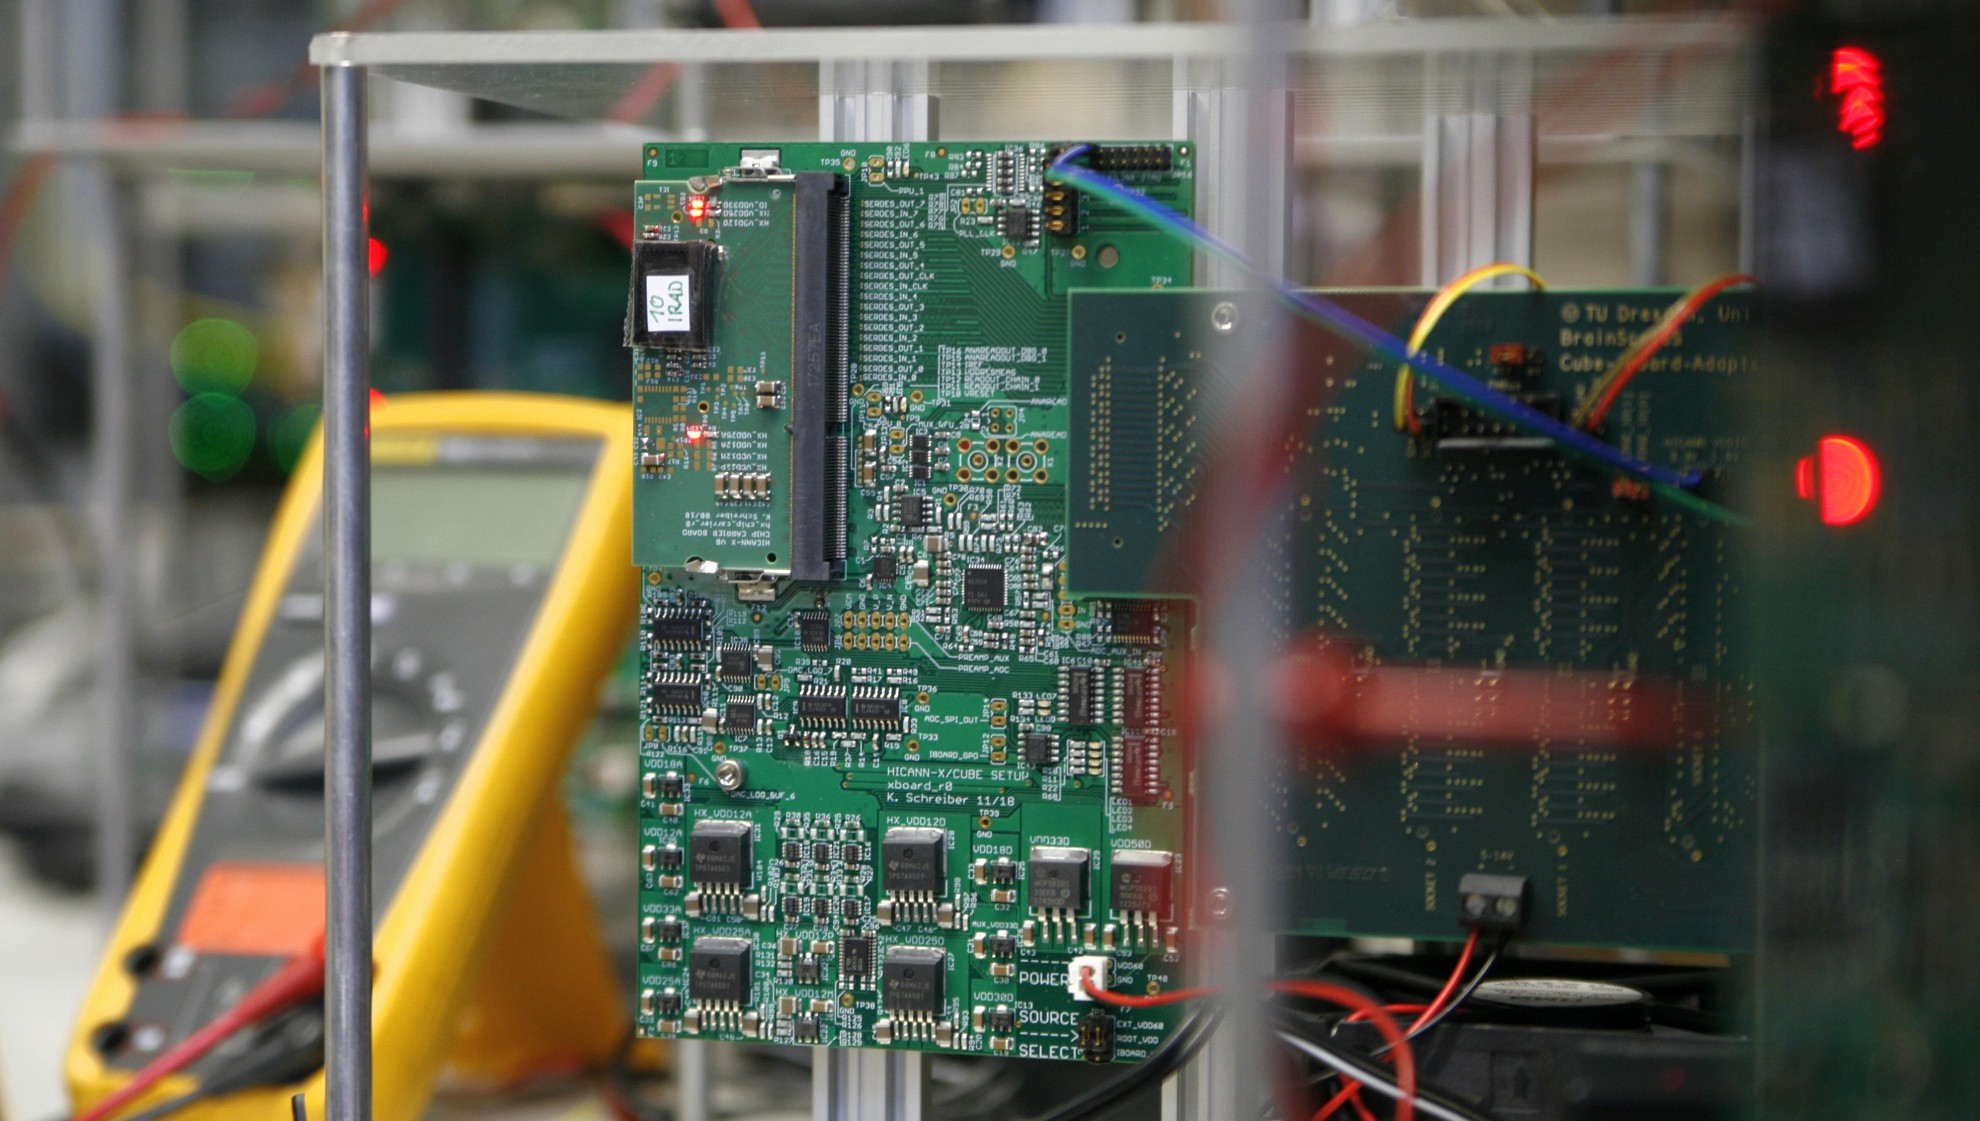
\includegraphics[width=\textwidth]{figures/hxsetup_img2.jpg}
	\caption[Cube setup with \gls{hx}.]{Cube setup with \gls{hx} in the laboratory.}
	\label{cubesetupinlab}
\end{figure}

However, the main obstacle remains the lack of on-chip knowledge over spike times. In principle there are two available sources to record a spike event: the digital back end which registers every spike event precisely and the on-chip spike counters. The data transfer between the digital back end and the \gls{ppu} operates at a limited speed due to a known software bug that has not yet been fixed, making its use unfeasible. The spike counters on the other hand, cannot be accessed by the vector unit since they are not properly connected. With these constraints, an efficient implementation on \gls{hx} is beyond reach. Despite the handicaps, SuperSpike can still be set up as a chip-in-the-loop experiment, i.e. the weight updates are computed on the host and the forward pass is evaluated on-chip. 


In the following, the details of the experiment implementation are presented. The developed software framework is based on the new software stack for the \gls{bss2} platform, which is still under continuous development. A detailed description of the software stack's architecture is provided by \cite{mueller2020bss2ll}. Furthermore, the use of the chip is restricted to the upper half and only one \gls{ppu}, to reduce the implementation effort.

\paragraph{\gls{cadc} Readout}
A key element for the SuperSpike algorithm is the access to the membrane potential by the \gls{cadc}. The general purpose unit instructs the vector unit to trigger the \gls{cadc} and to transfer the resulting conversions back into the main memory of the \gls{ppu}. At that time the software stack did not fully support the use of the vector unit. A preliminary code base has therefore been developed for the \gls{cadc} readout by Aron Leibfried. 

For the purpose of the experiment, the membrane traces of 128 neurons are recorded at a high sampling rate of roughly \SI{400}{\kilo \Hz} to ensure a suitable time resolution of the accelerated dynamics. At the same time, the available memory on the \gls{ppu} restricts the maximum number of samples. Each sample uses one byte of memory and thus 100 samples of 128 neurons occupy already \SI{12.8}{\kilo \byte} of the available \SI{16}{\kilo \byte}, leaving enough space for the \gls{ppu} instructions which share the same memory. In the final configuration of the \gls{cadc} 100 samples are recorded per neuron with a temporal resolution of roughly \SI{2.5}{\micro \s}.

\begin{figure}[htb!]
	\begin{subfigure}{0.65\textwidth}
		\caption{}
		\vspace{-0.4cm}
		%% Creator: Matplotlib, PGF backend
%%
%% To include the figure in your LaTeX document, write
%%   \input{<filename>.pgf}
%%
%% Make sure the required packages are loaded in your preamble
%%   \usepackage{pgf}
%%
%% Figures using additional raster images can only be included by \input if
%% they are in the same directory as the main LaTeX file. For loading figures
%% from other directories you can use the `import` package
%%   \usepackage{import}
%% and then include the figures with
%%   \import{<path to file>}{<filename>.pgf}
%%
%% Matplotlib used the following preamble
%%   \usepackage{amsmath} \usepackage{pifont} \usepackage{xcolor} \definecolor{green}{HTML}{467821} \definecolor{red}{HTML}{CF4457} \usepackage[detect-all]{siunitx}
%%   \usepackage{fontspec}
%%
\begingroup%
\makeatletter%
\begin{pgfpicture}%
\pgfpathrectangle{\pgfpointorigin}{\pgfqpoint{3.657005in}{2.023578in}}%
\pgfusepath{use as bounding box, clip}%
\begin{pgfscope}%
\pgfsetbuttcap%
\pgfsetmiterjoin%
\pgfsetlinewidth{0.000000pt}%
\definecolor{currentstroke}{rgb}{0.000000,0.000000,0.000000}%
\pgfsetstrokecolor{currentstroke}%
\pgfsetstrokeopacity{0.000000}%
\pgfsetdash{}{0pt}%
\pgfpathmoveto{\pgfqpoint{0.000000in}{0.000000in}}%
\pgfpathlineto{\pgfqpoint{3.657005in}{0.000000in}}%
\pgfpathlineto{\pgfqpoint{3.657005in}{2.023578in}}%
\pgfpathlineto{\pgfqpoint{0.000000in}{2.023578in}}%
\pgfpathclose%
\pgfusepath{}%
\end{pgfscope}%
\begin{pgfscope}%
\pgfsetbuttcap%
\pgfsetmiterjoin%
\pgfsetlinewidth{0.000000pt}%
\definecolor{currentstroke}{rgb}{0.000000,0.000000,0.000000}%
\pgfsetstrokecolor{currentstroke}%
\pgfsetstrokeopacity{0.000000}%
\pgfsetdash{}{0pt}%
\pgfpathmoveto{\pgfqpoint{0.438556in}{0.383578in}}%
\pgfpathlineto{\pgfqpoint{1.847647in}{0.383578in}}%
\pgfpathlineto{\pgfqpoint{1.847647in}{1.923578in}}%
\pgfpathlineto{\pgfqpoint{0.438556in}{1.923578in}}%
\pgfpathclose%
\pgfusepath{}%
\end{pgfscope}%
\begin{pgfscope}%
\pgfsetbuttcap%
\pgfsetroundjoin%
\definecolor{currentfill}{rgb}{0.317647,0.317647,0.317647}%
\pgfsetfillcolor{currentfill}%
\pgfsetlinewidth{0.501875pt}%
\definecolor{currentstroke}{rgb}{0.317647,0.317647,0.317647}%
\pgfsetstrokecolor{currentstroke}%
\pgfsetdash{}{0pt}%
\pgfsys@defobject{currentmarker}{\pgfqpoint{0.000000in}{-0.020833in}}{\pgfqpoint{0.000000in}{0.000000in}}{%
\pgfpathmoveto{\pgfqpoint{0.000000in}{0.000000in}}%
\pgfpathlineto{\pgfqpoint{0.000000in}{-0.020833in}}%
\pgfusepath{stroke,fill}%
}%
\begin{pgfscope}%
\pgfsys@transformshift{0.492915in}{0.383578in}%
\pgfsys@useobject{currentmarker}{}%
\end{pgfscope}%
\end{pgfscope}%
\begin{pgfscope}%
\definecolor{textcolor}{rgb}{0.317647,0.317647,0.317647}%
\pgfsetstrokecolor{textcolor}%
\pgfsetfillcolor{textcolor}%
\pgftext[x=0.492915in,y=0.334967in,,top]{\color{textcolor}\rmfamily\fontsize{6.664000}{7.996800}\selectfont \(\displaystyle 0.2\)}%
\end{pgfscope}%
\begin{pgfscope}%
\pgfsetbuttcap%
\pgfsetroundjoin%
\definecolor{currentfill}{rgb}{0.317647,0.317647,0.317647}%
\pgfsetfillcolor{currentfill}%
\pgfsetlinewidth{0.501875pt}%
\definecolor{currentstroke}{rgb}{0.317647,0.317647,0.317647}%
\pgfsetstrokecolor{currentstroke}%
\pgfsetdash{}{0pt}%
\pgfsys@defobject{currentmarker}{\pgfqpoint{0.000000in}{-0.020833in}}{\pgfqpoint{0.000000in}{0.000000in}}{%
\pgfpathmoveto{\pgfqpoint{0.000000in}{0.000000in}}%
\pgfpathlineto{\pgfqpoint{0.000000in}{-0.020833in}}%
\pgfusepath{stroke,fill}%
}%
\begin{pgfscope}%
\pgfsys@transformshift{0.818246in}{0.383578in}%
\pgfsys@useobject{currentmarker}{}%
\end{pgfscope}%
\end{pgfscope}%
\begin{pgfscope}%
\definecolor{textcolor}{rgb}{0.317647,0.317647,0.317647}%
\pgfsetstrokecolor{textcolor}%
\pgfsetfillcolor{textcolor}%
\pgftext[x=0.818246in,y=0.334967in,,top]{\color{textcolor}\rmfamily\fontsize{6.664000}{7.996800}\selectfont \(\displaystyle 0.4\)}%
\end{pgfscope}%
\begin{pgfscope}%
\pgfsetbuttcap%
\pgfsetroundjoin%
\definecolor{currentfill}{rgb}{0.317647,0.317647,0.317647}%
\pgfsetfillcolor{currentfill}%
\pgfsetlinewidth{0.501875pt}%
\definecolor{currentstroke}{rgb}{0.317647,0.317647,0.317647}%
\pgfsetstrokecolor{currentstroke}%
\pgfsetdash{}{0pt}%
\pgfsys@defobject{currentmarker}{\pgfqpoint{0.000000in}{-0.020833in}}{\pgfqpoint{0.000000in}{0.000000in}}{%
\pgfpathmoveto{\pgfqpoint{0.000000in}{0.000000in}}%
\pgfpathlineto{\pgfqpoint{0.000000in}{-0.020833in}}%
\pgfusepath{stroke,fill}%
}%
\begin{pgfscope}%
\pgfsys@transformshift{1.143578in}{0.383578in}%
\pgfsys@useobject{currentmarker}{}%
\end{pgfscope}%
\end{pgfscope}%
\begin{pgfscope}%
\definecolor{textcolor}{rgb}{0.317647,0.317647,0.317647}%
\pgfsetstrokecolor{textcolor}%
\pgfsetfillcolor{textcolor}%
\pgftext[x=1.143578in,y=0.334967in,,top]{\color{textcolor}\rmfamily\fontsize{6.664000}{7.996800}\selectfont \(\displaystyle 0.6\)}%
\end{pgfscope}%
\begin{pgfscope}%
\pgfsetbuttcap%
\pgfsetroundjoin%
\definecolor{currentfill}{rgb}{0.317647,0.317647,0.317647}%
\pgfsetfillcolor{currentfill}%
\pgfsetlinewidth{0.501875pt}%
\definecolor{currentstroke}{rgb}{0.317647,0.317647,0.317647}%
\pgfsetstrokecolor{currentstroke}%
\pgfsetdash{}{0pt}%
\pgfsys@defobject{currentmarker}{\pgfqpoint{0.000000in}{-0.020833in}}{\pgfqpoint{0.000000in}{0.000000in}}{%
\pgfpathmoveto{\pgfqpoint{0.000000in}{0.000000in}}%
\pgfpathlineto{\pgfqpoint{0.000000in}{-0.020833in}}%
\pgfusepath{stroke,fill}%
}%
\begin{pgfscope}%
\pgfsys@transformshift{1.468909in}{0.383578in}%
\pgfsys@useobject{currentmarker}{}%
\end{pgfscope}%
\end{pgfscope}%
\begin{pgfscope}%
\definecolor{textcolor}{rgb}{0.317647,0.317647,0.317647}%
\pgfsetstrokecolor{textcolor}%
\pgfsetfillcolor{textcolor}%
\pgftext[x=1.468909in,y=0.334967in,,top]{\color{textcolor}\rmfamily\fontsize{6.664000}{7.996800}\selectfont \(\displaystyle 0.8\)}%
\end{pgfscope}%
\begin{pgfscope}%
\pgfsetbuttcap%
\pgfsetroundjoin%
\definecolor{currentfill}{rgb}{0.317647,0.317647,0.317647}%
\pgfsetfillcolor{currentfill}%
\pgfsetlinewidth{0.501875pt}%
\definecolor{currentstroke}{rgb}{0.317647,0.317647,0.317647}%
\pgfsetstrokecolor{currentstroke}%
\pgfsetdash{}{0pt}%
\pgfsys@defobject{currentmarker}{\pgfqpoint{0.000000in}{-0.020833in}}{\pgfqpoint{0.000000in}{0.000000in}}{%
\pgfpathmoveto{\pgfqpoint{0.000000in}{0.000000in}}%
\pgfpathlineto{\pgfqpoint{0.000000in}{-0.020833in}}%
\pgfusepath{stroke,fill}%
}%
\begin{pgfscope}%
\pgfsys@transformshift{1.794240in}{0.383578in}%
\pgfsys@useobject{currentmarker}{}%
\end{pgfscope}%
\end{pgfscope}%
\begin{pgfscope}%
\definecolor{textcolor}{rgb}{0.317647,0.317647,0.317647}%
\pgfsetstrokecolor{textcolor}%
\pgfsetfillcolor{textcolor}%
\pgftext[x=1.794240in,y=0.334967in,,top]{\color{textcolor}\rmfamily\fontsize{6.664000}{7.996800}\selectfont \(\displaystyle 1.0\)}%
\end{pgfscope}%
\begin{pgfscope}%
\definecolor{textcolor}{rgb}{0.317647,0.317647,0.317647}%
\pgfsetstrokecolor{textcolor}%
\pgfsetfillcolor{textcolor}%
\pgftext[x=1.143101in,y=0.197222in,,top]{\color{textcolor}\rmfamily\fontsize{6.664000}{7.996800}\selectfont reference voltage \(\displaystyle (\si{\V})\)}%
\end{pgfscope}%
\begin{pgfscope}%
\pgfsetbuttcap%
\pgfsetroundjoin%
\definecolor{currentfill}{rgb}{0.317647,0.317647,0.317647}%
\pgfsetfillcolor{currentfill}%
\pgfsetlinewidth{0.501875pt}%
\definecolor{currentstroke}{rgb}{0.317647,0.317647,0.317647}%
\pgfsetstrokecolor{currentstroke}%
\pgfsetdash{}{0pt}%
\pgfsys@defobject{currentmarker}{\pgfqpoint{-0.020833in}{0.000000in}}{\pgfqpoint{0.000000in}{0.000000in}}{%
\pgfpathmoveto{\pgfqpoint{0.000000in}{0.000000in}}%
\pgfpathlineto{\pgfqpoint{-0.020833in}{0.000000in}}%
\pgfusepath{stroke,fill}%
}%
\begin{pgfscope}%
\pgfsys@transformshift{0.438556in}{0.647233in}%
\pgfsys@useobject{currentmarker}{}%
\end{pgfscope}%
\end{pgfscope}%
\begin{pgfscope}%
\definecolor{textcolor}{rgb}{0.317647,0.317647,0.317647}%
\pgfsetstrokecolor{textcolor}%
\pgfsetfillcolor{textcolor}%
\pgftext[x=0.293108in,y=0.615117in,left,base]{\color{textcolor}\rmfamily\fontsize{6.664000}{7.996800}\selectfont \(\displaystyle 50\)}%
\end{pgfscope}%
\begin{pgfscope}%
\pgfsetbuttcap%
\pgfsetroundjoin%
\definecolor{currentfill}{rgb}{0.317647,0.317647,0.317647}%
\pgfsetfillcolor{currentfill}%
\pgfsetlinewidth{0.501875pt}%
\definecolor{currentstroke}{rgb}{0.317647,0.317647,0.317647}%
\pgfsetstrokecolor{currentstroke}%
\pgfsetdash{}{0pt}%
\pgfsys@defobject{currentmarker}{\pgfqpoint{-0.020833in}{0.000000in}}{\pgfqpoint{0.000000in}{0.000000in}}{%
\pgfpathmoveto{\pgfqpoint{0.000000in}{0.000000in}}%
\pgfpathlineto{\pgfqpoint{-0.020833in}{0.000000in}}%
\pgfusepath{stroke,fill}%
}%
\begin{pgfscope}%
\pgfsys@transformshift{0.438556in}{0.980662in}%
\pgfsys@useobject{currentmarker}{}%
\end{pgfscope}%
\end{pgfscope}%
\begin{pgfscope}%
\definecolor{textcolor}{rgb}{0.317647,0.317647,0.317647}%
\pgfsetstrokecolor{textcolor}%
\pgfsetfillcolor{textcolor}%
\pgftext[x=0.237745in,y=0.948545in,left,base]{\color{textcolor}\rmfamily\fontsize{6.664000}{7.996800}\selectfont \(\displaystyle 100\)}%
\end{pgfscope}%
\begin{pgfscope}%
\pgfsetbuttcap%
\pgfsetroundjoin%
\definecolor{currentfill}{rgb}{0.317647,0.317647,0.317647}%
\pgfsetfillcolor{currentfill}%
\pgfsetlinewidth{0.501875pt}%
\definecolor{currentstroke}{rgb}{0.317647,0.317647,0.317647}%
\pgfsetstrokecolor{currentstroke}%
\pgfsetdash{}{0pt}%
\pgfsys@defobject{currentmarker}{\pgfqpoint{-0.020833in}{0.000000in}}{\pgfqpoint{0.000000in}{0.000000in}}{%
\pgfpathmoveto{\pgfqpoint{0.000000in}{0.000000in}}%
\pgfpathlineto{\pgfqpoint{-0.020833in}{0.000000in}}%
\pgfusepath{stroke,fill}%
}%
\begin{pgfscope}%
\pgfsys@transformshift{0.438556in}{1.314091in}%
\pgfsys@useobject{currentmarker}{}%
\end{pgfscope}%
\end{pgfscope}%
\begin{pgfscope}%
\definecolor{textcolor}{rgb}{0.317647,0.317647,0.317647}%
\pgfsetstrokecolor{textcolor}%
\pgfsetfillcolor{textcolor}%
\pgftext[x=0.237745in,y=1.281974in,left,base]{\color{textcolor}\rmfamily\fontsize{6.664000}{7.996800}\selectfont \(\displaystyle 150\)}%
\end{pgfscope}%
\begin{pgfscope}%
\pgfsetbuttcap%
\pgfsetroundjoin%
\definecolor{currentfill}{rgb}{0.317647,0.317647,0.317647}%
\pgfsetfillcolor{currentfill}%
\pgfsetlinewidth{0.501875pt}%
\definecolor{currentstroke}{rgb}{0.317647,0.317647,0.317647}%
\pgfsetstrokecolor{currentstroke}%
\pgfsetdash{}{0pt}%
\pgfsys@defobject{currentmarker}{\pgfqpoint{-0.020833in}{0.000000in}}{\pgfqpoint{0.000000in}{0.000000in}}{%
\pgfpathmoveto{\pgfqpoint{0.000000in}{0.000000in}}%
\pgfpathlineto{\pgfqpoint{-0.020833in}{0.000000in}}%
\pgfusepath{stroke,fill}%
}%
\begin{pgfscope}%
\pgfsys@transformshift{0.438556in}{1.647519in}%
\pgfsys@useobject{currentmarker}{}%
\end{pgfscope}%
\end{pgfscope}%
\begin{pgfscope}%
\definecolor{textcolor}{rgb}{0.317647,0.317647,0.317647}%
\pgfsetstrokecolor{textcolor}%
\pgfsetfillcolor{textcolor}%
\pgftext[x=0.237745in,y=1.615402in,left,base]{\color{textcolor}\rmfamily\fontsize{6.664000}{7.996800}\selectfont \(\displaystyle 200\)}%
\end{pgfscope}%
\begin{pgfscope}%
\definecolor{textcolor}{rgb}{0.317647,0.317647,0.317647}%
\pgfsetstrokecolor{textcolor}%
\pgfsetfillcolor{textcolor}%
\pgftext[x=0.182189in,y=1.153578in,,bottom,rotate=90.000000]{\color{textcolor}\rmfamily\fontsize{6.664000}{7.996800}\selectfont CADC lsb}%
\end{pgfscope}%
\begin{pgfscope}%
\pgfpathrectangle{\pgfqpoint{0.438556in}{0.383578in}}{\pgfqpoint{1.409091in}{1.540000in}}%
\pgfusepath{clip}%
\pgfsetrectcap%
\pgfsetroundjoin%
\pgfsetlinewidth{0.803000pt}%
\definecolor{currentstroke}{rgb}{0.333333,0.333333,0.333333}%
\pgfsetstrokecolor{currentstroke}%
\pgfsetdash{}{0pt}%
\pgfpathmoveto{\pgfqpoint{0.502605in}{0.566677in}}%
\pgfpathlineto{\pgfqpoint{0.522144in}{0.580681in}}%
\pgfpathlineto{\pgfqpoint{0.541683in}{0.597886in}}%
\pgfpathlineto{\pgfqpoint{0.561699in}{0.615358in}}%
\pgfpathlineto{\pgfqpoint{0.581238in}{0.634430in}}%
\pgfpathlineto{\pgfqpoint{0.601253in}{0.647500in}}%
\pgfpathlineto{\pgfqpoint{0.620792in}{0.666839in}}%
\pgfpathlineto{\pgfqpoint{0.640331in}{0.684577in}}%
\pgfpathlineto{\pgfqpoint{0.660346in}{0.701382in}}%
\pgfpathlineto{\pgfqpoint{0.679885in}{0.719921in}}%
\pgfpathlineto{\pgfqpoint{0.699424in}{0.735792in}}%
\pgfpathlineto{\pgfqpoint{0.719440in}{0.753797in}}%
\pgfpathlineto{\pgfqpoint{0.738979in}{0.769802in}}%
\pgfpathlineto{\pgfqpoint{0.758518in}{0.787807in}}%
\pgfpathlineto{\pgfqpoint{0.778533in}{0.806212in}}%
\pgfpathlineto{\pgfqpoint{0.798072in}{0.822350in}}%
\pgfpathlineto{\pgfqpoint{0.818088in}{0.840622in}}%
\pgfpathlineto{\pgfqpoint{0.837627in}{0.854493in}}%
\pgfpathlineto{\pgfqpoint{0.857165in}{0.872498in}}%
\pgfpathlineto{\pgfqpoint{0.877181in}{0.889703in}}%
\pgfpathlineto{\pgfqpoint{0.896720in}{0.911309in}}%
\pgfpathlineto{\pgfqpoint{0.916259in}{0.924379in}}%
\pgfpathlineto{\pgfqpoint{0.936274in}{0.940651in}}%
\pgfpathlineto{\pgfqpoint{0.955813in}{0.959989in}}%
\pgfpathlineto{\pgfqpoint{0.975352in}{0.974394in}}%
\pgfpathlineto{\pgfqpoint{0.995368in}{0.995333in}}%
\pgfpathlineto{\pgfqpoint{1.014907in}{1.006936in}}%
\pgfpathlineto{\pgfqpoint{1.034922in}{1.026942in}}%
\pgfpathlineto{\pgfqpoint{1.054461in}{1.045747in}}%
\pgfpathlineto{\pgfqpoint{1.074000in}{1.057617in}}%
\pgfpathlineto{\pgfqpoint{1.094016in}{1.073889in}}%
\pgfpathlineto{\pgfqpoint{1.113554in}{1.094695in}}%
\pgfpathlineto{\pgfqpoint{1.133093in}{1.115100in}}%
\pgfpathlineto{\pgfqpoint{1.153109in}{1.131505in}}%
\pgfpathlineto{\pgfqpoint{1.172648in}{1.145109in}}%
\pgfpathlineto{\pgfqpoint{1.192187in}{1.162981in}}%
\pgfpathlineto{\pgfqpoint{1.212202in}{1.184454in}}%
\pgfpathlineto{\pgfqpoint{1.231741in}{1.194323in}}%
\pgfpathlineto{\pgfqpoint{1.251757in}{1.206326in}}%
\pgfpathlineto{\pgfqpoint{1.271296in}{1.236068in}}%
\pgfpathlineto{\pgfqpoint{1.290835in}{1.239269in}}%
\pgfpathlineto{\pgfqpoint{1.310850in}{1.267010in}}%
\pgfpathlineto{\pgfqpoint{1.330389in}{1.282215in}}%
\pgfpathlineto{\pgfqpoint{1.349928in}{1.300887in}}%
\pgfpathlineto{\pgfqpoint{1.369943in}{1.313824in}}%
\pgfpathlineto{\pgfqpoint{1.389482in}{1.335163in}}%
\pgfpathlineto{\pgfqpoint{1.409021in}{1.342632in}}%
\pgfpathlineto{\pgfqpoint{1.429037in}{1.360370in}}%
\pgfpathlineto{\pgfqpoint{1.448576in}{1.387845in}}%
\pgfpathlineto{\pgfqpoint{1.468591in}{1.402382in}}%
\pgfpathlineto{\pgfqpoint{1.488130in}{1.419854in}}%
\pgfpathlineto{\pgfqpoint{1.507669in}{1.437859in}}%
\pgfpathlineto{\pgfqpoint{1.527685in}{1.456265in}}%
\pgfpathlineto{\pgfqpoint{1.547224in}{1.472803in}}%
\pgfpathlineto{\pgfqpoint{1.566762in}{1.488140in}}%
\pgfpathlineto{\pgfqpoint{1.586778in}{1.505345in}}%
\pgfpathlineto{\pgfqpoint{1.606317in}{1.527485in}}%
\pgfpathlineto{\pgfqpoint{1.625856in}{1.539888in}}%
\pgfpathlineto{\pgfqpoint{1.645871in}{1.560294in}}%
\pgfpathlineto{\pgfqpoint{1.665410in}{1.581634in}}%
\pgfpathlineto{\pgfqpoint{1.685426in}{1.594571in}}%
\pgfpathlineto{\pgfqpoint{1.704965in}{1.610175in}}%
\pgfpathlineto{\pgfqpoint{1.724504in}{1.626313in}}%
\pgfpathlineto{\pgfqpoint{1.744519in}{1.647653in}}%
\pgfpathlineto{\pgfqpoint{1.764058in}{1.648319in}}%
\pgfpathlineto{\pgfqpoint{1.783597in}{1.678328in}}%
\pgfusepath{stroke}%
\end{pgfscope}%
\begin{pgfscope}%
\pgfpathrectangle{\pgfqpoint{0.438556in}{0.383578in}}{\pgfqpoint{1.409091in}{1.540000in}}%
\pgfusepath{clip}%
\pgfsetrectcap%
\pgfsetroundjoin%
\pgfsetlinewidth{0.803000pt}%
\definecolor{currentstroke}{rgb}{0.686275,0.352941,0.313725}%
\pgfsetstrokecolor{currentstroke}%
\pgfsetdash{}{0pt}%
\pgfpathmoveto{\pgfqpoint{0.502605in}{0.514262in}}%
\pgfpathlineto{\pgfqpoint{0.522144in}{0.532934in}}%
\pgfpathlineto{\pgfqpoint{0.541683in}{0.547738in}}%
\pgfpathlineto{\pgfqpoint{0.561699in}{0.567211in}}%
\pgfpathlineto{\pgfqpoint{0.581238in}{0.586416in}}%
\pgfpathlineto{\pgfqpoint{0.601253in}{0.599353in}}%
\pgfpathlineto{\pgfqpoint{0.620792in}{0.618559in}}%
\pgfpathlineto{\pgfqpoint{0.640331in}{0.634430in}}%
\pgfpathlineto{\pgfqpoint{0.660346in}{0.653635in}}%
\pgfpathlineto{\pgfqpoint{0.679885in}{0.672174in}}%
\pgfpathlineto{\pgfqpoint{0.699424in}{0.687245in}}%
\pgfpathlineto{\pgfqpoint{0.719440in}{0.706050in}}%
\pgfpathlineto{\pgfqpoint{0.738979in}{0.720988in}}%
\pgfpathlineto{\pgfqpoint{0.758518in}{0.740593in}}%
\pgfpathlineto{\pgfqpoint{0.778533in}{0.758332in}}%
\pgfpathlineto{\pgfqpoint{0.798072in}{0.774470in}}%
\pgfpathlineto{\pgfqpoint{0.818088in}{0.793809in}}%
\pgfpathlineto{\pgfqpoint{0.837627in}{0.807279in}}%
\pgfpathlineto{\pgfqpoint{0.857165in}{0.823550in}}%
\pgfpathlineto{\pgfqpoint{0.877181in}{0.841822in}}%
\pgfpathlineto{\pgfqpoint{0.896720in}{0.862228in}}%
\pgfpathlineto{\pgfqpoint{0.916259in}{0.874898in}}%
\pgfpathlineto{\pgfqpoint{0.936274in}{0.893971in}}%
\pgfpathlineto{\pgfqpoint{0.955813in}{0.912242in}}%
\pgfpathlineto{\pgfqpoint{0.975352in}{0.927447in}}%
\pgfpathlineto{\pgfqpoint{0.995368in}{0.947452in}}%
\pgfpathlineto{\pgfqpoint{1.014907in}{0.958122in}}%
\pgfpathlineto{\pgfqpoint{1.034922in}{0.979462in}}%
\pgfpathlineto{\pgfqpoint{1.054461in}{0.996266in}}%
\pgfpathlineto{\pgfqpoint{1.074000in}{1.010137in}}%
\pgfpathlineto{\pgfqpoint{1.094016in}{1.026542in}}%
\pgfpathlineto{\pgfqpoint{1.113554in}{1.047214in}}%
\pgfpathlineto{\pgfqpoint{1.133093in}{1.067620in}}%
\pgfpathlineto{\pgfqpoint{1.153109in}{1.083225in}}%
\pgfpathlineto{\pgfqpoint{1.172648in}{1.098029in}}%
\pgfpathlineto{\pgfqpoint{1.192187in}{1.114834in}}%
\pgfpathlineto{\pgfqpoint{1.212202in}{1.135773in}}%
\pgfpathlineto{\pgfqpoint{1.231741in}{1.147376in}}%
\pgfpathlineto{\pgfqpoint{1.251757in}{1.159780in}}%
\pgfpathlineto{\pgfqpoint{1.271296in}{1.188455in}}%
\pgfpathlineto{\pgfqpoint{1.290835in}{1.192723in}}%
\pgfpathlineto{\pgfqpoint{1.310850in}{1.220197in}}%
\pgfpathlineto{\pgfqpoint{1.330389in}{1.234601in}}%
\pgfpathlineto{\pgfqpoint{1.349928in}{1.253006in}}%
\pgfpathlineto{\pgfqpoint{1.369943in}{1.266077in}}%
\pgfpathlineto{\pgfqpoint{1.389482in}{1.287683in}}%
\pgfpathlineto{\pgfqpoint{1.409021in}{1.295419in}}%
\pgfpathlineto{\pgfqpoint{1.429037in}{1.313424in}}%
\pgfpathlineto{\pgfqpoint{1.448576in}{1.340498in}}%
\pgfpathlineto{\pgfqpoint{1.468591in}{1.354235in}}%
\pgfpathlineto{\pgfqpoint{1.488130in}{1.371840in}}%
\pgfpathlineto{\pgfqpoint{1.507669in}{1.389846in}}%
\pgfpathlineto{\pgfqpoint{1.527685in}{1.407984in}}%
\pgfpathlineto{\pgfqpoint{1.547224in}{1.423722in}}%
\pgfpathlineto{\pgfqpoint{1.566762in}{1.440660in}}%
\pgfpathlineto{\pgfqpoint{1.586778in}{1.457465in}}%
\pgfpathlineto{\pgfqpoint{1.606317in}{1.480538in}}%
\pgfpathlineto{\pgfqpoint{1.625856in}{1.493075in}}%
\pgfpathlineto{\pgfqpoint{1.645871in}{1.512281in}}%
\pgfpathlineto{\pgfqpoint{1.665410in}{1.534020in}}%
\pgfpathlineto{\pgfqpoint{1.685426in}{1.547357in}}%
\pgfpathlineto{\pgfqpoint{1.704965in}{1.562295in}}%
\pgfpathlineto{\pgfqpoint{1.724504in}{1.577499in}}%
\pgfpathlineto{\pgfqpoint{1.744519in}{1.600172in}}%
\pgfpathlineto{\pgfqpoint{1.764058in}{1.601106in}}%
\pgfpathlineto{\pgfqpoint{1.783597in}{1.630048in}}%
\pgfusepath{stroke}%
\end{pgfscope}%
\begin{pgfscope}%
\pgfpathrectangle{\pgfqpoint{0.438556in}{0.383578in}}{\pgfqpoint{1.409091in}{1.540000in}}%
\pgfusepath{clip}%
\pgfsetrectcap%
\pgfsetroundjoin%
\pgfsetlinewidth{0.803000pt}%
\definecolor{currentstroke}{rgb}{0.000000,0.356863,0.509804}%
\pgfsetstrokecolor{currentstroke}%
\pgfsetdash{}{0pt}%
\pgfpathmoveto{\pgfqpoint{0.502605in}{0.600020in}}%
\pgfpathlineto{\pgfqpoint{0.522144in}{0.614957in}}%
\pgfpathlineto{\pgfqpoint{0.541683in}{0.633363in}}%
\pgfpathlineto{\pgfqpoint{0.561699in}{0.651901in}}%
\pgfpathlineto{\pgfqpoint{0.581238in}{0.667639in}}%
\pgfpathlineto{\pgfqpoint{0.601253in}{0.680976in}}%
\pgfpathlineto{\pgfqpoint{0.620792in}{0.700582in}}%
\pgfpathlineto{\pgfqpoint{0.640331in}{0.720188in}}%
\pgfpathlineto{\pgfqpoint{0.660346in}{0.734592in}}%
\pgfpathlineto{\pgfqpoint{0.679885in}{0.754064in}}%
\pgfpathlineto{\pgfqpoint{0.699424in}{0.769802in}}%
\pgfpathlineto{\pgfqpoint{0.719440in}{0.787807in}}%
\pgfpathlineto{\pgfqpoint{0.738979in}{0.805945in}}%
\pgfpathlineto{\pgfqpoint{0.758518in}{0.823684in}}%
\pgfpathlineto{\pgfqpoint{0.778533in}{0.840622in}}%
\pgfpathlineto{\pgfqpoint{0.798072in}{0.857560in}}%
\pgfpathlineto{\pgfqpoint{0.818088in}{0.874232in}}%
\pgfpathlineto{\pgfqpoint{0.837627in}{0.889303in}}%
\pgfpathlineto{\pgfqpoint{0.857165in}{0.907174in}}%
\pgfpathlineto{\pgfqpoint{0.877181in}{0.926113in}}%
\pgfpathlineto{\pgfqpoint{0.896720in}{0.946786in}}%
\pgfpathlineto{\pgfqpoint{0.916259in}{0.958522in}}%
\pgfpathlineto{\pgfqpoint{0.936274in}{0.975194in}}%
\pgfpathlineto{\pgfqpoint{0.955813in}{0.994132in}}%
\pgfpathlineto{\pgfqpoint{0.975352in}{1.009203in}}%
\pgfpathlineto{\pgfqpoint{0.995368in}{1.029876in}}%
\pgfpathlineto{\pgfqpoint{1.014907in}{1.040679in}}%
\pgfpathlineto{\pgfqpoint{1.034922in}{1.060685in}}%
\pgfpathlineto{\pgfqpoint{1.054461in}{1.080157in}}%
\pgfpathlineto{\pgfqpoint{1.074000in}{1.093628in}}%
\pgfpathlineto{\pgfqpoint{1.094016in}{1.107365in}}%
\pgfpathlineto{\pgfqpoint{1.113554in}{1.128838in}}%
\pgfpathlineto{\pgfqpoint{1.133093in}{1.148710in}}%
\pgfpathlineto{\pgfqpoint{1.153109in}{1.166715in}}%
\pgfpathlineto{\pgfqpoint{1.172648in}{1.180586in}}%
\pgfpathlineto{\pgfqpoint{1.192187in}{1.198191in}}%
\pgfpathlineto{\pgfqpoint{1.212202in}{1.219530in}}%
\pgfpathlineto{\pgfqpoint{1.231741in}{1.227799in}}%
\pgfpathlineto{\pgfqpoint{1.251757in}{1.240870in}}%
\pgfpathlineto{\pgfqpoint{1.271296in}{1.271945in}}%
\pgfpathlineto{\pgfqpoint{1.290835in}{1.274079in}}%
\pgfpathlineto{\pgfqpoint{1.310850in}{1.300620in}}%
\pgfpathlineto{\pgfqpoint{1.330389in}{1.317291in}}%
\pgfpathlineto{\pgfqpoint{1.349928in}{1.338631in}}%
\pgfpathlineto{\pgfqpoint{1.369943in}{1.347567in}}%
\pgfpathlineto{\pgfqpoint{1.389482in}{1.370240in}}%
\pgfpathlineto{\pgfqpoint{1.409021in}{1.378509in}}%
\pgfpathlineto{\pgfqpoint{1.429037in}{1.394647in}}%
\pgfpathlineto{\pgfqpoint{1.448576in}{1.421988in}}%
\pgfpathlineto{\pgfqpoint{1.468591in}{1.436659in}}%
\pgfpathlineto{\pgfqpoint{1.488130in}{1.453864in}}%
\pgfpathlineto{\pgfqpoint{1.507669in}{1.472402in}}%
\pgfpathlineto{\pgfqpoint{1.527685in}{1.491074in}}%
\pgfpathlineto{\pgfqpoint{1.547224in}{1.506946in}}%
\pgfpathlineto{\pgfqpoint{1.566762in}{1.522417in}}%
\pgfpathlineto{\pgfqpoint{1.586778in}{1.540022in}}%
\pgfpathlineto{\pgfqpoint{1.606317in}{1.561361in}}%
\pgfpathlineto{\pgfqpoint{1.625856in}{1.574165in}}%
\pgfpathlineto{\pgfqpoint{1.645871in}{1.594571in}}%
\pgfpathlineto{\pgfqpoint{1.665410in}{1.616710in}}%
\pgfpathlineto{\pgfqpoint{1.685426in}{1.628447in}}%
\pgfpathlineto{\pgfqpoint{1.704965in}{1.645252in}}%
\pgfpathlineto{\pgfqpoint{1.724504in}{1.660590in}}%
\pgfpathlineto{\pgfqpoint{1.744519in}{1.682329in}}%
\pgfpathlineto{\pgfqpoint{1.764058in}{1.683529in}}%
\pgfpathlineto{\pgfqpoint{1.783597in}{1.713671in}}%
\pgfusepath{stroke}%
\end{pgfscope}%
\begin{pgfscope}%
\pgfpathrectangle{\pgfqpoint{0.438556in}{0.383578in}}{\pgfqpoint{1.409091in}{1.540000in}}%
\pgfusepath{clip}%
\pgfsetrectcap%
\pgfsetroundjoin%
\pgfsetlinewidth{0.803000pt}%
\definecolor{currentstroke}{rgb}{0.490196,0.588235,0.431373}%
\pgfsetstrokecolor{currentstroke}%
\pgfsetdash{}{0pt}%
\pgfpathmoveto{\pgfqpoint{0.502605in}{0.627761in}}%
\pgfpathlineto{\pgfqpoint{0.522144in}{0.645900in}}%
\pgfpathlineto{\pgfqpoint{0.541683in}{0.660971in}}%
\pgfpathlineto{\pgfqpoint{0.561699in}{0.681376in}}%
\pgfpathlineto{\pgfqpoint{0.581238in}{0.696981in}}%
\pgfpathlineto{\pgfqpoint{0.601253in}{0.710318in}}%
\pgfpathlineto{\pgfqpoint{0.620792in}{0.730190in}}%
\pgfpathlineto{\pgfqpoint{0.640331in}{0.747795in}}%
\pgfpathlineto{\pgfqpoint{0.660346in}{0.766067in}}%
\pgfpathlineto{\pgfqpoint{0.679885in}{0.783539in}}%
\pgfpathlineto{\pgfqpoint{0.699424in}{0.800344in}}%
\pgfpathlineto{\pgfqpoint{0.719440in}{0.817682in}}%
\pgfpathlineto{\pgfqpoint{0.738979in}{0.834487in}}%
\pgfpathlineto{\pgfqpoint{0.758518in}{0.854092in}}%
\pgfpathlineto{\pgfqpoint{0.778533in}{0.869564in}}%
\pgfpathlineto{\pgfqpoint{0.798072in}{0.888102in}}%
\pgfpathlineto{\pgfqpoint{0.818088in}{0.904374in}}%
\pgfpathlineto{\pgfqpoint{0.837627in}{0.919444in}}%
\pgfpathlineto{\pgfqpoint{0.857165in}{0.934649in}}%
\pgfpathlineto{\pgfqpoint{0.877181in}{0.954788in}}%
\pgfpathlineto{\pgfqpoint{0.896720in}{0.975460in}}%
\pgfpathlineto{\pgfqpoint{0.916259in}{0.988264in}}%
\pgfpathlineto{\pgfqpoint{0.936274in}{1.006136in}}%
\pgfpathlineto{\pgfqpoint{0.955813in}{1.022807in}}%
\pgfpathlineto{\pgfqpoint{0.975352in}{1.040412in}}%
\pgfpathlineto{\pgfqpoint{0.995368in}{1.060551in}}%
\pgfpathlineto{\pgfqpoint{1.014907in}{1.068420in}}%
\pgfpathlineto{\pgfqpoint{1.034922in}{1.090827in}}%
\pgfpathlineto{\pgfqpoint{1.054461in}{1.107898in}}%
\pgfpathlineto{\pgfqpoint{1.074000in}{1.121502in}}%
\pgfpathlineto{\pgfqpoint{1.094016in}{1.137507in}}%
\pgfpathlineto{\pgfqpoint{1.113554in}{1.160047in}}%
\pgfpathlineto{\pgfqpoint{1.133093in}{1.179519in}}%
\pgfpathlineto{\pgfqpoint{1.153109in}{1.195923in}}%
\pgfpathlineto{\pgfqpoint{1.172648in}{1.209261in}}%
\pgfpathlineto{\pgfqpoint{1.192187in}{1.227266in}}%
\pgfpathlineto{\pgfqpoint{1.212202in}{1.248472in}}%
\pgfpathlineto{\pgfqpoint{1.231741in}{1.259008in}}%
\pgfpathlineto{\pgfqpoint{1.251757in}{1.270078in}}%
\pgfpathlineto{\pgfqpoint{1.271296in}{1.301554in}}%
\pgfpathlineto{\pgfqpoint{1.290835in}{1.303821in}}%
\pgfpathlineto{\pgfqpoint{1.310850in}{1.331029in}}%
\pgfpathlineto{\pgfqpoint{1.330389in}{1.348367in}}%
\pgfpathlineto{\pgfqpoint{1.349928in}{1.364638in}}%
\pgfpathlineto{\pgfqpoint{1.369943in}{1.376242in}}%
\pgfpathlineto{\pgfqpoint{1.389482in}{1.401049in}}%
\pgfpathlineto{\pgfqpoint{1.409021in}{1.408384in}}%
\pgfpathlineto{\pgfqpoint{1.429037in}{1.423589in}}%
\pgfpathlineto{\pgfqpoint{1.448576in}{1.453197in}}%
\pgfpathlineto{\pgfqpoint{1.468591in}{1.467201in}}%
\pgfpathlineto{\pgfqpoint{1.488130in}{1.483339in}}%
\pgfpathlineto{\pgfqpoint{1.507669in}{1.500944in}}%
\pgfpathlineto{\pgfqpoint{1.527685in}{1.521483in}}%
\pgfpathlineto{\pgfqpoint{1.547224in}{1.536954in}}%
\pgfpathlineto{\pgfqpoint{1.566762in}{1.552959in}}%
\pgfpathlineto{\pgfqpoint{1.586778in}{1.569097in}}%
\pgfpathlineto{\pgfqpoint{1.606317in}{1.592437in}}%
\pgfpathlineto{\pgfqpoint{1.625856in}{1.604173in}}%
\pgfpathlineto{\pgfqpoint{1.645871in}{1.624846in}}%
\pgfpathlineto{\pgfqpoint{1.665410in}{1.647786in}}%
\pgfpathlineto{\pgfqpoint{1.685426in}{1.659389in}}%
\pgfpathlineto{\pgfqpoint{1.704965in}{1.675661in}}%
\pgfpathlineto{\pgfqpoint{1.724504in}{1.690465in}}%
\pgfpathlineto{\pgfqpoint{1.744519in}{1.713138in}}%
\pgfpathlineto{\pgfqpoint{1.764058in}{1.714338in}}%
\pgfpathlineto{\pgfqpoint{1.783597in}{1.742880in}}%
\pgfusepath{stroke}%
\end{pgfscope}%
\begin{pgfscope}%
\pgfpathrectangle{\pgfqpoint{0.438556in}{0.383578in}}{\pgfqpoint{1.409091in}{1.540000in}}%
\pgfusepath{clip}%
\pgfsetrectcap%
\pgfsetroundjoin%
\pgfsetlinewidth{0.803000pt}%
\definecolor{currentstroke}{rgb}{0.843137,0.666667,0.313725}%
\pgfsetstrokecolor{currentstroke}%
\pgfsetdash{}{0pt}%
\pgfpathmoveto{\pgfqpoint{0.502605in}{0.566810in}}%
\pgfpathlineto{\pgfqpoint{0.522144in}{0.582948in}}%
\pgfpathlineto{\pgfqpoint{0.541683in}{0.599220in}}%
\pgfpathlineto{\pgfqpoint{0.561699in}{0.618292in}}%
\pgfpathlineto{\pgfqpoint{0.581238in}{0.635363in}}%
\pgfpathlineto{\pgfqpoint{0.601253in}{0.648967in}}%
\pgfpathlineto{\pgfqpoint{0.620792in}{0.667773in}}%
\pgfpathlineto{\pgfqpoint{0.640331in}{0.686445in}}%
\pgfpathlineto{\pgfqpoint{0.660346in}{0.702716in}}%
\pgfpathlineto{\pgfqpoint{0.679885in}{0.721521in}}%
\pgfpathlineto{\pgfqpoint{0.699424in}{0.738193in}}%
\pgfpathlineto{\pgfqpoint{0.719440in}{0.754998in}}%
\pgfpathlineto{\pgfqpoint{0.738979in}{0.772603in}}%
\pgfpathlineto{\pgfqpoint{0.758518in}{0.790874in}}%
\pgfpathlineto{\pgfqpoint{0.778533in}{0.808213in}}%
\pgfpathlineto{\pgfqpoint{0.798072in}{0.825018in}}%
\pgfpathlineto{\pgfqpoint{0.818088in}{0.841956in}}%
\pgfpathlineto{\pgfqpoint{0.837627in}{0.858094in}}%
\pgfpathlineto{\pgfqpoint{0.857165in}{0.873965in}}%
\pgfpathlineto{\pgfqpoint{0.877181in}{0.893037in}}%
\pgfpathlineto{\pgfqpoint{0.896720in}{0.913309in}}%
\pgfpathlineto{\pgfqpoint{0.916259in}{0.925580in}}%
\pgfpathlineto{\pgfqpoint{0.936274in}{0.943585in}}%
\pgfpathlineto{\pgfqpoint{0.955813in}{0.960923in}}%
\pgfpathlineto{\pgfqpoint{0.975352in}{0.977728in}}%
\pgfpathlineto{\pgfqpoint{0.995368in}{0.997200in}}%
\pgfpathlineto{\pgfqpoint{1.014907in}{1.007736in}}%
\pgfpathlineto{\pgfqpoint{1.034922in}{1.028676in}}%
\pgfpathlineto{\pgfqpoint{1.054461in}{1.046948in}}%
\pgfpathlineto{\pgfqpoint{1.074000in}{1.060551in}}%
\pgfpathlineto{\pgfqpoint{1.094016in}{1.075889in}}%
\pgfpathlineto{\pgfqpoint{1.113554in}{1.096962in}}%
\pgfpathlineto{\pgfqpoint{1.133093in}{1.116567in}}%
\pgfpathlineto{\pgfqpoint{1.153109in}{1.133639in}}%
\pgfpathlineto{\pgfqpoint{1.172648in}{1.146976in}}%
\pgfpathlineto{\pgfqpoint{1.192187in}{1.165515in}}%
\pgfpathlineto{\pgfqpoint{1.212202in}{1.186721in}}%
\pgfpathlineto{\pgfqpoint{1.231741in}{1.196324in}}%
\pgfpathlineto{\pgfqpoint{1.251757in}{1.208994in}}%
\pgfpathlineto{\pgfqpoint{1.271296in}{1.239136in}}%
\pgfpathlineto{\pgfqpoint{1.290835in}{1.241537in}}%
\pgfpathlineto{\pgfqpoint{1.310850in}{1.268744in}}%
\pgfpathlineto{\pgfqpoint{1.330389in}{1.284749in}}%
\pgfpathlineto{\pgfqpoint{1.349928in}{1.301954in}}%
\pgfpathlineto{\pgfqpoint{1.369943in}{1.314357in}}%
\pgfpathlineto{\pgfqpoint{1.389482in}{1.337964in}}%
\pgfpathlineto{\pgfqpoint{1.409021in}{1.345566in}}%
\pgfpathlineto{\pgfqpoint{1.429037in}{1.361838in}}%
\pgfpathlineto{\pgfqpoint{1.448576in}{1.389579in}}%
\pgfpathlineto{\pgfqpoint{1.468591in}{1.404650in}}%
\pgfpathlineto{\pgfqpoint{1.488130in}{1.421188in}}%
\pgfpathlineto{\pgfqpoint{1.507669in}{1.439460in}}%
\pgfpathlineto{\pgfqpoint{1.527685in}{1.458932in}}%
\pgfpathlineto{\pgfqpoint{1.547224in}{1.474536in}}%
\pgfpathlineto{\pgfqpoint{1.566762in}{1.490141in}}%
\pgfpathlineto{\pgfqpoint{1.586778in}{1.506546in}}%
\pgfpathlineto{\pgfqpoint{1.606317in}{1.529219in}}%
\pgfpathlineto{\pgfqpoint{1.625856in}{1.541489in}}%
\pgfpathlineto{\pgfqpoint{1.645871in}{1.561094in}}%
\pgfpathlineto{\pgfqpoint{1.665410in}{1.584034in}}%
\pgfpathlineto{\pgfqpoint{1.685426in}{1.596838in}}%
\pgfpathlineto{\pgfqpoint{1.704965in}{1.612442in}}%
\pgfpathlineto{\pgfqpoint{1.724504in}{1.626713in}}%
\pgfpathlineto{\pgfqpoint{1.744519in}{1.649520in}}%
\pgfpathlineto{\pgfqpoint{1.764058in}{1.650587in}}%
\pgfpathlineto{\pgfqpoint{1.783597in}{1.679928in}}%
\pgfusepath{stroke}%
\end{pgfscope}%
\begin{pgfscope}%
\pgfpathrectangle{\pgfqpoint{0.438556in}{0.383578in}}{\pgfqpoint{1.409091in}{1.540000in}}%
\pgfusepath{clip}%
\pgfsetrectcap%
\pgfsetroundjoin%
\pgfsetlinewidth{0.803000pt}%
\definecolor{currentstroke}{rgb}{0.333333,0.333333,0.333333}%
\pgfsetstrokecolor{currentstroke}%
\pgfsetdash{}{0pt}%
\pgfpathmoveto{\pgfqpoint{0.502605in}{0.580548in}}%
\pgfpathlineto{\pgfqpoint{0.522144in}{0.598019in}}%
\pgfpathlineto{\pgfqpoint{0.541683in}{0.613757in}}%
\pgfpathlineto{\pgfqpoint{0.561699in}{0.633096in}}%
\pgfpathlineto{\pgfqpoint{0.581238in}{0.650834in}}%
\pgfpathlineto{\pgfqpoint{0.601253in}{0.662304in}}%
\pgfpathlineto{\pgfqpoint{0.620792in}{0.681777in}}%
\pgfpathlineto{\pgfqpoint{0.640331in}{0.700582in}}%
\pgfpathlineto{\pgfqpoint{0.660346in}{0.717387in}}%
\pgfpathlineto{\pgfqpoint{0.679885in}{0.735392in}}%
\pgfpathlineto{\pgfqpoint{0.699424in}{0.753264in}}%
\pgfpathlineto{\pgfqpoint{0.719440in}{0.769668in}}%
\pgfpathlineto{\pgfqpoint{0.738979in}{0.787140in}}%
\pgfpathlineto{\pgfqpoint{0.758518in}{0.806212in}}%
\pgfpathlineto{\pgfqpoint{0.778533in}{0.821150in}}%
\pgfpathlineto{\pgfqpoint{0.798072in}{0.840088in}}%
\pgfpathlineto{\pgfqpoint{0.818088in}{0.856226in}}%
\pgfpathlineto{\pgfqpoint{0.837627in}{0.871964in}}%
\pgfpathlineto{\pgfqpoint{0.857165in}{0.887302in}}%
\pgfpathlineto{\pgfqpoint{0.877181in}{0.907174in}}%
\pgfpathlineto{\pgfqpoint{0.896720in}{0.927180in}}%
\pgfpathlineto{\pgfqpoint{0.916259in}{0.940517in}}%
\pgfpathlineto{\pgfqpoint{0.936274in}{0.958656in}}%
\pgfpathlineto{\pgfqpoint{0.955813in}{0.975727in}}%
\pgfpathlineto{\pgfqpoint{0.975352in}{0.993066in}}%
\pgfpathlineto{\pgfqpoint{0.995368in}{1.012671in}}%
\pgfpathlineto{\pgfqpoint{1.014907in}{1.020940in}}%
\pgfpathlineto{\pgfqpoint{1.034922in}{1.042146in}}%
\pgfpathlineto{\pgfqpoint{1.054461in}{1.060818in}}%
\pgfpathlineto{\pgfqpoint{1.074000in}{1.074022in}}%
\pgfpathlineto{\pgfqpoint{1.094016in}{1.090027in}}%
\pgfpathlineto{\pgfqpoint{1.113554in}{1.112166in}}%
\pgfpathlineto{\pgfqpoint{1.133093in}{1.131905in}}%
\pgfpathlineto{\pgfqpoint{1.153109in}{1.147643in}}%
\pgfpathlineto{\pgfqpoint{1.172648in}{1.160847in}}%
\pgfpathlineto{\pgfqpoint{1.192187in}{1.179652in}}%
\pgfpathlineto{\pgfqpoint{1.212202in}{1.200858in}}%
\pgfpathlineto{\pgfqpoint{1.231741in}{1.210594in}}%
\pgfpathlineto{\pgfqpoint{1.251757in}{1.222731in}}%
\pgfpathlineto{\pgfqpoint{1.271296in}{1.253807in}}%
\pgfpathlineto{\pgfqpoint{1.290835in}{1.255674in}}%
\pgfpathlineto{\pgfqpoint{1.310850in}{1.282882in}}%
\pgfpathlineto{\pgfqpoint{1.330389in}{1.300353in}}%
\pgfpathlineto{\pgfqpoint{1.349928in}{1.316891in}}%
\pgfpathlineto{\pgfqpoint{1.369943in}{1.328495in}}%
\pgfpathlineto{\pgfqpoint{1.389482in}{1.353435in}}%
\pgfpathlineto{\pgfqpoint{1.409021in}{1.360771in}}%
\pgfpathlineto{\pgfqpoint{1.429037in}{1.375975in}}%
\pgfpathlineto{\pgfqpoint{1.448576in}{1.405984in}}%
\pgfpathlineto{\pgfqpoint{1.468591in}{1.420254in}}%
\pgfpathlineto{\pgfqpoint{1.488130in}{1.435192in}}%
\pgfpathlineto{\pgfqpoint{1.507669in}{1.454397in}}%
\pgfpathlineto{\pgfqpoint{1.527685in}{1.474136in}}%
\pgfpathlineto{\pgfqpoint{1.547224in}{1.488540in}}%
\pgfpathlineto{\pgfqpoint{1.566762in}{1.505745in}}%
\pgfpathlineto{\pgfqpoint{1.586778in}{1.520950in}}%
\pgfpathlineto{\pgfqpoint{1.606317in}{1.544556in}}%
\pgfpathlineto{\pgfqpoint{1.625856in}{1.556026in}}%
\pgfpathlineto{\pgfqpoint{1.645871in}{1.576032in}}%
\pgfpathlineto{\pgfqpoint{1.665410in}{1.599505in}}%
\pgfpathlineto{\pgfqpoint{1.685426in}{1.611776in}}%
\pgfpathlineto{\pgfqpoint{1.704965in}{1.627914in}}%
\pgfpathlineto{\pgfqpoint{1.724504in}{1.642051in}}%
\pgfpathlineto{\pgfqpoint{1.744519in}{1.665258in}}%
\pgfpathlineto{\pgfqpoint{1.764058in}{1.666458in}}%
\pgfpathlineto{\pgfqpoint{1.783597in}{1.695533in}}%
\pgfusepath{stroke}%
\end{pgfscope}%
\begin{pgfscope}%
\pgfpathrectangle{\pgfqpoint{0.438556in}{0.383578in}}{\pgfqpoint{1.409091in}{1.540000in}}%
\pgfusepath{clip}%
\pgfsetrectcap%
\pgfsetroundjoin%
\pgfsetlinewidth{0.803000pt}%
\definecolor{currentstroke}{rgb}{0.686275,0.352941,0.313725}%
\pgfsetstrokecolor{currentstroke}%
\pgfsetdash{}{0pt}%
\pgfpathmoveto{\pgfqpoint{0.502605in}{0.521597in}}%
\pgfpathlineto{\pgfqpoint{0.522144in}{0.540536in}}%
\pgfpathlineto{\pgfqpoint{0.541683in}{0.554940in}}%
\pgfpathlineto{\pgfqpoint{0.561699in}{0.574146in}}%
\pgfpathlineto{\pgfqpoint{0.581238in}{0.591884in}}%
\pgfpathlineto{\pgfqpoint{0.601253in}{0.606155in}}%
\pgfpathlineto{\pgfqpoint{0.620792in}{0.624827in}}%
\pgfpathlineto{\pgfqpoint{0.640331in}{0.641365in}}%
\pgfpathlineto{\pgfqpoint{0.660346in}{0.660304in}}%
\pgfpathlineto{\pgfqpoint{0.679885in}{0.678976in}}%
\pgfpathlineto{\pgfqpoint{0.699424in}{0.694180in}}%
\pgfpathlineto{\pgfqpoint{0.719440in}{0.712986in}}%
\pgfpathlineto{\pgfqpoint{0.738979in}{0.727923in}}%
\pgfpathlineto{\pgfqpoint{0.758518in}{0.747795in}}%
\pgfpathlineto{\pgfqpoint{0.778533in}{0.764600in}}%
\pgfpathlineto{\pgfqpoint{0.798072in}{0.781405in}}%
\pgfpathlineto{\pgfqpoint{0.818088in}{0.799143in}}%
\pgfpathlineto{\pgfqpoint{0.837627in}{0.814615in}}%
\pgfpathlineto{\pgfqpoint{0.857165in}{0.829552in}}%
\pgfpathlineto{\pgfqpoint{0.877181in}{0.847691in}}%
\pgfpathlineto{\pgfqpoint{0.896720in}{0.869697in}}%
\pgfpathlineto{\pgfqpoint{0.916259in}{0.881567in}}%
\pgfpathlineto{\pgfqpoint{0.936274in}{0.900639in}}%
\pgfpathlineto{\pgfqpoint{0.955813in}{0.918378in}}%
\pgfpathlineto{\pgfqpoint{0.975352in}{0.934916in}}%
\pgfpathlineto{\pgfqpoint{0.995368in}{0.954121in}}%
\pgfpathlineto{\pgfqpoint{1.014907in}{0.964791in}}%
\pgfpathlineto{\pgfqpoint{1.034922in}{0.985863in}}%
\pgfpathlineto{\pgfqpoint{1.054461in}{1.003335in}}%
\pgfpathlineto{\pgfqpoint{1.074000in}{1.016005in}}%
\pgfpathlineto{\pgfqpoint{1.094016in}{1.032543in}}%
\pgfpathlineto{\pgfqpoint{1.113554in}{1.054150in}}%
\pgfpathlineto{\pgfqpoint{1.133093in}{1.074689in}}%
\pgfpathlineto{\pgfqpoint{1.153109in}{1.089626in}}%
\pgfpathlineto{\pgfqpoint{1.172648in}{1.104831in}}%
\pgfpathlineto{\pgfqpoint{1.192187in}{1.121636in}}%
\pgfpathlineto{\pgfqpoint{1.212202in}{1.142575in}}%
\pgfpathlineto{\pgfqpoint{1.231741in}{1.153778in}}%
\pgfpathlineto{\pgfqpoint{1.251757in}{1.166448in}}%
\pgfpathlineto{\pgfqpoint{1.271296in}{1.195790in}}%
\pgfpathlineto{\pgfqpoint{1.290835in}{1.199525in}}%
\pgfpathlineto{\pgfqpoint{1.310850in}{1.226332in}}%
\pgfpathlineto{\pgfqpoint{1.330389in}{1.241403in}}%
\pgfpathlineto{\pgfqpoint{1.349928in}{1.260209in}}%
\pgfpathlineto{\pgfqpoint{1.369943in}{1.272745in}}%
\pgfpathlineto{\pgfqpoint{1.389482in}{1.294752in}}%
\pgfpathlineto{\pgfqpoint{1.409021in}{1.301554in}}%
\pgfpathlineto{\pgfqpoint{1.429037in}{1.319425in}}%
\pgfpathlineto{\pgfqpoint{1.448576in}{1.347167in}}%
\pgfpathlineto{\pgfqpoint{1.468591in}{1.361704in}}%
\pgfpathlineto{\pgfqpoint{1.488130in}{1.377709in}}%
\pgfpathlineto{\pgfqpoint{1.507669in}{1.395981in}}%
\pgfpathlineto{\pgfqpoint{1.527685in}{1.415720in}}%
\pgfpathlineto{\pgfqpoint{1.547224in}{1.430657in}}%
\pgfpathlineto{\pgfqpoint{1.566762in}{1.447595in}}%
\pgfpathlineto{\pgfqpoint{1.586778in}{1.464000in}}%
\pgfpathlineto{\pgfqpoint{1.606317in}{1.486673in}}%
\pgfpathlineto{\pgfqpoint{1.625856in}{1.498943in}}%
\pgfpathlineto{\pgfqpoint{1.645871in}{1.517749in}}%
\pgfpathlineto{\pgfqpoint{1.665410in}{1.540955in}}%
\pgfpathlineto{\pgfqpoint{1.685426in}{1.553492in}}%
\pgfpathlineto{\pgfqpoint{1.704965in}{1.568563in}}%
\pgfpathlineto{\pgfqpoint{1.724504in}{1.583501in}}%
\pgfpathlineto{\pgfqpoint{1.744519in}{1.606441in}}%
\pgfpathlineto{\pgfqpoint{1.764058in}{1.607508in}}%
\pgfpathlineto{\pgfqpoint{1.783597in}{1.635516in}}%
\pgfusepath{stroke}%
\end{pgfscope}%
\begin{pgfscope}%
\pgfpathrectangle{\pgfqpoint{0.438556in}{0.383578in}}{\pgfqpoint{1.409091in}{1.540000in}}%
\pgfusepath{clip}%
\pgfsetrectcap%
\pgfsetroundjoin%
\pgfsetlinewidth{0.803000pt}%
\definecolor{currentstroke}{rgb}{0.000000,0.356863,0.509804}%
\pgfsetstrokecolor{currentstroke}%
\pgfsetdash{}{0pt}%
\pgfpathmoveto{\pgfqpoint{0.502605in}{0.580681in}}%
\pgfpathlineto{\pgfqpoint{0.522144in}{0.599220in}}%
\pgfpathlineto{\pgfqpoint{0.541683in}{0.613891in}}%
\pgfpathlineto{\pgfqpoint{0.561699in}{0.633763in}}%
\pgfpathlineto{\pgfqpoint{0.581238in}{0.650968in}}%
\pgfpathlineto{\pgfqpoint{0.601253in}{0.662838in}}%
\pgfpathlineto{\pgfqpoint{0.620792in}{0.683244in}}%
\pgfpathlineto{\pgfqpoint{0.640331in}{0.700582in}}%
\pgfpathlineto{\pgfqpoint{0.660346in}{0.719387in}}%
\pgfpathlineto{\pgfqpoint{0.679885in}{0.737392in}}%
\pgfpathlineto{\pgfqpoint{0.699424in}{0.753530in}}%
\pgfpathlineto{\pgfqpoint{0.719440in}{0.771135in}}%
\pgfpathlineto{\pgfqpoint{0.738979in}{0.787273in}}%
\pgfpathlineto{\pgfqpoint{0.758518in}{0.806879in}}%
\pgfpathlineto{\pgfqpoint{0.778533in}{0.822217in}}%
\pgfpathlineto{\pgfqpoint{0.798072in}{0.840489in}}%
\pgfpathlineto{\pgfqpoint{0.818088in}{0.857827in}}%
\pgfpathlineto{\pgfqpoint{0.837627in}{0.873165in}}%
\pgfpathlineto{\pgfqpoint{0.857165in}{0.887702in}}%
\pgfpathlineto{\pgfqpoint{0.877181in}{0.907441in}}%
\pgfpathlineto{\pgfqpoint{0.896720in}{0.927447in}}%
\pgfpathlineto{\pgfqpoint{0.916259in}{0.940784in}}%
\pgfpathlineto{\pgfqpoint{0.936274in}{0.960390in}}%
\pgfpathlineto{\pgfqpoint{0.955813in}{0.977061in}}%
\pgfpathlineto{\pgfqpoint{0.975352in}{0.993599in}}%
\pgfpathlineto{\pgfqpoint{0.995368in}{1.013738in}}%
\pgfpathlineto{\pgfqpoint{1.014907in}{1.022541in}}%
\pgfpathlineto{\pgfqpoint{1.034922in}{1.044147in}}%
\pgfpathlineto{\pgfqpoint{1.054461in}{1.061485in}}%
\pgfpathlineto{\pgfqpoint{1.074000in}{1.074822in}}%
\pgfpathlineto{\pgfqpoint{1.094016in}{1.091760in}}%
\pgfpathlineto{\pgfqpoint{1.113554in}{1.113500in}}%
\pgfpathlineto{\pgfqpoint{1.133093in}{1.133372in}}%
\pgfpathlineto{\pgfqpoint{1.153109in}{1.148310in}}%
\pgfpathlineto{\pgfqpoint{1.172648in}{1.161647in}}%
\pgfpathlineto{\pgfqpoint{1.192187in}{1.180186in}}%
\pgfpathlineto{\pgfqpoint{1.212202in}{1.201525in}}%
\pgfpathlineto{\pgfqpoint{1.231741in}{1.212195in}}%
\pgfpathlineto{\pgfqpoint{1.251757in}{1.224065in}}%
\pgfpathlineto{\pgfqpoint{1.271296in}{1.254073in}}%
\pgfpathlineto{\pgfqpoint{1.290835in}{1.257408in}}%
\pgfpathlineto{\pgfqpoint{1.310850in}{1.283949in}}%
\pgfpathlineto{\pgfqpoint{1.330389in}{1.300620in}}%
\pgfpathlineto{\pgfqpoint{1.349928in}{1.318225in}}%
\pgfpathlineto{\pgfqpoint{1.369943in}{1.330495in}}%
\pgfpathlineto{\pgfqpoint{1.389482in}{1.353702in}}%
\pgfpathlineto{\pgfqpoint{1.409021in}{1.360504in}}%
\pgfpathlineto{\pgfqpoint{1.429037in}{1.377976in}}%
\pgfpathlineto{\pgfqpoint{1.448576in}{1.406517in}}%
\pgfpathlineto{\pgfqpoint{1.468591in}{1.420521in}}%
\pgfpathlineto{\pgfqpoint{1.488130in}{1.436125in}}%
\pgfpathlineto{\pgfqpoint{1.507669in}{1.455598in}}%
\pgfpathlineto{\pgfqpoint{1.527685in}{1.474937in}}%
\pgfpathlineto{\pgfqpoint{1.547224in}{1.489741in}}%
\pgfpathlineto{\pgfqpoint{1.566762in}{1.506679in}}%
\pgfpathlineto{\pgfqpoint{1.586778in}{1.522017in}}%
\pgfpathlineto{\pgfqpoint{1.606317in}{1.546290in}}%
\pgfpathlineto{\pgfqpoint{1.625856in}{1.557493in}}%
\pgfpathlineto{\pgfqpoint{1.645871in}{1.577899in}}%
\pgfpathlineto{\pgfqpoint{1.665410in}{1.600839in}}%
\pgfpathlineto{\pgfqpoint{1.685426in}{1.612576in}}%
\pgfpathlineto{\pgfqpoint{1.704965in}{1.627780in}}%
\pgfpathlineto{\pgfqpoint{1.724504in}{1.643118in}}%
\pgfpathlineto{\pgfqpoint{1.744519in}{1.666458in}}%
\pgfpathlineto{\pgfqpoint{1.764058in}{1.667258in}}%
\pgfpathlineto{\pgfqpoint{1.783597in}{1.696466in}}%
\pgfusepath{stroke}%
\end{pgfscope}%
\begin{pgfscope}%
\pgfpathrectangle{\pgfqpoint{0.438556in}{0.383578in}}{\pgfqpoint{1.409091in}{1.540000in}}%
\pgfusepath{clip}%
\pgfsetrectcap%
\pgfsetroundjoin%
\pgfsetlinewidth{0.803000pt}%
\definecolor{currentstroke}{rgb}{0.490196,0.588235,0.431373}%
\pgfsetstrokecolor{currentstroke}%
\pgfsetdash{}{0pt}%
\pgfpathmoveto{\pgfqpoint{0.502605in}{0.553607in}}%
\pgfpathlineto{\pgfqpoint{0.522144in}{0.569211in}}%
\pgfpathlineto{\pgfqpoint{0.541683in}{0.587083in}}%
\pgfpathlineto{\pgfqpoint{0.561699in}{0.606022in}}%
\pgfpathlineto{\pgfqpoint{0.581238in}{0.621759in}}%
\pgfpathlineto{\pgfqpoint{0.601253in}{0.634430in}}%
\pgfpathlineto{\pgfqpoint{0.620792in}{0.654435in}}%
\pgfpathlineto{\pgfqpoint{0.640331in}{0.673774in}}%
\pgfpathlineto{\pgfqpoint{0.660346in}{0.687778in}}%
\pgfpathlineto{\pgfqpoint{0.679885in}{0.707517in}}%
\pgfpathlineto{\pgfqpoint{0.699424in}{0.723922in}}%
\pgfpathlineto{\pgfqpoint{0.719440in}{0.741527in}}%
\pgfpathlineto{\pgfqpoint{0.738979in}{0.758865in}}%
\pgfpathlineto{\pgfqpoint{0.758518in}{0.777271in}}%
\pgfpathlineto{\pgfqpoint{0.778533in}{0.793942in}}%
\pgfpathlineto{\pgfqpoint{0.798072in}{0.811680in}}%
\pgfpathlineto{\pgfqpoint{0.818088in}{0.828085in}}%
\pgfpathlineto{\pgfqpoint{0.837627in}{0.844090in}}%
\pgfpathlineto{\pgfqpoint{0.857165in}{0.860628in}}%
\pgfpathlineto{\pgfqpoint{0.877181in}{0.880100in}}%
\pgfpathlineto{\pgfqpoint{0.896720in}{0.899972in}}%
\pgfpathlineto{\pgfqpoint{0.916259in}{0.913710in}}%
\pgfpathlineto{\pgfqpoint{0.936274in}{0.929181in}}%
\pgfpathlineto{\pgfqpoint{0.955813in}{0.947719in}}%
\pgfpathlineto{\pgfqpoint{0.975352in}{0.964391in}}%
\pgfpathlineto{\pgfqpoint{0.995368in}{0.983863in}}%
\pgfpathlineto{\pgfqpoint{1.014907in}{0.994132in}}%
\pgfpathlineto{\pgfqpoint{1.034922in}{1.014805in}}%
\pgfpathlineto{\pgfqpoint{1.054461in}{1.033877in}}%
\pgfpathlineto{\pgfqpoint{1.074000in}{1.047214in}}%
\pgfpathlineto{\pgfqpoint{1.094016in}{1.062019in}}%
\pgfpathlineto{\pgfqpoint{1.113554in}{1.084025in}}%
\pgfpathlineto{\pgfqpoint{1.133093in}{1.103364in}}%
\pgfpathlineto{\pgfqpoint{1.153109in}{1.120169in}}%
\pgfpathlineto{\pgfqpoint{1.172648in}{1.134039in}}%
\pgfpathlineto{\pgfqpoint{1.192187in}{1.151644in}}%
\pgfpathlineto{\pgfqpoint{1.212202in}{1.174051in}}%
\pgfpathlineto{\pgfqpoint{1.231741in}{1.182186in}}%
\pgfpathlineto{\pgfqpoint{1.251757in}{1.195123in}}%
\pgfpathlineto{\pgfqpoint{1.271296in}{1.226866in}}%
\pgfpathlineto{\pgfqpoint{1.290835in}{1.228066in}}%
\pgfpathlineto{\pgfqpoint{1.310850in}{1.254607in}}%
\pgfpathlineto{\pgfqpoint{1.330389in}{1.271945in}}%
\pgfpathlineto{\pgfqpoint{1.349928in}{1.288217in}}%
\pgfpathlineto{\pgfqpoint{1.369943in}{1.301020in}}%
\pgfpathlineto{\pgfqpoint{1.389482in}{1.324494in}}%
\pgfpathlineto{\pgfqpoint{1.409021in}{1.331562in}}%
\pgfpathlineto{\pgfqpoint{1.429037in}{1.348367in}}%
\pgfpathlineto{\pgfqpoint{1.448576in}{1.375575in}}%
\pgfpathlineto{\pgfqpoint{1.468591in}{1.392113in}}%
\pgfpathlineto{\pgfqpoint{1.488130in}{1.407984in}}%
\pgfpathlineto{\pgfqpoint{1.507669in}{1.425856in}}%
\pgfpathlineto{\pgfqpoint{1.527685in}{1.446262in}}%
\pgfpathlineto{\pgfqpoint{1.547224in}{1.460799in}}%
\pgfpathlineto{\pgfqpoint{1.566762in}{1.476670in}}%
\pgfpathlineto{\pgfqpoint{1.586778in}{1.493742in}}%
\pgfpathlineto{\pgfqpoint{1.606317in}{1.515748in}}%
\pgfpathlineto{\pgfqpoint{1.625856in}{1.527752in}}%
\pgfpathlineto{\pgfqpoint{1.645871in}{1.547757in}}%
\pgfpathlineto{\pgfqpoint{1.665410in}{1.569897in}}%
\pgfpathlineto{\pgfqpoint{1.685426in}{1.582434in}}%
\pgfpathlineto{\pgfqpoint{1.704965in}{1.599772in}}%
\pgfpathlineto{\pgfqpoint{1.724504in}{1.613910in}}%
\pgfpathlineto{\pgfqpoint{1.744519in}{1.635116in}}%
\pgfpathlineto{\pgfqpoint{1.764058in}{1.637516in}}%
\pgfpathlineto{\pgfqpoint{1.783597in}{1.666725in}}%
\pgfusepath{stroke}%
\end{pgfscope}%
\begin{pgfscope}%
\pgfpathrectangle{\pgfqpoint{0.438556in}{0.383578in}}{\pgfqpoint{1.409091in}{1.540000in}}%
\pgfusepath{clip}%
\pgfsetrectcap%
\pgfsetroundjoin%
\pgfsetlinewidth{0.803000pt}%
\definecolor{currentstroke}{rgb}{0.843137,0.666667,0.313725}%
\pgfsetstrokecolor{currentstroke}%
\pgfsetdash{}{0pt}%
\pgfpathmoveto{\pgfqpoint{0.502605in}{0.453578in}}%
\pgfpathlineto{\pgfqpoint{0.522144in}{0.470116in}}%
\pgfpathlineto{\pgfqpoint{0.541683in}{0.487188in}}%
\pgfpathlineto{\pgfqpoint{0.561699in}{0.507060in}}%
\pgfpathlineto{\pgfqpoint{0.581238in}{0.522931in}}%
\pgfpathlineto{\pgfqpoint{0.601253in}{0.539736in}}%
\pgfpathlineto{\pgfqpoint{0.620792in}{0.556541in}}%
\pgfpathlineto{\pgfqpoint{0.640331in}{0.573879in}}%
\pgfpathlineto{\pgfqpoint{0.660346in}{0.593485in}}%
\pgfpathlineto{\pgfqpoint{0.679885in}{0.610690in}}%
\pgfpathlineto{\pgfqpoint{0.699424in}{0.627094in}}%
\pgfpathlineto{\pgfqpoint{0.719440in}{0.646300in}}%
\pgfpathlineto{\pgfqpoint{0.738979in}{0.660837in}}%
\pgfpathlineto{\pgfqpoint{0.758518in}{0.680576in}}%
\pgfpathlineto{\pgfqpoint{0.778533in}{0.697915in}}%
\pgfpathlineto{\pgfqpoint{0.798072in}{0.714052in}}%
\pgfpathlineto{\pgfqpoint{0.818088in}{0.733258in}}%
\pgfpathlineto{\pgfqpoint{0.837627in}{0.747395in}}%
\pgfpathlineto{\pgfqpoint{0.857165in}{0.763933in}}%
\pgfpathlineto{\pgfqpoint{0.877181in}{0.781138in}}%
\pgfpathlineto{\pgfqpoint{0.896720in}{0.802211in}}%
\pgfpathlineto{\pgfqpoint{0.916259in}{0.815281in}}%
\pgfpathlineto{\pgfqpoint{0.936274in}{0.833953in}}%
\pgfpathlineto{\pgfqpoint{0.955813in}{0.852492in}}%
\pgfpathlineto{\pgfqpoint{0.975352in}{0.867563in}}%
\pgfpathlineto{\pgfqpoint{0.995368in}{0.887302in}}%
\pgfpathlineto{\pgfqpoint{1.014907in}{0.900239in}}%
\pgfpathlineto{\pgfqpoint{1.034922in}{0.919845in}}%
\pgfpathlineto{\pgfqpoint{1.054461in}{0.937583in}}%
\pgfpathlineto{\pgfqpoint{1.074000in}{0.952254in}}%
\pgfpathlineto{\pgfqpoint{1.094016in}{0.967325in}}%
\pgfpathlineto{\pgfqpoint{1.113554in}{0.987597in}}%
\pgfpathlineto{\pgfqpoint{1.133093in}{1.007470in}}%
\pgfpathlineto{\pgfqpoint{1.153109in}{1.023608in}}%
\pgfpathlineto{\pgfqpoint{1.172648in}{1.040279in}}%
\pgfpathlineto{\pgfqpoint{1.192187in}{1.054950in}}%
\pgfpathlineto{\pgfqpoint{1.212202in}{1.076956in}}%
\pgfpathlineto{\pgfqpoint{1.231741in}{1.087626in}}%
\pgfpathlineto{\pgfqpoint{1.251757in}{1.100696in}}%
\pgfpathlineto{\pgfqpoint{1.271296in}{1.129638in}}%
\pgfpathlineto{\pgfqpoint{1.290835in}{1.134173in}}%
\pgfpathlineto{\pgfqpoint{1.310850in}{1.160580in}}%
\pgfpathlineto{\pgfqpoint{1.330389in}{1.175784in}}%
\pgfpathlineto{\pgfqpoint{1.349928in}{1.194056in}}%
\pgfpathlineto{\pgfqpoint{1.369943in}{1.207393in}}%
\pgfpathlineto{\pgfqpoint{1.389482in}{1.228599in}}%
\pgfpathlineto{\pgfqpoint{1.409021in}{1.239136in}}%
\pgfpathlineto{\pgfqpoint{1.429037in}{1.254474in}}%
\pgfpathlineto{\pgfqpoint{1.448576in}{1.281281in}}%
\pgfpathlineto{\pgfqpoint{1.468591in}{1.296085in}}%
\pgfpathlineto{\pgfqpoint{1.488130in}{1.313557in}}%
\pgfpathlineto{\pgfqpoint{1.507669in}{1.331962in}}%
\pgfpathlineto{\pgfqpoint{1.527685in}{1.350234in}}%
\pgfpathlineto{\pgfqpoint{1.547224in}{1.367039in}}%
\pgfpathlineto{\pgfqpoint{1.566762in}{1.382377in}}%
\pgfpathlineto{\pgfqpoint{1.586778in}{1.399982in}}%
\pgfpathlineto{\pgfqpoint{1.606317in}{1.421054in}}%
\pgfpathlineto{\pgfqpoint{1.625856in}{1.434125in}}%
\pgfpathlineto{\pgfqpoint{1.645871in}{1.454131in}}%
\pgfpathlineto{\pgfqpoint{1.665410in}{1.475070in}}%
\pgfpathlineto{\pgfqpoint{1.685426in}{1.488140in}}%
\pgfpathlineto{\pgfqpoint{1.704965in}{1.503878in}}%
\pgfpathlineto{\pgfqpoint{1.724504in}{1.520016in}}%
\pgfpathlineto{\pgfqpoint{1.744519in}{1.541089in}}%
\pgfpathlineto{\pgfqpoint{1.764058in}{1.544023in}}%
\pgfpathlineto{\pgfqpoint{1.783597in}{1.572164in}}%
\pgfusepath{stroke}%
\end{pgfscope}%
\begin{pgfscope}%
\pgfpathrectangle{\pgfqpoint{0.438556in}{0.383578in}}{\pgfqpoint{1.409091in}{1.540000in}}%
\pgfusepath{clip}%
\pgfsetrectcap%
\pgfsetroundjoin%
\pgfsetlinewidth{0.803000pt}%
\definecolor{currentstroke}{rgb}{0.333333,0.333333,0.333333}%
\pgfsetstrokecolor{currentstroke}%
\pgfsetdash{}{0pt}%
\pgfpathmoveto{\pgfqpoint{0.502605in}{0.602821in}}%
\pgfpathlineto{\pgfqpoint{0.522144in}{0.619492in}}%
\pgfpathlineto{\pgfqpoint{0.541683in}{0.637631in}}%
\pgfpathlineto{\pgfqpoint{0.561699in}{0.655903in}}%
\pgfpathlineto{\pgfqpoint{0.581238in}{0.673107in}}%
\pgfpathlineto{\pgfqpoint{0.601253in}{0.686711in}}%
\pgfpathlineto{\pgfqpoint{0.620792in}{0.706050in}}%
\pgfpathlineto{\pgfqpoint{0.640331in}{0.724322in}}%
\pgfpathlineto{\pgfqpoint{0.660346in}{0.739660in}}%
\pgfpathlineto{\pgfqpoint{0.679885in}{0.759532in}}%
\pgfpathlineto{\pgfqpoint{0.699424in}{0.773936in}}%
\pgfpathlineto{\pgfqpoint{0.719440in}{0.791408in}}%
\pgfpathlineto{\pgfqpoint{0.738979in}{0.809280in}}%
\pgfpathlineto{\pgfqpoint{0.758518in}{0.828085in}}%
\pgfpathlineto{\pgfqpoint{0.778533in}{0.845290in}}%
\pgfpathlineto{\pgfqpoint{0.798072in}{0.860628in}}%
\pgfpathlineto{\pgfqpoint{0.818088in}{0.878900in}}%
\pgfpathlineto{\pgfqpoint{0.837627in}{0.892103in}}%
\pgfpathlineto{\pgfqpoint{0.857165in}{0.912509in}}%
\pgfpathlineto{\pgfqpoint{0.877181in}{0.929047in}}%
\pgfpathlineto{\pgfqpoint{0.896720in}{0.949453in}}%
\pgfpathlineto{\pgfqpoint{0.916259in}{0.960923in}}%
\pgfpathlineto{\pgfqpoint{0.936274in}{0.979462in}}%
\pgfpathlineto{\pgfqpoint{0.955813in}{1.000668in}}%
\pgfpathlineto{\pgfqpoint{0.975352in}{1.013871in}}%
\pgfpathlineto{\pgfqpoint{0.995368in}{1.034544in}}%
\pgfpathlineto{\pgfqpoint{1.014907in}{1.044280in}}%
\pgfpathlineto{\pgfqpoint{1.034922in}{1.065219in}}%
\pgfpathlineto{\pgfqpoint{1.054461in}{1.082691in}}%
\pgfpathlineto{\pgfqpoint{1.074000in}{1.098429in}}%
\pgfpathlineto{\pgfqpoint{1.094016in}{1.111366in}}%
\pgfpathlineto{\pgfqpoint{1.113554in}{1.134173in}}%
\pgfpathlineto{\pgfqpoint{1.133093in}{1.155512in}}%
\pgfpathlineto{\pgfqpoint{1.153109in}{1.169649in}}%
\pgfpathlineto{\pgfqpoint{1.172648in}{1.182986in}}%
\pgfpathlineto{\pgfqpoint{1.192187in}{1.200992in}}%
\pgfpathlineto{\pgfqpoint{1.212202in}{1.222598in}}%
\pgfpathlineto{\pgfqpoint{1.231741in}{1.233134in}}%
\pgfpathlineto{\pgfqpoint{1.251757in}{1.244071in}}%
\pgfpathlineto{\pgfqpoint{1.271296in}{1.275680in}}%
\pgfpathlineto{\pgfqpoint{1.290835in}{1.278480in}}%
\pgfpathlineto{\pgfqpoint{1.310850in}{1.304354in}}%
\pgfpathlineto{\pgfqpoint{1.330389in}{1.320492in}}%
\pgfpathlineto{\pgfqpoint{1.349928in}{1.338631in}}%
\pgfpathlineto{\pgfqpoint{1.369943in}{1.351435in}}%
\pgfpathlineto{\pgfqpoint{1.389482in}{1.374241in}}%
\pgfpathlineto{\pgfqpoint{1.409021in}{1.382377in}}%
\pgfpathlineto{\pgfqpoint{1.429037in}{1.397848in}}%
\pgfpathlineto{\pgfqpoint{1.448576in}{1.424656in}}%
\pgfpathlineto{\pgfqpoint{1.468591in}{1.439193in}}%
\pgfpathlineto{\pgfqpoint{1.488130in}{1.458132in}}%
\pgfpathlineto{\pgfqpoint{1.507669in}{1.475470in}}%
\pgfpathlineto{\pgfqpoint{1.527685in}{1.493075in}}%
\pgfpathlineto{\pgfqpoint{1.547224in}{1.508946in}}%
\pgfpathlineto{\pgfqpoint{1.566762in}{1.524817in}}%
\pgfpathlineto{\pgfqpoint{1.586778in}{1.542823in}}%
\pgfpathlineto{\pgfqpoint{1.606317in}{1.565362in}}%
\pgfpathlineto{\pgfqpoint{1.625856in}{1.577099in}}%
\pgfpathlineto{\pgfqpoint{1.645871in}{1.597905in}}%
\pgfpathlineto{\pgfqpoint{1.665410in}{1.620578in}}%
\pgfpathlineto{\pgfqpoint{1.685426in}{1.634182in}}%
\pgfpathlineto{\pgfqpoint{1.704965in}{1.648853in}}%
\pgfpathlineto{\pgfqpoint{1.724504in}{1.661923in}}%
\pgfpathlineto{\pgfqpoint{1.744519in}{1.687130in}}%
\pgfpathlineto{\pgfqpoint{1.764058in}{1.684463in}}%
\pgfpathlineto{\pgfqpoint{1.783597in}{1.717139in}}%
\pgfusepath{stroke}%
\end{pgfscope}%
\begin{pgfscope}%
\pgfpathrectangle{\pgfqpoint{0.438556in}{0.383578in}}{\pgfqpoint{1.409091in}{1.540000in}}%
\pgfusepath{clip}%
\pgfsetrectcap%
\pgfsetroundjoin%
\pgfsetlinewidth{0.803000pt}%
\definecolor{currentstroke}{rgb}{0.686275,0.352941,0.313725}%
\pgfsetstrokecolor{currentstroke}%
\pgfsetdash{}{0pt}%
\pgfpathmoveto{\pgfqpoint{0.502605in}{0.510128in}}%
\pgfpathlineto{\pgfqpoint{0.522144in}{0.527199in}}%
\pgfpathlineto{\pgfqpoint{0.541683in}{0.545338in}}%
\pgfpathlineto{\pgfqpoint{0.561699in}{0.561609in}}%
\pgfpathlineto{\pgfqpoint{0.581238in}{0.580548in}}%
\pgfpathlineto{\pgfqpoint{0.601253in}{0.593885in}}%
\pgfpathlineto{\pgfqpoint{0.620792in}{0.613490in}}%
\pgfpathlineto{\pgfqpoint{0.640331in}{0.631095in}}%
\pgfpathlineto{\pgfqpoint{0.660346in}{0.647100in}}%
\pgfpathlineto{\pgfqpoint{0.679885in}{0.667239in}}%
\pgfpathlineto{\pgfqpoint{0.699424in}{0.681110in}}%
\pgfpathlineto{\pgfqpoint{0.719440in}{0.700582in}}%
\pgfpathlineto{\pgfqpoint{0.738979in}{0.716186in}}%
\pgfpathlineto{\pgfqpoint{0.758518in}{0.734325in}}%
\pgfpathlineto{\pgfqpoint{0.778533in}{0.753797in}}%
\pgfpathlineto{\pgfqpoint{0.798072in}{0.769535in}}%
\pgfpathlineto{\pgfqpoint{0.818088in}{0.787273in}}%
\pgfpathlineto{\pgfqpoint{0.837627in}{0.801544in}}%
\pgfpathlineto{\pgfqpoint{0.857165in}{0.820350in}}%
\pgfpathlineto{\pgfqpoint{0.877181in}{0.838221in}}%
\pgfpathlineto{\pgfqpoint{0.896720in}{0.858760in}}%
\pgfpathlineto{\pgfqpoint{0.916259in}{0.871164in}}%
\pgfpathlineto{\pgfqpoint{0.936274in}{0.887835in}}%
\pgfpathlineto{\pgfqpoint{0.955813in}{0.906908in}}%
\pgfpathlineto{\pgfqpoint{0.975352in}{0.921445in}}%
\pgfpathlineto{\pgfqpoint{0.995368in}{0.941584in}}%
\pgfpathlineto{\pgfqpoint{1.014907in}{0.953721in}}%
\pgfpathlineto{\pgfqpoint{1.034922in}{0.973727in}}%
\pgfpathlineto{\pgfqpoint{1.054461in}{0.992932in}}%
\pgfpathlineto{\pgfqpoint{1.074000in}{1.006403in}}%
\pgfpathlineto{\pgfqpoint{1.094016in}{1.020540in}}%
\pgfpathlineto{\pgfqpoint{1.113554in}{1.041613in}}%
\pgfpathlineto{\pgfqpoint{1.133093in}{1.061752in}}%
\pgfpathlineto{\pgfqpoint{1.153109in}{1.078023in}}%
\pgfpathlineto{\pgfqpoint{1.172648in}{1.093628in}}%
\pgfpathlineto{\pgfqpoint{1.192187in}{1.109766in}}%
\pgfpathlineto{\pgfqpoint{1.212202in}{1.132305in}}%
\pgfpathlineto{\pgfqpoint{1.231741in}{1.140708in}}%
\pgfpathlineto{\pgfqpoint{1.251757in}{1.154178in}}%
\pgfpathlineto{\pgfqpoint{1.271296in}{1.183787in}}%
\pgfpathlineto{\pgfqpoint{1.290835in}{1.187521in}}%
\pgfpathlineto{\pgfqpoint{1.310850in}{1.214195in}}%
\pgfpathlineto{\pgfqpoint{1.330389in}{1.229666in}}%
\pgfpathlineto{\pgfqpoint{1.349928in}{1.247138in}}%
\pgfpathlineto{\pgfqpoint{1.369943in}{1.260609in}}%
\pgfpathlineto{\pgfqpoint{1.389482in}{1.282482in}}%
\pgfpathlineto{\pgfqpoint{1.409021in}{1.291284in}}%
\pgfpathlineto{\pgfqpoint{1.429037in}{1.307689in}}%
\pgfpathlineto{\pgfqpoint{1.448576in}{1.334630in}}%
\pgfpathlineto{\pgfqpoint{1.468591in}{1.349167in}}%
\pgfpathlineto{\pgfqpoint{1.488130in}{1.366772in}}%
\pgfpathlineto{\pgfqpoint{1.507669in}{1.384511in}}%
\pgfpathlineto{\pgfqpoint{1.527685in}{1.403183in}}%
\pgfpathlineto{\pgfqpoint{1.547224in}{1.419054in}}%
\pgfpathlineto{\pgfqpoint{1.566762in}{1.435325in}}%
\pgfpathlineto{\pgfqpoint{1.586778in}{1.452530in}}%
\pgfpathlineto{\pgfqpoint{1.606317in}{1.474403in}}%
\pgfpathlineto{\pgfqpoint{1.625856in}{1.487073in}}%
\pgfpathlineto{\pgfqpoint{1.645871in}{1.507079in}}%
\pgfpathlineto{\pgfqpoint{1.665410in}{1.528018in}}%
\pgfpathlineto{\pgfqpoint{1.685426in}{1.541356in}}%
\pgfpathlineto{\pgfqpoint{1.704965in}{1.556560in}}%
\pgfpathlineto{\pgfqpoint{1.724504in}{1.572831in}}%
\pgfpathlineto{\pgfqpoint{1.744519in}{1.594437in}}%
\pgfpathlineto{\pgfqpoint{1.764058in}{1.595371in}}%
\pgfpathlineto{\pgfqpoint{1.783597in}{1.625646in}}%
\pgfusepath{stroke}%
\end{pgfscope}%
\begin{pgfscope}%
\pgfpathrectangle{\pgfqpoint{0.438556in}{0.383578in}}{\pgfqpoint{1.409091in}{1.540000in}}%
\pgfusepath{clip}%
\pgfsetrectcap%
\pgfsetroundjoin%
\pgfsetlinewidth{0.803000pt}%
\definecolor{currentstroke}{rgb}{0.000000,0.356863,0.509804}%
\pgfsetstrokecolor{currentstroke}%
\pgfsetdash{}{0pt}%
\pgfpathmoveto{\pgfqpoint{0.502605in}{0.547205in}}%
\pgfpathlineto{\pgfqpoint{0.522144in}{0.566277in}}%
\pgfpathlineto{\pgfqpoint{0.541683in}{0.580681in}}%
\pgfpathlineto{\pgfqpoint{0.561699in}{0.600553in}}%
\pgfpathlineto{\pgfqpoint{0.581238in}{0.616024in}}%
\pgfpathlineto{\pgfqpoint{0.601253in}{0.630695in}}%
\pgfpathlineto{\pgfqpoint{0.620792in}{0.649234in}}%
\pgfpathlineto{\pgfqpoint{0.640331in}{0.667372in}}%
\pgfpathlineto{\pgfqpoint{0.660346in}{0.685111in}}%
\pgfpathlineto{\pgfqpoint{0.679885in}{0.702583in}}%
\pgfpathlineto{\pgfqpoint{0.699424in}{0.719521in}}%
\pgfpathlineto{\pgfqpoint{0.719440in}{0.736859in}}%
\pgfpathlineto{\pgfqpoint{0.738979in}{0.753931in}}%
\pgfpathlineto{\pgfqpoint{0.758518in}{0.773269in}}%
\pgfpathlineto{\pgfqpoint{0.778533in}{0.788074in}}%
\pgfpathlineto{\pgfqpoint{0.798072in}{0.806612in}}%
\pgfpathlineto{\pgfqpoint{0.818088in}{0.824084in}}%
\pgfpathlineto{\pgfqpoint{0.837627in}{0.839022in}}%
\pgfpathlineto{\pgfqpoint{0.857165in}{0.854226in}}%
\pgfpathlineto{\pgfqpoint{0.877181in}{0.873965in}}%
\pgfpathlineto{\pgfqpoint{0.896720in}{0.893837in}}%
\pgfpathlineto{\pgfqpoint{0.916259in}{0.907174in}}%
\pgfpathlineto{\pgfqpoint{0.936274in}{0.925846in}}%
\pgfpathlineto{\pgfqpoint{0.955813in}{0.941718in}}%
\pgfpathlineto{\pgfqpoint{0.975352in}{0.959189in}}%
\pgfpathlineto{\pgfqpoint{0.995368in}{0.979462in}}%
\pgfpathlineto{\pgfqpoint{1.014907in}{0.987997in}}%
\pgfpathlineto{\pgfqpoint{1.034922in}{1.009070in}}%
\pgfpathlineto{\pgfqpoint{1.054461in}{1.027342in}}%
\pgfpathlineto{\pgfqpoint{1.074000in}{1.040813in}}%
\pgfpathlineto{\pgfqpoint{1.094016in}{1.056150in}}%
\pgfpathlineto{\pgfqpoint{1.113554in}{1.079490in}}%
\pgfpathlineto{\pgfqpoint{1.133093in}{1.098429in}}%
\pgfpathlineto{\pgfqpoint{1.153109in}{1.114167in}}%
\pgfpathlineto{\pgfqpoint{1.172648in}{1.127504in}}%
\pgfpathlineto{\pgfqpoint{1.192187in}{1.146709in}}%
\pgfpathlineto{\pgfqpoint{1.212202in}{1.167382in}}%
\pgfpathlineto{\pgfqpoint{1.231741in}{1.178185in}}%
\pgfpathlineto{\pgfqpoint{1.251757in}{1.189388in}}%
\pgfpathlineto{\pgfqpoint{1.271296in}{1.220330in}}%
\pgfpathlineto{\pgfqpoint{1.290835in}{1.221931in}}%
\pgfpathlineto{\pgfqpoint{1.310850in}{1.249272in}}%
\pgfpathlineto{\pgfqpoint{1.330389in}{1.266477in}}%
\pgfpathlineto{\pgfqpoint{1.349928in}{1.284082in}}%
\pgfpathlineto{\pgfqpoint{1.369943in}{1.295419in}}%
\pgfpathlineto{\pgfqpoint{1.389482in}{1.318892in}}%
\pgfpathlineto{\pgfqpoint{1.409021in}{1.326361in}}%
\pgfpathlineto{\pgfqpoint{1.429037in}{1.341965in}}%
\pgfpathlineto{\pgfqpoint{1.448576in}{1.370507in}}%
\pgfpathlineto{\pgfqpoint{1.468591in}{1.386511in}}%
\pgfpathlineto{\pgfqpoint{1.488130in}{1.401449in}}%
\pgfpathlineto{\pgfqpoint{1.507669in}{1.420654in}}%
\pgfpathlineto{\pgfqpoint{1.527685in}{1.440127in}}%
\pgfpathlineto{\pgfqpoint{1.547224in}{1.454797in}}%
\pgfpathlineto{\pgfqpoint{1.566762in}{1.471736in}}%
\pgfpathlineto{\pgfqpoint{1.586778in}{1.487473in}}%
\pgfpathlineto{\pgfqpoint{1.606317in}{1.510147in}}%
\pgfpathlineto{\pgfqpoint{1.625856in}{1.522283in}}%
\pgfpathlineto{\pgfqpoint{1.645871in}{1.541889in}}%
\pgfpathlineto{\pgfqpoint{1.665410in}{1.564295in}}%
\pgfpathlineto{\pgfqpoint{1.685426in}{1.576566in}}%
\pgfpathlineto{\pgfqpoint{1.704965in}{1.593370in}}%
\pgfpathlineto{\pgfqpoint{1.724504in}{1.607374in}}%
\pgfpathlineto{\pgfqpoint{1.744519in}{1.629247in}}%
\pgfpathlineto{\pgfqpoint{1.764058in}{1.632448in}}%
\pgfpathlineto{\pgfqpoint{1.783597in}{1.660723in}}%
\pgfusepath{stroke}%
\end{pgfscope}%
\begin{pgfscope}%
\pgfpathrectangle{\pgfqpoint{0.438556in}{0.383578in}}{\pgfqpoint{1.409091in}{1.540000in}}%
\pgfusepath{clip}%
\pgfsetrectcap%
\pgfsetroundjoin%
\pgfsetlinewidth{0.803000pt}%
\definecolor{currentstroke}{rgb}{0.490196,0.588235,0.431373}%
\pgfsetstrokecolor{currentstroke}%
\pgfsetdash{}{0pt}%
\pgfpathmoveto{\pgfqpoint{0.502605in}{0.712452in}}%
\pgfpathlineto{\pgfqpoint{0.522144in}{0.727256in}}%
\pgfpathlineto{\pgfqpoint{0.541683in}{0.744861in}}%
\pgfpathlineto{\pgfqpoint{0.561699in}{0.761266in}}%
\pgfpathlineto{\pgfqpoint{0.581238in}{0.780605in}}%
\pgfpathlineto{\pgfqpoint{0.601253in}{0.793942in}}%
\pgfpathlineto{\pgfqpoint{0.620792in}{0.812881in}}%
\pgfpathlineto{\pgfqpoint{0.640331in}{0.829819in}}%
\pgfpathlineto{\pgfqpoint{0.660346in}{0.847291in}}%
\pgfpathlineto{\pgfqpoint{0.679885in}{0.866096in}}%
\pgfpathlineto{\pgfqpoint{0.699424in}{0.880767in}}%
\pgfpathlineto{\pgfqpoint{0.719440in}{0.900239in}}%
\pgfpathlineto{\pgfqpoint{0.738979in}{0.913976in}}%
\pgfpathlineto{\pgfqpoint{0.758518in}{0.933715in}}%
\pgfpathlineto{\pgfqpoint{0.778533in}{0.951187in}}%
\pgfpathlineto{\pgfqpoint{0.798072in}{0.967725in}}%
\pgfpathlineto{\pgfqpoint{0.818088in}{0.987197in}}%
\pgfpathlineto{\pgfqpoint{0.837627in}{1.000668in}}%
\pgfpathlineto{\pgfqpoint{0.857165in}{1.017072in}}%
\pgfpathlineto{\pgfqpoint{0.877181in}{1.035211in}}%
\pgfpathlineto{\pgfqpoint{0.896720in}{1.055483in}}%
\pgfpathlineto{\pgfqpoint{0.916259in}{1.068020in}}%
\pgfpathlineto{\pgfqpoint{0.936274in}{1.087092in}}%
\pgfpathlineto{\pgfqpoint{0.955813in}{1.105098in}}%
\pgfpathlineto{\pgfqpoint{0.975352in}{1.120569in}}%
\pgfpathlineto{\pgfqpoint{0.995368in}{1.140708in}}%
\pgfpathlineto{\pgfqpoint{1.014907in}{1.150577in}}%
\pgfpathlineto{\pgfqpoint{1.034922in}{1.172183in}}%
\pgfpathlineto{\pgfqpoint{1.054461in}{1.190322in}}%
\pgfpathlineto{\pgfqpoint{1.074000in}{1.202192in}}%
\pgfpathlineto{\pgfqpoint{1.094016in}{1.219797in}}%
\pgfpathlineto{\pgfqpoint{1.113554in}{1.240603in}}%
\pgfpathlineto{\pgfqpoint{1.133093in}{1.260342in}}%
\pgfpathlineto{\pgfqpoint{1.153109in}{1.274879in}}%
\pgfpathlineto{\pgfqpoint{1.172648in}{1.290884in}}%
\pgfpathlineto{\pgfqpoint{1.192187in}{1.307422in}}%
\pgfpathlineto{\pgfqpoint{1.212202in}{1.328361in}}%
\pgfpathlineto{\pgfqpoint{1.231741in}{1.340631in}}%
\pgfpathlineto{\pgfqpoint{1.251757in}{1.352101in}}%
\pgfpathlineto{\pgfqpoint{1.271296in}{1.381977in}}%
\pgfpathlineto{\pgfqpoint{1.290835in}{1.385044in}}%
\pgfpathlineto{\pgfqpoint{1.310850in}{1.412385in}}%
\pgfpathlineto{\pgfqpoint{1.330389in}{1.427590in}}%
\pgfpathlineto{\pgfqpoint{1.349928in}{1.445995in}}%
\pgfpathlineto{\pgfqpoint{1.369943in}{1.457732in}}%
\pgfpathlineto{\pgfqpoint{1.389482in}{1.480938in}}%
\pgfpathlineto{\pgfqpoint{1.409021in}{1.488674in}}%
\pgfpathlineto{\pgfqpoint{1.429037in}{1.505879in}}%
\pgfpathlineto{\pgfqpoint{1.448576in}{1.534153in}}%
\pgfpathlineto{\pgfqpoint{1.468591in}{1.547891in}}%
\pgfpathlineto{\pgfqpoint{1.488130in}{1.565362in}}%
\pgfpathlineto{\pgfqpoint{1.507669in}{1.582701in}}%
\pgfpathlineto{\pgfqpoint{1.527685in}{1.601773in}}%
\pgfpathlineto{\pgfqpoint{1.547224in}{1.618311in}}%
\pgfpathlineto{\pgfqpoint{1.566762in}{1.634315in}}%
\pgfpathlineto{\pgfqpoint{1.586778in}{1.650320in}}%
\pgfpathlineto{\pgfqpoint{1.606317in}{1.673393in}}%
\pgfpathlineto{\pgfqpoint{1.625856in}{1.686997in}}%
\pgfpathlineto{\pgfqpoint{1.645871in}{1.706736in}}%
\pgfpathlineto{\pgfqpoint{1.665410in}{1.728476in}}%
\pgfpathlineto{\pgfqpoint{1.685426in}{1.741679in}}%
\pgfpathlineto{\pgfqpoint{1.704965in}{1.760085in}}%
\pgfpathlineto{\pgfqpoint{1.724504in}{1.774222in}}%
\pgfpathlineto{\pgfqpoint{1.744519in}{1.797295in}}%
\pgfpathlineto{\pgfqpoint{1.764058in}{1.799696in}}%
\pgfpathlineto{\pgfqpoint{1.783597in}{1.828904in}}%
\pgfusepath{stroke}%
\end{pgfscope}%
\begin{pgfscope}%
\pgfpathrectangle{\pgfqpoint{0.438556in}{0.383578in}}{\pgfqpoint{1.409091in}{1.540000in}}%
\pgfusepath{clip}%
\pgfsetrectcap%
\pgfsetroundjoin%
\pgfsetlinewidth{0.803000pt}%
\definecolor{currentstroke}{rgb}{0.843137,0.666667,0.313725}%
\pgfsetstrokecolor{currentstroke}%
\pgfsetdash{}{0pt}%
\pgfpathmoveto{\pgfqpoint{0.502605in}{0.490122in}}%
\pgfpathlineto{\pgfqpoint{0.522144in}{0.507994in}}%
\pgfpathlineto{\pgfqpoint{0.541683in}{0.526132in}}%
\pgfpathlineto{\pgfqpoint{0.561699in}{0.544404in}}%
\pgfpathlineto{\pgfqpoint{0.581238in}{0.560675in}}%
\pgfpathlineto{\pgfqpoint{0.601253in}{0.575480in}}%
\pgfpathlineto{\pgfqpoint{0.620792in}{0.594685in}}%
\pgfpathlineto{\pgfqpoint{0.640331in}{0.613490in}}%
\pgfpathlineto{\pgfqpoint{0.660346in}{0.629362in}}%
\pgfpathlineto{\pgfqpoint{0.679885in}{0.648034in}}%
\pgfpathlineto{\pgfqpoint{0.699424in}{0.664572in}}%
\pgfpathlineto{\pgfqpoint{0.719440in}{0.682710in}}%
\pgfpathlineto{\pgfqpoint{0.738979in}{0.700182in}}%
\pgfpathlineto{\pgfqpoint{0.758518in}{0.718054in}}%
\pgfpathlineto{\pgfqpoint{0.778533in}{0.734325in}}%
\pgfpathlineto{\pgfqpoint{0.798072in}{0.752597in}}%
\pgfpathlineto{\pgfqpoint{0.818088in}{0.769935in}}%
\pgfpathlineto{\pgfqpoint{0.837627in}{0.785139in}}%
\pgfpathlineto{\pgfqpoint{0.857165in}{0.800744in}}%
\pgfpathlineto{\pgfqpoint{0.877181in}{0.820350in}}%
\pgfpathlineto{\pgfqpoint{0.896720in}{0.840355in}}%
\pgfpathlineto{\pgfqpoint{0.916259in}{0.853426in}}%
\pgfpathlineto{\pgfqpoint{0.936274in}{0.871431in}}%
\pgfpathlineto{\pgfqpoint{0.955813in}{0.889969in}}%
\pgfpathlineto{\pgfqpoint{0.975352in}{0.906774in}}%
\pgfpathlineto{\pgfqpoint{0.995368in}{0.926380in}}%
\pgfpathlineto{\pgfqpoint{1.014907in}{0.937183in}}%
\pgfpathlineto{\pgfqpoint{1.034922in}{0.955855in}}%
\pgfpathlineto{\pgfqpoint{1.054461in}{0.975060in}}%
\pgfpathlineto{\pgfqpoint{1.074000in}{0.987864in}}%
\pgfpathlineto{\pgfqpoint{1.094016in}{1.004002in}}%
\pgfpathlineto{\pgfqpoint{1.113554in}{1.026142in}}%
\pgfpathlineto{\pgfqpoint{1.133093in}{1.046281in}}%
\pgfpathlineto{\pgfqpoint{1.153109in}{1.060952in}}%
\pgfpathlineto{\pgfqpoint{1.172648in}{1.076023in}}%
\pgfpathlineto{\pgfqpoint{1.192187in}{1.093628in}}%
\pgfpathlineto{\pgfqpoint{1.212202in}{1.114567in}}%
\pgfpathlineto{\pgfqpoint{1.231741in}{1.125903in}}%
\pgfpathlineto{\pgfqpoint{1.251757in}{1.138440in}}%
\pgfpathlineto{\pgfqpoint{1.271296in}{1.166715in}}%
\pgfpathlineto{\pgfqpoint{1.290835in}{1.171116in}}%
\pgfpathlineto{\pgfqpoint{1.310850in}{1.197924in}}%
\pgfpathlineto{\pgfqpoint{1.330389in}{1.213529in}}%
\pgfpathlineto{\pgfqpoint{1.349928in}{1.231400in}}%
\pgfpathlineto{\pgfqpoint{1.369943in}{1.244871in}}%
\pgfpathlineto{\pgfqpoint{1.389482in}{1.266744in}}%
\pgfpathlineto{\pgfqpoint{1.409021in}{1.274479in}}%
\pgfpathlineto{\pgfqpoint{1.429037in}{1.291417in}}%
\pgfpathlineto{\pgfqpoint{1.448576in}{1.320226in}}%
\pgfpathlineto{\pgfqpoint{1.468591in}{1.334096in}}%
\pgfpathlineto{\pgfqpoint{1.488130in}{1.350368in}}%
\pgfpathlineto{\pgfqpoint{1.507669in}{1.368773in}}%
\pgfpathlineto{\pgfqpoint{1.527685in}{1.387312in}}%
\pgfpathlineto{\pgfqpoint{1.547224in}{1.404116in}}%
\pgfpathlineto{\pgfqpoint{1.566762in}{1.420388in}}%
\pgfpathlineto{\pgfqpoint{1.586778in}{1.435058in}}%
\pgfpathlineto{\pgfqpoint{1.606317in}{1.459065in}}%
\pgfpathlineto{\pgfqpoint{1.625856in}{1.471736in}}%
\pgfpathlineto{\pgfqpoint{1.645871in}{1.491341in}}%
\pgfpathlineto{\pgfqpoint{1.665410in}{1.513614in}}%
\pgfpathlineto{\pgfqpoint{1.685426in}{1.525751in}}%
\pgfpathlineto{\pgfqpoint{1.704965in}{1.541489in}}%
\pgfpathlineto{\pgfqpoint{1.724504in}{1.557093in}}%
\pgfpathlineto{\pgfqpoint{1.744519in}{1.579100in}}%
\pgfpathlineto{\pgfqpoint{1.764058in}{1.580833in}}%
\pgfpathlineto{\pgfqpoint{1.783597in}{1.609242in}}%
\pgfusepath{stroke}%
\end{pgfscope}%
\begin{pgfscope}%
\pgfpathrectangle{\pgfqpoint{0.438556in}{0.383578in}}{\pgfqpoint{1.409091in}{1.540000in}}%
\pgfusepath{clip}%
\pgfsetrectcap%
\pgfsetroundjoin%
\pgfsetlinewidth{0.803000pt}%
\definecolor{currentstroke}{rgb}{0.333333,0.333333,0.333333}%
\pgfsetstrokecolor{currentstroke}%
\pgfsetdash{}{0pt}%
\pgfpathmoveto{\pgfqpoint{0.502605in}{0.523598in}}%
\pgfpathlineto{\pgfqpoint{0.522144in}{0.540670in}}%
\pgfpathlineto{\pgfqpoint{0.541683in}{0.557741in}}%
\pgfpathlineto{\pgfqpoint{0.561699in}{0.575480in}}%
\pgfpathlineto{\pgfqpoint{0.581238in}{0.593885in}}%
\pgfpathlineto{\pgfqpoint{0.601253in}{0.607222in}}%
\pgfpathlineto{\pgfqpoint{0.620792in}{0.626961in}}%
\pgfpathlineto{\pgfqpoint{0.640331in}{0.644966in}}%
\pgfpathlineto{\pgfqpoint{0.660346in}{0.660437in}}%
\pgfpathlineto{\pgfqpoint{0.679885in}{0.680443in}}%
\pgfpathlineto{\pgfqpoint{0.699424in}{0.694714in}}%
\pgfpathlineto{\pgfqpoint{0.719440in}{0.713919in}}%
\pgfpathlineto{\pgfqpoint{0.738979in}{0.729123in}}%
\pgfpathlineto{\pgfqpoint{0.758518in}{0.748862in}}%
\pgfpathlineto{\pgfqpoint{0.778533in}{0.767134in}}%
\pgfpathlineto{\pgfqpoint{0.798072in}{0.783139in}}%
\pgfpathlineto{\pgfqpoint{0.818088in}{0.800611in}}%
\pgfpathlineto{\pgfqpoint{0.837627in}{0.815682in}}%
\pgfpathlineto{\pgfqpoint{0.857165in}{0.832620in}}%
\pgfpathlineto{\pgfqpoint{0.877181in}{0.852092in}}%
\pgfpathlineto{\pgfqpoint{0.896720in}{0.872364in}}%
\pgfpathlineto{\pgfqpoint{0.916259in}{0.884501in}}%
\pgfpathlineto{\pgfqpoint{0.936274in}{0.901839in}}%
\pgfpathlineto{\pgfqpoint{0.955813in}{0.919845in}}%
\pgfpathlineto{\pgfqpoint{0.975352in}{0.934916in}}%
\pgfpathlineto{\pgfqpoint{0.995368in}{0.955188in}}%
\pgfpathlineto{\pgfqpoint{1.014907in}{0.967191in}}%
\pgfpathlineto{\pgfqpoint{1.034922in}{0.987464in}}%
\pgfpathlineto{\pgfqpoint{1.054461in}{1.006136in}}%
\pgfpathlineto{\pgfqpoint{1.074000in}{1.019873in}}%
\pgfpathlineto{\pgfqpoint{1.094016in}{1.034011in}}%
\pgfpathlineto{\pgfqpoint{1.113554in}{1.054283in}}%
\pgfpathlineto{\pgfqpoint{1.133093in}{1.076023in}}%
\pgfpathlineto{\pgfqpoint{1.153109in}{1.092827in}}%
\pgfpathlineto{\pgfqpoint{1.172648in}{1.107098in}}%
\pgfpathlineto{\pgfqpoint{1.192187in}{1.124170in}}%
\pgfpathlineto{\pgfqpoint{1.212202in}{1.145242in}}%
\pgfpathlineto{\pgfqpoint{1.231741in}{1.154178in}}%
\pgfpathlineto{\pgfqpoint{1.251757in}{1.167115in}}%
\pgfpathlineto{\pgfqpoint{1.271296in}{1.197257in}}%
\pgfpathlineto{\pgfqpoint{1.290835in}{1.200325in}}%
\pgfpathlineto{\pgfqpoint{1.310850in}{1.227266in}}%
\pgfpathlineto{\pgfqpoint{1.330389in}{1.243804in}}%
\pgfpathlineto{\pgfqpoint{1.349928in}{1.261009in}}%
\pgfpathlineto{\pgfqpoint{1.369943in}{1.274213in}}%
\pgfpathlineto{\pgfqpoint{1.389482in}{1.296352in}}%
\pgfpathlineto{\pgfqpoint{1.409021in}{1.304488in}}%
\pgfpathlineto{\pgfqpoint{1.429037in}{1.320759in}}%
\pgfpathlineto{\pgfqpoint{1.448576in}{1.348367in}}%
\pgfpathlineto{\pgfqpoint{1.468591in}{1.363305in}}%
\pgfpathlineto{\pgfqpoint{1.488130in}{1.380109in}}%
\pgfpathlineto{\pgfqpoint{1.507669in}{1.397981in}}%
\pgfpathlineto{\pgfqpoint{1.527685in}{1.417587in}}%
\pgfpathlineto{\pgfqpoint{1.547224in}{1.433325in}}%
\pgfpathlineto{\pgfqpoint{1.566762in}{1.449196in}}%
\pgfpathlineto{\pgfqpoint{1.586778in}{1.466401in}}%
\pgfpathlineto{\pgfqpoint{1.606317in}{1.488274in}}%
\pgfpathlineto{\pgfqpoint{1.625856in}{1.500144in}}%
\pgfpathlineto{\pgfqpoint{1.645871in}{1.521083in}}%
\pgfpathlineto{\pgfqpoint{1.665410in}{1.542556in}}%
\pgfpathlineto{\pgfqpoint{1.685426in}{1.555626in}}%
\pgfpathlineto{\pgfqpoint{1.704965in}{1.571631in}}%
\pgfpathlineto{\pgfqpoint{1.724504in}{1.586835in}}%
\pgfpathlineto{\pgfqpoint{1.744519in}{1.608175in}}%
\pgfpathlineto{\pgfqpoint{1.764058in}{1.610175in}}%
\pgfpathlineto{\pgfqpoint{1.783597in}{1.640050in}}%
\pgfusepath{stroke}%
\end{pgfscope}%
\begin{pgfscope}%
\pgfpathrectangle{\pgfqpoint{0.438556in}{0.383578in}}{\pgfqpoint{1.409091in}{1.540000in}}%
\pgfusepath{clip}%
\pgfsetrectcap%
\pgfsetroundjoin%
\pgfsetlinewidth{0.803000pt}%
\definecolor{currentstroke}{rgb}{0.686275,0.352941,0.313725}%
\pgfsetstrokecolor{currentstroke}%
\pgfsetdash{}{0pt}%
\pgfpathmoveto{\pgfqpoint{0.502605in}{0.618959in}}%
\pgfpathlineto{\pgfqpoint{0.522144in}{0.634030in}}%
\pgfpathlineto{\pgfqpoint{0.541683in}{0.651635in}}%
\pgfpathlineto{\pgfqpoint{0.561699in}{0.668573in}}%
\pgfpathlineto{\pgfqpoint{0.581238in}{0.687245in}}%
\pgfpathlineto{\pgfqpoint{0.601253in}{0.700449in}}%
\pgfpathlineto{\pgfqpoint{0.620792in}{0.719921in}}%
\pgfpathlineto{\pgfqpoint{0.640331in}{0.736459in}}%
\pgfpathlineto{\pgfqpoint{0.660346in}{0.754064in}}%
\pgfpathlineto{\pgfqpoint{0.679885in}{0.773136in}}%
\pgfpathlineto{\pgfqpoint{0.699424in}{0.787674in}}%
\pgfpathlineto{\pgfqpoint{0.719440in}{0.807146in}}%
\pgfpathlineto{\pgfqpoint{0.738979in}{0.821416in}}%
\pgfpathlineto{\pgfqpoint{0.758518in}{0.840622in}}%
\pgfpathlineto{\pgfqpoint{0.778533in}{0.859694in}}%
\pgfpathlineto{\pgfqpoint{0.798072in}{0.874632in}}%
\pgfpathlineto{\pgfqpoint{0.818088in}{0.893837in}}%
\pgfpathlineto{\pgfqpoint{0.837627in}{0.907574in}}%
\pgfpathlineto{\pgfqpoint{0.857165in}{0.924379in}}%
\pgfpathlineto{\pgfqpoint{0.877181in}{0.941584in}}%
\pgfpathlineto{\pgfqpoint{0.896720in}{0.962523in}}%
\pgfpathlineto{\pgfqpoint{0.916259in}{0.975060in}}%
\pgfpathlineto{\pgfqpoint{0.936274in}{0.994132in}}%
\pgfpathlineto{\pgfqpoint{0.955813in}{1.012138in}}%
\pgfpathlineto{\pgfqpoint{0.975352in}{1.027875in}}%
\pgfpathlineto{\pgfqpoint{0.995368in}{1.047481in}}%
\pgfpathlineto{\pgfqpoint{1.014907in}{1.059084in}}%
\pgfpathlineto{\pgfqpoint{1.034922in}{1.079490in}}%
\pgfpathlineto{\pgfqpoint{1.054461in}{1.096028in}}%
\pgfpathlineto{\pgfqpoint{1.074000in}{1.109899in}}%
\pgfpathlineto{\pgfqpoint{1.094016in}{1.125770in}}%
\pgfpathlineto{\pgfqpoint{1.113554in}{1.147376in}}%
\pgfpathlineto{\pgfqpoint{1.133093in}{1.167249in}}%
\pgfpathlineto{\pgfqpoint{1.153109in}{1.182186in}}%
\pgfpathlineto{\pgfqpoint{1.172648in}{1.197124in}}%
\pgfpathlineto{\pgfqpoint{1.192187in}{1.214195in}}%
\pgfpathlineto{\pgfqpoint{1.212202in}{1.235535in}}%
\pgfpathlineto{\pgfqpoint{1.231741in}{1.246738in}}%
\pgfpathlineto{\pgfqpoint{1.251757in}{1.258875in}}%
\pgfpathlineto{\pgfqpoint{1.271296in}{1.288483in}}%
\pgfpathlineto{\pgfqpoint{1.290835in}{1.291818in}}%
\pgfpathlineto{\pgfqpoint{1.310850in}{1.318625in}}%
\pgfpathlineto{\pgfqpoint{1.330389in}{1.333963in}}%
\pgfpathlineto{\pgfqpoint{1.349928in}{1.352368in}}%
\pgfpathlineto{\pgfqpoint{1.369943in}{1.364638in}}%
\pgfpathlineto{\pgfqpoint{1.389482in}{1.387578in}}%
\pgfpathlineto{\pgfqpoint{1.409021in}{1.394647in}}%
\pgfpathlineto{\pgfqpoint{1.429037in}{1.411185in}}%
\pgfpathlineto{\pgfqpoint{1.448576in}{1.440260in}}%
\pgfpathlineto{\pgfqpoint{1.468591in}{1.453997in}}%
\pgfpathlineto{\pgfqpoint{1.488130in}{1.469868in}}%
\pgfpathlineto{\pgfqpoint{1.507669in}{1.489074in}}%
\pgfpathlineto{\pgfqpoint{1.527685in}{1.507879in}}%
\pgfpathlineto{\pgfqpoint{1.547224in}{1.523084in}}%
\pgfpathlineto{\pgfqpoint{1.566762in}{1.540022in}}%
\pgfpathlineto{\pgfqpoint{1.586778in}{1.556026in}}%
\pgfpathlineto{\pgfqpoint{1.606317in}{1.579366in}}%
\pgfpathlineto{\pgfqpoint{1.625856in}{1.590836in}}%
\pgfpathlineto{\pgfqpoint{1.645871in}{1.610709in}}%
\pgfpathlineto{\pgfqpoint{1.665410in}{1.634049in}}%
\pgfpathlineto{\pgfqpoint{1.685426in}{1.646052in}}%
\pgfpathlineto{\pgfqpoint{1.704965in}{1.661657in}}%
\pgfpathlineto{\pgfqpoint{1.724504in}{1.676327in}}%
\pgfpathlineto{\pgfqpoint{1.744519in}{1.699934in}}%
\pgfpathlineto{\pgfqpoint{1.764058in}{1.700468in}}%
\pgfpathlineto{\pgfqpoint{1.783597in}{1.729676in}}%
\pgfusepath{stroke}%
\end{pgfscope}%
\begin{pgfscope}%
\pgfpathrectangle{\pgfqpoint{0.438556in}{0.383578in}}{\pgfqpoint{1.409091in}{1.540000in}}%
\pgfusepath{clip}%
\pgfsetrectcap%
\pgfsetroundjoin%
\pgfsetlinewidth{0.803000pt}%
\definecolor{currentstroke}{rgb}{0.000000,0.356863,0.509804}%
\pgfsetstrokecolor{currentstroke}%
\pgfsetdash{}{0pt}%
\pgfpathmoveto{\pgfqpoint{0.502605in}{0.597753in}}%
\pgfpathlineto{\pgfqpoint{0.522144in}{0.614024in}}%
\pgfpathlineto{\pgfqpoint{0.541683in}{0.630962in}}%
\pgfpathlineto{\pgfqpoint{0.561699in}{0.648434in}}%
\pgfpathlineto{\pgfqpoint{0.581238in}{0.666706in}}%
\pgfpathlineto{\pgfqpoint{0.601253in}{0.680176in}}%
\pgfpathlineto{\pgfqpoint{0.620792in}{0.700182in}}%
\pgfpathlineto{\pgfqpoint{0.640331in}{0.717120in}}%
\pgfpathlineto{\pgfqpoint{0.660346in}{0.734058in}}%
\pgfpathlineto{\pgfqpoint{0.679885in}{0.752997in}}%
\pgfpathlineto{\pgfqpoint{0.699424in}{0.767801in}}%
\pgfpathlineto{\pgfqpoint{0.719440in}{0.787140in}}%
\pgfpathlineto{\pgfqpoint{0.738979in}{0.802078in}}%
\pgfpathlineto{\pgfqpoint{0.758518in}{0.820750in}}%
\pgfpathlineto{\pgfqpoint{0.778533in}{0.838888in}}%
\pgfpathlineto{\pgfqpoint{0.798072in}{0.855026in}}%
\pgfpathlineto{\pgfqpoint{0.818088in}{0.874232in}}%
\pgfpathlineto{\pgfqpoint{0.837627in}{0.887569in}}%
\pgfpathlineto{\pgfqpoint{0.857165in}{0.904907in}}%
\pgfpathlineto{\pgfqpoint{0.877181in}{0.922379in}}%
\pgfpathlineto{\pgfqpoint{0.896720in}{0.943585in}}%
\pgfpathlineto{\pgfqpoint{0.916259in}{0.956122in}}%
\pgfpathlineto{\pgfqpoint{0.936274in}{0.974127in}}%
\pgfpathlineto{\pgfqpoint{0.955813in}{0.992932in}}%
\pgfpathlineto{\pgfqpoint{0.975352in}{1.007870in}}%
\pgfpathlineto{\pgfqpoint{0.995368in}{1.027609in}}%
\pgfpathlineto{\pgfqpoint{1.014907in}{1.039079in}}%
\pgfpathlineto{\pgfqpoint{1.034922in}{1.060018in}}%
\pgfpathlineto{\pgfqpoint{1.054461in}{1.077490in}}%
\pgfpathlineto{\pgfqpoint{1.074000in}{1.090960in}}%
\pgfpathlineto{\pgfqpoint{1.094016in}{1.107231in}}%
\pgfpathlineto{\pgfqpoint{1.113554in}{1.127237in}}%
\pgfpathlineto{\pgfqpoint{1.133093in}{1.148043in}}%
\pgfpathlineto{\pgfqpoint{1.153109in}{1.164048in}}%
\pgfpathlineto{\pgfqpoint{1.172648in}{1.178852in}}%
\pgfpathlineto{\pgfqpoint{1.192187in}{1.194723in}}%
\pgfpathlineto{\pgfqpoint{1.212202in}{1.216863in}}%
\pgfpathlineto{\pgfqpoint{1.231741in}{1.227399in}}%
\pgfpathlineto{\pgfqpoint{1.251757in}{1.239936in}}%
\pgfpathlineto{\pgfqpoint{1.271296in}{1.269411in}}%
\pgfpathlineto{\pgfqpoint{1.290835in}{1.273279in}}%
\pgfpathlineto{\pgfqpoint{1.310850in}{1.299953in}}%
\pgfpathlineto{\pgfqpoint{1.330389in}{1.314757in}}%
\pgfpathlineto{\pgfqpoint{1.349928in}{1.333163in}}%
\pgfpathlineto{\pgfqpoint{1.369943in}{1.345700in}}%
\pgfpathlineto{\pgfqpoint{1.389482in}{1.367973in}}%
\pgfpathlineto{\pgfqpoint{1.409021in}{1.375175in}}%
\pgfpathlineto{\pgfqpoint{1.429037in}{1.392913in}}%
\pgfpathlineto{\pgfqpoint{1.448576in}{1.420654in}}%
\pgfpathlineto{\pgfqpoint{1.468591in}{1.434792in}}%
\pgfpathlineto{\pgfqpoint{1.488130in}{1.451863in}}%
\pgfpathlineto{\pgfqpoint{1.507669in}{1.470535in}}%
\pgfpathlineto{\pgfqpoint{1.527685in}{1.488674in}}%
\pgfpathlineto{\pgfqpoint{1.547224in}{1.504678in}}%
\pgfpathlineto{\pgfqpoint{1.566762in}{1.520683in}}%
\pgfpathlineto{\pgfqpoint{1.586778in}{1.538021in}}%
\pgfpathlineto{\pgfqpoint{1.606317in}{1.560161in}}%
\pgfpathlineto{\pgfqpoint{1.625856in}{1.572164in}}%
\pgfpathlineto{\pgfqpoint{1.645871in}{1.592570in}}%
\pgfpathlineto{\pgfqpoint{1.665410in}{1.614977in}}%
\pgfpathlineto{\pgfqpoint{1.685426in}{1.627113in}}%
\pgfpathlineto{\pgfqpoint{1.704965in}{1.642318in}}%
\pgfpathlineto{\pgfqpoint{1.724504in}{1.658189in}}%
\pgfpathlineto{\pgfqpoint{1.744519in}{1.680995in}}%
\pgfpathlineto{\pgfqpoint{1.764058in}{1.680995in}}%
\pgfpathlineto{\pgfqpoint{1.783597in}{1.711671in}}%
\pgfusepath{stroke}%
\end{pgfscope}%
\begin{pgfscope}%
\pgfpathrectangle{\pgfqpoint{0.438556in}{0.383578in}}{\pgfqpoint{1.409091in}{1.540000in}}%
\pgfusepath{clip}%
\pgfsetrectcap%
\pgfsetroundjoin%
\pgfsetlinewidth{0.803000pt}%
\definecolor{currentstroke}{rgb}{0.490196,0.588235,0.431373}%
\pgfsetstrokecolor{currentstroke}%
\pgfsetdash{}{0pt}%
\pgfpathmoveto{\pgfqpoint{0.502605in}{0.602421in}}%
\pgfpathlineto{\pgfqpoint{0.522144in}{0.620426in}}%
\pgfpathlineto{\pgfqpoint{0.541683in}{0.636297in}}%
\pgfpathlineto{\pgfqpoint{0.561699in}{0.654169in}}%
\pgfpathlineto{\pgfqpoint{0.581238in}{0.673374in}}%
\pgfpathlineto{\pgfqpoint{0.601253in}{0.686578in}}%
\pgfpathlineto{\pgfqpoint{0.620792in}{0.705383in}}%
\pgfpathlineto{\pgfqpoint{0.640331in}{0.721655in}}%
\pgfpathlineto{\pgfqpoint{0.660346in}{0.740327in}}%
\pgfpathlineto{\pgfqpoint{0.679885in}{0.759132in}}%
\pgfpathlineto{\pgfqpoint{0.699424in}{0.774070in}}%
\pgfpathlineto{\pgfqpoint{0.719440in}{0.793542in}}%
\pgfpathlineto{\pgfqpoint{0.738979in}{0.807412in}}%
\pgfpathlineto{\pgfqpoint{0.758518in}{0.827151in}}%
\pgfpathlineto{\pgfqpoint{0.778533in}{0.845157in}}%
\pgfpathlineto{\pgfqpoint{0.798072in}{0.860761in}}%
\pgfpathlineto{\pgfqpoint{0.818088in}{0.879566in}}%
\pgfpathlineto{\pgfqpoint{0.837627in}{0.893837in}}%
\pgfpathlineto{\pgfqpoint{0.857165in}{0.910108in}}%
\pgfpathlineto{\pgfqpoint{0.877181in}{0.927580in}}%
\pgfpathlineto{\pgfqpoint{0.896720in}{0.948119in}}%
\pgfpathlineto{\pgfqpoint{0.916259in}{0.961056in}}%
\pgfpathlineto{\pgfqpoint{0.936274in}{0.980395in}}%
\pgfpathlineto{\pgfqpoint{0.955813in}{0.997867in}}%
\pgfpathlineto{\pgfqpoint{0.975352in}{1.013871in}}%
\pgfpathlineto{\pgfqpoint{0.995368in}{1.033744in}}%
\pgfpathlineto{\pgfqpoint{1.014907in}{1.044947in}}%
\pgfpathlineto{\pgfqpoint{1.034922in}{1.065219in}}%
\pgfpathlineto{\pgfqpoint{1.054461in}{1.082825in}}%
\pgfpathlineto{\pgfqpoint{1.074000in}{1.096028in}}%
\pgfpathlineto{\pgfqpoint{1.094016in}{1.111633in}}%
\pgfpathlineto{\pgfqpoint{1.113554in}{1.133639in}}%
\pgfpathlineto{\pgfqpoint{1.133093in}{1.153778in}}%
\pgfpathlineto{\pgfqpoint{1.153109in}{1.168316in}}%
\pgfpathlineto{\pgfqpoint{1.172648in}{1.183387in}}%
\pgfpathlineto{\pgfqpoint{1.192187in}{1.200325in}}%
\pgfpathlineto{\pgfqpoint{1.212202in}{1.221264in}}%
\pgfpathlineto{\pgfqpoint{1.231741in}{1.232734in}}%
\pgfpathlineto{\pgfqpoint{1.251757in}{1.244604in}}%
\pgfpathlineto{\pgfqpoint{1.271296in}{1.274213in}}%
\pgfpathlineto{\pgfqpoint{1.290835in}{1.276080in}}%
\pgfpathlineto{\pgfqpoint{1.310850in}{1.304088in}}%
\pgfpathlineto{\pgfqpoint{1.330389in}{1.320893in}}%
\pgfpathlineto{\pgfqpoint{1.349928in}{1.337564in}}%
\pgfpathlineto{\pgfqpoint{1.369943in}{1.349034in}}%
\pgfpathlineto{\pgfqpoint{1.389482in}{1.373708in}}%
\pgfpathlineto{\pgfqpoint{1.409021in}{1.380910in}}%
\pgfpathlineto{\pgfqpoint{1.429037in}{1.397181in}}%
\pgfpathlineto{\pgfqpoint{1.448576in}{1.425722in}}%
\pgfpathlineto{\pgfqpoint{1.468591in}{1.440527in}}%
\pgfpathlineto{\pgfqpoint{1.488130in}{1.455598in}}%
\pgfpathlineto{\pgfqpoint{1.507669in}{1.474003in}}%
\pgfpathlineto{\pgfqpoint{1.527685in}{1.494142in}}%
\pgfpathlineto{\pgfqpoint{1.547224in}{1.508279in}}%
\pgfpathlineto{\pgfqpoint{1.566762in}{1.526018in}}%
\pgfpathlineto{\pgfqpoint{1.586778in}{1.541089in}}%
\pgfpathlineto{\pgfqpoint{1.606317in}{1.568563in}}%
\pgfpathlineto{\pgfqpoint{1.625856in}{1.577099in}}%
\pgfpathlineto{\pgfqpoint{1.645871in}{1.596705in}}%
\pgfpathlineto{\pgfqpoint{1.665410in}{1.619778in}}%
\pgfpathlineto{\pgfqpoint{1.685426in}{1.631781in}}%
\pgfpathlineto{\pgfqpoint{1.704965in}{1.648053in}}%
\pgfpathlineto{\pgfqpoint{1.724504in}{1.662057in}}%
\pgfpathlineto{\pgfqpoint{1.744519in}{1.683263in}}%
\pgfpathlineto{\pgfqpoint{1.764058in}{1.686597in}}%
\pgfpathlineto{\pgfqpoint{1.783597in}{1.715805in}}%
\pgfusepath{stroke}%
\end{pgfscope}%
\begin{pgfscope}%
\pgfpathrectangle{\pgfqpoint{0.438556in}{0.383578in}}{\pgfqpoint{1.409091in}{1.540000in}}%
\pgfusepath{clip}%
\pgfsetrectcap%
\pgfsetroundjoin%
\pgfsetlinewidth{0.803000pt}%
\definecolor{currentstroke}{rgb}{0.843137,0.666667,0.313725}%
\pgfsetstrokecolor{currentstroke}%
\pgfsetdash{}{0pt}%
\pgfpathmoveto{\pgfqpoint{0.502605in}{0.546538in}}%
\pgfpathlineto{\pgfqpoint{0.522144in}{0.562676in}}%
\pgfpathlineto{\pgfqpoint{0.541683in}{0.579747in}}%
\pgfpathlineto{\pgfqpoint{0.561699in}{0.597219in}}%
\pgfpathlineto{\pgfqpoint{0.581238in}{0.614557in}}%
\pgfpathlineto{\pgfqpoint{0.601253in}{0.628295in}}%
\pgfpathlineto{\pgfqpoint{0.620792in}{0.647900in}}%
\pgfpathlineto{\pgfqpoint{0.640331in}{0.666439in}}%
\pgfpathlineto{\pgfqpoint{0.660346in}{0.682043in}}%
\pgfpathlineto{\pgfqpoint{0.679885in}{0.701382in}}%
\pgfpathlineto{\pgfqpoint{0.699424in}{0.716320in}}%
\pgfpathlineto{\pgfqpoint{0.719440in}{0.734458in}}%
\pgfpathlineto{\pgfqpoint{0.738979in}{0.751530in}}%
\pgfpathlineto{\pgfqpoint{0.758518in}{0.768735in}}%
\pgfpathlineto{\pgfqpoint{0.778533in}{0.787273in}}%
\pgfpathlineto{\pgfqpoint{0.798072in}{0.804078in}}%
\pgfpathlineto{\pgfqpoint{0.818088in}{0.821283in}}%
\pgfpathlineto{\pgfqpoint{0.837627in}{0.837554in}}%
\pgfpathlineto{\pgfqpoint{0.857165in}{0.853559in}}%
\pgfpathlineto{\pgfqpoint{0.877181in}{0.872764in}}%
\pgfpathlineto{\pgfqpoint{0.896720in}{0.892637in}}%
\pgfpathlineto{\pgfqpoint{0.916259in}{0.905574in}}%
\pgfpathlineto{\pgfqpoint{0.936274in}{0.922912in}}%
\pgfpathlineto{\pgfqpoint{0.955813in}{0.940917in}}%
\pgfpathlineto{\pgfqpoint{0.975352in}{0.957189in}}%
\pgfpathlineto{\pgfqpoint{0.995368in}{0.977328in}}%
\pgfpathlineto{\pgfqpoint{1.014907in}{0.987864in}}%
\pgfpathlineto{\pgfqpoint{1.034922in}{1.007336in}}%
\pgfpathlineto{\pgfqpoint{1.054461in}{1.027209in}}%
\pgfpathlineto{\pgfqpoint{1.074000in}{1.040679in}}%
\pgfpathlineto{\pgfqpoint{1.094016in}{1.055483in}}%
\pgfpathlineto{\pgfqpoint{1.113554in}{1.076956in}}%
\pgfpathlineto{\pgfqpoint{1.133093in}{1.096695in}}%
\pgfpathlineto{\pgfqpoint{1.153109in}{1.113900in}}%
\pgfpathlineto{\pgfqpoint{1.172648in}{1.127504in}}%
\pgfpathlineto{\pgfqpoint{1.192187in}{1.144575in}}%
\pgfpathlineto{\pgfqpoint{1.212202in}{1.166448in}}%
\pgfpathlineto{\pgfqpoint{1.231741in}{1.175651in}}%
\pgfpathlineto{\pgfqpoint{1.251757in}{1.187654in}}%
\pgfpathlineto{\pgfqpoint{1.271296in}{1.218463in}}%
\pgfpathlineto{\pgfqpoint{1.290835in}{1.220864in}}%
\pgfpathlineto{\pgfqpoint{1.310850in}{1.248472in}}%
\pgfpathlineto{\pgfqpoint{1.330389in}{1.264610in}}%
\pgfpathlineto{\pgfqpoint{1.349928in}{1.281548in}}%
\pgfpathlineto{\pgfqpoint{1.369943in}{1.294352in}}%
\pgfpathlineto{\pgfqpoint{1.389482in}{1.317291in}}%
\pgfpathlineto{\pgfqpoint{1.409021in}{1.325294in}}%
\pgfpathlineto{\pgfqpoint{1.429037in}{1.341165in}}%
\pgfpathlineto{\pgfqpoint{1.448576in}{1.368906in}}%
\pgfpathlineto{\pgfqpoint{1.468591in}{1.384377in}}%
\pgfpathlineto{\pgfqpoint{1.488130in}{1.400515in}}%
\pgfpathlineto{\pgfqpoint{1.507669in}{1.418654in}}%
\pgfpathlineto{\pgfqpoint{1.527685in}{1.438259in}}%
\pgfpathlineto{\pgfqpoint{1.547224in}{1.454264in}}%
\pgfpathlineto{\pgfqpoint{1.566762in}{1.469602in}}%
\pgfpathlineto{\pgfqpoint{1.586778in}{1.486807in}}%
\pgfpathlineto{\pgfqpoint{1.606317in}{1.508546in}}%
\pgfpathlineto{\pgfqpoint{1.625856in}{1.520816in}}%
\pgfpathlineto{\pgfqpoint{1.645871in}{1.541489in}}%
\pgfpathlineto{\pgfqpoint{1.665410in}{1.562562in}}%
\pgfpathlineto{\pgfqpoint{1.685426in}{1.575632in}}%
\pgfpathlineto{\pgfqpoint{1.704965in}{1.592704in}}%
\pgfpathlineto{\pgfqpoint{1.724504in}{1.607774in}}%
\pgfpathlineto{\pgfqpoint{1.744519in}{1.629247in}}%
\pgfpathlineto{\pgfqpoint{1.764058in}{1.629914in}}%
\pgfpathlineto{\pgfqpoint{1.783597in}{1.659789in}}%
\pgfusepath{stroke}%
\end{pgfscope}%
\begin{pgfscope}%
\pgfpathrectangle{\pgfqpoint{0.438556in}{0.383578in}}{\pgfqpoint{1.409091in}{1.540000in}}%
\pgfusepath{clip}%
\pgfsetrectcap%
\pgfsetroundjoin%
\pgfsetlinewidth{0.803000pt}%
\definecolor{currentstroke}{rgb}{0.333333,0.333333,0.333333}%
\pgfsetstrokecolor{currentstroke}%
\pgfsetdash{}{0pt}%
\pgfpathmoveto{\pgfqpoint{0.502605in}{0.587083in}}%
\pgfpathlineto{\pgfqpoint{0.522144in}{0.603888in}}%
\pgfpathlineto{\pgfqpoint{0.541683in}{0.620292in}}%
\pgfpathlineto{\pgfqpoint{0.561699in}{0.640165in}}%
\pgfpathlineto{\pgfqpoint{0.581238in}{0.655102in}}%
\pgfpathlineto{\pgfqpoint{0.601253in}{0.668706in}}%
\pgfpathlineto{\pgfqpoint{0.620792in}{0.687512in}}%
\pgfpathlineto{\pgfqpoint{0.640331in}{0.707251in}}%
\pgfpathlineto{\pgfqpoint{0.660346in}{0.722055in}}%
\pgfpathlineto{\pgfqpoint{0.679885in}{0.741127in}}%
\pgfpathlineto{\pgfqpoint{0.699424in}{0.758198in}}%
\pgfpathlineto{\pgfqpoint{0.719440in}{0.775270in}}%
\pgfpathlineto{\pgfqpoint{0.738979in}{0.793542in}}%
\pgfpathlineto{\pgfqpoint{0.758518in}{0.811680in}}%
\pgfpathlineto{\pgfqpoint{0.778533in}{0.827418in}}%
\pgfpathlineto{\pgfqpoint{0.798072in}{0.845957in}}%
\pgfpathlineto{\pgfqpoint{0.818088in}{0.861695in}}%
\pgfpathlineto{\pgfqpoint{0.837627in}{0.877833in}}%
\pgfpathlineto{\pgfqpoint{0.857165in}{0.893971in}}%
\pgfpathlineto{\pgfqpoint{0.877181in}{0.913176in}}%
\pgfpathlineto{\pgfqpoint{0.896720in}{0.933448in}}%
\pgfpathlineto{\pgfqpoint{0.916259in}{0.946919in}}%
\pgfpathlineto{\pgfqpoint{0.936274in}{0.963724in}}%
\pgfpathlineto{\pgfqpoint{0.955813in}{0.980929in}}%
\pgfpathlineto{\pgfqpoint{0.975352in}{0.997600in}}%
\pgfpathlineto{\pgfqpoint{0.995368in}{1.017072in}}%
\pgfpathlineto{\pgfqpoint{1.014907in}{1.027475in}}%
\pgfpathlineto{\pgfqpoint{1.034922in}{1.047614in}}%
\pgfpathlineto{\pgfqpoint{1.054461in}{1.066687in}}%
\pgfpathlineto{\pgfqpoint{1.074000in}{1.080424in}}%
\pgfpathlineto{\pgfqpoint{1.094016in}{1.094428in}}%
\pgfpathlineto{\pgfqpoint{1.113554in}{1.117368in}}%
\pgfpathlineto{\pgfqpoint{1.133093in}{1.136573in}}%
\pgfpathlineto{\pgfqpoint{1.153109in}{1.153911in}}%
\pgfpathlineto{\pgfqpoint{1.172648in}{1.167382in}}%
\pgfpathlineto{\pgfqpoint{1.192187in}{1.184320in}}%
\pgfpathlineto{\pgfqpoint{1.212202in}{1.206993in}}%
\pgfpathlineto{\pgfqpoint{1.231741in}{1.214862in}}%
\pgfpathlineto{\pgfqpoint{1.251757in}{1.227399in}}%
\pgfpathlineto{\pgfqpoint{1.271296in}{1.260475in}}%
\pgfpathlineto{\pgfqpoint{1.290835in}{1.261142in}}%
\pgfpathlineto{\pgfqpoint{1.310850in}{1.287816in}}%
\pgfpathlineto{\pgfqpoint{1.330389in}{1.305021in}}%
\pgfpathlineto{\pgfqpoint{1.349928in}{1.321826in}}%
\pgfpathlineto{\pgfqpoint{1.369943in}{1.333830in}}%
\pgfpathlineto{\pgfqpoint{1.389482in}{1.357303in}}%
\pgfpathlineto{\pgfqpoint{1.409021in}{1.365439in}}%
\pgfpathlineto{\pgfqpoint{1.429037in}{1.381310in}}%
\pgfpathlineto{\pgfqpoint{1.448576in}{1.408651in}}%
\pgfpathlineto{\pgfqpoint{1.468591in}{1.424122in}}%
\pgfpathlineto{\pgfqpoint{1.488130in}{1.440793in}}%
\pgfpathlineto{\pgfqpoint{1.507669in}{1.459199in}}%
\pgfpathlineto{\pgfqpoint{1.527685in}{1.478671in}}%
\pgfpathlineto{\pgfqpoint{1.547224in}{1.494009in}}%
\pgfpathlineto{\pgfqpoint{1.566762in}{1.509480in}}%
\pgfpathlineto{\pgfqpoint{1.586778in}{1.526685in}}%
\pgfpathlineto{\pgfqpoint{1.606317in}{1.548824in}}%
\pgfpathlineto{\pgfqpoint{1.625856in}{1.560961in}}%
\pgfpathlineto{\pgfqpoint{1.645871in}{1.581100in}}%
\pgfpathlineto{\pgfqpoint{1.665410in}{1.603106in}}%
\pgfpathlineto{\pgfqpoint{1.685426in}{1.615910in}}%
\pgfpathlineto{\pgfqpoint{1.704965in}{1.632715in}}%
\pgfpathlineto{\pgfqpoint{1.724504in}{1.647119in}}%
\pgfpathlineto{\pgfqpoint{1.744519in}{1.668992in}}%
\pgfpathlineto{\pgfqpoint{1.764058in}{1.670059in}}%
\pgfpathlineto{\pgfqpoint{1.783597in}{1.700068in}}%
\pgfusepath{stroke}%
\end{pgfscope}%
\begin{pgfscope}%
\pgfpathrectangle{\pgfqpoint{0.438556in}{0.383578in}}{\pgfqpoint{1.409091in}{1.540000in}}%
\pgfusepath{clip}%
\pgfsetrectcap%
\pgfsetroundjoin%
\pgfsetlinewidth{0.803000pt}%
\definecolor{currentstroke}{rgb}{0.686275,0.352941,0.313725}%
\pgfsetstrokecolor{currentstroke}%
\pgfsetdash{}{0pt}%
\pgfpathmoveto{\pgfqpoint{0.502605in}{0.494523in}}%
\pgfpathlineto{\pgfqpoint{0.522144in}{0.513729in}}%
\pgfpathlineto{\pgfqpoint{0.541683in}{0.529066in}}%
\pgfpathlineto{\pgfqpoint{0.561699in}{0.547738in}}%
\pgfpathlineto{\pgfqpoint{0.581238in}{0.566944in}}%
\pgfpathlineto{\pgfqpoint{0.601253in}{0.580014in}}%
\pgfpathlineto{\pgfqpoint{0.620792in}{0.599220in}}%
\pgfpathlineto{\pgfqpoint{0.640331in}{0.615358in}}%
\pgfpathlineto{\pgfqpoint{0.660346in}{0.633896in}}%
\pgfpathlineto{\pgfqpoint{0.679885in}{0.653502in}}%
\pgfpathlineto{\pgfqpoint{0.699424in}{0.667372in}}%
\pgfpathlineto{\pgfqpoint{0.719440in}{0.686711in}}%
\pgfpathlineto{\pgfqpoint{0.738979in}{0.701516in}}%
\pgfpathlineto{\pgfqpoint{0.758518in}{0.720988in}}%
\pgfpathlineto{\pgfqpoint{0.778533in}{0.739260in}}%
\pgfpathlineto{\pgfqpoint{0.798072in}{0.754597in}}%
\pgfpathlineto{\pgfqpoint{0.818088in}{0.773936in}}%
\pgfpathlineto{\pgfqpoint{0.837627in}{0.787940in}}%
\pgfpathlineto{\pgfqpoint{0.857165in}{0.806346in}}%
\pgfpathlineto{\pgfqpoint{0.877181in}{0.823017in}}%
\pgfpathlineto{\pgfqpoint{0.896720in}{0.844223in}}%
\pgfpathlineto{\pgfqpoint{0.916259in}{0.856093in}}%
\pgfpathlineto{\pgfqpoint{0.936274in}{0.874098in}}%
\pgfpathlineto{\pgfqpoint{0.955813in}{0.893437in}}%
\pgfpathlineto{\pgfqpoint{0.975352in}{0.908641in}}%
\pgfpathlineto{\pgfqpoint{0.995368in}{0.928247in}}%
\pgfpathlineto{\pgfqpoint{1.014907in}{0.940384in}}%
\pgfpathlineto{\pgfqpoint{1.034922in}{0.960123in}}%
\pgfpathlineto{\pgfqpoint{1.054461in}{0.979328in}}%
\pgfpathlineto{\pgfqpoint{1.074000in}{0.992265in}}%
\pgfpathlineto{\pgfqpoint{1.094016in}{1.007336in}}%
\pgfpathlineto{\pgfqpoint{1.113554in}{1.027875in}}%
\pgfpathlineto{\pgfqpoint{1.133093in}{1.048548in}}%
\pgfpathlineto{\pgfqpoint{1.153109in}{1.064019in}}%
\pgfpathlineto{\pgfqpoint{1.172648in}{1.079890in}}%
\pgfpathlineto{\pgfqpoint{1.192187in}{1.095361in}}%
\pgfpathlineto{\pgfqpoint{1.212202in}{1.118968in}}%
\pgfpathlineto{\pgfqpoint{1.231741in}{1.127904in}}%
\pgfpathlineto{\pgfqpoint{1.251757in}{1.140574in}}%
\pgfpathlineto{\pgfqpoint{1.271296in}{1.170450in}}%
\pgfpathlineto{\pgfqpoint{1.290835in}{1.174317in}}%
\pgfpathlineto{\pgfqpoint{1.310850in}{1.200725in}}%
\pgfpathlineto{\pgfqpoint{1.330389in}{1.216463in}}%
\pgfpathlineto{\pgfqpoint{1.349928in}{1.234468in}}%
\pgfpathlineto{\pgfqpoint{1.369943in}{1.247405in}}%
\pgfpathlineto{\pgfqpoint{1.389482in}{1.269144in}}%
\pgfpathlineto{\pgfqpoint{1.409021in}{1.279014in}}%
\pgfpathlineto{\pgfqpoint{1.429037in}{1.294485in}}%
\pgfpathlineto{\pgfqpoint{1.448576in}{1.322093in}}%
\pgfpathlineto{\pgfqpoint{1.468591in}{1.336897in}}%
\pgfpathlineto{\pgfqpoint{1.488130in}{1.353569in}}%
\pgfpathlineto{\pgfqpoint{1.507669in}{1.372107in}}%
\pgfpathlineto{\pgfqpoint{1.527685in}{1.390379in}}%
\pgfpathlineto{\pgfqpoint{1.547224in}{1.407317in}}%
\pgfpathlineto{\pgfqpoint{1.566762in}{1.422788in}}%
\pgfpathlineto{\pgfqpoint{1.586778in}{1.440127in}}%
\pgfpathlineto{\pgfqpoint{1.606317in}{1.461866in}}%
\pgfpathlineto{\pgfqpoint{1.625856in}{1.474136in}}%
\pgfpathlineto{\pgfqpoint{1.645871in}{1.493609in}}%
\pgfpathlineto{\pgfqpoint{1.665410in}{1.515882in}}%
\pgfpathlineto{\pgfqpoint{1.685426in}{1.529085in}}%
\pgfpathlineto{\pgfqpoint{1.704965in}{1.545223in}}%
\pgfpathlineto{\pgfqpoint{1.724504in}{1.560294in}}%
\pgfpathlineto{\pgfqpoint{1.744519in}{1.581634in}}%
\pgfpathlineto{\pgfqpoint{1.764058in}{1.584968in}}%
\pgfpathlineto{\pgfqpoint{1.783597in}{1.612709in}}%
\pgfusepath{stroke}%
\end{pgfscope}%
\begin{pgfscope}%
\pgfpathrectangle{\pgfqpoint{0.438556in}{0.383578in}}{\pgfqpoint{1.409091in}{1.540000in}}%
\pgfusepath{clip}%
\pgfsetrectcap%
\pgfsetroundjoin%
\pgfsetlinewidth{0.803000pt}%
\definecolor{currentstroke}{rgb}{0.000000,0.356863,0.509804}%
\pgfsetstrokecolor{currentstroke}%
\pgfsetdash{}{0pt}%
\pgfpathmoveto{\pgfqpoint{0.502605in}{0.476651in}}%
\pgfpathlineto{\pgfqpoint{0.522144in}{0.494256in}}%
\pgfpathlineto{\pgfqpoint{0.541683in}{0.512528in}}%
\pgfpathlineto{\pgfqpoint{0.561699in}{0.530933in}}%
\pgfpathlineto{\pgfqpoint{0.581238in}{0.547605in}}%
\pgfpathlineto{\pgfqpoint{0.601253in}{0.561075in}}%
\pgfpathlineto{\pgfqpoint{0.620792in}{0.580548in}}%
\pgfpathlineto{\pgfqpoint{0.640331in}{0.600287in}}%
\pgfpathlineto{\pgfqpoint{0.660346in}{0.615491in}}%
\pgfpathlineto{\pgfqpoint{0.679885in}{0.634430in}}%
\pgfpathlineto{\pgfqpoint{0.699424in}{0.651635in}}%
\pgfpathlineto{\pgfqpoint{0.719440in}{0.668840in}}%
\pgfpathlineto{\pgfqpoint{0.738979in}{0.686711in}}%
\pgfpathlineto{\pgfqpoint{0.758518in}{0.704850in}}%
\pgfpathlineto{\pgfqpoint{0.778533in}{0.720721in}}%
\pgfpathlineto{\pgfqpoint{0.798072in}{0.738993in}}%
\pgfpathlineto{\pgfqpoint{0.818088in}{0.754731in}}%
\pgfpathlineto{\pgfqpoint{0.837627in}{0.770202in}}%
\pgfpathlineto{\pgfqpoint{0.857165in}{0.787140in}}%
\pgfpathlineto{\pgfqpoint{0.877181in}{0.807279in}}%
\pgfpathlineto{\pgfqpoint{0.896720in}{0.827018in}}%
\pgfpathlineto{\pgfqpoint{0.916259in}{0.840088in}}%
\pgfpathlineto{\pgfqpoint{0.936274in}{0.856893in}}%
\pgfpathlineto{\pgfqpoint{0.955813in}{0.874898in}}%
\pgfpathlineto{\pgfqpoint{0.975352in}{0.892237in}}%
\pgfpathlineto{\pgfqpoint{0.995368in}{0.911709in}}%
\pgfpathlineto{\pgfqpoint{1.014907in}{0.921445in}}%
\pgfpathlineto{\pgfqpoint{1.034922in}{0.942251in}}%
\pgfpathlineto{\pgfqpoint{1.054461in}{0.960656in}}%
\pgfpathlineto{\pgfqpoint{1.074000in}{0.973993in}}%
\pgfpathlineto{\pgfqpoint{1.094016in}{0.988664in}}%
\pgfpathlineto{\pgfqpoint{1.113554in}{1.010537in}}%
\pgfpathlineto{\pgfqpoint{1.133093in}{1.030943in}}%
\pgfpathlineto{\pgfqpoint{1.153109in}{1.047348in}}%
\pgfpathlineto{\pgfqpoint{1.172648in}{1.061085in}}%
\pgfpathlineto{\pgfqpoint{1.192187in}{1.078957in}}%
\pgfpathlineto{\pgfqpoint{1.212202in}{1.100430in}}%
\pgfpathlineto{\pgfqpoint{1.231741in}{1.109232in}}%
\pgfpathlineto{\pgfqpoint{1.251757in}{1.123103in}}%
\pgfpathlineto{\pgfqpoint{1.271296in}{1.152711in}}%
\pgfpathlineto{\pgfqpoint{1.290835in}{1.156312in}}%
\pgfpathlineto{\pgfqpoint{1.310850in}{1.181919in}}%
\pgfpathlineto{\pgfqpoint{1.330389in}{1.199124in}}%
\pgfpathlineto{\pgfqpoint{1.349928in}{1.215796in}}%
\pgfpathlineto{\pgfqpoint{1.369943in}{1.228199in}}%
\pgfpathlineto{\pgfqpoint{1.389482in}{1.251139in}}%
\pgfpathlineto{\pgfqpoint{1.409021in}{1.260342in}}%
\pgfpathlineto{\pgfqpoint{1.429037in}{1.275813in}}%
\pgfpathlineto{\pgfqpoint{1.448576in}{1.302887in}}%
\pgfpathlineto{\pgfqpoint{1.468591in}{1.317825in}}%
\pgfpathlineto{\pgfqpoint{1.488130in}{1.334096in}}%
\pgfpathlineto{\pgfqpoint{1.507669in}{1.353435in}}%
\pgfpathlineto{\pgfqpoint{1.527685in}{1.372241in}}%
\pgfpathlineto{\pgfqpoint{1.547224in}{1.387312in}}%
\pgfpathlineto{\pgfqpoint{1.566762in}{1.403850in}}%
\pgfpathlineto{\pgfqpoint{1.586778in}{1.420254in}}%
\pgfpathlineto{\pgfqpoint{1.606317in}{1.441727in}}%
\pgfpathlineto{\pgfqpoint{1.625856in}{1.454531in}}%
\pgfpathlineto{\pgfqpoint{1.645871in}{1.474670in}}%
\pgfpathlineto{\pgfqpoint{1.665410in}{1.496009in}}%
\pgfpathlineto{\pgfqpoint{1.685426in}{1.508546in}}%
\pgfpathlineto{\pgfqpoint{1.704965in}{1.526018in}}%
\pgfpathlineto{\pgfqpoint{1.724504in}{1.540955in}}%
\pgfpathlineto{\pgfqpoint{1.744519in}{1.561361in}}%
\pgfpathlineto{\pgfqpoint{1.764058in}{1.565229in}}%
\pgfpathlineto{\pgfqpoint{1.783597in}{1.593104in}}%
\pgfusepath{stroke}%
\end{pgfscope}%
\begin{pgfscope}%
\pgfpathrectangle{\pgfqpoint{0.438556in}{0.383578in}}{\pgfqpoint{1.409091in}{1.540000in}}%
\pgfusepath{clip}%
\pgfsetrectcap%
\pgfsetroundjoin%
\pgfsetlinewidth{0.803000pt}%
\definecolor{currentstroke}{rgb}{0.490196,0.588235,0.431373}%
\pgfsetstrokecolor{currentstroke}%
\pgfsetdash{}{0pt}%
\pgfpathmoveto{\pgfqpoint{0.502605in}{0.574012in}}%
\pgfpathlineto{\pgfqpoint{0.522144in}{0.589217in}}%
\pgfpathlineto{\pgfqpoint{0.541683in}{0.607089in}}%
\pgfpathlineto{\pgfqpoint{0.561699in}{0.623493in}}%
\pgfpathlineto{\pgfqpoint{0.581238in}{0.640832in}}%
\pgfpathlineto{\pgfqpoint{0.601253in}{0.655636in}}%
\pgfpathlineto{\pgfqpoint{0.620792in}{0.674708in}}%
\pgfpathlineto{\pgfqpoint{0.640331in}{0.693780in}}%
\pgfpathlineto{\pgfqpoint{0.660346in}{0.710185in}}%
\pgfpathlineto{\pgfqpoint{0.679885in}{0.728190in}}%
\pgfpathlineto{\pgfqpoint{0.699424in}{0.744194in}}%
\pgfpathlineto{\pgfqpoint{0.719440in}{0.762200in}}%
\pgfpathlineto{\pgfqpoint{0.738979in}{0.779805in}}%
\pgfpathlineto{\pgfqpoint{0.758518in}{0.797943in}}%
\pgfpathlineto{\pgfqpoint{0.778533in}{0.812747in}}%
\pgfpathlineto{\pgfqpoint{0.798072in}{0.832486in}}%
\pgfpathlineto{\pgfqpoint{0.818088in}{0.848091in}}%
\pgfpathlineto{\pgfqpoint{0.837627in}{0.865029in}}%
\pgfpathlineto{\pgfqpoint{0.857165in}{0.880633in}}%
\pgfpathlineto{\pgfqpoint{0.877181in}{0.899972in}}%
\pgfpathlineto{\pgfqpoint{0.896720in}{0.920645in}}%
\pgfpathlineto{\pgfqpoint{0.916259in}{0.932648in}}%
\pgfpathlineto{\pgfqpoint{0.936274in}{0.949586in}}%
\pgfpathlineto{\pgfqpoint{0.955813in}{0.967592in}}%
\pgfpathlineto{\pgfqpoint{0.975352in}{0.984930in}}%
\pgfpathlineto{\pgfqpoint{0.995368in}{1.004936in}}%
\pgfpathlineto{\pgfqpoint{1.014907in}{1.014138in}}%
\pgfpathlineto{\pgfqpoint{1.034922in}{1.034411in}}%
\pgfpathlineto{\pgfqpoint{1.054461in}{1.054016in}}%
\pgfpathlineto{\pgfqpoint{1.074000in}{1.067220in}}%
\pgfpathlineto{\pgfqpoint{1.094016in}{1.081758in}}%
\pgfpathlineto{\pgfqpoint{1.113554in}{1.104164in}}%
\pgfpathlineto{\pgfqpoint{1.133093in}{1.124170in}}%
\pgfpathlineto{\pgfqpoint{1.153109in}{1.140708in}}%
\pgfpathlineto{\pgfqpoint{1.172648in}{1.154578in}}%
\pgfpathlineto{\pgfqpoint{1.192187in}{1.172583in}}%
\pgfpathlineto{\pgfqpoint{1.212202in}{1.194056in}}%
\pgfpathlineto{\pgfqpoint{1.231741in}{1.202992in}}%
\pgfpathlineto{\pgfqpoint{1.251757in}{1.214996in}}%
\pgfpathlineto{\pgfqpoint{1.271296in}{1.246871in}}%
\pgfpathlineto{\pgfqpoint{1.290835in}{1.248739in}}%
\pgfpathlineto{\pgfqpoint{1.310850in}{1.275413in}}%
\pgfpathlineto{\pgfqpoint{1.330389in}{1.292751in}}%
\pgfpathlineto{\pgfqpoint{1.349928in}{1.309689in}}%
\pgfpathlineto{\pgfqpoint{1.369943in}{1.321693in}}%
\pgfpathlineto{\pgfqpoint{1.389482in}{1.345033in}}%
\pgfpathlineto{\pgfqpoint{1.409021in}{1.353302in}}%
\pgfpathlineto{\pgfqpoint{1.429037in}{1.368239in}}%
\pgfpathlineto{\pgfqpoint{1.448576in}{1.396114in}}%
\pgfpathlineto{\pgfqpoint{1.468591in}{1.411585in}}%
\pgfpathlineto{\pgfqpoint{1.488130in}{1.427990in}}%
\pgfpathlineto{\pgfqpoint{1.507669in}{1.447462in}}%
\pgfpathlineto{\pgfqpoint{1.527685in}{1.465867in}}%
\pgfpathlineto{\pgfqpoint{1.547224in}{1.481472in}}%
\pgfpathlineto{\pgfqpoint{1.566762in}{1.497876in}}%
\pgfpathlineto{\pgfqpoint{1.586778in}{1.514148in}}%
\pgfpathlineto{\pgfqpoint{1.606317in}{1.535887in}}%
\pgfpathlineto{\pgfqpoint{1.625856in}{1.548691in}}%
\pgfpathlineto{\pgfqpoint{1.645871in}{1.568830in}}%
\pgfpathlineto{\pgfqpoint{1.665410in}{1.591770in}}%
\pgfpathlineto{\pgfqpoint{1.685426in}{1.603773in}}%
\pgfpathlineto{\pgfqpoint{1.704965in}{1.620845in}}%
\pgfpathlineto{\pgfqpoint{1.724504in}{1.634849in}}%
\pgfpathlineto{\pgfqpoint{1.744519in}{1.657389in}}%
\pgfpathlineto{\pgfqpoint{1.764058in}{1.658856in}}%
\pgfpathlineto{\pgfqpoint{1.783597in}{1.687664in}}%
\pgfusepath{stroke}%
\end{pgfscope}%
\begin{pgfscope}%
\pgfpathrectangle{\pgfqpoint{0.438556in}{0.383578in}}{\pgfqpoint{1.409091in}{1.540000in}}%
\pgfusepath{clip}%
\pgfsetrectcap%
\pgfsetroundjoin%
\pgfsetlinewidth{0.803000pt}%
\definecolor{currentstroke}{rgb}{0.843137,0.666667,0.313725}%
\pgfsetstrokecolor{currentstroke}%
\pgfsetdash{}{0pt}%
\pgfpathmoveto{\pgfqpoint{0.502605in}{0.573879in}}%
\pgfpathlineto{\pgfqpoint{0.522144in}{0.588683in}}%
\pgfpathlineto{\pgfqpoint{0.541683in}{0.606955in}}%
\pgfpathlineto{\pgfqpoint{0.561699in}{0.625094in}}%
\pgfpathlineto{\pgfqpoint{0.581238in}{0.640965in}}%
\pgfpathlineto{\pgfqpoint{0.601253in}{0.654569in}}%
\pgfpathlineto{\pgfqpoint{0.620792in}{0.674174in}}%
\pgfpathlineto{\pgfqpoint{0.640331in}{0.693380in}}%
\pgfpathlineto{\pgfqpoint{0.660346in}{0.708851in}}%
\pgfpathlineto{\pgfqpoint{0.679885in}{0.727656in}}%
\pgfpathlineto{\pgfqpoint{0.699424in}{0.743394in}}%
\pgfpathlineto{\pgfqpoint{0.719440in}{0.761399in}}%
\pgfpathlineto{\pgfqpoint{0.738979in}{0.778871in}}%
\pgfpathlineto{\pgfqpoint{0.758518in}{0.796343in}}%
\pgfpathlineto{\pgfqpoint{0.778533in}{0.814348in}}%
\pgfpathlineto{\pgfqpoint{0.798072in}{0.831553in}}%
\pgfpathlineto{\pgfqpoint{0.818088in}{0.847824in}}%
\pgfpathlineto{\pgfqpoint{0.837627in}{0.862628in}}%
\pgfpathlineto{\pgfqpoint{0.857165in}{0.880500in}}%
\pgfpathlineto{\pgfqpoint{0.877181in}{0.898772in}}%
\pgfpathlineto{\pgfqpoint{0.896720in}{0.919711in}}%
\pgfpathlineto{\pgfqpoint{0.916259in}{0.930914in}}%
\pgfpathlineto{\pgfqpoint{0.936274in}{0.948519in}}%
\pgfpathlineto{\pgfqpoint{0.955813in}{0.967325in}}%
\pgfpathlineto{\pgfqpoint{0.975352in}{0.982396in}}%
\pgfpathlineto{\pgfqpoint{0.995368in}{1.002402in}}%
\pgfpathlineto{\pgfqpoint{1.014907in}{1.014005in}}%
\pgfpathlineto{\pgfqpoint{1.034922in}{1.034011in}}%
\pgfpathlineto{\pgfqpoint{1.054461in}{1.053083in}}%
\pgfpathlineto{\pgfqpoint{1.074000in}{1.066286in}}%
\pgfpathlineto{\pgfqpoint{1.094016in}{1.080957in}}%
\pgfpathlineto{\pgfqpoint{1.113554in}{1.102030in}}%
\pgfpathlineto{\pgfqpoint{1.133093in}{1.122036in}}%
\pgfpathlineto{\pgfqpoint{1.153109in}{1.138974in}}%
\pgfpathlineto{\pgfqpoint{1.172648in}{1.153245in}}%
\pgfpathlineto{\pgfqpoint{1.192187in}{1.169649in}}%
\pgfpathlineto{\pgfqpoint{1.212202in}{1.192589in}}%
\pgfpathlineto{\pgfqpoint{1.231741in}{1.200992in}}%
\pgfpathlineto{\pgfqpoint{1.251757in}{1.214195in}}%
\pgfpathlineto{\pgfqpoint{1.271296in}{1.243804in}}%
\pgfpathlineto{\pgfqpoint{1.290835in}{1.246871in}}%
\pgfpathlineto{\pgfqpoint{1.310850in}{1.273946in}}%
\pgfpathlineto{\pgfqpoint{1.330389in}{1.288883in}}%
\pgfpathlineto{\pgfqpoint{1.349928in}{1.307422in}}%
\pgfpathlineto{\pgfqpoint{1.369943in}{1.319826in}}%
\pgfpathlineto{\pgfqpoint{1.389482in}{1.342365in}}%
\pgfpathlineto{\pgfqpoint{1.409021in}{1.349301in}}%
\pgfpathlineto{\pgfqpoint{1.429037in}{1.367306in}}%
\pgfpathlineto{\pgfqpoint{1.448576in}{1.394380in}}%
\pgfpathlineto{\pgfqpoint{1.468591in}{1.409318in}}%
\pgfpathlineto{\pgfqpoint{1.488130in}{1.426256in}}%
\pgfpathlineto{\pgfqpoint{1.507669in}{1.443728in}}%
\pgfpathlineto{\pgfqpoint{1.527685in}{1.462533in}}%
\pgfpathlineto{\pgfqpoint{1.547224in}{1.479871in}}%
\pgfpathlineto{\pgfqpoint{1.566762in}{1.494942in}}%
\pgfpathlineto{\pgfqpoint{1.586778in}{1.511347in}}%
\pgfpathlineto{\pgfqpoint{1.606317in}{1.534153in}}%
\pgfpathlineto{\pgfqpoint{1.625856in}{1.546557in}}%
\pgfpathlineto{\pgfqpoint{1.645871in}{1.566029in}}%
\pgfpathlineto{\pgfqpoint{1.665410in}{1.588302in}}%
\pgfpathlineto{\pgfqpoint{1.685426in}{1.601106in}}%
\pgfpathlineto{\pgfqpoint{1.704965in}{1.615243in}}%
\pgfpathlineto{\pgfqpoint{1.724504in}{1.631781in}}%
\pgfpathlineto{\pgfqpoint{1.744519in}{1.653654in}}%
\pgfpathlineto{\pgfqpoint{1.764058in}{1.654721in}}%
\pgfpathlineto{\pgfqpoint{1.783597in}{1.683930in}}%
\pgfusepath{stroke}%
\end{pgfscope}%
\begin{pgfscope}%
\pgfpathrectangle{\pgfqpoint{0.438556in}{0.383578in}}{\pgfqpoint{1.409091in}{1.540000in}}%
\pgfusepath{clip}%
\pgfsetrectcap%
\pgfsetroundjoin%
\pgfsetlinewidth{0.803000pt}%
\definecolor{currentstroke}{rgb}{0.333333,0.333333,0.333333}%
\pgfsetstrokecolor{currentstroke}%
\pgfsetdash{}{0pt}%
\pgfpathmoveto{\pgfqpoint{0.502605in}{0.612690in}}%
\pgfpathlineto{\pgfqpoint{0.522144in}{0.627494in}}%
\pgfpathlineto{\pgfqpoint{0.541683in}{0.644966in}}%
\pgfpathlineto{\pgfqpoint{0.561699in}{0.661504in}}%
\pgfpathlineto{\pgfqpoint{0.581238in}{0.680710in}}%
\pgfpathlineto{\pgfqpoint{0.601253in}{0.693647in}}%
\pgfpathlineto{\pgfqpoint{0.620792in}{0.713519in}}%
\pgfpathlineto{\pgfqpoint{0.640331in}{0.730190in}}%
\pgfpathlineto{\pgfqpoint{0.660346in}{0.747262in}}%
\pgfpathlineto{\pgfqpoint{0.679885in}{0.766734in}}%
\pgfpathlineto{\pgfqpoint{0.699424in}{0.781138in}}%
\pgfpathlineto{\pgfqpoint{0.719440in}{0.800611in}}%
\pgfpathlineto{\pgfqpoint{0.738979in}{0.815015in}}%
\pgfpathlineto{\pgfqpoint{0.758518in}{0.834220in}}%
\pgfpathlineto{\pgfqpoint{0.778533in}{0.853159in}}%
\pgfpathlineto{\pgfqpoint{0.798072in}{0.868630in}}%
\pgfpathlineto{\pgfqpoint{0.818088in}{0.887169in}}%
\pgfpathlineto{\pgfqpoint{0.837627in}{0.901039in}}%
\pgfpathlineto{\pgfqpoint{0.857165in}{0.918111in}}%
\pgfpathlineto{\pgfqpoint{0.877181in}{0.935983in}}%
\pgfpathlineto{\pgfqpoint{0.896720in}{0.956922in}}%
\pgfpathlineto{\pgfqpoint{0.916259in}{0.968925in}}%
\pgfpathlineto{\pgfqpoint{0.936274in}{0.987331in}}%
\pgfpathlineto{\pgfqpoint{0.955813in}{1.006803in}}%
\pgfpathlineto{\pgfqpoint{0.975352in}{1.021074in}}%
\pgfpathlineto{\pgfqpoint{0.995368in}{1.041079in}}%
\pgfpathlineto{\pgfqpoint{1.014907in}{1.051882in}}%
\pgfpathlineto{\pgfqpoint{1.034922in}{1.073355in}}%
\pgfpathlineto{\pgfqpoint{1.054461in}{1.090827in}}%
\pgfpathlineto{\pgfqpoint{1.074000in}{1.103630in}}%
\pgfpathlineto{\pgfqpoint{1.094016in}{1.120169in}}%
\pgfpathlineto{\pgfqpoint{1.113554in}{1.140841in}}%
\pgfpathlineto{\pgfqpoint{1.133093in}{1.161247in}}%
\pgfpathlineto{\pgfqpoint{1.153109in}{1.176585in}}%
\pgfpathlineto{\pgfqpoint{1.172648in}{1.191255in}}%
\pgfpathlineto{\pgfqpoint{1.192187in}{1.208060in}}%
\pgfpathlineto{\pgfqpoint{1.212202in}{1.229400in}}%
\pgfpathlineto{\pgfqpoint{1.231741in}{1.240470in}}%
\pgfpathlineto{\pgfqpoint{1.251757in}{1.252873in}}%
\pgfpathlineto{\pgfqpoint{1.271296in}{1.282348in}}%
\pgfpathlineto{\pgfqpoint{1.290835in}{1.285682in}}%
\pgfpathlineto{\pgfqpoint{1.310850in}{1.313024in}}%
\pgfpathlineto{\pgfqpoint{1.330389in}{1.327828in}}%
\pgfpathlineto{\pgfqpoint{1.349928in}{1.346233in}}%
\pgfpathlineto{\pgfqpoint{1.369943in}{1.359037in}}%
\pgfpathlineto{\pgfqpoint{1.389482in}{1.381043in}}%
\pgfpathlineto{\pgfqpoint{1.409021in}{1.388112in}}%
\pgfpathlineto{\pgfqpoint{1.429037in}{1.405717in}}%
\pgfpathlineto{\pgfqpoint{1.448576in}{1.434125in}}%
\pgfpathlineto{\pgfqpoint{1.468591in}{1.447595in}}%
\pgfpathlineto{\pgfqpoint{1.488130in}{1.464800in}}%
\pgfpathlineto{\pgfqpoint{1.507669in}{1.483072in}}%
\pgfpathlineto{\pgfqpoint{1.527685in}{1.501744in}}%
\pgfpathlineto{\pgfqpoint{1.547224in}{1.517615in}}%
\pgfpathlineto{\pgfqpoint{1.566762in}{1.534153in}}%
\pgfpathlineto{\pgfqpoint{1.586778in}{1.550425in}}%
\pgfpathlineto{\pgfqpoint{1.606317in}{1.573898in}}%
\pgfpathlineto{\pgfqpoint{1.625856in}{1.585902in}}%
\pgfpathlineto{\pgfqpoint{1.645871in}{1.605507in}}%
\pgfpathlineto{\pgfqpoint{1.665410in}{1.628180in}}%
\pgfpathlineto{\pgfqpoint{1.685426in}{1.640450in}}%
\pgfpathlineto{\pgfqpoint{1.704965in}{1.655255in}}%
\pgfpathlineto{\pgfqpoint{1.724504in}{1.671259in}}%
\pgfpathlineto{\pgfqpoint{1.744519in}{1.693932in}}%
\pgfpathlineto{\pgfqpoint{1.764058in}{1.694199in}}%
\pgfpathlineto{\pgfqpoint{1.783597in}{1.724875in}}%
\pgfusepath{stroke}%
\end{pgfscope}%
\begin{pgfscope}%
\pgfpathrectangle{\pgfqpoint{0.438556in}{0.383578in}}{\pgfqpoint{1.409091in}{1.540000in}}%
\pgfusepath{clip}%
\pgfsetrectcap%
\pgfsetroundjoin%
\pgfsetlinewidth{0.803000pt}%
\definecolor{currentstroke}{rgb}{0.686275,0.352941,0.313725}%
\pgfsetstrokecolor{currentstroke}%
\pgfsetdash{}{0pt}%
\pgfpathmoveto{\pgfqpoint{0.502605in}{0.572145in}}%
\pgfpathlineto{\pgfqpoint{0.522144in}{0.588283in}}%
\pgfpathlineto{\pgfqpoint{0.541683in}{0.606022in}}%
\pgfpathlineto{\pgfqpoint{0.561699in}{0.622426in}}%
\pgfpathlineto{\pgfqpoint{0.581238in}{0.640565in}}%
\pgfpathlineto{\pgfqpoint{0.601253in}{0.653769in}}%
\pgfpathlineto{\pgfqpoint{0.620792in}{0.673774in}}%
\pgfpathlineto{\pgfqpoint{0.640331in}{0.692713in}}%
\pgfpathlineto{\pgfqpoint{0.660346in}{0.708318in}}%
\pgfpathlineto{\pgfqpoint{0.679885in}{0.727523in}}%
\pgfpathlineto{\pgfqpoint{0.699424in}{0.743394in}}%
\pgfpathlineto{\pgfqpoint{0.719440in}{0.760999in}}%
\pgfpathlineto{\pgfqpoint{0.738979in}{0.778871in}}%
\pgfpathlineto{\pgfqpoint{0.758518in}{0.795943in}}%
\pgfpathlineto{\pgfqpoint{0.778533in}{0.813681in}}%
\pgfpathlineto{\pgfqpoint{0.798072in}{0.831819in}}%
\pgfpathlineto{\pgfqpoint{0.818088in}{0.847824in}}%
\pgfpathlineto{\pgfqpoint{0.837627in}{0.861828in}}%
\pgfpathlineto{\pgfqpoint{0.857165in}{0.879566in}}%
\pgfpathlineto{\pgfqpoint{0.877181in}{0.897438in}}%
\pgfpathlineto{\pgfqpoint{0.896720in}{0.918378in}}%
\pgfpathlineto{\pgfqpoint{0.916259in}{0.931848in}}%
\pgfpathlineto{\pgfqpoint{0.936274in}{0.948786in}}%
\pgfpathlineto{\pgfqpoint{0.955813in}{0.967058in}}%
\pgfpathlineto{\pgfqpoint{0.975352in}{0.981195in}}%
\pgfpathlineto{\pgfqpoint{0.995368in}{1.001735in}}%
\pgfpathlineto{\pgfqpoint{1.014907in}{1.013471in}}%
\pgfpathlineto{\pgfqpoint{1.034922in}{1.034144in}}%
\pgfpathlineto{\pgfqpoint{1.054461in}{1.053616in}}%
\pgfpathlineto{\pgfqpoint{1.074000in}{1.066020in}}%
\pgfpathlineto{\pgfqpoint{1.094016in}{1.080290in}}%
\pgfpathlineto{\pgfqpoint{1.113554in}{1.102297in}}%
\pgfpathlineto{\pgfqpoint{1.133093in}{1.123369in}}%
\pgfpathlineto{\pgfqpoint{1.153109in}{1.140308in}}%
\pgfpathlineto{\pgfqpoint{1.172648in}{1.153911in}}%
\pgfpathlineto{\pgfqpoint{1.192187in}{1.172450in}}%
\pgfpathlineto{\pgfqpoint{1.212202in}{1.193123in}}%
\pgfpathlineto{\pgfqpoint{1.231741in}{1.201792in}}%
\pgfpathlineto{\pgfqpoint{1.251757in}{1.214729in}}%
\pgfpathlineto{\pgfqpoint{1.271296in}{1.245938in}}%
\pgfpathlineto{\pgfqpoint{1.290835in}{1.248072in}}%
\pgfpathlineto{\pgfqpoint{1.310850in}{1.273812in}}%
\pgfpathlineto{\pgfqpoint{1.330389in}{1.289817in}}%
\pgfpathlineto{\pgfqpoint{1.349928in}{1.308089in}}%
\pgfpathlineto{\pgfqpoint{1.369943in}{1.320492in}}%
\pgfpathlineto{\pgfqpoint{1.389482in}{1.343166in}}%
\pgfpathlineto{\pgfqpoint{1.409021in}{1.351435in}}%
\pgfpathlineto{\pgfqpoint{1.429037in}{1.367039in}}%
\pgfpathlineto{\pgfqpoint{1.448576in}{1.394247in}}%
\pgfpathlineto{\pgfqpoint{1.468591in}{1.409985in}}%
\pgfpathlineto{\pgfqpoint{1.488130in}{1.427056in}}%
\pgfpathlineto{\pgfqpoint{1.507669in}{1.444528in}}%
\pgfpathlineto{\pgfqpoint{1.527685in}{1.464934in}}%
\pgfpathlineto{\pgfqpoint{1.547224in}{1.480672in}}%
\pgfpathlineto{\pgfqpoint{1.566762in}{1.495209in}}%
\pgfpathlineto{\pgfqpoint{1.586778in}{1.513614in}}%
\pgfpathlineto{\pgfqpoint{1.606317in}{1.533887in}}%
\pgfpathlineto{\pgfqpoint{1.625856in}{1.546957in}}%
\pgfpathlineto{\pgfqpoint{1.645871in}{1.566963in}}%
\pgfpathlineto{\pgfqpoint{1.665410in}{1.590036in}}%
\pgfpathlineto{\pgfqpoint{1.685426in}{1.602706in}}%
\pgfpathlineto{\pgfqpoint{1.704965in}{1.618578in}}%
\pgfpathlineto{\pgfqpoint{1.724504in}{1.633782in}}%
\pgfpathlineto{\pgfqpoint{1.744519in}{1.655655in}}%
\pgfpathlineto{\pgfqpoint{1.764058in}{1.656588in}}%
\pgfpathlineto{\pgfqpoint{1.783597in}{1.687531in}}%
\pgfusepath{stroke}%
\end{pgfscope}%
\begin{pgfscope}%
\pgfpathrectangle{\pgfqpoint{0.438556in}{0.383578in}}{\pgfqpoint{1.409091in}{1.540000in}}%
\pgfusepath{clip}%
\pgfsetrectcap%
\pgfsetroundjoin%
\pgfsetlinewidth{0.803000pt}%
\definecolor{currentstroke}{rgb}{0.000000,0.356863,0.509804}%
\pgfsetstrokecolor{currentstroke}%
\pgfsetdash{}{0pt}%
\pgfpathmoveto{\pgfqpoint{0.502605in}{0.603888in}}%
\pgfpathlineto{\pgfqpoint{0.522144in}{0.620559in}}%
\pgfpathlineto{\pgfqpoint{0.541683in}{0.637097in}}%
\pgfpathlineto{\pgfqpoint{0.561699in}{0.654569in}}%
\pgfpathlineto{\pgfqpoint{0.581238in}{0.673908in}}%
\pgfpathlineto{\pgfqpoint{0.601253in}{0.686978in}}%
\pgfpathlineto{\pgfqpoint{0.620792in}{0.706184in}}%
\pgfpathlineto{\pgfqpoint{0.640331in}{0.722988in}}%
\pgfpathlineto{\pgfqpoint{0.660346in}{0.740593in}}%
\pgfpathlineto{\pgfqpoint{0.679885in}{0.759932in}}%
\pgfpathlineto{\pgfqpoint{0.699424in}{0.774070in}}%
\pgfpathlineto{\pgfqpoint{0.719440in}{0.793809in}}%
\pgfpathlineto{\pgfqpoint{0.738979in}{0.807679in}}%
\pgfpathlineto{\pgfqpoint{0.758518in}{0.827418in}}%
\pgfpathlineto{\pgfqpoint{0.778533in}{0.846090in}}%
\pgfpathlineto{\pgfqpoint{0.798072in}{0.861161in}}%
\pgfpathlineto{\pgfqpoint{0.818088in}{0.880367in}}%
\pgfpathlineto{\pgfqpoint{0.837627in}{0.894104in}}%
\pgfpathlineto{\pgfqpoint{0.857165in}{0.911709in}}%
\pgfpathlineto{\pgfqpoint{0.877181in}{0.928514in}}%
\pgfpathlineto{\pgfqpoint{0.896720in}{0.951320in}}%
\pgfpathlineto{\pgfqpoint{0.916259in}{0.961723in}}%
\pgfpathlineto{\pgfqpoint{0.936274in}{0.980662in}}%
\pgfpathlineto{\pgfqpoint{0.955813in}{0.999734in}}%
\pgfpathlineto{\pgfqpoint{0.975352in}{1.014538in}}%
\pgfpathlineto{\pgfqpoint{0.995368in}{1.034677in}}%
\pgfpathlineto{\pgfqpoint{1.014907in}{1.046147in}}%
\pgfpathlineto{\pgfqpoint{1.034922in}{1.066687in}}%
\pgfpathlineto{\pgfqpoint{1.054461in}{1.084025in}}%
\pgfpathlineto{\pgfqpoint{1.074000in}{1.097762in}}%
\pgfpathlineto{\pgfqpoint{1.094016in}{1.113900in}}%
\pgfpathlineto{\pgfqpoint{1.113554in}{1.134573in}}%
\pgfpathlineto{\pgfqpoint{1.133093in}{1.154445in}}%
\pgfpathlineto{\pgfqpoint{1.153109in}{1.170316in}}%
\pgfpathlineto{\pgfqpoint{1.172648in}{1.185787in}}%
\pgfpathlineto{\pgfqpoint{1.192187in}{1.201658in}}%
\pgfpathlineto{\pgfqpoint{1.212202in}{1.224065in}}%
\pgfpathlineto{\pgfqpoint{1.231741in}{1.234068in}}%
\pgfpathlineto{\pgfqpoint{1.251757in}{1.246605in}}%
\pgfpathlineto{\pgfqpoint{1.271296in}{1.276080in}}%
\pgfpathlineto{\pgfqpoint{1.290835in}{1.279814in}}%
\pgfpathlineto{\pgfqpoint{1.310850in}{1.306755in}}%
\pgfpathlineto{\pgfqpoint{1.330389in}{1.321826in}}%
\pgfpathlineto{\pgfqpoint{1.349928in}{1.340098in}}%
\pgfpathlineto{\pgfqpoint{1.369943in}{1.353168in}}%
\pgfpathlineto{\pgfqpoint{1.389482in}{1.374508in}}%
\pgfpathlineto{\pgfqpoint{1.409021in}{1.382377in}}%
\pgfpathlineto{\pgfqpoint{1.429037in}{1.399982in}}%
\pgfpathlineto{\pgfqpoint{1.448576in}{1.427323in}}%
\pgfpathlineto{\pgfqpoint{1.468591in}{1.441594in}}%
\pgfpathlineto{\pgfqpoint{1.488130in}{1.458799in}}%
\pgfpathlineto{\pgfqpoint{1.507669in}{1.476670in}}%
\pgfpathlineto{\pgfqpoint{1.527685in}{1.495476in}}%
\pgfpathlineto{\pgfqpoint{1.547224in}{1.511480in}}%
\pgfpathlineto{\pgfqpoint{1.566762in}{1.527218in}}%
\pgfpathlineto{\pgfqpoint{1.586778in}{1.544423in}}%
\pgfpathlineto{\pgfqpoint{1.606317in}{1.567363in}}%
\pgfpathlineto{\pgfqpoint{1.625856in}{1.579366in}}%
\pgfpathlineto{\pgfqpoint{1.645871in}{1.599906in}}%
\pgfpathlineto{\pgfqpoint{1.665410in}{1.621645in}}%
\pgfpathlineto{\pgfqpoint{1.685426in}{1.634716in}}%
\pgfpathlineto{\pgfqpoint{1.704965in}{1.649253in}}%
\pgfpathlineto{\pgfqpoint{1.724504in}{1.665658in}}%
\pgfpathlineto{\pgfqpoint{1.744519in}{1.687397in}}%
\pgfpathlineto{\pgfqpoint{1.764058in}{1.688064in}}%
\pgfpathlineto{\pgfqpoint{1.783597in}{1.718873in}}%
\pgfusepath{stroke}%
\end{pgfscope}%
\begin{pgfscope}%
\pgfpathrectangle{\pgfqpoint{0.438556in}{0.383578in}}{\pgfqpoint{1.409091in}{1.540000in}}%
\pgfusepath{clip}%
\pgfsetrectcap%
\pgfsetroundjoin%
\pgfsetlinewidth{0.803000pt}%
\definecolor{currentstroke}{rgb}{0.490196,0.588235,0.431373}%
\pgfsetstrokecolor{currentstroke}%
\pgfsetdash{}{0pt}%
\pgfpathmoveto{\pgfqpoint{0.502605in}{0.673908in}}%
\pgfpathlineto{\pgfqpoint{0.522144in}{0.691379in}}%
\pgfpathlineto{\pgfqpoint{0.541683in}{0.707251in}}%
\pgfpathlineto{\pgfqpoint{0.561699in}{0.727123in}}%
\pgfpathlineto{\pgfqpoint{0.581238in}{0.741660in}}%
\pgfpathlineto{\pgfqpoint{0.601253in}{0.754731in}}%
\pgfpathlineto{\pgfqpoint{0.620792in}{0.774603in}}%
\pgfpathlineto{\pgfqpoint{0.640331in}{0.793809in}}%
\pgfpathlineto{\pgfqpoint{0.660346in}{0.808479in}}%
\pgfpathlineto{\pgfqpoint{0.679885in}{0.827685in}}%
\pgfpathlineto{\pgfqpoint{0.699424in}{0.843823in}}%
\pgfpathlineto{\pgfqpoint{0.719440in}{0.861961in}}%
\pgfpathlineto{\pgfqpoint{0.738979in}{0.879566in}}%
\pgfpathlineto{\pgfqpoint{0.758518in}{0.896505in}}%
\pgfpathlineto{\pgfqpoint{0.778533in}{0.914110in}}%
\pgfpathlineto{\pgfqpoint{0.798072in}{0.931448in}}%
\pgfpathlineto{\pgfqpoint{0.818088in}{0.948119in}}%
\pgfpathlineto{\pgfqpoint{0.837627in}{0.962523in}}%
\pgfpathlineto{\pgfqpoint{0.857165in}{0.980395in}}%
\pgfpathlineto{\pgfqpoint{0.877181in}{0.999601in}}%
\pgfpathlineto{\pgfqpoint{0.896720in}{1.020673in}}%
\pgfpathlineto{\pgfqpoint{0.916259in}{1.032677in}}%
\pgfpathlineto{\pgfqpoint{0.936274in}{1.048548in}}%
\pgfpathlineto{\pgfqpoint{0.955813in}{1.067220in}}%
\pgfpathlineto{\pgfqpoint{0.975352in}{1.083758in}}%
\pgfpathlineto{\pgfqpoint{0.995368in}{1.103364in}}%
\pgfpathlineto{\pgfqpoint{1.014907in}{1.114033in}}%
\pgfpathlineto{\pgfqpoint{1.034922in}{1.133906in}}%
\pgfpathlineto{\pgfqpoint{1.054461in}{1.153645in}}%
\pgfpathlineto{\pgfqpoint{1.074000in}{1.166582in}}%
\pgfpathlineto{\pgfqpoint{1.094016in}{1.180986in}}%
\pgfpathlineto{\pgfqpoint{1.113554in}{1.202592in}}%
\pgfpathlineto{\pgfqpoint{1.133093in}{1.221664in}}%
\pgfpathlineto{\pgfqpoint{1.153109in}{1.238336in}}%
\pgfpathlineto{\pgfqpoint{1.172648in}{1.254073in}}%
\pgfpathlineto{\pgfqpoint{1.192187in}{1.270611in}}%
\pgfpathlineto{\pgfqpoint{1.212202in}{1.292484in}}%
\pgfpathlineto{\pgfqpoint{1.231741in}{1.301154in}}%
\pgfpathlineto{\pgfqpoint{1.251757in}{1.314491in}}%
\pgfpathlineto{\pgfqpoint{1.271296in}{1.345033in}}%
\pgfpathlineto{\pgfqpoint{1.290835in}{1.347700in}}%
\pgfpathlineto{\pgfqpoint{1.310850in}{1.374374in}}%
\pgfpathlineto{\pgfqpoint{1.330389in}{1.389846in}}%
\pgfpathlineto{\pgfqpoint{1.349928in}{1.407851in}}%
\pgfpathlineto{\pgfqpoint{1.369943in}{1.420388in}}%
\pgfpathlineto{\pgfqpoint{1.389482in}{1.442261in}}%
\pgfpathlineto{\pgfqpoint{1.409021in}{1.452263in}}%
\pgfpathlineto{\pgfqpoint{1.429037in}{1.467468in}}%
\pgfpathlineto{\pgfqpoint{1.448576in}{1.495076in}}%
\pgfpathlineto{\pgfqpoint{1.468591in}{1.509880in}}%
\pgfpathlineto{\pgfqpoint{1.488130in}{1.527085in}}%
\pgfpathlineto{\pgfqpoint{1.507669in}{1.545490in}}%
\pgfpathlineto{\pgfqpoint{1.527685in}{1.563228in}}%
\pgfpathlineto{\pgfqpoint{1.547224in}{1.579633in}}%
\pgfpathlineto{\pgfqpoint{1.566762in}{1.596038in}}%
\pgfpathlineto{\pgfqpoint{1.586778in}{1.613109in}}%
\pgfpathlineto{\pgfqpoint{1.606317in}{1.634049in}}%
\pgfpathlineto{\pgfqpoint{1.625856in}{1.647653in}}%
\pgfpathlineto{\pgfqpoint{1.645871in}{1.667525in}}%
\pgfpathlineto{\pgfqpoint{1.665410in}{1.688998in}}%
\pgfpathlineto{\pgfqpoint{1.685426in}{1.702201in}}%
\pgfpathlineto{\pgfqpoint{1.704965in}{1.719807in}}%
\pgfpathlineto{\pgfqpoint{1.724504in}{1.734344in}}%
\pgfpathlineto{\pgfqpoint{1.744519in}{1.756484in}}%
\pgfpathlineto{\pgfqpoint{1.764058in}{1.758484in}}%
\pgfpathlineto{\pgfqpoint{1.783597in}{1.788093in}}%
\pgfusepath{stroke}%
\end{pgfscope}%
\begin{pgfscope}%
\pgfpathrectangle{\pgfqpoint{0.438556in}{0.383578in}}{\pgfqpoint{1.409091in}{1.540000in}}%
\pgfusepath{clip}%
\pgfsetrectcap%
\pgfsetroundjoin%
\pgfsetlinewidth{0.803000pt}%
\definecolor{currentstroke}{rgb}{0.843137,0.666667,0.313725}%
\pgfsetstrokecolor{currentstroke}%
\pgfsetdash{}{0pt}%
\pgfpathmoveto{\pgfqpoint{0.502605in}{0.573879in}}%
\pgfpathlineto{\pgfqpoint{0.522144in}{0.591084in}}%
\pgfpathlineto{\pgfqpoint{0.541683in}{0.607222in}}%
\pgfpathlineto{\pgfqpoint{0.561699in}{0.626294in}}%
\pgfpathlineto{\pgfqpoint{0.581238in}{0.642299in}}%
\pgfpathlineto{\pgfqpoint{0.601253in}{0.655636in}}%
\pgfpathlineto{\pgfqpoint{0.620792in}{0.674708in}}%
\pgfpathlineto{\pgfqpoint{0.640331in}{0.693913in}}%
\pgfpathlineto{\pgfqpoint{0.660346in}{0.710852in}}%
\pgfpathlineto{\pgfqpoint{0.679885in}{0.728457in}}%
\pgfpathlineto{\pgfqpoint{0.699424in}{0.744995in}}%
\pgfpathlineto{\pgfqpoint{0.719440in}{0.762066in}}%
\pgfpathlineto{\pgfqpoint{0.738979in}{0.779805in}}%
\pgfpathlineto{\pgfqpoint{0.758518in}{0.798210in}}%
\pgfpathlineto{\pgfqpoint{0.778533in}{0.814348in}}%
\pgfpathlineto{\pgfqpoint{0.798072in}{0.832620in}}%
\pgfpathlineto{\pgfqpoint{0.818088in}{0.848224in}}%
\pgfpathlineto{\pgfqpoint{0.837627in}{0.864362in}}%
\pgfpathlineto{\pgfqpoint{0.857165in}{0.880500in}}%
\pgfpathlineto{\pgfqpoint{0.877181in}{0.900239in}}%
\pgfpathlineto{\pgfqpoint{0.896720in}{0.920378in}}%
\pgfpathlineto{\pgfqpoint{0.916259in}{0.933048in}}%
\pgfpathlineto{\pgfqpoint{0.936274in}{0.949720in}}%
\pgfpathlineto{\pgfqpoint{0.955813in}{0.967458in}}%
\pgfpathlineto{\pgfqpoint{0.975352in}{0.984130in}}%
\pgfpathlineto{\pgfqpoint{0.995368in}{1.003735in}}%
\pgfpathlineto{\pgfqpoint{1.014907in}{1.014005in}}%
\pgfpathlineto{\pgfqpoint{1.034922in}{1.034011in}}%
\pgfpathlineto{\pgfqpoint{1.054461in}{1.053750in}}%
\pgfpathlineto{\pgfqpoint{1.074000in}{1.067220in}}%
\pgfpathlineto{\pgfqpoint{1.094016in}{1.080957in}}%
\pgfpathlineto{\pgfqpoint{1.113554in}{1.103230in}}%
\pgfpathlineto{\pgfqpoint{1.133093in}{1.122836in}}%
\pgfpathlineto{\pgfqpoint{1.153109in}{1.140574in}}%
\pgfpathlineto{\pgfqpoint{1.172648in}{1.154045in}}%
\pgfpathlineto{\pgfqpoint{1.192187in}{1.171917in}}%
\pgfpathlineto{\pgfqpoint{1.212202in}{1.193256in}}%
\pgfpathlineto{\pgfqpoint{1.231741in}{1.201525in}}%
\pgfpathlineto{\pgfqpoint{1.251757in}{1.214062in}}%
\pgfpathlineto{\pgfqpoint{1.271296in}{1.245938in}}%
\pgfpathlineto{\pgfqpoint{1.290835in}{1.247672in}}%
\pgfpathlineto{\pgfqpoint{1.310850in}{1.274079in}}%
\pgfpathlineto{\pgfqpoint{1.330389in}{1.291284in}}%
\pgfpathlineto{\pgfqpoint{1.349928in}{1.308222in}}%
\pgfpathlineto{\pgfqpoint{1.369943in}{1.320759in}}%
\pgfpathlineto{\pgfqpoint{1.389482in}{1.345833in}}%
\pgfpathlineto{\pgfqpoint{1.409021in}{1.352235in}}%
\pgfpathlineto{\pgfqpoint{1.429037in}{1.367706in}}%
\pgfpathlineto{\pgfqpoint{1.448576in}{1.395981in}}%
\pgfpathlineto{\pgfqpoint{1.468591in}{1.410251in}}%
\pgfpathlineto{\pgfqpoint{1.488130in}{1.426789in}}%
\pgfpathlineto{\pgfqpoint{1.507669in}{1.446395in}}%
\pgfpathlineto{\pgfqpoint{1.527685in}{1.465067in}}%
\pgfpathlineto{\pgfqpoint{1.547224in}{1.480672in}}%
\pgfpathlineto{\pgfqpoint{1.566762in}{1.496676in}}%
\pgfpathlineto{\pgfqpoint{1.586778in}{1.513881in}}%
\pgfpathlineto{\pgfqpoint{1.606317in}{1.534954in}}%
\pgfpathlineto{\pgfqpoint{1.625856in}{1.547491in}}%
\pgfpathlineto{\pgfqpoint{1.645871in}{1.567096in}}%
\pgfpathlineto{\pgfqpoint{1.665410in}{1.589636in}}%
\pgfpathlineto{\pgfqpoint{1.685426in}{1.602840in}}%
\pgfpathlineto{\pgfqpoint{1.704965in}{1.619244in}}%
\pgfpathlineto{\pgfqpoint{1.724504in}{1.633649in}}%
\pgfpathlineto{\pgfqpoint{1.744519in}{1.654988in}}%
\pgfpathlineto{\pgfqpoint{1.764058in}{1.656322in}}%
\pgfpathlineto{\pgfqpoint{1.783597in}{1.686997in}}%
\pgfusepath{stroke}%
\end{pgfscope}%
\begin{pgfscope}%
\pgfpathrectangle{\pgfqpoint{0.438556in}{0.383578in}}{\pgfqpoint{1.409091in}{1.540000in}}%
\pgfusepath{clip}%
\pgfsetrectcap%
\pgfsetroundjoin%
\pgfsetlinewidth{0.803000pt}%
\definecolor{currentstroke}{rgb}{0.333333,0.333333,0.333333}%
\pgfsetstrokecolor{currentstroke}%
\pgfsetdash{}{0pt}%
\pgfpathmoveto{\pgfqpoint{0.502605in}{0.624427in}}%
\pgfpathlineto{\pgfqpoint{0.522144in}{0.640565in}}%
\pgfpathlineto{\pgfqpoint{0.541683in}{0.658036in}}%
\pgfpathlineto{\pgfqpoint{0.561699in}{0.674308in}}%
\pgfpathlineto{\pgfqpoint{0.581238in}{0.693913in}}%
\pgfpathlineto{\pgfqpoint{0.601253in}{0.706584in}}%
\pgfpathlineto{\pgfqpoint{0.620792in}{0.726589in}}%
\pgfpathlineto{\pgfqpoint{0.640331in}{0.743928in}}%
\pgfpathlineto{\pgfqpoint{0.660346in}{0.760466in}}%
\pgfpathlineto{\pgfqpoint{0.679885in}{0.779938in}}%
\pgfpathlineto{\pgfqpoint{0.699424in}{0.794209in}}%
\pgfpathlineto{\pgfqpoint{0.719440in}{0.813948in}}%
\pgfpathlineto{\pgfqpoint{0.738979in}{0.828352in}}%
\pgfpathlineto{\pgfqpoint{0.758518in}{0.847291in}}%
\pgfpathlineto{\pgfqpoint{0.778533in}{0.865562in}}%
\pgfpathlineto{\pgfqpoint{0.798072in}{0.881300in}}%
\pgfpathlineto{\pgfqpoint{0.818088in}{0.900372in}}%
\pgfpathlineto{\pgfqpoint{0.837627in}{0.913976in}}%
\pgfpathlineto{\pgfqpoint{0.857165in}{0.931848in}}%
\pgfpathlineto{\pgfqpoint{0.877181in}{0.948386in}}%
\pgfpathlineto{\pgfqpoint{0.896720in}{0.969992in}}%
\pgfpathlineto{\pgfqpoint{0.916259in}{0.981996in}}%
\pgfpathlineto{\pgfqpoint{0.936274in}{1.000668in}}%
\pgfpathlineto{\pgfqpoint{0.955813in}{1.018940in}}%
\pgfpathlineto{\pgfqpoint{0.975352in}{1.034277in}}%
\pgfpathlineto{\pgfqpoint{0.995368in}{1.054283in}}%
\pgfpathlineto{\pgfqpoint{1.014907in}{1.066020in}}%
\pgfpathlineto{\pgfqpoint{1.034922in}{1.086692in}}%
\pgfpathlineto{\pgfqpoint{1.054461in}{1.104031in}}%
\pgfpathlineto{\pgfqpoint{1.074000in}{1.117234in}}%
\pgfpathlineto{\pgfqpoint{1.094016in}{1.133106in}}%
\pgfpathlineto{\pgfqpoint{1.113554in}{1.153911in}}%
\pgfpathlineto{\pgfqpoint{1.133093in}{1.174184in}}%
\pgfpathlineto{\pgfqpoint{1.153109in}{1.190322in}}%
\pgfpathlineto{\pgfqpoint{1.172648in}{1.204726in}}%
\pgfpathlineto{\pgfqpoint{1.192187in}{1.221264in}}%
\pgfpathlineto{\pgfqpoint{1.212202in}{1.243804in}}%
\pgfpathlineto{\pgfqpoint{1.231741in}{1.253673in}}%
\pgfpathlineto{\pgfqpoint{1.251757in}{1.266344in}}%
\pgfpathlineto{\pgfqpoint{1.271296in}{1.295685in}}%
\pgfpathlineto{\pgfqpoint{1.290835in}{1.298886in}}%
\pgfpathlineto{\pgfqpoint{1.310850in}{1.326627in}}%
\pgfpathlineto{\pgfqpoint{1.330389in}{1.341165in}}%
\pgfpathlineto{\pgfqpoint{1.349928in}{1.360104in}}%
\pgfpathlineto{\pgfqpoint{1.369943in}{1.372374in}}%
\pgfpathlineto{\pgfqpoint{1.389482in}{1.394247in}}%
\pgfpathlineto{\pgfqpoint{1.409021in}{1.401982in}}%
\pgfpathlineto{\pgfqpoint{1.429037in}{1.419187in}}%
\pgfpathlineto{\pgfqpoint{1.448576in}{1.447195in}}%
\pgfpathlineto{\pgfqpoint{1.468591in}{1.461066in}}%
\pgfpathlineto{\pgfqpoint{1.488130in}{1.478271in}}%
\pgfpathlineto{\pgfqpoint{1.507669in}{1.495742in}}%
\pgfpathlineto{\pgfqpoint{1.527685in}{1.515081in}}%
\pgfpathlineto{\pgfqpoint{1.547224in}{1.531353in}}%
\pgfpathlineto{\pgfqpoint{1.566762in}{1.547357in}}%
\pgfpathlineto{\pgfqpoint{1.586778in}{1.563495in}}%
\pgfpathlineto{\pgfqpoint{1.606317in}{1.586969in}}%
\pgfpathlineto{\pgfqpoint{1.625856in}{1.598572in}}%
\pgfpathlineto{\pgfqpoint{1.645871in}{1.618711in}}%
\pgfpathlineto{\pgfqpoint{1.665410in}{1.641251in}}%
\pgfpathlineto{\pgfqpoint{1.685426in}{1.654588in}}%
\pgfpathlineto{\pgfqpoint{1.704965in}{1.668992in}}%
\pgfpathlineto{\pgfqpoint{1.724504in}{1.685263in}}%
\pgfpathlineto{\pgfqpoint{1.744519in}{1.707536in}}%
\pgfpathlineto{\pgfqpoint{1.764058in}{1.707936in}}%
\pgfpathlineto{\pgfqpoint{1.783597in}{1.738745in}}%
\pgfusepath{stroke}%
\end{pgfscope}%
\begin{pgfscope}%
\pgfpathrectangle{\pgfqpoint{0.438556in}{0.383578in}}{\pgfqpoint{1.409091in}{1.540000in}}%
\pgfusepath{clip}%
\pgfsetrectcap%
\pgfsetroundjoin%
\pgfsetlinewidth{0.803000pt}%
\definecolor{currentstroke}{rgb}{0.686275,0.352941,0.313725}%
\pgfsetstrokecolor{currentstroke}%
\pgfsetdash{}{0pt}%
\pgfpathmoveto{\pgfqpoint{0.502605in}{0.536402in}}%
\pgfpathlineto{\pgfqpoint{0.522144in}{0.553873in}}%
\pgfpathlineto{\pgfqpoint{0.541683in}{0.571478in}}%
\pgfpathlineto{\pgfqpoint{0.561699in}{0.587883in}}%
\pgfpathlineto{\pgfqpoint{0.581238in}{0.607089in}}%
\pgfpathlineto{\pgfqpoint{0.601253in}{0.620559in}}%
\pgfpathlineto{\pgfqpoint{0.620792in}{0.639898in}}%
\pgfpathlineto{\pgfqpoint{0.640331in}{0.656970in}}%
\pgfpathlineto{\pgfqpoint{0.660346in}{0.673908in}}%
\pgfpathlineto{\pgfqpoint{0.679885in}{0.693780in}}%
\pgfpathlineto{\pgfqpoint{0.699424in}{0.707784in}}%
\pgfpathlineto{\pgfqpoint{0.719440in}{0.727256in}}%
\pgfpathlineto{\pgfqpoint{0.738979in}{0.742461in}}%
\pgfpathlineto{\pgfqpoint{0.758518in}{0.760999in}}%
\pgfpathlineto{\pgfqpoint{0.778533in}{0.778604in}}%
\pgfpathlineto{\pgfqpoint{0.798072in}{0.796743in}}%
\pgfpathlineto{\pgfqpoint{0.818088in}{0.813948in}}%
\pgfpathlineto{\pgfqpoint{0.837627in}{0.827418in}}%
\pgfpathlineto{\pgfqpoint{0.857165in}{0.846624in}}%
\pgfpathlineto{\pgfqpoint{0.877181in}{0.862895in}}%
\pgfpathlineto{\pgfqpoint{0.896720in}{0.884901in}}%
\pgfpathlineto{\pgfqpoint{0.916259in}{0.895704in}}%
\pgfpathlineto{\pgfqpoint{0.936274in}{0.914110in}}%
\pgfpathlineto{\pgfqpoint{0.955813in}{0.933582in}}%
\pgfpathlineto{\pgfqpoint{0.975352in}{0.947853in}}%
\pgfpathlineto{\pgfqpoint{0.995368in}{0.968258in}}%
\pgfpathlineto{\pgfqpoint{1.014907in}{0.980529in}}%
\pgfpathlineto{\pgfqpoint{1.034922in}{1.000534in}}%
\pgfpathlineto{\pgfqpoint{1.054461in}{1.018673in}}%
\pgfpathlineto{\pgfqpoint{1.074000in}{1.032677in}}%
\pgfpathlineto{\pgfqpoint{1.094016in}{1.047348in}}%
\pgfpathlineto{\pgfqpoint{1.113554in}{1.068287in}}%
\pgfpathlineto{\pgfqpoint{1.133093in}{1.089360in}}%
\pgfpathlineto{\pgfqpoint{1.153109in}{1.105364in}}%
\pgfpathlineto{\pgfqpoint{1.172648in}{1.120435in}}%
\pgfpathlineto{\pgfqpoint{1.192187in}{1.135640in}}%
\pgfpathlineto{\pgfqpoint{1.212202in}{1.158579in}}%
\pgfpathlineto{\pgfqpoint{1.231741in}{1.167515in}}%
\pgfpathlineto{\pgfqpoint{1.251757in}{1.180452in}}%
\pgfpathlineto{\pgfqpoint{1.271296in}{1.210061in}}%
\pgfpathlineto{\pgfqpoint{1.290835in}{1.213262in}}%
\pgfpathlineto{\pgfqpoint{1.310850in}{1.240336in}}%
\pgfpathlineto{\pgfqpoint{1.330389in}{1.255674in}}%
\pgfpathlineto{\pgfqpoint{1.349928in}{1.273946in}}%
\pgfpathlineto{\pgfqpoint{1.369943in}{1.287016in}}%
\pgfpathlineto{\pgfqpoint{1.389482in}{1.308622in}}%
\pgfpathlineto{\pgfqpoint{1.409021in}{1.317025in}}%
\pgfpathlineto{\pgfqpoint{1.429037in}{1.334096in}}%
\pgfpathlineto{\pgfqpoint{1.448576in}{1.361171in}}%
\pgfpathlineto{\pgfqpoint{1.468591in}{1.375975in}}%
\pgfpathlineto{\pgfqpoint{1.488130in}{1.392913in}}%
\pgfpathlineto{\pgfqpoint{1.507669in}{1.410785in}}%
\pgfpathlineto{\pgfqpoint{1.527685in}{1.430124in}}%
\pgfpathlineto{\pgfqpoint{1.547224in}{1.445862in}}%
\pgfpathlineto{\pgfqpoint{1.566762in}{1.461733in}}%
\pgfpathlineto{\pgfqpoint{1.586778in}{1.479204in}}%
\pgfpathlineto{\pgfqpoint{1.606317in}{1.501077in}}%
\pgfpathlineto{\pgfqpoint{1.625856in}{1.513881in}}%
\pgfpathlineto{\pgfqpoint{1.645871in}{1.534020in}}%
\pgfpathlineto{\pgfqpoint{1.665410in}{1.554826in}}%
\pgfpathlineto{\pgfqpoint{1.685426in}{1.568030in}}%
\pgfpathlineto{\pgfqpoint{1.704965in}{1.583234in}}%
\pgfpathlineto{\pgfqpoint{1.724504in}{1.599906in}}%
\pgfpathlineto{\pgfqpoint{1.744519in}{1.621245in}}%
\pgfpathlineto{\pgfqpoint{1.764058in}{1.622712in}}%
\pgfpathlineto{\pgfqpoint{1.783597in}{1.652187in}}%
\pgfusepath{stroke}%
\end{pgfscope}%
\begin{pgfscope}%
\pgfpathrectangle{\pgfqpoint{0.438556in}{0.383578in}}{\pgfqpoint{1.409091in}{1.540000in}}%
\pgfusepath{clip}%
\pgfsetrectcap%
\pgfsetroundjoin%
\pgfsetlinewidth{0.803000pt}%
\definecolor{currentstroke}{rgb}{0.000000,0.356863,0.509804}%
\pgfsetstrokecolor{currentstroke}%
\pgfsetdash{}{0pt}%
\pgfpathmoveto{\pgfqpoint{0.502605in}{0.574679in}}%
\pgfpathlineto{\pgfqpoint{0.522144in}{0.593618in}}%
\pgfpathlineto{\pgfqpoint{0.541683in}{0.607755in}}%
\pgfpathlineto{\pgfqpoint{0.561699in}{0.627228in}}%
\pgfpathlineto{\pgfqpoint{0.581238in}{0.645633in}}%
\pgfpathlineto{\pgfqpoint{0.601253in}{0.657770in}}%
\pgfpathlineto{\pgfqpoint{0.620792in}{0.677642in}}%
\pgfpathlineto{\pgfqpoint{0.640331in}{0.694180in}}%
\pgfpathlineto{\pgfqpoint{0.660346in}{0.713252in}}%
\pgfpathlineto{\pgfqpoint{0.679885in}{0.730324in}}%
\pgfpathlineto{\pgfqpoint{0.699424in}{0.747262in}}%
\pgfpathlineto{\pgfqpoint{0.719440in}{0.765000in}}%
\pgfpathlineto{\pgfqpoint{0.738979in}{0.780471in}}%
\pgfpathlineto{\pgfqpoint{0.758518in}{0.799544in}}%
\pgfpathlineto{\pgfqpoint{0.778533in}{0.815948in}}%
\pgfpathlineto{\pgfqpoint{0.798072in}{0.834087in}}%
\pgfpathlineto{\pgfqpoint{0.818088in}{0.852359in}}%
\pgfpathlineto{\pgfqpoint{0.837627in}{0.866496in}}%
\pgfpathlineto{\pgfqpoint{0.857165in}{0.881300in}}%
\pgfpathlineto{\pgfqpoint{0.877181in}{0.900639in}}%
\pgfpathlineto{\pgfqpoint{0.896720in}{0.921178in}}%
\pgfpathlineto{\pgfqpoint{0.916259in}{0.933982in}}%
\pgfpathlineto{\pgfqpoint{0.936274in}{0.953454in}}%
\pgfpathlineto{\pgfqpoint{0.955813in}{0.969592in}}%
\pgfpathlineto{\pgfqpoint{0.975352in}{0.986930in}}%
\pgfpathlineto{\pgfqpoint{0.995368in}{1.007336in}}%
\pgfpathlineto{\pgfqpoint{1.014907in}{1.015205in}}%
\pgfpathlineto{\pgfqpoint{1.034922in}{1.037478in}}%
\pgfpathlineto{\pgfqpoint{1.054461in}{1.054950in}}%
\pgfpathlineto{\pgfqpoint{1.074000in}{1.068554in}}%
\pgfpathlineto{\pgfqpoint{1.094016in}{1.084425in}}%
\pgfpathlineto{\pgfqpoint{1.113554in}{1.106165in}}%
\pgfpathlineto{\pgfqpoint{1.133093in}{1.126304in}}%
\pgfpathlineto{\pgfqpoint{1.153109in}{1.141108in}}%
\pgfpathlineto{\pgfqpoint{1.172648in}{1.155645in}}%
\pgfpathlineto{\pgfqpoint{1.192187in}{1.173917in}}%
\pgfpathlineto{\pgfqpoint{1.212202in}{1.194456in}}%
\pgfpathlineto{\pgfqpoint{1.231741in}{1.205393in}}%
\pgfpathlineto{\pgfqpoint{1.251757in}{1.217130in}}%
\pgfpathlineto{\pgfqpoint{1.271296in}{1.247538in}}%
\pgfpathlineto{\pgfqpoint{1.290835in}{1.249539in}}%
\pgfpathlineto{\pgfqpoint{1.310850in}{1.276346in}}%
\pgfpathlineto{\pgfqpoint{1.330389in}{1.293285in}}%
\pgfpathlineto{\pgfqpoint{1.349928in}{1.310490in}}%
\pgfpathlineto{\pgfqpoint{1.369943in}{1.323160in}}%
\pgfpathlineto{\pgfqpoint{1.389482in}{1.346500in}}%
\pgfpathlineto{\pgfqpoint{1.409021in}{1.353569in}}%
\pgfpathlineto{\pgfqpoint{1.429037in}{1.369573in}}%
\pgfpathlineto{\pgfqpoint{1.448576in}{1.399582in}}%
\pgfpathlineto{\pgfqpoint{1.468591in}{1.412785in}}%
\pgfpathlineto{\pgfqpoint{1.488130in}{1.428390in}}%
\pgfpathlineto{\pgfqpoint{1.507669in}{1.447329in}}%
\pgfpathlineto{\pgfqpoint{1.527685in}{1.467201in}}%
\pgfpathlineto{\pgfqpoint{1.547224in}{1.481738in}}%
\pgfpathlineto{\pgfqpoint{1.566762in}{1.498010in}}%
\pgfpathlineto{\pgfqpoint{1.586778in}{1.514815in}}%
\pgfpathlineto{\pgfqpoint{1.606317in}{1.537354in}}%
\pgfpathlineto{\pgfqpoint{1.625856in}{1.549358in}}%
\pgfpathlineto{\pgfqpoint{1.645871in}{1.569230in}}%
\pgfpathlineto{\pgfqpoint{1.665410in}{1.592437in}}%
\pgfpathlineto{\pgfqpoint{1.685426in}{1.604440in}}%
\pgfpathlineto{\pgfqpoint{1.704965in}{1.621245in}}%
\pgfpathlineto{\pgfqpoint{1.724504in}{1.634849in}}%
\pgfpathlineto{\pgfqpoint{1.744519in}{1.657655in}}%
\pgfpathlineto{\pgfqpoint{1.764058in}{1.659389in}}%
\pgfpathlineto{\pgfqpoint{1.783597in}{1.688064in}}%
\pgfusepath{stroke}%
\end{pgfscope}%
\begin{pgfscope}%
\pgfpathrectangle{\pgfqpoint{0.438556in}{0.383578in}}{\pgfqpoint{1.409091in}{1.540000in}}%
\pgfusepath{clip}%
\pgfsetrectcap%
\pgfsetroundjoin%
\pgfsetlinewidth{0.803000pt}%
\definecolor{currentstroke}{rgb}{0.490196,0.588235,0.431373}%
\pgfsetstrokecolor{currentstroke}%
\pgfsetdash{}{0pt}%
\pgfpathmoveto{\pgfqpoint{0.502605in}{0.495190in}}%
\pgfpathlineto{\pgfqpoint{0.522144in}{0.513595in}}%
\pgfpathlineto{\pgfqpoint{0.541683in}{0.528266in}}%
\pgfpathlineto{\pgfqpoint{0.561699in}{0.548005in}}%
\pgfpathlineto{\pgfqpoint{0.581238in}{0.566944in}}%
\pgfpathlineto{\pgfqpoint{0.601253in}{0.580148in}}%
\pgfpathlineto{\pgfqpoint{0.620792in}{0.598419in}}%
\pgfpathlineto{\pgfqpoint{0.640331in}{0.618559in}}%
\pgfpathlineto{\pgfqpoint{0.660346in}{0.634030in}}%
\pgfpathlineto{\pgfqpoint{0.679885in}{0.653235in}}%
\pgfpathlineto{\pgfqpoint{0.699424in}{0.668573in}}%
\pgfpathlineto{\pgfqpoint{0.719440in}{0.686445in}}%
\pgfpathlineto{\pgfqpoint{0.738979in}{0.702449in}}%
\pgfpathlineto{\pgfqpoint{0.758518in}{0.720588in}}%
\pgfpathlineto{\pgfqpoint{0.778533in}{0.738993in}}%
\pgfpathlineto{\pgfqpoint{0.798072in}{0.754464in}}%
\pgfpathlineto{\pgfqpoint{0.818088in}{0.773536in}}%
\pgfpathlineto{\pgfqpoint{0.837627in}{0.788207in}}%
\pgfpathlineto{\pgfqpoint{0.857165in}{0.805145in}}%
\pgfpathlineto{\pgfqpoint{0.877181in}{0.821950in}}%
\pgfpathlineto{\pgfqpoint{0.896720in}{0.844623in}}%
\pgfpathlineto{\pgfqpoint{0.916259in}{0.855960in}}%
\pgfpathlineto{\pgfqpoint{0.936274in}{0.875032in}}%
\pgfpathlineto{\pgfqpoint{0.955813in}{0.892637in}}%
\pgfpathlineto{\pgfqpoint{0.975352in}{0.909175in}}%
\pgfpathlineto{\pgfqpoint{0.995368in}{0.927447in}}%
\pgfpathlineto{\pgfqpoint{1.014907in}{0.940517in}}%
\pgfpathlineto{\pgfqpoint{1.034922in}{0.960523in}}%
\pgfpathlineto{\pgfqpoint{1.054461in}{0.977728in}}%
\pgfpathlineto{\pgfqpoint{1.074000in}{0.992532in}}%
\pgfpathlineto{\pgfqpoint{1.094016in}{1.007336in}}%
\pgfpathlineto{\pgfqpoint{1.113554in}{1.027875in}}%
\pgfpathlineto{\pgfqpoint{1.133093in}{1.048148in}}%
\pgfpathlineto{\pgfqpoint{1.153109in}{1.064686in}}%
\pgfpathlineto{\pgfqpoint{1.172648in}{1.080024in}}%
\pgfpathlineto{\pgfqpoint{1.192187in}{1.096962in}}%
\pgfpathlineto{\pgfqpoint{1.212202in}{1.118301in}}%
\pgfpathlineto{\pgfqpoint{1.231741in}{1.128304in}}%
\pgfpathlineto{\pgfqpoint{1.251757in}{1.140708in}}%
\pgfpathlineto{\pgfqpoint{1.271296in}{1.169916in}}%
\pgfpathlineto{\pgfqpoint{1.290835in}{1.174051in}}%
\pgfpathlineto{\pgfqpoint{1.310850in}{1.200191in}}%
\pgfpathlineto{\pgfqpoint{1.330389in}{1.216463in}}%
\pgfpathlineto{\pgfqpoint{1.349928in}{1.234201in}}%
\pgfpathlineto{\pgfqpoint{1.369943in}{1.247271in}}%
\pgfpathlineto{\pgfqpoint{1.389482in}{1.271278in}}%
\pgfpathlineto{\pgfqpoint{1.409021in}{1.278214in}}%
\pgfpathlineto{\pgfqpoint{1.429037in}{1.294352in}}%
\pgfpathlineto{\pgfqpoint{1.448576in}{1.321559in}}%
\pgfpathlineto{\pgfqpoint{1.468591in}{1.335963in}}%
\pgfpathlineto{\pgfqpoint{1.488130in}{1.353168in}}%
\pgfpathlineto{\pgfqpoint{1.507669in}{1.370773in}}%
\pgfpathlineto{\pgfqpoint{1.527685in}{1.390779in}}%
\pgfpathlineto{\pgfqpoint{1.547224in}{1.406650in}}%
\pgfpathlineto{\pgfqpoint{1.566762in}{1.421188in}}%
\pgfpathlineto{\pgfqpoint{1.586778in}{1.439726in}}%
\pgfpathlineto{\pgfqpoint{1.606317in}{1.461066in}}%
\pgfpathlineto{\pgfqpoint{1.625856in}{1.474003in}}%
\pgfpathlineto{\pgfqpoint{1.645871in}{1.493342in}}%
\pgfpathlineto{\pgfqpoint{1.665410in}{1.515348in}}%
\pgfpathlineto{\pgfqpoint{1.685426in}{1.527352in}}%
\pgfpathlineto{\pgfqpoint{1.704965in}{1.542422in}}%
\pgfpathlineto{\pgfqpoint{1.724504in}{1.559627in}}%
\pgfpathlineto{\pgfqpoint{1.744519in}{1.580833in}}%
\pgfpathlineto{\pgfqpoint{1.764058in}{1.582834in}}%
\pgfpathlineto{\pgfqpoint{1.783597in}{1.611776in}}%
\pgfusepath{stroke}%
\end{pgfscope}%
\begin{pgfscope}%
\pgfpathrectangle{\pgfqpoint{0.438556in}{0.383578in}}{\pgfqpoint{1.409091in}{1.540000in}}%
\pgfusepath{clip}%
\pgfsetrectcap%
\pgfsetroundjoin%
\pgfsetlinewidth{0.803000pt}%
\definecolor{currentstroke}{rgb}{0.843137,0.666667,0.313725}%
\pgfsetstrokecolor{currentstroke}%
\pgfsetdash{}{0pt}%
\pgfpathmoveto{\pgfqpoint{0.502605in}{0.580281in}}%
\pgfpathlineto{\pgfqpoint{0.522144in}{0.596019in}}%
\pgfpathlineto{\pgfqpoint{0.541683in}{0.613224in}}%
\pgfpathlineto{\pgfqpoint{0.561699in}{0.631762in}}%
\pgfpathlineto{\pgfqpoint{0.581238in}{0.648567in}}%
\pgfpathlineto{\pgfqpoint{0.601253in}{0.661638in}}%
\pgfpathlineto{\pgfqpoint{0.620792in}{0.681777in}}%
\pgfpathlineto{\pgfqpoint{0.640331in}{0.700315in}}%
\pgfpathlineto{\pgfqpoint{0.660346in}{0.717787in}}%
\pgfpathlineto{\pgfqpoint{0.679885in}{0.734858in}}%
\pgfpathlineto{\pgfqpoint{0.699424in}{0.752330in}}%
\pgfpathlineto{\pgfqpoint{0.719440in}{0.767668in}}%
\pgfpathlineto{\pgfqpoint{0.738979in}{0.786740in}}%
\pgfpathlineto{\pgfqpoint{0.758518in}{0.803945in}}%
\pgfpathlineto{\pgfqpoint{0.778533in}{0.821150in}}%
\pgfpathlineto{\pgfqpoint{0.798072in}{0.839422in}}%
\pgfpathlineto{\pgfqpoint{0.818088in}{0.856360in}}%
\pgfpathlineto{\pgfqpoint{0.837627in}{0.872098in}}%
\pgfpathlineto{\pgfqpoint{0.857165in}{0.887169in}}%
\pgfpathlineto{\pgfqpoint{0.877181in}{0.906774in}}%
\pgfpathlineto{\pgfqpoint{0.896720in}{0.926913in}}%
\pgfpathlineto{\pgfqpoint{0.916259in}{0.940250in}}%
\pgfpathlineto{\pgfqpoint{0.936274in}{0.957189in}}%
\pgfpathlineto{\pgfqpoint{0.955813in}{0.975727in}}%
\pgfpathlineto{\pgfqpoint{0.975352in}{0.992665in}}%
\pgfpathlineto{\pgfqpoint{0.995368in}{1.012671in}}%
\pgfpathlineto{\pgfqpoint{1.014907in}{1.021207in}}%
\pgfpathlineto{\pgfqpoint{1.034922in}{1.043213in}}%
\pgfpathlineto{\pgfqpoint{1.054461in}{1.061218in}}%
\pgfpathlineto{\pgfqpoint{1.074000in}{1.074155in}}%
\pgfpathlineto{\pgfqpoint{1.094016in}{1.089893in}}%
\pgfpathlineto{\pgfqpoint{1.113554in}{1.111633in}}%
\pgfpathlineto{\pgfqpoint{1.133093in}{1.131638in}}%
\pgfpathlineto{\pgfqpoint{1.153109in}{1.147643in}}%
\pgfpathlineto{\pgfqpoint{1.172648in}{1.161647in}}%
\pgfpathlineto{\pgfqpoint{1.192187in}{1.180186in}}%
\pgfpathlineto{\pgfqpoint{1.212202in}{1.200858in}}%
\pgfpathlineto{\pgfqpoint{1.231741in}{1.210728in}}%
\pgfpathlineto{\pgfqpoint{1.251757in}{1.223931in}}%
\pgfpathlineto{\pgfqpoint{1.271296in}{1.254073in}}%
\pgfpathlineto{\pgfqpoint{1.290835in}{1.256474in}}%
\pgfpathlineto{\pgfqpoint{1.310850in}{1.283148in}}%
\pgfpathlineto{\pgfqpoint{1.330389in}{1.300353in}}%
\pgfpathlineto{\pgfqpoint{1.349928in}{1.317958in}}%
\pgfpathlineto{\pgfqpoint{1.369943in}{1.329828in}}%
\pgfpathlineto{\pgfqpoint{1.389482in}{1.353035in}}%
\pgfpathlineto{\pgfqpoint{1.409021in}{1.360504in}}%
\pgfpathlineto{\pgfqpoint{1.429037in}{1.377042in}}%
\pgfpathlineto{\pgfqpoint{1.448576in}{1.406117in}}%
\pgfpathlineto{\pgfqpoint{1.468591in}{1.420388in}}%
\pgfpathlineto{\pgfqpoint{1.488130in}{1.435859in}}%
\pgfpathlineto{\pgfqpoint{1.507669in}{1.455064in}}%
\pgfpathlineto{\pgfqpoint{1.527685in}{1.474270in}}%
\pgfpathlineto{\pgfqpoint{1.547224in}{1.489341in}}%
\pgfpathlineto{\pgfqpoint{1.566762in}{1.506679in}}%
\pgfpathlineto{\pgfqpoint{1.586778in}{1.522550in}}%
\pgfpathlineto{\pgfqpoint{1.606317in}{1.546024in}}%
\pgfpathlineto{\pgfqpoint{1.625856in}{1.557493in}}%
\pgfpathlineto{\pgfqpoint{1.645871in}{1.577366in}}%
\pgfpathlineto{\pgfqpoint{1.665410in}{1.600572in}}%
\pgfpathlineto{\pgfqpoint{1.685426in}{1.613243in}}%
\pgfpathlineto{\pgfqpoint{1.704965in}{1.628580in}}%
\pgfpathlineto{\pgfqpoint{1.724504in}{1.643651in}}%
\pgfpathlineto{\pgfqpoint{1.744519in}{1.666725in}}%
\pgfpathlineto{\pgfqpoint{1.764058in}{1.667525in}}%
\pgfpathlineto{\pgfqpoint{1.783597in}{1.697400in}}%
\pgfusepath{stroke}%
\end{pgfscope}%
\begin{pgfscope}%
\pgfpathrectangle{\pgfqpoint{0.438556in}{0.383578in}}{\pgfqpoint{1.409091in}{1.540000in}}%
\pgfusepath{clip}%
\pgfsetrectcap%
\pgfsetroundjoin%
\pgfsetlinewidth{0.803000pt}%
\definecolor{currentstroke}{rgb}{0.333333,0.333333,0.333333}%
\pgfsetstrokecolor{currentstroke}%
\pgfsetdash{}{0pt}%
\pgfpathmoveto{\pgfqpoint{0.502605in}{0.580414in}}%
\pgfpathlineto{\pgfqpoint{0.522144in}{0.594818in}}%
\pgfpathlineto{\pgfqpoint{0.541683in}{0.613490in}}%
\pgfpathlineto{\pgfqpoint{0.561699in}{0.631496in}}%
\pgfpathlineto{\pgfqpoint{0.581238in}{0.647100in}}%
\pgfpathlineto{\pgfqpoint{0.601253in}{0.660437in}}%
\pgfpathlineto{\pgfqpoint{0.620792in}{0.680443in}}%
\pgfpathlineto{\pgfqpoint{0.640331in}{0.699515in}}%
\pgfpathlineto{\pgfqpoint{0.660346in}{0.714319in}}%
\pgfpathlineto{\pgfqpoint{0.679885in}{0.733925in}}%
\pgfpathlineto{\pgfqpoint{0.699424in}{0.750063in}}%
\pgfpathlineto{\pgfqpoint{0.719440in}{0.767668in}}%
\pgfpathlineto{\pgfqpoint{0.738979in}{0.785406in}}%
\pgfpathlineto{\pgfqpoint{0.758518in}{0.803545in}}%
\pgfpathlineto{\pgfqpoint{0.778533in}{0.820750in}}%
\pgfpathlineto{\pgfqpoint{0.798072in}{0.838221in}}%
\pgfpathlineto{\pgfqpoint{0.818088in}{0.854092in}}%
\pgfpathlineto{\pgfqpoint{0.837627in}{0.870631in}}%
\pgfpathlineto{\pgfqpoint{0.857165in}{0.887302in}}%
\pgfpathlineto{\pgfqpoint{0.877181in}{0.905707in}}%
\pgfpathlineto{\pgfqpoint{0.896720in}{0.926380in}}%
\pgfpathlineto{\pgfqpoint{0.916259in}{0.939183in}}%
\pgfpathlineto{\pgfqpoint{0.936274in}{0.955188in}}%
\pgfpathlineto{\pgfqpoint{0.955813in}{0.974127in}}%
\pgfpathlineto{\pgfqpoint{0.975352in}{0.990531in}}%
\pgfpathlineto{\pgfqpoint{0.995368in}{1.010671in}}%
\pgfpathlineto{\pgfqpoint{1.014907in}{1.020140in}}%
\pgfpathlineto{\pgfqpoint{1.034922in}{1.040279in}}%
\pgfpathlineto{\pgfqpoint{1.054461in}{1.060018in}}%
\pgfpathlineto{\pgfqpoint{1.074000in}{1.073355in}}%
\pgfpathlineto{\pgfqpoint{1.094016in}{1.088693in}}%
\pgfpathlineto{\pgfqpoint{1.113554in}{1.110432in}}%
\pgfpathlineto{\pgfqpoint{1.133093in}{1.128838in}}%
\pgfpathlineto{\pgfqpoint{1.153109in}{1.146843in}}%
\pgfpathlineto{\pgfqpoint{1.172648in}{1.160713in}}%
\pgfpathlineto{\pgfqpoint{1.192187in}{1.178719in}}%
\pgfpathlineto{\pgfqpoint{1.212202in}{1.199658in}}%
\pgfpathlineto{\pgfqpoint{1.231741in}{1.207794in}}%
\pgfpathlineto{\pgfqpoint{1.251757in}{1.220597in}}%
\pgfpathlineto{\pgfqpoint{1.271296in}{1.252606in}}%
\pgfpathlineto{\pgfqpoint{1.290835in}{1.254740in}}%
\pgfpathlineto{\pgfqpoint{1.310850in}{1.280881in}}%
\pgfpathlineto{\pgfqpoint{1.330389in}{1.298219in}}%
\pgfpathlineto{\pgfqpoint{1.349928in}{1.314624in}}%
\pgfpathlineto{\pgfqpoint{1.369943in}{1.327828in}}%
\pgfpathlineto{\pgfqpoint{1.389482in}{1.351435in}}%
\pgfpathlineto{\pgfqpoint{1.409021in}{1.358637in}}%
\pgfpathlineto{\pgfqpoint{1.429037in}{1.374108in}}%
\pgfpathlineto{\pgfqpoint{1.448576in}{1.403449in}}%
\pgfpathlineto{\pgfqpoint{1.468591in}{1.418387in}}%
\pgfpathlineto{\pgfqpoint{1.488130in}{1.433992in}}%
\pgfpathlineto{\pgfqpoint{1.507669in}{1.453730in}}%
\pgfpathlineto{\pgfqpoint{1.527685in}{1.471869in}}%
\pgfpathlineto{\pgfqpoint{1.547224in}{1.487340in}}%
\pgfpathlineto{\pgfqpoint{1.566762in}{1.503478in}}%
\pgfpathlineto{\pgfqpoint{1.586778in}{1.520283in}}%
\pgfpathlineto{\pgfqpoint{1.606317in}{1.542022in}}%
\pgfpathlineto{\pgfqpoint{1.625856in}{1.554293in}}%
\pgfpathlineto{\pgfqpoint{1.645871in}{1.574832in}}%
\pgfpathlineto{\pgfqpoint{1.665410in}{1.597905in}}%
\pgfpathlineto{\pgfqpoint{1.685426in}{1.609375in}}%
\pgfpathlineto{\pgfqpoint{1.704965in}{1.626713in}}%
\pgfpathlineto{\pgfqpoint{1.724504in}{1.640450in}}%
\pgfpathlineto{\pgfqpoint{1.744519in}{1.662590in}}%
\pgfpathlineto{\pgfqpoint{1.764058in}{1.664857in}}%
\pgfpathlineto{\pgfqpoint{1.783597in}{1.693799in}}%
\pgfusepath{stroke}%
\end{pgfscope}%
\begin{pgfscope}%
\pgfpathrectangle{\pgfqpoint{0.438556in}{0.383578in}}{\pgfqpoint{1.409091in}{1.540000in}}%
\pgfusepath{clip}%
\pgfsetrectcap%
\pgfsetroundjoin%
\pgfsetlinewidth{0.803000pt}%
\definecolor{currentstroke}{rgb}{0.686275,0.352941,0.313725}%
\pgfsetstrokecolor{currentstroke}%
\pgfsetdash{}{0pt}%
\pgfpathmoveto{\pgfqpoint{0.502605in}{0.555874in}}%
\pgfpathlineto{\pgfqpoint{0.522144in}{0.572679in}}%
\pgfpathlineto{\pgfqpoint{0.541683in}{0.588683in}}%
\pgfpathlineto{\pgfqpoint{0.561699in}{0.607222in}}%
\pgfpathlineto{\pgfqpoint{0.581238in}{0.626561in}}%
\pgfpathlineto{\pgfqpoint{0.601253in}{0.640031in}}%
\pgfpathlineto{\pgfqpoint{0.620792in}{0.658703in}}%
\pgfpathlineto{\pgfqpoint{0.640331in}{0.675508in}}%
\pgfpathlineto{\pgfqpoint{0.660346in}{0.692713in}}%
\pgfpathlineto{\pgfqpoint{0.679885in}{0.712052in}}%
\pgfpathlineto{\pgfqpoint{0.699424in}{0.726723in}}%
\pgfpathlineto{\pgfqpoint{0.719440in}{0.745662in}}%
\pgfpathlineto{\pgfqpoint{0.738979in}{0.760599in}}%
\pgfpathlineto{\pgfqpoint{0.758518in}{0.779938in}}%
\pgfpathlineto{\pgfqpoint{0.778533in}{0.799010in}}%
\pgfpathlineto{\pgfqpoint{0.798072in}{0.814081in}}%
\pgfpathlineto{\pgfqpoint{0.818088in}{0.833020in}}%
\pgfpathlineto{\pgfqpoint{0.837627in}{0.846490in}}%
\pgfpathlineto{\pgfqpoint{0.857165in}{0.864229in}}%
\pgfpathlineto{\pgfqpoint{0.877181in}{0.882634in}}%
\pgfpathlineto{\pgfqpoint{0.896720in}{0.902640in}}%
\pgfpathlineto{\pgfqpoint{0.916259in}{0.914510in}}%
\pgfpathlineto{\pgfqpoint{0.936274in}{0.932782in}}%
\pgfpathlineto{\pgfqpoint{0.955813in}{0.952387in}}%
\pgfpathlineto{\pgfqpoint{0.975352in}{0.966391in}}%
\pgfpathlineto{\pgfqpoint{0.995368in}{0.986664in}}%
\pgfpathlineto{\pgfqpoint{1.014907in}{0.999201in}}%
\pgfpathlineto{\pgfqpoint{1.034922in}{1.019206in}}%
\pgfpathlineto{\pgfqpoint{1.054461in}{1.036545in}}%
\pgfpathlineto{\pgfqpoint{1.074000in}{1.050549in}}%
\pgfpathlineto{\pgfqpoint{1.094016in}{1.066553in}}%
\pgfpathlineto{\pgfqpoint{1.113554in}{1.086959in}}%
\pgfpathlineto{\pgfqpoint{1.133093in}{1.107632in}}%
\pgfpathlineto{\pgfqpoint{1.153109in}{1.123236in}}%
\pgfpathlineto{\pgfqpoint{1.172648in}{1.139241in}}%
\pgfpathlineto{\pgfqpoint{1.192187in}{1.155645in}}%
\pgfpathlineto{\pgfqpoint{1.212202in}{1.177918in}}%
\pgfpathlineto{\pgfqpoint{1.231741in}{1.186721in}}%
\pgfpathlineto{\pgfqpoint{1.251757in}{1.199658in}}%
\pgfpathlineto{\pgfqpoint{1.271296in}{1.229400in}}%
\pgfpathlineto{\pgfqpoint{1.290835in}{1.232734in}}%
\pgfpathlineto{\pgfqpoint{1.310850in}{1.259542in}}%
\pgfpathlineto{\pgfqpoint{1.330389in}{1.274079in}}%
\pgfpathlineto{\pgfqpoint{1.349928in}{1.292751in}}%
\pgfpathlineto{\pgfqpoint{1.369943in}{1.306222in}}%
\pgfpathlineto{\pgfqpoint{1.389482in}{1.326761in}}%
\pgfpathlineto{\pgfqpoint{1.409021in}{1.335963in}}%
\pgfpathlineto{\pgfqpoint{1.429037in}{1.353035in}}%
\pgfpathlineto{\pgfqpoint{1.448576in}{1.379576in}}%
\pgfpathlineto{\pgfqpoint{1.468591in}{1.394514in}}%
\pgfpathlineto{\pgfqpoint{1.488130in}{1.412652in}}%
\pgfpathlineto{\pgfqpoint{1.507669in}{1.430657in}}%
\pgfpathlineto{\pgfqpoint{1.527685in}{1.449196in}}%
\pgfpathlineto{\pgfqpoint{1.547224in}{1.465467in}}%
\pgfpathlineto{\pgfqpoint{1.566762in}{1.480672in}}%
\pgfpathlineto{\pgfqpoint{1.586778in}{1.498143in}}%
\pgfpathlineto{\pgfqpoint{1.606317in}{1.520683in}}%
\pgfpathlineto{\pgfqpoint{1.625856in}{1.532820in}}%
\pgfpathlineto{\pgfqpoint{1.645871in}{1.552825in}}%
\pgfpathlineto{\pgfqpoint{1.665410in}{1.574165in}}%
\pgfpathlineto{\pgfqpoint{1.685426in}{1.587235in}}%
\pgfpathlineto{\pgfqpoint{1.704965in}{1.602973in}}%
\pgfpathlineto{\pgfqpoint{1.724504in}{1.618177in}}%
\pgfpathlineto{\pgfqpoint{1.744519in}{1.641251in}}%
\pgfpathlineto{\pgfqpoint{1.764058in}{1.641784in}}%
\pgfpathlineto{\pgfqpoint{1.783597in}{1.672460in}}%
\pgfusepath{stroke}%
\end{pgfscope}%
\begin{pgfscope}%
\pgfpathrectangle{\pgfqpoint{0.438556in}{0.383578in}}{\pgfqpoint{1.409091in}{1.540000in}}%
\pgfusepath{clip}%
\pgfsetrectcap%
\pgfsetroundjoin%
\pgfsetlinewidth{0.803000pt}%
\definecolor{currentstroke}{rgb}{0.000000,0.356863,0.509804}%
\pgfsetstrokecolor{currentstroke}%
\pgfsetdash{}{0pt}%
\pgfpathmoveto{\pgfqpoint{0.502605in}{0.667239in}}%
\pgfpathlineto{\pgfqpoint{0.522144in}{0.684177in}}%
\pgfpathlineto{\pgfqpoint{0.541683in}{0.700582in}}%
\pgfpathlineto{\pgfqpoint{0.561699in}{0.720188in}}%
\pgfpathlineto{\pgfqpoint{0.581238in}{0.735659in}}%
\pgfpathlineto{\pgfqpoint{0.601253in}{0.748062in}}%
\pgfpathlineto{\pgfqpoint{0.620792in}{0.767401in}}%
\pgfpathlineto{\pgfqpoint{0.640331in}{0.787140in}}%
\pgfpathlineto{\pgfqpoint{0.660346in}{0.801144in}}%
\pgfpathlineto{\pgfqpoint{0.679885in}{0.820750in}}%
\pgfpathlineto{\pgfqpoint{0.699424in}{0.837021in}}%
\pgfpathlineto{\pgfqpoint{0.719440in}{0.855026in}}%
\pgfpathlineto{\pgfqpoint{0.738979in}{0.873031in}}%
\pgfpathlineto{\pgfqpoint{0.758518in}{0.889703in}}%
\pgfpathlineto{\pgfqpoint{0.778533in}{0.907441in}}%
\pgfpathlineto{\pgfqpoint{0.798072in}{0.925980in}}%
\pgfpathlineto{\pgfqpoint{0.818088in}{0.941184in}}%
\pgfpathlineto{\pgfqpoint{0.837627in}{0.956388in}}%
\pgfpathlineto{\pgfqpoint{0.857165in}{0.973993in}}%
\pgfpathlineto{\pgfqpoint{0.877181in}{0.993066in}}%
\pgfpathlineto{\pgfqpoint{0.896720in}{1.014005in}}%
\pgfpathlineto{\pgfqpoint{0.916259in}{1.026008in}}%
\pgfpathlineto{\pgfqpoint{0.936274in}{1.042680in}}%
\pgfpathlineto{\pgfqpoint{0.955813in}{1.060685in}}%
\pgfpathlineto{\pgfqpoint{0.975352in}{1.076956in}}%
\pgfpathlineto{\pgfqpoint{0.995368in}{1.097362in}}%
\pgfpathlineto{\pgfqpoint{1.014907in}{1.107365in}}%
\pgfpathlineto{\pgfqpoint{1.034922in}{1.127371in}}%
\pgfpathlineto{\pgfqpoint{1.054461in}{1.146843in}}%
\pgfpathlineto{\pgfqpoint{1.074000in}{1.160447in}}%
\pgfpathlineto{\pgfqpoint{1.094016in}{1.174184in}}%
\pgfpathlineto{\pgfqpoint{1.113554in}{1.196457in}}%
\pgfpathlineto{\pgfqpoint{1.133093in}{1.216329in}}%
\pgfpathlineto{\pgfqpoint{1.153109in}{1.233134in}}%
\pgfpathlineto{\pgfqpoint{1.172648in}{1.247405in}}%
\pgfpathlineto{\pgfqpoint{1.192187in}{1.265010in}}%
\pgfpathlineto{\pgfqpoint{1.212202in}{1.287016in}}%
\pgfpathlineto{\pgfqpoint{1.231741in}{1.295152in}}%
\pgfpathlineto{\pgfqpoint{1.251757in}{1.307555in}}%
\pgfpathlineto{\pgfqpoint{1.271296in}{1.339431in}}%
\pgfpathlineto{\pgfqpoint{1.290835in}{1.340898in}}%
\pgfpathlineto{\pgfqpoint{1.310850in}{1.367573in}}%
\pgfpathlineto{\pgfqpoint{1.330389in}{1.384244in}}%
\pgfpathlineto{\pgfqpoint{1.349928in}{1.401849in}}%
\pgfpathlineto{\pgfqpoint{1.369943in}{1.414119in}}%
\pgfpathlineto{\pgfqpoint{1.389482in}{1.436392in}}%
\pgfpathlineto{\pgfqpoint{1.409021in}{1.445728in}}%
\pgfpathlineto{\pgfqpoint{1.429037in}{1.461199in}}%
\pgfpathlineto{\pgfqpoint{1.448576in}{1.489474in}}%
\pgfpathlineto{\pgfqpoint{1.468591in}{1.503478in}}%
\pgfpathlineto{\pgfqpoint{1.488130in}{1.520683in}}%
\pgfpathlineto{\pgfqpoint{1.507669in}{1.539755in}}%
\pgfpathlineto{\pgfqpoint{1.527685in}{1.558160in}}%
\pgfpathlineto{\pgfqpoint{1.547224in}{1.574032in}}%
\pgfpathlineto{\pgfqpoint{1.566762in}{1.590169in}}%
\pgfpathlineto{\pgfqpoint{1.586778in}{1.607108in}}%
\pgfpathlineto{\pgfqpoint{1.606317in}{1.628047in}}%
\pgfpathlineto{\pgfqpoint{1.625856in}{1.641251in}}%
\pgfpathlineto{\pgfqpoint{1.645871in}{1.661390in}}%
\pgfpathlineto{\pgfqpoint{1.665410in}{1.683930in}}%
\pgfpathlineto{\pgfqpoint{1.685426in}{1.695266in}}%
\pgfpathlineto{\pgfqpoint{1.704965in}{1.714205in}}%
\pgfpathlineto{\pgfqpoint{1.724504in}{1.727942in}}%
\pgfpathlineto{\pgfqpoint{1.744519in}{1.751416in}}%
\pgfpathlineto{\pgfqpoint{1.764058in}{1.753283in}}%
\pgfpathlineto{\pgfqpoint{1.783597in}{1.781824in}}%
\pgfusepath{stroke}%
\end{pgfscope}%
\begin{pgfscope}%
\pgfpathrectangle{\pgfqpoint{0.438556in}{0.383578in}}{\pgfqpoint{1.409091in}{1.540000in}}%
\pgfusepath{clip}%
\pgfsetrectcap%
\pgfsetroundjoin%
\pgfsetlinewidth{0.803000pt}%
\definecolor{currentstroke}{rgb}{0.490196,0.588235,0.431373}%
\pgfsetstrokecolor{currentstroke}%
\pgfsetdash{}{0pt}%
\pgfpathmoveto{\pgfqpoint{0.502605in}{0.540536in}}%
\pgfpathlineto{\pgfqpoint{0.522144in}{0.559875in}}%
\pgfpathlineto{\pgfqpoint{0.541683in}{0.574146in}}%
\pgfpathlineto{\pgfqpoint{0.561699in}{0.593885in}}%
\pgfpathlineto{\pgfqpoint{0.581238in}{0.608822in}}%
\pgfpathlineto{\pgfqpoint{0.601253in}{0.624560in}}%
\pgfpathlineto{\pgfqpoint{0.620792in}{0.644166in}}%
\pgfpathlineto{\pgfqpoint{0.640331in}{0.660837in}}%
\pgfpathlineto{\pgfqpoint{0.660346in}{0.679909in}}%
\pgfpathlineto{\pgfqpoint{0.679885in}{0.697114in}}%
\pgfpathlineto{\pgfqpoint{0.699424in}{0.713786in}}%
\pgfpathlineto{\pgfqpoint{0.719440in}{0.731524in}}%
\pgfpathlineto{\pgfqpoint{0.738979in}{0.747262in}}%
\pgfpathlineto{\pgfqpoint{0.758518in}{0.766868in}}%
\pgfpathlineto{\pgfqpoint{0.778533in}{0.782072in}}%
\pgfpathlineto{\pgfqpoint{0.798072in}{0.800477in}}%
\pgfpathlineto{\pgfqpoint{0.818088in}{0.818349in}}%
\pgfpathlineto{\pgfqpoint{0.837627in}{0.833420in}}%
\pgfpathlineto{\pgfqpoint{0.857165in}{0.847957in}}%
\pgfpathlineto{\pgfqpoint{0.877181in}{0.867430in}}%
\pgfpathlineto{\pgfqpoint{0.896720in}{0.887569in}}%
\pgfpathlineto{\pgfqpoint{0.916259in}{0.900906in}}%
\pgfpathlineto{\pgfqpoint{0.936274in}{0.919444in}}%
\pgfpathlineto{\pgfqpoint{0.955813in}{0.937450in}}%
\pgfpathlineto{\pgfqpoint{0.975352in}{0.953721in}}%
\pgfpathlineto{\pgfqpoint{0.995368in}{0.973593in}}%
\pgfpathlineto{\pgfqpoint{1.014907in}{0.982796in}}%
\pgfpathlineto{\pgfqpoint{1.034922in}{1.004269in}}%
\pgfpathlineto{\pgfqpoint{1.054461in}{1.021474in}}%
\pgfpathlineto{\pgfqpoint{1.074000in}{1.034944in}}%
\pgfpathlineto{\pgfqpoint{1.094016in}{1.051215in}}%
\pgfpathlineto{\pgfqpoint{1.113554in}{1.073622in}}%
\pgfpathlineto{\pgfqpoint{1.133093in}{1.092961in}}%
\pgfpathlineto{\pgfqpoint{1.153109in}{1.108298in}}%
\pgfpathlineto{\pgfqpoint{1.172648in}{1.122569in}}%
\pgfpathlineto{\pgfqpoint{1.192187in}{1.140841in}}%
\pgfpathlineto{\pgfqpoint{1.212202in}{1.161380in}}%
\pgfpathlineto{\pgfqpoint{1.231741in}{1.172583in}}%
\pgfpathlineto{\pgfqpoint{1.251757in}{1.184454in}}%
\pgfpathlineto{\pgfqpoint{1.271296in}{1.214062in}}%
\pgfpathlineto{\pgfqpoint{1.290835in}{1.216729in}}%
\pgfpathlineto{\pgfqpoint{1.310850in}{1.243937in}}%
\pgfpathlineto{\pgfqpoint{1.330389in}{1.260609in}}%
\pgfpathlineto{\pgfqpoint{1.349928in}{1.277413in}}%
\pgfpathlineto{\pgfqpoint{1.369943in}{1.289817in}}%
\pgfpathlineto{\pgfqpoint{1.389482in}{1.313957in}}%
\pgfpathlineto{\pgfqpoint{1.409021in}{1.320893in}}%
\pgfpathlineto{\pgfqpoint{1.429037in}{1.337564in}}%
\pgfpathlineto{\pgfqpoint{1.448576in}{1.366239in}}%
\pgfpathlineto{\pgfqpoint{1.468591in}{1.380910in}}%
\pgfpathlineto{\pgfqpoint{1.488130in}{1.395847in}}%
\pgfpathlineto{\pgfqpoint{1.507669in}{1.414653in}}%
\pgfpathlineto{\pgfqpoint{1.527685in}{1.434658in}}%
\pgfpathlineto{\pgfqpoint{1.547224in}{1.449329in}}%
\pgfpathlineto{\pgfqpoint{1.566762in}{1.466534in}}%
\pgfpathlineto{\pgfqpoint{1.586778in}{1.481472in}}%
\pgfpathlineto{\pgfqpoint{1.606317in}{1.505879in}}%
\pgfpathlineto{\pgfqpoint{1.625856in}{1.517615in}}%
\pgfpathlineto{\pgfqpoint{1.645871in}{1.537088in}}%
\pgfpathlineto{\pgfqpoint{1.665410in}{1.560161in}}%
\pgfpathlineto{\pgfqpoint{1.685426in}{1.572431in}}%
\pgfpathlineto{\pgfqpoint{1.704965in}{1.587902in}}%
\pgfpathlineto{\pgfqpoint{1.724504in}{1.602306in}}%
\pgfpathlineto{\pgfqpoint{1.744519in}{1.625646in}}%
\pgfpathlineto{\pgfqpoint{1.764058in}{1.627113in}}%
\pgfpathlineto{\pgfqpoint{1.783597in}{1.655788in}}%
\pgfusepath{stroke}%
\end{pgfscope}%
\begin{pgfscope}%
\pgfpathrectangle{\pgfqpoint{0.438556in}{0.383578in}}{\pgfqpoint{1.409091in}{1.540000in}}%
\pgfusepath{clip}%
\pgfsetrectcap%
\pgfsetroundjoin%
\pgfsetlinewidth{0.803000pt}%
\definecolor{currentstroke}{rgb}{0.843137,0.666667,0.313725}%
\pgfsetstrokecolor{currentstroke}%
\pgfsetdash{}{0pt}%
\pgfpathmoveto{\pgfqpoint{0.502605in}{0.500525in}}%
\pgfpathlineto{\pgfqpoint{0.522144in}{0.517330in}}%
\pgfpathlineto{\pgfqpoint{0.541683in}{0.534001in}}%
\pgfpathlineto{\pgfqpoint{0.561699in}{0.553740in}}%
\pgfpathlineto{\pgfqpoint{0.581238in}{0.568811in}}%
\pgfpathlineto{\pgfqpoint{0.601253in}{0.583348in}}%
\pgfpathlineto{\pgfqpoint{0.620792in}{0.602421in}}%
\pgfpathlineto{\pgfqpoint{0.640331in}{0.620559in}}%
\pgfpathlineto{\pgfqpoint{0.660346in}{0.637364in}}%
\pgfpathlineto{\pgfqpoint{0.679885in}{0.655236in}}%
\pgfpathlineto{\pgfqpoint{0.699424in}{0.672707in}}%
\pgfpathlineto{\pgfqpoint{0.719440in}{0.690312in}}%
\pgfpathlineto{\pgfqpoint{0.738979in}{0.707251in}}%
\pgfpathlineto{\pgfqpoint{0.758518in}{0.726856in}}%
\pgfpathlineto{\pgfqpoint{0.778533in}{0.741927in}}%
\pgfpathlineto{\pgfqpoint{0.798072in}{0.760599in}}%
\pgfpathlineto{\pgfqpoint{0.818088in}{0.777537in}}%
\pgfpathlineto{\pgfqpoint{0.837627in}{0.793542in}}%
\pgfpathlineto{\pgfqpoint{0.857165in}{0.807813in}}%
\pgfpathlineto{\pgfqpoint{0.877181in}{0.827285in}}%
\pgfpathlineto{\pgfqpoint{0.896720in}{0.847291in}}%
\pgfpathlineto{\pgfqpoint{0.916259in}{0.860628in}}%
\pgfpathlineto{\pgfqpoint{0.936274in}{0.878633in}}%
\pgfpathlineto{\pgfqpoint{0.955813in}{0.896505in}}%
\pgfpathlineto{\pgfqpoint{0.975352in}{0.913309in}}%
\pgfpathlineto{\pgfqpoint{0.995368in}{0.933582in}}%
\pgfpathlineto{\pgfqpoint{1.014907in}{0.943318in}}%
\pgfpathlineto{\pgfqpoint{1.034922in}{0.963724in}}%
\pgfpathlineto{\pgfqpoint{1.054461in}{0.980929in}}%
\pgfpathlineto{\pgfqpoint{1.074000in}{0.994399in}}%
\pgfpathlineto{\pgfqpoint{1.094016in}{1.011738in}}%
\pgfpathlineto{\pgfqpoint{1.113554in}{1.032677in}}%
\pgfpathlineto{\pgfqpoint{1.133093in}{1.053483in}}%
\pgfpathlineto{\pgfqpoint{1.153109in}{1.067887in}}%
\pgfpathlineto{\pgfqpoint{1.172648in}{1.081091in}}%
\pgfpathlineto{\pgfqpoint{1.192187in}{1.100163in}}%
\pgfpathlineto{\pgfqpoint{1.212202in}{1.120969in}}%
\pgfpathlineto{\pgfqpoint{1.231741in}{1.131638in}}%
\pgfpathlineto{\pgfqpoint{1.251757in}{1.144709in}}%
\pgfpathlineto{\pgfqpoint{1.271296in}{1.173250in}}%
\pgfpathlineto{\pgfqpoint{1.290835in}{1.177518in}}%
\pgfpathlineto{\pgfqpoint{1.310850in}{1.202192in}}%
\pgfpathlineto{\pgfqpoint{1.330389in}{1.219530in}}%
\pgfpathlineto{\pgfqpoint{1.349928in}{1.235268in}}%
\pgfpathlineto{\pgfqpoint{1.369943in}{1.248605in}}%
\pgfpathlineto{\pgfqpoint{1.389482in}{1.272079in}}%
\pgfpathlineto{\pgfqpoint{1.409021in}{1.280481in}}%
\pgfpathlineto{\pgfqpoint{1.429037in}{1.295952in}}%
\pgfpathlineto{\pgfqpoint{1.448576in}{1.323427in}}%
\pgfpathlineto{\pgfqpoint{1.468591in}{1.339965in}}%
\pgfpathlineto{\pgfqpoint{1.488130in}{1.354502in}}%
\pgfpathlineto{\pgfqpoint{1.507669in}{1.373708in}}%
\pgfpathlineto{\pgfqpoint{1.527685in}{1.393980in}}%
\pgfpathlineto{\pgfqpoint{1.547224in}{1.407984in}}%
\pgfpathlineto{\pgfqpoint{1.566762in}{1.425456in}}%
\pgfpathlineto{\pgfqpoint{1.586778in}{1.440660in}}%
\pgfpathlineto{\pgfqpoint{1.606317in}{1.461599in}}%
\pgfpathlineto{\pgfqpoint{1.625856in}{1.475070in}}%
\pgfpathlineto{\pgfqpoint{1.645871in}{1.494676in}}%
\pgfpathlineto{\pgfqpoint{1.665410in}{1.516148in}}%
\pgfpathlineto{\pgfqpoint{1.685426in}{1.528685in}}%
\pgfpathlineto{\pgfqpoint{1.704965in}{1.546024in}}%
\pgfpathlineto{\pgfqpoint{1.724504in}{1.560694in}}%
\pgfpathlineto{\pgfqpoint{1.744519in}{1.582967in}}%
\pgfpathlineto{\pgfqpoint{1.764058in}{1.585368in}}%
\pgfpathlineto{\pgfqpoint{1.783597in}{1.613509in}}%
\pgfusepath{stroke}%
\end{pgfscope}%
\begin{pgfscope}%
\pgfpathrectangle{\pgfqpoint{0.438556in}{0.383578in}}{\pgfqpoint{1.409091in}{1.540000in}}%
\pgfusepath{clip}%
\pgfsetrectcap%
\pgfsetroundjoin%
\pgfsetlinewidth{0.803000pt}%
\definecolor{currentstroke}{rgb}{0.333333,0.333333,0.333333}%
\pgfsetstrokecolor{currentstroke}%
\pgfsetdash{}{0pt}%
\pgfpathmoveto{\pgfqpoint{0.502605in}{0.680576in}}%
\pgfpathlineto{\pgfqpoint{0.522144in}{0.695514in}}%
\pgfpathlineto{\pgfqpoint{0.541683in}{0.713652in}}%
\pgfpathlineto{\pgfqpoint{0.561699in}{0.732191in}}%
\pgfpathlineto{\pgfqpoint{0.581238in}{0.747662in}}%
\pgfpathlineto{\pgfqpoint{0.601253in}{0.760999in}}%
\pgfpathlineto{\pgfqpoint{0.620792in}{0.780605in}}%
\pgfpathlineto{\pgfqpoint{0.640331in}{0.799677in}}%
\pgfpathlineto{\pgfqpoint{0.660346in}{0.814081in}}%
\pgfpathlineto{\pgfqpoint{0.679885in}{0.833953in}}%
\pgfpathlineto{\pgfqpoint{0.699424in}{0.848358in}}%
\pgfpathlineto{\pgfqpoint{0.719440in}{0.867163in}}%
\pgfpathlineto{\pgfqpoint{0.738979in}{0.883568in}}%
\pgfpathlineto{\pgfqpoint{0.758518in}{0.900906in}}%
\pgfpathlineto{\pgfqpoint{0.778533in}{0.919978in}}%
\pgfpathlineto{\pgfqpoint{0.798072in}{0.936249in}}%
\pgfpathlineto{\pgfqpoint{0.818088in}{0.953988in}}%
\pgfpathlineto{\pgfqpoint{0.837627in}{0.967592in}}%
\pgfpathlineto{\pgfqpoint{0.857165in}{0.986397in}}%
\pgfpathlineto{\pgfqpoint{0.877181in}{1.003735in}}%
\pgfpathlineto{\pgfqpoint{0.896720in}{1.026008in}}%
\pgfpathlineto{\pgfqpoint{0.916259in}{1.036545in}}%
\pgfpathlineto{\pgfqpoint{0.936274in}{1.054150in}}%
\pgfpathlineto{\pgfqpoint{0.955813in}{1.073755in}}%
\pgfpathlineto{\pgfqpoint{0.975352in}{1.088159in}}%
\pgfpathlineto{\pgfqpoint{0.995368in}{1.108298in}}%
\pgfpathlineto{\pgfqpoint{1.014907in}{1.120035in}}%
\pgfpathlineto{\pgfqpoint{1.034922in}{1.140041in}}%
\pgfpathlineto{\pgfqpoint{1.054461in}{1.158713in}}%
\pgfpathlineto{\pgfqpoint{1.074000in}{1.170583in}}%
\pgfpathlineto{\pgfqpoint{1.094016in}{1.187254in}}%
\pgfpathlineto{\pgfqpoint{1.113554in}{1.207794in}}%
\pgfpathlineto{\pgfqpoint{1.133093in}{1.227533in}}%
\pgfpathlineto{\pgfqpoint{1.153109in}{1.242870in}}%
\pgfpathlineto{\pgfqpoint{1.172648in}{1.259275in}}%
\pgfpathlineto{\pgfqpoint{1.192187in}{1.274746in}}%
\pgfpathlineto{\pgfqpoint{1.212202in}{1.295419in}}%
\pgfpathlineto{\pgfqpoint{1.231741in}{1.307555in}}%
\pgfpathlineto{\pgfqpoint{1.251757in}{1.320092in}}%
\pgfpathlineto{\pgfqpoint{1.271296in}{1.348901in}}%
\pgfpathlineto{\pgfqpoint{1.290835in}{1.352768in}}%
\pgfpathlineto{\pgfqpoint{1.310850in}{1.379843in}}%
\pgfpathlineto{\pgfqpoint{1.330389in}{1.394247in}}%
\pgfpathlineto{\pgfqpoint{1.349928in}{1.413052in}}%
\pgfpathlineto{\pgfqpoint{1.369943in}{1.424522in}}%
\pgfpathlineto{\pgfqpoint{1.389482in}{1.447595in}}%
\pgfpathlineto{\pgfqpoint{1.409021in}{1.454531in}}%
\pgfpathlineto{\pgfqpoint{1.429037in}{1.472803in}}%
\pgfpathlineto{\pgfqpoint{1.448576in}{1.500677in}}%
\pgfpathlineto{\pgfqpoint{1.468591in}{1.514414in}}%
\pgfpathlineto{\pgfqpoint{1.488130in}{1.530419in}}%
\pgfpathlineto{\pgfqpoint{1.507669in}{1.549358in}}%
\pgfpathlineto{\pgfqpoint{1.527685in}{1.568030in}}%
\pgfpathlineto{\pgfqpoint{1.547224in}{1.584034in}}%
\pgfpathlineto{\pgfqpoint{1.566762in}{1.600706in}}%
\pgfpathlineto{\pgfqpoint{1.586778in}{1.616577in}}%
\pgfpathlineto{\pgfqpoint{1.606317in}{1.639517in}}%
\pgfpathlineto{\pgfqpoint{1.625856in}{1.652054in}}%
\pgfpathlineto{\pgfqpoint{1.645871in}{1.672460in}}%
\pgfpathlineto{\pgfqpoint{1.665410in}{1.694333in}}%
\pgfpathlineto{\pgfqpoint{1.685426in}{1.707403in}}%
\pgfpathlineto{\pgfqpoint{1.704965in}{1.722741in}}%
\pgfpathlineto{\pgfqpoint{1.724504in}{1.739679in}}%
\pgfpathlineto{\pgfqpoint{1.744519in}{1.761152in}}%
\pgfpathlineto{\pgfqpoint{1.764058in}{1.761685in}}%
\pgfpathlineto{\pgfqpoint{1.783597in}{1.793428in}}%
\pgfusepath{stroke}%
\end{pgfscope}%
\begin{pgfscope}%
\pgfpathrectangle{\pgfqpoint{0.438556in}{0.383578in}}{\pgfqpoint{1.409091in}{1.540000in}}%
\pgfusepath{clip}%
\pgfsetrectcap%
\pgfsetroundjoin%
\pgfsetlinewidth{0.803000pt}%
\definecolor{currentstroke}{rgb}{0.686275,0.352941,0.313725}%
\pgfsetstrokecolor{currentstroke}%
\pgfsetdash{}{0pt}%
\pgfpathmoveto{\pgfqpoint{0.502605in}{0.633363in}}%
\pgfpathlineto{\pgfqpoint{0.522144in}{0.648834in}}%
\pgfpathlineto{\pgfqpoint{0.541683in}{0.666172in}}%
\pgfpathlineto{\pgfqpoint{0.561699in}{0.684844in}}%
\pgfpathlineto{\pgfqpoint{0.581238in}{0.700715in}}%
\pgfpathlineto{\pgfqpoint{0.601253in}{0.714186in}}%
\pgfpathlineto{\pgfqpoint{0.620792in}{0.733658in}}%
\pgfpathlineto{\pgfqpoint{0.640331in}{0.751396in}}%
\pgfpathlineto{\pgfqpoint{0.660346in}{0.767268in}}%
\pgfpathlineto{\pgfqpoint{0.679885in}{0.787007in}}%
\pgfpathlineto{\pgfqpoint{0.699424in}{0.802344in}}%
\pgfpathlineto{\pgfqpoint{0.719440in}{0.820750in}}%
\pgfpathlineto{\pgfqpoint{0.738979in}{0.838221in}}%
\pgfpathlineto{\pgfqpoint{0.758518in}{0.855693in}}%
\pgfpathlineto{\pgfqpoint{0.778533in}{0.874098in}}%
\pgfpathlineto{\pgfqpoint{0.798072in}{0.889569in}}%
\pgfpathlineto{\pgfqpoint{0.818088in}{0.907308in}}%
\pgfpathlineto{\pgfqpoint{0.837627in}{0.921312in}}%
\pgfpathlineto{\pgfqpoint{0.857165in}{0.940250in}}%
\pgfpathlineto{\pgfqpoint{0.877181in}{0.955588in}}%
\pgfpathlineto{\pgfqpoint{0.896720in}{0.979328in}}%
\pgfpathlineto{\pgfqpoint{0.916259in}{0.989731in}}%
\pgfpathlineto{\pgfqpoint{0.936274in}{1.007470in}}%
\pgfpathlineto{\pgfqpoint{0.955813in}{1.026142in}}%
\pgfpathlineto{\pgfqpoint{0.975352in}{1.042146in}}%
\pgfpathlineto{\pgfqpoint{0.995368in}{1.061485in}}%
\pgfpathlineto{\pgfqpoint{1.014907in}{1.072955in}}%
\pgfpathlineto{\pgfqpoint{1.034922in}{1.093494in}}%
\pgfpathlineto{\pgfqpoint{1.054461in}{1.111499in}}%
\pgfpathlineto{\pgfqpoint{1.074000in}{1.124570in}}%
\pgfpathlineto{\pgfqpoint{1.094016in}{1.139774in}}%
\pgfpathlineto{\pgfqpoint{1.113554in}{1.161247in}}%
\pgfpathlineto{\pgfqpoint{1.133093in}{1.181119in}}%
\pgfpathlineto{\pgfqpoint{1.153109in}{1.198324in}}%
\pgfpathlineto{\pgfqpoint{1.172648in}{1.211928in}}%
\pgfpathlineto{\pgfqpoint{1.192187in}{1.228333in}}%
\pgfpathlineto{\pgfqpoint{1.212202in}{1.250739in}}%
\pgfpathlineto{\pgfqpoint{1.231741in}{1.260875in}}%
\pgfpathlineto{\pgfqpoint{1.251757in}{1.273412in}}%
\pgfpathlineto{\pgfqpoint{1.271296in}{1.303021in}}%
\pgfpathlineto{\pgfqpoint{1.290835in}{1.306755in}}%
\pgfpathlineto{\pgfqpoint{1.310850in}{1.333963in}}%
\pgfpathlineto{\pgfqpoint{1.330389in}{1.348500in}}%
\pgfpathlineto{\pgfqpoint{1.349928in}{1.366906in}}%
\pgfpathlineto{\pgfqpoint{1.369943in}{1.379576in}}%
\pgfpathlineto{\pgfqpoint{1.389482in}{1.401449in}}%
\pgfpathlineto{\pgfqpoint{1.409021in}{1.408918in}}%
\pgfpathlineto{\pgfqpoint{1.429037in}{1.426656in}}%
\pgfpathlineto{\pgfqpoint{1.448576in}{1.454797in}}%
\pgfpathlineto{\pgfqpoint{1.468591in}{1.468935in}}%
\pgfpathlineto{\pgfqpoint{1.488130in}{1.486273in}}%
\pgfpathlineto{\pgfqpoint{1.507669in}{1.504412in}}%
\pgfpathlineto{\pgfqpoint{1.527685in}{1.522817in}}%
\pgfpathlineto{\pgfqpoint{1.547224in}{1.539088in}}%
\pgfpathlineto{\pgfqpoint{1.566762in}{1.554293in}}%
\pgfpathlineto{\pgfqpoint{1.586778in}{1.571764in}}%
\pgfpathlineto{\pgfqpoint{1.606317in}{1.594037in}}%
\pgfpathlineto{\pgfqpoint{1.625856in}{1.606974in}}%
\pgfpathlineto{\pgfqpoint{1.645871in}{1.627247in}}%
\pgfpathlineto{\pgfqpoint{1.665410in}{1.648186in}}%
\pgfpathlineto{\pgfqpoint{1.685426in}{1.661256in}}%
\pgfpathlineto{\pgfqpoint{1.704965in}{1.676994in}}%
\pgfpathlineto{\pgfqpoint{1.724504in}{1.692999in}}%
\pgfpathlineto{\pgfqpoint{1.744519in}{1.714472in}}%
\pgfpathlineto{\pgfqpoint{1.764058in}{1.715139in}}%
\pgfpathlineto{\pgfqpoint{1.783597in}{1.745947in}}%
\pgfusepath{stroke}%
\end{pgfscope}%
\begin{pgfscope}%
\pgfpathrectangle{\pgfqpoint{0.438556in}{0.383578in}}{\pgfqpoint{1.409091in}{1.540000in}}%
\pgfusepath{clip}%
\pgfsetrectcap%
\pgfsetroundjoin%
\pgfsetlinewidth{0.803000pt}%
\definecolor{currentstroke}{rgb}{0.000000,0.356863,0.509804}%
\pgfsetstrokecolor{currentstroke}%
\pgfsetdash{}{0pt}%
\pgfpathmoveto{\pgfqpoint{0.502605in}{0.590150in}}%
\pgfpathlineto{\pgfqpoint{0.522144in}{0.607222in}}%
\pgfpathlineto{\pgfqpoint{0.541683in}{0.624293in}}%
\pgfpathlineto{\pgfqpoint{0.561699in}{0.641365in}}%
\pgfpathlineto{\pgfqpoint{0.581238in}{0.660704in}}%
\pgfpathlineto{\pgfqpoint{0.601253in}{0.674041in}}%
\pgfpathlineto{\pgfqpoint{0.620792in}{0.693513in}}%
\pgfpathlineto{\pgfqpoint{0.640331in}{0.709651in}}%
\pgfpathlineto{\pgfqpoint{0.660346in}{0.727256in}}%
\pgfpathlineto{\pgfqpoint{0.679885in}{0.747129in}}%
\pgfpathlineto{\pgfqpoint{0.699424in}{0.760866in}}%
\pgfpathlineto{\pgfqpoint{0.719440in}{0.780605in}}%
\pgfpathlineto{\pgfqpoint{0.738979in}{0.795276in}}%
\pgfpathlineto{\pgfqpoint{0.758518in}{0.813948in}}%
\pgfpathlineto{\pgfqpoint{0.778533in}{0.833020in}}%
\pgfpathlineto{\pgfqpoint{0.798072in}{0.847957in}}%
\pgfpathlineto{\pgfqpoint{0.818088in}{0.867030in}}%
\pgfpathlineto{\pgfqpoint{0.837627in}{0.880767in}}%
\pgfpathlineto{\pgfqpoint{0.857165in}{0.898505in}}%
\pgfpathlineto{\pgfqpoint{0.877181in}{0.916110in}}%
\pgfpathlineto{\pgfqpoint{0.896720in}{0.937716in}}%
\pgfpathlineto{\pgfqpoint{0.916259in}{0.949320in}}%
\pgfpathlineto{\pgfqpoint{0.936274in}{0.967458in}}%
\pgfpathlineto{\pgfqpoint{0.955813in}{0.986664in}}%
\pgfpathlineto{\pgfqpoint{0.975352in}{1.001068in}}%
\pgfpathlineto{\pgfqpoint{0.995368in}{1.021607in}}%
\pgfpathlineto{\pgfqpoint{1.014907in}{1.033077in}}%
\pgfpathlineto{\pgfqpoint{1.034922in}{1.053750in}}%
\pgfpathlineto{\pgfqpoint{1.054461in}{1.071355in}}%
\pgfpathlineto{\pgfqpoint{1.074000in}{1.084825in}}%
\pgfpathlineto{\pgfqpoint{1.094016in}{1.100296in}}%
\pgfpathlineto{\pgfqpoint{1.113554in}{1.121636in}}%
\pgfpathlineto{\pgfqpoint{1.133093in}{1.141375in}}%
\pgfpathlineto{\pgfqpoint{1.153109in}{1.157779in}}%
\pgfpathlineto{\pgfqpoint{1.172648in}{1.172317in}}%
\pgfpathlineto{\pgfqpoint{1.192187in}{1.188855in}}%
\pgfpathlineto{\pgfqpoint{1.212202in}{1.210994in}}%
\pgfpathlineto{\pgfqpoint{1.231741in}{1.220864in}}%
\pgfpathlineto{\pgfqpoint{1.251757in}{1.233134in}}%
\pgfpathlineto{\pgfqpoint{1.271296in}{1.263409in}}%
\pgfpathlineto{\pgfqpoint{1.290835in}{1.266744in}}%
\pgfpathlineto{\pgfqpoint{1.310850in}{1.293551in}}%
\pgfpathlineto{\pgfqpoint{1.330389in}{1.308089in}}%
\pgfpathlineto{\pgfqpoint{1.349928in}{1.327028in}}%
\pgfpathlineto{\pgfqpoint{1.369943in}{1.339831in}}%
\pgfpathlineto{\pgfqpoint{1.389482in}{1.361437in}}%
\pgfpathlineto{\pgfqpoint{1.409021in}{1.368906in}}%
\pgfpathlineto{\pgfqpoint{1.429037in}{1.386645in}}%
\pgfpathlineto{\pgfqpoint{1.448576in}{1.414653in}}%
\pgfpathlineto{\pgfqpoint{1.468591in}{1.427990in}}%
\pgfpathlineto{\pgfqpoint{1.488130in}{1.445461in}}%
\pgfpathlineto{\pgfqpoint{1.507669in}{1.464400in}}%
\pgfpathlineto{\pgfqpoint{1.527685in}{1.482539in}}%
\pgfpathlineto{\pgfqpoint{1.547224in}{1.498277in}}%
\pgfpathlineto{\pgfqpoint{1.566762in}{1.514014in}}%
\pgfpathlineto{\pgfqpoint{1.586778in}{1.530953in}}%
\pgfpathlineto{\pgfqpoint{1.606317in}{1.554026in}}%
\pgfpathlineto{\pgfqpoint{1.625856in}{1.566163in}}%
\pgfpathlineto{\pgfqpoint{1.645871in}{1.586969in}}%
\pgfpathlineto{\pgfqpoint{1.665410in}{1.608041in}}%
\pgfpathlineto{\pgfqpoint{1.685426in}{1.621512in}}%
\pgfpathlineto{\pgfqpoint{1.704965in}{1.636583in}}%
\pgfpathlineto{\pgfqpoint{1.724504in}{1.652987in}}%
\pgfpathlineto{\pgfqpoint{1.744519in}{1.674193in}}%
\pgfpathlineto{\pgfqpoint{1.764058in}{1.674460in}}%
\pgfpathlineto{\pgfqpoint{1.783597in}{1.705803in}}%
\pgfusepath{stroke}%
\end{pgfscope}%
\begin{pgfscope}%
\pgfpathrectangle{\pgfqpoint{0.438556in}{0.383578in}}{\pgfqpoint{1.409091in}{1.540000in}}%
\pgfusepath{clip}%
\pgfsetrectcap%
\pgfsetroundjoin%
\pgfsetlinewidth{0.803000pt}%
\definecolor{currentstroke}{rgb}{0.490196,0.588235,0.431373}%
\pgfsetstrokecolor{currentstroke}%
\pgfsetdash{}{0pt}%
\pgfpathmoveto{\pgfqpoint{0.502605in}{0.643099in}}%
\pgfpathlineto{\pgfqpoint{0.522144in}{0.660704in}}%
\pgfpathlineto{\pgfqpoint{0.541683in}{0.676042in}}%
\pgfpathlineto{\pgfqpoint{0.561699in}{0.694980in}}%
\pgfpathlineto{\pgfqpoint{0.581238in}{0.713386in}}%
\pgfpathlineto{\pgfqpoint{0.601253in}{0.726189in}}%
\pgfpathlineto{\pgfqpoint{0.620792in}{0.745795in}}%
\pgfpathlineto{\pgfqpoint{0.640331in}{0.762466in}}%
\pgfpathlineto{\pgfqpoint{0.660346in}{0.780471in}}%
\pgfpathlineto{\pgfqpoint{0.679885in}{0.799544in}}%
\pgfpathlineto{\pgfqpoint{0.699424in}{0.814081in}}%
\pgfpathlineto{\pgfqpoint{0.719440in}{0.833153in}}%
\pgfpathlineto{\pgfqpoint{0.738979in}{0.848358in}}%
\pgfpathlineto{\pgfqpoint{0.758518in}{0.867030in}}%
\pgfpathlineto{\pgfqpoint{0.778533in}{0.884101in}}%
\pgfpathlineto{\pgfqpoint{0.798072in}{0.900772in}}%
\pgfpathlineto{\pgfqpoint{0.818088in}{0.919444in}}%
\pgfpathlineto{\pgfqpoint{0.837627in}{0.933849in}}%
\pgfpathlineto{\pgfqpoint{0.857165in}{0.949987in}}%
\pgfpathlineto{\pgfqpoint{0.877181in}{0.967992in}}%
\pgfpathlineto{\pgfqpoint{0.896720in}{0.989598in}}%
\pgfpathlineto{\pgfqpoint{0.916259in}{1.001068in}}%
\pgfpathlineto{\pgfqpoint{0.936274in}{1.020540in}}%
\pgfpathlineto{\pgfqpoint{0.955813in}{1.037211in}}%
\pgfpathlineto{\pgfqpoint{0.975352in}{1.053883in}}%
\pgfpathlineto{\pgfqpoint{0.995368in}{1.074422in}}%
\pgfpathlineto{\pgfqpoint{1.014907in}{1.082958in}}%
\pgfpathlineto{\pgfqpoint{1.034922in}{1.105098in}}%
\pgfpathlineto{\pgfqpoint{1.054461in}{1.122969in}}%
\pgfpathlineto{\pgfqpoint{1.074000in}{1.135506in}}%
\pgfpathlineto{\pgfqpoint{1.094016in}{1.151778in}}%
\pgfpathlineto{\pgfqpoint{1.113554in}{1.173784in}}%
\pgfpathlineto{\pgfqpoint{1.133093in}{1.193389in}}%
\pgfpathlineto{\pgfqpoint{1.153109in}{1.208994in}}%
\pgfpathlineto{\pgfqpoint{1.172648in}{1.222198in}}%
\pgfpathlineto{\pgfqpoint{1.192187in}{1.240470in}}%
\pgfpathlineto{\pgfqpoint{1.212202in}{1.263009in}}%
\pgfpathlineto{\pgfqpoint{1.231741in}{1.272745in}}%
\pgfpathlineto{\pgfqpoint{1.251757in}{1.284215in}}%
\pgfpathlineto{\pgfqpoint{1.271296in}{1.315691in}}%
\pgfpathlineto{\pgfqpoint{1.290835in}{1.317158in}}%
\pgfpathlineto{\pgfqpoint{1.310850in}{1.344366in}}%
\pgfpathlineto{\pgfqpoint{1.330389in}{1.360637in}}%
\pgfpathlineto{\pgfqpoint{1.349928in}{1.378109in}}%
\pgfpathlineto{\pgfqpoint{1.369943in}{1.391446in}}%
\pgfpathlineto{\pgfqpoint{1.389482in}{1.414119in}}%
\pgfpathlineto{\pgfqpoint{1.409021in}{1.422922in}}%
\pgfpathlineto{\pgfqpoint{1.429037in}{1.436926in}}%
\pgfpathlineto{\pgfqpoint{1.448576in}{1.466801in}}%
\pgfpathlineto{\pgfqpoint{1.468591in}{1.480672in}}%
\pgfpathlineto{\pgfqpoint{1.488130in}{1.496409in}}%
\pgfpathlineto{\pgfqpoint{1.507669in}{1.514948in}}%
\pgfpathlineto{\pgfqpoint{1.527685in}{1.534554in}}%
\pgfpathlineto{\pgfqpoint{1.547224in}{1.549224in}}%
\pgfpathlineto{\pgfqpoint{1.566762in}{1.565896in}}%
\pgfpathlineto{\pgfqpoint{1.586778in}{1.581900in}}%
\pgfpathlineto{\pgfqpoint{1.606317in}{1.604707in}}%
\pgfpathlineto{\pgfqpoint{1.625856in}{1.618844in}}%
\pgfpathlineto{\pgfqpoint{1.645871in}{1.636849in}}%
\pgfpathlineto{\pgfqpoint{1.665410in}{1.660456in}}%
\pgfpathlineto{\pgfqpoint{1.685426in}{1.673260in}}%
\pgfpathlineto{\pgfqpoint{1.704965in}{1.688064in}}%
\pgfpathlineto{\pgfqpoint{1.724504in}{1.703135in}}%
\pgfpathlineto{\pgfqpoint{1.744519in}{1.726742in}}%
\pgfpathlineto{\pgfqpoint{1.764058in}{1.727542in}}%
\pgfpathlineto{\pgfqpoint{1.783597in}{1.756617in}}%
\pgfusepath{stroke}%
\end{pgfscope}%
\begin{pgfscope}%
\pgfpathrectangle{\pgfqpoint{0.438556in}{0.383578in}}{\pgfqpoint{1.409091in}{1.540000in}}%
\pgfusepath{clip}%
\pgfsetrectcap%
\pgfsetroundjoin%
\pgfsetlinewidth{0.803000pt}%
\definecolor{currentstroke}{rgb}{0.843137,0.666667,0.313725}%
\pgfsetstrokecolor{currentstroke}%
\pgfsetdash{}{0pt}%
\pgfpathmoveto{\pgfqpoint{0.502605in}{0.511595in}}%
\pgfpathlineto{\pgfqpoint{0.522144in}{0.527466in}}%
\pgfpathlineto{\pgfqpoint{0.541683in}{0.545871in}}%
\pgfpathlineto{\pgfqpoint{0.561699in}{0.564543in}}%
\pgfpathlineto{\pgfqpoint{0.581238in}{0.580548in}}%
\pgfpathlineto{\pgfqpoint{0.601253in}{0.593885in}}%
\pgfpathlineto{\pgfqpoint{0.620792in}{0.613891in}}%
\pgfpathlineto{\pgfqpoint{0.640331in}{0.633363in}}%
\pgfpathlineto{\pgfqpoint{0.660346in}{0.648034in}}%
\pgfpathlineto{\pgfqpoint{0.679885in}{0.667372in}}%
\pgfpathlineto{\pgfqpoint{0.699424in}{0.683510in}}%
\pgfpathlineto{\pgfqpoint{0.719440in}{0.701115in}}%
\pgfpathlineto{\pgfqpoint{0.738979in}{0.719921in}}%
\pgfpathlineto{\pgfqpoint{0.758518in}{0.737392in}}%
\pgfpathlineto{\pgfqpoint{0.778533in}{0.753931in}}%
\pgfpathlineto{\pgfqpoint{0.798072in}{0.771936in}}%
\pgfpathlineto{\pgfqpoint{0.818088in}{0.787940in}}%
\pgfpathlineto{\pgfqpoint{0.837627in}{0.804345in}}%
\pgfpathlineto{\pgfqpoint{0.857165in}{0.820616in}}%
\pgfpathlineto{\pgfqpoint{0.877181in}{0.840489in}}%
\pgfpathlineto{\pgfqpoint{0.896720in}{0.860494in}}%
\pgfpathlineto{\pgfqpoint{0.916259in}{0.873431in}}%
\pgfpathlineto{\pgfqpoint{0.936274in}{0.890770in}}%
\pgfpathlineto{\pgfqpoint{0.955813in}{0.907708in}}%
\pgfpathlineto{\pgfqpoint{0.975352in}{0.925846in}}%
\pgfpathlineto{\pgfqpoint{0.995368in}{0.943985in}}%
\pgfpathlineto{\pgfqpoint{1.014907in}{0.954121in}}%
\pgfpathlineto{\pgfqpoint{1.034922in}{0.974927in}}%
\pgfpathlineto{\pgfqpoint{1.054461in}{0.994266in}}%
\pgfpathlineto{\pgfqpoint{1.074000in}{1.007336in}}%
\pgfpathlineto{\pgfqpoint{1.094016in}{1.023074in}}%
\pgfpathlineto{\pgfqpoint{1.113554in}{1.045614in}}%
\pgfpathlineto{\pgfqpoint{1.133093in}{1.064953in}}%
\pgfpathlineto{\pgfqpoint{1.153109in}{1.080824in}}%
\pgfpathlineto{\pgfqpoint{1.172648in}{1.094695in}}%
\pgfpathlineto{\pgfqpoint{1.192187in}{1.113367in}}%
\pgfpathlineto{\pgfqpoint{1.212202in}{1.134173in}}%
\pgfpathlineto{\pgfqpoint{1.231741in}{1.143642in}}%
\pgfpathlineto{\pgfqpoint{1.251757in}{1.156312in}}%
\pgfpathlineto{\pgfqpoint{1.271296in}{1.187121in}}%
\pgfpathlineto{\pgfqpoint{1.290835in}{1.189655in}}%
\pgfpathlineto{\pgfqpoint{1.310850in}{1.215129in}}%
\pgfpathlineto{\pgfqpoint{1.330389in}{1.233801in}}%
\pgfpathlineto{\pgfqpoint{1.349928in}{1.250206in}}%
\pgfpathlineto{\pgfqpoint{1.369943in}{1.262876in}}%
\pgfpathlineto{\pgfqpoint{1.389482in}{1.286216in}}%
\pgfpathlineto{\pgfqpoint{1.409021in}{1.294218in}}%
\pgfpathlineto{\pgfqpoint{1.429037in}{1.310089in}}%
\pgfpathlineto{\pgfqpoint{1.448576in}{1.338631in}}%
\pgfpathlineto{\pgfqpoint{1.468591in}{1.353702in}}%
\pgfpathlineto{\pgfqpoint{1.488130in}{1.368773in}}%
\pgfpathlineto{\pgfqpoint{1.507669in}{1.387712in}}%
\pgfpathlineto{\pgfqpoint{1.527685in}{1.407717in}}%
\pgfpathlineto{\pgfqpoint{1.547224in}{1.422522in}}%
\pgfpathlineto{\pgfqpoint{1.566762in}{1.439326in}}%
\pgfpathlineto{\pgfqpoint{1.586778in}{1.454664in}}%
\pgfpathlineto{\pgfqpoint{1.606317in}{1.477871in}}%
\pgfpathlineto{\pgfqpoint{1.625856in}{1.490408in}}%
\pgfpathlineto{\pgfqpoint{1.645871in}{1.509346in}}%
\pgfpathlineto{\pgfqpoint{1.665410in}{1.532020in}}%
\pgfpathlineto{\pgfqpoint{1.685426in}{1.544690in}}%
\pgfpathlineto{\pgfqpoint{1.704965in}{1.561094in}}%
\pgfpathlineto{\pgfqpoint{1.724504in}{1.574165in}}%
\pgfpathlineto{\pgfqpoint{1.744519in}{1.597372in}}%
\pgfpathlineto{\pgfqpoint{1.764058in}{1.600039in}}%
\pgfpathlineto{\pgfqpoint{1.783597in}{1.627647in}}%
\pgfusepath{stroke}%
\end{pgfscope}%
\begin{pgfscope}%
\pgfpathrectangle{\pgfqpoint{0.438556in}{0.383578in}}{\pgfqpoint{1.409091in}{1.540000in}}%
\pgfusepath{clip}%
\pgfsetrectcap%
\pgfsetroundjoin%
\pgfsetlinewidth{0.803000pt}%
\definecolor{currentstroke}{rgb}{0.333333,0.333333,0.333333}%
\pgfsetstrokecolor{currentstroke}%
\pgfsetdash{}{0pt}%
\pgfpathmoveto{\pgfqpoint{0.502605in}{0.602954in}}%
\pgfpathlineto{\pgfqpoint{0.522144in}{0.620559in}}%
\pgfpathlineto{\pgfqpoint{0.541683in}{0.635497in}}%
\pgfpathlineto{\pgfqpoint{0.561699in}{0.654302in}}%
\pgfpathlineto{\pgfqpoint{0.581238in}{0.673774in}}%
\pgfpathlineto{\pgfqpoint{0.601253in}{0.686445in}}%
\pgfpathlineto{\pgfqpoint{0.620792in}{0.705250in}}%
\pgfpathlineto{\pgfqpoint{0.640331in}{0.721388in}}%
\pgfpathlineto{\pgfqpoint{0.660346in}{0.740193in}}%
\pgfpathlineto{\pgfqpoint{0.679885in}{0.758599in}}%
\pgfpathlineto{\pgfqpoint{0.699424in}{0.774070in}}%
\pgfpathlineto{\pgfqpoint{0.719440in}{0.792875in}}%
\pgfpathlineto{\pgfqpoint{0.738979in}{0.807813in}}%
\pgfpathlineto{\pgfqpoint{0.758518in}{0.827018in}}%
\pgfpathlineto{\pgfqpoint{0.778533in}{0.845290in}}%
\pgfpathlineto{\pgfqpoint{0.798072in}{0.860894in}}%
\pgfpathlineto{\pgfqpoint{0.818088in}{0.879433in}}%
\pgfpathlineto{\pgfqpoint{0.837627in}{0.894104in}}%
\pgfpathlineto{\pgfqpoint{0.857165in}{0.909442in}}%
\pgfpathlineto{\pgfqpoint{0.877181in}{0.927714in}}%
\pgfpathlineto{\pgfqpoint{0.896720in}{0.948786in}}%
\pgfpathlineto{\pgfqpoint{0.916259in}{0.961056in}}%
\pgfpathlineto{\pgfqpoint{0.936274in}{0.980262in}}%
\pgfpathlineto{\pgfqpoint{0.955813in}{0.998801in}}%
\pgfpathlineto{\pgfqpoint{0.975352in}{1.014005in}}%
\pgfpathlineto{\pgfqpoint{0.995368in}{1.033877in}}%
\pgfpathlineto{\pgfqpoint{1.014907in}{1.044547in}}%
\pgfpathlineto{\pgfqpoint{1.034922in}{1.064286in}}%
\pgfpathlineto{\pgfqpoint{1.054461in}{1.082291in}}%
\pgfpathlineto{\pgfqpoint{1.074000in}{1.095895in}}%
\pgfpathlineto{\pgfqpoint{1.094016in}{1.112966in}}%
\pgfpathlineto{\pgfqpoint{1.113554in}{1.133639in}}%
\pgfpathlineto{\pgfqpoint{1.133093in}{1.153645in}}%
\pgfpathlineto{\pgfqpoint{1.153109in}{1.168716in}}%
\pgfpathlineto{\pgfqpoint{1.172648in}{1.183520in}}%
\pgfpathlineto{\pgfqpoint{1.192187in}{1.200858in}}%
\pgfpathlineto{\pgfqpoint{1.212202in}{1.222198in}}%
\pgfpathlineto{\pgfqpoint{1.231741in}{1.232867in}}%
\pgfpathlineto{\pgfqpoint{1.251757in}{1.245138in}}%
\pgfpathlineto{\pgfqpoint{1.271296in}{1.274746in}}%
\pgfpathlineto{\pgfqpoint{1.290835in}{1.277680in}}%
\pgfpathlineto{\pgfqpoint{1.310850in}{1.305288in}}%
\pgfpathlineto{\pgfqpoint{1.330389in}{1.320893in}}%
\pgfpathlineto{\pgfqpoint{1.349928in}{1.338631in}}%
\pgfpathlineto{\pgfqpoint{1.369943in}{1.351034in}}%
\pgfpathlineto{\pgfqpoint{1.389482in}{1.373974in}}%
\pgfpathlineto{\pgfqpoint{1.409021in}{1.381310in}}%
\pgfpathlineto{\pgfqpoint{1.429037in}{1.398115in}}%
\pgfpathlineto{\pgfqpoint{1.448576in}{1.426923in}}%
\pgfpathlineto{\pgfqpoint{1.468591in}{1.440660in}}%
\pgfpathlineto{\pgfqpoint{1.488130in}{1.456531in}}%
\pgfpathlineto{\pgfqpoint{1.507669in}{1.475203in}}%
\pgfpathlineto{\pgfqpoint{1.527685in}{1.494809in}}%
\pgfpathlineto{\pgfqpoint{1.547224in}{1.509613in}}%
\pgfpathlineto{\pgfqpoint{1.566762in}{1.526951in}}%
\pgfpathlineto{\pgfqpoint{1.586778in}{1.542289in}}%
\pgfpathlineto{\pgfqpoint{1.606317in}{1.566563in}}%
\pgfpathlineto{\pgfqpoint{1.625856in}{1.578166in}}%
\pgfpathlineto{\pgfqpoint{1.645871in}{1.598038in}}%
\pgfpathlineto{\pgfqpoint{1.665410in}{1.620712in}}%
\pgfpathlineto{\pgfqpoint{1.685426in}{1.633382in}}%
\pgfpathlineto{\pgfqpoint{1.704965in}{1.648186in}}%
\pgfpathlineto{\pgfqpoint{1.724504in}{1.664057in}}%
\pgfpathlineto{\pgfqpoint{1.744519in}{1.686197in}}%
\pgfpathlineto{\pgfqpoint{1.764058in}{1.686997in}}%
\pgfpathlineto{\pgfqpoint{1.783597in}{1.716872in}}%
\pgfusepath{stroke}%
\end{pgfscope}%
\begin{pgfscope}%
\pgfpathrectangle{\pgfqpoint{0.438556in}{0.383578in}}{\pgfqpoint{1.409091in}{1.540000in}}%
\pgfusepath{clip}%
\pgfsetrectcap%
\pgfsetroundjoin%
\pgfsetlinewidth{0.803000pt}%
\definecolor{currentstroke}{rgb}{0.686275,0.352941,0.313725}%
\pgfsetstrokecolor{currentstroke}%
\pgfsetdash{}{0pt}%
\pgfpathmoveto{\pgfqpoint{0.502605in}{0.636830in}}%
\pgfpathlineto{\pgfqpoint{0.522144in}{0.653902in}}%
\pgfpathlineto{\pgfqpoint{0.541683in}{0.670040in}}%
\pgfpathlineto{\pgfqpoint{0.561699in}{0.687378in}}%
\pgfpathlineto{\pgfqpoint{0.581238in}{0.706450in}}%
\pgfpathlineto{\pgfqpoint{0.601253in}{0.718854in}}%
\pgfpathlineto{\pgfqpoint{0.620792in}{0.738993in}}%
\pgfpathlineto{\pgfqpoint{0.640331in}{0.754731in}}%
\pgfpathlineto{\pgfqpoint{0.660346in}{0.773803in}}%
\pgfpathlineto{\pgfqpoint{0.679885in}{0.792342in}}%
\pgfpathlineto{\pgfqpoint{0.699424in}{0.807412in}}%
\pgfpathlineto{\pgfqpoint{0.719440in}{0.826485in}}%
\pgfpathlineto{\pgfqpoint{0.738979in}{0.840622in}}%
\pgfpathlineto{\pgfqpoint{0.758518in}{0.860494in}}%
\pgfpathlineto{\pgfqpoint{0.778533in}{0.877032in}}%
\pgfpathlineto{\pgfqpoint{0.798072in}{0.894771in}}%
\pgfpathlineto{\pgfqpoint{0.818088in}{0.913576in}}%
\pgfpathlineto{\pgfqpoint{0.837627in}{0.927313in}}%
\pgfpathlineto{\pgfqpoint{0.857165in}{0.942384in}}%
\pgfpathlineto{\pgfqpoint{0.877181in}{0.960790in}}%
\pgfpathlineto{\pgfqpoint{0.896720in}{0.982529in}}%
\pgfpathlineto{\pgfqpoint{0.916259in}{0.994666in}}%
\pgfpathlineto{\pgfqpoint{0.936274in}{1.013738in}}%
\pgfpathlineto{\pgfqpoint{0.955813in}{1.031743in}}%
\pgfpathlineto{\pgfqpoint{0.975352in}{1.047348in}}%
\pgfpathlineto{\pgfqpoint{0.995368in}{1.067754in}}%
\pgfpathlineto{\pgfqpoint{1.014907in}{1.077356in}}%
\pgfpathlineto{\pgfqpoint{1.034922in}{1.099496in}}%
\pgfpathlineto{\pgfqpoint{1.054461in}{1.115634in}}%
\pgfpathlineto{\pgfqpoint{1.074000in}{1.129238in}}%
\pgfpathlineto{\pgfqpoint{1.094016in}{1.145642in}}%
\pgfpathlineto{\pgfqpoint{1.113554in}{1.166982in}}%
\pgfpathlineto{\pgfqpoint{1.133093in}{1.186721in}}%
\pgfpathlineto{\pgfqpoint{1.153109in}{1.202325in}}%
\pgfpathlineto{\pgfqpoint{1.172648in}{1.216063in}}%
\pgfpathlineto{\pgfqpoint{1.192187in}{1.234068in}}%
\pgfpathlineto{\pgfqpoint{1.212202in}{1.255140in}}%
\pgfpathlineto{\pgfqpoint{1.231741in}{1.266477in}}%
\pgfpathlineto{\pgfqpoint{1.251757in}{1.279014in}}%
\pgfpathlineto{\pgfqpoint{1.271296in}{1.308756in}}%
\pgfpathlineto{\pgfqpoint{1.290835in}{1.310756in}}%
\pgfpathlineto{\pgfqpoint{1.310850in}{1.339164in}}%
\pgfpathlineto{\pgfqpoint{1.330389in}{1.354102in}}%
\pgfpathlineto{\pgfqpoint{1.349928in}{1.372241in}}%
\pgfpathlineto{\pgfqpoint{1.369943in}{1.384511in}}%
\pgfpathlineto{\pgfqpoint{1.389482in}{1.407451in}}%
\pgfpathlineto{\pgfqpoint{1.409021in}{1.414519in}}%
\pgfpathlineto{\pgfqpoint{1.429037in}{1.430791in}}%
\pgfpathlineto{\pgfqpoint{1.448576in}{1.460266in}}%
\pgfpathlineto{\pgfqpoint{1.468591in}{1.474003in}}%
\pgfpathlineto{\pgfqpoint{1.488130in}{1.490408in}}%
\pgfpathlineto{\pgfqpoint{1.507669in}{1.509213in}}%
\pgfpathlineto{\pgfqpoint{1.527685in}{1.528152in}}%
\pgfpathlineto{\pgfqpoint{1.547224in}{1.543756in}}%
\pgfpathlineto{\pgfqpoint{1.566762in}{1.560694in}}%
\pgfpathlineto{\pgfqpoint{1.586778in}{1.576165in}}%
\pgfpathlineto{\pgfqpoint{1.606317in}{1.600172in}}%
\pgfpathlineto{\pgfqpoint{1.625856in}{1.611242in}}%
\pgfpathlineto{\pgfqpoint{1.645871in}{1.631915in}}%
\pgfpathlineto{\pgfqpoint{1.665410in}{1.653921in}}%
\pgfpathlineto{\pgfqpoint{1.685426in}{1.666591in}}%
\pgfpathlineto{\pgfqpoint{1.704965in}{1.682062in}}%
\pgfpathlineto{\pgfqpoint{1.724504in}{1.698200in}}%
\pgfpathlineto{\pgfqpoint{1.744519in}{1.720873in}}%
\pgfpathlineto{\pgfqpoint{1.764058in}{1.720873in}}%
\pgfpathlineto{\pgfqpoint{1.783597in}{1.751282in}}%
\pgfusepath{stroke}%
\end{pgfscope}%
\begin{pgfscope}%
\pgfpathrectangle{\pgfqpoint{0.438556in}{0.383578in}}{\pgfqpoint{1.409091in}{1.540000in}}%
\pgfusepath{clip}%
\pgfsetrectcap%
\pgfsetroundjoin%
\pgfsetlinewidth{0.803000pt}%
\definecolor{currentstroke}{rgb}{0.000000,0.356863,0.509804}%
\pgfsetstrokecolor{currentstroke}%
\pgfsetdash{}{0pt}%
\pgfpathmoveto{\pgfqpoint{0.502605in}{0.587750in}}%
\pgfpathlineto{\pgfqpoint{0.522144in}{0.607622in}}%
\pgfpathlineto{\pgfqpoint{0.541683in}{0.621093in}}%
\pgfpathlineto{\pgfqpoint{0.561699in}{0.640565in}}%
\pgfpathlineto{\pgfqpoint{0.581238in}{0.660037in}}%
\pgfpathlineto{\pgfqpoint{0.601253in}{0.672174in}}%
\pgfpathlineto{\pgfqpoint{0.620792in}{0.691779in}}%
\pgfpathlineto{\pgfqpoint{0.640331in}{0.708051in}}%
\pgfpathlineto{\pgfqpoint{0.660346in}{0.727256in}}%
\pgfpathlineto{\pgfqpoint{0.679885in}{0.745261in}}%
\pgfpathlineto{\pgfqpoint{0.699424in}{0.760866in}}%
\pgfpathlineto{\pgfqpoint{0.719440in}{0.779404in}}%
\pgfpathlineto{\pgfqpoint{0.738979in}{0.793942in}}%
\pgfpathlineto{\pgfqpoint{0.758518in}{0.813814in}}%
\pgfpathlineto{\pgfqpoint{0.778533in}{0.831286in}}%
\pgfpathlineto{\pgfqpoint{0.798072in}{0.848224in}}%
\pgfpathlineto{\pgfqpoint{0.818088in}{0.865829in}}%
\pgfpathlineto{\pgfqpoint{0.837627in}{0.880500in}}%
\pgfpathlineto{\pgfqpoint{0.857165in}{0.896505in}}%
\pgfpathlineto{\pgfqpoint{0.877181in}{0.914243in}}%
\pgfpathlineto{\pgfqpoint{0.896720in}{0.935449in}}%
\pgfpathlineto{\pgfqpoint{0.916259in}{0.948786in}}%
\pgfpathlineto{\pgfqpoint{0.936274in}{0.967325in}}%
\pgfpathlineto{\pgfqpoint{0.955813in}{0.985063in}}%
\pgfpathlineto{\pgfqpoint{0.975352in}{1.001335in}}%
\pgfpathlineto{\pgfqpoint{0.995368in}{1.020807in}}%
\pgfpathlineto{\pgfqpoint{1.014907in}{1.032143in}}%
\pgfpathlineto{\pgfqpoint{1.034922in}{1.053083in}}%
\pgfpathlineto{\pgfqpoint{1.054461in}{1.069754in}}%
\pgfpathlineto{\pgfqpoint{1.074000in}{1.084292in}}%
\pgfpathlineto{\pgfqpoint{1.094016in}{1.099629in}}%
\pgfpathlineto{\pgfqpoint{1.113554in}{1.120702in}}%
\pgfpathlineto{\pgfqpoint{1.133093in}{1.140441in}}%
\pgfpathlineto{\pgfqpoint{1.153109in}{1.156846in}}%
\pgfpathlineto{\pgfqpoint{1.172648in}{1.172050in}}%
\pgfpathlineto{\pgfqpoint{1.192187in}{1.189122in}}%
\pgfpathlineto{\pgfqpoint{1.212202in}{1.210594in}}%
\pgfpathlineto{\pgfqpoint{1.231741in}{1.220731in}}%
\pgfpathlineto{\pgfqpoint{1.251757in}{1.233401in}}%
\pgfpathlineto{\pgfqpoint{1.271296in}{1.262209in}}%
\pgfpathlineto{\pgfqpoint{1.290835in}{1.266344in}}%
\pgfpathlineto{\pgfqpoint{1.310850in}{1.292885in}}%
\pgfpathlineto{\pgfqpoint{1.330389in}{1.307955in}}%
\pgfpathlineto{\pgfqpoint{1.349928in}{1.326761in}}%
\pgfpathlineto{\pgfqpoint{1.369943in}{1.339031in}}%
\pgfpathlineto{\pgfqpoint{1.389482in}{1.361704in}}%
\pgfpathlineto{\pgfqpoint{1.409021in}{1.368106in}}%
\pgfpathlineto{\pgfqpoint{1.429037in}{1.386911in}}%
\pgfpathlineto{\pgfqpoint{1.448576in}{1.414253in}}%
\pgfpathlineto{\pgfqpoint{1.468591in}{1.427856in}}%
\pgfpathlineto{\pgfqpoint{1.488130in}{1.445728in}}%
\pgfpathlineto{\pgfqpoint{1.507669in}{1.463200in}}%
\pgfpathlineto{\pgfqpoint{1.527685in}{1.482005in}}%
\pgfpathlineto{\pgfqpoint{1.547224in}{1.498543in}}%
\pgfpathlineto{\pgfqpoint{1.566762in}{1.514414in}}%
\pgfpathlineto{\pgfqpoint{1.586778in}{1.530953in}}%
\pgfpathlineto{\pgfqpoint{1.606317in}{1.554426in}}%
\pgfpathlineto{\pgfqpoint{1.625856in}{1.566829in}}%
\pgfpathlineto{\pgfqpoint{1.645871in}{1.585635in}}%
\pgfpathlineto{\pgfqpoint{1.665410in}{1.607774in}}%
\pgfpathlineto{\pgfqpoint{1.685426in}{1.621512in}}%
\pgfpathlineto{\pgfqpoint{1.704965in}{1.636449in}}%
\pgfpathlineto{\pgfqpoint{1.724504in}{1.652987in}}%
\pgfpathlineto{\pgfqpoint{1.744519in}{1.674327in}}%
\pgfpathlineto{\pgfqpoint{1.764058in}{1.674594in}}%
\pgfpathlineto{\pgfqpoint{1.783597in}{1.705803in}}%
\pgfusepath{stroke}%
\end{pgfscope}%
\begin{pgfscope}%
\pgfpathrectangle{\pgfqpoint{0.438556in}{0.383578in}}{\pgfqpoint{1.409091in}{1.540000in}}%
\pgfusepath{clip}%
\pgfsetrectcap%
\pgfsetroundjoin%
\pgfsetlinewidth{0.803000pt}%
\definecolor{currentstroke}{rgb}{0.490196,0.588235,0.431373}%
\pgfsetstrokecolor{currentstroke}%
\pgfsetdash{}{0pt}%
\pgfpathmoveto{\pgfqpoint{0.502605in}{0.581081in}}%
\pgfpathlineto{\pgfqpoint{0.522144in}{0.599753in}}%
\pgfpathlineto{\pgfqpoint{0.541683in}{0.614557in}}%
\pgfpathlineto{\pgfqpoint{0.561699in}{0.633763in}}%
\pgfpathlineto{\pgfqpoint{0.581238in}{0.651368in}}%
\pgfpathlineto{\pgfqpoint{0.601253in}{0.665105in}}%
\pgfpathlineto{\pgfqpoint{0.620792in}{0.684711in}}%
\pgfpathlineto{\pgfqpoint{0.640331in}{0.700982in}}%
\pgfpathlineto{\pgfqpoint{0.660346in}{0.720054in}}%
\pgfpathlineto{\pgfqpoint{0.679885in}{0.738059in}}%
\pgfpathlineto{\pgfqpoint{0.699424in}{0.753664in}}%
\pgfpathlineto{\pgfqpoint{0.719440in}{0.771536in}}%
\pgfpathlineto{\pgfqpoint{0.738979in}{0.787273in}}%
\pgfpathlineto{\pgfqpoint{0.758518in}{0.807012in}}%
\pgfpathlineto{\pgfqpoint{0.778533in}{0.823017in}}%
\pgfpathlineto{\pgfqpoint{0.798072in}{0.840489in}}%
\pgfpathlineto{\pgfqpoint{0.818088in}{0.858360in}}%
\pgfpathlineto{\pgfqpoint{0.837627in}{0.873298in}}%
\pgfpathlineto{\pgfqpoint{0.857165in}{0.888102in}}%
\pgfpathlineto{\pgfqpoint{0.877181in}{0.907441in}}%
\pgfpathlineto{\pgfqpoint{0.896720in}{0.927714in}}%
\pgfpathlineto{\pgfqpoint{0.916259in}{0.940651in}}%
\pgfpathlineto{\pgfqpoint{0.936274in}{0.959989in}}%
\pgfpathlineto{\pgfqpoint{0.955813in}{0.977194in}}%
\pgfpathlineto{\pgfqpoint{0.975352in}{0.993599in}}%
\pgfpathlineto{\pgfqpoint{0.995368in}{1.013871in}}%
\pgfpathlineto{\pgfqpoint{1.014907in}{1.022541in}}%
\pgfpathlineto{\pgfqpoint{1.034922in}{1.043747in}}%
\pgfpathlineto{\pgfqpoint{1.054461in}{1.061618in}}%
\pgfpathlineto{\pgfqpoint{1.074000in}{1.074956in}}%
\pgfpathlineto{\pgfqpoint{1.094016in}{1.090960in}}%
\pgfpathlineto{\pgfqpoint{1.113554in}{1.113233in}}%
\pgfpathlineto{\pgfqpoint{1.133093in}{1.132039in}}%
\pgfpathlineto{\pgfqpoint{1.153109in}{1.148443in}}%
\pgfpathlineto{\pgfqpoint{1.172648in}{1.161914in}}%
\pgfpathlineto{\pgfqpoint{1.192187in}{1.180452in}}%
\pgfpathlineto{\pgfqpoint{1.212202in}{1.201125in}}%
\pgfpathlineto{\pgfqpoint{1.231741in}{1.211795in}}%
\pgfpathlineto{\pgfqpoint{1.251757in}{1.223798in}}%
\pgfpathlineto{\pgfqpoint{1.271296in}{1.254207in}}%
\pgfpathlineto{\pgfqpoint{1.290835in}{1.256074in}}%
\pgfpathlineto{\pgfqpoint{1.310850in}{1.282882in}}%
\pgfpathlineto{\pgfqpoint{1.330389in}{1.300620in}}%
\pgfpathlineto{\pgfqpoint{1.349928in}{1.316891in}}%
\pgfpathlineto{\pgfqpoint{1.369943in}{1.329295in}}%
\pgfpathlineto{\pgfqpoint{1.389482in}{1.353435in}}%
\pgfpathlineto{\pgfqpoint{1.409021in}{1.360637in}}%
\pgfpathlineto{\pgfqpoint{1.429037in}{1.375708in}}%
\pgfpathlineto{\pgfqpoint{1.448576in}{1.405717in}}%
\pgfpathlineto{\pgfqpoint{1.468591in}{1.419988in}}%
\pgfpathlineto{\pgfqpoint{1.488130in}{1.435325in}}%
\pgfpathlineto{\pgfqpoint{1.507669in}{1.453997in}}%
\pgfpathlineto{\pgfqpoint{1.527685in}{1.474003in}}%
\pgfpathlineto{\pgfqpoint{1.547224in}{1.488540in}}%
\pgfpathlineto{\pgfqpoint{1.566762in}{1.505879in}}%
\pgfpathlineto{\pgfqpoint{1.586778in}{1.521083in}}%
\pgfpathlineto{\pgfqpoint{1.606317in}{1.544556in}}%
\pgfpathlineto{\pgfqpoint{1.625856in}{1.555626in}}%
\pgfpathlineto{\pgfqpoint{1.645871in}{1.576299in}}%
\pgfpathlineto{\pgfqpoint{1.665410in}{1.598839in}}%
\pgfpathlineto{\pgfqpoint{1.685426in}{1.610442in}}%
\pgfpathlineto{\pgfqpoint{1.704965in}{1.627647in}}%
\pgfpathlineto{\pgfqpoint{1.724504in}{1.641384in}}%
\pgfpathlineto{\pgfqpoint{1.744519in}{1.664324in}}%
\pgfpathlineto{\pgfqpoint{1.764058in}{1.666191in}}%
\pgfpathlineto{\pgfqpoint{1.783597in}{1.694599in}}%
\pgfusepath{stroke}%
\end{pgfscope}%
\begin{pgfscope}%
\pgfpathrectangle{\pgfqpoint{0.438556in}{0.383578in}}{\pgfqpoint{1.409091in}{1.540000in}}%
\pgfusepath{clip}%
\pgfsetrectcap%
\pgfsetroundjoin%
\pgfsetlinewidth{0.803000pt}%
\definecolor{currentstroke}{rgb}{0.843137,0.666667,0.313725}%
\pgfsetstrokecolor{currentstroke}%
\pgfsetdash{}{0pt}%
\pgfpathmoveto{\pgfqpoint{0.502605in}{0.527466in}}%
\pgfpathlineto{\pgfqpoint{0.522144in}{0.546138in}}%
\pgfpathlineto{\pgfqpoint{0.541683in}{0.560675in}}%
\pgfpathlineto{\pgfqpoint{0.561699in}{0.580548in}}%
\pgfpathlineto{\pgfqpoint{0.581238in}{0.599220in}}%
\pgfpathlineto{\pgfqpoint{0.601253in}{0.612290in}}%
\pgfpathlineto{\pgfqpoint{0.620792in}{0.631629in}}%
\pgfpathlineto{\pgfqpoint{0.640331in}{0.647633in}}%
\pgfpathlineto{\pgfqpoint{0.660346in}{0.666839in}}%
\pgfpathlineto{\pgfqpoint{0.679885in}{0.685378in}}%
\pgfpathlineto{\pgfqpoint{0.699424in}{0.700582in}}%
\pgfpathlineto{\pgfqpoint{0.719440in}{0.719121in}}%
\pgfpathlineto{\pgfqpoint{0.738979in}{0.734058in}}%
\pgfpathlineto{\pgfqpoint{0.758518in}{0.753931in}}%
\pgfpathlineto{\pgfqpoint{0.778533in}{0.771536in}}%
\pgfpathlineto{\pgfqpoint{0.798072in}{0.787273in}}%
\pgfpathlineto{\pgfqpoint{0.818088in}{0.806212in}}%
\pgfpathlineto{\pgfqpoint{0.837627in}{0.820483in}}%
\pgfpathlineto{\pgfqpoint{0.857165in}{0.836221in}}%
\pgfpathlineto{\pgfqpoint{0.877181in}{0.853959in}}%
\pgfpathlineto{\pgfqpoint{0.896720in}{0.874632in}}%
\pgfpathlineto{\pgfqpoint{0.916259in}{0.887702in}}%
\pgfpathlineto{\pgfqpoint{0.936274in}{0.907308in}}%
\pgfpathlineto{\pgfqpoint{0.955813in}{0.925046in}}%
\pgfpathlineto{\pgfqpoint{0.975352in}{0.940784in}}%
\pgfpathlineto{\pgfqpoint{0.995368in}{0.960523in}}%
\pgfpathlineto{\pgfqpoint{1.014907in}{0.971326in}}%
\pgfpathlineto{\pgfqpoint{1.034922in}{0.991999in}}%
\pgfpathlineto{\pgfqpoint{1.054461in}{1.008137in}}%
\pgfpathlineto{\pgfqpoint{1.074000in}{1.022141in}}%
\pgfpathlineto{\pgfqpoint{1.094016in}{1.039746in}}%
\pgfpathlineto{\pgfqpoint{1.113554in}{1.060418in}}%
\pgfpathlineto{\pgfqpoint{1.133093in}{1.080557in}}%
\pgfpathlineto{\pgfqpoint{1.153109in}{1.096162in}}%
\pgfpathlineto{\pgfqpoint{1.172648in}{1.110966in}}%
\pgfpathlineto{\pgfqpoint{1.192187in}{1.127904in}}%
\pgfpathlineto{\pgfqpoint{1.212202in}{1.149510in}}%
\pgfpathlineto{\pgfqpoint{1.231741in}{1.160580in}}%
\pgfpathlineto{\pgfqpoint{1.251757in}{1.171917in}}%
\pgfpathlineto{\pgfqpoint{1.271296in}{1.201125in}}%
\pgfpathlineto{\pgfqpoint{1.290835in}{1.205126in}}%
\pgfpathlineto{\pgfqpoint{1.310850in}{1.232467in}}%
\pgfpathlineto{\pgfqpoint{1.330389in}{1.247672in}}%
\pgfpathlineto{\pgfqpoint{1.349928in}{1.265677in}}%
\pgfpathlineto{\pgfqpoint{1.369943in}{1.278480in}}%
\pgfpathlineto{\pgfqpoint{1.389482in}{1.300753in}}%
\pgfpathlineto{\pgfqpoint{1.409021in}{1.308089in}}%
\pgfpathlineto{\pgfqpoint{1.429037in}{1.325294in}}%
\pgfpathlineto{\pgfqpoint{1.448576in}{1.353435in}}%
\pgfpathlineto{\pgfqpoint{1.468591in}{1.367439in}}%
\pgfpathlineto{\pgfqpoint{1.488130in}{1.384111in}}%
\pgfpathlineto{\pgfqpoint{1.507669in}{1.401982in}}%
\pgfpathlineto{\pgfqpoint{1.527685in}{1.421455in}}%
\pgfpathlineto{\pgfqpoint{1.547224in}{1.436659in}}%
\pgfpathlineto{\pgfqpoint{1.566762in}{1.453597in}}%
\pgfpathlineto{\pgfqpoint{1.586778in}{1.469335in}}%
\pgfpathlineto{\pgfqpoint{1.606317in}{1.493742in}}%
\pgfpathlineto{\pgfqpoint{1.625856in}{1.505479in}}%
\pgfpathlineto{\pgfqpoint{1.645871in}{1.525218in}}%
\pgfpathlineto{\pgfqpoint{1.665410in}{1.547491in}}%
\pgfpathlineto{\pgfqpoint{1.685426in}{1.560294in}}%
\pgfpathlineto{\pgfqpoint{1.704965in}{1.575232in}}%
\pgfpathlineto{\pgfqpoint{1.724504in}{1.589903in}}%
\pgfpathlineto{\pgfqpoint{1.744519in}{1.613509in}}%
\pgfpathlineto{\pgfqpoint{1.764058in}{1.613910in}}%
\pgfpathlineto{\pgfqpoint{1.783597in}{1.642318in}}%
\pgfusepath{stroke}%
\end{pgfscope}%
\begin{pgfscope}%
\pgfpathrectangle{\pgfqpoint{0.438556in}{0.383578in}}{\pgfqpoint{1.409091in}{1.540000in}}%
\pgfusepath{clip}%
\pgfsetrectcap%
\pgfsetroundjoin%
\pgfsetlinewidth{0.803000pt}%
\definecolor{currentstroke}{rgb}{0.333333,0.333333,0.333333}%
\pgfsetstrokecolor{currentstroke}%
\pgfsetdash{}{0pt}%
\pgfpathmoveto{\pgfqpoint{0.502605in}{0.646033in}}%
\pgfpathlineto{\pgfqpoint{0.522144in}{0.661638in}}%
\pgfpathlineto{\pgfqpoint{0.541683in}{0.678576in}}%
\pgfpathlineto{\pgfqpoint{0.561699in}{0.696848in}}%
\pgfpathlineto{\pgfqpoint{0.581238in}{0.713786in}}%
\pgfpathlineto{\pgfqpoint{0.601253in}{0.727256in}}%
\pgfpathlineto{\pgfqpoint{0.620792in}{0.747129in}}%
\pgfpathlineto{\pgfqpoint{0.640331in}{0.765934in}}%
\pgfpathlineto{\pgfqpoint{0.660346in}{0.780471in}}%
\pgfpathlineto{\pgfqpoint{0.679885in}{0.800344in}}%
\pgfpathlineto{\pgfqpoint{0.699424in}{0.815682in}}%
\pgfpathlineto{\pgfqpoint{0.719440in}{0.833953in}}%
\pgfpathlineto{\pgfqpoint{0.738979in}{0.850225in}}%
\pgfpathlineto{\pgfqpoint{0.758518in}{0.868096in}}%
\pgfpathlineto{\pgfqpoint{0.778533in}{0.886768in}}%
\pgfpathlineto{\pgfqpoint{0.798072in}{0.903040in}}%
\pgfpathlineto{\pgfqpoint{0.818088in}{0.920511in}}%
\pgfpathlineto{\pgfqpoint{0.837627in}{0.935049in}}%
\pgfpathlineto{\pgfqpoint{0.857165in}{0.952120in}}%
\pgfpathlineto{\pgfqpoint{0.877181in}{0.971059in}}%
\pgfpathlineto{\pgfqpoint{0.896720in}{0.991999in}}%
\pgfpathlineto{\pgfqpoint{0.916259in}{1.004269in}}%
\pgfpathlineto{\pgfqpoint{0.936274in}{1.020940in}}%
\pgfpathlineto{\pgfqpoint{0.955813in}{1.040546in}}%
\pgfpathlineto{\pgfqpoint{0.975352in}{1.054683in}}%
\pgfpathlineto{\pgfqpoint{0.995368in}{1.074956in}}%
\pgfpathlineto{\pgfqpoint{1.014907in}{1.086826in}}%
\pgfpathlineto{\pgfqpoint{1.034922in}{1.107098in}}%
\pgfpathlineto{\pgfqpoint{1.054461in}{1.125103in}}%
\pgfpathlineto{\pgfqpoint{1.074000in}{1.138974in}}%
\pgfpathlineto{\pgfqpoint{1.094016in}{1.153911in}}%
\pgfpathlineto{\pgfqpoint{1.113554in}{1.174984in}}%
\pgfpathlineto{\pgfqpoint{1.133093in}{1.194990in}}%
\pgfpathlineto{\pgfqpoint{1.153109in}{1.211795in}}%
\pgfpathlineto{\pgfqpoint{1.172648in}{1.226466in}}%
\pgfpathlineto{\pgfqpoint{1.192187in}{1.243137in}}%
\pgfpathlineto{\pgfqpoint{1.212202in}{1.264743in}}%
\pgfpathlineto{\pgfqpoint{1.231741in}{1.274613in}}%
\pgfpathlineto{\pgfqpoint{1.251757in}{1.286883in}}%
\pgfpathlineto{\pgfqpoint{1.271296in}{1.317558in}}%
\pgfpathlineto{\pgfqpoint{1.290835in}{1.320226in}}%
\pgfpathlineto{\pgfqpoint{1.310850in}{1.347300in}}%
\pgfpathlineto{\pgfqpoint{1.330389in}{1.362638in}}%
\pgfpathlineto{\pgfqpoint{1.349928in}{1.380910in}}%
\pgfpathlineto{\pgfqpoint{1.369943in}{1.393580in}}%
\pgfpathlineto{\pgfqpoint{1.389482in}{1.414653in}}%
\pgfpathlineto{\pgfqpoint{1.409021in}{1.424255in}}%
\pgfpathlineto{\pgfqpoint{1.429037in}{1.439993in}}%
\pgfpathlineto{\pgfqpoint{1.448576in}{1.468535in}}%
\pgfpathlineto{\pgfqpoint{1.468591in}{1.483072in}}%
\pgfpathlineto{\pgfqpoint{1.488130in}{1.500010in}}%
\pgfpathlineto{\pgfqpoint{1.507669in}{1.518549in}}%
\pgfpathlineto{\pgfqpoint{1.527685in}{1.536954in}}%
\pgfpathlineto{\pgfqpoint{1.547224in}{1.552825in}}%
\pgfpathlineto{\pgfqpoint{1.566762in}{1.568430in}}%
\pgfpathlineto{\pgfqpoint{1.586778in}{1.585768in}}%
\pgfpathlineto{\pgfqpoint{1.606317in}{1.607508in}}%
\pgfpathlineto{\pgfqpoint{1.625856in}{1.621112in}}%
\pgfpathlineto{\pgfqpoint{1.645871in}{1.640584in}}%
\pgfpathlineto{\pgfqpoint{1.665410in}{1.662457in}}%
\pgfpathlineto{\pgfqpoint{1.685426in}{1.674994in}}%
\pgfpathlineto{\pgfqpoint{1.704965in}{1.691132in}}%
\pgfpathlineto{\pgfqpoint{1.724504in}{1.706869in}}%
\pgfpathlineto{\pgfqpoint{1.744519in}{1.728476in}}%
\pgfpathlineto{\pgfqpoint{1.764058in}{1.730876in}}%
\pgfpathlineto{\pgfqpoint{1.783597in}{1.760485in}}%
\pgfusepath{stroke}%
\end{pgfscope}%
\begin{pgfscope}%
\pgfpathrectangle{\pgfqpoint{0.438556in}{0.383578in}}{\pgfqpoint{1.409091in}{1.540000in}}%
\pgfusepath{clip}%
\pgfsetrectcap%
\pgfsetroundjoin%
\pgfsetlinewidth{0.803000pt}%
\definecolor{currentstroke}{rgb}{0.686275,0.352941,0.313725}%
\pgfsetstrokecolor{currentstroke}%
\pgfsetdash{}{0pt}%
\pgfpathmoveto{\pgfqpoint{0.502605in}{0.561342in}}%
\pgfpathlineto{\pgfqpoint{0.522144in}{0.580014in}}%
\pgfpathlineto{\pgfqpoint{0.541683in}{0.594018in}}%
\pgfpathlineto{\pgfqpoint{0.561699in}{0.613891in}}%
\pgfpathlineto{\pgfqpoint{0.581238in}{0.632429in}}%
\pgfpathlineto{\pgfqpoint{0.601253in}{0.646033in}}%
\pgfpathlineto{\pgfqpoint{0.620792in}{0.664305in}}%
\pgfpathlineto{\pgfqpoint{0.640331in}{0.680843in}}%
\pgfpathlineto{\pgfqpoint{0.660346in}{0.700048in}}%
\pgfpathlineto{\pgfqpoint{0.679885in}{0.718587in}}%
\pgfpathlineto{\pgfqpoint{0.699424in}{0.733925in}}%
\pgfpathlineto{\pgfqpoint{0.719440in}{0.752597in}}%
\pgfpathlineto{\pgfqpoint{0.738979in}{0.767534in}}%
\pgfpathlineto{\pgfqpoint{0.758518in}{0.787140in}}%
\pgfpathlineto{\pgfqpoint{0.778533in}{0.804745in}}%
\pgfpathlineto{\pgfqpoint{0.798072in}{0.821016in}}%
\pgfpathlineto{\pgfqpoint{0.818088in}{0.839288in}}%
\pgfpathlineto{\pgfqpoint{0.837627in}{0.853826in}}%
\pgfpathlineto{\pgfqpoint{0.857165in}{0.871564in}}%
\pgfpathlineto{\pgfqpoint{0.877181in}{0.887969in}}%
\pgfpathlineto{\pgfqpoint{0.896720in}{0.908508in}}%
\pgfpathlineto{\pgfqpoint{0.916259in}{0.921045in}}%
\pgfpathlineto{\pgfqpoint{0.936274in}{0.940517in}}%
\pgfpathlineto{\pgfqpoint{0.955813in}{0.958389in}}%
\pgfpathlineto{\pgfqpoint{0.975352in}{0.974127in}}%
\pgfpathlineto{\pgfqpoint{0.995368in}{0.993732in}}%
\pgfpathlineto{\pgfqpoint{1.014907in}{1.004402in}}%
\pgfpathlineto{\pgfqpoint{1.034922in}{1.026542in}}%
\pgfpathlineto{\pgfqpoint{1.054461in}{1.043347in}}%
\pgfpathlineto{\pgfqpoint{1.074000in}{1.056284in}}%
\pgfpathlineto{\pgfqpoint{1.094016in}{1.073088in}}%
\pgfpathlineto{\pgfqpoint{1.113554in}{1.094428in}}%
\pgfpathlineto{\pgfqpoint{1.133093in}{1.114167in}}%
\pgfpathlineto{\pgfqpoint{1.153109in}{1.130305in}}%
\pgfpathlineto{\pgfqpoint{1.172648in}{1.145109in}}%
\pgfpathlineto{\pgfqpoint{1.192187in}{1.161247in}}%
\pgfpathlineto{\pgfqpoint{1.212202in}{1.183787in}}%
\pgfpathlineto{\pgfqpoint{1.231741in}{1.193656in}}%
\pgfpathlineto{\pgfqpoint{1.251757in}{1.206860in}}%
\pgfpathlineto{\pgfqpoint{1.271296in}{1.235535in}}%
\pgfpathlineto{\pgfqpoint{1.290835in}{1.238869in}}%
\pgfpathlineto{\pgfqpoint{1.310850in}{1.266744in}}%
\pgfpathlineto{\pgfqpoint{1.330389in}{1.281415in}}%
\pgfpathlineto{\pgfqpoint{1.349928in}{1.299820in}}%
\pgfpathlineto{\pgfqpoint{1.369943in}{1.313690in}}%
\pgfpathlineto{\pgfqpoint{1.389482in}{1.334763in}}%
\pgfpathlineto{\pgfqpoint{1.409021in}{1.342099in}}%
\pgfpathlineto{\pgfqpoint{1.429037in}{1.359970in}}%
\pgfpathlineto{\pgfqpoint{1.448576in}{1.387712in}}%
\pgfpathlineto{\pgfqpoint{1.468591in}{1.401449in}}%
\pgfpathlineto{\pgfqpoint{1.488130in}{1.419187in}}%
\pgfpathlineto{\pgfqpoint{1.507669in}{1.436792in}}%
\pgfpathlineto{\pgfqpoint{1.527685in}{1.455598in}}%
\pgfpathlineto{\pgfqpoint{1.547224in}{1.472136in}}%
\pgfpathlineto{\pgfqpoint{1.566762in}{1.488274in}}%
\pgfpathlineto{\pgfqpoint{1.586778in}{1.503611in}}%
\pgfpathlineto{\pgfqpoint{1.606317in}{1.527618in}}%
\pgfpathlineto{\pgfqpoint{1.625856in}{1.539622in}}%
\pgfpathlineto{\pgfqpoint{1.645871in}{1.560294in}}%
\pgfpathlineto{\pgfqpoint{1.665410in}{1.581900in}}%
\pgfpathlineto{\pgfqpoint{1.685426in}{1.594971in}}%
\pgfpathlineto{\pgfqpoint{1.704965in}{1.609642in}}%
\pgfpathlineto{\pgfqpoint{1.724504in}{1.624713in}}%
\pgfpathlineto{\pgfqpoint{1.744519in}{1.647119in}}%
\pgfpathlineto{\pgfqpoint{1.764058in}{1.648853in}}%
\pgfpathlineto{\pgfqpoint{1.783597in}{1.678995in}}%
\pgfusepath{stroke}%
\end{pgfscope}%
\begin{pgfscope}%
\pgfpathrectangle{\pgfqpoint{0.438556in}{0.383578in}}{\pgfqpoint{1.409091in}{1.540000in}}%
\pgfusepath{clip}%
\pgfsetrectcap%
\pgfsetroundjoin%
\pgfsetlinewidth{0.803000pt}%
\definecolor{currentstroke}{rgb}{0.000000,0.356863,0.509804}%
\pgfsetstrokecolor{currentstroke}%
\pgfsetdash{}{0pt}%
\pgfpathmoveto{\pgfqpoint{0.502605in}{0.558808in}}%
\pgfpathlineto{\pgfqpoint{0.522144in}{0.574679in}}%
\pgfpathlineto{\pgfqpoint{0.541683in}{0.592418in}}%
\pgfpathlineto{\pgfqpoint{0.561699in}{0.611356in}}%
\pgfpathlineto{\pgfqpoint{0.581238in}{0.627228in}}%
\pgfpathlineto{\pgfqpoint{0.601253in}{0.640698in}}%
\pgfpathlineto{\pgfqpoint{0.620792in}{0.660837in}}%
\pgfpathlineto{\pgfqpoint{0.640331in}{0.679243in}}%
\pgfpathlineto{\pgfqpoint{0.660346in}{0.695514in}}%
\pgfpathlineto{\pgfqpoint{0.679885in}{0.713652in}}%
\pgfpathlineto{\pgfqpoint{0.699424in}{0.730324in}}%
\pgfpathlineto{\pgfqpoint{0.719440in}{0.749529in}}%
\pgfpathlineto{\pgfqpoint{0.738979in}{0.763533in}}%
\pgfpathlineto{\pgfqpoint{0.758518in}{0.782739in}}%
\pgfpathlineto{\pgfqpoint{0.778533in}{0.799677in}}%
\pgfpathlineto{\pgfqpoint{0.798072in}{0.817682in}}%
\pgfpathlineto{\pgfqpoint{0.818088in}{0.835020in}}%
\pgfpathlineto{\pgfqpoint{0.837627in}{0.849691in}}%
\pgfpathlineto{\pgfqpoint{0.857165in}{0.865029in}}%
\pgfpathlineto{\pgfqpoint{0.877181in}{0.885568in}}%
\pgfpathlineto{\pgfqpoint{0.896720in}{0.905574in}}%
\pgfpathlineto{\pgfqpoint{0.916259in}{0.918378in}}%
\pgfpathlineto{\pgfqpoint{0.936274in}{0.935316in}}%
\pgfpathlineto{\pgfqpoint{0.955813in}{0.954254in}}%
\pgfpathlineto{\pgfqpoint{0.975352in}{0.970259in}}%
\pgfpathlineto{\pgfqpoint{0.995368in}{0.989998in}}%
\pgfpathlineto{\pgfqpoint{1.014907in}{0.999067in}}%
\pgfpathlineto{\pgfqpoint{1.034922in}{1.020940in}}%
\pgfpathlineto{\pgfqpoint{1.054461in}{1.036011in}}%
\pgfpathlineto{\pgfqpoint{1.074000in}{1.053349in}}%
\pgfpathlineto{\pgfqpoint{1.094016in}{1.066687in}}%
\pgfpathlineto{\pgfqpoint{1.113554in}{1.086826in}}%
\pgfpathlineto{\pgfqpoint{1.133093in}{1.109099in}}%
\pgfpathlineto{\pgfqpoint{1.153109in}{1.126570in}}%
\pgfpathlineto{\pgfqpoint{1.172648in}{1.138841in}}%
\pgfpathlineto{\pgfqpoint{1.192187in}{1.156712in}}%
\pgfpathlineto{\pgfqpoint{1.212202in}{1.178052in}}%
\pgfpathlineto{\pgfqpoint{1.231741in}{1.188321in}}%
\pgfpathlineto{\pgfqpoint{1.251757in}{1.201658in}}%
\pgfpathlineto{\pgfqpoint{1.271296in}{1.231134in}}%
\pgfpathlineto{\pgfqpoint{1.290835in}{1.232067in}}%
\pgfpathlineto{\pgfqpoint{1.310850in}{1.259142in}}%
\pgfpathlineto{\pgfqpoint{1.330389in}{1.276213in}}%
\pgfpathlineto{\pgfqpoint{1.349928in}{1.293818in}}%
\pgfpathlineto{\pgfqpoint{1.369943in}{1.305955in}}%
\pgfpathlineto{\pgfqpoint{1.389482in}{1.326761in}}%
\pgfpathlineto{\pgfqpoint{1.409021in}{1.337564in}}%
\pgfpathlineto{\pgfqpoint{1.429037in}{1.353969in}}%
\pgfpathlineto{\pgfqpoint{1.448576in}{1.381577in}}%
\pgfpathlineto{\pgfqpoint{1.468591in}{1.394380in}}%
\pgfpathlineto{\pgfqpoint{1.488130in}{1.412919in}}%
\pgfpathlineto{\pgfqpoint{1.507669in}{1.431991in}}%
\pgfpathlineto{\pgfqpoint{1.527685in}{1.449596in}}%
\pgfpathlineto{\pgfqpoint{1.547224in}{1.467201in}}%
\pgfpathlineto{\pgfqpoint{1.566762in}{1.482539in}}%
\pgfpathlineto{\pgfqpoint{1.586778in}{1.498277in}}%
\pgfpathlineto{\pgfqpoint{1.606317in}{1.519082in}}%
\pgfpathlineto{\pgfqpoint{1.625856in}{1.532686in}}%
\pgfpathlineto{\pgfqpoint{1.645871in}{1.554426in}}%
\pgfpathlineto{\pgfqpoint{1.665410in}{1.575765in}}%
\pgfpathlineto{\pgfqpoint{1.685426in}{1.585768in}}%
\pgfpathlineto{\pgfqpoint{1.704965in}{1.604173in}}%
\pgfpathlineto{\pgfqpoint{1.724504in}{1.618578in}}%
\pgfpathlineto{\pgfqpoint{1.744519in}{1.642318in}}%
\pgfpathlineto{\pgfqpoint{1.764058in}{1.643385in}}%
\pgfpathlineto{\pgfqpoint{1.783597in}{1.671259in}}%
\pgfusepath{stroke}%
\end{pgfscope}%
\begin{pgfscope}%
\pgfpathrectangle{\pgfqpoint{0.438556in}{0.383578in}}{\pgfqpoint{1.409091in}{1.540000in}}%
\pgfusepath{clip}%
\pgfsetrectcap%
\pgfsetroundjoin%
\pgfsetlinewidth{0.803000pt}%
\definecolor{currentstroke}{rgb}{0.490196,0.588235,0.431373}%
\pgfsetstrokecolor{currentstroke}%
\pgfsetdash{}{0pt}%
\pgfpathmoveto{\pgfqpoint{0.502605in}{0.596152in}}%
\pgfpathlineto{\pgfqpoint{0.522144in}{0.613891in}}%
\pgfpathlineto{\pgfqpoint{0.541683in}{0.629228in}}%
\pgfpathlineto{\pgfqpoint{0.561699in}{0.647500in}}%
\pgfpathlineto{\pgfqpoint{0.581238in}{0.666572in}}%
\pgfpathlineto{\pgfqpoint{0.601253in}{0.678842in}}%
\pgfpathlineto{\pgfqpoint{0.620792in}{0.698848in}}%
\pgfpathlineto{\pgfqpoint{0.640331in}{0.714719in}}%
\pgfpathlineto{\pgfqpoint{0.660346in}{0.733791in}}%
\pgfpathlineto{\pgfqpoint{0.679885in}{0.752063in}}%
\pgfpathlineto{\pgfqpoint{0.699424in}{0.767268in}}%
\pgfpathlineto{\pgfqpoint{0.719440in}{0.786340in}}%
\pgfpathlineto{\pgfqpoint{0.738979in}{0.800611in}}%
\pgfpathlineto{\pgfqpoint{0.758518in}{0.820483in}}%
\pgfpathlineto{\pgfqpoint{0.778533in}{0.837021in}}%
\pgfpathlineto{\pgfqpoint{0.798072in}{0.854092in}}%
\pgfpathlineto{\pgfqpoint{0.818088in}{0.872764in}}%
\pgfpathlineto{\pgfqpoint{0.837627in}{0.887035in}}%
\pgfpathlineto{\pgfqpoint{0.857165in}{0.902373in}}%
\pgfpathlineto{\pgfqpoint{0.877181in}{0.920912in}}%
\pgfpathlineto{\pgfqpoint{0.896720in}{0.941317in}}%
\pgfpathlineto{\pgfqpoint{0.916259in}{0.954388in}}%
\pgfpathlineto{\pgfqpoint{0.936274in}{0.973593in}}%
\pgfpathlineto{\pgfqpoint{0.955813in}{0.990932in}}%
\pgfpathlineto{\pgfqpoint{0.975352in}{1.007203in}}%
\pgfpathlineto{\pgfqpoint{0.995368in}{1.027342in}}%
\pgfpathlineto{\pgfqpoint{1.014907in}{1.036811in}}%
\pgfpathlineto{\pgfqpoint{1.034922in}{1.058418in}}%
\pgfpathlineto{\pgfqpoint{1.054461in}{1.074822in}}%
\pgfpathlineto{\pgfqpoint{1.074000in}{1.088559in}}%
\pgfpathlineto{\pgfqpoint{1.094016in}{1.106031in}}%
\pgfpathlineto{\pgfqpoint{1.113554in}{1.126837in}}%
\pgfpathlineto{\pgfqpoint{1.133093in}{1.147243in}}%
\pgfpathlineto{\pgfqpoint{1.153109in}{1.161247in}}%
\pgfpathlineto{\pgfqpoint{1.172648in}{1.175651in}}%
\pgfpathlineto{\pgfqpoint{1.192187in}{1.194056in}}%
\pgfpathlineto{\pgfqpoint{1.212202in}{1.214996in}}%
\pgfpathlineto{\pgfqpoint{1.231741in}{1.226065in}}%
\pgfpathlineto{\pgfqpoint{1.251757in}{1.237535in}}%
\pgfpathlineto{\pgfqpoint{1.271296in}{1.267544in}}%
\pgfpathlineto{\pgfqpoint{1.290835in}{1.270345in}}%
\pgfpathlineto{\pgfqpoint{1.310850in}{1.297419in}}%
\pgfpathlineto{\pgfqpoint{1.330389in}{1.314091in}}%
\pgfpathlineto{\pgfqpoint{1.349928in}{1.331696in}}%
\pgfpathlineto{\pgfqpoint{1.369943in}{1.343299in}}%
\pgfpathlineto{\pgfqpoint{1.389482in}{1.367439in}}%
\pgfpathlineto{\pgfqpoint{1.409021in}{1.374374in}}%
\pgfpathlineto{\pgfqpoint{1.429037in}{1.390646in}}%
\pgfpathlineto{\pgfqpoint{1.448576in}{1.419854in}}%
\pgfpathlineto{\pgfqpoint{1.468591in}{1.433858in}}%
\pgfpathlineto{\pgfqpoint{1.488130in}{1.449596in}}%
\pgfpathlineto{\pgfqpoint{1.507669in}{1.468001in}}%
\pgfpathlineto{\pgfqpoint{1.527685in}{1.487874in}}%
\pgfpathlineto{\pgfqpoint{1.547224in}{1.502544in}}%
\pgfpathlineto{\pgfqpoint{1.566762in}{1.520283in}}%
\pgfpathlineto{\pgfqpoint{1.586778in}{1.534554in}}%
\pgfpathlineto{\pgfqpoint{1.606317in}{1.559627in}}%
\pgfpathlineto{\pgfqpoint{1.625856in}{1.571097in}}%
\pgfpathlineto{\pgfqpoint{1.645871in}{1.590036in}}%
\pgfpathlineto{\pgfqpoint{1.665410in}{1.613376in}}%
\pgfpathlineto{\pgfqpoint{1.685426in}{1.625646in}}%
\pgfpathlineto{\pgfqpoint{1.704965in}{1.641651in}}%
\pgfpathlineto{\pgfqpoint{1.724504in}{1.656188in}}%
\pgfpathlineto{\pgfqpoint{1.744519in}{1.679128in}}%
\pgfpathlineto{\pgfqpoint{1.764058in}{1.680195in}}%
\pgfpathlineto{\pgfqpoint{1.783597in}{1.709670in}}%
\pgfusepath{stroke}%
\end{pgfscope}%
\begin{pgfscope}%
\pgfpathrectangle{\pgfqpoint{0.438556in}{0.383578in}}{\pgfqpoint{1.409091in}{1.540000in}}%
\pgfusepath{clip}%
\pgfsetrectcap%
\pgfsetroundjoin%
\pgfsetlinewidth{0.803000pt}%
\definecolor{currentstroke}{rgb}{0.843137,0.666667,0.313725}%
\pgfsetstrokecolor{currentstroke}%
\pgfsetdash{}{0pt}%
\pgfpathmoveto{\pgfqpoint{0.502605in}{0.626961in}}%
\pgfpathlineto{\pgfqpoint{0.522144in}{0.642299in}}%
\pgfpathlineto{\pgfqpoint{0.541683in}{0.660170in}}%
\pgfpathlineto{\pgfqpoint{0.561699in}{0.679109in}}%
\pgfpathlineto{\pgfqpoint{0.581238in}{0.694314in}}%
\pgfpathlineto{\pgfqpoint{0.601253in}{0.707517in}}%
\pgfpathlineto{\pgfqpoint{0.620792in}{0.727256in}}%
\pgfpathlineto{\pgfqpoint{0.640331in}{0.746328in}}%
\pgfpathlineto{\pgfqpoint{0.660346in}{0.760599in}}%
\pgfpathlineto{\pgfqpoint{0.679885in}{0.780605in}}%
\pgfpathlineto{\pgfqpoint{0.699424in}{0.795676in}}%
\pgfpathlineto{\pgfqpoint{0.719440in}{0.814348in}}%
\pgfpathlineto{\pgfqpoint{0.738979in}{0.830619in}}%
\pgfpathlineto{\pgfqpoint{0.758518in}{0.848224in}}%
\pgfpathlineto{\pgfqpoint{0.778533in}{0.867163in}}%
\pgfpathlineto{\pgfqpoint{0.798072in}{0.883301in}}%
\pgfpathlineto{\pgfqpoint{0.818088in}{0.900639in}}%
\pgfpathlineto{\pgfqpoint{0.837627in}{0.915177in}}%
\pgfpathlineto{\pgfqpoint{0.857165in}{0.933849in}}%
\pgfpathlineto{\pgfqpoint{0.877181in}{0.952120in}}%
\pgfpathlineto{\pgfqpoint{0.896720in}{0.973060in}}%
\pgfpathlineto{\pgfqpoint{0.916259in}{0.984530in}}%
\pgfpathlineto{\pgfqpoint{0.936274in}{1.001335in}}%
\pgfpathlineto{\pgfqpoint{0.955813in}{1.020540in}}%
\pgfpathlineto{\pgfqpoint{0.975352in}{1.035078in}}%
\pgfpathlineto{\pgfqpoint{0.995368in}{1.055350in}}%
\pgfpathlineto{\pgfqpoint{1.014907in}{1.067087in}}%
\pgfpathlineto{\pgfqpoint{1.034922in}{1.087092in}}%
\pgfpathlineto{\pgfqpoint{1.054461in}{1.105631in}}%
\pgfpathlineto{\pgfqpoint{1.074000in}{1.118435in}}%
\pgfpathlineto{\pgfqpoint{1.094016in}{1.133906in}}%
\pgfpathlineto{\pgfqpoint{1.113554in}{1.154712in}}%
\pgfpathlineto{\pgfqpoint{1.133093in}{1.174851in}}%
\pgfpathlineto{\pgfqpoint{1.153109in}{1.191656in}}%
\pgfpathlineto{\pgfqpoint{1.172648in}{1.206460in}}%
\pgfpathlineto{\pgfqpoint{1.192187in}{1.223265in}}%
\pgfpathlineto{\pgfqpoint{1.212202in}{1.245271in}}%
\pgfpathlineto{\pgfqpoint{1.231741in}{1.254207in}}%
\pgfpathlineto{\pgfqpoint{1.251757in}{1.267010in}}%
\pgfpathlineto{\pgfqpoint{1.271296in}{1.297019in}}%
\pgfpathlineto{\pgfqpoint{1.290835in}{1.300487in}}%
\pgfpathlineto{\pgfqpoint{1.310850in}{1.327161in}}%
\pgfpathlineto{\pgfqpoint{1.330389in}{1.342365in}}%
\pgfpathlineto{\pgfqpoint{1.349928in}{1.360771in}}%
\pgfpathlineto{\pgfqpoint{1.369943in}{1.373441in}}%
\pgfpathlineto{\pgfqpoint{1.389482in}{1.395047in}}%
\pgfpathlineto{\pgfqpoint{1.409021in}{1.403183in}}%
\pgfpathlineto{\pgfqpoint{1.429037in}{1.420388in}}%
\pgfpathlineto{\pgfqpoint{1.448576in}{1.447462in}}%
\pgfpathlineto{\pgfqpoint{1.468591in}{1.461733in}}%
\pgfpathlineto{\pgfqpoint{1.488130in}{1.479471in}}%
\pgfpathlineto{\pgfqpoint{1.507669in}{1.497743in}}%
\pgfpathlineto{\pgfqpoint{1.527685in}{1.516148in}}%
\pgfpathlineto{\pgfqpoint{1.547224in}{1.532153in}}%
\pgfpathlineto{\pgfqpoint{1.566762in}{1.548024in}}%
\pgfpathlineto{\pgfqpoint{1.586778in}{1.564429in}}%
\pgfpathlineto{\pgfqpoint{1.606317in}{1.587635in}}%
\pgfpathlineto{\pgfqpoint{1.625856in}{1.600172in}}%
\pgfpathlineto{\pgfqpoint{1.645871in}{1.620178in}}%
\pgfpathlineto{\pgfqpoint{1.665410in}{1.641384in}}%
\pgfpathlineto{\pgfqpoint{1.685426in}{1.654721in}}%
\pgfpathlineto{\pgfqpoint{1.704965in}{1.670326in}}%
\pgfpathlineto{\pgfqpoint{1.724504in}{1.686064in}}%
\pgfpathlineto{\pgfqpoint{1.744519in}{1.707803in}}%
\pgfpathlineto{\pgfqpoint{1.764058in}{1.708203in}}%
\pgfpathlineto{\pgfqpoint{1.783597in}{1.739679in}}%
\pgfusepath{stroke}%
\end{pgfscope}%
\begin{pgfscope}%
\pgfpathrectangle{\pgfqpoint{0.438556in}{0.383578in}}{\pgfqpoint{1.409091in}{1.540000in}}%
\pgfusepath{clip}%
\pgfsetrectcap%
\pgfsetroundjoin%
\pgfsetlinewidth{0.803000pt}%
\definecolor{currentstroke}{rgb}{0.333333,0.333333,0.333333}%
\pgfsetstrokecolor{currentstroke}%
\pgfsetdash{}{0pt}%
\pgfpathmoveto{\pgfqpoint{0.502605in}{0.554273in}}%
\pgfpathlineto{\pgfqpoint{0.522144in}{0.573346in}}%
\pgfpathlineto{\pgfqpoint{0.541683in}{0.587616in}}%
\pgfpathlineto{\pgfqpoint{0.561699in}{0.607089in}}%
\pgfpathlineto{\pgfqpoint{0.581238in}{0.625227in}}%
\pgfpathlineto{\pgfqpoint{0.601253in}{0.638297in}}%
\pgfpathlineto{\pgfqpoint{0.620792in}{0.656970in}}%
\pgfpathlineto{\pgfqpoint{0.640331in}{0.675108in}}%
\pgfpathlineto{\pgfqpoint{0.660346in}{0.693247in}}%
\pgfpathlineto{\pgfqpoint{0.679885in}{0.711785in}}%
\pgfpathlineto{\pgfqpoint{0.699424in}{0.727256in}}%
\pgfpathlineto{\pgfqpoint{0.719440in}{0.745662in}}%
\pgfpathlineto{\pgfqpoint{0.738979in}{0.760732in}}%
\pgfpathlineto{\pgfqpoint{0.758518in}{0.780605in}}%
\pgfpathlineto{\pgfqpoint{0.778533in}{0.796209in}}%
\pgfpathlineto{\pgfqpoint{0.798072in}{0.814481in}}%
\pgfpathlineto{\pgfqpoint{0.818088in}{0.832753in}}%
\pgfpathlineto{\pgfqpoint{0.837627in}{0.847157in}}%
\pgfpathlineto{\pgfqpoint{0.857165in}{0.862628in}}%
\pgfpathlineto{\pgfqpoint{0.877181in}{0.880900in}}%
\pgfpathlineto{\pgfqpoint{0.896720in}{0.901573in}}%
\pgfpathlineto{\pgfqpoint{0.916259in}{0.914510in}}%
\pgfpathlineto{\pgfqpoint{0.936274in}{0.933849in}}%
\pgfpathlineto{\pgfqpoint{0.955813in}{0.952254in}}%
\pgfpathlineto{\pgfqpoint{0.975352in}{0.967325in}}%
\pgfpathlineto{\pgfqpoint{0.995368in}{0.987597in}}%
\pgfpathlineto{\pgfqpoint{1.014907in}{0.998134in}}%
\pgfpathlineto{\pgfqpoint{1.034922in}{1.017739in}}%
\pgfpathlineto{\pgfqpoint{1.054461in}{1.035744in}}%
\pgfpathlineto{\pgfqpoint{1.074000in}{1.048815in}}%
\pgfpathlineto{\pgfqpoint{1.094016in}{1.066553in}}%
\pgfpathlineto{\pgfqpoint{1.113554in}{1.086959in}}%
\pgfpathlineto{\pgfqpoint{1.133093in}{1.107365in}}%
\pgfpathlineto{\pgfqpoint{1.153109in}{1.121902in}}%
\pgfpathlineto{\pgfqpoint{1.172648in}{1.136840in}}%
\pgfpathlineto{\pgfqpoint{1.192187in}{1.153778in}}%
\pgfpathlineto{\pgfqpoint{1.212202in}{1.175651in}}%
\pgfpathlineto{\pgfqpoint{1.231741in}{1.186454in}}%
\pgfpathlineto{\pgfqpoint{1.251757in}{1.198191in}}%
\pgfpathlineto{\pgfqpoint{1.271296in}{1.228066in}}%
\pgfpathlineto{\pgfqpoint{1.290835in}{1.231534in}}%
\pgfpathlineto{\pgfqpoint{1.310850in}{1.259008in}}%
\pgfpathlineto{\pgfqpoint{1.330389in}{1.274346in}}%
\pgfpathlineto{\pgfqpoint{1.349928in}{1.292084in}}%
\pgfpathlineto{\pgfqpoint{1.369943in}{1.304088in}}%
\pgfpathlineto{\pgfqpoint{1.389482in}{1.327294in}}%
\pgfpathlineto{\pgfqpoint{1.409021in}{1.334496in}}%
\pgfpathlineto{\pgfqpoint{1.429037in}{1.351701in}}%
\pgfpathlineto{\pgfqpoint{1.448576in}{1.379576in}}%
\pgfpathlineto{\pgfqpoint{1.468591in}{1.394380in}}%
\pgfpathlineto{\pgfqpoint{1.488130in}{1.409184in}}%
\pgfpathlineto{\pgfqpoint{1.507669in}{1.428790in}}%
\pgfpathlineto{\pgfqpoint{1.527685in}{1.447595in}}%
\pgfpathlineto{\pgfqpoint{1.547224in}{1.462800in}}%
\pgfpathlineto{\pgfqpoint{1.566762in}{1.479471in}}%
\pgfpathlineto{\pgfqpoint{1.586778in}{1.495342in}}%
\pgfpathlineto{\pgfqpoint{1.606317in}{1.518816in}}%
\pgfpathlineto{\pgfqpoint{1.625856in}{1.530953in}}%
\pgfpathlineto{\pgfqpoint{1.645871in}{1.550291in}}%
\pgfpathlineto{\pgfqpoint{1.665410in}{1.573098in}}%
\pgfpathlineto{\pgfqpoint{1.685426in}{1.585635in}}%
\pgfpathlineto{\pgfqpoint{1.704965in}{1.601506in}}%
\pgfpathlineto{\pgfqpoint{1.724504in}{1.615643in}}%
\pgfpathlineto{\pgfqpoint{1.744519in}{1.639117in}}%
\pgfpathlineto{\pgfqpoint{1.764058in}{1.640050in}}%
\pgfpathlineto{\pgfqpoint{1.783597in}{1.668725in}}%
\pgfusepath{stroke}%
\end{pgfscope}%
\begin{pgfscope}%
\pgfpathrectangle{\pgfqpoint{0.438556in}{0.383578in}}{\pgfqpoint{1.409091in}{1.540000in}}%
\pgfusepath{clip}%
\pgfsetrectcap%
\pgfsetroundjoin%
\pgfsetlinewidth{0.803000pt}%
\definecolor{currentstroke}{rgb}{0.686275,0.352941,0.313725}%
\pgfsetstrokecolor{currentstroke}%
\pgfsetdash{}{0pt}%
\pgfpathmoveto{\pgfqpoint{0.502605in}{0.555207in}}%
\pgfpathlineto{\pgfqpoint{0.522144in}{0.573746in}}%
\pgfpathlineto{\pgfqpoint{0.541683in}{0.588283in}}%
\pgfpathlineto{\pgfqpoint{0.561699in}{0.607355in}}%
\pgfpathlineto{\pgfqpoint{0.581238in}{0.626961in}}%
\pgfpathlineto{\pgfqpoint{0.601253in}{0.639631in}}%
\pgfpathlineto{\pgfqpoint{0.620792in}{0.659370in}}%
\pgfpathlineto{\pgfqpoint{0.640331in}{0.675241in}}%
\pgfpathlineto{\pgfqpoint{0.660346in}{0.693913in}}%
\pgfpathlineto{\pgfqpoint{0.679885in}{0.713519in}}%
\pgfpathlineto{\pgfqpoint{0.699424in}{0.727256in}}%
\pgfpathlineto{\pgfqpoint{0.719440in}{0.746462in}}%
\pgfpathlineto{\pgfqpoint{0.738979in}{0.761133in}}%
\pgfpathlineto{\pgfqpoint{0.758518in}{0.780738in}}%
\pgfpathlineto{\pgfqpoint{0.778533in}{0.799010in}}%
\pgfpathlineto{\pgfqpoint{0.798072in}{0.814748in}}%
\pgfpathlineto{\pgfqpoint{0.818088in}{0.833820in}}%
\pgfpathlineto{\pgfqpoint{0.837627in}{0.847291in}}%
\pgfpathlineto{\pgfqpoint{0.857165in}{0.864362in}}%
\pgfpathlineto{\pgfqpoint{0.877181in}{0.881167in}}%
\pgfpathlineto{\pgfqpoint{0.896720in}{0.903440in}}%
\pgfpathlineto{\pgfqpoint{0.916259in}{0.915177in}}%
\pgfpathlineto{\pgfqpoint{0.936274in}{0.933982in}}%
\pgfpathlineto{\pgfqpoint{0.955813in}{0.952254in}}%
\pgfpathlineto{\pgfqpoint{0.975352in}{0.967458in}}%
\pgfpathlineto{\pgfqpoint{0.995368in}{0.987864in}}%
\pgfpathlineto{\pgfqpoint{1.014907in}{0.999467in}}%
\pgfpathlineto{\pgfqpoint{1.034922in}{1.019873in}}%
\pgfpathlineto{\pgfqpoint{1.054461in}{1.038545in}}%
\pgfpathlineto{\pgfqpoint{1.074000in}{1.050949in}}%
\pgfpathlineto{\pgfqpoint{1.094016in}{1.066286in}}%
\pgfpathlineto{\pgfqpoint{1.113554in}{1.087359in}}%
\pgfpathlineto{\pgfqpoint{1.133093in}{1.107632in}}%
\pgfpathlineto{\pgfqpoint{1.153109in}{1.123770in}}%
\pgfpathlineto{\pgfqpoint{1.172648in}{1.139241in}}%
\pgfpathlineto{\pgfqpoint{1.192187in}{1.155112in}}%
\pgfpathlineto{\pgfqpoint{1.212202in}{1.176185in}}%
\pgfpathlineto{\pgfqpoint{1.231741in}{1.187254in}}%
\pgfpathlineto{\pgfqpoint{1.251757in}{1.199658in}}%
\pgfpathlineto{\pgfqpoint{1.271296in}{1.229266in}}%
\pgfpathlineto{\pgfqpoint{1.290835in}{1.232867in}}%
\pgfpathlineto{\pgfqpoint{1.310850in}{1.260075in}}%
\pgfpathlineto{\pgfqpoint{1.330389in}{1.274879in}}%
\pgfpathlineto{\pgfqpoint{1.349928in}{1.293285in}}%
\pgfpathlineto{\pgfqpoint{1.369943in}{1.307155in}}%
\pgfpathlineto{\pgfqpoint{1.389482in}{1.328228in}}%
\pgfpathlineto{\pgfqpoint{1.409021in}{1.335030in}}%
\pgfpathlineto{\pgfqpoint{1.429037in}{1.353302in}}%
\pgfpathlineto{\pgfqpoint{1.448576in}{1.380910in}}%
\pgfpathlineto{\pgfqpoint{1.468591in}{1.395047in}}%
\pgfpathlineto{\pgfqpoint{1.488130in}{1.412785in}}%
\pgfpathlineto{\pgfqpoint{1.507669in}{1.430124in}}%
\pgfpathlineto{\pgfqpoint{1.527685in}{1.448662in}}%
\pgfpathlineto{\pgfqpoint{1.547224in}{1.465467in}}%
\pgfpathlineto{\pgfqpoint{1.566762in}{1.481072in}}%
\pgfpathlineto{\pgfqpoint{1.586778in}{1.498010in}}%
\pgfpathlineto{\pgfqpoint{1.606317in}{1.520950in}}%
\pgfpathlineto{\pgfqpoint{1.625856in}{1.533086in}}%
\pgfpathlineto{\pgfqpoint{1.645871in}{1.553092in}}%
\pgfpathlineto{\pgfqpoint{1.665410in}{1.574965in}}%
\pgfpathlineto{\pgfqpoint{1.685426in}{1.588036in}}%
\pgfpathlineto{\pgfqpoint{1.704965in}{1.602706in}}%
\pgfpathlineto{\pgfqpoint{1.724504in}{1.618044in}}%
\pgfpathlineto{\pgfqpoint{1.744519in}{1.640717in}}%
\pgfpathlineto{\pgfqpoint{1.764058in}{1.641651in}}%
\pgfpathlineto{\pgfqpoint{1.783597in}{1.671793in}}%
\pgfusepath{stroke}%
\end{pgfscope}%
\begin{pgfscope}%
\pgfpathrectangle{\pgfqpoint{0.438556in}{0.383578in}}{\pgfqpoint{1.409091in}{1.540000in}}%
\pgfusepath{clip}%
\pgfsetrectcap%
\pgfsetroundjoin%
\pgfsetlinewidth{0.803000pt}%
\definecolor{currentstroke}{rgb}{0.000000,0.356863,0.509804}%
\pgfsetstrokecolor{currentstroke}%
\pgfsetdash{}{0pt}%
\pgfpathmoveto{\pgfqpoint{0.502605in}{0.637897in}}%
\pgfpathlineto{\pgfqpoint{0.522144in}{0.653902in}}%
\pgfpathlineto{\pgfqpoint{0.541683in}{0.670974in}}%
\pgfpathlineto{\pgfqpoint{0.561699in}{0.687778in}}%
\pgfpathlineto{\pgfqpoint{0.581238in}{0.706450in}}%
\pgfpathlineto{\pgfqpoint{0.601253in}{0.719921in}}%
\pgfpathlineto{\pgfqpoint{0.620792in}{0.739660in}}%
\pgfpathlineto{\pgfqpoint{0.640331in}{0.754864in}}%
\pgfpathlineto{\pgfqpoint{0.660346in}{0.773936in}}%
\pgfpathlineto{\pgfqpoint{0.679885in}{0.792608in}}%
\pgfpathlineto{\pgfqpoint{0.699424in}{0.807412in}}%
\pgfpathlineto{\pgfqpoint{0.719440in}{0.826485in}}%
\pgfpathlineto{\pgfqpoint{0.738979in}{0.840622in}}%
\pgfpathlineto{\pgfqpoint{0.758518in}{0.860628in}}%
\pgfpathlineto{\pgfqpoint{0.778533in}{0.877432in}}%
\pgfpathlineto{\pgfqpoint{0.798072in}{0.894371in}}%
\pgfpathlineto{\pgfqpoint{0.818088in}{0.913710in}}%
\pgfpathlineto{\pgfqpoint{0.837627in}{0.927313in}}%
\pgfpathlineto{\pgfqpoint{0.857165in}{0.941051in}}%
\pgfpathlineto{\pgfqpoint{0.877181in}{0.960790in}}%
\pgfpathlineto{\pgfqpoint{0.896720in}{0.981329in}}%
\pgfpathlineto{\pgfqpoint{0.916259in}{0.994132in}}%
\pgfpathlineto{\pgfqpoint{0.936274in}{1.013605in}}%
\pgfpathlineto{\pgfqpoint{0.955813in}{1.029743in}}%
\pgfpathlineto{\pgfqpoint{0.975352in}{1.046948in}}%
\pgfpathlineto{\pgfqpoint{0.995368in}{1.066553in}}%
\pgfpathlineto{\pgfqpoint{1.014907in}{1.074155in}}%
\pgfpathlineto{\pgfqpoint{1.034922in}{1.095495in}}%
\pgfpathlineto{\pgfqpoint{1.054461in}{1.114434in}}%
\pgfpathlineto{\pgfqpoint{1.074000in}{1.127637in}}%
\pgfpathlineto{\pgfqpoint{1.094016in}{1.143375in}}%
\pgfpathlineto{\pgfqpoint{1.113554in}{1.165115in}}%
\pgfpathlineto{\pgfqpoint{1.133093in}{1.186054in}}%
\pgfpathlineto{\pgfqpoint{1.153109in}{1.201258in}}%
\pgfpathlineto{\pgfqpoint{1.172648in}{1.214729in}}%
\pgfpathlineto{\pgfqpoint{1.192187in}{1.233267in}}%
\pgfpathlineto{\pgfqpoint{1.212202in}{1.254340in}}%
\pgfpathlineto{\pgfqpoint{1.231741in}{1.264343in}}%
\pgfpathlineto{\pgfqpoint{1.251757in}{1.274346in}}%
\pgfpathlineto{\pgfqpoint{1.271296in}{1.306755in}}%
\pgfpathlineto{\pgfqpoint{1.290835in}{1.307822in}}%
\pgfpathlineto{\pgfqpoint{1.310850in}{1.334763in}}%
\pgfpathlineto{\pgfqpoint{1.330389in}{1.353035in}}%
\pgfpathlineto{\pgfqpoint{1.349928in}{1.369573in}}%
\pgfpathlineto{\pgfqpoint{1.369943in}{1.381176in}}%
\pgfpathlineto{\pgfqpoint{1.389482in}{1.405717in}}%
\pgfpathlineto{\pgfqpoint{1.409021in}{1.412652in}}%
\pgfpathlineto{\pgfqpoint{1.429037in}{1.427990in}}%
\pgfpathlineto{\pgfqpoint{1.448576in}{1.455998in}}%
\pgfpathlineto{\pgfqpoint{1.468591in}{1.470802in}}%
\pgfpathlineto{\pgfqpoint{1.488130in}{1.487340in}}%
\pgfpathlineto{\pgfqpoint{1.507669in}{1.506012in}}%
\pgfpathlineto{\pgfqpoint{1.527685in}{1.524017in}}%
\pgfpathlineto{\pgfqpoint{1.547224in}{1.540955in}}%
\pgfpathlineto{\pgfqpoint{1.566762in}{1.555760in}}%
\pgfpathlineto{\pgfqpoint{1.586778in}{1.573498in}}%
\pgfpathlineto{\pgfqpoint{1.606317in}{1.594437in}}%
\pgfpathlineto{\pgfqpoint{1.625856in}{1.607908in}}%
\pgfpathlineto{\pgfqpoint{1.645871in}{1.628447in}}%
\pgfpathlineto{\pgfqpoint{1.665410in}{1.650587in}}%
\pgfpathlineto{\pgfqpoint{1.685426in}{1.662724in}}%
\pgfpathlineto{\pgfqpoint{1.704965in}{1.678728in}}%
\pgfpathlineto{\pgfqpoint{1.724504in}{1.693932in}}%
\pgfpathlineto{\pgfqpoint{1.744519in}{1.716339in}}%
\pgfpathlineto{\pgfqpoint{1.764058in}{1.717006in}}%
\pgfpathlineto{\pgfqpoint{1.783597in}{1.747014in}}%
\pgfusepath{stroke}%
\end{pgfscope}%
\begin{pgfscope}%
\pgfpathrectangle{\pgfqpoint{0.438556in}{0.383578in}}{\pgfqpoint{1.409091in}{1.540000in}}%
\pgfusepath{clip}%
\pgfsetrectcap%
\pgfsetroundjoin%
\pgfsetlinewidth{0.803000pt}%
\definecolor{currentstroke}{rgb}{0.490196,0.588235,0.431373}%
\pgfsetstrokecolor{currentstroke}%
\pgfsetdash{}{0pt}%
\pgfpathmoveto{\pgfqpoint{0.502605in}{0.561075in}}%
\pgfpathlineto{\pgfqpoint{0.522144in}{0.580414in}}%
\pgfpathlineto{\pgfqpoint{0.541683in}{0.594152in}}%
\pgfpathlineto{\pgfqpoint{0.561699in}{0.613891in}}%
\pgfpathlineto{\pgfqpoint{0.581238in}{0.633363in}}%
\pgfpathlineto{\pgfqpoint{0.601253in}{0.645099in}}%
\pgfpathlineto{\pgfqpoint{0.620792in}{0.664972in}}%
\pgfpathlineto{\pgfqpoint{0.640331in}{0.680976in}}%
\pgfpathlineto{\pgfqpoint{0.660346in}{0.699915in}}%
\pgfpathlineto{\pgfqpoint{0.679885in}{0.718187in}}%
\pgfpathlineto{\pgfqpoint{0.699424in}{0.733658in}}%
\pgfpathlineto{\pgfqpoint{0.719440in}{0.752463in}}%
\pgfpathlineto{\pgfqpoint{0.738979in}{0.767268in}}%
\pgfpathlineto{\pgfqpoint{0.758518in}{0.787007in}}%
\pgfpathlineto{\pgfqpoint{0.778533in}{0.803278in}}%
\pgfpathlineto{\pgfqpoint{0.798072in}{0.820483in}}%
\pgfpathlineto{\pgfqpoint{0.818088in}{0.839022in}}%
\pgfpathlineto{\pgfqpoint{0.837627in}{0.853426in}}%
\pgfpathlineto{\pgfqpoint{0.857165in}{0.868497in}}%
\pgfpathlineto{\pgfqpoint{0.877181in}{0.887302in}}%
\pgfpathlineto{\pgfqpoint{0.896720in}{0.907841in}}%
\pgfpathlineto{\pgfqpoint{0.916259in}{0.921178in}}%
\pgfpathlineto{\pgfqpoint{0.936274in}{0.939584in}}%
\pgfpathlineto{\pgfqpoint{0.955813in}{0.956922in}}%
\pgfpathlineto{\pgfqpoint{0.975352in}{0.973593in}}%
\pgfpathlineto{\pgfqpoint{0.995368in}{0.993466in}}%
\pgfpathlineto{\pgfqpoint{1.014907in}{1.002402in}}%
\pgfpathlineto{\pgfqpoint{1.034922in}{1.023874in}}%
\pgfpathlineto{\pgfqpoint{1.054461in}{1.041213in}}%
\pgfpathlineto{\pgfqpoint{1.074000in}{1.055083in}}%
\pgfpathlineto{\pgfqpoint{1.094016in}{1.071621in}}%
\pgfpathlineto{\pgfqpoint{1.113554in}{1.093227in}}%
\pgfpathlineto{\pgfqpoint{1.133093in}{1.112966in}}%
\pgfpathlineto{\pgfqpoint{1.153109in}{1.128037in}}%
\pgfpathlineto{\pgfqpoint{1.172648in}{1.141908in}}%
\pgfpathlineto{\pgfqpoint{1.192187in}{1.160047in}}%
\pgfpathlineto{\pgfqpoint{1.212202in}{1.181519in}}%
\pgfpathlineto{\pgfqpoint{1.231741in}{1.192322in}}%
\pgfpathlineto{\pgfqpoint{1.251757in}{1.204859in}}%
\pgfpathlineto{\pgfqpoint{1.271296in}{1.234068in}}%
\pgfpathlineto{\pgfqpoint{1.290835in}{1.236468in}}%
\pgfpathlineto{\pgfqpoint{1.310850in}{1.263543in}}%
\pgfpathlineto{\pgfqpoint{1.330389in}{1.280081in}}%
\pgfpathlineto{\pgfqpoint{1.349928in}{1.297819in}}%
\pgfpathlineto{\pgfqpoint{1.369943in}{1.309556in}}%
\pgfpathlineto{\pgfqpoint{1.389482in}{1.333563in}}%
\pgfpathlineto{\pgfqpoint{1.409021in}{1.340498in}}%
\pgfpathlineto{\pgfqpoint{1.429037in}{1.355569in}}%
\pgfpathlineto{\pgfqpoint{1.448576in}{1.385711in}}%
\pgfpathlineto{\pgfqpoint{1.468591in}{1.400649in}}%
\pgfpathlineto{\pgfqpoint{1.488130in}{1.416253in}}%
\pgfpathlineto{\pgfqpoint{1.507669in}{1.434392in}}%
\pgfpathlineto{\pgfqpoint{1.527685in}{1.454397in}}%
\pgfpathlineto{\pgfqpoint{1.547224in}{1.469335in}}%
\pgfpathlineto{\pgfqpoint{1.566762in}{1.486140in}}%
\pgfpathlineto{\pgfqpoint{1.586778in}{1.500811in}}%
\pgfpathlineto{\pgfqpoint{1.606317in}{1.525618in}}%
\pgfpathlineto{\pgfqpoint{1.625856in}{1.538021in}}%
\pgfpathlineto{\pgfqpoint{1.645871in}{1.556960in}}%
\pgfpathlineto{\pgfqpoint{1.665410in}{1.580433in}}%
\pgfpathlineto{\pgfqpoint{1.685426in}{1.591770in}}%
\pgfpathlineto{\pgfqpoint{1.704965in}{1.607774in}}%
\pgfpathlineto{\pgfqpoint{1.724504in}{1.621512in}}%
\pgfpathlineto{\pgfqpoint{1.744519in}{1.645919in}}%
\pgfpathlineto{\pgfqpoint{1.764058in}{1.645785in}}%
\pgfpathlineto{\pgfqpoint{1.783597in}{1.674994in}}%
\pgfusepath{stroke}%
\end{pgfscope}%
\begin{pgfscope}%
\pgfpathrectangle{\pgfqpoint{0.438556in}{0.383578in}}{\pgfqpoint{1.409091in}{1.540000in}}%
\pgfusepath{clip}%
\pgfsetrectcap%
\pgfsetroundjoin%
\pgfsetlinewidth{0.803000pt}%
\definecolor{currentstroke}{rgb}{0.843137,0.666667,0.313725}%
\pgfsetstrokecolor{currentstroke}%
\pgfsetdash{}{0pt}%
\pgfpathmoveto{\pgfqpoint{0.502605in}{0.596019in}}%
\pgfpathlineto{\pgfqpoint{0.522144in}{0.613891in}}%
\pgfpathlineto{\pgfqpoint{0.541683in}{0.629895in}}%
\pgfpathlineto{\pgfqpoint{0.561699in}{0.647500in}}%
\pgfpathlineto{\pgfqpoint{0.581238in}{0.667106in}}%
\pgfpathlineto{\pgfqpoint{0.601253in}{0.680043in}}%
\pgfpathlineto{\pgfqpoint{0.620792in}{0.699382in}}%
\pgfpathlineto{\pgfqpoint{0.640331in}{0.715920in}}%
\pgfpathlineto{\pgfqpoint{0.660346in}{0.733925in}}%
\pgfpathlineto{\pgfqpoint{0.679885in}{0.752597in}}%
\pgfpathlineto{\pgfqpoint{0.699424in}{0.767268in}}%
\pgfpathlineto{\pgfqpoint{0.719440in}{0.786740in}}%
\pgfpathlineto{\pgfqpoint{0.738979in}{0.801011in}}%
\pgfpathlineto{\pgfqpoint{0.758518in}{0.820350in}}%
\pgfpathlineto{\pgfqpoint{0.778533in}{0.838488in}}%
\pgfpathlineto{\pgfqpoint{0.798072in}{0.854493in}}%
\pgfpathlineto{\pgfqpoint{0.818088in}{0.873431in}}%
\pgfpathlineto{\pgfqpoint{0.837627in}{0.887035in}}%
\pgfpathlineto{\pgfqpoint{0.857165in}{0.902906in}}%
\pgfpathlineto{\pgfqpoint{0.877181in}{0.921312in}}%
\pgfpathlineto{\pgfqpoint{0.896720in}{0.942118in}}%
\pgfpathlineto{\pgfqpoint{0.916259in}{0.954655in}}%
\pgfpathlineto{\pgfqpoint{0.936274in}{0.973727in}}%
\pgfpathlineto{\pgfqpoint{0.955813in}{0.991999in}}%
\pgfpathlineto{\pgfqpoint{0.975352in}{1.007336in}}%
\pgfpathlineto{\pgfqpoint{0.995368in}{1.027209in}}%
\pgfpathlineto{\pgfqpoint{1.014907in}{1.038679in}}%
\pgfpathlineto{\pgfqpoint{1.034922in}{1.059084in}}%
\pgfpathlineto{\pgfqpoint{1.054461in}{1.076156in}}%
\pgfpathlineto{\pgfqpoint{1.074000in}{1.089360in}}%
\pgfpathlineto{\pgfqpoint{1.094016in}{1.106298in}}%
\pgfpathlineto{\pgfqpoint{1.113554in}{1.127237in}}%
\pgfpathlineto{\pgfqpoint{1.133093in}{1.147376in}}%
\pgfpathlineto{\pgfqpoint{1.153109in}{1.162714in}}%
\pgfpathlineto{\pgfqpoint{1.172648in}{1.176985in}}%
\pgfpathlineto{\pgfqpoint{1.192187in}{1.194456in}}%
\pgfpathlineto{\pgfqpoint{1.212202in}{1.214996in}}%
\pgfpathlineto{\pgfqpoint{1.231741in}{1.226599in}}%
\pgfpathlineto{\pgfqpoint{1.251757in}{1.238736in}}%
\pgfpathlineto{\pgfqpoint{1.271296in}{1.268077in}}%
\pgfpathlineto{\pgfqpoint{1.290835in}{1.272079in}}%
\pgfpathlineto{\pgfqpoint{1.310850in}{1.298753in}}%
\pgfpathlineto{\pgfqpoint{1.330389in}{1.314624in}}%
\pgfpathlineto{\pgfqpoint{1.349928in}{1.332096in}}%
\pgfpathlineto{\pgfqpoint{1.369943in}{1.344233in}}%
\pgfpathlineto{\pgfqpoint{1.389482in}{1.367439in}}%
\pgfpathlineto{\pgfqpoint{1.409021in}{1.374374in}}%
\pgfpathlineto{\pgfqpoint{1.429037in}{1.391446in}}%
\pgfpathlineto{\pgfqpoint{1.448576in}{1.419854in}}%
\pgfpathlineto{\pgfqpoint{1.468591in}{1.433858in}}%
\pgfpathlineto{\pgfqpoint{1.488130in}{1.450396in}}%
\pgfpathlineto{\pgfqpoint{1.507669in}{1.468935in}}%
\pgfpathlineto{\pgfqpoint{1.527685in}{1.488007in}}%
\pgfpathlineto{\pgfqpoint{1.547224in}{1.503745in}}%
\pgfpathlineto{\pgfqpoint{1.566762in}{1.520416in}}%
\pgfpathlineto{\pgfqpoint{1.586778in}{1.535487in}}%
\pgfpathlineto{\pgfqpoint{1.606317in}{1.559761in}}%
\pgfpathlineto{\pgfqpoint{1.625856in}{1.571898in}}%
\pgfpathlineto{\pgfqpoint{1.645871in}{1.591370in}}%
\pgfpathlineto{\pgfqpoint{1.665410in}{1.613776in}}%
\pgfpathlineto{\pgfqpoint{1.685426in}{1.626580in}}%
\pgfpathlineto{\pgfqpoint{1.704965in}{1.641517in}}%
\pgfpathlineto{\pgfqpoint{1.724504in}{1.656188in}}%
\pgfpathlineto{\pgfqpoint{1.744519in}{1.679262in}}%
\pgfpathlineto{\pgfqpoint{1.764058in}{1.680329in}}%
\pgfpathlineto{\pgfqpoint{1.783597in}{1.709670in}}%
\pgfusepath{stroke}%
\end{pgfscope}%
\begin{pgfscope}%
\pgfpathrectangle{\pgfqpoint{0.438556in}{0.383578in}}{\pgfqpoint{1.409091in}{1.540000in}}%
\pgfusepath{clip}%
\pgfsetrectcap%
\pgfsetroundjoin%
\pgfsetlinewidth{0.803000pt}%
\definecolor{currentstroke}{rgb}{0.333333,0.333333,0.333333}%
\pgfsetstrokecolor{currentstroke}%
\pgfsetdash{}{0pt}%
\pgfpathmoveto{\pgfqpoint{0.502605in}{0.623360in}}%
\pgfpathlineto{\pgfqpoint{0.522144in}{0.640565in}}%
\pgfpathlineto{\pgfqpoint{0.541683in}{0.656436in}}%
\pgfpathlineto{\pgfqpoint{0.561699in}{0.674441in}}%
\pgfpathlineto{\pgfqpoint{0.581238in}{0.693780in}}%
\pgfpathlineto{\pgfqpoint{0.601253in}{0.706184in}}%
\pgfpathlineto{\pgfqpoint{0.620792in}{0.724856in}}%
\pgfpathlineto{\pgfqpoint{0.640331in}{0.742594in}}%
\pgfpathlineto{\pgfqpoint{0.660346in}{0.760466in}}%
\pgfpathlineto{\pgfqpoint{0.679885in}{0.779004in}}%
\pgfpathlineto{\pgfqpoint{0.699424in}{0.793942in}}%
\pgfpathlineto{\pgfqpoint{0.719440in}{0.808346in}}%
\pgfpathlineto{\pgfqpoint{0.738979in}{0.827285in}}%
\pgfpathlineto{\pgfqpoint{0.758518in}{0.847291in}}%
\pgfpathlineto{\pgfqpoint{0.778533in}{0.864762in}}%
\pgfpathlineto{\pgfqpoint{0.798072in}{0.880767in}}%
\pgfpathlineto{\pgfqpoint{0.818088in}{0.899572in}}%
\pgfpathlineto{\pgfqpoint{0.837627in}{0.913576in}}%
\pgfpathlineto{\pgfqpoint{0.857165in}{0.929581in}}%
\pgfpathlineto{\pgfqpoint{0.877181in}{0.947986in}}%
\pgfpathlineto{\pgfqpoint{0.896720in}{0.968525in}}%
\pgfpathlineto{\pgfqpoint{0.916259in}{0.981195in}}%
\pgfpathlineto{\pgfqpoint{0.936274in}{1.000534in}}%
\pgfpathlineto{\pgfqpoint{0.955813in}{1.018273in}}%
\pgfpathlineto{\pgfqpoint{0.975352in}{1.032810in}}%
\pgfpathlineto{\pgfqpoint{0.995368in}{1.054283in}}%
\pgfpathlineto{\pgfqpoint{1.014907in}{1.064286in}}%
\pgfpathlineto{\pgfqpoint{1.034922in}{1.085225in}}%
\pgfpathlineto{\pgfqpoint{1.054461in}{1.102297in}}%
\pgfpathlineto{\pgfqpoint{1.074000in}{1.115634in}}%
\pgfpathlineto{\pgfqpoint{1.094016in}{1.131772in}}%
\pgfpathlineto{\pgfqpoint{1.113554in}{1.153911in}}%
\pgfpathlineto{\pgfqpoint{1.133093in}{1.173917in}}%
\pgfpathlineto{\pgfqpoint{1.153109in}{1.188855in}}%
\pgfpathlineto{\pgfqpoint{1.172648in}{1.202725in}}%
\pgfpathlineto{\pgfqpoint{1.192187in}{1.220864in}}%
\pgfpathlineto{\pgfqpoint{1.212202in}{1.241803in}}%
\pgfpathlineto{\pgfqpoint{1.231741in}{1.253006in}}%
\pgfpathlineto{\pgfqpoint{1.251757in}{1.264343in}}%
\pgfpathlineto{\pgfqpoint{1.271296in}{1.294752in}}%
\pgfpathlineto{\pgfqpoint{1.290835in}{1.297019in}}%
\pgfpathlineto{\pgfqpoint{1.310850in}{1.324627in}}%
\pgfpathlineto{\pgfqpoint{1.330389in}{1.340765in}}%
\pgfpathlineto{\pgfqpoint{1.349928in}{1.358770in}}%
\pgfpathlineto{\pgfqpoint{1.369943in}{1.370373in}}%
\pgfpathlineto{\pgfqpoint{1.389482in}{1.393847in}}%
\pgfpathlineto{\pgfqpoint{1.409021in}{1.400915in}}%
\pgfpathlineto{\pgfqpoint{1.429037in}{1.418387in}}%
\pgfpathlineto{\pgfqpoint{1.448576in}{1.446929in}}%
\pgfpathlineto{\pgfqpoint{1.468591in}{1.460532in}}%
\pgfpathlineto{\pgfqpoint{1.488130in}{1.477204in}}%
\pgfpathlineto{\pgfqpoint{1.507669in}{1.494809in}}%
\pgfpathlineto{\pgfqpoint{1.527685in}{1.514548in}}%
\pgfpathlineto{\pgfqpoint{1.547224in}{1.530152in}}%
\pgfpathlineto{\pgfqpoint{1.566762in}{1.547624in}}%
\pgfpathlineto{\pgfqpoint{1.586778in}{1.561628in}}%
\pgfpathlineto{\pgfqpoint{1.606317in}{1.586302in}}%
\pgfpathlineto{\pgfqpoint{1.625856in}{1.597772in}}%
\pgfpathlineto{\pgfqpoint{1.645871in}{1.618177in}}%
\pgfpathlineto{\pgfqpoint{1.665410in}{1.640317in}}%
\pgfpathlineto{\pgfqpoint{1.685426in}{1.653254in}}%
\pgfpathlineto{\pgfqpoint{1.704965in}{1.668325in}}%
\pgfpathlineto{\pgfqpoint{1.724504in}{1.683263in}}%
\pgfpathlineto{\pgfqpoint{1.744519in}{1.706736in}}%
\pgfpathlineto{\pgfqpoint{1.764058in}{1.707670in}}%
\pgfpathlineto{\pgfqpoint{1.783597in}{1.737945in}}%
\pgfusepath{stroke}%
\end{pgfscope}%
\begin{pgfscope}%
\pgfpathrectangle{\pgfqpoint{0.438556in}{0.383578in}}{\pgfqpoint{1.409091in}{1.540000in}}%
\pgfusepath{clip}%
\pgfsetrectcap%
\pgfsetroundjoin%
\pgfsetlinewidth{0.803000pt}%
\definecolor{currentstroke}{rgb}{0.686275,0.352941,0.313725}%
\pgfsetstrokecolor{currentstroke}%
\pgfsetdash{}{0pt}%
\pgfpathmoveto{\pgfqpoint{0.502605in}{0.621893in}}%
\pgfpathlineto{\pgfqpoint{0.522144in}{0.640298in}}%
\pgfpathlineto{\pgfqpoint{0.541683in}{0.654969in}}%
\pgfpathlineto{\pgfqpoint{0.561699in}{0.674041in}}%
\pgfpathlineto{\pgfqpoint{0.581238in}{0.692713in}}%
\pgfpathlineto{\pgfqpoint{0.601253in}{0.704583in}}%
\pgfpathlineto{\pgfqpoint{0.620792in}{0.723922in}}%
\pgfpathlineto{\pgfqpoint{0.640331in}{0.741394in}}%
\pgfpathlineto{\pgfqpoint{0.660346in}{0.759666in}}%
\pgfpathlineto{\pgfqpoint{0.679885in}{0.778204in}}%
\pgfpathlineto{\pgfqpoint{0.699424in}{0.793542in}}%
\pgfpathlineto{\pgfqpoint{0.719440in}{0.812614in}}%
\pgfpathlineto{\pgfqpoint{0.738979in}{0.827285in}}%
\pgfpathlineto{\pgfqpoint{0.758518in}{0.846757in}}%
\pgfpathlineto{\pgfqpoint{0.778533in}{0.863162in}}%
\pgfpathlineto{\pgfqpoint{0.798072in}{0.880633in}}%
\pgfpathlineto{\pgfqpoint{0.818088in}{0.898905in}}%
\pgfpathlineto{\pgfqpoint{0.837627in}{0.913710in}}%
\pgfpathlineto{\pgfqpoint{0.857165in}{0.929314in}}%
\pgfpathlineto{\pgfqpoint{0.877181in}{0.947586in}}%
\pgfpathlineto{\pgfqpoint{0.896720in}{0.968258in}}%
\pgfpathlineto{\pgfqpoint{0.916259in}{0.981062in}}%
\pgfpathlineto{\pgfqpoint{0.936274in}{1.000001in}}%
\pgfpathlineto{\pgfqpoint{0.955813in}{1.017606in}}%
\pgfpathlineto{\pgfqpoint{0.975352in}{1.033344in}}%
\pgfpathlineto{\pgfqpoint{0.995368in}{1.053883in}}%
\pgfpathlineto{\pgfqpoint{1.014907in}{1.063086in}}%
\pgfpathlineto{\pgfqpoint{1.034922in}{1.084158in}}%
\pgfpathlineto{\pgfqpoint{1.054461in}{1.101763in}}%
\pgfpathlineto{\pgfqpoint{1.074000in}{1.115767in}}%
\pgfpathlineto{\pgfqpoint{1.094016in}{1.131905in}}%
\pgfpathlineto{\pgfqpoint{1.113554in}{1.153645in}}%
\pgfpathlineto{\pgfqpoint{1.133093in}{1.173517in}}%
\pgfpathlineto{\pgfqpoint{1.153109in}{1.188188in}}%
\pgfpathlineto{\pgfqpoint{1.172648in}{1.202992in}}%
\pgfpathlineto{\pgfqpoint{1.192187in}{1.220330in}}%
\pgfpathlineto{\pgfqpoint{1.212202in}{1.241670in}}%
\pgfpathlineto{\pgfqpoint{1.231741in}{1.252073in}}%
\pgfpathlineto{\pgfqpoint{1.251757in}{1.264877in}}%
\pgfpathlineto{\pgfqpoint{1.271296in}{1.294618in}}%
\pgfpathlineto{\pgfqpoint{1.290835in}{1.296619in}}%
\pgfpathlineto{\pgfqpoint{1.310850in}{1.324494in}}%
\pgfpathlineto{\pgfqpoint{1.330389in}{1.340498in}}%
\pgfpathlineto{\pgfqpoint{1.349928in}{1.358370in}}%
\pgfpathlineto{\pgfqpoint{1.369943in}{1.369973in}}%
\pgfpathlineto{\pgfqpoint{1.389482in}{1.393847in}}%
\pgfpathlineto{\pgfqpoint{1.409021in}{1.401182in}}%
\pgfpathlineto{\pgfqpoint{1.429037in}{1.416920in}}%
\pgfpathlineto{\pgfqpoint{1.448576in}{1.446528in}}%
\pgfpathlineto{\pgfqpoint{1.468591in}{1.460666in}}%
\pgfpathlineto{\pgfqpoint{1.488130in}{1.476537in}}%
\pgfpathlineto{\pgfqpoint{1.507669in}{1.495342in}}%
\pgfpathlineto{\pgfqpoint{1.527685in}{1.514548in}}%
\pgfpathlineto{\pgfqpoint{1.547224in}{1.529219in}}%
\pgfpathlineto{\pgfqpoint{1.566762in}{1.546290in}}%
\pgfpathlineto{\pgfqpoint{1.586778in}{1.562028in}}%
\pgfpathlineto{\pgfqpoint{1.606317in}{1.586168in}}%
\pgfpathlineto{\pgfqpoint{1.625856in}{1.597505in}}%
\pgfpathlineto{\pgfqpoint{1.645871in}{1.617511in}}%
\pgfpathlineto{\pgfqpoint{1.665410in}{1.640317in}}%
\pgfpathlineto{\pgfqpoint{1.685426in}{1.653388in}}%
\pgfpathlineto{\pgfqpoint{1.704965in}{1.668192in}}%
\pgfpathlineto{\pgfqpoint{1.724504in}{1.684863in}}%
\pgfpathlineto{\pgfqpoint{1.744519in}{1.706469in}}%
\pgfpathlineto{\pgfqpoint{1.764058in}{1.707136in}}%
\pgfpathlineto{\pgfqpoint{1.783597in}{1.736745in}}%
\pgfusepath{stroke}%
\end{pgfscope}%
\begin{pgfscope}%
\pgfpathrectangle{\pgfqpoint{0.438556in}{0.383578in}}{\pgfqpoint{1.409091in}{1.540000in}}%
\pgfusepath{clip}%
\pgfsetrectcap%
\pgfsetroundjoin%
\pgfsetlinewidth{0.803000pt}%
\definecolor{currentstroke}{rgb}{0.000000,0.356863,0.509804}%
\pgfsetstrokecolor{currentstroke}%
\pgfsetdash{}{0pt}%
\pgfpathmoveto{\pgfqpoint{0.502605in}{0.453845in}}%
\pgfpathlineto{\pgfqpoint{0.522144in}{0.472784in}}%
\pgfpathlineto{\pgfqpoint{0.541683in}{0.487321in}}%
\pgfpathlineto{\pgfqpoint{0.561699in}{0.507193in}}%
\pgfpathlineto{\pgfqpoint{0.581238in}{0.526532in}}%
\pgfpathlineto{\pgfqpoint{0.601253in}{0.540403in}}%
\pgfpathlineto{\pgfqpoint{0.620792in}{0.559075in}}%
\pgfpathlineto{\pgfqpoint{0.640331in}{0.574946in}}%
\pgfpathlineto{\pgfqpoint{0.660346in}{0.593885in}}%
\pgfpathlineto{\pgfqpoint{0.679885in}{0.613090in}}%
\pgfpathlineto{\pgfqpoint{0.699424in}{0.627228in}}%
\pgfpathlineto{\pgfqpoint{0.719440in}{0.647100in}}%
\pgfpathlineto{\pgfqpoint{0.738979in}{0.661904in}}%
\pgfpathlineto{\pgfqpoint{0.758518in}{0.680576in}}%
\pgfpathlineto{\pgfqpoint{0.778533in}{0.699915in}}%
\pgfpathlineto{\pgfqpoint{0.798072in}{0.714853in}}%
\pgfpathlineto{\pgfqpoint{0.818088in}{0.733925in}}%
\pgfpathlineto{\pgfqpoint{0.837627in}{0.747529in}}%
\pgfpathlineto{\pgfqpoint{0.857165in}{0.766334in}}%
\pgfpathlineto{\pgfqpoint{0.877181in}{0.783006in}}%
\pgfpathlineto{\pgfqpoint{0.896720in}{0.803811in}}%
\pgfpathlineto{\pgfqpoint{0.916259in}{0.817149in}}%
\pgfpathlineto{\pgfqpoint{0.936274in}{0.833953in}}%
\pgfpathlineto{\pgfqpoint{0.955813in}{0.853426in}}%
\pgfpathlineto{\pgfqpoint{0.975352in}{0.868363in}}%
\pgfpathlineto{\pgfqpoint{0.995368in}{0.887702in}}%
\pgfpathlineto{\pgfqpoint{1.014907in}{0.900639in}}%
\pgfpathlineto{\pgfqpoint{1.034922in}{0.920511in}}%
\pgfpathlineto{\pgfqpoint{1.054461in}{0.939717in}}%
\pgfpathlineto{\pgfqpoint{1.074000in}{0.953721in}}%
\pgfpathlineto{\pgfqpoint{1.094016in}{0.967325in}}%
\pgfpathlineto{\pgfqpoint{1.113554in}{0.988398in}}%
\pgfpathlineto{\pgfqpoint{1.133093in}{1.008537in}}%
\pgfpathlineto{\pgfqpoint{1.153109in}{1.025341in}}%
\pgfpathlineto{\pgfqpoint{1.172648in}{1.040679in}}%
\pgfpathlineto{\pgfqpoint{1.192187in}{1.057217in}}%
\pgfpathlineto{\pgfqpoint{1.212202in}{1.079357in}}%
\pgfpathlineto{\pgfqpoint{1.231741in}{1.088159in}}%
\pgfpathlineto{\pgfqpoint{1.251757in}{1.101230in}}%
\pgfpathlineto{\pgfqpoint{1.271296in}{1.130972in}}%
\pgfpathlineto{\pgfqpoint{1.290835in}{1.134706in}}%
\pgfpathlineto{\pgfqpoint{1.310850in}{1.161114in}}%
\pgfpathlineto{\pgfqpoint{1.330389in}{1.177785in}}%
\pgfpathlineto{\pgfqpoint{1.349928in}{1.194857in}}%
\pgfpathlineto{\pgfqpoint{1.369943in}{1.207660in}}%
\pgfpathlineto{\pgfqpoint{1.389482in}{1.230733in}}%
\pgfpathlineto{\pgfqpoint{1.409021in}{1.240203in}}%
\pgfpathlineto{\pgfqpoint{1.429037in}{1.255140in}}%
\pgfpathlineto{\pgfqpoint{1.448576in}{1.282615in}}%
\pgfpathlineto{\pgfqpoint{1.468591in}{1.298486in}}%
\pgfpathlineto{\pgfqpoint{1.488130in}{1.314224in}}%
\pgfpathlineto{\pgfqpoint{1.507669in}{1.333429in}}%
\pgfpathlineto{\pgfqpoint{1.527685in}{1.351034in}}%
\pgfpathlineto{\pgfqpoint{1.547224in}{1.367439in}}%
\pgfpathlineto{\pgfqpoint{1.566762in}{1.383044in}}%
\pgfpathlineto{\pgfqpoint{1.586778in}{1.400515in}}%
\pgfpathlineto{\pgfqpoint{1.606317in}{1.421588in}}%
\pgfpathlineto{\pgfqpoint{1.625856in}{1.434392in}}%
\pgfpathlineto{\pgfqpoint{1.645871in}{1.454531in}}%
\pgfpathlineto{\pgfqpoint{1.665410in}{1.476670in}}%
\pgfpathlineto{\pgfqpoint{1.685426in}{1.489074in}}%
\pgfpathlineto{\pgfqpoint{1.704965in}{1.506679in}}%
\pgfpathlineto{\pgfqpoint{1.724504in}{1.520416in}}%
\pgfpathlineto{\pgfqpoint{1.744519in}{1.542156in}}%
\pgfpathlineto{\pgfqpoint{1.764058in}{1.546024in}}%
\pgfpathlineto{\pgfqpoint{1.783597in}{1.573631in}}%
\pgfusepath{stroke}%
\end{pgfscope}%
\begin{pgfscope}%
\pgfpathrectangle{\pgfqpoint{0.438556in}{0.383578in}}{\pgfqpoint{1.409091in}{1.540000in}}%
\pgfusepath{clip}%
\pgfsetrectcap%
\pgfsetroundjoin%
\pgfsetlinewidth{0.803000pt}%
\definecolor{currentstroke}{rgb}{0.490196,0.588235,0.431373}%
\pgfsetstrokecolor{currentstroke}%
\pgfsetdash{}{0pt}%
\pgfpathmoveto{\pgfqpoint{0.502605in}{0.734192in}}%
\pgfpathlineto{\pgfqpoint{0.522144in}{0.753130in}}%
\pgfpathlineto{\pgfqpoint{0.541683in}{0.767268in}}%
\pgfpathlineto{\pgfqpoint{0.561699in}{0.786473in}}%
\pgfpathlineto{\pgfqpoint{0.581238in}{0.803145in}}%
\pgfpathlineto{\pgfqpoint{0.601253in}{0.815281in}}%
\pgfpathlineto{\pgfqpoint{0.620792in}{0.834887in}}%
\pgfpathlineto{\pgfqpoint{0.640331in}{0.853826in}}%
\pgfpathlineto{\pgfqpoint{0.660346in}{0.867830in}}%
\pgfpathlineto{\pgfqpoint{0.679885in}{0.888236in}}%
\pgfpathlineto{\pgfqpoint{0.699424in}{0.904507in}}%
\pgfpathlineto{\pgfqpoint{0.719440in}{0.922112in}}%
\pgfpathlineto{\pgfqpoint{0.738979in}{0.939584in}}%
\pgfpathlineto{\pgfqpoint{0.758518in}{0.956655in}}%
\pgfpathlineto{\pgfqpoint{0.778533in}{0.973993in}}%
\pgfpathlineto{\pgfqpoint{0.798072in}{0.992132in}}%
\pgfpathlineto{\pgfqpoint{0.818088in}{1.007470in}}%
\pgfpathlineto{\pgfqpoint{0.837627in}{1.022007in}}%
\pgfpathlineto{\pgfqpoint{0.857165in}{1.040412in}}%
\pgfpathlineto{\pgfqpoint{0.877181in}{1.057884in}}%
\pgfpathlineto{\pgfqpoint{0.896720in}{1.079757in}}%
\pgfpathlineto{\pgfqpoint{0.916259in}{1.090293in}}%
\pgfpathlineto{\pgfqpoint{0.936274in}{1.107765in}}%
\pgfpathlineto{\pgfqpoint{0.955813in}{1.127104in}}%
\pgfpathlineto{\pgfqpoint{0.975352in}{1.141641in}}%
\pgfpathlineto{\pgfqpoint{0.995368in}{1.163247in}}%
\pgfpathlineto{\pgfqpoint{1.014907in}{1.174051in}}%
\pgfpathlineto{\pgfqpoint{1.034922in}{1.193790in}}%
\pgfpathlineto{\pgfqpoint{1.054461in}{1.212061in}}%
\pgfpathlineto{\pgfqpoint{1.074000in}{1.224998in}}%
\pgfpathlineto{\pgfqpoint{1.094016in}{1.240870in}}%
\pgfpathlineto{\pgfqpoint{1.113554in}{1.261142in}}%
\pgfpathlineto{\pgfqpoint{1.133093in}{1.281681in}}%
\pgfpathlineto{\pgfqpoint{1.153109in}{1.297286in}}%
\pgfpathlineto{\pgfqpoint{1.172648in}{1.311957in}}%
\pgfpathlineto{\pgfqpoint{1.192187in}{1.328228in}}%
\pgfpathlineto{\pgfqpoint{1.212202in}{1.352635in}}%
\pgfpathlineto{\pgfqpoint{1.231741in}{1.361171in}}%
\pgfpathlineto{\pgfqpoint{1.251757in}{1.373041in}}%
\pgfpathlineto{\pgfqpoint{1.271296in}{1.405183in}}%
\pgfpathlineto{\pgfqpoint{1.290835in}{1.406917in}}%
\pgfpathlineto{\pgfqpoint{1.310850in}{1.434392in}}%
\pgfpathlineto{\pgfqpoint{1.330389in}{1.448262in}}%
\pgfpathlineto{\pgfqpoint{1.349928in}{1.467334in}}%
\pgfpathlineto{\pgfqpoint{1.369943in}{1.480005in}}%
\pgfpathlineto{\pgfqpoint{1.389482in}{1.502544in}}%
\pgfpathlineto{\pgfqpoint{1.409021in}{1.511214in}}%
\pgfpathlineto{\pgfqpoint{1.429037in}{1.526818in}}%
\pgfpathlineto{\pgfqpoint{1.448576in}{1.554826in}}%
\pgfpathlineto{\pgfqpoint{1.468591in}{1.568963in}}%
\pgfpathlineto{\pgfqpoint{1.488130in}{1.587235in}}%
\pgfpathlineto{\pgfqpoint{1.507669in}{1.605641in}}%
\pgfpathlineto{\pgfqpoint{1.527685in}{1.623379in}}%
\pgfpathlineto{\pgfqpoint{1.547224in}{1.639917in}}%
\pgfpathlineto{\pgfqpoint{1.566762in}{1.656588in}}%
\pgfpathlineto{\pgfqpoint{1.586778in}{1.673927in}}%
\pgfpathlineto{\pgfqpoint{1.606317in}{1.694333in}}%
\pgfpathlineto{\pgfqpoint{1.625856in}{1.708203in}}%
\pgfpathlineto{\pgfqpoint{1.645871in}{1.728476in}}%
\pgfpathlineto{\pgfqpoint{1.665410in}{1.750615in}}%
\pgfpathlineto{\pgfqpoint{1.685426in}{1.763952in}}%
\pgfpathlineto{\pgfqpoint{1.704965in}{1.781557in}}%
\pgfpathlineto{\pgfqpoint{1.724504in}{1.797562in}}%
\pgfpathlineto{\pgfqpoint{1.744519in}{1.820502in}}%
\pgfpathlineto{\pgfqpoint{1.764058in}{1.821302in}}%
\pgfpathlineto{\pgfqpoint{1.783597in}{1.853578in}}%
\pgfusepath{stroke}%
\end{pgfscope}%
\begin{pgfscope}%
\pgfpathrectangle{\pgfqpoint{0.438556in}{0.383578in}}{\pgfqpoint{1.409091in}{1.540000in}}%
\pgfusepath{clip}%
\pgfsetrectcap%
\pgfsetroundjoin%
\pgfsetlinewidth{0.803000pt}%
\definecolor{currentstroke}{rgb}{0.843137,0.666667,0.313725}%
\pgfsetstrokecolor{currentstroke}%
\pgfsetdash{}{0pt}%
\pgfpathmoveto{\pgfqpoint{0.502605in}{0.591484in}}%
\pgfpathlineto{\pgfqpoint{0.522144in}{0.606822in}}%
\pgfpathlineto{\pgfqpoint{0.541683in}{0.623893in}}%
\pgfpathlineto{\pgfqpoint{0.561699in}{0.641098in}}%
\pgfpathlineto{\pgfqpoint{0.581238in}{0.660170in}}%
\pgfpathlineto{\pgfqpoint{0.601253in}{0.673508in}}%
\pgfpathlineto{\pgfqpoint{0.620792in}{0.693380in}}%
\pgfpathlineto{\pgfqpoint{0.640331in}{0.708584in}}%
\pgfpathlineto{\pgfqpoint{0.660346in}{0.726589in}}%
\pgfpathlineto{\pgfqpoint{0.679885in}{0.745928in}}%
\pgfpathlineto{\pgfqpoint{0.699424in}{0.760466in}}%
\pgfpathlineto{\pgfqpoint{0.719440in}{0.780071in}}%
\pgfpathlineto{\pgfqpoint{0.738979in}{0.794475in}}%
\pgfpathlineto{\pgfqpoint{0.758518in}{0.814081in}}%
\pgfpathlineto{\pgfqpoint{0.778533in}{0.832753in}}%
\pgfpathlineto{\pgfqpoint{0.798072in}{0.847957in}}%
\pgfpathlineto{\pgfqpoint{0.818088in}{0.866496in}}%
\pgfpathlineto{\pgfqpoint{0.837627in}{0.880500in}}%
\pgfpathlineto{\pgfqpoint{0.857165in}{0.896371in}}%
\pgfpathlineto{\pgfqpoint{0.877181in}{0.916377in}}%
\pgfpathlineto{\pgfqpoint{0.896720in}{0.937183in}}%
\pgfpathlineto{\pgfqpoint{0.916259in}{0.947586in}}%
\pgfpathlineto{\pgfqpoint{0.936274in}{0.966525in}}%
\pgfpathlineto{\pgfqpoint{0.955813in}{0.985597in}}%
\pgfpathlineto{\pgfqpoint{0.975352in}{1.000801in}}%
\pgfpathlineto{\pgfqpoint{0.995368in}{1.020673in}}%
\pgfpathlineto{\pgfqpoint{1.014907in}{1.032010in}}%
\pgfpathlineto{\pgfqpoint{1.034922in}{1.052149in}}%
\pgfpathlineto{\pgfqpoint{1.054461in}{1.070288in}}%
\pgfpathlineto{\pgfqpoint{1.074000in}{1.083091in}}%
\pgfpathlineto{\pgfqpoint{1.094016in}{1.099763in}}%
\pgfpathlineto{\pgfqpoint{1.113554in}{1.120969in}}%
\pgfpathlineto{\pgfqpoint{1.133093in}{1.140441in}}%
\pgfpathlineto{\pgfqpoint{1.153109in}{1.157112in}}%
\pgfpathlineto{\pgfqpoint{1.172648in}{1.171783in}}%
\pgfpathlineto{\pgfqpoint{1.192187in}{1.188721in}}%
\pgfpathlineto{\pgfqpoint{1.212202in}{1.210461in}}%
\pgfpathlineto{\pgfqpoint{1.231741in}{1.219930in}}%
\pgfpathlineto{\pgfqpoint{1.251757in}{1.233001in}}%
\pgfpathlineto{\pgfqpoint{1.271296in}{1.262209in}}%
\pgfpathlineto{\pgfqpoint{1.290835in}{1.266210in}}%
\pgfpathlineto{\pgfqpoint{1.310850in}{1.292484in}}%
\pgfpathlineto{\pgfqpoint{1.330389in}{1.308489in}}%
\pgfpathlineto{\pgfqpoint{1.349928in}{1.327294in}}%
\pgfpathlineto{\pgfqpoint{1.369943in}{1.339831in}}%
\pgfpathlineto{\pgfqpoint{1.389482in}{1.360637in}}%
\pgfpathlineto{\pgfqpoint{1.409021in}{1.368373in}}%
\pgfpathlineto{\pgfqpoint{1.429037in}{1.386245in}}%
\pgfpathlineto{\pgfqpoint{1.448576in}{1.413319in}}%
\pgfpathlineto{\pgfqpoint{1.468591in}{1.427590in}}%
\pgfpathlineto{\pgfqpoint{1.488130in}{1.445195in}}%
\pgfpathlineto{\pgfqpoint{1.507669in}{1.463333in}}%
\pgfpathlineto{\pgfqpoint{1.527685in}{1.481872in}}%
\pgfpathlineto{\pgfqpoint{1.547224in}{1.498543in}}%
\pgfpathlineto{\pgfqpoint{1.566762in}{1.513481in}}%
\pgfpathlineto{\pgfqpoint{1.586778in}{1.531619in}}%
\pgfpathlineto{\pgfqpoint{1.606317in}{1.553892in}}%
\pgfpathlineto{\pgfqpoint{1.625856in}{1.566429in}}%
\pgfpathlineto{\pgfqpoint{1.645871in}{1.585635in}}%
\pgfpathlineto{\pgfqpoint{1.665410in}{1.607508in}}%
\pgfpathlineto{\pgfqpoint{1.685426in}{1.620845in}}%
\pgfpathlineto{\pgfqpoint{1.704965in}{1.634982in}}%
\pgfpathlineto{\pgfqpoint{1.724504in}{1.651120in}}%
\pgfpathlineto{\pgfqpoint{1.744519in}{1.673260in}}%
\pgfpathlineto{\pgfqpoint{1.764058in}{1.674327in}}%
\pgfpathlineto{\pgfqpoint{1.783597in}{1.705402in}}%
\pgfusepath{stroke}%
\end{pgfscope}%
\begin{pgfscope}%
\pgfpathrectangle{\pgfqpoint{0.438556in}{0.383578in}}{\pgfqpoint{1.409091in}{1.540000in}}%
\pgfusepath{clip}%
\pgfsetrectcap%
\pgfsetroundjoin%
\pgfsetlinewidth{0.803000pt}%
\definecolor{currentstroke}{rgb}{0.333333,0.333333,0.333333}%
\pgfsetstrokecolor{currentstroke}%
\pgfsetdash{}{0pt}%
\pgfpathmoveto{\pgfqpoint{0.502605in}{0.560142in}}%
\pgfpathlineto{\pgfqpoint{0.522144in}{0.574679in}}%
\pgfpathlineto{\pgfqpoint{0.541683in}{0.593218in}}%
\pgfpathlineto{\pgfqpoint{0.561699in}{0.610823in}}%
\pgfpathlineto{\pgfqpoint{0.581238in}{0.627228in}}%
\pgfpathlineto{\pgfqpoint{0.601253in}{0.640832in}}%
\pgfpathlineto{\pgfqpoint{0.620792in}{0.660704in}}%
\pgfpathlineto{\pgfqpoint{0.640331in}{0.680043in}}%
\pgfpathlineto{\pgfqpoint{0.660346in}{0.694580in}}%
\pgfpathlineto{\pgfqpoint{0.679885in}{0.714052in}}%
\pgfpathlineto{\pgfqpoint{0.699424in}{0.729257in}}%
\pgfpathlineto{\pgfqpoint{0.719440in}{0.747795in}}%
\pgfpathlineto{\pgfqpoint{0.738979in}{0.765134in}}%
\pgfpathlineto{\pgfqpoint{0.758518in}{0.785273in}}%
\pgfpathlineto{\pgfqpoint{0.778533in}{0.800744in}}%
\pgfpathlineto{\pgfqpoint{0.798072in}{0.817549in}}%
\pgfpathlineto{\pgfqpoint{0.818088in}{0.834087in}}%
\pgfpathlineto{\pgfqpoint{0.837627in}{0.849958in}}%
\pgfpathlineto{\pgfqpoint{0.857165in}{0.866896in}}%
\pgfpathlineto{\pgfqpoint{0.877181in}{0.885968in}}%
\pgfpathlineto{\pgfqpoint{0.896720in}{0.906774in}}%
\pgfpathlineto{\pgfqpoint{0.916259in}{0.919044in}}%
\pgfpathlineto{\pgfqpoint{0.936274in}{0.935582in}}%
\pgfpathlineto{\pgfqpoint{0.955813in}{0.954388in}}%
\pgfpathlineto{\pgfqpoint{0.975352in}{0.971193in}}%
\pgfpathlineto{\pgfqpoint{0.995368in}{0.990531in}}%
\pgfpathlineto{\pgfqpoint{1.014907in}{1.000668in}}%
\pgfpathlineto{\pgfqpoint{1.034922in}{1.020673in}}%
\pgfpathlineto{\pgfqpoint{1.054461in}{1.040146in}}%
\pgfpathlineto{\pgfqpoint{1.074000in}{1.054016in}}%
\pgfpathlineto{\pgfqpoint{1.094016in}{1.067887in}}%
\pgfpathlineto{\pgfqpoint{1.113554in}{1.090293in}}%
\pgfpathlineto{\pgfqpoint{1.133093in}{1.110166in}}%
\pgfpathlineto{\pgfqpoint{1.153109in}{1.127104in}}%
\pgfpathlineto{\pgfqpoint{1.172648in}{1.140841in}}%
\pgfpathlineto{\pgfqpoint{1.192187in}{1.158446in}}%
\pgfpathlineto{\pgfqpoint{1.212202in}{1.180719in}}%
\pgfpathlineto{\pgfqpoint{1.231741in}{1.188455in}}%
\pgfpathlineto{\pgfqpoint{1.251757in}{1.201525in}}%
\pgfpathlineto{\pgfqpoint{1.271296in}{1.232734in}}%
\pgfpathlineto{\pgfqpoint{1.290835in}{1.234468in}}%
\pgfpathlineto{\pgfqpoint{1.310850in}{1.261009in}}%
\pgfpathlineto{\pgfqpoint{1.330389in}{1.277947in}}%
\pgfpathlineto{\pgfqpoint{1.349928in}{1.295419in}}%
\pgfpathlineto{\pgfqpoint{1.369943in}{1.307422in}}%
\pgfpathlineto{\pgfqpoint{1.389482in}{1.332096in}}%
\pgfpathlineto{\pgfqpoint{1.409021in}{1.339298in}}%
\pgfpathlineto{\pgfqpoint{1.429037in}{1.354636in}}%
\pgfpathlineto{\pgfqpoint{1.448576in}{1.383977in}}%
\pgfpathlineto{\pgfqpoint{1.468591in}{1.398781in}}%
\pgfpathlineto{\pgfqpoint{1.488130in}{1.414386in}}%
\pgfpathlineto{\pgfqpoint{1.507669in}{1.433591in}}%
\pgfpathlineto{\pgfqpoint{1.527685in}{1.453197in}}%
\pgfpathlineto{\pgfqpoint{1.547224in}{1.467601in}}%
\pgfpathlineto{\pgfqpoint{1.566762in}{1.482939in}}%
\pgfpathlineto{\pgfqpoint{1.586778in}{1.500811in}}%
\pgfpathlineto{\pgfqpoint{1.606317in}{1.523217in}}%
\pgfpathlineto{\pgfqpoint{1.625856in}{1.534687in}}%
\pgfpathlineto{\pgfqpoint{1.645871in}{1.554959in}}%
\pgfpathlineto{\pgfqpoint{1.665410in}{1.576966in}}%
\pgfpathlineto{\pgfqpoint{1.685426in}{1.589769in}}%
\pgfpathlineto{\pgfqpoint{1.704965in}{1.606574in}}%
\pgfpathlineto{\pgfqpoint{1.724504in}{1.620712in}}%
\pgfpathlineto{\pgfqpoint{1.744519in}{1.642718in}}%
\pgfpathlineto{\pgfqpoint{1.764058in}{1.645252in}}%
\pgfpathlineto{\pgfqpoint{1.783597in}{1.674460in}}%
\pgfusepath{stroke}%
\end{pgfscope}%
\begin{pgfscope}%
\pgfpathrectangle{\pgfqpoint{0.438556in}{0.383578in}}{\pgfqpoint{1.409091in}{1.540000in}}%
\pgfusepath{clip}%
\pgfsetrectcap%
\pgfsetroundjoin%
\pgfsetlinewidth{0.803000pt}%
\definecolor{currentstroke}{rgb}{0.686275,0.352941,0.313725}%
\pgfsetstrokecolor{currentstroke}%
\pgfsetdash{}{0pt}%
\pgfpathmoveto{\pgfqpoint{0.502605in}{0.524532in}}%
\pgfpathlineto{\pgfqpoint{0.522144in}{0.540536in}}%
\pgfpathlineto{\pgfqpoint{0.541683in}{0.558408in}}%
\pgfpathlineto{\pgfqpoint{0.561699in}{0.575346in}}%
\pgfpathlineto{\pgfqpoint{0.581238in}{0.594018in}}%
\pgfpathlineto{\pgfqpoint{0.601253in}{0.607489in}}%
\pgfpathlineto{\pgfqpoint{0.620792in}{0.627228in}}%
\pgfpathlineto{\pgfqpoint{0.640331in}{0.646033in}}%
\pgfpathlineto{\pgfqpoint{0.660346in}{0.661104in}}%
\pgfpathlineto{\pgfqpoint{0.679885in}{0.680443in}}%
\pgfpathlineto{\pgfqpoint{0.699424in}{0.696047in}}%
\pgfpathlineto{\pgfqpoint{0.719440in}{0.713919in}}%
\pgfpathlineto{\pgfqpoint{0.738979in}{0.730724in}}%
\pgfpathlineto{\pgfqpoint{0.758518in}{0.748596in}}%
\pgfpathlineto{\pgfqpoint{0.778533in}{0.767268in}}%
\pgfpathlineto{\pgfqpoint{0.798072in}{0.782739in}}%
\pgfpathlineto{\pgfqpoint{0.818088in}{0.800611in}}%
\pgfpathlineto{\pgfqpoint{0.837627in}{0.817015in}}%
\pgfpathlineto{\pgfqpoint{0.857165in}{0.833553in}}%
\pgfpathlineto{\pgfqpoint{0.877181in}{0.852892in}}%
\pgfpathlineto{\pgfqpoint{0.896720in}{0.872364in}}%
\pgfpathlineto{\pgfqpoint{0.916259in}{0.885702in}}%
\pgfpathlineto{\pgfqpoint{0.936274in}{0.901573in}}%
\pgfpathlineto{\pgfqpoint{0.955813in}{0.920511in}}%
\pgfpathlineto{\pgfqpoint{0.975352in}{0.936649in}}%
\pgfpathlineto{\pgfqpoint{0.995368in}{0.956255in}}%
\pgfpathlineto{\pgfqpoint{1.014907in}{0.967325in}}%
\pgfpathlineto{\pgfqpoint{1.034922in}{0.987197in}}%
\pgfpathlineto{\pgfqpoint{1.054461in}{1.007070in}}%
\pgfpathlineto{\pgfqpoint{1.074000in}{1.019873in}}%
\pgfpathlineto{\pgfqpoint{1.094016in}{1.034011in}}%
\pgfpathlineto{\pgfqpoint{1.113554in}{1.056017in}}%
\pgfpathlineto{\pgfqpoint{1.133093in}{1.076156in}}%
\pgfpathlineto{\pgfqpoint{1.153109in}{1.093227in}}%
\pgfpathlineto{\pgfqpoint{1.172648in}{1.106965in}}%
\pgfpathlineto{\pgfqpoint{1.192187in}{1.125370in}}%
\pgfpathlineto{\pgfqpoint{1.212202in}{1.146843in}}%
\pgfpathlineto{\pgfqpoint{1.231741in}{1.155112in}}%
\pgfpathlineto{\pgfqpoint{1.251757in}{1.167915in}}%
\pgfpathlineto{\pgfqpoint{1.271296in}{1.198591in}}%
\pgfpathlineto{\pgfqpoint{1.290835in}{1.200858in}}%
\pgfpathlineto{\pgfqpoint{1.310850in}{1.228466in}}%
\pgfpathlineto{\pgfqpoint{1.330389in}{1.244204in}}%
\pgfpathlineto{\pgfqpoint{1.349928in}{1.261142in}}%
\pgfpathlineto{\pgfqpoint{1.369943in}{1.274213in}}%
\pgfpathlineto{\pgfqpoint{1.389482in}{1.297819in}}%
\pgfpathlineto{\pgfqpoint{1.409021in}{1.305822in}}%
\pgfpathlineto{\pgfqpoint{1.429037in}{1.321426in}}%
\pgfpathlineto{\pgfqpoint{1.448576in}{1.349034in}}%
\pgfpathlineto{\pgfqpoint{1.468591in}{1.363838in}}%
\pgfpathlineto{\pgfqpoint{1.488130in}{1.380376in}}%
\pgfpathlineto{\pgfqpoint{1.507669in}{1.397981in}}%
\pgfpathlineto{\pgfqpoint{1.527685in}{1.418654in}}%
\pgfpathlineto{\pgfqpoint{1.547224in}{1.434125in}}%
\pgfpathlineto{\pgfqpoint{1.566762in}{1.449329in}}%
\pgfpathlineto{\pgfqpoint{1.586778in}{1.466934in}}%
\pgfpathlineto{\pgfqpoint{1.606317in}{1.488674in}}%
\pgfpathlineto{\pgfqpoint{1.625856in}{1.501211in}}%
\pgfpathlineto{\pgfqpoint{1.645871in}{1.521216in}}%
\pgfpathlineto{\pgfqpoint{1.665410in}{1.542823in}}%
\pgfpathlineto{\pgfqpoint{1.685426in}{1.555760in}}%
\pgfpathlineto{\pgfqpoint{1.704965in}{1.571898in}}%
\pgfpathlineto{\pgfqpoint{1.724504in}{1.586835in}}%
\pgfpathlineto{\pgfqpoint{1.744519in}{1.608441in}}%
\pgfpathlineto{\pgfqpoint{1.764058in}{1.610975in}}%
\pgfpathlineto{\pgfqpoint{1.783597in}{1.639917in}}%
\pgfusepath{stroke}%
\end{pgfscope}%
\begin{pgfscope}%
\pgfpathrectangle{\pgfqpoint{0.438556in}{0.383578in}}{\pgfqpoint{1.409091in}{1.540000in}}%
\pgfusepath{clip}%
\pgfsetrectcap%
\pgfsetroundjoin%
\pgfsetlinewidth{0.803000pt}%
\definecolor{currentstroke}{rgb}{0.000000,0.356863,0.509804}%
\pgfsetstrokecolor{currentstroke}%
\pgfsetdash{}{0pt}%
\pgfpathmoveto{\pgfqpoint{0.502605in}{0.550539in}}%
\pgfpathlineto{\pgfqpoint{0.522144in}{0.567477in}}%
\pgfpathlineto{\pgfqpoint{0.541683in}{0.585082in}}%
\pgfpathlineto{\pgfqpoint{0.561699in}{0.601087in}}%
\pgfpathlineto{\pgfqpoint{0.581238in}{0.620426in}}%
\pgfpathlineto{\pgfqpoint{0.601253in}{0.633763in}}%
\pgfpathlineto{\pgfqpoint{0.620792in}{0.653235in}}%
\pgfpathlineto{\pgfqpoint{0.640331in}{0.670573in}}%
\pgfpathlineto{\pgfqpoint{0.660346in}{0.687245in}}%
\pgfpathlineto{\pgfqpoint{0.679885in}{0.706850in}}%
\pgfpathlineto{\pgfqpoint{0.699424in}{0.722588in}}%
\pgfpathlineto{\pgfqpoint{0.719440in}{0.740593in}}%
\pgfpathlineto{\pgfqpoint{0.738979in}{0.755798in}}%
\pgfpathlineto{\pgfqpoint{0.758518in}{0.775137in}}%
\pgfpathlineto{\pgfqpoint{0.778533in}{0.793675in}}%
\pgfpathlineto{\pgfqpoint{0.798072in}{0.809013in}}%
\pgfpathlineto{\pgfqpoint{0.818088in}{0.827151in}}%
\pgfpathlineto{\pgfqpoint{0.837627in}{0.841022in}}%
\pgfpathlineto{\pgfqpoint{0.857165in}{0.859561in}}%
\pgfpathlineto{\pgfqpoint{0.877181in}{0.877833in}}%
\pgfpathlineto{\pgfqpoint{0.896720in}{0.899172in}}%
\pgfpathlineto{\pgfqpoint{0.916259in}{0.909175in}}%
\pgfpathlineto{\pgfqpoint{0.936274in}{0.927447in}}%
\pgfpathlineto{\pgfqpoint{0.955813in}{0.946786in}}%
\pgfpathlineto{\pgfqpoint{0.975352in}{0.961456in}}%
\pgfpathlineto{\pgfqpoint{0.995368in}{0.981862in}}%
\pgfpathlineto{\pgfqpoint{1.014907in}{0.994132in}}%
\pgfpathlineto{\pgfqpoint{1.034922in}{1.013871in}}%
\pgfpathlineto{\pgfqpoint{1.054461in}{1.031877in}}%
\pgfpathlineto{\pgfqpoint{1.074000in}{1.045747in}}%
\pgfpathlineto{\pgfqpoint{1.094016in}{1.060551in}}%
\pgfpathlineto{\pgfqpoint{1.113554in}{1.081624in}}%
\pgfpathlineto{\pgfqpoint{1.133093in}{1.103230in}}%
\pgfpathlineto{\pgfqpoint{1.153109in}{1.119368in}}%
\pgfpathlineto{\pgfqpoint{1.172648in}{1.133772in}}%
\pgfpathlineto{\pgfqpoint{1.192187in}{1.149644in}}%
\pgfpathlineto{\pgfqpoint{1.212202in}{1.171917in}}%
\pgfpathlineto{\pgfqpoint{1.231741in}{1.180986in}}%
\pgfpathlineto{\pgfqpoint{1.251757in}{1.194056in}}%
\pgfpathlineto{\pgfqpoint{1.271296in}{1.224065in}}%
\pgfpathlineto{\pgfqpoint{1.290835in}{1.227132in}}%
\pgfpathlineto{\pgfqpoint{1.310850in}{1.254073in}}%
\pgfpathlineto{\pgfqpoint{1.330389in}{1.269411in}}%
\pgfpathlineto{\pgfqpoint{1.349928in}{1.287550in}}%
\pgfpathlineto{\pgfqpoint{1.369943in}{1.300620in}}%
\pgfpathlineto{\pgfqpoint{1.389482in}{1.322493in}}%
\pgfpathlineto{\pgfqpoint{1.409021in}{1.329695in}}%
\pgfpathlineto{\pgfqpoint{1.429037in}{1.347167in}}%
\pgfpathlineto{\pgfqpoint{1.448576in}{1.374508in}}%
\pgfpathlineto{\pgfqpoint{1.468591in}{1.390379in}}%
\pgfpathlineto{\pgfqpoint{1.488130in}{1.405450in}}%
\pgfpathlineto{\pgfqpoint{1.507669in}{1.423989in}}%
\pgfpathlineto{\pgfqpoint{1.527685in}{1.443728in}}%
\pgfpathlineto{\pgfqpoint{1.547224in}{1.459599in}}%
\pgfpathlineto{\pgfqpoint{1.566762in}{1.474803in}}%
\pgfpathlineto{\pgfqpoint{1.586778in}{1.491875in}}%
\pgfpathlineto{\pgfqpoint{1.606317in}{1.513748in}}%
\pgfpathlineto{\pgfqpoint{1.625856in}{1.526685in}}%
\pgfpathlineto{\pgfqpoint{1.645871in}{1.546157in}}%
\pgfpathlineto{\pgfqpoint{1.665410in}{1.568830in}}%
\pgfpathlineto{\pgfqpoint{1.685426in}{1.581900in}}%
\pgfpathlineto{\pgfqpoint{1.704965in}{1.596305in}}%
\pgfpathlineto{\pgfqpoint{1.724504in}{1.611776in}}%
\pgfpathlineto{\pgfqpoint{1.744519in}{1.634049in}}%
\pgfpathlineto{\pgfqpoint{1.764058in}{1.635116in}}%
\pgfpathlineto{\pgfqpoint{1.783597in}{1.663657in}}%
\pgfusepath{stroke}%
\end{pgfscope}%
\begin{pgfscope}%
\pgfpathrectangle{\pgfqpoint{0.438556in}{0.383578in}}{\pgfqpoint{1.409091in}{1.540000in}}%
\pgfusepath{clip}%
\pgfsetrectcap%
\pgfsetroundjoin%
\pgfsetlinewidth{0.803000pt}%
\definecolor{currentstroke}{rgb}{0.490196,0.588235,0.431373}%
\pgfsetstrokecolor{currentstroke}%
\pgfsetdash{}{0pt}%
\pgfpathmoveto{\pgfqpoint{0.502605in}{0.467182in}}%
\pgfpathlineto{\pgfqpoint{0.522144in}{0.484654in}}%
\pgfpathlineto{\pgfqpoint{0.541683in}{0.500658in}}%
\pgfpathlineto{\pgfqpoint{0.561699in}{0.520397in}}%
\pgfpathlineto{\pgfqpoint{0.581238in}{0.537869in}}%
\pgfpathlineto{\pgfqpoint{0.601253in}{0.552806in}}%
\pgfpathlineto{\pgfqpoint{0.620792in}{0.570278in}}%
\pgfpathlineto{\pgfqpoint{0.640331in}{0.587350in}}%
\pgfpathlineto{\pgfqpoint{0.660346in}{0.606955in}}%
\pgfpathlineto{\pgfqpoint{0.679885in}{0.624960in}}%
\pgfpathlineto{\pgfqpoint{0.699424in}{0.640565in}}%
\pgfpathlineto{\pgfqpoint{0.719440in}{0.659237in}}%
\pgfpathlineto{\pgfqpoint{0.738979in}{0.673908in}}%
\pgfpathlineto{\pgfqpoint{0.758518in}{0.693913in}}%
\pgfpathlineto{\pgfqpoint{0.778533in}{0.710051in}}%
\pgfpathlineto{\pgfqpoint{0.798072in}{0.727256in}}%
\pgfpathlineto{\pgfqpoint{0.818088in}{0.746062in}}%
\pgfpathlineto{\pgfqpoint{0.837627in}{0.760599in}}%
\pgfpathlineto{\pgfqpoint{0.857165in}{0.776337in}}%
\pgfpathlineto{\pgfqpoint{0.877181in}{0.793942in}}%
\pgfpathlineto{\pgfqpoint{0.896720in}{0.814214in}}%
\pgfpathlineto{\pgfqpoint{0.916259in}{0.827418in}}%
\pgfpathlineto{\pgfqpoint{0.936274in}{0.846890in}}%
\pgfpathlineto{\pgfqpoint{0.955813in}{0.863829in}}%
\pgfpathlineto{\pgfqpoint{0.975352in}{0.880500in}}%
\pgfpathlineto{\pgfqpoint{0.995368in}{0.900506in}}%
\pgfpathlineto{\pgfqpoint{1.014907in}{0.911175in}}%
\pgfpathlineto{\pgfqpoint{1.034922in}{0.932115in}}%
\pgfpathlineto{\pgfqpoint{1.054461in}{0.948119in}}%
\pgfpathlineto{\pgfqpoint{1.074000in}{0.961990in}}%
\pgfpathlineto{\pgfqpoint{1.094016in}{0.979862in}}%
\pgfpathlineto{\pgfqpoint{1.113554in}{1.000401in}}%
\pgfpathlineto{\pgfqpoint{1.133093in}{1.020273in}}%
\pgfpathlineto{\pgfqpoint{1.153109in}{1.034811in}}%
\pgfpathlineto{\pgfqpoint{1.172648in}{1.049748in}}%
\pgfpathlineto{\pgfqpoint{1.192187in}{1.067487in}}%
\pgfpathlineto{\pgfqpoint{1.212202in}{1.088293in}}%
\pgfpathlineto{\pgfqpoint{1.231741in}{1.100430in}}%
\pgfpathlineto{\pgfqpoint{1.251757in}{1.112300in}}%
\pgfpathlineto{\pgfqpoint{1.271296in}{1.140974in}}%
\pgfpathlineto{\pgfqpoint{1.290835in}{1.145909in}}%
\pgfpathlineto{\pgfqpoint{1.310850in}{1.172317in}}%
\pgfpathlineto{\pgfqpoint{1.330389in}{1.187521in}}%
\pgfpathlineto{\pgfqpoint{1.349928in}{1.205126in}}%
\pgfpathlineto{\pgfqpoint{1.369943in}{1.218863in}}%
\pgfpathlineto{\pgfqpoint{1.389482in}{1.240603in}}%
\pgfpathlineto{\pgfqpoint{1.409021in}{1.248338in}}%
\pgfpathlineto{\pgfqpoint{1.429037in}{1.265810in}}%
\pgfpathlineto{\pgfqpoint{1.448576in}{1.293018in}}%
\pgfpathlineto{\pgfqpoint{1.468591in}{1.307289in}}%
\pgfpathlineto{\pgfqpoint{1.488130in}{1.323026in}}%
\pgfpathlineto{\pgfqpoint{1.507669in}{1.341698in}}%
\pgfpathlineto{\pgfqpoint{1.527685in}{1.360904in}}%
\pgfpathlineto{\pgfqpoint{1.547224in}{1.376108in}}%
\pgfpathlineto{\pgfqpoint{1.566762in}{1.393847in}}%
\pgfpathlineto{\pgfqpoint{1.586778in}{1.408251in}}%
\pgfpathlineto{\pgfqpoint{1.606317in}{1.431991in}}%
\pgfpathlineto{\pgfqpoint{1.625856in}{1.444928in}}%
\pgfpathlineto{\pgfqpoint{1.645871in}{1.463867in}}%
\pgfpathlineto{\pgfqpoint{1.665410in}{1.485340in}}%
\pgfpathlineto{\pgfqpoint{1.685426in}{1.498143in}}%
\pgfpathlineto{\pgfqpoint{1.704965in}{1.514681in}}%
\pgfpathlineto{\pgfqpoint{1.724504in}{1.528418in}}%
\pgfpathlineto{\pgfqpoint{1.744519in}{1.551625in}}%
\pgfpathlineto{\pgfqpoint{1.764058in}{1.553892in}}%
\pgfpathlineto{\pgfqpoint{1.783597in}{1.581234in}}%
\pgfusepath{stroke}%
\end{pgfscope}%
\begin{pgfscope}%
\pgfpathrectangle{\pgfqpoint{0.438556in}{0.383578in}}{\pgfqpoint{1.409091in}{1.540000in}}%
\pgfusepath{clip}%
\pgfsetrectcap%
\pgfsetroundjoin%
\pgfsetlinewidth{0.803000pt}%
\definecolor{currentstroke}{rgb}{0.843137,0.666667,0.313725}%
\pgfsetstrokecolor{currentstroke}%
\pgfsetdash{}{0pt}%
\pgfpathmoveto{\pgfqpoint{0.502605in}{0.647367in}}%
\pgfpathlineto{\pgfqpoint{0.522144in}{0.664838in}}%
\pgfpathlineto{\pgfqpoint{0.541683in}{0.680443in}}%
\pgfpathlineto{\pgfqpoint{0.561699in}{0.700182in}}%
\pgfpathlineto{\pgfqpoint{0.581238in}{0.714719in}}%
\pgfpathlineto{\pgfqpoint{0.601253in}{0.728190in}}%
\pgfpathlineto{\pgfqpoint{0.620792in}{0.747529in}}%
\pgfpathlineto{\pgfqpoint{0.640331in}{0.766868in}}%
\pgfpathlineto{\pgfqpoint{0.660346in}{0.782472in}}%
\pgfpathlineto{\pgfqpoint{0.679885in}{0.801277in}}%
\pgfpathlineto{\pgfqpoint{0.699424in}{0.817682in}}%
\pgfpathlineto{\pgfqpoint{0.719440in}{0.835954in}}%
\pgfpathlineto{\pgfqpoint{0.738979in}{0.853292in}}%
\pgfpathlineto{\pgfqpoint{0.758518in}{0.870764in}}%
\pgfpathlineto{\pgfqpoint{0.778533in}{0.887302in}}%
\pgfpathlineto{\pgfqpoint{0.798072in}{0.905574in}}%
\pgfpathlineto{\pgfqpoint{0.818088in}{0.921312in}}%
\pgfpathlineto{\pgfqpoint{0.837627in}{0.936516in}}%
\pgfpathlineto{\pgfqpoint{0.857165in}{0.953721in}}%
\pgfpathlineto{\pgfqpoint{0.877181in}{0.973193in}}%
\pgfpathlineto{\pgfqpoint{0.896720in}{0.993732in}}%
\pgfpathlineto{\pgfqpoint{0.916259in}{1.006136in}}%
\pgfpathlineto{\pgfqpoint{0.936274in}{1.022941in}}%
\pgfpathlineto{\pgfqpoint{0.955813in}{1.040813in}}%
\pgfpathlineto{\pgfqpoint{0.975352in}{1.057617in}}%
\pgfpathlineto{\pgfqpoint{0.995368in}{1.078290in}}%
\pgfpathlineto{\pgfqpoint{1.014907in}{1.087226in}}%
\pgfpathlineto{\pgfqpoint{1.034922in}{1.107898in}}%
\pgfpathlineto{\pgfqpoint{1.054461in}{1.127104in}}%
\pgfpathlineto{\pgfqpoint{1.074000in}{1.140441in}}%
\pgfpathlineto{\pgfqpoint{1.094016in}{1.154312in}}%
\pgfpathlineto{\pgfqpoint{1.113554in}{1.176185in}}%
\pgfpathlineto{\pgfqpoint{1.133093in}{1.196324in}}%
\pgfpathlineto{\pgfqpoint{1.153109in}{1.213662in}}%
\pgfpathlineto{\pgfqpoint{1.172648in}{1.227399in}}%
\pgfpathlineto{\pgfqpoint{1.192187in}{1.244871in}}%
\pgfpathlineto{\pgfqpoint{1.212202in}{1.266477in}}%
\pgfpathlineto{\pgfqpoint{1.231741in}{1.275279in}}%
\pgfpathlineto{\pgfqpoint{1.251757in}{1.287550in}}%
\pgfpathlineto{\pgfqpoint{1.271296in}{1.319425in}}%
\pgfpathlineto{\pgfqpoint{1.290835in}{1.321026in}}%
\pgfpathlineto{\pgfqpoint{1.310850in}{1.347433in}}%
\pgfpathlineto{\pgfqpoint{1.330389in}{1.364505in}}%
\pgfpathlineto{\pgfqpoint{1.349928in}{1.381310in}}%
\pgfpathlineto{\pgfqpoint{1.369943in}{1.394247in}}%
\pgfpathlineto{\pgfqpoint{1.389482in}{1.417187in}}%
\pgfpathlineto{\pgfqpoint{1.409021in}{1.425456in}}%
\pgfpathlineto{\pgfqpoint{1.429037in}{1.441060in}}%
\pgfpathlineto{\pgfqpoint{1.448576in}{1.469335in}}%
\pgfpathlineto{\pgfqpoint{1.468591in}{1.484406in}}%
\pgfpathlineto{\pgfqpoint{1.488130in}{1.500277in}}%
\pgfpathlineto{\pgfqpoint{1.507669in}{1.519349in}}%
\pgfpathlineto{\pgfqpoint{1.527685in}{1.538288in}}%
\pgfpathlineto{\pgfqpoint{1.547224in}{1.553759in}}%
\pgfpathlineto{\pgfqpoint{1.566762in}{1.569364in}}%
\pgfpathlineto{\pgfqpoint{1.586778in}{1.586702in}}%
\pgfpathlineto{\pgfqpoint{1.606317in}{1.608041in}}%
\pgfpathlineto{\pgfqpoint{1.625856in}{1.620978in}}%
\pgfpathlineto{\pgfqpoint{1.645871in}{1.640984in}}%
\pgfpathlineto{\pgfqpoint{1.665410in}{1.663924in}}%
\pgfpathlineto{\pgfqpoint{1.685426in}{1.676061in}}%
\pgfpathlineto{\pgfqpoint{1.704965in}{1.693266in}}%
\pgfpathlineto{\pgfqpoint{1.724504in}{1.707670in}}%
\pgfpathlineto{\pgfqpoint{1.744519in}{1.730343in}}%
\pgfpathlineto{\pgfqpoint{1.764058in}{1.732477in}}%
\pgfpathlineto{\pgfqpoint{1.783597in}{1.761018in}}%
\pgfusepath{stroke}%
\end{pgfscope}%
\begin{pgfscope}%
\pgfpathrectangle{\pgfqpoint{0.438556in}{0.383578in}}{\pgfqpoint{1.409091in}{1.540000in}}%
\pgfusepath{clip}%
\pgfsetrectcap%
\pgfsetroundjoin%
\pgfsetlinewidth{0.803000pt}%
\definecolor{currentstroke}{rgb}{0.333333,0.333333,0.333333}%
\pgfsetstrokecolor{currentstroke}%
\pgfsetdash{}{0pt}%
\pgfpathmoveto{\pgfqpoint{0.502605in}{0.600553in}}%
\pgfpathlineto{\pgfqpoint{0.522144in}{0.616958in}}%
\pgfpathlineto{\pgfqpoint{0.541683in}{0.633763in}}%
\pgfpathlineto{\pgfqpoint{0.561699in}{0.652835in}}%
\pgfpathlineto{\pgfqpoint{0.581238in}{0.667906in}}%
\pgfpathlineto{\pgfqpoint{0.601253in}{0.681243in}}%
\pgfpathlineto{\pgfqpoint{0.620792in}{0.700849in}}%
\pgfpathlineto{\pgfqpoint{0.640331in}{0.720454in}}%
\pgfpathlineto{\pgfqpoint{0.660346in}{0.735659in}}%
\pgfpathlineto{\pgfqpoint{0.679885in}{0.754064in}}%
\pgfpathlineto{\pgfqpoint{0.699424in}{0.771269in}}%
\pgfpathlineto{\pgfqpoint{0.719440in}{0.788740in}}%
\pgfpathlineto{\pgfqpoint{0.738979in}{0.806079in}}%
\pgfpathlineto{\pgfqpoint{0.758518in}{0.823684in}}%
\pgfpathlineto{\pgfqpoint{0.778533in}{0.841022in}}%
\pgfpathlineto{\pgfqpoint{0.798072in}{0.859161in}}%
\pgfpathlineto{\pgfqpoint{0.818088in}{0.874898in}}%
\pgfpathlineto{\pgfqpoint{0.837627in}{0.890370in}}%
\pgfpathlineto{\pgfqpoint{0.857165in}{0.907041in}}%
\pgfpathlineto{\pgfqpoint{0.877181in}{0.926913in}}%
\pgfpathlineto{\pgfqpoint{0.896720in}{0.946919in}}%
\pgfpathlineto{\pgfqpoint{0.916259in}{0.959589in}}%
\pgfpathlineto{\pgfqpoint{0.936274in}{0.976928in}}%
\pgfpathlineto{\pgfqpoint{0.955813in}{0.994533in}}%
\pgfpathlineto{\pgfqpoint{0.975352in}{1.011204in}}%
\pgfpathlineto{\pgfqpoint{0.995368in}{1.032010in}}%
\pgfpathlineto{\pgfqpoint{1.014907in}{1.040679in}}%
\pgfpathlineto{\pgfqpoint{1.034922in}{1.061085in}}%
\pgfpathlineto{\pgfqpoint{1.054461in}{1.080157in}}%
\pgfpathlineto{\pgfqpoint{1.074000in}{1.093894in}}%
\pgfpathlineto{\pgfqpoint{1.094016in}{1.108432in}}%
\pgfpathlineto{\pgfqpoint{1.113554in}{1.130972in}}%
\pgfpathlineto{\pgfqpoint{1.133093in}{1.150844in}}%
\pgfpathlineto{\pgfqpoint{1.153109in}{1.167115in}}%
\pgfpathlineto{\pgfqpoint{1.172648in}{1.180853in}}%
\pgfpathlineto{\pgfqpoint{1.192187in}{1.198591in}}%
\pgfpathlineto{\pgfqpoint{1.212202in}{1.220997in}}%
\pgfpathlineto{\pgfqpoint{1.231741in}{1.229533in}}%
\pgfpathlineto{\pgfqpoint{1.251757in}{1.241937in}}%
\pgfpathlineto{\pgfqpoint{1.271296in}{1.273679in}}%
\pgfpathlineto{\pgfqpoint{1.290835in}{1.275146in}}%
\pgfpathlineto{\pgfqpoint{1.310850in}{1.301554in}}%
\pgfpathlineto{\pgfqpoint{1.330389in}{1.318892in}}%
\pgfpathlineto{\pgfqpoint{1.349928in}{1.335430in}}%
\pgfpathlineto{\pgfqpoint{1.369943in}{1.347700in}}%
\pgfpathlineto{\pgfqpoint{1.389482in}{1.371840in}}%
\pgfpathlineto{\pgfqpoint{1.409021in}{1.379576in}}%
\pgfpathlineto{\pgfqpoint{1.429037in}{1.395314in}}%
\pgfpathlineto{\pgfqpoint{1.448576in}{1.423722in}}%
\pgfpathlineto{\pgfqpoint{1.468591in}{1.438660in}}%
\pgfpathlineto{\pgfqpoint{1.488130in}{1.454531in}}%
\pgfpathlineto{\pgfqpoint{1.507669in}{1.473203in}}%
\pgfpathlineto{\pgfqpoint{1.527685in}{1.492808in}}%
\pgfpathlineto{\pgfqpoint{1.547224in}{1.507613in}}%
\pgfpathlineto{\pgfqpoint{1.566762in}{1.524684in}}%
\pgfpathlineto{\pgfqpoint{1.586778in}{1.540689in}}%
\pgfpathlineto{\pgfqpoint{1.606317in}{1.562962in}}%
\pgfpathlineto{\pgfqpoint{1.625856in}{1.574965in}}%
\pgfpathlineto{\pgfqpoint{1.645871in}{1.595238in}}%
\pgfpathlineto{\pgfqpoint{1.665410in}{1.618711in}}%
\pgfpathlineto{\pgfqpoint{1.685426in}{1.630714in}}%
\pgfpathlineto{\pgfqpoint{1.704965in}{1.647386in}}%
\pgfpathlineto{\pgfqpoint{1.724504in}{1.661256in}}%
\pgfpathlineto{\pgfqpoint{1.744519in}{1.684196in}}%
\pgfpathlineto{\pgfqpoint{1.764058in}{1.686064in}}%
\pgfpathlineto{\pgfqpoint{1.783597in}{1.714872in}}%
\pgfusepath{stroke}%
\end{pgfscope}%
\begin{pgfscope}%
\pgfpathrectangle{\pgfqpoint{0.438556in}{0.383578in}}{\pgfqpoint{1.409091in}{1.540000in}}%
\pgfusepath{clip}%
\pgfsetrectcap%
\pgfsetroundjoin%
\pgfsetlinewidth{0.803000pt}%
\definecolor{currentstroke}{rgb}{0.686275,0.352941,0.313725}%
\pgfsetstrokecolor{currentstroke}%
\pgfsetdash{}{0pt}%
\pgfpathmoveto{\pgfqpoint{0.502605in}{0.633896in}}%
\pgfpathlineto{\pgfqpoint{0.522144in}{0.653635in}}%
\pgfpathlineto{\pgfqpoint{0.541683in}{0.667773in}}%
\pgfpathlineto{\pgfqpoint{0.561699in}{0.687378in}}%
\pgfpathlineto{\pgfqpoint{0.581238in}{0.702049in}}%
\pgfpathlineto{\pgfqpoint{0.601253in}{0.717787in}}%
\pgfpathlineto{\pgfqpoint{0.620792in}{0.735659in}}%
\pgfpathlineto{\pgfqpoint{0.640331in}{0.753931in}}%
\pgfpathlineto{\pgfqpoint{0.660346in}{0.772869in}}%
\pgfpathlineto{\pgfqpoint{0.679885in}{0.790208in}}%
\pgfpathlineto{\pgfqpoint{0.699424in}{0.806746in}}%
\pgfpathlineto{\pgfqpoint{0.719440in}{0.824751in}}%
\pgfpathlineto{\pgfqpoint{0.738979in}{0.840622in}}%
\pgfpathlineto{\pgfqpoint{0.758518in}{0.860494in}}%
\pgfpathlineto{\pgfqpoint{0.778533in}{0.875032in}}%
\pgfpathlineto{\pgfqpoint{0.798072in}{0.893971in}}%
\pgfpathlineto{\pgfqpoint{0.818088in}{0.911976in}}%
\pgfpathlineto{\pgfqpoint{0.837627in}{0.927047in}}%
\pgfpathlineto{\pgfqpoint{0.857165in}{0.942118in}}%
\pgfpathlineto{\pgfqpoint{0.877181in}{0.960923in}}%
\pgfpathlineto{\pgfqpoint{0.896720in}{0.980662in}}%
\pgfpathlineto{\pgfqpoint{0.916259in}{0.993999in}}%
\pgfpathlineto{\pgfqpoint{0.936274in}{1.013071in}}%
\pgfpathlineto{\pgfqpoint{0.955813in}{1.030676in}}%
\pgfpathlineto{\pgfqpoint{0.975352in}{1.046014in}}%
\pgfpathlineto{\pgfqpoint{0.995368in}{1.067087in}}%
\pgfpathlineto{\pgfqpoint{1.014907in}{1.074956in}}%
\pgfpathlineto{\pgfqpoint{1.034922in}{1.096562in}}%
\pgfpathlineto{\pgfqpoint{1.054461in}{1.113900in}}%
\pgfpathlineto{\pgfqpoint{1.074000in}{1.128304in}}%
\pgfpathlineto{\pgfqpoint{1.094016in}{1.144842in}}%
\pgfpathlineto{\pgfqpoint{1.113554in}{1.166849in}}%
\pgfpathlineto{\pgfqpoint{1.133093in}{1.186988in}}%
\pgfpathlineto{\pgfqpoint{1.153109in}{1.200458in}}%
\pgfpathlineto{\pgfqpoint{1.172648in}{1.215396in}}%
\pgfpathlineto{\pgfqpoint{1.192187in}{1.233934in}}%
\pgfpathlineto{\pgfqpoint{1.212202in}{1.254740in}}%
\pgfpathlineto{\pgfqpoint{1.231741in}{1.265143in}}%
\pgfpathlineto{\pgfqpoint{1.251757in}{1.277547in}}%
\pgfpathlineto{\pgfqpoint{1.271296in}{1.307955in}}%
\pgfpathlineto{\pgfqpoint{1.290835in}{1.310223in}}%
\pgfpathlineto{\pgfqpoint{1.310850in}{1.338097in}}%
\pgfpathlineto{\pgfqpoint{1.330389in}{1.354102in}}%
\pgfpathlineto{\pgfqpoint{1.349928in}{1.372107in}}%
\pgfpathlineto{\pgfqpoint{1.369943in}{1.384111in}}%
\pgfpathlineto{\pgfqpoint{1.389482in}{1.407451in}}%
\pgfpathlineto{\pgfqpoint{1.409021in}{1.414519in}}%
\pgfpathlineto{\pgfqpoint{1.429037in}{1.430791in}}%
\pgfpathlineto{\pgfqpoint{1.448576in}{1.460399in}}%
\pgfpathlineto{\pgfqpoint{1.468591in}{1.473736in}}%
\pgfpathlineto{\pgfqpoint{1.488130in}{1.490274in}}%
\pgfpathlineto{\pgfqpoint{1.507669in}{1.508279in}}%
\pgfpathlineto{\pgfqpoint{1.527685in}{1.528285in}}%
\pgfpathlineto{\pgfqpoint{1.547224in}{1.543223in}}%
\pgfpathlineto{\pgfqpoint{1.566762in}{1.560694in}}%
\pgfpathlineto{\pgfqpoint{1.586778in}{1.576299in}}%
\pgfpathlineto{\pgfqpoint{1.606317in}{1.600306in}}%
\pgfpathlineto{\pgfqpoint{1.625856in}{1.611642in}}%
\pgfpathlineto{\pgfqpoint{1.645871in}{1.632048in}}%
\pgfpathlineto{\pgfqpoint{1.665410in}{1.654321in}}%
\pgfpathlineto{\pgfqpoint{1.685426in}{1.667125in}}%
\pgfpathlineto{\pgfqpoint{1.704965in}{1.682329in}}%
\pgfpathlineto{\pgfqpoint{1.724504in}{1.698734in}}%
\pgfpathlineto{\pgfqpoint{1.744519in}{1.720873in}}%
\pgfpathlineto{\pgfqpoint{1.764058in}{1.721407in}}%
\pgfpathlineto{\pgfqpoint{1.783597in}{1.752349in}}%
\pgfusepath{stroke}%
\end{pgfscope}%
\begin{pgfscope}%
\pgfpathrectangle{\pgfqpoint{0.438556in}{0.383578in}}{\pgfqpoint{1.409091in}{1.540000in}}%
\pgfusepath{clip}%
\pgfsetrectcap%
\pgfsetroundjoin%
\pgfsetlinewidth{0.803000pt}%
\definecolor{currentstroke}{rgb}{0.000000,0.356863,0.509804}%
\pgfsetstrokecolor{currentstroke}%
\pgfsetdash{}{0pt}%
\pgfpathmoveto{\pgfqpoint{0.502605in}{0.560008in}}%
\pgfpathlineto{\pgfqpoint{0.522144in}{0.574146in}}%
\pgfpathlineto{\pgfqpoint{0.541683in}{0.592418in}}%
\pgfpathlineto{\pgfqpoint{0.561699in}{0.607755in}}%
\pgfpathlineto{\pgfqpoint{0.581238in}{0.627361in}}%
\pgfpathlineto{\pgfqpoint{0.601253in}{0.644299in}}%
\pgfpathlineto{\pgfqpoint{0.620792in}{0.660170in}}%
\pgfpathlineto{\pgfqpoint{0.640331in}{0.677375in}}%
\pgfpathlineto{\pgfqpoint{0.660346in}{0.694847in}}%
\pgfpathlineto{\pgfqpoint{0.679885in}{0.713786in}}%
\pgfpathlineto{\pgfqpoint{0.699424in}{0.727923in}}%
\pgfpathlineto{\pgfqpoint{0.719440in}{0.748329in}}%
\pgfpathlineto{\pgfqpoint{0.738979in}{0.764734in}}%
\pgfpathlineto{\pgfqpoint{0.758518in}{0.782605in}}%
\pgfpathlineto{\pgfqpoint{0.778533in}{0.802611in}}%
\pgfpathlineto{\pgfqpoint{0.798072in}{0.815948in}}%
\pgfpathlineto{\pgfqpoint{0.818088in}{0.834620in}}%
\pgfpathlineto{\pgfqpoint{0.837627in}{0.851558in}}%
\pgfpathlineto{\pgfqpoint{0.857165in}{0.867563in}}%
\pgfpathlineto{\pgfqpoint{0.877181in}{0.887169in}}%
\pgfpathlineto{\pgfqpoint{0.896720in}{0.911042in}}%
\pgfpathlineto{\pgfqpoint{0.916259in}{0.919178in}}%
\pgfpathlineto{\pgfqpoint{0.936274in}{0.936783in}}%
\pgfpathlineto{\pgfqpoint{0.955813in}{0.954921in}}%
\pgfpathlineto{\pgfqpoint{0.975352in}{0.969592in}}%
\pgfpathlineto{\pgfqpoint{0.995368in}{0.994799in}}%
\pgfpathlineto{\pgfqpoint{1.014907in}{1.002268in}}%
\pgfpathlineto{\pgfqpoint{1.034922in}{1.022674in}}%
\pgfpathlineto{\pgfqpoint{1.054461in}{1.040146in}}%
\pgfpathlineto{\pgfqpoint{1.074000in}{1.054550in}}%
\pgfpathlineto{\pgfqpoint{1.094016in}{1.067620in}}%
\pgfpathlineto{\pgfqpoint{1.113554in}{1.091627in}}%
\pgfpathlineto{\pgfqpoint{1.133093in}{1.110566in}}%
\pgfpathlineto{\pgfqpoint{1.153109in}{1.127771in}}%
\pgfpathlineto{\pgfqpoint{1.172648in}{1.144442in}}%
\pgfpathlineto{\pgfqpoint{1.192187in}{1.161647in}}%
\pgfpathlineto{\pgfqpoint{1.212202in}{1.181253in}}%
\pgfpathlineto{\pgfqpoint{1.231741in}{1.189655in}}%
\pgfpathlineto{\pgfqpoint{1.251757in}{1.201125in}}%
\pgfpathlineto{\pgfqpoint{1.271296in}{1.234201in}}%
\pgfpathlineto{\pgfqpoint{1.290835in}{1.235001in}}%
\pgfpathlineto{\pgfqpoint{1.310850in}{1.262076in}}%
\pgfpathlineto{\pgfqpoint{1.330389in}{1.280214in}}%
\pgfpathlineto{\pgfqpoint{1.349928in}{1.296352in}}%
\pgfpathlineto{\pgfqpoint{1.369943in}{1.311290in}}%
\pgfpathlineto{\pgfqpoint{1.389482in}{1.331295in}}%
\pgfpathlineto{\pgfqpoint{1.409021in}{1.337297in}}%
\pgfpathlineto{\pgfqpoint{1.429037in}{1.354769in}}%
\pgfpathlineto{\pgfqpoint{1.448576in}{1.381043in}}%
\pgfpathlineto{\pgfqpoint{1.468591in}{1.398648in}}%
\pgfpathlineto{\pgfqpoint{1.488130in}{1.413852in}}%
\pgfpathlineto{\pgfqpoint{1.507669in}{1.431724in}}%
\pgfpathlineto{\pgfqpoint{1.527685in}{1.451997in}}%
\pgfpathlineto{\pgfqpoint{1.547224in}{1.467201in}}%
\pgfpathlineto{\pgfqpoint{1.566762in}{1.486406in}}%
\pgfpathlineto{\pgfqpoint{1.586778in}{1.500277in}}%
\pgfpathlineto{\pgfqpoint{1.606317in}{1.524551in}}%
\pgfpathlineto{\pgfqpoint{1.625856in}{1.534554in}}%
\pgfpathlineto{\pgfqpoint{1.645871in}{1.554026in}}%
\pgfpathlineto{\pgfqpoint{1.665410in}{1.577766in}}%
\pgfpathlineto{\pgfqpoint{1.685426in}{1.589369in}}%
\pgfpathlineto{\pgfqpoint{1.704965in}{1.606174in}}%
\pgfpathlineto{\pgfqpoint{1.724504in}{1.621245in}}%
\pgfpathlineto{\pgfqpoint{1.744519in}{1.642718in}}%
\pgfpathlineto{\pgfqpoint{1.764058in}{1.645785in}}%
\pgfpathlineto{\pgfqpoint{1.783597in}{1.676327in}}%
\pgfusepath{stroke}%
\end{pgfscope}%
\begin{pgfscope}%
\pgfpathrectangle{\pgfqpoint{0.438556in}{0.383578in}}{\pgfqpoint{1.409091in}{1.540000in}}%
\pgfusepath{clip}%
\pgfsetrectcap%
\pgfsetroundjoin%
\pgfsetlinewidth{0.803000pt}%
\definecolor{currentstroke}{rgb}{0.490196,0.588235,0.431373}%
\pgfsetstrokecolor{currentstroke}%
\pgfsetdash{}{0pt}%
\pgfpathmoveto{\pgfqpoint{0.502605in}{0.512795in}}%
\pgfpathlineto{\pgfqpoint{0.522144in}{0.527332in}}%
\pgfpathlineto{\pgfqpoint{0.541683in}{0.546671in}}%
\pgfpathlineto{\pgfqpoint{0.561699in}{0.564410in}}%
\pgfpathlineto{\pgfqpoint{0.581238in}{0.580548in}}%
\pgfpathlineto{\pgfqpoint{0.601253in}{0.594018in}}%
\pgfpathlineto{\pgfqpoint{0.620792in}{0.614024in}}%
\pgfpathlineto{\pgfqpoint{0.640331in}{0.633096in}}%
\pgfpathlineto{\pgfqpoint{0.660346in}{0.647767in}}%
\pgfpathlineto{\pgfqpoint{0.679885in}{0.667372in}}%
\pgfpathlineto{\pgfqpoint{0.699424in}{0.682977in}}%
\pgfpathlineto{\pgfqpoint{0.719440in}{0.700849in}}%
\pgfpathlineto{\pgfqpoint{0.738979in}{0.718987in}}%
\pgfpathlineto{\pgfqpoint{0.758518in}{0.736059in}}%
\pgfpathlineto{\pgfqpoint{0.778533in}{0.753931in}}%
\pgfpathlineto{\pgfqpoint{0.798072in}{0.771802in}}%
\pgfpathlineto{\pgfqpoint{0.818088in}{0.787407in}}%
\pgfpathlineto{\pgfqpoint{0.837627in}{0.802878in}}%
\pgfpathlineto{\pgfqpoint{0.857165in}{0.820350in}}%
\pgfpathlineto{\pgfqpoint{0.877181in}{0.839955in}}%
\pgfpathlineto{\pgfqpoint{0.896720in}{0.859961in}}%
\pgfpathlineto{\pgfqpoint{0.916259in}{0.872498in}}%
\pgfpathlineto{\pgfqpoint{0.936274in}{0.888502in}}%
\pgfpathlineto{\pgfqpoint{0.955813in}{0.907441in}}%
\pgfpathlineto{\pgfqpoint{0.975352in}{0.923179in}}%
\pgfpathlineto{\pgfqpoint{0.995368in}{0.942784in}}%
\pgfpathlineto{\pgfqpoint{1.014907in}{0.953988in}}%
\pgfpathlineto{\pgfqpoint{1.034922in}{0.974260in}}%
\pgfpathlineto{\pgfqpoint{1.054461in}{0.993332in}}%
\pgfpathlineto{\pgfqpoint{1.074000in}{1.006669in}}%
\pgfpathlineto{\pgfqpoint{1.094016in}{1.020673in}}%
\pgfpathlineto{\pgfqpoint{1.113554in}{1.043347in}}%
\pgfpathlineto{\pgfqpoint{1.133093in}{1.062685in}}%
\pgfpathlineto{\pgfqpoint{1.153109in}{1.079624in}}%
\pgfpathlineto{\pgfqpoint{1.172648in}{1.093894in}}%
\pgfpathlineto{\pgfqpoint{1.192187in}{1.110566in}}%
\pgfpathlineto{\pgfqpoint{1.212202in}{1.132572in}}%
\pgfpathlineto{\pgfqpoint{1.231741in}{1.141241in}}%
\pgfpathlineto{\pgfqpoint{1.251757in}{1.154312in}}%
\pgfpathlineto{\pgfqpoint{1.271296in}{1.184987in}}%
\pgfpathlineto{\pgfqpoint{1.290835in}{1.187654in}}%
\pgfpathlineto{\pgfqpoint{1.310850in}{1.213929in}}%
\pgfpathlineto{\pgfqpoint{1.330389in}{1.231267in}}%
\pgfpathlineto{\pgfqpoint{1.349928in}{1.247805in}}%
\pgfpathlineto{\pgfqpoint{1.369943in}{1.260742in}}%
\pgfpathlineto{\pgfqpoint{1.389482in}{1.282748in}}%
\pgfpathlineto{\pgfqpoint{1.409021in}{1.291684in}}%
\pgfpathlineto{\pgfqpoint{1.429037in}{1.307555in}}%
\pgfpathlineto{\pgfqpoint{1.448576in}{1.334897in}}%
\pgfpathlineto{\pgfqpoint{1.468591in}{1.349567in}}%
\pgfpathlineto{\pgfqpoint{1.488130in}{1.366639in}}%
\pgfpathlineto{\pgfqpoint{1.507669in}{1.385044in}}%
\pgfpathlineto{\pgfqpoint{1.527685in}{1.403183in}}%
\pgfpathlineto{\pgfqpoint{1.547224in}{1.419454in}}%
\pgfpathlineto{\pgfqpoint{1.566762in}{1.435325in}}%
\pgfpathlineto{\pgfqpoint{1.586778in}{1.452797in}}%
\pgfpathlineto{\pgfqpoint{1.606317in}{1.474403in}}%
\pgfpathlineto{\pgfqpoint{1.625856in}{1.486673in}}%
\pgfpathlineto{\pgfqpoint{1.645871in}{1.507479in}}%
\pgfpathlineto{\pgfqpoint{1.665410in}{1.528552in}}%
\pgfpathlineto{\pgfqpoint{1.685426in}{1.541622in}}%
\pgfpathlineto{\pgfqpoint{1.704965in}{1.557493in}}%
\pgfpathlineto{\pgfqpoint{1.724504in}{1.572564in}}%
\pgfpathlineto{\pgfqpoint{1.744519in}{1.594037in}}%
\pgfpathlineto{\pgfqpoint{1.764058in}{1.596171in}}%
\pgfpathlineto{\pgfqpoint{1.783597in}{1.625380in}}%
\pgfusepath{stroke}%
\end{pgfscope}%
\begin{pgfscope}%
\pgfpathrectangle{\pgfqpoint{0.438556in}{0.383578in}}{\pgfqpoint{1.409091in}{1.540000in}}%
\pgfusepath{clip}%
\pgfsetrectcap%
\pgfsetroundjoin%
\pgfsetlinewidth{0.803000pt}%
\definecolor{currentstroke}{rgb}{0.843137,0.666667,0.313725}%
\pgfsetstrokecolor{currentstroke}%
\pgfsetdash{}{0pt}%
\pgfpathmoveto{\pgfqpoint{0.502605in}{0.480252in}}%
\pgfpathlineto{\pgfqpoint{0.522144in}{0.497457in}}%
\pgfpathlineto{\pgfqpoint{0.541683in}{0.513995in}}%
\pgfpathlineto{\pgfqpoint{0.561699in}{0.533334in}}%
\pgfpathlineto{\pgfqpoint{0.581238in}{0.549872in}}%
\pgfpathlineto{\pgfqpoint{0.601253in}{0.565477in}}%
\pgfpathlineto{\pgfqpoint{0.620792in}{0.583615in}}%
\pgfpathlineto{\pgfqpoint{0.640331in}{0.600820in}}%
\pgfpathlineto{\pgfqpoint{0.660346in}{0.619892in}}%
\pgfpathlineto{\pgfqpoint{0.679885in}{0.637897in}}%
\pgfpathlineto{\pgfqpoint{0.699424in}{0.653902in}}%
\pgfpathlineto{\pgfqpoint{0.719440in}{0.672574in}}%
\pgfpathlineto{\pgfqpoint{0.738979in}{0.687245in}}%
\pgfpathlineto{\pgfqpoint{0.758518in}{0.707251in}}%
\pgfpathlineto{\pgfqpoint{0.778533in}{0.723388in}}%
\pgfpathlineto{\pgfqpoint{0.798072in}{0.740860in}}%
\pgfpathlineto{\pgfqpoint{0.818088in}{0.759265in}}%
\pgfpathlineto{\pgfqpoint{0.837627in}{0.774203in}}%
\pgfpathlineto{\pgfqpoint{0.857165in}{0.790208in}}%
\pgfpathlineto{\pgfqpoint{0.877181in}{0.807679in}}%
\pgfpathlineto{\pgfqpoint{0.896720in}{0.828352in}}%
\pgfpathlineto{\pgfqpoint{0.916259in}{0.841155in}}%
\pgfpathlineto{\pgfqpoint{0.936274in}{0.860494in}}%
\pgfpathlineto{\pgfqpoint{0.955813in}{0.878366in}}%
\pgfpathlineto{\pgfqpoint{0.975352in}{0.894237in}}%
\pgfpathlineto{\pgfqpoint{0.995368in}{0.913976in}}%
\pgfpathlineto{\pgfqpoint{1.014907in}{0.925846in}}%
\pgfpathlineto{\pgfqpoint{1.034922in}{0.946119in}}%
\pgfpathlineto{\pgfqpoint{1.054461in}{0.962523in}}%
\pgfpathlineto{\pgfqpoint{1.074000in}{0.977061in}}%
\pgfpathlineto{\pgfqpoint{1.094016in}{0.993466in}}%
\pgfpathlineto{\pgfqpoint{1.113554in}{1.014138in}}%
\pgfpathlineto{\pgfqpoint{1.133093in}{1.034011in}}%
\pgfpathlineto{\pgfqpoint{1.153109in}{1.049482in}}%
\pgfpathlineto{\pgfqpoint{1.172648in}{1.065753in}}%
\pgfpathlineto{\pgfqpoint{1.192187in}{1.081091in}}%
\pgfpathlineto{\pgfqpoint{1.212202in}{1.102163in}}%
\pgfpathlineto{\pgfqpoint{1.231741in}{1.113900in}}%
\pgfpathlineto{\pgfqpoint{1.251757in}{1.126837in}}%
\pgfpathlineto{\pgfqpoint{1.271296in}{1.154712in}}%
\pgfpathlineto{\pgfqpoint{1.290835in}{1.159780in}}%
\pgfpathlineto{\pgfqpoint{1.310850in}{1.186854in}}%
\pgfpathlineto{\pgfqpoint{1.330389in}{1.201392in}}%
\pgfpathlineto{\pgfqpoint{1.349928in}{1.220597in}}%
\pgfpathlineto{\pgfqpoint{1.369943in}{1.233801in}}%
\pgfpathlineto{\pgfqpoint{1.389482in}{1.254740in}}%
\pgfpathlineto{\pgfqpoint{1.409021in}{1.262743in}}%
\pgfpathlineto{\pgfqpoint{1.429037in}{1.280614in}}%
\pgfpathlineto{\pgfqpoint{1.448576in}{1.307422in}}%
\pgfpathlineto{\pgfqpoint{1.468591in}{1.321293in}}%
\pgfpathlineto{\pgfqpoint{1.488130in}{1.339164in}}%
\pgfpathlineto{\pgfqpoint{1.507669in}{1.356769in}}%
\pgfpathlineto{\pgfqpoint{1.527685in}{1.375708in}}%
\pgfpathlineto{\pgfqpoint{1.547224in}{1.392646in}}%
\pgfpathlineto{\pgfqpoint{1.566762in}{1.407851in}}%
\pgfpathlineto{\pgfqpoint{1.586778in}{1.425722in}}%
\pgfpathlineto{\pgfqpoint{1.606317in}{1.447595in}}%
\pgfpathlineto{\pgfqpoint{1.625856in}{1.459599in}}%
\pgfpathlineto{\pgfqpoint{1.645871in}{1.480005in}}%
\pgfpathlineto{\pgfqpoint{1.665410in}{1.500677in}}%
\pgfpathlineto{\pgfqpoint{1.685426in}{1.514014in}}%
\pgfpathlineto{\pgfqpoint{1.704965in}{1.528819in}}%
\pgfpathlineto{\pgfqpoint{1.724504in}{1.545623in}}%
\pgfpathlineto{\pgfqpoint{1.744519in}{1.566829in}}%
\pgfpathlineto{\pgfqpoint{1.764058in}{1.568563in}}%
\pgfpathlineto{\pgfqpoint{1.783597in}{1.597638in}}%
\pgfusepath{stroke}%
\end{pgfscope}%
\begin{pgfscope}%
\pgfpathrectangle{\pgfqpoint{0.438556in}{0.383578in}}{\pgfqpoint{1.409091in}{1.540000in}}%
\pgfusepath{clip}%
\pgfsetrectcap%
\pgfsetroundjoin%
\pgfsetlinewidth{0.803000pt}%
\definecolor{currentstroke}{rgb}{0.333333,0.333333,0.333333}%
\pgfsetstrokecolor{currentstroke}%
\pgfsetdash{}{0pt}%
\pgfpathmoveto{\pgfqpoint{0.502605in}{0.587483in}}%
\pgfpathlineto{\pgfqpoint{0.522144in}{0.606955in}}%
\pgfpathlineto{\pgfqpoint{0.541683in}{0.620959in}}%
\pgfpathlineto{\pgfqpoint{0.561699in}{0.640565in}}%
\pgfpathlineto{\pgfqpoint{0.581238in}{0.658703in}}%
\pgfpathlineto{\pgfqpoint{0.601253in}{0.668439in}}%
\pgfpathlineto{\pgfqpoint{0.620792in}{0.690579in}}%
\pgfpathlineto{\pgfqpoint{0.640331in}{0.707251in}}%
\pgfpathlineto{\pgfqpoint{0.660346in}{0.725389in}}%
\pgfpathlineto{\pgfqpoint{0.679885in}{0.743127in}}%
\pgfpathlineto{\pgfqpoint{0.699424in}{0.759132in}}%
\pgfpathlineto{\pgfqpoint{0.719440in}{0.778071in}}%
\pgfpathlineto{\pgfqpoint{0.738979in}{0.793942in}}%
\pgfpathlineto{\pgfqpoint{0.758518in}{0.811280in}}%
\pgfpathlineto{\pgfqpoint{0.778533in}{0.828218in}}%
\pgfpathlineto{\pgfqpoint{0.798072in}{0.847024in}}%
\pgfpathlineto{\pgfqpoint{0.818088in}{0.864229in}}%
\pgfpathlineto{\pgfqpoint{0.837627in}{0.878366in}}%
\pgfpathlineto{\pgfqpoint{0.857165in}{0.894237in}}%
\pgfpathlineto{\pgfqpoint{0.877181in}{0.913443in}}%
\pgfpathlineto{\pgfqpoint{0.896720in}{0.933315in}}%
\pgfpathlineto{\pgfqpoint{0.916259in}{0.947319in}}%
\pgfpathlineto{\pgfqpoint{0.936274in}{0.963590in}}%
\pgfpathlineto{\pgfqpoint{0.955813in}{0.982929in}}%
\pgfpathlineto{\pgfqpoint{0.975352in}{0.997067in}}%
\pgfpathlineto{\pgfqpoint{0.995368in}{1.018673in}}%
\pgfpathlineto{\pgfqpoint{1.014907in}{1.027742in}}%
\pgfpathlineto{\pgfqpoint{1.034922in}{1.048015in}}%
\pgfpathlineto{\pgfqpoint{1.054461in}{1.067087in}}%
\pgfpathlineto{\pgfqpoint{1.074000in}{1.081224in}}%
\pgfpathlineto{\pgfqpoint{1.094016in}{1.094695in}}%
\pgfpathlineto{\pgfqpoint{1.113554in}{1.115367in}}%
\pgfpathlineto{\pgfqpoint{1.133093in}{1.138174in}}%
\pgfpathlineto{\pgfqpoint{1.153109in}{1.154045in}}%
\pgfpathlineto{\pgfqpoint{1.172648in}{1.167649in}}%
\pgfpathlineto{\pgfqpoint{1.192187in}{1.185654in}}%
\pgfpathlineto{\pgfqpoint{1.212202in}{1.206593in}}%
\pgfpathlineto{\pgfqpoint{1.231741in}{1.214862in}}%
\pgfpathlineto{\pgfqpoint{1.251757in}{1.227399in}}%
\pgfpathlineto{\pgfqpoint{1.271296in}{1.260475in}}%
\pgfpathlineto{\pgfqpoint{1.290835in}{1.261809in}}%
\pgfpathlineto{\pgfqpoint{1.310850in}{1.287950in}}%
\pgfpathlineto{\pgfqpoint{1.330389in}{1.304755in}}%
\pgfpathlineto{\pgfqpoint{1.349928in}{1.322360in}}%
\pgfpathlineto{\pgfqpoint{1.369943in}{1.334096in}}%
\pgfpathlineto{\pgfqpoint{1.389482in}{1.355569in}}%
\pgfpathlineto{\pgfqpoint{1.409021in}{1.364638in}}%
\pgfpathlineto{\pgfqpoint{1.429037in}{1.381443in}}%
\pgfpathlineto{\pgfqpoint{1.448576in}{1.408251in}}%
\pgfpathlineto{\pgfqpoint{1.468591in}{1.423322in}}%
\pgfpathlineto{\pgfqpoint{1.488130in}{1.441060in}}%
\pgfpathlineto{\pgfqpoint{1.507669in}{1.460399in}}%
\pgfpathlineto{\pgfqpoint{1.527685in}{1.477204in}}%
\pgfpathlineto{\pgfqpoint{1.547224in}{1.493475in}}%
\pgfpathlineto{\pgfqpoint{1.566762in}{1.509613in}}%
\pgfpathlineto{\pgfqpoint{1.586778in}{1.525084in}}%
\pgfpathlineto{\pgfqpoint{1.606317in}{1.548157in}}%
\pgfpathlineto{\pgfqpoint{1.625856in}{1.561495in}}%
\pgfpathlineto{\pgfqpoint{1.645871in}{1.581500in}}%
\pgfpathlineto{\pgfqpoint{1.665410in}{1.602573in}}%
\pgfpathlineto{\pgfqpoint{1.685426in}{1.615110in}}%
\pgfpathlineto{\pgfqpoint{1.704965in}{1.631515in}}%
\pgfpathlineto{\pgfqpoint{1.724504in}{1.647386in}}%
\pgfpathlineto{\pgfqpoint{1.744519in}{1.668325in}}%
\pgfpathlineto{\pgfqpoint{1.764058in}{1.668592in}}%
\pgfpathlineto{\pgfqpoint{1.783597in}{1.699534in}}%
\pgfusepath{stroke}%
\end{pgfscope}%
\begin{pgfscope}%
\pgfpathrectangle{\pgfqpoint{0.438556in}{0.383578in}}{\pgfqpoint{1.409091in}{1.540000in}}%
\pgfusepath{clip}%
\pgfsetrectcap%
\pgfsetroundjoin%
\pgfsetlinewidth{0.803000pt}%
\definecolor{currentstroke}{rgb}{0.686275,0.352941,0.313725}%
\pgfsetstrokecolor{currentstroke}%
\pgfsetdash{}{0pt}%
\pgfpathmoveto{\pgfqpoint{0.502605in}{0.506260in}}%
\pgfpathlineto{\pgfqpoint{0.522144in}{0.524532in}}%
\pgfpathlineto{\pgfqpoint{0.541683in}{0.540803in}}%
\pgfpathlineto{\pgfqpoint{0.561699in}{0.559875in}}%
\pgfpathlineto{\pgfqpoint{0.581238in}{0.578280in}}%
\pgfpathlineto{\pgfqpoint{0.601253in}{0.591217in}}%
\pgfpathlineto{\pgfqpoint{0.620792in}{0.610023in}}%
\pgfpathlineto{\pgfqpoint{0.640331in}{0.627628in}}%
\pgfpathlineto{\pgfqpoint{0.660346in}{0.646433in}}%
\pgfpathlineto{\pgfqpoint{0.679885in}{0.664038in}}%
\pgfpathlineto{\pgfqpoint{0.699424in}{0.679643in}}%
\pgfpathlineto{\pgfqpoint{0.719440in}{0.698581in}}%
\pgfpathlineto{\pgfqpoint{0.738979in}{0.713919in}}%
\pgfpathlineto{\pgfqpoint{0.758518in}{0.733258in}}%
\pgfpathlineto{\pgfqpoint{0.778533in}{0.749796in}}%
\pgfpathlineto{\pgfqpoint{0.798072in}{0.766601in}}%
\pgfpathlineto{\pgfqpoint{0.818088in}{0.785139in}}%
\pgfpathlineto{\pgfqpoint{0.837627in}{0.799143in}}%
\pgfpathlineto{\pgfqpoint{0.857165in}{0.815415in}}%
\pgfpathlineto{\pgfqpoint{0.877181in}{0.834220in}}%
\pgfpathlineto{\pgfqpoint{0.896720in}{0.855159in}}%
\pgfpathlineto{\pgfqpoint{0.916259in}{0.867296in}}%
\pgfpathlineto{\pgfqpoint{0.936274in}{0.886902in}}%
\pgfpathlineto{\pgfqpoint{0.955813in}{0.904107in}}%
\pgfpathlineto{\pgfqpoint{0.975352in}{0.920511in}}%
\pgfpathlineto{\pgfqpoint{0.995368in}{0.940250in}}%
\pgfpathlineto{\pgfqpoint{1.014907in}{0.950787in}}%
\pgfpathlineto{\pgfqpoint{1.034922in}{0.971059in}}%
\pgfpathlineto{\pgfqpoint{1.054461in}{0.989198in}}%
\pgfpathlineto{\pgfqpoint{1.074000in}{1.002268in}}%
\pgfpathlineto{\pgfqpoint{1.094016in}{1.019206in}}%
\pgfpathlineto{\pgfqpoint{1.113554in}{1.039345in}}%
\pgfpathlineto{\pgfqpoint{1.133093in}{1.060285in}}%
\pgfpathlineto{\pgfqpoint{1.153109in}{1.075089in}}%
\pgfpathlineto{\pgfqpoint{1.172648in}{1.089893in}}%
\pgfpathlineto{\pgfqpoint{1.192187in}{1.107765in}}%
\pgfpathlineto{\pgfqpoint{1.212202in}{1.128171in}}%
\pgfpathlineto{\pgfqpoint{1.231741in}{1.140174in}}%
\pgfpathlineto{\pgfqpoint{1.251757in}{1.150577in}}%
\pgfpathlineto{\pgfqpoint{1.271296in}{1.181253in}}%
\pgfpathlineto{\pgfqpoint{1.290835in}{1.185521in}}%
\pgfpathlineto{\pgfqpoint{1.310850in}{1.212061in}}%
\pgfpathlineto{\pgfqpoint{1.330389in}{1.227533in}}%
\pgfpathlineto{\pgfqpoint{1.349928in}{1.245538in}}%
\pgfpathlineto{\pgfqpoint{1.369943in}{1.259142in}}%
\pgfpathlineto{\pgfqpoint{1.389482in}{1.279814in}}%
\pgfpathlineto{\pgfqpoint{1.409021in}{1.288483in}}%
\pgfpathlineto{\pgfqpoint{1.429037in}{1.305421in}}%
\pgfpathlineto{\pgfqpoint{1.448576in}{1.333296in}}%
\pgfpathlineto{\pgfqpoint{1.468591in}{1.347967in}}%
\pgfpathlineto{\pgfqpoint{1.488130in}{1.364772in}}%
\pgfpathlineto{\pgfqpoint{1.507669in}{1.382377in}}%
\pgfpathlineto{\pgfqpoint{1.527685in}{1.401449in}}%
\pgfpathlineto{\pgfqpoint{1.547224in}{1.417053in}}%
\pgfpathlineto{\pgfqpoint{1.566762in}{1.433992in}}%
\pgfpathlineto{\pgfqpoint{1.586778in}{1.449729in}}%
\pgfpathlineto{\pgfqpoint{1.606317in}{1.473203in}}%
\pgfpathlineto{\pgfqpoint{1.625856in}{1.485206in}}%
\pgfpathlineto{\pgfqpoint{1.645871in}{1.504812in}}%
\pgfpathlineto{\pgfqpoint{1.665410in}{1.526951in}}%
\pgfpathlineto{\pgfqpoint{1.685426in}{1.539622in}}%
\pgfpathlineto{\pgfqpoint{1.704965in}{1.555360in}}%
\pgfpathlineto{\pgfqpoint{1.724504in}{1.570964in}}%
\pgfpathlineto{\pgfqpoint{1.744519in}{1.592704in}}%
\pgfpathlineto{\pgfqpoint{1.764058in}{1.594437in}}%
\pgfpathlineto{\pgfqpoint{1.783597in}{1.623646in}}%
\pgfusepath{stroke}%
\end{pgfscope}%
\begin{pgfscope}%
\pgfpathrectangle{\pgfqpoint{0.438556in}{0.383578in}}{\pgfqpoint{1.409091in}{1.540000in}}%
\pgfusepath{clip}%
\pgfsetrectcap%
\pgfsetroundjoin%
\pgfsetlinewidth{0.803000pt}%
\definecolor{currentstroke}{rgb}{0.000000,0.356863,0.509804}%
\pgfsetstrokecolor{currentstroke}%
\pgfsetdash{}{0pt}%
\pgfpathmoveto{\pgfqpoint{0.502605in}{0.535335in}}%
\pgfpathlineto{\pgfqpoint{0.522144in}{0.553873in}}%
\pgfpathlineto{\pgfqpoint{0.541683in}{0.568944in}}%
\pgfpathlineto{\pgfqpoint{0.561699in}{0.587750in}}%
\pgfpathlineto{\pgfqpoint{0.581238in}{0.607089in}}%
\pgfpathlineto{\pgfqpoint{0.601253in}{0.620426in}}%
\pgfpathlineto{\pgfqpoint{0.620792in}{0.640298in}}%
\pgfpathlineto{\pgfqpoint{0.640331in}{0.655903in}}%
\pgfpathlineto{\pgfqpoint{0.660346in}{0.674041in}}%
\pgfpathlineto{\pgfqpoint{0.679885in}{0.692713in}}%
\pgfpathlineto{\pgfqpoint{0.699424in}{0.707517in}}%
\pgfpathlineto{\pgfqpoint{0.719440in}{0.726589in}}%
\pgfpathlineto{\pgfqpoint{0.738979in}{0.740994in}}%
\pgfpathlineto{\pgfqpoint{0.758518in}{0.760599in}}%
\pgfpathlineto{\pgfqpoint{0.778533in}{0.779938in}}%
\pgfpathlineto{\pgfqpoint{0.798072in}{0.794342in}}%
\pgfpathlineto{\pgfqpoint{0.818088in}{0.813814in}}%
\pgfpathlineto{\pgfqpoint{0.837627in}{0.827418in}}%
\pgfpathlineto{\pgfqpoint{0.857165in}{0.844623in}}%
\pgfpathlineto{\pgfqpoint{0.877181in}{0.862495in}}%
\pgfpathlineto{\pgfqpoint{0.896720in}{0.883034in}}%
\pgfpathlineto{\pgfqpoint{0.916259in}{0.896238in}}%
\pgfpathlineto{\pgfqpoint{0.936274in}{0.913976in}}%
\pgfpathlineto{\pgfqpoint{0.955813in}{0.932915in}}%
\pgfpathlineto{\pgfqpoint{0.975352in}{0.947719in}}%
\pgfpathlineto{\pgfqpoint{0.995368in}{0.967592in}}%
\pgfpathlineto{\pgfqpoint{1.014907in}{0.980128in}}%
\pgfpathlineto{\pgfqpoint{1.034922in}{1.000401in}}%
\pgfpathlineto{\pgfqpoint{1.054461in}{1.017339in}}%
\pgfpathlineto{\pgfqpoint{1.074000in}{1.030810in}}%
\pgfpathlineto{\pgfqpoint{1.094016in}{1.046547in}}%
\pgfpathlineto{\pgfqpoint{1.113554in}{1.067487in}}%
\pgfpathlineto{\pgfqpoint{1.133093in}{1.087626in}}%
\pgfpathlineto{\pgfqpoint{1.153109in}{1.104431in}}%
\pgfpathlineto{\pgfqpoint{1.172648in}{1.118435in}}%
\pgfpathlineto{\pgfqpoint{1.192187in}{1.135773in}}%
\pgfpathlineto{\pgfqpoint{1.212202in}{1.156712in}}%
\pgfpathlineto{\pgfqpoint{1.231741in}{1.167382in}}%
\pgfpathlineto{\pgfqpoint{1.251757in}{1.180052in}}%
\pgfpathlineto{\pgfqpoint{1.271296in}{1.209127in}}%
\pgfpathlineto{\pgfqpoint{1.290835in}{1.213128in}}%
\pgfpathlineto{\pgfqpoint{1.310850in}{1.239936in}}%
\pgfpathlineto{\pgfqpoint{1.330389in}{1.255007in}}%
\pgfpathlineto{\pgfqpoint{1.349928in}{1.273812in}}%
\pgfpathlineto{\pgfqpoint{1.369943in}{1.286883in}}%
\pgfpathlineto{\pgfqpoint{1.389482in}{1.308089in}}%
\pgfpathlineto{\pgfqpoint{1.409021in}{1.314757in}}%
\pgfpathlineto{\pgfqpoint{1.429037in}{1.333163in}}%
\pgfpathlineto{\pgfqpoint{1.448576in}{1.361037in}}%
\pgfpathlineto{\pgfqpoint{1.468591in}{1.374641in}}%
\pgfpathlineto{\pgfqpoint{1.488130in}{1.391846in}}%
\pgfpathlineto{\pgfqpoint{1.507669in}{1.410518in}}%
\pgfpathlineto{\pgfqpoint{1.527685in}{1.428390in}}%
\pgfpathlineto{\pgfqpoint{1.547224in}{1.445061in}}%
\pgfpathlineto{\pgfqpoint{1.566762in}{1.461333in}}%
\pgfpathlineto{\pgfqpoint{1.586778in}{1.477737in}}%
\pgfpathlineto{\pgfqpoint{1.606317in}{1.501077in}}%
\pgfpathlineto{\pgfqpoint{1.625856in}{1.512814in}}%
\pgfpathlineto{\pgfqpoint{1.645871in}{1.533353in}}%
\pgfpathlineto{\pgfqpoint{1.665410in}{1.554559in}}%
\pgfpathlineto{\pgfqpoint{1.685426in}{1.568030in}}%
\pgfpathlineto{\pgfqpoint{1.704965in}{1.582301in}}%
\pgfpathlineto{\pgfqpoint{1.724504in}{1.598038in}}%
\pgfpathlineto{\pgfqpoint{1.744519in}{1.620712in}}%
\pgfpathlineto{\pgfqpoint{1.764058in}{1.621245in}}%
\pgfpathlineto{\pgfqpoint{1.783597in}{1.652187in}}%
\pgfusepath{stroke}%
\end{pgfscope}%
\begin{pgfscope}%
\pgfpathrectangle{\pgfqpoint{0.438556in}{0.383578in}}{\pgfqpoint{1.409091in}{1.540000in}}%
\pgfusepath{clip}%
\pgfsetrectcap%
\pgfsetroundjoin%
\pgfsetlinewidth{0.803000pt}%
\definecolor{currentstroke}{rgb}{0.490196,0.588235,0.431373}%
\pgfsetstrokecolor{currentstroke}%
\pgfsetdash{}{0pt}%
\pgfpathmoveto{\pgfqpoint{0.502605in}{0.551073in}}%
\pgfpathlineto{\pgfqpoint{0.522144in}{0.568544in}}%
\pgfpathlineto{\pgfqpoint{0.541683in}{0.585749in}}%
\pgfpathlineto{\pgfqpoint{0.561699in}{0.602821in}}%
\pgfpathlineto{\pgfqpoint{0.581238in}{0.620692in}}%
\pgfpathlineto{\pgfqpoint{0.601253in}{0.634296in}}%
\pgfpathlineto{\pgfqpoint{0.620792in}{0.653368in}}%
\pgfpathlineto{\pgfqpoint{0.640331in}{0.671507in}}%
\pgfpathlineto{\pgfqpoint{0.660346in}{0.688845in}}%
\pgfpathlineto{\pgfqpoint{0.679885in}{0.707384in}}%
\pgfpathlineto{\pgfqpoint{0.699424in}{0.721921in}}%
\pgfpathlineto{\pgfqpoint{0.719440in}{0.740193in}}%
\pgfpathlineto{\pgfqpoint{0.738979in}{0.756998in}}%
\pgfpathlineto{\pgfqpoint{0.758518in}{0.776070in}}%
\pgfpathlineto{\pgfqpoint{0.778533in}{0.793809in}}%
\pgfpathlineto{\pgfqpoint{0.798072in}{0.809813in}}%
\pgfpathlineto{\pgfqpoint{0.818088in}{0.827685in}}%
\pgfpathlineto{\pgfqpoint{0.837627in}{0.842623in}}%
\pgfpathlineto{\pgfqpoint{0.857165in}{0.860228in}}%
\pgfpathlineto{\pgfqpoint{0.877181in}{0.878233in}}%
\pgfpathlineto{\pgfqpoint{0.896720in}{0.899039in}}%
\pgfpathlineto{\pgfqpoint{0.916259in}{0.911576in}}%
\pgfpathlineto{\pgfqpoint{0.936274in}{0.928114in}}%
\pgfpathlineto{\pgfqpoint{0.955813in}{0.947853in}}%
\pgfpathlineto{\pgfqpoint{0.975352in}{0.962924in}}%
\pgfpathlineto{\pgfqpoint{0.995368in}{0.982529in}}%
\pgfpathlineto{\pgfqpoint{1.014907in}{0.993866in}}%
\pgfpathlineto{\pgfqpoint{1.034922in}{1.014405in}}%
\pgfpathlineto{\pgfqpoint{1.054461in}{1.033477in}}%
\pgfpathlineto{\pgfqpoint{1.074000in}{1.046414in}}%
\pgfpathlineto{\pgfqpoint{1.094016in}{1.061085in}}%
\pgfpathlineto{\pgfqpoint{1.113554in}{1.083491in}}%
\pgfpathlineto{\pgfqpoint{1.133093in}{1.102430in}}%
\pgfpathlineto{\pgfqpoint{1.153109in}{1.120302in}}%
\pgfpathlineto{\pgfqpoint{1.172648in}{1.133372in}}%
\pgfpathlineto{\pgfqpoint{1.192187in}{1.151244in}}%
\pgfpathlineto{\pgfqpoint{1.212202in}{1.172717in}}%
\pgfpathlineto{\pgfqpoint{1.231741in}{1.182720in}}%
\pgfpathlineto{\pgfqpoint{1.251757in}{1.193923in}}%
\pgfpathlineto{\pgfqpoint{1.271296in}{1.224332in}}%
\pgfpathlineto{\pgfqpoint{1.290835in}{1.227399in}}%
\pgfpathlineto{\pgfqpoint{1.310850in}{1.253807in}}%
\pgfpathlineto{\pgfqpoint{1.330389in}{1.271412in}}%
\pgfpathlineto{\pgfqpoint{1.349928in}{1.288750in}}%
\pgfpathlineto{\pgfqpoint{1.369943in}{1.300353in}}%
\pgfpathlineto{\pgfqpoint{1.389482in}{1.324227in}}%
\pgfpathlineto{\pgfqpoint{1.409021in}{1.330895in}}%
\pgfpathlineto{\pgfqpoint{1.429037in}{1.347834in}}%
\pgfpathlineto{\pgfqpoint{1.448576in}{1.375975in}}%
\pgfpathlineto{\pgfqpoint{1.468591in}{1.391046in}}%
\pgfpathlineto{\pgfqpoint{1.488130in}{1.407050in}}%
\pgfpathlineto{\pgfqpoint{1.507669in}{1.425322in}}%
\pgfpathlineto{\pgfqpoint{1.527685in}{1.444261in}}%
\pgfpathlineto{\pgfqpoint{1.547224in}{1.459999in}}%
\pgfpathlineto{\pgfqpoint{1.566762in}{1.475603in}}%
\pgfpathlineto{\pgfqpoint{1.586778in}{1.492675in}}%
\pgfpathlineto{\pgfqpoint{1.606317in}{1.515215in}}%
\pgfpathlineto{\pgfqpoint{1.625856in}{1.527885in}}%
\pgfpathlineto{\pgfqpoint{1.645871in}{1.547624in}}%
\pgfpathlineto{\pgfqpoint{1.665410in}{1.569897in}}%
\pgfpathlineto{\pgfqpoint{1.685426in}{1.582301in}}%
\pgfpathlineto{\pgfqpoint{1.704965in}{1.598172in}}%
\pgfpathlineto{\pgfqpoint{1.724504in}{1.610842in}}%
\pgfpathlineto{\pgfqpoint{1.744519in}{1.633649in}}%
\pgfpathlineto{\pgfqpoint{1.764058in}{1.635116in}}%
\pgfpathlineto{\pgfqpoint{1.783597in}{1.665658in}}%
\pgfusepath{stroke}%
\end{pgfscope}%
\begin{pgfscope}%
\pgfpathrectangle{\pgfqpoint{0.438556in}{0.383578in}}{\pgfqpoint{1.409091in}{1.540000in}}%
\pgfusepath{clip}%
\pgfsetrectcap%
\pgfsetroundjoin%
\pgfsetlinewidth{0.803000pt}%
\definecolor{currentstroke}{rgb}{0.843137,0.666667,0.313725}%
\pgfsetstrokecolor{currentstroke}%
\pgfsetdash{}{0pt}%
\pgfpathmoveto{\pgfqpoint{0.502605in}{0.569745in}}%
\pgfpathlineto{\pgfqpoint{0.522144in}{0.587216in}}%
\pgfpathlineto{\pgfqpoint{0.541683in}{0.603621in}}%
\pgfpathlineto{\pgfqpoint{0.561699in}{0.621226in}}%
\pgfpathlineto{\pgfqpoint{0.581238in}{0.640565in}}%
\pgfpathlineto{\pgfqpoint{0.601253in}{0.653635in}}%
\pgfpathlineto{\pgfqpoint{0.620792in}{0.672841in}}%
\pgfpathlineto{\pgfqpoint{0.640331in}{0.688845in}}%
\pgfpathlineto{\pgfqpoint{0.660346in}{0.707251in}}%
\pgfpathlineto{\pgfqpoint{0.679885in}{0.726589in}}%
\pgfpathlineto{\pgfqpoint{0.699424in}{0.740727in}}%
\pgfpathlineto{\pgfqpoint{0.719440in}{0.760332in}}%
\pgfpathlineto{\pgfqpoint{0.738979in}{0.774336in}}%
\pgfpathlineto{\pgfqpoint{0.758518in}{0.794075in}}%
\pgfpathlineto{\pgfqpoint{0.778533in}{0.812881in}}%
\pgfpathlineto{\pgfqpoint{0.798072in}{0.828352in}}%
\pgfpathlineto{\pgfqpoint{0.818088in}{0.846890in}}%
\pgfpathlineto{\pgfqpoint{0.837627in}{0.860761in}}%
\pgfpathlineto{\pgfqpoint{0.857165in}{0.878233in}}%
\pgfpathlineto{\pgfqpoint{0.877181in}{0.895171in}}%
\pgfpathlineto{\pgfqpoint{0.896720in}{0.916644in}}%
\pgfpathlineto{\pgfqpoint{0.916259in}{0.928247in}}%
\pgfpathlineto{\pgfqpoint{0.936274in}{0.947319in}}%
\pgfpathlineto{\pgfqpoint{0.955813in}{0.966258in}}%
\pgfpathlineto{\pgfqpoint{0.975352in}{0.980929in}}%
\pgfpathlineto{\pgfqpoint{0.995368in}{1.001068in}}%
\pgfpathlineto{\pgfqpoint{1.014907in}{1.013205in}}%
\pgfpathlineto{\pgfqpoint{1.034922in}{1.033077in}}%
\pgfpathlineto{\pgfqpoint{1.054461in}{1.050682in}}%
\pgfpathlineto{\pgfqpoint{1.074000in}{1.064286in}}%
\pgfpathlineto{\pgfqpoint{1.094016in}{1.080424in}}%
\pgfpathlineto{\pgfqpoint{1.113554in}{1.100963in}}%
\pgfpathlineto{\pgfqpoint{1.133093in}{1.120969in}}%
\pgfpathlineto{\pgfqpoint{1.153109in}{1.137240in}}%
\pgfpathlineto{\pgfqpoint{1.172648in}{1.151911in}}%
\pgfpathlineto{\pgfqpoint{1.192187in}{1.168849in}}%
\pgfpathlineto{\pgfqpoint{1.212202in}{1.190455in}}%
\pgfpathlineto{\pgfqpoint{1.231741in}{1.200591in}}%
\pgfpathlineto{\pgfqpoint{1.251757in}{1.213395in}}%
\pgfpathlineto{\pgfqpoint{1.271296in}{1.242337in}}%
\pgfpathlineto{\pgfqpoint{1.290835in}{1.246471in}}%
\pgfpathlineto{\pgfqpoint{1.310850in}{1.273546in}}%
\pgfpathlineto{\pgfqpoint{1.330389in}{1.288217in}}%
\pgfpathlineto{\pgfqpoint{1.349928in}{1.307289in}}%
\pgfpathlineto{\pgfqpoint{1.369943in}{1.320226in}}%
\pgfpathlineto{\pgfqpoint{1.389482in}{1.341698in}}%
\pgfpathlineto{\pgfqpoint{1.409021in}{1.348901in}}%
\pgfpathlineto{\pgfqpoint{1.429037in}{1.366906in}}%
\pgfpathlineto{\pgfqpoint{1.448576in}{1.394113in}}%
\pgfpathlineto{\pgfqpoint{1.468591in}{1.408651in}}%
\pgfpathlineto{\pgfqpoint{1.488130in}{1.425589in}}%
\pgfpathlineto{\pgfqpoint{1.507669in}{1.443994in}}%
\pgfpathlineto{\pgfqpoint{1.527685in}{1.462266in}}%
\pgfpathlineto{\pgfqpoint{1.547224in}{1.478938in}}%
\pgfpathlineto{\pgfqpoint{1.566762in}{1.494542in}}%
\pgfpathlineto{\pgfqpoint{1.586778in}{1.511480in}}%
\pgfpathlineto{\pgfqpoint{1.606317in}{1.534287in}}%
\pgfpathlineto{\pgfqpoint{1.625856in}{1.546424in}}%
\pgfpathlineto{\pgfqpoint{1.645871in}{1.566563in}}%
\pgfpathlineto{\pgfqpoint{1.665410in}{1.588169in}}%
\pgfpathlineto{\pgfqpoint{1.685426in}{1.601639in}}%
\pgfpathlineto{\pgfqpoint{1.704965in}{1.616444in}}%
\pgfpathlineto{\pgfqpoint{1.724504in}{1.632715in}}%
\pgfpathlineto{\pgfqpoint{1.744519in}{1.654721in}}%
\pgfpathlineto{\pgfqpoint{1.764058in}{1.655255in}}%
\pgfpathlineto{\pgfqpoint{1.783597in}{1.685397in}}%
\pgfusepath{stroke}%
\end{pgfscope}%
\begin{pgfscope}%
\pgfpathrectangle{\pgfqpoint{0.438556in}{0.383578in}}{\pgfqpoint{1.409091in}{1.540000in}}%
\pgfusepath{clip}%
\pgfsetrectcap%
\pgfsetroundjoin%
\pgfsetlinewidth{0.803000pt}%
\definecolor{currentstroke}{rgb}{0.333333,0.333333,0.333333}%
\pgfsetstrokecolor{currentstroke}%
\pgfsetdash{}{0pt}%
\pgfpathmoveto{\pgfqpoint{0.502605in}{0.634030in}}%
\pgfpathlineto{\pgfqpoint{0.522144in}{0.652168in}}%
\pgfpathlineto{\pgfqpoint{0.541683in}{0.667639in}}%
\pgfpathlineto{\pgfqpoint{0.561699in}{0.687245in}}%
\pgfpathlineto{\pgfqpoint{0.581238in}{0.703916in}}%
\pgfpathlineto{\pgfqpoint{0.601253in}{0.716587in}}%
\pgfpathlineto{\pgfqpoint{0.620792in}{0.735125in}}%
\pgfpathlineto{\pgfqpoint{0.640331in}{0.753931in}}%
\pgfpathlineto{\pgfqpoint{0.660346in}{0.771669in}}%
\pgfpathlineto{\pgfqpoint{0.679885in}{0.789674in}}%
\pgfpathlineto{\pgfqpoint{0.699424in}{0.806879in}}%
\pgfpathlineto{\pgfqpoint{0.719440in}{0.823417in}}%
\pgfpathlineto{\pgfqpoint{0.738979in}{0.840489in}}%
\pgfpathlineto{\pgfqpoint{0.758518in}{0.860094in}}%
\pgfpathlineto{\pgfqpoint{0.778533in}{0.875032in}}%
\pgfpathlineto{\pgfqpoint{0.798072in}{0.893437in}}%
\pgfpathlineto{\pgfqpoint{0.818088in}{0.910775in}}%
\pgfpathlineto{\pgfqpoint{0.837627in}{0.926246in}}%
\pgfpathlineto{\pgfqpoint{0.857165in}{0.940784in}}%
\pgfpathlineto{\pgfqpoint{0.877181in}{0.960523in}}%
\pgfpathlineto{\pgfqpoint{0.896720in}{0.980929in}}%
\pgfpathlineto{\pgfqpoint{0.916259in}{0.993999in}}%
\pgfpathlineto{\pgfqpoint{0.936274in}{1.013071in}}%
\pgfpathlineto{\pgfqpoint{0.955813in}{1.029343in}}%
\pgfpathlineto{\pgfqpoint{0.975352in}{1.046814in}}%
\pgfpathlineto{\pgfqpoint{0.995368in}{1.066820in}}%
\pgfpathlineto{\pgfqpoint{1.014907in}{1.074689in}}%
\pgfpathlineto{\pgfqpoint{1.034922in}{1.095895in}}%
\pgfpathlineto{\pgfqpoint{1.054461in}{1.114567in}}%
\pgfpathlineto{\pgfqpoint{1.074000in}{1.127637in}}%
\pgfpathlineto{\pgfqpoint{1.094016in}{1.144042in}}%
\pgfpathlineto{\pgfqpoint{1.113554in}{1.166582in}}%
\pgfpathlineto{\pgfqpoint{1.133093in}{1.186454in}}%
\pgfpathlineto{\pgfqpoint{1.153109in}{1.200725in}}%
\pgfpathlineto{\pgfqpoint{1.172648in}{1.215129in}}%
\pgfpathlineto{\pgfqpoint{1.192187in}{1.233534in}}%
\pgfpathlineto{\pgfqpoint{1.212202in}{1.254474in}}%
\pgfpathlineto{\pgfqpoint{1.231741in}{1.264610in}}%
\pgfpathlineto{\pgfqpoint{1.251757in}{1.275946in}}%
\pgfpathlineto{\pgfqpoint{1.271296in}{1.307289in}}%
\pgfpathlineto{\pgfqpoint{1.290835in}{1.309689in}}%
\pgfpathlineto{\pgfqpoint{1.310850in}{1.337431in}}%
\pgfpathlineto{\pgfqpoint{1.330389in}{1.353302in}}%
\pgfpathlineto{\pgfqpoint{1.349928in}{1.370507in}}%
\pgfpathlineto{\pgfqpoint{1.369943in}{1.382377in}}%
\pgfpathlineto{\pgfqpoint{1.389482in}{1.407050in}}%
\pgfpathlineto{\pgfqpoint{1.409021in}{1.414119in}}%
\pgfpathlineto{\pgfqpoint{1.429037in}{1.430124in}}%
\pgfpathlineto{\pgfqpoint{1.448576in}{1.459332in}}%
\pgfpathlineto{\pgfqpoint{1.468591in}{1.473736in}}%
\pgfpathlineto{\pgfqpoint{1.488130in}{1.488407in}}%
\pgfpathlineto{\pgfqpoint{1.507669in}{1.507613in}}%
\pgfpathlineto{\pgfqpoint{1.527685in}{1.527485in}}%
\pgfpathlineto{\pgfqpoint{1.547224in}{1.541756in}}%
\pgfpathlineto{\pgfqpoint{1.566762in}{1.559627in}}%
\pgfpathlineto{\pgfqpoint{1.586778in}{1.574432in}}%
\pgfpathlineto{\pgfqpoint{1.606317in}{1.597505in}}%
\pgfpathlineto{\pgfqpoint{1.625856in}{1.610575in}}%
\pgfpathlineto{\pgfqpoint{1.645871in}{1.630581in}}%
\pgfpathlineto{\pgfqpoint{1.665410in}{1.652454in}}%
\pgfpathlineto{\pgfqpoint{1.685426in}{1.665658in}}%
\pgfpathlineto{\pgfqpoint{1.704965in}{1.681396in}}%
\pgfpathlineto{\pgfqpoint{1.724504in}{1.696466in}}%
\pgfpathlineto{\pgfqpoint{1.744519in}{1.720073in}}%
\pgfpathlineto{\pgfqpoint{1.764058in}{1.720740in}}%
\pgfpathlineto{\pgfqpoint{1.783597in}{1.749415in}}%
\pgfusepath{stroke}%
\end{pgfscope}%
\begin{pgfscope}%
\pgfpathrectangle{\pgfqpoint{0.438556in}{0.383578in}}{\pgfqpoint{1.409091in}{1.540000in}}%
\pgfusepath{clip}%
\pgfsetrectcap%
\pgfsetroundjoin%
\pgfsetlinewidth{0.803000pt}%
\definecolor{currentstroke}{rgb}{0.686275,0.352941,0.313725}%
\pgfsetstrokecolor{currentstroke}%
\pgfsetdash{}{0pt}%
\pgfpathmoveto{\pgfqpoint{0.502605in}{0.526799in}}%
\pgfpathlineto{\pgfqpoint{0.522144in}{0.542670in}}%
\pgfpathlineto{\pgfqpoint{0.541683in}{0.560675in}}%
\pgfpathlineto{\pgfqpoint{0.561699in}{0.579614in}}%
\pgfpathlineto{\pgfqpoint{0.581238in}{0.597219in}}%
\pgfpathlineto{\pgfqpoint{0.601253in}{0.610823in}}%
\pgfpathlineto{\pgfqpoint{0.620792in}{0.627628in}}%
\pgfpathlineto{\pgfqpoint{0.640331in}{0.647767in}}%
\pgfpathlineto{\pgfqpoint{0.660346in}{0.665639in}}%
\pgfpathlineto{\pgfqpoint{0.679885in}{0.681777in}}%
\pgfpathlineto{\pgfqpoint{0.699424in}{0.697514in}}%
\pgfpathlineto{\pgfqpoint{0.719440in}{0.714052in}}%
\pgfpathlineto{\pgfqpoint{0.738979in}{0.736059in}}%
\pgfpathlineto{\pgfqpoint{0.758518in}{0.753130in}}%
\pgfpathlineto{\pgfqpoint{0.778533in}{0.769402in}}%
\pgfpathlineto{\pgfqpoint{0.798072in}{0.786473in}}%
\pgfpathlineto{\pgfqpoint{0.818088in}{0.805012in}}%
\pgfpathlineto{\pgfqpoint{0.837627in}{0.818482in}}%
\pgfpathlineto{\pgfqpoint{0.857165in}{0.834620in}}%
\pgfpathlineto{\pgfqpoint{0.877181in}{0.852892in}}%
\pgfpathlineto{\pgfqpoint{0.896720in}{0.874098in}}%
\pgfpathlineto{\pgfqpoint{0.916259in}{0.887702in}}%
\pgfpathlineto{\pgfqpoint{0.936274in}{0.905307in}}%
\pgfpathlineto{\pgfqpoint{0.955813in}{0.924112in}}%
\pgfpathlineto{\pgfqpoint{0.975352in}{0.939984in}}%
\pgfpathlineto{\pgfqpoint{0.995368in}{0.960923in}}%
\pgfpathlineto{\pgfqpoint{1.014907in}{0.968258in}}%
\pgfpathlineto{\pgfqpoint{1.034922in}{0.990398in}}%
\pgfpathlineto{\pgfqpoint{1.054461in}{1.010270in}}%
\pgfpathlineto{\pgfqpoint{1.074000in}{1.023608in}}%
\pgfpathlineto{\pgfqpoint{1.094016in}{1.039079in}}%
\pgfpathlineto{\pgfqpoint{1.113554in}{1.060018in}}%
\pgfpathlineto{\pgfqpoint{1.133093in}{1.080957in}}%
\pgfpathlineto{\pgfqpoint{1.153109in}{1.097095in}}%
\pgfpathlineto{\pgfqpoint{1.172648in}{1.109099in}}%
\pgfpathlineto{\pgfqpoint{1.192187in}{1.127371in}}%
\pgfpathlineto{\pgfqpoint{1.212202in}{1.147910in}}%
\pgfpathlineto{\pgfqpoint{1.231741in}{1.158046in}}%
\pgfpathlineto{\pgfqpoint{1.251757in}{1.170983in}}%
\pgfpathlineto{\pgfqpoint{1.271296in}{1.202459in}}%
\pgfpathlineto{\pgfqpoint{1.290835in}{1.203526in}}%
\pgfpathlineto{\pgfqpoint{1.310850in}{1.230733in}}%
\pgfpathlineto{\pgfqpoint{1.330389in}{1.247538in}}%
\pgfpathlineto{\pgfqpoint{1.349928in}{1.264343in}}%
\pgfpathlineto{\pgfqpoint{1.369943in}{1.276880in}}%
\pgfpathlineto{\pgfqpoint{1.389482in}{1.303021in}}%
\pgfpathlineto{\pgfqpoint{1.409021in}{1.308089in}}%
\pgfpathlineto{\pgfqpoint{1.429037in}{1.324894in}}%
\pgfpathlineto{\pgfqpoint{1.448576in}{1.353435in}}%
\pgfpathlineto{\pgfqpoint{1.468591in}{1.369040in}}%
\pgfpathlineto{\pgfqpoint{1.488130in}{1.383710in}}%
\pgfpathlineto{\pgfqpoint{1.507669in}{1.402516in}}%
\pgfpathlineto{\pgfqpoint{1.527685in}{1.421855in}}%
\pgfpathlineto{\pgfqpoint{1.547224in}{1.437192in}}%
\pgfpathlineto{\pgfqpoint{1.566762in}{1.452797in}}%
\pgfpathlineto{\pgfqpoint{1.586778in}{1.470402in}}%
\pgfpathlineto{\pgfqpoint{1.606317in}{1.492008in}}%
\pgfpathlineto{\pgfqpoint{1.625856in}{1.505212in}}%
\pgfpathlineto{\pgfqpoint{1.645871in}{1.524817in}}%
\pgfpathlineto{\pgfqpoint{1.665410in}{1.545890in}}%
\pgfpathlineto{\pgfqpoint{1.685426in}{1.559227in}}%
\pgfpathlineto{\pgfqpoint{1.704965in}{1.575765in}}%
\pgfpathlineto{\pgfqpoint{1.724504in}{1.589769in}}%
\pgfpathlineto{\pgfqpoint{1.744519in}{1.611242in}}%
\pgfpathlineto{\pgfqpoint{1.764058in}{1.614443in}}%
\pgfpathlineto{\pgfqpoint{1.783597in}{1.644052in}}%
\pgfusepath{stroke}%
\end{pgfscope}%
\begin{pgfscope}%
\pgfpathrectangle{\pgfqpoint{0.438556in}{0.383578in}}{\pgfqpoint{1.409091in}{1.540000in}}%
\pgfusepath{clip}%
\pgfsetrectcap%
\pgfsetroundjoin%
\pgfsetlinewidth{0.803000pt}%
\definecolor{currentstroke}{rgb}{0.000000,0.356863,0.509804}%
\pgfsetstrokecolor{currentstroke}%
\pgfsetdash{}{0pt}%
\pgfpathmoveto{\pgfqpoint{0.502605in}{0.483053in}}%
\pgfpathlineto{\pgfqpoint{0.522144in}{0.500525in}}%
\pgfpathlineto{\pgfqpoint{0.541683in}{0.518663in}}%
\pgfpathlineto{\pgfqpoint{0.561699in}{0.534935in}}%
\pgfpathlineto{\pgfqpoint{0.581238in}{0.553873in}}%
\pgfpathlineto{\pgfqpoint{0.601253in}{0.567344in}}%
\pgfpathlineto{\pgfqpoint{0.620792in}{0.587216in}}%
\pgfpathlineto{\pgfqpoint{0.640331in}{0.606822in}}%
\pgfpathlineto{\pgfqpoint{0.660346in}{0.620692in}}%
\pgfpathlineto{\pgfqpoint{0.679885in}{0.640565in}}%
\pgfpathlineto{\pgfqpoint{0.699424in}{0.654969in}}%
\pgfpathlineto{\pgfqpoint{0.719440in}{0.674041in}}%
\pgfpathlineto{\pgfqpoint{0.738979in}{0.692446in}}%
\pgfpathlineto{\pgfqpoint{0.758518in}{0.709651in}}%
\pgfpathlineto{\pgfqpoint{0.778533in}{0.727256in}}%
\pgfpathlineto{\pgfqpoint{0.798072in}{0.744861in}}%
\pgfpathlineto{\pgfqpoint{0.818088in}{0.760732in}}%
\pgfpathlineto{\pgfqpoint{0.837627in}{0.776604in}}%
\pgfpathlineto{\pgfqpoint{0.857165in}{0.793809in}}%
\pgfpathlineto{\pgfqpoint{0.877181in}{0.813548in}}%
\pgfpathlineto{\pgfqpoint{0.896720in}{0.833820in}}%
\pgfpathlineto{\pgfqpoint{0.916259in}{0.846624in}}%
\pgfpathlineto{\pgfqpoint{0.936274in}{0.862762in}}%
\pgfpathlineto{\pgfqpoint{0.955813in}{0.880900in}}%
\pgfpathlineto{\pgfqpoint{0.975352in}{0.898238in}}%
\pgfpathlineto{\pgfqpoint{0.995368in}{0.917044in}}%
\pgfpathlineto{\pgfqpoint{1.014907in}{0.927313in}}%
\pgfpathlineto{\pgfqpoint{1.034922in}{0.947853in}}%
\pgfpathlineto{\pgfqpoint{1.054461in}{0.967325in}}%
\pgfpathlineto{\pgfqpoint{1.074000in}{0.980662in}}%
\pgfpathlineto{\pgfqpoint{1.094016in}{0.995066in}}%
\pgfpathlineto{\pgfqpoint{1.113554in}{1.017339in}}%
\pgfpathlineto{\pgfqpoint{1.133093in}{1.037078in}}%
\pgfpathlineto{\pgfqpoint{1.153109in}{1.054016in}}%
\pgfpathlineto{\pgfqpoint{1.172648in}{1.067353in}}%
\pgfpathlineto{\pgfqpoint{1.192187in}{1.086159in}}%
\pgfpathlineto{\pgfqpoint{1.212202in}{1.107098in}}%
\pgfpathlineto{\pgfqpoint{1.231741in}{1.117101in}}%
\pgfpathlineto{\pgfqpoint{1.251757in}{1.128838in}}%
\pgfpathlineto{\pgfqpoint{1.271296in}{1.160180in}}%
\pgfpathlineto{\pgfqpoint{1.290835in}{1.161647in}}%
\pgfpathlineto{\pgfqpoint{1.310850in}{1.187921in}}%
\pgfpathlineto{\pgfqpoint{1.330389in}{1.206460in}}%
\pgfpathlineto{\pgfqpoint{1.349928in}{1.222331in}}%
\pgfpathlineto{\pgfqpoint{1.369943in}{1.235401in}}%
\pgfpathlineto{\pgfqpoint{1.389482in}{1.258475in}}%
\pgfpathlineto{\pgfqpoint{1.409021in}{1.267144in}}%
\pgfpathlineto{\pgfqpoint{1.429037in}{1.282748in}}%
\pgfpathlineto{\pgfqpoint{1.448576in}{1.310890in}}%
\pgfpathlineto{\pgfqpoint{1.468591in}{1.325961in}}%
\pgfpathlineto{\pgfqpoint{1.488130in}{1.341165in}}%
\pgfpathlineto{\pgfqpoint{1.507669in}{1.360504in}}%
\pgfpathlineto{\pgfqpoint{1.527685in}{1.379443in}}%
\pgfpathlineto{\pgfqpoint{1.547224in}{1.395047in}}%
\pgfpathlineto{\pgfqpoint{1.566762in}{1.411585in}}%
\pgfpathlineto{\pgfqpoint{1.586778in}{1.427456in}}%
\pgfpathlineto{\pgfqpoint{1.606317in}{1.449596in}}%
\pgfpathlineto{\pgfqpoint{1.625856in}{1.462133in}}%
\pgfpathlineto{\pgfqpoint{1.645871in}{1.481872in}}%
\pgfpathlineto{\pgfqpoint{1.665410in}{1.504412in}}%
\pgfpathlineto{\pgfqpoint{1.685426in}{1.516282in}}%
\pgfpathlineto{\pgfqpoint{1.704965in}{1.533753in}}%
\pgfpathlineto{\pgfqpoint{1.724504in}{1.547624in}}%
\pgfpathlineto{\pgfqpoint{1.744519in}{1.568963in}}%
\pgfpathlineto{\pgfqpoint{1.764058in}{1.572831in}}%
\pgfpathlineto{\pgfqpoint{1.783597in}{1.600706in}}%
\pgfusepath{stroke}%
\end{pgfscope}%
\begin{pgfscope}%
\pgfpathrectangle{\pgfqpoint{0.438556in}{0.383578in}}{\pgfqpoint{1.409091in}{1.540000in}}%
\pgfusepath{clip}%
\pgfsetrectcap%
\pgfsetroundjoin%
\pgfsetlinewidth{0.803000pt}%
\definecolor{currentstroke}{rgb}{0.490196,0.588235,0.431373}%
\pgfsetstrokecolor{currentstroke}%
\pgfsetdash{}{0pt}%
\pgfpathmoveto{\pgfqpoint{0.502605in}{0.579347in}}%
\pgfpathlineto{\pgfqpoint{0.522144in}{0.594018in}}%
\pgfpathlineto{\pgfqpoint{0.541683in}{0.611890in}}%
\pgfpathlineto{\pgfqpoint{0.561699in}{0.628561in}}%
\pgfpathlineto{\pgfqpoint{0.581238in}{0.647500in}}%
\pgfpathlineto{\pgfqpoint{0.601253in}{0.660837in}}%
\pgfpathlineto{\pgfqpoint{0.620792in}{0.680443in}}%
\pgfpathlineto{\pgfqpoint{0.640331in}{0.698048in}}%
\pgfpathlineto{\pgfqpoint{0.660346in}{0.714319in}}%
\pgfpathlineto{\pgfqpoint{0.679885in}{0.733925in}}%
\pgfpathlineto{\pgfqpoint{0.699424in}{0.747929in}}%
\pgfpathlineto{\pgfqpoint{0.719440in}{0.767134in}}%
\pgfpathlineto{\pgfqpoint{0.738979in}{0.781272in}}%
\pgfpathlineto{\pgfqpoint{0.758518in}{0.800744in}}%
\pgfpathlineto{\pgfqpoint{0.778533in}{0.819949in}}%
\pgfpathlineto{\pgfqpoint{0.798072in}{0.835020in}}%
\pgfpathlineto{\pgfqpoint{0.818088in}{0.853959in}}%
\pgfpathlineto{\pgfqpoint{0.837627in}{0.867296in}}%
\pgfpathlineto{\pgfqpoint{0.857165in}{0.884501in}}%
\pgfpathlineto{\pgfqpoint{0.877181in}{0.901439in}}%
\pgfpathlineto{\pgfqpoint{0.896720in}{0.924112in}}%
\pgfpathlineto{\pgfqpoint{0.916259in}{0.935983in}}%
\pgfpathlineto{\pgfqpoint{0.936274in}{0.953988in}}%
\pgfpathlineto{\pgfqpoint{0.955813in}{0.972926in}}%
\pgfpathlineto{\pgfqpoint{0.975352in}{0.987997in}}%
\pgfpathlineto{\pgfqpoint{0.995368in}{1.007870in}}%
\pgfpathlineto{\pgfqpoint{1.014907in}{1.019073in}}%
\pgfpathlineto{\pgfqpoint{1.034922in}{1.039746in}}%
\pgfpathlineto{\pgfqpoint{1.054461in}{1.057217in}}%
\pgfpathlineto{\pgfqpoint{1.074000in}{1.071221in}}%
\pgfpathlineto{\pgfqpoint{1.094016in}{1.087092in}}%
\pgfpathlineto{\pgfqpoint{1.113554in}{1.108032in}}%
\pgfpathlineto{\pgfqpoint{1.133093in}{1.127371in}}%
\pgfpathlineto{\pgfqpoint{1.153109in}{1.143242in}}%
\pgfpathlineto{\pgfqpoint{1.172648in}{1.158046in}}%
\pgfpathlineto{\pgfqpoint{1.192187in}{1.174451in}}%
\pgfpathlineto{\pgfqpoint{1.212202in}{1.196057in}}%
\pgfpathlineto{\pgfqpoint{1.231741in}{1.207527in}}%
\pgfpathlineto{\pgfqpoint{1.251757in}{1.220064in}}%
\pgfpathlineto{\pgfqpoint{1.271296in}{1.248872in}}%
\pgfpathlineto{\pgfqpoint{1.290835in}{1.251939in}}%
\pgfpathlineto{\pgfqpoint{1.310850in}{1.278480in}}%
\pgfpathlineto{\pgfqpoint{1.330389in}{1.294218in}}%
\pgfpathlineto{\pgfqpoint{1.349928in}{1.312890in}}%
\pgfpathlineto{\pgfqpoint{1.369943in}{1.324760in}}%
\pgfpathlineto{\pgfqpoint{1.389482in}{1.347834in}}%
\pgfpathlineto{\pgfqpoint{1.409021in}{1.354369in}}%
\pgfpathlineto{\pgfqpoint{1.429037in}{1.371974in}}%
\pgfpathlineto{\pgfqpoint{1.448576in}{1.400515in}}%
\pgfpathlineto{\pgfqpoint{1.468591in}{1.414386in}}%
\pgfpathlineto{\pgfqpoint{1.488130in}{1.430924in}}%
\pgfpathlineto{\pgfqpoint{1.507669in}{1.448662in}}%
\pgfpathlineto{\pgfqpoint{1.527685in}{1.468001in}}%
\pgfpathlineto{\pgfqpoint{1.547224in}{1.483739in}}%
\pgfpathlineto{\pgfqpoint{1.566762in}{1.500410in}}%
\pgfpathlineto{\pgfqpoint{1.586778in}{1.515481in}}%
\pgfpathlineto{\pgfqpoint{1.606317in}{1.540155in}}%
\pgfpathlineto{\pgfqpoint{1.625856in}{1.552292in}}%
\pgfpathlineto{\pgfqpoint{1.645871in}{1.570297in}}%
\pgfpathlineto{\pgfqpoint{1.665410in}{1.594171in}}%
\pgfpathlineto{\pgfqpoint{1.685426in}{1.605907in}}%
\pgfpathlineto{\pgfqpoint{1.704965in}{1.621778in}}%
\pgfpathlineto{\pgfqpoint{1.724504in}{1.636449in}}%
\pgfpathlineto{\pgfqpoint{1.744519in}{1.659523in}}%
\pgfpathlineto{\pgfqpoint{1.764058in}{1.660590in}}%
\pgfpathlineto{\pgfqpoint{1.783597in}{1.690065in}}%
\pgfusepath{stroke}%
\end{pgfscope}%
\begin{pgfscope}%
\pgfpathrectangle{\pgfqpoint{0.438556in}{0.383578in}}{\pgfqpoint{1.409091in}{1.540000in}}%
\pgfusepath{clip}%
\pgfsetrectcap%
\pgfsetroundjoin%
\pgfsetlinewidth{0.803000pt}%
\definecolor{currentstroke}{rgb}{0.843137,0.666667,0.313725}%
\pgfsetstrokecolor{currentstroke}%
\pgfsetdash{}{0pt}%
\pgfpathmoveto{\pgfqpoint{0.502605in}{0.603354in}}%
\pgfpathlineto{\pgfqpoint{0.522144in}{0.620559in}}%
\pgfpathlineto{\pgfqpoint{0.541683in}{0.635363in}}%
\pgfpathlineto{\pgfqpoint{0.561699in}{0.654035in}}%
\pgfpathlineto{\pgfqpoint{0.581238in}{0.673508in}}%
\pgfpathlineto{\pgfqpoint{0.601253in}{0.686044in}}%
\pgfpathlineto{\pgfqpoint{0.620792in}{0.705650in}}%
\pgfpathlineto{\pgfqpoint{0.640331in}{0.722055in}}%
\pgfpathlineto{\pgfqpoint{0.660346in}{0.740460in}}%
\pgfpathlineto{\pgfqpoint{0.679885in}{0.759666in}}%
\pgfpathlineto{\pgfqpoint{0.699424in}{0.774070in}}%
\pgfpathlineto{\pgfqpoint{0.719440in}{0.793142in}}%
\pgfpathlineto{\pgfqpoint{0.738979in}{0.807412in}}%
\pgfpathlineto{\pgfqpoint{0.758518in}{0.827285in}}%
\pgfpathlineto{\pgfqpoint{0.778533in}{0.845423in}}%
\pgfpathlineto{\pgfqpoint{0.798072in}{0.861295in}}%
\pgfpathlineto{\pgfqpoint{0.818088in}{0.880100in}}%
\pgfpathlineto{\pgfqpoint{0.837627in}{0.893570in}}%
\pgfpathlineto{\pgfqpoint{0.857165in}{0.911042in}}%
\pgfpathlineto{\pgfqpoint{0.877181in}{0.927847in}}%
\pgfpathlineto{\pgfqpoint{0.896720in}{0.949987in}}%
\pgfpathlineto{\pgfqpoint{0.916259in}{0.961190in}}%
\pgfpathlineto{\pgfqpoint{0.936274in}{0.980662in}}%
\pgfpathlineto{\pgfqpoint{0.955813in}{0.999201in}}%
\pgfpathlineto{\pgfqpoint{0.975352in}{1.014138in}}%
\pgfpathlineto{\pgfqpoint{0.995368in}{1.034811in}}%
\pgfpathlineto{\pgfqpoint{1.014907in}{1.045881in}}%
\pgfpathlineto{\pgfqpoint{1.034922in}{1.066820in}}%
\pgfpathlineto{\pgfqpoint{1.054461in}{1.083225in}}%
\pgfpathlineto{\pgfqpoint{1.074000in}{1.097362in}}%
\pgfpathlineto{\pgfqpoint{1.094016in}{1.113233in}}%
\pgfpathlineto{\pgfqpoint{1.113554in}{1.134306in}}%
\pgfpathlineto{\pgfqpoint{1.133093in}{1.154312in}}%
\pgfpathlineto{\pgfqpoint{1.153109in}{1.170049in}}%
\pgfpathlineto{\pgfqpoint{1.172648in}{1.185254in}}%
\pgfpathlineto{\pgfqpoint{1.192187in}{1.202725in}}%
\pgfpathlineto{\pgfqpoint{1.212202in}{1.223665in}}%
\pgfpathlineto{\pgfqpoint{1.231741in}{1.233534in}}%
\pgfpathlineto{\pgfqpoint{1.251757in}{1.245004in}}%
\pgfpathlineto{\pgfqpoint{1.271296in}{1.275813in}}%
\pgfpathlineto{\pgfqpoint{1.290835in}{1.279281in}}%
\pgfpathlineto{\pgfqpoint{1.310850in}{1.306222in}}%
\pgfpathlineto{\pgfqpoint{1.330389in}{1.321159in}}%
\pgfpathlineto{\pgfqpoint{1.349928in}{1.340231in}}%
\pgfpathlineto{\pgfqpoint{1.369943in}{1.353435in}}%
\pgfpathlineto{\pgfqpoint{1.389482in}{1.374641in}}%
\pgfpathlineto{\pgfqpoint{1.409021in}{1.381710in}}%
\pgfpathlineto{\pgfqpoint{1.429037in}{1.399848in}}%
\pgfpathlineto{\pgfqpoint{1.448576in}{1.427856in}}%
\pgfpathlineto{\pgfqpoint{1.468591in}{1.441460in}}%
\pgfpathlineto{\pgfqpoint{1.488130in}{1.459199in}}%
\pgfpathlineto{\pgfqpoint{1.507669in}{1.476004in}}%
\pgfpathlineto{\pgfqpoint{1.527685in}{1.495209in}}%
\pgfpathlineto{\pgfqpoint{1.547224in}{1.511880in}}%
\pgfpathlineto{\pgfqpoint{1.566762in}{1.527752in}}%
\pgfpathlineto{\pgfqpoint{1.586778in}{1.544690in}}%
\pgfpathlineto{\pgfqpoint{1.606317in}{1.567230in}}%
\pgfpathlineto{\pgfqpoint{1.625856in}{1.579100in}}%
\pgfpathlineto{\pgfqpoint{1.645871in}{1.598438in}}%
\pgfpathlineto{\pgfqpoint{1.665410in}{1.621378in}}%
\pgfpathlineto{\pgfqpoint{1.685426in}{1.634182in}}%
\pgfpathlineto{\pgfqpoint{1.704965in}{1.648319in}}%
\pgfpathlineto{\pgfqpoint{1.724504in}{1.665791in}}%
\pgfpathlineto{\pgfqpoint{1.744519in}{1.687797in}}%
\pgfpathlineto{\pgfqpoint{1.764058in}{1.687797in}}%
\pgfpathlineto{\pgfqpoint{1.783597in}{1.719406in}}%
\pgfusepath{stroke}%
\end{pgfscope}%
\begin{pgfscope}%
\pgfpathrectangle{\pgfqpoint{0.438556in}{0.383578in}}{\pgfqpoint{1.409091in}{1.540000in}}%
\pgfusepath{clip}%
\pgfsetrectcap%
\pgfsetroundjoin%
\pgfsetlinewidth{0.803000pt}%
\definecolor{currentstroke}{rgb}{0.333333,0.333333,0.333333}%
\pgfsetstrokecolor{currentstroke}%
\pgfsetdash{}{0pt}%
\pgfpathmoveto{\pgfqpoint{0.502605in}{0.592018in}}%
\pgfpathlineto{\pgfqpoint{0.522144in}{0.608289in}}%
\pgfpathlineto{\pgfqpoint{0.541683in}{0.625627in}}%
\pgfpathlineto{\pgfqpoint{0.561699in}{0.643499in}}%
\pgfpathlineto{\pgfqpoint{0.581238in}{0.659504in}}%
\pgfpathlineto{\pgfqpoint{0.601253in}{0.673774in}}%
\pgfpathlineto{\pgfqpoint{0.620792in}{0.692846in}}%
\pgfpathlineto{\pgfqpoint{0.640331in}{0.712052in}}%
\pgfpathlineto{\pgfqpoint{0.660346in}{0.727123in}}%
\pgfpathlineto{\pgfqpoint{0.679885in}{0.746862in}}%
\pgfpathlineto{\pgfqpoint{0.699424in}{0.761666in}}%
\pgfpathlineto{\pgfqpoint{0.719440in}{0.780338in}}%
\pgfpathlineto{\pgfqpoint{0.738979in}{0.796343in}}%
\pgfpathlineto{\pgfqpoint{0.758518in}{0.815281in}}%
\pgfpathlineto{\pgfqpoint{0.778533in}{0.832353in}}%
\pgfpathlineto{\pgfqpoint{0.798072in}{0.849825in}}%
\pgfpathlineto{\pgfqpoint{0.818088in}{0.866896in}}%
\pgfpathlineto{\pgfqpoint{0.837627in}{0.881700in}}%
\pgfpathlineto{\pgfqpoint{0.857165in}{0.898772in}}%
\pgfpathlineto{\pgfqpoint{0.877181in}{0.916910in}}%
\pgfpathlineto{\pgfqpoint{0.896720in}{0.937450in}}%
\pgfpathlineto{\pgfqpoint{0.916259in}{0.950253in}}%
\pgfpathlineto{\pgfqpoint{0.936274in}{0.968125in}}%
\pgfpathlineto{\pgfqpoint{0.955813in}{0.986530in}}%
\pgfpathlineto{\pgfqpoint{0.975352in}{1.001335in}}%
\pgfpathlineto{\pgfqpoint{0.995368in}{1.021874in}}%
\pgfpathlineto{\pgfqpoint{1.014907in}{1.031877in}}%
\pgfpathlineto{\pgfqpoint{1.034922in}{1.052816in}}%
\pgfpathlineto{\pgfqpoint{1.054461in}{1.071888in}}%
\pgfpathlineto{\pgfqpoint{1.074000in}{1.084692in}}%
\pgfpathlineto{\pgfqpoint{1.094016in}{1.100029in}}%
\pgfpathlineto{\pgfqpoint{1.113554in}{1.121369in}}%
\pgfpathlineto{\pgfqpoint{1.133093in}{1.141108in}}%
\pgfpathlineto{\pgfqpoint{1.153109in}{1.157379in}}%
\pgfpathlineto{\pgfqpoint{1.172648in}{1.170583in}}%
\pgfpathlineto{\pgfqpoint{1.192187in}{1.189655in}}%
\pgfpathlineto{\pgfqpoint{1.212202in}{1.209527in}}%
\pgfpathlineto{\pgfqpoint{1.231741in}{1.218863in}}%
\pgfpathlineto{\pgfqpoint{1.251757in}{1.232867in}}%
\pgfpathlineto{\pgfqpoint{1.271296in}{1.263143in}}%
\pgfpathlineto{\pgfqpoint{1.290835in}{1.266077in}}%
\pgfpathlineto{\pgfqpoint{1.310850in}{1.292618in}}%
\pgfpathlineto{\pgfqpoint{1.330389in}{1.309156in}}%
\pgfpathlineto{\pgfqpoint{1.349928in}{1.326361in}}%
\pgfpathlineto{\pgfqpoint{1.369943in}{1.339164in}}%
\pgfpathlineto{\pgfqpoint{1.389482in}{1.361304in}}%
\pgfpathlineto{\pgfqpoint{1.409021in}{1.369706in}}%
\pgfpathlineto{\pgfqpoint{1.429037in}{1.386378in}}%
\pgfpathlineto{\pgfqpoint{1.448576in}{1.413452in}}%
\pgfpathlineto{\pgfqpoint{1.468591in}{1.428523in}}%
\pgfpathlineto{\pgfqpoint{1.488130in}{1.444128in}}%
\pgfpathlineto{\pgfqpoint{1.507669in}{1.463867in}}%
\pgfpathlineto{\pgfqpoint{1.527685in}{1.483206in}}%
\pgfpathlineto{\pgfqpoint{1.547224in}{1.496943in}}%
\pgfpathlineto{\pgfqpoint{1.566762in}{1.514548in}}%
\pgfpathlineto{\pgfqpoint{1.586778in}{1.530819in}}%
\pgfpathlineto{\pgfqpoint{1.606317in}{1.553359in}}%
\pgfpathlineto{\pgfqpoint{1.625856in}{1.565762in}}%
\pgfpathlineto{\pgfqpoint{1.645871in}{1.586302in}}%
\pgfpathlineto{\pgfqpoint{1.665410in}{1.607641in}}%
\pgfpathlineto{\pgfqpoint{1.685426in}{1.620445in}}%
\pgfpathlineto{\pgfqpoint{1.704965in}{1.635649in}}%
\pgfpathlineto{\pgfqpoint{1.724504in}{1.651787in}}%
\pgfpathlineto{\pgfqpoint{1.744519in}{1.674060in}}%
\pgfpathlineto{\pgfqpoint{1.764058in}{1.674594in}}%
\pgfpathlineto{\pgfqpoint{1.783597in}{1.704069in}}%
\pgfusepath{stroke}%
\end{pgfscope}%
\begin{pgfscope}%
\pgfpathrectangle{\pgfqpoint{0.438556in}{0.383578in}}{\pgfqpoint{1.409091in}{1.540000in}}%
\pgfusepath{clip}%
\pgfsetrectcap%
\pgfsetroundjoin%
\pgfsetlinewidth{0.803000pt}%
\definecolor{currentstroke}{rgb}{0.686275,0.352941,0.313725}%
\pgfsetstrokecolor{currentstroke}%
\pgfsetdash{}{0pt}%
\pgfpathmoveto{\pgfqpoint{0.502605in}{0.507327in}}%
\pgfpathlineto{\pgfqpoint{0.522144in}{0.526932in}}%
\pgfpathlineto{\pgfqpoint{0.541683in}{0.541603in}}%
\pgfpathlineto{\pgfqpoint{0.561699in}{0.560542in}}%
\pgfpathlineto{\pgfqpoint{0.581238in}{0.580281in}}%
\pgfpathlineto{\pgfqpoint{0.601253in}{0.593751in}}%
\pgfpathlineto{\pgfqpoint{0.620792in}{0.612023in}}%
\pgfpathlineto{\pgfqpoint{0.640331in}{0.628561in}}%
\pgfpathlineto{\pgfqpoint{0.660346in}{0.647100in}}%
\pgfpathlineto{\pgfqpoint{0.679885in}{0.665905in}}%
\pgfpathlineto{\pgfqpoint{0.699424in}{0.680576in}}%
\pgfpathlineto{\pgfqpoint{0.719440in}{0.700182in}}%
\pgfpathlineto{\pgfqpoint{0.738979in}{0.714319in}}%
\pgfpathlineto{\pgfqpoint{0.758518in}{0.733925in}}%
\pgfpathlineto{\pgfqpoint{0.778533in}{0.751930in}}%
\pgfpathlineto{\pgfqpoint{0.798072in}{0.767668in}}%
\pgfpathlineto{\pgfqpoint{0.818088in}{0.787007in}}%
\pgfpathlineto{\pgfqpoint{0.837627in}{0.800744in}}%
\pgfpathlineto{\pgfqpoint{0.857165in}{0.818216in}}%
\pgfpathlineto{\pgfqpoint{0.877181in}{0.834887in}}%
\pgfpathlineto{\pgfqpoint{0.896720in}{0.855426in}}%
\pgfpathlineto{\pgfqpoint{0.916259in}{0.868897in}}%
\pgfpathlineto{\pgfqpoint{0.936274in}{0.887169in}}%
\pgfpathlineto{\pgfqpoint{0.955813in}{0.905841in}}%
\pgfpathlineto{\pgfqpoint{0.975352in}{0.920912in}}%
\pgfpathlineto{\pgfqpoint{0.995368in}{0.940651in}}%
\pgfpathlineto{\pgfqpoint{1.014907in}{0.952921in}}%
\pgfpathlineto{\pgfqpoint{1.034922in}{0.973060in}}%
\pgfpathlineto{\pgfqpoint{1.054461in}{0.990398in}}%
\pgfpathlineto{\pgfqpoint{1.074000in}{1.004802in}}%
\pgfpathlineto{\pgfqpoint{1.094016in}{1.020407in}}%
\pgfpathlineto{\pgfqpoint{1.113554in}{1.040813in}}%
\pgfpathlineto{\pgfqpoint{1.133093in}{1.061085in}}%
\pgfpathlineto{\pgfqpoint{1.153109in}{1.076156in}}%
\pgfpathlineto{\pgfqpoint{1.172648in}{1.092427in}}%
\pgfpathlineto{\pgfqpoint{1.192187in}{1.108032in}}%
\pgfpathlineto{\pgfqpoint{1.212202in}{1.129238in}}%
\pgfpathlineto{\pgfqpoint{1.231741in}{1.140574in}}%
\pgfpathlineto{\pgfqpoint{1.251757in}{1.152978in}}%
\pgfpathlineto{\pgfqpoint{1.271296in}{1.182053in}}%
\pgfpathlineto{\pgfqpoint{1.290835in}{1.186321in}}%
\pgfpathlineto{\pgfqpoint{1.310850in}{1.213529in}}%
\pgfpathlineto{\pgfqpoint{1.330389in}{1.228066in}}%
\pgfpathlineto{\pgfqpoint{1.349928in}{1.246071in}}%
\pgfpathlineto{\pgfqpoint{1.369943in}{1.260075in}}%
\pgfpathlineto{\pgfqpoint{1.389482in}{1.281148in}}%
\pgfpathlineto{\pgfqpoint{1.409021in}{1.289017in}}%
\pgfpathlineto{\pgfqpoint{1.429037in}{1.306755in}}%
\pgfpathlineto{\pgfqpoint{1.448576in}{1.333963in}}%
\pgfpathlineto{\pgfqpoint{1.468591in}{1.348100in}}%
\pgfpathlineto{\pgfqpoint{1.488130in}{1.365305in}}%
\pgfpathlineto{\pgfqpoint{1.507669in}{1.382377in}}%
\pgfpathlineto{\pgfqpoint{1.527685in}{1.401982in}}%
\pgfpathlineto{\pgfqpoint{1.547224in}{1.418387in}}%
\pgfpathlineto{\pgfqpoint{1.566762in}{1.434125in}}%
\pgfpathlineto{\pgfqpoint{1.586778in}{1.451063in}}%
\pgfpathlineto{\pgfqpoint{1.606317in}{1.474136in}}%
\pgfpathlineto{\pgfqpoint{1.625856in}{1.486006in}}%
\pgfpathlineto{\pgfqpoint{1.645871in}{1.505612in}}%
\pgfpathlineto{\pgfqpoint{1.665410in}{1.527352in}}%
\pgfpathlineto{\pgfqpoint{1.685426in}{1.540022in}}%
\pgfpathlineto{\pgfqpoint{1.704965in}{1.555360in}}%
\pgfpathlineto{\pgfqpoint{1.724504in}{1.571364in}}%
\pgfpathlineto{\pgfqpoint{1.744519in}{1.593637in}}%
\pgfpathlineto{\pgfqpoint{1.764058in}{1.594171in}}%
\pgfpathlineto{\pgfqpoint{1.783597in}{1.622979in}}%
\pgfusepath{stroke}%
\end{pgfscope}%
\begin{pgfscope}%
\pgfpathrectangle{\pgfqpoint{0.438556in}{0.383578in}}{\pgfqpoint{1.409091in}{1.540000in}}%
\pgfusepath{clip}%
\pgfsetrectcap%
\pgfsetroundjoin%
\pgfsetlinewidth{0.803000pt}%
\definecolor{currentstroke}{rgb}{0.000000,0.356863,0.509804}%
\pgfsetstrokecolor{currentstroke}%
\pgfsetdash{}{0pt}%
\pgfpathmoveto{\pgfqpoint{0.502605in}{0.532534in}}%
\pgfpathlineto{\pgfqpoint{0.522144in}{0.547205in}}%
\pgfpathlineto{\pgfqpoint{0.541683in}{0.565877in}}%
\pgfpathlineto{\pgfqpoint{0.561699in}{0.582682in}}%
\pgfpathlineto{\pgfqpoint{0.581238in}{0.600820in}}%
\pgfpathlineto{\pgfqpoint{0.601253in}{0.613891in}}%
\pgfpathlineto{\pgfqpoint{0.620792in}{0.633363in}}%
\pgfpathlineto{\pgfqpoint{0.640331in}{0.650168in}}%
\pgfpathlineto{\pgfqpoint{0.660346in}{0.667506in}}%
\pgfpathlineto{\pgfqpoint{0.679885in}{0.686978in}}%
\pgfpathlineto{\pgfqpoint{0.699424in}{0.700582in}}%
\pgfpathlineto{\pgfqpoint{0.719440in}{0.720588in}}%
\pgfpathlineto{\pgfqpoint{0.738979in}{0.737793in}}%
\pgfpathlineto{\pgfqpoint{0.758518in}{0.754464in}}%
\pgfpathlineto{\pgfqpoint{0.778533in}{0.773269in}}%
\pgfpathlineto{\pgfqpoint{0.798072in}{0.788607in}}%
\pgfpathlineto{\pgfqpoint{0.818088in}{0.807279in}}%
\pgfpathlineto{\pgfqpoint{0.837627in}{0.821550in}}%
\pgfpathlineto{\pgfqpoint{0.857165in}{0.840222in}}%
\pgfpathlineto{\pgfqpoint{0.877181in}{0.857427in}}%
\pgfpathlineto{\pgfqpoint{0.896720in}{0.879033in}}%
\pgfpathlineto{\pgfqpoint{0.916259in}{0.889569in}}%
\pgfpathlineto{\pgfqpoint{0.936274in}{0.907441in}}%
\pgfpathlineto{\pgfqpoint{0.955813in}{0.927180in}}%
\pgfpathlineto{\pgfqpoint{0.975352in}{0.941051in}}%
\pgfpathlineto{\pgfqpoint{0.995368in}{0.961190in}}%
\pgfpathlineto{\pgfqpoint{1.014907in}{0.973593in}}%
\pgfpathlineto{\pgfqpoint{1.034922in}{0.993866in}}%
\pgfpathlineto{\pgfqpoint{1.054461in}{1.013205in}}%
\pgfpathlineto{\pgfqpoint{1.074000in}{1.024941in}}%
\pgfpathlineto{\pgfqpoint{1.094016in}{1.040679in}}%
\pgfpathlineto{\pgfqpoint{1.113554in}{1.060818in}}%
\pgfpathlineto{\pgfqpoint{1.133093in}{1.081091in}}%
\pgfpathlineto{\pgfqpoint{1.153109in}{1.098696in}}%
\pgfpathlineto{\pgfqpoint{1.172648in}{1.113500in}}%
\pgfpathlineto{\pgfqpoint{1.192187in}{1.128304in}}%
\pgfpathlineto{\pgfqpoint{1.212202in}{1.151911in}}%
\pgfpathlineto{\pgfqpoint{1.231741in}{1.160847in}}%
\pgfpathlineto{\pgfqpoint{1.251757in}{1.173784in}}%
\pgfpathlineto{\pgfqpoint{1.271296in}{1.203392in}}%
\pgfpathlineto{\pgfqpoint{1.290835in}{1.207127in}}%
\pgfpathlineto{\pgfqpoint{1.310850in}{1.233934in}}%
\pgfpathlineto{\pgfqpoint{1.330389in}{1.247938in}}%
\pgfpathlineto{\pgfqpoint{1.349928in}{1.267010in}}%
\pgfpathlineto{\pgfqpoint{1.369943in}{1.279414in}}%
\pgfpathlineto{\pgfqpoint{1.389482in}{1.301154in}}%
\pgfpathlineto{\pgfqpoint{1.409021in}{1.308356in}}%
\pgfpathlineto{\pgfqpoint{1.429037in}{1.326494in}}%
\pgfpathlineto{\pgfqpoint{1.448576in}{1.354502in}}%
\pgfpathlineto{\pgfqpoint{1.468591in}{1.368373in}}%
\pgfpathlineto{\pgfqpoint{1.488130in}{1.385711in}}%
\pgfpathlineto{\pgfqpoint{1.507669in}{1.402649in}}%
\pgfpathlineto{\pgfqpoint{1.527685in}{1.422788in}}%
\pgfpathlineto{\pgfqpoint{1.547224in}{1.438259in}}%
\pgfpathlineto{\pgfqpoint{1.566762in}{1.453997in}}%
\pgfpathlineto{\pgfqpoint{1.586778in}{1.470135in}}%
\pgfpathlineto{\pgfqpoint{1.606317in}{1.494009in}}%
\pgfpathlineto{\pgfqpoint{1.625856in}{1.506012in}}%
\pgfpathlineto{\pgfqpoint{1.645871in}{1.525751in}}%
\pgfpathlineto{\pgfqpoint{1.665410in}{1.547491in}}%
\pgfpathlineto{\pgfqpoint{1.685426in}{1.560561in}}%
\pgfpathlineto{\pgfqpoint{1.704965in}{1.575499in}}%
\pgfpathlineto{\pgfqpoint{1.724504in}{1.590836in}}%
\pgfpathlineto{\pgfqpoint{1.744519in}{1.613243in}}%
\pgfpathlineto{\pgfqpoint{1.764058in}{1.613910in}}%
\pgfpathlineto{\pgfqpoint{1.783597in}{1.643251in}}%
\pgfusepath{stroke}%
\end{pgfscope}%
\begin{pgfscope}%
\pgfpathrectangle{\pgfqpoint{0.438556in}{0.383578in}}{\pgfqpoint{1.409091in}{1.540000in}}%
\pgfusepath{clip}%
\pgfsetrectcap%
\pgfsetroundjoin%
\pgfsetlinewidth{0.803000pt}%
\definecolor{currentstroke}{rgb}{0.490196,0.588235,0.431373}%
\pgfsetstrokecolor{currentstroke}%
\pgfsetdash{}{0pt}%
\pgfpathmoveto{\pgfqpoint{0.502605in}{0.506793in}}%
\pgfpathlineto{\pgfqpoint{0.522144in}{0.521998in}}%
\pgfpathlineto{\pgfqpoint{0.541683in}{0.540403in}}%
\pgfpathlineto{\pgfqpoint{0.561699in}{0.558808in}}%
\pgfpathlineto{\pgfqpoint{0.581238in}{0.574279in}}%
\pgfpathlineto{\pgfqpoint{0.601253in}{0.588817in}}%
\pgfpathlineto{\pgfqpoint{0.620792in}{0.607489in}}%
\pgfpathlineto{\pgfqpoint{0.640331in}{0.627094in}}%
\pgfpathlineto{\pgfqpoint{0.660346in}{0.643366in}}%
\pgfpathlineto{\pgfqpoint{0.679885in}{0.661104in}}%
\pgfpathlineto{\pgfqpoint{0.699424in}{0.678976in}}%
\pgfpathlineto{\pgfqpoint{0.719440in}{0.696047in}}%
\pgfpathlineto{\pgfqpoint{0.738979in}{0.713786in}}%
\pgfpathlineto{\pgfqpoint{0.758518in}{0.731791in}}%
\pgfpathlineto{\pgfqpoint{0.778533in}{0.747795in}}%
\pgfpathlineto{\pgfqpoint{0.798072in}{0.766601in}}%
\pgfpathlineto{\pgfqpoint{0.818088in}{0.782205in}}%
\pgfpathlineto{\pgfqpoint{0.837627in}{0.798210in}}%
\pgfpathlineto{\pgfqpoint{0.857165in}{0.813948in}}%
\pgfpathlineto{\pgfqpoint{0.877181in}{0.833953in}}%
\pgfpathlineto{\pgfqpoint{0.896720in}{0.853826in}}%
\pgfpathlineto{\pgfqpoint{0.916259in}{0.867030in}}%
\pgfpathlineto{\pgfqpoint{0.936274in}{0.884901in}}%
\pgfpathlineto{\pgfqpoint{0.955813in}{0.901706in}}%
\pgfpathlineto{\pgfqpoint{0.975352in}{0.918911in}}%
\pgfpathlineto{\pgfqpoint{0.995368in}{0.939050in}}%
\pgfpathlineto{\pgfqpoint{1.014907in}{0.947452in}}%
\pgfpathlineto{\pgfqpoint{1.034922in}{0.968125in}}%
\pgfpathlineto{\pgfqpoint{1.054461in}{0.987197in}}%
\pgfpathlineto{\pgfqpoint{1.074000in}{1.000934in}}%
\pgfpathlineto{\pgfqpoint{1.094016in}{1.015739in}}%
\pgfpathlineto{\pgfqpoint{1.113554in}{1.038012in}}%
\pgfpathlineto{\pgfqpoint{1.133093in}{1.057617in}}%
\pgfpathlineto{\pgfqpoint{1.153109in}{1.074155in}}%
\pgfpathlineto{\pgfqpoint{1.172648in}{1.087626in}}%
\pgfpathlineto{\pgfqpoint{1.192187in}{1.106298in}}%
\pgfpathlineto{\pgfqpoint{1.212202in}{1.127237in}}%
\pgfpathlineto{\pgfqpoint{1.231741in}{1.136573in}}%
\pgfpathlineto{\pgfqpoint{1.251757in}{1.149243in}}%
\pgfpathlineto{\pgfqpoint{1.271296in}{1.180052in}}%
\pgfpathlineto{\pgfqpoint{1.290835in}{1.182053in}}%
\pgfpathlineto{\pgfqpoint{1.310850in}{1.208194in}}%
\pgfpathlineto{\pgfqpoint{1.330389in}{1.225799in}}%
\pgfpathlineto{\pgfqpoint{1.349928in}{1.242070in}}%
\pgfpathlineto{\pgfqpoint{1.369943in}{1.254607in}}%
\pgfpathlineto{\pgfqpoint{1.389482in}{1.278214in}}%
\pgfpathlineto{\pgfqpoint{1.409021in}{1.286483in}}%
\pgfpathlineto{\pgfqpoint{1.429037in}{1.302487in}}%
\pgfpathlineto{\pgfqpoint{1.448576in}{1.330362in}}%
\pgfpathlineto{\pgfqpoint{1.468591in}{1.346233in}}%
\pgfpathlineto{\pgfqpoint{1.488130in}{1.361437in}}%
\pgfpathlineto{\pgfqpoint{1.507669in}{1.380243in}}%
\pgfpathlineto{\pgfqpoint{1.527685in}{1.399448in}}%
\pgfpathlineto{\pgfqpoint{1.547224in}{1.414253in}}%
\pgfpathlineto{\pgfqpoint{1.566762in}{1.431457in}}%
\pgfpathlineto{\pgfqpoint{1.586778in}{1.447329in}}%
\pgfpathlineto{\pgfqpoint{1.606317in}{1.468935in}}%
\pgfpathlineto{\pgfqpoint{1.625856in}{1.481472in}}%
\pgfpathlineto{\pgfqpoint{1.645871in}{1.501344in}}%
\pgfpathlineto{\pgfqpoint{1.665410in}{1.523217in}}%
\pgfpathlineto{\pgfqpoint{1.685426in}{1.535621in}}%
\pgfpathlineto{\pgfqpoint{1.704965in}{1.552425in}}%
\pgfpathlineto{\pgfqpoint{1.724504in}{1.567230in}}%
\pgfpathlineto{\pgfqpoint{1.744519in}{1.588836in}}%
\pgfpathlineto{\pgfqpoint{1.764058in}{1.590703in}}%
\pgfpathlineto{\pgfqpoint{1.783597in}{1.619778in}}%
\pgfusepath{stroke}%
\end{pgfscope}%
\begin{pgfscope}%
\pgfpathrectangle{\pgfqpoint{0.438556in}{0.383578in}}{\pgfqpoint{1.409091in}{1.540000in}}%
\pgfusepath{clip}%
\pgfsetrectcap%
\pgfsetroundjoin%
\pgfsetlinewidth{0.803000pt}%
\definecolor{currentstroke}{rgb}{0.843137,0.666667,0.313725}%
\pgfsetstrokecolor{currentstroke}%
\pgfsetdash{}{0pt}%
\pgfpathmoveto{\pgfqpoint{0.502605in}{0.510794in}}%
\pgfpathlineto{\pgfqpoint{0.522144in}{0.527199in}}%
\pgfpathlineto{\pgfqpoint{0.541683in}{0.545338in}}%
\pgfpathlineto{\pgfqpoint{0.561699in}{0.562809in}}%
\pgfpathlineto{\pgfqpoint{0.581238in}{0.580548in}}%
\pgfpathlineto{\pgfqpoint{0.601253in}{0.593751in}}%
\pgfpathlineto{\pgfqpoint{0.620792in}{0.613490in}}%
\pgfpathlineto{\pgfqpoint{0.640331in}{0.631362in}}%
\pgfpathlineto{\pgfqpoint{0.660346in}{0.647767in}}%
\pgfpathlineto{\pgfqpoint{0.679885in}{0.667106in}}%
\pgfpathlineto{\pgfqpoint{0.699424in}{0.680710in}}%
\pgfpathlineto{\pgfqpoint{0.719440in}{0.700849in}}%
\pgfpathlineto{\pgfqpoint{0.738979in}{0.716987in}}%
\pgfpathlineto{\pgfqpoint{0.758518in}{0.736059in}}%
\pgfpathlineto{\pgfqpoint{0.778533in}{0.753397in}}%
\pgfpathlineto{\pgfqpoint{0.798072in}{0.770202in}}%
\pgfpathlineto{\pgfqpoint{0.818088in}{0.787273in}}%
\pgfpathlineto{\pgfqpoint{0.837627in}{0.802478in}}%
\pgfpathlineto{\pgfqpoint{0.857165in}{0.819683in}}%
\pgfpathlineto{\pgfqpoint{0.877181in}{0.838621in}}%
\pgfpathlineto{\pgfqpoint{0.896720in}{0.859027in}}%
\pgfpathlineto{\pgfqpoint{0.916259in}{0.871164in}}%
\pgfpathlineto{\pgfqpoint{0.936274in}{0.887969in}}%
\pgfpathlineto{\pgfqpoint{0.955813in}{0.906641in}}%
\pgfpathlineto{\pgfqpoint{0.975352in}{0.922645in}}%
\pgfpathlineto{\pgfqpoint{0.995368in}{0.941317in}}%
\pgfpathlineto{\pgfqpoint{1.014907in}{0.953854in}}%
\pgfpathlineto{\pgfqpoint{1.034922in}{0.973593in}}%
\pgfpathlineto{\pgfqpoint{1.054461in}{0.993066in}}%
\pgfpathlineto{\pgfqpoint{1.074000in}{1.005869in}}%
\pgfpathlineto{\pgfqpoint{1.094016in}{1.020673in}}%
\pgfpathlineto{\pgfqpoint{1.113554in}{1.042146in}}%
\pgfpathlineto{\pgfqpoint{1.133093in}{1.062419in}}%
\pgfpathlineto{\pgfqpoint{1.153109in}{1.079624in}}%
\pgfpathlineto{\pgfqpoint{1.172648in}{1.093227in}}%
\pgfpathlineto{\pgfqpoint{1.192187in}{1.110299in}}%
\pgfpathlineto{\pgfqpoint{1.212202in}{1.131772in}}%
\pgfpathlineto{\pgfqpoint{1.231741in}{1.141108in}}%
\pgfpathlineto{\pgfqpoint{1.251757in}{1.154445in}}%
\pgfpathlineto{\pgfqpoint{1.271296in}{1.184187in}}%
\pgfpathlineto{\pgfqpoint{1.290835in}{1.187654in}}%
\pgfpathlineto{\pgfqpoint{1.310850in}{1.214062in}}%
\pgfpathlineto{\pgfqpoint{1.330389in}{1.230600in}}%
\pgfpathlineto{\pgfqpoint{1.349928in}{1.247538in}}%
\pgfpathlineto{\pgfqpoint{1.369943in}{1.260475in}}%
\pgfpathlineto{\pgfqpoint{1.389482in}{1.282748in}}%
\pgfpathlineto{\pgfqpoint{1.409021in}{1.291151in}}%
\pgfpathlineto{\pgfqpoint{1.429037in}{1.307555in}}%
\pgfpathlineto{\pgfqpoint{1.448576in}{1.335030in}}%
\pgfpathlineto{\pgfqpoint{1.468591in}{1.350501in}}%
\pgfpathlineto{\pgfqpoint{1.488130in}{1.366772in}}%
\pgfpathlineto{\pgfqpoint{1.507669in}{1.384777in}}%
\pgfpathlineto{\pgfqpoint{1.527685in}{1.403449in}}%
\pgfpathlineto{\pgfqpoint{1.547224in}{1.419721in}}%
\pgfpathlineto{\pgfqpoint{1.566762in}{1.435592in}}%
\pgfpathlineto{\pgfqpoint{1.586778in}{1.452530in}}%
\pgfpathlineto{\pgfqpoint{1.606317in}{1.474803in}}%
\pgfpathlineto{\pgfqpoint{1.625856in}{1.486540in}}%
\pgfpathlineto{\pgfqpoint{1.645871in}{1.507079in}}%
\pgfpathlineto{\pgfqpoint{1.665410in}{1.527885in}}%
\pgfpathlineto{\pgfqpoint{1.685426in}{1.541489in}}%
\pgfpathlineto{\pgfqpoint{1.704965in}{1.557360in}}%
\pgfpathlineto{\pgfqpoint{1.724504in}{1.572831in}}%
\pgfpathlineto{\pgfqpoint{1.744519in}{1.593904in}}%
\pgfpathlineto{\pgfqpoint{1.764058in}{1.595104in}}%
\pgfpathlineto{\pgfqpoint{1.783597in}{1.623112in}}%
\pgfusepath{stroke}%
\end{pgfscope}%
\begin{pgfscope}%
\pgfpathrectangle{\pgfqpoint{0.438556in}{0.383578in}}{\pgfqpoint{1.409091in}{1.540000in}}%
\pgfusepath{clip}%
\pgfsetrectcap%
\pgfsetroundjoin%
\pgfsetlinewidth{0.803000pt}%
\definecolor{currentstroke}{rgb}{0.333333,0.333333,0.333333}%
\pgfsetstrokecolor{currentstroke}%
\pgfsetdash{}{0pt}%
\pgfpathmoveto{\pgfqpoint{0.502605in}{0.579614in}}%
\pgfpathlineto{\pgfqpoint{0.522144in}{0.594952in}}%
\pgfpathlineto{\pgfqpoint{0.541683in}{0.612157in}}%
\pgfpathlineto{\pgfqpoint{0.561699in}{0.629628in}}%
\pgfpathlineto{\pgfqpoint{0.581238in}{0.647633in}}%
\pgfpathlineto{\pgfqpoint{0.601253in}{0.660437in}}%
\pgfpathlineto{\pgfqpoint{0.620792in}{0.681510in}}%
\pgfpathlineto{\pgfqpoint{0.640331in}{0.696981in}}%
\pgfpathlineto{\pgfqpoint{0.660346in}{0.716186in}}%
\pgfpathlineto{\pgfqpoint{0.679885in}{0.734592in}}%
\pgfpathlineto{\pgfqpoint{0.699424in}{0.750196in}}%
\pgfpathlineto{\pgfqpoint{0.719440in}{0.767801in}}%
\pgfpathlineto{\pgfqpoint{0.738979in}{0.783539in}}%
\pgfpathlineto{\pgfqpoint{0.758518in}{0.802744in}}%
\pgfpathlineto{\pgfqpoint{0.778533in}{0.821016in}}%
\pgfpathlineto{\pgfqpoint{0.798072in}{0.837688in}}%
\pgfpathlineto{\pgfqpoint{0.818088in}{0.854493in}}%
\pgfpathlineto{\pgfqpoint{0.837627in}{0.868763in}}%
\pgfpathlineto{\pgfqpoint{0.857165in}{0.885168in}}%
\pgfpathlineto{\pgfqpoint{0.877181in}{0.904107in}}%
\pgfpathlineto{\pgfqpoint{0.896720in}{0.924779in}}%
\pgfpathlineto{\pgfqpoint{0.916259in}{0.937050in}}%
\pgfpathlineto{\pgfqpoint{0.936274in}{0.955588in}}%
\pgfpathlineto{\pgfqpoint{0.955813in}{0.972526in}}%
\pgfpathlineto{\pgfqpoint{0.975352in}{0.989998in}}%
\pgfpathlineto{\pgfqpoint{0.995368in}{1.010270in}}%
\pgfpathlineto{\pgfqpoint{1.014907in}{1.020540in}}%
\pgfpathlineto{\pgfqpoint{1.034922in}{1.038679in}}%
\pgfpathlineto{\pgfqpoint{1.054461in}{1.057484in}}%
\pgfpathlineto{\pgfqpoint{1.074000in}{1.071755in}}%
\pgfpathlineto{\pgfqpoint{1.094016in}{1.086159in}}%
\pgfpathlineto{\pgfqpoint{1.113554in}{1.108832in}}%
\pgfpathlineto{\pgfqpoint{1.133093in}{1.128304in}}%
\pgfpathlineto{\pgfqpoint{1.153109in}{1.145242in}}%
\pgfpathlineto{\pgfqpoint{1.172648in}{1.158980in}}%
\pgfpathlineto{\pgfqpoint{1.192187in}{1.175518in}}%
\pgfpathlineto{\pgfqpoint{1.212202in}{1.198591in}}%
\pgfpathlineto{\pgfqpoint{1.231741in}{1.207393in}}%
\pgfpathlineto{\pgfqpoint{1.251757in}{1.220864in}}%
\pgfpathlineto{\pgfqpoint{1.271296in}{1.250339in}}%
\pgfpathlineto{\pgfqpoint{1.290835in}{1.252206in}}%
\pgfpathlineto{\pgfqpoint{1.310850in}{1.280614in}}%
\pgfpathlineto{\pgfqpoint{1.330389in}{1.297553in}}%
\pgfpathlineto{\pgfqpoint{1.349928in}{1.314757in}}%
\pgfpathlineto{\pgfqpoint{1.369943in}{1.326494in}}%
\pgfpathlineto{\pgfqpoint{1.389482in}{1.349834in}}%
\pgfpathlineto{\pgfqpoint{1.409021in}{1.356636in}}%
\pgfpathlineto{\pgfqpoint{1.429037in}{1.372774in}}%
\pgfpathlineto{\pgfqpoint{1.448576in}{1.401582in}}%
\pgfpathlineto{\pgfqpoint{1.468591in}{1.417053in}}%
\pgfpathlineto{\pgfqpoint{1.488130in}{1.432258in}}%
\pgfpathlineto{\pgfqpoint{1.507669in}{1.451597in}}%
\pgfpathlineto{\pgfqpoint{1.527685in}{1.471069in}}%
\pgfpathlineto{\pgfqpoint{1.547224in}{1.485340in}}%
\pgfpathlineto{\pgfqpoint{1.566762in}{1.501077in}}%
\pgfpathlineto{\pgfqpoint{1.586778in}{1.518816in}}%
\pgfpathlineto{\pgfqpoint{1.606317in}{1.541889in}}%
\pgfpathlineto{\pgfqpoint{1.625856in}{1.553759in}}%
\pgfpathlineto{\pgfqpoint{1.645871in}{1.574165in}}%
\pgfpathlineto{\pgfqpoint{1.665410in}{1.596171in}}%
\pgfpathlineto{\pgfqpoint{1.685426in}{1.608708in}}%
\pgfpathlineto{\pgfqpoint{1.704965in}{1.624046in}}%
\pgfpathlineto{\pgfqpoint{1.724504in}{1.638183in}}%
\pgfpathlineto{\pgfqpoint{1.744519in}{1.661523in}}%
\pgfpathlineto{\pgfqpoint{1.764058in}{1.662857in}}%
\pgfpathlineto{\pgfqpoint{1.783597in}{1.693132in}}%
\pgfusepath{stroke}%
\end{pgfscope}%
\begin{pgfscope}%
\pgfpathrectangle{\pgfqpoint{0.438556in}{0.383578in}}{\pgfqpoint{1.409091in}{1.540000in}}%
\pgfusepath{clip}%
\pgfsetrectcap%
\pgfsetroundjoin%
\pgfsetlinewidth{0.803000pt}%
\definecolor{currentstroke}{rgb}{0.686275,0.352941,0.313725}%
\pgfsetstrokecolor{currentstroke}%
\pgfsetdash{}{0pt}%
\pgfpathmoveto{\pgfqpoint{0.502605in}{0.647500in}}%
\pgfpathlineto{\pgfqpoint{0.522144in}{0.664838in}}%
\pgfpathlineto{\pgfqpoint{0.541683in}{0.680710in}}%
\pgfpathlineto{\pgfqpoint{0.561699in}{0.699382in}}%
\pgfpathlineto{\pgfqpoint{0.581238in}{0.714319in}}%
\pgfpathlineto{\pgfqpoint{0.601253in}{0.728056in}}%
\pgfpathlineto{\pgfqpoint{0.620792in}{0.747529in}}%
\pgfpathlineto{\pgfqpoint{0.640331in}{0.766601in}}%
\pgfpathlineto{\pgfqpoint{0.660346in}{0.781939in}}%
\pgfpathlineto{\pgfqpoint{0.679885in}{0.801544in}}%
\pgfpathlineto{\pgfqpoint{0.699424in}{0.817149in}}%
\pgfpathlineto{\pgfqpoint{0.719440in}{0.835420in}}%
\pgfpathlineto{\pgfqpoint{0.738979in}{0.852359in}}%
\pgfpathlineto{\pgfqpoint{0.758518in}{0.869697in}}%
\pgfpathlineto{\pgfqpoint{0.778533in}{0.887302in}}%
\pgfpathlineto{\pgfqpoint{0.798072in}{0.904640in}}%
\pgfpathlineto{\pgfqpoint{0.818088in}{0.921845in}}%
\pgfpathlineto{\pgfqpoint{0.837627in}{0.936649in}}%
\pgfpathlineto{\pgfqpoint{0.857165in}{0.954388in}}%
\pgfpathlineto{\pgfqpoint{0.877181in}{0.972793in}}%
\pgfpathlineto{\pgfqpoint{0.896720in}{0.993999in}}%
\pgfpathlineto{\pgfqpoint{0.916259in}{1.005069in}}%
\pgfpathlineto{\pgfqpoint{0.936274in}{1.022541in}}%
\pgfpathlineto{\pgfqpoint{0.955813in}{1.041213in}}%
\pgfpathlineto{\pgfqpoint{0.975352in}{1.057084in}}%
\pgfpathlineto{\pgfqpoint{0.995368in}{1.076823in}}%
\pgfpathlineto{\pgfqpoint{1.014907in}{1.087359in}}%
\pgfpathlineto{\pgfqpoint{1.034922in}{1.107632in}}%
\pgfpathlineto{\pgfqpoint{1.054461in}{1.126970in}}%
\pgfpathlineto{\pgfqpoint{1.074000in}{1.140041in}}%
\pgfpathlineto{\pgfqpoint{1.094016in}{1.154578in}}%
\pgfpathlineto{\pgfqpoint{1.113554in}{1.176318in}}%
\pgfpathlineto{\pgfqpoint{1.133093in}{1.196190in}}%
\pgfpathlineto{\pgfqpoint{1.153109in}{1.212995in}}%
\pgfpathlineto{\pgfqpoint{1.172648in}{1.226999in}}%
\pgfpathlineto{\pgfqpoint{1.192187in}{1.244071in}}%
\pgfpathlineto{\pgfqpoint{1.212202in}{1.266077in}}%
\pgfpathlineto{\pgfqpoint{1.231741in}{1.275279in}}%
\pgfpathlineto{\pgfqpoint{1.251757in}{1.287816in}}%
\pgfpathlineto{\pgfqpoint{1.271296in}{1.319826in}}%
\pgfpathlineto{\pgfqpoint{1.290835in}{1.321293in}}%
\pgfpathlineto{\pgfqpoint{1.310850in}{1.348100in}}%
\pgfpathlineto{\pgfqpoint{1.330389in}{1.364238in}}%
\pgfpathlineto{\pgfqpoint{1.349928in}{1.382910in}}%
\pgfpathlineto{\pgfqpoint{1.369943in}{1.394647in}}%
\pgfpathlineto{\pgfqpoint{1.389482in}{1.416253in}}%
\pgfpathlineto{\pgfqpoint{1.409021in}{1.425322in}}%
\pgfpathlineto{\pgfqpoint{1.429037in}{1.441194in}}%
\pgfpathlineto{\pgfqpoint{1.448576in}{1.469068in}}%
\pgfpathlineto{\pgfqpoint{1.468591in}{1.483606in}}%
\pgfpathlineto{\pgfqpoint{1.488130in}{1.500410in}}%
\pgfpathlineto{\pgfqpoint{1.507669in}{1.519483in}}%
\pgfpathlineto{\pgfqpoint{1.527685in}{1.537488in}}%
\pgfpathlineto{\pgfqpoint{1.547224in}{1.553359in}}%
\pgfpathlineto{\pgfqpoint{1.566762in}{1.570030in}}%
\pgfpathlineto{\pgfqpoint{1.586778in}{1.587102in}}%
\pgfpathlineto{\pgfqpoint{1.606317in}{1.607908in}}%
\pgfpathlineto{\pgfqpoint{1.625856in}{1.620845in}}%
\pgfpathlineto{\pgfqpoint{1.645871in}{1.641117in}}%
\pgfpathlineto{\pgfqpoint{1.665410in}{1.662857in}}%
\pgfpathlineto{\pgfqpoint{1.685426in}{1.675661in}}%
\pgfpathlineto{\pgfqpoint{1.704965in}{1.692865in}}%
\pgfpathlineto{\pgfqpoint{1.724504in}{1.707803in}}%
\pgfpathlineto{\pgfqpoint{1.744519in}{1.729676in}}%
\pgfpathlineto{\pgfqpoint{1.764058in}{1.731143in}}%
\pgfpathlineto{\pgfqpoint{1.783597in}{1.761285in}}%
\pgfusepath{stroke}%
\end{pgfscope}%
\begin{pgfscope}%
\pgfpathrectangle{\pgfqpoint{0.438556in}{0.383578in}}{\pgfqpoint{1.409091in}{1.540000in}}%
\pgfusepath{clip}%
\pgfsetrectcap%
\pgfsetroundjoin%
\pgfsetlinewidth{0.803000pt}%
\definecolor{currentstroke}{rgb}{0.000000,0.356863,0.509804}%
\pgfsetstrokecolor{currentstroke}%
\pgfsetdash{}{0pt}%
\pgfpathmoveto{\pgfqpoint{0.502605in}{0.642832in}}%
\pgfpathlineto{\pgfqpoint{0.522144in}{0.660304in}}%
\pgfpathlineto{\pgfqpoint{0.541683in}{0.674041in}}%
\pgfpathlineto{\pgfqpoint{0.561699in}{0.694047in}}%
\pgfpathlineto{\pgfqpoint{0.581238in}{0.711785in}}%
\pgfpathlineto{\pgfqpoint{0.601253in}{0.723922in}}%
\pgfpathlineto{\pgfqpoint{0.620792in}{0.742994in}}%
\pgfpathlineto{\pgfqpoint{0.640331in}{0.760732in}}%
\pgfpathlineto{\pgfqpoint{0.660346in}{0.779138in}}%
\pgfpathlineto{\pgfqpoint{0.679885in}{0.797276in}}%
\pgfpathlineto{\pgfqpoint{0.699424in}{0.813681in}}%
\pgfpathlineto{\pgfqpoint{0.719440in}{0.831019in}}%
\pgfpathlineto{\pgfqpoint{0.738979in}{0.847157in}}%
\pgfpathlineto{\pgfqpoint{0.758518in}{0.865963in}}%
\pgfpathlineto{\pgfqpoint{0.778533in}{0.881434in}}%
\pgfpathlineto{\pgfqpoint{0.798072in}{0.900506in}}%
\pgfpathlineto{\pgfqpoint{0.818088in}{0.916777in}}%
\pgfpathlineto{\pgfqpoint{0.837627in}{0.932648in}}%
\pgfpathlineto{\pgfqpoint{0.857165in}{0.947319in}}%
\pgfpathlineto{\pgfqpoint{0.877181in}{0.967191in}}%
\pgfpathlineto{\pgfqpoint{0.896720in}{0.987731in}}%
\pgfpathlineto{\pgfqpoint{0.916259in}{0.999734in}}%
\pgfpathlineto{\pgfqpoint{0.936274in}{1.018273in}}%
\pgfpathlineto{\pgfqpoint{0.955813in}{1.035344in}}%
\pgfpathlineto{\pgfqpoint{0.975352in}{1.052683in}}%
\pgfpathlineto{\pgfqpoint{0.995368in}{1.073489in}}%
\pgfpathlineto{\pgfqpoint{1.014907in}{1.080824in}}%
\pgfpathlineto{\pgfqpoint{1.034922in}{1.102563in}}%
\pgfpathlineto{\pgfqpoint{1.054461in}{1.120969in}}%
\pgfpathlineto{\pgfqpoint{1.074000in}{1.134039in}}%
\pgfpathlineto{\pgfqpoint{1.094016in}{1.148577in}}%
\pgfpathlineto{\pgfqpoint{1.113554in}{1.172717in}}%
\pgfpathlineto{\pgfqpoint{1.133093in}{1.191122in}}%
\pgfpathlineto{\pgfqpoint{1.153109in}{1.207393in}}%
\pgfpathlineto{\pgfqpoint{1.172648in}{1.220997in}}%
\pgfpathlineto{\pgfqpoint{1.192187in}{1.239536in}}%
\pgfpathlineto{\pgfqpoint{1.212202in}{1.260742in}}%
\pgfpathlineto{\pgfqpoint{1.231741in}{1.270345in}}%
\pgfpathlineto{\pgfqpoint{1.251757in}{1.281681in}}%
\pgfpathlineto{\pgfqpoint{1.271296in}{1.313957in}}%
\pgfpathlineto{\pgfqpoint{1.290835in}{1.314757in}}%
\pgfpathlineto{\pgfqpoint{1.310850in}{1.341965in}}%
\pgfpathlineto{\pgfqpoint{1.330389in}{1.359837in}}%
\pgfpathlineto{\pgfqpoint{1.349928in}{1.377709in}}%
\pgfpathlineto{\pgfqpoint{1.369943in}{1.387978in}}%
\pgfpathlineto{\pgfqpoint{1.389482in}{1.411852in}}%
\pgfpathlineto{\pgfqpoint{1.409021in}{1.419454in}}%
\pgfpathlineto{\pgfqpoint{1.429037in}{1.434792in}}%
\pgfpathlineto{\pgfqpoint{1.448576in}{1.464667in}}%
\pgfpathlineto{\pgfqpoint{1.468591in}{1.478804in}}%
\pgfpathlineto{\pgfqpoint{1.488130in}{1.494809in}}%
\pgfpathlineto{\pgfqpoint{1.507669in}{1.513881in}}%
\pgfpathlineto{\pgfqpoint{1.527685in}{1.532953in}}%
\pgfpathlineto{\pgfqpoint{1.547224in}{1.547757in}}%
\pgfpathlineto{\pgfqpoint{1.566762in}{1.565362in}}%
\pgfpathlineto{\pgfqpoint{1.586778in}{1.580967in}}%
\pgfpathlineto{\pgfqpoint{1.606317in}{1.603240in}}%
\pgfpathlineto{\pgfqpoint{1.625856in}{1.615777in}}%
\pgfpathlineto{\pgfqpoint{1.645871in}{1.635649in}}%
\pgfpathlineto{\pgfqpoint{1.665410in}{1.658456in}}%
\pgfpathlineto{\pgfqpoint{1.685426in}{1.670993in}}%
\pgfpathlineto{\pgfqpoint{1.704965in}{1.687931in}}%
\pgfpathlineto{\pgfqpoint{1.724504in}{1.701268in}}%
\pgfpathlineto{\pgfqpoint{1.744519in}{1.724475in}}%
\pgfpathlineto{\pgfqpoint{1.764058in}{1.726342in}}%
\pgfpathlineto{\pgfqpoint{1.783597in}{1.756084in}}%
\pgfusepath{stroke}%
\end{pgfscope}%
\begin{pgfscope}%
\pgfpathrectangle{\pgfqpoint{0.438556in}{0.383578in}}{\pgfqpoint{1.409091in}{1.540000in}}%
\pgfusepath{clip}%
\pgfsetrectcap%
\pgfsetroundjoin%
\pgfsetlinewidth{0.803000pt}%
\definecolor{currentstroke}{rgb}{0.490196,0.588235,0.431373}%
\pgfsetstrokecolor{currentstroke}%
\pgfsetdash{}{0pt}%
\pgfpathmoveto{\pgfqpoint{0.502605in}{0.507593in}}%
\pgfpathlineto{\pgfqpoint{0.522144in}{0.527199in}}%
\pgfpathlineto{\pgfqpoint{0.541683in}{0.541737in}}%
\pgfpathlineto{\pgfqpoint{0.561699in}{0.561075in}}%
\pgfpathlineto{\pgfqpoint{0.581238in}{0.580148in}}%
\pgfpathlineto{\pgfqpoint{0.601253in}{0.593485in}}%
\pgfpathlineto{\pgfqpoint{0.620792in}{0.611757in}}%
\pgfpathlineto{\pgfqpoint{0.640331in}{0.628561in}}%
\pgfpathlineto{\pgfqpoint{0.660346in}{0.646833in}}%
\pgfpathlineto{\pgfqpoint{0.679885in}{0.666172in}}%
\pgfpathlineto{\pgfqpoint{0.699424in}{0.680843in}}%
\pgfpathlineto{\pgfqpoint{0.719440in}{0.700048in}}%
\pgfpathlineto{\pgfqpoint{0.738979in}{0.714319in}}%
\pgfpathlineto{\pgfqpoint{0.758518in}{0.733925in}}%
\pgfpathlineto{\pgfqpoint{0.778533in}{0.752063in}}%
\pgfpathlineto{\pgfqpoint{0.798072in}{0.767401in}}%
\pgfpathlineto{\pgfqpoint{0.818088in}{0.786607in}}%
\pgfpathlineto{\pgfqpoint{0.837627in}{0.800744in}}%
\pgfpathlineto{\pgfqpoint{0.857165in}{0.818082in}}%
\pgfpathlineto{\pgfqpoint{0.877181in}{0.835821in}}%
\pgfpathlineto{\pgfqpoint{0.896720in}{0.855960in}}%
\pgfpathlineto{\pgfqpoint{0.916259in}{0.868363in}}%
\pgfpathlineto{\pgfqpoint{0.936274in}{0.887435in}}%
\pgfpathlineto{\pgfqpoint{0.955813in}{0.904907in}}%
\pgfpathlineto{\pgfqpoint{0.975352in}{0.920511in}}%
\pgfpathlineto{\pgfqpoint{0.995368in}{0.940784in}}%
\pgfpathlineto{\pgfqpoint{1.014907in}{0.952521in}}%
\pgfpathlineto{\pgfqpoint{1.034922in}{0.973060in}}%
\pgfpathlineto{\pgfqpoint{1.054461in}{0.990265in}}%
\pgfpathlineto{\pgfqpoint{1.074000in}{1.003869in}}%
\pgfpathlineto{\pgfqpoint{1.094016in}{1.020140in}}%
\pgfpathlineto{\pgfqpoint{1.113554in}{1.040679in}}%
\pgfpathlineto{\pgfqpoint{1.133093in}{1.060685in}}%
\pgfpathlineto{\pgfqpoint{1.153109in}{1.076156in}}%
\pgfpathlineto{\pgfqpoint{1.172648in}{1.092427in}}%
\pgfpathlineto{\pgfqpoint{1.192187in}{1.108032in}}%
\pgfpathlineto{\pgfqpoint{1.212202in}{1.128971in}}%
\pgfpathlineto{\pgfqpoint{1.231741in}{1.140841in}}%
\pgfpathlineto{\pgfqpoint{1.251757in}{1.153245in}}%
\pgfpathlineto{\pgfqpoint{1.271296in}{1.181786in}}%
\pgfpathlineto{\pgfqpoint{1.290835in}{1.186321in}}%
\pgfpathlineto{\pgfqpoint{1.310850in}{1.212862in}}%
\pgfpathlineto{\pgfqpoint{1.330389in}{1.228066in}}%
\pgfpathlineto{\pgfqpoint{1.349928in}{1.246605in}}%
\pgfpathlineto{\pgfqpoint{1.369943in}{1.260209in}}%
\pgfpathlineto{\pgfqpoint{1.389482in}{1.281014in}}%
\pgfpathlineto{\pgfqpoint{1.409021in}{1.289017in}}%
\pgfpathlineto{\pgfqpoint{1.429037in}{1.306355in}}%
\pgfpathlineto{\pgfqpoint{1.448576in}{1.334630in}}%
\pgfpathlineto{\pgfqpoint{1.468591in}{1.350634in}}%
\pgfpathlineto{\pgfqpoint{1.488130in}{1.366506in}}%
\pgfpathlineto{\pgfqpoint{1.507669in}{1.384644in}}%
\pgfpathlineto{\pgfqpoint{1.527685in}{1.402916in}}%
\pgfpathlineto{\pgfqpoint{1.547224in}{1.419321in}}%
\pgfpathlineto{\pgfqpoint{1.566762in}{1.434792in}}%
\pgfpathlineto{\pgfqpoint{1.586778in}{1.452130in}}%
\pgfpathlineto{\pgfqpoint{1.606317in}{1.474270in}}%
\pgfpathlineto{\pgfqpoint{1.625856in}{1.487340in}}%
\pgfpathlineto{\pgfqpoint{1.645871in}{1.507346in}}%
\pgfpathlineto{\pgfqpoint{1.665410in}{1.528285in}}%
\pgfpathlineto{\pgfqpoint{1.685426in}{1.541089in}}%
\pgfpathlineto{\pgfqpoint{1.704965in}{1.556693in}}%
\pgfpathlineto{\pgfqpoint{1.724504in}{1.571898in}}%
\pgfpathlineto{\pgfqpoint{1.744519in}{1.594571in}}%
\pgfpathlineto{\pgfqpoint{1.764058in}{1.594971in}}%
\pgfpathlineto{\pgfqpoint{1.783597in}{1.625780in}}%
\pgfusepath{stroke}%
\end{pgfscope}%
\begin{pgfscope}%
\pgfpathrectangle{\pgfqpoint{0.438556in}{0.383578in}}{\pgfqpoint{1.409091in}{1.540000in}}%
\pgfusepath{clip}%
\pgfsetrectcap%
\pgfsetroundjoin%
\pgfsetlinewidth{0.803000pt}%
\definecolor{currentstroke}{rgb}{0.843137,0.666667,0.313725}%
\pgfsetstrokecolor{currentstroke}%
\pgfsetdash{}{0pt}%
\pgfpathmoveto{\pgfqpoint{0.502605in}{0.478118in}}%
\pgfpathlineto{\pgfqpoint{0.522144in}{0.493990in}}%
\pgfpathlineto{\pgfqpoint{0.541683in}{0.513462in}}%
\pgfpathlineto{\pgfqpoint{0.561699in}{0.530800in}}%
\pgfpathlineto{\pgfqpoint{0.581238in}{0.547338in}}%
\pgfpathlineto{\pgfqpoint{0.601253in}{0.561342in}}%
\pgfpathlineto{\pgfqpoint{0.620792in}{0.580814in}}%
\pgfpathlineto{\pgfqpoint{0.640331in}{0.600287in}}%
\pgfpathlineto{\pgfqpoint{0.660346in}{0.614957in}}%
\pgfpathlineto{\pgfqpoint{0.679885in}{0.634163in}}%
\pgfpathlineto{\pgfqpoint{0.699424in}{0.651368in}}%
\pgfpathlineto{\pgfqpoint{0.719440in}{0.667906in}}%
\pgfpathlineto{\pgfqpoint{0.738979in}{0.686978in}}%
\pgfpathlineto{\pgfqpoint{0.758518in}{0.704316in}}%
\pgfpathlineto{\pgfqpoint{0.778533in}{0.720721in}}%
\pgfpathlineto{\pgfqpoint{0.798072in}{0.739526in}}%
\pgfpathlineto{\pgfqpoint{0.818088in}{0.754864in}}%
\pgfpathlineto{\pgfqpoint{0.837627in}{0.771669in}}%
\pgfpathlineto{\pgfqpoint{0.857165in}{0.787273in}}%
\pgfpathlineto{\pgfqpoint{0.877181in}{0.807279in}}%
\pgfpathlineto{\pgfqpoint{0.896720in}{0.827018in}}%
\pgfpathlineto{\pgfqpoint{0.916259in}{0.840355in}}%
\pgfpathlineto{\pgfqpoint{0.936274in}{0.858227in}}%
\pgfpathlineto{\pgfqpoint{0.955813in}{0.875299in}}%
\pgfpathlineto{\pgfqpoint{0.975352in}{0.892370in}}%
\pgfpathlineto{\pgfqpoint{0.995368in}{0.912376in}}%
\pgfpathlineto{\pgfqpoint{1.014907in}{0.921312in}}%
\pgfpathlineto{\pgfqpoint{1.034922in}{0.942251in}}%
\pgfpathlineto{\pgfqpoint{1.054461in}{0.960656in}}%
\pgfpathlineto{\pgfqpoint{1.074000in}{0.974260in}}%
\pgfpathlineto{\pgfqpoint{1.094016in}{0.989865in}}%
\pgfpathlineto{\pgfqpoint{1.113554in}{1.011871in}}%
\pgfpathlineto{\pgfqpoint{1.133093in}{1.030943in}}%
\pgfpathlineto{\pgfqpoint{1.153109in}{1.047348in}}%
\pgfpathlineto{\pgfqpoint{1.172648in}{1.060952in}}%
\pgfpathlineto{\pgfqpoint{1.192187in}{1.080424in}}%
\pgfpathlineto{\pgfqpoint{1.212202in}{1.100696in}}%
\pgfpathlineto{\pgfqpoint{1.231741in}{1.110966in}}%
\pgfpathlineto{\pgfqpoint{1.251757in}{1.123636in}}%
\pgfpathlineto{\pgfqpoint{1.271296in}{1.153645in}}%
\pgfpathlineto{\pgfqpoint{1.290835in}{1.156446in}}%
\pgfpathlineto{\pgfqpoint{1.310850in}{1.182186in}}%
\pgfpathlineto{\pgfqpoint{1.330389in}{1.200058in}}%
\pgfpathlineto{\pgfqpoint{1.349928in}{1.217130in}}%
\pgfpathlineto{\pgfqpoint{1.369943in}{1.228866in}}%
\pgfpathlineto{\pgfqpoint{1.389482in}{1.252073in}}%
\pgfpathlineto{\pgfqpoint{1.409021in}{1.260742in}}%
\pgfpathlineto{\pgfqpoint{1.429037in}{1.277147in}}%
\pgfpathlineto{\pgfqpoint{1.448576in}{1.304621in}}%
\pgfpathlineto{\pgfqpoint{1.468591in}{1.320492in}}%
\pgfpathlineto{\pgfqpoint{1.488130in}{1.335163in}}%
\pgfpathlineto{\pgfqpoint{1.507669in}{1.353969in}}%
\pgfpathlineto{\pgfqpoint{1.527685in}{1.373574in}}%
\pgfpathlineto{\pgfqpoint{1.547224in}{1.388112in}}%
\pgfpathlineto{\pgfqpoint{1.566762in}{1.406117in}}%
\pgfpathlineto{\pgfqpoint{1.586778in}{1.420788in}}%
\pgfpathlineto{\pgfqpoint{1.606317in}{1.443061in}}%
\pgfpathlineto{\pgfqpoint{1.625856in}{1.455998in}}%
\pgfpathlineto{\pgfqpoint{1.645871in}{1.475603in}}%
\pgfpathlineto{\pgfqpoint{1.665410in}{1.498010in}}%
\pgfpathlineto{\pgfqpoint{1.685426in}{1.510547in}}%
\pgfpathlineto{\pgfqpoint{1.704965in}{1.527218in}}%
\pgfpathlineto{\pgfqpoint{1.724504in}{1.541356in}}%
\pgfpathlineto{\pgfqpoint{1.744519in}{1.563362in}}%
\pgfpathlineto{\pgfqpoint{1.764058in}{1.566829in}}%
\pgfpathlineto{\pgfqpoint{1.783597in}{1.593904in}}%
\pgfusepath{stroke}%
\end{pgfscope}%
\begin{pgfscope}%
\pgfpathrectangle{\pgfqpoint{0.438556in}{0.383578in}}{\pgfqpoint{1.409091in}{1.540000in}}%
\pgfusepath{clip}%
\pgfsetrectcap%
\pgfsetroundjoin%
\pgfsetlinewidth{0.803000pt}%
\definecolor{currentstroke}{rgb}{0.333333,0.333333,0.333333}%
\pgfsetstrokecolor{currentstroke}%
\pgfsetdash{}{0pt}%
\pgfpathmoveto{\pgfqpoint{0.502605in}{0.633896in}}%
\pgfpathlineto{\pgfqpoint{0.522144in}{0.649634in}}%
\pgfpathlineto{\pgfqpoint{0.541683in}{0.666972in}}%
\pgfpathlineto{\pgfqpoint{0.561699in}{0.685511in}}%
\pgfpathlineto{\pgfqpoint{0.581238in}{0.701649in}}%
\pgfpathlineto{\pgfqpoint{0.601253in}{0.714986in}}%
\pgfpathlineto{\pgfqpoint{0.620792in}{0.734325in}}%
\pgfpathlineto{\pgfqpoint{0.640331in}{0.753397in}}%
\pgfpathlineto{\pgfqpoint{0.660346in}{0.768335in}}%
\pgfpathlineto{\pgfqpoint{0.679885in}{0.787674in}}%
\pgfpathlineto{\pgfqpoint{0.699424in}{0.804212in}}%
\pgfpathlineto{\pgfqpoint{0.719440in}{0.821416in}}%
\pgfpathlineto{\pgfqpoint{0.738979in}{0.839955in}}%
\pgfpathlineto{\pgfqpoint{0.758518in}{0.856893in}}%
\pgfpathlineto{\pgfqpoint{0.778533in}{0.873965in}}%
\pgfpathlineto{\pgfqpoint{0.798072in}{0.892103in}}%
\pgfpathlineto{\pgfqpoint{0.818088in}{0.907841in}}%
\pgfpathlineto{\pgfqpoint{0.837627in}{0.923179in}}%
\pgfpathlineto{\pgfqpoint{0.857165in}{0.940517in}}%
\pgfpathlineto{\pgfqpoint{0.877181in}{0.959723in}}%
\pgfpathlineto{\pgfqpoint{0.896720in}{0.980529in}}%
\pgfpathlineto{\pgfqpoint{0.916259in}{0.992799in}}%
\pgfpathlineto{\pgfqpoint{0.936274in}{1.009203in}}%
\pgfpathlineto{\pgfqpoint{0.955813in}{1.027209in}}%
\pgfpathlineto{\pgfqpoint{0.975352in}{1.044147in}}%
\pgfpathlineto{\pgfqpoint{0.995368in}{1.064019in}}%
\pgfpathlineto{\pgfqpoint{1.014907in}{1.074022in}}%
\pgfpathlineto{\pgfqpoint{1.034922in}{1.094695in}}%
\pgfpathlineto{\pgfqpoint{1.054461in}{1.113500in}}%
\pgfpathlineto{\pgfqpoint{1.074000in}{1.126837in}}%
\pgfpathlineto{\pgfqpoint{1.094016in}{1.141241in}}%
\pgfpathlineto{\pgfqpoint{1.113554in}{1.162981in}}%
\pgfpathlineto{\pgfqpoint{1.133093in}{1.183787in}}%
\pgfpathlineto{\pgfqpoint{1.153109in}{1.200325in}}%
\pgfpathlineto{\pgfqpoint{1.172648in}{1.214062in}}%
\pgfpathlineto{\pgfqpoint{1.192187in}{1.231534in}}%
\pgfpathlineto{\pgfqpoint{1.212202in}{1.253807in}}%
\pgfpathlineto{\pgfqpoint{1.231741in}{1.261809in}}%
\pgfpathlineto{\pgfqpoint{1.251757in}{1.274613in}}%
\pgfpathlineto{\pgfqpoint{1.271296in}{1.305955in}}%
\pgfpathlineto{\pgfqpoint{1.290835in}{1.307689in}}%
\pgfpathlineto{\pgfqpoint{1.310850in}{1.335030in}}%
\pgfpathlineto{\pgfqpoint{1.330389in}{1.351168in}}%
\pgfpathlineto{\pgfqpoint{1.349928in}{1.368239in}}%
\pgfpathlineto{\pgfqpoint{1.369943in}{1.380776in}}%
\pgfpathlineto{\pgfqpoint{1.389482in}{1.403850in}}%
\pgfpathlineto{\pgfqpoint{1.409021in}{1.411718in}}%
\pgfpathlineto{\pgfqpoint{1.429037in}{1.427856in}}%
\pgfpathlineto{\pgfqpoint{1.448576in}{1.455731in}}%
\pgfpathlineto{\pgfqpoint{1.468591in}{1.470535in}}%
\pgfpathlineto{\pgfqpoint{1.488130in}{1.487740in}}%
\pgfpathlineto{\pgfqpoint{1.507669in}{1.505745in}}%
\pgfpathlineto{\pgfqpoint{1.527685in}{1.525484in}}%
\pgfpathlineto{\pgfqpoint{1.547224in}{1.540822in}}%
\pgfpathlineto{\pgfqpoint{1.566762in}{1.557227in}}%
\pgfpathlineto{\pgfqpoint{1.586778in}{1.573765in}}%
\pgfpathlineto{\pgfqpoint{1.606317in}{1.595238in}}%
\pgfpathlineto{\pgfqpoint{1.625856in}{1.608175in}}%
\pgfpathlineto{\pgfqpoint{1.645871in}{1.628180in}}%
\pgfpathlineto{\pgfqpoint{1.665410in}{1.649920in}}%
\pgfpathlineto{\pgfqpoint{1.685426in}{1.662590in}}%
\pgfpathlineto{\pgfqpoint{1.704965in}{1.679795in}}%
\pgfpathlineto{\pgfqpoint{1.724504in}{1.693932in}}%
\pgfpathlineto{\pgfqpoint{1.744519in}{1.716072in}}%
\pgfpathlineto{\pgfqpoint{1.764058in}{1.718606in}}%
\pgfpathlineto{\pgfqpoint{1.783597in}{1.747681in}}%
\pgfusepath{stroke}%
\end{pgfscope}%
\begin{pgfscope}%
\pgfpathrectangle{\pgfqpoint{0.438556in}{0.383578in}}{\pgfqpoint{1.409091in}{1.540000in}}%
\pgfusepath{clip}%
\pgfsetrectcap%
\pgfsetroundjoin%
\pgfsetlinewidth{0.803000pt}%
\definecolor{currentstroke}{rgb}{0.686275,0.352941,0.313725}%
\pgfsetstrokecolor{currentstroke}%
\pgfsetdash{}{0pt}%
\pgfpathmoveto{\pgfqpoint{0.502605in}{0.499858in}}%
\pgfpathlineto{\pgfqpoint{0.522144in}{0.514262in}}%
\pgfpathlineto{\pgfqpoint{0.541683in}{0.533601in}}%
\pgfpathlineto{\pgfqpoint{0.561699in}{0.551206in}}%
\pgfpathlineto{\pgfqpoint{0.581238in}{0.567877in}}%
\pgfpathlineto{\pgfqpoint{0.601253in}{0.581215in}}%
\pgfpathlineto{\pgfqpoint{0.620792in}{0.600820in}}%
\pgfpathlineto{\pgfqpoint{0.640331in}{0.620292in}}%
\pgfpathlineto{\pgfqpoint{0.660346in}{0.635763in}}%
\pgfpathlineto{\pgfqpoint{0.679885in}{0.654169in}}%
\pgfpathlineto{\pgfqpoint{0.699424in}{0.670440in}}%
\pgfpathlineto{\pgfqpoint{0.719440in}{0.687778in}}%
\pgfpathlineto{\pgfqpoint{0.738979in}{0.706984in}}%
\pgfpathlineto{\pgfqpoint{0.758518in}{0.725122in}}%
\pgfpathlineto{\pgfqpoint{0.778533in}{0.740727in}}%
\pgfpathlineto{\pgfqpoint{0.798072in}{0.759666in}}%
\pgfpathlineto{\pgfqpoint{0.818088in}{0.774736in}}%
\pgfpathlineto{\pgfqpoint{0.837627in}{0.791541in}}%
\pgfpathlineto{\pgfqpoint{0.857165in}{0.807279in}}%
\pgfpathlineto{\pgfqpoint{0.877181in}{0.827285in}}%
\pgfpathlineto{\pgfqpoint{0.896720in}{0.847157in}}%
\pgfpathlineto{\pgfqpoint{0.916259in}{0.860361in}}%
\pgfpathlineto{\pgfqpoint{0.936274in}{0.879033in}}%
\pgfpathlineto{\pgfqpoint{0.955813in}{0.895704in}}%
\pgfpathlineto{\pgfqpoint{0.975352in}{0.912643in}}%
\pgfpathlineto{\pgfqpoint{0.995368in}{0.932782in}}%
\pgfpathlineto{\pgfqpoint{1.014907in}{0.941451in}}%
\pgfpathlineto{\pgfqpoint{1.034922in}{0.962523in}}%
\pgfpathlineto{\pgfqpoint{1.054461in}{0.980795in}}%
\pgfpathlineto{\pgfqpoint{1.074000in}{0.994132in}}%
\pgfpathlineto{\pgfqpoint{1.094016in}{1.009870in}}%
\pgfpathlineto{\pgfqpoint{1.113554in}{1.032543in}}%
\pgfpathlineto{\pgfqpoint{1.133093in}{1.052282in}}%
\pgfpathlineto{\pgfqpoint{1.153109in}{1.067620in}}%
\pgfpathlineto{\pgfqpoint{1.172648in}{1.081624in}}%
\pgfpathlineto{\pgfqpoint{1.192187in}{1.100296in}}%
\pgfpathlineto{\pgfqpoint{1.212202in}{1.120969in}}%
\pgfpathlineto{\pgfqpoint{1.231741in}{1.132172in}}%
\pgfpathlineto{\pgfqpoint{1.251757in}{1.144309in}}%
\pgfpathlineto{\pgfqpoint{1.271296in}{1.173917in}}%
\pgfpathlineto{\pgfqpoint{1.290835in}{1.179919in}}%
\pgfpathlineto{\pgfqpoint{1.310850in}{1.206727in}}%
\pgfpathlineto{\pgfqpoint{1.330389in}{1.221664in}}%
\pgfpathlineto{\pgfqpoint{1.349928in}{1.238069in}}%
\pgfpathlineto{\pgfqpoint{1.369943in}{1.253140in}}%
\pgfpathlineto{\pgfqpoint{1.389482in}{1.274479in}}%
\pgfpathlineto{\pgfqpoint{1.409021in}{1.283415in}}%
\pgfpathlineto{\pgfqpoint{1.429037in}{1.300753in}}%
\pgfpathlineto{\pgfqpoint{1.448576in}{1.327694in}}%
\pgfpathlineto{\pgfqpoint{1.468591in}{1.341432in}}%
\pgfpathlineto{\pgfqpoint{1.488130in}{1.357836in}}%
\pgfpathlineto{\pgfqpoint{1.507669in}{1.377309in}}%
\pgfpathlineto{\pgfqpoint{1.527685in}{1.395314in}}%
\pgfpathlineto{\pgfqpoint{1.547224in}{1.412119in}}%
\pgfpathlineto{\pgfqpoint{1.566762in}{1.427723in}}%
\pgfpathlineto{\pgfqpoint{1.586778in}{1.440927in}}%
\pgfpathlineto{\pgfqpoint{1.606317in}{1.464534in}}%
\pgfpathlineto{\pgfqpoint{1.625856in}{1.477604in}}%
\pgfpathlineto{\pgfqpoint{1.645871in}{1.499877in}}%
\pgfpathlineto{\pgfqpoint{1.665410in}{1.521350in}}%
\pgfpathlineto{\pgfqpoint{1.685426in}{1.534020in}}%
\pgfpathlineto{\pgfqpoint{1.704965in}{1.548824in}}%
\pgfpathlineto{\pgfqpoint{1.724504in}{1.562695in}}%
\pgfpathlineto{\pgfqpoint{1.744519in}{1.587369in}}%
\pgfpathlineto{\pgfqpoint{1.764058in}{1.588036in}}%
\pgfpathlineto{\pgfqpoint{1.783597in}{1.617377in}}%
\pgfusepath{stroke}%
\end{pgfscope}%
\begin{pgfscope}%
\pgfpathrectangle{\pgfqpoint{0.438556in}{0.383578in}}{\pgfqpoint{1.409091in}{1.540000in}}%
\pgfusepath{clip}%
\pgfsetrectcap%
\pgfsetroundjoin%
\pgfsetlinewidth{0.803000pt}%
\definecolor{currentstroke}{rgb}{0.000000,0.356863,0.509804}%
\pgfsetstrokecolor{currentstroke}%
\pgfsetdash{}{0pt}%
\pgfpathmoveto{\pgfqpoint{0.502605in}{0.620559in}}%
\pgfpathlineto{\pgfqpoint{0.522144in}{0.638431in}}%
\pgfpathlineto{\pgfqpoint{0.541683in}{0.654035in}}%
\pgfpathlineto{\pgfqpoint{0.561699in}{0.673374in}}%
\pgfpathlineto{\pgfqpoint{0.581238in}{0.689112in}}%
\pgfpathlineto{\pgfqpoint{0.601253in}{0.701249in}}%
\pgfpathlineto{\pgfqpoint{0.620792in}{0.720988in}}%
\pgfpathlineto{\pgfqpoint{0.640331in}{0.740460in}}%
\pgfpathlineto{\pgfqpoint{0.660346in}{0.755931in}}%
\pgfpathlineto{\pgfqpoint{0.679885in}{0.775137in}}%
\pgfpathlineto{\pgfqpoint{0.699424in}{0.791408in}}%
\pgfpathlineto{\pgfqpoint{0.719440in}{0.808213in}}%
\pgfpathlineto{\pgfqpoint{0.738979in}{0.826084in}}%
\pgfpathlineto{\pgfqpoint{0.758518in}{0.843423in}}%
\pgfpathlineto{\pgfqpoint{0.778533in}{0.860628in}}%
\pgfpathlineto{\pgfqpoint{0.798072in}{0.878233in}}%
\pgfpathlineto{\pgfqpoint{0.818088in}{0.894504in}}%
\pgfpathlineto{\pgfqpoint{0.837627in}{0.909975in}}%
\pgfpathlineto{\pgfqpoint{0.857165in}{0.927313in}}%
\pgfpathlineto{\pgfqpoint{0.877181in}{0.946786in}}%
\pgfpathlineto{\pgfqpoint{0.896720in}{0.966791in}}%
\pgfpathlineto{\pgfqpoint{0.916259in}{0.979195in}}%
\pgfpathlineto{\pgfqpoint{0.936274in}{0.995733in}}%
\pgfpathlineto{\pgfqpoint{0.955813in}{1.014272in}}%
\pgfpathlineto{\pgfqpoint{0.975352in}{1.031343in}}%
\pgfpathlineto{\pgfqpoint{0.995368in}{1.050549in}}%
\pgfpathlineto{\pgfqpoint{1.014907in}{1.060685in}}%
\pgfpathlineto{\pgfqpoint{1.034922in}{1.080824in}}%
\pgfpathlineto{\pgfqpoint{1.054461in}{1.100296in}}%
\pgfpathlineto{\pgfqpoint{1.074000in}{1.113633in}}%
\pgfpathlineto{\pgfqpoint{1.094016in}{1.127504in}}%
\pgfpathlineto{\pgfqpoint{1.113554in}{1.149510in}}%
\pgfpathlineto{\pgfqpoint{1.133093in}{1.168982in}}%
\pgfpathlineto{\pgfqpoint{1.153109in}{1.186854in}}%
\pgfpathlineto{\pgfqpoint{1.172648in}{1.200458in}}%
\pgfpathlineto{\pgfqpoint{1.192187in}{1.217796in}}%
\pgfpathlineto{\pgfqpoint{1.212202in}{1.240470in}}%
\pgfpathlineto{\pgfqpoint{1.231741in}{1.247805in}}%
\pgfpathlineto{\pgfqpoint{1.251757in}{1.260875in}}%
\pgfpathlineto{\pgfqpoint{1.271296in}{1.292885in}}%
\pgfpathlineto{\pgfqpoint{1.290835in}{1.294085in}}%
\pgfpathlineto{\pgfqpoint{1.310850in}{1.320359in}}%
\pgfpathlineto{\pgfqpoint{1.330389in}{1.337431in}}%
\pgfpathlineto{\pgfqpoint{1.349928in}{1.354102in}}%
\pgfpathlineto{\pgfqpoint{1.369943in}{1.367439in}}%
\pgfpathlineto{\pgfqpoint{1.389482in}{1.389312in}}%
\pgfpathlineto{\pgfqpoint{1.409021in}{1.397581in}}%
\pgfpathlineto{\pgfqpoint{1.429037in}{1.414386in}}%
\pgfpathlineto{\pgfqpoint{1.448576in}{1.441994in}}%
\pgfpathlineto{\pgfqpoint{1.468591in}{1.456398in}}%
\pgfpathlineto{\pgfqpoint{1.488130in}{1.473603in}}%
\pgfpathlineto{\pgfqpoint{1.507669in}{1.491875in}}%
\pgfpathlineto{\pgfqpoint{1.527685in}{1.510680in}}%
\pgfpathlineto{\pgfqpoint{1.547224in}{1.526551in}}%
\pgfpathlineto{\pgfqpoint{1.566762in}{1.542022in}}%
\pgfpathlineto{\pgfqpoint{1.586778in}{1.559761in}}%
\pgfpathlineto{\pgfqpoint{1.606317in}{1.581100in}}%
\pgfpathlineto{\pgfqpoint{1.625856in}{1.593904in}}%
\pgfpathlineto{\pgfqpoint{1.645871in}{1.614176in}}%
\pgfpathlineto{\pgfqpoint{1.665410in}{1.635782in}}%
\pgfpathlineto{\pgfqpoint{1.685426in}{1.648319in}}%
\pgfpathlineto{\pgfqpoint{1.704965in}{1.664591in}}%
\pgfpathlineto{\pgfqpoint{1.724504in}{1.680329in}}%
\pgfpathlineto{\pgfqpoint{1.744519in}{1.701401in}}%
\pgfpathlineto{\pgfqpoint{1.764058in}{1.702735in}}%
\pgfpathlineto{\pgfqpoint{1.783597in}{1.733544in}}%
\pgfusepath{stroke}%
\end{pgfscope}%
\begin{pgfscope}%
\pgfpathrectangle{\pgfqpoint{0.438556in}{0.383578in}}{\pgfqpoint{1.409091in}{1.540000in}}%
\pgfusepath{clip}%
\pgfsetrectcap%
\pgfsetroundjoin%
\pgfsetlinewidth{0.803000pt}%
\definecolor{currentstroke}{rgb}{0.490196,0.588235,0.431373}%
\pgfsetstrokecolor{currentstroke}%
\pgfsetdash{}{0pt}%
\pgfpathmoveto{\pgfqpoint{0.502605in}{0.460247in}}%
\pgfpathlineto{\pgfqpoint{0.522144in}{0.476518in}}%
\pgfpathlineto{\pgfqpoint{0.541683in}{0.493990in}}%
\pgfpathlineto{\pgfqpoint{0.561699in}{0.513729in}}%
\pgfpathlineto{\pgfqpoint{0.581238in}{0.529867in}}%
\pgfpathlineto{\pgfqpoint{0.601253in}{0.545604in}}%
\pgfpathlineto{\pgfqpoint{0.620792in}{0.564143in}}%
\pgfpathlineto{\pgfqpoint{0.640331in}{0.580548in}}%
\pgfpathlineto{\pgfqpoint{0.660346in}{0.600020in}}%
\pgfpathlineto{\pgfqpoint{0.679885in}{0.617758in}}%
\pgfpathlineto{\pgfqpoint{0.699424in}{0.633629in}}%
\pgfpathlineto{\pgfqpoint{0.719440in}{0.653502in}}%
\pgfpathlineto{\pgfqpoint{0.738979in}{0.667239in}}%
\pgfpathlineto{\pgfqpoint{0.758518in}{0.687245in}}%
\pgfpathlineto{\pgfqpoint{0.778533in}{0.702716in}}%
\pgfpathlineto{\pgfqpoint{0.798072in}{0.720721in}}%
\pgfpathlineto{\pgfqpoint{0.818088in}{0.739660in}}%
\pgfpathlineto{\pgfqpoint{0.837627in}{0.753931in}}%
\pgfpathlineto{\pgfqpoint{0.857165in}{0.770869in}}%
\pgfpathlineto{\pgfqpoint{0.877181in}{0.787540in}}%
\pgfpathlineto{\pgfqpoint{0.896720in}{0.808346in}}%
\pgfpathlineto{\pgfqpoint{0.916259in}{0.821283in}}%
\pgfpathlineto{\pgfqpoint{0.936274in}{0.840622in}}%
\pgfpathlineto{\pgfqpoint{0.955813in}{0.858760in}}%
\pgfpathlineto{\pgfqpoint{0.975352in}{0.874098in}}%
\pgfpathlineto{\pgfqpoint{0.995368in}{0.893971in}}%
\pgfpathlineto{\pgfqpoint{1.014907in}{0.906374in}}%
\pgfpathlineto{\pgfqpoint{1.034922in}{0.926513in}}%
\pgfpathlineto{\pgfqpoint{1.054461in}{0.943185in}}%
\pgfpathlineto{\pgfqpoint{1.074000in}{0.957722in}}%
\pgfpathlineto{\pgfqpoint{1.094016in}{0.973860in}}%
\pgfpathlineto{\pgfqpoint{1.113554in}{0.993999in}}%
\pgfpathlineto{\pgfqpoint{1.133093in}{1.014005in}}%
\pgfpathlineto{\pgfqpoint{1.153109in}{1.030009in}}%
\pgfpathlineto{\pgfqpoint{1.172648in}{1.045614in}}%
\pgfpathlineto{\pgfqpoint{1.192187in}{1.061752in}}%
\pgfpathlineto{\pgfqpoint{1.212202in}{1.082291in}}%
\pgfpathlineto{\pgfqpoint{1.231741in}{1.093894in}}%
\pgfpathlineto{\pgfqpoint{1.251757in}{1.107098in}}%
\pgfpathlineto{\pgfqpoint{1.271296in}{1.135373in}}%
\pgfpathlineto{\pgfqpoint{1.290835in}{1.140574in}}%
\pgfpathlineto{\pgfqpoint{1.310850in}{1.167115in}}%
\pgfpathlineto{\pgfqpoint{1.330389in}{1.180986in}}%
\pgfpathlineto{\pgfqpoint{1.349928in}{1.200458in}}%
\pgfpathlineto{\pgfqpoint{1.369943in}{1.213529in}}%
\pgfpathlineto{\pgfqpoint{1.389482in}{1.234601in}}%
\pgfpathlineto{\pgfqpoint{1.409021in}{1.244204in}}%
\pgfpathlineto{\pgfqpoint{1.429037in}{1.260342in}}%
\pgfpathlineto{\pgfqpoint{1.448576in}{1.287550in}}%
\pgfpathlineto{\pgfqpoint{1.468591in}{1.301554in}}%
\pgfpathlineto{\pgfqpoint{1.488130in}{1.319559in}}%
\pgfpathlineto{\pgfqpoint{1.507669in}{1.336764in}}%
\pgfpathlineto{\pgfqpoint{1.527685in}{1.355302in}}%
\pgfpathlineto{\pgfqpoint{1.547224in}{1.372374in}}%
\pgfpathlineto{\pgfqpoint{1.566762in}{1.387578in}}%
\pgfpathlineto{\pgfqpoint{1.586778in}{1.405317in}}%
\pgfpathlineto{\pgfqpoint{1.606317in}{1.427323in}}%
\pgfpathlineto{\pgfqpoint{1.625856in}{1.439860in}}%
\pgfpathlineto{\pgfqpoint{1.645871in}{1.459732in}}%
\pgfpathlineto{\pgfqpoint{1.665410in}{1.480938in}}%
\pgfpathlineto{\pgfqpoint{1.685426in}{1.494009in}}%
\pgfpathlineto{\pgfqpoint{1.704965in}{1.508680in}}%
\pgfpathlineto{\pgfqpoint{1.724504in}{1.525884in}}%
\pgfpathlineto{\pgfqpoint{1.744519in}{1.547224in}}%
\pgfpathlineto{\pgfqpoint{1.764058in}{1.548558in}}%
\pgfpathlineto{\pgfqpoint{1.783597in}{1.577766in}}%
\pgfusepath{stroke}%
\end{pgfscope}%
\begin{pgfscope}%
\pgfpathrectangle{\pgfqpoint{0.438556in}{0.383578in}}{\pgfqpoint{1.409091in}{1.540000in}}%
\pgfusepath{clip}%
\pgfsetrectcap%
\pgfsetroundjoin%
\pgfsetlinewidth{0.803000pt}%
\definecolor{currentstroke}{rgb}{0.843137,0.666667,0.313725}%
\pgfsetstrokecolor{currentstroke}%
\pgfsetdash{}{0pt}%
\pgfpathmoveto{\pgfqpoint{0.502605in}{0.513862in}}%
\pgfpathlineto{\pgfqpoint{0.522144in}{0.530267in}}%
\pgfpathlineto{\pgfqpoint{0.541683in}{0.547338in}}%
\pgfpathlineto{\pgfqpoint{0.561699in}{0.566944in}}%
\pgfpathlineto{\pgfqpoint{0.581238in}{0.582415in}}%
\pgfpathlineto{\pgfqpoint{0.601253in}{0.596686in}}%
\pgfpathlineto{\pgfqpoint{0.620792in}{0.615491in}}%
\pgfpathlineto{\pgfqpoint{0.640331in}{0.634030in}}%
\pgfpathlineto{\pgfqpoint{0.660346in}{0.652168in}}%
\pgfpathlineto{\pgfqpoint{0.679885in}{0.670840in}}%
\pgfpathlineto{\pgfqpoint{0.699424in}{0.687245in}}%
\pgfpathlineto{\pgfqpoint{0.719440in}{0.704183in}}%
\pgfpathlineto{\pgfqpoint{0.738979in}{0.720588in}}%
\pgfpathlineto{\pgfqpoint{0.758518in}{0.740460in}}%
\pgfpathlineto{\pgfqpoint{0.778533in}{0.756064in}}%
\pgfpathlineto{\pgfqpoint{0.798072in}{0.773670in}}%
\pgfpathlineto{\pgfqpoint{0.818088in}{0.790874in}}%
\pgfpathlineto{\pgfqpoint{0.837627in}{0.806346in}}%
\pgfpathlineto{\pgfqpoint{0.857165in}{0.821283in}}%
\pgfpathlineto{\pgfqpoint{0.877181in}{0.840622in}}%
\pgfpathlineto{\pgfqpoint{0.896720in}{0.860761in}}%
\pgfpathlineto{\pgfqpoint{0.916259in}{0.873831in}}%
\pgfpathlineto{\pgfqpoint{0.936274in}{0.892770in}}%
\pgfpathlineto{\pgfqpoint{0.955813in}{0.910375in}}%
\pgfpathlineto{\pgfqpoint{0.975352in}{0.926913in}}%
\pgfpathlineto{\pgfqpoint{0.995368in}{0.946786in}}%
\pgfpathlineto{\pgfqpoint{1.014907in}{0.954921in}}%
\pgfpathlineto{\pgfqpoint{1.034922in}{0.976527in}}%
\pgfpathlineto{\pgfqpoint{1.054461in}{0.994533in}}%
\pgfpathlineto{\pgfqpoint{1.074000in}{1.007870in}}%
\pgfpathlineto{\pgfqpoint{1.094016in}{1.024541in}}%
\pgfpathlineto{\pgfqpoint{1.113554in}{1.046814in}}%
\pgfpathlineto{\pgfqpoint{1.133093in}{1.066553in}}%
\pgfpathlineto{\pgfqpoint{1.153109in}{1.081091in}}%
\pgfpathlineto{\pgfqpoint{1.172648in}{1.094961in}}%
\pgfpathlineto{\pgfqpoint{1.192187in}{1.113900in}}%
\pgfpathlineto{\pgfqpoint{1.212202in}{1.134439in}}%
\pgfpathlineto{\pgfqpoint{1.231741in}{1.144976in}}%
\pgfpathlineto{\pgfqpoint{1.251757in}{1.157379in}}%
\pgfpathlineto{\pgfqpoint{1.271296in}{1.187254in}}%
\pgfpathlineto{\pgfqpoint{1.290835in}{1.190722in}}%
\pgfpathlineto{\pgfqpoint{1.310850in}{1.217396in}}%
\pgfpathlineto{\pgfqpoint{1.330389in}{1.233534in}}%
\pgfpathlineto{\pgfqpoint{1.349928in}{1.250339in}}%
\pgfpathlineto{\pgfqpoint{1.369943in}{1.263543in}}%
\pgfpathlineto{\pgfqpoint{1.389482in}{1.286616in}}%
\pgfpathlineto{\pgfqpoint{1.409021in}{1.294352in}}%
\pgfpathlineto{\pgfqpoint{1.429037in}{1.310089in}}%
\pgfpathlineto{\pgfqpoint{1.448576in}{1.339298in}}%
\pgfpathlineto{\pgfqpoint{1.468591in}{1.353435in}}%
\pgfpathlineto{\pgfqpoint{1.488130in}{1.368906in}}%
\pgfpathlineto{\pgfqpoint{1.507669in}{1.388245in}}%
\pgfpathlineto{\pgfqpoint{1.527685in}{1.407451in}}%
\pgfpathlineto{\pgfqpoint{1.547224in}{1.422121in}}%
\pgfpathlineto{\pgfqpoint{1.566762in}{1.439460in}}%
\pgfpathlineto{\pgfqpoint{1.586778in}{1.454797in}}%
\pgfpathlineto{\pgfqpoint{1.606317in}{1.478137in}}%
\pgfpathlineto{\pgfqpoint{1.625856in}{1.490408in}}%
\pgfpathlineto{\pgfqpoint{1.645871in}{1.509746in}}%
\pgfpathlineto{\pgfqpoint{1.665410in}{1.532820in}}%
\pgfpathlineto{\pgfqpoint{1.685426in}{1.545090in}}%
\pgfpathlineto{\pgfqpoint{1.704965in}{1.561495in}}%
\pgfpathlineto{\pgfqpoint{1.724504in}{1.575098in}}%
\pgfpathlineto{\pgfqpoint{1.744519in}{1.598572in}}%
\pgfpathlineto{\pgfqpoint{1.764058in}{1.600039in}}%
\pgfpathlineto{\pgfqpoint{1.783597in}{1.628847in}}%
\pgfusepath{stroke}%
\end{pgfscope}%
\begin{pgfscope}%
\pgfpathrectangle{\pgfqpoint{0.438556in}{0.383578in}}{\pgfqpoint{1.409091in}{1.540000in}}%
\pgfusepath{clip}%
\pgfsetrectcap%
\pgfsetroundjoin%
\pgfsetlinewidth{0.803000pt}%
\definecolor{currentstroke}{rgb}{0.333333,0.333333,0.333333}%
\pgfsetstrokecolor{currentstroke}%
\pgfsetdash{}{0pt}%
\pgfpathmoveto{\pgfqpoint{0.502605in}{0.553473in}}%
\pgfpathlineto{\pgfqpoint{0.522144in}{0.569745in}}%
\pgfpathlineto{\pgfqpoint{0.541683in}{0.586949in}}%
\pgfpathlineto{\pgfqpoint{0.561699in}{0.605888in}}%
\pgfpathlineto{\pgfqpoint{0.581238in}{0.622026in}}%
\pgfpathlineto{\pgfqpoint{0.601253in}{0.635763in}}%
\pgfpathlineto{\pgfqpoint{0.620792in}{0.654836in}}%
\pgfpathlineto{\pgfqpoint{0.640331in}{0.673241in}}%
\pgfpathlineto{\pgfqpoint{0.660346in}{0.689912in}}%
\pgfpathlineto{\pgfqpoint{0.679885in}{0.709651in}}%
\pgfpathlineto{\pgfqpoint{0.699424in}{0.725656in}}%
\pgfpathlineto{\pgfqpoint{0.719440in}{0.742461in}}%
\pgfpathlineto{\pgfqpoint{0.738979in}{0.759399in}}%
\pgfpathlineto{\pgfqpoint{0.758518in}{0.779004in}}%
\pgfpathlineto{\pgfqpoint{0.778533in}{0.794475in}}%
\pgfpathlineto{\pgfqpoint{0.798072in}{0.811947in}}%
\pgfpathlineto{\pgfqpoint{0.818088in}{0.828619in}}%
\pgfpathlineto{\pgfqpoint{0.837627in}{0.844090in}}%
\pgfpathlineto{\pgfqpoint{0.857165in}{0.859961in}}%
\pgfpathlineto{\pgfqpoint{0.877181in}{0.879700in}}%
\pgfpathlineto{\pgfqpoint{0.896720in}{0.900106in}}%
\pgfpathlineto{\pgfqpoint{0.916259in}{0.913309in}}%
\pgfpathlineto{\pgfqpoint{0.936274in}{0.929447in}}%
\pgfpathlineto{\pgfqpoint{0.955813in}{0.948119in}}%
\pgfpathlineto{\pgfqpoint{0.975352in}{0.965991in}}%
\pgfpathlineto{\pgfqpoint{0.995368in}{0.984796in}}%
\pgfpathlineto{\pgfqpoint{1.014907in}{0.994132in}}%
\pgfpathlineto{\pgfqpoint{1.034922in}{1.014805in}}%
\pgfpathlineto{\pgfqpoint{1.054461in}{1.033610in}}%
\pgfpathlineto{\pgfqpoint{1.074000in}{1.047481in}}%
\pgfpathlineto{\pgfqpoint{1.094016in}{1.062019in}}%
\pgfpathlineto{\pgfqpoint{1.113554in}{1.084692in}}%
\pgfpathlineto{\pgfqpoint{1.133093in}{1.104564in}}%
\pgfpathlineto{\pgfqpoint{1.153109in}{1.120835in}}%
\pgfpathlineto{\pgfqpoint{1.172648in}{1.134306in}}%
\pgfpathlineto{\pgfqpoint{1.192187in}{1.153111in}}%
\pgfpathlineto{\pgfqpoint{1.212202in}{1.174051in}}%
\pgfpathlineto{\pgfqpoint{1.231741in}{1.184187in}}%
\pgfpathlineto{\pgfqpoint{1.251757in}{1.195790in}}%
\pgfpathlineto{\pgfqpoint{1.271296in}{1.226866in}}%
\pgfpathlineto{\pgfqpoint{1.290835in}{1.228733in}}%
\pgfpathlineto{\pgfqpoint{1.310850in}{1.255807in}}%
\pgfpathlineto{\pgfqpoint{1.330389in}{1.273279in}}%
\pgfpathlineto{\pgfqpoint{1.349928in}{1.289017in}}%
\pgfpathlineto{\pgfqpoint{1.369943in}{1.301287in}}%
\pgfpathlineto{\pgfqpoint{1.389482in}{1.325561in}}%
\pgfpathlineto{\pgfqpoint{1.409021in}{1.333429in}}%
\pgfpathlineto{\pgfqpoint{1.429037in}{1.348634in}}%
\pgfpathlineto{\pgfqpoint{1.448576in}{1.377309in}}%
\pgfpathlineto{\pgfqpoint{1.468591in}{1.391980in}}%
\pgfpathlineto{\pgfqpoint{1.488130in}{1.407984in}}%
\pgfpathlineto{\pgfqpoint{1.507669in}{1.427190in}}%
\pgfpathlineto{\pgfqpoint{1.527685in}{1.444795in}}%
\pgfpathlineto{\pgfqpoint{1.547224in}{1.459999in}}%
\pgfpathlineto{\pgfqpoint{1.566762in}{1.477604in}}%
\pgfpathlineto{\pgfqpoint{1.586778in}{1.492008in}}%
\pgfpathlineto{\pgfqpoint{1.606317in}{1.514414in}}%
\pgfpathlineto{\pgfqpoint{1.625856in}{1.526951in}}%
\pgfpathlineto{\pgfqpoint{1.645871in}{1.546824in}}%
\pgfpathlineto{\pgfqpoint{1.665410in}{1.568563in}}%
\pgfpathlineto{\pgfqpoint{1.685426in}{1.581500in}}%
\pgfpathlineto{\pgfqpoint{1.704965in}{1.596705in}}%
\pgfpathlineto{\pgfqpoint{1.724504in}{1.613243in}}%
\pgfpathlineto{\pgfqpoint{1.744519in}{1.636983in}}%
\pgfpathlineto{\pgfqpoint{1.764058in}{1.637250in}}%
\pgfpathlineto{\pgfqpoint{1.783597in}{1.667258in}}%
\pgfusepath{stroke}%
\end{pgfscope}%
\begin{pgfscope}%
\pgfpathrectangle{\pgfqpoint{0.438556in}{0.383578in}}{\pgfqpoint{1.409091in}{1.540000in}}%
\pgfusepath{clip}%
\pgfsetrectcap%
\pgfsetroundjoin%
\pgfsetlinewidth{0.803000pt}%
\definecolor{currentstroke}{rgb}{0.686275,0.352941,0.313725}%
\pgfsetstrokecolor{currentstroke}%
\pgfsetdash{}{0pt}%
\pgfpathmoveto{\pgfqpoint{0.502605in}{0.502792in}}%
\pgfpathlineto{\pgfqpoint{0.522144in}{0.520531in}}%
\pgfpathlineto{\pgfqpoint{0.541683in}{0.538136in}}%
\pgfpathlineto{\pgfqpoint{0.561699in}{0.554940in}}%
\pgfpathlineto{\pgfqpoint{0.581238in}{0.573746in}}%
\pgfpathlineto{\pgfqpoint{0.601253in}{0.587216in}}%
\pgfpathlineto{\pgfqpoint{0.620792in}{0.606955in}}%
\pgfpathlineto{\pgfqpoint{0.640331in}{0.624560in}}%
\pgfpathlineto{\pgfqpoint{0.660346in}{0.640698in}}%
\pgfpathlineto{\pgfqpoint{0.679885in}{0.660304in}}%
\pgfpathlineto{\pgfqpoint{0.699424in}{0.674575in}}%
\pgfpathlineto{\pgfqpoint{0.719440in}{0.694047in}}%
\pgfpathlineto{\pgfqpoint{0.738979in}{0.710051in}}%
\pgfpathlineto{\pgfqpoint{0.758518in}{0.727656in}}%
\pgfpathlineto{\pgfqpoint{0.778533in}{0.746862in}}%
\pgfpathlineto{\pgfqpoint{0.798072in}{0.762333in}}%
\pgfpathlineto{\pgfqpoint{0.818088in}{0.780738in}}%
\pgfpathlineto{\pgfqpoint{0.837627in}{0.794742in}}%
\pgfpathlineto{\pgfqpoint{0.857165in}{0.813281in}}%
\pgfpathlineto{\pgfqpoint{0.877181in}{0.831153in}}%
\pgfpathlineto{\pgfqpoint{0.896720in}{0.851158in}}%
\pgfpathlineto{\pgfqpoint{0.916259in}{0.864095in}}%
\pgfpathlineto{\pgfqpoint{0.936274in}{0.881167in}}%
\pgfpathlineto{\pgfqpoint{0.955813in}{0.900372in}}%
\pgfpathlineto{\pgfqpoint{0.975352in}{0.914776in}}%
\pgfpathlineto{\pgfqpoint{0.995368in}{0.934649in}}%
\pgfpathlineto{\pgfqpoint{1.014907in}{0.947186in}}%
\pgfpathlineto{\pgfqpoint{1.034922in}{0.967191in}}%
\pgfpathlineto{\pgfqpoint{1.054461in}{0.985997in}}%
\pgfpathlineto{\pgfqpoint{1.074000in}{0.999334in}}%
\pgfpathlineto{\pgfqpoint{1.094016in}{1.013871in}}%
\pgfpathlineto{\pgfqpoint{1.113554in}{1.034677in}}%
\pgfpathlineto{\pgfqpoint{1.133093in}{1.055217in}}%
\pgfpathlineto{\pgfqpoint{1.153109in}{1.071221in}}%
\pgfpathlineto{\pgfqpoint{1.172648in}{1.086426in}}%
\pgfpathlineto{\pgfqpoint{1.192187in}{1.102030in}}%
\pgfpathlineto{\pgfqpoint{1.212202in}{1.125103in}}%
\pgfpathlineto{\pgfqpoint{1.231741in}{1.134439in}}%
\pgfpathlineto{\pgfqpoint{1.251757in}{1.147110in}}%
\pgfpathlineto{\pgfqpoint{1.271296in}{1.176451in}}%
\pgfpathlineto{\pgfqpoint{1.290835in}{1.180452in}}%
\pgfpathlineto{\pgfqpoint{1.310850in}{1.207260in}}%
\pgfpathlineto{\pgfqpoint{1.330389in}{1.221931in}}%
\pgfpathlineto{\pgfqpoint{1.349928in}{1.240603in}}%
\pgfpathlineto{\pgfqpoint{1.369943in}{1.253807in}}%
\pgfpathlineto{\pgfqpoint{1.389482in}{1.275946in}}%
\pgfpathlineto{\pgfqpoint{1.409021in}{1.283815in}}%
\pgfpathlineto{\pgfqpoint{1.429037in}{1.300487in}}%
\pgfpathlineto{\pgfqpoint{1.448576in}{1.327694in}}%
\pgfpathlineto{\pgfqpoint{1.468591in}{1.341698in}}%
\pgfpathlineto{\pgfqpoint{1.488130in}{1.359570in}}%
\pgfpathlineto{\pgfqpoint{1.507669in}{1.377309in}}%
\pgfpathlineto{\pgfqpoint{1.527685in}{1.395581in}}%
\pgfpathlineto{\pgfqpoint{1.547224in}{1.411852in}}%
\pgfpathlineto{\pgfqpoint{1.566762in}{1.427723in}}%
\pgfpathlineto{\pgfqpoint{1.586778in}{1.445061in}}%
\pgfpathlineto{\pgfqpoint{1.606317in}{1.466801in}}%
\pgfpathlineto{\pgfqpoint{1.625856in}{1.480005in}}%
\pgfpathlineto{\pgfqpoint{1.645871in}{1.499210in}}%
\pgfpathlineto{\pgfqpoint{1.665410in}{1.521216in}}%
\pgfpathlineto{\pgfqpoint{1.685426in}{1.533753in}}%
\pgfpathlineto{\pgfqpoint{1.704965in}{1.548824in}}%
\pgfpathlineto{\pgfqpoint{1.724504in}{1.565229in}}%
\pgfpathlineto{\pgfqpoint{1.744519in}{1.586702in}}%
\pgfpathlineto{\pgfqpoint{1.764058in}{1.587635in}}%
\pgfpathlineto{\pgfqpoint{1.783597in}{1.617244in}}%
\pgfusepath{stroke}%
\end{pgfscope}%
\begin{pgfscope}%
\pgfpathrectangle{\pgfqpoint{0.438556in}{0.383578in}}{\pgfqpoint{1.409091in}{1.540000in}}%
\pgfusepath{clip}%
\pgfsetrectcap%
\pgfsetroundjoin%
\pgfsetlinewidth{0.803000pt}%
\definecolor{currentstroke}{rgb}{0.000000,0.356863,0.509804}%
\pgfsetstrokecolor{currentstroke}%
\pgfsetdash{}{0pt}%
\pgfpathmoveto{\pgfqpoint{0.502605in}{0.628161in}}%
\pgfpathlineto{\pgfqpoint{0.522144in}{0.646300in}}%
\pgfpathlineto{\pgfqpoint{0.541683in}{0.660971in}}%
\pgfpathlineto{\pgfqpoint{0.561699in}{0.680443in}}%
\pgfpathlineto{\pgfqpoint{0.581238in}{0.699115in}}%
\pgfpathlineto{\pgfqpoint{0.601253in}{0.710985in}}%
\pgfpathlineto{\pgfqpoint{0.620792in}{0.730190in}}%
\pgfpathlineto{\pgfqpoint{0.640331in}{0.747795in}}%
\pgfpathlineto{\pgfqpoint{0.660346in}{0.765534in}}%
\pgfpathlineto{\pgfqpoint{0.679885in}{0.784473in}}%
\pgfpathlineto{\pgfqpoint{0.699424in}{0.800077in}}%
\pgfpathlineto{\pgfqpoint{0.719440in}{0.818882in}}%
\pgfpathlineto{\pgfqpoint{0.738979in}{0.833953in}}%
\pgfpathlineto{\pgfqpoint{0.758518in}{0.853692in}}%
\pgfpathlineto{\pgfqpoint{0.778533in}{0.869430in}}%
\pgfpathlineto{\pgfqpoint{0.798072in}{0.887035in}}%
\pgfpathlineto{\pgfqpoint{0.818088in}{0.905440in}}%
\pgfpathlineto{\pgfqpoint{0.837627in}{0.919978in}}%
\pgfpathlineto{\pgfqpoint{0.857165in}{0.934382in}}%
\pgfpathlineto{\pgfqpoint{0.877181in}{0.954121in}}%
\pgfpathlineto{\pgfqpoint{0.896720in}{0.973993in}}%
\pgfpathlineto{\pgfqpoint{0.916259in}{0.987331in}}%
\pgfpathlineto{\pgfqpoint{0.936274in}{1.006669in}}%
\pgfpathlineto{\pgfqpoint{0.955813in}{1.022941in}}%
\pgfpathlineto{\pgfqpoint{0.975352in}{1.040146in}}%
\pgfpathlineto{\pgfqpoint{0.995368in}{1.060551in}}%
\pgfpathlineto{\pgfqpoint{1.014907in}{1.068287in}}%
\pgfpathlineto{\pgfqpoint{1.034922in}{1.088693in}}%
\pgfpathlineto{\pgfqpoint{1.054461in}{1.108165in}}%
\pgfpathlineto{\pgfqpoint{1.074000in}{1.121502in}}%
\pgfpathlineto{\pgfqpoint{1.094016in}{1.136173in}}%
\pgfpathlineto{\pgfqpoint{1.113554in}{1.159380in}}%
\pgfpathlineto{\pgfqpoint{1.133093in}{1.179652in}}%
\pgfpathlineto{\pgfqpoint{1.153109in}{1.194723in}}%
\pgfpathlineto{\pgfqpoint{1.172648in}{1.208727in}}%
\pgfpathlineto{\pgfqpoint{1.192187in}{1.226732in}}%
\pgfpathlineto{\pgfqpoint{1.212202in}{1.248072in}}%
\pgfpathlineto{\pgfqpoint{1.231741in}{1.258075in}}%
\pgfpathlineto{\pgfqpoint{1.251757in}{1.269411in}}%
\pgfpathlineto{\pgfqpoint{1.271296in}{1.300887in}}%
\pgfpathlineto{\pgfqpoint{1.290835in}{1.301954in}}%
\pgfpathlineto{\pgfqpoint{1.310850in}{1.330362in}}%
\pgfpathlineto{\pgfqpoint{1.330389in}{1.346633in}}%
\pgfpathlineto{\pgfqpoint{1.349928in}{1.364372in}}%
\pgfpathlineto{\pgfqpoint{1.369943in}{1.375441in}}%
\pgfpathlineto{\pgfqpoint{1.389482in}{1.399582in}}%
\pgfpathlineto{\pgfqpoint{1.409021in}{1.406917in}}%
\pgfpathlineto{\pgfqpoint{1.429037in}{1.422522in}}%
\pgfpathlineto{\pgfqpoint{1.448576in}{1.451463in}}%
\pgfpathlineto{\pgfqpoint{1.468591in}{1.466668in}}%
\pgfpathlineto{\pgfqpoint{1.488130in}{1.482005in}}%
\pgfpathlineto{\pgfqpoint{1.507669in}{1.500677in}}%
\pgfpathlineto{\pgfqpoint{1.527685in}{1.520816in}}%
\pgfpathlineto{\pgfqpoint{1.547224in}{1.535087in}}%
\pgfpathlineto{\pgfqpoint{1.566762in}{1.552425in}}%
\pgfpathlineto{\pgfqpoint{1.586778in}{1.567496in}}%
\pgfpathlineto{\pgfqpoint{1.606317in}{1.591770in}}%
\pgfpathlineto{\pgfqpoint{1.625856in}{1.603106in}}%
\pgfpathlineto{\pgfqpoint{1.645871in}{1.622312in}}%
\pgfpathlineto{\pgfqpoint{1.665410in}{1.646852in}}%
\pgfpathlineto{\pgfqpoint{1.685426in}{1.658589in}}%
\pgfpathlineto{\pgfqpoint{1.704965in}{1.674594in}}%
\pgfpathlineto{\pgfqpoint{1.724504in}{1.688598in}}%
\pgfpathlineto{\pgfqpoint{1.744519in}{1.712871in}}%
\pgfpathlineto{\pgfqpoint{1.764058in}{1.713938in}}%
\pgfpathlineto{\pgfqpoint{1.783597in}{1.742080in}}%
\pgfusepath{stroke}%
\end{pgfscope}%
\begin{pgfscope}%
\pgfpathrectangle{\pgfqpoint{0.438556in}{0.383578in}}{\pgfqpoint{1.409091in}{1.540000in}}%
\pgfusepath{clip}%
\pgfsetrectcap%
\pgfsetroundjoin%
\pgfsetlinewidth{0.803000pt}%
\definecolor{currentstroke}{rgb}{0.490196,0.588235,0.431373}%
\pgfsetstrokecolor{currentstroke}%
\pgfsetdash{}{0pt}%
\pgfpathmoveto{\pgfqpoint{0.502605in}{0.603488in}}%
\pgfpathlineto{\pgfqpoint{0.522144in}{0.620559in}}%
\pgfpathlineto{\pgfqpoint{0.541683in}{0.635763in}}%
\pgfpathlineto{\pgfqpoint{0.561699in}{0.654302in}}%
\pgfpathlineto{\pgfqpoint{0.581238in}{0.673374in}}%
\pgfpathlineto{\pgfqpoint{0.601253in}{0.685911in}}%
\pgfpathlineto{\pgfqpoint{0.620792in}{0.703783in}}%
\pgfpathlineto{\pgfqpoint{0.640331in}{0.721655in}}%
\pgfpathlineto{\pgfqpoint{0.660346in}{0.740327in}}%
\pgfpathlineto{\pgfqpoint{0.679885in}{0.758732in}}%
\pgfpathlineto{\pgfqpoint{0.699424in}{0.773936in}}%
\pgfpathlineto{\pgfqpoint{0.719440in}{0.793008in}}%
\pgfpathlineto{\pgfqpoint{0.738979in}{0.807279in}}%
\pgfpathlineto{\pgfqpoint{0.758518in}{0.827018in}}%
\pgfpathlineto{\pgfqpoint{0.778533in}{0.845023in}}%
\pgfpathlineto{\pgfqpoint{0.798072in}{0.861028in}}%
\pgfpathlineto{\pgfqpoint{0.818088in}{0.879033in}}%
\pgfpathlineto{\pgfqpoint{0.837627in}{0.893971in}}%
\pgfpathlineto{\pgfqpoint{0.857165in}{0.909175in}}%
\pgfpathlineto{\pgfqpoint{0.877181in}{0.927313in}}%
\pgfpathlineto{\pgfqpoint{0.896720in}{0.947986in}}%
\pgfpathlineto{\pgfqpoint{0.916259in}{0.960790in}}%
\pgfpathlineto{\pgfqpoint{0.936274in}{0.980262in}}%
\pgfpathlineto{\pgfqpoint{0.955813in}{0.997867in}}%
\pgfpathlineto{\pgfqpoint{0.975352in}{1.014005in}}%
\pgfpathlineto{\pgfqpoint{0.995368in}{1.033877in}}%
\pgfpathlineto{\pgfqpoint{1.014907in}{1.042546in}}%
\pgfpathlineto{\pgfqpoint{1.034922in}{1.064419in}}%
\pgfpathlineto{\pgfqpoint{1.054461in}{1.082024in}}%
\pgfpathlineto{\pgfqpoint{1.074000in}{1.095361in}}%
\pgfpathlineto{\pgfqpoint{1.094016in}{1.112166in}}%
\pgfpathlineto{\pgfqpoint{1.113554in}{1.133772in}}%
\pgfpathlineto{\pgfqpoint{1.133093in}{1.153645in}}%
\pgfpathlineto{\pgfqpoint{1.153109in}{1.168449in}}%
\pgfpathlineto{\pgfqpoint{1.172648in}{1.182453in}}%
\pgfpathlineto{\pgfqpoint{1.192187in}{1.200992in}}%
\pgfpathlineto{\pgfqpoint{1.212202in}{1.221264in}}%
\pgfpathlineto{\pgfqpoint{1.231741in}{1.233267in}}%
\pgfpathlineto{\pgfqpoint{1.251757in}{1.244604in}}%
\pgfpathlineto{\pgfqpoint{1.271296in}{1.274479in}}%
\pgfpathlineto{\pgfqpoint{1.290835in}{1.276747in}}%
\pgfpathlineto{\pgfqpoint{1.310850in}{1.304221in}}%
\pgfpathlineto{\pgfqpoint{1.330389in}{1.320759in}}%
\pgfpathlineto{\pgfqpoint{1.349928in}{1.337297in}}%
\pgfpathlineto{\pgfqpoint{1.369943in}{1.350368in}}%
\pgfpathlineto{\pgfqpoint{1.389482in}{1.373974in}}%
\pgfpathlineto{\pgfqpoint{1.409021in}{1.380776in}}%
\pgfpathlineto{\pgfqpoint{1.429037in}{1.396914in}}%
\pgfpathlineto{\pgfqpoint{1.448576in}{1.426389in}}%
\pgfpathlineto{\pgfqpoint{1.468591in}{1.440660in}}%
\pgfpathlineto{\pgfqpoint{1.488130in}{1.455598in}}%
\pgfpathlineto{\pgfqpoint{1.507669in}{1.474403in}}%
\pgfpathlineto{\pgfqpoint{1.527685in}{1.494542in}}%
\pgfpathlineto{\pgfqpoint{1.547224in}{1.508813in}}%
\pgfpathlineto{\pgfqpoint{1.566762in}{1.525884in}}%
\pgfpathlineto{\pgfqpoint{1.586778in}{1.541222in}}%
\pgfpathlineto{\pgfqpoint{1.606317in}{1.564295in}}%
\pgfpathlineto{\pgfqpoint{1.625856in}{1.576566in}}%
\pgfpathlineto{\pgfqpoint{1.645871in}{1.596305in}}%
\pgfpathlineto{\pgfqpoint{1.665410in}{1.619645in}}%
\pgfpathlineto{\pgfqpoint{1.685426in}{1.631648in}}%
\pgfpathlineto{\pgfqpoint{1.704965in}{1.647786in}}%
\pgfpathlineto{\pgfqpoint{1.724504in}{1.661790in}}%
\pgfpathlineto{\pgfqpoint{1.744519in}{1.685530in}}%
\pgfpathlineto{\pgfqpoint{1.764058in}{1.685797in}}%
\pgfpathlineto{\pgfqpoint{1.783597in}{1.715539in}}%
\pgfusepath{stroke}%
\end{pgfscope}%
\begin{pgfscope}%
\pgfpathrectangle{\pgfqpoint{0.438556in}{0.383578in}}{\pgfqpoint{1.409091in}{1.540000in}}%
\pgfusepath{clip}%
\pgfsetrectcap%
\pgfsetroundjoin%
\pgfsetlinewidth{0.803000pt}%
\definecolor{currentstroke}{rgb}{0.843137,0.666667,0.313725}%
\pgfsetstrokecolor{currentstroke}%
\pgfsetdash{}{0pt}%
\pgfpathmoveto{\pgfqpoint{0.502605in}{0.538669in}}%
\pgfpathlineto{\pgfqpoint{0.522144in}{0.554407in}}%
\pgfpathlineto{\pgfqpoint{0.541683in}{0.572545in}}%
\pgfpathlineto{\pgfqpoint{0.561699in}{0.591084in}}%
\pgfpathlineto{\pgfqpoint{0.581238in}{0.607755in}}%
\pgfpathlineto{\pgfqpoint{0.601253in}{0.620692in}}%
\pgfpathlineto{\pgfqpoint{0.620792in}{0.640832in}}%
\pgfpathlineto{\pgfqpoint{0.640331in}{0.659637in}}%
\pgfpathlineto{\pgfqpoint{0.660346in}{0.674841in}}%
\pgfpathlineto{\pgfqpoint{0.679885in}{0.694047in}}%
\pgfpathlineto{\pgfqpoint{0.699424in}{0.709918in}}%
\pgfpathlineto{\pgfqpoint{0.719440in}{0.727523in}}%
\pgfpathlineto{\pgfqpoint{0.738979in}{0.745261in}}%
\pgfpathlineto{\pgfqpoint{0.758518in}{0.762600in}}%
\pgfpathlineto{\pgfqpoint{0.778533in}{0.780605in}}%
\pgfpathlineto{\pgfqpoint{0.798072in}{0.797543in}}%
\pgfpathlineto{\pgfqpoint{0.818088in}{0.814081in}}%
\pgfpathlineto{\pgfqpoint{0.837627in}{0.829552in}}%
\pgfpathlineto{\pgfqpoint{0.857165in}{0.846890in}}%
\pgfpathlineto{\pgfqpoint{0.877181in}{0.865429in}}%
\pgfpathlineto{\pgfqpoint{0.896720in}{0.886635in}}%
\pgfpathlineto{\pgfqpoint{0.916259in}{0.898905in}}%
\pgfpathlineto{\pgfqpoint{0.936274in}{0.915177in}}%
\pgfpathlineto{\pgfqpoint{0.955813in}{0.933849in}}%
\pgfpathlineto{\pgfqpoint{0.975352in}{0.949186in}}%
\pgfpathlineto{\pgfqpoint{0.995368in}{0.969592in}}%
\pgfpathlineto{\pgfqpoint{1.014907in}{0.980795in}}%
\pgfpathlineto{\pgfqpoint{1.034922in}{1.000668in}}%
\pgfpathlineto{\pgfqpoint{1.054461in}{1.020273in}}%
\pgfpathlineto{\pgfqpoint{1.074000in}{1.033210in}}%
\pgfpathlineto{\pgfqpoint{1.094016in}{1.047748in}}%
\pgfpathlineto{\pgfqpoint{1.113554in}{1.069221in}}%
\pgfpathlineto{\pgfqpoint{1.133093in}{1.089626in}}%
\pgfpathlineto{\pgfqpoint{1.153109in}{1.107098in}}%
\pgfpathlineto{\pgfqpoint{1.172648in}{1.120435in}}%
\pgfpathlineto{\pgfqpoint{1.192187in}{1.137240in}}%
\pgfpathlineto{\pgfqpoint{1.212202in}{1.159646in}}%
\pgfpathlineto{\pgfqpoint{1.231741in}{1.168316in}}%
\pgfpathlineto{\pgfqpoint{1.251757in}{1.181119in}}%
\pgfpathlineto{\pgfqpoint{1.271296in}{1.212328in}}%
\pgfpathlineto{\pgfqpoint{1.290835in}{1.214062in}}%
\pgfpathlineto{\pgfqpoint{1.310850in}{1.240736in}}%
\pgfpathlineto{\pgfqpoint{1.330389in}{1.257941in}}%
\pgfpathlineto{\pgfqpoint{1.349928in}{1.274613in}}%
\pgfpathlineto{\pgfqpoint{1.369943in}{1.287550in}}%
\pgfpathlineto{\pgfqpoint{1.389482in}{1.310490in}}%
\pgfpathlineto{\pgfqpoint{1.409021in}{1.317825in}}%
\pgfpathlineto{\pgfqpoint{1.429037in}{1.334096in}}%
\pgfpathlineto{\pgfqpoint{1.448576in}{1.361971in}}%
\pgfpathlineto{\pgfqpoint{1.468591in}{1.377309in}}%
\pgfpathlineto{\pgfqpoint{1.488130in}{1.393580in}}%
\pgfpathlineto{\pgfqpoint{1.507669in}{1.412119in}}%
\pgfpathlineto{\pgfqpoint{1.527685in}{1.431858in}}%
\pgfpathlineto{\pgfqpoint{1.547224in}{1.447195in}}%
\pgfpathlineto{\pgfqpoint{1.566762in}{1.462400in}}%
\pgfpathlineto{\pgfqpoint{1.586778in}{1.480405in}}%
\pgfpathlineto{\pgfqpoint{1.606317in}{1.501611in}}%
\pgfpathlineto{\pgfqpoint{1.625856in}{1.514148in}}%
\pgfpathlineto{\pgfqpoint{1.645871in}{1.534554in}}%
\pgfpathlineto{\pgfqpoint{1.665410in}{1.555760in}}%
\pgfpathlineto{\pgfqpoint{1.685426in}{1.568297in}}%
\pgfpathlineto{\pgfqpoint{1.704965in}{1.584835in}}%
\pgfpathlineto{\pgfqpoint{1.724504in}{1.600306in}}%
\pgfpathlineto{\pgfqpoint{1.744519in}{1.621245in}}%
\pgfpathlineto{\pgfqpoint{1.764058in}{1.622845in}}%
\pgfpathlineto{\pgfqpoint{1.783597in}{1.652587in}}%
\pgfusepath{stroke}%
\end{pgfscope}%
\begin{pgfscope}%
\pgfpathrectangle{\pgfqpoint{0.438556in}{0.383578in}}{\pgfqpoint{1.409091in}{1.540000in}}%
\pgfusepath{clip}%
\pgfsetrectcap%
\pgfsetroundjoin%
\pgfsetlinewidth{0.803000pt}%
\definecolor{currentstroke}{rgb}{0.333333,0.333333,0.333333}%
\pgfsetstrokecolor{currentstroke}%
\pgfsetdash{}{0pt}%
\pgfpathmoveto{\pgfqpoint{0.502605in}{0.693113in}}%
\pgfpathlineto{\pgfqpoint{0.522144in}{0.707917in}}%
\pgfpathlineto{\pgfqpoint{0.541683in}{0.726189in}}%
\pgfpathlineto{\pgfqpoint{0.561699in}{0.741794in}}%
\pgfpathlineto{\pgfqpoint{0.581238in}{0.760599in}}%
\pgfpathlineto{\pgfqpoint{0.601253in}{0.773936in}}%
\pgfpathlineto{\pgfqpoint{0.620792in}{0.793542in}}%
\pgfpathlineto{\pgfqpoint{0.640331in}{0.810747in}}%
\pgfpathlineto{\pgfqpoint{0.660346in}{0.827285in}}%
\pgfpathlineto{\pgfqpoint{0.679885in}{0.846757in}}%
\pgfpathlineto{\pgfqpoint{0.699424in}{0.860494in}}%
\pgfpathlineto{\pgfqpoint{0.719440in}{0.880367in}}%
\pgfpathlineto{\pgfqpoint{0.738979in}{0.894771in}}%
\pgfpathlineto{\pgfqpoint{0.758518in}{0.913976in}}%
\pgfpathlineto{\pgfqpoint{0.778533in}{0.932782in}}%
\pgfpathlineto{\pgfqpoint{0.798072in}{0.947719in}}%
\pgfpathlineto{\pgfqpoint{0.818088in}{0.966925in}}%
\pgfpathlineto{\pgfqpoint{0.837627in}{0.980662in}}%
\pgfpathlineto{\pgfqpoint{0.857165in}{0.997333in}}%
\pgfpathlineto{\pgfqpoint{0.877181in}{1.014538in}}%
\pgfpathlineto{\pgfqpoint{0.896720in}{1.036678in}}%
\pgfpathlineto{\pgfqpoint{0.916259in}{1.048281in}}%
\pgfpathlineto{\pgfqpoint{0.936274in}{1.067353in}}%
\pgfpathlineto{\pgfqpoint{0.955813in}{1.084692in}}%
\pgfpathlineto{\pgfqpoint{0.975352in}{1.100563in}}%
\pgfpathlineto{\pgfqpoint{0.995368in}{1.120835in}}%
\pgfpathlineto{\pgfqpoint{1.014907in}{1.131105in}}%
\pgfpathlineto{\pgfqpoint{1.034922in}{1.152311in}}%
\pgfpathlineto{\pgfqpoint{1.054461in}{1.169383in}}%
\pgfpathlineto{\pgfqpoint{1.074000in}{1.181786in}}%
\pgfpathlineto{\pgfqpoint{1.094016in}{1.199925in}}%
\pgfpathlineto{\pgfqpoint{1.113554in}{1.220597in}}%
\pgfpathlineto{\pgfqpoint{1.133093in}{1.240203in}}%
\pgfpathlineto{\pgfqpoint{1.153109in}{1.254474in}}%
\pgfpathlineto{\pgfqpoint{1.172648in}{1.270078in}}%
\pgfpathlineto{\pgfqpoint{1.192187in}{1.287283in}}%
\pgfpathlineto{\pgfqpoint{1.212202in}{1.308489in}}%
\pgfpathlineto{\pgfqpoint{1.231741in}{1.320759in}}%
\pgfpathlineto{\pgfqpoint{1.251757in}{1.331429in}}%
\pgfpathlineto{\pgfqpoint{1.271296in}{1.361171in}}%
\pgfpathlineto{\pgfqpoint{1.290835in}{1.364372in}}%
\pgfpathlineto{\pgfqpoint{1.310850in}{1.391713in}}%
\pgfpathlineto{\pgfqpoint{1.330389in}{1.406917in}}%
\pgfpathlineto{\pgfqpoint{1.349928in}{1.425056in}}%
\pgfpathlineto{\pgfqpoint{1.369943in}{1.436259in}}%
\pgfpathlineto{\pgfqpoint{1.389482in}{1.460799in}}%
\pgfpathlineto{\pgfqpoint{1.409021in}{1.468135in}}%
\pgfpathlineto{\pgfqpoint{1.429037in}{1.484939in}}%
\pgfpathlineto{\pgfqpoint{1.448576in}{1.513748in}}%
\pgfpathlineto{\pgfqpoint{1.468591in}{1.527352in}}%
\pgfpathlineto{\pgfqpoint{1.488130in}{1.544290in}}%
\pgfpathlineto{\pgfqpoint{1.507669in}{1.561895in}}%
\pgfpathlineto{\pgfqpoint{1.527685in}{1.580967in}}%
\pgfpathlineto{\pgfqpoint{1.547224in}{1.596571in}}%
\pgfpathlineto{\pgfqpoint{1.566762in}{1.613910in}}%
\pgfpathlineto{\pgfqpoint{1.586778in}{1.629247in}}%
\pgfpathlineto{\pgfqpoint{1.606317in}{1.652721in}}%
\pgfpathlineto{\pgfqpoint{1.625856in}{1.665258in}}%
\pgfpathlineto{\pgfqpoint{1.645871in}{1.685930in}}%
\pgfpathlineto{\pgfqpoint{1.665410in}{1.707403in}}%
\pgfpathlineto{\pgfqpoint{1.685426in}{1.720473in}}%
\pgfpathlineto{\pgfqpoint{1.704965in}{1.736345in}}%
\pgfpathlineto{\pgfqpoint{1.724504in}{1.753283in}}%
\pgfpathlineto{\pgfqpoint{1.744519in}{1.774889in}}%
\pgfpathlineto{\pgfqpoint{1.764058in}{1.776623in}}%
\pgfpathlineto{\pgfqpoint{1.783597in}{1.807432in}}%
\pgfusepath{stroke}%
\end{pgfscope}%
\begin{pgfscope}%
\pgfpathrectangle{\pgfqpoint{0.438556in}{0.383578in}}{\pgfqpoint{1.409091in}{1.540000in}}%
\pgfusepath{clip}%
\pgfsetrectcap%
\pgfsetroundjoin%
\pgfsetlinewidth{0.803000pt}%
\definecolor{currentstroke}{rgb}{0.686275,0.352941,0.313725}%
\pgfsetstrokecolor{currentstroke}%
\pgfsetdash{}{0pt}%
\pgfpathmoveto{\pgfqpoint{0.502605in}{0.520531in}}%
\pgfpathlineto{\pgfqpoint{0.522144in}{0.535335in}}%
\pgfpathlineto{\pgfqpoint{0.541683in}{0.553740in}}%
\pgfpathlineto{\pgfqpoint{0.561699in}{0.573346in}}%
\pgfpathlineto{\pgfqpoint{0.581238in}{0.588283in}}%
\pgfpathlineto{\pgfqpoint{0.601253in}{0.603354in}}%
\pgfpathlineto{\pgfqpoint{0.620792in}{0.621493in}}%
\pgfpathlineto{\pgfqpoint{0.640331in}{0.640298in}}%
\pgfpathlineto{\pgfqpoint{0.660346in}{0.656836in}}%
\pgfpathlineto{\pgfqpoint{0.679885in}{0.674441in}}%
\pgfpathlineto{\pgfqpoint{0.699424in}{0.691513in}}%
\pgfpathlineto{\pgfqpoint{0.719440in}{0.708984in}}%
\pgfpathlineto{\pgfqpoint{0.738979in}{0.727123in}}%
\pgfpathlineto{\pgfqpoint{0.758518in}{0.745261in}}%
\pgfpathlineto{\pgfqpoint{0.778533in}{0.760866in}}%
\pgfpathlineto{\pgfqpoint{0.798072in}{0.779404in}}%
\pgfpathlineto{\pgfqpoint{0.818088in}{0.795676in}}%
\pgfpathlineto{\pgfqpoint{0.837627in}{0.811280in}}%
\pgfpathlineto{\pgfqpoint{0.857165in}{0.827418in}}%
\pgfpathlineto{\pgfqpoint{0.877181in}{0.847291in}}%
\pgfpathlineto{\pgfqpoint{0.896720in}{0.867163in}}%
\pgfpathlineto{\pgfqpoint{0.916259in}{0.879967in}}%
\pgfpathlineto{\pgfqpoint{0.936274in}{0.897305in}}%
\pgfpathlineto{\pgfqpoint{0.955813in}{0.914910in}}%
\pgfpathlineto{\pgfqpoint{0.975352in}{0.932782in}}%
\pgfpathlineto{\pgfqpoint{0.995368in}{0.952787in}}%
\pgfpathlineto{\pgfqpoint{1.014907in}{0.961456in}}%
\pgfpathlineto{\pgfqpoint{1.034922in}{0.982796in}}%
\pgfpathlineto{\pgfqpoint{1.054461in}{1.000801in}}%
\pgfpathlineto{\pgfqpoint{1.074000in}{1.014272in}}%
\pgfpathlineto{\pgfqpoint{1.094016in}{1.028809in}}%
\pgfpathlineto{\pgfqpoint{1.113554in}{1.051482in}}%
\pgfpathlineto{\pgfqpoint{1.133093in}{1.070954in}}%
\pgfpathlineto{\pgfqpoint{1.153109in}{1.087359in}}%
\pgfpathlineto{\pgfqpoint{1.172648in}{1.101363in}}%
\pgfpathlineto{\pgfqpoint{1.192187in}{1.119368in}}%
\pgfpathlineto{\pgfqpoint{1.212202in}{1.140841in}}%
\pgfpathlineto{\pgfqpoint{1.231741in}{1.150844in}}%
\pgfpathlineto{\pgfqpoint{1.251757in}{1.163247in}}%
\pgfpathlineto{\pgfqpoint{1.271296in}{1.193790in}}%
\pgfpathlineto{\pgfqpoint{1.290835in}{1.195790in}}%
\pgfpathlineto{\pgfqpoint{1.310850in}{1.222331in}}%
\pgfpathlineto{\pgfqpoint{1.330389in}{1.239936in}}%
\pgfpathlineto{\pgfqpoint{1.349928in}{1.256607in}}%
\pgfpathlineto{\pgfqpoint{1.369943in}{1.269011in}}%
\pgfpathlineto{\pgfqpoint{1.389482in}{1.292885in}}%
\pgfpathlineto{\pgfqpoint{1.409021in}{1.300487in}}%
\pgfpathlineto{\pgfqpoint{1.429037in}{1.315424in}}%
\pgfpathlineto{\pgfqpoint{1.448576in}{1.344499in}}%
\pgfpathlineto{\pgfqpoint{1.468591in}{1.359837in}}%
\pgfpathlineto{\pgfqpoint{1.488130in}{1.375308in}}%
\pgfpathlineto{\pgfqpoint{1.507669in}{1.394247in}}%
\pgfpathlineto{\pgfqpoint{1.527685in}{1.413586in}}%
\pgfpathlineto{\pgfqpoint{1.547224in}{1.427856in}}%
\pgfpathlineto{\pgfqpoint{1.566762in}{1.444928in}}%
\pgfpathlineto{\pgfqpoint{1.586778in}{1.460666in}}%
\pgfpathlineto{\pgfqpoint{1.606317in}{1.483472in}}%
\pgfpathlineto{\pgfqpoint{1.625856in}{1.495742in}}%
\pgfpathlineto{\pgfqpoint{1.645871in}{1.515748in}}%
\pgfpathlineto{\pgfqpoint{1.665410in}{1.538555in}}%
\pgfpathlineto{\pgfqpoint{1.685426in}{1.550425in}}%
\pgfpathlineto{\pgfqpoint{1.704965in}{1.567363in}}%
\pgfpathlineto{\pgfqpoint{1.724504in}{1.581500in}}%
\pgfpathlineto{\pgfqpoint{1.744519in}{1.603240in}}%
\pgfpathlineto{\pgfqpoint{1.764058in}{1.605507in}}%
\pgfpathlineto{\pgfqpoint{1.783597in}{1.634049in}}%
\pgfusepath{stroke}%
\end{pgfscope}%
\begin{pgfscope}%
\pgfpathrectangle{\pgfqpoint{0.438556in}{0.383578in}}{\pgfqpoint{1.409091in}{1.540000in}}%
\pgfusepath{clip}%
\pgfsetrectcap%
\pgfsetroundjoin%
\pgfsetlinewidth{0.803000pt}%
\definecolor{currentstroke}{rgb}{0.000000,0.356863,0.509804}%
\pgfsetstrokecolor{currentstroke}%
\pgfsetdash{}{0pt}%
\pgfpathmoveto{\pgfqpoint{0.502605in}{0.560409in}}%
\pgfpathlineto{\pgfqpoint{0.522144in}{0.577880in}}%
\pgfpathlineto{\pgfqpoint{0.541683in}{0.593485in}}%
\pgfpathlineto{\pgfqpoint{0.561699in}{0.613090in}}%
\pgfpathlineto{\pgfqpoint{0.581238in}{0.630962in}}%
\pgfpathlineto{\pgfqpoint{0.601253in}{0.642832in}}%
\pgfpathlineto{\pgfqpoint{0.620792in}{0.662038in}}%
\pgfpathlineto{\pgfqpoint{0.640331in}{0.680310in}}%
\pgfpathlineto{\pgfqpoint{0.660346in}{0.696848in}}%
\pgfpathlineto{\pgfqpoint{0.679885in}{0.717387in}}%
\pgfpathlineto{\pgfqpoint{0.699424in}{0.732324in}}%
\pgfpathlineto{\pgfqpoint{0.719440in}{0.750596in}}%
\pgfpathlineto{\pgfqpoint{0.738979in}{0.767134in}}%
\pgfpathlineto{\pgfqpoint{0.758518in}{0.785273in}}%
\pgfpathlineto{\pgfqpoint{0.778533in}{0.802478in}}%
\pgfpathlineto{\pgfqpoint{0.798072in}{0.819816in}}%
\pgfpathlineto{\pgfqpoint{0.818088in}{0.836621in}}%
\pgfpathlineto{\pgfqpoint{0.837627in}{0.851959in}}%
\pgfpathlineto{\pgfqpoint{0.857165in}{0.867830in}}%
\pgfpathlineto{\pgfqpoint{0.877181in}{0.887302in}}%
\pgfpathlineto{\pgfqpoint{0.896720in}{0.907308in}}%
\pgfpathlineto{\pgfqpoint{0.916259in}{0.920245in}}%
\pgfpathlineto{\pgfqpoint{0.936274in}{0.938383in}}%
\pgfpathlineto{\pgfqpoint{0.955813in}{0.956388in}}%
\pgfpathlineto{\pgfqpoint{0.975352in}{0.972126in}}%
\pgfpathlineto{\pgfqpoint{0.995368in}{0.992932in}}%
\pgfpathlineto{\pgfqpoint{1.014907in}{1.001468in}}%
\pgfpathlineto{\pgfqpoint{1.034922in}{1.022941in}}%
\pgfpathlineto{\pgfqpoint{1.054461in}{1.040946in}}%
\pgfpathlineto{\pgfqpoint{1.074000in}{1.054016in}}%
\pgfpathlineto{\pgfqpoint{1.094016in}{1.069487in}}%
\pgfpathlineto{\pgfqpoint{1.113554in}{1.092027in}}%
\pgfpathlineto{\pgfqpoint{1.133093in}{1.112033in}}%
\pgfpathlineto{\pgfqpoint{1.153109in}{1.128304in}}%
\pgfpathlineto{\pgfqpoint{1.172648in}{1.141108in}}%
\pgfpathlineto{\pgfqpoint{1.192187in}{1.159380in}}%
\pgfpathlineto{\pgfqpoint{1.212202in}{1.180452in}}%
\pgfpathlineto{\pgfqpoint{1.231741in}{1.190855in}}%
\pgfpathlineto{\pgfqpoint{1.251757in}{1.203526in}}%
\pgfpathlineto{\pgfqpoint{1.271296in}{1.233534in}}%
\pgfpathlineto{\pgfqpoint{1.290835in}{1.236335in}}%
\pgfpathlineto{\pgfqpoint{1.310850in}{1.263009in}}%
\pgfpathlineto{\pgfqpoint{1.330389in}{1.279814in}}%
\pgfpathlineto{\pgfqpoint{1.349928in}{1.297019in}}%
\pgfpathlineto{\pgfqpoint{1.369943in}{1.309823in}}%
\pgfpathlineto{\pgfqpoint{1.389482in}{1.332763in}}%
\pgfpathlineto{\pgfqpoint{1.409021in}{1.340098in}}%
\pgfpathlineto{\pgfqpoint{1.429037in}{1.355969in}}%
\pgfpathlineto{\pgfqpoint{1.448576in}{1.383577in}}%
\pgfpathlineto{\pgfqpoint{1.468591in}{1.399182in}}%
\pgfpathlineto{\pgfqpoint{1.488130in}{1.415053in}}%
\pgfpathlineto{\pgfqpoint{1.507669in}{1.433992in}}%
\pgfpathlineto{\pgfqpoint{1.527685in}{1.453330in}}%
\pgfpathlineto{\pgfqpoint{1.547224in}{1.469602in}}%
\pgfpathlineto{\pgfqpoint{1.566762in}{1.484673in}}%
\pgfpathlineto{\pgfqpoint{1.586778in}{1.501344in}}%
\pgfpathlineto{\pgfqpoint{1.606317in}{1.524417in}}%
\pgfpathlineto{\pgfqpoint{1.625856in}{1.536821in}}%
\pgfpathlineto{\pgfqpoint{1.645871in}{1.555893in}}%
\pgfpathlineto{\pgfqpoint{1.665410in}{1.578566in}}%
\pgfpathlineto{\pgfqpoint{1.685426in}{1.590570in}}%
\pgfpathlineto{\pgfqpoint{1.704965in}{1.607241in}}%
\pgfpathlineto{\pgfqpoint{1.724504in}{1.621512in}}%
\pgfpathlineto{\pgfqpoint{1.744519in}{1.643785in}}%
\pgfpathlineto{\pgfqpoint{1.764058in}{1.644718in}}%
\pgfpathlineto{\pgfqpoint{1.783597in}{1.674860in}}%
\pgfusepath{stroke}%
\end{pgfscope}%
\begin{pgfscope}%
\pgfpathrectangle{\pgfqpoint{0.438556in}{0.383578in}}{\pgfqpoint{1.409091in}{1.540000in}}%
\pgfusepath{clip}%
\pgfsetrectcap%
\pgfsetroundjoin%
\pgfsetlinewidth{0.803000pt}%
\definecolor{currentstroke}{rgb}{0.490196,0.588235,0.431373}%
\pgfsetstrokecolor{currentstroke}%
\pgfsetdash{}{0pt}%
\pgfpathmoveto{\pgfqpoint{0.502605in}{0.624827in}}%
\pgfpathlineto{\pgfqpoint{0.522144in}{0.640698in}}%
\pgfpathlineto{\pgfqpoint{0.541683in}{0.658437in}}%
\pgfpathlineto{\pgfqpoint{0.561699in}{0.675108in}}%
\pgfpathlineto{\pgfqpoint{0.581238in}{0.693913in}}%
\pgfpathlineto{\pgfqpoint{0.601253in}{0.707117in}}%
\pgfpathlineto{\pgfqpoint{0.620792in}{0.725789in}}%
\pgfpathlineto{\pgfqpoint{0.640331in}{0.744328in}}%
\pgfpathlineto{\pgfqpoint{0.660346in}{0.760599in}}%
\pgfpathlineto{\pgfqpoint{0.679885in}{0.779938in}}%
\pgfpathlineto{\pgfqpoint{0.699424in}{0.794075in}}%
\pgfpathlineto{\pgfqpoint{0.719440in}{0.813548in}}%
\pgfpathlineto{\pgfqpoint{0.738979in}{0.827552in}}%
\pgfpathlineto{\pgfqpoint{0.758518in}{0.847424in}}%
\pgfpathlineto{\pgfqpoint{0.778533in}{0.866496in}}%
\pgfpathlineto{\pgfqpoint{0.798072in}{0.881700in}}%
\pgfpathlineto{\pgfqpoint{0.818088in}{0.900639in}}%
\pgfpathlineto{\pgfqpoint{0.837627in}{0.914110in}}%
\pgfpathlineto{\pgfqpoint{0.857165in}{0.932515in}}%
\pgfpathlineto{\pgfqpoint{0.877181in}{0.949586in}}%
\pgfpathlineto{\pgfqpoint{0.896720in}{0.970259in}}%
\pgfpathlineto{\pgfqpoint{0.916259in}{0.982529in}}%
\pgfpathlineto{\pgfqpoint{0.936274in}{1.000668in}}%
\pgfpathlineto{\pgfqpoint{0.955813in}{1.019473in}}%
\pgfpathlineto{\pgfqpoint{0.975352in}{1.034944in}}%
\pgfpathlineto{\pgfqpoint{0.995368in}{1.054950in}}%
\pgfpathlineto{\pgfqpoint{1.014907in}{1.066153in}}%
\pgfpathlineto{\pgfqpoint{1.034922in}{1.086692in}}%
\pgfpathlineto{\pgfqpoint{1.054461in}{1.104564in}}%
\pgfpathlineto{\pgfqpoint{1.074000in}{1.117634in}}%
\pgfpathlineto{\pgfqpoint{1.094016in}{1.133506in}}%
\pgfpathlineto{\pgfqpoint{1.113554in}{1.154445in}}%
\pgfpathlineto{\pgfqpoint{1.133093in}{1.174317in}}%
\pgfpathlineto{\pgfqpoint{1.153109in}{1.191122in}}%
\pgfpathlineto{\pgfqpoint{1.172648in}{1.206326in}}%
\pgfpathlineto{\pgfqpoint{1.192187in}{1.222731in}}%
\pgfpathlineto{\pgfqpoint{1.212202in}{1.244071in}}%
\pgfpathlineto{\pgfqpoint{1.231741in}{1.254207in}}%
\pgfpathlineto{\pgfqpoint{1.251757in}{1.266610in}}%
\pgfpathlineto{\pgfqpoint{1.271296in}{1.296352in}}%
\pgfpathlineto{\pgfqpoint{1.290835in}{1.299820in}}%
\pgfpathlineto{\pgfqpoint{1.310850in}{1.326494in}}%
\pgfpathlineto{\pgfqpoint{1.330389in}{1.341432in}}%
\pgfpathlineto{\pgfqpoint{1.349928in}{1.360637in}}%
\pgfpathlineto{\pgfqpoint{1.369943in}{1.373574in}}%
\pgfpathlineto{\pgfqpoint{1.389482in}{1.394647in}}%
\pgfpathlineto{\pgfqpoint{1.409021in}{1.402783in}}%
\pgfpathlineto{\pgfqpoint{1.429037in}{1.420121in}}%
\pgfpathlineto{\pgfqpoint{1.448576in}{1.447862in}}%
\pgfpathlineto{\pgfqpoint{1.468591in}{1.461466in}}%
\pgfpathlineto{\pgfqpoint{1.488130in}{1.479071in}}%
\pgfpathlineto{\pgfqpoint{1.507669in}{1.497076in}}%
\pgfpathlineto{\pgfqpoint{1.527685in}{1.516282in}}%
\pgfpathlineto{\pgfqpoint{1.547224in}{1.531753in}}%
\pgfpathlineto{\pgfqpoint{1.566762in}{1.547491in}}%
\pgfpathlineto{\pgfqpoint{1.586778in}{1.564696in}}%
\pgfpathlineto{\pgfqpoint{1.606317in}{1.587369in}}%
\pgfpathlineto{\pgfqpoint{1.625856in}{1.599505in}}%
\pgfpathlineto{\pgfqpoint{1.645871in}{1.620045in}}%
\pgfpathlineto{\pgfqpoint{1.665410in}{1.641784in}}%
\pgfpathlineto{\pgfqpoint{1.685426in}{1.654721in}}%
\pgfpathlineto{\pgfqpoint{1.704965in}{1.669659in}}%
\pgfpathlineto{\pgfqpoint{1.724504in}{1.686330in}}%
\pgfpathlineto{\pgfqpoint{1.744519in}{1.707936in}}%
\pgfpathlineto{\pgfqpoint{1.764058in}{1.708070in}}%
\pgfpathlineto{\pgfqpoint{1.783597in}{1.739412in}}%
\pgfusepath{stroke}%
\end{pgfscope}%
\begin{pgfscope}%
\pgfpathrectangle{\pgfqpoint{0.438556in}{0.383578in}}{\pgfqpoint{1.409091in}{1.540000in}}%
\pgfusepath{clip}%
\pgfsetrectcap%
\pgfsetroundjoin%
\pgfsetlinewidth{0.803000pt}%
\definecolor{currentstroke}{rgb}{0.843137,0.666667,0.313725}%
\pgfsetstrokecolor{currentstroke}%
\pgfsetdash{}{0pt}%
\pgfpathmoveto{\pgfqpoint{0.502605in}{0.479719in}}%
\pgfpathlineto{\pgfqpoint{0.522144in}{0.495990in}}%
\pgfpathlineto{\pgfqpoint{0.541683in}{0.513862in}}%
\pgfpathlineto{\pgfqpoint{0.561699in}{0.533734in}}%
\pgfpathlineto{\pgfqpoint{0.581238in}{0.548005in}}%
\pgfpathlineto{\pgfqpoint{0.601253in}{0.562409in}}%
\pgfpathlineto{\pgfqpoint{0.620792in}{0.582148in}}%
\pgfpathlineto{\pgfqpoint{0.640331in}{0.600553in}}%
\pgfpathlineto{\pgfqpoint{0.660346in}{0.617892in}}%
\pgfpathlineto{\pgfqpoint{0.679885in}{0.635097in}}%
\pgfpathlineto{\pgfqpoint{0.699424in}{0.652835in}}%
\pgfpathlineto{\pgfqpoint{0.719440in}{0.670707in}}%
\pgfpathlineto{\pgfqpoint{0.738979in}{0.687245in}}%
\pgfpathlineto{\pgfqpoint{0.758518in}{0.706584in}}%
\pgfpathlineto{\pgfqpoint{0.778533in}{0.721388in}}%
\pgfpathlineto{\pgfqpoint{0.798072in}{0.740327in}}%
\pgfpathlineto{\pgfqpoint{0.818088in}{0.757131in}}%
\pgfpathlineto{\pgfqpoint{0.837627in}{0.773269in}}%
\pgfpathlineto{\pgfqpoint{0.857165in}{0.787540in}}%
\pgfpathlineto{\pgfqpoint{0.877181in}{0.807279in}}%
\pgfpathlineto{\pgfqpoint{0.896720in}{0.827285in}}%
\pgfpathlineto{\pgfqpoint{0.916259in}{0.840622in}}%
\pgfpathlineto{\pgfqpoint{0.936274in}{0.858760in}}%
\pgfpathlineto{\pgfqpoint{0.955813in}{0.875832in}}%
\pgfpathlineto{\pgfqpoint{0.975352in}{0.893437in}}%
\pgfpathlineto{\pgfqpoint{0.995368in}{0.913710in}}%
\pgfpathlineto{\pgfqpoint{1.014907in}{0.923446in}}%
\pgfpathlineto{\pgfqpoint{1.034922in}{0.942518in}}%
\pgfpathlineto{\pgfqpoint{1.054461in}{0.961456in}}%
\pgfpathlineto{\pgfqpoint{1.074000in}{0.974527in}}%
\pgfpathlineto{\pgfqpoint{1.094016in}{0.991065in}}%
\pgfpathlineto{\pgfqpoint{1.113554in}{1.013338in}}%
\pgfpathlineto{\pgfqpoint{1.133093in}{1.033477in}}%
\pgfpathlineto{\pgfqpoint{1.153109in}{1.047748in}}%
\pgfpathlineto{\pgfqpoint{1.172648in}{1.062685in}}%
\pgfpathlineto{\pgfqpoint{1.192187in}{1.080691in}}%
\pgfpathlineto{\pgfqpoint{1.212202in}{1.100696in}}%
\pgfpathlineto{\pgfqpoint{1.231741in}{1.112966in}}%
\pgfpathlineto{\pgfqpoint{1.251757in}{1.125103in}}%
\pgfpathlineto{\pgfqpoint{1.271296in}{1.154045in}}%
\pgfpathlineto{\pgfqpoint{1.290835in}{1.158446in}}%
\pgfpathlineto{\pgfqpoint{1.310850in}{1.182986in}}%
\pgfpathlineto{\pgfqpoint{1.330389in}{1.200458in}}%
\pgfpathlineto{\pgfqpoint{1.349928in}{1.217396in}}%
\pgfpathlineto{\pgfqpoint{1.369943in}{1.230333in}}%
\pgfpathlineto{\pgfqpoint{1.389482in}{1.253407in}}%
\pgfpathlineto{\pgfqpoint{1.409021in}{1.260742in}}%
\pgfpathlineto{\pgfqpoint{1.429037in}{1.278347in}}%
\pgfpathlineto{\pgfqpoint{1.448576in}{1.304755in}}%
\pgfpathlineto{\pgfqpoint{1.468591in}{1.320492in}}%
\pgfpathlineto{\pgfqpoint{1.488130in}{1.334630in}}%
\pgfpathlineto{\pgfqpoint{1.507669in}{1.354235in}}%
\pgfpathlineto{\pgfqpoint{1.527685in}{1.373974in}}%
\pgfpathlineto{\pgfqpoint{1.547224in}{1.388245in}}%
\pgfpathlineto{\pgfqpoint{1.566762in}{1.406117in}}%
\pgfpathlineto{\pgfqpoint{1.586778in}{1.420921in}}%
\pgfpathlineto{\pgfqpoint{1.606317in}{1.442927in}}%
\pgfpathlineto{\pgfqpoint{1.625856in}{1.455464in}}%
\pgfpathlineto{\pgfqpoint{1.645871in}{1.475603in}}%
\pgfpathlineto{\pgfqpoint{1.665410in}{1.497876in}}%
\pgfpathlineto{\pgfqpoint{1.685426in}{1.509746in}}%
\pgfpathlineto{\pgfqpoint{1.704965in}{1.527085in}}%
\pgfpathlineto{\pgfqpoint{1.724504in}{1.541356in}}%
\pgfpathlineto{\pgfqpoint{1.744519in}{1.563228in}}%
\pgfpathlineto{\pgfqpoint{1.764058in}{1.565896in}}%
\pgfpathlineto{\pgfqpoint{1.783597in}{1.593770in}}%
\pgfusepath{stroke}%
\end{pgfscope}%
\begin{pgfscope}%
\pgfpathrectangle{\pgfqpoint{0.438556in}{0.383578in}}{\pgfqpoint{1.409091in}{1.540000in}}%
\pgfusepath{clip}%
\pgfsetrectcap%
\pgfsetroundjoin%
\pgfsetlinewidth{0.803000pt}%
\definecolor{currentstroke}{rgb}{0.333333,0.333333,0.333333}%
\pgfsetstrokecolor{currentstroke}%
\pgfsetdash{}{0pt}%
\pgfpathmoveto{\pgfqpoint{0.502605in}{0.640698in}}%
\pgfpathlineto{\pgfqpoint{0.522144in}{0.656169in}}%
\pgfpathlineto{\pgfqpoint{0.541683in}{0.675108in}}%
\pgfpathlineto{\pgfqpoint{0.561699in}{0.693113in}}%
\pgfpathlineto{\pgfqpoint{0.581238in}{0.707651in}}%
\pgfpathlineto{\pgfqpoint{0.601253in}{0.721255in}}%
\pgfpathlineto{\pgfqpoint{0.620792in}{0.740727in}}%
\pgfpathlineto{\pgfqpoint{0.640331in}{0.759532in}}%
\pgfpathlineto{\pgfqpoint{0.660346in}{0.774603in}}%
\pgfpathlineto{\pgfqpoint{0.679885in}{0.794209in}}%
\pgfpathlineto{\pgfqpoint{0.699424in}{0.810747in}}%
\pgfpathlineto{\pgfqpoint{0.719440in}{0.827818in}}%
\pgfpathlineto{\pgfqpoint{0.738979in}{0.846224in}}%
\pgfpathlineto{\pgfqpoint{0.758518in}{0.862628in}}%
\pgfpathlineto{\pgfqpoint{0.778533in}{0.881034in}}%
\pgfpathlineto{\pgfqpoint{0.798072in}{0.897705in}}%
\pgfpathlineto{\pgfqpoint{0.818088in}{0.914376in}}%
\pgfpathlineto{\pgfqpoint{0.837627in}{0.928914in}}%
\pgfpathlineto{\pgfqpoint{0.857165in}{0.947319in}}%
\pgfpathlineto{\pgfqpoint{0.877181in}{0.965191in}}%
\pgfpathlineto{\pgfqpoint{0.896720in}{0.986397in}}%
\pgfpathlineto{\pgfqpoint{0.916259in}{0.999067in}}%
\pgfpathlineto{\pgfqpoint{0.936274in}{1.015605in}}%
\pgfpathlineto{\pgfqpoint{0.955813in}{1.034144in}}%
\pgfpathlineto{\pgfqpoint{0.975352in}{1.049882in}}%
\pgfpathlineto{\pgfqpoint{0.995368in}{1.070154in}}%
\pgfpathlineto{\pgfqpoint{1.014907in}{1.080557in}}%
\pgfpathlineto{\pgfqpoint{1.034922in}{1.101230in}}%
\pgfpathlineto{\pgfqpoint{1.054461in}{1.120169in}}%
\pgfpathlineto{\pgfqpoint{1.074000in}{1.133639in}}%
\pgfpathlineto{\pgfqpoint{1.094016in}{1.147776in}}%
\pgfpathlineto{\pgfqpoint{1.113554in}{1.169516in}}%
\pgfpathlineto{\pgfqpoint{1.133093in}{1.190055in}}%
\pgfpathlineto{\pgfqpoint{1.153109in}{1.206993in}}%
\pgfpathlineto{\pgfqpoint{1.172648in}{1.220597in}}%
\pgfpathlineto{\pgfqpoint{1.192187in}{1.237402in}}%
\pgfpathlineto{\pgfqpoint{1.212202in}{1.259542in}}%
\pgfpathlineto{\pgfqpoint{1.231741in}{1.268211in}}%
\pgfpathlineto{\pgfqpoint{1.251757in}{1.281415in}}%
\pgfpathlineto{\pgfqpoint{1.271296in}{1.312623in}}%
\pgfpathlineto{\pgfqpoint{1.290835in}{1.314224in}}%
\pgfpathlineto{\pgfqpoint{1.310850in}{1.340898in}}%
\pgfpathlineto{\pgfqpoint{1.330389in}{1.356903in}}%
\pgfpathlineto{\pgfqpoint{1.349928in}{1.374775in}}%
\pgfpathlineto{\pgfqpoint{1.369943in}{1.387445in}}%
\pgfpathlineto{\pgfqpoint{1.389482in}{1.410251in}}%
\pgfpathlineto{\pgfqpoint{1.409021in}{1.418654in}}%
\pgfpathlineto{\pgfqpoint{1.429037in}{1.434792in}}%
\pgfpathlineto{\pgfqpoint{1.448576in}{1.462533in}}%
\pgfpathlineto{\pgfqpoint{1.468591in}{1.477337in}}%
\pgfpathlineto{\pgfqpoint{1.488130in}{1.493475in}}%
\pgfpathlineto{\pgfqpoint{1.507669in}{1.512814in}}%
\pgfpathlineto{\pgfqpoint{1.527685in}{1.531086in}}%
\pgfpathlineto{\pgfqpoint{1.547224in}{1.547224in}}%
\pgfpathlineto{\pgfqpoint{1.566762in}{1.563629in}}%
\pgfpathlineto{\pgfqpoint{1.586778in}{1.580700in}}%
\pgfpathlineto{\pgfqpoint{1.606317in}{1.602040in}}%
\pgfpathlineto{\pgfqpoint{1.625856in}{1.614443in}}%
\pgfpathlineto{\pgfqpoint{1.645871in}{1.634849in}}%
\pgfpathlineto{\pgfqpoint{1.665410in}{1.656588in}}%
\pgfpathlineto{\pgfqpoint{1.685426in}{1.668859in}}%
\pgfpathlineto{\pgfqpoint{1.704965in}{1.687130in}}%
\pgfpathlineto{\pgfqpoint{1.724504in}{1.701001in}}%
\pgfpathlineto{\pgfqpoint{1.744519in}{1.723408in}}%
\pgfpathlineto{\pgfqpoint{1.764058in}{1.725942in}}%
\pgfpathlineto{\pgfqpoint{1.783597in}{1.754750in}}%
\pgfusepath{stroke}%
\end{pgfscope}%
\begin{pgfscope}%
\pgfpathrectangle{\pgfqpoint{0.438556in}{0.383578in}}{\pgfqpoint{1.409091in}{1.540000in}}%
\pgfusepath{clip}%
\pgfsetrectcap%
\pgfsetroundjoin%
\pgfsetlinewidth{0.803000pt}%
\definecolor{currentstroke}{rgb}{0.686275,0.352941,0.313725}%
\pgfsetstrokecolor{currentstroke}%
\pgfsetdash{}{0pt}%
\pgfpathmoveto{\pgfqpoint{0.502605in}{0.547205in}}%
\pgfpathlineto{\pgfqpoint{0.522144in}{0.565343in}}%
\pgfpathlineto{\pgfqpoint{0.541683in}{0.580548in}}%
\pgfpathlineto{\pgfqpoint{0.561699in}{0.600153in}}%
\pgfpathlineto{\pgfqpoint{0.581238in}{0.616024in}}%
\pgfpathlineto{\pgfqpoint{0.601253in}{0.629362in}}%
\pgfpathlineto{\pgfqpoint{0.620792in}{0.649101in}}%
\pgfpathlineto{\pgfqpoint{0.640331in}{0.667239in}}%
\pgfpathlineto{\pgfqpoint{0.660346in}{0.684444in}}%
\pgfpathlineto{\pgfqpoint{0.679885in}{0.701916in}}%
\pgfpathlineto{\pgfqpoint{0.699424in}{0.719521in}}%
\pgfpathlineto{\pgfqpoint{0.719440in}{0.737126in}}%
\pgfpathlineto{\pgfqpoint{0.738979in}{0.753931in}}%
\pgfpathlineto{\pgfqpoint{0.758518in}{0.772869in}}%
\pgfpathlineto{\pgfqpoint{0.778533in}{0.788340in}}%
\pgfpathlineto{\pgfqpoint{0.798072in}{0.807012in}}%
\pgfpathlineto{\pgfqpoint{0.818088in}{0.822617in}}%
\pgfpathlineto{\pgfqpoint{0.837627in}{0.839155in}}%
\pgfpathlineto{\pgfqpoint{0.857165in}{0.854092in}}%
\pgfpathlineto{\pgfqpoint{0.877181in}{0.873965in}}%
\pgfpathlineto{\pgfqpoint{0.896720in}{0.893837in}}%
\pgfpathlineto{\pgfqpoint{0.916259in}{0.907308in}}%
\pgfpathlineto{\pgfqpoint{0.936274in}{0.925846in}}%
\pgfpathlineto{\pgfqpoint{0.955813in}{0.942918in}}%
\pgfpathlineto{\pgfqpoint{0.975352in}{0.959323in}}%
\pgfpathlineto{\pgfqpoint{0.995368in}{0.979328in}}%
\pgfpathlineto{\pgfqpoint{1.014907in}{0.988664in}}%
\pgfpathlineto{\pgfqpoint{1.034922in}{1.008803in}}%
\pgfpathlineto{\pgfqpoint{1.054461in}{1.027609in}}%
\pgfpathlineto{\pgfqpoint{1.074000in}{1.041346in}}%
\pgfpathlineto{\pgfqpoint{1.094016in}{1.056017in}}%
\pgfpathlineto{\pgfqpoint{1.113554in}{1.079357in}}%
\pgfpathlineto{\pgfqpoint{1.133093in}{1.098696in}}%
\pgfpathlineto{\pgfqpoint{1.153109in}{1.114434in}}%
\pgfpathlineto{\pgfqpoint{1.172648in}{1.127771in}}%
\pgfpathlineto{\pgfqpoint{1.192187in}{1.146443in}}%
\pgfpathlineto{\pgfqpoint{1.212202in}{1.167382in}}%
\pgfpathlineto{\pgfqpoint{1.231741in}{1.177785in}}%
\pgfpathlineto{\pgfqpoint{1.251757in}{1.190189in}}%
\pgfpathlineto{\pgfqpoint{1.271296in}{1.220597in}}%
\pgfpathlineto{\pgfqpoint{1.290835in}{1.222198in}}%
\pgfpathlineto{\pgfqpoint{1.310850in}{1.249539in}}%
\pgfpathlineto{\pgfqpoint{1.330389in}{1.266744in}}%
\pgfpathlineto{\pgfqpoint{1.349928in}{1.283682in}}%
\pgfpathlineto{\pgfqpoint{1.369943in}{1.295952in}}%
\pgfpathlineto{\pgfqpoint{1.389482in}{1.320092in}}%
\pgfpathlineto{\pgfqpoint{1.409021in}{1.327161in}}%
\pgfpathlineto{\pgfqpoint{1.429037in}{1.342499in}}%
\pgfpathlineto{\pgfqpoint{1.448576in}{1.371974in}}%
\pgfpathlineto{\pgfqpoint{1.468591in}{1.386778in}}%
\pgfpathlineto{\pgfqpoint{1.488130in}{1.401849in}}%
\pgfpathlineto{\pgfqpoint{1.507669in}{1.421054in}}%
\pgfpathlineto{\pgfqpoint{1.527685in}{1.440527in}}%
\pgfpathlineto{\pgfqpoint{1.547224in}{1.455598in}}%
\pgfpathlineto{\pgfqpoint{1.566762in}{1.472936in}}%
\pgfpathlineto{\pgfqpoint{1.586778in}{1.488140in}}%
\pgfpathlineto{\pgfqpoint{1.606317in}{1.512414in}}%
\pgfpathlineto{\pgfqpoint{1.625856in}{1.523217in}}%
\pgfpathlineto{\pgfqpoint{1.645871in}{1.543089in}}%
\pgfpathlineto{\pgfqpoint{1.665410in}{1.566429in}}%
\pgfpathlineto{\pgfqpoint{1.685426in}{1.578299in}}%
\pgfpathlineto{\pgfqpoint{1.704965in}{1.594571in}}%
\pgfpathlineto{\pgfqpoint{1.724504in}{1.608308in}}%
\pgfpathlineto{\pgfqpoint{1.744519in}{1.631114in}}%
\pgfpathlineto{\pgfqpoint{1.764058in}{1.632582in}}%
\pgfpathlineto{\pgfqpoint{1.783597in}{1.661256in}}%
\pgfusepath{stroke}%
\end{pgfscope}%
\begin{pgfscope}%
\pgfpathrectangle{\pgfqpoint{0.438556in}{0.383578in}}{\pgfqpoint{1.409091in}{1.540000in}}%
\pgfusepath{clip}%
\pgfsetrectcap%
\pgfsetroundjoin%
\pgfsetlinewidth{0.803000pt}%
\definecolor{currentstroke}{rgb}{0.000000,0.356863,0.509804}%
\pgfsetstrokecolor{currentstroke}%
\pgfsetdash{}{0pt}%
\pgfpathmoveto{\pgfqpoint{0.502605in}{0.635097in}}%
\pgfpathlineto{\pgfqpoint{0.522144in}{0.651635in}}%
\pgfpathlineto{\pgfqpoint{0.541683in}{0.664572in}}%
\pgfpathlineto{\pgfqpoint{0.561699in}{0.686978in}}%
\pgfpathlineto{\pgfqpoint{0.581238in}{0.703116in}}%
\pgfpathlineto{\pgfqpoint{0.601253in}{0.715786in}}%
\pgfpathlineto{\pgfqpoint{0.620792in}{0.736326in}}%
\pgfpathlineto{\pgfqpoint{0.640331in}{0.753264in}}%
\pgfpathlineto{\pgfqpoint{0.660346in}{0.771269in}}%
\pgfpathlineto{\pgfqpoint{0.679885in}{0.788207in}}%
\pgfpathlineto{\pgfqpoint{0.699424in}{0.806212in}}%
\pgfpathlineto{\pgfqpoint{0.719440in}{0.823684in}}%
\pgfpathlineto{\pgfqpoint{0.738979in}{0.839288in}}%
\pgfpathlineto{\pgfqpoint{0.758518in}{0.856760in}}%
\pgfpathlineto{\pgfqpoint{0.778533in}{0.874098in}}%
\pgfpathlineto{\pgfqpoint{0.798072in}{0.891837in}}%
\pgfpathlineto{\pgfqpoint{0.818088in}{0.908908in}}%
\pgfpathlineto{\pgfqpoint{0.837627in}{0.918778in}}%
\pgfpathlineto{\pgfqpoint{0.857165in}{0.941051in}}%
\pgfpathlineto{\pgfqpoint{0.877181in}{0.960123in}}%
\pgfpathlineto{\pgfqpoint{0.896720in}{0.980128in}}%
\pgfpathlineto{\pgfqpoint{0.916259in}{0.992532in}}%
\pgfpathlineto{\pgfqpoint{0.936274in}{1.002935in}}%
\pgfpathlineto{\pgfqpoint{0.955813in}{1.027342in}}%
\pgfpathlineto{\pgfqpoint{0.975352in}{1.039612in}}%
\pgfpathlineto{\pgfqpoint{0.995368in}{1.065886in}}%
\pgfpathlineto{\pgfqpoint{1.014907in}{1.074155in}}%
\pgfpathlineto{\pgfqpoint{1.034922in}{1.094161in}}%
\pgfpathlineto{\pgfqpoint{1.054461in}{1.113500in}}%
\pgfpathlineto{\pgfqpoint{1.074000in}{1.127104in}}%
\pgfpathlineto{\pgfqpoint{1.094016in}{1.141375in}}%
\pgfpathlineto{\pgfqpoint{1.113554in}{1.163381in}}%
\pgfpathlineto{\pgfqpoint{1.133093in}{1.182586in}}%
\pgfpathlineto{\pgfqpoint{1.153109in}{1.199791in}}%
\pgfpathlineto{\pgfqpoint{1.172648in}{1.214996in}}%
\pgfpathlineto{\pgfqpoint{1.192187in}{1.231667in}}%
\pgfpathlineto{\pgfqpoint{1.212202in}{1.253273in}}%
\pgfpathlineto{\pgfqpoint{1.231741in}{1.261809in}}%
\pgfpathlineto{\pgfqpoint{1.251757in}{1.274346in}}%
\pgfpathlineto{\pgfqpoint{1.271296in}{1.298619in}}%
\pgfpathlineto{\pgfqpoint{1.290835in}{1.308356in}}%
\pgfpathlineto{\pgfqpoint{1.310850in}{1.334230in}}%
\pgfpathlineto{\pgfqpoint{1.330389in}{1.351301in}}%
\pgfpathlineto{\pgfqpoint{1.349928in}{1.369040in}}%
\pgfpathlineto{\pgfqpoint{1.369943in}{1.379042in}}%
\pgfpathlineto{\pgfqpoint{1.389482in}{1.403183in}}%
\pgfpathlineto{\pgfqpoint{1.409021in}{1.411052in}}%
\pgfpathlineto{\pgfqpoint{1.429037in}{1.427990in}}%
\pgfpathlineto{\pgfqpoint{1.448576in}{1.456398in}}%
\pgfpathlineto{\pgfqpoint{1.468591in}{1.471202in}}%
\pgfpathlineto{\pgfqpoint{1.488130in}{1.486673in}}%
\pgfpathlineto{\pgfqpoint{1.507669in}{1.506279in}}%
\pgfpathlineto{\pgfqpoint{1.527685in}{1.524951in}}%
\pgfpathlineto{\pgfqpoint{1.547224in}{1.535220in}}%
\pgfpathlineto{\pgfqpoint{1.566762in}{1.556827in}}%
\pgfpathlineto{\pgfqpoint{1.586778in}{1.573365in}}%
\pgfpathlineto{\pgfqpoint{1.606317in}{1.595771in}}%
\pgfpathlineto{\pgfqpoint{1.625856in}{1.607374in}}%
\pgfpathlineto{\pgfqpoint{1.645871in}{1.627914in}}%
\pgfpathlineto{\pgfqpoint{1.665410in}{1.645385in}}%
\pgfpathlineto{\pgfqpoint{1.685426in}{1.662457in}}%
\pgfpathlineto{\pgfqpoint{1.704965in}{1.679795in}}%
\pgfpathlineto{\pgfqpoint{1.724504in}{1.685930in}}%
\pgfpathlineto{\pgfqpoint{1.744519in}{1.717006in}}%
\pgfpathlineto{\pgfqpoint{1.764058in}{1.709137in}}%
\pgfpathlineto{\pgfqpoint{1.783597in}{1.740079in}}%
\pgfusepath{stroke}%
\end{pgfscope}%
\begin{pgfscope}%
\pgfpathrectangle{\pgfqpoint{0.438556in}{0.383578in}}{\pgfqpoint{1.409091in}{1.540000in}}%
\pgfusepath{clip}%
\pgfsetrectcap%
\pgfsetroundjoin%
\pgfsetlinewidth{0.803000pt}%
\definecolor{currentstroke}{rgb}{0.490196,0.588235,0.431373}%
\pgfsetstrokecolor{currentstroke}%
\pgfsetdash{}{0pt}%
\pgfpathmoveto{\pgfqpoint{0.502605in}{0.606822in}}%
\pgfpathlineto{\pgfqpoint{0.522144in}{0.621093in}}%
\pgfpathlineto{\pgfqpoint{0.541683in}{0.639231in}}%
\pgfpathlineto{\pgfqpoint{0.561699in}{0.656436in}}%
\pgfpathlineto{\pgfqpoint{0.581238in}{0.674174in}}%
\pgfpathlineto{\pgfqpoint{0.601253in}{0.687378in}}%
\pgfpathlineto{\pgfqpoint{0.620792in}{0.707251in}}%
\pgfpathlineto{\pgfqpoint{0.640331in}{0.725389in}}%
\pgfpathlineto{\pgfqpoint{0.660346in}{0.740727in}}%
\pgfpathlineto{\pgfqpoint{0.679885in}{0.760599in}}%
\pgfpathlineto{\pgfqpoint{0.699424in}{0.775270in}}%
\pgfpathlineto{\pgfqpoint{0.719440in}{0.794075in}}%
\pgfpathlineto{\pgfqpoint{0.738979in}{0.809280in}}%
\pgfpathlineto{\pgfqpoint{0.758518in}{0.827685in}}%
\pgfpathlineto{\pgfqpoint{0.778533in}{0.847157in}}%
\pgfpathlineto{\pgfqpoint{0.798072in}{0.861961in}}%
\pgfpathlineto{\pgfqpoint{0.818088in}{0.880900in}}%
\pgfpathlineto{\pgfqpoint{0.837627in}{0.894771in}}%
\pgfpathlineto{\pgfqpoint{0.857165in}{0.913176in}}%
\pgfpathlineto{\pgfqpoint{0.877181in}{0.930914in}}%
\pgfpathlineto{\pgfqpoint{0.896720in}{0.952120in}}%
\pgfpathlineto{\pgfqpoint{0.916259in}{0.963457in}}%
\pgfpathlineto{\pgfqpoint{0.936274in}{0.980795in}}%
\pgfpathlineto{\pgfqpoint{0.955813in}{1.000268in}}%
\pgfpathlineto{\pgfqpoint{0.975352in}{1.015605in}}%
\pgfpathlineto{\pgfqpoint{0.995368in}{1.035344in}}%
\pgfpathlineto{\pgfqpoint{1.014907in}{1.046948in}}%
\pgfpathlineto{\pgfqpoint{1.034922in}{1.066687in}}%
\pgfpathlineto{\pgfqpoint{1.054461in}{1.086426in}}%
\pgfpathlineto{\pgfqpoint{1.074000in}{1.099229in}}%
\pgfpathlineto{\pgfqpoint{1.094016in}{1.114033in}}%
\pgfpathlineto{\pgfqpoint{1.113554in}{1.134839in}}%
\pgfpathlineto{\pgfqpoint{1.133093in}{1.154712in}}%
\pgfpathlineto{\pgfqpoint{1.153109in}{1.172450in}}%
\pgfpathlineto{\pgfqpoint{1.172648in}{1.186054in}}%
\pgfpathlineto{\pgfqpoint{1.192187in}{1.202592in}}%
\pgfpathlineto{\pgfqpoint{1.212202in}{1.224598in}}%
\pgfpathlineto{\pgfqpoint{1.231741in}{1.234201in}}%
\pgfpathlineto{\pgfqpoint{1.251757in}{1.246871in}}%
\pgfpathlineto{\pgfqpoint{1.271296in}{1.276747in}}%
\pgfpathlineto{\pgfqpoint{1.290835in}{1.279814in}}%
\pgfpathlineto{\pgfqpoint{1.310850in}{1.307022in}}%
\pgfpathlineto{\pgfqpoint{1.330389in}{1.321959in}}%
\pgfpathlineto{\pgfqpoint{1.349928in}{1.340631in}}%
\pgfpathlineto{\pgfqpoint{1.369943in}{1.353435in}}%
\pgfpathlineto{\pgfqpoint{1.389482in}{1.375441in}}%
\pgfpathlineto{\pgfqpoint{1.409021in}{1.383710in}}%
\pgfpathlineto{\pgfqpoint{1.429037in}{1.400515in}}%
\pgfpathlineto{\pgfqpoint{1.448576in}{1.427990in}}%
\pgfpathlineto{\pgfqpoint{1.468591in}{1.442261in}}%
\pgfpathlineto{\pgfqpoint{1.488130in}{1.459199in}}%
\pgfpathlineto{\pgfqpoint{1.507669in}{1.477737in}}%
\pgfpathlineto{\pgfqpoint{1.527685in}{1.496809in}}%
\pgfpathlineto{\pgfqpoint{1.547224in}{1.511880in}}%
\pgfpathlineto{\pgfqpoint{1.566762in}{1.527885in}}%
\pgfpathlineto{\pgfqpoint{1.586778in}{1.544823in}}%
\pgfpathlineto{\pgfqpoint{1.606317in}{1.567363in}}%
\pgfpathlineto{\pgfqpoint{1.625856in}{1.580167in}}%
\pgfpathlineto{\pgfqpoint{1.645871in}{1.600172in}}%
\pgfpathlineto{\pgfqpoint{1.665410in}{1.621645in}}%
\pgfpathlineto{\pgfqpoint{1.685426in}{1.634849in}}%
\pgfpathlineto{\pgfqpoint{1.704965in}{1.649920in}}%
\pgfpathlineto{\pgfqpoint{1.724504in}{1.666191in}}%
\pgfpathlineto{\pgfqpoint{1.744519in}{1.687797in}}%
\pgfpathlineto{\pgfqpoint{1.764058in}{1.688197in}}%
\pgfpathlineto{\pgfqpoint{1.783597in}{1.718606in}}%
\pgfusepath{stroke}%
\end{pgfscope}%
\begin{pgfscope}%
\pgfpathrectangle{\pgfqpoint{0.438556in}{0.383578in}}{\pgfqpoint{1.409091in}{1.540000in}}%
\pgfusepath{clip}%
\pgfsetrectcap%
\pgfsetroundjoin%
\pgfsetlinewidth{0.803000pt}%
\definecolor{currentstroke}{rgb}{0.843137,0.666667,0.313725}%
\pgfsetstrokecolor{currentstroke}%
\pgfsetdash{}{0pt}%
\pgfpathmoveto{\pgfqpoint{0.502605in}{0.473450in}}%
\pgfpathlineto{\pgfqpoint{0.522144in}{0.489588in}}%
\pgfpathlineto{\pgfqpoint{0.541683in}{0.507193in}}%
\pgfpathlineto{\pgfqpoint{0.561699in}{0.526932in}}%
\pgfpathlineto{\pgfqpoint{0.581238in}{0.543204in}}%
\pgfpathlineto{\pgfqpoint{0.601253in}{0.558275in}}%
\pgfpathlineto{\pgfqpoint{0.620792in}{0.576413in}}%
\pgfpathlineto{\pgfqpoint{0.640331in}{0.594018in}}%
\pgfpathlineto{\pgfqpoint{0.660346in}{0.612957in}}%
\pgfpathlineto{\pgfqpoint{0.679885in}{0.630429in}}%
\pgfpathlineto{\pgfqpoint{0.699424in}{0.646967in}}%
\pgfpathlineto{\pgfqpoint{0.719440in}{0.664972in}}%
\pgfpathlineto{\pgfqpoint{0.738979in}{0.680576in}}%
\pgfpathlineto{\pgfqpoint{0.758518in}{0.700582in}}%
\pgfpathlineto{\pgfqpoint{0.778533in}{0.715786in}}%
\pgfpathlineto{\pgfqpoint{0.798072in}{0.734058in}}%
\pgfpathlineto{\pgfqpoint{0.818088in}{0.752197in}}%
\pgfpathlineto{\pgfqpoint{0.837627in}{0.767001in}}%
\pgfpathlineto{\pgfqpoint{0.857165in}{0.782472in}}%
\pgfpathlineto{\pgfqpoint{0.877181in}{0.801011in}}%
\pgfpathlineto{\pgfqpoint{0.896720in}{0.821283in}}%
\pgfpathlineto{\pgfqpoint{0.916259in}{0.834354in}}%
\pgfpathlineto{\pgfqpoint{0.936274in}{0.853559in}}%
\pgfpathlineto{\pgfqpoint{0.955813in}{0.870897in}}%
\pgfpathlineto{\pgfqpoint{0.975352in}{0.887302in}}%
\pgfpathlineto{\pgfqpoint{0.995368in}{0.907308in}}%
\pgfpathlineto{\pgfqpoint{1.014907in}{0.918644in}}%
\pgfpathlineto{\pgfqpoint{1.034922in}{0.938383in}}%
\pgfpathlineto{\pgfqpoint{1.054461in}{0.954655in}}%
\pgfpathlineto{\pgfqpoint{1.074000in}{0.969592in}}%
\pgfpathlineto{\pgfqpoint{1.094016in}{0.986264in}}%
\pgfpathlineto{\pgfqpoint{1.113554in}{1.007070in}}%
\pgfpathlineto{\pgfqpoint{1.133093in}{1.026942in}}%
\pgfpathlineto{\pgfqpoint{1.153109in}{1.042146in}}%
\pgfpathlineto{\pgfqpoint{1.172648in}{1.057084in}}%
\pgfpathlineto{\pgfqpoint{1.192187in}{1.074289in}}%
\pgfpathlineto{\pgfqpoint{1.212202in}{1.095361in}}%
\pgfpathlineto{\pgfqpoint{1.231741in}{1.106831in}}%
\pgfpathlineto{\pgfqpoint{1.251757in}{1.119102in}}%
\pgfpathlineto{\pgfqpoint{1.271296in}{1.147643in}}%
\pgfpathlineto{\pgfqpoint{1.290835in}{1.153111in}}%
\pgfpathlineto{\pgfqpoint{1.310850in}{1.179786in}}%
\pgfpathlineto{\pgfqpoint{1.330389in}{1.194323in}}%
\pgfpathlineto{\pgfqpoint{1.349928in}{1.212462in}}%
\pgfpathlineto{\pgfqpoint{1.369943in}{1.226199in}}%
\pgfpathlineto{\pgfqpoint{1.389482in}{1.247271in}}%
\pgfpathlineto{\pgfqpoint{1.409021in}{1.255674in}}%
\pgfpathlineto{\pgfqpoint{1.429037in}{1.272879in}}%
\pgfpathlineto{\pgfqpoint{1.448576in}{1.300620in}}%
\pgfpathlineto{\pgfqpoint{1.468591in}{1.313957in}}%
\pgfpathlineto{\pgfqpoint{1.488130in}{1.330762in}}%
\pgfpathlineto{\pgfqpoint{1.507669in}{1.349167in}}%
\pgfpathlineto{\pgfqpoint{1.527685in}{1.368106in}}%
\pgfpathlineto{\pgfqpoint{1.547224in}{1.383310in}}%
\pgfpathlineto{\pgfqpoint{1.566762in}{1.400649in}}%
\pgfpathlineto{\pgfqpoint{1.586778in}{1.417587in}}%
\pgfpathlineto{\pgfqpoint{1.606317in}{1.439993in}}%
\pgfpathlineto{\pgfqpoint{1.625856in}{1.452263in}}%
\pgfpathlineto{\pgfqpoint{1.645871in}{1.471202in}}%
\pgfpathlineto{\pgfqpoint{1.665410in}{1.493342in}}%
\pgfpathlineto{\pgfqpoint{1.685426in}{1.506145in}}%
\pgfpathlineto{\pgfqpoint{1.704965in}{1.521750in}}%
\pgfpathlineto{\pgfqpoint{1.724504in}{1.537088in}}%
\pgfpathlineto{\pgfqpoint{1.744519in}{1.559494in}}%
\pgfpathlineto{\pgfqpoint{1.764058in}{1.561094in}}%
\pgfpathlineto{\pgfqpoint{1.783597in}{1.589236in}}%
\pgfusepath{stroke}%
\end{pgfscope}%
\begin{pgfscope}%
\pgfpathrectangle{\pgfqpoint{0.438556in}{0.383578in}}{\pgfqpoint{1.409091in}{1.540000in}}%
\pgfusepath{clip}%
\pgfsetrectcap%
\pgfsetroundjoin%
\pgfsetlinewidth{0.803000pt}%
\definecolor{currentstroke}{rgb}{0.333333,0.333333,0.333333}%
\pgfsetstrokecolor{currentstroke}%
\pgfsetdash{}{0pt}%
\pgfpathmoveto{\pgfqpoint{0.502605in}{0.665239in}}%
\pgfpathlineto{\pgfqpoint{0.522144in}{0.680576in}}%
\pgfpathlineto{\pgfqpoint{0.541683in}{0.696447in}}%
\pgfpathlineto{\pgfqpoint{0.561699in}{0.714586in}}%
\pgfpathlineto{\pgfqpoint{0.581238in}{0.733925in}}%
\pgfpathlineto{\pgfqpoint{0.601253in}{0.746595in}}%
\pgfpathlineto{\pgfqpoint{0.620792in}{0.765134in}}%
\pgfpathlineto{\pgfqpoint{0.640331in}{0.782072in}}%
\pgfpathlineto{\pgfqpoint{0.660346in}{0.800210in}}%
\pgfpathlineto{\pgfqpoint{0.679885in}{0.819416in}}%
\pgfpathlineto{\pgfqpoint{0.699424in}{0.834087in}}%
\pgfpathlineto{\pgfqpoint{0.719440in}{0.852892in}}%
\pgfpathlineto{\pgfqpoint{0.738979in}{0.867296in}}%
\pgfpathlineto{\pgfqpoint{0.758518in}{0.887169in}}%
\pgfpathlineto{\pgfqpoint{0.778533in}{0.904907in}}%
\pgfpathlineto{\pgfqpoint{0.798072in}{0.920778in}}%
\pgfpathlineto{\pgfqpoint{0.818088in}{0.939850in}}%
\pgfpathlineto{\pgfqpoint{0.837627in}{0.953721in}}%
\pgfpathlineto{\pgfqpoint{0.857165in}{0.969592in}}%
\pgfpathlineto{\pgfqpoint{0.877181in}{0.987597in}}%
\pgfpathlineto{\pgfqpoint{0.896720in}{1.008803in}}%
\pgfpathlineto{\pgfqpoint{0.916259in}{1.020940in}}%
\pgfpathlineto{\pgfqpoint{0.936274in}{1.039879in}}%
\pgfpathlineto{\pgfqpoint{0.955813in}{1.057617in}}%
\pgfpathlineto{\pgfqpoint{0.975352in}{1.073622in}}%
\pgfpathlineto{\pgfqpoint{0.995368in}{1.093761in}}%
\pgfpathlineto{\pgfqpoint{1.014907in}{1.103230in}}%
\pgfpathlineto{\pgfqpoint{1.034922in}{1.123903in}}%
\pgfpathlineto{\pgfqpoint{1.054461in}{1.141508in}}%
\pgfpathlineto{\pgfqpoint{1.074000in}{1.155245in}}%
\pgfpathlineto{\pgfqpoint{1.094016in}{1.172183in}}%
\pgfpathlineto{\pgfqpoint{1.113554in}{1.193123in}}%
\pgfpathlineto{\pgfqpoint{1.133093in}{1.213128in}}%
\pgfpathlineto{\pgfqpoint{1.153109in}{1.228199in}}%
\pgfpathlineto{\pgfqpoint{1.172648in}{1.241937in}}%
\pgfpathlineto{\pgfqpoint{1.192187in}{1.260209in}}%
\pgfpathlineto{\pgfqpoint{1.212202in}{1.281281in}}%
\pgfpathlineto{\pgfqpoint{1.231741in}{1.292751in}}%
\pgfpathlineto{\pgfqpoint{1.251757in}{1.303287in}}%
\pgfpathlineto{\pgfqpoint{1.271296in}{1.333963in}}%
\pgfpathlineto{\pgfqpoint{1.290835in}{1.336630in}}%
\pgfpathlineto{\pgfqpoint{1.310850in}{1.363705in}}%
\pgfpathlineto{\pgfqpoint{1.330389in}{1.380510in}}%
\pgfpathlineto{\pgfqpoint{1.349928in}{1.398115in}}%
\pgfpathlineto{\pgfqpoint{1.369943in}{1.408251in}}%
\pgfpathlineto{\pgfqpoint{1.389482in}{1.433858in}}%
\pgfpathlineto{\pgfqpoint{1.409021in}{1.440660in}}%
\pgfpathlineto{\pgfqpoint{1.429037in}{1.455998in}}%
\pgfpathlineto{\pgfqpoint{1.448576in}{1.486540in}}%
\pgfpathlineto{\pgfqpoint{1.468591in}{1.499744in}}%
\pgfpathlineto{\pgfqpoint{1.488130in}{1.515081in}}%
\pgfpathlineto{\pgfqpoint{1.507669in}{1.534153in}}%
\pgfpathlineto{\pgfqpoint{1.527685in}{1.553492in}}%
\pgfpathlineto{\pgfqpoint{1.547224in}{1.568830in}}%
\pgfpathlineto{\pgfqpoint{1.566762in}{1.586168in}}%
\pgfpathlineto{\pgfqpoint{1.586778in}{1.601239in}}%
\pgfpathlineto{\pgfqpoint{1.606317in}{1.623379in}}%
\pgfpathlineto{\pgfqpoint{1.625856in}{1.636183in}}%
\pgfpathlineto{\pgfqpoint{1.645871in}{1.656455in}}%
\pgfpathlineto{\pgfqpoint{1.665410in}{1.679395in}}%
\pgfpathlineto{\pgfqpoint{1.685426in}{1.691798in}}%
\pgfpathlineto{\pgfqpoint{1.704965in}{1.707803in}}%
\pgfpathlineto{\pgfqpoint{1.724504in}{1.723141in}}%
\pgfpathlineto{\pgfqpoint{1.744519in}{1.746881in}}%
\pgfpathlineto{\pgfqpoint{1.764058in}{1.747281in}}%
\pgfpathlineto{\pgfqpoint{1.783597in}{1.777156in}}%
\pgfusepath{stroke}%
\end{pgfscope}%
\begin{pgfscope}%
\pgfpathrectangle{\pgfqpoint{0.438556in}{0.383578in}}{\pgfqpoint{1.409091in}{1.540000in}}%
\pgfusepath{clip}%
\pgfsetrectcap%
\pgfsetroundjoin%
\pgfsetlinewidth{0.803000pt}%
\definecolor{currentstroke}{rgb}{0.686275,0.352941,0.313725}%
\pgfsetstrokecolor{currentstroke}%
\pgfsetdash{}{0pt}%
\pgfpathmoveto{\pgfqpoint{0.502605in}{0.555207in}}%
\pgfpathlineto{\pgfqpoint{0.522144in}{0.573879in}}%
\pgfpathlineto{\pgfqpoint{0.541683in}{0.588550in}}%
\pgfpathlineto{\pgfqpoint{0.561699in}{0.607355in}}%
\pgfpathlineto{\pgfqpoint{0.581238in}{0.626828in}}%
\pgfpathlineto{\pgfqpoint{0.601253in}{0.640298in}}%
\pgfpathlineto{\pgfqpoint{0.620792in}{0.659370in}}%
\pgfpathlineto{\pgfqpoint{0.640331in}{0.675375in}}%
\pgfpathlineto{\pgfqpoint{0.660346in}{0.693913in}}%
\pgfpathlineto{\pgfqpoint{0.679885in}{0.713386in}}%
\pgfpathlineto{\pgfqpoint{0.699424in}{0.727790in}}%
\pgfpathlineto{\pgfqpoint{0.719440in}{0.746728in}}%
\pgfpathlineto{\pgfqpoint{0.738979in}{0.760866in}}%
\pgfpathlineto{\pgfqpoint{0.758518in}{0.780605in}}%
\pgfpathlineto{\pgfqpoint{0.778533in}{0.799010in}}%
\pgfpathlineto{\pgfqpoint{0.798072in}{0.814615in}}%
\pgfpathlineto{\pgfqpoint{0.818088in}{0.833953in}}%
\pgfpathlineto{\pgfqpoint{0.837627in}{0.847424in}}%
\pgfpathlineto{\pgfqpoint{0.857165in}{0.864629in}}%
\pgfpathlineto{\pgfqpoint{0.877181in}{0.881700in}}%
\pgfpathlineto{\pgfqpoint{0.896720in}{0.903040in}}%
\pgfpathlineto{\pgfqpoint{0.916259in}{0.915710in}}%
\pgfpathlineto{\pgfqpoint{0.936274in}{0.933982in}}%
\pgfpathlineto{\pgfqpoint{0.955813in}{0.952921in}}%
\pgfpathlineto{\pgfqpoint{0.975352in}{0.967458in}}%
\pgfpathlineto{\pgfqpoint{0.995368in}{0.988264in}}%
\pgfpathlineto{\pgfqpoint{1.014907in}{0.999867in}}%
\pgfpathlineto{\pgfqpoint{1.034922in}{1.020140in}}%
\pgfpathlineto{\pgfqpoint{1.054461in}{1.038812in}}%
\pgfpathlineto{\pgfqpoint{1.074000in}{1.051749in}}%
\pgfpathlineto{\pgfqpoint{1.094016in}{1.066553in}}%
\pgfpathlineto{\pgfqpoint{1.113554in}{1.087359in}}%
\pgfpathlineto{\pgfqpoint{1.133093in}{1.108032in}}%
\pgfpathlineto{\pgfqpoint{1.153109in}{1.125103in}}%
\pgfpathlineto{\pgfqpoint{1.172648in}{1.139107in}}%
\pgfpathlineto{\pgfqpoint{1.192187in}{1.155245in}}%
\pgfpathlineto{\pgfqpoint{1.212202in}{1.177385in}}%
\pgfpathlineto{\pgfqpoint{1.231741in}{1.187521in}}%
\pgfpathlineto{\pgfqpoint{1.251757in}{1.200058in}}%
\pgfpathlineto{\pgfqpoint{1.271296in}{1.229266in}}%
\pgfpathlineto{\pgfqpoint{1.290835in}{1.233534in}}%
\pgfpathlineto{\pgfqpoint{1.310850in}{1.260209in}}%
\pgfpathlineto{\pgfqpoint{1.330389in}{1.276880in}}%
\pgfpathlineto{\pgfqpoint{1.349928in}{1.293818in}}%
\pgfpathlineto{\pgfqpoint{1.369943in}{1.307022in}}%
\pgfpathlineto{\pgfqpoint{1.389482in}{1.328895in}}%
\pgfpathlineto{\pgfqpoint{1.409021in}{1.336230in}}%
\pgfpathlineto{\pgfqpoint{1.429037in}{1.353702in}}%
\pgfpathlineto{\pgfqpoint{1.448576in}{1.380776in}}%
\pgfpathlineto{\pgfqpoint{1.468591in}{1.395714in}}%
\pgfpathlineto{\pgfqpoint{1.488130in}{1.412519in}}%
\pgfpathlineto{\pgfqpoint{1.507669in}{1.430657in}}%
\pgfpathlineto{\pgfqpoint{1.527685in}{1.449729in}}%
\pgfpathlineto{\pgfqpoint{1.547224in}{1.466134in}}%
\pgfpathlineto{\pgfqpoint{1.566762in}{1.481738in}}%
\pgfpathlineto{\pgfqpoint{1.586778in}{1.499477in}}%
\pgfpathlineto{\pgfqpoint{1.606317in}{1.521350in}}%
\pgfpathlineto{\pgfqpoint{1.625856in}{1.533887in}}%
\pgfpathlineto{\pgfqpoint{1.645871in}{1.553759in}}%
\pgfpathlineto{\pgfqpoint{1.665410in}{1.575899in}}%
\pgfpathlineto{\pgfqpoint{1.685426in}{1.588436in}}%
\pgfpathlineto{\pgfqpoint{1.704965in}{1.605107in}}%
\pgfpathlineto{\pgfqpoint{1.724504in}{1.620045in}}%
\pgfpathlineto{\pgfqpoint{1.744519in}{1.641517in}}%
\pgfpathlineto{\pgfqpoint{1.764058in}{1.643385in}}%
\pgfpathlineto{\pgfqpoint{1.783597in}{1.673126in}}%
\pgfusepath{stroke}%
\end{pgfscope}%
\begin{pgfscope}%
\pgfpathrectangle{\pgfqpoint{0.438556in}{0.383578in}}{\pgfqpoint{1.409091in}{1.540000in}}%
\pgfusepath{clip}%
\pgfsetrectcap%
\pgfsetroundjoin%
\pgfsetlinewidth{0.803000pt}%
\definecolor{currentstroke}{rgb}{0.000000,0.356863,0.509804}%
\pgfsetstrokecolor{currentstroke}%
\pgfsetdash{}{0pt}%
\pgfpathmoveto{\pgfqpoint{0.502605in}{0.578680in}}%
\pgfpathlineto{\pgfqpoint{0.522144in}{0.594418in}}%
\pgfpathlineto{\pgfqpoint{0.541683in}{0.612423in}}%
\pgfpathlineto{\pgfqpoint{0.561699in}{0.628828in}}%
\pgfpathlineto{\pgfqpoint{0.581238in}{0.647233in}}%
\pgfpathlineto{\pgfqpoint{0.601253in}{0.660304in}}%
\pgfpathlineto{\pgfqpoint{0.620792in}{0.680310in}}%
\pgfpathlineto{\pgfqpoint{0.640331in}{0.698048in}}%
\pgfpathlineto{\pgfqpoint{0.660346in}{0.714052in}}%
\pgfpathlineto{\pgfqpoint{0.679885in}{0.733658in}}%
\pgfpathlineto{\pgfqpoint{0.699424in}{0.748062in}}%
\pgfpathlineto{\pgfqpoint{0.719440in}{0.767134in}}%
\pgfpathlineto{\pgfqpoint{0.738979in}{0.783272in}}%
\pgfpathlineto{\pgfqpoint{0.758518in}{0.801544in}}%
\pgfpathlineto{\pgfqpoint{0.778533in}{0.820483in}}%
\pgfpathlineto{\pgfqpoint{0.798072in}{0.835821in}}%
\pgfpathlineto{\pgfqpoint{0.818088in}{0.853692in}}%
\pgfpathlineto{\pgfqpoint{0.837627in}{0.867830in}}%
\pgfpathlineto{\pgfqpoint{0.857165in}{0.885568in}}%
\pgfpathlineto{\pgfqpoint{0.877181in}{0.902773in}}%
\pgfpathlineto{\pgfqpoint{0.896720in}{0.926113in}}%
\pgfpathlineto{\pgfqpoint{0.916259in}{0.937050in}}%
\pgfpathlineto{\pgfqpoint{0.936274in}{0.954121in}}%
\pgfpathlineto{\pgfqpoint{0.955813in}{0.973060in}}%
\pgfpathlineto{\pgfqpoint{0.975352in}{0.987997in}}%
\pgfpathlineto{\pgfqpoint{0.995368in}{1.008270in}}%
\pgfpathlineto{\pgfqpoint{1.014907in}{1.018806in}}%
\pgfpathlineto{\pgfqpoint{1.034922in}{1.040146in}}%
\pgfpathlineto{\pgfqpoint{1.054461in}{1.057351in}}%
\pgfpathlineto{\pgfqpoint{1.074000in}{1.070954in}}%
\pgfpathlineto{\pgfqpoint{1.094016in}{1.087092in}}%
\pgfpathlineto{\pgfqpoint{1.113554in}{1.107765in}}%
\pgfpathlineto{\pgfqpoint{1.133093in}{1.127637in}}%
\pgfpathlineto{\pgfqpoint{1.153109in}{1.145242in}}%
\pgfpathlineto{\pgfqpoint{1.172648in}{1.159513in}}%
\pgfpathlineto{\pgfqpoint{1.192187in}{1.175251in}}%
\pgfpathlineto{\pgfqpoint{1.212202in}{1.198724in}}%
\pgfpathlineto{\pgfqpoint{1.231741in}{1.207393in}}%
\pgfpathlineto{\pgfqpoint{1.251757in}{1.220330in}}%
\pgfpathlineto{\pgfqpoint{1.271296in}{1.249539in}}%
\pgfpathlineto{\pgfqpoint{1.290835in}{1.253673in}}%
\pgfpathlineto{\pgfqpoint{1.310850in}{1.280081in}}%
\pgfpathlineto{\pgfqpoint{1.330389in}{1.295285in}}%
\pgfpathlineto{\pgfqpoint{1.349928in}{1.313290in}}%
\pgfpathlineto{\pgfqpoint{1.369943in}{1.326361in}}%
\pgfpathlineto{\pgfqpoint{1.389482in}{1.348100in}}%
\pgfpathlineto{\pgfqpoint{1.409021in}{1.355169in}}%
\pgfpathlineto{\pgfqpoint{1.429037in}{1.372374in}}%
\pgfpathlineto{\pgfqpoint{1.448576in}{1.401316in}}%
\pgfpathlineto{\pgfqpoint{1.468591in}{1.415586in}}%
\pgfpathlineto{\pgfqpoint{1.488130in}{1.431858in}}%
\pgfpathlineto{\pgfqpoint{1.507669in}{1.451330in}}%
\pgfpathlineto{\pgfqpoint{1.527685in}{1.470002in}}%
\pgfpathlineto{\pgfqpoint{1.547224in}{1.486006in}}%
\pgfpathlineto{\pgfqpoint{1.566762in}{1.500811in}}%
\pgfpathlineto{\pgfqpoint{1.586778in}{1.517749in}}%
\pgfpathlineto{\pgfqpoint{1.606317in}{1.540689in}}%
\pgfpathlineto{\pgfqpoint{1.625856in}{1.553359in}}%
\pgfpathlineto{\pgfqpoint{1.645871in}{1.573098in}}%
\pgfpathlineto{\pgfqpoint{1.665410in}{1.595238in}}%
\pgfpathlineto{\pgfqpoint{1.685426in}{1.608441in}}%
\pgfpathlineto{\pgfqpoint{1.704965in}{1.624046in}}%
\pgfpathlineto{\pgfqpoint{1.724504in}{1.639250in}}%
\pgfpathlineto{\pgfqpoint{1.744519in}{1.661256in}}%
\pgfpathlineto{\pgfqpoint{1.764058in}{1.662190in}}%
\pgfpathlineto{\pgfqpoint{1.783597in}{1.692065in}}%
\pgfusepath{stroke}%
\end{pgfscope}%
\begin{pgfscope}%
\pgfpathrectangle{\pgfqpoint{0.438556in}{0.383578in}}{\pgfqpoint{1.409091in}{1.540000in}}%
\pgfusepath{clip}%
\pgfsetrectcap%
\pgfsetroundjoin%
\pgfsetlinewidth{0.803000pt}%
\definecolor{currentstroke}{rgb}{0.490196,0.588235,0.431373}%
\pgfsetstrokecolor{currentstroke}%
\pgfsetdash{}{0pt}%
\pgfpathmoveto{\pgfqpoint{0.502605in}{0.640698in}}%
\pgfpathlineto{\pgfqpoint{0.522144in}{0.656303in}}%
\pgfpathlineto{\pgfqpoint{0.541683in}{0.673508in}}%
\pgfpathlineto{\pgfqpoint{0.561699in}{0.691646in}}%
\pgfpathlineto{\pgfqpoint{0.581238in}{0.707517in}}%
\pgfpathlineto{\pgfqpoint{0.601253in}{0.720854in}}%
\pgfpathlineto{\pgfqpoint{0.620792in}{0.740593in}}%
\pgfpathlineto{\pgfqpoint{0.640331in}{0.759132in}}%
\pgfpathlineto{\pgfqpoint{0.660346in}{0.774470in}}%
\pgfpathlineto{\pgfqpoint{0.679885in}{0.793942in}}%
\pgfpathlineto{\pgfqpoint{0.699424in}{0.808880in}}%
\pgfpathlineto{\pgfqpoint{0.719440in}{0.828352in}}%
\pgfpathlineto{\pgfqpoint{0.738979in}{0.845557in}}%
\pgfpathlineto{\pgfqpoint{0.758518in}{0.861828in}}%
\pgfpathlineto{\pgfqpoint{0.778533in}{0.880767in}}%
\pgfpathlineto{\pgfqpoint{0.798072in}{0.897305in}}%
\pgfpathlineto{\pgfqpoint{0.818088in}{0.914110in}}%
\pgfpathlineto{\pgfqpoint{0.837627in}{0.928380in}}%
\pgfpathlineto{\pgfqpoint{0.857165in}{0.947052in}}%
\pgfpathlineto{\pgfqpoint{0.877181in}{0.965858in}}%
\pgfpathlineto{\pgfqpoint{0.896720in}{0.986930in}}%
\pgfpathlineto{\pgfqpoint{0.916259in}{0.997200in}}%
\pgfpathlineto{\pgfqpoint{0.936274in}{1.014272in}}%
\pgfpathlineto{\pgfqpoint{0.955813in}{1.033877in}}%
\pgfpathlineto{\pgfqpoint{0.975352in}{1.049348in}}%
\pgfpathlineto{\pgfqpoint{0.995368in}{1.069487in}}%
\pgfpathlineto{\pgfqpoint{1.014907in}{1.080557in}}%
\pgfpathlineto{\pgfqpoint{1.034922in}{1.100696in}}%
\pgfpathlineto{\pgfqpoint{1.054461in}{1.120169in}}%
\pgfpathlineto{\pgfqpoint{1.074000in}{1.132572in}}%
\pgfpathlineto{\pgfqpoint{1.094016in}{1.147510in}}%
\pgfpathlineto{\pgfqpoint{1.113554in}{1.168316in}}%
\pgfpathlineto{\pgfqpoint{1.133093in}{1.188721in}}%
\pgfpathlineto{\pgfqpoint{1.153109in}{1.205793in}}%
\pgfpathlineto{\pgfqpoint{1.172648in}{1.220464in}}%
\pgfpathlineto{\pgfqpoint{1.192187in}{1.237402in}}%
\pgfpathlineto{\pgfqpoint{1.212202in}{1.259542in}}%
\pgfpathlineto{\pgfqpoint{1.231741in}{1.268478in}}%
\pgfpathlineto{\pgfqpoint{1.251757in}{1.280748in}}%
\pgfpathlineto{\pgfqpoint{1.271296in}{1.311690in}}%
\pgfpathlineto{\pgfqpoint{1.290835in}{1.313824in}}%
\pgfpathlineto{\pgfqpoint{1.310850in}{1.340631in}}%
\pgfpathlineto{\pgfqpoint{1.330389in}{1.355836in}}%
\pgfpathlineto{\pgfqpoint{1.349928in}{1.374508in}}%
\pgfpathlineto{\pgfqpoint{1.369943in}{1.387312in}}%
\pgfpathlineto{\pgfqpoint{1.389482in}{1.409451in}}%
\pgfpathlineto{\pgfqpoint{1.409021in}{1.417587in}}%
\pgfpathlineto{\pgfqpoint{1.429037in}{1.433992in}}%
\pgfpathlineto{\pgfqpoint{1.448576in}{1.462266in}}%
\pgfpathlineto{\pgfqpoint{1.468591in}{1.476404in}}%
\pgfpathlineto{\pgfqpoint{1.488130in}{1.493609in}}%
\pgfpathlineto{\pgfqpoint{1.507669in}{1.511747in}}%
\pgfpathlineto{\pgfqpoint{1.527685in}{1.530152in}}%
\pgfpathlineto{\pgfqpoint{1.547224in}{1.546690in}}%
\pgfpathlineto{\pgfqpoint{1.566762in}{1.562428in}}%
\pgfpathlineto{\pgfqpoint{1.586778in}{1.578966in}}%
\pgfpathlineto{\pgfqpoint{1.606317in}{1.600973in}}%
\pgfpathlineto{\pgfqpoint{1.625856in}{1.613643in}}%
\pgfpathlineto{\pgfqpoint{1.645871in}{1.634182in}}%
\pgfpathlineto{\pgfqpoint{1.665410in}{1.656322in}}%
\pgfpathlineto{\pgfqpoint{1.685426in}{1.668325in}}%
\pgfpathlineto{\pgfqpoint{1.704965in}{1.685663in}}%
\pgfpathlineto{\pgfqpoint{1.724504in}{1.700468in}}%
\pgfpathlineto{\pgfqpoint{1.744519in}{1.722074in}}%
\pgfpathlineto{\pgfqpoint{1.764058in}{1.724475in}}%
\pgfpathlineto{\pgfqpoint{1.783597in}{1.753816in}}%
\pgfusepath{stroke}%
\end{pgfscope}%
\begin{pgfscope}%
\pgfpathrectangle{\pgfqpoint{0.438556in}{0.383578in}}{\pgfqpoint{1.409091in}{1.540000in}}%
\pgfusepath{clip}%
\pgfsetrectcap%
\pgfsetroundjoin%
\pgfsetlinewidth{0.803000pt}%
\definecolor{currentstroke}{rgb}{0.843137,0.666667,0.313725}%
\pgfsetstrokecolor{currentstroke}%
\pgfsetdash{}{0pt}%
\pgfpathmoveto{\pgfqpoint{0.502605in}{0.513595in}}%
\pgfpathlineto{\pgfqpoint{0.522144in}{0.528800in}}%
\pgfpathlineto{\pgfqpoint{0.541683in}{0.547071in}}%
\pgfpathlineto{\pgfqpoint{0.561699in}{0.565877in}}%
\pgfpathlineto{\pgfqpoint{0.581238in}{0.580548in}}%
\pgfpathlineto{\pgfqpoint{0.601253in}{0.594552in}}%
\pgfpathlineto{\pgfqpoint{0.620792in}{0.614024in}}%
\pgfpathlineto{\pgfqpoint{0.640331in}{0.633763in}}%
\pgfpathlineto{\pgfqpoint{0.660346in}{0.649234in}}%
\pgfpathlineto{\pgfqpoint{0.679885in}{0.668039in}}%
\pgfpathlineto{\pgfqpoint{0.699424in}{0.684444in}}%
\pgfpathlineto{\pgfqpoint{0.719440in}{0.701249in}}%
\pgfpathlineto{\pgfqpoint{0.738979in}{0.719521in}}%
\pgfpathlineto{\pgfqpoint{0.758518in}{0.737793in}}%
\pgfpathlineto{\pgfqpoint{0.778533in}{0.754064in}}%
\pgfpathlineto{\pgfqpoint{0.798072in}{0.772736in}}%
\pgfpathlineto{\pgfqpoint{0.818088in}{0.788207in}}%
\pgfpathlineto{\pgfqpoint{0.837627in}{0.804478in}}%
\pgfpathlineto{\pgfqpoint{0.857165in}{0.820616in}}%
\pgfpathlineto{\pgfqpoint{0.877181in}{0.840489in}}%
\pgfpathlineto{\pgfqpoint{0.896720in}{0.860494in}}%
\pgfpathlineto{\pgfqpoint{0.916259in}{0.873298in}}%
\pgfpathlineto{\pgfqpoint{0.936274in}{0.890903in}}%
\pgfpathlineto{\pgfqpoint{0.955813in}{0.908108in}}%
\pgfpathlineto{\pgfqpoint{0.975352in}{0.924513in}}%
\pgfpathlineto{\pgfqpoint{0.995368in}{0.944252in}}%
\pgfpathlineto{\pgfqpoint{1.014907in}{0.954254in}}%
\pgfpathlineto{\pgfqpoint{1.034922in}{0.974660in}}%
\pgfpathlineto{\pgfqpoint{1.054461in}{0.993866in}}%
\pgfpathlineto{\pgfqpoint{1.074000in}{1.007336in}}%
\pgfpathlineto{\pgfqpoint{1.094016in}{1.021874in}}%
\pgfpathlineto{\pgfqpoint{1.113554in}{1.044547in}}%
\pgfpathlineto{\pgfqpoint{1.133093in}{1.064819in}}%
\pgfpathlineto{\pgfqpoint{1.153109in}{1.080824in}}%
\pgfpathlineto{\pgfqpoint{1.172648in}{1.094294in}}%
\pgfpathlineto{\pgfqpoint{1.192187in}{1.112566in}}%
\pgfpathlineto{\pgfqpoint{1.212202in}{1.134039in}}%
\pgfpathlineto{\pgfqpoint{1.231741in}{1.143108in}}%
\pgfpathlineto{\pgfqpoint{1.251757in}{1.155645in}}%
\pgfpathlineto{\pgfqpoint{1.271296in}{1.186721in}}%
\pgfpathlineto{\pgfqpoint{1.290835in}{1.188988in}}%
\pgfpathlineto{\pgfqpoint{1.310850in}{1.214862in}}%
\pgfpathlineto{\pgfqpoint{1.330389in}{1.232734in}}%
\pgfpathlineto{\pgfqpoint{1.349928in}{1.249806in}}%
\pgfpathlineto{\pgfqpoint{1.369943in}{1.261409in}}%
\pgfpathlineto{\pgfqpoint{1.389482in}{1.285282in}}%
\pgfpathlineto{\pgfqpoint{1.409021in}{1.293285in}}%
\pgfpathlineto{\pgfqpoint{1.429037in}{1.308356in}}%
\pgfpathlineto{\pgfqpoint{1.448576in}{1.336630in}}%
\pgfpathlineto{\pgfqpoint{1.468591in}{1.353435in}}%
\pgfpathlineto{\pgfqpoint{1.488130in}{1.367839in}}%
\pgfpathlineto{\pgfqpoint{1.507669in}{1.386645in}}%
\pgfpathlineto{\pgfqpoint{1.527685in}{1.405450in}}%
\pgfpathlineto{\pgfqpoint{1.547224in}{1.421188in}}%
\pgfpathlineto{\pgfqpoint{1.566762in}{1.436259in}}%
\pgfpathlineto{\pgfqpoint{1.586778in}{1.453730in}}%
\pgfpathlineto{\pgfqpoint{1.606317in}{1.475337in}}%
\pgfpathlineto{\pgfqpoint{1.625856in}{1.487740in}}%
\pgfpathlineto{\pgfqpoint{1.645871in}{1.508680in}}%
\pgfpathlineto{\pgfqpoint{1.665410in}{1.530019in}}%
\pgfpathlineto{\pgfqpoint{1.685426in}{1.541889in}}%
\pgfpathlineto{\pgfqpoint{1.704965in}{1.560428in}}%
\pgfpathlineto{\pgfqpoint{1.724504in}{1.573765in}}%
\pgfpathlineto{\pgfqpoint{1.744519in}{1.595771in}}%
\pgfpathlineto{\pgfqpoint{1.764058in}{1.598305in}}%
\pgfpathlineto{\pgfqpoint{1.783597in}{1.626580in}}%
\pgfusepath{stroke}%
\end{pgfscope}%
\begin{pgfscope}%
\pgfpathrectangle{\pgfqpoint{0.438556in}{0.383578in}}{\pgfqpoint{1.409091in}{1.540000in}}%
\pgfusepath{clip}%
\pgfsetrectcap%
\pgfsetroundjoin%
\pgfsetlinewidth{0.803000pt}%
\definecolor{currentstroke}{rgb}{0.333333,0.333333,0.333333}%
\pgfsetstrokecolor{currentstroke}%
\pgfsetdash{}{0pt}%
\pgfpathmoveto{\pgfqpoint{0.502605in}{0.599220in}}%
\pgfpathlineto{\pgfqpoint{0.522144in}{0.613891in}}%
\pgfpathlineto{\pgfqpoint{0.541683in}{0.630962in}}%
\pgfpathlineto{\pgfqpoint{0.561699in}{0.649101in}}%
\pgfpathlineto{\pgfqpoint{0.581238in}{0.666972in}}%
\pgfpathlineto{\pgfqpoint{0.601253in}{0.679776in}}%
\pgfpathlineto{\pgfqpoint{0.620792in}{0.699782in}}%
\pgfpathlineto{\pgfqpoint{0.640331in}{0.717120in}}%
\pgfpathlineto{\pgfqpoint{0.660346in}{0.733925in}}%
\pgfpathlineto{\pgfqpoint{0.679885in}{0.753797in}}%
\pgfpathlineto{\pgfqpoint{0.699424in}{0.767935in}}%
\pgfpathlineto{\pgfqpoint{0.719440in}{0.786607in}}%
\pgfpathlineto{\pgfqpoint{0.738979in}{0.801678in}}%
\pgfpathlineto{\pgfqpoint{0.758518in}{0.820750in}}%
\pgfpathlineto{\pgfqpoint{0.778533in}{0.839288in}}%
\pgfpathlineto{\pgfqpoint{0.798072in}{0.855159in}}%
\pgfpathlineto{\pgfqpoint{0.818088in}{0.873565in}}%
\pgfpathlineto{\pgfqpoint{0.837627in}{0.887035in}}%
\pgfpathlineto{\pgfqpoint{0.857165in}{0.904640in}}%
\pgfpathlineto{\pgfqpoint{0.877181in}{0.922645in}}%
\pgfpathlineto{\pgfqpoint{0.896720in}{0.943451in}}%
\pgfpathlineto{\pgfqpoint{0.916259in}{0.955321in}}%
\pgfpathlineto{\pgfqpoint{0.936274in}{0.973993in}}%
\pgfpathlineto{\pgfqpoint{0.955813in}{0.992799in}}%
\pgfpathlineto{\pgfqpoint{0.975352in}{1.007736in}}%
\pgfpathlineto{\pgfqpoint{0.995368in}{1.027742in}}%
\pgfpathlineto{\pgfqpoint{1.014907in}{1.039479in}}%
\pgfpathlineto{\pgfqpoint{1.034922in}{1.059751in}}%
\pgfpathlineto{\pgfqpoint{1.054461in}{1.076289in}}%
\pgfpathlineto{\pgfqpoint{1.074000in}{1.090027in}}%
\pgfpathlineto{\pgfqpoint{1.094016in}{1.106031in}}%
\pgfpathlineto{\pgfqpoint{1.113554in}{1.127637in}}%
\pgfpathlineto{\pgfqpoint{1.133093in}{1.147510in}}%
\pgfpathlineto{\pgfqpoint{1.153109in}{1.162981in}}%
\pgfpathlineto{\pgfqpoint{1.172648in}{1.176985in}}%
\pgfpathlineto{\pgfqpoint{1.192187in}{1.194456in}}%
\pgfpathlineto{\pgfqpoint{1.212202in}{1.216463in}}%
\pgfpathlineto{\pgfqpoint{1.231741in}{1.226599in}}%
\pgfpathlineto{\pgfqpoint{1.251757in}{1.238736in}}%
\pgfpathlineto{\pgfqpoint{1.271296in}{1.268744in}}%
\pgfpathlineto{\pgfqpoint{1.290835in}{1.271812in}}%
\pgfpathlineto{\pgfqpoint{1.310850in}{1.299286in}}%
\pgfpathlineto{\pgfqpoint{1.330389in}{1.315024in}}%
\pgfpathlineto{\pgfqpoint{1.349928in}{1.332362in}}%
\pgfpathlineto{\pgfqpoint{1.369943in}{1.344633in}}%
\pgfpathlineto{\pgfqpoint{1.389482in}{1.367573in}}%
\pgfpathlineto{\pgfqpoint{1.409021in}{1.374641in}}%
\pgfpathlineto{\pgfqpoint{1.429037in}{1.392113in}}%
\pgfpathlineto{\pgfqpoint{1.448576in}{1.420254in}}%
\pgfpathlineto{\pgfqpoint{1.468591in}{1.434125in}}%
\pgfpathlineto{\pgfqpoint{1.488130in}{1.451463in}}%
\pgfpathlineto{\pgfqpoint{1.507669in}{1.469735in}}%
\pgfpathlineto{\pgfqpoint{1.527685in}{1.488540in}}%
\pgfpathlineto{\pgfqpoint{1.547224in}{1.504545in}}%
\pgfpathlineto{\pgfqpoint{1.566762in}{1.520283in}}%
\pgfpathlineto{\pgfqpoint{1.586778in}{1.536954in}}%
\pgfpathlineto{\pgfqpoint{1.606317in}{1.559894in}}%
\pgfpathlineto{\pgfqpoint{1.625856in}{1.572031in}}%
\pgfpathlineto{\pgfqpoint{1.645871in}{1.591370in}}%
\pgfpathlineto{\pgfqpoint{1.665410in}{1.614176in}}%
\pgfpathlineto{\pgfqpoint{1.685426in}{1.626180in}}%
\pgfpathlineto{\pgfqpoint{1.704965in}{1.641651in}}%
\pgfpathlineto{\pgfqpoint{1.724504in}{1.658056in}}%
\pgfpathlineto{\pgfqpoint{1.744519in}{1.679395in}}%
\pgfpathlineto{\pgfqpoint{1.764058in}{1.680462in}}%
\pgfpathlineto{\pgfqpoint{1.783597in}{1.709537in}}%
\pgfusepath{stroke}%
\end{pgfscope}%
\begin{pgfscope}%
\pgfpathrectangle{\pgfqpoint{0.438556in}{0.383578in}}{\pgfqpoint{1.409091in}{1.540000in}}%
\pgfusepath{clip}%
\pgfsetrectcap%
\pgfsetroundjoin%
\pgfsetlinewidth{0.803000pt}%
\definecolor{currentstroke}{rgb}{0.686275,0.352941,0.313725}%
\pgfsetstrokecolor{currentstroke}%
\pgfsetdash{}{0pt}%
\pgfpathmoveto{\pgfqpoint{0.502605in}{0.597886in}}%
\pgfpathlineto{\pgfqpoint{0.522144in}{0.613891in}}%
\pgfpathlineto{\pgfqpoint{0.541683in}{0.630562in}}%
\pgfpathlineto{\pgfqpoint{0.561699in}{0.648034in}}%
\pgfpathlineto{\pgfqpoint{0.581238in}{0.667372in}}%
\pgfpathlineto{\pgfqpoint{0.601253in}{0.680976in}}%
\pgfpathlineto{\pgfqpoint{0.620792in}{0.699648in}}%
\pgfpathlineto{\pgfqpoint{0.640331in}{0.716320in}}%
\pgfpathlineto{\pgfqpoint{0.660346in}{0.734192in}}%
\pgfpathlineto{\pgfqpoint{0.679885in}{0.753664in}}%
\pgfpathlineto{\pgfqpoint{0.699424in}{0.767801in}}%
\pgfpathlineto{\pgfqpoint{0.719440in}{0.786873in}}%
\pgfpathlineto{\pgfqpoint{0.738979in}{0.801544in}}%
\pgfpathlineto{\pgfqpoint{0.758518in}{0.820883in}}%
\pgfpathlineto{\pgfqpoint{0.778533in}{0.839555in}}%
\pgfpathlineto{\pgfqpoint{0.798072in}{0.855159in}}%
\pgfpathlineto{\pgfqpoint{0.818088in}{0.873565in}}%
\pgfpathlineto{\pgfqpoint{0.837627in}{0.887702in}}%
\pgfpathlineto{\pgfqpoint{0.857165in}{0.904907in}}%
\pgfpathlineto{\pgfqpoint{0.877181in}{0.921845in}}%
\pgfpathlineto{\pgfqpoint{0.896720in}{0.943851in}}%
\pgfpathlineto{\pgfqpoint{0.916259in}{0.955055in}}%
\pgfpathlineto{\pgfqpoint{0.936274in}{0.974260in}}%
\pgfpathlineto{\pgfqpoint{0.955813in}{0.992799in}}%
\pgfpathlineto{\pgfqpoint{0.975352in}{1.007736in}}%
\pgfpathlineto{\pgfqpoint{0.995368in}{1.028142in}}%
\pgfpathlineto{\pgfqpoint{1.014907in}{1.039079in}}%
\pgfpathlineto{\pgfqpoint{1.034922in}{1.059485in}}%
\pgfpathlineto{\pgfqpoint{1.054461in}{1.076823in}}%
\pgfpathlineto{\pgfqpoint{1.074000in}{1.090427in}}%
\pgfpathlineto{\pgfqpoint{1.094016in}{1.106565in}}%
\pgfpathlineto{\pgfqpoint{1.113554in}{1.127771in}}%
\pgfpathlineto{\pgfqpoint{1.133093in}{1.147643in}}%
\pgfpathlineto{\pgfqpoint{1.153109in}{1.163514in}}%
\pgfpathlineto{\pgfqpoint{1.172648in}{1.178185in}}%
\pgfpathlineto{\pgfqpoint{1.192187in}{1.194857in}}%
\pgfpathlineto{\pgfqpoint{1.212202in}{1.216996in}}%
\pgfpathlineto{\pgfqpoint{1.231741in}{1.227266in}}%
\pgfpathlineto{\pgfqpoint{1.251757in}{1.239536in}}%
\pgfpathlineto{\pgfqpoint{1.271296in}{1.269144in}}%
\pgfpathlineto{\pgfqpoint{1.290835in}{1.272479in}}%
\pgfpathlineto{\pgfqpoint{1.310850in}{1.299420in}}%
\pgfpathlineto{\pgfqpoint{1.330389in}{1.314757in}}%
\pgfpathlineto{\pgfqpoint{1.349928in}{1.332496in}}%
\pgfpathlineto{\pgfqpoint{1.369943in}{1.346366in}}%
\pgfpathlineto{\pgfqpoint{1.389482in}{1.367439in}}%
\pgfpathlineto{\pgfqpoint{1.409021in}{1.374775in}}%
\pgfpathlineto{\pgfqpoint{1.429037in}{1.392913in}}%
\pgfpathlineto{\pgfqpoint{1.448576in}{1.420654in}}%
\pgfpathlineto{\pgfqpoint{1.468591in}{1.434392in}}%
\pgfpathlineto{\pgfqpoint{1.488130in}{1.451063in}}%
\pgfpathlineto{\pgfqpoint{1.507669in}{1.470002in}}%
\pgfpathlineto{\pgfqpoint{1.527685in}{1.488941in}}%
\pgfpathlineto{\pgfqpoint{1.547224in}{1.503878in}}%
\pgfpathlineto{\pgfqpoint{1.566762in}{1.521083in}}%
\pgfpathlineto{\pgfqpoint{1.586778in}{1.537354in}}%
\pgfpathlineto{\pgfqpoint{1.606317in}{1.560961in}}%
\pgfpathlineto{\pgfqpoint{1.625856in}{1.572831in}}%
\pgfpathlineto{\pgfqpoint{1.645871in}{1.592437in}}%
\pgfpathlineto{\pgfqpoint{1.665410in}{1.614576in}}%
\pgfpathlineto{\pgfqpoint{1.685426in}{1.627513in}}%
\pgfpathlineto{\pgfqpoint{1.704965in}{1.641918in}}%
\pgfpathlineto{\pgfqpoint{1.724504in}{1.658856in}}%
\pgfpathlineto{\pgfqpoint{1.744519in}{1.681929in}}%
\pgfpathlineto{\pgfqpoint{1.764058in}{1.683663in}}%
\pgfpathlineto{\pgfqpoint{1.783597in}{1.711804in}}%
\pgfusepath{stroke}%
\end{pgfscope}%
\begin{pgfscope}%
\pgfpathrectangle{\pgfqpoint{0.438556in}{0.383578in}}{\pgfqpoint{1.409091in}{1.540000in}}%
\pgfusepath{clip}%
\pgfsetrectcap%
\pgfsetroundjoin%
\pgfsetlinewidth{0.803000pt}%
\definecolor{currentstroke}{rgb}{0.000000,0.356863,0.509804}%
\pgfsetstrokecolor{currentstroke}%
\pgfsetdash{}{0pt}%
\pgfpathmoveto{\pgfqpoint{0.502605in}{0.459046in}}%
\pgfpathlineto{\pgfqpoint{0.522144in}{0.475584in}}%
\pgfpathlineto{\pgfqpoint{0.541683in}{0.493323in}}%
\pgfpathlineto{\pgfqpoint{0.561699in}{0.512928in}}%
\pgfpathlineto{\pgfqpoint{0.581238in}{0.529200in}}%
\pgfpathlineto{\pgfqpoint{0.601253in}{0.544137in}}%
\pgfpathlineto{\pgfqpoint{0.620792in}{0.561476in}}%
\pgfpathlineto{\pgfqpoint{0.640331in}{0.580414in}}%
\pgfpathlineto{\pgfqpoint{0.660346in}{0.598286in}}%
\pgfpathlineto{\pgfqpoint{0.679885in}{0.616158in}}%
\pgfpathlineto{\pgfqpoint{0.699424in}{0.633363in}}%
\pgfpathlineto{\pgfqpoint{0.719440in}{0.651235in}}%
\pgfpathlineto{\pgfqpoint{0.738979in}{0.667239in}}%
\pgfpathlineto{\pgfqpoint{0.758518in}{0.686578in}}%
\pgfpathlineto{\pgfqpoint{0.778533in}{0.701782in}}%
\pgfpathlineto{\pgfqpoint{0.798072in}{0.720588in}}%
\pgfpathlineto{\pgfqpoint{0.818088in}{0.739260in}}%
\pgfpathlineto{\pgfqpoint{0.837627in}{0.752997in}}%
\pgfpathlineto{\pgfqpoint{0.857165in}{0.768868in}}%
\pgfpathlineto{\pgfqpoint{0.877181in}{0.787674in}}%
\pgfpathlineto{\pgfqpoint{0.896720in}{0.807279in}}%
\pgfpathlineto{\pgfqpoint{0.916259in}{0.820616in}}%
\pgfpathlineto{\pgfqpoint{0.936274in}{0.839155in}}%
\pgfpathlineto{\pgfqpoint{0.955813in}{0.857694in}}%
\pgfpathlineto{\pgfqpoint{0.975352in}{0.873298in}}%
\pgfpathlineto{\pgfqpoint{0.995368in}{0.893304in}}%
\pgfpathlineto{\pgfqpoint{1.014907in}{0.905174in}}%
\pgfpathlineto{\pgfqpoint{1.034922in}{0.924379in}}%
\pgfpathlineto{\pgfqpoint{1.054461in}{0.941584in}}%
\pgfpathlineto{\pgfqpoint{1.074000in}{0.956122in}}%
\pgfpathlineto{\pgfqpoint{1.094016in}{0.972793in}}%
\pgfpathlineto{\pgfqpoint{1.113554in}{0.993866in}}%
\pgfpathlineto{\pgfqpoint{1.133093in}{1.013071in}}%
\pgfpathlineto{\pgfqpoint{1.153109in}{1.028409in}}%
\pgfpathlineto{\pgfqpoint{1.172648in}{1.045080in}}%
\pgfpathlineto{\pgfqpoint{1.192187in}{1.060818in}}%
\pgfpathlineto{\pgfqpoint{1.212202in}{1.081624in}}%
\pgfpathlineto{\pgfqpoint{1.231741in}{1.094028in}}%
\pgfpathlineto{\pgfqpoint{1.251757in}{1.105631in}}%
\pgfpathlineto{\pgfqpoint{1.271296in}{1.134173in}}%
\pgfpathlineto{\pgfqpoint{1.290835in}{1.139507in}}%
\pgfpathlineto{\pgfqpoint{1.310850in}{1.164848in}}%
\pgfpathlineto{\pgfqpoint{1.330389in}{1.180853in}}%
\pgfpathlineto{\pgfqpoint{1.349928in}{1.198724in}}%
\pgfpathlineto{\pgfqpoint{1.369943in}{1.212462in}}%
\pgfpathlineto{\pgfqpoint{1.389482in}{1.233801in}}%
\pgfpathlineto{\pgfqpoint{1.409021in}{1.242870in}}%
\pgfpathlineto{\pgfqpoint{1.429037in}{1.259675in}}%
\pgfpathlineto{\pgfqpoint{1.448576in}{1.287016in}}%
\pgfpathlineto{\pgfqpoint{1.468591in}{1.301154in}}%
\pgfpathlineto{\pgfqpoint{1.488130in}{1.316625in}}%
\pgfpathlineto{\pgfqpoint{1.507669in}{1.335297in}}%
\pgfpathlineto{\pgfqpoint{1.527685in}{1.353969in}}%
\pgfpathlineto{\pgfqpoint{1.547224in}{1.369573in}}%
\pgfpathlineto{\pgfqpoint{1.566762in}{1.386778in}}%
\pgfpathlineto{\pgfqpoint{1.586778in}{1.400915in}}%
\pgfpathlineto{\pgfqpoint{1.606317in}{1.424389in}}%
\pgfpathlineto{\pgfqpoint{1.625856in}{1.436526in}}%
\pgfpathlineto{\pgfqpoint{1.645871in}{1.455998in}}%
\pgfpathlineto{\pgfqpoint{1.665410in}{1.478271in}}%
\pgfpathlineto{\pgfqpoint{1.685426in}{1.492141in}}%
\pgfpathlineto{\pgfqpoint{1.704965in}{1.508146in}}%
\pgfpathlineto{\pgfqpoint{1.724504in}{1.522550in}}%
\pgfpathlineto{\pgfqpoint{1.744519in}{1.544957in}}%
\pgfpathlineto{\pgfqpoint{1.764058in}{1.547090in}}%
\pgfpathlineto{\pgfqpoint{1.783597in}{1.574165in}}%
\pgfusepath{stroke}%
\end{pgfscope}%
\begin{pgfscope}%
\pgfpathrectangle{\pgfqpoint{0.438556in}{0.383578in}}{\pgfqpoint{1.409091in}{1.540000in}}%
\pgfusepath{clip}%
\pgfsetrectcap%
\pgfsetroundjoin%
\pgfsetlinewidth{0.803000pt}%
\definecolor{currentstroke}{rgb}{0.490196,0.588235,0.431373}%
\pgfsetstrokecolor{currentstroke}%
\pgfsetdash{}{0pt}%
\pgfpathmoveto{\pgfqpoint{0.502605in}{0.621493in}}%
\pgfpathlineto{\pgfqpoint{0.522144in}{0.639765in}}%
\pgfpathlineto{\pgfqpoint{0.541683in}{0.657370in}}%
\pgfpathlineto{\pgfqpoint{0.561699in}{0.673908in}}%
\pgfpathlineto{\pgfqpoint{0.581238in}{0.692980in}}%
\pgfpathlineto{\pgfqpoint{0.601253in}{0.704850in}}%
\pgfpathlineto{\pgfqpoint{0.620792in}{0.722722in}}%
\pgfpathlineto{\pgfqpoint{0.640331in}{0.740593in}}%
\pgfpathlineto{\pgfqpoint{0.660346in}{0.758865in}}%
\pgfpathlineto{\pgfqpoint{0.679885in}{0.776737in}}%
\pgfpathlineto{\pgfqpoint{0.699424in}{0.793809in}}%
\pgfpathlineto{\pgfqpoint{0.719440in}{0.811280in}}%
\pgfpathlineto{\pgfqpoint{0.738979in}{0.828352in}}%
\pgfpathlineto{\pgfqpoint{0.758518in}{0.846890in}}%
\pgfpathlineto{\pgfqpoint{0.778533in}{0.861695in}}%
\pgfpathlineto{\pgfqpoint{0.798072in}{0.880767in}}%
\pgfpathlineto{\pgfqpoint{0.818088in}{0.900239in}}%
\pgfpathlineto{\pgfqpoint{0.837627in}{0.914243in}}%
\pgfpathlineto{\pgfqpoint{0.857165in}{0.927714in}}%
\pgfpathlineto{\pgfqpoint{0.877181in}{0.947452in}}%
\pgfpathlineto{\pgfqpoint{0.896720in}{0.967592in}}%
\pgfpathlineto{\pgfqpoint{0.916259in}{0.981862in}}%
\pgfpathlineto{\pgfqpoint{0.936274in}{0.999201in}}%
\pgfpathlineto{\pgfqpoint{0.955813in}{1.019073in}}%
\pgfpathlineto{\pgfqpoint{0.975352in}{1.033344in}}%
\pgfpathlineto{\pgfqpoint{0.995368in}{1.054283in}}%
\pgfpathlineto{\pgfqpoint{1.014907in}{1.064153in}}%
\pgfpathlineto{\pgfqpoint{1.034922in}{1.084958in}}%
\pgfpathlineto{\pgfqpoint{1.054461in}{1.103497in}}%
\pgfpathlineto{\pgfqpoint{1.074000in}{1.114033in}}%
\pgfpathlineto{\pgfqpoint{1.094016in}{1.132705in}}%
\pgfpathlineto{\pgfqpoint{1.113554in}{1.152711in}}%
\pgfpathlineto{\pgfqpoint{1.133093in}{1.174451in}}%
\pgfpathlineto{\pgfqpoint{1.153109in}{1.189122in}}%
\pgfpathlineto{\pgfqpoint{1.172648in}{1.201792in}}%
\pgfpathlineto{\pgfqpoint{1.192187in}{1.219930in}}%
\pgfpathlineto{\pgfqpoint{1.212202in}{1.241003in}}%
\pgfpathlineto{\pgfqpoint{1.231741in}{1.253673in}}%
\pgfpathlineto{\pgfqpoint{1.251757in}{1.262876in}}%
\pgfpathlineto{\pgfqpoint{1.271296in}{1.293685in}}%
\pgfpathlineto{\pgfqpoint{1.290835in}{1.297819in}}%
\pgfpathlineto{\pgfqpoint{1.310850in}{1.323427in}}%
\pgfpathlineto{\pgfqpoint{1.330389in}{1.340765in}}%
\pgfpathlineto{\pgfqpoint{1.349928in}{1.359704in}}%
\pgfpathlineto{\pgfqpoint{1.369943in}{1.368239in}}%
\pgfpathlineto{\pgfqpoint{1.389482in}{1.393046in}}%
\pgfpathlineto{\pgfqpoint{1.409021in}{1.401049in}}%
\pgfpathlineto{\pgfqpoint{1.429037in}{1.418520in}}%
\pgfpathlineto{\pgfqpoint{1.448576in}{1.445595in}}%
\pgfpathlineto{\pgfqpoint{1.468591in}{1.460399in}}%
\pgfpathlineto{\pgfqpoint{1.488130in}{1.476404in}}%
\pgfpathlineto{\pgfqpoint{1.507669in}{1.494676in}}%
\pgfpathlineto{\pgfqpoint{1.527685in}{1.513881in}}%
\pgfpathlineto{\pgfqpoint{1.547224in}{1.529619in}}%
\pgfpathlineto{\pgfqpoint{1.566762in}{1.545490in}}%
\pgfpathlineto{\pgfqpoint{1.586778in}{1.561228in}}%
\pgfpathlineto{\pgfqpoint{1.606317in}{1.586435in}}%
\pgfpathlineto{\pgfqpoint{1.625856in}{1.596705in}}%
\pgfpathlineto{\pgfqpoint{1.645871in}{1.617777in}}%
\pgfpathlineto{\pgfqpoint{1.665410in}{1.639650in}}%
\pgfpathlineto{\pgfqpoint{1.685426in}{1.652454in}}%
\pgfpathlineto{\pgfqpoint{1.704965in}{1.668325in}}%
\pgfpathlineto{\pgfqpoint{1.724504in}{1.684063in}}%
\pgfpathlineto{\pgfqpoint{1.744519in}{1.707536in}}%
\pgfpathlineto{\pgfqpoint{1.764058in}{1.707270in}}%
\pgfpathlineto{\pgfqpoint{1.783597in}{1.738612in}}%
\pgfusepath{stroke}%
\end{pgfscope}%
\begin{pgfscope}%
\pgfpathrectangle{\pgfqpoint{0.438556in}{0.383578in}}{\pgfqpoint{1.409091in}{1.540000in}}%
\pgfusepath{clip}%
\pgfsetrectcap%
\pgfsetroundjoin%
\pgfsetlinewidth{0.803000pt}%
\definecolor{currentstroke}{rgb}{0.843137,0.666667,0.313725}%
\pgfsetstrokecolor{currentstroke}%
\pgfsetdash{}{0pt}%
\pgfpathmoveto{\pgfqpoint{0.502605in}{0.520664in}}%
\pgfpathlineto{\pgfqpoint{0.522144in}{0.539069in}}%
\pgfpathlineto{\pgfqpoint{0.541683in}{0.554940in}}%
\pgfpathlineto{\pgfqpoint{0.561699in}{0.573346in}}%
\pgfpathlineto{\pgfqpoint{0.581238in}{0.591751in}}%
\pgfpathlineto{\pgfqpoint{0.601253in}{0.606555in}}%
\pgfpathlineto{\pgfqpoint{0.620792in}{0.625094in}}%
\pgfpathlineto{\pgfqpoint{0.640331in}{0.640832in}}%
\pgfpathlineto{\pgfqpoint{0.660346in}{0.660170in}}%
\pgfpathlineto{\pgfqpoint{0.679885in}{0.677909in}}%
\pgfpathlineto{\pgfqpoint{0.699424in}{0.693780in}}%
\pgfpathlineto{\pgfqpoint{0.719440in}{0.712585in}}%
\pgfpathlineto{\pgfqpoint{0.738979in}{0.727123in}}%
\pgfpathlineto{\pgfqpoint{0.758518in}{0.746728in}}%
\pgfpathlineto{\pgfqpoint{0.778533in}{0.763667in}}%
\pgfpathlineto{\pgfqpoint{0.798072in}{0.780605in}}%
\pgfpathlineto{\pgfqpoint{0.818088in}{0.798477in}}%
\pgfpathlineto{\pgfqpoint{0.837627in}{0.813548in}}%
\pgfpathlineto{\pgfqpoint{0.857165in}{0.828752in}}%
\pgfpathlineto{\pgfqpoint{0.877181in}{0.847557in}}%
\pgfpathlineto{\pgfqpoint{0.896720in}{0.868763in}}%
\pgfpathlineto{\pgfqpoint{0.916259in}{0.881434in}}%
\pgfpathlineto{\pgfqpoint{0.936274in}{0.900506in}}%
\pgfpathlineto{\pgfqpoint{0.955813in}{0.918378in}}%
\pgfpathlineto{\pgfqpoint{0.975352in}{0.933849in}}%
\pgfpathlineto{\pgfqpoint{0.995368in}{0.953988in}}%
\pgfpathlineto{\pgfqpoint{1.014907in}{0.966124in}}%
\pgfpathlineto{\pgfqpoint{1.034922in}{0.985863in}}%
\pgfpathlineto{\pgfqpoint{1.054461in}{1.003335in}}%
\pgfpathlineto{\pgfqpoint{1.074000in}{1.017339in}}%
\pgfpathlineto{\pgfqpoint{1.094016in}{1.033077in}}%
\pgfpathlineto{\pgfqpoint{1.113554in}{1.054016in}}%
\pgfpathlineto{\pgfqpoint{1.133093in}{1.074289in}}%
\pgfpathlineto{\pgfqpoint{1.153109in}{1.090293in}}%
\pgfpathlineto{\pgfqpoint{1.172648in}{1.105231in}}%
\pgfpathlineto{\pgfqpoint{1.192187in}{1.121502in}}%
\pgfpathlineto{\pgfqpoint{1.212202in}{1.143775in}}%
\pgfpathlineto{\pgfqpoint{1.231741in}{1.154045in}}%
\pgfpathlineto{\pgfqpoint{1.251757in}{1.166448in}}%
\pgfpathlineto{\pgfqpoint{1.271296in}{1.195923in}}%
\pgfpathlineto{\pgfqpoint{1.290835in}{1.199525in}}%
\pgfpathlineto{\pgfqpoint{1.310850in}{1.226732in}}%
\pgfpathlineto{\pgfqpoint{1.330389in}{1.241270in}}%
\pgfpathlineto{\pgfqpoint{1.349928in}{1.260475in}}%
\pgfpathlineto{\pgfqpoint{1.369943in}{1.272612in}}%
\pgfpathlineto{\pgfqpoint{1.389482in}{1.293818in}}%
\pgfpathlineto{\pgfqpoint{1.409021in}{1.302087in}}%
\pgfpathlineto{\pgfqpoint{1.429037in}{1.319692in}}%
\pgfpathlineto{\pgfqpoint{1.448576in}{1.347033in}}%
\pgfpathlineto{\pgfqpoint{1.468591in}{1.361037in}}%
\pgfpathlineto{\pgfqpoint{1.488130in}{1.378776in}}%
\pgfpathlineto{\pgfqpoint{1.507669in}{1.396381in}}%
\pgfpathlineto{\pgfqpoint{1.527685in}{1.415586in}}%
\pgfpathlineto{\pgfqpoint{1.547224in}{1.432391in}}%
\pgfpathlineto{\pgfqpoint{1.566762in}{1.447862in}}%
\pgfpathlineto{\pgfqpoint{1.586778in}{1.464267in}}%
\pgfpathlineto{\pgfqpoint{1.606317in}{1.487473in}}%
\pgfpathlineto{\pgfqpoint{1.625856in}{1.499610in}}%
\pgfpathlineto{\pgfqpoint{1.645871in}{1.520149in}}%
\pgfpathlineto{\pgfqpoint{1.665410in}{1.540689in}}%
\pgfpathlineto{\pgfqpoint{1.685426in}{1.554426in}}%
\pgfpathlineto{\pgfqpoint{1.704965in}{1.570564in}}%
\pgfpathlineto{\pgfqpoint{1.724504in}{1.585635in}}%
\pgfpathlineto{\pgfqpoint{1.744519in}{1.606574in}}%
\pgfpathlineto{\pgfqpoint{1.764058in}{1.608441in}}%
\pgfpathlineto{\pgfqpoint{1.783597in}{1.637783in}}%
\pgfusepath{stroke}%
\end{pgfscope}%
\begin{pgfscope}%
\pgfpathrectangle{\pgfqpoint{0.438556in}{0.383578in}}{\pgfqpoint{1.409091in}{1.540000in}}%
\pgfusepath{clip}%
\pgfsetrectcap%
\pgfsetroundjoin%
\pgfsetlinewidth{0.803000pt}%
\definecolor{currentstroke}{rgb}{0.333333,0.333333,0.333333}%
\pgfsetstrokecolor{currentstroke}%
\pgfsetdash{}{0pt}%
\pgfpathmoveto{\pgfqpoint{0.502605in}{0.547338in}}%
\pgfpathlineto{\pgfqpoint{0.522144in}{0.566810in}}%
\pgfpathlineto{\pgfqpoint{0.541683in}{0.580948in}}%
\pgfpathlineto{\pgfqpoint{0.561699in}{0.600553in}}%
\pgfpathlineto{\pgfqpoint{0.581238in}{0.618559in}}%
\pgfpathlineto{\pgfqpoint{0.601253in}{0.631762in}}%
\pgfpathlineto{\pgfqpoint{0.620792in}{0.649767in}}%
\pgfpathlineto{\pgfqpoint{0.640331in}{0.667372in}}%
\pgfpathlineto{\pgfqpoint{0.660346in}{0.686178in}}%
\pgfpathlineto{\pgfqpoint{0.679885in}{0.704183in}}%
\pgfpathlineto{\pgfqpoint{0.699424in}{0.720188in}}%
\pgfpathlineto{\pgfqpoint{0.719440in}{0.738593in}}%
\pgfpathlineto{\pgfqpoint{0.738979in}{0.753931in}}%
\pgfpathlineto{\pgfqpoint{0.758518in}{0.773670in}}%
\pgfpathlineto{\pgfqpoint{0.778533in}{0.789274in}}%
\pgfpathlineto{\pgfqpoint{0.798072in}{0.807012in}}%
\pgfpathlineto{\pgfqpoint{0.818088in}{0.824751in}}%
\pgfpathlineto{\pgfqpoint{0.837627in}{0.839688in}}%
\pgfpathlineto{\pgfqpoint{0.857165in}{0.854759in}}%
\pgfpathlineto{\pgfqpoint{0.877181in}{0.873831in}}%
\pgfpathlineto{\pgfqpoint{0.896720in}{0.893971in}}%
\pgfpathlineto{\pgfqpoint{0.916259in}{0.907308in}}%
\pgfpathlineto{\pgfqpoint{0.936274in}{0.925713in}}%
\pgfpathlineto{\pgfqpoint{0.955813in}{0.942918in}}%
\pgfpathlineto{\pgfqpoint{0.975352in}{0.959723in}}%
\pgfpathlineto{\pgfqpoint{0.995368in}{0.979595in}}%
\pgfpathlineto{\pgfqpoint{1.014907in}{0.989064in}}%
\pgfpathlineto{\pgfqpoint{1.034922in}{1.009604in}}%
\pgfpathlineto{\pgfqpoint{1.054461in}{1.027742in}}%
\pgfpathlineto{\pgfqpoint{1.074000in}{1.041079in}}%
\pgfpathlineto{\pgfqpoint{1.094016in}{1.056284in}}%
\pgfpathlineto{\pgfqpoint{1.113554in}{1.079090in}}%
\pgfpathlineto{\pgfqpoint{1.133093in}{1.099229in}}%
\pgfpathlineto{\pgfqpoint{1.153109in}{1.114567in}}%
\pgfpathlineto{\pgfqpoint{1.172648in}{1.127637in}}%
\pgfpathlineto{\pgfqpoint{1.192187in}{1.146709in}}%
\pgfpathlineto{\pgfqpoint{1.212202in}{1.167382in}}%
\pgfpathlineto{\pgfqpoint{1.231741in}{1.177518in}}%
\pgfpathlineto{\pgfqpoint{1.251757in}{1.189655in}}%
\pgfpathlineto{\pgfqpoint{1.271296in}{1.220597in}}%
\pgfpathlineto{\pgfqpoint{1.290835in}{1.221798in}}%
\pgfpathlineto{\pgfqpoint{1.310850in}{1.248872in}}%
\pgfpathlineto{\pgfqpoint{1.330389in}{1.266344in}}%
\pgfpathlineto{\pgfqpoint{1.349928in}{1.282482in}}%
\pgfpathlineto{\pgfqpoint{1.369943in}{1.294618in}}%
\pgfpathlineto{\pgfqpoint{1.389482in}{1.319826in}}%
\pgfpathlineto{\pgfqpoint{1.409021in}{1.326227in}}%
\pgfpathlineto{\pgfqpoint{1.429037in}{1.341832in}}%
\pgfpathlineto{\pgfqpoint{1.448576in}{1.370507in}}%
\pgfpathlineto{\pgfqpoint{1.468591in}{1.385978in}}%
\pgfpathlineto{\pgfqpoint{1.488130in}{1.401182in}}%
\pgfpathlineto{\pgfqpoint{1.507669in}{1.420654in}}%
\pgfpathlineto{\pgfqpoint{1.527685in}{1.439460in}}%
\pgfpathlineto{\pgfqpoint{1.547224in}{1.454664in}}%
\pgfpathlineto{\pgfqpoint{1.566762in}{1.471202in}}%
\pgfpathlineto{\pgfqpoint{1.586778in}{1.487207in}}%
\pgfpathlineto{\pgfqpoint{1.606317in}{1.509746in}}%
\pgfpathlineto{\pgfqpoint{1.625856in}{1.521617in}}%
\pgfpathlineto{\pgfqpoint{1.645871in}{1.541489in}}%
\pgfpathlineto{\pgfqpoint{1.665410in}{1.564562in}}%
\pgfpathlineto{\pgfqpoint{1.685426in}{1.576299in}}%
\pgfpathlineto{\pgfqpoint{1.704965in}{1.593637in}}%
\pgfpathlineto{\pgfqpoint{1.724504in}{1.606841in}}%
\pgfpathlineto{\pgfqpoint{1.744519in}{1.628714in}}%
\pgfpathlineto{\pgfqpoint{1.764058in}{1.630714in}}%
\pgfpathlineto{\pgfqpoint{1.783597in}{1.660456in}}%
\pgfusepath{stroke}%
\end{pgfscope}%
\begin{pgfscope}%
\pgfpathrectangle{\pgfqpoint{0.438556in}{0.383578in}}{\pgfqpoint{1.409091in}{1.540000in}}%
\pgfusepath{clip}%
\pgfsetrectcap%
\pgfsetroundjoin%
\pgfsetlinewidth{0.803000pt}%
\definecolor{currentstroke}{rgb}{0.686275,0.352941,0.313725}%
\pgfsetstrokecolor{currentstroke}%
\pgfsetdash{}{0pt}%
\pgfpathmoveto{\pgfqpoint{0.502605in}{0.654035in}}%
\pgfpathlineto{\pgfqpoint{0.522144in}{0.671507in}}%
\pgfpathlineto{\pgfqpoint{0.541683in}{0.687245in}}%
\pgfpathlineto{\pgfqpoint{0.561699in}{0.706717in}}%
\pgfpathlineto{\pgfqpoint{0.581238in}{0.721921in}}%
\pgfpathlineto{\pgfqpoint{0.601253in}{0.735525in}}%
\pgfpathlineto{\pgfqpoint{0.620792in}{0.754064in}}%
\pgfpathlineto{\pgfqpoint{0.640331in}{0.773936in}}%
\pgfpathlineto{\pgfqpoint{0.660346in}{0.789407in}}%
\pgfpathlineto{\pgfqpoint{0.679885in}{0.808213in}}%
\pgfpathlineto{\pgfqpoint{0.699424in}{0.824217in}}%
\pgfpathlineto{\pgfqpoint{0.719440in}{0.841689in}}%
\pgfpathlineto{\pgfqpoint{0.738979in}{0.859827in}}%
\pgfpathlineto{\pgfqpoint{0.758518in}{0.877032in}}%
\pgfpathlineto{\pgfqpoint{0.778533in}{0.894237in}}%
\pgfpathlineto{\pgfqpoint{0.798072in}{0.912776in}}%
\pgfpathlineto{\pgfqpoint{0.818088in}{0.928780in}}%
\pgfpathlineto{\pgfqpoint{0.837627in}{0.943718in}}%
\pgfpathlineto{\pgfqpoint{0.857165in}{0.960523in}}%
\pgfpathlineto{\pgfqpoint{0.877181in}{0.980128in}}%
\pgfpathlineto{\pgfqpoint{0.896720in}{1.000668in}}%
\pgfpathlineto{\pgfqpoint{0.916259in}{1.013071in}}%
\pgfpathlineto{\pgfqpoint{0.936274in}{1.030276in}}%
\pgfpathlineto{\pgfqpoint{0.955813in}{1.047614in}}%
\pgfpathlineto{\pgfqpoint{0.975352in}{1.064553in}}%
\pgfpathlineto{\pgfqpoint{0.995368in}{1.085625in}}%
\pgfpathlineto{\pgfqpoint{1.014907in}{1.094028in}}%
\pgfpathlineto{\pgfqpoint{1.034922in}{1.114434in}}%
\pgfpathlineto{\pgfqpoint{1.054461in}{1.133639in}}%
\pgfpathlineto{\pgfqpoint{1.074000in}{1.146176in}}%
\pgfpathlineto{\pgfqpoint{1.094016in}{1.162181in}}%
\pgfpathlineto{\pgfqpoint{1.113554in}{1.183920in}}%
\pgfpathlineto{\pgfqpoint{1.133093in}{1.203926in}}%
\pgfpathlineto{\pgfqpoint{1.153109in}{1.220597in}}%
\pgfpathlineto{\pgfqpoint{1.172648in}{1.233668in}}%
\pgfpathlineto{\pgfqpoint{1.192187in}{1.252206in}}%
\pgfpathlineto{\pgfqpoint{1.212202in}{1.272745in}}%
\pgfpathlineto{\pgfqpoint{1.231741in}{1.283148in}}%
\pgfpathlineto{\pgfqpoint{1.251757in}{1.294752in}}%
\pgfpathlineto{\pgfqpoint{1.271296in}{1.326627in}}%
\pgfpathlineto{\pgfqpoint{1.290835in}{1.328228in}}%
\pgfpathlineto{\pgfqpoint{1.310850in}{1.355036in}}%
\pgfpathlineto{\pgfqpoint{1.330389in}{1.372641in}}%
\pgfpathlineto{\pgfqpoint{1.349928in}{1.389712in}}%
\pgfpathlineto{\pgfqpoint{1.369943in}{1.401049in}}%
\pgfpathlineto{\pgfqpoint{1.389482in}{1.424522in}}%
\pgfpathlineto{\pgfqpoint{1.409021in}{1.433591in}}%
\pgfpathlineto{\pgfqpoint{1.429037in}{1.448929in}}%
\pgfpathlineto{\pgfqpoint{1.448576in}{1.477471in}}%
\pgfpathlineto{\pgfqpoint{1.468591in}{1.491608in}}%
\pgfpathlineto{\pgfqpoint{1.488130in}{1.508013in}}%
\pgfpathlineto{\pgfqpoint{1.507669in}{1.527352in}}%
\pgfpathlineto{\pgfqpoint{1.527685in}{1.546024in}}%
\pgfpathlineto{\pgfqpoint{1.547224in}{1.561094in}}%
\pgfpathlineto{\pgfqpoint{1.566762in}{1.575899in}}%
\pgfpathlineto{\pgfqpoint{1.586778in}{1.593904in}}%
\pgfpathlineto{\pgfqpoint{1.606317in}{1.615243in}}%
\pgfpathlineto{\pgfqpoint{1.625856in}{1.629647in}}%
\pgfpathlineto{\pgfqpoint{1.645871in}{1.647653in}}%
\pgfpathlineto{\pgfqpoint{1.665410in}{1.672193in}}%
\pgfpathlineto{\pgfqpoint{1.685426in}{1.681929in}}%
\pgfpathlineto{\pgfqpoint{1.704965in}{1.699134in}}%
\pgfpathlineto{\pgfqpoint{1.724504in}{1.716072in}}%
\pgfpathlineto{\pgfqpoint{1.744519in}{1.736745in}}%
\pgfpathlineto{\pgfqpoint{1.764058in}{1.740479in}}%
\pgfpathlineto{\pgfqpoint{1.783597in}{1.769287in}}%
\pgfusepath{stroke}%
\end{pgfscope}%
\begin{pgfscope}%
\pgfpathrectangle{\pgfqpoint{0.438556in}{0.383578in}}{\pgfqpoint{1.409091in}{1.540000in}}%
\pgfusepath{clip}%
\pgfsetrectcap%
\pgfsetroundjoin%
\pgfsetlinewidth{0.803000pt}%
\definecolor{currentstroke}{rgb}{0.000000,0.356863,0.509804}%
\pgfsetstrokecolor{currentstroke}%
\pgfsetdash{}{0pt}%
\pgfpathmoveto{\pgfqpoint{0.502605in}{0.566144in}}%
\pgfpathlineto{\pgfqpoint{0.522144in}{0.581215in}}%
\pgfpathlineto{\pgfqpoint{0.541683in}{0.598686in}}%
\pgfpathlineto{\pgfqpoint{0.561699in}{0.618158in}}%
\pgfpathlineto{\pgfqpoint{0.581238in}{0.633896in}}%
\pgfpathlineto{\pgfqpoint{0.601253in}{0.647500in}}%
\pgfpathlineto{\pgfqpoint{0.620792in}{0.667239in}}%
\pgfpathlineto{\pgfqpoint{0.640331in}{0.686578in}}%
\pgfpathlineto{\pgfqpoint{0.660346in}{0.701649in}}%
\pgfpathlineto{\pgfqpoint{0.679885in}{0.720588in}}%
\pgfpathlineto{\pgfqpoint{0.699424in}{0.735659in}}%
\pgfpathlineto{\pgfqpoint{0.719440in}{0.754064in}}%
\pgfpathlineto{\pgfqpoint{0.738979in}{0.770735in}}%
\pgfpathlineto{\pgfqpoint{0.758518in}{0.789007in}}%
\pgfpathlineto{\pgfqpoint{0.778533in}{0.807012in}}%
\pgfpathlineto{\pgfqpoint{0.798072in}{0.822083in}}%
\pgfpathlineto{\pgfqpoint{0.818088in}{0.840755in}}%
\pgfpathlineto{\pgfqpoint{0.837627in}{0.855693in}}%
\pgfpathlineto{\pgfqpoint{0.857165in}{0.873031in}}%
\pgfpathlineto{\pgfqpoint{0.877181in}{0.891570in}}%
\pgfpathlineto{\pgfqpoint{0.896720in}{0.912643in}}%
\pgfpathlineto{\pgfqpoint{0.916259in}{0.924112in}}%
\pgfpathlineto{\pgfqpoint{0.936274in}{0.941317in}}%
\pgfpathlineto{\pgfqpoint{0.955813in}{0.960390in}}%
\pgfpathlineto{\pgfqpoint{0.975352in}{0.975594in}}%
\pgfpathlineto{\pgfqpoint{0.995368in}{0.995466in}}%
\pgfpathlineto{\pgfqpoint{1.014907in}{1.007336in}}%
\pgfpathlineto{\pgfqpoint{1.034922in}{1.027342in}}%
\pgfpathlineto{\pgfqpoint{1.054461in}{1.045881in}}%
\pgfpathlineto{\pgfqpoint{1.074000in}{1.059485in}}%
\pgfpathlineto{\pgfqpoint{1.094016in}{1.073755in}}%
\pgfpathlineto{\pgfqpoint{1.113554in}{1.095495in}}%
\pgfpathlineto{\pgfqpoint{1.133093in}{1.115100in}}%
\pgfpathlineto{\pgfqpoint{1.153109in}{1.132705in}}%
\pgfpathlineto{\pgfqpoint{1.172648in}{1.146976in}}%
\pgfpathlineto{\pgfqpoint{1.192187in}{1.163514in}}%
\pgfpathlineto{\pgfqpoint{1.212202in}{1.185787in}}%
\pgfpathlineto{\pgfqpoint{1.231741in}{1.194323in}}%
\pgfpathlineto{\pgfqpoint{1.251757in}{1.207260in}}%
\pgfpathlineto{\pgfqpoint{1.271296in}{1.237002in}}%
\pgfpathlineto{\pgfqpoint{1.290835in}{1.240336in}}%
\pgfpathlineto{\pgfqpoint{1.310850in}{1.267277in}}%
\pgfpathlineto{\pgfqpoint{1.330389in}{1.284215in}}%
\pgfpathlineto{\pgfqpoint{1.349928in}{1.300220in}}%
\pgfpathlineto{\pgfqpoint{1.369943in}{1.313957in}}%
\pgfpathlineto{\pgfqpoint{1.389482in}{1.336364in}}%
\pgfpathlineto{\pgfqpoint{1.409021in}{1.343832in}}%
\pgfpathlineto{\pgfqpoint{1.429037in}{1.360504in}}%
\pgfpathlineto{\pgfqpoint{1.448576in}{1.388245in}}%
\pgfpathlineto{\pgfqpoint{1.468591in}{1.402916in}}%
\pgfpathlineto{\pgfqpoint{1.488130in}{1.419988in}}%
\pgfpathlineto{\pgfqpoint{1.507669in}{1.438259in}}%
\pgfpathlineto{\pgfqpoint{1.527685in}{1.456665in}}%
\pgfpathlineto{\pgfqpoint{1.547224in}{1.473469in}}%
\pgfpathlineto{\pgfqpoint{1.566762in}{1.488407in}}%
\pgfpathlineto{\pgfqpoint{1.586778in}{1.505612in}}%
\pgfpathlineto{\pgfqpoint{1.606317in}{1.527885in}}%
\pgfpathlineto{\pgfqpoint{1.625856in}{1.540289in}}%
\pgfpathlineto{\pgfqpoint{1.645871in}{1.560161in}}%
\pgfpathlineto{\pgfqpoint{1.665410in}{1.582567in}}%
\pgfpathlineto{\pgfqpoint{1.685426in}{1.595104in}}%
\pgfpathlineto{\pgfqpoint{1.704965in}{1.610175in}}%
\pgfpathlineto{\pgfqpoint{1.724504in}{1.626313in}}%
\pgfpathlineto{\pgfqpoint{1.744519in}{1.647786in}}%
\pgfpathlineto{\pgfqpoint{1.764058in}{1.648319in}}%
\pgfpathlineto{\pgfqpoint{1.783597in}{1.678995in}}%
\pgfusepath{stroke}%
\end{pgfscope}%
\begin{pgfscope}%
\pgfsetrectcap%
\pgfsetmiterjoin%
\pgfsetlinewidth{0.501875pt}%
\definecolor{currentstroke}{rgb}{0.317647,0.317647,0.317647}%
\pgfsetstrokecolor{currentstroke}%
\pgfsetdash{}{0pt}%
\pgfpathmoveto{\pgfqpoint{0.438556in}{0.383578in}}%
\pgfpathlineto{\pgfqpoint{0.438556in}{1.923578in}}%
\pgfusepath{stroke}%
\end{pgfscope}%
\begin{pgfscope}%
\pgfsetrectcap%
\pgfsetmiterjoin%
\pgfsetlinewidth{0.501875pt}%
\definecolor{currentstroke}{rgb}{0.317647,0.317647,0.317647}%
\pgfsetstrokecolor{currentstroke}%
\pgfsetdash{}{0pt}%
\pgfpathmoveto{\pgfqpoint{0.438556in}{0.383578in}}%
\pgfpathlineto{\pgfqpoint{1.847647in}{0.383578in}}%
\pgfusepath{stroke}%
\end{pgfscope}%
\begin{pgfscope}%
\pgfsetbuttcap%
\pgfsetmiterjoin%
\pgfsetlinewidth{0.000000pt}%
\definecolor{currentstroke}{rgb}{0.000000,0.000000,0.000000}%
\pgfsetstrokecolor{currentstroke}%
\pgfsetstrokeopacity{0.000000}%
\pgfsetdash{}{0pt}%
\pgfpathmoveto{\pgfqpoint{2.129465in}{0.383578in}}%
\pgfpathlineto{\pgfqpoint{3.538556in}{0.383578in}}%
\pgfpathlineto{\pgfqpoint{3.538556in}{1.923578in}}%
\pgfpathlineto{\pgfqpoint{2.129465in}{1.923578in}}%
\pgfpathclose%
\pgfusepath{}%
\end{pgfscope}%
\begin{pgfscope}%
\pgfsetbuttcap%
\pgfsetroundjoin%
\definecolor{currentfill}{rgb}{0.317647,0.317647,0.317647}%
\pgfsetfillcolor{currentfill}%
\pgfsetlinewidth{0.501875pt}%
\definecolor{currentstroke}{rgb}{0.317647,0.317647,0.317647}%
\pgfsetstrokecolor{currentstroke}%
\pgfsetdash{}{0pt}%
\pgfsys@defobject{currentmarker}{\pgfqpoint{0.000000in}{-0.020833in}}{\pgfqpoint{0.000000in}{0.000000in}}{%
\pgfpathmoveto{\pgfqpoint{0.000000in}{0.000000in}}%
\pgfpathlineto{\pgfqpoint{0.000000in}{-0.020833in}}%
\pgfusepath{stroke,fill}%
}%
\begin{pgfscope}%
\pgfsys@transformshift{2.183824in}{0.383578in}%
\pgfsys@useobject{currentmarker}{}%
\end{pgfscope}%
\end{pgfscope}%
\begin{pgfscope}%
\definecolor{textcolor}{rgb}{0.317647,0.317647,0.317647}%
\pgfsetstrokecolor{textcolor}%
\pgfsetfillcolor{textcolor}%
\pgftext[x=2.183824in,y=0.334967in,,top]{\color{textcolor}\rmfamily\fontsize{6.664000}{7.996800}\selectfont \(\displaystyle 0.2\)}%
\end{pgfscope}%
\begin{pgfscope}%
\pgfsetbuttcap%
\pgfsetroundjoin%
\definecolor{currentfill}{rgb}{0.317647,0.317647,0.317647}%
\pgfsetfillcolor{currentfill}%
\pgfsetlinewidth{0.501875pt}%
\definecolor{currentstroke}{rgb}{0.317647,0.317647,0.317647}%
\pgfsetstrokecolor{currentstroke}%
\pgfsetdash{}{0pt}%
\pgfsys@defobject{currentmarker}{\pgfqpoint{0.000000in}{-0.020833in}}{\pgfqpoint{0.000000in}{0.000000in}}{%
\pgfpathmoveto{\pgfqpoint{0.000000in}{0.000000in}}%
\pgfpathlineto{\pgfqpoint{0.000000in}{-0.020833in}}%
\pgfusepath{stroke,fill}%
}%
\begin{pgfscope}%
\pgfsys@transformshift{2.509156in}{0.383578in}%
\pgfsys@useobject{currentmarker}{}%
\end{pgfscope}%
\end{pgfscope}%
\begin{pgfscope}%
\definecolor{textcolor}{rgb}{0.317647,0.317647,0.317647}%
\pgfsetstrokecolor{textcolor}%
\pgfsetfillcolor{textcolor}%
\pgftext[x=2.509156in,y=0.334967in,,top]{\color{textcolor}\rmfamily\fontsize{6.664000}{7.996800}\selectfont \(\displaystyle 0.4\)}%
\end{pgfscope}%
\begin{pgfscope}%
\pgfsetbuttcap%
\pgfsetroundjoin%
\definecolor{currentfill}{rgb}{0.317647,0.317647,0.317647}%
\pgfsetfillcolor{currentfill}%
\pgfsetlinewidth{0.501875pt}%
\definecolor{currentstroke}{rgb}{0.317647,0.317647,0.317647}%
\pgfsetstrokecolor{currentstroke}%
\pgfsetdash{}{0pt}%
\pgfsys@defobject{currentmarker}{\pgfqpoint{0.000000in}{-0.020833in}}{\pgfqpoint{0.000000in}{0.000000in}}{%
\pgfpathmoveto{\pgfqpoint{0.000000in}{0.000000in}}%
\pgfpathlineto{\pgfqpoint{0.000000in}{-0.020833in}}%
\pgfusepath{stroke,fill}%
}%
\begin{pgfscope}%
\pgfsys@transformshift{2.834487in}{0.383578in}%
\pgfsys@useobject{currentmarker}{}%
\end{pgfscope}%
\end{pgfscope}%
\begin{pgfscope}%
\definecolor{textcolor}{rgb}{0.317647,0.317647,0.317647}%
\pgfsetstrokecolor{textcolor}%
\pgfsetfillcolor{textcolor}%
\pgftext[x=2.834487in,y=0.334967in,,top]{\color{textcolor}\rmfamily\fontsize{6.664000}{7.996800}\selectfont \(\displaystyle 0.6\)}%
\end{pgfscope}%
\begin{pgfscope}%
\pgfsetbuttcap%
\pgfsetroundjoin%
\definecolor{currentfill}{rgb}{0.317647,0.317647,0.317647}%
\pgfsetfillcolor{currentfill}%
\pgfsetlinewidth{0.501875pt}%
\definecolor{currentstroke}{rgb}{0.317647,0.317647,0.317647}%
\pgfsetstrokecolor{currentstroke}%
\pgfsetdash{}{0pt}%
\pgfsys@defobject{currentmarker}{\pgfqpoint{0.000000in}{-0.020833in}}{\pgfqpoint{0.000000in}{0.000000in}}{%
\pgfpathmoveto{\pgfqpoint{0.000000in}{0.000000in}}%
\pgfpathlineto{\pgfqpoint{0.000000in}{-0.020833in}}%
\pgfusepath{stroke,fill}%
}%
\begin{pgfscope}%
\pgfsys@transformshift{3.159818in}{0.383578in}%
\pgfsys@useobject{currentmarker}{}%
\end{pgfscope}%
\end{pgfscope}%
\begin{pgfscope}%
\definecolor{textcolor}{rgb}{0.317647,0.317647,0.317647}%
\pgfsetstrokecolor{textcolor}%
\pgfsetfillcolor{textcolor}%
\pgftext[x=3.159818in,y=0.334967in,,top]{\color{textcolor}\rmfamily\fontsize{6.664000}{7.996800}\selectfont \(\displaystyle 0.8\)}%
\end{pgfscope}%
\begin{pgfscope}%
\pgfsetbuttcap%
\pgfsetroundjoin%
\definecolor{currentfill}{rgb}{0.317647,0.317647,0.317647}%
\pgfsetfillcolor{currentfill}%
\pgfsetlinewidth{0.501875pt}%
\definecolor{currentstroke}{rgb}{0.317647,0.317647,0.317647}%
\pgfsetstrokecolor{currentstroke}%
\pgfsetdash{}{0pt}%
\pgfsys@defobject{currentmarker}{\pgfqpoint{0.000000in}{-0.020833in}}{\pgfqpoint{0.000000in}{0.000000in}}{%
\pgfpathmoveto{\pgfqpoint{0.000000in}{0.000000in}}%
\pgfpathlineto{\pgfqpoint{0.000000in}{-0.020833in}}%
\pgfusepath{stroke,fill}%
}%
\begin{pgfscope}%
\pgfsys@transformshift{3.485149in}{0.383578in}%
\pgfsys@useobject{currentmarker}{}%
\end{pgfscope}%
\end{pgfscope}%
\begin{pgfscope}%
\definecolor{textcolor}{rgb}{0.317647,0.317647,0.317647}%
\pgfsetstrokecolor{textcolor}%
\pgfsetfillcolor{textcolor}%
\pgftext[x=3.485149in,y=0.334967in,,top]{\color{textcolor}\rmfamily\fontsize{6.664000}{7.996800}\selectfont \(\displaystyle 1.0\)}%
\end{pgfscope}%
\begin{pgfscope}%
\definecolor{textcolor}{rgb}{0.317647,0.317647,0.317647}%
\pgfsetstrokecolor{textcolor}%
\pgfsetfillcolor{textcolor}%
\pgftext[x=2.834010in,y=0.197222in,,top]{\color{textcolor}\rmfamily\fontsize{6.664000}{7.996800}\selectfont reference voltage \(\displaystyle (\si{\V})\)}%
\end{pgfscope}%
\begin{pgfscope}%
\pgfsetbuttcap%
\pgfsetroundjoin%
\definecolor{currentfill}{rgb}{0.317647,0.317647,0.317647}%
\pgfsetfillcolor{currentfill}%
\pgfsetlinewidth{0.501875pt}%
\definecolor{currentstroke}{rgb}{0.317647,0.317647,0.317647}%
\pgfsetstrokecolor{currentstroke}%
\pgfsetdash{}{0pt}%
\pgfsys@defobject{currentmarker}{\pgfqpoint{-0.020833in}{0.000000in}}{\pgfqpoint{0.000000in}{0.000000in}}{%
\pgfpathmoveto{\pgfqpoint{0.000000in}{0.000000in}}%
\pgfpathlineto{\pgfqpoint{-0.020833in}{0.000000in}}%
\pgfusepath{stroke,fill}%
}%
\begin{pgfscope}%
\pgfsys@transformshift{2.129465in}{0.685895in}%
\pgfsys@useobject{currentmarker}{}%
\end{pgfscope}%
\end{pgfscope}%
\begin{pgfscope}%
\definecolor{textcolor}{rgb}{0.317647,0.317647,0.317647}%
\pgfsetstrokecolor{textcolor}%
\pgfsetfillcolor{textcolor}%
\pgftext[x=1.984017in,y=0.653778in,left,base]{\color{textcolor}\rmfamily\fontsize{6.664000}{7.996800}\selectfont \(\displaystyle 50\)}%
\end{pgfscope}%
\begin{pgfscope}%
\pgfsetbuttcap%
\pgfsetroundjoin%
\definecolor{currentfill}{rgb}{0.317647,0.317647,0.317647}%
\pgfsetfillcolor{currentfill}%
\pgfsetlinewidth{0.501875pt}%
\definecolor{currentstroke}{rgb}{0.317647,0.317647,0.317647}%
\pgfsetstrokecolor{currentstroke}%
\pgfsetdash{}{0pt}%
\pgfsys@defobject{currentmarker}{\pgfqpoint{-0.020833in}{0.000000in}}{\pgfqpoint{0.000000in}{0.000000in}}{%
\pgfpathmoveto{\pgfqpoint{0.000000in}{0.000000in}}%
\pgfpathlineto{\pgfqpoint{-0.020833in}{0.000000in}}%
\pgfusepath{stroke,fill}%
}%
\begin{pgfscope}%
\pgfsys@transformshift{2.129465in}{1.024747in}%
\pgfsys@useobject{currentmarker}{}%
\end{pgfscope}%
\end{pgfscope}%
\begin{pgfscope}%
\definecolor{textcolor}{rgb}{0.317647,0.317647,0.317647}%
\pgfsetstrokecolor{textcolor}%
\pgfsetfillcolor{textcolor}%
\pgftext[x=1.928654in,y=0.992630in,left,base]{\color{textcolor}\rmfamily\fontsize{6.664000}{7.996800}\selectfont \(\displaystyle 100\)}%
\end{pgfscope}%
\begin{pgfscope}%
\pgfsetbuttcap%
\pgfsetroundjoin%
\definecolor{currentfill}{rgb}{0.317647,0.317647,0.317647}%
\pgfsetfillcolor{currentfill}%
\pgfsetlinewidth{0.501875pt}%
\definecolor{currentstroke}{rgb}{0.317647,0.317647,0.317647}%
\pgfsetstrokecolor{currentstroke}%
\pgfsetdash{}{0pt}%
\pgfsys@defobject{currentmarker}{\pgfqpoint{-0.020833in}{0.000000in}}{\pgfqpoint{0.000000in}{0.000000in}}{%
\pgfpathmoveto{\pgfqpoint{0.000000in}{0.000000in}}%
\pgfpathlineto{\pgfqpoint{-0.020833in}{0.000000in}}%
\pgfusepath{stroke,fill}%
}%
\begin{pgfscope}%
\pgfsys@transformshift{2.129465in}{1.363598in}%
\pgfsys@useobject{currentmarker}{}%
\end{pgfscope}%
\end{pgfscope}%
\begin{pgfscope}%
\definecolor{textcolor}{rgb}{0.317647,0.317647,0.317647}%
\pgfsetstrokecolor{textcolor}%
\pgfsetfillcolor{textcolor}%
\pgftext[x=1.928654in,y=1.331482in,left,base]{\color{textcolor}\rmfamily\fontsize{6.664000}{7.996800}\selectfont \(\displaystyle 150\)}%
\end{pgfscope}%
\begin{pgfscope}%
\pgfsetbuttcap%
\pgfsetroundjoin%
\definecolor{currentfill}{rgb}{0.317647,0.317647,0.317647}%
\pgfsetfillcolor{currentfill}%
\pgfsetlinewidth{0.501875pt}%
\definecolor{currentstroke}{rgb}{0.317647,0.317647,0.317647}%
\pgfsetstrokecolor{currentstroke}%
\pgfsetdash{}{0pt}%
\pgfsys@defobject{currentmarker}{\pgfqpoint{-0.020833in}{0.000000in}}{\pgfqpoint{0.000000in}{0.000000in}}{%
\pgfpathmoveto{\pgfqpoint{0.000000in}{0.000000in}}%
\pgfpathlineto{\pgfqpoint{-0.020833in}{0.000000in}}%
\pgfusepath{stroke,fill}%
}%
\begin{pgfscope}%
\pgfsys@transformshift{2.129465in}{1.702450in}%
\pgfsys@useobject{currentmarker}{}%
\end{pgfscope}%
\end{pgfscope}%
\begin{pgfscope}%
\definecolor{textcolor}{rgb}{0.317647,0.317647,0.317647}%
\pgfsetstrokecolor{textcolor}%
\pgfsetfillcolor{textcolor}%
\pgftext[x=1.928654in,y=1.670333in,left,base]{\color{textcolor}\rmfamily\fontsize{6.664000}{7.996800}\selectfont \(\displaystyle 200\)}%
\end{pgfscope}%
\begin{pgfscope}%
\definecolor{textcolor}{rgb}{0.317647,0.317647,0.317647}%
\pgfsetstrokecolor{textcolor}%
\pgfsetfillcolor{textcolor}%
\pgftext[x=1.873098in,y=1.153578in,,bottom,rotate=90.000000]{\color{textcolor}\rmfamily\fontsize{6.664000}{7.996800}\selectfont CADC lsb}%
\end{pgfscope}%
\begin{pgfscope}%
\pgfpathrectangle{\pgfqpoint{2.129465in}{0.383578in}}{\pgfqpoint{1.409091in}{1.540000in}}%
\pgfusepath{clip}%
\pgfsetrectcap%
\pgfsetroundjoin%
\pgfsetlinewidth{0.803000pt}%
\definecolor{currentstroke}{rgb}{0.333333,0.333333,0.333333}%
\pgfsetstrokecolor{currentstroke}%
\pgfsetdash{}{0pt}%
\pgfpathmoveto{\pgfqpoint{2.193514in}{0.531243in}}%
\pgfpathlineto{\pgfqpoint{2.213053in}{0.550354in}}%
\pgfpathlineto{\pgfqpoint{2.232592in}{0.570143in}}%
\pgfpathlineto{\pgfqpoint{2.252608in}{0.584781in}}%
\pgfpathlineto{\pgfqpoint{2.272147in}{0.604570in}}%
\pgfpathlineto{\pgfqpoint{2.292162in}{0.621920in}}%
\pgfpathlineto{\pgfqpoint{2.311701in}{0.637371in}}%
\pgfpathlineto{\pgfqpoint{2.331240in}{0.655805in}}%
\pgfpathlineto{\pgfqpoint{2.351256in}{0.672476in}}%
\pgfpathlineto{\pgfqpoint{2.370794in}{0.690368in}}%
\pgfpathlineto{\pgfqpoint{2.390333in}{0.705955in}}%
\pgfpathlineto{\pgfqpoint{2.410349in}{0.726964in}}%
\pgfpathlineto{\pgfqpoint{2.429888in}{0.746753in}}%
\pgfpathlineto{\pgfqpoint{2.449427in}{0.760713in}}%
\pgfpathlineto{\pgfqpoint{2.469442in}{0.778740in}}%
\pgfpathlineto{\pgfqpoint{2.488981in}{0.798394in}}%
\pgfpathlineto{\pgfqpoint{2.508997in}{0.816692in}}%
\pgfpathlineto{\pgfqpoint{2.528536in}{0.828890in}}%
\pgfpathlineto{\pgfqpoint{2.548075in}{0.850035in}}%
\pgfpathlineto{\pgfqpoint{2.568090in}{0.867519in}}%
\pgfpathlineto{\pgfqpoint{2.587629in}{0.885140in}}%
\pgfpathlineto{\pgfqpoint{2.607168in}{0.902760in}}%
\pgfpathlineto{\pgfqpoint{2.627183in}{0.919838in}}%
\pgfpathlineto{\pgfqpoint{2.646722in}{0.935832in}}%
\pgfpathlineto{\pgfqpoint{2.666261in}{0.953317in}}%
\pgfpathlineto{\pgfqpoint{2.686277in}{0.974461in}}%
\pgfpathlineto{\pgfqpoint{2.705816in}{0.986524in}}%
\pgfpathlineto{\pgfqpoint{2.725831in}{1.004822in}}%
\pgfpathlineto{\pgfqpoint{2.745370in}{1.021494in}}%
\pgfpathlineto{\pgfqpoint{2.764909in}{1.038165in}}%
\pgfpathlineto{\pgfqpoint{2.784925in}{1.057683in}}%
\pgfpathlineto{\pgfqpoint{2.804464in}{1.074897in}}%
\pgfpathlineto{\pgfqpoint{2.824002in}{1.092246in}}%
\pgfpathlineto{\pgfqpoint{2.844018in}{1.100785in}}%
\pgfpathlineto{\pgfqpoint{2.863557in}{1.126267in}}%
\pgfpathlineto{\pgfqpoint{2.883096in}{1.141854in}}%
\pgfpathlineto{\pgfqpoint{2.903111in}{1.160423in}}%
\pgfpathlineto{\pgfqpoint{2.922650in}{1.180618in}}%
\pgfpathlineto{\pgfqpoint{2.942666in}{1.190648in}}%
\pgfpathlineto{\pgfqpoint{2.962205in}{1.215995in}}%
\pgfpathlineto{\pgfqpoint{2.981744in}{1.228058in}}%
\pgfpathlineto{\pgfqpoint{3.001759in}{1.249473in}}%
\pgfpathlineto{\pgfqpoint{3.021298in}{1.262621in}}%
\pgfpathlineto{\pgfqpoint{3.040837in}{1.282952in}}%
\pgfpathlineto{\pgfqpoint{3.060853in}{1.295964in}}%
\pgfpathlineto{\pgfqpoint{3.080391in}{1.316430in}}%
\pgfpathlineto{\pgfqpoint{3.099930in}{1.338388in}}%
\pgfpathlineto{\pgfqpoint{3.119946in}{1.350993in}}%
\pgfpathlineto{\pgfqpoint{3.139485in}{1.371731in}}%
\pgfpathlineto{\pgfqpoint{3.159500in}{1.385149in}}%
\pgfpathlineto{\pgfqpoint{3.179039in}{1.404667in}}%
\pgfpathlineto{\pgfqpoint{3.198578in}{1.423101in}}%
\pgfpathlineto{\pgfqpoint{3.218594in}{1.435571in}}%
\pgfpathlineto{\pgfqpoint{3.238133in}{1.455088in}}%
\pgfpathlineto{\pgfqpoint{3.257672in}{1.478130in}}%
\pgfpathlineto{\pgfqpoint{3.277687in}{1.487618in}}%
\pgfpathlineto{\pgfqpoint{3.297226in}{1.499817in}}%
\pgfpathlineto{\pgfqpoint{3.316765in}{1.521639in}}%
\pgfpathlineto{\pgfqpoint{3.336780in}{1.542106in}}%
\pgfpathlineto{\pgfqpoint{3.356319in}{1.559997in}}%
\pgfpathlineto{\pgfqpoint{3.376335in}{1.573280in}}%
\pgfpathlineto{\pgfqpoint{3.395874in}{1.594966in}}%
\pgfpathlineto{\pgfqpoint{3.415413in}{1.615704in}}%
\pgfpathlineto{\pgfqpoint{3.435428in}{1.633324in}}%
\pgfpathlineto{\pgfqpoint{3.454967in}{1.644845in}}%
\pgfpathlineto{\pgfqpoint{3.474506in}{1.664363in}}%
\pgfusepath{stroke}%
\end{pgfscope}%
\begin{pgfscope}%
\pgfpathrectangle{\pgfqpoint{2.129465in}{0.383578in}}{\pgfqpoint{1.409091in}{1.540000in}}%
\pgfusepath{clip}%
\pgfsetrectcap%
\pgfsetroundjoin%
\pgfsetlinewidth{0.803000pt}%
\definecolor{currentstroke}{rgb}{0.686275,0.352941,0.313725}%
\pgfsetstrokecolor{currentstroke}%
\pgfsetdash{}{0pt}%
\pgfpathmoveto{\pgfqpoint{2.193514in}{0.536800in}}%
\pgfpathlineto{\pgfqpoint{2.213053in}{0.556182in}}%
\pgfpathlineto{\pgfqpoint{2.232592in}{0.572718in}}%
\pgfpathlineto{\pgfqpoint{2.252608in}{0.591016in}}%
\pgfpathlineto{\pgfqpoint{2.272147in}{0.609179in}}%
\pgfpathlineto{\pgfqpoint{2.292162in}{0.626257in}}%
\pgfpathlineto{\pgfqpoint{2.311701in}{0.640489in}}%
\pgfpathlineto{\pgfqpoint{2.331240in}{0.659329in}}%
\pgfpathlineto{\pgfqpoint{2.351256in}{0.678711in}}%
\pgfpathlineto{\pgfqpoint{2.370794in}{0.693756in}}%
\pgfpathlineto{\pgfqpoint{2.390333in}{0.711105in}}%
\pgfpathlineto{\pgfqpoint{2.410349in}{0.732792in}}%
\pgfpathlineto{\pgfqpoint{2.429888in}{0.749057in}}%
\pgfpathlineto{\pgfqpoint{2.449427in}{0.766677in}}%
\pgfpathlineto{\pgfqpoint{2.469442in}{0.781451in}}%
\pgfpathlineto{\pgfqpoint{2.488981in}{0.801240in}}%
\pgfpathlineto{\pgfqpoint{2.508997in}{0.821436in}}%
\pgfpathlineto{\pgfqpoint{2.528536in}{0.834312in}}%
\pgfpathlineto{\pgfqpoint{2.548075in}{0.855185in}}%
\pgfpathlineto{\pgfqpoint{2.568090in}{0.870095in}}%
\pgfpathlineto{\pgfqpoint{2.587629in}{0.889477in}}%
\pgfpathlineto{\pgfqpoint{2.607168in}{0.906691in}}%
\pgfpathlineto{\pgfqpoint{2.627183in}{0.923904in}}%
\pgfpathlineto{\pgfqpoint{2.646722in}{0.939898in}}%
\pgfpathlineto{\pgfqpoint{2.666261in}{0.956841in}}%
\pgfpathlineto{\pgfqpoint{2.686277in}{0.978256in}}%
\pgfpathlineto{\pgfqpoint{2.705816in}{0.990726in}}%
\pgfpathlineto{\pgfqpoint{2.725831in}{1.009702in}}%
\pgfpathlineto{\pgfqpoint{2.745370in}{1.025966in}}%
\pgfpathlineto{\pgfqpoint{2.764909in}{1.041825in}}%
\pgfpathlineto{\pgfqpoint{2.784925in}{1.061207in}}%
\pgfpathlineto{\pgfqpoint{2.804464in}{1.079505in}}%
\pgfpathlineto{\pgfqpoint{2.824002in}{1.096719in}}%
\pgfpathlineto{\pgfqpoint{2.844018in}{1.105800in}}%
\pgfpathlineto{\pgfqpoint{2.863557in}{1.129791in}}%
\pgfpathlineto{\pgfqpoint{2.883096in}{1.147275in}}%
\pgfpathlineto{\pgfqpoint{2.903111in}{1.165167in}}%
\pgfpathlineto{\pgfqpoint{2.922650in}{1.183736in}}%
\pgfpathlineto{\pgfqpoint{2.942666in}{1.194850in}}%
\pgfpathlineto{\pgfqpoint{2.962205in}{1.220738in}}%
\pgfpathlineto{\pgfqpoint{2.981744in}{1.232666in}}%
\pgfpathlineto{\pgfqpoint{3.001759in}{1.254624in}}%
\pgfpathlineto{\pgfqpoint{3.021298in}{1.267771in}}%
\pgfpathlineto{\pgfqpoint{3.040837in}{1.287831in}}%
\pgfpathlineto{\pgfqpoint{3.060853in}{1.300843in}}%
\pgfpathlineto{\pgfqpoint{3.080391in}{1.321852in}}%
\pgfpathlineto{\pgfqpoint{3.099930in}{1.342996in}}%
\pgfpathlineto{\pgfqpoint{3.119946in}{1.355737in}}%
\pgfpathlineto{\pgfqpoint{3.139485in}{1.377017in}}%
\pgfpathlineto{\pgfqpoint{3.159500in}{1.388944in}}%
\pgfpathlineto{\pgfqpoint{3.179039in}{1.409411in}}%
\pgfpathlineto{\pgfqpoint{3.198578in}{1.427574in}}%
\pgfpathlineto{\pgfqpoint{3.218594in}{1.439772in}}%
\pgfpathlineto{\pgfqpoint{3.238133in}{1.459290in}}%
\pgfpathlineto{\pgfqpoint{3.257672in}{1.481248in}}%
\pgfpathlineto{\pgfqpoint{3.277687in}{1.493040in}}%
\pgfpathlineto{\pgfqpoint{3.297226in}{1.505645in}}%
\pgfpathlineto{\pgfqpoint{3.316765in}{1.527332in}}%
\pgfpathlineto{\pgfqpoint{3.336780in}{1.546172in}}%
\pgfpathlineto{\pgfqpoint{3.356319in}{1.564741in}}%
\pgfpathlineto{\pgfqpoint{3.376335in}{1.578837in}}%
\pgfpathlineto{\pgfqpoint{3.395874in}{1.600117in}}%
\pgfpathlineto{\pgfqpoint{3.415413in}{1.620990in}}%
\pgfpathlineto{\pgfqpoint{3.435428in}{1.639288in}}%
\pgfpathlineto{\pgfqpoint{3.454967in}{1.649183in}}%
\pgfpathlineto{\pgfqpoint{3.474506in}{1.669514in}}%
\pgfusepath{stroke}%
\end{pgfscope}%
\begin{pgfscope}%
\pgfpathrectangle{\pgfqpoint{2.129465in}{0.383578in}}{\pgfqpoint{1.409091in}{1.540000in}}%
\pgfusepath{clip}%
\pgfsetrectcap%
\pgfsetroundjoin%
\pgfsetlinewidth{0.803000pt}%
\definecolor{currentstroke}{rgb}{0.000000,0.356863,0.509804}%
\pgfsetstrokecolor{currentstroke}%
\pgfsetdash{}{0pt}%
\pgfpathmoveto{\pgfqpoint{2.193514in}{0.551032in}}%
\pgfpathlineto{\pgfqpoint{2.213053in}{0.570685in}}%
\pgfpathlineto{\pgfqpoint{2.232592in}{0.589932in}}%
\pgfpathlineto{\pgfqpoint{2.252608in}{0.604977in}}%
\pgfpathlineto{\pgfqpoint{2.272147in}{0.624902in}}%
\pgfpathlineto{\pgfqpoint{2.292162in}{0.643335in}}%
\pgfpathlineto{\pgfqpoint{2.311701in}{0.657567in}}%
\pgfpathlineto{\pgfqpoint{2.331240in}{0.676136in}}%
\pgfpathlineto{\pgfqpoint{2.351256in}{0.692536in}}%
\pgfpathlineto{\pgfqpoint{2.370794in}{0.710021in}}%
\pgfpathlineto{\pgfqpoint{2.390333in}{0.725879in}}%
\pgfpathlineto{\pgfqpoint{2.410349in}{0.747159in}}%
\pgfpathlineto{\pgfqpoint{2.429888in}{0.765051in}}%
\pgfpathlineto{\pgfqpoint{2.449427in}{0.780638in}}%
\pgfpathlineto{\pgfqpoint{2.469442in}{0.797445in}}%
\pgfpathlineto{\pgfqpoint{2.488981in}{0.817505in}}%
\pgfpathlineto{\pgfqpoint{2.508997in}{0.835532in}}%
\pgfpathlineto{\pgfqpoint{2.528536in}{0.849086in}}%
\pgfpathlineto{\pgfqpoint{2.548075in}{0.869281in}}%
\pgfpathlineto{\pgfqpoint{2.568090in}{0.888257in}}%
\pgfpathlineto{\pgfqpoint{2.587629in}{0.904522in}}%
\pgfpathlineto{\pgfqpoint{2.607168in}{0.922278in}}%
\pgfpathlineto{\pgfqpoint{2.627183in}{0.939627in}}%
\pgfpathlineto{\pgfqpoint{2.646722in}{0.955350in}}%
\pgfpathlineto{\pgfqpoint{2.666261in}{0.972021in}}%
\pgfpathlineto{\pgfqpoint{2.686277in}{0.992895in}}%
\pgfpathlineto{\pgfqpoint{2.705816in}{1.004822in}}%
\pgfpathlineto{\pgfqpoint{2.725831in}{1.024340in}}%
\pgfpathlineto{\pgfqpoint{2.745370in}{1.041147in}}%
\pgfpathlineto{\pgfqpoint{2.764909in}{1.057412in}}%
\pgfpathlineto{\pgfqpoint{2.784925in}{1.077607in}}%
\pgfpathlineto{\pgfqpoint{2.804464in}{1.094821in}}%
\pgfpathlineto{\pgfqpoint{2.824002in}{1.111357in}}%
\pgfpathlineto{\pgfqpoint{2.844018in}{1.119761in}}%
\pgfpathlineto{\pgfqpoint{2.863557in}{1.145784in}}%
\pgfpathlineto{\pgfqpoint{2.883096in}{1.161236in}}%
\pgfpathlineto{\pgfqpoint{2.903111in}{1.180212in}}%
\pgfpathlineto{\pgfqpoint{2.922650in}{1.200136in}}%
\pgfpathlineto{\pgfqpoint{2.942666in}{1.210031in}}%
\pgfpathlineto{\pgfqpoint{2.962205in}{1.235377in}}%
\pgfpathlineto{\pgfqpoint{2.981744in}{1.247304in}}%
\pgfpathlineto{\pgfqpoint{3.001759in}{1.268720in}}%
\pgfpathlineto{\pgfqpoint{3.021298in}{1.281461in}}%
\pgfpathlineto{\pgfqpoint{3.040837in}{1.302741in}}%
\pgfpathlineto{\pgfqpoint{3.060853in}{1.316159in}}%
\pgfpathlineto{\pgfqpoint{3.080391in}{1.335948in}}%
\pgfpathlineto{\pgfqpoint{3.099930in}{1.358719in}}%
\pgfpathlineto{\pgfqpoint{3.119946in}{1.370918in}}%
\pgfpathlineto{\pgfqpoint{3.139485in}{1.392197in}}%
\pgfpathlineto{\pgfqpoint{3.159500in}{1.404261in}}%
\pgfpathlineto{\pgfqpoint{3.179039in}{1.424321in}}%
\pgfpathlineto{\pgfqpoint{3.198578in}{1.444110in}}%
\pgfpathlineto{\pgfqpoint{3.218594in}{1.454546in}}%
\pgfpathlineto{\pgfqpoint{3.238133in}{1.474877in}}%
\pgfpathlineto{\pgfqpoint{3.257672in}{1.495886in}}%
\pgfpathlineto{\pgfqpoint{3.277687in}{1.507136in}}%
\pgfpathlineto{\pgfqpoint{3.297226in}{1.519877in}}%
\pgfpathlineto{\pgfqpoint{3.316765in}{1.541563in}}%
\pgfpathlineto{\pgfqpoint{3.336780in}{1.561623in}}%
\pgfpathlineto{\pgfqpoint{3.356319in}{1.579108in}}%
\pgfpathlineto{\pgfqpoint{3.376335in}{1.592798in}}%
\pgfpathlineto{\pgfqpoint{3.395874in}{1.614891in}}%
\pgfpathlineto{\pgfqpoint{3.415413in}{1.634544in}}%
\pgfpathlineto{\pgfqpoint{3.435428in}{1.653249in}}%
\pgfpathlineto{\pgfqpoint{3.454967in}{1.664499in}}%
\pgfpathlineto{\pgfqpoint{3.474506in}{1.684017in}}%
\pgfusepath{stroke}%
\end{pgfscope}%
\begin{pgfscope}%
\pgfpathrectangle{\pgfqpoint{2.129465in}{0.383578in}}{\pgfqpoint{1.409091in}{1.540000in}}%
\pgfusepath{clip}%
\pgfsetrectcap%
\pgfsetroundjoin%
\pgfsetlinewidth{0.803000pt}%
\definecolor{currentstroke}{rgb}{0.490196,0.588235,0.431373}%
\pgfsetstrokecolor{currentstroke}%
\pgfsetdash{}{0pt}%
\pgfpathmoveto{\pgfqpoint{2.193514in}{0.555369in}}%
\pgfpathlineto{\pgfqpoint{2.213053in}{0.573532in}}%
\pgfpathlineto{\pgfqpoint{2.232592in}{0.592507in}}%
\pgfpathlineto{\pgfqpoint{2.252608in}{0.609856in}}%
\pgfpathlineto{\pgfqpoint{2.272147in}{0.627883in}}%
\pgfpathlineto{\pgfqpoint{2.292162in}{0.645775in}}%
\pgfpathlineto{\pgfqpoint{2.311701in}{0.659464in}}%
\pgfpathlineto{\pgfqpoint{2.331240in}{0.679118in}}%
\pgfpathlineto{\pgfqpoint{2.351256in}{0.696196in}}%
\pgfpathlineto{\pgfqpoint{2.370794in}{0.713003in}}%
\pgfpathlineto{\pgfqpoint{2.390333in}{0.727777in}}%
\pgfpathlineto{\pgfqpoint{2.410349in}{0.752310in}}%
\pgfpathlineto{\pgfqpoint{2.429888in}{0.767626in}}%
\pgfpathlineto{\pgfqpoint{2.449427in}{0.784568in}}%
\pgfpathlineto{\pgfqpoint{2.469442in}{0.801240in}}%
\pgfpathlineto{\pgfqpoint{2.488981in}{0.821300in}}%
\pgfpathlineto{\pgfqpoint{2.508997in}{0.840953in}}%
\pgfpathlineto{\pgfqpoint{2.528536in}{0.852068in}}%
\pgfpathlineto{\pgfqpoint{2.548075in}{0.873619in}}%
\pgfpathlineto{\pgfqpoint{2.568090in}{0.890697in}}%
\pgfpathlineto{\pgfqpoint{2.587629in}{0.908588in}}%
\pgfpathlineto{\pgfqpoint{2.607168in}{0.924718in}}%
\pgfpathlineto{\pgfqpoint{2.627183in}{0.943016in}}%
\pgfpathlineto{\pgfqpoint{2.646722in}{0.957383in}}%
\pgfpathlineto{\pgfqpoint{2.666261in}{0.975545in}}%
\pgfpathlineto{\pgfqpoint{2.686277in}{0.996554in}}%
\pgfpathlineto{\pgfqpoint{2.705816in}{1.009566in}}%
\pgfpathlineto{\pgfqpoint{2.725831in}{1.027186in}}%
\pgfpathlineto{\pgfqpoint{2.745370in}{1.044942in}}%
\pgfpathlineto{\pgfqpoint{2.764909in}{1.060258in}}%
\pgfpathlineto{\pgfqpoint{2.784925in}{1.079641in}}%
\pgfpathlineto{\pgfqpoint{2.804464in}{1.098345in}}%
\pgfpathlineto{\pgfqpoint{2.824002in}{1.113661in}}%
\pgfpathlineto{\pgfqpoint{2.844018in}{1.123556in}}%
\pgfpathlineto{\pgfqpoint{2.863557in}{1.147818in}}%
\pgfpathlineto{\pgfqpoint{2.883096in}{1.164896in}}%
\pgfpathlineto{\pgfqpoint{2.903111in}{1.181838in}}%
\pgfpathlineto{\pgfqpoint{2.922650in}{1.200407in}}%
\pgfpathlineto{\pgfqpoint{2.942666in}{1.213284in}}%
\pgfpathlineto{\pgfqpoint{2.962205in}{1.239172in}}%
\pgfpathlineto{\pgfqpoint{2.981744in}{1.250015in}}%
\pgfpathlineto{\pgfqpoint{3.001759in}{1.272786in}}%
\pgfpathlineto{\pgfqpoint{3.021298in}{1.285527in}}%
\pgfpathlineto{\pgfqpoint{3.040837in}{1.306265in}}%
\pgfpathlineto{\pgfqpoint{3.060853in}{1.318734in}}%
\pgfpathlineto{\pgfqpoint{3.080391in}{1.340692in}}%
\pgfpathlineto{\pgfqpoint{3.099930in}{1.362785in}}%
\pgfpathlineto{\pgfqpoint{3.119946in}{1.373357in}}%
\pgfpathlineto{\pgfqpoint{3.139485in}{1.390842in}}%
\pgfpathlineto{\pgfqpoint{3.159500in}{1.406971in}}%
\pgfpathlineto{\pgfqpoint{3.179039in}{1.426760in}}%
\pgfpathlineto{\pgfqpoint{3.198578in}{1.445736in}}%
\pgfpathlineto{\pgfqpoint{3.218594in}{1.458341in}}%
\pgfpathlineto{\pgfqpoint{3.238133in}{1.477859in}}%
\pgfpathlineto{\pgfqpoint{3.257672in}{1.500495in}}%
\pgfpathlineto{\pgfqpoint{3.277687in}{1.512151in}}%
\pgfpathlineto{\pgfqpoint{3.297226in}{1.523808in}}%
\pgfpathlineto{\pgfqpoint{3.316765in}{1.545494in}}%
\pgfpathlineto{\pgfqpoint{3.336780in}{1.565554in}}%
\pgfpathlineto{\pgfqpoint{3.356319in}{1.582361in}}%
\pgfpathlineto{\pgfqpoint{3.376335in}{1.596457in}}%
\pgfpathlineto{\pgfqpoint{3.395874in}{1.618957in}}%
\pgfpathlineto{\pgfqpoint{3.415413in}{1.639966in}}%
\pgfpathlineto{\pgfqpoint{3.435428in}{1.657586in}}%
\pgfpathlineto{\pgfqpoint{3.454967in}{1.669243in}}%
\pgfpathlineto{\pgfqpoint{3.474506in}{1.688218in}}%
\pgfusepath{stroke}%
\end{pgfscope}%
\begin{pgfscope}%
\pgfpathrectangle{\pgfqpoint{2.129465in}{0.383578in}}{\pgfqpoint{1.409091in}{1.540000in}}%
\pgfusepath{clip}%
\pgfsetrectcap%
\pgfsetroundjoin%
\pgfsetlinewidth{0.803000pt}%
\definecolor{currentstroke}{rgb}{0.843137,0.666667,0.313725}%
\pgfsetstrokecolor{currentstroke}%
\pgfsetdash{}{0pt}%
\pgfpathmoveto{\pgfqpoint{2.193514in}{0.659871in}}%
\pgfpathlineto{\pgfqpoint{2.213053in}{0.678982in}}%
\pgfpathlineto{\pgfqpoint{2.232592in}{0.697958in}}%
\pgfpathlineto{\pgfqpoint{2.252608in}{0.713274in}}%
\pgfpathlineto{\pgfqpoint{2.272147in}{0.732792in}}%
\pgfpathlineto{\pgfqpoint{2.292162in}{0.751361in}}%
\pgfpathlineto{\pgfqpoint{2.311701in}{0.762746in}}%
\pgfpathlineto{\pgfqpoint{2.331240in}{0.784975in}}%
\pgfpathlineto{\pgfqpoint{2.351256in}{0.800562in}}%
\pgfpathlineto{\pgfqpoint{2.370794in}{0.815878in}}%
\pgfpathlineto{\pgfqpoint{2.390333in}{0.833228in}}%
\pgfpathlineto{\pgfqpoint{2.410349in}{0.854914in}}%
\pgfpathlineto{\pgfqpoint{2.429888in}{0.873619in}}%
\pgfpathlineto{\pgfqpoint{2.449427in}{0.889070in}}%
\pgfpathlineto{\pgfqpoint{2.469442in}{0.903844in}}%
\pgfpathlineto{\pgfqpoint{2.488981in}{0.924040in}}%
\pgfpathlineto{\pgfqpoint{2.508997in}{0.944100in}}%
\pgfpathlineto{\pgfqpoint{2.528536in}{0.956570in}}%
\pgfpathlineto{\pgfqpoint{2.548075in}{0.977036in}}%
\pgfpathlineto{\pgfqpoint{2.568090in}{0.994114in}}%
\pgfpathlineto{\pgfqpoint{2.587629in}{1.011464in}}%
\pgfpathlineto{\pgfqpoint{2.607168in}{1.028677in}}%
\pgfpathlineto{\pgfqpoint{2.627183in}{1.046298in}}%
\pgfpathlineto{\pgfqpoint{2.646722in}{1.060123in}}%
\pgfpathlineto{\pgfqpoint{2.666261in}{1.078827in}}%
\pgfpathlineto{\pgfqpoint{2.686277in}{1.100107in}}%
\pgfpathlineto{\pgfqpoint{2.705816in}{1.112306in}}%
\pgfpathlineto{\pgfqpoint{2.725831in}{1.131688in}}%
\pgfpathlineto{\pgfqpoint{2.745370in}{1.147004in}}%
\pgfpathlineto{\pgfqpoint{2.764909in}{1.162320in}}%
\pgfpathlineto{\pgfqpoint{2.784925in}{1.181703in}}%
\pgfpathlineto{\pgfqpoint{2.804464in}{1.200950in}}%
\pgfpathlineto{\pgfqpoint{2.824002in}{1.217621in}}%
\pgfpathlineto{\pgfqpoint{2.844018in}{1.226567in}}%
\pgfpathlineto{\pgfqpoint{2.863557in}{1.250422in}}%
\pgfpathlineto{\pgfqpoint{2.883096in}{1.268449in}}%
\pgfpathlineto{\pgfqpoint{2.903111in}{1.287018in}}%
\pgfpathlineto{\pgfqpoint{2.922650in}{1.305180in}}%
\pgfpathlineto{\pgfqpoint{2.942666in}{1.315481in}}%
\pgfpathlineto{\pgfqpoint{2.962205in}{1.342725in}}%
\pgfpathlineto{\pgfqpoint{2.981744in}{1.350993in}}%
\pgfpathlineto{\pgfqpoint{3.001759in}{1.375662in}}%
\pgfpathlineto{\pgfqpoint{3.021298in}{1.387996in}}%
\pgfpathlineto{\pgfqpoint{3.040837in}{1.408598in}}%
\pgfpathlineto{\pgfqpoint{3.060853in}{1.421474in}}%
\pgfpathlineto{\pgfqpoint{3.080391in}{1.442754in}}%
\pgfpathlineto{\pgfqpoint{3.099930in}{1.464712in}}%
\pgfpathlineto{\pgfqpoint{3.119946in}{1.474471in}}%
\pgfpathlineto{\pgfqpoint{3.139485in}{1.497919in}}%
\pgfpathlineto{\pgfqpoint{3.159500in}{1.509034in}}%
\pgfpathlineto{\pgfqpoint{3.179039in}{1.528416in}}%
\pgfpathlineto{\pgfqpoint{3.198578in}{1.547798in}}%
\pgfpathlineto{\pgfqpoint{3.218594in}{1.560132in}}%
\pgfpathlineto{\pgfqpoint{3.238133in}{1.579650in}}%
\pgfpathlineto{\pgfqpoint{3.257672in}{1.602286in}}%
\pgfpathlineto{\pgfqpoint{3.277687in}{1.613535in}}%
\pgfpathlineto{\pgfqpoint{3.297226in}{1.626818in}}%
\pgfpathlineto{\pgfqpoint{3.316765in}{1.648234in}}%
\pgfpathlineto{\pgfqpoint{3.336780in}{1.667752in}}%
\pgfpathlineto{\pgfqpoint{3.356319in}{1.685914in}}%
\pgfpathlineto{\pgfqpoint{3.376335in}{1.700010in}}%
\pgfpathlineto{\pgfqpoint{3.395874in}{1.722104in}}%
\pgfpathlineto{\pgfqpoint{3.415413in}{1.744197in}}%
\pgfpathlineto{\pgfqpoint{3.435428in}{1.762901in}}%
\pgfpathlineto{\pgfqpoint{3.454967in}{1.773202in}}%
\pgfpathlineto{\pgfqpoint{3.474506in}{1.793805in}}%
\pgfusepath{stroke}%
\end{pgfscope}%
\begin{pgfscope}%
\pgfpathrectangle{\pgfqpoint{2.129465in}{0.383578in}}{\pgfqpoint{1.409091in}{1.540000in}}%
\pgfusepath{clip}%
\pgfsetrectcap%
\pgfsetroundjoin%
\pgfsetlinewidth{0.803000pt}%
\definecolor{currentstroke}{rgb}{0.333333,0.333333,0.333333}%
\pgfsetstrokecolor{currentstroke}%
\pgfsetdash{}{0pt}%
\pgfpathmoveto{\pgfqpoint{2.193514in}{0.586815in}}%
\pgfpathlineto{\pgfqpoint{2.213053in}{0.604841in}}%
\pgfpathlineto{\pgfqpoint{2.232592in}{0.624902in}}%
\pgfpathlineto{\pgfqpoint{2.252608in}{0.641031in}}%
\pgfpathlineto{\pgfqpoint{2.272147in}{0.658651in}}%
\pgfpathlineto{\pgfqpoint{2.292162in}{0.677898in}}%
\pgfpathlineto{\pgfqpoint{2.311701in}{0.692130in}}%
\pgfpathlineto{\pgfqpoint{2.331240in}{0.711919in}}%
\pgfpathlineto{\pgfqpoint{2.351256in}{0.727099in}}%
\pgfpathlineto{\pgfqpoint{2.370794in}{0.745804in}}%
\pgfpathlineto{\pgfqpoint{2.390333in}{0.760307in}}%
\pgfpathlineto{\pgfqpoint{2.410349in}{0.783078in}}%
\pgfpathlineto{\pgfqpoint{2.429888in}{0.800427in}}%
\pgfpathlineto{\pgfqpoint{2.449427in}{0.816285in}}%
\pgfpathlineto{\pgfqpoint{2.469442in}{0.834312in}}%
\pgfpathlineto{\pgfqpoint{2.488981in}{0.854372in}}%
\pgfpathlineto{\pgfqpoint{2.508997in}{0.872399in}}%
\pgfpathlineto{\pgfqpoint{2.528536in}{0.884869in}}%
\pgfpathlineto{\pgfqpoint{2.548075in}{0.904793in}}%
\pgfpathlineto{\pgfqpoint{2.568090in}{0.923227in}}%
\pgfpathlineto{\pgfqpoint{2.587629in}{0.941660in}}%
\pgfpathlineto{\pgfqpoint{2.607168in}{0.956570in}}%
\pgfpathlineto{\pgfqpoint{2.627183in}{0.976359in}}%
\pgfpathlineto{\pgfqpoint{2.646722in}{0.990184in}}%
\pgfpathlineto{\pgfqpoint{2.666261in}{1.008482in}}%
\pgfpathlineto{\pgfqpoint{2.686277in}{1.030846in}}%
\pgfpathlineto{\pgfqpoint{2.705816in}{1.041554in}}%
\pgfpathlineto{\pgfqpoint{2.725831in}{1.060394in}}%
\pgfpathlineto{\pgfqpoint{2.745370in}{1.078014in}}%
\pgfpathlineto{\pgfqpoint{2.764909in}{1.092110in}}%
\pgfpathlineto{\pgfqpoint{2.784925in}{1.112848in}}%
\pgfpathlineto{\pgfqpoint{2.804464in}{1.131011in}}%
\pgfpathlineto{\pgfqpoint{2.824002in}{1.146056in}}%
\pgfpathlineto{\pgfqpoint{2.844018in}{1.155679in}}%
\pgfpathlineto{\pgfqpoint{2.863557in}{1.181296in}}%
\pgfpathlineto{\pgfqpoint{2.883096in}{1.197425in}}%
\pgfpathlineto{\pgfqpoint{2.903111in}{1.215046in}}%
\pgfpathlineto{\pgfqpoint{2.922650in}{1.234157in}}%
\pgfpathlineto{\pgfqpoint{2.942666in}{1.246762in}}%
\pgfpathlineto{\pgfqpoint{2.962205in}{1.271566in}}%
\pgfpathlineto{\pgfqpoint{2.981744in}{1.282816in}}%
\pgfpathlineto{\pgfqpoint{3.001759in}{1.304096in}}%
\pgfpathlineto{\pgfqpoint{3.021298in}{1.317650in}}%
\pgfpathlineto{\pgfqpoint{3.040837in}{1.339201in}}%
\pgfpathlineto{\pgfqpoint{3.060853in}{1.350993in}}%
\pgfpathlineto{\pgfqpoint{3.080391in}{1.372002in}}%
\pgfpathlineto{\pgfqpoint{3.099930in}{1.394366in}}%
\pgfpathlineto{\pgfqpoint{3.119946in}{1.405616in}}%
\pgfpathlineto{\pgfqpoint{3.139485in}{1.429200in}}%
\pgfpathlineto{\pgfqpoint{3.159500in}{1.439366in}}%
\pgfpathlineto{\pgfqpoint{3.179039in}{1.459290in}}%
\pgfpathlineto{\pgfqpoint{3.198578in}{1.479215in}}%
\pgfpathlineto{\pgfqpoint{3.218594in}{1.491007in}}%
\pgfpathlineto{\pgfqpoint{3.238133in}{1.510525in}}%
\pgfpathlineto{\pgfqpoint{3.257672in}{1.531940in}}%
\pgfpathlineto{\pgfqpoint{3.277687in}{1.544003in}}%
\pgfpathlineto{\pgfqpoint{3.297226in}{1.556337in}}%
\pgfpathlineto{\pgfqpoint{3.316765in}{1.578430in}}%
\pgfpathlineto{\pgfqpoint{3.336780in}{1.597406in}}%
\pgfpathlineto{\pgfqpoint{3.356319in}{1.615162in}}%
\pgfpathlineto{\pgfqpoint{3.376335in}{1.628852in}}%
\pgfpathlineto{\pgfqpoint{3.395874in}{1.651216in}}%
\pgfpathlineto{\pgfqpoint{3.415413in}{1.672360in}}%
\pgfpathlineto{\pgfqpoint{3.435428in}{1.690929in}}%
\pgfpathlineto{\pgfqpoint{3.454967in}{1.702044in}}%
\pgfpathlineto{\pgfqpoint{3.474506in}{1.721019in}}%
\pgfusepath{stroke}%
\end{pgfscope}%
\begin{pgfscope}%
\pgfpathrectangle{\pgfqpoint{2.129465in}{0.383578in}}{\pgfqpoint{1.409091in}{1.540000in}}%
\pgfusepath{clip}%
\pgfsetrectcap%
\pgfsetroundjoin%
\pgfsetlinewidth{0.803000pt}%
\definecolor{currentstroke}{rgb}{0.686275,0.352941,0.313725}%
\pgfsetstrokecolor{currentstroke}%
\pgfsetdash{}{0pt}%
\pgfpathmoveto{\pgfqpoint{2.193514in}{0.546152in}}%
\pgfpathlineto{\pgfqpoint{2.213053in}{0.564315in}}%
\pgfpathlineto{\pgfqpoint{2.232592in}{0.584510in}}%
\pgfpathlineto{\pgfqpoint{2.252608in}{0.601724in}}%
\pgfpathlineto{\pgfqpoint{2.272147in}{0.618124in}}%
\pgfpathlineto{\pgfqpoint{2.292162in}{0.637642in}}%
\pgfpathlineto{\pgfqpoint{2.311701in}{0.651874in}}%
\pgfpathlineto{\pgfqpoint{2.331240in}{0.671663in}}%
\pgfpathlineto{\pgfqpoint{2.351256in}{0.685895in}}%
\pgfpathlineto{\pgfqpoint{2.370794in}{0.705413in}}%
\pgfpathlineto{\pgfqpoint{2.390333in}{0.719916in}}%
\pgfpathlineto{\pgfqpoint{2.410349in}{0.743229in}}%
\pgfpathlineto{\pgfqpoint{2.429888in}{0.760578in}}%
\pgfpathlineto{\pgfqpoint{2.449427in}{0.775352in}}%
\pgfpathlineto{\pgfqpoint{2.469442in}{0.794056in}}%
\pgfpathlineto{\pgfqpoint{2.488981in}{0.814116in}}%
\pgfpathlineto{\pgfqpoint{2.508997in}{0.831059in}}%
\pgfpathlineto{\pgfqpoint{2.528536in}{0.843529in}}%
\pgfpathlineto{\pgfqpoint{2.548075in}{0.865080in}}%
\pgfpathlineto{\pgfqpoint{2.568090in}{0.882158in}}%
\pgfpathlineto{\pgfqpoint{2.587629in}{0.900456in}}%
\pgfpathlineto{\pgfqpoint{2.607168in}{0.916314in}}%
\pgfpathlineto{\pgfqpoint{2.627183in}{0.935290in}}%
\pgfpathlineto{\pgfqpoint{2.646722in}{0.950335in}}%
\pgfpathlineto{\pgfqpoint{2.666261in}{0.966600in}}%
\pgfpathlineto{\pgfqpoint{2.686277in}{0.988557in}}%
\pgfpathlineto{\pgfqpoint{2.705816in}{1.000078in}}%
\pgfpathlineto{\pgfqpoint{2.725831in}{1.018512in}}%
\pgfpathlineto{\pgfqpoint{2.745370in}{1.037216in}}%
\pgfpathlineto{\pgfqpoint{2.764909in}{1.051855in}}%
\pgfpathlineto{\pgfqpoint{2.784925in}{1.072050in}}%
\pgfpathlineto{\pgfqpoint{2.804464in}{1.090077in}}%
\pgfpathlineto{\pgfqpoint{2.824002in}{1.106207in}}%
\pgfpathlineto{\pgfqpoint{2.844018in}{1.115152in}}%
\pgfpathlineto{\pgfqpoint{2.863557in}{1.139956in}}%
\pgfpathlineto{\pgfqpoint{2.883096in}{1.156763in}}%
\pgfpathlineto{\pgfqpoint{2.903111in}{1.174112in}}%
\pgfpathlineto{\pgfqpoint{2.922650in}{1.193901in}}%
\pgfpathlineto{\pgfqpoint{2.942666in}{1.205965in}}%
\pgfpathlineto{\pgfqpoint{2.962205in}{1.230904in}}%
\pgfpathlineto{\pgfqpoint{2.981744in}{1.241476in}}%
\pgfpathlineto{\pgfqpoint{3.001759in}{1.263027in}}%
\pgfpathlineto{\pgfqpoint{3.021298in}{1.275904in}}%
\pgfpathlineto{\pgfqpoint{3.040837in}{1.296506in}}%
\pgfpathlineto{\pgfqpoint{3.060853in}{1.310331in}}%
\pgfpathlineto{\pgfqpoint{3.080391in}{1.330526in}}%
\pgfpathlineto{\pgfqpoint{3.099930in}{1.353568in}}%
\pgfpathlineto{\pgfqpoint{3.119946in}{1.364818in}}%
\pgfpathlineto{\pgfqpoint{3.139485in}{1.386505in}}%
\pgfpathlineto{\pgfqpoint{3.159500in}{1.398703in}}%
\pgfpathlineto{\pgfqpoint{3.179039in}{1.417950in}}%
\pgfpathlineto{\pgfqpoint{3.198578in}{1.437061in}}%
\pgfpathlineto{\pgfqpoint{3.218594in}{1.449938in}}%
\pgfpathlineto{\pgfqpoint{3.238133in}{1.468778in}}%
\pgfpathlineto{\pgfqpoint{3.257672in}{1.491278in}}%
\pgfpathlineto{\pgfqpoint{3.277687in}{1.502392in}}%
\pgfpathlineto{\pgfqpoint{3.297226in}{1.514591in}}%
\pgfpathlineto{\pgfqpoint{3.316765in}{1.535328in}}%
\pgfpathlineto{\pgfqpoint{3.336780in}{1.554711in}}%
\pgfpathlineto{\pgfqpoint{3.356319in}{1.573686in}}%
\pgfpathlineto{\pgfqpoint{3.376335in}{1.587376in}}%
\pgfpathlineto{\pgfqpoint{3.395874in}{1.608792in}}%
\pgfpathlineto{\pgfqpoint{3.415413in}{1.629123in}}%
\pgfpathlineto{\pgfqpoint{3.435428in}{1.647963in}}%
\pgfpathlineto{\pgfqpoint{3.454967in}{1.659755in}}%
\pgfpathlineto{\pgfqpoint{3.474506in}{1.677917in}}%
\pgfusepath{stroke}%
\end{pgfscope}%
\begin{pgfscope}%
\pgfpathrectangle{\pgfqpoint{2.129465in}{0.383578in}}{\pgfqpoint{1.409091in}{1.540000in}}%
\pgfusepath{clip}%
\pgfsetrectcap%
\pgfsetroundjoin%
\pgfsetlinewidth{0.803000pt}%
\definecolor{currentstroke}{rgb}{0.000000,0.356863,0.509804}%
\pgfsetstrokecolor{currentstroke}%
\pgfsetdash{}{0pt}%
\pgfpathmoveto{\pgfqpoint{2.193514in}{0.661498in}}%
\pgfpathlineto{\pgfqpoint{2.213053in}{0.679253in}}%
\pgfpathlineto{\pgfqpoint{2.232592in}{0.699178in}}%
\pgfpathlineto{\pgfqpoint{2.252608in}{0.715307in}}%
\pgfpathlineto{\pgfqpoint{2.272147in}{0.734283in}}%
\pgfpathlineto{\pgfqpoint{2.292162in}{0.753259in}}%
\pgfpathlineto{\pgfqpoint{2.311701in}{0.765864in}}%
\pgfpathlineto{\pgfqpoint{2.331240in}{0.786737in}}%
\pgfpathlineto{\pgfqpoint{2.351256in}{0.801376in}}%
\pgfpathlineto{\pgfqpoint{2.370794in}{0.820622in}}%
\pgfpathlineto{\pgfqpoint{2.390333in}{0.834719in}}%
\pgfpathlineto{\pgfqpoint{2.410349in}{0.856812in}}%
\pgfpathlineto{\pgfqpoint{2.429888in}{0.875516in}}%
\pgfpathlineto{\pgfqpoint{2.449427in}{0.890019in}}%
\pgfpathlineto{\pgfqpoint{2.469442in}{0.906962in}}%
\pgfpathlineto{\pgfqpoint{2.488981in}{0.928513in}}%
\pgfpathlineto{\pgfqpoint{2.508997in}{0.946540in}}%
\pgfpathlineto{\pgfqpoint{2.528536in}{0.957654in}}%
\pgfpathlineto{\pgfqpoint{2.548075in}{0.978527in}}%
\pgfpathlineto{\pgfqpoint{2.568090in}{0.997096in}}%
\pgfpathlineto{\pgfqpoint{2.587629in}{1.014988in}}%
\pgfpathlineto{\pgfqpoint{2.607168in}{1.031659in}}%
\pgfpathlineto{\pgfqpoint{2.627183in}{1.049822in}}%
\pgfpathlineto{\pgfqpoint{2.646722in}{1.064596in}}%
\pgfpathlineto{\pgfqpoint{2.666261in}{1.082351in}}%
\pgfpathlineto{\pgfqpoint{2.686277in}{1.103360in}}%
\pgfpathlineto{\pgfqpoint{2.705816in}{1.114881in}}%
\pgfpathlineto{\pgfqpoint{2.725831in}{1.133450in}}%
\pgfpathlineto{\pgfqpoint{2.745370in}{1.151071in}}%
\pgfpathlineto{\pgfqpoint{2.764909in}{1.166116in}}%
\pgfpathlineto{\pgfqpoint{2.784925in}{1.186447in}}%
\pgfpathlineto{\pgfqpoint{2.804464in}{1.204338in}}%
\pgfpathlineto{\pgfqpoint{2.824002in}{1.220738in}}%
\pgfpathlineto{\pgfqpoint{2.844018in}{1.229413in}}%
\pgfpathlineto{\pgfqpoint{2.863557in}{1.254759in}}%
\pgfpathlineto{\pgfqpoint{2.883096in}{1.270617in}}%
\pgfpathlineto{\pgfqpoint{2.903111in}{1.288915in}}%
\pgfpathlineto{\pgfqpoint{2.922650in}{1.308840in}}%
\pgfpathlineto{\pgfqpoint{2.942666in}{1.319141in}}%
\pgfpathlineto{\pgfqpoint{2.962205in}{1.344216in}}%
\pgfpathlineto{\pgfqpoint{2.981744in}{1.354788in}}%
\pgfpathlineto{\pgfqpoint{3.001759in}{1.377695in}}%
\pgfpathlineto{\pgfqpoint{3.021298in}{1.390707in}}%
\pgfpathlineto{\pgfqpoint{3.040837in}{1.411038in}}%
\pgfpathlineto{\pgfqpoint{3.060853in}{1.423507in}}%
\pgfpathlineto{\pgfqpoint{3.080391in}{1.445194in}}%
\pgfpathlineto{\pgfqpoint{3.099930in}{1.466474in}}%
\pgfpathlineto{\pgfqpoint{3.119946in}{1.478672in}}%
\pgfpathlineto{\pgfqpoint{3.139485in}{1.501172in}}%
\pgfpathlineto{\pgfqpoint{3.159500in}{1.512287in}}%
\pgfpathlineto{\pgfqpoint{3.179039in}{1.532482in}}%
\pgfpathlineto{\pgfqpoint{3.198578in}{1.551458in}}%
\pgfpathlineto{\pgfqpoint{3.218594in}{1.563656in}}%
\pgfpathlineto{\pgfqpoint{3.238133in}{1.583039in}}%
\pgfpathlineto{\pgfqpoint{3.257672in}{1.605132in}}%
\pgfpathlineto{\pgfqpoint{3.277687in}{1.616517in}}%
\pgfpathlineto{\pgfqpoint{3.297226in}{1.629258in}}%
\pgfpathlineto{\pgfqpoint{3.316765in}{1.651487in}}%
\pgfpathlineto{\pgfqpoint{3.336780in}{1.671411in}}%
\pgfpathlineto{\pgfqpoint{3.356319in}{1.689167in}}%
\pgfpathlineto{\pgfqpoint{3.376335in}{1.703128in}}%
\pgfpathlineto{\pgfqpoint{3.395874in}{1.725357in}}%
\pgfpathlineto{\pgfqpoint{3.415413in}{1.747585in}}%
\pgfpathlineto{\pgfqpoint{3.435428in}{1.765477in}}%
\pgfpathlineto{\pgfqpoint{3.454967in}{1.777133in}}%
\pgfpathlineto{\pgfqpoint{3.474506in}{1.797735in}}%
\pgfusepath{stroke}%
\end{pgfscope}%
\begin{pgfscope}%
\pgfpathrectangle{\pgfqpoint{2.129465in}{0.383578in}}{\pgfqpoint{1.409091in}{1.540000in}}%
\pgfusepath{clip}%
\pgfsetrectcap%
\pgfsetroundjoin%
\pgfsetlinewidth{0.803000pt}%
\definecolor{currentstroke}{rgb}{0.490196,0.588235,0.431373}%
\pgfsetstrokecolor{currentstroke}%
\pgfsetdash{}{0pt}%
\pgfpathmoveto{\pgfqpoint{2.193514in}{0.578276in}}%
\pgfpathlineto{\pgfqpoint{2.213053in}{0.597251in}}%
\pgfpathlineto{\pgfqpoint{2.232592in}{0.617040in}}%
\pgfpathlineto{\pgfqpoint{2.252608in}{0.632221in}}%
\pgfpathlineto{\pgfqpoint{2.272147in}{0.652010in}}%
\pgfpathlineto{\pgfqpoint{2.292162in}{0.669223in}}%
\pgfpathlineto{\pgfqpoint{2.311701in}{0.682506in}}%
\pgfpathlineto{\pgfqpoint{2.331240in}{0.703922in}}%
\pgfpathlineto{\pgfqpoint{2.351256in}{0.720458in}}%
\pgfpathlineto{\pgfqpoint{2.370794in}{0.737265in}}%
\pgfpathlineto{\pgfqpoint{2.390333in}{0.752987in}}%
\pgfpathlineto{\pgfqpoint{2.410349in}{0.775081in}}%
\pgfpathlineto{\pgfqpoint{2.429888in}{0.793108in}}%
\pgfpathlineto{\pgfqpoint{2.449427in}{0.808288in}}%
\pgfpathlineto{\pgfqpoint{2.469442in}{0.823875in}}%
\pgfpathlineto{\pgfqpoint{2.488981in}{0.844071in}}%
\pgfpathlineto{\pgfqpoint{2.508997in}{0.863724in}}%
\pgfpathlineto{\pgfqpoint{2.528536in}{0.875516in}}%
\pgfpathlineto{\pgfqpoint{2.548075in}{0.897338in}}%
\pgfpathlineto{\pgfqpoint{2.568090in}{0.914145in}}%
\pgfpathlineto{\pgfqpoint{2.587629in}{0.931224in}}%
\pgfpathlineto{\pgfqpoint{2.607168in}{0.948031in}}%
\pgfpathlineto{\pgfqpoint{2.627183in}{0.966193in}}%
\pgfpathlineto{\pgfqpoint{2.646722in}{0.981916in}}%
\pgfpathlineto{\pgfqpoint{2.666261in}{0.999129in}}%
\pgfpathlineto{\pgfqpoint{2.686277in}{1.020680in}}%
\pgfpathlineto{\pgfqpoint{2.705816in}{1.032201in}}%
\pgfpathlineto{\pgfqpoint{2.725831in}{1.051177in}}%
\pgfpathlineto{\pgfqpoint{2.745370in}{1.067171in}}%
\pgfpathlineto{\pgfqpoint{2.764909in}{1.083436in}}%
\pgfpathlineto{\pgfqpoint{2.784925in}{1.104445in}}%
\pgfpathlineto{\pgfqpoint{2.804464in}{1.121116in}}%
\pgfpathlineto{\pgfqpoint{2.824002in}{1.138059in}}%
\pgfpathlineto{\pgfqpoint{2.844018in}{1.146598in}}%
\pgfpathlineto{\pgfqpoint{2.863557in}{1.173028in}}%
\pgfpathlineto{\pgfqpoint{2.883096in}{1.188073in}}%
\pgfpathlineto{\pgfqpoint{2.903111in}{1.206642in}}%
\pgfpathlineto{\pgfqpoint{2.922650in}{1.226973in}}%
\pgfpathlineto{\pgfqpoint{2.942666in}{1.236461in}}%
\pgfpathlineto{\pgfqpoint{2.962205in}{1.262621in}}%
\pgfpathlineto{\pgfqpoint{2.981744in}{1.273057in}}%
\pgfpathlineto{\pgfqpoint{3.001759in}{1.295692in}}%
\pgfpathlineto{\pgfqpoint{3.021298in}{1.308433in}}%
\pgfpathlineto{\pgfqpoint{3.040837in}{1.329036in}}%
\pgfpathlineto{\pgfqpoint{3.060853in}{1.342318in}}%
\pgfpathlineto{\pgfqpoint{3.080391in}{1.363463in}}%
\pgfpathlineto{\pgfqpoint{3.099930in}{1.386098in}}%
\pgfpathlineto{\pgfqpoint{3.119946in}{1.398026in}}%
\pgfpathlineto{\pgfqpoint{3.139485in}{1.418628in}}%
\pgfpathlineto{\pgfqpoint{3.159500in}{1.430420in}}%
\pgfpathlineto{\pgfqpoint{3.179039in}{1.450480in}}%
\pgfpathlineto{\pgfqpoint{3.198578in}{1.469049in}}%
\pgfpathlineto{\pgfqpoint{3.218594in}{1.481925in}}%
\pgfpathlineto{\pgfqpoint{3.238133in}{1.499952in}}%
\pgfpathlineto{\pgfqpoint{3.257672in}{1.523130in}}%
\pgfpathlineto{\pgfqpoint{3.277687in}{1.533566in}}%
\pgfpathlineto{\pgfqpoint{3.297226in}{1.546578in}}%
\pgfpathlineto{\pgfqpoint{3.316765in}{1.568536in}}%
\pgfpathlineto{\pgfqpoint{3.336780in}{1.587647in}}%
\pgfpathlineto{\pgfqpoint{3.356319in}{1.605674in}}%
\pgfpathlineto{\pgfqpoint{3.376335in}{1.619364in}}%
\pgfpathlineto{\pgfqpoint{3.395874in}{1.641050in}}%
\pgfpathlineto{\pgfqpoint{3.415413in}{1.662330in}}%
\pgfpathlineto{\pgfqpoint{3.435428in}{1.680221in}}%
\pgfpathlineto{\pgfqpoint{3.454967in}{1.691471in}}%
\pgfpathlineto{\pgfqpoint{3.474506in}{1.712074in}}%
\pgfusepath{stroke}%
\end{pgfscope}%
\begin{pgfscope}%
\pgfpathrectangle{\pgfqpoint{2.129465in}{0.383578in}}{\pgfqpoint{1.409091in}{1.540000in}}%
\pgfusepath{clip}%
\pgfsetrectcap%
\pgfsetroundjoin%
\pgfsetlinewidth{0.803000pt}%
\definecolor{currentstroke}{rgb}{0.843137,0.666667,0.313725}%
\pgfsetstrokecolor{currentstroke}%
\pgfsetdash{}{0pt}%
\pgfpathmoveto{\pgfqpoint{2.193514in}{0.570956in}}%
\pgfpathlineto{\pgfqpoint{2.213053in}{0.588712in}}%
\pgfpathlineto{\pgfqpoint{2.232592in}{0.607146in}}%
\pgfpathlineto{\pgfqpoint{2.252608in}{0.624766in}}%
\pgfpathlineto{\pgfqpoint{2.272147in}{0.641980in}}%
\pgfpathlineto{\pgfqpoint{2.292162in}{0.660142in}}%
\pgfpathlineto{\pgfqpoint{2.311701in}{0.673832in}}%
\pgfpathlineto{\pgfqpoint{2.331240in}{0.693485in}}%
\pgfpathlineto{\pgfqpoint{2.351256in}{0.710970in}}%
\pgfpathlineto{\pgfqpoint{2.370794in}{0.727099in}}%
\pgfpathlineto{\pgfqpoint{2.390333in}{0.742280in}}%
\pgfpathlineto{\pgfqpoint{2.410349in}{0.766677in}}%
\pgfpathlineto{\pgfqpoint{2.429888in}{0.781993in}}%
\pgfpathlineto{\pgfqpoint{2.449427in}{0.800562in}}%
\pgfpathlineto{\pgfqpoint{2.469442in}{0.815607in}}%
\pgfpathlineto{\pgfqpoint{2.488981in}{0.835261in}}%
\pgfpathlineto{\pgfqpoint{2.508997in}{0.855456in}}%
\pgfpathlineto{\pgfqpoint{2.528536in}{0.867519in}}%
\pgfpathlineto{\pgfqpoint{2.548075in}{0.889206in}}%
\pgfpathlineto{\pgfqpoint{2.568090in}{0.904929in}}%
\pgfpathlineto{\pgfqpoint{2.587629in}{0.923769in}}%
\pgfpathlineto{\pgfqpoint{2.607168in}{0.939085in}}%
\pgfpathlineto{\pgfqpoint{2.627183in}{0.957925in}}%
\pgfpathlineto{\pgfqpoint{2.646722in}{0.973106in}}%
\pgfpathlineto{\pgfqpoint{2.666261in}{0.989913in}}%
\pgfpathlineto{\pgfqpoint{2.686277in}{1.012277in}}%
\pgfpathlineto{\pgfqpoint{2.705816in}{1.024340in}}%
\pgfpathlineto{\pgfqpoint{2.725831in}{1.042231in}}%
\pgfpathlineto{\pgfqpoint{2.745370in}{1.059581in}}%
\pgfpathlineto{\pgfqpoint{2.764909in}{1.074219in}}%
\pgfpathlineto{\pgfqpoint{2.784925in}{1.095228in}}%
\pgfpathlineto{\pgfqpoint{2.804464in}{1.112713in}}%
\pgfpathlineto{\pgfqpoint{2.824002in}{1.129248in}}%
\pgfpathlineto{\pgfqpoint{2.844018in}{1.138194in}}%
\pgfpathlineto{\pgfqpoint{2.863557in}{1.163947in}}%
\pgfpathlineto{\pgfqpoint{2.883096in}{1.181025in}}%
\pgfpathlineto{\pgfqpoint{2.903111in}{1.198239in}}%
\pgfpathlineto{\pgfqpoint{2.922650in}{1.217757in}}%
\pgfpathlineto{\pgfqpoint{2.942666in}{1.228329in}}%
\pgfpathlineto{\pgfqpoint{2.962205in}{1.254895in}}%
\pgfpathlineto{\pgfqpoint{2.981744in}{1.265467in}}%
\pgfpathlineto{\pgfqpoint{3.001759in}{1.288373in}}%
\pgfpathlineto{\pgfqpoint{3.021298in}{1.300843in}}%
\pgfpathlineto{\pgfqpoint{3.040837in}{1.322665in}}%
\pgfpathlineto{\pgfqpoint{3.060853in}{1.334728in}}%
\pgfpathlineto{\pgfqpoint{3.080391in}{1.355059in}}%
\pgfpathlineto{\pgfqpoint{3.099930in}{1.377559in}}%
\pgfpathlineto{\pgfqpoint{3.119946in}{1.389351in}}%
\pgfpathlineto{\pgfqpoint{3.139485in}{1.411851in}}%
\pgfpathlineto{\pgfqpoint{3.159500in}{1.422830in}}%
\pgfpathlineto{\pgfqpoint{3.179039in}{1.442619in}}%
\pgfpathlineto{\pgfqpoint{3.198578in}{1.461188in}}%
\pgfpathlineto{\pgfqpoint{3.218594in}{1.473115in}}%
\pgfpathlineto{\pgfqpoint{3.238133in}{1.492904in}}%
\pgfpathlineto{\pgfqpoint{3.257672in}{1.515268in}}%
\pgfpathlineto{\pgfqpoint{3.277687in}{1.527196in}}%
\pgfpathlineto{\pgfqpoint{3.297226in}{1.539124in}}%
\pgfpathlineto{\pgfqpoint{3.316765in}{1.561081in}}%
\pgfpathlineto{\pgfqpoint{3.336780in}{1.580464in}}%
\pgfpathlineto{\pgfqpoint{3.356319in}{1.597542in}}%
\pgfpathlineto{\pgfqpoint{3.376335in}{1.612316in}}%
\pgfpathlineto{\pgfqpoint{3.395874in}{1.634002in}}%
\pgfpathlineto{\pgfqpoint{3.415413in}{1.655011in}}%
\pgfpathlineto{\pgfqpoint{3.435428in}{1.673580in}}%
\pgfpathlineto{\pgfqpoint{3.454967in}{1.685236in}}%
\pgfpathlineto{\pgfqpoint{3.474506in}{1.703806in}}%
\pgfusepath{stroke}%
\end{pgfscope}%
\begin{pgfscope}%
\pgfpathrectangle{\pgfqpoint{2.129465in}{0.383578in}}{\pgfqpoint{1.409091in}{1.540000in}}%
\pgfusepath{clip}%
\pgfsetrectcap%
\pgfsetroundjoin%
\pgfsetlinewidth{0.803000pt}%
\definecolor{currentstroke}{rgb}{0.333333,0.333333,0.333333}%
\pgfsetstrokecolor{currentstroke}%
\pgfsetdash{}{0pt}%
\pgfpathmoveto{\pgfqpoint{2.193514in}{0.503050in}}%
\pgfpathlineto{\pgfqpoint{2.213053in}{0.523110in}}%
\pgfpathlineto{\pgfqpoint{2.232592in}{0.541544in}}%
\pgfpathlineto{\pgfqpoint{2.252608in}{0.557267in}}%
\pgfpathlineto{\pgfqpoint{2.272147in}{0.577327in}}%
\pgfpathlineto{\pgfqpoint{2.292162in}{0.593592in}}%
\pgfpathlineto{\pgfqpoint{2.311701in}{0.607959in}}%
\pgfpathlineto{\pgfqpoint{2.331240in}{0.627612in}}%
\pgfpathlineto{\pgfqpoint{2.351256in}{0.645097in}}%
\pgfpathlineto{\pgfqpoint{2.370794in}{0.662446in}}%
\pgfpathlineto{\pgfqpoint{2.390333in}{0.678847in}}%
\pgfpathlineto{\pgfqpoint{2.410349in}{0.699313in}}%
\pgfpathlineto{\pgfqpoint{2.429888in}{0.718018in}}%
\pgfpathlineto{\pgfqpoint{2.449427in}{0.733199in}}%
\pgfpathlineto{\pgfqpoint{2.469442in}{0.750412in}}%
\pgfpathlineto{\pgfqpoint{2.488981in}{0.768981in}}%
\pgfpathlineto{\pgfqpoint{2.508997in}{0.787957in}}%
\pgfpathlineto{\pgfqpoint{2.528536in}{0.801240in}}%
\pgfpathlineto{\pgfqpoint{2.548075in}{0.821571in}}%
\pgfpathlineto{\pgfqpoint{2.568090in}{0.839327in}}%
\pgfpathlineto{\pgfqpoint{2.587629in}{0.856405in}}%
\pgfpathlineto{\pgfqpoint{2.607168in}{0.873890in}}%
\pgfpathlineto{\pgfqpoint{2.627183in}{0.891917in}}%
\pgfpathlineto{\pgfqpoint{2.646722in}{0.908182in}}%
\pgfpathlineto{\pgfqpoint{2.666261in}{0.923362in}}%
\pgfpathlineto{\pgfqpoint{2.686277in}{0.944100in}}%
\pgfpathlineto{\pgfqpoint{2.705816in}{0.957518in}}%
\pgfpathlineto{\pgfqpoint{2.725831in}{0.976765in}}%
\pgfpathlineto{\pgfqpoint{2.745370in}{0.993301in}}%
\pgfpathlineto{\pgfqpoint{2.764909in}{1.010650in}}%
\pgfpathlineto{\pgfqpoint{2.784925in}{1.028677in}}%
\pgfpathlineto{\pgfqpoint{2.804464in}{1.047653in}}%
\pgfpathlineto{\pgfqpoint{2.824002in}{1.064189in}}%
\pgfpathlineto{\pgfqpoint{2.844018in}{1.072864in}}%
\pgfpathlineto{\pgfqpoint{2.863557in}{1.098616in}}%
\pgfpathlineto{\pgfqpoint{2.883096in}{1.113932in}}%
\pgfpathlineto{\pgfqpoint{2.903111in}{1.132773in}}%
\pgfpathlineto{\pgfqpoint{2.922650in}{1.152426in}}%
\pgfpathlineto{\pgfqpoint{2.942666in}{1.162049in}}%
\pgfpathlineto{\pgfqpoint{2.962205in}{1.187260in}}%
\pgfpathlineto{\pgfqpoint{2.981744in}{1.199865in}}%
\pgfpathlineto{\pgfqpoint{3.001759in}{1.221416in}}%
\pgfpathlineto{\pgfqpoint{3.021298in}{1.234699in}}%
\pgfpathlineto{\pgfqpoint{3.040837in}{1.254895in}}%
\pgfpathlineto{\pgfqpoint{3.060853in}{1.268042in}}%
\pgfpathlineto{\pgfqpoint{3.080391in}{1.288915in}}%
\pgfpathlineto{\pgfqpoint{3.099930in}{1.309518in}}%
\pgfpathlineto{\pgfqpoint{3.119946in}{1.322801in}}%
\pgfpathlineto{\pgfqpoint{3.139485in}{1.344081in}}%
\pgfpathlineto{\pgfqpoint{3.159500in}{1.357092in}}%
\pgfpathlineto{\pgfqpoint{3.179039in}{1.376881in}}%
\pgfpathlineto{\pgfqpoint{3.198578in}{1.395179in}}%
\pgfpathlineto{\pgfqpoint{3.218594in}{1.407514in}}%
\pgfpathlineto{\pgfqpoint{3.238133in}{1.426218in}}%
\pgfpathlineto{\pgfqpoint{3.257672in}{1.448582in}}%
\pgfpathlineto{\pgfqpoint{3.277687in}{1.459426in}}%
\pgfpathlineto{\pgfqpoint{3.297226in}{1.472980in}}%
\pgfpathlineto{\pgfqpoint{3.316765in}{1.494531in}}%
\pgfpathlineto{\pgfqpoint{3.336780in}{1.513100in}}%
\pgfpathlineto{\pgfqpoint{3.356319in}{1.531940in}}%
\pgfpathlineto{\pgfqpoint{3.376335in}{1.544952in}}%
\pgfpathlineto{\pgfqpoint{3.395874in}{1.566909in}}%
\pgfpathlineto{\pgfqpoint{3.415413in}{1.587105in}}%
\pgfpathlineto{\pgfqpoint{3.435428in}{1.605403in}}%
\pgfpathlineto{\pgfqpoint{3.454967in}{1.615569in}}%
\pgfpathlineto{\pgfqpoint{3.474506in}{1.635086in}}%
\pgfusepath{stroke}%
\end{pgfscope}%
\begin{pgfscope}%
\pgfpathrectangle{\pgfqpoint{2.129465in}{0.383578in}}{\pgfqpoint{1.409091in}{1.540000in}}%
\pgfusepath{clip}%
\pgfsetrectcap%
\pgfsetroundjoin%
\pgfsetlinewidth{0.803000pt}%
\definecolor{currentstroke}{rgb}{0.686275,0.352941,0.313725}%
\pgfsetstrokecolor{currentstroke}%
\pgfsetdash{}{0pt}%
\pgfpathmoveto{\pgfqpoint{2.193514in}{0.636016in}}%
\pgfpathlineto{\pgfqpoint{2.213053in}{0.652958in}}%
\pgfpathlineto{\pgfqpoint{2.232592in}{0.672341in}}%
\pgfpathlineto{\pgfqpoint{2.252608in}{0.688741in}}%
\pgfpathlineto{\pgfqpoint{2.272147in}{0.706497in}}%
\pgfpathlineto{\pgfqpoint{2.292162in}{0.725879in}}%
\pgfpathlineto{\pgfqpoint{2.311701in}{0.739027in}}%
\pgfpathlineto{\pgfqpoint{2.331240in}{0.759222in}}%
\pgfpathlineto{\pgfqpoint{2.351256in}{0.774267in}}%
\pgfpathlineto{\pgfqpoint{2.370794in}{0.792294in}}%
\pgfpathlineto{\pgfqpoint{2.390333in}{0.807746in}}%
\pgfpathlineto{\pgfqpoint{2.410349in}{0.830788in}}%
\pgfpathlineto{\pgfqpoint{2.429888in}{0.848408in}}%
\pgfpathlineto{\pgfqpoint{2.449427in}{0.863047in}}%
\pgfpathlineto{\pgfqpoint{2.469442in}{0.880125in}}%
\pgfpathlineto{\pgfqpoint{2.488981in}{0.900862in}}%
\pgfpathlineto{\pgfqpoint{2.508997in}{0.919160in}}%
\pgfpathlineto{\pgfqpoint{2.528536in}{0.930681in}}%
\pgfpathlineto{\pgfqpoint{2.548075in}{0.951148in}}%
\pgfpathlineto{\pgfqpoint{2.568090in}{0.969582in}}%
\pgfpathlineto{\pgfqpoint{2.587629in}{0.988151in}}%
\pgfpathlineto{\pgfqpoint{2.607168in}{1.003467in}}%
\pgfpathlineto{\pgfqpoint{2.627183in}{1.023120in}}%
\pgfpathlineto{\pgfqpoint{2.646722in}{1.037081in}}%
\pgfpathlineto{\pgfqpoint{2.666261in}{1.053617in}}%
\pgfpathlineto{\pgfqpoint{2.686277in}{1.075439in}}%
\pgfpathlineto{\pgfqpoint{2.705816in}{1.087095in}}%
\pgfpathlineto{\pgfqpoint{2.725831in}{1.106342in}}%
\pgfpathlineto{\pgfqpoint{2.745370in}{1.123962in}}%
\pgfpathlineto{\pgfqpoint{2.764909in}{1.139143in}}%
\pgfpathlineto{\pgfqpoint{2.784925in}{1.158932in}}%
\pgfpathlineto{\pgfqpoint{2.804464in}{1.176146in}}%
\pgfpathlineto{\pgfqpoint{2.824002in}{1.193495in}}%
\pgfpathlineto{\pgfqpoint{2.844018in}{1.201356in}}%
\pgfpathlineto{\pgfqpoint{2.863557in}{1.227244in}}%
\pgfpathlineto{\pgfqpoint{2.883096in}{1.242696in}}%
\pgfpathlineto{\pgfqpoint{2.903111in}{1.261265in}}%
\pgfpathlineto{\pgfqpoint{2.922650in}{1.281190in}}%
\pgfpathlineto{\pgfqpoint{2.942666in}{1.291355in}}%
\pgfpathlineto{\pgfqpoint{2.962205in}{1.316972in}}%
\pgfpathlineto{\pgfqpoint{2.981744in}{1.327680in}}%
\pgfpathlineto{\pgfqpoint{3.001759in}{1.350451in}}%
\pgfpathlineto{\pgfqpoint{3.021298in}{1.363327in}}%
\pgfpathlineto{\pgfqpoint{3.040837in}{1.383794in}}%
\pgfpathlineto{\pgfqpoint{3.060853in}{1.396670in}}%
\pgfpathlineto{\pgfqpoint{3.080391in}{1.417950in}}%
\pgfpathlineto{\pgfqpoint{3.099930in}{1.439095in}}%
\pgfpathlineto{\pgfqpoint{3.119946in}{1.451158in}}%
\pgfpathlineto{\pgfqpoint{3.139485in}{1.473251in}}%
\pgfpathlineto{\pgfqpoint{3.159500in}{1.484907in}}%
\pgfpathlineto{\pgfqpoint{3.179039in}{1.504290in}}%
\pgfpathlineto{\pgfqpoint{3.198578in}{1.524485in}}%
\pgfpathlineto{\pgfqpoint{3.218594in}{1.536006in}}%
\pgfpathlineto{\pgfqpoint{3.238133in}{1.555524in}}%
\pgfpathlineto{\pgfqpoint{3.257672in}{1.577617in}}%
\pgfpathlineto{\pgfqpoint{3.277687in}{1.588189in}}%
\pgfpathlineto{\pgfqpoint{3.297226in}{1.601066in}}%
\pgfpathlineto{\pgfqpoint{3.316765in}{1.623701in}}%
\pgfpathlineto{\pgfqpoint{3.336780in}{1.642541in}}%
\pgfpathlineto{\pgfqpoint{3.356319in}{1.661517in}}%
\pgfpathlineto{\pgfqpoint{3.376335in}{1.674664in}}%
\pgfpathlineto{\pgfqpoint{3.395874in}{1.697300in}}%
\pgfpathlineto{\pgfqpoint{3.415413in}{1.718037in}}%
\pgfpathlineto{\pgfqpoint{3.435428in}{1.736471in}}%
\pgfpathlineto{\pgfqpoint{3.454967in}{1.748805in}}%
\pgfpathlineto{\pgfqpoint{3.474506in}{1.768594in}}%
\pgfusepath{stroke}%
\end{pgfscope}%
\begin{pgfscope}%
\pgfpathrectangle{\pgfqpoint{2.129465in}{0.383578in}}{\pgfqpoint{1.409091in}{1.540000in}}%
\pgfusepath{clip}%
\pgfsetrectcap%
\pgfsetroundjoin%
\pgfsetlinewidth{0.803000pt}%
\definecolor{currentstroke}{rgb}{0.000000,0.356863,0.509804}%
\pgfsetstrokecolor{currentstroke}%
\pgfsetdash{}{0pt}%
\pgfpathmoveto{\pgfqpoint{2.193514in}{0.638049in}}%
\pgfpathlineto{\pgfqpoint{2.213053in}{0.655940in}}%
\pgfpathlineto{\pgfqpoint{2.232592in}{0.674916in}}%
\pgfpathlineto{\pgfqpoint{2.252608in}{0.692265in}}%
\pgfpathlineto{\pgfqpoint{2.272147in}{0.710292in}}%
\pgfpathlineto{\pgfqpoint{2.292162in}{0.727370in}}%
\pgfpathlineto{\pgfqpoint{2.311701in}{0.740653in}}%
\pgfpathlineto{\pgfqpoint{2.331240in}{0.760984in}}%
\pgfpathlineto{\pgfqpoint{2.351256in}{0.777385in}}%
\pgfpathlineto{\pgfqpoint{2.370794in}{0.794734in}}%
\pgfpathlineto{\pgfqpoint{2.390333in}{0.809508in}}%
\pgfpathlineto{\pgfqpoint{2.410349in}{0.833770in}}%
\pgfpathlineto{\pgfqpoint{2.429888in}{0.849764in}}%
\pgfpathlineto{\pgfqpoint{2.449427in}{0.867113in}}%
\pgfpathlineto{\pgfqpoint{2.469442in}{0.882700in}}%
\pgfpathlineto{\pgfqpoint{2.488981in}{0.902624in}}%
\pgfpathlineto{\pgfqpoint{2.508997in}{0.922413in}}%
\pgfpathlineto{\pgfqpoint{2.528536in}{0.934070in}}%
\pgfpathlineto{\pgfqpoint{2.548075in}{0.955079in}}%
\pgfpathlineto{\pgfqpoint{2.568090in}{0.972021in}}%
\pgfpathlineto{\pgfqpoint{2.587629in}{0.990997in}}%
\pgfpathlineto{\pgfqpoint{2.607168in}{1.005906in}}%
\pgfpathlineto{\pgfqpoint{2.627183in}{1.025153in}}%
\pgfpathlineto{\pgfqpoint{2.646722in}{1.039385in}}%
\pgfpathlineto{\pgfqpoint{2.666261in}{1.058090in}}%
\pgfpathlineto{\pgfqpoint{2.686277in}{1.078692in}}%
\pgfpathlineto{\pgfqpoint{2.705816in}{1.091433in}}%
\pgfpathlineto{\pgfqpoint{2.725831in}{1.109460in}}%
\pgfpathlineto{\pgfqpoint{2.745370in}{1.126402in}}%
\pgfpathlineto{\pgfqpoint{2.764909in}{1.141176in}}%
\pgfpathlineto{\pgfqpoint{2.784925in}{1.160965in}}%
\pgfpathlineto{\pgfqpoint{2.804464in}{1.179805in}}%
\pgfpathlineto{\pgfqpoint{2.824002in}{1.195528in}}%
\pgfpathlineto{\pgfqpoint{2.844018in}{1.205422in}}%
\pgfpathlineto{\pgfqpoint{2.863557in}{1.229413in}}%
\pgfpathlineto{\pgfqpoint{2.883096in}{1.247304in}}%
\pgfpathlineto{\pgfqpoint{2.903111in}{1.263840in}}%
\pgfpathlineto{\pgfqpoint{2.922650in}{1.282952in}}%
\pgfpathlineto{\pgfqpoint{2.942666in}{1.294879in}}%
\pgfpathlineto{\pgfqpoint{2.962205in}{1.320496in}}%
\pgfpathlineto{\pgfqpoint{2.981744in}{1.330662in}}%
\pgfpathlineto{\pgfqpoint{3.001759in}{1.354246in}}%
\pgfpathlineto{\pgfqpoint{3.021298in}{1.366851in}}%
\pgfpathlineto{\pgfqpoint{3.040837in}{1.387454in}}%
\pgfpathlineto{\pgfqpoint{3.060853in}{1.400059in}}%
\pgfpathlineto{\pgfqpoint{3.080391in}{1.421745in}}%
\pgfpathlineto{\pgfqpoint{3.099930in}{1.443703in}}%
\pgfpathlineto{\pgfqpoint{3.119946in}{1.455359in}}%
\pgfpathlineto{\pgfqpoint{3.139485in}{1.477724in}}%
\pgfpathlineto{\pgfqpoint{3.159500in}{1.487889in}}%
\pgfpathlineto{\pgfqpoint{3.179039in}{1.507814in}}%
\pgfpathlineto{\pgfqpoint{3.198578in}{1.527467in}}%
\pgfpathlineto{\pgfqpoint{3.218594in}{1.539530in}}%
\pgfpathlineto{\pgfqpoint{3.238133in}{1.559455in}}%
\pgfpathlineto{\pgfqpoint{3.257672in}{1.581548in}}%
\pgfpathlineto{\pgfqpoint{3.277687in}{1.593882in}}%
\pgfpathlineto{\pgfqpoint{3.297226in}{1.605945in}}%
\pgfpathlineto{\pgfqpoint{3.316765in}{1.628445in}}%
\pgfpathlineto{\pgfqpoint{3.336780in}{1.647556in}}%
\pgfpathlineto{\pgfqpoint{3.356319in}{1.664499in}}%
\pgfpathlineto{\pgfqpoint{3.376335in}{1.678188in}}%
\pgfpathlineto{\pgfqpoint{3.395874in}{1.700959in}}%
\pgfpathlineto{\pgfqpoint{3.415413in}{1.722781in}}%
\pgfpathlineto{\pgfqpoint{3.435428in}{1.741621in}}%
\pgfpathlineto{\pgfqpoint{3.454967in}{1.752465in}}%
\pgfpathlineto{\pgfqpoint{3.474506in}{1.772389in}}%
\pgfusepath{stroke}%
\end{pgfscope}%
\begin{pgfscope}%
\pgfpathrectangle{\pgfqpoint{2.129465in}{0.383578in}}{\pgfqpoint{1.409091in}{1.540000in}}%
\pgfusepath{clip}%
\pgfsetrectcap%
\pgfsetroundjoin%
\pgfsetlinewidth{0.803000pt}%
\definecolor{currentstroke}{rgb}{0.490196,0.588235,0.431373}%
\pgfsetstrokecolor{currentstroke}%
\pgfsetdash{}{0pt}%
\pgfpathmoveto{\pgfqpoint{2.193514in}{0.620293in}}%
\pgfpathlineto{\pgfqpoint{2.213053in}{0.638862in}}%
\pgfpathlineto{\pgfqpoint{2.232592in}{0.658651in}}%
\pgfpathlineto{\pgfqpoint{2.252608in}{0.674238in}}%
\pgfpathlineto{\pgfqpoint{2.272147in}{0.692943in}}%
\pgfpathlineto{\pgfqpoint{2.292162in}{0.712325in}}%
\pgfpathlineto{\pgfqpoint{2.311701in}{0.725066in}}%
\pgfpathlineto{\pgfqpoint{2.331240in}{0.745533in}}%
\pgfpathlineto{\pgfqpoint{2.351256in}{0.760578in}}%
\pgfpathlineto{\pgfqpoint{2.370794in}{0.779418in}}%
\pgfpathlineto{\pgfqpoint{2.390333in}{0.793650in}}%
\pgfpathlineto{\pgfqpoint{2.410349in}{0.816692in}}%
\pgfpathlineto{\pgfqpoint{2.429888in}{0.834447in}}%
\pgfpathlineto{\pgfqpoint{2.449427in}{0.849086in}}%
\pgfpathlineto{\pgfqpoint{2.469442in}{0.867248in}}%
\pgfpathlineto{\pgfqpoint{2.488981in}{0.886766in}}%
\pgfpathlineto{\pgfqpoint{2.508997in}{0.905335in}}%
\pgfpathlineto{\pgfqpoint{2.528536in}{0.917263in}}%
\pgfpathlineto{\pgfqpoint{2.548075in}{0.937458in}}%
\pgfpathlineto{\pgfqpoint{2.568090in}{0.956163in}}%
\pgfpathlineto{\pgfqpoint{2.587629in}{0.973919in}}%
\pgfpathlineto{\pgfqpoint{2.607168in}{0.989913in}}%
\pgfpathlineto{\pgfqpoint{2.627183in}{1.008482in}}%
\pgfpathlineto{\pgfqpoint{2.646722in}{1.023662in}}%
\pgfpathlineto{\pgfqpoint{2.666261in}{1.041418in}}%
\pgfpathlineto{\pgfqpoint{2.686277in}{1.062969in}}%
\pgfpathlineto{\pgfqpoint{2.705816in}{1.072728in}}%
\pgfpathlineto{\pgfqpoint{2.725831in}{1.092246in}}%
\pgfpathlineto{\pgfqpoint{2.745370in}{1.110137in}}%
\pgfpathlineto{\pgfqpoint{2.764909in}{1.124505in}}%
\pgfpathlineto{\pgfqpoint{2.784925in}{1.145920in}}%
\pgfpathlineto{\pgfqpoint{2.804464in}{1.162863in}}%
\pgfpathlineto{\pgfqpoint{2.824002in}{1.180076in}}%
\pgfpathlineto{\pgfqpoint{2.844018in}{1.187667in}}%
\pgfpathlineto{\pgfqpoint{2.863557in}{1.214233in}}%
\pgfpathlineto{\pgfqpoint{2.883096in}{1.229549in}}%
\pgfpathlineto{\pgfqpoint{2.903111in}{1.248118in}}%
\pgfpathlineto{\pgfqpoint{2.922650in}{1.267364in}}%
\pgfpathlineto{\pgfqpoint{2.942666in}{1.276988in}}%
\pgfpathlineto{\pgfqpoint{2.962205in}{1.303283in}}%
\pgfpathlineto{\pgfqpoint{2.981744in}{1.314262in}}%
\pgfpathlineto{\pgfqpoint{3.001759in}{1.337575in}}%
\pgfpathlineto{\pgfqpoint{3.021298in}{1.349638in}}%
\pgfpathlineto{\pgfqpoint{3.040837in}{1.370104in}}%
\pgfpathlineto{\pgfqpoint{3.060853in}{1.382981in}}%
\pgfpathlineto{\pgfqpoint{3.080391in}{1.404125in}}%
\pgfpathlineto{\pgfqpoint{3.099930in}{1.426896in}}%
\pgfpathlineto{\pgfqpoint{3.119946in}{1.438281in}}%
\pgfpathlineto{\pgfqpoint{3.139485in}{1.460510in}}%
\pgfpathlineto{\pgfqpoint{3.159500in}{1.471353in}}%
\pgfpathlineto{\pgfqpoint{3.179039in}{1.491549in}}%
\pgfpathlineto{\pgfqpoint{3.198578in}{1.510796in}}%
\pgfpathlineto{\pgfqpoint{3.218594in}{1.521910in}}%
\pgfpathlineto{\pgfqpoint{3.238133in}{1.541699in}}%
\pgfpathlineto{\pgfqpoint{3.257672in}{1.565147in}}%
\pgfpathlineto{\pgfqpoint{3.277687in}{1.575584in}}%
\pgfpathlineto{\pgfqpoint{3.297226in}{1.587918in}}%
\pgfpathlineto{\pgfqpoint{3.316765in}{1.610554in}}%
\pgfpathlineto{\pgfqpoint{3.336780in}{1.629665in}}%
\pgfpathlineto{\pgfqpoint{3.356319in}{1.648098in}}%
\pgfpathlineto{\pgfqpoint{3.376335in}{1.661381in}}%
\pgfpathlineto{\pgfqpoint{3.395874in}{1.684017in}}%
\pgfpathlineto{\pgfqpoint{3.415413in}{1.704348in}}%
\pgfpathlineto{\pgfqpoint{3.435428in}{1.723052in}}%
\pgfpathlineto{\pgfqpoint{3.454967in}{1.735522in}}%
\pgfpathlineto{\pgfqpoint{3.474506in}{1.753956in}}%
\pgfusepath{stroke}%
\end{pgfscope}%
\begin{pgfscope}%
\pgfpathrectangle{\pgfqpoint{2.129465in}{0.383578in}}{\pgfqpoint{1.409091in}{1.540000in}}%
\pgfusepath{clip}%
\pgfsetrectcap%
\pgfsetroundjoin%
\pgfsetlinewidth{0.803000pt}%
\definecolor{currentstroke}{rgb}{0.843137,0.666667,0.313725}%
\pgfsetstrokecolor{currentstroke}%
\pgfsetdash{}{0pt}%
\pgfpathmoveto{\pgfqpoint{2.193514in}{0.597793in}}%
\pgfpathlineto{\pgfqpoint{2.213053in}{0.616634in}}%
\pgfpathlineto{\pgfqpoint{2.232592in}{0.634118in}}%
\pgfpathlineto{\pgfqpoint{2.252608in}{0.651874in}}%
\pgfpathlineto{\pgfqpoint{2.272147in}{0.670443in}}%
\pgfpathlineto{\pgfqpoint{2.292162in}{0.686437in}}%
\pgfpathlineto{\pgfqpoint{2.311701in}{0.700262in}}%
\pgfpathlineto{\pgfqpoint{2.331240in}{0.720051in}}%
\pgfpathlineto{\pgfqpoint{2.351256in}{0.736994in}}%
\pgfpathlineto{\pgfqpoint{2.370794in}{0.753665in}}%
\pgfpathlineto{\pgfqpoint{2.390333in}{0.768033in}}%
\pgfpathlineto{\pgfqpoint{2.410349in}{0.793514in}}%
\pgfpathlineto{\pgfqpoint{2.429888in}{0.808288in}}%
\pgfpathlineto{\pgfqpoint{2.449427in}{0.824960in}}%
\pgfpathlineto{\pgfqpoint{2.469442in}{0.841767in}}%
\pgfpathlineto{\pgfqpoint{2.488981in}{0.862098in}}%
\pgfpathlineto{\pgfqpoint{2.508997in}{0.882158in}}%
\pgfpathlineto{\pgfqpoint{2.528536in}{0.893137in}}%
\pgfpathlineto{\pgfqpoint{2.548075in}{0.914552in}}%
\pgfpathlineto{\pgfqpoint{2.568090in}{0.930681in}}%
\pgfpathlineto{\pgfqpoint{2.587629in}{0.949793in}}%
\pgfpathlineto{\pgfqpoint{2.607168in}{0.964838in}}%
\pgfpathlineto{\pgfqpoint{2.627183in}{0.984084in}}%
\pgfpathlineto{\pgfqpoint{2.646722in}{0.998452in}}%
\pgfpathlineto{\pgfqpoint{2.666261in}{1.016072in}}%
\pgfpathlineto{\pgfqpoint{2.686277in}{1.037894in}}%
\pgfpathlineto{\pgfqpoint{2.705816in}{1.050499in}}%
\pgfpathlineto{\pgfqpoint{2.725831in}{1.066900in}}%
\pgfpathlineto{\pgfqpoint{2.745370in}{1.085604in}}%
\pgfpathlineto{\pgfqpoint{2.764909in}{1.099565in}}%
\pgfpathlineto{\pgfqpoint{2.784925in}{1.120032in}}%
\pgfpathlineto{\pgfqpoint{2.804464in}{1.139279in}}%
\pgfpathlineto{\pgfqpoint{2.824002in}{1.154188in}}%
\pgfpathlineto{\pgfqpoint{2.844018in}{1.163540in}}%
\pgfpathlineto{\pgfqpoint{2.863557in}{1.187667in}}%
\pgfpathlineto{\pgfqpoint{2.883096in}{1.205422in}}%
\pgfpathlineto{\pgfqpoint{2.903111in}{1.223043in}}%
\pgfpathlineto{\pgfqpoint{2.922650in}{1.241883in}}%
\pgfpathlineto{\pgfqpoint{2.942666in}{1.254488in}}%
\pgfpathlineto{\pgfqpoint{2.962205in}{1.279428in}}%
\pgfpathlineto{\pgfqpoint{2.981744in}{1.289864in}}%
\pgfpathlineto{\pgfqpoint{3.001759in}{1.311551in}}%
\pgfpathlineto{\pgfqpoint{3.021298in}{1.324156in}}%
\pgfpathlineto{\pgfqpoint{3.040837in}{1.345029in}}%
\pgfpathlineto{\pgfqpoint{3.060853in}{1.358041in}}%
\pgfpathlineto{\pgfqpoint{3.080391in}{1.378643in}}%
\pgfpathlineto{\pgfqpoint{3.099930in}{1.401821in}}%
\pgfpathlineto{\pgfqpoint{3.119946in}{1.412664in}}%
\pgfpathlineto{\pgfqpoint{3.139485in}{1.435706in}}%
\pgfpathlineto{\pgfqpoint{3.159500in}{1.446414in}}%
\pgfpathlineto{\pgfqpoint{3.179039in}{1.466203in}}%
\pgfpathlineto{\pgfqpoint{3.198578in}{1.485585in}}%
\pgfpathlineto{\pgfqpoint{3.218594in}{1.497648in}}%
\pgfpathlineto{\pgfqpoint{3.238133in}{1.516488in}}%
\pgfpathlineto{\pgfqpoint{3.257672in}{1.539124in}}%
\pgfpathlineto{\pgfqpoint{3.277687in}{1.551322in}}%
\pgfpathlineto{\pgfqpoint{3.297226in}{1.562030in}}%
\pgfpathlineto{\pgfqpoint{3.316765in}{1.584394in}}%
\pgfpathlineto{\pgfqpoint{3.336780in}{1.603777in}}%
\pgfpathlineto{\pgfqpoint{3.356319in}{1.621397in}}%
\pgfpathlineto{\pgfqpoint{3.376335in}{1.635629in}}%
\pgfpathlineto{\pgfqpoint{3.395874in}{1.657993in}}%
\pgfpathlineto{\pgfqpoint{3.415413in}{1.678324in}}%
\pgfpathlineto{\pgfqpoint{3.435428in}{1.695944in}}%
\pgfpathlineto{\pgfqpoint{3.454967in}{1.708414in}}%
\pgfpathlineto{\pgfqpoint{3.474506in}{1.727796in}}%
\pgfusepath{stroke}%
\end{pgfscope}%
\begin{pgfscope}%
\pgfpathrectangle{\pgfqpoint{2.129465in}{0.383578in}}{\pgfqpoint{1.409091in}{1.540000in}}%
\pgfusepath{clip}%
\pgfsetrectcap%
\pgfsetroundjoin%
\pgfsetlinewidth{0.803000pt}%
\definecolor{currentstroke}{rgb}{0.333333,0.333333,0.333333}%
\pgfsetstrokecolor{currentstroke}%
\pgfsetdash{}{0pt}%
\pgfpathmoveto{\pgfqpoint{2.193514in}{0.618938in}}%
\pgfpathlineto{\pgfqpoint{2.213053in}{0.638320in}}%
\pgfpathlineto{\pgfqpoint{2.232592in}{0.657702in}}%
\pgfpathlineto{\pgfqpoint{2.252608in}{0.673290in}}%
\pgfpathlineto{\pgfqpoint{2.272147in}{0.692672in}}%
\pgfpathlineto{\pgfqpoint{2.292162in}{0.710699in}}%
\pgfpathlineto{\pgfqpoint{2.311701in}{0.723575in}}%
\pgfpathlineto{\pgfqpoint{2.331240in}{0.744855in}}%
\pgfpathlineto{\pgfqpoint{2.351256in}{0.760578in}}%
\pgfpathlineto{\pgfqpoint{2.370794in}{0.777385in}}%
\pgfpathlineto{\pgfqpoint{2.390333in}{0.793785in}}%
\pgfpathlineto{\pgfqpoint{2.410349in}{0.815607in}}%
\pgfpathlineto{\pgfqpoint{2.429888in}{0.834312in}}%
\pgfpathlineto{\pgfqpoint{2.449427in}{0.848679in}}%
\pgfpathlineto{\pgfqpoint{2.469442in}{0.865757in}}%
\pgfpathlineto{\pgfqpoint{2.488981in}{0.886631in}}%
\pgfpathlineto{\pgfqpoint{2.508997in}{0.905200in}}%
\pgfpathlineto{\pgfqpoint{2.528536in}{0.916992in}}%
\pgfpathlineto{\pgfqpoint{2.548075in}{0.937594in}}%
\pgfpathlineto{\pgfqpoint{2.568090in}{0.955892in}}%
\pgfpathlineto{\pgfqpoint{2.587629in}{0.973919in}}%
\pgfpathlineto{\pgfqpoint{2.607168in}{0.990048in}}%
\pgfpathlineto{\pgfqpoint{2.627183in}{1.008753in}}%
\pgfpathlineto{\pgfqpoint{2.646722in}{1.023256in}}%
\pgfpathlineto{\pgfqpoint{2.666261in}{1.039927in}}%
\pgfpathlineto{\pgfqpoint{2.686277in}{1.062020in}}%
\pgfpathlineto{\pgfqpoint{2.705816in}{1.072864in}}%
\pgfpathlineto{\pgfqpoint{2.725831in}{1.092788in}}%
\pgfpathlineto{\pgfqpoint{2.745370in}{1.110137in}}%
\pgfpathlineto{\pgfqpoint{2.764909in}{1.125589in}}%
\pgfpathlineto{\pgfqpoint{2.784925in}{1.145920in}}%
\pgfpathlineto{\pgfqpoint{2.804464in}{1.163134in}}%
\pgfpathlineto{\pgfqpoint{2.824002in}{1.180212in}}%
\pgfpathlineto{\pgfqpoint{2.844018in}{1.187938in}}%
\pgfpathlineto{\pgfqpoint{2.863557in}{1.214504in}}%
\pgfpathlineto{\pgfqpoint{2.883096in}{1.229142in}}%
\pgfpathlineto{\pgfqpoint{2.903111in}{1.247982in}}%
\pgfpathlineto{\pgfqpoint{2.922650in}{1.268178in}}%
\pgfpathlineto{\pgfqpoint{2.942666in}{1.277530in}}%
\pgfpathlineto{\pgfqpoint{2.962205in}{1.303418in}}%
\pgfpathlineto{\pgfqpoint{2.981744in}{1.315481in}}%
\pgfpathlineto{\pgfqpoint{3.001759in}{1.337303in}}%
\pgfpathlineto{\pgfqpoint{3.021298in}{1.349909in}}%
\pgfpathlineto{\pgfqpoint{3.040837in}{1.370782in}}%
\pgfpathlineto{\pgfqpoint{3.060853in}{1.383794in}}%
\pgfpathlineto{\pgfqpoint{3.080391in}{1.404532in}}%
\pgfpathlineto{\pgfqpoint{3.099930in}{1.426760in}}%
\pgfpathlineto{\pgfqpoint{3.119946in}{1.438417in}}%
\pgfpathlineto{\pgfqpoint{3.139485in}{1.460239in}}%
\pgfpathlineto{\pgfqpoint{3.159500in}{1.472438in}}%
\pgfpathlineto{\pgfqpoint{3.179039in}{1.492362in}}%
\pgfpathlineto{\pgfqpoint{3.198578in}{1.512151in}}%
\pgfpathlineto{\pgfqpoint{3.218594in}{1.523672in}}%
\pgfpathlineto{\pgfqpoint{3.238133in}{1.542512in}}%
\pgfpathlineto{\pgfqpoint{3.257672in}{1.565283in}}%
\pgfpathlineto{\pgfqpoint{3.277687in}{1.576668in}}%
\pgfpathlineto{\pgfqpoint{3.297226in}{1.588867in}}%
\pgfpathlineto{\pgfqpoint{3.316765in}{1.611773in}}%
\pgfpathlineto{\pgfqpoint{3.336780in}{1.630207in}}%
\pgfpathlineto{\pgfqpoint{3.356319in}{1.648369in}}%
\pgfpathlineto{\pgfqpoint{3.376335in}{1.661923in}}%
\pgfpathlineto{\pgfqpoint{3.395874in}{1.685101in}}%
\pgfpathlineto{\pgfqpoint{3.415413in}{1.705568in}}%
\pgfpathlineto{\pgfqpoint{3.435428in}{1.724408in}}%
\pgfpathlineto{\pgfqpoint{3.454967in}{1.736200in}}%
\pgfpathlineto{\pgfqpoint{3.474506in}{1.755853in}}%
\pgfusepath{stroke}%
\end{pgfscope}%
\begin{pgfscope}%
\pgfpathrectangle{\pgfqpoint{2.129465in}{0.383578in}}{\pgfqpoint{1.409091in}{1.540000in}}%
\pgfusepath{clip}%
\pgfsetrectcap%
\pgfsetroundjoin%
\pgfsetlinewidth{0.803000pt}%
\definecolor{currentstroke}{rgb}{0.686275,0.352941,0.313725}%
\pgfsetstrokecolor{currentstroke}%
\pgfsetdash{}{0pt}%
\pgfpathmoveto{\pgfqpoint{2.193514in}{0.618124in}}%
\pgfpathlineto{\pgfqpoint{2.213053in}{0.638049in}}%
\pgfpathlineto{\pgfqpoint{2.232592in}{0.656211in}}%
\pgfpathlineto{\pgfqpoint{2.252608in}{0.672476in}}%
\pgfpathlineto{\pgfqpoint{2.272147in}{0.691723in}}%
\pgfpathlineto{\pgfqpoint{2.292162in}{0.708395in}}%
\pgfpathlineto{\pgfqpoint{2.311701in}{0.721813in}}%
\pgfpathlineto{\pgfqpoint{2.331240in}{0.741873in}}%
\pgfpathlineto{\pgfqpoint{2.351256in}{0.760307in}}%
\pgfpathlineto{\pgfqpoint{2.370794in}{0.775081in}}%
\pgfpathlineto{\pgfqpoint{2.390333in}{0.792430in}}%
\pgfpathlineto{\pgfqpoint{2.410349in}{0.814387in}}%
\pgfpathlineto{\pgfqpoint{2.429888in}{0.832143in}}%
\pgfpathlineto{\pgfqpoint{2.449427in}{0.848408in}}%
\pgfpathlineto{\pgfqpoint{2.469442in}{0.863995in}}%
\pgfpathlineto{\pgfqpoint{2.488981in}{0.883378in}}%
\pgfpathlineto{\pgfqpoint{2.508997in}{0.903031in}}%
\pgfpathlineto{\pgfqpoint{2.528536in}{0.915772in}}%
\pgfpathlineto{\pgfqpoint{2.548075in}{0.936239in}}%
\pgfpathlineto{\pgfqpoint{2.568090in}{0.954265in}}%
\pgfpathlineto{\pgfqpoint{2.587629in}{0.971072in}}%
\pgfpathlineto{\pgfqpoint{2.607168in}{0.988286in}}%
\pgfpathlineto{\pgfqpoint{2.627183in}{1.005500in}}%
\pgfpathlineto{\pgfqpoint{2.646722in}{1.021358in}}%
\pgfpathlineto{\pgfqpoint{2.666261in}{1.038301in}}%
\pgfpathlineto{\pgfqpoint{2.686277in}{1.060258in}}%
\pgfpathlineto{\pgfqpoint{2.705816in}{1.072050in}}%
\pgfpathlineto{\pgfqpoint{2.725831in}{1.091297in}}%
\pgfpathlineto{\pgfqpoint{2.745370in}{1.107969in}}%
\pgfpathlineto{\pgfqpoint{2.764909in}{1.123285in}}%
\pgfpathlineto{\pgfqpoint{2.784925in}{1.143480in}}%
\pgfpathlineto{\pgfqpoint{2.804464in}{1.161101in}}%
\pgfpathlineto{\pgfqpoint{2.824002in}{1.177908in}}%
\pgfpathlineto{\pgfqpoint{2.844018in}{1.186718in}}%
\pgfpathlineto{\pgfqpoint{2.863557in}{1.213148in}}%
\pgfpathlineto{\pgfqpoint{2.883096in}{1.228871in}}%
\pgfpathlineto{\pgfqpoint{2.903111in}{1.246220in}}%
\pgfpathlineto{\pgfqpoint{2.922650in}{1.266822in}}%
\pgfpathlineto{\pgfqpoint{2.942666in}{1.275361in}}%
\pgfpathlineto{\pgfqpoint{2.962205in}{1.302334in}}%
\pgfpathlineto{\pgfqpoint{2.981744in}{1.312500in}}%
\pgfpathlineto{\pgfqpoint{3.001759in}{1.335948in}}%
\pgfpathlineto{\pgfqpoint{3.021298in}{1.349231in}}%
\pgfpathlineto{\pgfqpoint{3.040837in}{1.369427in}}%
\pgfpathlineto{\pgfqpoint{3.060853in}{1.381219in}}%
\pgfpathlineto{\pgfqpoint{3.080391in}{1.403583in}}%
\pgfpathlineto{\pgfqpoint{3.099930in}{1.424727in}}%
\pgfpathlineto{\pgfqpoint{3.119946in}{1.437197in}}%
\pgfpathlineto{\pgfqpoint{3.139485in}{1.459019in}}%
\pgfpathlineto{\pgfqpoint{3.159500in}{1.471624in}}%
\pgfpathlineto{\pgfqpoint{3.179039in}{1.490464in}}%
\pgfpathlineto{\pgfqpoint{3.198578in}{1.510389in}}%
\pgfpathlineto{\pgfqpoint{3.218594in}{1.521774in}}%
\pgfpathlineto{\pgfqpoint{3.238133in}{1.540479in}}%
\pgfpathlineto{\pgfqpoint{3.257672in}{1.563656in}}%
\pgfpathlineto{\pgfqpoint{3.277687in}{1.575313in}}%
\pgfpathlineto{\pgfqpoint{3.297226in}{1.586834in}}%
\pgfpathlineto{\pgfqpoint{3.316765in}{1.609334in}}%
\pgfpathlineto{\pgfqpoint{3.336780in}{1.628038in}}%
\pgfpathlineto{\pgfqpoint{3.356319in}{1.647692in}}%
\pgfpathlineto{\pgfqpoint{3.376335in}{1.660704in}}%
\pgfpathlineto{\pgfqpoint{3.395874in}{1.682797in}}%
\pgfpathlineto{\pgfqpoint{3.415413in}{1.704077in}}%
\pgfpathlineto{\pgfqpoint{3.435428in}{1.722104in}}%
\pgfpathlineto{\pgfqpoint{3.454967in}{1.734438in}}%
\pgfpathlineto{\pgfqpoint{3.474506in}{1.753820in}}%
\pgfusepath{stroke}%
\end{pgfscope}%
\begin{pgfscope}%
\pgfpathrectangle{\pgfqpoint{2.129465in}{0.383578in}}{\pgfqpoint{1.409091in}{1.540000in}}%
\pgfusepath{clip}%
\pgfsetrectcap%
\pgfsetroundjoin%
\pgfsetlinewidth{0.803000pt}%
\definecolor{currentstroke}{rgb}{0.000000,0.356863,0.509804}%
\pgfsetstrokecolor{currentstroke}%
\pgfsetdash{}{0pt}%
\pgfpathmoveto{\pgfqpoint{2.193514in}{0.564044in}}%
\pgfpathlineto{\pgfqpoint{2.213053in}{0.584104in}}%
\pgfpathlineto{\pgfqpoint{2.232592in}{0.602673in}}%
\pgfpathlineto{\pgfqpoint{2.252608in}{0.618531in}}%
\pgfpathlineto{\pgfqpoint{2.272147in}{0.638185in}}%
\pgfpathlineto{\pgfqpoint{2.292162in}{0.656754in}}%
\pgfpathlineto{\pgfqpoint{2.311701in}{0.669088in}}%
\pgfpathlineto{\pgfqpoint{2.331240in}{0.689283in}}%
\pgfpathlineto{\pgfqpoint{2.351256in}{0.706226in}}%
\pgfpathlineto{\pgfqpoint{2.370794in}{0.723304in}}%
\pgfpathlineto{\pgfqpoint{2.390333in}{0.739298in}}%
\pgfpathlineto{\pgfqpoint{2.410349in}{0.760578in}}%
\pgfpathlineto{\pgfqpoint{2.429888in}{0.778740in}}%
\pgfpathlineto{\pgfqpoint{2.449427in}{0.794327in}}%
\pgfpathlineto{\pgfqpoint{2.469442in}{0.811541in}}%
\pgfpathlineto{\pgfqpoint{2.488981in}{0.830923in}}%
\pgfpathlineto{\pgfqpoint{2.508997in}{0.849221in}}%
\pgfpathlineto{\pgfqpoint{2.528536in}{0.861962in}}%
\pgfpathlineto{\pgfqpoint{2.548075in}{0.882971in}}%
\pgfpathlineto{\pgfqpoint{2.568090in}{0.900727in}}%
\pgfpathlineto{\pgfqpoint{2.587629in}{0.917941in}}%
\pgfpathlineto{\pgfqpoint{2.607168in}{0.935425in}}%
\pgfpathlineto{\pgfqpoint{2.627183in}{0.952232in}}%
\pgfpathlineto{\pgfqpoint{2.646722in}{0.968497in}}%
\pgfpathlineto{\pgfqpoint{2.666261in}{0.985846in}}%
\pgfpathlineto{\pgfqpoint{2.686277in}{1.006449in}}%
\pgfpathlineto{\pgfqpoint{2.705816in}{1.018512in}}%
\pgfpathlineto{\pgfqpoint{2.725831in}{1.037759in}}%
\pgfpathlineto{\pgfqpoint{2.745370in}{1.053888in}}%
\pgfpathlineto{\pgfqpoint{2.764909in}{1.070424in}}%
\pgfpathlineto{\pgfqpoint{2.784925in}{1.090619in}}%
\pgfpathlineto{\pgfqpoint{2.804464in}{1.107426in}}%
\pgfpathlineto{\pgfqpoint{2.824002in}{1.124369in}}%
\pgfpathlineto{\pgfqpoint{2.844018in}{1.133586in}}%
\pgfpathlineto{\pgfqpoint{2.863557in}{1.159474in}}%
\pgfpathlineto{\pgfqpoint{2.883096in}{1.174790in}}%
\pgfpathlineto{\pgfqpoint{2.903111in}{1.192953in}}%
\pgfpathlineto{\pgfqpoint{2.922650in}{1.212877in}}%
\pgfpathlineto{\pgfqpoint{2.942666in}{1.222907in}}%
\pgfpathlineto{\pgfqpoint{2.962205in}{1.248660in}}%
\pgfpathlineto{\pgfqpoint{2.981744in}{1.260587in}}%
\pgfpathlineto{\pgfqpoint{3.001759in}{1.282274in}}%
\pgfpathlineto{\pgfqpoint{3.021298in}{1.295286in}}%
\pgfpathlineto{\pgfqpoint{3.040837in}{1.316159in}}%
\pgfpathlineto{\pgfqpoint{3.060853in}{1.329036in}}%
\pgfpathlineto{\pgfqpoint{3.080391in}{1.349502in}}%
\pgfpathlineto{\pgfqpoint{3.099930in}{1.372137in}}%
\pgfpathlineto{\pgfqpoint{3.119946in}{1.383929in}}%
\pgfpathlineto{\pgfqpoint{3.139485in}{1.406158in}}%
\pgfpathlineto{\pgfqpoint{3.159500in}{1.417408in}}%
\pgfpathlineto{\pgfqpoint{3.179039in}{1.438010in}}%
\pgfpathlineto{\pgfqpoint{3.198578in}{1.456444in}}%
\pgfpathlineto{\pgfqpoint{3.218594in}{1.468371in}}%
\pgfpathlineto{\pgfqpoint{3.238133in}{1.487076in}}%
\pgfpathlineto{\pgfqpoint{3.257672in}{1.510253in}}%
\pgfpathlineto{\pgfqpoint{3.277687in}{1.520826in}}%
\pgfpathlineto{\pgfqpoint{3.297226in}{1.533702in}}%
\pgfpathlineto{\pgfqpoint{3.316765in}{1.555117in}}%
\pgfpathlineto{\pgfqpoint{3.336780in}{1.574635in}}%
\pgfpathlineto{\pgfqpoint{3.356319in}{1.593611in}}%
\pgfpathlineto{\pgfqpoint{3.376335in}{1.605945in}}%
\pgfpathlineto{\pgfqpoint{3.395874in}{1.628580in}}%
\pgfpathlineto{\pgfqpoint{3.415413in}{1.649454in}}%
\pgfpathlineto{\pgfqpoint{3.435428in}{1.667616in}}%
\pgfpathlineto{\pgfqpoint{3.454967in}{1.680221in}}%
\pgfpathlineto{\pgfqpoint{3.474506in}{1.698384in}}%
\pgfusepath{stroke}%
\end{pgfscope}%
\begin{pgfscope}%
\pgfpathrectangle{\pgfqpoint{2.129465in}{0.383578in}}{\pgfqpoint{1.409091in}{1.540000in}}%
\pgfusepath{clip}%
\pgfsetrectcap%
\pgfsetroundjoin%
\pgfsetlinewidth{0.803000pt}%
\definecolor{currentstroke}{rgb}{0.490196,0.588235,0.431373}%
\pgfsetstrokecolor{currentstroke}%
\pgfsetdash{}{0pt}%
\pgfpathmoveto{\pgfqpoint{2.193514in}{0.635474in}}%
\pgfpathlineto{\pgfqpoint{2.213053in}{0.652552in}}%
\pgfpathlineto{\pgfqpoint{2.232592in}{0.672341in}}%
\pgfpathlineto{\pgfqpoint{2.252608in}{0.688741in}}%
\pgfpathlineto{\pgfqpoint{2.272147in}{0.706361in}}%
\pgfpathlineto{\pgfqpoint{2.292162in}{0.726286in}}%
\pgfpathlineto{\pgfqpoint{2.311701in}{0.739433in}}%
\pgfpathlineto{\pgfqpoint{2.331240in}{0.760036in}}%
\pgfpathlineto{\pgfqpoint{2.351256in}{0.774403in}}%
\pgfpathlineto{\pgfqpoint{2.370794in}{0.793379in}}%
\pgfpathlineto{\pgfqpoint{2.390333in}{0.808017in}}%
\pgfpathlineto{\pgfqpoint{2.410349in}{0.830246in}}%
\pgfpathlineto{\pgfqpoint{2.429888in}{0.848273in}}%
\pgfpathlineto{\pgfqpoint{2.449427in}{0.862911in}}%
\pgfpathlineto{\pgfqpoint{2.469442in}{0.881345in}}%
\pgfpathlineto{\pgfqpoint{2.488981in}{0.901811in}}%
\pgfpathlineto{\pgfqpoint{2.508997in}{0.919838in}}%
\pgfpathlineto{\pgfqpoint{2.528536in}{0.931088in}}%
\pgfpathlineto{\pgfqpoint{2.548075in}{0.952368in}}%
\pgfpathlineto{\pgfqpoint{2.568090in}{0.970124in}}%
\pgfpathlineto{\pgfqpoint{2.587629in}{0.988828in}}%
\pgfpathlineto{\pgfqpoint{2.607168in}{1.004416in}}%
\pgfpathlineto{\pgfqpoint{2.627183in}{1.023527in}}%
\pgfpathlineto{\pgfqpoint{2.646722in}{1.038301in}}%
\pgfpathlineto{\pgfqpoint{2.666261in}{1.055108in}}%
\pgfpathlineto{\pgfqpoint{2.686277in}{1.076523in}}%
\pgfpathlineto{\pgfqpoint{2.705816in}{1.087637in}}%
\pgfpathlineto{\pgfqpoint{2.725831in}{1.106478in}}%
\pgfpathlineto{\pgfqpoint{2.745370in}{1.125318in}}%
\pgfpathlineto{\pgfqpoint{2.764909in}{1.139685in}}%
\pgfpathlineto{\pgfqpoint{2.784925in}{1.159610in}}%
\pgfpathlineto{\pgfqpoint{2.804464in}{1.176823in}}%
\pgfpathlineto{\pgfqpoint{2.824002in}{1.194037in}}%
\pgfpathlineto{\pgfqpoint{2.844018in}{1.201627in}}%
\pgfpathlineto{\pgfqpoint{2.863557in}{1.227787in}}%
\pgfpathlineto{\pgfqpoint{2.883096in}{1.243780in}}%
\pgfpathlineto{\pgfqpoint{2.903111in}{1.262214in}}%
\pgfpathlineto{\pgfqpoint{2.922650in}{1.282274in}}%
\pgfpathlineto{\pgfqpoint{2.942666in}{1.292304in}}%
\pgfpathlineto{\pgfqpoint{2.962205in}{1.317786in}}%
\pgfpathlineto{\pgfqpoint{2.981744in}{1.329307in}}%
\pgfpathlineto{\pgfqpoint{3.001759in}{1.351129in}}%
\pgfpathlineto{\pgfqpoint{3.021298in}{1.363734in}}%
\pgfpathlineto{\pgfqpoint{3.040837in}{1.384878in}}%
\pgfpathlineto{\pgfqpoint{3.060853in}{1.397348in}}%
\pgfpathlineto{\pgfqpoint{3.080391in}{1.418221in}}%
\pgfpathlineto{\pgfqpoint{3.099930in}{1.440043in}}%
\pgfpathlineto{\pgfqpoint{3.119946in}{1.451700in}}%
\pgfpathlineto{\pgfqpoint{3.139485in}{1.474471in}}%
\pgfpathlineto{\pgfqpoint{3.159500in}{1.486263in}}%
\pgfpathlineto{\pgfqpoint{3.179039in}{1.505916in}}%
\pgfpathlineto{\pgfqpoint{3.198578in}{1.525027in}}%
\pgfpathlineto{\pgfqpoint{3.218594in}{1.536955in}}%
\pgfpathlineto{\pgfqpoint{3.238133in}{1.557286in}}%
\pgfpathlineto{\pgfqpoint{3.257672in}{1.578973in}}%
\pgfpathlineto{\pgfqpoint{3.277687in}{1.590494in}}%
\pgfpathlineto{\pgfqpoint{3.297226in}{1.602286in}}%
\pgfpathlineto{\pgfqpoint{3.316765in}{1.624921in}}%
\pgfpathlineto{\pgfqpoint{3.336780in}{1.643761in}}%
\pgfpathlineto{\pgfqpoint{3.356319in}{1.662059in}}%
\pgfpathlineto{\pgfqpoint{3.376335in}{1.675884in}}%
\pgfpathlineto{\pgfqpoint{3.395874in}{1.698384in}}%
\pgfpathlineto{\pgfqpoint{3.415413in}{1.719528in}}%
\pgfpathlineto{\pgfqpoint{3.435428in}{1.737962in}}%
\pgfpathlineto{\pgfqpoint{3.454967in}{1.749889in}}%
\pgfpathlineto{\pgfqpoint{3.474506in}{1.769543in}}%
\pgfusepath{stroke}%
\end{pgfscope}%
\begin{pgfscope}%
\pgfpathrectangle{\pgfqpoint{2.129465in}{0.383578in}}{\pgfqpoint{1.409091in}{1.540000in}}%
\pgfusepath{clip}%
\pgfsetrectcap%
\pgfsetroundjoin%
\pgfsetlinewidth{0.803000pt}%
\definecolor{currentstroke}{rgb}{0.843137,0.666667,0.313725}%
\pgfsetstrokecolor{currentstroke}%
\pgfsetdash{}{0pt}%
\pgfpathmoveto{\pgfqpoint{2.193514in}{0.643471in}}%
\pgfpathlineto{\pgfqpoint{2.213053in}{0.660278in}}%
\pgfpathlineto{\pgfqpoint{2.232592in}{0.679524in}}%
\pgfpathlineto{\pgfqpoint{2.252608in}{0.698365in}}%
\pgfpathlineto{\pgfqpoint{2.272147in}{0.713681in}}%
\pgfpathlineto{\pgfqpoint{2.292162in}{0.733470in}}%
\pgfpathlineto{\pgfqpoint{2.311701in}{0.747024in}}%
\pgfpathlineto{\pgfqpoint{2.331240in}{0.767084in}}%
\pgfpathlineto{\pgfqpoint{2.351256in}{0.783755in}}%
\pgfpathlineto{\pgfqpoint{2.370794in}{0.800698in}}%
\pgfpathlineto{\pgfqpoint{2.390333in}{0.815472in}}%
\pgfpathlineto{\pgfqpoint{2.410349in}{0.837700in}}%
\pgfpathlineto{\pgfqpoint{2.429888in}{0.855456in}}%
\pgfpathlineto{\pgfqpoint{2.449427in}{0.870366in}}%
\pgfpathlineto{\pgfqpoint{2.469442in}{0.889070in}}%
\pgfpathlineto{\pgfqpoint{2.488981in}{0.909537in}}%
\pgfpathlineto{\pgfqpoint{2.508997in}{0.927971in}}%
\pgfpathlineto{\pgfqpoint{2.528536in}{0.940711in}}%
\pgfpathlineto{\pgfqpoint{2.548075in}{0.961720in}}%
\pgfpathlineto{\pgfqpoint{2.568090in}{0.977850in}}%
\pgfpathlineto{\pgfqpoint{2.587629in}{0.997096in}}%
\pgfpathlineto{\pgfqpoint{2.607168in}{1.011328in}}%
\pgfpathlineto{\pgfqpoint{2.627183in}{1.031659in}}%
\pgfpathlineto{\pgfqpoint{2.646722in}{1.045078in}}%
\pgfpathlineto{\pgfqpoint{2.666261in}{1.063511in}}%
\pgfpathlineto{\pgfqpoint{2.686277in}{1.085198in}}%
\pgfpathlineto{\pgfqpoint{2.705816in}{1.096041in}}%
\pgfpathlineto{\pgfqpoint{2.725831in}{1.114068in}}%
\pgfpathlineto{\pgfqpoint{2.745370in}{1.132637in}}%
\pgfpathlineto{\pgfqpoint{2.764909in}{1.147275in}}%
\pgfpathlineto{\pgfqpoint{2.784925in}{1.167335in}}%
\pgfpathlineto{\pgfqpoint{2.804464in}{1.185227in}}%
\pgfpathlineto{\pgfqpoint{2.824002in}{1.201221in}}%
\pgfpathlineto{\pgfqpoint{2.844018in}{1.210166in}}%
\pgfpathlineto{\pgfqpoint{2.863557in}{1.235241in}}%
\pgfpathlineto{\pgfqpoint{2.883096in}{1.251777in}}%
\pgfpathlineto{\pgfqpoint{2.903111in}{1.269398in}}%
\pgfpathlineto{\pgfqpoint{2.922650in}{1.289187in}}%
\pgfpathlineto{\pgfqpoint{2.942666in}{1.300436in}}%
\pgfpathlineto{\pgfqpoint{2.962205in}{1.326189in}}%
\pgfpathlineto{\pgfqpoint{2.981744in}{1.336490in}}%
\pgfpathlineto{\pgfqpoint{3.001759in}{1.358177in}}%
\pgfpathlineto{\pgfqpoint{3.021298in}{1.370647in}}%
\pgfpathlineto{\pgfqpoint{3.040837in}{1.391791in}}%
\pgfpathlineto{\pgfqpoint{3.060853in}{1.404532in}}%
\pgfpathlineto{\pgfqpoint{3.080391in}{1.425540in}}%
\pgfpathlineto{\pgfqpoint{3.099930in}{1.448447in}}%
\pgfpathlineto{\pgfqpoint{3.119946in}{1.458884in}}%
\pgfpathlineto{\pgfqpoint{3.139485in}{1.481925in}}%
\pgfpathlineto{\pgfqpoint{3.159500in}{1.493311in}}%
\pgfpathlineto{\pgfqpoint{3.179039in}{1.512693in}}%
\pgfpathlineto{\pgfqpoint{3.198578in}{1.532618in}}%
\pgfpathlineto{\pgfqpoint{3.218594in}{1.545087in}}%
\pgfpathlineto{\pgfqpoint{3.238133in}{1.565419in}}%
\pgfpathlineto{\pgfqpoint{3.257672in}{1.586156in}}%
\pgfpathlineto{\pgfqpoint{3.277687in}{1.596728in}}%
\pgfpathlineto{\pgfqpoint{3.297226in}{1.609063in}}%
\pgfpathlineto{\pgfqpoint{3.316765in}{1.632105in}}%
\pgfpathlineto{\pgfqpoint{3.336780in}{1.652029in}}%
\pgfpathlineto{\pgfqpoint{3.356319in}{1.669378in}}%
\pgfpathlineto{\pgfqpoint{3.376335in}{1.682797in}}%
\pgfpathlineto{\pgfqpoint{3.395874in}{1.705025in}}%
\pgfpathlineto{\pgfqpoint{3.415413in}{1.727661in}}%
\pgfpathlineto{\pgfqpoint{3.435428in}{1.746636in}}%
\pgfpathlineto{\pgfqpoint{3.454967in}{1.756666in}}%
\pgfpathlineto{\pgfqpoint{3.474506in}{1.776726in}}%
\pgfusepath{stroke}%
\end{pgfscope}%
\begin{pgfscope}%
\pgfpathrectangle{\pgfqpoint{2.129465in}{0.383578in}}{\pgfqpoint{1.409091in}{1.540000in}}%
\pgfusepath{clip}%
\pgfsetrectcap%
\pgfsetroundjoin%
\pgfsetlinewidth{0.803000pt}%
\definecolor{currentstroke}{rgb}{0.333333,0.333333,0.333333}%
\pgfsetstrokecolor{currentstroke}%
\pgfsetdash{}{0pt}%
\pgfpathmoveto{\pgfqpoint{2.193514in}{0.535445in}}%
\pgfpathlineto{\pgfqpoint{2.213053in}{0.551438in}}%
\pgfpathlineto{\pgfqpoint{2.232592in}{0.570956in}}%
\pgfpathlineto{\pgfqpoint{2.252608in}{0.589119in}}%
\pgfpathlineto{\pgfqpoint{2.272147in}{0.604841in}}%
\pgfpathlineto{\pgfqpoint{2.292162in}{0.624630in}}%
\pgfpathlineto{\pgfqpoint{2.311701in}{0.638591in}}%
\pgfpathlineto{\pgfqpoint{2.331240in}{0.658380in}}%
\pgfpathlineto{\pgfqpoint{2.351256in}{0.674916in}}%
\pgfpathlineto{\pgfqpoint{2.370794in}{0.692536in}}%
\pgfpathlineto{\pgfqpoint{2.390333in}{0.707310in}}%
\pgfpathlineto{\pgfqpoint{2.410349in}{0.730623in}}%
\pgfpathlineto{\pgfqpoint{2.429888in}{0.746888in}}%
\pgfpathlineto{\pgfqpoint{2.449427in}{0.763966in}}%
\pgfpathlineto{\pgfqpoint{2.469442in}{0.780909in}}%
\pgfpathlineto{\pgfqpoint{2.488981in}{0.800969in}}%
\pgfpathlineto{\pgfqpoint{2.508997in}{0.820216in}}%
\pgfpathlineto{\pgfqpoint{2.528536in}{0.832550in}}%
\pgfpathlineto{\pgfqpoint{2.548075in}{0.853017in}}%
\pgfpathlineto{\pgfqpoint{2.568090in}{0.869824in}}%
\pgfpathlineto{\pgfqpoint{2.587629in}{0.888799in}}%
\pgfpathlineto{\pgfqpoint{2.607168in}{0.903573in}}%
\pgfpathlineto{\pgfqpoint{2.627183in}{0.923227in}}%
\pgfpathlineto{\pgfqpoint{2.646722in}{0.937865in}}%
\pgfpathlineto{\pgfqpoint{2.666261in}{0.955621in}}%
\pgfpathlineto{\pgfqpoint{2.686277in}{0.976901in}}%
\pgfpathlineto{\pgfqpoint{2.705816in}{0.990048in}}%
\pgfpathlineto{\pgfqpoint{2.725831in}{1.008075in}}%
\pgfpathlineto{\pgfqpoint{2.745370in}{1.024882in}}%
\pgfpathlineto{\pgfqpoint{2.764909in}{1.039792in}}%
\pgfpathlineto{\pgfqpoint{2.784925in}{1.059581in}}%
\pgfpathlineto{\pgfqpoint{2.804464in}{1.078421in}}%
\pgfpathlineto{\pgfqpoint{2.824002in}{1.093330in}}%
\pgfpathlineto{\pgfqpoint{2.844018in}{1.104309in}}%
\pgfpathlineto{\pgfqpoint{2.863557in}{1.128164in}}%
\pgfpathlineto{\pgfqpoint{2.883096in}{1.146056in}}%
\pgfpathlineto{\pgfqpoint{2.903111in}{1.162456in}}%
\pgfpathlineto{\pgfqpoint{2.922650in}{1.182109in}}%
\pgfpathlineto{\pgfqpoint{2.942666in}{1.193766in}}%
\pgfpathlineto{\pgfqpoint{2.962205in}{1.219112in}}%
\pgfpathlineto{\pgfqpoint{2.981744in}{1.230226in}}%
\pgfpathlineto{\pgfqpoint{3.001759in}{1.252862in}}%
\pgfpathlineto{\pgfqpoint{3.021298in}{1.266280in}}%
\pgfpathlineto{\pgfqpoint{3.040837in}{1.287153in}}%
\pgfpathlineto{\pgfqpoint{3.060853in}{1.299352in}}%
\pgfpathlineto{\pgfqpoint{3.080391in}{1.321310in}}%
\pgfpathlineto{\pgfqpoint{3.099930in}{1.342725in}}%
\pgfpathlineto{\pgfqpoint{3.119946in}{1.354382in}}%
\pgfpathlineto{\pgfqpoint{3.139485in}{1.376475in}}%
\pgfpathlineto{\pgfqpoint{3.159500in}{1.387996in}}%
\pgfpathlineto{\pgfqpoint{3.179039in}{1.407649in}}%
\pgfpathlineto{\pgfqpoint{3.198578in}{1.426354in}}%
\pgfpathlineto{\pgfqpoint{3.218594in}{1.438281in}}%
\pgfpathlineto{\pgfqpoint{3.238133in}{1.457528in}}%
\pgfpathlineto{\pgfqpoint{3.257672in}{1.479350in}}%
\pgfpathlineto{\pgfqpoint{3.277687in}{1.492227in}}%
\pgfpathlineto{\pgfqpoint{3.297226in}{1.504967in}}%
\pgfpathlineto{\pgfqpoint{3.316765in}{1.526247in}}%
\pgfpathlineto{\pgfqpoint{3.336780in}{1.545630in}}%
\pgfpathlineto{\pgfqpoint{3.356319in}{1.562572in}}%
\pgfpathlineto{\pgfqpoint{3.376335in}{1.576126in}}%
\pgfpathlineto{\pgfqpoint{3.395874in}{1.598490in}}%
\pgfpathlineto{\pgfqpoint{3.415413in}{1.619635in}}%
\pgfpathlineto{\pgfqpoint{3.435428in}{1.637391in}}%
\pgfpathlineto{\pgfqpoint{3.454967in}{1.648234in}}%
\pgfpathlineto{\pgfqpoint{3.474506in}{1.667887in}}%
\pgfusepath{stroke}%
\end{pgfscope}%
\begin{pgfscope}%
\pgfpathrectangle{\pgfqpoint{2.129465in}{0.383578in}}{\pgfqpoint{1.409091in}{1.540000in}}%
\pgfusepath{clip}%
\pgfsetrectcap%
\pgfsetroundjoin%
\pgfsetlinewidth{0.803000pt}%
\definecolor{currentstroke}{rgb}{0.686275,0.352941,0.313725}%
\pgfsetstrokecolor{currentstroke}%
\pgfsetdash{}{0pt}%
\pgfpathmoveto{\pgfqpoint{2.193514in}{0.641573in}}%
\pgfpathlineto{\pgfqpoint{2.213053in}{0.659193in}}%
\pgfpathlineto{\pgfqpoint{2.232592in}{0.678711in}}%
\pgfpathlineto{\pgfqpoint{2.252608in}{0.695654in}}%
\pgfpathlineto{\pgfqpoint{2.272147in}{0.713139in}}%
\pgfpathlineto{\pgfqpoint{2.292162in}{0.732792in}}%
\pgfpathlineto{\pgfqpoint{2.311701in}{0.745397in}}%
\pgfpathlineto{\pgfqpoint{2.331240in}{0.765593in}}%
\pgfpathlineto{\pgfqpoint{2.351256in}{0.780773in}}%
\pgfpathlineto{\pgfqpoint{2.370794in}{0.800291in}}%
\pgfpathlineto{\pgfqpoint{2.390333in}{0.814252in}}%
\pgfpathlineto{\pgfqpoint{2.410349in}{0.836616in}}%
\pgfpathlineto{\pgfqpoint{2.429888in}{0.855185in}}%
\pgfpathlineto{\pgfqpoint{2.449427in}{0.869417in}}%
\pgfpathlineto{\pgfqpoint{2.469442in}{0.887579in}}%
\pgfpathlineto{\pgfqpoint{2.488981in}{0.907097in}}%
\pgfpathlineto{\pgfqpoint{2.508997in}{0.926073in}}%
\pgfpathlineto{\pgfqpoint{2.528536in}{0.938543in}}%
\pgfpathlineto{\pgfqpoint{2.548075in}{0.957789in}}%
\pgfpathlineto{\pgfqpoint{2.568090in}{0.976630in}}%
\pgfpathlineto{\pgfqpoint{2.587629in}{0.995741in}}%
\pgfpathlineto{\pgfqpoint{2.607168in}{1.010786in}}%
\pgfpathlineto{\pgfqpoint{2.627183in}{1.030168in}}%
\pgfpathlineto{\pgfqpoint{2.646722in}{1.044264in}}%
\pgfpathlineto{\pgfqpoint{2.666261in}{1.061207in}}%
\pgfpathlineto{\pgfqpoint{2.686277in}{1.082894in}}%
\pgfpathlineto{\pgfqpoint{2.705816in}{1.094415in}}%
\pgfpathlineto{\pgfqpoint{2.725831in}{1.113390in}}%
\pgfpathlineto{\pgfqpoint{2.745370in}{1.131417in}}%
\pgfpathlineto{\pgfqpoint{2.764909in}{1.146327in}}%
\pgfpathlineto{\pgfqpoint{2.784925in}{1.166251in}}%
\pgfpathlineto{\pgfqpoint{2.804464in}{1.184414in}}%
\pgfpathlineto{\pgfqpoint{2.824002in}{1.200678in}}%
\pgfpathlineto{\pgfqpoint{2.844018in}{1.209082in}}%
\pgfpathlineto{\pgfqpoint{2.863557in}{1.234564in}}%
\pgfpathlineto{\pgfqpoint{2.883096in}{1.250964in}}%
\pgfpathlineto{\pgfqpoint{2.903111in}{1.269127in}}%
\pgfpathlineto{\pgfqpoint{2.922650in}{1.288780in}}%
\pgfpathlineto{\pgfqpoint{2.942666in}{1.298945in}}%
\pgfpathlineto{\pgfqpoint{2.962205in}{1.324969in}}%
\pgfpathlineto{\pgfqpoint{2.981744in}{1.335948in}}%
\pgfpathlineto{\pgfqpoint{3.001759in}{1.358177in}}%
\pgfpathlineto{\pgfqpoint{3.021298in}{1.370782in}}%
\pgfpathlineto{\pgfqpoint{3.040837in}{1.392062in}}%
\pgfpathlineto{\pgfqpoint{3.060853in}{1.405074in}}%
\pgfpathlineto{\pgfqpoint{3.080391in}{1.425947in}}%
\pgfpathlineto{\pgfqpoint{3.099930in}{1.447363in}}%
\pgfpathlineto{\pgfqpoint{3.119946in}{1.459019in}}%
\pgfpathlineto{\pgfqpoint{3.139485in}{1.482197in}}%
\pgfpathlineto{\pgfqpoint{3.159500in}{1.493175in}}%
\pgfpathlineto{\pgfqpoint{3.179039in}{1.512693in}}%
\pgfpathlineto{\pgfqpoint{3.198578in}{1.532889in}}%
\pgfpathlineto{\pgfqpoint{3.218594in}{1.545223in}}%
\pgfpathlineto{\pgfqpoint{3.238133in}{1.564334in}}%
\pgfpathlineto{\pgfqpoint{3.257672in}{1.586834in}}%
\pgfpathlineto{\pgfqpoint{3.277687in}{1.597677in}}%
\pgfpathlineto{\pgfqpoint{3.297226in}{1.609605in}}%
\pgfpathlineto{\pgfqpoint{3.316765in}{1.632376in}}%
\pgfpathlineto{\pgfqpoint{3.336780in}{1.652842in}}%
\pgfpathlineto{\pgfqpoint{3.356319in}{1.669920in}}%
\pgfpathlineto{\pgfqpoint{3.376335in}{1.683203in}}%
\pgfpathlineto{\pgfqpoint{3.395874in}{1.706652in}}%
\pgfpathlineto{\pgfqpoint{3.415413in}{1.727661in}}%
\pgfpathlineto{\pgfqpoint{3.435428in}{1.746365in}}%
\pgfpathlineto{\pgfqpoint{3.454967in}{1.757886in}}%
\pgfpathlineto{\pgfqpoint{3.474506in}{1.777540in}}%
\pgfusepath{stroke}%
\end{pgfscope}%
\begin{pgfscope}%
\pgfpathrectangle{\pgfqpoint{2.129465in}{0.383578in}}{\pgfqpoint{1.409091in}{1.540000in}}%
\pgfusepath{clip}%
\pgfsetrectcap%
\pgfsetroundjoin%
\pgfsetlinewidth{0.803000pt}%
\definecolor{currentstroke}{rgb}{0.000000,0.356863,0.509804}%
\pgfsetstrokecolor{currentstroke}%
\pgfsetdash{}{0pt}%
\pgfpathmoveto{\pgfqpoint{2.193514in}{0.670850in}}%
\pgfpathlineto{\pgfqpoint{2.213053in}{0.688741in}}%
\pgfpathlineto{\pgfqpoint{2.232592in}{0.707988in}}%
\pgfpathlineto{\pgfqpoint{2.252608in}{0.724253in}}%
\pgfpathlineto{\pgfqpoint{2.272147in}{0.743906in}}%
\pgfpathlineto{\pgfqpoint{2.292162in}{0.760984in}}%
\pgfpathlineto{\pgfqpoint{2.311701in}{0.773996in}}%
\pgfpathlineto{\pgfqpoint{2.331240in}{0.794463in}}%
\pgfpathlineto{\pgfqpoint{2.351256in}{0.809779in}}%
\pgfpathlineto{\pgfqpoint{2.370794in}{0.828213in}}%
\pgfpathlineto{\pgfqpoint{2.390333in}{0.842851in}}%
\pgfpathlineto{\pgfqpoint{2.410349in}{0.866571in}}%
\pgfpathlineto{\pgfqpoint{2.429888in}{0.882835in}}%
\pgfpathlineto{\pgfqpoint{2.449427in}{0.900185in}}%
\pgfpathlineto{\pgfqpoint{2.469442in}{0.916314in}}%
\pgfpathlineto{\pgfqpoint{2.488981in}{0.935832in}}%
\pgfpathlineto{\pgfqpoint{2.508997in}{0.954672in}}%
\pgfpathlineto{\pgfqpoint{2.528536in}{0.966871in}}%
\pgfpathlineto{\pgfqpoint{2.548075in}{0.987202in}}%
\pgfpathlineto{\pgfqpoint{2.568090in}{1.004958in}}%
\pgfpathlineto{\pgfqpoint{2.587629in}{1.023662in}}%
\pgfpathlineto{\pgfqpoint{2.607168in}{1.038707in}}%
\pgfpathlineto{\pgfqpoint{2.627183in}{1.058903in}}%
\pgfpathlineto{\pgfqpoint{2.646722in}{1.072728in}}%
\pgfpathlineto{\pgfqpoint{2.666261in}{1.090755in}}%
\pgfpathlineto{\pgfqpoint{2.686277in}{1.111222in}}%
\pgfpathlineto{\pgfqpoint{2.705816in}{1.123014in}}%
\pgfpathlineto{\pgfqpoint{2.725831in}{1.141854in}}%
\pgfpathlineto{\pgfqpoint{2.745370in}{1.159610in}}%
\pgfpathlineto{\pgfqpoint{2.764909in}{1.174384in}}%
\pgfpathlineto{\pgfqpoint{2.784925in}{1.194172in}}%
\pgfpathlineto{\pgfqpoint{2.804464in}{1.213148in}}%
\pgfpathlineto{\pgfqpoint{2.824002in}{1.228329in}}%
\pgfpathlineto{\pgfqpoint{2.844018in}{1.238088in}}%
\pgfpathlineto{\pgfqpoint{2.863557in}{1.263434in}}%
\pgfpathlineto{\pgfqpoint{2.883096in}{1.279834in}}%
\pgfpathlineto{\pgfqpoint{2.903111in}{1.297997in}}%
\pgfpathlineto{\pgfqpoint{2.922650in}{1.316701in}}%
\pgfpathlineto{\pgfqpoint{2.942666in}{1.327273in}}%
\pgfpathlineto{\pgfqpoint{2.962205in}{1.353975in}}%
\pgfpathlineto{\pgfqpoint{2.981744in}{1.363734in}}%
\pgfpathlineto{\pgfqpoint{3.001759in}{1.387454in}}%
\pgfpathlineto{\pgfqpoint{3.021298in}{1.399246in}}%
\pgfpathlineto{\pgfqpoint{3.040837in}{1.421474in}}%
\pgfpathlineto{\pgfqpoint{3.060853in}{1.432589in}}%
\pgfpathlineto{\pgfqpoint{3.080391in}{1.453462in}}%
\pgfpathlineto{\pgfqpoint{3.099930in}{1.475826in}}%
\pgfpathlineto{\pgfqpoint{3.119946in}{1.487889in}}%
\pgfpathlineto{\pgfqpoint{3.139485in}{1.511880in}}%
\pgfpathlineto{\pgfqpoint{3.159500in}{1.521639in}}%
\pgfpathlineto{\pgfqpoint{3.179039in}{1.541834in}}%
\pgfpathlineto{\pgfqpoint{3.198578in}{1.560268in}}%
\pgfpathlineto{\pgfqpoint{3.218594in}{1.573280in}}%
\pgfpathlineto{\pgfqpoint{3.238133in}{1.593747in}}%
\pgfpathlineto{\pgfqpoint{3.257672in}{1.615433in}}%
\pgfpathlineto{\pgfqpoint{3.277687in}{1.625599in}}%
\pgfpathlineto{\pgfqpoint{3.297226in}{1.639424in}}%
\pgfpathlineto{\pgfqpoint{3.316765in}{1.660568in}}%
\pgfpathlineto{\pgfqpoint{3.336780in}{1.681577in}}%
\pgfpathlineto{\pgfqpoint{3.356319in}{1.700010in}}%
\pgfpathlineto{\pgfqpoint{3.376335in}{1.714107in}}%
\pgfpathlineto{\pgfqpoint{3.395874in}{1.735929in}}%
\pgfpathlineto{\pgfqpoint{3.415413in}{1.757751in}}%
\pgfpathlineto{\pgfqpoint{3.435428in}{1.776591in}}%
\pgfpathlineto{\pgfqpoint{3.454967in}{1.788383in}}%
\pgfpathlineto{\pgfqpoint{3.474506in}{1.808714in}}%
\pgfusepath{stroke}%
\end{pgfscope}%
\begin{pgfscope}%
\pgfpathrectangle{\pgfqpoint{2.129465in}{0.383578in}}{\pgfqpoint{1.409091in}{1.540000in}}%
\pgfusepath{clip}%
\pgfsetrectcap%
\pgfsetroundjoin%
\pgfsetlinewidth{0.803000pt}%
\definecolor{currentstroke}{rgb}{0.490196,0.588235,0.431373}%
\pgfsetstrokecolor{currentstroke}%
\pgfsetdash{}{0pt}%
\pgfpathmoveto{\pgfqpoint{2.193514in}{0.496138in}}%
\pgfpathlineto{\pgfqpoint{2.213053in}{0.514436in}}%
\pgfpathlineto{\pgfqpoint{2.232592in}{0.532056in}}%
\pgfpathlineto{\pgfqpoint{2.252608in}{0.550490in}}%
\pgfpathlineto{\pgfqpoint{2.272147in}{0.569194in}}%
\pgfpathlineto{\pgfqpoint{2.292162in}{0.585188in}}%
\pgfpathlineto{\pgfqpoint{2.311701in}{0.600775in}}%
\pgfpathlineto{\pgfqpoint{2.331240in}{0.618802in}}%
\pgfpathlineto{\pgfqpoint{2.351256in}{0.637913in}}%
\pgfpathlineto{\pgfqpoint{2.370794in}{0.652687in}}%
\pgfpathlineto{\pgfqpoint{2.390333in}{0.671663in}}%
\pgfpathlineto{\pgfqpoint{2.410349in}{0.692265in}}%
\pgfpathlineto{\pgfqpoint{2.429888in}{0.709343in}}%
\pgfpathlineto{\pgfqpoint{2.449427in}{0.726422in}}%
\pgfpathlineto{\pgfqpoint{2.469442in}{0.742009in}}%
\pgfpathlineto{\pgfqpoint{2.488981in}{0.761391in}}%
\pgfpathlineto{\pgfqpoint{2.508997in}{0.780773in}}%
\pgfpathlineto{\pgfqpoint{2.528536in}{0.793921in}}%
\pgfpathlineto{\pgfqpoint{2.548075in}{0.814659in}}%
\pgfpathlineto{\pgfqpoint{2.568090in}{0.831330in}}%
\pgfpathlineto{\pgfqpoint{2.587629in}{0.848815in}}%
\pgfpathlineto{\pgfqpoint{2.607168in}{0.866164in}}%
\pgfpathlineto{\pgfqpoint{2.627183in}{0.883242in}}%
\pgfpathlineto{\pgfqpoint{2.646722in}{0.899507in}}%
\pgfpathlineto{\pgfqpoint{2.666261in}{0.916450in}}%
\pgfpathlineto{\pgfqpoint{2.686277in}{0.936916in}}%
\pgfpathlineto{\pgfqpoint{2.705816in}{0.950199in}}%
\pgfpathlineto{\pgfqpoint{2.725831in}{0.969446in}}%
\pgfpathlineto{\pgfqpoint{2.745370in}{0.984627in}}%
\pgfpathlineto{\pgfqpoint{2.764909in}{1.002247in}}%
\pgfpathlineto{\pgfqpoint{2.784925in}{1.020816in}}%
\pgfpathlineto{\pgfqpoint{2.804464in}{1.038301in}}%
\pgfpathlineto{\pgfqpoint{2.824002in}{1.055243in}}%
\pgfpathlineto{\pgfqpoint{2.844018in}{1.065680in}}%
\pgfpathlineto{\pgfqpoint{2.863557in}{1.090890in}}%
\pgfpathlineto{\pgfqpoint{2.883096in}{1.106478in}}%
\pgfpathlineto{\pgfqpoint{2.903111in}{1.125589in}}%
\pgfpathlineto{\pgfqpoint{2.922650in}{1.143209in}}%
\pgfpathlineto{\pgfqpoint{2.942666in}{1.153781in}}%
\pgfpathlineto{\pgfqpoint{2.962205in}{1.180347in}}%
\pgfpathlineto{\pgfqpoint{2.981744in}{1.191191in}}%
\pgfpathlineto{\pgfqpoint{3.001759in}{1.213826in}}%
\pgfpathlineto{\pgfqpoint{3.021298in}{1.227516in}}%
\pgfpathlineto{\pgfqpoint{3.040837in}{1.247033in}}%
\pgfpathlineto{\pgfqpoint{3.060853in}{1.260181in}}%
\pgfpathlineto{\pgfqpoint{3.080391in}{1.281732in}}%
\pgfpathlineto{\pgfqpoint{3.099930in}{1.302198in}}%
\pgfpathlineto{\pgfqpoint{3.119946in}{1.314668in}}%
\pgfpathlineto{\pgfqpoint{3.139485in}{1.335948in}}%
\pgfpathlineto{\pgfqpoint{3.159500in}{1.347876in}}%
\pgfpathlineto{\pgfqpoint{3.179039in}{1.368207in}}%
\pgfpathlineto{\pgfqpoint{3.198578in}{1.386234in}}%
\pgfpathlineto{\pgfqpoint{3.218594in}{1.398839in}}%
\pgfpathlineto{\pgfqpoint{3.238133in}{1.418086in}}%
\pgfpathlineto{\pgfqpoint{3.257672in}{1.439772in}}%
\pgfpathlineto{\pgfqpoint{3.277687in}{1.451835in}}%
\pgfpathlineto{\pgfqpoint{3.297226in}{1.465254in}}%
\pgfpathlineto{\pgfqpoint{3.316765in}{1.486263in}}%
\pgfpathlineto{\pgfqpoint{3.336780in}{1.505374in}}%
\pgfpathlineto{\pgfqpoint{3.356319in}{1.522994in}}%
\pgfpathlineto{\pgfqpoint{3.376335in}{1.536819in}}%
\pgfpathlineto{\pgfqpoint{3.395874in}{1.558641in}}%
\pgfpathlineto{\pgfqpoint{3.415413in}{1.578159in}}%
\pgfpathlineto{\pgfqpoint{3.435428in}{1.595780in}}%
\pgfpathlineto{\pgfqpoint{3.454967in}{1.607301in}}%
\pgfpathlineto{\pgfqpoint{3.474506in}{1.626818in}}%
\pgfusepath{stroke}%
\end{pgfscope}%
\begin{pgfscope}%
\pgfpathrectangle{\pgfqpoint{2.129465in}{0.383578in}}{\pgfqpoint{1.409091in}{1.540000in}}%
\pgfusepath{clip}%
\pgfsetrectcap%
\pgfsetroundjoin%
\pgfsetlinewidth{0.803000pt}%
\definecolor{currentstroke}{rgb}{0.843137,0.666667,0.313725}%
\pgfsetstrokecolor{currentstroke}%
\pgfsetdash{}{0pt}%
\pgfpathmoveto{\pgfqpoint{2.193514in}{0.564315in}}%
\pgfpathlineto{\pgfqpoint{2.213053in}{0.583291in}}%
\pgfpathlineto{\pgfqpoint{2.232592in}{0.602131in}}%
\pgfpathlineto{\pgfqpoint{2.252608in}{0.618124in}}%
\pgfpathlineto{\pgfqpoint{2.272147in}{0.637100in}}%
\pgfpathlineto{\pgfqpoint{2.292162in}{0.654856in}}%
\pgfpathlineto{\pgfqpoint{2.311701in}{0.668681in}}%
\pgfpathlineto{\pgfqpoint{2.331240in}{0.688335in}}%
\pgfpathlineto{\pgfqpoint{2.351256in}{0.705684in}}%
\pgfpathlineto{\pgfqpoint{2.370794in}{0.720864in}}%
\pgfpathlineto{\pgfqpoint{2.390333in}{0.738756in}}%
\pgfpathlineto{\pgfqpoint{2.410349in}{0.760442in}}%
\pgfpathlineto{\pgfqpoint{2.429888in}{0.777385in}}%
\pgfpathlineto{\pgfqpoint{2.449427in}{0.794463in}}%
\pgfpathlineto{\pgfqpoint{2.469442in}{0.809237in}}%
\pgfpathlineto{\pgfqpoint{2.488981in}{0.829432in}}%
\pgfpathlineto{\pgfqpoint{2.508997in}{0.848544in}}%
\pgfpathlineto{\pgfqpoint{2.528536in}{0.861420in}}%
\pgfpathlineto{\pgfqpoint{2.548075in}{0.882293in}}%
\pgfpathlineto{\pgfqpoint{2.568090in}{0.899643in}}%
\pgfpathlineto{\pgfqpoint{2.587629in}{0.916721in}}%
\pgfpathlineto{\pgfqpoint{2.607168in}{0.933663in}}%
\pgfpathlineto{\pgfqpoint{2.627183in}{0.951012in}}%
\pgfpathlineto{\pgfqpoint{2.646722in}{0.966735in}}%
\pgfpathlineto{\pgfqpoint{2.666261in}{0.984355in}}%
\pgfpathlineto{\pgfqpoint{2.686277in}{1.005229in}}%
\pgfpathlineto{\pgfqpoint{2.705816in}{1.017834in}}%
\pgfpathlineto{\pgfqpoint{2.725831in}{1.035725in}}%
\pgfpathlineto{\pgfqpoint{2.745370in}{1.052804in}}%
\pgfpathlineto{\pgfqpoint{2.764909in}{1.068526in}}%
\pgfpathlineto{\pgfqpoint{2.784925in}{1.088857in}}%
\pgfpathlineto{\pgfqpoint{2.804464in}{1.106207in}}%
\pgfpathlineto{\pgfqpoint{2.824002in}{1.122200in}}%
\pgfpathlineto{\pgfqpoint{2.844018in}{1.131824in}}%
\pgfpathlineto{\pgfqpoint{2.863557in}{1.157034in}}%
\pgfpathlineto{\pgfqpoint{2.883096in}{1.174248in}}%
\pgfpathlineto{\pgfqpoint{2.903111in}{1.191191in}}%
\pgfpathlineto{\pgfqpoint{2.922650in}{1.210302in}}%
\pgfpathlineto{\pgfqpoint{2.942666in}{1.221687in}}%
\pgfpathlineto{\pgfqpoint{2.962205in}{1.247847in}}%
\pgfpathlineto{\pgfqpoint{2.981744in}{1.257470in}}%
\pgfpathlineto{\pgfqpoint{3.001759in}{1.281867in}}%
\pgfpathlineto{\pgfqpoint{3.021298in}{1.294066in}}%
\pgfpathlineto{\pgfqpoint{3.040837in}{1.314397in}}%
\pgfpathlineto{\pgfqpoint{3.060853in}{1.326867in}}%
\pgfpathlineto{\pgfqpoint{3.080391in}{1.348011in}}%
\pgfpathlineto{\pgfqpoint{3.099930in}{1.370240in}}%
\pgfpathlineto{\pgfqpoint{3.119946in}{1.382167in}}%
\pgfpathlineto{\pgfqpoint{3.139485in}{1.404261in}}%
\pgfpathlineto{\pgfqpoint{3.159500in}{1.414968in}}%
\pgfpathlineto{\pgfqpoint{3.179039in}{1.434622in}}%
\pgfpathlineto{\pgfqpoint{3.198578in}{1.453326in}}%
\pgfpathlineto{\pgfqpoint{3.218594in}{1.465525in}}%
\pgfpathlineto{\pgfqpoint{3.238133in}{1.485043in}}%
\pgfpathlineto{\pgfqpoint{3.257672in}{1.507407in}}%
\pgfpathlineto{\pgfqpoint{3.277687in}{1.518793in}}%
\pgfpathlineto{\pgfqpoint{3.297226in}{1.531669in}}%
\pgfpathlineto{\pgfqpoint{3.316765in}{1.552407in}}%
\pgfpathlineto{\pgfqpoint{3.336780in}{1.572331in}}%
\pgfpathlineto{\pgfqpoint{3.356319in}{1.588732in}}%
\pgfpathlineto{\pgfqpoint{3.376335in}{1.602692in}}%
\pgfpathlineto{\pgfqpoint{3.395874in}{1.626005in}}%
\pgfpathlineto{\pgfqpoint{3.415413in}{1.646743in}}%
\pgfpathlineto{\pgfqpoint{3.435428in}{1.664228in}}%
\pgfpathlineto{\pgfqpoint{3.454967in}{1.675749in}}%
\pgfpathlineto{\pgfqpoint{3.474506in}{1.695131in}}%
\pgfusepath{stroke}%
\end{pgfscope}%
\begin{pgfscope}%
\pgfpathrectangle{\pgfqpoint{2.129465in}{0.383578in}}{\pgfqpoint{1.409091in}{1.540000in}}%
\pgfusepath{clip}%
\pgfsetrectcap%
\pgfsetroundjoin%
\pgfsetlinewidth{0.803000pt}%
\definecolor{currentstroke}{rgb}{0.333333,0.333333,0.333333}%
\pgfsetstrokecolor{currentstroke}%
\pgfsetdash{}{0pt}%
\pgfpathmoveto{\pgfqpoint{2.193514in}{0.558622in}}%
\pgfpathlineto{\pgfqpoint{2.213053in}{0.577327in}}%
\pgfpathlineto{\pgfqpoint{2.232592in}{0.597116in}}%
\pgfpathlineto{\pgfqpoint{2.252608in}{0.612838in}}%
\pgfpathlineto{\pgfqpoint{2.272147in}{0.631679in}}%
\pgfpathlineto{\pgfqpoint{2.292162in}{0.650383in}}%
\pgfpathlineto{\pgfqpoint{2.311701in}{0.663666in}}%
\pgfpathlineto{\pgfqpoint{2.331240in}{0.684539in}}%
\pgfpathlineto{\pgfqpoint{2.351256in}{0.699449in}}%
\pgfpathlineto{\pgfqpoint{2.370794in}{0.718018in}}%
\pgfpathlineto{\pgfqpoint{2.390333in}{0.732927in}}%
\pgfpathlineto{\pgfqpoint{2.410349in}{0.754614in}}%
\pgfpathlineto{\pgfqpoint{2.429888in}{0.773048in}}%
\pgfpathlineto{\pgfqpoint{2.449427in}{0.787821in}}%
\pgfpathlineto{\pgfqpoint{2.469442in}{0.806797in}}%
\pgfpathlineto{\pgfqpoint{2.488981in}{0.825637in}}%
\pgfpathlineto{\pgfqpoint{2.508997in}{0.843393in}}%
\pgfpathlineto{\pgfqpoint{2.528536in}{0.855998in}}%
\pgfpathlineto{\pgfqpoint{2.548075in}{0.876465in}}%
\pgfpathlineto{\pgfqpoint{2.568090in}{0.895441in}}%
\pgfpathlineto{\pgfqpoint{2.587629in}{0.912926in}}%
\pgfpathlineto{\pgfqpoint{2.607168in}{0.929597in}}%
\pgfpathlineto{\pgfqpoint{2.627183in}{0.948031in}}%
\pgfpathlineto{\pgfqpoint{2.646722in}{0.962940in}}%
\pgfpathlineto{\pgfqpoint{2.666261in}{0.980289in}}%
\pgfpathlineto{\pgfqpoint{2.686277in}{1.001298in}}%
\pgfpathlineto{\pgfqpoint{2.705816in}{1.012683in}}%
\pgfpathlineto{\pgfqpoint{2.725831in}{1.031795in}}%
\pgfpathlineto{\pgfqpoint{2.745370in}{1.049551in}}%
\pgfpathlineto{\pgfqpoint{2.764909in}{1.065138in}}%
\pgfpathlineto{\pgfqpoint{2.784925in}{1.085062in}}%
\pgfpathlineto{\pgfqpoint{2.804464in}{1.102005in}}%
\pgfpathlineto{\pgfqpoint{2.824002in}{1.119218in}}%
\pgfpathlineto{\pgfqpoint{2.844018in}{1.127486in}}%
\pgfpathlineto{\pgfqpoint{2.863557in}{1.153375in}}%
\pgfpathlineto{\pgfqpoint{2.883096in}{1.169369in}}%
\pgfpathlineto{\pgfqpoint{2.903111in}{1.187395in}}%
\pgfpathlineto{\pgfqpoint{2.922650in}{1.207320in}}%
\pgfpathlineto{\pgfqpoint{2.942666in}{1.218976in}}%
\pgfpathlineto{\pgfqpoint{2.962205in}{1.242696in}}%
\pgfpathlineto{\pgfqpoint{2.981744in}{1.255437in}}%
\pgfpathlineto{\pgfqpoint{3.001759in}{1.276581in}}%
\pgfpathlineto{\pgfqpoint{3.021298in}{1.289458in}}%
\pgfpathlineto{\pgfqpoint{3.040837in}{1.310466in}}%
\pgfpathlineto{\pgfqpoint{3.060853in}{1.323885in}}%
\pgfpathlineto{\pgfqpoint{3.080391in}{1.344081in}}%
\pgfpathlineto{\pgfqpoint{3.099930in}{1.367394in}}%
\pgfpathlineto{\pgfqpoint{3.119946in}{1.378508in}}%
\pgfpathlineto{\pgfqpoint{3.139485in}{1.400601in}}%
\pgfpathlineto{\pgfqpoint{3.159500in}{1.411851in}}%
\pgfpathlineto{\pgfqpoint{3.179039in}{1.432046in}}%
\pgfpathlineto{\pgfqpoint{3.198578in}{1.451835in}}%
\pgfpathlineto{\pgfqpoint{3.218594in}{1.463763in}}%
\pgfpathlineto{\pgfqpoint{3.238133in}{1.482332in}}%
\pgfpathlineto{\pgfqpoint{3.257672in}{1.504696in}}%
\pgfpathlineto{\pgfqpoint{3.277687in}{1.516082in}}%
\pgfpathlineto{\pgfqpoint{3.297226in}{1.527467in}}%
\pgfpathlineto{\pgfqpoint{3.316765in}{1.550509in}}%
\pgfpathlineto{\pgfqpoint{3.336780in}{1.568807in}}%
\pgfpathlineto{\pgfqpoint{3.356319in}{1.587512in}}%
\pgfpathlineto{\pgfqpoint{3.376335in}{1.601066in}}%
\pgfpathlineto{\pgfqpoint{3.395874in}{1.622617in}}%
\pgfpathlineto{\pgfqpoint{3.415413in}{1.643219in}}%
\pgfpathlineto{\pgfqpoint{3.435428in}{1.662466in}}%
\pgfpathlineto{\pgfqpoint{3.454967in}{1.674800in}}%
\pgfpathlineto{\pgfqpoint{3.474506in}{1.692962in}}%
\pgfusepath{stroke}%
\end{pgfscope}%
\begin{pgfscope}%
\pgfpathrectangle{\pgfqpoint{2.129465in}{0.383578in}}{\pgfqpoint{1.409091in}{1.540000in}}%
\pgfusepath{clip}%
\pgfsetrectcap%
\pgfsetroundjoin%
\pgfsetlinewidth{0.803000pt}%
\definecolor{currentstroke}{rgb}{0.686275,0.352941,0.313725}%
\pgfsetstrokecolor{currentstroke}%
\pgfsetdash{}{0pt}%
\pgfpathmoveto{\pgfqpoint{2.193514in}{0.650112in}}%
\pgfpathlineto{\pgfqpoint{2.213053in}{0.666377in}}%
\pgfpathlineto{\pgfqpoint{2.232592in}{0.686030in}}%
\pgfpathlineto{\pgfqpoint{2.252608in}{0.702837in}}%
\pgfpathlineto{\pgfqpoint{2.272147in}{0.720322in}}%
\pgfpathlineto{\pgfqpoint{2.292162in}{0.739840in}}%
\pgfpathlineto{\pgfqpoint{2.311701in}{0.753123in}}%
\pgfpathlineto{\pgfqpoint{2.331240in}{0.773590in}}%
\pgfpathlineto{\pgfqpoint{2.351256in}{0.787821in}}%
\pgfpathlineto{\pgfqpoint{2.370794in}{0.807339in}}%
\pgfpathlineto{\pgfqpoint{2.390333in}{0.821436in}}%
\pgfpathlineto{\pgfqpoint{2.410349in}{0.844613in}}%
\pgfpathlineto{\pgfqpoint{2.429888in}{0.862233in}}%
\pgfpathlineto{\pgfqpoint{2.449427in}{0.876058in}}%
\pgfpathlineto{\pgfqpoint{2.469442in}{0.895170in}}%
\pgfpathlineto{\pgfqpoint{2.488981in}{0.915094in}}%
\pgfpathlineto{\pgfqpoint{2.508997in}{0.934070in}}%
\pgfpathlineto{\pgfqpoint{2.528536in}{0.945184in}}%
\pgfpathlineto{\pgfqpoint{2.548075in}{0.966193in}}%
\pgfpathlineto{\pgfqpoint{2.568090in}{0.983813in}}%
\pgfpathlineto{\pgfqpoint{2.587629in}{1.002247in}}%
\pgfpathlineto{\pgfqpoint{2.607168in}{1.017834in}}%
\pgfpathlineto{\pgfqpoint{2.627183in}{1.037216in}}%
\pgfpathlineto{\pgfqpoint{2.646722in}{1.051448in}}%
\pgfpathlineto{\pgfqpoint{2.666261in}{1.068662in}}%
\pgfpathlineto{\pgfqpoint{2.686277in}{1.090755in}}%
\pgfpathlineto{\pgfqpoint{2.705816in}{1.101463in}}%
\pgfpathlineto{\pgfqpoint{2.725831in}{1.118676in}}%
\pgfpathlineto{\pgfqpoint{2.745370in}{1.138194in}}%
\pgfpathlineto{\pgfqpoint{2.764909in}{1.152968in}}%
\pgfpathlineto{\pgfqpoint{2.784925in}{1.173028in}}%
\pgfpathlineto{\pgfqpoint{2.804464in}{1.188480in}}%
\pgfpathlineto{\pgfqpoint{2.824002in}{1.207455in}}%
\pgfpathlineto{\pgfqpoint{2.844018in}{1.215588in}}%
\pgfpathlineto{\pgfqpoint{2.863557in}{1.241612in}}%
\pgfpathlineto{\pgfqpoint{2.883096in}{1.256657in}}%
\pgfpathlineto{\pgfqpoint{2.903111in}{1.276039in}}%
\pgfpathlineto{\pgfqpoint{2.922650in}{1.294608in}}%
\pgfpathlineto{\pgfqpoint{2.942666in}{1.306129in}}%
\pgfpathlineto{\pgfqpoint{2.962205in}{1.331746in}}%
\pgfpathlineto{\pgfqpoint{2.981744in}{1.342861in}}%
\pgfpathlineto{\pgfqpoint{3.001759in}{1.365089in}}%
\pgfpathlineto{\pgfqpoint{3.021298in}{1.376068in}}%
\pgfpathlineto{\pgfqpoint{3.040837in}{1.398568in}}%
\pgfpathlineto{\pgfqpoint{3.060853in}{1.411309in}}%
\pgfpathlineto{\pgfqpoint{3.080391in}{1.431640in}}%
\pgfpathlineto{\pgfqpoint{3.099930in}{1.454411in}}%
\pgfpathlineto{\pgfqpoint{3.119946in}{1.466203in}}%
\pgfpathlineto{\pgfqpoint{3.139485in}{1.487212in}}%
\pgfpathlineto{\pgfqpoint{3.159500in}{1.499546in}}%
\pgfpathlineto{\pgfqpoint{3.179039in}{1.519470in}}%
\pgfpathlineto{\pgfqpoint{3.198578in}{1.539259in}}%
\pgfpathlineto{\pgfqpoint{3.218594in}{1.552271in}}%
\pgfpathlineto{\pgfqpoint{3.238133in}{1.571382in}}%
\pgfpathlineto{\pgfqpoint{3.257672in}{1.593204in}}%
\pgfpathlineto{\pgfqpoint{3.277687in}{1.604861in}}%
\pgfpathlineto{\pgfqpoint{3.297226in}{1.615569in}}%
\pgfpathlineto{\pgfqpoint{3.316765in}{1.639153in}}%
\pgfpathlineto{\pgfqpoint{3.336780in}{1.656231in}}%
\pgfpathlineto{\pgfqpoint{3.356319in}{1.676291in}}%
\pgfpathlineto{\pgfqpoint{3.376335in}{1.690116in}}%
\pgfpathlineto{\pgfqpoint{3.395874in}{1.710583in}}%
\pgfpathlineto{\pgfqpoint{3.415413in}{1.734302in}}%
\pgfpathlineto{\pgfqpoint{3.435428in}{1.753007in}}%
\pgfpathlineto{\pgfqpoint{3.454967in}{1.764121in}}%
\pgfpathlineto{\pgfqpoint{3.474506in}{1.784588in}}%
\pgfusepath{stroke}%
\end{pgfscope}%
\begin{pgfscope}%
\pgfpathrectangle{\pgfqpoint{2.129465in}{0.383578in}}{\pgfqpoint{1.409091in}{1.540000in}}%
\pgfusepath{clip}%
\pgfsetrectcap%
\pgfsetroundjoin%
\pgfsetlinewidth{0.803000pt}%
\definecolor{currentstroke}{rgb}{0.000000,0.356863,0.509804}%
\pgfsetstrokecolor{currentstroke}%
\pgfsetdash{}{0pt}%
\pgfpathmoveto{\pgfqpoint{2.193514in}{0.591152in}}%
\pgfpathlineto{\pgfqpoint{2.213053in}{0.610941in}}%
\pgfpathlineto{\pgfqpoint{2.232592in}{0.629239in}}%
\pgfpathlineto{\pgfqpoint{2.252608in}{0.645233in}}%
\pgfpathlineto{\pgfqpoint{2.272147in}{0.664750in}}%
\pgfpathlineto{\pgfqpoint{2.292162in}{0.681151in}}%
\pgfpathlineto{\pgfqpoint{2.311701in}{0.695112in}}%
\pgfpathlineto{\pgfqpoint{2.331240in}{0.715849in}}%
\pgfpathlineto{\pgfqpoint{2.351256in}{0.733063in}}%
\pgfpathlineto{\pgfqpoint{2.370794in}{0.748921in}}%
\pgfpathlineto{\pgfqpoint{2.390333in}{0.765051in}}%
\pgfpathlineto{\pgfqpoint{2.410349in}{0.787008in}}%
\pgfpathlineto{\pgfqpoint{2.429888in}{0.803409in}}%
\pgfpathlineto{\pgfqpoint{2.449427in}{0.821029in}}%
\pgfpathlineto{\pgfqpoint{2.469442in}{0.835938in}}%
\pgfpathlineto{\pgfqpoint{2.488981in}{0.856405in}}%
\pgfpathlineto{\pgfqpoint{2.508997in}{0.875787in}}%
\pgfpathlineto{\pgfqpoint{2.528536in}{0.889070in}}%
\pgfpathlineto{\pgfqpoint{2.548075in}{0.908995in}}%
\pgfpathlineto{\pgfqpoint{2.568090in}{0.927564in}}%
\pgfpathlineto{\pgfqpoint{2.587629in}{0.944371in}}%
\pgfpathlineto{\pgfqpoint{2.607168in}{0.960907in}}%
\pgfpathlineto{\pgfqpoint{2.627183in}{0.978392in}}%
\pgfpathlineto{\pgfqpoint{2.646722in}{0.993572in}}%
\pgfpathlineto{\pgfqpoint{2.666261in}{1.011193in}}%
\pgfpathlineto{\pgfqpoint{2.686277in}{1.032744in}}%
\pgfpathlineto{\pgfqpoint{2.705816in}{1.044942in}}%
\pgfpathlineto{\pgfqpoint{2.725831in}{1.063376in}}%
\pgfpathlineto{\pgfqpoint{2.745370in}{1.080454in}}%
\pgfpathlineto{\pgfqpoint{2.764909in}{1.095634in}}%
\pgfpathlineto{\pgfqpoint{2.784925in}{1.115966in}}%
\pgfpathlineto{\pgfqpoint{2.804464in}{1.133179in}}%
\pgfpathlineto{\pgfqpoint{2.824002in}{1.149580in}}%
\pgfpathlineto{\pgfqpoint{2.844018in}{1.159610in}}%
\pgfpathlineto{\pgfqpoint{2.863557in}{1.185362in}}%
\pgfpathlineto{\pgfqpoint{2.883096in}{1.201763in}}%
\pgfpathlineto{\pgfqpoint{2.903111in}{1.218841in}}%
\pgfpathlineto{\pgfqpoint{2.922650in}{1.238359in}}%
\pgfpathlineto{\pgfqpoint{2.942666in}{1.248795in}}%
\pgfpathlineto{\pgfqpoint{2.962205in}{1.275361in}}%
\pgfpathlineto{\pgfqpoint{2.981744in}{1.284985in}}%
\pgfpathlineto{\pgfqpoint{3.001759in}{1.309247in}}%
\pgfpathlineto{\pgfqpoint{3.021298in}{1.321174in}}%
\pgfpathlineto{\pgfqpoint{3.040837in}{1.341912in}}%
\pgfpathlineto{\pgfqpoint{3.060853in}{1.354111in}}%
\pgfpathlineto{\pgfqpoint{3.080391in}{1.376475in}}%
\pgfpathlineto{\pgfqpoint{3.099930in}{1.397619in}}%
\pgfpathlineto{\pgfqpoint{3.119946in}{1.409140in}}%
\pgfpathlineto{\pgfqpoint{3.139485in}{1.431640in}}%
\pgfpathlineto{\pgfqpoint{3.159500in}{1.443161in}}%
\pgfpathlineto{\pgfqpoint{3.179039in}{1.462272in}}%
\pgfpathlineto{\pgfqpoint{3.198578in}{1.482061in}}%
\pgfpathlineto{\pgfqpoint{3.218594in}{1.493311in}}%
\pgfpathlineto{\pgfqpoint{3.238133in}{1.513235in}}%
\pgfpathlineto{\pgfqpoint{3.257672in}{1.536413in}}%
\pgfpathlineto{\pgfqpoint{3.277687in}{1.547392in}}%
\pgfpathlineto{\pgfqpoint{3.297226in}{1.559726in}}%
\pgfpathlineto{\pgfqpoint{3.316765in}{1.581683in}}%
\pgfpathlineto{\pgfqpoint{3.336780in}{1.600117in}}%
\pgfpathlineto{\pgfqpoint{3.356319in}{1.618144in}}%
\pgfpathlineto{\pgfqpoint{3.376335in}{1.632918in}}%
\pgfpathlineto{\pgfqpoint{3.395874in}{1.654198in}}%
\pgfpathlineto{\pgfqpoint{3.415413in}{1.675884in}}%
\pgfpathlineto{\pgfqpoint{3.435428in}{1.694182in}}%
\pgfpathlineto{\pgfqpoint{3.454967in}{1.705974in}}%
\pgfpathlineto{\pgfqpoint{3.474506in}{1.724272in}}%
\pgfusepath{stroke}%
\end{pgfscope}%
\begin{pgfscope}%
\pgfpathrectangle{\pgfqpoint{2.129465in}{0.383578in}}{\pgfqpoint{1.409091in}{1.540000in}}%
\pgfusepath{clip}%
\pgfsetrectcap%
\pgfsetroundjoin%
\pgfsetlinewidth{0.803000pt}%
\definecolor{currentstroke}{rgb}{0.490196,0.588235,0.431373}%
\pgfsetstrokecolor{currentstroke}%
\pgfsetdash{}{0pt}%
\pgfpathmoveto{\pgfqpoint{2.193514in}{0.605926in}}%
\pgfpathlineto{\pgfqpoint{2.213053in}{0.624766in}}%
\pgfpathlineto{\pgfqpoint{2.232592in}{0.644555in}}%
\pgfpathlineto{\pgfqpoint{2.252608in}{0.660142in}}%
\pgfpathlineto{\pgfqpoint{2.272147in}{0.679118in}}%
\pgfpathlineto{\pgfqpoint{2.292162in}{0.697416in}}%
\pgfpathlineto{\pgfqpoint{2.311701in}{0.711376in}}%
\pgfpathlineto{\pgfqpoint{2.331240in}{0.730894in}}%
\pgfpathlineto{\pgfqpoint{2.351256in}{0.747430in}}%
\pgfpathlineto{\pgfqpoint{2.370794in}{0.764373in}}%
\pgfpathlineto{\pgfqpoint{2.390333in}{0.780367in}}%
\pgfpathlineto{\pgfqpoint{2.410349in}{0.801918in}}%
\pgfpathlineto{\pgfqpoint{2.429888in}{0.820893in}}%
\pgfpathlineto{\pgfqpoint{2.449427in}{0.835125in}}%
\pgfpathlineto{\pgfqpoint{2.469442in}{0.852339in}}%
\pgfpathlineto{\pgfqpoint{2.488981in}{0.872399in}}%
\pgfpathlineto{\pgfqpoint{2.508997in}{0.891510in}}%
\pgfpathlineto{\pgfqpoint{2.528536in}{0.903573in}}%
\pgfpathlineto{\pgfqpoint{2.548075in}{0.923498in}}%
\pgfpathlineto{\pgfqpoint{2.568090in}{0.941931in}}%
\pgfpathlineto{\pgfqpoint{2.587629in}{0.959823in}}%
\pgfpathlineto{\pgfqpoint{2.607168in}{0.975816in}}%
\pgfpathlineto{\pgfqpoint{2.627183in}{0.994250in}}%
\pgfpathlineto{\pgfqpoint{2.646722in}{1.009431in}}%
\pgfpathlineto{\pgfqpoint{2.666261in}{1.025695in}}%
\pgfpathlineto{\pgfqpoint{2.686277in}{1.047789in}}%
\pgfpathlineto{\pgfqpoint{2.705816in}{1.058903in}}%
\pgfpathlineto{\pgfqpoint{2.725831in}{1.078556in}}%
\pgfpathlineto{\pgfqpoint{2.745370in}{1.095499in}}%
\pgfpathlineto{\pgfqpoint{2.764909in}{1.111222in}}%
\pgfpathlineto{\pgfqpoint{2.784925in}{1.131688in}}%
\pgfpathlineto{\pgfqpoint{2.804464in}{1.148631in}}%
\pgfpathlineto{\pgfqpoint{2.824002in}{1.165709in}}%
\pgfpathlineto{\pgfqpoint{2.844018in}{1.174248in}}%
\pgfpathlineto{\pgfqpoint{2.863557in}{1.200543in}}%
\pgfpathlineto{\pgfqpoint{2.883096in}{1.215859in}}%
\pgfpathlineto{\pgfqpoint{2.903111in}{1.234699in}}%
\pgfpathlineto{\pgfqpoint{2.922650in}{1.254217in}}%
\pgfpathlineto{\pgfqpoint{2.942666in}{1.264654in}}%
\pgfpathlineto{\pgfqpoint{2.962205in}{1.290135in}}%
\pgfpathlineto{\pgfqpoint{2.981744in}{1.300979in}}%
\pgfpathlineto{\pgfqpoint{3.001759in}{1.323207in}}%
\pgfpathlineto{\pgfqpoint{3.021298in}{1.336219in}}%
\pgfpathlineto{\pgfqpoint{3.040837in}{1.356415in}}%
\pgfpathlineto{\pgfqpoint{3.060853in}{1.368884in}}%
\pgfpathlineto{\pgfqpoint{3.080391in}{1.390571in}}%
\pgfpathlineto{\pgfqpoint{3.099930in}{1.412664in}}%
\pgfpathlineto{\pgfqpoint{3.119946in}{1.424456in}}%
\pgfpathlineto{\pgfqpoint{3.139485in}{1.446549in}}%
\pgfpathlineto{\pgfqpoint{3.159500in}{1.458477in}}%
\pgfpathlineto{\pgfqpoint{3.179039in}{1.478266in}}%
\pgfpathlineto{\pgfqpoint{3.198578in}{1.496564in}}%
\pgfpathlineto{\pgfqpoint{3.218594in}{1.508898in}}%
\pgfpathlineto{\pgfqpoint{3.238133in}{1.528009in}}%
\pgfpathlineto{\pgfqpoint{3.257672in}{1.550916in}}%
\pgfpathlineto{\pgfqpoint{3.277687in}{1.562301in}}%
\pgfpathlineto{\pgfqpoint{3.297226in}{1.574364in}}%
\pgfpathlineto{\pgfqpoint{3.316765in}{1.596593in}}%
\pgfpathlineto{\pgfqpoint{3.336780in}{1.615840in}}%
\pgfpathlineto{\pgfqpoint{3.356319in}{1.634273in}}%
\pgfpathlineto{\pgfqpoint{3.376335in}{1.647827in}}%
\pgfpathlineto{\pgfqpoint{3.395874in}{1.669920in}}%
\pgfpathlineto{\pgfqpoint{3.415413in}{1.685643in}}%
\pgfpathlineto{\pgfqpoint{3.435428in}{1.704619in}}%
\pgfpathlineto{\pgfqpoint{3.454967in}{1.721426in}}%
\pgfpathlineto{\pgfqpoint{3.474506in}{1.741079in}}%
\pgfusepath{stroke}%
\end{pgfscope}%
\begin{pgfscope}%
\pgfpathrectangle{\pgfqpoint{2.129465in}{0.383578in}}{\pgfqpoint{1.409091in}{1.540000in}}%
\pgfusepath{clip}%
\pgfsetrectcap%
\pgfsetroundjoin%
\pgfsetlinewidth{0.803000pt}%
\definecolor{currentstroke}{rgb}{0.843137,0.666667,0.313725}%
\pgfsetstrokecolor{currentstroke}%
\pgfsetdash{}{0pt}%
\pgfpathmoveto{\pgfqpoint{2.193514in}{0.604570in}}%
\pgfpathlineto{\pgfqpoint{2.213053in}{0.624088in}}%
\pgfpathlineto{\pgfqpoint{2.232592in}{0.642115in}}%
\pgfpathlineto{\pgfqpoint{2.252608in}{0.658787in}}%
\pgfpathlineto{\pgfqpoint{2.272147in}{0.678440in}}%
\pgfpathlineto{\pgfqpoint{2.292162in}{0.694705in}}%
\pgfpathlineto{\pgfqpoint{2.311701in}{0.708259in}}%
\pgfpathlineto{\pgfqpoint{2.331240in}{0.727912in}}%
\pgfpathlineto{\pgfqpoint{2.351256in}{0.745804in}}%
\pgfpathlineto{\pgfqpoint{2.370794in}{0.762475in}}%
\pgfpathlineto{\pgfqpoint{2.390333in}{0.778198in}}%
\pgfpathlineto{\pgfqpoint{2.410349in}{0.801104in}}%
\pgfpathlineto{\pgfqpoint{2.429888in}{0.817234in}}%
\pgfpathlineto{\pgfqpoint{2.449427in}{0.834854in}}%
\pgfpathlineto{\pgfqpoint{2.469442in}{0.850441in}}%
\pgfpathlineto{\pgfqpoint{2.488981in}{0.869417in}}%
\pgfpathlineto{\pgfqpoint{2.508997in}{0.888935in}}%
\pgfpathlineto{\pgfqpoint{2.528536in}{0.902489in}}%
\pgfpathlineto{\pgfqpoint{2.548075in}{0.922956in}}%
\pgfpathlineto{\pgfqpoint{2.568090in}{0.940305in}}%
\pgfpathlineto{\pgfqpoint{2.587629in}{0.957518in}}%
\pgfpathlineto{\pgfqpoint{2.607168in}{0.973648in}}%
\pgfpathlineto{\pgfqpoint{2.627183in}{0.992895in}}%
\pgfpathlineto{\pgfqpoint{2.646722in}{1.007940in}}%
\pgfpathlineto{\pgfqpoint{2.666261in}{1.025018in}}%
\pgfpathlineto{\pgfqpoint{2.686277in}{1.046162in}}%
\pgfpathlineto{\pgfqpoint{2.705816in}{1.058225in}}%
\pgfpathlineto{\pgfqpoint{2.725831in}{1.076930in}}%
\pgfpathlineto{\pgfqpoint{2.745370in}{1.094008in}}%
\pgfpathlineto{\pgfqpoint{2.764909in}{1.110002in}}%
\pgfpathlineto{\pgfqpoint{2.784925in}{1.129791in}}%
\pgfpathlineto{\pgfqpoint{2.804464in}{1.147275in}}%
\pgfpathlineto{\pgfqpoint{2.824002in}{1.165302in}}%
\pgfpathlineto{\pgfqpoint{2.844018in}{1.173435in}}%
\pgfpathlineto{\pgfqpoint{2.863557in}{1.199188in}}%
\pgfpathlineto{\pgfqpoint{2.883096in}{1.215723in}}%
\pgfpathlineto{\pgfqpoint{2.903111in}{1.233750in}}%
\pgfpathlineto{\pgfqpoint{2.922650in}{1.253675in}}%
\pgfpathlineto{\pgfqpoint{2.942666in}{1.262892in}}%
\pgfpathlineto{\pgfqpoint{2.962205in}{1.288644in}}%
\pgfpathlineto{\pgfqpoint{2.981744in}{1.299623in}}%
\pgfpathlineto{\pgfqpoint{3.001759in}{1.322801in}}%
\pgfpathlineto{\pgfqpoint{3.021298in}{1.335406in}}%
\pgfpathlineto{\pgfqpoint{3.040837in}{1.356144in}}%
\pgfpathlineto{\pgfqpoint{3.060853in}{1.368613in}}%
\pgfpathlineto{\pgfqpoint{3.080391in}{1.390164in}}%
\pgfpathlineto{\pgfqpoint{3.099930in}{1.411580in}}%
\pgfpathlineto{\pgfqpoint{3.119946in}{1.424321in}}%
\pgfpathlineto{\pgfqpoint{3.139485in}{1.445601in}}%
\pgfpathlineto{\pgfqpoint{3.159500in}{1.458070in}}%
\pgfpathlineto{\pgfqpoint{3.179039in}{1.477588in}}%
\pgfpathlineto{\pgfqpoint{3.198578in}{1.496293in}}%
\pgfpathlineto{\pgfqpoint{3.218594in}{1.508627in}}%
\pgfpathlineto{\pgfqpoint{3.238133in}{1.527874in}}%
\pgfpathlineto{\pgfqpoint{3.257672in}{1.550509in}}%
\pgfpathlineto{\pgfqpoint{3.277687in}{1.561488in}}%
\pgfpathlineto{\pgfqpoint{3.297226in}{1.574229in}}%
\pgfpathlineto{\pgfqpoint{3.316765in}{1.595915in}}%
\pgfpathlineto{\pgfqpoint{3.336780in}{1.615026in}}%
\pgfpathlineto{\pgfqpoint{3.356319in}{1.633460in}}%
\pgfpathlineto{\pgfqpoint{3.376335in}{1.646472in}}%
\pgfpathlineto{\pgfqpoint{3.395874in}{1.669107in}}%
\pgfpathlineto{\pgfqpoint{3.415413in}{1.690387in}}%
\pgfpathlineto{\pgfqpoint{3.435428in}{1.708821in}}%
\pgfpathlineto{\pgfqpoint{3.454967in}{1.721019in}}%
\pgfpathlineto{\pgfqpoint{3.474506in}{1.739453in}}%
\pgfusepath{stroke}%
\end{pgfscope}%
\begin{pgfscope}%
\pgfpathrectangle{\pgfqpoint{2.129465in}{0.383578in}}{\pgfqpoint{1.409091in}{1.540000in}}%
\pgfusepath{clip}%
\pgfsetrectcap%
\pgfsetroundjoin%
\pgfsetlinewidth{0.803000pt}%
\definecolor{currentstroke}{rgb}{0.333333,0.333333,0.333333}%
\pgfsetstrokecolor{currentstroke}%
\pgfsetdash{}{0pt}%
\pgfpathmoveto{\pgfqpoint{2.193514in}{0.516604in}}%
\pgfpathlineto{\pgfqpoint{2.213053in}{0.536665in}}%
\pgfpathlineto{\pgfqpoint{2.232592in}{0.554149in}}%
\pgfpathlineto{\pgfqpoint{2.252608in}{0.570685in}}%
\pgfpathlineto{\pgfqpoint{2.272147in}{0.590068in}}%
\pgfpathlineto{\pgfqpoint{2.292162in}{0.606332in}}%
\pgfpathlineto{\pgfqpoint{2.311701in}{0.620700in}}%
\pgfpathlineto{\pgfqpoint{2.331240in}{0.641437in}}%
\pgfpathlineto{\pgfqpoint{2.351256in}{0.658516in}}%
\pgfpathlineto{\pgfqpoint{2.370794in}{0.674103in}}%
\pgfpathlineto{\pgfqpoint{2.390333in}{0.692401in}}%
\pgfpathlineto{\pgfqpoint{2.410349in}{0.712867in}}%
\pgfpathlineto{\pgfqpoint{2.429888in}{0.730488in}}%
\pgfpathlineto{\pgfqpoint{2.449427in}{0.746753in}}%
\pgfpathlineto{\pgfqpoint{2.469442in}{0.764644in}}%
\pgfpathlineto{\pgfqpoint{2.488981in}{0.782942in}}%
\pgfpathlineto{\pgfqpoint{2.508997in}{0.801918in}}%
\pgfpathlineto{\pgfqpoint{2.528536in}{0.814523in}}%
\pgfpathlineto{\pgfqpoint{2.548075in}{0.834990in}}%
\pgfpathlineto{\pgfqpoint{2.568090in}{0.852745in}}%
\pgfpathlineto{\pgfqpoint{2.587629in}{0.870095in}}%
\pgfpathlineto{\pgfqpoint{2.607168in}{0.887444in}}%
\pgfpathlineto{\pgfqpoint{2.627183in}{0.905471in}}%
\pgfpathlineto{\pgfqpoint{2.646722in}{0.921329in}}%
\pgfpathlineto{\pgfqpoint{2.666261in}{0.937323in}}%
\pgfpathlineto{\pgfqpoint{2.686277in}{0.958332in}}%
\pgfpathlineto{\pgfqpoint{2.705816in}{0.970530in}}%
\pgfpathlineto{\pgfqpoint{2.725831in}{0.990319in}}%
\pgfpathlineto{\pgfqpoint{2.745370in}{1.006720in}}%
\pgfpathlineto{\pgfqpoint{2.764909in}{1.022985in}}%
\pgfpathlineto{\pgfqpoint{2.784925in}{1.043451in}}%
\pgfpathlineto{\pgfqpoint{2.804464in}{1.060529in}}%
\pgfpathlineto{\pgfqpoint{2.824002in}{1.077607in}}%
\pgfpathlineto{\pgfqpoint{2.844018in}{1.086282in}}%
\pgfpathlineto{\pgfqpoint{2.863557in}{1.112035in}}%
\pgfpathlineto{\pgfqpoint{2.883096in}{1.127893in}}%
\pgfpathlineto{\pgfqpoint{2.903111in}{1.146056in}}%
\pgfpathlineto{\pgfqpoint{2.922650in}{1.165709in}}%
\pgfpathlineto{\pgfqpoint{2.942666in}{1.176281in}}%
\pgfpathlineto{\pgfqpoint{2.962205in}{1.201085in}}%
\pgfpathlineto{\pgfqpoint{2.981744in}{1.213690in}}%
\pgfpathlineto{\pgfqpoint{3.001759in}{1.235241in}}%
\pgfpathlineto{\pgfqpoint{3.021298in}{1.248931in}}%
\pgfpathlineto{\pgfqpoint{3.040837in}{1.268720in}}%
\pgfpathlineto{\pgfqpoint{3.060853in}{1.282138in}}%
\pgfpathlineto{\pgfqpoint{3.080391in}{1.302470in}}%
\pgfpathlineto{\pgfqpoint{3.099930in}{1.324563in}}%
\pgfpathlineto{\pgfqpoint{3.119946in}{1.336897in}}%
\pgfpathlineto{\pgfqpoint{3.139485in}{1.358312in}}%
\pgfpathlineto{\pgfqpoint{3.159500in}{1.370647in}}%
\pgfpathlineto{\pgfqpoint{3.179039in}{1.390842in}}%
\pgfpathlineto{\pgfqpoint{3.198578in}{1.409005in}}%
\pgfpathlineto{\pgfqpoint{3.218594in}{1.422288in}}%
\pgfpathlineto{\pgfqpoint{3.238133in}{1.440586in}}%
\pgfpathlineto{\pgfqpoint{3.257672in}{1.462272in}}%
\pgfpathlineto{\pgfqpoint{3.277687in}{1.473929in}}%
\pgfpathlineto{\pgfqpoint{3.297226in}{1.485992in}}%
\pgfpathlineto{\pgfqpoint{3.316765in}{1.508898in}}%
\pgfpathlineto{\pgfqpoint{3.336780in}{1.527060in}}%
\pgfpathlineto{\pgfqpoint{3.356319in}{1.546307in}}%
\pgfpathlineto{\pgfqpoint{3.376335in}{1.559861in}}%
\pgfpathlineto{\pgfqpoint{3.395874in}{1.580870in}}%
\pgfpathlineto{\pgfqpoint{3.415413in}{1.600930in}}%
\pgfpathlineto{\pgfqpoint{3.435428in}{1.620041in}}%
\pgfpathlineto{\pgfqpoint{3.454967in}{1.630885in}}%
\pgfpathlineto{\pgfqpoint{3.474506in}{1.650131in}}%
\pgfusepath{stroke}%
\end{pgfscope}%
\begin{pgfscope}%
\pgfpathrectangle{\pgfqpoint{2.129465in}{0.383578in}}{\pgfqpoint{1.409091in}{1.540000in}}%
\pgfusepath{clip}%
\pgfsetrectcap%
\pgfsetroundjoin%
\pgfsetlinewidth{0.803000pt}%
\definecolor{currentstroke}{rgb}{0.686275,0.352941,0.313725}%
\pgfsetstrokecolor{currentstroke}%
\pgfsetdash{}{0pt}%
\pgfpathmoveto{\pgfqpoint{2.193514in}{0.678982in}}%
\pgfpathlineto{\pgfqpoint{2.213053in}{0.696738in}}%
\pgfpathlineto{\pgfqpoint{2.232592in}{0.715714in}}%
\pgfpathlineto{\pgfqpoint{2.252608in}{0.733199in}}%
\pgfpathlineto{\pgfqpoint{2.272147in}{0.751090in}}%
\pgfpathlineto{\pgfqpoint{2.292162in}{0.768033in}}%
\pgfpathlineto{\pgfqpoint{2.311701in}{0.781180in}}%
\pgfpathlineto{\pgfqpoint{2.331240in}{0.801104in}}%
\pgfpathlineto{\pgfqpoint{2.351256in}{0.818318in}}%
\pgfpathlineto{\pgfqpoint{2.370794in}{0.834854in}}%
\pgfpathlineto{\pgfqpoint{2.390333in}{0.849764in}}%
\pgfpathlineto{\pgfqpoint{2.410349in}{0.874432in}}%
\pgfpathlineto{\pgfqpoint{2.429888in}{0.890290in}}%
\pgfpathlineto{\pgfqpoint{2.449427in}{0.906962in}}%
\pgfpathlineto{\pgfqpoint{2.469442in}{0.923227in}}%
\pgfpathlineto{\pgfqpoint{2.488981in}{0.943287in}}%
\pgfpathlineto{\pgfqpoint{2.508997in}{0.963347in}}%
\pgfpathlineto{\pgfqpoint{2.528536in}{0.974732in}}%
\pgfpathlineto{\pgfqpoint{2.548075in}{0.996283in}}%
\pgfpathlineto{\pgfqpoint{2.568090in}{1.012819in}}%
\pgfpathlineto{\pgfqpoint{2.587629in}{1.030981in}}%
\pgfpathlineto{\pgfqpoint{2.607168in}{1.046162in}}%
\pgfpathlineto{\pgfqpoint{2.627183in}{1.065680in}}%
\pgfpathlineto{\pgfqpoint{2.646722in}{1.079912in}}%
\pgfpathlineto{\pgfqpoint{2.666261in}{1.098345in}}%
\pgfpathlineto{\pgfqpoint{2.686277in}{1.120032in}}%
\pgfpathlineto{\pgfqpoint{2.705816in}{1.131417in}}%
\pgfpathlineto{\pgfqpoint{2.725831in}{1.149715in}}%
\pgfpathlineto{\pgfqpoint{2.745370in}{1.167064in}}%
\pgfpathlineto{\pgfqpoint{2.764909in}{1.181567in}}%
\pgfpathlineto{\pgfqpoint{2.784925in}{1.202169in}}%
\pgfpathlineto{\pgfqpoint{2.804464in}{1.221010in}}%
\pgfpathlineto{\pgfqpoint{2.824002in}{1.236461in}}%
\pgfpathlineto{\pgfqpoint{2.844018in}{1.245407in}}%
\pgfpathlineto{\pgfqpoint{2.863557in}{1.270617in}}%
\pgfpathlineto{\pgfqpoint{2.883096in}{1.287967in}}%
\pgfpathlineto{\pgfqpoint{2.903111in}{1.306536in}}%
\pgfpathlineto{\pgfqpoint{2.922650in}{1.323614in}}%
\pgfpathlineto{\pgfqpoint{2.942666in}{1.336084in}}%
\pgfpathlineto{\pgfqpoint{2.962205in}{1.363056in}}%
\pgfpathlineto{\pgfqpoint{2.981744in}{1.371595in}}%
\pgfpathlineto{\pgfqpoint{3.001759in}{1.396264in}}%
\pgfpathlineto{\pgfqpoint{3.021298in}{1.407785in}}%
\pgfpathlineto{\pgfqpoint{3.040837in}{1.429200in}}%
\pgfpathlineto{\pgfqpoint{3.060853in}{1.440721in}}%
\pgfpathlineto{\pgfqpoint{3.080391in}{1.463221in}}%
\pgfpathlineto{\pgfqpoint{3.099930in}{1.484907in}}%
\pgfpathlineto{\pgfqpoint{3.119946in}{1.496157in}}%
\pgfpathlineto{\pgfqpoint{3.139485in}{1.519199in}}%
\pgfpathlineto{\pgfqpoint{3.159500in}{1.530449in}}%
\pgfpathlineto{\pgfqpoint{3.179039in}{1.550238in}}%
\pgfpathlineto{\pgfqpoint{3.198578in}{1.569485in}}%
\pgfpathlineto{\pgfqpoint{3.218594in}{1.580870in}}%
\pgfpathlineto{\pgfqpoint{3.238133in}{1.601337in}}%
\pgfpathlineto{\pgfqpoint{3.257672in}{1.623701in}}%
\pgfpathlineto{\pgfqpoint{3.277687in}{1.634680in}}%
\pgfpathlineto{\pgfqpoint{3.297226in}{1.647963in}}%
\pgfpathlineto{\pgfqpoint{3.316765in}{1.669649in}}%
\pgfpathlineto{\pgfqpoint{3.336780in}{1.689438in}}%
\pgfpathlineto{\pgfqpoint{3.356319in}{1.708821in}}%
\pgfpathlineto{\pgfqpoint{3.376335in}{1.721832in}}%
\pgfpathlineto{\pgfqpoint{3.395874in}{1.743112in}}%
\pgfpathlineto{\pgfqpoint{3.415413in}{1.766290in}}%
\pgfpathlineto{\pgfqpoint{3.435428in}{1.784994in}}%
\pgfpathlineto{\pgfqpoint{3.454967in}{1.796786in}}%
\pgfpathlineto{\pgfqpoint{3.474506in}{1.818066in}}%
\pgfusepath{stroke}%
\end{pgfscope}%
\begin{pgfscope}%
\pgfpathrectangle{\pgfqpoint{2.129465in}{0.383578in}}{\pgfqpoint{1.409091in}{1.540000in}}%
\pgfusepath{clip}%
\pgfsetrectcap%
\pgfsetroundjoin%
\pgfsetlinewidth{0.803000pt}%
\definecolor{currentstroke}{rgb}{0.000000,0.356863,0.509804}%
\pgfsetstrokecolor{currentstroke}%
\pgfsetdash{}{0pt}%
\pgfpathmoveto{\pgfqpoint{2.193514in}{0.670579in}}%
\pgfpathlineto{\pgfqpoint{2.213053in}{0.687521in}}%
\pgfpathlineto{\pgfqpoint{2.232592in}{0.706633in}}%
\pgfpathlineto{\pgfqpoint{2.252608in}{0.724931in}}%
\pgfpathlineto{\pgfqpoint{2.272147in}{0.741060in}}%
\pgfpathlineto{\pgfqpoint{2.292162in}{0.760171in}}%
\pgfpathlineto{\pgfqpoint{2.311701in}{0.773996in}}%
\pgfpathlineto{\pgfqpoint{2.331240in}{0.794327in}}%
\pgfpathlineto{\pgfqpoint{2.351256in}{0.808424in}}%
\pgfpathlineto{\pgfqpoint{2.370794in}{0.828213in}}%
\pgfpathlineto{\pgfqpoint{2.390333in}{0.842038in}}%
\pgfpathlineto{\pgfqpoint{2.410349in}{0.864673in}}%
\pgfpathlineto{\pgfqpoint{2.429888in}{0.882700in}}%
\pgfpathlineto{\pgfqpoint{2.449427in}{0.898694in}}%
\pgfpathlineto{\pgfqpoint{2.469442in}{0.915636in}}%
\pgfpathlineto{\pgfqpoint{2.488981in}{0.936510in}}%
\pgfpathlineto{\pgfqpoint{2.508997in}{0.955485in}}%
\pgfpathlineto{\pgfqpoint{2.528536in}{0.966735in}}%
\pgfpathlineto{\pgfqpoint{2.548075in}{0.987066in}}%
\pgfpathlineto{\pgfqpoint{2.568090in}{1.004822in}}%
\pgfpathlineto{\pgfqpoint{2.587629in}{1.023256in}}%
\pgfpathlineto{\pgfqpoint{2.607168in}{1.038843in}}%
\pgfpathlineto{\pgfqpoint{2.627183in}{1.058225in}}%
\pgfpathlineto{\pgfqpoint{2.646722in}{1.072321in}}%
\pgfpathlineto{\pgfqpoint{2.666261in}{1.089128in}}%
\pgfpathlineto{\pgfqpoint{2.686277in}{1.112035in}}%
\pgfpathlineto{\pgfqpoint{2.705816in}{1.123691in}}%
\pgfpathlineto{\pgfqpoint{2.725831in}{1.140498in}}%
\pgfpathlineto{\pgfqpoint{2.745370in}{1.159610in}}%
\pgfpathlineto{\pgfqpoint{2.764909in}{1.173841in}}%
\pgfpathlineto{\pgfqpoint{2.784925in}{1.194444in}}%
\pgfpathlineto{\pgfqpoint{2.804464in}{1.212470in}}%
\pgfpathlineto{\pgfqpoint{2.824002in}{1.228329in}}%
\pgfpathlineto{\pgfqpoint{2.844018in}{1.237274in}}%
\pgfpathlineto{\pgfqpoint{2.863557in}{1.262078in}}%
\pgfpathlineto{\pgfqpoint{2.883096in}{1.278479in}}%
\pgfpathlineto{\pgfqpoint{2.903111in}{1.297048in}}%
\pgfpathlineto{\pgfqpoint{2.922650in}{1.316159in}}%
\pgfpathlineto{\pgfqpoint{2.942666in}{1.327816in}}%
\pgfpathlineto{\pgfqpoint{2.962205in}{1.354246in}}%
\pgfpathlineto{\pgfqpoint{2.981744in}{1.364005in}}%
\pgfpathlineto{\pgfqpoint{3.001759in}{1.385420in}}%
\pgfpathlineto{\pgfqpoint{3.021298in}{1.399923in}}%
\pgfpathlineto{\pgfqpoint{3.040837in}{1.419712in}}%
\pgfpathlineto{\pgfqpoint{3.060853in}{1.431504in}}%
\pgfpathlineto{\pgfqpoint{3.080391in}{1.452784in}}%
\pgfpathlineto{\pgfqpoint{3.099930in}{1.476097in}}%
\pgfpathlineto{\pgfqpoint{3.119946in}{1.487212in}}%
\pgfpathlineto{\pgfqpoint{3.139485in}{1.509982in}}%
\pgfpathlineto{\pgfqpoint{3.159500in}{1.521097in}}%
\pgfpathlineto{\pgfqpoint{3.179039in}{1.540479in}}%
\pgfpathlineto{\pgfqpoint{3.198578in}{1.560810in}}%
\pgfpathlineto{\pgfqpoint{3.218594in}{1.573822in}}%
\pgfpathlineto{\pgfqpoint{3.238133in}{1.593204in}}%
\pgfpathlineto{\pgfqpoint{3.257672in}{1.614891in}}%
\pgfpathlineto{\pgfqpoint{3.277687in}{1.626547in}}%
\pgfpathlineto{\pgfqpoint{3.297226in}{1.638882in}}%
\pgfpathlineto{\pgfqpoint{3.316765in}{1.661246in}}%
\pgfpathlineto{\pgfqpoint{3.336780in}{1.681035in}}%
\pgfpathlineto{\pgfqpoint{3.356319in}{1.698926in}}%
\pgfpathlineto{\pgfqpoint{3.376335in}{1.713022in}}%
\pgfpathlineto{\pgfqpoint{3.395874in}{1.735251in}}%
\pgfpathlineto{\pgfqpoint{3.415413in}{1.757209in}}%
\pgfpathlineto{\pgfqpoint{3.435428in}{1.776049in}}%
\pgfpathlineto{\pgfqpoint{3.454967in}{1.788519in}}%
\pgfpathlineto{\pgfqpoint{3.474506in}{1.808036in}}%
\pgfusepath{stroke}%
\end{pgfscope}%
\begin{pgfscope}%
\pgfpathrectangle{\pgfqpoint{2.129465in}{0.383578in}}{\pgfqpoint{1.409091in}{1.540000in}}%
\pgfusepath{clip}%
\pgfsetrectcap%
\pgfsetroundjoin%
\pgfsetlinewidth{0.803000pt}%
\definecolor{currentstroke}{rgb}{0.490196,0.588235,0.431373}%
\pgfsetstrokecolor{currentstroke}%
\pgfsetdash{}{0pt}%
\pgfpathmoveto{\pgfqpoint{2.193514in}{0.528668in}}%
\pgfpathlineto{\pgfqpoint{2.213053in}{0.545881in}}%
\pgfpathlineto{\pgfqpoint{2.232592in}{0.564586in}}%
\pgfpathlineto{\pgfqpoint{2.252608in}{0.583426in}}%
\pgfpathlineto{\pgfqpoint{2.272147in}{0.600233in}}%
\pgfpathlineto{\pgfqpoint{2.292162in}{0.618124in}}%
\pgfpathlineto{\pgfqpoint{2.311701in}{0.631950in}}%
\pgfpathlineto{\pgfqpoint{2.331240in}{0.652010in}}%
\pgfpathlineto{\pgfqpoint{2.351256in}{0.669359in}}%
\pgfpathlineto{\pgfqpoint{2.370794in}{0.685895in}}%
\pgfpathlineto{\pgfqpoint{2.390333in}{0.701618in}}%
\pgfpathlineto{\pgfqpoint{2.410349in}{0.724931in}}%
\pgfpathlineto{\pgfqpoint{2.429888in}{0.740382in}}%
\pgfpathlineto{\pgfqpoint{2.449427in}{0.757460in}}%
\pgfpathlineto{\pgfqpoint{2.469442in}{0.774267in}}%
\pgfpathlineto{\pgfqpoint{2.488981in}{0.794192in}}%
\pgfpathlineto{\pgfqpoint{2.508997in}{0.813710in}}%
\pgfpathlineto{\pgfqpoint{2.528536in}{0.825908in}}%
\pgfpathlineto{\pgfqpoint{2.548075in}{0.847459in}}%
\pgfpathlineto{\pgfqpoint{2.568090in}{0.862640in}}%
\pgfpathlineto{\pgfqpoint{2.587629in}{0.882022in}}%
\pgfpathlineto{\pgfqpoint{2.607168in}{0.896932in}}%
\pgfpathlineto{\pgfqpoint{2.627183in}{0.916043in}}%
\pgfpathlineto{\pgfqpoint{2.646722in}{0.931224in}}%
\pgfpathlineto{\pgfqpoint{2.666261in}{0.948844in}}%
\pgfpathlineto{\pgfqpoint{2.686277in}{0.970259in}}%
\pgfpathlineto{\pgfqpoint{2.705816in}{0.982865in}}%
\pgfpathlineto{\pgfqpoint{2.725831in}{1.000349in}}%
\pgfpathlineto{\pgfqpoint{2.745370in}{1.017834in}}%
\pgfpathlineto{\pgfqpoint{2.764909in}{1.032879in}}%
\pgfpathlineto{\pgfqpoint{2.784925in}{1.052668in}}%
\pgfpathlineto{\pgfqpoint{2.804464in}{1.071373in}}%
\pgfpathlineto{\pgfqpoint{2.824002in}{1.086689in}}%
\pgfpathlineto{\pgfqpoint{2.844018in}{1.097261in}}%
\pgfpathlineto{\pgfqpoint{2.863557in}{1.120845in}}%
\pgfpathlineto{\pgfqpoint{2.883096in}{1.138059in}}%
\pgfpathlineto{\pgfqpoint{2.903111in}{1.155272in}}%
\pgfpathlineto{\pgfqpoint{2.922650in}{1.174519in}}%
\pgfpathlineto{\pgfqpoint{2.942666in}{1.186582in}}%
\pgfpathlineto{\pgfqpoint{2.962205in}{1.211928in}}%
\pgfpathlineto{\pgfqpoint{2.981744in}{1.222365in}}%
\pgfpathlineto{\pgfqpoint{3.001759in}{1.244323in}}%
\pgfpathlineto{\pgfqpoint{3.021298in}{1.258148in}}%
\pgfpathlineto{\pgfqpoint{3.040837in}{1.279292in}}%
\pgfpathlineto{\pgfqpoint{3.060853in}{1.292033in}}%
\pgfpathlineto{\pgfqpoint{3.080391in}{1.313313in}}%
\pgfpathlineto{\pgfqpoint{3.099930in}{1.335541in}}%
\pgfpathlineto{\pgfqpoint{3.119946in}{1.346249in}}%
\pgfpathlineto{\pgfqpoint{3.139485in}{1.369156in}}%
\pgfpathlineto{\pgfqpoint{3.159500in}{1.379999in}}%
\pgfpathlineto{\pgfqpoint{3.179039in}{1.399110in}}%
\pgfpathlineto{\pgfqpoint{3.198578in}{1.418628in}}%
\pgfpathlineto{\pgfqpoint{3.218594in}{1.431233in}}%
\pgfpathlineto{\pgfqpoint{3.238133in}{1.450480in}}%
\pgfpathlineto{\pgfqpoint{3.257672in}{1.472166in}}%
\pgfpathlineto{\pgfqpoint{3.277687in}{1.485043in}}%
\pgfpathlineto{\pgfqpoint{3.297226in}{1.497242in}}%
\pgfpathlineto{\pgfqpoint{3.316765in}{1.518250in}}%
\pgfpathlineto{\pgfqpoint{3.336780in}{1.537497in}}%
\pgfpathlineto{\pgfqpoint{3.356319in}{1.555524in}}%
\pgfpathlineto{\pgfqpoint{3.376335in}{1.568265in}}%
\pgfpathlineto{\pgfqpoint{3.395874in}{1.590494in}}%
\pgfpathlineto{\pgfqpoint{3.415413in}{1.611367in}}%
\pgfpathlineto{\pgfqpoint{3.435428in}{1.629800in}}%
\pgfpathlineto{\pgfqpoint{3.454967in}{1.640915in}}%
\pgfpathlineto{\pgfqpoint{3.474506in}{1.658399in}}%
\pgfusepath{stroke}%
\end{pgfscope}%
\begin{pgfscope}%
\pgfpathrectangle{\pgfqpoint{2.129465in}{0.383578in}}{\pgfqpoint{1.409091in}{1.540000in}}%
\pgfusepath{clip}%
\pgfsetrectcap%
\pgfsetroundjoin%
\pgfsetlinewidth{0.803000pt}%
\definecolor{currentstroke}{rgb}{0.843137,0.666667,0.313725}%
\pgfsetstrokecolor{currentstroke}%
\pgfsetdash{}{0pt}%
\pgfpathmoveto{\pgfqpoint{2.193514in}{0.659329in}}%
\pgfpathlineto{\pgfqpoint{2.213053in}{0.678847in}}%
\pgfpathlineto{\pgfqpoint{2.232592in}{0.697551in}}%
\pgfpathlineto{\pgfqpoint{2.252608in}{0.713410in}}%
\pgfpathlineto{\pgfqpoint{2.272147in}{0.733063in}}%
\pgfpathlineto{\pgfqpoint{2.292162in}{0.750548in}}%
\pgfpathlineto{\pgfqpoint{2.311701in}{0.762746in}}%
\pgfpathlineto{\pgfqpoint{2.331240in}{0.783349in}}%
\pgfpathlineto{\pgfqpoint{2.351256in}{0.800698in}}%
\pgfpathlineto{\pgfqpoint{2.370794in}{0.817098in}}%
\pgfpathlineto{\pgfqpoint{2.390333in}{0.833228in}}%
\pgfpathlineto{\pgfqpoint{2.410349in}{0.855050in}}%
\pgfpathlineto{\pgfqpoint{2.429888in}{0.872941in}}%
\pgfpathlineto{\pgfqpoint{2.449427in}{0.888935in}}%
\pgfpathlineto{\pgfqpoint{2.469442in}{0.903980in}}%
\pgfpathlineto{\pgfqpoint{2.488981in}{0.924311in}}%
\pgfpathlineto{\pgfqpoint{2.508997in}{0.943829in}}%
\pgfpathlineto{\pgfqpoint{2.528536in}{0.956163in}}%
\pgfpathlineto{\pgfqpoint{2.548075in}{0.977036in}}%
\pgfpathlineto{\pgfqpoint{2.568090in}{0.994521in}}%
\pgfpathlineto{\pgfqpoint{2.587629in}{1.011599in}}%
\pgfpathlineto{\pgfqpoint{2.607168in}{1.028813in}}%
\pgfpathlineto{\pgfqpoint{2.627183in}{1.046162in}}%
\pgfpathlineto{\pgfqpoint{2.646722in}{1.061885in}}%
\pgfpathlineto{\pgfqpoint{2.666261in}{1.078692in}}%
\pgfpathlineto{\pgfqpoint{2.686277in}{1.100378in}}%
\pgfpathlineto{\pgfqpoint{2.705816in}{1.112577in}}%
\pgfpathlineto{\pgfqpoint{2.725831in}{1.131959in}}%
\pgfpathlineto{\pgfqpoint{2.745370in}{1.147411in}}%
\pgfpathlineto{\pgfqpoint{2.764909in}{1.163811in}}%
\pgfpathlineto{\pgfqpoint{2.784925in}{1.182923in}}%
\pgfpathlineto{\pgfqpoint{2.804464in}{1.201356in}}%
\pgfpathlineto{\pgfqpoint{2.824002in}{1.218976in}}%
\pgfpathlineto{\pgfqpoint{2.844018in}{1.226431in}}%
\pgfpathlineto{\pgfqpoint{2.863557in}{1.252319in}}%
\pgfpathlineto{\pgfqpoint{2.883096in}{1.269127in}}%
\pgfpathlineto{\pgfqpoint{2.903111in}{1.286747in}}%
\pgfpathlineto{\pgfqpoint{2.922650in}{1.305723in}}%
\pgfpathlineto{\pgfqpoint{2.942666in}{1.316024in}}%
\pgfpathlineto{\pgfqpoint{2.962205in}{1.343132in}}%
\pgfpathlineto{\pgfqpoint{2.981744in}{1.351806in}}%
\pgfpathlineto{\pgfqpoint{3.001759in}{1.376746in}}%
\pgfpathlineto{\pgfqpoint{3.021298in}{1.388809in}}%
\pgfpathlineto{\pgfqpoint{3.040837in}{1.409005in}}%
\pgfpathlineto{\pgfqpoint{3.060853in}{1.421881in}}%
\pgfpathlineto{\pgfqpoint{3.080391in}{1.443296in}}%
\pgfpathlineto{\pgfqpoint{3.099930in}{1.465118in}}%
\pgfpathlineto{\pgfqpoint{3.119946in}{1.476233in}}%
\pgfpathlineto{\pgfqpoint{3.139485in}{1.499546in}}%
\pgfpathlineto{\pgfqpoint{3.159500in}{1.510660in}}%
\pgfpathlineto{\pgfqpoint{3.179039in}{1.529636in}}%
\pgfpathlineto{\pgfqpoint{3.198578in}{1.549560in}}%
\pgfpathlineto{\pgfqpoint{3.218594in}{1.561081in}}%
\pgfpathlineto{\pgfqpoint{3.238133in}{1.580735in}}%
\pgfpathlineto{\pgfqpoint{3.257672in}{1.603777in}}%
\pgfpathlineto{\pgfqpoint{3.277687in}{1.614891in}}%
\pgfpathlineto{\pgfqpoint{3.297226in}{1.627496in}}%
\pgfpathlineto{\pgfqpoint{3.316765in}{1.649183in}}%
\pgfpathlineto{\pgfqpoint{3.336780in}{1.668972in}}%
\pgfpathlineto{\pgfqpoint{3.356319in}{1.687676in}}%
\pgfpathlineto{\pgfqpoint{3.376335in}{1.701772in}}%
\pgfpathlineto{\pgfqpoint{3.395874in}{1.723459in}}%
\pgfpathlineto{\pgfqpoint{3.415413in}{1.744603in}}%
\pgfpathlineto{\pgfqpoint{3.435428in}{1.763579in}}%
\pgfpathlineto{\pgfqpoint{3.454967in}{1.775371in}}%
\pgfpathlineto{\pgfqpoint{3.474506in}{1.795838in}}%
\pgfusepath{stroke}%
\end{pgfscope}%
\begin{pgfscope}%
\pgfpathrectangle{\pgfqpoint{2.129465in}{0.383578in}}{\pgfqpoint{1.409091in}{1.540000in}}%
\pgfusepath{clip}%
\pgfsetrectcap%
\pgfsetroundjoin%
\pgfsetlinewidth{0.803000pt}%
\definecolor{currentstroke}{rgb}{0.333333,0.333333,0.333333}%
\pgfsetstrokecolor{currentstroke}%
\pgfsetdash{}{0pt}%
\pgfpathmoveto{\pgfqpoint{2.193514in}{0.605655in}}%
\pgfpathlineto{\pgfqpoint{2.213053in}{0.624495in}}%
\pgfpathlineto{\pgfqpoint{2.232592in}{0.644148in}}%
\pgfpathlineto{\pgfqpoint{2.252608in}{0.659058in}}%
\pgfpathlineto{\pgfqpoint{2.272147in}{0.679389in}}%
\pgfpathlineto{\pgfqpoint{2.292162in}{0.697416in}}%
\pgfpathlineto{\pgfqpoint{2.311701in}{0.709750in}}%
\pgfpathlineto{\pgfqpoint{2.331240in}{0.729810in}}%
\pgfpathlineto{\pgfqpoint{2.351256in}{0.746753in}}%
\pgfpathlineto{\pgfqpoint{2.370794in}{0.764102in}}%
\pgfpathlineto{\pgfqpoint{2.390333in}{0.779689in}}%
\pgfpathlineto{\pgfqpoint{2.410349in}{0.801376in}}%
\pgfpathlineto{\pgfqpoint{2.429888in}{0.820487in}}%
\pgfpathlineto{\pgfqpoint{2.449427in}{0.835125in}}%
\pgfpathlineto{\pgfqpoint{2.469442in}{0.850983in}}%
\pgfpathlineto{\pgfqpoint{2.488981in}{0.871586in}}%
\pgfpathlineto{\pgfqpoint{2.508997in}{0.890019in}}%
\pgfpathlineto{\pgfqpoint{2.528536in}{0.902624in}}%
\pgfpathlineto{\pgfqpoint{2.548075in}{0.922956in}}%
\pgfpathlineto{\pgfqpoint{2.568090in}{0.941525in}}%
\pgfpathlineto{\pgfqpoint{2.587629in}{0.957925in}}%
\pgfpathlineto{\pgfqpoint{2.607168in}{0.975681in}}%
\pgfpathlineto{\pgfqpoint{2.627183in}{0.993708in}}%
\pgfpathlineto{\pgfqpoint{2.646722in}{1.009702in}}%
\pgfpathlineto{\pgfqpoint{2.666261in}{1.025153in}}%
\pgfpathlineto{\pgfqpoint{2.686277in}{1.047517in}}%
\pgfpathlineto{\pgfqpoint{2.705816in}{1.058632in}}%
\pgfpathlineto{\pgfqpoint{2.725831in}{1.077472in}}%
\pgfpathlineto{\pgfqpoint{2.745370in}{1.094686in}}%
\pgfpathlineto{\pgfqpoint{2.764909in}{1.110002in}}%
\pgfpathlineto{\pgfqpoint{2.784925in}{1.130875in}}%
\pgfpathlineto{\pgfqpoint{2.804464in}{1.148089in}}%
\pgfpathlineto{\pgfqpoint{2.824002in}{1.164760in}}%
\pgfpathlineto{\pgfqpoint{2.844018in}{1.173706in}}%
\pgfpathlineto{\pgfqpoint{2.863557in}{1.197968in}}%
\pgfpathlineto{\pgfqpoint{2.883096in}{1.215046in}}%
\pgfpathlineto{\pgfqpoint{2.903111in}{1.232666in}}%
\pgfpathlineto{\pgfqpoint{2.922650in}{1.253268in}}%
\pgfpathlineto{\pgfqpoint{2.942666in}{1.262485in}}%
\pgfpathlineto{\pgfqpoint{2.962205in}{1.289051in}}%
\pgfpathlineto{\pgfqpoint{2.981744in}{1.299488in}}%
\pgfpathlineto{\pgfqpoint{3.001759in}{1.322801in}}%
\pgfpathlineto{\pgfqpoint{3.021298in}{1.335135in}}%
\pgfpathlineto{\pgfqpoint{3.040837in}{1.356008in}}%
\pgfpathlineto{\pgfqpoint{3.060853in}{1.368071in}}%
\pgfpathlineto{\pgfqpoint{3.080391in}{1.389893in}}%
\pgfpathlineto{\pgfqpoint{3.099930in}{1.411986in}}%
\pgfpathlineto{\pgfqpoint{3.119946in}{1.423372in}}%
\pgfpathlineto{\pgfqpoint{3.139485in}{1.445465in}}%
\pgfpathlineto{\pgfqpoint{3.159500in}{1.457664in}}%
\pgfpathlineto{\pgfqpoint{3.179039in}{1.477724in}}%
\pgfpathlineto{\pgfqpoint{3.198578in}{1.496022in}}%
\pgfpathlineto{\pgfqpoint{3.218594in}{1.507678in}}%
\pgfpathlineto{\pgfqpoint{3.238133in}{1.527060in}}%
\pgfpathlineto{\pgfqpoint{3.257672in}{1.550373in}}%
\pgfpathlineto{\pgfqpoint{3.277687in}{1.560810in}}%
\pgfpathlineto{\pgfqpoint{3.297226in}{1.573009in}}%
\pgfpathlineto{\pgfqpoint{3.316765in}{1.595373in}}%
\pgfpathlineto{\pgfqpoint{3.336780in}{1.614349in}}%
\pgfpathlineto{\pgfqpoint{3.356319in}{1.632105in}}%
\pgfpathlineto{\pgfqpoint{3.376335in}{1.645930in}}%
\pgfpathlineto{\pgfqpoint{3.395874in}{1.668836in}}%
\pgfpathlineto{\pgfqpoint{3.415413in}{1.689709in}}%
\pgfpathlineto{\pgfqpoint{3.435428in}{1.707601in}}%
\pgfpathlineto{\pgfqpoint{3.454967in}{1.720070in}}%
\pgfpathlineto{\pgfqpoint{3.474506in}{1.737962in}}%
\pgfusepath{stroke}%
\end{pgfscope}%
\begin{pgfscope}%
\pgfpathrectangle{\pgfqpoint{2.129465in}{0.383578in}}{\pgfqpoint{1.409091in}{1.540000in}}%
\pgfusepath{clip}%
\pgfsetrectcap%
\pgfsetroundjoin%
\pgfsetlinewidth{0.803000pt}%
\definecolor{currentstroke}{rgb}{0.686275,0.352941,0.313725}%
\pgfsetstrokecolor{currentstroke}%
\pgfsetdash{}{0pt}%
\pgfpathmoveto{\pgfqpoint{2.193514in}{0.577327in}}%
\pgfpathlineto{\pgfqpoint{2.213053in}{0.595218in}}%
\pgfpathlineto{\pgfqpoint{2.232592in}{0.614736in}}%
\pgfpathlineto{\pgfqpoint{2.252608in}{0.631814in}}%
\pgfpathlineto{\pgfqpoint{2.272147in}{0.649028in}}%
\pgfpathlineto{\pgfqpoint{2.292162in}{0.667461in}}%
\pgfpathlineto{\pgfqpoint{2.311701in}{0.681422in}}%
\pgfpathlineto{\pgfqpoint{2.331240in}{0.701346in}}%
\pgfpathlineto{\pgfqpoint{2.351256in}{0.717611in}}%
\pgfpathlineto{\pgfqpoint{2.370794in}{0.734418in}}%
\pgfpathlineto{\pgfqpoint{2.390333in}{0.750683in}}%
\pgfpathlineto{\pgfqpoint{2.410349in}{0.772370in}}%
\pgfpathlineto{\pgfqpoint{2.429888in}{0.789990in}}%
\pgfpathlineto{\pgfqpoint{2.449427in}{0.807204in}}%
\pgfpathlineto{\pgfqpoint{2.469442in}{0.823604in}}%
\pgfpathlineto{\pgfqpoint{2.488981in}{0.842987in}}%
\pgfpathlineto{\pgfqpoint{2.508997in}{0.862233in}}%
\pgfpathlineto{\pgfqpoint{2.528536in}{0.874974in}}%
\pgfpathlineto{\pgfqpoint{2.548075in}{0.895712in}}%
\pgfpathlineto{\pgfqpoint{2.568090in}{0.912519in}}%
\pgfpathlineto{\pgfqpoint{2.587629in}{0.930546in}}%
\pgfpathlineto{\pgfqpoint{2.607168in}{0.946675in}}%
\pgfpathlineto{\pgfqpoint{2.627183in}{0.964702in}}%
\pgfpathlineto{\pgfqpoint{2.646722in}{0.980425in}}%
\pgfpathlineto{\pgfqpoint{2.666261in}{0.997096in}}%
\pgfpathlineto{\pgfqpoint{2.686277in}{1.018918in}}%
\pgfpathlineto{\pgfqpoint{2.705816in}{1.031253in}}%
\pgfpathlineto{\pgfqpoint{2.725831in}{1.050093in}}%
\pgfpathlineto{\pgfqpoint{2.745370in}{1.066222in}}%
\pgfpathlineto{\pgfqpoint{2.764909in}{1.080996in}}%
\pgfpathlineto{\pgfqpoint{2.784925in}{1.101869in}}%
\pgfpathlineto{\pgfqpoint{2.804464in}{1.120167in}}%
\pgfpathlineto{\pgfqpoint{2.824002in}{1.135483in}}%
\pgfpathlineto{\pgfqpoint{2.844018in}{1.145920in}}%
\pgfpathlineto{\pgfqpoint{2.863557in}{1.170859in}}%
\pgfpathlineto{\pgfqpoint{2.883096in}{1.187531in}}%
\pgfpathlineto{\pgfqpoint{2.903111in}{1.204474in}}%
\pgfpathlineto{\pgfqpoint{2.922650in}{1.224127in}}%
\pgfpathlineto{\pgfqpoint{2.942666in}{1.235783in}}%
\pgfpathlineto{\pgfqpoint{2.962205in}{1.260723in}}%
\pgfpathlineto{\pgfqpoint{2.981744in}{1.271973in}}%
\pgfpathlineto{\pgfqpoint{3.001759in}{1.295150in}}%
\pgfpathlineto{\pgfqpoint{3.021298in}{1.307756in}}%
\pgfpathlineto{\pgfqpoint{3.040837in}{1.328222in}}%
\pgfpathlineto{\pgfqpoint{3.060853in}{1.340963in}}%
\pgfpathlineto{\pgfqpoint{3.080391in}{1.361836in}}%
\pgfpathlineto{\pgfqpoint{3.099930in}{1.383929in}}%
\pgfpathlineto{\pgfqpoint{3.119946in}{1.395722in}}%
\pgfpathlineto{\pgfqpoint{3.139485in}{1.417815in}}%
\pgfpathlineto{\pgfqpoint{3.159500in}{1.429336in}}%
\pgfpathlineto{\pgfqpoint{3.179039in}{1.448853in}}%
\pgfpathlineto{\pgfqpoint{3.198578in}{1.467694in}}%
\pgfpathlineto{\pgfqpoint{3.218594in}{1.480028in}}%
\pgfpathlineto{\pgfqpoint{3.238133in}{1.499275in}}%
\pgfpathlineto{\pgfqpoint{3.257672in}{1.522181in}}%
\pgfpathlineto{\pgfqpoint{3.277687in}{1.533431in}}%
\pgfpathlineto{\pgfqpoint{3.297226in}{1.546036in}}%
\pgfpathlineto{\pgfqpoint{3.316765in}{1.567723in}}%
\pgfpathlineto{\pgfqpoint{3.336780in}{1.586834in}}%
\pgfpathlineto{\pgfqpoint{3.356319in}{1.604454in}}%
\pgfpathlineto{\pgfqpoint{3.376335in}{1.617873in}}%
\pgfpathlineto{\pgfqpoint{3.395874in}{1.640644in}}%
\pgfpathlineto{\pgfqpoint{3.415413in}{1.661788in}}%
\pgfpathlineto{\pgfqpoint{3.435428in}{1.679544in}}%
\pgfpathlineto{\pgfqpoint{3.454967in}{1.690929in}}%
\pgfpathlineto{\pgfqpoint{3.474506in}{1.710176in}}%
\pgfusepath{stroke}%
\end{pgfscope}%
\begin{pgfscope}%
\pgfpathrectangle{\pgfqpoint{2.129465in}{0.383578in}}{\pgfqpoint{1.409091in}{1.540000in}}%
\pgfusepath{clip}%
\pgfsetrectcap%
\pgfsetroundjoin%
\pgfsetlinewidth{0.803000pt}%
\definecolor{currentstroke}{rgb}{0.000000,0.356863,0.509804}%
\pgfsetstrokecolor{currentstroke}%
\pgfsetdash{}{0pt}%
\pgfpathmoveto{\pgfqpoint{2.193514in}{0.548050in}}%
\pgfpathlineto{\pgfqpoint{2.213053in}{0.564993in}}%
\pgfpathlineto{\pgfqpoint{2.232592in}{0.584646in}}%
\pgfpathlineto{\pgfqpoint{2.252608in}{0.602808in}}%
\pgfpathlineto{\pgfqpoint{2.272147in}{0.619344in}}%
\pgfpathlineto{\pgfqpoint{2.292162in}{0.638862in}}%
\pgfpathlineto{\pgfqpoint{2.311701in}{0.651874in}}%
\pgfpathlineto{\pgfqpoint{2.331240in}{0.671663in}}%
\pgfpathlineto{\pgfqpoint{2.351256in}{0.688063in}}%
\pgfpathlineto{\pgfqpoint{2.370794in}{0.706090in}}%
\pgfpathlineto{\pgfqpoint{2.390333in}{0.719916in}}%
\pgfpathlineto{\pgfqpoint{2.410349in}{0.743771in}}%
\pgfpathlineto{\pgfqpoint{2.429888in}{0.760578in}}%
\pgfpathlineto{\pgfqpoint{2.449427in}{0.776572in}}%
\pgfpathlineto{\pgfqpoint{2.469442in}{0.794192in}}%
\pgfpathlineto{\pgfqpoint{2.488981in}{0.814523in}}%
\pgfpathlineto{\pgfqpoint{2.508997in}{0.833363in}}%
\pgfpathlineto{\pgfqpoint{2.528536in}{0.845426in}}%
\pgfpathlineto{\pgfqpoint{2.548075in}{0.865622in}}%
\pgfpathlineto{\pgfqpoint{2.568090in}{0.882835in}}%
\pgfpathlineto{\pgfqpoint{2.587629in}{0.902218in}}%
\pgfpathlineto{\pgfqpoint{2.607168in}{0.917127in}}%
\pgfpathlineto{\pgfqpoint{2.627183in}{0.936239in}}%
\pgfpathlineto{\pgfqpoint{2.646722in}{0.950741in}}%
\pgfpathlineto{\pgfqpoint{2.666261in}{0.968226in}}%
\pgfpathlineto{\pgfqpoint{2.686277in}{0.990048in}}%
\pgfpathlineto{\pgfqpoint{2.705816in}{1.002518in}}%
\pgfpathlineto{\pgfqpoint{2.725831in}{1.019732in}}%
\pgfpathlineto{\pgfqpoint{2.745370in}{1.038301in}}%
\pgfpathlineto{\pgfqpoint{2.764909in}{1.052532in}}%
\pgfpathlineto{\pgfqpoint{2.784925in}{1.072864in}}%
\pgfpathlineto{\pgfqpoint{2.804464in}{1.091433in}}%
\pgfpathlineto{\pgfqpoint{2.824002in}{1.106884in}}%
\pgfpathlineto{\pgfqpoint{2.844018in}{1.116779in}}%
\pgfpathlineto{\pgfqpoint{2.863557in}{1.140769in}}%
\pgfpathlineto{\pgfqpoint{2.883096in}{1.157983in}}%
\pgfpathlineto{\pgfqpoint{2.903111in}{1.175197in}}%
\pgfpathlineto{\pgfqpoint{2.922650in}{1.194850in}}%
\pgfpathlineto{\pgfqpoint{2.942666in}{1.207049in}}%
\pgfpathlineto{\pgfqpoint{2.962205in}{1.231988in}}%
\pgfpathlineto{\pgfqpoint{2.981744in}{1.242696in}}%
\pgfpathlineto{\pgfqpoint{3.001759in}{1.264383in}}%
\pgfpathlineto{\pgfqpoint{3.021298in}{1.278208in}}%
\pgfpathlineto{\pgfqpoint{3.040837in}{1.298539in}}%
\pgfpathlineto{\pgfqpoint{3.060853in}{1.312093in}}%
\pgfpathlineto{\pgfqpoint{3.080391in}{1.333237in}}%
\pgfpathlineto{\pgfqpoint{3.099930in}{1.355601in}}%
\pgfpathlineto{\pgfqpoint{3.119946in}{1.366851in}}%
\pgfpathlineto{\pgfqpoint{3.139485in}{1.389351in}}%
\pgfpathlineto{\pgfqpoint{3.159500in}{1.399788in}}%
\pgfpathlineto{\pgfqpoint{3.179039in}{1.419577in}}%
\pgfpathlineto{\pgfqpoint{3.198578in}{1.438823in}}%
\pgfpathlineto{\pgfqpoint{3.218594in}{1.451835in}}%
\pgfpathlineto{\pgfqpoint{3.238133in}{1.470947in}}%
\pgfpathlineto{\pgfqpoint{3.257672in}{1.492091in}}%
\pgfpathlineto{\pgfqpoint{3.277687in}{1.504832in}}%
\pgfpathlineto{\pgfqpoint{3.297226in}{1.516895in}}%
\pgfpathlineto{\pgfqpoint{3.316765in}{1.538717in}}%
\pgfpathlineto{\pgfqpoint{3.336780in}{1.557422in}}%
\pgfpathlineto{\pgfqpoint{3.356319in}{1.575042in}}%
\pgfpathlineto{\pgfqpoint{3.376335in}{1.588325in}}%
\pgfpathlineto{\pgfqpoint{3.395874in}{1.610825in}}%
\pgfpathlineto{\pgfqpoint{3.415413in}{1.631020in}}%
\pgfpathlineto{\pgfqpoint{3.435428in}{1.649047in}}%
\pgfpathlineto{\pgfqpoint{3.454967in}{1.661110in}}%
\pgfpathlineto{\pgfqpoint{3.474506in}{1.680493in}}%
\pgfusepath{stroke}%
\end{pgfscope}%
\begin{pgfscope}%
\pgfpathrectangle{\pgfqpoint{2.129465in}{0.383578in}}{\pgfqpoint{1.409091in}{1.540000in}}%
\pgfusepath{clip}%
\pgfsetrectcap%
\pgfsetroundjoin%
\pgfsetlinewidth{0.803000pt}%
\definecolor{currentstroke}{rgb}{0.490196,0.588235,0.431373}%
\pgfsetstrokecolor{currentstroke}%
\pgfsetdash{}{0pt}%
\pgfpathmoveto{\pgfqpoint{2.193514in}{0.679118in}}%
\pgfpathlineto{\pgfqpoint{2.213053in}{0.696331in}}%
\pgfpathlineto{\pgfqpoint{2.232592in}{0.715443in}}%
\pgfpathlineto{\pgfqpoint{2.252608in}{0.732250in}}%
\pgfpathlineto{\pgfqpoint{2.272147in}{0.750683in}}%
\pgfpathlineto{\pgfqpoint{2.292162in}{0.767490in}}%
\pgfpathlineto{\pgfqpoint{2.311701in}{0.781315in}}%
\pgfpathlineto{\pgfqpoint{2.331240in}{0.801240in}}%
\pgfpathlineto{\pgfqpoint{2.351256in}{0.817911in}}%
\pgfpathlineto{\pgfqpoint{2.370794in}{0.834990in}}%
\pgfpathlineto{\pgfqpoint{2.390333in}{0.849357in}}%
\pgfpathlineto{\pgfqpoint{2.410349in}{0.874839in}}%
\pgfpathlineto{\pgfqpoint{2.429888in}{0.890019in}}%
\pgfpathlineto{\pgfqpoint{2.449427in}{0.907233in}}%
\pgfpathlineto{\pgfqpoint{2.469442in}{0.923498in}}%
\pgfpathlineto{\pgfqpoint{2.488981in}{0.943287in}}%
\pgfpathlineto{\pgfqpoint{2.508997in}{0.962398in}}%
\pgfpathlineto{\pgfqpoint{2.528536in}{0.974597in}}%
\pgfpathlineto{\pgfqpoint{2.548075in}{0.996148in}}%
\pgfpathlineto{\pgfqpoint{2.568090in}{1.013497in}}%
\pgfpathlineto{\pgfqpoint{2.587629in}{1.030981in}}%
\pgfpathlineto{\pgfqpoint{2.607168in}{1.045213in}}%
\pgfpathlineto{\pgfqpoint{2.627183in}{1.065409in}}%
\pgfpathlineto{\pgfqpoint{2.646722in}{1.079776in}}%
\pgfpathlineto{\pgfqpoint{2.666261in}{1.097668in}}%
\pgfpathlineto{\pgfqpoint{2.686277in}{1.119625in}}%
\pgfpathlineto{\pgfqpoint{2.705816in}{1.131011in}}%
\pgfpathlineto{\pgfqpoint{2.725831in}{1.148224in}}%
\pgfpathlineto{\pgfqpoint{2.745370in}{1.166929in}}%
\pgfpathlineto{\pgfqpoint{2.764909in}{1.181567in}}%
\pgfpathlineto{\pgfqpoint{2.784925in}{1.201492in}}%
\pgfpathlineto{\pgfqpoint{2.804464in}{1.220061in}}%
\pgfpathlineto{\pgfqpoint{2.824002in}{1.235512in}}%
\pgfpathlineto{\pgfqpoint{2.844018in}{1.244865in}}%
\pgfpathlineto{\pgfqpoint{2.863557in}{1.270211in}}%
\pgfpathlineto{\pgfqpoint{2.883096in}{1.287831in}}%
\pgfpathlineto{\pgfqpoint{2.903111in}{1.305045in}}%
\pgfpathlineto{\pgfqpoint{2.922650in}{1.323614in}}%
\pgfpathlineto{\pgfqpoint{2.942666in}{1.335270in}}%
\pgfpathlineto{\pgfqpoint{2.962205in}{1.361836in}}%
\pgfpathlineto{\pgfqpoint{2.981744in}{1.370918in}}%
\pgfpathlineto{\pgfqpoint{3.001759in}{1.394908in}}%
\pgfpathlineto{\pgfqpoint{3.021298in}{1.406971in}}%
\pgfpathlineto{\pgfqpoint{3.040837in}{1.427438in}}%
\pgfpathlineto{\pgfqpoint{3.060853in}{1.439908in}}%
\pgfpathlineto{\pgfqpoint{3.080391in}{1.462001in}}%
\pgfpathlineto{\pgfqpoint{3.099930in}{1.483959in}}%
\pgfpathlineto{\pgfqpoint{3.119946in}{1.494531in}}%
\pgfpathlineto{\pgfqpoint{3.139485in}{1.518386in}}%
\pgfpathlineto{\pgfqpoint{3.159500in}{1.529094in}}%
\pgfpathlineto{\pgfqpoint{3.179039in}{1.549154in}}%
\pgfpathlineto{\pgfqpoint{3.198578in}{1.567994in}}%
\pgfpathlineto{\pgfqpoint{3.218594in}{1.580192in}}%
\pgfpathlineto{\pgfqpoint{3.238133in}{1.600524in}}%
\pgfpathlineto{\pgfqpoint{3.257672in}{1.621803in}}%
\pgfpathlineto{\pgfqpoint{3.277687in}{1.633731in}}%
\pgfpathlineto{\pgfqpoint{3.297226in}{1.647421in}}%
\pgfpathlineto{\pgfqpoint{3.316765in}{1.668701in}}%
\pgfpathlineto{\pgfqpoint{3.336780in}{1.688761in}}%
\pgfpathlineto{\pgfqpoint{3.356319in}{1.706923in}}%
\pgfpathlineto{\pgfqpoint{3.376335in}{1.720884in}}%
\pgfpathlineto{\pgfqpoint{3.395874in}{1.743383in}}%
\pgfpathlineto{\pgfqpoint{3.415413in}{1.764257in}}%
\pgfpathlineto{\pgfqpoint{3.435428in}{1.784046in}}%
\pgfpathlineto{\pgfqpoint{3.454967in}{1.795567in}}%
\pgfpathlineto{\pgfqpoint{3.474506in}{1.815491in}}%
\pgfusepath{stroke}%
\end{pgfscope}%
\begin{pgfscope}%
\pgfpathrectangle{\pgfqpoint{2.129465in}{0.383578in}}{\pgfqpoint{1.409091in}{1.540000in}}%
\pgfusepath{clip}%
\pgfsetrectcap%
\pgfsetroundjoin%
\pgfsetlinewidth{0.803000pt}%
\definecolor{currentstroke}{rgb}{0.843137,0.666667,0.313725}%
\pgfsetstrokecolor{currentstroke}%
\pgfsetdash{}{0pt}%
\pgfpathmoveto{\pgfqpoint{2.193514in}{0.503457in}}%
\pgfpathlineto{\pgfqpoint{2.213053in}{0.523246in}}%
\pgfpathlineto{\pgfqpoint{2.232592in}{0.542628in}}%
\pgfpathlineto{\pgfqpoint{2.252608in}{0.558351in}}%
\pgfpathlineto{\pgfqpoint{2.272147in}{0.577327in}}%
\pgfpathlineto{\pgfqpoint{2.292162in}{0.595896in}}%
\pgfpathlineto{\pgfqpoint{2.311701in}{0.610128in}}%
\pgfpathlineto{\pgfqpoint{2.331240in}{0.629645in}}%
\pgfpathlineto{\pgfqpoint{2.351256in}{0.645233in}}%
\pgfpathlineto{\pgfqpoint{2.370794in}{0.664208in}}%
\pgfpathlineto{\pgfqpoint{2.390333in}{0.679118in}}%
\pgfpathlineto{\pgfqpoint{2.410349in}{0.700127in}}%
\pgfpathlineto{\pgfqpoint{2.429888in}{0.719780in}}%
\pgfpathlineto{\pgfqpoint{2.449427in}{0.733741in}}%
\pgfpathlineto{\pgfqpoint{2.469442in}{0.752852in}}%
\pgfpathlineto{\pgfqpoint{2.488981in}{0.771828in}}%
\pgfpathlineto{\pgfqpoint{2.508997in}{0.789041in}}%
\pgfpathlineto{\pgfqpoint{2.528536in}{0.802460in}}%
\pgfpathlineto{\pgfqpoint{2.548075in}{0.822791in}}%
\pgfpathlineto{\pgfqpoint{2.568090in}{0.841360in}}%
\pgfpathlineto{\pgfqpoint{2.587629in}{0.858980in}}%
\pgfpathlineto{\pgfqpoint{2.607168in}{0.875652in}}%
\pgfpathlineto{\pgfqpoint{2.627183in}{0.893814in}}%
\pgfpathlineto{\pgfqpoint{2.646722in}{0.909401in}}%
\pgfpathlineto{\pgfqpoint{2.666261in}{0.926480in}}%
\pgfpathlineto{\pgfqpoint{2.686277in}{0.946811in}}%
\pgfpathlineto{\pgfqpoint{2.705816in}{0.959552in}}%
\pgfpathlineto{\pgfqpoint{2.725831in}{0.977714in}}%
\pgfpathlineto{\pgfqpoint{2.745370in}{0.996012in}}%
\pgfpathlineto{\pgfqpoint{2.764909in}{1.011057in}}%
\pgfpathlineto{\pgfqpoint{2.784925in}{1.031659in}}%
\pgfpathlineto{\pgfqpoint{2.804464in}{1.048873in}}%
\pgfpathlineto{\pgfqpoint{2.824002in}{1.065409in}}%
\pgfpathlineto{\pgfqpoint{2.844018in}{1.075032in}}%
\pgfpathlineto{\pgfqpoint{2.863557in}{1.099294in}}%
\pgfpathlineto{\pgfqpoint{2.883096in}{1.116101in}}%
\pgfpathlineto{\pgfqpoint{2.903111in}{1.133315in}}%
\pgfpathlineto{\pgfqpoint{2.922650in}{1.153510in}}%
\pgfpathlineto{\pgfqpoint{2.942666in}{1.165167in}}%
\pgfpathlineto{\pgfqpoint{2.962205in}{1.189022in}}%
\pgfpathlineto{\pgfqpoint{2.981744in}{1.200543in}}%
\pgfpathlineto{\pgfqpoint{3.001759in}{1.222501in}}%
\pgfpathlineto{\pgfqpoint{3.021298in}{1.236190in}}%
\pgfpathlineto{\pgfqpoint{3.040837in}{1.255572in}}%
\pgfpathlineto{\pgfqpoint{3.060853in}{1.269533in}}%
\pgfpathlineto{\pgfqpoint{3.080391in}{1.290135in}}%
\pgfpathlineto{\pgfqpoint{3.099930in}{1.311144in}}%
\pgfpathlineto{\pgfqpoint{3.119946in}{1.324020in}}%
\pgfpathlineto{\pgfqpoint{3.139485in}{1.345571in}}%
\pgfpathlineto{\pgfqpoint{3.159500in}{1.358177in}}%
\pgfpathlineto{\pgfqpoint{3.179039in}{1.377424in}}%
\pgfpathlineto{\pgfqpoint{3.198578in}{1.396806in}}%
\pgfpathlineto{\pgfqpoint{3.218594in}{1.409547in}}%
\pgfpathlineto{\pgfqpoint{3.238133in}{1.428793in}}%
\pgfpathlineto{\pgfqpoint{3.257672in}{1.450073in}}%
\pgfpathlineto{\pgfqpoint{3.277687in}{1.461323in}}%
\pgfpathlineto{\pgfqpoint{3.297226in}{1.475013in}}%
\pgfpathlineto{\pgfqpoint{3.316765in}{1.495886in}}%
\pgfpathlineto{\pgfqpoint{3.336780in}{1.514997in}}%
\pgfpathlineto{\pgfqpoint{3.356319in}{1.533160in}}%
\pgfpathlineto{\pgfqpoint{3.376335in}{1.546849in}}%
\pgfpathlineto{\pgfqpoint{3.395874in}{1.567723in}}%
\pgfpathlineto{\pgfqpoint{3.415413in}{1.588054in}}%
\pgfpathlineto{\pgfqpoint{3.435428in}{1.606352in}}%
\pgfpathlineto{\pgfqpoint{3.454967in}{1.617466in}}%
\pgfpathlineto{\pgfqpoint{3.474506in}{1.636442in}}%
\pgfusepath{stroke}%
\end{pgfscope}%
\begin{pgfscope}%
\pgfpathrectangle{\pgfqpoint{2.129465in}{0.383578in}}{\pgfqpoint{1.409091in}{1.540000in}}%
\pgfusepath{clip}%
\pgfsetrectcap%
\pgfsetroundjoin%
\pgfsetlinewidth{0.803000pt}%
\definecolor{currentstroke}{rgb}{0.333333,0.333333,0.333333}%
\pgfsetstrokecolor{currentstroke}%
\pgfsetdash{}{0pt}%
\pgfpathmoveto{\pgfqpoint{2.193514in}{0.496273in}}%
\pgfpathlineto{\pgfqpoint{2.213053in}{0.515791in}}%
\pgfpathlineto{\pgfqpoint{2.232592in}{0.533683in}}%
\pgfpathlineto{\pgfqpoint{2.252608in}{0.550625in}}%
\pgfpathlineto{\pgfqpoint{2.272147in}{0.570008in}}%
\pgfpathlineto{\pgfqpoint{2.292162in}{0.586815in}}%
\pgfpathlineto{\pgfqpoint{2.311701in}{0.600911in}}%
\pgfpathlineto{\pgfqpoint{2.331240in}{0.620700in}}%
\pgfpathlineto{\pgfqpoint{2.351256in}{0.638456in}}%
\pgfpathlineto{\pgfqpoint{2.370794in}{0.655940in}}%
\pgfpathlineto{\pgfqpoint{2.390333in}{0.672341in}}%
\pgfpathlineto{\pgfqpoint{2.410349in}{0.692672in}}%
\pgfpathlineto{\pgfqpoint{2.429888in}{0.711919in}}%
\pgfpathlineto{\pgfqpoint{2.449427in}{0.726693in}}%
\pgfpathlineto{\pgfqpoint{2.469442in}{0.744177in}}%
\pgfpathlineto{\pgfqpoint{2.488981in}{0.762475in}}%
\pgfpathlineto{\pgfqpoint{2.508997in}{0.781044in}}%
\pgfpathlineto{\pgfqpoint{2.528536in}{0.795005in}}%
\pgfpathlineto{\pgfqpoint{2.548075in}{0.814930in}}%
\pgfpathlineto{\pgfqpoint{2.568090in}{0.833499in}}%
\pgfpathlineto{\pgfqpoint{2.587629in}{0.850306in}}%
\pgfpathlineto{\pgfqpoint{2.607168in}{0.867926in}}%
\pgfpathlineto{\pgfqpoint{2.627183in}{0.884191in}}%
\pgfpathlineto{\pgfqpoint{2.646722in}{0.901405in}}%
\pgfpathlineto{\pgfqpoint{2.666261in}{0.918076in}}%
\pgfpathlineto{\pgfqpoint{2.686277in}{0.939627in}}%
\pgfpathlineto{\pgfqpoint{2.705816in}{0.951148in}}%
\pgfpathlineto{\pgfqpoint{2.725831in}{0.970666in}}%
\pgfpathlineto{\pgfqpoint{2.745370in}{0.988557in}}%
\pgfpathlineto{\pgfqpoint{2.764909in}{1.004144in}}%
\pgfpathlineto{\pgfqpoint{2.784925in}{1.024069in}}%
\pgfpathlineto{\pgfqpoint{2.804464in}{1.040876in}}%
\pgfpathlineto{\pgfqpoint{2.824002in}{1.058767in}}%
\pgfpathlineto{\pgfqpoint{2.844018in}{1.067306in}}%
\pgfpathlineto{\pgfqpoint{2.863557in}{1.092381in}}%
\pgfpathlineto{\pgfqpoint{2.883096in}{1.107969in}}%
\pgfpathlineto{\pgfqpoint{2.903111in}{1.126131in}}%
\pgfpathlineto{\pgfqpoint{2.922650in}{1.146462in}}%
\pgfpathlineto{\pgfqpoint{2.942666in}{1.156899in}}%
\pgfpathlineto{\pgfqpoint{2.962205in}{1.181567in}}%
\pgfpathlineto{\pgfqpoint{2.981744in}{1.193495in}}%
\pgfpathlineto{\pgfqpoint{3.001759in}{1.215046in}}%
\pgfpathlineto{\pgfqpoint{3.021298in}{1.228600in}}%
\pgfpathlineto{\pgfqpoint{3.040837in}{1.248660in}}%
\pgfpathlineto{\pgfqpoint{3.060853in}{1.262892in}}%
\pgfpathlineto{\pgfqpoint{3.080391in}{1.282952in}}%
\pgfpathlineto{\pgfqpoint{3.099930in}{1.304232in}}%
\pgfpathlineto{\pgfqpoint{3.119946in}{1.316701in}}%
\pgfpathlineto{\pgfqpoint{3.139485in}{1.338794in}}%
\pgfpathlineto{\pgfqpoint{3.159500in}{1.351129in}}%
\pgfpathlineto{\pgfqpoint{3.179039in}{1.370647in}}%
\pgfpathlineto{\pgfqpoint{3.198578in}{1.390164in}}%
\pgfpathlineto{\pgfqpoint{3.218594in}{1.403447in}}%
\pgfpathlineto{\pgfqpoint{3.238133in}{1.421745in}}%
\pgfpathlineto{\pgfqpoint{3.257672in}{1.443838in}}%
\pgfpathlineto{\pgfqpoint{3.277687in}{1.455224in}}%
\pgfpathlineto{\pgfqpoint{3.297226in}{1.469185in}}%
\pgfpathlineto{\pgfqpoint{3.316765in}{1.489109in}}%
\pgfpathlineto{\pgfqpoint{3.336780in}{1.507949in}}%
\pgfpathlineto{\pgfqpoint{3.356319in}{1.526383in}}%
\pgfpathlineto{\pgfqpoint{3.376335in}{1.540208in}}%
\pgfpathlineto{\pgfqpoint{3.395874in}{1.561217in}}%
\pgfpathlineto{\pgfqpoint{3.415413in}{1.581141in}}%
\pgfpathlineto{\pgfqpoint{3.435428in}{1.599710in}}%
\pgfpathlineto{\pgfqpoint{3.454967in}{1.611096in}}%
\pgfpathlineto{\pgfqpoint{3.474506in}{1.630071in}}%
\pgfusepath{stroke}%
\end{pgfscope}%
\begin{pgfscope}%
\pgfpathrectangle{\pgfqpoint{2.129465in}{0.383578in}}{\pgfqpoint{1.409091in}{1.540000in}}%
\pgfusepath{clip}%
\pgfsetrectcap%
\pgfsetroundjoin%
\pgfsetlinewidth{0.803000pt}%
\definecolor{currentstroke}{rgb}{0.686275,0.352941,0.313725}%
\pgfsetstrokecolor{currentstroke}%
\pgfsetdash{}{0pt}%
\pgfpathmoveto{\pgfqpoint{2.193514in}{0.632356in}}%
\pgfpathlineto{\pgfqpoint{2.213053in}{0.650925in}}%
\pgfpathlineto{\pgfqpoint{2.232592in}{0.670579in}}%
\pgfpathlineto{\pgfqpoint{2.252608in}{0.686708in}}%
\pgfpathlineto{\pgfqpoint{2.272147in}{0.704871in}}%
\pgfpathlineto{\pgfqpoint{2.292162in}{0.723033in}}%
\pgfpathlineto{\pgfqpoint{2.311701in}{0.736587in}}%
\pgfpathlineto{\pgfqpoint{2.331240in}{0.756240in}}%
\pgfpathlineto{\pgfqpoint{2.351256in}{0.772912in}}%
\pgfpathlineto{\pgfqpoint{2.370794in}{0.790668in}}%
\pgfpathlineto{\pgfqpoint{2.390333in}{0.805577in}}%
\pgfpathlineto{\pgfqpoint{2.410349in}{0.828890in}}%
\pgfpathlineto{\pgfqpoint{2.429888in}{0.846646in}}%
\pgfpathlineto{\pgfqpoint{2.449427in}{0.861149in}}%
\pgfpathlineto{\pgfqpoint{2.469442in}{0.878092in}}%
\pgfpathlineto{\pgfqpoint{2.488981in}{0.898829in}}%
\pgfpathlineto{\pgfqpoint{2.508997in}{0.916856in}}%
\pgfpathlineto{\pgfqpoint{2.528536in}{0.930139in}}%
\pgfpathlineto{\pgfqpoint{2.548075in}{0.950470in}}%
\pgfpathlineto{\pgfqpoint{2.568090in}{0.968091in}}%
\pgfpathlineto{\pgfqpoint{2.587629in}{0.985846in}}%
\pgfpathlineto{\pgfqpoint{2.607168in}{1.001976in}}%
\pgfpathlineto{\pgfqpoint{2.627183in}{1.020003in}}%
\pgfpathlineto{\pgfqpoint{2.646722in}{1.034506in}}%
\pgfpathlineto{\pgfqpoint{2.666261in}{1.053617in}}%
\pgfpathlineto{\pgfqpoint{2.686277in}{1.074219in}}%
\pgfpathlineto{\pgfqpoint{2.705816in}{1.086689in}}%
\pgfpathlineto{\pgfqpoint{2.725831in}{1.104716in}}%
\pgfpathlineto{\pgfqpoint{2.745370in}{1.122065in}}%
\pgfpathlineto{\pgfqpoint{2.764909in}{1.137245in}}%
\pgfpathlineto{\pgfqpoint{2.784925in}{1.157305in}}%
\pgfpathlineto{\pgfqpoint{2.804464in}{1.174384in}}%
\pgfpathlineto{\pgfqpoint{2.824002in}{1.190513in}}%
\pgfpathlineto{\pgfqpoint{2.844018in}{1.199594in}}%
\pgfpathlineto{\pgfqpoint{2.863557in}{1.226431in}}%
\pgfpathlineto{\pgfqpoint{2.883096in}{1.242561in}}%
\pgfpathlineto{\pgfqpoint{2.903111in}{1.260316in}}%
\pgfpathlineto{\pgfqpoint{2.922650in}{1.278750in}}%
\pgfpathlineto{\pgfqpoint{2.942666in}{1.290406in}}%
\pgfpathlineto{\pgfqpoint{2.962205in}{1.316159in}}%
\pgfpathlineto{\pgfqpoint{2.981744in}{1.326460in}}%
\pgfpathlineto{\pgfqpoint{3.001759in}{1.349231in}}%
\pgfpathlineto{\pgfqpoint{3.021298in}{1.361565in}}%
\pgfpathlineto{\pgfqpoint{3.040837in}{1.383252in}}%
\pgfpathlineto{\pgfqpoint{3.060853in}{1.395586in}}%
\pgfpathlineto{\pgfqpoint{3.080391in}{1.417137in}}%
\pgfpathlineto{\pgfqpoint{3.099930in}{1.438552in}}%
\pgfpathlineto{\pgfqpoint{3.119946in}{1.451564in}}%
\pgfpathlineto{\pgfqpoint{3.139485in}{1.472980in}}%
\pgfpathlineto{\pgfqpoint{3.159500in}{1.484501in}}%
\pgfpathlineto{\pgfqpoint{3.179039in}{1.503747in}}%
\pgfpathlineto{\pgfqpoint{3.198578in}{1.523672in}}%
\pgfpathlineto{\pgfqpoint{3.218594in}{1.534922in}}%
\pgfpathlineto{\pgfqpoint{3.238133in}{1.555795in}}%
\pgfpathlineto{\pgfqpoint{3.257672in}{1.577482in}}%
\pgfpathlineto{\pgfqpoint{3.277687in}{1.588596in}}%
\pgfpathlineto{\pgfqpoint{3.297226in}{1.600524in}}%
\pgfpathlineto{\pgfqpoint{3.316765in}{1.623430in}}%
\pgfpathlineto{\pgfqpoint{3.336780in}{1.643354in}}%
\pgfpathlineto{\pgfqpoint{3.356319in}{1.660161in}}%
\pgfpathlineto{\pgfqpoint{3.376335in}{1.674529in}}%
\pgfpathlineto{\pgfqpoint{3.395874in}{1.696622in}}%
\pgfpathlineto{\pgfqpoint{3.415413in}{1.718037in}}%
\pgfpathlineto{\pgfqpoint{3.435428in}{1.735929in}}%
\pgfpathlineto{\pgfqpoint{3.454967in}{1.748127in}}%
\pgfpathlineto{\pgfqpoint{3.474506in}{1.767645in}}%
\pgfusepath{stroke}%
\end{pgfscope}%
\begin{pgfscope}%
\pgfpathrectangle{\pgfqpoint{2.129465in}{0.383578in}}{\pgfqpoint{1.409091in}{1.540000in}}%
\pgfusepath{clip}%
\pgfsetrectcap%
\pgfsetroundjoin%
\pgfsetlinewidth{0.803000pt}%
\definecolor{currentstroke}{rgb}{0.000000,0.356863,0.509804}%
\pgfsetstrokecolor{currentstroke}%
\pgfsetdash{}{0pt}%
\pgfpathmoveto{\pgfqpoint{2.193514in}{0.706226in}}%
\pgfpathlineto{\pgfqpoint{2.213053in}{0.723711in}}%
\pgfpathlineto{\pgfqpoint{2.232592in}{0.742415in}}%
\pgfpathlineto{\pgfqpoint{2.252608in}{0.760036in}}%
\pgfpathlineto{\pgfqpoint{2.272147in}{0.777656in}}%
\pgfpathlineto{\pgfqpoint{2.292162in}{0.794734in}}%
\pgfpathlineto{\pgfqpoint{2.311701in}{0.808288in}}%
\pgfpathlineto{\pgfqpoint{2.331240in}{0.828213in}}%
\pgfpathlineto{\pgfqpoint{2.351256in}{0.844613in}}%
\pgfpathlineto{\pgfqpoint{2.370794in}{0.862098in}}%
\pgfpathlineto{\pgfqpoint{2.390333in}{0.876465in}}%
\pgfpathlineto{\pgfqpoint{2.410349in}{0.901405in}}%
\pgfpathlineto{\pgfqpoint{2.429888in}{0.916721in}}%
\pgfpathlineto{\pgfqpoint{2.449427in}{0.933934in}}%
\pgfpathlineto{\pgfqpoint{2.469442in}{0.950199in}}%
\pgfpathlineto{\pgfqpoint{2.488981in}{0.970124in}}%
\pgfpathlineto{\pgfqpoint{2.508997in}{0.990048in}}%
\pgfpathlineto{\pgfqpoint{2.528536in}{1.000756in}}%
\pgfpathlineto{\pgfqpoint{2.548075in}{1.021765in}}%
\pgfpathlineto{\pgfqpoint{2.568090in}{1.038436in}}%
\pgfpathlineto{\pgfqpoint{2.587629in}{1.058632in}}%
\pgfpathlineto{\pgfqpoint{2.607168in}{1.072592in}}%
\pgfpathlineto{\pgfqpoint{2.627183in}{1.092246in}}%
\pgfpathlineto{\pgfqpoint{2.646722in}{1.106478in}}%
\pgfpathlineto{\pgfqpoint{2.666261in}{1.124369in}}%
\pgfpathlineto{\pgfqpoint{2.686277in}{1.146191in}}%
\pgfpathlineto{\pgfqpoint{2.705816in}{1.157577in}}%
\pgfpathlineto{\pgfqpoint{2.725831in}{1.176010in}}%
\pgfpathlineto{\pgfqpoint{2.745370in}{1.194037in}}%
\pgfpathlineto{\pgfqpoint{2.764909in}{1.207862in}}%
\pgfpathlineto{\pgfqpoint{2.784925in}{1.228058in}}%
\pgfpathlineto{\pgfqpoint{2.804464in}{1.246898in}}%
\pgfpathlineto{\pgfqpoint{2.824002in}{1.262214in}}%
\pgfpathlineto{\pgfqpoint{2.844018in}{1.271160in}}%
\pgfpathlineto{\pgfqpoint{2.863557in}{1.295964in}}%
\pgfpathlineto{\pgfqpoint{2.883096in}{1.313448in}}%
\pgfpathlineto{\pgfqpoint{2.903111in}{1.330662in}}%
\pgfpathlineto{\pgfqpoint{2.922650in}{1.350180in}}%
\pgfpathlineto{\pgfqpoint{2.942666in}{1.361159in}}%
\pgfpathlineto{\pgfqpoint{2.962205in}{1.387454in}}%
\pgfpathlineto{\pgfqpoint{2.981744in}{1.397212in}}%
\pgfpathlineto{\pgfqpoint{3.001759in}{1.420119in}}%
\pgfpathlineto{\pgfqpoint{3.021298in}{1.432453in}}%
\pgfpathlineto{\pgfqpoint{3.040837in}{1.454004in}}%
\pgfpathlineto{\pgfqpoint{3.060853in}{1.467016in}}%
\pgfpathlineto{\pgfqpoint{3.080391in}{1.488025in}}%
\pgfpathlineto{\pgfqpoint{3.099930in}{1.509034in}}%
\pgfpathlineto{\pgfqpoint{3.119946in}{1.520419in}}%
\pgfpathlineto{\pgfqpoint{3.139485in}{1.545087in}}%
\pgfpathlineto{\pgfqpoint{3.159500in}{1.555524in}}%
\pgfpathlineto{\pgfqpoint{3.179039in}{1.575042in}}%
\pgfpathlineto{\pgfqpoint{3.198578in}{1.594560in}}%
\pgfpathlineto{\pgfqpoint{3.218594in}{1.607165in}}%
\pgfpathlineto{\pgfqpoint{3.238133in}{1.626818in}}%
\pgfpathlineto{\pgfqpoint{3.257672in}{1.648776in}}%
\pgfpathlineto{\pgfqpoint{3.277687in}{1.661652in}}%
\pgfpathlineto{\pgfqpoint{3.297226in}{1.674664in}}%
\pgfpathlineto{\pgfqpoint{3.316765in}{1.695944in}}%
\pgfpathlineto{\pgfqpoint{3.336780in}{1.716140in}}%
\pgfpathlineto{\pgfqpoint{3.356319in}{1.735522in}}%
\pgfpathlineto{\pgfqpoint{3.376335in}{1.749076in}}%
\pgfpathlineto{\pgfqpoint{3.395874in}{1.771034in}}%
\pgfpathlineto{\pgfqpoint{3.415413in}{1.792043in}}%
\pgfpathlineto{\pgfqpoint{3.435428in}{1.811696in}}%
\pgfpathlineto{\pgfqpoint{3.454967in}{1.823895in}}%
\pgfpathlineto{\pgfqpoint{3.474506in}{1.845039in}}%
\pgfusepath{stroke}%
\end{pgfscope}%
\begin{pgfscope}%
\pgfpathrectangle{\pgfqpoint{2.129465in}{0.383578in}}{\pgfqpoint{1.409091in}{1.540000in}}%
\pgfusepath{clip}%
\pgfsetrectcap%
\pgfsetroundjoin%
\pgfsetlinewidth{0.803000pt}%
\definecolor{currentstroke}{rgb}{0.490196,0.588235,0.431373}%
\pgfsetstrokecolor{currentstroke}%
\pgfsetdash{}{0pt}%
\pgfpathmoveto{\pgfqpoint{2.193514in}{0.653230in}}%
\pgfpathlineto{\pgfqpoint{2.213053in}{0.672070in}}%
\pgfpathlineto{\pgfqpoint{2.232592in}{0.690774in}}%
\pgfpathlineto{\pgfqpoint{2.252608in}{0.706497in}}%
\pgfpathlineto{\pgfqpoint{2.272147in}{0.726422in}}%
\pgfpathlineto{\pgfqpoint{2.292162in}{0.742686in}}%
\pgfpathlineto{\pgfqpoint{2.311701in}{0.755427in}}%
\pgfpathlineto{\pgfqpoint{2.331240in}{0.776707in}}%
\pgfpathlineto{\pgfqpoint{2.351256in}{0.793921in}}%
\pgfpathlineto{\pgfqpoint{2.370794in}{0.811541in}}%
\pgfpathlineto{\pgfqpoint{2.390333in}{0.826857in}}%
\pgfpathlineto{\pgfqpoint{2.410349in}{0.848679in}}%
\pgfpathlineto{\pgfqpoint{2.429888in}{0.866300in}}%
\pgfpathlineto{\pgfqpoint{2.449427in}{0.882429in}}%
\pgfpathlineto{\pgfqpoint{2.469442in}{0.897338in}}%
\pgfpathlineto{\pgfqpoint{2.488981in}{0.917669in}}%
\pgfpathlineto{\pgfqpoint{2.508997in}{0.937187in}}%
\pgfpathlineto{\pgfqpoint{2.528536in}{0.949928in}}%
\pgfpathlineto{\pgfqpoint{2.548075in}{0.970259in}}%
\pgfpathlineto{\pgfqpoint{2.568090in}{0.988015in}}%
\pgfpathlineto{\pgfqpoint{2.587629in}{1.004822in}}%
\pgfpathlineto{\pgfqpoint{2.607168in}{1.022578in}}%
\pgfpathlineto{\pgfqpoint{2.627183in}{1.040605in}}%
\pgfpathlineto{\pgfqpoint{2.646722in}{1.055514in}}%
\pgfpathlineto{\pgfqpoint{2.666261in}{1.072864in}}%
\pgfpathlineto{\pgfqpoint{2.686277in}{1.093872in}}%
\pgfpathlineto{\pgfqpoint{2.705816in}{1.106342in}}%
\pgfpathlineto{\pgfqpoint{2.725831in}{1.125047in}}%
\pgfpathlineto{\pgfqpoint{2.745370in}{1.141989in}}%
\pgfpathlineto{\pgfqpoint{2.764909in}{1.158390in}}%
\pgfpathlineto{\pgfqpoint{2.784925in}{1.177230in}}%
\pgfpathlineto{\pgfqpoint{2.804464in}{1.195392in}}%
\pgfpathlineto{\pgfqpoint{2.824002in}{1.213148in}}%
\pgfpathlineto{\pgfqpoint{2.844018in}{1.220603in}}%
\pgfpathlineto{\pgfqpoint{2.863557in}{1.247169in}}%
\pgfpathlineto{\pgfqpoint{2.883096in}{1.262756in}}%
\pgfpathlineto{\pgfqpoint{2.903111in}{1.281325in}}%
\pgfpathlineto{\pgfqpoint{2.922650in}{1.299623in}}%
\pgfpathlineto{\pgfqpoint{2.942666in}{1.309247in}}%
\pgfpathlineto{\pgfqpoint{2.962205in}{1.336490in}}%
\pgfpathlineto{\pgfqpoint{2.981744in}{1.345571in}}%
\pgfpathlineto{\pgfqpoint{3.001759in}{1.370375in}}%
\pgfpathlineto{\pgfqpoint{3.021298in}{1.382032in}}%
\pgfpathlineto{\pgfqpoint{3.040837in}{1.402499in}}%
\pgfpathlineto{\pgfqpoint{3.060853in}{1.416595in}}%
\pgfpathlineto{\pgfqpoint{3.080391in}{1.438010in}}%
\pgfpathlineto{\pgfqpoint{3.099930in}{1.458477in}}%
\pgfpathlineto{\pgfqpoint{3.119946in}{1.471082in}}%
\pgfpathlineto{\pgfqpoint{3.139485in}{1.493446in}}%
\pgfpathlineto{\pgfqpoint{3.159500in}{1.504832in}}%
\pgfpathlineto{\pgfqpoint{3.179039in}{1.525163in}}%
\pgfpathlineto{\pgfqpoint{3.198578in}{1.544681in}}%
\pgfpathlineto{\pgfqpoint{3.218594in}{1.556473in}}%
\pgfpathlineto{\pgfqpoint{3.238133in}{1.575720in}}%
\pgfpathlineto{\pgfqpoint{3.257672in}{1.599033in}}%
\pgfpathlineto{\pgfqpoint{3.277687in}{1.609198in}}%
\pgfpathlineto{\pgfqpoint{3.297226in}{1.621532in}}%
\pgfpathlineto{\pgfqpoint{3.316765in}{1.644439in}}%
\pgfpathlineto{\pgfqpoint{3.336780in}{1.664092in}}%
\pgfpathlineto{\pgfqpoint{3.356319in}{1.682119in}}%
\pgfpathlineto{\pgfqpoint{3.376335in}{1.695944in}}%
\pgfpathlineto{\pgfqpoint{3.395874in}{1.717902in}}%
\pgfpathlineto{\pgfqpoint{3.415413in}{1.740130in}}%
\pgfpathlineto{\pgfqpoint{3.435428in}{1.758157in}}%
\pgfpathlineto{\pgfqpoint{3.454967in}{1.769814in}}%
\pgfpathlineto{\pgfqpoint{3.474506in}{1.790009in}}%
\pgfusepath{stroke}%
\end{pgfscope}%
\begin{pgfscope}%
\pgfpathrectangle{\pgfqpoint{2.129465in}{0.383578in}}{\pgfqpoint{1.409091in}{1.540000in}}%
\pgfusepath{clip}%
\pgfsetrectcap%
\pgfsetroundjoin%
\pgfsetlinewidth{0.803000pt}%
\definecolor{currentstroke}{rgb}{0.843137,0.666667,0.313725}%
\pgfsetstrokecolor{currentstroke}%
\pgfsetdash{}{0pt}%
\pgfpathmoveto{\pgfqpoint{2.193514in}{0.536258in}}%
\pgfpathlineto{\pgfqpoint{2.213053in}{0.551845in}}%
\pgfpathlineto{\pgfqpoint{2.232592in}{0.571634in}}%
\pgfpathlineto{\pgfqpoint{2.252608in}{0.587492in}}%
\pgfpathlineto{\pgfqpoint{2.272147in}{0.606197in}}%
\pgfpathlineto{\pgfqpoint{2.292162in}{0.625037in}}%
\pgfpathlineto{\pgfqpoint{2.311701in}{0.638862in}}%
\pgfpathlineto{\pgfqpoint{2.331240in}{0.658787in}}%
\pgfpathlineto{\pgfqpoint{2.351256in}{0.674780in}}%
\pgfpathlineto{\pgfqpoint{2.370794in}{0.692672in}}%
\pgfpathlineto{\pgfqpoint{2.390333in}{0.707581in}}%
\pgfpathlineto{\pgfqpoint{2.410349in}{0.732114in}}%
\pgfpathlineto{\pgfqpoint{2.429888in}{0.747295in}}%
\pgfpathlineto{\pgfqpoint{2.449427in}{0.765999in}}%
\pgfpathlineto{\pgfqpoint{2.469442in}{0.780909in}}%
\pgfpathlineto{\pgfqpoint{2.488981in}{0.800969in}}%
\pgfpathlineto{\pgfqpoint{2.508997in}{0.819267in}}%
\pgfpathlineto{\pgfqpoint{2.528536in}{0.833770in}}%
\pgfpathlineto{\pgfqpoint{2.548075in}{0.853965in}}%
\pgfpathlineto{\pgfqpoint{2.568090in}{0.870772in}}%
\pgfpathlineto{\pgfqpoint{2.587629in}{0.889070in}}%
\pgfpathlineto{\pgfqpoint{2.607168in}{0.903573in}}%
\pgfpathlineto{\pgfqpoint{2.627183in}{0.923498in}}%
\pgfpathlineto{\pgfqpoint{2.646722in}{0.938678in}}%
\pgfpathlineto{\pgfqpoint{2.666261in}{0.955892in}}%
\pgfpathlineto{\pgfqpoint{2.686277in}{0.977036in}}%
\pgfpathlineto{\pgfqpoint{2.705816in}{0.990455in}}%
\pgfpathlineto{\pgfqpoint{2.725831in}{1.008753in}}%
\pgfpathlineto{\pgfqpoint{2.745370in}{1.025153in}}%
\pgfpathlineto{\pgfqpoint{2.764909in}{1.041011in}}%
\pgfpathlineto{\pgfqpoint{2.784925in}{1.060665in}}%
\pgfpathlineto{\pgfqpoint{2.804464in}{1.078827in}}%
\pgfpathlineto{\pgfqpoint{2.824002in}{1.094821in}}%
\pgfpathlineto{\pgfqpoint{2.844018in}{1.105393in}}%
\pgfpathlineto{\pgfqpoint{2.863557in}{1.128706in}}%
\pgfpathlineto{\pgfqpoint{2.883096in}{1.147004in}}%
\pgfpathlineto{\pgfqpoint{2.903111in}{1.162592in}}%
\pgfpathlineto{\pgfqpoint{2.922650in}{1.182923in}}%
\pgfpathlineto{\pgfqpoint{2.942666in}{1.194850in}}%
\pgfpathlineto{\pgfqpoint{2.962205in}{1.220874in}}%
\pgfpathlineto{\pgfqpoint{2.981744in}{1.231582in}}%
\pgfpathlineto{\pgfqpoint{3.001759in}{1.253404in}}%
\pgfpathlineto{\pgfqpoint{3.021298in}{1.267229in}}%
\pgfpathlineto{\pgfqpoint{3.040837in}{1.287831in}}%
\pgfpathlineto{\pgfqpoint{3.060853in}{1.300979in}}%
\pgfpathlineto{\pgfqpoint{3.080391in}{1.321987in}}%
\pgfpathlineto{\pgfqpoint{3.099930in}{1.342861in}}%
\pgfpathlineto{\pgfqpoint{3.119946in}{1.355873in}}%
\pgfpathlineto{\pgfqpoint{3.139485in}{1.377424in}}%
\pgfpathlineto{\pgfqpoint{3.159500in}{1.389351in}}%
\pgfpathlineto{\pgfqpoint{3.179039in}{1.406971in}}%
\pgfpathlineto{\pgfqpoint{3.198578in}{1.428116in}}%
\pgfpathlineto{\pgfqpoint{3.218594in}{1.440043in}}%
\pgfpathlineto{\pgfqpoint{3.238133in}{1.459155in}}%
\pgfpathlineto{\pgfqpoint{3.257672in}{1.482332in}}%
\pgfpathlineto{\pgfqpoint{3.277687in}{1.493311in}}%
\pgfpathlineto{\pgfqpoint{3.297226in}{1.505645in}}%
\pgfpathlineto{\pgfqpoint{3.316765in}{1.527603in}}%
\pgfpathlineto{\pgfqpoint{3.336780in}{1.546985in}}%
\pgfpathlineto{\pgfqpoint{3.356319in}{1.565283in}}%
\pgfpathlineto{\pgfqpoint{3.376335in}{1.578430in}}%
\pgfpathlineto{\pgfqpoint{3.395874in}{1.601066in}}%
\pgfpathlineto{\pgfqpoint{3.415413in}{1.621397in}}%
\pgfpathlineto{\pgfqpoint{3.435428in}{1.639017in}}%
\pgfpathlineto{\pgfqpoint{3.454967in}{1.650403in}}%
\pgfpathlineto{\pgfqpoint{3.474506in}{1.667345in}}%
\pgfusepath{stroke}%
\end{pgfscope}%
\begin{pgfscope}%
\pgfpathrectangle{\pgfqpoint{2.129465in}{0.383578in}}{\pgfqpoint{1.409091in}{1.540000in}}%
\pgfusepath{clip}%
\pgfsetrectcap%
\pgfsetroundjoin%
\pgfsetlinewidth{0.803000pt}%
\definecolor{currentstroke}{rgb}{0.333333,0.333333,0.333333}%
\pgfsetstrokecolor{currentstroke}%
\pgfsetdash{}{0pt}%
\pgfpathmoveto{\pgfqpoint{2.193514in}{0.696331in}}%
\pgfpathlineto{\pgfqpoint{2.213053in}{0.713139in}}%
\pgfpathlineto{\pgfqpoint{2.232592in}{0.733334in}}%
\pgfpathlineto{\pgfqpoint{2.252608in}{0.750006in}}%
\pgfpathlineto{\pgfqpoint{2.272147in}{0.767355in}}%
\pgfpathlineto{\pgfqpoint{2.292162in}{0.786602in}}%
\pgfpathlineto{\pgfqpoint{2.311701in}{0.800156in}}%
\pgfpathlineto{\pgfqpoint{2.331240in}{0.820216in}}%
\pgfpathlineto{\pgfqpoint{2.351256in}{0.835125in}}%
\pgfpathlineto{\pgfqpoint{2.370794in}{0.854372in}}%
\pgfpathlineto{\pgfqpoint{2.390333in}{0.868468in}}%
\pgfpathlineto{\pgfqpoint{2.410349in}{0.891646in}}%
\pgfpathlineto{\pgfqpoint{2.429888in}{0.909537in}}%
\pgfpathlineto{\pgfqpoint{2.449427in}{0.923633in}}%
\pgfpathlineto{\pgfqpoint{2.469442in}{0.942744in}}%
\pgfpathlineto{\pgfqpoint{2.488981in}{0.962398in}}%
\pgfpathlineto{\pgfqpoint{2.508997in}{0.980154in}}%
\pgfpathlineto{\pgfqpoint{2.528536in}{0.991268in}}%
\pgfpathlineto{\pgfqpoint{2.548075in}{1.012006in}}%
\pgfpathlineto{\pgfqpoint{2.568090in}{1.031117in}}%
\pgfpathlineto{\pgfqpoint{2.587629in}{1.049008in}}%
\pgfpathlineto{\pgfqpoint{2.607168in}{1.065002in}}%
\pgfpathlineto{\pgfqpoint{2.627183in}{1.084113in}}%
\pgfpathlineto{\pgfqpoint{2.646722in}{1.098210in}}%
\pgfpathlineto{\pgfqpoint{2.666261in}{1.114746in}}%
\pgfpathlineto{\pgfqpoint{2.686277in}{1.137923in}}%
\pgfpathlineto{\pgfqpoint{2.705816in}{1.148360in}}%
\pgfpathlineto{\pgfqpoint{2.725831in}{1.166929in}}%
\pgfpathlineto{\pgfqpoint{2.745370in}{1.184007in}}%
\pgfpathlineto{\pgfqpoint{2.764909in}{1.200001in}}%
\pgfpathlineto{\pgfqpoint{2.784925in}{1.219790in}}%
\pgfpathlineto{\pgfqpoint{2.804464in}{1.237546in}}%
\pgfpathlineto{\pgfqpoint{2.824002in}{1.254488in}}%
\pgfpathlineto{\pgfqpoint{2.844018in}{1.262485in}}%
\pgfpathlineto{\pgfqpoint{2.863557in}{1.289051in}}%
\pgfpathlineto{\pgfqpoint{2.883096in}{1.304096in}}%
\pgfpathlineto{\pgfqpoint{2.903111in}{1.322801in}}%
\pgfpathlineto{\pgfqpoint{2.922650in}{1.343267in}}%
\pgfpathlineto{\pgfqpoint{2.942666in}{1.350993in}}%
\pgfpathlineto{\pgfqpoint{2.962205in}{1.378914in}}%
\pgfpathlineto{\pgfqpoint{2.981744in}{1.389080in}}%
\pgfpathlineto{\pgfqpoint{3.001759in}{1.411444in}}%
\pgfpathlineto{\pgfqpoint{3.021298in}{1.424592in}}%
\pgfpathlineto{\pgfqpoint{3.040837in}{1.445194in}}%
\pgfpathlineto{\pgfqpoint{3.060853in}{1.457664in}}%
\pgfpathlineto{\pgfqpoint{3.080391in}{1.479215in}}%
\pgfpathlineto{\pgfqpoint{3.099930in}{1.499817in}}%
\pgfpathlineto{\pgfqpoint{3.119946in}{1.512693in}}%
\pgfpathlineto{\pgfqpoint{3.139485in}{1.534515in}}%
\pgfpathlineto{\pgfqpoint{3.159500in}{1.547121in}}%
\pgfpathlineto{\pgfqpoint{3.179039in}{1.567045in}}%
\pgfpathlineto{\pgfqpoint{3.198578in}{1.586563in}}%
\pgfpathlineto{\pgfqpoint{3.218594in}{1.598490in}}%
\pgfpathlineto{\pgfqpoint{3.238133in}{1.617195in}}%
\pgfpathlineto{\pgfqpoint{3.257672in}{1.639966in}}%
\pgfpathlineto{\pgfqpoint{3.277687in}{1.652029in}}%
\pgfpathlineto{\pgfqpoint{3.297226in}{1.664363in}}%
\pgfpathlineto{\pgfqpoint{3.316765in}{1.686456in}}%
\pgfpathlineto{\pgfqpoint{3.336780in}{1.708143in}}%
\pgfpathlineto{\pgfqpoint{3.356319in}{1.724543in}}%
\pgfpathlineto{\pgfqpoint{3.376335in}{1.738775in}}%
\pgfpathlineto{\pgfqpoint{3.395874in}{1.761953in}}%
\pgfpathlineto{\pgfqpoint{3.415413in}{1.783232in}}%
\pgfpathlineto{\pgfqpoint{3.435428in}{1.802479in}}%
\pgfpathlineto{\pgfqpoint{3.454967in}{1.813187in}}%
\pgfpathlineto{\pgfqpoint{3.474506in}{1.834196in}}%
\pgfusepath{stroke}%
\end{pgfscope}%
\begin{pgfscope}%
\pgfpathrectangle{\pgfqpoint{2.129465in}{0.383578in}}{\pgfqpoint{1.409091in}{1.540000in}}%
\pgfusepath{clip}%
\pgfsetrectcap%
\pgfsetroundjoin%
\pgfsetlinewidth{0.803000pt}%
\definecolor{currentstroke}{rgb}{0.686275,0.352941,0.313725}%
\pgfsetstrokecolor{currentstroke}%
\pgfsetdash{}{0pt}%
\pgfpathmoveto{\pgfqpoint{2.193514in}{0.584239in}}%
\pgfpathlineto{\pgfqpoint{2.213053in}{0.603622in}}%
\pgfpathlineto{\pgfqpoint{2.232592in}{0.622191in}}%
\pgfpathlineto{\pgfqpoint{2.252608in}{0.638456in}}%
\pgfpathlineto{\pgfqpoint{2.272147in}{0.657973in}}%
\pgfpathlineto{\pgfqpoint{2.292162in}{0.673967in}}%
\pgfpathlineto{\pgfqpoint{2.311701in}{0.688335in}}%
\pgfpathlineto{\pgfqpoint{2.331240in}{0.707446in}}%
\pgfpathlineto{\pgfqpoint{2.351256in}{0.726015in}}%
\pgfpathlineto{\pgfqpoint{2.370794in}{0.741195in}}%
\pgfpathlineto{\pgfqpoint{2.390333in}{0.758138in}}%
\pgfpathlineto{\pgfqpoint{2.410349in}{0.780638in}}%
\pgfpathlineto{\pgfqpoint{2.429888in}{0.797174in}}%
\pgfpathlineto{\pgfqpoint{2.449427in}{0.814252in}}%
\pgfpathlineto{\pgfqpoint{2.469442in}{0.829704in}}%
\pgfpathlineto{\pgfqpoint{2.488981in}{0.849628in}}%
\pgfpathlineto{\pgfqpoint{2.508997in}{0.868875in}}%
\pgfpathlineto{\pgfqpoint{2.528536in}{0.882293in}}%
\pgfpathlineto{\pgfqpoint{2.548075in}{0.902353in}}%
\pgfpathlineto{\pgfqpoint{2.568090in}{0.919703in}}%
\pgfpathlineto{\pgfqpoint{2.587629in}{0.936916in}}%
\pgfpathlineto{\pgfqpoint{2.607168in}{0.953723in}}%
\pgfpathlineto{\pgfqpoint{2.627183in}{0.971886in}}%
\pgfpathlineto{\pgfqpoint{2.646722in}{0.986795in}}%
\pgfpathlineto{\pgfqpoint{2.666261in}{1.004551in}}%
\pgfpathlineto{\pgfqpoint{2.686277in}{1.025966in}}%
\pgfpathlineto{\pgfqpoint{2.705816in}{1.038301in}}%
\pgfpathlineto{\pgfqpoint{2.725831in}{1.057141in}}%
\pgfpathlineto{\pgfqpoint{2.745370in}{1.073135in}}%
\pgfpathlineto{\pgfqpoint{2.764909in}{1.089128in}}%
\pgfpathlineto{\pgfqpoint{2.784925in}{1.108782in}}%
\pgfpathlineto{\pgfqpoint{2.804464in}{1.126267in}}%
\pgfpathlineto{\pgfqpoint{2.824002in}{1.143480in}}%
\pgfpathlineto{\pgfqpoint{2.844018in}{1.152833in}}%
\pgfpathlineto{\pgfqpoint{2.863557in}{1.178450in}}%
\pgfpathlineto{\pgfqpoint{2.883096in}{1.194715in}}%
\pgfpathlineto{\pgfqpoint{2.903111in}{1.212470in}}%
\pgfpathlineto{\pgfqpoint{2.922650in}{1.232259in}}%
\pgfpathlineto{\pgfqpoint{2.942666in}{1.242018in}}%
\pgfpathlineto{\pgfqpoint{2.962205in}{1.268178in}}%
\pgfpathlineto{\pgfqpoint{2.981744in}{1.278750in}}%
\pgfpathlineto{\pgfqpoint{3.001759in}{1.302063in}}%
\pgfpathlineto{\pgfqpoint{3.021298in}{1.314397in}}%
\pgfpathlineto{\pgfqpoint{3.040837in}{1.334999in}}%
\pgfpathlineto{\pgfqpoint{3.060853in}{1.348011in}}%
\pgfpathlineto{\pgfqpoint{3.080391in}{1.369562in}}%
\pgfpathlineto{\pgfqpoint{3.099930in}{1.390707in}}%
\pgfpathlineto{\pgfqpoint{3.119946in}{1.403041in}}%
\pgfpathlineto{\pgfqpoint{3.139485in}{1.424727in}}%
\pgfpathlineto{\pgfqpoint{3.159500in}{1.436113in}}%
\pgfpathlineto{\pgfqpoint{3.179039in}{1.455495in}}%
\pgfpathlineto{\pgfqpoint{3.198578in}{1.474877in}}%
\pgfpathlineto{\pgfqpoint{3.218594in}{1.486127in}}%
\pgfpathlineto{\pgfqpoint{3.238133in}{1.506323in}}%
\pgfpathlineto{\pgfqpoint{3.257672in}{1.528687in}}%
\pgfpathlineto{\pgfqpoint{3.277687in}{1.540072in}}%
\pgfpathlineto{\pgfqpoint{3.297226in}{1.552813in}}%
\pgfpathlineto{\pgfqpoint{3.316765in}{1.574364in}}%
\pgfpathlineto{\pgfqpoint{3.336780in}{1.593882in}}%
\pgfpathlineto{\pgfqpoint{3.356319in}{1.611367in}}%
\pgfpathlineto{\pgfqpoint{3.376335in}{1.625327in}}%
\pgfpathlineto{\pgfqpoint{3.395874in}{1.647421in}}%
\pgfpathlineto{\pgfqpoint{3.415413in}{1.668565in}}%
\pgfpathlineto{\pgfqpoint{3.435428in}{1.686999in}}%
\pgfpathlineto{\pgfqpoint{3.454967in}{1.697706in}}%
\pgfpathlineto{\pgfqpoint{3.474506in}{1.717766in}}%
\pgfusepath{stroke}%
\end{pgfscope}%
\begin{pgfscope}%
\pgfpathrectangle{\pgfqpoint{2.129465in}{0.383578in}}{\pgfqpoint{1.409091in}{1.540000in}}%
\pgfusepath{clip}%
\pgfsetrectcap%
\pgfsetroundjoin%
\pgfsetlinewidth{0.803000pt}%
\definecolor{currentstroke}{rgb}{0.000000,0.356863,0.509804}%
\pgfsetstrokecolor{currentstroke}%
\pgfsetdash{}{0pt}%
\pgfpathmoveto{\pgfqpoint{2.193514in}{0.631136in}}%
\pgfpathlineto{\pgfqpoint{2.213053in}{0.648079in}}%
\pgfpathlineto{\pgfqpoint{2.232592in}{0.666377in}}%
\pgfpathlineto{\pgfqpoint{2.252608in}{0.684811in}}%
\pgfpathlineto{\pgfqpoint{2.272147in}{0.702024in}}%
\pgfpathlineto{\pgfqpoint{2.292162in}{0.720051in}}%
\pgfpathlineto{\pgfqpoint{2.311701in}{0.733470in}}%
\pgfpathlineto{\pgfqpoint{2.331240in}{0.753530in}}%
\pgfpathlineto{\pgfqpoint{2.351256in}{0.770066in}}%
\pgfpathlineto{\pgfqpoint{2.370794in}{0.787279in}}%
\pgfpathlineto{\pgfqpoint{2.390333in}{0.801918in}}%
\pgfpathlineto{\pgfqpoint{2.410349in}{0.826586in}}%
\pgfpathlineto{\pgfqpoint{2.429888in}{0.842580in}}%
\pgfpathlineto{\pgfqpoint{2.449427in}{0.858032in}}%
\pgfpathlineto{\pgfqpoint{2.469442in}{0.875110in}}%
\pgfpathlineto{\pgfqpoint{2.488981in}{0.895712in}}%
\pgfpathlineto{\pgfqpoint{2.508997in}{0.915230in}}%
\pgfpathlineto{\pgfqpoint{2.528536in}{0.925937in}}%
\pgfpathlineto{\pgfqpoint{2.548075in}{0.947082in}}%
\pgfpathlineto{\pgfqpoint{2.568090in}{0.964567in}}%
\pgfpathlineto{\pgfqpoint{2.587629in}{0.983678in}}%
\pgfpathlineto{\pgfqpoint{2.607168in}{0.998316in}}%
\pgfpathlineto{\pgfqpoint{2.627183in}{1.017563in}}%
\pgfpathlineto{\pgfqpoint{2.646722in}{1.031659in}}%
\pgfpathlineto{\pgfqpoint{2.666261in}{1.049551in}}%
\pgfpathlineto{\pgfqpoint{2.686277in}{1.071508in}}%
\pgfpathlineto{\pgfqpoint{2.705816in}{1.083029in}}%
\pgfpathlineto{\pgfqpoint{2.725831in}{1.100514in}}%
\pgfpathlineto{\pgfqpoint{2.745370in}{1.119490in}}%
\pgfpathlineto{\pgfqpoint{2.764909in}{1.133315in}}%
\pgfpathlineto{\pgfqpoint{2.784925in}{1.153781in}}%
\pgfpathlineto{\pgfqpoint{2.804464in}{1.172486in}}%
\pgfpathlineto{\pgfqpoint{2.824002in}{1.187531in}}%
\pgfpathlineto{\pgfqpoint{2.844018in}{1.196883in}}%
\pgfpathlineto{\pgfqpoint{2.863557in}{1.221823in}}%
\pgfpathlineto{\pgfqpoint{2.883096in}{1.238223in}}%
\pgfpathlineto{\pgfqpoint{2.903111in}{1.256386in}}%
\pgfpathlineto{\pgfqpoint{2.922650in}{1.276039in}}%
\pgfpathlineto{\pgfqpoint{2.942666in}{1.287153in}}%
\pgfpathlineto{\pgfqpoint{2.962205in}{1.312093in}}%
\pgfpathlineto{\pgfqpoint{2.981744in}{1.323478in}}%
\pgfpathlineto{\pgfqpoint{3.001759in}{1.345978in}}%
\pgfpathlineto{\pgfqpoint{3.021298in}{1.358041in}}%
\pgfpathlineto{\pgfqpoint{3.040837in}{1.379999in}}%
\pgfpathlineto{\pgfqpoint{3.060853in}{1.392333in}}%
\pgfpathlineto{\pgfqpoint{3.080391in}{1.412664in}}%
\pgfpathlineto{\pgfqpoint{3.099930in}{1.435571in}}%
\pgfpathlineto{\pgfqpoint{3.119946in}{1.445465in}}%
\pgfpathlineto{\pgfqpoint{3.139485in}{1.469727in}}%
\pgfpathlineto{\pgfqpoint{3.159500in}{1.480028in}}%
\pgfpathlineto{\pgfqpoint{3.179039in}{1.499681in}}%
\pgfpathlineto{\pgfqpoint{3.198578in}{1.519606in}}%
\pgfpathlineto{\pgfqpoint{3.218594in}{1.532075in}}%
\pgfpathlineto{\pgfqpoint{3.238133in}{1.551864in}}%
\pgfpathlineto{\pgfqpoint{3.257672in}{1.573822in}}%
\pgfpathlineto{\pgfqpoint{3.277687in}{1.585343in}}%
\pgfpathlineto{\pgfqpoint{3.297226in}{1.596999in}}%
\pgfpathlineto{\pgfqpoint{3.316765in}{1.618279in}}%
\pgfpathlineto{\pgfqpoint{3.336780in}{1.639153in}}%
\pgfpathlineto{\pgfqpoint{3.356319in}{1.656095in}}%
\pgfpathlineto{\pgfqpoint{3.376335in}{1.669514in}}%
\pgfpathlineto{\pgfqpoint{3.395874in}{1.692827in}}%
\pgfpathlineto{\pgfqpoint{3.415413in}{1.714920in}}%
\pgfpathlineto{\pgfqpoint{3.435428in}{1.732134in}}%
\pgfpathlineto{\pgfqpoint{3.454967in}{1.743790in}}%
\pgfpathlineto{\pgfqpoint{3.474506in}{1.764121in}}%
\pgfusepath{stroke}%
\end{pgfscope}%
\begin{pgfscope}%
\pgfpathrectangle{\pgfqpoint{2.129465in}{0.383578in}}{\pgfqpoint{1.409091in}{1.540000in}}%
\pgfusepath{clip}%
\pgfsetrectcap%
\pgfsetroundjoin%
\pgfsetlinewidth{0.803000pt}%
\definecolor{currentstroke}{rgb}{0.490196,0.588235,0.431373}%
\pgfsetstrokecolor{currentstroke}%
\pgfsetdash{}{0pt}%
\pgfpathmoveto{\pgfqpoint{2.193514in}{0.556860in}}%
\pgfpathlineto{\pgfqpoint{2.213053in}{0.573396in}}%
\pgfpathlineto{\pgfqpoint{2.232592in}{0.591830in}}%
\pgfpathlineto{\pgfqpoint{2.252608in}{0.610941in}}%
\pgfpathlineto{\pgfqpoint{2.272147in}{0.627748in}}%
\pgfpathlineto{\pgfqpoint{2.292162in}{0.646046in}}%
\pgfpathlineto{\pgfqpoint{2.311701in}{0.659193in}}%
\pgfpathlineto{\pgfqpoint{2.331240in}{0.679118in}}%
\pgfpathlineto{\pgfqpoint{2.351256in}{0.697958in}}%
\pgfpathlineto{\pgfqpoint{2.370794in}{0.713274in}}%
\pgfpathlineto{\pgfqpoint{2.390333in}{0.728590in}}%
\pgfpathlineto{\pgfqpoint{2.410349in}{0.752581in}}%
\pgfpathlineto{\pgfqpoint{2.429888in}{0.767897in}}%
\pgfpathlineto{\pgfqpoint{2.449427in}{0.784840in}}%
\pgfpathlineto{\pgfqpoint{2.469442in}{0.801511in}}%
\pgfpathlineto{\pgfqpoint{2.488981in}{0.821571in}}%
\pgfpathlineto{\pgfqpoint{2.508997in}{0.841360in}}%
\pgfpathlineto{\pgfqpoint{2.528536in}{0.853965in}}%
\pgfpathlineto{\pgfqpoint{2.548075in}{0.873890in}}%
\pgfpathlineto{\pgfqpoint{2.568090in}{0.889884in}}%
\pgfpathlineto{\pgfqpoint{2.587629in}{0.909537in}}%
\pgfpathlineto{\pgfqpoint{2.607168in}{0.924311in}}%
\pgfpathlineto{\pgfqpoint{2.627183in}{0.943693in}}%
\pgfpathlineto{\pgfqpoint{2.646722in}{0.958196in}}%
\pgfpathlineto{\pgfqpoint{2.666261in}{0.975410in}}%
\pgfpathlineto{\pgfqpoint{2.686277in}{0.996825in}}%
\pgfpathlineto{\pgfqpoint{2.705816in}{1.009566in}}%
\pgfpathlineto{\pgfqpoint{2.725831in}{1.027051in}}%
\pgfpathlineto{\pgfqpoint{2.745370in}{1.045755in}}%
\pgfpathlineto{\pgfqpoint{2.764909in}{1.059445in}}%
\pgfpathlineto{\pgfqpoint{2.784925in}{1.079505in}}%
\pgfpathlineto{\pgfqpoint{2.804464in}{1.098210in}}%
\pgfpathlineto{\pgfqpoint{2.824002in}{1.114068in}}%
\pgfpathlineto{\pgfqpoint{2.844018in}{1.123014in}}%
\pgfpathlineto{\pgfqpoint{2.863557in}{1.147818in}}%
\pgfpathlineto{\pgfqpoint{2.883096in}{1.165844in}}%
\pgfpathlineto{\pgfqpoint{2.903111in}{1.182652in}}%
\pgfpathlineto{\pgfqpoint{2.922650in}{1.201356in}}%
\pgfpathlineto{\pgfqpoint{2.942666in}{1.213961in}}%
\pgfpathlineto{\pgfqpoint{2.962205in}{1.240256in}}%
\pgfpathlineto{\pgfqpoint{2.981744in}{1.249609in}}%
\pgfpathlineto{\pgfqpoint{3.001759in}{1.271973in}}%
\pgfpathlineto{\pgfqpoint{3.021298in}{1.285120in}}%
\pgfpathlineto{\pgfqpoint{3.040837in}{1.305994in}}%
\pgfpathlineto{\pgfqpoint{3.060853in}{1.318599in}}%
\pgfpathlineto{\pgfqpoint{3.080391in}{1.340014in}}%
\pgfpathlineto{\pgfqpoint{3.099930in}{1.362650in}}%
\pgfpathlineto{\pgfqpoint{3.119946in}{1.373222in}}%
\pgfpathlineto{\pgfqpoint{3.139485in}{1.396128in}}%
\pgfpathlineto{\pgfqpoint{3.159500in}{1.407242in}}%
\pgfpathlineto{\pgfqpoint{3.179039in}{1.426625in}}%
\pgfpathlineto{\pgfqpoint{3.198578in}{1.446278in}}%
\pgfpathlineto{\pgfqpoint{3.218594in}{1.457935in}}%
\pgfpathlineto{\pgfqpoint{3.238133in}{1.477317in}}%
\pgfpathlineto{\pgfqpoint{3.257672in}{1.498868in}}%
\pgfpathlineto{\pgfqpoint{3.277687in}{1.510660in}}%
\pgfpathlineto{\pgfqpoint{3.297226in}{1.521910in}}%
\pgfpathlineto{\pgfqpoint{3.316765in}{1.545087in}}%
\pgfpathlineto{\pgfqpoint{3.336780in}{1.564605in}}%
\pgfpathlineto{\pgfqpoint{3.356319in}{1.581954in}}%
\pgfpathlineto{\pgfqpoint{3.376335in}{1.595237in}}%
\pgfpathlineto{\pgfqpoint{3.395874in}{1.617466in}}%
\pgfpathlineto{\pgfqpoint{3.415413in}{1.638746in}}%
\pgfpathlineto{\pgfqpoint{3.435428in}{1.655824in}}%
\pgfpathlineto{\pgfqpoint{3.454967in}{1.668429in}}%
\pgfpathlineto{\pgfqpoint{3.474506in}{1.686863in}}%
\pgfusepath{stroke}%
\end{pgfscope}%
\begin{pgfscope}%
\pgfpathrectangle{\pgfqpoint{2.129465in}{0.383578in}}{\pgfqpoint{1.409091in}{1.540000in}}%
\pgfusepath{clip}%
\pgfsetrectcap%
\pgfsetroundjoin%
\pgfsetlinewidth{0.803000pt}%
\definecolor{currentstroke}{rgb}{0.843137,0.666667,0.313725}%
\pgfsetstrokecolor{currentstroke}%
\pgfsetdash{}{0pt}%
\pgfpathmoveto{\pgfqpoint{2.193514in}{0.666106in}}%
\pgfpathlineto{\pgfqpoint{2.213053in}{0.685488in}}%
\pgfpathlineto{\pgfqpoint{2.232592in}{0.704464in}}%
\pgfpathlineto{\pgfqpoint{2.252608in}{0.719916in}}%
\pgfpathlineto{\pgfqpoint{2.272147in}{0.739840in}}%
\pgfpathlineto{\pgfqpoint{2.292162in}{0.756783in}}%
\pgfpathlineto{\pgfqpoint{2.311701in}{0.769252in}}%
\pgfpathlineto{\pgfqpoint{2.331240in}{0.790939in}}%
\pgfpathlineto{\pgfqpoint{2.351256in}{0.807475in}}%
\pgfpathlineto{\pgfqpoint{2.370794in}{0.823469in}}%
\pgfpathlineto{\pgfqpoint{2.390333in}{0.839734in}}%
\pgfpathlineto{\pgfqpoint{2.410349in}{0.861827in}}%
\pgfpathlineto{\pgfqpoint{2.429888in}{0.879311in}}%
\pgfpathlineto{\pgfqpoint{2.449427in}{0.895712in}}%
\pgfpathlineto{\pgfqpoint{2.469442in}{0.910892in}}%
\pgfpathlineto{\pgfqpoint{2.488981in}{0.930410in}}%
\pgfpathlineto{\pgfqpoint{2.508997in}{0.950606in}}%
\pgfpathlineto{\pgfqpoint{2.528536in}{0.963482in}}%
\pgfpathlineto{\pgfqpoint{2.548075in}{0.983813in}}%
\pgfpathlineto{\pgfqpoint{2.568090in}{1.001434in}}%
\pgfpathlineto{\pgfqpoint{2.587629in}{1.018918in}}%
\pgfpathlineto{\pgfqpoint{2.607168in}{1.036810in}}%
\pgfpathlineto{\pgfqpoint{2.627183in}{1.052939in}}%
\pgfpathlineto{\pgfqpoint{2.646722in}{1.068120in}}%
\pgfpathlineto{\pgfqpoint{2.666261in}{1.085875in}}%
\pgfpathlineto{\pgfqpoint{2.686277in}{1.107291in}}%
\pgfpathlineto{\pgfqpoint{2.705816in}{1.119625in}}%
\pgfpathlineto{\pgfqpoint{2.725831in}{1.138330in}}%
\pgfpathlineto{\pgfqpoint{2.745370in}{1.155408in}}%
\pgfpathlineto{\pgfqpoint{2.764909in}{1.170995in}}%
\pgfpathlineto{\pgfqpoint{2.784925in}{1.189971in}}%
\pgfpathlineto{\pgfqpoint{2.804464in}{1.208540in}}%
\pgfpathlineto{\pgfqpoint{2.824002in}{1.225618in}}%
\pgfpathlineto{\pgfqpoint{2.844018in}{1.234293in}}%
\pgfpathlineto{\pgfqpoint{2.863557in}{1.258825in}}%
\pgfpathlineto{\pgfqpoint{2.883096in}{1.276310in}}%
\pgfpathlineto{\pgfqpoint{2.903111in}{1.294202in}}%
\pgfpathlineto{\pgfqpoint{2.922650in}{1.313042in}}%
\pgfpathlineto{\pgfqpoint{2.942666in}{1.323072in}}%
\pgfpathlineto{\pgfqpoint{2.962205in}{1.350044in}}%
\pgfpathlineto{\pgfqpoint{2.981744in}{1.360074in}}%
\pgfpathlineto{\pgfqpoint{3.001759in}{1.383523in}}%
\pgfpathlineto{\pgfqpoint{3.021298in}{1.396264in}}%
\pgfpathlineto{\pgfqpoint{3.040837in}{1.416866in}}%
\pgfpathlineto{\pgfqpoint{3.060853in}{1.429200in}}%
\pgfpathlineto{\pgfqpoint{3.080391in}{1.451158in}}%
\pgfpathlineto{\pgfqpoint{3.099930in}{1.472166in}}%
\pgfpathlineto{\pgfqpoint{3.119946in}{1.484907in}}%
\pgfpathlineto{\pgfqpoint{3.139485in}{1.507543in}}%
\pgfpathlineto{\pgfqpoint{3.159500in}{1.518250in}}%
\pgfpathlineto{\pgfqpoint{3.179039in}{1.539124in}}%
\pgfpathlineto{\pgfqpoint{3.198578in}{1.557693in}}%
\pgfpathlineto{\pgfqpoint{3.218594in}{1.568807in}}%
\pgfpathlineto{\pgfqpoint{3.238133in}{1.588460in}}%
\pgfpathlineto{\pgfqpoint{3.257672in}{1.611231in}}%
\pgfpathlineto{\pgfqpoint{3.277687in}{1.622075in}}%
\pgfpathlineto{\pgfqpoint{3.297226in}{1.634951in}}%
\pgfpathlineto{\pgfqpoint{3.316765in}{1.657315in}}%
\pgfpathlineto{\pgfqpoint{3.336780in}{1.677375in}}%
\pgfpathlineto{\pgfqpoint{3.356319in}{1.695944in}}%
\pgfpathlineto{\pgfqpoint{3.376335in}{1.709769in}}%
\pgfpathlineto{\pgfqpoint{3.395874in}{1.732269in}}%
\pgfpathlineto{\pgfqpoint{3.415413in}{1.753820in}}%
\pgfpathlineto{\pgfqpoint{3.435428in}{1.771576in}}%
\pgfpathlineto{\pgfqpoint{3.454967in}{1.783910in}}%
\pgfpathlineto{\pgfqpoint{3.474506in}{1.805461in}}%
\pgfusepath{stroke}%
\end{pgfscope}%
\begin{pgfscope}%
\pgfpathrectangle{\pgfqpoint{2.129465in}{0.383578in}}{\pgfqpoint{1.409091in}{1.540000in}}%
\pgfusepath{clip}%
\pgfsetrectcap%
\pgfsetroundjoin%
\pgfsetlinewidth{0.803000pt}%
\definecolor{currentstroke}{rgb}{0.333333,0.333333,0.333333}%
\pgfsetstrokecolor{currentstroke}%
\pgfsetdash{}{0pt}%
\pgfpathmoveto{\pgfqpoint{2.193514in}{0.583155in}}%
\pgfpathlineto{\pgfqpoint{2.213053in}{0.599420in}}%
\pgfpathlineto{\pgfqpoint{2.232592in}{0.618531in}}%
\pgfpathlineto{\pgfqpoint{2.252608in}{0.636558in}}%
\pgfpathlineto{\pgfqpoint{2.272147in}{0.652958in}}%
\pgfpathlineto{\pgfqpoint{2.292162in}{0.672341in}}%
\pgfpathlineto{\pgfqpoint{2.311701in}{0.686166in}}%
\pgfpathlineto{\pgfqpoint{2.331240in}{0.706090in}}%
\pgfpathlineto{\pgfqpoint{2.351256in}{0.721678in}}%
\pgfpathlineto{\pgfqpoint{2.370794in}{0.742415in}}%
\pgfpathlineto{\pgfqpoint{2.390333in}{0.753801in}}%
\pgfpathlineto{\pgfqpoint{2.410349in}{0.777114in}}%
\pgfpathlineto{\pgfqpoint{2.429888in}{0.794598in}}%
\pgfpathlineto{\pgfqpoint{2.449427in}{0.810457in}}%
\pgfpathlineto{\pgfqpoint{2.469442in}{0.828213in}}%
\pgfpathlineto{\pgfqpoint{2.488981in}{0.847595in}}%
\pgfpathlineto{\pgfqpoint{2.508997in}{0.866977in}}%
\pgfpathlineto{\pgfqpoint{2.528536in}{0.878092in}}%
\pgfpathlineto{\pgfqpoint{2.548075in}{0.899507in}}%
\pgfpathlineto{\pgfqpoint{2.568090in}{0.916856in}}%
\pgfpathlineto{\pgfqpoint{2.587629in}{0.934748in}}%
\pgfpathlineto{\pgfqpoint{2.607168in}{0.950064in}}%
\pgfpathlineto{\pgfqpoint{2.627183in}{0.969582in}}%
\pgfpathlineto{\pgfqpoint{2.646722in}{0.984627in}}%
\pgfpathlineto{\pgfqpoint{2.666261in}{1.001569in}}%
\pgfpathlineto{\pgfqpoint{2.686277in}{1.023120in}}%
\pgfpathlineto{\pgfqpoint{2.705816in}{1.035319in}}%
\pgfpathlineto{\pgfqpoint{2.725831in}{1.053075in}}%
\pgfpathlineto{\pgfqpoint{2.745370in}{1.071508in}}%
\pgfpathlineto{\pgfqpoint{2.764909in}{1.087773in}}%
\pgfpathlineto{\pgfqpoint{2.784925in}{1.106207in}}%
\pgfpathlineto{\pgfqpoint{2.804464in}{1.123691in}}%
\pgfpathlineto{\pgfqpoint{2.824002in}{1.139821in}}%
\pgfpathlineto{\pgfqpoint{2.844018in}{1.148495in}}%
\pgfpathlineto{\pgfqpoint{2.863557in}{1.176823in}}%
\pgfpathlineto{\pgfqpoint{2.883096in}{1.190784in}}%
\pgfpathlineto{\pgfqpoint{2.903111in}{1.208269in}}%
\pgfpathlineto{\pgfqpoint{2.922650in}{1.229006in}}%
\pgfpathlineto{\pgfqpoint{2.942666in}{1.239172in}}%
\pgfpathlineto{\pgfqpoint{2.962205in}{1.263976in}}%
\pgfpathlineto{\pgfqpoint{2.981744in}{1.275361in}}%
\pgfpathlineto{\pgfqpoint{3.001759in}{1.297319in}}%
\pgfpathlineto{\pgfqpoint{3.021298in}{1.310602in}}%
\pgfpathlineto{\pgfqpoint{3.040837in}{1.331069in}}%
\pgfpathlineto{\pgfqpoint{3.060853in}{1.347198in}}%
\pgfpathlineto{\pgfqpoint{3.080391in}{1.364276in}}%
\pgfpathlineto{\pgfqpoint{3.099930in}{1.386640in}}%
\pgfpathlineto{\pgfqpoint{3.119946in}{1.398703in}}%
\pgfpathlineto{\pgfqpoint{3.139485in}{1.424456in}}%
\pgfpathlineto{\pgfqpoint{3.159500in}{1.432318in}}%
\pgfpathlineto{\pgfqpoint{3.179039in}{1.452106in}}%
\pgfpathlineto{\pgfqpoint{3.198578in}{1.471353in}}%
\pgfpathlineto{\pgfqpoint{3.218594in}{1.483823in}}%
\pgfpathlineto{\pgfqpoint{3.238133in}{1.502392in}}%
\pgfpathlineto{\pgfqpoint{3.257672in}{1.527332in}}%
\pgfpathlineto{\pgfqpoint{3.277687in}{1.536277in}}%
\pgfpathlineto{\pgfqpoint{3.297226in}{1.547934in}}%
\pgfpathlineto{\pgfqpoint{3.316765in}{1.569891in}}%
\pgfpathlineto{\pgfqpoint{3.336780in}{1.588732in}}%
\pgfpathlineto{\pgfqpoint{3.356319in}{1.606894in}}%
\pgfpathlineto{\pgfqpoint{3.376335in}{1.623972in}}%
\pgfpathlineto{\pgfqpoint{3.395874in}{1.646743in}}%
\pgfpathlineto{\pgfqpoint{3.415413in}{1.667074in}}%
\pgfpathlineto{\pgfqpoint{3.435428in}{1.685914in}}%
\pgfpathlineto{\pgfqpoint{3.454967in}{1.694047in}}%
\pgfpathlineto{\pgfqpoint{3.474506in}{1.716682in}}%
\pgfusepath{stroke}%
\end{pgfscope}%
\begin{pgfscope}%
\pgfpathrectangle{\pgfqpoint{2.129465in}{0.383578in}}{\pgfqpoint{1.409091in}{1.540000in}}%
\pgfusepath{clip}%
\pgfsetrectcap%
\pgfsetroundjoin%
\pgfsetlinewidth{0.803000pt}%
\definecolor{currentstroke}{rgb}{0.686275,0.352941,0.313725}%
\pgfsetstrokecolor{currentstroke}%
\pgfsetdash{}{0pt}%
\pgfpathmoveto{\pgfqpoint{2.193514in}{0.611483in}}%
\pgfpathlineto{\pgfqpoint{2.213053in}{0.629917in}}%
\pgfpathlineto{\pgfqpoint{2.232592in}{0.647537in}}%
\pgfpathlineto{\pgfqpoint{2.252608in}{0.665699in}}%
\pgfpathlineto{\pgfqpoint{2.272147in}{0.684404in}}%
\pgfpathlineto{\pgfqpoint{2.292162in}{0.700127in}}%
\pgfpathlineto{\pgfqpoint{2.311701in}{0.714087in}}%
\pgfpathlineto{\pgfqpoint{2.331240in}{0.733605in}}%
\pgfpathlineto{\pgfqpoint{2.351256in}{0.751225in}}%
\pgfpathlineto{\pgfqpoint{2.370794in}{0.767355in}}%
\pgfpathlineto{\pgfqpoint{2.390333in}{0.782671in}}%
\pgfpathlineto{\pgfqpoint{2.410349in}{0.806933in}}%
\pgfpathlineto{\pgfqpoint{2.429888in}{0.822249in}}%
\pgfpathlineto{\pgfqpoint{2.449427in}{0.839869in}}%
\pgfpathlineto{\pgfqpoint{2.469442in}{0.855863in}}%
\pgfpathlineto{\pgfqpoint{2.488981in}{0.875652in}}%
\pgfpathlineto{\pgfqpoint{2.508997in}{0.895305in}}%
\pgfpathlineto{\pgfqpoint{2.528536in}{0.907639in}}%
\pgfpathlineto{\pgfqpoint{2.548075in}{0.929055in}}%
\pgfpathlineto{\pgfqpoint{2.568090in}{0.944642in}}%
\pgfpathlineto{\pgfqpoint{2.587629in}{0.963753in}}%
\pgfpathlineto{\pgfqpoint{2.607168in}{0.979069in}}%
\pgfpathlineto{\pgfqpoint{2.627183in}{0.998181in}}%
\pgfpathlineto{\pgfqpoint{2.646722in}{1.012412in}}%
\pgfpathlineto{\pgfqpoint{2.666261in}{1.030846in}}%
\pgfpathlineto{\pgfqpoint{2.686277in}{1.052126in}}%
\pgfpathlineto{\pgfqpoint{2.705816in}{1.065138in}}%
\pgfpathlineto{\pgfqpoint{2.725831in}{1.083300in}}%
\pgfpathlineto{\pgfqpoint{2.745370in}{1.099836in}}%
\pgfpathlineto{\pgfqpoint{2.764909in}{1.114881in}}%
\pgfpathlineto{\pgfqpoint{2.784925in}{1.134670in}}%
\pgfpathlineto{\pgfqpoint{2.804464in}{1.152833in}}%
\pgfpathlineto{\pgfqpoint{2.824002in}{1.169097in}}%
\pgfpathlineto{\pgfqpoint{2.844018in}{1.178314in}}%
\pgfpathlineto{\pgfqpoint{2.863557in}{1.202847in}}%
\pgfpathlineto{\pgfqpoint{2.883096in}{1.221010in}}%
\pgfpathlineto{\pgfqpoint{2.903111in}{1.237274in}}%
\pgfpathlineto{\pgfqpoint{2.922650in}{1.257199in}}%
\pgfpathlineto{\pgfqpoint{2.942666in}{1.268178in}}%
\pgfpathlineto{\pgfqpoint{2.962205in}{1.294066in}}%
\pgfpathlineto{\pgfqpoint{2.981744in}{1.303960in}}%
\pgfpathlineto{\pgfqpoint{3.001759in}{1.328358in}}%
\pgfpathlineto{\pgfqpoint{3.021298in}{1.340150in}}%
\pgfpathlineto{\pgfqpoint{3.040837in}{1.361023in}}%
\pgfpathlineto{\pgfqpoint{3.060853in}{1.373357in}}%
\pgfpathlineto{\pgfqpoint{3.080391in}{1.394637in}}%
\pgfpathlineto{\pgfqpoint{3.099930in}{1.417137in}}%
\pgfpathlineto{\pgfqpoint{3.119946in}{1.428387in}}%
\pgfpathlineto{\pgfqpoint{3.139485in}{1.450751in}}%
\pgfpathlineto{\pgfqpoint{3.159500in}{1.461459in}}%
\pgfpathlineto{\pgfqpoint{3.179039in}{1.482061in}}%
\pgfpathlineto{\pgfqpoint{3.198578in}{1.500088in}}%
\pgfpathlineto{\pgfqpoint{3.218594in}{1.512964in}}%
\pgfpathlineto{\pgfqpoint{3.238133in}{1.532075in}}%
\pgfpathlineto{\pgfqpoint{3.257672in}{1.554846in}}%
\pgfpathlineto{\pgfqpoint{3.277687in}{1.566232in}}%
\pgfpathlineto{\pgfqpoint{3.297226in}{1.578295in}}%
\pgfpathlineto{\pgfqpoint{3.316765in}{1.599981in}}%
\pgfpathlineto{\pgfqpoint{3.336780in}{1.620584in}}%
\pgfpathlineto{\pgfqpoint{3.356319in}{1.637797in}}%
\pgfpathlineto{\pgfqpoint{3.376335in}{1.651080in}}%
\pgfpathlineto{\pgfqpoint{3.395874in}{1.673716in}}%
\pgfpathlineto{\pgfqpoint{3.415413in}{1.694860in}}%
\pgfpathlineto{\pgfqpoint{3.435428in}{1.712751in}}%
\pgfpathlineto{\pgfqpoint{3.454967in}{1.724408in}}%
\pgfpathlineto{\pgfqpoint{3.474506in}{1.744332in}}%
\pgfusepath{stroke}%
\end{pgfscope}%
\begin{pgfscope}%
\pgfpathrectangle{\pgfqpoint{2.129465in}{0.383578in}}{\pgfqpoint{1.409091in}{1.540000in}}%
\pgfusepath{clip}%
\pgfsetrectcap%
\pgfsetroundjoin%
\pgfsetlinewidth{0.803000pt}%
\definecolor{currentstroke}{rgb}{0.000000,0.356863,0.509804}%
\pgfsetstrokecolor{currentstroke}%
\pgfsetdash{}{0pt}%
\pgfpathmoveto{\pgfqpoint{2.193514in}{0.662175in}}%
\pgfpathlineto{\pgfqpoint{2.213053in}{0.679931in}}%
\pgfpathlineto{\pgfqpoint{2.232592in}{0.698771in}}%
\pgfpathlineto{\pgfqpoint{2.252608in}{0.714358in}}%
\pgfpathlineto{\pgfqpoint{2.272147in}{0.733605in}}%
\pgfpathlineto{\pgfqpoint{2.292162in}{0.752581in}}%
\pgfpathlineto{\pgfqpoint{2.311701in}{0.765999in}}%
\pgfpathlineto{\pgfqpoint{2.331240in}{0.785382in}}%
\pgfpathlineto{\pgfqpoint{2.351256in}{0.801240in}}%
\pgfpathlineto{\pgfqpoint{2.370794in}{0.817776in}}%
\pgfpathlineto{\pgfqpoint{2.390333in}{0.834719in}}%
\pgfpathlineto{\pgfqpoint{2.410349in}{0.856405in}}%
\pgfpathlineto{\pgfqpoint{2.429888in}{0.874703in}}%
\pgfpathlineto{\pgfqpoint{2.449427in}{0.889477in}}%
\pgfpathlineto{\pgfqpoint{2.469442in}{0.906013in}}%
\pgfpathlineto{\pgfqpoint{2.488981in}{0.926615in}}%
\pgfpathlineto{\pgfqpoint{2.508997in}{0.944913in}}%
\pgfpathlineto{\pgfqpoint{2.528536in}{0.957383in}}%
\pgfpathlineto{\pgfqpoint{2.548075in}{0.977985in}}%
\pgfpathlineto{\pgfqpoint{2.568090in}{0.996419in}}%
\pgfpathlineto{\pgfqpoint{2.587629in}{1.012955in}}%
\pgfpathlineto{\pgfqpoint{2.607168in}{1.029762in}}%
\pgfpathlineto{\pgfqpoint{2.627183in}{1.048060in}}%
\pgfpathlineto{\pgfqpoint{2.646722in}{1.063782in}}%
\pgfpathlineto{\pgfqpoint{2.666261in}{1.080183in}}%
\pgfpathlineto{\pgfqpoint{2.686277in}{1.102140in}}%
\pgfpathlineto{\pgfqpoint{2.705816in}{1.113797in}}%
\pgfpathlineto{\pgfqpoint{2.725831in}{1.132637in}}%
\pgfpathlineto{\pgfqpoint{2.745370in}{1.149444in}}%
\pgfpathlineto{\pgfqpoint{2.764909in}{1.164896in}}%
\pgfpathlineto{\pgfqpoint{2.784925in}{1.184685in}}%
\pgfpathlineto{\pgfqpoint{2.804464in}{1.202983in}}%
\pgfpathlineto{\pgfqpoint{2.824002in}{1.219925in}}%
\pgfpathlineto{\pgfqpoint{2.844018in}{1.228058in}}%
\pgfpathlineto{\pgfqpoint{2.863557in}{1.253946in}}%
\pgfpathlineto{\pgfqpoint{2.883096in}{1.269940in}}%
\pgfpathlineto{\pgfqpoint{2.903111in}{1.287696in}}%
\pgfpathlineto{\pgfqpoint{2.922650in}{1.307349in}}%
\pgfpathlineto{\pgfqpoint{2.942666in}{1.317108in}}%
\pgfpathlineto{\pgfqpoint{2.962205in}{1.344081in}}%
\pgfpathlineto{\pgfqpoint{2.981744in}{1.353839in}}%
\pgfpathlineto{\pgfqpoint{3.001759in}{1.377424in}}%
\pgfpathlineto{\pgfqpoint{3.021298in}{1.390029in}}%
\pgfpathlineto{\pgfqpoint{3.040837in}{1.410631in}}%
\pgfpathlineto{\pgfqpoint{3.060853in}{1.422694in}}%
\pgfpathlineto{\pgfqpoint{3.080391in}{1.444787in}}%
\pgfpathlineto{\pgfqpoint{3.099930in}{1.465525in}}%
\pgfpathlineto{\pgfqpoint{3.119946in}{1.477995in}}%
\pgfpathlineto{\pgfqpoint{3.139485in}{1.500223in}}%
\pgfpathlineto{\pgfqpoint{3.159500in}{1.512151in}}%
\pgfpathlineto{\pgfqpoint{3.179039in}{1.531533in}}%
\pgfpathlineto{\pgfqpoint{3.198578in}{1.551593in}}%
\pgfpathlineto{\pgfqpoint{3.218594in}{1.562301in}}%
\pgfpathlineto{\pgfqpoint{3.238133in}{1.582361in}}%
\pgfpathlineto{\pgfqpoint{3.257672in}{1.604725in}}%
\pgfpathlineto{\pgfqpoint{3.277687in}{1.615704in}}%
\pgfpathlineto{\pgfqpoint{3.297226in}{1.628445in}}%
\pgfpathlineto{\pgfqpoint{3.316765in}{1.649996in}}%
\pgfpathlineto{\pgfqpoint{3.336780in}{1.670598in}}%
\pgfpathlineto{\pgfqpoint{3.356319in}{1.686999in}}%
\pgfpathlineto{\pgfqpoint{3.376335in}{1.702586in}}%
\pgfpathlineto{\pgfqpoint{3.395874in}{1.724408in}}%
\pgfpathlineto{\pgfqpoint{3.415413in}{1.746365in}}%
\pgfpathlineto{\pgfqpoint{3.435428in}{1.764934in}}%
\pgfpathlineto{\pgfqpoint{3.454967in}{1.776184in}}%
\pgfpathlineto{\pgfqpoint{3.474506in}{1.797193in}}%
\pgfusepath{stroke}%
\end{pgfscope}%
\begin{pgfscope}%
\pgfpathrectangle{\pgfqpoint{2.129465in}{0.383578in}}{\pgfqpoint{1.409091in}{1.540000in}}%
\pgfusepath{clip}%
\pgfsetrectcap%
\pgfsetroundjoin%
\pgfsetlinewidth{0.803000pt}%
\definecolor{currentstroke}{rgb}{0.490196,0.588235,0.431373}%
\pgfsetstrokecolor{currentstroke}%
\pgfsetdash{}{0pt}%
\pgfpathmoveto{\pgfqpoint{2.193514in}{0.701075in}}%
\pgfpathlineto{\pgfqpoint{2.213053in}{0.719373in}}%
\pgfpathlineto{\pgfqpoint{2.232592in}{0.739027in}}%
\pgfpathlineto{\pgfqpoint{2.252608in}{0.754750in}}%
\pgfpathlineto{\pgfqpoint{2.272147in}{0.773996in}}%
\pgfpathlineto{\pgfqpoint{2.292162in}{0.791617in}}%
\pgfpathlineto{\pgfqpoint{2.311701in}{0.804222in}}%
\pgfpathlineto{\pgfqpoint{2.331240in}{0.825231in}}%
\pgfpathlineto{\pgfqpoint{2.351256in}{0.841360in}}%
\pgfpathlineto{\pgfqpoint{2.370794in}{0.858032in}}%
\pgfpathlineto{\pgfqpoint{2.390333in}{0.874432in}}%
\pgfpathlineto{\pgfqpoint{2.410349in}{0.896390in}}%
\pgfpathlineto{\pgfqpoint{2.429888in}{0.913874in}}%
\pgfpathlineto{\pgfqpoint{2.449427in}{0.929461in}}%
\pgfpathlineto{\pgfqpoint{2.469442in}{0.945726in}}%
\pgfpathlineto{\pgfqpoint{2.488981in}{0.965380in}}%
\pgfpathlineto{\pgfqpoint{2.508997in}{0.985033in}}%
\pgfpathlineto{\pgfqpoint{2.528536in}{0.997096in}}%
\pgfpathlineto{\pgfqpoint{2.548075in}{1.017156in}}%
\pgfpathlineto{\pgfqpoint{2.568090in}{1.036810in}}%
\pgfpathlineto{\pgfqpoint{2.587629in}{1.053481in}}%
\pgfpathlineto{\pgfqpoint{2.607168in}{1.070559in}}%
\pgfpathlineto{\pgfqpoint{2.627183in}{1.088315in}}%
\pgfpathlineto{\pgfqpoint{2.646722in}{1.103496in}}%
\pgfpathlineto{\pgfqpoint{2.666261in}{1.120438in}}%
\pgfpathlineto{\pgfqpoint{2.686277in}{1.142396in}}%
\pgfpathlineto{\pgfqpoint{2.705816in}{1.153239in}}%
\pgfpathlineto{\pgfqpoint{2.725831in}{1.172350in}}%
\pgfpathlineto{\pgfqpoint{2.745370in}{1.188751in}}%
\pgfpathlineto{\pgfqpoint{2.764909in}{1.204745in}}%
\pgfpathlineto{\pgfqpoint{2.784925in}{1.224669in}}%
\pgfpathlineto{\pgfqpoint{2.804464in}{1.242696in}}%
\pgfpathlineto{\pgfqpoint{2.824002in}{1.259232in}}%
\pgfpathlineto{\pgfqpoint{2.844018in}{1.268449in}}%
\pgfpathlineto{\pgfqpoint{2.863557in}{1.294337in}}%
\pgfpathlineto{\pgfqpoint{2.883096in}{1.309247in}}%
\pgfpathlineto{\pgfqpoint{2.903111in}{1.328629in}}%
\pgfpathlineto{\pgfqpoint{2.922650in}{1.347469in}}%
\pgfpathlineto{\pgfqpoint{2.942666in}{1.357635in}}%
\pgfpathlineto{\pgfqpoint{2.962205in}{1.383523in}}%
\pgfpathlineto{\pgfqpoint{2.981744in}{1.393553in}}%
\pgfpathlineto{\pgfqpoint{3.001759in}{1.417679in}}%
\pgfpathlineto{\pgfqpoint{3.021298in}{1.429878in}}%
\pgfpathlineto{\pgfqpoint{3.040837in}{1.450751in}}%
\pgfpathlineto{\pgfqpoint{3.060853in}{1.463356in}}%
\pgfpathlineto{\pgfqpoint{3.080391in}{1.485314in}}%
\pgfpathlineto{\pgfqpoint{3.099930in}{1.505645in}}%
\pgfpathlineto{\pgfqpoint{3.119946in}{1.518521in}}%
\pgfpathlineto{\pgfqpoint{3.139485in}{1.540479in}}%
\pgfpathlineto{\pgfqpoint{3.159500in}{1.552678in}}%
\pgfpathlineto{\pgfqpoint{3.179039in}{1.572738in}}%
\pgfpathlineto{\pgfqpoint{3.198578in}{1.591442in}}%
\pgfpathlineto{\pgfqpoint{3.218594in}{1.604048in}}%
\pgfpathlineto{\pgfqpoint{3.238133in}{1.622888in}}%
\pgfpathlineto{\pgfqpoint{3.257672in}{1.646065in}}%
\pgfpathlineto{\pgfqpoint{3.277687in}{1.657722in}}%
\pgfpathlineto{\pgfqpoint{3.297226in}{1.671276in}}%
\pgfpathlineto{\pgfqpoint{3.316765in}{1.691878in}}%
\pgfpathlineto{\pgfqpoint{3.336780in}{1.712887in}}%
\pgfpathlineto{\pgfqpoint{3.356319in}{1.730643in}}%
\pgfpathlineto{\pgfqpoint{3.376335in}{1.743926in}}%
\pgfpathlineto{\pgfqpoint{3.395874in}{1.768323in}}%
\pgfpathlineto{\pgfqpoint{3.415413in}{1.790145in}}%
\pgfpathlineto{\pgfqpoint{3.435428in}{1.808307in}}%
\pgfpathlineto{\pgfqpoint{3.454967in}{1.819151in}}%
\pgfpathlineto{\pgfqpoint{3.474506in}{1.841379in}}%
\pgfusepath{stroke}%
\end{pgfscope}%
\begin{pgfscope}%
\pgfpathrectangle{\pgfqpoint{2.129465in}{0.383578in}}{\pgfqpoint{1.409091in}{1.540000in}}%
\pgfusepath{clip}%
\pgfsetrectcap%
\pgfsetroundjoin%
\pgfsetlinewidth{0.803000pt}%
\definecolor{currentstroke}{rgb}{0.843137,0.666667,0.313725}%
\pgfsetstrokecolor{currentstroke}%
\pgfsetdash{}{0pt}%
\pgfpathmoveto{\pgfqpoint{2.193514in}{0.543035in}}%
\pgfpathlineto{\pgfqpoint{2.213053in}{0.561604in}}%
\pgfpathlineto{\pgfqpoint{2.232592in}{0.579224in}}%
\pgfpathlineto{\pgfqpoint{2.252608in}{0.597116in}}%
\pgfpathlineto{\pgfqpoint{2.272147in}{0.614872in}}%
\pgfpathlineto{\pgfqpoint{2.292162in}{0.632627in}}%
\pgfpathlineto{\pgfqpoint{2.311701in}{0.645775in}}%
\pgfpathlineto{\pgfqpoint{2.331240in}{0.666241in}}%
\pgfpathlineto{\pgfqpoint{2.351256in}{0.682235in}}%
\pgfpathlineto{\pgfqpoint{2.370794in}{0.699584in}}%
\pgfpathlineto{\pgfqpoint{2.390333in}{0.714358in}}%
\pgfpathlineto{\pgfqpoint{2.410349in}{0.738620in}}%
\pgfpathlineto{\pgfqpoint{2.429888in}{0.754072in}}%
\pgfpathlineto{\pgfqpoint{2.449427in}{0.771692in}}%
\pgfpathlineto{\pgfqpoint{2.469442in}{0.787821in}}%
\pgfpathlineto{\pgfqpoint{2.488981in}{0.808288in}}%
\pgfpathlineto{\pgfqpoint{2.508997in}{0.826857in}}%
\pgfpathlineto{\pgfqpoint{2.528536in}{0.839598in}}%
\pgfpathlineto{\pgfqpoint{2.548075in}{0.860742in}}%
\pgfpathlineto{\pgfqpoint{2.568090in}{0.876194in}}%
\pgfpathlineto{\pgfqpoint{2.587629in}{0.895847in}}%
\pgfpathlineto{\pgfqpoint{2.607168in}{0.911977in}}%
\pgfpathlineto{\pgfqpoint{2.627183in}{0.929733in}}%
\pgfpathlineto{\pgfqpoint{2.646722in}{0.944778in}}%
\pgfpathlineto{\pgfqpoint{2.666261in}{0.962533in}}%
\pgfpathlineto{\pgfqpoint{2.686277in}{0.983271in}}%
\pgfpathlineto{\pgfqpoint{2.705816in}{0.996148in}}%
\pgfpathlineto{\pgfqpoint{2.725831in}{1.014310in}}%
\pgfpathlineto{\pgfqpoint{2.745370in}{1.031659in}}%
\pgfpathlineto{\pgfqpoint{2.764909in}{1.046704in}}%
\pgfpathlineto{\pgfqpoint{2.784925in}{1.065815in}}%
\pgfpathlineto{\pgfqpoint{2.804464in}{1.084520in}}%
\pgfpathlineto{\pgfqpoint{2.824002in}{1.100107in}}%
\pgfpathlineto{\pgfqpoint{2.844018in}{1.110408in}}%
\pgfpathlineto{\pgfqpoint{2.863557in}{1.134264in}}%
\pgfpathlineto{\pgfqpoint{2.883096in}{1.150935in}}%
\pgfpathlineto{\pgfqpoint{2.903111in}{1.168826in}}%
\pgfpathlineto{\pgfqpoint{2.922650in}{1.188073in}}%
\pgfpathlineto{\pgfqpoint{2.942666in}{1.200001in}}%
\pgfpathlineto{\pgfqpoint{2.962205in}{1.225076in}}%
\pgfpathlineto{\pgfqpoint{2.981744in}{1.236055in}}%
\pgfpathlineto{\pgfqpoint{3.001759in}{1.257877in}}%
\pgfpathlineto{\pgfqpoint{3.021298in}{1.271566in}}%
\pgfpathlineto{\pgfqpoint{3.040837in}{1.291491in}}%
\pgfpathlineto{\pgfqpoint{3.060853in}{1.304909in}}%
\pgfpathlineto{\pgfqpoint{3.080391in}{1.325647in}}%
\pgfpathlineto{\pgfqpoint{3.099930in}{1.348011in}}%
\pgfpathlineto{\pgfqpoint{3.119946in}{1.359397in}}%
\pgfpathlineto{\pgfqpoint{3.139485in}{1.381490in}}%
\pgfpathlineto{\pgfqpoint{3.159500in}{1.392604in}}%
\pgfpathlineto{\pgfqpoint{3.179039in}{1.412122in}}%
\pgfpathlineto{\pgfqpoint{3.198578in}{1.430962in}}%
\pgfpathlineto{\pgfqpoint{3.218594in}{1.444516in}}%
\pgfpathlineto{\pgfqpoint{3.238133in}{1.463899in}}%
\pgfpathlineto{\pgfqpoint{3.257672in}{1.484772in}}%
\pgfpathlineto{\pgfqpoint{3.277687in}{1.496293in}}%
\pgfpathlineto{\pgfqpoint{3.297226in}{1.509169in}}%
\pgfpathlineto{\pgfqpoint{3.316765in}{1.531127in}}%
\pgfpathlineto{\pgfqpoint{3.336780in}{1.549831in}}%
\pgfpathlineto{\pgfqpoint{3.356319in}{1.567181in}}%
\pgfpathlineto{\pgfqpoint{3.376335in}{1.581277in}}%
\pgfpathlineto{\pgfqpoint{3.395874in}{1.602286in}}%
\pgfpathlineto{\pgfqpoint{3.415413in}{1.623294in}}%
\pgfpathlineto{\pgfqpoint{3.435428in}{1.641863in}}%
\pgfpathlineto{\pgfqpoint{3.454967in}{1.653520in}}%
\pgfpathlineto{\pgfqpoint{3.474506in}{1.672360in}}%
\pgfusepath{stroke}%
\end{pgfscope}%
\begin{pgfscope}%
\pgfpathrectangle{\pgfqpoint{2.129465in}{0.383578in}}{\pgfqpoint{1.409091in}{1.540000in}}%
\pgfusepath{clip}%
\pgfsetrectcap%
\pgfsetroundjoin%
\pgfsetlinewidth{0.803000pt}%
\definecolor{currentstroke}{rgb}{0.333333,0.333333,0.333333}%
\pgfsetstrokecolor{currentstroke}%
\pgfsetdash{}{0pt}%
\pgfpathmoveto{\pgfqpoint{2.193514in}{0.506981in}}%
\pgfpathlineto{\pgfqpoint{2.213053in}{0.523653in}}%
\pgfpathlineto{\pgfqpoint{2.232592in}{0.543713in}}%
\pgfpathlineto{\pgfqpoint{2.252608in}{0.561197in}}%
\pgfpathlineto{\pgfqpoint{2.272147in}{0.578004in}}%
\pgfpathlineto{\pgfqpoint{2.292162in}{0.597522in}}%
\pgfpathlineto{\pgfqpoint{2.311701in}{0.611347in}}%
\pgfpathlineto{\pgfqpoint{2.331240in}{0.631679in}}%
\pgfpathlineto{\pgfqpoint{2.351256in}{0.646859in}}%
\pgfpathlineto{\pgfqpoint{2.370794in}{0.665564in}}%
\pgfpathlineto{\pgfqpoint{2.390333in}{0.680609in}}%
\pgfpathlineto{\pgfqpoint{2.410349in}{0.702295in}}%
\pgfpathlineto{\pgfqpoint{2.429888in}{0.720187in}}%
\pgfpathlineto{\pgfqpoint{2.449427in}{0.735503in}}%
\pgfpathlineto{\pgfqpoint{2.469442in}{0.753801in}}%
\pgfpathlineto{\pgfqpoint{2.488981in}{0.774132in}}%
\pgfpathlineto{\pgfqpoint{2.508997in}{0.791752in}}%
\pgfpathlineto{\pgfqpoint{2.528536in}{0.804222in}}%
\pgfpathlineto{\pgfqpoint{2.548075in}{0.824824in}}%
\pgfpathlineto{\pgfqpoint{2.568090in}{0.842309in}}%
\pgfpathlineto{\pgfqpoint{2.587629in}{0.860878in}}%
\pgfpathlineto{\pgfqpoint{2.607168in}{0.876058in}}%
\pgfpathlineto{\pgfqpoint{2.627183in}{0.895576in}}%
\pgfpathlineto{\pgfqpoint{2.646722in}{0.910079in}}%
\pgfpathlineto{\pgfqpoint{2.666261in}{0.927835in}}%
\pgfpathlineto{\pgfqpoint{2.686277in}{0.949115in}}%
\pgfpathlineto{\pgfqpoint{2.705816in}{0.961449in}}%
\pgfpathlineto{\pgfqpoint{2.725831in}{0.978798in}}%
\pgfpathlineto{\pgfqpoint{2.745370in}{0.997638in}}%
\pgfpathlineto{\pgfqpoint{2.764909in}{1.011464in}}%
\pgfpathlineto{\pgfqpoint{2.784925in}{1.031795in}}%
\pgfpathlineto{\pgfqpoint{2.804464in}{1.050770in}}%
\pgfpathlineto{\pgfqpoint{2.824002in}{1.065815in}}%
\pgfpathlineto{\pgfqpoint{2.844018in}{1.076388in}}%
\pgfpathlineto{\pgfqpoint{2.863557in}{1.100107in}}%
\pgfpathlineto{\pgfqpoint{2.883096in}{1.116237in}}%
\pgfpathlineto{\pgfqpoint{2.903111in}{1.134806in}}%
\pgfpathlineto{\pgfqpoint{2.922650in}{1.153646in}}%
\pgfpathlineto{\pgfqpoint{2.942666in}{1.166251in}}%
\pgfpathlineto{\pgfqpoint{2.962205in}{1.190106in}}%
\pgfpathlineto{\pgfqpoint{2.981744in}{1.201221in}}%
\pgfpathlineto{\pgfqpoint{3.001759in}{1.223178in}}%
\pgfpathlineto{\pgfqpoint{3.021298in}{1.237003in}}%
\pgfpathlineto{\pgfqpoint{3.040837in}{1.257063in}}%
\pgfpathlineto{\pgfqpoint{3.060853in}{1.270346in}}%
\pgfpathlineto{\pgfqpoint{3.080391in}{1.290949in}}%
\pgfpathlineto{\pgfqpoint{3.099930in}{1.313990in}}%
\pgfpathlineto{\pgfqpoint{3.119946in}{1.324969in}}%
\pgfpathlineto{\pgfqpoint{3.139485in}{1.347876in}}%
\pgfpathlineto{\pgfqpoint{3.159500in}{1.358719in}}%
\pgfpathlineto{\pgfqpoint{3.179039in}{1.377966in}}%
\pgfpathlineto{\pgfqpoint{3.198578in}{1.398026in}}%
\pgfpathlineto{\pgfqpoint{3.218594in}{1.410767in}}%
\pgfpathlineto{\pgfqpoint{3.238133in}{1.430420in}}%
\pgfpathlineto{\pgfqpoint{3.257672in}{1.451700in}}%
\pgfpathlineto{\pgfqpoint{3.277687in}{1.463221in}}%
\pgfpathlineto{\pgfqpoint{3.297226in}{1.475962in}}%
\pgfpathlineto{\pgfqpoint{3.316765in}{1.497377in}}%
\pgfpathlineto{\pgfqpoint{3.336780in}{1.516488in}}%
\pgfpathlineto{\pgfqpoint{3.356319in}{1.533838in}}%
\pgfpathlineto{\pgfqpoint{3.376335in}{1.547934in}}%
\pgfpathlineto{\pgfqpoint{3.395874in}{1.569349in}}%
\pgfpathlineto{\pgfqpoint{3.415413in}{1.589003in}}%
\pgfpathlineto{\pgfqpoint{3.435428in}{1.607843in}}%
\pgfpathlineto{\pgfqpoint{3.454967in}{1.619499in}}%
\pgfpathlineto{\pgfqpoint{3.474506in}{1.637526in}}%
\pgfusepath{stroke}%
\end{pgfscope}%
\begin{pgfscope}%
\pgfpathrectangle{\pgfqpoint{2.129465in}{0.383578in}}{\pgfqpoint{1.409091in}{1.540000in}}%
\pgfusepath{clip}%
\pgfsetrectcap%
\pgfsetroundjoin%
\pgfsetlinewidth{0.803000pt}%
\definecolor{currentstroke}{rgb}{0.686275,0.352941,0.313725}%
\pgfsetstrokecolor{currentstroke}%
\pgfsetdash{}{0pt}%
\pgfpathmoveto{\pgfqpoint{2.193514in}{0.682506in}}%
\pgfpathlineto{\pgfqpoint{2.213053in}{0.699584in}}%
\pgfpathlineto{\pgfqpoint{2.232592in}{0.719916in}}%
\pgfpathlineto{\pgfqpoint{2.252608in}{0.736858in}}%
\pgfpathlineto{\pgfqpoint{2.272147in}{0.753936in}}%
\pgfpathlineto{\pgfqpoint{2.292162in}{0.773048in}}%
\pgfpathlineto{\pgfqpoint{2.311701in}{0.785924in}}%
\pgfpathlineto{\pgfqpoint{2.331240in}{0.806255in}}%
\pgfpathlineto{\pgfqpoint{2.351256in}{0.821707in}}%
\pgfpathlineto{\pgfqpoint{2.370794in}{0.840953in}}%
\pgfpathlineto{\pgfqpoint{2.390333in}{0.855321in}}%
\pgfpathlineto{\pgfqpoint{2.410349in}{0.877143in}}%
\pgfpathlineto{\pgfqpoint{2.429888in}{0.895712in}}%
\pgfpathlineto{\pgfqpoint{2.449427in}{0.910486in}}%
\pgfpathlineto{\pgfqpoint{2.469442in}{0.927564in}}%
\pgfpathlineto{\pgfqpoint{2.488981in}{0.947895in}}%
\pgfpathlineto{\pgfqpoint{2.508997in}{0.966329in}}%
\pgfpathlineto{\pgfqpoint{2.528536in}{0.978256in}}%
\pgfpathlineto{\pgfqpoint{2.548075in}{0.998858in}}%
\pgfpathlineto{\pgfqpoint{2.568090in}{1.017292in}}%
\pgfpathlineto{\pgfqpoint{2.587629in}{1.035725in}}%
\pgfpathlineto{\pgfqpoint{2.607168in}{1.051584in}}%
\pgfpathlineto{\pgfqpoint{2.627183in}{1.070424in}}%
\pgfpathlineto{\pgfqpoint{2.646722in}{1.084791in}}%
\pgfpathlineto{\pgfqpoint{2.666261in}{1.101869in}}%
\pgfpathlineto{\pgfqpoint{2.686277in}{1.123827in}}%
\pgfpathlineto{\pgfqpoint{2.705816in}{1.134128in}}%
\pgfpathlineto{\pgfqpoint{2.725831in}{1.153239in}}%
\pgfpathlineto{\pgfqpoint{2.745370in}{1.171131in}}%
\pgfpathlineto{\pgfqpoint{2.764909in}{1.187124in}}%
\pgfpathlineto{\pgfqpoint{2.784925in}{1.206507in}}%
\pgfpathlineto{\pgfqpoint{2.804464in}{1.224805in}}%
\pgfpathlineto{\pgfqpoint{2.824002in}{1.241070in}}%
\pgfpathlineto{\pgfqpoint{2.844018in}{1.249202in}}%
\pgfpathlineto{\pgfqpoint{2.863557in}{1.275632in}}%
\pgfpathlineto{\pgfqpoint{2.883096in}{1.291355in}}%
\pgfpathlineto{\pgfqpoint{2.903111in}{1.309518in}}%
\pgfpathlineto{\pgfqpoint{2.922650in}{1.328222in}}%
\pgfpathlineto{\pgfqpoint{2.942666in}{1.338659in}}%
\pgfpathlineto{\pgfqpoint{2.962205in}{1.364276in}}%
\pgfpathlineto{\pgfqpoint{2.981744in}{1.375390in}}%
\pgfpathlineto{\pgfqpoint{3.001759in}{1.398026in}}%
\pgfpathlineto{\pgfqpoint{3.021298in}{1.410631in}}%
\pgfpathlineto{\pgfqpoint{3.040837in}{1.432046in}}%
\pgfpathlineto{\pgfqpoint{3.060853in}{1.444652in}}%
\pgfpathlineto{\pgfqpoint{3.080391in}{1.465389in}}%
\pgfpathlineto{\pgfqpoint{3.099930in}{1.486263in}}%
\pgfpathlineto{\pgfqpoint{3.119946in}{1.499139in}}%
\pgfpathlineto{\pgfqpoint{3.139485in}{1.521910in}}%
\pgfpathlineto{\pgfqpoint{3.159500in}{1.534109in}}%
\pgfpathlineto{\pgfqpoint{3.179039in}{1.553355in}}%
\pgfpathlineto{\pgfqpoint{3.198578in}{1.573009in}}%
\pgfpathlineto{\pgfqpoint{3.218594in}{1.585614in}}%
\pgfpathlineto{\pgfqpoint{3.238133in}{1.604996in}}%
\pgfpathlineto{\pgfqpoint{3.257672in}{1.627090in}}%
\pgfpathlineto{\pgfqpoint{3.277687in}{1.638339in}}%
\pgfpathlineto{\pgfqpoint{3.297226in}{1.651487in}}%
\pgfpathlineto{\pgfqpoint{3.316765in}{1.673716in}}%
\pgfpathlineto{\pgfqpoint{3.336780in}{1.693369in}}%
\pgfpathlineto{\pgfqpoint{3.356319in}{1.710583in}}%
\pgfpathlineto{\pgfqpoint{3.376335in}{1.724408in}}%
\pgfpathlineto{\pgfqpoint{3.395874in}{1.747992in}}%
\pgfpathlineto{\pgfqpoint{3.415413in}{1.768865in}}%
\pgfpathlineto{\pgfqpoint{3.435428in}{1.788519in}}%
\pgfpathlineto{\pgfqpoint{3.454967in}{1.799091in}}%
\pgfpathlineto{\pgfqpoint{3.474506in}{1.820100in}}%
\pgfusepath{stroke}%
\end{pgfscope}%
\begin{pgfscope}%
\pgfpathrectangle{\pgfqpoint{2.129465in}{0.383578in}}{\pgfqpoint{1.409091in}{1.540000in}}%
\pgfusepath{clip}%
\pgfsetrectcap%
\pgfsetroundjoin%
\pgfsetlinewidth{0.803000pt}%
\definecolor{currentstroke}{rgb}{0.000000,0.356863,0.509804}%
\pgfsetstrokecolor{currentstroke}%
\pgfsetdash{}{0pt}%
\pgfpathmoveto{\pgfqpoint{2.193514in}{0.659193in}}%
\pgfpathlineto{\pgfqpoint{2.213053in}{0.678982in}}%
\pgfpathlineto{\pgfqpoint{2.232592in}{0.697551in}}%
\pgfpathlineto{\pgfqpoint{2.252608in}{0.713274in}}%
\pgfpathlineto{\pgfqpoint{2.272147in}{0.732656in}}%
\pgfpathlineto{\pgfqpoint{2.292162in}{0.750277in}}%
\pgfpathlineto{\pgfqpoint{2.311701in}{0.763966in}}%
\pgfpathlineto{\pgfqpoint{2.331240in}{0.783213in}}%
\pgfpathlineto{\pgfqpoint{2.351256in}{0.800291in}}%
\pgfpathlineto{\pgfqpoint{2.370794in}{0.817098in}}%
\pgfpathlineto{\pgfqpoint{2.390333in}{0.833363in}}%
\pgfpathlineto{\pgfqpoint{2.410349in}{0.855050in}}%
\pgfpathlineto{\pgfqpoint{2.429888in}{0.872670in}}%
\pgfpathlineto{\pgfqpoint{2.449427in}{0.888935in}}%
\pgfpathlineto{\pgfqpoint{2.469442in}{0.903709in}}%
\pgfpathlineto{\pgfqpoint{2.488981in}{0.924175in}}%
\pgfpathlineto{\pgfqpoint{2.508997in}{0.943829in}}%
\pgfpathlineto{\pgfqpoint{2.528536in}{0.956299in}}%
\pgfpathlineto{\pgfqpoint{2.548075in}{0.976630in}}%
\pgfpathlineto{\pgfqpoint{2.568090in}{0.995199in}}%
\pgfpathlineto{\pgfqpoint{2.587629in}{1.012006in}}%
\pgfpathlineto{\pgfqpoint{2.607168in}{1.028135in}}%
\pgfpathlineto{\pgfqpoint{2.627183in}{1.046975in}}%
\pgfpathlineto{\pgfqpoint{2.646722in}{1.062020in}}%
\pgfpathlineto{\pgfqpoint{2.666261in}{1.079505in}}%
\pgfpathlineto{\pgfqpoint{2.686277in}{1.100649in}}%
\pgfpathlineto{\pgfqpoint{2.705816in}{1.112713in}}%
\pgfpathlineto{\pgfqpoint{2.725831in}{1.132501in}}%
\pgfpathlineto{\pgfqpoint{2.745370in}{1.147140in}}%
\pgfpathlineto{\pgfqpoint{2.764909in}{1.163540in}}%
\pgfpathlineto{\pgfqpoint{2.784925in}{1.183329in}}%
\pgfpathlineto{\pgfqpoint{2.804464in}{1.201085in}}%
\pgfpathlineto{\pgfqpoint{2.824002in}{1.217214in}}%
\pgfpathlineto{\pgfqpoint{2.844018in}{1.227651in}}%
\pgfpathlineto{\pgfqpoint{2.863557in}{1.250557in}}%
\pgfpathlineto{\pgfqpoint{2.883096in}{1.268584in}}%
\pgfpathlineto{\pgfqpoint{2.903111in}{1.286476in}}%
\pgfpathlineto{\pgfqpoint{2.922650in}{1.306265in}}%
\pgfpathlineto{\pgfqpoint{2.942666in}{1.315888in}}%
\pgfpathlineto{\pgfqpoint{2.962205in}{1.342318in}}%
\pgfpathlineto{\pgfqpoint{2.981744in}{1.352349in}}%
\pgfpathlineto{\pgfqpoint{3.001759in}{1.375526in}}%
\pgfpathlineto{\pgfqpoint{3.021298in}{1.387589in}}%
\pgfpathlineto{\pgfqpoint{3.040837in}{1.408056in}}%
\pgfpathlineto{\pgfqpoint{3.060853in}{1.420390in}}%
\pgfpathlineto{\pgfqpoint{3.080391in}{1.442076in}}%
\pgfpathlineto{\pgfqpoint{3.099930in}{1.464305in}}%
\pgfpathlineto{\pgfqpoint{3.119946in}{1.474471in}}%
\pgfpathlineto{\pgfqpoint{3.139485in}{1.497919in}}%
\pgfpathlineto{\pgfqpoint{3.159500in}{1.508898in}}%
\pgfpathlineto{\pgfqpoint{3.179039in}{1.528687in}}%
\pgfpathlineto{\pgfqpoint{3.198578in}{1.548340in}}%
\pgfpathlineto{\pgfqpoint{3.218594in}{1.560675in}}%
\pgfpathlineto{\pgfqpoint{3.238133in}{1.580599in}}%
\pgfpathlineto{\pgfqpoint{3.257672in}{1.601879in}}%
\pgfpathlineto{\pgfqpoint{3.277687in}{1.614213in}}%
\pgfpathlineto{\pgfqpoint{3.297226in}{1.626954in}}%
\pgfpathlineto{\pgfqpoint{3.316765in}{1.649454in}}%
\pgfpathlineto{\pgfqpoint{3.336780in}{1.668158in}}%
\pgfpathlineto{\pgfqpoint{3.356319in}{1.686456in}}%
\pgfpathlineto{\pgfqpoint{3.376335in}{1.700417in}}%
\pgfpathlineto{\pgfqpoint{3.395874in}{1.722646in}}%
\pgfpathlineto{\pgfqpoint{3.415413in}{1.743655in}}%
\pgfpathlineto{\pgfqpoint{3.435428in}{1.763172in}}%
\pgfpathlineto{\pgfqpoint{3.454967in}{1.772931in}}%
\pgfpathlineto{\pgfqpoint{3.474506in}{1.794076in}}%
\pgfusepath{stroke}%
\end{pgfscope}%
\begin{pgfscope}%
\pgfpathrectangle{\pgfqpoint{2.129465in}{0.383578in}}{\pgfqpoint{1.409091in}{1.540000in}}%
\pgfusepath{clip}%
\pgfsetrectcap%
\pgfsetroundjoin%
\pgfsetlinewidth{0.803000pt}%
\definecolor{currentstroke}{rgb}{0.490196,0.588235,0.431373}%
\pgfsetstrokecolor{currentstroke}%
\pgfsetdash{}{0pt}%
\pgfpathmoveto{\pgfqpoint{2.193514in}{0.534496in}}%
\pgfpathlineto{\pgfqpoint{2.213053in}{0.553472in}}%
\pgfpathlineto{\pgfqpoint{2.232592in}{0.572312in}}%
\pgfpathlineto{\pgfqpoint{2.252608in}{0.590610in}}%
\pgfpathlineto{\pgfqpoint{2.272147in}{0.605248in}}%
\pgfpathlineto{\pgfqpoint{2.292162in}{0.625444in}}%
\pgfpathlineto{\pgfqpoint{2.311701in}{0.639269in}}%
\pgfpathlineto{\pgfqpoint{2.331240in}{0.658922in}}%
\pgfpathlineto{\pgfqpoint{2.351256in}{0.677898in}}%
\pgfpathlineto{\pgfqpoint{2.370794in}{0.692807in}}%
\pgfpathlineto{\pgfqpoint{2.390333in}{0.707310in}}%
\pgfpathlineto{\pgfqpoint{2.410349in}{0.731843in}}%
\pgfpathlineto{\pgfqpoint{2.429888in}{0.748515in}}%
\pgfpathlineto{\pgfqpoint{2.449427in}{0.764644in}}%
\pgfpathlineto{\pgfqpoint{2.469442in}{0.780638in}}%
\pgfpathlineto{\pgfqpoint{2.488981in}{0.801240in}}%
\pgfpathlineto{\pgfqpoint{2.508997in}{0.820216in}}%
\pgfpathlineto{\pgfqpoint{2.528536in}{0.832008in}}%
\pgfpathlineto{\pgfqpoint{2.548075in}{0.852745in}}%
\pgfpathlineto{\pgfqpoint{2.568090in}{0.870095in}}%
\pgfpathlineto{\pgfqpoint{2.587629in}{0.888528in}}%
\pgfpathlineto{\pgfqpoint{2.607168in}{0.904522in}}%
\pgfpathlineto{\pgfqpoint{2.627183in}{0.923091in}}%
\pgfpathlineto{\pgfqpoint{2.646722in}{0.937865in}}%
\pgfpathlineto{\pgfqpoint{2.666261in}{0.955485in}}%
\pgfpathlineto{\pgfqpoint{2.686277in}{0.976765in}}%
\pgfpathlineto{\pgfqpoint{2.705816in}{0.989370in}}%
\pgfpathlineto{\pgfqpoint{2.725831in}{1.006584in}}%
\pgfpathlineto{\pgfqpoint{2.745370in}{1.024476in}}%
\pgfpathlineto{\pgfqpoint{2.764909in}{1.039927in}}%
\pgfpathlineto{\pgfqpoint{2.784925in}{1.059174in}}%
\pgfpathlineto{\pgfqpoint{2.804464in}{1.078285in}}%
\pgfpathlineto{\pgfqpoint{2.824002in}{1.093872in}}%
\pgfpathlineto{\pgfqpoint{2.844018in}{1.104445in}}%
\pgfpathlineto{\pgfqpoint{2.863557in}{1.128571in}}%
\pgfpathlineto{\pgfqpoint{2.883096in}{1.145378in}}%
\pgfpathlineto{\pgfqpoint{2.903111in}{1.162998in}}%
\pgfpathlineto{\pgfqpoint{2.922650in}{1.182245in}}%
\pgfpathlineto{\pgfqpoint{2.942666in}{1.194308in}}%
\pgfpathlineto{\pgfqpoint{2.962205in}{1.218434in}}%
\pgfpathlineto{\pgfqpoint{2.981744in}{1.229142in}}%
\pgfpathlineto{\pgfqpoint{3.001759in}{1.251100in}}%
\pgfpathlineto{\pgfqpoint{3.021298in}{1.264789in}}%
\pgfpathlineto{\pgfqpoint{3.040837in}{1.284985in}}%
\pgfpathlineto{\pgfqpoint{3.060853in}{1.298810in}}%
\pgfpathlineto{\pgfqpoint{3.080391in}{1.320361in}}%
\pgfpathlineto{\pgfqpoint{3.099930in}{1.342047in}}%
\pgfpathlineto{\pgfqpoint{3.119946in}{1.352620in}}%
\pgfpathlineto{\pgfqpoint{3.139485in}{1.375933in}}%
\pgfpathlineto{\pgfqpoint{3.159500in}{1.387454in}}%
\pgfpathlineto{\pgfqpoint{3.179039in}{1.406294in}}%
\pgfpathlineto{\pgfqpoint{3.198578in}{1.425405in}}%
\pgfpathlineto{\pgfqpoint{3.218594in}{1.437875in}}%
\pgfpathlineto{\pgfqpoint{3.238133in}{1.457664in}}%
\pgfpathlineto{\pgfqpoint{3.257672in}{1.478537in}}%
\pgfpathlineto{\pgfqpoint{3.277687in}{1.491142in}}%
\pgfpathlineto{\pgfqpoint{3.297226in}{1.504561in}}%
\pgfpathlineto{\pgfqpoint{3.316765in}{1.524892in}}%
\pgfpathlineto{\pgfqpoint{3.336780in}{1.544816in}}%
\pgfpathlineto{\pgfqpoint{3.356319in}{1.560946in}}%
\pgfpathlineto{\pgfqpoint{3.376335in}{1.574771in}}%
\pgfpathlineto{\pgfqpoint{3.395874in}{1.597677in}}%
\pgfpathlineto{\pgfqpoint{3.415413in}{1.618279in}}%
\pgfpathlineto{\pgfqpoint{3.435428in}{1.636848in}}%
\pgfpathlineto{\pgfqpoint{3.454967in}{1.647692in}}%
\pgfpathlineto{\pgfqpoint{3.474506in}{1.666803in}}%
\pgfusepath{stroke}%
\end{pgfscope}%
\begin{pgfscope}%
\pgfpathrectangle{\pgfqpoint{2.129465in}{0.383578in}}{\pgfqpoint{1.409091in}{1.540000in}}%
\pgfusepath{clip}%
\pgfsetrectcap%
\pgfsetroundjoin%
\pgfsetlinewidth{0.803000pt}%
\definecolor{currentstroke}{rgb}{0.843137,0.666667,0.313725}%
\pgfsetstrokecolor{currentstroke}%
\pgfsetdash{}{0pt}%
\pgfpathmoveto{\pgfqpoint{2.193514in}{0.604706in}}%
\pgfpathlineto{\pgfqpoint{2.213053in}{0.623817in}}%
\pgfpathlineto{\pgfqpoint{2.232592in}{0.642928in}}%
\pgfpathlineto{\pgfqpoint{2.252608in}{0.658787in}}%
\pgfpathlineto{\pgfqpoint{2.272147in}{0.678711in}}%
\pgfpathlineto{\pgfqpoint{2.292162in}{0.694705in}}%
\pgfpathlineto{\pgfqpoint{2.311701in}{0.708530in}}%
\pgfpathlineto{\pgfqpoint{2.331240in}{0.728861in}}%
\pgfpathlineto{\pgfqpoint{2.351256in}{0.745397in}}%
\pgfpathlineto{\pgfqpoint{2.370794in}{0.762069in}}%
\pgfpathlineto{\pgfqpoint{2.390333in}{0.778740in}}%
\pgfpathlineto{\pgfqpoint{2.410349in}{0.800698in}}%
\pgfpathlineto{\pgfqpoint{2.429888in}{0.817505in}}%
\pgfpathlineto{\pgfqpoint{2.449427in}{0.833905in}}%
\pgfpathlineto{\pgfqpoint{2.469442in}{0.850170in}}%
\pgfpathlineto{\pgfqpoint{2.488981in}{0.869417in}}%
\pgfpathlineto{\pgfqpoint{2.508997in}{0.889341in}}%
\pgfpathlineto{\pgfqpoint{2.528536in}{0.901947in}}%
\pgfpathlineto{\pgfqpoint{2.548075in}{0.922684in}}%
\pgfpathlineto{\pgfqpoint{2.568090in}{0.940576in}}%
\pgfpathlineto{\pgfqpoint{2.587629in}{0.957247in}}%
\pgfpathlineto{\pgfqpoint{2.607168in}{0.974868in}}%
\pgfpathlineto{\pgfqpoint{2.627183in}{0.992081in}}%
\pgfpathlineto{\pgfqpoint{2.646722in}{1.006720in}}%
\pgfpathlineto{\pgfqpoint{2.666261in}{1.023120in}}%
\pgfpathlineto{\pgfqpoint{2.686277in}{1.045349in}}%
\pgfpathlineto{\pgfqpoint{2.705816in}{1.058361in}}%
\pgfpathlineto{\pgfqpoint{2.725831in}{1.077336in}}%
\pgfpathlineto{\pgfqpoint{2.745370in}{1.093330in}}%
\pgfpathlineto{\pgfqpoint{2.764909in}{1.109188in}}%
\pgfpathlineto{\pgfqpoint{2.784925in}{1.130333in}}%
\pgfpathlineto{\pgfqpoint{2.804464in}{1.147004in}}%
\pgfpathlineto{\pgfqpoint{2.824002in}{1.163134in}}%
\pgfpathlineto{\pgfqpoint{2.844018in}{1.172622in}}%
\pgfpathlineto{\pgfqpoint{2.863557in}{1.197697in}}%
\pgfpathlineto{\pgfqpoint{2.883096in}{1.214910in}}%
\pgfpathlineto{\pgfqpoint{2.903111in}{1.231988in}}%
\pgfpathlineto{\pgfqpoint{2.922650in}{1.250557in}}%
\pgfpathlineto{\pgfqpoint{2.942666in}{1.262214in}}%
\pgfpathlineto{\pgfqpoint{2.962205in}{1.288373in}}%
\pgfpathlineto{\pgfqpoint{2.981744in}{1.299081in}}%
\pgfpathlineto{\pgfqpoint{3.001759in}{1.321716in}}%
\pgfpathlineto{\pgfqpoint{3.021298in}{1.334864in}}%
\pgfpathlineto{\pgfqpoint{3.040837in}{1.355466in}}%
\pgfpathlineto{\pgfqpoint{3.060853in}{1.367936in}}%
\pgfpathlineto{\pgfqpoint{3.080391in}{1.389758in}}%
\pgfpathlineto{\pgfqpoint{3.099930in}{1.411173in}}%
\pgfpathlineto{\pgfqpoint{3.119946in}{1.422288in}}%
\pgfpathlineto{\pgfqpoint{3.139485in}{1.445465in}}%
\pgfpathlineto{\pgfqpoint{3.159500in}{1.456173in}}%
\pgfpathlineto{\pgfqpoint{3.179039in}{1.474606in}}%
\pgfpathlineto{\pgfqpoint{3.198578in}{1.495073in}}%
\pgfpathlineto{\pgfqpoint{3.218594in}{1.506729in}}%
\pgfpathlineto{\pgfqpoint{3.238133in}{1.526383in}}%
\pgfpathlineto{\pgfqpoint{3.257672in}{1.549154in}}%
\pgfpathlineto{\pgfqpoint{3.277687in}{1.560132in}}%
\pgfpathlineto{\pgfqpoint{3.297226in}{1.572467in}}%
\pgfpathlineto{\pgfqpoint{3.316765in}{1.594018in}}%
\pgfpathlineto{\pgfqpoint{3.336780in}{1.613535in}}%
\pgfpathlineto{\pgfqpoint{3.356319in}{1.631291in}}%
\pgfpathlineto{\pgfqpoint{3.376335in}{1.646065in}}%
\pgfpathlineto{\pgfqpoint{3.395874in}{1.667481in}}%
\pgfpathlineto{\pgfqpoint{3.415413in}{1.689032in}}%
\pgfpathlineto{\pgfqpoint{3.435428in}{1.708278in}}%
\pgfpathlineto{\pgfqpoint{3.454967in}{1.718851in}}%
\pgfpathlineto{\pgfqpoint{3.474506in}{1.737962in}}%
\pgfusepath{stroke}%
\end{pgfscope}%
\begin{pgfscope}%
\pgfpathrectangle{\pgfqpoint{2.129465in}{0.383578in}}{\pgfqpoint{1.409091in}{1.540000in}}%
\pgfusepath{clip}%
\pgfsetrectcap%
\pgfsetroundjoin%
\pgfsetlinewidth{0.803000pt}%
\definecolor{currentstroke}{rgb}{0.333333,0.333333,0.333333}%
\pgfsetstrokecolor{currentstroke}%
\pgfsetdash{}{0pt}%
\pgfpathmoveto{\pgfqpoint{2.193514in}{0.552794in}}%
\pgfpathlineto{\pgfqpoint{2.213053in}{0.571363in}}%
\pgfpathlineto{\pgfqpoint{2.232592in}{0.590881in}}%
\pgfpathlineto{\pgfqpoint{2.252608in}{0.607146in}}%
\pgfpathlineto{\pgfqpoint{2.272147in}{0.625037in}}%
\pgfpathlineto{\pgfqpoint{2.292162in}{0.644555in}}%
\pgfpathlineto{\pgfqpoint{2.311701in}{0.657838in}}%
\pgfpathlineto{\pgfqpoint{2.331240in}{0.678033in}}%
\pgfpathlineto{\pgfqpoint{2.351256in}{0.693350in}}%
\pgfpathlineto{\pgfqpoint{2.370794in}{0.711783in}}%
\pgfpathlineto{\pgfqpoint{2.390333in}{0.726693in}}%
\pgfpathlineto{\pgfqpoint{2.410349in}{0.749057in}}%
\pgfpathlineto{\pgfqpoint{2.429888in}{0.766948in}}%
\pgfpathlineto{\pgfqpoint{2.449427in}{0.781587in}}%
\pgfpathlineto{\pgfqpoint{2.469442in}{0.799885in}}%
\pgfpathlineto{\pgfqpoint{2.488981in}{0.820351in}}%
\pgfpathlineto{\pgfqpoint{2.508997in}{0.837700in}}%
\pgfpathlineto{\pgfqpoint{2.528536in}{0.849492in}}%
\pgfpathlineto{\pgfqpoint{2.548075in}{0.870501in}}%
\pgfpathlineto{\pgfqpoint{2.568090in}{0.888664in}}%
\pgfpathlineto{\pgfqpoint{2.587629in}{0.906826in}}%
\pgfpathlineto{\pgfqpoint{2.607168in}{0.923091in}}%
\pgfpathlineto{\pgfqpoint{2.627183in}{0.941389in}}%
\pgfpathlineto{\pgfqpoint{2.646722in}{0.956705in}}%
\pgfpathlineto{\pgfqpoint{2.666261in}{0.973648in}}%
\pgfpathlineto{\pgfqpoint{2.686277in}{0.996012in}}%
\pgfpathlineto{\pgfqpoint{2.705816in}{1.006584in}}%
\pgfpathlineto{\pgfqpoint{2.725831in}{1.025153in}}%
\pgfpathlineto{\pgfqpoint{2.745370in}{1.043316in}}%
\pgfpathlineto{\pgfqpoint{2.764909in}{1.057954in}}%
\pgfpathlineto{\pgfqpoint{2.784925in}{1.078421in}}%
\pgfpathlineto{\pgfqpoint{2.804464in}{1.096583in}}%
\pgfpathlineto{\pgfqpoint{2.824002in}{1.112848in}}%
\pgfpathlineto{\pgfqpoint{2.844018in}{1.121658in}}%
\pgfpathlineto{\pgfqpoint{2.863557in}{1.146462in}}%
\pgfpathlineto{\pgfqpoint{2.883096in}{1.163134in}}%
\pgfpathlineto{\pgfqpoint{2.903111in}{1.180890in}}%
\pgfpathlineto{\pgfqpoint{2.922650in}{1.200814in}}%
\pgfpathlineto{\pgfqpoint{2.942666in}{1.212606in}}%
\pgfpathlineto{\pgfqpoint{2.962205in}{1.237274in}}%
\pgfpathlineto{\pgfqpoint{2.981744in}{1.248524in}}%
\pgfpathlineto{\pgfqpoint{3.001759in}{1.270482in}}%
\pgfpathlineto{\pgfqpoint{3.021298in}{1.282816in}}%
\pgfpathlineto{\pgfqpoint{3.040837in}{1.304367in}}%
\pgfpathlineto{\pgfqpoint{3.060853in}{1.316972in}}%
\pgfpathlineto{\pgfqpoint{3.080391in}{1.337575in}}%
\pgfpathlineto{\pgfqpoint{3.099930in}{1.360752in}}%
\pgfpathlineto{\pgfqpoint{3.119946in}{1.371866in}}%
\pgfpathlineto{\pgfqpoint{3.139485in}{1.394231in}}%
\pgfpathlineto{\pgfqpoint{3.159500in}{1.405345in}}%
\pgfpathlineto{\pgfqpoint{3.179039in}{1.424727in}}%
\pgfpathlineto{\pgfqpoint{3.198578in}{1.444381in}}%
\pgfpathlineto{\pgfqpoint{3.218594in}{1.457121in}}%
\pgfpathlineto{\pgfqpoint{3.238133in}{1.476504in}}%
\pgfpathlineto{\pgfqpoint{3.257672in}{1.498326in}}%
\pgfpathlineto{\pgfqpoint{3.277687in}{1.508898in}}%
\pgfpathlineto{\pgfqpoint{3.297226in}{1.521232in}}%
\pgfpathlineto{\pgfqpoint{3.316765in}{1.543596in}}%
\pgfpathlineto{\pgfqpoint{3.336780in}{1.562301in}}%
\pgfpathlineto{\pgfqpoint{3.356319in}{1.580599in}}%
\pgfpathlineto{\pgfqpoint{3.376335in}{1.594289in}}%
\pgfpathlineto{\pgfqpoint{3.395874in}{1.616382in}}%
\pgfpathlineto{\pgfqpoint{3.415413in}{1.636713in}}%
\pgfpathlineto{\pgfqpoint{3.435428in}{1.655553in}}%
\pgfpathlineto{\pgfqpoint{3.454967in}{1.667345in}}%
\pgfpathlineto{\pgfqpoint{3.474506in}{1.685779in}}%
\pgfusepath{stroke}%
\end{pgfscope}%
\begin{pgfscope}%
\pgfpathrectangle{\pgfqpoint{2.129465in}{0.383578in}}{\pgfqpoint{1.409091in}{1.540000in}}%
\pgfusepath{clip}%
\pgfsetrectcap%
\pgfsetroundjoin%
\pgfsetlinewidth{0.803000pt}%
\definecolor{currentstroke}{rgb}{0.686275,0.352941,0.313725}%
\pgfsetstrokecolor{currentstroke}%
\pgfsetdash{}{0pt}%
\pgfpathmoveto{\pgfqpoint{2.193514in}{0.604570in}}%
\pgfpathlineto{\pgfqpoint{2.213053in}{0.622462in}}%
\pgfpathlineto{\pgfqpoint{2.232592in}{0.640760in}}%
\pgfpathlineto{\pgfqpoint{2.252608in}{0.658380in}}%
\pgfpathlineto{\pgfqpoint{2.272147in}{0.675458in}}%
\pgfpathlineto{\pgfqpoint{2.292162in}{0.693621in}}%
\pgfpathlineto{\pgfqpoint{2.311701in}{0.706768in}}%
\pgfpathlineto{\pgfqpoint{2.331240in}{0.726693in}}%
\pgfpathlineto{\pgfqpoint{2.351256in}{0.744177in}}%
\pgfpathlineto{\pgfqpoint{2.370794in}{0.760984in}}%
\pgfpathlineto{\pgfqpoint{2.390333in}{0.775758in}}%
\pgfpathlineto{\pgfqpoint{2.410349in}{0.800291in}}%
\pgfpathlineto{\pgfqpoint{2.429888in}{0.815336in}}%
\pgfpathlineto{\pgfqpoint{2.449427in}{0.833092in}}%
\pgfpathlineto{\pgfqpoint{2.469442in}{0.848679in}}%
\pgfpathlineto{\pgfqpoint{2.488981in}{0.869010in}}%
\pgfpathlineto{\pgfqpoint{2.508997in}{0.888799in}}%
\pgfpathlineto{\pgfqpoint{2.528536in}{0.900591in}}%
\pgfpathlineto{\pgfqpoint{2.548075in}{0.921871in}}%
\pgfpathlineto{\pgfqpoint{2.568090in}{0.938136in}}%
\pgfpathlineto{\pgfqpoint{2.587629in}{0.957383in}}%
\pgfpathlineto{\pgfqpoint{2.607168in}{0.971886in}}%
\pgfpathlineto{\pgfqpoint{2.627183in}{0.991268in}}%
\pgfpathlineto{\pgfqpoint{2.646722in}{1.005635in}}%
\pgfpathlineto{\pgfqpoint{2.666261in}{1.023120in}}%
\pgfpathlineto{\pgfqpoint{2.686277in}{1.044942in}}%
\pgfpathlineto{\pgfqpoint{2.705816in}{1.057412in}}%
\pgfpathlineto{\pgfqpoint{2.725831in}{1.075168in}}%
\pgfpathlineto{\pgfqpoint{2.745370in}{1.092246in}}%
\pgfpathlineto{\pgfqpoint{2.764909in}{1.106478in}}%
\pgfpathlineto{\pgfqpoint{2.784925in}{1.127622in}}%
\pgfpathlineto{\pgfqpoint{2.804464in}{1.146327in}}%
\pgfpathlineto{\pgfqpoint{2.824002in}{1.161101in}}%
\pgfpathlineto{\pgfqpoint{2.844018in}{1.170182in}}%
\pgfpathlineto{\pgfqpoint{2.863557in}{1.195392in}}%
\pgfpathlineto{\pgfqpoint{2.883096in}{1.213555in}}%
\pgfpathlineto{\pgfqpoint{2.903111in}{1.229278in}}%
\pgfpathlineto{\pgfqpoint{2.922650in}{1.249880in}}%
\pgfpathlineto{\pgfqpoint{2.942666in}{1.261401in}}%
\pgfpathlineto{\pgfqpoint{2.962205in}{1.287696in}}%
\pgfpathlineto{\pgfqpoint{2.981744in}{1.296506in}}%
\pgfpathlineto{\pgfqpoint{3.001759in}{1.320632in}}%
\pgfpathlineto{\pgfqpoint{3.021298in}{1.332560in}}%
\pgfpathlineto{\pgfqpoint{3.040837in}{1.352891in}}%
\pgfpathlineto{\pgfqpoint{3.060853in}{1.366038in}}%
\pgfpathlineto{\pgfqpoint{3.080391in}{1.387454in}}%
\pgfpathlineto{\pgfqpoint{3.099930in}{1.409682in}}%
\pgfpathlineto{\pgfqpoint{3.119946in}{1.420390in}}%
\pgfpathlineto{\pgfqpoint{3.139485in}{1.444381in}}%
\pgfpathlineto{\pgfqpoint{3.159500in}{1.453733in}}%
\pgfpathlineto{\pgfqpoint{3.179039in}{1.474064in}}%
\pgfpathlineto{\pgfqpoint{3.198578in}{1.493311in}}%
\pgfpathlineto{\pgfqpoint{3.218594in}{1.505916in}}%
\pgfpathlineto{\pgfqpoint{3.238133in}{1.525434in}}%
\pgfpathlineto{\pgfqpoint{3.257672in}{1.547392in}}%
\pgfpathlineto{\pgfqpoint{3.277687in}{1.558506in}}%
\pgfpathlineto{\pgfqpoint{3.297226in}{1.570840in}}%
\pgfpathlineto{\pgfqpoint{3.316765in}{1.592933in}}%
\pgfpathlineto{\pgfqpoint{3.336780in}{1.612316in}}%
\pgfpathlineto{\pgfqpoint{3.356319in}{1.629800in}}%
\pgfpathlineto{\pgfqpoint{3.376335in}{1.643761in}}%
\pgfpathlineto{\pgfqpoint{3.395874in}{1.667210in}}%
\pgfpathlineto{\pgfqpoint{3.415413in}{1.688218in}}%
\pgfpathlineto{\pgfqpoint{3.435428in}{1.705703in}}%
\pgfpathlineto{\pgfqpoint{3.454967in}{1.717089in}}%
\pgfpathlineto{\pgfqpoint{3.474506in}{1.737284in}}%
\pgfusepath{stroke}%
\end{pgfscope}%
\begin{pgfscope}%
\pgfpathrectangle{\pgfqpoint{2.129465in}{0.383578in}}{\pgfqpoint{1.409091in}{1.540000in}}%
\pgfusepath{clip}%
\pgfsetrectcap%
\pgfsetroundjoin%
\pgfsetlinewidth{0.803000pt}%
\definecolor{currentstroke}{rgb}{0.000000,0.356863,0.509804}%
\pgfsetstrokecolor{currentstroke}%
\pgfsetdash{}{0pt}%
\pgfpathmoveto{\pgfqpoint{2.193514in}{0.596574in}}%
\pgfpathlineto{\pgfqpoint{2.213053in}{0.612974in}}%
\pgfpathlineto{\pgfqpoint{2.232592in}{0.632356in}}%
\pgfpathlineto{\pgfqpoint{2.252608in}{0.649841in}}%
\pgfpathlineto{\pgfqpoint{2.272147in}{0.666784in}}%
\pgfpathlineto{\pgfqpoint{2.292162in}{0.686030in}}%
\pgfpathlineto{\pgfqpoint{2.311701in}{0.699449in}}%
\pgfpathlineto{\pgfqpoint{2.331240in}{0.719644in}}%
\pgfpathlineto{\pgfqpoint{2.351256in}{0.734689in}}%
\pgfpathlineto{\pgfqpoint{2.370794in}{0.753259in}}%
\pgfpathlineto{\pgfqpoint{2.390333in}{0.767219in}}%
\pgfpathlineto{\pgfqpoint{2.410349in}{0.791346in}}%
\pgfpathlineto{\pgfqpoint{2.429888in}{0.808288in}}%
\pgfpathlineto{\pgfqpoint{2.449427in}{0.823604in}}%
\pgfpathlineto{\pgfqpoint{2.469442in}{0.841631in}}%
\pgfpathlineto{\pgfqpoint{2.488981in}{0.861827in}}%
\pgfpathlineto{\pgfqpoint{2.508997in}{0.880938in}}%
\pgfpathlineto{\pgfqpoint{2.528536in}{0.892323in}}%
\pgfpathlineto{\pgfqpoint{2.548075in}{0.913197in}}%
\pgfpathlineto{\pgfqpoint{2.568090in}{0.930004in}}%
\pgfpathlineto{\pgfqpoint{2.587629in}{0.949386in}}%
\pgfpathlineto{\pgfqpoint{2.607168in}{0.964295in}}%
\pgfpathlineto{\pgfqpoint{2.627183in}{0.984220in}}%
\pgfpathlineto{\pgfqpoint{2.646722in}{0.997910in}}%
\pgfpathlineto{\pgfqpoint{2.666261in}{1.015936in}}%
\pgfpathlineto{\pgfqpoint{2.686277in}{1.037216in}}%
\pgfpathlineto{\pgfqpoint{2.705816in}{1.049686in}}%
\pgfpathlineto{\pgfqpoint{2.725831in}{1.066764in}}%
\pgfpathlineto{\pgfqpoint{2.745370in}{1.085469in}}%
\pgfpathlineto{\pgfqpoint{2.764909in}{1.099701in}}%
\pgfpathlineto{\pgfqpoint{2.784925in}{1.120167in}}%
\pgfpathlineto{\pgfqpoint{2.804464in}{1.138872in}}%
\pgfpathlineto{\pgfqpoint{2.824002in}{1.153646in}}%
\pgfpathlineto{\pgfqpoint{2.844018in}{1.163405in}}%
\pgfpathlineto{\pgfqpoint{2.863557in}{1.188073in}}%
\pgfpathlineto{\pgfqpoint{2.883096in}{1.205016in}}%
\pgfpathlineto{\pgfqpoint{2.903111in}{1.222772in}}%
\pgfpathlineto{\pgfqpoint{2.922650in}{1.241747in}}%
\pgfpathlineto{\pgfqpoint{2.942666in}{1.254081in}}%
\pgfpathlineto{\pgfqpoint{2.962205in}{1.279428in}}%
\pgfpathlineto{\pgfqpoint{2.981744in}{1.289864in}}%
\pgfpathlineto{\pgfqpoint{3.001759in}{1.312364in}}%
\pgfpathlineto{\pgfqpoint{3.021298in}{1.324969in}}%
\pgfpathlineto{\pgfqpoint{3.040837in}{1.345978in}}%
\pgfpathlineto{\pgfqpoint{3.060853in}{1.358719in}}%
\pgfpathlineto{\pgfqpoint{3.080391in}{1.380134in}}%
\pgfpathlineto{\pgfqpoint{3.099930in}{1.402363in}}%
\pgfpathlineto{\pgfqpoint{3.119946in}{1.413477in}}%
\pgfpathlineto{\pgfqpoint{3.139485in}{1.437197in}}%
\pgfpathlineto{\pgfqpoint{3.159500in}{1.447363in}}%
\pgfpathlineto{\pgfqpoint{3.179039in}{1.466474in}}%
\pgfpathlineto{\pgfqpoint{3.198578in}{1.486669in}}%
\pgfpathlineto{\pgfqpoint{3.218594in}{1.498868in}}%
\pgfpathlineto{\pgfqpoint{3.238133in}{1.518386in}}%
\pgfpathlineto{\pgfqpoint{3.257672in}{1.540343in}}%
\pgfpathlineto{\pgfqpoint{3.277687in}{1.552813in}}%
\pgfpathlineto{\pgfqpoint{3.297226in}{1.564741in}}%
\pgfpathlineto{\pgfqpoint{3.316765in}{1.585885in}}%
\pgfpathlineto{\pgfqpoint{3.336780in}{1.606216in}}%
\pgfpathlineto{\pgfqpoint{3.356319in}{1.622888in}}%
\pgfpathlineto{\pgfqpoint{3.376335in}{1.636306in}}%
\pgfpathlineto{\pgfqpoint{3.395874in}{1.660433in}}%
\pgfpathlineto{\pgfqpoint{3.415413in}{1.680899in}}%
\pgfpathlineto{\pgfqpoint{3.435428in}{1.698248in}}%
\pgfpathlineto{\pgfqpoint{3.454967in}{1.709905in}}%
\pgfpathlineto{\pgfqpoint{3.474506in}{1.730643in}}%
\pgfusepath{stroke}%
\end{pgfscope}%
\begin{pgfscope}%
\pgfpathrectangle{\pgfqpoint{2.129465in}{0.383578in}}{\pgfqpoint{1.409091in}{1.540000in}}%
\pgfusepath{clip}%
\pgfsetrectcap%
\pgfsetroundjoin%
\pgfsetlinewidth{0.803000pt}%
\definecolor{currentstroke}{rgb}{0.490196,0.588235,0.431373}%
\pgfsetstrokecolor{currentstroke}%
\pgfsetdash{}{0pt}%
\pgfpathmoveto{\pgfqpoint{2.193514in}{0.516062in}}%
\pgfpathlineto{\pgfqpoint{2.213053in}{0.533412in}}%
\pgfpathlineto{\pgfqpoint{2.232592in}{0.551710in}}%
\pgfpathlineto{\pgfqpoint{2.252608in}{0.570143in}}%
\pgfpathlineto{\pgfqpoint{2.272147in}{0.587899in}}%
\pgfpathlineto{\pgfqpoint{2.292162in}{0.605248in}}%
\pgfpathlineto{\pgfqpoint{2.311701in}{0.619209in}}%
\pgfpathlineto{\pgfqpoint{2.331240in}{0.638591in}}%
\pgfpathlineto{\pgfqpoint{2.351256in}{0.657025in}}%
\pgfpathlineto{\pgfqpoint{2.370794in}{0.672747in}}%
\pgfpathlineto{\pgfqpoint{2.390333in}{0.689826in}}%
\pgfpathlineto{\pgfqpoint{2.410349in}{0.711919in}}%
\pgfpathlineto{\pgfqpoint{2.429888in}{0.727235in}}%
\pgfpathlineto{\pgfqpoint{2.449427in}{0.745397in}}%
\pgfpathlineto{\pgfqpoint{2.469442in}{0.760849in}}%
\pgfpathlineto{\pgfqpoint{2.488981in}{0.780773in}}%
\pgfpathlineto{\pgfqpoint{2.508997in}{0.800969in}}%
\pgfpathlineto{\pgfqpoint{2.528536in}{0.813303in}}%
\pgfpathlineto{\pgfqpoint{2.548075in}{0.834447in}}%
\pgfpathlineto{\pgfqpoint{2.568090in}{0.850035in}}%
\pgfpathlineto{\pgfqpoint{2.587629in}{0.868875in}}%
\pgfpathlineto{\pgfqpoint{2.607168in}{0.884191in}}%
\pgfpathlineto{\pgfqpoint{2.627183in}{0.903167in}}%
\pgfpathlineto{\pgfqpoint{2.646722in}{0.918889in}}%
\pgfpathlineto{\pgfqpoint{2.666261in}{0.935967in}}%
\pgfpathlineto{\pgfqpoint{2.686277in}{0.956976in}}%
\pgfpathlineto{\pgfqpoint{2.705816in}{0.970259in}}%
\pgfpathlineto{\pgfqpoint{2.725831in}{0.987880in}}%
\pgfpathlineto{\pgfqpoint{2.745370in}{1.004416in}}%
\pgfpathlineto{\pgfqpoint{2.764909in}{1.019732in}}%
\pgfpathlineto{\pgfqpoint{2.784925in}{1.039656in}}%
\pgfpathlineto{\pgfqpoint{2.804464in}{1.058090in}}%
\pgfpathlineto{\pgfqpoint{2.824002in}{1.073406in}}%
\pgfpathlineto{\pgfqpoint{2.844018in}{1.085062in}}%
\pgfpathlineto{\pgfqpoint{2.863557in}{1.108240in}}%
\pgfpathlineto{\pgfqpoint{2.883096in}{1.125724in}}%
\pgfpathlineto{\pgfqpoint{2.903111in}{1.144294in}}%
\pgfpathlineto{\pgfqpoint{2.922650in}{1.162863in}}%
\pgfpathlineto{\pgfqpoint{2.942666in}{1.174112in}}%
\pgfpathlineto{\pgfqpoint{2.962205in}{1.199865in}}%
\pgfpathlineto{\pgfqpoint{2.981744in}{1.210031in}}%
\pgfpathlineto{\pgfqpoint{3.001759in}{1.232802in}}%
\pgfpathlineto{\pgfqpoint{3.021298in}{1.246356in}}%
\pgfpathlineto{\pgfqpoint{3.040837in}{1.267229in}}%
\pgfpathlineto{\pgfqpoint{3.060853in}{1.279834in}}%
\pgfpathlineto{\pgfqpoint{3.080391in}{1.300436in}}%
\pgfpathlineto{\pgfqpoint{3.099930in}{1.322123in}}%
\pgfpathlineto{\pgfqpoint{3.119946in}{1.333779in}}%
\pgfpathlineto{\pgfqpoint{3.139485in}{1.356415in}}%
\pgfpathlineto{\pgfqpoint{3.159500in}{1.367800in}}%
\pgfpathlineto{\pgfqpoint{3.179039in}{1.387318in}}%
\pgfpathlineto{\pgfqpoint{3.198578in}{1.405345in}}%
\pgfpathlineto{\pgfqpoint{3.218594in}{1.418628in}}%
\pgfpathlineto{\pgfqpoint{3.238133in}{1.438010in}}%
\pgfpathlineto{\pgfqpoint{3.257672in}{1.460374in}}%
\pgfpathlineto{\pgfqpoint{3.277687in}{1.471895in}}%
\pgfpathlineto{\pgfqpoint{3.297226in}{1.485585in}}%
\pgfpathlineto{\pgfqpoint{3.316765in}{1.505916in}}%
\pgfpathlineto{\pgfqpoint{3.336780in}{1.525298in}}%
\pgfpathlineto{\pgfqpoint{3.356319in}{1.542783in}}%
\pgfpathlineto{\pgfqpoint{3.376335in}{1.556879in}}%
\pgfpathlineto{\pgfqpoint{3.395874in}{1.578973in}}%
\pgfpathlineto{\pgfqpoint{3.415413in}{1.598762in}}%
\pgfpathlineto{\pgfqpoint{3.435428in}{1.616382in}}%
\pgfpathlineto{\pgfqpoint{3.454967in}{1.627632in}}%
\pgfpathlineto{\pgfqpoint{3.474506in}{1.647285in}}%
\pgfusepath{stroke}%
\end{pgfscope}%
\begin{pgfscope}%
\pgfpathrectangle{\pgfqpoint{2.129465in}{0.383578in}}{\pgfqpoint{1.409091in}{1.540000in}}%
\pgfusepath{clip}%
\pgfsetrectcap%
\pgfsetroundjoin%
\pgfsetlinewidth{0.803000pt}%
\definecolor{currentstroke}{rgb}{0.843137,0.666667,0.313725}%
\pgfsetstrokecolor{currentstroke}%
\pgfsetdash{}{0pt}%
\pgfpathmoveto{\pgfqpoint{2.193514in}{0.669494in}}%
\pgfpathlineto{\pgfqpoint{2.213053in}{0.686030in}}%
\pgfpathlineto{\pgfqpoint{2.232592in}{0.706361in}}%
\pgfpathlineto{\pgfqpoint{2.252608in}{0.722762in}}%
\pgfpathlineto{\pgfqpoint{2.272147in}{0.740789in}}%
\pgfpathlineto{\pgfqpoint{2.292162in}{0.760307in}}%
\pgfpathlineto{\pgfqpoint{2.311701in}{0.772641in}}%
\pgfpathlineto{\pgfqpoint{2.331240in}{0.793108in}}%
\pgfpathlineto{\pgfqpoint{2.351256in}{0.808017in}}%
\pgfpathlineto{\pgfqpoint{2.370794in}{0.826451in}}%
\pgfpathlineto{\pgfqpoint{2.390333in}{0.841496in}}%
\pgfpathlineto{\pgfqpoint{2.410349in}{0.863047in}}%
\pgfpathlineto{\pgfqpoint{2.429888in}{0.880667in}}%
\pgfpathlineto{\pgfqpoint{2.449427in}{0.895983in}}%
\pgfpathlineto{\pgfqpoint{2.469442in}{0.914688in}}%
\pgfpathlineto{\pgfqpoint{2.488981in}{0.934612in}}%
\pgfpathlineto{\pgfqpoint{2.508997in}{0.952368in}}%
\pgfpathlineto{\pgfqpoint{2.528536in}{0.964160in}}%
\pgfpathlineto{\pgfqpoint{2.548075in}{0.985033in}}%
\pgfpathlineto{\pgfqpoint{2.568090in}{1.003873in}}%
\pgfpathlineto{\pgfqpoint{2.587629in}{1.021765in}}%
\pgfpathlineto{\pgfqpoint{2.607168in}{1.038030in}}%
\pgfpathlineto{\pgfqpoint{2.627183in}{1.056328in}}%
\pgfpathlineto{\pgfqpoint{2.646722in}{1.071102in}}%
\pgfpathlineto{\pgfqpoint{2.666261in}{1.088451in}}%
\pgfpathlineto{\pgfqpoint{2.686277in}{1.110002in}}%
\pgfpathlineto{\pgfqpoint{2.705816in}{1.120709in}}%
\pgfpathlineto{\pgfqpoint{2.725831in}{1.139821in}}%
\pgfpathlineto{\pgfqpoint{2.745370in}{1.156899in}}%
\pgfpathlineto{\pgfqpoint{2.764909in}{1.173164in}}%
\pgfpathlineto{\pgfqpoint{2.784925in}{1.192953in}}%
\pgfpathlineto{\pgfqpoint{2.804464in}{1.210573in}}%
\pgfpathlineto{\pgfqpoint{2.824002in}{1.227651in}}%
\pgfpathlineto{\pgfqpoint{2.844018in}{1.235377in}}%
\pgfpathlineto{\pgfqpoint{2.863557in}{1.261536in}}%
\pgfpathlineto{\pgfqpoint{2.883096in}{1.277259in}}%
\pgfpathlineto{\pgfqpoint{2.903111in}{1.295421in}}%
\pgfpathlineto{\pgfqpoint{2.922650in}{1.314939in}}%
\pgfpathlineto{\pgfqpoint{2.942666in}{1.323749in}}%
\pgfpathlineto{\pgfqpoint{2.962205in}{1.351129in}}%
\pgfpathlineto{\pgfqpoint{2.981744in}{1.361565in}}%
\pgfpathlineto{\pgfqpoint{3.001759in}{1.384607in}}%
\pgfpathlineto{\pgfqpoint{3.021298in}{1.396941in}}%
\pgfpathlineto{\pgfqpoint{3.040837in}{1.418221in}}%
\pgfpathlineto{\pgfqpoint{3.060853in}{1.430013in}}%
\pgfpathlineto{\pgfqpoint{3.080391in}{1.451700in}}%
\pgfpathlineto{\pgfqpoint{3.099930in}{1.473115in}}%
\pgfpathlineto{\pgfqpoint{3.119946in}{1.485178in}}%
\pgfpathlineto{\pgfqpoint{3.139485in}{1.507136in}}%
\pgfpathlineto{\pgfqpoint{3.159500in}{1.519199in}}%
\pgfpathlineto{\pgfqpoint{3.179039in}{1.539801in}}%
\pgfpathlineto{\pgfqpoint{3.198578in}{1.558370in}}%
\pgfpathlineto{\pgfqpoint{3.218594in}{1.570298in}}%
\pgfpathlineto{\pgfqpoint{3.238133in}{1.589409in}}%
\pgfpathlineto{\pgfqpoint{3.257672in}{1.611909in}}%
\pgfpathlineto{\pgfqpoint{3.277687in}{1.622752in}}%
\pgfpathlineto{\pgfqpoint{3.297226in}{1.628174in}}%
\pgfpathlineto{\pgfqpoint{3.316765in}{1.658264in}}%
\pgfpathlineto{\pgfqpoint{3.336780in}{1.677375in}}%
\pgfpathlineto{\pgfqpoint{3.356319in}{1.695673in}}%
\pgfpathlineto{\pgfqpoint{3.376335in}{1.709498in}}%
\pgfpathlineto{\pgfqpoint{3.395874in}{1.731185in}}%
\pgfpathlineto{\pgfqpoint{3.415413in}{1.753956in}}%
\pgfpathlineto{\pgfqpoint{3.435428in}{1.771711in}}%
\pgfpathlineto{\pgfqpoint{3.454967in}{1.783775in}}%
\pgfpathlineto{\pgfqpoint{3.474506in}{1.804648in}}%
\pgfusepath{stroke}%
\end{pgfscope}%
\begin{pgfscope}%
\pgfpathrectangle{\pgfqpoint{2.129465in}{0.383578in}}{\pgfqpoint{1.409091in}{1.540000in}}%
\pgfusepath{clip}%
\pgfsetrectcap%
\pgfsetroundjoin%
\pgfsetlinewidth{0.803000pt}%
\definecolor{currentstroke}{rgb}{0.333333,0.333333,0.333333}%
\pgfsetstrokecolor{currentstroke}%
\pgfsetdash{}{0pt}%
\pgfpathmoveto{\pgfqpoint{2.193514in}{0.639675in}}%
\pgfpathlineto{\pgfqpoint{2.213053in}{0.660142in}}%
\pgfpathlineto{\pgfqpoint{2.232592in}{0.679660in}}%
\pgfpathlineto{\pgfqpoint{2.252608in}{0.695247in}}%
\pgfpathlineto{\pgfqpoint{2.272147in}{0.714087in}}%
\pgfpathlineto{\pgfqpoint{2.292162in}{0.732521in}}%
\pgfpathlineto{\pgfqpoint{2.311701in}{0.745262in}}%
\pgfpathlineto{\pgfqpoint{2.331240in}{0.765051in}}%
\pgfpathlineto{\pgfqpoint{2.351256in}{0.782129in}}%
\pgfpathlineto{\pgfqpoint{2.370794in}{0.798800in}}%
\pgfpathlineto{\pgfqpoint{2.390333in}{0.816014in}}%
\pgfpathlineto{\pgfqpoint{2.410349in}{0.837972in}}%
\pgfpathlineto{\pgfqpoint{2.429888in}{0.854643in}}%
\pgfpathlineto{\pgfqpoint{2.449427in}{0.869959in}}%
\pgfpathlineto{\pgfqpoint{2.469442in}{0.887444in}}%
\pgfpathlineto{\pgfqpoint{2.488981in}{0.906420in}}%
\pgfpathlineto{\pgfqpoint{2.508997in}{0.924175in}}%
\pgfpathlineto{\pgfqpoint{2.528536in}{0.938272in}}%
\pgfpathlineto{\pgfqpoint{2.548075in}{0.959823in}}%
\pgfpathlineto{\pgfqpoint{2.568090in}{0.976901in}}%
\pgfpathlineto{\pgfqpoint{2.587629in}{0.996419in}}%
\pgfpathlineto{\pgfqpoint{2.607168in}{1.010650in}}%
\pgfpathlineto{\pgfqpoint{2.627183in}{1.029491in}}%
\pgfpathlineto{\pgfqpoint{2.646722in}{1.044400in}}%
\pgfpathlineto{\pgfqpoint{2.666261in}{1.061478in}}%
\pgfpathlineto{\pgfqpoint{2.686277in}{1.084113in}}%
\pgfpathlineto{\pgfqpoint{2.705816in}{1.096448in}}%
\pgfpathlineto{\pgfqpoint{2.725831in}{1.113119in}}%
\pgfpathlineto{\pgfqpoint{2.745370in}{1.131282in}}%
\pgfpathlineto{\pgfqpoint{2.764909in}{1.146191in}}%
\pgfpathlineto{\pgfqpoint{2.784925in}{1.166251in}}%
\pgfpathlineto{\pgfqpoint{2.804464in}{1.183600in}}%
\pgfpathlineto{\pgfqpoint{2.824002in}{1.201221in}}%
\pgfpathlineto{\pgfqpoint{2.844018in}{1.208811in}}%
\pgfpathlineto{\pgfqpoint{2.863557in}{1.234835in}}%
\pgfpathlineto{\pgfqpoint{2.883096in}{1.250964in}}%
\pgfpathlineto{\pgfqpoint{2.903111in}{1.269533in}}%
\pgfpathlineto{\pgfqpoint{2.922650in}{1.289187in}}%
\pgfpathlineto{\pgfqpoint{2.942666in}{1.300030in}}%
\pgfpathlineto{\pgfqpoint{2.962205in}{1.325783in}}%
\pgfpathlineto{\pgfqpoint{2.981744in}{1.336761in}}%
\pgfpathlineto{\pgfqpoint{3.001759in}{1.359126in}}%
\pgfpathlineto{\pgfqpoint{3.021298in}{1.371053in}}%
\pgfpathlineto{\pgfqpoint{3.040837in}{1.390435in}}%
\pgfpathlineto{\pgfqpoint{3.060853in}{1.405616in}}%
\pgfpathlineto{\pgfqpoint{3.080391in}{1.424456in}}%
\pgfpathlineto{\pgfqpoint{3.099930in}{1.449125in}}%
\pgfpathlineto{\pgfqpoint{3.119946in}{1.459426in}}%
\pgfpathlineto{\pgfqpoint{3.139485in}{1.483145in}}%
\pgfpathlineto{\pgfqpoint{3.159500in}{1.493175in}}%
\pgfpathlineto{\pgfqpoint{3.179039in}{1.512151in}}%
\pgfpathlineto{\pgfqpoint{3.198578in}{1.531804in}}%
\pgfpathlineto{\pgfqpoint{3.218594in}{1.545358in}}%
\pgfpathlineto{\pgfqpoint{3.238133in}{1.563656in}}%
\pgfpathlineto{\pgfqpoint{3.257672in}{1.586156in}}%
\pgfpathlineto{\pgfqpoint{3.277687in}{1.596322in}}%
\pgfpathlineto{\pgfqpoint{3.297226in}{1.610689in}}%
\pgfpathlineto{\pgfqpoint{3.316765in}{1.633324in}}%
\pgfpathlineto{\pgfqpoint{3.336780in}{1.652978in}}%
\pgfpathlineto{\pgfqpoint{3.356319in}{1.668701in}}%
\pgfpathlineto{\pgfqpoint{3.376335in}{1.684830in}}%
\pgfpathlineto{\pgfqpoint{3.395874in}{1.705703in}}%
\pgfpathlineto{\pgfqpoint{3.415413in}{1.728474in}}%
\pgfpathlineto{\pgfqpoint{3.435428in}{1.746501in}}%
\pgfpathlineto{\pgfqpoint{3.454967in}{1.757209in}}%
\pgfpathlineto{\pgfqpoint{3.474506in}{1.778489in}}%
\pgfusepath{stroke}%
\end{pgfscope}%
\begin{pgfscope}%
\pgfpathrectangle{\pgfqpoint{2.129465in}{0.383578in}}{\pgfqpoint{1.409091in}{1.540000in}}%
\pgfusepath{clip}%
\pgfsetrectcap%
\pgfsetroundjoin%
\pgfsetlinewidth{0.803000pt}%
\definecolor{currentstroke}{rgb}{0.686275,0.352941,0.313725}%
\pgfsetstrokecolor{currentstroke}%
\pgfsetdash{}{0pt}%
\pgfpathmoveto{\pgfqpoint{2.193514in}{0.477840in}}%
\pgfpathlineto{\pgfqpoint{2.213053in}{0.496273in}}%
\pgfpathlineto{\pgfqpoint{2.232592in}{0.516469in}}%
\pgfpathlineto{\pgfqpoint{2.252608in}{0.533547in}}%
\pgfpathlineto{\pgfqpoint{2.272147in}{0.550625in}}%
\pgfpathlineto{\pgfqpoint{2.292162in}{0.570821in}}%
\pgfpathlineto{\pgfqpoint{2.311701in}{0.584239in}}%
\pgfpathlineto{\pgfqpoint{2.331240in}{0.604435in}}%
\pgfpathlineto{\pgfqpoint{2.351256in}{0.620022in}}%
\pgfpathlineto{\pgfqpoint{2.370794in}{0.638456in}}%
\pgfpathlineto{\pgfqpoint{2.390333in}{0.652958in}}%
\pgfpathlineto{\pgfqpoint{2.410349in}{0.675865in}}%
\pgfpathlineto{\pgfqpoint{2.429888in}{0.692807in}}%
\pgfpathlineto{\pgfqpoint{2.449427in}{0.709750in}}%
\pgfpathlineto{\pgfqpoint{2.469442in}{0.726557in}}%
\pgfpathlineto{\pgfqpoint{2.488981in}{0.746617in}}%
\pgfpathlineto{\pgfqpoint{2.508997in}{0.766270in}}%
\pgfpathlineto{\pgfqpoint{2.528536in}{0.777114in}}%
\pgfpathlineto{\pgfqpoint{2.548075in}{0.797716in}}%
\pgfpathlineto{\pgfqpoint{2.568090in}{0.815065in}}%
\pgfpathlineto{\pgfqpoint{2.587629in}{0.834041in}}%
\pgfpathlineto{\pgfqpoint{2.607168in}{0.848950in}}%
\pgfpathlineto{\pgfqpoint{2.627183in}{0.868468in}}%
\pgfpathlineto{\pgfqpoint{2.646722in}{0.882971in}}%
\pgfpathlineto{\pgfqpoint{2.666261in}{0.901269in}}%
\pgfpathlineto{\pgfqpoint{2.686277in}{0.922549in}}%
\pgfpathlineto{\pgfqpoint{2.705816in}{0.935696in}}%
\pgfpathlineto{\pgfqpoint{2.725831in}{0.952639in}}%
\pgfpathlineto{\pgfqpoint{2.745370in}{0.970530in}}%
\pgfpathlineto{\pgfqpoint{2.764909in}{0.985169in}}%
\pgfpathlineto{\pgfqpoint{2.784925in}{1.004687in}}%
\pgfpathlineto{\pgfqpoint{2.804464in}{1.023391in}}%
\pgfpathlineto{\pgfqpoint{2.824002in}{1.039521in}}%
\pgfpathlineto{\pgfqpoint{2.844018in}{1.050770in}}%
\pgfpathlineto{\pgfqpoint{2.863557in}{1.072999in}}%
\pgfpathlineto{\pgfqpoint{2.883096in}{1.091162in}}%
\pgfpathlineto{\pgfqpoint{2.903111in}{1.108511in}}%
\pgfpathlineto{\pgfqpoint{2.922650in}{1.126944in}}%
\pgfpathlineto{\pgfqpoint{2.942666in}{1.139550in}}%
\pgfpathlineto{\pgfqpoint{2.962205in}{1.165167in}}%
\pgfpathlineto{\pgfqpoint{2.981744in}{1.175197in}}%
\pgfpathlineto{\pgfqpoint{3.001759in}{1.198916in}}%
\pgfpathlineto{\pgfqpoint{3.021298in}{1.211386in}}%
\pgfpathlineto{\pgfqpoint{3.040837in}{1.231175in}}%
\pgfpathlineto{\pgfqpoint{3.060853in}{1.244458in}}%
\pgfpathlineto{\pgfqpoint{3.080391in}{1.265874in}}%
\pgfpathlineto{\pgfqpoint{3.099930in}{1.287560in}}%
\pgfpathlineto{\pgfqpoint{3.119946in}{1.298810in}}%
\pgfpathlineto{\pgfqpoint{3.139485in}{1.322123in}}%
\pgfpathlineto{\pgfqpoint{3.159500in}{1.333237in}}%
\pgfpathlineto{\pgfqpoint{3.179039in}{1.351671in}}%
\pgfpathlineto{\pgfqpoint{3.198578in}{1.371595in}}%
\pgfpathlineto{\pgfqpoint{3.218594in}{1.384065in}}%
\pgfpathlineto{\pgfqpoint{3.238133in}{1.403041in}}%
\pgfpathlineto{\pgfqpoint{3.257672in}{1.424863in}}%
\pgfpathlineto{\pgfqpoint{3.277687in}{1.437739in}}%
\pgfpathlineto{\pgfqpoint{3.297226in}{1.451022in}}%
\pgfpathlineto{\pgfqpoint{3.316765in}{1.471760in}}%
\pgfpathlineto{\pgfqpoint{3.336780in}{1.491142in}}%
\pgfpathlineto{\pgfqpoint{3.356319in}{1.508762in}}%
\pgfpathlineto{\pgfqpoint{3.376335in}{1.521910in}}%
\pgfpathlineto{\pgfqpoint{3.395874in}{1.543461in}}%
\pgfpathlineto{\pgfqpoint{3.415413in}{1.564063in}}%
\pgfpathlineto{\pgfqpoint{3.435428in}{1.581819in}}%
\pgfpathlineto{\pgfqpoint{3.454967in}{1.593340in}}%
\pgfpathlineto{\pgfqpoint{3.474506in}{1.611638in}}%
\pgfusepath{stroke}%
\end{pgfscope}%
\begin{pgfscope}%
\pgfpathrectangle{\pgfqpoint{2.129465in}{0.383578in}}{\pgfqpoint{1.409091in}{1.540000in}}%
\pgfusepath{clip}%
\pgfsetrectcap%
\pgfsetroundjoin%
\pgfsetlinewidth{0.803000pt}%
\definecolor{currentstroke}{rgb}{0.000000,0.356863,0.509804}%
\pgfsetstrokecolor{currentstroke}%
\pgfsetdash{}{0pt}%
\pgfpathmoveto{\pgfqpoint{2.193514in}{0.631407in}}%
\pgfpathlineto{\pgfqpoint{2.213053in}{0.647943in}}%
\pgfpathlineto{\pgfqpoint{2.232592in}{0.667190in}}%
\pgfpathlineto{\pgfqpoint{2.252608in}{0.685488in}}%
\pgfpathlineto{\pgfqpoint{2.272147in}{0.702431in}}%
\pgfpathlineto{\pgfqpoint{2.292162in}{0.720593in}}%
\pgfpathlineto{\pgfqpoint{2.311701in}{0.733605in}}%
\pgfpathlineto{\pgfqpoint{2.331240in}{0.753530in}}%
\pgfpathlineto{\pgfqpoint{2.351256in}{0.769117in}}%
\pgfpathlineto{\pgfqpoint{2.370794in}{0.787550in}}%
\pgfpathlineto{\pgfqpoint{2.390333in}{0.801782in}}%
\pgfpathlineto{\pgfqpoint{2.410349in}{0.826722in}}%
\pgfpathlineto{\pgfqpoint{2.429888in}{0.842715in}}%
\pgfpathlineto{\pgfqpoint{2.449427in}{0.858709in}}%
\pgfpathlineto{\pgfqpoint{2.469442in}{0.875516in}}%
\pgfpathlineto{\pgfqpoint{2.488981in}{0.895712in}}%
\pgfpathlineto{\pgfqpoint{2.508997in}{0.915094in}}%
\pgfpathlineto{\pgfqpoint{2.528536in}{0.926615in}}%
\pgfpathlineto{\pgfqpoint{2.548075in}{0.947895in}}%
\pgfpathlineto{\pgfqpoint{2.568090in}{0.964702in}}%
\pgfpathlineto{\pgfqpoint{2.587629in}{0.983407in}}%
\pgfpathlineto{\pgfqpoint{2.607168in}{0.998181in}}%
\pgfpathlineto{\pgfqpoint{2.627183in}{1.017834in}}%
\pgfpathlineto{\pgfqpoint{2.646722in}{1.031659in}}%
\pgfpathlineto{\pgfqpoint{2.666261in}{1.049686in}}%
\pgfpathlineto{\pgfqpoint{2.686277in}{1.071373in}}%
\pgfpathlineto{\pgfqpoint{2.705816in}{1.083436in}}%
\pgfpathlineto{\pgfqpoint{2.725831in}{1.101056in}}%
\pgfpathlineto{\pgfqpoint{2.745370in}{1.119083in}}%
\pgfpathlineto{\pgfqpoint{2.764909in}{1.133450in}}%
\pgfpathlineto{\pgfqpoint{2.784925in}{1.153375in}}%
\pgfpathlineto{\pgfqpoint{2.804464in}{1.172350in}}%
\pgfpathlineto{\pgfqpoint{2.824002in}{1.187395in}}%
\pgfpathlineto{\pgfqpoint{2.844018in}{1.196341in}}%
\pgfpathlineto{\pgfqpoint{2.863557in}{1.221416in}}%
\pgfpathlineto{\pgfqpoint{2.883096in}{1.238359in}}%
\pgfpathlineto{\pgfqpoint{2.903111in}{1.256115in}}%
\pgfpathlineto{\pgfqpoint{2.922650in}{1.275768in}}%
\pgfpathlineto{\pgfqpoint{2.942666in}{1.287425in}}%
\pgfpathlineto{\pgfqpoint{2.962205in}{1.312364in}}%
\pgfpathlineto{\pgfqpoint{2.981744in}{1.323614in}}%
\pgfpathlineto{\pgfqpoint{3.001759in}{1.345165in}}%
\pgfpathlineto{\pgfqpoint{3.021298in}{1.357499in}}%
\pgfpathlineto{\pgfqpoint{3.040837in}{1.379457in}}%
\pgfpathlineto{\pgfqpoint{3.060853in}{1.392197in}}%
\pgfpathlineto{\pgfqpoint{3.080391in}{1.413071in}}%
\pgfpathlineto{\pgfqpoint{3.099930in}{1.435842in}}%
\pgfpathlineto{\pgfqpoint{3.119946in}{1.446143in}}%
\pgfpathlineto{\pgfqpoint{3.139485in}{1.469320in}}%
\pgfpathlineto{\pgfqpoint{3.159500in}{1.480163in}}%
\pgfpathlineto{\pgfqpoint{3.179039in}{1.499410in}}%
\pgfpathlineto{\pgfqpoint{3.198578in}{1.519877in}}%
\pgfpathlineto{\pgfqpoint{3.218594in}{1.532075in}}%
\pgfpathlineto{\pgfqpoint{3.238133in}{1.551051in}}%
\pgfpathlineto{\pgfqpoint{3.257672in}{1.573280in}}%
\pgfpathlineto{\pgfqpoint{3.277687in}{1.585072in}}%
\pgfpathlineto{\pgfqpoint{3.297226in}{1.597135in}}%
\pgfpathlineto{\pgfqpoint{3.316765in}{1.618686in}}%
\pgfpathlineto{\pgfqpoint{3.336780in}{1.638610in}}%
\pgfpathlineto{\pgfqpoint{3.356319in}{1.655960in}}%
\pgfpathlineto{\pgfqpoint{3.376335in}{1.669514in}}%
\pgfpathlineto{\pgfqpoint{3.395874in}{1.692556in}}%
\pgfpathlineto{\pgfqpoint{3.415413in}{1.714378in}}%
\pgfpathlineto{\pgfqpoint{3.435428in}{1.731998in}}%
\pgfpathlineto{\pgfqpoint{3.454967in}{1.743655in}}%
\pgfpathlineto{\pgfqpoint{3.474506in}{1.763579in}}%
\pgfusepath{stroke}%
\end{pgfscope}%
\begin{pgfscope}%
\pgfpathrectangle{\pgfqpoint{2.129465in}{0.383578in}}{\pgfqpoint{1.409091in}{1.540000in}}%
\pgfusepath{clip}%
\pgfsetrectcap%
\pgfsetroundjoin%
\pgfsetlinewidth{0.803000pt}%
\definecolor{currentstroke}{rgb}{0.490196,0.588235,0.431373}%
\pgfsetstrokecolor{currentstroke}%
\pgfsetdash{}{0pt}%
\pgfpathmoveto{\pgfqpoint{2.193514in}{0.660684in}}%
\pgfpathlineto{\pgfqpoint{2.213053in}{0.679118in}}%
\pgfpathlineto{\pgfqpoint{2.232592in}{0.698500in}}%
\pgfpathlineto{\pgfqpoint{2.252608in}{0.713952in}}%
\pgfpathlineto{\pgfqpoint{2.272147in}{0.733334in}}%
\pgfpathlineto{\pgfqpoint{2.292162in}{0.752174in}}%
\pgfpathlineto{\pgfqpoint{2.311701in}{0.764915in}}%
\pgfpathlineto{\pgfqpoint{2.331240in}{0.785517in}}%
\pgfpathlineto{\pgfqpoint{2.351256in}{0.801104in}}%
\pgfpathlineto{\pgfqpoint{2.370794in}{0.818996in}}%
\pgfpathlineto{\pgfqpoint{2.390333in}{0.834312in}}%
\pgfpathlineto{\pgfqpoint{2.410349in}{0.855998in}}%
\pgfpathlineto{\pgfqpoint{2.429888in}{0.874839in}}%
\pgfpathlineto{\pgfqpoint{2.449427in}{0.889070in}}%
\pgfpathlineto{\pgfqpoint{2.469442in}{0.905200in}}%
\pgfpathlineto{\pgfqpoint{2.488981in}{0.926344in}}%
\pgfpathlineto{\pgfqpoint{2.508997in}{0.944235in}}%
\pgfpathlineto{\pgfqpoint{2.528536in}{0.956976in}}%
\pgfpathlineto{\pgfqpoint{2.548075in}{0.977307in}}%
\pgfpathlineto{\pgfqpoint{2.568090in}{0.995605in}}%
\pgfpathlineto{\pgfqpoint{2.587629in}{1.012819in}}%
\pgfpathlineto{\pgfqpoint{2.607168in}{1.030033in}}%
\pgfpathlineto{\pgfqpoint{2.627183in}{1.047789in}}%
\pgfpathlineto{\pgfqpoint{2.646722in}{1.063511in}}%
\pgfpathlineto{\pgfqpoint{2.666261in}{1.079234in}}%
\pgfpathlineto{\pgfqpoint{2.686277in}{1.101056in}}%
\pgfpathlineto{\pgfqpoint{2.705816in}{1.112848in}}%
\pgfpathlineto{\pgfqpoint{2.725831in}{1.132230in}}%
\pgfpathlineto{\pgfqpoint{2.745370in}{1.148360in}}%
\pgfpathlineto{\pgfqpoint{2.764909in}{1.164082in}}%
\pgfpathlineto{\pgfqpoint{2.784925in}{1.183465in}}%
\pgfpathlineto{\pgfqpoint{2.804464in}{1.201492in}}%
\pgfpathlineto{\pgfqpoint{2.824002in}{1.218163in}}%
\pgfpathlineto{\pgfqpoint{2.844018in}{1.227516in}}%
\pgfpathlineto{\pgfqpoint{2.863557in}{1.253539in}}%
\pgfpathlineto{\pgfqpoint{2.883096in}{1.269398in}}%
\pgfpathlineto{\pgfqpoint{2.903111in}{1.287018in}}%
\pgfpathlineto{\pgfqpoint{2.922650in}{1.306265in}}%
\pgfpathlineto{\pgfqpoint{2.942666in}{1.316024in}}%
\pgfpathlineto{\pgfqpoint{2.962205in}{1.343403in}}%
\pgfpathlineto{\pgfqpoint{2.981744in}{1.352077in}}%
\pgfpathlineto{\pgfqpoint{3.001759in}{1.376339in}}%
\pgfpathlineto{\pgfqpoint{3.021298in}{1.388809in}}%
\pgfpathlineto{\pgfqpoint{3.040837in}{1.409818in}}%
\pgfpathlineto{\pgfqpoint{3.060853in}{1.422152in}}%
\pgfpathlineto{\pgfqpoint{3.080391in}{1.443974in}}%
\pgfpathlineto{\pgfqpoint{3.099930in}{1.464983in}}%
\pgfpathlineto{\pgfqpoint{3.119946in}{1.476639in}}%
\pgfpathlineto{\pgfqpoint{3.139485in}{1.499139in}}%
\pgfpathlineto{\pgfqpoint{3.159500in}{1.510931in}}%
\pgfpathlineto{\pgfqpoint{3.179039in}{1.530313in}}%
\pgfpathlineto{\pgfqpoint{3.198578in}{1.549018in}}%
\pgfpathlineto{\pgfqpoint{3.218594in}{1.561217in}}%
\pgfpathlineto{\pgfqpoint{3.238133in}{1.581006in}}%
\pgfpathlineto{\pgfqpoint{3.257672in}{1.603099in}}%
\pgfpathlineto{\pgfqpoint{3.277687in}{1.614620in}}%
\pgfpathlineto{\pgfqpoint{3.297226in}{1.627225in}}%
\pgfpathlineto{\pgfqpoint{3.316765in}{1.648641in}}%
\pgfpathlineto{\pgfqpoint{3.336780in}{1.668565in}}%
\pgfpathlineto{\pgfqpoint{3.356319in}{1.687541in}}%
\pgfpathlineto{\pgfqpoint{3.376335in}{1.701230in}}%
\pgfpathlineto{\pgfqpoint{3.395874in}{1.722646in}}%
\pgfpathlineto{\pgfqpoint{3.415413in}{1.743790in}}%
\pgfpathlineto{\pgfqpoint{3.435428in}{1.763172in}}%
\pgfpathlineto{\pgfqpoint{3.454967in}{1.774287in}}%
\pgfpathlineto{\pgfqpoint{3.474506in}{1.795296in}}%
\pgfusepath{stroke}%
\end{pgfscope}%
\begin{pgfscope}%
\pgfpathrectangle{\pgfqpoint{2.129465in}{0.383578in}}{\pgfqpoint{1.409091in}{1.540000in}}%
\pgfusepath{clip}%
\pgfsetrectcap%
\pgfsetroundjoin%
\pgfsetlinewidth{0.803000pt}%
\definecolor{currentstroke}{rgb}{0.843137,0.666667,0.313725}%
\pgfsetstrokecolor{currentstroke}%
\pgfsetdash{}{0pt}%
\pgfpathmoveto{\pgfqpoint{2.193514in}{0.638049in}}%
\pgfpathlineto{\pgfqpoint{2.213053in}{0.655805in}}%
\pgfpathlineto{\pgfqpoint{2.232592in}{0.674645in}}%
\pgfpathlineto{\pgfqpoint{2.252608in}{0.692401in}}%
\pgfpathlineto{\pgfqpoint{2.272147in}{0.709072in}}%
\pgfpathlineto{\pgfqpoint{2.292162in}{0.727235in}}%
\pgfpathlineto{\pgfqpoint{2.311701in}{0.741060in}}%
\pgfpathlineto{\pgfqpoint{2.331240in}{0.760442in}}%
\pgfpathlineto{\pgfqpoint{2.351256in}{0.777249in}}%
\pgfpathlineto{\pgfqpoint{2.370794in}{0.794192in}}%
\pgfpathlineto{\pgfqpoint{2.390333in}{0.809237in}}%
\pgfpathlineto{\pgfqpoint{2.410349in}{0.834041in}}%
\pgfpathlineto{\pgfqpoint{2.429888in}{0.849492in}}%
\pgfpathlineto{\pgfqpoint{2.449427in}{0.866435in}}%
\pgfpathlineto{\pgfqpoint{2.469442in}{0.882429in}}%
\pgfpathlineto{\pgfqpoint{2.488981in}{0.902624in}}%
\pgfpathlineto{\pgfqpoint{2.508997in}{0.922142in}}%
\pgfpathlineto{\pgfqpoint{2.528536in}{0.934070in}}%
\pgfpathlineto{\pgfqpoint{2.548075in}{0.954943in}}%
\pgfpathlineto{\pgfqpoint{2.568090in}{0.971886in}}%
\pgfpathlineto{\pgfqpoint{2.587629in}{0.990590in}}%
\pgfpathlineto{\pgfqpoint{2.607168in}{1.006042in}}%
\pgfpathlineto{\pgfqpoint{2.627183in}{1.024747in}}%
\pgfpathlineto{\pgfqpoint{2.646722in}{1.038572in}}%
\pgfpathlineto{\pgfqpoint{2.666261in}{1.057005in}}%
\pgfpathlineto{\pgfqpoint{2.686277in}{1.078556in}}%
\pgfpathlineto{\pgfqpoint{2.705816in}{1.091568in}}%
\pgfpathlineto{\pgfqpoint{2.725831in}{1.108646in}}%
\pgfpathlineto{\pgfqpoint{2.745370in}{1.126267in}}%
\pgfpathlineto{\pgfqpoint{2.764909in}{1.140634in}}%
\pgfpathlineto{\pgfqpoint{2.784925in}{1.160423in}}%
\pgfpathlineto{\pgfqpoint{2.804464in}{1.179399in}}%
\pgfpathlineto{\pgfqpoint{2.824002in}{1.194850in}}%
\pgfpathlineto{\pgfqpoint{2.844018in}{1.204338in}}%
\pgfpathlineto{\pgfqpoint{2.863557in}{1.228871in}}%
\pgfpathlineto{\pgfqpoint{2.883096in}{1.246085in}}%
\pgfpathlineto{\pgfqpoint{2.903111in}{1.263840in}}%
\pgfpathlineto{\pgfqpoint{2.922650in}{1.282952in}}%
\pgfpathlineto{\pgfqpoint{2.942666in}{1.294066in}}%
\pgfpathlineto{\pgfqpoint{2.962205in}{1.320225in}}%
\pgfpathlineto{\pgfqpoint{2.981744in}{1.330391in}}%
\pgfpathlineto{\pgfqpoint{3.001759in}{1.352620in}}%
\pgfpathlineto{\pgfqpoint{3.021298in}{1.365631in}}%
\pgfpathlineto{\pgfqpoint{3.040837in}{1.387047in}}%
\pgfpathlineto{\pgfqpoint{3.060853in}{1.398975in}}%
\pgfpathlineto{\pgfqpoint{3.080391in}{1.420119in}}%
\pgfpathlineto{\pgfqpoint{3.099930in}{1.443025in}}%
\pgfpathlineto{\pgfqpoint{3.119946in}{1.453733in}}%
\pgfpathlineto{\pgfqpoint{3.139485in}{1.477317in}}%
\pgfpathlineto{\pgfqpoint{3.159500in}{1.487212in}}%
\pgfpathlineto{\pgfqpoint{3.179039in}{1.506323in}}%
\pgfpathlineto{\pgfqpoint{3.198578in}{1.526518in}}%
\pgfpathlineto{\pgfqpoint{3.218594in}{1.539395in}}%
\pgfpathlineto{\pgfqpoint{3.238133in}{1.559184in}}%
\pgfpathlineto{\pgfqpoint{3.257672in}{1.581006in}}%
\pgfpathlineto{\pgfqpoint{3.277687in}{1.593340in}}%
\pgfpathlineto{\pgfqpoint{3.297226in}{1.604183in}}%
\pgfpathlineto{\pgfqpoint{3.316765in}{1.626683in}}%
\pgfpathlineto{\pgfqpoint{3.336780in}{1.646472in}}%
\pgfpathlineto{\pgfqpoint{3.356319in}{1.663414in}}%
\pgfpathlineto{\pgfqpoint{3.376335in}{1.677917in}}%
\pgfpathlineto{\pgfqpoint{3.395874in}{1.700282in}}%
\pgfpathlineto{\pgfqpoint{3.415413in}{1.721832in}}%
\pgfpathlineto{\pgfqpoint{3.435428in}{1.740537in}}%
\pgfpathlineto{\pgfqpoint{3.454967in}{1.751380in}}%
\pgfpathlineto{\pgfqpoint{3.474506in}{1.771983in}}%
\pgfusepath{stroke}%
\end{pgfscope}%
\begin{pgfscope}%
\pgfpathrectangle{\pgfqpoint{2.129465in}{0.383578in}}{\pgfqpoint{1.409091in}{1.540000in}}%
\pgfusepath{clip}%
\pgfsetrectcap%
\pgfsetroundjoin%
\pgfsetlinewidth{0.803000pt}%
\definecolor{currentstroke}{rgb}{0.333333,0.333333,0.333333}%
\pgfsetstrokecolor{currentstroke}%
\pgfsetdash{}{0pt}%
\pgfpathmoveto{\pgfqpoint{2.193514in}{0.634254in}}%
\pgfpathlineto{\pgfqpoint{2.213053in}{0.652281in}}%
\pgfpathlineto{\pgfqpoint{2.232592in}{0.671799in}}%
\pgfpathlineto{\pgfqpoint{2.252608in}{0.687386in}}%
\pgfpathlineto{\pgfqpoint{2.272147in}{0.706497in}}%
\pgfpathlineto{\pgfqpoint{2.292162in}{0.725744in}}%
\pgfpathlineto{\pgfqpoint{2.311701in}{0.738078in}}%
\pgfpathlineto{\pgfqpoint{2.331240in}{0.757867in}}%
\pgfpathlineto{\pgfqpoint{2.351256in}{0.773861in}}%
\pgfpathlineto{\pgfqpoint{2.370794in}{0.791752in}}%
\pgfpathlineto{\pgfqpoint{2.390333in}{0.807746in}}%
\pgfpathlineto{\pgfqpoint{2.410349in}{0.828619in}}%
\pgfpathlineto{\pgfqpoint{2.429888in}{0.847188in}}%
\pgfpathlineto{\pgfqpoint{2.449427in}{0.861962in}}%
\pgfpathlineto{\pgfqpoint{2.469442in}{0.879583in}}%
\pgfpathlineto{\pgfqpoint{2.488981in}{0.899507in}}%
\pgfpathlineto{\pgfqpoint{2.508997in}{0.917941in}}%
\pgfpathlineto{\pgfqpoint{2.528536in}{0.930410in}}%
\pgfpathlineto{\pgfqpoint{2.548075in}{0.950199in}}%
\pgfpathlineto{\pgfqpoint{2.568090in}{0.969446in}}%
\pgfpathlineto{\pgfqpoint{2.587629in}{0.986660in}}%
\pgfpathlineto{\pgfqpoint{2.607168in}{1.003060in}}%
\pgfpathlineto{\pgfqpoint{2.627183in}{1.021629in}}%
\pgfpathlineto{\pgfqpoint{2.646722in}{1.036810in}}%
\pgfpathlineto{\pgfqpoint{2.666261in}{1.052668in}}%
\pgfpathlineto{\pgfqpoint{2.686277in}{1.074897in}}%
\pgfpathlineto{\pgfqpoint{2.705816in}{1.086418in}}%
\pgfpathlineto{\pgfqpoint{2.725831in}{1.105664in}}%
\pgfpathlineto{\pgfqpoint{2.745370in}{1.122471in}}%
\pgfpathlineto{\pgfqpoint{2.764909in}{1.138601in}}%
\pgfpathlineto{\pgfqpoint{2.784925in}{1.158390in}}%
\pgfpathlineto{\pgfqpoint{2.804464in}{1.175197in}}%
\pgfpathlineto{\pgfqpoint{2.824002in}{1.192275in}}%
\pgfpathlineto{\pgfqpoint{2.844018in}{1.200814in}}%
\pgfpathlineto{\pgfqpoint{2.863557in}{1.226431in}}%
\pgfpathlineto{\pgfqpoint{2.883096in}{1.242289in}}%
\pgfpathlineto{\pgfqpoint{2.903111in}{1.260859in}}%
\pgfpathlineto{\pgfqpoint{2.922650in}{1.280105in}}%
\pgfpathlineto{\pgfqpoint{2.942666in}{1.290135in}}%
\pgfpathlineto{\pgfqpoint{2.962205in}{1.315888in}}%
\pgfpathlineto{\pgfqpoint{2.981744in}{1.326054in}}%
\pgfpathlineto{\pgfqpoint{3.001759in}{1.349638in}}%
\pgfpathlineto{\pgfqpoint{3.021298in}{1.361836in}}%
\pgfpathlineto{\pgfqpoint{3.040837in}{1.383252in}}%
\pgfpathlineto{\pgfqpoint{3.060853in}{1.395993in}}%
\pgfpathlineto{\pgfqpoint{3.080391in}{1.416730in}}%
\pgfpathlineto{\pgfqpoint{3.099930in}{1.438010in}}%
\pgfpathlineto{\pgfqpoint{3.119946in}{1.450073in}}%
\pgfpathlineto{\pgfqpoint{3.139485in}{1.472709in}}%
\pgfpathlineto{\pgfqpoint{3.159500in}{1.484636in}}%
\pgfpathlineto{\pgfqpoint{3.179039in}{1.503612in}}%
\pgfpathlineto{\pgfqpoint{3.198578in}{1.522994in}}%
\pgfpathlineto{\pgfqpoint{3.218594in}{1.533702in}}%
\pgfpathlineto{\pgfqpoint{3.238133in}{1.554169in}}%
\pgfpathlineto{\pgfqpoint{3.257672in}{1.577075in}}%
\pgfpathlineto{\pgfqpoint{3.277687in}{1.587647in}}%
\pgfpathlineto{\pgfqpoint{3.297226in}{1.600659in}}%
\pgfpathlineto{\pgfqpoint{3.316765in}{1.622617in}}%
\pgfpathlineto{\pgfqpoint{3.336780in}{1.641863in}}%
\pgfpathlineto{\pgfqpoint{3.356319in}{1.660026in}}%
\pgfpathlineto{\pgfqpoint{3.376335in}{1.673444in}}%
\pgfpathlineto{\pgfqpoint{3.395874in}{1.696351in}}%
\pgfpathlineto{\pgfqpoint{3.415413in}{1.716953in}}%
\pgfpathlineto{\pgfqpoint{3.435428in}{1.735522in}}%
\pgfpathlineto{\pgfqpoint{3.454967in}{1.747043in}}%
\pgfpathlineto{\pgfqpoint{3.474506in}{1.767103in}}%
\pgfusepath{stroke}%
\end{pgfscope}%
\begin{pgfscope}%
\pgfpathrectangle{\pgfqpoint{2.129465in}{0.383578in}}{\pgfqpoint{1.409091in}{1.540000in}}%
\pgfusepath{clip}%
\pgfsetrectcap%
\pgfsetroundjoin%
\pgfsetlinewidth{0.803000pt}%
\definecolor{currentstroke}{rgb}{0.686275,0.352941,0.313725}%
\pgfsetstrokecolor{currentstroke}%
\pgfsetdash{}{0pt}%
\pgfpathmoveto{\pgfqpoint{2.193514in}{0.482584in}}%
\pgfpathlineto{\pgfqpoint{2.213053in}{0.502102in}}%
\pgfpathlineto{\pgfqpoint{2.232592in}{0.520264in}}%
\pgfpathlineto{\pgfqpoint{2.252608in}{0.536800in}}%
\pgfpathlineto{\pgfqpoint{2.272147in}{0.556589in}}%
\pgfpathlineto{\pgfqpoint{2.292162in}{0.573396in}}%
\pgfpathlineto{\pgfqpoint{2.311701in}{0.588034in}}%
\pgfpathlineto{\pgfqpoint{2.331240in}{0.607417in}}%
\pgfpathlineto{\pgfqpoint{2.351256in}{0.624766in}}%
\pgfpathlineto{\pgfqpoint{2.370794in}{0.641844in}}%
\pgfpathlineto{\pgfqpoint{2.390333in}{0.658380in}}%
\pgfpathlineto{\pgfqpoint{2.410349in}{0.678982in}}%
\pgfpathlineto{\pgfqpoint{2.429888in}{0.697958in}}%
\pgfpathlineto{\pgfqpoint{2.449427in}{0.713003in}}%
\pgfpathlineto{\pgfqpoint{2.469442in}{0.731165in}}%
\pgfpathlineto{\pgfqpoint{2.488981in}{0.749192in}}%
\pgfpathlineto{\pgfqpoint{2.508997in}{0.767761in}}%
\pgfpathlineto{\pgfqpoint{2.528536in}{0.781587in}}%
\pgfpathlineto{\pgfqpoint{2.548075in}{0.801376in}}%
\pgfpathlineto{\pgfqpoint{2.568090in}{0.819945in}}%
\pgfpathlineto{\pgfqpoint{2.587629in}{0.836345in}}%
\pgfpathlineto{\pgfqpoint{2.607168in}{0.854236in}}%
\pgfpathlineto{\pgfqpoint{2.627183in}{0.871857in}}%
\pgfpathlineto{\pgfqpoint{2.646722in}{0.888257in}}%
\pgfpathlineto{\pgfqpoint{2.666261in}{0.904251in}}%
\pgfpathlineto{\pgfqpoint{2.686277in}{0.925260in}}%
\pgfpathlineto{\pgfqpoint{2.705816in}{0.937594in}}%
\pgfpathlineto{\pgfqpoint{2.725831in}{0.957112in}}%
\pgfpathlineto{\pgfqpoint{2.745370in}{0.974325in}}%
\pgfpathlineto{\pgfqpoint{2.764909in}{0.990184in}}%
\pgfpathlineto{\pgfqpoint{2.784925in}{1.009973in}}%
\pgfpathlineto{\pgfqpoint{2.804464in}{1.026780in}}%
\pgfpathlineto{\pgfqpoint{2.824002in}{1.044942in}}%
\pgfpathlineto{\pgfqpoint{2.844018in}{1.054566in}}%
\pgfpathlineto{\pgfqpoint{2.863557in}{1.078963in}}%
\pgfpathlineto{\pgfqpoint{2.883096in}{1.094415in}}%
\pgfpathlineto{\pgfqpoint{2.903111in}{1.112848in}}%
\pgfpathlineto{\pgfqpoint{2.922650in}{1.132773in}}%
\pgfpathlineto{\pgfqpoint{2.942666in}{1.144022in}}%
\pgfpathlineto{\pgfqpoint{2.962205in}{1.167471in}}%
\pgfpathlineto{\pgfqpoint{2.981744in}{1.180212in}}%
\pgfpathlineto{\pgfqpoint{3.001759in}{1.201763in}}%
\pgfpathlineto{\pgfqpoint{3.021298in}{1.214910in}}%
\pgfpathlineto{\pgfqpoint{3.040837in}{1.235241in}}%
\pgfpathlineto{\pgfqpoint{3.060853in}{1.249066in}}%
\pgfpathlineto{\pgfqpoint{3.080391in}{1.269127in}}%
\pgfpathlineto{\pgfqpoint{3.099930in}{1.290406in}}%
\pgfpathlineto{\pgfqpoint{3.119946in}{1.303012in}}%
\pgfpathlineto{\pgfqpoint{3.139485in}{1.324969in}}%
\pgfpathlineto{\pgfqpoint{3.159500in}{1.337439in}}%
\pgfpathlineto{\pgfqpoint{3.179039in}{1.357092in}}%
\pgfpathlineto{\pgfqpoint{3.198578in}{1.376475in}}%
\pgfpathlineto{\pgfqpoint{3.218594in}{1.389487in}}%
\pgfpathlineto{\pgfqpoint{3.238133in}{1.408869in}}%
\pgfpathlineto{\pgfqpoint{3.257672in}{1.430149in}}%
\pgfpathlineto{\pgfqpoint{3.277687in}{1.441670in}}%
\pgfpathlineto{\pgfqpoint{3.297226in}{1.454953in}}%
\pgfpathlineto{\pgfqpoint{3.316765in}{1.475419in}}%
\pgfpathlineto{\pgfqpoint{3.336780in}{1.494260in}}%
\pgfpathlineto{\pgfqpoint{3.356319in}{1.512829in}}%
\pgfpathlineto{\pgfqpoint{3.376335in}{1.526247in}}%
\pgfpathlineto{\pgfqpoint{3.395874in}{1.547663in}}%
\pgfpathlineto{\pgfqpoint{3.415413in}{1.567723in}}%
\pgfpathlineto{\pgfqpoint{3.435428in}{1.586698in}}%
\pgfpathlineto{\pgfqpoint{3.454967in}{1.597406in}}%
\pgfpathlineto{\pgfqpoint{3.474506in}{1.616246in}}%
\pgfusepath{stroke}%
\end{pgfscope}%
\begin{pgfscope}%
\pgfpathrectangle{\pgfqpoint{2.129465in}{0.383578in}}{\pgfqpoint{1.409091in}{1.540000in}}%
\pgfusepath{clip}%
\pgfsetrectcap%
\pgfsetroundjoin%
\pgfsetlinewidth{0.803000pt}%
\definecolor{currentstroke}{rgb}{0.000000,0.356863,0.509804}%
\pgfsetstrokecolor{currentstroke}%
\pgfsetdash{}{0pt}%
\pgfpathmoveto{\pgfqpoint{2.193514in}{0.580309in}}%
\pgfpathlineto{\pgfqpoint{2.213053in}{0.598064in}}%
\pgfpathlineto{\pgfqpoint{2.232592in}{0.618260in}}%
\pgfpathlineto{\pgfqpoint{2.252608in}{0.634389in}}%
\pgfpathlineto{\pgfqpoint{2.272147in}{0.652145in}}%
\pgfpathlineto{\pgfqpoint{2.292162in}{0.671528in}}%
\pgfpathlineto{\pgfqpoint{2.311701in}{0.685759in}}%
\pgfpathlineto{\pgfqpoint{2.331240in}{0.705819in}}%
\pgfpathlineto{\pgfqpoint{2.351256in}{0.720322in}}%
\pgfpathlineto{\pgfqpoint{2.370794in}{0.739162in}}%
\pgfpathlineto{\pgfqpoint{2.390333in}{0.753530in}}%
\pgfpathlineto{\pgfqpoint{2.410349in}{0.775758in}}%
\pgfpathlineto{\pgfqpoint{2.429888in}{0.794192in}}%
\pgfpathlineto{\pgfqpoint{2.449427in}{0.808695in}}%
\pgfpathlineto{\pgfqpoint{2.469442in}{0.826993in}}%
\pgfpathlineto{\pgfqpoint{2.488981in}{0.847459in}}%
\pgfpathlineto{\pgfqpoint{2.508997in}{0.864809in}}%
\pgfpathlineto{\pgfqpoint{2.528536in}{0.876465in}}%
\pgfpathlineto{\pgfqpoint{2.548075in}{0.897474in}}%
\pgfpathlineto{\pgfqpoint{2.568090in}{0.915501in}}%
\pgfpathlineto{\pgfqpoint{2.587629in}{0.933528in}}%
\pgfpathlineto{\pgfqpoint{2.607168in}{0.950199in}}%
\pgfpathlineto{\pgfqpoint{2.627183in}{0.968226in}}%
\pgfpathlineto{\pgfqpoint{2.646722in}{0.983813in}}%
\pgfpathlineto{\pgfqpoint{2.666261in}{1.000485in}}%
\pgfpathlineto{\pgfqpoint{2.686277in}{1.021900in}}%
\pgfpathlineto{\pgfqpoint{2.705816in}{1.034234in}}%
\pgfpathlineto{\pgfqpoint{2.725831in}{1.052261in}}%
\pgfpathlineto{\pgfqpoint{2.745370in}{1.070288in}}%
\pgfpathlineto{\pgfqpoint{2.764909in}{1.085604in}}%
\pgfpathlineto{\pgfqpoint{2.784925in}{1.105664in}}%
\pgfpathlineto{\pgfqpoint{2.804464in}{1.122471in}}%
\pgfpathlineto{\pgfqpoint{2.824002in}{1.139685in}}%
\pgfpathlineto{\pgfqpoint{2.844018in}{1.148360in}}%
\pgfpathlineto{\pgfqpoint{2.863557in}{1.173977in}}%
\pgfpathlineto{\pgfqpoint{2.883096in}{1.189293in}}%
\pgfpathlineto{\pgfqpoint{2.903111in}{1.207998in}}%
\pgfpathlineto{\pgfqpoint{2.922650in}{1.227922in}}%
\pgfpathlineto{\pgfqpoint{2.942666in}{1.239036in}}%
\pgfpathlineto{\pgfqpoint{2.962205in}{1.263434in}}%
\pgfpathlineto{\pgfqpoint{2.981744in}{1.275361in}}%
\pgfpathlineto{\pgfqpoint{3.001759in}{1.296641in}}%
\pgfpathlineto{\pgfqpoint{3.021298in}{1.309653in}}%
\pgfpathlineto{\pgfqpoint{3.040837in}{1.330526in}}%
\pgfpathlineto{\pgfqpoint{3.060853in}{1.343674in}}%
\pgfpathlineto{\pgfqpoint{3.080391in}{1.364412in}}%
\pgfpathlineto{\pgfqpoint{3.099930in}{1.386776in}}%
\pgfpathlineto{\pgfqpoint{3.119946in}{1.398026in}}%
\pgfpathlineto{\pgfqpoint{3.139485in}{1.424050in}}%
\pgfpathlineto{\pgfqpoint{3.159500in}{1.431775in}}%
\pgfpathlineto{\pgfqpoint{3.179039in}{1.451700in}}%
\pgfpathlineto{\pgfqpoint{3.198578in}{1.471218in}}%
\pgfpathlineto{\pgfqpoint{3.218594in}{1.483281in}}%
\pgfpathlineto{\pgfqpoint{3.238133in}{1.502392in}}%
\pgfpathlineto{\pgfqpoint{3.257672in}{1.527060in}}%
\pgfpathlineto{\pgfqpoint{3.277687in}{1.539124in}}%
\pgfpathlineto{\pgfqpoint{3.297226in}{1.551458in}}%
\pgfpathlineto{\pgfqpoint{3.316765in}{1.573009in}}%
\pgfpathlineto{\pgfqpoint{3.336780in}{1.592256in}}%
\pgfpathlineto{\pgfqpoint{3.356319in}{1.608656in}}%
\pgfpathlineto{\pgfqpoint{3.376335in}{1.622752in}}%
\pgfpathlineto{\pgfqpoint{3.395874in}{1.645523in}}%
\pgfpathlineto{\pgfqpoint{3.415413in}{1.666938in}}%
\pgfpathlineto{\pgfqpoint{3.435428in}{1.684694in}}%
\pgfpathlineto{\pgfqpoint{3.454967in}{1.696893in}}%
\pgfpathlineto{\pgfqpoint{3.474506in}{1.715869in}}%
\pgfusepath{stroke}%
\end{pgfscope}%
\begin{pgfscope}%
\pgfpathrectangle{\pgfqpoint{2.129465in}{0.383578in}}{\pgfqpoint{1.409091in}{1.540000in}}%
\pgfusepath{clip}%
\pgfsetrectcap%
\pgfsetroundjoin%
\pgfsetlinewidth{0.803000pt}%
\definecolor{currentstroke}{rgb}{0.490196,0.588235,0.431373}%
\pgfsetstrokecolor{currentstroke}%
\pgfsetdash{}{0pt}%
\pgfpathmoveto{\pgfqpoint{2.193514in}{0.563908in}}%
\pgfpathlineto{\pgfqpoint{2.213053in}{0.582613in}}%
\pgfpathlineto{\pgfqpoint{2.232592in}{0.600640in}}%
\pgfpathlineto{\pgfqpoint{2.252608in}{0.617853in}}%
\pgfpathlineto{\pgfqpoint{2.272147in}{0.635203in}}%
\pgfpathlineto{\pgfqpoint{2.292162in}{0.653365in}}%
\pgfpathlineto{\pgfqpoint{2.311701in}{0.667190in}}%
\pgfpathlineto{\pgfqpoint{2.331240in}{0.686301in}}%
\pgfpathlineto{\pgfqpoint{2.351256in}{0.704464in}}%
\pgfpathlineto{\pgfqpoint{2.370794in}{0.720187in}}%
\pgfpathlineto{\pgfqpoint{2.390333in}{0.735774in}}%
\pgfpathlineto{\pgfqpoint{2.410349in}{0.760036in}}%
\pgfpathlineto{\pgfqpoint{2.429888in}{0.775081in}}%
\pgfpathlineto{\pgfqpoint{2.449427in}{0.792701in}}%
\pgfpathlineto{\pgfqpoint{2.469442in}{0.808695in}}%
\pgfpathlineto{\pgfqpoint{2.488981in}{0.828484in}}%
\pgfpathlineto{\pgfqpoint{2.508997in}{0.848273in}}%
\pgfpathlineto{\pgfqpoint{2.528536in}{0.861149in}}%
\pgfpathlineto{\pgfqpoint{2.548075in}{0.881209in}}%
\pgfpathlineto{\pgfqpoint{2.568090in}{0.897745in}}%
\pgfpathlineto{\pgfqpoint{2.587629in}{0.916450in}}%
\pgfpathlineto{\pgfqpoint{2.607168in}{0.932579in}}%
\pgfpathlineto{\pgfqpoint{2.627183in}{0.950741in}}%
\pgfpathlineto{\pgfqpoint{2.646722in}{0.965651in}}%
\pgfpathlineto{\pgfqpoint{2.666261in}{0.983271in}}%
\pgfpathlineto{\pgfqpoint{2.686277in}{1.004144in}}%
\pgfpathlineto{\pgfqpoint{2.705816in}{1.017021in}}%
\pgfpathlineto{\pgfqpoint{2.725831in}{1.034912in}}%
\pgfpathlineto{\pgfqpoint{2.745370in}{1.052397in}}%
\pgfpathlineto{\pgfqpoint{2.764909in}{1.067442in}}%
\pgfpathlineto{\pgfqpoint{2.784925in}{1.086960in}}%
\pgfpathlineto{\pgfqpoint{2.804464in}{1.105664in}}%
\pgfpathlineto{\pgfqpoint{2.824002in}{1.120845in}}%
\pgfpathlineto{\pgfqpoint{2.844018in}{1.131146in}}%
\pgfpathlineto{\pgfqpoint{2.863557in}{1.156221in}}%
\pgfpathlineto{\pgfqpoint{2.883096in}{1.173706in}}%
\pgfpathlineto{\pgfqpoint{2.903111in}{1.190920in}}%
\pgfpathlineto{\pgfqpoint{2.922650in}{1.208946in}}%
\pgfpathlineto{\pgfqpoint{2.942666in}{1.221145in}}%
\pgfpathlineto{\pgfqpoint{2.962205in}{1.246627in}}%
\pgfpathlineto{\pgfqpoint{2.981744in}{1.256928in}}%
\pgfpathlineto{\pgfqpoint{3.001759in}{1.281190in}}%
\pgfpathlineto{\pgfqpoint{3.021298in}{1.294066in}}%
\pgfpathlineto{\pgfqpoint{3.040837in}{1.313990in}}%
\pgfpathlineto{\pgfqpoint{3.060853in}{1.326325in}}%
\pgfpathlineto{\pgfqpoint{3.080391in}{1.346249in}}%
\pgfpathlineto{\pgfqpoint{3.099930in}{1.368478in}}%
\pgfpathlineto{\pgfqpoint{3.119946in}{1.379321in}}%
\pgfpathlineto{\pgfqpoint{3.139485in}{1.402363in}}%
\pgfpathlineto{\pgfqpoint{3.159500in}{1.412800in}}%
\pgfpathlineto{\pgfqpoint{3.179039in}{1.432589in}}%
\pgfpathlineto{\pgfqpoint{3.198578in}{1.452378in}}%
\pgfpathlineto{\pgfqpoint{3.218594in}{1.464712in}}%
\pgfpathlineto{\pgfqpoint{3.238133in}{1.484094in}}%
\pgfpathlineto{\pgfqpoint{3.257672in}{1.505374in}}%
\pgfpathlineto{\pgfqpoint{3.277687in}{1.518521in}}%
\pgfpathlineto{\pgfqpoint{3.297226in}{1.531804in}}%
\pgfpathlineto{\pgfqpoint{3.316765in}{1.552678in}}%
\pgfpathlineto{\pgfqpoint{3.336780in}{1.572060in}}%
\pgfpathlineto{\pgfqpoint{3.356319in}{1.588460in}}%
\pgfpathlineto{\pgfqpoint{3.376335in}{1.602692in}}%
\pgfpathlineto{\pgfqpoint{3.395874in}{1.624785in}}%
\pgfpathlineto{\pgfqpoint{3.415413in}{1.645523in}}%
\pgfpathlineto{\pgfqpoint{3.435428in}{1.663414in}}%
\pgfpathlineto{\pgfqpoint{3.454967in}{1.674935in}}%
\pgfpathlineto{\pgfqpoint{3.474506in}{1.694047in}}%
\pgfusepath{stroke}%
\end{pgfscope}%
\begin{pgfscope}%
\pgfpathrectangle{\pgfqpoint{2.129465in}{0.383578in}}{\pgfqpoint{1.409091in}{1.540000in}}%
\pgfusepath{clip}%
\pgfsetrectcap%
\pgfsetroundjoin%
\pgfsetlinewidth{0.803000pt}%
\definecolor{currentstroke}{rgb}{0.843137,0.666667,0.313725}%
\pgfsetstrokecolor{currentstroke}%
\pgfsetdash{}{0pt}%
\pgfpathmoveto{\pgfqpoint{2.193514in}{0.615007in}}%
\pgfpathlineto{\pgfqpoint{2.213053in}{0.631679in}}%
\pgfpathlineto{\pgfqpoint{2.232592in}{0.651739in}}%
\pgfpathlineto{\pgfqpoint{2.252608in}{0.667597in}}%
\pgfpathlineto{\pgfqpoint{2.272147in}{0.686437in}}%
\pgfpathlineto{\pgfqpoint{2.292162in}{0.704328in}}%
\pgfpathlineto{\pgfqpoint{2.311701in}{0.717611in}}%
\pgfpathlineto{\pgfqpoint{2.331240in}{0.738349in}}%
\pgfpathlineto{\pgfqpoint{2.351256in}{0.754072in}}%
\pgfpathlineto{\pgfqpoint{2.370794in}{0.772505in}}%
\pgfpathlineto{\pgfqpoint{2.390333in}{0.787550in}}%
\pgfpathlineto{\pgfqpoint{2.410349in}{0.809644in}}%
\pgfpathlineto{\pgfqpoint{2.429888in}{0.827535in}}%
\pgfpathlineto{\pgfqpoint{2.449427in}{0.841902in}}%
\pgfpathlineto{\pgfqpoint{2.469442in}{0.859658in}}%
\pgfpathlineto{\pgfqpoint{2.488981in}{0.880938in}}%
\pgfpathlineto{\pgfqpoint{2.508997in}{0.898829in}}%
\pgfpathlineto{\pgfqpoint{2.528536in}{0.910621in}}%
\pgfpathlineto{\pgfqpoint{2.548075in}{0.931495in}}%
\pgfpathlineto{\pgfqpoint{2.568090in}{0.949250in}}%
\pgfpathlineto{\pgfqpoint{2.587629in}{0.966871in}}%
\pgfpathlineto{\pgfqpoint{2.607168in}{0.983271in}}%
\pgfpathlineto{\pgfqpoint{2.627183in}{1.001434in}}%
\pgfpathlineto{\pgfqpoint{2.646722in}{1.017021in}}%
\pgfpathlineto{\pgfqpoint{2.666261in}{1.033015in}}%
\pgfpathlineto{\pgfqpoint{2.686277in}{1.054972in}}%
\pgfpathlineto{\pgfqpoint{2.705816in}{1.065951in}}%
\pgfpathlineto{\pgfqpoint{2.725831in}{1.085604in}}%
\pgfpathlineto{\pgfqpoint{2.745370in}{1.103225in}}%
\pgfpathlineto{\pgfqpoint{2.764909in}{1.118405in}}%
\pgfpathlineto{\pgfqpoint{2.784925in}{1.138194in}}%
\pgfpathlineto{\pgfqpoint{2.804464in}{1.156221in}}%
\pgfpathlineto{\pgfqpoint{2.824002in}{1.173706in}}%
\pgfpathlineto{\pgfqpoint{2.844018in}{1.181161in}}%
\pgfpathlineto{\pgfqpoint{2.863557in}{1.207320in}}%
\pgfpathlineto{\pgfqpoint{2.883096in}{1.222907in}}%
\pgfpathlineto{\pgfqpoint{2.903111in}{1.241341in}}%
\pgfpathlineto{\pgfqpoint{2.922650in}{1.261265in}}%
\pgfpathlineto{\pgfqpoint{2.942666in}{1.271160in}}%
\pgfpathlineto{\pgfqpoint{2.962205in}{1.296777in}}%
\pgfpathlineto{\pgfqpoint{2.981744in}{1.308298in}}%
\pgfpathlineto{\pgfqpoint{3.001759in}{1.330255in}}%
\pgfpathlineto{\pgfqpoint{3.021298in}{1.343132in}}%
\pgfpathlineto{\pgfqpoint{3.040837in}{1.364005in}}%
\pgfpathlineto{\pgfqpoint{3.060853in}{1.377017in}}%
\pgfpathlineto{\pgfqpoint{3.080391in}{1.397890in}}%
\pgfpathlineto{\pgfqpoint{3.099930in}{1.420525in}}%
\pgfpathlineto{\pgfqpoint{3.119946in}{1.431098in}}%
\pgfpathlineto{\pgfqpoint{3.139485in}{1.453326in}}%
\pgfpathlineto{\pgfqpoint{3.159500in}{1.465254in}}%
\pgfpathlineto{\pgfqpoint{3.179039in}{1.484772in}}%
\pgfpathlineto{\pgfqpoint{3.198578in}{1.504561in}}%
\pgfpathlineto{\pgfqpoint{3.218594in}{1.516082in}}%
\pgfpathlineto{\pgfqpoint{3.238133in}{1.534515in}}%
\pgfpathlineto{\pgfqpoint{3.257672in}{1.557693in}}%
\pgfpathlineto{\pgfqpoint{3.277687in}{1.568943in}}%
\pgfpathlineto{\pgfqpoint{3.297226in}{1.581141in}}%
\pgfpathlineto{\pgfqpoint{3.316765in}{1.603234in}}%
\pgfpathlineto{\pgfqpoint{3.336780in}{1.622481in}}%
\pgfpathlineto{\pgfqpoint{3.356319in}{1.640915in}}%
\pgfpathlineto{\pgfqpoint{3.376335in}{1.654604in}}%
\pgfpathlineto{\pgfqpoint{3.395874in}{1.676020in}}%
\pgfpathlineto{\pgfqpoint{3.415413in}{1.697300in}}%
\pgfpathlineto{\pgfqpoint{3.435428in}{1.716682in}}%
\pgfpathlineto{\pgfqpoint{3.454967in}{1.728203in}}%
\pgfpathlineto{\pgfqpoint{3.474506in}{1.746772in}}%
\pgfusepath{stroke}%
\end{pgfscope}%
\begin{pgfscope}%
\pgfpathrectangle{\pgfqpoint{2.129465in}{0.383578in}}{\pgfqpoint{1.409091in}{1.540000in}}%
\pgfusepath{clip}%
\pgfsetrectcap%
\pgfsetroundjoin%
\pgfsetlinewidth{0.803000pt}%
\definecolor{currentstroke}{rgb}{0.333333,0.333333,0.333333}%
\pgfsetstrokecolor{currentstroke}%
\pgfsetdash{}{0pt}%
\pgfpathmoveto{\pgfqpoint{2.193514in}{0.610534in}}%
\pgfpathlineto{\pgfqpoint{2.213053in}{0.626257in}}%
\pgfpathlineto{\pgfqpoint{2.232592in}{0.645775in}}%
\pgfpathlineto{\pgfqpoint{2.252608in}{0.663531in}}%
\pgfpathlineto{\pgfqpoint{2.272147in}{0.680202in}}%
\pgfpathlineto{\pgfqpoint{2.292162in}{0.699449in}}%
\pgfpathlineto{\pgfqpoint{2.311701in}{0.713139in}}%
\pgfpathlineto{\pgfqpoint{2.331240in}{0.733063in}}%
\pgfpathlineto{\pgfqpoint{2.351256in}{0.748244in}}%
\pgfpathlineto{\pgfqpoint{2.370794in}{0.766135in}}%
\pgfpathlineto{\pgfqpoint{2.390333in}{0.781180in}}%
\pgfpathlineto{\pgfqpoint{2.410349in}{0.805035in}}%
\pgfpathlineto{\pgfqpoint{2.429888in}{0.821300in}}%
\pgfpathlineto{\pgfqpoint{2.449427in}{0.836752in}}%
\pgfpathlineto{\pgfqpoint{2.469442in}{0.854507in}}%
\pgfpathlineto{\pgfqpoint{2.488981in}{0.874974in}}%
\pgfpathlineto{\pgfqpoint{2.508997in}{0.892730in}}%
\pgfpathlineto{\pgfqpoint{2.528536in}{0.904386in}}%
\pgfpathlineto{\pgfqpoint{2.548075in}{0.926073in}}%
\pgfpathlineto{\pgfqpoint{2.568090in}{0.943558in}}%
\pgfpathlineto{\pgfqpoint{2.587629in}{0.962669in}}%
\pgfpathlineto{\pgfqpoint{2.607168in}{0.977850in}}%
\pgfpathlineto{\pgfqpoint{2.627183in}{0.996961in}}%
\pgfpathlineto{\pgfqpoint{2.646722in}{1.010786in}}%
\pgfpathlineto{\pgfqpoint{2.666261in}{1.026780in}}%
\pgfpathlineto{\pgfqpoint{2.686277in}{1.049279in}}%
\pgfpathlineto{\pgfqpoint{2.705816in}{1.060394in}}%
\pgfpathlineto{\pgfqpoint{2.725831in}{1.079641in}}%
\pgfpathlineto{\pgfqpoint{2.745370in}{1.097125in}}%
\pgfpathlineto{\pgfqpoint{2.764909in}{1.112306in}}%
\pgfpathlineto{\pgfqpoint{2.784925in}{1.133044in}}%
\pgfpathlineto{\pgfqpoint{2.804464in}{1.151071in}}%
\pgfpathlineto{\pgfqpoint{2.824002in}{1.167064in}}%
\pgfpathlineto{\pgfqpoint{2.844018in}{1.174248in}}%
\pgfpathlineto{\pgfqpoint{2.863557in}{1.201221in}}%
\pgfpathlineto{\pgfqpoint{2.883096in}{1.216537in}}%
\pgfpathlineto{\pgfqpoint{2.903111in}{1.235106in}}%
\pgfpathlineto{\pgfqpoint{2.922650in}{1.254624in}}%
\pgfpathlineto{\pgfqpoint{2.942666in}{1.266280in}}%
\pgfpathlineto{\pgfqpoint{2.962205in}{1.290949in}}%
\pgfpathlineto{\pgfqpoint{2.981744in}{1.301792in}}%
\pgfpathlineto{\pgfqpoint{3.001759in}{1.323614in}}%
\pgfpathlineto{\pgfqpoint{3.021298in}{1.337032in}}%
\pgfpathlineto{\pgfqpoint{3.040837in}{1.358041in}}%
\pgfpathlineto{\pgfqpoint{3.060853in}{1.370647in}}%
\pgfpathlineto{\pgfqpoint{3.080391in}{1.391520in}}%
\pgfpathlineto{\pgfqpoint{3.099930in}{1.414426in}}%
\pgfpathlineto{\pgfqpoint{3.119946in}{1.425134in}}%
\pgfpathlineto{\pgfqpoint{3.139485in}{1.447091in}}%
\pgfpathlineto{\pgfqpoint{3.159500in}{1.459426in}}%
\pgfpathlineto{\pgfqpoint{3.179039in}{1.478401in}}%
\pgfpathlineto{\pgfqpoint{3.198578in}{1.498326in}}%
\pgfpathlineto{\pgfqpoint{3.218594in}{1.510389in}}%
\pgfpathlineto{\pgfqpoint{3.238133in}{1.529365in}}%
\pgfpathlineto{\pgfqpoint{3.257672in}{1.551322in}}%
\pgfpathlineto{\pgfqpoint{3.277687in}{1.562979in}}%
\pgfpathlineto{\pgfqpoint{3.297226in}{1.575177in}}%
\pgfpathlineto{\pgfqpoint{3.316765in}{1.597542in}}%
\pgfpathlineto{\pgfqpoint{3.336780in}{1.616111in}}%
\pgfpathlineto{\pgfqpoint{3.356319in}{1.634273in}}%
\pgfpathlineto{\pgfqpoint{3.376335in}{1.648234in}}%
\pgfpathlineto{\pgfqpoint{3.395874in}{1.670869in}}%
\pgfpathlineto{\pgfqpoint{3.415413in}{1.691200in}}%
\pgfpathlineto{\pgfqpoint{3.435428in}{1.709769in}}%
\pgfpathlineto{\pgfqpoint{3.454967in}{1.722239in}}%
\pgfpathlineto{\pgfqpoint{3.474506in}{1.740808in}}%
\pgfusepath{stroke}%
\end{pgfscope}%
\begin{pgfscope}%
\pgfpathrectangle{\pgfqpoint{2.129465in}{0.383578in}}{\pgfqpoint{1.409091in}{1.540000in}}%
\pgfusepath{clip}%
\pgfsetrectcap%
\pgfsetroundjoin%
\pgfsetlinewidth{0.803000pt}%
\definecolor{currentstroke}{rgb}{0.686275,0.352941,0.313725}%
\pgfsetstrokecolor{currentstroke}%
\pgfsetdash{}{0pt}%
\pgfpathmoveto{\pgfqpoint{2.193514in}{0.697009in}}%
\pgfpathlineto{\pgfqpoint{2.213053in}{0.714901in}}%
\pgfpathlineto{\pgfqpoint{2.232592in}{0.734554in}}%
\pgfpathlineto{\pgfqpoint{2.252608in}{0.752039in}}%
\pgfpathlineto{\pgfqpoint{2.272147in}{0.768846in}}%
\pgfpathlineto{\pgfqpoint{2.292162in}{0.787686in}}%
\pgfpathlineto{\pgfqpoint{2.311701in}{0.800833in}}%
\pgfpathlineto{\pgfqpoint{2.331240in}{0.820893in}}%
\pgfpathlineto{\pgfqpoint{2.351256in}{0.836616in}}%
\pgfpathlineto{\pgfqpoint{2.370794in}{0.854914in}}%
\pgfpathlineto{\pgfqpoint{2.390333in}{0.869146in}}%
\pgfpathlineto{\pgfqpoint{2.410349in}{0.893408in}}%
\pgfpathlineto{\pgfqpoint{2.429888in}{0.909944in}}%
\pgfpathlineto{\pgfqpoint{2.449427in}{0.924989in}}%
\pgfpathlineto{\pgfqpoint{2.469442in}{0.942744in}}%
\pgfpathlineto{\pgfqpoint{2.488981in}{0.962669in}}%
\pgfpathlineto{\pgfqpoint{2.508997in}{0.982458in}}%
\pgfpathlineto{\pgfqpoint{2.528536in}{0.992352in}}%
\pgfpathlineto{\pgfqpoint{2.548075in}{1.014446in}}%
\pgfpathlineto{\pgfqpoint{2.568090in}{1.031795in}}%
\pgfpathlineto{\pgfqpoint{2.587629in}{1.050770in}}%
\pgfpathlineto{\pgfqpoint{2.607168in}{1.065409in}}%
\pgfpathlineto{\pgfqpoint{2.627183in}{1.084385in}}%
\pgfpathlineto{\pgfqpoint{2.646722in}{1.098752in}}%
\pgfpathlineto{\pgfqpoint{2.666261in}{1.116372in}}%
\pgfpathlineto{\pgfqpoint{2.686277in}{1.138330in}}%
\pgfpathlineto{\pgfqpoint{2.705816in}{1.149173in}}%
\pgfpathlineto{\pgfqpoint{2.725831in}{1.168284in}}%
\pgfpathlineto{\pgfqpoint{2.745370in}{1.185633in}}%
\pgfpathlineto{\pgfqpoint{2.764909in}{1.201085in}}%
\pgfpathlineto{\pgfqpoint{2.784925in}{1.220603in}}%
\pgfpathlineto{\pgfqpoint{2.804464in}{1.239172in}}%
\pgfpathlineto{\pgfqpoint{2.824002in}{1.255166in}}%
\pgfpathlineto{\pgfqpoint{2.844018in}{1.264247in}}%
\pgfpathlineto{\pgfqpoint{2.863557in}{1.289187in}}%
\pgfpathlineto{\pgfqpoint{2.883096in}{1.306129in}}%
\pgfpathlineto{\pgfqpoint{2.903111in}{1.323749in}}%
\pgfpathlineto{\pgfqpoint{2.922650in}{1.342996in}}%
\pgfpathlineto{\pgfqpoint{2.942666in}{1.353568in}}%
\pgfpathlineto{\pgfqpoint{2.962205in}{1.379999in}}%
\pgfpathlineto{\pgfqpoint{2.981744in}{1.389893in}}%
\pgfpathlineto{\pgfqpoint{3.001759in}{1.412800in}}%
\pgfpathlineto{\pgfqpoint{3.021298in}{1.425947in}}%
\pgfpathlineto{\pgfqpoint{3.040837in}{1.446414in}}%
\pgfpathlineto{\pgfqpoint{3.060853in}{1.459426in}}%
\pgfpathlineto{\pgfqpoint{3.080391in}{1.479892in}}%
\pgfpathlineto{\pgfqpoint{3.099930in}{1.501172in}}%
\pgfpathlineto{\pgfqpoint{3.119946in}{1.512829in}}%
\pgfpathlineto{\pgfqpoint{3.139485in}{1.537226in}}%
\pgfpathlineto{\pgfqpoint{3.159500in}{1.547527in}}%
\pgfpathlineto{\pgfqpoint{3.179039in}{1.567045in}}%
\pgfpathlineto{\pgfqpoint{3.198578in}{1.587241in}}%
\pgfpathlineto{\pgfqpoint{3.218594in}{1.600388in}}%
\pgfpathlineto{\pgfqpoint{3.238133in}{1.618957in}}%
\pgfpathlineto{\pgfqpoint{3.257672in}{1.641728in}}%
\pgfpathlineto{\pgfqpoint{3.277687in}{1.653927in}}%
\pgfpathlineto{\pgfqpoint{3.297226in}{1.665854in}}%
\pgfpathlineto{\pgfqpoint{3.316765in}{1.688354in}}%
\pgfpathlineto{\pgfqpoint{3.336780in}{1.708278in}}%
\pgfpathlineto{\pgfqpoint{3.356319in}{1.726712in}}%
\pgfpathlineto{\pgfqpoint{3.376335in}{1.739859in}}%
\pgfpathlineto{\pgfqpoint{3.395874in}{1.763308in}}%
\pgfpathlineto{\pgfqpoint{3.415413in}{1.784588in}}%
\pgfpathlineto{\pgfqpoint{3.435428in}{1.803699in}}%
\pgfpathlineto{\pgfqpoint{3.454967in}{1.814813in}}%
\pgfpathlineto{\pgfqpoint{3.474506in}{1.836229in}}%
\pgfusepath{stroke}%
\end{pgfscope}%
\begin{pgfscope}%
\pgfpathrectangle{\pgfqpoint{2.129465in}{0.383578in}}{\pgfqpoint{1.409091in}{1.540000in}}%
\pgfusepath{clip}%
\pgfsetrectcap%
\pgfsetroundjoin%
\pgfsetlinewidth{0.803000pt}%
\definecolor{currentstroke}{rgb}{0.000000,0.356863,0.509804}%
\pgfsetstrokecolor{currentstroke}%
\pgfsetdash{}{0pt}%
\pgfpathmoveto{\pgfqpoint{2.193514in}{0.469165in}}%
\pgfpathlineto{\pgfqpoint{2.213053in}{0.489361in}}%
\pgfpathlineto{\pgfqpoint{2.232592in}{0.508608in}}%
\pgfpathlineto{\pgfqpoint{2.252608in}{0.523788in}}%
\pgfpathlineto{\pgfqpoint{2.272147in}{0.543577in}}%
\pgfpathlineto{\pgfqpoint{2.292162in}{0.562824in}}%
\pgfpathlineto{\pgfqpoint{2.311701in}{0.576920in}}%
\pgfpathlineto{\pgfqpoint{2.331240in}{0.596574in}}%
\pgfpathlineto{\pgfqpoint{2.351256in}{0.611483in}}%
\pgfpathlineto{\pgfqpoint{2.370794in}{0.631001in}}%
\pgfpathlineto{\pgfqpoint{2.390333in}{0.645233in}}%
\pgfpathlineto{\pgfqpoint{2.410349in}{0.665699in}}%
\pgfpathlineto{\pgfqpoint{2.429888in}{0.685895in}}%
\pgfpathlineto{\pgfqpoint{2.449427in}{0.700398in}}%
\pgfpathlineto{\pgfqpoint{2.469442in}{0.719238in}}%
\pgfpathlineto{\pgfqpoint{2.488981in}{0.738756in}}%
\pgfpathlineto{\pgfqpoint{2.508997in}{0.755427in}}%
\pgfpathlineto{\pgfqpoint{2.528536in}{0.768710in}}%
\pgfpathlineto{\pgfqpoint{2.548075in}{0.788499in}}%
\pgfpathlineto{\pgfqpoint{2.568090in}{0.807881in}}%
\pgfpathlineto{\pgfqpoint{2.587629in}{0.825231in}}%
\pgfpathlineto{\pgfqpoint{2.607168in}{0.841631in}}%
\pgfpathlineto{\pgfqpoint{2.627183in}{0.860336in}}%
\pgfpathlineto{\pgfqpoint{2.646722in}{0.875652in}}%
\pgfpathlineto{\pgfqpoint{2.666261in}{0.892188in}}%
\pgfpathlineto{\pgfqpoint{2.686277in}{0.913603in}}%
\pgfpathlineto{\pgfqpoint{2.705816in}{0.925666in}}%
\pgfpathlineto{\pgfqpoint{2.725831in}{0.943829in}}%
\pgfpathlineto{\pgfqpoint{2.745370in}{0.962533in}}%
\pgfpathlineto{\pgfqpoint{2.764909in}{0.977307in}}%
\pgfpathlineto{\pgfqpoint{2.784925in}{0.997367in}}%
\pgfpathlineto{\pgfqpoint{2.804464in}{1.014717in}}%
\pgfpathlineto{\pgfqpoint{2.824002in}{1.031524in}}%
\pgfpathlineto{\pgfqpoint{2.844018in}{1.041825in}}%
\pgfpathlineto{\pgfqpoint{2.863557in}{1.065544in}}%
\pgfpathlineto{\pgfqpoint{2.883096in}{1.081809in}}%
\pgfpathlineto{\pgfqpoint{2.903111in}{1.099701in}}%
\pgfpathlineto{\pgfqpoint{2.922650in}{1.119354in}}%
\pgfpathlineto{\pgfqpoint{2.942666in}{1.131824in}}%
\pgfpathlineto{\pgfqpoint{2.962205in}{1.155272in}}%
\pgfpathlineto{\pgfqpoint{2.981744in}{1.167064in}}%
\pgfpathlineto{\pgfqpoint{3.001759in}{1.188615in}}%
\pgfpathlineto{\pgfqpoint{3.021298in}{1.202034in}}%
\pgfpathlineto{\pgfqpoint{3.040837in}{1.222365in}}%
\pgfpathlineto{\pgfqpoint{3.060853in}{1.236055in}}%
\pgfpathlineto{\pgfqpoint{3.080391in}{1.256386in}}%
\pgfpathlineto{\pgfqpoint{3.099930in}{1.278343in}}%
\pgfpathlineto{\pgfqpoint{3.119946in}{1.290000in}}%
\pgfpathlineto{\pgfqpoint{3.139485in}{1.312500in}}%
\pgfpathlineto{\pgfqpoint{3.159500in}{1.324292in}}%
\pgfpathlineto{\pgfqpoint{3.179039in}{1.343403in}}%
\pgfpathlineto{\pgfqpoint{3.198578in}{1.363463in}}%
\pgfpathlineto{\pgfqpoint{3.218594in}{1.376746in}}%
\pgfpathlineto{\pgfqpoint{3.238133in}{1.395450in}}%
\pgfpathlineto{\pgfqpoint{3.257672in}{1.417408in}}%
\pgfpathlineto{\pgfqpoint{3.277687in}{1.429336in}}%
\pgfpathlineto{\pgfqpoint{3.297226in}{1.442483in}}%
\pgfpathlineto{\pgfqpoint{3.316765in}{1.462679in}}%
\pgfpathlineto{\pgfqpoint{3.336780in}{1.481248in}}%
\pgfpathlineto{\pgfqpoint{3.356319in}{1.499817in}}%
\pgfpathlineto{\pgfqpoint{3.376335in}{1.513235in}}%
\pgfpathlineto{\pgfqpoint{3.395874in}{1.533973in}}%
\pgfpathlineto{\pgfqpoint{3.415413in}{1.554304in}}%
\pgfpathlineto{\pgfqpoint{3.435428in}{1.573415in}}%
\pgfpathlineto{\pgfqpoint{3.454967in}{1.584394in}}%
\pgfpathlineto{\pgfqpoint{3.474506in}{1.602692in}}%
\pgfusepath{stroke}%
\end{pgfscope}%
\begin{pgfscope}%
\pgfpathrectangle{\pgfqpoint{2.129465in}{0.383578in}}{\pgfqpoint{1.409091in}{1.540000in}}%
\pgfusepath{clip}%
\pgfsetrectcap%
\pgfsetroundjoin%
\pgfsetlinewidth{0.803000pt}%
\definecolor{currentstroke}{rgb}{0.490196,0.588235,0.431373}%
\pgfsetstrokecolor{currentstroke}%
\pgfsetdash{}{0pt}%
\pgfpathmoveto{\pgfqpoint{2.193514in}{0.625444in}}%
\pgfpathlineto{\pgfqpoint{2.213053in}{0.645097in}}%
\pgfpathlineto{\pgfqpoint{2.232592in}{0.663395in}}%
\pgfpathlineto{\pgfqpoint{2.252608in}{0.680338in}}%
\pgfpathlineto{\pgfqpoint{2.272147in}{0.699313in}}%
\pgfpathlineto{\pgfqpoint{2.292162in}{0.718018in}}%
\pgfpathlineto{\pgfqpoint{2.311701in}{0.729403in}}%
\pgfpathlineto{\pgfqpoint{2.331240in}{0.750819in}}%
\pgfpathlineto{\pgfqpoint{2.351256in}{0.766813in}}%
\pgfpathlineto{\pgfqpoint{2.370794in}{0.784568in}}%
\pgfpathlineto{\pgfqpoint{2.390333in}{0.799207in}}%
\pgfpathlineto{\pgfqpoint{2.410349in}{0.822249in}}%
\pgfpathlineto{\pgfqpoint{2.429888in}{0.838785in}}%
\pgfpathlineto{\pgfqpoint{2.449427in}{0.855727in}}%
\pgfpathlineto{\pgfqpoint{2.469442in}{0.872128in}}%
\pgfpathlineto{\pgfqpoint{2.488981in}{0.891781in}}%
\pgfpathlineto{\pgfqpoint{2.508997in}{0.910350in}}%
\pgfpathlineto{\pgfqpoint{2.528536in}{0.924040in}}%
\pgfpathlineto{\pgfqpoint{2.548075in}{0.943422in}}%
\pgfpathlineto{\pgfqpoint{2.568090in}{0.962669in}}%
\pgfpathlineto{\pgfqpoint{2.587629in}{0.978256in}}%
\pgfpathlineto{\pgfqpoint{2.607168in}{0.996012in}}%
\pgfpathlineto{\pgfqpoint{2.627183in}{1.014310in}}%
\pgfpathlineto{\pgfqpoint{2.646722in}{1.028948in}}%
\pgfpathlineto{\pgfqpoint{2.666261in}{1.045620in}}%
\pgfpathlineto{\pgfqpoint{2.686277in}{1.068391in}}%
\pgfpathlineto{\pgfqpoint{2.705816in}{1.079234in}}%
\pgfpathlineto{\pgfqpoint{2.725831in}{1.099294in}}%
\pgfpathlineto{\pgfqpoint{2.745370in}{1.115288in}}%
\pgfpathlineto{\pgfqpoint{2.764909in}{1.131282in}}%
\pgfpathlineto{\pgfqpoint{2.784925in}{1.150799in}}%
\pgfpathlineto{\pgfqpoint{2.804464in}{1.168149in}}%
\pgfpathlineto{\pgfqpoint{2.824002in}{1.185769in}}%
\pgfpathlineto{\pgfqpoint{2.844018in}{1.194444in}}%
\pgfpathlineto{\pgfqpoint{2.863557in}{1.220738in}}%
\pgfpathlineto{\pgfqpoint{2.883096in}{1.236055in}}%
\pgfpathlineto{\pgfqpoint{2.903111in}{1.253810in}}%
\pgfpathlineto{\pgfqpoint{2.922650in}{1.271702in}}%
\pgfpathlineto{\pgfqpoint{2.942666in}{1.282816in}}%
\pgfpathlineto{\pgfqpoint{2.962205in}{1.309924in}}%
\pgfpathlineto{\pgfqpoint{2.981744in}{1.320632in}}%
\pgfpathlineto{\pgfqpoint{3.001759in}{1.343538in}}%
\pgfpathlineto{\pgfqpoint{3.021298in}{1.355330in}}%
\pgfpathlineto{\pgfqpoint{3.040837in}{1.376068in}}%
\pgfpathlineto{\pgfqpoint{3.060853in}{1.390164in}}%
\pgfpathlineto{\pgfqpoint{3.080391in}{1.410767in}}%
\pgfpathlineto{\pgfqpoint{3.099930in}{1.432182in}}%
\pgfpathlineto{\pgfqpoint{3.119946in}{1.444787in}}%
\pgfpathlineto{\pgfqpoint{3.139485in}{1.466745in}}%
\pgfpathlineto{\pgfqpoint{3.159500in}{1.479079in}}%
\pgfpathlineto{\pgfqpoint{3.179039in}{1.498732in}}%
\pgfpathlineto{\pgfqpoint{3.198578in}{1.517844in}}%
\pgfpathlineto{\pgfqpoint{3.218594in}{1.529365in}}%
\pgfpathlineto{\pgfqpoint{3.238133in}{1.548476in}}%
\pgfpathlineto{\pgfqpoint{3.257672in}{1.571789in}}%
\pgfpathlineto{\pgfqpoint{3.277687in}{1.582090in}}%
\pgfpathlineto{\pgfqpoint{3.297226in}{1.594966in}}%
\pgfpathlineto{\pgfqpoint{3.316765in}{1.616924in}}%
\pgfpathlineto{\pgfqpoint{3.336780in}{1.636035in}}%
\pgfpathlineto{\pgfqpoint{3.356319in}{1.654875in}}%
\pgfpathlineto{\pgfqpoint{3.376335in}{1.668701in}}%
\pgfpathlineto{\pgfqpoint{3.395874in}{1.690658in}}%
\pgfpathlineto{\pgfqpoint{3.415413in}{1.712209in}}%
\pgfpathlineto{\pgfqpoint{3.435428in}{1.730372in}}%
\pgfpathlineto{\pgfqpoint{3.454967in}{1.742570in}}%
\pgfpathlineto{\pgfqpoint{3.474506in}{1.762088in}}%
\pgfusepath{stroke}%
\end{pgfscope}%
\begin{pgfscope}%
\pgfpathrectangle{\pgfqpoint{2.129465in}{0.383578in}}{\pgfqpoint{1.409091in}{1.540000in}}%
\pgfusepath{clip}%
\pgfsetrectcap%
\pgfsetroundjoin%
\pgfsetlinewidth{0.803000pt}%
\definecolor{currentstroke}{rgb}{0.843137,0.666667,0.313725}%
\pgfsetstrokecolor{currentstroke}%
\pgfsetdash{}{0pt}%
\pgfpathmoveto{\pgfqpoint{2.193514in}{0.570550in}}%
\pgfpathlineto{\pgfqpoint{2.213053in}{0.587221in}}%
\pgfpathlineto{\pgfqpoint{2.232592in}{0.606197in}}%
\pgfpathlineto{\pgfqpoint{2.252608in}{0.624495in}}%
\pgfpathlineto{\pgfqpoint{2.272147in}{0.641709in}}%
\pgfpathlineto{\pgfqpoint{2.292162in}{0.659600in}}%
\pgfpathlineto{\pgfqpoint{2.311701in}{0.673290in}}%
\pgfpathlineto{\pgfqpoint{2.331240in}{0.693214in}}%
\pgfpathlineto{\pgfqpoint{2.351256in}{0.709886in}}%
\pgfpathlineto{\pgfqpoint{2.370794in}{0.726828in}}%
\pgfpathlineto{\pgfqpoint{2.390333in}{0.742144in}}%
\pgfpathlineto{\pgfqpoint{2.410349in}{0.765322in}}%
\pgfpathlineto{\pgfqpoint{2.429888in}{0.782129in}}%
\pgfpathlineto{\pgfqpoint{2.449427in}{0.800020in}}%
\pgfpathlineto{\pgfqpoint{2.469442in}{0.815472in}}%
\pgfpathlineto{\pgfqpoint{2.488981in}{0.835261in}}%
\pgfpathlineto{\pgfqpoint{2.508997in}{0.854779in}}%
\pgfpathlineto{\pgfqpoint{2.528536in}{0.867519in}}%
\pgfpathlineto{\pgfqpoint{2.548075in}{0.888393in}}%
\pgfpathlineto{\pgfqpoint{2.568090in}{0.904793in}}%
\pgfpathlineto{\pgfqpoint{2.587629in}{0.923227in}}%
\pgfpathlineto{\pgfqpoint{2.607168in}{0.938949in}}%
\pgfpathlineto{\pgfqpoint{2.627183in}{0.957518in}}%
\pgfpathlineto{\pgfqpoint{2.646722in}{0.971615in}}%
\pgfpathlineto{\pgfqpoint{2.666261in}{0.989777in}}%
\pgfpathlineto{\pgfqpoint{2.686277in}{1.011328in}}%
\pgfpathlineto{\pgfqpoint{2.705816in}{1.024204in}}%
\pgfpathlineto{\pgfqpoint{2.725831in}{1.040876in}}%
\pgfpathlineto{\pgfqpoint{2.745370in}{1.058903in}}%
\pgfpathlineto{\pgfqpoint{2.764909in}{1.073812in}}%
\pgfpathlineto{\pgfqpoint{2.784925in}{1.094143in}}%
\pgfpathlineto{\pgfqpoint{2.804464in}{1.111899in}}%
\pgfpathlineto{\pgfqpoint{2.824002in}{1.127893in}}%
\pgfpathlineto{\pgfqpoint{2.844018in}{1.137381in}}%
\pgfpathlineto{\pgfqpoint{2.863557in}{1.162727in}}%
\pgfpathlineto{\pgfqpoint{2.883096in}{1.179399in}}%
\pgfpathlineto{\pgfqpoint{2.903111in}{1.196477in}}%
\pgfpathlineto{\pgfqpoint{2.922650in}{1.215452in}}%
\pgfpathlineto{\pgfqpoint{2.942666in}{1.227922in}}%
\pgfpathlineto{\pgfqpoint{2.962205in}{1.253675in}}%
\pgfpathlineto{\pgfqpoint{2.981744in}{1.262621in}}%
\pgfpathlineto{\pgfqpoint{3.001759in}{1.285934in}}%
\pgfpathlineto{\pgfqpoint{3.021298in}{1.298810in}}%
\pgfpathlineto{\pgfqpoint{3.040837in}{1.320090in}}%
\pgfpathlineto{\pgfqpoint{3.060853in}{1.332831in}}%
\pgfpathlineto{\pgfqpoint{3.080391in}{1.353297in}}%
\pgfpathlineto{\pgfqpoint{3.099930in}{1.376339in}}%
\pgfpathlineto{\pgfqpoint{3.119946in}{1.387860in}}%
\pgfpathlineto{\pgfqpoint{3.139485in}{1.409547in}}%
\pgfpathlineto{\pgfqpoint{3.159500in}{1.419712in}}%
\pgfpathlineto{\pgfqpoint{3.179039in}{1.440314in}}%
\pgfpathlineto{\pgfqpoint{3.198578in}{1.459155in}}%
\pgfpathlineto{\pgfqpoint{3.218594in}{1.471489in}}%
\pgfpathlineto{\pgfqpoint{3.238133in}{1.491684in}}%
\pgfpathlineto{\pgfqpoint{3.257672in}{1.513100in}}%
\pgfpathlineto{\pgfqpoint{3.277687in}{1.525163in}}%
\pgfpathlineto{\pgfqpoint{3.297226in}{1.537226in}}%
\pgfpathlineto{\pgfqpoint{3.316765in}{1.558370in}}%
\pgfpathlineto{\pgfqpoint{3.336780in}{1.578973in}}%
\pgfpathlineto{\pgfqpoint{3.356319in}{1.595102in}}%
\pgfpathlineto{\pgfqpoint{3.376335in}{1.608385in}}%
\pgfpathlineto{\pgfqpoint{3.395874in}{1.631291in}}%
\pgfpathlineto{\pgfqpoint{3.415413in}{1.651758in}}%
\pgfpathlineto{\pgfqpoint{3.435428in}{1.670598in}}%
\pgfpathlineto{\pgfqpoint{3.454967in}{1.681984in}}%
\pgfpathlineto{\pgfqpoint{3.474506in}{1.700959in}}%
\pgfusepath{stroke}%
\end{pgfscope}%
\begin{pgfscope}%
\pgfpathrectangle{\pgfqpoint{2.129465in}{0.383578in}}{\pgfqpoint{1.409091in}{1.540000in}}%
\pgfusepath{clip}%
\pgfsetrectcap%
\pgfsetroundjoin%
\pgfsetlinewidth{0.803000pt}%
\definecolor{currentstroke}{rgb}{0.333333,0.333333,0.333333}%
\pgfsetstrokecolor{currentstroke}%
\pgfsetdash{}{0pt}%
\pgfpathmoveto{\pgfqpoint{2.193514in}{0.672070in}}%
\pgfpathlineto{\pgfqpoint{2.213053in}{0.689690in}}%
\pgfpathlineto{\pgfqpoint{2.232592in}{0.708801in}}%
\pgfpathlineto{\pgfqpoint{2.252608in}{0.726286in}}%
\pgfpathlineto{\pgfqpoint{2.272147in}{0.743500in}}%
\pgfpathlineto{\pgfqpoint{2.292162in}{0.760849in}}%
\pgfpathlineto{\pgfqpoint{2.311701in}{0.774132in}}%
\pgfpathlineto{\pgfqpoint{2.331240in}{0.794327in}}%
\pgfpathlineto{\pgfqpoint{2.351256in}{0.810863in}}%
\pgfpathlineto{\pgfqpoint{2.370794in}{0.828348in}}%
\pgfpathlineto{\pgfqpoint{2.390333in}{0.842309in}}%
\pgfpathlineto{\pgfqpoint{2.410349in}{0.867655in}}%
\pgfpathlineto{\pgfqpoint{2.429888in}{0.882971in}}%
\pgfpathlineto{\pgfqpoint{2.449427in}{0.900049in}}%
\pgfpathlineto{\pgfqpoint{2.469442in}{0.916314in}}%
\pgfpathlineto{\pgfqpoint{2.488981in}{0.936374in}}%
\pgfpathlineto{\pgfqpoint{2.508997in}{0.956299in}}%
\pgfpathlineto{\pgfqpoint{2.528536in}{0.967820in}}%
\pgfpathlineto{\pgfqpoint{2.548075in}{0.988015in}}%
\pgfpathlineto{\pgfqpoint{2.568090in}{1.005500in}}%
\pgfpathlineto{\pgfqpoint{2.587629in}{1.024069in}}%
\pgfpathlineto{\pgfqpoint{2.607168in}{1.039521in}}%
\pgfpathlineto{\pgfqpoint{2.627183in}{1.058361in}}%
\pgfpathlineto{\pgfqpoint{2.646722in}{1.073135in}}%
\pgfpathlineto{\pgfqpoint{2.666261in}{1.090484in}}%
\pgfpathlineto{\pgfqpoint{2.686277in}{1.112306in}}%
\pgfpathlineto{\pgfqpoint{2.705816in}{1.124640in}}%
\pgfpathlineto{\pgfqpoint{2.725831in}{1.142125in}}%
\pgfpathlineto{\pgfqpoint{2.745370in}{1.160152in}}%
\pgfpathlineto{\pgfqpoint{2.764909in}{1.174112in}}%
\pgfpathlineto{\pgfqpoint{2.784925in}{1.194444in}}%
\pgfpathlineto{\pgfqpoint{2.804464in}{1.212877in}}%
\pgfpathlineto{\pgfqpoint{2.824002in}{1.228329in}}%
\pgfpathlineto{\pgfqpoint{2.844018in}{1.238223in}}%
\pgfpathlineto{\pgfqpoint{2.863557in}{1.262756in}}%
\pgfpathlineto{\pgfqpoint{2.883096in}{1.280647in}}%
\pgfpathlineto{\pgfqpoint{2.903111in}{1.297048in}}%
\pgfpathlineto{\pgfqpoint{2.922650in}{1.316837in}}%
\pgfpathlineto{\pgfqpoint{2.942666in}{1.328358in}}%
\pgfpathlineto{\pgfqpoint{2.962205in}{1.354517in}}%
\pgfpathlineto{\pgfqpoint{2.981744in}{1.363598in}}%
\pgfpathlineto{\pgfqpoint{3.001759in}{1.387725in}}%
\pgfpathlineto{\pgfqpoint{3.021298in}{1.400059in}}%
\pgfpathlineto{\pgfqpoint{3.040837in}{1.420119in}}%
\pgfpathlineto{\pgfqpoint{3.060853in}{1.432995in}}%
\pgfpathlineto{\pgfqpoint{3.080391in}{1.454546in}}%
\pgfpathlineto{\pgfqpoint{3.099930in}{1.476368in}}%
\pgfpathlineto{\pgfqpoint{3.119946in}{1.487483in}}%
\pgfpathlineto{\pgfqpoint{3.139485in}{1.511609in}}%
\pgfpathlineto{\pgfqpoint{3.159500in}{1.522181in}}%
\pgfpathlineto{\pgfqpoint{3.179039in}{1.541157in}}%
\pgfpathlineto{\pgfqpoint{3.198578in}{1.560946in}}%
\pgfpathlineto{\pgfqpoint{3.218594in}{1.573551in}}%
\pgfpathlineto{\pgfqpoint{3.238133in}{1.593069in}}%
\pgfpathlineto{\pgfqpoint{3.257672in}{1.614891in}}%
\pgfpathlineto{\pgfqpoint{3.277687in}{1.627090in}}%
\pgfpathlineto{\pgfqpoint{3.297226in}{1.639830in}}%
\pgfpathlineto{\pgfqpoint{3.316765in}{1.662195in}}%
\pgfpathlineto{\pgfqpoint{3.336780in}{1.681306in}}%
\pgfpathlineto{\pgfqpoint{3.356319in}{1.700010in}}%
\pgfpathlineto{\pgfqpoint{3.376335in}{1.713836in}}%
\pgfpathlineto{\pgfqpoint{3.395874in}{1.736335in}}%
\pgfpathlineto{\pgfqpoint{3.415413in}{1.757073in}}%
\pgfpathlineto{\pgfqpoint{3.435428in}{1.776726in}}%
\pgfpathlineto{\pgfqpoint{3.454967in}{1.787163in}}%
\pgfpathlineto{\pgfqpoint{3.474506in}{1.808850in}}%
\pgfusepath{stroke}%
\end{pgfscope}%
\begin{pgfscope}%
\pgfpathrectangle{\pgfqpoint{2.129465in}{0.383578in}}{\pgfqpoint{1.409091in}{1.540000in}}%
\pgfusepath{clip}%
\pgfsetrectcap%
\pgfsetroundjoin%
\pgfsetlinewidth{0.803000pt}%
\definecolor{currentstroke}{rgb}{0.686275,0.352941,0.313725}%
\pgfsetstrokecolor{currentstroke}%
\pgfsetdash{}{0pt}%
\pgfpathmoveto{\pgfqpoint{2.193514in}{0.571363in}}%
\pgfpathlineto{\pgfqpoint{2.213053in}{0.590881in}}%
\pgfpathlineto{\pgfqpoint{2.232592in}{0.609314in}}%
\pgfpathlineto{\pgfqpoint{2.252608in}{0.625579in}}%
\pgfpathlineto{\pgfqpoint{2.272147in}{0.644826in}}%
\pgfpathlineto{\pgfqpoint{2.292162in}{0.662175in}}%
\pgfpathlineto{\pgfqpoint{2.311701in}{0.675594in}}%
\pgfpathlineto{\pgfqpoint{2.331240in}{0.696331in}}%
\pgfpathlineto{\pgfqpoint{2.351256in}{0.713139in}}%
\pgfpathlineto{\pgfqpoint{2.370794in}{0.728861in}}%
\pgfpathlineto{\pgfqpoint{2.390333in}{0.746210in}}%
\pgfpathlineto{\pgfqpoint{2.410349in}{0.767761in}}%
\pgfpathlineto{\pgfqpoint{2.429888in}{0.784568in}}%
\pgfpathlineto{\pgfqpoint{2.449427in}{0.801104in}}%
\pgfpathlineto{\pgfqpoint{2.469442in}{0.817369in}}%
\pgfpathlineto{\pgfqpoint{2.488981in}{0.837429in}}%
\pgfpathlineto{\pgfqpoint{2.508997in}{0.855998in}}%
\pgfpathlineto{\pgfqpoint{2.528536in}{0.868604in}}%
\pgfpathlineto{\pgfqpoint{2.548075in}{0.889070in}}%
\pgfpathlineto{\pgfqpoint{2.568090in}{0.907097in}}%
\pgfpathlineto{\pgfqpoint{2.587629in}{0.925260in}}%
\pgfpathlineto{\pgfqpoint{2.607168in}{0.941254in}}%
\pgfpathlineto{\pgfqpoint{2.627183in}{0.958738in}}%
\pgfpathlineto{\pgfqpoint{2.646722in}{0.974597in}}%
\pgfpathlineto{\pgfqpoint{2.666261in}{0.991675in}}%
\pgfpathlineto{\pgfqpoint{2.686277in}{1.013903in}}%
\pgfpathlineto{\pgfqpoint{2.705816in}{1.025289in}}%
\pgfpathlineto{\pgfqpoint{2.725831in}{1.043858in}}%
\pgfpathlineto{\pgfqpoint{2.745370in}{1.060529in}}%
\pgfpathlineto{\pgfqpoint{2.764909in}{1.076523in}}%
\pgfpathlineto{\pgfqpoint{2.784925in}{1.097261in}}%
\pgfpathlineto{\pgfqpoint{2.804464in}{1.113932in}}%
\pgfpathlineto{\pgfqpoint{2.824002in}{1.130739in}}%
\pgfpathlineto{\pgfqpoint{2.844018in}{1.139414in}}%
\pgfpathlineto{\pgfqpoint{2.863557in}{1.165709in}}%
\pgfpathlineto{\pgfqpoint{2.883096in}{1.181838in}}%
\pgfpathlineto{\pgfqpoint{2.903111in}{1.199730in}}%
\pgfpathlineto{\pgfqpoint{2.922650in}{1.219654in}}%
\pgfpathlineto{\pgfqpoint{2.942666in}{1.234564in}}%
\pgfpathlineto{\pgfqpoint{2.962205in}{1.259503in}}%
\pgfpathlineto{\pgfqpoint{2.981744in}{1.269262in}}%
\pgfpathlineto{\pgfqpoint{3.001759in}{1.292168in}}%
\pgfpathlineto{\pgfqpoint{3.021298in}{1.305858in}}%
\pgfpathlineto{\pgfqpoint{3.040837in}{1.325918in}}%
\pgfpathlineto{\pgfqpoint{3.060853in}{1.338930in}}%
\pgfpathlineto{\pgfqpoint{3.080391in}{1.359803in}}%
\pgfpathlineto{\pgfqpoint{3.099930in}{1.382303in}}%
\pgfpathlineto{\pgfqpoint{3.119946in}{1.393553in}}%
\pgfpathlineto{\pgfqpoint{3.139485in}{1.416595in}}%
\pgfpathlineto{\pgfqpoint{3.159500in}{1.426760in}}%
\pgfpathlineto{\pgfqpoint{3.179039in}{1.446007in}}%
\pgfpathlineto{\pgfqpoint{3.198578in}{1.465932in}}%
\pgfpathlineto{\pgfqpoint{3.218594in}{1.478266in}}%
\pgfpathlineto{\pgfqpoint{3.238133in}{1.497919in}}%
\pgfpathlineto{\pgfqpoint{3.257672in}{1.519606in}}%
\pgfpathlineto{\pgfqpoint{3.277687in}{1.531533in}}%
\pgfpathlineto{\pgfqpoint{3.297226in}{1.543732in}}%
\pgfpathlineto{\pgfqpoint{3.316765in}{1.565283in}}%
\pgfpathlineto{\pgfqpoint{3.336780in}{1.585479in}}%
\pgfpathlineto{\pgfqpoint{3.356319in}{1.601879in}}%
\pgfpathlineto{\pgfqpoint{3.376335in}{1.615975in}}%
\pgfpathlineto{\pgfqpoint{3.395874in}{1.638475in}}%
\pgfpathlineto{\pgfqpoint{3.415413in}{1.659619in}}%
\pgfpathlineto{\pgfqpoint{3.435428in}{1.677240in}}%
\pgfpathlineto{\pgfqpoint{3.454967in}{1.689032in}}%
\pgfpathlineto{\pgfqpoint{3.474506in}{1.708143in}}%
\pgfusepath{stroke}%
\end{pgfscope}%
\begin{pgfscope}%
\pgfpathrectangle{\pgfqpoint{2.129465in}{0.383578in}}{\pgfqpoint{1.409091in}{1.540000in}}%
\pgfusepath{clip}%
\pgfsetrectcap%
\pgfsetroundjoin%
\pgfsetlinewidth{0.803000pt}%
\definecolor{currentstroke}{rgb}{0.000000,0.356863,0.509804}%
\pgfsetstrokecolor{currentstroke}%
\pgfsetdash{}{0pt}%
\pgfpathmoveto{\pgfqpoint{2.193514in}{0.620293in}}%
\pgfpathlineto{\pgfqpoint{2.213053in}{0.637778in}}%
\pgfpathlineto{\pgfqpoint{2.232592in}{0.658380in}}%
\pgfpathlineto{\pgfqpoint{2.252608in}{0.674780in}}%
\pgfpathlineto{\pgfqpoint{2.272147in}{0.692807in}}%
\pgfpathlineto{\pgfqpoint{2.292162in}{0.710834in}}%
\pgfpathlineto{\pgfqpoint{2.311701in}{0.723982in}}%
\pgfpathlineto{\pgfqpoint{2.331240in}{0.744042in}}%
\pgfpathlineto{\pgfqpoint{2.351256in}{0.760442in}}%
\pgfpathlineto{\pgfqpoint{2.370794in}{0.777656in}}%
\pgfpathlineto{\pgfqpoint{2.390333in}{0.793514in}}%
\pgfpathlineto{\pgfqpoint{2.410349in}{0.815878in}}%
\pgfpathlineto{\pgfqpoint{2.429888in}{0.833228in}}%
\pgfpathlineto{\pgfqpoint{2.449427in}{0.848815in}}%
\pgfpathlineto{\pgfqpoint{2.469442in}{0.866300in}}%
\pgfpathlineto{\pgfqpoint{2.488981in}{0.886360in}}%
\pgfpathlineto{\pgfqpoint{2.508997in}{0.904522in}}%
\pgfpathlineto{\pgfqpoint{2.528536in}{0.916992in}}%
\pgfpathlineto{\pgfqpoint{2.548075in}{0.936916in}}%
\pgfpathlineto{\pgfqpoint{2.568090in}{0.956434in}}%
\pgfpathlineto{\pgfqpoint{2.587629in}{0.973919in}}%
\pgfpathlineto{\pgfqpoint{2.607168in}{0.989913in}}%
\pgfpathlineto{\pgfqpoint{2.627183in}{1.009431in}}%
\pgfpathlineto{\pgfqpoint{2.646722in}{1.022985in}}%
\pgfpathlineto{\pgfqpoint{2.666261in}{1.040876in}}%
\pgfpathlineto{\pgfqpoint{2.686277in}{1.061749in}}%
\pgfpathlineto{\pgfqpoint{2.705816in}{1.073406in}}%
\pgfpathlineto{\pgfqpoint{2.725831in}{1.092110in}}%
\pgfpathlineto{\pgfqpoint{2.745370in}{1.109866in}}%
\pgfpathlineto{\pgfqpoint{2.764909in}{1.125318in}}%
\pgfpathlineto{\pgfqpoint{2.784925in}{1.145107in}}%
\pgfpathlineto{\pgfqpoint{2.804464in}{1.162456in}}%
\pgfpathlineto{\pgfqpoint{2.824002in}{1.179534in}}%
\pgfpathlineto{\pgfqpoint{2.844018in}{1.188344in}}%
\pgfpathlineto{\pgfqpoint{2.863557in}{1.213419in}}%
\pgfpathlineto{\pgfqpoint{2.883096in}{1.229820in}}%
\pgfpathlineto{\pgfqpoint{2.903111in}{1.247576in}}%
\pgfpathlineto{\pgfqpoint{2.922650in}{1.266958in}}%
\pgfpathlineto{\pgfqpoint{2.942666in}{1.277123in}}%
\pgfpathlineto{\pgfqpoint{2.962205in}{1.302470in}}%
\pgfpathlineto{\pgfqpoint{2.981744in}{1.313584in}}%
\pgfpathlineto{\pgfqpoint{3.001759in}{1.336626in}}%
\pgfpathlineto{\pgfqpoint{3.021298in}{1.348824in}}%
\pgfpathlineto{\pgfqpoint{3.040837in}{1.369833in}}%
\pgfpathlineto{\pgfqpoint{3.060853in}{1.382032in}}%
\pgfpathlineto{\pgfqpoint{3.080391in}{1.404125in}}%
\pgfpathlineto{\pgfqpoint{3.099930in}{1.425676in}}%
\pgfpathlineto{\pgfqpoint{3.119946in}{1.437604in}}%
\pgfpathlineto{\pgfqpoint{3.139485in}{1.460510in}}%
\pgfpathlineto{\pgfqpoint{3.159500in}{1.471624in}}%
\pgfpathlineto{\pgfqpoint{3.179039in}{1.491684in}}%
\pgfpathlineto{\pgfqpoint{3.198578in}{1.510525in}}%
\pgfpathlineto{\pgfqpoint{3.218594in}{1.522994in}}%
\pgfpathlineto{\pgfqpoint{3.238133in}{1.541834in}}%
\pgfpathlineto{\pgfqpoint{3.257672in}{1.564605in}}%
\pgfpathlineto{\pgfqpoint{3.277687in}{1.575720in}}%
\pgfpathlineto{\pgfqpoint{3.297226in}{1.587105in}}%
\pgfpathlineto{\pgfqpoint{3.316765in}{1.610011in}}%
\pgfpathlineto{\pgfqpoint{3.336780in}{1.629529in}}%
\pgfpathlineto{\pgfqpoint{3.356319in}{1.647556in}}%
\pgfpathlineto{\pgfqpoint{3.376335in}{1.661246in}}%
\pgfpathlineto{\pgfqpoint{3.395874in}{1.683881in}}%
\pgfpathlineto{\pgfqpoint{3.415413in}{1.705297in}}%
\pgfpathlineto{\pgfqpoint{3.435428in}{1.723595in}}%
\pgfpathlineto{\pgfqpoint{3.454967in}{1.735387in}}%
\pgfpathlineto{\pgfqpoint{3.474506in}{1.754769in}}%
\pgfusepath{stroke}%
\end{pgfscope}%
\begin{pgfscope}%
\pgfpathrectangle{\pgfqpoint{2.129465in}{0.383578in}}{\pgfqpoint{1.409091in}{1.540000in}}%
\pgfusepath{clip}%
\pgfsetrectcap%
\pgfsetroundjoin%
\pgfsetlinewidth{0.803000pt}%
\definecolor{currentstroke}{rgb}{0.490196,0.588235,0.431373}%
\pgfsetstrokecolor{currentstroke}%
\pgfsetdash{}{0pt}%
\pgfpathmoveto{\pgfqpoint{2.193514in}{0.582342in}}%
\pgfpathlineto{\pgfqpoint{2.213053in}{0.600775in}}%
\pgfpathlineto{\pgfqpoint{2.232592in}{0.619209in}}%
\pgfpathlineto{\pgfqpoint{2.252608in}{0.636558in}}%
\pgfpathlineto{\pgfqpoint{2.272147in}{0.654856in}}%
\pgfpathlineto{\pgfqpoint{2.292162in}{0.672612in}}%
\pgfpathlineto{\pgfqpoint{2.311701in}{0.686708in}}%
\pgfpathlineto{\pgfqpoint{2.331240in}{0.706361in}}%
\pgfpathlineto{\pgfqpoint{2.351256in}{0.722220in}}%
\pgfpathlineto{\pgfqpoint{2.370794in}{0.739840in}}%
\pgfpathlineto{\pgfqpoint{2.390333in}{0.755427in}}%
\pgfpathlineto{\pgfqpoint{2.410349in}{0.778605in}}%
\pgfpathlineto{\pgfqpoint{2.429888in}{0.795276in}}%
\pgfpathlineto{\pgfqpoint{2.449427in}{0.811541in}}%
\pgfpathlineto{\pgfqpoint{2.469442in}{0.828619in}}%
\pgfpathlineto{\pgfqpoint{2.488981in}{0.848815in}}%
\pgfpathlineto{\pgfqpoint{2.508997in}{0.866571in}}%
\pgfpathlineto{\pgfqpoint{2.528536in}{0.879718in}}%
\pgfpathlineto{\pgfqpoint{2.548075in}{0.901133in}}%
\pgfpathlineto{\pgfqpoint{2.568090in}{0.917398in}}%
\pgfpathlineto{\pgfqpoint{2.587629in}{0.935290in}}%
\pgfpathlineto{\pgfqpoint{2.607168in}{0.951826in}}%
\pgfpathlineto{\pgfqpoint{2.627183in}{0.969853in}}%
\pgfpathlineto{\pgfqpoint{2.646722in}{0.984898in}}%
\pgfpathlineto{\pgfqpoint{2.666261in}{1.002382in}}%
\pgfpathlineto{\pgfqpoint{2.686277in}{1.024476in}}%
\pgfpathlineto{\pgfqpoint{2.705816in}{1.036674in}}%
\pgfpathlineto{\pgfqpoint{2.725831in}{1.054159in}}%
\pgfpathlineto{\pgfqpoint{2.745370in}{1.072457in}}%
\pgfpathlineto{\pgfqpoint{2.764909in}{1.086824in}}%
\pgfpathlineto{\pgfqpoint{2.784925in}{1.107426in}}%
\pgfpathlineto{\pgfqpoint{2.804464in}{1.125453in}}%
\pgfpathlineto{\pgfqpoint{2.824002in}{1.140498in}}%
\pgfpathlineto{\pgfqpoint{2.844018in}{1.149851in}}%
\pgfpathlineto{\pgfqpoint{2.863557in}{1.175468in}}%
\pgfpathlineto{\pgfqpoint{2.883096in}{1.191868in}}%
\pgfpathlineto{\pgfqpoint{2.903111in}{1.210031in}}%
\pgfpathlineto{\pgfqpoint{2.922650in}{1.228735in}}%
\pgfpathlineto{\pgfqpoint{2.942666in}{1.240256in}}%
\pgfpathlineto{\pgfqpoint{2.962205in}{1.266551in}}%
\pgfpathlineto{\pgfqpoint{2.981744in}{1.277123in}}%
\pgfpathlineto{\pgfqpoint{3.001759in}{1.300436in}}%
\pgfpathlineto{\pgfqpoint{3.021298in}{1.311686in}}%
\pgfpathlineto{\pgfqpoint{3.040837in}{1.333237in}}%
\pgfpathlineto{\pgfqpoint{3.060853in}{1.346520in}}%
\pgfpathlineto{\pgfqpoint{3.080391in}{1.366851in}}%
\pgfpathlineto{\pgfqpoint{3.099930in}{1.388944in}}%
\pgfpathlineto{\pgfqpoint{3.119946in}{1.400059in}}%
\pgfpathlineto{\pgfqpoint{3.139485in}{1.423372in}}%
\pgfpathlineto{\pgfqpoint{3.159500in}{1.433673in}}%
\pgfpathlineto{\pgfqpoint{3.179039in}{1.454140in}}%
\pgfpathlineto{\pgfqpoint{3.198578in}{1.472438in}}%
\pgfpathlineto{\pgfqpoint{3.218594in}{1.485314in}}%
\pgfpathlineto{\pgfqpoint{3.238133in}{1.505645in}}%
\pgfpathlineto{\pgfqpoint{3.257672in}{1.526383in}}%
\pgfpathlineto{\pgfqpoint{3.277687in}{1.538310in}}%
\pgfpathlineto{\pgfqpoint{3.297226in}{1.550645in}}%
\pgfpathlineto{\pgfqpoint{3.316765in}{1.573009in}}%
\pgfpathlineto{\pgfqpoint{3.336780in}{1.592120in}}%
\pgfpathlineto{\pgfqpoint{3.356319in}{1.608520in}}%
\pgfpathlineto{\pgfqpoint{3.376335in}{1.623023in}}%
\pgfpathlineto{\pgfqpoint{3.395874in}{1.645388in}}%
\pgfpathlineto{\pgfqpoint{3.415413in}{1.666532in}}%
\pgfpathlineto{\pgfqpoint{3.435428in}{1.684017in}}%
\pgfpathlineto{\pgfqpoint{3.454967in}{1.695944in}}%
\pgfpathlineto{\pgfqpoint{3.474506in}{1.715598in}}%
\pgfusepath{stroke}%
\end{pgfscope}%
\begin{pgfscope}%
\pgfpathrectangle{\pgfqpoint{2.129465in}{0.383578in}}{\pgfqpoint{1.409091in}{1.540000in}}%
\pgfusepath{clip}%
\pgfsetrectcap%
\pgfsetroundjoin%
\pgfsetlinewidth{0.803000pt}%
\definecolor{currentstroke}{rgb}{0.843137,0.666667,0.313725}%
\pgfsetstrokecolor{currentstroke}%
\pgfsetdash{}{0pt}%
\pgfpathmoveto{\pgfqpoint{2.193514in}{0.635745in}}%
\pgfpathlineto{\pgfqpoint{2.213053in}{0.652552in}}%
\pgfpathlineto{\pgfqpoint{2.232592in}{0.672612in}}%
\pgfpathlineto{\pgfqpoint{2.252608in}{0.689148in}}%
\pgfpathlineto{\pgfqpoint{2.272147in}{0.707175in}}%
\pgfpathlineto{\pgfqpoint{2.292162in}{0.726422in}}%
\pgfpathlineto{\pgfqpoint{2.311701in}{0.739704in}}%
\pgfpathlineto{\pgfqpoint{2.331240in}{0.759900in}}%
\pgfpathlineto{\pgfqpoint{2.351256in}{0.774538in}}%
\pgfpathlineto{\pgfqpoint{2.370794in}{0.793514in}}%
\pgfpathlineto{\pgfqpoint{2.390333in}{0.808153in}}%
\pgfpathlineto{\pgfqpoint{2.410349in}{0.831330in}}%
\pgfpathlineto{\pgfqpoint{2.429888in}{0.848679in}}%
\pgfpathlineto{\pgfqpoint{2.449427in}{0.863589in}}%
\pgfpathlineto{\pgfqpoint{2.469442in}{0.881751in}}%
\pgfpathlineto{\pgfqpoint{2.488981in}{0.901947in}}%
\pgfpathlineto{\pgfqpoint{2.508997in}{0.920922in}}%
\pgfpathlineto{\pgfqpoint{2.528536in}{0.931630in}}%
\pgfpathlineto{\pgfqpoint{2.548075in}{0.952774in}}%
\pgfpathlineto{\pgfqpoint{2.568090in}{0.970530in}}%
\pgfpathlineto{\pgfqpoint{2.587629in}{0.989235in}}%
\pgfpathlineto{\pgfqpoint{2.607168in}{1.004551in}}%
\pgfpathlineto{\pgfqpoint{2.627183in}{1.024069in}}%
\pgfpathlineto{\pgfqpoint{2.646722in}{1.038301in}}%
\pgfpathlineto{\pgfqpoint{2.666261in}{1.056192in}}%
\pgfpathlineto{\pgfqpoint{2.686277in}{1.078150in}}%
\pgfpathlineto{\pgfqpoint{2.705816in}{1.087909in}}%
\pgfpathlineto{\pgfqpoint{2.725831in}{1.106613in}}%
\pgfpathlineto{\pgfqpoint{2.745370in}{1.125724in}}%
\pgfpathlineto{\pgfqpoint{2.764909in}{1.139956in}}%
\pgfpathlineto{\pgfqpoint{2.784925in}{1.160152in}}%
\pgfpathlineto{\pgfqpoint{2.804464in}{1.178450in}}%
\pgfpathlineto{\pgfqpoint{2.824002in}{1.194172in}}%
\pgfpathlineto{\pgfqpoint{2.844018in}{1.202576in}}%
\pgfpathlineto{\pgfqpoint{2.863557in}{1.228193in}}%
\pgfpathlineto{\pgfqpoint{2.883096in}{1.244865in}}%
\pgfpathlineto{\pgfqpoint{2.903111in}{1.262756in}}%
\pgfpathlineto{\pgfqpoint{2.922650in}{1.282410in}}%
\pgfpathlineto{\pgfqpoint{2.942666in}{1.293253in}}%
\pgfpathlineto{\pgfqpoint{2.962205in}{1.318734in}}%
\pgfpathlineto{\pgfqpoint{2.981744in}{1.329984in}}%
\pgfpathlineto{\pgfqpoint{3.001759in}{1.351942in}}%
\pgfpathlineto{\pgfqpoint{3.021298in}{1.364276in}}%
\pgfpathlineto{\pgfqpoint{3.040837in}{1.386098in}}%
\pgfpathlineto{\pgfqpoint{3.060853in}{1.398975in}}%
\pgfpathlineto{\pgfqpoint{3.080391in}{1.419441in}}%
\pgfpathlineto{\pgfqpoint{3.099930in}{1.442619in}}%
\pgfpathlineto{\pgfqpoint{3.119946in}{1.452920in}}%
\pgfpathlineto{\pgfqpoint{3.139485in}{1.476233in}}%
\pgfpathlineto{\pgfqpoint{3.159500in}{1.487347in}}%
\pgfpathlineto{\pgfqpoint{3.179039in}{1.506458in}}%
\pgfpathlineto{\pgfqpoint{3.198578in}{1.526654in}}%
\pgfpathlineto{\pgfqpoint{3.218594in}{1.538988in}}%
\pgfpathlineto{\pgfqpoint{3.238133in}{1.559590in}}%
\pgfpathlineto{\pgfqpoint{3.257672in}{1.580328in}}%
\pgfpathlineto{\pgfqpoint{3.277687in}{1.593069in}}%
\pgfpathlineto{\pgfqpoint{3.297226in}{1.604861in}}%
\pgfpathlineto{\pgfqpoint{3.316765in}{1.626547in}}%
\pgfpathlineto{\pgfqpoint{3.336780in}{1.648234in}}%
\pgfpathlineto{\pgfqpoint{3.356319in}{1.666261in}}%
\pgfpathlineto{\pgfqpoint{3.376335in}{1.677646in}}%
\pgfpathlineto{\pgfqpoint{3.395874in}{1.700417in}}%
\pgfpathlineto{\pgfqpoint{3.415413in}{1.722375in}}%
\pgfpathlineto{\pgfqpoint{3.435428in}{1.742706in}}%
\pgfpathlineto{\pgfqpoint{3.454967in}{1.754498in}}%
\pgfpathlineto{\pgfqpoint{3.474506in}{1.773745in}}%
\pgfusepath{stroke}%
\end{pgfscope}%
\begin{pgfscope}%
\pgfpathrectangle{\pgfqpoint{2.129465in}{0.383578in}}{\pgfqpoint{1.409091in}{1.540000in}}%
\pgfusepath{clip}%
\pgfsetrectcap%
\pgfsetroundjoin%
\pgfsetlinewidth{0.803000pt}%
\definecolor{currentstroke}{rgb}{0.333333,0.333333,0.333333}%
\pgfsetstrokecolor{currentstroke}%
\pgfsetdash{}{0pt}%
\pgfpathmoveto{\pgfqpoint{2.193514in}{0.643606in}}%
\pgfpathlineto{\pgfqpoint{2.213053in}{0.658516in}}%
\pgfpathlineto{\pgfqpoint{2.232592in}{0.679253in}}%
\pgfpathlineto{\pgfqpoint{2.252608in}{0.696060in}}%
\pgfpathlineto{\pgfqpoint{2.272147in}{0.715307in}}%
\pgfpathlineto{\pgfqpoint{2.292162in}{0.728590in}}%
\pgfpathlineto{\pgfqpoint{2.311701in}{0.746346in}}%
\pgfpathlineto{\pgfqpoint{2.331240in}{0.765186in}}%
\pgfpathlineto{\pgfqpoint{2.351256in}{0.780773in}}%
\pgfpathlineto{\pgfqpoint{2.370794in}{0.798258in}}%
\pgfpathlineto{\pgfqpoint{2.390333in}{0.812219in}}%
\pgfpathlineto{\pgfqpoint{2.410349in}{0.838649in}}%
\pgfpathlineto{\pgfqpoint{2.429888in}{0.854372in}}%
\pgfpathlineto{\pgfqpoint{2.449427in}{0.869146in}}%
\pgfpathlineto{\pgfqpoint{2.469442in}{0.888257in}}%
\pgfpathlineto{\pgfqpoint{2.488981in}{0.908046in}}%
\pgfpathlineto{\pgfqpoint{2.508997in}{0.926615in}}%
\pgfpathlineto{\pgfqpoint{2.528536in}{0.939220in}}%
\pgfpathlineto{\pgfqpoint{2.548075in}{0.959552in}}%
\pgfpathlineto{\pgfqpoint{2.568090in}{0.977172in}}%
\pgfpathlineto{\pgfqpoint{2.587629in}{0.996961in}}%
\pgfpathlineto{\pgfqpoint{2.607168in}{1.011328in}}%
\pgfpathlineto{\pgfqpoint{2.627183in}{1.030710in}}%
\pgfpathlineto{\pgfqpoint{2.646722in}{1.040605in}}%
\pgfpathlineto{\pgfqpoint{2.666261in}{1.062291in}}%
\pgfpathlineto{\pgfqpoint{2.686277in}{1.084656in}}%
\pgfpathlineto{\pgfqpoint{2.705816in}{1.096312in}}%
\pgfpathlineto{\pgfqpoint{2.725831in}{1.112170in}}%
\pgfpathlineto{\pgfqpoint{2.745370in}{1.128977in}}%
\pgfpathlineto{\pgfqpoint{2.764909in}{1.146462in}}%
\pgfpathlineto{\pgfqpoint{2.784925in}{1.165709in}}%
\pgfpathlineto{\pgfqpoint{2.804464in}{1.185227in}}%
\pgfpathlineto{\pgfqpoint{2.824002in}{1.199730in}}%
\pgfpathlineto{\pgfqpoint{2.844018in}{1.208540in}}%
\pgfpathlineto{\pgfqpoint{2.863557in}{1.233615in}}%
\pgfpathlineto{\pgfqpoint{2.883096in}{1.250015in}}%
\pgfpathlineto{\pgfqpoint{2.903111in}{1.269398in}}%
\pgfpathlineto{\pgfqpoint{2.922650in}{1.288644in}}%
\pgfpathlineto{\pgfqpoint{2.942666in}{1.298403in}}%
\pgfpathlineto{\pgfqpoint{2.962205in}{1.324292in}}%
\pgfpathlineto{\pgfqpoint{2.981744in}{1.335677in}}%
\pgfpathlineto{\pgfqpoint{3.001759in}{1.358312in}}%
\pgfpathlineto{\pgfqpoint{3.021298in}{1.370240in}}%
\pgfpathlineto{\pgfqpoint{3.040837in}{1.390707in}}%
\pgfpathlineto{\pgfqpoint{3.060853in}{1.404261in}}%
\pgfpathlineto{\pgfqpoint{3.080391in}{1.423778in}}%
\pgfpathlineto{\pgfqpoint{3.099930in}{1.448176in}}%
\pgfpathlineto{\pgfqpoint{3.119946in}{1.459155in}}%
\pgfpathlineto{\pgfqpoint{3.139485in}{1.481654in}}%
\pgfpathlineto{\pgfqpoint{3.159500in}{1.490464in}}%
\pgfpathlineto{\pgfqpoint{3.179039in}{1.512151in}}%
\pgfpathlineto{\pgfqpoint{3.198578in}{1.531533in}}%
\pgfpathlineto{\pgfqpoint{3.218594in}{1.544545in}}%
\pgfpathlineto{\pgfqpoint{3.238133in}{1.563250in}}%
\pgfpathlineto{\pgfqpoint{3.257672in}{1.586834in}}%
\pgfpathlineto{\pgfqpoint{3.277687in}{1.595373in}}%
\pgfpathlineto{\pgfqpoint{3.297226in}{1.609605in}}%
\pgfpathlineto{\pgfqpoint{3.316765in}{1.632647in}}%
\pgfpathlineto{\pgfqpoint{3.336780in}{1.652300in}}%
\pgfpathlineto{\pgfqpoint{3.356319in}{1.668158in}}%
\pgfpathlineto{\pgfqpoint{3.376335in}{1.682661in}}%
\pgfpathlineto{\pgfqpoint{3.395874in}{1.705432in}}%
\pgfpathlineto{\pgfqpoint{3.415413in}{1.726847in}}%
\pgfpathlineto{\pgfqpoint{3.435428in}{1.745688in}}%
\pgfpathlineto{\pgfqpoint{3.454967in}{1.757615in}}%
\pgfpathlineto{\pgfqpoint{3.474506in}{1.777133in}}%
\pgfusepath{stroke}%
\end{pgfscope}%
\begin{pgfscope}%
\pgfpathrectangle{\pgfqpoint{2.129465in}{0.383578in}}{\pgfqpoint{1.409091in}{1.540000in}}%
\pgfusepath{clip}%
\pgfsetrectcap%
\pgfsetroundjoin%
\pgfsetlinewidth{0.803000pt}%
\definecolor{currentstroke}{rgb}{0.686275,0.352941,0.313725}%
\pgfsetstrokecolor{currentstroke}%
\pgfsetdash{}{0pt}%
\pgfpathmoveto{\pgfqpoint{2.193514in}{0.453578in}}%
\pgfpathlineto{\pgfqpoint{2.213053in}{0.473096in}}%
\pgfpathlineto{\pgfqpoint{2.232592in}{0.490310in}}%
\pgfpathlineto{\pgfqpoint{2.252608in}{0.509556in}}%
\pgfpathlineto{\pgfqpoint{2.272147in}{0.527312in}}%
\pgfpathlineto{\pgfqpoint{2.292162in}{0.543984in}}%
\pgfpathlineto{\pgfqpoint{2.311701in}{0.559435in}}%
\pgfpathlineto{\pgfqpoint{2.331240in}{0.578276in}}%
\pgfpathlineto{\pgfqpoint{2.351256in}{0.597522in}}%
\pgfpathlineto{\pgfqpoint{2.370794in}{0.613381in}}%
\pgfpathlineto{\pgfqpoint{2.390333in}{0.630865in}}%
\pgfpathlineto{\pgfqpoint{2.410349in}{0.651603in}}%
\pgfpathlineto{\pgfqpoint{2.429888in}{0.667868in}}%
\pgfpathlineto{\pgfqpoint{2.449427in}{0.685895in}}%
\pgfpathlineto{\pgfqpoint{2.469442in}{0.701889in}}%
\pgfpathlineto{\pgfqpoint{2.488981in}{0.720864in}}%
\pgfpathlineto{\pgfqpoint{2.508997in}{0.740111in}}%
\pgfpathlineto{\pgfqpoint{2.528536in}{0.753394in}}%
\pgfpathlineto{\pgfqpoint{2.548075in}{0.773861in}}%
\pgfpathlineto{\pgfqpoint{2.568090in}{0.791481in}}%
\pgfpathlineto{\pgfqpoint{2.587629in}{0.808424in}}%
\pgfpathlineto{\pgfqpoint{2.607168in}{0.825366in}}%
\pgfpathlineto{\pgfqpoint{2.627183in}{0.842038in}}%
\pgfpathlineto{\pgfqpoint{2.646722in}{0.860742in}}%
\pgfpathlineto{\pgfqpoint{2.666261in}{0.876601in}}%
\pgfpathlineto{\pgfqpoint{2.686277in}{0.896254in}}%
\pgfpathlineto{\pgfqpoint{2.705816in}{0.909537in}}%
\pgfpathlineto{\pgfqpoint{2.725831in}{0.929326in}}%
\pgfpathlineto{\pgfqpoint{2.745370in}{0.944642in}}%
\pgfpathlineto{\pgfqpoint{2.764909in}{0.962398in}}%
\pgfpathlineto{\pgfqpoint{2.784925in}{0.980967in}}%
\pgfpathlineto{\pgfqpoint{2.804464in}{0.998316in}}%
\pgfpathlineto{\pgfqpoint{2.824002in}{1.016479in}}%
\pgfpathlineto{\pgfqpoint{2.844018in}{1.025289in}}%
\pgfpathlineto{\pgfqpoint{2.863557in}{1.050906in}}%
\pgfpathlineto{\pgfqpoint{2.883096in}{1.066358in}}%
\pgfpathlineto{\pgfqpoint{2.903111in}{1.085062in}}%
\pgfpathlineto{\pgfqpoint{2.922650in}{1.103902in}}%
\pgfpathlineto{\pgfqpoint{2.942666in}{1.114068in}}%
\pgfpathlineto{\pgfqpoint{2.962205in}{1.139685in}}%
\pgfpathlineto{\pgfqpoint{2.981744in}{1.151071in}}%
\pgfpathlineto{\pgfqpoint{3.001759in}{1.173706in}}%
\pgfpathlineto{\pgfqpoint{3.021298in}{1.187124in}}%
\pgfpathlineto{\pgfqpoint{3.040837in}{1.207184in}}%
\pgfpathlineto{\pgfqpoint{3.060853in}{1.220874in}}%
\pgfpathlineto{\pgfqpoint{3.080391in}{1.241070in}}%
\pgfpathlineto{\pgfqpoint{3.099930in}{1.261536in}}%
\pgfpathlineto{\pgfqpoint{3.119946in}{1.274548in}}%
\pgfpathlineto{\pgfqpoint{3.139485in}{1.295828in}}%
\pgfpathlineto{\pgfqpoint{3.159500in}{1.308975in}}%
\pgfpathlineto{\pgfqpoint{3.179039in}{1.329307in}}%
\pgfpathlineto{\pgfqpoint{3.198578in}{1.346791in}}%
\pgfpathlineto{\pgfqpoint{3.218594in}{1.360074in}}%
\pgfpathlineto{\pgfqpoint{3.238133in}{1.377830in}}%
\pgfpathlineto{\pgfqpoint{3.257672in}{1.400059in}}%
\pgfpathlineto{\pgfqpoint{3.277687in}{1.411851in}}%
\pgfpathlineto{\pgfqpoint{3.297226in}{1.424727in}}%
\pgfpathlineto{\pgfqpoint{3.316765in}{1.446007in}}%
\pgfpathlineto{\pgfqpoint{3.336780in}{1.465118in}}%
\pgfpathlineto{\pgfqpoint{3.356319in}{1.484094in}}%
\pgfpathlineto{\pgfqpoint{3.376335in}{1.497377in}}%
\pgfpathlineto{\pgfqpoint{3.395874in}{1.518115in}}%
\pgfpathlineto{\pgfqpoint{3.415413in}{1.538581in}}%
\pgfpathlineto{\pgfqpoint{3.435428in}{1.555524in}}%
\pgfpathlineto{\pgfqpoint{3.454967in}{1.566909in}}%
\pgfpathlineto{\pgfqpoint{3.474506in}{1.586427in}}%
\pgfusepath{stroke}%
\end{pgfscope}%
\begin{pgfscope}%
\pgfpathrectangle{\pgfqpoint{2.129465in}{0.383578in}}{\pgfqpoint{1.409091in}{1.540000in}}%
\pgfusepath{clip}%
\pgfsetrectcap%
\pgfsetroundjoin%
\pgfsetlinewidth{0.803000pt}%
\definecolor{currentstroke}{rgb}{0.000000,0.356863,0.509804}%
\pgfsetstrokecolor{currentstroke}%
\pgfsetdash{}{0pt}%
\pgfpathmoveto{\pgfqpoint{2.193514in}{0.561875in}}%
\pgfpathlineto{\pgfqpoint{2.213053in}{0.578547in}}%
\pgfpathlineto{\pgfqpoint{2.232592in}{0.598200in}}%
\pgfpathlineto{\pgfqpoint{2.252608in}{0.616498in}}%
\pgfpathlineto{\pgfqpoint{2.272147in}{0.632492in}}%
\pgfpathlineto{\pgfqpoint{2.292162in}{0.651874in}}%
\pgfpathlineto{\pgfqpoint{2.311701in}{0.665564in}}%
\pgfpathlineto{\pgfqpoint{2.331240in}{0.685353in}}%
\pgfpathlineto{\pgfqpoint{2.351256in}{0.699720in}}%
\pgfpathlineto{\pgfqpoint{2.370794in}{0.719373in}}%
\pgfpathlineto{\pgfqpoint{2.390333in}{0.733334in}}%
\pgfpathlineto{\pgfqpoint{2.410349in}{0.757325in}}%
\pgfpathlineto{\pgfqpoint{2.429888in}{0.774132in}}%
\pgfpathlineto{\pgfqpoint{2.449427in}{0.789583in}}%
\pgfpathlineto{\pgfqpoint{2.469442in}{0.807204in}}%
\pgfpathlineto{\pgfqpoint{2.488981in}{0.827535in}}%
\pgfpathlineto{\pgfqpoint{2.508997in}{0.846239in}}%
\pgfpathlineto{\pgfqpoint{2.528536in}{0.857489in}}%
\pgfpathlineto{\pgfqpoint{2.548075in}{0.878363in}}%
\pgfpathlineto{\pgfqpoint{2.568090in}{0.895983in}}%
\pgfpathlineto{\pgfqpoint{2.587629in}{0.915772in}}%
\pgfpathlineto{\pgfqpoint{2.607168in}{0.930275in}}%
\pgfpathlineto{\pgfqpoint{2.627183in}{0.949793in}}%
\pgfpathlineto{\pgfqpoint{2.646722in}{0.963753in}}%
\pgfpathlineto{\pgfqpoint{2.666261in}{0.981509in}}%
\pgfpathlineto{\pgfqpoint{2.686277in}{1.002653in}}%
\pgfpathlineto{\pgfqpoint{2.705816in}{1.014988in}}%
\pgfpathlineto{\pgfqpoint{2.725831in}{1.032201in}}%
\pgfpathlineto{\pgfqpoint{2.745370in}{1.051042in}}%
\pgfpathlineto{\pgfqpoint{2.764909in}{1.065273in}}%
\pgfpathlineto{\pgfqpoint{2.784925in}{1.085604in}}%
\pgfpathlineto{\pgfqpoint{2.804464in}{1.103767in}}%
\pgfpathlineto{\pgfqpoint{2.824002in}{1.119354in}}%
\pgfpathlineto{\pgfqpoint{2.844018in}{1.128435in}}%
\pgfpathlineto{\pgfqpoint{2.863557in}{1.153375in}}%
\pgfpathlineto{\pgfqpoint{2.883096in}{1.169504in}}%
\pgfpathlineto{\pgfqpoint{2.903111in}{1.187531in}}%
\pgfpathlineto{\pgfqpoint{2.922650in}{1.207591in}}%
\pgfpathlineto{\pgfqpoint{2.942666in}{1.220061in}}%
\pgfpathlineto{\pgfqpoint{2.962205in}{1.243916in}}%
\pgfpathlineto{\pgfqpoint{2.981744in}{1.255030in}}%
\pgfpathlineto{\pgfqpoint{3.001759in}{1.276717in}}%
\pgfpathlineto{\pgfqpoint{3.021298in}{1.289322in}}%
\pgfpathlineto{\pgfqpoint{3.040837in}{1.310331in}}%
\pgfpathlineto{\pgfqpoint{3.060853in}{1.323614in}}%
\pgfpathlineto{\pgfqpoint{3.080391in}{1.344487in}}%
\pgfpathlineto{\pgfqpoint{3.099930in}{1.367258in}}%
\pgfpathlineto{\pgfqpoint{3.119946in}{1.377966in}}%
\pgfpathlineto{\pgfqpoint{3.139485in}{1.400465in}}%
\pgfpathlineto{\pgfqpoint{3.159500in}{1.411715in}}%
\pgfpathlineto{\pgfqpoint{3.179039in}{1.431504in}}%
\pgfpathlineto{\pgfqpoint{3.198578in}{1.451022in}}%
\pgfpathlineto{\pgfqpoint{3.218594in}{1.462814in}}%
\pgfpathlineto{\pgfqpoint{3.238133in}{1.481519in}}%
\pgfpathlineto{\pgfqpoint{3.257672in}{1.503747in}}%
\pgfpathlineto{\pgfqpoint{3.277687in}{1.515133in}}%
\pgfpathlineto{\pgfqpoint{3.297226in}{1.527060in}}%
\pgfpathlineto{\pgfqpoint{3.316765in}{1.549967in}}%
\pgfpathlineto{\pgfqpoint{3.336780in}{1.568536in}}%
\pgfpathlineto{\pgfqpoint{3.356319in}{1.586834in}}%
\pgfpathlineto{\pgfqpoint{3.376335in}{1.600252in}}%
\pgfpathlineto{\pgfqpoint{3.395874in}{1.621939in}}%
\pgfpathlineto{\pgfqpoint{3.415413in}{1.642812in}}%
\pgfpathlineto{\pgfqpoint{3.435428in}{1.661652in}}%
\pgfpathlineto{\pgfqpoint{3.454967in}{1.673716in}}%
\pgfpathlineto{\pgfqpoint{3.474506in}{1.691607in}}%
\pgfusepath{stroke}%
\end{pgfscope}%
\begin{pgfscope}%
\pgfpathrectangle{\pgfqpoint{2.129465in}{0.383578in}}{\pgfqpoint{1.409091in}{1.540000in}}%
\pgfusepath{clip}%
\pgfsetrectcap%
\pgfsetroundjoin%
\pgfsetlinewidth{0.803000pt}%
\definecolor{currentstroke}{rgb}{0.490196,0.588235,0.431373}%
\pgfsetstrokecolor{currentstroke}%
\pgfsetdash{}{0pt}%
\pgfpathmoveto{\pgfqpoint{2.193514in}{0.617989in}}%
\pgfpathlineto{\pgfqpoint{2.213053in}{0.636422in}}%
\pgfpathlineto{\pgfqpoint{2.232592in}{0.654992in}}%
\pgfpathlineto{\pgfqpoint{2.252608in}{0.672341in}}%
\pgfpathlineto{\pgfqpoint{2.272147in}{0.690503in}}%
\pgfpathlineto{\pgfqpoint{2.292162in}{0.707446in}}%
\pgfpathlineto{\pgfqpoint{2.311701in}{0.721406in}}%
\pgfpathlineto{\pgfqpoint{2.331240in}{0.740924in}}%
\pgfpathlineto{\pgfqpoint{2.351256in}{0.758545in}}%
\pgfpathlineto{\pgfqpoint{2.370794in}{0.774674in}}%
\pgfpathlineto{\pgfqpoint{2.390333in}{0.790261in}}%
\pgfpathlineto{\pgfqpoint{2.410349in}{0.814116in}}%
\pgfpathlineto{\pgfqpoint{2.429888in}{0.829704in}}%
\pgfpathlineto{\pgfqpoint{2.449427in}{0.847730in}}%
\pgfpathlineto{\pgfqpoint{2.469442in}{0.863047in}}%
\pgfpathlineto{\pgfqpoint{2.488981in}{0.882564in}}%
\pgfpathlineto{\pgfqpoint{2.508997in}{0.902760in}}%
\pgfpathlineto{\pgfqpoint{2.528536in}{0.915094in}}%
\pgfpathlineto{\pgfqpoint{2.548075in}{0.936103in}}%
\pgfpathlineto{\pgfqpoint{2.568090in}{0.952774in}}%
\pgfpathlineto{\pgfqpoint{2.587629in}{0.970666in}}%
\pgfpathlineto{\pgfqpoint{2.607168in}{0.987202in}}%
\pgfpathlineto{\pgfqpoint{2.627183in}{1.004958in}}%
\pgfpathlineto{\pgfqpoint{2.646722in}{1.019867in}}%
\pgfpathlineto{\pgfqpoint{2.666261in}{1.037894in}}%
\pgfpathlineto{\pgfqpoint{2.686277in}{1.058767in}}%
\pgfpathlineto{\pgfqpoint{2.705816in}{1.071644in}}%
\pgfpathlineto{\pgfqpoint{2.725831in}{1.090890in}}%
\pgfpathlineto{\pgfqpoint{2.745370in}{1.106613in}}%
\pgfpathlineto{\pgfqpoint{2.764909in}{1.122065in}}%
\pgfpathlineto{\pgfqpoint{2.784925in}{1.143074in}}%
\pgfpathlineto{\pgfqpoint{2.804464in}{1.160423in}}%
\pgfpathlineto{\pgfqpoint{2.824002in}{1.177365in}}%
\pgfpathlineto{\pgfqpoint{2.844018in}{1.186176in}}%
\pgfpathlineto{\pgfqpoint{2.863557in}{1.211657in}}%
\pgfpathlineto{\pgfqpoint{2.883096in}{1.228600in}}%
\pgfpathlineto{\pgfqpoint{2.903111in}{1.245542in}}%
\pgfpathlineto{\pgfqpoint{2.922650in}{1.265196in}}%
\pgfpathlineto{\pgfqpoint{2.942666in}{1.275497in}}%
\pgfpathlineto{\pgfqpoint{2.962205in}{1.301927in}}%
\pgfpathlineto{\pgfqpoint{2.981744in}{1.312093in}}%
\pgfpathlineto{\pgfqpoint{3.001759in}{1.335948in}}%
\pgfpathlineto{\pgfqpoint{3.021298in}{1.348282in}}%
\pgfpathlineto{\pgfqpoint{3.040837in}{1.369291in}}%
\pgfpathlineto{\pgfqpoint{3.060853in}{1.381219in}}%
\pgfpathlineto{\pgfqpoint{3.080391in}{1.403312in}}%
\pgfpathlineto{\pgfqpoint{3.099930in}{1.424456in}}%
\pgfpathlineto{\pgfqpoint{3.119946in}{1.437061in}}%
\pgfpathlineto{\pgfqpoint{3.139485in}{1.458884in}}%
\pgfpathlineto{\pgfqpoint{3.159500in}{1.470540in}}%
\pgfpathlineto{\pgfqpoint{3.179039in}{1.490871in}}%
\pgfpathlineto{\pgfqpoint{3.198578in}{1.509576in}}%
\pgfpathlineto{\pgfqpoint{3.218594in}{1.521097in}}%
\pgfpathlineto{\pgfqpoint{3.238133in}{1.540886in}}%
\pgfpathlineto{\pgfqpoint{3.257672in}{1.563385in}}%
\pgfpathlineto{\pgfqpoint{3.277687in}{1.574500in}}%
\pgfpathlineto{\pgfqpoint{3.297226in}{1.587241in}}%
\pgfpathlineto{\pgfqpoint{3.316765in}{1.608792in}}%
\pgfpathlineto{\pgfqpoint{3.336780in}{1.628580in}}%
\pgfpathlineto{\pgfqpoint{3.356319in}{1.647014in}}%
\pgfpathlineto{\pgfqpoint{3.376335in}{1.660433in}}%
\pgfpathlineto{\pgfqpoint{3.395874in}{1.682797in}}%
\pgfpathlineto{\pgfqpoint{3.415413in}{1.704754in}}%
\pgfpathlineto{\pgfqpoint{3.435428in}{1.722781in}}%
\pgfpathlineto{\pgfqpoint{3.454967in}{1.734980in}}%
\pgfpathlineto{\pgfqpoint{3.474506in}{1.753142in}}%
\pgfusepath{stroke}%
\end{pgfscope}%
\begin{pgfscope}%
\pgfpathrectangle{\pgfqpoint{2.129465in}{0.383578in}}{\pgfqpoint{1.409091in}{1.540000in}}%
\pgfusepath{clip}%
\pgfsetrectcap%
\pgfsetroundjoin%
\pgfsetlinewidth{0.803000pt}%
\definecolor{currentstroke}{rgb}{0.843137,0.666667,0.313725}%
\pgfsetstrokecolor{currentstroke}%
\pgfsetdash{}{0pt}%
\pgfpathmoveto{\pgfqpoint{2.193514in}{0.612296in}}%
\pgfpathlineto{\pgfqpoint{2.213053in}{0.630865in}}%
\pgfpathlineto{\pgfqpoint{2.232592in}{0.650112in}}%
\pgfpathlineto{\pgfqpoint{2.252608in}{0.666377in}}%
\pgfpathlineto{\pgfqpoint{2.272147in}{0.685217in}}%
\pgfpathlineto{\pgfqpoint{2.292162in}{0.703244in}}%
\pgfpathlineto{\pgfqpoint{2.311701in}{0.716391in}}%
\pgfpathlineto{\pgfqpoint{2.331240in}{0.736316in}}%
\pgfpathlineto{\pgfqpoint{2.351256in}{0.752445in}}%
\pgfpathlineto{\pgfqpoint{2.370794in}{0.769930in}}%
\pgfpathlineto{\pgfqpoint{2.390333in}{0.785246in}}%
\pgfpathlineto{\pgfqpoint{2.410349in}{0.807475in}}%
\pgfpathlineto{\pgfqpoint{2.429888in}{0.826044in}}%
\pgfpathlineto{\pgfqpoint{2.449427in}{0.841224in}}%
\pgfpathlineto{\pgfqpoint{2.469442in}{0.858438in}}%
\pgfpathlineto{\pgfqpoint{2.488981in}{0.878092in}}%
\pgfpathlineto{\pgfqpoint{2.508997in}{0.897067in}}%
\pgfpathlineto{\pgfqpoint{2.528536in}{0.908995in}}%
\pgfpathlineto{\pgfqpoint{2.548075in}{0.929461in}}%
\pgfpathlineto{\pgfqpoint{2.568090in}{0.947895in}}%
\pgfpathlineto{\pgfqpoint{2.587629in}{0.965786in}}%
\pgfpathlineto{\pgfqpoint{2.607168in}{0.981509in}}%
\pgfpathlineto{\pgfqpoint{2.627183in}{1.000485in}}%
\pgfpathlineto{\pgfqpoint{2.646722in}{1.015123in}}%
\pgfpathlineto{\pgfqpoint{2.666261in}{1.031659in}}%
\pgfpathlineto{\pgfqpoint{2.686277in}{1.053752in}}%
\pgfpathlineto{\pgfqpoint{2.705816in}{1.065680in}}%
\pgfpathlineto{\pgfqpoint{2.725831in}{1.084520in}}%
\pgfpathlineto{\pgfqpoint{2.745370in}{1.101056in}}%
\pgfpathlineto{\pgfqpoint{2.764909in}{1.116643in}}%
\pgfpathlineto{\pgfqpoint{2.784925in}{1.136703in}}%
\pgfpathlineto{\pgfqpoint{2.804464in}{1.154052in}}%
\pgfpathlineto{\pgfqpoint{2.824002in}{1.171131in}}%
\pgfpathlineto{\pgfqpoint{2.844018in}{1.180076in}}%
\pgfpathlineto{\pgfqpoint{2.863557in}{1.205016in}}%
\pgfpathlineto{\pgfqpoint{2.883096in}{1.221958in}}%
\pgfpathlineto{\pgfqpoint{2.903111in}{1.239714in}}%
\pgfpathlineto{\pgfqpoint{2.922650in}{1.259368in}}%
\pgfpathlineto{\pgfqpoint{2.942666in}{1.270211in}}%
\pgfpathlineto{\pgfqpoint{2.962205in}{1.294608in}}%
\pgfpathlineto{\pgfqpoint{2.981744in}{1.306265in}}%
\pgfpathlineto{\pgfqpoint{3.001759in}{1.328764in}}%
\pgfpathlineto{\pgfqpoint{3.021298in}{1.341505in}}%
\pgfpathlineto{\pgfqpoint{3.040837in}{1.361972in}}%
\pgfpathlineto{\pgfqpoint{3.060853in}{1.374713in}}%
\pgfpathlineto{\pgfqpoint{3.080391in}{1.396128in}}%
\pgfpathlineto{\pgfqpoint{3.099930in}{1.417815in}}%
\pgfpathlineto{\pgfqpoint{3.119946in}{1.429607in}}%
\pgfpathlineto{\pgfqpoint{3.139485in}{1.451971in}}%
\pgfpathlineto{\pgfqpoint{3.159500in}{1.463085in}}%
\pgfpathlineto{\pgfqpoint{3.179039in}{1.483552in}}%
\pgfpathlineto{\pgfqpoint{3.198578in}{1.502663in}}%
\pgfpathlineto{\pgfqpoint{3.218594in}{1.514591in}}%
\pgfpathlineto{\pgfqpoint{3.238133in}{1.533973in}}%
\pgfpathlineto{\pgfqpoint{3.257672in}{1.556608in}}%
\pgfpathlineto{\pgfqpoint{3.277687in}{1.567994in}}%
\pgfpathlineto{\pgfqpoint{3.297226in}{1.579921in}}%
\pgfpathlineto{\pgfqpoint{3.316765in}{1.602150in}}%
\pgfpathlineto{\pgfqpoint{3.336780in}{1.620990in}}%
\pgfpathlineto{\pgfqpoint{3.356319in}{1.639424in}}%
\pgfpathlineto{\pgfqpoint{3.376335in}{1.652842in}}%
\pgfpathlineto{\pgfqpoint{3.395874in}{1.674664in}}%
\pgfpathlineto{\pgfqpoint{3.415413in}{1.697164in}}%
\pgfpathlineto{\pgfqpoint{3.435428in}{1.714784in}}%
\pgfpathlineto{\pgfqpoint{3.454967in}{1.726576in}}%
\pgfpathlineto{\pgfqpoint{3.474506in}{1.745145in}}%
\pgfusepath{stroke}%
\end{pgfscope}%
\begin{pgfscope}%
\pgfpathrectangle{\pgfqpoint{2.129465in}{0.383578in}}{\pgfqpoint{1.409091in}{1.540000in}}%
\pgfusepath{clip}%
\pgfsetrectcap%
\pgfsetroundjoin%
\pgfsetlinewidth{0.803000pt}%
\definecolor{currentstroke}{rgb}{0.333333,0.333333,0.333333}%
\pgfsetstrokecolor{currentstroke}%
\pgfsetdash{}{0pt}%
\pgfpathmoveto{\pgfqpoint{2.193514in}{0.598336in}}%
\pgfpathlineto{\pgfqpoint{2.213053in}{0.618124in}}%
\pgfpathlineto{\pgfqpoint{2.232592in}{0.637371in}}%
\pgfpathlineto{\pgfqpoint{2.252608in}{0.652687in}}%
\pgfpathlineto{\pgfqpoint{2.272147in}{0.672341in}}%
\pgfpathlineto{\pgfqpoint{2.292162in}{0.690368in}}%
\pgfpathlineto{\pgfqpoint{2.311701in}{0.703922in}}%
\pgfpathlineto{\pgfqpoint{2.331240in}{0.723846in}}%
\pgfpathlineto{\pgfqpoint{2.351256in}{0.740247in}}%
\pgfpathlineto{\pgfqpoint{2.370794in}{0.757460in}}%
\pgfpathlineto{\pgfqpoint{2.390333in}{0.773454in}}%
\pgfpathlineto{\pgfqpoint{2.410349in}{0.795005in}}%
\pgfpathlineto{\pgfqpoint{2.429888in}{0.814252in}}%
\pgfpathlineto{\pgfqpoint{2.449427in}{0.828484in}}%
\pgfpathlineto{\pgfqpoint{2.469442in}{0.845155in}}%
\pgfpathlineto{\pgfqpoint{2.488981in}{0.865622in}}%
\pgfpathlineto{\pgfqpoint{2.508997in}{0.884191in}}%
\pgfpathlineto{\pgfqpoint{2.528536in}{0.896118in}}%
\pgfpathlineto{\pgfqpoint{2.548075in}{0.916992in}}%
\pgfpathlineto{\pgfqpoint{2.568090in}{0.935696in}}%
\pgfpathlineto{\pgfqpoint{2.587629in}{0.953588in}}%
\pgfpathlineto{\pgfqpoint{2.607168in}{0.969853in}}%
\pgfpathlineto{\pgfqpoint{2.627183in}{0.987744in}}%
\pgfpathlineto{\pgfqpoint{2.646722in}{1.003060in}}%
\pgfpathlineto{\pgfqpoint{2.666261in}{1.020138in}}%
\pgfpathlineto{\pgfqpoint{2.686277in}{1.042231in}}%
\pgfpathlineto{\pgfqpoint{2.705816in}{1.053075in}}%
\pgfpathlineto{\pgfqpoint{2.725831in}{1.072592in}}%
\pgfpathlineto{\pgfqpoint{2.745370in}{1.089671in}}%
\pgfpathlineto{\pgfqpoint{2.764909in}{1.105258in}}%
\pgfpathlineto{\pgfqpoint{2.784925in}{1.126402in}}%
\pgfpathlineto{\pgfqpoint{2.804464in}{1.144158in}}%
\pgfpathlineto{\pgfqpoint{2.824002in}{1.160152in}}%
\pgfpathlineto{\pgfqpoint{2.844018in}{1.168013in}}%
\pgfpathlineto{\pgfqpoint{2.863557in}{1.194037in}}%
\pgfpathlineto{\pgfqpoint{2.883096in}{1.210302in}}%
\pgfpathlineto{\pgfqpoint{2.903111in}{1.227922in}}%
\pgfpathlineto{\pgfqpoint{2.922650in}{1.248389in}}%
\pgfpathlineto{\pgfqpoint{2.942666in}{1.258961in}}%
\pgfpathlineto{\pgfqpoint{2.962205in}{1.284036in}}%
\pgfpathlineto{\pgfqpoint{2.981744in}{1.295421in}}%
\pgfpathlineto{\pgfqpoint{3.001759in}{1.317786in}}%
\pgfpathlineto{\pgfqpoint{3.021298in}{1.329984in}}%
\pgfpathlineto{\pgfqpoint{3.040837in}{1.350586in}}%
\pgfpathlineto{\pgfqpoint{3.060853in}{1.364005in}}%
\pgfpathlineto{\pgfqpoint{3.080391in}{1.385149in}}%
\pgfpathlineto{\pgfqpoint{3.099930in}{1.407649in}}%
\pgfpathlineto{\pgfqpoint{3.119946in}{1.419306in}}%
\pgfpathlineto{\pgfqpoint{3.139485in}{1.441128in}}%
\pgfpathlineto{\pgfqpoint{3.159500in}{1.452920in}}%
\pgfpathlineto{\pgfqpoint{3.179039in}{1.472302in}}%
\pgfpathlineto{\pgfqpoint{3.198578in}{1.492498in}}%
\pgfpathlineto{\pgfqpoint{3.218594in}{1.503747in}}%
\pgfpathlineto{\pgfqpoint{3.238133in}{1.524079in}}%
\pgfpathlineto{\pgfqpoint{3.257672in}{1.545765in}}%
\pgfpathlineto{\pgfqpoint{3.277687in}{1.557693in}}%
\pgfpathlineto{\pgfqpoint{3.297226in}{1.569891in}}%
\pgfpathlineto{\pgfqpoint{3.316765in}{1.591984in}}%
\pgfpathlineto{\pgfqpoint{3.336780in}{1.611909in}}%
\pgfpathlineto{\pgfqpoint{3.356319in}{1.628852in}}%
\pgfpathlineto{\pgfqpoint{3.376335in}{1.642677in}}%
\pgfpathlineto{\pgfqpoint{3.395874in}{1.665041in}}%
\pgfpathlineto{\pgfqpoint{3.415413in}{1.685779in}}%
\pgfpathlineto{\pgfqpoint{3.435428in}{1.704077in}}%
\pgfpathlineto{\pgfqpoint{3.454967in}{1.715733in}}%
\pgfpathlineto{\pgfqpoint{3.474506in}{1.735387in}}%
\pgfusepath{stroke}%
\end{pgfscope}%
\begin{pgfscope}%
\pgfpathrectangle{\pgfqpoint{2.129465in}{0.383578in}}{\pgfqpoint{1.409091in}{1.540000in}}%
\pgfusepath{clip}%
\pgfsetrectcap%
\pgfsetroundjoin%
\pgfsetlinewidth{0.803000pt}%
\definecolor{currentstroke}{rgb}{0.686275,0.352941,0.313725}%
\pgfsetstrokecolor{currentstroke}%
\pgfsetdash{}{0pt}%
\pgfpathmoveto{\pgfqpoint{2.193514in}{0.654992in}}%
\pgfpathlineto{\pgfqpoint{2.213053in}{0.672747in}}%
\pgfpathlineto{\pgfqpoint{2.232592in}{0.692672in}}%
\pgfpathlineto{\pgfqpoint{2.252608in}{0.709886in}}%
\pgfpathlineto{\pgfqpoint{2.272147in}{0.727099in}}%
\pgfpathlineto{\pgfqpoint{2.292162in}{0.746075in}}%
\pgfpathlineto{\pgfqpoint{2.311701in}{0.759493in}}%
\pgfpathlineto{\pgfqpoint{2.331240in}{0.779825in}}%
\pgfpathlineto{\pgfqpoint{2.351256in}{0.794327in}}%
\pgfpathlineto{\pgfqpoint{2.370794in}{0.814116in}}%
\pgfpathlineto{\pgfqpoint{2.390333in}{0.828077in}}%
\pgfpathlineto{\pgfqpoint{2.410349in}{0.850306in}}%
\pgfpathlineto{\pgfqpoint{2.429888in}{0.868875in}}%
\pgfpathlineto{\pgfqpoint{2.449427in}{0.882564in}}%
\pgfpathlineto{\pgfqpoint{2.469442in}{0.901405in}}%
\pgfpathlineto{\pgfqpoint{2.488981in}{0.921329in}}%
\pgfpathlineto{\pgfqpoint{2.508997in}{0.939627in}}%
\pgfpathlineto{\pgfqpoint{2.528536in}{0.951148in}}%
\pgfpathlineto{\pgfqpoint{2.548075in}{0.971479in}}%
\pgfpathlineto{\pgfqpoint{2.568090in}{0.990319in}}%
\pgfpathlineto{\pgfqpoint{2.587629in}{1.009024in}}%
\pgfpathlineto{\pgfqpoint{2.607168in}{1.024476in}}%
\pgfpathlineto{\pgfqpoint{2.627183in}{1.042774in}}%
\pgfpathlineto{\pgfqpoint{2.646722in}{1.058496in}}%
\pgfpathlineto{\pgfqpoint{2.666261in}{1.075845in}}%
\pgfpathlineto{\pgfqpoint{2.686277in}{1.096719in}}%
\pgfpathlineto{\pgfqpoint{2.705816in}{1.107426in}}%
\pgfpathlineto{\pgfqpoint{2.725831in}{1.127215in}}%
\pgfpathlineto{\pgfqpoint{2.745370in}{1.145378in}}%
\pgfpathlineto{\pgfqpoint{2.764909in}{1.160423in}}%
\pgfpathlineto{\pgfqpoint{2.784925in}{1.179805in}}%
\pgfpathlineto{\pgfqpoint{2.804464in}{1.197832in}}%
\pgfpathlineto{\pgfqpoint{2.824002in}{1.214504in}}%
\pgfpathlineto{\pgfqpoint{2.844018in}{1.222907in}}%
\pgfpathlineto{\pgfqpoint{2.863557in}{1.248389in}}%
\pgfpathlineto{\pgfqpoint{2.883096in}{1.264247in}}%
\pgfpathlineto{\pgfqpoint{2.903111in}{1.282410in}}%
\pgfpathlineto{\pgfqpoint{2.922650in}{1.302470in}}%
\pgfpathlineto{\pgfqpoint{2.942666in}{1.312228in}}%
\pgfpathlineto{\pgfqpoint{2.962205in}{1.338659in}}%
\pgfpathlineto{\pgfqpoint{2.981744in}{1.349096in}}%
\pgfpathlineto{\pgfqpoint{3.001759in}{1.371731in}}%
\pgfpathlineto{\pgfqpoint{3.021298in}{1.384065in}}%
\pgfpathlineto{\pgfqpoint{3.040837in}{1.405074in}}%
\pgfpathlineto{\pgfqpoint{3.060853in}{1.417950in}}%
\pgfpathlineto{\pgfqpoint{3.080391in}{1.438823in}}%
\pgfpathlineto{\pgfqpoint{3.099930in}{1.460510in}}%
\pgfpathlineto{\pgfqpoint{3.119946in}{1.472573in}}%
\pgfpathlineto{\pgfqpoint{3.139485in}{1.495886in}}%
\pgfpathlineto{\pgfqpoint{3.159500in}{1.506594in}}%
\pgfpathlineto{\pgfqpoint{3.179039in}{1.526518in}}%
\pgfpathlineto{\pgfqpoint{3.198578in}{1.546578in}}%
\pgfpathlineto{\pgfqpoint{3.218594in}{1.558777in}}%
\pgfpathlineto{\pgfqpoint{3.238133in}{1.577346in}}%
\pgfpathlineto{\pgfqpoint{3.257672in}{1.599575in}}%
\pgfpathlineto{\pgfqpoint{3.277687in}{1.611231in}}%
\pgfpathlineto{\pgfqpoint{3.297226in}{1.623565in}}%
\pgfpathlineto{\pgfqpoint{3.316765in}{1.646065in}}%
\pgfpathlineto{\pgfqpoint{3.336780in}{1.666125in}}%
\pgfpathlineto{\pgfqpoint{3.356319in}{1.683474in}}%
\pgfpathlineto{\pgfqpoint{3.376335in}{1.697029in}}%
\pgfpathlineto{\pgfqpoint{3.395874in}{1.720477in}}%
\pgfpathlineto{\pgfqpoint{3.415413in}{1.741893in}}%
\pgfpathlineto{\pgfqpoint{3.435428in}{1.760326in}}%
\pgfpathlineto{\pgfqpoint{3.454967in}{1.771847in}}%
\pgfpathlineto{\pgfqpoint{3.474506in}{1.792314in}}%
\pgfusepath{stroke}%
\end{pgfscope}%
\begin{pgfscope}%
\pgfpathrectangle{\pgfqpoint{2.129465in}{0.383578in}}{\pgfqpoint{1.409091in}{1.540000in}}%
\pgfusepath{clip}%
\pgfsetrectcap%
\pgfsetroundjoin%
\pgfsetlinewidth{0.803000pt}%
\definecolor{currentstroke}{rgb}{0.000000,0.356863,0.509804}%
\pgfsetstrokecolor{currentstroke}%
\pgfsetdash{}{0pt}%
\pgfpathmoveto{\pgfqpoint{2.193514in}{0.659600in}}%
\pgfpathlineto{\pgfqpoint{2.213053in}{0.678305in}}%
\pgfpathlineto{\pgfqpoint{2.232592in}{0.696467in}}%
\pgfpathlineto{\pgfqpoint{2.252608in}{0.713816in}}%
\pgfpathlineto{\pgfqpoint{2.272147in}{0.733199in}}%
\pgfpathlineto{\pgfqpoint{2.292162in}{0.751903in}}%
\pgfpathlineto{\pgfqpoint{2.311701in}{0.761933in}}%
\pgfpathlineto{\pgfqpoint{2.331240in}{0.783755in}}%
\pgfpathlineto{\pgfqpoint{2.351256in}{0.800698in}}%
\pgfpathlineto{\pgfqpoint{2.370794in}{0.817640in}}%
\pgfpathlineto{\pgfqpoint{2.390333in}{0.831601in}}%
\pgfpathlineto{\pgfqpoint{2.410349in}{0.856405in}}%
\pgfpathlineto{\pgfqpoint{2.429888in}{0.871315in}}%
\pgfpathlineto{\pgfqpoint{2.449427in}{0.889748in}}%
\pgfpathlineto{\pgfqpoint{2.469442in}{0.906148in}}%
\pgfpathlineto{\pgfqpoint{2.488981in}{0.924446in}}%
\pgfpathlineto{\pgfqpoint{2.508997in}{0.945049in}}%
\pgfpathlineto{\pgfqpoint{2.528536in}{0.956705in}}%
\pgfpathlineto{\pgfqpoint{2.548075in}{0.977307in}}%
\pgfpathlineto{\pgfqpoint{2.568090in}{0.994792in}}%
\pgfpathlineto{\pgfqpoint{2.587629in}{1.012412in}}%
\pgfpathlineto{\pgfqpoint{2.607168in}{1.029084in}}%
\pgfpathlineto{\pgfqpoint{2.627183in}{1.047789in}}%
\pgfpathlineto{\pgfqpoint{2.646722in}{1.061207in}}%
\pgfpathlineto{\pgfqpoint{2.666261in}{1.081132in}}%
\pgfpathlineto{\pgfqpoint{2.686277in}{1.101463in}}%
\pgfpathlineto{\pgfqpoint{2.705816in}{1.113797in}}%
\pgfpathlineto{\pgfqpoint{2.725831in}{1.132637in}}%
\pgfpathlineto{\pgfqpoint{2.745370in}{1.149715in}}%
\pgfpathlineto{\pgfqpoint{2.764909in}{1.163405in}}%
\pgfpathlineto{\pgfqpoint{2.784925in}{1.183871in}}%
\pgfpathlineto{\pgfqpoint{2.804464in}{1.203525in}}%
\pgfpathlineto{\pgfqpoint{2.824002in}{1.219383in}}%
\pgfpathlineto{\pgfqpoint{2.844018in}{1.227787in}}%
\pgfpathlineto{\pgfqpoint{2.863557in}{1.251642in}}%
\pgfpathlineto{\pgfqpoint{2.883096in}{1.270617in}}%
\pgfpathlineto{\pgfqpoint{2.903111in}{1.288238in}}%
\pgfpathlineto{\pgfqpoint{2.922650in}{1.306129in}}%
\pgfpathlineto{\pgfqpoint{2.942666in}{1.317515in}}%
\pgfpathlineto{\pgfqpoint{2.962205in}{1.345300in}}%
\pgfpathlineto{\pgfqpoint{2.981744in}{1.353839in}}%
\pgfpathlineto{\pgfqpoint{3.001759in}{1.378101in}}%
\pgfpathlineto{\pgfqpoint{3.021298in}{1.390978in}}%
\pgfpathlineto{\pgfqpoint{3.040837in}{1.410089in}}%
\pgfpathlineto{\pgfqpoint{3.060853in}{1.423372in}}%
\pgfpathlineto{\pgfqpoint{3.080391in}{1.445058in}}%
\pgfpathlineto{\pgfqpoint{3.099930in}{1.466338in}}%
\pgfpathlineto{\pgfqpoint{3.119946in}{1.478808in}}%
\pgfpathlineto{\pgfqpoint{3.139485in}{1.501443in}}%
\pgfpathlineto{\pgfqpoint{3.159500in}{1.512964in}}%
\pgfpathlineto{\pgfqpoint{3.179039in}{1.531398in}}%
\pgfpathlineto{\pgfqpoint{3.198578in}{1.552000in}}%
\pgfpathlineto{\pgfqpoint{3.218594in}{1.563114in}}%
\pgfpathlineto{\pgfqpoint{3.238133in}{1.583581in}}%
\pgfpathlineto{\pgfqpoint{3.257672in}{1.606623in}}%
\pgfpathlineto{\pgfqpoint{3.277687in}{1.616788in}}%
\pgfpathlineto{\pgfqpoint{3.297226in}{1.628580in}}%
\pgfpathlineto{\pgfqpoint{3.316765in}{1.651080in}}%
\pgfpathlineto{\pgfqpoint{3.336780in}{1.672631in}}%
\pgfpathlineto{\pgfqpoint{3.356319in}{1.689980in}}%
\pgfpathlineto{\pgfqpoint{3.376335in}{1.703263in}}%
\pgfpathlineto{\pgfqpoint{3.395874in}{1.724679in}}%
\pgfpathlineto{\pgfqpoint{3.415413in}{1.746365in}}%
\pgfpathlineto{\pgfqpoint{3.435428in}{1.765206in}}%
\pgfpathlineto{\pgfqpoint{3.454967in}{1.777675in}}%
\pgfpathlineto{\pgfqpoint{3.474506in}{1.796786in}}%
\pgfusepath{stroke}%
\end{pgfscope}%
\begin{pgfscope}%
\pgfpathrectangle{\pgfqpoint{2.129465in}{0.383578in}}{\pgfqpoint{1.409091in}{1.540000in}}%
\pgfusepath{clip}%
\pgfsetrectcap%
\pgfsetroundjoin%
\pgfsetlinewidth{0.803000pt}%
\definecolor{currentstroke}{rgb}{0.490196,0.588235,0.431373}%
\pgfsetstrokecolor{currentstroke}%
\pgfsetdash{}{0pt}%
\pgfpathmoveto{\pgfqpoint{2.193514in}{0.524601in}}%
\pgfpathlineto{\pgfqpoint{2.213053in}{0.543577in}}%
\pgfpathlineto{\pgfqpoint{2.232592in}{0.563366in}}%
\pgfpathlineto{\pgfqpoint{2.252608in}{0.578411in}}%
\pgfpathlineto{\pgfqpoint{2.272147in}{0.597793in}}%
\pgfpathlineto{\pgfqpoint{2.292162in}{0.616362in}}%
\pgfpathlineto{\pgfqpoint{2.311701in}{0.629917in}}%
\pgfpathlineto{\pgfqpoint{2.331240in}{0.649977in}}%
\pgfpathlineto{\pgfqpoint{2.351256in}{0.665564in}}%
\pgfpathlineto{\pgfqpoint{2.370794in}{0.684539in}}%
\pgfpathlineto{\pgfqpoint{2.390333in}{0.699449in}}%
\pgfpathlineto{\pgfqpoint{2.410349in}{0.720187in}}%
\pgfpathlineto{\pgfqpoint{2.429888in}{0.739840in}}%
\pgfpathlineto{\pgfqpoint{2.449427in}{0.754207in}}%
\pgfpathlineto{\pgfqpoint{2.469442in}{0.771963in}}%
\pgfpathlineto{\pgfqpoint{2.488981in}{0.791481in}}%
\pgfpathlineto{\pgfqpoint{2.508997in}{0.809644in}}%
\pgfpathlineto{\pgfqpoint{2.528536in}{0.822113in}}%
\pgfpathlineto{\pgfqpoint{2.548075in}{0.842580in}}%
\pgfpathlineto{\pgfqpoint{2.568090in}{0.861420in}}%
\pgfpathlineto{\pgfqpoint{2.587629in}{0.879311in}}%
\pgfpathlineto{\pgfqpoint{2.607168in}{0.895576in}}%
\pgfpathlineto{\pgfqpoint{2.627183in}{0.913874in}}%
\pgfpathlineto{\pgfqpoint{2.646722in}{0.929190in}}%
\pgfpathlineto{\pgfqpoint{2.666261in}{0.946133in}}%
\pgfpathlineto{\pgfqpoint{2.686277in}{0.967142in}}%
\pgfpathlineto{\pgfqpoint{2.705816in}{0.979205in}}%
\pgfpathlineto{\pgfqpoint{2.725831in}{0.997774in}}%
\pgfpathlineto{\pgfqpoint{2.745370in}{1.015936in}}%
\pgfpathlineto{\pgfqpoint{2.764909in}{1.031253in}}%
\pgfpathlineto{\pgfqpoint{2.784925in}{1.051448in}}%
\pgfpathlineto{\pgfqpoint{2.804464in}{1.068526in}}%
\pgfpathlineto{\pgfqpoint{2.824002in}{1.085469in}}%
\pgfpathlineto{\pgfqpoint{2.844018in}{1.093872in}}%
\pgfpathlineto{\pgfqpoint{2.863557in}{1.119490in}}%
\pgfpathlineto{\pgfqpoint{2.883096in}{1.134806in}}%
\pgfpathlineto{\pgfqpoint{2.903111in}{1.153239in}}%
\pgfpathlineto{\pgfqpoint{2.922650in}{1.173570in}}%
\pgfpathlineto{\pgfqpoint{2.942666in}{1.184549in}}%
\pgfpathlineto{\pgfqpoint{2.962205in}{1.209082in}}%
\pgfpathlineto{\pgfqpoint{2.981744in}{1.220738in}}%
\pgfpathlineto{\pgfqpoint{3.001759in}{1.242425in}}%
\pgfpathlineto{\pgfqpoint{3.021298in}{1.255301in}}%
\pgfpathlineto{\pgfqpoint{3.040837in}{1.276039in}}%
\pgfpathlineto{\pgfqpoint{3.060853in}{1.289729in}}%
\pgfpathlineto{\pgfqpoint{3.080391in}{1.309924in}}%
\pgfpathlineto{\pgfqpoint{3.099930in}{1.331746in}}%
\pgfpathlineto{\pgfqpoint{3.119946in}{1.343809in}}%
\pgfpathlineto{\pgfqpoint{3.139485in}{1.366309in}}%
\pgfpathlineto{\pgfqpoint{3.159500in}{1.377830in}}%
\pgfpathlineto{\pgfqpoint{3.179039in}{1.397619in}}%
\pgfpathlineto{\pgfqpoint{3.198578in}{1.417137in}}%
\pgfpathlineto{\pgfqpoint{3.218594in}{1.429200in}}%
\pgfpathlineto{\pgfqpoint{3.238133in}{1.448853in}}%
\pgfpathlineto{\pgfqpoint{3.257672in}{1.470269in}}%
\pgfpathlineto{\pgfqpoint{3.277687in}{1.481654in}}%
\pgfpathlineto{\pgfqpoint{3.297226in}{1.494666in}}%
\pgfpathlineto{\pgfqpoint{3.316765in}{1.515946in}}%
\pgfpathlineto{\pgfqpoint{3.336780in}{1.534786in}}%
\pgfpathlineto{\pgfqpoint{3.356319in}{1.553220in}}%
\pgfpathlineto{\pgfqpoint{3.376335in}{1.566774in}}%
\pgfpathlineto{\pgfqpoint{3.395874in}{1.588189in}}%
\pgfpathlineto{\pgfqpoint{3.415413in}{1.608249in}}%
\pgfpathlineto{\pgfqpoint{3.435428in}{1.626954in}}%
\pgfpathlineto{\pgfqpoint{3.454967in}{1.638339in}}%
\pgfpathlineto{\pgfqpoint{3.474506in}{1.657180in}}%
\pgfusepath{stroke}%
\end{pgfscope}%
\begin{pgfscope}%
\pgfpathrectangle{\pgfqpoint{2.129465in}{0.383578in}}{\pgfqpoint{1.409091in}{1.540000in}}%
\pgfusepath{clip}%
\pgfsetrectcap%
\pgfsetroundjoin%
\pgfsetlinewidth{0.803000pt}%
\definecolor{currentstroke}{rgb}{0.843137,0.666667,0.313725}%
\pgfsetstrokecolor{currentstroke}%
\pgfsetdash{}{0pt}%
\pgfpathmoveto{\pgfqpoint{2.193514in}{0.691994in}}%
\pgfpathlineto{\pgfqpoint{2.213053in}{0.709343in}}%
\pgfpathlineto{\pgfqpoint{2.232592in}{0.728319in}}%
\pgfpathlineto{\pgfqpoint{2.252608in}{0.745939in}}%
\pgfpathlineto{\pgfqpoint{2.272147in}{0.763560in}}%
\pgfpathlineto{\pgfqpoint{2.292162in}{0.780909in}}%
\pgfpathlineto{\pgfqpoint{2.311701in}{0.794598in}}%
\pgfpathlineto{\pgfqpoint{2.331240in}{0.814523in}}%
\pgfpathlineto{\pgfqpoint{2.351256in}{0.830381in}}%
\pgfpathlineto{\pgfqpoint{2.370794in}{0.848679in}}%
\pgfpathlineto{\pgfqpoint{2.390333in}{0.862640in}}%
\pgfpathlineto{\pgfqpoint{2.410349in}{0.887715in}}%
\pgfpathlineto{\pgfqpoint{2.429888in}{0.903031in}}%
\pgfpathlineto{\pgfqpoint{2.449427in}{0.919160in}}%
\pgfpathlineto{\pgfqpoint{2.469442in}{0.936645in}}%
\pgfpathlineto{\pgfqpoint{2.488981in}{0.956705in}}%
\pgfpathlineto{\pgfqpoint{2.508997in}{0.975816in}}%
\pgfpathlineto{\pgfqpoint{2.528536in}{0.987066in}}%
\pgfpathlineto{\pgfqpoint{2.548075in}{1.008346in}}%
\pgfpathlineto{\pgfqpoint{2.568090in}{1.025018in}}%
\pgfpathlineto{\pgfqpoint{2.587629in}{1.044536in}}%
\pgfpathlineto{\pgfqpoint{2.607168in}{1.059309in}}%
\pgfpathlineto{\pgfqpoint{2.627183in}{1.078556in}}%
\pgfpathlineto{\pgfqpoint{2.646722in}{1.092788in}}%
\pgfpathlineto{\pgfqpoint{2.666261in}{1.110408in}}%
\pgfpathlineto{\pgfqpoint{2.686277in}{1.132908in}}%
\pgfpathlineto{\pgfqpoint{2.705816in}{1.143887in}}%
\pgfpathlineto{\pgfqpoint{2.725831in}{1.161643in}}%
\pgfpathlineto{\pgfqpoint{2.745370in}{1.180347in}}%
\pgfpathlineto{\pgfqpoint{2.764909in}{1.194444in}}%
\pgfpathlineto{\pgfqpoint{2.784925in}{1.214504in}}%
\pgfpathlineto{\pgfqpoint{2.804464in}{1.232802in}}%
\pgfpathlineto{\pgfqpoint{2.824002in}{1.248660in}}%
\pgfpathlineto{\pgfqpoint{2.844018in}{1.258148in}}%
\pgfpathlineto{\pgfqpoint{2.863557in}{1.282952in}}%
\pgfpathlineto{\pgfqpoint{2.883096in}{1.300301in}}%
\pgfpathlineto{\pgfqpoint{2.903111in}{1.317379in}}%
\pgfpathlineto{\pgfqpoint{2.922650in}{1.336897in}}%
\pgfpathlineto{\pgfqpoint{2.942666in}{1.348282in}}%
\pgfpathlineto{\pgfqpoint{2.962205in}{1.374577in}}%
\pgfpathlineto{\pgfqpoint{2.981744in}{1.383929in}}%
\pgfpathlineto{\pgfqpoint{3.001759in}{1.406836in}}%
\pgfpathlineto{\pgfqpoint{3.021298in}{1.419712in}}%
\pgfpathlineto{\pgfqpoint{3.040837in}{1.440450in}}%
\pgfpathlineto{\pgfqpoint{3.060853in}{1.453597in}}%
\pgfpathlineto{\pgfqpoint{3.080391in}{1.475148in}}%
\pgfpathlineto{\pgfqpoint{3.099930in}{1.496428in}}%
\pgfpathlineto{\pgfqpoint{3.119946in}{1.507543in}}%
\pgfpathlineto{\pgfqpoint{3.139485in}{1.531940in}}%
\pgfpathlineto{\pgfqpoint{3.159500in}{1.542241in}}%
\pgfpathlineto{\pgfqpoint{3.179039in}{1.561081in}}%
\pgfpathlineto{\pgfqpoint{3.198578in}{1.581412in}}%
\pgfpathlineto{\pgfqpoint{3.218594in}{1.593882in}}%
\pgfpathlineto{\pgfqpoint{3.238133in}{1.613671in}}%
\pgfpathlineto{\pgfqpoint{3.257672in}{1.635764in}}%
\pgfpathlineto{\pgfqpoint{3.277687in}{1.647827in}}%
\pgfpathlineto{\pgfqpoint{3.297226in}{1.660839in}}%
\pgfpathlineto{\pgfqpoint{3.316765in}{1.682390in}}%
\pgfpathlineto{\pgfqpoint{3.336780in}{1.702450in}}%
\pgfpathlineto{\pgfqpoint{3.356319in}{1.721697in}}%
\pgfpathlineto{\pgfqpoint{3.376335in}{1.734980in}}%
\pgfpathlineto{\pgfqpoint{3.395874in}{1.757344in}}%
\pgfpathlineto{\pgfqpoint{3.415413in}{1.778760in}}%
\pgfpathlineto{\pgfqpoint{3.435428in}{1.797735in}}%
\pgfpathlineto{\pgfqpoint{3.454967in}{1.809934in}}%
\pgfpathlineto{\pgfqpoint{3.474506in}{1.830536in}}%
\pgfusepath{stroke}%
\end{pgfscope}%
\begin{pgfscope}%
\pgfpathrectangle{\pgfqpoint{2.129465in}{0.383578in}}{\pgfqpoint{1.409091in}{1.540000in}}%
\pgfusepath{clip}%
\pgfsetrectcap%
\pgfsetroundjoin%
\pgfsetlinewidth{0.803000pt}%
\definecolor{currentstroke}{rgb}{0.333333,0.333333,0.333333}%
\pgfsetstrokecolor{currentstroke}%
\pgfsetdash{}{0pt}%
\pgfpathmoveto{\pgfqpoint{2.193514in}{0.551167in}}%
\pgfpathlineto{\pgfqpoint{2.213053in}{0.570550in}}%
\pgfpathlineto{\pgfqpoint{2.232592in}{0.589796in}}%
\pgfpathlineto{\pgfqpoint{2.252608in}{0.605113in}}%
\pgfpathlineto{\pgfqpoint{2.272147in}{0.624902in}}%
\pgfpathlineto{\pgfqpoint{2.292162in}{0.643877in}}%
\pgfpathlineto{\pgfqpoint{2.311701in}{0.656618in}}%
\pgfpathlineto{\pgfqpoint{2.331240in}{0.677085in}}%
\pgfpathlineto{\pgfqpoint{2.351256in}{0.692672in}}%
\pgfpathlineto{\pgfqpoint{2.370794in}{0.710970in}}%
\pgfpathlineto{\pgfqpoint{2.390333in}{0.726557in}}%
\pgfpathlineto{\pgfqpoint{2.410349in}{0.748650in}}%
\pgfpathlineto{\pgfqpoint{2.429888in}{0.766677in}}%
\pgfpathlineto{\pgfqpoint{2.449427in}{0.780909in}}%
\pgfpathlineto{\pgfqpoint{2.469442in}{0.799071in}}%
\pgfpathlineto{\pgfqpoint{2.488981in}{0.819809in}}%
\pgfpathlineto{\pgfqpoint{2.508997in}{0.836752in}}%
\pgfpathlineto{\pgfqpoint{2.528536in}{0.848950in}}%
\pgfpathlineto{\pgfqpoint{2.548075in}{0.869552in}}%
\pgfpathlineto{\pgfqpoint{2.568090in}{0.887715in}}%
\pgfpathlineto{\pgfqpoint{2.587629in}{0.905606in}}%
\pgfpathlineto{\pgfqpoint{2.607168in}{0.922820in}}%
\pgfpathlineto{\pgfqpoint{2.627183in}{0.940034in}}%
\pgfpathlineto{\pgfqpoint{2.646722in}{0.956027in}}%
\pgfpathlineto{\pgfqpoint{2.666261in}{0.972292in}}%
\pgfpathlineto{\pgfqpoint{2.686277in}{0.993301in}}%
\pgfpathlineto{\pgfqpoint{2.705816in}{1.005500in}}%
\pgfpathlineto{\pgfqpoint{2.725831in}{1.024611in}}%
\pgfpathlineto{\pgfqpoint{2.745370in}{1.042638in}}%
\pgfpathlineto{\pgfqpoint{2.764909in}{1.057412in}}%
\pgfpathlineto{\pgfqpoint{2.784925in}{1.078285in}}%
\pgfpathlineto{\pgfqpoint{2.804464in}{1.094957in}}%
\pgfpathlineto{\pgfqpoint{2.824002in}{1.111899in}}%
\pgfpathlineto{\pgfqpoint{2.844018in}{1.120845in}}%
\pgfpathlineto{\pgfqpoint{2.863557in}{1.146327in}}%
\pgfpathlineto{\pgfqpoint{2.883096in}{1.161914in}}%
\pgfpathlineto{\pgfqpoint{2.903111in}{1.180754in}}%
\pgfpathlineto{\pgfqpoint{2.922650in}{1.200407in}}%
\pgfpathlineto{\pgfqpoint{2.942666in}{1.211657in}}%
\pgfpathlineto{\pgfqpoint{2.962205in}{1.236190in}}%
\pgfpathlineto{\pgfqpoint{2.981744in}{1.247711in}}%
\pgfpathlineto{\pgfqpoint{3.001759in}{1.269533in}}%
\pgfpathlineto{\pgfqpoint{3.021298in}{1.282274in}}%
\pgfpathlineto{\pgfqpoint{3.040837in}{1.303418in}}%
\pgfpathlineto{\pgfqpoint{3.060853in}{1.316430in}}%
\pgfpathlineto{\pgfqpoint{3.080391in}{1.337439in}}%
\pgfpathlineto{\pgfqpoint{3.099930in}{1.361294in}}%
\pgfpathlineto{\pgfqpoint{3.119946in}{1.371053in}}%
\pgfpathlineto{\pgfqpoint{3.139485in}{1.393011in}}%
\pgfpathlineto{\pgfqpoint{3.159500in}{1.404396in}}%
\pgfpathlineto{\pgfqpoint{3.179039in}{1.424727in}}%
\pgfpathlineto{\pgfqpoint{3.198578in}{1.444652in}}%
\pgfpathlineto{\pgfqpoint{3.218594in}{1.456715in}}%
\pgfpathlineto{\pgfqpoint{3.238133in}{1.475148in}}%
\pgfpathlineto{\pgfqpoint{3.257672in}{1.497513in}}%
\pgfpathlineto{\pgfqpoint{3.277687in}{1.508627in}}%
\pgfpathlineto{\pgfqpoint{3.297226in}{1.520148in}}%
\pgfpathlineto{\pgfqpoint{3.316765in}{1.542783in}}%
\pgfpathlineto{\pgfqpoint{3.336780in}{1.561759in}}%
\pgfpathlineto{\pgfqpoint{3.356319in}{1.580057in}}%
\pgfpathlineto{\pgfqpoint{3.376335in}{1.594153in}}%
\pgfpathlineto{\pgfqpoint{3.395874in}{1.615975in}}%
\pgfpathlineto{\pgfqpoint{3.415413in}{1.636171in}}%
\pgfpathlineto{\pgfqpoint{3.435428in}{1.654740in}}%
\pgfpathlineto{\pgfqpoint{3.454967in}{1.667210in}}%
\pgfpathlineto{\pgfqpoint{3.474506in}{1.685372in}}%
\pgfusepath{stroke}%
\end{pgfscope}%
\begin{pgfscope}%
\pgfpathrectangle{\pgfqpoint{2.129465in}{0.383578in}}{\pgfqpoint{1.409091in}{1.540000in}}%
\pgfusepath{clip}%
\pgfsetrectcap%
\pgfsetroundjoin%
\pgfsetlinewidth{0.803000pt}%
\definecolor{currentstroke}{rgb}{0.686275,0.352941,0.313725}%
\pgfsetstrokecolor{currentstroke}%
\pgfsetdash{}{0pt}%
\pgfpathmoveto{\pgfqpoint{2.193514in}{0.565128in}}%
\pgfpathlineto{\pgfqpoint{2.213053in}{0.581528in}}%
\pgfpathlineto{\pgfqpoint{2.232592in}{0.601046in}}%
\pgfpathlineto{\pgfqpoint{2.252608in}{0.618260in}}%
\pgfpathlineto{\pgfqpoint{2.272147in}{0.636558in}}%
\pgfpathlineto{\pgfqpoint{2.292162in}{0.654720in}}%
\pgfpathlineto{\pgfqpoint{2.311701in}{0.668546in}}%
\pgfpathlineto{\pgfqpoint{2.331240in}{0.688335in}}%
\pgfpathlineto{\pgfqpoint{2.351256in}{0.704871in}}%
\pgfpathlineto{\pgfqpoint{2.370794in}{0.722084in}}%
\pgfpathlineto{\pgfqpoint{2.390333in}{0.737400in}}%
\pgfpathlineto{\pgfqpoint{2.410349in}{0.760307in}}%
\pgfpathlineto{\pgfqpoint{2.429888in}{0.777385in}}%
\pgfpathlineto{\pgfqpoint{2.449427in}{0.794463in}}%
\pgfpathlineto{\pgfqpoint{2.469442in}{0.809508in}}%
\pgfpathlineto{\pgfqpoint{2.488981in}{0.829704in}}%
\pgfpathlineto{\pgfqpoint{2.508997in}{0.849492in}}%
\pgfpathlineto{\pgfqpoint{2.528536in}{0.861420in}}%
\pgfpathlineto{\pgfqpoint{2.548075in}{0.882835in}}%
\pgfpathlineto{\pgfqpoint{2.568090in}{0.899643in}}%
\pgfpathlineto{\pgfqpoint{2.587629in}{0.917669in}}%
\pgfpathlineto{\pgfqpoint{2.607168in}{0.933528in}}%
\pgfpathlineto{\pgfqpoint{2.627183in}{0.952910in}}%
\pgfpathlineto{\pgfqpoint{2.646722in}{0.967006in}}%
\pgfpathlineto{\pgfqpoint{2.666261in}{0.984762in}}%
\pgfpathlineto{\pgfqpoint{2.686277in}{1.006313in}}%
\pgfpathlineto{\pgfqpoint{2.705816in}{1.018647in}}%
\pgfpathlineto{\pgfqpoint{2.725831in}{1.037081in}}%
\pgfpathlineto{\pgfqpoint{2.745370in}{1.054430in}}%
\pgfpathlineto{\pgfqpoint{2.764909in}{1.070695in}}%
\pgfpathlineto{\pgfqpoint{2.784925in}{1.089535in}}%
\pgfpathlineto{\pgfqpoint{2.804464in}{1.107426in}}%
\pgfpathlineto{\pgfqpoint{2.824002in}{1.123691in}}%
\pgfpathlineto{\pgfqpoint{2.844018in}{1.133450in}}%
\pgfpathlineto{\pgfqpoint{2.863557in}{1.158254in}}%
\pgfpathlineto{\pgfqpoint{2.883096in}{1.175332in}}%
\pgfpathlineto{\pgfqpoint{2.903111in}{1.192275in}}%
\pgfpathlineto{\pgfqpoint{2.922650in}{1.211657in}}%
\pgfpathlineto{\pgfqpoint{2.942666in}{1.222772in}}%
\pgfpathlineto{\pgfqpoint{2.962205in}{1.248931in}}%
\pgfpathlineto{\pgfqpoint{2.981744in}{1.258961in}}%
\pgfpathlineto{\pgfqpoint{3.001759in}{1.282274in}}%
\pgfpathlineto{\pgfqpoint{3.021298in}{1.295692in}}%
\pgfpathlineto{\pgfqpoint{3.040837in}{1.315888in}}%
\pgfpathlineto{\pgfqpoint{3.060853in}{1.328629in}}%
\pgfpathlineto{\pgfqpoint{3.080391in}{1.349096in}}%
\pgfpathlineto{\pgfqpoint{3.099930in}{1.372002in}}%
\pgfpathlineto{\pgfqpoint{3.119946in}{1.383252in}}%
\pgfpathlineto{\pgfqpoint{3.139485in}{1.406023in}}%
\pgfpathlineto{\pgfqpoint{3.159500in}{1.417137in}}%
\pgfpathlineto{\pgfqpoint{3.179039in}{1.436113in}}%
\pgfpathlineto{\pgfqpoint{3.198578in}{1.456037in}}%
\pgfpathlineto{\pgfqpoint{3.218594in}{1.467694in}}%
\pgfpathlineto{\pgfqpoint{3.238133in}{1.487618in}}%
\pgfpathlineto{\pgfqpoint{3.257672in}{1.509711in}}%
\pgfpathlineto{\pgfqpoint{3.277687in}{1.520690in}}%
\pgfpathlineto{\pgfqpoint{3.297226in}{1.533431in}}%
\pgfpathlineto{\pgfqpoint{3.316765in}{1.555253in}}%
\pgfpathlineto{\pgfqpoint{3.336780in}{1.573686in}}%
\pgfpathlineto{\pgfqpoint{3.356319in}{1.592662in}}%
\pgfpathlineto{\pgfqpoint{3.376335in}{1.605539in}}%
\pgfpathlineto{\pgfqpoint{3.395874in}{1.627496in}}%
\pgfpathlineto{\pgfqpoint{3.415413in}{1.648776in}}%
\pgfpathlineto{\pgfqpoint{3.435428in}{1.666667in}}%
\pgfpathlineto{\pgfqpoint{3.454967in}{1.678188in}}%
\pgfpathlineto{\pgfqpoint{3.474506in}{1.698926in}}%
\pgfusepath{stroke}%
\end{pgfscope}%
\begin{pgfscope}%
\pgfpathrectangle{\pgfqpoint{2.129465in}{0.383578in}}{\pgfqpoint{1.409091in}{1.540000in}}%
\pgfusepath{clip}%
\pgfsetrectcap%
\pgfsetroundjoin%
\pgfsetlinewidth{0.803000pt}%
\definecolor{currentstroke}{rgb}{0.000000,0.356863,0.509804}%
\pgfsetstrokecolor{currentstroke}%
\pgfsetdash{}{0pt}%
\pgfpathmoveto{\pgfqpoint{2.193514in}{0.590339in}}%
\pgfpathlineto{\pgfqpoint{2.213053in}{0.608094in}}%
\pgfpathlineto{\pgfqpoint{2.232592in}{0.625173in}}%
\pgfpathlineto{\pgfqpoint{2.252608in}{0.644148in}}%
\pgfpathlineto{\pgfqpoint{2.272147in}{0.661362in}}%
\pgfpathlineto{\pgfqpoint{2.292162in}{0.678440in}}%
\pgfpathlineto{\pgfqpoint{2.311701in}{0.693350in}}%
\pgfpathlineto{\pgfqpoint{2.331240in}{0.712461in}}%
\pgfpathlineto{\pgfqpoint{2.351256in}{0.730081in}}%
\pgfpathlineto{\pgfqpoint{2.370794in}{0.746210in}}%
\pgfpathlineto{\pgfqpoint{2.390333in}{0.761798in}}%
\pgfpathlineto{\pgfqpoint{2.410349in}{0.785111in}}%
\pgfpathlineto{\pgfqpoint{2.429888in}{0.801511in}}%
\pgfpathlineto{\pgfqpoint{2.449427in}{0.818047in}}%
\pgfpathlineto{\pgfqpoint{2.469442in}{0.833905in}}%
\pgfpathlineto{\pgfqpoint{2.488981in}{0.854507in}}%
\pgfpathlineto{\pgfqpoint{2.508997in}{0.874296in}}%
\pgfpathlineto{\pgfqpoint{2.528536in}{0.887444in}}%
\pgfpathlineto{\pgfqpoint{2.548075in}{0.906962in}}%
\pgfpathlineto{\pgfqpoint{2.568090in}{0.924175in}}%
\pgfpathlineto{\pgfqpoint{2.587629in}{0.942744in}}%
\pgfpathlineto{\pgfqpoint{2.607168in}{0.958874in}}%
\pgfpathlineto{\pgfqpoint{2.627183in}{0.976630in}}%
\pgfpathlineto{\pgfqpoint{2.646722in}{0.991539in}}%
\pgfpathlineto{\pgfqpoint{2.666261in}{1.009159in}}%
\pgfpathlineto{\pgfqpoint{2.686277in}{1.030304in}}%
\pgfpathlineto{\pgfqpoint{2.705816in}{1.043180in}}%
\pgfpathlineto{\pgfqpoint{2.725831in}{1.061343in}}%
\pgfpathlineto{\pgfqpoint{2.745370in}{1.077607in}}%
\pgfpathlineto{\pgfqpoint{2.764909in}{1.093601in}}%
\pgfpathlineto{\pgfqpoint{2.784925in}{1.112577in}}%
\pgfpathlineto{\pgfqpoint{2.804464in}{1.131688in}}%
\pgfpathlineto{\pgfqpoint{2.824002in}{1.146869in}}%
\pgfpathlineto{\pgfqpoint{2.844018in}{1.157170in}}%
\pgfpathlineto{\pgfqpoint{2.863557in}{1.182787in}}%
\pgfpathlineto{\pgfqpoint{2.883096in}{1.200272in}}%
\pgfpathlineto{\pgfqpoint{2.903111in}{1.216537in}}%
\pgfpathlineto{\pgfqpoint{2.922650in}{1.235919in}}%
\pgfpathlineto{\pgfqpoint{2.942666in}{1.247033in}}%
\pgfpathlineto{\pgfqpoint{2.962205in}{1.273464in}}%
\pgfpathlineto{\pgfqpoint{2.981744in}{1.283087in}}%
\pgfpathlineto{\pgfqpoint{3.001759in}{1.305723in}}%
\pgfpathlineto{\pgfqpoint{3.021298in}{1.318192in}}%
\pgfpathlineto{\pgfqpoint{3.040837in}{1.339472in}}%
\pgfpathlineto{\pgfqpoint{3.060853in}{1.351806in}}%
\pgfpathlineto{\pgfqpoint{3.080391in}{1.374171in}}%
\pgfpathlineto{\pgfqpoint{3.099930in}{1.395722in}}%
\pgfpathlineto{\pgfqpoint{3.119946in}{1.406971in}}%
\pgfpathlineto{\pgfqpoint{3.139485in}{1.430013in}}%
\pgfpathlineto{\pgfqpoint{3.159500in}{1.441534in}}%
\pgfpathlineto{\pgfqpoint{3.179039in}{1.460917in}}%
\pgfpathlineto{\pgfqpoint{3.198578in}{1.478130in}}%
\pgfpathlineto{\pgfqpoint{3.218594in}{1.491955in}}%
\pgfpathlineto{\pgfqpoint{3.238133in}{1.510796in}}%
\pgfpathlineto{\pgfqpoint{3.257672in}{1.533024in}}%
\pgfpathlineto{\pgfqpoint{3.277687in}{1.544274in}}%
\pgfpathlineto{\pgfqpoint{3.297226in}{1.557557in}}%
\pgfpathlineto{\pgfqpoint{3.316765in}{1.578430in}}%
\pgfpathlineto{\pgfqpoint{3.336780in}{1.597948in}}%
\pgfpathlineto{\pgfqpoint{3.356319in}{1.615569in}}%
\pgfpathlineto{\pgfqpoint{3.376335in}{1.630749in}}%
\pgfpathlineto{\pgfqpoint{3.395874in}{1.651893in}}%
\pgfpathlineto{\pgfqpoint{3.415413in}{1.673173in}}%
\pgfpathlineto{\pgfqpoint{3.435428in}{1.690116in}}%
\pgfpathlineto{\pgfqpoint{3.454967in}{1.702179in}}%
\pgfpathlineto{\pgfqpoint{3.474506in}{1.722239in}}%
\pgfusepath{stroke}%
\end{pgfscope}%
\begin{pgfscope}%
\pgfpathrectangle{\pgfqpoint{2.129465in}{0.383578in}}{\pgfqpoint{1.409091in}{1.540000in}}%
\pgfusepath{clip}%
\pgfsetrectcap%
\pgfsetroundjoin%
\pgfsetlinewidth{0.803000pt}%
\definecolor{currentstroke}{rgb}{0.490196,0.588235,0.431373}%
\pgfsetstrokecolor{currentstroke}%
\pgfsetdash{}{0pt}%
\pgfpathmoveto{\pgfqpoint{2.193514in}{0.601724in}}%
\pgfpathlineto{\pgfqpoint{2.213053in}{0.618260in}}%
\pgfpathlineto{\pgfqpoint{2.232592in}{0.638591in}}%
\pgfpathlineto{\pgfqpoint{2.252608in}{0.654585in}}%
\pgfpathlineto{\pgfqpoint{2.272147in}{0.672476in}}%
\pgfpathlineto{\pgfqpoint{2.292162in}{0.692672in}}%
\pgfpathlineto{\pgfqpoint{2.311701in}{0.705413in}}%
\pgfpathlineto{\pgfqpoint{2.331240in}{0.725744in}}%
\pgfpathlineto{\pgfqpoint{2.351256in}{0.740382in}}%
\pgfpathlineto{\pgfqpoint{2.370794in}{0.758680in}}%
\pgfpathlineto{\pgfqpoint{2.390333in}{0.773725in}}%
\pgfpathlineto{\pgfqpoint{2.410349in}{0.796089in}}%
\pgfpathlineto{\pgfqpoint{2.429888in}{0.814523in}}%
\pgfpathlineto{\pgfqpoint{2.449427in}{0.828619in}}%
\pgfpathlineto{\pgfqpoint{2.469442in}{0.844884in}}%
\pgfpathlineto{\pgfqpoint{2.488981in}{0.865622in}}%
\pgfpathlineto{\pgfqpoint{2.508997in}{0.885004in}}%
\pgfpathlineto{\pgfqpoint{2.528536in}{0.896525in}}%
\pgfpathlineto{\pgfqpoint{2.548075in}{0.916721in}}%
\pgfpathlineto{\pgfqpoint{2.568090in}{0.936103in}}%
\pgfpathlineto{\pgfqpoint{2.587629in}{0.953317in}}%
\pgfpathlineto{\pgfqpoint{2.607168in}{0.969582in}}%
\pgfpathlineto{\pgfqpoint{2.627183in}{0.988964in}}%
\pgfpathlineto{\pgfqpoint{2.646722in}{1.003602in}}%
\pgfpathlineto{\pgfqpoint{2.666261in}{1.020138in}}%
\pgfpathlineto{\pgfqpoint{2.686277in}{1.042909in}}%
\pgfpathlineto{\pgfqpoint{2.705816in}{1.053210in}}%
\pgfpathlineto{\pgfqpoint{2.725831in}{1.072186in}}%
\pgfpathlineto{\pgfqpoint{2.745370in}{1.089671in}}%
\pgfpathlineto{\pgfqpoint{2.764909in}{1.105258in}}%
\pgfpathlineto{\pgfqpoint{2.784925in}{1.125453in}}%
\pgfpathlineto{\pgfqpoint{2.804464in}{1.142938in}}%
\pgfpathlineto{\pgfqpoint{2.824002in}{1.159474in}}%
\pgfpathlineto{\pgfqpoint{2.844018in}{1.167878in}}%
\pgfpathlineto{\pgfqpoint{2.863557in}{1.193630in}}%
\pgfpathlineto{\pgfqpoint{2.883096in}{1.209760in}}%
\pgfpathlineto{\pgfqpoint{2.903111in}{1.227380in}}%
\pgfpathlineto{\pgfqpoint{2.922650in}{1.247576in}}%
\pgfpathlineto{\pgfqpoint{2.942666in}{1.257741in}}%
\pgfpathlineto{\pgfqpoint{2.962205in}{1.282816in}}%
\pgfpathlineto{\pgfqpoint{2.981744in}{1.294202in}}%
\pgfpathlineto{\pgfqpoint{3.001759in}{1.316837in}}%
\pgfpathlineto{\pgfqpoint{3.021298in}{1.329171in}}%
\pgfpathlineto{\pgfqpoint{3.040837in}{1.350586in}}%
\pgfpathlineto{\pgfqpoint{3.060853in}{1.362921in}}%
\pgfpathlineto{\pgfqpoint{3.080391in}{1.384065in}}%
\pgfpathlineto{\pgfqpoint{3.099930in}{1.405887in}}%
\pgfpathlineto{\pgfqpoint{3.119946in}{1.417408in}}%
\pgfpathlineto{\pgfqpoint{3.139485in}{1.439772in}}%
\pgfpathlineto{\pgfqpoint{3.159500in}{1.451971in}}%
\pgfpathlineto{\pgfqpoint{3.179039in}{1.471082in}}%
\pgfpathlineto{\pgfqpoint{3.198578in}{1.490464in}}%
\pgfpathlineto{\pgfqpoint{3.218594in}{1.502257in}}%
\pgfpathlineto{\pgfqpoint{3.238133in}{1.520961in}}%
\pgfpathlineto{\pgfqpoint{3.257672in}{1.543868in}}%
\pgfpathlineto{\pgfqpoint{3.277687in}{1.554982in}}%
\pgfpathlineto{\pgfqpoint{3.297226in}{1.567723in}}%
\pgfpathlineto{\pgfqpoint{3.316765in}{1.589680in}}%
\pgfpathlineto{\pgfqpoint{3.336780in}{1.608249in}}%
\pgfpathlineto{\pgfqpoint{3.356319in}{1.627090in}}%
\pgfpathlineto{\pgfqpoint{3.376335in}{1.640644in}}%
\pgfpathlineto{\pgfqpoint{3.395874in}{1.662737in}}%
\pgfpathlineto{\pgfqpoint{3.415413in}{1.683746in}}%
\pgfpathlineto{\pgfqpoint{3.435428in}{1.701908in}}%
\pgfpathlineto{\pgfqpoint{3.454967in}{1.714107in}}%
\pgfpathlineto{\pgfqpoint{3.474506in}{1.731998in}}%
\pgfusepath{stroke}%
\end{pgfscope}%
\begin{pgfscope}%
\pgfpathrectangle{\pgfqpoint{2.129465in}{0.383578in}}{\pgfqpoint{1.409091in}{1.540000in}}%
\pgfusepath{clip}%
\pgfsetrectcap%
\pgfsetroundjoin%
\pgfsetlinewidth{0.803000pt}%
\definecolor{currentstroke}{rgb}{0.843137,0.666667,0.313725}%
\pgfsetstrokecolor{currentstroke}%
\pgfsetdash{}{0pt}%
\pgfpathmoveto{\pgfqpoint{2.193514in}{0.713003in}}%
\pgfpathlineto{\pgfqpoint{2.213053in}{0.732521in}}%
\pgfpathlineto{\pgfqpoint{2.232592in}{0.751497in}}%
\pgfpathlineto{\pgfqpoint{2.252608in}{0.767355in}}%
\pgfpathlineto{\pgfqpoint{2.272147in}{0.786873in}}%
\pgfpathlineto{\pgfqpoint{2.292162in}{0.802189in}}%
\pgfpathlineto{\pgfqpoint{2.311701in}{0.815743in}}%
\pgfpathlineto{\pgfqpoint{2.331240in}{0.835938in}}%
\pgfpathlineto{\pgfqpoint{2.351256in}{0.853423in}}%
\pgfpathlineto{\pgfqpoint{2.370794in}{0.869417in}}%
\pgfpathlineto{\pgfqpoint{2.390333in}{0.885953in}}%
\pgfpathlineto{\pgfqpoint{2.410349in}{0.908995in}}%
\pgfpathlineto{\pgfqpoint{2.429888in}{0.924989in}}%
\pgfpathlineto{\pgfqpoint{2.449427in}{0.942744in}}%
\pgfpathlineto{\pgfqpoint{2.469442in}{0.957247in}}%
\pgfpathlineto{\pgfqpoint{2.488981in}{0.977443in}}%
\pgfpathlineto{\pgfqpoint{2.508997in}{0.997367in}}%
\pgfpathlineto{\pgfqpoint{2.528536in}{1.009159in}}%
\pgfpathlineto{\pgfqpoint{2.548075in}{1.030710in}}%
\pgfpathlineto{\pgfqpoint{2.568090in}{1.046704in}}%
\pgfpathlineto{\pgfqpoint{2.587629in}{1.065544in}}%
\pgfpathlineto{\pgfqpoint{2.607168in}{1.080454in}}%
\pgfpathlineto{\pgfqpoint{2.627183in}{1.099565in}}%
\pgfpathlineto{\pgfqpoint{2.646722in}{1.114203in}}%
\pgfpathlineto{\pgfqpoint{2.666261in}{1.132095in}}%
\pgfpathlineto{\pgfqpoint{2.686277in}{1.153917in}}%
\pgfpathlineto{\pgfqpoint{2.705816in}{1.165844in}}%
\pgfpathlineto{\pgfqpoint{2.725831in}{1.184549in}}%
\pgfpathlineto{\pgfqpoint{2.745370in}{1.201221in}}%
\pgfpathlineto{\pgfqpoint{2.764909in}{1.216401in}}%
\pgfpathlineto{\pgfqpoint{2.784925in}{1.235648in}}%
\pgfpathlineto{\pgfqpoint{2.804464in}{1.255030in}}%
\pgfpathlineto{\pgfqpoint{2.824002in}{1.270753in}}%
\pgfpathlineto{\pgfqpoint{2.844018in}{1.280512in}}%
\pgfpathlineto{\pgfqpoint{2.863557in}{1.305451in}}%
\pgfpathlineto{\pgfqpoint{2.883096in}{1.323072in}}%
\pgfpathlineto{\pgfqpoint{2.903111in}{1.340150in}}%
\pgfpathlineto{\pgfqpoint{2.922650in}{1.358312in}}%
\pgfpathlineto{\pgfqpoint{2.942666in}{1.369833in}}%
\pgfpathlineto{\pgfqpoint{2.962205in}{1.396670in}}%
\pgfpathlineto{\pgfqpoint{2.981744in}{1.405074in}}%
\pgfpathlineto{\pgfqpoint{3.001759in}{1.429878in}}%
\pgfpathlineto{\pgfqpoint{3.021298in}{1.442348in}}%
\pgfpathlineto{\pgfqpoint{3.040837in}{1.462408in}}%
\pgfpathlineto{\pgfqpoint{3.060853in}{1.474606in}}%
\pgfpathlineto{\pgfqpoint{3.080391in}{1.497106in}}%
\pgfpathlineto{\pgfqpoint{3.099930in}{1.517708in}}%
\pgfpathlineto{\pgfqpoint{3.119946in}{1.528280in}}%
\pgfpathlineto{\pgfqpoint{3.139485in}{1.553084in}}%
\pgfpathlineto{\pgfqpoint{3.159500in}{1.564199in}}%
\pgfpathlineto{\pgfqpoint{3.179039in}{1.584530in}}%
\pgfpathlineto{\pgfqpoint{3.198578in}{1.602421in}}%
\pgfpathlineto{\pgfqpoint{3.218594in}{1.615162in}}%
\pgfpathlineto{\pgfqpoint{3.238133in}{1.635086in}}%
\pgfpathlineto{\pgfqpoint{3.257672in}{1.658399in}}%
\pgfpathlineto{\pgfqpoint{3.277687in}{1.668836in}}%
\pgfpathlineto{\pgfqpoint{3.297226in}{1.682526in}}%
\pgfpathlineto{\pgfqpoint{3.316765in}{1.704077in}}%
\pgfpathlineto{\pgfqpoint{3.336780in}{1.723730in}}%
\pgfpathlineto{\pgfqpoint{3.356319in}{1.743383in}}%
\pgfpathlineto{\pgfqpoint{3.376335in}{1.756666in}}%
\pgfpathlineto{\pgfqpoint{3.395874in}{1.778624in}}%
\pgfpathlineto{\pgfqpoint{3.415413in}{1.800853in}}%
\pgfpathlineto{\pgfqpoint{3.435428in}{1.819015in}}%
\pgfpathlineto{\pgfqpoint{3.454967in}{1.831620in}}%
\pgfpathlineto{\pgfqpoint{3.474506in}{1.853171in}}%
\pgfusepath{stroke}%
\end{pgfscope}%
\begin{pgfscope}%
\pgfpathrectangle{\pgfqpoint{2.129465in}{0.383578in}}{\pgfqpoint{1.409091in}{1.540000in}}%
\pgfusepath{clip}%
\pgfsetrectcap%
\pgfsetroundjoin%
\pgfsetlinewidth{0.803000pt}%
\definecolor{currentstroke}{rgb}{0.333333,0.333333,0.333333}%
\pgfsetstrokecolor{currentstroke}%
\pgfsetdash{}{0pt}%
\pgfpathmoveto{\pgfqpoint{2.193514in}{0.638456in}}%
\pgfpathlineto{\pgfqpoint{2.213053in}{0.657702in}}%
\pgfpathlineto{\pgfqpoint{2.232592in}{0.676678in}}%
\pgfpathlineto{\pgfqpoint{2.252608in}{0.692536in}}%
\pgfpathlineto{\pgfqpoint{2.272147in}{0.711648in}}%
\pgfpathlineto{\pgfqpoint{2.292162in}{0.728184in}}%
\pgfpathlineto{\pgfqpoint{2.311701in}{0.742415in}}%
\pgfpathlineto{\pgfqpoint{2.331240in}{0.761662in}}%
\pgfpathlineto{\pgfqpoint{2.351256in}{0.780096in}}%
\pgfpathlineto{\pgfqpoint{2.370794in}{0.795683in}}%
\pgfpathlineto{\pgfqpoint{2.390333in}{0.812083in}}%
\pgfpathlineto{\pgfqpoint{2.410349in}{0.834447in}}%
\pgfpathlineto{\pgfqpoint{2.429888in}{0.851119in}}%
\pgfpathlineto{\pgfqpoint{2.449427in}{0.868197in}}%
\pgfpathlineto{\pgfqpoint{2.469442in}{0.882971in}}%
\pgfpathlineto{\pgfqpoint{2.488981in}{0.902896in}}%
\pgfpathlineto{\pgfqpoint{2.508997in}{0.923227in}}%
\pgfpathlineto{\pgfqpoint{2.528536in}{0.935425in}}%
\pgfpathlineto{\pgfqpoint{2.548075in}{0.956570in}}%
\pgfpathlineto{\pgfqpoint{2.568090in}{0.972835in}}%
\pgfpathlineto{\pgfqpoint{2.587629in}{0.990997in}}%
\pgfpathlineto{\pgfqpoint{2.607168in}{1.007126in}}%
\pgfpathlineto{\pgfqpoint{2.627183in}{1.025153in}}%
\pgfpathlineto{\pgfqpoint{2.646722in}{1.039521in}}%
\pgfpathlineto{\pgfqpoint{2.666261in}{1.057954in}}%
\pgfpathlineto{\pgfqpoint{2.686277in}{1.078827in}}%
\pgfpathlineto{\pgfqpoint{2.705816in}{1.091568in}}%
\pgfpathlineto{\pgfqpoint{2.725831in}{1.110137in}}%
\pgfpathlineto{\pgfqpoint{2.745370in}{1.126402in}}%
\pgfpathlineto{\pgfqpoint{2.764909in}{1.141312in}}%
\pgfpathlineto{\pgfqpoint{2.784925in}{1.161507in}}%
\pgfpathlineto{\pgfqpoint{2.804464in}{1.180212in}}%
\pgfpathlineto{\pgfqpoint{2.824002in}{1.195528in}}%
\pgfpathlineto{\pgfqpoint{2.844018in}{1.205422in}}%
\pgfpathlineto{\pgfqpoint{2.863557in}{1.229955in}}%
\pgfpathlineto{\pgfqpoint{2.883096in}{1.247576in}}%
\pgfpathlineto{\pgfqpoint{2.903111in}{1.264247in}}%
\pgfpathlineto{\pgfqpoint{2.922650in}{1.283494in}}%
\pgfpathlineto{\pgfqpoint{2.942666in}{1.294473in}}%
\pgfpathlineto{\pgfqpoint{2.962205in}{1.320903in}}%
\pgfpathlineto{\pgfqpoint{2.981744in}{1.330662in}}%
\pgfpathlineto{\pgfqpoint{3.001759in}{1.354382in}}%
\pgfpathlineto{\pgfqpoint{3.021298in}{1.366851in}}%
\pgfpathlineto{\pgfqpoint{3.040837in}{1.387454in}}%
\pgfpathlineto{\pgfqpoint{3.060853in}{1.399923in}}%
\pgfpathlineto{\pgfqpoint{3.080391in}{1.421203in}}%
\pgfpathlineto{\pgfqpoint{3.099930in}{1.443567in}}%
\pgfpathlineto{\pgfqpoint{3.119946in}{1.454682in}}%
\pgfpathlineto{\pgfqpoint{3.139485in}{1.477588in}}%
\pgfpathlineto{\pgfqpoint{3.159500in}{1.488296in}}%
\pgfpathlineto{\pgfqpoint{3.179039in}{1.507407in}}%
\pgfpathlineto{\pgfqpoint{3.198578in}{1.526789in}}%
\pgfpathlineto{\pgfqpoint{3.218594in}{1.539666in}}%
\pgfpathlineto{\pgfqpoint{3.238133in}{1.559319in}}%
\pgfpathlineto{\pgfqpoint{3.257672in}{1.581548in}}%
\pgfpathlineto{\pgfqpoint{3.277687in}{1.593204in}}%
\pgfpathlineto{\pgfqpoint{3.297226in}{1.604996in}}%
\pgfpathlineto{\pgfqpoint{3.316765in}{1.627090in}}%
\pgfpathlineto{\pgfqpoint{3.336780in}{1.646743in}}%
\pgfpathlineto{\pgfqpoint{3.356319in}{1.663957in}}%
\pgfpathlineto{\pgfqpoint{3.376335in}{1.678188in}}%
\pgfpathlineto{\pgfqpoint{3.395874in}{1.700417in}}%
\pgfpathlineto{\pgfqpoint{3.415413in}{1.721968in}}%
\pgfpathlineto{\pgfqpoint{3.435428in}{1.740402in}}%
\pgfpathlineto{\pgfqpoint{3.454967in}{1.751516in}}%
\pgfpathlineto{\pgfqpoint{3.474506in}{1.771983in}}%
\pgfusepath{stroke}%
\end{pgfscope}%
\begin{pgfscope}%
\pgfpathrectangle{\pgfqpoint{2.129465in}{0.383578in}}{\pgfqpoint{1.409091in}{1.540000in}}%
\pgfusepath{clip}%
\pgfsetrectcap%
\pgfsetroundjoin%
\pgfsetlinewidth{0.803000pt}%
\definecolor{currentstroke}{rgb}{0.686275,0.352941,0.313725}%
\pgfsetstrokecolor{currentstroke}%
\pgfsetdash{}{0pt}%
\pgfpathmoveto{\pgfqpoint{2.193514in}{0.558758in}}%
\pgfpathlineto{\pgfqpoint{2.213053in}{0.577462in}}%
\pgfpathlineto{\pgfqpoint{2.232592in}{0.596980in}}%
\pgfpathlineto{\pgfqpoint{2.252608in}{0.612838in}}%
\pgfpathlineto{\pgfqpoint{2.272147in}{0.631679in}}%
\pgfpathlineto{\pgfqpoint{2.292162in}{0.651061in}}%
\pgfpathlineto{\pgfqpoint{2.311701in}{0.663802in}}%
\pgfpathlineto{\pgfqpoint{2.331240in}{0.683862in}}%
\pgfpathlineto{\pgfqpoint{2.351256in}{0.699449in}}%
\pgfpathlineto{\pgfqpoint{2.370794in}{0.718018in}}%
\pgfpathlineto{\pgfqpoint{2.390333in}{0.733063in}}%
\pgfpathlineto{\pgfqpoint{2.410349in}{0.754207in}}%
\pgfpathlineto{\pgfqpoint{2.429888in}{0.773048in}}%
\pgfpathlineto{\pgfqpoint{2.449427in}{0.787821in}}%
\pgfpathlineto{\pgfqpoint{2.469442in}{0.805306in}}%
\pgfpathlineto{\pgfqpoint{2.488981in}{0.825502in}}%
\pgfpathlineto{\pgfqpoint{2.508997in}{0.843935in}}%
\pgfpathlineto{\pgfqpoint{2.528536in}{0.855185in}}%
\pgfpathlineto{\pgfqpoint{2.548075in}{0.875787in}}%
\pgfpathlineto{\pgfqpoint{2.568090in}{0.893001in}}%
\pgfpathlineto{\pgfqpoint{2.587629in}{0.910350in}}%
\pgfpathlineto{\pgfqpoint{2.607168in}{0.929055in}}%
\pgfpathlineto{\pgfqpoint{2.627183in}{0.945997in}}%
\pgfpathlineto{\pgfqpoint{2.646722in}{0.962262in}}%
\pgfpathlineto{\pgfqpoint{2.666261in}{0.979340in}}%
\pgfpathlineto{\pgfqpoint{2.686277in}{1.000620in}}%
\pgfpathlineto{\pgfqpoint{2.705816in}{1.012141in}}%
\pgfpathlineto{\pgfqpoint{2.725831in}{1.031388in}}%
\pgfpathlineto{\pgfqpoint{2.745370in}{1.047924in}}%
\pgfpathlineto{\pgfqpoint{2.764909in}{1.063376in}}%
\pgfpathlineto{\pgfqpoint{2.784925in}{1.084113in}}%
\pgfpathlineto{\pgfqpoint{2.804464in}{1.100920in}}%
\pgfpathlineto{\pgfqpoint{2.824002in}{1.117863in}}%
\pgfpathlineto{\pgfqpoint{2.844018in}{1.126402in}}%
\pgfpathlineto{\pgfqpoint{2.863557in}{1.152833in}}%
\pgfpathlineto{\pgfqpoint{2.883096in}{1.168691in}}%
\pgfpathlineto{\pgfqpoint{2.903111in}{1.186447in}}%
\pgfpathlineto{\pgfqpoint{2.922650in}{1.206371in}}%
\pgfpathlineto{\pgfqpoint{2.942666in}{1.216808in}}%
\pgfpathlineto{\pgfqpoint{2.962205in}{1.242154in}}%
\pgfpathlineto{\pgfqpoint{2.981744in}{1.254081in}}%
\pgfpathlineto{\pgfqpoint{3.001759in}{1.275361in}}%
\pgfpathlineto{\pgfqpoint{3.021298in}{1.288102in}}%
\pgfpathlineto{\pgfqpoint{3.040837in}{1.309518in}}%
\pgfpathlineto{\pgfqpoint{3.060853in}{1.322123in}}%
\pgfpathlineto{\pgfqpoint{3.080391in}{1.342861in}}%
\pgfpathlineto{\pgfqpoint{3.099930in}{1.364141in}}%
\pgfpathlineto{\pgfqpoint{3.119946in}{1.377017in}}%
\pgfpathlineto{\pgfqpoint{3.139485in}{1.398297in}}%
\pgfpathlineto{\pgfqpoint{3.159500in}{1.409547in}}%
\pgfpathlineto{\pgfqpoint{3.179039in}{1.430149in}}%
\pgfpathlineto{\pgfqpoint{3.198578in}{1.451293in}}%
\pgfpathlineto{\pgfqpoint{3.218594in}{1.460103in}}%
\pgfpathlineto{\pgfqpoint{3.238133in}{1.479757in}}%
\pgfpathlineto{\pgfqpoint{3.257672in}{1.503612in}}%
\pgfpathlineto{\pgfqpoint{3.277687in}{1.513642in}}%
\pgfpathlineto{\pgfqpoint{3.297226in}{1.525841in}}%
\pgfpathlineto{\pgfqpoint{3.316765in}{1.547121in}}%
\pgfpathlineto{\pgfqpoint{3.336780in}{1.566367in}}%
\pgfpathlineto{\pgfqpoint{3.356319in}{1.584801in}}%
\pgfpathlineto{\pgfqpoint{3.376335in}{1.598762in}}%
\pgfpathlineto{\pgfqpoint{3.395874in}{1.620990in}}%
\pgfpathlineto{\pgfqpoint{3.415413in}{1.641186in}}%
\pgfpathlineto{\pgfqpoint{3.435428in}{1.658942in}}%
\pgfpathlineto{\pgfqpoint{3.454967in}{1.670734in}}%
\pgfpathlineto{\pgfqpoint{3.474506in}{1.690523in}}%
\pgfusepath{stroke}%
\end{pgfscope}%
\begin{pgfscope}%
\pgfpathrectangle{\pgfqpoint{2.129465in}{0.383578in}}{\pgfqpoint{1.409091in}{1.540000in}}%
\pgfusepath{clip}%
\pgfsetrectcap%
\pgfsetroundjoin%
\pgfsetlinewidth{0.803000pt}%
\definecolor{currentstroke}{rgb}{0.000000,0.356863,0.509804}%
\pgfsetstrokecolor{currentstroke}%
\pgfsetdash{}{0pt}%
\pgfpathmoveto{\pgfqpoint{2.193514in}{0.590745in}}%
\pgfpathlineto{\pgfqpoint{2.213053in}{0.606739in}}%
\pgfpathlineto{\pgfqpoint{2.232592in}{0.625850in}}%
\pgfpathlineto{\pgfqpoint{2.252608in}{0.644148in}}%
\pgfpathlineto{\pgfqpoint{2.272147in}{0.660007in}}%
\pgfpathlineto{\pgfqpoint{2.292162in}{0.679253in}}%
\pgfpathlineto{\pgfqpoint{2.311701in}{0.692672in}}%
\pgfpathlineto{\pgfqpoint{2.331240in}{0.712867in}}%
\pgfpathlineto{\pgfqpoint{2.351256in}{0.728590in}}%
\pgfpathlineto{\pgfqpoint{2.370794in}{0.746617in}}%
\pgfpathlineto{\pgfqpoint{2.390333in}{0.760713in}}%
\pgfpathlineto{\pgfqpoint{2.410349in}{0.784704in}}%
\pgfpathlineto{\pgfqpoint{2.429888in}{0.801511in}}%
\pgfpathlineto{\pgfqpoint{2.449427in}{0.815878in}}%
\pgfpathlineto{\pgfqpoint{2.469442in}{0.834583in}}%
\pgfpathlineto{\pgfqpoint{2.488981in}{0.854914in}}%
\pgfpathlineto{\pgfqpoint{2.508997in}{0.873754in}}%
\pgfpathlineto{\pgfqpoint{2.528536in}{0.885004in}}%
\pgfpathlineto{\pgfqpoint{2.548075in}{0.905471in}}%
\pgfpathlineto{\pgfqpoint{2.568090in}{0.923091in}}%
\pgfpathlineto{\pgfqpoint{2.587629in}{0.941931in}}%
\pgfpathlineto{\pgfqpoint{2.607168in}{0.957247in}}%
\pgfpathlineto{\pgfqpoint{2.627183in}{0.976494in}}%
\pgfpathlineto{\pgfqpoint{2.646722in}{0.990861in}}%
\pgfpathlineto{\pgfqpoint{2.666261in}{1.008211in}}%
\pgfpathlineto{\pgfqpoint{2.686277in}{1.029762in}}%
\pgfpathlineto{\pgfqpoint{2.705816in}{1.042638in}}%
\pgfpathlineto{\pgfqpoint{2.725831in}{1.059581in}}%
\pgfpathlineto{\pgfqpoint{2.745370in}{1.077879in}}%
\pgfpathlineto{\pgfqpoint{2.764909in}{1.092517in}}%
\pgfpathlineto{\pgfqpoint{2.784925in}{1.112441in}}%
\pgfpathlineto{\pgfqpoint{2.804464in}{1.130739in}}%
\pgfpathlineto{\pgfqpoint{2.824002in}{1.146598in}}%
\pgfpathlineto{\pgfqpoint{2.844018in}{1.155001in}}%
\pgfpathlineto{\pgfqpoint{2.863557in}{1.180618in}}%
\pgfpathlineto{\pgfqpoint{2.883096in}{1.196612in}}%
\pgfpathlineto{\pgfqpoint{2.903111in}{1.214233in}}%
\pgfpathlineto{\pgfqpoint{2.922650in}{1.234699in}}%
\pgfpathlineto{\pgfqpoint{2.942666in}{1.245542in}}%
\pgfpathlineto{\pgfqpoint{2.962205in}{1.271024in}}%
\pgfpathlineto{\pgfqpoint{2.981744in}{1.282138in}}%
\pgfpathlineto{\pgfqpoint{3.001759in}{1.303689in}}%
\pgfpathlineto{\pgfqpoint{3.021298in}{1.316837in}}%
\pgfpathlineto{\pgfqpoint{3.040837in}{1.337846in}}%
\pgfpathlineto{\pgfqpoint{3.060853in}{1.350315in}}%
\pgfpathlineto{\pgfqpoint{3.080391in}{1.371324in}}%
\pgfpathlineto{\pgfqpoint{3.099930in}{1.393960in}}%
\pgfpathlineto{\pgfqpoint{3.119946in}{1.404803in}}%
\pgfpathlineto{\pgfqpoint{3.139485in}{1.427438in}}%
\pgfpathlineto{\pgfqpoint{3.159500in}{1.438959in}}%
\pgfpathlineto{\pgfqpoint{3.179039in}{1.458612in}}%
\pgfpathlineto{\pgfqpoint{3.198578in}{1.478266in}}%
\pgfpathlineto{\pgfqpoint{3.218594in}{1.489787in}}%
\pgfpathlineto{\pgfqpoint{3.238133in}{1.508762in}}%
\pgfpathlineto{\pgfqpoint{3.257672in}{1.531398in}}%
\pgfpathlineto{\pgfqpoint{3.277687in}{1.543190in}}%
\pgfpathlineto{\pgfqpoint{3.297226in}{1.554033in}}%
\pgfpathlineto{\pgfqpoint{3.316765in}{1.576939in}}%
\pgfpathlineto{\pgfqpoint{3.336780in}{1.595644in}}%
\pgfpathlineto{\pgfqpoint{3.356319in}{1.614213in}}%
\pgfpathlineto{\pgfqpoint{3.376335in}{1.627225in}}%
\pgfpathlineto{\pgfqpoint{3.395874in}{1.649047in}}%
\pgfpathlineto{\pgfqpoint{3.415413in}{1.670869in}}%
\pgfpathlineto{\pgfqpoint{3.435428in}{1.689167in}}%
\pgfpathlineto{\pgfqpoint{3.454967in}{1.701501in}}%
\pgfpathlineto{\pgfqpoint{3.474506in}{1.720070in}}%
\pgfusepath{stroke}%
\end{pgfscope}%
\begin{pgfscope}%
\pgfpathrectangle{\pgfqpoint{2.129465in}{0.383578in}}{\pgfqpoint{1.409091in}{1.540000in}}%
\pgfusepath{clip}%
\pgfsetrectcap%
\pgfsetroundjoin%
\pgfsetlinewidth{0.803000pt}%
\definecolor{currentstroke}{rgb}{0.490196,0.588235,0.431373}%
\pgfsetstrokecolor{currentstroke}%
\pgfsetdash{}{0pt}%
\pgfpathmoveto{\pgfqpoint{2.193514in}{0.542086in}}%
\pgfpathlineto{\pgfqpoint{2.213053in}{0.558080in}}%
\pgfpathlineto{\pgfqpoint{2.232592in}{0.577462in}}%
\pgfpathlineto{\pgfqpoint{2.252608in}{0.594405in}}%
\pgfpathlineto{\pgfqpoint{2.272147in}{0.613109in}}%
\pgfpathlineto{\pgfqpoint{2.292162in}{0.631679in}}%
\pgfpathlineto{\pgfqpoint{2.311701in}{0.645097in}}%
\pgfpathlineto{\pgfqpoint{2.331240in}{0.665157in}}%
\pgfpathlineto{\pgfqpoint{2.351256in}{0.680880in}}%
\pgfpathlineto{\pgfqpoint{2.370794in}{0.699042in}}%
\pgfpathlineto{\pgfqpoint{2.390333in}{0.713816in}}%
\pgfpathlineto{\pgfqpoint{2.410349in}{0.736994in}}%
\pgfpathlineto{\pgfqpoint{2.429888in}{0.754072in}}%
\pgfpathlineto{\pgfqpoint{2.449427in}{0.769795in}}%
\pgfpathlineto{\pgfqpoint{2.469442in}{0.787415in}}%
\pgfpathlineto{\pgfqpoint{2.488981in}{0.807746in}}%
\pgfpathlineto{\pgfqpoint{2.508997in}{0.825773in}}%
\pgfpathlineto{\pgfqpoint{2.528536in}{0.838378in}}%
\pgfpathlineto{\pgfqpoint{2.548075in}{0.858845in}}%
\pgfpathlineto{\pgfqpoint{2.568090in}{0.875381in}}%
\pgfpathlineto{\pgfqpoint{2.587629in}{0.895170in}}%
\pgfpathlineto{\pgfqpoint{2.607168in}{0.909944in}}%
\pgfpathlineto{\pgfqpoint{2.627183in}{0.929326in}}%
\pgfpathlineto{\pgfqpoint{2.646722in}{0.944100in}}%
\pgfpathlineto{\pgfqpoint{2.666261in}{0.961449in}}%
\pgfpathlineto{\pgfqpoint{2.686277in}{0.983000in}}%
\pgfpathlineto{\pgfqpoint{2.705816in}{0.995741in}}%
\pgfpathlineto{\pgfqpoint{2.725831in}{1.013090in}}%
\pgfpathlineto{\pgfqpoint{2.745370in}{1.031253in}}%
\pgfpathlineto{\pgfqpoint{2.764909in}{1.046027in}}%
\pgfpathlineto{\pgfqpoint{2.784925in}{1.066493in}}%
\pgfpathlineto{\pgfqpoint{2.804464in}{1.084927in}}%
\pgfpathlineto{\pgfqpoint{2.824002in}{1.099972in}}%
\pgfpathlineto{\pgfqpoint{2.844018in}{1.110408in}}%
\pgfpathlineto{\pgfqpoint{2.863557in}{1.134399in}}%
\pgfpathlineto{\pgfqpoint{2.883096in}{1.151748in}}%
\pgfpathlineto{\pgfqpoint{2.903111in}{1.168962in}}%
\pgfpathlineto{\pgfqpoint{2.922650in}{1.188886in}}%
\pgfpathlineto{\pgfqpoint{2.942666in}{1.200543in}}%
\pgfpathlineto{\pgfqpoint{2.962205in}{1.225753in}}%
\pgfpathlineto{\pgfqpoint{2.981744in}{1.235919in}}%
\pgfpathlineto{\pgfqpoint{3.001759in}{1.258825in}}%
\pgfpathlineto{\pgfqpoint{3.021298in}{1.271566in}}%
\pgfpathlineto{\pgfqpoint{3.040837in}{1.292168in}}%
\pgfpathlineto{\pgfqpoint{3.060853in}{1.305451in}}%
\pgfpathlineto{\pgfqpoint{3.080391in}{1.326596in}}%
\pgfpathlineto{\pgfqpoint{3.099930in}{1.348960in}}%
\pgfpathlineto{\pgfqpoint{3.119946in}{1.359939in}}%
\pgfpathlineto{\pgfqpoint{3.139485in}{1.382845in}}%
\pgfpathlineto{\pgfqpoint{3.159500in}{1.393553in}}%
\pgfpathlineto{\pgfqpoint{3.179039in}{1.413477in}}%
\pgfpathlineto{\pgfqpoint{3.198578in}{1.432182in}}%
\pgfpathlineto{\pgfqpoint{3.218594in}{1.444923in}}%
\pgfpathlineto{\pgfqpoint{3.238133in}{1.464576in}}%
\pgfpathlineto{\pgfqpoint{3.257672in}{1.486398in}}%
\pgfpathlineto{\pgfqpoint{3.277687in}{1.498326in}}%
\pgfpathlineto{\pgfqpoint{3.297226in}{1.510796in}}%
\pgfpathlineto{\pgfqpoint{3.316765in}{1.531398in}}%
\pgfpathlineto{\pgfqpoint{3.336780in}{1.552000in}}%
\pgfpathlineto{\pgfqpoint{3.356319in}{1.568400in}}%
\pgfpathlineto{\pgfqpoint{3.376335in}{1.582361in}}%
\pgfpathlineto{\pgfqpoint{3.395874in}{1.604454in}}%
\pgfpathlineto{\pgfqpoint{3.415413in}{1.623972in}}%
\pgfpathlineto{\pgfqpoint{3.435428in}{1.642541in}}%
\pgfpathlineto{\pgfqpoint{3.454967in}{1.655011in}}%
\pgfpathlineto{\pgfqpoint{3.474506in}{1.673851in}}%
\pgfusepath{stroke}%
\end{pgfscope}%
\begin{pgfscope}%
\pgfpathrectangle{\pgfqpoint{2.129465in}{0.383578in}}{\pgfqpoint{1.409091in}{1.540000in}}%
\pgfusepath{clip}%
\pgfsetrectcap%
\pgfsetroundjoin%
\pgfsetlinewidth{0.803000pt}%
\definecolor{currentstroke}{rgb}{0.843137,0.666667,0.313725}%
\pgfsetstrokecolor{currentstroke}%
\pgfsetdash{}{0pt}%
\pgfpathmoveto{\pgfqpoint{2.193514in}{0.604706in}}%
\pgfpathlineto{\pgfqpoint{2.213053in}{0.623546in}}%
\pgfpathlineto{\pgfqpoint{2.232592in}{0.641844in}}%
\pgfpathlineto{\pgfqpoint{2.252608in}{0.659058in}}%
\pgfpathlineto{\pgfqpoint{2.272147in}{0.677356in}}%
\pgfpathlineto{\pgfqpoint{2.292162in}{0.694027in}}%
\pgfpathlineto{\pgfqpoint{2.311701in}{0.707175in}}%
\pgfpathlineto{\pgfqpoint{2.331240in}{0.726693in}}%
\pgfpathlineto{\pgfqpoint{2.351256in}{0.744991in}}%
\pgfpathlineto{\pgfqpoint{2.370794in}{0.761120in}}%
\pgfpathlineto{\pgfqpoint{2.390333in}{0.776572in}}%
\pgfpathlineto{\pgfqpoint{2.410349in}{0.800291in}}%
\pgfpathlineto{\pgfqpoint{2.429888in}{0.815472in}}%
\pgfpathlineto{\pgfqpoint{2.449427in}{0.833770in}}%
\pgfpathlineto{\pgfqpoint{2.469442in}{0.849492in}}%
\pgfpathlineto{\pgfqpoint{2.488981in}{0.869281in}}%
\pgfpathlineto{\pgfqpoint{2.508997in}{0.889070in}}%
\pgfpathlineto{\pgfqpoint{2.528536in}{0.901133in}}%
\pgfpathlineto{\pgfqpoint{2.548075in}{0.922413in}}%
\pgfpathlineto{\pgfqpoint{2.568090in}{0.938407in}}%
\pgfpathlineto{\pgfqpoint{2.587629in}{0.957112in}}%
\pgfpathlineto{\pgfqpoint{2.607168in}{0.972699in}}%
\pgfpathlineto{\pgfqpoint{2.627183in}{0.991675in}}%
\pgfpathlineto{\pgfqpoint{2.646722in}{1.006449in}}%
\pgfpathlineto{\pgfqpoint{2.666261in}{1.024069in}}%
\pgfpathlineto{\pgfqpoint{2.686277in}{1.044942in}}%
\pgfpathlineto{\pgfqpoint{2.705816in}{1.057954in}}%
\pgfpathlineto{\pgfqpoint{2.725831in}{1.075710in}}%
\pgfpathlineto{\pgfqpoint{2.745370in}{1.092788in}}%
\pgfpathlineto{\pgfqpoint{2.764909in}{1.107426in}}%
\pgfpathlineto{\pgfqpoint{2.784925in}{1.128435in}}%
\pgfpathlineto{\pgfqpoint{2.804464in}{1.146598in}}%
\pgfpathlineto{\pgfqpoint{2.824002in}{1.161778in}}%
\pgfpathlineto{\pgfqpoint{2.844018in}{1.171673in}}%
\pgfpathlineto{\pgfqpoint{2.863557in}{1.196612in}}%
\pgfpathlineto{\pgfqpoint{2.883096in}{1.214097in}}%
\pgfpathlineto{\pgfqpoint{2.903111in}{1.229955in}}%
\pgfpathlineto{\pgfqpoint{2.922650in}{1.250015in}}%
\pgfpathlineto{\pgfqpoint{2.942666in}{1.261265in}}%
\pgfpathlineto{\pgfqpoint{2.962205in}{1.286882in}}%
\pgfpathlineto{\pgfqpoint{2.981744in}{1.297048in}}%
\pgfpathlineto{\pgfqpoint{3.001759in}{1.321852in}}%
\pgfpathlineto{\pgfqpoint{3.021298in}{1.333102in}}%
\pgfpathlineto{\pgfqpoint{3.040837in}{1.353839in}}%
\pgfpathlineto{\pgfqpoint{3.060853in}{1.366716in}}%
\pgfpathlineto{\pgfqpoint{3.080391in}{1.387182in}}%
\pgfpathlineto{\pgfqpoint{3.099930in}{1.410089in}}%
\pgfpathlineto{\pgfqpoint{3.119946in}{1.423914in}}%
\pgfpathlineto{\pgfqpoint{3.139485in}{1.444245in}}%
\pgfpathlineto{\pgfqpoint{3.159500in}{1.454682in}}%
\pgfpathlineto{\pgfqpoint{3.179039in}{1.476775in}}%
\pgfpathlineto{\pgfqpoint{3.198578in}{1.493989in}}%
\pgfpathlineto{\pgfqpoint{3.218594in}{1.505781in}}%
\pgfpathlineto{\pgfqpoint{3.238133in}{1.526112in}}%
\pgfpathlineto{\pgfqpoint{3.257672in}{1.547663in}}%
\pgfpathlineto{\pgfqpoint{3.277687in}{1.559726in}}%
\pgfpathlineto{\pgfqpoint{3.297226in}{1.573415in}}%
\pgfpathlineto{\pgfqpoint{3.316765in}{1.594966in}}%
\pgfpathlineto{\pgfqpoint{3.336780in}{1.614349in}}%
\pgfpathlineto{\pgfqpoint{3.356319in}{1.632782in}}%
\pgfpathlineto{\pgfqpoint{3.376335in}{1.645930in}}%
\pgfpathlineto{\pgfqpoint{3.395874in}{1.668701in}}%
\pgfpathlineto{\pgfqpoint{3.415413in}{1.689574in}}%
\pgfpathlineto{\pgfqpoint{3.435428in}{1.708143in}}%
\pgfpathlineto{\pgfqpoint{3.454967in}{1.719664in}}%
\pgfpathlineto{\pgfqpoint{3.474506in}{1.738233in}}%
\pgfusepath{stroke}%
\end{pgfscope}%
\begin{pgfscope}%
\pgfpathrectangle{\pgfqpoint{2.129465in}{0.383578in}}{\pgfqpoint{1.409091in}{1.540000in}}%
\pgfusepath{clip}%
\pgfsetrectcap%
\pgfsetroundjoin%
\pgfsetlinewidth{0.803000pt}%
\definecolor{currentstroke}{rgb}{0.333333,0.333333,0.333333}%
\pgfsetstrokecolor{currentstroke}%
\pgfsetdash{}{0pt}%
\pgfpathmoveto{\pgfqpoint{2.193514in}{0.634525in}}%
\pgfpathlineto{\pgfqpoint{2.213053in}{0.652281in}}%
\pgfpathlineto{\pgfqpoint{2.232592in}{0.672070in}}%
\pgfpathlineto{\pgfqpoint{2.252608in}{0.688335in}}%
\pgfpathlineto{\pgfqpoint{2.272147in}{0.706361in}}%
\pgfpathlineto{\pgfqpoint{2.292162in}{0.725744in}}%
\pgfpathlineto{\pgfqpoint{2.311701in}{0.738485in}}%
\pgfpathlineto{\pgfqpoint{2.331240in}{0.758951in}}%
\pgfpathlineto{\pgfqpoint{2.351256in}{0.774132in}}%
\pgfpathlineto{\pgfqpoint{2.370794in}{0.792430in}}%
\pgfpathlineto{\pgfqpoint{2.390333in}{0.807610in}}%
\pgfpathlineto{\pgfqpoint{2.410349in}{0.829297in}}%
\pgfpathlineto{\pgfqpoint{2.429888in}{0.848679in}}%
\pgfpathlineto{\pgfqpoint{2.449427in}{0.862369in}}%
\pgfpathlineto{\pgfqpoint{2.469442in}{0.880531in}}%
\pgfpathlineto{\pgfqpoint{2.488981in}{0.900185in}}%
\pgfpathlineto{\pgfqpoint{2.508997in}{0.919296in}}%
\pgfpathlineto{\pgfqpoint{2.528536in}{0.930546in}}%
\pgfpathlineto{\pgfqpoint{2.548075in}{0.951012in}}%
\pgfpathlineto{\pgfqpoint{2.568090in}{0.969310in}}%
\pgfpathlineto{\pgfqpoint{2.587629in}{0.987066in}}%
\pgfpathlineto{\pgfqpoint{2.607168in}{1.003467in}}%
\pgfpathlineto{\pgfqpoint{2.627183in}{1.022578in}}%
\pgfpathlineto{\pgfqpoint{2.646722in}{1.037216in}}%
\pgfpathlineto{\pgfqpoint{2.666261in}{1.053481in}}%
\pgfpathlineto{\pgfqpoint{2.686277in}{1.075439in}}%
\pgfpathlineto{\pgfqpoint{2.705816in}{1.086147in}}%
\pgfpathlineto{\pgfqpoint{2.725831in}{1.106071in}}%
\pgfpathlineto{\pgfqpoint{2.745370in}{1.122607in}}%
\pgfpathlineto{\pgfqpoint{2.764909in}{1.138872in}}%
\pgfpathlineto{\pgfqpoint{2.784925in}{1.158796in}}%
\pgfpathlineto{\pgfqpoint{2.804464in}{1.176281in}}%
\pgfpathlineto{\pgfqpoint{2.824002in}{1.193359in}}%
\pgfpathlineto{\pgfqpoint{2.844018in}{1.201221in}}%
\pgfpathlineto{\pgfqpoint{2.863557in}{1.227380in}}%
\pgfpathlineto{\pgfqpoint{2.883096in}{1.243103in}}%
\pgfpathlineto{\pgfqpoint{2.903111in}{1.261536in}}%
\pgfpathlineto{\pgfqpoint{2.922650in}{1.281596in}}%
\pgfpathlineto{\pgfqpoint{2.942666in}{1.291355in}}%
\pgfpathlineto{\pgfqpoint{2.962205in}{1.316972in}}%
\pgfpathlineto{\pgfqpoint{2.981744in}{1.328087in}}%
\pgfpathlineto{\pgfqpoint{3.001759in}{1.350586in}}%
\pgfpathlineto{\pgfqpoint{3.021298in}{1.362785in}}%
\pgfpathlineto{\pgfqpoint{3.040837in}{1.384201in}}%
\pgfpathlineto{\pgfqpoint{3.060853in}{1.396264in}}%
\pgfpathlineto{\pgfqpoint{3.080391in}{1.417950in}}%
\pgfpathlineto{\pgfqpoint{3.099930in}{1.438552in}}%
\pgfpathlineto{\pgfqpoint{3.119946in}{1.451158in}}%
\pgfpathlineto{\pgfqpoint{3.139485in}{1.473522in}}%
\pgfpathlineto{\pgfqpoint{3.159500in}{1.484907in}}%
\pgfpathlineto{\pgfqpoint{3.179039in}{1.505103in}}%
\pgfpathlineto{\pgfqpoint{3.198578in}{1.524350in}}%
\pgfpathlineto{\pgfqpoint{3.218594in}{1.535464in}}%
\pgfpathlineto{\pgfqpoint{3.238133in}{1.555388in}}%
\pgfpathlineto{\pgfqpoint{3.257672in}{1.578430in}}%
\pgfpathlineto{\pgfqpoint{3.277687in}{1.588189in}}%
\pgfpathlineto{\pgfqpoint{3.297226in}{1.601337in}}%
\pgfpathlineto{\pgfqpoint{3.316765in}{1.623837in}}%
\pgfpathlineto{\pgfqpoint{3.336780in}{1.642677in}}%
\pgfpathlineto{\pgfqpoint{3.356319in}{1.661652in}}%
\pgfpathlineto{\pgfqpoint{3.376335in}{1.675071in}}%
\pgfpathlineto{\pgfqpoint{3.395874in}{1.697435in}}%
\pgfpathlineto{\pgfqpoint{3.415413in}{1.718580in}}%
\pgfpathlineto{\pgfqpoint{3.435428in}{1.736742in}}%
\pgfpathlineto{\pgfqpoint{3.454967in}{1.749212in}}%
\pgfpathlineto{\pgfqpoint{3.474506in}{1.768594in}}%
\pgfusepath{stroke}%
\end{pgfscope}%
\begin{pgfscope}%
\pgfpathrectangle{\pgfqpoint{2.129465in}{0.383578in}}{\pgfqpoint{1.409091in}{1.540000in}}%
\pgfusepath{clip}%
\pgfsetrectcap%
\pgfsetroundjoin%
\pgfsetlinewidth{0.803000pt}%
\definecolor{currentstroke}{rgb}{0.686275,0.352941,0.313725}%
\pgfsetstrokecolor{currentstroke}%
\pgfsetdash{}{0pt}%
\pgfpathmoveto{\pgfqpoint{2.193514in}{0.564044in}}%
\pgfpathlineto{\pgfqpoint{2.213053in}{0.583833in}}%
\pgfpathlineto{\pgfqpoint{2.232592in}{0.603079in}}%
\pgfpathlineto{\pgfqpoint{2.252608in}{0.618396in}}%
\pgfpathlineto{\pgfqpoint{2.272147in}{0.638320in}}%
\pgfpathlineto{\pgfqpoint{2.292162in}{0.656211in}}%
\pgfpathlineto{\pgfqpoint{2.311701in}{0.668681in}}%
\pgfpathlineto{\pgfqpoint{2.331240in}{0.688877in}}%
\pgfpathlineto{\pgfqpoint{2.351256in}{0.706090in}}%
\pgfpathlineto{\pgfqpoint{2.370794in}{0.721949in}}%
\pgfpathlineto{\pgfqpoint{2.390333in}{0.738485in}}%
\pgfpathlineto{\pgfqpoint{2.410349in}{0.761120in}}%
\pgfpathlineto{\pgfqpoint{2.429888in}{0.778876in}}%
\pgfpathlineto{\pgfqpoint{2.449427in}{0.794327in}}%
\pgfpathlineto{\pgfqpoint{2.469442in}{0.810457in}}%
\pgfpathlineto{\pgfqpoint{2.488981in}{0.830381in}}%
\pgfpathlineto{\pgfqpoint{2.508997in}{0.849086in}}%
\pgfpathlineto{\pgfqpoint{2.528536in}{0.862233in}}%
\pgfpathlineto{\pgfqpoint{2.548075in}{0.882700in}}%
\pgfpathlineto{\pgfqpoint{2.568090in}{0.900456in}}%
\pgfpathlineto{\pgfqpoint{2.587629in}{0.918212in}}%
\pgfpathlineto{\pgfqpoint{2.607168in}{0.935425in}}%
\pgfpathlineto{\pgfqpoint{2.627183in}{0.951961in}}%
\pgfpathlineto{\pgfqpoint{2.646722in}{0.968226in}}%
\pgfpathlineto{\pgfqpoint{2.666261in}{0.985304in}}%
\pgfpathlineto{\pgfqpoint{2.686277in}{1.007126in}}%
\pgfpathlineto{\pgfqpoint{2.705816in}{1.018512in}}%
\pgfpathlineto{\pgfqpoint{2.725831in}{1.038030in}}%
\pgfpathlineto{\pgfqpoint{2.745370in}{1.054566in}}%
\pgfpathlineto{\pgfqpoint{2.764909in}{1.070559in}}%
\pgfpathlineto{\pgfqpoint{2.784925in}{1.090890in}}%
\pgfpathlineto{\pgfqpoint{2.804464in}{1.107698in}}%
\pgfpathlineto{\pgfqpoint{2.824002in}{1.124369in}}%
\pgfpathlineto{\pgfqpoint{2.844018in}{1.133044in}}%
\pgfpathlineto{\pgfqpoint{2.863557in}{1.158661in}}%
\pgfpathlineto{\pgfqpoint{2.883096in}{1.174790in}}%
\pgfpathlineto{\pgfqpoint{2.903111in}{1.193088in}}%
\pgfpathlineto{\pgfqpoint{2.922650in}{1.212877in}}%
\pgfpathlineto{\pgfqpoint{2.942666in}{1.223449in}}%
\pgfpathlineto{\pgfqpoint{2.962205in}{1.248524in}}%
\pgfpathlineto{\pgfqpoint{2.981744in}{1.260723in}}%
\pgfpathlineto{\pgfqpoint{3.001759in}{1.282274in}}%
\pgfpathlineto{\pgfqpoint{3.021298in}{1.295150in}}%
\pgfpathlineto{\pgfqpoint{3.040837in}{1.316566in}}%
\pgfpathlineto{\pgfqpoint{3.060853in}{1.328493in}}%
\pgfpathlineto{\pgfqpoint{3.080391in}{1.349909in}}%
\pgfpathlineto{\pgfqpoint{3.099930in}{1.372002in}}%
\pgfpathlineto{\pgfqpoint{3.119946in}{1.383387in}}%
\pgfpathlineto{\pgfqpoint{3.139485in}{1.406429in}}%
\pgfpathlineto{\pgfqpoint{3.159500in}{1.416730in}}%
\pgfpathlineto{\pgfqpoint{3.179039in}{1.437739in}}%
\pgfpathlineto{\pgfqpoint{3.198578in}{1.456715in}}%
\pgfpathlineto{\pgfqpoint{3.218594in}{1.467694in}}%
\pgfpathlineto{\pgfqpoint{3.238133in}{1.487347in}}%
\pgfpathlineto{\pgfqpoint{3.257672in}{1.510389in}}%
\pgfpathlineto{\pgfqpoint{3.277687in}{1.521232in}}%
\pgfpathlineto{\pgfqpoint{3.297226in}{1.533702in}}%
\pgfpathlineto{\pgfqpoint{3.316765in}{1.555524in}}%
\pgfpathlineto{\pgfqpoint{3.336780in}{1.574635in}}%
\pgfpathlineto{\pgfqpoint{3.356319in}{1.592798in}}%
\pgfpathlineto{\pgfqpoint{3.376335in}{1.606758in}}%
\pgfpathlineto{\pgfqpoint{3.395874in}{1.628174in}}%
\pgfpathlineto{\pgfqpoint{3.415413in}{1.649589in}}%
\pgfpathlineto{\pgfqpoint{3.435428in}{1.667616in}}%
\pgfpathlineto{\pgfqpoint{3.454967in}{1.679815in}}%
\pgfpathlineto{\pgfqpoint{3.474506in}{1.698384in}}%
\pgfusepath{stroke}%
\end{pgfscope}%
\begin{pgfscope}%
\pgfpathrectangle{\pgfqpoint{2.129465in}{0.383578in}}{\pgfqpoint{1.409091in}{1.540000in}}%
\pgfusepath{clip}%
\pgfsetrectcap%
\pgfsetroundjoin%
\pgfsetlinewidth{0.803000pt}%
\definecolor{currentstroke}{rgb}{0.000000,0.356863,0.509804}%
\pgfsetstrokecolor{currentstroke}%
\pgfsetdash{}{0pt}%
\pgfpathmoveto{\pgfqpoint{2.193514in}{0.685895in}}%
\pgfpathlineto{\pgfqpoint{2.213053in}{0.702431in}}%
\pgfpathlineto{\pgfqpoint{2.232592in}{0.722626in}}%
\pgfpathlineto{\pgfqpoint{2.252608in}{0.739840in}}%
\pgfpathlineto{\pgfqpoint{2.272147in}{0.756783in}}%
\pgfpathlineto{\pgfqpoint{2.292162in}{0.774538in}}%
\pgfpathlineto{\pgfqpoint{2.311701in}{0.788228in}}%
\pgfpathlineto{\pgfqpoint{2.331240in}{0.807610in}}%
\pgfpathlineto{\pgfqpoint{2.351256in}{0.824553in}}%
\pgfpathlineto{\pgfqpoint{2.370794in}{0.842038in}}%
\pgfpathlineto{\pgfqpoint{2.390333in}{0.856270in}}%
\pgfpathlineto{\pgfqpoint{2.410349in}{0.881751in}}%
\pgfpathlineto{\pgfqpoint{2.429888in}{0.896390in}}%
\pgfpathlineto{\pgfqpoint{2.449427in}{0.913739in}}%
\pgfpathlineto{\pgfqpoint{2.469442in}{0.929868in}}%
\pgfpathlineto{\pgfqpoint{2.488981in}{0.950199in}}%
\pgfpathlineto{\pgfqpoint{2.508997in}{0.969853in}}%
\pgfpathlineto{\pgfqpoint{2.528536in}{0.981645in}}%
\pgfpathlineto{\pgfqpoint{2.548075in}{1.002518in}}%
\pgfpathlineto{\pgfqpoint{2.568090in}{1.019189in}}%
\pgfpathlineto{\pgfqpoint{2.587629in}{1.037759in}}%
\pgfpathlineto{\pgfqpoint{2.607168in}{1.052939in}}%
\pgfpathlineto{\pgfqpoint{2.627183in}{1.072321in}}%
\pgfpathlineto{\pgfqpoint{2.646722in}{1.086689in}}%
\pgfpathlineto{\pgfqpoint{2.666261in}{1.104445in}}%
\pgfpathlineto{\pgfqpoint{2.686277in}{1.126131in}}%
\pgfpathlineto{\pgfqpoint{2.705816in}{1.137923in}}%
\pgfpathlineto{\pgfqpoint{2.725831in}{1.155543in}}%
\pgfpathlineto{\pgfqpoint{2.745370in}{1.173977in}}%
\pgfpathlineto{\pgfqpoint{2.764909in}{1.187802in}}%
\pgfpathlineto{\pgfqpoint{2.784925in}{1.208133in}}%
\pgfpathlineto{\pgfqpoint{2.804464in}{1.227380in}}%
\pgfpathlineto{\pgfqpoint{2.824002in}{1.242289in}}%
\pgfpathlineto{\pgfqpoint{2.844018in}{1.252048in}}%
\pgfpathlineto{\pgfqpoint{2.863557in}{1.277530in}}%
\pgfpathlineto{\pgfqpoint{2.883096in}{1.293930in}}%
\pgfpathlineto{\pgfqpoint{2.903111in}{1.311009in}}%
\pgfpathlineto{\pgfqpoint{2.922650in}{1.330662in}}%
\pgfpathlineto{\pgfqpoint{2.942666in}{1.341912in}}%
\pgfpathlineto{\pgfqpoint{2.962205in}{1.368613in}}%
\pgfpathlineto{\pgfqpoint{2.981744in}{1.377830in}}%
\pgfpathlineto{\pgfqpoint{3.001759in}{1.401008in}}%
\pgfpathlineto{\pgfqpoint{3.021298in}{1.414155in}}%
\pgfpathlineto{\pgfqpoint{3.040837in}{1.434486in}}%
\pgfpathlineto{\pgfqpoint{3.060853in}{1.447363in}}%
\pgfpathlineto{\pgfqpoint{3.080391in}{1.469185in}}%
\pgfpathlineto{\pgfqpoint{3.099930in}{1.490464in}}%
\pgfpathlineto{\pgfqpoint{3.119946in}{1.501714in}}%
\pgfpathlineto{\pgfqpoint{3.139485in}{1.525976in}}%
\pgfpathlineto{\pgfqpoint{3.159500in}{1.536548in}}%
\pgfpathlineto{\pgfqpoint{3.179039in}{1.555795in}}%
\pgfpathlineto{\pgfqpoint{3.198578in}{1.575313in}}%
\pgfpathlineto{\pgfqpoint{3.218594in}{1.587376in}}%
\pgfpathlineto{\pgfqpoint{3.238133in}{1.607572in}}%
\pgfpathlineto{\pgfqpoint{3.257672in}{1.629800in}}%
\pgfpathlineto{\pgfqpoint{3.277687in}{1.641321in}}%
\pgfpathlineto{\pgfqpoint{3.297226in}{1.654875in}}%
\pgfpathlineto{\pgfqpoint{3.316765in}{1.676291in}}%
\pgfpathlineto{\pgfqpoint{3.336780in}{1.695944in}}%
\pgfpathlineto{\pgfqpoint{3.356319in}{1.716004in}}%
\pgfpathlineto{\pgfqpoint{3.376335in}{1.729016in}}%
\pgfpathlineto{\pgfqpoint{3.395874in}{1.751245in}}%
\pgfpathlineto{\pgfqpoint{3.415413in}{1.773067in}}%
\pgfpathlineto{\pgfqpoint{3.435428in}{1.791771in}}%
\pgfpathlineto{\pgfqpoint{3.454967in}{1.803699in}}%
\pgfpathlineto{\pgfqpoint{3.474506in}{1.824572in}}%
\pgfusepath{stroke}%
\end{pgfscope}%
\begin{pgfscope}%
\pgfpathrectangle{\pgfqpoint{2.129465in}{0.383578in}}{\pgfqpoint{1.409091in}{1.540000in}}%
\pgfusepath{clip}%
\pgfsetrectcap%
\pgfsetroundjoin%
\pgfsetlinewidth{0.803000pt}%
\definecolor{currentstroke}{rgb}{0.490196,0.588235,0.431373}%
\pgfsetstrokecolor{currentstroke}%
\pgfsetdash{}{0pt}%
\pgfpathmoveto{\pgfqpoint{2.193514in}{0.685353in}}%
\pgfpathlineto{\pgfqpoint{2.213053in}{0.700804in}}%
\pgfpathlineto{\pgfqpoint{2.232592in}{0.720593in}}%
\pgfpathlineto{\pgfqpoint{2.252608in}{0.738485in}}%
\pgfpathlineto{\pgfqpoint{2.272147in}{0.754885in}}%
\pgfpathlineto{\pgfqpoint{2.292162in}{0.773725in}}%
\pgfpathlineto{\pgfqpoint{2.311701in}{0.787686in}}%
\pgfpathlineto{\pgfqpoint{2.331240in}{0.807610in}}%
\pgfpathlineto{\pgfqpoint{2.351256in}{0.822791in}}%
\pgfpathlineto{\pgfqpoint{2.370794in}{0.841631in}}%
\pgfpathlineto{\pgfqpoint{2.390333in}{0.855456in}}%
\pgfpathlineto{\pgfqpoint{2.410349in}{0.879447in}}%
\pgfpathlineto{\pgfqpoint{2.429888in}{0.896118in}}%
\pgfpathlineto{\pgfqpoint{2.449427in}{0.911977in}}%
\pgfpathlineto{\pgfqpoint{2.469442in}{0.929597in}}%
\pgfpathlineto{\pgfqpoint{2.488981in}{0.949793in}}%
\pgfpathlineto{\pgfqpoint{2.508997in}{0.968497in}}%
\pgfpathlineto{\pgfqpoint{2.528536in}{0.978934in}}%
\pgfpathlineto{\pgfqpoint{2.548075in}{1.000620in}}%
\pgfpathlineto{\pgfqpoint{2.568090in}{1.018376in}}%
\pgfpathlineto{\pgfqpoint{2.587629in}{1.037216in}}%
\pgfpathlineto{\pgfqpoint{2.607168in}{1.052126in}}%
\pgfpathlineto{\pgfqpoint{2.627183in}{1.071373in}}%
\pgfpathlineto{\pgfqpoint{2.646722in}{1.085740in}}%
\pgfpathlineto{\pgfqpoint{2.666261in}{1.103631in}}%
\pgfpathlineto{\pgfqpoint{2.686277in}{1.125047in}}%
\pgfpathlineto{\pgfqpoint{2.705816in}{1.135754in}}%
\pgfpathlineto{\pgfqpoint{2.725831in}{1.153917in}}%
\pgfpathlineto{\pgfqpoint{2.745370in}{1.172757in}}%
\pgfpathlineto{\pgfqpoint{2.764909in}{1.187260in}}%
\pgfpathlineto{\pgfqpoint{2.784925in}{1.207455in}}%
\pgfpathlineto{\pgfqpoint{2.804464in}{1.226025in}}%
\pgfpathlineto{\pgfqpoint{2.824002in}{1.241612in}}%
\pgfpathlineto{\pgfqpoint{2.844018in}{1.250829in}}%
\pgfpathlineto{\pgfqpoint{2.863557in}{1.275497in}}%
\pgfpathlineto{\pgfqpoint{2.883096in}{1.291897in}}%
\pgfpathlineto{\pgfqpoint{2.903111in}{1.309924in}}%
\pgfpathlineto{\pgfqpoint{2.922650in}{1.329442in}}%
\pgfpathlineto{\pgfqpoint{2.942666in}{1.339201in}}%
\pgfpathlineto{\pgfqpoint{2.962205in}{1.366174in}}%
\pgfpathlineto{\pgfqpoint{2.981744in}{1.376610in}}%
\pgfpathlineto{\pgfqpoint{3.001759in}{1.398839in}}%
\pgfpathlineto{\pgfqpoint{3.021298in}{1.411986in}}%
\pgfpathlineto{\pgfqpoint{3.040837in}{1.432724in}}%
\pgfpathlineto{\pgfqpoint{3.060853in}{1.445329in}}%
\pgfpathlineto{\pgfqpoint{3.080391in}{1.466474in}}%
\pgfpathlineto{\pgfqpoint{3.099930in}{1.487889in}}%
\pgfpathlineto{\pgfqpoint{3.119946in}{1.500359in}}%
\pgfpathlineto{\pgfqpoint{3.139485in}{1.523672in}}%
\pgfpathlineto{\pgfqpoint{3.159500in}{1.534244in}}%
\pgfpathlineto{\pgfqpoint{3.179039in}{1.553626in}}%
\pgfpathlineto{\pgfqpoint{3.198578in}{1.573415in}}%
\pgfpathlineto{\pgfqpoint{3.218594in}{1.586563in}}%
\pgfpathlineto{\pgfqpoint{3.238133in}{1.605945in}}%
\pgfpathlineto{\pgfqpoint{3.257672in}{1.627361in}}%
\pgfpathlineto{\pgfqpoint{3.277687in}{1.639695in}}%
\pgfpathlineto{\pgfqpoint{3.297226in}{1.652029in}}%
\pgfpathlineto{\pgfqpoint{3.316765in}{1.674529in}}%
\pgfpathlineto{\pgfqpoint{3.336780in}{1.694453in}}%
\pgfpathlineto{\pgfqpoint{3.356319in}{1.712209in}}%
\pgfpathlineto{\pgfqpoint{3.376335in}{1.726441in}}%
\pgfpathlineto{\pgfqpoint{3.395874in}{1.748805in}}%
\pgfpathlineto{\pgfqpoint{3.415413in}{1.770492in}}%
\pgfpathlineto{\pgfqpoint{3.435428in}{1.790009in}}%
\pgfpathlineto{\pgfqpoint{3.454967in}{1.800853in}}%
\pgfpathlineto{\pgfqpoint{3.474506in}{1.821048in}}%
\pgfusepath{stroke}%
\end{pgfscope}%
\begin{pgfscope}%
\pgfpathrectangle{\pgfqpoint{2.129465in}{0.383578in}}{\pgfqpoint{1.409091in}{1.540000in}}%
\pgfusepath{clip}%
\pgfsetrectcap%
\pgfsetroundjoin%
\pgfsetlinewidth{0.803000pt}%
\definecolor{currentstroke}{rgb}{0.843137,0.666667,0.313725}%
\pgfsetstrokecolor{currentstroke}%
\pgfsetdash{}{0pt}%
\pgfpathmoveto{\pgfqpoint{2.193514in}{0.593592in}}%
\pgfpathlineto{\pgfqpoint{2.213053in}{0.609856in}}%
\pgfpathlineto{\pgfqpoint{2.232592in}{0.630865in}}%
\pgfpathlineto{\pgfqpoint{2.252608in}{0.646724in}}%
\pgfpathlineto{\pgfqpoint{2.272147in}{0.662988in}}%
\pgfpathlineto{\pgfqpoint{2.292162in}{0.680338in}}%
\pgfpathlineto{\pgfqpoint{2.311701in}{0.696874in}}%
\pgfpathlineto{\pgfqpoint{2.331240in}{0.718289in}}%
\pgfpathlineto{\pgfqpoint{2.351256in}{0.731030in}}%
\pgfpathlineto{\pgfqpoint{2.370794in}{0.751361in}}%
\pgfpathlineto{\pgfqpoint{2.390333in}{0.765728in}}%
\pgfpathlineto{\pgfqpoint{2.410349in}{0.789041in}}%
\pgfpathlineto{\pgfqpoint{2.429888in}{0.801782in}}%
\pgfpathlineto{\pgfqpoint{2.449427in}{0.819809in}}%
\pgfpathlineto{\pgfqpoint{2.469442in}{0.835938in}}%
\pgfpathlineto{\pgfqpoint{2.488981in}{0.854372in}}%
\pgfpathlineto{\pgfqpoint{2.508997in}{0.875245in}}%
\pgfpathlineto{\pgfqpoint{2.528536in}{0.887308in}}%
\pgfpathlineto{\pgfqpoint{2.548075in}{0.908588in}}%
\pgfpathlineto{\pgfqpoint{2.568090in}{0.925937in}}%
\pgfpathlineto{\pgfqpoint{2.587629in}{0.943964in}}%
\pgfpathlineto{\pgfqpoint{2.607168in}{0.961720in}}%
\pgfpathlineto{\pgfqpoint{2.627183in}{0.979476in}}%
\pgfpathlineto{\pgfqpoint{2.646722in}{0.991404in}}%
\pgfpathlineto{\pgfqpoint{2.666261in}{1.012955in}}%
\pgfpathlineto{\pgfqpoint{2.686277in}{1.034641in}}%
\pgfpathlineto{\pgfqpoint{2.705816in}{1.045620in}}%
\pgfpathlineto{\pgfqpoint{2.725831in}{1.063918in}}%
\pgfpathlineto{\pgfqpoint{2.745370in}{1.078692in}}%
\pgfpathlineto{\pgfqpoint{2.764909in}{1.091975in}}%
\pgfpathlineto{\pgfqpoint{2.784925in}{1.113255in}}%
\pgfpathlineto{\pgfqpoint{2.804464in}{1.134399in}}%
\pgfpathlineto{\pgfqpoint{2.824002in}{1.148902in}}%
\pgfpathlineto{\pgfqpoint{2.844018in}{1.155408in}}%
\pgfpathlineto{\pgfqpoint{2.863557in}{1.184820in}}%
\pgfpathlineto{\pgfqpoint{2.883096in}{1.199865in}}%
\pgfpathlineto{\pgfqpoint{2.903111in}{1.219519in}}%
\pgfpathlineto{\pgfqpoint{2.922650in}{1.239850in}}%
\pgfpathlineto{\pgfqpoint{2.942666in}{1.247711in}}%
\pgfpathlineto{\pgfqpoint{2.962205in}{1.272379in}}%
\pgfpathlineto{\pgfqpoint{2.981744in}{1.285120in}}%
\pgfpathlineto{\pgfqpoint{3.001759in}{1.304774in}}%
\pgfpathlineto{\pgfqpoint{3.021298in}{1.320632in}}%
\pgfpathlineto{\pgfqpoint{3.040837in}{1.339066in}}%
\pgfpathlineto{\pgfqpoint{3.060853in}{1.352620in}}%
\pgfpathlineto{\pgfqpoint{3.080391in}{1.377017in}}%
\pgfpathlineto{\pgfqpoint{3.099930in}{1.398568in}}%
\pgfpathlineto{\pgfqpoint{3.119946in}{1.405616in}}%
\pgfpathlineto{\pgfqpoint{3.139485in}{1.432589in}}%
\pgfpathlineto{\pgfqpoint{3.159500in}{1.443432in}}%
\pgfpathlineto{\pgfqpoint{3.179039in}{1.460239in}}%
\pgfpathlineto{\pgfqpoint{3.198578in}{1.481925in}}%
\pgfpathlineto{\pgfqpoint{3.218594in}{1.491955in}}%
\pgfpathlineto{\pgfqpoint{3.238133in}{1.510118in}}%
\pgfpathlineto{\pgfqpoint{3.257672in}{1.536142in}}%
\pgfpathlineto{\pgfqpoint{3.277687in}{1.545765in}}%
\pgfpathlineto{\pgfqpoint{3.297226in}{1.560403in}}%
\pgfpathlineto{\pgfqpoint{3.316765in}{1.581548in}}%
\pgfpathlineto{\pgfqpoint{3.336780in}{1.602286in}}%
\pgfpathlineto{\pgfqpoint{3.356319in}{1.615162in}}%
\pgfpathlineto{\pgfqpoint{3.376335in}{1.634002in}}%
\pgfpathlineto{\pgfqpoint{3.395874in}{1.650131in}}%
\pgfpathlineto{\pgfqpoint{3.415413in}{1.672225in}}%
\pgfpathlineto{\pgfqpoint{3.435428in}{1.688625in}}%
\pgfpathlineto{\pgfqpoint{3.454967in}{1.703399in}}%
\pgfpathlineto{\pgfqpoint{3.474506in}{1.725628in}}%
\pgfusepath{stroke}%
\end{pgfscope}%
\begin{pgfscope}%
\pgfpathrectangle{\pgfqpoint{2.129465in}{0.383578in}}{\pgfqpoint{1.409091in}{1.540000in}}%
\pgfusepath{clip}%
\pgfsetrectcap%
\pgfsetroundjoin%
\pgfsetlinewidth{0.803000pt}%
\definecolor{currentstroke}{rgb}{0.333333,0.333333,0.333333}%
\pgfsetstrokecolor{currentstroke}%
\pgfsetdash{}{0pt}%
\pgfpathmoveto{\pgfqpoint{2.193514in}{0.551710in}}%
\pgfpathlineto{\pgfqpoint{2.213053in}{0.570008in}}%
\pgfpathlineto{\pgfqpoint{2.232592in}{0.589254in}}%
\pgfpathlineto{\pgfqpoint{2.252608in}{0.605519in}}%
\pgfpathlineto{\pgfqpoint{2.272147in}{0.626935in}}%
\pgfpathlineto{\pgfqpoint{2.292162in}{0.641166in}}%
\pgfpathlineto{\pgfqpoint{2.311701in}{0.655805in}}%
\pgfpathlineto{\pgfqpoint{2.331240in}{0.674645in}}%
\pgfpathlineto{\pgfqpoint{2.351256in}{0.692807in}}%
\pgfpathlineto{\pgfqpoint{2.370794in}{0.708395in}}%
\pgfpathlineto{\pgfqpoint{2.390333in}{0.725744in}}%
\pgfpathlineto{\pgfqpoint{2.410349in}{0.748786in}}%
\pgfpathlineto{\pgfqpoint{2.429888in}{0.765999in}}%
\pgfpathlineto{\pgfqpoint{2.449427in}{0.780909in}}%
\pgfpathlineto{\pgfqpoint{2.469442in}{0.797309in}}%
\pgfpathlineto{\pgfqpoint{2.488981in}{0.815607in}}%
\pgfpathlineto{\pgfqpoint{2.508997in}{0.835803in}}%
\pgfpathlineto{\pgfqpoint{2.528536in}{0.848273in}}%
\pgfpathlineto{\pgfqpoint{2.548075in}{0.869688in}}%
\pgfpathlineto{\pgfqpoint{2.568090in}{0.887308in}}%
\pgfpathlineto{\pgfqpoint{2.587629in}{0.904251in}}%
\pgfpathlineto{\pgfqpoint{2.607168in}{0.920787in}}%
\pgfpathlineto{\pgfqpoint{2.627183in}{0.937865in}}%
\pgfpathlineto{\pgfqpoint{2.646722in}{0.953317in}}%
\pgfpathlineto{\pgfqpoint{2.666261in}{0.971886in}}%
\pgfpathlineto{\pgfqpoint{2.686277in}{0.992352in}}%
\pgfpathlineto{\pgfqpoint{2.705816in}{1.004144in}}%
\pgfpathlineto{\pgfqpoint{2.725831in}{1.023391in}}%
\pgfpathlineto{\pgfqpoint{2.745370in}{1.040334in}}%
\pgfpathlineto{\pgfqpoint{2.764909in}{1.055921in}}%
\pgfpathlineto{\pgfqpoint{2.784925in}{1.076252in}}%
\pgfpathlineto{\pgfqpoint{2.804464in}{1.094686in}}%
\pgfpathlineto{\pgfqpoint{2.824002in}{1.110815in}}%
\pgfpathlineto{\pgfqpoint{2.844018in}{1.120574in}}%
\pgfpathlineto{\pgfqpoint{2.863557in}{1.144565in}}%
\pgfpathlineto{\pgfqpoint{2.883096in}{1.162456in}}%
\pgfpathlineto{\pgfqpoint{2.903111in}{1.180076in}}%
\pgfpathlineto{\pgfqpoint{2.922650in}{1.199188in}}%
\pgfpathlineto{\pgfqpoint{2.942666in}{1.208946in}}%
\pgfpathlineto{\pgfqpoint{2.962205in}{1.235106in}}%
\pgfpathlineto{\pgfqpoint{2.981744in}{1.245542in}}%
\pgfpathlineto{\pgfqpoint{3.001759in}{1.268855in}}%
\pgfpathlineto{\pgfqpoint{3.021298in}{1.282816in}}%
\pgfpathlineto{\pgfqpoint{3.040837in}{1.301792in}}%
\pgfpathlineto{\pgfqpoint{3.060853in}{1.314804in}}%
\pgfpathlineto{\pgfqpoint{3.080391in}{1.337168in}}%
\pgfpathlineto{\pgfqpoint{3.099930in}{1.357092in}}%
\pgfpathlineto{\pgfqpoint{3.119946in}{1.370104in}}%
\pgfpathlineto{\pgfqpoint{3.139485in}{1.390978in}}%
\pgfpathlineto{\pgfqpoint{3.159500in}{1.403718in}}%
\pgfpathlineto{\pgfqpoint{3.179039in}{1.423236in}}%
\pgfpathlineto{\pgfqpoint{3.198578in}{1.442890in}}%
\pgfpathlineto{\pgfqpoint{3.218594in}{1.453326in}}%
\pgfpathlineto{\pgfqpoint{3.238133in}{1.474471in}}%
\pgfpathlineto{\pgfqpoint{3.257672in}{1.495344in}}%
\pgfpathlineto{\pgfqpoint{3.277687in}{1.506187in}}%
\pgfpathlineto{\pgfqpoint{3.297226in}{1.519064in}}%
\pgfpathlineto{\pgfqpoint{3.316765in}{1.541834in}}%
\pgfpathlineto{\pgfqpoint{3.336780in}{1.561352in}}%
\pgfpathlineto{\pgfqpoint{3.356319in}{1.578701in}}%
\pgfpathlineto{\pgfqpoint{3.376335in}{1.592798in}}%
\pgfpathlineto{\pgfqpoint{3.395874in}{1.613942in}}%
\pgfpathlineto{\pgfqpoint{3.415413in}{1.634951in}}%
\pgfpathlineto{\pgfqpoint{3.435428in}{1.652436in}}%
\pgfpathlineto{\pgfqpoint{3.454967in}{1.665583in}}%
\pgfpathlineto{\pgfqpoint{3.474506in}{1.684423in}}%
\pgfusepath{stroke}%
\end{pgfscope}%
\begin{pgfscope}%
\pgfpathrectangle{\pgfqpoint{2.129465in}{0.383578in}}{\pgfqpoint{1.409091in}{1.540000in}}%
\pgfusepath{clip}%
\pgfsetrectcap%
\pgfsetroundjoin%
\pgfsetlinewidth{0.803000pt}%
\definecolor{currentstroke}{rgb}{0.686275,0.352941,0.313725}%
\pgfsetstrokecolor{currentstroke}%
\pgfsetdash{}{0pt}%
\pgfpathmoveto{\pgfqpoint{2.193514in}{0.631679in}}%
\pgfpathlineto{\pgfqpoint{2.213053in}{0.649299in}}%
\pgfpathlineto{\pgfqpoint{2.232592in}{0.668546in}}%
\pgfpathlineto{\pgfqpoint{2.252608in}{0.685353in}}%
\pgfpathlineto{\pgfqpoint{2.272147in}{0.703651in}}%
\pgfpathlineto{\pgfqpoint{2.292162in}{0.720458in}}%
\pgfpathlineto{\pgfqpoint{2.311701in}{0.734147in}}%
\pgfpathlineto{\pgfqpoint{2.331240in}{0.754072in}}%
\pgfpathlineto{\pgfqpoint{2.351256in}{0.770201in}}%
\pgfpathlineto{\pgfqpoint{2.370794in}{0.787686in}}%
\pgfpathlineto{\pgfqpoint{2.390333in}{0.802324in}}%
\pgfpathlineto{\pgfqpoint{2.410349in}{0.827535in}}%
\pgfpathlineto{\pgfqpoint{2.429888in}{0.843664in}}%
\pgfpathlineto{\pgfqpoint{2.449427in}{0.859794in}}%
\pgfpathlineto{\pgfqpoint{2.469442in}{0.875787in}}%
\pgfpathlineto{\pgfqpoint{2.488981in}{0.895847in}}%
\pgfpathlineto{\pgfqpoint{2.508997in}{0.914959in}}%
\pgfpathlineto{\pgfqpoint{2.528536in}{0.926480in}}%
\pgfpathlineto{\pgfqpoint{2.548075in}{0.948302in}}%
\pgfpathlineto{\pgfqpoint{2.568090in}{0.965244in}}%
\pgfpathlineto{\pgfqpoint{2.587629in}{0.983678in}}%
\pgfpathlineto{\pgfqpoint{2.607168in}{0.998723in}}%
\pgfpathlineto{\pgfqpoint{2.627183in}{1.018105in}}%
\pgfpathlineto{\pgfqpoint{2.646722in}{1.032608in}}%
\pgfpathlineto{\pgfqpoint{2.666261in}{1.050499in}}%
\pgfpathlineto{\pgfqpoint{2.686277in}{1.071915in}}%
\pgfpathlineto{\pgfqpoint{2.705816in}{1.084385in}}%
\pgfpathlineto{\pgfqpoint{2.725831in}{1.102411in}}%
\pgfpathlineto{\pgfqpoint{2.745370in}{1.119354in}}%
\pgfpathlineto{\pgfqpoint{2.764909in}{1.133857in}}%
\pgfpathlineto{\pgfqpoint{2.784925in}{1.153917in}}%
\pgfpathlineto{\pgfqpoint{2.804464in}{1.173299in}}%
\pgfpathlineto{\pgfqpoint{2.824002in}{1.188073in}}%
\pgfpathlineto{\pgfqpoint{2.844018in}{1.197290in}}%
\pgfpathlineto{\pgfqpoint{2.863557in}{1.222229in}}%
\pgfpathlineto{\pgfqpoint{2.883096in}{1.240121in}}%
\pgfpathlineto{\pgfqpoint{2.903111in}{1.256386in}}%
\pgfpathlineto{\pgfqpoint{2.922650in}{1.276039in}}%
\pgfpathlineto{\pgfqpoint{2.942666in}{1.287696in}}%
\pgfpathlineto{\pgfqpoint{2.962205in}{1.312635in}}%
\pgfpathlineto{\pgfqpoint{2.981744in}{1.324020in}}%
\pgfpathlineto{\pgfqpoint{3.001759in}{1.345843in}}%
\pgfpathlineto{\pgfqpoint{3.021298in}{1.358854in}}%
\pgfpathlineto{\pgfqpoint{3.040837in}{1.380541in}}%
\pgfpathlineto{\pgfqpoint{3.060853in}{1.392875in}}%
\pgfpathlineto{\pgfqpoint{3.080391in}{1.413206in}}%
\pgfpathlineto{\pgfqpoint{3.099930in}{1.436655in}}%
\pgfpathlineto{\pgfqpoint{3.119946in}{1.447498in}}%
\pgfpathlineto{\pgfqpoint{3.139485in}{1.470269in}}%
\pgfpathlineto{\pgfqpoint{3.159500in}{1.480163in}}%
\pgfpathlineto{\pgfqpoint{3.179039in}{1.500359in}}%
\pgfpathlineto{\pgfqpoint{3.198578in}{1.520555in}}%
\pgfpathlineto{\pgfqpoint{3.218594in}{1.532618in}}%
\pgfpathlineto{\pgfqpoint{3.238133in}{1.552542in}}%
\pgfpathlineto{\pgfqpoint{3.257672in}{1.574093in}}%
\pgfpathlineto{\pgfqpoint{3.277687in}{1.586292in}}%
\pgfpathlineto{\pgfqpoint{3.297226in}{1.597542in}}%
\pgfpathlineto{\pgfqpoint{3.316765in}{1.620041in}}%
\pgfpathlineto{\pgfqpoint{3.336780in}{1.639830in}}%
\pgfpathlineto{\pgfqpoint{3.356319in}{1.656773in}}%
\pgfpathlineto{\pgfqpoint{3.376335in}{1.670734in}}%
\pgfpathlineto{\pgfqpoint{3.395874in}{1.694318in}}%
\pgfpathlineto{\pgfqpoint{3.415413in}{1.715869in}}%
\pgfpathlineto{\pgfqpoint{3.435428in}{1.733489in}}%
\pgfpathlineto{\pgfqpoint{3.454967in}{1.744332in}}%
\pgfpathlineto{\pgfqpoint{3.474506in}{1.765070in}}%
\pgfusepath{stroke}%
\end{pgfscope}%
\begin{pgfscope}%
\pgfpathrectangle{\pgfqpoint{2.129465in}{0.383578in}}{\pgfqpoint{1.409091in}{1.540000in}}%
\pgfusepath{clip}%
\pgfsetrectcap%
\pgfsetroundjoin%
\pgfsetlinewidth{0.803000pt}%
\definecolor{currentstroke}{rgb}{0.000000,0.356863,0.509804}%
\pgfsetstrokecolor{currentstroke}%
\pgfsetdash{}{0pt}%
\pgfpathmoveto{\pgfqpoint{2.193514in}{0.625173in}}%
\pgfpathlineto{\pgfqpoint{2.213053in}{0.644013in}}%
\pgfpathlineto{\pgfqpoint{2.232592in}{0.662853in}}%
\pgfpathlineto{\pgfqpoint{2.252608in}{0.679389in}}%
\pgfpathlineto{\pgfqpoint{2.272147in}{0.697687in}}%
\pgfpathlineto{\pgfqpoint{2.292162in}{0.715985in}}%
\pgfpathlineto{\pgfqpoint{2.311701in}{0.727912in}}%
\pgfpathlineto{\pgfqpoint{2.331240in}{0.748921in}}%
\pgfpathlineto{\pgfqpoint{2.351256in}{0.766542in}}%
\pgfpathlineto{\pgfqpoint{2.370794in}{0.782806in}}%
\pgfpathlineto{\pgfqpoint{2.390333in}{0.798123in}}%
\pgfpathlineto{\pgfqpoint{2.410349in}{0.820758in}}%
\pgfpathlineto{\pgfqpoint{2.429888in}{0.837972in}}%
\pgfpathlineto{\pgfqpoint{2.449427in}{0.854507in}}%
\pgfpathlineto{\pgfqpoint{2.469442in}{0.870637in}}%
\pgfpathlineto{\pgfqpoint{2.488981in}{0.889748in}}%
\pgfpathlineto{\pgfqpoint{2.508997in}{0.909266in}}%
\pgfpathlineto{\pgfqpoint{2.528536in}{0.922549in}}%
\pgfpathlineto{\pgfqpoint{2.548075in}{0.943016in}}%
\pgfpathlineto{\pgfqpoint{2.568090in}{0.960636in}}%
\pgfpathlineto{\pgfqpoint{2.587629in}{0.978121in}}%
\pgfpathlineto{\pgfqpoint{2.607168in}{0.994792in}}%
\pgfpathlineto{\pgfqpoint{2.627183in}{1.012412in}}%
\pgfpathlineto{\pgfqpoint{2.646722in}{1.026509in}}%
\pgfpathlineto{\pgfqpoint{2.666261in}{1.044671in}}%
\pgfpathlineto{\pgfqpoint{2.686277in}{1.066087in}}%
\pgfpathlineto{\pgfqpoint{2.705816in}{1.078421in}}%
\pgfpathlineto{\pgfqpoint{2.725831in}{1.096719in}}%
\pgfpathlineto{\pgfqpoint{2.745370in}{1.113255in}}%
\pgfpathlineto{\pgfqpoint{2.764909in}{1.128842in}}%
\pgfpathlineto{\pgfqpoint{2.784925in}{1.149037in}}%
\pgfpathlineto{\pgfqpoint{2.804464in}{1.166929in}}%
\pgfpathlineto{\pgfqpoint{2.824002in}{1.183871in}}%
\pgfpathlineto{\pgfqpoint{2.844018in}{1.191868in}}%
\pgfpathlineto{\pgfqpoint{2.863557in}{1.217214in}}%
\pgfpathlineto{\pgfqpoint{2.883096in}{1.234428in}}%
\pgfpathlineto{\pgfqpoint{2.903111in}{1.250964in}}%
\pgfpathlineto{\pgfqpoint{2.922650in}{1.271160in}}%
\pgfpathlineto{\pgfqpoint{2.942666in}{1.281596in}}%
\pgfpathlineto{\pgfqpoint{2.962205in}{1.308162in}}%
\pgfpathlineto{\pgfqpoint{2.981744in}{1.318192in}}%
\pgfpathlineto{\pgfqpoint{3.001759in}{1.341776in}}%
\pgfpathlineto{\pgfqpoint{3.021298in}{1.354517in}}%
\pgfpathlineto{\pgfqpoint{3.040837in}{1.375526in}}%
\pgfpathlineto{\pgfqpoint{3.060853in}{1.387182in}}%
\pgfpathlineto{\pgfqpoint{3.080391in}{1.409411in}}%
\pgfpathlineto{\pgfqpoint{3.099930in}{1.430555in}}%
\pgfpathlineto{\pgfqpoint{3.119946in}{1.442076in}}%
\pgfpathlineto{\pgfqpoint{3.139485in}{1.465389in}}%
\pgfpathlineto{\pgfqpoint{3.159500in}{1.476775in}}%
\pgfpathlineto{\pgfqpoint{3.179039in}{1.497648in}}%
\pgfpathlineto{\pgfqpoint{3.198578in}{1.515675in}}%
\pgfpathlineto{\pgfqpoint{3.218594in}{1.526247in}}%
\pgfpathlineto{\pgfqpoint{3.238133in}{1.546036in}}%
\pgfpathlineto{\pgfqpoint{3.257672in}{1.569214in}}%
\pgfpathlineto{\pgfqpoint{3.277687in}{1.580328in}}%
\pgfpathlineto{\pgfqpoint{3.297226in}{1.593069in}}%
\pgfpathlineto{\pgfqpoint{3.316765in}{1.615026in}}%
\pgfpathlineto{\pgfqpoint{3.336780in}{1.634273in}}%
\pgfpathlineto{\pgfqpoint{3.356319in}{1.652978in}}%
\pgfpathlineto{\pgfqpoint{3.376335in}{1.665990in}}%
\pgfpathlineto{\pgfqpoint{3.395874in}{1.688083in}}%
\pgfpathlineto{\pgfqpoint{3.415413in}{1.709769in}}%
\pgfpathlineto{\pgfqpoint{3.435428in}{1.726983in}}%
\pgfpathlineto{\pgfqpoint{3.454967in}{1.739859in}}%
\pgfpathlineto{\pgfqpoint{3.474506in}{1.759377in}}%
\pgfusepath{stroke}%
\end{pgfscope}%
\begin{pgfscope}%
\pgfpathrectangle{\pgfqpoint{2.129465in}{0.383578in}}{\pgfqpoint{1.409091in}{1.540000in}}%
\pgfusepath{clip}%
\pgfsetrectcap%
\pgfsetroundjoin%
\pgfsetlinewidth{0.803000pt}%
\definecolor{currentstroke}{rgb}{0.490196,0.588235,0.431373}%
\pgfsetstrokecolor{currentstroke}%
\pgfsetdash{}{0pt}%
\pgfpathmoveto{\pgfqpoint{2.193514in}{0.664344in}}%
\pgfpathlineto{\pgfqpoint{2.213053in}{0.681829in}}%
\pgfpathlineto{\pgfqpoint{2.232592in}{0.700127in}}%
\pgfpathlineto{\pgfqpoint{2.252608in}{0.718154in}}%
\pgfpathlineto{\pgfqpoint{2.272147in}{0.735367in}}%
\pgfpathlineto{\pgfqpoint{2.292162in}{0.753665in}}%
\pgfpathlineto{\pgfqpoint{2.311701in}{0.767355in}}%
\pgfpathlineto{\pgfqpoint{2.331240in}{0.787550in}}%
\pgfpathlineto{\pgfqpoint{2.351256in}{0.805306in}}%
\pgfpathlineto{\pgfqpoint{2.370794in}{0.821300in}}%
\pgfpathlineto{\pgfqpoint{2.390333in}{0.834990in}}%
\pgfpathlineto{\pgfqpoint{2.410349in}{0.859522in}}%
\pgfpathlineto{\pgfqpoint{2.429888in}{0.875652in}}%
\pgfpathlineto{\pgfqpoint{2.449427in}{0.892459in}}%
\pgfpathlineto{\pgfqpoint{2.469442in}{0.909401in}}%
\pgfpathlineto{\pgfqpoint{2.488981in}{0.929733in}}%
\pgfpathlineto{\pgfqpoint{2.508997in}{0.949250in}}%
\pgfpathlineto{\pgfqpoint{2.528536in}{0.958738in}}%
\pgfpathlineto{\pgfqpoint{2.548075in}{0.981238in}}%
\pgfpathlineto{\pgfqpoint{2.568090in}{0.998723in}}%
\pgfpathlineto{\pgfqpoint{2.587629in}{1.017563in}}%
\pgfpathlineto{\pgfqpoint{2.607168in}{1.032066in}}%
\pgfpathlineto{\pgfqpoint{2.627183in}{1.051584in}}%
\pgfpathlineto{\pgfqpoint{2.646722in}{1.065273in}}%
\pgfpathlineto{\pgfqpoint{2.666261in}{1.083978in}}%
\pgfpathlineto{\pgfqpoint{2.686277in}{1.104987in}}%
\pgfpathlineto{\pgfqpoint{2.705816in}{1.117185in}}%
\pgfpathlineto{\pgfqpoint{2.725831in}{1.134670in}}%
\pgfpathlineto{\pgfqpoint{2.745370in}{1.152697in}}%
\pgfpathlineto{\pgfqpoint{2.764909in}{1.166929in}}%
\pgfpathlineto{\pgfqpoint{2.784925in}{1.187260in}}%
\pgfpathlineto{\pgfqpoint{2.804464in}{1.205422in}}%
\pgfpathlineto{\pgfqpoint{2.824002in}{1.221552in}}%
\pgfpathlineto{\pgfqpoint{2.844018in}{1.230633in}}%
\pgfpathlineto{\pgfqpoint{2.863557in}{1.255437in}}%
\pgfpathlineto{\pgfqpoint{2.883096in}{1.272244in}}%
\pgfpathlineto{\pgfqpoint{2.903111in}{1.289593in}}%
\pgfpathlineto{\pgfqpoint{2.922650in}{1.309382in}}%
\pgfpathlineto{\pgfqpoint{2.942666in}{1.321581in}}%
\pgfpathlineto{\pgfqpoint{2.962205in}{1.346114in}}%
\pgfpathlineto{\pgfqpoint{2.981744in}{1.356415in}}%
\pgfpathlineto{\pgfqpoint{3.001759in}{1.378508in}}%
\pgfpathlineto{\pgfqpoint{3.021298in}{1.392333in}}%
\pgfpathlineto{\pgfqpoint{3.040837in}{1.412800in}}%
\pgfpathlineto{\pgfqpoint{3.060853in}{1.424592in}}%
\pgfpathlineto{\pgfqpoint{3.080391in}{1.446685in}}%
\pgfpathlineto{\pgfqpoint{3.099930in}{1.468642in}}%
\pgfpathlineto{\pgfqpoint{3.119946in}{1.480841in}}%
\pgfpathlineto{\pgfqpoint{3.139485in}{1.503070in}}%
\pgfpathlineto{\pgfqpoint{3.159500in}{1.513506in}}%
\pgfpathlineto{\pgfqpoint{3.179039in}{1.534380in}}%
\pgfpathlineto{\pgfqpoint{3.198578in}{1.553220in}}%
\pgfpathlineto{\pgfqpoint{3.218594in}{1.566503in}}%
\pgfpathlineto{\pgfqpoint{3.238133in}{1.585072in}}%
\pgfpathlineto{\pgfqpoint{3.257672in}{1.606894in}}%
\pgfpathlineto{\pgfqpoint{3.277687in}{1.618144in}}%
\pgfpathlineto{\pgfqpoint{3.297226in}{1.631156in}}%
\pgfpathlineto{\pgfqpoint{3.316765in}{1.654604in}}%
\pgfpathlineto{\pgfqpoint{3.336780in}{1.673580in}}%
\pgfpathlineto{\pgfqpoint{3.356319in}{1.690116in}}%
\pgfpathlineto{\pgfqpoint{3.376335in}{1.704348in}}%
\pgfpathlineto{\pgfqpoint{3.395874in}{1.728610in}}%
\pgfpathlineto{\pgfqpoint{3.415413in}{1.752058in}}%
\pgfpathlineto{\pgfqpoint{3.435428in}{1.768187in}}%
\pgfpathlineto{\pgfqpoint{3.454967in}{1.779031in}}%
\pgfpathlineto{\pgfqpoint{3.474506in}{1.798955in}}%
\pgfusepath{stroke}%
\end{pgfscope}%
\begin{pgfscope}%
\pgfpathrectangle{\pgfqpoint{2.129465in}{0.383578in}}{\pgfqpoint{1.409091in}{1.540000in}}%
\pgfusepath{clip}%
\pgfsetrectcap%
\pgfsetroundjoin%
\pgfsetlinewidth{0.803000pt}%
\definecolor{currentstroke}{rgb}{0.843137,0.666667,0.313725}%
\pgfsetstrokecolor{currentstroke}%
\pgfsetdash{}{0pt}%
\pgfpathmoveto{\pgfqpoint{2.193514in}{0.523246in}}%
\pgfpathlineto{\pgfqpoint{2.213053in}{0.538427in}}%
\pgfpathlineto{\pgfqpoint{2.232592in}{0.557809in}}%
\pgfpathlineto{\pgfqpoint{2.252608in}{0.577191in}}%
\pgfpathlineto{\pgfqpoint{2.272147in}{0.593863in}}%
\pgfpathlineto{\pgfqpoint{2.292162in}{0.612025in}}%
\pgfpathlineto{\pgfqpoint{2.311701in}{0.625850in}}%
\pgfpathlineto{\pgfqpoint{2.331240in}{0.645233in}}%
\pgfpathlineto{\pgfqpoint{2.351256in}{0.664344in}}%
\pgfpathlineto{\pgfqpoint{2.370794in}{0.679389in}}%
\pgfpathlineto{\pgfqpoint{2.390333in}{0.696738in}}%
\pgfpathlineto{\pgfqpoint{2.410349in}{0.718696in}}%
\pgfpathlineto{\pgfqpoint{2.429888in}{0.734283in}}%
\pgfpathlineto{\pgfqpoint{2.449427in}{0.752581in}}%
\pgfpathlineto{\pgfqpoint{2.469442in}{0.767761in}}%
\pgfpathlineto{\pgfqpoint{2.488981in}{0.787550in}}%
\pgfpathlineto{\pgfqpoint{2.508997in}{0.807881in}}%
\pgfpathlineto{\pgfqpoint{2.528536in}{0.820216in}}%
\pgfpathlineto{\pgfqpoint{2.548075in}{0.840953in}}%
\pgfpathlineto{\pgfqpoint{2.568090in}{0.857083in}}%
\pgfpathlineto{\pgfqpoint{2.587629in}{0.875923in}}%
\pgfpathlineto{\pgfqpoint{2.607168in}{0.891103in}}%
\pgfpathlineto{\pgfqpoint{2.627183in}{0.909401in}}%
\pgfpathlineto{\pgfqpoint{2.646722in}{0.925531in}}%
\pgfpathlineto{\pgfqpoint{2.666261in}{0.942880in}}%
\pgfpathlineto{\pgfqpoint{2.686277in}{0.963889in}}%
\pgfpathlineto{\pgfqpoint{2.705816in}{0.977036in}}%
\pgfpathlineto{\pgfqpoint{2.725831in}{0.994657in}}%
\pgfpathlineto{\pgfqpoint{2.745370in}{1.011193in}}%
\pgfpathlineto{\pgfqpoint{2.764909in}{1.027186in}}%
\pgfpathlineto{\pgfqpoint{2.784925in}{1.046298in}}%
\pgfpathlineto{\pgfqpoint{2.804464in}{1.065544in}}%
\pgfpathlineto{\pgfqpoint{2.824002in}{1.079912in}}%
\pgfpathlineto{\pgfqpoint{2.844018in}{1.091568in}}%
\pgfpathlineto{\pgfqpoint{2.863557in}{1.115830in}}%
\pgfpathlineto{\pgfqpoint{2.883096in}{1.132773in}}%
\pgfpathlineto{\pgfqpoint{2.903111in}{1.150122in}}%
\pgfpathlineto{\pgfqpoint{2.922650in}{1.169369in}}%
\pgfpathlineto{\pgfqpoint{2.942666in}{1.180618in}}%
\pgfpathlineto{\pgfqpoint{2.962205in}{1.205829in}}%
\pgfpathlineto{\pgfqpoint{2.981744in}{1.216537in}}%
\pgfpathlineto{\pgfqpoint{3.001759in}{1.239850in}}%
\pgfpathlineto{\pgfqpoint{3.021298in}{1.253268in}}%
\pgfpathlineto{\pgfqpoint{3.040837in}{1.273057in}}%
\pgfpathlineto{\pgfqpoint{3.060853in}{1.286340in}}%
\pgfpathlineto{\pgfqpoint{3.080391in}{1.308027in}}%
\pgfpathlineto{\pgfqpoint{3.099930in}{1.328629in}}%
\pgfpathlineto{\pgfqpoint{3.119946in}{1.340828in}}%
\pgfpathlineto{\pgfqpoint{3.139485in}{1.362921in}}%
\pgfpathlineto{\pgfqpoint{3.159500in}{1.374306in}}%
\pgfpathlineto{\pgfqpoint{3.179039in}{1.392604in}}%
\pgfpathlineto{\pgfqpoint{3.198578in}{1.412393in}}%
\pgfpathlineto{\pgfqpoint{3.218594in}{1.424592in}}%
\pgfpathlineto{\pgfqpoint{3.238133in}{1.444652in}}%
\pgfpathlineto{\pgfqpoint{3.257672in}{1.466067in}}%
\pgfpathlineto{\pgfqpoint{3.277687in}{1.478266in}}%
\pgfpathlineto{\pgfqpoint{3.297226in}{1.491142in}}%
\pgfpathlineto{\pgfqpoint{3.316765in}{1.512151in}}%
\pgfpathlineto{\pgfqpoint{3.336780in}{1.531398in}}%
\pgfpathlineto{\pgfqpoint{3.356319in}{1.548340in}}%
\pgfpathlineto{\pgfqpoint{3.376335in}{1.562708in}}%
\pgfpathlineto{\pgfqpoint{3.395874in}{1.584394in}}%
\pgfpathlineto{\pgfqpoint{3.415413in}{1.605403in}}%
\pgfpathlineto{\pgfqpoint{3.435428in}{1.622346in}}%
\pgfpathlineto{\pgfqpoint{3.454967in}{1.634273in}}%
\pgfpathlineto{\pgfqpoint{3.474506in}{1.652978in}}%
\pgfusepath{stroke}%
\end{pgfscope}%
\begin{pgfscope}%
\pgfpathrectangle{\pgfqpoint{2.129465in}{0.383578in}}{\pgfqpoint{1.409091in}{1.540000in}}%
\pgfusepath{clip}%
\pgfsetrectcap%
\pgfsetroundjoin%
\pgfsetlinewidth{0.803000pt}%
\definecolor{currentstroke}{rgb}{0.333333,0.333333,0.333333}%
\pgfsetstrokecolor{currentstroke}%
\pgfsetdash{}{0pt}%
\pgfpathmoveto{\pgfqpoint{2.193514in}{0.560249in}}%
\pgfpathlineto{\pgfqpoint{2.213053in}{0.578411in}}%
\pgfpathlineto{\pgfqpoint{2.232592in}{0.597929in}}%
\pgfpathlineto{\pgfqpoint{2.252608in}{0.615956in}}%
\pgfpathlineto{\pgfqpoint{2.272147in}{0.632356in}}%
\pgfpathlineto{\pgfqpoint{2.292162in}{0.651739in}}%
\pgfpathlineto{\pgfqpoint{2.311701in}{0.665157in}}%
\pgfpathlineto{\pgfqpoint{2.331240in}{0.685353in}}%
\pgfpathlineto{\pgfqpoint{2.351256in}{0.700533in}}%
\pgfpathlineto{\pgfqpoint{2.370794in}{0.719373in}}%
\pgfpathlineto{\pgfqpoint{2.390333in}{0.733605in}}%
\pgfpathlineto{\pgfqpoint{2.410349in}{0.756783in}}%
\pgfpathlineto{\pgfqpoint{2.429888in}{0.774267in}}%
\pgfpathlineto{\pgfqpoint{2.449427in}{0.789448in}}%
\pgfpathlineto{\pgfqpoint{2.469442in}{0.807339in}}%
\pgfpathlineto{\pgfqpoint{2.488981in}{0.827264in}}%
\pgfpathlineto{\pgfqpoint{2.508997in}{0.846239in}}%
\pgfpathlineto{\pgfqpoint{2.528536in}{0.857896in}}%
\pgfpathlineto{\pgfqpoint{2.548075in}{0.879311in}}%
\pgfpathlineto{\pgfqpoint{2.568090in}{0.896118in}}%
\pgfpathlineto{\pgfqpoint{2.587629in}{0.914959in}}%
\pgfpathlineto{\pgfqpoint{2.607168in}{0.929868in}}%
\pgfpathlineto{\pgfqpoint{2.627183in}{0.949928in}}%
\pgfpathlineto{\pgfqpoint{2.646722in}{0.963211in}}%
\pgfpathlineto{\pgfqpoint{2.666261in}{0.980967in}}%
\pgfpathlineto{\pgfqpoint{2.686277in}{1.003331in}}%
\pgfpathlineto{\pgfqpoint{2.705816in}{1.015394in}}%
\pgfpathlineto{\pgfqpoint{2.725831in}{1.032744in}}%
\pgfpathlineto{\pgfqpoint{2.745370in}{1.051448in}}%
\pgfpathlineto{\pgfqpoint{2.764909in}{1.065544in}}%
\pgfpathlineto{\pgfqpoint{2.784925in}{1.085740in}}%
\pgfpathlineto{\pgfqpoint{2.804464in}{1.103902in}}%
\pgfpathlineto{\pgfqpoint{2.824002in}{1.119896in}}%
\pgfpathlineto{\pgfqpoint{2.844018in}{1.128842in}}%
\pgfpathlineto{\pgfqpoint{2.863557in}{1.153781in}}%
\pgfpathlineto{\pgfqpoint{2.883096in}{1.171266in}}%
\pgfpathlineto{\pgfqpoint{2.903111in}{1.188344in}}%
\pgfpathlineto{\pgfqpoint{2.922650in}{1.207862in}}%
\pgfpathlineto{\pgfqpoint{2.942666in}{1.220061in}}%
\pgfpathlineto{\pgfqpoint{2.962205in}{1.245000in}}%
\pgfpathlineto{\pgfqpoint{2.981744in}{1.255708in}}%
\pgfpathlineto{\pgfqpoint{3.001759in}{1.277530in}}%
\pgfpathlineto{\pgfqpoint{3.021298in}{1.290949in}}%
\pgfpathlineto{\pgfqpoint{3.040837in}{1.311686in}}%
\pgfpathlineto{\pgfqpoint{3.060853in}{1.324292in}}%
\pgfpathlineto{\pgfqpoint{3.080391in}{1.345165in}}%
\pgfpathlineto{\pgfqpoint{3.099930in}{1.368342in}}%
\pgfpathlineto{\pgfqpoint{3.119946in}{1.377695in}}%
\pgfpathlineto{\pgfqpoint{3.139485in}{1.400601in}}%
\pgfpathlineto{\pgfqpoint{3.159500in}{1.412529in}}%
\pgfpathlineto{\pgfqpoint{3.179039in}{1.431911in}}%
\pgfpathlineto{\pgfqpoint{3.198578in}{1.451158in}}%
\pgfpathlineto{\pgfqpoint{3.218594in}{1.463356in}}%
\pgfpathlineto{\pgfqpoint{3.238133in}{1.482874in}}%
\pgfpathlineto{\pgfqpoint{3.257672in}{1.505510in}}%
\pgfpathlineto{\pgfqpoint{3.277687in}{1.517302in}}%
\pgfpathlineto{\pgfqpoint{3.297226in}{1.528687in}}%
\pgfpathlineto{\pgfqpoint{3.316765in}{1.550373in}}%
\pgfpathlineto{\pgfqpoint{3.336780in}{1.570162in}}%
\pgfpathlineto{\pgfqpoint{3.356319in}{1.587783in}}%
\pgfpathlineto{\pgfqpoint{3.376335in}{1.601066in}}%
\pgfpathlineto{\pgfqpoint{3.395874in}{1.622617in}}%
\pgfpathlineto{\pgfqpoint{3.415413in}{1.643219in}}%
\pgfpathlineto{\pgfqpoint{3.435428in}{1.662195in}}%
\pgfpathlineto{\pgfqpoint{3.454967in}{1.673987in}}%
\pgfpathlineto{\pgfqpoint{3.474506in}{1.693233in}}%
\pgfusepath{stroke}%
\end{pgfscope}%
\begin{pgfscope}%
\pgfpathrectangle{\pgfqpoint{2.129465in}{0.383578in}}{\pgfqpoint{1.409091in}{1.540000in}}%
\pgfusepath{clip}%
\pgfsetrectcap%
\pgfsetroundjoin%
\pgfsetlinewidth{0.803000pt}%
\definecolor{currentstroke}{rgb}{0.686275,0.352941,0.313725}%
\pgfsetstrokecolor{currentstroke}%
\pgfsetdash{}{0pt}%
\pgfpathmoveto{\pgfqpoint{2.193514in}{0.531514in}}%
\pgfpathlineto{\pgfqpoint{2.213053in}{0.550354in}}%
\pgfpathlineto{\pgfqpoint{2.232592in}{0.569736in}}%
\pgfpathlineto{\pgfqpoint{2.252608in}{0.585459in}}%
\pgfpathlineto{\pgfqpoint{2.272147in}{0.604435in}}%
\pgfpathlineto{\pgfqpoint{2.292162in}{0.623546in}}%
\pgfpathlineto{\pgfqpoint{2.311701in}{0.637507in}}%
\pgfpathlineto{\pgfqpoint{2.331240in}{0.657025in}}%
\pgfpathlineto{\pgfqpoint{2.351256in}{0.672341in}}%
\pgfpathlineto{\pgfqpoint{2.370794in}{0.690503in}}%
\pgfpathlineto{\pgfqpoint{2.390333in}{0.706226in}}%
\pgfpathlineto{\pgfqpoint{2.410349in}{0.727235in}}%
\pgfpathlineto{\pgfqpoint{2.429888in}{0.746617in}}%
\pgfpathlineto{\pgfqpoint{2.449427in}{0.760984in}}%
\pgfpathlineto{\pgfqpoint{2.469442in}{0.779689in}}%
\pgfpathlineto{\pgfqpoint{2.488981in}{0.798665in}}%
\pgfpathlineto{\pgfqpoint{2.508997in}{0.816827in}}%
\pgfpathlineto{\pgfqpoint{2.528536in}{0.829161in}}%
\pgfpathlineto{\pgfqpoint{2.548075in}{0.849764in}}%
\pgfpathlineto{\pgfqpoint{2.568090in}{0.867790in}}%
\pgfpathlineto{\pgfqpoint{2.587629in}{0.886495in}}%
\pgfpathlineto{\pgfqpoint{2.607168in}{0.902624in}}%
\pgfpathlineto{\pgfqpoint{2.627183in}{0.920922in}}%
\pgfpathlineto{\pgfqpoint{2.646722in}{0.936645in}}%
\pgfpathlineto{\pgfqpoint{2.666261in}{0.954130in}}%
\pgfpathlineto{\pgfqpoint{2.686277in}{0.974461in}}%
\pgfpathlineto{\pgfqpoint{2.705816in}{0.986795in}}%
\pgfpathlineto{\pgfqpoint{2.725831in}{1.005093in}}%
\pgfpathlineto{\pgfqpoint{2.745370in}{1.023391in}}%
\pgfpathlineto{\pgfqpoint{2.764909in}{1.037894in}}%
\pgfpathlineto{\pgfqpoint{2.784925in}{1.058632in}}%
\pgfpathlineto{\pgfqpoint{2.804464in}{1.076388in}}%
\pgfpathlineto{\pgfqpoint{2.824002in}{1.092110in}}%
\pgfpathlineto{\pgfqpoint{2.844018in}{1.101192in}}%
\pgfpathlineto{\pgfqpoint{2.863557in}{1.126402in}}%
\pgfpathlineto{\pgfqpoint{2.883096in}{1.142803in}}%
\pgfpathlineto{\pgfqpoint{2.903111in}{1.160558in}}%
\pgfpathlineto{\pgfqpoint{2.922650in}{1.180483in}}%
\pgfpathlineto{\pgfqpoint{2.942666in}{1.192546in}}%
\pgfpathlineto{\pgfqpoint{2.962205in}{1.216266in}}%
\pgfpathlineto{\pgfqpoint{2.981744in}{1.227651in}}%
\pgfpathlineto{\pgfqpoint{3.001759in}{1.249744in}}%
\pgfpathlineto{\pgfqpoint{3.021298in}{1.262892in}}%
\pgfpathlineto{\pgfqpoint{3.040837in}{1.283223in}}%
\pgfpathlineto{\pgfqpoint{3.060853in}{1.297048in}}%
\pgfpathlineto{\pgfqpoint{3.080391in}{1.317243in}}%
\pgfpathlineto{\pgfqpoint{3.099930in}{1.339743in}}%
\pgfpathlineto{\pgfqpoint{3.119946in}{1.350722in}}%
\pgfpathlineto{\pgfqpoint{3.139485in}{1.373628in}}%
\pgfpathlineto{\pgfqpoint{3.159500in}{1.385014in}}%
\pgfpathlineto{\pgfqpoint{3.179039in}{1.404667in}}%
\pgfpathlineto{\pgfqpoint{3.198578in}{1.424050in}}%
\pgfpathlineto{\pgfqpoint{3.218594in}{1.436926in}}%
\pgfpathlineto{\pgfqpoint{3.238133in}{1.456037in}}%
\pgfpathlineto{\pgfqpoint{3.257672in}{1.478130in}}%
\pgfpathlineto{\pgfqpoint{3.277687in}{1.489922in}}%
\pgfpathlineto{\pgfqpoint{3.297226in}{1.501579in}}%
\pgfpathlineto{\pgfqpoint{3.316765in}{1.523401in}}%
\pgfpathlineto{\pgfqpoint{3.336780in}{1.543054in}}%
\pgfpathlineto{\pgfqpoint{3.356319in}{1.560132in}}%
\pgfpathlineto{\pgfqpoint{3.376335in}{1.573958in}}%
\pgfpathlineto{\pgfqpoint{3.395874in}{1.595644in}}%
\pgfpathlineto{\pgfqpoint{3.415413in}{1.615840in}}%
\pgfpathlineto{\pgfqpoint{3.435428in}{1.634409in}}%
\pgfpathlineto{\pgfqpoint{3.454967in}{1.647014in}}%
\pgfpathlineto{\pgfqpoint{3.474506in}{1.665041in}}%
\pgfusepath{stroke}%
\end{pgfscope}%
\begin{pgfscope}%
\pgfpathrectangle{\pgfqpoint{2.129465in}{0.383578in}}{\pgfqpoint{1.409091in}{1.540000in}}%
\pgfusepath{clip}%
\pgfsetrectcap%
\pgfsetroundjoin%
\pgfsetlinewidth{0.803000pt}%
\definecolor{currentstroke}{rgb}{0.000000,0.356863,0.509804}%
\pgfsetstrokecolor{currentstroke}%
\pgfsetdash{}{0pt}%
\pgfpathmoveto{\pgfqpoint{2.193514in}{0.655263in}}%
\pgfpathlineto{\pgfqpoint{2.213053in}{0.666648in}}%
\pgfpathlineto{\pgfqpoint{2.232592in}{0.686166in}}%
\pgfpathlineto{\pgfqpoint{2.252608in}{0.706226in}}%
\pgfpathlineto{\pgfqpoint{2.272147in}{0.726422in}}%
\pgfpathlineto{\pgfqpoint{2.292162in}{0.739840in}}%
\pgfpathlineto{\pgfqpoint{2.311701in}{0.757867in}}%
\pgfpathlineto{\pgfqpoint{2.331240in}{0.779825in}}%
\pgfpathlineto{\pgfqpoint{2.351256in}{0.788093in}}%
\pgfpathlineto{\pgfqpoint{2.370794in}{0.811812in}}%
\pgfpathlineto{\pgfqpoint{2.390333in}{0.826451in}}%
\pgfpathlineto{\pgfqpoint{2.410349in}{0.847188in}}%
\pgfpathlineto{\pgfqpoint{2.429888in}{0.863724in}}%
\pgfpathlineto{\pgfqpoint{2.449427in}{0.881751in}}%
\pgfpathlineto{\pgfqpoint{2.469442in}{0.897609in}}%
\pgfpathlineto{\pgfqpoint{2.488981in}{0.921329in}}%
\pgfpathlineto{\pgfqpoint{2.508997in}{0.939220in}}%
\pgfpathlineto{\pgfqpoint{2.528536in}{0.945184in}}%
\pgfpathlineto{\pgfqpoint{2.548075in}{0.968362in}}%
\pgfpathlineto{\pgfqpoint{2.568090in}{0.984084in}}%
\pgfpathlineto{\pgfqpoint{2.587629in}{1.003602in}}%
\pgfpathlineto{\pgfqpoint{2.607168in}{1.018376in}}%
\pgfpathlineto{\pgfqpoint{2.627183in}{1.041960in}}%
\pgfpathlineto{\pgfqpoint{2.646722in}{1.052804in}}%
\pgfpathlineto{\pgfqpoint{2.666261in}{1.073135in}}%
\pgfpathlineto{\pgfqpoint{2.686277in}{1.096583in}}%
\pgfpathlineto{\pgfqpoint{2.705816in}{1.106749in}}%
\pgfpathlineto{\pgfqpoint{2.725831in}{1.126673in}}%
\pgfpathlineto{\pgfqpoint{2.745370in}{1.139550in}}%
\pgfpathlineto{\pgfqpoint{2.764909in}{1.158254in}}%
\pgfpathlineto{\pgfqpoint{2.784925in}{1.175603in}}%
\pgfpathlineto{\pgfqpoint{2.804464in}{1.197561in}}%
\pgfpathlineto{\pgfqpoint{2.824002in}{1.214097in}}%
\pgfpathlineto{\pgfqpoint{2.844018in}{1.222229in}}%
\pgfpathlineto{\pgfqpoint{2.863557in}{1.244051in}}%
\pgfpathlineto{\pgfqpoint{2.883096in}{1.260723in}}%
\pgfpathlineto{\pgfqpoint{2.903111in}{1.281732in}}%
\pgfpathlineto{\pgfqpoint{2.922650in}{1.302334in}}%
\pgfpathlineto{\pgfqpoint{2.942666in}{1.311551in}}%
\pgfpathlineto{\pgfqpoint{2.962205in}{1.335135in}}%
\pgfpathlineto{\pgfqpoint{2.981744in}{1.349096in}}%
\pgfpathlineto{\pgfqpoint{3.001759in}{1.371324in}}%
\pgfpathlineto{\pgfqpoint{3.021298in}{1.382574in}}%
\pgfpathlineto{\pgfqpoint{3.040837in}{1.404938in}}%
\pgfpathlineto{\pgfqpoint{3.060853in}{1.417950in}}%
\pgfpathlineto{\pgfqpoint{3.080391in}{1.438823in}}%
\pgfpathlineto{\pgfqpoint{3.099930in}{1.456037in}}%
\pgfpathlineto{\pgfqpoint{3.119946in}{1.470269in}}%
\pgfpathlineto{\pgfqpoint{3.139485in}{1.495886in}}%
\pgfpathlineto{\pgfqpoint{3.159500in}{1.502799in}}%
\pgfpathlineto{\pgfqpoint{3.179039in}{1.526383in}}%
\pgfpathlineto{\pgfqpoint{3.198578in}{1.541157in}}%
\pgfpathlineto{\pgfqpoint{3.218594in}{1.558913in}}%
\pgfpathlineto{\pgfqpoint{3.238133in}{1.572060in}}%
\pgfpathlineto{\pgfqpoint{3.257672in}{1.598897in}}%
\pgfpathlineto{\pgfqpoint{3.277687in}{1.610282in}}%
\pgfpathlineto{\pgfqpoint{3.297226in}{1.623837in}}%
\pgfpathlineto{\pgfqpoint{3.316765in}{1.645252in}}%
\pgfpathlineto{\pgfqpoint{3.336780in}{1.666125in}}%
\pgfpathlineto{\pgfqpoint{3.356319in}{1.683610in}}%
\pgfpathlineto{\pgfqpoint{3.376335in}{1.697706in}}%
\pgfpathlineto{\pgfqpoint{3.395874in}{1.720206in}}%
\pgfpathlineto{\pgfqpoint{3.415413in}{1.741486in}}%
\pgfpathlineto{\pgfqpoint{3.435428in}{1.760462in}}%
\pgfpathlineto{\pgfqpoint{3.454967in}{1.771711in}}%
\pgfpathlineto{\pgfqpoint{3.474506in}{1.792720in}}%
\pgfusepath{stroke}%
\end{pgfscope}%
\begin{pgfscope}%
\pgfpathrectangle{\pgfqpoint{2.129465in}{0.383578in}}{\pgfqpoint{1.409091in}{1.540000in}}%
\pgfusepath{clip}%
\pgfsetrectcap%
\pgfsetroundjoin%
\pgfsetlinewidth{0.803000pt}%
\definecolor{currentstroke}{rgb}{0.490196,0.588235,0.431373}%
\pgfsetstrokecolor{currentstroke}%
\pgfsetdash{}{0pt}%
\pgfpathmoveto{\pgfqpoint{2.193514in}{0.713410in}}%
\pgfpathlineto{\pgfqpoint{2.213053in}{0.733470in}}%
\pgfpathlineto{\pgfqpoint{2.232592in}{0.751768in}}%
\pgfpathlineto{\pgfqpoint{2.252608in}{0.767761in}}%
\pgfpathlineto{\pgfqpoint{2.272147in}{0.787821in}}%
\pgfpathlineto{\pgfqpoint{2.292162in}{0.804628in}}%
\pgfpathlineto{\pgfqpoint{2.311701in}{0.816827in}}%
\pgfpathlineto{\pgfqpoint{2.331240in}{0.837429in}}%
\pgfpathlineto{\pgfqpoint{2.351256in}{0.854236in}}%
\pgfpathlineto{\pgfqpoint{2.370794in}{0.871315in}}%
\pgfpathlineto{\pgfqpoint{2.390333in}{0.885411in}}%
\pgfpathlineto{\pgfqpoint{2.410349in}{0.909537in}}%
\pgfpathlineto{\pgfqpoint{2.429888in}{0.924853in}}%
\pgfpathlineto{\pgfqpoint{2.449427in}{0.942880in}}%
\pgfpathlineto{\pgfqpoint{2.469442in}{0.957789in}}%
\pgfpathlineto{\pgfqpoint{2.488981in}{0.978663in}}%
\pgfpathlineto{\pgfqpoint{2.508997in}{0.998045in}}%
\pgfpathlineto{\pgfqpoint{2.528536in}{1.009973in}}%
\pgfpathlineto{\pgfqpoint{2.548075in}{1.030981in}}%
\pgfpathlineto{\pgfqpoint{2.568090in}{1.047517in}}%
\pgfpathlineto{\pgfqpoint{2.587629in}{1.066222in}}%
\pgfpathlineto{\pgfqpoint{2.607168in}{1.081403in}}%
\pgfpathlineto{\pgfqpoint{2.627183in}{1.100243in}}%
\pgfpathlineto{\pgfqpoint{2.646722in}{1.115017in}}%
\pgfpathlineto{\pgfqpoint{2.666261in}{1.132637in}}%
\pgfpathlineto{\pgfqpoint{2.686277in}{1.154324in}}%
\pgfpathlineto{\pgfqpoint{2.705816in}{1.166251in}}%
\pgfpathlineto{\pgfqpoint{2.725831in}{1.185362in}}%
\pgfpathlineto{\pgfqpoint{2.745370in}{1.201627in}}%
\pgfpathlineto{\pgfqpoint{2.764909in}{1.216808in}}%
\pgfpathlineto{\pgfqpoint{2.784925in}{1.236597in}}%
\pgfpathlineto{\pgfqpoint{2.804464in}{1.255979in}}%
\pgfpathlineto{\pgfqpoint{2.824002in}{1.271160in}}%
\pgfpathlineto{\pgfqpoint{2.844018in}{1.281461in}}%
\pgfpathlineto{\pgfqpoint{2.863557in}{1.306129in}}%
\pgfpathlineto{\pgfqpoint{2.883096in}{1.322936in}}%
\pgfpathlineto{\pgfqpoint{2.903111in}{1.340963in}}%
\pgfpathlineto{\pgfqpoint{2.922650in}{1.359803in}}%
\pgfpathlineto{\pgfqpoint{2.942666in}{1.369698in}}%
\pgfpathlineto{\pgfqpoint{2.962205in}{1.396670in}}%
\pgfpathlineto{\pgfqpoint{2.981744in}{1.405480in}}%
\pgfpathlineto{\pgfqpoint{3.001759in}{1.429471in}}%
\pgfpathlineto{\pgfqpoint{3.021298in}{1.441941in}}%
\pgfpathlineto{\pgfqpoint{3.040837in}{1.462950in}}%
\pgfpathlineto{\pgfqpoint{3.060853in}{1.476775in}}%
\pgfpathlineto{\pgfqpoint{3.080391in}{1.497648in}}%
\pgfpathlineto{\pgfqpoint{3.099930in}{1.518115in}}%
\pgfpathlineto{\pgfqpoint{3.119946in}{1.528145in}}%
\pgfpathlineto{\pgfqpoint{3.139485in}{1.554169in}}%
\pgfpathlineto{\pgfqpoint{3.159500in}{1.564741in}}%
\pgfpathlineto{\pgfqpoint{3.179039in}{1.584530in}}%
\pgfpathlineto{\pgfqpoint{3.198578in}{1.603234in}}%
\pgfpathlineto{\pgfqpoint{3.218594in}{1.615433in}}%
\pgfpathlineto{\pgfqpoint{3.238133in}{1.636171in}}%
\pgfpathlineto{\pgfqpoint{3.257672in}{1.659213in}}%
\pgfpathlineto{\pgfqpoint{3.277687in}{1.669514in}}%
\pgfpathlineto{\pgfqpoint{3.297226in}{1.682661in}}%
\pgfpathlineto{\pgfqpoint{3.316765in}{1.705839in}}%
\pgfpathlineto{\pgfqpoint{3.336780in}{1.724543in}}%
\pgfpathlineto{\pgfqpoint{3.356319in}{1.743926in}}%
\pgfpathlineto{\pgfqpoint{3.376335in}{1.756938in}}%
\pgfpathlineto{\pgfqpoint{3.395874in}{1.780522in}}%
\pgfpathlineto{\pgfqpoint{3.415413in}{1.803157in}}%
\pgfpathlineto{\pgfqpoint{3.435428in}{1.821726in}}%
\pgfpathlineto{\pgfqpoint{3.454967in}{1.831892in}}%
\pgfpathlineto{\pgfqpoint{3.474506in}{1.853578in}}%
\pgfusepath{stroke}%
\end{pgfscope}%
\begin{pgfscope}%
\pgfpathrectangle{\pgfqpoint{2.129465in}{0.383578in}}{\pgfqpoint{1.409091in}{1.540000in}}%
\pgfusepath{clip}%
\pgfsetrectcap%
\pgfsetroundjoin%
\pgfsetlinewidth{0.803000pt}%
\definecolor{currentstroke}{rgb}{0.843137,0.666667,0.313725}%
\pgfsetstrokecolor{currentstroke}%
\pgfsetdash{}{0pt}%
\pgfpathmoveto{\pgfqpoint{2.193514in}{0.626257in}}%
\pgfpathlineto{\pgfqpoint{2.213053in}{0.645233in}}%
\pgfpathlineto{\pgfqpoint{2.232592in}{0.664615in}}%
\pgfpathlineto{\pgfqpoint{2.252608in}{0.680338in}}%
\pgfpathlineto{\pgfqpoint{2.272147in}{0.699449in}}%
\pgfpathlineto{\pgfqpoint{2.292162in}{0.718018in}}%
\pgfpathlineto{\pgfqpoint{2.311701in}{0.730623in}}%
\pgfpathlineto{\pgfqpoint{2.331240in}{0.750954in}}%
\pgfpathlineto{\pgfqpoint{2.351256in}{0.766948in}}%
\pgfpathlineto{\pgfqpoint{2.370794in}{0.784162in}}%
\pgfpathlineto{\pgfqpoint{2.390333in}{0.800020in}}%
\pgfpathlineto{\pgfqpoint{2.410349in}{0.821436in}}%
\pgfpathlineto{\pgfqpoint{2.429888in}{0.840682in}}%
\pgfpathlineto{\pgfqpoint{2.449427in}{0.855321in}}%
\pgfpathlineto{\pgfqpoint{2.469442in}{0.872399in}}%
\pgfpathlineto{\pgfqpoint{2.488981in}{0.891917in}}%
\pgfpathlineto{\pgfqpoint{2.508997in}{0.910892in}}%
\pgfpathlineto{\pgfqpoint{2.528536in}{0.923633in}}%
\pgfpathlineto{\pgfqpoint{2.548075in}{0.943422in}}%
\pgfpathlineto{\pgfqpoint{2.568090in}{0.962398in}}%
\pgfpathlineto{\pgfqpoint{2.587629in}{0.979476in}}%
\pgfpathlineto{\pgfqpoint{2.607168in}{0.996419in}}%
\pgfpathlineto{\pgfqpoint{2.627183in}{1.013497in}}%
\pgfpathlineto{\pgfqpoint{2.646722in}{1.028677in}}%
\pgfpathlineto{\pgfqpoint{2.666261in}{1.046027in}}%
\pgfpathlineto{\pgfqpoint{2.686277in}{1.067713in}}%
\pgfpathlineto{\pgfqpoint{2.705816in}{1.079641in}}%
\pgfpathlineto{\pgfqpoint{2.725831in}{1.098887in}}%
\pgfpathlineto{\pgfqpoint{2.745370in}{1.115288in}}%
\pgfpathlineto{\pgfqpoint{2.764909in}{1.130875in}}%
\pgfpathlineto{\pgfqpoint{2.784925in}{1.151342in}}%
\pgfpathlineto{\pgfqpoint{2.804464in}{1.168555in}}%
\pgfpathlineto{\pgfqpoint{2.824002in}{1.185905in}}%
\pgfpathlineto{\pgfqpoint{2.844018in}{1.194037in}}%
\pgfpathlineto{\pgfqpoint{2.863557in}{1.220332in}}%
\pgfpathlineto{\pgfqpoint{2.883096in}{1.235919in}}%
\pgfpathlineto{\pgfqpoint{2.903111in}{1.253810in}}%
\pgfpathlineto{\pgfqpoint{2.922650in}{1.274142in}}%
\pgfpathlineto{\pgfqpoint{2.942666in}{1.283358in}}%
\pgfpathlineto{\pgfqpoint{2.962205in}{1.309653in}}%
\pgfpathlineto{\pgfqpoint{2.981744in}{1.320903in}}%
\pgfpathlineto{\pgfqpoint{3.001759in}{1.343538in}}%
\pgfpathlineto{\pgfqpoint{3.021298in}{1.356008in}}%
\pgfpathlineto{\pgfqpoint{3.040837in}{1.376475in}}%
\pgfpathlineto{\pgfqpoint{3.060853in}{1.389487in}}%
\pgfpathlineto{\pgfqpoint{3.080391in}{1.410495in}}%
\pgfpathlineto{\pgfqpoint{3.099930in}{1.431504in}}%
\pgfpathlineto{\pgfqpoint{3.119946in}{1.444516in}}%
\pgfpathlineto{\pgfqpoint{3.139485in}{1.466203in}}%
\pgfpathlineto{\pgfqpoint{3.159500in}{1.478266in}}%
\pgfpathlineto{\pgfqpoint{3.179039in}{1.497919in}}%
\pgfpathlineto{\pgfqpoint{3.198578in}{1.517030in}}%
\pgfpathlineto{\pgfqpoint{3.218594in}{1.528551in}}%
\pgfpathlineto{\pgfqpoint{3.238133in}{1.547663in}}%
\pgfpathlineto{\pgfqpoint{3.257672in}{1.570705in}}%
\pgfpathlineto{\pgfqpoint{3.277687in}{1.581548in}}%
\pgfpathlineto{\pgfqpoint{3.297226in}{1.594153in}}%
\pgfpathlineto{\pgfqpoint{3.316765in}{1.616111in}}%
\pgfpathlineto{\pgfqpoint{3.336780in}{1.635493in}}%
\pgfpathlineto{\pgfqpoint{3.356319in}{1.653791in}}%
\pgfpathlineto{\pgfqpoint{3.376335in}{1.667616in}}%
\pgfpathlineto{\pgfqpoint{3.395874in}{1.689709in}}%
\pgfpathlineto{\pgfqpoint{3.415413in}{1.710989in}}%
\pgfpathlineto{\pgfqpoint{3.435428in}{1.729558in}}%
\pgfpathlineto{\pgfqpoint{3.454967in}{1.741621in}}%
\pgfpathlineto{\pgfqpoint{3.474506in}{1.760733in}}%
\pgfusepath{stroke}%
\end{pgfscope}%
\begin{pgfscope}%
\pgfpathrectangle{\pgfqpoint{2.129465in}{0.383578in}}{\pgfqpoint{1.409091in}{1.540000in}}%
\pgfusepath{clip}%
\pgfsetrectcap%
\pgfsetroundjoin%
\pgfsetlinewidth{0.803000pt}%
\definecolor{currentstroke}{rgb}{0.333333,0.333333,0.333333}%
\pgfsetstrokecolor{currentstroke}%
\pgfsetdash{}{0pt}%
\pgfpathmoveto{\pgfqpoint{2.193514in}{0.612161in}}%
\pgfpathlineto{\pgfqpoint{2.213053in}{0.631001in}}%
\pgfpathlineto{\pgfqpoint{2.232592in}{0.649570in}}%
\pgfpathlineto{\pgfqpoint{2.252608in}{0.665699in}}%
\pgfpathlineto{\pgfqpoint{2.272147in}{0.685082in}}%
\pgfpathlineto{\pgfqpoint{2.292162in}{0.702024in}}%
\pgfpathlineto{\pgfqpoint{2.311701in}{0.714901in}}%
\pgfpathlineto{\pgfqpoint{2.331240in}{0.734825in}}%
\pgfpathlineto{\pgfqpoint{2.351256in}{0.753394in}}%
\pgfpathlineto{\pgfqpoint{2.370794in}{0.768981in}}%
\pgfpathlineto{\pgfqpoint{2.390333in}{0.784840in}}%
\pgfpathlineto{\pgfqpoint{2.410349in}{0.807610in}}%
\pgfpathlineto{\pgfqpoint{2.429888in}{0.823875in}}%
\pgfpathlineto{\pgfqpoint{2.449427in}{0.840682in}}%
\pgfpathlineto{\pgfqpoint{2.469442in}{0.856812in}}%
\pgfpathlineto{\pgfqpoint{2.488981in}{0.877143in}}%
\pgfpathlineto{\pgfqpoint{2.508997in}{0.895983in}}%
\pgfpathlineto{\pgfqpoint{2.528536in}{0.909537in}}%
\pgfpathlineto{\pgfqpoint{2.548075in}{0.929733in}}%
\pgfpathlineto{\pgfqpoint{2.568090in}{0.946540in}}%
\pgfpathlineto{\pgfqpoint{2.587629in}{0.964702in}}%
\pgfpathlineto{\pgfqpoint{2.607168in}{0.981509in}}%
\pgfpathlineto{\pgfqpoint{2.627183in}{0.998858in}}%
\pgfpathlineto{\pgfqpoint{2.646722in}{1.014174in}}%
\pgfpathlineto{\pgfqpoint{2.666261in}{1.031253in}}%
\pgfpathlineto{\pgfqpoint{2.686277in}{1.053210in}}%
\pgfpathlineto{\pgfqpoint{2.705816in}{1.065409in}}%
\pgfpathlineto{\pgfqpoint{2.725831in}{1.084656in}}%
\pgfpathlineto{\pgfqpoint{2.745370in}{1.100920in}}%
\pgfpathlineto{\pgfqpoint{2.764909in}{1.116508in}}%
\pgfpathlineto{\pgfqpoint{2.784925in}{1.136703in}}%
\pgfpathlineto{\pgfqpoint{2.804464in}{1.154595in}}%
\pgfpathlineto{\pgfqpoint{2.824002in}{1.171266in}}%
\pgfpathlineto{\pgfqpoint{2.844018in}{1.179263in}}%
\pgfpathlineto{\pgfqpoint{2.863557in}{1.205151in}}%
\pgfpathlineto{\pgfqpoint{2.883096in}{1.221687in}}%
\pgfpathlineto{\pgfqpoint{2.903111in}{1.238901in}}%
\pgfpathlineto{\pgfqpoint{2.922650in}{1.259368in}}%
\pgfpathlineto{\pgfqpoint{2.942666in}{1.268584in}}%
\pgfpathlineto{\pgfqpoint{2.962205in}{1.295828in}}%
\pgfpathlineto{\pgfqpoint{2.981744in}{1.306671in}}%
\pgfpathlineto{\pgfqpoint{3.001759in}{1.329713in}}%
\pgfpathlineto{\pgfqpoint{3.021298in}{1.341099in}}%
\pgfpathlineto{\pgfqpoint{3.040837in}{1.362379in}}%
\pgfpathlineto{\pgfqpoint{3.060853in}{1.374984in}}%
\pgfpathlineto{\pgfqpoint{3.080391in}{1.396535in}}%
\pgfpathlineto{\pgfqpoint{3.099930in}{1.418086in}}%
\pgfpathlineto{\pgfqpoint{3.119946in}{1.430284in}}%
\pgfpathlineto{\pgfqpoint{3.139485in}{1.452106in}}%
\pgfpathlineto{\pgfqpoint{3.159500in}{1.462679in}}%
\pgfpathlineto{\pgfqpoint{3.179039in}{1.484230in}}%
\pgfpathlineto{\pgfqpoint{3.198578in}{1.501714in}}%
\pgfpathlineto{\pgfqpoint{3.218594in}{1.513642in}}%
\pgfpathlineto{\pgfqpoint{3.238133in}{1.533566in}}%
\pgfpathlineto{\pgfqpoint{3.257672in}{1.556202in}}%
\pgfpathlineto{\pgfqpoint{3.277687in}{1.567587in}}%
\pgfpathlineto{\pgfqpoint{3.297226in}{1.579650in}}%
\pgfpathlineto{\pgfqpoint{3.316765in}{1.601066in}}%
\pgfpathlineto{\pgfqpoint{3.336780in}{1.620584in}}%
\pgfpathlineto{\pgfqpoint{3.356319in}{1.638610in}}%
\pgfpathlineto{\pgfqpoint{3.376335in}{1.653113in}}%
\pgfpathlineto{\pgfqpoint{3.395874in}{1.674800in}}%
\pgfpathlineto{\pgfqpoint{3.415413in}{1.695944in}}%
\pgfpathlineto{\pgfqpoint{3.435428in}{1.714649in}}%
\pgfpathlineto{\pgfqpoint{3.454967in}{1.726305in}}%
\pgfpathlineto{\pgfqpoint{3.474506in}{1.745552in}}%
\pgfusepath{stroke}%
\end{pgfscope}%
\begin{pgfscope}%
\pgfpathrectangle{\pgfqpoint{2.129465in}{0.383578in}}{\pgfqpoint{1.409091in}{1.540000in}}%
\pgfusepath{clip}%
\pgfsetrectcap%
\pgfsetroundjoin%
\pgfsetlinewidth{0.803000pt}%
\definecolor{currentstroke}{rgb}{0.686275,0.352941,0.313725}%
\pgfsetstrokecolor{currentstroke}%
\pgfsetdash{}{0pt}%
\pgfpathmoveto{\pgfqpoint{2.193514in}{0.604299in}}%
\pgfpathlineto{\pgfqpoint{2.213053in}{0.622191in}}%
\pgfpathlineto{\pgfqpoint{2.232592in}{0.640489in}}%
\pgfpathlineto{\pgfqpoint{2.252608in}{0.657567in}}%
\pgfpathlineto{\pgfqpoint{2.272147in}{0.675594in}}%
\pgfpathlineto{\pgfqpoint{2.292162in}{0.693078in}}%
\pgfpathlineto{\pgfqpoint{2.311701in}{0.706497in}}%
\pgfpathlineto{\pgfqpoint{2.331240in}{0.726693in}}%
\pgfpathlineto{\pgfqpoint{2.351256in}{0.743093in}}%
\pgfpathlineto{\pgfqpoint{2.370794in}{0.760849in}}%
\pgfpathlineto{\pgfqpoint{2.390333in}{0.775758in}}%
\pgfpathlineto{\pgfqpoint{2.410349in}{0.800156in}}%
\pgfpathlineto{\pgfqpoint{2.429888in}{0.815201in}}%
\pgfpathlineto{\pgfqpoint{2.449427in}{0.832008in}}%
\pgfpathlineto{\pgfqpoint{2.469442in}{0.848544in}}%
\pgfpathlineto{\pgfqpoint{2.488981in}{0.868739in}}%
\pgfpathlineto{\pgfqpoint{2.508997in}{0.888664in}}%
\pgfpathlineto{\pgfqpoint{2.528536in}{0.900727in}}%
\pgfpathlineto{\pgfqpoint{2.548075in}{0.921736in}}%
\pgfpathlineto{\pgfqpoint{2.568090in}{0.938272in}}%
\pgfpathlineto{\pgfqpoint{2.587629in}{0.957112in}}%
\pgfpathlineto{\pgfqpoint{2.607168in}{0.972428in}}%
\pgfpathlineto{\pgfqpoint{2.627183in}{0.991133in}}%
\pgfpathlineto{\pgfqpoint{2.646722in}{1.006178in}}%
\pgfpathlineto{\pgfqpoint{2.666261in}{1.023798in}}%
\pgfpathlineto{\pgfqpoint{2.686277in}{1.045078in}}%
\pgfpathlineto{\pgfqpoint{2.705816in}{1.058090in}}%
\pgfpathlineto{\pgfqpoint{2.725831in}{1.075303in}}%
\pgfpathlineto{\pgfqpoint{2.745370in}{1.092517in}}%
\pgfpathlineto{\pgfqpoint{2.764909in}{1.107833in}}%
\pgfpathlineto{\pgfqpoint{2.784925in}{1.127758in}}%
\pgfpathlineto{\pgfqpoint{2.804464in}{1.146598in}}%
\pgfpathlineto{\pgfqpoint{2.824002in}{1.162049in}}%
\pgfpathlineto{\pgfqpoint{2.844018in}{1.170724in}}%
\pgfpathlineto{\pgfqpoint{2.863557in}{1.195935in}}%
\pgfpathlineto{\pgfqpoint{2.883096in}{1.213555in}}%
\pgfpathlineto{\pgfqpoint{2.903111in}{1.230362in}}%
\pgfpathlineto{\pgfqpoint{2.922650in}{1.249202in}}%
\pgfpathlineto{\pgfqpoint{2.942666in}{1.261401in}}%
\pgfpathlineto{\pgfqpoint{2.962205in}{1.287425in}}%
\pgfpathlineto{\pgfqpoint{2.981744in}{1.297726in}}%
\pgfpathlineto{\pgfqpoint{3.001759in}{1.320225in}}%
\pgfpathlineto{\pgfqpoint{3.021298in}{1.332695in}}%
\pgfpathlineto{\pgfqpoint{3.040837in}{1.353704in}}%
\pgfpathlineto{\pgfqpoint{3.060853in}{1.366309in}}%
\pgfpathlineto{\pgfqpoint{3.080391in}{1.387860in}}%
\pgfpathlineto{\pgfqpoint{3.099930in}{1.410224in}}%
\pgfpathlineto{\pgfqpoint{3.119946in}{1.420932in}}%
\pgfpathlineto{\pgfqpoint{3.139485in}{1.443567in}}%
\pgfpathlineto{\pgfqpoint{3.159500in}{1.454411in}}%
\pgfpathlineto{\pgfqpoint{3.179039in}{1.474606in}}%
\pgfpathlineto{\pgfqpoint{3.198578in}{1.493717in}}%
\pgfpathlineto{\pgfqpoint{3.218594in}{1.505781in}}%
\pgfpathlineto{\pgfqpoint{3.238133in}{1.525841in}}%
\pgfpathlineto{\pgfqpoint{3.257672in}{1.548069in}}%
\pgfpathlineto{\pgfqpoint{3.277687in}{1.559455in}}%
\pgfpathlineto{\pgfqpoint{3.297226in}{1.572331in}}%
\pgfpathlineto{\pgfqpoint{3.316765in}{1.593340in}}%
\pgfpathlineto{\pgfqpoint{3.336780in}{1.613264in}}%
\pgfpathlineto{\pgfqpoint{3.356319in}{1.630343in}}%
\pgfpathlineto{\pgfqpoint{3.376335in}{1.644439in}}%
\pgfpathlineto{\pgfqpoint{3.395874in}{1.666667in}}%
\pgfpathlineto{\pgfqpoint{3.415413in}{1.687541in}}%
\pgfpathlineto{\pgfqpoint{3.435428in}{1.706110in}}%
\pgfpathlineto{\pgfqpoint{3.454967in}{1.717495in}}%
\pgfpathlineto{\pgfqpoint{3.474506in}{1.737013in}}%
\pgfusepath{stroke}%
\end{pgfscope}%
\begin{pgfscope}%
\pgfpathrectangle{\pgfqpoint{2.129465in}{0.383578in}}{\pgfqpoint{1.409091in}{1.540000in}}%
\pgfusepath{clip}%
\pgfsetrectcap%
\pgfsetroundjoin%
\pgfsetlinewidth{0.803000pt}%
\definecolor{currentstroke}{rgb}{0.000000,0.356863,0.509804}%
\pgfsetstrokecolor{currentstroke}%
\pgfsetdash{}{0pt}%
\pgfpathmoveto{\pgfqpoint{2.193514in}{0.591016in}}%
\pgfpathlineto{\pgfqpoint{2.213053in}{0.608501in}}%
\pgfpathlineto{\pgfqpoint{2.232592in}{0.626528in}}%
\pgfpathlineto{\pgfqpoint{2.252608in}{0.645233in}}%
\pgfpathlineto{\pgfqpoint{2.272147in}{0.662717in}}%
\pgfpathlineto{\pgfqpoint{2.292162in}{0.680067in}}%
\pgfpathlineto{\pgfqpoint{2.311701in}{0.693621in}}%
\pgfpathlineto{\pgfqpoint{2.331240in}{0.713545in}}%
\pgfpathlineto{\pgfqpoint{2.351256in}{0.730623in}}%
\pgfpathlineto{\pgfqpoint{2.370794in}{0.747566in}}%
\pgfpathlineto{\pgfqpoint{2.390333in}{0.762746in}}%
\pgfpathlineto{\pgfqpoint{2.410349in}{0.786602in}}%
\pgfpathlineto{\pgfqpoint{2.429888in}{0.802324in}}%
\pgfpathlineto{\pgfqpoint{2.449427in}{0.820351in}}%
\pgfpathlineto{\pgfqpoint{2.469442in}{0.835667in}}%
\pgfpathlineto{\pgfqpoint{2.488981in}{0.855456in}}%
\pgfpathlineto{\pgfqpoint{2.508997in}{0.875516in}}%
\pgfpathlineto{\pgfqpoint{2.528536in}{0.887173in}}%
\pgfpathlineto{\pgfqpoint{2.548075in}{0.908182in}}%
\pgfpathlineto{\pgfqpoint{2.568090in}{0.925124in}}%
\pgfpathlineto{\pgfqpoint{2.587629in}{0.943287in}}%
\pgfpathlineto{\pgfqpoint{2.607168in}{0.958738in}}%
\pgfpathlineto{\pgfqpoint{2.627183in}{0.977443in}}%
\pgfpathlineto{\pgfqpoint{2.646722in}{0.991946in}}%
\pgfpathlineto{\pgfqpoint{2.666261in}{1.009973in}}%
\pgfpathlineto{\pgfqpoint{2.686277in}{1.031659in}}%
\pgfpathlineto{\pgfqpoint{2.705816in}{1.044264in}}%
\pgfpathlineto{\pgfqpoint{2.725831in}{1.061749in}}%
\pgfpathlineto{\pgfqpoint{2.745370in}{1.078827in}}%
\pgfpathlineto{\pgfqpoint{2.764909in}{1.093737in}}%
\pgfpathlineto{\pgfqpoint{2.784925in}{1.114881in}}%
\pgfpathlineto{\pgfqpoint{2.804464in}{1.133044in}}%
\pgfpathlineto{\pgfqpoint{2.824002in}{1.147953in}}%
\pgfpathlineto{\pgfqpoint{2.844018in}{1.157983in}}%
\pgfpathlineto{\pgfqpoint{2.863557in}{1.182516in}}%
\pgfpathlineto{\pgfqpoint{2.883096in}{1.200543in}}%
\pgfpathlineto{\pgfqpoint{2.903111in}{1.216808in}}%
\pgfpathlineto{\pgfqpoint{2.922650in}{1.236732in}}%
\pgfpathlineto{\pgfqpoint{2.942666in}{1.248118in}}%
\pgfpathlineto{\pgfqpoint{2.962205in}{1.274142in}}%
\pgfpathlineto{\pgfqpoint{2.981744in}{1.283900in}}%
\pgfpathlineto{\pgfqpoint{3.001759in}{1.306942in}}%
\pgfpathlineto{\pgfqpoint{3.021298in}{1.319412in}}%
\pgfpathlineto{\pgfqpoint{3.040837in}{1.339472in}}%
\pgfpathlineto{\pgfqpoint{3.060853in}{1.353433in}}%
\pgfpathlineto{\pgfqpoint{3.080391in}{1.374848in}}%
\pgfpathlineto{\pgfqpoint{3.099930in}{1.396806in}}%
\pgfpathlineto{\pgfqpoint{3.119946in}{1.407242in}}%
\pgfpathlineto{\pgfqpoint{3.139485in}{1.430827in}}%
\pgfpathlineto{\pgfqpoint{3.159500in}{1.441263in}}%
\pgfpathlineto{\pgfqpoint{3.179039in}{1.461052in}}%
\pgfpathlineto{\pgfqpoint{3.198578in}{1.480434in}}%
\pgfpathlineto{\pgfqpoint{3.218594in}{1.492498in}}%
\pgfpathlineto{\pgfqpoint{3.238133in}{1.511338in}}%
\pgfpathlineto{\pgfqpoint{3.257672in}{1.533702in}}%
\pgfpathlineto{\pgfqpoint{3.277687in}{1.545765in}}%
\pgfpathlineto{\pgfqpoint{3.297226in}{1.558235in}}%
\pgfpathlineto{\pgfqpoint{3.316765in}{1.579921in}}%
\pgfpathlineto{\pgfqpoint{3.336780in}{1.599575in}}%
\pgfpathlineto{\pgfqpoint{3.356319in}{1.616246in}}%
\pgfpathlineto{\pgfqpoint{3.376335in}{1.630207in}}%
\pgfpathlineto{\pgfqpoint{3.395874in}{1.653249in}}%
\pgfpathlineto{\pgfqpoint{3.415413in}{1.673444in}}%
\pgfpathlineto{\pgfqpoint{3.435428in}{1.692285in}}%
\pgfpathlineto{\pgfqpoint{3.454967in}{1.703670in}}%
\pgfpathlineto{\pgfqpoint{3.474506in}{1.723323in}}%
\pgfusepath{stroke}%
\end{pgfscope}%
\begin{pgfscope}%
\pgfpathrectangle{\pgfqpoint{2.129465in}{0.383578in}}{\pgfqpoint{1.409091in}{1.540000in}}%
\pgfusepath{clip}%
\pgfsetrectcap%
\pgfsetroundjoin%
\pgfsetlinewidth{0.803000pt}%
\definecolor{currentstroke}{rgb}{0.490196,0.588235,0.431373}%
\pgfsetstrokecolor{currentstroke}%
\pgfsetdash{}{0pt}%
\pgfpathmoveto{\pgfqpoint{2.193514in}{0.655127in}}%
\pgfpathlineto{\pgfqpoint{2.213053in}{0.672476in}}%
\pgfpathlineto{\pgfqpoint{2.232592in}{0.692401in}}%
\pgfpathlineto{\pgfqpoint{2.252608in}{0.708801in}}%
\pgfpathlineto{\pgfqpoint{2.272147in}{0.726828in}}%
\pgfpathlineto{\pgfqpoint{2.292162in}{0.746482in}}%
\pgfpathlineto{\pgfqpoint{2.311701in}{0.759222in}}%
\pgfpathlineto{\pgfqpoint{2.331240in}{0.779825in}}%
\pgfpathlineto{\pgfqpoint{2.351256in}{0.794327in}}%
\pgfpathlineto{\pgfqpoint{2.370794in}{0.813303in}}%
\pgfpathlineto{\pgfqpoint{2.390333in}{0.827941in}}%
\pgfpathlineto{\pgfqpoint{2.410349in}{0.850170in}}%
\pgfpathlineto{\pgfqpoint{2.429888in}{0.868875in}}%
\pgfpathlineto{\pgfqpoint{2.449427in}{0.882429in}}%
\pgfpathlineto{\pgfqpoint{2.469442in}{0.901269in}}%
\pgfpathlineto{\pgfqpoint{2.488981in}{0.921871in}}%
\pgfpathlineto{\pgfqpoint{2.508997in}{0.940034in}}%
\pgfpathlineto{\pgfqpoint{2.528536in}{0.951012in}}%
\pgfpathlineto{\pgfqpoint{2.548075in}{0.972428in}}%
\pgfpathlineto{\pgfqpoint{2.568090in}{0.990455in}}%
\pgfpathlineto{\pgfqpoint{2.587629in}{1.009295in}}%
\pgfpathlineto{\pgfqpoint{2.607168in}{1.024747in}}%
\pgfpathlineto{\pgfqpoint{2.627183in}{1.043451in}}%
\pgfpathlineto{\pgfqpoint{2.646722in}{1.058090in}}%
\pgfpathlineto{\pgfqpoint{2.666261in}{1.075439in}}%
\pgfpathlineto{\pgfqpoint{2.686277in}{1.096990in}}%
\pgfpathlineto{\pgfqpoint{2.705816in}{1.107426in}}%
\pgfpathlineto{\pgfqpoint{2.725831in}{1.127080in}}%
\pgfpathlineto{\pgfqpoint{2.745370in}{1.145242in}}%
\pgfpathlineto{\pgfqpoint{2.764909in}{1.159881in}}%
\pgfpathlineto{\pgfqpoint{2.784925in}{1.179941in}}%
\pgfpathlineto{\pgfqpoint{2.804464in}{1.198239in}}%
\pgfpathlineto{\pgfqpoint{2.824002in}{1.214368in}}%
\pgfpathlineto{\pgfqpoint{2.844018in}{1.222772in}}%
\pgfpathlineto{\pgfqpoint{2.863557in}{1.248389in}}%
\pgfpathlineto{\pgfqpoint{2.883096in}{1.264383in}}%
\pgfpathlineto{\pgfqpoint{2.903111in}{1.282274in}}%
\pgfpathlineto{\pgfqpoint{2.922650in}{1.302063in}}%
\pgfpathlineto{\pgfqpoint{2.942666in}{1.313177in}}%
\pgfpathlineto{\pgfqpoint{2.962205in}{1.338388in}}%
\pgfpathlineto{\pgfqpoint{2.981744in}{1.349367in}}%
\pgfpathlineto{\pgfqpoint{3.001759in}{1.371595in}}%
\pgfpathlineto{\pgfqpoint{3.021298in}{1.384201in}}%
\pgfpathlineto{\pgfqpoint{3.040837in}{1.405345in}}%
\pgfpathlineto{\pgfqpoint{3.060853in}{1.417950in}}%
\pgfpathlineto{\pgfqpoint{3.080391in}{1.439230in}}%
\pgfpathlineto{\pgfqpoint{3.099930in}{1.460917in}}%
\pgfpathlineto{\pgfqpoint{3.119946in}{1.472709in}}%
\pgfpathlineto{\pgfqpoint{3.139485in}{1.495886in}}%
\pgfpathlineto{\pgfqpoint{3.159500in}{1.507136in}}%
\pgfpathlineto{\pgfqpoint{3.179039in}{1.526518in}}%
\pgfpathlineto{\pgfqpoint{3.198578in}{1.546036in}}%
\pgfpathlineto{\pgfqpoint{3.218594in}{1.559184in}}%
\pgfpathlineto{\pgfqpoint{3.238133in}{1.577888in}}%
\pgfpathlineto{\pgfqpoint{3.257672in}{1.599575in}}%
\pgfpathlineto{\pgfqpoint{3.277687in}{1.612045in}}%
\pgfpathlineto{\pgfqpoint{3.297226in}{1.623701in}}%
\pgfpathlineto{\pgfqpoint{3.316765in}{1.646472in}}%
\pgfpathlineto{\pgfqpoint{3.336780in}{1.665990in}}%
\pgfpathlineto{\pgfqpoint{3.356319in}{1.683339in}}%
\pgfpathlineto{\pgfqpoint{3.376335in}{1.697571in}}%
\pgfpathlineto{\pgfqpoint{3.395874in}{1.720477in}}%
\pgfpathlineto{\pgfqpoint{3.415413in}{1.741486in}}%
\pgfpathlineto{\pgfqpoint{3.435428in}{1.760597in}}%
\pgfpathlineto{\pgfqpoint{3.454967in}{1.771169in}}%
\pgfpathlineto{\pgfqpoint{3.474506in}{1.792449in}}%
\pgfusepath{stroke}%
\end{pgfscope}%
\begin{pgfscope}%
\pgfpathrectangle{\pgfqpoint{2.129465in}{0.383578in}}{\pgfqpoint{1.409091in}{1.540000in}}%
\pgfusepath{clip}%
\pgfsetrectcap%
\pgfsetroundjoin%
\pgfsetlinewidth{0.803000pt}%
\definecolor{currentstroke}{rgb}{0.843137,0.666667,0.313725}%
\pgfsetstrokecolor{currentstroke}%
\pgfsetdash{}{0pt}%
\pgfpathmoveto{\pgfqpoint{2.193514in}{0.678576in}}%
\pgfpathlineto{\pgfqpoint{2.213053in}{0.695925in}}%
\pgfpathlineto{\pgfqpoint{2.232592in}{0.715172in}}%
\pgfpathlineto{\pgfqpoint{2.252608in}{0.732250in}}%
\pgfpathlineto{\pgfqpoint{2.272147in}{0.749599in}}%
\pgfpathlineto{\pgfqpoint{2.292162in}{0.767761in}}%
\pgfpathlineto{\pgfqpoint{2.311701in}{0.781180in}}%
\pgfpathlineto{\pgfqpoint{2.331240in}{0.801376in}}%
\pgfpathlineto{\pgfqpoint{2.351256in}{0.816963in}}%
\pgfpathlineto{\pgfqpoint{2.370794in}{0.834990in}}%
\pgfpathlineto{\pgfqpoint{2.390333in}{0.849086in}}%
\pgfpathlineto{\pgfqpoint{2.410349in}{0.873754in}}%
\pgfpathlineto{\pgfqpoint{2.429888in}{0.889341in}}%
\pgfpathlineto{\pgfqpoint{2.449427in}{0.906555in}}%
\pgfpathlineto{\pgfqpoint{2.469442in}{0.922956in}}%
\pgfpathlineto{\pgfqpoint{2.488981in}{0.943151in}}%
\pgfpathlineto{\pgfqpoint{2.508997in}{0.962669in}}%
\pgfpathlineto{\pgfqpoint{2.528536in}{0.974597in}}%
\pgfpathlineto{\pgfqpoint{2.548075in}{0.994928in}}%
\pgfpathlineto{\pgfqpoint{2.568090in}{1.012277in}}%
\pgfpathlineto{\pgfqpoint{2.587629in}{1.031253in}}%
\pgfpathlineto{\pgfqpoint{2.607168in}{1.045484in}}%
\pgfpathlineto{\pgfqpoint{2.627183in}{1.065002in}}%
\pgfpathlineto{\pgfqpoint{2.646722in}{1.079234in}}%
\pgfpathlineto{\pgfqpoint{2.666261in}{1.097532in}}%
\pgfpathlineto{\pgfqpoint{2.686277in}{1.118947in}}%
\pgfpathlineto{\pgfqpoint{2.705816in}{1.131417in}}%
\pgfpathlineto{\pgfqpoint{2.725831in}{1.147546in}}%
\pgfpathlineto{\pgfqpoint{2.745370in}{1.166793in}}%
\pgfpathlineto{\pgfqpoint{2.764909in}{1.181161in}}%
\pgfpathlineto{\pgfqpoint{2.784925in}{1.200950in}}%
\pgfpathlineto{\pgfqpoint{2.804464in}{1.219925in}}%
\pgfpathlineto{\pgfqpoint{2.824002in}{1.235512in}}%
\pgfpathlineto{\pgfqpoint{2.844018in}{1.244729in}}%
\pgfpathlineto{\pgfqpoint{2.863557in}{1.269669in}}%
\pgfpathlineto{\pgfqpoint{2.883096in}{1.286611in}}%
\pgfpathlineto{\pgfqpoint{2.903111in}{1.304638in}}%
\pgfpathlineto{\pgfqpoint{2.922650in}{1.323207in}}%
\pgfpathlineto{\pgfqpoint{2.942666in}{1.334728in}}%
\pgfpathlineto{\pgfqpoint{2.962205in}{1.361701in}}%
\pgfpathlineto{\pgfqpoint{2.981744in}{1.370375in}}%
\pgfpathlineto{\pgfqpoint{3.001759in}{1.394095in}}%
\pgfpathlineto{\pgfqpoint{3.021298in}{1.406700in}}%
\pgfpathlineto{\pgfqpoint{3.040837in}{1.427031in}}%
\pgfpathlineto{\pgfqpoint{3.060853in}{1.439501in}}%
\pgfpathlineto{\pgfqpoint{3.080391in}{1.460917in}}%
\pgfpathlineto{\pgfqpoint{3.099930in}{1.483416in}}%
\pgfpathlineto{\pgfqpoint{3.119946in}{1.494124in}}%
\pgfpathlineto{\pgfqpoint{3.139485in}{1.518250in}}%
\pgfpathlineto{\pgfqpoint{3.159500in}{1.528823in}}%
\pgfpathlineto{\pgfqpoint{3.179039in}{1.548476in}}%
\pgfpathlineto{\pgfqpoint{3.198578in}{1.567316in}}%
\pgfpathlineto{\pgfqpoint{3.218594in}{1.580057in}}%
\pgfpathlineto{\pgfqpoint{3.238133in}{1.599168in}}%
\pgfpathlineto{\pgfqpoint{3.257672in}{1.621126in}}%
\pgfpathlineto{\pgfqpoint{3.277687in}{1.633460in}}%
\pgfpathlineto{\pgfqpoint{3.297226in}{1.646743in}}%
\pgfpathlineto{\pgfqpoint{3.316765in}{1.668429in}}%
\pgfpathlineto{\pgfqpoint{3.336780in}{1.688354in}}%
\pgfpathlineto{\pgfqpoint{3.356319in}{1.706787in}}%
\pgfpathlineto{\pgfqpoint{3.376335in}{1.720748in}}%
\pgfpathlineto{\pgfqpoint{3.395874in}{1.742841in}}%
\pgfpathlineto{\pgfqpoint{3.415413in}{1.764663in}}%
\pgfpathlineto{\pgfqpoint{3.435428in}{1.783368in}}%
\pgfpathlineto{\pgfqpoint{3.454967in}{1.794618in}}%
\pgfpathlineto{\pgfqpoint{3.474506in}{1.815627in}}%
\pgfusepath{stroke}%
\end{pgfscope}%
\begin{pgfscope}%
\pgfpathrectangle{\pgfqpoint{2.129465in}{0.383578in}}{\pgfqpoint{1.409091in}{1.540000in}}%
\pgfusepath{clip}%
\pgfsetrectcap%
\pgfsetroundjoin%
\pgfsetlinewidth{0.803000pt}%
\definecolor{currentstroke}{rgb}{0.333333,0.333333,0.333333}%
\pgfsetstrokecolor{currentstroke}%
\pgfsetdash{}{0pt}%
\pgfpathmoveto{\pgfqpoint{2.193514in}{0.551167in}}%
\pgfpathlineto{\pgfqpoint{2.213053in}{0.570821in}}%
\pgfpathlineto{\pgfqpoint{2.232592in}{0.588983in}}%
\pgfpathlineto{\pgfqpoint{2.252608in}{0.604977in}}%
\pgfpathlineto{\pgfqpoint{2.272147in}{0.624902in}}%
\pgfpathlineto{\pgfqpoint{2.292162in}{0.641709in}}%
\pgfpathlineto{\pgfqpoint{2.311701in}{0.656347in}}%
\pgfpathlineto{\pgfqpoint{2.331240in}{0.676407in}}%
\pgfpathlineto{\pgfqpoint{2.351256in}{0.692536in}}%
\pgfpathlineto{\pgfqpoint{2.370794in}{0.710428in}}%
\pgfpathlineto{\pgfqpoint{2.390333in}{0.726422in}}%
\pgfpathlineto{\pgfqpoint{2.410349in}{0.747024in}}%
\pgfpathlineto{\pgfqpoint{2.429888in}{0.766542in}}%
\pgfpathlineto{\pgfqpoint{2.449427in}{0.780909in}}%
\pgfpathlineto{\pgfqpoint{2.469442in}{0.798665in}}%
\pgfpathlineto{\pgfqpoint{2.488981in}{0.818589in}}%
\pgfpathlineto{\pgfqpoint{2.508997in}{0.836616in}}%
\pgfpathlineto{\pgfqpoint{2.528536in}{0.849086in}}%
\pgfpathlineto{\pgfqpoint{2.548075in}{0.869281in}}%
\pgfpathlineto{\pgfqpoint{2.568090in}{0.887715in}}%
\pgfpathlineto{\pgfqpoint{2.587629in}{0.903980in}}%
\pgfpathlineto{\pgfqpoint{2.607168in}{0.922142in}}%
\pgfpathlineto{\pgfqpoint{2.627183in}{0.939356in}}%
\pgfpathlineto{\pgfqpoint{2.646722in}{0.955485in}}%
\pgfpathlineto{\pgfqpoint{2.666261in}{0.971072in}}%
\pgfpathlineto{\pgfqpoint{2.686277in}{0.992895in}}%
\pgfpathlineto{\pgfqpoint{2.705816in}{1.005093in}}%
\pgfpathlineto{\pgfqpoint{2.725831in}{1.023527in}}%
\pgfpathlineto{\pgfqpoint{2.745370in}{1.040876in}}%
\pgfpathlineto{\pgfqpoint{2.764909in}{1.057683in}}%
\pgfpathlineto{\pgfqpoint{2.784925in}{1.077743in}}%
\pgfpathlineto{\pgfqpoint{2.804464in}{1.094686in}}%
\pgfpathlineto{\pgfqpoint{2.824002in}{1.111222in}}%
\pgfpathlineto{\pgfqpoint{2.844018in}{1.120032in}}%
\pgfpathlineto{\pgfqpoint{2.863557in}{1.145513in}}%
\pgfpathlineto{\pgfqpoint{2.883096in}{1.161643in}}%
\pgfpathlineto{\pgfqpoint{2.903111in}{1.179805in}}%
\pgfpathlineto{\pgfqpoint{2.922650in}{1.199865in}}%
\pgfpathlineto{\pgfqpoint{2.942666in}{1.208946in}}%
\pgfpathlineto{\pgfqpoint{2.962205in}{1.235648in}}%
\pgfpathlineto{\pgfqpoint{2.981744in}{1.247440in}}%
\pgfpathlineto{\pgfqpoint{3.001759in}{1.269127in}}%
\pgfpathlineto{\pgfqpoint{3.021298in}{1.281867in}}%
\pgfpathlineto{\pgfqpoint{3.040837in}{1.303147in}}%
\pgfpathlineto{\pgfqpoint{3.060853in}{1.315210in}}%
\pgfpathlineto{\pgfqpoint{3.080391in}{1.335677in}}%
\pgfpathlineto{\pgfqpoint{3.099930in}{1.358312in}}%
\pgfpathlineto{\pgfqpoint{3.119946in}{1.370511in}}%
\pgfpathlineto{\pgfqpoint{3.139485in}{1.392197in}}%
\pgfpathlineto{\pgfqpoint{3.159500in}{1.403990in}}%
\pgfpathlineto{\pgfqpoint{3.179039in}{1.423643in}}%
\pgfpathlineto{\pgfqpoint{3.198578in}{1.442212in}}%
\pgfpathlineto{\pgfqpoint{3.218594in}{1.454682in}}%
\pgfpathlineto{\pgfqpoint{3.238133in}{1.473386in}}%
\pgfpathlineto{\pgfqpoint{3.257672in}{1.495886in}}%
\pgfpathlineto{\pgfqpoint{3.277687in}{1.507136in}}%
\pgfpathlineto{\pgfqpoint{3.297226in}{1.519335in}}%
\pgfpathlineto{\pgfqpoint{3.316765in}{1.541021in}}%
\pgfpathlineto{\pgfqpoint{3.336780in}{1.560132in}}%
\pgfpathlineto{\pgfqpoint{3.356319in}{1.579244in}}%
\pgfpathlineto{\pgfqpoint{3.376335in}{1.591442in}}%
\pgfpathlineto{\pgfqpoint{3.395874in}{1.615162in}}%
\pgfpathlineto{\pgfqpoint{3.415413in}{1.634680in}}%
\pgfpathlineto{\pgfqpoint{3.435428in}{1.652842in}}%
\pgfpathlineto{\pgfqpoint{3.454967in}{1.663957in}}%
\pgfpathlineto{\pgfqpoint{3.474506in}{1.684152in}}%
\pgfusepath{stroke}%
\end{pgfscope}%
\begin{pgfscope}%
\pgfpathrectangle{\pgfqpoint{2.129465in}{0.383578in}}{\pgfqpoint{1.409091in}{1.540000in}}%
\pgfusepath{clip}%
\pgfsetrectcap%
\pgfsetroundjoin%
\pgfsetlinewidth{0.803000pt}%
\definecolor{currentstroke}{rgb}{0.686275,0.352941,0.313725}%
\pgfsetstrokecolor{currentstroke}%
\pgfsetdash{}{0pt}%
\pgfpathmoveto{\pgfqpoint{2.193514in}{0.643742in}}%
\pgfpathlineto{\pgfqpoint{2.213053in}{0.660955in}}%
\pgfpathlineto{\pgfqpoint{2.232592in}{0.681286in}}%
\pgfpathlineto{\pgfqpoint{2.252608in}{0.697687in}}%
\pgfpathlineto{\pgfqpoint{2.272147in}{0.714358in}}%
\pgfpathlineto{\pgfqpoint{2.292162in}{0.732792in}}%
\pgfpathlineto{\pgfqpoint{2.311701in}{0.746075in}}%
\pgfpathlineto{\pgfqpoint{2.331240in}{0.766677in}}%
\pgfpathlineto{\pgfqpoint{2.351256in}{0.782264in}}%
\pgfpathlineto{\pgfqpoint{2.370794in}{0.800020in}}%
\pgfpathlineto{\pgfqpoint{2.390333in}{0.814794in}}%
\pgfpathlineto{\pgfqpoint{2.410349in}{0.840005in}}%
\pgfpathlineto{\pgfqpoint{2.429888in}{0.855456in}}%
\pgfpathlineto{\pgfqpoint{2.449427in}{0.873212in}}%
\pgfpathlineto{\pgfqpoint{2.469442in}{0.888935in}}%
\pgfpathlineto{\pgfqpoint{2.488981in}{0.908995in}}%
\pgfpathlineto{\pgfqpoint{2.508997in}{0.928106in}}%
\pgfpathlineto{\pgfqpoint{2.528536in}{0.939492in}}%
\pgfpathlineto{\pgfqpoint{2.548075in}{0.960771in}}%
\pgfpathlineto{\pgfqpoint{2.568090in}{0.978256in}}%
\pgfpathlineto{\pgfqpoint{2.587629in}{0.996283in}}%
\pgfpathlineto{\pgfqpoint{2.607168in}{1.011464in}}%
\pgfpathlineto{\pgfqpoint{2.627183in}{1.031659in}}%
\pgfpathlineto{\pgfqpoint{2.646722in}{1.045349in}}%
\pgfpathlineto{\pgfqpoint{2.666261in}{1.062562in}}%
\pgfpathlineto{\pgfqpoint{2.686277in}{1.084520in}}%
\pgfpathlineto{\pgfqpoint{2.705816in}{1.095905in}}%
\pgfpathlineto{\pgfqpoint{2.725831in}{1.114339in}}%
\pgfpathlineto{\pgfqpoint{2.745370in}{1.132230in}}%
\pgfpathlineto{\pgfqpoint{2.764909in}{1.146462in}}%
\pgfpathlineto{\pgfqpoint{2.784925in}{1.167200in}}%
\pgfpathlineto{\pgfqpoint{2.804464in}{1.185498in}}%
\pgfpathlineto{\pgfqpoint{2.824002in}{1.202440in}}%
\pgfpathlineto{\pgfqpoint{2.844018in}{1.210302in}}%
\pgfpathlineto{\pgfqpoint{2.863557in}{1.234970in}}%
\pgfpathlineto{\pgfqpoint{2.883096in}{1.252455in}}%
\pgfpathlineto{\pgfqpoint{2.903111in}{1.269127in}}%
\pgfpathlineto{\pgfqpoint{2.922650in}{1.289593in}}%
\pgfpathlineto{\pgfqpoint{2.942666in}{1.300436in}}%
\pgfpathlineto{\pgfqpoint{2.962205in}{1.326460in}}%
\pgfpathlineto{\pgfqpoint{2.981744in}{1.336219in}}%
\pgfpathlineto{\pgfqpoint{3.001759in}{1.359939in}}%
\pgfpathlineto{\pgfqpoint{3.021298in}{1.372002in}}%
\pgfpathlineto{\pgfqpoint{3.040837in}{1.392604in}}%
\pgfpathlineto{\pgfqpoint{3.060853in}{1.405345in}}%
\pgfpathlineto{\pgfqpoint{3.080391in}{1.427031in}}%
\pgfpathlineto{\pgfqpoint{3.099930in}{1.448853in}}%
\pgfpathlineto{\pgfqpoint{3.119946in}{1.461459in}}%
\pgfpathlineto{\pgfqpoint{3.139485in}{1.483687in}}%
\pgfpathlineto{\pgfqpoint{3.159500in}{1.493853in}}%
\pgfpathlineto{\pgfqpoint{3.179039in}{1.512964in}}%
\pgfpathlineto{\pgfqpoint{3.198578in}{1.533702in}}%
\pgfpathlineto{\pgfqpoint{3.218594in}{1.545494in}}%
\pgfpathlineto{\pgfqpoint{3.238133in}{1.564876in}}%
\pgfpathlineto{\pgfqpoint{3.257672in}{1.587376in}}%
\pgfpathlineto{\pgfqpoint{3.277687in}{1.599168in}}%
\pgfpathlineto{\pgfqpoint{3.297226in}{1.611367in}}%
\pgfpathlineto{\pgfqpoint{3.316765in}{1.634002in}}%
\pgfpathlineto{\pgfqpoint{3.336780in}{1.652571in}}%
\pgfpathlineto{\pgfqpoint{3.356319in}{1.670869in}}%
\pgfpathlineto{\pgfqpoint{3.376335in}{1.684017in}}%
\pgfpathlineto{\pgfqpoint{3.395874in}{1.706923in}}%
\pgfpathlineto{\pgfqpoint{3.415413in}{1.728203in}}%
\pgfpathlineto{\pgfqpoint{3.435428in}{1.747043in}}%
\pgfpathlineto{\pgfqpoint{3.454967in}{1.758022in}}%
\pgfpathlineto{\pgfqpoint{3.474506in}{1.779031in}}%
\pgfusepath{stroke}%
\end{pgfscope}%
\begin{pgfscope}%
\pgfpathrectangle{\pgfqpoint{2.129465in}{0.383578in}}{\pgfqpoint{1.409091in}{1.540000in}}%
\pgfusepath{clip}%
\pgfsetrectcap%
\pgfsetroundjoin%
\pgfsetlinewidth{0.803000pt}%
\definecolor{currentstroke}{rgb}{0.000000,0.356863,0.509804}%
\pgfsetstrokecolor{currentstroke}%
\pgfsetdash{}{0pt}%
\pgfpathmoveto{\pgfqpoint{2.193514in}{0.583968in}}%
\pgfpathlineto{\pgfqpoint{2.213053in}{0.598742in}}%
\pgfpathlineto{\pgfqpoint{2.232592in}{0.618667in}}%
\pgfpathlineto{\pgfqpoint{2.252608in}{0.636829in}}%
\pgfpathlineto{\pgfqpoint{2.272147in}{0.653772in}}%
\pgfpathlineto{\pgfqpoint{2.292162in}{0.672341in}}%
\pgfpathlineto{\pgfqpoint{2.311701in}{0.686030in}}%
\pgfpathlineto{\pgfqpoint{2.331240in}{0.706090in}}%
\pgfpathlineto{\pgfqpoint{2.351256in}{0.721949in}}%
\pgfpathlineto{\pgfqpoint{2.370794in}{0.739976in}}%
\pgfpathlineto{\pgfqpoint{2.390333in}{0.753936in}}%
\pgfpathlineto{\pgfqpoint{2.410349in}{0.778469in}}%
\pgfpathlineto{\pgfqpoint{2.429888in}{0.794463in}}%
\pgfpathlineto{\pgfqpoint{2.449427in}{0.810999in}}%
\pgfpathlineto{\pgfqpoint{2.469442in}{0.828213in}}%
\pgfpathlineto{\pgfqpoint{2.488981in}{0.848002in}}%
\pgfpathlineto{\pgfqpoint{2.508997in}{0.867384in}}%
\pgfpathlineto{\pgfqpoint{2.528536in}{0.878769in}}%
\pgfpathlineto{\pgfqpoint{2.548075in}{0.900727in}}%
\pgfpathlineto{\pgfqpoint{2.568090in}{0.916721in}}%
\pgfpathlineto{\pgfqpoint{2.587629in}{0.935290in}}%
\pgfpathlineto{\pgfqpoint{2.607168in}{0.950606in}}%
\pgfpathlineto{\pgfqpoint{2.627183in}{0.970395in}}%
\pgfpathlineto{\pgfqpoint{2.646722in}{0.984355in}}%
\pgfpathlineto{\pgfqpoint{2.666261in}{1.002247in}}%
\pgfpathlineto{\pgfqpoint{2.686277in}{1.023798in}}%
\pgfpathlineto{\pgfqpoint{2.705816in}{1.036268in}}%
\pgfpathlineto{\pgfqpoint{2.725831in}{1.054294in}}%
\pgfpathlineto{\pgfqpoint{2.745370in}{1.071779in}}%
\pgfpathlineto{\pgfqpoint{2.764909in}{1.086011in}}%
\pgfpathlineto{\pgfqpoint{2.784925in}{1.106342in}}%
\pgfpathlineto{\pgfqpoint{2.804464in}{1.125047in}}%
\pgfpathlineto{\pgfqpoint{2.824002in}{1.140498in}}%
\pgfpathlineto{\pgfqpoint{2.844018in}{1.149037in}}%
\pgfpathlineto{\pgfqpoint{2.863557in}{1.174112in}}%
\pgfpathlineto{\pgfqpoint{2.883096in}{1.191462in}}%
\pgfpathlineto{\pgfqpoint{2.903111in}{1.209082in}}%
\pgfpathlineto{\pgfqpoint{2.922650in}{1.228058in}}%
\pgfpathlineto{\pgfqpoint{2.942666in}{1.240392in}}%
\pgfpathlineto{\pgfqpoint{2.962205in}{1.265602in}}%
\pgfpathlineto{\pgfqpoint{2.981744in}{1.275904in}}%
\pgfpathlineto{\pgfqpoint{3.001759in}{1.297455in}}%
\pgfpathlineto{\pgfqpoint{3.021298in}{1.311009in}}%
\pgfpathlineto{\pgfqpoint{3.040837in}{1.332153in}}%
\pgfpathlineto{\pgfqpoint{3.060853in}{1.344758in}}%
\pgfpathlineto{\pgfqpoint{3.080391in}{1.365360in}}%
\pgfpathlineto{\pgfqpoint{3.099930in}{1.388538in}}%
\pgfpathlineto{\pgfqpoint{3.119946in}{1.399246in}}%
\pgfpathlineto{\pgfqpoint{3.139485in}{1.421881in}}%
\pgfpathlineto{\pgfqpoint{3.159500in}{1.432724in}}%
\pgfpathlineto{\pgfqpoint{3.179039in}{1.452378in}}%
\pgfpathlineto{\pgfqpoint{3.198578in}{1.471624in}}%
\pgfpathlineto{\pgfqpoint{3.218594in}{1.484501in}}%
\pgfpathlineto{\pgfqpoint{3.238133in}{1.503070in}}%
\pgfpathlineto{\pgfqpoint{3.257672in}{1.525027in}}%
\pgfpathlineto{\pgfqpoint{3.277687in}{1.537362in}}%
\pgfpathlineto{\pgfqpoint{3.297226in}{1.548883in}}%
\pgfpathlineto{\pgfqpoint{3.316765in}{1.570840in}}%
\pgfpathlineto{\pgfqpoint{3.336780in}{1.590629in}}%
\pgfpathlineto{\pgfqpoint{3.356319in}{1.607843in}}%
\pgfpathlineto{\pgfqpoint{3.376335in}{1.621668in}}%
\pgfpathlineto{\pgfqpoint{3.395874in}{1.644032in}}%
\pgfpathlineto{\pgfqpoint{3.415413in}{1.664499in}}%
\pgfpathlineto{\pgfqpoint{3.435428in}{1.682932in}}%
\pgfpathlineto{\pgfqpoint{3.454967in}{1.694995in}}%
\pgfpathlineto{\pgfqpoint{3.474506in}{1.713700in}}%
\pgfusepath{stroke}%
\end{pgfscope}%
\begin{pgfscope}%
\pgfsetrectcap%
\pgfsetmiterjoin%
\pgfsetlinewidth{0.501875pt}%
\definecolor{currentstroke}{rgb}{0.317647,0.317647,0.317647}%
\pgfsetstrokecolor{currentstroke}%
\pgfsetdash{}{0pt}%
\pgfpathmoveto{\pgfqpoint{2.129465in}{0.383578in}}%
\pgfpathlineto{\pgfqpoint{2.129465in}{1.923578in}}%
\pgfusepath{stroke}%
\end{pgfscope}%
\begin{pgfscope}%
\pgfsetrectcap%
\pgfsetmiterjoin%
\pgfsetlinewidth{0.501875pt}%
\definecolor{currentstroke}{rgb}{0.317647,0.317647,0.317647}%
\pgfsetstrokecolor{currentstroke}%
\pgfsetdash{}{0pt}%
\pgfpathmoveto{\pgfqpoint{2.129465in}{0.383578in}}%
\pgfpathlineto{\pgfqpoint{3.538556in}{0.383578in}}%
\pgfusepath{stroke}%
\end{pgfscope}%
\end{pgfpicture}%
\makeatother%
\endgroup%

		\label{precadccalib}
		\vspace{0.4cm}
	\end{subfigure}
	\begin{subfigure}{0.35\textwidth}
		\caption{}
		%% Creator: Matplotlib, PGF backend
%%
%% To include the figure in your LaTeX document, write
%%   \input{<filename>.pgf}
%%
%% Make sure the required packages are loaded in your preamble
%%   \usepackage{pgf}
%%
%% Figures using additional raster images can only be included by \input if
%% they are in the same directory as the main LaTeX file. For loading figures
%% from other directories you can use the `import` package
%%   \usepackage{import}
%% and then include the figures with
%%   \import{<path to file>}{<filename>.pgf}
%%
%% Matplotlib used the following preamble
%%   \usepackage{amsmath} \usepackage{pifont} \usepackage{xcolor} \definecolor{green}{HTML}{467821} \definecolor{red}{HTML}{CF4457} \usepackage[detect-all]{siunitx}
%%   \usepackage{fontspec}
%%
\begingroup%
\makeatletter%
\begin{pgfpicture}%
\pgfpathrectangle{\pgfpointorigin}{\pgfqpoint{2.101665in}{2.023578in}}%
\pgfusepath{use as bounding box, clip}%
\begin{pgfscope}%
\pgfsetbuttcap%
\pgfsetmiterjoin%
\pgfsetlinewidth{0.000000pt}%
\definecolor{currentstroke}{rgb}{0.000000,0.000000,0.000000}%
\pgfsetstrokecolor{currentstroke}%
\pgfsetstrokeopacity{0.000000}%
\pgfsetdash{}{0pt}%
\pgfpathmoveto{\pgfqpoint{0.000000in}{0.000000in}}%
\pgfpathlineto{\pgfqpoint{2.101665in}{0.000000in}}%
\pgfpathlineto{\pgfqpoint{2.101665in}{2.023578in}}%
\pgfpathlineto{\pgfqpoint{0.000000in}{2.023578in}}%
\pgfpathclose%
\pgfusepath{}%
\end{pgfscope}%
\begin{pgfscope}%
\pgfsetbuttcap%
\pgfsetmiterjoin%
\pgfsetlinewidth{0.000000pt}%
\definecolor{currentstroke}{rgb}{0.000000,0.000000,0.000000}%
\pgfsetstrokecolor{currentstroke}%
\pgfsetstrokeopacity{0.000000}%
\pgfsetdash{}{0pt}%
\pgfpathmoveto{\pgfqpoint{0.438556in}{0.383578in}}%
\pgfpathlineto{\pgfqpoint{1.988556in}{0.383578in}}%
\pgfpathlineto{\pgfqpoint{1.988556in}{1.923578in}}%
\pgfpathlineto{\pgfqpoint{0.438556in}{1.923578in}}%
\pgfpathclose%
\pgfusepath{}%
\end{pgfscope}%
\begin{pgfscope}%
\pgfsetbuttcap%
\pgfsetroundjoin%
\definecolor{currentfill}{rgb}{0.317647,0.317647,0.317647}%
\pgfsetfillcolor{currentfill}%
\pgfsetlinewidth{0.501875pt}%
\definecolor{currentstroke}{rgb}{0.317647,0.317647,0.317647}%
\pgfsetstrokecolor{currentstroke}%
\pgfsetdash{}{0pt}%
\pgfsys@defobject{currentmarker}{\pgfqpoint{0.000000in}{-0.020833in}}{\pgfqpoint{0.000000in}{0.000000in}}{%
\pgfpathmoveto{\pgfqpoint{0.000000in}{0.000000in}}%
\pgfpathlineto{\pgfqpoint{0.000000in}{-0.020833in}}%
\pgfusepath{stroke,fill}%
}%
\begin{pgfscope}%
\pgfsys@transformshift{0.498351in}{0.383578in}%
\pgfsys@useobject{currentmarker}{}%
\end{pgfscope}%
\end{pgfscope}%
\begin{pgfscope}%
\definecolor{textcolor}{rgb}{0.317647,0.317647,0.317647}%
\pgfsetstrokecolor{textcolor}%
\pgfsetfillcolor{textcolor}%
\pgftext[x=0.498351in,y=0.334967in,,top]{\color{textcolor}\rmfamily\fontsize{6.664000}{7.996800}\selectfont \(\displaystyle 0.2\)}%
\end{pgfscope}%
\begin{pgfscope}%
\pgfsetbuttcap%
\pgfsetroundjoin%
\definecolor{currentfill}{rgb}{0.317647,0.317647,0.317647}%
\pgfsetfillcolor{currentfill}%
\pgfsetlinewidth{0.501875pt}%
\definecolor{currentstroke}{rgb}{0.317647,0.317647,0.317647}%
\pgfsetstrokecolor{currentstroke}%
\pgfsetdash{}{0pt}%
\pgfsys@defobject{currentmarker}{\pgfqpoint{0.000000in}{-0.020833in}}{\pgfqpoint{0.000000in}{0.000000in}}{%
\pgfpathmoveto{\pgfqpoint{0.000000in}{0.000000in}}%
\pgfpathlineto{\pgfqpoint{0.000000in}{-0.020833in}}%
\pgfusepath{stroke,fill}%
}%
\begin{pgfscope}%
\pgfsys@transformshift{0.856216in}{0.383578in}%
\pgfsys@useobject{currentmarker}{}%
\end{pgfscope}%
\end{pgfscope}%
\begin{pgfscope}%
\definecolor{textcolor}{rgb}{0.317647,0.317647,0.317647}%
\pgfsetstrokecolor{textcolor}%
\pgfsetfillcolor{textcolor}%
\pgftext[x=0.856216in,y=0.334967in,,top]{\color{textcolor}\rmfamily\fontsize{6.664000}{7.996800}\selectfont \(\displaystyle 0.4\)}%
\end{pgfscope}%
\begin{pgfscope}%
\pgfsetbuttcap%
\pgfsetroundjoin%
\definecolor{currentfill}{rgb}{0.317647,0.317647,0.317647}%
\pgfsetfillcolor{currentfill}%
\pgfsetlinewidth{0.501875pt}%
\definecolor{currentstroke}{rgb}{0.317647,0.317647,0.317647}%
\pgfsetstrokecolor{currentstroke}%
\pgfsetdash{}{0pt}%
\pgfsys@defobject{currentmarker}{\pgfqpoint{0.000000in}{-0.020833in}}{\pgfqpoint{0.000000in}{0.000000in}}{%
\pgfpathmoveto{\pgfqpoint{0.000000in}{0.000000in}}%
\pgfpathlineto{\pgfqpoint{0.000000in}{-0.020833in}}%
\pgfusepath{stroke,fill}%
}%
\begin{pgfscope}%
\pgfsys@transformshift{1.214080in}{0.383578in}%
\pgfsys@useobject{currentmarker}{}%
\end{pgfscope}%
\end{pgfscope}%
\begin{pgfscope}%
\definecolor{textcolor}{rgb}{0.317647,0.317647,0.317647}%
\pgfsetstrokecolor{textcolor}%
\pgfsetfillcolor{textcolor}%
\pgftext[x=1.214080in,y=0.334967in,,top]{\color{textcolor}\rmfamily\fontsize{6.664000}{7.996800}\selectfont \(\displaystyle 0.6\)}%
\end{pgfscope}%
\begin{pgfscope}%
\pgfsetbuttcap%
\pgfsetroundjoin%
\definecolor{currentfill}{rgb}{0.317647,0.317647,0.317647}%
\pgfsetfillcolor{currentfill}%
\pgfsetlinewidth{0.501875pt}%
\definecolor{currentstroke}{rgb}{0.317647,0.317647,0.317647}%
\pgfsetstrokecolor{currentstroke}%
\pgfsetdash{}{0pt}%
\pgfsys@defobject{currentmarker}{\pgfqpoint{0.000000in}{-0.020833in}}{\pgfqpoint{0.000000in}{0.000000in}}{%
\pgfpathmoveto{\pgfqpoint{0.000000in}{0.000000in}}%
\pgfpathlineto{\pgfqpoint{0.000000in}{-0.020833in}}%
\pgfusepath{stroke,fill}%
}%
\begin{pgfscope}%
\pgfsys@transformshift{1.571944in}{0.383578in}%
\pgfsys@useobject{currentmarker}{}%
\end{pgfscope}%
\end{pgfscope}%
\begin{pgfscope}%
\definecolor{textcolor}{rgb}{0.317647,0.317647,0.317647}%
\pgfsetstrokecolor{textcolor}%
\pgfsetfillcolor{textcolor}%
\pgftext[x=1.571944in,y=0.334967in,,top]{\color{textcolor}\rmfamily\fontsize{6.664000}{7.996800}\selectfont \(\displaystyle 0.8\)}%
\end{pgfscope}%
\begin{pgfscope}%
\pgfsetbuttcap%
\pgfsetroundjoin%
\definecolor{currentfill}{rgb}{0.317647,0.317647,0.317647}%
\pgfsetfillcolor{currentfill}%
\pgfsetlinewidth{0.501875pt}%
\definecolor{currentstroke}{rgb}{0.317647,0.317647,0.317647}%
\pgfsetstrokecolor{currentstroke}%
\pgfsetdash{}{0pt}%
\pgfsys@defobject{currentmarker}{\pgfqpoint{0.000000in}{-0.020833in}}{\pgfqpoint{0.000000in}{0.000000in}}{%
\pgfpathmoveto{\pgfqpoint{0.000000in}{0.000000in}}%
\pgfpathlineto{\pgfqpoint{0.000000in}{-0.020833in}}%
\pgfusepath{stroke,fill}%
}%
\begin{pgfscope}%
\pgfsys@transformshift{1.929809in}{0.383578in}%
\pgfsys@useobject{currentmarker}{}%
\end{pgfscope}%
\end{pgfscope}%
\begin{pgfscope}%
\definecolor{textcolor}{rgb}{0.317647,0.317647,0.317647}%
\pgfsetstrokecolor{textcolor}%
\pgfsetfillcolor{textcolor}%
\pgftext[x=1.929809in,y=0.334967in,,top]{\color{textcolor}\rmfamily\fontsize{6.664000}{7.996800}\selectfont \(\displaystyle 1.0\)}%
\end{pgfscope}%
\begin{pgfscope}%
\definecolor{textcolor}{rgb}{0.317647,0.317647,0.317647}%
\pgfsetstrokecolor{textcolor}%
\pgfsetfillcolor{textcolor}%
\pgftext[x=1.213556in,y=0.197222in,,top]{\color{textcolor}\rmfamily\fontsize{6.664000}{7.996800}\selectfont reference voltage \(\displaystyle (\si{\V})\)}%
\end{pgfscope}%
\begin{pgfscope}%
\pgfsetbuttcap%
\pgfsetroundjoin%
\definecolor{currentfill}{rgb}{0.317647,0.317647,0.317647}%
\pgfsetfillcolor{currentfill}%
\pgfsetlinewidth{0.501875pt}%
\definecolor{currentstroke}{rgb}{0.317647,0.317647,0.317647}%
\pgfsetstrokecolor{currentstroke}%
\pgfsetdash{}{0pt}%
\pgfsys@defobject{currentmarker}{\pgfqpoint{-0.020833in}{0.000000in}}{\pgfqpoint{0.000000in}{0.000000in}}{%
\pgfpathmoveto{\pgfqpoint{0.000000in}{0.000000in}}%
\pgfpathlineto{\pgfqpoint{-0.020833in}{0.000000in}}%
\pgfusepath{stroke,fill}%
}%
\begin{pgfscope}%
\pgfsys@transformshift{0.438556in}{0.657356in}%
\pgfsys@useobject{currentmarker}{}%
\end{pgfscope}%
\end{pgfscope}%
\begin{pgfscope}%
\definecolor{textcolor}{rgb}{0.317647,0.317647,0.317647}%
\pgfsetstrokecolor{textcolor}%
\pgfsetfillcolor{textcolor}%
\pgftext[x=0.293108in,y=0.625239in,left,base]{\color{textcolor}\rmfamily\fontsize{6.664000}{7.996800}\selectfont \(\displaystyle 50\)}%
\end{pgfscope}%
\begin{pgfscope}%
\pgfsetbuttcap%
\pgfsetroundjoin%
\definecolor{currentfill}{rgb}{0.317647,0.317647,0.317647}%
\pgfsetfillcolor{currentfill}%
\pgfsetlinewidth{0.501875pt}%
\definecolor{currentstroke}{rgb}{0.317647,0.317647,0.317647}%
\pgfsetstrokecolor{currentstroke}%
\pgfsetdash{}{0pt}%
\pgfsys@defobject{currentmarker}{\pgfqpoint{-0.020833in}{0.000000in}}{\pgfqpoint{0.000000in}{0.000000in}}{%
\pgfpathmoveto{\pgfqpoint{0.000000in}{0.000000in}}%
\pgfpathlineto{\pgfqpoint{-0.020833in}{0.000000in}}%
\pgfusepath{stroke,fill}%
}%
\begin{pgfscope}%
\pgfsys@transformshift{0.438556in}{0.999578in}%
\pgfsys@useobject{currentmarker}{}%
\end{pgfscope}%
\end{pgfscope}%
\begin{pgfscope}%
\definecolor{textcolor}{rgb}{0.317647,0.317647,0.317647}%
\pgfsetstrokecolor{textcolor}%
\pgfsetfillcolor{textcolor}%
\pgftext[x=0.237745in,y=0.967461in,left,base]{\color{textcolor}\rmfamily\fontsize{6.664000}{7.996800}\selectfont \(\displaystyle 100\)}%
\end{pgfscope}%
\begin{pgfscope}%
\pgfsetbuttcap%
\pgfsetroundjoin%
\definecolor{currentfill}{rgb}{0.317647,0.317647,0.317647}%
\pgfsetfillcolor{currentfill}%
\pgfsetlinewidth{0.501875pt}%
\definecolor{currentstroke}{rgb}{0.317647,0.317647,0.317647}%
\pgfsetstrokecolor{currentstroke}%
\pgfsetdash{}{0pt}%
\pgfsys@defobject{currentmarker}{\pgfqpoint{-0.020833in}{0.000000in}}{\pgfqpoint{0.000000in}{0.000000in}}{%
\pgfpathmoveto{\pgfqpoint{0.000000in}{0.000000in}}%
\pgfpathlineto{\pgfqpoint{-0.020833in}{0.000000in}}%
\pgfusepath{stroke,fill}%
}%
\begin{pgfscope}%
\pgfsys@transformshift{0.438556in}{1.341800in}%
\pgfsys@useobject{currentmarker}{}%
\end{pgfscope}%
\end{pgfscope}%
\begin{pgfscope}%
\definecolor{textcolor}{rgb}{0.317647,0.317647,0.317647}%
\pgfsetstrokecolor{textcolor}%
\pgfsetfillcolor{textcolor}%
\pgftext[x=0.237745in,y=1.309683in,left,base]{\color{textcolor}\rmfamily\fontsize{6.664000}{7.996800}\selectfont \(\displaystyle 150\)}%
\end{pgfscope}%
\begin{pgfscope}%
\pgfsetbuttcap%
\pgfsetroundjoin%
\definecolor{currentfill}{rgb}{0.317647,0.317647,0.317647}%
\pgfsetfillcolor{currentfill}%
\pgfsetlinewidth{0.501875pt}%
\definecolor{currentstroke}{rgb}{0.317647,0.317647,0.317647}%
\pgfsetstrokecolor{currentstroke}%
\pgfsetdash{}{0pt}%
\pgfsys@defobject{currentmarker}{\pgfqpoint{-0.020833in}{0.000000in}}{\pgfqpoint{0.000000in}{0.000000in}}{%
\pgfpathmoveto{\pgfqpoint{0.000000in}{0.000000in}}%
\pgfpathlineto{\pgfqpoint{-0.020833in}{0.000000in}}%
\pgfusepath{stroke,fill}%
}%
\begin{pgfscope}%
\pgfsys@transformshift{0.438556in}{1.684023in}%
\pgfsys@useobject{currentmarker}{}%
\end{pgfscope}%
\end{pgfscope}%
\begin{pgfscope}%
\definecolor{textcolor}{rgb}{0.317647,0.317647,0.317647}%
\pgfsetstrokecolor{textcolor}%
\pgfsetfillcolor{textcolor}%
\pgftext[x=0.237745in,y=1.651906in,left,base]{\color{textcolor}\rmfamily\fontsize{6.664000}{7.996800}\selectfont \(\displaystyle 200\)}%
\end{pgfscope}%
\begin{pgfscope}%
\definecolor{textcolor}{rgb}{0.317647,0.317647,0.317647}%
\pgfsetstrokecolor{textcolor}%
\pgfsetfillcolor{textcolor}%
\pgftext[x=0.182189in,y=1.153578in,,bottom,rotate=90.000000]{\color{textcolor}\rmfamily\fontsize{6.664000}{7.996800}\selectfont CADC LSB}%
\end{pgfscope}%
\begin{pgfscope}%
\pgfpathrectangle{\pgfqpoint{0.438556in}{0.383578in}}{\pgfqpoint{1.550000in}{1.540000in}}%
\pgfusepath{clip}%
\pgfsetrectcap%
\pgfsetroundjoin%
\pgfsetlinewidth{0.803000pt}%
\definecolor{currentstroke}{rgb}{0.333333,0.333333,0.333333}%
\pgfsetstrokecolor{currentstroke}%
\pgfsetdash{}{0pt}%
\pgfpathmoveto{\pgfqpoint{0.509010in}{0.579640in}}%
\pgfpathlineto{\pgfqpoint{0.530503in}{0.597065in}}%
\pgfpathlineto{\pgfqpoint{0.551996in}{0.614490in}}%
\pgfpathlineto{\pgfqpoint{0.574013in}{0.632340in}}%
\pgfpathlineto{\pgfqpoint{0.595506in}{0.649765in}}%
\pgfpathlineto{\pgfqpoint{0.617523in}{0.667615in}}%
\pgfpathlineto{\pgfqpoint{0.639016in}{0.685040in}}%
\pgfpathlineto{\pgfqpoint{0.660508in}{0.702464in}}%
\pgfpathlineto{\pgfqpoint{0.682526in}{0.720314in}}%
\pgfpathlineto{\pgfqpoint{0.704018in}{0.737739in}}%
\pgfpathlineto{\pgfqpoint{0.725511in}{0.755164in}}%
\pgfpathlineto{\pgfqpoint{0.747528in}{0.773014in}}%
\pgfpathlineto{\pgfqpoint{0.769021in}{0.790439in}}%
\pgfpathlineto{\pgfqpoint{0.790514in}{0.807864in}}%
\pgfpathlineto{\pgfqpoint{0.812531in}{0.825714in}}%
\pgfpathlineto{\pgfqpoint{0.834024in}{0.843139in}}%
\pgfpathlineto{\pgfqpoint{0.856041in}{0.860989in}}%
\pgfpathlineto{\pgfqpoint{0.877534in}{0.878413in}}%
\pgfpathlineto{\pgfqpoint{0.899026in}{0.895838in}}%
\pgfpathlineto{\pgfqpoint{0.921044in}{0.913688in}}%
\pgfpathlineto{\pgfqpoint{0.942536in}{0.931113in}}%
\pgfpathlineto{\pgfqpoint{0.964029in}{0.948538in}}%
\pgfpathlineto{\pgfqpoint{0.986046in}{0.966388in}}%
\pgfpathlineto{\pgfqpoint{1.007539in}{0.983813in}}%
\pgfpathlineto{\pgfqpoint{1.029032in}{1.001238in}}%
\pgfpathlineto{\pgfqpoint{1.051049in}{1.019088in}}%
\pgfpathlineto{\pgfqpoint{1.072542in}{1.036513in}}%
\pgfpathlineto{\pgfqpoint{1.094559in}{1.054362in}}%
\pgfpathlineto{\pgfqpoint{1.116052in}{1.071787in}}%
\pgfpathlineto{\pgfqpoint{1.137544in}{1.089212in}}%
\pgfpathlineto{\pgfqpoint{1.159562in}{1.107062in}}%
\pgfpathlineto{\pgfqpoint{1.181054in}{1.124487in}}%
\pgfpathlineto{\pgfqpoint{1.202547in}{1.141912in}}%
\pgfpathlineto{\pgfqpoint{1.224564in}{1.159762in}}%
\pgfpathlineto{\pgfqpoint{1.246057in}{1.177187in}}%
\pgfpathlineto{\pgfqpoint{1.267550in}{1.194612in}}%
\pgfpathlineto{\pgfqpoint{1.289567in}{1.212462in}}%
\pgfpathlineto{\pgfqpoint{1.311060in}{1.229886in}}%
\pgfpathlineto{\pgfqpoint{1.333077in}{1.247736in}}%
\pgfpathlineto{\pgfqpoint{1.354570in}{1.265161in}}%
\pgfpathlineto{\pgfqpoint{1.376062in}{1.282586in}}%
\pgfpathlineto{\pgfqpoint{1.398080in}{1.300436in}}%
\pgfpathlineto{\pgfqpoint{1.419572in}{1.317861in}}%
\pgfpathlineto{\pgfqpoint{1.441065in}{1.335286in}}%
\pgfpathlineto{\pgfqpoint{1.463082in}{1.353136in}}%
\pgfpathlineto{\pgfqpoint{1.484575in}{1.370561in}}%
\pgfpathlineto{\pgfqpoint{1.506068in}{1.387985in}}%
\pgfpathlineto{\pgfqpoint{1.528085in}{1.405835in}}%
\pgfpathlineto{\pgfqpoint{1.549578in}{1.423260in}}%
\pgfpathlineto{\pgfqpoint{1.571595in}{1.441110in}}%
\pgfpathlineto{\pgfqpoint{1.593088in}{1.458535in}}%
\pgfpathlineto{\pgfqpoint{1.614580in}{1.475960in}}%
\pgfpathlineto{\pgfqpoint{1.636597in}{1.493810in}}%
\pgfpathlineto{\pgfqpoint{1.658090in}{1.511235in}}%
\pgfpathlineto{\pgfqpoint{1.679583in}{1.528660in}}%
\pgfpathlineto{\pgfqpoint{1.701600in}{1.546510in}}%
\pgfpathlineto{\pgfqpoint{1.723093in}{1.563934in}}%
\pgfpathlineto{\pgfqpoint{1.744586in}{1.581359in}}%
\pgfpathlineto{\pgfqpoint{1.766603in}{1.599209in}}%
\pgfpathlineto{\pgfqpoint{1.788096in}{1.616634in}}%
\pgfpathlineto{\pgfqpoint{1.810113in}{1.634484in}}%
\pgfpathlineto{\pgfqpoint{1.831606in}{1.651909in}}%
\pgfpathlineto{\pgfqpoint{1.853098in}{1.669334in}}%
\pgfpathlineto{\pgfqpoint{1.875115in}{1.687184in}}%
\pgfpathlineto{\pgfqpoint{1.896608in}{1.704609in}}%
\pgfpathlineto{\pgfqpoint{1.918101in}{1.722034in}}%
\pgfusepath{stroke}%
\end{pgfscope}%
\begin{pgfscope}%
\pgfpathrectangle{\pgfqpoint{0.438556in}{0.383578in}}{\pgfqpoint{1.550000in}{1.540000in}}%
\pgfusepath{clip}%
\pgfsetbuttcap%
\pgfsetroundjoin%
\pgfsetlinewidth{0.803000pt}%
\definecolor{currentstroke}{rgb}{0.686275,0.352941,0.313725}%
\pgfsetstrokecolor{currentstroke}%
\pgfsetstrokeopacity{0.100000}%
\pgfsetdash{{2.960000pt}{1.280000pt}}{0.000000pt}%
\pgfpathmoveto{\pgfqpoint{0.509010in}{0.576591in}}%
\pgfpathlineto{\pgfqpoint{0.530503in}{0.595208in}}%
\pgfpathlineto{\pgfqpoint{0.551996in}{0.613414in}}%
\pgfpathlineto{\pgfqpoint{0.574013in}{0.631210in}}%
\pgfpathlineto{\pgfqpoint{0.595506in}{0.650785in}}%
\pgfpathlineto{\pgfqpoint{0.617523in}{0.664200in}}%
\pgfpathlineto{\pgfqpoint{0.639016in}{0.684597in}}%
\pgfpathlineto{\pgfqpoint{0.660508in}{0.701434in}}%
\pgfpathlineto{\pgfqpoint{0.682526in}{0.719503in}}%
\pgfpathlineto{\pgfqpoint{0.704018in}{0.736888in}}%
\pgfpathlineto{\pgfqpoint{0.725511in}{0.753589in}}%
\pgfpathlineto{\pgfqpoint{0.747528in}{0.767004in}}%
\pgfpathlineto{\pgfqpoint{0.769021in}{0.793423in}}%
\pgfpathlineto{\pgfqpoint{0.790514in}{0.807934in}}%
\pgfpathlineto{\pgfqpoint{0.812531in}{0.827235in}}%
\pgfpathlineto{\pgfqpoint{0.834024in}{0.842156in}}%
\pgfpathlineto{\pgfqpoint{0.856041in}{0.862963in}}%
\pgfpathlineto{\pgfqpoint{0.877534in}{0.878294in}}%
\pgfpathlineto{\pgfqpoint{0.899026in}{0.896775in}}%
\pgfpathlineto{\pgfqpoint{0.921044in}{0.917445in}}%
\pgfpathlineto{\pgfqpoint{0.942536in}{0.931271in}}%
\pgfpathlineto{\pgfqpoint{0.964029in}{0.947423in}}%
\pgfpathlineto{\pgfqpoint{0.986046in}{0.972200in}}%
\pgfpathlineto{\pgfqpoint{1.007539in}{0.980824in}}%
\pgfpathlineto{\pgfqpoint{1.029032in}{0.999578in}}%
\pgfpathlineto{\pgfqpoint{1.051049in}{1.024081in}}%
\pgfpathlineto{\pgfqpoint{1.072542in}{1.038318in}}%
\pgfpathlineto{\pgfqpoint{1.094559in}{1.047900in}}%
\pgfpathlineto{\pgfqpoint{1.116052in}{1.075004in}}%
\pgfpathlineto{\pgfqpoint{1.137544in}{1.093347in}}%
\pgfpathlineto{\pgfqpoint{1.159562in}{1.105393in}}%
\pgfpathlineto{\pgfqpoint{1.181054in}{1.124968in}}%
\pgfpathlineto{\pgfqpoint{1.202547in}{1.143859in}}%
\pgfpathlineto{\pgfqpoint{1.224564in}{1.160149in}}%
\pgfpathlineto{\pgfqpoint{1.246057in}{1.177671in}}%
\pgfpathlineto{\pgfqpoint{1.267550in}{1.192728in}}%
\pgfpathlineto{\pgfqpoint{1.289567in}{1.216136in}}%
\pgfpathlineto{\pgfqpoint{1.311060in}{1.231879in}}%
\pgfpathlineto{\pgfqpoint{1.333077in}{1.245978in}}%
\pgfpathlineto{\pgfqpoint{1.354570in}{1.265416in}}%
\pgfpathlineto{\pgfqpoint{1.376062in}{1.279653in}}%
\pgfpathlineto{\pgfqpoint{1.398080in}{1.301418in}}%
\pgfpathlineto{\pgfqpoint{1.419572in}{1.314423in}}%
\pgfpathlineto{\pgfqpoint{1.441065in}{1.339199in}}%
\pgfpathlineto{\pgfqpoint{1.463082in}{1.354942in}}%
\pgfpathlineto{\pgfqpoint{1.484575in}{1.369452in}}%
\pgfpathlineto{\pgfqpoint{1.506068in}{1.383004in}}%
\pgfpathlineto{\pgfqpoint{1.528085in}{1.404358in}}%
\pgfpathlineto{\pgfqpoint{1.549578in}{1.416952in}}%
\pgfpathlineto{\pgfqpoint{1.571595in}{1.438718in}}%
\pgfpathlineto{\pgfqpoint{1.593088in}{1.461715in}}%
\pgfpathlineto{\pgfqpoint{1.614580in}{1.476362in}}%
\pgfpathlineto{\pgfqpoint{1.636597in}{1.493610in}}%
\pgfpathlineto{\pgfqpoint{1.658090in}{1.514417in}}%
\pgfpathlineto{\pgfqpoint{1.679583in}{1.536319in}}%
\pgfpathlineto{\pgfqpoint{1.701600in}{1.545354in}}%
\pgfpathlineto{\pgfqpoint{1.723093in}{1.553567in}}%
\pgfpathlineto{\pgfqpoint{1.744586in}{1.584230in}}%
\pgfpathlineto{\pgfqpoint{1.766603in}{1.600794in}}%
\pgfpathlineto{\pgfqpoint{1.788096in}{1.620369in}}%
\pgfpathlineto{\pgfqpoint{1.810113in}{1.623928in}}%
\pgfpathlineto{\pgfqpoint{1.831606in}{1.654044in}}%
\pgfpathlineto{\pgfqpoint{1.853098in}{1.663900in}}%
\pgfpathlineto{\pgfqpoint{1.875115in}{1.684570in}}%
\pgfpathlineto{\pgfqpoint{1.896608in}{1.710168in}}%
\pgfpathlineto{\pgfqpoint{1.918101in}{1.718655in}}%
\pgfusepath{stroke}%
\end{pgfscope}%
\begin{pgfscope}%
\pgfpathrectangle{\pgfqpoint{0.438556in}{0.383578in}}{\pgfqpoint{1.550000in}{1.540000in}}%
\pgfusepath{clip}%
\pgfsetbuttcap%
\pgfsetroundjoin%
\pgfsetlinewidth{0.803000pt}%
\definecolor{currentstroke}{rgb}{0.000000,0.356863,0.509804}%
\pgfsetstrokecolor{currentstroke}%
\pgfsetstrokeopacity{0.100000}%
\pgfsetdash{{2.960000pt}{1.280000pt}}{0.000000pt}%
\pgfpathmoveto{\pgfqpoint{0.509010in}{0.568378in}}%
\pgfpathlineto{\pgfqpoint{0.530503in}{0.586174in}}%
\pgfpathlineto{\pgfqpoint{0.551996in}{0.603285in}}%
\pgfpathlineto{\pgfqpoint{0.574013in}{0.623134in}}%
\pgfpathlineto{\pgfqpoint{0.595506in}{0.643119in}}%
\pgfpathlineto{\pgfqpoint{0.617523in}{0.654892in}}%
\pgfpathlineto{\pgfqpoint{0.639016in}{0.675836in}}%
\pgfpathlineto{\pgfqpoint{0.660508in}{0.692126in}}%
\pgfpathlineto{\pgfqpoint{0.682526in}{0.712111in}}%
\pgfpathlineto{\pgfqpoint{0.704018in}{0.727717in}}%
\pgfpathlineto{\pgfqpoint{0.725511in}{0.746197in}}%
\pgfpathlineto{\pgfqpoint{0.747528in}{0.760023in}}%
\pgfpathlineto{\pgfqpoint{0.769021in}{0.785347in}}%
\pgfpathlineto{\pgfqpoint{0.790514in}{0.800268in}}%
\pgfpathlineto{\pgfqpoint{0.812531in}{0.818200in}}%
\pgfpathlineto{\pgfqpoint{0.834024in}{0.834901in}}%
\pgfpathlineto{\pgfqpoint{0.856041in}{0.855160in}}%
\pgfpathlineto{\pgfqpoint{0.877534in}{0.870492in}}%
\pgfpathlineto{\pgfqpoint{0.899026in}{0.888151in}}%
\pgfpathlineto{\pgfqpoint{0.921044in}{0.908958in}}%
\pgfpathlineto{\pgfqpoint{0.942536in}{0.924152in}}%
\pgfpathlineto{\pgfqpoint{0.964029in}{0.938115in}}%
\pgfpathlineto{\pgfqpoint{0.986046in}{0.964124in}}%
\pgfpathlineto{\pgfqpoint{1.007539in}{0.972748in}}%
\pgfpathlineto{\pgfqpoint{1.029032in}{0.992323in}}%
\pgfpathlineto{\pgfqpoint{1.051049in}{1.014225in}}%
\pgfpathlineto{\pgfqpoint{1.072542in}{1.029009in}}%
\pgfpathlineto{\pgfqpoint{1.094559in}{1.040371in}}%
\pgfpathlineto{\pgfqpoint{1.116052in}{1.067064in}}%
\pgfpathlineto{\pgfqpoint{1.137544in}{1.083765in}}%
\pgfpathlineto{\pgfqpoint{1.159562in}{1.097043in}}%
\pgfpathlineto{\pgfqpoint{1.181054in}{1.116070in}}%
\pgfpathlineto{\pgfqpoint{1.202547in}{1.136056in}}%
\pgfpathlineto{\pgfqpoint{1.224564in}{1.151388in}}%
\pgfpathlineto{\pgfqpoint{1.246057in}{1.170278in}}%
\pgfpathlineto{\pgfqpoint{1.267550in}{1.185473in}}%
\pgfpathlineto{\pgfqpoint{1.289567in}{1.206143in}}%
\pgfpathlineto{\pgfqpoint{1.311060in}{1.223665in}}%
\pgfpathlineto{\pgfqpoint{1.333077in}{1.238449in}}%
\pgfpathlineto{\pgfqpoint{1.354570in}{1.257750in}}%
\pgfpathlineto{\pgfqpoint{1.376062in}{1.272124in}}%
\pgfpathlineto{\pgfqpoint{1.398080in}{1.293752in}}%
\pgfpathlineto{\pgfqpoint{1.419572in}{1.307441in}}%
\pgfpathlineto{\pgfqpoint{1.441065in}{1.330302in}}%
\pgfpathlineto{\pgfqpoint{1.463082in}{1.346318in}}%
\pgfpathlineto{\pgfqpoint{1.484575in}{1.362744in}}%
\pgfpathlineto{\pgfqpoint{1.506068in}{1.374517in}}%
\pgfpathlineto{\pgfqpoint{1.528085in}{1.396145in}}%
\pgfpathlineto{\pgfqpoint{1.549578in}{1.409150in}}%
\pgfpathlineto{\pgfqpoint{1.571595in}{1.432147in}}%
\pgfpathlineto{\pgfqpoint{1.593088in}{1.452954in}}%
\pgfpathlineto{\pgfqpoint{1.614580in}{1.467601in}}%
\pgfpathlineto{\pgfqpoint{1.636597in}{1.485807in}}%
\pgfpathlineto{\pgfqpoint{1.658090in}{1.506341in}}%
\pgfpathlineto{\pgfqpoint{1.679583in}{1.527422in}}%
\pgfpathlineto{\pgfqpoint{1.701600in}{1.537415in}}%
\pgfpathlineto{\pgfqpoint{1.723093in}{1.546860in}}%
\pgfpathlineto{\pgfqpoint{1.744586in}{1.576428in}}%
\pgfpathlineto{\pgfqpoint{1.766603in}{1.593402in}}%
\pgfpathlineto{\pgfqpoint{1.788096in}{1.612567in}}%
\pgfpathlineto{\pgfqpoint{1.810113in}{1.616947in}}%
\pgfpathlineto{\pgfqpoint{1.831606in}{1.645557in}}%
\pgfpathlineto{\pgfqpoint{1.853098in}{1.656234in}}%
\pgfpathlineto{\pgfqpoint{1.875115in}{1.677452in}}%
\pgfpathlineto{\pgfqpoint{1.896608in}{1.701407in}}%
\pgfpathlineto{\pgfqpoint{1.918101in}{1.711263in}}%
\pgfusepath{stroke}%
\end{pgfscope}%
\begin{pgfscope}%
\pgfpathrectangle{\pgfqpoint{0.438556in}{0.383578in}}{\pgfqpoint{1.550000in}{1.540000in}}%
\pgfusepath{clip}%
\pgfsetbuttcap%
\pgfsetroundjoin%
\pgfsetlinewidth{0.803000pt}%
\definecolor{currentstroke}{rgb}{0.490196,0.588235,0.431373}%
\pgfsetstrokecolor{currentstroke}%
\pgfsetstrokeopacity{0.100000}%
\pgfsetdash{{2.960000pt}{1.280000pt}}{0.000000pt}%
\pgfpathmoveto{\pgfqpoint{0.509010in}{0.587816in}}%
\pgfpathlineto{\pgfqpoint{0.530503in}{0.602737in}}%
\pgfpathlineto{\pgfqpoint{0.551996in}{0.622312in}}%
\pgfpathlineto{\pgfqpoint{0.574013in}{0.640929in}}%
\pgfpathlineto{\pgfqpoint{0.595506in}{0.657630in}}%
\pgfpathlineto{\pgfqpoint{0.617523in}{0.671045in}}%
\pgfpathlineto{\pgfqpoint{0.639016in}{0.691578in}}%
\pgfpathlineto{\pgfqpoint{0.660508in}{0.710879in}}%
\pgfpathlineto{\pgfqpoint{0.682526in}{0.726758in}}%
\pgfpathlineto{\pgfqpoint{0.704018in}{0.745649in}}%
\pgfpathlineto{\pgfqpoint{0.725511in}{0.760433in}}%
\pgfpathlineto{\pgfqpoint{0.747528in}{0.774259in}}%
\pgfpathlineto{\pgfqpoint{0.769021in}{0.802869in}}%
\pgfpathlineto{\pgfqpoint{0.790514in}{0.815052in}}%
\pgfpathlineto{\pgfqpoint{0.812531in}{0.834627in}}%
\pgfpathlineto{\pgfqpoint{0.834024in}{0.850369in}}%
\pgfpathlineto{\pgfqpoint{0.856041in}{0.869944in}}%
\pgfpathlineto{\pgfqpoint{0.877534in}{0.887466in}}%
\pgfpathlineto{\pgfqpoint{0.899026in}{0.903756in}}%
\pgfpathlineto{\pgfqpoint{0.921044in}{0.924152in}}%
\pgfpathlineto{\pgfqpoint{0.942536in}{0.939347in}}%
\pgfpathlineto{\pgfqpoint{0.964029in}{0.956047in}}%
\pgfpathlineto{\pgfqpoint{0.986046in}{0.979729in}}%
\pgfpathlineto{\pgfqpoint{1.007539in}{0.990133in}}%
\pgfpathlineto{\pgfqpoint{1.029032in}{1.006559in}}%
\pgfpathlineto{\pgfqpoint{1.051049in}{1.034485in}}%
\pgfpathlineto{\pgfqpoint{1.072542in}{1.046257in}}%
\pgfpathlineto{\pgfqpoint{1.094559in}{1.054470in}}%
\pgfpathlineto{\pgfqpoint{1.116052in}{1.082943in}}%
\pgfpathlineto{\pgfqpoint{1.137544in}{1.101423in}}%
\pgfpathlineto{\pgfqpoint{1.159562in}{1.112648in}}%
\pgfpathlineto{\pgfqpoint{1.181054in}{1.133866in}}%
\pgfpathlineto{\pgfqpoint{1.202547in}{1.150703in}}%
\pgfpathlineto{\pgfqpoint{1.224564in}{1.168499in}}%
\pgfpathlineto{\pgfqpoint{1.246057in}{1.184652in}}%
\pgfpathlineto{\pgfqpoint{1.267550in}{1.201489in}}%
\pgfpathlineto{\pgfqpoint{1.289567in}{1.223528in}}%
\pgfpathlineto{\pgfqpoint{1.311060in}{1.238586in}}%
\pgfpathlineto{\pgfqpoint{1.333077in}{1.253096in}}%
\pgfpathlineto{\pgfqpoint{1.354570in}{1.272945in}}%
\pgfpathlineto{\pgfqpoint{1.376062in}{1.287182in}}%
\pgfpathlineto{\pgfqpoint{1.398080in}{1.310179in}}%
\pgfpathlineto{\pgfqpoint{1.419572in}{1.322088in}}%
\pgfpathlineto{\pgfqpoint{1.441065in}{1.347002in}}%
\pgfpathlineto{\pgfqpoint{1.463082in}{1.362197in}}%
\pgfpathlineto{\pgfqpoint{1.484575in}{1.377528in}}%
\pgfpathlineto{\pgfqpoint{1.506068in}{1.390259in}}%
\pgfpathlineto{\pgfqpoint{1.528085in}{1.411340in}}%
\pgfpathlineto{\pgfqpoint{1.549578in}{1.426124in}}%
\pgfpathlineto{\pgfqpoint{1.571595in}{1.447752in}}%
\pgfpathlineto{\pgfqpoint{1.593088in}{1.469381in}}%
\pgfpathlineto{\pgfqpoint{1.614580in}{1.484438in}}%
\pgfpathlineto{\pgfqpoint{1.636597in}{1.505793in}}%
\pgfpathlineto{\pgfqpoint{1.658090in}{1.521946in}}%
\pgfpathlineto{\pgfqpoint{1.679583in}{1.546860in}}%
\pgfpathlineto{\pgfqpoint{1.701600in}{1.553430in}}%
\pgfpathlineto{\pgfqpoint{1.723093in}{1.561370in}}%
\pgfpathlineto{\pgfqpoint{1.744586in}{1.591896in}}%
\pgfpathlineto{\pgfqpoint{1.766603in}{1.608597in}}%
\pgfpathlineto{\pgfqpoint{1.788096in}{1.628856in}}%
\pgfpathlineto{\pgfqpoint{1.810113in}{1.632279in}}%
\pgfpathlineto{\pgfqpoint{1.831606in}{1.663079in}}%
\pgfpathlineto{\pgfqpoint{1.853098in}{1.671292in}}%
\pgfpathlineto{\pgfqpoint{1.875115in}{1.693057in}}%
\pgfpathlineto{\pgfqpoint{1.896608in}{1.717697in}}%
\pgfpathlineto{\pgfqpoint{1.918101in}{1.725910in}}%
\pgfusepath{stroke}%
\end{pgfscope}%
\begin{pgfscope}%
\pgfpathrectangle{\pgfqpoint{0.438556in}{0.383578in}}{\pgfqpoint{1.550000in}{1.540000in}}%
\pgfusepath{clip}%
\pgfsetbuttcap%
\pgfsetroundjoin%
\pgfsetlinewidth{0.803000pt}%
\definecolor{currentstroke}{rgb}{0.843137,0.666667,0.313725}%
\pgfsetstrokecolor{currentstroke}%
\pgfsetstrokeopacity{0.100000}%
\pgfsetdash{{2.960000pt}{1.280000pt}}{0.000000pt}%
\pgfpathmoveto{\pgfqpoint{0.509010in}{0.582751in}}%
\pgfpathlineto{\pgfqpoint{0.530503in}{0.598631in}}%
\pgfpathlineto{\pgfqpoint{0.551996in}{0.617521in}}%
\pgfpathlineto{\pgfqpoint{0.574013in}{0.636822in}}%
\pgfpathlineto{\pgfqpoint{0.595506in}{0.655166in}}%
\pgfpathlineto{\pgfqpoint{0.617523in}{0.665843in}}%
\pgfpathlineto{\pgfqpoint{0.639016in}{0.685692in}}%
\pgfpathlineto{\pgfqpoint{0.660508in}{0.706225in}}%
\pgfpathlineto{\pgfqpoint{0.682526in}{0.724842in}}%
\pgfpathlineto{\pgfqpoint{0.704018in}{0.740858in}}%
\pgfpathlineto{\pgfqpoint{0.725511in}{0.756737in}}%
\pgfpathlineto{\pgfqpoint{0.747528in}{0.771247in}}%
\pgfpathlineto{\pgfqpoint{0.769021in}{0.796846in}}%
\pgfpathlineto{\pgfqpoint{0.790514in}{0.812588in}}%
\pgfpathlineto{\pgfqpoint{0.812531in}{0.829425in}}%
\pgfpathlineto{\pgfqpoint{0.834024in}{0.846810in}}%
\pgfpathlineto{\pgfqpoint{0.856041in}{0.867206in}}%
\pgfpathlineto{\pgfqpoint{0.877534in}{0.883223in}}%
\pgfpathlineto{\pgfqpoint{0.899026in}{0.899512in}}%
\pgfpathlineto{\pgfqpoint{0.921044in}{0.919772in}}%
\pgfpathlineto{\pgfqpoint{0.942536in}{0.936746in}}%
\pgfpathlineto{\pgfqpoint{0.964029in}{0.952078in}}%
\pgfpathlineto{\pgfqpoint{0.986046in}{0.976718in}}%
\pgfpathlineto{\pgfqpoint{1.007539in}{0.986163in}}%
\pgfpathlineto{\pgfqpoint{1.029032in}{1.002863in}}%
\pgfpathlineto{\pgfqpoint{1.051049in}{1.028598in}}%
\pgfpathlineto{\pgfqpoint{1.072542in}{1.041877in}}%
\pgfpathlineto{\pgfqpoint{1.094559in}{1.050774in}}%
\pgfpathlineto{\pgfqpoint{1.116052in}{1.080206in}}%
\pgfpathlineto{\pgfqpoint{1.137544in}{1.097180in}}%
\pgfpathlineto{\pgfqpoint{1.159562in}{1.108542in}}%
\pgfpathlineto{\pgfqpoint{1.181054in}{1.129622in}}%
\pgfpathlineto{\pgfqpoint{1.202547in}{1.147007in}}%
\pgfpathlineto{\pgfqpoint{1.224564in}{1.164529in}}%
\pgfpathlineto{\pgfqpoint{1.246057in}{1.180545in}}%
\pgfpathlineto{\pgfqpoint{1.267550in}{1.198204in}}%
\pgfpathlineto{\pgfqpoint{1.289567in}{1.218737in}}%
\pgfpathlineto{\pgfqpoint{1.311060in}{1.233521in}}%
\pgfpathlineto{\pgfqpoint{1.333077in}{1.249263in}}%
\pgfpathlineto{\pgfqpoint{1.354570in}{1.268428in}}%
\pgfpathlineto{\pgfqpoint{1.376062in}{1.281980in}}%
\pgfpathlineto{\pgfqpoint{1.398080in}{1.306346in}}%
\pgfpathlineto{\pgfqpoint{1.419572in}{1.318118in}}%
\pgfpathlineto{\pgfqpoint{1.441065in}{1.343306in}}%
\pgfpathlineto{\pgfqpoint{1.463082in}{1.357132in}}%
\pgfpathlineto{\pgfqpoint{1.484575in}{1.374380in}}%
\pgfpathlineto{\pgfqpoint{1.506068in}{1.386015in}}%
\pgfpathlineto{\pgfqpoint{1.528085in}{1.409150in}}%
\pgfpathlineto{\pgfqpoint{1.549578in}{1.419006in}}%
\pgfpathlineto{\pgfqpoint{1.571595in}{1.443783in}}%
\pgfpathlineto{\pgfqpoint{1.593088in}{1.465822in}}%
\pgfpathlineto{\pgfqpoint{1.614580in}{1.479921in}}%
\pgfpathlineto{\pgfqpoint{1.636597in}{1.499086in}}%
\pgfpathlineto{\pgfqpoint{1.658090in}{1.518524in}}%
\pgfpathlineto{\pgfqpoint{1.679583in}{1.540700in}}%
\pgfpathlineto{\pgfqpoint{1.701600in}{1.548913in}}%
\pgfpathlineto{\pgfqpoint{1.723093in}{1.559043in}}%
\pgfpathlineto{\pgfqpoint{1.744586in}{1.589432in}}%
\pgfpathlineto{\pgfqpoint{1.766603in}{1.606680in}}%
\pgfpathlineto{\pgfqpoint{1.788096in}{1.624750in}}%
\pgfpathlineto{\pgfqpoint{1.810113in}{1.628993in}}%
\pgfpathlineto{\pgfqpoint{1.831606in}{1.659246in}}%
\pgfpathlineto{\pgfqpoint{1.853098in}{1.670060in}}%
\pgfpathlineto{\pgfqpoint{1.875115in}{1.690593in}}%
\pgfpathlineto{\pgfqpoint{1.896608in}{1.715096in}}%
\pgfpathlineto{\pgfqpoint{1.918101in}{1.723720in}}%
\pgfusepath{stroke}%
\end{pgfscope}%
\begin{pgfscope}%
\pgfpathrectangle{\pgfqpoint{0.438556in}{0.383578in}}{\pgfqpoint{1.550000in}{1.540000in}}%
\pgfusepath{clip}%
\pgfsetbuttcap%
\pgfsetroundjoin%
\pgfsetlinewidth{0.803000pt}%
\definecolor{currentstroke}{rgb}{0.333333,0.333333,0.333333}%
\pgfsetstrokecolor{currentstroke}%
\pgfsetstrokeopacity{0.100000}%
\pgfsetdash{{2.960000pt}{1.280000pt}}{0.000000pt}%
\pgfpathmoveto{\pgfqpoint{0.509010in}{0.572622in}}%
\pgfpathlineto{\pgfqpoint{0.530503in}{0.589733in}}%
\pgfpathlineto{\pgfqpoint{0.551996in}{0.608897in}}%
\pgfpathlineto{\pgfqpoint{0.574013in}{0.627788in}}%
\pgfpathlineto{\pgfqpoint{0.595506in}{0.645994in}}%
\pgfpathlineto{\pgfqpoint{0.617523in}{0.657630in}}%
\pgfpathlineto{\pgfqpoint{0.639016in}{0.678984in}}%
\pgfpathlineto{\pgfqpoint{0.660508in}{0.696095in}}%
\pgfpathlineto{\pgfqpoint{0.682526in}{0.714712in}}%
\pgfpathlineto{\pgfqpoint{0.704018in}{0.731823in}}%
\pgfpathlineto{\pgfqpoint{0.725511in}{0.747839in}}%
\pgfpathlineto{\pgfqpoint{0.747528in}{0.762213in}}%
\pgfpathlineto{\pgfqpoint{0.769021in}{0.788495in}}%
\pgfpathlineto{\pgfqpoint{0.790514in}{0.803416in}}%
\pgfpathlineto{\pgfqpoint{0.812531in}{0.822444in}}%
\pgfpathlineto{\pgfqpoint{0.834024in}{0.837228in}}%
\pgfpathlineto{\pgfqpoint{0.856041in}{0.858446in}}%
\pgfpathlineto{\pgfqpoint{0.877534in}{0.874735in}}%
\pgfpathlineto{\pgfqpoint{0.899026in}{0.891436in}}%
\pgfpathlineto{\pgfqpoint{0.921044in}{0.911285in}}%
\pgfpathlineto{\pgfqpoint{0.942536in}{0.926616in}}%
\pgfpathlineto{\pgfqpoint{0.964029in}{0.943317in}}%
\pgfpathlineto{\pgfqpoint{0.986046in}{0.967135in}}%
\pgfpathlineto{\pgfqpoint{1.007539in}{0.976991in}}%
\pgfpathlineto{\pgfqpoint{1.029032in}{0.994376in}}%
\pgfpathlineto{\pgfqpoint{1.051049in}{1.019838in}}%
\pgfpathlineto{\pgfqpoint{1.072542in}{1.033390in}}%
\pgfpathlineto{\pgfqpoint{1.094559in}{1.043383in}}%
\pgfpathlineto{\pgfqpoint{1.116052in}{1.069802in}}%
\pgfpathlineto{\pgfqpoint{1.137544in}{1.088419in}}%
\pgfpathlineto{\pgfqpoint{1.159562in}{1.100054in}}%
\pgfpathlineto{\pgfqpoint{1.181054in}{1.121272in}}%
\pgfpathlineto{\pgfqpoint{1.202547in}{1.139752in}}%
\pgfpathlineto{\pgfqpoint{1.224564in}{1.155905in}}%
\pgfpathlineto{\pgfqpoint{1.246057in}{1.172195in}}%
\pgfpathlineto{\pgfqpoint{1.267550in}{1.189717in}}%
\pgfpathlineto{\pgfqpoint{1.289567in}{1.210661in}}%
\pgfpathlineto{\pgfqpoint{1.311060in}{1.226266in}}%
\pgfpathlineto{\pgfqpoint{1.333077in}{1.240229in}}%
\pgfpathlineto{\pgfqpoint{1.354570in}{1.260351in}}%
\pgfpathlineto{\pgfqpoint{1.376062in}{1.274588in}}%
\pgfpathlineto{\pgfqpoint{1.398080in}{1.297722in}}%
\pgfpathlineto{\pgfqpoint{1.419572in}{1.309905in}}%
\pgfpathlineto{\pgfqpoint{1.441065in}{1.334545in}}%
\pgfpathlineto{\pgfqpoint{1.463082in}{1.349603in}}%
\pgfpathlineto{\pgfqpoint{1.484575in}{1.365482in}}%
\pgfpathlineto{\pgfqpoint{1.506068in}{1.377528in}}%
\pgfpathlineto{\pgfqpoint{1.528085in}{1.399020in}}%
\pgfpathlineto{\pgfqpoint{1.549578in}{1.410792in}}%
\pgfpathlineto{\pgfqpoint{1.571595in}{1.435432in}}%
\pgfpathlineto{\pgfqpoint{1.593088in}{1.456787in}}%
\pgfpathlineto{\pgfqpoint{1.614580in}{1.471708in}}%
\pgfpathlineto{\pgfqpoint{1.636597in}{1.489777in}}%
\pgfpathlineto{\pgfqpoint{1.658090in}{1.510037in}}%
\pgfpathlineto{\pgfqpoint{1.679583in}{1.531118in}}%
\pgfpathlineto{\pgfqpoint{1.701600in}{1.539742in}}%
\pgfpathlineto{\pgfqpoint{1.723093in}{1.549324in}}%
\pgfpathlineto{\pgfqpoint{1.744586in}{1.578618in}}%
\pgfpathlineto{\pgfqpoint{1.766603in}{1.596824in}}%
\pgfpathlineto{\pgfqpoint{1.788096in}{1.615304in}}%
\pgfpathlineto{\pgfqpoint{1.810113in}{1.619548in}}%
\pgfpathlineto{\pgfqpoint{1.831606in}{1.649116in}}%
\pgfpathlineto{\pgfqpoint{1.853098in}{1.658151in}}%
\pgfpathlineto{\pgfqpoint{1.875115in}{1.679916in}}%
\pgfpathlineto{\pgfqpoint{1.896608in}{1.704693in}}%
\pgfpathlineto{\pgfqpoint{1.918101in}{1.712769in}}%
\pgfusepath{stroke}%
\end{pgfscope}%
\begin{pgfscope}%
\pgfpathrectangle{\pgfqpoint{0.438556in}{0.383578in}}{\pgfqpoint{1.550000in}{1.540000in}}%
\pgfusepath{clip}%
\pgfsetbuttcap%
\pgfsetroundjoin%
\pgfsetlinewidth{0.803000pt}%
\definecolor{currentstroke}{rgb}{0.686275,0.352941,0.313725}%
\pgfsetstrokecolor{currentstroke}%
\pgfsetstrokeopacity{0.100000}%
\pgfsetdash{{2.960000pt}{1.280000pt}}{0.000000pt}%
\pgfpathmoveto{\pgfqpoint{0.509010in}{0.581246in}}%
\pgfpathlineto{\pgfqpoint{0.530503in}{0.596440in}}%
\pgfpathlineto{\pgfqpoint{0.551996in}{0.615878in}}%
\pgfpathlineto{\pgfqpoint{0.574013in}{0.635864in}}%
\pgfpathlineto{\pgfqpoint{0.595506in}{0.653249in}}%
\pgfpathlineto{\pgfqpoint{0.617523in}{0.664474in}}%
\pgfpathlineto{\pgfqpoint{0.639016in}{0.685829in}}%
\pgfpathlineto{\pgfqpoint{0.660508in}{0.705267in}}%
\pgfpathlineto{\pgfqpoint{0.682526in}{0.723610in}}%
\pgfpathlineto{\pgfqpoint{0.704018in}{0.739352in}}%
\pgfpathlineto{\pgfqpoint{0.725511in}{0.755779in}}%
\pgfpathlineto{\pgfqpoint{0.747528in}{0.770015in}}%
\pgfpathlineto{\pgfqpoint{0.769021in}{0.794929in}}%
\pgfpathlineto{\pgfqpoint{0.790514in}{0.811082in}}%
\pgfpathlineto{\pgfqpoint{0.812531in}{0.828604in}}%
\pgfpathlineto{\pgfqpoint{0.834024in}{0.845031in}}%
\pgfpathlineto{\pgfqpoint{0.856041in}{0.866522in}}%
\pgfpathlineto{\pgfqpoint{0.877534in}{0.882812in}}%
\pgfpathlineto{\pgfqpoint{0.899026in}{0.898006in}}%
\pgfpathlineto{\pgfqpoint{0.921044in}{0.918677in}}%
\pgfpathlineto{\pgfqpoint{0.942536in}{0.935651in}}%
\pgfpathlineto{\pgfqpoint{0.964029in}{0.951393in}}%
\pgfpathlineto{\pgfqpoint{0.986046in}{0.974938in}}%
\pgfpathlineto{\pgfqpoint{1.007539in}{0.985752in}}%
\pgfpathlineto{\pgfqpoint{1.029032in}{1.002863in}}%
\pgfpathlineto{\pgfqpoint{1.051049in}{1.026819in}}%
\pgfpathlineto{\pgfqpoint{1.072542in}{1.040645in}}%
\pgfpathlineto{\pgfqpoint{1.094559in}{1.050911in}}%
\pgfpathlineto{\pgfqpoint{1.116052in}{1.078563in}}%
\pgfpathlineto{\pgfqpoint{1.137544in}{1.095400in}}%
\pgfpathlineto{\pgfqpoint{1.159562in}{1.107720in}}%
\pgfpathlineto{\pgfqpoint{1.181054in}{1.129212in}}%
\pgfpathlineto{\pgfqpoint{1.202547in}{1.146597in}}%
\pgfpathlineto{\pgfqpoint{1.224564in}{1.163571in}}%
\pgfpathlineto{\pgfqpoint{1.246057in}{1.179587in}}%
\pgfpathlineto{\pgfqpoint{1.267550in}{1.196972in}}%
\pgfpathlineto{\pgfqpoint{1.289567in}{1.218600in}}%
\pgfpathlineto{\pgfqpoint{1.311060in}{1.233658in}}%
\pgfpathlineto{\pgfqpoint{1.333077in}{1.248305in}}%
\pgfpathlineto{\pgfqpoint{1.354570in}{1.267333in}}%
\pgfpathlineto{\pgfqpoint{1.376062in}{1.281569in}}%
\pgfpathlineto{\pgfqpoint{1.398080in}{1.305662in}}%
\pgfpathlineto{\pgfqpoint{1.419572in}{1.317434in}}%
\pgfpathlineto{\pgfqpoint{1.441065in}{1.341937in}}%
\pgfpathlineto{\pgfqpoint{1.463082in}{1.356311in}}%
\pgfpathlineto{\pgfqpoint{1.484575in}{1.373285in}}%
\pgfpathlineto{\pgfqpoint{1.506068in}{1.385331in}}%
\pgfpathlineto{\pgfqpoint{1.528085in}{1.407781in}}%
\pgfpathlineto{\pgfqpoint{1.549578in}{1.418184in}}%
\pgfpathlineto{\pgfqpoint{1.571595in}{1.443919in}}%
\pgfpathlineto{\pgfqpoint{1.593088in}{1.465411in}}%
\pgfpathlineto{\pgfqpoint{1.614580in}{1.479100in}}%
\pgfpathlineto{\pgfqpoint{1.636597in}{1.497991in}}%
\pgfpathlineto{\pgfqpoint{1.658090in}{1.517976in}}%
\pgfpathlineto{\pgfqpoint{1.679583in}{1.539331in}}%
\pgfpathlineto{\pgfqpoint{1.701600in}{1.547955in}}%
\pgfpathlineto{\pgfqpoint{1.723093in}{1.557674in}}%
\pgfpathlineto{\pgfqpoint{1.744586in}{1.587653in}}%
\pgfpathlineto{\pgfqpoint{1.766603in}{1.605859in}}%
\pgfpathlineto{\pgfqpoint{1.788096in}{1.624065in}}%
\pgfpathlineto{\pgfqpoint{1.810113in}{1.628446in}}%
\pgfpathlineto{\pgfqpoint{1.831606in}{1.657877in}}%
\pgfpathlineto{\pgfqpoint{1.853098in}{1.667870in}}%
\pgfpathlineto{\pgfqpoint{1.875115in}{1.689498in}}%
\pgfpathlineto{\pgfqpoint{1.896608in}{1.713864in}}%
\pgfpathlineto{\pgfqpoint{1.918101in}{1.722078in}}%
\pgfusepath{stroke}%
\end{pgfscope}%
\begin{pgfscope}%
\pgfpathrectangle{\pgfqpoint{0.438556in}{0.383578in}}{\pgfqpoint{1.550000in}{1.540000in}}%
\pgfusepath{clip}%
\pgfsetbuttcap%
\pgfsetroundjoin%
\pgfsetlinewidth{0.803000pt}%
\definecolor{currentstroke}{rgb}{0.000000,0.356863,0.509804}%
\pgfsetstrokecolor{currentstroke}%
\pgfsetstrokeopacity{0.100000}%
\pgfsetdash{{2.960000pt}{1.280000pt}}{0.000000pt}%
\pgfpathmoveto{\pgfqpoint{0.509010in}{0.568515in}}%
\pgfpathlineto{\pgfqpoint{0.530503in}{0.584942in}}%
\pgfpathlineto{\pgfqpoint{0.551996in}{0.603832in}}%
\pgfpathlineto{\pgfqpoint{0.574013in}{0.623681in}}%
\pgfpathlineto{\pgfqpoint{0.595506in}{0.642983in}}%
\pgfpathlineto{\pgfqpoint{0.617523in}{0.655029in}}%
\pgfpathlineto{\pgfqpoint{0.639016in}{0.675425in}}%
\pgfpathlineto{\pgfqpoint{0.660508in}{0.692673in}}%
\pgfpathlineto{\pgfqpoint{0.682526in}{0.712111in}}%
\pgfpathlineto{\pgfqpoint{0.704018in}{0.727306in}}%
\pgfpathlineto{\pgfqpoint{0.725511in}{0.745375in}}%
\pgfpathlineto{\pgfqpoint{0.747528in}{0.759886in}}%
\pgfpathlineto{\pgfqpoint{0.769021in}{0.784389in}}%
\pgfpathlineto{\pgfqpoint{0.790514in}{0.800131in}}%
\pgfpathlineto{\pgfqpoint{0.812531in}{0.818337in}}%
\pgfpathlineto{\pgfqpoint{0.834024in}{0.833806in}}%
\pgfpathlineto{\pgfqpoint{0.856041in}{0.855434in}}%
\pgfpathlineto{\pgfqpoint{0.877534in}{0.871724in}}%
\pgfpathlineto{\pgfqpoint{0.899026in}{0.887192in}}%
\pgfpathlineto{\pgfqpoint{0.921044in}{0.908273in}}%
\pgfpathlineto{\pgfqpoint{0.942536in}{0.923468in}}%
\pgfpathlineto{\pgfqpoint{0.964029in}{0.939347in}}%
\pgfpathlineto{\pgfqpoint{0.986046in}{0.964261in}}%
\pgfpathlineto{\pgfqpoint{1.007539in}{0.973295in}}%
\pgfpathlineto{\pgfqpoint{1.029032in}{0.991775in}}%
\pgfpathlineto{\pgfqpoint{1.051049in}{1.014088in}}%
\pgfpathlineto{\pgfqpoint{1.072542in}{1.029557in}}%
\pgfpathlineto{\pgfqpoint{1.094559in}{1.040645in}}%
\pgfpathlineto{\pgfqpoint{1.116052in}{1.067201in}}%
\pgfpathlineto{\pgfqpoint{1.137544in}{1.084586in}}%
\pgfpathlineto{\pgfqpoint{1.159562in}{1.096222in}}%
\pgfpathlineto{\pgfqpoint{1.181054in}{1.116344in}}%
\pgfpathlineto{\pgfqpoint{1.202547in}{1.136056in}}%
\pgfpathlineto{\pgfqpoint{1.224564in}{1.151935in}}%
\pgfpathlineto{\pgfqpoint{1.246057in}{1.169320in}}%
\pgfpathlineto{\pgfqpoint{1.267550in}{1.185199in}}%
\pgfpathlineto{\pgfqpoint{1.289567in}{1.207239in}}%
\pgfpathlineto{\pgfqpoint{1.311060in}{1.223255in}}%
\pgfpathlineto{\pgfqpoint{1.333077in}{1.238586in}}%
\pgfpathlineto{\pgfqpoint{1.354570in}{1.257066in}}%
\pgfpathlineto{\pgfqpoint{1.376062in}{1.271713in}}%
\pgfpathlineto{\pgfqpoint{1.398080in}{1.294026in}}%
\pgfpathlineto{\pgfqpoint{1.419572in}{1.307441in}}%
\pgfpathlineto{\pgfqpoint{1.441065in}{1.330849in}}%
\pgfpathlineto{\pgfqpoint{1.463082in}{1.345496in}}%
\pgfpathlineto{\pgfqpoint{1.484575in}{1.362744in}}%
\pgfpathlineto{\pgfqpoint{1.506068in}{1.373695in}}%
\pgfpathlineto{\pgfqpoint{1.528085in}{1.396419in}}%
\pgfpathlineto{\pgfqpoint{1.549578in}{1.408328in}}%
\pgfpathlineto{\pgfqpoint{1.571595in}{1.431463in}}%
\pgfpathlineto{\pgfqpoint{1.593088in}{1.453639in}}%
\pgfpathlineto{\pgfqpoint{1.614580in}{1.467875in}}%
\pgfpathlineto{\pgfqpoint{1.636597in}{1.486355in}}%
\pgfpathlineto{\pgfqpoint{1.658090in}{1.506341in}}%
\pgfpathlineto{\pgfqpoint{1.679583in}{1.527422in}}%
\pgfpathlineto{\pgfqpoint{1.701600in}{1.536593in}}%
\pgfpathlineto{\pgfqpoint{1.723093in}{1.546312in}}%
\pgfpathlineto{\pgfqpoint{1.744586in}{1.576017in}}%
\pgfpathlineto{\pgfqpoint{1.766603in}{1.593676in}}%
\pgfpathlineto{\pgfqpoint{1.788096in}{1.612293in}}%
\pgfpathlineto{\pgfqpoint{1.810113in}{1.617221in}}%
\pgfpathlineto{\pgfqpoint{1.831606in}{1.645967in}}%
\pgfpathlineto{\pgfqpoint{1.853098in}{1.656645in}}%
\pgfpathlineto{\pgfqpoint{1.875115in}{1.677726in}}%
\pgfpathlineto{\pgfqpoint{1.896608in}{1.701271in}}%
\pgfpathlineto{\pgfqpoint{1.918101in}{1.711126in}}%
\pgfusepath{stroke}%
\end{pgfscope}%
\begin{pgfscope}%
\pgfpathrectangle{\pgfqpoint{0.438556in}{0.383578in}}{\pgfqpoint{1.550000in}{1.540000in}}%
\pgfusepath{clip}%
\pgfsetbuttcap%
\pgfsetroundjoin%
\pgfsetlinewidth{0.803000pt}%
\definecolor{currentstroke}{rgb}{0.490196,0.588235,0.431373}%
\pgfsetstrokecolor{currentstroke}%
\pgfsetstrokeopacity{0.100000}%
\pgfsetdash{{2.960000pt}{1.280000pt}}{0.000000pt}%
\pgfpathmoveto{\pgfqpoint{0.509010in}{0.581930in}}%
\pgfpathlineto{\pgfqpoint{0.530503in}{0.596988in}}%
\pgfpathlineto{\pgfqpoint{0.551996in}{0.616289in}}%
\pgfpathlineto{\pgfqpoint{0.574013in}{0.636549in}}%
\pgfpathlineto{\pgfqpoint{0.595506in}{0.654892in}}%
\pgfpathlineto{\pgfqpoint{0.617523in}{0.665432in}}%
\pgfpathlineto{\pgfqpoint{0.639016in}{0.686513in}}%
\pgfpathlineto{\pgfqpoint{0.660508in}{0.705130in}}%
\pgfpathlineto{\pgfqpoint{0.682526in}{0.724979in}}%
\pgfpathlineto{\pgfqpoint{0.704018in}{0.739489in}}%
\pgfpathlineto{\pgfqpoint{0.725511in}{0.756737in}}%
\pgfpathlineto{\pgfqpoint{0.747528in}{0.772206in}}%
\pgfpathlineto{\pgfqpoint{0.769021in}{0.796435in}}%
\pgfpathlineto{\pgfqpoint{0.790514in}{0.812451in}}%
\pgfpathlineto{\pgfqpoint{0.812531in}{0.829288in}}%
\pgfpathlineto{\pgfqpoint{0.834024in}{0.845715in}}%
\pgfpathlineto{\pgfqpoint{0.856041in}{0.867617in}}%
\pgfpathlineto{\pgfqpoint{0.877534in}{0.882949in}}%
\pgfpathlineto{\pgfqpoint{0.899026in}{0.900060in}}%
\pgfpathlineto{\pgfqpoint{0.921044in}{0.919909in}}%
\pgfpathlineto{\pgfqpoint{0.942536in}{0.936062in}}%
\pgfpathlineto{\pgfqpoint{0.964029in}{0.951667in}}%
\pgfpathlineto{\pgfqpoint{0.986046in}{0.976718in}}%
\pgfpathlineto{\pgfqpoint{1.007539in}{0.985752in}}%
\pgfpathlineto{\pgfqpoint{1.029032in}{1.003411in}}%
\pgfpathlineto{\pgfqpoint{1.051049in}{1.026956in}}%
\pgfpathlineto{\pgfqpoint{1.072542in}{1.041192in}}%
\pgfpathlineto{\pgfqpoint{1.094559in}{1.052417in}}%
\pgfpathlineto{\pgfqpoint{1.116052in}{1.079111in}}%
\pgfpathlineto{\pgfqpoint{1.137544in}{1.096906in}}%
\pgfpathlineto{\pgfqpoint{1.159562in}{1.108268in}}%
\pgfpathlineto{\pgfqpoint{1.181054in}{1.129212in}}%
\pgfpathlineto{\pgfqpoint{1.202547in}{1.149198in}}%
\pgfpathlineto{\pgfqpoint{1.224564in}{1.164255in}}%
\pgfpathlineto{\pgfqpoint{1.246057in}{1.180545in}}%
\pgfpathlineto{\pgfqpoint{1.267550in}{1.198067in}}%
\pgfpathlineto{\pgfqpoint{1.289567in}{1.219148in}}%
\pgfpathlineto{\pgfqpoint{1.311060in}{1.235301in}}%
\pgfpathlineto{\pgfqpoint{1.333077in}{1.250085in}}%
\pgfpathlineto{\pgfqpoint{1.354570in}{1.268565in}}%
\pgfpathlineto{\pgfqpoint{1.376062in}{1.283075in}}%
\pgfpathlineto{\pgfqpoint{1.398080in}{1.306757in}}%
\pgfpathlineto{\pgfqpoint{1.419572in}{1.320446in}}%
\pgfpathlineto{\pgfqpoint{1.441065in}{1.342074in}}%
\pgfpathlineto{\pgfqpoint{1.463082in}{1.357816in}}%
\pgfpathlineto{\pgfqpoint{1.484575in}{1.375064in}}%
\pgfpathlineto{\pgfqpoint{1.506068in}{1.386700in}}%
\pgfpathlineto{\pgfqpoint{1.528085in}{1.408465in}}%
\pgfpathlineto{\pgfqpoint{1.549578in}{1.419416in}}%
\pgfpathlineto{\pgfqpoint{1.571595in}{1.444741in}}%
\pgfpathlineto{\pgfqpoint{1.593088in}{1.466095in}}%
\pgfpathlineto{\pgfqpoint{1.614580in}{1.480058in}}%
\pgfpathlineto{\pgfqpoint{1.636597in}{1.498538in}}%
\pgfpathlineto{\pgfqpoint{1.658090in}{1.518935in}}%
\pgfpathlineto{\pgfqpoint{1.679583in}{1.540426in}}%
\pgfpathlineto{\pgfqpoint{1.701600in}{1.548366in}}%
\pgfpathlineto{\pgfqpoint{1.723093in}{1.559043in}}%
\pgfpathlineto{\pgfqpoint{1.744586in}{1.588748in}}%
\pgfpathlineto{\pgfqpoint{1.766603in}{1.606543in}}%
\pgfpathlineto{\pgfqpoint{1.788096in}{1.624887in}}%
\pgfpathlineto{\pgfqpoint{1.810113in}{1.629815in}}%
\pgfpathlineto{\pgfqpoint{1.831606in}{1.658972in}}%
\pgfpathlineto{\pgfqpoint{1.853098in}{1.669239in}}%
\pgfpathlineto{\pgfqpoint{1.875115in}{1.690593in}}%
\pgfpathlineto{\pgfqpoint{1.896608in}{1.714412in}}%
\pgfpathlineto{\pgfqpoint{1.918101in}{1.724131in}}%
\pgfusepath{stroke}%
\end{pgfscope}%
\begin{pgfscope}%
\pgfpathrectangle{\pgfqpoint{0.438556in}{0.383578in}}{\pgfqpoint{1.550000in}{1.540000in}}%
\pgfusepath{clip}%
\pgfsetbuttcap%
\pgfsetroundjoin%
\pgfsetlinewidth{0.803000pt}%
\definecolor{currentstroke}{rgb}{0.843137,0.666667,0.313725}%
\pgfsetstrokecolor{currentstroke}%
\pgfsetstrokeopacity{0.100000}%
\pgfsetdash{{2.960000pt}{1.280000pt}}{0.000000pt}%
\pgfpathmoveto{\pgfqpoint{0.509010in}{0.573717in}}%
\pgfpathlineto{\pgfqpoint{0.530503in}{0.589870in}}%
\pgfpathlineto{\pgfqpoint{0.551996in}{0.608213in}}%
\pgfpathlineto{\pgfqpoint{0.574013in}{0.628062in}}%
\pgfpathlineto{\pgfqpoint{0.595506in}{0.645447in}}%
\pgfpathlineto{\pgfqpoint{0.617523in}{0.657767in}}%
\pgfpathlineto{\pgfqpoint{0.639016in}{0.678437in}}%
\pgfpathlineto{\pgfqpoint{0.660508in}{0.697601in}}%
\pgfpathlineto{\pgfqpoint{0.682526in}{0.714575in}}%
\pgfpathlineto{\pgfqpoint{0.704018in}{0.732508in}}%
\pgfpathlineto{\pgfqpoint{0.725511in}{0.747292in}}%
\pgfpathlineto{\pgfqpoint{0.747528in}{0.763445in}}%
\pgfpathlineto{\pgfqpoint{0.769021in}{0.787537in}}%
\pgfpathlineto{\pgfqpoint{0.790514in}{0.803142in}}%
\pgfpathlineto{\pgfqpoint{0.812531in}{0.821486in}}%
\pgfpathlineto{\pgfqpoint{0.834024in}{0.836543in}}%
\pgfpathlineto{\pgfqpoint{0.856041in}{0.858035in}}%
\pgfpathlineto{\pgfqpoint{0.877534in}{0.875420in}}%
\pgfpathlineto{\pgfqpoint{0.899026in}{0.890478in}}%
\pgfpathlineto{\pgfqpoint{0.921044in}{0.911148in}}%
\pgfpathlineto{\pgfqpoint{0.942536in}{0.927164in}}%
\pgfpathlineto{\pgfqpoint{0.964029in}{0.943864in}}%
\pgfpathlineto{\pgfqpoint{0.986046in}{0.966725in}}%
\pgfpathlineto{\pgfqpoint{1.007539in}{0.977539in}}%
\pgfpathlineto{\pgfqpoint{1.029032in}{0.994239in}}%
\pgfpathlineto{\pgfqpoint{1.051049in}{1.019427in}}%
\pgfpathlineto{\pgfqpoint{1.072542in}{1.033800in}}%
\pgfpathlineto{\pgfqpoint{1.094559in}{1.041740in}}%
\pgfpathlineto{\pgfqpoint{1.116052in}{1.069254in}}%
\pgfpathlineto{\pgfqpoint{1.137544in}{1.088556in}}%
\pgfpathlineto{\pgfqpoint{1.159562in}{1.100191in}}%
\pgfpathlineto{\pgfqpoint{1.181054in}{1.121546in}}%
\pgfpathlineto{\pgfqpoint{1.202547in}{1.137973in}}%
\pgfpathlineto{\pgfqpoint{1.224564in}{1.156453in}}%
\pgfpathlineto{\pgfqpoint{1.246057in}{1.172606in}}%
\pgfpathlineto{\pgfqpoint{1.267550in}{1.189443in}}%
\pgfpathlineto{\pgfqpoint{1.289567in}{1.210524in}}%
\pgfpathlineto{\pgfqpoint{1.311060in}{1.225855in}}%
\pgfpathlineto{\pgfqpoint{1.333077in}{1.240229in}}%
\pgfpathlineto{\pgfqpoint{1.354570in}{1.259804in}}%
\pgfpathlineto{\pgfqpoint{1.376062in}{1.274314in}}%
\pgfpathlineto{\pgfqpoint{1.398080in}{1.296901in}}%
\pgfpathlineto{\pgfqpoint{1.419572in}{1.309221in}}%
\pgfpathlineto{\pgfqpoint{1.441065in}{1.334271in}}%
\pgfpathlineto{\pgfqpoint{1.463082in}{1.349055in}}%
\pgfpathlineto{\pgfqpoint{1.484575in}{1.365208in}}%
\pgfpathlineto{\pgfqpoint{1.506068in}{1.378076in}}%
\pgfpathlineto{\pgfqpoint{1.528085in}{1.399431in}}%
\pgfpathlineto{\pgfqpoint{1.549578in}{1.410382in}}%
\pgfpathlineto{\pgfqpoint{1.571595in}{1.435843in}}%
\pgfpathlineto{\pgfqpoint{1.593088in}{1.457608in}}%
\pgfpathlineto{\pgfqpoint{1.614580in}{1.471023in}}%
\pgfpathlineto{\pgfqpoint{1.636597in}{1.489367in}}%
\pgfpathlineto{\pgfqpoint{1.658090in}{1.509489in}}%
\pgfpathlineto{\pgfqpoint{1.679583in}{1.531528in}}%
\pgfpathlineto{\pgfqpoint{1.701600in}{1.539605in}}%
\pgfpathlineto{\pgfqpoint{1.723093in}{1.548229in}}%
\pgfpathlineto{\pgfqpoint{1.744586in}{1.578618in}}%
\pgfpathlineto{\pgfqpoint{1.766603in}{1.596687in}}%
\pgfpathlineto{\pgfqpoint{1.788096in}{1.615167in}}%
\pgfpathlineto{\pgfqpoint{1.810113in}{1.619548in}}%
\pgfpathlineto{\pgfqpoint{1.831606in}{1.648842in}}%
\pgfpathlineto{\pgfqpoint{1.853098in}{1.657877in}}%
\pgfpathlineto{\pgfqpoint{1.875115in}{1.679779in}}%
\pgfpathlineto{\pgfqpoint{1.896608in}{1.703734in}}%
\pgfpathlineto{\pgfqpoint{1.918101in}{1.712769in}}%
\pgfusepath{stroke}%
\end{pgfscope}%
\begin{pgfscope}%
\pgfpathrectangle{\pgfqpoint{0.438556in}{0.383578in}}{\pgfqpoint{1.550000in}{1.540000in}}%
\pgfusepath{clip}%
\pgfsetbuttcap%
\pgfsetroundjoin%
\pgfsetlinewidth{0.803000pt}%
\definecolor{currentstroke}{rgb}{0.333333,0.333333,0.333333}%
\pgfsetstrokecolor{currentstroke}%
\pgfsetstrokeopacity{0.100000}%
\pgfsetdash{{2.960000pt}{1.280000pt}}{0.000000pt}%
\pgfpathmoveto{\pgfqpoint{0.509010in}{0.559891in}}%
\pgfpathlineto{\pgfqpoint{0.530503in}{0.576454in}}%
\pgfpathlineto{\pgfqpoint{0.551996in}{0.595756in}}%
\pgfpathlineto{\pgfqpoint{0.574013in}{0.616015in}}%
\pgfpathlineto{\pgfqpoint{0.595506in}{0.632990in}}%
\pgfpathlineto{\pgfqpoint{0.617523in}{0.647500in}}%
\pgfpathlineto{\pgfqpoint{0.639016in}{0.667349in}}%
\pgfpathlineto{\pgfqpoint{0.660508in}{0.684734in}}%
\pgfpathlineto{\pgfqpoint{0.682526in}{0.705267in}}%
\pgfpathlineto{\pgfqpoint{0.704018in}{0.720051in}}%
\pgfpathlineto{\pgfqpoint{0.725511in}{0.738805in}}%
\pgfpathlineto{\pgfqpoint{0.747528in}{0.753178in}}%
\pgfpathlineto{\pgfqpoint{0.769021in}{0.777407in}}%
\pgfpathlineto{\pgfqpoint{0.790514in}{0.793834in}}%
\pgfpathlineto{\pgfqpoint{0.812531in}{0.811356in}}%
\pgfpathlineto{\pgfqpoint{0.834024in}{0.828193in}}%
\pgfpathlineto{\pgfqpoint{0.856041in}{0.848863in}}%
\pgfpathlineto{\pgfqpoint{0.877534in}{0.862963in}}%
\pgfpathlineto{\pgfqpoint{0.899026in}{0.881717in}}%
\pgfpathlineto{\pgfqpoint{0.921044in}{0.903071in}}%
\pgfpathlineto{\pgfqpoint{0.942536in}{0.917171in}}%
\pgfpathlineto{\pgfqpoint{0.964029in}{0.931818in}}%
\pgfpathlineto{\pgfqpoint{0.986046in}{0.957964in}}%
\pgfpathlineto{\pgfqpoint{1.007539in}{0.966314in}}%
\pgfpathlineto{\pgfqpoint{1.029032in}{0.985889in}}%
\pgfpathlineto{\pgfqpoint{1.051049in}{1.007381in}}%
\pgfpathlineto{\pgfqpoint{1.072542in}{1.022712in}}%
\pgfpathlineto{\pgfqpoint{1.094559in}{1.033800in}}%
\pgfpathlineto{\pgfqpoint{1.116052in}{1.060630in}}%
\pgfpathlineto{\pgfqpoint{1.137544in}{1.078015in}}%
\pgfpathlineto{\pgfqpoint{1.159562in}{1.091294in}}%
\pgfpathlineto{\pgfqpoint{1.181054in}{1.109637in}}%
\pgfpathlineto{\pgfqpoint{1.202547in}{1.129759in}}%
\pgfpathlineto{\pgfqpoint{1.224564in}{1.146870in}}%
\pgfpathlineto{\pgfqpoint{1.246057in}{1.163708in}}%
\pgfpathlineto{\pgfqpoint{1.267550in}{1.178902in}}%
\pgfpathlineto{\pgfqpoint{1.289567in}{1.200668in}}%
\pgfpathlineto{\pgfqpoint{1.311060in}{1.217779in}}%
\pgfpathlineto{\pgfqpoint{1.333077in}{1.232015in}}%
\pgfpathlineto{\pgfqpoint{1.354570in}{1.251864in}}%
\pgfpathlineto{\pgfqpoint{1.376062in}{1.266648in}}%
\pgfpathlineto{\pgfqpoint{1.398080in}{1.287182in}}%
\pgfpathlineto{\pgfqpoint{1.419572in}{1.301007in}}%
\pgfpathlineto{\pgfqpoint{1.441065in}{1.325511in}}%
\pgfpathlineto{\pgfqpoint{1.463082in}{1.341390in}}%
\pgfpathlineto{\pgfqpoint{1.484575in}{1.356174in}}%
\pgfpathlineto{\pgfqpoint{1.506068in}{1.369862in}}%
\pgfpathlineto{\pgfqpoint{1.528085in}{1.390533in}}%
\pgfpathlineto{\pgfqpoint{1.549578in}{1.403811in}}%
\pgfpathlineto{\pgfqpoint{1.571595in}{1.426398in}}%
\pgfpathlineto{\pgfqpoint{1.593088in}{1.448574in}}%
\pgfpathlineto{\pgfqpoint{1.614580in}{1.463358in}}%
\pgfpathlineto{\pgfqpoint{1.636597in}{1.480469in}}%
\pgfpathlineto{\pgfqpoint{1.658090in}{1.500591in}}%
\pgfpathlineto{\pgfqpoint{1.679583in}{1.521672in}}%
\pgfpathlineto{\pgfqpoint{1.701600in}{1.533034in}}%
\pgfpathlineto{\pgfqpoint{1.723093in}{1.541247in}}%
\pgfpathlineto{\pgfqpoint{1.744586in}{1.570268in}}%
\pgfpathlineto{\pgfqpoint{1.766603in}{1.587653in}}%
\pgfpathlineto{\pgfqpoint{1.788096in}{1.606407in}}%
\pgfpathlineto{\pgfqpoint{1.810113in}{1.612430in}}%
\pgfpathlineto{\pgfqpoint{1.831606in}{1.641998in}}%
\pgfpathlineto{\pgfqpoint{1.853098in}{1.651032in}}%
\pgfpathlineto{\pgfqpoint{1.875115in}{1.671703in}}%
\pgfpathlineto{\pgfqpoint{1.896608in}{1.696753in}}%
\pgfpathlineto{\pgfqpoint{1.918101in}{1.705103in}}%
\pgfusepath{stroke}%
\end{pgfscope}%
\begin{pgfscope}%
\pgfpathrectangle{\pgfqpoint{0.438556in}{0.383578in}}{\pgfqpoint{1.550000in}{1.540000in}}%
\pgfusepath{clip}%
\pgfsetbuttcap%
\pgfsetroundjoin%
\pgfsetlinewidth{0.803000pt}%
\definecolor{currentstroke}{rgb}{0.686275,0.352941,0.313725}%
\pgfsetstrokecolor{currentstroke}%
\pgfsetstrokeopacity{0.100000}%
\pgfsetdash{{2.960000pt}{1.280000pt}}{0.000000pt}%
\pgfpathmoveto{\pgfqpoint{0.509010in}{0.585215in}}%
\pgfpathlineto{\pgfqpoint{0.530503in}{0.600958in}}%
\pgfpathlineto{\pgfqpoint{0.551996in}{0.621491in}}%
\pgfpathlineto{\pgfqpoint{0.574013in}{0.639834in}}%
\pgfpathlineto{\pgfqpoint{0.595506in}{0.656671in}}%
\pgfpathlineto{\pgfqpoint{0.617523in}{0.669128in}}%
\pgfpathlineto{\pgfqpoint{0.639016in}{0.690072in}}%
\pgfpathlineto{\pgfqpoint{0.660508in}{0.708415in}}%
\pgfpathlineto{\pgfqpoint{0.682526in}{0.727717in}}%
\pgfpathlineto{\pgfqpoint{0.704018in}{0.740995in}}%
\pgfpathlineto{\pgfqpoint{0.725511in}{0.757969in}}%
\pgfpathlineto{\pgfqpoint{0.747528in}{0.774259in}}%
\pgfpathlineto{\pgfqpoint{0.769021in}{0.798488in}}%
\pgfpathlineto{\pgfqpoint{0.790514in}{0.813957in}}%
\pgfpathlineto{\pgfqpoint{0.812531in}{0.833532in}}%
\pgfpathlineto{\pgfqpoint{0.834024in}{0.849548in}}%
\pgfpathlineto{\pgfqpoint{0.856041in}{0.868986in}}%
\pgfpathlineto{\pgfqpoint{0.877534in}{0.884728in}}%
\pgfpathlineto{\pgfqpoint{0.899026in}{0.900881in}}%
\pgfpathlineto{\pgfqpoint{0.921044in}{0.920730in}}%
\pgfpathlineto{\pgfqpoint{0.942536in}{0.937978in}}%
\pgfpathlineto{\pgfqpoint{0.964029in}{0.953310in}}%
\pgfpathlineto{\pgfqpoint{0.986046in}{0.977813in}}%
\pgfpathlineto{\pgfqpoint{1.007539in}{0.986710in}}%
\pgfpathlineto{\pgfqpoint{1.029032in}{1.006559in}}%
\pgfpathlineto{\pgfqpoint{1.051049in}{1.030789in}}%
\pgfpathlineto{\pgfqpoint{1.072542in}{1.043519in}}%
\pgfpathlineto{\pgfqpoint{1.094559in}{1.052007in}}%
\pgfpathlineto{\pgfqpoint{1.116052in}{1.082396in}}%
\pgfpathlineto{\pgfqpoint{1.137544in}{1.097317in}}%
\pgfpathlineto{\pgfqpoint{1.159562in}{1.111964in}}%
\pgfpathlineto{\pgfqpoint{1.181054in}{1.131950in}}%
\pgfpathlineto{\pgfqpoint{1.202547in}{1.150156in}}%
\pgfpathlineto{\pgfqpoint{1.224564in}{1.166583in}}%
\pgfpathlineto{\pgfqpoint{1.246057in}{1.183283in}}%
\pgfpathlineto{\pgfqpoint{1.267550in}{1.201078in}}%
\pgfpathlineto{\pgfqpoint{1.289567in}{1.220654in}}%
\pgfpathlineto{\pgfqpoint{1.311060in}{1.237354in}}%
\pgfpathlineto{\pgfqpoint{1.333077in}{1.250222in}}%
\pgfpathlineto{\pgfqpoint{1.354570in}{1.270071in}}%
\pgfpathlineto{\pgfqpoint{1.376062in}{1.283759in}}%
\pgfpathlineto{\pgfqpoint{1.398080in}{1.308673in}}%
\pgfpathlineto{\pgfqpoint{1.419572in}{1.319487in}}%
\pgfpathlineto{\pgfqpoint{1.441065in}{1.344675in}}%
\pgfpathlineto{\pgfqpoint{1.463082in}{1.358774in}}%
\pgfpathlineto{\pgfqpoint{1.484575in}{1.372463in}}%
\pgfpathlineto{\pgfqpoint{1.506068in}{1.386700in}}%
\pgfpathlineto{\pgfqpoint{1.528085in}{1.408739in}}%
\pgfpathlineto{\pgfqpoint{1.549578in}{1.421606in}}%
\pgfpathlineto{\pgfqpoint{1.571595in}{1.446794in}}%
\pgfpathlineto{\pgfqpoint{1.593088in}{1.466780in}}%
\pgfpathlineto{\pgfqpoint{1.614580in}{1.480606in}}%
\pgfpathlineto{\pgfqpoint{1.636597in}{1.497991in}}%
\pgfpathlineto{\pgfqpoint{1.658090in}{1.519345in}}%
\pgfpathlineto{\pgfqpoint{1.679583in}{1.538783in}}%
\pgfpathlineto{\pgfqpoint{1.701600in}{1.549598in}}%
\pgfpathlineto{\pgfqpoint{1.723093in}{1.559317in}}%
\pgfpathlineto{\pgfqpoint{1.744586in}{1.590254in}}%
\pgfpathlineto{\pgfqpoint{1.766603in}{1.606407in}}%
\pgfpathlineto{\pgfqpoint{1.788096in}{1.626392in}}%
\pgfpathlineto{\pgfqpoint{1.810113in}{1.630225in}}%
\pgfpathlineto{\pgfqpoint{1.831606in}{1.659519in}}%
\pgfpathlineto{\pgfqpoint{1.853098in}{1.668554in}}%
\pgfpathlineto{\pgfqpoint{1.875115in}{1.690456in}}%
\pgfpathlineto{\pgfqpoint{1.896608in}{1.714959in}}%
\pgfpathlineto{\pgfqpoint{1.918101in}{1.724405in}}%
\pgfusepath{stroke}%
\end{pgfscope}%
\begin{pgfscope}%
\pgfpathrectangle{\pgfqpoint{0.438556in}{0.383578in}}{\pgfqpoint{1.550000in}{1.540000in}}%
\pgfusepath{clip}%
\pgfsetbuttcap%
\pgfsetroundjoin%
\pgfsetlinewidth{0.803000pt}%
\definecolor{currentstroke}{rgb}{0.000000,0.356863,0.509804}%
\pgfsetstrokecolor{currentstroke}%
\pgfsetstrokeopacity{0.100000}%
\pgfsetdash{{2.960000pt}{1.280000pt}}{0.000000pt}%
\pgfpathmoveto{\pgfqpoint{0.509010in}{0.569063in}}%
\pgfpathlineto{\pgfqpoint{0.530503in}{0.588638in}}%
\pgfpathlineto{\pgfqpoint{0.551996in}{0.606433in}}%
\pgfpathlineto{\pgfqpoint{0.574013in}{0.623544in}}%
\pgfpathlineto{\pgfqpoint{0.595506in}{0.643667in}}%
\pgfpathlineto{\pgfqpoint{0.617523in}{0.657356in}}%
\pgfpathlineto{\pgfqpoint{0.639016in}{0.677889in}}%
\pgfpathlineto{\pgfqpoint{0.660508in}{0.694316in}}%
\pgfpathlineto{\pgfqpoint{0.682526in}{0.712111in}}%
\pgfpathlineto{\pgfqpoint{0.704018in}{0.730455in}}%
\pgfpathlineto{\pgfqpoint{0.725511in}{0.746607in}}%
\pgfpathlineto{\pgfqpoint{0.747528in}{0.760159in}}%
\pgfpathlineto{\pgfqpoint{0.769021in}{0.787400in}}%
\pgfpathlineto{\pgfqpoint{0.790514in}{0.801089in}}%
\pgfpathlineto{\pgfqpoint{0.812531in}{0.821349in}}%
\pgfpathlineto{\pgfqpoint{0.834024in}{0.835448in}}%
\pgfpathlineto{\pgfqpoint{0.856041in}{0.855845in}}%
\pgfpathlineto{\pgfqpoint{0.877534in}{0.873093in}}%
\pgfpathlineto{\pgfqpoint{0.899026in}{0.889519in}}%
\pgfpathlineto{\pgfqpoint{0.921044in}{0.910600in}}%
\pgfpathlineto{\pgfqpoint{0.942536in}{0.924974in}}%
\pgfpathlineto{\pgfqpoint{0.964029in}{0.940716in}}%
\pgfpathlineto{\pgfqpoint{0.986046in}{0.965219in}}%
\pgfpathlineto{\pgfqpoint{1.007539in}{0.975075in}}%
\pgfpathlineto{\pgfqpoint{1.029032in}{0.992734in}}%
\pgfpathlineto{\pgfqpoint{1.051049in}{1.017374in}}%
\pgfpathlineto{\pgfqpoint{1.072542in}{1.032568in}}%
\pgfpathlineto{\pgfqpoint{1.094559in}{1.040782in}}%
\pgfpathlineto{\pgfqpoint{1.116052in}{1.068159in}}%
\pgfpathlineto{\pgfqpoint{1.137544in}{1.086366in}}%
\pgfpathlineto{\pgfqpoint{1.159562in}{1.098275in}}%
\pgfpathlineto{\pgfqpoint{1.181054in}{1.117303in}}%
\pgfpathlineto{\pgfqpoint{1.202547in}{1.136878in}}%
\pgfpathlineto{\pgfqpoint{1.224564in}{1.154947in}}%
\pgfpathlineto{\pgfqpoint{1.246057in}{1.170689in}}%
\pgfpathlineto{\pgfqpoint{1.267550in}{1.186705in}}%
\pgfpathlineto{\pgfqpoint{1.289567in}{1.208881in}}%
\pgfpathlineto{\pgfqpoint{1.311060in}{1.225171in}}%
\pgfpathlineto{\pgfqpoint{1.333077in}{1.239270in}}%
\pgfpathlineto{\pgfqpoint{1.354570in}{1.259256in}}%
\pgfpathlineto{\pgfqpoint{1.376062in}{1.273356in}}%
\pgfpathlineto{\pgfqpoint{1.398080in}{1.294710in}}%
\pgfpathlineto{\pgfqpoint{1.419572in}{1.308126in}}%
\pgfpathlineto{\pgfqpoint{1.441065in}{1.332492in}}%
\pgfpathlineto{\pgfqpoint{1.463082in}{1.348234in}}%
\pgfpathlineto{\pgfqpoint{1.484575in}{1.363839in}}%
\pgfpathlineto{\pgfqpoint{1.506068in}{1.376570in}}%
\pgfpathlineto{\pgfqpoint{1.528085in}{1.397514in}}%
\pgfpathlineto{\pgfqpoint{1.549578in}{1.410108in}}%
\pgfpathlineto{\pgfqpoint{1.571595in}{1.433379in}}%
\pgfpathlineto{\pgfqpoint{1.593088in}{1.455281in}}%
\pgfpathlineto{\pgfqpoint{1.614580in}{1.470065in}}%
\pgfpathlineto{\pgfqpoint{1.636597in}{1.487724in}}%
\pgfpathlineto{\pgfqpoint{1.658090in}{1.507025in}}%
\pgfpathlineto{\pgfqpoint{1.679583in}{1.529201in}}%
\pgfpathlineto{\pgfqpoint{1.701600in}{1.539057in}}%
\pgfpathlineto{\pgfqpoint{1.723093in}{1.547407in}}%
\pgfpathlineto{\pgfqpoint{1.744586in}{1.577112in}}%
\pgfpathlineto{\pgfqpoint{1.766603in}{1.593950in}}%
\pgfpathlineto{\pgfqpoint{1.788096in}{1.613114in}}%
\pgfpathlineto{\pgfqpoint{1.810113in}{1.618042in}}%
\pgfpathlineto{\pgfqpoint{1.831606in}{1.648158in}}%
\pgfpathlineto{\pgfqpoint{1.853098in}{1.656782in}}%
\pgfpathlineto{\pgfqpoint{1.875115in}{1.677863in}}%
\pgfpathlineto{\pgfqpoint{1.896608in}{1.702776in}}%
\pgfpathlineto{\pgfqpoint{1.918101in}{1.711674in}}%
\pgfusepath{stroke}%
\end{pgfscope}%
\begin{pgfscope}%
\pgfpathrectangle{\pgfqpoint{0.438556in}{0.383578in}}{\pgfqpoint{1.550000in}{1.540000in}}%
\pgfusepath{clip}%
\pgfsetbuttcap%
\pgfsetroundjoin%
\pgfsetlinewidth{0.803000pt}%
\definecolor{currentstroke}{rgb}{0.490196,0.588235,0.431373}%
\pgfsetstrokecolor{currentstroke}%
\pgfsetstrokeopacity{0.100000}%
\pgfsetdash{{2.960000pt}{1.280000pt}}{0.000000pt}%
\pgfpathmoveto{\pgfqpoint{0.509010in}{0.575222in}}%
\pgfpathlineto{\pgfqpoint{0.530503in}{0.590965in}}%
\pgfpathlineto{\pgfqpoint{0.551996in}{0.609308in}}%
\pgfpathlineto{\pgfqpoint{0.574013in}{0.629704in}}%
\pgfpathlineto{\pgfqpoint{0.595506in}{0.647500in}}%
\pgfpathlineto{\pgfqpoint{0.617523in}{0.658725in}}%
\pgfpathlineto{\pgfqpoint{0.639016in}{0.678847in}}%
\pgfpathlineto{\pgfqpoint{0.660508in}{0.698286in}}%
\pgfpathlineto{\pgfqpoint{0.682526in}{0.718682in}}%
\pgfpathlineto{\pgfqpoint{0.704018in}{0.732782in}}%
\pgfpathlineto{\pgfqpoint{0.725511in}{0.750577in}}%
\pgfpathlineto{\pgfqpoint{0.747528in}{0.765224in}}%
\pgfpathlineto{\pgfqpoint{0.769021in}{0.789043in}}%
\pgfpathlineto{\pgfqpoint{0.790514in}{0.804785in}}%
\pgfpathlineto{\pgfqpoint{0.812531in}{0.822033in}}%
\pgfpathlineto{\pgfqpoint{0.834024in}{0.838186in}}%
\pgfpathlineto{\pgfqpoint{0.856041in}{0.860362in}}%
\pgfpathlineto{\pgfqpoint{0.877534in}{0.876104in}}%
\pgfpathlineto{\pgfqpoint{0.899026in}{0.891436in}}%
\pgfpathlineto{\pgfqpoint{0.921044in}{0.912380in}}%
\pgfpathlineto{\pgfqpoint{0.942536in}{0.929217in}}%
\pgfpathlineto{\pgfqpoint{0.964029in}{0.944549in}}%
\pgfpathlineto{\pgfqpoint{0.986046in}{0.967957in}}%
\pgfpathlineto{\pgfqpoint{1.007539in}{0.978497in}}%
\pgfpathlineto{\pgfqpoint{1.029032in}{0.996156in}}%
\pgfpathlineto{\pgfqpoint{1.051049in}{1.020111in}}%
\pgfpathlineto{\pgfqpoint{1.072542in}{1.033800in}}%
\pgfpathlineto{\pgfqpoint{1.094559in}{1.044067in}}%
\pgfpathlineto{\pgfqpoint{1.116052in}{1.071171in}}%
\pgfpathlineto{\pgfqpoint{1.137544in}{1.088830in}}%
\pgfpathlineto{\pgfqpoint{1.159562in}{1.100876in}}%
\pgfpathlineto{\pgfqpoint{1.181054in}{1.122367in}}%
\pgfpathlineto{\pgfqpoint{1.202547in}{1.138931in}}%
\pgfpathlineto{\pgfqpoint{1.224564in}{1.156590in}}%
\pgfpathlineto{\pgfqpoint{1.246057in}{1.173290in}}%
\pgfpathlineto{\pgfqpoint{1.267550in}{1.190401in}}%
\pgfpathlineto{\pgfqpoint{1.289567in}{1.211345in}}%
\pgfpathlineto{\pgfqpoint{1.311060in}{1.226129in}}%
\pgfpathlineto{\pgfqpoint{1.333077in}{1.241734in}}%
\pgfpathlineto{\pgfqpoint{1.354570in}{1.260351in}}%
\pgfpathlineto{\pgfqpoint{1.376062in}{1.274588in}}%
\pgfpathlineto{\pgfqpoint{1.398080in}{1.298817in}}%
\pgfpathlineto{\pgfqpoint{1.419572in}{1.311137in}}%
\pgfpathlineto{\pgfqpoint{1.441065in}{1.335230in}}%
\pgfpathlineto{\pgfqpoint{1.463082in}{1.349603in}}%
\pgfpathlineto{\pgfqpoint{1.484575in}{1.365893in}}%
\pgfpathlineto{\pgfqpoint{1.506068in}{1.378350in}}%
\pgfpathlineto{\pgfqpoint{1.528085in}{1.399978in}}%
\pgfpathlineto{\pgfqpoint{1.549578in}{1.411614in}}%
\pgfpathlineto{\pgfqpoint{1.571595in}{1.436938in}}%
\pgfpathlineto{\pgfqpoint{1.593088in}{1.458430in}}%
\pgfpathlineto{\pgfqpoint{1.614580in}{1.472119in}}%
\pgfpathlineto{\pgfqpoint{1.636597in}{1.490872in}}%
\pgfpathlineto{\pgfqpoint{1.658090in}{1.509900in}}%
\pgfpathlineto{\pgfqpoint{1.679583in}{1.531802in}}%
\pgfpathlineto{\pgfqpoint{1.701600in}{1.540289in}}%
\pgfpathlineto{\pgfqpoint{1.723093in}{1.549187in}}%
\pgfpathlineto{\pgfqpoint{1.744586in}{1.579303in}}%
\pgfpathlineto{\pgfqpoint{1.766603in}{1.597919in}}%
\pgfpathlineto{\pgfqpoint{1.788096in}{1.616126in}}%
\pgfpathlineto{\pgfqpoint{1.810113in}{1.620095in}}%
\pgfpathlineto{\pgfqpoint{1.831606in}{1.649663in}}%
\pgfpathlineto{\pgfqpoint{1.853098in}{1.659383in}}%
\pgfpathlineto{\pgfqpoint{1.875115in}{1.681695in}}%
\pgfpathlineto{\pgfqpoint{1.896608in}{1.710716in}}%
\pgfpathlineto{\pgfqpoint{1.918101in}{1.713454in}}%
\pgfusepath{stroke}%
\end{pgfscope}%
\begin{pgfscope}%
\pgfpathrectangle{\pgfqpoint{0.438556in}{0.383578in}}{\pgfqpoint{1.550000in}{1.540000in}}%
\pgfusepath{clip}%
\pgfsetbuttcap%
\pgfsetroundjoin%
\pgfsetlinewidth{0.803000pt}%
\definecolor{currentstroke}{rgb}{0.843137,0.666667,0.313725}%
\pgfsetstrokecolor{currentstroke}%
\pgfsetstrokeopacity{0.100000}%
\pgfsetdash{{2.960000pt}{1.280000pt}}{0.000000pt}%
\pgfpathmoveto{\pgfqpoint{0.509010in}{0.583162in}}%
\pgfpathlineto{\pgfqpoint{0.530503in}{0.601916in}}%
\pgfpathlineto{\pgfqpoint{0.551996in}{0.619301in}}%
\pgfpathlineto{\pgfqpoint{0.574013in}{0.638054in}}%
\pgfpathlineto{\pgfqpoint{0.595506in}{0.657356in}}%
\pgfpathlineto{\pgfqpoint{0.617523in}{0.670223in}}%
\pgfpathlineto{\pgfqpoint{0.639016in}{0.690757in}}%
\pgfpathlineto{\pgfqpoint{0.660508in}{0.706362in}}%
\pgfpathlineto{\pgfqpoint{0.682526in}{0.725800in}}%
\pgfpathlineto{\pgfqpoint{0.704018in}{0.740995in}}%
\pgfpathlineto{\pgfqpoint{0.725511in}{0.759886in}}%
\pgfpathlineto{\pgfqpoint{0.747528in}{0.773848in}}%
\pgfpathlineto{\pgfqpoint{0.769021in}{0.799994in}}%
\pgfpathlineto{\pgfqpoint{0.790514in}{0.814231in}}%
\pgfpathlineto{\pgfqpoint{0.812531in}{0.831889in}}%
\pgfpathlineto{\pgfqpoint{0.834024in}{0.848316in}}%
\pgfpathlineto{\pgfqpoint{0.856041in}{0.869260in}}%
\pgfpathlineto{\pgfqpoint{0.877534in}{0.884591in}}%
\pgfpathlineto{\pgfqpoint{0.899026in}{0.901566in}}%
\pgfpathlineto{\pgfqpoint{0.921044in}{0.922783in}}%
\pgfpathlineto{\pgfqpoint{0.942536in}{0.937567in}}%
\pgfpathlineto{\pgfqpoint{0.964029in}{0.951667in}}%
\pgfpathlineto{\pgfqpoint{0.986046in}{0.977813in}}%
\pgfpathlineto{\pgfqpoint{1.007539in}{0.985889in}}%
\pgfpathlineto{\pgfqpoint{1.029032in}{1.005327in}}%
\pgfpathlineto{\pgfqpoint{1.051049in}{1.027230in}}%
\pgfpathlineto{\pgfqpoint{1.072542in}{1.042014in}}%
\pgfpathlineto{\pgfqpoint{1.094559in}{1.052691in}}%
\pgfpathlineto{\pgfqpoint{1.116052in}{1.080616in}}%
\pgfpathlineto{\pgfqpoint{1.137544in}{1.096769in}}%
\pgfpathlineto{\pgfqpoint{1.159562in}{1.108952in}}%
\pgfpathlineto{\pgfqpoint{1.181054in}{1.129349in}}%
\pgfpathlineto{\pgfqpoint{1.202547in}{1.149471in}}%
\pgfpathlineto{\pgfqpoint{1.224564in}{1.164666in}}%
\pgfpathlineto{\pgfqpoint{1.246057in}{1.183557in}}%
\pgfpathlineto{\pgfqpoint{1.267550in}{1.198204in}}%
\pgfpathlineto{\pgfqpoint{1.289567in}{1.219422in}}%
\pgfpathlineto{\pgfqpoint{1.311060in}{1.235027in}}%
\pgfpathlineto{\pgfqpoint{1.333077in}{1.250358in}}%
\pgfpathlineto{\pgfqpoint{1.354570in}{1.269797in}}%
\pgfpathlineto{\pgfqpoint{1.376062in}{1.283759in}}%
\pgfpathlineto{\pgfqpoint{1.398080in}{1.307030in}}%
\pgfpathlineto{\pgfqpoint{1.419572in}{1.320035in}}%
\pgfpathlineto{\pgfqpoint{1.441065in}{1.342758in}}%
\pgfpathlineto{\pgfqpoint{1.463082in}{1.358638in}}%
\pgfpathlineto{\pgfqpoint{1.484575in}{1.375338in}}%
\pgfpathlineto{\pgfqpoint{1.506068in}{1.387247in}}%
\pgfpathlineto{\pgfqpoint{1.528085in}{1.408602in}}%
\pgfpathlineto{\pgfqpoint{1.549578in}{1.421606in}}%
\pgfpathlineto{\pgfqpoint{1.571595in}{1.444878in}}%
\pgfpathlineto{\pgfqpoint{1.593088in}{1.466643in}}%
\pgfpathlineto{\pgfqpoint{1.614580in}{1.479921in}}%
\pgfpathlineto{\pgfqpoint{1.636597in}{1.499222in}}%
\pgfpathlineto{\pgfqpoint{1.658090in}{1.519208in}}%
\pgfpathlineto{\pgfqpoint{1.679583in}{1.541247in}}%
\pgfpathlineto{\pgfqpoint{1.701600in}{1.552472in}}%
\pgfpathlineto{\pgfqpoint{1.723093in}{1.560138in}}%
\pgfpathlineto{\pgfqpoint{1.744586in}{1.589432in}}%
\pgfpathlineto{\pgfqpoint{1.766603in}{1.607639in}}%
\pgfpathlineto{\pgfqpoint{1.788096in}{1.626940in}}%
\pgfpathlineto{\pgfqpoint{1.810113in}{1.632279in}}%
\pgfpathlineto{\pgfqpoint{1.831606in}{1.662531in}}%
\pgfpathlineto{\pgfqpoint{1.853098in}{1.672935in}}%
\pgfpathlineto{\pgfqpoint{1.875115in}{1.695384in}}%
\pgfpathlineto{\pgfqpoint{1.896608in}{1.719614in}}%
\pgfpathlineto{\pgfqpoint{1.918101in}{1.728101in}}%
\pgfusepath{stroke}%
\end{pgfscope}%
\begin{pgfscope}%
\pgfpathrectangle{\pgfqpoint{0.438556in}{0.383578in}}{\pgfqpoint{1.550000in}{1.540000in}}%
\pgfusepath{clip}%
\pgfsetbuttcap%
\pgfsetroundjoin%
\pgfsetlinewidth{0.803000pt}%
\definecolor{currentstroke}{rgb}{0.333333,0.333333,0.333333}%
\pgfsetstrokecolor{currentstroke}%
\pgfsetstrokeopacity{0.100000}%
\pgfsetdash{{2.960000pt}{1.280000pt}}{0.000000pt}%
\pgfpathmoveto{\pgfqpoint{0.509010in}{0.563450in}}%
\pgfpathlineto{\pgfqpoint{0.530503in}{0.582067in}}%
\pgfpathlineto{\pgfqpoint{0.551996in}{0.600821in}}%
\pgfpathlineto{\pgfqpoint{0.574013in}{0.618753in}}%
\pgfpathlineto{\pgfqpoint{0.595506in}{0.637507in}}%
\pgfpathlineto{\pgfqpoint{0.617523in}{0.651196in}}%
\pgfpathlineto{\pgfqpoint{0.639016in}{0.671045in}}%
\pgfpathlineto{\pgfqpoint{0.660508in}{0.690072in}}%
\pgfpathlineto{\pgfqpoint{0.682526in}{0.709510in}}%
\pgfpathlineto{\pgfqpoint{0.704018in}{0.725390in}}%
\pgfpathlineto{\pgfqpoint{0.725511in}{0.741953in}}%
\pgfpathlineto{\pgfqpoint{0.747528in}{0.757695in}}%
\pgfpathlineto{\pgfqpoint{0.769021in}{0.780830in}}%
\pgfpathlineto{\pgfqpoint{0.790514in}{0.797119in}}%
\pgfpathlineto{\pgfqpoint{0.812531in}{0.814778in}}%
\pgfpathlineto{\pgfqpoint{0.834024in}{0.830247in}}%
\pgfpathlineto{\pgfqpoint{0.856041in}{0.851054in}}%
\pgfpathlineto{\pgfqpoint{0.877534in}{0.869123in}}%
\pgfpathlineto{\pgfqpoint{0.899026in}{0.885139in}}%
\pgfpathlineto{\pgfqpoint{0.921044in}{0.905398in}}%
\pgfpathlineto{\pgfqpoint{0.942536in}{0.922099in}}%
\pgfpathlineto{\pgfqpoint{0.964029in}{0.937567in}}%
\pgfpathlineto{\pgfqpoint{0.986046in}{0.960839in}}%
\pgfpathlineto{\pgfqpoint{1.007539in}{0.970831in}}%
\pgfpathlineto{\pgfqpoint{1.029032in}{0.989996in}}%
\pgfpathlineto{\pgfqpoint{1.051049in}{1.012993in}}%
\pgfpathlineto{\pgfqpoint{1.072542in}{1.026819in}}%
\pgfpathlineto{\pgfqpoint{1.094559in}{1.038728in}}%
\pgfpathlineto{\pgfqpoint{1.116052in}{1.065969in}}%
\pgfpathlineto{\pgfqpoint{1.137544in}{1.081575in}}%
\pgfpathlineto{\pgfqpoint{1.159562in}{1.094305in}}%
\pgfpathlineto{\pgfqpoint{1.181054in}{1.116070in}}%
\pgfpathlineto{\pgfqpoint{1.202547in}{1.134140in}}%
\pgfpathlineto{\pgfqpoint{1.224564in}{1.150156in}}%
\pgfpathlineto{\pgfqpoint{1.246057in}{1.168499in}}%
\pgfpathlineto{\pgfqpoint{1.267550in}{1.183967in}}%
\pgfpathlineto{\pgfqpoint{1.289567in}{1.205185in}}%
\pgfpathlineto{\pgfqpoint{1.311060in}{1.221338in}}%
\pgfpathlineto{\pgfqpoint{1.333077in}{1.236943in}}%
\pgfpathlineto{\pgfqpoint{1.354570in}{1.254465in}}%
\pgfpathlineto{\pgfqpoint{1.376062in}{1.270344in}}%
\pgfpathlineto{\pgfqpoint{1.398080in}{1.293615in}}%
\pgfpathlineto{\pgfqpoint{1.419572in}{1.306209in}}%
\pgfpathlineto{\pgfqpoint{1.441065in}{1.329480in}}%
\pgfpathlineto{\pgfqpoint{1.463082in}{1.344127in}}%
\pgfpathlineto{\pgfqpoint{1.484575in}{1.360691in}}%
\pgfpathlineto{\pgfqpoint{1.506068in}{1.373695in}}%
\pgfpathlineto{\pgfqpoint{1.528085in}{1.395735in}}%
\pgfpathlineto{\pgfqpoint{1.549578in}{1.407096in}}%
\pgfpathlineto{\pgfqpoint{1.571595in}{1.431052in}}%
\pgfpathlineto{\pgfqpoint{1.593088in}{1.451996in}}%
\pgfpathlineto{\pgfqpoint{1.614580in}{1.466095in}}%
\pgfpathlineto{\pgfqpoint{1.636597in}{1.485260in}}%
\pgfpathlineto{\pgfqpoint{1.658090in}{1.504835in}}%
\pgfpathlineto{\pgfqpoint{1.679583in}{1.526190in}}%
\pgfpathlineto{\pgfqpoint{1.701600in}{1.535772in}}%
\pgfpathlineto{\pgfqpoint{1.723093in}{1.546038in}}%
\pgfpathlineto{\pgfqpoint{1.744586in}{1.574922in}}%
\pgfpathlineto{\pgfqpoint{1.766603in}{1.592718in}}%
\pgfpathlineto{\pgfqpoint{1.788096in}{1.611608in}}%
\pgfpathlineto{\pgfqpoint{1.810113in}{1.616399in}}%
\pgfpathlineto{\pgfqpoint{1.831606in}{1.644735in}}%
\pgfpathlineto{\pgfqpoint{1.853098in}{1.655413in}}%
\pgfpathlineto{\pgfqpoint{1.875115in}{1.676767in}}%
\pgfpathlineto{\pgfqpoint{1.896608in}{1.700997in}}%
\pgfpathlineto{\pgfqpoint{1.918101in}{1.710442in}}%
\pgfusepath{stroke}%
\end{pgfscope}%
\begin{pgfscope}%
\pgfpathrectangle{\pgfqpoint{0.438556in}{0.383578in}}{\pgfqpoint{1.550000in}{1.540000in}}%
\pgfusepath{clip}%
\pgfsetbuttcap%
\pgfsetroundjoin%
\pgfsetlinewidth{0.803000pt}%
\definecolor{currentstroke}{rgb}{0.686275,0.352941,0.313725}%
\pgfsetstrokecolor{currentstroke}%
\pgfsetstrokeopacity{0.100000}%
\pgfsetdash{{2.960000pt}{1.280000pt}}{0.000000pt}%
\pgfpathmoveto{\pgfqpoint{0.509010in}{0.568926in}}%
\pgfpathlineto{\pgfqpoint{0.530503in}{0.588090in}}%
\pgfpathlineto{\pgfqpoint{0.551996in}{0.605064in}}%
\pgfpathlineto{\pgfqpoint{0.574013in}{0.623544in}}%
\pgfpathlineto{\pgfqpoint{0.595506in}{0.643667in}}%
\pgfpathlineto{\pgfqpoint{0.617523in}{0.657356in}}%
\pgfpathlineto{\pgfqpoint{0.639016in}{0.677889in}}%
\pgfpathlineto{\pgfqpoint{0.660508in}{0.692536in}}%
\pgfpathlineto{\pgfqpoint{0.682526in}{0.712385in}}%
\pgfpathlineto{\pgfqpoint{0.704018in}{0.728401in}}%
\pgfpathlineto{\pgfqpoint{0.725511in}{0.746471in}}%
\pgfpathlineto{\pgfqpoint{0.747528in}{0.760023in}}%
\pgfpathlineto{\pgfqpoint{0.769021in}{0.787400in}}%
\pgfpathlineto{\pgfqpoint{0.790514in}{0.801500in}}%
\pgfpathlineto{\pgfqpoint{0.812531in}{0.821486in}}%
\pgfpathlineto{\pgfqpoint{0.834024in}{0.835448in}}%
\pgfpathlineto{\pgfqpoint{0.856041in}{0.855982in}}%
\pgfpathlineto{\pgfqpoint{0.877534in}{0.874051in}}%
\pgfpathlineto{\pgfqpoint{0.899026in}{0.889519in}}%
\pgfpathlineto{\pgfqpoint{0.921044in}{0.910600in}}%
\pgfpathlineto{\pgfqpoint{0.942536in}{0.924426in}}%
\pgfpathlineto{\pgfqpoint{0.964029in}{0.940716in}}%
\pgfpathlineto{\pgfqpoint{0.986046in}{0.965219in}}%
\pgfpathlineto{\pgfqpoint{1.007539in}{0.974117in}}%
\pgfpathlineto{\pgfqpoint{1.029032in}{0.992870in}}%
\pgfpathlineto{\pgfqpoint{1.051049in}{1.018058in}}%
\pgfpathlineto{\pgfqpoint{1.072542in}{1.032842in}}%
\pgfpathlineto{\pgfqpoint{1.094559in}{1.041055in}}%
\pgfpathlineto{\pgfqpoint{1.116052in}{1.068023in}}%
\pgfpathlineto{\pgfqpoint{1.137544in}{1.087735in}}%
\pgfpathlineto{\pgfqpoint{1.159562in}{1.099370in}}%
\pgfpathlineto{\pgfqpoint{1.181054in}{1.118945in}}%
\pgfpathlineto{\pgfqpoint{1.202547in}{1.137151in}}%
\pgfpathlineto{\pgfqpoint{1.224564in}{1.153715in}}%
\pgfpathlineto{\pgfqpoint{1.246057in}{1.170689in}}%
\pgfpathlineto{\pgfqpoint{1.267550in}{1.187663in}}%
\pgfpathlineto{\pgfqpoint{1.289567in}{1.208334in}}%
\pgfpathlineto{\pgfqpoint{1.311060in}{1.225034in}}%
\pgfpathlineto{\pgfqpoint{1.333077in}{1.238723in}}%
\pgfpathlineto{\pgfqpoint{1.354570in}{1.259256in}}%
\pgfpathlineto{\pgfqpoint{1.376062in}{1.273493in}}%
\pgfpathlineto{\pgfqpoint{1.398080in}{1.296079in}}%
\pgfpathlineto{\pgfqpoint{1.419572in}{1.308126in}}%
\pgfpathlineto{\pgfqpoint{1.441065in}{1.332766in}}%
\pgfpathlineto{\pgfqpoint{1.463082in}{1.348782in}}%
\pgfpathlineto{\pgfqpoint{1.484575in}{1.363566in}}%
\pgfpathlineto{\pgfqpoint{1.506068in}{1.376570in}}%
\pgfpathlineto{\pgfqpoint{1.528085in}{1.397514in}}%
\pgfpathlineto{\pgfqpoint{1.549578in}{1.409697in}}%
\pgfpathlineto{\pgfqpoint{1.571595in}{1.434337in}}%
\pgfpathlineto{\pgfqpoint{1.593088in}{1.456239in}}%
\pgfpathlineto{\pgfqpoint{1.614580in}{1.469107in}}%
\pgfpathlineto{\pgfqpoint{1.636597in}{1.488271in}}%
\pgfpathlineto{\pgfqpoint{1.658090in}{1.506888in}}%
\pgfpathlineto{\pgfqpoint{1.679583in}{1.530023in}}%
\pgfpathlineto{\pgfqpoint{1.701600in}{1.539331in}}%
\pgfpathlineto{\pgfqpoint{1.723093in}{1.547818in}}%
\pgfpathlineto{\pgfqpoint{1.744586in}{1.577934in}}%
\pgfpathlineto{\pgfqpoint{1.766603in}{1.595182in}}%
\pgfpathlineto{\pgfqpoint{1.788096in}{1.613525in}}%
\pgfpathlineto{\pgfqpoint{1.810113in}{1.618042in}}%
\pgfpathlineto{\pgfqpoint{1.831606in}{1.648431in}}%
\pgfpathlineto{\pgfqpoint{1.853098in}{1.657466in}}%
\pgfpathlineto{\pgfqpoint{1.875115in}{1.678547in}}%
\pgfpathlineto{\pgfqpoint{1.896608in}{1.703734in}}%
\pgfpathlineto{\pgfqpoint{1.918101in}{1.712085in}}%
\pgfusepath{stroke}%
\end{pgfscope}%
\begin{pgfscope}%
\pgfpathrectangle{\pgfqpoint{0.438556in}{0.383578in}}{\pgfqpoint{1.550000in}{1.540000in}}%
\pgfusepath{clip}%
\pgfsetbuttcap%
\pgfsetroundjoin%
\pgfsetlinewidth{0.803000pt}%
\definecolor{currentstroke}{rgb}{0.000000,0.356863,0.509804}%
\pgfsetstrokecolor{currentstroke}%
\pgfsetstrokeopacity{0.100000}%
\pgfsetdash{{2.960000pt}{1.280000pt}}{0.000000pt}%
\pgfpathmoveto{\pgfqpoint{0.509010in}{0.583299in}}%
\pgfpathlineto{\pgfqpoint{0.530503in}{0.602053in}}%
\pgfpathlineto{\pgfqpoint{0.551996in}{0.621491in}}%
\pgfpathlineto{\pgfqpoint{0.574013in}{0.636959in}}%
\pgfpathlineto{\pgfqpoint{0.595506in}{0.657493in}}%
\pgfpathlineto{\pgfqpoint{0.617523in}{0.669813in}}%
\pgfpathlineto{\pgfqpoint{0.639016in}{0.691167in}}%
\pgfpathlineto{\pgfqpoint{0.660508in}{0.705951in}}%
\pgfpathlineto{\pgfqpoint{0.682526in}{0.726485in}}%
\pgfpathlineto{\pgfqpoint{0.704018in}{0.741816in}}%
\pgfpathlineto{\pgfqpoint{0.725511in}{0.759749in}}%
\pgfpathlineto{\pgfqpoint{0.747528in}{0.773711in}}%
\pgfpathlineto{\pgfqpoint{0.769021in}{0.799857in}}%
\pgfpathlineto{\pgfqpoint{0.790514in}{0.814504in}}%
\pgfpathlineto{\pgfqpoint{0.812531in}{0.832711in}}%
\pgfpathlineto{\pgfqpoint{0.834024in}{0.848863in}}%
\pgfpathlineto{\pgfqpoint{0.856041in}{0.869534in}}%
\pgfpathlineto{\pgfqpoint{0.877534in}{0.884318in}}%
\pgfpathlineto{\pgfqpoint{0.899026in}{0.902250in}}%
\pgfpathlineto{\pgfqpoint{0.921044in}{0.923057in}}%
\pgfpathlineto{\pgfqpoint{0.942536in}{0.937704in}}%
\pgfpathlineto{\pgfqpoint{0.964029in}{0.952078in}}%
\pgfpathlineto{\pgfqpoint{0.986046in}{0.978086in}}%
\pgfpathlineto{\pgfqpoint{1.007539in}{0.986574in}}%
\pgfpathlineto{\pgfqpoint{1.029032in}{1.005875in}}%
\pgfpathlineto{\pgfqpoint{1.051049in}{1.027640in}}%
\pgfpathlineto{\pgfqpoint{1.072542in}{1.042561in}}%
\pgfpathlineto{\pgfqpoint{1.094559in}{1.053102in}}%
\pgfpathlineto{\pgfqpoint{1.116052in}{1.081164in}}%
\pgfpathlineto{\pgfqpoint{1.137544in}{1.098138in}}%
\pgfpathlineto{\pgfqpoint{1.159562in}{1.110321in}}%
\pgfpathlineto{\pgfqpoint{1.181054in}{1.129759in}}%
\pgfpathlineto{\pgfqpoint{1.202547in}{1.149745in}}%
\pgfpathlineto{\pgfqpoint{1.224564in}{1.164529in}}%
\pgfpathlineto{\pgfqpoint{1.246057in}{1.183146in}}%
\pgfpathlineto{\pgfqpoint{1.267550in}{1.198204in}}%
\pgfpathlineto{\pgfqpoint{1.289567in}{1.219969in}}%
\pgfpathlineto{\pgfqpoint{1.311060in}{1.236533in}}%
\pgfpathlineto{\pgfqpoint{1.333077in}{1.251043in}}%
\pgfpathlineto{\pgfqpoint{1.354570in}{1.270481in}}%
\pgfpathlineto{\pgfqpoint{1.376062in}{1.283759in}}%
\pgfpathlineto{\pgfqpoint{1.398080in}{1.307304in}}%
\pgfpathlineto{\pgfqpoint{1.419572in}{1.320309in}}%
\pgfpathlineto{\pgfqpoint{1.441065in}{1.342895in}}%
\pgfpathlineto{\pgfqpoint{1.463082in}{1.358227in}}%
\pgfpathlineto{\pgfqpoint{1.484575in}{1.375201in}}%
\pgfpathlineto{\pgfqpoint{1.506068in}{1.386974in}}%
\pgfpathlineto{\pgfqpoint{1.528085in}{1.408739in}}%
\pgfpathlineto{\pgfqpoint{1.549578in}{1.420648in}}%
\pgfpathlineto{\pgfqpoint{1.571595in}{1.444467in}}%
\pgfpathlineto{\pgfqpoint{1.593088in}{1.466095in}}%
\pgfpathlineto{\pgfqpoint{1.614580in}{1.480058in}}%
\pgfpathlineto{\pgfqpoint{1.636597in}{1.499086in}}%
\pgfpathlineto{\pgfqpoint{1.658090in}{1.518935in}}%
\pgfpathlineto{\pgfqpoint{1.679583in}{1.540015in}}%
\pgfpathlineto{\pgfqpoint{1.701600in}{1.549050in}}%
\pgfpathlineto{\pgfqpoint{1.723093in}{1.558222in}}%
\pgfpathlineto{\pgfqpoint{1.744586in}{1.588748in}}%
\pgfpathlineto{\pgfqpoint{1.766603in}{1.606680in}}%
\pgfpathlineto{\pgfqpoint{1.788096in}{1.624750in}}%
\pgfpathlineto{\pgfqpoint{1.810113in}{1.629404in}}%
\pgfpathlineto{\pgfqpoint{1.831606in}{1.658972in}}%
\pgfpathlineto{\pgfqpoint{1.853098in}{1.668828in}}%
\pgfpathlineto{\pgfqpoint{1.875115in}{1.690456in}}%
\pgfpathlineto{\pgfqpoint{1.896608in}{1.714275in}}%
\pgfpathlineto{\pgfqpoint{1.918101in}{1.723583in}}%
\pgfusepath{stroke}%
\end{pgfscope}%
\begin{pgfscope}%
\pgfpathrectangle{\pgfqpoint{0.438556in}{0.383578in}}{\pgfqpoint{1.550000in}{1.540000in}}%
\pgfusepath{clip}%
\pgfsetbuttcap%
\pgfsetroundjoin%
\pgfsetlinewidth{0.803000pt}%
\definecolor{currentstroke}{rgb}{0.490196,0.588235,0.431373}%
\pgfsetstrokecolor{currentstroke}%
\pgfsetstrokeopacity{0.100000}%
\pgfsetdash{{2.960000pt}{1.280000pt}}{0.000000pt}%
\pgfpathmoveto{\pgfqpoint{0.509010in}{0.582751in}}%
\pgfpathlineto{\pgfqpoint{0.530503in}{0.602326in}}%
\pgfpathlineto{\pgfqpoint{0.551996in}{0.618890in}}%
\pgfpathlineto{\pgfqpoint{0.574013in}{0.637370in}}%
\pgfpathlineto{\pgfqpoint{0.595506in}{0.657356in}}%
\pgfpathlineto{\pgfqpoint{0.617523in}{0.670360in}}%
\pgfpathlineto{\pgfqpoint{0.639016in}{0.690757in}}%
\pgfpathlineto{\pgfqpoint{0.660508in}{0.706225in}}%
\pgfpathlineto{\pgfqpoint{0.682526in}{0.725937in}}%
\pgfpathlineto{\pgfqpoint{0.704018in}{0.742090in}}%
\pgfpathlineto{\pgfqpoint{0.725511in}{0.759886in}}%
\pgfpathlineto{\pgfqpoint{0.747528in}{0.773711in}}%
\pgfpathlineto{\pgfqpoint{0.769021in}{0.799857in}}%
\pgfpathlineto{\pgfqpoint{0.790514in}{0.814504in}}%
\pgfpathlineto{\pgfqpoint{0.812531in}{0.832847in}}%
\pgfpathlineto{\pgfqpoint{0.834024in}{0.848590in}}%
\pgfpathlineto{\pgfqpoint{0.856041in}{0.869260in}}%
\pgfpathlineto{\pgfqpoint{0.877534in}{0.885139in}}%
\pgfpathlineto{\pgfqpoint{0.899026in}{0.902798in}}%
\pgfpathlineto{\pgfqpoint{0.921044in}{0.923331in}}%
\pgfpathlineto{\pgfqpoint{0.942536in}{0.938252in}}%
\pgfpathlineto{\pgfqpoint{0.964029in}{0.952625in}}%
\pgfpathlineto{\pgfqpoint{0.986046in}{0.978360in}}%
\pgfpathlineto{\pgfqpoint{1.007539in}{0.987258in}}%
\pgfpathlineto{\pgfqpoint{1.029032in}{1.005601in}}%
\pgfpathlineto{\pgfqpoint{1.051049in}{1.029283in}}%
\pgfpathlineto{\pgfqpoint{1.072542in}{1.043793in}}%
\pgfpathlineto{\pgfqpoint{1.094559in}{1.054060in}}%
\pgfpathlineto{\pgfqpoint{1.116052in}{1.081575in}}%
\pgfpathlineto{\pgfqpoint{1.137544in}{1.099096in}}%
\pgfpathlineto{\pgfqpoint{1.159562in}{1.110595in}}%
\pgfpathlineto{\pgfqpoint{1.181054in}{1.130991in}}%
\pgfpathlineto{\pgfqpoint{1.202547in}{1.150430in}}%
\pgfpathlineto{\pgfqpoint{1.224564in}{1.165487in}}%
\pgfpathlineto{\pgfqpoint{1.246057in}{1.183831in}}%
\pgfpathlineto{\pgfqpoint{1.267550in}{1.199299in}}%
\pgfpathlineto{\pgfqpoint{1.289567in}{1.220517in}}%
\pgfpathlineto{\pgfqpoint{1.311060in}{1.237765in}}%
\pgfpathlineto{\pgfqpoint{1.333077in}{1.252138in}}%
\pgfpathlineto{\pgfqpoint{1.354570in}{1.271303in}}%
\pgfpathlineto{\pgfqpoint{1.376062in}{1.285813in}}%
\pgfpathlineto{\pgfqpoint{1.398080in}{1.307852in}}%
\pgfpathlineto{\pgfqpoint{1.419572in}{1.320993in}}%
\pgfpathlineto{\pgfqpoint{1.441065in}{1.344812in}}%
\pgfpathlineto{\pgfqpoint{1.463082in}{1.360691in}}%
\pgfpathlineto{\pgfqpoint{1.484575in}{1.376433in}}%
\pgfpathlineto{\pgfqpoint{1.506068in}{1.388069in}}%
\pgfpathlineto{\pgfqpoint{1.528085in}{1.410382in}}%
\pgfpathlineto{\pgfqpoint{1.549578in}{1.422839in}}%
\pgfpathlineto{\pgfqpoint{1.571595in}{1.445425in}}%
\pgfpathlineto{\pgfqpoint{1.593088in}{1.466917in}}%
\pgfpathlineto{\pgfqpoint{1.614580in}{1.481838in}}%
\pgfpathlineto{\pgfqpoint{1.636597in}{1.500728in}}%
\pgfpathlineto{\pgfqpoint{1.658090in}{1.519619in}}%
\pgfpathlineto{\pgfqpoint{1.679583in}{1.541247in}}%
\pgfpathlineto{\pgfqpoint{1.701600in}{1.550830in}}%
\pgfpathlineto{\pgfqpoint{1.723093in}{1.559864in}}%
\pgfpathlineto{\pgfqpoint{1.744586in}{1.589980in}}%
\pgfpathlineto{\pgfqpoint{1.766603in}{1.607365in}}%
\pgfpathlineto{\pgfqpoint{1.788096in}{1.626119in}}%
\pgfpathlineto{\pgfqpoint{1.810113in}{1.630773in}}%
\pgfpathlineto{\pgfqpoint{1.831606in}{1.659930in}}%
\pgfpathlineto{\pgfqpoint{1.853098in}{1.670334in}}%
\pgfpathlineto{\pgfqpoint{1.875115in}{1.691141in}}%
\pgfpathlineto{\pgfqpoint{1.896608in}{1.715918in}}%
\pgfpathlineto{\pgfqpoint{1.918101in}{1.724542in}}%
\pgfusepath{stroke}%
\end{pgfscope}%
\begin{pgfscope}%
\pgfpathrectangle{\pgfqpoint{0.438556in}{0.383578in}}{\pgfqpoint{1.550000in}{1.540000in}}%
\pgfusepath{clip}%
\pgfsetbuttcap%
\pgfsetroundjoin%
\pgfsetlinewidth{0.803000pt}%
\definecolor{currentstroke}{rgb}{0.843137,0.666667,0.313725}%
\pgfsetstrokecolor{currentstroke}%
\pgfsetstrokeopacity{0.100000}%
\pgfsetdash{{2.960000pt}{1.280000pt}}{0.000000pt}%
\pgfpathmoveto{\pgfqpoint{0.509010in}{0.582341in}}%
\pgfpathlineto{\pgfqpoint{0.530503in}{0.601368in}}%
\pgfpathlineto{\pgfqpoint{0.551996in}{0.616700in}}%
\pgfpathlineto{\pgfqpoint{0.574013in}{0.637096in}}%
\pgfpathlineto{\pgfqpoint{0.595506in}{0.657082in}}%
\pgfpathlineto{\pgfqpoint{0.617523in}{0.669676in}}%
\pgfpathlineto{\pgfqpoint{0.639016in}{0.690072in}}%
\pgfpathlineto{\pgfqpoint{0.660508in}{0.705267in}}%
\pgfpathlineto{\pgfqpoint{0.682526in}{0.725800in}}%
\pgfpathlineto{\pgfqpoint{0.704018in}{0.741269in}}%
\pgfpathlineto{\pgfqpoint{0.725511in}{0.759612in}}%
\pgfpathlineto{\pgfqpoint{0.747528in}{0.772890in}}%
\pgfpathlineto{\pgfqpoint{0.769021in}{0.798762in}}%
\pgfpathlineto{\pgfqpoint{0.790514in}{0.813957in}}%
\pgfpathlineto{\pgfqpoint{0.812531in}{0.831342in}}%
\pgfpathlineto{\pgfqpoint{0.834024in}{0.848042in}}%
\pgfpathlineto{\pgfqpoint{0.856041in}{0.869123in}}%
\pgfpathlineto{\pgfqpoint{0.877534in}{0.884181in}}%
\pgfpathlineto{\pgfqpoint{0.899026in}{0.901566in}}%
\pgfpathlineto{\pgfqpoint{0.921044in}{0.922783in}}%
\pgfpathlineto{\pgfqpoint{0.942536in}{0.937430in}}%
\pgfpathlineto{\pgfqpoint{0.964029in}{0.951667in}}%
\pgfpathlineto{\pgfqpoint{0.986046in}{0.977402in}}%
\pgfpathlineto{\pgfqpoint{1.007539in}{0.986437in}}%
\pgfpathlineto{\pgfqpoint{1.029032in}{1.005601in}}%
\pgfpathlineto{\pgfqpoint{1.051049in}{1.028188in}}%
\pgfpathlineto{\pgfqpoint{1.072542in}{1.042014in}}%
\pgfpathlineto{\pgfqpoint{1.094559in}{1.053102in}}%
\pgfpathlineto{\pgfqpoint{1.116052in}{1.079795in}}%
\pgfpathlineto{\pgfqpoint{1.137544in}{1.096906in}}%
\pgfpathlineto{\pgfqpoint{1.159562in}{1.109226in}}%
\pgfpathlineto{\pgfqpoint{1.181054in}{1.129622in}}%
\pgfpathlineto{\pgfqpoint{1.202547in}{1.148924in}}%
\pgfpathlineto{\pgfqpoint{1.224564in}{1.164940in}}%
\pgfpathlineto{\pgfqpoint{1.246057in}{1.182325in}}%
\pgfpathlineto{\pgfqpoint{1.267550in}{1.198067in}}%
\pgfpathlineto{\pgfqpoint{1.289567in}{1.218874in}}%
\pgfpathlineto{\pgfqpoint{1.311060in}{1.234890in}}%
\pgfpathlineto{\pgfqpoint{1.333077in}{1.250495in}}%
\pgfpathlineto{\pgfqpoint{1.354570in}{1.268702in}}%
\pgfpathlineto{\pgfqpoint{1.376062in}{1.283622in}}%
\pgfpathlineto{\pgfqpoint{1.398080in}{1.306757in}}%
\pgfpathlineto{\pgfqpoint{1.419572in}{1.318940in}}%
\pgfpathlineto{\pgfqpoint{1.441065in}{1.342074in}}%
\pgfpathlineto{\pgfqpoint{1.463082in}{1.356995in}}%
\pgfpathlineto{\pgfqpoint{1.484575in}{1.373832in}}%
\pgfpathlineto{\pgfqpoint{1.506068in}{1.386152in}}%
\pgfpathlineto{\pgfqpoint{1.528085in}{1.408876in}}%
\pgfpathlineto{\pgfqpoint{1.549578in}{1.418869in}}%
\pgfpathlineto{\pgfqpoint{1.571595in}{1.444330in}}%
\pgfpathlineto{\pgfqpoint{1.593088in}{1.465822in}}%
\pgfpathlineto{\pgfqpoint{1.614580in}{1.479647in}}%
\pgfpathlineto{\pgfqpoint{1.636597in}{1.498812in}}%
\pgfpathlineto{\pgfqpoint{1.658090in}{1.518935in}}%
\pgfpathlineto{\pgfqpoint{1.679583in}{1.539879in}}%
\pgfpathlineto{\pgfqpoint{1.701600in}{1.548502in}}%
\pgfpathlineto{\pgfqpoint{1.723093in}{1.557674in}}%
\pgfpathlineto{\pgfqpoint{1.744586in}{1.588063in}}%
\pgfpathlineto{\pgfqpoint{1.766603in}{1.606133in}}%
\pgfpathlineto{\pgfqpoint{1.788096in}{1.624339in}}%
\pgfpathlineto{\pgfqpoint{1.810113in}{1.628172in}}%
\pgfpathlineto{\pgfqpoint{1.831606in}{1.658014in}}%
\pgfpathlineto{\pgfqpoint{1.853098in}{1.667733in}}%
\pgfpathlineto{\pgfqpoint{1.875115in}{1.691004in}}%
\pgfpathlineto{\pgfqpoint{1.896608in}{1.713591in}}%
\pgfpathlineto{\pgfqpoint{1.918101in}{1.722214in}}%
\pgfusepath{stroke}%
\end{pgfscope}%
\begin{pgfscope}%
\pgfpathrectangle{\pgfqpoint{0.438556in}{0.383578in}}{\pgfqpoint{1.550000in}{1.540000in}}%
\pgfusepath{clip}%
\pgfsetbuttcap%
\pgfsetroundjoin%
\pgfsetlinewidth{0.803000pt}%
\definecolor{currentstroke}{rgb}{0.333333,0.333333,0.333333}%
\pgfsetstrokecolor{currentstroke}%
\pgfsetstrokeopacity{0.100000}%
\pgfsetdash{{2.960000pt}{1.280000pt}}{0.000000pt}%
\pgfpathmoveto{\pgfqpoint{0.509010in}{0.571527in}}%
\pgfpathlineto{\pgfqpoint{0.530503in}{0.589185in}}%
\pgfpathlineto{\pgfqpoint{0.551996in}{0.608623in}}%
\pgfpathlineto{\pgfqpoint{0.574013in}{0.626008in}}%
\pgfpathlineto{\pgfqpoint{0.595506in}{0.645447in}}%
\pgfpathlineto{\pgfqpoint{0.617523in}{0.657630in}}%
\pgfpathlineto{\pgfqpoint{0.639016in}{0.678163in}}%
\pgfpathlineto{\pgfqpoint{0.660508in}{0.697190in}}%
\pgfpathlineto{\pgfqpoint{0.682526in}{0.713891in}}%
\pgfpathlineto{\pgfqpoint{0.704018in}{0.731823in}}%
\pgfpathlineto{\pgfqpoint{0.725511in}{0.748113in}}%
\pgfpathlineto{\pgfqpoint{0.747528in}{0.760844in}}%
\pgfpathlineto{\pgfqpoint{0.769021in}{0.788085in}}%
\pgfpathlineto{\pgfqpoint{0.790514in}{0.802595in}}%
\pgfpathlineto{\pgfqpoint{0.812531in}{0.822170in}}%
\pgfpathlineto{\pgfqpoint{0.834024in}{0.836270in}}%
\pgfpathlineto{\pgfqpoint{0.856041in}{0.857761in}}%
\pgfpathlineto{\pgfqpoint{0.877534in}{0.874188in}}%
\pgfpathlineto{\pgfqpoint{0.899026in}{0.889793in}}%
\pgfpathlineto{\pgfqpoint{0.921044in}{0.911148in}}%
\pgfpathlineto{\pgfqpoint{0.942536in}{0.926616in}}%
\pgfpathlineto{\pgfqpoint{0.964029in}{0.943317in}}%
\pgfpathlineto{\pgfqpoint{0.986046in}{0.965767in}}%
\pgfpathlineto{\pgfqpoint{1.007539in}{0.977128in}}%
\pgfpathlineto{\pgfqpoint{1.029032in}{0.993692in}}%
\pgfpathlineto{\pgfqpoint{1.051049in}{1.018879in}}%
\pgfpathlineto{\pgfqpoint{1.072542in}{1.033800in}}%
\pgfpathlineto{\pgfqpoint{1.094559in}{1.042287in}}%
\pgfpathlineto{\pgfqpoint{1.116052in}{1.068844in}}%
\pgfpathlineto{\pgfqpoint{1.137544in}{1.087871in}}%
\pgfpathlineto{\pgfqpoint{1.159562in}{1.099644in}}%
\pgfpathlineto{\pgfqpoint{1.181054in}{1.120314in}}%
\pgfpathlineto{\pgfqpoint{1.202547in}{1.138110in}}%
\pgfpathlineto{\pgfqpoint{1.224564in}{1.155905in}}%
\pgfpathlineto{\pgfqpoint{1.246057in}{1.171784in}}%
\pgfpathlineto{\pgfqpoint{1.267550in}{1.188485in}}%
\pgfpathlineto{\pgfqpoint{1.289567in}{1.209429in}}%
\pgfpathlineto{\pgfqpoint{1.311060in}{1.225582in}}%
\pgfpathlineto{\pgfqpoint{1.333077in}{1.240502in}}%
\pgfpathlineto{\pgfqpoint{1.354570in}{1.259804in}}%
\pgfpathlineto{\pgfqpoint{1.376062in}{1.273767in}}%
\pgfpathlineto{\pgfqpoint{1.398080in}{1.297859in}}%
\pgfpathlineto{\pgfqpoint{1.419572in}{1.308536in}}%
\pgfpathlineto{\pgfqpoint{1.441065in}{1.333861in}}%
\pgfpathlineto{\pgfqpoint{1.463082in}{1.349055in}}%
\pgfpathlineto{\pgfqpoint{1.484575in}{1.364524in}}%
\pgfpathlineto{\pgfqpoint{1.506068in}{1.377802in}}%
\pgfpathlineto{\pgfqpoint{1.528085in}{1.399020in}}%
\pgfpathlineto{\pgfqpoint{1.549578in}{1.410655in}}%
\pgfpathlineto{\pgfqpoint{1.571595in}{1.435022in}}%
\pgfpathlineto{\pgfqpoint{1.593088in}{1.456924in}}%
\pgfpathlineto{\pgfqpoint{1.614580in}{1.471297in}}%
\pgfpathlineto{\pgfqpoint{1.636597in}{1.489230in}}%
\pgfpathlineto{\pgfqpoint{1.658090in}{1.509763in}}%
\pgfpathlineto{\pgfqpoint{1.679583in}{1.530433in}}%
\pgfpathlineto{\pgfqpoint{1.701600in}{1.539879in}}%
\pgfpathlineto{\pgfqpoint{1.723093in}{1.548502in}}%
\pgfpathlineto{\pgfqpoint{1.744586in}{1.578481in}}%
\pgfpathlineto{\pgfqpoint{1.766603in}{1.596551in}}%
\pgfpathlineto{\pgfqpoint{1.788096in}{1.614757in}}%
\pgfpathlineto{\pgfqpoint{1.810113in}{1.619137in}}%
\pgfpathlineto{\pgfqpoint{1.831606in}{1.649253in}}%
\pgfpathlineto{\pgfqpoint{1.853098in}{1.657877in}}%
\pgfpathlineto{\pgfqpoint{1.875115in}{1.678410in}}%
\pgfpathlineto{\pgfqpoint{1.896608in}{1.704008in}}%
\pgfpathlineto{\pgfqpoint{1.918101in}{1.712906in}}%
\pgfusepath{stroke}%
\end{pgfscope}%
\begin{pgfscope}%
\pgfpathrectangle{\pgfqpoint{0.438556in}{0.383578in}}{\pgfqpoint{1.550000in}{1.540000in}}%
\pgfusepath{clip}%
\pgfsetbuttcap%
\pgfsetroundjoin%
\pgfsetlinewidth{0.803000pt}%
\definecolor{currentstroke}{rgb}{0.686275,0.352941,0.313725}%
\pgfsetstrokecolor{currentstroke}%
\pgfsetstrokeopacity{0.100000}%
\pgfsetdash{{2.960000pt}{1.280000pt}}{0.000000pt}%
\pgfpathmoveto{\pgfqpoint{0.509010in}{0.586447in}}%
\pgfpathlineto{\pgfqpoint{0.530503in}{0.602737in}}%
\pgfpathlineto{\pgfqpoint{0.551996in}{0.621902in}}%
\pgfpathlineto{\pgfqpoint{0.574013in}{0.642298in}}%
\pgfpathlineto{\pgfqpoint{0.595506in}{0.658314in}}%
\pgfpathlineto{\pgfqpoint{0.617523in}{0.671045in}}%
\pgfpathlineto{\pgfqpoint{0.639016in}{0.692126in}}%
\pgfpathlineto{\pgfqpoint{0.660508in}{0.710879in}}%
\pgfpathlineto{\pgfqpoint{0.682526in}{0.727717in}}%
\pgfpathlineto{\pgfqpoint{0.704018in}{0.746060in}}%
\pgfpathlineto{\pgfqpoint{0.725511in}{0.760981in}}%
\pgfpathlineto{\pgfqpoint{0.747528in}{0.775628in}}%
\pgfpathlineto{\pgfqpoint{0.769021in}{0.801363in}}%
\pgfpathlineto{\pgfqpoint{0.790514in}{0.815462in}}%
\pgfpathlineto{\pgfqpoint{0.812531in}{0.835174in}}%
\pgfpathlineto{\pgfqpoint{0.834024in}{0.849822in}}%
\pgfpathlineto{\pgfqpoint{0.856041in}{0.871587in}}%
\pgfpathlineto{\pgfqpoint{0.877534in}{0.888835in}}%
\pgfpathlineto{\pgfqpoint{0.899026in}{0.904030in}}%
\pgfpathlineto{\pgfqpoint{0.921044in}{0.924563in}}%
\pgfpathlineto{\pgfqpoint{0.942536in}{0.940168in}}%
\pgfpathlineto{\pgfqpoint{0.964029in}{0.955910in}}%
\pgfpathlineto{\pgfqpoint{0.986046in}{0.980550in}}%
\pgfpathlineto{\pgfqpoint{1.007539in}{0.991091in}}%
\pgfpathlineto{\pgfqpoint{1.029032in}{1.007791in}}%
\pgfpathlineto{\pgfqpoint{1.051049in}{1.033663in}}%
\pgfpathlineto{\pgfqpoint{1.072542in}{1.047352in}}%
\pgfpathlineto{\pgfqpoint{1.094559in}{1.055429in}}%
\pgfpathlineto{\pgfqpoint{1.116052in}{1.083628in}}%
\pgfpathlineto{\pgfqpoint{1.137544in}{1.101971in}}%
\pgfpathlineto{\pgfqpoint{1.159562in}{1.113196in}}%
\pgfpathlineto{\pgfqpoint{1.181054in}{1.135646in}}%
\pgfpathlineto{\pgfqpoint{1.202547in}{1.152072in}}%
\pgfpathlineto{\pgfqpoint{1.224564in}{1.170142in}}%
\pgfpathlineto{\pgfqpoint{1.246057in}{1.185062in}}%
\pgfpathlineto{\pgfqpoint{1.267550in}{1.202311in}}%
\pgfpathlineto{\pgfqpoint{1.289567in}{1.224487in}}%
\pgfpathlineto{\pgfqpoint{1.311060in}{1.239407in}}%
\pgfpathlineto{\pgfqpoint{1.333077in}{1.253370in}}%
\pgfpathlineto{\pgfqpoint{1.354570in}{1.273493in}}%
\pgfpathlineto{\pgfqpoint{1.376062in}{1.287592in}}%
\pgfpathlineto{\pgfqpoint{1.398080in}{1.311548in}}%
\pgfpathlineto{\pgfqpoint{1.419572in}{1.322362in}}%
\pgfpathlineto{\pgfqpoint{1.441065in}{1.347960in}}%
\pgfpathlineto{\pgfqpoint{1.463082in}{1.362607in}}%
\pgfpathlineto{\pgfqpoint{1.484575in}{1.378350in}}%
\pgfpathlineto{\pgfqpoint{1.506068in}{1.391765in}}%
\pgfpathlineto{\pgfqpoint{1.528085in}{1.412846in}}%
\pgfpathlineto{\pgfqpoint{1.549578in}{1.424071in}}%
\pgfpathlineto{\pgfqpoint{1.571595in}{1.448711in}}%
\pgfpathlineto{\pgfqpoint{1.593088in}{1.470750in}}%
\pgfpathlineto{\pgfqpoint{1.614580in}{1.484986in}}%
\pgfpathlineto{\pgfqpoint{1.636597in}{1.503329in}}%
\pgfpathlineto{\pgfqpoint{1.658090in}{1.522904in}}%
\pgfpathlineto{\pgfqpoint{1.679583in}{1.544122in}}%
\pgfpathlineto{\pgfqpoint{1.701600in}{1.553567in}}%
\pgfpathlineto{\pgfqpoint{1.723093in}{1.561507in}}%
\pgfpathlineto{\pgfqpoint{1.744586in}{1.592170in}}%
\pgfpathlineto{\pgfqpoint{1.766603in}{1.609418in}}%
\pgfpathlineto{\pgfqpoint{1.788096in}{1.628719in}}%
\pgfpathlineto{\pgfqpoint{1.810113in}{1.632279in}}%
\pgfpathlineto{\pgfqpoint{1.831606in}{1.663489in}}%
\pgfpathlineto{\pgfqpoint{1.853098in}{1.671018in}}%
\pgfpathlineto{\pgfqpoint{1.875115in}{1.693468in}}%
\pgfpathlineto{\pgfqpoint{1.896608in}{1.718108in}}%
\pgfpathlineto{\pgfqpoint{1.918101in}{1.726732in}}%
\pgfusepath{stroke}%
\end{pgfscope}%
\begin{pgfscope}%
\pgfpathrectangle{\pgfqpoint{0.438556in}{0.383578in}}{\pgfqpoint{1.550000in}{1.540000in}}%
\pgfusepath{clip}%
\pgfsetbuttcap%
\pgfsetroundjoin%
\pgfsetlinewidth{0.803000pt}%
\definecolor{currentstroke}{rgb}{0.000000,0.356863,0.509804}%
\pgfsetstrokecolor{currentstroke}%
\pgfsetstrokeopacity{0.100000}%
\pgfsetdash{{2.960000pt}{1.280000pt}}{0.000000pt}%
\pgfpathmoveto{\pgfqpoint{0.509010in}{0.568515in}}%
\pgfpathlineto{\pgfqpoint{0.530503in}{0.587269in}}%
\pgfpathlineto{\pgfqpoint{0.551996in}{0.603969in}}%
\pgfpathlineto{\pgfqpoint{0.574013in}{0.623271in}}%
\pgfpathlineto{\pgfqpoint{0.595506in}{0.643667in}}%
\pgfpathlineto{\pgfqpoint{0.617523in}{0.656945in}}%
\pgfpathlineto{\pgfqpoint{0.639016in}{0.676383in}}%
\pgfpathlineto{\pgfqpoint{0.660508in}{0.691715in}}%
\pgfpathlineto{\pgfqpoint{0.682526in}{0.712248in}}%
\pgfpathlineto{\pgfqpoint{0.704018in}{0.728127in}}%
\pgfpathlineto{\pgfqpoint{0.725511in}{0.746334in}}%
\pgfpathlineto{\pgfqpoint{0.747528in}{0.760159in}}%
\pgfpathlineto{\pgfqpoint{0.769021in}{0.786442in}}%
\pgfpathlineto{\pgfqpoint{0.790514in}{0.801089in}}%
\pgfpathlineto{\pgfqpoint{0.812531in}{0.820254in}}%
\pgfpathlineto{\pgfqpoint{0.834024in}{0.835174in}}%
\pgfpathlineto{\pgfqpoint{0.856041in}{0.855845in}}%
\pgfpathlineto{\pgfqpoint{0.877534in}{0.871998in}}%
\pgfpathlineto{\pgfqpoint{0.899026in}{0.889519in}}%
\pgfpathlineto{\pgfqpoint{0.921044in}{0.910326in}}%
\pgfpathlineto{\pgfqpoint{0.942536in}{0.924700in}}%
\pgfpathlineto{\pgfqpoint{0.964029in}{0.939210in}}%
\pgfpathlineto{\pgfqpoint{0.986046in}{0.965082in}}%
\pgfpathlineto{\pgfqpoint{1.007539in}{0.973980in}}%
\pgfpathlineto{\pgfqpoint{1.029032in}{0.992597in}}%
\pgfpathlineto{\pgfqpoint{1.051049in}{1.015183in}}%
\pgfpathlineto{\pgfqpoint{1.072542in}{1.032158in}}%
\pgfpathlineto{\pgfqpoint{1.094559in}{1.040782in}}%
\pgfpathlineto{\pgfqpoint{1.116052in}{1.068023in}}%
\pgfpathlineto{\pgfqpoint{1.137544in}{1.086229in}}%
\pgfpathlineto{\pgfqpoint{1.159562in}{1.097864in}}%
\pgfpathlineto{\pgfqpoint{1.181054in}{1.117439in}}%
\pgfpathlineto{\pgfqpoint{1.202547in}{1.136741in}}%
\pgfpathlineto{\pgfqpoint{1.224564in}{1.154810in}}%
\pgfpathlineto{\pgfqpoint{1.246057in}{1.170689in}}%
\pgfpathlineto{\pgfqpoint{1.267550in}{1.186842in}}%
\pgfpathlineto{\pgfqpoint{1.289567in}{1.209018in}}%
\pgfpathlineto{\pgfqpoint{1.311060in}{1.225171in}}%
\pgfpathlineto{\pgfqpoint{1.333077in}{1.238997in}}%
\pgfpathlineto{\pgfqpoint{1.354570in}{1.259119in}}%
\pgfpathlineto{\pgfqpoint{1.376062in}{1.273356in}}%
\pgfpathlineto{\pgfqpoint{1.398080in}{1.294984in}}%
\pgfpathlineto{\pgfqpoint{1.419572in}{1.308262in}}%
\pgfpathlineto{\pgfqpoint{1.441065in}{1.333176in}}%
\pgfpathlineto{\pgfqpoint{1.463082in}{1.348645in}}%
\pgfpathlineto{\pgfqpoint{1.484575in}{1.363429in}}%
\pgfpathlineto{\pgfqpoint{1.506068in}{1.377665in}}%
\pgfpathlineto{\pgfqpoint{1.528085in}{1.398335in}}%
\pgfpathlineto{\pgfqpoint{1.549578in}{1.410382in}}%
\pgfpathlineto{\pgfqpoint{1.571595in}{1.433927in}}%
\pgfpathlineto{\pgfqpoint{1.593088in}{1.456239in}}%
\pgfpathlineto{\pgfqpoint{1.614580in}{1.471160in}}%
\pgfpathlineto{\pgfqpoint{1.636597in}{1.488682in}}%
\pgfpathlineto{\pgfqpoint{1.658090in}{1.508531in}}%
\pgfpathlineto{\pgfqpoint{1.679583in}{1.529886in}}%
\pgfpathlineto{\pgfqpoint{1.701600in}{1.539468in}}%
\pgfpathlineto{\pgfqpoint{1.723093in}{1.548366in}}%
\pgfpathlineto{\pgfqpoint{1.744586in}{1.578207in}}%
\pgfpathlineto{\pgfqpoint{1.766603in}{1.595182in}}%
\pgfpathlineto{\pgfqpoint{1.788096in}{1.613935in}}%
\pgfpathlineto{\pgfqpoint{1.810113in}{1.619685in}}%
\pgfpathlineto{\pgfqpoint{1.831606in}{1.648705in}}%
\pgfpathlineto{\pgfqpoint{1.853098in}{1.657740in}}%
\pgfpathlineto{\pgfqpoint{1.875115in}{1.679642in}}%
\pgfpathlineto{\pgfqpoint{1.896608in}{1.703461in}}%
\pgfpathlineto{\pgfqpoint{1.918101in}{1.712359in}}%
\pgfusepath{stroke}%
\end{pgfscope}%
\begin{pgfscope}%
\pgfpathrectangle{\pgfqpoint{0.438556in}{0.383578in}}{\pgfqpoint{1.550000in}{1.540000in}}%
\pgfusepath{clip}%
\pgfsetbuttcap%
\pgfsetroundjoin%
\pgfsetlinewidth{0.803000pt}%
\definecolor{currentstroke}{rgb}{0.490196,0.588235,0.431373}%
\pgfsetstrokecolor{currentstroke}%
\pgfsetstrokeopacity{0.100000}%
\pgfsetdash{{2.960000pt}{1.280000pt}}{0.000000pt}%
\pgfpathmoveto{\pgfqpoint{0.509010in}{0.562629in}}%
\pgfpathlineto{\pgfqpoint{0.530503in}{0.582067in}}%
\pgfpathlineto{\pgfqpoint{0.551996in}{0.601916in}}%
\pgfpathlineto{\pgfqpoint{0.574013in}{0.619574in}}%
\pgfpathlineto{\pgfqpoint{0.595506in}{0.637370in}}%
\pgfpathlineto{\pgfqpoint{0.617523in}{0.650511in}}%
\pgfpathlineto{\pgfqpoint{0.639016in}{0.671045in}}%
\pgfpathlineto{\pgfqpoint{0.660508in}{0.690072in}}%
\pgfpathlineto{\pgfqpoint{0.682526in}{0.708279in}}%
\pgfpathlineto{\pgfqpoint{0.704018in}{0.725390in}}%
\pgfpathlineto{\pgfqpoint{0.725511in}{0.741269in}}%
\pgfpathlineto{\pgfqpoint{0.747528in}{0.757011in}}%
\pgfpathlineto{\pgfqpoint{0.769021in}{0.780967in}}%
\pgfpathlineto{\pgfqpoint{0.790514in}{0.795066in}}%
\pgfpathlineto{\pgfqpoint{0.812531in}{0.815052in}}%
\pgfpathlineto{\pgfqpoint{0.834024in}{0.830110in}}%
\pgfpathlineto{\pgfqpoint{0.856041in}{0.851191in}}%
\pgfpathlineto{\pgfqpoint{0.877534in}{0.868986in}}%
\pgfpathlineto{\pgfqpoint{0.899026in}{0.884455in}}%
\pgfpathlineto{\pgfqpoint{0.921044in}{0.904440in}}%
\pgfpathlineto{\pgfqpoint{0.942536in}{0.921688in}}%
\pgfpathlineto{\pgfqpoint{0.964029in}{0.937704in}}%
\pgfpathlineto{\pgfqpoint{0.986046in}{0.959196in}}%
\pgfpathlineto{\pgfqpoint{1.007539in}{0.972063in}}%
\pgfpathlineto{\pgfqpoint{1.029032in}{0.987532in}}%
\pgfpathlineto{\pgfqpoint{1.051049in}{1.012583in}}%
\pgfpathlineto{\pgfqpoint{1.072542in}{1.026956in}}%
\pgfpathlineto{\pgfqpoint{1.094559in}{1.036264in}}%
\pgfpathlineto{\pgfqpoint{1.116052in}{1.061862in}}%
\pgfpathlineto{\pgfqpoint{1.137544in}{1.081848in}}%
\pgfpathlineto{\pgfqpoint{1.159562in}{1.093621in}}%
\pgfpathlineto{\pgfqpoint{1.181054in}{1.115112in}}%
\pgfpathlineto{\pgfqpoint{1.202547in}{1.132086in}}%
\pgfpathlineto{\pgfqpoint{1.224564in}{1.150156in}}%
\pgfpathlineto{\pgfqpoint{1.246057in}{1.165898in}}%
\pgfpathlineto{\pgfqpoint{1.267550in}{1.182735in}}%
\pgfpathlineto{\pgfqpoint{1.289567in}{1.204090in}}%
\pgfpathlineto{\pgfqpoint{1.311060in}{1.218874in}}%
\pgfpathlineto{\pgfqpoint{1.333077in}{1.233384in}}%
\pgfpathlineto{\pgfqpoint{1.354570in}{1.253096in}}%
\pgfpathlineto{\pgfqpoint{1.376062in}{1.267059in}}%
\pgfpathlineto{\pgfqpoint{1.398080in}{1.290193in}}%
\pgfpathlineto{\pgfqpoint{1.419572in}{1.302924in}}%
\pgfpathlineto{\pgfqpoint{1.441065in}{1.327427in}}%
\pgfpathlineto{\pgfqpoint{1.463082in}{1.342074in}}%
\pgfpathlineto{\pgfqpoint{1.484575in}{1.357816in}}%
\pgfpathlineto{\pgfqpoint{1.506068in}{1.371505in}}%
\pgfpathlineto{\pgfqpoint{1.528085in}{1.392723in}}%
\pgfpathlineto{\pgfqpoint{1.549578in}{1.404358in}}%
\pgfpathlineto{\pgfqpoint{1.571595in}{1.428588in}}%
\pgfpathlineto{\pgfqpoint{1.593088in}{1.450490in}}%
\pgfpathlineto{\pgfqpoint{1.614580in}{1.464590in}}%
\pgfpathlineto{\pgfqpoint{1.636597in}{1.482659in}}%
\pgfpathlineto{\pgfqpoint{1.658090in}{1.502097in}}%
\pgfpathlineto{\pgfqpoint{1.679583in}{1.523999in}}%
\pgfpathlineto{\pgfqpoint{1.701600in}{1.533308in}}%
\pgfpathlineto{\pgfqpoint{1.723093in}{1.542616in}}%
\pgfpathlineto{\pgfqpoint{1.744586in}{1.572321in}}%
\pgfpathlineto{\pgfqpoint{1.766603in}{1.589158in}}%
\pgfpathlineto{\pgfqpoint{1.788096in}{1.607775in}}%
\pgfpathlineto{\pgfqpoint{1.810113in}{1.613114in}}%
\pgfpathlineto{\pgfqpoint{1.831606in}{1.642682in}}%
\pgfpathlineto{\pgfqpoint{1.853098in}{1.652264in}}%
\pgfpathlineto{\pgfqpoint{1.875115in}{1.672524in}}%
\pgfpathlineto{\pgfqpoint{1.896608in}{1.696616in}}%
\pgfpathlineto{\pgfqpoint{1.918101in}{1.705651in}}%
\pgfusepath{stroke}%
\end{pgfscope}%
\begin{pgfscope}%
\pgfpathrectangle{\pgfqpoint{0.438556in}{0.383578in}}{\pgfqpoint{1.550000in}{1.540000in}}%
\pgfusepath{clip}%
\pgfsetbuttcap%
\pgfsetroundjoin%
\pgfsetlinewidth{0.803000pt}%
\definecolor{currentstroke}{rgb}{0.843137,0.666667,0.313725}%
\pgfsetstrokecolor{currentstroke}%
\pgfsetstrokeopacity{0.100000}%
\pgfsetdash{{2.960000pt}{1.280000pt}}{0.000000pt}%
\pgfpathmoveto{\pgfqpoint{0.509010in}{0.580014in}}%
\pgfpathlineto{\pgfqpoint{0.530503in}{0.596714in}}%
\pgfpathlineto{\pgfqpoint{0.551996in}{0.615742in}}%
\pgfpathlineto{\pgfqpoint{0.574013in}{0.636001in}}%
\pgfpathlineto{\pgfqpoint{0.595506in}{0.653660in}}%
\pgfpathlineto{\pgfqpoint{0.617523in}{0.664611in}}%
\pgfpathlineto{\pgfqpoint{0.639016in}{0.685007in}}%
\pgfpathlineto{\pgfqpoint{0.660508in}{0.704446in}}%
\pgfpathlineto{\pgfqpoint{0.682526in}{0.722926in}}%
\pgfpathlineto{\pgfqpoint{0.704018in}{0.739215in}}%
\pgfpathlineto{\pgfqpoint{0.725511in}{0.755231in}}%
\pgfpathlineto{\pgfqpoint{0.747528in}{0.769605in}}%
\pgfpathlineto{\pgfqpoint{0.769021in}{0.795066in}}%
\pgfpathlineto{\pgfqpoint{0.790514in}{0.810808in}}%
\pgfpathlineto{\pgfqpoint{0.812531in}{0.828741in}}%
\pgfpathlineto{\pgfqpoint{0.834024in}{0.844483in}}%
\pgfpathlineto{\pgfqpoint{0.856041in}{0.864879in}}%
\pgfpathlineto{\pgfqpoint{0.877534in}{0.882949in}}%
\pgfpathlineto{\pgfqpoint{0.899026in}{0.897870in}}%
\pgfpathlineto{\pgfqpoint{0.921044in}{0.917855in}}%
\pgfpathlineto{\pgfqpoint{0.942536in}{0.934693in}}%
\pgfpathlineto{\pgfqpoint{0.964029in}{0.950983in}}%
\pgfpathlineto{\pgfqpoint{0.986046in}{0.974254in}}%
\pgfpathlineto{\pgfqpoint{1.007539in}{0.983973in}}%
\pgfpathlineto{\pgfqpoint{1.029032in}{1.001221in}}%
\pgfpathlineto{\pgfqpoint{1.051049in}{1.026956in}}%
\pgfpathlineto{\pgfqpoint{1.072542in}{1.040508in}}%
\pgfpathlineto{\pgfqpoint{1.094559in}{1.049269in}}%
\pgfpathlineto{\pgfqpoint{1.116052in}{1.078426in}}%
\pgfpathlineto{\pgfqpoint{1.137544in}{1.095400in}}%
\pgfpathlineto{\pgfqpoint{1.159562in}{1.107310in}}%
\pgfpathlineto{\pgfqpoint{1.181054in}{1.128664in}}%
\pgfpathlineto{\pgfqpoint{1.202547in}{1.145639in}}%
\pgfpathlineto{\pgfqpoint{1.224564in}{1.162750in}}%
\pgfpathlineto{\pgfqpoint{1.246057in}{1.179176in}}%
\pgfpathlineto{\pgfqpoint{1.267550in}{1.196698in}}%
\pgfpathlineto{\pgfqpoint{1.289567in}{1.218053in}}%
\pgfpathlineto{\pgfqpoint{1.311060in}{1.233384in}}%
\pgfpathlineto{\pgfqpoint{1.333077in}{1.246799in}}%
\pgfpathlineto{\pgfqpoint{1.354570in}{1.267059in}}%
\pgfpathlineto{\pgfqpoint{1.376062in}{1.281295in}}%
\pgfpathlineto{\pgfqpoint{1.398080in}{1.305114in}}%
\pgfpathlineto{\pgfqpoint{1.419572in}{1.317023in}}%
\pgfpathlineto{\pgfqpoint{1.441065in}{1.341800in}}%
\pgfpathlineto{\pgfqpoint{1.463082in}{1.356447in}}%
\pgfpathlineto{\pgfqpoint{1.484575in}{1.372874in}}%
\pgfpathlineto{\pgfqpoint{1.506068in}{1.384783in}}%
\pgfpathlineto{\pgfqpoint{1.528085in}{1.406823in}}%
\pgfpathlineto{\pgfqpoint{1.549578in}{1.417637in}}%
\pgfpathlineto{\pgfqpoint{1.571595in}{1.443372in}}%
\pgfpathlineto{\pgfqpoint{1.593088in}{1.464727in}}%
\pgfpathlineto{\pgfqpoint{1.614580in}{1.478963in}}%
\pgfpathlineto{\pgfqpoint{1.636597in}{1.497306in}}%
\pgfpathlineto{\pgfqpoint{1.658090in}{1.516881in}}%
\pgfpathlineto{\pgfqpoint{1.679583in}{1.538236in}}%
\pgfpathlineto{\pgfqpoint{1.701600in}{1.547134in}}%
\pgfpathlineto{\pgfqpoint{1.723093in}{1.556031in}}%
\pgfpathlineto{\pgfqpoint{1.744586in}{1.586421in}}%
\pgfpathlineto{\pgfqpoint{1.766603in}{1.604901in}}%
\pgfpathlineto{\pgfqpoint{1.788096in}{1.622970in}}%
\pgfpathlineto{\pgfqpoint{1.810113in}{1.627077in}}%
\pgfpathlineto{\pgfqpoint{1.831606in}{1.656645in}}%
\pgfpathlineto{\pgfqpoint{1.853098in}{1.667185in}}%
\pgfpathlineto{\pgfqpoint{1.875115in}{1.687855in}}%
\pgfpathlineto{\pgfqpoint{1.896608in}{1.712495in}}%
\pgfpathlineto{\pgfqpoint{1.918101in}{1.721119in}}%
\pgfusepath{stroke}%
\end{pgfscope}%
\begin{pgfscope}%
\pgfpathrectangle{\pgfqpoint{0.438556in}{0.383578in}}{\pgfqpoint{1.550000in}{1.540000in}}%
\pgfusepath{clip}%
\pgfsetbuttcap%
\pgfsetroundjoin%
\pgfsetlinewidth{0.803000pt}%
\definecolor{currentstroke}{rgb}{0.333333,0.333333,0.333333}%
\pgfsetstrokecolor{currentstroke}%
\pgfsetstrokeopacity{0.100000}%
\pgfsetdash{{2.960000pt}{1.280000pt}}{0.000000pt}%
\pgfpathmoveto{\pgfqpoint{0.509010in}{0.580014in}}%
\pgfpathlineto{\pgfqpoint{0.530503in}{0.595893in}}%
\pgfpathlineto{\pgfqpoint{0.551996in}{0.615057in}}%
\pgfpathlineto{\pgfqpoint{0.574013in}{0.634085in}}%
\pgfpathlineto{\pgfqpoint{0.595506in}{0.651196in}}%
\pgfpathlineto{\pgfqpoint{0.617523in}{0.664748in}}%
\pgfpathlineto{\pgfqpoint{0.639016in}{0.685007in}}%
\pgfpathlineto{\pgfqpoint{0.660508in}{0.703214in}}%
\pgfpathlineto{\pgfqpoint{0.682526in}{0.720051in}}%
\pgfpathlineto{\pgfqpoint{0.704018in}{0.738257in}}%
\pgfpathlineto{\pgfqpoint{0.725511in}{0.753999in}}%
\pgfpathlineto{\pgfqpoint{0.747528in}{0.767414in}}%
\pgfpathlineto{\pgfqpoint{0.769021in}{0.794382in}}%
\pgfpathlineto{\pgfqpoint{0.790514in}{0.808344in}}%
\pgfpathlineto{\pgfqpoint{0.812531in}{0.828467in}}%
\pgfpathlineto{\pgfqpoint{0.834024in}{0.842840in}}%
\pgfpathlineto{\pgfqpoint{0.856041in}{0.863237in}}%
\pgfpathlineto{\pgfqpoint{0.877534in}{0.880485in}}%
\pgfpathlineto{\pgfqpoint{0.899026in}{0.896501in}}%
\pgfpathlineto{\pgfqpoint{0.921044in}{0.917855in}}%
\pgfpathlineto{\pgfqpoint{0.942536in}{0.932776in}}%
\pgfpathlineto{\pgfqpoint{0.964029in}{0.948655in}}%
\pgfpathlineto{\pgfqpoint{0.986046in}{0.972885in}}%
\pgfpathlineto{\pgfqpoint{1.007539in}{0.981372in}}%
\pgfpathlineto{\pgfqpoint{1.029032in}{1.000126in}}%
\pgfpathlineto{\pgfqpoint{1.051049in}{1.025176in}}%
\pgfpathlineto{\pgfqpoint{1.072542in}{1.039276in}}%
\pgfpathlineto{\pgfqpoint{1.094559in}{1.048311in}}%
\pgfpathlineto{\pgfqpoint{1.116052in}{1.075551in}}%
\pgfpathlineto{\pgfqpoint{1.137544in}{1.094031in}}%
\pgfpathlineto{\pgfqpoint{1.159562in}{1.106214in}}%
\pgfpathlineto{\pgfqpoint{1.181054in}{1.124968in}}%
\pgfpathlineto{\pgfqpoint{1.202547in}{1.144133in}}%
\pgfpathlineto{\pgfqpoint{1.224564in}{1.161655in}}%
\pgfpathlineto{\pgfqpoint{1.246057in}{1.177534in}}%
\pgfpathlineto{\pgfqpoint{1.267550in}{1.193550in}}%
\pgfpathlineto{\pgfqpoint{1.289567in}{1.215589in}}%
\pgfpathlineto{\pgfqpoint{1.311060in}{1.232015in}}%
\pgfpathlineto{\pgfqpoint{1.333077in}{1.245978in}}%
\pgfpathlineto{\pgfqpoint{1.354570in}{1.265827in}}%
\pgfpathlineto{\pgfqpoint{1.376062in}{1.279790in}}%
\pgfpathlineto{\pgfqpoint{1.398080in}{1.302102in}}%
\pgfpathlineto{\pgfqpoint{1.419572in}{1.314559in}}%
\pgfpathlineto{\pgfqpoint{1.441065in}{1.339063in}}%
\pgfpathlineto{\pgfqpoint{1.463082in}{1.354531in}}%
\pgfpathlineto{\pgfqpoint{1.484575in}{1.369589in}}%
\pgfpathlineto{\pgfqpoint{1.506068in}{1.382593in}}%
\pgfpathlineto{\pgfqpoint{1.528085in}{1.404358in}}%
\pgfpathlineto{\pgfqpoint{1.549578in}{1.415994in}}%
\pgfpathlineto{\pgfqpoint{1.571595in}{1.439813in}}%
\pgfpathlineto{\pgfqpoint{1.593088in}{1.460894in}}%
\pgfpathlineto{\pgfqpoint{1.614580in}{1.476088in}}%
\pgfpathlineto{\pgfqpoint{1.636597in}{1.493336in}}%
\pgfpathlineto{\pgfqpoint{1.658090in}{1.514143in}}%
\pgfpathlineto{\pgfqpoint{1.679583in}{1.536046in}}%
\pgfpathlineto{\pgfqpoint{1.701600in}{1.545765in}}%
\pgfpathlineto{\pgfqpoint{1.723093in}{1.553567in}}%
\pgfpathlineto{\pgfqpoint{1.744586in}{1.583546in}}%
\pgfpathlineto{\pgfqpoint{1.766603in}{1.601068in}}%
\pgfpathlineto{\pgfqpoint{1.788096in}{1.619822in}}%
\pgfpathlineto{\pgfqpoint{1.810113in}{1.623518in}}%
\pgfpathlineto{\pgfqpoint{1.831606in}{1.654728in}}%
\pgfpathlineto{\pgfqpoint{1.853098in}{1.663215in}}%
\pgfpathlineto{\pgfqpoint{1.875115in}{1.684159in}}%
\pgfpathlineto{\pgfqpoint{1.896608in}{1.709347in}}%
\pgfpathlineto{\pgfqpoint{1.918101in}{1.718108in}}%
\pgfusepath{stroke}%
\end{pgfscope}%
\begin{pgfscope}%
\pgfpathrectangle{\pgfqpoint{0.438556in}{0.383578in}}{\pgfqpoint{1.550000in}{1.540000in}}%
\pgfusepath{clip}%
\pgfsetbuttcap%
\pgfsetroundjoin%
\pgfsetlinewidth{0.803000pt}%
\definecolor{currentstroke}{rgb}{0.686275,0.352941,0.313725}%
\pgfsetstrokecolor{currentstroke}%
\pgfsetstrokeopacity{0.100000}%
\pgfsetdash{{2.960000pt}{1.280000pt}}{0.000000pt}%
\pgfpathmoveto{\pgfqpoint{0.509010in}{0.584257in}}%
\pgfpathlineto{\pgfqpoint{0.530503in}{0.602600in}}%
\pgfpathlineto{\pgfqpoint{0.551996in}{0.619848in}}%
\pgfpathlineto{\pgfqpoint{0.574013in}{0.637781in}}%
\pgfpathlineto{\pgfqpoint{0.595506in}{0.657219in}}%
\pgfpathlineto{\pgfqpoint{0.617523in}{0.670223in}}%
\pgfpathlineto{\pgfqpoint{0.639016in}{0.691304in}}%
\pgfpathlineto{\pgfqpoint{0.660508in}{0.707594in}}%
\pgfpathlineto{\pgfqpoint{0.682526in}{0.725800in}}%
\pgfpathlineto{\pgfqpoint{0.704018in}{0.743459in}}%
\pgfpathlineto{\pgfqpoint{0.725511in}{0.760159in}}%
\pgfpathlineto{\pgfqpoint{0.747528in}{0.773848in}}%
\pgfpathlineto{\pgfqpoint{0.769021in}{0.800405in}}%
\pgfpathlineto{\pgfqpoint{0.790514in}{0.814778in}}%
\pgfpathlineto{\pgfqpoint{0.812531in}{0.833806in}}%
\pgfpathlineto{\pgfqpoint{0.834024in}{0.848590in}}%
\pgfpathlineto{\pgfqpoint{0.856041in}{0.869671in}}%
\pgfpathlineto{\pgfqpoint{0.877534in}{0.885687in}}%
\pgfpathlineto{\pgfqpoint{0.899026in}{0.902798in}}%
\pgfpathlineto{\pgfqpoint{0.921044in}{0.924289in}}%
\pgfpathlineto{\pgfqpoint{0.942536in}{0.937841in}}%
\pgfpathlineto{\pgfqpoint{0.964029in}{0.952625in}}%
\pgfpathlineto{\pgfqpoint{0.986046in}{0.978634in}}%
\pgfpathlineto{\pgfqpoint{1.007539in}{0.986847in}}%
\pgfpathlineto{\pgfqpoint{1.029032in}{1.006149in}}%
\pgfpathlineto{\pgfqpoint{1.051049in}{1.029283in}}%
\pgfpathlineto{\pgfqpoint{1.072542in}{1.043519in}}%
\pgfpathlineto{\pgfqpoint{1.094559in}{1.053786in}}%
\pgfpathlineto{\pgfqpoint{1.116052in}{1.081438in}}%
\pgfpathlineto{\pgfqpoint{1.137544in}{1.098686in}}%
\pgfpathlineto{\pgfqpoint{1.159562in}{1.110869in}}%
\pgfpathlineto{\pgfqpoint{1.181054in}{1.130307in}}%
\pgfpathlineto{\pgfqpoint{1.202547in}{1.150019in}}%
\pgfpathlineto{\pgfqpoint{1.224564in}{1.166035in}}%
\pgfpathlineto{\pgfqpoint{1.246057in}{1.183967in}}%
\pgfpathlineto{\pgfqpoint{1.267550in}{1.198888in}}%
\pgfpathlineto{\pgfqpoint{1.289567in}{1.220243in}}%
\pgfpathlineto{\pgfqpoint{1.311060in}{1.237628in}}%
\pgfpathlineto{\pgfqpoint{1.333077in}{1.251727in}}%
\pgfpathlineto{\pgfqpoint{1.354570in}{1.271439in}}%
\pgfpathlineto{\pgfqpoint{1.376062in}{1.285813in}}%
\pgfpathlineto{\pgfqpoint{1.398080in}{1.307852in}}%
\pgfpathlineto{\pgfqpoint{1.419572in}{1.320993in}}%
\pgfpathlineto{\pgfqpoint{1.441065in}{1.344401in}}%
\pgfpathlineto{\pgfqpoint{1.463082in}{1.360280in}}%
\pgfpathlineto{\pgfqpoint{1.484575in}{1.376022in}}%
\pgfpathlineto{\pgfqpoint{1.506068in}{1.387658in}}%
\pgfpathlineto{\pgfqpoint{1.528085in}{1.409971in}}%
\pgfpathlineto{\pgfqpoint{1.549578in}{1.422017in}}%
\pgfpathlineto{\pgfqpoint{1.571595in}{1.445151in}}%
\pgfpathlineto{\pgfqpoint{1.593088in}{1.467054in}}%
\pgfpathlineto{\pgfqpoint{1.614580in}{1.481427in}}%
\pgfpathlineto{\pgfqpoint{1.636597in}{1.499496in}}%
\pgfpathlineto{\pgfqpoint{1.658090in}{1.519345in}}%
\pgfpathlineto{\pgfqpoint{1.679583in}{1.540563in}}%
\pgfpathlineto{\pgfqpoint{1.701600in}{1.550419in}}%
\pgfpathlineto{\pgfqpoint{1.723093in}{1.559864in}}%
\pgfpathlineto{\pgfqpoint{1.744586in}{1.589706in}}%
\pgfpathlineto{\pgfqpoint{1.766603in}{1.607228in}}%
\pgfpathlineto{\pgfqpoint{1.788096in}{1.625845in}}%
\pgfpathlineto{\pgfqpoint{1.810113in}{1.630225in}}%
\pgfpathlineto{\pgfqpoint{1.831606in}{1.659793in}}%
\pgfpathlineto{\pgfqpoint{1.853098in}{1.669923in}}%
\pgfpathlineto{\pgfqpoint{1.875115in}{1.690867in}}%
\pgfpathlineto{\pgfqpoint{1.896608in}{1.715781in}}%
\pgfpathlineto{\pgfqpoint{1.918101in}{1.724679in}}%
\pgfusepath{stroke}%
\end{pgfscope}%
\begin{pgfscope}%
\pgfpathrectangle{\pgfqpoint{0.438556in}{0.383578in}}{\pgfqpoint{1.550000in}{1.540000in}}%
\pgfusepath{clip}%
\pgfsetbuttcap%
\pgfsetroundjoin%
\pgfsetlinewidth{0.803000pt}%
\definecolor{currentstroke}{rgb}{0.000000,0.356863,0.509804}%
\pgfsetstrokecolor{currentstroke}%
\pgfsetstrokeopacity{0.100000}%
\pgfsetdash{{2.960000pt}{1.280000pt}}{0.000000pt}%
\pgfpathmoveto{\pgfqpoint{0.509010in}{0.578234in}}%
\pgfpathlineto{\pgfqpoint{0.530503in}{0.595619in}}%
\pgfpathlineto{\pgfqpoint{0.551996in}{0.613551in}}%
\pgfpathlineto{\pgfqpoint{0.574013in}{0.631073in}}%
\pgfpathlineto{\pgfqpoint{0.595506in}{0.651333in}}%
\pgfpathlineto{\pgfqpoint{0.617523in}{0.663516in}}%
\pgfpathlineto{\pgfqpoint{0.639016in}{0.684734in}}%
\pgfpathlineto{\pgfqpoint{0.660508in}{0.702666in}}%
\pgfpathlineto{\pgfqpoint{0.682526in}{0.720462in}}%
\pgfpathlineto{\pgfqpoint{0.704018in}{0.738942in}}%
\pgfpathlineto{\pgfqpoint{0.725511in}{0.753999in}}%
\pgfpathlineto{\pgfqpoint{0.747528in}{0.767414in}}%
\pgfpathlineto{\pgfqpoint{0.769021in}{0.793834in}}%
\pgfpathlineto{\pgfqpoint{0.790514in}{0.807934in}}%
\pgfpathlineto{\pgfqpoint{0.812531in}{0.827646in}}%
\pgfpathlineto{\pgfqpoint{0.834024in}{0.842293in}}%
\pgfpathlineto{\pgfqpoint{0.856041in}{0.863374in}}%
\pgfpathlineto{\pgfqpoint{0.877534in}{0.881306in}}%
\pgfpathlineto{\pgfqpoint{0.899026in}{0.897185in}}%
\pgfpathlineto{\pgfqpoint{0.921044in}{0.917718in}}%
\pgfpathlineto{\pgfqpoint{0.942536in}{0.932092in}}%
\pgfpathlineto{\pgfqpoint{0.964029in}{0.949340in}}%
\pgfpathlineto{\pgfqpoint{0.986046in}{0.972337in}}%
\pgfpathlineto{\pgfqpoint{1.007539in}{0.983562in}}%
\pgfpathlineto{\pgfqpoint{1.029032in}{0.999989in}}%
\pgfpathlineto{\pgfqpoint{1.051049in}{1.024218in}}%
\pgfpathlineto{\pgfqpoint{1.072542in}{1.038728in}}%
\pgfpathlineto{\pgfqpoint{1.094559in}{1.047489in}}%
\pgfpathlineto{\pgfqpoint{1.116052in}{1.075551in}}%
\pgfpathlineto{\pgfqpoint{1.137544in}{1.094990in}}%
\pgfpathlineto{\pgfqpoint{1.159562in}{1.106214in}}%
\pgfpathlineto{\pgfqpoint{1.181054in}{1.127158in}}%
\pgfpathlineto{\pgfqpoint{1.202547in}{1.144406in}}%
\pgfpathlineto{\pgfqpoint{1.224564in}{1.162339in}}%
\pgfpathlineto{\pgfqpoint{1.246057in}{1.177671in}}%
\pgfpathlineto{\pgfqpoint{1.267550in}{1.194234in}}%
\pgfpathlineto{\pgfqpoint{1.289567in}{1.216410in}}%
\pgfpathlineto{\pgfqpoint{1.311060in}{1.231879in}}%
\pgfpathlineto{\pgfqpoint{1.333077in}{1.246252in}}%
\pgfpathlineto{\pgfqpoint{1.354570in}{1.265690in}}%
\pgfpathlineto{\pgfqpoint{1.376062in}{1.280885in}}%
\pgfpathlineto{\pgfqpoint{1.398080in}{1.303745in}}%
\pgfpathlineto{\pgfqpoint{1.419572in}{1.316065in}}%
\pgfpathlineto{\pgfqpoint{1.441065in}{1.340021in}}%
\pgfpathlineto{\pgfqpoint{1.463082in}{1.355352in}}%
\pgfpathlineto{\pgfqpoint{1.484575in}{1.370273in}}%
\pgfpathlineto{\pgfqpoint{1.506068in}{1.383688in}}%
\pgfpathlineto{\pgfqpoint{1.528085in}{1.405590in}}%
\pgfpathlineto{\pgfqpoint{1.549578in}{1.417226in}}%
\pgfpathlineto{\pgfqpoint{1.571595in}{1.441455in}}%
\pgfpathlineto{\pgfqpoint{1.593088in}{1.463768in}}%
\pgfpathlineto{\pgfqpoint{1.614580in}{1.478279in}}%
\pgfpathlineto{\pgfqpoint{1.636597in}{1.495116in}}%
\pgfpathlineto{\pgfqpoint{1.658090in}{1.515375in}}%
\pgfpathlineto{\pgfqpoint{1.679583in}{1.537278in}}%
\pgfpathlineto{\pgfqpoint{1.701600in}{1.547134in}}%
\pgfpathlineto{\pgfqpoint{1.723093in}{1.553841in}}%
\pgfpathlineto{\pgfqpoint{1.744586in}{1.586010in}}%
\pgfpathlineto{\pgfqpoint{1.766603in}{1.603669in}}%
\pgfpathlineto{\pgfqpoint{1.788096in}{1.621738in}}%
\pgfpathlineto{\pgfqpoint{1.810113in}{1.625982in}}%
\pgfpathlineto{\pgfqpoint{1.831606in}{1.655550in}}%
\pgfpathlineto{\pgfqpoint{1.853098in}{1.664721in}}%
\pgfpathlineto{\pgfqpoint{1.875115in}{1.686076in}}%
\pgfpathlineto{\pgfqpoint{1.896608in}{1.711263in}}%
\pgfpathlineto{\pgfqpoint{1.918101in}{1.719066in}}%
\pgfusepath{stroke}%
\end{pgfscope}%
\begin{pgfscope}%
\pgfpathrectangle{\pgfqpoint{0.438556in}{0.383578in}}{\pgfqpoint{1.550000in}{1.540000in}}%
\pgfusepath{clip}%
\pgfsetbuttcap%
\pgfsetroundjoin%
\pgfsetlinewidth{0.803000pt}%
\definecolor{currentstroke}{rgb}{0.490196,0.588235,0.431373}%
\pgfsetstrokecolor{currentstroke}%
\pgfsetstrokeopacity{0.100000}%
\pgfsetdash{{2.960000pt}{1.280000pt}}{0.000000pt}%
\pgfpathmoveto{\pgfqpoint{0.509010in}{0.582478in}}%
\pgfpathlineto{\pgfqpoint{0.530503in}{0.602190in}}%
\pgfpathlineto{\pgfqpoint{0.551996in}{0.619164in}}%
\pgfpathlineto{\pgfqpoint{0.574013in}{0.637507in}}%
\pgfpathlineto{\pgfqpoint{0.595506in}{0.657219in}}%
\pgfpathlineto{\pgfqpoint{0.617523in}{0.670087in}}%
\pgfpathlineto{\pgfqpoint{0.639016in}{0.690620in}}%
\pgfpathlineto{\pgfqpoint{0.660508in}{0.705815in}}%
\pgfpathlineto{\pgfqpoint{0.682526in}{0.725800in}}%
\pgfpathlineto{\pgfqpoint{0.704018in}{0.742364in}}%
\pgfpathlineto{\pgfqpoint{0.725511in}{0.759749in}}%
\pgfpathlineto{\pgfqpoint{0.747528in}{0.773575in}}%
\pgfpathlineto{\pgfqpoint{0.769021in}{0.799583in}}%
\pgfpathlineto{\pgfqpoint{0.790514in}{0.814778in}}%
\pgfpathlineto{\pgfqpoint{0.812531in}{0.832437in}}%
\pgfpathlineto{\pgfqpoint{0.834024in}{0.848726in}}%
\pgfpathlineto{\pgfqpoint{0.856041in}{0.869397in}}%
\pgfpathlineto{\pgfqpoint{0.877534in}{0.885413in}}%
\pgfpathlineto{\pgfqpoint{0.899026in}{0.902524in}}%
\pgfpathlineto{\pgfqpoint{0.921044in}{0.923331in}}%
\pgfpathlineto{\pgfqpoint{0.942536in}{0.937978in}}%
\pgfpathlineto{\pgfqpoint{0.964029in}{0.951804in}}%
\pgfpathlineto{\pgfqpoint{0.986046in}{0.978634in}}%
\pgfpathlineto{\pgfqpoint{1.007539in}{0.986437in}}%
\pgfpathlineto{\pgfqpoint{1.029032in}{1.006286in}}%
\pgfpathlineto{\pgfqpoint{1.051049in}{1.029283in}}%
\pgfpathlineto{\pgfqpoint{1.072542in}{1.043519in}}%
\pgfpathlineto{\pgfqpoint{1.094559in}{1.053786in}}%
\pgfpathlineto{\pgfqpoint{1.116052in}{1.081575in}}%
\pgfpathlineto{\pgfqpoint{1.137544in}{1.098823in}}%
\pgfpathlineto{\pgfqpoint{1.159562in}{1.110869in}}%
\pgfpathlineto{\pgfqpoint{1.181054in}{1.130307in}}%
\pgfpathlineto{\pgfqpoint{1.202547in}{1.150019in}}%
\pgfpathlineto{\pgfqpoint{1.224564in}{1.166172in}}%
\pgfpathlineto{\pgfqpoint{1.246057in}{1.183831in}}%
\pgfpathlineto{\pgfqpoint{1.267550in}{1.199025in}}%
\pgfpathlineto{\pgfqpoint{1.289567in}{1.221201in}}%
\pgfpathlineto{\pgfqpoint{1.311060in}{1.238312in}}%
\pgfpathlineto{\pgfqpoint{1.333077in}{1.252138in}}%
\pgfpathlineto{\pgfqpoint{1.354570in}{1.271713in}}%
\pgfpathlineto{\pgfqpoint{1.376062in}{1.286360in}}%
\pgfpathlineto{\pgfqpoint{1.398080in}{1.308126in}}%
\pgfpathlineto{\pgfqpoint{1.419572in}{1.320856in}}%
\pgfpathlineto{\pgfqpoint{1.441065in}{1.345359in}}%
\pgfpathlineto{\pgfqpoint{1.463082in}{1.360554in}}%
\pgfpathlineto{\pgfqpoint{1.484575in}{1.376022in}}%
\pgfpathlineto{\pgfqpoint{1.506068in}{1.388616in}}%
\pgfpathlineto{\pgfqpoint{1.528085in}{1.410108in}}%
\pgfpathlineto{\pgfqpoint{1.549578in}{1.422975in}}%
\pgfpathlineto{\pgfqpoint{1.571595in}{1.445288in}}%
\pgfpathlineto{\pgfqpoint{1.593088in}{1.467464in}}%
\pgfpathlineto{\pgfqpoint{1.614580in}{1.482796in}}%
\pgfpathlineto{\pgfqpoint{1.636597in}{1.500044in}}%
\pgfpathlineto{\pgfqpoint{1.658090in}{1.519893in}}%
\pgfpathlineto{\pgfqpoint{1.679583in}{1.542343in}}%
\pgfpathlineto{\pgfqpoint{1.701600in}{1.551514in}}%
\pgfpathlineto{\pgfqpoint{1.723093in}{1.560138in}}%
\pgfpathlineto{\pgfqpoint{1.744586in}{1.590254in}}%
\pgfpathlineto{\pgfqpoint{1.766603in}{1.607228in}}%
\pgfpathlineto{\pgfqpoint{1.788096in}{1.626392in}}%
\pgfpathlineto{\pgfqpoint{1.810113in}{1.631047in}}%
\pgfpathlineto{\pgfqpoint{1.831606in}{1.660341in}}%
\pgfpathlineto{\pgfqpoint{1.853098in}{1.670334in}}%
\pgfpathlineto{\pgfqpoint{1.875115in}{1.691551in}}%
\pgfpathlineto{\pgfqpoint{1.896608in}{1.716602in}}%
\pgfpathlineto{\pgfqpoint{1.918101in}{1.725637in}}%
\pgfusepath{stroke}%
\end{pgfscope}%
\begin{pgfscope}%
\pgfpathrectangle{\pgfqpoint{0.438556in}{0.383578in}}{\pgfqpoint{1.550000in}{1.540000in}}%
\pgfusepath{clip}%
\pgfsetbuttcap%
\pgfsetroundjoin%
\pgfsetlinewidth{0.803000pt}%
\definecolor{currentstroke}{rgb}{0.843137,0.666667,0.313725}%
\pgfsetstrokecolor{currentstroke}%
\pgfsetstrokeopacity{0.100000}%
\pgfsetdash{{2.960000pt}{1.280000pt}}{0.000000pt}%
\pgfpathmoveto{\pgfqpoint{0.509010in}{0.588638in}}%
\pgfpathlineto{\pgfqpoint{0.530503in}{0.603695in}}%
\pgfpathlineto{\pgfqpoint{0.551996in}{0.623134in}}%
\pgfpathlineto{\pgfqpoint{0.574013in}{0.643119in}}%
\pgfpathlineto{\pgfqpoint{0.595506in}{0.660504in}}%
\pgfpathlineto{\pgfqpoint{0.617523in}{0.671182in}}%
\pgfpathlineto{\pgfqpoint{0.639016in}{0.691852in}}%
\pgfpathlineto{\pgfqpoint{0.660508in}{0.711427in}}%
\pgfpathlineto{\pgfqpoint{0.682526in}{0.727717in}}%
\pgfpathlineto{\pgfqpoint{0.704018in}{0.745923in}}%
\pgfpathlineto{\pgfqpoint{0.725511in}{0.760707in}}%
\pgfpathlineto{\pgfqpoint{0.747528in}{0.775080in}}%
\pgfpathlineto{\pgfqpoint{0.769021in}{0.801363in}}%
\pgfpathlineto{\pgfqpoint{0.790514in}{0.815873in}}%
\pgfpathlineto{\pgfqpoint{0.812531in}{0.835311in}}%
\pgfpathlineto{\pgfqpoint{0.834024in}{0.849548in}}%
\pgfpathlineto{\pgfqpoint{0.856041in}{0.870766in}}%
\pgfpathlineto{\pgfqpoint{0.877534in}{0.888287in}}%
\pgfpathlineto{\pgfqpoint{0.899026in}{0.904167in}}%
\pgfpathlineto{\pgfqpoint{0.921044in}{0.924426in}}%
\pgfpathlineto{\pgfqpoint{0.942536in}{0.939621in}}%
\pgfpathlineto{\pgfqpoint{0.964029in}{0.955500in}}%
\pgfpathlineto{\pgfqpoint{0.986046in}{0.979045in}}%
\pgfpathlineto{\pgfqpoint{1.007539in}{0.988901in}}%
\pgfpathlineto{\pgfqpoint{1.029032in}{1.006422in}}%
\pgfpathlineto{\pgfqpoint{1.051049in}{1.032568in}}%
\pgfpathlineto{\pgfqpoint{1.072542in}{1.045983in}}%
\pgfpathlineto{\pgfqpoint{1.094559in}{1.054607in}}%
\pgfpathlineto{\pgfqpoint{1.116052in}{1.082122in}}%
\pgfpathlineto{\pgfqpoint{1.137544in}{1.101013in}}%
\pgfpathlineto{\pgfqpoint{1.159562in}{1.112375in}}%
\pgfpathlineto{\pgfqpoint{1.181054in}{1.131950in}}%
\pgfpathlineto{\pgfqpoint{1.202547in}{1.150703in}}%
\pgfpathlineto{\pgfqpoint{1.224564in}{1.167814in}}%
\pgfpathlineto{\pgfqpoint{1.246057in}{1.184241in}}%
\pgfpathlineto{\pgfqpoint{1.267550in}{1.200805in}}%
\pgfpathlineto{\pgfqpoint{1.289567in}{1.222707in}}%
\pgfpathlineto{\pgfqpoint{1.311060in}{1.238175in}}%
\pgfpathlineto{\pgfqpoint{1.333077in}{1.252822in}}%
\pgfpathlineto{\pgfqpoint{1.354570in}{1.272945in}}%
\pgfpathlineto{\pgfqpoint{1.376062in}{1.286771in}}%
\pgfpathlineto{\pgfqpoint{1.398080in}{1.308536in}}%
\pgfpathlineto{\pgfqpoint{1.419572in}{1.321541in}}%
\pgfpathlineto{\pgfqpoint{1.441065in}{1.346318in}}%
\pgfpathlineto{\pgfqpoint{1.463082in}{1.361786in}}%
\pgfpathlineto{\pgfqpoint{1.484575in}{1.376981in}}%
\pgfpathlineto{\pgfqpoint{1.506068in}{1.389574in}}%
\pgfpathlineto{\pgfqpoint{1.528085in}{1.410519in}}%
\pgfpathlineto{\pgfqpoint{1.549578in}{1.423660in}}%
\pgfpathlineto{\pgfqpoint{1.571595in}{1.446383in}}%
\pgfpathlineto{\pgfqpoint{1.593088in}{1.468696in}}%
\pgfpathlineto{\pgfqpoint{1.614580in}{1.482796in}}%
\pgfpathlineto{\pgfqpoint{1.636597in}{1.501002in}}%
\pgfpathlineto{\pgfqpoint{1.658090in}{1.521809in}}%
\pgfpathlineto{\pgfqpoint{1.679583in}{1.542479in}}%
\pgfpathlineto{\pgfqpoint{1.701600in}{1.553704in}}%
\pgfpathlineto{\pgfqpoint{1.723093in}{1.562055in}}%
\pgfpathlineto{\pgfqpoint{1.744586in}{1.591896in}}%
\pgfpathlineto{\pgfqpoint{1.766603in}{1.609144in}}%
\pgfpathlineto{\pgfqpoint{1.788096in}{1.628035in}}%
\pgfpathlineto{\pgfqpoint{1.810113in}{1.633100in}}%
\pgfpathlineto{\pgfqpoint{1.831606in}{1.663079in}}%
\pgfpathlineto{\pgfqpoint{1.853098in}{1.672661in}}%
\pgfpathlineto{\pgfqpoint{1.875115in}{1.695247in}}%
\pgfpathlineto{\pgfqpoint{1.896608in}{1.719066in}}%
\pgfpathlineto{\pgfqpoint{1.918101in}{1.727006in}}%
\pgfusepath{stroke}%
\end{pgfscope}%
\begin{pgfscope}%
\pgfpathrectangle{\pgfqpoint{0.438556in}{0.383578in}}{\pgfqpoint{1.550000in}{1.540000in}}%
\pgfusepath{clip}%
\pgfsetbuttcap%
\pgfsetroundjoin%
\pgfsetlinewidth{0.803000pt}%
\definecolor{currentstroke}{rgb}{0.333333,0.333333,0.333333}%
\pgfsetstrokecolor{currentstroke}%
\pgfsetstrokeopacity{0.100000}%
\pgfsetdash{{2.960000pt}{1.280000pt}}{0.000000pt}%
\pgfpathmoveto{\pgfqpoint{0.509010in}{0.581793in}}%
\pgfpathlineto{\pgfqpoint{0.530503in}{0.596303in}}%
\pgfpathlineto{\pgfqpoint{0.551996in}{0.616289in}}%
\pgfpathlineto{\pgfqpoint{0.574013in}{0.636412in}}%
\pgfpathlineto{\pgfqpoint{0.595506in}{0.652975in}}%
\pgfpathlineto{\pgfqpoint{0.617523in}{0.664337in}}%
\pgfpathlineto{\pgfqpoint{0.639016in}{0.685555in}}%
\pgfpathlineto{\pgfqpoint{0.660508in}{0.704993in}}%
\pgfpathlineto{\pgfqpoint{0.682526in}{0.723336in}}%
\pgfpathlineto{\pgfqpoint{0.704018in}{0.739626in}}%
\pgfpathlineto{\pgfqpoint{0.725511in}{0.754684in}}%
\pgfpathlineto{\pgfqpoint{0.747528in}{0.768647in}}%
\pgfpathlineto{\pgfqpoint{0.769021in}{0.794519in}}%
\pgfpathlineto{\pgfqpoint{0.790514in}{0.810261in}}%
\pgfpathlineto{\pgfqpoint{0.812531in}{0.828467in}}%
\pgfpathlineto{\pgfqpoint{0.834024in}{0.843662in}}%
\pgfpathlineto{\pgfqpoint{0.856041in}{0.865153in}}%
\pgfpathlineto{\pgfqpoint{0.877534in}{0.882264in}}%
\pgfpathlineto{\pgfqpoint{0.899026in}{0.897459in}}%
\pgfpathlineto{\pgfqpoint{0.921044in}{0.917582in}}%
\pgfpathlineto{\pgfqpoint{0.942536in}{0.934145in}}%
\pgfpathlineto{\pgfqpoint{0.964029in}{0.951530in}}%
\pgfpathlineto{\pgfqpoint{0.986046in}{0.972885in}}%
\pgfpathlineto{\pgfqpoint{1.007539in}{0.984110in}}%
\pgfpathlineto{\pgfqpoint{1.029032in}{1.000536in}}%
\pgfpathlineto{\pgfqpoint{1.051049in}{1.026682in}}%
\pgfpathlineto{\pgfqpoint{1.072542in}{1.040508in}}%
\pgfpathlineto{\pgfqpoint{1.094559in}{1.048721in}}%
\pgfpathlineto{\pgfqpoint{1.116052in}{1.076099in}}%
\pgfpathlineto{\pgfqpoint{1.137544in}{1.095126in}}%
\pgfpathlineto{\pgfqpoint{1.159562in}{1.107173in}}%
\pgfpathlineto{\pgfqpoint{1.181054in}{1.128117in}}%
\pgfpathlineto{\pgfqpoint{1.202547in}{1.145091in}}%
\pgfpathlineto{\pgfqpoint{1.224564in}{1.163023in}}%
\pgfpathlineto{\pgfqpoint{1.246057in}{1.179313in}}%
\pgfpathlineto{\pgfqpoint{1.267550in}{1.195466in}}%
\pgfpathlineto{\pgfqpoint{1.289567in}{1.217231in}}%
\pgfpathlineto{\pgfqpoint{1.311060in}{1.232426in}}%
\pgfpathlineto{\pgfqpoint{1.333077in}{1.246663in}}%
\pgfpathlineto{\pgfqpoint{1.354570in}{1.266374in}}%
\pgfpathlineto{\pgfqpoint{1.376062in}{1.281022in}}%
\pgfpathlineto{\pgfqpoint{1.398080in}{1.304566in}}%
\pgfpathlineto{\pgfqpoint{1.419572in}{1.315244in}}%
\pgfpathlineto{\pgfqpoint{1.441065in}{1.340568in}}%
\pgfpathlineto{\pgfqpoint{1.463082in}{1.355352in}}%
\pgfpathlineto{\pgfqpoint{1.484575in}{1.370821in}}%
\pgfpathlineto{\pgfqpoint{1.506068in}{1.384099in}}%
\pgfpathlineto{\pgfqpoint{1.528085in}{1.406412in}}%
\pgfpathlineto{\pgfqpoint{1.549578in}{1.417089in}}%
\pgfpathlineto{\pgfqpoint{1.571595in}{1.441592in}}%
\pgfpathlineto{\pgfqpoint{1.593088in}{1.464863in}}%
\pgfpathlineto{\pgfqpoint{1.614580in}{1.478279in}}%
\pgfpathlineto{\pgfqpoint{1.636597in}{1.496622in}}%
\pgfpathlineto{\pgfqpoint{1.658090in}{1.515375in}}%
\pgfpathlineto{\pgfqpoint{1.679583in}{1.537962in}}%
\pgfpathlineto{\pgfqpoint{1.701600in}{1.546860in}}%
\pgfpathlineto{\pgfqpoint{1.723093in}{1.555073in}}%
\pgfpathlineto{\pgfqpoint{1.744586in}{1.586010in}}%
\pgfpathlineto{\pgfqpoint{1.766603in}{1.603121in}}%
\pgfpathlineto{\pgfqpoint{1.788096in}{1.622559in}}%
\pgfpathlineto{\pgfqpoint{1.810113in}{1.626119in}}%
\pgfpathlineto{\pgfqpoint{1.831606in}{1.656371in}}%
\pgfpathlineto{\pgfqpoint{1.853098in}{1.664447in}}%
\pgfpathlineto{\pgfqpoint{1.875115in}{1.686213in}}%
\pgfpathlineto{\pgfqpoint{1.896608in}{1.711263in}}%
\pgfpathlineto{\pgfqpoint{1.918101in}{1.719751in}}%
\pgfusepath{stroke}%
\end{pgfscope}%
\begin{pgfscope}%
\pgfpathrectangle{\pgfqpoint{0.438556in}{0.383578in}}{\pgfqpoint{1.550000in}{1.540000in}}%
\pgfusepath{clip}%
\pgfsetbuttcap%
\pgfsetroundjoin%
\pgfsetlinewidth{0.803000pt}%
\definecolor{currentstroke}{rgb}{0.686275,0.352941,0.313725}%
\pgfsetstrokecolor{currentstroke}%
\pgfsetstrokeopacity{0.100000}%
\pgfsetdash{{2.960000pt}{1.280000pt}}{0.000000pt}%
\pgfpathmoveto{\pgfqpoint{0.509010in}{0.582751in}}%
\pgfpathlineto{\pgfqpoint{0.530503in}{0.601916in}}%
\pgfpathlineto{\pgfqpoint{0.551996in}{0.619027in}}%
\pgfpathlineto{\pgfqpoint{0.574013in}{0.637781in}}%
\pgfpathlineto{\pgfqpoint{0.595506in}{0.657219in}}%
\pgfpathlineto{\pgfqpoint{0.617523in}{0.669676in}}%
\pgfpathlineto{\pgfqpoint{0.639016in}{0.691030in}}%
\pgfpathlineto{\pgfqpoint{0.660508in}{0.706225in}}%
\pgfpathlineto{\pgfqpoint{0.682526in}{0.725800in}}%
\pgfpathlineto{\pgfqpoint{0.704018in}{0.742364in}}%
\pgfpathlineto{\pgfqpoint{0.725511in}{0.759886in}}%
\pgfpathlineto{\pgfqpoint{0.747528in}{0.773575in}}%
\pgfpathlineto{\pgfqpoint{0.769021in}{0.799857in}}%
\pgfpathlineto{\pgfqpoint{0.790514in}{0.814367in}}%
\pgfpathlineto{\pgfqpoint{0.812531in}{0.833669in}}%
\pgfpathlineto{\pgfqpoint{0.834024in}{0.848453in}}%
\pgfpathlineto{\pgfqpoint{0.856041in}{0.869260in}}%
\pgfpathlineto{\pgfqpoint{0.877534in}{0.884865in}}%
\pgfpathlineto{\pgfqpoint{0.899026in}{0.902387in}}%
\pgfpathlineto{\pgfqpoint{0.921044in}{0.923331in}}%
\pgfpathlineto{\pgfqpoint{0.942536in}{0.938115in}}%
\pgfpathlineto{\pgfqpoint{0.964029in}{0.952078in}}%
\pgfpathlineto{\pgfqpoint{0.986046in}{0.978497in}}%
\pgfpathlineto{\pgfqpoint{1.007539in}{0.986574in}}%
\pgfpathlineto{\pgfqpoint{1.029032in}{1.006012in}}%
\pgfpathlineto{\pgfqpoint{1.051049in}{1.028188in}}%
\pgfpathlineto{\pgfqpoint{1.072542in}{1.043656in}}%
\pgfpathlineto{\pgfqpoint{1.094559in}{1.053375in}}%
\pgfpathlineto{\pgfqpoint{1.116052in}{1.081438in}}%
\pgfpathlineto{\pgfqpoint{1.137544in}{1.098412in}}%
\pgfpathlineto{\pgfqpoint{1.159562in}{1.110732in}}%
\pgfpathlineto{\pgfqpoint{1.181054in}{1.130033in}}%
\pgfpathlineto{\pgfqpoint{1.202547in}{1.150019in}}%
\pgfpathlineto{\pgfqpoint{1.224564in}{1.165761in}}%
\pgfpathlineto{\pgfqpoint{1.246057in}{1.184104in}}%
\pgfpathlineto{\pgfqpoint{1.267550in}{1.198888in}}%
\pgfpathlineto{\pgfqpoint{1.289567in}{1.219695in}}%
\pgfpathlineto{\pgfqpoint{1.311060in}{1.237217in}}%
\pgfpathlineto{\pgfqpoint{1.333077in}{1.251043in}}%
\pgfpathlineto{\pgfqpoint{1.354570in}{1.270755in}}%
\pgfpathlineto{\pgfqpoint{1.376062in}{1.285950in}}%
\pgfpathlineto{\pgfqpoint{1.398080in}{1.307578in}}%
\pgfpathlineto{\pgfqpoint{1.419572in}{1.320719in}}%
\pgfpathlineto{\pgfqpoint{1.441065in}{1.344264in}}%
\pgfpathlineto{\pgfqpoint{1.463082in}{1.359733in}}%
\pgfpathlineto{\pgfqpoint{1.484575in}{1.376022in}}%
\pgfpathlineto{\pgfqpoint{1.506068in}{1.387932in}}%
\pgfpathlineto{\pgfqpoint{1.528085in}{1.409560in}}%
\pgfpathlineto{\pgfqpoint{1.549578in}{1.422291in}}%
\pgfpathlineto{\pgfqpoint{1.571595in}{1.445288in}}%
\pgfpathlineto{\pgfqpoint{1.593088in}{1.466643in}}%
\pgfpathlineto{\pgfqpoint{1.614580in}{1.481427in}}%
\pgfpathlineto{\pgfqpoint{1.636597in}{1.499770in}}%
\pgfpathlineto{\pgfqpoint{1.658090in}{1.519345in}}%
\pgfpathlineto{\pgfqpoint{1.679583in}{1.540974in}}%
\pgfpathlineto{\pgfqpoint{1.701600in}{1.551377in}}%
\pgfpathlineto{\pgfqpoint{1.723093in}{1.560275in}}%
\pgfpathlineto{\pgfqpoint{1.744586in}{1.589843in}}%
\pgfpathlineto{\pgfqpoint{1.766603in}{1.607365in}}%
\pgfpathlineto{\pgfqpoint{1.788096in}{1.625845in}}%
\pgfpathlineto{\pgfqpoint{1.810113in}{1.630499in}}%
\pgfpathlineto{\pgfqpoint{1.831606in}{1.660478in}}%
\pgfpathlineto{\pgfqpoint{1.853098in}{1.669923in}}%
\pgfpathlineto{\pgfqpoint{1.875115in}{1.691551in}}%
\pgfpathlineto{\pgfqpoint{1.896608in}{1.716465in}}%
\pgfpathlineto{\pgfqpoint{1.918101in}{1.725363in}}%
\pgfusepath{stroke}%
\end{pgfscope}%
\begin{pgfscope}%
\pgfpathrectangle{\pgfqpoint{0.438556in}{0.383578in}}{\pgfqpoint{1.550000in}{1.540000in}}%
\pgfusepath{clip}%
\pgfsetbuttcap%
\pgfsetroundjoin%
\pgfsetlinewidth{0.803000pt}%
\definecolor{currentstroke}{rgb}{0.000000,0.356863,0.509804}%
\pgfsetstrokecolor{currentstroke}%
\pgfsetstrokeopacity{0.100000}%
\pgfsetdash{{2.960000pt}{1.280000pt}}{0.000000pt}%
\pgfpathmoveto{\pgfqpoint{0.509010in}{0.568652in}}%
\pgfpathlineto{\pgfqpoint{0.530503in}{0.588364in}}%
\pgfpathlineto{\pgfqpoint{0.551996in}{0.605338in}}%
\pgfpathlineto{\pgfqpoint{0.574013in}{0.623681in}}%
\pgfpathlineto{\pgfqpoint{0.595506in}{0.643667in}}%
\pgfpathlineto{\pgfqpoint{0.617523in}{0.655987in}}%
\pgfpathlineto{\pgfqpoint{0.639016in}{0.677478in}}%
\pgfpathlineto{\pgfqpoint{0.660508in}{0.693495in}}%
\pgfpathlineto{\pgfqpoint{0.682526in}{0.712111in}}%
\pgfpathlineto{\pgfqpoint{0.704018in}{0.729086in}}%
\pgfpathlineto{\pgfqpoint{0.725511in}{0.746334in}}%
\pgfpathlineto{\pgfqpoint{0.747528in}{0.760159in}}%
\pgfpathlineto{\pgfqpoint{0.769021in}{0.786305in}}%
\pgfpathlineto{\pgfqpoint{0.790514in}{0.800952in}}%
\pgfpathlineto{\pgfqpoint{0.812531in}{0.819980in}}%
\pgfpathlineto{\pgfqpoint{0.834024in}{0.835174in}}%
\pgfpathlineto{\pgfqpoint{0.856041in}{0.855571in}}%
\pgfpathlineto{\pgfqpoint{0.877534in}{0.872682in}}%
\pgfpathlineto{\pgfqpoint{0.899026in}{0.889930in}}%
\pgfpathlineto{\pgfqpoint{0.921044in}{0.909642in}}%
\pgfpathlineto{\pgfqpoint{0.942536in}{0.924563in}}%
\pgfpathlineto{\pgfqpoint{0.964029in}{0.940305in}}%
\pgfpathlineto{\pgfqpoint{0.986046in}{0.964945in}}%
\pgfpathlineto{\pgfqpoint{1.007539in}{0.973569in}}%
\pgfpathlineto{\pgfqpoint{1.029032in}{0.992597in}}%
\pgfpathlineto{\pgfqpoint{1.051049in}{1.017237in}}%
\pgfpathlineto{\pgfqpoint{1.072542in}{1.031199in}}%
\pgfpathlineto{\pgfqpoint{1.094559in}{1.040782in}}%
\pgfpathlineto{\pgfqpoint{1.116052in}{1.068159in}}%
\pgfpathlineto{\pgfqpoint{1.137544in}{1.086502in}}%
\pgfpathlineto{\pgfqpoint{1.159562in}{1.098686in}}%
\pgfpathlineto{\pgfqpoint{1.181054in}{1.118398in}}%
\pgfpathlineto{\pgfqpoint{1.202547in}{1.136741in}}%
\pgfpathlineto{\pgfqpoint{1.224564in}{1.154262in}}%
\pgfpathlineto{\pgfqpoint{1.246057in}{1.170552in}}%
\pgfpathlineto{\pgfqpoint{1.267550in}{1.186158in}}%
\pgfpathlineto{\pgfqpoint{1.289567in}{1.208744in}}%
\pgfpathlineto{\pgfqpoint{1.311060in}{1.225171in}}%
\pgfpathlineto{\pgfqpoint{1.333077in}{1.238860in}}%
\pgfpathlineto{\pgfqpoint{1.354570in}{1.258572in}}%
\pgfpathlineto{\pgfqpoint{1.376062in}{1.273356in}}%
\pgfpathlineto{\pgfqpoint{1.398080in}{1.294437in}}%
\pgfpathlineto{\pgfqpoint{1.419572in}{1.307578in}}%
\pgfpathlineto{\pgfqpoint{1.441065in}{1.332766in}}%
\pgfpathlineto{\pgfqpoint{1.463082in}{1.348234in}}%
\pgfpathlineto{\pgfqpoint{1.484575in}{1.363429in}}%
\pgfpathlineto{\pgfqpoint{1.506068in}{1.376433in}}%
\pgfpathlineto{\pgfqpoint{1.528085in}{1.398335in}}%
\pgfpathlineto{\pgfqpoint{1.549578in}{1.409834in}}%
\pgfpathlineto{\pgfqpoint{1.571595in}{1.432831in}}%
\pgfpathlineto{\pgfqpoint{1.593088in}{1.455418in}}%
\pgfpathlineto{\pgfqpoint{1.614580in}{1.470886in}}%
\pgfpathlineto{\pgfqpoint{1.636597in}{1.488134in}}%
\pgfpathlineto{\pgfqpoint{1.658090in}{1.507983in}}%
\pgfpathlineto{\pgfqpoint{1.679583in}{1.529201in}}%
\pgfpathlineto{\pgfqpoint{1.701600in}{1.539331in}}%
\pgfpathlineto{\pgfqpoint{1.723093in}{1.547681in}}%
\pgfpathlineto{\pgfqpoint{1.744586in}{1.577386in}}%
\pgfpathlineto{\pgfqpoint{1.766603in}{1.594223in}}%
\pgfpathlineto{\pgfqpoint{1.788096in}{1.614483in}}%
\pgfpathlineto{\pgfqpoint{1.810113in}{1.618042in}}%
\pgfpathlineto{\pgfqpoint{1.831606in}{1.648158in}}%
\pgfpathlineto{\pgfqpoint{1.853098in}{1.657877in}}%
\pgfpathlineto{\pgfqpoint{1.875115in}{1.678410in}}%
\pgfpathlineto{\pgfqpoint{1.896608in}{1.703187in}}%
\pgfpathlineto{\pgfqpoint{1.918101in}{1.712222in}}%
\pgfusepath{stroke}%
\end{pgfscope}%
\begin{pgfscope}%
\pgfpathrectangle{\pgfqpoint{0.438556in}{0.383578in}}{\pgfqpoint{1.550000in}{1.540000in}}%
\pgfusepath{clip}%
\pgfsetbuttcap%
\pgfsetroundjoin%
\pgfsetlinewidth{0.803000pt}%
\definecolor{currentstroke}{rgb}{0.490196,0.588235,0.431373}%
\pgfsetstrokecolor{currentstroke}%
\pgfsetstrokeopacity{0.100000}%
\pgfsetdash{{2.960000pt}{1.280000pt}}{0.000000pt}%
\pgfpathmoveto{\pgfqpoint{0.509010in}{0.582067in}}%
\pgfpathlineto{\pgfqpoint{0.530503in}{0.598631in}}%
\pgfpathlineto{\pgfqpoint{0.551996in}{0.616289in}}%
\pgfpathlineto{\pgfqpoint{0.574013in}{0.636822in}}%
\pgfpathlineto{\pgfqpoint{0.595506in}{0.656261in}}%
\pgfpathlineto{\pgfqpoint{0.617523in}{0.666117in}}%
\pgfpathlineto{\pgfqpoint{0.639016in}{0.688156in}}%
\pgfpathlineto{\pgfqpoint{0.660508in}{0.705267in}}%
\pgfpathlineto{\pgfqpoint{0.682526in}{0.725663in}}%
\pgfpathlineto{\pgfqpoint{0.704018in}{0.740174in}}%
\pgfpathlineto{\pgfqpoint{0.725511in}{0.759064in}}%
\pgfpathlineto{\pgfqpoint{0.747528in}{0.773027in}}%
\pgfpathlineto{\pgfqpoint{0.769021in}{0.796983in}}%
\pgfpathlineto{\pgfqpoint{0.790514in}{0.813135in}}%
\pgfpathlineto{\pgfqpoint{0.812531in}{0.830657in}}%
\pgfpathlineto{\pgfqpoint{0.834024in}{0.847631in}}%
\pgfpathlineto{\pgfqpoint{0.856041in}{0.868986in}}%
\pgfpathlineto{\pgfqpoint{0.877534in}{0.883496in}}%
\pgfpathlineto{\pgfqpoint{0.899026in}{0.899786in}}%
\pgfpathlineto{\pgfqpoint{0.921044in}{0.921551in}}%
\pgfpathlineto{\pgfqpoint{0.942536in}{0.937020in}}%
\pgfpathlineto{\pgfqpoint{0.964029in}{0.951667in}}%
\pgfpathlineto{\pgfqpoint{0.986046in}{0.976444in}}%
\pgfpathlineto{\pgfqpoint{1.007539in}{0.985068in}}%
\pgfpathlineto{\pgfqpoint{1.029032in}{1.003137in}}%
\pgfpathlineto{\pgfqpoint{1.051049in}{1.026956in}}%
\pgfpathlineto{\pgfqpoint{1.072542in}{1.041192in}}%
\pgfpathlineto{\pgfqpoint{1.094559in}{1.051185in}}%
\pgfpathlineto{\pgfqpoint{1.116052in}{1.079384in}}%
\pgfpathlineto{\pgfqpoint{1.137544in}{1.095674in}}%
\pgfpathlineto{\pgfqpoint{1.159562in}{1.108542in}}%
\pgfpathlineto{\pgfqpoint{1.181054in}{1.129075in}}%
\pgfpathlineto{\pgfqpoint{1.202547in}{1.147555in}}%
\pgfpathlineto{\pgfqpoint{1.224564in}{1.163845in}}%
\pgfpathlineto{\pgfqpoint{1.246057in}{1.179998in}}%
\pgfpathlineto{\pgfqpoint{1.267550in}{1.197656in}}%
\pgfpathlineto{\pgfqpoint{1.289567in}{1.218463in}}%
\pgfpathlineto{\pgfqpoint{1.311060in}{1.234343in}}%
\pgfpathlineto{\pgfqpoint{1.333077in}{1.249400in}}%
\pgfpathlineto{\pgfqpoint{1.354570in}{1.267743in}}%
\pgfpathlineto{\pgfqpoint{1.376062in}{1.282938in}}%
\pgfpathlineto{\pgfqpoint{1.398080in}{1.306620in}}%
\pgfpathlineto{\pgfqpoint{1.419572in}{1.319487in}}%
\pgfpathlineto{\pgfqpoint{1.441065in}{1.342074in}}%
\pgfpathlineto{\pgfqpoint{1.463082in}{1.357269in}}%
\pgfpathlineto{\pgfqpoint{1.484575in}{1.373969in}}%
\pgfpathlineto{\pgfqpoint{1.506068in}{1.386015in}}%
\pgfpathlineto{\pgfqpoint{1.528085in}{1.407233in}}%
\pgfpathlineto{\pgfqpoint{1.549578in}{1.418321in}}%
\pgfpathlineto{\pgfqpoint{1.571595in}{1.444056in}}%
\pgfpathlineto{\pgfqpoint{1.593088in}{1.465685in}}%
\pgfpathlineto{\pgfqpoint{1.614580in}{1.479374in}}%
\pgfpathlineto{\pgfqpoint{1.636597in}{1.498264in}}%
\pgfpathlineto{\pgfqpoint{1.658090in}{1.518113in}}%
\pgfpathlineto{\pgfqpoint{1.679583in}{1.539879in}}%
\pgfpathlineto{\pgfqpoint{1.701600in}{1.547955in}}%
\pgfpathlineto{\pgfqpoint{1.723093in}{1.557674in}}%
\pgfpathlineto{\pgfqpoint{1.744586in}{1.587516in}}%
\pgfpathlineto{\pgfqpoint{1.766603in}{1.605585in}}%
\pgfpathlineto{\pgfqpoint{1.788096in}{1.623381in}}%
\pgfpathlineto{\pgfqpoint{1.810113in}{1.627761in}}%
\pgfpathlineto{\pgfqpoint{1.831606in}{1.656918in}}%
\pgfpathlineto{\pgfqpoint{1.853098in}{1.667048in}}%
\pgfpathlineto{\pgfqpoint{1.875115in}{1.688540in}}%
\pgfpathlineto{\pgfqpoint{1.896608in}{1.712359in}}%
\pgfpathlineto{\pgfqpoint{1.918101in}{1.721804in}}%
\pgfusepath{stroke}%
\end{pgfscope}%
\begin{pgfscope}%
\pgfpathrectangle{\pgfqpoint{0.438556in}{0.383578in}}{\pgfqpoint{1.550000in}{1.540000in}}%
\pgfusepath{clip}%
\pgfsetbuttcap%
\pgfsetroundjoin%
\pgfsetlinewidth{0.803000pt}%
\definecolor{currentstroke}{rgb}{0.843137,0.666667,0.313725}%
\pgfsetstrokecolor{currentstroke}%
\pgfsetstrokeopacity{0.100000}%
\pgfsetdash{{2.960000pt}{1.280000pt}}{0.000000pt}%
\pgfpathmoveto{\pgfqpoint{0.509010in}{0.568378in}}%
\pgfpathlineto{\pgfqpoint{0.530503in}{0.585352in}}%
\pgfpathlineto{\pgfqpoint{0.551996in}{0.603969in}}%
\pgfpathlineto{\pgfqpoint{0.574013in}{0.623681in}}%
\pgfpathlineto{\pgfqpoint{0.595506in}{0.643667in}}%
\pgfpathlineto{\pgfqpoint{0.617523in}{0.655987in}}%
\pgfpathlineto{\pgfqpoint{0.639016in}{0.676247in}}%
\pgfpathlineto{\pgfqpoint{0.660508in}{0.694590in}}%
\pgfpathlineto{\pgfqpoint{0.682526in}{0.712385in}}%
\pgfpathlineto{\pgfqpoint{0.704018in}{0.727854in}}%
\pgfpathlineto{\pgfqpoint{0.725511in}{0.746471in}}%
\pgfpathlineto{\pgfqpoint{0.747528in}{0.759749in}}%
\pgfpathlineto{\pgfqpoint{0.769021in}{0.784799in}}%
\pgfpathlineto{\pgfqpoint{0.790514in}{0.800952in}}%
\pgfpathlineto{\pgfqpoint{0.812531in}{0.820254in}}%
\pgfpathlineto{\pgfqpoint{0.834024in}{0.835448in}}%
\pgfpathlineto{\pgfqpoint{0.856041in}{0.855845in}}%
\pgfpathlineto{\pgfqpoint{0.877534in}{0.870903in}}%
\pgfpathlineto{\pgfqpoint{0.899026in}{0.889656in}}%
\pgfpathlineto{\pgfqpoint{0.921044in}{0.910326in}}%
\pgfpathlineto{\pgfqpoint{0.942536in}{0.924563in}}%
\pgfpathlineto{\pgfqpoint{0.964029in}{0.940579in}}%
\pgfpathlineto{\pgfqpoint{0.986046in}{0.964534in}}%
\pgfpathlineto{\pgfqpoint{1.007539in}{0.974664in}}%
\pgfpathlineto{\pgfqpoint{1.029032in}{0.992734in}}%
\pgfpathlineto{\pgfqpoint{1.051049in}{1.015183in}}%
\pgfpathlineto{\pgfqpoint{1.072542in}{1.032158in}}%
\pgfpathlineto{\pgfqpoint{1.094559in}{1.040645in}}%
\pgfpathlineto{\pgfqpoint{1.116052in}{1.067749in}}%
\pgfpathlineto{\pgfqpoint{1.137544in}{1.086229in}}%
\pgfpathlineto{\pgfqpoint{1.159562in}{1.096769in}}%
\pgfpathlineto{\pgfqpoint{1.181054in}{1.117987in}}%
\pgfpathlineto{\pgfqpoint{1.202547in}{1.137151in}}%
\pgfpathlineto{\pgfqpoint{1.224564in}{1.153031in}}%
\pgfpathlineto{\pgfqpoint{1.246057in}{1.170826in}}%
\pgfpathlineto{\pgfqpoint{1.267550in}{1.187116in}}%
\pgfpathlineto{\pgfqpoint{1.289567in}{1.208334in}}%
\pgfpathlineto{\pgfqpoint{1.311060in}{1.224897in}}%
\pgfpathlineto{\pgfqpoint{1.333077in}{1.239270in}}%
\pgfpathlineto{\pgfqpoint{1.354570in}{1.258572in}}%
\pgfpathlineto{\pgfqpoint{1.376062in}{1.273356in}}%
\pgfpathlineto{\pgfqpoint{1.398080in}{1.294163in}}%
\pgfpathlineto{\pgfqpoint{1.419572in}{1.307989in}}%
\pgfpathlineto{\pgfqpoint{1.441065in}{1.331807in}}%
\pgfpathlineto{\pgfqpoint{1.463082in}{1.347550in}}%
\pgfpathlineto{\pgfqpoint{1.484575in}{1.364250in}}%
\pgfpathlineto{\pgfqpoint{1.506068in}{1.375886in}}%
\pgfpathlineto{\pgfqpoint{1.528085in}{1.397240in}}%
\pgfpathlineto{\pgfqpoint{1.549578in}{1.410108in}}%
\pgfpathlineto{\pgfqpoint{1.571595in}{1.434885in}}%
\pgfpathlineto{\pgfqpoint{1.593088in}{1.456102in}}%
\pgfpathlineto{\pgfqpoint{1.614580in}{1.470065in}}%
\pgfpathlineto{\pgfqpoint{1.636597in}{1.487587in}}%
\pgfpathlineto{\pgfqpoint{1.658090in}{1.506888in}}%
\pgfpathlineto{\pgfqpoint{1.679583in}{1.527558in}}%
\pgfpathlineto{\pgfqpoint{1.701600in}{1.539194in}}%
\pgfpathlineto{\pgfqpoint{1.723093in}{1.547271in}}%
\pgfpathlineto{\pgfqpoint{1.744586in}{1.577523in}}%
\pgfpathlineto{\pgfqpoint{1.766603in}{1.593950in}}%
\pgfpathlineto{\pgfqpoint{1.788096in}{1.613662in}}%
\pgfpathlineto{\pgfqpoint{1.810113in}{1.619000in}}%
\pgfpathlineto{\pgfqpoint{1.831606in}{1.647199in}}%
\pgfpathlineto{\pgfqpoint{1.853098in}{1.657192in}}%
\pgfpathlineto{\pgfqpoint{1.875115in}{1.678410in}}%
\pgfpathlineto{\pgfqpoint{1.896608in}{1.701544in}}%
\pgfpathlineto{\pgfqpoint{1.918101in}{1.711537in}}%
\pgfusepath{stroke}%
\end{pgfscope}%
\begin{pgfscope}%
\pgfpathrectangle{\pgfqpoint{0.438556in}{0.383578in}}{\pgfqpoint{1.550000in}{1.540000in}}%
\pgfusepath{clip}%
\pgfsetbuttcap%
\pgfsetroundjoin%
\pgfsetlinewidth{0.803000pt}%
\definecolor{currentstroke}{rgb}{0.333333,0.333333,0.333333}%
\pgfsetstrokecolor{currentstroke}%
\pgfsetstrokeopacity{0.100000}%
\pgfsetdash{{2.960000pt}{1.280000pt}}{0.000000pt}%
\pgfpathmoveto{\pgfqpoint{0.509010in}{0.580561in}}%
\pgfpathlineto{\pgfqpoint{0.530503in}{0.596577in}}%
\pgfpathlineto{\pgfqpoint{0.551996in}{0.615605in}}%
\pgfpathlineto{\pgfqpoint{0.574013in}{0.636412in}}%
\pgfpathlineto{\pgfqpoint{0.595506in}{0.652154in}}%
\pgfpathlineto{\pgfqpoint{0.617523in}{0.664885in}}%
\pgfpathlineto{\pgfqpoint{0.639016in}{0.685144in}}%
\pgfpathlineto{\pgfqpoint{0.660508in}{0.704172in}}%
\pgfpathlineto{\pgfqpoint{0.682526in}{0.723336in}}%
\pgfpathlineto{\pgfqpoint{0.704018in}{0.739352in}}%
\pgfpathlineto{\pgfqpoint{0.725511in}{0.755368in}}%
\pgfpathlineto{\pgfqpoint{0.747528in}{0.770700in}}%
\pgfpathlineto{\pgfqpoint{0.769021in}{0.795614in}}%
\pgfpathlineto{\pgfqpoint{0.790514in}{0.810261in}}%
\pgfpathlineto{\pgfqpoint{0.812531in}{0.828604in}}%
\pgfpathlineto{\pgfqpoint{0.834024in}{0.845852in}}%
\pgfpathlineto{\pgfqpoint{0.856041in}{0.865974in}}%
\pgfpathlineto{\pgfqpoint{0.877534in}{0.881991in}}%
\pgfpathlineto{\pgfqpoint{0.899026in}{0.897459in}}%
\pgfpathlineto{\pgfqpoint{0.921044in}{0.918266in}}%
\pgfpathlineto{\pgfqpoint{0.942536in}{0.935925in}}%
\pgfpathlineto{\pgfqpoint{0.964029in}{0.950846in}}%
\pgfpathlineto{\pgfqpoint{0.986046in}{0.975349in}}%
\pgfpathlineto{\pgfqpoint{1.007539in}{0.985342in}}%
\pgfpathlineto{\pgfqpoint{1.029032in}{1.002726in}}%
\pgfpathlineto{\pgfqpoint{1.051049in}{1.026956in}}%
\pgfpathlineto{\pgfqpoint{1.072542in}{1.041055in}}%
\pgfpathlineto{\pgfqpoint{1.094559in}{1.050364in}}%
\pgfpathlineto{\pgfqpoint{1.116052in}{1.078974in}}%
\pgfpathlineto{\pgfqpoint{1.137544in}{1.095948in}}%
\pgfpathlineto{\pgfqpoint{1.159562in}{1.107036in}}%
\pgfpathlineto{\pgfqpoint{1.181054in}{1.129212in}}%
\pgfpathlineto{\pgfqpoint{1.202547in}{1.146870in}}%
\pgfpathlineto{\pgfqpoint{1.224564in}{1.163571in}}%
\pgfpathlineto{\pgfqpoint{1.246057in}{1.180682in}}%
\pgfpathlineto{\pgfqpoint{1.267550in}{1.197656in}}%
\pgfpathlineto{\pgfqpoint{1.289567in}{1.219011in}}%
\pgfpathlineto{\pgfqpoint{1.311060in}{1.234343in}}%
\pgfpathlineto{\pgfqpoint{1.333077in}{1.247758in}}%
\pgfpathlineto{\pgfqpoint{1.354570in}{1.268428in}}%
\pgfpathlineto{\pgfqpoint{1.376062in}{1.281843in}}%
\pgfpathlineto{\pgfqpoint{1.398080in}{1.306209in}}%
\pgfpathlineto{\pgfqpoint{1.419572in}{1.318118in}}%
\pgfpathlineto{\pgfqpoint{1.441065in}{1.342211in}}%
\pgfpathlineto{\pgfqpoint{1.463082in}{1.358227in}}%
\pgfpathlineto{\pgfqpoint{1.484575in}{1.374517in}}%
\pgfpathlineto{\pgfqpoint{1.506068in}{1.386015in}}%
\pgfpathlineto{\pgfqpoint{1.528085in}{1.408602in}}%
\pgfpathlineto{\pgfqpoint{1.549578in}{1.420238in}}%
\pgfpathlineto{\pgfqpoint{1.571595in}{1.444193in}}%
\pgfpathlineto{\pgfqpoint{1.593088in}{1.466095in}}%
\pgfpathlineto{\pgfqpoint{1.614580in}{1.479784in}}%
\pgfpathlineto{\pgfqpoint{1.636597in}{1.499086in}}%
\pgfpathlineto{\pgfqpoint{1.658090in}{1.519071in}}%
\pgfpathlineto{\pgfqpoint{1.679583in}{1.540837in}}%
\pgfpathlineto{\pgfqpoint{1.701600in}{1.548366in}}%
\pgfpathlineto{\pgfqpoint{1.723093in}{1.559043in}}%
\pgfpathlineto{\pgfqpoint{1.744586in}{1.589022in}}%
\pgfpathlineto{\pgfqpoint{1.766603in}{1.606407in}}%
\pgfpathlineto{\pgfqpoint{1.788096in}{1.625571in}}%
\pgfpathlineto{\pgfqpoint{1.810113in}{1.628856in}}%
\pgfpathlineto{\pgfqpoint{1.831606in}{1.658287in}}%
\pgfpathlineto{\pgfqpoint{1.853098in}{1.668828in}}%
\pgfpathlineto{\pgfqpoint{1.875115in}{1.690456in}}%
\pgfpathlineto{\pgfqpoint{1.896608in}{1.714959in}}%
\pgfpathlineto{\pgfqpoint{1.918101in}{1.724131in}}%
\pgfusepath{stroke}%
\end{pgfscope}%
\begin{pgfscope}%
\pgfpathrectangle{\pgfqpoint{0.438556in}{0.383578in}}{\pgfqpoint{1.550000in}{1.540000in}}%
\pgfusepath{clip}%
\pgfsetbuttcap%
\pgfsetroundjoin%
\pgfsetlinewidth{0.803000pt}%
\definecolor{currentstroke}{rgb}{0.686275,0.352941,0.313725}%
\pgfsetstrokecolor{currentstroke}%
\pgfsetstrokeopacity{0.100000}%
\pgfsetdash{{2.960000pt}{1.280000pt}}{0.000000pt}%
\pgfpathmoveto{\pgfqpoint{0.509010in}{0.587406in}}%
\pgfpathlineto{\pgfqpoint{0.530503in}{0.602600in}}%
\pgfpathlineto{\pgfqpoint{0.551996in}{0.622039in}}%
\pgfpathlineto{\pgfqpoint{0.574013in}{0.641751in}}%
\pgfpathlineto{\pgfqpoint{0.595506in}{0.658177in}}%
\pgfpathlineto{\pgfqpoint{0.617523in}{0.670908in}}%
\pgfpathlineto{\pgfqpoint{0.639016in}{0.691441in}}%
\pgfpathlineto{\pgfqpoint{0.660508in}{0.710058in}}%
\pgfpathlineto{\pgfqpoint{0.682526in}{0.727032in}}%
\pgfpathlineto{\pgfqpoint{0.704018in}{0.745375in}}%
\pgfpathlineto{\pgfqpoint{0.725511in}{0.760707in}}%
\pgfpathlineto{\pgfqpoint{0.747528in}{0.774670in}}%
\pgfpathlineto{\pgfqpoint{0.769021in}{0.801089in}}%
\pgfpathlineto{\pgfqpoint{0.790514in}{0.816010in}}%
\pgfpathlineto{\pgfqpoint{0.812531in}{0.834627in}}%
\pgfpathlineto{\pgfqpoint{0.834024in}{0.849137in}}%
\pgfpathlineto{\pgfqpoint{0.856041in}{0.870766in}}%
\pgfpathlineto{\pgfqpoint{0.877534in}{0.888424in}}%
\pgfpathlineto{\pgfqpoint{0.899026in}{0.903345in}}%
\pgfpathlineto{\pgfqpoint{0.921044in}{0.924700in}}%
\pgfpathlineto{\pgfqpoint{0.942536in}{0.939895in}}%
\pgfpathlineto{\pgfqpoint{0.964029in}{0.956047in}}%
\pgfpathlineto{\pgfqpoint{0.986046in}{0.979866in}}%
\pgfpathlineto{\pgfqpoint{1.007539in}{0.990954in}}%
\pgfpathlineto{\pgfqpoint{1.029032in}{1.007244in}}%
\pgfpathlineto{\pgfqpoint{1.051049in}{1.032979in}}%
\pgfpathlineto{\pgfqpoint{1.072542in}{1.046942in}}%
\pgfpathlineto{\pgfqpoint{1.094559in}{1.055429in}}%
\pgfpathlineto{\pgfqpoint{1.116052in}{1.083080in}}%
\pgfpathlineto{\pgfqpoint{1.137544in}{1.101697in}}%
\pgfpathlineto{\pgfqpoint{1.159562in}{1.113059in}}%
\pgfpathlineto{\pgfqpoint{1.181054in}{1.134414in}}%
\pgfpathlineto{\pgfqpoint{1.202547in}{1.150840in}}%
\pgfpathlineto{\pgfqpoint{1.224564in}{1.169731in}}%
\pgfpathlineto{\pgfqpoint{1.246057in}{1.184515in}}%
\pgfpathlineto{\pgfqpoint{1.267550in}{1.202584in}}%
\pgfpathlineto{\pgfqpoint{1.289567in}{1.224487in}}%
\pgfpathlineto{\pgfqpoint{1.311060in}{1.239134in}}%
\pgfpathlineto{\pgfqpoint{1.333077in}{1.253507in}}%
\pgfpathlineto{\pgfqpoint{1.354570in}{1.272671in}}%
\pgfpathlineto{\pgfqpoint{1.376062in}{1.287182in}}%
\pgfpathlineto{\pgfqpoint{1.398080in}{1.311411in}}%
\pgfpathlineto{\pgfqpoint{1.419572in}{1.322225in}}%
\pgfpathlineto{\pgfqpoint{1.441065in}{1.347687in}}%
\pgfpathlineto{\pgfqpoint{1.463082in}{1.362334in}}%
\pgfpathlineto{\pgfqpoint{1.484575in}{1.378897in}}%
\pgfpathlineto{\pgfqpoint{1.506068in}{1.391080in}}%
\pgfpathlineto{\pgfqpoint{1.528085in}{1.412709in}}%
\pgfpathlineto{\pgfqpoint{1.549578in}{1.423797in}}%
\pgfpathlineto{\pgfqpoint{1.571595in}{1.449121in}}%
\pgfpathlineto{\pgfqpoint{1.593088in}{1.471023in}}%
\pgfpathlineto{\pgfqpoint{1.614580in}{1.484986in}}%
\pgfpathlineto{\pgfqpoint{1.636597in}{1.503603in}}%
\pgfpathlineto{\pgfqpoint{1.658090in}{1.522904in}}%
\pgfpathlineto{\pgfqpoint{1.679583in}{1.545217in}}%
\pgfpathlineto{\pgfqpoint{1.701600in}{1.553430in}}%
\pgfpathlineto{\pgfqpoint{1.723093in}{1.561781in}}%
\pgfpathlineto{\pgfqpoint{1.744586in}{1.592444in}}%
\pgfpathlineto{\pgfqpoint{1.766603in}{1.611198in}}%
\pgfpathlineto{\pgfqpoint{1.788096in}{1.629404in}}%
\pgfpathlineto{\pgfqpoint{1.810113in}{1.632415in}}%
\pgfpathlineto{\pgfqpoint{1.831606in}{1.663352in}}%
\pgfpathlineto{\pgfqpoint{1.853098in}{1.673756in}}%
\pgfpathlineto{\pgfqpoint{1.875115in}{1.694700in}}%
\pgfpathlineto{\pgfqpoint{1.896608in}{1.718382in}}%
\pgfpathlineto{\pgfqpoint{1.918101in}{1.726732in}}%
\pgfusepath{stroke}%
\end{pgfscope}%
\begin{pgfscope}%
\pgfpathrectangle{\pgfqpoint{0.438556in}{0.383578in}}{\pgfqpoint{1.550000in}{1.540000in}}%
\pgfusepath{clip}%
\pgfsetbuttcap%
\pgfsetroundjoin%
\pgfsetlinewidth{0.803000pt}%
\definecolor{currentstroke}{rgb}{0.000000,0.356863,0.509804}%
\pgfsetstrokecolor{currentstroke}%
\pgfsetstrokeopacity{0.100000}%
\pgfsetdash{{2.960000pt}{1.280000pt}}{0.000000pt}%
\pgfpathmoveto{\pgfqpoint{0.509010in}{0.575222in}}%
\pgfpathlineto{\pgfqpoint{0.530503in}{0.592744in}}%
\pgfpathlineto{\pgfqpoint{0.551996in}{0.611087in}}%
\pgfpathlineto{\pgfqpoint{0.574013in}{0.629294in}}%
\pgfpathlineto{\pgfqpoint{0.595506in}{0.649690in}}%
\pgfpathlineto{\pgfqpoint{0.617523in}{0.662147in}}%
\pgfpathlineto{\pgfqpoint{0.639016in}{0.682954in}}%
\pgfpathlineto{\pgfqpoint{0.660508in}{0.698286in}}%
\pgfpathlineto{\pgfqpoint{0.682526in}{0.717861in}}%
\pgfpathlineto{\pgfqpoint{0.704018in}{0.733466in}}%
\pgfpathlineto{\pgfqpoint{0.725511in}{0.752083in}}%
\pgfpathlineto{\pgfqpoint{0.747528in}{0.765772in}}%
\pgfpathlineto{\pgfqpoint{0.769021in}{0.792054in}}%
\pgfpathlineto{\pgfqpoint{0.790514in}{0.806291in}}%
\pgfpathlineto{\pgfqpoint{0.812531in}{0.825592in}}%
\pgfpathlineto{\pgfqpoint{0.834024in}{0.841334in}}%
\pgfpathlineto{\pgfqpoint{0.856041in}{0.861868in}}%
\pgfpathlineto{\pgfqpoint{0.877534in}{0.877336in}}%
\pgfpathlineto{\pgfqpoint{0.899026in}{0.894447in}}%
\pgfpathlineto{\pgfqpoint{0.921044in}{0.916213in}}%
\pgfpathlineto{\pgfqpoint{0.942536in}{0.929902in}}%
\pgfpathlineto{\pgfqpoint{0.964029in}{0.945233in}}%
\pgfpathlineto{\pgfqpoint{0.986046in}{0.970831in}}%
\pgfpathlineto{\pgfqpoint{1.007539in}{0.980550in}}%
\pgfpathlineto{\pgfqpoint{1.029032in}{0.998757in}}%
\pgfpathlineto{\pgfqpoint{1.051049in}{1.022986in}}%
\pgfpathlineto{\pgfqpoint{1.072542in}{1.036675in}}%
\pgfpathlineto{\pgfqpoint{1.094559in}{1.046531in}}%
\pgfpathlineto{\pgfqpoint{1.116052in}{1.073087in}}%
\pgfpathlineto{\pgfqpoint{1.137544in}{1.091567in}}%
\pgfpathlineto{\pgfqpoint{1.159562in}{1.104435in}}%
\pgfpathlineto{\pgfqpoint{1.181054in}{1.123326in}}%
\pgfpathlineto{\pgfqpoint{1.202547in}{1.142353in}}%
\pgfpathlineto{\pgfqpoint{1.224564in}{1.159738in}}%
\pgfpathlineto{\pgfqpoint{1.246057in}{1.175754in}}%
\pgfpathlineto{\pgfqpoint{1.267550in}{1.191359in}}%
\pgfpathlineto{\pgfqpoint{1.289567in}{1.214904in}}%
\pgfpathlineto{\pgfqpoint{1.311060in}{1.230373in}}%
\pgfpathlineto{\pgfqpoint{1.333077in}{1.243788in}}%
\pgfpathlineto{\pgfqpoint{1.354570in}{1.264869in}}%
\pgfpathlineto{\pgfqpoint{1.376062in}{1.279653in}}%
\pgfpathlineto{\pgfqpoint{1.398080in}{1.300871in}}%
\pgfpathlineto{\pgfqpoint{1.419572in}{1.313464in}}%
\pgfpathlineto{\pgfqpoint{1.441065in}{1.338241in}}%
\pgfpathlineto{\pgfqpoint{1.463082in}{1.354394in}}%
\pgfpathlineto{\pgfqpoint{1.484575in}{1.368494in}}%
\pgfpathlineto{\pgfqpoint{1.506068in}{1.382046in}}%
\pgfpathlineto{\pgfqpoint{1.528085in}{1.403537in}}%
\pgfpathlineto{\pgfqpoint{1.549578in}{1.415583in}}%
\pgfpathlineto{\pgfqpoint{1.571595in}{1.438718in}}%
\pgfpathlineto{\pgfqpoint{1.593088in}{1.461715in}}%
\pgfpathlineto{\pgfqpoint{1.614580in}{1.475678in}}%
\pgfpathlineto{\pgfqpoint{1.636597in}{1.492652in}}%
\pgfpathlineto{\pgfqpoint{1.658090in}{1.513870in}}%
\pgfpathlineto{\pgfqpoint{1.679583in}{1.535224in}}%
\pgfpathlineto{\pgfqpoint{1.701600in}{1.544943in}}%
\pgfpathlineto{\pgfqpoint{1.723093in}{1.553157in}}%
\pgfpathlineto{\pgfqpoint{1.744586in}{1.583683in}}%
\pgfpathlineto{\pgfqpoint{1.766603in}{1.600931in}}%
\pgfpathlineto{\pgfqpoint{1.788096in}{1.620506in}}%
\pgfpathlineto{\pgfqpoint{1.810113in}{1.622559in}}%
\pgfpathlineto{\pgfqpoint{1.831606in}{1.654181in}}%
\pgfpathlineto{\pgfqpoint{1.853098in}{1.662668in}}%
\pgfpathlineto{\pgfqpoint{1.875115in}{1.684159in}}%
\pgfpathlineto{\pgfqpoint{1.896608in}{1.709484in}}%
\pgfpathlineto{\pgfqpoint{1.918101in}{1.718245in}}%
\pgfusepath{stroke}%
\end{pgfscope}%
\begin{pgfscope}%
\pgfpathrectangle{\pgfqpoint{0.438556in}{0.383578in}}{\pgfqpoint{1.550000in}{1.540000in}}%
\pgfusepath{clip}%
\pgfsetbuttcap%
\pgfsetroundjoin%
\pgfsetlinewidth{0.803000pt}%
\definecolor{currentstroke}{rgb}{0.490196,0.588235,0.431373}%
\pgfsetstrokecolor{currentstroke}%
\pgfsetstrokeopacity{0.100000}%
\pgfsetdash{{2.960000pt}{1.280000pt}}{0.000000pt}%
\pgfpathmoveto{\pgfqpoint{0.509010in}{0.588227in}}%
\pgfpathlineto{\pgfqpoint{0.530503in}{0.603148in}}%
\pgfpathlineto{\pgfqpoint{0.551996in}{0.622723in}}%
\pgfpathlineto{\pgfqpoint{0.574013in}{0.642709in}}%
\pgfpathlineto{\pgfqpoint{0.595506in}{0.659546in}}%
\pgfpathlineto{\pgfqpoint{0.617523in}{0.671045in}}%
\pgfpathlineto{\pgfqpoint{0.639016in}{0.691715in}}%
\pgfpathlineto{\pgfqpoint{0.660508in}{0.711427in}}%
\pgfpathlineto{\pgfqpoint{0.682526in}{0.727580in}}%
\pgfpathlineto{\pgfqpoint{0.704018in}{0.746334in}}%
\pgfpathlineto{\pgfqpoint{0.725511in}{0.760433in}}%
\pgfpathlineto{\pgfqpoint{0.747528in}{0.774806in}}%
\pgfpathlineto{\pgfqpoint{0.769021in}{0.801089in}}%
\pgfpathlineto{\pgfqpoint{0.790514in}{0.815736in}}%
\pgfpathlineto{\pgfqpoint{0.812531in}{0.835311in}}%
\pgfpathlineto{\pgfqpoint{0.834024in}{0.849411in}}%
\pgfpathlineto{\pgfqpoint{0.856041in}{0.870492in}}%
\pgfpathlineto{\pgfqpoint{0.877534in}{0.888424in}}%
\pgfpathlineto{\pgfqpoint{0.899026in}{0.903619in}}%
\pgfpathlineto{\pgfqpoint{0.921044in}{0.924289in}}%
\pgfpathlineto{\pgfqpoint{0.942536in}{0.939895in}}%
\pgfpathlineto{\pgfqpoint{0.964029in}{0.956047in}}%
\pgfpathlineto{\pgfqpoint{0.986046in}{0.979318in}}%
\pgfpathlineto{\pgfqpoint{1.007539in}{0.989996in}}%
\pgfpathlineto{\pgfqpoint{1.029032in}{1.006696in}}%
\pgfpathlineto{\pgfqpoint{1.051049in}{1.032842in}}%
\pgfpathlineto{\pgfqpoint{1.072542in}{1.046257in}}%
\pgfpathlineto{\pgfqpoint{1.094559in}{1.054470in}}%
\pgfpathlineto{\pgfqpoint{1.116052in}{1.082259in}}%
\pgfpathlineto{\pgfqpoint{1.137544in}{1.101560in}}%
\pgfpathlineto{\pgfqpoint{1.159562in}{1.112922in}}%
\pgfpathlineto{\pgfqpoint{1.181054in}{1.132634in}}%
\pgfpathlineto{\pgfqpoint{1.202547in}{1.151388in}}%
\pgfpathlineto{\pgfqpoint{1.224564in}{1.168910in}}%
\pgfpathlineto{\pgfqpoint{1.246057in}{1.184515in}}%
\pgfpathlineto{\pgfqpoint{1.267550in}{1.201626in}}%
\pgfpathlineto{\pgfqpoint{1.289567in}{1.223939in}}%
\pgfpathlineto{\pgfqpoint{1.311060in}{1.238860in}}%
\pgfpathlineto{\pgfqpoint{1.333077in}{1.252959in}}%
\pgfpathlineto{\pgfqpoint{1.354570in}{1.272808in}}%
\pgfpathlineto{\pgfqpoint{1.376062in}{1.287455in}}%
\pgfpathlineto{\pgfqpoint{1.398080in}{1.309905in}}%
\pgfpathlineto{\pgfqpoint{1.419572in}{1.321541in}}%
\pgfpathlineto{\pgfqpoint{1.441065in}{1.347139in}}%
\pgfpathlineto{\pgfqpoint{1.463082in}{1.362060in}}%
\pgfpathlineto{\pgfqpoint{1.484575in}{1.377528in}}%
\pgfpathlineto{\pgfqpoint{1.506068in}{1.390122in}}%
\pgfpathlineto{\pgfqpoint{1.528085in}{1.410655in}}%
\pgfpathlineto{\pgfqpoint{1.549578in}{1.423934in}}%
\pgfpathlineto{\pgfqpoint{1.571595in}{1.447205in}}%
\pgfpathlineto{\pgfqpoint{1.593088in}{1.469655in}}%
\pgfpathlineto{\pgfqpoint{1.614580in}{1.484028in}}%
\pgfpathlineto{\pgfqpoint{1.636597in}{1.502097in}}%
\pgfpathlineto{\pgfqpoint{1.658090in}{1.521809in}}%
\pgfpathlineto{\pgfqpoint{1.679583in}{1.543575in}}%
\pgfpathlineto{\pgfqpoint{1.701600in}{1.553841in}}%
\pgfpathlineto{\pgfqpoint{1.723093in}{1.562055in}}%
\pgfpathlineto{\pgfqpoint{1.744586in}{1.592170in}}%
\pgfpathlineto{\pgfqpoint{1.766603in}{1.610376in}}%
\pgfpathlineto{\pgfqpoint{1.788096in}{1.629267in}}%
\pgfpathlineto{\pgfqpoint{1.810113in}{1.633784in}}%
\pgfpathlineto{\pgfqpoint{1.831606in}{1.663489in}}%
\pgfpathlineto{\pgfqpoint{1.853098in}{1.672798in}}%
\pgfpathlineto{\pgfqpoint{1.875115in}{1.696753in}}%
\pgfpathlineto{\pgfqpoint{1.896608in}{1.719751in}}%
\pgfpathlineto{\pgfqpoint{1.918101in}{1.727827in}}%
\pgfusepath{stroke}%
\end{pgfscope}%
\begin{pgfscope}%
\pgfpathrectangle{\pgfqpoint{0.438556in}{0.383578in}}{\pgfqpoint{1.550000in}{1.540000in}}%
\pgfusepath{clip}%
\pgfsetbuttcap%
\pgfsetroundjoin%
\pgfsetlinewidth{0.803000pt}%
\definecolor{currentstroke}{rgb}{0.843137,0.666667,0.313725}%
\pgfsetstrokecolor{currentstroke}%
\pgfsetstrokeopacity{0.100000}%
\pgfsetdash{{2.960000pt}{1.280000pt}}{0.000000pt}%
\pgfpathmoveto{\pgfqpoint{0.509010in}{0.575222in}}%
\pgfpathlineto{\pgfqpoint{0.530503in}{0.591512in}}%
\pgfpathlineto{\pgfqpoint{0.551996in}{0.609445in}}%
\pgfpathlineto{\pgfqpoint{0.574013in}{0.629978in}}%
\pgfpathlineto{\pgfqpoint{0.595506in}{0.649690in}}%
\pgfpathlineto{\pgfqpoint{0.617523in}{0.659683in}}%
\pgfpathlineto{\pgfqpoint{0.639016in}{0.680353in}}%
\pgfpathlineto{\pgfqpoint{0.660508in}{0.698286in}}%
\pgfpathlineto{\pgfqpoint{0.682526in}{0.718545in}}%
\pgfpathlineto{\pgfqpoint{0.704018in}{0.733192in}}%
\pgfpathlineto{\pgfqpoint{0.725511in}{0.751398in}}%
\pgfpathlineto{\pgfqpoint{0.747528in}{0.766046in}}%
\pgfpathlineto{\pgfqpoint{0.769021in}{0.789727in}}%
\pgfpathlineto{\pgfqpoint{0.790514in}{0.806428in}}%
\pgfpathlineto{\pgfqpoint{0.812531in}{0.824223in}}%
\pgfpathlineto{\pgfqpoint{0.834024in}{0.840102in}}%
\pgfpathlineto{\pgfqpoint{0.856041in}{0.861457in}}%
\pgfpathlineto{\pgfqpoint{0.877534in}{0.876652in}}%
\pgfpathlineto{\pgfqpoint{0.899026in}{0.893900in}}%
\pgfpathlineto{\pgfqpoint{0.921044in}{0.914433in}}%
\pgfpathlineto{\pgfqpoint{0.942536in}{0.930038in}}%
\pgfpathlineto{\pgfqpoint{0.964029in}{0.944822in}}%
\pgfpathlineto{\pgfqpoint{0.986046in}{0.969736in}}%
\pgfpathlineto{\pgfqpoint{1.007539in}{0.979045in}}%
\pgfpathlineto{\pgfqpoint{1.029032in}{0.997114in}}%
\pgfpathlineto{\pgfqpoint{1.051049in}{1.020385in}}%
\pgfpathlineto{\pgfqpoint{1.072542in}{1.034758in}}%
\pgfpathlineto{\pgfqpoint{1.094559in}{1.046394in}}%
\pgfpathlineto{\pgfqpoint{1.116052in}{1.073224in}}%
\pgfpathlineto{\pgfqpoint{1.137544in}{1.089377in}}%
\pgfpathlineto{\pgfqpoint{1.159562in}{1.102245in}}%
\pgfpathlineto{\pgfqpoint{1.181054in}{1.122778in}}%
\pgfpathlineto{\pgfqpoint{1.202547in}{1.142079in}}%
\pgfpathlineto{\pgfqpoint{1.224564in}{1.157411in}}%
\pgfpathlineto{\pgfqpoint{1.246057in}{1.175343in}}%
\pgfpathlineto{\pgfqpoint{1.267550in}{1.191086in}}%
\pgfpathlineto{\pgfqpoint{1.289567in}{1.211893in}}%
\pgfpathlineto{\pgfqpoint{1.311060in}{1.229415in}}%
\pgfpathlineto{\pgfqpoint{1.333077in}{1.243377in}}%
\pgfpathlineto{\pgfqpoint{1.354570in}{1.262405in}}%
\pgfpathlineto{\pgfqpoint{1.376062in}{1.276367in}}%
\pgfpathlineto{\pgfqpoint{1.398080in}{1.300460in}}%
\pgfpathlineto{\pgfqpoint{1.419572in}{1.312780in}}%
\pgfpathlineto{\pgfqpoint{1.441065in}{1.336188in}}%
\pgfpathlineto{\pgfqpoint{1.463082in}{1.351109in}}%
\pgfpathlineto{\pgfqpoint{1.484575in}{1.367672in}}%
\pgfpathlineto{\pgfqpoint{1.506068in}{1.379855in}}%
\pgfpathlineto{\pgfqpoint{1.528085in}{1.402442in}}%
\pgfpathlineto{\pgfqpoint{1.549578in}{1.412983in}}%
\pgfpathlineto{\pgfqpoint{1.571595in}{1.437623in}}%
\pgfpathlineto{\pgfqpoint{1.593088in}{1.458977in}}%
\pgfpathlineto{\pgfqpoint{1.614580in}{1.473624in}}%
\pgfpathlineto{\pgfqpoint{1.636597in}{1.491967in}}%
\pgfpathlineto{\pgfqpoint{1.658090in}{1.512364in}}%
\pgfpathlineto{\pgfqpoint{1.679583in}{1.533308in}}%
\pgfpathlineto{\pgfqpoint{1.701600in}{1.542753in}}%
\pgfpathlineto{\pgfqpoint{1.723093in}{1.551788in}}%
\pgfpathlineto{\pgfqpoint{1.744586in}{1.581356in}}%
\pgfpathlineto{\pgfqpoint{1.766603in}{1.599699in}}%
\pgfpathlineto{\pgfqpoint{1.788096in}{1.618042in}}%
\pgfpathlineto{\pgfqpoint{1.810113in}{1.621601in}}%
\pgfpathlineto{\pgfqpoint{1.831606in}{1.651580in}}%
\pgfpathlineto{\pgfqpoint{1.853098in}{1.662394in}}%
\pgfpathlineto{\pgfqpoint{1.875115in}{1.683338in}}%
\pgfpathlineto{\pgfqpoint{1.896608in}{1.706335in}}%
\pgfpathlineto{\pgfqpoint{1.918101in}{1.715918in}}%
\pgfusepath{stroke}%
\end{pgfscope}%
\begin{pgfscope}%
\pgfpathrectangle{\pgfqpoint{0.438556in}{0.383578in}}{\pgfqpoint{1.550000in}{1.540000in}}%
\pgfusepath{clip}%
\pgfsetbuttcap%
\pgfsetroundjoin%
\pgfsetlinewidth{0.803000pt}%
\definecolor{currentstroke}{rgb}{0.333333,0.333333,0.333333}%
\pgfsetstrokecolor{currentstroke}%
\pgfsetstrokeopacity{0.100000}%
\pgfsetdash{{2.960000pt}{1.280000pt}}{0.000000pt}%
\pgfpathmoveto{\pgfqpoint{0.509010in}{0.567967in}}%
\pgfpathlineto{\pgfqpoint{0.530503in}{0.582204in}}%
\pgfpathlineto{\pgfqpoint{0.551996in}{0.602463in}}%
\pgfpathlineto{\pgfqpoint{0.574013in}{0.622723in}}%
\pgfpathlineto{\pgfqpoint{0.595506in}{0.640792in}}%
\pgfpathlineto{\pgfqpoint{0.617523in}{0.652975in}}%
\pgfpathlineto{\pgfqpoint{0.639016in}{0.672414in}}%
\pgfpathlineto{\pgfqpoint{0.660508in}{0.691578in}}%
\pgfpathlineto{\pgfqpoint{0.682526in}{0.711153in}}%
\pgfpathlineto{\pgfqpoint{0.704018in}{0.725937in}}%
\pgfpathlineto{\pgfqpoint{0.725511in}{0.744417in}}%
\pgfpathlineto{\pgfqpoint{0.747528in}{0.759338in}}%
\pgfpathlineto{\pgfqpoint{0.769021in}{0.781377in}}%
\pgfpathlineto{\pgfqpoint{0.790514in}{0.797941in}}%
\pgfpathlineto{\pgfqpoint{0.812531in}{0.815326in}}%
\pgfpathlineto{\pgfqpoint{0.834024in}{0.832163in}}%
\pgfpathlineto{\pgfqpoint{0.856041in}{0.853518in}}%
\pgfpathlineto{\pgfqpoint{0.877534in}{0.869534in}}%
\pgfpathlineto{\pgfqpoint{0.899026in}{0.884728in}}%
\pgfpathlineto{\pgfqpoint{0.921044in}{0.904988in}}%
\pgfpathlineto{\pgfqpoint{0.942536in}{0.921551in}}%
\pgfpathlineto{\pgfqpoint{0.964029in}{0.937978in}}%
\pgfpathlineto{\pgfqpoint{0.986046in}{0.961934in}}%
\pgfpathlineto{\pgfqpoint{1.007539in}{0.972063in}}%
\pgfpathlineto{\pgfqpoint{1.029032in}{0.990680in}}%
\pgfpathlineto{\pgfqpoint{1.051049in}{1.013404in}}%
\pgfpathlineto{\pgfqpoint{1.072542in}{1.027503in}}%
\pgfpathlineto{\pgfqpoint{1.094559in}{1.039002in}}%
\pgfpathlineto{\pgfqpoint{1.116052in}{1.063368in}}%
\pgfpathlineto{\pgfqpoint{1.137544in}{1.081575in}}%
\pgfpathlineto{\pgfqpoint{1.159562in}{1.094853in}}%
\pgfpathlineto{\pgfqpoint{1.181054in}{1.115797in}}%
\pgfpathlineto{\pgfqpoint{1.202547in}{1.133592in}}%
\pgfpathlineto{\pgfqpoint{1.224564in}{1.150156in}}%
\pgfpathlineto{\pgfqpoint{1.246057in}{1.167404in}}%
\pgfpathlineto{\pgfqpoint{1.267550in}{1.184104in}}%
\pgfpathlineto{\pgfqpoint{1.289567in}{1.204911in}}%
\pgfpathlineto{\pgfqpoint{1.311060in}{1.220106in}}%
\pgfpathlineto{\pgfqpoint{1.333077in}{1.234206in}}%
\pgfpathlineto{\pgfqpoint{1.354570in}{1.253918in}}%
\pgfpathlineto{\pgfqpoint{1.376062in}{1.269112in}}%
\pgfpathlineto{\pgfqpoint{1.398080in}{1.291973in}}%
\pgfpathlineto{\pgfqpoint{1.419572in}{1.304566in}}%
\pgfpathlineto{\pgfqpoint{1.441065in}{1.327975in}}%
\pgfpathlineto{\pgfqpoint{1.463082in}{1.343306in}}%
\pgfpathlineto{\pgfqpoint{1.484575in}{1.358638in}}%
\pgfpathlineto{\pgfqpoint{1.506068in}{1.371368in}}%
\pgfpathlineto{\pgfqpoint{1.528085in}{1.394092in}}%
\pgfpathlineto{\pgfqpoint{1.549578in}{1.404085in}}%
\pgfpathlineto{\pgfqpoint{1.571595in}{1.429409in}}%
\pgfpathlineto{\pgfqpoint{1.593088in}{1.451585in}}%
\pgfpathlineto{\pgfqpoint{1.614580in}{1.465274in}}%
\pgfpathlineto{\pgfqpoint{1.636597in}{1.484028in}}%
\pgfpathlineto{\pgfqpoint{1.658090in}{1.503740in}}%
\pgfpathlineto{\pgfqpoint{1.679583in}{1.524273in}}%
\pgfpathlineto{\pgfqpoint{1.701600in}{1.533445in}}%
\pgfpathlineto{\pgfqpoint{1.723093in}{1.542343in}}%
\pgfpathlineto{\pgfqpoint{1.744586in}{1.573006in}}%
\pgfpathlineto{\pgfqpoint{1.766603in}{1.589980in}}%
\pgfpathlineto{\pgfqpoint{1.788096in}{1.608734in}}%
\pgfpathlineto{\pgfqpoint{1.810113in}{1.614209in}}%
\pgfpathlineto{\pgfqpoint{1.831606in}{1.642682in}}%
\pgfpathlineto{\pgfqpoint{1.853098in}{1.651854in}}%
\pgfpathlineto{\pgfqpoint{1.875115in}{1.672524in}}%
\pgfpathlineto{\pgfqpoint{1.896608in}{1.697985in}}%
\pgfpathlineto{\pgfqpoint{1.918101in}{1.705651in}}%
\pgfusepath{stroke}%
\end{pgfscope}%
\begin{pgfscope}%
\pgfpathrectangle{\pgfqpoint{0.438556in}{0.383578in}}{\pgfqpoint{1.550000in}{1.540000in}}%
\pgfusepath{clip}%
\pgfsetbuttcap%
\pgfsetroundjoin%
\pgfsetlinewidth{0.803000pt}%
\definecolor{currentstroke}{rgb}{0.686275,0.352941,0.313725}%
\pgfsetstrokecolor{currentstroke}%
\pgfsetstrokeopacity{0.100000}%
\pgfsetdash{{2.960000pt}{1.280000pt}}{0.000000pt}%
\pgfpathmoveto{\pgfqpoint{0.509010in}{0.587679in}}%
\pgfpathlineto{\pgfqpoint{0.530503in}{0.602737in}}%
\pgfpathlineto{\pgfqpoint{0.551996in}{0.622312in}}%
\pgfpathlineto{\pgfqpoint{0.574013in}{0.640655in}}%
\pgfpathlineto{\pgfqpoint{0.595506in}{0.657767in}}%
\pgfpathlineto{\pgfqpoint{0.617523in}{0.670908in}}%
\pgfpathlineto{\pgfqpoint{0.639016in}{0.691715in}}%
\pgfpathlineto{\pgfqpoint{0.660508in}{0.709510in}}%
\pgfpathlineto{\pgfqpoint{0.682526in}{0.726211in}}%
\pgfpathlineto{\pgfqpoint{0.704018in}{0.744280in}}%
\pgfpathlineto{\pgfqpoint{0.725511in}{0.760159in}}%
\pgfpathlineto{\pgfqpoint{0.747528in}{0.774122in}}%
\pgfpathlineto{\pgfqpoint{0.769021in}{0.801089in}}%
\pgfpathlineto{\pgfqpoint{0.790514in}{0.814778in}}%
\pgfpathlineto{\pgfqpoint{0.812531in}{0.834764in}}%
\pgfpathlineto{\pgfqpoint{0.834024in}{0.849000in}}%
\pgfpathlineto{\pgfqpoint{0.856041in}{0.869671in}}%
\pgfpathlineto{\pgfqpoint{0.877534in}{0.887329in}}%
\pgfpathlineto{\pgfqpoint{0.899026in}{0.903208in}}%
\pgfpathlineto{\pgfqpoint{0.921044in}{0.924152in}}%
\pgfpathlineto{\pgfqpoint{0.942536in}{0.938252in}}%
\pgfpathlineto{\pgfqpoint{0.964029in}{0.953036in}}%
\pgfpathlineto{\pgfqpoint{0.986046in}{0.978360in}}%
\pgfpathlineto{\pgfqpoint{1.007539in}{0.986574in}}%
\pgfpathlineto{\pgfqpoint{1.029032in}{1.005875in}}%
\pgfpathlineto{\pgfqpoint{1.051049in}{1.030241in}}%
\pgfpathlineto{\pgfqpoint{1.072542in}{1.043383in}}%
\pgfpathlineto{\pgfqpoint{1.094559in}{1.053786in}}%
\pgfpathlineto{\pgfqpoint{1.116052in}{1.081848in}}%
\pgfpathlineto{\pgfqpoint{1.137544in}{1.098001in}}%
\pgfpathlineto{\pgfqpoint{1.159562in}{1.111006in}}%
\pgfpathlineto{\pgfqpoint{1.181054in}{1.130307in}}%
\pgfpathlineto{\pgfqpoint{1.202547in}{1.150019in}}%
\pgfpathlineto{\pgfqpoint{1.224564in}{1.165077in}}%
\pgfpathlineto{\pgfqpoint{1.246057in}{1.183831in}}%
\pgfpathlineto{\pgfqpoint{1.267550in}{1.198341in}}%
\pgfpathlineto{\pgfqpoint{1.289567in}{1.220243in}}%
\pgfpathlineto{\pgfqpoint{1.311060in}{1.236396in}}%
\pgfpathlineto{\pgfqpoint{1.333077in}{1.250769in}}%
\pgfpathlineto{\pgfqpoint{1.354570in}{1.270618in}}%
\pgfpathlineto{\pgfqpoint{1.376062in}{1.285402in}}%
\pgfpathlineto{\pgfqpoint{1.398080in}{1.306894in}}%
\pgfpathlineto{\pgfqpoint{1.419572in}{1.320446in}}%
\pgfpathlineto{\pgfqpoint{1.441065in}{1.343580in}}%
\pgfpathlineto{\pgfqpoint{1.463082in}{1.357953in}}%
\pgfpathlineto{\pgfqpoint{1.484575in}{1.375749in}}%
\pgfpathlineto{\pgfqpoint{1.506068in}{1.387521in}}%
\pgfpathlineto{\pgfqpoint{1.528085in}{1.409287in}}%
\pgfpathlineto{\pgfqpoint{1.549578in}{1.421606in}}%
\pgfpathlineto{\pgfqpoint{1.571595in}{1.444604in}}%
\pgfpathlineto{\pgfqpoint{1.593088in}{1.466506in}}%
\pgfpathlineto{\pgfqpoint{1.614580in}{1.479921in}}%
\pgfpathlineto{\pgfqpoint{1.636597in}{1.499086in}}%
\pgfpathlineto{\pgfqpoint{1.658090in}{1.519071in}}%
\pgfpathlineto{\pgfqpoint{1.679583in}{1.540426in}}%
\pgfpathlineto{\pgfqpoint{1.701600in}{1.551103in}}%
\pgfpathlineto{\pgfqpoint{1.723093in}{1.560001in}}%
\pgfpathlineto{\pgfqpoint{1.744586in}{1.589158in}}%
\pgfpathlineto{\pgfqpoint{1.766603in}{1.606954in}}%
\pgfpathlineto{\pgfqpoint{1.788096in}{1.624887in}}%
\pgfpathlineto{\pgfqpoint{1.810113in}{1.630636in}}%
\pgfpathlineto{\pgfqpoint{1.831606in}{1.660067in}}%
\pgfpathlineto{\pgfqpoint{1.853098in}{1.670471in}}%
\pgfpathlineto{\pgfqpoint{1.875115in}{1.691825in}}%
\pgfpathlineto{\pgfqpoint{1.896608in}{1.716739in}}%
\pgfpathlineto{\pgfqpoint{1.918101in}{1.725637in}}%
\pgfusepath{stroke}%
\end{pgfscope}%
\begin{pgfscope}%
\pgfpathrectangle{\pgfqpoint{0.438556in}{0.383578in}}{\pgfqpoint{1.550000in}{1.540000in}}%
\pgfusepath{clip}%
\pgfsetbuttcap%
\pgfsetroundjoin%
\pgfsetlinewidth{0.803000pt}%
\definecolor{currentstroke}{rgb}{0.000000,0.356863,0.509804}%
\pgfsetstrokecolor{currentstroke}%
\pgfsetstrokeopacity{0.100000}%
\pgfsetdash{{2.960000pt}{1.280000pt}}{0.000000pt}%
\pgfpathmoveto{\pgfqpoint{0.509010in}{0.584805in}}%
\pgfpathlineto{\pgfqpoint{0.530503in}{0.602600in}}%
\pgfpathlineto{\pgfqpoint{0.551996in}{0.620943in}}%
\pgfpathlineto{\pgfqpoint{0.574013in}{0.639150in}}%
\pgfpathlineto{\pgfqpoint{0.595506in}{0.657493in}}%
\pgfpathlineto{\pgfqpoint{0.617523in}{0.671045in}}%
\pgfpathlineto{\pgfqpoint{0.639016in}{0.691578in}}%
\pgfpathlineto{\pgfqpoint{0.660508in}{0.709510in}}%
\pgfpathlineto{\pgfqpoint{0.682526in}{0.726348in}}%
\pgfpathlineto{\pgfqpoint{0.704018in}{0.744554in}}%
\pgfpathlineto{\pgfqpoint{0.725511in}{0.760296in}}%
\pgfpathlineto{\pgfqpoint{0.747528in}{0.773711in}}%
\pgfpathlineto{\pgfqpoint{0.769021in}{0.800678in}}%
\pgfpathlineto{\pgfqpoint{0.790514in}{0.814778in}}%
\pgfpathlineto{\pgfqpoint{0.812531in}{0.834490in}}%
\pgfpathlineto{\pgfqpoint{0.834024in}{0.849137in}}%
\pgfpathlineto{\pgfqpoint{0.856041in}{0.869260in}}%
\pgfpathlineto{\pgfqpoint{0.877534in}{0.885960in}}%
\pgfpathlineto{\pgfqpoint{0.899026in}{0.903208in}}%
\pgfpathlineto{\pgfqpoint{0.921044in}{0.923742in}}%
\pgfpathlineto{\pgfqpoint{0.942536in}{0.938662in}}%
\pgfpathlineto{\pgfqpoint{0.964029in}{0.953036in}}%
\pgfpathlineto{\pgfqpoint{0.986046in}{0.978634in}}%
\pgfpathlineto{\pgfqpoint{1.007539in}{0.987121in}}%
\pgfpathlineto{\pgfqpoint{1.029032in}{1.006559in}}%
\pgfpathlineto{\pgfqpoint{1.051049in}{1.030789in}}%
\pgfpathlineto{\pgfqpoint{1.072542in}{1.044478in}}%
\pgfpathlineto{\pgfqpoint{1.094559in}{1.053923in}}%
\pgfpathlineto{\pgfqpoint{1.116052in}{1.081985in}}%
\pgfpathlineto{\pgfqpoint{1.137544in}{1.099233in}}%
\pgfpathlineto{\pgfqpoint{1.159562in}{1.112101in}}%
\pgfpathlineto{\pgfqpoint{1.181054in}{1.131128in}}%
\pgfpathlineto{\pgfqpoint{1.202547in}{1.150293in}}%
\pgfpathlineto{\pgfqpoint{1.224564in}{1.165350in}}%
\pgfpathlineto{\pgfqpoint{1.246057in}{1.184104in}}%
\pgfpathlineto{\pgfqpoint{1.267550in}{1.200394in}}%
\pgfpathlineto{\pgfqpoint{1.289567in}{1.221201in}}%
\pgfpathlineto{\pgfqpoint{1.311060in}{1.238312in}}%
\pgfpathlineto{\pgfqpoint{1.333077in}{1.252275in}}%
\pgfpathlineto{\pgfqpoint{1.354570in}{1.271850in}}%
\pgfpathlineto{\pgfqpoint{1.376062in}{1.286497in}}%
\pgfpathlineto{\pgfqpoint{1.398080in}{1.307989in}}%
\pgfpathlineto{\pgfqpoint{1.419572in}{1.320993in}}%
\pgfpathlineto{\pgfqpoint{1.441065in}{1.344949in}}%
\pgfpathlineto{\pgfqpoint{1.463082in}{1.360417in}}%
\pgfpathlineto{\pgfqpoint{1.484575in}{1.376159in}}%
\pgfpathlineto{\pgfqpoint{1.506068in}{1.388479in}}%
\pgfpathlineto{\pgfqpoint{1.528085in}{1.410245in}}%
\pgfpathlineto{\pgfqpoint{1.549578in}{1.423523in}}%
\pgfpathlineto{\pgfqpoint{1.571595in}{1.445699in}}%
\pgfpathlineto{\pgfqpoint{1.593088in}{1.468149in}}%
\pgfpathlineto{\pgfqpoint{1.614580in}{1.483754in}}%
\pgfpathlineto{\pgfqpoint{1.636597in}{1.500728in}}%
\pgfpathlineto{\pgfqpoint{1.658090in}{1.520577in}}%
\pgfpathlineto{\pgfqpoint{1.679583in}{1.542616in}}%
\pgfpathlineto{\pgfqpoint{1.701600in}{1.552199in}}%
\pgfpathlineto{\pgfqpoint{1.723093in}{1.560823in}}%
\pgfpathlineto{\pgfqpoint{1.744586in}{1.590801in}}%
\pgfpathlineto{\pgfqpoint{1.766603in}{1.607775in}}%
\pgfpathlineto{\pgfqpoint{1.788096in}{1.627077in}}%
\pgfpathlineto{\pgfqpoint{1.810113in}{1.630499in}}%
\pgfpathlineto{\pgfqpoint{1.831606in}{1.661710in}}%
\pgfpathlineto{\pgfqpoint{1.853098in}{1.671018in}}%
\pgfpathlineto{\pgfqpoint{1.875115in}{1.692099in}}%
\pgfpathlineto{\pgfqpoint{1.896608in}{1.717423in}}%
\pgfpathlineto{\pgfqpoint{1.918101in}{1.725363in}}%
\pgfusepath{stroke}%
\end{pgfscope}%
\begin{pgfscope}%
\pgfpathrectangle{\pgfqpoint{0.438556in}{0.383578in}}{\pgfqpoint{1.550000in}{1.540000in}}%
\pgfusepath{clip}%
\pgfsetbuttcap%
\pgfsetroundjoin%
\pgfsetlinewidth{0.803000pt}%
\definecolor{currentstroke}{rgb}{0.490196,0.588235,0.431373}%
\pgfsetstrokecolor{currentstroke}%
\pgfsetstrokeopacity{0.100000}%
\pgfsetdash{{2.960000pt}{1.280000pt}}{0.000000pt}%
\pgfpathmoveto{\pgfqpoint{0.509010in}{0.582614in}}%
\pgfpathlineto{\pgfqpoint{0.530503in}{0.602053in}}%
\pgfpathlineto{\pgfqpoint{0.551996in}{0.618343in}}%
\pgfpathlineto{\pgfqpoint{0.574013in}{0.637644in}}%
\pgfpathlineto{\pgfqpoint{0.595506in}{0.657219in}}%
\pgfpathlineto{\pgfqpoint{0.617523in}{0.670771in}}%
\pgfpathlineto{\pgfqpoint{0.639016in}{0.691578in}}%
\pgfpathlineto{\pgfqpoint{0.660508in}{0.706362in}}%
\pgfpathlineto{\pgfqpoint{0.682526in}{0.725800in}}%
\pgfpathlineto{\pgfqpoint{0.704018in}{0.743596in}}%
\pgfpathlineto{\pgfqpoint{0.725511in}{0.760023in}}%
\pgfpathlineto{\pgfqpoint{0.747528in}{0.773711in}}%
\pgfpathlineto{\pgfqpoint{0.769021in}{0.800678in}}%
\pgfpathlineto{\pgfqpoint{0.790514in}{0.814778in}}%
\pgfpathlineto{\pgfqpoint{0.812531in}{0.834079in}}%
\pgfpathlineto{\pgfqpoint{0.834024in}{0.848726in}}%
\pgfpathlineto{\pgfqpoint{0.856041in}{0.869534in}}%
\pgfpathlineto{\pgfqpoint{0.877534in}{0.884865in}}%
\pgfpathlineto{\pgfqpoint{0.899026in}{0.902798in}}%
\pgfpathlineto{\pgfqpoint{0.921044in}{0.923605in}}%
\pgfpathlineto{\pgfqpoint{0.942536in}{0.937841in}}%
\pgfpathlineto{\pgfqpoint{0.964029in}{0.952078in}}%
\pgfpathlineto{\pgfqpoint{0.986046in}{0.979182in}}%
\pgfpathlineto{\pgfqpoint{1.007539in}{0.986847in}}%
\pgfpathlineto{\pgfqpoint{1.029032in}{1.006149in}}%
\pgfpathlineto{\pgfqpoint{1.051049in}{1.029420in}}%
\pgfpathlineto{\pgfqpoint{1.072542in}{1.044478in}}%
\pgfpathlineto{\pgfqpoint{1.094559in}{1.054197in}}%
\pgfpathlineto{\pgfqpoint{1.116052in}{1.081575in}}%
\pgfpathlineto{\pgfqpoint{1.137544in}{1.099233in}}%
\pgfpathlineto{\pgfqpoint{1.159562in}{1.111690in}}%
\pgfpathlineto{\pgfqpoint{1.181054in}{1.130033in}}%
\pgfpathlineto{\pgfqpoint{1.202547in}{1.150293in}}%
\pgfpathlineto{\pgfqpoint{1.224564in}{1.166309in}}%
\pgfpathlineto{\pgfqpoint{1.246057in}{1.183967in}}%
\pgfpathlineto{\pgfqpoint{1.267550in}{1.198615in}}%
\pgfpathlineto{\pgfqpoint{1.289567in}{1.220106in}}%
\pgfpathlineto{\pgfqpoint{1.311060in}{1.237902in}}%
\pgfpathlineto{\pgfqpoint{1.333077in}{1.252001in}}%
\pgfpathlineto{\pgfqpoint{1.354570in}{1.271303in}}%
\pgfpathlineto{\pgfqpoint{1.376062in}{1.285813in}}%
\pgfpathlineto{\pgfqpoint{1.398080in}{1.308262in}}%
\pgfpathlineto{\pgfqpoint{1.419572in}{1.321267in}}%
\pgfpathlineto{\pgfqpoint{1.441065in}{1.345633in}}%
\pgfpathlineto{\pgfqpoint{1.463082in}{1.360965in}}%
\pgfpathlineto{\pgfqpoint{1.484575in}{1.376707in}}%
\pgfpathlineto{\pgfqpoint{1.506068in}{1.388479in}}%
\pgfpathlineto{\pgfqpoint{1.528085in}{1.410108in}}%
\pgfpathlineto{\pgfqpoint{1.549578in}{1.423249in}}%
\pgfpathlineto{\pgfqpoint{1.571595in}{1.446246in}}%
\pgfpathlineto{\pgfqpoint{1.593088in}{1.467464in}}%
\pgfpathlineto{\pgfqpoint{1.614580in}{1.483070in}}%
\pgfpathlineto{\pgfqpoint{1.636597in}{1.500318in}}%
\pgfpathlineto{\pgfqpoint{1.658090in}{1.520440in}}%
\pgfpathlineto{\pgfqpoint{1.679583in}{1.543301in}}%
\pgfpathlineto{\pgfqpoint{1.701600in}{1.551788in}}%
\pgfpathlineto{\pgfqpoint{1.723093in}{1.560412in}}%
\pgfpathlineto{\pgfqpoint{1.744586in}{1.590117in}}%
\pgfpathlineto{\pgfqpoint{1.766603in}{1.607365in}}%
\pgfpathlineto{\pgfqpoint{1.788096in}{1.626666in}}%
\pgfpathlineto{\pgfqpoint{1.810113in}{1.630773in}}%
\pgfpathlineto{\pgfqpoint{1.831606in}{1.661299in}}%
\pgfpathlineto{\pgfqpoint{1.853098in}{1.670607in}}%
\pgfpathlineto{\pgfqpoint{1.875115in}{1.691551in}}%
\pgfpathlineto{\pgfqpoint{1.896608in}{1.717287in}}%
\pgfpathlineto{\pgfqpoint{1.918101in}{1.725363in}}%
\pgfusepath{stroke}%
\end{pgfscope}%
\begin{pgfscope}%
\pgfpathrectangle{\pgfqpoint{0.438556in}{0.383578in}}{\pgfqpoint{1.550000in}{1.540000in}}%
\pgfusepath{clip}%
\pgfsetbuttcap%
\pgfsetroundjoin%
\pgfsetlinewidth{0.803000pt}%
\definecolor{currentstroke}{rgb}{0.843137,0.666667,0.313725}%
\pgfsetstrokecolor{currentstroke}%
\pgfsetstrokeopacity{0.100000}%
\pgfsetdash{{2.960000pt}{1.280000pt}}{0.000000pt}%
\pgfpathmoveto{\pgfqpoint{0.509010in}{0.582614in}}%
\pgfpathlineto{\pgfqpoint{0.530503in}{0.601095in}}%
\pgfpathlineto{\pgfqpoint{0.551996in}{0.617384in}}%
\pgfpathlineto{\pgfqpoint{0.574013in}{0.637096in}}%
\pgfpathlineto{\pgfqpoint{0.595506in}{0.657767in}}%
\pgfpathlineto{\pgfqpoint{0.617523in}{0.668033in}}%
\pgfpathlineto{\pgfqpoint{0.639016in}{0.689525in}}%
\pgfpathlineto{\pgfqpoint{0.660508in}{0.705815in}}%
\pgfpathlineto{\pgfqpoint{0.682526in}{0.726758in}}%
\pgfpathlineto{\pgfqpoint{0.704018in}{0.741679in}}%
\pgfpathlineto{\pgfqpoint{0.725511in}{0.759475in}}%
\pgfpathlineto{\pgfqpoint{0.747528in}{0.773438in}}%
\pgfpathlineto{\pgfqpoint{0.769021in}{0.798762in}}%
\pgfpathlineto{\pgfqpoint{0.790514in}{0.813820in}}%
\pgfpathlineto{\pgfqpoint{0.812531in}{0.830657in}}%
\pgfpathlineto{\pgfqpoint{0.834024in}{0.848042in}}%
\pgfpathlineto{\pgfqpoint{0.856041in}{0.869671in}}%
\pgfpathlineto{\pgfqpoint{0.877534in}{0.883633in}}%
\pgfpathlineto{\pgfqpoint{0.899026in}{0.900470in}}%
\pgfpathlineto{\pgfqpoint{0.921044in}{0.922647in}}%
\pgfpathlineto{\pgfqpoint{0.942536in}{0.937567in}}%
\pgfpathlineto{\pgfqpoint{0.964029in}{0.952625in}}%
\pgfpathlineto{\pgfqpoint{0.986046in}{0.977813in}}%
\pgfpathlineto{\pgfqpoint{1.007539in}{0.986437in}}%
\pgfpathlineto{\pgfqpoint{1.029032in}{1.004643in}}%
\pgfpathlineto{\pgfqpoint{1.051049in}{1.028325in}}%
\pgfpathlineto{\pgfqpoint{1.072542in}{1.041603in}}%
\pgfpathlineto{\pgfqpoint{1.094559in}{1.052554in}}%
\pgfpathlineto{\pgfqpoint{1.116052in}{1.079521in}}%
\pgfpathlineto{\pgfqpoint{1.137544in}{1.096222in}}%
\pgfpathlineto{\pgfqpoint{1.159562in}{1.110047in}}%
\pgfpathlineto{\pgfqpoint{1.181054in}{1.129896in}}%
\pgfpathlineto{\pgfqpoint{1.202547in}{1.149198in}}%
\pgfpathlineto{\pgfqpoint{1.224564in}{1.164940in}}%
\pgfpathlineto{\pgfqpoint{1.246057in}{1.182188in}}%
\pgfpathlineto{\pgfqpoint{1.267550in}{1.198615in}}%
\pgfpathlineto{\pgfqpoint{1.289567in}{1.219011in}}%
\pgfpathlineto{\pgfqpoint{1.311060in}{1.234616in}}%
\pgfpathlineto{\pgfqpoint{1.333077in}{1.249127in}}%
\pgfpathlineto{\pgfqpoint{1.354570in}{1.269523in}}%
\pgfpathlineto{\pgfqpoint{1.376062in}{1.283622in}}%
\pgfpathlineto{\pgfqpoint{1.398080in}{1.307441in}}%
\pgfpathlineto{\pgfqpoint{1.419572in}{1.318529in}}%
\pgfpathlineto{\pgfqpoint{1.441065in}{1.342074in}}%
\pgfpathlineto{\pgfqpoint{1.463082in}{1.358501in}}%
\pgfpathlineto{\pgfqpoint{1.484575in}{1.373969in}}%
\pgfpathlineto{\pgfqpoint{1.506068in}{1.386426in}}%
\pgfpathlineto{\pgfqpoint{1.528085in}{1.407781in}}%
\pgfpathlineto{\pgfqpoint{1.549578in}{1.419416in}}%
\pgfpathlineto{\pgfqpoint{1.571595in}{1.444193in}}%
\pgfpathlineto{\pgfqpoint{1.593088in}{1.465822in}}%
\pgfpathlineto{\pgfqpoint{1.614580in}{1.479784in}}%
\pgfpathlineto{\pgfqpoint{1.636597in}{1.499770in}}%
\pgfpathlineto{\pgfqpoint{1.658090in}{1.518250in}}%
\pgfpathlineto{\pgfqpoint{1.679583in}{1.539605in}}%
\pgfpathlineto{\pgfqpoint{1.701600in}{1.550145in}}%
\pgfpathlineto{\pgfqpoint{1.723093in}{1.559180in}}%
\pgfpathlineto{\pgfqpoint{1.744586in}{1.588611in}}%
\pgfpathlineto{\pgfqpoint{1.766603in}{1.606954in}}%
\pgfpathlineto{\pgfqpoint{1.788096in}{1.624476in}}%
\pgfpathlineto{\pgfqpoint{1.810113in}{1.629267in}}%
\pgfpathlineto{\pgfqpoint{1.831606in}{1.659109in}}%
\pgfpathlineto{\pgfqpoint{1.853098in}{1.669102in}}%
\pgfpathlineto{\pgfqpoint{1.875115in}{1.690867in}}%
\pgfpathlineto{\pgfqpoint{1.896608in}{1.714822in}}%
\pgfpathlineto{\pgfqpoint{1.918101in}{1.722214in}}%
\pgfusepath{stroke}%
\end{pgfscope}%
\begin{pgfscope}%
\pgfpathrectangle{\pgfqpoint{0.438556in}{0.383578in}}{\pgfqpoint{1.550000in}{1.540000in}}%
\pgfusepath{clip}%
\pgfsetbuttcap%
\pgfsetroundjoin%
\pgfsetlinewidth{0.803000pt}%
\definecolor{currentstroke}{rgb}{0.333333,0.333333,0.333333}%
\pgfsetstrokecolor{currentstroke}%
\pgfsetstrokeopacity{0.100000}%
\pgfsetdash{{2.960000pt}{1.280000pt}}{0.000000pt}%
\pgfpathmoveto{\pgfqpoint{0.509010in}{0.569610in}}%
\pgfpathlineto{\pgfqpoint{0.530503in}{0.588911in}}%
\pgfpathlineto{\pgfqpoint{0.551996in}{0.606981in}}%
\pgfpathlineto{\pgfqpoint{0.574013in}{0.626556in}}%
\pgfpathlineto{\pgfqpoint{0.595506in}{0.643667in}}%
\pgfpathlineto{\pgfqpoint{0.617523in}{0.657356in}}%
\pgfpathlineto{\pgfqpoint{0.639016in}{0.677889in}}%
\pgfpathlineto{\pgfqpoint{0.660508in}{0.697464in}}%
\pgfpathlineto{\pgfqpoint{0.682526in}{0.715123in}}%
\pgfpathlineto{\pgfqpoint{0.704018in}{0.732645in}}%
\pgfpathlineto{\pgfqpoint{0.725511in}{0.747018in}}%
\pgfpathlineto{\pgfqpoint{0.747528in}{0.762623in}}%
\pgfpathlineto{\pgfqpoint{0.769021in}{0.787537in}}%
\pgfpathlineto{\pgfqpoint{0.790514in}{0.801774in}}%
\pgfpathlineto{\pgfqpoint{0.812531in}{0.821623in}}%
\pgfpathlineto{\pgfqpoint{0.834024in}{0.836543in}}%
\pgfpathlineto{\pgfqpoint{0.856041in}{0.857624in}}%
\pgfpathlineto{\pgfqpoint{0.877534in}{0.875967in}}%
\pgfpathlineto{\pgfqpoint{0.899026in}{0.891025in}}%
\pgfpathlineto{\pgfqpoint{0.921044in}{0.911011in}}%
\pgfpathlineto{\pgfqpoint{0.942536in}{0.927985in}}%
\pgfpathlineto{\pgfqpoint{0.964029in}{0.944549in}}%
\pgfpathlineto{\pgfqpoint{0.986046in}{0.968230in}}%
\pgfpathlineto{\pgfqpoint{1.007539in}{0.978908in}}%
\pgfpathlineto{\pgfqpoint{1.029032in}{0.994513in}}%
\pgfpathlineto{\pgfqpoint{1.051049in}{1.019838in}}%
\pgfpathlineto{\pgfqpoint{1.072542in}{1.033937in}}%
\pgfpathlineto{\pgfqpoint{1.094559in}{1.043246in}}%
\pgfpathlineto{\pgfqpoint{1.116052in}{1.070760in}}%
\pgfpathlineto{\pgfqpoint{1.137544in}{1.088282in}}%
\pgfpathlineto{\pgfqpoint{1.159562in}{1.101423in}}%
\pgfpathlineto{\pgfqpoint{1.181054in}{1.122231in}}%
\pgfpathlineto{\pgfqpoint{1.202547in}{1.139478in}}%
\pgfpathlineto{\pgfqpoint{1.224564in}{1.156863in}}%
\pgfpathlineto{\pgfqpoint{1.246057in}{1.172743in}}%
\pgfpathlineto{\pgfqpoint{1.267550in}{1.190538in}}%
\pgfpathlineto{\pgfqpoint{1.289567in}{1.211208in}}%
\pgfpathlineto{\pgfqpoint{1.311060in}{1.226677in}}%
\pgfpathlineto{\pgfqpoint{1.333077in}{1.242967in}}%
\pgfpathlineto{\pgfqpoint{1.354570in}{1.261036in}}%
\pgfpathlineto{\pgfqpoint{1.376062in}{1.274725in}}%
\pgfpathlineto{\pgfqpoint{1.398080in}{1.299365in}}%
\pgfpathlineto{\pgfqpoint{1.419572in}{1.311822in}}%
\pgfpathlineto{\pgfqpoint{1.441065in}{1.335093in}}%
\pgfpathlineto{\pgfqpoint{1.463082in}{1.350014in}}%
\pgfpathlineto{\pgfqpoint{1.484575in}{1.367399in}}%
\pgfpathlineto{\pgfqpoint{1.506068in}{1.379582in}}%
\pgfpathlineto{\pgfqpoint{1.528085in}{1.401895in}}%
\pgfpathlineto{\pgfqpoint{1.549578in}{1.411887in}}%
\pgfpathlineto{\pgfqpoint{1.571595in}{1.437486in}}%
\pgfpathlineto{\pgfqpoint{1.593088in}{1.458567in}}%
\pgfpathlineto{\pgfqpoint{1.614580in}{1.472255in}}%
\pgfpathlineto{\pgfqpoint{1.636597in}{1.492104in}}%
\pgfpathlineto{\pgfqpoint{1.658090in}{1.511543in}}%
\pgfpathlineto{\pgfqpoint{1.679583in}{1.533034in}}%
\pgfpathlineto{\pgfqpoint{1.701600in}{1.541111in}}%
\pgfpathlineto{\pgfqpoint{1.723093in}{1.550967in}}%
\pgfpathlineto{\pgfqpoint{1.744586in}{1.580945in}}%
\pgfpathlineto{\pgfqpoint{1.766603in}{1.598467in}}%
\pgfpathlineto{\pgfqpoint{1.788096in}{1.617084in}}%
\pgfpathlineto{\pgfqpoint{1.810113in}{1.621327in}}%
\pgfpathlineto{\pgfqpoint{1.831606in}{1.650211in}}%
\pgfpathlineto{\pgfqpoint{1.853098in}{1.661710in}}%
\pgfpathlineto{\pgfqpoint{1.875115in}{1.683338in}}%
\pgfpathlineto{\pgfqpoint{1.896608in}{1.705788in}}%
\pgfpathlineto{\pgfqpoint{1.918101in}{1.714275in}}%
\pgfusepath{stroke}%
\end{pgfscope}%
\begin{pgfscope}%
\pgfpathrectangle{\pgfqpoint{0.438556in}{0.383578in}}{\pgfqpoint{1.550000in}{1.540000in}}%
\pgfusepath{clip}%
\pgfsetbuttcap%
\pgfsetroundjoin%
\pgfsetlinewidth{0.803000pt}%
\definecolor{currentstroke}{rgb}{0.686275,0.352941,0.313725}%
\pgfsetstrokecolor{currentstroke}%
\pgfsetstrokeopacity{0.100000}%
\pgfsetdash{{2.960000pt}{1.280000pt}}{0.000000pt}%
\pgfpathmoveto{\pgfqpoint{0.509010in}{0.582478in}}%
\pgfpathlineto{\pgfqpoint{0.530503in}{0.601095in}}%
\pgfpathlineto{\pgfqpoint{0.551996in}{0.617658in}}%
\pgfpathlineto{\pgfqpoint{0.574013in}{0.637096in}}%
\pgfpathlineto{\pgfqpoint{0.595506in}{0.657082in}}%
\pgfpathlineto{\pgfqpoint{0.617523in}{0.668718in}}%
\pgfpathlineto{\pgfqpoint{0.639016in}{0.689798in}}%
\pgfpathlineto{\pgfqpoint{0.660508in}{0.705267in}}%
\pgfpathlineto{\pgfqpoint{0.682526in}{0.725800in}}%
\pgfpathlineto{\pgfqpoint{0.704018in}{0.741132in}}%
\pgfpathlineto{\pgfqpoint{0.725511in}{0.759201in}}%
\pgfpathlineto{\pgfqpoint{0.747528in}{0.773438in}}%
\pgfpathlineto{\pgfqpoint{0.769021in}{0.799583in}}%
\pgfpathlineto{\pgfqpoint{0.790514in}{0.813820in}}%
\pgfpathlineto{\pgfqpoint{0.812531in}{0.832300in}}%
\pgfpathlineto{\pgfqpoint{0.834024in}{0.848316in}}%
\pgfpathlineto{\pgfqpoint{0.856041in}{0.869260in}}%
\pgfpathlineto{\pgfqpoint{0.877534in}{0.884181in}}%
\pgfpathlineto{\pgfqpoint{0.899026in}{0.901566in}}%
\pgfpathlineto{\pgfqpoint{0.921044in}{0.922783in}}%
\pgfpathlineto{\pgfqpoint{0.942536in}{0.937157in}}%
\pgfpathlineto{\pgfqpoint{0.964029in}{0.952078in}}%
\pgfpathlineto{\pgfqpoint{0.986046in}{0.977950in}}%
\pgfpathlineto{\pgfqpoint{1.007539in}{0.986300in}}%
\pgfpathlineto{\pgfqpoint{1.029032in}{1.005464in}}%
\pgfpathlineto{\pgfqpoint{1.051049in}{1.027777in}}%
\pgfpathlineto{\pgfqpoint{1.072542in}{1.042561in}}%
\pgfpathlineto{\pgfqpoint{1.094559in}{1.052691in}}%
\pgfpathlineto{\pgfqpoint{1.116052in}{1.080753in}}%
\pgfpathlineto{\pgfqpoint{1.137544in}{1.096632in}}%
\pgfpathlineto{\pgfqpoint{1.159562in}{1.109226in}}%
\pgfpathlineto{\pgfqpoint{1.181054in}{1.129622in}}%
\pgfpathlineto{\pgfqpoint{1.202547in}{1.149061in}}%
\pgfpathlineto{\pgfqpoint{1.224564in}{1.164392in}}%
\pgfpathlineto{\pgfqpoint{1.246057in}{1.182462in}}%
\pgfpathlineto{\pgfqpoint{1.267550in}{1.198478in}}%
\pgfpathlineto{\pgfqpoint{1.289567in}{1.219422in}}%
\pgfpathlineto{\pgfqpoint{1.311060in}{1.236396in}}%
\pgfpathlineto{\pgfqpoint{1.333077in}{1.250769in}}%
\pgfpathlineto{\pgfqpoint{1.354570in}{1.268702in}}%
\pgfpathlineto{\pgfqpoint{1.376062in}{1.284855in}}%
\pgfpathlineto{\pgfqpoint{1.398080in}{1.307441in}}%
\pgfpathlineto{\pgfqpoint{1.419572in}{1.320583in}}%
\pgfpathlineto{\pgfqpoint{1.441065in}{1.343306in}}%
\pgfpathlineto{\pgfqpoint{1.463082in}{1.358364in}}%
\pgfpathlineto{\pgfqpoint{1.484575in}{1.375064in}}%
\pgfpathlineto{\pgfqpoint{1.506068in}{1.386837in}}%
\pgfpathlineto{\pgfqpoint{1.528085in}{1.409697in}}%
\pgfpathlineto{\pgfqpoint{1.549578in}{1.420375in}}%
\pgfpathlineto{\pgfqpoint{1.571595in}{1.444604in}}%
\pgfpathlineto{\pgfqpoint{1.593088in}{1.466232in}}%
\pgfpathlineto{\pgfqpoint{1.614580in}{1.480332in}}%
\pgfpathlineto{\pgfqpoint{1.636597in}{1.499086in}}%
\pgfpathlineto{\pgfqpoint{1.658090in}{1.518798in}}%
\pgfpathlineto{\pgfqpoint{1.679583in}{1.540426in}}%
\pgfpathlineto{\pgfqpoint{1.701600in}{1.549734in}}%
\pgfpathlineto{\pgfqpoint{1.723093in}{1.559180in}}%
\pgfpathlineto{\pgfqpoint{1.744586in}{1.589022in}}%
\pgfpathlineto{\pgfqpoint{1.766603in}{1.606543in}}%
\pgfpathlineto{\pgfqpoint{1.788096in}{1.625023in}}%
\pgfpathlineto{\pgfqpoint{1.810113in}{1.628993in}}%
\pgfpathlineto{\pgfqpoint{1.831606in}{1.658835in}}%
\pgfpathlineto{\pgfqpoint{1.853098in}{1.668965in}}%
\pgfpathlineto{\pgfqpoint{1.875115in}{1.690593in}}%
\pgfpathlineto{\pgfqpoint{1.896608in}{1.715233in}}%
\pgfpathlineto{\pgfqpoint{1.918101in}{1.723720in}}%
\pgfusepath{stroke}%
\end{pgfscope}%
\begin{pgfscope}%
\pgfpathrectangle{\pgfqpoint{0.438556in}{0.383578in}}{\pgfqpoint{1.550000in}{1.540000in}}%
\pgfusepath{clip}%
\pgfsetbuttcap%
\pgfsetroundjoin%
\pgfsetlinewidth{0.803000pt}%
\definecolor{currentstroke}{rgb}{0.000000,0.356863,0.509804}%
\pgfsetstrokecolor{currentstroke}%
\pgfsetstrokeopacity{0.100000}%
\pgfsetdash{{2.960000pt}{1.280000pt}}{0.000000pt}%
\pgfpathmoveto{\pgfqpoint{0.509010in}{0.582067in}}%
\pgfpathlineto{\pgfqpoint{0.530503in}{0.600958in}}%
\pgfpathlineto{\pgfqpoint{0.551996in}{0.617521in}}%
\pgfpathlineto{\pgfqpoint{0.574013in}{0.636959in}}%
\pgfpathlineto{\pgfqpoint{0.595506in}{0.657219in}}%
\pgfpathlineto{\pgfqpoint{0.617523in}{0.668170in}}%
\pgfpathlineto{\pgfqpoint{0.639016in}{0.690346in}}%
\pgfpathlineto{\pgfqpoint{0.660508in}{0.705404in}}%
\pgfpathlineto{\pgfqpoint{0.682526in}{0.725663in}}%
\pgfpathlineto{\pgfqpoint{0.704018in}{0.740174in}}%
\pgfpathlineto{\pgfqpoint{0.725511in}{0.759612in}}%
\pgfpathlineto{\pgfqpoint{0.747528in}{0.773301in}}%
\pgfpathlineto{\pgfqpoint{0.769021in}{0.799310in}}%
\pgfpathlineto{\pgfqpoint{0.790514in}{0.814367in}}%
\pgfpathlineto{\pgfqpoint{0.812531in}{0.830520in}}%
\pgfpathlineto{\pgfqpoint{0.834024in}{0.848179in}}%
\pgfpathlineto{\pgfqpoint{0.856041in}{0.868028in}}%
\pgfpathlineto{\pgfqpoint{0.877534in}{0.883496in}}%
\pgfpathlineto{\pgfqpoint{0.899026in}{0.901429in}}%
\pgfpathlineto{\pgfqpoint{0.921044in}{0.922236in}}%
\pgfpathlineto{\pgfqpoint{0.942536in}{0.937567in}}%
\pgfpathlineto{\pgfqpoint{0.964029in}{0.951667in}}%
\pgfpathlineto{\pgfqpoint{0.986046in}{0.977539in}}%
\pgfpathlineto{\pgfqpoint{1.007539in}{0.986026in}}%
\pgfpathlineto{\pgfqpoint{1.029032in}{1.005054in}}%
\pgfpathlineto{\pgfqpoint{1.051049in}{1.027914in}}%
\pgfpathlineto{\pgfqpoint{1.072542in}{1.041329in}}%
\pgfpathlineto{\pgfqpoint{1.094559in}{1.052828in}}%
\pgfpathlineto{\pgfqpoint{1.116052in}{1.080890in}}%
\pgfpathlineto{\pgfqpoint{1.137544in}{1.096769in}}%
\pgfpathlineto{\pgfqpoint{1.159562in}{1.109363in}}%
\pgfpathlineto{\pgfqpoint{1.181054in}{1.129759in}}%
\pgfpathlineto{\pgfqpoint{1.202547in}{1.149471in}}%
\pgfpathlineto{\pgfqpoint{1.224564in}{1.164529in}}%
\pgfpathlineto{\pgfqpoint{1.246057in}{1.181914in}}%
\pgfpathlineto{\pgfqpoint{1.267550in}{1.198204in}}%
\pgfpathlineto{\pgfqpoint{1.289567in}{1.219011in}}%
\pgfpathlineto{\pgfqpoint{1.311060in}{1.235164in}}%
\pgfpathlineto{\pgfqpoint{1.333077in}{1.250632in}}%
\pgfpathlineto{\pgfqpoint{1.354570in}{1.268975in}}%
\pgfpathlineto{\pgfqpoint{1.376062in}{1.284033in}}%
\pgfpathlineto{\pgfqpoint{1.398080in}{1.307167in}}%
\pgfpathlineto{\pgfqpoint{1.419572in}{1.319487in}}%
\pgfpathlineto{\pgfqpoint{1.441065in}{1.342895in}}%
\pgfpathlineto{\pgfqpoint{1.463082in}{1.358090in}}%
\pgfpathlineto{\pgfqpoint{1.484575in}{1.375201in}}%
\pgfpathlineto{\pgfqpoint{1.506068in}{1.386974in}}%
\pgfpathlineto{\pgfqpoint{1.528085in}{1.409423in}}%
\pgfpathlineto{\pgfqpoint{1.549578in}{1.420511in}}%
\pgfpathlineto{\pgfqpoint{1.571595in}{1.444604in}}%
\pgfpathlineto{\pgfqpoint{1.593088in}{1.466232in}}%
\pgfpathlineto{\pgfqpoint{1.614580in}{1.479647in}}%
\pgfpathlineto{\pgfqpoint{1.636597in}{1.498949in}}%
\pgfpathlineto{\pgfqpoint{1.658090in}{1.519071in}}%
\pgfpathlineto{\pgfqpoint{1.679583in}{1.540700in}}%
\pgfpathlineto{\pgfqpoint{1.701600in}{1.549598in}}%
\pgfpathlineto{\pgfqpoint{1.723093in}{1.558769in}}%
\pgfpathlineto{\pgfqpoint{1.744586in}{1.589022in}}%
\pgfpathlineto{\pgfqpoint{1.766603in}{1.607091in}}%
\pgfpathlineto{\pgfqpoint{1.788096in}{1.625297in}}%
\pgfpathlineto{\pgfqpoint{1.810113in}{1.629815in}}%
\pgfpathlineto{\pgfqpoint{1.831606in}{1.659383in}}%
\pgfpathlineto{\pgfqpoint{1.853098in}{1.670197in}}%
\pgfpathlineto{\pgfqpoint{1.875115in}{1.690867in}}%
\pgfpathlineto{\pgfqpoint{1.896608in}{1.715507in}}%
\pgfpathlineto{\pgfqpoint{1.918101in}{1.724679in}}%
\pgfusepath{stroke}%
\end{pgfscope}%
\begin{pgfscope}%
\pgfpathrectangle{\pgfqpoint{0.438556in}{0.383578in}}{\pgfqpoint{1.550000in}{1.540000in}}%
\pgfusepath{clip}%
\pgfsetbuttcap%
\pgfsetroundjoin%
\pgfsetlinewidth{0.803000pt}%
\definecolor{currentstroke}{rgb}{0.490196,0.588235,0.431373}%
\pgfsetstrokecolor{currentstroke}%
\pgfsetstrokeopacity{0.100000}%
\pgfsetdash{{2.960000pt}{1.280000pt}}{0.000000pt}%
\pgfpathmoveto{\pgfqpoint{0.509010in}{0.582204in}}%
\pgfpathlineto{\pgfqpoint{0.530503in}{0.598767in}}%
\pgfpathlineto{\pgfqpoint{0.551996in}{0.616563in}}%
\pgfpathlineto{\pgfqpoint{0.574013in}{0.636959in}}%
\pgfpathlineto{\pgfqpoint{0.595506in}{0.657356in}}%
\pgfpathlineto{\pgfqpoint{0.617523in}{0.667486in}}%
\pgfpathlineto{\pgfqpoint{0.639016in}{0.688840in}}%
\pgfpathlineto{\pgfqpoint{0.660508in}{0.705951in}}%
\pgfpathlineto{\pgfqpoint{0.682526in}{0.725253in}}%
\pgfpathlineto{\pgfqpoint{0.704018in}{0.740995in}}%
\pgfpathlineto{\pgfqpoint{0.725511in}{0.759612in}}%
\pgfpathlineto{\pgfqpoint{0.747528in}{0.773301in}}%
\pgfpathlineto{\pgfqpoint{0.769021in}{0.797941in}}%
\pgfpathlineto{\pgfqpoint{0.790514in}{0.813683in}}%
\pgfpathlineto{\pgfqpoint{0.812531in}{0.831478in}}%
\pgfpathlineto{\pgfqpoint{0.834024in}{0.847768in}}%
\pgfpathlineto{\pgfqpoint{0.856041in}{0.868712in}}%
\pgfpathlineto{\pgfqpoint{0.877534in}{0.883907in}}%
\pgfpathlineto{\pgfqpoint{0.899026in}{0.902113in}}%
\pgfpathlineto{\pgfqpoint{0.921044in}{0.921962in}}%
\pgfpathlineto{\pgfqpoint{0.942536in}{0.937567in}}%
\pgfpathlineto{\pgfqpoint{0.964029in}{0.951667in}}%
\pgfpathlineto{\pgfqpoint{0.986046in}{0.978223in}}%
\pgfpathlineto{\pgfqpoint{1.007539in}{0.986710in}}%
\pgfpathlineto{\pgfqpoint{1.029032in}{1.006149in}}%
\pgfpathlineto{\pgfqpoint{1.051049in}{1.028462in}}%
\pgfpathlineto{\pgfqpoint{1.072542in}{1.042698in}}%
\pgfpathlineto{\pgfqpoint{1.094559in}{1.053512in}}%
\pgfpathlineto{\pgfqpoint{1.116052in}{1.081027in}}%
\pgfpathlineto{\pgfqpoint{1.137544in}{1.097590in}}%
\pgfpathlineto{\pgfqpoint{1.159562in}{1.110595in}}%
\pgfpathlineto{\pgfqpoint{1.181054in}{1.130033in}}%
\pgfpathlineto{\pgfqpoint{1.202547in}{1.150293in}}%
\pgfpathlineto{\pgfqpoint{1.224564in}{1.165077in}}%
\pgfpathlineto{\pgfqpoint{1.246057in}{1.184241in}}%
\pgfpathlineto{\pgfqpoint{1.267550in}{1.198751in}}%
\pgfpathlineto{\pgfqpoint{1.289567in}{1.219969in}}%
\pgfpathlineto{\pgfqpoint{1.311060in}{1.237765in}}%
\pgfpathlineto{\pgfqpoint{1.333077in}{1.251864in}}%
\pgfpathlineto{\pgfqpoint{1.354570in}{1.270892in}}%
\pgfpathlineto{\pgfqpoint{1.376062in}{1.285813in}}%
\pgfpathlineto{\pgfqpoint{1.398080in}{1.307715in}}%
\pgfpathlineto{\pgfqpoint{1.419572in}{1.320719in}}%
\pgfpathlineto{\pgfqpoint{1.441065in}{1.344812in}}%
\pgfpathlineto{\pgfqpoint{1.463082in}{1.360417in}}%
\pgfpathlineto{\pgfqpoint{1.484575in}{1.376159in}}%
\pgfpathlineto{\pgfqpoint{1.506068in}{1.388206in}}%
\pgfpathlineto{\pgfqpoint{1.528085in}{1.410382in}}%
\pgfpathlineto{\pgfqpoint{1.549578in}{1.423249in}}%
\pgfpathlineto{\pgfqpoint{1.571595in}{1.445836in}}%
\pgfpathlineto{\pgfqpoint{1.593088in}{1.467601in}}%
\pgfpathlineto{\pgfqpoint{1.614580in}{1.483480in}}%
\pgfpathlineto{\pgfqpoint{1.636597in}{1.499907in}}%
\pgfpathlineto{\pgfqpoint{1.658090in}{1.519756in}}%
\pgfpathlineto{\pgfqpoint{1.679583in}{1.542479in}}%
\pgfpathlineto{\pgfqpoint{1.701600in}{1.551925in}}%
\pgfpathlineto{\pgfqpoint{1.723093in}{1.560412in}}%
\pgfpathlineto{\pgfqpoint{1.744586in}{1.589569in}}%
\pgfpathlineto{\pgfqpoint{1.766603in}{1.607775in}}%
\pgfpathlineto{\pgfqpoint{1.788096in}{1.626803in}}%
\pgfpathlineto{\pgfqpoint{1.810113in}{1.630773in}}%
\pgfpathlineto{\pgfqpoint{1.831606in}{1.661162in}}%
\pgfpathlineto{\pgfqpoint{1.853098in}{1.670744in}}%
\pgfpathlineto{\pgfqpoint{1.875115in}{1.691551in}}%
\pgfpathlineto{\pgfqpoint{1.896608in}{1.716602in}}%
\pgfpathlineto{\pgfqpoint{1.918101in}{1.725226in}}%
\pgfusepath{stroke}%
\end{pgfscope}%
\begin{pgfscope}%
\pgfpathrectangle{\pgfqpoint{0.438556in}{0.383578in}}{\pgfqpoint{1.550000in}{1.540000in}}%
\pgfusepath{clip}%
\pgfsetbuttcap%
\pgfsetroundjoin%
\pgfsetlinewidth{0.803000pt}%
\definecolor{currentstroke}{rgb}{0.843137,0.666667,0.313725}%
\pgfsetstrokecolor{currentstroke}%
\pgfsetstrokeopacity{0.100000}%
\pgfsetdash{{2.960000pt}{1.280000pt}}{0.000000pt}%
\pgfpathmoveto{\pgfqpoint{0.509010in}{0.582067in}}%
\pgfpathlineto{\pgfqpoint{0.530503in}{0.599452in}}%
\pgfpathlineto{\pgfqpoint{0.551996in}{0.616426in}}%
\pgfpathlineto{\pgfqpoint{0.574013in}{0.636822in}}%
\pgfpathlineto{\pgfqpoint{0.595506in}{0.656671in}}%
\pgfpathlineto{\pgfqpoint{0.617523in}{0.667212in}}%
\pgfpathlineto{\pgfqpoint{0.639016in}{0.688019in}}%
\pgfpathlineto{\pgfqpoint{0.660508in}{0.705404in}}%
\pgfpathlineto{\pgfqpoint{0.682526in}{0.725800in}}%
\pgfpathlineto{\pgfqpoint{0.704018in}{0.739763in}}%
\pgfpathlineto{\pgfqpoint{0.725511in}{0.758927in}}%
\pgfpathlineto{\pgfqpoint{0.747528in}{0.772890in}}%
\pgfpathlineto{\pgfqpoint{0.769021in}{0.797393in}}%
\pgfpathlineto{\pgfqpoint{0.790514in}{0.813546in}}%
\pgfpathlineto{\pgfqpoint{0.812531in}{0.830247in}}%
\pgfpathlineto{\pgfqpoint{0.834024in}{0.846673in}}%
\pgfpathlineto{\pgfqpoint{0.856041in}{0.867480in}}%
\pgfpathlineto{\pgfqpoint{0.877534in}{0.883086in}}%
\pgfpathlineto{\pgfqpoint{0.899026in}{0.899786in}}%
\pgfpathlineto{\pgfqpoint{0.921044in}{0.921278in}}%
\pgfpathlineto{\pgfqpoint{0.942536in}{0.937157in}}%
\pgfpathlineto{\pgfqpoint{0.964029in}{0.951530in}}%
\pgfpathlineto{\pgfqpoint{0.986046in}{0.977128in}}%
\pgfpathlineto{\pgfqpoint{1.007539in}{0.985752in}}%
\pgfpathlineto{\pgfqpoint{1.029032in}{1.003958in}}%
\pgfpathlineto{\pgfqpoint{1.051049in}{1.027640in}}%
\pgfpathlineto{\pgfqpoint{1.072542in}{1.041329in}}%
\pgfpathlineto{\pgfqpoint{1.094559in}{1.052143in}}%
\pgfpathlineto{\pgfqpoint{1.116052in}{1.079795in}}%
\pgfpathlineto{\pgfqpoint{1.137544in}{1.096085in}}%
\pgfpathlineto{\pgfqpoint{1.159562in}{1.108542in}}%
\pgfpathlineto{\pgfqpoint{1.181054in}{1.129349in}}%
\pgfpathlineto{\pgfqpoint{1.202547in}{1.148650in}}%
\pgfpathlineto{\pgfqpoint{1.224564in}{1.164119in}}%
\pgfpathlineto{\pgfqpoint{1.246057in}{1.180134in}}%
\pgfpathlineto{\pgfqpoint{1.267550in}{1.197793in}}%
\pgfpathlineto{\pgfqpoint{1.289567in}{1.218600in}}%
\pgfpathlineto{\pgfqpoint{1.311060in}{1.235027in}}%
\pgfpathlineto{\pgfqpoint{1.333077in}{1.249674in}}%
\pgfpathlineto{\pgfqpoint{1.354570in}{1.267880in}}%
\pgfpathlineto{\pgfqpoint{1.376062in}{1.282938in}}%
\pgfpathlineto{\pgfqpoint{1.398080in}{1.306209in}}%
\pgfpathlineto{\pgfqpoint{1.419572in}{1.319350in}}%
\pgfpathlineto{\pgfqpoint{1.441065in}{1.342485in}}%
\pgfpathlineto{\pgfqpoint{1.463082in}{1.357132in}}%
\pgfpathlineto{\pgfqpoint{1.484575in}{1.373695in}}%
\pgfpathlineto{\pgfqpoint{1.506068in}{1.385605in}}%
\pgfpathlineto{\pgfqpoint{1.528085in}{1.407644in}}%
\pgfpathlineto{\pgfqpoint{1.549578in}{1.418732in}}%
\pgfpathlineto{\pgfqpoint{1.571595in}{1.443783in}}%
\pgfpathlineto{\pgfqpoint{1.593088in}{1.465411in}}%
\pgfpathlineto{\pgfqpoint{1.614580in}{1.479237in}}%
\pgfpathlineto{\pgfqpoint{1.636597in}{1.498127in}}%
\pgfpathlineto{\pgfqpoint{1.658090in}{1.517566in}}%
\pgfpathlineto{\pgfqpoint{1.679583in}{1.539742in}}%
\pgfpathlineto{\pgfqpoint{1.701600in}{1.547818in}}%
\pgfpathlineto{\pgfqpoint{1.723093in}{1.557537in}}%
\pgfpathlineto{\pgfqpoint{1.744586in}{1.587516in}}%
\pgfpathlineto{\pgfqpoint{1.766603in}{1.605585in}}%
\pgfpathlineto{\pgfqpoint{1.788096in}{1.623518in}}%
\pgfpathlineto{\pgfqpoint{1.810113in}{1.627624in}}%
\pgfpathlineto{\pgfqpoint{1.831606in}{1.657329in}}%
\pgfpathlineto{\pgfqpoint{1.853098in}{1.666090in}}%
\pgfpathlineto{\pgfqpoint{1.875115in}{1.688677in}}%
\pgfpathlineto{\pgfqpoint{1.896608in}{1.712495in}}%
\pgfpathlineto{\pgfqpoint{1.918101in}{1.721530in}}%
\pgfusepath{stroke}%
\end{pgfscope}%
\begin{pgfscope}%
\pgfpathrectangle{\pgfqpoint{0.438556in}{0.383578in}}{\pgfqpoint{1.550000in}{1.540000in}}%
\pgfusepath{clip}%
\pgfsetbuttcap%
\pgfsetroundjoin%
\pgfsetlinewidth{0.803000pt}%
\definecolor{currentstroke}{rgb}{0.333333,0.333333,0.333333}%
\pgfsetstrokecolor{currentstroke}%
\pgfsetstrokeopacity{0.100000}%
\pgfsetdash{{2.960000pt}{1.280000pt}}{0.000000pt}%
\pgfpathmoveto{\pgfqpoint{0.509010in}{0.568378in}}%
\pgfpathlineto{\pgfqpoint{0.530503in}{0.584942in}}%
\pgfpathlineto{\pgfqpoint{0.551996in}{0.602874in}}%
\pgfpathlineto{\pgfqpoint{0.574013in}{0.623134in}}%
\pgfpathlineto{\pgfqpoint{0.595506in}{0.643256in}}%
\pgfpathlineto{\pgfqpoint{0.617523in}{0.653660in}}%
\pgfpathlineto{\pgfqpoint{0.639016in}{0.673646in}}%
\pgfpathlineto{\pgfqpoint{0.660508in}{0.691715in}}%
\pgfpathlineto{\pgfqpoint{0.682526in}{0.712111in}}%
\pgfpathlineto{\pgfqpoint{0.704018in}{0.727032in}}%
\pgfpathlineto{\pgfqpoint{0.725511in}{0.745786in}}%
\pgfpathlineto{\pgfqpoint{0.747528in}{0.760023in}}%
\pgfpathlineto{\pgfqpoint{0.769021in}{0.784389in}}%
\pgfpathlineto{\pgfqpoint{0.790514in}{0.800131in}}%
\pgfpathlineto{\pgfqpoint{0.812531in}{0.817516in}}%
\pgfpathlineto{\pgfqpoint{0.834024in}{0.834627in}}%
\pgfpathlineto{\pgfqpoint{0.856041in}{0.855160in}}%
\pgfpathlineto{\pgfqpoint{0.877534in}{0.870629in}}%
\pgfpathlineto{\pgfqpoint{0.899026in}{0.888151in}}%
\pgfpathlineto{\pgfqpoint{0.921044in}{0.908684in}}%
\pgfpathlineto{\pgfqpoint{0.942536in}{0.923742in}}%
\pgfpathlineto{\pgfqpoint{0.964029in}{0.937978in}}%
\pgfpathlineto{\pgfqpoint{0.986046in}{0.964398in}}%
\pgfpathlineto{\pgfqpoint{1.007539in}{0.972337in}}%
\pgfpathlineto{\pgfqpoint{1.029032in}{0.992323in}}%
\pgfpathlineto{\pgfqpoint{1.051049in}{1.013951in}}%
\pgfpathlineto{\pgfqpoint{1.072542in}{1.028872in}}%
\pgfpathlineto{\pgfqpoint{1.094559in}{1.040097in}}%
\pgfpathlineto{\pgfqpoint{1.116052in}{1.067064in}}%
\pgfpathlineto{\pgfqpoint{1.137544in}{1.082943in}}%
\pgfpathlineto{\pgfqpoint{1.159562in}{1.096495in}}%
\pgfpathlineto{\pgfqpoint{1.181054in}{1.116207in}}%
\pgfpathlineto{\pgfqpoint{1.202547in}{1.135372in}}%
\pgfpathlineto{\pgfqpoint{1.224564in}{1.150977in}}%
\pgfpathlineto{\pgfqpoint{1.246057in}{1.169320in}}%
\pgfpathlineto{\pgfqpoint{1.267550in}{1.184515in}}%
\pgfpathlineto{\pgfqpoint{1.289567in}{1.206006in}}%
\pgfpathlineto{\pgfqpoint{1.311060in}{1.222981in}}%
\pgfpathlineto{\pgfqpoint{1.333077in}{1.237765in}}%
\pgfpathlineto{\pgfqpoint{1.354570in}{1.256655in}}%
\pgfpathlineto{\pgfqpoint{1.376062in}{1.271439in}}%
\pgfpathlineto{\pgfqpoint{1.398080in}{1.293889in}}%
\pgfpathlineto{\pgfqpoint{1.419572in}{1.307304in}}%
\pgfpathlineto{\pgfqpoint{1.441065in}{1.329754in}}%
\pgfpathlineto{\pgfqpoint{1.463082in}{1.345496in}}%
\pgfpathlineto{\pgfqpoint{1.484575in}{1.362060in}}%
\pgfpathlineto{\pgfqpoint{1.506068in}{1.373285in}}%
\pgfpathlineto{\pgfqpoint{1.528085in}{1.396008in}}%
\pgfpathlineto{\pgfqpoint{1.549578in}{1.407233in}}%
\pgfpathlineto{\pgfqpoint{1.571595in}{1.431326in}}%
\pgfpathlineto{\pgfqpoint{1.593088in}{1.453091in}}%
\pgfpathlineto{\pgfqpoint{1.614580in}{1.467327in}}%
\pgfpathlineto{\pgfqpoint{1.636597in}{1.485944in}}%
\pgfpathlineto{\pgfqpoint{1.658090in}{1.505793in}}%
\pgfpathlineto{\pgfqpoint{1.679583in}{1.527011in}}%
\pgfpathlineto{\pgfqpoint{1.701600in}{1.535772in}}%
\pgfpathlineto{\pgfqpoint{1.723093in}{1.546723in}}%
\pgfpathlineto{\pgfqpoint{1.744586in}{1.575880in}}%
\pgfpathlineto{\pgfqpoint{1.766603in}{1.592718in}}%
\pgfpathlineto{\pgfqpoint{1.788096in}{1.611061in}}%
\pgfpathlineto{\pgfqpoint{1.810113in}{1.615989in}}%
\pgfpathlineto{\pgfqpoint{1.831606in}{1.645420in}}%
\pgfpathlineto{\pgfqpoint{1.853098in}{1.655413in}}%
\pgfpathlineto{\pgfqpoint{1.875115in}{1.676904in}}%
\pgfpathlineto{\pgfqpoint{1.896608in}{1.700449in}}%
\pgfpathlineto{\pgfqpoint{1.918101in}{1.710442in}}%
\pgfusepath{stroke}%
\end{pgfscope}%
\begin{pgfscope}%
\pgfpathrectangle{\pgfqpoint{0.438556in}{0.383578in}}{\pgfqpoint{1.550000in}{1.540000in}}%
\pgfusepath{clip}%
\pgfsetbuttcap%
\pgfsetroundjoin%
\pgfsetlinewidth{0.803000pt}%
\definecolor{currentstroke}{rgb}{0.686275,0.352941,0.313725}%
\pgfsetstrokecolor{currentstroke}%
\pgfsetstrokeopacity{0.100000}%
\pgfsetdash{{2.960000pt}{1.280000pt}}{0.000000pt}%
\pgfpathmoveto{\pgfqpoint{0.509010in}{0.584531in}}%
\pgfpathlineto{\pgfqpoint{0.530503in}{0.602190in}}%
\pgfpathlineto{\pgfqpoint{0.551996in}{0.620533in}}%
\pgfpathlineto{\pgfqpoint{0.574013in}{0.638876in}}%
\pgfpathlineto{\pgfqpoint{0.595506in}{0.657630in}}%
\pgfpathlineto{\pgfqpoint{0.617523in}{0.670360in}}%
\pgfpathlineto{\pgfqpoint{0.639016in}{0.690894in}}%
\pgfpathlineto{\pgfqpoint{0.660508in}{0.707868in}}%
\pgfpathlineto{\pgfqpoint{0.682526in}{0.726622in}}%
\pgfpathlineto{\pgfqpoint{0.704018in}{0.744007in}}%
\pgfpathlineto{\pgfqpoint{0.725511in}{0.760023in}}%
\pgfpathlineto{\pgfqpoint{0.747528in}{0.773711in}}%
\pgfpathlineto{\pgfqpoint{0.769021in}{0.800542in}}%
\pgfpathlineto{\pgfqpoint{0.790514in}{0.815189in}}%
\pgfpathlineto{\pgfqpoint{0.812531in}{0.834627in}}%
\pgfpathlineto{\pgfqpoint{0.834024in}{0.848863in}}%
\pgfpathlineto{\pgfqpoint{0.856041in}{0.869944in}}%
\pgfpathlineto{\pgfqpoint{0.877534in}{0.886645in}}%
\pgfpathlineto{\pgfqpoint{0.899026in}{0.902524in}}%
\pgfpathlineto{\pgfqpoint{0.921044in}{0.923468in}}%
\pgfpathlineto{\pgfqpoint{0.942536in}{0.938526in}}%
\pgfpathlineto{\pgfqpoint{0.964029in}{0.953310in}}%
\pgfpathlineto{\pgfqpoint{0.986046in}{0.978908in}}%
\pgfpathlineto{\pgfqpoint{1.007539in}{0.987669in}}%
\pgfpathlineto{\pgfqpoint{1.029032in}{1.006012in}}%
\pgfpathlineto{\pgfqpoint{1.051049in}{1.030378in}}%
\pgfpathlineto{\pgfqpoint{1.072542in}{1.045025in}}%
\pgfpathlineto{\pgfqpoint{1.094559in}{1.054060in}}%
\pgfpathlineto{\pgfqpoint{1.116052in}{1.082122in}}%
\pgfpathlineto{\pgfqpoint{1.137544in}{1.099096in}}%
\pgfpathlineto{\pgfqpoint{1.159562in}{1.112238in}}%
\pgfpathlineto{\pgfqpoint{1.181054in}{1.131265in}}%
\pgfpathlineto{\pgfqpoint{1.202547in}{1.150293in}}%
\pgfpathlineto{\pgfqpoint{1.224564in}{1.168225in}}%
\pgfpathlineto{\pgfqpoint{1.246057in}{1.184378in}}%
\pgfpathlineto{\pgfqpoint{1.267550in}{1.200394in}}%
\pgfpathlineto{\pgfqpoint{1.289567in}{1.222433in}}%
\pgfpathlineto{\pgfqpoint{1.311060in}{1.238039in}}%
\pgfpathlineto{\pgfqpoint{1.333077in}{1.251727in}}%
\pgfpathlineto{\pgfqpoint{1.354570in}{1.271850in}}%
\pgfpathlineto{\pgfqpoint{1.376062in}{1.286771in}}%
\pgfpathlineto{\pgfqpoint{1.398080in}{1.308399in}}%
\pgfpathlineto{\pgfqpoint{1.419572in}{1.321404in}}%
\pgfpathlineto{\pgfqpoint{1.441065in}{1.345633in}}%
\pgfpathlineto{\pgfqpoint{1.463082in}{1.361923in}}%
\pgfpathlineto{\pgfqpoint{1.484575in}{1.376981in}}%
\pgfpathlineto{\pgfqpoint{1.506068in}{1.389438in}}%
\pgfpathlineto{\pgfqpoint{1.528085in}{1.410655in}}%
\pgfpathlineto{\pgfqpoint{1.549578in}{1.423249in}}%
\pgfpathlineto{\pgfqpoint{1.571595in}{1.446383in}}%
\pgfpathlineto{\pgfqpoint{1.593088in}{1.468833in}}%
\pgfpathlineto{\pgfqpoint{1.614580in}{1.482659in}}%
\pgfpathlineto{\pgfqpoint{1.636597in}{1.500865in}}%
\pgfpathlineto{\pgfqpoint{1.658090in}{1.521262in}}%
\pgfpathlineto{\pgfqpoint{1.679583in}{1.543027in}}%
\pgfpathlineto{\pgfqpoint{1.701600in}{1.552883in}}%
\pgfpathlineto{\pgfqpoint{1.723093in}{1.560686in}}%
\pgfpathlineto{\pgfqpoint{1.744586in}{1.590938in}}%
\pgfpathlineto{\pgfqpoint{1.766603in}{1.608597in}}%
\pgfpathlineto{\pgfqpoint{1.788096in}{1.628446in}}%
\pgfpathlineto{\pgfqpoint{1.810113in}{1.632005in}}%
\pgfpathlineto{\pgfqpoint{1.831606in}{1.662531in}}%
\pgfpathlineto{\pgfqpoint{1.853098in}{1.671976in}}%
\pgfpathlineto{\pgfqpoint{1.875115in}{1.693605in}}%
\pgfpathlineto{\pgfqpoint{1.896608in}{1.718245in}}%
\pgfpathlineto{\pgfqpoint{1.918101in}{1.726869in}}%
\pgfusepath{stroke}%
\end{pgfscope}%
\begin{pgfscope}%
\pgfpathrectangle{\pgfqpoint{0.438556in}{0.383578in}}{\pgfqpoint{1.550000in}{1.540000in}}%
\pgfusepath{clip}%
\pgfsetbuttcap%
\pgfsetroundjoin%
\pgfsetlinewidth{0.803000pt}%
\definecolor{currentstroke}{rgb}{0.000000,0.356863,0.509804}%
\pgfsetstrokecolor{currentstroke}%
\pgfsetstrokeopacity{0.100000}%
\pgfsetdash{{2.960000pt}{1.280000pt}}{0.000000pt}%
\pgfpathmoveto{\pgfqpoint{0.509010in}{0.575359in}}%
\pgfpathlineto{\pgfqpoint{0.530503in}{0.592881in}}%
\pgfpathlineto{\pgfqpoint{0.551996in}{0.609719in}}%
\pgfpathlineto{\pgfqpoint{0.574013in}{0.629978in}}%
\pgfpathlineto{\pgfqpoint{0.595506in}{0.649690in}}%
\pgfpathlineto{\pgfqpoint{0.617523in}{0.661326in}}%
\pgfpathlineto{\pgfqpoint{0.639016in}{0.681859in}}%
\pgfpathlineto{\pgfqpoint{0.660508in}{0.698696in}}%
\pgfpathlineto{\pgfqpoint{0.682526in}{0.718956in}}%
\pgfpathlineto{\pgfqpoint{0.704018in}{0.733877in}}%
\pgfpathlineto{\pgfqpoint{0.725511in}{0.752357in}}%
\pgfpathlineto{\pgfqpoint{0.747528in}{0.766730in}}%
\pgfpathlineto{\pgfqpoint{0.769021in}{0.792191in}}%
\pgfpathlineto{\pgfqpoint{0.790514in}{0.806975in}}%
\pgfpathlineto{\pgfqpoint{0.812531in}{0.826003in}}%
\pgfpathlineto{\pgfqpoint{0.834024in}{0.841471in}}%
\pgfpathlineto{\pgfqpoint{0.856041in}{0.862415in}}%
\pgfpathlineto{\pgfqpoint{0.877534in}{0.876926in}}%
\pgfpathlineto{\pgfqpoint{0.899026in}{0.894858in}}%
\pgfpathlineto{\pgfqpoint{0.921044in}{0.916350in}}%
\pgfpathlineto{\pgfqpoint{0.942536in}{0.930997in}}%
\pgfpathlineto{\pgfqpoint{0.964029in}{0.945233in}}%
\pgfpathlineto{\pgfqpoint{0.986046in}{0.971242in}}%
\pgfpathlineto{\pgfqpoint{1.007539in}{0.979455in}}%
\pgfpathlineto{\pgfqpoint{1.029032in}{0.999304in}}%
\pgfpathlineto{\pgfqpoint{1.051049in}{1.022849in}}%
\pgfpathlineto{\pgfqpoint{1.072542in}{1.036812in}}%
\pgfpathlineto{\pgfqpoint{1.094559in}{1.047215in}}%
\pgfpathlineto{\pgfqpoint{1.116052in}{1.074183in}}%
\pgfpathlineto{\pgfqpoint{1.137544in}{1.092252in}}%
\pgfpathlineto{\pgfqpoint{1.159562in}{1.103066in}}%
\pgfpathlineto{\pgfqpoint{1.181054in}{1.123599in}}%
\pgfpathlineto{\pgfqpoint{1.202547in}{1.142764in}}%
\pgfpathlineto{\pgfqpoint{1.224564in}{1.158095in}}%
\pgfpathlineto{\pgfqpoint{1.246057in}{1.177534in}}%
\pgfpathlineto{\pgfqpoint{1.267550in}{1.191496in}}%
\pgfpathlineto{\pgfqpoint{1.289567in}{1.213809in}}%
\pgfpathlineto{\pgfqpoint{1.311060in}{1.230646in}}%
\pgfpathlineto{\pgfqpoint{1.333077in}{1.245020in}}%
\pgfpathlineto{\pgfqpoint{1.354570in}{1.264595in}}%
\pgfpathlineto{\pgfqpoint{1.376062in}{1.279516in}}%
\pgfpathlineto{\pgfqpoint{1.398080in}{1.301007in}}%
\pgfpathlineto{\pgfqpoint{1.419572in}{1.314423in}}%
\pgfpathlineto{\pgfqpoint{1.441065in}{1.338241in}}%
\pgfpathlineto{\pgfqpoint{1.463082in}{1.353846in}}%
\pgfpathlineto{\pgfqpoint{1.484575in}{1.369452in}}%
\pgfpathlineto{\pgfqpoint{1.506068in}{1.381498in}}%
\pgfpathlineto{\pgfqpoint{1.528085in}{1.403674in}}%
\pgfpathlineto{\pgfqpoint{1.549578in}{1.414899in}}%
\pgfpathlineto{\pgfqpoint{1.571595in}{1.439402in}}%
\pgfpathlineto{\pgfqpoint{1.593088in}{1.460757in}}%
\pgfpathlineto{\pgfqpoint{1.614580in}{1.475404in}}%
\pgfpathlineto{\pgfqpoint{1.636597in}{1.493063in}}%
\pgfpathlineto{\pgfqpoint{1.658090in}{1.514417in}}%
\pgfpathlineto{\pgfqpoint{1.679583in}{1.535909in}}%
\pgfpathlineto{\pgfqpoint{1.701600in}{1.544670in}}%
\pgfpathlineto{\pgfqpoint{1.723093in}{1.554389in}}%
\pgfpathlineto{\pgfqpoint{1.744586in}{1.583546in}}%
\pgfpathlineto{\pgfqpoint{1.766603in}{1.600794in}}%
\pgfpathlineto{\pgfqpoint{1.788096in}{1.619958in}}%
\pgfpathlineto{\pgfqpoint{1.810113in}{1.623928in}}%
\pgfpathlineto{\pgfqpoint{1.831606in}{1.654455in}}%
\pgfpathlineto{\pgfqpoint{1.853098in}{1.664174in}}%
\pgfpathlineto{\pgfqpoint{1.875115in}{1.684844in}}%
\pgfpathlineto{\pgfqpoint{1.896608in}{1.709895in}}%
\pgfpathlineto{\pgfqpoint{1.918101in}{1.719477in}}%
\pgfusepath{stroke}%
\end{pgfscope}%
\begin{pgfscope}%
\pgfpathrectangle{\pgfqpoint{0.438556in}{0.383578in}}{\pgfqpoint{1.550000in}{1.540000in}}%
\pgfusepath{clip}%
\pgfsetbuttcap%
\pgfsetroundjoin%
\pgfsetlinewidth{0.803000pt}%
\definecolor{currentstroke}{rgb}{0.490196,0.588235,0.431373}%
\pgfsetstrokecolor{currentstroke}%
\pgfsetstrokeopacity{0.100000}%
\pgfsetdash{{2.960000pt}{1.280000pt}}{0.000000pt}%
\pgfpathmoveto{\pgfqpoint{0.509010in}{0.578782in}}%
\pgfpathlineto{\pgfqpoint{0.530503in}{0.596851in}}%
\pgfpathlineto{\pgfqpoint{0.551996in}{0.614646in}}%
\pgfpathlineto{\pgfqpoint{0.574013in}{0.633263in}}%
\pgfpathlineto{\pgfqpoint{0.595506in}{0.652154in}}%
\pgfpathlineto{\pgfqpoint{0.617523in}{0.664748in}}%
\pgfpathlineto{\pgfqpoint{0.639016in}{0.685007in}}%
\pgfpathlineto{\pgfqpoint{0.660508in}{0.702118in}}%
\pgfpathlineto{\pgfqpoint{0.682526in}{0.721694in}}%
\pgfpathlineto{\pgfqpoint{0.704018in}{0.737299in}}%
\pgfpathlineto{\pgfqpoint{0.725511in}{0.756327in}}%
\pgfpathlineto{\pgfqpoint{0.747528in}{0.769878in}}%
\pgfpathlineto{\pgfqpoint{0.769021in}{0.794519in}}%
\pgfpathlineto{\pgfqpoint{0.790514in}{0.806975in}}%
\pgfpathlineto{\pgfqpoint{0.812531in}{0.828467in}}%
\pgfpathlineto{\pgfqpoint{0.834024in}{0.842567in}}%
\pgfpathlineto{\pgfqpoint{0.856041in}{0.864469in}}%
\pgfpathlineto{\pgfqpoint{0.877534in}{0.881580in}}%
\pgfpathlineto{\pgfqpoint{0.899026in}{0.896364in}}%
\pgfpathlineto{\pgfqpoint{0.921044in}{0.918129in}}%
\pgfpathlineto{\pgfqpoint{0.942536in}{0.932639in}}%
\pgfpathlineto{\pgfqpoint{0.964029in}{0.948655in}}%
\pgfpathlineto{\pgfqpoint{0.986046in}{0.974527in}}%
\pgfpathlineto{\pgfqpoint{1.007539in}{0.982330in}}%
\pgfpathlineto{\pgfqpoint{1.029032in}{0.999989in}}%
\pgfpathlineto{\pgfqpoint{1.051049in}{1.025176in}}%
\pgfpathlineto{\pgfqpoint{1.072542in}{1.039002in}}%
\pgfpathlineto{\pgfqpoint{1.094559in}{1.047763in}}%
\pgfpathlineto{\pgfqpoint{1.116052in}{1.075825in}}%
\pgfpathlineto{\pgfqpoint{1.137544in}{1.092662in}}%
\pgfpathlineto{\pgfqpoint{1.159562in}{1.104982in}}%
\pgfpathlineto{\pgfqpoint{1.181054in}{1.125242in}}%
\pgfpathlineto{\pgfqpoint{1.202547in}{1.144680in}}%
\pgfpathlineto{\pgfqpoint{1.224564in}{1.162065in}}%
\pgfpathlineto{\pgfqpoint{1.246057in}{1.177260in}}%
\pgfpathlineto{\pgfqpoint{1.267550in}{1.193139in}}%
\pgfpathlineto{\pgfqpoint{1.289567in}{1.215862in}}%
\pgfpathlineto{\pgfqpoint{1.311060in}{1.230920in}}%
\pgfpathlineto{\pgfqpoint{1.333077in}{1.246663in}}%
\pgfpathlineto{\pgfqpoint{1.354570in}{1.266238in}}%
\pgfpathlineto{\pgfqpoint{1.376062in}{1.279790in}}%
\pgfpathlineto{\pgfqpoint{1.398080in}{1.301555in}}%
\pgfpathlineto{\pgfqpoint{1.419572in}{1.315928in}}%
\pgfpathlineto{\pgfqpoint{1.441065in}{1.339336in}}%
\pgfpathlineto{\pgfqpoint{1.463082in}{1.354668in}}%
\pgfpathlineto{\pgfqpoint{1.484575in}{1.371368in}}%
\pgfpathlineto{\pgfqpoint{1.506068in}{1.384099in}}%
\pgfpathlineto{\pgfqpoint{1.528085in}{1.405043in}}%
\pgfpathlineto{\pgfqpoint{1.549578in}{1.415857in}}%
\pgfpathlineto{\pgfqpoint{1.571595in}{1.439950in}}%
\pgfpathlineto{\pgfqpoint{1.593088in}{1.462536in}}%
\pgfpathlineto{\pgfqpoint{1.614580in}{1.476362in}}%
\pgfpathlineto{\pgfqpoint{1.636597in}{1.494842in}}%
\pgfpathlineto{\pgfqpoint{1.658090in}{1.513048in}}%
\pgfpathlineto{\pgfqpoint{1.679583in}{1.536730in}}%
\pgfpathlineto{\pgfqpoint{1.701600in}{1.545080in}}%
\pgfpathlineto{\pgfqpoint{1.723093in}{1.553294in}}%
\pgfpathlineto{\pgfqpoint{1.744586in}{1.583957in}}%
\pgfpathlineto{\pgfqpoint{1.766603in}{1.601752in}}%
\pgfpathlineto{\pgfqpoint{1.788096in}{1.620643in}}%
\pgfpathlineto{\pgfqpoint{1.810113in}{1.624750in}}%
\pgfpathlineto{\pgfqpoint{1.831606in}{1.655002in}}%
\pgfpathlineto{\pgfqpoint{1.853098in}{1.662942in}}%
\pgfpathlineto{\pgfqpoint{1.875115in}{1.684570in}}%
\pgfpathlineto{\pgfqpoint{1.896608in}{1.707567in}}%
\pgfpathlineto{\pgfqpoint{1.918101in}{1.719203in}}%
\pgfusepath{stroke}%
\end{pgfscope}%
\begin{pgfscope}%
\pgfpathrectangle{\pgfqpoint{0.438556in}{0.383578in}}{\pgfqpoint{1.550000in}{1.540000in}}%
\pgfusepath{clip}%
\pgfsetbuttcap%
\pgfsetroundjoin%
\pgfsetlinewidth{0.803000pt}%
\definecolor{currentstroke}{rgb}{0.843137,0.666667,0.313725}%
\pgfsetstrokecolor{currentstroke}%
\pgfsetstrokeopacity{0.100000}%
\pgfsetdash{{2.960000pt}{1.280000pt}}{0.000000pt}%
\pgfpathmoveto{\pgfqpoint{0.509010in}{0.582067in}}%
\pgfpathlineto{\pgfqpoint{0.530503in}{0.599999in}}%
\pgfpathlineto{\pgfqpoint{0.551996in}{0.616974in}}%
\pgfpathlineto{\pgfqpoint{0.574013in}{0.636822in}}%
\pgfpathlineto{\pgfqpoint{0.595506in}{0.657219in}}%
\pgfpathlineto{\pgfqpoint{0.617523in}{0.668718in}}%
\pgfpathlineto{\pgfqpoint{0.639016in}{0.689798in}}%
\pgfpathlineto{\pgfqpoint{0.660508in}{0.705541in}}%
\pgfpathlineto{\pgfqpoint{0.682526in}{0.725663in}}%
\pgfpathlineto{\pgfqpoint{0.704018in}{0.740310in}}%
\pgfpathlineto{\pgfqpoint{0.725511in}{0.759612in}}%
\pgfpathlineto{\pgfqpoint{0.747528in}{0.773164in}}%
\pgfpathlineto{\pgfqpoint{0.769021in}{0.797941in}}%
\pgfpathlineto{\pgfqpoint{0.790514in}{0.813683in}}%
\pgfpathlineto{\pgfqpoint{0.812531in}{0.831068in}}%
\pgfpathlineto{\pgfqpoint{0.834024in}{0.847905in}}%
\pgfpathlineto{\pgfqpoint{0.856041in}{0.868302in}}%
\pgfpathlineto{\pgfqpoint{0.877534in}{0.883496in}}%
\pgfpathlineto{\pgfqpoint{0.899026in}{0.900744in}}%
\pgfpathlineto{\pgfqpoint{0.921044in}{0.922236in}}%
\pgfpathlineto{\pgfqpoint{0.942536in}{0.937430in}}%
\pgfpathlineto{\pgfqpoint{0.964029in}{0.951804in}}%
\pgfpathlineto{\pgfqpoint{0.986046in}{0.977676in}}%
\pgfpathlineto{\pgfqpoint{1.007539in}{0.986026in}}%
\pgfpathlineto{\pgfqpoint{1.029032in}{1.005190in}}%
\pgfpathlineto{\pgfqpoint{1.051049in}{1.027503in}}%
\pgfpathlineto{\pgfqpoint{1.072542in}{1.041329in}}%
\pgfpathlineto{\pgfqpoint{1.094559in}{1.053375in}}%
\pgfpathlineto{\pgfqpoint{1.116052in}{1.079795in}}%
\pgfpathlineto{\pgfqpoint{1.137544in}{1.096495in}}%
\pgfpathlineto{\pgfqpoint{1.159562in}{1.109089in}}%
\pgfpathlineto{\pgfqpoint{1.181054in}{1.129622in}}%
\pgfpathlineto{\pgfqpoint{1.202547in}{1.148924in}}%
\pgfpathlineto{\pgfqpoint{1.224564in}{1.164666in}}%
\pgfpathlineto{\pgfqpoint{1.246057in}{1.182325in}}%
\pgfpathlineto{\pgfqpoint{1.267550in}{1.198204in}}%
\pgfpathlineto{\pgfqpoint{1.289567in}{1.219011in}}%
\pgfpathlineto{\pgfqpoint{1.311060in}{1.236122in}}%
\pgfpathlineto{\pgfqpoint{1.333077in}{1.250632in}}%
\pgfpathlineto{\pgfqpoint{1.354570in}{1.269386in}}%
\pgfpathlineto{\pgfqpoint{1.376062in}{1.284581in}}%
\pgfpathlineto{\pgfqpoint{1.398080in}{1.307441in}}%
\pgfpathlineto{\pgfqpoint{1.419572in}{1.320309in}}%
\pgfpathlineto{\pgfqpoint{1.441065in}{1.343169in}}%
\pgfpathlineto{\pgfqpoint{1.463082in}{1.359048in}}%
\pgfpathlineto{\pgfqpoint{1.484575in}{1.374654in}}%
\pgfpathlineto{\pgfqpoint{1.506068in}{1.386700in}}%
\pgfpathlineto{\pgfqpoint{1.528085in}{1.409287in}}%
\pgfpathlineto{\pgfqpoint{1.549578in}{1.420101in}}%
\pgfpathlineto{\pgfqpoint{1.571595in}{1.444741in}}%
\pgfpathlineto{\pgfqpoint{1.593088in}{1.466095in}}%
\pgfpathlineto{\pgfqpoint{1.614580in}{1.479647in}}%
\pgfpathlineto{\pgfqpoint{1.636597in}{1.498949in}}%
\pgfpathlineto{\pgfqpoint{1.658090in}{1.518661in}}%
\pgfpathlineto{\pgfqpoint{1.679583in}{1.540426in}}%
\pgfpathlineto{\pgfqpoint{1.701600in}{1.548776in}}%
\pgfpathlineto{\pgfqpoint{1.723093in}{1.558906in}}%
\pgfpathlineto{\pgfqpoint{1.744586in}{1.588885in}}%
\pgfpathlineto{\pgfqpoint{1.766603in}{1.606407in}}%
\pgfpathlineto{\pgfqpoint{1.788096in}{1.624750in}}%
\pgfpathlineto{\pgfqpoint{1.810113in}{1.628719in}}%
\pgfpathlineto{\pgfqpoint{1.831606in}{1.658835in}}%
\pgfpathlineto{\pgfqpoint{1.853098in}{1.669102in}}%
\pgfpathlineto{\pgfqpoint{1.875115in}{1.690456in}}%
\pgfpathlineto{\pgfqpoint{1.896608in}{1.714275in}}%
\pgfpathlineto{\pgfqpoint{1.918101in}{1.723036in}}%
\pgfusepath{stroke}%
\end{pgfscope}%
\begin{pgfscope}%
\pgfpathrectangle{\pgfqpoint{0.438556in}{0.383578in}}{\pgfqpoint{1.550000in}{1.540000in}}%
\pgfusepath{clip}%
\pgfsetbuttcap%
\pgfsetroundjoin%
\pgfsetlinewidth{0.803000pt}%
\definecolor{currentstroke}{rgb}{0.333333,0.333333,0.333333}%
\pgfsetstrokecolor{currentstroke}%
\pgfsetstrokeopacity{0.100000}%
\pgfsetdash{{2.960000pt}{1.280000pt}}{0.000000pt}%
\pgfpathmoveto{\pgfqpoint{0.509010in}{0.586584in}}%
\pgfpathlineto{\pgfqpoint{0.530503in}{0.602737in}}%
\pgfpathlineto{\pgfqpoint{0.551996in}{0.622039in}}%
\pgfpathlineto{\pgfqpoint{0.574013in}{0.639971in}}%
\pgfpathlineto{\pgfqpoint{0.595506in}{0.658314in}}%
\pgfpathlineto{\pgfqpoint{0.617523in}{0.671045in}}%
\pgfpathlineto{\pgfqpoint{0.639016in}{0.691578in}}%
\pgfpathlineto{\pgfqpoint{0.660508in}{0.709921in}}%
\pgfpathlineto{\pgfqpoint{0.682526in}{0.726622in}}%
\pgfpathlineto{\pgfqpoint{0.704018in}{0.745786in}}%
\pgfpathlineto{\pgfqpoint{0.725511in}{0.760159in}}%
\pgfpathlineto{\pgfqpoint{0.747528in}{0.773985in}}%
\pgfpathlineto{\pgfqpoint{0.769021in}{0.801089in}}%
\pgfpathlineto{\pgfqpoint{0.790514in}{0.814915in}}%
\pgfpathlineto{\pgfqpoint{0.812531in}{0.835038in}}%
\pgfpathlineto{\pgfqpoint{0.834024in}{0.849137in}}%
\pgfpathlineto{\pgfqpoint{0.856041in}{0.869807in}}%
\pgfpathlineto{\pgfqpoint{0.877534in}{0.887055in}}%
\pgfpathlineto{\pgfqpoint{0.899026in}{0.903482in}}%
\pgfpathlineto{\pgfqpoint{0.921044in}{0.924289in}}%
\pgfpathlineto{\pgfqpoint{0.942536in}{0.938799in}}%
\pgfpathlineto{\pgfqpoint{0.964029in}{0.954131in}}%
\pgfpathlineto{\pgfqpoint{0.986046in}{0.979045in}}%
\pgfpathlineto{\pgfqpoint{1.007539in}{0.987669in}}%
\pgfpathlineto{\pgfqpoint{1.029032in}{1.006422in}}%
\pgfpathlineto{\pgfqpoint{1.051049in}{1.031610in}}%
\pgfpathlineto{\pgfqpoint{1.072542in}{1.045983in}}%
\pgfpathlineto{\pgfqpoint{1.094559in}{1.054334in}}%
\pgfpathlineto{\pgfqpoint{1.116052in}{1.081985in}}%
\pgfpathlineto{\pgfqpoint{1.137544in}{1.100191in}}%
\pgfpathlineto{\pgfqpoint{1.159562in}{1.111416in}}%
\pgfpathlineto{\pgfqpoint{1.181054in}{1.130718in}}%
\pgfpathlineto{\pgfqpoint{1.202547in}{1.150430in}}%
\pgfpathlineto{\pgfqpoint{1.224564in}{1.167814in}}%
\pgfpathlineto{\pgfqpoint{1.246057in}{1.184378in}}%
\pgfpathlineto{\pgfqpoint{1.267550in}{1.199573in}}%
\pgfpathlineto{\pgfqpoint{1.289567in}{1.221201in}}%
\pgfpathlineto{\pgfqpoint{1.311060in}{1.238175in}}%
\pgfpathlineto{\pgfqpoint{1.333077in}{1.252412in}}%
\pgfpathlineto{\pgfqpoint{1.354570in}{1.272261in}}%
\pgfpathlineto{\pgfqpoint{1.376062in}{1.286634in}}%
\pgfpathlineto{\pgfqpoint{1.398080in}{1.308262in}}%
\pgfpathlineto{\pgfqpoint{1.419572in}{1.321267in}}%
\pgfpathlineto{\pgfqpoint{1.441065in}{1.345496in}}%
\pgfpathlineto{\pgfqpoint{1.463082in}{1.361239in}}%
\pgfpathlineto{\pgfqpoint{1.484575in}{1.376296in}}%
\pgfpathlineto{\pgfqpoint{1.506068in}{1.388616in}}%
\pgfpathlineto{\pgfqpoint{1.528085in}{1.410382in}}%
\pgfpathlineto{\pgfqpoint{1.549578in}{1.423386in}}%
\pgfpathlineto{\pgfqpoint{1.571595in}{1.445973in}}%
\pgfpathlineto{\pgfqpoint{1.593088in}{1.467464in}}%
\pgfpathlineto{\pgfqpoint{1.614580in}{1.482111in}}%
\pgfpathlineto{\pgfqpoint{1.636597in}{1.500181in}}%
\pgfpathlineto{\pgfqpoint{1.658090in}{1.520166in}}%
\pgfpathlineto{\pgfqpoint{1.679583in}{1.541795in}}%
\pgfpathlineto{\pgfqpoint{1.701600in}{1.552609in}}%
\pgfpathlineto{\pgfqpoint{1.723093in}{1.560412in}}%
\pgfpathlineto{\pgfqpoint{1.744586in}{1.591212in}}%
\pgfpathlineto{\pgfqpoint{1.766603in}{1.607502in}}%
\pgfpathlineto{\pgfqpoint{1.788096in}{1.626940in}}%
\pgfpathlineto{\pgfqpoint{1.810113in}{1.630773in}}%
\pgfpathlineto{\pgfqpoint{1.831606in}{1.661710in}}%
\pgfpathlineto{\pgfqpoint{1.853098in}{1.670471in}}%
\pgfpathlineto{\pgfqpoint{1.875115in}{1.691688in}}%
\pgfpathlineto{\pgfqpoint{1.896608in}{1.716876in}}%
\pgfpathlineto{\pgfqpoint{1.918101in}{1.725500in}}%
\pgfusepath{stroke}%
\end{pgfscope}%
\begin{pgfscope}%
\pgfpathrectangle{\pgfqpoint{0.438556in}{0.383578in}}{\pgfqpoint{1.550000in}{1.540000in}}%
\pgfusepath{clip}%
\pgfsetbuttcap%
\pgfsetroundjoin%
\pgfsetlinewidth{0.803000pt}%
\definecolor{currentstroke}{rgb}{0.686275,0.352941,0.313725}%
\pgfsetstrokecolor{currentstroke}%
\pgfsetstrokeopacity{0.100000}%
\pgfsetdash{{2.960000pt}{1.280000pt}}{0.000000pt}%
\pgfpathmoveto{\pgfqpoint{0.509010in}{0.575222in}}%
\pgfpathlineto{\pgfqpoint{0.530503in}{0.592744in}}%
\pgfpathlineto{\pgfqpoint{0.551996in}{0.609992in}}%
\pgfpathlineto{\pgfqpoint{0.574013in}{0.629978in}}%
\pgfpathlineto{\pgfqpoint{0.595506in}{0.650101in}}%
\pgfpathlineto{\pgfqpoint{0.617523in}{0.659820in}}%
\pgfpathlineto{\pgfqpoint{0.639016in}{0.680353in}}%
\pgfpathlineto{\pgfqpoint{0.660508in}{0.698559in}}%
\pgfpathlineto{\pgfqpoint{0.682526in}{0.718682in}}%
\pgfpathlineto{\pgfqpoint{0.704018in}{0.733877in}}%
\pgfpathlineto{\pgfqpoint{0.725511in}{0.751809in}}%
\pgfpathlineto{\pgfqpoint{0.747528in}{0.766456in}}%
\pgfpathlineto{\pgfqpoint{0.769021in}{0.791233in}}%
\pgfpathlineto{\pgfqpoint{0.790514in}{0.806975in}}%
\pgfpathlineto{\pgfqpoint{0.812531in}{0.823128in}}%
\pgfpathlineto{\pgfqpoint{0.834024in}{0.841061in}}%
\pgfpathlineto{\pgfqpoint{0.856041in}{0.861594in}}%
\pgfpathlineto{\pgfqpoint{0.877534in}{0.876926in}}%
\pgfpathlineto{\pgfqpoint{0.899026in}{0.894447in}}%
\pgfpathlineto{\pgfqpoint{0.921044in}{0.915118in}}%
\pgfpathlineto{\pgfqpoint{0.942536in}{0.930312in}}%
\pgfpathlineto{\pgfqpoint{0.964029in}{0.945233in}}%
\pgfpathlineto{\pgfqpoint{0.986046in}{0.971379in}}%
\pgfpathlineto{\pgfqpoint{1.007539in}{0.979182in}}%
\pgfpathlineto{\pgfqpoint{1.029032in}{0.998072in}}%
\pgfpathlineto{\pgfqpoint{1.051049in}{1.020933in}}%
\pgfpathlineto{\pgfqpoint{1.072542in}{1.035854in}}%
\pgfpathlineto{\pgfqpoint{1.094559in}{1.045983in}}%
\pgfpathlineto{\pgfqpoint{1.116052in}{1.073087in}}%
\pgfpathlineto{\pgfqpoint{1.137544in}{1.090062in}}%
\pgfpathlineto{\pgfqpoint{1.159562in}{1.102382in}}%
\pgfpathlineto{\pgfqpoint{1.181054in}{1.123052in}}%
\pgfpathlineto{\pgfqpoint{1.202547in}{1.143038in}}%
\pgfpathlineto{\pgfqpoint{1.224564in}{1.157685in}}%
\pgfpathlineto{\pgfqpoint{1.246057in}{1.175891in}}%
\pgfpathlineto{\pgfqpoint{1.267550in}{1.191223in}}%
\pgfpathlineto{\pgfqpoint{1.289567in}{1.212440in}}%
\pgfpathlineto{\pgfqpoint{1.311060in}{1.229004in}}%
\pgfpathlineto{\pgfqpoint{1.333077in}{1.244198in}}%
\pgfpathlineto{\pgfqpoint{1.354570in}{1.262405in}}%
\pgfpathlineto{\pgfqpoint{1.376062in}{1.277599in}}%
\pgfpathlineto{\pgfqpoint{1.398080in}{1.300460in}}%
\pgfpathlineto{\pgfqpoint{1.419572in}{1.313327in}}%
\pgfpathlineto{\pgfqpoint{1.441065in}{1.335914in}}%
\pgfpathlineto{\pgfqpoint{1.463082in}{1.352341in}}%
\pgfpathlineto{\pgfqpoint{1.484575in}{1.368630in}}%
\pgfpathlineto{\pgfqpoint{1.506068in}{1.380403in}}%
\pgfpathlineto{\pgfqpoint{1.528085in}{1.403127in}}%
\pgfpathlineto{\pgfqpoint{1.549578in}{1.413530in}}%
\pgfpathlineto{\pgfqpoint{1.571595in}{1.437896in}}%
\pgfpathlineto{\pgfqpoint{1.593088in}{1.459525in}}%
\pgfpathlineto{\pgfqpoint{1.614580in}{1.473077in}}%
\pgfpathlineto{\pgfqpoint{1.636597in}{1.492241in}}%
\pgfpathlineto{\pgfqpoint{1.658090in}{1.512501in}}%
\pgfpathlineto{\pgfqpoint{1.679583in}{1.533855in}}%
\pgfpathlineto{\pgfqpoint{1.701600in}{1.542479in}}%
\pgfpathlineto{\pgfqpoint{1.723093in}{1.551925in}}%
\pgfpathlineto{\pgfqpoint{1.744586in}{1.581356in}}%
\pgfpathlineto{\pgfqpoint{1.766603in}{1.599836in}}%
\pgfpathlineto{\pgfqpoint{1.788096in}{1.618042in}}%
\pgfpathlineto{\pgfqpoint{1.810113in}{1.622149in}}%
\pgfpathlineto{\pgfqpoint{1.831606in}{1.651306in}}%
\pgfpathlineto{\pgfqpoint{1.853098in}{1.661710in}}%
\pgfpathlineto{\pgfqpoint{1.875115in}{1.683201in}}%
\pgfpathlineto{\pgfqpoint{1.896608in}{1.706609in}}%
\pgfpathlineto{\pgfqpoint{1.918101in}{1.715781in}}%
\pgfusepath{stroke}%
\end{pgfscope}%
\begin{pgfscope}%
\pgfpathrectangle{\pgfqpoint{0.438556in}{0.383578in}}{\pgfqpoint{1.550000in}{1.540000in}}%
\pgfusepath{clip}%
\pgfsetbuttcap%
\pgfsetroundjoin%
\pgfsetlinewidth{0.803000pt}%
\definecolor{currentstroke}{rgb}{0.000000,0.356863,0.509804}%
\pgfsetstrokecolor{currentstroke}%
\pgfsetstrokeopacity{0.100000}%
\pgfsetdash{{2.960000pt}{1.280000pt}}{0.000000pt}%
\pgfpathmoveto{\pgfqpoint{0.509010in}{0.575222in}}%
\pgfpathlineto{\pgfqpoint{0.530503in}{0.593703in}}%
\pgfpathlineto{\pgfqpoint{0.551996in}{0.610403in}}%
\pgfpathlineto{\pgfqpoint{0.574013in}{0.630252in}}%
\pgfpathlineto{\pgfqpoint{0.595506in}{0.650511in}}%
\pgfpathlineto{\pgfqpoint{0.617523in}{0.663242in}}%
\pgfpathlineto{\pgfqpoint{0.639016in}{0.683639in}}%
\pgfpathlineto{\pgfqpoint{0.660508in}{0.698833in}}%
\pgfpathlineto{\pgfqpoint{0.682526in}{0.719093in}}%
\pgfpathlineto{\pgfqpoint{0.704018in}{0.734014in}}%
\pgfpathlineto{\pgfqpoint{0.725511in}{0.752631in}}%
\pgfpathlineto{\pgfqpoint{0.747528in}{0.766867in}}%
\pgfpathlineto{\pgfqpoint{0.769021in}{0.792191in}}%
\pgfpathlineto{\pgfqpoint{0.790514in}{0.807523in}}%
\pgfpathlineto{\pgfqpoint{0.812531in}{0.826687in}}%
\pgfpathlineto{\pgfqpoint{0.834024in}{0.841334in}}%
\pgfpathlineto{\pgfqpoint{0.856041in}{0.862415in}}%
\pgfpathlineto{\pgfqpoint{0.877534in}{0.878021in}}%
\pgfpathlineto{\pgfqpoint{0.899026in}{0.895406in}}%
\pgfpathlineto{\pgfqpoint{0.921044in}{0.916623in}}%
\pgfpathlineto{\pgfqpoint{0.942536in}{0.930997in}}%
\pgfpathlineto{\pgfqpoint{0.964029in}{0.945233in}}%
\pgfpathlineto{\pgfqpoint{0.986046in}{0.971790in}}%
\pgfpathlineto{\pgfqpoint{1.007539in}{0.979592in}}%
\pgfpathlineto{\pgfqpoint{1.029032in}{0.999304in}}%
\pgfpathlineto{\pgfqpoint{1.051049in}{1.022302in}}%
\pgfpathlineto{\pgfqpoint{1.072542in}{1.036949in}}%
\pgfpathlineto{\pgfqpoint{1.094559in}{1.047352in}}%
\pgfpathlineto{\pgfqpoint{1.116052in}{1.074319in}}%
\pgfpathlineto{\pgfqpoint{1.137544in}{1.091978in}}%
\pgfpathlineto{\pgfqpoint{1.159562in}{1.104709in}}%
\pgfpathlineto{\pgfqpoint{1.181054in}{1.124010in}}%
\pgfpathlineto{\pgfqpoint{1.202547in}{1.143585in}}%
\pgfpathlineto{\pgfqpoint{1.224564in}{1.158506in}}%
\pgfpathlineto{\pgfqpoint{1.246057in}{1.177260in}}%
\pgfpathlineto{\pgfqpoint{1.267550in}{1.192044in}}%
\pgfpathlineto{\pgfqpoint{1.289567in}{1.213672in}}%
\pgfpathlineto{\pgfqpoint{1.311060in}{1.231194in}}%
\pgfpathlineto{\pgfqpoint{1.333077in}{1.245157in}}%
\pgfpathlineto{\pgfqpoint{1.354570in}{1.264869in}}%
\pgfpathlineto{\pgfqpoint{1.376062in}{1.279242in}}%
\pgfpathlineto{\pgfqpoint{1.398080in}{1.301281in}}%
\pgfpathlineto{\pgfqpoint{1.419572in}{1.314423in}}%
\pgfpathlineto{\pgfqpoint{1.441065in}{1.338515in}}%
\pgfpathlineto{\pgfqpoint{1.463082in}{1.354942in}}%
\pgfpathlineto{\pgfqpoint{1.484575in}{1.369452in}}%
\pgfpathlineto{\pgfqpoint{1.506068in}{1.382319in}}%
\pgfpathlineto{\pgfqpoint{1.528085in}{1.404085in}}%
\pgfpathlineto{\pgfqpoint{1.549578in}{1.415446in}}%
\pgfpathlineto{\pgfqpoint{1.571595in}{1.439402in}}%
\pgfpathlineto{\pgfqpoint{1.593088in}{1.461030in}}%
\pgfpathlineto{\pgfqpoint{1.614580in}{1.476362in}}%
\pgfpathlineto{\pgfqpoint{1.636597in}{1.494158in}}%
\pgfpathlineto{\pgfqpoint{1.658090in}{1.513733in}}%
\pgfpathlineto{\pgfqpoint{1.679583in}{1.535224in}}%
\pgfpathlineto{\pgfqpoint{1.701600in}{1.545765in}}%
\pgfpathlineto{\pgfqpoint{1.723093in}{1.553704in}}%
\pgfpathlineto{\pgfqpoint{1.744586in}{1.583957in}}%
\pgfpathlineto{\pgfqpoint{1.766603in}{1.600520in}}%
\pgfpathlineto{\pgfqpoint{1.788096in}{1.619958in}}%
\pgfpathlineto{\pgfqpoint{1.810113in}{1.623655in}}%
\pgfpathlineto{\pgfqpoint{1.831606in}{1.654318in}}%
\pgfpathlineto{\pgfqpoint{1.853098in}{1.663763in}}%
\pgfpathlineto{\pgfqpoint{1.875115in}{1.684707in}}%
\pgfpathlineto{\pgfqpoint{1.896608in}{1.709484in}}%
\pgfpathlineto{\pgfqpoint{1.918101in}{1.718382in}}%
\pgfusepath{stroke}%
\end{pgfscope}%
\begin{pgfscope}%
\pgfpathrectangle{\pgfqpoint{0.438556in}{0.383578in}}{\pgfqpoint{1.550000in}{1.540000in}}%
\pgfusepath{clip}%
\pgfsetbuttcap%
\pgfsetroundjoin%
\pgfsetlinewidth{0.803000pt}%
\definecolor{currentstroke}{rgb}{0.490196,0.588235,0.431373}%
\pgfsetstrokecolor{currentstroke}%
\pgfsetstrokeopacity{0.100000}%
\pgfsetdash{{2.960000pt}{1.280000pt}}{0.000000pt}%
\pgfpathmoveto{\pgfqpoint{0.509010in}{0.582341in}}%
\pgfpathlineto{\pgfqpoint{0.530503in}{0.601642in}}%
\pgfpathlineto{\pgfqpoint{0.551996in}{0.619711in}}%
\pgfpathlineto{\pgfqpoint{0.574013in}{0.636822in}}%
\pgfpathlineto{\pgfqpoint{0.595506in}{0.657219in}}%
\pgfpathlineto{\pgfqpoint{0.617523in}{0.669265in}}%
\pgfpathlineto{\pgfqpoint{0.639016in}{0.690620in}}%
\pgfpathlineto{\pgfqpoint{0.660508in}{0.705267in}}%
\pgfpathlineto{\pgfqpoint{0.682526in}{0.725800in}}%
\pgfpathlineto{\pgfqpoint{0.704018in}{0.740447in}}%
\pgfpathlineto{\pgfqpoint{0.725511in}{0.759475in}}%
\pgfpathlineto{\pgfqpoint{0.747528in}{0.773575in}}%
\pgfpathlineto{\pgfqpoint{0.769021in}{0.799310in}}%
\pgfpathlineto{\pgfqpoint{0.790514in}{0.814231in}}%
\pgfpathlineto{\pgfqpoint{0.812531in}{0.831615in}}%
\pgfpathlineto{\pgfqpoint{0.834024in}{0.846810in}}%
\pgfpathlineto{\pgfqpoint{0.856041in}{0.868849in}}%
\pgfpathlineto{\pgfqpoint{0.877534in}{0.883496in}}%
\pgfpathlineto{\pgfqpoint{0.899026in}{0.901155in}}%
\pgfpathlineto{\pgfqpoint{0.921044in}{0.921414in}}%
\pgfpathlineto{\pgfqpoint{0.942536in}{0.936883in}}%
\pgfpathlineto{\pgfqpoint{0.964029in}{0.951667in}}%
\pgfpathlineto{\pgfqpoint{0.986046in}{0.977813in}}%
\pgfpathlineto{\pgfqpoint{1.007539in}{0.985752in}}%
\pgfpathlineto{\pgfqpoint{1.029032in}{1.004095in}}%
\pgfpathlineto{\pgfqpoint{1.051049in}{1.027230in}}%
\pgfpathlineto{\pgfqpoint{1.072542in}{1.041329in}}%
\pgfpathlineto{\pgfqpoint{1.094559in}{1.051185in}}%
\pgfpathlineto{\pgfqpoint{1.116052in}{1.079932in}}%
\pgfpathlineto{\pgfqpoint{1.137544in}{1.096085in}}%
\pgfpathlineto{\pgfqpoint{1.159562in}{1.108405in}}%
\pgfpathlineto{\pgfqpoint{1.181054in}{1.129349in}}%
\pgfpathlineto{\pgfqpoint{1.202547in}{1.148103in}}%
\pgfpathlineto{\pgfqpoint{1.224564in}{1.164119in}}%
\pgfpathlineto{\pgfqpoint{1.246057in}{1.180271in}}%
\pgfpathlineto{\pgfqpoint{1.267550in}{1.197793in}}%
\pgfpathlineto{\pgfqpoint{1.289567in}{1.218463in}}%
\pgfpathlineto{\pgfqpoint{1.311060in}{1.232837in}}%
\pgfpathlineto{\pgfqpoint{1.333077in}{1.247073in}}%
\pgfpathlineto{\pgfqpoint{1.354570in}{1.266374in}}%
\pgfpathlineto{\pgfqpoint{1.376062in}{1.281022in}}%
\pgfpathlineto{\pgfqpoint{1.398080in}{1.306072in}}%
\pgfpathlineto{\pgfqpoint{1.419572in}{1.316202in}}%
\pgfpathlineto{\pgfqpoint{1.441065in}{1.340979in}}%
\pgfpathlineto{\pgfqpoint{1.463082in}{1.355626in}}%
\pgfpathlineto{\pgfqpoint{1.484575in}{1.371368in}}%
\pgfpathlineto{\pgfqpoint{1.506068in}{1.385742in}}%
\pgfpathlineto{\pgfqpoint{1.528085in}{1.405864in}}%
\pgfpathlineto{\pgfqpoint{1.549578in}{1.418184in}}%
\pgfpathlineto{\pgfqpoint{1.571595in}{1.443372in}}%
\pgfpathlineto{\pgfqpoint{1.593088in}{1.465000in}}%
\pgfpathlineto{\pgfqpoint{1.614580in}{1.478689in}}%
\pgfpathlineto{\pgfqpoint{1.636597in}{1.497580in}}%
\pgfpathlineto{\pgfqpoint{1.658090in}{1.517018in}}%
\pgfpathlineto{\pgfqpoint{1.679583in}{1.536730in}}%
\pgfpathlineto{\pgfqpoint{1.701600in}{1.547271in}}%
\pgfpathlineto{\pgfqpoint{1.723093in}{1.555894in}}%
\pgfpathlineto{\pgfqpoint{1.744586in}{1.585189in}}%
\pgfpathlineto{\pgfqpoint{1.766603in}{1.602437in}}%
\pgfpathlineto{\pgfqpoint{1.788096in}{1.621327in}}%
\pgfpathlineto{\pgfqpoint{1.810113in}{1.626940in}}%
\pgfpathlineto{\pgfqpoint{1.831606in}{1.656782in}}%
\pgfpathlineto{\pgfqpoint{1.853098in}{1.666090in}}%
\pgfpathlineto{\pgfqpoint{1.875115in}{1.687308in}}%
\pgfpathlineto{\pgfqpoint{1.896608in}{1.712359in}}%
\pgfpathlineto{\pgfqpoint{1.918101in}{1.719340in}}%
\pgfusepath{stroke}%
\end{pgfscope}%
\begin{pgfscope}%
\pgfpathrectangle{\pgfqpoint{0.438556in}{0.383578in}}{\pgfqpoint{1.550000in}{1.540000in}}%
\pgfusepath{clip}%
\pgfsetbuttcap%
\pgfsetroundjoin%
\pgfsetlinewidth{0.803000pt}%
\definecolor{currentstroke}{rgb}{0.843137,0.666667,0.313725}%
\pgfsetstrokecolor{currentstroke}%
\pgfsetstrokeopacity{0.100000}%
\pgfsetdash{{2.960000pt}{1.280000pt}}{0.000000pt}%
\pgfpathmoveto{\pgfqpoint{0.509010in}{0.575222in}}%
\pgfpathlineto{\pgfqpoint{0.530503in}{0.593566in}}%
\pgfpathlineto{\pgfqpoint{0.551996in}{0.609582in}}%
\pgfpathlineto{\pgfqpoint{0.574013in}{0.630115in}}%
\pgfpathlineto{\pgfqpoint{0.595506in}{0.649553in}}%
\pgfpathlineto{\pgfqpoint{0.617523in}{0.659820in}}%
\pgfpathlineto{\pgfqpoint{0.639016in}{0.681585in}}%
\pgfpathlineto{\pgfqpoint{0.660508in}{0.698422in}}%
\pgfpathlineto{\pgfqpoint{0.682526in}{0.718956in}}%
\pgfpathlineto{\pgfqpoint{0.704018in}{0.733055in}}%
\pgfpathlineto{\pgfqpoint{0.725511in}{0.752494in}}%
\pgfpathlineto{\pgfqpoint{0.747528in}{0.765498in}}%
\pgfpathlineto{\pgfqpoint{0.769021in}{0.790822in}}%
\pgfpathlineto{\pgfqpoint{0.790514in}{0.806975in}}%
\pgfpathlineto{\pgfqpoint{0.812531in}{0.822855in}}%
\pgfpathlineto{\pgfqpoint{0.834024in}{0.840513in}}%
\pgfpathlineto{\pgfqpoint{0.856041in}{0.861457in}}%
\pgfpathlineto{\pgfqpoint{0.877534in}{0.876652in}}%
\pgfpathlineto{\pgfqpoint{0.899026in}{0.894447in}}%
\pgfpathlineto{\pgfqpoint{0.921044in}{0.914296in}}%
\pgfpathlineto{\pgfqpoint{0.942536in}{0.930038in}}%
\pgfpathlineto{\pgfqpoint{0.964029in}{0.944686in}}%
\pgfpathlineto{\pgfqpoint{0.986046in}{0.970558in}}%
\pgfpathlineto{\pgfqpoint{1.007539in}{0.979045in}}%
\pgfpathlineto{\pgfqpoint{1.029032in}{0.997662in}}%
\pgfpathlineto{\pgfqpoint{1.051049in}{1.020522in}}%
\pgfpathlineto{\pgfqpoint{1.072542in}{1.035306in}}%
\pgfpathlineto{\pgfqpoint{1.094559in}{1.045710in}}%
\pgfpathlineto{\pgfqpoint{1.116052in}{1.072814in}}%
\pgfpathlineto{\pgfqpoint{1.137544in}{1.089240in}}%
\pgfpathlineto{\pgfqpoint{1.159562in}{1.101560in}}%
\pgfpathlineto{\pgfqpoint{1.181054in}{1.122778in}}%
\pgfpathlineto{\pgfqpoint{1.202547in}{1.141669in}}%
\pgfpathlineto{\pgfqpoint{1.224564in}{1.157274in}}%
\pgfpathlineto{\pgfqpoint{1.246057in}{1.174796in}}%
\pgfpathlineto{\pgfqpoint{1.267550in}{1.191359in}}%
\pgfpathlineto{\pgfqpoint{1.289567in}{1.212440in}}%
\pgfpathlineto{\pgfqpoint{1.311060in}{1.228046in}}%
\pgfpathlineto{\pgfqpoint{1.333077in}{1.243788in}}%
\pgfpathlineto{\pgfqpoint{1.354570in}{1.261310in}}%
\pgfpathlineto{\pgfqpoint{1.376062in}{1.276915in}}%
\pgfpathlineto{\pgfqpoint{1.398080in}{1.299639in}}%
\pgfpathlineto{\pgfqpoint{1.419572in}{1.311958in}}%
\pgfpathlineto{\pgfqpoint{1.441065in}{1.335230in}}%
\pgfpathlineto{\pgfqpoint{1.463082in}{1.350151in}}%
\pgfpathlineto{\pgfqpoint{1.484575in}{1.366988in}}%
\pgfpathlineto{\pgfqpoint{1.506068in}{1.379171in}}%
\pgfpathlineto{\pgfqpoint{1.528085in}{1.401210in}}%
\pgfpathlineto{\pgfqpoint{1.549578in}{1.411340in}}%
\pgfpathlineto{\pgfqpoint{1.571595in}{1.437623in}}%
\pgfpathlineto{\pgfqpoint{1.593088in}{1.459114in}}%
\pgfpathlineto{\pgfqpoint{1.614580in}{1.473761in}}%
\pgfpathlineto{\pgfqpoint{1.636597in}{1.491830in}}%
\pgfpathlineto{\pgfqpoint{1.658090in}{1.512090in}}%
\pgfpathlineto{\pgfqpoint{1.679583in}{1.533445in}}%
\pgfpathlineto{\pgfqpoint{1.701600in}{1.540837in}}%
\pgfpathlineto{\pgfqpoint{1.723093in}{1.551514in}}%
\pgfpathlineto{\pgfqpoint{1.744586in}{1.581356in}}%
\pgfpathlineto{\pgfqpoint{1.766603in}{1.599836in}}%
\pgfpathlineto{\pgfqpoint{1.788096in}{1.617358in}}%
\pgfpathlineto{\pgfqpoint{1.810113in}{1.620917in}}%
\pgfpathlineto{\pgfqpoint{1.831606in}{1.651306in}}%
\pgfpathlineto{\pgfqpoint{1.853098in}{1.660751in}}%
\pgfpathlineto{\pgfqpoint{1.875115in}{1.682517in}}%
\pgfpathlineto{\pgfqpoint{1.896608in}{1.706472in}}%
\pgfpathlineto{\pgfqpoint{1.918101in}{1.715233in}}%
\pgfusepath{stroke}%
\end{pgfscope}%
\begin{pgfscope}%
\pgfpathrectangle{\pgfqpoint{0.438556in}{0.383578in}}{\pgfqpoint{1.550000in}{1.540000in}}%
\pgfusepath{clip}%
\pgfsetbuttcap%
\pgfsetroundjoin%
\pgfsetlinewidth{0.803000pt}%
\definecolor{currentstroke}{rgb}{0.333333,0.333333,0.333333}%
\pgfsetstrokecolor{currentstroke}%
\pgfsetstrokeopacity{0.100000}%
\pgfsetdash{{2.960000pt}{1.280000pt}}{0.000000pt}%
\pgfpathmoveto{\pgfqpoint{0.509010in}{0.582204in}}%
\pgfpathlineto{\pgfqpoint{0.530503in}{0.600958in}}%
\pgfpathlineto{\pgfqpoint{0.551996in}{0.617795in}}%
\pgfpathlineto{\pgfqpoint{0.574013in}{0.637233in}}%
\pgfpathlineto{\pgfqpoint{0.595506in}{0.657219in}}%
\pgfpathlineto{\pgfqpoint{0.617523in}{0.669950in}}%
\pgfpathlineto{\pgfqpoint{0.639016in}{0.690346in}}%
\pgfpathlineto{\pgfqpoint{0.660508in}{0.705815in}}%
\pgfpathlineto{\pgfqpoint{0.682526in}{0.725800in}}%
\pgfpathlineto{\pgfqpoint{0.704018in}{0.740858in}}%
\pgfpathlineto{\pgfqpoint{0.725511in}{0.759612in}}%
\pgfpathlineto{\pgfqpoint{0.747528in}{0.773301in}}%
\pgfpathlineto{\pgfqpoint{0.769021in}{0.799994in}}%
\pgfpathlineto{\pgfqpoint{0.790514in}{0.814367in}}%
\pgfpathlineto{\pgfqpoint{0.812531in}{0.831889in}}%
\pgfpathlineto{\pgfqpoint{0.834024in}{0.848042in}}%
\pgfpathlineto{\pgfqpoint{0.856041in}{0.869397in}}%
\pgfpathlineto{\pgfqpoint{0.877534in}{0.883633in}}%
\pgfpathlineto{\pgfqpoint{0.899026in}{0.901292in}}%
\pgfpathlineto{\pgfqpoint{0.921044in}{0.922920in}}%
\pgfpathlineto{\pgfqpoint{0.942536in}{0.937978in}}%
\pgfpathlineto{\pgfqpoint{0.964029in}{0.951667in}}%
\pgfpathlineto{\pgfqpoint{0.986046in}{0.978497in}}%
\pgfpathlineto{\pgfqpoint{1.007539in}{0.986163in}}%
\pgfpathlineto{\pgfqpoint{1.029032in}{1.005464in}}%
\pgfpathlineto{\pgfqpoint{1.051049in}{1.028051in}}%
\pgfpathlineto{\pgfqpoint{1.072542in}{1.042561in}}%
\pgfpathlineto{\pgfqpoint{1.094559in}{1.053786in}}%
\pgfpathlineto{\pgfqpoint{1.116052in}{1.081027in}}%
\pgfpathlineto{\pgfqpoint{1.137544in}{1.097590in}}%
\pgfpathlineto{\pgfqpoint{1.159562in}{1.109637in}}%
\pgfpathlineto{\pgfqpoint{1.181054in}{1.129896in}}%
\pgfpathlineto{\pgfqpoint{1.202547in}{1.149198in}}%
\pgfpathlineto{\pgfqpoint{1.224564in}{1.164803in}}%
\pgfpathlineto{\pgfqpoint{1.246057in}{1.183557in}}%
\pgfpathlineto{\pgfqpoint{1.267550in}{1.198341in}}%
\pgfpathlineto{\pgfqpoint{1.289567in}{1.219422in}}%
\pgfpathlineto{\pgfqpoint{1.311060in}{1.237491in}}%
\pgfpathlineto{\pgfqpoint{1.333077in}{1.251180in}}%
\pgfpathlineto{\pgfqpoint{1.354570in}{1.269523in}}%
\pgfpathlineto{\pgfqpoint{1.376062in}{1.284307in}}%
\pgfpathlineto{\pgfqpoint{1.398080in}{1.307441in}}%
\pgfpathlineto{\pgfqpoint{1.419572in}{1.320035in}}%
\pgfpathlineto{\pgfqpoint{1.441065in}{1.343717in}}%
\pgfpathlineto{\pgfqpoint{1.463082in}{1.358227in}}%
\pgfpathlineto{\pgfqpoint{1.484575in}{1.375475in}}%
\pgfpathlineto{\pgfqpoint{1.506068in}{1.387384in}}%
\pgfpathlineto{\pgfqpoint{1.528085in}{1.409287in}}%
\pgfpathlineto{\pgfqpoint{1.549578in}{1.420922in}}%
\pgfpathlineto{\pgfqpoint{1.571595in}{1.444467in}}%
\pgfpathlineto{\pgfqpoint{1.593088in}{1.466095in}}%
\pgfpathlineto{\pgfqpoint{1.614580in}{1.480879in}}%
\pgfpathlineto{\pgfqpoint{1.636597in}{1.498949in}}%
\pgfpathlineto{\pgfqpoint{1.658090in}{1.519071in}}%
\pgfpathlineto{\pgfqpoint{1.679583in}{1.540289in}}%
\pgfpathlineto{\pgfqpoint{1.701600in}{1.549598in}}%
\pgfpathlineto{\pgfqpoint{1.723093in}{1.558632in}}%
\pgfpathlineto{\pgfqpoint{1.744586in}{1.588611in}}%
\pgfpathlineto{\pgfqpoint{1.766603in}{1.606817in}}%
\pgfpathlineto{\pgfqpoint{1.788096in}{1.625023in}}%
\pgfpathlineto{\pgfqpoint{1.810113in}{1.628856in}}%
\pgfpathlineto{\pgfqpoint{1.831606in}{1.658698in}}%
\pgfpathlineto{\pgfqpoint{1.853098in}{1.669786in}}%
\pgfpathlineto{\pgfqpoint{1.875115in}{1.690730in}}%
\pgfpathlineto{\pgfqpoint{1.896608in}{1.714275in}}%
\pgfpathlineto{\pgfqpoint{1.918101in}{1.723036in}}%
\pgfusepath{stroke}%
\end{pgfscope}%
\begin{pgfscope}%
\pgfpathrectangle{\pgfqpoint{0.438556in}{0.383578in}}{\pgfqpoint{1.550000in}{1.540000in}}%
\pgfusepath{clip}%
\pgfsetbuttcap%
\pgfsetroundjoin%
\pgfsetlinewidth{0.803000pt}%
\definecolor{currentstroke}{rgb}{0.686275,0.352941,0.313725}%
\pgfsetstrokecolor{currentstroke}%
\pgfsetstrokeopacity{0.100000}%
\pgfsetdash{{2.960000pt}{1.280000pt}}{0.000000pt}%
\pgfpathmoveto{\pgfqpoint{0.509010in}{0.582341in}}%
\pgfpathlineto{\pgfqpoint{0.530503in}{0.601368in}}%
\pgfpathlineto{\pgfqpoint{0.551996in}{0.617795in}}%
\pgfpathlineto{\pgfqpoint{0.574013in}{0.637096in}}%
\pgfpathlineto{\pgfqpoint{0.595506in}{0.657219in}}%
\pgfpathlineto{\pgfqpoint{0.617523in}{0.668170in}}%
\pgfpathlineto{\pgfqpoint{0.639016in}{0.689662in}}%
\pgfpathlineto{\pgfqpoint{0.660508in}{0.704172in}}%
\pgfpathlineto{\pgfqpoint{0.682526in}{0.725800in}}%
\pgfpathlineto{\pgfqpoint{0.704018in}{0.740447in}}%
\pgfpathlineto{\pgfqpoint{0.725511in}{0.759749in}}%
\pgfpathlineto{\pgfqpoint{0.747528in}{0.773575in}}%
\pgfpathlineto{\pgfqpoint{0.769021in}{0.799173in}}%
\pgfpathlineto{\pgfqpoint{0.790514in}{0.814231in}}%
\pgfpathlineto{\pgfqpoint{0.812531in}{0.832026in}}%
\pgfpathlineto{\pgfqpoint{0.834024in}{0.847631in}}%
\pgfpathlineto{\pgfqpoint{0.856041in}{0.869260in}}%
\pgfpathlineto{\pgfqpoint{0.877534in}{0.884318in}}%
\pgfpathlineto{\pgfqpoint{0.899026in}{0.901566in}}%
\pgfpathlineto{\pgfqpoint{0.921044in}{0.922236in}}%
\pgfpathlineto{\pgfqpoint{0.942536in}{0.937704in}}%
\pgfpathlineto{\pgfqpoint{0.964029in}{0.951804in}}%
\pgfpathlineto{\pgfqpoint{0.986046in}{0.978360in}}%
\pgfpathlineto{\pgfqpoint{1.007539in}{0.986026in}}%
\pgfpathlineto{\pgfqpoint{1.029032in}{1.005464in}}%
\pgfpathlineto{\pgfqpoint{1.051049in}{1.028188in}}%
\pgfpathlineto{\pgfqpoint{1.072542in}{1.042014in}}%
\pgfpathlineto{\pgfqpoint{1.094559in}{1.052554in}}%
\pgfpathlineto{\pgfqpoint{1.116052in}{1.080890in}}%
\pgfpathlineto{\pgfqpoint{1.137544in}{1.096906in}}%
\pgfpathlineto{\pgfqpoint{1.159562in}{1.109911in}}%
\pgfpathlineto{\pgfqpoint{1.181054in}{1.129622in}}%
\pgfpathlineto{\pgfqpoint{1.202547in}{1.149882in}}%
\pgfpathlineto{\pgfqpoint{1.224564in}{1.164666in}}%
\pgfpathlineto{\pgfqpoint{1.246057in}{1.182598in}}%
\pgfpathlineto{\pgfqpoint{1.267550in}{1.198341in}}%
\pgfpathlineto{\pgfqpoint{1.289567in}{1.219011in}}%
\pgfpathlineto{\pgfqpoint{1.311060in}{1.236670in}}%
\pgfpathlineto{\pgfqpoint{1.333077in}{1.250085in}}%
\pgfpathlineto{\pgfqpoint{1.354570in}{1.269523in}}%
\pgfpathlineto{\pgfqpoint{1.376062in}{1.284033in}}%
\pgfpathlineto{\pgfqpoint{1.398080in}{1.306894in}}%
\pgfpathlineto{\pgfqpoint{1.419572in}{1.320583in}}%
\pgfpathlineto{\pgfqpoint{1.441065in}{1.343717in}}%
\pgfpathlineto{\pgfqpoint{1.463082in}{1.357543in}}%
\pgfpathlineto{\pgfqpoint{1.484575in}{1.375475in}}%
\pgfpathlineto{\pgfqpoint{1.506068in}{1.386837in}}%
\pgfpathlineto{\pgfqpoint{1.528085in}{1.409560in}}%
\pgfpathlineto{\pgfqpoint{1.549578in}{1.421196in}}%
\pgfpathlineto{\pgfqpoint{1.571595in}{1.444741in}}%
\pgfpathlineto{\pgfqpoint{1.593088in}{1.466506in}}%
\pgfpathlineto{\pgfqpoint{1.614580in}{1.479921in}}%
\pgfpathlineto{\pgfqpoint{1.636597in}{1.499222in}}%
\pgfpathlineto{\pgfqpoint{1.658090in}{1.520030in}}%
\pgfpathlineto{\pgfqpoint{1.679583in}{1.540289in}}%
\pgfpathlineto{\pgfqpoint{1.701600in}{1.549461in}}%
\pgfpathlineto{\pgfqpoint{1.723093in}{1.559590in}}%
\pgfpathlineto{\pgfqpoint{1.744586in}{1.589022in}}%
\pgfpathlineto{\pgfqpoint{1.766603in}{1.606954in}}%
\pgfpathlineto{\pgfqpoint{1.788096in}{1.625160in}}%
\pgfpathlineto{\pgfqpoint{1.810113in}{1.629541in}}%
\pgfpathlineto{\pgfqpoint{1.831606in}{1.659383in}}%
\pgfpathlineto{\pgfqpoint{1.853098in}{1.669512in}}%
\pgfpathlineto{\pgfqpoint{1.875115in}{1.691004in}}%
\pgfpathlineto{\pgfqpoint{1.896608in}{1.715644in}}%
\pgfpathlineto{\pgfqpoint{1.918101in}{1.724268in}}%
\pgfusepath{stroke}%
\end{pgfscope}%
\begin{pgfscope}%
\pgfpathrectangle{\pgfqpoint{0.438556in}{0.383578in}}{\pgfqpoint{1.550000in}{1.540000in}}%
\pgfusepath{clip}%
\pgfsetbuttcap%
\pgfsetroundjoin%
\pgfsetlinewidth{0.803000pt}%
\definecolor{currentstroke}{rgb}{0.000000,0.356863,0.509804}%
\pgfsetstrokecolor{currentstroke}%
\pgfsetstrokeopacity{0.100000}%
\pgfsetdash{{2.960000pt}{1.280000pt}}{0.000000pt}%
\pgfpathmoveto{\pgfqpoint{0.509010in}{0.589048in}}%
\pgfpathlineto{\pgfqpoint{0.530503in}{0.606707in}}%
\pgfpathlineto{\pgfqpoint{0.551996in}{0.623681in}}%
\pgfpathlineto{\pgfqpoint{0.574013in}{0.643804in}}%
\pgfpathlineto{\pgfqpoint{0.595506in}{0.663790in}}%
\pgfpathlineto{\pgfqpoint{0.617523in}{0.674193in}}%
\pgfpathlineto{\pgfqpoint{0.639016in}{0.696369in}}%
\pgfpathlineto{\pgfqpoint{0.660508in}{0.712111in}}%
\pgfpathlineto{\pgfqpoint{0.682526in}{0.732371in}}%
\pgfpathlineto{\pgfqpoint{0.704018in}{0.747292in}}%
\pgfpathlineto{\pgfqpoint{0.725511in}{0.766183in}}%
\pgfpathlineto{\pgfqpoint{0.747528in}{0.778776in}}%
\pgfpathlineto{\pgfqpoint{0.769021in}{0.805607in}}%
\pgfpathlineto{\pgfqpoint{0.790514in}{0.820527in}}%
\pgfpathlineto{\pgfqpoint{0.812531in}{0.836817in}}%
\pgfpathlineto{\pgfqpoint{0.834024in}{0.853928in}}%
\pgfpathlineto{\pgfqpoint{0.856041in}{0.875557in}}%
\pgfpathlineto{\pgfqpoint{0.877534in}{0.889793in}}%
\pgfpathlineto{\pgfqpoint{0.899026in}{0.907589in}}%
\pgfpathlineto{\pgfqpoint{0.921044in}{0.927575in}}%
\pgfpathlineto{\pgfqpoint{0.942536in}{0.944138in}}%
\pgfpathlineto{\pgfqpoint{0.964029in}{0.958648in}}%
\pgfpathlineto{\pgfqpoint{0.986046in}{0.984520in}}%
\pgfpathlineto{\pgfqpoint{1.007539in}{0.992323in}}%
\pgfpathlineto{\pgfqpoint{1.029032in}{1.009982in}}%
\pgfpathlineto{\pgfqpoint{1.051049in}{1.034211in}}%
\pgfpathlineto{\pgfqpoint{1.072542in}{1.048721in}}%
\pgfpathlineto{\pgfqpoint{1.094559in}{1.058167in}}%
\pgfpathlineto{\pgfqpoint{1.116052in}{1.087050in}}%
\pgfpathlineto{\pgfqpoint{1.137544in}{1.103203in}}%
\pgfpathlineto{\pgfqpoint{1.159562in}{1.115797in}}%
\pgfpathlineto{\pgfqpoint{1.181054in}{1.136467in}}%
\pgfpathlineto{\pgfqpoint{1.202547in}{1.155221in}}%
\pgfpathlineto{\pgfqpoint{1.224564in}{1.171374in}}%
\pgfpathlineto{\pgfqpoint{1.246057in}{1.188895in}}%
\pgfpathlineto{\pgfqpoint{1.267550in}{1.205048in}}%
\pgfpathlineto{\pgfqpoint{1.289567in}{1.225582in}}%
\pgfpathlineto{\pgfqpoint{1.311060in}{1.241871in}}%
\pgfpathlineto{\pgfqpoint{1.333077in}{1.256792in}}%
\pgfpathlineto{\pgfqpoint{1.354570in}{1.276230in}}%
\pgfpathlineto{\pgfqpoint{1.376062in}{1.290056in}}%
\pgfpathlineto{\pgfqpoint{1.398080in}{1.313464in}}%
\pgfpathlineto{\pgfqpoint{1.419572in}{1.326606in}}%
\pgfpathlineto{\pgfqpoint{1.441065in}{1.349740in}}%
\pgfpathlineto{\pgfqpoint{1.463082in}{1.364524in}}%
\pgfpathlineto{\pgfqpoint{1.484575in}{1.381635in}}%
\pgfpathlineto{\pgfqpoint{1.506068in}{1.393544in}}%
\pgfpathlineto{\pgfqpoint{1.528085in}{1.415173in}}%
\pgfpathlineto{\pgfqpoint{1.549578in}{1.425987in}}%
\pgfpathlineto{\pgfqpoint{1.571595in}{1.451311in}}%
\pgfpathlineto{\pgfqpoint{1.593088in}{1.472666in}}%
\pgfpathlineto{\pgfqpoint{1.614580in}{1.485944in}}%
\pgfpathlineto{\pgfqpoint{1.636597in}{1.505246in}}%
\pgfpathlineto{\pgfqpoint{1.658090in}{1.525642in}}%
\pgfpathlineto{\pgfqpoint{1.679583in}{1.546449in}}%
\pgfpathlineto{\pgfqpoint{1.701600in}{1.556442in}}%
\pgfpathlineto{\pgfqpoint{1.723093in}{1.565066in}}%
\pgfpathlineto{\pgfqpoint{1.744586in}{1.595182in}}%
\pgfpathlineto{\pgfqpoint{1.766603in}{1.612840in}}%
\pgfpathlineto{\pgfqpoint{1.788096in}{1.631183in}}%
\pgfpathlineto{\pgfqpoint{1.810113in}{1.636111in}}%
\pgfpathlineto{\pgfqpoint{1.831606in}{1.665269in}}%
\pgfpathlineto{\pgfqpoint{1.853098in}{1.675809in}}%
\pgfpathlineto{\pgfqpoint{1.875115in}{1.697438in}}%
\pgfpathlineto{\pgfqpoint{1.896608in}{1.721530in}}%
\pgfpathlineto{\pgfqpoint{1.918101in}{1.731249in}}%
\pgfusepath{stroke}%
\end{pgfscope}%
\begin{pgfscope}%
\pgfpathrectangle{\pgfqpoint{0.438556in}{0.383578in}}{\pgfqpoint{1.550000in}{1.540000in}}%
\pgfusepath{clip}%
\pgfsetbuttcap%
\pgfsetroundjoin%
\pgfsetlinewidth{0.803000pt}%
\definecolor{currentstroke}{rgb}{0.490196,0.588235,0.431373}%
\pgfsetstrokecolor{currentstroke}%
\pgfsetstrokeopacity{0.100000}%
\pgfsetdash{{2.960000pt}{1.280000pt}}{0.000000pt}%
\pgfpathmoveto{\pgfqpoint{0.509010in}{0.561260in}}%
\pgfpathlineto{\pgfqpoint{0.530503in}{0.577276in}}%
\pgfpathlineto{\pgfqpoint{0.551996in}{0.595756in}}%
\pgfpathlineto{\pgfqpoint{0.574013in}{0.616289in}}%
\pgfpathlineto{\pgfqpoint{0.595506in}{0.636138in}}%
\pgfpathlineto{\pgfqpoint{0.617523in}{0.650238in}}%
\pgfpathlineto{\pgfqpoint{0.639016in}{0.670634in}}%
\pgfpathlineto{\pgfqpoint{0.660508in}{0.684734in}}%
\pgfpathlineto{\pgfqpoint{0.682526in}{0.705267in}}%
\pgfpathlineto{\pgfqpoint{0.704018in}{0.721283in}}%
\pgfpathlineto{\pgfqpoint{0.725511in}{0.739489in}}%
\pgfpathlineto{\pgfqpoint{0.747528in}{0.753315in}}%
\pgfpathlineto{\pgfqpoint{0.769021in}{0.780556in}}%
\pgfpathlineto{\pgfqpoint{0.790514in}{0.794245in}}%
\pgfpathlineto{\pgfqpoint{0.812531in}{0.813683in}}%
\pgfpathlineto{\pgfqpoint{0.834024in}{0.828330in}}%
\pgfpathlineto{\pgfqpoint{0.856041in}{0.849000in}}%
\pgfpathlineto{\pgfqpoint{0.877534in}{0.865838in}}%
\pgfpathlineto{\pgfqpoint{0.899026in}{0.882949in}}%
\pgfpathlineto{\pgfqpoint{0.921044in}{0.903619in}}%
\pgfpathlineto{\pgfqpoint{0.942536in}{0.917445in}}%
\pgfpathlineto{\pgfqpoint{0.964029in}{0.932913in}}%
\pgfpathlineto{\pgfqpoint{0.986046in}{0.958511in}}%
\pgfpathlineto{\pgfqpoint{1.007539in}{0.969189in}}%
\pgfpathlineto{\pgfqpoint{1.029032in}{0.985889in}}%
\pgfpathlineto{\pgfqpoint{1.051049in}{1.010255in}}%
\pgfpathlineto{\pgfqpoint{1.072542in}{1.025313in}}%
\pgfpathlineto{\pgfqpoint{1.094559in}{1.034211in}}%
\pgfpathlineto{\pgfqpoint{1.116052in}{1.061315in}}%
\pgfpathlineto{\pgfqpoint{1.137544in}{1.079384in}}%
\pgfpathlineto{\pgfqpoint{1.159562in}{1.092115in}}%
\pgfpathlineto{\pgfqpoint{1.181054in}{1.109911in}}%
\pgfpathlineto{\pgfqpoint{1.202547in}{1.129896in}}%
\pgfpathlineto{\pgfqpoint{1.224564in}{1.147966in}}%
\pgfpathlineto{\pgfqpoint{1.246057in}{1.163982in}}%
\pgfpathlineto{\pgfqpoint{1.267550in}{1.180408in}}%
\pgfpathlineto{\pgfqpoint{1.289567in}{1.202584in}}%
\pgfpathlineto{\pgfqpoint{1.311060in}{1.218600in}}%
\pgfpathlineto{\pgfqpoint{1.333077in}{1.232426in}}%
\pgfpathlineto{\pgfqpoint{1.354570in}{1.252686in}}%
\pgfpathlineto{\pgfqpoint{1.376062in}{1.266785in}}%
\pgfpathlineto{\pgfqpoint{1.398080in}{1.288140in}}%
\pgfpathlineto{\pgfqpoint{1.419572in}{1.301555in}}%
\pgfpathlineto{\pgfqpoint{1.441065in}{1.326742in}}%
\pgfpathlineto{\pgfqpoint{1.463082in}{1.341800in}}%
\pgfpathlineto{\pgfqpoint{1.484575in}{1.357132in}}%
\pgfpathlineto{\pgfqpoint{1.506068in}{1.370684in}}%
\pgfpathlineto{\pgfqpoint{1.528085in}{1.391628in}}%
\pgfpathlineto{\pgfqpoint{1.549578in}{1.403811in}}%
\pgfpathlineto{\pgfqpoint{1.571595in}{1.428040in}}%
\pgfpathlineto{\pgfqpoint{1.593088in}{1.450216in}}%
\pgfpathlineto{\pgfqpoint{1.614580in}{1.464316in}}%
\pgfpathlineto{\pgfqpoint{1.636597in}{1.482385in}}%
\pgfpathlineto{\pgfqpoint{1.658090in}{1.502234in}}%
\pgfpathlineto{\pgfqpoint{1.679583in}{1.522904in}}%
\pgfpathlineto{\pgfqpoint{1.701600in}{1.533582in}}%
\pgfpathlineto{\pgfqpoint{1.723093in}{1.543027in}}%
\pgfpathlineto{\pgfqpoint{1.744586in}{1.572321in}}%
\pgfpathlineto{\pgfqpoint{1.766603in}{1.588885in}}%
\pgfpathlineto{\pgfqpoint{1.788096in}{1.607502in}}%
\pgfpathlineto{\pgfqpoint{1.810113in}{1.614209in}}%
\pgfpathlineto{\pgfqpoint{1.831606in}{1.642819in}}%
\pgfpathlineto{\pgfqpoint{1.853098in}{1.652812in}}%
\pgfpathlineto{\pgfqpoint{1.875115in}{1.673345in}}%
\pgfpathlineto{\pgfqpoint{1.896608in}{1.697027in}}%
\pgfpathlineto{\pgfqpoint{1.918101in}{1.706199in}}%
\pgfusepath{stroke}%
\end{pgfscope}%
\begin{pgfscope}%
\pgfpathrectangle{\pgfqpoint{0.438556in}{0.383578in}}{\pgfqpoint{1.550000in}{1.540000in}}%
\pgfusepath{clip}%
\pgfsetbuttcap%
\pgfsetroundjoin%
\pgfsetlinewidth{0.803000pt}%
\definecolor{currentstroke}{rgb}{0.843137,0.666667,0.313725}%
\pgfsetstrokecolor{currentstroke}%
\pgfsetstrokeopacity{0.100000}%
\pgfsetdash{{2.960000pt}{1.280000pt}}{0.000000pt}%
\pgfpathmoveto{\pgfqpoint{0.509010in}{0.581793in}}%
\pgfpathlineto{\pgfqpoint{0.530503in}{0.597262in}}%
\pgfpathlineto{\pgfqpoint{0.551996in}{0.616152in}}%
\pgfpathlineto{\pgfqpoint{0.574013in}{0.636001in}}%
\pgfpathlineto{\pgfqpoint{0.595506in}{0.653249in}}%
\pgfpathlineto{\pgfqpoint{0.617523in}{0.664200in}}%
\pgfpathlineto{\pgfqpoint{0.639016in}{0.685007in}}%
\pgfpathlineto{\pgfqpoint{0.660508in}{0.704993in}}%
\pgfpathlineto{\pgfqpoint{0.682526in}{0.723063in}}%
\pgfpathlineto{\pgfqpoint{0.704018in}{0.738805in}}%
\pgfpathlineto{\pgfqpoint{0.725511in}{0.754410in}}%
\pgfpathlineto{\pgfqpoint{0.747528in}{0.768236in}}%
\pgfpathlineto{\pgfqpoint{0.769021in}{0.794245in}}%
\pgfpathlineto{\pgfqpoint{0.790514in}{0.808481in}}%
\pgfpathlineto{\pgfqpoint{0.812531in}{0.827919in}}%
\pgfpathlineto{\pgfqpoint{0.834024in}{0.842156in}}%
\pgfpathlineto{\pgfqpoint{0.856041in}{0.862826in}}%
\pgfpathlineto{\pgfqpoint{0.877534in}{0.880758in}}%
\pgfpathlineto{\pgfqpoint{0.899026in}{0.896501in}}%
\pgfpathlineto{\pgfqpoint{0.921044in}{0.917582in}}%
\pgfpathlineto{\pgfqpoint{0.942536in}{0.931544in}}%
\pgfpathlineto{\pgfqpoint{0.964029in}{0.946328in}}%
\pgfpathlineto{\pgfqpoint{0.986046in}{0.972200in}}%
\pgfpathlineto{\pgfqpoint{1.007539in}{0.980277in}}%
\pgfpathlineto{\pgfqpoint{1.029032in}{0.999578in}}%
\pgfpathlineto{\pgfqpoint{1.051049in}{1.023807in}}%
\pgfpathlineto{\pgfqpoint{1.072542in}{1.037770in}}%
\pgfpathlineto{\pgfqpoint{1.094559in}{1.047215in}}%
\pgfpathlineto{\pgfqpoint{1.116052in}{1.075004in}}%
\pgfpathlineto{\pgfqpoint{1.137544in}{1.092799in}}%
\pgfpathlineto{\pgfqpoint{1.159562in}{1.104709in}}%
\pgfpathlineto{\pgfqpoint{1.181054in}{1.123736in}}%
\pgfpathlineto{\pgfqpoint{1.202547in}{1.143859in}}%
\pgfpathlineto{\pgfqpoint{1.224564in}{1.161791in}}%
\pgfpathlineto{\pgfqpoint{1.246057in}{1.177534in}}%
\pgfpathlineto{\pgfqpoint{1.267550in}{1.193139in}}%
\pgfpathlineto{\pgfqpoint{1.289567in}{1.216136in}}%
\pgfpathlineto{\pgfqpoint{1.311060in}{1.231468in}}%
\pgfpathlineto{\pgfqpoint{1.333077in}{1.245704in}}%
\pgfpathlineto{\pgfqpoint{1.354570in}{1.265416in}}%
\pgfpathlineto{\pgfqpoint{1.376062in}{1.280063in}}%
\pgfpathlineto{\pgfqpoint{1.398080in}{1.301692in}}%
\pgfpathlineto{\pgfqpoint{1.419572in}{1.314286in}}%
\pgfpathlineto{\pgfqpoint{1.441065in}{1.338926in}}%
\pgfpathlineto{\pgfqpoint{1.463082in}{1.354394in}}%
\pgfpathlineto{\pgfqpoint{1.484575in}{1.369452in}}%
\pgfpathlineto{\pgfqpoint{1.506068in}{1.381909in}}%
\pgfpathlineto{\pgfqpoint{1.528085in}{1.403537in}}%
\pgfpathlineto{\pgfqpoint{1.549578in}{1.416815in}}%
\pgfpathlineto{\pgfqpoint{1.571595in}{1.439402in}}%
\pgfpathlineto{\pgfqpoint{1.593088in}{1.462126in}}%
\pgfpathlineto{\pgfqpoint{1.614580in}{1.475815in}}%
\pgfpathlineto{\pgfqpoint{1.636597in}{1.493336in}}%
\pgfpathlineto{\pgfqpoint{1.658090in}{1.514006in}}%
\pgfpathlineto{\pgfqpoint{1.679583in}{1.536867in}}%
\pgfpathlineto{\pgfqpoint{1.701600in}{1.546860in}}%
\pgfpathlineto{\pgfqpoint{1.723093in}{1.554936in}}%
\pgfpathlineto{\pgfqpoint{1.744586in}{1.586147in}}%
\pgfpathlineto{\pgfqpoint{1.766603in}{1.604353in}}%
\pgfpathlineto{\pgfqpoint{1.788096in}{1.623381in}}%
\pgfpathlineto{\pgfqpoint{1.810113in}{1.628583in}}%
\pgfpathlineto{\pgfqpoint{1.831606in}{1.656918in}}%
\pgfpathlineto{\pgfqpoint{1.853098in}{1.669239in}}%
\pgfpathlineto{\pgfqpoint{1.875115in}{1.691004in}}%
\pgfpathlineto{\pgfqpoint{1.896608in}{1.717013in}}%
\pgfpathlineto{\pgfqpoint{1.918101in}{1.725637in}}%
\pgfusepath{stroke}%
\end{pgfscope}%
\begin{pgfscope}%
\pgfpathrectangle{\pgfqpoint{0.438556in}{0.383578in}}{\pgfqpoint{1.550000in}{1.540000in}}%
\pgfusepath{clip}%
\pgfsetbuttcap%
\pgfsetroundjoin%
\pgfsetlinewidth{0.803000pt}%
\definecolor{currentstroke}{rgb}{0.333333,0.333333,0.333333}%
\pgfsetstrokecolor{currentstroke}%
\pgfsetstrokeopacity{0.100000}%
\pgfsetdash{{2.960000pt}{1.280000pt}}{0.000000pt}%
\pgfpathmoveto{\pgfqpoint{0.509010in}{0.583436in}}%
\pgfpathlineto{\pgfqpoint{0.530503in}{0.601368in}}%
\pgfpathlineto{\pgfqpoint{0.551996in}{0.618753in}}%
\pgfpathlineto{\pgfqpoint{0.574013in}{0.637370in}}%
\pgfpathlineto{\pgfqpoint{0.595506in}{0.657493in}}%
\pgfpathlineto{\pgfqpoint{0.617523in}{0.669539in}}%
\pgfpathlineto{\pgfqpoint{0.639016in}{0.690346in}}%
\pgfpathlineto{\pgfqpoint{0.660508in}{0.706088in}}%
\pgfpathlineto{\pgfqpoint{0.682526in}{0.725663in}}%
\pgfpathlineto{\pgfqpoint{0.704018in}{0.741679in}}%
\pgfpathlineto{\pgfqpoint{0.725511in}{0.759475in}}%
\pgfpathlineto{\pgfqpoint{0.747528in}{0.773438in}}%
\pgfpathlineto{\pgfqpoint{0.769021in}{0.800405in}}%
\pgfpathlineto{\pgfqpoint{0.790514in}{0.813820in}}%
\pgfpathlineto{\pgfqpoint{0.812531in}{0.832984in}}%
\pgfpathlineto{\pgfqpoint{0.834024in}{0.848590in}}%
\pgfpathlineto{\pgfqpoint{0.856041in}{0.868165in}}%
\pgfpathlineto{\pgfqpoint{0.877534in}{0.884181in}}%
\pgfpathlineto{\pgfqpoint{0.899026in}{0.902661in}}%
\pgfpathlineto{\pgfqpoint{0.921044in}{0.922236in}}%
\pgfpathlineto{\pgfqpoint{0.942536in}{0.937841in}}%
\pgfpathlineto{\pgfqpoint{0.964029in}{0.951804in}}%
\pgfpathlineto{\pgfqpoint{0.986046in}{0.978497in}}%
\pgfpathlineto{\pgfqpoint{1.007539in}{0.986847in}}%
\pgfpathlineto{\pgfqpoint{1.029032in}{1.005464in}}%
\pgfpathlineto{\pgfqpoint{1.051049in}{1.030241in}}%
\pgfpathlineto{\pgfqpoint{1.072542in}{1.043656in}}%
\pgfpathlineto{\pgfqpoint{1.094559in}{1.053512in}}%
\pgfpathlineto{\pgfqpoint{1.116052in}{1.081027in}}%
\pgfpathlineto{\pgfqpoint{1.137544in}{1.098138in}}%
\pgfpathlineto{\pgfqpoint{1.159562in}{1.110869in}}%
\pgfpathlineto{\pgfqpoint{1.181054in}{1.129486in}}%
\pgfpathlineto{\pgfqpoint{1.202547in}{1.149198in}}%
\pgfpathlineto{\pgfqpoint{1.224564in}{1.165487in}}%
\pgfpathlineto{\pgfqpoint{1.246057in}{1.183146in}}%
\pgfpathlineto{\pgfqpoint{1.267550in}{1.198751in}}%
\pgfpathlineto{\pgfqpoint{1.289567in}{1.219969in}}%
\pgfpathlineto{\pgfqpoint{1.311060in}{1.236670in}}%
\pgfpathlineto{\pgfqpoint{1.333077in}{1.251454in}}%
\pgfpathlineto{\pgfqpoint{1.354570in}{1.271439in}}%
\pgfpathlineto{\pgfqpoint{1.376062in}{1.285128in}}%
\pgfpathlineto{\pgfqpoint{1.398080in}{1.307167in}}%
\pgfpathlineto{\pgfqpoint{1.419572in}{1.320583in}}%
\pgfpathlineto{\pgfqpoint{1.441065in}{1.343990in}}%
\pgfpathlineto{\pgfqpoint{1.463082in}{1.360965in}}%
\pgfpathlineto{\pgfqpoint{1.484575in}{1.375612in}}%
\pgfpathlineto{\pgfqpoint{1.506068in}{1.388069in}}%
\pgfpathlineto{\pgfqpoint{1.528085in}{1.409560in}}%
\pgfpathlineto{\pgfqpoint{1.549578in}{1.422839in}}%
\pgfpathlineto{\pgfqpoint{1.571595in}{1.446246in}}%
\pgfpathlineto{\pgfqpoint{1.593088in}{1.466780in}}%
\pgfpathlineto{\pgfqpoint{1.614580in}{1.480743in}}%
\pgfpathlineto{\pgfqpoint{1.636597in}{1.500044in}}%
\pgfpathlineto{\pgfqpoint{1.658090in}{1.519756in}}%
\pgfpathlineto{\pgfqpoint{1.679583in}{1.541384in}}%
\pgfpathlineto{\pgfqpoint{1.701600in}{1.550830in}}%
\pgfpathlineto{\pgfqpoint{1.723093in}{1.560001in}}%
\pgfpathlineto{\pgfqpoint{1.744586in}{1.589022in}}%
\pgfpathlineto{\pgfqpoint{1.766603in}{1.606407in}}%
\pgfpathlineto{\pgfqpoint{1.788096in}{1.626666in}}%
\pgfpathlineto{\pgfqpoint{1.810113in}{1.629815in}}%
\pgfpathlineto{\pgfqpoint{1.831606in}{1.660478in}}%
\pgfpathlineto{\pgfqpoint{1.853098in}{1.670471in}}%
\pgfpathlineto{\pgfqpoint{1.875115in}{1.691278in}}%
\pgfpathlineto{\pgfqpoint{1.896608in}{1.716465in}}%
\pgfpathlineto{\pgfqpoint{1.918101in}{1.725226in}}%
\pgfusepath{stroke}%
\end{pgfscope}%
\begin{pgfscope}%
\pgfpathrectangle{\pgfqpoint{0.438556in}{0.383578in}}{\pgfqpoint{1.550000in}{1.540000in}}%
\pgfusepath{clip}%
\pgfsetbuttcap%
\pgfsetroundjoin%
\pgfsetlinewidth{0.803000pt}%
\definecolor{currentstroke}{rgb}{0.686275,0.352941,0.313725}%
\pgfsetstrokecolor{currentstroke}%
\pgfsetstrokeopacity{0.100000}%
\pgfsetdash{{2.960000pt}{1.280000pt}}{0.000000pt}%
\pgfpathmoveto{\pgfqpoint{0.509010in}{0.572895in}}%
\pgfpathlineto{\pgfqpoint{0.530503in}{0.589185in}}%
\pgfpathlineto{\pgfqpoint{0.551996in}{0.608213in}}%
\pgfpathlineto{\pgfqpoint{0.574013in}{0.625187in}}%
\pgfpathlineto{\pgfqpoint{0.595506in}{0.644625in}}%
\pgfpathlineto{\pgfqpoint{0.617523in}{0.657493in}}%
\pgfpathlineto{\pgfqpoint{0.639016in}{0.677889in}}%
\pgfpathlineto{\pgfqpoint{0.660508in}{0.697327in}}%
\pgfpathlineto{\pgfqpoint{0.682526in}{0.713891in}}%
\pgfpathlineto{\pgfqpoint{0.704018in}{0.731823in}}%
\pgfpathlineto{\pgfqpoint{0.725511in}{0.747566in}}%
\pgfpathlineto{\pgfqpoint{0.747528in}{0.762076in}}%
\pgfpathlineto{\pgfqpoint{0.769021in}{0.787537in}}%
\pgfpathlineto{\pgfqpoint{0.790514in}{0.802184in}}%
\pgfpathlineto{\pgfqpoint{0.812531in}{0.821486in}}%
\pgfpathlineto{\pgfqpoint{0.834024in}{0.836133in}}%
\pgfpathlineto{\pgfqpoint{0.856041in}{0.856529in}}%
\pgfpathlineto{\pgfqpoint{0.877534in}{0.874598in}}%
\pgfpathlineto{\pgfqpoint{0.899026in}{0.890204in}}%
\pgfpathlineto{\pgfqpoint{0.921044in}{0.910600in}}%
\pgfpathlineto{\pgfqpoint{0.942536in}{0.926206in}}%
\pgfpathlineto{\pgfqpoint{0.964029in}{0.943864in}}%
\pgfpathlineto{\pgfqpoint{0.986046in}{0.966998in}}%
\pgfpathlineto{\pgfqpoint{1.007539in}{0.976444in}}%
\pgfpathlineto{\pgfqpoint{1.029032in}{0.993829in}}%
\pgfpathlineto{\pgfqpoint{1.051049in}{1.019290in}}%
\pgfpathlineto{\pgfqpoint{1.072542in}{1.033800in}}%
\pgfpathlineto{\pgfqpoint{1.094559in}{1.041329in}}%
\pgfpathlineto{\pgfqpoint{1.116052in}{1.068570in}}%
\pgfpathlineto{\pgfqpoint{1.137544in}{1.088419in}}%
\pgfpathlineto{\pgfqpoint{1.159562in}{1.099644in}}%
\pgfpathlineto{\pgfqpoint{1.181054in}{1.120999in}}%
\pgfpathlineto{\pgfqpoint{1.202547in}{1.138383in}}%
\pgfpathlineto{\pgfqpoint{1.224564in}{1.156179in}}%
\pgfpathlineto{\pgfqpoint{1.246057in}{1.170963in}}%
\pgfpathlineto{\pgfqpoint{1.267550in}{1.189169in}}%
\pgfpathlineto{\pgfqpoint{1.289567in}{1.210661in}}%
\pgfpathlineto{\pgfqpoint{1.311060in}{1.225718in}}%
\pgfpathlineto{\pgfqpoint{1.333077in}{1.240092in}}%
\pgfpathlineto{\pgfqpoint{1.354570in}{1.259530in}}%
\pgfpathlineto{\pgfqpoint{1.376062in}{1.274040in}}%
\pgfpathlineto{\pgfqpoint{1.398080in}{1.296627in}}%
\pgfpathlineto{\pgfqpoint{1.419572in}{1.309631in}}%
\pgfpathlineto{\pgfqpoint{1.441065in}{1.334819in}}%
\pgfpathlineto{\pgfqpoint{1.463082in}{1.349329in}}%
\pgfpathlineto{\pgfqpoint{1.484575in}{1.364250in}}%
\pgfpathlineto{\pgfqpoint{1.506068in}{1.377528in}}%
\pgfpathlineto{\pgfqpoint{1.528085in}{1.399157in}}%
\pgfpathlineto{\pgfqpoint{1.549578in}{1.410382in}}%
\pgfpathlineto{\pgfqpoint{1.571595in}{1.435159in}}%
\pgfpathlineto{\pgfqpoint{1.593088in}{1.457334in}}%
\pgfpathlineto{\pgfqpoint{1.614580in}{1.471434in}}%
\pgfpathlineto{\pgfqpoint{1.636597in}{1.490462in}}%
\pgfpathlineto{\pgfqpoint{1.658090in}{1.509763in}}%
\pgfpathlineto{\pgfqpoint{1.679583in}{1.530570in}}%
\pgfpathlineto{\pgfqpoint{1.701600in}{1.540015in}}%
\pgfpathlineto{\pgfqpoint{1.723093in}{1.547818in}}%
\pgfpathlineto{\pgfqpoint{1.744586in}{1.579576in}}%
\pgfpathlineto{\pgfqpoint{1.766603in}{1.597098in}}%
\pgfpathlineto{\pgfqpoint{1.788096in}{1.615852in}}%
\pgfpathlineto{\pgfqpoint{1.810113in}{1.619274in}}%
\pgfpathlineto{\pgfqpoint{1.831606in}{1.649663in}}%
\pgfpathlineto{\pgfqpoint{1.853098in}{1.658835in}}%
\pgfpathlineto{\pgfqpoint{1.875115in}{1.680874in}}%
\pgfpathlineto{\pgfqpoint{1.896608in}{1.704967in}}%
\pgfpathlineto{\pgfqpoint{1.918101in}{1.713454in}}%
\pgfusepath{stroke}%
\end{pgfscope}%
\begin{pgfscope}%
\pgfpathrectangle{\pgfqpoint{0.438556in}{0.383578in}}{\pgfqpoint{1.550000in}{1.540000in}}%
\pgfusepath{clip}%
\pgfsetbuttcap%
\pgfsetroundjoin%
\pgfsetlinewidth{0.803000pt}%
\definecolor{currentstroke}{rgb}{0.000000,0.356863,0.509804}%
\pgfsetstrokecolor{currentstroke}%
\pgfsetstrokeopacity{0.100000}%
\pgfsetdash{{2.960000pt}{1.280000pt}}{0.000000pt}%
\pgfpathmoveto{\pgfqpoint{0.509010in}{0.569884in}}%
\pgfpathlineto{\pgfqpoint{0.530503in}{0.588364in}}%
\pgfpathlineto{\pgfqpoint{0.551996in}{0.605749in}}%
\pgfpathlineto{\pgfqpoint{0.574013in}{0.625050in}}%
\pgfpathlineto{\pgfqpoint{0.595506in}{0.643667in}}%
\pgfpathlineto{\pgfqpoint{0.617523in}{0.657219in}}%
\pgfpathlineto{\pgfqpoint{0.639016in}{0.677752in}}%
\pgfpathlineto{\pgfqpoint{0.660508in}{0.695959in}}%
\pgfpathlineto{\pgfqpoint{0.682526in}{0.713891in}}%
\pgfpathlineto{\pgfqpoint{0.704018in}{0.731960in}}%
\pgfpathlineto{\pgfqpoint{0.725511in}{0.746881in}}%
\pgfpathlineto{\pgfqpoint{0.747528in}{0.760707in}}%
\pgfpathlineto{\pgfqpoint{0.769021in}{0.787400in}}%
\pgfpathlineto{\pgfqpoint{0.790514in}{0.802595in}}%
\pgfpathlineto{\pgfqpoint{0.812531in}{0.821486in}}%
\pgfpathlineto{\pgfqpoint{0.834024in}{0.836270in}}%
\pgfpathlineto{\pgfqpoint{0.856041in}{0.856392in}}%
\pgfpathlineto{\pgfqpoint{0.877534in}{0.873367in}}%
\pgfpathlineto{\pgfqpoint{0.899026in}{0.889656in}}%
\pgfpathlineto{\pgfqpoint{0.921044in}{0.911148in}}%
\pgfpathlineto{\pgfqpoint{0.942536in}{0.925521in}}%
\pgfpathlineto{\pgfqpoint{0.964029in}{0.942632in}}%
\pgfpathlineto{\pgfqpoint{0.986046in}{0.965630in}}%
\pgfpathlineto{\pgfqpoint{1.007539in}{0.976444in}}%
\pgfpathlineto{\pgfqpoint{1.029032in}{0.993007in}}%
\pgfpathlineto{\pgfqpoint{1.051049in}{1.018606in}}%
\pgfpathlineto{\pgfqpoint{1.072542in}{1.033527in}}%
\pgfpathlineto{\pgfqpoint{1.094559in}{1.041466in}}%
\pgfpathlineto{\pgfqpoint{1.116052in}{1.068981in}}%
\pgfpathlineto{\pgfqpoint{1.137544in}{1.087871in}}%
\pgfpathlineto{\pgfqpoint{1.159562in}{1.099096in}}%
\pgfpathlineto{\pgfqpoint{1.181054in}{1.120177in}}%
\pgfpathlineto{\pgfqpoint{1.202547in}{1.137562in}}%
\pgfpathlineto{\pgfqpoint{1.224564in}{1.156042in}}%
\pgfpathlineto{\pgfqpoint{1.246057in}{1.171647in}}%
\pgfpathlineto{\pgfqpoint{1.267550in}{1.189580in}}%
\pgfpathlineto{\pgfqpoint{1.289567in}{1.209976in}}%
\pgfpathlineto{\pgfqpoint{1.311060in}{1.225855in}}%
\pgfpathlineto{\pgfqpoint{1.333077in}{1.239544in}}%
\pgfpathlineto{\pgfqpoint{1.354570in}{1.259530in}}%
\pgfpathlineto{\pgfqpoint{1.376062in}{1.273767in}}%
\pgfpathlineto{\pgfqpoint{1.398080in}{1.297038in}}%
\pgfpathlineto{\pgfqpoint{1.419572in}{1.307989in}}%
\pgfpathlineto{\pgfqpoint{1.441065in}{1.333861in}}%
\pgfpathlineto{\pgfqpoint{1.463082in}{1.348782in}}%
\pgfpathlineto{\pgfqpoint{1.484575in}{1.364387in}}%
\pgfpathlineto{\pgfqpoint{1.506068in}{1.377255in}}%
\pgfpathlineto{\pgfqpoint{1.528085in}{1.398609in}}%
\pgfpathlineto{\pgfqpoint{1.549578in}{1.410655in}}%
\pgfpathlineto{\pgfqpoint{1.571595in}{1.434885in}}%
\pgfpathlineto{\pgfqpoint{1.593088in}{1.456376in}}%
\pgfpathlineto{\pgfqpoint{1.614580in}{1.471434in}}%
\pgfpathlineto{\pgfqpoint{1.636597in}{1.489367in}}%
\pgfpathlineto{\pgfqpoint{1.658090in}{1.509626in}}%
\pgfpathlineto{\pgfqpoint{1.679583in}{1.530023in}}%
\pgfpathlineto{\pgfqpoint{1.701600in}{1.539331in}}%
\pgfpathlineto{\pgfqpoint{1.723093in}{1.547955in}}%
\pgfpathlineto{\pgfqpoint{1.744586in}{1.578344in}}%
\pgfpathlineto{\pgfqpoint{1.766603in}{1.596414in}}%
\pgfpathlineto{\pgfqpoint{1.788096in}{1.614757in}}%
\pgfpathlineto{\pgfqpoint{1.810113in}{1.619274in}}%
\pgfpathlineto{\pgfqpoint{1.831606in}{1.648979in}}%
\pgfpathlineto{\pgfqpoint{1.853098in}{1.658287in}}%
\pgfpathlineto{\pgfqpoint{1.875115in}{1.679231in}}%
\pgfpathlineto{\pgfqpoint{1.896608in}{1.703871in}}%
\pgfpathlineto{\pgfqpoint{1.918101in}{1.712906in}}%
\pgfusepath{stroke}%
\end{pgfscope}%
\begin{pgfscope}%
\pgfpathrectangle{\pgfqpoint{0.438556in}{0.383578in}}{\pgfqpoint{1.550000in}{1.540000in}}%
\pgfusepath{clip}%
\pgfsetbuttcap%
\pgfsetroundjoin%
\pgfsetlinewidth{0.803000pt}%
\definecolor{currentstroke}{rgb}{0.490196,0.588235,0.431373}%
\pgfsetstrokecolor{currentstroke}%
\pgfsetstrokeopacity{0.100000}%
\pgfsetdash{{2.960000pt}{1.280000pt}}{0.000000pt}%
\pgfpathmoveto{\pgfqpoint{0.509010in}{0.569884in}}%
\pgfpathlineto{\pgfqpoint{0.530503in}{0.588501in}}%
\pgfpathlineto{\pgfqpoint{0.551996in}{0.605612in}}%
\pgfpathlineto{\pgfqpoint{0.574013in}{0.625461in}}%
\pgfpathlineto{\pgfqpoint{0.595506in}{0.644214in}}%
\pgfpathlineto{\pgfqpoint{0.617523in}{0.657356in}}%
\pgfpathlineto{\pgfqpoint{0.639016in}{0.677889in}}%
\pgfpathlineto{\pgfqpoint{0.660508in}{0.694590in}}%
\pgfpathlineto{\pgfqpoint{0.682526in}{0.712385in}}%
\pgfpathlineto{\pgfqpoint{0.704018in}{0.728949in}}%
\pgfpathlineto{\pgfqpoint{0.725511in}{0.746881in}}%
\pgfpathlineto{\pgfqpoint{0.747528in}{0.760159in}}%
\pgfpathlineto{\pgfqpoint{0.769021in}{0.786853in}}%
\pgfpathlineto{\pgfqpoint{0.790514in}{0.800952in}}%
\pgfpathlineto{\pgfqpoint{0.812531in}{0.820254in}}%
\pgfpathlineto{\pgfqpoint{0.834024in}{0.835311in}}%
\pgfpathlineto{\pgfqpoint{0.856041in}{0.856529in}}%
\pgfpathlineto{\pgfqpoint{0.877534in}{0.872682in}}%
\pgfpathlineto{\pgfqpoint{0.899026in}{0.888972in}}%
\pgfpathlineto{\pgfqpoint{0.921044in}{0.910326in}}%
\pgfpathlineto{\pgfqpoint{0.942536in}{0.924289in}}%
\pgfpathlineto{\pgfqpoint{0.964029in}{0.940990in}}%
\pgfpathlineto{\pgfqpoint{0.986046in}{0.965630in}}%
\pgfpathlineto{\pgfqpoint{1.007539in}{0.973980in}}%
\pgfpathlineto{\pgfqpoint{1.029032in}{0.992734in}}%
\pgfpathlineto{\pgfqpoint{1.051049in}{1.016826in}}%
\pgfpathlineto{\pgfqpoint{1.072542in}{1.032295in}}%
\pgfpathlineto{\pgfqpoint{1.094559in}{1.040918in}}%
\pgfpathlineto{\pgfqpoint{1.116052in}{1.068023in}}%
\pgfpathlineto{\pgfqpoint{1.137544in}{1.086229in}}%
\pgfpathlineto{\pgfqpoint{1.159562in}{1.098549in}}%
\pgfpathlineto{\pgfqpoint{1.181054in}{1.117987in}}%
\pgfpathlineto{\pgfqpoint{1.202547in}{1.137151in}}%
\pgfpathlineto{\pgfqpoint{1.224564in}{1.155221in}}%
\pgfpathlineto{\pgfqpoint{1.246057in}{1.170552in}}%
\pgfpathlineto{\pgfqpoint{1.267550in}{1.186158in}}%
\pgfpathlineto{\pgfqpoint{1.289567in}{1.209292in}}%
\pgfpathlineto{\pgfqpoint{1.311060in}{1.225171in}}%
\pgfpathlineto{\pgfqpoint{1.333077in}{1.238723in}}%
\pgfpathlineto{\pgfqpoint{1.354570in}{1.258983in}}%
\pgfpathlineto{\pgfqpoint{1.376062in}{1.273219in}}%
\pgfpathlineto{\pgfqpoint{1.398080in}{1.295806in}}%
\pgfpathlineto{\pgfqpoint{1.419572in}{1.307852in}}%
\pgfpathlineto{\pgfqpoint{1.441065in}{1.332492in}}%
\pgfpathlineto{\pgfqpoint{1.463082in}{1.348645in}}%
\pgfpathlineto{\pgfqpoint{1.484575in}{1.363566in}}%
\pgfpathlineto{\pgfqpoint{1.506068in}{1.375749in}}%
\pgfpathlineto{\pgfqpoint{1.528085in}{1.397651in}}%
\pgfpathlineto{\pgfqpoint{1.549578in}{1.409834in}}%
\pgfpathlineto{\pgfqpoint{1.571595in}{1.433653in}}%
\pgfpathlineto{\pgfqpoint{1.593088in}{1.454734in}}%
\pgfpathlineto{\pgfqpoint{1.614580in}{1.469655in}}%
\pgfpathlineto{\pgfqpoint{1.636597in}{1.486903in}}%
\pgfpathlineto{\pgfqpoint{1.658090in}{1.507436in}}%
\pgfpathlineto{\pgfqpoint{1.679583in}{1.529064in}}%
\pgfpathlineto{\pgfqpoint{1.701600in}{1.538373in}}%
\pgfpathlineto{\pgfqpoint{1.723093in}{1.546860in}}%
\pgfpathlineto{\pgfqpoint{1.744586in}{1.576839in}}%
\pgfpathlineto{\pgfqpoint{1.766603in}{1.593950in}}%
\pgfpathlineto{\pgfqpoint{1.788096in}{1.613251in}}%
\pgfpathlineto{\pgfqpoint{1.810113in}{1.617221in}}%
\pgfpathlineto{\pgfqpoint{1.831606in}{1.645967in}}%
\pgfpathlineto{\pgfqpoint{1.853098in}{1.656645in}}%
\pgfpathlineto{\pgfqpoint{1.875115in}{1.678136in}}%
\pgfpathlineto{\pgfqpoint{1.896608in}{1.701681in}}%
\pgfpathlineto{\pgfqpoint{1.918101in}{1.712222in}}%
\pgfusepath{stroke}%
\end{pgfscope}%
\begin{pgfscope}%
\pgfpathrectangle{\pgfqpoint{0.438556in}{0.383578in}}{\pgfqpoint{1.550000in}{1.540000in}}%
\pgfusepath{clip}%
\pgfsetbuttcap%
\pgfsetroundjoin%
\pgfsetlinewidth{0.803000pt}%
\definecolor{currentstroke}{rgb}{0.843137,0.666667,0.313725}%
\pgfsetstrokecolor{currentstroke}%
\pgfsetstrokeopacity{0.100000}%
\pgfsetdash{{2.960000pt}{1.280000pt}}{0.000000pt}%
\pgfpathmoveto{\pgfqpoint{0.509010in}{0.568241in}}%
\pgfpathlineto{\pgfqpoint{0.530503in}{0.583025in}}%
\pgfpathlineto{\pgfqpoint{0.551996in}{0.602600in}}%
\pgfpathlineto{\pgfqpoint{0.574013in}{0.623134in}}%
\pgfpathlineto{\pgfqpoint{0.595506in}{0.641887in}}%
\pgfpathlineto{\pgfqpoint{0.617523in}{0.655303in}}%
\pgfpathlineto{\pgfqpoint{0.639016in}{0.674193in}}%
\pgfpathlineto{\pgfqpoint{0.660508in}{0.691578in}}%
\pgfpathlineto{\pgfqpoint{0.682526in}{0.712111in}}%
\pgfpathlineto{\pgfqpoint{0.704018in}{0.726348in}}%
\pgfpathlineto{\pgfqpoint{0.725511in}{0.745649in}}%
\pgfpathlineto{\pgfqpoint{0.747528in}{0.760023in}}%
\pgfpathlineto{\pgfqpoint{0.769021in}{0.783157in}}%
\pgfpathlineto{\pgfqpoint{0.790514in}{0.800405in}}%
\pgfpathlineto{\pgfqpoint{0.812531in}{0.816831in}}%
\pgfpathlineto{\pgfqpoint{0.834024in}{0.834079in}}%
\pgfpathlineto{\pgfqpoint{0.856041in}{0.855160in}}%
\pgfpathlineto{\pgfqpoint{0.877534in}{0.869534in}}%
\pgfpathlineto{\pgfqpoint{0.899026in}{0.887329in}}%
\pgfpathlineto{\pgfqpoint{0.921044in}{0.907589in}}%
\pgfpathlineto{\pgfqpoint{0.942536in}{0.923468in}}%
\pgfpathlineto{\pgfqpoint{0.964029in}{0.937978in}}%
\pgfpathlineto{\pgfqpoint{0.986046in}{0.963029in}}%
\pgfpathlineto{\pgfqpoint{1.007539in}{0.972337in}}%
\pgfpathlineto{\pgfqpoint{1.029032in}{0.991912in}}%
\pgfpathlineto{\pgfqpoint{1.051049in}{1.013130in}}%
\pgfpathlineto{\pgfqpoint{1.072542in}{1.027503in}}%
\pgfpathlineto{\pgfqpoint{1.094559in}{1.040645in}}%
\pgfpathlineto{\pgfqpoint{1.116052in}{1.066380in}}%
\pgfpathlineto{\pgfqpoint{1.137544in}{1.082122in}}%
\pgfpathlineto{\pgfqpoint{1.159562in}{1.095126in}}%
\pgfpathlineto{\pgfqpoint{1.181054in}{1.116070in}}%
\pgfpathlineto{\pgfqpoint{1.202547in}{1.135646in}}%
\pgfpathlineto{\pgfqpoint{1.224564in}{1.150293in}}%
\pgfpathlineto{\pgfqpoint{1.246057in}{1.169320in}}%
\pgfpathlineto{\pgfqpoint{1.267550in}{1.184515in}}%
\pgfpathlineto{\pgfqpoint{1.289567in}{1.205185in}}%
\pgfpathlineto{\pgfqpoint{1.311060in}{1.220790in}}%
\pgfpathlineto{\pgfqpoint{1.333077in}{1.237217in}}%
\pgfpathlineto{\pgfqpoint{1.354570in}{1.255423in}}%
\pgfpathlineto{\pgfqpoint{1.376062in}{1.271576in}}%
\pgfpathlineto{\pgfqpoint{1.398080in}{1.293342in}}%
\pgfpathlineto{\pgfqpoint{1.419572in}{1.306620in}}%
\pgfpathlineto{\pgfqpoint{1.441065in}{1.328522in}}%
\pgfpathlineto{\pgfqpoint{1.463082in}{1.344264in}}%
\pgfpathlineto{\pgfqpoint{1.484575in}{1.361512in}}%
\pgfpathlineto{\pgfqpoint{1.506068in}{1.373422in}}%
\pgfpathlineto{\pgfqpoint{1.528085in}{1.395871in}}%
\pgfpathlineto{\pgfqpoint{1.549578in}{1.408055in}}%
\pgfpathlineto{\pgfqpoint{1.571595in}{1.430778in}}%
\pgfpathlineto{\pgfqpoint{1.593088in}{1.451996in}}%
\pgfpathlineto{\pgfqpoint{1.614580in}{1.466095in}}%
\pgfpathlineto{\pgfqpoint{1.636597in}{1.485397in}}%
\pgfpathlineto{\pgfqpoint{1.658090in}{1.505246in}}%
\pgfpathlineto{\pgfqpoint{1.679583in}{1.526327in}}%
\pgfpathlineto{\pgfqpoint{1.701600in}{1.535361in}}%
\pgfpathlineto{\pgfqpoint{1.723093in}{1.545765in}}%
\pgfpathlineto{\pgfqpoint{1.744586in}{1.574648in}}%
\pgfpathlineto{\pgfqpoint{1.766603in}{1.592307in}}%
\pgfpathlineto{\pgfqpoint{1.788096in}{1.610239in}}%
\pgfpathlineto{\pgfqpoint{1.810113in}{1.615852in}}%
\pgfpathlineto{\pgfqpoint{1.831606in}{1.643640in}}%
\pgfpathlineto{\pgfqpoint{1.853098in}{1.655413in}}%
\pgfpathlineto{\pgfqpoint{1.875115in}{1.676494in}}%
\pgfpathlineto{\pgfqpoint{1.896608in}{1.698533in}}%
\pgfpathlineto{\pgfqpoint{1.918101in}{1.708663in}}%
\pgfusepath{stroke}%
\end{pgfscope}%
\begin{pgfscope}%
\pgfpathrectangle{\pgfqpoint{0.438556in}{0.383578in}}{\pgfqpoint{1.550000in}{1.540000in}}%
\pgfusepath{clip}%
\pgfsetbuttcap%
\pgfsetroundjoin%
\pgfsetlinewidth{0.803000pt}%
\definecolor{currentstroke}{rgb}{0.333333,0.333333,0.333333}%
\pgfsetstrokecolor{currentstroke}%
\pgfsetstrokeopacity{0.100000}%
\pgfsetdash{{2.960000pt}{1.280000pt}}{0.000000pt}%
\pgfpathmoveto{\pgfqpoint{0.509010in}{0.587816in}}%
\pgfpathlineto{\pgfqpoint{0.530503in}{0.603148in}}%
\pgfpathlineto{\pgfqpoint{0.551996in}{0.622860in}}%
\pgfpathlineto{\pgfqpoint{0.574013in}{0.642709in}}%
\pgfpathlineto{\pgfqpoint{0.595506in}{0.658999in}}%
\pgfpathlineto{\pgfqpoint{0.617523in}{0.671319in}}%
\pgfpathlineto{\pgfqpoint{0.639016in}{0.691715in}}%
\pgfpathlineto{\pgfqpoint{0.660508in}{0.711290in}}%
\pgfpathlineto{\pgfqpoint{0.682526in}{0.728812in}}%
\pgfpathlineto{\pgfqpoint{0.704018in}{0.745923in}}%
\pgfpathlineto{\pgfqpoint{0.725511in}{0.761255in}}%
\pgfpathlineto{\pgfqpoint{0.747528in}{0.775354in}}%
\pgfpathlineto{\pgfqpoint{0.769021in}{0.801637in}}%
\pgfpathlineto{\pgfqpoint{0.790514in}{0.816284in}}%
\pgfpathlineto{\pgfqpoint{0.812531in}{0.835311in}}%
\pgfpathlineto{\pgfqpoint{0.834024in}{0.850232in}}%
\pgfpathlineto{\pgfqpoint{0.856041in}{0.871450in}}%
\pgfpathlineto{\pgfqpoint{0.877534in}{0.888698in}}%
\pgfpathlineto{\pgfqpoint{0.899026in}{0.903893in}}%
\pgfpathlineto{\pgfqpoint{0.921044in}{0.924289in}}%
\pgfpathlineto{\pgfqpoint{0.942536in}{0.940031in}}%
\pgfpathlineto{\pgfqpoint{0.964029in}{0.956869in}}%
\pgfpathlineto{\pgfqpoint{0.986046in}{0.979592in}}%
\pgfpathlineto{\pgfqpoint{1.007539in}{0.990954in}}%
\pgfpathlineto{\pgfqpoint{1.029032in}{1.006696in}}%
\pgfpathlineto{\pgfqpoint{1.051049in}{1.033390in}}%
\pgfpathlineto{\pgfqpoint{1.072542in}{1.047079in}}%
\pgfpathlineto{\pgfqpoint{1.094559in}{1.054607in}}%
\pgfpathlineto{\pgfqpoint{1.116052in}{1.082670in}}%
\pgfpathlineto{\pgfqpoint{1.137544in}{1.101560in}}%
\pgfpathlineto{\pgfqpoint{1.159562in}{1.113059in}}%
\pgfpathlineto{\pgfqpoint{1.181054in}{1.133592in}}%
\pgfpathlineto{\pgfqpoint{1.202547in}{1.151662in}}%
\pgfpathlineto{\pgfqpoint{1.224564in}{1.169457in}}%
\pgfpathlineto{\pgfqpoint{1.246057in}{1.184378in}}%
\pgfpathlineto{\pgfqpoint{1.267550in}{1.202037in}}%
\pgfpathlineto{\pgfqpoint{1.289567in}{1.224623in}}%
\pgfpathlineto{\pgfqpoint{1.311060in}{1.239270in}}%
\pgfpathlineto{\pgfqpoint{1.333077in}{1.253370in}}%
\pgfpathlineto{\pgfqpoint{1.354570in}{1.273356in}}%
\pgfpathlineto{\pgfqpoint{1.376062in}{1.287592in}}%
\pgfpathlineto{\pgfqpoint{1.398080in}{1.309905in}}%
\pgfpathlineto{\pgfqpoint{1.419572in}{1.321951in}}%
\pgfpathlineto{\pgfqpoint{1.441065in}{1.347139in}}%
\pgfpathlineto{\pgfqpoint{1.463082in}{1.362197in}}%
\pgfpathlineto{\pgfqpoint{1.484575in}{1.378213in}}%
\pgfpathlineto{\pgfqpoint{1.506068in}{1.390533in}}%
\pgfpathlineto{\pgfqpoint{1.528085in}{1.411750in}}%
\pgfpathlineto{\pgfqpoint{1.549578in}{1.424071in}}%
\pgfpathlineto{\pgfqpoint{1.571595in}{1.447889in}}%
\pgfpathlineto{\pgfqpoint{1.593088in}{1.470476in}}%
\pgfpathlineto{\pgfqpoint{1.614580in}{1.484438in}}%
\pgfpathlineto{\pgfqpoint{1.636597in}{1.503329in}}%
\pgfpathlineto{\pgfqpoint{1.658090in}{1.522767in}}%
\pgfpathlineto{\pgfqpoint{1.679583in}{1.543985in}}%
\pgfpathlineto{\pgfqpoint{1.701600in}{1.553567in}}%
\pgfpathlineto{\pgfqpoint{1.723093in}{1.562191in}}%
\pgfpathlineto{\pgfqpoint{1.744586in}{1.592855in}}%
\pgfpathlineto{\pgfqpoint{1.766603in}{1.609966in}}%
\pgfpathlineto{\pgfqpoint{1.788096in}{1.628583in}}%
\pgfpathlineto{\pgfqpoint{1.810113in}{1.632963in}}%
\pgfpathlineto{\pgfqpoint{1.831606in}{1.663626in}}%
\pgfpathlineto{\pgfqpoint{1.853098in}{1.672113in}}%
\pgfpathlineto{\pgfqpoint{1.875115in}{1.694974in}}%
\pgfpathlineto{\pgfqpoint{1.896608in}{1.719477in}}%
\pgfpathlineto{\pgfqpoint{1.918101in}{1.727553in}}%
\pgfusepath{stroke}%
\end{pgfscope}%
\begin{pgfscope}%
\pgfpathrectangle{\pgfqpoint{0.438556in}{0.383578in}}{\pgfqpoint{1.550000in}{1.540000in}}%
\pgfusepath{clip}%
\pgfsetbuttcap%
\pgfsetroundjoin%
\pgfsetlinewidth{0.803000pt}%
\definecolor{currentstroke}{rgb}{0.686275,0.352941,0.313725}%
\pgfsetstrokecolor{currentstroke}%
\pgfsetstrokeopacity{0.100000}%
\pgfsetdash{{2.960000pt}{1.280000pt}}{0.000000pt}%
\pgfpathmoveto{\pgfqpoint{0.509010in}{0.587406in}}%
\pgfpathlineto{\pgfqpoint{0.530503in}{0.602874in}}%
\pgfpathlineto{\pgfqpoint{0.551996in}{0.622449in}}%
\pgfpathlineto{\pgfqpoint{0.574013in}{0.642435in}}%
\pgfpathlineto{\pgfqpoint{0.595506in}{0.659135in}}%
\pgfpathlineto{\pgfqpoint{0.617523in}{0.671045in}}%
\pgfpathlineto{\pgfqpoint{0.639016in}{0.691578in}}%
\pgfpathlineto{\pgfqpoint{0.660508in}{0.711153in}}%
\pgfpathlineto{\pgfqpoint{0.682526in}{0.728538in}}%
\pgfpathlineto{\pgfqpoint{0.704018in}{0.746197in}}%
\pgfpathlineto{\pgfqpoint{0.725511in}{0.760707in}}%
\pgfpathlineto{\pgfqpoint{0.747528in}{0.775491in}}%
\pgfpathlineto{\pgfqpoint{0.769021in}{0.801500in}}%
\pgfpathlineto{\pgfqpoint{0.790514in}{0.816831in}}%
\pgfpathlineto{\pgfqpoint{0.812531in}{0.835311in}}%
\pgfpathlineto{\pgfqpoint{0.834024in}{0.850232in}}%
\pgfpathlineto{\pgfqpoint{0.856041in}{0.871450in}}%
\pgfpathlineto{\pgfqpoint{0.877534in}{0.888698in}}%
\pgfpathlineto{\pgfqpoint{0.899026in}{0.904030in}}%
\pgfpathlineto{\pgfqpoint{0.921044in}{0.924289in}}%
\pgfpathlineto{\pgfqpoint{0.942536in}{0.940853in}}%
\pgfpathlineto{\pgfqpoint{0.964029in}{0.957827in}}%
\pgfpathlineto{\pgfqpoint{0.986046in}{0.981098in}}%
\pgfpathlineto{\pgfqpoint{1.007539in}{0.991228in}}%
\pgfpathlineto{\pgfqpoint{1.029032in}{1.007928in}}%
\pgfpathlineto{\pgfqpoint{1.051049in}{1.033663in}}%
\pgfpathlineto{\pgfqpoint{1.072542in}{1.047489in}}%
\pgfpathlineto{\pgfqpoint{1.094559in}{1.055292in}}%
\pgfpathlineto{\pgfqpoint{1.116052in}{1.083354in}}%
\pgfpathlineto{\pgfqpoint{1.137544in}{1.101560in}}%
\pgfpathlineto{\pgfqpoint{1.159562in}{1.113743in}}%
\pgfpathlineto{\pgfqpoint{1.181054in}{1.134961in}}%
\pgfpathlineto{\pgfqpoint{1.202547in}{1.152209in}}%
\pgfpathlineto{\pgfqpoint{1.224564in}{1.170278in}}%
\pgfpathlineto{\pgfqpoint{1.246057in}{1.185747in}}%
\pgfpathlineto{\pgfqpoint{1.267550in}{1.203543in}}%
\pgfpathlineto{\pgfqpoint{1.289567in}{1.224623in}}%
\pgfpathlineto{\pgfqpoint{1.311060in}{1.239544in}}%
\pgfpathlineto{\pgfqpoint{1.333077in}{1.254055in}}%
\pgfpathlineto{\pgfqpoint{1.354570in}{1.273493in}}%
\pgfpathlineto{\pgfqpoint{1.376062in}{1.288003in}}%
\pgfpathlineto{\pgfqpoint{1.398080in}{1.312643in}}%
\pgfpathlineto{\pgfqpoint{1.419572in}{1.323183in}}%
\pgfpathlineto{\pgfqpoint{1.441065in}{1.348645in}}%
\pgfpathlineto{\pgfqpoint{1.463082in}{1.362881in}}%
\pgfpathlineto{\pgfqpoint{1.484575in}{1.379445in}}%
\pgfpathlineto{\pgfqpoint{1.506068in}{1.391354in}}%
\pgfpathlineto{\pgfqpoint{1.528085in}{1.413804in}}%
\pgfpathlineto{\pgfqpoint{1.549578in}{1.424207in}}%
\pgfpathlineto{\pgfqpoint{1.571595in}{1.449942in}}%
\pgfpathlineto{\pgfqpoint{1.593088in}{1.471708in}}%
\pgfpathlineto{\pgfqpoint{1.614580in}{1.485534in}}%
\pgfpathlineto{\pgfqpoint{1.636597in}{1.504014in}}%
\pgfpathlineto{\pgfqpoint{1.658090in}{1.523726in}}%
\pgfpathlineto{\pgfqpoint{1.679583in}{1.544943in}}%
\pgfpathlineto{\pgfqpoint{1.701600in}{1.554252in}}%
\pgfpathlineto{\pgfqpoint{1.723093in}{1.562191in}}%
\pgfpathlineto{\pgfqpoint{1.744586in}{1.593128in}}%
\pgfpathlineto{\pgfqpoint{1.766603in}{1.611061in}}%
\pgfpathlineto{\pgfqpoint{1.788096in}{1.629404in}}%
\pgfpathlineto{\pgfqpoint{1.810113in}{1.634058in}}%
\pgfpathlineto{\pgfqpoint{1.831606in}{1.663352in}}%
\pgfpathlineto{\pgfqpoint{1.853098in}{1.672935in}}%
\pgfpathlineto{\pgfqpoint{1.875115in}{1.695521in}}%
\pgfpathlineto{\pgfqpoint{1.896608in}{1.719614in}}%
\pgfpathlineto{\pgfqpoint{1.918101in}{1.728101in}}%
\pgfusepath{stroke}%
\end{pgfscope}%
\begin{pgfscope}%
\pgfpathrectangle{\pgfqpoint{0.438556in}{0.383578in}}{\pgfqpoint{1.550000in}{1.540000in}}%
\pgfusepath{clip}%
\pgfsetbuttcap%
\pgfsetroundjoin%
\pgfsetlinewidth{0.803000pt}%
\definecolor{currentstroke}{rgb}{0.000000,0.356863,0.509804}%
\pgfsetstrokecolor{currentstroke}%
\pgfsetstrokeopacity{0.100000}%
\pgfsetdash{{2.960000pt}{1.280000pt}}{0.000000pt}%
\pgfpathmoveto{\pgfqpoint{0.509010in}{0.588911in}}%
\pgfpathlineto{\pgfqpoint{0.530503in}{0.603148in}}%
\pgfpathlineto{\pgfqpoint{0.551996in}{0.623407in}}%
\pgfpathlineto{\pgfqpoint{0.574013in}{0.642983in}}%
\pgfpathlineto{\pgfqpoint{0.595506in}{0.663653in}}%
\pgfpathlineto{\pgfqpoint{0.617523in}{0.673098in}}%
\pgfpathlineto{\pgfqpoint{0.639016in}{0.693084in}}%
\pgfpathlineto{\pgfqpoint{0.660508in}{0.712111in}}%
\pgfpathlineto{\pgfqpoint{0.682526in}{0.732234in}}%
\pgfpathlineto{\pgfqpoint{0.704018in}{0.746334in}}%
\pgfpathlineto{\pgfqpoint{0.725511in}{0.765087in}}%
\pgfpathlineto{\pgfqpoint{0.747528in}{0.779187in}}%
\pgfpathlineto{\pgfqpoint{0.769021in}{0.803416in}}%
\pgfpathlineto{\pgfqpoint{0.790514in}{0.820390in}}%
\pgfpathlineto{\pgfqpoint{0.812531in}{0.835448in}}%
\pgfpathlineto{\pgfqpoint{0.834024in}{0.853655in}}%
\pgfpathlineto{\pgfqpoint{0.856041in}{0.875146in}}%
\pgfpathlineto{\pgfqpoint{0.877534in}{0.889930in}}%
\pgfpathlineto{\pgfqpoint{0.899026in}{0.906494in}}%
\pgfpathlineto{\pgfqpoint{0.921044in}{0.925384in}}%
\pgfpathlineto{\pgfqpoint{0.942536in}{0.944001in}}%
\pgfpathlineto{\pgfqpoint{0.964029in}{0.958511in}}%
\pgfpathlineto{\pgfqpoint{0.986046in}{0.984383in}}%
\pgfpathlineto{\pgfqpoint{1.007539in}{0.992597in}}%
\pgfpathlineto{\pgfqpoint{1.029032in}{1.009845in}}%
\pgfpathlineto{\pgfqpoint{1.051049in}{1.033937in}}%
\pgfpathlineto{\pgfqpoint{1.072542in}{1.047489in}}%
\pgfpathlineto{\pgfqpoint{1.094559in}{1.058851in}}%
\pgfpathlineto{\pgfqpoint{1.116052in}{1.087324in}}%
\pgfpathlineto{\pgfqpoint{1.137544in}{1.103203in}}%
\pgfpathlineto{\pgfqpoint{1.159562in}{1.115249in}}%
\pgfpathlineto{\pgfqpoint{1.181054in}{1.135509in}}%
\pgfpathlineto{\pgfqpoint{1.202547in}{1.155084in}}%
\pgfpathlineto{\pgfqpoint{1.224564in}{1.170415in}}%
\pgfpathlineto{\pgfqpoint{1.246057in}{1.188211in}}%
\pgfpathlineto{\pgfqpoint{1.267550in}{1.204911in}}%
\pgfpathlineto{\pgfqpoint{1.289567in}{1.226403in}}%
\pgfpathlineto{\pgfqpoint{1.311060in}{1.241734in}}%
\pgfpathlineto{\pgfqpoint{1.333077in}{1.256929in}}%
\pgfpathlineto{\pgfqpoint{1.354570in}{1.275683in}}%
\pgfpathlineto{\pgfqpoint{1.376062in}{1.290604in}}%
\pgfpathlineto{\pgfqpoint{1.398080in}{1.313875in}}%
\pgfpathlineto{\pgfqpoint{1.419572in}{1.326742in}}%
\pgfpathlineto{\pgfqpoint{1.441065in}{1.349192in}}%
\pgfpathlineto{\pgfqpoint{1.463082in}{1.363976in}}%
\pgfpathlineto{\pgfqpoint{1.484575in}{1.382183in}}%
\pgfpathlineto{\pgfqpoint{1.506068in}{1.393407in}}%
\pgfpathlineto{\pgfqpoint{1.528085in}{1.416405in}}%
\pgfpathlineto{\pgfqpoint{1.549578in}{1.427630in}}%
\pgfpathlineto{\pgfqpoint{1.571595in}{1.451448in}}%
\pgfpathlineto{\pgfqpoint{1.593088in}{1.473077in}}%
\pgfpathlineto{\pgfqpoint{1.614580in}{1.486629in}}%
\pgfpathlineto{\pgfqpoint{1.636597in}{1.506067in}}%
\pgfpathlineto{\pgfqpoint{1.658090in}{1.526053in}}%
\pgfpathlineto{\pgfqpoint{1.679583in}{1.547407in}}%
\pgfpathlineto{\pgfqpoint{1.701600in}{1.556990in}}%
\pgfpathlineto{\pgfqpoint{1.723093in}{1.565887in}}%
\pgfpathlineto{\pgfqpoint{1.744586in}{1.596003in}}%
\pgfpathlineto{\pgfqpoint{1.766603in}{1.613662in}}%
\pgfpathlineto{\pgfqpoint{1.788096in}{1.632005in}}%
\pgfpathlineto{\pgfqpoint{1.810113in}{1.636933in}}%
\pgfpathlineto{\pgfqpoint{1.831606in}{1.666775in}}%
\pgfpathlineto{\pgfqpoint{1.853098in}{1.676904in}}%
\pgfpathlineto{\pgfqpoint{1.875115in}{1.697848in}}%
\pgfpathlineto{\pgfqpoint{1.896608in}{1.723583in}}%
\pgfpathlineto{\pgfqpoint{1.918101in}{1.731934in}}%
\pgfusepath{stroke}%
\end{pgfscope}%
\begin{pgfscope}%
\pgfpathrectangle{\pgfqpoint{0.438556in}{0.383578in}}{\pgfqpoint{1.550000in}{1.540000in}}%
\pgfusepath{clip}%
\pgfsetbuttcap%
\pgfsetroundjoin%
\pgfsetlinewidth{0.803000pt}%
\definecolor{currentstroke}{rgb}{0.490196,0.588235,0.431373}%
\pgfsetstrokecolor{currentstroke}%
\pgfsetstrokeopacity{0.100000}%
\pgfsetdash{{2.960000pt}{1.280000pt}}{0.000000pt}%
\pgfpathmoveto{\pgfqpoint{0.509010in}{0.571390in}}%
\pgfpathlineto{\pgfqpoint{0.530503in}{0.588638in}}%
\pgfpathlineto{\pgfqpoint{0.551996in}{0.605612in}}%
\pgfpathlineto{\pgfqpoint{0.574013in}{0.624913in}}%
\pgfpathlineto{\pgfqpoint{0.595506in}{0.647910in}}%
\pgfpathlineto{\pgfqpoint{0.617523in}{0.657356in}}%
\pgfpathlineto{\pgfqpoint{0.639016in}{0.679669in}}%
\pgfpathlineto{\pgfqpoint{0.660508in}{0.697327in}}%
\pgfpathlineto{\pgfqpoint{0.682526in}{0.717039in}}%
\pgfpathlineto{\pgfqpoint{0.704018in}{0.732782in}}%
\pgfpathlineto{\pgfqpoint{0.725511in}{0.747018in}}%
\pgfpathlineto{\pgfqpoint{0.747528in}{0.761939in}}%
\pgfpathlineto{\pgfqpoint{0.769021in}{0.788085in}}%
\pgfpathlineto{\pgfqpoint{0.790514in}{0.802595in}}%
\pgfpathlineto{\pgfqpoint{0.812531in}{0.821212in}}%
\pgfpathlineto{\pgfqpoint{0.834024in}{0.835859in}}%
\pgfpathlineto{\pgfqpoint{0.856041in}{0.858309in}}%
\pgfpathlineto{\pgfqpoint{0.877534in}{0.875420in}}%
\pgfpathlineto{\pgfqpoint{0.899026in}{0.889930in}}%
\pgfpathlineto{\pgfqpoint{0.921044in}{0.912106in}}%
\pgfpathlineto{\pgfqpoint{0.942536in}{0.928533in}}%
\pgfpathlineto{\pgfqpoint{0.964029in}{0.942769in}}%
\pgfpathlineto{\pgfqpoint{0.986046in}{0.966451in}}%
\pgfpathlineto{\pgfqpoint{1.007539in}{0.978771in}}%
\pgfpathlineto{\pgfqpoint{1.029032in}{0.993281in}}%
\pgfpathlineto{\pgfqpoint{1.051049in}{1.018606in}}%
\pgfpathlineto{\pgfqpoint{1.072542in}{1.032705in}}%
\pgfpathlineto{\pgfqpoint{1.094559in}{1.041192in}}%
\pgfpathlineto{\pgfqpoint{1.116052in}{1.068707in}}%
\pgfpathlineto{\pgfqpoint{1.137544in}{1.089651in}}%
\pgfpathlineto{\pgfqpoint{1.159562in}{1.099370in}}%
\pgfpathlineto{\pgfqpoint{1.181054in}{1.123326in}}%
\pgfpathlineto{\pgfqpoint{1.202547in}{1.139342in}}%
\pgfpathlineto{\pgfqpoint{1.224564in}{1.156863in}}%
\pgfpathlineto{\pgfqpoint{1.246057in}{1.173701in}}%
\pgfpathlineto{\pgfqpoint{1.267550in}{1.191633in}}%
\pgfpathlineto{\pgfqpoint{1.289567in}{1.212167in}}%
\pgfpathlineto{\pgfqpoint{1.311060in}{1.228593in}}%
\pgfpathlineto{\pgfqpoint{1.333077in}{1.241598in}}%
\pgfpathlineto{\pgfqpoint{1.354570in}{1.262131in}}%
\pgfpathlineto{\pgfqpoint{1.376062in}{1.274040in}}%
\pgfpathlineto{\pgfqpoint{1.398080in}{1.295943in}}%
\pgfpathlineto{\pgfqpoint{1.419572in}{1.309905in}}%
\pgfpathlineto{\pgfqpoint{1.441065in}{1.334134in}}%
\pgfpathlineto{\pgfqpoint{1.463082in}{1.348508in}}%
\pgfpathlineto{\pgfqpoint{1.484575in}{1.364113in}}%
\pgfpathlineto{\pgfqpoint{1.506068in}{1.375475in}}%
\pgfpathlineto{\pgfqpoint{1.528085in}{1.399431in}}%
\pgfpathlineto{\pgfqpoint{1.549578in}{1.413941in}}%
\pgfpathlineto{\pgfqpoint{1.571595in}{1.436254in}}%
\pgfpathlineto{\pgfqpoint{1.593088in}{1.456787in}}%
\pgfpathlineto{\pgfqpoint{1.614580in}{1.471434in}}%
\pgfpathlineto{\pgfqpoint{1.636597in}{1.490051in}}%
\pgfpathlineto{\pgfqpoint{1.658090in}{1.509763in}}%
\pgfpathlineto{\pgfqpoint{1.679583in}{1.530296in}}%
\pgfpathlineto{\pgfqpoint{1.701600in}{1.539605in}}%
\pgfpathlineto{\pgfqpoint{1.723093in}{1.549734in}}%
\pgfpathlineto{\pgfqpoint{1.744586in}{1.580945in}}%
\pgfpathlineto{\pgfqpoint{1.766603in}{1.594634in}}%
\pgfpathlineto{\pgfqpoint{1.788096in}{1.615989in}}%
\pgfpathlineto{\pgfqpoint{1.810113in}{1.619411in}}%
\pgfpathlineto{\pgfqpoint{1.831606in}{1.651991in}}%
\pgfpathlineto{\pgfqpoint{1.853098in}{1.657603in}}%
\pgfpathlineto{\pgfqpoint{1.875115in}{1.679231in}}%
\pgfpathlineto{\pgfqpoint{1.896608in}{1.703871in}}%
\pgfpathlineto{\pgfqpoint{1.918101in}{1.715370in}}%
\pgfusepath{stroke}%
\end{pgfscope}%
\begin{pgfscope}%
\pgfpathrectangle{\pgfqpoint{0.438556in}{0.383578in}}{\pgfqpoint{1.550000in}{1.540000in}}%
\pgfusepath{clip}%
\pgfsetbuttcap%
\pgfsetroundjoin%
\pgfsetlinewidth{0.803000pt}%
\definecolor{currentstroke}{rgb}{0.843137,0.666667,0.313725}%
\pgfsetstrokecolor{currentstroke}%
\pgfsetstrokeopacity{0.100000}%
\pgfsetdash{{2.960000pt}{1.280000pt}}{0.000000pt}%
\pgfpathmoveto{\pgfqpoint{0.509010in}{0.570842in}}%
\pgfpathlineto{\pgfqpoint{0.530503in}{0.588911in}}%
\pgfpathlineto{\pgfqpoint{0.551996in}{0.607665in}}%
\pgfpathlineto{\pgfqpoint{0.574013in}{0.626008in}}%
\pgfpathlineto{\pgfqpoint{0.595506in}{0.644351in}}%
\pgfpathlineto{\pgfqpoint{0.617523in}{0.657493in}}%
\pgfpathlineto{\pgfqpoint{0.639016in}{0.677889in}}%
\pgfpathlineto{\pgfqpoint{0.660508in}{0.696917in}}%
\pgfpathlineto{\pgfqpoint{0.682526in}{0.713343in}}%
\pgfpathlineto{\pgfqpoint{0.704018in}{0.732097in}}%
\pgfpathlineto{\pgfqpoint{0.725511in}{0.746744in}}%
\pgfpathlineto{\pgfqpoint{0.747528in}{0.761528in}}%
\pgfpathlineto{\pgfqpoint{0.769021in}{0.787400in}}%
\pgfpathlineto{\pgfqpoint{0.790514in}{0.801911in}}%
\pgfpathlineto{\pgfqpoint{0.812531in}{0.821486in}}%
\pgfpathlineto{\pgfqpoint{0.834024in}{0.835996in}}%
\pgfpathlineto{\pgfqpoint{0.856041in}{0.856119in}}%
\pgfpathlineto{\pgfqpoint{0.877534in}{0.874598in}}%
\pgfpathlineto{\pgfqpoint{0.899026in}{0.890204in}}%
\pgfpathlineto{\pgfqpoint{0.921044in}{0.910737in}}%
\pgfpathlineto{\pgfqpoint{0.942536in}{0.925658in}}%
\pgfpathlineto{\pgfqpoint{0.964029in}{0.942495in}}%
\pgfpathlineto{\pgfqpoint{0.986046in}{0.965630in}}%
\pgfpathlineto{\pgfqpoint{1.007539in}{0.976855in}}%
\pgfpathlineto{\pgfqpoint{1.029032in}{0.993144in}}%
\pgfpathlineto{\pgfqpoint{1.051049in}{1.018742in}}%
\pgfpathlineto{\pgfqpoint{1.072542in}{1.033527in}}%
\pgfpathlineto{\pgfqpoint{1.094559in}{1.041329in}}%
\pgfpathlineto{\pgfqpoint{1.116052in}{1.068844in}}%
\pgfpathlineto{\pgfqpoint{1.137544in}{1.087461in}}%
\pgfpathlineto{\pgfqpoint{1.159562in}{1.099096in}}%
\pgfpathlineto{\pgfqpoint{1.181054in}{1.120314in}}%
\pgfpathlineto{\pgfqpoint{1.202547in}{1.136878in}}%
\pgfpathlineto{\pgfqpoint{1.224564in}{1.156042in}}%
\pgfpathlineto{\pgfqpoint{1.246057in}{1.170963in}}%
\pgfpathlineto{\pgfqpoint{1.267550in}{1.188074in}}%
\pgfpathlineto{\pgfqpoint{1.289567in}{1.209566in}}%
\pgfpathlineto{\pgfqpoint{1.311060in}{1.225308in}}%
\pgfpathlineto{\pgfqpoint{1.333077in}{1.239407in}}%
\pgfpathlineto{\pgfqpoint{1.354570in}{1.259393in}}%
\pgfpathlineto{\pgfqpoint{1.376062in}{1.273493in}}%
\pgfpathlineto{\pgfqpoint{1.398080in}{1.295669in}}%
\pgfpathlineto{\pgfqpoint{1.419572in}{1.308399in}}%
\pgfpathlineto{\pgfqpoint{1.441065in}{1.332766in}}%
\pgfpathlineto{\pgfqpoint{1.463082in}{1.348645in}}%
\pgfpathlineto{\pgfqpoint{1.484575in}{1.364113in}}%
\pgfpathlineto{\pgfqpoint{1.506068in}{1.377255in}}%
\pgfpathlineto{\pgfqpoint{1.528085in}{1.397925in}}%
\pgfpathlineto{\pgfqpoint{1.549578in}{1.410382in}}%
\pgfpathlineto{\pgfqpoint{1.571595in}{1.434063in}}%
\pgfpathlineto{\pgfqpoint{1.593088in}{1.455829in}}%
\pgfpathlineto{\pgfqpoint{1.614580in}{1.470750in}}%
\pgfpathlineto{\pgfqpoint{1.636597in}{1.488271in}}%
\pgfpathlineto{\pgfqpoint{1.658090in}{1.507710in}}%
\pgfpathlineto{\pgfqpoint{1.679583in}{1.529201in}}%
\pgfpathlineto{\pgfqpoint{1.701600in}{1.539194in}}%
\pgfpathlineto{\pgfqpoint{1.723093in}{1.547407in}}%
\pgfpathlineto{\pgfqpoint{1.744586in}{1.577797in}}%
\pgfpathlineto{\pgfqpoint{1.766603in}{1.594360in}}%
\pgfpathlineto{\pgfqpoint{1.788096in}{1.613662in}}%
\pgfpathlineto{\pgfqpoint{1.810113in}{1.618453in}}%
\pgfpathlineto{\pgfqpoint{1.831606in}{1.648295in}}%
\pgfpathlineto{\pgfqpoint{1.853098in}{1.657192in}}%
\pgfpathlineto{\pgfqpoint{1.875115in}{1.677999in}}%
\pgfpathlineto{\pgfqpoint{1.896608in}{1.702913in}}%
\pgfpathlineto{\pgfqpoint{1.918101in}{1.712359in}}%
\pgfusepath{stroke}%
\end{pgfscope}%
\begin{pgfscope}%
\pgfpathrectangle{\pgfqpoint{0.438556in}{0.383578in}}{\pgfqpoint{1.550000in}{1.540000in}}%
\pgfusepath{clip}%
\pgfsetbuttcap%
\pgfsetroundjoin%
\pgfsetlinewidth{0.803000pt}%
\definecolor{currentstroke}{rgb}{0.333333,0.333333,0.333333}%
\pgfsetstrokecolor{currentstroke}%
\pgfsetstrokeopacity{0.100000}%
\pgfsetdash{{2.960000pt}{1.280000pt}}{0.000000pt}%
\pgfpathmoveto{\pgfqpoint{0.509010in}{0.567009in}}%
\pgfpathlineto{\pgfqpoint{0.530503in}{0.583025in}}%
\pgfpathlineto{\pgfqpoint{0.551996in}{0.602737in}}%
\pgfpathlineto{\pgfqpoint{0.574013in}{0.622860in}}%
\pgfpathlineto{\pgfqpoint{0.595506in}{0.641066in}}%
\pgfpathlineto{\pgfqpoint{0.617523in}{0.654755in}}%
\pgfpathlineto{\pgfqpoint{0.639016in}{0.674056in}}%
\pgfpathlineto{\pgfqpoint{0.660508in}{0.691715in}}%
\pgfpathlineto{\pgfqpoint{0.682526in}{0.712111in}}%
\pgfpathlineto{\pgfqpoint{0.704018in}{0.726485in}}%
\pgfpathlineto{\pgfqpoint{0.725511in}{0.745375in}}%
\pgfpathlineto{\pgfqpoint{0.747528in}{0.759612in}}%
\pgfpathlineto{\pgfqpoint{0.769021in}{0.783841in}}%
\pgfpathlineto{\pgfqpoint{0.790514in}{0.800268in}}%
\pgfpathlineto{\pgfqpoint{0.812531in}{0.817379in}}%
\pgfpathlineto{\pgfqpoint{0.834024in}{0.834627in}}%
\pgfpathlineto{\pgfqpoint{0.856041in}{0.855297in}}%
\pgfpathlineto{\pgfqpoint{0.877534in}{0.870218in}}%
\pgfpathlineto{\pgfqpoint{0.899026in}{0.889109in}}%
\pgfpathlineto{\pgfqpoint{0.921044in}{0.909642in}}%
\pgfpathlineto{\pgfqpoint{0.942536in}{0.924015in}}%
\pgfpathlineto{\pgfqpoint{0.964029in}{0.938252in}}%
\pgfpathlineto{\pgfqpoint{0.986046in}{0.964261in}}%
\pgfpathlineto{\pgfqpoint{1.007539in}{0.973295in}}%
\pgfpathlineto{\pgfqpoint{1.029032in}{0.992460in}}%
\pgfpathlineto{\pgfqpoint{1.051049in}{1.014362in}}%
\pgfpathlineto{\pgfqpoint{1.072542in}{1.029146in}}%
\pgfpathlineto{\pgfqpoint{1.094559in}{1.040645in}}%
\pgfpathlineto{\pgfqpoint{1.116052in}{1.067201in}}%
\pgfpathlineto{\pgfqpoint{1.137544in}{1.083628in}}%
\pgfpathlineto{\pgfqpoint{1.159562in}{1.096085in}}%
\pgfpathlineto{\pgfqpoint{1.181054in}{1.116070in}}%
\pgfpathlineto{\pgfqpoint{1.202547in}{1.136330in}}%
\pgfpathlineto{\pgfqpoint{1.224564in}{1.151251in}}%
\pgfpathlineto{\pgfqpoint{1.246057in}{1.170415in}}%
\pgfpathlineto{\pgfqpoint{1.267550in}{1.185062in}}%
\pgfpathlineto{\pgfqpoint{1.289567in}{1.205596in}}%
\pgfpathlineto{\pgfqpoint{1.311060in}{1.222981in}}%
\pgfpathlineto{\pgfqpoint{1.333077in}{1.238039in}}%
\pgfpathlineto{\pgfqpoint{1.354570in}{1.256792in}}%
\pgfpathlineto{\pgfqpoint{1.376062in}{1.271850in}}%
\pgfpathlineto{\pgfqpoint{1.398080in}{1.293889in}}%
\pgfpathlineto{\pgfqpoint{1.419572in}{1.307304in}}%
\pgfpathlineto{\pgfqpoint{1.441065in}{1.330028in}}%
\pgfpathlineto{\pgfqpoint{1.463082in}{1.346591in}}%
\pgfpathlineto{\pgfqpoint{1.484575in}{1.362060in}}%
\pgfpathlineto{\pgfqpoint{1.506068in}{1.374654in}}%
\pgfpathlineto{\pgfqpoint{1.528085in}{1.396830in}}%
\pgfpathlineto{\pgfqpoint{1.549578in}{1.409423in}}%
\pgfpathlineto{\pgfqpoint{1.571595in}{1.432421in}}%
\pgfpathlineto{\pgfqpoint{1.593088in}{1.452680in}}%
\pgfpathlineto{\pgfqpoint{1.614580in}{1.468559in}}%
\pgfpathlineto{\pgfqpoint{1.636597in}{1.486218in}}%
\pgfpathlineto{\pgfqpoint{1.658090in}{1.505930in}}%
\pgfpathlineto{\pgfqpoint{1.679583in}{1.527832in}}%
\pgfpathlineto{\pgfqpoint{1.701600in}{1.538236in}}%
\pgfpathlineto{\pgfqpoint{1.723093in}{1.547271in}}%
\pgfpathlineto{\pgfqpoint{1.744586in}{1.576154in}}%
\pgfpathlineto{\pgfqpoint{1.766603in}{1.593402in}}%
\pgfpathlineto{\pgfqpoint{1.788096in}{1.612977in}}%
\pgfpathlineto{\pgfqpoint{1.810113in}{1.617631in}}%
\pgfpathlineto{\pgfqpoint{1.831606in}{1.646652in}}%
\pgfpathlineto{\pgfqpoint{1.853098in}{1.656782in}}%
\pgfpathlineto{\pgfqpoint{1.875115in}{1.677315in}}%
\pgfpathlineto{\pgfqpoint{1.896608in}{1.701681in}}%
\pgfpathlineto{\pgfqpoint{1.918101in}{1.711126in}}%
\pgfusepath{stroke}%
\end{pgfscope}%
\begin{pgfscope}%
\pgfpathrectangle{\pgfqpoint{0.438556in}{0.383578in}}{\pgfqpoint{1.550000in}{1.540000in}}%
\pgfusepath{clip}%
\pgfsetbuttcap%
\pgfsetroundjoin%
\pgfsetlinewidth{0.803000pt}%
\definecolor{currentstroke}{rgb}{0.686275,0.352941,0.313725}%
\pgfsetstrokecolor{currentstroke}%
\pgfsetstrokeopacity{0.100000}%
\pgfsetdash{{2.960000pt}{1.280000pt}}{0.000000pt}%
\pgfpathmoveto{\pgfqpoint{0.509010in}{0.581656in}}%
\pgfpathlineto{\pgfqpoint{0.530503in}{0.599589in}}%
\pgfpathlineto{\pgfqpoint{0.551996in}{0.616426in}}%
\pgfpathlineto{\pgfqpoint{0.574013in}{0.636822in}}%
\pgfpathlineto{\pgfqpoint{0.595506in}{0.655576in}}%
\pgfpathlineto{\pgfqpoint{0.617523in}{0.665843in}}%
\pgfpathlineto{\pgfqpoint{0.639016in}{0.688019in}}%
\pgfpathlineto{\pgfqpoint{0.660508in}{0.705130in}}%
\pgfpathlineto{\pgfqpoint{0.682526in}{0.725116in}}%
\pgfpathlineto{\pgfqpoint{0.704018in}{0.739900in}}%
\pgfpathlineto{\pgfqpoint{0.725511in}{0.757695in}}%
\pgfpathlineto{\pgfqpoint{0.747528in}{0.768510in}}%
\pgfpathlineto{\pgfqpoint{0.769021in}{0.794655in}}%
\pgfpathlineto{\pgfqpoint{0.790514in}{0.811219in}}%
\pgfpathlineto{\pgfqpoint{0.812531in}{0.828741in}}%
\pgfpathlineto{\pgfqpoint{0.834024in}{0.846263in}}%
\pgfpathlineto{\pgfqpoint{0.856041in}{0.866933in}}%
\pgfpathlineto{\pgfqpoint{0.877534in}{0.882812in}}%
\pgfpathlineto{\pgfqpoint{0.899026in}{0.898965in}}%
\pgfpathlineto{\pgfqpoint{0.921044in}{0.918951in}}%
\pgfpathlineto{\pgfqpoint{0.942536in}{0.936883in}}%
\pgfpathlineto{\pgfqpoint{0.964029in}{0.951667in}}%
\pgfpathlineto{\pgfqpoint{0.986046in}{0.974664in}}%
\pgfpathlineto{\pgfqpoint{1.007539in}{0.984383in}}%
\pgfpathlineto{\pgfqpoint{1.029032in}{1.001631in}}%
\pgfpathlineto{\pgfqpoint{1.051049in}{1.026682in}}%
\pgfpathlineto{\pgfqpoint{1.072542in}{1.040508in}}%
\pgfpathlineto{\pgfqpoint{1.094559in}{1.048174in}}%
\pgfpathlineto{\pgfqpoint{1.116052in}{1.076373in}}%
\pgfpathlineto{\pgfqpoint{1.137544in}{1.095400in}}%
\pgfpathlineto{\pgfqpoint{1.159562in}{1.106078in}}%
\pgfpathlineto{\pgfqpoint{1.181054in}{1.126748in}}%
\pgfpathlineto{\pgfqpoint{1.202547in}{1.145639in}}%
\pgfpathlineto{\pgfqpoint{1.224564in}{1.162476in}}%
\pgfpathlineto{\pgfqpoint{1.246057in}{1.178492in}}%
\pgfpathlineto{\pgfqpoint{1.267550in}{1.195603in}}%
\pgfpathlineto{\pgfqpoint{1.289567in}{1.218190in}}%
\pgfpathlineto{\pgfqpoint{1.311060in}{1.233521in}}%
\pgfpathlineto{\pgfqpoint{1.333077in}{1.245978in}}%
\pgfpathlineto{\pgfqpoint{1.354570in}{1.266238in}}%
\pgfpathlineto{\pgfqpoint{1.376062in}{1.281569in}}%
\pgfpathlineto{\pgfqpoint{1.398080in}{1.304840in}}%
\pgfpathlineto{\pgfqpoint{1.419572in}{1.315791in}}%
\pgfpathlineto{\pgfqpoint{1.441065in}{1.341116in}}%
\pgfpathlineto{\pgfqpoint{1.463082in}{1.355626in}}%
\pgfpathlineto{\pgfqpoint{1.484575in}{1.370821in}}%
\pgfpathlineto{\pgfqpoint{1.506068in}{1.383688in}}%
\pgfpathlineto{\pgfqpoint{1.528085in}{1.405317in}}%
\pgfpathlineto{\pgfqpoint{1.549578in}{1.416815in}}%
\pgfpathlineto{\pgfqpoint{1.571595in}{1.441592in}}%
\pgfpathlineto{\pgfqpoint{1.593088in}{1.462947in}}%
\pgfpathlineto{\pgfqpoint{1.614580in}{1.478279in}}%
\pgfpathlineto{\pgfqpoint{1.636597in}{1.494842in}}%
\pgfpathlineto{\pgfqpoint{1.658090in}{1.515512in}}%
\pgfpathlineto{\pgfqpoint{1.679583in}{1.536456in}}%
\pgfpathlineto{\pgfqpoint{1.701600in}{1.547271in}}%
\pgfpathlineto{\pgfqpoint{1.723093in}{1.553704in}}%
\pgfpathlineto{\pgfqpoint{1.744586in}{1.585052in}}%
\pgfpathlineto{\pgfqpoint{1.766603in}{1.603669in}}%
\pgfpathlineto{\pgfqpoint{1.788096in}{1.621875in}}%
\pgfpathlineto{\pgfqpoint{1.810113in}{1.624476in}}%
\pgfpathlineto{\pgfqpoint{1.831606in}{1.655550in}}%
\pgfpathlineto{\pgfqpoint{1.853098in}{1.664584in}}%
\pgfpathlineto{\pgfqpoint{1.875115in}{1.686623in}}%
\pgfpathlineto{\pgfqpoint{1.896608in}{1.710990in}}%
\pgfpathlineto{\pgfqpoint{1.918101in}{1.718519in}}%
\pgfusepath{stroke}%
\end{pgfscope}%
\begin{pgfscope}%
\pgfpathrectangle{\pgfqpoint{0.438556in}{0.383578in}}{\pgfqpoint{1.550000in}{1.540000in}}%
\pgfusepath{clip}%
\pgfsetbuttcap%
\pgfsetroundjoin%
\pgfsetlinewidth{0.803000pt}%
\definecolor{currentstroke}{rgb}{0.000000,0.356863,0.509804}%
\pgfsetstrokecolor{currentstroke}%
\pgfsetstrokeopacity{0.100000}%
\pgfsetdash{{2.960000pt}{1.280000pt}}{0.000000pt}%
\pgfpathmoveto{\pgfqpoint{0.509010in}{0.568104in}}%
\pgfpathlineto{\pgfqpoint{0.530503in}{0.585078in}}%
\pgfpathlineto{\pgfqpoint{0.551996in}{0.602326in}}%
\pgfpathlineto{\pgfqpoint{0.574013in}{0.623134in}}%
\pgfpathlineto{\pgfqpoint{0.595506in}{0.641340in}}%
\pgfpathlineto{\pgfqpoint{0.617523in}{0.653660in}}%
\pgfpathlineto{\pgfqpoint{0.639016in}{0.673646in}}%
\pgfpathlineto{\pgfqpoint{0.660508in}{0.691304in}}%
\pgfpathlineto{\pgfqpoint{0.682526in}{0.711564in}}%
\pgfpathlineto{\pgfqpoint{0.704018in}{0.727032in}}%
\pgfpathlineto{\pgfqpoint{0.725511in}{0.743322in}}%
\pgfpathlineto{\pgfqpoint{0.747528in}{0.758517in}}%
\pgfpathlineto{\pgfqpoint{0.769021in}{0.783294in}}%
\pgfpathlineto{\pgfqpoint{0.790514in}{0.799036in}}%
\pgfpathlineto{\pgfqpoint{0.812531in}{0.817379in}}%
\pgfpathlineto{\pgfqpoint{0.834024in}{0.833258in}}%
\pgfpathlineto{\pgfqpoint{0.856041in}{0.854339in}}%
\pgfpathlineto{\pgfqpoint{0.877534in}{0.870081in}}%
\pgfpathlineto{\pgfqpoint{0.899026in}{0.886919in}}%
\pgfpathlineto{\pgfqpoint{0.921044in}{0.907863in}}%
\pgfpathlineto{\pgfqpoint{0.942536in}{0.923057in}}%
\pgfpathlineto{\pgfqpoint{0.964029in}{0.937978in}}%
\pgfpathlineto{\pgfqpoint{0.986046in}{0.963439in}}%
\pgfpathlineto{\pgfqpoint{1.007539in}{0.972200in}}%
\pgfpathlineto{\pgfqpoint{1.029032in}{0.990954in}}%
\pgfpathlineto{\pgfqpoint{1.051049in}{1.013267in}}%
\pgfpathlineto{\pgfqpoint{1.072542in}{1.028188in}}%
\pgfpathlineto{\pgfqpoint{1.094559in}{1.039686in}}%
\pgfpathlineto{\pgfqpoint{1.116052in}{1.066380in}}%
\pgfpathlineto{\pgfqpoint{1.137544in}{1.084175in}}%
\pgfpathlineto{\pgfqpoint{1.159562in}{1.095400in}}%
\pgfpathlineto{\pgfqpoint{1.181054in}{1.116344in}}%
\pgfpathlineto{\pgfqpoint{1.202547in}{1.134551in}}%
\pgfpathlineto{\pgfqpoint{1.224564in}{1.150566in}}%
\pgfpathlineto{\pgfqpoint{1.246057in}{1.169183in}}%
\pgfpathlineto{\pgfqpoint{1.267550in}{1.184378in}}%
\pgfpathlineto{\pgfqpoint{1.289567in}{1.205870in}}%
\pgfpathlineto{\pgfqpoint{1.311060in}{1.222570in}}%
\pgfpathlineto{\pgfqpoint{1.333077in}{1.237217in}}%
\pgfpathlineto{\pgfqpoint{1.354570in}{1.256382in}}%
\pgfpathlineto{\pgfqpoint{1.376062in}{1.270618in}}%
\pgfpathlineto{\pgfqpoint{1.398080in}{1.293205in}}%
\pgfpathlineto{\pgfqpoint{1.419572in}{1.306894in}}%
\pgfpathlineto{\pgfqpoint{1.441065in}{1.329891in}}%
\pgfpathlineto{\pgfqpoint{1.463082in}{1.345633in}}%
\pgfpathlineto{\pgfqpoint{1.484575in}{1.362060in}}%
\pgfpathlineto{\pgfqpoint{1.506068in}{1.374380in}}%
\pgfpathlineto{\pgfqpoint{1.528085in}{1.395598in}}%
\pgfpathlineto{\pgfqpoint{1.549578in}{1.408055in}}%
\pgfpathlineto{\pgfqpoint{1.571595in}{1.431463in}}%
\pgfpathlineto{\pgfqpoint{1.593088in}{1.453502in}}%
\pgfpathlineto{\pgfqpoint{1.614580in}{1.467190in}}%
\pgfpathlineto{\pgfqpoint{1.636597in}{1.486218in}}%
\pgfpathlineto{\pgfqpoint{1.658090in}{1.506204in}}%
\pgfpathlineto{\pgfqpoint{1.679583in}{1.527558in}}%
\pgfpathlineto{\pgfqpoint{1.701600in}{1.536456in}}%
\pgfpathlineto{\pgfqpoint{1.723093in}{1.546038in}}%
\pgfpathlineto{\pgfqpoint{1.744586in}{1.574785in}}%
\pgfpathlineto{\pgfqpoint{1.766603in}{1.592444in}}%
\pgfpathlineto{\pgfqpoint{1.788096in}{1.611061in}}%
\pgfpathlineto{\pgfqpoint{1.810113in}{1.616399in}}%
\pgfpathlineto{\pgfqpoint{1.831606in}{1.645283in}}%
\pgfpathlineto{\pgfqpoint{1.853098in}{1.655960in}}%
\pgfpathlineto{\pgfqpoint{1.875115in}{1.677178in}}%
\pgfpathlineto{\pgfqpoint{1.896608in}{1.700449in}}%
\pgfpathlineto{\pgfqpoint{1.918101in}{1.709895in}}%
\pgfusepath{stroke}%
\end{pgfscope}%
\begin{pgfscope}%
\pgfpathrectangle{\pgfqpoint{0.438556in}{0.383578in}}{\pgfqpoint{1.550000in}{1.540000in}}%
\pgfusepath{clip}%
\pgfsetbuttcap%
\pgfsetroundjoin%
\pgfsetlinewidth{0.803000pt}%
\definecolor{currentstroke}{rgb}{0.490196,0.588235,0.431373}%
\pgfsetstrokecolor{currentstroke}%
\pgfsetstrokeopacity{0.100000}%
\pgfsetdash{{2.960000pt}{1.280000pt}}{0.000000pt}%
\pgfpathmoveto{\pgfqpoint{0.509010in}{0.568378in}}%
\pgfpathlineto{\pgfqpoint{0.530503in}{0.587269in}}%
\pgfpathlineto{\pgfqpoint{0.551996in}{0.603832in}}%
\pgfpathlineto{\pgfqpoint{0.574013in}{0.623271in}}%
\pgfpathlineto{\pgfqpoint{0.595506in}{0.643667in}}%
\pgfpathlineto{\pgfqpoint{0.617523in}{0.655303in}}%
\pgfpathlineto{\pgfqpoint{0.639016in}{0.676657in}}%
\pgfpathlineto{\pgfqpoint{0.660508in}{0.691989in}}%
\pgfpathlineto{\pgfqpoint{0.682526in}{0.712111in}}%
\pgfpathlineto{\pgfqpoint{0.704018in}{0.727990in}}%
\pgfpathlineto{\pgfqpoint{0.725511in}{0.746060in}}%
\pgfpathlineto{\pgfqpoint{0.747528in}{0.760023in}}%
\pgfpathlineto{\pgfqpoint{0.769021in}{0.785484in}}%
\pgfpathlineto{\pgfqpoint{0.790514in}{0.800952in}}%
\pgfpathlineto{\pgfqpoint{0.812531in}{0.819706in}}%
\pgfpathlineto{\pgfqpoint{0.834024in}{0.834764in}}%
\pgfpathlineto{\pgfqpoint{0.856041in}{0.855434in}}%
\pgfpathlineto{\pgfqpoint{0.877534in}{0.870218in}}%
\pgfpathlineto{\pgfqpoint{0.899026in}{0.888835in}}%
\pgfpathlineto{\pgfqpoint{0.921044in}{0.909916in}}%
\pgfpathlineto{\pgfqpoint{0.942536in}{0.924289in}}%
\pgfpathlineto{\pgfqpoint{0.964029in}{0.939073in}}%
\pgfpathlineto{\pgfqpoint{0.986046in}{0.964671in}}%
\pgfpathlineto{\pgfqpoint{1.007539in}{0.973432in}}%
\pgfpathlineto{\pgfqpoint{1.029032in}{0.992597in}}%
\pgfpathlineto{\pgfqpoint{1.051049in}{1.014910in}}%
\pgfpathlineto{\pgfqpoint{1.072542in}{1.030926in}}%
\pgfpathlineto{\pgfqpoint{1.094559in}{1.040645in}}%
\pgfpathlineto{\pgfqpoint{1.116052in}{1.067612in}}%
\pgfpathlineto{\pgfqpoint{1.137544in}{1.084997in}}%
\pgfpathlineto{\pgfqpoint{1.159562in}{1.097454in}}%
\pgfpathlineto{\pgfqpoint{1.181054in}{1.116755in}}%
\pgfpathlineto{\pgfqpoint{1.202547in}{1.136467in}}%
\pgfpathlineto{\pgfqpoint{1.224564in}{1.152483in}}%
\pgfpathlineto{\pgfqpoint{1.246057in}{1.170415in}}%
\pgfpathlineto{\pgfqpoint{1.267550in}{1.185062in}}%
\pgfpathlineto{\pgfqpoint{1.289567in}{1.207239in}}%
\pgfpathlineto{\pgfqpoint{1.311060in}{1.224487in}}%
\pgfpathlineto{\pgfqpoint{1.333077in}{1.238039in}}%
\pgfpathlineto{\pgfqpoint{1.354570in}{1.258161in}}%
\pgfpathlineto{\pgfqpoint{1.376062in}{1.272398in}}%
\pgfpathlineto{\pgfqpoint{1.398080in}{1.294437in}}%
\pgfpathlineto{\pgfqpoint{1.419572in}{1.307304in}}%
\pgfpathlineto{\pgfqpoint{1.441065in}{1.331123in}}%
\pgfpathlineto{\pgfqpoint{1.463082in}{1.348097in}}%
\pgfpathlineto{\pgfqpoint{1.484575in}{1.362607in}}%
\pgfpathlineto{\pgfqpoint{1.506068in}{1.375064in}}%
\pgfpathlineto{\pgfqpoint{1.528085in}{1.396830in}}%
\pgfpathlineto{\pgfqpoint{1.549578in}{1.409150in}}%
\pgfpathlineto{\pgfqpoint{1.571595in}{1.432010in}}%
\pgfpathlineto{\pgfqpoint{1.593088in}{1.454186in}}%
\pgfpathlineto{\pgfqpoint{1.614580in}{1.468423in}}%
\pgfpathlineto{\pgfqpoint{1.636597in}{1.487450in}}%
\pgfpathlineto{\pgfqpoint{1.658090in}{1.506478in}}%
\pgfpathlineto{\pgfqpoint{1.679583in}{1.528927in}}%
\pgfpathlineto{\pgfqpoint{1.701600in}{1.537962in}}%
\pgfpathlineto{\pgfqpoint{1.723093in}{1.546312in}}%
\pgfpathlineto{\pgfqpoint{1.744586in}{1.576565in}}%
\pgfpathlineto{\pgfqpoint{1.766603in}{1.593950in}}%
\pgfpathlineto{\pgfqpoint{1.788096in}{1.613251in}}%
\pgfpathlineto{\pgfqpoint{1.810113in}{1.616810in}}%
\pgfpathlineto{\pgfqpoint{1.831606in}{1.647884in}}%
\pgfpathlineto{\pgfqpoint{1.853098in}{1.656645in}}%
\pgfpathlineto{\pgfqpoint{1.875115in}{1.677315in}}%
\pgfpathlineto{\pgfqpoint{1.896608in}{1.702366in}}%
\pgfpathlineto{\pgfqpoint{1.918101in}{1.711400in}}%
\pgfusepath{stroke}%
\end{pgfscope}%
\begin{pgfscope}%
\pgfpathrectangle{\pgfqpoint{0.438556in}{0.383578in}}{\pgfqpoint{1.550000in}{1.540000in}}%
\pgfusepath{clip}%
\pgfsetbuttcap%
\pgfsetroundjoin%
\pgfsetlinewidth{0.803000pt}%
\definecolor{currentstroke}{rgb}{0.843137,0.666667,0.313725}%
\pgfsetstrokecolor{currentstroke}%
\pgfsetstrokeopacity{0.100000}%
\pgfsetdash{{2.960000pt}{1.280000pt}}{0.000000pt}%
\pgfpathmoveto{\pgfqpoint{0.509010in}{0.570295in}}%
\pgfpathlineto{\pgfqpoint{0.530503in}{0.588911in}}%
\pgfpathlineto{\pgfqpoint{0.551996in}{0.604654in}}%
\pgfpathlineto{\pgfqpoint{0.574013in}{0.624913in}}%
\pgfpathlineto{\pgfqpoint{0.595506in}{0.644078in}}%
\pgfpathlineto{\pgfqpoint{0.617523in}{0.657082in}}%
\pgfpathlineto{\pgfqpoint{0.639016in}{0.677752in}}%
\pgfpathlineto{\pgfqpoint{0.660508in}{0.695000in}}%
\pgfpathlineto{\pgfqpoint{0.682526in}{0.713070in}}%
\pgfpathlineto{\pgfqpoint{0.704018in}{0.730318in}}%
\pgfpathlineto{\pgfqpoint{0.725511in}{0.746744in}}%
\pgfpathlineto{\pgfqpoint{0.747528in}{0.760707in}}%
\pgfpathlineto{\pgfqpoint{0.769021in}{0.787400in}}%
\pgfpathlineto{\pgfqpoint{0.790514in}{0.801637in}}%
\pgfpathlineto{\pgfqpoint{0.812531in}{0.820801in}}%
\pgfpathlineto{\pgfqpoint{0.834024in}{0.835996in}}%
\pgfpathlineto{\pgfqpoint{0.856041in}{0.856803in}}%
\pgfpathlineto{\pgfqpoint{0.877534in}{0.873230in}}%
\pgfpathlineto{\pgfqpoint{0.899026in}{0.890341in}}%
\pgfpathlineto{\pgfqpoint{0.921044in}{0.910463in}}%
\pgfpathlineto{\pgfqpoint{0.942536in}{0.925247in}}%
\pgfpathlineto{\pgfqpoint{0.964029in}{0.940990in}}%
\pgfpathlineto{\pgfqpoint{0.986046in}{0.966998in}}%
\pgfpathlineto{\pgfqpoint{1.007539in}{0.974527in}}%
\pgfpathlineto{\pgfqpoint{1.029032in}{0.993555in}}%
\pgfpathlineto{\pgfqpoint{1.051049in}{1.017921in}}%
\pgfpathlineto{\pgfqpoint{1.072542in}{1.032842in}}%
\pgfpathlineto{\pgfqpoint{1.094559in}{1.041192in}}%
\pgfpathlineto{\pgfqpoint{1.116052in}{1.069118in}}%
\pgfpathlineto{\pgfqpoint{1.137544in}{1.087735in}}%
\pgfpathlineto{\pgfqpoint{1.159562in}{1.098823in}}%
\pgfpathlineto{\pgfqpoint{1.181054in}{1.119356in}}%
\pgfpathlineto{\pgfqpoint{1.202547in}{1.137562in}}%
\pgfpathlineto{\pgfqpoint{1.224564in}{1.154399in}}%
\pgfpathlineto{\pgfqpoint{1.246057in}{1.170963in}}%
\pgfpathlineto{\pgfqpoint{1.267550in}{1.187937in}}%
\pgfpathlineto{\pgfqpoint{1.289567in}{1.210524in}}%
\pgfpathlineto{\pgfqpoint{1.311060in}{1.225582in}}%
\pgfpathlineto{\pgfqpoint{1.333077in}{1.239544in}}%
\pgfpathlineto{\pgfqpoint{1.354570in}{1.259393in}}%
\pgfpathlineto{\pgfqpoint{1.376062in}{1.273767in}}%
\pgfpathlineto{\pgfqpoint{1.398080in}{1.295669in}}%
\pgfpathlineto{\pgfqpoint{1.419572in}{1.308673in}}%
\pgfpathlineto{\pgfqpoint{1.441065in}{1.333861in}}%
\pgfpathlineto{\pgfqpoint{1.463082in}{1.348371in}}%
\pgfpathlineto{\pgfqpoint{1.484575in}{1.364661in}}%
\pgfpathlineto{\pgfqpoint{1.506068in}{1.376844in}}%
\pgfpathlineto{\pgfqpoint{1.528085in}{1.398062in}}%
\pgfpathlineto{\pgfqpoint{1.549578in}{1.410108in}}%
\pgfpathlineto{\pgfqpoint{1.571595in}{1.436390in}}%
\pgfpathlineto{\pgfqpoint{1.593088in}{1.456376in}}%
\pgfpathlineto{\pgfqpoint{1.614580in}{1.470886in}}%
\pgfpathlineto{\pgfqpoint{1.636597in}{1.488819in}}%
\pgfpathlineto{\pgfqpoint{1.658090in}{1.509489in}}%
\pgfpathlineto{\pgfqpoint{1.679583in}{1.530570in}}%
\pgfpathlineto{\pgfqpoint{1.701600in}{1.540563in}}%
\pgfpathlineto{\pgfqpoint{1.723093in}{1.547681in}}%
\pgfpathlineto{\pgfqpoint{1.744586in}{1.578755in}}%
\pgfpathlineto{\pgfqpoint{1.766603in}{1.595318in}}%
\pgfpathlineto{\pgfqpoint{1.788096in}{1.614620in}}%
\pgfpathlineto{\pgfqpoint{1.810113in}{1.618179in}}%
\pgfpathlineto{\pgfqpoint{1.831606in}{1.648842in}}%
\pgfpathlineto{\pgfqpoint{1.853098in}{1.656371in}}%
\pgfpathlineto{\pgfqpoint{1.875115in}{1.677999in}}%
\pgfpathlineto{\pgfqpoint{1.896608in}{1.701134in}}%
\pgfpathlineto{\pgfqpoint{1.918101in}{1.710579in}}%
\pgfusepath{stroke}%
\end{pgfscope}%
\begin{pgfscope}%
\pgfpathrectangle{\pgfqpoint{0.438556in}{0.383578in}}{\pgfqpoint{1.550000in}{1.540000in}}%
\pgfusepath{clip}%
\pgfsetbuttcap%
\pgfsetroundjoin%
\pgfsetlinewidth{0.803000pt}%
\definecolor{currentstroke}{rgb}{0.333333,0.333333,0.333333}%
\pgfsetstrokecolor{currentstroke}%
\pgfsetstrokeopacity{0.100000}%
\pgfsetdash{{2.960000pt}{1.280000pt}}{0.000000pt}%
\pgfpathmoveto{\pgfqpoint{0.509010in}{0.576044in}}%
\pgfpathlineto{\pgfqpoint{0.530503in}{0.593976in}}%
\pgfpathlineto{\pgfqpoint{0.551996in}{0.610951in}}%
\pgfpathlineto{\pgfqpoint{0.574013in}{0.630115in}}%
\pgfpathlineto{\pgfqpoint{0.595506in}{0.650511in}}%
\pgfpathlineto{\pgfqpoint{0.617523in}{0.662968in}}%
\pgfpathlineto{\pgfqpoint{0.639016in}{0.684186in}}%
\pgfpathlineto{\pgfqpoint{0.660508in}{0.699518in}}%
\pgfpathlineto{\pgfqpoint{0.682526in}{0.718956in}}%
\pgfpathlineto{\pgfqpoint{0.704018in}{0.734287in}}%
\pgfpathlineto{\pgfqpoint{0.725511in}{0.753041in}}%
\pgfpathlineto{\pgfqpoint{0.747528in}{0.766867in}}%
\pgfpathlineto{\pgfqpoint{0.769021in}{0.793013in}}%
\pgfpathlineto{\pgfqpoint{0.790514in}{0.807660in}}%
\pgfpathlineto{\pgfqpoint{0.812531in}{0.826277in}}%
\pgfpathlineto{\pgfqpoint{0.834024in}{0.841745in}}%
\pgfpathlineto{\pgfqpoint{0.856041in}{0.862552in}}%
\pgfpathlineto{\pgfqpoint{0.877534in}{0.878158in}}%
\pgfpathlineto{\pgfqpoint{0.899026in}{0.895543in}}%
\pgfpathlineto{\pgfqpoint{0.921044in}{0.916623in}}%
\pgfpathlineto{\pgfqpoint{0.942536in}{0.931134in}}%
\pgfpathlineto{\pgfqpoint{0.964029in}{0.945918in}}%
\pgfpathlineto{\pgfqpoint{0.986046in}{0.972063in}}%
\pgfpathlineto{\pgfqpoint{1.007539in}{0.979592in}}%
\pgfpathlineto{\pgfqpoint{1.029032in}{0.999578in}}%
\pgfpathlineto{\pgfqpoint{1.051049in}{1.022302in}}%
\pgfpathlineto{\pgfqpoint{1.072542in}{1.037222in}}%
\pgfpathlineto{\pgfqpoint{1.094559in}{1.047215in}}%
\pgfpathlineto{\pgfqpoint{1.116052in}{1.075004in}}%
\pgfpathlineto{\pgfqpoint{1.137544in}{1.092115in}}%
\pgfpathlineto{\pgfqpoint{1.159562in}{1.103887in}}%
\pgfpathlineto{\pgfqpoint{1.181054in}{1.123326in}}%
\pgfpathlineto{\pgfqpoint{1.202547in}{1.143174in}}%
\pgfpathlineto{\pgfqpoint{1.224564in}{1.158780in}}%
\pgfpathlineto{\pgfqpoint{1.246057in}{1.177260in}}%
\pgfpathlineto{\pgfqpoint{1.267550in}{1.191770in}}%
\pgfpathlineto{\pgfqpoint{1.289567in}{1.213672in}}%
\pgfpathlineto{\pgfqpoint{1.311060in}{1.231331in}}%
\pgfpathlineto{\pgfqpoint{1.333077in}{1.245430in}}%
\pgfpathlineto{\pgfqpoint{1.354570in}{1.265143in}}%
\pgfpathlineto{\pgfqpoint{1.376062in}{1.279242in}}%
\pgfpathlineto{\pgfqpoint{1.398080in}{1.301281in}}%
\pgfpathlineto{\pgfqpoint{1.419572in}{1.314286in}}%
\pgfpathlineto{\pgfqpoint{1.441065in}{1.338789in}}%
\pgfpathlineto{\pgfqpoint{1.463082in}{1.354805in}}%
\pgfpathlineto{\pgfqpoint{1.484575in}{1.369178in}}%
\pgfpathlineto{\pgfqpoint{1.506068in}{1.382183in}}%
\pgfpathlineto{\pgfqpoint{1.528085in}{1.403948in}}%
\pgfpathlineto{\pgfqpoint{1.549578in}{1.416131in}}%
\pgfpathlineto{\pgfqpoint{1.571595in}{1.439265in}}%
\pgfpathlineto{\pgfqpoint{1.593088in}{1.461304in}}%
\pgfpathlineto{\pgfqpoint{1.614580in}{1.475951in}}%
\pgfpathlineto{\pgfqpoint{1.636597in}{1.493199in}}%
\pgfpathlineto{\pgfqpoint{1.658090in}{1.513870in}}%
\pgfpathlineto{\pgfqpoint{1.679583in}{1.535498in}}%
\pgfpathlineto{\pgfqpoint{1.701600in}{1.545354in}}%
\pgfpathlineto{\pgfqpoint{1.723093in}{1.553978in}}%
\pgfpathlineto{\pgfqpoint{1.744586in}{1.583683in}}%
\pgfpathlineto{\pgfqpoint{1.766603in}{1.600657in}}%
\pgfpathlineto{\pgfqpoint{1.788096in}{1.619548in}}%
\pgfpathlineto{\pgfqpoint{1.810113in}{1.624339in}}%
\pgfpathlineto{\pgfqpoint{1.831606in}{1.654591in}}%
\pgfpathlineto{\pgfqpoint{1.853098in}{1.663626in}}%
\pgfpathlineto{\pgfqpoint{1.875115in}{1.684433in}}%
\pgfpathlineto{\pgfqpoint{1.896608in}{1.709758in}}%
\pgfpathlineto{\pgfqpoint{1.918101in}{1.718382in}}%
\pgfusepath{stroke}%
\end{pgfscope}%
\begin{pgfscope}%
\pgfpathrectangle{\pgfqpoint{0.438556in}{0.383578in}}{\pgfqpoint{1.550000in}{1.540000in}}%
\pgfusepath{clip}%
\pgfsetbuttcap%
\pgfsetroundjoin%
\pgfsetlinewidth{0.803000pt}%
\definecolor{currentstroke}{rgb}{0.686275,0.352941,0.313725}%
\pgfsetstrokecolor{currentstroke}%
\pgfsetstrokeopacity{0.100000}%
\pgfsetdash{{2.960000pt}{1.280000pt}}{0.000000pt}%
\pgfpathmoveto{\pgfqpoint{0.509010in}{0.588911in}}%
\pgfpathlineto{\pgfqpoint{0.530503in}{0.603422in}}%
\pgfpathlineto{\pgfqpoint{0.551996in}{0.623134in}}%
\pgfpathlineto{\pgfqpoint{0.574013in}{0.643393in}}%
\pgfpathlineto{\pgfqpoint{0.595506in}{0.662284in}}%
\pgfpathlineto{\pgfqpoint{0.617523in}{0.671319in}}%
\pgfpathlineto{\pgfqpoint{0.639016in}{0.692947in}}%
\pgfpathlineto{\pgfqpoint{0.660508in}{0.712111in}}%
\pgfpathlineto{\pgfqpoint{0.682526in}{0.730044in}}%
\pgfpathlineto{\pgfqpoint{0.704018in}{0.746334in}}%
\pgfpathlineto{\pgfqpoint{0.725511in}{0.763582in}}%
\pgfpathlineto{\pgfqpoint{0.747528in}{0.776723in}}%
\pgfpathlineto{\pgfqpoint{0.769021in}{0.801911in}}%
\pgfpathlineto{\pgfqpoint{0.790514in}{0.818337in}}%
\pgfpathlineto{\pgfqpoint{0.812531in}{0.835585in}}%
\pgfpathlineto{\pgfqpoint{0.834024in}{0.851738in}}%
\pgfpathlineto{\pgfqpoint{0.856041in}{0.873367in}}%
\pgfpathlineto{\pgfqpoint{0.877534in}{0.889656in}}%
\pgfpathlineto{\pgfqpoint{0.899026in}{0.905809in}}%
\pgfpathlineto{\pgfqpoint{0.921044in}{0.926069in}}%
\pgfpathlineto{\pgfqpoint{0.942536in}{0.943454in}}%
\pgfpathlineto{\pgfqpoint{0.964029in}{0.958511in}}%
\pgfpathlineto{\pgfqpoint{0.986046in}{0.982330in}}%
\pgfpathlineto{\pgfqpoint{1.007539in}{0.992049in}}%
\pgfpathlineto{\pgfqpoint{1.029032in}{1.009023in}}%
\pgfpathlineto{\pgfqpoint{1.051049in}{1.034074in}}%
\pgfpathlineto{\pgfqpoint{1.072542in}{1.047763in}}%
\pgfpathlineto{\pgfqpoint{1.094559in}{1.055976in}}%
\pgfpathlineto{\pgfqpoint{1.116052in}{1.086092in}}%
\pgfpathlineto{\pgfqpoint{1.137544in}{1.102519in}}%
\pgfpathlineto{\pgfqpoint{1.159562in}{1.114565in}}%
\pgfpathlineto{\pgfqpoint{1.181054in}{1.136193in}}%
\pgfpathlineto{\pgfqpoint{1.202547in}{1.154536in}}%
\pgfpathlineto{\pgfqpoint{1.224564in}{1.170689in}}%
\pgfpathlineto{\pgfqpoint{1.246057in}{1.186431in}}%
\pgfpathlineto{\pgfqpoint{1.267550in}{1.204911in}}%
\pgfpathlineto{\pgfqpoint{1.289567in}{1.225308in}}%
\pgfpathlineto{\pgfqpoint{1.311060in}{1.240502in}}%
\pgfpathlineto{\pgfqpoint{1.333077in}{1.256108in}}%
\pgfpathlineto{\pgfqpoint{1.354570in}{1.274314in}}%
\pgfpathlineto{\pgfqpoint{1.376062in}{1.289098in}}%
\pgfpathlineto{\pgfqpoint{1.398080in}{1.313191in}}%
\pgfpathlineto{\pgfqpoint{1.419572in}{1.325237in}}%
\pgfpathlineto{\pgfqpoint{1.441065in}{1.348645in}}%
\pgfpathlineto{\pgfqpoint{1.463082in}{1.363566in}}%
\pgfpathlineto{\pgfqpoint{1.484575in}{1.380266in}}%
\pgfpathlineto{\pgfqpoint{1.506068in}{1.392723in}}%
\pgfpathlineto{\pgfqpoint{1.528085in}{1.414762in}}%
\pgfpathlineto{\pgfqpoint{1.549578in}{1.425302in}}%
\pgfpathlineto{\pgfqpoint{1.571595in}{1.451038in}}%
\pgfpathlineto{\pgfqpoint{1.593088in}{1.472255in}}%
\pgfpathlineto{\pgfqpoint{1.614580in}{1.485807in}}%
\pgfpathlineto{\pgfqpoint{1.636597in}{1.505383in}}%
\pgfpathlineto{\pgfqpoint{1.658090in}{1.524958in}}%
\pgfpathlineto{\pgfqpoint{1.679583in}{1.547134in}}%
\pgfpathlineto{\pgfqpoint{1.701600in}{1.555484in}}%
\pgfpathlineto{\pgfqpoint{1.723093in}{1.565066in}}%
\pgfpathlineto{\pgfqpoint{1.744586in}{1.595455in}}%
\pgfpathlineto{\pgfqpoint{1.766603in}{1.613525in}}%
\pgfpathlineto{\pgfqpoint{1.788096in}{1.631594in}}%
\pgfpathlineto{\pgfqpoint{1.810113in}{1.635975in}}%
\pgfpathlineto{\pgfqpoint{1.831606in}{1.665269in}}%
\pgfpathlineto{\pgfqpoint{1.853098in}{1.675946in}}%
\pgfpathlineto{\pgfqpoint{1.875115in}{1.697711in}}%
\pgfpathlineto{\pgfqpoint{1.896608in}{1.722214in}}%
\pgfpathlineto{\pgfqpoint{1.918101in}{1.731249in}}%
\pgfusepath{stroke}%
\end{pgfscope}%
\begin{pgfscope}%
\pgfpathrectangle{\pgfqpoint{0.438556in}{0.383578in}}{\pgfqpoint{1.550000in}{1.540000in}}%
\pgfusepath{clip}%
\pgfsetbuttcap%
\pgfsetroundjoin%
\pgfsetlinewidth{0.803000pt}%
\definecolor{currentstroke}{rgb}{0.000000,0.356863,0.509804}%
\pgfsetstrokecolor{currentstroke}%
\pgfsetstrokeopacity{0.100000}%
\pgfsetdash{{2.960000pt}{1.280000pt}}{0.000000pt}%
\pgfpathmoveto{\pgfqpoint{0.509010in}{0.574127in}}%
\pgfpathlineto{\pgfqpoint{0.530503in}{0.589733in}}%
\pgfpathlineto{\pgfqpoint{0.551996in}{0.606296in}}%
\pgfpathlineto{\pgfqpoint{0.574013in}{0.628883in}}%
\pgfpathlineto{\pgfqpoint{0.595506in}{0.645310in}}%
\pgfpathlineto{\pgfqpoint{0.617523in}{0.660504in}}%
\pgfpathlineto{\pgfqpoint{0.639016in}{0.677889in}}%
\pgfpathlineto{\pgfqpoint{0.660508in}{0.696917in}}%
\pgfpathlineto{\pgfqpoint{0.682526in}{0.715807in}}%
\pgfpathlineto{\pgfqpoint{0.704018in}{0.733877in}}%
\pgfpathlineto{\pgfqpoint{0.725511in}{0.751398in}}%
\pgfpathlineto{\pgfqpoint{0.747528in}{0.765909in}}%
\pgfpathlineto{\pgfqpoint{0.769021in}{0.788358in}}%
\pgfpathlineto{\pgfqpoint{0.790514in}{0.804374in}}%
\pgfpathlineto{\pgfqpoint{0.812531in}{0.825729in}}%
\pgfpathlineto{\pgfqpoint{0.834024in}{0.838460in}}%
\pgfpathlineto{\pgfqpoint{0.856041in}{0.859267in}}%
\pgfpathlineto{\pgfqpoint{0.877534in}{0.876104in}}%
\pgfpathlineto{\pgfqpoint{0.899026in}{0.892942in}}%
\pgfpathlineto{\pgfqpoint{0.921044in}{0.910600in}}%
\pgfpathlineto{\pgfqpoint{0.942536in}{0.930312in}}%
\pgfpathlineto{\pgfqpoint{0.964029in}{0.946465in}}%
\pgfpathlineto{\pgfqpoint{0.986046in}{0.967409in}}%
\pgfpathlineto{\pgfqpoint{1.007539in}{0.981372in}}%
\pgfpathlineto{\pgfqpoint{1.029032in}{0.996567in}}%
\pgfpathlineto{\pgfqpoint{1.051049in}{1.021343in}}%
\pgfpathlineto{\pgfqpoint{1.072542in}{1.034348in}}%
\pgfpathlineto{\pgfqpoint{1.094559in}{1.044478in}}%
\pgfpathlineto{\pgfqpoint{1.116052in}{1.073635in}}%
\pgfpathlineto{\pgfqpoint{1.137544in}{1.089788in}}%
\pgfpathlineto{\pgfqpoint{1.159562in}{1.102655in}}%
\pgfpathlineto{\pgfqpoint{1.181054in}{1.122915in}}%
\pgfpathlineto{\pgfqpoint{1.202547in}{1.140984in}}%
\pgfpathlineto{\pgfqpoint{1.224564in}{1.159327in}}%
\pgfpathlineto{\pgfqpoint{1.246057in}{1.173427in}}%
\pgfpathlineto{\pgfqpoint{1.267550in}{1.192454in}}%
\pgfpathlineto{\pgfqpoint{1.289567in}{1.214904in}}%
\pgfpathlineto{\pgfqpoint{1.311060in}{1.226951in}}%
\pgfpathlineto{\pgfqpoint{1.333077in}{1.241871in}}%
\pgfpathlineto{\pgfqpoint{1.354570in}{1.262131in}}%
\pgfpathlineto{\pgfqpoint{1.376062in}{1.275957in}}%
\pgfpathlineto{\pgfqpoint{1.398080in}{1.303745in}}%
\pgfpathlineto{\pgfqpoint{1.419572in}{1.313327in}}%
\pgfpathlineto{\pgfqpoint{1.441065in}{1.336872in}}%
\pgfpathlineto{\pgfqpoint{1.463082in}{1.352204in}}%
\pgfpathlineto{\pgfqpoint{1.484575in}{1.369999in}}%
\pgfpathlineto{\pgfqpoint{1.506068in}{1.380540in}}%
\pgfpathlineto{\pgfqpoint{1.528085in}{1.403400in}}%
\pgfpathlineto{\pgfqpoint{1.549578in}{1.412024in}}%
\pgfpathlineto{\pgfqpoint{1.571595in}{1.436938in}}%
\pgfpathlineto{\pgfqpoint{1.593088in}{1.462673in}}%
\pgfpathlineto{\pgfqpoint{1.614580in}{1.473624in}}%
\pgfpathlineto{\pgfqpoint{1.636597in}{1.492104in}}%
\pgfpathlineto{\pgfqpoint{1.658090in}{1.511816in}}%
\pgfpathlineto{\pgfqpoint{1.679583in}{1.534950in}}%
\pgfpathlineto{\pgfqpoint{1.701600in}{1.543438in}}%
\pgfpathlineto{\pgfqpoint{1.723093in}{1.551925in}}%
\pgfpathlineto{\pgfqpoint{1.744586in}{1.582177in}}%
\pgfpathlineto{\pgfqpoint{1.766603in}{1.600247in}}%
\pgfpathlineto{\pgfqpoint{1.788096in}{1.618042in}}%
\pgfpathlineto{\pgfqpoint{1.810113in}{1.621875in}}%
\pgfpathlineto{\pgfqpoint{1.831606in}{1.652812in}}%
\pgfpathlineto{\pgfqpoint{1.853098in}{1.662531in}}%
\pgfpathlineto{\pgfqpoint{1.875115in}{1.684296in}}%
\pgfpathlineto{\pgfqpoint{1.896608in}{1.709210in}}%
\pgfpathlineto{\pgfqpoint{1.918101in}{1.714549in}}%
\pgfusepath{stroke}%
\end{pgfscope}%
\begin{pgfscope}%
\pgfpathrectangle{\pgfqpoint{0.438556in}{0.383578in}}{\pgfqpoint{1.550000in}{1.540000in}}%
\pgfusepath{clip}%
\pgfsetbuttcap%
\pgfsetroundjoin%
\pgfsetlinewidth{0.803000pt}%
\definecolor{currentstroke}{rgb}{0.490196,0.588235,0.431373}%
\pgfsetstrokecolor{currentstroke}%
\pgfsetstrokeopacity{0.100000}%
\pgfsetdash{{2.960000pt}{1.280000pt}}{0.000000pt}%
\pgfpathmoveto{\pgfqpoint{0.509010in}{0.561534in}}%
\pgfpathlineto{\pgfqpoint{0.530503in}{0.581656in}}%
\pgfpathlineto{\pgfqpoint{0.551996in}{0.599726in}}%
\pgfpathlineto{\pgfqpoint{0.574013in}{0.617932in}}%
\pgfpathlineto{\pgfqpoint{0.595506in}{0.636822in}}%
\pgfpathlineto{\pgfqpoint{0.617523in}{0.650511in}}%
\pgfpathlineto{\pgfqpoint{0.639016in}{0.671045in}}%
\pgfpathlineto{\pgfqpoint{0.660508in}{0.688840in}}%
\pgfpathlineto{\pgfqpoint{0.682526in}{0.705951in}}%
\pgfpathlineto{\pgfqpoint{0.704018in}{0.725663in}}%
\pgfpathlineto{\pgfqpoint{0.725511in}{0.739763in}}%
\pgfpathlineto{\pgfqpoint{0.747528in}{0.754821in}}%
\pgfpathlineto{\pgfqpoint{0.769021in}{0.780556in}}%
\pgfpathlineto{\pgfqpoint{0.790514in}{0.795203in}}%
\pgfpathlineto{\pgfqpoint{0.812531in}{0.814778in}}%
\pgfpathlineto{\pgfqpoint{0.834024in}{0.829014in}}%
\pgfpathlineto{\pgfqpoint{0.856041in}{0.849137in}}%
\pgfpathlineto{\pgfqpoint{0.877534in}{0.868439in}}%
\pgfpathlineto{\pgfqpoint{0.899026in}{0.883496in}}%
\pgfpathlineto{\pgfqpoint{0.921044in}{0.903756in}}%
\pgfpathlineto{\pgfqpoint{0.942536in}{0.919635in}}%
\pgfpathlineto{\pgfqpoint{0.964029in}{0.937157in}}%
\pgfpathlineto{\pgfqpoint{0.986046in}{0.958785in}}%
\pgfpathlineto{\pgfqpoint{1.007539in}{0.970558in}}%
\pgfpathlineto{\pgfqpoint{1.029032in}{0.986574in}}%
\pgfpathlineto{\pgfqpoint{1.051049in}{1.012856in}}%
\pgfpathlineto{\pgfqpoint{1.072542in}{1.026956in}}%
\pgfpathlineto{\pgfqpoint{1.094559in}{1.035306in}}%
\pgfpathlineto{\pgfqpoint{1.116052in}{1.061862in}}%
\pgfpathlineto{\pgfqpoint{1.137544in}{1.081438in}}%
\pgfpathlineto{\pgfqpoint{1.159562in}{1.093210in}}%
\pgfpathlineto{\pgfqpoint{1.181054in}{1.114154in}}%
\pgfpathlineto{\pgfqpoint{1.202547in}{1.130991in}}%
\pgfpathlineto{\pgfqpoint{1.224564in}{1.149745in}}%
\pgfpathlineto{\pgfqpoint{1.246057in}{1.164666in}}%
\pgfpathlineto{\pgfqpoint{1.267550in}{1.182462in}}%
\pgfpathlineto{\pgfqpoint{1.289567in}{1.204227in}}%
\pgfpathlineto{\pgfqpoint{1.311060in}{1.218737in}}%
\pgfpathlineto{\pgfqpoint{1.333077in}{1.233932in}}%
\pgfpathlineto{\pgfqpoint{1.354570in}{1.253507in}}%
\pgfpathlineto{\pgfqpoint{1.376062in}{1.267743in}}%
\pgfpathlineto{\pgfqpoint{1.398080in}{1.291836in}}%
\pgfpathlineto{\pgfqpoint{1.419572in}{1.304293in}}%
\pgfpathlineto{\pgfqpoint{1.441065in}{1.327975in}}%
\pgfpathlineto{\pgfqpoint{1.463082in}{1.342348in}}%
\pgfpathlineto{\pgfqpoint{1.484575in}{1.358227in}}%
\pgfpathlineto{\pgfqpoint{1.506068in}{1.371505in}}%
\pgfpathlineto{\pgfqpoint{1.528085in}{1.393407in}}%
\pgfpathlineto{\pgfqpoint{1.549578in}{1.404495in}}%
\pgfpathlineto{\pgfqpoint{1.571595in}{1.429683in}}%
\pgfpathlineto{\pgfqpoint{1.593088in}{1.451311in}}%
\pgfpathlineto{\pgfqpoint{1.614580in}{1.464727in}}%
\pgfpathlineto{\pgfqpoint{1.636597in}{1.483891in}}%
\pgfpathlineto{\pgfqpoint{1.658090in}{1.503466in}}%
\pgfpathlineto{\pgfqpoint{1.679583in}{1.524958in}}%
\pgfpathlineto{\pgfqpoint{1.701600in}{1.533718in}}%
\pgfpathlineto{\pgfqpoint{1.723093in}{1.544533in}}%
\pgfpathlineto{\pgfqpoint{1.744586in}{1.573416in}}%
\pgfpathlineto{\pgfqpoint{1.766603in}{1.592033in}}%
\pgfpathlineto{\pgfqpoint{1.788096in}{1.609281in}}%
\pgfpathlineto{\pgfqpoint{1.810113in}{1.614757in}}%
\pgfpathlineto{\pgfqpoint{1.831606in}{1.642956in}}%
\pgfpathlineto{\pgfqpoint{1.853098in}{1.652538in}}%
\pgfpathlineto{\pgfqpoint{1.875115in}{1.674988in}}%
\pgfpathlineto{\pgfqpoint{1.896608in}{1.697848in}}%
\pgfpathlineto{\pgfqpoint{1.918101in}{1.707157in}}%
\pgfusepath{stroke}%
\end{pgfscope}%
\begin{pgfscope}%
\pgfpathrectangle{\pgfqpoint{0.438556in}{0.383578in}}{\pgfqpoint{1.550000in}{1.540000in}}%
\pgfusepath{clip}%
\pgfsetbuttcap%
\pgfsetroundjoin%
\pgfsetlinewidth{0.803000pt}%
\definecolor{currentstroke}{rgb}{0.843137,0.666667,0.313725}%
\pgfsetstrokecolor{currentstroke}%
\pgfsetstrokeopacity{0.100000}%
\pgfsetdash{{2.960000pt}{1.280000pt}}{0.000000pt}%
\pgfpathmoveto{\pgfqpoint{0.509010in}{0.584531in}}%
\pgfpathlineto{\pgfqpoint{0.530503in}{0.602053in}}%
\pgfpathlineto{\pgfqpoint{0.551996in}{0.619164in}}%
\pgfpathlineto{\pgfqpoint{0.574013in}{0.638328in}}%
\pgfpathlineto{\pgfqpoint{0.595506in}{0.658040in}}%
\pgfpathlineto{\pgfqpoint{0.617523in}{0.670360in}}%
\pgfpathlineto{\pgfqpoint{0.639016in}{0.690620in}}%
\pgfpathlineto{\pgfqpoint{0.660508in}{0.707047in}}%
\pgfpathlineto{\pgfqpoint{0.682526in}{0.726074in}}%
\pgfpathlineto{\pgfqpoint{0.704018in}{0.741406in}}%
\pgfpathlineto{\pgfqpoint{0.725511in}{0.760159in}}%
\pgfpathlineto{\pgfqpoint{0.747528in}{0.773985in}}%
\pgfpathlineto{\pgfqpoint{0.769021in}{0.801089in}}%
\pgfpathlineto{\pgfqpoint{0.790514in}{0.815326in}}%
\pgfpathlineto{\pgfqpoint{0.812531in}{0.834079in}}%
\pgfpathlineto{\pgfqpoint{0.834024in}{0.848726in}}%
\pgfpathlineto{\pgfqpoint{0.856041in}{0.869534in}}%
\pgfpathlineto{\pgfqpoint{0.877534in}{0.885002in}}%
\pgfpathlineto{\pgfqpoint{0.899026in}{0.902661in}}%
\pgfpathlineto{\pgfqpoint{0.921044in}{0.923468in}}%
\pgfpathlineto{\pgfqpoint{0.942536in}{0.938252in}}%
\pgfpathlineto{\pgfqpoint{0.964029in}{0.952625in}}%
\pgfpathlineto{\pgfqpoint{0.986046in}{0.978771in}}%
\pgfpathlineto{\pgfqpoint{1.007539in}{0.986574in}}%
\pgfpathlineto{\pgfqpoint{1.029032in}{1.006422in}}%
\pgfpathlineto{\pgfqpoint{1.051049in}{1.029420in}}%
\pgfpathlineto{\pgfqpoint{1.072542in}{1.043793in}}%
\pgfpathlineto{\pgfqpoint{1.094559in}{1.054470in}}%
\pgfpathlineto{\pgfqpoint{1.116052in}{1.081711in}}%
\pgfpathlineto{\pgfqpoint{1.137544in}{1.098275in}}%
\pgfpathlineto{\pgfqpoint{1.159562in}{1.111279in}}%
\pgfpathlineto{\pgfqpoint{1.181054in}{1.131265in}}%
\pgfpathlineto{\pgfqpoint{1.202547in}{1.150293in}}%
\pgfpathlineto{\pgfqpoint{1.224564in}{1.165761in}}%
\pgfpathlineto{\pgfqpoint{1.246057in}{1.183967in}}%
\pgfpathlineto{\pgfqpoint{1.267550in}{1.199573in}}%
\pgfpathlineto{\pgfqpoint{1.289567in}{1.221064in}}%
\pgfpathlineto{\pgfqpoint{1.311060in}{1.237902in}}%
\pgfpathlineto{\pgfqpoint{1.333077in}{1.252138in}}%
\pgfpathlineto{\pgfqpoint{1.354570in}{1.271576in}}%
\pgfpathlineto{\pgfqpoint{1.376062in}{1.285539in}}%
\pgfpathlineto{\pgfqpoint{1.398080in}{1.308126in}}%
\pgfpathlineto{\pgfqpoint{1.419572in}{1.320993in}}%
\pgfpathlineto{\pgfqpoint{1.441065in}{1.344675in}}%
\pgfpathlineto{\pgfqpoint{1.463082in}{1.360691in}}%
\pgfpathlineto{\pgfqpoint{1.484575in}{1.376433in}}%
\pgfpathlineto{\pgfqpoint{1.506068in}{1.387521in}}%
\pgfpathlineto{\pgfqpoint{1.528085in}{1.409834in}}%
\pgfpathlineto{\pgfqpoint{1.549578in}{1.422565in}}%
\pgfpathlineto{\pgfqpoint{1.571595in}{1.445699in}}%
\pgfpathlineto{\pgfqpoint{1.593088in}{1.466643in}}%
\pgfpathlineto{\pgfqpoint{1.614580in}{1.480606in}}%
\pgfpathlineto{\pgfqpoint{1.636597in}{1.500044in}}%
\pgfpathlineto{\pgfqpoint{1.658090in}{1.519756in}}%
\pgfpathlineto{\pgfqpoint{1.679583in}{1.541932in}}%
\pgfpathlineto{\pgfqpoint{1.701600in}{1.550145in}}%
\pgfpathlineto{\pgfqpoint{1.723093in}{1.559727in}}%
\pgfpathlineto{\pgfqpoint{1.744586in}{1.589158in}}%
\pgfpathlineto{\pgfqpoint{1.766603in}{1.607228in}}%
\pgfpathlineto{\pgfqpoint{1.788096in}{1.625708in}}%
\pgfpathlineto{\pgfqpoint{1.810113in}{1.630499in}}%
\pgfpathlineto{\pgfqpoint{1.831606in}{1.659383in}}%
\pgfpathlineto{\pgfqpoint{1.853098in}{1.669649in}}%
\pgfpathlineto{\pgfqpoint{1.875115in}{1.691415in}}%
\pgfpathlineto{\pgfqpoint{1.896608in}{1.714822in}}%
\pgfpathlineto{\pgfqpoint{1.918101in}{1.723447in}}%
\pgfusepath{stroke}%
\end{pgfscope}%
\begin{pgfscope}%
\pgfpathrectangle{\pgfqpoint{0.438556in}{0.383578in}}{\pgfqpoint{1.550000in}{1.540000in}}%
\pgfusepath{clip}%
\pgfsetbuttcap%
\pgfsetroundjoin%
\pgfsetlinewidth{0.803000pt}%
\definecolor{currentstroke}{rgb}{0.333333,0.333333,0.333333}%
\pgfsetstrokecolor{currentstroke}%
\pgfsetstrokeopacity{0.100000}%
\pgfsetdash{{2.960000pt}{1.280000pt}}{0.000000pt}%
\pgfpathmoveto{\pgfqpoint{0.509010in}{0.582204in}}%
\pgfpathlineto{\pgfqpoint{0.530503in}{0.601368in}}%
\pgfpathlineto{\pgfqpoint{0.551996in}{0.618069in}}%
\pgfpathlineto{\pgfqpoint{0.574013in}{0.637096in}}%
\pgfpathlineto{\pgfqpoint{0.595506in}{0.657356in}}%
\pgfpathlineto{\pgfqpoint{0.617523in}{0.669402in}}%
\pgfpathlineto{\pgfqpoint{0.639016in}{0.690072in}}%
\pgfpathlineto{\pgfqpoint{0.660508in}{0.705815in}}%
\pgfpathlineto{\pgfqpoint{0.682526in}{0.725800in}}%
\pgfpathlineto{\pgfqpoint{0.704018in}{0.741132in}}%
\pgfpathlineto{\pgfqpoint{0.725511in}{0.759749in}}%
\pgfpathlineto{\pgfqpoint{0.747528in}{0.773848in}}%
\pgfpathlineto{\pgfqpoint{0.769021in}{0.799720in}}%
\pgfpathlineto{\pgfqpoint{0.790514in}{0.814504in}}%
\pgfpathlineto{\pgfqpoint{0.812531in}{0.832300in}}%
\pgfpathlineto{\pgfqpoint{0.834024in}{0.848590in}}%
\pgfpathlineto{\pgfqpoint{0.856041in}{0.869534in}}%
\pgfpathlineto{\pgfqpoint{0.877534in}{0.885002in}}%
\pgfpathlineto{\pgfqpoint{0.899026in}{0.902113in}}%
\pgfpathlineto{\pgfqpoint{0.921044in}{0.922920in}}%
\pgfpathlineto{\pgfqpoint{0.942536in}{0.937841in}}%
\pgfpathlineto{\pgfqpoint{0.964029in}{0.952351in}}%
\pgfpathlineto{\pgfqpoint{0.986046in}{0.978634in}}%
\pgfpathlineto{\pgfqpoint{1.007539in}{0.987121in}}%
\pgfpathlineto{\pgfqpoint{1.029032in}{1.006559in}}%
\pgfpathlineto{\pgfqpoint{1.051049in}{1.028735in}}%
\pgfpathlineto{\pgfqpoint{1.072542in}{1.043656in}}%
\pgfpathlineto{\pgfqpoint{1.094559in}{1.054060in}}%
\pgfpathlineto{\pgfqpoint{1.116052in}{1.081848in}}%
\pgfpathlineto{\pgfqpoint{1.137544in}{1.098275in}}%
\pgfpathlineto{\pgfqpoint{1.159562in}{1.110458in}}%
\pgfpathlineto{\pgfqpoint{1.181054in}{1.130444in}}%
\pgfpathlineto{\pgfqpoint{1.202547in}{1.150293in}}%
\pgfpathlineto{\pgfqpoint{1.224564in}{1.166172in}}%
\pgfpathlineto{\pgfqpoint{1.246057in}{1.183967in}}%
\pgfpathlineto{\pgfqpoint{1.267550in}{1.198751in}}%
\pgfpathlineto{\pgfqpoint{1.289567in}{1.220654in}}%
\pgfpathlineto{\pgfqpoint{1.311060in}{1.238039in}}%
\pgfpathlineto{\pgfqpoint{1.333077in}{1.251727in}}%
\pgfpathlineto{\pgfqpoint{1.354570in}{1.271850in}}%
\pgfpathlineto{\pgfqpoint{1.376062in}{1.286087in}}%
\pgfpathlineto{\pgfqpoint{1.398080in}{1.308536in}}%
\pgfpathlineto{\pgfqpoint{1.419572in}{1.321267in}}%
\pgfpathlineto{\pgfqpoint{1.441065in}{1.345633in}}%
\pgfpathlineto{\pgfqpoint{1.463082in}{1.361102in}}%
\pgfpathlineto{\pgfqpoint{1.484575in}{1.376022in}}%
\pgfpathlineto{\pgfqpoint{1.506068in}{1.388616in}}%
\pgfpathlineto{\pgfqpoint{1.528085in}{1.410245in}}%
\pgfpathlineto{\pgfqpoint{1.549578in}{1.422702in}}%
\pgfpathlineto{\pgfqpoint{1.571595in}{1.445836in}}%
\pgfpathlineto{\pgfqpoint{1.593088in}{1.467327in}}%
\pgfpathlineto{\pgfqpoint{1.614580in}{1.482659in}}%
\pgfpathlineto{\pgfqpoint{1.636597in}{1.499770in}}%
\pgfpathlineto{\pgfqpoint{1.658090in}{1.519893in}}%
\pgfpathlineto{\pgfqpoint{1.679583in}{1.541111in}}%
\pgfpathlineto{\pgfqpoint{1.701600in}{1.552199in}}%
\pgfpathlineto{\pgfqpoint{1.723093in}{1.560412in}}%
\pgfpathlineto{\pgfqpoint{1.744586in}{1.589980in}}%
\pgfpathlineto{\pgfqpoint{1.766603in}{1.607365in}}%
\pgfpathlineto{\pgfqpoint{1.788096in}{1.626666in}}%
\pgfpathlineto{\pgfqpoint{1.810113in}{1.630225in}}%
\pgfpathlineto{\pgfqpoint{1.831606in}{1.660888in}}%
\pgfpathlineto{\pgfqpoint{1.853098in}{1.670471in}}%
\pgfpathlineto{\pgfqpoint{1.875115in}{1.691825in}}%
\pgfpathlineto{\pgfqpoint{1.896608in}{1.716328in}}%
\pgfpathlineto{\pgfqpoint{1.918101in}{1.725089in}}%
\pgfusepath{stroke}%
\end{pgfscope}%
\begin{pgfscope}%
\pgfpathrectangle{\pgfqpoint{0.438556in}{0.383578in}}{\pgfqpoint{1.550000in}{1.540000in}}%
\pgfusepath{clip}%
\pgfsetbuttcap%
\pgfsetroundjoin%
\pgfsetlinewidth{0.803000pt}%
\definecolor{currentstroke}{rgb}{0.686275,0.352941,0.313725}%
\pgfsetstrokecolor{currentstroke}%
\pgfsetstrokeopacity{0.100000}%
\pgfsetdash{{2.960000pt}{1.280000pt}}{0.000000pt}%
\pgfpathmoveto{\pgfqpoint{0.509010in}{0.585900in}}%
\pgfpathlineto{\pgfqpoint{0.530503in}{0.601642in}}%
\pgfpathlineto{\pgfqpoint{0.551996in}{0.620396in}}%
\pgfpathlineto{\pgfqpoint{0.574013in}{0.639834in}}%
\pgfpathlineto{\pgfqpoint{0.595506in}{0.658177in}}%
\pgfpathlineto{\pgfqpoint{0.617523in}{0.669813in}}%
\pgfpathlineto{\pgfqpoint{0.639016in}{0.690346in}}%
\pgfpathlineto{\pgfqpoint{0.660508in}{0.708415in}}%
\pgfpathlineto{\pgfqpoint{0.682526in}{0.726895in}}%
\pgfpathlineto{\pgfqpoint{0.704018in}{0.743870in}}%
\pgfpathlineto{\pgfqpoint{0.725511in}{0.759886in}}%
\pgfpathlineto{\pgfqpoint{0.747528in}{0.774259in}}%
\pgfpathlineto{\pgfqpoint{0.769021in}{0.800542in}}%
\pgfpathlineto{\pgfqpoint{0.790514in}{0.814915in}}%
\pgfpathlineto{\pgfqpoint{0.812531in}{0.833806in}}%
\pgfpathlineto{\pgfqpoint{0.834024in}{0.848590in}}%
\pgfpathlineto{\pgfqpoint{0.856041in}{0.869807in}}%
\pgfpathlineto{\pgfqpoint{0.877534in}{0.887329in}}%
\pgfpathlineto{\pgfqpoint{0.899026in}{0.902798in}}%
\pgfpathlineto{\pgfqpoint{0.921044in}{0.923057in}}%
\pgfpathlineto{\pgfqpoint{0.942536in}{0.938799in}}%
\pgfpathlineto{\pgfqpoint{0.964029in}{0.953857in}}%
\pgfpathlineto{\pgfqpoint{0.986046in}{0.978360in}}%
\pgfpathlineto{\pgfqpoint{1.007539in}{0.988764in}}%
\pgfpathlineto{\pgfqpoint{1.029032in}{1.005738in}}%
\pgfpathlineto{\pgfqpoint{1.051049in}{1.031473in}}%
\pgfpathlineto{\pgfqpoint{1.072542in}{1.044478in}}%
\pgfpathlineto{\pgfqpoint{1.094559in}{1.054334in}}%
\pgfpathlineto{\pgfqpoint{1.116052in}{1.081848in}}%
\pgfpathlineto{\pgfqpoint{1.137544in}{1.100054in}}%
\pgfpathlineto{\pgfqpoint{1.159562in}{1.110869in}}%
\pgfpathlineto{\pgfqpoint{1.181054in}{1.131813in}}%
\pgfpathlineto{\pgfqpoint{1.202547in}{1.149745in}}%
\pgfpathlineto{\pgfqpoint{1.224564in}{1.167541in}}%
\pgfpathlineto{\pgfqpoint{1.246057in}{1.183420in}}%
\pgfpathlineto{\pgfqpoint{1.267550in}{1.199983in}}%
\pgfpathlineto{\pgfqpoint{1.289567in}{1.222296in}}%
\pgfpathlineto{\pgfqpoint{1.311060in}{1.237217in}}%
\pgfpathlineto{\pgfqpoint{1.333077in}{1.252138in}}%
\pgfpathlineto{\pgfqpoint{1.354570in}{1.271303in}}%
\pgfpathlineto{\pgfqpoint{1.376062in}{1.285539in}}%
\pgfpathlineto{\pgfqpoint{1.398080in}{1.308947in}}%
\pgfpathlineto{\pgfqpoint{1.419572in}{1.320719in}}%
\pgfpathlineto{\pgfqpoint{1.441065in}{1.344949in}}%
\pgfpathlineto{\pgfqpoint{1.463082in}{1.360691in}}%
\pgfpathlineto{\pgfqpoint{1.484575in}{1.376159in}}%
\pgfpathlineto{\pgfqpoint{1.506068in}{1.389027in}}%
\pgfpathlineto{\pgfqpoint{1.528085in}{1.410792in}}%
\pgfpathlineto{\pgfqpoint{1.549578in}{1.422702in}}%
\pgfpathlineto{\pgfqpoint{1.571595in}{1.446246in}}%
\pgfpathlineto{\pgfqpoint{1.593088in}{1.467738in}}%
\pgfpathlineto{\pgfqpoint{1.614580in}{1.481974in}}%
\pgfpathlineto{\pgfqpoint{1.636597in}{1.500181in}}%
\pgfpathlineto{\pgfqpoint{1.658090in}{1.520166in}}%
\pgfpathlineto{\pgfqpoint{1.679583in}{1.542343in}}%
\pgfpathlineto{\pgfqpoint{1.701600in}{1.551514in}}%
\pgfpathlineto{\pgfqpoint{1.723093in}{1.559590in}}%
\pgfpathlineto{\pgfqpoint{1.744586in}{1.590117in}}%
\pgfpathlineto{\pgfqpoint{1.766603in}{1.608871in}}%
\pgfpathlineto{\pgfqpoint{1.788096in}{1.625845in}}%
\pgfpathlineto{\pgfqpoint{1.810113in}{1.631047in}}%
\pgfpathlineto{\pgfqpoint{1.831606in}{1.660204in}}%
\pgfpathlineto{\pgfqpoint{1.853098in}{1.669649in}}%
\pgfpathlineto{\pgfqpoint{1.875115in}{1.690456in}}%
\pgfpathlineto{\pgfqpoint{1.896608in}{1.716055in}}%
\pgfpathlineto{\pgfqpoint{1.918101in}{1.724815in}}%
\pgfusepath{stroke}%
\end{pgfscope}%
\begin{pgfscope}%
\pgfpathrectangle{\pgfqpoint{0.438556in}{0.383578in}}{\pgfqpoint{1.550000in}{1.540000in}}%
\pgfusepath{clip}%
\pgfsetbuttcap%
\pgfsetroundjoin%
\pgfsetlinewidth{0.803000pt}%
\definecolor{currentstroke}{rgb}{0.000000,0.356863,0.509804}%
\pgfsetstrokecolor{currentstroke}%
\pgfsetstrokeopacity{0.100000}%
\pgfsetdash{{2.960000pt}{1.280000pt}}{0.000000pt}%
\pgfpathmoveto{\pgfqpoint{0.509010in}{0.568378in}}%
\pgfpathlineto{\pgfqpoint{0.530503in}{0.586721in}}%
\pgfpathlineto{\pgfqpoint{0.551996in}{0.602600in}}%
\pgfpathlineto{\pgfqpoint{0.574013in}{0.623271in}}%
\pgfpathlineto{\pgfqpoint{0.595506in}{0.643667in}}%
\pgfpathlineto{\pgfqpoint{0.617523in}{0.655987in}}%
\pgfpathlineto{\pgfqpoint{0.639016in}{0.676931in}}%
\pgfpathlineto{\pgfqpoint{0.660508in}{0.691715in}}%
\pgfpathlineto{\pgfqpoint{0.682526in}{0.712111in}}%
\pgfpathlineto{\pgfqpoint{0.704018in}{0.727717in}}%
\pgfpathlineto{\pgfqpoint{0.725511in}{0.746060in}}%
\pgfpathlineto{\pgfqpoint{0.747528in}{0.760023in}}%
\pgfpathlineto{\pgfqpoint{0.769021in}{0.786031in}}%
\pgfpathlineto{\pgfqpoint{0.790514in}{0.800952in}}%
\pgfpathlineto{\pgfqpoint{0.812531in}{0.819432in}}%
\pgfpathlineto{\pgfqpoint{0.834024in}{0.835038in}}%
\pgfpathlineto{\pgfqpoint{0.856041in}{0.855434in}}%
\pgfpathlineto{\pgfqpoint{0.877534in}{0.870629in}}%
\pgfpathlineto{\pgfqpoint{0.899026in}{0.888698in}}%
\pgfpathlineto{\pgfqpoint{0.921044in}{0.909779in}}%
\pgfpathlineto{\pgfqpoint{0.942536in}{0.924426in}}%
\pgfpathlineto{\pgfqpoint{0.964029in}{0.938662in}}%
\pgfpathlineto{\pgfqpoint{0.986046in}{0.964261in}}%
\pgfpathlineto{\pgfqpoint{1.007539in}{0.973022in}}%
\pgfpathlineto{\pgfqpoint{1.029032in}{0.992460in}}%
\pgfpathlineto{\pgfqpoint{1.051049in}{1.014910in}}%
\pgfpathlineto{\pgfqpoint{1.072542in}{1.029967in}}%
\pgfpathlineto{\pgfqpoint{1.094559in}{1.040508in}}%
\pgfpathlineto{\pgfqpoint{1.116052in}{1.067475in}}%
\pgfpathlineto{\pgfqpoint{1.137544in}{1.084449in}}%
\pgfpathlineto{\pgfqpoint{1.159562in}{1.096769in}}%
\pgfpathlineto{\pgfqpoint{1.181054in}{1.116344in}}%
\pgfpathlineto{\pgfqpoint{1.202547in}{1.136467in}}%
\pgfpathlineto{\pgfqpoint{1.224564in}{1.151525in}}%
\pgfpathlineto{\pgfqpoint{1.246057in}{1.170005in}}%
\pgfpathlineto{\pgfqpoint{1.267550in}{1.185199in}}%
\pgfpathlineto{\pgfqpoint{1.289567in}{1.206965in}}%
\pgfpathlineto{\pgfqpoint{1.311060in}{1.223665in}}%
\pgfpathlineto{\pgfqpoint{1.333077in}{1.238312in}}%
\pgfpathlineto{\pgfqpoint{1.354570in}{1.258435in}}%
\pgfpathlineto{\pgfqpoint{1.376062in}{1.271850in}}%
\pgfpathlineto{\pgfqpoint{1.398080in}{1.294026in}}%
\pgfpathlineto{\pgfqpoint{1.419572in}{1.307441in}}%
\pgfpathlineto{\pgfqpoint{1.441065in}{1.330849in}}%
\pgfpathlineto{\pgfqpoint{1.463082in}{1.346865in}}%
\pgfpathlineto{\pgfqpoint{1.484575in}{1.362471in}}%
\pgfpathlineto{\pgfqpoint{1.506068in}{1.374927in}}%
\pgfpathlineto{\pgfqpoint{1.528085in}{1.396556in}}%
\pgfpathlineto{\pgfqpoint{1.549578in}{1.409423in}}%
\pgfpathlineto{\pgfqpoint{1.571595in}{1.432284in}}%
\pgfpathlineto{\pgfqpoint{1.593088in}{1.453502in}}%
\pgfpathlineto{\pgfqpoint{1.614580in}{1.467738in}}%
\pgfpathlineto{\pgfqpoint{1.636597in}{1.486081in}}%
\pgfpathlineto{\pgfqpoint{1.658090in}{1.506067in}}%
\pgfpathlineto{\pgfqpoint{1.679583in}{1.527558in}}%
\pgfpathlineto{\pgfqpoint{1.701600in}{1.536867in}}%
\pgfpathlineto{\pgfqpoint{1.723093in}{1.546860in}}%
\pgfpathlineto{\pgfqpoint{1.744586in}{1.576017in}}%
\pgfpathlineto{\pgfqpoint{1.766603in}{1.593402in}}%
\pgfpathlineto{\pgfqpoint{1.788096in}{1.612430in}}%
\pgfpathlineto{\pgfqpoint{1.810113in}{1.616673in}}%
\pgfpathlineto{\pgfqpoint{1.831606in}{1.645557in}}%
\pgfpathlineto{\pgfqpoint{1.853098in}{1.656508in}}%
\pgfpathlineto{\pgfqpoint{1.875115in}{1.677315in}}%
\pgfpathlineto{\pgfqpoint{1.896608in}{1.701407in}}%
\pgfpathlineto{\pgfqpoint{1.918101in}{1.710853in}}%
\pgfusepath{stroke}%
\end{pgfscope}%
\begin{pgfscope}%
\pgfpathrectangle{\pgfqpoint{0.438556in}{0.383578in}}{\pgfqpoint{1.550000in}{1.540000in}}%
\pgfusepath{clip}%
\pgfsetbuttcap%
\pgfsetroundjoin%
\pgfsetlinewidth{0.803000pt}%
\definecolor{currentstroke}{rgb}{0.490196,0.588235,0.431373}%
\pgfsetstrokecolor{currentstroke}%
\pgfsetstrokeopacity{0.100000}%
\pgfsetdash{{2.960000pt}{1.280000pt}}{0.000000pt}%
\pgfpathmoveto{\pgfqpoint{0.509010in}{0.570021in}}%
\pgfpathlineto{\pgfqpoint{0.530503in}{0.588911in}}%
\pgfpathlineto{\pgfqpoint{0.551996in}{0.605201in}}%
\pgfpathlineto{\pgfqpoint{0.574013in}{0.624776in}}%
\pgfpathlineto{\pgfqpoint{0.595506in}{0.643667in}}%
\pgfpathlineto{\pgfqpoint{0.617523in}{0.656945in}}%
\pgfpathlineto{\pgfqpoint{0.639016in}{0.677615in}}%
\pgfpathlineto{\pgfqpoint{0.660508in}{0.694863in}}%
\pgfpathlineto{\pgfqpoint{0.682526in}{0.712522in}}%
\pgfpathlineto{\pgfqpoint{0.704018in}{0.731687in}}%
\pgfpathlineto{\pgfqpoint{0.725511in}{0.746334in}}%
\pgfpathlineto{\pgfqpoint{0.747528in}{0.760023in}}%
\pgfpathlineto{\pgfqpoint{0.769021in}{0.786716in}}%
\pgfpathlineto{\pgfqpoint{0.790514in}{0.801089in}}%
\pgfpathlineto{\pgfqpoint{0.812531in}{0.820527in}}%
\pgfpathlineto{\pgfqpoint{0.834024in}{0.835585in}}%
\pgfpathlineto{\pgfqpoint{0.856041in}{0.855708in}}%
\pgfpathlineto{\pgfqpoint{0.877534in}{0.872819in}}%
\pgfpathlineto{\pgfqpoint{0.899026in}{0.889930in}}%
\pgfpathlineto{\pgfqpoint{0.921044in}{0.910463in}}%
\pgfpathlineto{\pgfqpoint{0.942536in}{0.925110in}}%
\pgfpathlineto{\pgfqpoint{0.964029in}{0.939347in}}%
\pgfpathlineto{\pgfqpoint{0.986046in}{0.964945in}}%
\pgfpathlineto{\pgfqpoint{1.007539in}{0.975212in}}%
\pgfpathlineto{\pgfqpoint{1.029032in}{0.992597in}}%
\pgfpathlineto{\pgfqpoint{1.051049in}{1.016278in}}%
\pgfpathlineto{\pgfqpoint{1.072542in}{1.032705in}}%
\pgfpathlineto{\pgfqpoint{1.094559in}{1.040645in}}%
\pgfpathlineto{\pgfqpoint{1.116052in}{1.068159in}}%
\pgfpathlineto{\pgfqpoint{1.137544in}{1.087187in}}%
\pgfpathlineto{\pgfqpoint{1.159562in}{1.098686in}}%
\pgfpathlineto{\pgfqpoint{1.181054in}{1.118398in}}%
\pgfpathlineto{\pgfqpoint{1.202547in}{1.136878in}}%
\pgfpathlineto{\pgfqpoint{1.224564in}{1.154126in}}%
\pgfpathlineto{\pgfqpoint{1.246057in}{1.170415in}}%
\pgfpathlineto{\pgfqpoint{1.267550in}{1.186705in}}%
\pgfpathlineto{\pgfqpoint{1.289567in}{1.207923in}}%
\pgfpathlineto{\pgfqpoint{1.311060in}{1.224760in}}%
\pgfpathlineto{\pgfqpoint{1.333077in}{1.238449in}}%
\pgfpathlineto{\pgfqpoint{1.354570in}{1.259119in}}%
\pgfpathlineto{\pgfqpoint{1.376062in}{1.272945in}}%
\pgfpathlineto{\pgfqpoint{1.398080in}{1.294026in}}%
\pgfpathlineto{\pgfqpoint{1.419572in}{1.307715in}}%
\pgfpathlineto{\pgfqpoint{1.441065in}{1.330849in}}%
\pgfpathlineto{\pgfqpoint{1.463082in}{1.346865in}}%
\pgfpathlineto{\pgfqpoint{1.484575in}{1.362744in}}%
\pgfpathlineto{\pgfqpoint{1.506068in}{1.374654in}}%
\pgfpathlineto{\pgfqpoint{1.528085in}{1.396830in}}%
\pgfpathlineto{\pgfqpoint{1.549578in}{1.408739in}}%
\pgfpathlineto{\pgfqpoint{1.571595in}{1.431873in}}%
\pgfpathlineto{\pgfqpoint{1.593088in}{1.453912in}}%
\pgfpathlineto{\pgfqpoint{1.614580in}{1.468149in}}%
\pgfpathlineto{\pgfqpoint{1.636597in}{1.485944in}}%
\pgfpathlineto{\pgfqpoint{1.658090in}{1.505930in}}%
\pgfpathlineto{\pgfqpoint{1.679583in}{1.527695in}}%
\pgfpathlineto{\pgfqpoint{1.701600in}{1.536867in}}%
\pgfpathlineto{\pgfqpoint{1.723093in}{1.546449in}}%
\pgfpathlineto{\pgfqpoint{1.744586in}{1.575880in}}%
\pgfpathlineto{\pgfqpoint{1.766603in}{1.593539in}}%
\pgfpathlineto{\pgfqpoint{1.788096in}{1.612567in}}%
\pgfpathlineto{\pgfqpoint{1.810113in}{1.616262in}}%
\pgfpathlineto{\pgfqpoint{1.831606in}{1.645830in}}%
\pgfpathlineto{\pgfqpoint{1.853098in}{1.655550in}}%
\pgfpathlineto{\pgfqpoint{1.875115in}{1.677315in}}%
\pgfpathlineto{\pgfqpoint{1.896608in}{1.701271in}}%
\pgfpathlineto{\pgfqpoint{1.918101in}{1.710853in}}%
\pgfusepath{stroke}%
\end{pgfscope}%
\begin{pgfscope}%
\pgfpathrectangle{\pgfqpoint{0.438556in}{0.383578in}}{\pgfqpoint{1.550000in}{1.540000in}}%
\pgfusepath{clip}%
\pgfsetbuttcap%
\pgfsetroundjoin%
\pgfsetlinewidth{0.803000pt}%
\definecolor{currentstroke}{rgb}{0.843137,0.666667,0.313725}%
\pgfsetstrokecolor{currentstroke}%
\pgfsetstrokeopacity{0.100000}%
\pgfsetdash{{2.960000pt}{1.280000pt}}{0.000000pt}%
\pgfpathmoveto{\pgfqpoint{0.509010in}{0.566462in}}%
\pgfpathlineto{\pgfqpoint{0.530503in}{0.582341in}}%
\pgfpathlineto{\pgfqpoint{0.551996in}{0.602463in}}%
\pgfpathlineto{\pgfqpoint{0.574013in}{0.621217in}}%
\pgfpathlineto{\pgfqpoint{0.595506in}{0.637918in}}%
\pgfpathlineto{\pgfqpoint{0.617523in}{0.650785in}}%
\pgfpathlineto{\pgfqpoint{0.639016in}{0.671319in}}%
\pgfpathlineto{\pgfqpoint{0.660508in}{0.691030in}}%
\pgfpathlineto{\pgfqpoint{0.682526in}{0.707868in}}%
\pgfpathlineto{\pgfqpoint{0.704018in}{0.725663in}}%
\pgfpathlineto{\pgfqpoint{0.725511in}{0.741816in}}%
\pgfpathlineto{\pgfqpoint{0.747528in}{0.756737in}}%
\pgfpathlineto{\pgfqpoint{0.769021in}{0.780556in}}%
\pgfpathlineto{\pgfqpoint{0.790514in}{0.795887in}}%
\pgfpathlineto{\pgfqpoint{0.812531in}{0.814778in}}%
\pgfpathlineto{\pgfqpoint{0.834024in}{0.829699in}}%
\pgfpathlineto{\pgfqpoint{0.856041in}{0.850780in}}%
\pgfpathlineto{\pgfqpoint{0.877534in}{0.869123in}}%
\pgfpathlineto{\pgfqpoint{0.899026in}{0.884044in}}%
\pgfpathlineto{\pgfqpoint{0.921044in}{0.904714in}}%
\pgfpathlineto{\pgfqpoint{0.942536in}{0.921278in}}%
\pgfpathlineto{\pgfqpoint{0.964029in}{0.937704in}}%
\pgfpathlineto{\pgfqpoint{0.986046in}{0.959743in}}%
\pgfpathlineto{\pgfqpoint{1.007539in}{0.971653in}}%
\pgfpathlineto{\pgfqpoint{1.029032in}{0.987806in}}%
\pgfpathlineto{\pgfqpoint{1.051049in}{1.013130in}}%
\pgfpathlineto{\pgfqpoint{1.072542in}{1.026956in}}%
\pgfpathlineto{\pgfqpoint{1.094559in}{1.037086in}}%
\pgfpathlineto{\pgfqpoint{1.116052in}{1.063368in}}%
\pgfpathlineto{\pgfqpoint{1.137544in}{1.081848in}}%
\pgfpathlineto{\pgfqpoint{1.159562in}{1.094305in}}%
\pgfpathlineto{\pgfqpoint{1.181054in}{1.114975in}}%
\pgfpathlineto{\pgfqpoint{1.202547in}{1.131813in}}%
\pgfpathlineto{\pgfqpoint{1.224564in}{1.150019in}}%
\pgfpathlineto{\pgfqpoint{1.246057in}{1.165350in}}%
\pgfpathlineto{\pgfqpoint{1.267550in}{1.183967in}}%
\pgfpathlineto{\pgfqpoint{1.289567in}{1.204911in}}%
\pgfpathlineto{\pgfqpoint{1.311060in}{1.220106in}}%
\pgfpathlineto{\pgfqpoint{1.333077in}{1.234890in}}%
\pgfpathlineto{\pgfqpoint{1.354570in}{1.253370in}}%
\pgfpathlineto{\pgfqpoint{1.376062in}{1.268017in}}%
\pgfpathlineto{\pgfqpoint{1.398080in}{1.291699in}}%
\pgfpathlineto{\pgfqpoint{1.419572in}{1.304840in}}%
\pgfpathlineto{\pgfqpoint{1.441065in}{1.327975in}}%
\pgfpathlineto{\pgfqpoint{1.463082in}{1.342622in}}%
\pgfpathlineto{\pgfqpoint{1.484575in}{1.359596in}}%
\pgfpathlineto{\pgfqpoint{1.506068in}{1.372327in}}%
\pgfpathlineto{\pgfqpoint{1.528085in}{1.394229in}}%
\pgfpathlineto{\pgfqpoint{1.549578in}{1.404632in}}%
\pgfpathlineto{\pgfqpoint{1.571595in}{1.429957in}}%
\pgfpathlineto{\pgfqpoint{1.593088in}{1.451585in}}%
\pgfpathlineto{\pgfqpoint{1.614580in}{1.465137in}}%
\pgfpathlineto{\pgfqpoint{1.636597in}{1.483754in}}%
\pgfpathlineto{\pgfqpoint{1.658090in}{1.503192in}}%
\pgfpathlineto{\pgfqpoint{1.679583in}{1.524547in}}%
\pgfpathlineto{\pgfqpoint{1.701600in}{1.533582in}}%
\pgfpathlineto{\pgfqpoint{1.723093in}{1.543027in}}%
\pgfpathlineto{\pgfqpoint{1.744586in}{1.572869in}}%
\pgfpathlineto{\pgfqpoint{1.766603in}{1.590801in}}%
\pgfpathlineto{\pgfqpoint{1.788096in}{1.609418in}}%
\pgfpathlineto{\pgfqpoint{1.810113in}{1.613799in}}%
\pgfpathlineto{\pgfqpoint{1.831606in}{1.642819in}}%
\pgfpathlineto{\pgfqpoint{1.853098in}{1.651443in}}%
\pgfpathlineto{\pgfqpoint{1.875115in}{1.673208in}}%
\pgfpathlineto{\pgfqpoint{1.896608in}{1.697574in}}%
\pgfpathlineto{\pgfqpoint{1.918101in}{1.705925in}}%
\pgfusepath{stroke}%
\end{pgfscope}%
\begin{pgfscope}%
\pgfpathrectangle{\pgfqpoint{0.438556in}{0.383578in}}{\pgfqpoint{1.550000in}{1.540000in}}%
\pgfusepath{clip}%
\pgfsetbuttcap%
\pgfsetroundjoin%
\pgfsetlinewidth{0.803000pt}%
\definecolor{currentstroke}{rgb}{0.333333,0.333333,0.333333}%
\pgfsetstrokecolor{currentstroke}%
\pgfsetstrokeopacity{0.100000}%
\pgfsetdash{{2.960000pt}{1.280000pt}}{0.000000pt}%
\pgfpathmoveto{\pgfqpoint{0.509010in}{0.569610in}}%
\pgfpathlineto{\pgfqpoint{0.530503in}{0.588501in}}%
\pgfpathlineto{\pgfqpoint{0.551996in}{0.606159in}}%
\pgfpathlineto{\pgfqpoint{0.574013in}{0.624229in}}%
\pgfpathlineto{\pgfqpoint{0.595506in}{0.643667in}}%
\pgfpathlineto{\pgfqpoint{0.617523in}{0.656945in}}%
\pgfpathlineto{\pgfqpoint{0.639016in}{0.677478in}}%
\pgfpathlineto{\pgfqpoint{0.660508in}{0.695000in}}%
\pgfpathlineto{\pgfqpoint{0.682526in}{0.712385in}}%
\pgfpathlineto{\pgfqpoint{0.704018in}{0.730318in}}%
\pgfpathlineto{\pgfqpoint{0.725511in}{0.746197in}}%
\pgfpathlineto{\pgfqpoint{0.747528in}{0.760981in}}%
\pgfpathlineto{\pgfqpoint{0.769021in}{0.786579in}}%
\pgfpathlineto{\pgfqpoint{0.790514in}{0.801226in}}%
\pgfpathlineto{\pgfqpoint{0.812531in}{0.821349in}}%
\pgfpathlineto{\pgfqpoint{0.834024in}{0.835585in}}%
\pgfpathlineto{\pgfqpoint{0.856041in}{0.856119in}}%
\pgfpathlineto{\pgfqpoint{0.877534in}{0.873367in}}%
\pgfpathlineto{\pgfqpoint{0.899026in}{0.889793in}}%
\pgfpathlineto{\pgfqpoint{0.921044in}{0.910463in}}%
\pgfpathlineto{\pgfqpoint{0.942536in}{0.925384in}}%
\pgfpathlineto{\pgfqpoint{0.964029in}{0.941400in}}%
\pgfpathlineto{\pgfqpoint{0.986046in}{0.965219in}}%
\pgfpathlineto{\pgfqpoint{1.007539in}{0.976170in}}%
\pgfpathlineto{\pgfqpoint{1.029032in}{0.993007in}}%
\pgfpathlineto{\pgfqpoint{1.051049in}{1.017374in}}%
\pgfpathlineto{\pgfqpoint{1.072542in}{1.032568in}}%
\pgfpathlineto{\pgfqpoint{1.094559in}{1.040782in}}%
\pgfpathlineto{\pgfqpoint{1.116052in}{1.067749in}}%
\pgfpathlineto{\pgfqpoint{1.137544in}{1.086502in}}%
\pgfpathlineto{\pgfqpoint{1.159562in}{1.098001in}}%
\pgfpathlineto{\pgfqpoint{1.181054in}{1.118671in}}%
\pgfpathlineto{\pgfqpoint{1.202547in}{1.137151in}}%
\pgfpathlineto{\pgfqpoint{1.224564in}{1.154673in}}%
\pgfpathlineto{\pgfqpoint{1.246057in}{1.170826in}}%
\pgfpathlineto{\pgfqpoint{1.267550in}{1.187800in}}%
\pgfpathlineto{\pgfqpoint{1.289567in}{1.207786in}}%
\pgfpathlineto{\pgfqpoint{1.311060in}{1.224760in}}%
\pgfpathlineto{\pgfqpoint{1.333077in}{1.239134in}}%
\pgfpathlineto{\pgfqpoint{1.354570in}{1.258846in}}%
\pgfpathlineto{\pgfqpoint{1.376062in}{1.273493in}}%
\pgfpathlineto{\pgfqpoint{1.398080in}{1.294984in}}%
\pgfpathlineto{\pgfqpoint{1.419572in}{1.308262in}}%
\pgfpathlineto{\pgfqpoint{1.441065in}{1.331807in}}%
\pgfpathlineto{\pgfqpoint{1.463082in}{1.348371in}}%
\pgfpathlineto{\pgfqpoint{1.484575in}{1.363839in}}%
\pgfpathlineto{\pgfqpoint{1.506068in}{1.376022in}}%
\pgfpathlineto{\pgfqpoint{1.528085in}{1.398199in}}%
\pgfpathlineto{\pgfqpoint{1.549578in}{1.409971in}}%
\pgfpathlineto{\pgfqpoint{1.571595in}{1.433653in}}%
\pgfpathlineto{\pgfqpoint{1.593088in}{1.454460in}}%
\pgfpathlineto{\pgfqpoint{1.614580in}{1.470339in}}%
\pgfpathlineto{\pgfqpoint{1.636597in}{1.488545in}}%
\pgfpathlineto{\pgfqpoint{1.658090in}{1.507847in}}%
\pgfpathlineto{\pgfqpoint{1.679583in}{1.528927in}}%
\pgfpathlineto{\pgfqpoint{1.701600in}{1.539057in}}%
\pgfpathlineto{\pgfqpoint{1.723093in}{1.547544in}}%
\pgfpathlineto{\pgfqpoint{1.744586in}{1.577523in}}%
\pgfpathlineto{\pgfqpoint{1.766603in}{1.595045in}}%
\pgfpathlineto{\pgfqpoint{1.788096in}{1.614209in}}%
\pgfpathlineto{\pgfqpoint{1.810113in}{1.618590in}}%
\pgfpathlineto{\pgfqpoint{1.831606in}{1.647336in}}%
\pgfpathlineto{\pgfqpoint{1.853098in}{1.657055in}}%
\pgfpathlineto{\pgfqpoint{1.875115in}{1.678410in}}%
\pgfpathlineto{\pgfqpoint{1.896608in}{1.702639in}}%
\pgfpathlineto{\pgfqpoint{1.918101in}{1.711537in}}%
\pgfusepath{stroke}%
\end{pgfscope}%
\begin{pgfscope}%
\pgfpathrectangle{\pgfqpoint{0.438556in}{0.383578in}}{\pgfqpoint{1.550000in}{1.540000in}}%
\pgfusepath{clip}%
\pgfsetbuttcap%
\pgfsetroundjoin%
\pgfsetlinewidth{0.803000pt}%
\definecolor{currentstroke}{rgb}{0.686275,0.352941,0.313725}%
\pgfsetstrokecolor{currentstroke}%
\pgfsetstrokeopacity{0.100000}%
\pgfsetdash{{2.960000pt}{1.280000pt}}{0.000000pt}%
\pgfpathmoveto{\pgfqpoint{0.509010in}{0.584942in}}%
\pgfpathlineto{\pgfqpoint{0.530503in}{0.601779in}}%
\pgfpathlineto{\pgfqpoint{0.551996in}{0.621491in}}%
\pgfpathlineto{\pgfqpoint{0.574013in}{0.639560in}}%
\pgfpathlineto{\pgfqpoint{0.595506in}{0.658588in}}%
\pgfpathlineto{\pgfqpoint{0.617523in}{0.670634in}}%
\pgfpathlineto{\pgfqpoint{0.639016in}{0.691167in}}%
\pgfpathlineto{\pgfqpoint{0.660508in}{0.709510in}}%
\pgfpathlineto{\pgfqpoint{0.682526in}{0.727032in}}%
\pgfpathlineto{\pgfqpoint{0.704018in}{0.743870in}}%
\pgfpathlineto{\pgfqpoint{0.725511in}{0.761528in}}%
\pgfpathlineto{\pgfqpoint{0.747528in}{0.773164in}}%
\pgfpathlineto{\pgfqpoint{0.769021in}{0.800542in}}%
\pgfpathlineto{\pgfqpoint{0.790514in}{0.814231in}}%
\pgfpathlineto{\pgfqpoint{0.812531in}{0.831615in}}%
\pgfpathlineto{\pgfqpoint{0.834024in}{0.849274in}}%
\pgfpathlineto{\pgfqpoint{0.856041in}{0.871998in}}%
\pgfpathlineto{\pgfqpoint{0.877534in}{0.886645in}}%
\pgfpathlineto{\pgfqpoint{0.899026in}{0.901566in}}%
\pgfpathlineto{\pgfqpoint{0.921044in}{0.923742in}}%
\pgfpathlineto{\pgfqpoint{0.942536in}{0.940305in}}%
\pgfpathlineto{\pgfqpoint{0.964029in}{0.953583in}}%
\pgfpathlineto{\pgfqpoint{0.986046in}{0.980003in}}%
\pgfpathlineto{\pgfqpoint{1.007539in}{0.988764in}}%
\pgfpathlineto{\pgfqpoint{1.029032in}{1.005738in}}%
\pgfpathlineto{\pgfqpoint{1.051049in}{1.030378in}}%
\pgfpathlineto{\pgfqpoint{1.072542in}{1.044751in}}%
\pgfpathlineto{\pgfqpoint{1.094559in}{1.055702in}}%
\pgfpathlineto{\pgfqpoint{1.116052in}{1.081985in}}%
\pgfpathlineto{\pgfqpoint{1.137544in}{1.099233in}}%
\pgfpathlineto{\pgfqpoint{1.159562in}{1.111964in}}%
\pgfpathlineto{\pgfqpoint{1.181054in}{1.131950in}}%
\pgfpathlineto{\pgfqpoint{1.202547in}{1.152072in}}%
\pgfpathlineto{\pgfqpoint{1.224564in}{1.166856in}}%
\pgfpathlineto{\pgfqpoint{1.246057in}{1.184378in}}%
\pgfpathlineto{\pgfqpoint{1.267550in}{1.200394in}}%
\pgfpathlineto{\pgfqpoint{1.289567in}{1.221749in}}%
\pgfpathlineto{\pgfqpoint{1.311060in}{1.238860in}}%
\pgfpathlineto{\pgfqpoint{1.333077in}{1.254465in}}%
\pgfpathlineto{\pgfqpoint{1.354570in}{1.271713in}}%
\pgfpathlineto{\pgfqpoint{1.376062in}{1.285128in}}%
\pgfpathlineto{\pgfqpoint{1.398080in}{1.309221in}}%
\pgfpathlineto{\pgfqpoint{1.419572in}{1.320993in}}%
\pgfpathlineto{\pgfqpoint{1.441065in}{1.344949in}}%
\pgfpathlineto{\pgfqpoint{1.463082in}{1.360691in}}%
\pgfpathlineto{\pgfqpoint{1.484575in}{1.377118in}}%
\pgfpathlineto{\pgfqpoint{1.506068in}{1.389985in}}%
\pgfpathlineto{\pgfqpoint{1.528085in}{1.412161in}}%
\pgfpathlineto{\pgfqpoint{1.549578in}{1.423249in}}%
\pgfpathlineto{\pgfqpoint{1.571595in}{1.446794in}}%
\pgfpathlineto{\pgfqpoint{1.593088in}{1.469518in}}%
\pgfpathlineto{\pgfqpoint{1.614580in}{1.483207in}}%
\pgfpathlineto{\pgfqpoint{1.636597in}{1.501002in}}%
\pgfpathlineto{\pgfqpoint{1.658090in}{1.522083in}}%
\pgfpathlineto{\pgfqpoint{1.679583in}{1.543438in}}%
\pgfpathlineto{\pgfqpoint{1.701600in}{1.552472in}}%
\pgfpathlineto{\pgfqpoint{1.723093in}{1.561096in}}%
\pgfpathlineto{\pgfqpoint{1.744586in}{1.590938in}}%
\pgfpathlineto{\pgfqpoint{1.766603in}{1.609281in}}%
\pgfpathlineto{\pgfqpoint{1.788096in}{1.627351in}}%
\pgfpathlineto{\pgfqpoint{1.810113in}{1.631183in}}%
\pgfpathlineto{\pgfqpoint{1.831606in}{1.660615in}}%
\pgfpathlineto{\pgfqpoint{1.853098in}{1.671703in}}%
\pgfpathlineto{\pgfqpoint{1.875115in}{1.692510in}}%
\pgfpathlineto{\pgfqpoint{1.896608in}{1.715644in}}%
\pgfpathlineto{\pgfqpoint{1.918101in}{1.726047in}}%
\pgfusepath{stroke}%
\end{pgfscope}%
\begin{pgfscope}%
\pgfpathrectangle{\pgfqpoint{0.438556in}{0.383578in}}{\pgfqpoint{1.550000in}{1.540000in}}%
\pgfusepath{clip}%
\pgfsetbuttcap%
\pgfsetroundjoin%
\pgfsetlinewidth{0.803000pt}%
\definecolor{currentstroke}{rgb}{0.000000,0.356863,0.509804}%
\pgfsetstrokecolor{currentstroke}%
\pgfsetstrokeopacity{0.100000}%
\pgfsetdash{{2.960000pt}{1.280000pt}}{0.000000pt}%
\pgfpathmoveto{\pgfqpoint{0.509010in}{0.588090in}}%
\pgfpathlineto{\pgfqpoint{0.530503in}{0.603969in}}%
\pgfpathlineto{\pgfqpoint{0.551996in}{0.623134in}}%
\pgfpathlineto{\pgfqpoint{0.574013in}{0.641477in}}%
\pgfpathlineto{\pgfqpoint{0.595506in}{0.659683in}}%
\pgfpathlineto{\pgfqpoint{0.617523in}{0.671455in}}%
\pgfpathlineto{\pgfqpoint{0.639016in}{0.692126in}}%
\pgfpathlineto{\pgfqpoint{0.660508in}{0.711016in}}%
\pgfpathlineto{\pgfqpoint{0.682526in}{0.728538in}}%
\pgfpathlineto{\pgfqpoint{0.704018in}{0.745786in}}%
\pgfpathlineto{\pgfqpoint{0.725511in}{0.761665in}}%
\pgfpathlineto{\pgfqpoint{0.747528in}{0.774670in}}%
\pgfpathlineto{\pgfqpoint{0.769021in}{0.801500in}}%
\pgfpathlineto{\pgfqpoint{0.790514in}{0.816147in}}%
\pgfpathlineto{\pgfqpoint{0.812531in}{0.835311in}}%
\pgfpathlineto{\pgfqpoint{0.834024in}{0.849822in}}%
\pgfpathlineto{\pgfqpoint{0.856041in}{0.871039in}}%
\pgfpathlineto{\pgfqpoint{0.877534in}{0.888972in}}%
\pgfpathlineto{\pgfqpoint{0.899026in}{0.904303in}}%
\pgfpathlineto{\pgfqpoint{0.921044in}{0.925110in}}%
\pgfpathlineto{\pgfqpoint{0.942536in}{0.940305in}}%
\pgfpathlineto{\pgfqpoint{0.964029in}{0.956595in}}%
\pgfpathlineto{\pgfqpoint{0.986046in}{0.979729in}}%
\pgfpathlineto{\pgfqpoint{1.007539in}{0.989585in}}%
\pgfpathlineto{\pgfqpoint{1.029032in}{1.007107in}}%
\pgfpathlineto{\pgfqpoint{1.051049in}{1.032842in}}%
\pgfpathlineto{\pgfqpoint{1.072542in}{1.045573in}}%
\pgfpathlineto{\pgfqpoint{1.094559in}{1.055292in}}%
\pgfpathlineto{\pgfqpoint{1.116052in}{1.082943in}}%
\pgfpathlineto{\pgfqpoint{1.137544in}{1.101834in}}%
\pgfpathlineto{\pgfqpoint{1.159562in}{1.112922in}}%
\pgfpathlineto{\pgfqpoint{1.181054in}{1.132360in}}%
\pgfpathlineto{\pgfqpoint{1.202547in}{1.151525in}}%
\pgfpathlineto{\pgfqpoint{1.224564in}{1.169594in}}%
\pgfpathlineto{\pgfqpoint{1.246057in}{1.184926in}}%
\pgfpathlineto{\pgfqpoint{1.267550in}{1.201352in}}%
\pgfpathlineto{\pgfqpoint{1.289567in}{1.222707in}}%
\pgfpathlineto{\pgfqpoint{1.311060in}{1.239270in}}%
\pgfpathlineto{\pgfqpoint{1.333077in}{1.252822in}}%
\pgfpathlineto{\pgfqpoint{1.354570in}{1.273630in}}%
\pgfpathlineto{\pgfqpoint{1.376062in}{1.287455in}}%
\pgfpathlineto{\pgfqpoint{1.398080in}{1.309495in}}%
\pgfpathlineto{\pgfqpoint{1.419572in}{1.322225in}}%
\pgfpathlineto{\pgfqpoint{1.441065in}{1.347002in}}%
\pgfpathlineto{\pgfqpoint{1.463082in}{1.362471in}}%
\pgfpathlineto{\pgfqpoint{1.484575in}{1.377665in}}%
\pgfpathlineto{\pgfqpoint{1.506068in}{1.390122in}}%
\pgfpathlineto{\pgfqpoint{1.528085in}{1.411750in}}%
\pgfpathlineto{\pgfqpoint{1.549578in}{1.424071in}}%
\pgfpathlineto{\pgfqpoint{1.571595in}{1.446931in}}%
\pgfpathlineto{\pgfqpoint{1.593088in}{1.470476in}}%
\pgfpathlineto{\pgfqpoint{1.614580in}{1.484438in}}%
\pgfpathlineto{\pgfqpoint{1.636597in}{1.502371in}}%
\pgfpathlineto{\pgfqpoint{1.658090in}{1.522083in}}%
\pgfpathlineto{\pgfqpoint{1.679583in}{1.543848in}}%
\pgfpathlineto{\pgfqpoint{1.701600in}{1.553704in}}%
\pgfpathlineto{\pgfqpoint{1.723093in}{1.561781in}}%
\pgfpathlineto{\pgfqpoint{1.744586in}{1.592307in}}%
\pgfpathlineto{\pgfqpoint{1.766603in}{1.609829in}}%
\pgfpathlineto{\pgfqpoint{1.788096in}{1.628719in}}%
\pgfpathlineto{\pgfqpoint{1.810113in}{1.632963in}}%
\pgfpathlineto{\pgfqpoint{1.831606in}{1.663215in}}%
\pgfpathlineto{\pgfqpoint{1.853098in}{1.671566in}}%
\pgfpathlineto{\pgfqpoint{1.875115in}{1.694152in}}%
\pgfpathlineto{\pgfqpoint{1.896608in}{1.718792in}}%
\pgfpathlineto{\pgfqpoint{1.918101in}{1.727006in}}%
\pgfusepath{stroke}%
\end{pgfscope}%
\begin{pgfscope}%
\pgfpathrectangle{\pgfqpoint{0.438556in}{0.383578in}}{\pgfqpoint{1.550000in}{1.540000in}}%
\pgfusepath{clip}%
\pgfsetbuttcap%
\pgfsetroundjoin%
\pgfsetlinewidth{0.803000pt}%
\definecolor{currentstroke}{rgb}{0.490196,0.588235,0.431373}%
\pgfsetstrokecolor{currentstroke}%
\pgfsetstrokeopacity{0.100000}%
\pgfsetdash{{2.960000pt}{1.280000pt}}{0.000000pt}%
\pgfpathmoveto{\pgfqpoint{0.509010in}{0.588911in}}%
\pgfpathlineto{\pgfqpoint{0.530503in}{0.606023in}}%
\pgfpathlineto{\pgfqpoint{0.551996in}{0.623271in}}%
\pgfpathlineto{\pgfqpoint{0.574013in}{0.643667in}}%
\pgfpathlineto{\pgfqpoint{0.595506in}{0.662968in}}%
\pgfpathlineto{\pgfqpoint{0.617523in}{0.673782in}}%
\pgfpathlineto{\pgfqpoint{0.639016in}{0.692536in}}%
\pgfpathlineto{\pgfqpoint{0.660508in}{0.712111in}}%
\pgfpathlineto{\pgfqpoint{0.682526in}{0.732371in}}%
\pgfpathlineto{\pgfqpoint{0.704018in}{0.746471in}}%
\pgfpathlineto{\pgfqpoint{0.725511in}{0.764403in}}%
\pgfpathlineto{\pgfqpoint{0.747528in}{0.776039in}}%
\pgfpathlineto{\pgfqpoint{0.769021in}{0.803416in}}%
\pgfpathlineto{\pgfqpoint{0.790514in}{0.818748in}}%
\pgfpathlineto{\pgfqpoint{0.812531in}{0.836133in}}%
\pgfpathlineto{\pgfqpoint{0.834024in}{0.851875in}}%
\pgfpathlineto{\pgfqpoint{0.856041in}{0.873367in}}%
\pgfpathlineto{\pgfqpoint{0.877534in}{0.890204in}}%
\pgfpathlineto{\pgfqpoint{0.899026in}{0.905672in}}%
\pgfpathlineto{\pgfqpoint{0.921044in}{0.925795in}}%
\pgfpathlineto{\pgfqpoint{0.942536in}{0.942769in}}%
\pgfpathlineto{\pgfqpoint{0.964029in}{0.958101in}}%
\pgfpathlineto{\pgfqpoint{0.986046in}{0.981783in}}%
\pgfpathlineto{\pgfqpoint{1.007539in}{0.992186in}}%
\pgfpathlineto{\pgfqpoint{1.029032in}{1.008613in}}%
\pgfpathlineto{\pgfqpoint{1.051049in}{1.033663in}}%
\pgfpathlineto{\pgfqpoint{1.072542in}{1.047489in}}%
\pgfpathlineto{\pgfqpoint{1.094559in}{1.057345in}}%
\pgfpathlineto{\pgfqpoint{1.116052in}{1.085270in}}%
\pgfpathlineto{\pgfqpoint{1.137544in}{1.102382in}}%
\pgfpathlineto{\pgfqpoint{1.159562in}{1.114154in}}%
\pgfpathlineto{\pgfqpoint{1.181054in}{1.135919in}}%
\pgfpathlineto{\pgfqpoint{1.202547in}{1.153167in}}%
\pgfpathlineto{\pgfqpoint{1.224564in}{1.170552in}}%
\pgfpathlineto{\pgfqpoint{1.246057in}{1.186431in}}%
\pgfpathlineto{\pgfqpoint{1.267550in}{1.203679in}}%
\pgfpathlineto{\pgfqpoint{1.289567in}{1.225034in}}%
\pgfpathlineto{\pgfqpoint{1.311060in}{1.239955in}}%
\pgfpathlineto{\pgfqpoint{1.333077in}{1.254739in}}%
\pgfpathlineto{\pgfqpoint{1.354570in}{1.273493in}}%
\pgfpathlineto{\pgfqpoint{1.376062in}{1.288140in}}%
\pgfpathlineto{\pgfqpoint{1.398080in}{1.312506in}}%
\pgfpathlineto{\pgfqpoint{1.419572in}{1.324005in}}%
\pgfpathlineto{\pgfqpoint{1.441065in}{1.348508in}}%
\pgfpathlineto{\pgfqpoint{1.463082in}{1.363155in}}%
\pgfpathlineto{\pgfqpoint{1.484575in}{1.380677in}}%
\pgfpathlineto{\pgfqpoint{1.506068in}{1.391902in}}%
\pgfpathlineto{\pgfqpoint{1.528085in}{1.413256in}}%
\pgfpathlineto{\pgfqpoint{1.549578in}{1.424618in}}%
\pgfpathlineto{\pgfqpoint{1.571595in}{1.450490in}}%
\pgfpathlineto{\pgfqpoint{1.593088in}{1.471571in}}%
\pgfpathlineto{\pgfqpoint{1.614580in}{1.485534in}}%
\pgfpathlineto{\pgfqpoint{1.636597in}{1.504424in}}%
\pgfpathlineto{\pgfqpoint{1.658090in}{1.523726in}}%
\pgfpathlineto{\pgfqpoint{1.679583in}{1.545902in}}%
\pgfpathlineto{\pgfqpoint{1.701600in}{1.554252in}}%
\pgfpathlineto{\pgfqpoint{1.723093in}{1.563423in}}%
\pgfpathlineto{\pgfqpoint{1.744586in}{1.593950in}}%
\pgfpathlineto{\pgfqpoint{1.766603in}{1.612293in}}%
\pgfpathlineto{\pgfqpoint{1.788096in}{1.630499in}}%
\pgfpathlineto{\pgfqpoint{1.810113in}{1.634879in}}%
\pgfpathlineto{\pgfqpoint{1.831606in}{1.664447in}}%
\pgfpathlineto{\pgfqpoint{1.853098in}{1.674167in}}%
\pgfpathlineto{\pgfqpoint{1.875115in}{1.697027in}}%
\pgfpathlineto{\pgfqpoint{1.896608in}{1.720024in}}%
\pgfpathlineto{\pgfqpoint{1.918101in}{1.728785in}}%
\pgfusepath{stroke}%
\end{pgfscope}%
\begin{pgfscope}%
\pgfpathrectangle{\pgfqpoint{0.438556in}{0.383578in}}{\pgfqpoint{1.550000in}{1.540000in}}%
\pgfusepath{clip}%
\pgfsetbuttcap%
\pgfsetroundjoin%
\pgfsetlinewidth{0.803000pt}%
\definecolor{currentstroke}{rgb}{0.843137,0.666667,0.313725}%
\pgfsetstrokecolor{currentstroke}%
\pgfsetstrokeopacity{0.100000}%
\pgfsetdash{{2.960000pt}{1.280000pt}}{0.000000pt}%
\pgfpathmoveto{\pgfqpoint{0.509010in}{0.568378in}}%
\pgfpathlineto{\pgfqpoint{0.530503in}{0.586721in}}%
\pgfpathlineto{\pgfqpoint{0.551996in}{0.603558in}}%
\pgfpathlineto{\pgfqpoint{0.574013in}{0.623134in}}%
\pgfpathlineto{\pgfqpoint{0.595506in}{0.643393in}}%
\pgfpathlineto{\pgfqpoint{0.617523in}{0.656398in}}%
\pgfpathlineto{\pgfqpoint{0.639016in}{0.676383in}}%
\pgfpathlineto{\pgfqpoint{0.660508in}{0.691989in}}%
\pgfpathlineto{\pgfqpoint{0.682526in}{0.712111in}}%
\pgfpathlineto{\pgfqpoint{0.704018in}{0.726895in}}%
\pgfpathlineto{\pgfqpoint{0.725511in}{0.746197in}}%
\pgfpathlineto{\pgfqpoint{0.747528in}{0.760023in}}%
\pgfpathlineto{\pgfqpoint{0.769021in}{0.785484in}}%
\pgfpathlineto{\pgfqpoint{0.790514in}{0.801089in}}%
\pgfpathlineto{\pgfqpoint{0.812531in}{0.819569in}}%
\pgfpathlineto{\pgfqpoint{0.834024in}{0.834901in}}%
\pgfpathlineto{\pgfqpoint{0.856041in}{0.855297in}}%
\pgfpathlineto{\pgfqpoint{0.877534in}{0.870629in}}%
\pgfpathlineto{\pgfqpoint{0.899026in}{0.889246in}}%
\pgfpathlineto{\pgfqpoint{0.921044in}{0.909095in}}%
\pgfpathlineto{\pgfqpoint{0.942536in}{0.923879in}}%
\pgfpathlineto{\pgfqpoint{0.964029in}{0.938389in}}%
\pgfpathlineto{\pgfqpoint{0.986046in}{0.964261in}}%
\pgfpathlineto{\pgfqpoint{1.007539in}{0.973843in}}%
\pgfpathlineto{\pgfqpoint{1.029032in}{0.992597in}}%
\pgfpathlineto{\pgfqpoint{1.051049in}{1.014088in}}%
\pgfpathlineto{\pgfqpoint{1.072542in}{1.029420in}}%
\pgfpathlineto{\pgfqpoint{1.094559in}{1.040645in}}%
\pgfpathlineto{\pgfqpoint{1.116052in}{1.067064in}}%
\pgfpathlineto{\pgfqpoint{1.137544in}{1.083354in}}%
\pgfpathlineto{\pgfqpoint{1.159562in}{1.097317in}}%
\pgfpathlineto{\pgfqpoint{1.181054in}{1.116481in}}%
\pgfpathlineto{\pgfqpoint{1.202547in}{1.136193in}}%
\pgfpathlineto{\pgfqpoint{1.224564in}{1.151114in}}%
\pgfpathlineto{\pgfqpoint{1.246057in}{1.169594in}}%
\pgfpathlineto{\pgfqpoint{1.267550in}{1.184926in}}%
\pgfpathlineto{\pgfqpoint{1.289567in}{1.205733in}}%
\pgfpathlineto{\pgfqpoint{1.311060in}{1.223802in}}%
\pgfpathlineto{\pgfqpoint{1.333077in}{1.238175in}}%
\pgfpathlineto{\pgfqpoint{1.354570in}{1.258435in}}%
\pgfpathlineto{\pgfqpoint{1.376062in}{1.272534in}}%
\pgfpathlineto{\pgfqpoint{1.398080in}{1.293889in}}%
\pgfpathlineto{\pgfqpoint{1.419572in}{1.307304in}}%
\pgfpathlineto{\pgfqpoint{1.441065in}{1.330712in}}%
\pgfpathlineto{\pgfqpoint{1.463082in}{1.346865in}}%
\pgfpathlineto{\pgfqpoint{1.484575in}{1.362471in}}%
\pgfpathlineto{\pgfqpoint{1.506068in}{1.374380in}}%
\pgfpathlineto{\pgfqpoint{1.528085in}{1.396693in}}%
\pgfpathlineto{\pgfqpoint{1.549578in}{1.409423in}}%
\pgfpathlineto{\pgfqpoint{1.571595in}{1.431873in}}%
\pgfpathlineto{\pgfqpoint{1.593088in}{1.453228in}}%
\pgfpathlineto{\pgfqpoint{1.614580in}{1.467738in}}%
\pgfpathlineto{\pgfqpoint{1.636597in}{1.485944in}}%
\pgfpathlineto{\pgfqpoint{1.658090in}{1.505930in}}%
\pgfpathlineto{\pgfqpoint{1.679583in}{1.527422in}}%
\pgfpathlineto{\pgfqpoint{1.701600in}{1.537551in}}%
\pgfpathlineto{\pgfqpoint{1.723093in}{1.546860in}}%
\pgfpathlineto{\pgfqpoint{1.744586in}{1.576565in}}%
\pgfpathlineto{\pgfqpoint{1.766603in}{1.594771in}}%
\pgfpathlineto{\pgfqpoint{1.788096in}{1.613662in}}%
\pgfpathlineto{\pgfqpoint{1.810113in}{1.618042in}}%
\pgfpathlineto{\pgfqpoint{1.831606in}{1.648021in}}%
\pgfpathlineto{\pgfqpoint{1.853098in}{1.656918in}}%
\pgfpathlineto{\pgfqpoint{1.875115in}{1.677863in}}%
\pgfpathlineto{\pgfqpoint{1.896608in}{1.702776in}}%
\pgfpathlineto{\pgfqpoint{1.918101in}{1.711537in}}%
\pgfusepath{stroke}%
\end{pgfscope}%
\begin{pgfscope}%
\pgfpathrectangle{\pgfqpoint{0.438556in}{0.383578in}}{\pgfqpoint{1.550000in}{1.540000in}}%
\pgfusepath{clip}%
\pgfsetbuttcap%
\pgfsetroundjoin%
\pgfsetlinewidth{0.803000pt}%
\definecolor{currentstroke}{rgb}{0.333333,0.333333,0.333333}%
\pgfsetstrokecolor{currentstroke}%
\pgfsetstrokeopacity{0.100000}%
\pgfsetdash{{2.960000pt}{1.280000pt}}{0.000000pt}%
\pgfpathmoveto{\pgfqpoint{0.509010in}{0.562766in}}%
\pgfpathlineto{\pgfqpoint{0.530503in}{0.582067in}}%
\pgfpathlineto{\pgfqpoint{0.551996in}{0.600410in}}%
\pgfpathlineto{\pgfqpoint{0.574013in}{0.619164in}}%
\pgfpathlineto{\pgfqpoint{0.595506in}{0.637233in}}%
\pgfpathlineto{\pgfqpoint{0.617523in}{0.650785in}}%
\pgfpathlineto{\pgfqpoint{0.639016in}{0.671045in}}%
\pgfpathlineto{\pgfqpoint{0.660508in}{0.691304in}}%
\pgfpathlineto{\pgfqpoint{0.682526in}{0.707320in}}%
\pgfpathlineto{\pgfqpoint{0.704018in}{0.725800in}}%
\pgfpathlineto{\pgfqpoint{0.725511in}{0.740721in}}%
\pgfpathlineto{\pgfqpoint{0.747528in}{0.756600in}}%
\pgfpathlineto{\pgfqpoint{0.769021in}{0.780693in}}%
\pgfpathlineto{\pgfqpoint{0.790514in}{0.796709in}}%
\pgfpathlineto{\pgfqpoint{0.812531in}{0.814778in}}%
\pgfpathlineto{\pgfqpoint{0.834024in}{0.830931in}}%
\pgfpathlineto{\pgfqpoint{0.856041in}{0.850643in}}%
\pgfpathlineto{\pgfqpoint{0.877534in}{0.869397in}}%
\pgfpathlineto{\pgfqpoint{0.899026in}{0.883907in}}%
\pgfpathlineto{\pgfqpoint{0.921044in}{0.904303in}}%
\pgfpathlineto{\pgfqpoint{0.942536in}{0.920730in}}%
\pgfpathlineto{\pgfqpoint{0.964029in}{0.937704in}}%
\pgfpathlineto{\pgfqpoint{0.986046in}{0.959196in}}%
\pgfpathlineto{\pgfqpoint{1.007539in}{0.972063in}}%
\pgfpathlineto{\pgfqpoint{1.029032in}{0.987942in}}%
\pgfpathlineto{\pgfqpoint{1.051049in}{1.012719in}}%
\pgfpathlineto{\pgfqpoint{1.072542in}{1.026956in}}%
\pgfpathlineto{\pgfqpoint{1.094559in}{1.037086in}}%
\pgfpathlineto{\pgfqpoint{1.116052in}{1.063095in}}%
\pgfpathlineto{\pgfqpoint{1.137544in}{1.081711in}}%
\pgfpathlineto{\pgfqpoint{1.159562in}{1.094716in}}%
\pgfpathlineto{\pgfqpoint{1.181054in}{1.115112in}}%
\pgfpathlineto{\pgfqpoint{1.202547in}{1.132223in}}%
\pgfpathlineto{\pgfqpoint{1.224564in}{1.149882in}}%
\pgfpathlineto{\pgfqpoint{1.246057in}{1.164803in}}%
\pgfpathlineto{\pgfqpoint{1.267550in}{1.183831in}}%
\pgfpathlineto{\pgfqpoint{1.289567in}{1.204638in}}%
\pgfpathlineto{\pgfqpoint{1.311060in}{1.219148in}}%
\pgfpathlineto{\pgfqpoint{1.333077in}{1.234616in}}%
\pgfpathlineto{\pgfqpoint{1.354570in}{1.253507in}}%
\pgfpathlineto{\pgfqpoint{1.376062in}{1.268838in}}%
\pgfpathlineto{\pgfqpoint{1.398080in}{1.291836in}}%
\pgfpathlineto{\pgfqpoint{1.419572in}{1.304840in}}%
\pgfpathlineto{\pgfqpoint{1.441065in}{1.328111in}}%
\pgfpathlineto{\pgfqpoint{1.463082in}{1.342211in}}%
\pgfpathlineto{\pgfqpoint{1.484575in}{1.360280in}}%
\pgfpathlineto{\pgfqpoint{1.506068in}{1.371779in}}%
\pgfpathlineto{\pgfqpoint{1.528085in}{1.393955in}}%
\pgfpathlineto{\pgfqpoint{1.549578in}{1.405180in}}%
\pgfpathlineto{\pgfqpoint{1.571595in}{1.430367in}}%
\pgfpathlineto{\pgfqpoint{1.593088in}{1.451722in}}%
\pgfpathlineto{\pgfqpoint{1.614580in}{1.465411in}}%
\pgfpathlineto{\pgfqpoint{1.636597in}{1.484028in}}%
\pgfpathlineto{\pgfqpoint{1.658090in}{1.504424in}}%
\pgfpathlineto{\pgfqpoint{1.679583in}{1.524821in}}%
\pgfpathlineto{\pgfqpoint{1.701600in}{1.533992in}}%
\pgfpathlineto{\pgfqpoint{1.723093in}{1.544396in}}%
\pgfpathlineto{\pgfqpoint{1.744586in}{1.573279in}}%
\pgfpathlineto{\pgfqpoint{1.766603in}{1.591759in}}%
\pgfpathlineto{\pgfqpoint{1.788096in}{1.609418in}}%
\pgfpathlineto{\pgfqpoint{1.810113in}{1.615031in}}%
\pgfpathlineto{\pgfqpoint{1.831606in}{1.643230in}}%
\pgfpathlineto{\pgfqpoint{1.853098in}{1.653770in}}%
\pgfpathlineto{\pgfqpoint{1.875115in}{1.675125in}}%
\pgfpathlineto{\pgfqpoint{1.896608in}{1.697985in}}%
\pgfpathlineto{\pgfqpoint{1.918101in}{1.707157in}}%
\pgfusepath{stroke}%
\end{pgfscope}%
\begin{pgfscope}%
\pgfpathrectangle{\pgfqpoint{0.438556in}{0.383578in}}{\pgfqpoint{1.550000in}{1.540000in}}%
\pgfusepath{clip}%
\pgfsetbuttcap%
\pgfsetroundjoin%
\pgfsetlinewidth{0.803000pt}%
\definecolor{currentstroke}{rgb}{0.686275,0.352941,0.313725}%
\pgfsetstrokecolor{currentstroke}%
\pgfsetstrokeopacity{0.100000}%
\pgfsetdash{{2.960000pt}{1.280000pt}}{0.000000pt}%
\pgfpathmoveto{\pgfqpoint{0.509010in}{0.588364in}}%
\pgfpathlineto{\pgfqpoint{0.530503in}{0.603285in}}%
\pgfpathlineto{\pgfqpoint{0.551996in}{0.622312in}}%
\pgfpathlineto{\pgfqpoint{0.574013in}{0.642572in}}%
\pgfpathlineto{\pgfqpoint{0.595506in}{0.659272in}}%
\pgfpathlineto{\pgfqpoint{0.617523in}{0.671045in}}%
\pgfpathlineto{\pgfqpoint{0.639016in}{0.691852in}}%
\pgfpathlineto{\pgfqpoint{0.660508in}{0.711290in}}%
\pgfpathlineto{\pgfqpoint{0.682526in}{0.728538in}}%
\pgfpathlineto{\pgfqpoint{0.704018in}{0.746334in}}%
\pgfpathlineto{\pgfqpoint{0.725511in}{0.760844in}}%
\pgfpathlineto{\pgfqpoint{0.747528in}{0.774806in}}%
\pgfpathlineto{\pgfqpoint{0.769021in}{0.801500in}}%
\pgfpathlineto{\pgfqpoint{0.790514in}{0.816284in}}%
\pgfpathlineto{\pgfqpoint{0.812531in}{0.835174in}}%
\pgfpathlineto{\pgfqpoint{0.834024in}{0.850232in}}%
\pgfpathlineto{\pgfqpoint{0.856041in}{0.871313in}}%
\pgfpathlineto{\pgfqpoint{0.877534in}{0.888424in}}%
\pgfpathlineto{\pgfqpoint{0.899026in}{0.904030in}}%
\pgfpathlineto{\pgfqpoint{0.921044in}{0.924563in}}%
\pgfpathlineto{\pgfqpoint{0.942536in}{0.939484in}}%
\pgfpathlineto{\pgfqpoint{0.964029in}{0.956184in}}%
\pgfpathlineto{\pgfqpoint{0.986046in}{0.980277in}}%
\pgfpathlineto{\pgfqpoint{1.007539in}{0.990680in}}%
\pgfpathlineto{\pgfqpoint{1.029032in}{1.006696in}}%
\pgfpathlineto{\pgfqpoint{1.051049in}{1.033253in}}%
\pgfpathlineto{\pgfqpoint{1.072542in}{1.046942in}}%
\pgfpathlineto{\pgfqpoint{1.094559in}{1.055018in}}%
\pgfpathlineto{\pgfqpoint{1.116052in}{1.083628in}}%
\pgfpathlineto{\pgfqpoint{1.137544in}{1.101971in}}%
\pgfpathlineto{\pgfqpoint{1.159562in}{1.112785in}}%
\pgfpathlineto{\pgfqpoint{1.181054in}{1.134277in}}%
\pgfpathlineto{\pgfqpoint{1.202547in}{1.151525in}}%
\pgfpathlineto{\pgfqpoint{1.224564in}{1.169868in}}%
\pgfpathlineto{\pgfqpoint{1.246057in}{1.185336in}}%
\pgfpathlineto{\pgfqpoint{1.267550in}{1.201900in}}%
\pgfpathlineto{\pgfqpoint{1.289567in}{1.224213in}}%
\pgfpathlineto{\pgfqpoint{1.311060in}{1.238997in}}%
\pgfpathlineto{\pgfqpoint{1.333077in}{1.253781in}}%
\pgfpathlineto{\pgfqpoint{1.354570in}{1.273493in}}%
\pgfpathlineto{\pgfqpoint{1.376062in}{1.287592in}}%
\pgfpathlineto{\pgfqpoint{1.398080in}{1.310453in}}%
\pgfpathlineto{\pgfqpoint{1.419572in}{1.322088in}}%
\pgfpathlineto{\pgfqpoint{1.441065in}{1.347550in}}%
\pgfpathlineto{\pgfqpoint{1.463082in}{1.362471in}}%
\pgfpathlineto{\pgfqpoint{1.484575in}{1.377802in}}%
\pgfpathlineto{\pgfqpoint{1.506068in}{1.390533in}}%
\pgfpathlineto{\pgfqpoint{1.528085in}{1.411477in}}%
\pgfpathlineto{\pgfqpoint{1.549578in}{1.424071in}}%
\pgfpathlineto{\pgfqpoint{1.571595in}{1.448574in}}%
\pgfpathlineto{\pgfqpoint{1.593088in}{1.470339in}}%
\pgfpathlineto{\pgfqpoint{1.614580in}{1.484712in}}%
\pgfpathlineto{\pgfqpoint{1.636597in}{1.503466in}}%
\pgfpathlineto{\pgfqpoint{1.658090in}{1.522904in}}%
\pgfpathlineto{\pgfqpoint{1.679583in}{1.544122in}}%
\pgfpathlineto{\pgfqpoint{1.701600in}{1.553704in}}%
\pgfpathlineto{\pgfqpoint{1.723093in}{1.561918in}}%
\pgfpathlineto{\pgfqpoint{1.744586in}{1.592581in}}%
\pgfpathlineto{\pgfqpoint{1.766603in}{1.610239in}}%
\pgfpathlineto{\pgfqpoint{1.788096in}{1.628583in}}%
\pgfpathlineto{\pgfqpoint{1.810113in}{1.633374in}}%
\pgfpathlineto{\pgfqpoint{1.831606in}{1.662668in}}%
\pgfpathlineto{\pgfqpoint{1.853098in}{1.672935in}}%
\pgfpathlineto{\pgfqpoint{1.875115in}{1.694289in}}%
\pgfpathlineto{\pgfqpoint{1.896608in}{1.718519in}}%
\pgfpathlineto{\pgfqpoint{1.918101in}{1.727553in}}%
\pgfusepath{stroke}%
\end{pgfscope}%
\begin{pgfscope}%
\pgfpathrectangle{\pgfqpoint{0.438556in}{0.383578in}}{\pgfqpoint{1.550000in}{1.540000in}}%
\pgfusepath{clip}%
\pgfsetbuttcap%
\pgfsetroundjoin%
\pgfsetlinewidth{0.803000pt}%
\definecolor{currentstroke}{rgb}{0.000000,0.356863,0.509804}%
\pgfsetstrokecolor{currentstroke}%
\pgfsetstrokeopacity{0.100000}%
\pgfsetdash{{2.960000pt}{1.280000pt}}{0.000000pt}%
\pgfpathmoveto{\pgfqpoint{0.509010in}{0.567967in}}%
\pgfpathlineto{\pgfqpoint{0.530503in}{0.584120in}}%
\pgfpathlineto{\pgfqpoint{0.551996in}{0.602737in}}%
\pgfpathlineto{\pgfqpoint{0.574013in}{0.623134in}}%
\pgfpathlineto{\pgfqpoint{0.595506in}{0.636959in}}%
\pgfpathlineto{\pgfqpoint{0.617523in}{0.650511in}}%
\pgfpathlineto{\pgfqpoint{0.639016in}{0.671045in}}%
\pgfpathlineto{\pgfqpoint{0.660508in}{0.690894in}}%
\pgfpathlineto{\pgfqpoint{0.682526in}{0.706225in}}%
\pgfpathlineto{\pgfqpoint{0.704018in}{0.725800in}}%
\pgfpathlineto{\pgfqpoint{0.725511in}{0.741953in}}%
\pgfpathlineto{\pgfqpoint{0.747528in}{0.757559in}}%
\pgfpathlineto{\pgfqpoint{0.769021in}{0.780830in}}%
\pgfpathlineto{\pgfqpoint{0.790514in}{0.796709in}}%
\pgfpathlineto{\pgfqpoint{0.812531in}{0.814778in}}%
\pgfpathlineto{\pgfqpoint{0.834024in}{0.830794in}}%
\pgfpathlineto{\pgfqpoint{0.856041in}{0.851875in}}%
\pgfpathlineto{\pgfqpoint{0.877534in}{0.869123in}}%
\pgfpathlineto{\pgfqpoint{0.899026in}{0.884455in}}%
\pgfpathlineto{\pgfqpoint{0.921044in}{0.908821in}}%
\pgfpathlineto{\pgfqpoint{0.942536in}{0.921551in}}%
\pgfpathlineto{\pgfqpoint{0.964029in}{0.937841in}}%
\pgfpathlineto{\pgfqpoint{0.986046in}{0.960428in}}%
\pgfpathlineto{\pgfqpoint{1.007539in}{0.971379in}}%
\pgfpathlineto{\pgfqpoint{1.029032in}{0.989448in}}%
\pgfpathlineto{\pgfqpoint{1.051049in}{1.013404in}}%
\pgfpathlineto{\pgfqpoint{1.072542in}{1.027093in}}%
\pgfpathlineto{\pgfqpoint{1.094559in}{1.038181in}}%
\pgfpathlineto{\pgfqpoint{1.116052in}{1.067338in}}%
\pgfpathlineto{\pgfqpoint{1.137544in}{1.083628in}}%
\pgfpathlineto{\pgfqpoint{1.159562in}{1.094442in}}%
\pgfpathlineto{\pgfqpoint{1.181054in}{1.115523in}}%
\pgfpathlineto{\pgfqpoint{1.202547in}{1.133045in}}%
\pgfpathlineto{\pgfqpoint{1.224564in}{1.150293in}}%
\pgfpathlineto{\pgfqpoint{1.246057in}{1.166993in}}%
\pgfpathlineto{\pgfqpoint{1.267550in}{1.184104in}}%
\pgfpathlineto{\pgfqpoint{1.289567in}{1.204638in}}%
\pgfpathlineto{\pgfqpoint{1.311060in}{1.220106in}}%
\pgfpathlineto{\pgfqpoint{1.333077in}{1.236396in}}%
\pgfpathlineto{\pgfqpoint{1.354570in}{1.254739in}}%
\pgfpathlineto{\pgfqpoint{1.376062in}{1.268154in}}%
\pgfpathlineto{\pgfqpoint{1.398080in}{1.292931in}}%
\pgfpathlineto{\pgfqpoint{1.419572in}{1.305388in}}%
\pgfpathlineto{\pgfqpoint{1.441065in}{1.328659in}}%
\pgfpathlineto{\pgfqpoint{1.463082in}{1.343580in}}%
\pgfpathlineto{\pgfqpoint{1.484575in}{1.362607in}}%
\pgfpathlineto{\pgfqpoint{1.506068in}{1.372737in}}%
\pgfpathlineto{\pgfqpoint{1.528085in}{1.395324in}}%
\pgfpathlineto{\pgfqpoint{1.549578in}{1.406412in}}%
\pgfpathlineto{\pgfqpoint{1.571595in}{1.432558in}}%
\pgfpathlineto{\pgfqpoint{1.593088in}{1.454323in}}%
\pgfpathlineto{\pgfqpoint{1.614580in}{1.469107in}}%
\pgfpathlineto{\pgfqpoint{1.636597in}{1.486081in}}%
\pgfpathlineto{\pgfqpoint{1.658090in}{1.506341in}}%
\pgfpathlineto{\pgfqpoint{1.679583in}{1.527832in}}%
\pgfpathlineto{\pgfqpoint{1.701600in}{1.537551in}}%
\pgfpathlineto{\pgfqpoint{1.723093in}{1.545628in}}%
\pgfpathlineto{\pgfqpoint{1.744586in}{1.573964in}}%
\pgfpathlineto{\pgfqpoint{1.766603in}{1.592307in}}%
\pgfpathlineto{\pgfqpoint{1.788096in}{1.610650in}}%
\pgfpathlineto{\pgfqpoint{1.810113in}{1.617768in}}%
\pgfpathlineto{\pgfqpoint{1.831606in}{1.647473in}}%
\pgfpathlineto{\pgfqpoint{1.853098in}{1.656371in}}%
\pgfpathlineto{\pgfqpoint{1.875115in}{1.677726in}}%
\pgfpathlineto{\pgfqpoint{1.896608in}{1.701134in}}%
\pgfpathlineto{\pgfqpoint{1.918101in}{1.711263in}}%
\pgfusepath{stroke}%
\end{pgfscope}%
\begin{pgfscope}%
\pgfpathrectangle{\pgfqpoint{0.438556in}{0.383578in}}{\pgfqpoint{1.550000in}{1.540000in}}%
\pgfusepath{clip}%
\pgfsetbuttcap%
\pgfsetroundjoin%
\pgfsetlinewidth{0.803000pt}%
\definecolor{currentstroke}{rgb}{0.490196,0.588235,0.431373}%
\pgfsetstrokecolor{currentstroke}%
\pgfsetstrokeopacity{0.100000}%
\pgfsetdash{{2.960000pt}{1.280000pt}}{0.000000pt}%
\pgfpathmoveto{\pgfqpoint{0.509010in}{0.588774in}}%
\pgfpathlineto{\pgfqpoint{0.530503in}{0.603285in}}%
\pgfpathlineto{\pgfqpoint{0.551996in}{0.622997in}}%
\pgfpathlineto{\pgfqpoint{0.574013in}{0.643119in}}%
\pgfpathlineto{\pgfqpoint{0.595506in}{0.659957in}}%
\pgfpathlineto{\pgfqpoint{0.617523in}{0.671182in}}%
\pgfpathlineto{\pgfqpoint{0.639016in}{0.691852in}}%
\pgfpathlineto{\pgfqpoint{0.660508in}{0.711427in}}%
\pgfpathlineto{\pgfqpoint{0.682526in}{0.729496in}}%
\pgfpathlineto{\pgfqpoint{0.704018in}{0.746334in}}%
\pgfpathlineto{\pgfqpoint{0.725511in}{0.761665in}}%
\pgfpathlineto{\pgfqpoint{0.747528in}{0.774943in}}%
\pgfpathlineto{\pgfqpoint{0.769021in}{0.801363in}}%
\pgfpathlineto{\pgfqpoint{0.790514in}{0.817242in}}%
\pgfpathlineto{\pgfqpoint{0.812531in}{0.835311in}}%
\pgfpathlineto{\pgfqpoint{0.834024in}{0.850095in}}%
\pgfpathlineto{\pgfqpoint{0.856041in}{0.871313in}}%
\pgfpathlineto{\pgfqpoint{0.877534in}{0.888561in}}%
\pgfpathlineto{\pgfqpoint{0.899026in}{0.903619in}}%
\pgfpathlineto{\pgfqpoint{0.921044in}{0.924563in}}%
\pgfpathlineto{\pgfqpoint{0.942536in}{0.940579in}}%
\pgfpathlineto{\pgfqpoint{0.964029in}{0.957416in}}%
\pgfpathlineto{\pgfqpoint{0.986046in}{0.980003in}}%
\pgfpathlineto{\pgfqpoint{1.007539in}{0.990954in}}%
\pgfpathlineto{\pgfqpoint{1.029032in}{1.007107in}}%
\pgfpathlineto{\pgfqpoint{1.051049in}{1.033527in}}%
\pgfpathlineto{\pgfqpoint{1.072542in}{1.047352in}}%
\pgfpathlineto{\pgfqpoint{1.094559in}{1.054470in}}%
\pgfpathlineto{\pgfqpoint{1.116052in}{1.082670in}}%
\pgfpathlineto{\pgfqpoint{1.137544in}{1.102108in}}%
\pgfpathlineto{\pgfqpoint{1.159562in}{1.112922in}}%
\pgfpathlineto{\pgfqpoint{1.181054in}{1.132771in}}%
\pgfpathlineto{\pgfqpoint{1.202547in}{1.151251in}}%
\pgfpathlineto{\pgfqpoint{1.224564in}{1.169594in}}%
\pgfpathlineto{\pgfqpoint{1.246057in}{1.184652in}}%
\pgfpathlineto{\pgfqpoint{1.267550in}{1.201763in}}%
\pgfpathlineto{\pgfqpoint{1.289567in}{1.224487in}}%
\pgfpathlineto{\pgfqpoint{1.311060in}{1.238997in}}%
\pgfpathlineto{\pgfqpoint{1.333077in}{1.253096in}}%
\pgfpathlineto{\pgfqpoint{1.354570in}{1.273082in}}%
\pgfpathlineto{\pgfqpoint{1.376062in}{1.287319in}}%
\pgfpathlineto{\pgfqpoint{1.398080in}{1.310316in}}%
\pgfpathlineto{\pgfqpoint{1.419572in}{1.321951in}}%
\pgfpathlineto{\pgfqpoint{1.441065in}{1.346455in}}%
\pgfpathlineto{\pgfqpoint{1.463082in}{1.362197in}}%
\pgfpathlineto{\pgfqpoint{1.484575in}{1.377528in}}%
\pgfpathlineto{\pgfqpoint{1.506068in}{1.390396in}}%
\pgfpathlineto{\pgfqpoint{1.528085in}{1.411203in}}%
\pgfpathlineto{\pgfqpoint{1.549578in}{1.423934in}}%
\pgfpathlineto{\pgfqpoint{1.571595in}{1.448300in}}%
\pgfpathlineto{\pgfqpoint{1.593088in}{1.469791in}}%
\pgfpathlineto{\pgfqpoint{1.614580in}{1.484438in}}%
\pgfpathlineto{\pgfqpoint{1.636597in}{1.501960in}}%
\pgfpathlineto{\pgfqpoint{1.658090in}{1.521809in}}%
\pgfpathlineto{\pgfqpoint{1.679583in}{1.543301in}}%
\pgfpathlineto{\pgfqpoint{1.701600in}{1.553294in}}%
\pgfpathlineto{\pgfqpoint{1.723093in}{1.561096in}}%
\pgfpathlineto{\pgfqpoint{1.744586in}{1.591896in}}%
\pgfpathlineto{\pgfqpoint{1.766603in}{1.608597in}}%
\pgfpathlineto{\pgfqpoint{1.788096in}{1.627898in}}%
\pgfpathlineto{\pgfqpoint{1.810113in}{1.631457in}}%
\pgfpathlineto{\pgfqpoint{1.831606in}{1.662805in}}%
\pgfpathlineto{\pgfqpoint{1.853098in}{1.671155in}}%
\pgfpathlineto{\pgfqpoint{1.875115in}{1.692510in}}%
\pgfpathlineto{\pgfqpoint{1.896608in}{1.717697in}}%
\pgfpathlineto{\pgfqpoint{1.918101in}{1.726184in}}%
\pgfusepath{stroke}%
\end{pgfscope}%
\begin{pgfscope}%
\pgfpathrectangle{\pgfqpoint{0.438556in}{0.383578in}}{\pgfqpoint{1.550000in}{1.540000in}}%
\pgfusepath{clip}%
\pgfsetbuttcap%
\pgfsetroundjoin%
\pgfsetlinewidth{0.803000pt}%
\definecolor{currentstroke}{rgb}{0.843137,0.666667,0.313725}%
\pgfsetstrokecolor{currentstroke}%
\pgfsetstrokeopacity{0.100000}%
\pgfsetdash{{2.960000pt}{1.280000pt}}{0.000000pt}%
\pgfpathmoveto{\pgfqpoint{0.509010in}{0.566735in}}%
\pgfpathlineto{\pgfqpoint{0.530503in}{0.583025in}}%
\pgfpathlineto{\pgfqpoint{0.551996in}{0.602463in}}%
\pgfpathlineto{\pgfqpoint{0.574013in}{0.622997in}}%
\pgfpathlineto{\pgfqpoint{0.595506in}{0.641340in}}%
\pgfpathlineto{\pgfqpoint{0.617523in}{0.655166in}}%
\pgfpathlineto{\pgfqpoint{0.639016in}{0.673098in}}%
\pgfpathlineto{\pgfqpoint{0.660508in}{0.691578in}}%
\pgfpathlineto{\pgfqpoint{0.682526in}{0.712111in}}%
\pgfpathlineto{\pgfqpoint{0.704018in}{0.726211in}}%
\pgfpathlineto{\pgfqpoint{0.725511in}{0.745923in}}%
\pgfpathlineto{\pgfqpoint{0.747528in}{0.760023in}}%
\pgfpathlineto{\pgfqpoint{0.769021in}{0.783841in}}%
\pgfpathlineto{\pgfqpoint{0.790514in}{0.800952in}}%
\pgfpathlineto{\pgfqpoint{0.812531in}{0.817516in}}%
\pgfpathlineto{\pgfqpoint{0.834024in}{0.834901in}}%
\pgfpathlineto{\pgfqpoint{0.856041in}{0.855434in}}%
\pgfpathlineto{\pgfqpoint{0.877534in}{0.870081in}}%
\pgfpathlineto{\pgfqpoint{0.899026in}{0.888835in}}%
\pgfpathlineto{\pgfqpoint{0.921044in}{0.908821in}}%
\pgfpathlineto{\pgfqpoint{0.942536in}{0.924015in}}%
\pgfpathlineto{\pgfqpoint{0.964029in}{0.938115in}}%
\pgfpathlineto{\pgfqpoint{0.986046in}{0.964261in}}%
\pgfpathlineto{\pgfqpoint{1.007539in}{0.972748in}}%
\pgfpathlineto{\pgfqpoint{1.029032in}{0.992597in}}%
\pgfpathlineto{\pgfqpoint{1.051049in}{1.013541in}}%
\pgfpathlineto{\pgfqpoint{1.072542in}{1.028462in}}%
\pgfpathlineto{\pgfqpoint{1.094559in}{1.040645in}}%
\pgfpathlineto{\pgfqpoint{1.116052in}{1.067201in}}%
\pgfpathlineto{\pgfqpoint{1.137544in}{1.083628in}}%
\pgfpathlineto{\pgfqpoint{1.159562in}{1.096632in}}%
\pgfpathlineto{\pgfqpoint{1.181054in}{1.116344in}}%
\pgfpathlineto{\pgfqpoint{1.202547in}{1.136467in}}%
\pgfpathlineto{\pgfqpoint{1.224564in}{1.151525in}}%
\pgfpathlineto{\pgfqpoint{1.246057in}{1.170415in}}%
\pgfpathlineto{\pgfqpoint{1.267550in}{1.185062in}}%
\pgfpathlineto{\pgfqpoint{1.289567in}{1.206417in}}%
\pgfpathlineto{\pgfqpoint{1.311060in}{1.223802in}}%
\pgfpathlineto{\pgfqpoint{1.333077in}{1.238723in}}%
\pgfpathlineto{\pgfqpoint{1.354570in}{1.258161in}}%
\pgfpathlineto{\pgfqpoint{1.376062in}{1.272261in}}%
\pgfpathlineto{\pgfqpoint{1.398080in}{1.294026in}}%
\pgfpathlineto{\pgfqpoint{1.419572in}{1.307441in}}%
\pgfpathlineto{\pgfqpoint{1.441065in}{1.331123in}}%
\pgfpathlineto{\pgfqpoint{1.463082in}{1.347139in}}%
\pgfpathlineto{\pgfqpoint{1.484575in}{1.362471in}}%
\pgfpathlineto{\pgfqpoint{1.506068in}{1.376159in}}%
\pgfpathlineto{\pgfqpoint{1.528085in}{1.396966in}}%
\pgfpathlineto{\pgfqpoint{1.549578in}{1.409971in}}%
\pgfpathlineto{\pgfqpoint{1.571595in}{1.432421in}}%
\pgfpathlineto{\pgfqpoint{1.593088in}{1.453912in}}%
\pgfpathlineto{\pgfqpoint{1.614580in}{1.468012in}}%
\pgfpathlineto{\pgfqpoint{1.636597in}{1.486629in}}%
\pgfpathlineto{\pgfqpoint{1.658090in}{1.506204in}}%
\pgfpathlineto{\pgfqpoint{1.679583in}{1.527832in}}%
\pgfpathlineto{\pgfqpoint{1.701600in}{1.538646in}}%
\pgfpathlineto{\pgfqpoint{1.723093in}{1.547407in}}%
\pgfpathlineto{\pgfqpoint{1.744586in}{1.576154in}}%
\pgfpathlineto{\pgfqpoint{1.766603in}{1.593813in}}%
\pgfpathlineto{\pgfqpoint{1.788096in}{1.612567in}}%
\pgfpathlineto{\pgfqpoint{1.810113in}{1.618316in}}%
\pgfpathlineto{\pgfqpoint{1.831606in}{1.647199in}}%
\pgfpathlineto{\pgfqpoint{1.853098in}{1.656645in}}%
\pgfpathlineto{\pgfqpoint{1.875115in}{1.677726in}}%
\pgfpathlineto{\pgfqpoint{1.896608in}{1.701955in}}%
\pgfpathlineto{\pgfqpoint{1.918101in}{1.711537in}}%
\pgfusepath{stroke}%
\end{pgfscope}%
\begin{pgfscope}%
\pgfpathrectangle{\pgfqpoint{0.438556in}{0.383578in}}{\pgfqpoint{1.550000in}{1.540000in}}%
\pgfusepath{clip}%
\pgfsetbuttcap%
\pgfsetroundjoin%
\pgfsetlinewidth{0.803000pt}%
\definecolor{currentstroke}{rgb}{0.333333,0.333333,0.333333}%
\pgfsetstrokecolor{currentstroke}%
\pgfsetstrokeopacity{0.100000}%
\pgfsetdash{{2.960000pt}{1.280000pt}}{0.000000pt}%
\pgfpathmoveto{\pgfqpoint{0.509010in}{0.568241in}}%
\pgfpathlineto{\pgfqpoint{0.530503in}{0.583710in}}%
\pgfpathlineto{\pgfqpoint{0.551996in}{0.602600in}}%
\pgfpathlineto{\pgfqpoint{0.574013in}{0.622860in}}%
\pgfpathlineto{\pgfqpoint{0.595506in}{0.642161in}}%
\pgfpathlineto{\pgfqpoint{0.617523in}{0.651607in}}%
\pgfpathlineto{\pgfqpoint{0.639016in}{0.672003in}}%
\pgfpathlineto{\pgfqpoint{0.660508in}{0.691578in}}%
\pgfpathlineto{\pgfqpoint{0.682526in}{0.711290in}}%
\pgfpathlineto{\pgfqpoint{0.704018in}{0.726074in}}%
\pgfpathlineto{\pgfqpoint{0.725511in}{0.744143in}}%
\pgfpathlineto{\pgfqpoint{0.747528in}{0.759612in}}%
\pgfpathlineto{\pgfqpoint{0.769021in}{0.782472in}}%
\pgfpathlineto{\pgfqpoint{0.790514in}{0.798762in}}%
\pgfpathlineto{\pgfqpoint{0.812531in}{0.815736in}}%
\pgfpathlineto{\pgfqpoint{0.834024in}{0.833943in}}%
\pgfpathlineto{\pgfqpoint{0.856041in}{0.854339in}}%
\pgfpathlineto{\pgfqpoint{0.877534in}{0.869807in}}%
\pgfpathlineto{\pgfqpoint{0.899026in}{0.886097in}}%
\pgfpathlineto{\pgfqpoint{0.921044in}{0.906220in}}%
\pgfpathlineto{\pgfqpoint{0.942536in}{0.922783in}}%
\pgfpathlineto{\pgfqpoint{0.964029in}{0.937978in}}%
\pgfpathlineto{\pgfqpoint{0.986046in}{0.962344in}}%
\pgfpathlineto{\pgfqpoint{1.007539in}{0.972200in}}%
\pgfpathlineto{\pgfqpoint{1.029032in}{0.990680in}}%
\pgfpathlineto{\pgfqpoint{1.051049in}{1.013267in}}%
\pgfpathlineto{\pgfqpoint{1.072542in}{1.027093in}}%
\pgfpathlineto{\pgfqpoint{1.094559in}{1.039276in}}%
\pgfpathlineto{\pgfqpoint{1.116052in}{1.065422in}}%
\pgfpathlineto{\pgfqpoint{1.137544in}{1.082259in}}%
\pgfpathlineto{\pgfqpoint{1.159562in}{1.094990in}}%
\pgfpathlineto{\pgfqpoint{1.181054in}{1.115660in}}%
\pgfpathlineto{\pgfqpoint{1.202547in}{1.133455in}}%
\pgfpathlineto{\pgfqpoint{1.224564in}{1.150293in}}%
\pgfpathlineto{\pgfqpoint{1.246057in}{1.166993in}}%
\pgfpathlineto{\pgfqpoint{1.267550in}{1.183967in}}%
\pgfpathlineto{\pgfqpoint{1.289567in}{1.205048in}}%
\pgfpathlineto{\pgfqpoint{1.311060in}{1.221886in}}%
\pgfpathlineto{\pgfqpoint{1.333077in}{1.236533in}}%
\pgfpathlineto{\pgfqpoint{1.354570in}{1.255560in}}%
\pgfpathlineto{\pgfqpoint{1.376062in}{1.269934in}}%
\pgfpathlineto{\pgfqpoint{1.398080in}{1.293342in}}%
\pgfpathlineto{\pgfqpoint{1.419572in}{1.305935in}}%
\pgfpathlineto{\pgfqpoint{1.441065in}{1.328522in}}%
\pgfpathlineto{\pgfqpoint{1.463082in}{1.343854in}}%
\pgfpathlineto{\pgfqpoint{1.484575in}{1.361102in}}%
\pgfpathlineto{\pgfqpoint{1.506068in}{1.372874in}}%
\pgfpathlineto{\pgfqpoint{1.528085in}{1.395187in}}%
\pgfpathlineto{\pgfqpoint{1.549578in}{1.406138in}}%
\pgfpathlineto{\pgfqpoint{1.571595in}{1.430641in}}%
\pgfpathlineto{\pgfqpoint{1.593088in}{1.451859in}}%
\pgfpathlineto{\pgfqpoint{1.614580in}{1.465685in}}%
\pgfpathlineto{\pgfqpoint{1.636597in}{1.485260in}}%
\pgfpathlineto{\pgfqpoint{1.658090in}{1.505109in}}%
\pgfpathlineto{\pgfqpoint{1.679583in}{1.526190in}}%
\pgfpathlineto{\pgfqpoint{1.701600in}{1.534814in}}%
\pgfpathlineto{\pgfqpoint{1.723093in}{1.545491in}}%
\pgfpathlineto{\pgfqpoint{1.744586in}{1.574922in}}%
\pgfpathlineto{\pgfqpoint{1.766603in}{1.592307in}}%
\pgfpathlineto{\pgfqpoint{1.788096in}{1.610376in}}%
\pgfpathlineto{\pgfqpoint{1.810113in}{1.614894in}}%
\pgfpathlineto{\pgfqpoint{1.831606in}{1.643640in}}%
\pgfpathlineto{\pgfqpoint{1.853098in}{1.654044in}}%
\pgfpathlineto{\pgfqpoint{1.875115in}{1.675809in}}%
\pgfpathlineto{\pgfqpoint{1.896608in}{1.698670in}}%
\pgfpathlineto{\pgfqpoint{1.918101in}{1.709347in}}%
\pgfusepath{stroke}%
\end{pgfscope}%
\begin{pgfscope}%
\pgfpathrectangle{\pgfqpoint{0.438556in}{0.383578in}}{\pgfqpoint{1.550000in}{1.540000in}}%
\pgfusepath{clip}%
\pgfsetbuttcap%
\pgfsetroundjoin%
\pgfsetlinewidth{0.803000pt}%
\definecolor{currentstroke}{rgb}{0.686275,0.352941,0.313725}%
\pgfsetstrokecolor{currentstroke}%
\pgfsetstrokeopacity{0.100000}%
\pgfsetdash{{2.960000pt}{1.280000pt}}{0.000000pt}%
\pgfpathmoveto{\pgfqpoint{0.509010in}{0.573443in}}%
\pgfpathlineto{\pgfqpoint{0.530503in}{0.589322in}}%
\pgfpathlineto{\pgfqpoint{0.551996in}{0.608213in}}%
\pgfpathlineto{\pgfqpoint{0.574013in}{0.628609in}}%
\pgfpathlineto{\pgfqpoint{0.595506in}{0.645720in}}%
\pgfpathlineto{\pgfqpoint{0.617523in}{0.656124in}}%
\pgfpathlineto{\pgfqpoint{0.639016in}{0.678163in}}%
\pgfpathlineto{\pgfqpoint{0.660508in}{0.697875in}}%
\pgfpathlineto{\pgfqpoint{0.682526in}{0.714575in}}%
\pgfpathlineto{\pgfqpoint{0.704018in}{0.732234in}}%
\pgfpathlineto{\pgfqpoint{0.725511in}{0.747976in}}%
\pgfpathlineto{\pgfqpoint{0.747528in}{0.762760in}}%
\pgfpathlineto{\pgfqpoint{0.769021in}{0.787400in}}%
\pgfpathlineto{\pgfqpoint{0.790514in}{0.803690in}}%
\pgfpathlineto{\pgfqpoint{0.812531in}{0.821486in}}%
\pgfpathlineto{\pgfqpoint{0.834024in}{0.836817in}}%
\pgfpathlineto{\pgfqpoint{0.856041in}{0.858035in}}%
\pgfpathlineto{\pgfqpoint{0.877534in}{0.875009in}}%
\pgfpathlineto{\pgfqpoint{0.899026in}{0.890341in}}%
\pgfpathlineto{\pgfqpoint{0.921044in}{0.911969in}}%
\pgfpathlineto{\pgfqpoint{0.942536in}{0.927438in}}%
\pgfpathlineto{\pgfqpoint{0.964029in}{0.943864in}}%
\pgfpathlineto{\pgfqpoint{0.986046in}{0.968094in}}%
\pgfpathlineto{\pgfqpoint{1.007539in}{0.977402in}}%
\pgfpathlineto{\pgfqpoint{1.029032in}{0.994650in}}%
\pgfpathlineto{\pgfqpoint{1.051049in}{1.019838in}}%
\pgfpathlineto{\pgfqpoint{1.072542in}{1.033663in}}%
\pgfpathlineto{\pgfqpoint{1.094559in}{1.042424in}}%
\pgfpathlineto{\pgfqpoint{1.116052in}{1.070486in}}%
\pgfpathlineto{\pgfqpoint{1.137544in}{1.086776in}}%
\pgfpathlineto{\pgfqpoint{1.159562in}{1.098138in}}%
\pgfpathlineto{\pgfqpoint{1.181054in}{1.121409in}}%
\pgfpathlineto{\pgfqpoint{1.202547in}{1.139342in}}%
\pgfpathlineto{\pgfqpoint{1.224564in}{1.156863in}}%
\pgfpathlineto{\pgfqpoint{1.246057in}{1.171647in}}%
\pgfpathlineto{\pgfqpoint{1.267550in}{1.189306in}}%
\pgfpathlineto{\pgfqpoint{1.289567in}{1.210661in}}%
\pgfpathlineto{\pgfqpoint{1.311060in}{1.226266in}}%
\pgfpathlineto{\pgfqpoint{1.333077in}{1.240229in}}%
\pgfpathlineto{\pgfqpoint{1.354570in}{1.259941in}}%
\pgfpathlineto{\pgfqpoint{1.376062in}{1.274177in}}%
\pgfpathlineto{\pgfqpoint{1.398080in}{1.298543in}}%
\pgfpathlineto{\pgfqpoint{1.419572in}{1.310453in}}%
\pgfpathlineto{\pgfqpoint{1.441065in}{1.334956in}}%
\pgfpathlineto{\pgfqpoint{1.463082in}{1.349740in}}%
\pgfpathlineto{\pgfqpoint{1.484575in}{1.366440in}}%
\pgfpathlineto{\pgfqpoint{1.506068in}{1.378213in}}%
\pgfpathlineto{\pgfqpoint{1.528085in}{1.400252in}}%
\pgfpathlineto{\pgfqpoint{1.549578in}{1.410655in}}%
\pgfpathlineto{\pgfqpoint{1.571595in}{1.436254in}}%
\pgfpathlineto{\pgfqpoint{1.593088in}{1.458567in}}%
\pgfpathlineto{\pgfqpoint{1.614580in}{1.472119in}}%
\pgfpathlineto{\pgfqpoint{1.636597in}{1.491009in}}%
\pgfpathlineto{\pgfqpoint{1.658090in}{1.510310in}}%
\pgfpathlineto{\pgfqpoint{1.679583in}{1.531802in}}%
\pgfpathlineto{\pgfqpoint{1.701600in}{1.540563in}}%
\pgfpathlineto{\pgfqpoint{1.723093in}{1.549734in}}%
\pgfpathlineto{\pgfqpoint{1.744586in}{1.580261in}}%
\pgfpathlineto{\pgfqpoint{1.766603in}{1.598330in}}%
\pgfpathlineto{\pgfqpoint{1.788096in}{1.616126in}}%
\pgfpathlineto{\pgfqpoint{1.810113in}{1.620369in}}%
\pgfpathlineto{\pgfqpoint{1.831606in}{1.650348in}}%
\pgfpathlineto{\pgfqpoint{1.853098in}{1.658835in}}%
\pgfpathlineto{\pgfqpoint{1.875115in}{1.678958in}}%
\pgfpathlineto{\pgfqpoint{1.896608in}{1.702092in}}%
\pgfpathlineto{\pgfqpoint{1.918101in}{1.711537in}}%
\pgfusepath{stroke}%
\end{pgfscope}%
\begin{pgfscope}%
\pgfpathrectangle{\pgfqpoint{0.438556in}{0.383578in}}{\pgfqpoint{1.550000in}{1.540000in}}%
\pgfusepath{clip}%
\pgfsetbuttcap%
\pgfsetroundjoin%
\pgfsetlinewidth{0.803000pt}%
\definecolor{currentstroke}{rgb}{0.000000,0.356863,0.509804}%
\pgfsetstrokecolor{currentstroke}%
\pgfsetstrokeopacity{0.100000}%
\pgfsetdash{{2.960000pt}{1.280000pt}}{0.000000pt}%
\pgfpathmoveto{\pgfqpoint{0.509010in}{0.568652in}}%
\pgfpathlineto{\pgfqpoint{0.530503in}{0.588364in}}%
\pgfpathlineto{\pgfqpoint{0.551996in}{0.605338in}}%
\pgfpathlineto{\pgfqpoint{0.574013in}{0.623818in}}%
\pgfpathlineto{\pgfqpoint{0.595506in}{0.643667in}}%
\pgfpathlineto{\pgfqpoint{0.617523in}{0.657356in}}%
\pgfpathlineto{\pgfqpoint{0.639016in}{0.677615in}}%
\pgfpathlineto{\pgfqpoint{0.660508in}{0.695000in}}%
\pgfpathlineto{\pgfqpoint{0.682526in}{0.712111in}}%
\pgfpathlineto{\pgfqpoint{0.704018in}{0.729496in}}%
\pgfpathlineto{\pgfqpoint{0.725511in}{0.746471in}}%
\pgfpathlineto{\pgfqpoint{0.747528in}{0.760707in}}%
\pgfpathlineto{\pgfqpoint{0.769021in}{0.786990in}}%
\pgfpathlineto{\pgfqpoint{0.790514in}{0.801363in}}%
\pgfpathlineto{\pgfqpoint{0.812531in}{0.820801in}}%
\pgfpathlineto{\pgfqpoint{0.834024in}{0.835311in}}%
\pgfpathlineto{\pgfqpoint{0.856041in}{0.855845in}}%
\pgfpathlineto{\pgfqpoint{0.877534in}{0.872408in}}%
\pgfpathlineto{\pgfqpoint{0.899026in}{0.889382in}}%
\pgfpathlineto{\pgfqpoint{0.921044in}{0.910463in}}%
\pgfpathlineto{\pgfqpoint{0.942536in}{0.924700in}}%
\pgfpathlineto{\pgfqpoint{0.964029in}{0.939758in}}%
\pgfpathlineto{\pgfqpoint{0.986046in}{0.965082in}}%
\pgfpathlineto{\pgfqpoint{1.007539in}{0.974390in}}%
\pgfpathlineto{\pgfqpoint{1.029032in}{0.992734in}}%
\pgfpathlineto{\pgfqpoint{1.051049in}{1.016415in}}%
\pgfpathlineto{\pgfqpoint{1.072542in}{1.032021in}}%
\pgfpathlineto{\pgfqpoint{1.094559in}{1.040782in}}%
\pgfpathlineto{\pgfqpoint{1.116052in}{1.067886in}}%
\pgfpathlineto{\pgfqpoint{1.137544in}{1.085270in}}%
\pgfpathlineto{\pgfqpoint{1.159562in}{1.098001in}}%
\pgfpathlineto{\pgfqpoint{1.181054in}{1.118261in}}%
\pgfpathlineto{\pgfqpoint{1.202547in}{1.136604in}}%
\pgfpathlineto{\pgfqpoint{1.224564in}{1.154126in}}%
\pgfpathlineto{\pgfqpoint{1.246057in}{1.170552in}}%
\pgfpathlineto{\pgfqpoint{1.267550in}{1.185747in}}%
\pgfpathlineto{\pgfqpoint{1.289567in}{1.207923in}}%
\pgfpathlineto{\pgfqpoint{1.311060in}{1.224350in}}%
\pgfpathlineto{\pgfqpoint{1.333077in}{1.239134in}}%
\pgfpathlineto{\pgfqpoint{1.354570in}{1.258572in}}%
\pgfpathlineto{\pgfqpoint{1.376062in}{1.272808in}}%
\pgfpathlineto{\pgfqpoint{1.398080in}{1.294847in}}%
\pgfpathlineto{\pgfqpoint{1.419572in}{1.307852in}}%
\pgfpathlineto{\pgfqpoint{1.441065in}{1.331807in}}%
\pgfpathlineto{\pgfqpoint{1.463082in}{1.347823in}}%
\pgfpathlineto{\pgfqpoint{1.484575in}{1.363292in}}%
\pgfpathlineto{\pgfqpoint{1.506068in}{1.375064in}}%
\pgfpathlineto{\pgfqpoint{1.528085in}{1.397514in}}%
\pgfpathlineto{\pgfqpoint{1.549578in}{1.410245in}}%
\pgfpathlineto{\pgfqpoint{1.571595in}{1.432147in}}%
\pgfpathlineto{\pgfqpoint{1.593088in}{1.453775in}}%
\pgfpathlineto{\pgfqpoint{1.614580in}{1.468970in}}%
\pgfpathlineto{\pgfqpoint{1.636597in}{1.486903in}}%
\pgfpathlineto{\pgfqpoint{1.658090in}{1.506341in}}%
\pgfpathlineto{\pgfqpoint{1.679583in}{1.527695in}}%
\pgfpathlineto{\pgfqpoint{1.701600in}{1.537825in}}%
\pgfpathlineto{\pgfqpoint{1.723093in}{1.547407in}}%
\pgfpathlineto{\pgfqpoint{1.744586in}{1.576017in}}%
\pgfpathlineto{\pgfqpoint{1.766603in}{1.593950in}}%
\pgfpathlineto{\pgfqpoint{1.788096in}{1.612567in}}%
\pgfpathlineto{\pgfqpoint{1.810113in}{1.616810in}}%
\pgfpathlineto{\pgfqpoint{1.831606in}{1.645967in}}%
\pgfpathlineto{\pgfqpoint{1.853098in}{1.656371in}}%
\pgfpathlineto{\pgfqpoint{1.875115in}{1.677452in}}%
\pgfpathlineto{\pgfqpoint{1.896608in}{1.700449in}}%
\pgfpathlineto{\pgfqpoint{1.918101in}{1.711263in}}%
\pgfusepath{stroke}%
\end{pgfscope}%
\begin{pgfscope}%
\pgfpathrectangle{\pgfqpoint{0.438556in}{0.383578in}}{\pgfqpoint{1.550000in}{1.540000in}}%
\pgfusepath{clip}%
\pgfsetbuttcap%
\pgfsetroundjoin%
\pgfsetlinewidth{0.803000pt}%
\definecolor{currentstroke}{rgb}{0.490196,0.588235,0.431373}%
\pgfsetstrokecolor{currentstroke}%
\pgfsetstrokeopacity{0.100000}%
\pgfsetdash{{2.960000pt}{1.280000pt}}{0.000000pt}%
\pgfpathmoveto{\pgfqpoint{0.509010in}{0.588638in}}%
\pgfpathlineto{\pgfqpoint{0.530503in}{0.605338in}}%
\pgfpathlineto{\pgfqpoint{0.551996in}{0.623271in}}%
\pgfpathlineto{\pgfqpoint{0.574013in}{0.643667in}}%
\pgfpathlineto{\pgfqpoint{0.595506in}{0.663790in}}%
\pgfpathlineto{\pgfqpoint{0.617523in}{0.673098in}}%
\pgfpathlineto{\pgfqpoint{0.639016in}{0.693221in}}%
\pgfpathlineto{\pgfqpoint{0.660508in}{0.712111in}}%
\pgfpathlineto{\pgfqpoint{0.682526in}{0.731960in}}%
\pgfpathlineto{\pgfqpoint{0.704018in}{0.746471in}}%
\pgfpathlineto{\pgfqpoint{0.725511in}{0.764403in}}%
\pgfpathlineto{\pgfqpoint{0.747528in}{0.777818in}}%
\pgfpathlineto{\pgfqpoint{0.769021in}{0.804511in}}%
\pgfpathlineto{\pgfqpoint{0.790514in}{0.819706in}}%
\pgfpathlineto{\pgfqpoint{0.812531in}{0.836406in}}%
\pgfpathlineto{\pgfqpoint{0.834024in}{0.852970in}}%
\pgfpathlineto{\pgfqpoint{0.856041in}{0.873777in}}%
\pgfpathlineto{\pgfqpoint{0.877534in}{0.889793in}}%
\pgfpathlineto{\pgfqpoint{0.899026in}{0.905262in}}%
\pgfpathlineto{\pgfqpoint{0.921044in}{0.926206in}}%
\pgfpathlineto{\pgfqpoint{0.942536in}{0.943317in}}%
\pgfpathlineto{\pgfqpoint{0.964029in}{0.958511in}}%
\pgfpathlineto{\pgfqpoint{0.986046in}{0.983699in}}%
\pgfpathlineto{\pgfqpoint{1.007539in}{0.992734in}}%
\pgfpathlineto{\pgfqpoint{1.029032in}{1.010255in}}%
\pgfpathlineto{\pgfqpoint{1.051049in}{1.033937in}}%
\pgfpathlineto{\pgfqpoint{1.072542in}{1.048174in}}%
\pgfpathlineto{\pgfqpoint{1.094559in}{1.058030in}}%
\pgfpathlineto{\pgfqpoint{1.116052in}{1.086366in}}%
\pgfpathlineto{\pgfqpoint{1.137544in}{1.102792in}}%
\pgfpathlineto{\pgfqpoint{1.159562in}{1.114428in}}%
\pgfpathlineto{\pgfqpoint{1.181054in}{1.136193in}}%
\pgfpathlineto{\pgfqpoint{1.202547in}{1.154810in}}%
\pgfpathlineto{\pgfqpoint{1.224564in}{1.170963in}}%
\pgfpathlineto{\pgfqpoint{1.246057in}{1.187253in}}%
\pgfpathlineto{\pgfqpoint{1.267550in}{1.204227in}}%
\pgfpathlineto{\pgfqpoint{1.289567in}{1.225445in}}%
\pgfpathlineto{\pgfqpoint{1.311060in}{1.240639in}}%
\pgfpathlineto{\pgfqpoint{1.333077in}{1.255013in}}%
\pgfpathlineto{\pgfqpoint{1.354570in}{1.274177in}}%
\pgfpathlineto{\pgfqpoint{1.376062in}{1.288824in}}%
\pgfpathlineto{\pgfqpoint{1.398080in}{1.314012in}}%
\pgfpathlineto{\pgfqpoint{1.419572in}{1.324415in}}%
\pgfpathlineto{\pgfqpoint{1.441065in}{1.348645in}}%
\pgfpathlineto{\pgfqpoint{1.463082in}{1.363703in}}%
\pgfpathlineto{\pgfqpoint{1.484575in}{1.380814in}}%
\pgfpathlineto{\pgfqpoint{1.506068in}{1.392175in}}%
\pgfpathlineto{\pgfqpoint{1.528085in}{1.415173in}}%
\pgfpathlineto{\pgfqpoint{1.549578in}{1.425029in}}%
\pgfpathlineto{\pgfqpoint{1.571595in}{1.450353in}}%
\pgfpathlineto{\pgfqpoint{1.593088in}{1.472803in}}%
\pgfpathlineto{\pgfqpoint{1.614580in}{1.486218in}}%
\pgfpathlineto{\pgfqpoint{1.636597in}{1.505383in}}%
\pgfpathlineto{\pgfqpoint{1.658090in}{1.524410in}}%
\pgfpathlineto{\pgfqpoint{1.679583in}{1.545902in}}%
\pgfpathlineto{\pgfqpoint{1.701600in}{1.555210in}}%
\pgfpathlineto{\pgfqpoint{1.723093in}{1.563697in}}%
\pgfpathlineto{\pgfqpoint{1.744586in}{1.594360in}}%
\pgfpathlineto{\pgfqpoint{1.766603in}{1.612567in}}%
\pgfpathlineto{\pgfqpoint{1.788096in}{1.629678in}}%
\pgfpathlineto{\pgfqpoint{1.810113in}{1.635016in}}%
\pgfpathlineto{\pgfqpoint{1.831606in}{1.664584in}}%
\pgfpathlineto{\pgfqpoint{1.853098in}{1.675399in}}%
\pgfpathlineto{\pgfqpoint{1.875115in}{1.696343in}}%
\pgfpathlineto{\pgfqpoint{1.896608in}{1.720709in}}%
\pgfpathlineto{\pgfqpoint{1.918101in}{1.728648in}}%
\pgfusepath{stroke}%
\end{pgfscope}%
\begin{pgfscope}%
\pgfpathrectangle{\pgfqpoint{0.438556in}{0.383578in}}{\pgfqpoint{1.550000in}{1.540000in}}%
\pgfusepath{clip}%
\pgfsetbuttcap%
\pgfsetroundjoin%
\pgfsetlinewidth{0.803000pt}%
\definecolor{currentstroke}{rgb}{0.843137,0.666667,0.313725}%
\pgfsetstrokecolor{currentstroke}%
\pgfsetstrokeopacity{0.100000}%
\pgfsetdash{{2.960000pt}{1.280000pt}}{0.000000pt}%
\pgfpathmoveto{\pgfqpoint{0.509010in}{0.582204in}}%
\pgfpathlineto{\pgfqpoint{0.530503in}{0.601231in}}%
\pgfpathlineto{\pgfqpoint{0.551996in}{0.616700in}}%
\pgfpathlineto{\pgfqpoint{0.574013in}{0.636959in}}%
\pgfpathlineto{\pgfqpoint{0.595506in}{0.657219in}}%
\pgfpathlineto{\pgfqpoint{0.617523in}{0.668307in}}%
\pgfpathlineto{\pgfqpoint{0.639016in}{0.688977in}}%
\pgfpathlineto{\pgfqpoint{0.660508in}{0.705404in}}%
\pgfpathlineto{\pgfqpoint{0.682526in}{0.725800in}}%
\pgfpathlineto{\pgfqpoint{0.704018in}{0.740721in}}%
\pgfpathlineto{\pgfqpoint{0.725511in}{0.759612in}}%
\pgfpathlineto{\pgfqpoint{0.747528in}{0.773301in}}%
\pgfpathlineto{\pgfqpoint{0.769021in}{0.799036in}}%
\pgfpathlineto{\pgfqpoint{0.790514in}{0.813820in}}%
\pgfpathlineto{\pgfqpoint{0.812531in}{0.831342in}}%
\pgfpathlineto{\pgfqpoint{0.834024in}{0.848316in}}%
\pgfpathlineto{\pgfqpoint{0.856041in}{0.869260in}}%
\pgfpathlineto{\pgfqpoint{0.877534in}{0.883907in}}%
\pgfpathlineto{\pgfqpoint{0.899026in}{0.901702in}}%
\pgfpathlineto{\pgfqpoint{0.921044in}{0.921688in}}%
\pgfpathlineto{\pgfqpoint{0.942536in}{0.937567in}}%
\pgfpathlineto{\pgfqpoint{0.964029in}{0.951804in}}%
\pgfpathlineto{\pgfqpoint{0.986046in}{0.978086in}}%
\pgfpathlineto{\pgfqpoint{1.007539in}{0.986163in}}%
\pgfpathlineto{\pgfqpoint{1.029032in}{1.004095in}}%
\pgfpathlineto{\pgfqpoint{1.051049in}{1.027503in}}%
\pgfpathlineto{\pgfqpoint{1.072542in}{1.041740in}}%
\pgfpathlineto{\pgfqpoint{1.094559in}{1.053375in}}%
\pgfpathlineto{\pgfqpoint{1.116052in}{1.080206in}}%
\pgfpathlineto{\pgfqpoint{1.137544in}{1.096222in}}%
\pgfpathlineto{\pgfqpoint{1.159562in}{1.109089in}}%
\pgfpathlineto{\pgfqpoint{1.181054in}{1.129622in}}%
\pgfpathlineto{\pgfqpoint{1.202547in}{1.149745in}}%
\pgfpathlineto{\pgfqpoint{1.224564in}{1.164529in}}%
\pgfpathlineto{\pgfqpoint{1.246057in}{1.181640in}}%
\pgfpathlineto{\pgfqpoint{1.267550in}{1.198341in}}%
\pgfpathlineto{\pgfqpoint{1.289567in}{1.219285in}}%
\pgfpathlineto{\pgfqpoint{1.311060in}{1.235164in}}%
\pgfpathlineto{\pgfqpoint{1.333077in}{1.250358in}}%
\pgfpathlineto{\pgfqpoint{1.354570in}{1.268838in}}%
\pgfpathlineto{\pgfqpoint{1.376062in}{1.283075in}}%
\pgfpathlineto{\pgfqpoint{1.398080in}{1.306620in}}%
\pgfpathlineto{\pgfqpoint{1.419572in}{1.319350in}}%
\pgfpathlineto{\pgfqpoint{1.441065in}{1.342211in}}%
\pgfpathlineto{\pgfqpoint{1.463082in}{1.357816in}}%
\pgfpathlineto{\pgfqpoint{1.484575in}{1.374517in}}%
\pgfpathlineto{\pgfqpoint{1.506068in}{1.386289in}}%
\pgfpathlineto{\pgfqpoint{1.528085in}{1.409013in}}%
\pgfpathlineto{\pgfqpoint{1.549578in}{1.420511in}}%
\pgfpathlineto{\pgfqpoint{1.571595in}{1.444330in}}%
\pgfpathlineto{\pgfqpoint{1.593088in}{1.466232in}}%
\pgfpathlineto{\pgfqpoint{1.614580in}{1.479374in}}%
\pgfpathlineto{\pgfqpoint{1.636597in}{1.498812in}}%
\pgfpathlineto{\pgfqpoint{1.658090in}{1.518387in}}%
\pgfpathlineto{\pgfqpoint{1.679583in}{1.540152in}}%
\pgfpathlineto{\pgfqpoint{1.701600in}{1.548639in}}%
\pgfpathlineto{\pgfqpoint{1.723093in}{1.558085in}}%
\pgfpathlineto{\pgfqpoint{1.744586in}{1.587927in}}%
\pgfpathlineto{\pgfqpoint{1.766603in}{1.606270in}}%
\pgfpathlineto{\pgfqpoint{1.788096in}{1.624202in}}%
\pgfpathlineto{\pgfqpoint{1.810113in}{1.628309in}}%
\pgfpathlineto{\pgfqpoint{1.831606in}{1.657877in}}%
\pgfpathlineto{\pgfqpoint{1.853098in}{1.667733in}}%
\pgfpathlineto{\pgfqpoint{1.875115in}{1.690319in}}%
\pgfpathlineto{\pgfqpoint{1.896608in}{1.713727in}}%
\pgfpathlineto{\pgfqpoint{1.918101in}{1.722625in}}%
\pgfusepath{stroke}%
\end{pgfscope}%
\begin{pgfscope}%
\pgfpathrectangle{\pgfqpoint{0.438556in}{0.383578in}}{\pgfqpoint{1.550000in}{1.540000in}}%
\pgfusepath{clip}%
\pgfsetbuttcap%
\pgfsetroundjoin%
\pgfsetlinewidth{0.803000pt}%
\definecolor{currentstroke}{rgb}{0.333333,0.333333,0.333333}%
\pgfsetstrokecolor{currentstroke}%
\pgfsetstrokeopacity{0.100000}%
\pgfsetdash{{2.960000pt}{1.280000pt}}{0.000000pt}%
\pgfpathmoveto{\pgfqpoint{0.509010in}{0.571937in}}%
\pgfpathlineto{\pgfqpoint{0.530503in}{0.589048in}}%
\pgfpathlineto{\pgfqpoint{0.551996in}{0.607391in}}%
\pgfpathlineto{\pgfqpoint{0.574013in}{0.627514in}}%
\pgfpathlineto{\pgfqpoint{0.595506in}{0.644078in}}%
\pgfpathlineto{\pgfqpoint{0.617523in}{0.657356in}}%
\pgfpathlineto{\pgfqpoint{0.639016in}{0.677889in}}%
\pgfpathlineto{\pgfqpoint{0.660508in}{0.696232in}}%
\pgfpathlineto{\pgfqpoint{0.682526in}{0.713343in}}%
\pgfpathlineto{\pgfqpoint{0.704018in}{0.731960in}}%
\pgfpathlineto{\pgfqpoint{0.725511in}{0.746881in}}%
\pgfpathlineto{\pgfqpoint{0.747528in}{0.761118in}}%
\pgfpathlineto{\pgfqpoint{0.769021in}{0.787674in}}%
\pgfpathlineto{\pgfqpoint{0.790514in}{0.801774in}}%
\pgfpathlineto{\pgfqpoint{0.812531in}{0.821349in}}%
\pgfpathlineto{\pgfqpoint{0.834024in}{0.836270in}}%
\pgfpathlineto{\pgfqpoint{0.856041in}{0.856940in}}%
\pgfpathlineto{\pgfqpoint{0.877534in}{0.875009in}}%
\pgfpathlineto{\pgfqpoint{0.899026in}{0.890204in}}%
\pgfpathlineto{\pgfqpoint{0.921044in}{0.910737in}}%
\pgfpathlineto{\pgfqpoint{0.942536in}{0.925795in}}%
\pgfpathlineto{\pgfqpoint{0.964029in}{0.942495in}}%
\pgfpathlineto{\pgfqpoint{0.986046in}{0.965767in}}%
\pgfpathlineto{\pgfqpoint{1.007539in}{0.976581in}}%
\pgfpathlineto{\pgfqpoint{1.029032in}{0.993692in}}%
\pgfpathlineto{\pgfqpoint{1.051049in}{1.018058in}}%
\pgfpathlineto{\pgfqpoint{1.072542in}{1.033390in}}%
\pgfpathlineto{\pgfqpoint{1.094559in}{1.041192in}}%
\pgfpathlineto{\pgfqpoint{1.116052in}{1.068844in}}%
\pgfpathlineto{\pgfqpoint{1.137544in}{1.087871in}}%
\pgfpathlineto{\pgfqpoint{1.159562in}{1.099096in}}%
\pgfpathlineto{\pgfqpoint{1.181054in}{1.119219in}}%
\pgfpathlineto{\pgfqpoint{1.202547in}{1.137836in}}%
\pgfpathlineto{\pgfqpoint{1.224564in}{1.154947in}}%
\pgfpathlineto{\pgfqpoint{1.246057in}{1.170689in}}%
\pgfpathlineto{\pgfqpoint{1.267550in}{1.188074in}}%
\pgfpathlineto{\pgfqpoint{1.289567in}{1.209976in}}%
\pgfpathlineto{\pgfqpoint{1.311060in}{1.225171in}}%
\pgfpathlineto{\pgfqpoint{1.333077in}{1.239681in}}%
\pgfpathlineto{\pgfqpoint{1.354570in}{1.259530in}}%
\pgfpathlineto{\pgfqpoint{1.376062in}{1.273630in}}%
\pgfpathlineto{\pgfqpoint{1.398080in}{1.296216in}}%
\pgfpathlineto{\pgfqpoint{1.419572in}{1.308536in}}%
\pgfpathlineto{\pgfqpoint{1.441065in}{1.333450in}}%
\pgfpathlineto{\pgfqpoint{1.463082in}{1.348919in}}%
\pgfpathlineto{\pgfqpoint{1.484575in}{1.365071in}}%
\pgfpathlineto{\pgfqpoint{1.506068in}{1.376981in}}%
\pgfpathlineto{\pgfqpoint{1.528085in}{1.398609in}}%
\pgfpathlineto{\pgfqpoint{1.549578in}{1.410108in}}%
\pgfpathlineto{\pgfqpoint{1.571595in}{1.435022in}}%
\pgfpathlineto{\pgfqpoint{1.593088in}{1.456239in}}%
\pgfpathlineto{\pgfqpoint{1.614580in}{1.471160in}}%
\pgfpathlineto{\pgfqpoint{1.636597in}{1.488956in}}%
\pgfpathlineto{\pgfqpoint{1.658090in}{1.508394in}}%
\pgfpathlineto{\pgfqpoint{1.679583in}{1.530023in}}%
\pgfpathlineto{\pgfqpoint{1.701600in}{1.539468in}}%
\pgfpathlineto{\pgfqpoint{1.723093in}{1.547818in}}%
\pgfpathlineto{\pgfqpoint{1.744586in}{1.578207in}}%
\pgfpathlineto{\pgfqpoint{1.766603in}{1.595318in}}%
\pgfpathlineto{\pgfqpoint{1.788096in}{1.614346in}}%
\pgfpathlineto{\pgfqpoint{1.810113in}{1.618179in}}%
\pgfpathlineto{\pgfqpoint{1.831606in}{1.649116in}}%
\pgfpathlineto{\pgfqpoint{1.853098in}{1.658014in}}%
\pgfpathlineto{\pgfqpoint{1.875115in}{1.678547in}}%
\pgfpathlineto{\pgfqpoint{1.896608in}{1.703324in}}%
\pgfpathlineto{\pgfqpoint{1.918101in}{1.711811in}}%
\pgfusepath{stroke}%
\end{pgfscope}%
\begin{pgfscope}%
\pgfpathrectangle{\pgfqpoint{0.438556in}{0.383578in}}{\pgfqpoint{1.550000in}{1.540000in}}%
\pgfusepath{clip}%
\pgfsetbuttcap%
\pgfsetroundjoin%
\pgfsetlinewidth{0.803000pt}%
\definecolor{currentstroke}{rgb}{0.686275,0.352941,0.313725}%
\pgfsetstrokecolor{currentstroke}%
\pgfsetstrokeopacity{0.100000}%
\pgfsetdash{{2.960000pt}{1.280000pt}}{0.000000pt}%
\pgfpathmoveto{\pgfqpoint{0.509010in}{0.585078in}}%
\pgfpathlineto{\pgfqpoint{0.530503in}{0.602326in}}%
\pgfpathlineto{\pgfqpoint{0.551996in}{0.619985in}}%
\pgfpathlineto{\pgfqpoint{0.574013in}{0.637781in}}%
\pgfpathlineto{\pgfqpoint{0.595506in}{0.657356in}}%
\pgfpathlineto{\pgfqpoint{0.617523in}{0.670360in}}%
\pgfpathlineto{\pgfqpoint{0.639016in}{0.691441in}}%
\pgfpathlineto{\pgfqpoint{0.660508in}{0.706225in}}%
\pgfpathlineto{\pgfqpoint{0.682526in}{0.725937in}}%
\pgfpathlineto{\pgfqpoint{0.704018in}{0.741679in}}%
\pgfpathlineto{\pgfqpoint{0.725511in}{0.760023in}}%
\pgfpathlineto{\pgfqpoint{0.747528in}{0.773575in}}%
\pgfpathlineto{\pgfqpoint{0.769021in}{0.799583in}}%
\pgfpathlineto{\pgfqpoint{0.790514in}{0.814641in}}%
\pgfpathlineto{\pgfqpoint{0.812531in}{0.831889in}}%
\pgfpathlineto{\pgfqpoint{0.834024in}{0.848042in}}%
\pgfpathlineto{\pgfqpoint{0.856041in}{0.869123in}}%
\pgfpathlineto{\pgfqpoint{0.877534in}{0.883633in}}%
\pgfpathlineto{\pgfqpoint{0.899026in}{0.901566in}}%
\pgfpathlineto{\pgfqpoint{0.921044in}{0.922236in}}%
\pgfpathlineto{\pgfqpoint{0.942536in}{0.937841in}}%
\pgfpathlineto{\pgfqpoint{0.964029in}{0.951804in}}%
\pgfpathlineto{\pgfqpoint{0.986046in}{0.977813in}}%
\pgfpathlineto{\pgfqpoint{1.007539in}{0.985889in}}%
\pgfpathlineto{\pgfqpoint{1.029032in}{1.004506in}}%
\pgfpathlineto{\pgfqpoint{1.051049in}{1.027367in}}%
\pgfpathlineto{\pgfqpoint{1.072542in}{1.041603in}}%
\pgfpathlineto{\pgfqpoint{1.094559in}{1.053375in}}%
\pgfpathlineto{\pgfqpoint{1.116052in}{1.080616in}}%
\pgfpathlineto{\pgfqpoint{1.137544in}{1.096359in}}%
\pgfpathlineto{\pgfqpoint{1.159562in}{1.108952in}}%
\pgfpathlineto{\pgfqpoint{1.181054in}{1.129622in}}%
\pgfpathlineto{\pgfqpoint{1.202547in}{1.149882in}}%
\pgfpathlineto{\pgfqpoint{1.224564in}{1.164803in}}%
\pgfpathlineto{\pgfqpoint{1.246057in}{1.182598in}}%
\pgfpathlineto{\pgfqpoint{1.267550in}{1.198067in}}%
\pgfpathlineto{\pgfqpoint{1.289567in}{1.219011in}}%
\pgfpathlineto{\pgfqpoint{1.311060in}{1.235301in}}%
\pgfpathlineto{\pgfqpoint{1.333077in}{1.249948in}}%
\pgfpathlineto{\pgfqpoint{1.354570in}{1.268565in}}%
\pgfpathlineto{\pgfqpoint{1.376062in}{1.284581in}}%
\pgfpathlineto{\pgfqpoint{1.398080in}{1.307030in}}%
\pgfpathlineto{\pgfqpoint{1.419572in}{1.320309in}}%
\pgfpathlineto{\pgfqpoint{1.441065in}{1.342211in}}%
\pgfpathlineto{\pgfqpoint{1.463082in}{1.357543in}}%
\pgfpathlineto{\pgfqpoint{1.484575in}{1.374654in}}%
\pgfpathlineto{\pgfqpoint{1.506068in}{1.386837in}}%
\pgfpathlineto{\pgfqpoint{1.528085in}{1.408328in}}%
\pgfpathlineto{\pgfqpoint{1.549578in}{1.419964in}}%
\pgfpathlineto{\pgfqpoint{1.571595in}{1.444330in}}%
\pgfpathlineto{\pgfqpoint{1.593088in}{1.466506in}}%
\pgfpathlineto{\pgfqpoint{1.614580in}{1.479100in}}%
\pgfpathlineto{\pgfqpoint{1.636597in}{1.499086in}}%
\pgfpathlineto{\pgfqpoint{1.658090in}{1.518935in}}%
\pgfpathlineto{\pgfqpoint{1.679583in}{1.540152in}}%
\pgfpathlineto{\pgfqpoint{1.701600in}{1.551788in}}%
\pgfpathlineto{\pgfqpoint{1.723093in}{1.559590in}}%
\pgfpathlineto{\pgfqpoint{1.744586in}{1.589022in}}%
\pgfpathlineto{\pgfqpoint{1.766603in}{1.607502in}}%
\pgfpathlineto{\pgfqpoint{1.788096in}{1.625982in}}%
\pgfpathlineto{\pgfqpoint{1.810113in}{1.630773in}}%
\pgfpathlineto{\pgfqpoint{1.831606in}{1.660751in}}%
\pgfpathlineto{\pgfqpoint{1.853098in}{1.670744in}}%
\pgfpathlineto{\pgfqpoint{1.875115in}{1.691962in}}%
\pgfpathlineto{\pgfqpoint{1.896608in}{1.717697in}}%
\pgfpathlineto{\pgfqpoint{1.918101in}{1.726047in}}%
\pgfusepath{stroke}%
\end{pgfscope}%
\begin{pgfscope}%
\pgfpathrectangle{\pgfqpoint{0.438556in}{0.383578in}}{\pgfqpoint{1.550000in}{1.540000in}}%
\pgfusepath{clip}%
\pgfsetbuttcap%
\pgfsetroundjoin%
\pgfsetlinewidth{0.803000pt}%
\definecolor{currentstroke}{rgb}{0.000000,0.356863,0.509804}%
\pgfsetstrokecolor{currentstroke}%
\pgfsetstrokeopacity{0.100000}%
\pgfsetdash{{2.960000pt}{1.280000pt}}{0.000000pt}%
\pgfpathmoveto{\pgfqpoint{0.509010in}{0.573854in}}%
\pgfpathlineto{\pgfqpoint{0.530503in}{0.589048in}}%
\pgfpathlineto{\pgfqpoint{0.551996in}{0.608623in}}%
\pgfpathlineto{\pgfqpoint{0.574013in}{0.628335in}}%
\pgfpathlineto{\pgfqpoint{0.595506in}{0.644762in}}%
\pgfpathlineto{\pgfqpoint{0.617523in}{0.657903in}}%
\pgfpathlineto{\pgfqpoint{0.639016in}{0.678026in}}%
\pgfpathlineto{\pgfqpoint{0.660508in}{0.697875in}}%
\pgfpathlineto{\pgfqpoint{0.682526in}{0.716492in}}%
\pgfpathlineto{\pgfqpoint{0.704018in}{0.732645in}}%
\pgfpathlineto{\pgfqpoint{0.725511in}{0.749756in}}%
\pgfpathlineto{\pgfqpoint{0.747528in}{0.763992in}}%
\pgfpathlineto{\pgfqpoint{0.769021in}{0.787537in}}%
\pgfpathlineto{\pgfqpoint{0.790514in}{0.804511in}}%
\pgfpathlineto{\pgfqpoint{0.812531in}{0.821759in}}%
\pgfpathlineto{\pgfqpoint{0.834024in}{0.838186in}}%
\pgfpathlineto{\pgfqpoint{0.856041in}{0.858035in}}%
\pgfpathlineto{\pgfqpoint{0.877534in}{0.875420in}}%
\pgfpathlineto{\pgfqpoint{0.899026in}{0.891025in}}%
\pgfpathlineto{\pgfqpoint{0.921044in}{0.911285in}}%
\pgfpathlineto{\pgfqpoint{0.942536in}{0.927438in}}%
\pgfpathlineto{\pgfqpoint{0.964029in}{0.944412in}}%
\pgfpathlineto{\pgfqpoint{0.986046in}{0.968230in}}%
\pgfpathlineto{\pgfqpoint{1.007539in}{0.978634in}}%
\pgfpathlineto{\pgfqpoint{1.029032in}{0.994787in}}%
\pgfpathlineto{\pgfqpoint{1.051049in}{1.019838in}}%
\pgfpathlineto{\pgfqpoint{1.072542in}{1.033937in}}%
\pgfpathlineto{\pgfqpoint{1.094559in}{1.043109in}}%
\pgfpathlineto{\pgfqpoint{1.116052in}{1.071171in}}%
\pgfpathlineto{\pgfqpoint{1.137544in}{1.088693in}}%
\pgfpathlineto{\pgfqpoint{1.159562in}{1.101013in}}%
\pgfpathlineto{\pgfqpoint{1.181054in}{1.122231in}}%
\pgfpathlineto{\pgfqpoint{1.202547in}{1.138794in}}%
\pgfpathlineto{\pgfqpoint{1.224564in}{1.156726in}}%
\pgfpathlineto{\pgfqpoint{1.246057in}{1.172058in}}%
\pgfpathlineto{\pgfqpoint{1.267550in}{1.189443in}}%
\pgfpathlineto{\pgfqpoint{1.289567in}{1.211071in}}%
\pgfpathlineto{\pgfqpoint{1.311060in}{1.226677in}}%
\pgfpathlineto{\pgfqpoint{1.333077in}{1.240639in}}%
\pgfpathlineto{\pgfqpoint{1.354570in}{1.260078in}}%
\pgfpathlineto{\pgfqpoint{1.376062in}{1.274998in}}%
\pgfpathlineto{\pgfqpoint{1.398080in}{1.298407in}}%
\pgfpathlineto{\pgfqpoint{1.419572in}{1.310727in}}%
\pgfpathlineto{\pgfqpoint{1.441065in}{1.335230in}}%
\pgfpathlineto{\pgfqpoint{1.463082in}{1.349329in}}%
\pgfpathlineto{\pgfqpoint{1.484575in}{1.365893in}}%
\pgfpathlineto{\pgfqpoint{1.506068in}{1.378487in}}%
\pgfpathlineto{\pgfqpoint{1.528085in}{1.400936in}}%
\pgfpathlineto{\pgfqpoint{1.549578in}{1.410792in}}%
\pgfpathlineto{\pgfqpoint{1.571595in}{1.436938in}}%
\pgfpathlineto{\pgfqpoint{1.593088in}{1.458430in}}%
\pgfpathlineto{\pgfqpoint{1.614580in}{1.471845in}}%
\pgfpathlineto{\pgfqpoint{1.636597in}{1.491009in}}%
\pgfpathlineto{\pgfqpoint{1.658090in}{1.510995in}}%
\pgfpathlineto{\pgfqpoint{1.679583in}{1.532487in}}%
\pgfpathlineto{\pgfqpoint{1.701600in}{1.540563in}}%
\pgfpathlineto{\pgfqpoint{1.723093in}{1.549734in}}%
\pgfpathlineto{\pgfqpoint{1.744586in}{1.580124in}}%
\pgfpathlineto{\pgfqpoint{1.766603in}{1.597783in}}%
\pgfpathlineto{\pgfqpoint{1.788096in}{1.616673in}}%
\pgfpathlineto{\pgfqpoint{1.810113in}{1.620780in}}%
\pgfpathlineto{\pgfqpoint{1.831606in}{1.650074in}}%
\pgfpathlineto{\pgfqpoint{1.853098in}{1.658698in}}%
\pgfpathlineto{\pgfqpoint{1.875115in}{1.681558in}}%
\pgfpathlineto{\pgfqpoint{1.896608in}{1.705103in}}%
\pgfpathlineto{\pgfqpoint{1.918101in}{1.713864in}}%
\pgfusepath{stroke}%
\end{pgfscope}%
\begin{pgfscope}%
\pgfpathrectangle{\pgfqpoint{0.438556in}{0.383578in}}{\pgfqpoint{1.550000in}{1.540000in}}%
\pgfusepath{clip}%
\pgfsetbuttcap%
\pgfsetroundjoin%
\pgfsetlinewidth{0.803000pt}%
\definecolor{currentstroke}{rgb}{0.490196,0.588235,0.431373}%
\pgfsetstrokecolor{currentstroke}%
\pgfsetstrokeopacity{0.100000}%
\pgfsetdash{{2.960000pt}{1.280000pt}}{0.000000pt}%
\pgfpathmoveto{\pgfqpoint{0.509010in}{0.574264in}}%
\pgfpathlineto{\pgfqpoint{0.530503in}{0.590691in}}%
\pgfpathlineto{\pgfqpoint{0.551996in}{0.608897in}}%
\pgfpathlineto{\pgfqpoint{0.574013in}{0.627925in}}%
\pgfpathlineto{\pgfqpoint{0.595506in}{0.647500in}}%
\pgfpathlineto{\pgfqpoint{0.617523in}{0.658999in}}%
\pgfpathlineto{\pgfqpoint{0.639016in}{0.679532in}}%
\pgfpathlineto{\pgfqpoint{0.660508in}{0.697738in}}%
\pgfpathlineto{\pgfqpoint{0.682526in}{0.717724in}}%
\pgfpathlineto{\pgfqpoint{0.704018in}{0.733329in}}%
\pgfpathlineto{\pgfqpoint{0.725511in}{0.749619in}}%
\pgfpathlineto{\pgfqpoint{0.747528in}{0.764129in}}%
\pgfpathlineto{\pgfqpoint{0.769021in}{0.789727in}}%
\pgfpathlineto{\pgfqpoint{0.790514in}{0.804785in}}%
\pgfpathlineto{\pgfqpoint{0.812531in}{0.822718in}}%
\pgfpathlineto{\pgfqpoint{0.834024in}{0.838734in}}%
\pgfpathlineto{\pgfqpoint{0.856041in}{0.860362in}}%
\pgfpathlineto{\pgfqpoint{0.877534in}{0.875967in}}%
\pgfpathlineto{\pgfqpoint{0.899026in}{0.892394in}}%
\pgfpathlineto{\pgfqpoint{0.921044in}{0.912380in}}%
\pgfpathlineto{\pgfqpoint{0.942536in}{0.928807in}}%
\pgfpathlineto{\pgfqpoint{0.964029in}{0.944138in}}%
\pgfpathlineto{\pgfqpoint{0.986046in}{0.968641in}}%
\pgfpathlineto{\pgfqpoint{1.007539in}{0.977813in}}%
\pgfpathlineto{\pgfqpoint{1.029032in}{0.997114in}}%
\pgfpathlineto{\pgfqpoint{1.051049in}{1.020522in}}%
\pgfpathlineto{\pgfqpoint{1.072542in}{1.035306in}}%
\pgfpathlineto{\pgfqpoint{1.094559in}{1.043793in}}%
\pgfpathlineto{\pgfqpoint{1.116052in}{1.071445in}}%
\pgfpathlineto{\pgfqpoint{1.137544in}{1.089103in}}%
\pgfpathlineto{\pgfqpoint{1.159562in}{1.101287in}}%
\pgfpathlineto{\pgfqpoint{1.181054in}{1.121820in}}%
\pgfpathlineto{\pgfqpoint{1.202547in}{1.139752in}}%
\pgfpathlineto{\pgfqpoint{1.224564in}{1.156590in}}%
\pgfpathlineto{\pgfqpoint{1.246057in}{1.174248in}}%
\pgfpathlineto{\pgfqpoint{1.267550in}{1.189990in}}%
\pgfpathlineto{\pgfqpoint{1.289567in}{1.211345in}}%
\pgfpathlineto{\pgfqpoint{1.311060in}{1.227361in}}%
\pgfpathlineto{\pgfqpoint{1.333077in}{1.241050in}}%
\pgfpathlineto{\pgfqpoint{1.354570in}{1.260762in}}%
\pgfpathlineto{\pgfqpoint{1.376062in}{1.276367in}}%
\pgfpathlineto{\pgfqpoint{1.398080in}{1.299228in}}%
\pgfpathlineto{\pgfqpoint{1.419572in}{1.310453in}}%
\pgfpathlineto{\pgfqpoint{1.441065in}{1.335093in}}%
\pgfpathlineto{\pgfqpoint{1.463082in}{1.350561in}}%
\pgfpathlineto{\pgfqpoint{1.484575in}{1.366303in}}%
\pgfpathlineto{\pgfqpoint{1.506068in}{1.378213in}}%
\pgfpathlineto{\pgfqpoint{1.528085in}{1.401210in}}%
\pgfpathlineto{\pgfqpoint{1.549578in}{1.412298in}}%
\pgfpathlineto{\pgfqpoint{1.571595in}{1.435432in}}%
\pgfpathlineto{\pgfqpoint{1.593088in}{1.458703in}}%
\pgfpathlineto{\pgfqpoint{1.614580in}{1.472803in}}%
\pgfpathlineto{\pgfqpoint{1.636597in}{1.491694in}}%
\pgfpathlineto{\pgfqpoint{1.658090in}{1.510310in}}%
\pgfpathlineto{\pgfqpoint{1.679583in}{1.532760in}}%
\pgfpathlineto{\pgfqpoint{1.701600in}{1.541658in}}%
\pgfpathlineto{\pgfqpoint{1.723093in}{1.549734in}}%
\pgfpathlineto{\pgfqpoint{1.744586in}{1.580534in}}%
\pgfpathlineto{\pgfqpoint{1.766603in}{1.598467in}}%
\pgfpathlineto{\pgfqpoint{1.788096in}{1.616947in}}%
\pgfpathlineto{\pgfqpoint{1.810113in}{1.620643in}}%
\pgfpathlineto{\pgfqpoint{1.831606in}{1.650759in}}%
\pgfpathlineto{\pgfqpoint{1.853098in}{1.659793in}}%
\pgfpathlineto{\pgfqpoint{1.875115in}{1.681695in}}%
\pgfpathlineto{\pgfqpoint{1.896608in}{1.706062in}}%
\pgfpathlineto{\pgfqpoint{1.918101in}{1.713864in}}%
\pgfusepath{stroke}%
\end{pgfscope}%
\begin{pgfscope}%
\pgfpathrectangle{\pgfqpoint{0.438556in}{0.383578in}}{\pgfqpoint{1.550000in}{1.540000in}}%
\pgfusepath{clip}%
\pgfsetbuttcap%
\pgfsetroundjoin%
\pgfsetlinewidth{0.803000pt}%
\definecolor{currentstroke}{rgb}{0.843137,0.666667,0.313725}%
\pgfsetstrokecolor{currentstroke}%
\pgfsetstrokeopacity{0.100000}%
\pgfsetdash{{2.960000pt}{1.280000pt}}{0.000000pt}%
\pgfpathmoveto{\pgfqpoint{0.509010in}{0.582478in}}%
\pgfpathlineto{\pgfqpoint{0.530503in}{0.601505in}}%
\pgfpathlineto{\pgfqpoint{0.551996in}{0.619438in}}%
\pgfpathlineto{\pgfqpoint{0.574013in}{0.636959in}}%
\pgfpathlineto{\pgfqpoint{0.595506in}{0.657356in}}%
\pgfpathlineto{\pgfqpoint{0.617523in}{0.670634in}}%
\pgfpathlineto{\pgfqpoint{0.639016in}{0.691304in}}%
\pgfpathlineto{\pgfqpoint{0.660508in}{0.706225in}}%
\pgfpathlineto{\pgfqpoint{0.682526in}{0.725800in}}%
\pgfpathlineto{\pgfqpoint{0.704018in}{0.742090in}}%
\pgfpathlineto{\pgfqpoint{0.725511in}{0.760023in}}%
\pgfpathlineto{\pgfqpoint{0.747528in}{0.773711in}}%
\pgfpathlineto{\pgfqpoint{0.769021in}{0.800268in}}%
\pgfpathlineto{\pgfqpoint{0.790514in}{0.814915in}}%
\pgfpathlineto{\pgfqpoint{0.812531in}{0.834079in}}%
\pgfpathlineto{\pgfqpoint{0.834024in}{0.848726in}}%
\pgfpathlineto{\pgfqpoint{0.856041in}{0.869534in}}%
\pgfpathlineto{\pgfqpoint{0.877534in}{0.885550in}}%
\pgfpathlineto{\pgfqpoint{0.899026in}{0.903071in}}%
\pgfpathlineto{\pgfqpoint{0.921044in}{0.923879in}}%
\pgfpathlineto{\pgfqpoint{0.942536in}{0.937978in}}%
\pgfpathlineto{\pgfqpoint{0.964029in}{0.952351in}}%
\pgfpathlineto{\pgfqpoint{0.986046in}{0.978771in}}%
\pgfpathlineto{\pgfqpoint{1.007539in}{0.986984in}}%
\pgfpathlineto{\pgfqpoint{1.029032in}{1.006286in}}%
\pgfpathlineto{\pgfqpoint{1.051049in}{1.029694in}}%
\pgfpathlineto{\pgfqpoint{1.072542in}{1.044067in}}%
\pgfpathlineto{\pgfqpoint{1.094559in}{1.054060in}}%
\pgfpathlineto{\pgfqpoint{1.116052in}{1.081848in}}%
\pgfpathlineto{\pgfqpoint{1.137544in}{1.098959in}}%
\pgfpathlineto{\pgfqpoint{1.159562in}{1.111690in}}%
\pgfpathlineto{\pgfqpoint{1.181054in}{1.130991in}}%
\pgfpathlineto{\pgfqpoint{1.202547in}{1.150566in}}%
\pgfpathlineto{\pgfqpoint{1.224564in}{1.165487in}}%
\pgfpathlineto{\pgfqpoint{1.246057in}{1.184241in}}%
\pgfpathlineto{\pgfqpoint{1.267550in}{1.199436in}}%
\pgfpathlineto{\pgfqpoint{1.289567in}{1.221201in}}%
\pgfpathlineto{\pgfqpoint{1.311060in}{1.237902in}}%
\pgfpathlineto{\pgfqpoint{1.333077in}{1.252138in}}%
\pgfpathlineto{\pgfqpoint{1.354570in}{1.271850in}}%
\pgfpathlineto{\pgfqpoint{1.376062in}{1.285813in}}%
\pgfpathlineto{\pgfqpoint{1.398080in}{1.307989in}}%
\pgfpathlineto{\pgfqpoint{1.419572in}{1.320993in}}%
\pgfpathlineto{\pgfqpoint{1.441065in}{1.344949in}}%
\pgfpathlineto{\pgfqpoint{1.463082in}{1.361512in}}%
\pgfpathlineto{\pgfqpoint{1.484575in}{1.376022in}}%
\pgfpathlineto{\pgfqpoint{1.506068in}{1.388343in}}%
\pgfpathlineto{\pgfqpoint{1.528085in}{1.410245in}}%
\pgfpathlineto{\pgfqpoint{1.549578in}{1.422975in}}%
\pgfpathlineto{\pgfqpoint{1.571595in}{1.445288in}}%
\pgfpathlineto{\pgfqpoint{1.593088in}{1.467327in}}%
\pgfpathlineto{\pgfqpoint{1.614580in}{1.481974in}}%
\pgfpathlineto{\pgfqpoint{1.636597in}{1.500044in}}%
\pgfpathlineto{\pgfqpoint{1.658090in}{1.519756in}}%
\pgfpathlineto{\pgfqpoint{1.679583in}{1.541932in}}%
\pgfpathlineto{\pgfqpoint{1.701600in}{1.552199in}}%
\pgfpathlineto{\pgfqpoint{1.723093in}{1.560686in}}%
\pgfpathlineto{\pgfqpoint{1.744586in}{1.590801in}}%
\pgfpathlineto{\pgfqpoint{1.766603in}{1.608049in}}%
\pgfpathlineto{\pgfqpoint{1.788096in}{1.626392in}}%
\pgfpathlineto{\pgfqpoint{1.810113in}{1.630362in}}%
\pgfpathlineto{\pgfqpoint{1.831606in}{1.661299in}}%
\pgfpathlineto{\pgfqpoint{1.853098in}{1.670607in}}%
\pgfpathlineto{\pgfqpoint{1.875115in}{1.692099in}}%
\pgfpathlineto{\pgfqpoint{1.896608in}{1.717150in}}%
\pgfpathlineto{\pgfqpoint{1.918101in}{1.726184in}}%
\pgfusepath{stroke}%
\end{pgfscope}%
\begin{pgfscope}%
\pgfpathrectangle{\pgfqpoint{0.438556in}{0.383578in}}{\pgfqpoint{1.550000in}{1.540000in}}%
\pgfusepath{clip}%
\pgfsetbuttcap%
\pgfsetroundjoin%
\pgfsetlinewidth{0.803000pt}%
\definecolor{currentstroke}{rgb}{0.333333,0.333333,0.333333}%
\pgfsetstrokecolor{currentstroke}%
\pgfsetstrokeopacity{0.100000}%
\pgfsetdash{{2.960000pt}{1.280000pt}}{0.000000pt}%
\pgfpathmoveto{\pgfqpoint{0.509010in}{0.565093in}}%
\pgfpathlineto{\pgfqpoint{0.530503in}{0.582341in}}%
\pgfpathlineto{\pgfqpoint{0.551996in}{0.602463in}}%
\pgfpathlineto{\pgfqpoint{0.574013in}{0.622312in}}%
\pgfpathlineto{\pgfqpoint{0.595506in}{0.639013in}}%
\pgfpathlineto{\pgfqpoint{0.617523in}{0.651470in}}%
\pgfpathlineto{\pgfqpoint{0.639016in}{0.671455in}}%
\pgfpathlineto{\pgfqpoint{0.660508in}{0.691578in}}%
\pgfpathlineto{\pgfqpoint{0.682526in}{0.710879in}}%
\pgfpathlineto{\pgfqpoint{0.704018in}{0.725800in}}%
\pgfpathlineto{\pgfqpoint{0.725511in}{0.743185in}}%
\pgfpathlineto{\pgfqpoint{0.747528in}{0.759338in}}%
\pgfpathlineto{\pgfqpoint{0.769021in}{0.781377in}}%
\pgfpathlineto{\pgfqpoint{0.790514in}{0.798215in}}%
\pgfpathlineto{\pgfqpoint{0.812531in}{0.815462in}}%
\pgfpathlineto{\pgfqpoint{0.834024in}{0.832300in}}%
\pgfpathlineto{\pgfqpoint{0.856041in}{0.852833in}}%
\pgfpathlineto{\pgfqpoint{0.877534in}{0.869397in}}%
\pgfpathlineto{\pgfqpoint{0.899026in}{0.885139in}}%
\pgfpathlineto{\pgfqpoint{0.921044in}{0.905262in}}%
\pgfpathlineto{\pgfqpoint{0.942536in}{0.923194in}}%
\pgfpathlineto{\pgfqpoint{0.964029in}{0.937978in}}%
\pgfpathlineto{\pgfqpoint{0.986046in}{0.960702in}}%
\pgfpathlineto{\pgfqpoint{1.007539in}{0.972200in}}%
\pgfpathlineto{\pgfqpoint{1.029032in}{0.990270in}}%
\pgfpathlineto{\pgfqpoint{1.051049in}{1.013404in}}%
\pgfpathlineto{\pgfqpoint{1.072542in}{1.027367in}}%
\pgfpathlineto{\pgfqpoint{1.094559in}{1.038728in}}%
\pgfpathlineto{\pgfqpoint{1.116052in}{1.064600in}}%
\pgfpathlineto{\pgfqpoint{1.137544in}{1.081711in}}%
\pgfpathlineto{\pgfqpoint{1.159562in}{1.094579in}}%
\pgfpathlineto{\pgfqpoint{1.181054in}{1.115660in}}%
\pgfpathlineto{\pgfqpoint{1.202547in}{1.133866in}}%
\pgfpathlineto{\pgfqpoint{1.224564in}{1.150293in}}%
\pgfpathlineto{\pgfqpoint{1.246057in}{1.167130in}}%
\pgfpathlineto{\pgfqpoint{1.267550in}{1.184515in}}%
\pgfpathlineto{\pgfqpoint{1.289567in}{1.204911in}}%
\pgfpathlineto{\pgfqpoint{1.311060in}{1.219148in}}%
\pgfpathlineto{\pgfqpoint{1.333077in}{1.236122in}}%
\pgfpathlineto{\pgfqpoint{1.354570in}{1.254055in}}%
\pgfpathlineto{\pgfqpoint{1.376062in}{1.268428in}}%
\pgfpathlineto{\pgfqpoint{1.398080in}{1.292110in}}%
\pgfpathlineto{\pgfqpoint{1.419572in}{1.306483in}}%
\pgfpathlineto{\pgfqpoint{1.441065in}{1.327975in}}%
\pgfpathlineto{\pgfqpoint{1.463082in}{1.342758in}}%
\pgfpathlineto{\pgfqpoint{1.484575in}{1.360828in}}%
\pgfpathlineto{\pgfqpoint{1.506068in}{1.372874in}}%
\pgfpathlineto{\pgfqpoint{1.528085in}{1.394092in}}%
\pgfpathlineto{\pgfqpoint{1.549578in}{1.405043in}}%
\pgfpathlineto{\pgfqpoint{1.571595in}{1.429957in}}%
\pgfpathlineto{\pgfqpoint{1.593088in}{1.451585in}}%
\pgfpathlineto{\pgfqpoint{1.614580in}{1.464863in}}%
\pgfpathlineto{\pgfqpoint{1.636597in}{1.484302in}}%
\pgfpathlineto{\pgfqpoint{1.658090in}{1.503603in}}%
\pgfpathlineto{\pgfqpoint{1.679583in}{1.524821in}}%
\pgfpathlineto{\pgfqpoint{1.701600in}{1.533855in}}%
\pgfpathlineto{\pgfqpoint{1.723093in}{1.543711in}}%
\pgfpathlineto{\pgfqpoint{1.744586in}{1.573827in}}%
\pgfpathlineto{\pgfqpoint{1.766603in}{1.591075in}}%
\pgfpathlineto{\pgfqpoint{1.788096in}{1.609692in}}%
\pgfpathlineto{\pgfqpoint{1.810113in}{1.614346in}}%
\pgfpathlineto{\pgfqpoint{1.831606in}{1.643230in}}%
\pgfpathlineto{\pgfqpoint{1.853098in}{1.651032in}}%
\pgfpathlineto{\pgfqpoint{1.875115in}{1.672524in}}%
\pgfpathlineto{\pgfqpoint{1.896608in}{1.698122in}}%
\pgfpathlineto{\pgfqpoint{1.918101in}{1.707020in}}%
\pgfusepath{stroke}%
\end{pgfscope}%
\begin{pgfscope}%
\pgfpathrectangle{\pgfqpoint{0.438556in}{0.383578in}}{\pgfqpoint{1.550000in}{1.540000in}}%
\pgfusepath{clip}%
\pgfsetbuttcap%
\pgfsetroundjoin%
\pgfsetlinewidth{0.803000pt}%
\definecolor{currentstroke}{rgb}{0.686275,0.352941,0.313725}%
\pgfsetstrokecolor{currentstroke}%
\pgfsetstrokeopacity{0.100000}%
\pgfsetdash{{2.960000pt}{1.280000pt}}{0.000000pt}%
\pgfpathmoveto{\pgfqpoint{0.509010in}{0.588364in}}%
\pgfpathlineto{\pgfqpoint{0.530503in}{0.602874in}}%
\pgfpathlineto{\pgfqpoint{0.551996in}{0.622586in}}%
\pgfpathlineto{\pgfqpoint{0.574013in}{0.642435in}}%
\pgfpathlineto{\pgfqpoint{0.595506in}{0.658725in}}%
\pgfpathlineto{\pgfqpoint{0.617523in}{0.671455in}}%
\pgfpathlineto{\pgfqpoint{0.639016in}{0.692126in}}%
\pgfpathlineto{\pgfqpoint{0.660508in}{0.711153in}}%
\pgfpathlineto{\pgfqpoint{0.682526in}{0.726485in}}%
\pgfpathlineto{\pgfqpoint{0.704018in}{0.746471in}}%
\pgfpathlineto{\pgfqpoint{0.725511in}{0.761255in}}%
\pgfpathlineto{\pgfqpoint{0.747528in}{0.775217in}}%
\pgfpathlineto{\pgfqpoint{0.769021in}{0.801089in}}%
\pgfpathlineto{\pgfqpoint{0.790514in}{0.815599in}}%
\pgfpathlineto{\pgfqpoint{0.812531in}{0.835585in}}%
\pgfpathlineto{\pgfqpoint{0.834024in}{0.850095in}}%
\pgfpathlineto{\pgfqpoint{0.856041in}{0.871039in}}%
\pgfpathlineto{\pgfqpoint{0.877534in}{0.888014in}}%
\pgfpathlineto{\pgfqpoint{0.899026in}{0.903893in}}%
\pgfpathlineto{\pgfqpoint{0.921044in}{0.924700in}}%
\pgfpathlineto{\pgfqpoint{0.942536in}{0.938936in}}%
\pgfpathlineto{\pgfqpoint{0.964029in}{0.956869in}}%
\pgfpathlineto{\pgfqpoint{0.986046in}{0.979455in}}%
\pgfpathlineto{\pgfqpoint{1.007539in}{0.990543in}}%
\pgfpathlineto{\pgfqpoint{1.029032in}{1.007107in}}%
\pgfpathlineto{\pgfqpoint{1.051049in}{1.033527in}}%
\pgfpathlineto{\pgfqpoint{1.072542in}{1.047215in}}%
\pgfpathlineto{\pgfqpoint{1.094559in}{1.054470in}}%
\pgfpathlineto{\pgfqpoint{1.116052in}{1.082533in}}%
\pgfpathlineto{\pgfqpoint{1.137544in}{1.101971in}}%
\pgfpathlineto{\pgfqpoint{1.159562in}{1.112922in}}%
\pgfpathlineto{\pgfqpoint{1.181054in}{1.132360in}}%
\pgfpathlineto{\pgfqpoint{1.202547in}{1.150840in}}%
\pgfpathlineto{\pgfqpoint{1.224564in}{1.168773in}}%
\pgfpathlineto{\pgfqpoint{1.246057in}{1.184515in}}%
\pgfpathlineto{\pgfqpoint{1.267550in}{1.201763in}}%
\pgfpathlineto{\pgfqpoint{1.289567in}{1.224076in}}%
\pgfpathlineto{\pgfqpoint{1.311060in}{1.238723in}}%
\pgfpathlineto{\pgfqpoint{1.333077in}{1.253096in}}%
\pgfpathlineto{\pgfqpoint{1.354570in}{1.272945in}}%
\pgfpathlineto{\pgfqpoint{1.376062in}{1.287319in}}%
\pgfpathlineto{\pgfqpoint{1.398080in}{1.310042in}}%
\pgfpathlineto{\pgfqpoint{1.419572in}{1.321951in}}%
\pgfpathlineto{\pgfqpoint{1.441065in}{1.347276in}}%
\pgfpathlineto{\pgfqpoint{1.463082in}{1.362607in}}%
\pgfpathlineto{\pgfqpoint{1.484575in}{1.377802in}}%
\pgfpathlineto{\pgfqpoint{1.506068in}{1.390806in}}%
\pgfpathlineto{\pgfqpoint{1.528085in}{1.411614in}}%
\pgfpathlineto{\pgfqpoint{1.549578in}{1.423934in}}%
\pgfpathlineto{\pgfqpoint{1.571595in}{1.448437in}}%
\pgfpathlineto{\pgfqpoint{1.593088in}{1.471160in}}%
\pgfpathlineto{\pgfqpoint{1.614580in}{1.484575in}}%
\pgfpathlineto{\pgfqpoint{1.636597in}{1.503603in}}%
\pgfpathlineto{\pgfqpoint{1.658090in}{1.522357in}}%
\pgfpathlineto{\pgfqpoint{1.679583in}{1.543985in}}%
\pgfpathlineto{\pgfqpoint{1.701600in}{1.554115in}}%
\pgfpathlineto{\pgfqpoint{1.723093in}{1.562191in}}%
\pgfpathlineto{\pgfqpoint{1.744586in}{1.592581in}}%
\pgfpathlineto{\pgfqpoint{1.766603in}{1.610924in}}%
\pgfpathlineto{\pgfqpoint{1.788096in}{1.629404in}}%
\pgfpathlineto{\pgfqpoint{1.810113in}{1.633511in}}%
\pgfpathlineto{\pgfqpoint{1.831606in}{1.663352in}}%
\pgfpathlineto{\pgfqpoint{1.853098in}{1.672798in}}%
\pgfpathlineto{\pgfqpoint{1.875115in}{1.695384in}}%
\pgfpathlineto{\pgfqpoint{1.896608in}{1.719340in}}%
\pgfpathlineto{\pgfqpoint{1.918101in}{1.727416in}}%
\pgfusepath{stroke}%
\end{pgfscope}%
\begin{pgfscope}%
\pgfpathrectangle{\pgfqpoint{0.438556in}{0.383578in}}{\pgfqpoint{1.550000in}{1.540000in}}%
\pgfusepath{clip}%
\pgfsetbuttcap%
\pgfsetroundjoin%
\pgfsetlinewidth{0.803000pt}%
\definecolor{currentstroke}{rgb}{0.000000,0.356863,0.509804}%
\pgfsetstrokecolor{currentstroke}%
\pgfsetstrokeopacity{0.100000}%
\pgfsetdash{{2.960000pt}{1.280000pt}}{0.000000pt}%
\pgfpathmoveto{\pgfqpoint{0.509010in}{0.574538in}}%
\pgfpathlineto{\pgfqpoint{0.530503in}{0.590006in}}%
\pgfpathlineto{\pgfqpoint{0.551996in}{0.609445in}}%
\pgfpathlineto{\pgfqpoint{0.574013in}{0.629841in}}%
\pgfpathlineto{\pgfqpoint{0.595506in}{0.648047in}}%
\pgfpathlineto{\pgfqpoint{0.617523in}{0.659135in}}%
\pgfpathlineto{\pgfqpoint{0.639016in}{0.679258in}}%
\pgfpathlineto{\pgfqpoint{0.660508in}{0.698012in}}%
\pgfpathlineto{\pgfqpoint{0.682526in}{0.717450in}}%
\pgfpathlineto{\pgfqpoint{0.704018in}{0.732919in}}%
\pgfpathlineto{\pgfqpoint{0.725511in}{0.750714in}}%
\pgfpathlineto{\pgfqpoint{0.747528in}{0.764814in}}%
\pgfpathlineto{\pgfqpoint{0.769021in}{0.789727in}}%
\pgfpathlineto{\pgfqpoint{0.790514in}{0.805196in}}%
\pgfpathlineto{\pgfqpoint{0.812531in}{0.822033in}}%
\pgfpathlineto{\pgfqpoint{0.834024in}{0.838734in}}%
\pgfpathlineto{\pgfqpoint{0.856041in}{0.860362in}}%
\pgfpathlineto{\pgfqpoint{0.877534in}{0.875831in}}%
\pgfpathlineto{\pgfqpoint{0.899026in}{0.892257in}}%
\pgfpathlineto{\pgfqpoint{0.921044in}{0.912106in}}%
\pgfpathlineto{\pgfqpoint{0.942536in}{0.929080in}}%
\pgfpathlineto{\pgfqpoint{0.964029in}{0.944549in}}%
\pgfpathlineto{\pgfqpoint{0.986046in}{0.968230in}}%
\pgfpathlineto{\pgfqpoint{1.007539in}{0.978634in}}%
\pgfpathlineto{\pgfqpoint{1.029032in}{0.996430in}}%
\pgfpathlineto{\pgfqpoint{1.051049in}{1.020111in}}%
\pgfpathlineto{\pgfqpoint{1.072542in}{1.034348in}}%
\pgfpathlineto{\pgfqpoint{1.094559in}{1.044615in}}%
\pgfpathlineto{\pgfqpoint{1.116052in}{1.071719in}}%
\pgfpathlineto{\pgfqpoint{1.137544in}{1.088966in}}%
\pgfpathlineto{\pgfqpoint{1.159562in}{1.101423in}}%
\pgfpathlineto{\pgfqpoint{1.181054in}{1.122094in}}%
\pgfpathlineto{\pgfqpoint{1.202547in}{1.140847in}}%
\pgfpathlineto{\pgfqpoint{1.224564in}{1.157137in}}%
\pgfpathlineto{\pgfqpoint{1.246057in}{1.173153in}}%
\pgfpathlineto{\pgfqpoint{1.267550in}{1.190949in}}%
\pgfpathlineto{\pgfqpoint{1.289567in}{1.211208in}}%
\pgfpathlineto{\pgfqpoint{1.311060in}{1.227635in}}%
\pgfpathlineto{\pgfqpoint{1.333077in}{1.242008in}}%
\pgfpathlineto{\pgfqpoint{1.354570in}{1.261583in}}%
\pgfpathlineto{\pgfqpoint{1.376062in}{1.275683in}}%
\pgfpathlineto{\pgfqpoint{1.398080in}{1.299639in}}%
\pgfpathlineto{\pgfqpoint{1.419572in}{1.311685in}}%
\pgfpathlineto{\pgfqpoint{1.441065in}{1.335367in}}%
\pgfpathlineto{\pgfqpoint{1.463082in}{1.350287in}}%
\pgfpathlineto{\pgfqpoint{1.484575in}{1.367809in}}%
\pgfpathlineto{\pgfqpoint{1.506068in}{1.379034in}}%
\pgfpathlineto{\pgfqpoint{1.528085in}{1.401347in}}%
\pgfpathlineto{\pgfqpoint{1.549578in}{1.410929in}}%
\pgfpathlineto{\pgfqpoint{1.571595in}{1.437075in}}%
\pgfpathlineto{\pgfqpoint{1.593088in}{1.458703in}}%
\pgfpathlineto{\pgfqpoint{1.614580in}{1.472119in}}%
\pgfpathlineto{\pgfqpoint{1.636597in}{1.491283in}}%
\pgfpathlineto{\pgfqpoint{1.658090in}{1.511679in}}%
\pgfpathlineto{\pgfqpoint{1.679583in}{1.532350in}}%
\pgfpathlineto{\pgfqpoint{1.701600in}{1.540700in}}%
\pgfpathlineto{\pgfqpoint{1.723093in}{1.550419in}}%
\pgfpathlineto{\pgfqpoint{1.744586in}{1.580534in}}%
\pgfpathlineto{\pgfqpoint{1.766603in}{1.598193in}}%
\pgfpathlineto{\pgfqpoint{1.788096in}{1.616673in}}%
\pgfpathlineto{\pgfqpoint{1.810113in}{1.620917in}}%
\pgfpathlineto{\pgfqpoint{1.831606in}{1.650348in}}%
\pgfpathlineto{\pgfqpoint{1.853098in}{1.659930in}}%
\pgfpathlineto{\pgfqpoint{1.875115in}{1.682517in}}%
\pgfpathlineto{\pgfqpoint{1.896608in}{1.706062in}}%
\pgfpathlineto{\pgfqpoint{1.918101in}{1.713727in}}%
\pgfusepath{stroke}%
\end{pgfscope}%
\begin{pgfscope}%
\pgfpathrectangle{\pgfqpoint{0.438556in}{0.383578in}}{\pgfqpoint{1.550000in}{1.540000in}}%
\pgfusepath{clip}%
\pgfsetbuttcap%
\pgfsetroundjoin%
\pgfsetlinewidth{0.803000pt}%
\definecolor{currentstroke}{rgb}{0.490196,0.588235,0.431373}%
\pgfsetstrokecolor{currentstroke}%
\pgfsetstrokeopacity{0.100000}%
\pgfsetdash{{2.960000pt}{1.280000pt}}{0.000000pt}%
\pgfpathmoveto{\pgfqpoint{0.509010in}{0.588774in}}%
\pgfpathlineto{\pgfqpoint{0.530503in}{0.605064in}}%
\pgfpathlineto{\pgfqpoint{0.551996in}{0.623134in}}%
\pgfpathlineto{\pgfqpoint{0.574013in}{0.642161in}}%
\pgfpathlineto{\pgfqpoint{0.595506in}{0.662284in}}%
\pgfpathlineto{\pgfqpoint{0.617523in}{0.671866in}}%
\pgfpathlineto{\pgfqpoint{0.639016in}{0.693084in}}%
\pgfpathlineto{\pgfqpoint{0.660508in}{0.711153in}}%
\pgfpathlineto{\pgfqpoint{0.682526in}{0.729907in}}%
\pgfpathlineto{\pgfqpoint{0.704018in}{0.745649in}}%
\pgfpathlineto{\pgfqpoint{0.725511in}{0.762623in}}%
\pgfpathlineto{\pgfqpoint{0.747528in}{0.775217in}}%
\pgfpathlineto{\pgfqpoint{0.769021in}{0.801911in}}%
\pgfpathlineto{\pgfqpoint{0.790514in}{0.817105in}}%
\pgfpathlineto{\pgfqpoint{0.812531in}{0.835174in}}%
\pgfpathlineto{\pgfqpoint{0.834024in}{0.851875in}}%
\pgfpathlineto{\pgfqpoint{0.856041in}{0.870766in}}%
\pgfpathlineto{\pgfqpoint{0.877534in}{0.889519in}}%
\pgfpathlineto{\pgfqpoint{0.899026in}{0.904030in}}%
\pgfpathlineto{\pgfqpoint{0.921044in}{0.920730in}}%
\pgfpathlineto{\pgfqpoint{0.942536in}{0.935788in}}%
\pgfpathlineto{\pgfqpoint{0.964029in}{0.956732in}}%
\pgfpathlineto{\pgfqpoint{0.986046in}{0.980414in}}%
\pgfpathlineto{\pgfqpoint{1.007539in}{0.985342in}}%
\pgfpathlineto{\pgfqpoint{1.029032in}{1.007791in}}%
\pgfpathlineto{\pgfqpoint{1.051049in}{1.032842in}}%
\pgfpathlineto{\pgfqpoint{1.072542in}{1.046805in}}%
\pgfpathlineto{\pgfqpoint{1.094559in}{1.053375in}}%
\pgfpathlineto{\pgfqpoint{1.116052in}{1.082807in}}%
\pgfpathlineto{\pgfqpoint{1.137544in}{1.100328in}}%
\pgfpathlineto{\pgfqpoint{1.159562in}{1.112648in}}%
\pgfpathlineto{\pgfqpoint{1.181054in}{1.134003in}}%
\pgfpathlineto{\pgfqpoint{1.202547in}{1.151388in}}%
\pgfpathlineto{\pgfqpoint{1.224564in}{1.168773in}}%
\pgfpathlineto{\pgfqpoint{1.246057in}{1.185610in}}%
\pgfpathlineto{\pgfqpoint{1.267550in}{1.200942in}}%
\pgfpathlineto{\pgfqpoint{1.289567in}{1.223391in}}%
\pgfpathlineto{\pgfqpoint{1.311060in}{1.240229in}}%
\pgfpathlineto{\pgfqpoint{1.333077in}{1.254465in}}%
\pgfpathlineto{\pgfqpoint{1.354570in}{1.272671in}}%
\pgfpathlineto{\pgfqpoint{1.376062in}{1.287866in}}%
\pgfpathlineto{\pgfqpoint{1.398080in}{1.308947in}}%
\pgfpathlineto{\pgfqpoint{1.419572in}{1.322499in}}%
\pgfpathlineto{\pgfqpoint{1.441065in}{1.347550in}}%
\pgfpathlineto{\pgfqpoint{1.463082in}{1.362607in}}%
\pgfpathlineto{\pgfqpoint{1.484575in}{1.377802in}}%
\pgfpathlineto{\pgfqpoint{1.506068in}{1.390122in}}%
\pgfpathlineto{\pgfqpoint{1.528085in}{1.412709in}}%
\pgfpathlineto{\pgfqpoint{1.549578in}{1.424481in}}%
\pgfpathlineto{\pgfqpoint{1.571595in}{1.449121in}}%
\pgfpathlineto{\pgfqpoint{1.593088in}{1.471160in}}%
\pgfpathlineto{\pgfqpoint{1.614580in}{1.483617in}}%
\pgfpathlineto{\pgfqpoint{1.636597in}{1.493473in}}%
\pgfpathlineto{\pgfqpoint{1.658090in}{1.522220in}}%
\pgfpathlineto{\pgfqpoint{1.679583in}{1.539879in}}%
\pgfpathlineto{\pgfqpoint{1.701600in}{1.548229in}}%
\pgfpathlineto{\pgfqpoint{1.723093in}{1.562739in}}%
\pgfpathlineto{\pgfqpoint{1.744586in}{1.592991in}}%
\pgfpathlineto{\pgfqpoint{1.766603in}{1.610239in}}%
\pgfpathlineto{\pgfqpoint{1.788096in}{1.629130in}}%
\pgfpathlineto{\pgfqpoint{1.810113in}{1.632552in}}%
\pgfpathlineto{\pgfqpoint{1.831606in}{1.662805in}}%
\pgfpathlineto{\pgfqpoint{1.853098in}{1.671429in}}%
\pgfpathlineto{\pgfqpoint{1.875115in}{1.694700in}}%
\pgfpathlineto{\pgfqpoint{1.896608in}{1.718655in}}%
\pgfpathlineto{\pgfqpoint{1.918101in}{1.718929in}}%
\pgfusepath{stroke}%
\end{pgfscope}%
\begin{pgfscope}%
\pgfpathrectangle{\pgfqpoint{0.438556in}{0.383578in}}{\pgfqpoint{1.550000in}{1.540000in}}%
\pgfusepath{clip}%
\pgfsetbuttcap%
\pgfsetroundjoin%
\pgfsetlinewidth{0.803000pt}%
\definecolor{currentstroke}{rgb}{0.843137,0.666667,0.313725}%
\pgfsetstrokecolor{currentstroke}%
\pgfsetstrokeopacity{0.100000}%
\pgfsetdash{{2.960000pt}{1.280000pt}}{0.000000pt}%
\pgfpathmoveto{\pgfqpoint{0.509010in}{0.585078in}}%
\pgfpathlineto{\pgfqpoint{0.530503in}{0.602326in}}%
\pgfpathlineto{\pgfqpoint{0.551996in}{0.620943in}}%
\pgfpathlineto{\pgfqpoint{0.574013in}{0.638602in}}%
\pgfpathlineto{\pgfqpoint{0.595506in}{0.657356in}}%
\pgfpathlineto{\pgfqpoint{0.617523in}{0.670771in}}%
\pgfpathlineto{\pgfqpoint{0.639016in}{0.691441in}}%
\pgfpathlineto{\pgfqpoint{0.660508in}{0.709100in}}%
\pgfpathlineto{\pgfqpoint{0.682526in}{0.726348in}}%
\pgfpathlineto{\pgfqpoint{0.704018in}{0.744828in}}%
\pgfpathlineto{\pgfqpoint{0.725511in}{0.760296in}}%
\pgfpathlineto{\pgfqpoint{0.747528in}{0.773985in}}%
\pgfpathlineto{\pgfqpoint{0.769021in}{0.800815in}}%
\pgfpathlineto{\pgfqpoint{0.790514in}{0.814915in}}%
\pgfpathlineto{\pgfqpoint{0.812531in}{0.834627in}}%
\pgfpathlineto{\pgfqpoint{0.834024in}{0.849274in}}%
\pgfpathlineto{\pgfqpoint{0.856041in}{0.870081in}}%
\pgfpathlineto{\pgfqpoint{0.877534in}{0.886371in}}%
\pgfpathlineto{\pgfqpoint{0.899026in}{0.903345in}}%
\pgfpathlineto{\pgfqpoint{0.921044in}{0.924289in}}%
\pgfpathlineto{\pgfqpoint{0.942536in}{0.938252in}}%
\pgfpathlineto{\pgfqpoint{0.964029in}{0.953857in}}%
\pgfpathlineto{\pgfqpoint{0.986046in}{0.978908in}}%
\pgfpathlineto{\pgfqpoint{1.007539in}{0.987669in}}%
\pgfpathlineto{\pgfqpoint{1.029032in}{1.006559in}}%
\pgfpathlineto{\pgfqpoint{1.051049in}{1.031336in}}%
\pgfpathlineto{\pgfqpoint{1.072542in}{1.045983in}}%
\pgfpathlineto{\pgfqpoint{1.094559in}{1.054197in}}%
\pgfpathlineto{\pgfqpoint{1.116052in}{1.082122in}}%
\pgfpathlineto{\pgfqpoint{1.137544in}{1.099918in}}%
\pgfpathlineto{\pgfqpoint{1.159562in}{1.111416in}}%
\pgfpathlineto{\pgfqpoint{1.181054in}{1.132223in}}%
\pgfpathlineto{\pgfqpoint{1.202547in}{1.150430in}}%
\pgfpathlineto{\pgfqpoint{1.224564in}{1.167267in}}%
\pgfpathlineto{\pgfqpoint{1.246057in}{1.184241in}}%
\pgfpathlineto{\pgfqpoint{1.267550in}{1.199299in}}%
\pgfpathlineto{\pgfqpoint{1.289567in}{1.222159in}}%
\pgfpathlineto{\pgfqpoint{1.311060in}{1.238312in}}%
\pgfpathlineto{\pgfqpoint{1.333077in}{1.252686in}}%
\pgfpathlineto{\pgfqpoint{1.354570in}{1.272124in}}%
\pgfpathlineto{\pgfqpoint{1.376062in}{1.286771in}}%
\pgfpathlineto{\pgfqpoint{1.398080in}{1.308536in}}%
\pgfpathlineto{\pgfqpoint{1.419572in}{1.321404in}}%
\pgfpathlineto{\pgfqpoint{1.441065in}{1.345359in}}%
\pgfpathlineto{\pgfqpoint{1.463082in}{1.361512in}}%
\pgfpathlineto{\pgfqpoint{1.484575in}{1.376844in}}%
\pgfpathlineto{\pgfqpoint{1.506068in}{1.389438in}}%
\pgfpathlineto{\pgfqpoint{1.528085in}{1.410929in}}%
\pgfpathlineto{\pgfqpoint{1.549578in}{1.423386in}}%
\pgfpathlineto{\pgfqpoint{1.571595in}{1.446110in}}%
\pgfpathlineto{\pgfqpoint{1.593088in}{1.468149in}}%
\pgfpathlineto{\pgfqpoint{1.614580in}{1.482933in}}%
\pgfpathlineto{\pgfqpoint{1.636597in}{1.500455in}}%
\pgfpathlineto{\pgfqpoint{1.658090in}{1.520988in}}%
\pgfpathlineto{\pgfqpoint{1.679583in}{1.542616in}}%
\pgfpathlineto{\pgfqpoint{1.701600in}{1.552472in}}%
\pgfpathlineto{\pgfqpoint{1.723093in}{1.560412in}}%
\pgfpathlineto{\pgfqpoint{1.744586in}{1.590664in}}%
\pgfpathlineto{\pgfqpoint{1.766603in}{1.607639in}}%
\pgfpathlineto{\pgfqpoint{1.788096in}{1.627351in}}%
\pgfpathlineto{\pgfqpoint{1.810113in}{1.630636in}}%
\pgfpathlineto{\pgfqpoint{1.831606in}{1.661573in}}%
\pgfpathlineto{\pgfqpoint{1.853098in}{1.670471in}}%
\pgfpathlineto{\pgfqpoint{1.875115in}{1.691688in}}%
\pgfpathlineto{\pgfqpoint{1.896608in}{1.716876in}}%
\pgfpathlineto{\pgfqpoint{1.918101in}{1.725910in}}%
\pgfusepath{stroke}%
\end{pgfscope}%
\begin{pgfscope}%
\pgfpathrectangle{\pgfqpoint{0.438556in}{0.383578in}}{\pgfqpoint{1.550000in}{1.540000in}}%
\pgfusepath{clip}%
\pgfsetbuttcap%
\pgfsetroundjoin%
\pgfsetlinewidth{0.803000pt}%
\definecolor{currentstroke}{rgb}{0.333333,0.333333,0.333333}%
\pgfsetstrokecolor{currentstroke}%
\pgfsetstrokeopacity{0.100000}%
\pgfsetdash{{2.960000pt}{1.280000pt}}{0.000000pt}%
\pgfpathmoveto{\pgfqpoint{0.509010in}{0.567009in}}%
\pgfpathlineto{\pgfqpoint{0.530503in}{0.583162in}}%
\pgfpathlineto{\pgfqpoint{0.551996in}{0.602600in}}%
\pgfpathlineto{\pgfqpoint{0.574013in}{0.622723in}}%
\pgfpathlineto{\pgfqpoint{0.595506in}{0.641477in}}%
\pgfpathlineto{\pgfqpoint{0.617523in}{0.653797in}}%
\pgfpathlineto{\pgfqpoint{0.639016in}{0.674193in}}%
\pgfpathlineto{\pgfqpoint{0.660508in}{0.691715in}}%
\pgfpathlineto{\pgfqpoint{0.682526in}{0.711975in}}%
\pgfpathlineto{\pgfqpoint{0.704018in}{0.725937in}}%
\pgfpathlineto{\pgfqpoint{0.725511in}{0.745102in}}%
\pgfpathlineto{\pgfqpoint{0.747528in}{0.759886in}}%
\pgfpathlineto{\pgfqpoint{0.769021in}{0.783157in}}%
\pgfpathlineto{\pgfqpoint{0.790514in}{0.800405in}}%
\pgfpathlineto{\pgfqpoint{0.812531in}{0.816421in}}%
\pgfpathlineto{\pgfqpoint{0.834024in}{0.833532in}}%
\pgfpathlineto{\pgfqpoint{0.856041in}{0.855023in}}%
\pgfpathlineto{\pgfqpoint{0.877534in}{0.869944in}}%
\pgfpathlineto{\pgfqpoint{0.899026in}{0.887603in}}%
\pgfpathlineto{\pgfqpoint{0.921044in}{0.907726in}}%
\pgfpathlineto{\pgfqpoint{0.942536in}{0.924152in}}%
\pgfpathlineto{\pgfqpoint{0.964029in}{0.938115in}}%
\pgfpathlineto{\pgfqpoint{0.986046in}{0.963302in}}%
\pgfpathlineto{\pgfqpoint{1.007539in}{0.972748in}}%
\pgfpathlineto{\pgfqpoint{1.029032in}{0.992323in}}%
\pgfpathlineto{\pgfqpoint{1.051049in}{1.013678in}}%
\pgfpathlineto{\pgfqpoint{1.072542in}{1.028598in}}%
\pgfpathlineto{\pgfqpoint{1.094559in}{1.040097in}}%
\pgfpathlineto{\pgfqpoint{1.116052in}{1.066790in}}%
\pgfpathlineto{\pgfqpoint{1.137544in}{1.083217in}}%
\pgfpathlineto{\pgfqpoint{1.159562in}{1.095948in}}%
\pgfpathlineto{\pgfqpoint{1.181054in}{1.116070in}}%
\pgfpathlineto{\pgfqpoint{1.202547in}{1.135235in}}%
\pgfpathlineto{\pgfqpoint{1.224564in}{1.150703in}}%
\pgfpathlineto{\pgfqpoint{1.246057in}{1.169731in}}%
\pgfpathlineto{\pgfqpoint{1.267550in}{1.184789in}}%
\pgfpathlineto{\pgfqpoint{1.289567in}{1.205596in}}%
\pgfpathlineto{\pgfqpoint{1.311060in}{1.222981in}}%
\pgfpathlineto{\pgfqpoint{1.333077in}{1.237765in}}%
\pgfpathlineto{\pgfqpoint{1.354570in}{1.256518in}}%
\pgfpathlineto{\pgfqpoint{1.376062in}{1.271987in}}%
\pgfpathlineto{\pgfqpoint{1.398080in}{1.293615in}}%
\pgfpathlineto{\pgfqpoint{1.419572in}{1.307441in}}%
\pgfpathlineto{\pgfqpoint{1.441065in}{1.329480in}}%
\pgfpathlineto{\pgfqpoint{1.463082in}{1.345086in}}%
\pgfpathlineto{\pgfqpoint{1.484575in}{1.362334in}}%
\pgfpathlineto{\pgfqpoint{1.506068in}{1.374106in}}%
\pgfpathlineto{\pgfqpoint{1.528085in}{1.396556in}}%
\pgfpathlineto{\pgfqpoint{1.549578in}{1.408876in}}%
\pgfpathlineto{\pgfqpoint{1.571595in}{1.431326in}}%
\pgfpathlineto{\pgfqpoint{1.593088in}{1.452680in}}%
\pgfpathlineto{\pgfqpoint{1.614580in}{1.466917in}}%
\pgfpathlineto{\pgfqpoint{1.636597in}{1.485807in}}%
\pgfpathlineto{\pgfqpoint{1.658090in}{1.505656in}}%
\pgfpathlineto{\pgfqpoint{1.679583in}{1.527011in}}%
\pgfpathlineto{\pgfqpoint{1.701600in}{1.535909in}}%
\pgfpathlineto{\pgfqpoint{1.723093in}{1.546860in}}%
\pgfpathlineto{\pgfqpoint{1.744586in}{1.575333in}}%
\pgfpathlineto{\pgfqpoint{1.766603in}{1.592718in}}%
\pgfpathlineto{\pgfqpoint{1.788096in}{1.611198in}}%
\pgfpathlineto{\pgfqpoint{1.810113in}{1.616399in}}%
\pgfpathlineto{\pgfqpoint{1.831606in}{1.645830in}}%
\pgfpathlineto{\pgfqpoint{1.853098in}{1.655823in}}%
\pgfpathlineto{\pgfqpoint{1.875115in}{1.677041in}}%
\pgfpathlineto{\pgfqpoint{1.896608in}{1.700449in}}%
\pgfpathlineto{\pgfqpoint{1.918101in}{1.710305in}}%
\pgfusepath{stroke}%
\end{pgfscope}%
\begin{pgfscope}%
\pgfpathrectangle{\pgfqpoint{0.438556in}{0.383578in}}{\pgfqpoint{1.550000in}{1.540000in}}%
\pgfusepath{clip}%
\pgfsetbuttcap%
\pgfsetroundjoin%
\pgfsetlinewidth{0.803000pt}%
\definecolor{currentstroke}{rgb}{0.686275,0.352941,0.313725}%
\pgfsetstrokecolor{currentstroke}%
\pgfsetstrokeopacity{0.100000}%
\pgfsetdash{{2.960000pt}{1.280000pt}}{0.000000pt}%
\pgfpathmoveto{\pgfqpoint{0.509010in}{0.583162in}}%
\pgfpathlineto{\pgfqpoint{0.530503in}{0.602326in}}%
\pgfpathlineto{\pgfqpoint{0.551996in}{0.619164in}}%
\pgfpathlineto{\pgfqpoint{0.574013in}{0.637233in}}%
\pgfpathlineto{\pgfqpoint{0.595506in}{0.657356in}}%
\pgfpathlineto{\pgfqpoint{0.617523in}{0.669539in}}%
\pgfpathlineto{\pgfqpoint{0.639016in}{0.690757in}}%
\pgfpathlineto{\pgfqpoint{0.660508in}{0.706225in}}%
\pgfpathlineto{\pgfqpoint{0.682526in}{0.725663in}}%
\pgfpathlineto{\pgfqpoint{0.704018in}{0.741406in}}%
\pgfpathlineto{\pgfqpoint{0.725511in}{0.758927in}}%
\pgfpathlineto{\pgfqpoint{0.747528in}{0.773301in}}%
\pgfpathlineto{\pgfqpoint{0.769021in}{0.798625in}}%
\pgfpathlineto{\pgfqpoint{0.790514in}{0.813820in}}%
\pgfpathlineto{\pgfqpoint{0.812531in}{0.830383in}}%
\pgfpathlineto{\pgfqpoint{0.834024in}{0.847768in}}%
\pgfpathlineto{\pgfqpoint{0.856041in}{0.868712in}}%
\pgfpathlineto{\pgfqpoint{0.877534in}{0.883359in}}%
\pgfpathlineto{\pgfqpoint{0.899026in}{0.900881in}}%
\pgfpathlineto{\pgfqpoint{0.921044in}{0.921414in}}%
\pgfpathlineto{\pgfqpoint{0.942536in}{0.937567in}}%
\pgfpathlineto{\pgfqpoint{0.964029in}{0.951667in}}%
\pgfpathlineto{\pgfqpoint{0.986046in}{0.976991in}}%
\pgfpathlineto{\pgfqpoint{1.007539in}{0.985752in}}%
\pgfpathlineto{\pgfqpoint{1.029032in}{1.003958in}}%
\pgfpathlineto{\pgfqpoint{1.051049in}{1.027093in}}%
\pgfpathlineto{\pgfqpoint{1.072542in}{1.041055in}}%
\pgfpathlineto{\pgfqpoint{1.094559in}{1.052965in}}%
\pgfpathlineto{\pgfqpoint{1.116052in}{1.079384in}}%
\pgfpathlineto{\pgfqpoint{1.137544in}{1.096359in}}%
\pgfpathlineto{\pgfqpoint{1.159562in}{1.109089in}}%
\pgfpathlineto{\pgfqpoint{1.181054in}{1.129349in}}%
\pgfpathlineto{\pgfqpoint{1.202547in}{1.148376in}}%
\pgfpathlineto{\pgfqpoint{1.224564in}{1.164255in}}%
\pgfpathlineto{\pgfqpoint{1.246057in}{1.181777in}}%
\pgfpathlineto{\pgfqpoint{1.267550in}{1.198067in}}%
\pgfpathlineto{\pgfqpoint{1.289567in}{1.219285in}}%
\pgfpathlineto{\pgfqpoint{1.311060in}{1.233932in}}%
\pgfpathlineto{\pgfqpoint{1.333077in}{1.249263in}}%
\pgfpathlineto{\pgfqpoint{1.354570in}{1.267333in}}%
\pgfpathlineto{\pgfqpoint{1.376062in}{1.282801in}}%
\pgfpathlineto{\pgfqpoint{1.398080in}{1.306757in}}%
\pgfpathlineto{\pgfqpoint{1.419572in}{1.319761in}}%
\pgfpathlineto{\pgfqpoint{1.441065in}{1.342211in}}%
\pgfpathlineto{\pgfqpoint{1.463082in}{1.357132in}}%
\pgfpathlineto{\pgfqpoint{1.484575in}{1.373969in}}%
\pgfpathlineto{\pgfqpoint{1.506068in}{1.386152in}}%
\pgfpathlineto{\pgfqpoint{1.528085in}{1.407233in}}%
\pgfpathlineto{\pgfqpoint{1.549578in}{1.419143in}}%
\pgfpathlineto{\pgfqpoint{1.571595in}{1.443372in}}%
\pgfpathlineto{\pgfqpoint{1.593088in}{1.465137in}}%
\pgfpathlineto{\pgfqpoint{1.614580in}{1.478826in}}%
\pgfpathlineto{\pgfqpoint{1.636597in}{1.497991in}}%
\pgfpathlineto{\pgfqpoint{1.658090in}{1.517292in}}%
\pgfpathlineto{\pgfqpoint{1.679583in}{1.539194in}}%
\pgfpathlineto{\pgfqpoint{1.701600in}{1.549050in}}%
\pgfpathlineto{\pgfqpoint{1.723093in}{1.558358in}}%
\pgfpathlineto{\pgfqpoint{1.744586in}{1.587927in}}%
\pgfpathlineto{\pgfqpoint{1.766603in}{1.605585in}}%
\pgfpathlineto{\pgfqpoint{1.788096in}{1.624065in}}%
\pgfpathlineto{\pgfqpoint{1.810113in}{1.628719in}}%
\pgfpathlineto{\pgfqpoint{1.831606in}{1.658151in}}%
\pgfpathlineto{\pgfqpoint{1.853098in}{1.668554in}}%
\pgfpathlineto{\pgfqpoint{1.875115in}{1.690867in}}%
\pgfpathlineto{\pgfqpoint{1.896608in}{1.715370in}}%
\pgfpathlineto{\pgfqpoint{1.918101in}{1.724268in}}%
\pgfusepath{stroke}%
\end{pgfscope}%
\begin{pgfscope}%
\pgfpathrectangle{\pgfqpoint{0.438556in}{0.383578in}}{\pgfqpoint{1.550000in}{1.540000in}}%
\pgfusepath{clip}%
\pgfsetbuttcap%
\pgfsetroundjoin%
\pgfsetlinewidth{0.803000pt}%
\definecolor{currentstroke}{rgb}{0.000000,0.356863,0.509804}%
\pgfsetstrokecolor{currentstroke}%
\pgfsetstrokeopacity{0.100000}%
\pgfsetdash{{2.960000pt}{1.280000pt}}{0.000000pt}%
\pgfpathmoveto{\pgfqpoint{0.509010in}{0.575359in}}%
\pgfpathlineto{\pgfqpoint{0.530503in}{0.594113in}}%
\pgfpathlineto{\pgfqpoint{0.551996in}{0.611087in}}%
\pgfpathlineto{\pgfqpoint{0.574013in}{0.629978in}}%
\pgfpathlineto{\pgfqpoint{0.595506in}{0.650374in}}%
\pgfpathlineto{\pgfqpoint{0.617523in}{0.662831in}}%
\pgfpathlineto{\pgfqpoint{0.639016in}{0.683639in}}%
\pgfpathlineto{\pgfqpoint{0.660508in}{0.698833in}}%
\pgfpathlineto{\pgfqpoint{0.682526in}{0.718956in}}%
\pgfpathlineto{\pgfqpoint{0.704018in}{0.735656in}}%
\pgfpathlineto{\pgfqpoint{0.725511in}{0.753178in}}%
\pgfpathlineto{\pgfqpoint{0.747528in}{0.766867in}}%
\pgfpathlineto{\pgfqpoint{0.769021in}{0.792739in}}%
\pgfpathlineto{\pgfqpoint{0.790514in}{0.807934in}}%
\pgfpathlineto{\pgfqpoint{0.812531in}{0.825729in}}%
\pgfpathlineto{\pgfqpoint{0.834024in}{0.841471in}}%
\pgfpathlineto{\pgfqpoint{0.856041in}{0.862415in}}%
\pgfpathlineto{\pgfqpoint{0.877534in}{0.878021in}}%
\pgfpathlineto{\pgfqpoint{0.899026in}{0.895543in}}%
\pgfpathlineto{\pgfqpoint{0.921044in}{0.916897in}}%
\pgfpathlineto{\pgfqpoint{0.942536in}{0.931134in}}%
\pgfpathlineto{\pgfqpoint{0.964029in}{0.945370in}}%
\pgfpathlineto{\pgfqpoint{0.986046in}{0.972063in}}%
\pgfpathlineto{\pgfqpoint{1.007539in}{0.980003in}}%
\pgfpathlineto{\pgfqpoint{1.029032in}{0.999578in}}%
\pgfpathlineto{\pgfqpoint{1.051049in}{1.022439in}}%
\pgfpathlineto{\pgfqpoint{1.072542in}{1.038181in}}%
\pgfpathlineto{\pgfqpoint{1.094559in}{1.047489in}}%
\pgfpathlineto{\pgfqpoint{1.116052in}{1.075004in}}%
\pgfpathlineto{\pgfqpoint{1.137544in}{1.092662in}}%
\pgfpathlineto{\pgfqpoint{1.159562in}{1.104982in}}%
\pgfpathlineto{\pgfqpoint{1.181054in}{1.124558in}}%
\pgfpathlineto{\pgfqpoint{1.202547in}{1.143585in}}%
\pgfpathlineto{\pgfqpoint{1.224564in}{1.159875in}}%
\pgfpathlineto{\pgfqpoint{1.246057in}{1.177534in}}%
\pgfpathlineto{\pgfqpoint{1.267550in}{1.192728in}}%
\pgfpathlineto{\pgfqpoint{1.289567in}{1.214630in}}%
\pgfpathlineto{\pgfqpoint{1.311060in}{1.231879in}}%
\pgfpathlineto{\pgfqpoint{1.333077in}{1.245841in}}%
\pgfpathlineto{\pgfqpoint{1.354570in}{1.265143in}}%
\pgfpathlineto{\pgfqpoint{1.376062in}{1.279653in}}%
\pgfpathlineto{\pgfqpoint{1.398080in}{1.301692in}}%
\pgfpathlineto{\pgfqpoint{1.419572in}{1.314423in}}%
\pgfpathlineto{\pgfqpoint{1.441065in}{1.339747in}}%
\pgfpathlineto{\pgfqpoint{1.463082in}{1.354805in}}%
\pgfpathlineto{\pgfqpoint{1.484575in}{1.369999in}}%
\pgfpathlineto{\pgfqpoint{1.506068in}{1.383004in}}%
\pgfpathlineto{\pgfqpoint{1.528085in}{1.403674in}}%
\pgfpathlineto{\pgfqpoint{1.549578in}{1.416678in}}%
\pgfpathlineto{\pgfqpoint{1.571595in}{1.440223in}}%
\pgfpathlineto{\pgfqpoint{1.593088in}{1.461304in}}%
\pgfpathlineto{\pgfqpoint{1.614580in}{1.477457in}}%
\pgfpathlineto{\pgfqpoint{1.636597in}{1.494979in}}%
\pgfpathlineto{\pgfqpoint{1.658090in}{1.514280in}}%
\pgfpathlineto{\pgfqpoint{1.679583in}{1.536730in}}%
\pgfpathlineto{\pgfqpoint{1.701600in}{1.546449in}}%
\pgfpathlineto{\pgfqpoint{1.723093in}{1.554252in}}%
\pgfpathlineto{\pgfqpoint{1.744586in}{1.584641in}}%
\pgfpathlineto{\pgfqpoint{1.766603in}{1.601889in}}%
\pgfpathlineto{\pgfqpoint{1.788096in}{1.621601in}}%
\pgfpathlineto{\pgfqpoint{1.810113in}{1.625434in}}%
\pgfpathlineto{\pgfqpoint{1.831606in}{1.655960in}}%
\pgfpathlineto{\pgfqpoint{1.853098in}{1.664037in}}%
\pgfpathlineto{\pgfqpoint{1.875115in}{1.684844in}}%
\pgfpathlineto{\pgfqpoint{1.896608in}{1.710442in}}%
\pgfpathlineto{\pgfqpoint{1.918101in}{1.719477in}}%
\pgfusepath{stroke}%
\end{pgfscope}%
\begin{pgfscope}%
\pgfpathrectangle{\pgfqpoint{0.438556in}{0.383578in}}{\pgfqpoint{1.550000in}{1.540000in}}%
\pgfusepath{clip}%
\pgfsetbuttcap%
\pgfsetroundjoin%
\pgfsetlinewidth{0.803000pt}%
\definecolor{currentstroke}{rgb}{0.490196,0.588235,0.431373}%
\pgfsetstrokecolor{currentstroke}%
\pgfsetstrokeopacity{0.100000}%
\pgfsetdash{{2.960000pt}{1.280000pt}}{0.000000pt}%
\pgfpathmoveto{\pgfqpoint{0.509010in}{0.583983in}}%
\pgfpathlineto{\pgfqpoint{0.530503in}{0.601779in}}%
\pgfpathlineto{\pgfqpoint{0.551996in}{0.619301in}}%
\pgfpathlineto{\pgfqpoint{0.574013in}{0.637370in}}%
\pgfpathlineto{\pgfqpoint{0.595506in}{0.657356in}}%
\pgfpathlineto{\pgfqpoint{0.617523in}{0.670771in}}%
\pgfpathlineto{\pgfqpoint{0.639016in}{0.691441in}}%
\pgfpathlineto{\pgfqpoint{0.660508in}{0.706773in}}%
\pgfpathlineto{\pgfqpoint{0.682526in}{0.725800in}}%
\pgfpathlineto{\pgfqpoint{0.704018in}{0.743733in}}%
\pgfpathlineto{\pgfqpoint{0.725511in}{0.760159in}}%
\pgfpathlineto{\pgfqpoint{0.747528in}{0.773711in}}%
\pgfpathlineto{\pgfqpoint{0.769021in}{0.800405in}}%
\pgfpathlineto{\pgfqpoint{0.790514in}{0.814778in}}%
\pgfpathlineto{\pgfqpoint{0.812531in}{0.833806in}}%
\pgfpathlineto{\pgfqpoint{0.834024in}{0.848863in}}%
\pgfpathlineto{\pgfqpoint{0.856041in}{0.869534in}}%
\pgfpathlineto{\pgfqpoint{0.877534in}{0.886097in}}%
\pgfpathlineto{\pgfqpoint{0.899026in}{0.902934in}}%
\pgfpathlineto{\pgfqpoint{0.921044in}{0.923879in}}%
\pgfpathlineto{\pgfqpoint{0.942536in}{0.938526in}}%
\pgfpathlineto{\pgfqpoint{0.964029in}{0.953583in}}%
\pgfpathlineto{\pgfqpoint{0.986046in}{0.978908in}}%
\pgfpathlineto{\pgfqpoint{1.007539in}{0.988353in}}%
\pgfpathlineto{\pgfqpoint{1.029032in}{1.006422in}}%
\pgfpathlineto{\pgfqpoint{1.051049in}{1.031473in}}%
\pgfpathlineto{\pgfqpoint{1.072542in}{1.043793in}}%
\pgfpathlineto{\pgfqpoint{1.094559in}{1.054060in}}%
\pgfpathlineto{\pgfqpoint{1.116052in}{1.081164in}}%
\pgfpathlineto{\pgfqpoint{1.137544in}{1.098549in}}%
\pgfpathlineto{\pgfqpoint{1.159562in}{1.111416in}}%
\pgfpathlineto{\pgfqpoint{1.181054in}{1.130991in}}%
\pgfpathlineto{\pgfqpoint{1.202547in}{1.150019in}}%
\pgfpathlineto{\pgfqpoint{1.224564in}{1.167130in}}%
\pgfpathlineto{\pgfqpoint{1.246057in}{1.184104in}}%
\pgfpathlineto{\pgfqpoint{1.267550in}{1.199436in}}%
\pgfpathlineto{\pgfqpoint{1.289567in}{1.222159in}}%
\pgfpathlineto{\pgfqpoint{1.311060in}{1.237491in}}%
\pgfpathlineto{\pgfqpoint{1.333077in}{1.251864in}}%
\pgfpathlineto{\pgfqpoint{1.354570in}{1.271713in}}%
\pgfpathlineto{\pgfqpoint{1.376062in}{1.285676in}}%
\pgfpathlineto{\pgfqpoint{1.398080in}{1.307989in}}%
\pgfpathlineto{\pgfqpoint{1.419572in}{1.321541in}}%
\pgfpathlineto{\pgfqpoint{1.441065in}{1.345359in}}%
\pgfpathlineto{\pgfqpoint{1.463082in}{1.361102in}}%
\pgfpathlineto{\pgfqpoint{1.484575in}{1.376296in}}%
\pgfpathlineto{\pgfqpoint{1.506068in}{1.388616in}}%
\pgfpathlineto{\pgfqpoint{1.528085in}{1.410655in}}%
\pgfpathlineto{\pgfqpoint{1.549578in}{1.422702in}}%
\pgfpathlineto{\pgfqpoint{1.571595in}{1.446520in}}%
\pgfpathlineto{\pgfqpoint{1.593088in}{1.467327in}}%
\pgfpathlineto{\pgfqpoint{1.614580in}{1.483070in}}%
\pgfpathlineto{\pgfqpoint{1.636597in}{1.500044in}}%
\pgfpathlineto{\pgfqpoint{1.658090in}{1.519756in}}%
\pgfpathlineto{\pgfqpoint{1.679583in}{1.542753in}}%
\pgfpathlineto{\pgfqpoint{1.701600in}{1.552062in}}%
\pgfpathlineto{\pgfqpoint{1.723093in}{1.560686in}}%
\pgfpathlineto{\pgfqpoint{1.744586in}{1.590391in}}%
\pgfpathlineto{\pgfqpoint{1.766603in}{1.607912in}}%
\pgfpathlineto{\pgfqpoint{1.788096in}{1.627214in}}%
\pgfpathlineto{\pgfqpoint{1.810113in}{1.631183in}}%
\pgfpathlineto{\pgfqpoint{1.831606in}{1.660067in}}%
\pgfpathlineto{\pgfqpoint{1.853098in}{1.670197in}}%
\pgfpathlineto{\pgfqpoint{1.875115in}{1.691962in}}%
\pgfpathlineto{\pgfqpoint{1.896608in}{1.715918in}}%
\pgfpathlineto{\pgfqpoint{1.918101in}{1.725637in}}%
\pgfusepath{stroke}%
\end{pgfscope}%
\begin{pgfscope}%
\pgfpathrectangle{\pgfqpoint{0.438556in}{0.383578in}}{\pgfqpoint{1.550000in}{1.540000in}}%
\pgfusepath{clip}%
\pgfsetbuttcap%
\pgfsetroundjoin%
\pgfsetlinewidth{0.803000pt}%
\definecolor{currentstroke}{rgb}{0.843137,0.666667,0.313725}%
\pgfsetstrokecolor{currentstroke}%
\pgfsetstrokeopacity{0.100000}%
\pgfsetdash{{2.960000pt}{1.280000pt}}{0.000000pt}%
\pgfpathmoveto{\pgfqpoint{0.509010in}{0.587542in}}%
\pgfpathlineto{\pgfqpoint{0.530503in}{0.602600in}}%
\pgfpathlineto{\pgfqpoint{0.551996in}{0.622312in}}%
\pgfpathlineto{\pgfqpoint{0.574013in}{0.640929in}}%
\pgfpathlineto{\pgfqpoint{0.595506in}{0.658177in}}%
\pgfpathlineto{\pgfqpoint{0.617523in}{0.671045in}}%
\pgfpathlineto{\pgfqpoint{0.639016in}{0.691578in}}%
\pgfpathlineto{\pgfqpoint{0.660508in}{0.710606in}}%
\pgfpathlineto{\pgfqpoint{0.682526in}{0.727854in}}%
\pgfpathlineto{\pgfqpoint{0.704018in}{0.745786in}}%
\pgfpathlineto{\pgfqpoint{0.725511in}{0.761665in}}%
\pgfpathlineto{\pgfqpoint{0.747528in}{0.774670in}}%
\pgfpathlineto{\pgfqpoint{0.769021in}{0.801089in}}%
\pgfpathlineto{\pgfqpoint{0.790514in}{0.815736in}}%
\pgfpathlineto{\pgfqpoint{0.812531in}{0.835311in}}%
\pgfpathlineto{\pgfqpoint{0.834024in}{0.849274in}}%
\pgfpathlineto{\pgfqpoint{0.856041in}{0.870492in}}%
\pgfpathlineto{\pgfqpoint{0.877534in}{0.888424in}}%
\pgfpathlineto{\pgfqpoint{0.899026in}{0.903619in}}%
\pgfpathlineto{\pgfqpoint{0.921044in}{0.924700in}}%
\pgfpathlineto{\pgfqpoint{0.942536in}{0.939210in}}%
\pgfpathlineto{\pgfqpoint{0.964029in}{0.956458in}}%
\pgfpathlineto{\pgfqpoint{0.986046in}{0.979045in}}%
\pgfpathlineto{\pgfqpoint{1.007539in}{0.989311in}}%
\pgfpathlineto{\pgfqpoint{1.029032in}{1.006833in}}%
\pgfpathlineto{\pgfqpoint{1.051049in}{1.033116in}}%
\pgfpathlineto{\pgfqpoint{1.072542in}{1.046805in}}%
\pgfpathlineto{\pgfqpoint{1.094559in}{1.054470in}}%
\pgfpathlineto{\pgfqpoint{1.116052in}{1.082259in}}%
\pgfpathlineto{\pgfqpoint{1.137544in}{1.100465in}}%
\pgfpathlineto{\pgfqpoint{1.159562in}{1.113059in}}%
\pgfpathlineto{\pgfqpoint{1.181054in}{1.131813in}}%
\pgfpathlineto{\pgfqpoint{1.202547in}{1.150977in}}%
\pgfpathlineto{\pgfqpoint{1.224564in}{1.169183in}}%
\pgfpathlineto{\pgfqpoint{1.246057in}{1.184378in}}%
\pgfpathlineto{\pgfqpoint{1.267550in}{1.201352in}}%
\pgfpathlineto{\pgfqpoint{1.289567in}{1.223391in}}%
\pgfpathlineto{\pgfqpoint{1.311060in}{1.238860in}}%
\pgfpathlineto{\pgfqpoint{1.333077in}{1.253370in}}%
\pgfpathlineto{\pgfqpoint{1.354570in}{1.272945in}}%
\pgfpathlineto{\pgfqpoint{1.376062in}{1.287182in}}%
\pgfpathlineto{\pgfqpoint{1.398080in}{1.309221in}}%
\pgfpathlineto{\pgfqpoint{1.419572in}{1.321678in}}%
\pgfpathlineto{\pgfqpoint{1.441065in}{1.346318in}}%
\pgfpathlineto{\pgfqpoint{1.463082in}{1.361649in}}%
\pgfpathlineto{\pgfqpoint{1.484575in}{1.377255in}}%
\pgfpathlineto{\pgfqpoint{1.506068in}{1.389574in}}%
\pgfpathlineto{\pgfqpoint{1.528085in}{1.410929in}}%
\pgfpathlineto{\pgfqpoint{1.549578in}{1.423934in}}%
\pgfpathlineto{\pgfqpoint{1.571595in}{1.447068in}}%
\pgfpathlineto{\pgfqpoint{1.593088in}{1.468970in}}%
\pgfpathlineto{\pgfqpoint{1.614580in}{1.483891in}}%
\pgfpathlineto{\pgfqpoint{1.636597in}{1.502234in}}%
\pgfpathlineto{\pgfqpoint{1.658090in}{1.521809in}}%
\pgfpathlineto{\pgfqpoint{1.679583in}{1.543164in}}%
\pgfpathlineto{\pgfqpoint{1.701600in}{1.553567in}}%
\pgfpathlineto{\pgfqpoint{1.723093in}{1.560959in}}%
\pgfpathlineto{\pgfqpoint{1.744586in}{1.591622in}}%
\pgfpathlineto{\pgfqpoint{1.766603in}{1.608734in}}%
\pgfpathlineto{\pgfqpoint{1.788096in}{1.628583in}}%
\pgfpathlineto{\pgfqpoint{1.810113in}{1.631457in}}%
\pgfpathlineto{\pgfqpoint{1.831606in}{1.662394in}}%
\pgfpathlineto{\pgfqpoint{1.853098in}{1.671292in}}%
\pgfpathlineto{\pgfqpoint{1.875115in}{1.693742in}}%
\pgfpathlineto{\pgfqpoint{1.896608in}{1.718245in}}%
\pgfpathlineto{\pgfqpoint{1.918101in}{1.726869in}}%
\pgfusepath{stroke}%
\end{pgfscope}%
\begin{pgfscope}%
\pgfpathrectangle{\pgfqpoint{0.438556in}{0.383578in}}{\pgfqpoint{1.550000in}{1.540000in}}%
\pgfusepath{clip}%
\pgfsetbuttcap%
\pgfsetroundjoin%
\pgfsetlinewidth{0.803000pt}%
\definecolor{currentstroke}{rgb}{0.333333,0.333333,0.333333}%
\pgfsetstrokecolor{currentstroke}%
\pgfsetstrokeopacity{0.100000}%
\pgfsetdash{{2.960000pt}{1.280000pt}}{0.000000pt}%
\pgfpathmoveto{\pgfqpoint{0.509010in}{0.572074in}}%
\pgfpathlineto{\pgfqpoint{0.530503in}{0.589048in}}%
\pgfpathlineto{\pgfqpoint{0.551996in}{0.608760in}}%
\pgfpathlineto{\pgfqpoint{0.574013in}{0.628198in}}%
\pgfpathlineto{\pgfqpoint{0.595506in}{0.645447in}}%
\pgfpathlineto{\pgfqpoint{0.617523in}{0.657356in}}%
\pgfpathlineto{\pgfqpoint{0.639016in}{0.678163in}}%
\pgfpathlineto{\pgfqpoint{0.660508in}{0.698286in}}%
\pgfpathlineto{\pgfqpoint{0.682526in}{0.715260in}}%
\pgfpathlineto{\pgfqpoint{0.704018in}{0.732919in}}%
\pgfpathlineto{\pgfqpoint{0.725511in}{0.748113in}}%
\pgfpathlineto{\pgfqpoint{0.747528in}{0.763445in}}%
\pgfpathlineto{\pgfqpoint{0.769021in}{0.787537in}}%
\pgfpathlineto{\pgfqpoint{0.790514in}{0.804374in}}%
\pgfpathlineto{\pgfqpoint{0.812531in}{0.821623in}}%
\pgfpathlineto{\pgfqpoint{0.834024in}{0.837228in}}%
\pgfpathlineto{\pgfqpoint{0.856041in}{0.858583in}}%
\pgfpathlineto{\pgfqpoint{0.877534in}{0.875694in}}%
\pgfpathlineto{\pgfqpoint{0.899026in}{0.890751in}}%
\pgfpathlineto{\pgfqpoint{0.921044in}{0.911695in}}%
\pgfpathlineto{\pgfqpoint{0.942536in}{0.927575in}}%
\pgfpathlineto{\pgfqpoint{0.964029in}{0.944549in}}%
\pgfpathlineto{\pgfqpoint{0.986046in}{0.966588in}}%
\pgfpathlineto{\pgfqpoint{1.007539in}{0.977813in}}%
\pgfpathlineto{\pgfqpoint{1.029032in}{0.994513in}}%
\pgfpathlineto{\pgfqpoint{1.051049in}{1.019564in}}%
\pgfpathlineto{\pgfqpoint{1.072542in}{1.033800in}}%
\pgfpathlineto{\pgfqpoint{1.094559in}{1.043383in}}%
\pgfpathlineto{\pgfqpoint{1.116052in}{1.069939in}}%
\pgfpathlineto{\pgfqpoint{1.137544in}{1.089103in}}%
\pgfpathlineto{\pgfqpoint{1.159562in}{1.100876in}}%
\pgfpathlineto{\pgfqpoint{1.181054in}{1.122367in}}%
\pgfpathlineto{\pgfqpoint{1.202547in}{1.138657in}}%
\pgfpathlineto{\pgfqpoint{1.224564in}{1.156590in}}%
\pgfpathlineto{\pgfqpoint{1.246057in}{1.172058in}}%
\pgfpathlineto{\pgfqpoint{1.267550in}{1.190401in}}%
\pgfpathlineto{\pgfqpoint{1.289567in}{1.211482in}}%
\pgfpathlineto{\pgfqpoint{1.311060in}{1.226951in}}%
\pgfpathlineto{\pgfqpoint{1.333077in}{1.240366in}}%
\pgfpathlineto{\pgfqpoint{1.354570in}{1.259804in}}%
\pgfpathlineto{\pgfqpoint{1.376062in}{1.274451in}}%
\pgfpathlineto{\pgfqpoint{1.398080in}{1.299775in}}%
\pgfpathlineto{\pgfqpoint{1.419572in}{1.310590in}}%
\pgfpathlineto{\pgfqpoint{1.441065in}{1.334819in}}%
\pgfpathlineto{\pgfqpoint{1.463082in}{1.349192in}}%
\pgfpathlineto{\pgfqpoint{1.484575in}{1.365619in}}%
\pgfpathlineto{\pgfqpoint{1.506068in}{1.378076in}}%
\pgfpathlineto{\pgfqpoint{1.528085in}{1.399567in}}%
\pgfpathlineto{\pgfqpoint{1.549578in}{1.410382in}}%
\pgfpathlineto{\pgfqpoint{1.571595in}{1.436938in}}%
\pgfpathlineto{\pgfqpoint{1.593088in}{1.457882in}}%
\pgfpathlineto{\pgfqpoint{1.614580in}{1.471845in}}%
\pgfpathlineto{\pgfqpoint{1.636597in}{1.490462in}}%
\pgfpathlineto{\pgfqpoint{1.658090in}{1.509078in}}%
\pgfpathlineto{\pgfqpoint{1.679583in}{1.530844in}}%
\pgfpathlineto{\pgfqpoint{1.701600in}{1.540289in}}%
\pgfpathlineto{\pgfqpoint{1.723093in}{1.548639in}}%
\pgfpathlineto{\pgfqpoint{1.744586in}{1.579029in}}%
\pgfpathlineto{\pgfqpoint{1.766603in}{1.596414in}}%
\pgfpathlineto{\pgfqpoint{1.788096in}{1.615715in}}%
\pgfpathlineto{\pgfqpoint{1.810113in}{1.619548in}}%
\pgfpathlineto{\pgfqpoint{1.831606in}{1.649937in}}%
\pgfpathlineto{\pgfqpoint{1.853098in}{1.657603in}}%
\pgfpathlineto{\pgfqpoint{1.875115in}{1.678958in}}%
\pgfpathlineto{\pgfqpoint{1.896608in}{1.703734in}}%
\pgfpathlineto{\pgfqpoint{1.918101in}{1.712222in}}%
\pgfusepath{stroke}%
\end{pgfscope}%
\begin{pgfscope}%
\pgfpathrectangle{\pgfqpoint{0.438556in}{0.383578in}}{\pgfqpoint{1.550000in}{1.540000in}}%
\pgfusepath{clip}%
\pgfsetbuttcap%
\pgfsetroundjoin%
\pgfsetlinewidth{0.803000pt}%
\definecolor{currentstroke}{rgb}{0.686275,0.352941,0.313725}%
\pgfsetstrokecolor{currentstroke}%
\pgfsetstrokeopacity{0.100000}%
\pgfsetdash{{2.960000pt}{1.280000pt}}{0.000000pt}%
\pgfpathmoveto{\pgfqpoint{0.509010in}{0.583847in}}%
\pgfpathlineto{\pgfqpoint{0.530503in}{0.602053in}}%
\pgfpathlineto{\pgfqpoint{0.551996in}{0.619301in}}%
\pgfpathlineto{\pgfqpoint{0.574013in}{0.638191in}}%
\pgfpathlineto{\pgfqpoint{0.595506in}{0.657356in}}%
\pgfpathlineto{\pgfqpoint{0.617523in}{0.670223in}}%
\pgfpathlineto{\pgfqpoint{0.639016in}{0.691030in}}%
\pgfpathlineto{\pgfqpoint{0.660508in}{0.707457in}}%
\pgfpathlineto{\pgfqpoint{0.682526in}{0.726211in}}%
\pgfpathlineto{\pgfqpoint{0.704018in}{0.743048in}}%
\pgfpathlineto{\pgfqpoint{0.725511in}{0.759612in}}%
\pgfpathlineto{\pgfqpoint{0.747528in}{0.773575in}}%
\pgfpathlineto{\pgfqpoint{0.769021in}{0.799720in}}%
\pgfpathlineto{\pgfqpoint{0.790514in}{0.814504in}}%
\pgfpathlineto{\pgfqpoint{0.812531in}{0.833395in}}%
\pgfpathlineto{\pgfqpoint{0.834024in}{0.848590in}}%
\pgfpathlineto{\pgfqpoint{0.856041in}{0.869534in}}%
\pgfpathlineto{\pgfqpoint{0.877534in}{0.884318in}}%
\pgfpathlineto{\pgfqpoint{0.899026in}{0.902798in}}%
\pgfpathlineto{\pgfqpoint{0.921044in}{0.923194in}}%
\pgfpathlineto{\pgfqpoint{0.942536in}{0.937841in}}%
\pgfpathlineto{\pgfqpoint{0.964029in}{0.952215in}}%
\pgfpathlineto{\pgfqpoint{0.986046in}{0.978360in}}%
\pgfpathlineto{\pgfqpoint{1.007539in}{0.986437in}}%
\pgfpathlineto{\pgfqpoint{1.029032in}{1.006286in}}%
\pgfpathlineto{\pgfqpoint{1.051049in}{1.028735in}}%
\pgfpathlineto{\pgfqpoint{1.072542in}{1.044204in}}%
\pgfpathlineto{\pgfqpoint{1.094559in}{1.054197in}}%
\pgfpathlineto{\pgfqpoint{1.116052in}{1.081438in}}%
\pgfpathlineto{\pgfqpoint{1.137544in}{1.098275in}}%
\pgfpathlineto{\pgfqpoint{1.159562in}{1.110321in}}%
\pgfpathlineto{\pgfqpoint{1.181054in}{1.130033in}}%
\pgfpathlineto{\pgfqpoint{1.202547in}{1.149745in}}%
\pgfpathlineto{\pgfqpoint{1.224564in}{1.166035in}}%
\pgfpathlineto{\pgfqpoint{1.246057in}{1.183146in}}%
\pgfpathlineto{\pgfqpoint{1.267550in}{1.199436in}}%
\pgfpathlineto{\pgfqpoint{1.289567in}{1.220243in}}%
\pgfpathlineto{\pgfqpoint{1.311060in}{1.236943in}}%
\pgfpathlineto{\pgfqpoint{1.333077in}{1.251864in}}%
\pgfpathlineto{\pgfqpoint{1.354570in}{1.270207in}}%
\pgfpathlineto{\pgfqpoint{1.376062in}{1.285265in}}%
\pgfpathlineto{\pgfqpoint{1.398080in}{1.307715in}}%
\pgfpathlineto{\pgfqpoint{1.419572in}{1.320583in}}%
\pgfpathlineto{\pgfqpoint{1.441065in}{1.344401in}}%
\pgfpathlineto{\pgfqpoint{1.463082in}{1.359733in}}%
\pgfpathlineto{\pgfqpoint{1.484575in}{1.375338in}}%
\pgfpathlineto{\pgfqpoint{1.506068in}{1.388206in}}%
\pgfpathlineto{\pgfqpoint{1.528085in}{1.409697in}}%
\pgfpathlineto{\pgfqpoint{1.549578in}{1.421333in}}%
\pgfpathlineto{\pgfqpoint{1.571595in}{1.445151in}}%
\pgfpathlineto{\pgfqpoint{1.593088in}{1.466506in}}%
\pgfpathlineto{\pgfqpoint{1.614580in}{1.480879in}}%
\pgfpathlineto{\pgfqpoint{1.636597in}{1.499907in}}%
\pgfpathlineto{\pgfqpoint{1.658090in}{1.519619in}}%
\pgfpathlineto{\pgfqpoint{1.679583in}{1.541247in}}%
\pgfpathlineto{\pgfqpoint{1.701600in}{1.550556in}}%
\pgfpathlineto{\pgfqpoint{1.723093in}{1.560001in}}%
\pgfpathlineto{\pgfqpoint{1.744586in}{1.589295in}}%
\pgfpathlineto{\pgfqpoint{1.766603in}{1.606954in}}%
\pgfpathlineto{\pgfqpoint{1.788096in}{1.625571in}}%
\pgfpathlineto{\pgfqpoint{1.810113in}{1.629815in}}%
\pgfpathlineto{\pgfqpoint{1.831606in}{1.659109in}}%
\pgfpathlineto{\pgfqpoint{1.853098in}{1.669923in}}%
\pgfpathlineto{\pgfqpoint{1.875115in}{1.690730in}}%
\pgfpathlineto{\pgfqpoint{1.896608in}{1.715233in}}%
\pgfpathlineto{\pgfqpoint{1.918101in}{1.724405in}}%
\pgfusepath{stroke}%
\end{pgfscope}%
\begin{pgfscope}%
\pgfpathrectangle{\pgfqpoint{0.438556in}{0.383578in}}{\pgfqpoint{1.550000in}{1.540000in}}%
\pgfusepath{clip}%
\pgfsetbuttcap%
\pgfsetroundjoin%
\pgfsetlinewidth{0.803000pt}%
\definecolor{currentstroke}{rgb}{0.000000,0.356863,0.509804}%
\pgfsetstrokecolor{currentstroke}%
\pgfsetstrokeopacity{0.100000}%
\pgfsetdash{{2.960000pt}{1.280000pt}}{0.000000pt}%
\pgfpathmoveto{\pgfqpoint{0.509010in}{0.583025in}}%
\pgfpathlineto{\pgfqpoint{0.530503in}{0.602053in}}%
\pgfpathlineto{\pgfqpoint{0.551996in}{0.618890in}}%
\pgfpathlineto{\pgfqpoint{0.574013in}{0.637370in}}%
\pgfpathlineto{\pgfqpoint{0.595506in}{0.657630in}}%
\pgfpathlineto{\pgfqpoint{0.617523in}{0.669950in}}%
\pgfpathlineto{\pgfqpoint{0.639016in}{0.690894in}}%
\pgfpathlineto{\pgfqpoint{0.660508in}{0.706499in}}%
\pgfpathlineto{\pgfqpoint{0.682526in}{0.725800in}}%
\pgfpathlineto{\pgfqpoint{0.704018in}{0.742090in}}%
\pgfpathlineto{\pgfqpoint{0.725511in}{0.760296in}}%
\pgfpathlineto{\pgfqpoint{0.747528in}{0.773438in}}%
\pgfpathlineto{\pgfqpoint{0.769021in}{0.799857in}}%
\pgfpathlineto{\pgfqpoint{0.790514in}{0.814915in}}%
\pgfpathlineto{\pgfqpoint{0.812531in}{0.832711in}}%
\pgfpathlineto{\pgfqpoint{0.834024in}{0.848726in}}%
\pgfpathlineto{\pgfqpoint{0.856041in}{0.869260in}}%
\pgfpathlineto{\pgfqpoint{0.877534in}{0.884181in}}%
\pgfpathlineto{\pgfqpoint{0.899026in}{0.902661in}}%
\pgfpathlineto{\pgfqpoint{0.921044in}{0.923194in}}%
\pgfpathlineto{\pgfqpoint{0.942536in}{0.937978in}}%
\pgfpathlineto{\pgfqpoint{0.964029in}{0.952215in}}%
\pgfpathlineto{\pgfqpoint{0.986046in}{0.978497in}}%
\pgfpathlineto{\pgfqpoint{1.007539in}{0.986847in}}%
\pgfpathlineto{\pgfqpoint{1.029032in}{1.006149in}}%
\pgfpathlineto{\pgfqpoint{1.051049in}{1.028598in}}%
\pgfpathlineto{\pgfqpoint{1.072542in}{1.043383in}}%
\pgfpathlineto{\pgfqpoint{1.094559in}{1.054197in}}%
\pgfpathlineto{\pgfqpoint{1.116052in}{1.081164in}}%
\pgfpathlineto{\pgfqpoint{1.137544in}{1.098823in}}%
\pgfpathlineto{\pgfqpoint{1.159562in}{1.110458in}}%
\pgfpathlineto{\pgfqpoint{1.181054in}{1.130033in}}%
\pgfpathlineto{\pgfqpoint{1.202547in}{1.150156in}}%
\pgfpathlineto{\pgfqpoint{1.224564in}{1.165624in}}%
\pgfpathlineto{\pgfqpoint{1.246057in}{1.183694in}}%
\pgfpathlineto{\pgfqpoint{1.267550in}{1.198478in}}%
\pgfpathlineto{\pgfqpoint{1.289567in}{1.221338in}}%
\pgfpathlineto{\pgfqpoint{1.311060in}{1.237628in}}%
\pgfpathlineto{\pgfqpoint{1.333077in}{1.252686in}}%
\pgfpathlineto{\pgfqpoint{1.354570in}{1.270755in}}%
\pgfpathlineto{\pgfqpoint{1.376062in}{1.285265in}}%
\pgfpathlineto{\pgfqpoint{1.398080in}{1.307578in}}%
\pgfpathlineto{\pgfqpoint{1.419572in}{1.320583in}}%
\pgfpathlineto{\pgfqpoint{1.441065in}{1.344812in}}%
\pgfpathlineto{\pgfqpoint{1.463082in}{1.360965in}}%
\pgfpathlineto{\pgfqpoint{1.484575in}{1.375886in}}%
\pgfpathlineto{\pgfqpoint{1.506068in}{1.388206in}}%
\pgfpathlineto{\pgfqpoint{1.528085in}{1.410108in}}%
\pgfpathlineto{\pgfqpoint{1.549578in}{1.422154in}}%
\pgfpathlineto{\pgfqpoint{1.571595in}{1.445288in}}%
\pgfpathlineto{\pgfqpoint{1.593088in}{1.466643in}}%
\pgfpathlineto{\pgfqpoint{1.614580in}{1.481701in}}%
\pgfpathlineto{\pgfqpoint{1.636597in}{1.499770in}}%
\pgfpathlineto{\pgfqpoint{1.658090in}{1.520303in}}%
\pgfpathlineto{\pgfqpoint{1.679583in}{1.541521in}}%
\pgfpathlineto{\pgfqpoint{1.701600in}{1.551377in}}%
\pgfpathlineto{\pgfqpoint{1.723093in}{1.560549in}}%
\pgfpathlineto{\pgfqpoint{1.744586in}{1.589843in}}%
\pgfpathlineto{\pgfqpoint{1.766603in}{1.607775in}}%
\pgfpathlineto{\pgfqpoint{1.788096in}{1.626255in}}%
\pgfpathlineto{\pgfqpoint{1.810113in}{1.631731in}}%
\pgfpathlineto{\pgfqpoint{1.831606in}{1.660751in}}%
\pgfpathlineto{\pgfqpoint{1.853098in}{1.671976in}}%
\pgfpathlineto{\pgfqpoint{1.875115in}{1.694700in}}%
\pgfpathlineto{\pgfqpoint{1.896608in}{1.717560in}}%
\pgfpathlineto{\pgfqpoint{1.918101in}{1.725089in}}%
\pgfusepath{stroke}%
\end{pgfscope}%
\begin{pgfscope}%
\pgfpathrectangle{\pgfqpoint{0.438556in}{0.383578in}}{\pgfqpoint{1.550000in}{1.540000in}}%
\pgfusepath{clip}%
\pgfsetbuttcap%
\pgfsetroundjoin%
\pgfsetlinewidth{0.803000pt}%
\definecolor{currentstroke}{rgb}{0.490196,0.588235,0.431373}%
\pgfsetstrokecolor{currentstroke}%
\pgfsetstrokeopacity{0.100000}%
\pgfsetdash{{2.960000pt}{1.280000pt}}{0.000000pt}%
\pgfpathmoveto{\pgfqpoint{0.509010in}{0.564408in}}%
\pgfpathlineto{\pgfqpoint{0.530503in}{0.582614in}}%
\pgfpathlineto{\pgfqpoint{0.551996in}{0.602463in}}%
\pgfpathlineto{\pgfqpoint{0.574013in}{0.621902in}}%
\pgfpathlineto{\pgfqpoint{0.595506in}{0.640245in}}%
\pgfpathlineto{\pgfqpoint{0.617523in}{0.652702in}}%
\pgfpathlineto{\pgfqpoint{0.639016in}{0.672277in}}%
\pgfpathlineto{\pgfqpoint{0.660508in}{0.691167in}}%
\pgfpathlineto{\pgfqpoint{0.682526in}{0.710606in}}%
\pgfpathlineto{\pgfqpoint{0.704018in}{0.726211in}}%
\pgfpathlineto{\pgfqpoint{0.725511in}{0.744143in}}%
\pgfpathlineto{\pgfqpoint{0.747528in}{0.759475in}}%
\pgfpathlineto{\pgfqpoint{0.769021in}{0.782472in}}%
\pgfpathlineto{\pgfqpoint{0.790514in}{0.799994in}}%
\pgfpathlineto{\pgfqpoint{0.812531in}{0.817105in}}%
\pgfpathlineto{\pgfqpoint{0.834024in}{0.833669in}}%
\pgfpathlineto{\pgfqpoint{0.856041in}{0.853655in}}%
\pgfpathlineto{\pgfqpoint{0.877534in}{0.869534in}}%
\pgfpathlineto{\pgfqpoint{0.899026in}{0.887877in}}%
\pgfpathlineto{\pgfqpoint{0.921044in}{0.906767in}}%
\pgfpathlineto{\pgfqpoint{0.942536in}{0.923468in}}%
\pgfpathlineto{\pgfqpoint{0.964029in}{0.937978in}}%
\pgfpathlineto{\pgfqpoint{0.986046in}{0.961797in}}%
\pgfpathlineto{\pgfqpoint{1.007539in}{0.972337in}}%
\pgfpathlineto{\pgfqpoint{1.029032in}{0.991091in}}%
\pgfpathlineto{\pgfqpoint{1.051049in}{1.013130in}}%
\pgfpathlineto{\pgfqpoint{1.072542in}{1.028188in}}%
\pgfpathlineto{\pgfqpoint{1.094559in}{1.039686in}}%
\pgfpathlineto{\pgfqpoint{1.116052in}{1.065422in}}%
\pgfpathlineto{\pgfqpoint{1.137544in}{1.081848in}}%
\pgfpathlineto{\pgfqpoint{1.159562in}{1.095811in}}%
\pgfpathlineto{\pgfqpoint{1.181054in}{1.115660in}}%
\pgfpathlineto{\pgfqpoint{1.202547in}{1.135782in}}%
\pgfpathlineto{\pgfqpoint{1.224564in}{1.150430in}}%
\pgfpathlineto{\pgfqpoint{1.246057in}{1.168636in}}%
\pgfpathlineto{\pgfqpoint{1.267550in}{1.184241in}}%
\pgfpathlineto{\pgfqpoint{1.289567in}{1.205185in}}%
\pgfpathlineto{\pgfqpoint{1.311060in}{1.222433in}}%
\pgfpathlineto{\pgfqpoint{1.333077in}{1.236943in}}%
\pgfpathlineto{\pgfqpoint{1.354570in}{1.254328in}}%
\pgfpathlineto{\pgfqpoint{1.376062in}{1.271713in}}%
\pgfpathlineto{\pgfqpoint{1.398080in}{1.293478in}}%
\pgfpathlineto{\pgfqpoint{1.419572in}{1.306757in}}%
\pgfpathlineto{\pgfqpoint{1.441065in}{1.328385in}}%
\pgfpathlineto{\pgfqpoint{1.463082in}{1.345086in}}%
\pgfpathlineto{\pgfqpoint{1.484575in}{1.361375in}}%
\pgfpathlineto{\pgfqpoint{1.506068in}{1.373969in}}%
\pgfpathlineto{\pgfqpoint{1.528085in}{1.395324in}}%
\pgfpathlineto{\pgfqpoint{1.549578in}{1.408602in}}%
\pgfpathlineto{\pgfqpoint{1.571595in}{1.431052in}}%
\pgfpathlineto{\pgfqpoint{1.593088in}{1.452406in}}%
\pgfpathlineto{\pgfqpoint{1.614580in}{1.466506in}}%
\pgfpathlineto{\pgfqpoint{1.636597in}{1.485123in}}%
\pgfpathlineto{\pgfqpoint{1.658090in}{1.505109in}}%
\pgfpathlineto{\pgfqpoint{1.679583in}{1.526463in}}%
\pgfpathlineto{\pgfqpoint{1.701600in}{1.536046in}}%
\pgfpathlineto{\pgfqpoint{1.723093in}{1.546997in}}%
\pgfpathlineto{\pgfqpoint{1.744586in}{1.574238in}}%
\pgfpathlineto{\pgfqpoint{1.766603in}{1.592718in}}%
\pgfpathlineto{\pgfqpoint{1.788096in}{1.610650in}}%
\pgfpathlineto{\pgfqpoint{1.810113in}{1.616399in}}%
\pgfpathlineto{\pgfqpoint{1.831606in}{1.644188in}}%
\pgfpathlineto{\pgfqpoint{1.853098in}{1.655687in}}%
\pgfpathlineto{\pgfqpoint{1.875115in}{1.676494in}}%
\pgfpathlineto{\pgfqpoint{1.896608in}{1.700175in}}%
\pgfpathlineto{\pgfqpoint{1.918101in}{1.709621in}}%
\pgfusepath{stroke}%
\end{pgfscope}%
\begin{pgfscope}%
\pgfpathrectangle{\pgfqpoint{0.438556in}{0.383578in}}{\pgfqpoint{1.550000in}{1.540000in}}%
\pgfusepath{clip}%
\pgfsetbuttcap%
\pgfsetroundjoin%
\pgfsetlinewidth{0.803000pt}%
\definecolor{currentstroke}{rgb}{0.843137,0.666667,0.313725}%
\pgfsetstrokecolor{currentstroke}%
\pgfsetstrokeopacity{0.100000}%
\pgfsetdash{{2.960000pt}{1.280000pt}}{0.000000pt}%
\pgfpathmoveto{\pgfqpoint{0.509010in}{0.589322in}}%
\pgfpathlineto{\pgfqpoint{0.530503in}{0.605886in}}%
\pgfpathlineto{\pgfqpoint{0.551996in}{0.623134in}}%
\pgfpathlineto{\pgfqpoint{0.574013in}{0.643667in}}%
\pgfpathlineto{\pgfqpoint{0.595506in}{0.663242in}}%
\pgfpathlineto{\pgfqpoint{0.617523in}{0.673235in}}%
\pgfpathlineto{\pgfqpoint{0.639016in}{0.697601in}}%
\pgfpathlineto{\pgfqpoint{0.660508in}{0.711975in}}%
\pgfpathlineto{\pgfqpoint{0.682526in}{0.732097in}}%
\pgfpathlineto{\pgfqpoint{0.704018in}{0.746471in}}%
\pgfpathlineto{\pgfqpoint{0.725511in}{0.765635in}}%
\pgfpathlineto{\pgfqpoint{0.747528in}{0.778913in}}%
\pgfpathlineto{\pgfqpoint{0.769021in}{0.803279in}}%
\pgfpathlineto{\pgfqpoint{0.790514in}{0.819706in}}%
\pgfpathlineto{\pgfqpoint{0.812531in}{0.836270in}}%
\pgfpathlineto{\pgfqpoint{0.834024in}{0.852970in}}%
\pgfpathlineto{\pgfqpoint{0.856041in}{0.874598in}}%
\pgfpathlineto{\pgfqpoint{0.877534in}{0.890067in}}%
\pgfpathlineto{\pgfqpoint{0.899026in}{0.906357in}}%
\pgfpathlineto{\pgfqpoint{0.921044in}{0.926479in}}%
\pgfpathlineto{\pgfqpoint{0.942536in}{0.942632in}}%
\pgfpathlineto{\pgfqpoint{0.964029in}{0.959196in}}%
\pgfpathlineto{\pgfqpoint{0.986046in}{0.983836in}}%
\pgfpathlineto{\pgfqpoint{1.007539in}{0.992870in}}%
\pgfpathlineto{\pgfqpoint{1.029032in}{1.011487in}}%
\pgfpathlineto{\pgfqpoint{1.051049in}{1.033937in}}%
\pgfpathlineto{\pgfqpoint{1.072542in}{1.047900in}}%
\pgfpathlineto{\pgfqpoint{1.094559in}{1.060767in}}%
\pgfpathlineto{\pgfqpoint{1.116052in}{1.086092in}}%
\pgfpathlineto{\pgfqpoint{1.137544in}{1.102519in}}%
\pgfpathlineto{\pgfqpoint{1.159562in}{1.114428in}}%
\pgfpathlineto{\pgfqpoint{1.181054in}{1.136604in}}%
\pgfpathlineto{\pgfqpoint{1.202547in}{1.155494in}}%
\pgfpathlineto{\pgfqpoint{1.224564in}{1.171374in}}%
\pgfpathlineto{\pgfqpoint{1.246057in}{1.189717in}}%
\pgfpathlineto{\pgfqpoint{1.267550in}{1.204638in}}%
\pgfpathlineto{\pgfqpoint{1.289567in}{1.225855in}}%
\pgfpathlineto{\pgfqpoint{1.311060in}{1.240229in}}%
\pgfpathlineto{\pgfqpoint{1.333077in}{1.254465in}}%
\pgfpathlineto{\pgfqpoint{1.354570in}{1.276094in}}%
\pgfpathlineto{\pgfqpoint{1.376062in}{1.290604in}}%
\pgfpathlineto{\pgfqpoint{1.398080in}{1.313464in}}%
\pgfpathlineto{\pgfqpoint{1.419572in}{1.324689in}}%
\pgfpathlineto{\pgfqpoint{1.441065in}{1.348508in}}%
\pgfpathlineto{\pgfqpoint{1.463082in}{1.367535in}}%
\pgfpathlineto{\pgfqpoint{1.484575in}{1.380677in}}%
\pgfpathlineto{\pgfqpoint{1.506068in}{1.392312in}}%
\pgfpathlineto{\pgfqpoint{1.528085in}{1.415994in}}%
\pgfpathlineto{\pgfqpoint{1.549578in}{1.425987in}}%
\pgfpathlineto{\pgfqpoint{1.571595in}{1.450901in}}%
\pgfpathlineto{\pgfqpoint{1.593088in}{1.472940in}}%
\pgfpathlineto{\pgfqpoint{1.614580in}{1.486355in}}%
\pgfpathlineto{\pgfqpoint{1.636597in}{1.506478in}}%
\pgfpathlineto{\pgfqpoint{1.658090in}{1.524410in}}%
\pgfpathlineto{\pgfqpoint{1.679583in}{1.547681in}}%
\pgfpathlineto{\pgfqpoint{1.701600in}{1.554389in}}%
\pgfpathlineto{\pgfqpoint{1.723093in}{1.563560in}}%
\pgfpathlineto{\pgfqpoint{1.744586in}{1.594771in}}%
\pgfpathlineto{\pgfqpoint{1.766603in}{1.614072in}}%
\pgfpathlineto{\pgfqpoint{1.788096in}{1.632552in}}%
\pgfpathlineto{\pgfqpoint{1.810113in}{1.636522in}}%
\pgfpathlineto{\pgfqpoint{1.831606in}{1.665679in}}%
\pgfpathlineto{\pgfqpoint{1.853098in}{1.674303in}}%
\pgfpathlineto{\pgfqpoint{1.875115in}{1.696479in}}%
\pgfpathlineto{\pgfqpoint{1.896608in}{1.721667in}}%
\pgfpathlineto{\pgfqpoint{1.918101in}{1.732207in}}%
\pgfusepath{stroke}%
\end{pgfscope}%
\begin{pgfscope}%
\pgfpathrectangle{\pgfqpoint{0.438556in}{0.383578in}}{\pgfqpoint{1.550000in}{1.540000in}}%
\pgfusepath{clip}%
\pgfsetbuttcap%
\pgfsetroundjoin%
\pgfsetlinewidth{0.803000pt}%
\definecolor{currentstroke}{rgb}{0.333333,0.333333,0.333333}%
\pgfsetstrokecolor{currentstroke}%
\pgfsetstrokeopacity{0.100000}%
\pgfsetdash{{2.960000pt}{1.280000pt}}{0.000000pt}%
\pgfpathmoveto{\pgfqpoint{0.509010in}{0.567967in}}%
\pgfpathlineto{\pgfqpoint{0.530503in}{0.585626in}}%
\pgfpathlineto{\pgfqpoint{0.551996in}{0.603285in}}%
\pgfpathlineto{\pgfqpoint{0.574013in}{0.622860in}}%
\pgfpathlineto{\pgfqpoint{0.595506in}{0.643393in}}%
\pgfpathlineto{\pgfqpoint{0.617523in}{0.654892in}}%
\pgfpathlineto{\pgfqpoint{0.639016in}{0.675151in}}%
\pgfpathlineto{\pgfqpoint{0.660508in}{0.691441in}}%
\pgfpathlineto{\pgfqpoint{0.682526in}{0.711838in}}%
\pgfpathlineto{\pgfqpoint{0.704018in}{0.727580in}}%
\pgfpathlineto{\pgfqpoint{0.725511in}{0.745239in}}%
\pgfpathlineto{\pgfqpoint{0.747528in}{0.760023in}}%
\pgfpathlineto{\pgfqpoint{0.769021in}{0.785210in}}%
\pgfpathlineto{\pgfqpoint{0.790514in}{0.800268in}}%
\pgfpathlineto{\pgfqpoint{0.812531in}{0.819022in}}%
\pgfpathlineto{\pgfqpoint{0.834024in}{0.834627in}}%
\pgfpathlineto{\pgfqpoint{0.856041in}{0.855023in}}%
\pgfpathlineto{\pgfqpoint{0.877534in}{0.870218in}}%
\pgfpathlineto{\pgfqpoint{0.899026in}{0.888835in}}%
\pgfpathlineto{\pgfqpoint{0.921044in}{0.909231in}}%
\pgfpathlineto{\pgfqpoint{0.942536in}{0.923879in}}%
\pgfpathlineto{\pgfqpoint{0.964029in}{0.938389in}}%
\pgfpathlineto{\pgfqpoint{0.986046in}{0.964945in}}%
\pgfpathlineto{\pgfqpoint{1.007539in}{0.972885in}}%
\pgfpathlineto{\pgfqpoint{1.029032in}{0.992049in}}%
\pgfpathlineto{\pgfqpoint{1.051049in}{1.015594in}}%
\pgfpathlineto{\pgfqpoint{1.072542in}{1.030515in}}%
\pgfpathlineto{\pgfqpoint{1.094559in}{1.040234in}}%
\pgfpathlineto{\pgfqpoint{1.116052in}{1.068023in}}%
\pgfpathlineto{\pgfqpoint{1.137544in}{1.084312in}}%
\pgfpathlineto{\pgfqpoint{1.159562in}{1.096906in}}%
\pgfpathlineto{\pgfqpoint{1.181054in}{1.116344in}}%
\pgfpathlineto{\pgfqpoint{1.202547in}{1.136056in}}%
\pgfpathlineto{\pgfqpoint{1.224564in}{1.151798in}}%
\pgfpathlineto{\pgfqpoint{1.246057in}{1.170005in}}%
\pgfpathlineto{\pgfqpoint{1.267550in}{1.185199in}}%
\pgfpathlineto{\pgfqpoint{1.289567in}{1.205870in}}%
\pgfpathlineto{\pgfqpoint{1.311060in}{1.222981in}}%
\pgfpathlineto{\pgfqpoint{1.333077in}{1.238175in}}%
\pgfpathlineto{\pgfqpoint{1.354570in}{1.257750in}}%
\pgfpathlineto{\pgfqpoint{1.376062in}{1.271713in}}%
\pgfpathlineto{\pgfqpoint{1.398080in}{1.294437in}}%
\pgfpathlineto{\pgfqpoint{1.419572in}{1.306757in}}%
\pgfpathlineto{\pgfqpoint{1.441065in}{1.330849in}}%
\pgfpathlineto{\pgfqpoint{1.463082in}{1.347550in}}%
\pgfpathlineto{\pgfqpoint{1.484575in}{1.362197in}}%
\pgfpathlineto{\pgfqpoint{1.506068in}{1.375201in}}%
\pgfpathlineto{\pgfqpoint{1.528085in}{1.396008in}}%
\pgfpathlineto{\pgfqpoint{1.549578in}{1.408465in}}%
\pgfpathlineto{\pgfqpoint{1.571595in}{1.432284in}}%
\pgfpathlineto{\pgfqpoint{1.593088in}{1.453502in}}%
\pgfpathlineto{\pgfqpoint{1.614580in}{1.468149in}}%
\pgfpathlineto{\pgfqpoint{1.636597in}{1.486492in}}%
\pgfpathlineto{\pgfqpoint{1.658090in}{1.506067in}}%
\pgfpathlineto{\pgfqpoint{1.679583in}{1.528243in}}%
\pgfpathlineto{\pgfqpoint{1.701600in}{1.536730in}}%
\pgfpathlineto{\pgfqpoint{1.723093in}{1.546586in}}%
\pgfpathlineto{\pgfqpoint{1.744586in}{1.576154in}}%
\pgfpathlineto{\pgfqpoint{1.766603in}{1.593402in}}%
\pgfpathlineto{\pgfqpoint{1.788096in}{1.612567in}}%
\pgfpathlineto{\pgfqpoint{1.810113in}{1.616536in}}%
\pgfpathlineto{\pgfqpoint{1.831606in}{1.646789in}}%
\pgfpathlineto{\pgfqpoint{1.853098in}{1.655960in}}%
\pgfpathlineto{\pgfqpoint{1.875115in}{1.677178in}}%
\pgfpathlineto{\pgfqpoint{1.896608in}{1.701271in}}%
\pgfpathlineto{\pgfqpoint{1.918101in}{1.711126in}}%
\pgfusepath{stroke}%
\end{pgfscope}%
\begin{pgfscope}%
\pgfpathrectangle{\pgfqpoint{0.438556in}{0.383578in}}{\pgfqpoint{1.550000in}{1.540000in}}%
\pgfusepath{clip}%
\pgfsetbuttcap%
\pgfsetroundjoin%
\pgfsetlinewidth{0.803000pt}%
\definecolor{currentstroke}{rgb}{0.686275,0.352941,0.313725}%
\pgfsetstrokecolor{currentstroke}%
\pgfsetstrokeopacity{0.100000}%
\pgfsetdash{{2.960000pt}{1.280000pt}}{0.000000pt}%
\pgfpathmoveto{\pgfqpoint{0.509010in}{0.575222in}}%
\pgfpathlineto{\pgfqpoint{0.530503in}{0.591239in}}%
\pgfpathlineto{\pgfqpoint{0.551996in}{0.609445in}}%
\pgfpathlineto{\pgfqpoint{0.574013in}{0.629978in}}%
\pgfpathlineto{\pgfqpoint{0.595506in}{0.649279in}}%
\pgfpathlineto{\pgfqpoint{0.617523in}{0.659409in}}%
\pgfpathlineto{\pgfqpoint{0.639016in}{0.681311in}}%
\pgfpathlineto{\pgfqpoint{0.660508in}{0.698422in}}%
\pgfpathlineto{\pgfqpoint{0.682526in}{0.718545in}}%
\pgfpathlineto{\pgfqpoint{0.704018in}{0.732919in}}%
\pgfpathlineto{\pgfqpoint{0.725511in}{0.751535in}}%
\pgfpathlineto{\pgfqpoint{0.747528in}{0.765772in}}%
\pgfpathlineto{\pgfqpoint{0.769021in}{0.789727in}}%
\pgfpathlineto{\pgfqpoint{0.790514in}{0.806291in}}%
\pgfpathlineto{\pgfqpoint{0.812531in}{0.822170in}}%
\pgfpathlineto{\pgfqpoint{0.834024in}{0.839281in}}%
\pgfpathlineto{\pgfqpoint{0.856041in}{0.860636in}}%
\pgfpathlineto{\pgfqpoint{0.877534in}{0.876378in}}%
\pgfpathlineto{\pgfqpoint{0.899026in}{0.891710in}}%
\pgfpathlineto{\pgfqpoint{0.921044in}{0.912380in}}%
\pgfpathlineto{\pgfqpoint{0.942536in}{0.929080in}}%
\pgfpathlineto{\pgfqpoint{0.964029in}{0.944822in}}%
\pgfpathlineto{\pgfqpoint{0.986046in}{0.969736in}}%
\pgfpathlineto{\pgfqpoint{1.007539in}{0.978771in}}%
\pgfpathlineto{\pgfqpoint{1.029032in}{0.995882in}}%
\pgfpathlineto{\pgfqpoint{1.051049in}{1.020248in}}%
\pgfpathlineto{\pgfqpoint{1.072542in}{1.034622in}}%
\pgfpathlineto{\pgfqpoint{1.094559in}{1.043793in}}%
\pgfpathlineto{\pgfqpoint{1.116052in}{1.072540in}}%
\pgfpathlineto{\pgfqpoint{1.137544in}{1.089103in}}%
\pgfpathlineto{\pgfqpoint{1.159562in}{1.101150in}}%
\pgfpathlineto{\pgfqpoint{1.181054in}{1.122367in}}%
\pgfpathlineto{\pgfqpoint{1.202547in}{1.140300in}}%
\pgfpathlineto{\pgfqpoint{1.224564in}{1.157000in}}%
\pgfpathlineto{\pgfqpoint{1.246057in}{1.173838in}}%
\pgfpathlineto{\pgfqpoint{1.267550in}{1.190812in}}%
\pgfpathlineto{\pgfqpoint{1.289567in}{1.211619in}}%
\pgfpathlineto{\pgfqpoint{1.311060in}{1.226403in}}%
\pgfpathlineto{\pgfqpoint{1.333077in}{1.241050in}}%
\pgfpathlineto{\pgfqpoint{1.354570in}{1.260625in}}%
\pgfpathlineto{\pgfqpoint{1.376062in}{1.274588in}}%
\pgfpathlineto{\pgfqpoint{1.398080in}{1.299639in}}%
\pgfpathlineto{\pgfqpoint{1.419572in}{1.311137in}}%
\pgfpathlineto{\pgfqpoint{1.441065in}{1.334956in}}%
\pgfpathlineto{\pgfqpoint{1.463082in}{1.349740in}}%
\pgfpathlineto{\pgfqpoint{1.484575in}{1.366577in}}%
\pgfpathlineto{\pgfqpoint{1.506068in}{1.378623in}}%
\pgfpathlineto{\pgfqpoint{1.528085in}{1.400115in}}%
\pgfpathlineto{\pgfqpoint{1.549578in}{1.411066in}}%
\pgfpathlineto{\pgfqpoint{1.571595in}{1.436254in}}%
\pgfpathlineto{\pgfqpoint{1.593088in}{1.458156in}}%
\pgfpathlineto{\pgfqpoint{1.614580in}{1.471982in}}%
\pgfpathlineto{\pgfqpoint{1.636597in}{1.490599in}}%
\pgfpathlineto{\pgfqpoint{1.658090in}{1.510174in}}%
\pgfpathlineto{\pgfqpoint{1.679583in}{1.531939in}}%
\pgfpathlineto{\pgfqpoint{1.701600in}{1.540289in}}%
\pgfpathlineto{\pgfqpoint{1.723093in}{1.548776in}}%
\pgfpathlineto{\pgfqpoint{1.744586in}{1.579850in}}%
\pgfpathlineto{\pgfqpoint{1.766603in}{1.597783in}}%
\pgfpathlineto{\pgfqpoint{1.788096in}{1.616536in}}%
\pgfpathlineto{\pgfqpoint{1.810113in}{1.619822in}}%
\pgfpathlineto{\pgfqpoint{1.831606in}{1.649390in}}%
\pgfpathlineto{\pgfqpoint{1.853098in}{1.657740in}}%
\pgfpathlineto{\pgfqpoint{1.875115in}{1.680600in}}%
\pgfpathlineto{\pgfqpoint{1.896608in}{1.704419in}}%
\pgfpathlineto{\pgfqpoint{1.918101in}{1.713454in}}%
\pgfusepath{stroke}%
\end{pgfscope}%
\begin{pgfscope}%
\pgfpathrectangle{\pgfqpoint{0.438556in}{0.383578in}}{\pgfqpoint{1.550000in}{1.540000in}}%
\pgfusepath{clip}%
\pgfsetbuttcap%
\pgfsetroundjoin%
\pgfsetlinewidth{0.803000pt}%
\definecolor{currentstroke}{rgb}{0.000000,0.356863,0.509804}%
\pgfsetstrokecolor{currentstroke}%
\pgfsetstrokeopacity{0.100000}%
\pgfsetdash{{2.960000pt}{1.280000pt}}{0.000000pt}%
\pgfpathmoveto{\pgfqpoint{0.509010in}{0.588501in}}%
\pgfpathlineto{\pgfqpoint{0.530503in}{0.603695in}}%
\pgfpathlineto{\pgfqpoint{0.551996in}{0.622723in}}%
\pgfpathlineto{\pgfqpoint{0.574013in}{0.643119in}}%
\pgfpathlineto{\pgfqpoint{0.595506in}{0.659957in}}%
\pgfpathlineto{\pgfqpoint{0.617523in}{0.671182in}}%
\pgfpathlineto{\pgfqpoint{0.639016in}{0.691715in}}%
\pgfpathlineto{\pgfqpoint{0.660508in}{0.711153in}}%
\pgfpathlineto{\pgfqpoint{0.682526in}{0.727990in}}%
\pgfpathlineto{\pgfqpoint{0.704018in}{0.746197in}}%
\pgfpathlineto{\pgfqpoint{0.725511in}{0.761665in}}%
\pgfpathlineto{\pgfqpoint{0.747528in}{0.775765in}}%
\pgfpathlineto{\pgfqpoint{0.769021in}{0.801363in}}%
\pgfpathlineto{\pgfqpoint{0.790514in}{0.816831in}}%
\pgfpathlineto{\pgfqpoint{0.812531in}{0.835311in}}%
\pgfpathlineto{\pgfqpoint{0.834024in}{0.850232in}}%
\pgfpathlineto{\pgfqpoint{0.856041in}{0.871998in}}%
\pgfpathlineto{\pgfqpoint{0.877534in}{0.888972in}}%
\pgfpathlineto{\pgfqpoint{0.899026in}{0.904030in}}%
\pgfpathlineto{\pgfqpoint{0.921044in}{0.925110in}}%
\pgfpathlineto{\pgfqpoint{0.942536in}{0.940579in}}%
\pgfpathlineto{\pgfqpoint{0.964029in}{0.957279in}}%
\pgfpathlineto{\pgfqpoint{0.986046in}{0.980003in}}%
\pgfpathlineto{\pgfqpoint{1.007539in}{0.991228in}}%
\pgfpathlineto{\pgfqpoint{1.029032in}{1.007107in}}%
\pgfpathlineto{\pgfqpoint{1.051049in}{1.033116in}}%
\pgfpathlineto{\pgfqpoint{1.072542in}{1.047079in}}%
\pgfpathlineto{\pgfqpoint{1.094559in}{1.054881in}}%
\pgfpathlineto{\pgfqpoint{1.116052in}{1.083080in}}%
\pgfpathlineto{\pgfqpoint{1.137544in}{1.101697in}}%
\pgfpathlineto{\pgfqpoint{1.159562in}{1.113196in}}%
\pgfpathlineto{\pgfqpoint{1.181054in}{1.134277in}}%
\pgfpathlineto{\pgfqpoint{1.202547in}{1.151662in}}%
\pgfpathlineto{\pgfqpoint{1.224564in}{1.169731in}}%
\pgfpathlineto{\pgfqpoint{1.246057in}{1.184926in}}%
\pgfpathlineto{\pgfqpoint{1.267550in}{1.202858in}}%
\pgfpathlineto{\pgfqpoint{1.289567in}{1.224487in}}%
\pgfpathlineto{\pgfqpoint{1.311060in}{1.239407in}}%
\pgfpathlineto{\pgfqpoint{1.333077in}{1.253918in}}%
\pgfpathlineto{\pgfqpoint{1.354570in}{1.273493in}}%
\pgfpathlineto{\pgfqpoint{1.376062in}{1.288003in}}%
\pgfpathlineto{\pgfqpoint{1.398080in}{1.311137in}}%
\pgfpathlineto{\pgfqpoint{1.419572in}{1.323457in}}%
\pgfpathlineto{\pgfqpoint{1.441065in}{1.347550in}}%
\pgfpathlineto{\pgfqpoint{1.463082in}{1.362881in}}%
\pgfpathlineto{\pgfqpoint{1.484575in}{1.378623in}}%
\pgfpathlineto{\pgfqpoint{1.506068in}{1.391628in}}%
\pgfpathlineto{\pgfqpoint{1.528085in}{1.413119in}}%
\pgfpathlineto{\pgfqpoint{1.549578in}{1.424618in}}%
\pgfpathlineto{\pgfqpoint{1.571595in}{1.449395in}}%
\pgfpathlineto{\pgfqpoint{1.593088in}{1.471571in}}%
\pgfpathlineto{\pgfqpoint{1.614580in}{1.485123in}}%
\pgfpathlineto{\pgfqpoint{1.636597in}{1.502918in}}%
\pgfpathlineto{\pgfqpoint{1.658090in}{1.524136in}}%
\pgfpathlineto{\pgfqpoint{1.679583in}{1.544396in}}%
\pgfpathlineto{\pgfqpoint{1.701600in}{1.554936in}}%
\pgfpathlineto{\pgfqpoint{1.723093in}{1.563150in}}%
\pgfpathlineto{\pgfqpoint{1.744586in}{1.592170in}}%
\pgfpathlineto{\pgfqpoint{1.766603in}{1.608734in}}%
\pgfpathlineto{\pgfqpoint{1.788096in}{1.629678in}}%
\pgfpathlineto{\pgfqpoint{1.810113in}{1.634332in}}%
\pgfpathlineto{\pgfqpoint{1.831606in}{1.664995in}}%
\pgfpathlineto{\pgfqpoint{1.853098in}{1.676083in}}%
\pgfpathlineto{\pgfqpoint{1.875115in}{1.696753in}}%
\pgfpathlineto{\pgfqpoint{1.896608in}{1.720298in}}%
\pgfpathlineto{\pgfqpoint{1.918101in}{1.728511in}}%
\pgfusepath{stroke}%
\end{pgfscope}%
\begin{pgfscope}%
\pgfpathrectangle{\pgfqpoint{0.438556in}{0.383578in}}{\pgfqpoint{1.550000in}{1.540000in}}%
\pgfusepath{clip}%
\pgfsetbuttcap%
\pgfsetroundjoin%
\pgfsetlinewidth{0.803000pt}%
\definecolor{currentstroke}{rgb}{0.490196,0.588235,0.431373}%
\pgfsetstrokecolor{currentstroke}%
\pgfsetstrokeopacity{0.100000}%
\pgfsetdash{{2.960000pt}{1.280000pt}}{0.000000pt}%
\pgfpathmoveto{\pgfqpoint{0.509010in}{0.577276in}}%
\pgfpathlineto{\pgfqpoint{0.530503in}{0.595756in}}%
\pgfpathlineto{\pgfqpoint{0.551996in}{0.614373in}}%
\pgfpathlineto{\pgfqpoint{0.574013in}{0.632442in}}%
\pgfpathlineto{\pgfqpoint{0.595506in}{0.650648in}}%
\pgfpathlineto{\pgfqpoint{0.617523in}{0.663927in}}%
\pgfpathlineto{\pgfqpoint{0.639016in}{0.684734in}}%
\pgfpathlineto{\pgfqpoint{0.660508in}{0.701297in}}%
\pgfpathlineto{\pgfqpoint{0.682526in}{0.720188in}}%
\pgfpathlineto{\pgfqpoint{0.704018in}{0.738531in}}%
\pgfpathlineto{\pgfqpoint{0.725511in}{0.753726in}}%
\pgfpathlineto{\pgfqpoint{0.747528in}{0.767278in}}%
\pgfpathlineto{\pgfqpoint{0.769021in}{0.794245in}}%
\pgfpathlineto{\pgfqpoint{0.790514in}{0.807934in}}%
\pgfpathlineto{\pgfqpoint{0.812531in}{0.828330in}}%
\pgfpathlineto{\pgfqpoint{0.834024in}{0.842293in}}%
\pgfpathlineto{\pgfqpoint{0.856041in}{0.862826in}}%
\pgfpathlineto{\pgfqpoint{0.877534in}{0.879526in}}%
\pgfpathlineto{\pgfqpoint{0.899026in}{0.896911in}}%
\pgfpathlineto{\pgfqpoint{0.921044in}{0.917308in}}%
\pgfpathlineto{\pgfqpoint{0.942536in}{0.931544in}}%
\pgfpathlineto{\pgfqpoint{0.964029in}{0.947287in}}%
\pgfpathlineto{\pgfqpoint{0.986046in}{0.972474in}}%
\pgfpathlineto{\pgfqpoint{1.007539in}{0.980687in}}%
\pgfpathlineto{\pgfqpoint{1.029032in}{0.999441in}}%
\pgfpathlineto{\pgfqpoint{1.051049in}{1.024903in}}%
\pgfpathlineto{\pgfqpoint{1.072542in}{1.038455in}}%
\pgfpathlineto{\pgfqpoint{1.094559in}{1.047763in}}%
\pgfpathlineto{\pgfqpoint{1.116052in}{1.075141in}}%
\pgfpathlineto{\pgfqpoint{1.137544in}{1.094031in}}%
\pgfpathlineto{\pgfqpoint{1.159562in}{1.105119in}}%
\pgfpathlineto{\pgfqpoint{1.181054in}{1.125653in}}%
\pgfpathlineto{\pgfqpoint{1.202547in}{1.143585in}}%
\pgfpathlineto{\pgfqpoint{1.224564in}{1.161244in}}%
\pgfpathlineto{\pgfqpoint{1.246057in}{1.177534in}}%
\pgfpathlineto{\pgfqpoint{1.267550in}{1.192728in}}%
\pgfpathlineto{\pgfqpoint{1.289567in}{1.215452in}}%
\pgfpathlineto{\pgfqpoint{1.311060in}{1.231879in}}%
\pgfpathlineto{\pgfqpoint{1.333077in}{1.245567in}}%
\pgfpathlineto{\pgfqpoint{1.354570in}{1.265416in}}%
\pgfpathlineto{\pgfqpoint{1.376062in}{1.279653in}}%
\pgfpathlineto{\pgfqpoint{1.398080in}{1.302376in}}%
\pgfpathlineto{\pgfqpoint{1.419572in}{1.314833in}}%
\pgfpathlineto{\pgfqpoint{1.441065in}{1.339063in}}%
\pgfpathlineto{\pgfqpoint{1.463082in}{1.355215in}}%
\pgfpathlineto{\pgfqpoint{1.484575in}{1.369999in}}%
\pgfpathlineto{\pgfqpoint{1.506068in}{1.382593in}}%
\pgfpathlineto{\pgfqpoint{1.528085in}{1.404222in}}%
\pgfpathlineto{\pgfqpoint{1.549578in}{1.416542in}}%
\pgfpathlineto{\pgfqpoint{1.571595in}{1.439539in}}%
\pgfpathlineto{\pgfqpoint{1.593088in}{1.462126in}}%
\pgfpathlineto{\pgfqpoint{1.614580in}{1.476362in}}%
\pgfpathlineto{\pgfqpoint{1.636597in}{1.494158in}}%
\pgfpathlineto{\pgfqpoint{1.658090in}{1.513733in}}%
\pgfpathlineto{\pgfqpoint{1.679583in}{1.535909in}}%
\pgfpathlineto{\pgfqpoint{1.701600in}{1.545765in}}%
\pgfpathlineto{\pgfqpoint{1.723093in}{1.553567in}}%
\pgfpathlineto{\pgfqpoint{1.744586in}{1.584094in}}%
\pgfpathlineto{\pgfqpoint{1.766603in}{1.601068in}}%
\pgfpathlineto{\pgfqpoint{1.788096in}{1.620506in}}%
\pgfpathlineto{\pgfqpoint{1.810113in}{1.624476in}}%
\pgfpathlineto{\pgfqpoint{1.831606in}{1.654591in}}%
\pgfpathlineto{\pgfqpoint{1.853098in}{1.663763in}}%
\pgfpathlineto{\pgfqpoint{1.875115in}{1.684707in}}%
\pgfpathlineto{\pgfqpoint{1.896608in}{1.710031in}}%
\pgfpathlineto{\pgfqpoint{1.918101in}{1.719066in}}%
\pgfusepath{stroke}%
\end{pgfscope}%
\begin{pgfscope}%
\pgfpathrectangle{\pgfqpoint{0.438556in}{0.383578in}}{\pgfqpoint{1.550000in}{1.540000in}}%
\pgfusepath{clip}%
\pgfsetrectcap%
\pgfsetroundjoin%
\pgfsetlinewidth{0.803000pt}%
\definecolor{currentstroke}{rgb}{0.843137,0.666667,0.313725}%
\pgfsetstrokecolor{currentstroke}%
\pgfsetdash{}{0pt}%
\pgfpathmoveto{\pgfqpoint{0.509010in}{0.578736in}}%
\pgfpathlineto{\pgfqpoint{0.530503in}{0.596083in}}%
\pgfpathlineto{\pgfqpoint{0.551996in}{0.613429in}}%
\pgfpathlineto{\pgfqpoint{0.574013in}{0.631198in}}%
\pgfpathlineto{\pgfqpoint{0.595506in}{0.648545in}}%
\pgfpathlineto{\pgfqpoint{0.617523in}{0.666314in}}%
\pgfpathlineto{\pgfqpoint{0.639016in}{0.683660in}}%
\pgfpathlineto{\pgfqpoint{0.660508in}{0.701007in}}%
\pgfpathlineto{\pgfqpoint{0.682526in}{0.718776in}}%
\pgfpathlineto{\pgfqpoint{0.704018in}{0.736123in}}%
\pgfpathlineto{\pgfqpoint{0.725511in}{0.753469in}}%
\pgfpathlineto{\pgfqpoint{0.747528in}{0.771238in}}%
\pgfpathlineto{\pgfqpoint{0.769021in}{0.788585in}}%
\pgfpathlineto{\pgfqpoint{0.790514in}{0.805931in}}%
\pgfpathlineto{\pgfqpoint{0.812531in}{0.823700in}}%
\pgfpathlineto{\pgfqpoint{0.834024in}{0.841047in}}%
\pgfpathlineto{\pgfqpoint{0.856041in}{0.858816in}}%
\pgfpathlineto{\pgfqpoint{0.877534in}{0.876162in}}%
\pgfpathlineto{\pgfqpoint{0.899026in}{0.893509in}}%
\pgfpathlineto{\pgfqpoint{0.921044in}{0.911278in}}%
\pgfpathlineto{\pgfqpoint{0.942536in}{0.928624in}}%
\pgfpathlineto{\pgfqpoint{0.964029in}{0.945971in}}%
\pgfpathlineto{\pgfqpoint{0.986046in}{0.963740in}}%
\pgfpathlineto{\pgfqpoint{1.007539in}{0.981086in}}%
\pgfpathlineto{\pgfqpoint{1.029032in}{0.998433in}}%
\pgfpathlineto{\pgfqpoint{1.051049in}{1.016202in}}%
\pgfpathlineto{\pgfqpoint{1.072542in}{1.033549in}}%
\pgfpathlineto{\pgfqpoint{1.094559in}{1.051318in}}%
\pgfpathlineto{\pgfqpoint{1.116052in}{1.068664in}}%
\pgfpathlineto{\pgfqpoint{1.137544in}{1.086011in}}%
\pgfpathlineto{\pgfqpoint{1.159562in}{1.103780in}}%
\pgfpathlineto{\pgfqpoint{1.181054in}{1.121126in}}%
\pgfpathlineto{\pgfqpoint{1.202547in}{1.138473in}}%
\pgfpathlineto{\pgfqpoint{1.224564in}{1.156242in}}%
\pgfpathlineto{\pgfqpoint{1.246057in}{1.173588in}}%
\pgfpathlineto{\pgfqpoint{1.267550in}{1.190935in}}%
\pgfpathlineto{\pgfqpoint{1.289567in}{1.208704in}}%
\pgfpathlineto{\pgfqpoint{1.311060in}{1.226050in}}%
\pgfpathlineto{\pgfqpoint{1.333077in}{1.243820in}}%
\pgfpathlineto{\pgfqpoint{1.354570in}{1.261166in}}%
\pgfpathlineto{\pgfqpoint{1.376062in}{1.278512in}}%
\pgfpathlineto{\pgfqpoint{1.398080in}{1.296282in}}%
\pgfpathlineto{\pgfqpoint{1.419572in}{1.313628in}}%
\pgfpathlineto{\pgfqpoint{1.441065in}{1.330975in}}%
\pgfpathlineto{\pgfqpoint{1.463082in}{1.348744in}}%
\pgfpathlineto{\pgfqpoint{1.484575in}{1.366090in}}%
\pgfpathlineto{\pgfqpoint{1.506068in}{1.383437in}}%
\pgfpathlineto{\pgfqpoint{1.528085in}{1.401206in}}%
\pgfpathlineto{\pgfqpoint{1.549578in}{1.418552in}}%
\pgfpathlineto{\pgfqpoint{1.571595in}{1.436322in}}%
\pgfpathlineto{\pgfqpoint{1.593088in}{1.453668in}}%
\pgfpathlineto{\pgfqpoint{1.614580in}{1.471014in}}%
\pgfpathlineto{\pgfqpoint{1.636597in}{1.488784in}}%
\pgfpathlineto{\pgfqpoint{1.658090in}{1.506130in}}%
\pgfpathlineto{\pgfqpoint{1.679583in}{1.523476in}}%
\pgfpathlineto{\pgfqpoint{1.701600in}{1.541246in}}%
\pgfpathlineto{\pgfqpoint{1.723093in}{1.558592in}}%
\pgfpathlineto{\pgfqpoint{1.744586in}{1.575938in}}%
\pgfpathlineto{\pgfqpoint{1.766603in}{1.593708in}}%
\pgfpathlineto{\pgfqpoint{1.788096in}{1.611054in}}%
\pgfpathlineto{\pgfqpoint{1.810113in}{1.628824in}}%
\pgfpathlineto{\pgfqpoint{1.831606in}{1.646170in}}%
\pgfpathlineto{\pgfqpoint{1.853098in}{1.663516in}}%
\pgfpathlineto{\pgfqpoint{1.875115in}{1.681286in}}%
\pgfpathlineto{\pgfqpoint{1.896608in}{1.698632in}}%
\pgfpathlineto{\pgfqpoint{1.918101in}{1.715978in}}%
\pgfusepath{stroke}%
\end{pgfscope}%
\begin{pgfscope}%
\pgfpathrectangle{\pgfqpoint{0.438556in}{0.383578in}}{\pgfqpoint{1.550000in}{1.540000in}}%
\pgfusepath{clip}%
\pgfsetbuttcap%
\pgfsetroundjoin%
\pgfsetlinewidth{0.803000pt}%
\definecolor{currentstroke}{rgb}{0.333333,0.333333,0.333333}%
\pgfsetstrokecolor{currentstroke}%
\pgfsetstrokeopacity{0.100000}%
\pgfsetdash{{2.960000pt}{1.280000pt}}{0.000000pt}%
\pgfpathmoveto{\pgfqpoint{0.509010in}{0.570842in}}%
\pgfpathlineto{\pgfqpoint{0.530503in}{0.588911in}}%
\pgfpathlineto{\pgfqpoint{0.551996in}{0.603969in}}%
\pgfpathlineto{\pgfqpoint{0.574013in}{0.622997in}}%
\pgfpathlineto{\pgfqpoint{0.595506in}{0.643393in}}%
\pgfpathlineto{\pgfqpoint{0.617523in}{0.658999in}}%
\pgfpathlineto{\pgfqpoint{0.639016in}{0.678163in}}%
\pgfpathlineto{\pgfqpoint{0.660508in}{0.693084in}}%
\pgfpathlineto{\pgfqpoint{0.682526in}{0.712659in}}%
\pgfpathlineto{\pgfqpoint{0.704018in}{0.728127in}}%
\pgfpathlineto{\pgfqpoint{0.725511in}{0.747155in}}%
\pgfpathlineto{\pgfqpoint{0.747528in}{0.765498in}}%
\pgfpathlineto{\pgfqpoint{0.769021in}{0.786305in}}%
\pgfpathlineto{\pgfqpoint{0.790514in}{0.801226in}}%
\pgfpathlineto{\pgfqpoint{0.812531in}{0.818200in}}%
\pgfpathlineto{\pgfqpoint{0.834024in}{0.836817in}}%
\pgfpathlineto{\pgfqpoint{0.856041in}{0.856119in}}%
\pgfpathlineto{\pgfqpoint{0.877534in}{0.872134in}}%
\pgfpathlineto{\pgfqpoint{0.899026in}{0.889382in}}%
\pgfpathlineto{\pgfqpoint{0.921044in}{0.905125in}}%
\pgfpathlineto{\pgfqpoint{0.942536in}{0.924289in}}%
\pgfpathlineto{\pgfqpoint{0.964029in}{0.938115in}}%
\pgfpathlineto{\pgfqpoint{0.986046in}{0.957553in}}%
\pgfpathlineto{\pgfqpoint{1.007539in}{0.973295in}}%
\pgfpathlineto{\pgfqpoint{1.029032in}{0.991502in}}%
\pgfpathlineto{\pgfqpoint{1.051049in}{1.010529in}}%
\pgfpathlineto{\pgfqpoint{1.072542in}{1.024903in}}%
\pgfpathlineto{\pgfqpoint{1.094559in}{1.043246in}}%
\pgfpathlineto{\pgfqpoint{1.116052in}{1.063505in}}%
\pgfpathlineto{\pgfqpoint{1.137544in}{1.078837in}}%
\pgfpathlineto{\pgfqpoint{1.159562in}{1.097864in}}%
\pgfpathlineto{\pgfqpoint{1.181054in}{1.110184in}}%
\pgfpathlineto{\pgfqpoint{1.202547in}{1.135646in}}%
\pgfpathlineto{\pgfqpoint{1.224564in}{1.150977in}}%
\pgfpathlineto{\pgfqpoint{1.246057in}{1.169868in}}%
\pgfpathlineto{\pgfqpoint{1.267550in}{1.187663in}}%
\pgfpathlineto{\pgfqpoint{1.289567in}{1.204364in}}%
\pgfpathlineto{\pgfqpoint{1.311060in}{1.215862in}}%
\pgfpathlineto{\pgfqpoint{1.333077in}{1.235301in}}%
\pgfpathlineto{\pgfqpoint{1.354570in}{1.252822in}}%
\pgfpathlineto{\pgfqpoint{1.376062in}{1.274040in}}%
\pgfpathlineto{\pgfqpoint{1.398080in}{1.289509in}}%
\pgfpathlineto{\pgfqpoint{1.419572in}{1.307030in}}%
\pgfpathlineto{\pgfqpoint{1.441065in}{1.322499in}}%
\pgfpathlineto{\pgfqpoint{1.463082in}{1.341253in}}%
\pgfpathlineto{\pgfqpoint{1.484575in}{1.360280in}}%
\pgfpathlineto{\pgfqpoint{1.506068in}{1.374517in}}%
\pgfpathlineto{\pgfqpoint{1.528085in}{1.389574in}}%
\pgfpathlineto{\pgfqpoint{1.549578in}{1.414488in}}%
\pgfpathlineto{\pgfqpoint{1.571595in}{1.430367in}}%
\pgfpathlineto{\pgfqpoint{1.593088in}{1.447479in}}%
\pgfpathlineto{\pgfqpoint{1.614580in}{1.459114in}}%
\pgfpathlineto{\pgfqpoint{1.636597in}{1.482248in}}%
\pgfpathlineto{\pgfqpoint{1.658090in}{1.499496in}}%
\pgfpathlineto{\pgfqpoint{1.679583in}{1.517976in}}%
\pgfpathlineto{\pgfqpoint{1.701600in}{1.545217in}}%
\pgfpathlineto{\pgfqpoint{1.723093in}{1.553978in}}%
\pgfpathlineto{\pgfqpoint{1.744586in}{1.571500in}}%
\pgfpathlineto{\pgfqpoint{1.766603in}{1.590254in}}%
\pgfpathlineto{\pgfqpoint{1.788096in}{1.605996in}}%
\pgfpathlineto{\pgfqpoint{1.810113in}{1.626392in}}%
\pgfpathlineto{\pgfqpoint{1.831606in}{1.642956in}}%
\pgfpathlineto{\pgfqpoint{1.853098in}{1.663900in}}%
\pgfpathlineto{\pgfqpoint{1.875115in}{1.679231in}}%
\pgfpathlineto{\pgfqpoint{1.896608in}{1.698670in}}%
\pgfpathlineto{\pgfqpoint{1.918101in}{1.705925in}}%
\pgfusepath{stroke}%
\end{pgfscope}%
\begin{pgfscope}%
\pgfpathrectangle{\pgfqpoint{0.438556in}{0.383578in}}{\pgfqpoint{1.550000in}{1.540000in}}%
\pgfusepath{clip}%
\pgfsetbuttcap%
\pgfsetroundjoin%
\pgfsetlinewidth{0.803000pt}%
\definecolor{currentstroke}{rgb}{0.686275,0.352941,0.313725}%
\pgfsetstrokecolor{currentstroke}%
\pgfsetstrokeopacity{0.100000}%
\pgfsetdash{{2.960000pt}{1.280000pt}}{0.000000pt}%
\pgfpathmoveto{\pgfqpoint{0.509010in}{0.568515in}}%
\pgfpathlineto{\pgfqpoint{0.530503in}{0.588364in}}%
\pgfpathlineto{\pgfqpoint{0.551996in}{0.603148in}}%
\pgfpathlineto{\pgfqpoint{0.574013in}{0.622997in}}%
\pgfpathlineto{\pgfqpoint{0.595506in}{0.641203in}}%
\pgfpathlineto{\pgfqpoint{0.617523in}{0.657493in}}%
\pgfpathlineto{\pgfqpoint{0.639016in}{0.677068in}}%
\pgfpathlineto{\pgfqpoint{0.660508in}{0.691441in}}%
\pgfpathlineto{\pgfqpoint{0.682526in}{0.711016in}}%
\pgfpathlineto{\pgfqpoint{0.704018in}{0.726074in}}%
\pgfpathlineto{\pgfqpoint{0.725511in}{0.746197in}}%
\pgfpathlineto{\pgfqpoint{0.747528in}{0.762760in}}%
\pgfpathlineto{\pgfqpoint{0.769021in}{0.782609in}}%
\pgfpathlineto{\pgfqpoint{0.790514in}{0.799173in}}%
\pgfpathlineto{\pgfqpoint{0.812531in}{0.815599in}}%
\pgfpathlineto{\pgfqpoint{0.834024in}{0.834216in}}%
\pgfpathlineto{\pgfqpoint{0.856041in}{0.853928in}}%
\pgfpathlineto{\pgfqpoint{0.877534in}{0.869944in}}%
\pgfpathlineto{\pgfqpoint{0.899026in}{0.885960in}}%
\pgfpathlineto{\pgfqpoint{0.921044in}{0.903619in}}%
\pgfpathlineto{\pgfqpoint{0.942536in}{0.923605in}}%
\pgfpathlineto{\pgfqpoint{0.964029in}{0.937294in}}%
\pgfpathlineto{\pgfqpoint{0.986046in}{0.955363in}}%
\pgfpathlineto{\pgfqpoint{1.007539in}{0.972474in}}%
\pgfpathlineto{\pgfqpoint{1.029032in}{0.989175in}}%
\pgfpathlineto{\pgfqpoint{1.051049in}{1.007518in}}%
\pgfpathlineto{\pgfqpoint{1.072542in}{1.021480in}}%
\pgfpathlineto{\pgfqpoint{1.094559in}{1.040918in}}%
\pgfpathlineto{\pgfqpoint{1.116052in}{1.061315in}}%
\pgfpathlineto{\pgfqpoint{1.137544in}{1.075551in}}%
\pgfpathlineto{\pgfqpoint{1.159562in}{1.095126in}}%
\pgfpathlineto{\pgfqpoint{1.181054in}{1.108678in}}%
\pgfpathlineto{\pgfqpoint{1.202547in}{1.134414in}}%
\pgfpathlineto{\pgfqpoint{1.224564in}{1.149608in}}%
\pgfpathlineto{\pgfqpoint{1.246057in}{1.167678in}}%
\pgfpathlineto{\pgfqpoint{1.267550in}{1.183967in}}%
\pgfpathlineto{\pgfqpoint{1.289567in}{1.203543in}}%
\pgfpathlineto{\pgfqpoint{1.311060in}{1.212988in}}%
\pgfpathlineto{\pgfqpoint{1.333077in}{1.232563in}}%
\pgfpathlineto{\pgfqpoint{1.354570in}{1.251727in}}%
\pgfpathlineto{\pgfqpoint{1.376062in}{1.272671in}}%
\pgfpathlineto{\pgfqpoint{1.398080in}{1.287045in}}%
\pgfpathlineto{\pgfqpoint{1.419572in}{1.304430in}}%
\pgfpathlineto{\pgfqpoint{1.441065in}{1.321678in}}%
\pgfpathlineto{\pgfqpoint{1.463082in}{1.337420in}}%
\pgfpathlineto{\pgfqpoint{1.484575in}{1.359185in}}%
\pgfpathlineto{\pgfqpoint{1.506068in}{1.372463in}}%
\pgfpathlineto{\pgfqpoint{1.528085in}{1.387932in}}%
\pgfpathlineto{\pgfqpoint{1.549578in}{1.412846in}}%
\pgfpathlineto{\pgfqpoint{1.571595in}{1.427493in}}%
\pgfpathlineto{\pgfqpoint{1.593088in}{1.445015in}}%
\pgfpathlineto{\pgfqpoint{1.614580in}{1.457745in}}%
\pgfpathlineto{\pgfqpoint{1.636597in}{1.479784in}}%
\pgfpathlineto{\pgfqpoint{1.658090in}{1.497854in}}%
\pgfpathlineto{\pgfqpoint{1.679583in}{1.515239in}}%
\pgfpathlineto{\pgfqpoint{1.701600in}{1.542343in}}%
\pgfpathlineto{\pgfqpoint{1.723093in}{1.551788in}}%
\pgfpathlineto{\pgfqpoint{1.744586in}{1.569583in}}%
\pgfpathlineto{\pgfqpoint{1.766603in}{1.588063in}}%
\pgfpathlineto{\pgfqpoint{1.788096in}{1.603121in}}%
\pgfpathlineto{\pgfqpoint{1.810113in}{1.623107in}}%
\pgfpathlineto{\pgfqpoint{1.831606in}{1.641861in}}%
\pgfpathlineto{\pgfqpoint{1.853098in}{1.662394in}}%
\pgfpathlineto{\pgfqpoint{1.875115in}{1.677452in}}%
\pgfpathlineto{\pgfqpoint{1.896608in}{1.697438in}}%
\pgfpathlineto{\pgfqpoint{1.918101in}{1.704556in}}%
\pgfusepath{stroke}%
\end{pgfscope}%
\begin{pgfscope}%
\pgfpathrectangle{\pgfqpoint{0.438556in}{0.383578in}}{\pgfqpoint{1.550000in}{1.540000in}}%
\pgfusepath{clip}%
\pgfsetbuttcap%
\pgfsetroundjoin%
\pgfsetlinewidth{0.803000pt}%
\definecolor{currentstroke}{rgb}{0.000000,0.356863,0.509804}%
\pgfsetstrokecolor{currentstroke}%
\pgfsetstrokeopacity{0.100000}%
\pgfsetdash{{2.960000pt}{1.280000pt}}{0.000000pt}%
\pgfpathmoveto{\pgfqpoint{0.509010in}{0.570158in}}%
\pgfpathlineto{\pgfqpoint{0.530503in}{0.588911in}}%
\pgfpathlineto{\pgfqpoint{0.551996in}{0.605338in}}%
\pgfpathlineto{\pgfqpoint{0.574013in}{0.623271in}}%
\pgfpathlineto{\pgfqpoint{0.595506in}{0.642846in}}%
\pgfpathlineto{\pgfqpoint{0.617523in}{0.660230in}}%
\pgfpathlineto{\pgfqpoint{0.639016in}{0.677889in}}%
\pgfpathlineto{\pgfqpoint{0.660508in}{0.692399in}}%
\pgfpathlineto{\pgfqpoint{0.682526in}{0.711838in}}%
\pgfpathlineto{\pgfqpoint{0.704018in}{0.727032in}}%
\pgfpathlineto{\pgfqpoint{0.725511in}{0.746334in}}%
\pgfpathlineto{\pgfqpoint{0.747528in}{0.764950in}}%
\pgfpathlineto{\pgfqpoint{0.769021in}{0.786168in}}%
\pgfpathlineto{\pgfqpoint{0.790514in}{0.800678in}}%
\pgfpathlineto{\pgfqpoint{0.812531in}{0.818200in}}%
\pgfpathlineto{\pgfqpoint{0.834024in}{0.835859in}}%
\pgfpathlineto{\pgfqpoint{0.856041in}{0.854750in}}%
\pgfpathlineto{\pgfqpoint{0.877534in}{0.870492in}}%
\pgfpathlineto{\pgfqpoint{0.899026in}{0.888424in}}%
\pgfpathlineto{\pgfqpoint{0.921044in}{0.905262in}}%
\pgfpathlineto{\pgfqpoint{0.942536in}{0.924700in}}%
\pgfpathlineto{\pgfqpoint{0.964029in}{0.937841in}}%
\pgfpathlineto{\pgfqpoint{0.986046in}{0.955637in}}%
\pgfpathlineto{\pgfqpoint{1.007539in}{0.972748in}}%
\pgfpathlineto{\pgfqpoint{1.029032in}{0.990543in}}%
\pgfpathlineto{\pgfqpoint{1.051049in}{1.008613in}}%
\pgfpathlineto{\pgfqpoint{1.072542in}{1.022986in}}%
\pgfpathlineto{\pgfqpoint{1.094559in}{1.041329in}}%
\pgfpathlineto{\pgfqpoint{1.116052in}{1.062273in}}%
\pgfpathlineto{\pgfqpoint{1.137544in}{1.076510in}}%
\pgfpathlineto{\pgfqpoint{1.159562in}{1.096085in}}%
\pgfpathlineto{\pgfqpoint{1.181054in}{1.108952in}}%
\pgfpathlineto{\pgfqpoint{1.202547in}{1.135372in}}%
\pgfpathlineto{\pgfqpoint{1.224564in}{1.150703in}}%
\pgfpathlineto{\pgfqpoint{1.246057in}{1.168910in}}%
\pgfpathlineto{\pgfqpoint{1.267550in}{1.185336in}}%
\pgfpathlineto{\pgfqpoint{1.289567in}{1.204364in}}%
\pgfpathlineto{\pgfqpoint{1.311060in}{1.215178in}}%
\pgfpathlineto{\pgfqpoint{1.333077in}{1.232974in}}%
\pgfpathlineto{\pgfqpoint{1.354570in}{1.251864in}}%
\pgfpathlineto{\pgfqpoint{1.376062in}{1.273356in}}%
\pgfpathlineto{\pgfqpoint{1.398080in}{1.288003in}}%
\pgfpathlineto{\pgfqpoint{1.419572in}{1.305251in}}%
\pgfpathlineto{\pgfqpoint{1.441065in}{1.322225in}}%
\pgfpathlineto{\pgfqpoint{1.463082in}{1.338515in}}%
\pgfpathlineto{\pgfqpoint{1.484575in}{1.360007in}}%
\pgfpathlineto{\pgfqpoint{1.506068in}{1.373148in}}%
\pgfpathlineto{\pgfqpoint{1.528085in}{1.388616in}}%
\pgfpathlineto{\pgfqpoint{1.549578in}{1.413256in}}%
\pgfpathlineto{\pgfqpoint{1.571595in}{1.429546in}}%
\pgfpathlineto{\pgfqpoint{1.593088in}{1.445973in}}%
\pgfpathlineto{\pgfqpoint{1.614580in}{1.457608in}}%
\pgfpathlineto{\pgfqpoint{1.636597in}{1.480879in}}%
\pgfpathlineto{\pgfqpoint{1.658090in}{1.498127in}}%
\pgfpathlineto{\pgfqpoint{1.679583in}{1.515102in}}%
\pgfpathlineto{\pgfqpoint{1.701600in}{1.543301in}}%
\pgfpathlineto{\pgfqpoint{1.723093in}{1.552062in}}%
\pgfpathlineto{\pgfqpoint{1.744586in}{1.571089in}}%
\pgfpathlineto{\pgfqpoint{1.766603in}{1.588748in}}%
\pgfpathlineto{\pgfqpoint{1.788096in}{1.603395in}}%
\pgfpathlineto{\pgfqpoint{1.810113in}{1.623791in}}%
\pgfpathlineto{\pgfqpoint{1.831606in}{1.642135in}}%
\pgfpathlineto{\pgfqpoint{1.853098in}{1.662805in}}%
\pgfpathlineto{\pgfqpoint{1.875115in}{1.678958in}}%
\pgfpathlineto{\pgfqpoint{1.896608in}{1.697985in}}%
\pgfpathlineto{\pgfqpoint{1.918101in}{1.705377in}}%
\pgfusepath{stroke}%
\end{pgfscope}%
\begin{pgfscope}%
\pgfpathrectangle{\pgfqpoint{0.438556in}{0.383578in}}{\pgfqpoint{1.550000in}{1.540000in}}%
\pgfusepath{clip}%
\pgfsetbuttcap%
\pgfsetroundjoin%
\pgfsetlinewidth{0.803000pt}%
\definecolor{currentstroke}{rgb}{0.490196,0.588235,0.431373}%
\pgfsetstrokecolor{currentstroke}%
\pgfsetstrokeopacity{0.100000}%
\pgfsetdash{{2.960000pt}{1.280000pt}}{0.000000pt}%
\pgfpathmoveto{\pgfqpoint{0.509010in}{0.567694in}}%
\pgfpathlineto{\pgfqpoint{0.530503in}{0.586311in}}%
\pgfpathlineto{\pgfqpoint{0.551996in}{0.602053in}}%
\pgfpathlineto{\pgfqpoint{0.574013in}{0.620943in}}%
\pgfpathlineto{\pgfqpoint{0.595506in}{0.638054in}}%
\pgfpathlineto{\pgfqpoint{0.617523in}{0.657219in}}%
\pgfpathlineto{\pgfqpoint{0.639016in}{0.674193in}}%
\pgfpathlineto{\pgfqpoint{0.660508in}{0.690894in}}%
\pgfpathlineto{\pgfqpoint{0.682526in}{0.708279in}}%
\pgfpathlineto{\pgfqpoint{0.704018in}{0.724705in}}%
\pgfpathlineto{\pgfqpoint{0.725511in}{0.742911in}}%
\pgfpathlineto{\pgfqpoint{0.747528in}{0.760844in}}%
\pgfpathlineto{\pgfqpoint{0.769021in}{0.781925in}}%
\pgfpathlineto{\pgfqpoint{0.790514in}{0.795887in}}%
\pgfpathlineto{\pgfqpoint{0.812531in}{0.814367in}}%
\pgfpathlineto{\pgfqpoint{0.834024in}{0.833258in}}%
\pgfpathlineto{\pgfqpoint{0.856041in}{0.850369in}}%
\pgfpathlineto{\pgfqpoint{0.877534in}{0.868849in}}%
\pgfpathlineto{\pgfqpoint{0.899026in}{0.883907in}}%
\pgfpathlineto{\pgfqpoint{0.921044in}{0.901702in}}%
\pgfpathlineto{\pgfqpoint{0.942536in}{0.920046in}}%
\pgfpathlineto{\pgfqpoint{0.964029in}{0.933050in}}%
\pgfpathlineto{\pgfqpoint{0.986046in}{0.951530in}}%
\pgfpathlineto{\pgfqpoint{1.007539in}{0.970147in}}%
\pgfpathlineto{\pgfqpoint{1.029032in}{0.986574in}}%
\pgfpathlineto{\pgfqpoint{1.051049in}{1.005054in}}%
\pgfpathlineto{\pgfqpoint{1.072542in}{1.019975in}}%
\pgfpathlineto{\pgfqpoint{1.094559in}{1.038044in}}%
\pgfpathlineto{\pgfqpoint{1.116052in}{1.059672in}}%
\pgfpathlineto{\pgfqpoint{1.137544in}{1.072950in}}%
\pgfpathlineto{\pgfqpoint{1.159562in}{1.092389in}}%
\pgfpathlineto{\pgfqpoint{1.181054in}{1.105119in}}%
\pgfpathlineto{\pgfqpoint{1.202547in}{1.130170in}}%
\pgfpathlineto{\pgfqpoint{1.224564in}{1.146734in}}%
\pgfpathlineto{\pgfqpoint{1.246057in}{1.164255in}}%
\pgfpathlineto{\pgfqpoint{1.267550in}{1.182598in}}%
\pgfpathlineto{\pgfqpoint{1.289567in}{1.199573in}}%
\pgfpathlineto{\pgfqpoint{1.311060in}{1.211071in}}%
\pgfpathlineto{\pgfqpoint{1.333077in}{1.230099in}}%
\pgfpathlineto{\pgfqpoint{1.354570in}{1.247347in}}%
\pgfpathlineto{\pgfqpoint{1.376062in}{1.268702in}}%
\pgfpathlineto{\pgfqpoint{1.398080in}{1.284033in}}%
\pgfpathlineto{\pgfqpoint{1.419572in}{1.302239in}}%
\pgfpathlineto{\pgfqpoint{1.441065in}{1.318255in}}%
\pgfpathlineto{\pgfqpoint{1.463082in}{1.335503in}}%
\pgfpathlineto{\pgfqpoint{1.484575in}{1.356721in}}%
\pgfpathlineto{\pgfqpoint{1.506068in}{1.369862in}}%
\pgfpathlineto{\pgfqpoint{1.528085in}{1.384783in}}%
\pgfpathlineto{\pgfqpoint{1.549578in}{1.410929in}}%
\pgfpathlineto{\pgfqpoint{1.571595in}{1.425576in}}%
\pgfpathlineto{\pgfqpoint{1.593088in}{1.443098in}}%
\pgfpathlineto{\pgfqpoint{1.614580in}{1.454460in}}%
\pgfpathlineto{\pgfqpoint{1.636597in}{1.478142in}}%
\pgfpathlineto{\pgfqpoint{1.658090in}{1.495937in}}%
\pgfpathlineto{\pgfqpoint{1.679583in}{1.512638in}}%
\pgfpathlineto{\pgfqpoint{1.701600in}{1.540837in}}%
\pgfpathlineto{\pgfqpoint{1.723093in}{1.549324in}}%
\pgfpathlineto{\pgfqpoint{1.744586in}{1.566709in}}%
\pgfpathlineto{\pgfqpoint{1.766603in}{1.587105in}}%
\pgfpathlineto{\pgfqpoint{1.788096in}{1.600657in}}%
\pgfpathlineto{\pgfqpoint{1.810113in}{1.621875in}}%
\pgfpathlineto{\pgfqpoint{1.831606in}{1.638712in}}%
\pgfpathlineto{\pgfqpoint{1.853098in}{1.660067in}}%
\pgfpathlineto{\pgfqpoint{1.875115in}{1.676630in}}%
\pgfpathlineto{\pgfqpoint{1.896608in}{1.696206in}}%
\pgfpathlineto{\pgfqpoint{1.918101in}{1.702913in}}%
\pgfusepath{stroke}%
\end{pgfscope}%
\begin{pgfscope}%
\pgfpathrectangle{\pgfqpoint{0.438556in}{0.383578in}}{\pgfqpoint{1.550000in}{1.540000in}}%
\pgfusepath{clip}%
\pgfsetbuttcap%
\pgfsetroundjoin%
\pgfsetlinewidth{0.803000pt}%
\definecolor{currentstroke}{rgb}{0.843137,0.666667,0.313725}%
\pgfsetstrokecolor{currentstroke}%
\pgfsetstrokeopacity{0.100000}%
\pgfsetdash{{2.960000pt}{1.280000pt}}{0.000000pt}%
\pgfpathmoveto{\pgfqpoint{0.509010in}{0.584257in}}%
\pgfpathlineto{\pgfqpoint{0.530503in}{0.602737in}}%
\pgfpathlineto{\pgfqpoint{0.551996in}{0.619985in}}%
\pgfpathlineto{\pgfqpoint{0.574013in}{0.636822in}}%
\pgfpathlineto{\pgfqpoint{0.595506in}{0.656808in}}%
\pgfpathlineto{\pgfqpoint{0.617523in}{0.672550in}}%
\pgfpathlineto{\pgfqpoint{0.639016in}{0.691441in}}%
\pgfpathlineto{\pgfqpoint{0.660508in}{0.705404in}}%
\pgfpathlineto{\pgfqpoint{0.682526in}{0.725663in}}%
\pgfpathlineto{\pgfqpoint{0.704018in}{0.739763in}}%
\pgfpathlineto{\pgfqpoint{0.725511in}{0.759612in}}%
\pgfpathlineto{\pgfqpoint{0.747528in}{0.777681in}}%
\pgfpathlineto{\pgfqpoint{0.769021in}{0.799720in}}%
\pgfpathlineto{\pgfqpoint{0.790514in}{0.812998in}}%
\pgfpathlineto{\pgfqpoint{0.812531in}{0.830110in}}%
\pgfpathlineto{\pgfqpoint{0.834024in}{0.849000in}}%
\pgfpathlineto{\pgfqpoint{0.856041in}{0.868439in}}%
\pgfpathlineto{\pgfqpoint{0.877534in}{0.883907in}}%
\pgfpathlineto{\pgfqpoint{0.899026in}{0.899786in}}%
\pgfpathlineto{\pgfqpoint{0.921044in}{0.917992in}}%
\pgfpathlineto{\pgfqpoint{0.942536in}{0.937978in}}%
\pgfpathlineto{\pgfqpoint{0.964029in}{0.950435in}}%
\pgfpathlineto{\pgfqpoint{0.986046in}{0.966998in}}%
\pgfpathlineto{\pgfqpoint{1.007539in}{0.985889in}}%
\pgfpathlineto{\pgfqpoint{1.029032in}{1.002179in}}%
\pgfpathlineto{\pgfqpoint{1.051049in}{1.020248in}}%
\pgfpathlineto{\pgfqpoint{1.072542in}{1.034895in}}%
\pgfpathlineto{\pgfqpoint{1.094559in}{1.054060in}}%
\pgfpathlineto{\pgfqpoint{1.116052in}{1.074867in}}%
\pgfpathlineto{\pgfqpoint{1.137544in}{1.088556in}}%
\pgfpathlineto{\pgfqpoint{1.159562in}{1.107994in}}%
\pgfpathlineto{\pgfqpoint{1.181054in}{1.121409in}}%
\pgfpathlineto{\pgfqpoint{1.202547in}{1.147281in}}%
\pgfpathlineto{\pgfqpoint{1.224564in}{1.162065in}}%
\pgfpathlineto{\pgfqpoint{1.246057in}{1.179587in}}%
\pgfpathlineto{\pgfqpoint{1.267550in}{1.197519in}}%
\pgfpathlineto{\pgfqpoint{1.289567in}{1.216821in}}%
\pgfpathlineto{\pgfqpoint{1.311060in}{1.226129in}}%
\pgfpathlineto{\pgfqpoint{1.333077in}{1.244746in}}%
\pgfpathlineto{\pgfqpoint{1.354570in}{1.264321in}}%
\pgfpathlineto{\pgfqpoint{1.376062in}{1.285128in}}%
\pgfpathlineto{\pgfqpoint{1.398080in}{1.300323in}}%
\pgfpathlineto{\pgfqpoint{1.419572in}{1.316750in}}%
\pgfpathlineto{\pgfqpoint{1.441065in}{1.333176in}}%
\pgfpathlineto{\pgfqpoint{1.463082in}{1.349740in}}%
\pgfpathlineto{\pgfqpoint{1.484575in}{1.371505in}}%
\pgfpathlineto{\pgfqpoint{1.506068in}{1.384920in}}%
\pgfpathlineto{\pgfqpoint{1.528085in}{1.398746in}}%
\pgfpathlineto{\pgfqpoint{1.549578in}{1.424892in}}%
\pgfpathlineto{\pgfqpoint{1.571595in}{1.438581in}}%
\pgfpathlineto{\pgfqpoint{1.593088in}{1.458156in}}%
\pgfpathlineto{\pgfqpoint{1.614580in}{1.467601in}}%
\pgfpathlineto{\pgfqpoint{1.636597in}{1.492378in}}%
\pgfpathlineto{\pgfqpoint{1.658090in}{1.510174in}}%
\pgfpathlineto{\pgfqpoint{1.679583in}{1.527695in}}%
\pgfpathlineto{\pgfqpoint{1.701600in}{1.554936in}}%
\pgfpathlineto{\pgfqpoint{1.723093in}{1.563834in}}%
\pgfpathlineto{\pgfqpoint{1.744586in}{1.581493in}}%
\pgfpathlineto{\pgfqpoint{1.766603in}{1.601752in}}%
\pgfpathlineto{\pgfqpoint{1.788096in}{1.616399in}}%
\pgfpathlineto{\pgfqpoint{1.810113in}{1.637070in}}%
\pgfpathlineto{\pgfqpoint{1.831606in}{1.655687in}}%
\pgfpathlineto{\pgfqpoint{1.853098in}{1.676630in}}%
\pgfpathlineto{\pgfqpoint{1.875115in}{1.693331in}}%
\pgfpathlineto{\pgfqpoint{1.896608in}{1.713317in}}%
\pgfpathlineto{\pgfqpoint{1.918101in}{1.720846in}}%
\pgfusepath{stroke}%
\end{pgfscope}%
\begin{pgfscope}%
\pgfpathrectangle{\pgfqpoint{0.438556in}{0.383578in}}{\pgfqpoint{1.550000in}{1.540000in}}%
\pgfusepath{clip}%
\pgfsetbuttcap%
\pgfsetroundjoin%
\pgfsetlinewidth{0.803000pt}%
\definecolor{currentstroke}{rgb}{0.333333,0.333333,0.333333}%
\pgfsetstrokecolor{currentstroke}%
\pgfsetstrokeopacity{0.100000}%
\pgfsetdash{{2.960000pt}{1.280000pt}}{0.000000pt}%
\pgfpathmoveto{\pgfqpoint{0.509010in}{0.573032in}}%
\pgfpathlineto{\pgfqpoint{0.530503in}{0.590554in}}%
\pgfpathlineto{\pgfqpoint{0.551996in}{0.608350in}}%
\pgfpathlineto{\pgfqpoint{0.574013in}{0.623955in}}%
\pgfpathlineto{\pgfqpoint{0.595506in}{0.643256in}}%
\pgfpathlineto{\pgfqpoint{0.617523in}{0.662831in}}%
\pgfpathlineto{\pgfqpoint{0.639016in}{0.677889in}}%
\pgfpathlineto{\pgfqpoint{0.660508in}{0.695137in}}%
\pgfpathlineto{\pgfqpoint{0.682526in}{0.712659in}}%
\pgfpathlineto{\pgfqpoint{0.704018in}{0.729359in}}%
\pgfpathlineto{\pgfqpoint{0.725511in}{0.748250in}}%
\pgfpathlineto{\pgfqpoint{0.747528in}{0.766319in}}%
\pgfpathlineto{\pgfqpoint{0.769021in}{0.786579in}}%
\pgfpathlineto{\pgfqpoint{0.790514in}{0.800952in}}%
\pgfpathlineto{\pgfqpoint{0.812531in}{0.820254in}}%
\pgfpathlineto{\pgfqpoint{0.834024in}{0.837365in}}%
\pgfpathlineto{\pgfqpoint{0.856041in}{0.856119in}}%
\pgfpathlineto{\pgfqpoint{0.877534in}{0.873093in}}%
\pgfpathlineto{\pgfqpoint{0.899026in}{0.889246in}}%
\pgfpathlineto{\pgfqpoint{0.921044in}{0.907863in}}%
\pgfpathlineto{\pgfqpoint{0.942536in}{0.925658in}}%
\pgfpathlineto{\pgfqpoint{0.964029in}{0.938936in}}%
\pgfpathlineto{\pgfqpoint{0.986046in}{0.956595in}}%
\pgfpathlineto{\pgfqpoint{1.007539in}{0.975622in}}%
\pgfpathlineto{\pgfqpoint{1.029032in}{0.991912in}}%
\pgfpathlineto{\pgfqpoint{1.051049in}{1.012172in}}%
\pgfpathlineto{\pgfqpoint{1.072542in}{1.025998in}}%
\pgfpathlineto{\pgfqpoint{1.094559in}{1.044341in}}%
\pgfpathlineto{\pgfqpoint{1.116052in}{1.064190in}}%
\pgfpathlineto{\pgfqpoint{1.137544in}{1.079658in}}%
\pgfpathlineto{\pgfqpoint{1.159562in}{1.097864in}}%
\pgfpathlineto{\pgfqpoint{1.181054in}{1.110184in}}%
\pgfpathlineto{\pgfqpoint{1.202547in}{1.136056in}}%
\pgfpathlineto{\pgfqpoint{1.224564in}{1.151251in}}%
\pgfpathlineto{\pgfqpoint{1.246057in}{1.170552in}}%
\pgfpathlineto{\pgfqpoint{1.267550in}{1.187116in}}%
\pgfpathlineto{\pgfqpoint{1.289567in}{1.205185in}}%
\pgfpathlineto{\pgfqpoint{1.311060in}{1.216547in}}%
\pgfpathlineto{\pgfqpoint{1.333077in}{1.235438in}}%
\pgfpathlineto{\pgfqpoint{1.354570in}{1.252959in}}%
\pgfpathlineto{\pgfqpoint{1.376062in}{1.274451in}}%
\pgfpathlineto{\pgfqpoint{1.398080in}{1.289783in}}%
\pgfpathlineto{\pgfqpoint{1.419572in}{1.307852in}}%
\pgfpathlineto{\pgfqpoint{1.441065in}{1.323320in}}%
\pgfpathlineto{\pgfqpoint{1.463082in}{1.340705in}}%
\pgfpathlineto{\pgfqpoint{1.484575in}{1.361786in}}%
\pgfpathlineto{\pgfqpoint{1.506068in}{1.375749in}}%
\pgfpathlineto{\pgfqpoint{1.528085in}{1.389574in}}%
\pgfpathlineto{\pgfqpoint{1.549578in}{1.416405in}}%
\pgfpathlineto{\pgfqpoint{1.571595in}{1.430504in}}%
\pgfpathlineto{\pgfqpoint{1.593088in}{1.448574in}}%
\pgfpathlineto{\pgfqpoint{1.614580in}{1.459798in}}%
\pgfpathlineto{\pgfqpoint{1.636597in}{1.483207in}}%
\pgfpathlineto{\pgfqpoint{1.658090in}{1.501276in}}%
\pgfpathlineto{\pgfqpoint{1.679583in}{1.517976in}}%
\pgfpathlineto{\pgfqpoint{1.701600in}{1.545902in}}%
\pgfpathlineto{\pgfqpoint{1.723093in}{1.554799in}}%
\pgfpathlineto{\pgfqpoint{1.744586in}{1.572595in}}%
\pgfpathlineto{\pgfqpoint{1.766603in}{1.591622in}}%
\pgfpathlineto{\pgfqpoint{1.788096in}{1.607502in}}%
\pgfpathlineto{\pgfqpoint{1.810113in}{1.627761in}}%
\pgfpathlineto{\pgfqpoint{1.831606in}{1.644325in}}%
\pgfpathlineto{\pgfqpoint{1.853098in}{1.664858in}}%
\pgfpathlineto{\pgfqpoint{1.875115in}{1.683064in}}%
\pgfpathlineto{\pgfqpoint{1.896608in}{1.701544in}}%
\pgfpathlineto{\pgfqpoint{1.918101in}{1.709621in}}%
\pgfusepath{stroke}%
\end{pgfscope}%
\begin{pgfscope}%
\pgfpathrectangle{\pgfqpoint{0.438556in}{0.383578in}}{\pgfqpoint{1.550000in}{1.540000in}}%
\pgfusepath{clip}%
\pgfsetbuttcap%
\pgfsetroundjoin%
\pgfsetlinewidth{0.803000pt}%
\definecolor{currentstroke}{rgb}{0.686275,0.352941,0.313725}%
\pgfsetstrokecolor{currentstroke}%
\pgfsetstrokeopacity{0.100000}%
\pgfsetdash{{2.960000pt}{1.280000pt}}{0.000000pt}%
\pgfpathmoveto{\pgfqpoint{0.509010in}{0.572895in}}%
\pgfpathlineto{\pgfqpoint{0.530503in}{0.590554in}}%
\pgfpathlineto{\pgfqpoint{0.551996in}{0.608076in}}%
\pgfpathlineto{\pgfqpoint{0.574013in}{0.623681in}}%
\pgfpathlineto{\pgfqpoint{0.595506in}{0.643530in}}%
\pgfpathlineto{\pgfqpoint{0.617523in}{0.663379in}}%
\pgfpathlineto{\pgfqpoint{0.639016in}{0.678437in}}%
\pgfpathlineto{\pgfqpoint{0.660508in}{0.695959in}}%
\pgfpathlineto{\pgfqpoint{0.682526in}{0.712385in}}%
\pgfpathlineto{\pgfqpoint{0.704018in}{0.730455in}}%
\pgfpathlineto{\pgfqpoint{0.725511in}{0.748113in}}%
\pgfpathlineto{\pgfqpoint{0.747528in}{0.766867in}}%
\pgfpathlineto{\pgfqpoint{0.769021in}{0.787263in}}%
\pgfpathlineto{\pgfqpoint{0.790514in}{0.801226in}}%
\pgfpathlineto{\pgfqpoint{0.812531in}{0.820254in}}%
\pgfpathlineto{\pgfqpoint{0.834024in}{0.837502in}}%
\pgfpathlineto{\pgfqpoint{0.856041in}{0.856666in}}%
\pgfpathlineto{\pgfqpoint{0.877534in}{0.873777in}}%
\pgfpathlineto{\pgfqpoint{0.899026in}{0.889930in}}%
\pgfpathlineto{\pgfqpoint{0.921044in}{0.907863in}}%
\pgfpathlineto{\pgfqpoint{0.942536in}{0.925658in}}%
\pgfpathlineto{\pgfqpoint{0.964029in}{0.938936in}}%
\pgfpathlineto{\pgfqpoint{0.986046in}{0.958375in}}%
\pgfpathlineto{\pgfqpoint{1.007539in}{0.974664in}}%
\pgfpathlineto{\pgfqpoint{1.029032in}{0.992323in}}%
\pgfpathlineto{\pgfqpoint{1.051049in}{1.011351in}}%
\pgfpathlineto{\pgfqpoint{1.072542in}{1.025998in}}%
\pgfpathlineto{\pgfqpoint{1.094559in}{1.043519in}}%
\pgfpathlineto{\pgfqpoint{1.116052in}{1.064737in}}%
\pgfpathlineto{\pgfqpoint{1.137544in}{1.079247in}}%
\pgfpathlineto{\pgfqpoint{1.159562in}{1.097590in}}%
\pgfpathlineto{\pgfqpoint{1.181054in}{1.109774in}}%
\pgfpathlineto{\pgfqpoint{1.202547in}{1.136330in}}%
\pgfpathlineto{\pgfqpoint{1.224564in}{1.150840in}}%
\pgfpathlineto{\pgfqpoint{1.246057in}{1.170142in}}%
\pgfpathlineto{\pgfqpoint{1.267550in}{1.187800in}}%
\pgfpathlineto{\pgfqpoint{1.289567in}{1.205048in}}%
\pgfpathlineto{\pgfqpoint{1.311060in}{1.216958in}}%
\pgfpathlineto{\pgfqpoint{1.333077in}{1.235575in}}%
\pgfpathlineto{\pgfqpoint{1.354570in}{1.252959in}}%
\pgfpathlineto{\pgfqpoint{1.376062in}{1.274040in}}%
\pgfpathlineto{\pgfqpoint{1.398080in}{1.289372in}}%
\pgfpathlineto{\pgfqpoint{1.419572in}{1.307030in}}%
\pgfpathlineto{\pgfqpoint{1.441065in}{1.322773in}}%
\pgfpathlineto{\pgfqpoint{1.463082in}{1.340842in}}%
\pgfpathlineto{\pgfqpoint{1.484575in}{1.361649in}}%
\pgfpathlineto{\pgfqpoint{1.506068in}{1.374380in}}%
\pgfpathlineto{\pgfqpoint{1.528085in}{1.390122in}}%
\pgfpathlineto{\pgfqpoint{1.549578in}{1.416131in}}%
\pgfpathlineto{\pgfqpoint{1.571595in}{1.430504in}}%
\pgfpathlineto{\pgfqpoint{1.593088in}{1.447342in}}%
\pgfpathlineto{\pgfqpoint{1.614580in}{1.458567in}}%
\pgfpathlineto{\pgfqpoint{1.636597in}{1.482248in}}%
\pgfpathlineto{\pgfqpoint{1.658090in}{1.500044in}}%
\pgfpathlineto{\pgfqpoint{1.679583in}{1.517839in}}%
\pgfpathlineto{\pgfqpoint{1.701600in}{1.544943in}}%
\pgfpathlineto{\pgfqpoint{1.723093in}{1.553841in}}%
\pgfpathlineto{\pgfqpoint{1.744586in}{1.572184in}}%
\pgfpathlineto{\pgfqpoint{1.766603in}{1.589706in}}%
\pgfpathlineto{\pgfqpoint{1.788096in}{1.605174in}}%
\pgfpathlineto{\pgfqpoint{1.810113in}{1.625160in}}%
\pgfpathlineto{\pgfqpoint{1.831606in}{1.643230in}}%
\pgfpathlineto{\pgfqpoint{1.853098in}{1.663763in}}%
\pgfpathlineto{\pgfqpoint{1.875115in}{1.680600in}}%
\pgfpathlineto{\pgfqpoint{1.896608in}{1.700312in}}%
\pgfpathlineto{\pgfqpoint{1.918101in}{1.707294in}}%
\pgfusepath{stroke}%
\end{pgfscope}%
\begin{pgfscope}%
\pgfpathrectangle{\pgfqpoint{0.438556in}{0.383578in}}{\pgfqpoint{1.550000in}{1.540000in}}%
\pgfusepath{clip}%
\pgfsetbuttcap%
\pgfsetroundjoin%
\pgfsetlinewidth{0.803000pt}%
\definecolor{currentstroke}{rgb}{0.000000,0.356863,0.509804}%
\pgfsetstrokecolor{currentstroke}%
\pgfsetstrokeopacity{0.100000}%
\pgfsetdash{{2.960000pt}{1.280000pt}}{0.000000pt}%
\pgfpathmoveto{\pgfqpoint{0.509010in}{0.586995in}}%
\pgfpathlineto{\pgfqpoint{0.530503in}{0.603969in}}%
\pgfpathlineto{\pgfqpoint{0.551996in}{0.621765in}}%
\pgfpathlineto{\pgfqpoint{0.574013in}{0.637918in}}%
\pgfpathlineto{\pgfqpoint{0.595506in}{0.657356in}}%
\pgfpathlineto{\pgfqpoint{0.617523in}{0.674878in}}%
\pgfpathlineto{\pgfqpoint{0.639016in}{0.692126in}}%
\pgfpathlineto{\pgfqpoint{0.660508in}{0.707868in}}%
\pgfpathlineto{\pgfqpoint{0.682526in}{0.726074in}}%
\pgfpathlineto{\pgfqpoint{0.704018in}{0.741953in}}%
\pgfpathlineto{\pgfqpoint{0.725511in}{0.760844in}}%
\pgfpathlineto{\pgfqpoint{0.747528in}{0.779871in}}%
\pgfpathlineto{\pgfqpoint{0.769021in}{0.800952in}}%
\pgfpathlineto{\pgfqpoint{0.790514in}{0.814504in}}%
\pgfpathlineto{\pgfqpoint{0.812531in}{0.833943in}}%
\pgfpathlineto{\pgfqpoint{0.834024in}{0.850232in}}%
\pgfpathlineto{\pgfqpoint{0.856041in}{0.869807in}}%
\pgfpathlineto{\pgfqpoint{0.877534in}{0.885550in}}%
\pgfpathlineto{\pgfqpoint{0.899026in}{0.902113in}}%
\pgfpathlineto{\pgfqpoint{0.921044in}{0.921141in}}%
\pgfpathlineto{\pgfqpoint{0.942536in}{0.938936in}}%
\pgfpathlineto{\pgfqpoint{0.964029in}{0.951804in}}%
\pgfpathlineto{\pgfqpoint{0.986046in}{0.970010in}}%
\pgfpathlineto{\pgfqpoint{1.007539in}{0.987942in}}%
\pgfpathlineto{\pgfqpoint{1.029032in}{1.004369in}}%
\pgfpathlineto{\pgfqpoint{1.051049in}{1.023670in}}%
\pgfpathlineto{\pgfqpoint{1.072542in}{1.038044in}}%
\pgfpathlineto{\pgfqpoint{1.094559in}{1.055566in}}%
\pgfpathlineto{\pgfqpoint{1.116052in}{1.076920in}}%
\pgfpathlineto{\pgfqpoint{1.137544in}{1.091294in}}%
\pgfpathlineto{\pgfqpoint{1.159562in}{1.110595in}}%
\pgfpathlineto{\pgfqpoint{1.181054in}{1.122641in}}%
\pgfpathlineto{\pgfqpoint{1.202547in}{1.149608in}}%
\pgfpathlineto{\pgfqpoint{1.224564in}{1.164666in}}%
\pgfpathlineto{\pgfqpoint{1.246057in}{1.183146in}}%
\pgfpathlineto{\pgfqpoint{1.267550in}{1.199573in}}%
\pgfpathlineto{\pgfqpoint{1.289567in}{1.218600in}}%
\pgfpathlineto{\pgfqpoint{1.311060in}{1.229825in}}%
\pgfpathlineto{\pgfqpoint{1.333077in}{1.246936in}}%
\pgfpathlineto{\pgfqpoint{1.354570in}{1.266238in}}%
\pgfpathlineto{\pgfqpoint{1.376062in}{1.287455in}}%
\pgfpathlineto{\pgfqpoint{1.398080in}{1.301418in}}%
\pgfpathlineto{\pgfqpoint{1.419572in}{1.319487in}}%
\pgfpathlineto{\pgfqpoint{1.441065in}{1.335914in}}%
\pgfpathlineto{\pgfqpoint{1.463082in}{1.352751in}}%
\pgfpathlineto{\pgfqpoint{1.484575in}{1.374380in}}%
\pgfpathlineto{\pgfqpoint{1.506068in}{1.387247in}}%
\pgfpathlineto{\pgfqpoint{1.528085in}{1.402305in}}%
\pgfpathlineto{\pgfqpoint{1.549578in}{1.427493in}}%
\pgfpathlineto{\pgfqpoint{1.571595in}{1.443098in}}%
\pgfpathlineto{\pgfqpoint{1.593088in}{1.460346in}}%
\pgfpathlineto{\pgfqpoint{1.614580in}{1.471708in}}%
\pgfpathlineto{\pgfqpoint{1.636597in}{1.495526in}}%
\pgfpathlineto{\pgfqpoint{1.658090in}{1.513185in}}%
\pgfpathlineto{\pgfqpoint{1.679583in}{1.530570in}}%
\pgfpathlineto{\pgfqpoint{1.701600in}{1.557674in}}%
\pgfpathlineto{\pgfqpoint{1.723093in}{1.567119in}}%
\pgfpathlineto{\pgfqpoint{1.744586in}{1.586147in}}%
\pgfpathlineto{\pgfqpoint{1.766603in}{1.603669in}}%
\pgfpathlineto{\pgfqpoint{1.788096in}{1.619958in}}%
\pgfpathlineto{\pgfqpoint{1.810113in}{1.640629in}}%
\pgfpathlineto{\pgfqpoint{1.831606in}{1.658424in}}%
\pgfpathlineto{\pgfqpoint{1.853098in}{1.678684in}}%
\pgfpathlineto{\pgfqpoint{1.875115in}{1.697848in}}%
\pgfpathlineto{\pgfqpoint{1.896608in}{1.717697in}}%
\pgfpathlineto{\pgfqpoint{1.918101in}{1.724952in}}%
\pgfusepath{stroke}%
\end{pgfscope}%
\begin{pgfscope}%
\pgfpathrectangle{\pgfqpoint{0.438556in}{0.383578in}}{\pgfqpoint{1.550000in}{1.540000in}}%
\pgfusepath{clip}%
\pgfsetbuttcap%
\pgfsetroundjoin%
\pgfsetlinewidth{0.803000pt}%
\definecolor{currentstroke}{rgb}{0.490196,0.588235,0.431373}%
\pgfsetstrokecolor{currentstroke}%
\pgfsetstrokeopacity{0.100000}%
\pgfsetdash{{2.960000pt}{1.280000pt}}{0.000000pt}%
\pgfpathmoveto{\pgfqpoint{0.509010in}{0.570158in}}%
\pgfpathlineto{\pgfqpoint{0.530503in}{0.588774in}}%
\pgfpathlineto{\pgfqpoint{0.551996in}{0.605749in}}%
\pgfpathlineto{\pgfqpoint{0.574013in}{0.623134in}}%
\pgfpathlineto{\pgfqpoint{0.595506in}{0.642846in}}%
\pgfpathlineto{\pgfqpoint{0.617523in}{0.659135in}}%
\pgfpathlineto{\pgfqpoint{0.639016in}{0.677752in}}%
\pgfpathlineto{\pgfqpoint{0.660508in}{0.692399in}}%
\pgfpathlineto{\pgfqpoint{0.682526in}{0.712248in}}%
\pgfpathlineto{\pgfqpoint{0.704018in}{0.727306in}}%
\pgfpathlineto{\pgfqpoint{0.725511in}{0.746334in}}%
\pgfpathlineto{\pgfqpoint{0.747528in}{0.764814in}}%
\pgfpathlineto{\pgfqpoint{0.769021in}{0.785484in}}%
\pgfpathlineto{\pgfqpoint{0.790514in}{0.800952in}}%
\pgfpathlineto{\pgfqpoint{0.812531in}{0.818337in}}%
\pgfpathlineto{\pgfqpoint{0.834024in}{0.835311in}}%
\pgfpathlineto{\pgfqpoint{0.856041in}{0.854339in}}%
\pgfpathlineto{\pgfqpoint{0.877534in}{0.870218in}}%
\pgfpathlineto{\pgfqpoint{0.899026in}{0.887877in}}%
\pgfpathlineto{\pgfqpoint{0.921044in}{0.905125in}}%
\pgfpathlineto{\pgfqpoint{0.942536in}{0.924152in}}%
\pgfpathlineto{\pgfqpoint{0.964029in}{0.937704in}}%
\pgfpathlineto{\pgfqpoint{0.986046in}{0.954815in}}%
\pgfpathlineto{\pgfqpoint{1.007539in}{0.972611in}}%
\pgfpathlineto{\pgfqpoint{1.029032in}{0.989585in}}%
\pgfpathlineto{\pgfqpoint{1.051049in}{1.008202in}}%
\pgfpathlineto{\pgfqpoint{1.072542in}{1.022575in}}%
\pgfpathlineto{\pgfqpoint{1.094559in}{1.041466in}}%
\pgfpathlineto{\pgfqpoint{1.116052in}{1.061726in}}%
\pgfpathlineto{\pgfqpoint{1.137544in}{1.075825in}}%
\pgfpathlineto{\pgfqpoint{1.159562in}{1.095674in}}%
\pgfpathlineto{\pgfqpoint{1.181054in}{1.108678in}}%
\pgfpathlineto{\pgfqpoint{1.202547in}{1.134551in}}%
\pgfpathlineto{\pgfqpoint{1.224564in}{1.149882in}}%
\pgfpathlineto{\pgfqpoint{1.246057in}{1.167814in}}%
\pgfpathlineto{\pgfqpoint{1.267550in}{1.186568in}}%
\pgfpathlineto{\pgfqpoint{1.289567in}{1.202858in}}%
\pgfpathlineto{\pgfqpoint{1.311060in}{1.212988in}}%
\pgfpathlineto{\pgfqpoint{1.333077in}{1.233658in}}%
\pgfpathlineto{\pgfqpoint{1.354570in}{1.251864in}}%
\pgfpathlineto{\pgfqpoint{1.376062in}{1.272945in}}%
\pgfpathlineto{\pgfqpoint{1.398080in}{1.287182in}}%
\pgfpathlineto{\pgfqpoint{1.419572in}{1.306072in}}%
\pgfpathlineto{\pgfqpoint{1.441065in}{1.322225in}}%
\pgfpathlineto{\pgfqpoint{1.463082in}{1.337967in}}%
\pgfpathlineto{\pgfqpoint{1.484575in}{1.359459in}}%
\pgfpathlineto{\pgfqpoint{1.506068in}{1.373285in}}%
\pgfpathlineto{\pgfqpoint{1.528085in}{1.389027in}}%
\pgfpathlineto{\pgfqpoint{1.549578in}{1.412435in}}%
\pgfpathlineto{\pgfqpoint{1.571595in}{1.427903in}}%
\pgfpathlineto{\pgfqpoint{1.593088in}{1.445151in}}%
\pgfpathlineto{\pgfqpoint{1.614580in}{1.457198in}}%
\pgfpathlineto{\pgfqpoint{1.636597in}{1.479784in}}%
\pgfpathlineto{\pgfqpoint{1.658090in}{1.498401in}}%
\pgfpathlineto{\pgfqpoint{1.679583in}{1.515786in}}%
\pgfpathlineto{\pgfqpoint{1.701600in}{1.542890in}}%
\pgfpathlineto{\pgfqpoint{1.723093in}{1.552609in}}%
\pgfpathlineto{\pgfqpoint{1.744586in}{1.569994in}}%
\pgfpathlineto{\pgfqpoint{1.766603in}{1.589843in}}%
\pgfpathlineto{\pgfqpoint{1.788096in}{1.602984in}}%
\pgfpathlineto{\pgfqpoint{1.810113in}{1.625845in}}%
\pgfpathlineto{\pgfqpoint{1.831606in}{1.641998in}}%
\pgfpathlineto{\pgfqpoint{1.853098in}{1.662668in}}%
\pgfpathlineto{\pgfqpoint{1.875115in}{1.679505in}}%
\pgfpathlineto{\pgfqpoint{1.896608in}{1.698807in}}%
\pgfpathlineto{\pgfqpoint{1.918101in}{1.705925in}}%
\pgfusepath{stroke}%
\end{pgfscope}%
\begin{pgfscope}%
\pgfpathrectangle{\pgfqpoint{0.438556in}{0.383578in}}{\pgfqpoint{1.550000in}{1.540000in}}%
\pgfusepath{clip}%
\pgfsetbuttcap%
\pgfsetroundjoin%
\pgfsetlinewidth{0.803000pt}%
\definecolor{currentstroke}{rgb}{0.843137,0.666667,0.313725}%
\pgfsetstrokecolor{currentstroke}%
\pgfsetstrokeopacity{0.100000}%
\pgfsetdash{{2.960000pt}{1.280000pt}}{0.000000pt}%
\pgfpathmoveto{\pgfqpoint{0.509010in}{0.568926in}}%
\pgfpathlineto{\pgfqpoint{0.530503in}{0.588090in}}%
\pgfpathlineto{\pgfqpoint{0.551996in}{0.602874in}}%
\pgfpathlineto{\pgfqpoint{0.574013in}{0.621491in}}%
\pgfpathlineto{\pgfqpoint{0.595506in}{0.638602in}}%
\pgfpathlineto{\pgfqpoint{0.617523in}{0.657356in}}%
\pgfpathlineto{\pgfqpoint{0.639016in}{0.676383in}}%
\pgfpathlineto{\pgfqpoint{0.660508in}{0.692126in}}%
\pgfpathlineto{\pgfqpoint{0.682526in}{0.709784in}}%
\pgfpathlineto{\pgfqpoint{0.704018in}{0.726074in}}%
\pgfpathlineto{\pgfqpoint{0.725511in}{0.745512in}}%
\pgfpathlineto{\pgfqpoint{0.747528in}{0.761802in}}%
\pgfpathlineto{\pgfqpoint{0.769021in}{0.782062in}}%
\pgfpathlineto{\pgfqpoint{0.790514in}{0.796572in}}%
\pgfpathlineto{\pgfqpoint{0.812531in}{0.814915in}}%
\pgfpathlineto{\pgfqpoint{0.834024in}{0.834764in}}%
\pgfpathlineto{\pgfqpoint{0.856041in}{0.852970in}}%
\pgfpathlineto{\pgfqpoint{0.877534in}{0.869671in}}%
\pgfpathlineto{\pgfqpoint{0.899026in}{0.884591in}}%
\pgfpathlineto{\pgfqpoint{0.921044in}{0.903482in}}%
\pgfpathlineto{\pgfqpoint{0.942536in}{0.923057in}}%
\pgfpathlineto{\pgfqpoint{0.964029in}{0.935240in}}%
\pgfpathlineto{\pgfqpoint{0.986046in}{0.952488in}}%
\pgfpathlineto{\pgfqpoint{1.007539in}{0.972200in}}%
\pgfpathlineto{\pgfqpoint{1.029032in}{0.988079in}}%
\pgfpathlineto{\pgfqpoint{1.051049in}{1.006696in}}%
\pgfpathlineto{\pgfqpoint{1.072542in}{1.020933in}}%
\pgfpathlineto{\pgfqpoint{1.094559in}{1.040234in}}%
\pgfpathlineto{\pgfqpoint{1.116052in}{1.060630in}}%
\pgfpathlineto{\pgfqpoint{1.137544in}{1.075414in}}%
\pgfpathlineto{\pgfqpoint{1.159562in}{1.093894in}}%
\pgfpathlineto{\pgfqpoint{1.181054in}{1.108405in}}%
\pgfpathlineto{\pgfqpoint{1.202547in}{1.132634in}}%
\pgfpathlineto{\pgfqpoint{1.224564in}{1.148650in}}%
\pgfpathlineto{\pgfqpoint{1.246057in}{1.165761in}}%
\pgfpathlineto{\pgfqpoint{1.267550in}{1.184104in}}%
\pgfpathlineto{\pgfqpoint{1.289567in}{1.201763in}}%
\pgfpathlineto{\pgfqpoint{1.311060in}{1.212714in}}%
\pgfpathlineto{\pgfqpoint{1.333077in}{1.231468in}}%
\pgfpathlineto{\pgfqpoint{1.354570in}{1.249400in}}%
\pgfpathlineto{\pgfqpoint{1.376062in}{1.271439in}}%
\pgfpathlineto{\pgfqpoint{1.398080in}{1.286771in}}%
\pgfpathlineto{\pgfqpoint{1.419572in}{1.303335in}}%
\pgfpathlineto{\pgfqpoint{1.441065in}{1.319624in}}%
\pgfpathlineto{\pgfqpoint{1.463082in}{1.336462in}}%
\pgfpathlineto{\pgfqpoint{1.484575in}{1.358638in}}%
\pgfpathlineto{\pgfqpoint{1.506068in}{1.372190in}}%
\pgfpathlineto{\pgfqpoint{1.528085in}{1.386426in}}%
\pgfpathlineto{\pgfqpoint{1.549578in}{1.411750in}}%
\pgfpathlineto{\pgfqpoint{1.571595in}{1.426535in}}%
\pgfpathlineto{\pgfqpoint{1.593088in}{1.445288in}}%
\pgfpathlineto{\pgfqpoint{1.614580in}{1.455966in}}%
\pgfpathlineto{\pgfqpoint{1.636597in}{1.479374in}}%
\pgfpathlineto{\pgfqpoint{1.658090in}{1.496895in}}%
\pgfpathlineto{\pgfqpoint{1.679583in}{1.513870in}}%
\pgfpathlineto{\pgfqpoint{1.701600in}{1.542069in}}%
\pgfpathlineto{\pgfqpoint{1.723093in}{1.551240in}}%
\pgfpathlineto{\pgfqpoint{1.744586in}{1.569310in}}%
\pgfpathlineto{\pgfqpoint{1.766603in}{1.588748in}}%
\pgfpathlineto{\pgfqpoint{1.788096in}{1.603258in}}%
\pgfpathlineto{\pgfqpoint{1.810113in}{1.624476in}}%
\pgfpathlineto{\pgfqpoint{1.831606in}{1.641861in}}%
\pgfpathlineto{\pgfqpoint{1.853098in}{1.662531in}}%
\pgfpathlineto{\pgfqpoint{1.875115in}{1.678410in}}%
\pgfpathlineto{\pgfqpoint{1.896608in}{1.697985in}}%
\pgfpathlineto{\pgfqpoint{1.918101in}{1.705651in}}%
\pgfusepath{stroke}%
\end{pgfscope}%
\begin{pgfscope}%
\pgfpathrectangle{\pgfqpoint{0.438556in}{0.383578in}}{\pgfqpoint{1.550000in}{1.540000in}}%
\pgfusepath{clip}%
\pgfsetbuttcap%
\pgfsetroundjoin%
\pgfsetlinewidth{0.803000pt}%
\definecolor{currentstroke}{rgb}{0.333333,0.333333,0.333333}%
\pgfsetstrokecolor{currentstroke}%
\pgfsetstrokeopacity{0.100000}%
\pgfsetdash{{2.960000pt}{1.280000pt}}{0.000000pt}%
\pgfpathmoveto{\pgfqpoint{0.509010in}{0.575633in}}%
\pgfpathlineto{\pgfqpoint{0.530503in}{0.595482in}}%
\pgfpathlineto{\pgfqpoint{0.551996in}{0.611909in}}%
\pgfpathlineto{\pgfqpoint{0.574013in}{0.629978in}}%
\pgfpathlineto{\pgfqpoint{0.595506in}{0.648732in}}%
\pgfpathlineto{\pgfqpoint{0.617523in}{0.665158in}}%
\pgfpathlineto{\pgfqpoint{0.639016in}{0.684734in}}%
\pgfpathlineto{\pgfqpoint{0.660508in}{0.698559in}}%
\pgfpathlineto{\pgfqpoint{0.682526in}{0.718819in}}%
\pgfpathlineto{\pgfqpoint{0.704018in}{0.733192in}}%
\pgfpathlineto{\pgfqpoint{0.725511in}{0.753178in}}%
\pgfpathlineto{\pgfqpoint{0.747528in}{0.771795in}}%
\pgfpathlineto{\pgfqpoint{0.769021in}{0.793150in}}%
\pgfpathlineto{\pgfqpoint{0.790514in}{0.807386in}}%
\pgfpathlineto{\pgfqpoint{0.812531in}{0.824223in}}%
\pgfpathlineto{\pgfqpoint{0.834024in}{0.842430in}}%
\pgfpathlineto{\pgfqpoint{0.856041in}{0.862142in}}%
\pgfpathlineto{\pgfqpoint{0.877534in}{0.877199in}}%
\pgfpathlineto{\pgfqpoint{0.899026in}{0.894311in}}%
\pgfpathlineto{\pgfqpoint{0.921044in}{0.911559in}}%
\pgfpathlineto{\pgfqpoint{0.942536in}{0.931134in}}%
\pgfpathlineto{\pgfqpoint{0.964029in}{0.944822in}}%
\pgfpathlineto{\pgfqpoint{0.986046in}{0.963302in}}%
\pgfpathlineto{\pgfqpoint{1.007539in}{0.979318in}}%
\pgfpathlineto{\pgfqpoint{1.029032in}{0.997935in}}%
\pgfpathlineto{\pgfqpoint{1.051049in}{1.016278in}}%
\pgfpathlineto{\pgfqpoint{1.072542in}{1.030926in}}%
\pgfpathlineto{\pgfqpoint{1.094559in}{1.048037in}}%
\pgfpathlineto{\pgfqpoint{1.116052in}{1.069118in}}%
\pgfpathlineto{\pgfqpoint{1.137544in}{1.083354in}}%
\pgfpathlineto{\pgfqpoint{1.159562in}{1.103340in}}%
\pgfpathlineto{\pgfqpoint{1.181054in}{1.115934in}}%
\pgfpathlineto{\pgfqpoint{1.202547in}{1.142353in}}%
\pgfpathlineto{\pgfqpoint{1.224564in}{1.157137in}}%
\pgfpathlineto{\pgfqpoint{1.246057in}{1.176028in}}%
\pgfpathlineto{\pgfqpoint{1.267550in}{1.191770in}}%
\pgfpathlineto{\pgfqpoint{1.289567in}{1.211071in}}%
\pgfpathlineto{\pgfqpoint{1.311060in}{1.222844in}}%
\pgfpathlineto{\pgfqpoint{1.333077in}{1.241050in}}%
\pgfpathlineto{\pgfqpoint{1.354570in}{1.259530in}}%
\pgfpathlineto{\pgfqpoint{1.376062in}{1.280063in}}%
\pgfpathlineto{\pgfqpoint{1.398080in}{1.295121in}}%
\pgfpathlineto{\pgfqpoint{1.419572in}{1.313191in}}%
\pgfpathlineto{\pgfqpoint{1.441065in}{1.329480in}}%
\pgfpathlineto{\pgfqpoint{1.463082in}{1.347276in}}%
\pgfpathlineto{\pgfqpoint{1.484575in}{1.367672in}}%
\pgfpathlineto{\pgfqpoint{1.506068in}{1.380814in}}%
\pgfpathlineto{\pgfqpoint{1.528085in}{1.396419in}}%
\pgfpathlineto{\pgfqpoint{1.549578in}{1.420648in}}%
\pgfpathlineto{\pgfqpoint{1.571595in}{1.436801in}}%
\pgfpathlineto{\pgfqpoint{1.593088in}{1.453091in}}%
\pgfpathlineto{\pgfqpoint{1.614580in}{1.465548in}}%
\pgfpathlineto{\pgfqpoint{1.636597in}{1.488271in}}%
\pgfpathlineto{\pgfqpoint{1.658090in}{1.505656in}}%
\pgfpathlineto{\pgfqpoint{1.679583in}{1.523726in}}%
\pgfpathlineto{\pgfqpoint{1.701600in}{1.550830in}}%
\pgfpathlineto{\pgfqpoint{1.723093in}{1.559590in}}%
\pgfpathlineto{\pgfqpoint{1.744586in}{1.578071in}}%
\pgfpathlineto{\pgfqpoint{1.766603in}{1.596003in}}%
\pgfpathlineto{\pgfqpoint{1.788096in}{1.611061in}}%
\pgfpathlineto{\pgfqpoint{1.810113in}{1.630636in}}%
\pgfpathlineto{\pgfqpoint{1.831606in}{1.649253in}}%
\pgfpathlineto{\pgfqpoint{1.853098in}{1.669512in}}%
\pgfpathlineto{\pgfqpoint{1.875115in}{1.685391in}}%
\pgfpathlineto{\pgfqpoint{1.896608in}{1.709758in}}%
\pgfpathlineto{\pgfqpoint{1.918101in}{1.712085in}}%
\pgfusepath{stroke}%
\end{pgfscope}%
\begin{pgfscope}%
\pgfpathrectangle{\pgfqpoint{0.438556in}{0.383578in}}{\pgfqpoint{1.550000in}{1.540000in}}%
\pgfusepath{clip}%
\pgfsetbuttcap%
\pgfsetroundjoin%
\pgfsetlinewidth{0.803000pt}%
\definecolor{currentstroke}{rgb}{0.686275,0.352941,0.313725}%
\pgfsetstrokecolor{currentstroke}%
\pgfsetstrokeopacity{0.100000}%
\pgfsetdash{{2.960000pt}{1.280000pt}}{0.000000pt}%
\pgfpathmoveto{\pgfqpoint{0.509010in}{0.580698in}}%
\pgfpathlineto{\pgfqpoint{0.530503in}{0.598220in}}%
\pgfpathlineto{\pgfqpoint{0.551996in}{0.615468in}}%
\pgfpathlineto{\pgfqpoint{0.574013in}{0.631210in}}%
\pgfpathlineto{\pgfqpoint{0.595506in}{0.650785in}}%
\pgfpathlineto{\pgfqpoint{0.617523in}{0.670360in}}%
\pgfpathlineto{\pgfqpoint{0.639016in}{0.685418in}}%
\pgfpathlineto{\pgfqpoint{0.660508in}{0.701845in}}%
\pgfpathlineto{\pgfqpoint{0.682526in}{0.719230in}}%
\pgfpathlineto{\pgfqpoint{0.704018in}{0.735930in}}%
\pgfpathlineto{\pgfqpoint{0.725511in}{0.754136in}}%
\pgfpathlineto{\pgfqpoint{0.747528in}{0.772890in}}%
\pgfpathlineto{\pgfqpoint{0.769021in}{0.793560in}}%
\pgfpathlineto{\pgfqpoint{0.790514in}{0.808070in}}%
\pgfpathlineto{\pgfqpoint{0.812531in}{0.826551in}}%
\pgfpathlineto{\pgfqpoint{0.834024in}{0.843388in}}%
\pgfpathlineto{\pgfqpoint{0.856041in}{0.862415in}}%
\pgfpathlineto{\pgfqpoint{0.877534in}{0.879116in}}%
\pgfpathlineto{\pgfqpoint{0.899026in}{0.896364in}}%
\pgfpathlineto{\pgfqpoint{0.921044in}{0.913886in}}%
\pgfpathlineto{\pgfqpoint{0.942536in}{0.931955in}}%
\pgfpathlineto{\pgfqpoint{0.964029in}{0.944822in}}%
\pgfpathlineto{\pgfqpoint{0.986046in}{0.963576in}}%
\pgfpathlineto{\pgfqpoint{1.007539in}{0.980687in}}%
\pgfpathlineto{\pgfqpoint{1.029032in}{0.997388in}}%
\pgfpathlineto{\pgfqpoint{1.051049in}{1.017237in}}%
\pgfpathlineto{\pgfqpoint{1.072542in}{1.031336in}}%
\pgfpathlineto{\pgfqpoint{1.094559in}{1.048447in}}%
\pgfpathlineto{\pgfqpoint{1.116052in}{1.069665in}}%
\pgfpathlineto{\pgfqpoint{1.137544in}{1.083491in}}%
\pgfpathlineto{\pgfqpoint{1.159562in}{1.103203in}}%
\pgfpathlineto{\pgfqpoint{1.181054in}{1.115934in}}%
\pgfpathlineto{\pgfqpoint{1.202547in}{1.142901in}}%
\pgfpathlineto{\pgfqpoint{1.224564in}{1.157411in}}%
\pgfpathlineto{\pgfqpoint{1.246057in}{1.175754in}}%
\pgfpathlineto{\pgfqpoint{1.267550in}{1.193139in}}%
\pgfpathlineto{\pgfqpoint{1.289567in}{1.211071in}}%
\pgfpathlineto{\pgfqpoint{1.311060in}{1.221612in}}%
\pgfpathlineto{\pgfqpoint{1.333077in}{1.239818in}}%
\pgfpathlineto{\pgfqpoint{1.354570in}{1.259530in}}%
\pgfpathlineto{\pgfqpoint{1.376062in}{1.279926in}}%
\pgfpathlineto{\pgfqpoint{1.398080in}{1.294574in}}%
\pgfpathlineto{\pgfqpoint{1.419572in}{1.312917in}}%
\pgfpathlineto{\pgfqpoint{1.441065in}{1.328659in}}%
\pgfpathlineto{\pgfqpoint{1.463082in}{1.346044in}}%
\pgfpathlineto{\pgfqpoint{1.484575in}{1.367399in}}%
\pgfpathlineto{\pgfqpoint{1.506068in}{1.380540in}}%
\pgfpathlineto{\pgfqpoint{1.528085in}{1.395187in}}%
\pgfpathlineto{\pgfqpoint{1.549578in}{1.421059in}}%
\pgfpathlineto{\pgfqpoint{1.571595in}{1.435980in}}%
\pgfpathlineto{\pgfqpoint{1.593088in}{1.452817in}}%
\pgfpathlineto{\pgfqpoint{1.614580in}{1.464453in}}%
\pgfpathlineto{\pgfqpoint{1.636597in}{1.487724in}}%
\pgfpathlineto{\pgfqpoint{1.658090in}{1.505793in}}%
\pgfpathlineto{\pgfqpoint{1.679583in}{1.522494in}}%
\pgfpathlineto{\pgfqpoint{1.701600in}{1.550419in}}%
\pgfpathlineto{\pgfqpoint{1.723093in}{1.559590in}}%
\pgfpathlineto{\pgfqpoint{1.744586in}{1.577523in}}%
\pgfpathlineto{\pgfqpoint{1.766603in}{1.596277in}}%
\pgfpathlineto{\pgfqpoint{1.788096in}{1.612019in}}%
\pgfpathlineto{\pgfqpoint{1.810113in}{1.632005in}}%
\pgfpathlineto{\pgfqpoint{1.831606in}{1.650211in}}%
\pgfpathlineto{\pgfqpoint{1.853098in}{1.670881in}}%
\pgfpathlineto{\pgfqpoint{1.875115in}{1.688814in}}%
\pgfpathlineto{\pgfqpoint{1.896608in}{1.707704in}}%
\pgfpathlineto{\pgfqpoint{1.918101in}{1.715781in}}%
\pgfusepath{stroke}%
\end{pgfscope}%
\begin{pgfscope}%
\pgfpathrectangle{\pgfqpoint{0.438556in}{0.383578in}}{\pgfqpoint{1.550000in}{1.540000in}}%
\pgfusepath{clip}%
\pgfsetbuttcap%
\pgfsetroundjoin%
\pgfsetlinewidth{0.803000pt}%
\definecolor{currentstroke}{rgb}{0.000000,0.356863,0.509804}%
\pgfsetstrokecolor{currentstroke}%
\pgfsetstrokeopacity{0.100000}%
\pgfsetdash{{2.960000pt}{1.280000pt}}{0.000000pt}%
\pgfpathmoveto{\pgfqpoint{0.509010in}{0.582204in}}%
\pgfpathlineto{\pgfqpoint{0.530503in}{0.601368in}}%
\pgfpathlineto{\pgfqpoint{0.551996in}{0.616426in}}%
\pgfpathlineto{\pgfqpoint{0.574013in}{0.635454in}}%
\pgfpathlineto{\pgfqpoint{0.595506in}{0.652565in}}%
\pgfpathlineto{\pgfqpoint{0.617523in}{0.671182in}}%
\pgfpathlineto{\pgfqpoint{0.639016in}{0.688567in}}%
\pgfpathlineto{\pgfqpoint{0.660508in}{0.704993in}}%
\pgfpathlineto{\pgfqpoint{0.682526in}{0.721830in}}%
\pgfpathlineto{\pgfqpoint{0.704018in}{0.738942in}}%
\pgfpathlineto{\pgfqpoint{0.725511in}{0.758380in}}%
\pgfpathlineto{\pgfqpoint{0.747528in}{0.774670in}}%
\pgfpathlineto{\pgfqpoint{0.769021in}{0.795203in}}%
\pgfpathlineto{\pgfqpoint{0.790514in}{0.809713in}}%
\pgfpathlineto{\pgfqpoint{0.812531in}{0.828741in}}%
\pgfpathlineto{\pgfqpoint{0.834024in}{0.848179in}}%
\pgfpathlineto{\pgfqpoint{0.856041in}{0.864742in}}%
\pgfpathlineto{\pgfqpoint{0.877534in}{0.882127in}}%
\pgfpathlineto{\pgfqpoint{0.899026in}{0.897322in}}%
\pgfpathlineto{\pgfqpoint{0.921044in}{0.916623in}}%
\pgfpathlineto{\pgfqpoint{0.942536in}{0.935377in}}%
\pgfpathlineto{\pgfqpoint{0.964029in}{0.947150in}}%
\pgfpathlineto{\pgfqpoint{0.986046in}{0.965630in}}%
\pgfpathlineto{\pgfqpoint{1.007539in}{0.985205in}}%
\pgfpathlineto{\pgfqpoint{1.029032in}{0.999989in}}%
\pgfpathlineto{\pgfqpoint{1.051049in}{1.019701in}}%
\pgfpathlineto{\pgfqpoint{1.072542in}{1.033937in}}%
\pgfpathlineto{\pgfqpoint{1.094559in}{1.052554in}}%
\pgfpathlineto{\pgfqpoint{1.116052in}{1.074046in}}%
\pgfpathlineto{\pgfqpoint{1.137544in}{1.088008in}}%
\pgfpathlineto{\pgfqpoint{1.159562in}{1.106625in}}%
\pgfpathlineto{\pgfqpoint{1.181054in}{1.119630in}}%
\pgfpathlineto{\pgfqpoint{1.202547in}{1.144954in}}%
\pgfpathlineto{\pgfqpoint{1.224564in}{1.161381in}}%
\pgfpathlineto{\pgfqpoint{1.246057in}{1.178081in}}%
\pgfpathlineto{\pgfqpoint{1.267550in}{1.196698in}}%
\pgfpathlineto{\pgfqpoint{1.289567in}{1.214220in}}%
\pgfpathlineto{\pgfqpoint{1.311060in}{1.225171in}}%
\pgfpathlineto{\pgfqpoint{1.333077in}{1.243925in}}%
\pgfpathlineto{\pgfqpoint{1.354570in}{1.261583in}}%
\pgfpathlineto{\pgfqpoint{1.376062in}{1.284444in}}%
\pgfpathlineto{\pgfqpoint{1.398080in}{1.298817in}}%
\pgfpathlineto{\pgfqpoint{1.419572in}{1.315928in}}%
\pgfpathlineto{\pgfqpoint{1.441065in}{1.332081in}}%
\pgfpathlineto{\pgfqpoint{1.463082in}{1.348508in}}%
\pgfpathlineto{\pgfqpoint{1.484575in}{1.370410in}}%
\pgfpathlineto{\pgfqpoint{1.506068in}{1.383278in}}%
\pgfpathlineto{\pgfqpoint{1.528085in}{1.398335in}}%
\pgfpathlineto{\pgfqpoint{1.549578in}{1.424207in}}%
\pgfpathlineto{\pgfqpoint{1.571595in}{1.438307in}}%
\pgfpathlineto{\pgfqpoint{1.593088in}{1.457061in}}%
\pgfpathlineto{\pgfqpoint{1.614580in}{1.467327in}}%
\pgfpathlineto{\pgfqpoint{1.636597in}{1.491967in}}%
\pgfpathlineto{\pgfqpoint{1.658090in}{1.509763in}}%
\pgfpathlineto{\pgfqpoint{1.679583in}{1.526327in}}%
\pgfpathlineto{\pgfqpoint{1.701600in}{1.554389in}}%
\pgfpathlineto{\pgfqpoint{1.723093in}{1.563287in}}%
\pgfpathlineto{\pgfqpoint{1.744586in}{1.580671in}}%
\pgfpathlineto{\pgfqpoint{1.766603in}{1.601479in}}%
\pgfpathlineto{\pgfqpoint{1.788096in}{1.615852in}}%
\pgfpathlineto{\pgfqpoint{1.810113in}{1.636522in}}%
\pgfpathlineto{\pgfqpoint{1.831606in}{1.655002in}}%
\pgfpathlineto{\pgfqpoint{1.853098in}{1.675262in}}%
\pgfpathlineto{\pgfqpoint{1.875115in}{1.692783in}}%
\pgfpathlineto{\pgfqpoint{1.896608in}{1.712222in}}%
\pgfpathlineto{\pgfqpoint{1.918101in}{1.719751in}}%
\pgfusepath{stroke}%
\end{pgfscope}%
\begin{pgfscope}%
\pgfpathrectangle{\pgfqpoint{0.438556in}{0.383578in}}{\pgfqpoint{1.550000in}{1.540000in}}%
\pgfusepath{clip}%
\pgfsetbuttcap%
\pgfsetroundjoin%
\pgfsetlinewidth{0.803000pt}%
\definecolor{currentstroke}{rgb}{0.490196,0.588235,0.431373}%
\pgfsetstrokecolor{currentstroke}%
\pgfsetstrokeopacity{0.100000}%
\pgfsetdash{{2.960000pt}{1.280000pt}}{0.000000pt}%
\pgfpathmoveto{\pgfqpoint{0.509010in}{0.578645in}}%
\pgfpathlineto{\pgfqpoint{0.530503in}{0.596577in}}%
\pgfpathlineto{\pgfqpoint{0.551996in}{0.614236in}}%
\pgfpathlineto{\pgfqpoint{0.574013in}{0.631073in}}%
\pgfpathlineto{\pgfqpoint{0.595506in}{0.650648in}}%
\pgfpathlineto{\pgfqpoint{0.617523in}{0.668581in}}%
\pgfpathlineto{\pgfqpoint{0.639016in}{0.685418in}}%
\pgfpathlineto{\pgfqpoint{0.660508in}{0.698970in}}%
\pgfpathlineto{\pgfqpoint{0.682526in}{0.718682in}}%
\pgfpathlineto{\pgfqpoint{0.704018in}{0.735383in}}%
\pgfpathlineto{\pgfqpoint{0.725511in}{0.753999in}}%
\pgfpathlineto{\pgfqpoint{0.747528in}{0.773164in}}%
\pgfpathlineto{\pgfqpoint{0.769021in}{0.793423in}}%
\pgfpathlineto{\pgfqpoint{0.790514in}{0.807660in}}%
\pgfpathlineto{\pgfqpoint{0.812531in}{0.825319in}}%
\pgfpathlineto{\pgfqpoint{0.834024in}{0.843114in}}%
\pgfpathlineto{\pgfqpoint{0.856041in}{0.861868in}}%
\pgfpathlineto{\pgfqpoint{0.877534in}{0.878842in}}%
\pgfpathlineto{\pgfqpoint{0.899026in}{0.895269in}}%
\pgfpathlineto{\pgfqpoint{0.921044in}{0.912243in}}%
\pgfpathlineto{\pgfqpoint{0.942536in}{0.932092in}}%
\pgfpathlineto{\pgfqpoint{0.964029in}{0.944686in}}%
\pgfpathlineto{\pgfqpoint{0.986046in}{0.963166in}}%
\pgfpathlineto{\pgfqpoint{1.007539in}{0.980140in}}%
\pgfpathlineto{\pgfqpoint{1.029032in}{0.997525in}}%
\pgfpathlineto{\pgfqpoint{1.051049in}{1.016689in}}%
\pgfpathlineto{\pgfqpoint{1.072542in}{1.031199in}}%
\pgfpathlineto{\pgfqpoint{1.094559in}{1.048721in}}%
\pgfpathlineto{\pgfqpoint{1.116052in}{1.069939in}}%
\pgfpathlineto{\pgfqpoint{1.137544in}{1.083765in}}%
\pgfpathlineto{\pgfqpoint{1.159562in}{1.103477in}}%
\pgfpathlineto{\pgfqpoint{1.181054in}{1.116070in}}%
\pgfpathlineto{\pgfqpoint{1.202547in}{1.142079in}}%
\pgfpathlineto{\pgfqpoint{1.224564in}{1.157548in}}%
\pgfpathlineto{\pgfqpoint{1.246057in}{1.175891in}}%
\pgfpathlineto{\pgfqpoint{1.267550in}{1.192591in}}%
\pgfpathlineto{\pgfqpoint{1.289567in}{1.210935in}}%
\pgfpathlineto{\pgfqpoint{1.311060in}{1.221749in}}%
\pgfpathlineto{\pgfqpoint{1.333077in}{1.239818in}}%
\pgfpathlineto{\pgfqpoint{1.354570in}{1.259530in}}%
\pgfpathlineto{\pgfqpoint{1.376062in}{1.280474in}}%
\pgfpathlineto{\pgfqpoint{1.398080in}{1.295121in}}%
\pgfpathlineto{\pgfqpoint{1.419572in}{1.312643in}}%
\pgfpathlineto{\pgfqpoint{1.441065in}{1.328933in}}%
\pgfpathlineto{\pgfqpoint{1.463082in}{1.345633in}}%
\pgfpathlineto{\pgfqpoint{1.484575in}{1.367535in}}%
\pgfpathlineto{\pgfqpoint{1.506068in}{1.380540in}}%
\pgfpathlineto{\pgfqpoint{1.528085in}{1.395735in}}%
\pgfpathlineto{\pgfqpoint{1.549578in}{1.420922in}}%
\pgfpathlineto{\pgfqpoint{1.571595in}{1.436527in}}%
\pgfpathlineto{\pgfqpoint{1.593088in}{1.453091in}}%
\pgfpathlineto{\pgfqpoint{1.614580in}{1.463631in}}%
\pgfpathlineto{\pgfqpoint{1.636597in}{1.488134in}}%
\pgfpathlineto{\pgfqpoint{1.658090in}{1.505793in}}%
\pgfpathlineto{\pgfqpoint{1.679583in}{1.522357in}}%
\pgfpathlineto{\pgfqpoint{1.701600in}{1.550419in}}%
\pgfpathlineto{\pgfqpoint{1.723093in}{1.560549in}}%
\pgfpathlineto{\pgfqpoint{1.744586in}{1.576702in}}%
\pgfpathlineto{\pgfqpoint{1.766603in}{1.597098in}}%
\pgfpathlineto{\pgfqpoint{1.788096in}{1.611471in}}%
\pgfpathlineto{\pgfqpoint{1.810113in}{1.632005in}}%
\pgfpathlineto{\pgfqpoint{1.831606in}{1.650348in}}%
\pgfpathlineto{\pgfqpoint{1.853098in}{1.671018in}}%
\pgfpathlineto{\pgfqpoint{1.875115in}{1.688677in}}%
\pgfpathlineto{\pgfqpoint{1.896608in}{1.707294in}}%
\pgfpathlineto{\pgfqpoint{1.918101in}{1.714686in}}%
\pgfusepath{stroke}%
\end{pgfscope}%
\begin{pgfscope}%
\pgfpathrectangle{\pgfqpoint{0.438556in}{0.383578in}}{\pgfqpoint{1.550000in}{1.540000in}}%
\pgfusepath{clip}%
\pgfsetbuttcap%
\pgfsetroundjoin%
\pgfsetlinewidth{0.803000pt}%
\definecolor{currentstroke}{rgb}{0.843137,0.666667,0.313725}%
\pgfsetstrokecolor{currentstroke}%
\pgfsetstrokeopacity{0.100000}%
\pgfsetdash{{2.960000pt}{1.280000pt}}{0.000000pt}%
\pgfpathmoveto{\pgfqpoint{0.509010in}{0.575222in}}%
\pgfpathlineto{\pgfqpoint{0.530503in}{0.595071in}}%
\pgfpathlineto{\pgfqpoint{0.551996in}{0.610129in}}%
\pgfpathlineto{\pgfqpoint{0.574013in}{0.629431in}}%
\pgfpathlineto{\pgfqpoint{0.595506in}{0.645583in}}%
\pgfpathlineto{\pgfqpoint{0.617523in}{0.664337in}}%
\pgfpathlineto{\pgfqpoint{0.639016in}{0.682133in}}%
\pgfpathlineto{\pgfqpoint{0.660508in}{0.698149in}}%
\pgfpathlineto{\pgfqpoint{0.682526in}{0.714438in}}%
\pgfpathlineto{\pgfqpoint{0.704018in}{0.732097in}}%
\pgfpathlineto{\pgfqpoint{0.725511in}{0.751262in}}%
\pgfpathlineto{\pgfqpoint{0.747528in}{0.767551in}}%
\pgfpathlineto{\pgfqpoint{0.769021in}{0.788222in}}%
\pgfpathlineto{\pgfqpoint{0.790514in}{0.803142in}}%
\pgfpathlineto{\pgfqpoint{0.812531in}{0.821486in}}%
\pgfpathlineto{\pgfqpoint{0.834024in}{0.839829in}}%
\pgfpathlineto{\pgfqpoint{0.856041in}{0.857624in}}%
\pgfpathlineto{\pgfqpoint{0.877534in}{0.875283in}}%
\pgfpathlineto{\pgfqpoint{0.899026in}{0.890614in}}%
\pgfpathlineto{\pgfqpoint{0.921044in}{0.908958in}}%
\pgfpathlineto{\pgfqpoint{0.942536in}{0.928396in}}%
\pgfpathlineto{\pgfqpoint{0.964029in}{0.940031in}}%
\pgfpathlineto{\pgfqpoint{0.986046in}{0.958511in}}%
\pgfpathlineto{\pgfqpoint{1.007539in}{0.977950in}}%
\pgfpathlineto{\pgfqpoint{1.029032in}{0.993281in}}%
\pgfpathlineto{\pgfqpoint{1.051049in}{1.013130in}}%
\pgfpathlineto{\pgfqpoint{1.072542in}{1.026682in}}%
\pgfpathlineto{\pgfqpoint{1.094559in}{1.045436in}}%
\pgfpathlineto{\pgfqpoint{1.116052in}{1.065695in}}%
\pgfpathlineto{\pgfqpoint{1.137544in}{1.080342in}}%
\pgfpathlineto{\pgfqpoint{1.159562in}{1.099096in}}%
\pgfpathlineto{\pgfqpoint{1.181054in}{1.111279in}}%
\pgfpathlineto{\pgfqpoint{1.202547in}{1.137425in}}%
\pgfpathlineto{\pgfqpoint{1.224564in}{1.152483in}}%
\pgfpathlineto{\pgfqpoint{1.246057in}{1.170963in}}%
\pgfpathlineto{\pgfqpoint{1.267550in}{1.188622in}}%
\pgfpathlineto{\pgfqpoint{1.289567in}{1.206417in}}%
\pgfpathlineto{\pgfqpoint{1.311060in}{1.218190in}}%
\pgfpathlineto{\pgfqpoint{1.333077in}{1.236396in}}%
\pgfpathlineto{\pgfqpoint{1.354570in}{1.252822in}}%
\pgfpathlineto{\pgfqpoint{1.376062in}{1.275409in}}%
\pgfpathlineto{\pgfqpoint{1.398080in}{1.290056in}}%
\pgfpathlineto{\pgfqpoint{1.419572in}{1.307989in}}%
\pgfpathlineto{\pgfqpoint{1.441065in}{1.322773in}}%
\pgfpathlineto{\pgfqpoint{1.463082in}{1.341800in}}%
\pgfpathlineto{\pgfqpoint{1.484575in}{1.362471in}}%
\pgfpathlineto{\pgfqpoint{1.506068in}{1.375201in}}%
\pgfpathlineto{\pgfqpoint{1.528085in}{1.390396in}}%
\pgfpathlineto{\pgfqpoint{1.549578in}{1.415446in}}%
\pgfpathlineto{\pgfqpoint{1.571595in}{1.430778in}}%
\pgfpathlineto{\pgfqpoint{1.593088in}{1.448847in}}%
\pgfpathlineto{\pgfqpoint{1.614580in}{1.459662in}}%
\pgfpathlineto{\pgfqpoint{1.636597in}{1.483617in}}%
\pgfpathlineto{\pgfqpoint{1.658090in}{1.500455in}}%
\pgfpathlineto{\pgfqpoint{1.679583in}{1.517839in}}%
\pgfpathlineto{\pgfqpoint{1.701600in}{1.546175in}}%
\pgfpathlineto{\pgfqpoint{1.723093in}{1.555073in}}%
\pgfpathlineto{\pgfqpoint{1.744586in}{1.573553in}}%
\pgfpathlineto{\pgfqpoint{1.766603in}{1.590391in}}%
\pgfpathlineto{\pgfqpoint{1.788096in}{1.607365in}}%
\pgfpathlineto{\pgfqpoint{1.810113in}{1.627898in}}%
\pgfpathlineto{\pgfqpoint{1.831606in}{1.644188in}}%
\pgfpathlineto{\pgfqpoint{1.853098in}{1.665406in}}%
\pgfpathlineto{\pgfqpoint{1.875115in}{1.682927in}}%
\pgfpathlineto{\pgfqpoint{1.896608in}{1.701681in}}%
\pgfpathlineto{\pgfqpoint{1.918101in}{1.708526in}}%
\pgfusepath{stroke}%
\end{pgfscope}%
\begin{pgfscope}%
\pgfpathrectangle{\pgfqpoint{0.438556in}{0.383578in}}{\pgfqpoint{1.550000in}{1.540000in}}%
\pgfusepath{clip}%
\pgfsetbuttcap%
\pgfsetroundjoin%
\pgfsetlinewidth{0.803000pt}%
\definecolor{currentstroke}{rgb}{0.333333,0.333333,0.333333}%
\pgfsetstrokecolor{currentstroke}%
\pgfsetstrokeopacity{0.100000}%
\pgfsetdash{{2.960000pt}{1.280000pt}}{0.000000pt}%
\pgfpathmoveto{\pgfqpoint{0.509010in}{0.576865in}}%
\pgfpathlineto{\pgfqpoint{0.530503in}{0.595893in}}%
\pgfpathlineto{\pgfqpoint{0.551996in}{0.612456in}}%
\pgfpathlineto{\pgfqpoint{0.574013in}{0.629978in}}%
\pgfpathlineto{\pgfqpoint{0.595506in}{0.649964in}}%
\pgfpathlineto{\pgfqpoint{0.617523in}{0.667075in}}%
\pgfpathlineto{\pgfqpoint{0.639016in}{0.685007in}}%
\pgfpathlineto{\pgfqpoint{0.660508in}{0.699381in}}%
\pgfpathlineto{\pgfqpoint{0.682526in}{0.718819in}}%
\pgfpathlineto{\pgfqpoint{0.704018in}{0.734287in}}%
\pgfpathlineto{\pgfqpoint{0.725511in}{0.753041in}}%
\pgfpathlineto{\pgfqpoint{0.747528in}{0.772753in}}%
\pgfpathlineto{\pgfqpoint{0.769021in}{0.793287in}}%
\pgfpathlineto{\pgfqpoint{0.790514in}{0.807386in}}%
\pgfpathlineto{\pgfqpoint{0.812531in}{0.824360in}}%
\pgfpathlineto{\pgfqpoint{0.834024in}{0.842977in}}%
\pgfpathlineto{\pgfqpoint{0.856041in}{0.862142in}}%
\pgfpathlineto{\pgfqpoint{0.877534in}{0.878431in}}%
\pgfpathlineto{\pgfqpoint{0.899026in}{0.895816in}}%
\pgfpathlineto{\pgfqpoint{0.921044in}{0.912243in}}%
\pgfpathlineto{\pgfqpoint{0.942536in}{0.931271in}}%
\pgfpathlineto{\pgfqpoint{0.964029in}{0.944686in}}%
\pgfpathlineto{\pgfqpoint{0.986046in}{0.962755in}}%
\pgfpathlineto{\pgfqpoint{1.007539in}{0.979866in}}%
\pgfpathlineto{\pgfqpoint{1.029032in}{0.996977in}}%
\pgfpathlineto{\pgfqpoint{1.051049in}{1.015868in}}%
\pgfpathlineto{\pgfqpoint{1.072542in}{1.031062in}}%
\pgfpathlineto{\pgfqpoint{1.094559in}{1.048037in}}%
\pgfpathlineto{\pgfqpoint{1.116052in}{1.069254in}}%
\pgfpathlineto{\pgfqpoint{1.137544in}{1.083628in}}%
\pgfpathlineto{\pgfqpoint{1.159562in}{1.103203in}}%
\pgfpathlineto{\pgfqpoint{1.181054in}{1.116070in}}%
\pgfpathlineto{\pgfqpoint{1.202547in}{1.142627in}}%
\pgfpathlineto{\pgfqpoint{1.224564in}{1.157000in}}%
\pgfpathlineto{\pgfqpoint{1.246057in}{1.175754in}}%
\pgfpathlineto{\pgfqpoint{1.267550in}{1.192318in}}%
\pgfpathlineto{\pgfqpoint{1.289567in}{1.211619in}}%
\pgfpathlineto{\pgfqpoint{1.311060in}{1.221338in}}%
\pgfpathlineto{\pgfqpoint{1.333077in}{1.240229in}}%
\pgfpathlineto{\pgfqpoint{1.354570in}{1.259667in}}%
\pgfpathlineto{\pgfqpoint{1.376062in}{1.280200in}}%
\pgfpathlineto{\pgfqpoint{1.398080in}{1.294847in}}%
\pgfpathlineto{\pgfqpoint{1.419572in}{1.313601in}}%
\pgfpathlineto{\pgfqpoint{1.441065in}{1.328933in}}%
\pgfpathlineto{\pgfqpoint{1.463082in}{1.346318in}}%
\pgfpathlineto{\pgfqpoint{1.484575in}{1.367535in}}%
\pgfpathlineto{\pgfqpoint{1.506068in}{1.380677in}}%
\pgfpathlineto{\pgfqpoint{1.528085in}{1.396282in}}%
\pgfpathlineto{\pgfqpoint{1.549578in}{1.421880in}}%
\pgfpathlineto{\pgfqpoint{1.571595in}{1.436527in}}%
\pgfpathlineto{\pgfqpoint{1.593088in}{1.453228in}}%
\pgfpathlineto{\pgfqpoint{1.614580in}{1.464863in}}%
\pgfpathlineto{\pgfqpoint{1.636597in}{1.488956in}}%
\pgfpathlineto{\pgfqpoint{1.658090in}{1.506478in}}%
\pgfpathlineto{\pgfqpoint{1.679583in}{1.523315in}}%
\pgfpathlineto{\pgfqpoint{1.701600in}{1.551925in}}%
\pgfpathlineto{\pgfqpoint{1.723093in}{1.560686in}}%
\pgfpathlineto{\pgfqpoint{1.744586in}{1.579029in}}%
\pgfpathlineto{\pgfqpoint{1.766603in}{1.597372in}}%
\pgfpathlineto{\pgfqpoint{1.788096in}{1.613114in}}%
\pgfpathlineto{\pgfqpoint{1.810113in}{1.633511in}}%
\pgfpathlineto{\pgfqpoint{1.831606in}{1.650895in}}%
\pgfpathlineto{\pgfqpoint{1.853098in}{1.671292in}}%
\pgfpathlineto{\pgfqpoint{1.875115in}{1.689361in}}%
\pgfpathlineto{\pgfqpoint{1.896608in}{1.708936in}}%
\pgfpathlineto{\pgfqpoint{1.918101in}{1.716739in}}%
\pgfusepath{stroke}%
\end{pgfscope}%
\begin{pgfscope}%
\pgfpathrectangle{\pgfqpoint{0.438556in}{0.383578in}}{\pgfqpoint{1.550000in}{1.540000in}}%
\pgfusepath{clip}%
\pgfsetbuttcap%
\pgfsetroundjoin%
\pgfsetlinewidth{0.803000pt}%
\definecolor{currentstroke}{rgb}{0.686275,0.352941,0.313725}%
\pgfsetstrokecolor{currentstroke}%
\pgfsetstrokeopacity{0.100000}%
\pgfsetdash{{2.960000pt}{1.280000pt}}{0.000000pt}%
\pgfpathmoveto{\pgfqpoint{0.509010in}{0.582751in}}%
\pgfpathlineto{\pgfqpoint{0.530503in}{0.602600in}}%
\pgfpathlineto{\pgfqpoint{0.551996in}{0.617384in}}%
\pgfpathlineto{\pgfqpoint{0.574013in}{0.636549in}}%
\pgfpathlineto{\pgfqpoint{0.595506in}{0.654892in}}%
\pgfpathlineto{\pgfqpoint{0.617523in}{0.671455in}}%
\pgfpathlineto{\pgfqpoint{0.639016in}{0.691304in}}%
\pgfpathlineto{\pgfqpoint{0.660508in}{0.705130in}}%
\pgfpathlineto{\pgfqpoint{0.682526in}{0.724568in}}%
\pgfpathlineto{\pgfqpoint{0.704018in}{0.739489in}}%
\pgfpathlineto{\pgfqpoint{0.725511in}{0.759338in}}%
\pgfpathlineto{\pgfqpoint{0.747528in}{0.776997in}}%
\pgfpathlineto{\pgfqpoint{0.769021in}{0.797804in}}%
\pgfpathlineto{\pgfqpoint{0.790514in}{0.812588in}}%
\pgfpathlineto{\pgfqpoint{0.812531in}{0.829425in}}%
\pgfpathlineto{\pgfqpoint{0.834024in}{0.849000in}}%
\pgfpathlineto{\pgfqpoint{0.856041in}{0.867343in}}%
\pgfpathlineto{\pgfqpoint{0.877534in}{0.883907in}}%
\pgfpathlineto{\pgfqpoint{0.899026in}{0.900060in}}%
\pgfpathlineto{\pgfqpoint{0.921044in}{0.917718in}}%
\pgfpathlineto{\pgfqpoint{0.942536in}{0.937567in}}%
\pgfpathlineto{\pgfqpoint{0.964029in}{0.950709in}}%
\pgfpathlineto{\pgfqpoint{0.986046in}{0.967820in}}%
\pgfpathlineto{\pgfqpoint{1.007539in}{0.985889in}}%
\pgfpathlineto{\pgfqpoint{1.029032in}{1.001631in}}%
\pgfpathlineto{\pgfqpoint{1.051049in}{1.020796in}}%
\pgfpathlineto{\pgfqpoint{1.072542in}{1.034758in}}%
\pgfpathlineto{\pgfqpoint{1.094559in}{1.054060in}}%
\pgfpathlineto{\pgfqpoint{1.116052in}{1.074456in}}%
\pgfpathlineto{\pgfqpoint{1.137544in}{1.088693in}}%
\pgfpathlineto{\pgfqpoint{1.159562in}{1.108678in}}%
\pgfpathlineto{\pgfqpoint{1.181054in}{1.121683in}}%
\pgfpathlineto{\pgfqpoint{1.202547in}{1.147144in}}%
\pgfpathlineto{\pgfqpoint{1.224564in}{1.162886in}}%
\pgfpathlineto{\pgfqpoint{1.246057in}{1.180408in}}%
\pgfpathlineto{\pgfqpoint{1.267550in}{1.198067in}}%
\pgfpathlineto{\pgfqpoint{1.289567in}{1.216410in}}%
\pgfpathlineto{\pgfqpoint{1.311060in}{1.226540in}}%
\pgfpathlineto{\pgfqpoint{1.333077in}{1.245841in}}%
\pgfpathlineto{\pgfqpoint{1.354570in}{1.264047in}}%
\pgfpathlineto{\pgfqpoint{1.376062in}{1.286360in}}%
\pgfpathlineto{\pgfqpoint{1.398080in}{1.300323in}}%
\pgfpathlineto{\pgfqpoint{1.419572in}{1.318118in}}%
\pgfpathlineto{\pgfqpoint{1.441065in}{1.333587in}}%
\pgfpathlineto{\pgfqpoint{1.463082in}{1.350014in}}%
\pgfpathlineto{\pgfqpoint{1.484575in}{1.372463in}}%
\pgfpathlineto{\pgfqpoint{1.506068in}{1.386152in}}%
\pgfpathlineto{\pgfqpoint{1.528085in}{1.400799in}}%
\pgfpathlineto{\pgfqpoint{1.549578in}{1.425029in}}%
\pgfpathlineto{\pgfqpoint{1.571595in}{1.439402in}}%
\pgfpathlineto{\pgfqpoint{1.593088in}{1.458293in}}%
\pgfpathlineto{\pgfqpoint{1.614580in}{1.469244in}}%
\pgfpathlineto{\pgfqpoint{1.636597in}{1.493610in}}%
\pgfpathlineto{\pgfqpoint{1.658090in}{1.510858in}}%
\pgfpathlineto{\pgfqpoint{1.679583in}{1.528106in}}%
\pgfpathlineto{\pgfqpoint{1.701600in}{1.556442in}}%
\pgfpathlineto{\pgfqpoint{1.723093in}{1.566024in}}%
\pgfpathlineto{\pgfqpoint{1.744586in}{1.582451in}}%
\pgfpathlineto{\pgfqpoint{1.766603in}{1.602984in}}%
\pgfpathlineto{\pgfqpoint{1.788096in}{1.617631in}}%
\pgfpathlineto{\pgfqpoint{1.810113in}{1.638165in}}%
\pgfpathlineto{\pgfqpoint{1.831606in}{1.656645in}}%
\pgfpathlineto{\pgfqpoint{1.853098in}{1.677178in}}%
\pgfpathlineto{\pgfqpoint{1.875115in}{1.693879in}}%
\pgfpathlineto{\pgfqpoint{1.896608in}{1.713317in}}%
\pgfpathlineto{\pgfqpoint{1.918101in}{1.720846in}}%
\pgfusepath{stroke}%
\end{pgfscope}%
\begin{pgfscope}%
\pgfpathrectangle{\pgfqpoint{0.438556in}{0.383578in}}{\pgfqpoint{1.550000in}{1.540000in}}%
\pgfusepath{clip}%
\pgfsetbuttcap%
\pgfsetroundjoin%
\pgfsetlinewidth{0.803000pt}%
\definecolor{currentstroke}{rgb}{0.000000,0.356863,0.509804}%
\pgfsetstrokecolor{currentstroke}%
\pgfsetstrokeopacity{0.100000}%
\pgfsetdash{{2.960000pt}{1.280000pt}}{0.000000pt}%
\pgfpathmoveto{\pgfqpoint{0.509010in}{0.569063in}}%
\pgfpathlineto{\pgfqpoint{0.530503in}{0.588911in}}%
\pgfpathlineto{\pgfqpoint{0.551996in}{0.605201in}}%
\pgfpathlineto{\pgfqpoint{0.574013in}{0.623134in}}%
\pgfpathlineto{\pgfqpoint{0.595506in}{0.642572in}}%
\pgfpathlineto{\pgfqpoint{0.617523in}{0.658862in}}%
\pgfpathlineto{\pgfqpoint{0.639016in}{0.677889in}}%
\pgfpathlineto{\pgfqpoint{0.660508in}{0.691852in}}%
\pgfpathlineto{\pgfqpoint{0.682526in}{0.711838in}}%
\pgfpathlineto{\pgfqpoint{0.704018in}{0.726211in}}%
\pgfpathlineto{\pgfqpoint{0.725511in}{0.746471in}}%
\pgfpathlineto{\pgfqpoint{0.747528in}{0.764266in}}%
\pgfpathlineto{\pgfqpoint{0.769021in}{0.785210in}}%
\pgfpathlineto{\pgfqpoint{0.790514in}{0.800405in}}%
\pgfpathlineto{\pgfqpoint{0.812531in}{0.817653in}}%
\pgfpathlineto{\pgfqpoint{0.834024in}{0.835448in}}%
\pgfpathlineto{\pgfqpoint{0.856041in}{0.855297in}}%
\pgfpathlineto{\pgfqpoint{0.877534in}{0.870492in}}%
\pgfpathlineto{\pgfqpoint{0.899026in}{0.887740in}}%
\pgfpathlineto{\pgfqpoint{0.921044in}{0.904714in}}%
\pgfpathlineto{\pgfqpoint{0.942536in}{0.924289in}}%
\pgfpathlineto{\pgfqpoint{0.964029in}{0.937567in}}%
\pgfpathlineto{\pgfqpoint{0.986046in}{0.954815in}}%
\pgfpathlineto{\pgfqpoint{1.007539in}{0.972337in}}%
\pgfpathlineto{\pgfqpoint{1.029032in}{0.990133in}}%
\pgfpathlineto{\pgfqpoint{1.051049in}{1.008476in}}%
\pgfpathlineto{\pgfqpoint{1.072542in}{1.022302in}}%
\pgfpathlineto{\pgfqpoint{1.094559in}{1.040918in}}%
\pgfpathlineto{\pgfqpoint{1.116052in}{1.061726in}}%
\pgfpathlineto{\pgfqpoint{1.137544in}{1.076099in}}%
\pgfpathlineto{\pgfqpoint{1.159562in}{1.095948in}}%
\pgfpathlineto{\pgfqpoint{1.181054in}{1.108952in}}%
\pgfpathlineto{\pgfqpoint{1.202547in}{1.134824in}}%
\pgfpathlineto{\pgfqpoint{1.224564in}{1.150156in}}%
\pgfpathlineto{\pgfqpoint{1.246057in}{1.168362in}}%
\pgfpathlineto{\pgfqpoint{1.267550in}{1.185199in}}%
\pgfpathlineto{\pgfqpoint{1.289567in}{1.203679in}}%
\pgfpathlineto{\pgfqpoint{1.311060in}{1.213946in}}%
\pgfpathlineto{\pgfqpoint{1.333077in}{1.232974in}}%
\pgfpathlineto{\pgfqpoint{1.354570in}{1.251864in}}%
\pgfpathlineto{\pgfqpoint{1.376062in}{1.273219in}}%
\pgfpathlineto{\pgfqpoint{1.398080in}{1.287319in}}%
\pgfpathlineto{\pgfqpoint{1.419572in}{1.305525in}}%
\pgfpathlineto{\pgfqpoint{1.441065in}{1.321541in}}%
\pgfpathlineto{\pgfqpoint{1.463082in}{1.338378in}}%
\pgfpathlineto{\pgfqpoint{1.484575in}{1.359733in}}%
\pgfpathlineto{\pgfqpoint{1.506068in}{1.373285in}}%
\pgfpathlineto{\pgfqpoint{1.528085in}{1.388616in}}%
\pgfpathlineto{\pgfqpoint{1.549578in}{1.413941in}}%
\pgfpathlineto{\pgfqpoint{1.571595in}{1.428862in}}%
\pgfpathlineto{\pgfqpoint{1.593088in}{1.445699in}}%
\pgfpathlineto{\pgfqpoint{1.614580in}{1.457198in}}%
\pgfpathlineto{\pgfqpoint{1.636597in}{1.481016in}}%
\pgfpathlineto{\pgfqpoint{1.658090in}{1.497717in}}%
\pgfpathlineto{\pgfqpoint{1.679583in}{1.516197in}}%
\pgfpathlineto{\pgfqpoint{1.701600in}{1.544122in}}%
\pgfpathlineto{\pgfqpoint{1.723093in}{1.552883in}}%
\pgfpathlineto{\pgfqpoint{1.744586in}{1.571226in}}%
\pgfpathlineto{\pgfqpoint{1.766603in}{1.589295in}}%
\pgfpathlineto{\pgfqpoint{1.788096in}{1.604079in}}%
\pgfpathlineto{\pgfqpoint{1.810113in}{1.624887in}}%
\pgfpathlineto{\pgfqpoint{1.831606in}{1.642819in}}%
\pgfpathlineto{\pgfqpoint{1.853098in}{1.663626in}}%
\pgfpathlineto{\pgfqpoint{1.875115in}{1.680463in}}%
\pgfpathlineto{\pgfqpoint{1.896608in}{1.698670in}}%
\pgfpathlineto{\pgfqpoint{1.918101in}{1.706335in}}%
\pgfusepath{stroke}%
\end{pgfscope}%
\begin{pgfscope}%
\pgfpathrectangle{\pgfqpoint{0.438556in}{0.383578in}}{\pgfqpoint{1.550000in}{1.540000in}}%
\pgfusepath{clip}%
\pgfsetbuttcap%
\pgfsetroundjoin%
\pgfsetlinewidth{0.803000pt}%
\definecolor{currentstroke}{rgb}{0.490196,0.588235,0.431373}%
\pgfsetstrokecolor{currentstroke}%
\pgfsetstrokeopacity{0.100000}%
\pgfsetdash{{2.960000pt}{1.280000pt}}{0.000000pt}%
\pgfpathmoveto{\pgfqpoint{0.509010in}{0.580698in}}%
\pgfpathlineto{\pgfqpoint{0.530503in}{0.597262in}}%
\pgfpathlineto{\pgfqpoint{0.551996in}{0.615742in}}%
\pgfpathlineto{\pgfqpoint{0.574013in}{0.631347in}}%
\pgfpathlineto{\pgfqpoint{0.595506in}{0.650511in}}%
\pgfpathlineto{\pgfqpoint{0.617523in}{0.669676in}}%
\pgfpathlineto{\pgfqpoint{0.639016in}{0.685692in}}%
\pgfpathlineto{\pgfqpoint{0.660508in}{0.701982in}}%
\pgfpathlineto{\pgfqpoint{0.682526in}{0.719367in}}%
\pgfpathlineto{\pgfqpoint{0.704018in}{0.736888in}}%
\pgfpathlineto{\pgfqpoint{0.725511in}{0.754684in}}%
\pgfpathlineto{\pgfqpoint{0.747528in}{0.773301in}}%
\pgfpathlineto{\pgfqpoint{0.769021in}{0.794108in}}%
\pgfpathlineto{\pgfqpoint{0.790514in}{0.807934in}}%
\pgfpathlineto{\pgfqpoint{0.812531in}{0.826961in}}%
\pgfpathlineto{\pgfqpoint{0.834024in}{0.843388in}}%
\pgfpathlineto{\pgfqpoint{0.856041in}{0.862689in}}%
\pgfpathlineto{\pgfqpoint{0.877534in}{0.879526in}}%
\pgfpathlineto{\pgfqpoint{0.899026in}{0.896090in}}%
\pgfpathlineto{\pgfqpoint{0.921044in}{0.913749in}}%
\pgfpathlineto{\pgfqpoint{0.942536in}{0.931681in}}%
\pgfpathlineto{\pgfqpoint{0.964029in}{0.945096in}}%
\pgfpathlineto{\pgfqpoint{0.986046in}{0.963987in}}%
\pgfpathlineto{\pgfqpoint{1.007539in}{0.981235in}}%
\pgfpathlineto{\pgfqpoint{1.029032in}{0.998483in}}%
\pgfpathlineto{\pgfqpoint{1.051049in}{1.017921in}}%
\pgfpathlineto{\pgfqpoint{1.072542in}{1.031473in}}%
\pgfpathlineto{\pgfqpoint{1.094559in}{1.049269in}}%
\pgfpathlineto{\pgfqpoint{1.116052in}{1.070486in}}%
\pgfpathlineto{\pgfqpoint{1.137544in}{1.084997in}}%
\pgfpathlineto{\pgfqpoint{1.159562in}{1.104572in}}%
\pgfpathlineto{\pgfqpoint{1.181054in}{1.116481in}}%
\pgfpathlineto{\pgfqpoint{1.202547in}{1.143038in}}%
\pgfpathlineto{\pgfqpoint{1.224564in}{1.158232in}}%
\pgfpathlineto{\pgfqpoint{1.246057in}{1.176849in}}%
\pgfpathlineto{\pgfqpoint{1.267550in}{1.194645in}}%
\pgfpathlineto{\pgfqpoint{1.289567in}{1.211619in}}%
\pgfpathlineto{\pgfqpoint{1.311060in}{1.222981in}}%
\pgfpathlineto{\pgfqpoint{1.333077in}{1.240776in}}%
\pgfpathlineto{\pgfqpoint{1.354570in}{1.259667in}}%
\pgfpathlineto{\pgfqpoint{1.376062in}{1.280748in}}%
\pgfpathlineto{\pgfqpoint{1.398080in}{1.295258in}}%
\pgfpathlineto{\pgfqpoint{1.419572in}{1.313738in}}%
\pgfpathlineto{\pgfqpoint{1.441065in}{1.329343in}}%
\pgfpathlineto{\pgfqpoint{1.463082in}{1.346728in}}%
\pgfpathlineto{\pgfqpoint{1.484575in}{1.368083in}}%
\pgfpathlineto{\pgfqpoint{1.506068in}{1.381224in}}%
\pgfpathlineto{\pgfqpoint{1.528085in}{1.396008in}}%
\pgfpathlineto{\pgfqpoint{1.549578in}{1.421743in}}%
\pgfpathlineto{\pgfqpoint{1.571595in}{1.437212in}}%
\pgfpathlineto{\pgfqpoint{1.593088in}{1.453365in}}%
\pgfpathlineto{\pgfqpoint{1.614580in}{1.465137in}}%
\pgfpathlineto{\pgfqpoint{1.636597in}{1.489093in}}%
\pgfpathlineto{\pgfqpoint{1.658090in}{1.504561in}}%
\pgfpathlineto{\pgfqpoint{1.679583in}{1.516334in}}%
\pgfpathlineto{\pgfqpoint{1.701600in}{1.544122in}}%
\pgfpathlineto{\pgfqpoint{1.723093in}{1.553567in}}%
\pgfpathlineto{\pgfqpoint{1.744586in}{1.571637in}}%
\pgfpathlineto{\pgfqpoint{1.766603in}{1.589706in}}%
\pgfpathlineto{\pgfqpoint{1.788096in}{1.605038in}}%
\pgfpathlineto{\pgfqpoint{1.810113in}{1.625571in}}%
\pgfpathlineto{\pgfqpoint{1.831606in}{1.643640in}}%
\pgfpathlineto{\pgfqpoint{1.853098in}{1.664174in}}%
\pgfpathlineto{\pgfqpoint{1.875115in}{1.681969in}}%
\pgfpathlineto{\pgfqpoint{1.896608in}{1.700997in}}%
\pgfpathlineto{\pgfqpoint{1.918101in}{1.708799in}}%
\pgfusepath{stroke}%
\end{pgfscope}%
\begin{pgfscope}%
\pgfpathrectangle{\pgfqpoint{0.438556in}{0.383578in}}{\pgfqpoint{1.550000in}{1.540000in}}%
\pgfusepath{clip}%
\pgfsetbuttcap%
\pgfsetroundjoin%
\pgfsetlinewidth{0.803000pt}%
\definecolor{currentstroke}{rgb}{0.843137,0.666667,0.313725}%
\pgfsetstrokecolor{currentstroke}%
\pgfsetstrokeopacity{0.100000}%
\pgfsetdash{{2.960000pt}{1.280000pt}}{0.000000pt}%
\pgfpathmoveto{\pgfqpoint{0.509010in}{0.581656in}}%
\pgfpathlineto{\pgfqpoint{0.530503in}{0.599862in}}%
\pgfpathlineto{\pgfqpoint{0.551996in}{0.616426in}}%
\pgfpathlineto{\pgfqpoint{0.574013in}{0.633674in}}%
\pgfpathlineto{\pgfqpoint{0.595506in}{0.651470in}}%
\pgfpathlineto{\pgfqpoint{0.617523in}{0.670908in}}%
\pgfpathlineto{\pgfqpoint{0.639016in}{0.687882in}}%
\pgfpathlineto{\pgfqpoint{0.660508in}{0.702392in}}%
\pgfpathlineto{\pgfqpoint{0.682526in}{0.720325in}}%
\pgfpathlineto{\pgfqpoint{0.704018in}{0.737983in}}%
\pgfpathlineto{\pgfqpoint{0.725511in}{0.754821in}}%
\pgfpathlineto{\pgfqpoint{0.747528in}{0.774122in}}%
\pgfpathlineto{\pgfqpoint{0.769021in}{0.794382in}}%
\pgfpathlineto{\pgfqpoint{0.790514in}{0.808207in}}%
\pgfpathlineto{\pgfqpoint{0.812531in}{0.827509in}}%
\pgfpathlineto{\pgfqpoint{0.834024in}{0.844209in}}%
\pgfpathlineto{\pgfqpoint{0.856041in}{0.863784in}}%
\pgfpathlineto{\pgfqpoint{0.877534in}{0.880211in}}%
\pgfpathlineto{\pgfqpoint{0.899026in}{0.896638in}}%
\pgfpathlineto{\pgfqpoint{0.921044in}{0.914981in}}%
\pgfpathlineto{\pgfqpoint{0.942536in}{0.933050in}}%
\pgfpathlineto{\pgfqpoint{0.964029in}{0.945644in}}%
\pgfpathlineto{\pgfqpoint{0.986046in}{0.965356in}}%
\pgfpathlineto{\pgfqpoint{1.007539in}{0.983425in}}%
\pgfpathlineto{\pgfqpoint{1.029032in}{0.999441in}}%
\pgfpathlineto{\pgfqpoint{1.051049in}{1.018879in}}%
\pgfpathlineto{\pgfqpoint{1.072542in}{1.033390in}}%
\pgfpathlineto{\pgfqpoint{1.094559in}{1.051459in}}%
\pgfpathlineto{\pgfqpoint{1.116052in}{1.071445in}}%
\pgfpathlineto{\pgfqpoint{1.137544in}{1.084997in}}%
\pgfpathlineto{\pgfqpoint{1.159562in}{1.104435in}}%
\pgfpathlineto{\pgfqpoint{1.181054in}{1.116892in}}%
\pgfpathlineto{\pgfqpoint{1.202547in}{1.143722in}}%
\pgfpathlineto{\pgfqpoint{1.224564in}{1.159464in}}%
\pgfpathlineto{\pgfqpoint{1.246057in}{1.176986in}}%
\pgfpathlineto{\pgfqpoint{1.267550in}{1.194097in}}%
\pgfpathlineto{\pgfqpoint{1.289567in}{1.212303in}}%
\pgfpathlineto{\pgfqpoint{1.311060in}{1.223528in}}%
\pgfpathlineto{\pgfqpoint{1.333077in}{1.242282in}}%
\pgfpathlineto{\pgfqpoint{1.354570in}{1.259804in}}%
\pgfpathlineto{\pgfqpoint{1.376062in}{1.281706in}}%
\pgfpathlineto{\pgfqpoint{1.398080in}{1.296353in}}%
\pgfpathlineto{\pgfqpoint{1.419572in}{1.314286in}}%
\pgfpathlineto{\pgfqpoint{1.441065in}{1.330575in}}%
\pgfpathlineto{\pgfqpoint{1.463082in}{1.347413in}}%
\pgfpathlineto{\pgfqpoint{1.484575in}{1.367809in}}%
\pgfpathlineto{\pgfqpoint{1.506068in}{1.381498in}}%
\pgfpathlineto{\pgfqpoint{1.528085in}{1.396419in}}%
\pgfpathlineto{\pgfqpoint{1.549578in}{1.422565in}}%
\pgfpathlineto{\pgfqpoint{1.571595in}{1.437075in}}%
\pgfpathlineto{\pgfqpoint{1.593088in}{1.454460in}}%
\pgfpathlineto{\pgfqpoint{1.614580in}{1.465000in}}%
\pgfpathlineto{\pgfqpoint{1.636597in}{1.488819in}}%
\pgfpathlineto{\pgfqpoint{1.658090in}{1.507025in}}%
\pgfpathlineto{\pgfqpoint{1.679583in}{1.524821in}}%
\pgfpathlineto{\pgfqpoint{1.701600in}{1.552199in}}%
\pgfpathlineto{\pgfqpoint{1.723093in}{1.561644in}}%
\pgfpathlineto{\pgfqpoint{1.744586in}{1.579576in}}%
\pgfpathlineto{\pgfqpoint{1.766603in}{1.597646in}}%
\pgfpathlineto{\pgfqpoint{1.788096in}{1.613251in}}%
\pgfpathlineto{\pgfqpoint{1.810113in}{1.635016in}}%
\pgfpathlineto{\pgfqpoint{1.831606in}{1.651443in}}%
\pgfpathlineto{\pgfqpoint{1.853098in}{1.672387in}}%
\pgfpathlineto{\pgfqpoint{1.875115in}{1.690183in}}%
\pgfpathlineto{\pgfqpoint{1.896608in}{1.710305in}}%
\pgfpathlineto{\pgfqpoint{1.918101in}{1.717834in}}%
\pgfusepath{stroke}%
\end{pgfscope}%
\begin{pgfscope}%
\pgfpathrectangle{\pgfqpoint{0.438556in}{0.383578in}}{\pgfqpoint{1.550000in}{1.540000in}}%
\pgfusepath{clip}%
\pgfsetbuttcap%
\pgfsetroundjoin%
\pgfsetlinewidth{0.803000pt}%
\definecolor{currentstroke}{rgb}{0.333333,0.333333,0.333333}%
\pgfsetstrokecolor{currentstroke}%
\pgfsetstrokeopacity{0.100000}%
\pgfsetdash{{2.960000pt}{1.280000pt}}{0.000000pt}%
\pgfpathmoveto{\pgfqpoint{0.509010in}{0.574538in}}%
\pgfpathlineto{\pgfqpoint{0.530503in}{0.590554in}}%
\pgfpathlineto{\pgfqpoint{0.551996in}{0.609308in}}%
\pgfpathlineto{\pgfqpoint{0.574013in}{0.625871in}}%
\pgfpathlineto{\pgfqpoint{0.595506in}{0.643804in}}%
\pgfpathlineto{\pgfqpoint{0.617523in}{0.664063in}}%
\pgfpathlineto{\pgfqpoint{0.639016in}{0.679532in}}%
\pgfpathlineto{\pgfqpoint{0.660508in}{0.697190in}}%
\pgfpathlineto{\pgfqpoint{0.682526in}{0.713891in}}%
\pgfpathlineto{\pgfqpoint{0.704018in}{0.732508in}}%
\pgfpathlineto{\pgfqpoint{0.725511in}{0.749756in}}%
\pgfpathlineto{\pgfqpoint{0.747528in}{0.767004in}}%
\pgfpathlineto{\pgfqpoint{0.769021in}{0.787811in}}%
\pgfpathlineto{\pgfqpoint{0.790514in}{0.802595in}}%
\pgfpathlineto{\pgfqpoint{0.812531in}{0.821623in}}%
\pgfpathlineto{\pgfqpoint{0.834024in}{0.839692in}}%
\pgfpathlineto{\pgfqpoint{0.856041in}{0.857487in}}%
\pgfpathlineto{\pgfqpoint{0.877534in}{0.875420in}}%
\pgfpathlineto{\pgfqpoint{0.899026in}{0.891025in}}%
\pgfpathlineto{\pgfqpoint{0.921044in}{0.909779in}}%
\pgfpathlineto{\pgfqpoint{0.942536in}{0.928122in}}%
\pgfpathlineto{\pgfqpoint{0.964029in}{0.941263in}}%
\pgfpathlineto{\pgfqpoint{0.986046in}{0.958785in}}%
\pgfpathlineto{\pgfqpoint{1.007539in}{0.977950in}}%
\pgfpathlineto{\pgfqpoint{1.029032in}{0.993555in}}%
\pgfpathlineto{\pgfqpoint{1.051049in}{1.012856in}}%
\pgfpathlineto{\pgfqpoint{1.072542in}{1.027093in}}%
\pgfpathlineto{\pgfqpoint{1.094559in}{1.047079in}}%
\pgfpathlineto{\pgfqpoint{1.116052in}{1.067475in}}%
\pgfpathlineto{\pgfqpoint{1.137544in}{1.081575in}}%
\pgfpathlineto{\pgfqpoint{1.159562in}{1.099918in}}%
\pgfpathlineto{\pgfqpoint{1.181054in}{1.114017in}}%
\pgfpathlineto{\pgfqpoint{1.202547in}{1.138246in}}%
\pgfpathlineto{\pgfqpoint{1.224564in}{1.154673in}}%
\pgfpathlineto{\pgfqpoint{1.246057in}{1.171237in}}%
\pgfpathlineto{\pgfqpoint{1.267550in}{1.190264in}}%
\pgfpathlineto{\pgfqpoint{1.289567in}{1.206965in}}%
\pgfpathlineto{\pgfqpoint{1.311060in}{1.218600in}}%
\pgfpathlineto{\pgfqpoint{1.333077in}{1.238175in}}%
\pgfpathlineto{\pgfqpoint{1.354570in}{1.255423in}}%
\pgfpathlineto{\pgfqpoint{1.376062in}{1.276915in}}%
\pgfpathlineto{\pgfqpoint{1.398080in}{1.293205in}}%
\pgfpathlineto{\pgfqpoint{1.419572in}{1.309631in}}%
\pgfpathlineto{\pgfqpoint{1.441065in}{1.326742in}}%
\pgfpathlineto{\pgfqpoint{1.463082in}{1.342895in}}%
\pgfpathlineto{\pgfqpoint{1.484575in}{1.364661in}}%
\pgfpathlineto{\pgfqpoint{1.506068in}{1.378213in}}%
\pgfpathlineto{\pgfqpoint{1.528085in}{1.392449in}}%
\pgfpathlineto{\pgfqpoint{1.549578in}{1.417774in}}%
\pgfpathlineto{\pgfqpoint{1.571595in}{1.432010in}}%
\pgfpathlineto{\pgfqpoint{1.593088in}{1.450901in}}%
\pgfpathlineto{\pgfqpoint{1.614580in}{1.461989in}}%
\pgfpathlineto{\pgfqpoint{1.636597in}{1.485670in}}%
\pgfpathlineto{\pgfqpoint{1.658090in}{1.503466in}}%
\pgfpathlineto{\pgfqpoint{1.679583in}{1.520303in}}%
\pgfpathlineto{\pgfqpoint{1.701600in}{1.547955in}}%
\pgfpathlineto{\pgfqpoint{1.723093in}{1.556853in}}%
\pgfpathlineto{\pgfqpoint{1.744586in}{1.574785in}}%
\pgfpathlineto{\pgfqpoint{1.766603in}{1.594223in}}%
\pgfpathlineto{\pgfqpoint{1.788096in}{1.608597in}}%
\pgfpathlineto{\pgfqpoint{1.810113in}{1.629404in}}%
\pgfpathlineto{\pgfqpoint{1.831606in}{1.646378in}}%
\pgfpathlineto{\pgfqpoint{1.853098in}{1.667322in}}%
\pgfpathlineto{\pgfqpoint{1.875115in}{1.683475in}}%
\pgfpathlineto{\pgfqpoint{1.896608in}{1.702503in}}%
\pgfpathlineto{\pgfqpoint{1.918101in}{1.709895in}}%
\pgfusepath{stroke}%
\end{pgfscope}%
\begin{pgfscope}%
\pgfpathrectangle{\pgfqpoint{0.438556in}{0.383578in}}{\pgfqpoint{1.550000in}{1.540000in}}%
\pgfusepath{clip}%
\pgfsetbuttcap%
\pgfsetroundjoin%
\pgfsetlinewidth{0.803000pt}%
\definecolor{currentstroke}{rgb}{0.686275,0.352941,0.313725}%
\pgfsetstrokecolor{currentstroke}%
\pgfsetstrokeopacity{0.100000}%
\pgfsetdash{{2.960000pt}{1.280000pt}}{0.000000pt}%
\pgfpathmoveto{\pgfqpoint{0.509010in}{0.578919in}}%
\pgfpathlineto{\pgfqpoint{0.530503in}{0.596440in}}%
\pgfpathlineto{\pgfqpoint{0.551996in}{0.614920in}}%
\pgfpathlineto{\pgfqpoint{0.574013in}{0.630526in}}%
\pgfpathlineto{\pgfqpoint{0.595506in}{0.650238in}}%
\pgfpathlineto{\pgfqpoint{0.617523in}{0.668170in}}%
\pgfpathlineto{\pgfqpoint{0.639016in}{0.685281in}}%
\pgfpathlineto{\pgfqpoint{0.660508in}{0.700339in}}%
\pgfpathlineto{\pgfqpoint{0.682526in}{0.719503in}}%
\pgfpathlineto{\pgfqpoint{0.704018in}{0.735519in}}%
\pgfpathlineto{\pgfqpoint{0.725511in}{0.753589in}}%
\pgfpathlineto{\pgfqpoint{0.747528in}{0.773301in}}%
\pgfpathlineto{\pgfqpoint{0.769021in}{0.793697in}}%
\pgfpathlineto{\pgfqpoint{0.790514in}{0.807660in}}%
\pgfpathlineto{\pgfqpoint{0.812531in}{0.825866in}}%
\pgfpathlineto{\pgfqpoint{0.834024in}{0.843525in}}%
\pgfpathlineto{\pgfqpoint{0.856041in}{0.862415in}}%
\pgfpathlineto{\pgfqpoint{0.877534in}{0.878568in}}%
\pgfpathlineto{\pgfqpoint{0.899026in}{0.895543in}}%
\pgfpathlineto{\pgfqpoint{0.921044in}{0.913612in}}%
\pgfpathlineto{\pgfqpoint{0.942536in}{0.931681in}}%
\pgfpathlineto{\pgfqpoint{0.964029in}{0.944822in}}%
\pgfpathlineto{\pgfqpoint{0.986046in}{0.963302in}}%
\pgfpathlineto{\pgfqpoint{1.007539in}{0.980824in}}%
\pgfpathlineto{\pgfqpoint{1.029032in}{0.998209in}}%
\pgfpathlineto{\pgfqpoint{1.051049in}{1.017647in}}%
\pgfpathlineto{\pgfqpoint{1.072542in}{1.031473in}}%
\pgfpathlineto{\pgfqpoint{1.094559in}{1.048721in}}%
\pgfpathlineto{\pgfqpoint{1.116052in}{1.070486in}}%
\pgfpathlineto{\pgfqpoint{1.137544in}{1.084038in}}%
\pgfpathlineto{\pgfqpoint{1.159562in}{1.103340in}}%
\pgfpathlineto{\pgfqpoint{1.181054in}{1.116344in}}%
\pgfpathlineto{\pgfqpoint{1.202547in}{1.143448in}}%
\pgfpathlineto{\pgfqpoint{1.224564in}{1.157822in}}%
\pgfpathlineto{\pgfqpoint{1.246057in}{1.176028in}}%
\pgfpathlineto{\pgfqpoint{1.267550in}{1.194097in}}%
\pgfpathlineto{\pgfqpoint{1.289567in}{1.211893in}}%
\pgfpathlineto{\pgfqpoint{1.311060in}{1.222844in}}%
\pgfpathlineto{\pgfqpoint{1.333077in}{1.241734in}}%
\pgfpathlineto{\pgfqpoint{1.354570in}{1.259667in}}%
\pgfpathlineto{\pgfqpoint{1.376062in}{1.280885in}}%
\pgfpathlineto{\pgfqpoint{1.398080in}{1.296353in}}%
\pgfpathlineto{\pgfqpoint{1.419572in}{1.313464in}}%
\pgfpathlineto{\pgfqpoint{1.441065in}{1.329480in}}%
\pgfpathlineto{\pgfqpoint{1.463082in}{1.346728in}}%
\pgfpathlineto{\pgfqpoint{1.484575in}{1.367672in}}%
\pgfpathlineto{\pgfqpoint{1.506068in}{1.381772in}}%
\pgfpathlineto{\pgfqpoint{1.528085in}{1.396282in}}%
\pgfpathlineto{\pgfqpoint{1.549578in}{1.422291in}}%
\pgfpathlineto{\pgfqpoint{1.571595in}{1.436664in}}%
\pgfpathlineto{\pgfqpoint{1.593088in}{1.454049in}}%
\pgfpathlineto{\pgfqpoint{1.614580in}{1.465274in}}%
\pgfpathlineto{\pgfqpoint{1.636597in}{1.489640in}}%
\pgfpathlineto{\pgfqpoint{1.658090in}{1.507710in}}%
\pgfpathlineto{\pgfqpoint{1.679583in}{1.524821in}}%
\pgfpathlineto{\pgfqpoint{1.701600in}{1.552746in}}%
\pgfpathlineto{\pgfqpoint{1.723093in}{1.560959in}}%
\pgfpathlineto{\pgfqpoint{1.744586in}{1.580261in}}%
\pgfpathlineto{\pgfqpoint{1.766603in}{1.599425in}}%
\pgfpathlineto{\pgfqpoint{1.788096in}{1.614209in}}%
\pgfpathlineto{\pgfqpoint{1.810113in}{1.635016in}}%
\pgfpathlineto{\pgfqpoint{1.831606in}{1.653086in}}%
\pgfpathlineto{\pgfqpoint{1.853098in}{1.673071in}}%
\pgfpathlineto{\pgfqpoint{1.875115in}{1.691962in}}%
\pgfpathlineto{\pgfqpoint{1.896608in}{1.711537in}}%
\pgfpathlineto{\pgfqpoint{1.918101in}{1.717971in}}%
\pgfusepath{stroke}%
\end{pgfscope}%
\begin{pgfscope}%
\pgfpathrectangle{\pgfqpoint{0.438556in}{0.383578in}}{\pgfqpoint{1.550000in}{1.540000in}}%
\pgfusepath{clip}%
\pgfsetbuttcap%
\pgfsetroundjoin%
\pgfsetlinewidth{0.803000pt}%
\definecolor{currentstroke}{rgb}{0.000000,0.356863,0.509804}%
\pgfsetstrokecolor{currentstroke}%
\pgfsetstrokeopacity{0.100000}%
\pgfsetdash{{2.960000pt}{1.280000pt}}{0.000000pt}%
\pgfpathmoveto{\pgfqpoint{0.509010in}{0.582478in}}%
\pgfpathlineto{\pgfqpoint{0.530503in}{0.600821in}}%
\pgfpathlineto{\pgfqpoint{0.551996in}{0.616152in}}%
\pgfpathlineto{\pgfqpoint{0.574013in}{0.633400in}}%
\pgfpathlineto{\pgfqpoint{0.595506in}{0.652428in}}%
\pgfpathlineto{\pgfqpoint{0.617523in}{0.670634in}}%
\pgfpathlineto{\pgfqpoint{0.639016in}{0.688156in}}%
\pgfpathlineto{\pgfqpoint{0.660508in}{0.703214in}}%
\pgfpathlineto{\pgfqpoint{0.682526in}{0.721557in}}%
\pgfpathlineto{\pgfqpoint{0.704018in}{0.738394in}}%
\pgfpathlineto{\pgfqpoint{0.725511in}{0.755505in}}%
\pgfpathlineto{\pgfqpoint{0.747528in}{0.773985in}}%
\pgfpathlineto{\pgfqpoint{0.769021in}{0.794655in}}%
\pgfpathlineto{\pgfqpoint{0.790514in}{0.808481in}}%
\pgfpathlineto{\pgfqpoint{0.812531in}{0.828193in}}%
\pgfpathlineto{\pgfqpoint{0.834024in}{0.846263in}}%
\pgfpathlineto{\pgfqpoint{0.856041in}{0.864606in}}%
\pgfpathlineto{\pgfqpoint{0.877534in}{0.881717in}}%
\pgfpathlineto{\pgfqpoint{0.899026in}{0.897185in}}%
\pgfpathlineto{\pgfqpoint{0.921044in}{0.915665in}}%
\pgfpathlineto{\pgfqpoint{0.942536in}{0.934967in}}%
\pgfpathlineto{\pgfqpoint{0.964029in}{0.946191in}}%
\pgfpathlineto{\pgfqpoint{0.986046in}{0.965219in}}%
\pgfpathlineto{\pgfqpoint{1.007539in}{0.983151in}}%
\pgfpathlineto{\pgfqpoint{1.029032in}{0.999989in}}%
\pgfpathlineto{\pgfqpoint{1.051049in}{1.019838in}}%
\pgfpathlineto{\pgfqpoint{1.072542in}{1.032979in}}%
\pgfpathlineto{\pgfqpoint{1.094559in}{1.052554in}}%
\pgfpathlineto{\pgfqpoint{1.116052in}{1.072677in}}%
\pgfpathlineto{\pgfqpoint{1.137544in}{1.086776in}}%
\pgfpathlineto{\pgfqpoint{1.159562in}{1.105119in}}%
\pgfpathlineto{\pgfqpoint{1.181054in}{1.119219in}}%
\pgfpathlineto{\pgfqpoint{1.202547in}{1.145502in}}%
\pgfpathlineto{\pgfqpoint{1.224564in}{1.159190in}}%
\pgfpathlineto{\pgfqpoint{1.246057in}{1.177260in}}%
\pgfpathlineto{\pgfqpoint{1.267550in}{1.195192in}}%
\pgfpathlineto{\pgfqpoint{1.289567in}{1.213809in}}%
\pgfpathlineto{\pgfqpoint{1.311060in}{1.224213in}}%
\pgfpathlineto{\pgfqpoint{1.333077in}{1.242967in}}%
\pgfpathlineto{\pgfqpoint{1.354570in}{1.260488in}}%
\pgfpathlineto{\pgfqpoint{1.376062in}{1.283486in}}%
\pgfpathlineto{\pgfqpoint{1.398080in}{1.297722in}}%
\pgfpathlineto{\pgfqpoint{1.419572in}{1.314559in}}%
\pgfpathlineto{\pgfqpoint{1.441065in}{1.330302in}}%
\pgfpathlineto{\pgfqpoint{1.463082in}{1.348782in}}%
\pgfpathlineto{\pgfqpoint{1.484575in}{1.370410in}}%
\pgfpathlineto{\pgfqpoint{1.506068in}{1.383551in}}%
\pgfpathlineto{\pgfqpoint{1.528085in}{1.398199in}}%
\pgfpathlineto{\pgfqpoint{1.549578in}{1.423112in}}%
\pgfpathlineto{\pgfqpoint{1.571595in}{1.438170in}}%
\pgfpathlineto{\pgfqpoint{1.593088in}{1.456513in}}%
\pgfpathlineto{\pgfqpoint{1.614580in}{1.466643in}}%
\pgfpathlineto{\pgfqpoint{1.636597in}{1.490872in}}%
\pgfpathlineto{\pgfqpoint{1.658090in}{1.510310in}}%
\pgfpathlineto{\pgfqpoint{1.679583in}{1.527285in}}%
\pgfpathlineto{\pgfqpoint{1.701600in}{1.554252in}}%
\pgfpathlineto{\pgfqpoint{1.723093in}{1.564108in}}%
\pgfpathlineto{\pgfqpoint{1.744586in}{1.581767in}}%
\pgfpathlineto{\pgfqpoint{1.766603in}{1.601752in}}%
\pgfpathlineto{\pgfqpoint{1.788096in}{1.615852in}}%
\pgfpathlineto{\pgfqpoint{1.810113in}{1.637070in}}%
\pgfpathlineto{\pgfqpoint{1.831606in}{1.654318in}}%
\pgfpathlineto{\pgfqpoint{1.853098in}{1.677178in}}%
\pgfpathlineto{\pgfqpoint{1.875115in}{1.694974in}}%
\pgfpathlineto{\pgfqpoint{1.896608in}{1.713727in}}%
\pgfpathlineto{\pgfqpoint{1.918101in}{1.722762in}}%
\pgfusepath{stroke}%
\end{pgfscope}%
\begin{pgfscope}%
\pgfpathrectangle{\pgfqpoint{0.438556in}{0.383578in}}{\pgfqpoint{1.550000in}{1.540000in}}%
\pgfusepath{clip}%
\pgfsetbuttcap%
\pgfsetroundjoin%
\pgfsetlinewidth{0.803000pt}%
\definecolor{currentstroke}{rgb}{0.490196,0.588235,0.431373}%
\pgfsetstrokecolor{currentstroke}%
\pgfsetstrokeopacity{0.100000}%
\pgfsetdash{{2.960000pt}{1.280000pt}}{0.000000pt}%
\pgfpathmoveto{\pgfqpoint{0.509010in}{0.575222in}}%
\pgfpathlineto{\pgfqpoint{0.530503in}{0.594661in}}%
\pgfpathlineto{\pgfqpoint{0.551996in}{0.609855in}}%
\pgfpathlineto{\pgfqpoint{0.574013in}{0.629294in}}%
\pgfpathlineto{\pgfqpoint{0.595506in}{0.646268in}}%
\pgfpathlineto{\pgfqpoint{0.617523in}{0.664200in}}%
\pgfpathlineto{\pgfqpoint{0.639016in}{0.683912in}}%
\pgfpathlineto{\pgfqpoint{0.660508in}{0.698422in}}%
\pgfpathlineto{\pgfqpoint{0.682526in}{0.718682in}}%
\pgfpathlineto{\pgfqpoint{0.704018in}{0.732645in}}%
\pgfpathlineto{\pgfqpoint{0.725511in}{0.752904in}}%
\pgfpathlineto{\pgfqpoint{0.747528in}{0.769605in}}%
\pgfpathlineto{\pgfqpoint{0.769021in}{0.789590in}}%
\pgfpathlineto{\pgfqpoint{0.790514in}{0.806017in}}%
\pgfpathlineto{\pgfqpoint{0.812531in}{0.822581in}}%
\pgfpathlineto{\pgfqpoint{0.834024in}{0.842156in}}%
\pgfpathlineto{\pgfqpoint{0.856041in}{0.860910in}}%
\pgfpathlineto{\pgfqpoint{0.877534in}{0.876378in}}%
\pgfpathlineto{\pgfqpoint{0.899026in}{0.893215in}}%
\pgfpathlineto{\pgfqpoint{0.921044in}{0.910600in}}%
\pgfpathlineto{\pgfqpoint{0.942536in}{0.930586in}}%
\pgfpathlineto{\pgfqpoint{0.964029in}{0.944686in}}%
\pgfpathlineto{\pgfqpoint{0.986046in}{0.961386in}}%
\pgfpathlineto{\pgfqpoint{1.007539in}{0.979045in}}%
\pgfpathlineto{\pgfqpoint{1.029032in}{0.996156in}}%
\pgfpathlineto{\pgfqpoint{1.051049in}{1.014773in}}%
\pgfpathlineto{\pgfqpoint{1.072542in}{1.029557in}}%
\pgfpathlineto{\pgfqpoint{1.094559in}{1.047489in}}%
\pgfpathlineto{\pgfqpoint{1.116052in}{1.068570in}}%
\pgfpathlineto{\pgfqpoint{1.137544in}{1.082533in}}%
\pgfpathlineto{\pgfqpoint{1.159562in}{1.102382in}}%
\pgfpathlineto{\pgfqpoint{1.181054in}{1.115523in}}%
\pgfpathlineto{\pgfqpoint{1.202547in}{1.140574in}}%
\pgfpathlineto{\pgfqpoint{1.224564in}{1.156453in}}%
\pgfpathlineto{\pgfqpoint{1.246057in}{1.173153in}}%
\pgfpathlineto{\pgfqpoint{1.267550in}{1.191086in}}%
\pgfpathlineto{\pgfqpoint{1.289567in}{1.210524in}}%
\pgfpathlineto{\pgfqpoint{1.311060in}{1.220927in}}%
\pgfpathlineto{\pgfqpoint{1.333077in}{1.239270in}}%
\pgfpathlineto{\pgfqpoint{1.354570in}{1.258435in}}%
\pgfpathlineto{\pgfqpoint{1.376062in}{1.279379in}}%
\pgfpathlineto{\pgfqpoint{1.398080in}{1.293889in}}%
\pgfpathlineto{\pgfqpoint{1.419572in}{1.311137in}}%
\pgfpathlineto{\pgfqpoint{1.441065in}{1.328111in}}%
\pgfpathlineto{\pgfqpoint{1.463082in}{1.344401in}}%
\pgfpathlineto{\pgfqpoint{1.484575in}{1.365893in}}%
\pgfpathlineto{\pgfqpoint{1.506068in}{1.379034in}}%
\pgfpathlineto{\pgfqpoint{1.528085in}{1.395050in}}%
\pgfpathlineto{\pgfqpoint{1.549578in}{1.418047in}}%
\pgfpathlineto{\pgfqpoint{1.571595in}{1.434063in}}%
\pgfpathlineto{\pgfqpoint{1.593088in}{1.451311in}}%
\pgfpathlineto{\pgfqpoint{1.614580in}{1.463768in}}%
\pgfpathlineto{\pgfqpoint{1.636597in}{1.485807in}}%
\pgfpathlineto{\pgfqpoint{1.658090in}{1.503877in}}%
\pgfpathlineto{\pgfqpoint{1.679583in}{1.521125in}}%
\pgfpathlineto{\pgfqpoint{1.701600in}{1.547407in}}%
\pgfpathlineto{\pgfqpoint{1.723093in}{1.556853in}}%
\pgfpathlineto{\pgfqpoint{1.744586in}{1.574922in}}%
\pgfpathlineto{\pgfqpoint{1.766603in}{1.594497in}}%
\pgfpathlineto{\pgfqpoint{1.788096in}{1.608871in}}%
\pgfpathlineto{\pgfqpoint{1.810113in}{1.628993in}}%
\pgfpathlineto{\pgfqpoint{1.831606in}{1.647336in}}%
\pgfpathlineto{\pgfqpoint{1.853098in}{1.665679in}}%
\pgfpathlineto{\pgfqpoint{1.875115in}{1.683475in}}%
\pgfpathlineto{\pgfqpoint{1.896608in}{1.702639in}}%
\pgfpathlineto{\pgfqpoint{1.918101in}{1.709758in}}%
\pgfusepath{stroke}%
\end{pgfscope}%
\begin{pgfscope}%
\pgfpathrectangle{\pgfqpoint{0.438556in}{0.383578in}}{\pgfqpoint{1.550000in}{1.540000in}}%
\pgfusepath{clip}%
\pgfsetbuttcap%
\pgfsetroundjoin%
\pgfsetlinewidth{0.803000pt}%
\definecolor{currentstroke}{rgb}{0.843137,0.666667,0.313725}%
\pgfsetstrokecolor{currentstroke}%
\pgfsetstrokeopacity{0.100000}%
\pgfsetdash{{2.960000pt}{1.280000pt}}{0.000000pt}%
\pgfpathmoveto{\pgfqpoint{0.509010in}{0.568652in}}%
\pgfpathlineto{\pgfqpoint{0.530503in}{0.589048in}}%
\pgfpathlineto{\pgfqpoint{0.551996in}{0.604243in}}%
\pgfpathlineto{\pgfqpoint{0.574013in}{0.622997in}}%
\pgfpathlineto{\pgfqpoint{0.595506in}{0.641340in}}%
\pgfpathlineto{\pgfqpoint{0.617523in}{0.657767in}}%
\pgfpathlineto{\pgfqpoint{0.639016in}{0.677478in}}%
\pgfpathlineto{\pgfqpoint{0.660508in}{0.691578in}}%
\pgfpathlineto{\pgfqpoint{0.682526in}{0.711427in}}%
\pgfpathlineto{\pgfqpoint{0.704018in}{0.726074in}}%
\pgfpathlineto{\pgfqpoint{0.725511in}{0.746060in}}%
\pgfpathlineto{\pgfqpoint{0.747528in}{0.763171in}}%
\pgfpathlineto{\pgfqpoint{0.769021in}{0.783978in}}%
\pgfpathlineto{\pgfqpoint{0.790514in}{0.798625in}}%
\pgfpathlineto{\pgfqpoint{0.812531in}{0.816284in}}%
\pgfpathlineto{\pgfqpoint{0.834024in}{0.834764in}}%
\pgfpathlineto{\pgfqpoint{0.856041in}{0.853928in}}%
\pgfpathlineto{\pgfqpoint{0.877534in}{0.869807in}}%
\pgfpathlineto{\pgfqpoint{0.899026in}{0.885960in}}%
\pgfpathlineto{\pgfqpoint{0.921044in}{0.904303in}}%
\pgfpathlineto{\pgfqpoint{0.942536in}{0.924015in}}%
\pgfpathlineto{\pgfqpoint{0.964029in}{0.936883in}}%
\pgfpathlineto{\pgfqpoint{0.986046in}{0.953310in}}%
\pgfpathlineto{\pgfqpoint{1.007539in}{0.972200in}}%
\pgfpathlineto{\pgfqpoint{1.029032in}{0.987942in}}%
\pgfpathlineto{\pgfqpoint{1.051049in}{1.006559in}}%
\pgfpathlineto{\pgfqpoint{1.072542in}{1.020933in}}%
\pgfpathlineto{\pgfqpoint{1.094559in}{1.040508in}}%
\pgfpathlineto{\pgfqpoint{1.116052in}{1.060767in}}%
\pgfpathlineto{\pgfqpoint{1.137544in}{1.075141in}}%
\pgfpathlineto{\pgfqpoint{1.159562in}{1.094442in}}%
\pgfpathlineto{\pgfqpoint{1.181054in}{1.108405in}}%
\pgfpathlineto{\pgfqpoint{1.202547in}{1.133455in}}%
\pgfpathlineto{\pgfqpoint{1.224564in}{1.148787in}}%
\pgfpathlineto{\pgfqpoint{1.246057in}{1.165214in}}%
\pgfpathlineto{\pgfqpoint{1.267550in}{1.183557in}}%
\pgfpathlineto{\pgfqpoint{1.289567in}{1.201763in}}%
\pgfpathlineto{\pgfqpoint{1.311060in}{1.212167in}}%
\pgfpathlineto{\pgfqpoint{1.333077in}{1.231468in}}%
\pgfpathlineto{\pgfqpoint{1.354570in}{1.249263in}}%
\pgfpathlineto{\pgfqpoint{1.376062in}{1.271439in}}%
\pgfpathlineto{\pgfqpoint{1.398080in}{1.286223in}}%
\pgfpathlineto{\pgfqpoint{1.419572in}{1.303061in}}%
\pgfpathlineto{\pgfqpoint{1.441065in}{1.318940in}}%
\pgfpathlineto{\pgfqpoint{1.463082in}{1.335640in}}%
\pgfpathlineto{\pgfqpoint{1.484575in}{1.358227in}}%
\pgfpathlineto{\pgfqpoint{1.506068in}{1.371642in}}%
\pgfpathlineto{\pgfqpoint{1.528085in}{1.385879in}}%
\pgfpathlineto{\pgfqpoint{1.549578in}{1.411340in}}%
\pgfpathlineto{\pgfqpoint{1.571595in}{1.425576in}}%
\pgfpathlineto{\pgfqpoint{1.593088in}{1.444056in}}%
\pgfpathlineto{\pgfqpoint{1.614580in}{1.454597in}}%
\pgfpathlineto{\pgfqpoint{1.636597in}{1.478415in}}%
\pgfpathlineto{\pgfqpoint{1.658090in}{1.496074in}}%
\pgfpathlineto{\pgfqpoint{1.679583in}{1.513185in}}%
\pgfpathlineto{\pgfqpoint{1.701600in}{1.540563in}}%
\pgfpathlineto{\pgfqpoint{1.723093in}{1.549187in}}%
\pgfpathlineto{\pgfqpoint{1.744586in}{1.566982in}}%
\pgfpathlineto{\pgfqpoint{1.766603in}{1.586284in}}%
\pgfpathlineto{\pgfqpoint{1.788096in}{1.601752in}}%
\pgfpathlineto{\pgfqpoint{1.810113in}{1.622423in}}%
\pgfpathlineto{\pgfqpoint{1.831606in}{1.638849in}}%
\pgfpathlineto{\pgfqpoint{1.853098in}{1.660341in}}%
\pgfpathlineto{\pgfqpoint{1.875115in}{1.677041in}}%
\pgfpathlineto{\pgfqpoint{1.896608in}{1.696069in}}%
\pgfpathlineto{\pgfqpoint{1.918101in}{1.703871in}}%
\pgfusepath{stroke}%
\end{pgfscope}%
\begin{pgfscope}%
\pgfpathrectangle{\pgfqpoint{0.438556in}{0.383578in}}{\pgfqpoint{1.550000in}{1.540000in}}%
\pgfusepath{clip}%
\pgfsetbuttcap%
\pgfsetroundjoin%
\pgfsetlinewidth{0.803000pt}%
\definecolor{currentstroke}{rgb}{0.333333,0.333333,0.333333}%
\pgfsetstrokecolor{currentstroke}%
\pgfsetstrokeopacity{0.100000}%
\pgfsetdash{{2.960000pt}{1.280000pt}}{0.000000pt}%
\pgfpathmoveto{\pgfqpoint{0.509010in}{0.572074in}}%
\pgfpathlineto{\pgfqpoint{0.530503in}{0.589459in}}%
\pgfpathlineto{\pgfqpoint{0.551996in}{0.606844in}}%
\pgfpathlineto{\pgfqpoint{0.574013in}{0.623271in}}%
\pgfpathlineto{\pgfqpoint{0.595506in}{0.643393in}}%
\pgfpathlineto{\pgfqpoint{0.617523in}{0.661873in}}%
\pgfpathlineto{\pgfqpoint{0.639016in}{0.678026in}}%
\pgfpathlineto{\pgfqpoint{0.660508in}{0.693768in}}%
\pgfpathlineto{\pgfqpoint{0.682526in}{0.711975in}}%
\pgfpathlineto{\pgfqpoint{0.704018in}{0.727717in}}%
\pgfpathlineto{\pgfqpoint{0.725511in}{0.746744in}}%
\pgfpathlineto{\pgfqpoint{0.747528in}{0.766319in}}%
\pgfpathlineto{\pgfqpoint{0.769021in}{0.786716in}}%
\pgfpathlineto{\pgfqpoint{0.790514in}{0.800952in}}%
\pgfpathlineto{\pgfqpoint{0.812531in}{0.819295in}}%
\pgfpathlineto{\pgfqpoint{0.834024in}{0.836543in}}%
\pgfpathlineto{\pgfqpoint{0.856041in}{0.855571in}}%
\pgfpathlineto{\pgfqpoint{0.877534in}{0.871724in}}%
\pgfpathlineto{\pgfqpoint{0.899026in}{0.889519in}}%
\pgfpathlineto{\pgfqpoint{0.921044in}{0.906357in}}%
\pgfpathlineto{\pgfqpoint{0.942536in}{0.925110in}}%
\pgfpathlineto{\pgfqpoint{0.964029in}{0.938252in}}%
\pgfpathlineto{\pgfqpoint{0.986046in}{0.956869in}}%
\pgfpathlineto{\pgfqpoint{1.007539in}{0.973980in}}%
\pgfpathlineto{\pgfqpoint{1.029032in}{0.992186in}}%
\pgfpathlineto{\pgfqpoint{1.051049in}{1.010940in}}%
\pgfpathlineto{\pgfqpoint{1.072542in}{1.025724in}}%
\pgfpathlineto{\pgfqpoint{1.094559in}{1.043109in}}%
\pgfpathlineto{\pgfqpoint{1.116052in}{1.063505in}}%
\pgfpathlineto{\pgfqpoint{1.137544in}{1.078700in}}%
\pgfpathlineto{\pgfqpoint{1.159562in}{1.097180in}}%
\pgfpathlineto{\pgfqpoint{1.181054in}{1.109637in}}%
\pgfpathlineto{\pgfqpoint{1.202547in}{1.136056in}}%
\pgfpathlineto{\pgfqpoint{1.224564in}{1.151114in}}%
\pgfpathlineto{\pgfqpoint{1.246057in}{1.170142in}}%
\pgfpathlineto{\pgfqpoint{1.267550in}{1.186568in}}%
\pgfpathlineto{\pgfqpoint{1.289567in}{1.205048in}}%
\pgfpathlineto{\pgfqpoint{1.311060in}{1.216958in}}%
\pgfpathlineto{\pgfqpoint{1.333077in}{1.234616in}}%
\pgfpathlineto{\pgfqpoint{1.354570in}{1.252822in}}%
\pgfpathlineto{\pgfqpoint{1.376062in}{1.273630in}}%
\pgfpathlineto{\pgfqpoint{1.398080in}{1.289783in}}%
\pgfpathlineto{\pgfqpoint{1.419572in}{1.307304in}}%
\pgfpathlineto{\pgfqpoint{1.441065in}{1.322499in}}%
\pgfpathlineto{\pgfqpoint{1.463082in}{1.340979in}}%
\pgfpathlineto{\pgfqpoint{1.484575in}{1.361375in}}%
\pgfpathlineto{\pgfqpoint{1.506068in}{1.374106in}}%
\pgfpathlineto{\pgfqpoint{1.528085in}{1.390122in}}%
\pgfpathlineto{\pgfqpoint{1.549578in}{1.416405in}}%
\pgfpathlineto{\pgfqpoint{1.571595in}{1.430641in}}%
\pgfpathlineto{\pgfqpoint{1.593088in}{1.447889in}}%
\pgfpathlineto{\pgfqpoint{1.614580in}{1.458840in}}%
\pgfpathlineto{\pgfqpoint{1.636597in}{1.482659in}}%
\pgfpathlineto{\pgfqpoint{1.658090in}{1.500865in}}%
\pgfpathlineto{\pgfqpoint{1.679583in}{1.517839in}}%
\pgfpathlineto{\pgfqpoint{1.701600in}{1.546038in}}%
\pgfpathlineto{\pgfqpoint{1.723093in}{1.554526in}}%
\pgfpathlineto{\pgfqpoint{1.744586in}{1.573143in}}%
\pgfpathlineto{\pgfqpoint{1.766603in}{1.591486in}}%
\pgfpathlineto{\pgfqpoint{1.788096in}{1.605448in}}%
\pgfpathlineto{\pgfqpoint{1.810113in}{1.627487in}}%
\pgfpathlineto{\pgfqpoint{1.831606in}{1.643914in}}%
\pgfpathlineto{\pgfqpoint{1.853098in}{1.664584in}}%
\pgfpathlineto{\pgfqpoint{1.875115in}{1.681969in}}%
\pgfpathlineto{\pgfqpoint{1.896608in}{1.700860in}}%
\pgfpathlineto{\pgfqpoint{1.918101in}{1.708663in}}%
\pgfusepath{stroke}%
\end{pgfscope}%
\begin{pgfscope}%
\pgfpathrectangle{\pgfqpoint{0.438556in}{0.383578in}}{\pgfqpoint{1.550000in}{1.540000in}}%
\pgfusepath{clip}%
\pgfsetbuttcap%
\pgfsetroundjoin%
\pgfsetlinewidth{0.803000pt}%
\definecolor{currentstroke}{rgb}{0.686275,0.352941,0.313725}%
\pgfsetstrokecolor{currentstroke}%
\pgfsetstrokeopacity{0.100000}%
\pgfsetdash{{2.960000pt}{1.280000pt}}{0.000000pt}%
\pgfpathmoveto{\pgfqpoint{0.509010in}{0.579877in}}%
\pgfpathlineto{\pgfqpoint{0.530503in}{0.597672in}}%
\pgfpathlineto{\pgfqpoint{0.551996in}{0.615331in}}%
\pgfpathlineto{\pgfqpoint{0.574013in}{0.631347in}}%
\pgfpathlineto{\pgfqpoint{0.595506in}{0.650511in}}%
\pgfpathlineto{\pgfqpoint{0.617523in}{0.668718in}}%
\pgfpathlineto{\pgfqpoint{0.639016in}{0.685281in}}%
\pgfpathlineto{\pgfqpoint{0.660508in}{0.702803in}}%
\pgfpathlineto{\pgfqpoint{0.682526in}{0.719367in}}%
\pgfpathlineto{\pgfqpoint{0.704018in}{0.737025in}}%
\pgfpathlineto{\pgfqpoint{0.725511in}{0.754273in}}%
\pgfpathlineto{\pgfqpoint{0.747528in}{0.770837in}}%
\pgfpathlineto{\pgfqpoint{0.769021in}{0.792054in}}%
\pgfpathlineto{\pgfqpoint{0.790514in}{0.807934in}}%
\pgfpathlineto{\pgfqpoint{0.812531in}{0.826824in}}%
\pgfpathlineto{\pgfqpoint{0.834024in}{0.843388in}}%
\pgfpathlineto{\pgfqpoint{0.856041in}{0.862279in}}%
\pgfpathlineto{\pgfqpoint{0.877534in}{0.879116in}}%
\pgfpathlineto{\pgfqpoint{0.899026in}{0.896501in}}%
\pgfpathlineto{\pgfqpoint{0.921044in}{0.914022in}}%
\pgfpathlineto{\pgfqpoint{0.942536in}{0.931818in}}%
\pgfpathlineto{\pgfqpoint{0.964029in}{0.945507in}}%
\pgfpathlineto{\pgfqpoint{0.986046in}{0.964124in}}%
\pgfpathlineto{\pgfqpoint{1.007539in}{0.980961in}}%
\pgfpathlineto{\pgfqpoint{1.029032in}{0.998483in}}%
\pgfpathlineto{\pgfqpoint{1.051049in}{1.017784in}}%
\pgfpathlineto{\pgfqpoint{1.072542in}{1.032295in}}%
\pgfpathlineto{\pgfqpoint{1.094559in}{1.049679in}}%
\pgfpathlineto{\pgfqpoint{1.116052in}{1.070350in}}%
\pgfpathlineto{\pgfqpoint{1.137544in}{1.084860in}}%
\pgfpathlineto{\pgfqpoint{1.159562in}{1.104709in}}%
\pgfpathlineto{\pgfqpoint{1.181054in}{1.116344in}}%
\pgfpathlineto{\pgfqpoint{1.202547in}{1.143174in}}%
\pgfpathlineto{\pgfqpoint{1.224564in}{1.157959in}}%
\pgfpathlineto{\pgfqpoint{1.246057in}{1.176712in}}%
\pgfpathlineto{\pgfqpoint{1.267550in}{1.192318in}}%
\pgfpathlineto{\pgfqpoint{1.289567in}{1.211619in}}%
\pgfpathlineto{\pgfqpoint{1.311060in}{1.222981in}}%
\pgfpathlineto{\pgfqpoint{1.333077in}{1.241871in}}%
\pgfpathlineto{\pgfqpoint{1.354570in}{1.259667in}}%
\pgfpathlineto{\pgfqpoint{1.376062in}{1.281158in}}%
\pgfpathlineto{\pgfqpoint{1.398080in}{1.295943in}}%
\pgfpathlineto{\pgfqpoint{1.419572in}{1.314012in}}%
\pgfpathlineto{\pgfqpoint{1.441065in}{1.329206in}}%
\pgfpathlineto{\pgfqpoint{1.463082in}{1.347687in}}%
\pgfpathlineto{\pgfqpoint{1.484575in}{1.367946in}}%
\pgfpathlineto{\pgfqpoint{1.506068in}{1.381498in}}%
\pgfpathlineto{\pgfqpoint{1.528085in}{1.396556in}}%
\pgfpathlineto{\pgfqpoint{1.549578in}{1.422428in}}%
\pgfpathlineto{\pgfqpoint{1.571595in}{1.437075in}}%
\pgfpathlineto{\pgfqpoint{1.593088in}{1.454186in}}%
\pgfpathlineto{\pgfqpoint{1.614580in}{1.465274in}}%
\pgfpathlineto{\pgfqpoint{1.636597in}{1.489367in}}%
\pgfpathlineto{\pgfqpoint{1.658090in}{1.507573in}}%
\pgfpathlineto{\pgfqpoint{1.679583in}{1.522767in}}%
\pgfpathlineto{\pgfqpoint{1.701600in}{1.552883in}}%
\pgfpathlineto{\pgfqpoint{1.723093in}{1.560549in}}%
\pgfpathlineto{\pgfqpoint{1.744586in}{1.579303in}}%
\pgfpathlineto{\pgfqpoint{1.766603in}{1.598741in}}%
\pgfpathlineto{\pgfqpoint{1.788096in}{1.613662in}}%
\pgfpathlineto{\pgfqpoint{1.810113in}{1.632963in}}%
\pgfpathlineto{\pgfqpoint{1.831606in}{1.652264in}}%
\pgfpathlineto{\pgfqpoint{1.853098in}{1.672798in}}%
\pgfpathlineto{\pgfqpoint{1.875115in}{1.691004in}}%
\pgfpathlineto{\pgfqpoint{1.896608in}{1.711263in}}%
\pgfpathlineto{\pgfqpoint{1.918101in}{1.717697in}}%
\pgfusepath{stroke}%
\end{pgfscope}%
\begin{pgfscope}%
\pgfpathrectangle{\pgfqpoint{0.438556in}{0.383578in}}{\pgfqpoint{1.550000in}{1.540000in}}%
\pgfusepath{clip}%
\pgfsetbuttcap%
\pgfsetroundjoin%
\pgfsetlinewidth{0.803000pt}%
\definecolor{currentstroke}{rgb}{0.000000,0.356863,0.509804}%
\pgfsetstrokecolor{currentstroke}%
\pgfsetstrokeopacity{0.100000}%
\pgfsetdash{{2.960000pt}{1.280000pt}}{0.000000pt}%
\pgfpathmoveto{\pgfqpoint{0.509010in}{0.568652in}}%
\pgfpathlineto{\pgfqpoint{0.530503in}{0.588774in}}%
\pgfpathlineto{\pgfqpoint{0.551996in}{0.603832in}}%
\pgfpathlineto{\pgfqpoint{0.574013in}{0.622860in}}%
\pgfpathlineto{\pgfqpoint{0.595506in}{0.641751in}}%
\pgfpathlineto{\pgfqpoint{0.617523in}{0.657630in}}%
\pgfpathlineto{\pgfqpoint{0.639016in}{0.677615in}}%
\pgfpathlineto{\pgfqpoint{0.660508in}{0.691578in}}%
\pgfpathlineto{\pgfqpoint{0.682526in}{0.710879in}}%
\pgfpathlineto{\pgfqpoint{0.704018in}{0.726074in}}%
\pgfpathlineto{\pgfqpoint{0.725511in}{0.745786in}}%
\pgfpathlineto{\pgfqpoint{0.747528in}{0.763445in}}%
\pgfpathlineto{\pgfqpoint{0.769021in}{0.783294in}}%
\pgfpathlineto{\pgfqpoint{0.790514in}{0.798488in}}%
\pgfpathlineto{\pgfqpoint{0.812531in}{0.816147in}}%
\pgfpathlineto{\pgfqpoint{0.834024in}{0.834901in}}%
\pgfpathlineto{\pgfqpoint{0.856041in}{0.852833in}}%
\pgfpathlineto{\pgfqpoint{0.877534in}{0.869807in}}%
\pgfpathlineto{\pgfqpoint{0.899026in}{0.885413in}}%
\pgfpathlineto{\pgfqpoint{0.921044in}{0.903619in}}%
\pgfpathlineto{\pgfqpoint{0.942536in}{0.923057in}}%
\pgfpathlineto{\pgfqpoint{0.964029in}{0.937020in}}%
\pgfpathlineto{\pgfqpoint{0.986046in}{0.953173in}}%
\pgfpathlineto{\pgfqpoint{1.007539in}{0.972200in}}%
\pgfpathlineto{\pgfqpoint{1.029032in}{0.987942in}}%
\pgfpathlineto{\pgfqpoint{1.051049in}{1.007107in}}%
\pgfpathlineto{\pgfqpoint{1.072542in}{1.022028in}}%
\pgfpathlineto{\pgfqpoint{1.094559in}{1.040508in}}%
\pgfpathlineto{\pgfqpoint{1.116052in}{1.061589in}}%
\pgfpathlineto{\pgfqpoint{1.137544in}{1.075414in}}%
\pgfpathlineto{\pgfqpoint{1.159562in}{1.094853in}}%
\pgfpathlineto{\pgfqpoint{1.181054in}{1.107994in}}%
\pgfpathlineto{\pgfqpoint{1.202547in}{1.132908in}}%
\pgfpathlineto{\pgfqpoint{1.224564in}{1.149198in}}%
\pgfpathlineto{\pgfqpoint{1.246057in}{1.166993in}}%
\pgfpathlineto{\pgfqpoint{1.267550in}{1.183967in}}%
\pgfpathlineto{\pgfqpoint{1.289567in}{1.202311in}}%
\pgfpathlineto{\pgfqpoint{1.311060in}{1.212303in}}%
\pgfpathlineto{\pgfqpoint{1.333077in}{1.232015in}}%
\pgfpathlineto{\pgfqpoint{1.354570in}{1.250222in}}%
\pgfpathlineto{\pgfqpoint{1.376062in}{1.272671in}}%
\pgfpathlineto{\pgfqpoint{1.398080in}{1.286771in}}%
\pgfpathlineto{\pgfqpoint{1.419572in}{1.304156in}}%
\pgfpathlineto{\pgfqpoint{1.441065in}{1.320719in}}%
\pgfpathlineto{\pgfqpoint{1.463082in}{1.336325in}}%
\pgfpathlineto{\pgfqpoint{1.484575in}{1.359048in}}%
\pgfpathlineto{\pgfqpoint{1.506068in}{1.372327in}}%
\pgfpathlineto{\pgfqpoint{1.528085in}{1.387111in}}%
\pgfpathlineto{\pgfqpoint{1.549578in}{1.412024in}}%
\pgfpathlineto{\pgfqpoint{1.571595in}{1.426261in}}%
\pgfpathlineto{\pgfqpoint{1.593088in}{1.444604in}}%
\pgfpathlineto{\pgfqpoint{1.614580in}{1.455966in}}%
\pgfpathlineto{\pgfqpoint{1.636597in}{1.479237in}}%
\pgfpathlineto{\pgfqpoint{1.658090in}{1.497306in}}%
\pgfpathlineto{\pgfqpoint{1.679583in}{1.514417in}}%
\pgfpathlineto{\pgfqpoint{1.701600in}{1.541795in}}%
\pgfpathlineto{\pgfqpoint{1.723093in}{1.551103in}}%
\pgfpathlineto{\pgfqpoint{1.744586in}{1.568762in}}%
\pgfpathlineto{\pgfqpoint{1.766603in}{1.588200in}}%
\pgfpathlineto{\pgfqpoint{1.788096in}{1.602300in}}%
\pgfpathlineto{\pgfqpoint{1.810113in}{1.623655in}}%
\pgfpathlineto{\pgfqpoint{1.831606in}{1.641450in}}%
\pgfpathlineto{\pgfqpoint{1.853098in}{1.662668in}}%
\pgfpathlineto{\pgfqpoint{1.875115in}{1.679231in}}%
\pgfpathlineto{\pgfqpoint{1.896608in}{1.698122in}}%
\pgfpathlineto{\pgfqpoint{1.918101in}{1.706199in}}%
\pgfusepath{stroke}%
\end{pgfscope}%
\begin{pgfscope}%
\pgfpathrectangle{\pgfqpoint{0.438556in}{0.383578in}}{\pgfqpoint{1.550000in}{1.540000in}}%
\pgfusepath{clip}%
\pgfsetbuttcap%
\pgfsetroundjoin%
\pgfsetlinewidth{0.803000pt}%
\definecolor{currentstroke}{rgb}{0.490196,0.588235,0.431373}%
\pgfsetstrokecolor{currentstroke}%
\pgfsetstrokeopacity{0.100000}%
\pgfsetdash{{2.960000pt}{1.280000pt}}{0.000000pt}%
\pgfpathmoveto{\pgfqpoint{0.509010in}{0.578097in}}%
\pgfpathlineto{\pgfqpoint{0.530503in}{0.596167in}}%
\pgfpathlineto{\pgfqpoint{0.551996in}{0.613688in}}%
\pgfpathlineto{\pgfqpoint{0.574013in}{0.630389in}}%
\pgfpathlineto{\pgfqpoint{0.595506in}{0.649827in}}%
\pgfpathlineto{\pgfqpoint{0.617523in}{0.666117in}}%
\pgfpathlineto{\pgfqpoint{0.639016in}{0.684734in}}%
\pgfpathlineto{\pgfqpoint{0.660508in}{0.699928in}}%
\pgfpathlineto{\pgfqpoint{0.682526in}{0.719093in}}%
\pgfpathlineto{\pgfqpoint{0.704018in}{0.734150in}}%
\pgfpathlineto{\pgfqpoint{0.725511in}{0.753589in}}%
\pgfpathlineto{\pgfqpoint{0.747528in}{0.773164in}}%
\pgfpathlineto{\pgfqpoint{0.769021in}{0.792328in}}%
\pgfpathlineto{\pgfqpoint{0.790514in}{0.807249in}}%
\pgfpathlineto{\pgfqpoint{0.812531in}{0.825319in}}%
\pgfpathlineto{\pgfqpoint{0.834024in}{0.842567in}}%
\pgfpathlineto{\pgfqpoint{0.856041in}{0.862279in}}%
\pgfpathlineto{\pgfqpoint{0.877534in}{0.878158in}}%
\pgfpathlineto{\pgfqpoint{0.899026in}{0.894174in}}%
\pgfpathlineto{\pgfqpoint{0.921044in}{0.911695in}}%
\pgfpathlineto{\pgfqpoint{0.942536in}{0.931134in}}%
\pgfpathlineto{\pgfqpoint{0.964029in}{0.944686in}}%
\pgfpathlineto{\pgfqpoint{0.986046in}{0.962344in}}%
\pgfpathlineto{\pgfqpoint{1.007539in}{0.979318in}}%
\pgfpathlineto{\pgfqpoint{1.029032in}{0.997251in}}%
\pgfpathlineto{\pgfqpoint{1.051049in}{1.016005in}}%
\pgfpathlineto{\pgfqpoint{1.072542in}{1.030241in}}%
\pgfpathlineto{\pgfqpoint{1.094559in}{1.048174in}}%
\pgfpathlineto{\pgfqpoint{1.116052in}{1.068844in}}%
\pgfpathlineto{\pgfqpoint{1.137544in}{1.083491in}}%
\pgfpathlineto{\pgfqpoint{1.159562in}{1.103066in}}%
\pgfpathlineto{\pgfqpoint{1.181054in}{1.115660in}}%
\pgfpathlineto{\pgfqpoint{1.202547in}{1.142216in}}%
\pgfpathlineto{\pgfqpoint{1.224564in}{1.156863in}}%
\pgfpathlineto{\pgfqpoint{1.246057in}{1.175343in}}%
\pgfpathlineto{\pgfqpoint{1.267550in}{1.192181in}}%
\pgfpathlineto{\pgfqpoint{1.289567in}{1.211071in}}%
\pgfpathlineto{\pgfqpoint{1.311060in}{1.220790in}}%
\pgfpathlineto{\pgfqpoint{1.333077in}{1.239544in}}%
\pgfpathlineto{\pgfqpoint{1.354570in}{1.259119in}}%
\pgfpathlineto{\pgfqpoint{1.376062in}{1.280063in}}%
\pgfpathlineto{\pgfqpoint{1.398080in}{1.293752in}}%
\pgfpathlineto{\pgfqpoint{1.419572in}{1.312643in}}%
\pgfpathlineto{\pgfqpoint{1.441065in}{1.327838in}}%
\pgfpathlineto{\pgfqpoint{1.463082in}{1.344949in}}%
\pgfpathlineto{\pgfqpoint{1.484575in}{1.367262in}}%
\pgfpathlineto{\pgfqpoint{1.506068in}{1.379992in}}%
\pgfpathlineto{\pgfqpoint{1.528085in}{1.395461in}}%
\pgfpathlineto{\pgfqpoint{1.549578in}{1.421470in}}%
\pgfpathlineto{\pgfqpoint{1.571595in}{1.435569in}}%
\pgfpathlineto{\pgfqpoint{1.593088in}{1.452817in}}%
\pgfpathlineto{\pgfqpoint{1.614580in}{1.463494in}}%
\pgfpathlineto{\pgfqpoint{1.636597in}{1.488682in}}%
\pgfpathlineto{\pgfqpoint{1.658090in}{1.505109in}}%
\pgfpathlineto{\pgfqpoint{1.679583in}{1.522220in}}%
\pgfpathlineto{\pgfqpoint{1.701600in}{1.550556in}}%
\pgfpathlineto{\pgfqpoint{1.723093in}{1.558906in}}%
\pgfpathlineto{\pgfqpoint{1.744586in}{1.576975in}}%
\pgfpathlineto{\pgfqpoint{1.766603in}{1.596140in}}%
\pgfpathlineto{\pgfqpoint{1.788096in}{1.611608in}}%
\pgfpathlineto{\pgfqpoint{1.810113in}{1.631868in}}%
\pgfpathlineto{\pgfqpoint{1.831606in}{1.650348in}}%
\pgfpathlineto{\pgfqpoint{1.853098in}{1.670607in}}%
\pgfpathlineto{\pgfqpoint{1.875115in}{1.688129in}}%
\pgfpathlineto{\pgfqpoint{1.896608in}{1.707157in}}%
\pgfpathlineto{\pgfqpoint{1.918101in}{1.714412in}}%
\pgfusepath{stroke}%
\end{pgfscope}%
\begin{pgfscope}%
\pgfpathrectangle{\pgfqpoint{0.438556in}{0.383578in}}{\pgfqpoint{1.550000in}{1.540000in}}%
\pgfusepath{clip}%
\pgfsetbuttcap%
\pgfsetroundjoin%
\pgfsetlinewidth{0.803000pt}%
\definecolor{currentstroke}{rgb}{0.843137,0.666667,0.313725}%
\pgfsetstrokecolor{currentstroke}%
\pgfsetstrokeopacity{0.100000}%
\pgfsetdash{{2.960000pt}{1.280000pt}}{0.000000pt}%
\pgfpathmoveto{\pgfqpoint{0.509010in}{0.575359in}}%
\pgfpathlineto{\pgfqpoint{0.530503in}{0.595619in}}%
\pgfpathlineto{\pgfqpoint{0.551996in}{0.610540in}}%
\pgfpathlineto{\pgfqpoint{0.574013in}{0.629841in}}%
\pgfpathlineto{\pgfqpoint{0.595506in}{0.649006in}}%
\pgfpathlineto{\pgfqpoint{0.617523in}{0.664611in}}%
\pgfpathlineto{\pgfqpoint{0.639016in}{0.684323in}}%
\pgfpathlineto{\pgfqpoint{0.660508in}{0.698422in}}%
\pgfpathlineto{\pgfqpoint{0.682526in}{0.717998in}}%
\pgfpathlineto{\pgfqpoint{0.704018in}{0.732782in}}%
\pgfpathlineto{\pgfqpoint{0.725511in}{0.753178in}}%
\pgfpathlineto{\pgfqpoint{0.747528in}{0.769468in}}%
\pgfpathlineto{\pgfqpoint{0.769021in}{0.791233in}}%
\pgfpathlineto{\pgfqpoint{0.790514in}{0.805880in}}%
\pgfpathlineto{\pgfqpoint{0.812531in}{0.821759in}}%
\pgfpathlineto{\pgfqpoint{0.834024in}{0.842019in}}%
\pgfpathlineto{\pgfqpoint{0.856041in}{0.860499in}}%
\pgfpathlineto{\pgfqpoint{0.877534in}{0.877062in}}%
\pgfpathlineto{\pgfqpoint{0.899026in}{0.892805in}}%
\pgfpathlineto{\pgfqpoint{0.921044in}{0.910053in}}%
\pgfpathlineto{\pgfqpoint{0.942536in}{0.930449in}}%
\pgfpathlineto{\pgfqpoint{0.964029in}{0.944275in}}%
\pgfpathlineto{\pgfqpoint{0.986046in}{0.960839in}}%
\pgfpathlineto{\pgfqpoint{1.007539in}{0.979045in}}%
\pgfpathlineto{\pgfqpoint{1.029032in}{0.993829in}}%
\pgfpathlineto{\pgfqpoint{1.051049in}{1.014225in}}%
\pgfpathlineto{\pgfqpoint{1.072542in}{1.028188in}}%
\pgfpathlineto{\pgfqpoint{1.094559in}{1.047352in}}%
\pgfpathlineto{\pgfqpoint{1.116052in}{1.068296in}}%
\pgfpathlineto{\pgfqpoint{1.137544in}{1.082122in}}%
\pgfpathlineto{\pgfqpoint{1.159562in}{1.101150in}}%
\pgfpathlineto{\pgfqpoint{1.181054in}{1.115249in}}%
\pgfpathlineto{\pgfqpoint{1.202547in}{1.140710in}}%
\pgfpathlineto{\pgfqpoint{1.224564in}{1.156590in}}%
\pgfpathlineto{\pgfqpoint{1.246057in}{1.174111in}}%
\pgfpathlineto{\pgfqpoint{1.267550in}{1.191086in}}%
\pgfpathlineto{\pgfqpoint{1.289567in}{1.210524in}}%
\pgfpathlineto{\pgfqpoint{1.311060in}{1.219558in}}%
\pgfpathlineto{\pgfqpoint{1.333077in}{1.239134in}}%
\pgfpathlineto{\pgfqpoint{1.354570in}{1.256518in}}%
\pgfpathlineto{\pgfqpoint{1.376062in}{1.279653in}}%
\pgfpathlineto{\pgfqpoint{1.398080in}{1.293889in}}%
\pgfpathlineto{\pgfqpoint{1.419572in}{1.311548in}}%
\pgfpathlineto{\pgfqpoint{1.441065in}{1.327290in}}%
\pgfpathlineto{\pgfqpoint{1.463082in}{1.344264in}}%
\pgfpathlineto{\pgfqpoint{1.484575in}{1.366030in}}%
\pgfpathlineto{\pgfqpoint{1.506068in}{1.379855in}}%
\pgfpathlineto{\pgfqpoint{1.528085in}{1.394366in}}%
\pgfpathlineto{\pgfqpoint{1.549578in}{1.419416in}}%
\pgfpathlineto{\pgfqpoint{1.571595in}{1.435022in}}%
\pgfpathlineto{\pgfqpoint{1.593088in}{1.451585in}}%
\pgfpathlineto{\pgfqpoint{1.614580in}{1.463358in}}%
\pgfpathlineto{\pgfqpoint{1.636597in}{1.487039in}}%
\pgfpathlineto{\pgfqpoint{1.658090in}{1.504424in}}%
\pgfpathlineto{\pgfqpoint{1.679583in}{1.521809in}}%
\pgfpathlineto{\pgfqpoint{1.701600in}{1.549734in}}%
\pgfpathlineto{\pgfqpoint{1.723093in}{1.559043in}}%
\pgfpathlineto{\pgfqpoint{1.744586in}{1.576702in}}%
\pgfpathlineto{\pgfqpoint{1.766603in}{1.595045in}}%
\pgfpathlineto{\pgfqpoint{1.788096in}{1.609555in}}%
\pgfpathlineto{\pgfqpoint{1.810113in}{1.631320in}}%
\pgfpathlineto{\pgfqpoint{1.831606in}{1.649663in}}%
\pgfpathlineto{\pgfqpoint{1.853098in}{1.669786in}}%
\pgfpathlineto{\pgfqpoint{1.875115in}{1.686623in}}%
\pgfpathlineto{\pgfqpoint{1.896608in}{1.706883in}}%
\pgfpathlineto{\pgfqpoint{1.918101in}{1.713727in}}%
\pgfusepath{stroke}%
\end{pgfscope}%
\begin{pgfscope}%
\pgfpathrectangle{\pgfqpoint{0.438556in}{0.383578in}}{\pgfqpoint{1.550000in}{1.540000in}}%
\pgfusepath{clip}%
\pgfsetbuttcap%
\pgfsetroundjoin%
\pgfsetlinewidth{0.803000pt}%
\definecolor{currentstroke}{rgb}{0.333333,0.333333,0.333333}%
\pgfsetstrokecolor{currentstroke}%
\pgfsetstrokeopacity{0.100000}%
\pgfsetdash{{2.960000pt}{1.280000pt}}{0.000000pt}%
\pgfpathmoveto{\pgfqpoint{0.509010in}{0.575222in}}%
\pgfpathlineto{\pgfqpoint{0.530503in}{0.595482in}}%
\pgfpathlineto{\pgfqpoint{0.551996in}{0.610129in}}%
\pgfpathlineto{\pgfqpoint{0.574013in}{0.629704in}}%
\pgfpathlineto{\pgfqpoint{0.595506in}{0.649142in}}%
\pgfpathlineto{\pgfqpoint{0.617523in}{0.665432in}}%
\pgfpathlineto{\pgfqpoint{0.639016in}{0.684597in}}%
\pgfpathlineto{\pgfqpoint{0.660508in}{0.698422in}}%
\pgfpathlineto{\pgfqpoint{0.682526in}{0.718819in}}%
\pgfpathlineto{\pgfqpoint{0.704018in}{0.733192in}}%
\pgfpathlineto{\pgfqpoint{0.725511in}{0.753178in}}%
\pgfpathlineto{\pgfqpoint{0.747528in}{0.770289in}}%
\pgfpathlineto{\pgfqpoint{0.769021in}{0.792739in}}%
\pgfpathlineto{\pgfqpoint{0.790514in}{0.806975in}}%
\pgfpathlineto{\pgfqpoint{0.812531in}{0.823950in}}%
\pgfpathlineto{\pgfqpoint{0.834024in}{0.842430in}}%
\pgfpathlineto{\pgfqpoint{0.856041in}{0.861731in}}%
\pgfpathlineto{\pgfqpoint{0.877534in}{0.876789in}}%
\pgfpathlineto{\pgfqpoint{0.899026in}{0.894584in}}%
\pgfpathlineto{\pgfqpoint{0.921044in}{0.911559in}}%
\pgfpathlineto{\pgfqpoint{0.942536in}{0.931134in}}%
\pgfpathlineto{\pgfqpoint{0.964029in}{0.944959in}}%
\pgfpathlineto{\pgfqpoint{0.986046in}{0.963166in}}%
\pgfpathlineto{\pgfqpoint{1.007539in}{0.979592in}}%
\pgfpathlineto{\pgfqpoint{1.029032in}{0.997935in}}%
\pgfpathlineto{\pgfqpoint{1.051049in}{1.015046in}}%
\pgfpathlineto{\pgfqpoint{1.072542in}{1.030652in}}%
\pgfpathlineto{\pgfqpoint{1.094559in}{1.048311in}}%
\pgfpathlineto{\pgfqpoint{1.116052in}{1.068707in}}%
\pgfpathlineto{\pgfqpoint{1.137544in}{1.083217in}}%
\pgfpathlineto{\pgfqpoint{1.159562in}{1.103066in}}%
\pgfpathlineto{\pgfqpoint{1.181054in}{1.116070in}}%
\pgfpathlineto{\pgfqpoint{1.202547in}{1.142079in}}%
\pgfpathlineto{\pgfqpoint{1.224564in}{1.157137in}}%
\pgfpathlineto{\pgfqpoint{1.246057in}{1.175617in}}%
\pgfpathlineto{\pgfqpoint{1.267550in}{1.192044in}}%
\pgfpathlineto{\pgfqpoint{1.289567in}{1.211482in}}%
\pgfpathlineto{\pgfqpoint{1.311060in}{1.222433in}}%
\pgfpathlineto{\pgfqpoint{1.333077in}{1.241187in}}%
\pgfpathlineto{\pgfqpoint{1.354570in}{1.259530in}}%
\pgfpathlineto{\pgfqpoint{1.376062in}{1.280337in}}%
\pgfpathlineto{\pgfqpoint{1.398080in}{1.294574in}}%
\pgfpathlineto{\pgfqpoint{1.419572in}{1.314012in}}%
\pgfpathlineto{\pgfqpoint{1.441065in}{1.328796in}}%
\pgfpathlineto{\pgfqpoint{1.463082in}{1.347413in}}%
\pgfpathlineto{\pgfqpoint{1.484575in}{1.367809in}}%
\pgfpathlineto{\pgfqpoint{1.506068in}{1.380677in}}%
\pgfpathlineto{\pgfqpoint{1.528085in}{1.396419in}}%
\pgfpathlineto{\pgfqpoint{1.549578in}{1.421743in}}%
\pgfpathlineto{\pgfqpoint{1.571595in}{1.437349in}}%
\pgfpathlineto{\pgfqpoint{1.593088in}{1.453091in}}%
\pgfpathlineto{\pgfqpoint{1.614580in}{1.465548in}}%
\pgfpathlineto{\pgfqpoint{1.636597in}{1.488956in}}%
\pgfpathlineto{\pgfqpoint{1.658090in}{1.505930in}}%
\pgfpathlineto{\pgfqpoint{1.679583in}{1.523315in}}%
\pgfpathlineto{\pgfqpoint{1.701600in}{1.550967in}}%
\pgfpathlineto{\pgfqpoint{1.723093in}{1.560412in}}%
\pgfpathlineto{\pgfqpoint{1.744586in}{1.578207in}}%
\pgfpathlineto{\pgfqpoint{1.766603in}{1.595866in}}%
\pgfpathlineto{\pgfqpoint{1.788096in}{1.611882in}}%
\pgfpathlineto{\pgfqpoint{1.810113in}{1.631731in}}%
\pgfpathlineto{\pgfqpoint{1.831606in}{1.649937in}}%
\pgfpathlineto{\pgfqpoint{1.853098in}{1.670471in}}%
\pgfpathlineto{\pgfqpoint{1.875115in}{1.686213in}}%
\pgfpathlineto{\pgfqpoint{1.896608in}{1.705377in}}%
\pgfpathlineto{\pgfqpoint{1.918101in}{1.712632in}}%
\pgfusepath{stroke}%
\end{pgfscope}%
\begin{pgfscope}%
\pgfpathrectangle{\pgfqpoint{0.438556in}{0.383578in}}{\pgfqpoint{1.550000in}{1.540000in}}%
\pgfusepath{clip}%
\pgfsetbuttcap%
\pgfsetroundjoin%
\pgfsetlinewidth{0.803000pt}%
\definecolor{currentstroke}{rgb}{0.686275,0.352941,0.313725}%
\pgfsetstrokecolor{currentstroke}%
\pgfsetstrokeopacity{0.100000}%
\pgfsetdash{{2.960000pt}{1.280000pt}}{0.000000pt}%
\pgfpathmoveto{\pgfqpoint{0.509010in}{0.588774in}}%
\pgfpathlineto{\pgfqpoint{0.530503in}{0.607939in}}%
\pgfpathlineto{\pgfqpoint{0.551996in}{0.623271in}}%
\pgfpathlineto{\pgfqpoint{0.574013in}{0.642024in}}%
\pgfpathlineto{\pgfqpoint{0.595506in}{0.657630in}}%
\pgfpathlineto{\pgfqpoint{0.617523in}{0.677889in}}%
\pgfpathlineto{\pgfqpoint{0.639016in}{0.695000in}}%
\pgfpathlineto{\pgfqpoint{0.660508in}{0.711701in}}%
\pgfpathlineto{\pgfqpoint{0.682526in}{0.727990in}}%
\pgfpathlineto{\pgfqpoint{0.704018in}{0.745375in}}%
\pgfpathlineto{\pgfqpoint{0.725511in}{0.763308in}}%
\pgfpathlineto{\pgfqpoint{0.747528in}{0.781377in}}%
\pgfpathlineto{\pgfqpoint{0.769021in}{0.801774in}}%
\pgfpathlineto{\pgfqpoint{0.790514in}{0.815873in}}%
\pgfpathlineto{\pgfqpoint{0.812531in}{0.834901in}}%
\pgfpathlineto{\pgfqpoint{0.834024in}{0.854065in}}%
\pgfpathlineto{\pgfqpoint{0.856041in}{0.871724in}}%
\pgfpathlineto{\pgfqpoint{0.877534in}{0.888835in}}%
\pgfpathlineto{\pgfqpoint{0.899026in}{0.903893in}}%
\pgfpathlineto{\pgfqpoint{0.921044in}{0.923331in}}%
\pgfpathlineto{\pgfqpoint{0.942536in}{0.940579in}}%
\pgfpathlineto{\pgfqpoint{0.964029in}{0.953720in}}%
\pgfpathlineto{\pgfqpoint{0.986046in}{0.972474in}}%
\pgfpathlineto{\pgfqpoint{1.007539in}{0.990954in}}%
\pgfpathlineto{\pgfqpoint{1.029032in}{1.006970in}}%
\pgfpathlineto{\pgfqpoint{1.051049in}{1.026682in}}%
\pgfpathlineto{\pgfqpoint{1.072542in}{1.040782in}}%
\pgfpathlineto{\pgfqpoint{1.094559in}{1.059125in}}%
\pgfpathlineto{\pgfqpoint{1.116052in}{1.081027in}}%
\pgfpathlineto{\pgfqpoint{1.137544in}{1.095126in}}%
\pgfpathlineto{\pgfqpoint{1.159562in}{1.113196in}}%
\pgfpathlineto{\pgfqpoint{1.181054in}{1.126337in}}%
\pgfpathlineto{\pgfqpoint{1.202547in}{1.152894in}}%
\pgfpathlineto{\pgfqpoint{1.224564in}{1.168910in}}%
\pgfpathlineto{\pgfqpoint{1.246057in}{1.184789in}}%
\pgfpathlineto{\pgfqpoint{1.267550in}{1.203816in}}%
\pgfpathlineto{\pgfqpoint{1.289567in}{1.221612in}}%
\pgfpathlineto{\pgfqpoint{1.311060in}{1.231742in}}%
\pgfpathlineto{\pgfqpoint{1.333077in}{1.251317in}}%
\pgfpathlineto{\pgfqpoint{1.354570in}{1.268017in}}%
\pgfpathlineto{\pgfqpoint{1.376062in}{1.291562in}}%
\pgfpathlineto{\pgfqpoint{1.398080in}{1.305662in}}%
\pgfpathlineto{\pgfqpoint{1.419572in}{1.323183in}}%
\pgfpathlineto{\pgfqpoint{1.441065in}{1.339473in}}%
\pgfpathlineto{\pgfqpoint{1.463082in}{1.355763in}}%
\pgfpathlineto{\pgfqpoint{1.484575in}{1.378076in}}%
\pgfpathlineto{\pgfqpoint{1.506068in}{1.391628in}}%
\pgfpathlineto{\pgfqpoint{1.528085in}{1.405590in}}%
\pgfpathlineto{\pgfqpoint{1.549578in}{1.430915in}}%
\pgfpathlineto{\pgfqpoint{1.571595in}{1.445562in}}%
\pgfpathlineto{\pgfqpoint{1.593088in}{1.464590in}}%
\pgfpathlineto{\pgfqpoint{1.614580in}{1.475678in}}%
\pgfpathlineto{\pgfqpoint{1.636597in}{1.499086in}}%
\pgfpathlineto{\pgfqpoint{1.658090in}{1.517976in}}%
\pgfpathlineto{\pgfqpoint{1.679583in}{1.534814in}}%
\pgfpathlineto{\pgfqpoint{1.701600in}{1.562739in}}%
\pgfpathlineto{\pgfqpoint{1.723093in}{1.571637in}}%
\pgfpathlineto{\pgfqpoint{1.744586in}{1.590254in}}%
\pgfpathlineto{\pgfqpoint{1.766603in}{1.610376in}}%
\pgfpathlineto{\pgfqpoint{1.788096in}{1.625434in}}%
\pgfpathlineto{\pgfqpoint{1.810113in}{1.645146in}}%
\pgfpathlineto{\pgfqpoint{1.831606in}{1.664174in}}%
\pgfpathlineto{\pgfqpoint{1.853098in}{1.684981in}}%
\pgfpathlineto{\pgfqpoint{1.875115in}{1.703050in}}%
\pgfpathlineto{\pgfqpoint{1.896608in}{1.723310in}}%
\pgfpathlineto{\pgfqpoint{1.918101in}{1.730975in}}%
\pgfusepath{stroke}%
\end{pgfscope}%
\begin{pgfscope}%
\pgfpathrectangle{\pgfqpoint{0.438556in}{0.383578in}}{\pgfqpoint{1.550000in}{1.540000in}}%
\pgfusepath{clip}%
\pgfsetbuttcap%
\pgfsetroundjoin%
\pgfsetlinewidth{0.803000pt}%
\definecolor{currentstroke}{rgb}{0.000000,0.356863,0.509804}%
\pgfsetstrokecolor{currentstroke}%
\pgfsetstrokeopacity{0.100000}%
\pgfsetdash{{2.960000pt}{1.280000pt}}{0.000000pt}%
\pgfpathmoveto{\pgfqpoint{0.509010in}{0.588501in}}%
\pgfpathlineto{\pgfqpoint{0.530503in}{0.606707in}}%
\pgfpathlineto{\pgfqpoint{0.551996in}{0.622723in}}%
\pgfpathlineto{\pgfqpoint{0.574013in}{0.638328in}}%
\pgfpathlineto{\pgfqpoint{0.595506in}{0.658451in}}%
\pgfpathlineto{\pgfqpoint{0.617523in}{0.677615in}}%
\pgfpathlineto{\pgfqpoint{0.639016in}{0.693495in}}%
\pgfpathlineto{\pgfqpoint{0.660508in}{0.710606in}}%
\pgfpathlineto{\pgfqpoint{0.682526in}{0.726622in}}%
\pgfpathlineto{\pgfqpoint{0.704018in}{0.744828in}}%
\pgfpathlineto{\pgfqpoint{0.725511in}{0.761802in}}%
\pgfpathlineto{\pgfqpoint{0.747528in}{0.780967in}}%
\pgfpathlineto{\pgfqpoint{0.769021in}{0.801226in}}%
\pgfpathlineto{\pgfqpoint{0.790514in}{0.814915in}}%
\pgfpathlineto{\pgfqpoint{0.812531in}{0.835174in}}%
\pgfpathlineto{\pgfqpoint{0.834024in}{0.850780in}}%
\pgfpathlineto{\pgfqpoint{0.856041in}{0.870218in}}%
\pgfpathlineto{\pgfqpoint{0.877534in}{0.888698in}}%
\pgfpathlineto{\pgfqpoint{0.899026in}{0.903619in}}%
\pgfpathlineto{\pgfqpoint{0.921044in}{0.922099in}}%
\pgfpathlineto{\pgfqpoint{0.942536in}{0.940305in}}%
\pgfpathlineto{\pgfqpoint{0.964029in}{0.953173in}}%
\pgfpathlineto{\pgfqpoint{0.986046in}{0.972337in}}%
\pgfpathlineto{\pgfqpoint{1.007539in}{0.989585in}}%
\pgfpathlineto{\pgfqpoint{1.029032in}{1.006559in}}%
\pgfpathlineto{\pgfqpoint{1.051049in}{1.026408in}}%
\pgfpathlineto{\pgfqpoint{1.072542in}{1.039960in}}%
\pgfpathlineto{\pgfqpoint{1.094559in}{1.058714in}}%
\pgfpathlineto{\pgfqpoint{1.116052in}{1.078152in}}%
\pgfpathlineto{\pgfqpoint{1.137544in}{1.094168in}}%
\pgfpathlineto{\pgfqpoint{1.159562in}{1.112375in}}%
\pgfpathlineto{\pgfqpoint{1.181054in}{1.124558in}}%
\pgfpathlineto{\pgfqpoint{1.202547in}{1.150430in}}%
\pgfpathlineto{\pgfqpoint{1.224564in}{1.165077in}}%
\pgfpathlineto{\pgfqpoint{1.246057in}{1.184241in}}%
\pgfpathlineto{\pgfqpoint{1.267550in}{1.201626in}}%
\pgfpathlineto{\pgfqpoint{1.289567in}{1.219969in}}%
\pgfpathlineto{\pgfqpoint{1.311060in}{1.231057in}}%
\pgfpathlineto{\pgfqpoint{1.333077in}{1.249537in}}%
\pgfpathlineto{\pgfqpoint{1.354570in}{1.266922in}}%
\pgfpathlineto{\pgfqpoint{1.376062in}{1.288961in}}%
\pgfpathlineto{\pgfqpoint{1.398080in}{1.304293in}}%
\pgfpathlineto{\pgfqpoint{1.419572in}{1.321678in}}%
\pgfpathlineto{\pgfqpoint{1.441065in}{1.336735in}}%
\pgfpathlineto{\pgfqpoint{1.463082in}{1.355489in}}%
\pgfpathlineto{\pgfqpoint{1.484575in}{1.375886in}}%
\pgfpathlineto{\pgfqpoint{1.506068in}{1.388753in}}%
\pgfpathlineto{\pgfqpoint{1.528085in}{1.404222in}}%
\pgfpathlineto{\pgfqpoint{1.549578in}{1.430641in}}%
\pgfpathlineto{\pgfqpoint{1.571595in}{1.444878in}}%
\pgfpathlineto{\pgfqpoint{1.593088in}{1.463631in}}%
\pgfpathlineto{\pgfqpoint{1.614580in}{1.473898in}}%
\pgfpathlineto{\pgfqpoint{1.636597in}{1.498127in}}%
\pgfpathlineto{\pgfqpoint{1.658090in}{1.516060in}}%
\pgfpathlineto{\pgfqpoint{1.679583in}{1.533855in}}%
\pgfpathlineto{\pgfqpoint{1.701600in}{1.561233in}}%
\pgfpathlineto{\pgfqpoint{1.723093in}{1.569994in}}%
\pgfpathlineto{\pgfqpoint{1.744586in}{1.587790in}}%
\pgfpathlineto{\pgfqpoint{1.766603in}{1.608460in}}%
\pgfpathlineto{\pgfqpoint{1.788096in}{1.622833in}}%
\pgfpathlineto{\pgfqpoint{1.810113in}{1.643367in}}%
\pgfpathlineto{\pgfqpoint{1.831606in}{1.662394in}}%
\pgfpathlineto{\pgfqpoint{1.853098in}{1.683475in}}%
\pgfpathlineto{\pgfqpoint{1.875115in}{1.700175in}}%
\pgfpathlineto{\pgfqpoint{1.896608in}{1.721119in}}%
\pgfpathlineto{\pgfqpoint{1.918101in}{1.727690in}}%
\pgfusepath{stroke}%
\end{pgfscope}%
\begin{pgfscope}%
\pgfpathrectangle{\pgfqpoint{0.438556in}{0.383578in}}{\pgfqpoint{1.550000in}{1.540000in}}%
\pgfusepath{clip}%
\pgfsetbuttcap%
\pgfsetroundjoin%
\pgfsetlinewidth{0.803000pt}%
\definecolor{currentstroke}{rgb}{0.490196,0.588235,0.431373}%
\pgfsetstrokecolor{currentstroke}%
\pgfsetstrokeopacity{0.100000}%
\pgfsetdash{{2.960000pt}{1.280000pt}}{0.000000pt}%
\pgfpathmoveto{\pgfqpoint{0.509010in}{0.574812in}}%
\pgfpathlineto{\pgfqpoint{0.530503in}{0.593566in}}%
\pgfpathlineto{\pgfqpoint{0.551996in}{0.609582in}}%
\pgfpathlineto{\pgfqpoint{0.574013in}{0.628198in}}%
\pgfpathlineto{\pgfqpoint{0.595506in}{0.644762in}}%
\pgfpathlineto{\pgfqpoint{0.617523in}{0.664063in}}%
\pgfpathlineto{\pgfqpoint{0.639016in}{0.681174in}}%
\pgfpathlineto{\pgfqpoint{0.660508in}{0.697738in}}%
\pgfpathlineto{\pgfqpoint{0.682526in}{0.714575in}}%
\pgfpathlineto{\pgfqpoint{0.704018in}{0.732645in}}%
\pgfpathlineto{\pgfqpoint{0.725511in}{0.749619in}}%
\pgfpathlineto{\pgfqpoint{0.747528in}{0.767825in}}%
\pgfpathlineto{\pgfqpoint{0.769021in}{0.787674in}}%
\pgfpathlineto{\pgfqpoint{0.790514in}{0.802732in}}%
\pgfpathlineto{\pgfqpoint{0.812531in}{0.821486in}}%
\pgfpathlineto{\pgfqpoint{0.834024in}{0.839418in}}%
\pgfpathlineto{\pgfqpoint{0.856041in}{0.858035in}}%
\pgfpathlineto{\pgfqpoint{0.877534in}{0.875557in}}%
\pgfpathlineto{\pgfqpoint{0.899026in}{0.890478in}}%
\pgfpathlineto{\pgfqpoint{0.921044in}{0.909368in}}%
\pgfpathlineto{\pgfqpoint{0.942536in}{0.927438in}}%
\pgfpathlineto{\pgfqpoint{0.964029in}{0.940442in}}%
\pgfpathlineto{\pgfqpoint{0.986046in}{0.958785in}}%
\pgfpathlineto{\pgfqpoint{1.007539in}{0.978360in}}%
\pgfpathlineto{\pgfqpoint{1.029032in}{0.993281in}}%
\pgfpathlineto{\pgfqpoint{1.051049in}{1.012719in}}%
\pgfpathlineto{\pgfqpoint{1.072542in}{1.027367in}}%
\pgfpathlineto{\pgfqpoint{1.094559in}{1.046531in}}%
\pgfpathlineto{\pgfqpoint{1.116052in}{1.066790in}}%
\pgfpathlineto{\pgfqpoint{1.137544in}{1.081438in}}%
\pgfpathlineto{\pgfqpoint{1.159562in}{1.099781in}}%
\pgfpathlineto{\pgfqpoint{1.181054in}{1.113196in}}%
\pgfpathlineto{\pgfqpoint{1.202547in}{1.138520in}}%
\pgfpathlineto{\pgfqpoint{1.224564in}{1.153852in}}%
\pgfpathlineto{\pgfqpoint{1.246057in}{1.171100in}}%
\pgfpathlineto{\pgfqpoint{1.267550in}{1.189990in}}%
\pgfpathlineto{\pgfqpoint{1.289567in}{1.207102in}}%
\pgfpathlineto{\pgfqpoint{1.311060in}{1.218737in}}%
\pgfpathlineto{\pgfqpoint{1.333077in}{1.237628in}}%
\pgfpathlineto{\pgfqpoint{1.354570in}{1.255013in}}%
\pgfpathlineto{\pgfqpoint{1.376062in}{1.277326in}}%
\pgfpathlineto{\pgfqpoint{1.398080in}{1.291973in}}%
\pgfpathlineto{\pgfqpoint{1.419572in}{1.309495in}}%
\pgfpathlineto{\pgfqpoint{1.441065in}{1.325511in}}%
\pgfpathlineto{\pgfqpoint{1.463082in}{1.342074in}}%
\pgfpathlineto{\pgfqpoint{1.484575in}{1.363155in}}%
\pgfpathlineto{\pgfqpoint{1.506068in}{1.377391in}}%
\pgfpathlineto{\pgfqpoint{1.528085in}{1.391765in}}%
\pgfpathlineto{\pgfqpoint{1.549578in}{1.416815in}}%
\pgfpathlineto{\pgfqpoint{1.571595in}{1.431052in}}%
\pgfpathlineto{\pgfqpoint{1.593088in}{1.450079in}}%
\pgfpathlineto{\pgfqpoint{1.614580in}{1.460483in}}%
\pgfpathlineto{\pgfqpoint{1.636597in}{1.484438in}}%
\pgfpathlineto{\pgfqpoint{1.658090in}{1.501550in}}%
\pgfpathlineto{\pgfqpoint{1.679583in}{1.519482in}}%
\pgfpathlineto{\pgfqpoint{1.701600in}{1.546997in}}%
\pgfpathlineto{\pgfqpoint{1.723093in}{1.555894in}}%
\pgfpathlineto{\pgfqpoint{1.744586in}{1.573690in}}%
\pgfpathlineto{\pgfqpoint{1.766603in}{1.592855in}}%
\pgfpathlineto{\pgfqpoint{1.788096in}{1.608186in}}%
\pgfpathlineto{\pgfqpoint{1.810113in}{1.628719in}}%
\pgfpathlineto{\pgfqpoint{1.831606in}{1.648705in}}%
\pgfpathlineto{\pgfqpoint{1.853098in}{1.668417in}}%
\pgfpathlineto{\pgfqpoint{1.875115in}{1.684707in}}%
\pgfpathlineto{\pgfqpoint{1.896608in}{1.703598in}}%
\pgfpathlineto{\pgfqpoint{1.918101in}{1.711263in}}%
\pgfusepath{stroke}%
\end{pgfscope}%
\begin{pgfscope}%
\pgfpathrectangle{\pgfqpoint{0.438556in}{0.383578in}}{\pgfqpoint{1.550000in}{1.540000in}}%
\pgfusepath{clip}%
\pgfsetbuttcap%
\pgfsetroundjoin%
\pgfsetlinewidth{0.803000pt}%
\definecolor{currentstroke}{rgb}{0.843137,0.666667,0.313725}%
\pgfsetstrokecolor{currentstroke}%
\pgfsetstrokeopacity{0.100000}%
\pgfsetdash{{2.960000pt}{1.280000pt}}{0.000000pt}%
\pgfpathmoveto{\pgfqpoint{0.509010in}{0.583436in}}%
\pgfpathlineto{\pgfqpoint{0.530503in}{0.602600in}}%
\pgfpathlineto{\pgfqpoint{0.551996in}{0.618069in}}%
\pgfpathlineto{\pgfqpoint{0.574013in}{0.636822in}}%
\pgfpathlineto{\pgfqpoint{0.595506in}{0.655987in}}%
\pgfpathlineto{\pgfqpoint{0.617523in}{0.671455in}}%
\pgfpathlineto{\pgfqpoint{0.639016in}{0.691304in}}%
\pgfpathlineto{\pgfqpoint{0.660508in}{0.705267in}}%
\pgfpathlineto{\pgfqpoint{0.682526in}{0.725526in}}%
\pgfpathlineto{\pgfqpoint{0.704018in}{0.739489in}}%
\pgfpathlineto{\pgfqpoint{0.725511in}{0.759749in}}%
\pgfpathlineto{\pgfqpoint{0.747528in}{0.776723in}}%
\pgfpathlineto{\pgfqpoint{0.769021in}{0.799173in}}%
\pgfpathlineto{\pgfqpoint{0.790514in}{0.812998in}}%
\pgfpathlineto{\pgfqpoint{0.812531in}{0.829151in}}%
\pgfpathlineto{\pgfqpoint{0.834024in}{0.848726in}}%
\pgfpathlineto{\pgfqpoint{0.856041in}{0.867754in}}%
\pgfpathlineto{\pgfqpoint{0.877534in}{0.883496in}}%
\pgfpathlineto{\pgfqpoint{0.899026in}{0.898965in}}%
\pgfpathlineto{\pgfqpoint{0.921044in}{0.917718in}}%
\pgfpathlineto{\pgfqpoint{0.942536in}{0.937841in}}%
\pgfpathlineto{\pgfqpoint{0.964029in}{0.950298in}}%
\pgfpathlineto{\pgfqpoint{0.986046in}{0.966998in}}%
\pgfpathlineto{\pgfqpoint{1.007539in}{0.986026in}}%
\pgfpathlineto{\pgfqpoint{1.029032in}{1.001358in}}%
\pgfpathlineto{\pgfqpoint{1.051049in}{1.020796in}}%
\pgfpathlineto{\pgfqpoint{1.072542in}{1.034895in}}%
\pgfpathlineto{\pgfqpoint{1.094559in}{1.053923in}}%
\pgfpathlineto{\pgfqpoint{1.116052in}{1.074867in}}%
\pgfpathlineto{\pgfqpoint{1.137544in}{1.088830in}}%
\pgfpathlineto{\pgfqpoint{1.159562in}{1.107857in}}%
\pgfpathlineto{\pgfqpoint{1.181054in}{1.121820in}}%
\pgfpathlineto{\pgfqpoint{1.202547in}{1.147418in}}%
\pgfpathlineto{\pgfqpoint{1.224564in}{1.162750in}}%
\pgfpathlineto{\pgfqpoint{1.246057in}{1.180271in}}%
\pgfpathlineto{\pgfqpoint{1.267550in}{1.197656in}}%
\pgfpathlineto{\pgfqpoint{1.289567in}{1.215862in}}%
\pgfpathlineto{\pgfqpoint{1.311060in}{1.225992in}}%
\pgfpathlineto{\pgfqpoint{1.333077in}{1.245430in}}%
\pgfpathlineto{\pgfqpoint{1.354570in}{1.263363in}}%
\pgfpathlineto{\pgfqpoint{1.376062in}{1.285265in}}%
\pgfpathlineto{\pgfqpoint{1.398080in}{1.300323in}}%
\pgfpathlineto{\pgfqpoint{1.419572in}{1.316887in}}%
\pgfpathlineto{\pgfqpoint{1.441065in}{1.334271in}}%
\pgfpathlineto{\pgfqpoint{1.463082in}{1.350698in}}%
\pgfpathlineto{\pgfqpoint{1.484575in}{1.371779in}}%
\pgfpathlineto{\pgfqpoint{1.506068in}{1.385468in}}%
\pgfpathlineto{\pgfqpoint{1.528085in}{1.399294in}}%
\pgfpathlineto{\pgfqpoint{1.549578in}{1.425302in}}%
\pgfpathlineto{\pgfqpoint{1.571595in}{1.439676in}}%
\pgfpathlineto{\pgfqpoint{1.593088in}{1.458430in}}%
\pgfpathlineto{\pgfqpoint{1.614580in}{1.469107in}}%
\pgfpathlineto{\pgfqpoint{1.636597in}{1.492652in}}%
\pgfpathlineto{\pgfqpoint{1.658090in}{1.511132in}}%
\pgfpathlineto{\pgfqpoint{1.679583in}{1.528517in}}%
\pgfpathlineto{\pgfqpoint{1.701600in}{1.556031in}}%
\pgfpathlineto{\pgfqpoint{1.723093in}{1.565066in}}%
\pgfpathlineto{\pgfqpoint{1.744586in}{1.583272in}}%
\pgfpathlineto{\pgfqpoint{1.766603in}{1.602984in}}%
\pgfpathlineto{\pgfqpoint{1.788096in}{1.617358in}}%
\pgfpathlineto{\pgfqpoint{1.810113in}{1.637891in}}%
\pgfpathlineto{\pgfqpoint{1.831606in}{1.656782in}}%
\pgfpathlineto{\pgfqpoint{1.853098in}{1.677726in}}%
\pgfpathlineto{\pgfqpoint{1.875115in}{1.694426in}}%
\pgfpathlineto{\pgfqpoint{1.896608in}{1.714275in}}%
\pgfpathlineto{\pgfqpoint{1.918101in}{1.721804in}}%
\pgfusepath{stroke}%
\end{pgfscope}%
\begin{pgfscope}%
\pgfpathrectangle{\pgfqpoint{0.438556in}{0.383578in}}{\pgfqpoint{1.550000in}{1.540000in}}%
\pgfusepath{clip}%
\pgfsetbuttcap%
\pgfsetroundjoin%
\pgfsetlinewidth{0.803000pt}%
\definecolor{currentstroke}{rgb}{0.333333,0.333333,0.333333}%
\pgfsetstrokecolor{currentstroke}%
\pgfsetstrokeopacity{0.100000}%
\pgfsetdash{{2.960000pt}{1.280000pt}}{0.000000pt}%
\pgfpathmoveto{\pgfqpoint{0.509010in}{0.577002in}}%
\pgfpathlineto{\pgfqpoint{0.530503in}{0.595756in}}%
\pgfpathlineto{\pgfqpoint{0.551996in}{0.612730in}}%
\pgfpathlineto{\pgfqpoint{0.574013in}{0.629841in}}%
\pgfpathlineto{\pgfqpoint{0.595506in}{0.649553in}}%
\pgfpathlineto{\pgfqpoint{0.617523in}{0.665432in}}%
\pgfpathlineto{\pgfqpoint{0.639016in}{0.684323in}}%
\pgfpathlineto{\pgfqpoint{0.660508in}{0.698833in}}%
\pgfpathlineto{\pgfqpoint{0.682526in}{0.718271in}}%
\pgfpathlineto{\pgfqpoint{0.704018in}{0.733329in}}%
\pgfpathlineto{\pgfqpoint{0.725511in}{0.752904in}}%
\pgfpathlineto{\pgfqpoint{0.747528in}{0.771384in}}%
\pgfpathlineto{\pgfqpoint{0.769021in}{0.791644in}}%
\pgfpathlineto{\pgfqpoint{0.790514in}{0.806702in}}%
\pgfpathlineto{\pgfqpoint{0.812531in}{0.823402in}}%
\pgfpathlineto{\pgfqpoint{0.834024in}{0.842430in}}%
\pgfpathlineto{\pgfqpoint{0.856041in}{0.861047in}}%
\pgfpathlineto{\pgfqpoint{0.877534in}{0.876926in}}%
\pgfpathlineto{\pgfqpoint{0.899026in}{0.893900in}}%
\pgfpathlineto{\pgfqpoint{0.921044in}{0.911422in}}%
\pgfpathlineto{\pgfqpoint{0.942536in}{0.930860in}}%
\pgfpathlineto{\pgfqpoint{0.964029in}{0.944001in}}%
\pgfpathlineto{\pgfqpoint{0.986046in}{0.960975in}}%
\pgfpathlineto{\pgfqpoint{1.007539in}{0.979045in}}%
\pgfpathlineto{\pgfqpoint{1.029032in}{0.995334in}}%
\pgfpathlineto{\pgfqpoint{1.051049in}{1.014088in}}%
\pgfpathlineto{\pgfqpoint{1.072542in}{1.028598in}}%
\pgfpathlineto{\pgfqpoint{1.094559in}{1.047626in}}%
\pgfpathlineto{\pgfqpoint{1.116052in}{1.068570in}}%
\pgfpathlineto{\pgfqpoint{1.137544in}{1.082259in}}%
\pgfpathlineto{\pgfqpoint{1.159562in}{1.101560in}}%
\pgfpathlineto{\pgfqpoint{1.181054in}{1.115112in}}%
\pgfpathlineto{\pgfqpoint{1.202547in}{1.140984in}}%
\pgfpathlineto{\pgfqpoint{1.224564in}{1.156453in}}%
\pgfpathlineto{\pgfqpoint{1.246057in}{1.173427in}}%
\pgfpathlineto{\pgfqpoint{1.267550in}{1.191770in}}%
\pgfpathlineto{\pgfqpoint{1.289567in}{1.209292in}}%
\pgfpathlineto{\pgfqpoint{1.311060in}{1.219011in}}%
\pgfpathlineto{\pgfqpoint{1.333077in}{1.239134in}}%
\pgfpathlineto{\pgfqpoint{1.354570in}{1.257477in}}%
\pgfpathlineto{\pgfqpoint{1.376062in}{1.279242in}}%
\pgfpathlineto{\pgfqpoint{1.398080in}{1.293752in}}%
\pgfpathlineto{\pgfqpoint{1.419572in}{1.311411in}}%
\pgfpathlineto{\pgfqpoint{1.441065in}{1.327564in}}%
\pgfpathlineto{\pgfqpoint{1.463082in}{1.344127in}}%
\pgfpathlineto{\pgfqpoint{1.484575in}{1.366440in}}%
\pgfpathlineto{\pgfqpoint{1.506068in}{1.379034in}}%
\pgfpathlineto{\pgfqpoint{1.528085in}{1.392997in}}%
\pgfpathlineto{\pgfqpoint{1.549578in}{1.418869in}}%
\pgfpathlineto{\pgfqpoint{1.571595in}{1.433790in}}%
\pgfpathlineto{\pgfqpoint{1.593088in}{1.451038in}}%
\pgfpathlineto{\pgfqpoint{1.614580in}{1.462947in}}%
\pgfpathlineto{\pgfqpoint{1.636597in}{1.486081in}}%
\pgfpathlineto{\pgfqpoint{1.658090in}{1.504151in}}%
\pgfpathlineto{\pgfqpoint{1.679583in}{1.521946in}}%
\pgfpathlineto{\pgfqpoint{1.701600in}{1.548913in}}%
\pgfpathlineto{\pgfqpoint{1.723093in}{1.557948in}}%
\pgfpathlineto{\pgfqpoint{1.744586in}{1.575470in}}%
\pgfpathlineto{\pgfqpoint{1.766603in}{1.594634in}}%
\pgfpathlineto{\pgfqpoint{1.788096in}{1.610102in}}%
\pgfpathlineto{\pgfqpoint{1.810113in}{1.630910in}}%
\pgfpathlineto{\pgfqpoint{1.831606in}{1.648842in}}%
\pgfpathlineto{\pgfqpoint{1.853098in}{1.669649in}}%
\pgfpathlineto{\pgfqpoint{1.875115in}{1.685665in}}%
\pgfpathlineto{\pgfqpoint{1.896608in}{1.705651in}}%
\pgfpathlineto{\pgfqpoint{1.918101in}{1.712495in}}%
\pgfusepath{stroke}%
\end{pgfscope}%
\begin{pgfscope}%
\pgfpathrectangle{\pgfqpoint{0.438556in}{0.383578in}}{\pgfqpoint{1.550000in}{1.540000in}}%
\pgfusepath{clip}%
\pgfsetbuttcap%
\pgfsetroundjoin%
\pgfsetlinewidth{0.803000pt}%
\definecolor{currentstroke}{rgb}{0.686275,0.352941,0.313725}%
\pgfsetstrokecolor{currentstroke}%
\pgfsetstrokeopacity{0.100000}%
\pgfsetdash{{2.960000pt}{1.280000pt}}{0.000000pt}%
\pgfpathmoveto{\pgfqpoint{0.509010in}{0.568652in}}%
\pgfpathlineto{\pgfqpoint{0.530503in}{0.587542in}}%
\pgfpathlineto{\pgfqpoint{0.551996in}{0.603558in}}%
\pgfpathlineto{\pgfqpoint{0.574013in}{0.622312in}}%
\pgfpathlineto{\pgfqpoint{0.595506in}{0.640108in}}%
\pgfpathlineto{\pgfqpoint{0.617523in}{0.658451in}}%
\pgfpathlineto{\pgfqpoint{0.639016in}{0.675836in}}%
\pgfpathlineto{\pgfqpoint{0.660508in}{0.691304in}}%
\pgfpathlineto{\pgfqpoint{0.682526in}{0.709100in}}%
\pgfpathlineto{\pgfqpoint{0.704018in}{0.726211in}}%
\pgfpathlineto{\pgfqpoint{0.725511in}{0.744417in}}%
\pgfpathlineto{\pgfqpoint{0.747528in}{0.761802in}}%
\pgfpathlineto{\pgfqpoint{0.769021in}{0.783157in}}%
\pgfpathlineto{\pgfqpoint{0.790514in}{0.798078in}}%
\pgfpathlineto{\pgfqpoint{0.812531in}{0.815052in}}%
\pgfpathlineto{\pgfqpoint{0.834024in}{0.834353in}}%
\pgfpathlineto{\pgfqpoint{0.856041in}{0.852696in}}%
\pgfpathlineto{\pgfqpoint{0.877534in}{0.869671in}}%
\pgfpathlineto{\pgfqpoint{0.899026in}{0.885823in}}%
\pgfpathlineto{\pgfqpoint{0.921044in}{0.903756in}}%
\pgfpathlineto{\pgfqpoint{0.942536in}{0.922510in}}%
\pgfpathlineto{\pgfqpoint{0.964029in}{0.937430in}}%
\pgfpathlineto{\pgfqpoint{0.986046in}{0.953173in}}%
\pgfpathlineto{\pgfqpoint{1.007539in}{0.972063in}}%
\pgfpathlineto{\pgfqpoint{1.029032in}{0.988764in}}%
\pgfpathlineto{\pgfqpoint{1.051049in}{1.007107in}}%
\pgfpathlineto{\pgfqpoint{1.072542in}{1.020522in}}%
\pgfpathlineto{\pgfqpoint{1.094559in}{1.039960in}}%
\pgfpathlineto{\pgfqpoint{1.116052in}{1.060220in}}%
\pgfpathlineto{\pgfqpoint{1.137544in}{1.074730in}}%
\pgfpathlineto{\pgfqpoint{1.159562in}{1.094168in}}%
\pgfpathlineto{\pgfqpoint{1.181054in}{1.106762in}}%
\pgfpathlineto{\pgfqpoint{1.202547in}{1.131950in}}%
\pgfpathlineto{\pgfqpoint{1.224564in}{1.149471in}}%
\pgfpathlineto{\pgfqpoint{1.246057in}{1.165487in}}%
\pgfpathlineto{\pgfqpoint{1.267550in}{1.183694in}}%
\pgfpathlineto{\pgfqpoint{1.289567in}{1.201900in}}%
\pgfpathlineto{\pgfqpoint{1.311060in}{1.212577in}}%
\pgfpathlineto{\pgfqpoint{1.333077in}{1.231331in}}%
\pgfpathlineto{\pgfqpoint{1.354570in}{1.249674in}}%
\pgfpathlineto{\pgfqpoint{1.376062in}{1.271166in}}%
\pgfpathlineto{\pgfqpoint{1.398080in}{1.286771in}}%
\pgfpathlineto{\pgfqpoint{1.419572in}{1.303608in}}%
\pgfpathlineto{\pgfqpoint{1.441065in}{1.318940in}}%
\pgfpathlineto{\pgfqpoint{1.463082in}{1.336872in}}%
\pgfpathlineto{\pgfqpoint{1.484575in}{1.358090in}}%
\pgfpathlineto{\pgfqpoint{1.506068in}{1.371505in}}%
\pgfpathlineto{\pgfqpoint{1.528085in}{1.386426in}}%
\pgfpathlineto{\pgfqpoint{1.549578in}{1.411203in}}%
\pgfpathlineto{\pgfqpoint{1.571595in}{1.427082in}}%
\pgfpathlineto{\pgfqpoint{1.593088in}{1.444467in}}%
\pgfpathlineto{\pgfqpoint{1.614580in}{1.455281in}}%
\pgfpathlineto{\pgfqpoint{1.636597in}{1.478689in}}%
\pgfpathlineto{\pgfqpoint{1.658090in}{1.496759in}}%
\pgfpathlineto{\pgfqpoint{1.679583in}{1.513870in}}%
\pgfpathlineto{\pgfqpoint{1.701600in}{1.541658in}}%
\pgfpathlineto{\pgfqpoint{1.723093in}{1.551514in}}%
\pgfpathlineto{\pgfqpoint{1.744586in}{1.567804in}}%
\pgfpathlineto{\pgfqpoint{1.766603in}{1.587790in}}%
\pgfpathlineto{\pgfqpoint{1.788096in}{1.601889in}}%
\pgfpathlineto{\pgfqpoint{1.810113in}{1.623244in}}%
\pgfpathlineto{\pgfqpoint{1.831606in}{1.641039in}}%
\pgfpathlineto{\pgfqpoint{1.853098in}{1.661573in}}%
\pgfpathlineto{\pgfqpoint{1.875115in}{1.678684in}}%
\pgfpathlineto{\pgfqpoint{1.896608in}{1.697574in}}%
\pgfpathlineto{\pgfqpoint{1.918101in}{1.704967in}}%
\pgfusepath{stroke}%
\end{pgfscope}%
\begin{pgfscope}%
\pgfpathrectangle{\pgfqpoint{0.438556in}{0.383578in}}{\pgfqpoint{1.550000in}{1.540000in}}%
\pgfusepath{clip}%
\pgfsetbuttcap%
\pgfsetroundjoin%
\pgfsetlinewidth{0.803000pt}%
\definecolor{currentstroke}{rgb}{0.000000,0.356863,0.509804}%
\pgfsetstrokecolor{currentstroke}%
\pgfsetstrokeopacity{0.100000}%
\pgfsetdash{{2.960000pt}{1.280000pt}}{0.000000pt}%
\pgfpathmoveto{\pgfqpoint{0.509010in}{0.574127in}}%
\pgfpathlineto{\pgfqpoint{0.530503in}{0.591649in}}%
\pgfpathlineto{\pgfqpoint{0.551996in}{0.608760in}}%
\pgfpathlineto{\pgfqpoint{0.574013in}{0.625187in}}%
\pgfpathlineto{\pgfqpoint{0.595506in}{0.643804in}}%
\pgfpathlineto{\pgfqpoint{0.617523in}{0.663653in}}%
\pgfpathlineto{\pgfqpoint{0.639016in}{0.678984in}}%
\pgfpathlineto{\pgfqpoint{0.660508in}{0.697464in}}%
\pgfpathlineto{\pgfqpoint{0.682526in}{0.713480in}}%
\pgfpathlineto{\pgfqpoint{0.704018in}{0.731002in}}%
\pgfpathlineto{\pgfqpoint{0.725511in}{0.749482in}}%
\pgfpathlineto{\pgfqpoint{0.747528in}{0.767141in}}%
\pgfpathlineto{\pgfqpoint{0.769021in}{0.787674in}}%
\pgfpathlineto{\pgfqpoint{0.790514in}{0.801363in}}%
\pgfpathlineto{\pgfqpoint{0.812531in}{0.821075in}}%
\pgfpathlineto{\pgfqpoint{0.834024in}{0.838597in}}%
\pgfpathlineto{\pgfqpoint{0.856041in}{0.856803in}}%
\pgfpathlineto{\pgfqpoint{0.877534in}{0.874325in}}%
\pgfpathlineto{\pgfqpoint{0.899026in}{0.889930in}}%
\pgfpathlineto{\pgfqpoint{0.921044in}{0.908547in}}%
\pgfpathlineto{\pgfqpoint{0.942536in}{0.926890in}}%
\pgfpathlineto{\pgfqpoint{0.964029in}{0.939758in}}%
\pgfpathlineto{\pgfqpoint{0.986046in}{0.958511in}}%
\pgfpathlineto{\pgfqpoint{1.007539in}{0.976033in}}%
\pgfpathlineto{\pgfqpoint{1.029032in}{0.992323in}}%
\pgfpathlineto{\pgfqpoint{1.051049in}{1.012035in}}%
\pgfpathlineto{\pgfqpoint{1.072542in}{1.026408in}}%
\pgfpathlineto{\pgfqpoint{1.094559in}{1.045846in}}%
\pgfpathlineto{\pgfqpoint{1.116052in}{1.065695in}}%
\pgfpathlineto{\pgfqpoint{1.137544in}{1.080616in}}%
\pgfpathlineto{\pgfqpoint{1.159562in}{1.098001in}}%
\pgfpathlineto{\pgfqpoint{1.181054in}{1.112238in}}%
\pgfpathlineto{\pgfqpoint{1.202547in}{1.138110in}}%
\pgfpathlineto{\pgfqpoint{1.224564in}{1.152072in}}%
\pgfpathlineto{\pgfqpoint{1.246057in}{1.171100in}}%
\pgfpathlineto{\pgfqpoint{1.267550in}{1.188485in}}%
\pgfpathlineto{\pgfqpoint{1.289567in}{1.206554in}}%
\pgfpathlineto{\pgfqpoint{1.311060in}{1.217642in}}%
\pgfpathlineto{\pgfqpoint{1.333077in}{1.236943in}}%
\pgfpathlineto{\pgfqpoint{1.354570in}{1.254602in}}%
\pgfpathlineto{\pgfqpoint{1.376062in}{1.277052in}}%
\pgfpathlineto{\pgfqpoint{1.398080in}{1.291699in}}%
\pgfpathlineto{\pgfqpoint{1.419572in}{1.308399in}}%
\pgfpathlineto{\pgfqpoint{1.441065in}{1.324826in}}%
\pgfpathlineto{\pgfqpoint{1.463082in}{1.342074in}}%
\pgfpathlineto{\pgfqpoint{1.484575in}{1.362744in}}%
\pgfpathlineto{\pgfqpoint{1.506068in}{1.376433in}}%
\pgfpathlineto{\pgfqpoint{1.528085in}{1.390806in}}%
\pgfpathlineto{\pgfqpoint{1.549578in}{1.417500in}}%
\pgfpathlineto{\pgfqpoint{1.571595in}{1.431326in}}%
\pgfpathlineto{\pgfqpoint{1.593088in}{1.450353in}}%
\pgfpathlineto{\pgfqpoint{1.614580in}{1.460757in}}%
\pgfpathlineto{\pgfqpoint{1.636597in}{1.484302in}}%
\pgfpathlineto{\pgfqpoint{1.658090in}{1.502508in}}%
\pgfpathlineto{\pgfqpoint{1.679583in}{1.519345in}}%
\pgfpathlineto{\pgfqpoint{1.701600in}{1.546723in}}%
\pgfpathlineto{\pgfqpoint{1.723093in}{1.555347in}}%
\pgfpathlineto{\pgfqpoint{1.744586in}{1.573827in}}%
\pgfpathlineto{\pgfqpoint{1.766603in}{1.592170in}}%
\pgfpathlineto{\pgfqpoint{1.788096in}{1.607639in}}%
\pgfpathlineto{\pgfqpoint{1.810113in}{1.628719in}}%
\pgfpathlineto{\pgfqpoint{1.831606in}{1.645146in}}%
\pgfpathlineto{\pgfqpoint{1.853098in}{1.665679in}}%
\pgfpathlineto{\pgfqpoint{1.875115in}{1.683201in}}%
\pgfpathlineto{\pgfqpoint{1.896608in}{1.702639in}}%
\pgfpathlineto{\pgfqpoint{1.918101in}{1.709073in}}%
\pgfusepath{stroke}%
\end{pgfscope}%
\begin{pgfscope}%
\pgfpathrectangle{\pgfqpoint{0.438556in}{0.383578in}}{\pgfqpoint{1.550000in}{1.540000in}}%
\pgfusepath{clip}%
\pgfsetbuttcap%
\pgfsetroundjoin%
\pgfsetlinewidth{0.803000pt}%
\definecolor{currentstroke}{rgb}{0.490196,0.588235,0.431373}%
\pgfsetstrokecolor{currentstroke}%
\pgfsetstrokeopacity{0.100000}%
\pgfsetdash{{2.960000pt}{1.280000pt}}{0.000000pt}%
\pgfpathmoveto{\pgfqpoint{0.509010in}{0.582067in}}%
\pgfpathlineto{\pgfqpoint{0.530503in}{0.601779in}}%
\pgfpathlineto{\pgfqpoint{0.551996in}{0.616563in}}%
\pgfpathlineto{\pgfqpoint{0.574013in}{0.635043in}}%
\pgfpathlineto{\pgfqpoint{0.595506in}{0.653386in}}%
\pgfpathlineto{\pgfqpoint{0.617523in}{0.671045in}}%
\pgfpathlineto{\pgfqpoint{0.639016in}{0.690209in}}%
\pgfpathlineto{\pgfqpoint{0.660508in}{0.704856in}}%
\pgfpathlineto{\pgfqpoint{0.682526in}{0.721830in}}%
\pgfpathlineto{\pgfqpoint{0.704018in}{0.739215in}}%
\pgfpathlineto{\pgfqpoint{0.725511in}{0.756600in}}%
\pgfpathlineto{\pgfqpoint{0.747528in}{0.774259in}}%
\pgfpathlineto{\pgfqpoint{0.769021in}{0.794792in}}%
\pgfpathlineto{\pgfqpoint{0.790514in}{0.808755in}}%
\pgfpathlineto{\pgfqpoint{0.812531in}{0.828467in}}%
\pgfpathlineto{\pgfqpoint{0.834024in}{0.846947in}}%
\pgfpathlineto{\pgfqpoint{0.856041in}{0.863784in}}%
\pgfpathlineto{\pgfqpoint{0.877534in}{0.882127in}}%
\pgfpathlineto{\pgfqpoint{0.899026in}{0.897185in}}%
\pgfpathlineto{\pgfqpoint{0.921044in}{0.916213in}}%
\pgfpathlineto{\pgfqpoint{0.942536in}{0.934693in}}%
\pgfpathlineto{\pgfqpoint{0.964029in}{0.946739in}}%
\pgfpathlineto{\pgfqpoint{0.986046in}{0.965630in}}%
\pgfpathlineto{\pgfqpoint{1.007539in}{0.984520in}}%
\pgfpathlineto{\pgfqpoint{1.029032in}{0.999304in}}%
\pgfpathlineto{\pgfqpoint{1.051049in}{1.019838in}}%
\pgfpathlineto{\pgfqpoint{1.072542in}{1.032842in}}%
\pgfpathlineto{\pgfqpoint{1.094559in}{1.052691in}}%
\pgfpathlineto{\pgfqpoint{1.116052in}{1.073361in}}%
\pgfpathlineto{\pgfqpoint{1.137544in}{1.087871in}}%
\pgfpathlineto{\pgfqpoint{1.159562in}{1.105804in}}%
\pgfpathlineto{\pgfqpoint{1.181054in}{1.117576in}}%
\pgfpathlineto{\pgfqpoint{1.202547in}{1.144406in}}%
\pgfpathlineto{\pgfqpoint{1.224564in}{1.159327in}}%
\pgfpathlineto{\pgfqpoint{1.246057in}{1.177671in}}%
\pgfpathlineto{\pgfqpoint{1.267550in}{1.196561in}}%
\pgfpathlineto{\pgfqpoint{1.289567in}{1.213535in}}%
\pgfpathlineto{\pgfqpoint{1.311060in}{1.225308in}}%
\pgfpathlineto{\pgfqpoint{1.333077in}{1.244472in}}%
\pgfpathlineto{\pgfqpoint{1.354570in}{1.260625in}}%
\pgfpathlineto{\pgfqpoint{1.376062in}{1.282938in}}%
\pgfpathlineto{\pgfqpoint{1.398080in}{1.298680in}}%
\pgfpathlineto{\pgfqpoint{1.419572in}{1.314970in}}%
\pgfpathlineto{\pgfqpoint{1.441065in}{1.331397in}}%
\pgfpathlineto{\pgfqpoint{1.463082in}{1.348782in}}%
\pgfpathlineto{\pgfqpoint{1.484575in}{1.370410in}}%
\pgfpathlineto{\pgfqpoint{1.506068in}{1.383962in}}%
\pgfpathlineto{\pgfqpoint{1.528085in}{1.397651in}}%
\pgfpathlineto{\pgfqpoint{1.549578in}{1.423797in}}%
\pgfpathlineto{\pgfqpoint{1.571595in}{1.438170in}}%
\pgfpathlineto{\pgfqpoint{1.593088in}{1.457334in}}%
\pgfpathlineto{\pgfqpoint{1.614580in}{1.468012in}}%
\pgfpathlineto{\pgfqpoint{1.636597in}{1.491146in}}%
\pgfpathlineto{\pgfqpoint{1.658090in}{1.509900in}}%
\pgfpathlineto{\pgfqpoint{1.679583in}{1.527011in}}%
\pgfpathlineto{\pgfqpoint{1.701600in}{1.554252in}}%
\pgfpathlineto{\pgfqpoint{1.723093in}{1.562602in}}%
\pgfpathlineto{\pgfqpoint{1.744586in}{1.581493in}}%
\pgfpathlineto{\pgfqpoint{1.766603in}{1.601889in}}%
\pgfpathlineto{\pgfqpoint{1.788096in}{1.616673in}}%
\pgfpathlineto{\pgfqpoint{1.810113in}{1.637207in}}%
\pgfpathlineto{\pgfqpoint{1.831606in}{1.656234in}}%
\pgfpathlineto{\pgfqpoint{1.853098in}{1.676904in}}%
\pgfpathlineto{\pgfqpoint{1.875115in}{1.694837in}}%
\pgfpathlineto{\pgfqpoint{1.896608in}{1.714549in}}%
\pgfpathlineto{\pgfqpoint{1.918101in}{1.722762in}}%
\pgfusepath{stroke}%
\end{pgfscope}%
\begin{pgfscope}%
\pgfpathrectangle{\pgfqpoint{0.438556in}{0.383578in}}{\pgfqpoint{1.550000in}{1.540000in}}%
\pgfusepath{clip}%
\pgfsetbuttcap%
\pgfsetroundjoin%
\pgfsetlinewidth{0.803000pt}%
\definecolor{currentstroke}{rgb}{0.843137,0.666667,0.313725}%
\pgfsetstrokecolor{currentstroke}%
\pgfsetstrokeopacity{0.100000}%
\pgfsetdash{{2.960000pt}{1.280000pt}}{0.000000pt}%
\pgfpathmoveto{\pgfqpoint{0.509010in}{0.570568in}}%
\pgfpathlineto{\pgfqpoint{0.530503in}{0.588911in}}%
\pgfpathlineto{\pgfqpoint{0.551996in}{0.607254in}}%
\pgfpathlineto{\pgfqpoint{0.574013in}{0.623134in}}%
\pgfpathlineto{\pgfqpoint{0.595506in}{0.643667in}}%
\pgfpathlineto{\pgfqpoint{0.617523in}{0.662147in}}%
\pgfpathlineto{\pgfqpoint{0.639016in}{0.678026in}}%
\pgfpathlineto{\pgfqpoint{0.660508in}{0.693631in}}%
\pgfpathlineto{\pgfqpoint{0.682526in}{0.712659in}}%
\pgfpathlineto{\pgfqpoint{0.704018in}{0.730455in}}%
\pgfpathlineto{\pgfqpoint{0.725511in}{0.747155in}}%
\pgfpathlineto{\pgfqpoint{0.747528in}{0.766319in}}%
\pgfpathlineto{\pgfqpoint{0.769021in}{0.786990in}}%
\pgfpathlineto{\pgfqpoint{0.790514in}{0.801363in}}%
\pgfpathlineto{\pgfqpoint{0.812531in}{0.820254in}}%
\pgfpathlineto{\pgfqpoint{0.834024in}{0.837639in}}%
\pgfpathlineto{\pgfqpoint{0.856041in}{0.855982in}}%
\pgfpathlineto{\pgfqpoint{0.877534in}{0.872682in}}%
\pgfpathlineto{\pgfqpoint{0.899026in}{0.889246in}}%
\pgfpathlineto{\pgfqpoint{0.921044in}{0.906220in}}%
\pgfpathlineto{\pgfqpoint{0.942536in}{0.924700in}}%
\pgfpathlineto{\pgfqpoint{0.964029in}{0.939073in}}%
\pgfpathlineto{\pgfqpoint{0.986046in}{0.958238in}}%
\pgfpathlineto{\pgfqpoint{1.007539in}{0.975212in}}%
\pgfpathlineto{\pgfqpoint{1.029032in}{0.992460in}}%
\pgfpathlineto{\pgfqpoint{1.051049in}{1.012172in}}%
\pgfpathlineto{\pgfqpoint{1.072542in}{1.026271in}}%
\pgfpathlineto{\pgfqpoint{1.094559in}{1.043519in}}%
\pgfpathlineto{\pgfqpoint{1.116052in}{1.064190in}}%
\pgfpathlineto{\pgfqpoint{1.137544in}{1.080342in}}%
\pgfpathlineto{\pgfqpoint{1.159562in}{1.097864in}}%
\pgfpathlineto{\pgfqpoint{1.181054in}{1.111006in}}%
\pgfpathlineto{\pgfqpoint{1.202547in}{1.136330in}}%
\pgfpathlineto{\pgfqpoint{1.224564in}{1.151114in}}%
\pgfpathlineto{\pgfqpoint{1.246057in}{1.170552in}}%
\pgfpathlineto{\pgfqpoint{1.267550in}{1.187663in}}%
\pgfpathlineto{\pgfqpoint{1.289567in}{1.205322in}}%
\pgfpathlineto{\pgfqpoint{1.311060in}{1.218190in}}%
\pgfpathlineto{\pgfqpoint{1.333077in}{1.236259in}}%
\pgfpathlineto{\pgfqpoint{1.354570in}{1.252822in}}%
\pgfpathlineto{\pgfqpoint{1.376062in}{1.273767in}}%
\pgfpathlineto{\pgfqpoint{1.398080in}{1.290056in}}%
\pgfpathlineto{\pgfqpoint{1.419572in}{1.307578in}}%
\pgfpathlineto{\pgfqpoint{1.441065in}{1.323457in}}%
\pgfpathlineto{\pgfqpoint{1.463082in}{1.340979in}}%
\pgfpathlineto{\pgfqpoint{1.484575in}{1.362334in}}%
\pgfpathlineto{\pgfqpoint{1.506068in}{1.375338in}}%
\pgfpathlineto{\pgfqpoint{1.528085in}{1.390122in}}%
\pgfpathlineto{\pgfqpoint{1.549578in}{1.415720in}}%
\pgfpathlineto{\pgfqpoint{1.571595in}{1.430778in}}%
\pgfpathlineto{\pgfqpoint{1.593088in}{1.447342in}}%
\pgfpathlineto{\pgfqpoint{1.614580in}{1.459798in}}%
\pgfpathlineto{\pgfqpoint{1.636597in}{1.483617in}}%
\pgfpathlineto{\pgfqpoint{1.658090in}{1.500318in}}%
\pgfpathlineto{\pgfqpoint{1.679583in}{1.518387in}}%
\pgfpathlineto{\pgfqpoint{1.701600in}{1.544943in}}%
\pgfpathlineto{\pgfqpoint{1.723093in}{1.553841in}}%
\pgfpathlineto{\pgfqpoint{1.744586in}{1.572458in}}%
\pgfpathlineto{\pgfqpoint{1.766603in}{1.590254in}}%
\pgfpathlineto{\pgfqpoint{1.788096in}{1.606680in}}%
\pgfpathlineto{\pgfqpoint{1.810113in}{1.624750in}}%
\pgfpathlineto{\pgfqpoint{1.831606in}{1.643230in}}%
\pgfpathlineto{\pgfqpoint{1.853098in}{1.663489in}}%
\pgfpathlineto{\pgfqpoint{1.875115in}{1.679779in}}%
\pgfpathlineto{\pgfqpoint{1.896608in}{1.698533in}}%
\pgfpathlineto{\pgfqpoint{1.918101in}{1.706746in}}%
\pgfusepath{stroke}%
\end{pgfscope}%
\begin{pgfscope}%
\pgfpathrectangle{\pgfqpoint{0.438556in}{0.383578in}}{\pgfqpoint{1.550000in}{1.540000in}}%
\pgfusepath{clip}%
\pgfsetbuttcap%
\pgfsetroundjoin%
\pgfsetlinewidth{0.803000pt}%
\definecolor{currentstroke}{rgb}{0.333333,0.333333,0.333333}%
\pgfsetstrokecolor{currentstroke}%
\pgfsetstrokeopacity{0.100000}%
\pgfsetdash{{2.960000pt}{1.280000pt}}{0.000000pt}%
\pgfpathmoveto{\pgfqpoint{0.509010in}{0.575359in}}%
\pgfpathlineto{\pgfqpoint{0.530503in}{0.595208in}}%
\pgfpathlineto{\pgfqpoint{0.551996in}{0.610129in}}%
\pgfpathlineto{\pgfqpoint{0.574013in}{0.629841in}}%
\pgfpathlineto{\pgfqpoint{0.595506in}{0.648732in}}%
\pgfpathlineto{\pgfqpoint{0.617523in}{0.665158in}}%
\pgfpathlineto{\pgfqpoint{0.639016in}{0.684734in}}%
\pgfpathlineto{\pgfqpoint{0.660508in}{0.698696in}}%
\pgfpathlineto{\pgfqpoint{0.682526in}{0.718819in}}%
\pgfpathlineto{\pgfqpoint{0.704018in}{0.733740in}}%
\pgfpathlineto{\pgfqpoint{0.725511in}{0.753178in}}%
\pgfpathlineto{\pgfqpoint{0.747528in}{0.771658in}}%
\pgfpathlineto{\pgfqpoint{0.769021in}{0.792602in}}%
\pgfpathlineto{\pgfqpoint{0.790514in}{0.807660in}}%
\pgfpathlineto{\pgfqpoint{0.812531in}{0.825182in}}%
\pgfpathlineto{\pgfqpoint{0.834024in}{0.842567in}}%
\pgfpathlineto{\pgfqpoint{0.856041in}{0.862279in}}%
\pgfpathlineto{\pgfqpoint{0.877534in}{0.876515in}}%
\pgfpathlineto{\pgfqpoint{0.899026in}{0.894858in}}%
\pgfpathlineto{\pgfqpoint{0.921044in}{0.912380in}}%
\pgfpathlineto{\pgfqpoint{0.942536in}{0.931134in}}%
\pgfpathlineto{\pgfqpoint{0.964029in}{0.944959in}}%
\pgfpathlineto{\pgfqpoint{0.986046in}{0.964671in}}%
\pgfpathlineto{\pgfqpoint{1.007539in}{0.979729in}}%
\pgfpathlineto{\pgfqpoint{1.029032in}{0.998346in}}%
\pgfpathlineto{\pgfqpoint{1.051049in}{1.017100in}}%
\pgfpathlineto{\pgfqpoint{1.072542in}{1.032158in}}%
\pgfpathlineto{\pgfqpoint{1.094559in}{1.048721in}}%
\pgfpathlineto{\pgfqpoint{1.116052in}{1.069528in}}%
\pgfpathlineto{\pgfqpoint{1.137544in}{1.084997in}}%
\pgfpathlineto{\pgfqpoint{1.159562in}{1.103750in}}%
\pgfpathlineto{\pgfqpoint{1.181054in}{1.117029in}}%
\pgfpathlineto{\pgfqpoint{1.202547in}{1.142627in}}%
\pgfpathlineto{\pgfqpoint{1.224564in}{1.157685in}}%
\pgfpathlineto{\pgfqpoint{1.246057in}{1.176849in}}%
\pgfpathlineto{\pgfqpoint{1.267550in}{1.192728in}}%
\pgfpathlineto{\pgfqpoint{1.289567in}{1.211756in}}%
\pgfpathlineto{\pgfqpoint{1.311060in}{1.223939in}}%
\pgfpathlineto{\pgfqpoint{1.333077in}{1.242145in}}%
\pgfpathlineto{\pgfqpoint{1.354570in}{1.259804in}}%
\pgfpathlineto{\pgfqpoint{1.376062in}{1.280748in}}%
\pgfpathlineto{\pgfqpoint{1.398080in}{1.296490in}}%
\pgfpathlineto{\pgfqpoint{1.419572in}{1.314423in}}%
\pgfpathlineto{\pgfqpoint{1.441065in}{1.330302in}}%
\pgfpathlineto{\pgfqpoint{1.463082in}{1.348371in}}%
\pgfpathlineto{\pgfqpoint{1.484575in}{1.368767in}}%
\pgfpathlineto{\pgfqpoint{1.506068in}{1.382319in}}%
\pgfpathlineto{\pgfqpoint{1.528085in}{1.397240in}}%
\pgfpathlineto{\pgfqpoint{1.549578in}{1.422565in}}%
\pgfpathlineto{\pgfqpoint{1.571595in}{1.437623in}}%
\pgfpathlineto{\pgfqpoint{1.593088in}{1.454734in}}%
\pgfpathlineto{\pgfqpoint{1.614580in}{1.466232in}}%
\pgfpathlineto{\pgfqpoint{1.636597in}{1.490051in}}%
\pgfpathlineto{\pgfqpoint{1.658090in}{1.506888in}}%
\pgfpathlineto{\pgfqpoint{1.679583in}{1.525231in}}%
\pgfpathlineto{\pgfqpoint{1.701600in}{1.551925in}}%
\pgfpathlineto{\pgfqpoint{1.723093in}{1.561370in}}%
\pgfpathlineto{\pgfqpoint{1.744586in}{1.579576in}}%
\pgfpathlineto{\pgfqpoint{1.766603in}{1.597509in}}%
\pgfpathlineto{\pgfqpoint{1.788096in}{1.613799in}}%
\pgfpathlineto{\pgfqpoint{1.810113in}{1.632005in}}%
\pgfpathlineto{\pgfqpoint{1.831606in}{1.650485in}}%
\pgfpathlineto{\pgfqpoint{1.853098in}{1.670334in}}%
\pgfpathlineto{\pgfqpoint{1.875115in}{1.686486in}}%
\pgfpathlineto{\pgfqpoint{1.896608in}{1.706062in}}%
\pgfpathlineto{\pgfqpoint{1.918101in}{1.713317in}}%
\pgfusepath{stroke}%
\end{pgfscope}%
\begin{pgfscope}%
\pgfpathrectangle{\pgfqpoint{0.438556in}{0.383578in}}{\pgfqpoint{1.550000in}{1.540000in}}%
\pgfusepath{clip}%
\pgfsetbuttcap%
\pgfsetroundjoin%
\pgfsetlinewidth{0.803000pt}%
\definecolor{currentstroke}{rgb}{0.686275,0.352941,0.313725}%
\pgfsetstrokecolor{currentstroke}%
\pgfsetstrokeopacity{0.100000}%
\pgfsetdash{{2.960000pt}{1.280000pt}}{0.000000pt}%
\pgfpathmoveto{\pgfqpoint{0.509010in}{0.584257in}}%
\pgfpathlineto{\pgfqpoint{0.530503in}{0.602463in}}%
\pgfpathlineto{\pgfqpoint{0.551996in}{0.618069in}}%
\pgfpathlineto{\pgfqpoint{0.574013in}{0.636138in}}%
\pgfpathlineto{\pgfqpoint{0.595506in}{0.655713in}}%
\pgfpathlineto{\pgfqpoint{0.617523in}{0.673782in}}%
\pgfpathlineto{\pgfqpoint{0.639016in}{0.690483in}}%
\pgfpathlineto{\pgfqpoint{0.660508in}{0.705815in}}%
\pgfpathlineto{\pgfqpoint{0.682526in}{0.724705in}}%
\pgfpathlineto{\pgfqpoint{0.704018in}{0.740447in}}%
\pgfpathlineto{\pgfqpoint{0.725511in}{0.759475in}}%
\pgfpathlineto{\pgfqpoint{0.747528in}{0.776586in}}%
\pgfpathlineto{\pgfqpoint{0.769021in}{0.798351in}}%
\pgfpathlineto{\pgfqpoint{0.790514in}{0.812998in}}%
\pgfpathlineto{\pgfqpoint{0.812531in}{0.830247in}}%
\pgfpathlineto{\pgfqpoint{0.834024in}{0.848179in}}%
\pgfpathlineto{\pgfqpoint{0.856041in}{0.867070in}}%
\pgfpathlineto{\pgfqpoint{0.877534in}{0.884181in}}%
\pgfpathlineto{\pgfqpoint{0.899026in}{0.899786in}}%
\pgfpathlineto{\pgfqpoint{0.921044in}{0.918129in}}%
\pgfpathlineto{\pgfqpoint{0.942536in}{0.937430in}}%
\pgfpathlineto{\pgfqpoint{0.964029in}{0.950161in}}%
\pgfpathlineto{\pgfqpoint{0.986046in}{0.967683in}}%
\pgfpathlineto{\pgfqpoint{1.007539in}{0.986437in}}%
\pgfpathlineto{\pgfqpoint{1.029032in}{1.003000in}}%
\pgfpathlineto{\pgfqpoint{1.051049in}{1.022028in}}%
\pgfpathlineto{\pgfqpoint{1.072542in}{1.036401in}}%
\pgfpathlineto{\pgfqpoint{1.094559in}{1.054334in}}%
\pgfpathlineto{\pgfqpoint{1.116052in}{1.076099in}}%
\pgfpathlineto{\pgfqpoint{1.137544in}{1.090198in}}%
\pgfpathlineto{\pgfqpoint{1.159562in}{1.109363in}}%
\pgfpathlineto{\pgfqpoint{1.181054in}{1.120177in}}%
\pgfpathlineto{\pgfqpoint{1.202547in}{1.147418in}}%
\pgfpathlineto{\pgfqpoint{1.224564in}{1.162750in}}%
\pgfpathlineto{\pgfqpoint{1.246057in}{1.180408in}}%
\pgfpathlineto{\pgfqpoint{1.267550in}{1.198478in}}%
\pgfpathlineto{\pgfqpoint{1.289567in}{1.215862in}}%
\pgfpathlineto{\pgfqpoint{1.311060in}{1.226951in}}%
\pgfpathlineto{\pgfqpoint{1.333077in}{1.245704in}}%
\pgfpathlineto{\pgfqpoint{1.354570in}{1.263500in}}%
\pgfpathlineto{\pgfqpoint{1.376062in}{1.285813in}}%
\pgfpathlineto{\pgfqpoint{1.398080in}{1.300186in}}%
\pgfpathlineto{\pgfqpoint{1.419572in}{1.318255in}}%
\pgfpathlineto{\pgfqpoint{1.441065in}{1.333998in}}%
\pgfpathlineto{\pgfqpoint{1.463082in}{1.351382in}}%
\pgfpathlineto{\pgfqpoint{1.484575in}{1.372737in}}%
\pgfpathlineto{\pgfqpoint{1.506068in}{1.386015in}}%
\pgfpathlineto{\pgfqpoint{1.528085in}{1.400252in}}%
\pgfpathlineto{\pgfqpoint{1.549578in}{1.426261in}}%
\pgfpathlineto{\pgfqpoint{1.571595in}{1.441045in}}%
\pgfpathlineto{\pgfqpoint{1.593088in}{1.458840in}}%
\pgfpathlineto{\pgfqpoint{1.614580in}{1.469655in}}%
\pgfpathlineto{\pgfqpoint{1.636597in}{1.493747in}}%
\pgfpathlineto{\pgfqpoint{1.658090in}{1.511269in}}%
\pgfpathlineto{\pgfqpoint{1.679583in}{1.527832in}}%
\pgfpathlineto{\pgfqpoint{1.701600in}{1.556442in}}%
\pgfpathlineto{\pgfqpoint{1.723093in}{1.565477in}}%
\pgfpathlineto{\pgfqpoint{1.744586in}{1.583957in}}%
\pgfpathlineto{\pgfqpoint{1.766603in}{1.602574in}}%
\pgfpathlineto{\pgfqpoint{1.788096in}{1.617221in}}%
\pgfpathlineto{\pgfqpoint{1.810113in}{1.638986in}}%
\pgfpathlineto{\pgfqpoint{1.831606in}{1.657055in}}%
\pgfpathlineto{\pgfqpoint{1.853098in}{1.678273in}}%
\pgfpathlineto{\pgfqpoint{1.875115in}{1.694837in}}%
\pgfpathlineto{\pgfqpoint{1.896608in}{1.714822in}}%
\pgfpathlineto{\pgfqpoint{1.918101in}{1.722488in}}%
\pgfusepath{stroke}%
\end{pgfscope}%
\begin{pgfscope}%
\pgfpathrectangle{\pgfqpoint{0.438556in}{0.383578in}}{\pgfqpoint{1.550000in}{1.540000in}}%
\pgfusepath{clip}%
\pgfsetbuttcap%
\pgfsetroundjoin%
\pgfsetlinewidth{0.803000pt}%
\definecolor{currentstroke}{rgb}{0.000000,0.356863,0.509804}%
\pgfsetstrokecolor{currentstroke}%
\pgfsetstrokeopacity{0.100000}%
\pgfsetdash{{2.960000pt}{1.280000pt}}{0.000000pt}%
\pgfpathmoveto{\pgfqpoint{0.509010in}{0.589185in}}%
\pgfpathlineto{\pgfqpoint{0.530503in}{0.607802in}}%
\pgfpathlineto{\pgfqpoint{0.551996in}{0.623544in}}%
\pgfpathlineto{\pgfqpoint{0.574013in}{0.641340in}}%
\pgfpathlineto{\pgfqpoint{0.595506in}{0.659820in}}%
\pgfpathlineto{\pgfqpoint{0.617523in}{0.677752in}}%
\pgfpathlineto{\pgfqpoint{0.639016in}{0.694863in}}%
\pgfpathlineto{\pgfqpoint{0.660508in}{0.711427in}}%
\pgfpathlineto{\pgfqpoint{0.682526in}{0.727580in}}%
\pgfpathlineto{\pgfqpoint{0.704018in}{0.745512in}}%
\pgfpathlineto{\pgfqpoint{0.725511in}{0.762760in}}%
\pgfpathlineto{\pgfqpoint{0.747528in}{0.780693in}}%
\pgfpathlineto{\pgfqpoint{0.769021in}{0.801500in}}%
\pgfpathlineto{\pgfqpoint{0.790514in}{0.815599in}}%
\pgfpathlineto{\pgfqpoint{0.812531in}{0.835038in}}%
\pgfpathlineto{\pgfqpoint{0.834024in}{0.852149in}}%
\pgfpathlineto{\pgfqpoint{0.856041in}{0.870903in}}%
\pgfpathlineto{\pgfqpoint{0.877534in}{0.888287in}}%
\pgfpathlineto{\pgfqpoint{0.899026in}{0.903756in}}%
\pgfpathlineto{\pgfqpoint{0.921044in}{0.923194in}}%
\pgfpathlineto{\pgfqpoint{0.942536in}{0.940990in}}%
\pgfpathlineto{\pgfqpoint{0.964029in}{0.953310in}}%
\pgfpathlineto{\pgfqpoint{0.986046in}{0.972063in}}%
\pgfpathlineto{\pgfqpoint{1.007539in}{0.990133in}}%
\pgfpathlineto{\pgfqpoint{1.029032in}{1.006012in}}%
\pgfpathlineto{\pgfqpoint{1.051049in}{1.026682in}}%
\pgfpathlineto{\pgfqpoint{1.072542in}{1.040508in}}%
\pgfpathlineto{\pgfqpoint{1.094559in}{1.057482in}}%
\pgfpathlineto{\pgfqpoint{1.116052in}{1.080206in}}%
\pgfpathlineto{\pgfqpoint{1.137544in}{1.094031in}}%
\pgfpathlineto{\pgfqpoint{1.159562in}{1.112238in}}%
\pgfpathlineto{\pgfqpoint{1.181054in}{1.125105in}}%
\pgfpathlineto{\pgfqpoint{1.202547in}{1.151251in}}%
\pgfpathlineto{\pgfqpoint{1.224564in}{1.165487in}}%
\pgfpathlineto{\pgfqpoint{1.246057in}{1.184378in}}%
\pgfpathlineto{\pgfqpoint{1.267550in}{1.202311in}}%
\pgfpathlineto{\pgfqpoint{1.289567in}{1.220243in}}%
\pgfpathlineto{\pgfqpoint{1.311060in}{1.231879in}}%
\pgfpathlineto{\pgfqpoint{1.333077in}{1.249537in}}%
\pgfpathlineto{\pgfqpoint{1.354570in}{1.267196in}}%
\pgfpathlineto{\pgfqpoint{1.376062in}{1.289372in}}%
\pgfpathlineto{\pgfqpoint{1.398080in}{1.305114in}}%
\pgfpathlineto{\pgfqpoint{1.419572in}{1.321678in}}%
\pgfpathlineto{\pgfqpoint{1.441065in}{1.337831in}}%
\pgfpathlineto{\pgfqpoint{1.463082in}{1.355489in}}%
\pgfpathlineto{\pgfqpoint{1.484575in}{1.376159in}}%
\pgfpathlineto{\pgfqpoint{1.506068in}{1.388753in}}%
\pgfpathlineto{\pgfqpoint{1.528085in}{1.404222in}}%
\pgfpathlineto{\pgfqpoint{1.549578in}{1.430367in}}%
\pgfpathlineto{\pgfqpoint{1.571595in}{1.444604in}}%
\pgfpathlineto{\pgfqpoint{1.593088in}{1.463631in}}%
\pgfpathlineto{\pgfqpoint{1.614580in}{1.474035in}}%
\pgfpathlineto{\pgfqpoint{1.636597in}{1.498264in}}%
\pgfpathlineto{\pgfqpoint{1.658090in}{1.515923in}}%
\pgfpathlineto{\pgfqpoint{1.679583in}{1.533992in}}%
\pgfpathlineto{\pgfqpoint{1.701600in}{1.560686in}}%
\pgfpathlineto{\pgfqpoint{1.723093in}{1.568899in}}%
\pgfpathlineto{\pgfqpoint{1.744586in}{1.589022in}}%
\pgfpathlineto{\pgfqpoint{1.766603in}{1.609007in}}%
\pgfpathlineto{\pgfqpoint{1.788096in}{1.624202in}}%
\pgfpathlineto{\pgfqpoint{1.810113in}{1.643914in}}%
\pgfpathlineto{\pgfqpoint{1.831606in}{1.663900in}}%
\pgfpathlineto{\pgfqpoint{1.853098in}{1.684023in}}%
\pgfpathlineto{\pgfqpoint{1.875115in}{1.703324in}}%
\pgfpathlineto{\pgfqpoint{1.896608in}{1.723857in}}%
\pgfpathlineto{\pgfqpoint{1.918101in}{1.731523in}}%
\pgfusepath{stroke}%
\end{pgfscope}%
\begin{pgfscope}%
\pgfpathrectangle{\pgfqpoint{0.438556in}{0.383578in}}{\pgfqpoint{1.550000in}{1.540000in}}%
\pgfusepath{clip}%
\pgfsetbuttcap%
\pgfsetroundjoin%
\pgfsetlinewidth{0.803000pt}%
\definecolor{currentstroke}{rgb}{0.490196,0.588235,0.431373}%
\pgfsetstrokecolor{currentstroke}%
\pgfsetstrokeopacity{0.100000}%
\pgfsetdash{{2.960000pt}{1.280000pt}}{0.000000pt}%
\pgfpathmoveto{\pgfqpoint{0.509010in}{0.584394in}}%
\pgfpathlineto{\pgfqpoint{0.530503in}{0.602600in}}%
\pgfpathlineto{\pgfqpoint{0.551996in}{0.618479in}}%
\pgfpathlineto{\pgfqpoint{0.574013in}{0.636549in}}%
\pgfpathlineto{\pgfqpoint{0.595506in}{0.655576in}}%
\pgfpathlineto{\pgfqpoint{0.617523in}{0.673509in}}%
\pgfpathlineto{\pgfqpoint{0.639016in}{0.691715in}}%
\pgfpathlineto{\pgfqpoint{0.660508in}{0.705267in}}%
\pgfpathlineto{\pgfqpoint{0.682526in}{0.725663in}}%
\pgfpathlineto{\pgfqpoint{0.704018in}{0.740037in}}%
\pgfpathlineto{\pgfqpoint{0.725511in}{0.759886in}}%
\pgfpathlineto{\pgfqpoint{0.747528in}{0.777407in}}%
\pgfpathlineto{\pgfqpoint{0.769021in}{0.798899in}}%
\pgfpathlineto{\pgfqpoint{0.790514in}{0.812862in}}%
\pgfpathlineto{\pgfqpoint{0.812531in}{0.829699in}}%
\pgfpathlineto{\pgfqpoint{0.834024in}{0.849000in}}%
\pgfpathlineto{\pgfqpoint{0.856041in}{0.867891in}}%
\pgfpathlineto{\pgfqpoint{0.877534in}{0.884728in}}%
\pgfpathlineto{\pgfqpoint{0.899026in}{0.901839in}}%
\pgfpathlineto{\pgfqpoint{0.921044in}{0.917582in}}%
\pgfpathlineto{\pgfqpoint{0.942536in}{0.937841in}}%
\pgfpathlineto{\pgfqpoint{0.964029in}{0.950983in}}%
\pgfpathlineto{\pgfqpoint{0.986046in}{0.967272in}}%
\pgfpathlineto{\pgfqpoint{1.007539in}{0.985752in}}%
\pgfpathlineto{\pgfqpoint{1.029032in}{1.001905in}}%
\pgfpathlineto{\pgfqpoint{1.051049in}{1.021891in}}%
\pgfpathlineto{\pgfqpoint{1.072542in}{1.034758in}}%
\pgfpathlineto{\pgfqpoint{1.094559in}{1.053923in}}%
\pgfpathlineto{\pgfqpoint{1.116052in}{1.075141in}}%
\pgfpathlineto{\pgfqpoint{1.137544in}{1.089240in}}%
\pgfpathlineto{\pgfqpoint{1.159562in}{1.108542in}}%
\pgfpathlineto{\pgfqpoint{1.181054in}{1.122231in}}%
\pgfpathlineto{\pgfqpoint{1.202547in}{1.147692in}}%
\pgfpathlineto{\pgfqpoint{1.224564in}{1.163023in}}%
\pgfpathlineto{\pgfqpoint{1.246057in}{1.182051in}}%
\pgfpathlineto{\pgfqpoint{1.267550in}{1.198067in}}%
\pgfpathlineto{\pgfqpoint{1.289567in}{1.217642in}}%
\pgfpathlineto{\pgfqpoint{1.311060in}{1.228046in}}%
\pgfpathlineto{\pgfqpoint{1.333077in}{1.245704in}}%
\pgfpathlineto{\pgfqpoint{1.354570in}{1.264458in}}%
\pgfpathlineto{\pgfqpoint{1.376062in}{1.286360in}}%
\pgfpathlineto{\pgfqpoint{1.398080in}{1.300597in}}%
\pgfpathlineto{\pgfqpoint{1.419572in}{1.318803in}}%
\pgfpathlineto{\pgfqpoint{1.441065in}{1.334134in}}%
\pgfpathlineto{\pgfqpoint{1.463082in}{1.352204in}}%
\pgfpathlineto{\pgfqpoint{1.484575in}{1.372600in}}%
\pgfpathlineto{\pgfqpoint{1.506068in}{1.386426in}}%
\pgfpathlineto{\pgfqpoint{1.528085in}{1.401758in}}%
\pgfpathlineto{\pgfqpoint{1.549578in}{1.427493in}}%
\pgfpathlineto{\pgfqpoint{1.571595in}{1.442551in}}%
\pgfpathlineto{\pgfqpoint{1.593088in}{1.459662in}}%
\pgfpathlineto{\pgfqpoint{1.614580in}{1.471023in}}%
\pgfpathlineto{\pgfqpoint{1.636597in}{1.493063in}}%
\pgfpathlineto{\pgfqpoint{1.658090in}{1.512364in}}%
\pgfpathlineto{\pgfqpoint{1.679583in}{1.530570in}}%
\pgfpathlineto{\pgfqpoint{1.701600in}{1.557948in}}%
\pgfpathlineto{\pgfqpoint{1.723093in}{1.566846in}}%
\pgfpathlineto{\pgfqpoint{1.744586in}{1.585326in}}%
\pgfpathlineto{\pgfqpoint{1.766603in}{1.603121in}}%
\pgfpathlineto{\pgfqpoint{1.788096in}{1.619411in}}%
\pgfpathlineto{\pgfqpoint{1.810113in}{1.640081in}}%
\pgfpathlineto{\pgfqpoint{1.831606in}{1.657192in}}%
\pgfpathlineto{\pgfqpoint{1.853098in}{1.677452in}}%
\pgfpathlineto{\pgfqpoint{1.875115in}{1.696616in}}%
\pgfpathlineto{\pgfqpoint{1.896608in}{1.717150in}}%
\pgfpathlineto{\pgfqpoint{1.918101in}{1.724268in}}%
\pgfusepath{stroke}%
\end{pgfscope}%
\begin{pgfscope}%
\pgfpathrectangle{\pgfqpoint{0.438556in}{0.383578in}}{\pgfqpoint{1.550000in}{1.540000in}}%
\pgfusepath{clip}%
\pgfsetbuttcap%
\pgfsetroundjoin%
\pgfsetlinewidth{0.803000pt}%
\definecolor{currentstroke}{rgb}{0.843137,0.666667,0.313725}%
\pgfsetstrokecolor{currentstroke}%
\pgfsetstrokeopacity{0.100000}%
\pgfsetdash{{2.960000pt}{1.280000pt}}{0.000000pt}%
\pgfpathmoveto{\pgfqpoint{0.509010in}{0.574538in}}%
\pgfpathlineto{\pgfqpoint{0.530503in}{0.592334in}}%
\pgfpathlineto{\pgfqpoint{0.551996in}{0.608623in}}%
\pgfpathlineto{\pgfqpoint{0.574013in}{0.626556in}}%
\pgfpathlineto{\pgfqpoint{0.595506in}{0.644078in}}%
\pgfpathlineto{\pgfqpoint{0.617523in}{0.663790in}}%
\pgfpathlineto{\pgfqpoint{0.639016in}{0.680627in}}%
\pgfpathlineto{\pgfqpoint{0.660508in}{0.694453in}}%
\pgfpathlineto{\pgfqpoint{0.682526in}{0.714986in}}%
\pgfpathlineto{\pgfqpoint{0.704018in}{0.732371in}}%
\pgfpathlineto{\pgfqpoint{0.725511in}{0.750440in}}%
\pgfpathlineto{\pgfqpoint{0.747528in}{0.767278in}}%
\pgfpathlineto{\pgfqpoint{0.769021in}{0.787948in}}%
\pgfpathlineto{\pgfqpoint{0.790514in}{0.803416in}}%
\pgfpathlineto{\pgfqpoint{0.812531in}{0.821486in}}%
\pgfpathlineto{\pgfqpoint{0.834024in}{0.839281in}}%
\pgfpathlineto{\pgfqpoint{0.856041in}{0.858172in}}%
\pgfpathlineto{\pgfqpoint{0.877534in}{0.875967in}}%
\pgfpathlineto{\pgfqpoint{0.899026in}{0.890341in}}%
\pgfpathlineto{\pgfqpoint{0.921044in}{0.910190in}}%
\pgfpathlineto{\pgfqpoint{0.942536in}{0.927711in}}%
\pgfpathlineto{\pgfqpoint{0.964029in}{0.943043in}}%
\pgfpathlineto{\pgfqpoint{0.986046in}{0.959880in}}%
\pgfpathlineto{\pgfqpoint{1.007539in}{0.977676in}}%
\pgfpathlineto{\pgfqpoint{1.029032in}{0.994376in}}%
\pgfpathlineto{\pgfqpoint{1.051049in}{1.013267in}}%
\pgfpathlineto{\pgfqpoint{1.072542in}{1.027640in}}%
\pgfpathlineto{\pgfqpoint{1.094559in}{1.047079in}}%
\pgfpathlineto{\pgfqpoint{1.116052in}{1.067612in}}%
\pgfpathlineto{\pgfqpoint{1.137544in}{1.081711in}}%
\pgfpathlineto{\pgfqpoint{1.159562in}{1.100465in}}%
\pgfpathlineto{\pgfqpoint{1.181054in}{1.114565in}}%
\pgfpathlineto{\pgfqpoint{1.202547in}{1.139889in}}%
\pgfpathlineto{\pgfqpoint{1.224564in}{1.156179in}}%
\pgfpathlineto{\pgfqpoint{1.246057in}{1.172879in}}%
\pgfpathlineto{\pgfqpoint{1.267550in}{1.190812in}}%
\pgfpathlineto{\pgfqpoint{1.289567in}{1.210250in}}%
\pgfpathlineto{\pgfqpoint{1.311060in}{1.219422in}}%
\pgfpathlineto{\pgfqpoint{1.333077in}{1.238860in}}%
\pgfpathlineto{\pgfqpoint{1.354570in}{1.258024in}}%
\pgfpathlineto{\pgfqpoint{1.376062in}{1.278421in}}%
\pgfpathlineto{\pgfqpoint{1.398080in}{1.293889in}}%
\pgfpathlineto{\pgfqpoint{1.419572in}{1.311411in}}%
\pgfpathlineto{\pgfqpoint{1.441065in}{1.327427in}}%
\pgfpathlineto{\pgfqpoint{1.463082in}{1.343854in}}%
\pgfpathlineto{\pgfqpoint{1.484575in}{1.366167in}}%
\pgfpathlineto{\pgfqpoint{1.506068in}{1.379445in}}%
\pgfpathlineto{\pgfqpoint{1.528085in}{1.394366in}}%
\pgfpathlineto{\pgfqpoint{1.549578in}{1.419827in}}%
\pgfpathlineto{\pgfqpoint{1.571595in}{1.434474in}}%
\pgfpathlineto{\pgfqpoint{1.593088in}{1.452133in}}%
\pgfpathlineto{\pgfqpoint{1.614580in}{1.463768in}}%
\pgfpathlineto{\pgfqpoint{1.636597in}{1.486492in}}%
\pgfpathlineto{\pgfqpoint{1.658090in}{1.504287in}}%
\pgfpathlineto{\pgfqpoint{1.679583in}{1.522083in}}%
\pgfpathlineto{\pgfqpoint{1.701600in}{1.548776in}}%
\pgfpathlineto{\pgfqpoint{1.723093in}{1.559454in}}%
\pgfpathlineto{\pgfqpoint{1.744586in}{1.576702in}}%
\pgfpathlineto{\pgfqpoint{1.766603in}{1.595182in}}%
\pgfpathlineto{\pgfqpoint{1.788096in}{1.610102in}}%
\pgfpathlineto{\pgfqpoint{1.810113in}{1.630773in}}%
\pgfpathlineto{\pgfqpoint{1.831606in}{1.649663in}}%
\pgfpathlineto{\pgfqpoint{1.853098in}{1.669649in}}%
\pgfpathlineto{\pgfqpoint{1.875115in}{1.683749in}}%
\pgfpathlineto{\pgfqpoint{1.896608in}{1.702913in}}%
\pgfpathlineto{\pgfqpoint{1.918101in}{1.710168in}}%
\pgfusepath{stroke}%
\end{pgfscope}%
\begin{pgfscope}%
\pgfpathrectangle{\pgfqpoint{0.438556in}{0.383578in}}{\pgfqpoint{1.550000in}{1.540000in}}%
\pgfusepath{clip}%
\pgfsetbuttcap%
\pgfsetroundjoin%
\pgfsetlinewidth{0.803000pt}%
\definecolor{currentstroke}{rgb}{0.333333,0.333333,0.333333}%
\pgfsetstrokecolor{currentstroke}%
\pgfsetstrokeopacity{0.100000}%
\pgfsetdash{{2.960000pt}{1.280000pt}}{0.000000pt}%
\pgfpathmoveto{\pgfqpoint{0.509010in}{0.587816in}}%
\pgfpathlineto{\pgfqpoint{0.530503in}{0.605201in}}%
\pgfpathlineto{\pgfqpoint{0.551996in}{0.621628in}}%
\pgfpathlineto{\pgfqpoint{0.574013in}{0.637370in}}%
\pgfpathlineto{\pgfqpoint{0.595506in}{0.657493in}}%
\pgfpathlineto{\pgfqpoint{0.617523in}{0.675836in}}%
\pgfpathlineto{\pgfqpoint{0.639016in}{0.692263in}}%
\pgfpathlineto{\pgfqpoint{0.660508in}{0.708142in}}%
\pgfpathlineto{\pgfqpoint{0.682526in}{0.725937in}}%
\pgfpathlineto{\pgfqpoint{0.704018in}{0.742364in}}%
\pgfpathlineto{\pgfqpoint{0.725511in}{0.760296in}}%
\pgfpathlineto{\pgfqpoint{0.747528in}{0.780145in}}%
\pgfpathlineto{\pgfqpoint{0.769021in}{0.801089in}}%
\pgfpathlineto{\pgfqpoint{0.790514in}{0.814641in}}%
\pgfpathlineto{\pgfqpoint{0.812531in}{0.833121in}}%
\pgfpathlineto{\pgfqpoint{0.834024in}{0.849959in}}%
\pgfpathlineto{\pgfqpoint{0.856041in}{0.869671in}}%
\pgfpathlineto{\pgfqpoint{0.877534in}{0.885960in}}%
\pgfpathlineto{\pgfqpoint{0.899026in}{0.902661in}}%
\pgfpathlineto{\pgfqpoint{0.921044in}{0.921004in}}%
\pgfpathlineto{\pgfqpoint{0.942536in}{0.938115in}}%
\pgfpathlineto{\pgfqpoint{0.964029in}{0.951804in}}%
\pgfpathlineto{\pgfqpoint{0.986046in}{0.970831in}}%
\pgfpathlineto{\pgfqpoint{1.007539in}{0.986710in}}%
\pgfpathlineto{\pgfqpoint{1.029032in}{1.004506in}}%
\pgfpathlineto{\pgfqpoint{1.051049in}{1.023807in}}%
\pgfpathlineto{\pgfqpoint{1.072542in}{1.037633in}}%
\pgfpathlineto{\pgfqpoint{1.094559in}{1.055155in}}%
\pgfpathlineto{\pgfqpoint{1.116052in}{1.076373in}}%
\pgfpathlineto{\pgfqpoint{1.137544in}{1.091704in}}%
\pgfpathlineto{\pgfqpoint{1.159562in}{1.110047in}}%
\pgfpathlineto{\pgfqpoint{1.181054in}{1.123189in}}%
\pgfpathlineto{\pgfqpoint{1.202547in}{1.150293in}}%
\pgfpathlineto{\pgfqpoint{1.224564in}{1.164119in}}%
\pgfpathlineto{\pgfqpoint{1.246057in}{1.183557in}}%
\pgfpathlineto{\pgfqpoint{1.267550in}{1.199299in}}%
\pgfpathlineto{\pgfqpoint{1.289567in}{1.218327in}}%
\pgfpathlineto{\pgfqpoint{1.311060in}{1.228730in}}%
\pgfpathlineto{\pgfqpoint{1.333077in}{1.247073in}}%
\pgfpathlineto{\pgfqpoint{1.354570in}{1.266238in}}%
\pgfpathlineto{\pgfqpoint{1.376062in}{1.287045in}}%
\pgfpathlineto{\pgfqpoint{1.398080in}{1.301555in}}%
\pgfpathlineto{\pgfqpoint{1.419572in}{1.319761in}}%
\pgfpathlineto{\pgfqpoint{1.441065in}{1.336188in}}%
\pgfpathlineto{\pgfqpoint{1.463082in}{1.353162in}}%
\pgfpathlineto{\pgfqpoint{1.484575in}{1.373832in}}%
\pgfpathlineto{\pgfqpoint{1.506068in}{1.387247in}}%
\pgfpathlineto{\pgfqpoint{1.528085in}{1.402716in}}%
\pgfpathlineto{\pgfqpoint{1.549578in}{1.427356in}}%
\pgfpathlineto{\pgfqpoint{1.571595in}{1.443783in}}%
\pgfpathlineto{\pgfqpoint{1.593088in}{1.460620in}}%
\pgfpathlineto{\pgfqpoint{1.614580in}{1.472255in}}%
\pgfpathlineto{\pgfqpoint{1.636597in}{1.495800in}}%
\pgfpathlineto{\pgfqpoint{1.658090in}{1.514280in}}%
\pgfpathlineto{\pgfqpoint{1.679583in}{1.531665in}}%
\pgfpathlineto{\pgfqpoint{1.701600in}{1.559727in}}%
\pgfpathlineto{\pgfqpoint{1.723093in}{1.567256in}}%
\pgfpathlineto{\pgfqpoint{1.744586in}{1.587242in}}%
\pgfpathlineto{\pgfqpoint{1.766603in}{1.605996in}}%
\pgfpathlineto{\pgfqpoint{1.788096in}{1.621464in}}%
\pgfpathlineto{\pgfqpoint{1.810113in}{1.642271in}}%
\pgfpathlineto{\pgfqpoint{1.831606in}{1.660615in}}%
\pgfpathlineto{\pgfqpoint{1.853098in}{1.681695in}}%
\pgfpathlineto{\pgfqpoint{1.875115in}{1.699354in}}%
\pgfpathlineto{\pgfqpoint{1.896608in}{1.720024in}}%
\pgfpathlineto{\pgfqpoint{1.918101in}{1.727690in}}%
\pgfusepath{stroke}%
\end{pgfscope}%
\begin{pgfscope}%
\pgfpathrectangle{\pgfqpoint{0.438556in}{0.383578in}}{\pgfqpoint{1.550000in}{1.540000in}}%
\pgfusepath{clip}%
\pgfsetbuttcap%
\pgfsetroundjoin%
\pgfsetlinewidth{0.803000pt}%
\definecolor{currentstroke}{rgb}{0.686275,0.352941,0.313725}%
\pgfsetstrokecolor{currentstroke}%
\pgfsetstrokeopacity{0.100000}%
\pgfsetdash{{2.960000pt}{1.280000pt}}{0.000000pt}%
\pgfpathmoveto{\pgfqpoint{0.509010in}{0.568789in}}%
\pgfpathlineto{\pgfqpoint{0.530503in}{0.588501in}}%
\pgfpathlineto{\pgfqpoint{0.551996in}{0.603285in}}%
\pgfpathlineto{\pgfqpoint{0.574013in}{0.622997in}}%
\pgfpathlineto{\pgfqpoint{0.595506in}{0.641066in}}%
\pgfpathlineto{\pgfqpoint{0.617523in}{0.658040in}}%
\pgfpathlineto{\pgfqpoint{0.639016in}{0.677478in}}%
\pgfpathlineto{\pgfqpoint{0.660508in}{0.691578in}}%
\pgfpathlineto{\pgfqpoint{0.682526in}{0.711290in}}%
\pgfpathlineto{\pgfqpoint{0.704018in}{0.725937in}}%
\pgfpathlineto{\pgfqpoint{0.725511in}{0.745923in}}%
\pgfpathlineto{\pgfqpoint{0.747528in}{0.763171in}}%
\pgfpathlineto{\pgfqpoint{0.769021in}{0.783157in}}%
\pgfpathlineto{\pgfqpoint{0.790514in}{0.798488in}}%
\pgfpathlineto{\pgfqpoint{0.812531in}{0.815873in}}%
\pgfpathlineto{\pgfqpoint{0.834024in}{0.835174in}}%
\pgfpathlineto{\pgfqpoint{0.856041in}{0.854065in}}%
\pgfpathlineto{\pgfqpoint{0.877534in}{0.870081in}}%
\pgfpathlineto{\pgfqpoint{0.899026in}{0.885550in}}%
\pgfpathlineto{\pgfqpoint{0.921044in}{0.903619in}}%
\pgfpathlineto{\pgfqpoint{0.942536in}{0.923194in}}%
\pgfpathlineto{\pgfqpoint{0.964029in}{0.936746in}}%
\pgfpathlineto{\pgfqpoint{0.986046in}{0.952762in}}%
\pgfpathlineto{\pgfqpoint{1.007539in}{0.972063in}}%
\pgfpathlineto{\pgfqpoint{1.029032in}{0.988216in}}%
\pgfpathlineto{\pgfqpoint{1.051049in}{1.007107in}}%
\pgfpathlineto{\pgfqpoint{1.072542in}{1.020796in}}%
\pgfpathlineto{\pgfqpoint{1.094559in}{1.040645in}}%
\pgfpathlineto{\pgfqpoint{1.116052in}{1.061041in}}%
\pgfpathlineto{\pgfqpoint{1.137544in}{1.075141in}}%
\pgfpathlineto{\pgfqpoint{1.159562in}{1.094990in}}%
\pgfpathlineto{\pgfqpoint{1.181054in}{1.107994in}}%
\pgfpathlineto{\pgfqpoint{1.202547in}{1.133592in}}%
\pgfpathlineto{\pgfqpoint{1.224564in}{1.149198in}}%
\pgfpathlineto{\pgfqpoint{1.246057in}{1.166583in}}%
\pgfpathlineto{\pgfqpoint{1.267550in}{1.183967in}}%
\pgfpathlineto{\pgfqpoint{1.289567in}{1.201900in}}%
\pgfpathlineto{\pgfqpoint{1.311060in}{1.212303in}}%
\pgfpathlineto{\pgfqpoint{1.333077in}{1.231742in}}%
\pgfpathlineto{\pgfqpoint{1.354570in}{1.250222in}}%
\pgfpathlineto{\pgfqpoint{1.376062in}{1.272124in}}%
\pgfpathlineto{\pgfqpoint{1.398080in}{1.286771in}}%
\pgfpathlineto{\pgfqpoint{1.419572in}{1.304430in}}%
\pgfpathlineto{\pgfqpoint{1.441065in}{1.320309in}}%
\pgfpathlineto{\pgfqpoint{1.463082in}{1.336462in}}%
\pgfpathlineto{\pgfqpoint{1.484575in}{1.359048in}}%
\pgfpathlineto{\pgfqpoint{1.506068in}{1.372463in}}%
\pgfpathlineto{\pgfqpoint{1.528085in}{1.386974in}}%
\pgfpathlineto{\pgfqpoint{1.549578in}{1.411750in}}%
\pgfpathlineto{\pgfqpoint{1.571595in}{1.426535in}}%
\pgfpathlineto{\pgfqpoint{1.593088in}{1.444193in}}%
\pgfpathlineto{\pgfqpoint{1.614580in}{1.455007in}}%
\pgfpathlineto{\pgfqpoint{1.636597in}{1.478826in}}%
\pgfpathlineto{\pgfqpoint{1.658090in}{1.497032in}}%
\pgfpathlineto{\pgfqpoint{1.679583in}{1.513733in}}%
\pgfpathlineto{\pgfqpoint{1.701600in}{1.541384in}}%
\pgfpathlineto{\pgfqpoint{1.723093in}{1.550693in}}%
\pgfpathlineto{\pgfqpoint{1.744586in}{1.568215in}}%
\pgfpathlineto{\pgfqpoint{1.766603in}{1.587790in}}%
\pgfpathlineto{\pgfqpoint{1.788096in}{1.601889in}}%
\pgfpathlineto{\pgfqpoint{1.810113in}{1.623381in}}%
\pgfpathlineto{\pgfqpoint{1.831606in}{1.641724in}}%
\pgfpathlineto{\pgfqpoint{1.853098in}{1.662120in}}%
\pgfpathlineto{\pgfqpoint{1.875115in}{1.678273in}}%
\pgfpathlineto{\pgfqpoint{1.896608in}{1.697985in}}%
\pgfpathlineto{\pgfqpoint{1.918101in}{1.705651in}}%
\pgfusepath{stroke}%
\end{pgfscope}%
\begin{pgfscope}%
\pgfpathrectangle{\pgfqpoint{0.438556in}{0.383578in}}{\pgfqpoint{1.550000in}{1.540000in}}%
\pgfusepath{clip}%
\pgfsetbuttcap%
\pgfsetroundjoin%
\pgfsetlinewidth{0.803000pt}%
\definecolor{currentstroke}{rgb}{0.000000,0.356863,0.509804}%
\pgfsetstrokecolor{currentstroke}%
\pgfsetstrokeopacity{0.100000}%
\pgfsetdash{{2.960000pt}{1.280000pt}}{0.000000pt}%
\pgfpathmoveto{\pgfqpoint{0.509010in}{0.581930in}}%
\pgfpathlineto{\pgfqpoint{0.530503in}{0.599999in}}%
\pgfpathlineto{\pgfqpoint{0.551996in}{0.616152in}}%
\pgfpathlineto{\pgfqpoint{0.574013in}{0.633811in}}%
\pgfpathlineto{\pgfqpoint{0.595506in}{0.651470in}}%
\pgfpathlineto{\pgfqpoint{0.617523in}{0.670908in}}%
\pgfpathlineto{\pgfqpoint{0.639016in}{0.686650in}}%
\pgfpathlineto{\pgfqpoint{0.660508in}{0.704582in}}%
\pgfpathlineto{\pgfqpoint{0.682526in}{0.721420in}}%
\pgfpathlineto{\pgfqpoint{0.704018in}{0.738531in}}%
\pgfpathlineto{\pgfqpoint{0.725511in}{0.756737in}}%
\pgfpathlineto{\pgfqpoint{0.747528in}{0.773985in}}%
\pgfpathlineto{\pgfqpoint{0.769021in}{0.794655in}}%
\pgfpathlineto{\pgfqpoint{0.790514in}{0.808344in}}%
\pgfpathlineto{\pgfqpoint{0.812531in}{0.828056in}}%
\pgfpathlineto{\pgfqpoint{0.834024in}{0.846399in}}%
\pgfpathlineto{\pgfqpoint{0.856041in}{0.863921in}}%
\pgfpathlineto{\pgfqpoint{0.877534in}{0.881717in}}%
\pgfpathlineto{\pgfqpoint{0.899026in}{0.897048in}}%
\pgfpathlineto{\pgfqpoint{0.921044in}{0.915802in}}%
\pgfpathlineto{\pgfqpoint{0.942536in}{0.933598in}}%
\pgfpathlineto{\pgfqpoint{0.964029in}{0.946602in}}%
\pgfpathlineto{\pgfqpoint{0.986046in}{0.964808in}}%
\pgfpathlineto{\pgfqpoint{1.007539in}{0.982604in}}%
\pgfpathlineto{\pgfqpoint{1.029032in}{0.999167in}}%
\pgfpathlineto{\pgfqpoint{1.051049in}{1.018606in}}%
\pgfpathlineto{\pgfqpoint{1.072542in}{1.033663in}}%
\pgfpathlineto{\pgfqpoint{1.094559in}{1.051185in}}%
\pgfpathlineto{\pgfqpoint{1.116052in}{1.072129in}}%
\pgfpathlineto{\pgfqpoint{1.137544in}{1.086639in}}%
\pgfpathlineto{\pgfqpoint{1.159562in}{1.105667in}}%
\pgfpathlineto{\pgfqpoint{1.181054in}{1.117576in}}%
\pgfpathlineto{\pgfqpoint{1.202547in}{1.143722in}}%
\pgfpathlineto{\pgfqpoint{1.224564in}{1.158917in}}%
\pgfpathlineto{\pgfqpoint{1.246057in}{1.177260in}}%
\pgfpathlineto{\pgfqpoint{1.267550in}{1.195466in}}%
\pgfpathlineto{\pgfqpoint{1.289567in}{1.212577in}}%
\pgfpathlineto{\pgfqpoint{1.311060in}{1.223802in}}%
\pgfpathlineto{\pgfqpoint{1.333077in}{1.241598in}}%
\pgfpathlineto{\pgfqpoint{1.354570in}{1.259941in}}%
\pgfpathlineto{\pgfqpoint{1.376062in}{1.282390in}}%
\pgfpathlineto{\pgfqpoint{1.398080in}{1.296627in}}%
\pgfpathlineto{\pgfqpoint{1.419572in}{1.314833in}}%
\pgfpathlineto{\pgfqpoint{1.441065in}{1.329891in}}%
\pgfpathlineto{\pgfqpoint{1.463082in}{1.348097in}}%
\pgfpathlineto{\pgfqpoint{1.484575in}{1.369178in}}%
\pgfpathlineto{\pgfqpoint{1.506068in}{1.382593in}}%
\pgfpathlineto{\pgfqpoint{1.528085in}{1.397103in}}%
\pgfpathlineto{\pgfqpoint{1.549578in}{1.423386in}}%
\pgfpathlineto{\pgfqpoint{1.571595in}{1.437486in}}%
\pgfpathlineto{\pgfqpoint{1.593088in}{1.455418in}}%
\pgfpathlineto{\pgfqpoint{1.614580in}{1.465958in}}%
\pgfpathlineto{\pgfqpoint{1.636597in}{1.490051in}}%
\pgfpathlineto{\pgfqpoint{1.658090in}{1.507299in}}%
\pgfpathlineto{\pgfqpoint{1.679583in}{1.524684in}}%
\pgfpathlineto{\pgfqpoint{1.701600in}{1.553020in}}%
\pgfpathlineto{\pgfqpoint{1.723093in}{1.561370in}}%
\pgfpathlineto{\pgfqpoint{1.744586in}{1.579850in}}%
\pgfpathlineto{\pgfqpoint{1.766603in}{1.598878in}}%
\pgfpathlineto{\pgfqpoint{1.788096in}{1.614346in}}%
\pgfpathlineto{\pgfqpoint{1.810113in}{1.634469in}}%
\pgfpathlineto{\pgfqpoint{1.831606in}{1.652949in}}%
\pgfpathlineto{\pgfqpoint{1.853098in}{1.673208in}}%
\pgfpathlineto{\pgfqpoint{1.875115in}{1.691688in}}%
\pgfpathlineto{\pgfqpoint{1.896608in}{1.710716in}}%
\pgfpathlineto{\pgfqpoint{1.918101in}{1.718108in}}%
\pgfusepath{stroke}%
\end{pgfscope}%
\begin{pgfscope}%
\pgfpathrectangle{\pgfqpoint{0.438556in}{0.383578in}}{\pgfqpoint{1.550000in}{1.540000in}}%
\pgfusepath{clip}%
\pgfsetbuttcap%
\pgfsetroundjoin%
\pgfsetlinewidth{0.803000pt}%
\definecolor{currentstroke}{rgb}{0.490196,0.588235,0.431373}%
\pgfsetstrokecolor{currentstroke}%
\pgfsetstrokeopacity{0.100000}%
\pgfsetdash{{2.960000pt}{1.280000pt}}{0.000000pt}%
\pgfpathmoveto{\pgfqpoint{0.509010in}{0.568104in}}%
\pgfpathlineto{\pgfqpoint{0.530503in}{0.585900in}}%
\pgfpathlineto{\pgfqpoint{0.551996in}{0.602874in}}%
\pgfpathlineto{\pgfqpoint{0.574013in}{0.621491in}}%
\pgfpathlineto{\pgfqpoint{0.595506in}{0.637781in}}%
\pgfpathlineto{\pgfqpoint{0.617523in}{0.656945in}}%
\pgfpathlineto{\pgfqpoint{0.639016in}{0.675699in}}%
\pgfpathlineto{\pgfqpoint{0.660508in}{0.691304in}}%
\pgfpathlineto{\pgfqpoint{0.682526in}{0.707868in}}%
\pgfpathlineto{\pgfqpoint{0.704018in}{0.725663in}}%
\pgfpathlineto{\pgfqpoint{0.725511in}{0.744554in}}%
\pgfpathlineto{\pgfqpoint{0.747528in}{0.761255in}}%
\pgfpathlineto{\pgfqpoint{0.769021in}{0.781514in}}%
\pgfpathlineto{\pgfqpoint{0.790514in}{0.795477in}}%
\pgfpathlineto{\pgfqpoint{0.812531in}{0.815052in}}%
\pgfpathlineto{\pgfqpoint{0.834024in}{0.833395in}}%
\pgfpathlineto{\pgfqpoint{0.856041in}{0.852149in}}%
\pgfpathlineto{\pgfqpoint{0.877534in}{0.868302in}}%
\pgfpathlineto{\pgfqpoint{0.899026in}{0.883496in}}%
\pgfpathlineto{\pgfqpoint{0.921044in}{0.902798in}}%
\pgfpathlineto{\pgfqpoint{0.942536in}{0.922236in}}%
\pgfpathlineto{\pgfqpoint{0.964029in}{0.934282in}}%
\pgfpathlineto{\pgfqpoint{0.986046in}{0.951941in}}%
\pgfpathlineto{\pgfqpoint{1.007539in}{0.970968in}}%
\pgfpathlineto{\pgfqpoint{1.029032in}{0.987121in}}%
\pgfpathlineto{\pgfqpoint{1.051049in}{1.005875in}}%
\pgfpathlineto{\pgfqpoint{1.072542in}{1.019975in}}%
\pgfpathlineto{\pgfqpoint{1.094559in}{1.038455in}}%
\pgfpathlineto{\pgfqpoint{1.116052in}{1.059672in}}%
\pgfpathlineto{\pgfqpoint{1.137544in}{1.074046in}}%
\pgfpathlineto{\pgfqpoint{1.159562in}{1.091841in}}%
\pgfpathlineto{\pgfqpoint{1.181054in}{1.105667in}}%
\pgfpathlineto{\pgfqpoint{1.202547in}{1.131265in}}%
\pgfpathlineto{\pgfqpoint{1.224564in}{1.145912in}}%
\pgfpathlineto{\pgfqpoint{1.246057in}{1.164255in}}%
\pgfpathlineto{\pgfqpoint{1.267550in}{1.182188in}}%
\pgfpathlineto{\pgfqpoint{1.289567in}{1.199299in}}%
\pgfpathlineto{\pgfqpoint{1.311060in}{1.211482in}}%
\pgfpathlineto{\pgfqpoint{1.333077in}{1.230646in}}%
\pgfpathlineto{\pgfqpoint{1.354570in}{1.247894in}}%
\pgfpathlineto{\pgfqpoint{1.376062in}{1.270071in}}%
\pgfpathlineto{\pgfqpoint{1.398080in}{1.285128in}}%
\pgfpathlineto{\pgfqpoint{1.419572in}{1.301829in}}%
\pgfpathlineto{\pgfqpoint{1.441065in}{1.317845in}}%
\pgfpathlineto{\pgfqpoint{1.463082in}{1.335367in}}%
\pgfpathlineto{\pgfqpoint{1.484575in}{1.355900in}}%
\pgfpathlineto{\pgfqpoint{1.506068in}{1.369999in}}%
\pgfpathlineto{\pgfqpoint{1.528085in}{1.383688in}}%
\pgfpathlineto{\pgfqpoint{1.549578in}{1.410655in}}%
\pgfpathlineto{\pgfqpoint{1.571595in}{1.424207in}}%
\pgfpathlineto{\pgfqpoint{1.593088in}{1.442414in}}%
\pgfpathlineto{\pgfqpoint{1.614580in}{1.453365in}}%
\pgfpathlineto{\pgfqpoint{1.636597in}{1.477457in}}%
\pgfpathlineto{\pgfqpoint{1.658090in}{1.495663in}}%
\pgfpathlineto{\pgfqpoint{1.679583in}{1.511543in}}%
\pgfpathlineto{\pgfqpoint{1.701600in}{1.540015in}}%
\pgfpathlineto{\pgfqpoint{1.723093in}{1.548776in}}%
\pgfpathlineto{\pgfqpoint{1.744586in}{1.566709in}}%
\pgfpathlineto{\pgfqpoint{1.766603in}{1.585189in}}%
\pgfpathlineto{\pgfqpoint{1.788096in}{1.599836in}}%
\pgfpathlineto{\pgfqpoint{1.810113in}{1.620643in}}%
\pgfpathlineto{\pgfqpoint{1.831606in}{1.637480in}}%
\pgfpathlineto{\pgfqpoint{1.853098in}{1.658287in}}%
\pgfpathlineto{\pgfqpoint{1.875115in}{1.675809in}}%
\pgfpathlineto{\pgfqpoint{1.896608in}{1.694700in}}%
\pgfpathlineto{\pgfqpoint{1.918101in}{1.702229in}}%
\pgfusepath{stroke}%
\end{pgfscope}%
\begin{pgfscope}%
\pgfpathrectangle{\pgfqpoint{0.438556in}{0.383578in}}{\pgfqpoint{1.550000in}{1.540000in}}%
\pgfusepath{clip}%
\pgfsetbuttcap%
\pgfsetroundjoin%
\pgfsetlinewidth{0.803000pt}%
\definecolor{currentstroke}{rgb}{0.843137,0.666667,0.313725}%
\pgfsetstrokecolor{currentstroke}%
\pgfsetstrokeopacity{0.100000}%
\pgfsetdash{{2.960000pt}{1.280000pt}}{0.000000pt}%
\pgfpathmoveto{\pgfqpoint{0.509010in}{0.583710in}}%
\pgfpathlineto{\pgfqpoint{0.530503in}{0.602874in}}%
\pgfpathlineto{\pgfqpoint{0.551996in}{0.618890in}}%
\pgfpathlineto{\pgfqpoint{0.574013in}{0.636686in}}%
\pgfpathlineto{\pgfqpoint{0.595506in}{0.656398in}}%
\pgfpathlineto{\pgfqpoint{0.617523in}{0.671455in}}%
\pgfpathlineto{\pgfqpoint{0.639016in}{0.691030in}}%
\pgfpathlineto{\pgfqpoint{0.660508in}{0.705404in}}%
\pgfpathlineto{\pgfqpoint{0.682526in}{0.725526in}}%
\pgfpathlineto{\pgfqpoint{0.704018in}{0.739900in}}%
\pgfpathlineto{\pgfqpoint{0.725511in}{0.759886in}}%
\pgfpathlineto{\pgfqpoint{0.747528in}{0.776449in}}%
\pgfpathlineto{\pgfqpoint{0.769021in}{0.797941in}}%
\pgfpathlineto{\pgfqpoint{0.790514in}{0.812862in}}%
\pgfpathlineto{\pgfqpoint{0.812531in}{0.830110in}}%
\pgfpathlineto{\pgfqpoint{0.834024in}{0.848726in}}%
\pgfpathlineto{\pgfqpoint{0.856041in}{0.867617in}}%
\pgfpathlineto{\pgfqpoint{0.877534in}{0.883633in}}%
\pgfpathlineto{\pgfqpoint{0.899026in}{0.899649in}}%
\pgfpathlineto{\pgfqpoint{0.921044in}{0.917992in}}%
\pgfpathlineto{\pgfqpoint{0.942536in}{0.937978in}}%
\pgfpathlineto{\pgfqpoint{0.964029in}{0.950298in}}%
\pgfpathlineto{\pgfqpoint{0.986046in}{0.967820in}}%
\pgfpathlineto{\pgfqpoint{1.007539in}{0.985889in}}%
\pgfpathlineto{\pgfqpoint{1.029032in}{1.001905in}}%
\pgfpathlineto{\pgfqpoint{1.051049in}{1.020933in}}%
\pgfpathlineto{\pgfqpoint{1.072542in}{1.035854in}}%
\pgfpathlineto{\pgfqpoint{1.094559in}{1.054197in}}%
\pgfpathlineto{\pgfqpoint{1.116052in}{1.075414in}}%
\pgfpathlineto{\pgfqpoint{1.137544in}{1.088966in}}%
\pgfpathlineto{\pgfqpoint{1.159562in}{1.108131in}}%
\pgfpathlineto{\pgfqpoint{1.181054in}{1.122094in}}%
\pgfpathlineto{\pgfqpoint{1.202547in}{1.148239in}}%
\pgfpathlineto{\pgfqpoint{1.224564in}{1.163434in}}%
\pgfpathlineto{\pgfqpoint{1.246057in}{1.180819in}}%
\pgfpathlineto{\pgfqpoint{1.267550in}{1.198204in}}%
\pgfpathlineto{\pgfqpoint{1.289567in}{1.216684in}}%
\pgfpathlineto{\pgfqpoint{1.311060in}{1.226540in}}%
\pgfpathlineto{\pgfqpoint{1.333077in}{1.245704in}}%
\pgfpathlineto{\pgfqpoint{1.354570in}{1.264732in}}%
\pgfpathlineto{\pgfqpoint{1.376062in}{1.285676in}}%
\pgfpathlineto{\pgfqpoint{1.398080in}{1.300734in}}%
\pgfpathlineto{\pgfqpoint{1.419572in}{1.317434in}}%
\pgfpathlineto{\pgfqpoint{1.441065in}{1.334408in}}%
\pgfpathlineto{\pgfqpoint{1.463082in}{1.351109in}}%
\pgfpathlineto{\pgfqpoint{1.484575in}{1.372463in}}%
\pgfpathlineto{\pgfqpoint{1.506068in}{1.386426in}}%
\pgfpathlineto{\pgfqpoint{1.528085in}{1.401347in}}%
\pgfpathlineto{\pgfqpoint{1.549578in}{1.426398in}}%
\pgfpathlineto{\pgfqpoint{1.571595in}{1.440497in}}%
\pgfpathlineto{\pgfqpoint{1.593088in}{1.459114in}}%
\pgfpathlineto{\pgfqpoint{1.614580in}{1.470339in}}%
\pgfpathlineto{\pgfqpoint{1.636597in}{1.493884in}}%
\pgfpathlineto{\pgfqpoint{1.658090in}{1.512227in}}%
\pgfpathlineto{\pgfqpoint{1.679583in}{1.529064in}}%
\pgfpathlineto{\pgfqpoint{1.701600in}{1.556853in}}%
\pgfpathlineto{\pgfqpoint{1.723093in}{1.566982in}}%
\pgfpathlineto{\pgfqpoint{1.744586in}{1.584915in}}%
\pgfpathlineto{\pgfqpoint{1.766603in}{1.603532in}}%
\pgfpathlineto{\pgfqpoint{1.788096in}{1.619411in}}%
\pgfpathlineto{\pgfqpoint{1.810113in}{1.641039in}}%
\pgfpathlineto{\pgfqpoint{1.831606in}{1.658698in}}%
\pgfpathlineto{\pgfqpoint{1.853098in}{1.679231in}}%
\pgfpathlineto{\pgfqpoint{1.875115in}{1.697574in}}%
\pgfpathlineto{\pgfqpoint{1.896608in}{1.718108in}}%
\pgfpathlineto{\pgfqpoint{1.918101in}{1.724952in}}%
\pgfusepath{stroke}%
\end{pgfscope}%
\begin{pgfscope}%
\pgfpathrectangle{\pgfqpoint{0.438556in}{0.383578in}}{\pgfqpoint{1.550000in}{1.540000in}}%
\pgfusepath{clip}%
\pgfsetbuttcap%
\pgfsetroundjoin%
\pgfsetlinewidth{0.803000pt}%
\definecolor{currentstroke}{rgb}{0.333333,0.333333,0.333333}%
\pgfsetstrokecolor{currentstroke}%
\pgfsetstrokeopacity{0.100000}%
\pgfsetdash{{2.960000pt}{1.280000pt}}{0.000000pt}%
\pgfpathmoveto{\pgfqpoint{0.509010in}{0.575770in}}%
\pgfpathlineto{\pgfqpoint{0.530503in}{0.592197in}}%
\pgfpathlineto{\pgfqpoint{0.551996in}{0.609171in}}%
\pgfpathlineto{\pgfqpoint{0.574013in}{0.626145in}}%
\pgfpathlineto{\pgfqpoint{0.595506in}{0.643941in}}%
\pgfpathlineto{\pgfqpoint{0.617523in}{0.665843in}}%
\pgfpathlineto{\pgfqpoint{0.639016in}{0.680764in}}%
\pgfpathlineto{\pgfqpoint{0.660508in}{0.696643in}}%
\pgfpathlineto{\pgfqpoint{0.682526in}{0.713617in}}%
\pgfpathlineto{\pgfqpoint{0.704018in}{0.730318in}}%
\pgfpathlineto{\pgfqpoint{0.725511in}{0.749071in}}%
\pgfpathlineto{\pgfqpoint{0.747528in}{0.766867in}}%
\pgfpathlineto{\pgfqpoint{0.769021in}{0.787537in}}%
\pgfpathlineto{\pgfqpoint{0.790514in}{0.801911in}}%
\pgfpathlineto{\pgfqpoint{0.812531in}{0.821075in}}%
\pgfpathlineto{\pgfqpoint{0.834024in}{0.839007in}}%
\pgfpathlineto{\pgfqpoint{0.856041in}{0.857077in}}%
\pgfpathlineto{\pgfqpoint{0.877534in}{0.873503in}}%
\pgfpathlineto{\pgfqpoint{0.899026in}{0.889656in}}%
\pgfpathlineto{\pgfqpoint{0.921044in}{0.908410in}}%
\pgfpathlineto{\pgfqpoint{0.942536in}{0.926069in}}%
\pgfpathlineto{\pgfqpoint{0.964029in}{0.940031in}}%
\pgfpathlineto{\pgfqpoint{0.986046in}{0.960017in}}%
\pgfpathlineto{\pgfqpoint{1.007539in}{0.975622in}}%
\pgfpathlineto{\pgfqpoint{1.029032in}{0.992049in}}%
\pgfpathlineto{\pgfqpoint{1.051049in}{1.011624in}}%
\pgfpathlineto{\pgfqpoint{1.072542in}{1.025450in}}%
\pgfpathlineto{\pgfqpoint{1.094559in}{1.044204in}}%
\pgfpathlineto{\pgfqpoint{1.116052in}{1.064737in}}%
\pgfpathlineto{\pgfqpoint{1.137544in}{1.078563in}}%
\pgfpathlineto{\pgfqpoint{1.159562in}{1.098001in}}%
\pgfpathlineto{\pgfqpoint{1.181054in}{1.110184in}}%
\pgfpathlineto{\pgfqpoint{1.202547in}{1.136878in}}%
\pgfpathlineto{\pgfqpoint{1.224564in}{1.150977in}}%
\pgfpathlineto{\pgfqpoint{1.246057in}{1.170005in}}%
\pgfpathlineto{\pgfqpoint{1.267550in}{1.187390in}}%
\pgfpathlineto{\pgfqpoint{1.289567in}{1.205185in}}%
\pgfpathlineto{\pgfqpoint{1.311060in}{1.216684in}}%
\pgfpathlineto{\pgfqpoint{1.333077in}{1.237491in}}%
\pgfpathlineto{\pgfqpoint{1.354570in}{1.253096in}}%
\pgfpathlineto{\pgfqpoint{1.376062in}{1.274588in}}%
\pgfpathlineto{\pgfqpoint{1.398080in}{1.288961in}}%
\pgfpathlineto{\pgfqpoint{1.419572in}{1.307304in}}%
\pgfpathlineto{\pgfqpoint{1.441065in}{1.322910in}}%
\pgfpathlineto{\pgfqpoint{1.463082in}{1.341390in}}%
\pgfpathlineto{\pgfqpoint{1.484575in}{1.361786in}}%
\pgfpathlineto{\pgfqpoint{1.506068in}{1.374380in}}%
\pgfpathlineto{\pgfqpoint{1.528085in}{1.389711in}}%
\pgfpathlineto{\pgfqpoint{1.549578in}{1.416268in}}%
\pgfpathlineto{\pgfqpoint{1.571595in}{1.429957in}}%
\pgfpathlineto{\pgfqpoint{1.593088in}{1.446931in}}%
\pgfpathlineto{\pgfqpoint{1.614580in}{1.458703in}}%
\pgfpathlineto{\pgfqpoint{1.636597in}{1.481974in}}%
\pgfpathlineto{\pgfqpoint{1.658090in}{1.499633in}}%
\pgfpathlineto{\pgfqpoint{1.679583in}{1.516197in}}%
\pgfpathlineto{\pgfqpoint{1.701600in}{1.545080in}}%
\pgfpathlineto{\pgfqpoint{1.723093in}{1.553430in}}%
\pgfpathlineto{\pgfqpoint{1.744586in}{1.574648in}}%
\pgfpathlineto{\pgfqpoint{1.766603in}{1.593539in}}%
\pgfpathlineto{\pgfqpoint{1.788096in}{1.608871in}}%
\pgfpathlineto{\pgfqpoint{1.810113in}{1.625845in}}%
\pgfpathlineto{\pgfqpoint{1.831606in}{1.646789in}}%
\pgfpathlineto{\pgfqpoint{1.853098in}{1.667596in}}%
\pgfpathlineto{\pgfqpoint{1.875115in}{1.684159in}}%
\pgfpathlineto{\pgfqpoint{1.896608in}{1.703734in}}%
\pgfpathlineto{\pgfqpoint{1.918101in}{1.711126in}}%
\pgfusepath{stroke}%
\end{pgfscope}%
\begin{pgfscope}%
\pgfpathrectangle{\pgfqpoint{0.438556in}{0.383578in}}{\pgfqpoint{1.550000in}{1.540000in}}%
\pgfusepath{clip}%
\pgfsetbuttcap%
\pgfsetroundjoin%
\pgfsetlinewidth{0.803000pt}%
\definecolor{currentstroke}{rgb}{0.686275,0.352941,0.313725}%
\pgfsetstrokecolor{currentstroke}%
\pgfsetstrokeopacity{0.100000}%
\pgfsetdash{{2.960000pt}{1.280000pt}}{0.000000pt}%
\pgfpathmoveto{\pgfqpoint{0.509010in}{0.582478in}}%
\pgfpathlineto{\pgfqpoint{0.530503in}{0.601916in}}%
\pgfpathlineto{\pgfqpoint{0.551996in}{0.616700in}}%
\pgfpathlineto{\pgfqpoint{0.574013in}{0.636549in}}%
\pgfpathlineto{\pgfqpoint{0.595506in}{0.653523in}}%
\pgfpathlineto{\pgfqpoint{0.617523in}{0.671182in}}%
\pgfpathlineto{\pgfqpoint{0.639016in}{0.691167in}}%
\pgfpathlineto{\pgfqpoint{0.660508in}{0.704719in}}%
\pgfpathlineto{\pgfqpoint{0.682526in}{0.723199in}}%
\pgfpathlineto{\pgfqpoint{0.704018in}{0.739489in}}%
\pgfpathlineto{\pgfqpoint{0.725511in}{0.758927in}}%
\pgfpathlineto{\pgfqpoint{0.747528in}{0.775902in}}%
\pgfpathlineto{\pgfqpoint{0.769021in}{0.794929in}}%
\pgfpathlineto{\pgfqpoint{0.790514in}{0.811630in}}%
\pgfpathlineto{\pgfqpoint{0.812531in}{0.828741in}}%
\pgfpathlineto{\pgfqpoint{0.834024in}{0.848179in}}%
\pgfpathlineto{\pgfqpoint{0.856041in}{0.865974in}}%
\pgfpathlineto{\pgfqpoint{0.877534in}{0.882538in}}%
\pgfpathlineto{\pgfqpoint{0.899026in}{0.897870in}}%
\pgfpathlineto{\pgfqpoint{0.921044in}{0.916760in}}%
\pgfpathlineto{\pgfqpoint{0.942536in}{0.935788in}}%
\pgfpathlineto{\pgfqpoint{0.964029in}{0.949066in}}%
\pgfpathlineto{\pgfqpoint{0.986046in}{0.966040in}}%
\pgfpathlineto{\pgfqpoint{1.007539in}{0.985752in}}%
\pgfpathlineto{\pgfqpoint{1.029032in}{0.999989in}}%
\pgfpathlineto{\pgfqpoint{1.051049in}{1.020111in}}%
\pgfpathlineto{\pgfqpoint{1.072542in}{1.033937in}}%
\pgfpathlineto{\pgfqpoint{1.094559in}{1.053649in}}%
\pgfpathlineto{\pgfqpoint{1.116052in}{1.073772in}}%
\pgfpathlineto{\pgfqpoint{1.137544in}{1.088282in}}%
\pgfpathlineto{\pgfqpoint{1.159562in}{1.107173in}}%
\pgfpathlineto{\pgfqpoint{1.181054in}{1.119903in}}%
\pgfpathlineto{\pgfqpoint{1.202547in}{1.145639in}}%
\pgfpathlineto{\pgfqpoint{1.224564in}{1.160970in}}%
\pgfpathlineto{\pgfqpoint{1.246057in}{1.178629in}}%
\pgfpathlineto{\pgfqpoint{1.267550in}{1.197109in}}%
\pgfpathlineto{\pgfqpoint{1.289567in}{1.213672in}}%
\pgfpathlineto{\pgfqpoint{1.311060in}{1.225171in}}%
\pgfpathlineto{\pgfqpoint{1.333077in}{1.245157in}}%
\pgfpathlineto{\pgfqpoint{1.354570in}{1.261173in}}%
\pgfpathlineto{\pgfqpoint{1.376062in}{1.284170in}}%
\pgfpathlineto{\pgfqpoint{1.398080in}{1.299091in}}%
\pgfpathlineto{\pgfqpoint{1.419572in}{1.315518in}}%
\pgfpathlineto{\pgfqpoint{1.441065in}{1.331944in}}%
\pgfpathlineto{\pgfqpoint{1.463082in}{1.348645in}}%
\pgfpathlineto{\pgfqpoint{1.484575in}{1.370136in}}%
\pgfpathlineto{\pgfqpoint{1.506068in}{1.384783in}}%
\pgfpathlineto{\pgfqpoint{1.528085in}{1.398472in}}%
\pgfpathlineto{\pgfqpoint{1.549578in}{1.424618in}}%
\pgfpathlineto{\pgfqpoint{1.571595in}{1.438170in}}%
\pgfpathlineto{\pgfqpoint{1.593088in}{1.456787in}}%
\pgfpathlineto{\pgfqpoint{1.614580in}{1.467738in}}%
\pgfpathlineto{\pgfqpoint{1.636597in}{1.491283in}}%
\pgfpathlineto{\pgfqpoint{1.658090in}{1.509215in}}%
\pgfpathlineto{\pgfqpoint{1.679583in}{1.526874in}}%
\pgfpathlineto{\pgfqpoint{1.701600in}{1.554389in}}%
\pgfpathlineto{\pgfqpoint{1.723093in}{1.563423in}}%
\pgfpathlineto{\pgfqpoint{1.744586in}{1.581082in}}%
\pgfpathlineto{\pgfqpoint{1.766603in}{1.600383in}}%
\pgfpathlineto{\pgfqpoint{1.788096in}{1.615441in}}%
\pgfpathlineto{\pgfqpoint{1.810113in}{1.636248in}}%
\pgfpathlineto{\pgfqpoint{1.831606in}{1.654591in}}%
\pgfpathlineto{\pgfqpoint{1.853098in}{1.674303in}}%
\pgfpathlineto{\pgfqpoint{1.875115in}{1.691825in}}%
\pgfpathlineto{\pgfqpoint{1.896608in}{1.710716in}}%
\pgfpathlineto{\pgfqpoint{1.918101in}{1.718792in}}%
\pgfusepath{stroke}%
\end{pgfscope}%
\begin{pgfscope}%
\pgfpathrectangle{\pgfqpoint{0.438556in}{0.383578in}}{\pgfqpoint{1.550000in}{1.540000in}}%
\pgfusepath{clip}%
\pgfsetbuttcap%
\pgfsetroundjoin%
\pgfsetlinewidth{0.803000pt}%
\definecolor{currentstroke}{rgb}{0.000000,0.356863,0.509804}%
\pgfsetstrokecolor{currentstroke}%
\pgfsetstrokeopacity{0.100000}%
\pgfsetdash{{2.960000pt}{1.280000pt}}{0.000000pt}%
\pgfpathmoveto{\pgfqpoint{0.509010in}{0.586037in}}%
\pgfpathlineto{\pgfqpoint{0.530503in}{0.603558in}}%
\pgfpathlineto{\pgfqpoint{0.551996in}{0.619985in}}%
\pgfpathlineto{\pgfqpoint{0.574013in}{0.637233in}}%
\pgfpathlineto{\pgfqpoint{0.595506in}{0.657356in}}%
\pgfpathlineto{\pgfqpoint{0.617523in}{0.674467in}}%
\pgfpathlineto{\pgfqpoint{0.639016in}{0.691852in}}%
\pgfpathlineto{\pgfqpoint{0.660508in}{0.706499in}}%
\pgfpathlineto{\pgfqpoint{0.682526in}{0.725663in}}%
\pgfpathlineto{\pgfqpoint{0.704018in}{0.740721in}}%
\pgfpathlineto{\pgfqpoint{0.725511in}{0.760433in}}%
\pgfpathlineto{\pgfqpoint{0.747528in}{0.779187in}}%
\pgfpathlineto{\pgfqpoint{0.769021in}{0.799447in}}%
\pgfpathlineto{\pgfqpoint{0.790514in}{0.814094in}}%
\pgfpathlineto{\pgfqpoint{0.812531in}{0.832711in}}%
\pgfpathlineto{\pgfqpoint{0.834024in}{0.849548in}}%
\pgfpathlineto{\pgfqpoint{0.856041in}{0.869123in}}%
\pgfpathlineto{\pgfqpoint{0.877534in}{0.884181in}}%
\pgfpathlineto{\pgfqpoint{0.899026in}{0.901292in}}%
\pgfpathlineto{\pgfqpoint{0.921044in}{0.918951in}}%
\pgfpathlineto{\pgfqpoint{0.942536in}{0.938526in}}%
\pgfpathlineto{\pgfqpoint{0.964029in}{0.951530in}}%
\pgfpathlineto{\pgfqpoint{0.986046in}{0.969326in}}%
\pgfpathlineto{\pgfqpoint{1.007539in}{0.986574in}}%
\pgfpathlineto{\pgfqpoint{1.029032in}{1.003822in}}%
\pgfpathlineto{\pgfqpoint{1.051049in}{1.022302in}}%
\pgfpathlineto{\pgfqpoint{1.072542in}{1.036538in}}%
\pgfpathlineto{\pgfqpoint{1.094559in}{1.054470in}}%
\pgfpathlineto{\pgfqpoint{1.116052in}{1.076099in}}%
\pgfpathlineto{\pgfqpoint{1.137544in}{1.090198in}}%
\pgfpathlineto{\pgfqpoint{1.159562in}{1.109774in}}%
\pgfpathlineto{\pgfqpoint{1.181054in}{1.122504in}}%
\pgfpathlineto{\pgfqpoint{1.202547in}{1.148924in}}%
\pgfpathlineto{\pgfqpoint{1.224564in}{1.163982in}}%
\pgfpathlineto{\pgfqpoint{1.246057in}{1.182051in}}%
\pgfpathlineto{\pgfqpoint{1.267550in}{1.198888in}}%
\pgfpathlineto{\pgfqpoint{1.289567in}{1.218190in}}%
\pgfpathlineto{\pgfqpoint{1.311060in}{1.227909in}}%
\pgfpathlineto{\pgfqpoint{1.333077in}{1.247210in}}%
\pgfpathlineto{\pgfqpoint{1.354570in}{1.265827in}}%
\pgfpathlineto{\pgfqpoint{1.376062in}{1.286634in}}%
\pgfpathlineto{\pgfqpoint{1.398080in}{1.300597in}}%
\pgfpathlineto{\pgfqpoint{1.419572in}{1.318666in}}%
\pgfpathlineto{\pgfqpoint{1.441065in}{1.334956in}}%
\pgfpathlineto{\pgfqpoint{1.463082in}{1.352478in}}%
\pgfpathlineto{\pgfqpoint{1.484575in}{1.372463in}}%
\pgfpathlineto{\pgfqpoint{1.506068in}{1.386700in}}%
\pgfpathlineto{\pgfqpoint{1.528085in}{1.402031in}}%
\pgfpathlineto{\pgfqpoint{1.549578in}{1.425987in}}%
\pgfpathlineto{\pgfqpoint{1.571595in}{1.441045in}}%
\pgfpathlineto{\pgfqpoint{1.593088in}{1.459388in}}%
\pgfpathlineto{\pgfqpoint{1.614580in}{1.470339in}}%
\pgfpathlineto{\pgfqpoint{1.636597in}{1.494021in}}%
\pgfpathlineto{\pgfqpoint{1.658090in}{1.512364in}}%
\pgfpathlineto{\pgfqpoint{1.679583in}{1.530023in}}%
\pgfpathlineto{\pgfqpoint{1.701600in}{1.556716in}}%
\pgfpathlineto{\pgfqpoint{1.723093in}{1.566435in}}%
\pgfpathlineto{\pgfqpoint{1.744586in}{1.585599in}}%
\pgfpathlineto{\pgfqpoint{1.766603in}{1.603258in}}%
\pgfpathlineto{\pgfqpoint{1.788096in}{1.619000in}}%
\pgfpathlineto{\pgfqpoint{1.810113in}{1.639397in}}%
\pgfpathlineto{\pgfqpoint{1.831606in}{1.657466in}}%
\pgfpathlineto{\pgfqpoint{1.853098in}{1.679231in}}%
\pgfpathlineto{\pgfqpoint{1.875115in}{1.696753in}}%
\pgfpathlineto{\pgfqpoint{1.896608in}{1.716055in}}%
\pgfpathlineto{\pgfqpoint{1.918101in}{1.725089in}}%
\pgfusepath{stroke}%
\end{pgfscope}%
\begin{pgfscope}%
\pgfpathrectangle{\pgfqpoint{0.438556in}{0.383578in}}{\pgfqpoint{1.550000in}{1.540000in}}%
\pgfusepath{clip}%
\pgfsetbuttcap%
\pgfsetroundjoin%
\pgfsetlinewidth{0.803000pt}%
\definecolor{currentstroke}{rgb}{0.490196,0.588235,0.431373}%
\pgfsetstrokecolor{currentstroke}%
\pgfsetstrokeopacity{0.100000}%
\pgfsetdash{{2.960000pt}{1.280000pt}}{0.000000pt}%
\pgfpathmoveto{\pgfqpoint{0.509010in}{0.584942in}}%
\pgfpathlineto{\pgfqpoint{0.530503in}{0.602053in}}%
\pgfpathlineto{\pgfqpoint{0.551996in}{0.619027in}}%
\pgfpathlineto{\pgfqpoint{0.574013in}{0.636275in}}%
\pgfpathlineto{\pgfqpoint{0.595506in}{0.656124in}}%
\pgfpathlineto{\pgfqpoint{0.617523in}{0.672140in}}%
\pgfpathlineto{\pgfqpoint{0.639016in}{0.690620in}}%
\pgfpathlineto{\pgfqpoint{0.660508in}{0.705951in}}%
\pgfpathlineto{\pgfqpoint{0.682526in}{0.725116in}}%
\pgfpathlineto{\pgfqpoint{0.704018in}{0.739763in}}%
\pgfpathlineto{\pgfqpoint{0.725511in}{0.759201in}}%
\pgfpathlineto{\pgfqpoint{0.747528in}{0.777407in}}%
\pgfpathlineto{\pgfqpoint{0.769021in}{0.798762in}}%
\pgfpathlineto{\pgfqpoint{0.790514in}{0.812451in}}%
\pgfpathlineto{\pgfqpoint{0.812531in}{0.830657in}}%
\pgfpathlineto{\pgfqpoint{0.834024in}{0.848590in}}%
\pgfpathlineto{\pgfqpoint{0.856041in}{0.867617in}}%
\pgfpathlineto{\pgfqpoint{0.877534in}{0.883907in}}%
\pgfpathlineto{\pgfqpoint{0.899026in}{0.900334in}}%
\pgfpathlineto{\pgfqpoint{0.921044in}{0.918129in}}%
\pgfpathlineto{\pgfqpoint{0.942536in}{0.937841in}}%
\pgfpathlineto{\pgfqpoint{0.964029in}{0.950298in}}%
\pgfpathlineto{\pgfqpoint{0.986046in}{0.968504in}}%
\pgfpathlineto{\pgfqpoint{1.007539in}{0.985752in}}%
\pgfpathlineto{\pgfqpoint{1.029032in}{1.002179in}}%
\pgfpathlineto{\pgfqpoint{1.051049in}{1.022575in}}%
\pgfpathlineto{\pgfqpoint{1.072542in}{1.035443in}}%
\pgfpathlineto{\pgfqpoint{1.094559in}{1.054470in}}%
\pgfpathlineto{\pgfqpoint{1.116052in}{1.075688in}}%
\pgfpathlineto{\pgfqpoint{1.137544in}{1.089514in}}%
\pgfpathlineto{\pgfqpoint{1.159562in}{1.109500in}}%
\pgfpathlineto{\pgfqpoint{1.181054in}{1.121957in}}%
\pgfpathlineto{\pgfqpoint{1.202547in}{1.149061in}}%
\pgfpathlineto{\pgfqpoint{1.224564in}{1.163160in}}%
\pgfpathlineto{\pgfqpoint{1.246057in}{1.181777in}}%
\pgfpathlineto{\pgfqpoint{1.267550in}{1.198341in}}%
\pgfpathlineto{\pgfqpoint{1.289567in}{1.217642in}}%
\pgfpathlineto{\pgfqpoint{1.311060in}{1.227772in}}%
\pgfpathlineto{\pgfqpoint{1.333077in}{1.245841in}}%
\pgfpathlineto{\pgfqpoint{1.354570in}{1.264869in}}%
\pgfpathlineto{\pgfqpoint{1.376062in}{1.285813in}}%
\pgfpathlineto{\pgfqpoint{1.398080in}{1.301144in}}%
\pgfpathlineto{\pgfqpoint{1.419572in}{1.317845in}}%
\pgfpathlineto{\pgfqpoint{1.441065in}{1.335093in}}%
\pgfpathlineto{\pgfqpoint{1.463082in}{1.352204in}}%
\pgfpathlineto{\pgfqpoint{1.484575in}{1.372737in}}%
\pgfpathlineto{\pgfqpoint{1.506068in}{1.386563in}}%
\pgfpathlineto{\pgfqpoint{1.528085in}{1.401484in}}%
\pgfpathlineto{\pgfqpoint{1.549578in}{1.426671in}}%
\pgfpathlineto{\pgfqpoint{1.571595in}{1.441318in}}%
\pgfpathlineto{\pgfqpoint{1.593088in}{1.459114in}}%
\pgfpathlineto{\pgfqpoint{1.614580in}{1.470886in}}%
\pgfpathlineto{\pgfqpoint{1.636597in}{1.494158in}}%
\pgfpathlineto{\pgfqpoint{1.658090in}{1.512638in}}%
\pgfpathlineto{\pgfqpoint{1.679583in}{1.530844in}}%
\pgfpathlineto{\pgfqpoint{1.701600in}{1.558632in}}%
\pgfpathlineto{\pgfqpoint{1.723093in}{1.566709in}}%
\pgfpathlineto{\pgfqpoint{1.744586in}{1.586558in}}%
\pgfpathlineto{\pgfqpoint{1.766603in}{1.605448in}}%
\pgfpathlineto{\pgfqpoint{1.788096in}{1.622012in}}%
\pgfpathlineto{\pgfqpoint{1.810113in}{1.640902in}}%
\pgfpathlineto{\pgfqpoint{1.831606in}{1.660204in}}%
\pgfpathlineto{\pgfqpoint{1.853098in}{1.681011in}}%
\pgfpathlineto{\pgfqpoint{1.875115in}{1.699217in}}%
\pgfpathlineto{\pgfqpoint{1.896608in}{1.720024in}}%
\pgfpathlineto{\pgfqpoint{1.918101in}{1.727143in}}%
\pgfusepath{stroke}%
\end{pgfscope}%
\begin{pgfscope}%
\pgfpathrectangle{\pgfqpoint{0.438556in}{0.383578in}}{\pgfqpoint{1.550000in}{1.540000in}}%
\pgfusepath{clip}%
\pgfsetbuttcap%
\pgfsetroundjoin%
\pgfsetlinewidth{0.803000pt}%
\definecolor{currentstroke}{rgb}{0.843137,0.666667,0.313725}%
\pgfsetstrokecolor{currentstroke}%
\pgfsetstrokeopacity{0.100000}%
\pgfsetdash{{2.960000pt}{1.280000pt}}{0.000000pt}%
\pgfpathmoveto{\pgfqpoint{0.509010in}{0.574812in}}%
\pgfpathlineto{\pgfqpoint{0.530503in}{0.593155in}}%
\pgfpathlineto{\pgfqpoint{0.551996in}{0.609582in}}%
\pgfpathlineto{\pgfqpoint{0.574013in}{0.628609in}}%
\pgfpathlineto{\pgfqpoint{0.595506in}{0.644762in}}%
\pgfpathlineto{\pgfqpoint{0.617523in}{0.664063in}}%
\pgfpathlineto{\pgfqpoint{0.639016in}{0.681038in}}%
\pgfpathlineto{\pgfqpoint{0.660508in}{0.698149in}}%
\pgfpathlineto{\pgfqpoint{0.682526in}{0.716492in}}%
\pgfpathlineto{\pgfqpoint{0.704018in}{0.731960in}}%
\pgfpathlineto{\pgfqpoint{0.725511in}{0.750166in}}%
\pgfpathlineto{\pgfqpoint{0.747528in}{0.767414in}}%
\pgfpathlineto{\pgfqpoint{0.769021in}{0.788358in}}%
\pgfpathlineto{\pgfqpoint{0.790514in}{0.803416in}}%
\pgfpathlineto{\pgfqpoint{0.812531in}{0.821349in}}%
\pgfpathlineto{\pgfqpoint{0.834024in}{0.839555in}}%
\pgfpathlineto{\pgfqpoint{0.856041in}{0.859130in}}%
\pgfpathlineto{\pgfqpoint{0.877534in}{0.875009in}}%
\pgfpathlineto{\pgfqpoint{0.899026in}{0.890751in}}%
\pgfpathlineto{\pgfqpoint{0.921044in}{0.908958in}}%
\pgfpathlineto{\pgfqpoint{0.942536in}{0.927848in}}%
\pgfpathlineto{\pgfqpoint{0.964029in}{0.941537in}}%
\pgfpathlineto{\pgfqpoint{0.986046in}{0.959196in}}%
\pgfpathlineto{\pgfqpoint{1.007539in}{0.977950in}}%
\pgfpathlineto{\pgfqpoint{1.029032in}{0.994102in}}%
\pgfpathlineto{\pgfqpoint{1.051049in}{1.012583in}}%
\pgfpathlineto{\pgfqpoint{1.072542in}{1.026682in}}%
\pgfpathlineto{\pgfqpoint{1.094559in}{1.045573in}}%
\pgfpathlineto{\pgfqpoint{1.116052in}{1.066517in}}%
\pgfpathlineto{\pgfqpoint{1.137544in}{1.081027in}}%
\pgfpathlineto{\pgfqpoint{1.159562in}{1.099370in}}%
\pgfpathlineto{\pgfqpoint{1.181054in}{1.113470in}}%
\pgfpathlineto{\pgfqpoint{1.202547in}{1.137699in}}%
\pgfpathlineto{\pgfqpoint{1.224564in}{1.153167in}}%
\pgfpathlineto{\pgfqpoint{1.246057in}{1.171510in}}%
\pgfpathlineto{\pgfqpoint{1.267550in}{1.188759in}}%
\pgfpathlineto{\pgfqpoint{1.289567in}{1.206554in}}%
\pgfpathlineto{\pgfqpoint{1.311060in}{1.218327in}}%
\pgfpathlineto{\pgfqpoint{1.333077in}{1.237491in}}%
\pgfpathlineto{\pgfqpoint{1.354570in}{1.254465in}}%
\pgfpathlineto{\pgfqpoint{1.376062in}{1.275957in}}%
\pgfpathlineto{\pgfqpoint{1.398080in}{1.292794in}}%
\pgfpathlineto{\pgfqpoint{1.419572in}{1.309768in}}%
\pgfpathlineto{\pgfqpoint{1.441065in}{1.325237in}}%
\pgfpathlineto{\pgfqpoint{1.463082in}{1.342348in}}%
\pgfpathlineto{\pgfqpoint{1.484575in}{1.363292in}}%
\pgfpathlineto{\pgfqpoint{1.506068in}{1.377118in}}%
\pgfpathlineto{\pgfqpoint{1.528085in}{1.391217in}}%
\pgfpathlineto{\pgfqpoint{1.549578in}{1.417089in}}%
\pgfpathlineto{\pgfqpoint{1.571595in}{1.431052in}}%
\pgfpathlineto{\pgfqpoint{1.593088in}{1.449121in}}%
\pgfpathlineto{\pgfqpoint{1.614580in}{1.460346in}}%
\pgfpathlineto{\pgfqpoint{1.636597in}{1.483617in}}%
\pgfpathlineto{\pgfqpoint{1.658090in}{1.501550in}}%
\pgfpathlineto{\pgfqpoint{1.679583in}{1.518524in}}%
\pgfpathlineto{\pgfqpoint{1.701600in}{1.546312in}}%
\pgfpathlineto{\pgfqpoint{1.723093in}{1.554663in}}%
\pgfpathlineto{\pgfqpoint{1.744586in}{1.573553in}}%
\pgfpathlineto{\pgfqpoint{1.766603in}{1.591622in}}%
\pgfpathlineto{\pgfqpoint{1.788096in}{1.606817in}}%
\pgfpathlineto{\pgfqpoint{1.810113in}{1.626666in}}%
\pgfpathlineto{\pgfqpoint{1.831606in}{1.643914in}}%
\pgfpathlineto{\pgfqpoint{1.853098in}{1.665132in}}%
\pgfpathlineto{\pgfqpoint{1.875115in}{1.681558in}}%
\pgfpathlineto{\pgfqpoint{1.896608in}{1.700449in}}%
\pgfpathlineto{\pgfqpoint{1.918101in}{1.708389in}}%
\pgfusepath{stroke}%
\end{pgfscope}%
\begin{pgfscope}%
\pgfpathrectangle{\pgfqpoint{0.438556in}{0.383578in}}{\pgfqpoint{1.550000in}{1.540000in}}%
\pgfusepath{clip}%
\pgfsetbuttcap%
\pgfsetroundjoin%
\pgfsetlinewidth{0.803000pt}%
\definecolor{currentstroke}{rgb}{0.333333,0.333333,0.333333}%
\pgfsetstrokecolor{currentstroke}%
\pgfsetstrokeopacity{0.100000}%
\pgfsetdash{{2.960000pt}{1.280000pt}}{0.000000pt}%
\pgfpathmoveto{\pgfqpoint{0.509010in}{0.573032in}}%
\pgfpathlineto{\pgfqpoint{0.530503in}{0.590143in}}%
\pgfpathlineto{\pgfqpoint{0.551996in}{0.608897in}}%
\pgfpathlineto{\pgfqpoint{0.574013in}{0.625324in}}%
\pgfpathlineto{\pgfqpoint{0.595506in}{0.643667in}}%
\pgfpathlineto{\pgfqpoint{0.617523in}{0.663790in}}%
\pgfpathlineto{\pgfqpoint{0.639016in}{0.679532in}}%
\pgfpathlineto{\pgfqpoint{0.660508in}{0.696095in}}%
\pgfpathlineto{\pgfqpoint{0.682526in}{0.713206in}}%
\pgfpathlineto{\pgfqpoint{0.704018in}{0.731002in}}%
\pgfpathlineto{\pgfqpoint{0.725511in}{0.748798in}}%
\pgfpathlineto{\pgfqpoint{0.747528in}{0.766867in}}%
\pgfpathlineto{\pgfqpoint{0.769021in}{0.787537in}}%
\pgfpathlineto{\pgfqpoint{0.790514in}{0.801363in}}%
\pgfpathlineto{\pgfqpoint{0.812531in}{0.820938in}}%
\pgfpathlineto{\pgfqpoint{0.834024in}{0.839007in}}%
\pgfpathlineto{\pgfqpoint{0.856041in}{0.856666in}}%
\pgfpathlineto{\pgfqpoint{0.877534in}{0.874462in}}%
\pgfpathlineto{\pgfqpoint{0.899026in}{0.890067in}}%
\pgfpathlineto{\pgfqpoint{0.921044in}{0.909095in}}%
\pgfpathlineto{\pgfqpoint{0.942536in}{0.926206in}}%
\pgfpathlineto{\pgfqpoint{0.964029in}{0.939758in}}%
\pgfpathlineto{\pgfqpoint{0.986046in}{0.958375in}}%
\pgfpathlineto{\pgfqpoint{1.007539in}{0.977402in}}%
\pgfpathlineto{\pgfqpoint{1.029032in}{0.992870in}}%
\pgfpathlineto{\pgfqpoint{1.051049in}{1.012583in}}%
\pgfpathlineto{\pgfqpoint{1.072542in}{1.026682in}}%
\pgfpathlineto{\pgfqpoint{1.094559in}{1.045436in}}%
\pgfpathlineto{\pgfqpoint{1.116052in}{1.066243in}}%
\pgfpathlineto{\pgfqpoint{1.137544in}{1.081301in}}%
\pgfpathlineto{\pgfqpoint{1.159562in}{1.098823in}}%
\pgfpathlineto{\pgfqpoint{1.181054in}{1.112511in}}%
\pgfpathlineto{\pgfqpoint{1.202547in}{1.137151in}}%
\pgfpathlineto{\pgfqpoint{1.224564in}{1.152072in}}%
\pgfpathlineto{\pgfqpoint{1.246057in}{1.170689in}}%
\pgfpathlineto{\pgfqpoint{1.267550in}{1.189717in}}%
\pgfpathlineto{\pgfqpoint{1.289567in}{1.206280in}}%
\pgfpathlineto{\pgfqpoint{1.311060in}{1.218600in}}%
\pgfpathlineto{\pgfqpoint{1.333077in}{1.237080in}}%
\pgfpathlineto{\pgfqpoint{1.354570in}{1.253644in}}%
\pgfpathlineto{\pgfqpoint{1.376062in}{1.274998in}}%
\pgfpathlineto{\pgfqpoint{1.398080in}{1.291699in}}%
\pgfpathlineto{\pgfqpoint{1.419572in}{1.308399in}}%
\pgfpathlineto{\pgfqpoint{1.441065in}{1.325374in}}%
\pgfpathlineto{\pgfqpoint{1.463082in}{1.341663in}}%
\pgfpathlineto{\pgfqpoint{1.484575in}{1.363292in}}%
\pgfpathlineto{\pgfqpoint{1.506068in}{1.376433in}}%
\pgfpathlineto{\pgfqpoint{1.528085in}{1.391354in}}%
\pgfpathlineto{\pgfqpoint{1.549578in}{1.416678in}}%
\pgfpathlineto{\pgfqpoint{1.571595in}{1.431189in}}%
\pgfpathlineto{\pgfqpoint{1.593088in}{1.449669in}}%
\pgfpathlineto{\pgfqpoint{1.614580in}{1.460757in}}%
\pgfpathlineto{\pgfqpoint{1.636597in}{1.484575in}}%
\pgfpathlineto{\pgfqpoint{1.658090in}{1.501687in}}%
\pgfpathlineto{\pgfqpoint{1.679583in}{1.519345in}}%
\pgfpathlineto{\pgfqpoint{1.701600in}{1.546723in}}%
\pgfpathlineto{\pgfqpoint{1.723093in}{1.555484in}}%
\pgfpathlineto{\pgfqpoint{1.744586in}{1.573416in}}%
\pgfpathlineto{\pgfqpoint{1.766603in}{1.592170in}}%
\pgfpathlineto{\pgfqpoint{1.788096in}{1.607639in}}%
\pgfpathlineto{\pgfqpoint{1.810113in}{1.626255in}}%
\pgfpathlineto{\pgfqpoint{1.831606in}{1.644188in}}%
\pgfpathlineto{\pgfqpoint{1.853098in}{1.664037in}}%
\pgfpathlineto{\pgfqpoint{1.875115in}{1.681558in}}%
\pgfpathlineto{\pgfqpoint{1.896608in}{1.699902in}}%
\pgfpathlineto{\pgfqpoint{1.918101in}{1.708526in}}%
\pgfusepath{stroke}%
\end{pgfscope}%
\begin{pgfscope}%
\pgfpathrectangle{\pgfqpoint{0.438556in}{0.383578in}}{\pgfqpoint{1.550000in}{1.540000in}}%
\pgfusepath{clip}%
\pgfsetbuttcap%
\pgfsetroundjoin%
\pgfsetlinewidth{0.803000pt}%
\definecolor{currentstroke}{rgb}{0.686275,0.352941,0.313725}%
\pgfsetstrokecolor{currentstroke}%
\pgfsetstrokeopacity{0.100000}%
\pgfsetdash{{2.960000pt}{1.280000pt}}{0.000000pt}%
\pgfpathmoveto{\pgfqpoint{0.509010in}{0.586174in}}%
\pgfpathlineto{\pgfqpoint{0.530503in}{0.603011in}}%
\pgfpathlineto{\pgfqpoint{0.551996in}{0.621217in}}%
\pgfpathlineto{\pgfqpoint{0.574013in}{0.637370in}}%
\pgfpathlineto{\pgfqpoint{0.595506in}{0.657219in}}%
\pgfpathlineto{\pgfqpoint{0.617523in}{0.674878in}}%
\pgfpathlineto{\pgfqpoint{0.639016in}{0.691715in}}%
\pgfpathlineto{\pgfqpoint{0.660508in}{0.707731in}}%
\pgfpathlineto{\pgfqpoint{0.682526in}{0.725937in}}%
\pgfpathlineto{\pgfqpoint{0.704018in}{0.741816in}}%
\pgfpathlineto{\pgfqpoint{0.725511in}{0.760159in}}%
\pgfpathlineto{\pgfqpoint{0.747528in}{0.779734in}}%
\pgfpathlineto{\pgfqpoint{0.769021in}{0.800542in}}%
\pgfpathlineto{\pgfqpoint{0.790514in}{0.814367in}}%
\pgfpathlineto{\pgfqpoint{0.812531in}{0.832847in}}%
\pgfpathlineto{\pgfqpoint{0.834024in}{0.850232in}}%
\pgfpathlineto{\pgfqpoint{0.856041in}{0.869397in}}%
\pgfpathlineto{\pgfqpoint{0.877534in}{0.885413in}}%
\pgfpathlineto{\pgfqpoint{0.899026in}{0.901839in}}%
\pgfpathlineto{\pgfqpoint{0.921044in}{0.919909in}}%
\pgfpathlineto{\pgfqpoint{0.942536in}{0.938252in}}%
\pgfpathlineto{\pgfqpoint{0.964029in}{0.952078in}}%
\pgfpathlineto{\pgfqpoint{0.986046in}{0.969873in}}%
\pgfpathlineto{\pgfqpoint{1.007539in}{0.986847in}}%
\pgfpathlineto{\pgfqpoint{1.029032in}{1.004232in}}%
\pgfpathlineto{\pgfqpoint{1.051049in}{1.024355in}}%
\pgfpathlineto{\pgfqpoint{1.072542in}{1.037222in}}%
\pgfpathlineto{\pgfqpoint{1.094559in}{1.055292in}}%
\pgfpathlineto{\pgfqpoint{1.116052in}{1.076783in}}%
\pgfpathlineto{\pgfqpoint{1.137544in}{1.090746in}}%
\pgfpathlineto{\pgfqpoint{1.159562in}{1.110047in}}%
\pgfpathlineto{\pgfqpoint{1.181054in}{1.123326in}}%
\pgfpathlineto{\pgfqpoint{1.202547in}{1.150019in}}%
\pgfpathlineto{\pgfqpoint{1.224564in}{1.164255in}}%
\pgfpathlineto{\pgfqpoint{1.246057in}{1.182872in}}%
\pgfpathlineto{\pgfqpoint{1.267550in}{1.200257in}}%
\pgfpathlineto{\pgfqpoint{1.289567in}{1.218327in}}%
\pgfpathlineto{\pgfqpoint{1.311060in}{1.228867in}}%
\pgfpathlineto{\pgfqpoint{1.333077in}{1.246663in}}%
\pgfpathlineto{\pgfqpoint{1.354570in}{1.265416in}}%
\pgfpathlineto{\pgfqpoint{1.376062in}{1.287045in}}%
\pgfpathlineto{\pgfqpoint{1.398080in}{1.301418in}}%
\pgfpathlineto{\pgfqpoint{1.419572in}{1.320035in}}%
\pgfpathlineto{\pgfqpoint{1.441065in}{1.335640in}}%
\pgfpathlineto{\pgfqpoint{1.463082in}{1.352615in}}%
\pgfpathlineto{\pgfqpoint{1.484575in}{1.373695in}}%
\pgfpathlineto{\pgfqpoint{1.506068in}{1.387521in}}%
\pgfpathlineto{\pgfqpoint{1.528085in}{1.402853in}}%
\pgfpathlineto{\pgfqpoint{1.549578in}{1.427493in}}%
\pgfpathlineto{\pgfqpoint{1.571595in}{1.443372in}}%
\pgfpathlineto{\pgfqpoint{1.593088in}{1.461441in}}%
\pgfpathlineto{\pgfqpoint{1.614580in}{1.471845in}}%
\pgfpathlineto{\pgfqpoint{1.636597in}{1.496348in}}%
\pgfpathlineto{\pgfqpoint{1.658090in}{1.514006in}}%
\pgfpathlineto{\pgfqpoint{1.679583in}{1.531665in}}%
\pgfpathlineto{\pgfqpoint{1.701600in}{1.559043in}}%
\pgfpathlineto{\pgfqpoint{1.723093in}{1.567256in}}%
\pgfpathlineto{\pgfqpoint{1.744586in}{1.586831in}}%
\pgfpathlineto{\pgfqpoint{1.766603in}{1.605448in}}%
\pgfpathlineto{\pgfqpoint{1.788096in}{1.621601in}}%
\pgfpathlineto{\pgfqpoint{1.810113in}{1.641587in}}%
\pgfpathlineto{\pgfqpoint{1.831606in}{1.659656in}}%
\pgfpathlineto{\pgfqpoint{1.853098in}{1.681285in}}%
\pgfpathlineto{\pgfqpoint{1.875115in}{1.698396in}}%
\pgfpathlineto{\pgfqpoint{1.896608in}{1.719203in}}%
\pgfpathlineto{\pgfqpoint{1.918101in}{1.726184in}}%
\pgfusepath{stroke}%
\end{pgfscope}%
\begin{pgfscope}%
\pgfpathrectangle{\pgfqpoint{0.438556in}{0.383578in}}{\pgfqpoint{1.550000in}{1.540000in}}%
\pgfusepath{clip}%
\pgfsetbuttcap%
\pgfsetroundjoin%
\pgfsetlinewidth{0.803000pt}%
\definecolor{currentstroke}{rgb}{0.000000,0.356863,0.509804}%
\pgfsetstrokecolor{currentstroke}%
\pgfsetstrokeopacity{0.100000}%
\pgfsetdash{{2.960000pt}{1.280000pt}}{0.000000pt}%
\pgfpathmoveto{\pgfqpoint{0.509010in}{0.583710in}}%
\pgfpathlineto{\pgfqpoint{0.530503in}{0.602053in}}%
\pgfpathlineto{\pgfqpoint{0.551996in}{0.617932in}}%
\pgfpathlineto{\pgfqpoint{0.574013in}{0.636412in}}%
\pgfpathlineto{\pgfqpoint{0.595506in}{0.655850in}}%
\pgfpathlineto{\pgfqpoint{0.617523in}{0.672550in}}%
\pgfpathlineto{\pgfqpoint{0.639016in}{0.691441in}}%
\pgfpathlineto{\pgfqpoint{0.660508in}{0.706088in}}%
\pgfpathlineto{\pgfqpoint{0.682526in}{0.724705in}}%
\pgfpathlineto{\pgfqpoint{0.704018in}{0.739626in}}%
\pgfpathlineto{\pgfqpoint{0.725511in}{0.759201in}}%
\pgfpathlineto{\pgfqpoint{0.747528in}{0.776997in}}%
\pgfpathlineto{\pgfqpoint{0.769021in}{0.796983in}}%
\pgfpathlineto{\pgfqpoint{0.790514in}{0.812451in}}%
\pgfpathlineto{\pgfqpoint{0.812531in}{0.829014in}}%
\pgfpathlineto{\pgfqpoint{0.834024in}{0.848726in}}%
\pgfpathlineto{\pgfqpoint{0.856041in}{0.868165in}}%
\pgfpathlineto{\pgfqpoint{0.877534in}{0.883770in}}%
\pgfpathlineto{\pgfqpoint{0.899026in}{0.901018in}}%
\pgfpathlineto{\pgfqpoint{0.921044in}{0.917718in}}%
\pgfpathlineto{\pgfqpoint{0.942536in}{0.935103in}}%
\pgfpathlineto{\pgfqpoint{0.964029in}{0.950161in}}%
\pgfpathlineto{\pgfqpoint{0.986046in}{0.966040in}}%
\pgfpathlineto{\pgfqpoint{1.007539in}{0.985889in}}%
\pgfpathlineto{\pgfqpoint{1.029032in}{1.002590in}}%
\pgfpathlineto{\pgfqpoint{1.051049in}{1.021480in}}%
\pgfpathlineto{\pgfqpoint{1.072542in}{1.035580in}}%
\pgfpathlineto{\pgfqpoint{1.094559in}{1.053649in}}%
\pgfpathlineto{\pgfqpoint{1.116052in}{1.075278in}}%
\pgfpathlineto{\pgfqpoint{1.137544in}{1.088556in}}%
\pgfpathlineto{\pgfqpoint{1.159562in}{1.108268in}}%
\pgfpathlineto{\pgfqpoint{1.181054in}{1.119903in}}%
\pgfpathlineto{\pgfqpoint{1.202547in}{1.146597in}}%
\pgfpathlineto{\pgfqpoint{1.224564in}{1.162613in}}%
\pgfpathlineto{\pgfqpoint{1.246057in}{1.179998in}}%
\pgfpathlineto{\pgfqpoint{1.267550in}{1.196972in}}%
\pgfpathlineto{\pgfqpoint{1.289567in}{1.215999in}}%
\pgfpathlineto{\pgfqpoint{1.311060in}{1.225445in}}%
\pgfpathlineto{\pgfqpoint{1.333077in}{1.245978in}}%
\pgfpathlineto{\pgfqpoint{1.354570in}{1.262815in}}%
\pgfpathlineto{\pgfqpoint{1.376062in}{1.284444in}}%
\pgfpathlineto{\pgfqpoint{1.398080in}{1.300049in}}%
\pgfpathlineto{\pgfqpoint{1.419572in}{1.316476in}}%
\pgfpathlineto{\pgfqpoint{1.441065in}{1.333039in}}%
\pgfpathlineto{\pgfqpoint{1.463082in}{1.349192in}}%
\pgfpathlineto{\pgfqpoint{1.484575in}{1.370958in}}%
\pgfpathlineto{\pgfqpoint{1.506068in}{1.383962in}}%
\pgfpathlineto{\pgfqpoint{1.528085in}{1.399978in}}%
\pgfpathlineto{\pgfqpoint{1.549578in}{1.424344in}}%
\pgfpathlineto{\pgfqpoint{1.571595in}{1.438718in}}%
\pgfpathlineto{\pgfqpoint{1.593088in}{1.458019in}}%
\pgfpathlineto{\pgfqpoint{1.614580in}{1.468149in}}%
\pgfpathlineto{\pgfqpoint{1.636597in}{1.491830in}}%
\pgfpathlineto{\pgfqpoint{1.658090in}{1.510037in}}%
\pgfpathlineto{\pgfqpoint{1.679583in}{1.527011in}}%
\pgfpathlineto{\pgfqpoint{1.701600in}{1.554389in}}%
\pgfpathlineto{\pgfqpoint{1.723093in}{1.563423in}}%
\pgfpathlineto{\pgfqpoint{1.744586in}{1.581767in}}%
\pgfpathlineto{\pgfqpoint{1.766603in}{1.602026in}}%
\pgfpathlineto{\pgfqpoint{1.788096in}{1.616262in}}%
\pgfpathlineto{\pgfqpoint{1.810113in}{1.637480in}}%
\pgfpathlineto{\pgfqpoint{1.831606in}{1.656097in}}%
\pgfpathlineto{\pgfqpoint{1.853098in}{1.676904in}}%
\pgfpathlineto{\pgfqpoint{1.875115in}{1.693468in}}%
\pgfpathlineto{\pgfqpoint{1.896608in}{1.713317in}}%
\pgfpathlineto{\pgfqpoint{1.918101in}{1.721804in}}%
\pgfusepath{stroke}%
\end{pgfscope}%
\begin{pgfscope}%
\pgfpathrectangle{\pgfqpoint{0.438556in}{0.383578in}}{\pgfqpoint{1.550000in}{1.540000in}}%
\pgfusepath{clip}%
\pgfsetbuttcap%
\pgfsetroundjoin%
\pgfsetlinewidth{0.803000pt}%
\definecolor{currentstroke}{rgb}{0.490196,0.588235,0.431373}%
\pgfsetstrokecolor{currentstroke}%
\pgfsetstrokeopacity{0.100000}%
\pgfsetdash{{2.960000pt}{1.280000pt}}{0.000000pt}%
\pgfpathmoveto{\pgfqpoint{0.509010in}{0.574812in}}%
\pgfpathlineto{\pgfqpoint{0.530503in}{0.592471in}}%
\pgfpathlineto{\pgfqpoint{0.551996in}{0.609719in}}%
\pgfpathlineto{\pgfqpoint{0.574013in}{0.627925in}}%
\pgfpathlineto{\pgfqpoint{0.595506in}{0.644625in}}%
\pgfpathlineto{\pgfqpoint{0.617523in}{0.663927in}}%
\pgfpathlineto{\pgfqpoint{0.639016in}{0.682270in}}%
\pgfpathlineto{\pgfqpoint{0.660508in}{0.696643in}}%
\pgfpathlineto{\pgfqpoint{0.682526in}{0.714165in}}%
\pgfpathlineto{\pgfqpoint{0.704018in}{0.731413in}}%
\pgfpathlineto{\pgfqpoint{0.725511in}{0.750577in}}%
\pgfpathlineto{\pgfqpoint{0.747528in}{0.767278in}}%
\pgfpathlineto{\pgfqpoint{0.769021in}{0.789590in}}%
\pgfpathlineto{\pgfqpoint{0.790514in}{0.803006in}}%
\pgfpathlineto{\pgfqpoint{0.812531in}{0.821623in}}%
\pgfpathlineto{\pgfqpoint{0.834024in}{0.840102in}}%
\pgfpathlineto{\pgfqpoint{0.856041in}{0.859267in}}%
\pgfpathlineto{\pgfqpoint{0.877534in}{0.875420in}}%
\pgfpathlineto{\pgfqpoint{0.899026in}{0.890341in}}%
\pgfpathlineto{\pgfqpoint{0.921044in}{0.908958in}}%
\pgfpathlineto{\pgfqpoint{0.942536in}{0.928670in}}%
\pgfpathlineto{\pgfqpoint{0.964029in}{0.941537in}}%
\pgfpathlineto{\pgfqpoint{0.986046in}{0.958648in}}%
\pgfpathlineto{\pgfqpoint{1.007539in}{0.978497in}}%
\pgfpathlineto{\pgfqpoint{1.029032in}{0.994239in}}%
\pgfpathlineto{\pgfqpoint{1.051049in}{1.012993in}}%
\pgfpathlineto{\pgfqpoint{1.072542in}{1.028051in}}%
\pgfpathlineto{\pgfqpoint{1.094559in}{1.046257in}}%
\pgfpathlineto{\pgfqpoint{1.116052in}{1.065832in}}%
\pgfpathlineto{\pgfqpoint{1.137544in}{1.080479in}}%
\pgfpathlineto{\pgfqpoint{1.159562in}{1.100191in}}%
\pgfpathlineto{\pgfqpoint{1.181054in}{1.112511in}}%
\pgfpathlineto{\pgfqpoint{1.202547in}{1.137973in}}%
\pgfpathlineto{\pgfqpoint{1.224564in}{1.153578in}}%
\pgfpathlineto{\pgfqpoint{1.246057in}{1.171237in}}%
\pgfpathlineto{\pgfqpoint{1.267550in}{1.189169in}}%
\pgfpathlineto{\pgfqpoint{1.289567in}{1.207375in}}%
\pgfpathlineto{\pgfqpoint{1.311060in}{1.218463in}}%
\pgfpathlineto{\pgfqpoint{1.333077in}{1.238039in}}%
\pgfpathlineto{\pgfqpoint{1.354570in}{1.256245in}}%
\pgfpathlineto{\pgfqpoint{1.376062in}{1.276230in}}%
\pgfpathlineto{\pgfqpoint{1.398080in}{1.290878in}}%
\pgfpathlineto{\pgfqpoint{1.419572in}{1.309084in}}%
\pgfpathlineto{\pgfqpoint{1.441065in}{1.325647in}}%
\pgfpathlineto{\pgfqpoint{1.463082in}{1.342074in}}%
\pgfpathlineto{\pgfqpoint{1.484575in}{1.363703in}}%
\pgfpathlineto{\pgfqpoint{1.506068in}{1.377939in}}%
\pgfpathlineto{\pgfqpoint{1.528085in}{1.392586in}}%
\pgfpathlineto{\pgfqpoint{1.549578in}{1.416405in}}%
\pgfpathlineto{\pgfqpoint{1.571595in}{1.432147in}}%
\pgfpathlineto{\pgfqpoint{1.593088in}{1.450216in}}%
\pgfpathlineto{\pgfqpoint{1.614580in}{1.461167in}}%
\pgfpathlineto{\pgfqpoint{1.636597in}{1.485123in}}%
\pgfpathlineto{\pgfqpoint{1.658090in}{1.502234in}}%
\pgfpathlineto{\pgfqpoint{1.679583in}{1.520166in}}%
\pgfpathlineto{\pgfqpoint{1.701600in}{1.547271in}}%
\pgfpathlineto{\pgfqpoint{1.723093in}{1.555894in}}%
\pgfpathlineto{\pgfqpoint{1.744586in}{1.574101in}}%
\pgfpathlineto{\pgfqpoint{1.766603in}{1.593128in}}%
\pgfpathlineto{\pgfqpoint{1.788096in}{1.608186in}}%
\pgfpathlineto{\pgfqpoint{1.810113in}{1.627487in}}%
\pgfpathlineto{\pgfqpoint{1.831606in}{1.645420in}}%
\pgfpathlineto{\pgfqpoint{1.853098in}{1.666090in}}%
\pgfpathlineto{\pgfqpoint{1.875115in}{1.682517in}}%
\pgfpathlineto{\pgfqpoint{1.896608in}{1.701955in}}%
\pgfpathlineto{\pgfqpoint{1.918101in}{1.709210in}}%
\pgfusepath{stroke}%
\end{pgfscope}%
\begin{pgfscope}%
\pgfpathrectangle{\pgfqpoint{0.438556in}{0.383578in}}{\pgfqpoint{1.550000in}{1.540000in}}%
\pgfusepath{clip}%
\pgfsetbuttcap%
\pgfsetroundjoin%
\pgfsetlinewidth{0.803000pt}%
\definecolor{currentstroke}{rgb}{0.843137,0.666667,0.313725}%
\pgfsetstrokecolor{currentstroke}%
\pgfsetstrokeopacity{0.100000}%
\pgfsetdash{{2.960000pt}{1.280000pt}}{0.000000pt}%
\pgfpathmoveto{\pgfqpoint{0.509010in}{0.575633in}}%
\pgfpathlineto{\pgfqpoint{0.530503in}{0.595482in}}%
\pgfpathlineto{\pgfqpoint{0.551996in}{0.611772in}}%
\pgfpathlineto{\pgfqpoint{0.574013in}{0.629978in}}%
\pgfpathlineto{\pgfqpoint{0.595506in}{0.648732in}}%
\pgfpathlineto{\pgfqpoint{0.617523in}{0.664200in}}%
\pgfpathlineto{\pgfqpoint{0.639016in}{0.684734in}}%
\pgfpathlineto{\pgfqpoint{0.660508in}{0.698422in}}%
\pgfpathlineto{\pgfqpoint{0.682526in}{0.717450in}}%
\pgfpathlineto{\pgfqpoint{0.704018in}{0.732782in}}%
\pgfpathlineto{\pgfqpoint{0.725511in}{0.752767in}}%
\pgfpathlineto{\pgfqpoint{0.747528in}{0.770837in}}%
\pgfpathlineto{\pgfqpoint{0.769021in}{0.789590in}}%
\pgfpathlineto{\pgfqpoint{0.790514in}{0.805743in}}%
\pgfpathlineto{\pgfqpoint{0.812531in}{0.822855in}}%
\pgfpathlineto{\pgfqpoint{0.834024in}{0.842293in}}%
\pgfpathlineto{\pgfqpoint{0.856041in}{0.860910in}}%
\pgfpathlineto{\pgfqpoint{0.877534in}{0.876789in}}%
\pgfpathlineto{\pgfqpoint{0.899026in}{0.891983in}}%
\pgfpathlineto{\pgfqpoint{0.921044in}{0.910874in}}%
\pgfpathlineto{\pgfqpoint{0.942536in}{0.929765in}}%
\pgfpathlineto{\pgfqpoint{0.964029in}{0.943727in}}%
\pgfpathlineto{\pgfqpoint{0.986046in}{0.960702in}}%
\pgfpathlineto{\pgfqpoint{1.007539in}{0.978908in}}%
\pgfpathlineto{\pgfqpoint{1.029032in}{0.994376in}}%
\pgfpathlineto{\pgfqpoint{1.051049in}{1.014225in}}%
\pgfpathlineto{\pgfqpoint{1.072542in}{1.028051in}}%
\pgfpathlineto{\pgfqpoint{1.094559in}{1.047352in}}%
\pgfpathlineto{\pgfqpoint{1.116052in}{1.067612in}}%
\pgfpathlineto{\pgfqpoint{1.137544in}{1.081711in}}%
\pgfpathlineto{\pgfqpoint{1.159562in}{1.101423in}}%
\pgfpathlineto{\pgfqpoint{1.181054in}{1.114838in}}%
\pgfpathlineto{\pgfqpoint{1.202547in}{1.140163in}}%
\pgfpathlineto{\pgfqpoint{1.224564in}{1.156042in}}%
\pgfpathlineto{\pgfqpoint{1.246057in}{1.173564in}}%
\pgfpathlineto{\pgfqpoint{1.267550in}{1.190949in}}%
\pgfpathlineto{\pgfqpoint{1.289567in}{1.209702in}}%
\pgfpathlineto{\pgfqpoint{1.311060in}{1.219285in}}%
\pgfpathlineto{\pgfqpoint{1.333077in}{1.238039in}}%
\pgfpathlineto{\pgfqpoint{1.354570in}{1.255971in}}%
\pgfpathlineto{\pgfqpoint{1.376062in}{1.278558in}}%
\pgfpathlineto{\pgfqpoint{1.398080in}{1.293068in}}%
\pgfpathlineto{\pgfqpoint{1.419572in}{1.310453in}}%
\pgfpathlineto{\pgfqpoint{1.441065in}{1.327290in}}%
\pgfpathlineto{\pgfqpoint{1.463082in}{1.343169in}}%
\pgfpathlineto{\pgfqpoint{1.484575in}{1.365619in}}%
\pgfpathlineto{\pgfqpoint{1.506068in}{1.379171in}}%
\pgfpathlineto{\pgfqpoint{1.528085in}{1.392312in}}%
\pgfpathlineto{\pgfqpoint{1.549578in}{1.417774in}}%
\pgfpathlineto{\pgfqpoint{1.571595in}{1.432284in}}%
\pgfpathlineto{\pgfqpoint{1.593088in}{1.450764in}}%
\pgfpathlineto{\pgfqpoint{1.614580in}{1.461989in}}%
\pgfpathlineto{\pgfqpoint{1.636597in}{1.485260in}}%
\pgfpathlineto{\pgfqpoint{1.658090in}{1.503740in}}%
\pgfpathlineto{\pgfqpoint{1.679583in}{1.520714in}}%
\pgfpathlineto{\pgfqpoint{1.701600in}{1.549050in}}%
\pgfpathlineto{\pgfqpoint{1.723093in}{1.556990in}}%
\pgfpathlineto{\pgfqpoint{1.744586in}{1.575059in}}%
\pgfpathlineto{\pgfqpoint{1.766603in}{1.594771in}}%
\pgfpathlineto{\pgfqpoint{1.788096in}{1.609418in}}%
\pgfpathlineto{\pgfqpoint{1.810113in}{1.630499in}}%
\pgfpathlineto{\pgfqpoint{1.831606in}{1.649116in}}%
\pgfpathlineto{\pgfqpoint{1.853098in}{1.669512in}}%
\pgfpathlineto{\pgfqpoint{1.875115in}{1.685665in}}%
\pgfpathlineto{\pgfqpoint{1.896608in}{1.704967in}}%
\pgfpathlineto{\pgfqpoint{1.918101in}{1.712632in}}%
\pgfusepath{stroke}%
\end{pgfscope}%
\begin{pgfscope}%
\pgfpathrectangle{\pgfqpoint{0.438556in}{0.383578in}}{\pgfqpoint{1.550000in}{1.540000in}}%
\pgfusepath{clip}%
\pgfsetbuttcap%
\pgfsetroundjoin%
\pgfsetlinewidth{0.803000pt}%
\definecolor{currentstroke}{rgb}{0.333333,0.333333,0.333333}%
\pgfsetstrokecolor{currentstroke}%
\pgfsetstrokeopacity{0.100000}%
\pgfsetdash{{2.960000pt}{1.280000pt}}{0.000000pt}%
\pgfpathmoveto{\pgfqpoint{0.509010in}{0.572074in}}%
\pgfpathlineto{\pgfqpoint{0.530503in}{0.589596in}}%
\pgfpathlineto{\pgfqpoint{0.551996in}{0.607665in}}%
\pgfpathlineto{\pgfqpoint{0.574013in}{0.623271in}}%
\pgfpathlineto{\pgfqpoint{0.595506in}{0.643530in}}%
\pgfpathlineto{\pgfqpoint{0.617523in}{0.662147in}}%
\pgfpathlineto{\pgfqpoint{0.639016in}{0.678163in}}%
\pgfpathlineto{\pgfqpoint{0.660508in}{0.693495in}}%
\pgfpathlineto{\pgfqpoint{0.682526in}{0.712385in}}%
\pgfpathlineto{\pgfqpoint{0.704018in}{0.728949in}}%
\pgfpathlineto{\pgfqpoint{0.725511in}{0.746607in}}%
\pgfpathlineto{\pgfqpoint{0.747528in}{0.766730in}}%
\pgfpathlineto{\pgfqpoint{0.769021in}{0.786990in}}%
\pgfpathlineto{\pgfqpoint{0.790514in}{0.800952in}}%
\pgfpathlineto{\pgfqpoint{0.812531in}{0.819295in}}%
\pgfpathlineto{\pgfqpoint{0.834024in}{0.837091in}}%
\pgfpathlineto{\pgfqpoint{0.856041in}{0.856255in}}%
\pgfpathlineto{\pgfqpoint{0.877534in}{0.872819in}}%
\pgfpathlineto{\pgfqpoint{0.899026in}{0.889793in}}%
\pgfpathlineto{\pgfqpoint{0.921044in}{0.907041in}}%
\pgfpathlineto{\pgfqpoint{0.942536in}{0.925110in}}%
\pgfpathlineto{\pgfqpoint{0.964029in}{0.938526in}}%
\pgfpathlineto{\pgfqpoint{0.986046in}{0.957827in}}%
\pgfpathlineto{\pgfqpoint{1.007539in}{0.974664in}}%
\pgfpathlineto{\pgfqpoint{1.029032in}{0.992049in}}%
\pgfpathlineto{\pgfqpoint{1.051049in}{1.011351in}}%
\pgfpathlineto{\pgfqpoint{1.072542in}{1.025724in}}%
\pgfpathlineto{\pgfqpoint{1.094559in}{1.043246in}}%
\pgfpathlineto{\pgfqpoint{1.116052in}{1.063642in}}%
\pgfpathlineto{\pgfqpoint{1.137544in}{1.078289in}}%
\pgfpathlineto{\pgfqpoint{1.159562in}{1.097180in}}%
\pgfpathlineto{\pgfqpoint{1.181054in}{1.109500in}}%
\pgfpathlineto{\pgfqpoint{1.202547in}{1.135919in}}%
\pgfpathlineto{\pgfqpoint{1.224564in}{1.151388in}}%
\pgfpathlineto{\pgfqpoint{1.246057in}{1.170142in}}%
\pgfpathlineto{\pgfqpoint{1.267550in}{1.187390in}}%
\pgfpathlineto{\pgfqpoint{1.289567in}{1.205459in}}%
\pgfpathlineto{\pgfqpoint{1.311060in}{1.216273in}}%
\pgfpathlineto{\pgfqpoint{1.333077in}{1.235301in}}%
\pgfpathlineto{\pgfqpoint{1.354570in}{1.252959in}}%
\pgfpathlineto{\pgfqpoint{1.376062in}{1.274451in}}%
\pgfpathlineto{\pgfqpoint{1.398080in}{1.289509in}}%
\pgfpathlineto{\pgfqpoint{1.419572in}{1.307304in}}%
\pgfpathlineto{\pgfqpoint{1.441065in}{1.323046in}}%
\pgfpathlineto{\pgfqpoint{1.463082in}{1.340842in}}%
\pgfpathlineto{\pgfqpoint{1.484575in}{1.361786in}}%
\pgfpathlineto{\pgfqpoint{1.506068in}{1.374654in}}%
\pgfpathlineto{\pgfqpoint{1.528085in}{1.389985in}}%
\pgfpathlineto{\pgfqpoint{1.549578in}{1.416405in}}%
\pgfpathlineto{\pgfqpoint{1.571595in}{1.430915in}}%
\pgfpathlineto{\pgfqpoint{1.593088in}{1.447889in}}%
\pgfpathlineto{\pgfqpoint{1.614580in}{1.458840in}}%
\pgfpathlineto{\pgfqpoint{1.636597in}{1.482933in}}%
\pgfpathlineto{\pgfqpoint{1.658090in}{1.500455in}}%
\pgfpathlineto{\pgfqpoint{1.679583in}{1.517566in}}%
\pgfpathlineto{\pgfqpoint{1.701600in}{1.546175in}}%
\pgfpathlineto{\pgfqpoint{1.723093in}{1.554252in}}%
\pgfpathlineto{\pgfqpoint{1.744586in}{1.572732in}}%
\pgfpathlineto{\pgfqpoint{1.766603in}{1.591075in}}%
\pgfpathlineto{\pgfqpoint{1.788096in}{1.606270in}}%
\pgfpathlineto{\pgfqpoint{1.810113in}{1.626666in}}%
\pgfpathlineto{\pgfqpoint{1.831606in}{1.643503in}}%
\pgfpathlineto{\pgfqpoint{1.853098in}{1.664584in}}%
\pgfpathlineto{\pgfqpoint{1.875115in}{1.681285in}}%
\pgfpathlineto{\pgfqpoint{1.896608in}{1.700449in}}%
\pgfpathlineto{\pgfqpoint{1.918101in}{1.708252in}}%
\pgfusepath{stroke}%
\end{pgfscope}%
\begin{pgfscope}%
\pgfpathrectangle{\pgfqpoint{0.438556in}{0.383578in}}{\pgfqpoint{1.550000in}{1.540000in}}%
\pgfusepath{clip}%
\pgfsetbuttcap%
\pgfsetroundjoin%
\pgfsetlinewidth{0.803000pt}%
\definecolor{currentstroke}{rgb}{0.686275,0.352941,0.313725}%
\pgfsetstrokecolor{currentstroke}%
\pgfsetstrokeopacity{0.100000}%
\pgfsetdash{{2.960000pt}{1.280000pt}}{0.000000pt}%
\pgfpathmoveto{\pgfqpoint{0.509010in}{0.575222in}}%
\pgfpathlineto{\pgfqpoint{0.530503in}{0.594250in}}%
\pgfpathlineto{\pgfqpoint{0.551996in}{0.610129in}}%
\pgfpathlineto{\pgfqpoint{0.574013in}{0.629020in}}%
\pgfpathlineto{\pgfqpoint{0.595506in}{0.646952in}}%
\pgfpathlineto{\pgfqpoint{0.617523in}{0.664474in}}%
\pgfpathlineto{\pgfqpoint{0.639016in}{0.683091in}}%
\pgfpathlineto{\pgfqpoint{0.660508in}{0.697601in}}%
\pgfpathlineto{\pgfqpoint{0.682526in}{0.715944in}}%
\pgfpathlineto{\pgfqpoint{0.704018in}{0.732508in}}%
\pgfpathlineto{\pgfqpoint{0.725511in}{0.751535in}}%
\pgfpathlineto{\pgfqpoint{0.747528in}{0.767825in}}%
\pgfpathlineto{\pgfqpoint{0.769021in}{0.789454in}}%
\pgfpathlineto{\pgfqpoint{0.790514in}{0.802184in}}%
\pgfpathlineto{\pgfqpoint{0.812531in}{0.821623in}}%
\pgfpathlineto{\pgfqpoint{0.834024in}{0.840924in}}%
\pgfpathlineto{\pgfqpoint{0.856041in}{0.857898in}}%
\pgfpathlineto{\pgfqpoint{0.877534in}{0.875557in}}%
\pgfpathlineto{\pgfqpoint{0.899026in}{0.890614in}}%
\pgfpathlineto{\pgfqpoint{0.921044in}{0.909505in}}%
\pgfpathlineto{\pgfqpoint{0.942536in}{0.928807in}}%
\pgfpathlineto{\pgfqpoint{0.964029in}{0.940990in}}%
\pgfpathlineto{\pgfqpoint{0.986046in}{0.958785in}}%
\pgfpathlineto{\pgfqpoint{1.007539in}{0.978360in}}%
\pgfpathlineto{\pgfqpoint{1.029032in}{0.993418in}}%
\pgfpathlineto{\pgfqpoint{1.051049in}{1.013267in}}%
\pgfpathlineto{\pgfqpoint{1.072542in}{1.027093in}}%
\pgfpathlineto{\pgfqpoint{1.094559in}{1.045710in}}%
\pgfpathlineto{\pgfqpoint{1.116052in}{1.066517in}}%
\pgfpathlineto{\pgfqpoint{1.137544in}{1.081164in}}%
\pgfpathlineto{\pgfqpoint{1.159562in}{1.099370in}}%
\pgfpathlineto{\pgfqpoint{1.181054in}{1.111279in}}%
\pgfpathlineto{\pgfqpoint{1.202547in}{1.137699in}}%
\pgfpathlineto{\pgfqpoint{1.224564in}{1.153989in}}%
\pgfpathlineto{\pgfqpoint{1.246057in}{1.171100in}}%
\pgfpathlineto{\pgfqpoint{1.267550in}{1.190127in}}%
\pgfpathlineto{\pgfqpoint{1.289567in}{1.207512in}}%
\pgfpathlineto{\pgfqpoint{1.311060in}{1.218463in}}%
\pgfpathlineto{\pgfqpoint{1.333077in}{1.236670in}}%
\pgfpathlineto{\pgfqpoint{1.354570in}{1.254328in}}%
\pgfpathlineto{\pgfqpoint{1.376062in}{1.276094in}}%
\pgfpathlineto{\pgfqpoint{1.398080in}{1.291562in}}%
\pgfpathlineto{\pgfqpoint{1.419572in}{1.308947in}}%
\pgfpathlineto{\pgfqpoint{1.441065in}{1.325374in}}%
\pgfpathlineto{\pgfqpoint{1.463082in}{1.342074in}}%
\pgfpathlineto{\pgfqpoint{1.484575in}{1.363292in}}%
\pgfpathlineto{\pgfqpoint{1.506068in}{1.376844in}}%
\pgfpathlineto{\pgfqpoint{1.528085in}{1.388206in}}%
\pgfpathlineto{\pgfqpoint{1.549578in}{1.417774in}}%
\pgfpathlineto{\pgfqpoint{1.571595in}{1.431463in}}%
\pgfpathlineto{\pgfqpoint{1.593088in}{1.449806in}}%
\pgfpathlineto{\pgfqpoint{1.614580in}{1.459935in}}%
\pgfpathlineto{\pgfqpoint{1.636597in}{1.484438in}}%
\pgfpathlineto{\pgfqpoint{1.658090in}{1.502234in}}%
\pgfpathlineto{\pgfqpoint{1.679583in}{1.519345in}}%
\pgfpathlineto{\pgfqpoint{1.701600in}{1.547134in}}%
\pgfpathlineto{\pgfqpoint{1.723093in}{1.556716in}}%
\pgfpathlineto{\pgfqpoint{1.744586in}{1.574238in}}%
\pgfpathlineto{\pgfqpoint{1.766603in}{1.592855in}}%
\pgfpathlineto{\pgfqpoint{1.788096in}{1.608323in}}%
\pgfpathlineto{\pgfqpoint{1.810113in}{1.629130in}}%
\pgfpathlineto{\pgfqpoint{1.831606in}{1.646378in}}%
\pgfpathlineto{\pgfqpoint{1.853098in}{1.667322in}}%
\pgfpathlineto{\pgfqpoint{1.875115in}{1.684433in}}%
\pgfpathlineto{\pgfqpoint{1.896608in}{1.704008in}}%
\pgfpathlineto{\pgfqpoint{1.918101in}{1.711126in}}%
\pgfusepath{stroke}%
\end{pgfscope}%
\begin{pgfscope}%
\pgfpathrectangle{\pgfqpoint{0.438556in}{0.383578in}}{\pgfqpoint{1.550000in}{1.540000in}}%
\pgfusepath{clip}%
\pgfsetbuttcap%
\pgfsetroundjoin%
\pgfsetlinewidth{0.803000pt}%
\definecolor{currentstroke}{rgb}{0.000000,0.356863,0.509804}%
\pgfsetstrokecolor{currentstroke}%
\pgfsetstrokeopacity{0.100000}%
\pgfsetdash{{2.960000pt}{1.280000pt}}{0.000000pt}%
\pgfpathmoveto{\pgfqpoint{0.509010in}{0.574401in}}%
\pgfpathlineto{\pgfqpoint{0.530503in}{0.591923in}}%
\pgfpathlineto{\pgfqpoint{0.551996in}{0.608760in}}%
\pgfpathlineto{\pgfqpoint{0.574013in}{0.624913in}}%
\pgfpathlineto{\pgfqpoint{0.595506in}{0.643941in}}%
\pgfpathlineto{\pgfqpoint{0.617523in}{0.663927in}}%
\pgfpathlineto{\pgfqpoint{0.639016in}{0.678984in}}%
\pgfpathlineto{\pgfqpoint{0.660508in}{0.697054in}}%
\pgfpathlineto{\pgfqpoint{0.682526in}{0.713070in}}%
\pgfpathlineto{\pgfqpoint{0.704018in}{0.731002in}}%
\pgfpathlineto{\pgfqpoint{0.725511in}{0.749071in}}%
\pgfpathlineto{\pgfqpoint{0.747528in}{0.766730in}}%
\pgfpathlineto{\pgfqpoint{0.769021in}{0.787263in}}%
\pgfpathlineto{\pgfqpoint{0.790514in}{0.801363in}}%
\pgfpathlineto{\pgfqpoint{0.812531in}{0.820938in}}%
\pgfpathlineto{\pgfqpoint{0.834024in}{0.838323in}}%
\pgfpathlineto{\pgfqpoint{0.856041in}{0.856666in}}%
\pgfpathlineto{\pgfqpoint{0.877534in}{0.873777in}}%
\pgfpathlineto{\pgfqpoint{0.899026in}{0.889793in}}%
\pgfpathlineto{\pgfqpoint{0.921044in}{0.908273in}}%
\pgfpathlineto{\pgfqpoint{0.942536in}{0.926342in}}%
\pgfpathlineto{\pgfqpoint{0.964029in}{0.939484in}}%
\pgfpathlineto{\pgfqpoint{0.986046in}{0.958238in}}%
\pgfpathlineto{\pgfqpoint{1.007539in}{0.977128in}}%
\pgfpathlineto{\pgfqpoint{1.029032in}{0.992460in}}%
\pgfpathlineto{\pgfqpoint{1.051049in}{1.012446in}}%
\pgfpathlineto{\pgfqpoint{1.072542in}{1.026408in}}%
\pgfpathlineto{\pgfqpoint{1.094559in}{1.044751in}}%
\pgfpathlineto{\pgfqpoint{1.116052in}{1.065695in}}%
\pgfpathlineto{\pgfqpoint{1.137544in}{1.080342in}}%
\pgfpathlineto{\pgfqpoint{1.159562in}{1.098275in}}%
\pgfpathlineto{\pgfqpoint{1.181054in}{1.110458in}}%
\pgfpathlineto{\pgfqpoint{1.202547in}{1.137015in}}%
\pgfpathlineto{\pgfqpoint{1.224564in}{1.152072in}}%
\pgfpathlineto{\pgfqpoint{1.246057in}{1.170826in}}%
\pgfpathlineto{\pgfqpoint{1.267550in}{1.188211in}}%
\pgfpathlineto{\pgfqpoint{1.289567in}{1.205596in}}%
\pgfpathlineto{\pgfqpoint{1.311060in}{1.218190in}}%
\pgfpathlineto{\pgfqpoint{1.333077in}{1.236396in}}%
\pgfpathlineto{\pgfqpoint{1.354570in}{1.253370in}}%
\pgfpathlineto{\pgfqpoint{1.376062in}{1.275957in}}%
\pgfpathlineto{\pgfqpoint{1.398080in}{1.290193in}}%
\pgfpathlineto{\pgfqpoint{1.419572in}{1.308126in}}%
\pgfpathlineto{\pgfqpoint{1.441065in}{1.324005in}}%
\pgfpathlineto{\pgfqpoint{1.463082in}{1.341663in}}%
\pgfpathlineto{\pgfqpoint{1.484575in}{1.362881in}}%
\pgfpathlineto{\pgfqpoint{1.506068in}{1.376296in}}%
\pgfpathlineto{\pgfqpoint{1.528085in}{1.389985in}}%
\pgfpathlineto{\pgfqpoint{1.549578in}{1.417363in}}%
\pgfpathlineto{\pgfqpoint{1.571595in}{1.430778in}}%
\pgfpathlineto{\pgfqpoint{1.593088in}{1.449395in}}%
\pgfpathlineto{\pgfqpoint{1.614580in}{1.459935in}}%
\pgfpathlineto{\pgfqpoint{1.636597in}{1.484028in}}%
\pgfpathlineto{\pgfqpoint{1.658090in}{1.501960in}}%
\pgfpathlineto{\pgfqpoint{1.679583in}{1.519071in}}%
\pgfpathlineto{\pgfqpoint{1.701600in}{1.546860in}}%
\pgfpathlineto{\pgfqpoint{1.723093in}{1.555484in}}%
\pgfpathlineto{\pgfqpoint{1.744586in}{1.573964in}}%
\pgfpathlineto{\pgfqpoint{1.766603in}{1.592855in}}%
\pgfpathlineto{\pgfqpoint{1.788096in}{1.608186in}}%
\pgfpathlineto{\pgfqpoint{1.810113in}{1.628446in}}%
\pgfpathlineto{\pgfqpoint{1.831606in}{1.645283in}}%
\pgfpathlineto{\pgfqpoint{1.853098in}{1.666364in}}%
\pgfpathlineto{\pgfqpoint{1.875115in}{1.684570in}}%
\pgfpathlineto{\pgfqpoint{1.896608in}{1.703461in}}%
\pgfpathlineto{\pgfqpoint{1.918101in}{1.710579in}}%
\pgfusepath{stroke}%
\end{pgfscope}%
\begin{pgfscope}%
\pgfpathrectangle{\pgfqpoint{0.438556in}{0.383578in}}{\pgfqpoint{1.550000in}{1.540000in}}%
\pgfusepath{clip}%
\pgfsetbuttcap%
\pgfsetroundjoin%
\pgfsetlinewidth{0.803000pt}%
\definecolor{currentstroke}{rgb}{0.490196,0.588235,0.431373}%
\pgfsetstrokecolor{currentstroke}%
\pgfsetstrokeopacity{0.100000}%
\pgfsetdash{{2.960000pt}{1.280000pt}}{0.000000pt}%
\pgfpathmoveto{\pgfqpoint{0.509010in}{0.575222in}}%
\pgfpathlineto{\pgfqpoint{0.530503in}{0.593155in}}%
\pgfpathlineto{\pgfqpoint{0.551996in}{0.609855in}}%
\pgfpathlineto{\pgfqpoint{0.574013in}{0.628198in}}%
\pgfpathlineto{\pgfqpoint{0.595506in}{0.644214in}}%
\pgfpathlineto{\pgfqpoint{0.617523in}{0.664200in}}%
\pgfpathlineto{\pgfqpoint{0.639016in}{0.682817in}}%
\pgfpathlineto{\pgfqpoint{0.660508in}{0.698286in}}%
\pgfpathlineto{\pgfqpoint{0.682526in}{0.716629in}}%
\pgfpathlineto{\pgfqpoint{0.704018in}{0.732645in}}%
\pgfpathlineto{\pgfqpoint{0.725511in}{0.751672in}}%
\pgfpathlineto{\pgfqpoint{0.747528in}{0.767551in}}%
\pgfpathlineto{\pgfqpoint{0.769021in}{0.788222in}}%
\pgfpathlineto{\pgfqpoint{0.790514in}{0.803964in}}%
\pgfpathlineto{\pgfqpoint{0.812531in}{0.821623in}}%
\pgfpathlineto{\pgfqpoint{0.834024in}{0.840924in}}%
\pgfpathlineto{\pgfqpoint{0.856041in}{0.858309in}}%
\pgfpathlineto{\pgfqpoint{0.877534in}{0.876104in}}%
\pgfpathlineto{\pgfqpoint{0.899026in}{0.890751in}}%
\pgfpathlineto{\pgfqpoint{0.921044in}{0.910053in}}%
\pgfpathlineto{\pgfqpoint{0.942536in}{0.928943in}}%
\pgfpathlineto{\pgfqpoint{0.964029in}{0.942769in}}%
\pgfpathlineto{\pgfqpoint{0.986046in}{0.959196in}}%
\pgfpathlineto{\pgfqpoint{1.007539in}{0.978497in}}%
\pgfpathlineto{\pgfqpoint{1.029032in}{0.993966in}}%
\pgfpathlineto{\pgfqpoint{1.051049in}{1.013541in}}%
\pgfpathlineto{\pgfqpoint{1.072542in}{1.027777in}}%
\pgfpathlineto{\pgfqpoint{1.094559in}{1.047352in}}%
\pgfpathlineto{\pgfqpoint{1.116052in}{1.068023in}}%
\pgfpathlineto{\pgfqpoint{1.137544in}{1.081985in}}%
\pgfpathlineto{\pgfqpoint{1.159562in}{1.101013in}}%
\pgfpathlineto{\pgfqpoint{1.181054in}{1.114702in}}%
\pgfpathlineto{\pgfqpoint{1.202547in}{1.139342in}}%
\pgfpathlineto{\pgfqpoint{1.224564in}{1.154673in}}%
\pgfpathlineto{\pgfqpoint{1.246057in}{1.172879in}}%
\pgfpathlineto{\pgfqpoint{1.267550in}{1.190264in}}%
\pgfpathlineto{\pgfqpoint{1.289567in}{1.208744in}}%
\pgfpathlineto{\pgfqpoint{1.311060in}{1.219148in}}%
\pgfpathlineto{\pgfqpoint{1.333077in}{1.238723in}}%
\pgfpathlineto{\pgfqpoint{1.354570in}{1.257340in}}%
\pgfpathlineto{\pgfqpoint{1.376062in}{1.277462in}}%
\pgfpathlineto{\pgfqpoint{1.398080in}{1.293342in}}%
\pgfpathlineto{\pgfqpoint{1.419572in}{1.309495in}}%
\pgfpathlineto{\pgfqpoint{1.441065in}{1.326469in}}%
\pgfpathlineto{\pgfqpoint{1.463082in}{1.343169in}}%
\pgfpathlineto{\pgfqpoint{1.484575in}{1.364524in}}%
\pgfpathlineto{\pgfqpoint{1.506068in}{1.379171in}}%
\pgfpathlineto{\pgfqpoint{1.528085in}{1.393544in}}%
\pgfpathlineto{\pgfqpoint{1.549578in}{1.417911in}}%
\pgfpathlineto{\pgfqpoint{1.571595in}{1.432421in}}%
\pgfpathlineto{\pgfqpoint{1.593088in}{1.451038in}}%
\pgfpathlineto{\pgfqpoint{1.614580in}{1.462673in}}%
\pgfpathlineto{\pgfqpoint{1.636597in}{1.485670in}}%
\pgfpathlineto{\pgfqpoint{1.658090in}{1.503192in}}%
\pgfpathlineto{\pgfqpoint{1.679583in}{1.520166in}}%
\pgfpathlineto{\pgfqpoint{1.701600in}{1.547544in}}%
\pgfpathlineto{\pgfqpoint{1.723093in}{1.557400in}}%
\pgfpathlineto{\pgfqpoint{1.744586in}{1.574785in}}%
\pgfpathlineto{\pgfqpoint{1.766603in}{1.594086in}}%
\pgfpathlineto{\pgfqpoint{1.788096in}{1.608597in}}%
\pgfpathlineto{\pgfqpoint{1.810113in}{1.628856in}}%
\pgfpathlineto{\pgfqpoint{1.831606in}{1.646241in}}%
\pgfpathlineto{\pgfqpoint{1.853098in}{1.666090in}}%
\pgfpathlineto{\pgfqpoint{1.875115in}{1.683749in}}%
\pgfpathlineto{\pgfqpoint{1.896608in}{1.702639in}}%
\pgfpathlineto{\pgfqpoint{1.918101in}{1.710305in}}%
\pgfusepath{stroke}%
\end{pgfscope}%
\begin{pgfscope}%
\pgfpathrectangle{\pgfqpoint{0.438556in}{0.383578in}}{\pgfqpoint{1.550000in}{1.540000in}}%
\pgfusepath{clip}%
\pgfsetbuttcap%
\pgfsetroundjoin%
\pgfsetlinewidth{0.803000pt}%
\definecolor{currentstroke}{rgb}{0.843137,0.666667,0.313725}%
\pgfsetstrokecolor{currentstroke}%
\pgfsetstrokeopacity{0.100000}%
\pgfsetdash{{2.960000pt}{1.280000pt}}{0.000000pt}%
\pgfpathmoveto{\pgfqpoint{0.509010in}{0.586584in}}%
\pgfpathlineto{\pgfqpoint{0.530503in}{0.603832in}}%
\pgfpathlineto{\pgfqpoint{0.551996in}{0.622175in}}%
\pgfpathlineto{\pgfqpoint{0.574013in}{0.637233in}}%
\pgfpathlineto{\pgfqpoint{0.595506in}{0.657219in}}%
\pgfpathlineto{\pgfqpoint{0.617523in}{0.675973in}}%
\pgfpathlineto{\pgfqpoint{0.639016in}{0.691852in}}%
\pgfpathlineto{\pgfqpoint{0.660508in}{0.706636in}}%
\pgfpathlineto{\pgfqpoint{0.682526in}{0.725937in}}%
\pgfpathlineto{\pgfqpoint{0.704018in}{0.741406in}}%
\pgfpathlineto{\pgfqpoint{0.725511in}{0.760159in}}%
\pgfpathlineto{\pgfqpoint{0.747528in}{0.780008in}}%
\pgfpathlineto{\pgfqpoint{0.769021in}{0.800815in}}%
\pgfpathlineto{\pgfqpoint{0.790514in}{0.814504in}}%
\pgfpathlineto{\pgfqpoint{0.812531in}{0.833121in}}%
\pgfpathlineto{\pgfqpoint{0.834024in}{0.849548in}}%
\pgfpathlineto{\pgfqpoint{0.856041in}{0.869534in}}%
\pgfpathlineto{\pgfqpoint{0.877534in}{0.885687in}}%
\pgfpathlineto{\pgfqpoint{0.899026in}{0.902387in}}%
\pgfpathlineto{\pgfqpoint{0.921044in}{0.919224in}}%
\pgfpathlineto{\pgfqpoint{0.942536in}{0.938252in}}%
\pgfpathlineto{\pgfqpoint{0.964029in}{0.951667in}}%
\pgfpathlineto{\pgfqpoint{0.986046in}{0.970694in}}%
\pgfpathlineto{\pgfqpoint{1.007539in}{0.986574in}}%
\pgfpathlineto{\pgfqpoint{1.029032in}{1.004095in}}%
\pgfpathlineto{\pgfqpoint{1.051049in}{1.022849in}}%
\pgfpathlineto{\pgfqpoint{1.072542in}{1.037222in}}%
\pgfpathlineto{\pgfqpoint{1.094559in}{1.054881in}}%
\pgfpathlineto{\pgfqpoint{1.116052in}{1.075551in}}%
\pgfpathlineto{\pgfqpoint{1.137544in}{1.090883in}}%
\pgfpathlineto{\pgfqpoint{1.159562in}{1.109911in}}%
\pgfpathlineto{\pgfqpoint{1.181054in}{1.122641in}}%
\pgfpathlineto{\pgfqpoint{1.202547in}{1.149471in}}%
\pgfpathlineto{\pgfqpoint{1.224564in}{1.164119in}}%
\pgfpathlineto{\pgfqpoint{1.246057in}{1.182325in}}%
\pgfpathlineto{\pgfqpoint{1.267550in}{1.199436in}}%
\pgfpathlineto{\pgfqpoint{1.289567in}{1.218600in}}%
\pgfpathlineto{\pgfqpoint{1.311060in}{1.228456in}}%
\pgfpathlineto{\pgfqpoint{1.333077in}{1.246799in}}%
\pgfpathlineto{\pgfqpoint{1.354570in}{1.266101in}}%
\pgfpathlineto{\pgfqpoint{1.376062in}{1.286771in}}%
\pgfpathlineto{\pgfqpoint{1.398080in}{1.301007in}}%
\pgfpathlineto{\pgfqpoint{1.419572in}{1.320035in}}%
\pgfpathlineto{\pgfqpoint{1.441065in}{1.335503in}}%
\pgfpathlineto{\pgfqpoint{1.463082in}{1.352341in}}%
\pgfpathlineto{\pgfqpoint{1.484575in}{1.373559in}}%
\pgfpathlineto{\pgfqpoint{1.506068in}{1.386974in}}%
\pgfpathlineto{\pgfqpoint{1.528085in}{1.402442in}}%
\pgfpathlineto{\pgfqpoint{1.549578in}{1.427356in}}%
\pgfpathlineto{\pgfqpoint{1.571595in}{1.442687in}}%
\pgfpathlineto{\pgfqpoint{1.593088in}{1.459388in}}%
\pgfpathlineto{\pgfqpoint{1.614580in}{1.471434in}}%
\pgfpathlineto{\pgfqpoint{1.636597in}{1.494431in}}%
\pgfpathlineto{\pgfqpoint{1.658090in}{1.512638in}}%
\pgfpathlineto{\pgfqpoint{1.679583in}{1.530159in}}%
\pgfpathlineto{\pgfqpoint{1.701600in}{1.558358in}}%
\pgfpathlineto{\pgfqpoint{1.723093in}{1.567256in}}%
\pgfpathlineto{\pgfqpoint{1.744586in}{1.585462in}}%
\pgfpathlineto{\pgfqpoint{1.766603in}{1.603806in}}%
\pgfpathlineto{\pgfqpoint{1.788096in}{1.619958in}}%
\pgfpathlineto{\pgfqpoint{1.810113in}{1.639944in}}%
\pgfpathlineto{\pgfqpoint{1.831606in}{1.657877in}}%
\pgfpathlineto{\pgfqpoint{1.853098in}{1.679368in}}%
\pgfpathlineto{\pgfqpoint{1.875115in}{1.697574in}}%
\pgfpathlineto{\pgfqpoint{1.896608in}{1.717560in}}%
\pgfpathlineto{\pgfqpoint{1.918101in}{1.724952in}}%
\pgfusepath{stroke}%
\end{pgfscope}%
\begin{pgfscope}%
\pgfpathrectangle{\pgfqpoint{0.438556in}{0.383578in}}{\pgfqpoint{1.550000in}{1.540000in}}%
\pgfusepath{clip}%
\pgfsetbuttcap%
\pgfsetroundjoin%
\pgfsetlinewidth{0.803000pt}%
\definecolor{currentstroke}{rgb}{0.333333,0.333333,0.333333}%
\pgfsetstrokecolor{currentstroke}%
\pgfsetstrokeopacity{0.100000}%
\pgfsetdash{{2.960000pt}{1.280000pt}}{0.000000pt}%
\pgfpathmoveto{\pgfqpoint{0.509010in}{0.579466in}}%
\pgfpathlineto{\pgfqpoint{0.530503in}{0.596988in}}%
\pgfpathlineto{\pgfqpoint{0.551996in}{0.614236in}}%
\pgfpathlineto{\pgfqpoint{0.574013in}{0.631210in}}%
\pgfpathlineto{\pgfqpoint{0.595506in}{0.653112in}}%
\pgfpathlineto{\pgfqpoint{0.617523in}{0.668718in}}%
\pgfpathlineto{\pgfqpoint{0.639016in}{0.685418in}}%
\pgfpathlineto{\pgfqpoint{0.660508in}{0.701023in}}%
\pgfpathlineto{\pgfqpoint{0.682526in}{0.719503in}}%
\pgfpathlineto{\pgfqpoint{0.704018in}{0.734424in}}%
\pgfpathlineto{\pgfqpoint{0.725511in}{0.753589in}}%
\pgfpathlineto{\pgfqpoint{0.747528in}{0.773027in}}%
\pgfpathlineto{\pgfqpoint{0.769021in}{0.793423in}}%
\pgfpathlineto{\pgfqpoint{0.790514in}{0.807249in}}%
\pgfpathlineto{\pgfqpoint{0.812531in}{0.827646in}}%
\pgfpathlineto{\pgfqpoint{0.834024in}{0.843935in}}%
\pgfpathlineto{\pgfqpoint{0.856041in}{0.862963in}}%
\pgfpathlineto{\pgfqpoint{0.877534in}{0.878568in}}%
\pgfpathlineto{\pgfqpoint{0.899026in}{0.895816in}}%
\pgfpathlineto{\pgfqpoint{0.921044in}{0.912517in}}%
\pgfpathlineto{\pgfqpoint{0.942536in}{0.931681in}}%
\pgfpathlineto{\pgfqpoint{0.964029in}{0.945233in}}%
\pgfpathlineto{\pgfqpoint{0.986046in}{0.963302in}}%
\pgfpathlineto{\pgfqpoint{1.007539in}{0.982604in}}%
\pgfpathlineto{\pgfqpoint{1.029032in}{0.996703in}}%
\pgfpathlineto{\pgfqpoint{1.051049in}{1.018606in}}%
\pgfpathlineto{\pgfqpoint{1.072542in}{1.031199in}}%
\pgfpathlineto{\pgfqpoint{1.094559in}{1.051459in}}%
\pgfpathlineto{\pgfqpoint{1.116052in}{1.070350in}}%
\pgfpathlineto{\pgfqpoint{1.137544in}{1.085681in}}%
\pgfpathlineto{\pgfqpoint{1.159562in}{1.103066in}}%
\pgfpathlineto{\pgfqpoint{1.181054in}{1.116070in}}%
\pgfpathlineto{\pgfqpoint{1.202547in}{1.142216in}}%
\pgfpathlineto{\pgfqpoint{1.224564in}{1.157548in}}%
\pgfpathlineto{\pgfqpoint{1.246057in}{1.177260in}}%
\pgfpathlineto{\pgfqpoint{1.267550in}{1.194918in}}%
\pgfpathlineto{\pgfqpoint{1.289567in}{1.211208in}}%
\pgfpathlineto{\pgfqpoint{1.311060in}{1.222570in}}%
\pgfpathlineto{\pgfqpoint{1.333077in}{1.241734in}}%
\pgfpathlineto{\pgfqpoint{1.354570in}{1.258298in}}%
\pgfpathlineto{\pgfqpoint{1.376062in}{1.281022in}}%
\pgfpathlineto{\pgfqpoint{1.398080in}{1.294710in}}%
\pgfpathlineto{\pgfqpoint{1.419572in}{1.314012in}}%
\pgfpathlineto{\pgfqpoint{1.441065in}{1.329070in}}%
\pgfpathlineto{\pgfqpoint{1.463082in}{1.347550in}}%
\pgfpathlineto{\pgfqpoint{1.484575in}{1.368220in}}%
\pgfpathlineto{\pgfqpoint{1.506068in}{1.381224in}}%
\pgfpathlineto{\pgfqpoint{1.528085in}{1.396693in}}%
\pgfpathlineto{\pgfqpoint{1.549578in}{1.421333in}}%
\pgfpathlineto{\pgfqpoint{1.571595in}{1.437349in}}%
\pgfpathlineto{\pgfqpoint{1.593088in}{1.453639in}}%
\pgfpathlineto{\pgfqpoint{1.614580in}{1.465000in}}%
\pgfpathlineto{\pgfqpoint{1.636597in}{1.489230in}}%
\pgfpathlineto{\pgfqpoint{1.658090in}{1.505930in}}%
\pgfpathlineto{\pgfqpoint{1.679583in}{1.523315in}}%
\pgfpathlineto{\pgfqpoint{1.701600in}{1.551651in}}%
\pgfpathlineto{\pgfqpoint{1.723093in}{1.561096in}}%
\pgfpathlineto{\pgfqpoint{1.744586in}{1.579166in}}%
\pgfpathlineto{\pgfqpoint{1.766603in}{1.599562in}}%
\pgfpathlineto{\pgfqpoint{1.788096in}{1.613662in}}%
\pgfpathlineto{\pgfqpoint{1.810113in}{1.635290in}}%
\pgfpathlineto{\pgfqpoint{1.831606in}{1.653633in}}%
\pgfpathlineto{\pgfqpoint{1.853098in}{1.674851in}}%
\pgfpathlineto{\pgfqpoint{1.875115in}{1.692236in}}%
\pgfpathlineto{\pgfqpoint{1.896608in}{1.711948in}}%
\pgfpathlineto{\pgfqpoint{1.918101in}{1.718655in}}%
\pgfusepath{stroke}%
\end{pgfscope}%
\begin{pgfscope}%
\pgfpathrectangle{\pgfqpoint{0.438556in}{0.383578in}}{\pgfqpoint{1.550000in}{1.540000in}}%
\pgfusepath{clip}%
\pgfsetbuttcap%
\pgfsetroundjoin%
\pgfsetlinewidth{0.803000pt}%
\definecolor{currentstroke}{rgb}{0.686275,0.352941,0.313725}%
\pgfsetstrokecolor{currentstroke}%
\pgfsetstrokeopacity{0.100000}%
\pgfsetdash{{2.960000pt}{1.280000pt}}{0.000000pt}%
\pgfpathmoveto{\pgfqpoint{0.509010in}{0.579740in}}%
\pgfpathlineto{\pgfqpoint{0.530503in}{0.596714in}}%
\pgfpathlineto{\pgfqpoint{0.551996in}{0.615878in}}%
\pgfpathlineto{\pgfqpoint{0.574013in}{0.631621in}}%
\pgfpathlineto{\pgfqpoint{0.595506in}{0.650648in}}%
\pgfpathlineto{\pgfqpoint{0.617523in}{0.670634in}}%
\pgfpathlineto{\pgfqpoint{0.639016in}{0.685692in}}%
\pgfpathlineto{\pgfqpoint{0.660508in}{0.703898in}}%
\pgfpathlineto{\pgfqpoint{0.682526in}{0.720735in}}%
\pgfpathlineto{\pgfqpoint{0.704018in}{0.738805in}}%
\pgfpathlineto{\pgfqpoint{0.725511in}{0.756327in}}%
\pgfpathlineto{\pgfqpoint{0.747528in}{0.774122in}}%
\pgfpathlineto{\pgfqpoint{0.769021in}{0.794245in}}%
\pgfpathlineto{\pgfqpoint{0.790514in}{0.808207in}}%
\pgfpathlineto{\pgfqpoint{0.812531in}{0.828330in}}%
\pgfpathlineto{\pgfqpoint{0.834024in}{0.845852in}}%
\pgfpathlineto{\pgfqpoint{0.856041in}{0.863921in}}%
\pgfpathlineto{\pgfqpoint{0.877534in}{0.881991in}}%
\pgfpathlineto{\pgfqpoint{0.899026in}{0.897185in}}%
\pgfpathlineto{\pgfqpoint{0.921044in}{0.916760in}}%
\pgfpathlineto{\pgfqpoint{0.942536in}{0.934008in}}%
\pgfpathlineto{\pgfqpoint{0.964029in}{0.948929in}}%
\pgfpathlineto{\pgfqpoint{0.986046in}{0.965767in}}%
\pgfpathlineto{\pgfqpoint{1.007539in}{0.985615in}}%
\pgfpathlineto{\pgfqpoint{1.029032in}{1.000673in}}%
\pgfpathlineto{\pgfqpoint{1.051049in}{1.020111in}}%
\pgfpathlineto{\pgfqpoint{1.072542in}{1.034074in}}%
\pgfpathlineto{\pgfqpoint{1.094559in}{1.053649in}}%
\pgfpathlineto{\pgfqpoint{1.116052in}{1.073772in}}%
\pgfpathlineto{\pgfqpoint{1.137544in}{1.088556in}}%
\pgfpathlineto{\pgfqpoint{1.159562in}{1.107173in}}%
\pgfpathlineto{\pgfqpoint{1.181054in}{1.122231in}}%
\pgfpathlineto{\pgfqpoint{1.202547in}{1.145639in}}%
\pgfpathlineto{\pgfqpoint{1.224564in}{1.161518in}}%
\pgfpathlineto{\pgfqpoint{1.246057in}{1.177807in}}%
\pgfpathlineto{\pgfqpoint{1.267550in}{1.196835in}}%
\pgfpathlineto{\pgfqpoint{1.289567in}{1.214494in}}%
\pgfpathlineto{\pgfqpoint{1.311060in}{1.225992in}}%
\pgfpathlineto{\pgfqpoint{1.333077in}{1.245020in}}%
\pgfpathlineto{\pgfqpoint{1.354570in}{1.262542in}}%
\pgfpathlineto{\pgfqpoint{1.376062in}{1.284855in}}%
\pgfpathlineto{\pgfqpoint{1.398080in}{1.299775in}}%
\pgfpathlineto{\pgfqpoint{1.419572in}{1.316613in}}%
\pgfpathlineto{\pgfqpoint{1.441065in}{1.334134in}}%
\pgfpathlineto{\pgfqpoint{1.463082in}{1.350424in}}%
\pgfpathlineto{\pgfqpoint{1.484575in}{1.370821in}}%
\pgfpathlineto{\pgfqpoint{1.506068in}{1.384510in}}%
\pgfpathlineto{\pgfqpoint{1.528085in}{1.400252in}}%
\pgfpathlineto{\pgfqpoint{1.549578in}{1.423934in}}%
\pgfpathlineto{\pgfqpoint{1.571595in}{1.438991in}}%
\pgfpathlineto{\pgfqpoint{1.593088in}{1.457471in}}%
\pgfpathlineto{\pgfqpoint{1.614580in}{1.469518in}}%
\pgfpathlineto{\pgfqpoint{1.636597in}{1.492652in}}%
\pgfpathlineto{\pgfqpoint{1.658090in}{1.510310in}}%
\pgfpathlineto{\pgfqpoint{1.679583in}{1.527148in}}%
\pgfpathlineto{\pgfqpoint{1.701600in}{1.553841in}}%
\pgfpathlineto{\pgfqpoint{1.723093in}{1.562739in}}%
\pgfpathlineto{\pgfqpoint{1.744586in}{1.581493in}}%
\pgfpathlineto{\pgfqpoint{1.766603in}{1.600520in}}%
\pgfpathlineto{\pgfqpoint{1.788096in}{1.615578in}}%
\pgfpathlineto{\pgfqpoint{1.810113in}{1.634332in}}%
\pgfpathlineto{\pgfqpoint{1.831606in}{1.653633in}}%
\pgfpathlineto{\pgfqpoint{1.853098in}{1.671429in}}%
\pgfpathlineto{\pgfqpoint{1.875115in}{1.689224in}}%
\pgfpathlineto{\pgfqpoint{1.896608in}{1.709210in}}%
\pgfpathlineto{\pgfqpoint{1.918101in}{1.717013in}}%
\pgfusepath{stroke}%
\end{pgfscope}%
\begin{pgfscope}%
\pgfpathrectangle{\pgfqpoint{0.438556in}{0.383578in}}{\pgfqpoint{1.550000in}{1.540000in}}%
\pgfusepath{clip}%
\pgfsetbuttcap%
\pgfsetroundjoin%
\pgfsetlinewidth{0.803000pt}%
\definecolor{currentstroke}{rgb}{0.000000,0.356863,0.509804}%
\pgfsetstrokecolor{currentstroke}%
\pgfsetstrokeopacity{0.100000}%
\pgfsetdash{{2.960000pt}{1.280000pt}}{0.000000pt}%
\pgfpathmoveto{\pgfqpoint{0.509010in}{0.581930in}}%
\pgfpathlineto{\pgfqpoint{0.530503in}{0.601231in}}%
\pgfpathlineto{\pgfqpoint{0.551996in}{0.616289in}}%
\pgfpathlineto{\pgfqpoint{0.574013in}{0.634906in}}%
\pgfpathlineto{\pgfqpoint{0.595506in}{0.652154in}}%
\pgfpathlineto{\pgfqpoint{0.617523in}{0.670908in}}%
\pgfpathlineto{\pgfqpoint{0.639016in}{0.688840in}}%
\pgfpathlineto{\pgfqpoint{0.660508in}{0.704719in}}%
\pgfpathlineto{\pgfqpoint{0.682526in}{0.721830in}}%
\pgfpathlineto{\pgfqpoint{0.704018in}{0.738805in}}%
\pgfpathlineto{\pgfqpoint{0.725511in}{0.756874in}}%
\pgfpathlineto{\pgfqpoint{0.747528in}{0.773711in}}%
\pgfpathlineto{\pgfqpoint{0.769021in}{0.794655in}}%
\pgfpathlineto{\pgfqpoint{0.790514in}{0.809713in}}%
\pgfpathlineto{\pgfqpoint{0.812531in}{0.828467in}}%
\pgfpathlineto{\pgfqpoint{0.834024in}{0.846810in}}%
\pgfpathlineto{\pgfqpoint{0.856041in}{0.864332in}}%
\pgfpathlineto{\pgfqpoint{0.877534in}{0.882401in}}%
\pgfpathlineto{\pgfqpoint{0.899026in}{0.896911in}}%
\pgfpathlineto{\pgfqpoint{0.921044in}{0.915802in}}%
\pgfpathlineto{\pgfqpoint{0.942536in}{0.934008in}}%
\pgfpathlineto{\pgfqpoint{0.964029in}{0.946739in}}%
\pgfpathlineto{\pgfqpoint{0.986046in}{0.964808in}}%
\pgfpathlineto{\pgfqpoint{1.007539in}{0.983014in}}%
\pgfpathlineto{\pgfqpoint{1.029032in}{0.999852in}}%
\pgfpathlineto{\pgfqpoint{1.051049in}{1.019427in}}%
\pgfpathlineto{\pgfqpoint{1.072542in}{1.033527in}}%
\pgfpathlineto{\pgfqpoint{1.094559in}{1.051048in}}%
\pgfpathlineto{\pgfqpoint{1.116052in}{1.072266in}}%
\pgfpathlineto{\pgfqpoint{1.137544in}{1.086776in}}%
\pgfpathlineto{\pgfqpoint{1.159562in}{1.105393in}}%
\pgfpathlineto{\pgfqpoint{1.181054in}{1.117029in}}%
\pgfpathlineto{\pgfqpoint{1.202547in}{1.144270in}}%
\pgfpathlineto{\pgfqpoint{1.224564in}{1.159190in}}%
\pgfpathlineto{\pgfqpoint{1.246057in}{1.177260in}}%
\pgfpathlineto{\pgfqpoint{1.267550in}{1.194508in}}%
\pgfpathlineto{\pgfqpoint{1.289567in}{1.212440in}}%
\pgfpathlineto{\pgfqpoint{1.311060in}{1.224213in}}%
\pgfpathlineto{\pgfqpoint{1.333077in}{1.241871in}}%
\pgfpathlineto{\pgfqpoint{1.354570in}{1.260351in}}%
\pgfpathlineto{\pgfqpoint{1.376062in}{1.281569in}}%
\pgfpathlineto{\pgfqpoint{1.398080in}{1.296901in}}%
\pgfpathlineto{\pgfqpoint{1.419572in}{1.314970in}}%
\pgfpathlineto{\pgfqpoint{1.441065in}{1.330438in}}%
\pgfpathlineto{\pgfqpoint{1.463082in}{1.348097in}}%
\pgfpathlineto{\pgfqpoint{1.484575in}{1.369589in}}%
\pgfpathlineto{\pgfqpoint{1.506068in}{1.382046in}}%
\pgfpathlineto{\pgfqpoint{1.528085in}{1.396966in}}%
\pgfpathlineto{\pgfqpoint{1.549578in}{1.423249in}}%
\pgfpathlineto{\pgfqpoint{1.571595in}{1.437486in}}%
\pgfpathlineto{\pgfqpoint{1.593088in}{1.455418in}}%
\pgfpathlineto{\pgfqpoint{1.614580in}{1.465822in}}%
\pgfpathlineto{\pgfqpoint{1.636597in}{1.489914in}}%
\pgfpathlineto{\pgfqpoint{1.658090in}{1.507847in}}%
\pgfpathlineto{\pgfqpoint{1.679583in}{1.524547in}}%
\pgfpathlineto{\pgfqpoint{1.701600in}{1.553567in}}%
\pgfpathlineto{\pgfqpoint{1.723093in}{1.561781in}}%
\pgfpathlineto{\pgfqpoint{1.744586in}{1.580534in}}%
\pgfpathlineto{\pgfqpoint{1.766603in}{1.598741in}}%
\pgfpathlineto{\pgfqpoint{1.788096in}{1.614346in}}%
\pgfpathlineto{\pgfqpoint{1.810113in}{1.634879in}}%
\pgfpathlineto{\pgfqpoint{1.831606in}{1.651991in}}%
\pgfpathlineto{\pgfqpoint{1.853098in}{1.672935in}}%
\pgfpathlineto{\pgfqpoint{1.875115in}{1.691278in}}%
\pgfpathlineto{\pgfqpoint{1.896608in}{1.710990in}}%
\pgfpathlineto{\pgfqpoint{1.918101in}{1.717560in}}%
\pgfusepath{stroke}%
\end{pgfscope}%
\begin{pgfscope}%
\pgfpathrectangle{\pgfqpoint{0.438556in}{0.383578in}}{\pgfqpoint{1.550000in}{1.540000in}}%
\pgfusepath{clip}%
\pgfsetbuttcap%
\pgfsetroundjoin%
\pgfsetlinewidth{0.803000pt}%
\definecolor{currentstroke}{rgb}{0.490196,0.588235,0.431373}%
\pgfsetstrokecolor{currentstroke}%
\pgfsetstrokeopacity{0.100000}%
\pgfsetdash{{2.960000pt}{1.280000pt}}{0.000000pt}%
\pgfpathmoveto{\pgfqpoint{0.509010in}{0.585900in}}%
\pgfpathlineto{\pgfqpoint{0.530503in}{0.603148in}}%
\pgfpathlineto{\pgfqpoint{0.551996in}{0.621491in}}%
\pgfpathlineto{\pgfqpoint{0.574013in}{0.636959in}}%
\pgfpathlineto{\pgfqpoint{0.595506in}{0.656671in}}%
\pgfpathlineto{\pgfqpoint{0.617523in}{0.674330in}}%
\pgfpathlineto{\pgfqpoint{0.639016in}{0.691578in}}%
\pgfpathlineto{\pgfqpoint{0.660508in}{0.705678in}}%
\pgfpathlineto{\pgfqpoint{0.682526in}{0.725800in}}%
\pgfpathlineto{\pgfqpoint{0.704018in}{0.740721in}}%
\pgfpathlineto{\pgfqpoint{0.725511in}{0.760296in}}%
\pgfpathlineto{\pgfqpoint{0.747528in}{0.779187in}}%
\pgfpathlineto{\pgfqpoint{0.769021in}{0.800131in}}%
\pgfpathlineto{\pgfqpoint{0.790514in}{0.814094in}}%
\pgfpathlineto{\pgfqpoint{0.812531in}{0.830794in}}%
\pgfpathlineto{\pgfqpoint{0.834024in}{0.849411in}}%
\pgfpathlineto{\pgfqpoint{0.856041in}{0.868849in}}%
\pgfpathlineto{\pgfqpoint{0.877534in}{0.884318in}}%
\pgfpathlineto{\pgfqpoint{0.899026in}{0.900470in}}%
\pgfpathlineto{\pgfqpoint{0.921044in}{0.918540in}}%
\pgfpathlineto{\pgfqpoint{0.942536in}{0.937978in}}%
\pgfpathlineto{\pgfqpoint{0.964029in}{0.950983in}}%
\pgfpathlineto{\pgfqpoint{0.986046in}{0.967957in}}%
\pgfpathlineto{\pgfqpoint{1.007539in}{0.986026in}}%
\pgfpathlineto{\pgfqpoint{1.029032in}{1.002863in}}%
\pgfpathlineto{\pgfqpoint{1.051049in}{1.021891in}}%
\pgfpathlineto{\pgfqpoint{1.072542in}{1.035032in}}%
\pgfpathlineto{\pgfqpoint{1.094559in}{1.054334in}}%
\pgfpathlineto{\pgfqpoint{1.116052in}{1.075004in}}%
\pgfpathlineto{\pgfqpoint{1.137544in}{1.088830in}}%
\pgfpathlineto{\pgfqpoint{1.159562in}{1.108405in}}%
\pgfpathlineto{\pgfqpoint{1.181054in}{1.122231in}}%
\pgfpathlineto{\pgfqpoint{1.202547in}{1.148239in}}%
\pgfpathlineto{\pgfqpoint{1.224564in}{1.163160in}}%
\pgfpathlineto{\pgfqpoint{1.246057in}{1.180682in}}%
\pgfpathlineto{\pgfqpoint{1.267550in}{1.197656in}}%
\pgfpathlineto{\pgfqpoint{1.289567in}{1.217094in}}%
\pgfpathlineto{\pgfqpoint{1.311060in}{1.226814in}}%
\pgfpathlineto{\pgfqpoint{1.333077in}{1.245430in}}%
\pgfpathlineto{\pgfqpoint{1.354570in}{1.263910in}}%
\pgfpathlineto{\pgfqpoint{1.376062in}{1.285539in}}%
\pgfpathlineto{\pgfqpoint{1.398080in}{1.300460in}}%
\pgfpathlineto{\pgfqpoint{1.419572in}{1.317571in}}%
\pgfpathlineto{\pgfqpoint{1.441065in}{1.333998in}}%
\pgfpathlineto{\pgfqpoint{1.463082in}{1.350835in}}%
\pgfpathlineto{\pgfqpoint{1.484575in}{1.371916in}}%
\pgfpathlineto{\pgfqpoint{1.506068in}{1.385605in}}%
\pgfpathlineto{\pgfqpoint{1.528085in}{1.399431in}}%
\pgfpathlineto{\pgfqpoint{1.549578in}{1.425029in}}%
\pgfpathlineto{\pgfqpoint{1.571595in}{1.439950in}}%
\pgfpathlineto{\pgfqpoint{1.593088in}{1.458293in}}%
\pgfpathlineto{\pgfqpoint{1.614580in}{1.469107in}}%
\pgfpathlineto{\pgfqpoint{1.636597in}{1.492241in}}%
\pgfpathlineto{\pgfqpoint{1.658090in}{1.510995in}}%
\pgfpathlineto{\pgfqpoint{1.679583in}{1.527969in}}%
\pgfpathlineto{\pgfqpoint{1.701600in}{1.554936in}}%
\pgfpathlineto{\pgfqpoint{1.723093in}{1.565066in}}%
\pgfpathlineto{\pgfqpoint{1.744586in}{1.582725in}}%
\pgfpathlineto{\pgfqpoint{1.766603in}{1.601889in}}%
\pgfpathlineto{\pgfqpoint{1.788096in}{1.617221in}}%
\pgfpathlineto{\pgfqpoint{1.810113in}{1.637754in}}%
\pgfpathlineto{\pgfqpoint{1.831606in}{1.656645in}}%
\pgfpathlineto{\pgfqpoint{1.853098in}{1.676904in}}%
\pgfpathlineto{\pgfqpoint{1.875115in}{1.693331in}}%
\pgfpathlineto{\pgfqpoint{1.896608in}{1.714275in}}%
\pgfpathlineto{\pgfqpoint{1.918101in}{1.722078in}}%
\pgfusepath{stroke}%
\end{pgfscope}%
\begin{pgfscope}%
\pgfpathrectangle{\pgfqpoint{0.438556in}{0.383578in}}{\pgfqpoint{1.550000in}{1.540000in}}%
\pgfusepath{clip}%
\pgfsetbuttcap%
\pgfsetroundjoin%
\pgfsetlinewidth{0.803000pt}%
\definecolor{currentstroke}{rgb}{0.843137,0.666667,0.313725}%
\pgfsetstrokecolor{currentstroke}%
\pgfsetstrokeopacity{0.100000}%
\pgfsetdash{{2.960000pt}{1.280000pt}}{0.000000pt}%
\pgfpathmoveto{\pgfqpoint{0.509010in}{0.582067in}}%
\pgfpathlineto{\pgfqpoint{0.530503in}{0.600958in}}%
\pgfpathlineto{\pgfqpoint{0.551996in}{0.616563in}}%
\pgfpathlineto{\pgfqpoint{0.574013in}{0.635454in}}%
\pgfpathlineto{\pgfqpoint{0.595506in}{0.652154in}}%
\pgfpathlineto{\pgfqpoint{0.617523in}{0.671045in}}%
\pgfpathlineto{\pgfqpoint{0.639016in}{0.689251in}}%
\pgfpathlineto{\pgfqpoint{0.660508in}{0.704856in}}%
\pgfpathlineto{\pgfqpoint{0.682526in}{0.722104in}}%
\pgfpathlineto{\pgfqpoint{0.704018in}{0.739215in}}%
\pgfpathlineto{\pgfqpoint{0.725511in}{0.756874in}}%
\pgfpathlineto{\pgfqpoint{0.747528in}{0.774259in}}%
\pgfpathlineto{\pgfqpoint{0.769021in}{0.795066in}}%
\pgfpathlineto{\pgfqpoint{0.790514in}{0.809166in}}%
\pgfpathlineto{\pgfqpoint{0.812531in}{0.828330in}}%
\pgfpathlineto{\pgfqpoint{0.834024in}{0.846947in}}%
\pgfpathlineto{\pgfqpoint{0.856041in}{0.864058in}}%
\pgfpathlineto{\pgfqpoint{0.877534in}{0.881717in}}%
\pgfpathlineto{\pgfqpoint{0.899026in}{0.897048in}}%
\pgfpathlineto{\pgfqpoint{0.921044in}{0.916487in}}%
\pgfpathlineto{\pgfqpoint{0.942536in}{0.934693in}}%
\pgfpathlineto{\pgfqpoint{0.964029in}{0.947150in}}%
\pgfpathlineto{\pgfqpoint{0.986046in}{0.965356in}}%
\pgfpathlineto{\pgfqpoint{1.007539in}{0.984657in}}%
\pgfpathlineto{\pgfqpoint{1.029032in}{1.000126in}}%
\pgfpathlineto{\pgfqpoint{1.051049in}{1.019564in}}%
\pgfpathlineto{\pgfqpoint{1.072542in}{1.033527in}}%
\pgfpathlineto{\pgfqpoint{1.094559in}{1.052554in}}%
\pgfpathlineto{\pgfqpoint{1.116052in}{1.072950in}}%
\pgfpathlineto{\pgfqpoint{1.137544in}{1.088282in}}%
\pgfpathlineto{\pgfqpoint{1.159562in}{1.105804in}}%
\pgfpathlineto{\pgfqpoint{1.181054in}{1.117850in}}%
\pgfpathlineto{\pgfqpoint{1.202547in}{1.144406in}}%
\pgfpathlineto{\pgfqpoint{1.224564in}{1.160149in}}%
\pgfpathlineto{\pgfqpoint{1.246057in}{1.177671in}}%
\pgfpathlineto{\pgfqpoint{1.267550in}{1.196424in}}%
\pgfpathlineto{\pgfqpoint{1.289567in}{1.212303in}}%
\pgfpathlineto{\pgfqpoint{1.311060in}{1.224076in}}%
\pgfpathlineto{\pgfqpoint{1.333077in}{1.243377in}}%
\pgfpathlineto{\pgfqpoint{1.354570in}{1.260762in}}%
\pgfpathlineto{\pgfqpoint{1.376062in}{1.283075in}}%
\pgfpathlineto{\pgfqpoint{1.398080in}{1.297859in}}%
\pgfpathlineto{\pgfqpoint{1.419572in}{1.314696in}}%
\pgfpathlineto{\pgfqpoint{1.441065in}{1.331123in}}%
\pgfpathlineto{\pgfqpoint{1.463082in}{1.348097in}}%
\pgfpathlineto{\pgfqpoint{1.484575in}{1.370136in}}%
\pgfpathlineto{\pgfqpoint{1.506068in}{1.382456in}}%
\pgfpathlineto{\pgfqpoint{1.528085in}{1.397103in}}%
\pgfpathlineto{\pgfqpoint{1.549578in}{1.424071in}}%
\pgfpathlineto{\pgfqpoint{1.571595in}{1.437623in}}%
\pgfpathlineto{\pgfqpoint{1.593088in}{1.456102in}}%
\pgfpathlineto{\pgfqpoint{1.614580in}{1.466369in}}%
\pgfpathlineto{\pgfqpoint{1.636597in}{1.490599in}}%
\pgfpathlineto{\pgfqpoint{1.658090in}{1.508257in}}%
\pgfpathlineto{\pgfqpoint{1.679583in}{1.525231in}}%
\pgfpathlineto{\pgfqpoint{1.701600in}{1.553567in}}%
\pgfpathlineto{\pgfqpoint{1.723093in}{1.562055in}}%
\pgfpathlineto{\pgfqpoint{1.744586in}{1.580945in}}%
\pgfpathlineto{\pgfqpoint{1.766603in}{1.600383in}}%
\pgfpathlineto{\pgfqpoint{1.788096in}{1.615031in}}%
\pgfpathlineto{\pgfqpoint{1.810113in}{1.636111in}}%
\pgfpathlineto{\pgfqpoint{1.831606in}{1.653359in}}%
\pgfpathlineto{\pgfqpoint{1.853098in}{1.674030in}}%
\pgfpathlineto{\pgfqpoint{1.875115in}{1.691415in}}%
\pgfpathlineto{\pgfqpoint{1.896608in}{1.712085in}}%
\pgfpathlineto{\pgfqpoint{1.918101in}{1.718519in}}%
\pgfusepath{stroke}%
\end{pgfscope}%
\begin{pgfscope}%
\pgfpathrectangle{\pgfqpoint{0.438556in}{0.383578in}}{\pgfqpoint{1.550000in}{1.540000in}}%
\pgfusepath{clip}%
\pgfsetbuttcap%
\pgfsetroundjoin%
\pgfsetlinewidth{0.803000pt}%
\definecolor{currentstroke}{rgb}{0.333333,0.333333,0.333333}%
\pgfsetstrokecolor{currentstroke}%
\pgfsetstrokeopacity{0.100000}%
\pgfsetdash{{2.960000pt}{1.280000pt}}{0.000000pt}%
\pgfpathmoveto{\pgfqpoint{0.509010in}{0.585626in}}%
\pgfpathlineto{\pgfqpoint{0.530503in}{0.603148in}}%
\pgfpathlineto{\pgfqpoint{0.551996in}{0.620533in}}%
\pgfpathlineto{\pgfqpoint{0.574013in}{0.637096in}}%
\pgfpathlineto{\pgfqpoint{0.595506in}{0.657082in}}%
\pgfpathlineto{\pgfqpoint{0.617523in}{0.675699in}}%
\pgfpathlineto{\pgfqpoint{0.639016in}{0.691852in}}%
\pgfpathlineto{\pgfqpoint{0.660508in}{0.705951in}}%
\pgfpathlineto{\pgfqpoint{0.682526in}{0.725937in}}%
\pgfpathlineto{\pgfqpoint{0.704018in}{0.741269in}}%
\pgfpathlineto{\pgfqpoint{0.725511in}{0.760433in}}%
\pgfpathlineto{\pgfqpoint{0.747528in}{0.779050in}}%
\pgfpathlineto{\pgfqpoint{0.769021in}{0.799857in}}%
\pgfpathlineto{\pgfqpoint{0.790514in}{0.814504in}}%
\pgfpathlineto{\pgfqpoint{0.812531in}{0.831478in}}%
\pgfpathlineto{\pgfqpoint{0.834024in}{0.849411in}}%
\pgfpathlineto{\pgfqpoint{0.856041in}{0.868712in}}%
\pgfpathlineto{\pgfqpoint{0.877534in}{0.884728in}}%
\pgfpathlineto{\pgfqpoint{0.899026in}{0.900881in}}%
\pgfpathlineto{\pgfqpoint{0.921044in}{0.918540in}}%
\pgfpathlineto{\pgfqpoint{0.942536in}{0.937567in}}%
\pgfpathlineto{\pgfqpoint{0.964029in}{0.951393in}}%
\pgfpathlineto{\pgfqpoint{0.986046in}{0.968778in}}%
\pgfpathlineto{\pgfqpoint{1.007539in}{0.986026in}}%
\pgfpathlineto{\pgfqpoint{1.029032in}{1.003000in}}%
\pgfpathlineto{\pgfqpoint{1.051049in}{1.022165in}}%
\pgfpathlineto{\pgfqpoint{1.072542in}{1.036538in}}%
\pgfpathlineto{\pgfqpoint{1.094559in}{1.054607in}}%
\pgfpathlineto{\pgfqpoint{1.116052in}{1.075688in}}%
\pgfpathlineto{\pgfqpoint{1.137544in}{1.089651in}}%
\pgfpathlineto{\pgfqpoint{1.159562in}{1.108815in}}%
\pgfpathlineto{\pgfqpoint{1.181054in}{1.121820in}}%
\pgfpathlineto{\pgfqpoint{1.202547in}{1.148239in}}%
\pgfpathlineto{\pgfqpoint{1.224564in}{1.163845in}}%
\pgfpathlineto{\pgfqpoint{1.246057in}{1.181230in}}%
\pgfpathlineto{\pgfqpoint{1.267550in}{1.198341in}}%
\pgfpathlineto{\pgfqpoint{1.289567in}{1.216958in}}%
\pgfpathlineto{\pgfqpoint{1.311060in}{1.226814in}}%
\pgfpathlineto{\pgfqpoint{1.333077in}{1.245567in}}%
\pgfpathlineto{\pgfqpoint{1.354570in}{1.265006in}}%
\pgfpathlineto{\pgfqpoint{1.376062in}{1.285676in}}%
\pgfpathlineto{\pgfqpoint{1.398080in}{1.300597in}}%
\pgfpathlineto{\pgfqpoint{1.419572in}{1.318666in}}%
\pgfpathlineto{\pgfqpoint{1.441065in}{1.333998in}}%
\pgfpathlineto{\pgfqpoint{1.463082in}{1.350561in}}%
\pgfpathlineto{\pgfqpoint{1.484575in}{1.373148in}}%
\pgfpathlineto{\pgfqpoint{1.506068in}{1.386289in}}%
\pgfpathlineto{\pgfqpoint{1.528085in}{1.400799in}}%
\pgfpathlineto{\pgfqpoint{1.549578in}{1.425713in}}%
\pgfpathlineto{\pgfqpoint{1.571595in}{1.441182in}}%
\pgfpathlineto{\pgfqpoint{1.593088in}{1.458156in}}%
\pgfpathlineto{\pgfqpoint{1.614580in}{1.469244in}}%
\pgfpathlineto{\pgfqpoint{1.636597in}{1.493610in}}%
\pgfpathlineto{\pgfqpoint{1.658090in}{1.510858in}}%
\pgfpathlineto{\pgfqpoint{1.679583in}{1.527832in}}%
\pgfpathlineto{\pgfqpoint{1.701600in}{1.554936in}}%
\pgfpathlineto{\pgfqpoint{1.723093in}{1.566024in}}%
\pgfpathlineto{\pgfqpoint{1.744586in}{1.583272in}}%
\pgfpathlineto{\pgfqpoint{1.766603in}{1.602026in}}%
\pgfpathlineto{\pgfqpoint{1.788096in}{1.616810in}}%
\pgfpathlineto{\pgfqpoint{1.810113in}{1.637343in}}%
\pgfpathlineto{\pgfqpoint{1.831606in}{1.656097in}}%
\pgfpathlineto{\pgfqpoint{1.853098in}{1.676904in}}%
\pgfpathlineto{\pgfqpoint{1.875115in}{1.694152in}}%
\pgfpathlineto{\pgfqpoint{1.896608in}{1.712906in}}%
\pgfpathlineto{\pgfqpoint{1.918101in}{1.720983in}}%
\pgfusepath{stroke}%
\end{pgfscope}%
\begin{pgfscope}%
\pgfpathrectangle{\pgfqpoint{0.438556in}{0.383578in}}{\pgfqpoint{1.550000in}{1.540000in}}%
\pgfusepath{clip}%
\pgfsetbuttcap%
\pgfsetroundjoin%
\pgfsetlinewidth{0.803000pt}%
\definecolor{currentstroke}{rgb}{0.686275,0.352941,0.313725}%
\pgfsetstrokecolor{currentstroke}%
\pgfsetstrokeopacity{0.100000}%
\pgfsetdash{{2.960000pt}{1.280000pt}}{0.000000pt}%
\pgfpathmoveto{\pgfqpoint{0.509010in}{0.575359in}}%
\pgfpathlineto{\pgfqpoint{0.530503in}{0.594661in}}%
\pgfpathlineto{\pgfqpoint{0.551996in}{0.610266in}}%
\pgfpathlineto{\pgfqpoint{0.574013in}{0.629841in}}%
\pgfpathlineto{\pgfqpoint{0.595506in}{0.649142in}}%
\pgfpathlineto{\pgfqpoint{0.617523in}{0.665022in}}%
\pgfpathlineto{\pgfqpoint{0.639016in}{0.684597in}}%
\pgfpathlineto{\pgfqpoint{0.660508in}{0.698559in}}%
\pgfpathlineto{\pgfqpoint{0.682526in}{0.718819in}}%
\pgfpathlineto{\pgfqpoint{0.704018in}{0.733329in}}%
\pgfpathlineto{\pgfqpoint{0.725511in}{0.753452in}}%
\pgfpathlineto{\pgfqpoint{0.747528in}{0.771658in}}%
\pgfpathlineto{\pgfqpoint{0.769021in}{0.792465in}}%
\pgfpathlineto{\pgfqpoint{0.790514in}{0.807523in}}%
\pgfpathlineto{\pgfqpoint{0.812531in}{0.824771in}}%
\pgfpathlineto{\pgfqpoint{0.834024in}{0.842293in}}%
\pgfpathlineto{\pgfqpoint{0.856041in}{0.862142in}}%
\pgfpathlineto{\pgfqpoint{0.877534in}{0.877747in}}%
\pgfpathlineto{\pgfqpoint{0.899026in}{0.895543in}}%
\pgfpathlineto{\pgfqpoint{0.921044in}{0.912106in}}%
\pgfpathlineto{\pgfqpoint{0.942536in}{0.931134in}}%
\pgfpathlineto{\pgfqpoint{0.964029in}{0.944822in}}%
\pgfpathlineto{\pgfqpoint{0.986046in}{0.964671in}}%
\pgfpathlineto{\pgfqpoint{1.007539in}{0.980003in}}%
\pgfpathlineto{\pgfqpoint{1.029032in}{0.998346in}}%
\pgfpathlineto{\pgfqpoint{1.051049in}{1.017647in}}%
\pgfpathlineto{\pgfqpoint{1.072542in}{1.031610in}}%
\pgfpathlineto{\pgfqpoint{1.094559in}{1.048995in}}%
\pgfpathlineto{\pgfqpoint{1.116052in}{1.069528in}}%
\pgfpathlineto{\pgfqpoint{1.137544in}{1.085681in}}%
\pgfpathlineto{\pgfqpoint{1.159562in}{1.103477in}}%
\pgfpathlineto{\pgfqpoint{1.181054in}{1.117166in}}%
\pgfpathlineto{\pgfqpoint{1.202547in}{1.142627in}}%
\pgfpathlineto{\pgfqpoint{1.224564in}{1.157685in}}%
\pgfpathlineto{\pgfqpoint{1.246057in}{1.176575in}}%
\pgfpathlineto{\pgfqpoint{1.267550in}{1.192728in}}%
\pgfpathlineto{\pgfqpoint{1.289567in}{1.211756in}}%
\pgfpathlineto{\pgfqpoint{1.311060in}{1.224076in}}%
\pgfpathlineto{\pgfqpoint{1.333077in}{1.242419in}}%
\pgfpathlineto{\pgfqpoint{1.354570in}{1.259667in}}%
\pgfpathlineto{\pgfqpoint{1.376062in}{1.280885in}}%
\pgfpathlineto{\pgfqpoint{1.398080in}{1.295943in}}%
\pgfpathlineto{\pgfqpoint{1.419572in}{1.314012in}}%
\pgfpathlineto{\pgfqpoint{1.441065in}{1.330712in}}%
\pgfpathlineto{\pgfqpoint{1.463082in}{1.347960in}}%
\pgfpathlineto{\pgfqpoint{1.484575in}{1.368357in}}%
\pgfpathlineto{\pgfqpoint{1.506068in}{1.381772in}}%
\pgfpathlineto{\pgfqpoint{1.528085in}{1.397103in}}%
\pgfpathlineto{\pgfqpoint{1.549578in}{1.422017in}}%
\pgfpathlineto{\pgfqpoint{1.571595in}{1.437759in}}%
\pgfpathlineto{\pgfqpoint{1.593088in}{1.454460in}}%
\pgfpathlineto{\pgfqpoint{1.614580in}{1.466095in}}%
\pgfpathlineto{\pgfqpoint{1.636597in}{1.490051in}}%
\pgfpathlineto{\pgfqpoint{1.658090in}{1.507573in}}%
\pgfpathlineto{\pgfqpoint{1.679583in}{1.525642in}}%
\pgfpathlineto{\pgfqpoint{1.701600in}{1.551788in}}%
\pgfpathlineto{\pgfqpoint{1.723093in}{1.560412in}}%
\pgfpathlineto{\pgfqpoint{1.744586in}{1.579850in}}%
\pgfpathlineto{\pgfqpoint{1.766603in}{1.597646in}}%
\pgfpathlineto{\pgfqpoint{1.788096in}{1.612293in}}%
\pgfpathlineto{\pgfqpoint{1.810113in}{1.631868in}}%
\pgfpathlineto{\pgfqpoint{1.831606in}{1.650348in}}%
\pgfpathlineto{\pgfqpoint{1.853098in}{1.670471in}}%
\pgfpathlineto{\pgfqpoint{1.875115in}{1.686897in}}%
\pgfpathlineto{\pgfqpoint{1.896608in}{1.705788in}}%
\pgfpathlineto{\pgfqpoint{1.918101in}{1.714138in}}%
\pgfusepath{stroke}%
\end{pgfscope}%
\begin{pgfscope}%
\pgfpathrectangle{\pgfqpoint{0.438556in}{0.383578in}}{\pgfqpoint{1.550000in}{1.540000in}}%
\pgfusepath{clip}%
\pgfsetbuttcap%
\pgfsetroundjoin%
\pgfsetlinewidth{0.803000pt}%
\definecolor{currentstroke}{rgb}{0.000000,0.356863,0.509804}%
\pgfsetstrokecolor{currentstroke}%
\pgfsetstrokeopacity{0.100000}%
\pgfsetdash{{2.960000pt}{1.280000pt}}{0.000000pt}%
\pgfpathmoveto{\pgfqpoint{0.509010in}{0.573443in}}%
\pgfpathlineto{\pgfqpoint{0.530503in}{0.590554in}}%
\pgfpathlineto{\pgfqpoint{0.551996in}{0.608623in}}%
\pgfpathlineto{\pgfqpoint{0.574013in}{0.623544in}}%
\pgfpathlineto{\pgfqpoint{0.595506in}{0.643667in}}%
\pgfpathlineto{\pgfqpoint{0.617523in}{0.662558in}}%
\pgfpathlineto{\pgfqpoint{0.639016in}{0.678163in}}%
\pgfpathlineto{\pgfqpoint{0.660508in}{0.694863in}}%
\pgfpathlineto{\pgfqpoint{0.682526in}{0.712796in}}%
\pgfpathlineto{\pgfqpoint{0.704018in}{0.729633in}}%
\pgfpathlineto{\pgfqpoint{0.725511in}{0.747703in}}%
\pgfpathlineto{\pgfqpoint{0.747528in}{0.766593in}}%
\pgfpathlineto{\pgfqpoint{0.769021in}{0.786853in}}%
\pgfpathlineto{\pgfqpoint{0.790514in}{0.801226in}}%
\pgfpathlineto{\pgfqpoint{0.812531in}{0.819980in}}%
\pgfpathlineto{\pgfqpoint{0.834024in}{0.837365in}}%
\pgfpathlineto{\pgfqpoint{0.856041in}{0.856119in}}%
\pgfpathlineto{\pgfqpoint{0.877534in}{0.872819in}}%
\pgfpathlineto{\pgfqpoint{0.899026in}{0.889382in}}%
\pgfpathlineto{\pgfqpoint{0.921044in}{0.907178in}}%
\pgfpathlineto{\pgfqpoint{0.942536in}{0.925795in}}%
\pgfpathlineto{\pgfqpoint{0.964029in}{0.938799in}}%
\pgfpathlineto{\pgfqpoint{0.986046in}{0.957006in}}%
\pgfpathlineto{\pgfqpoint{1.007539in}{0.973569in}}%
\pgfpathlineto{\pgfqpoint{1.029032in}{0.991228in}}%
\pgfpathlineto{\pgfqpoint{1.051049in}{1.009982in}}%
\pgfpathlineto{\pgfqpoint{1.072542in}{1.025176in}}%
\pgfpathlineto{\pgfqpoint{1.094559in}{1.045162in}}%
\pgfpathlineto{\pgfqpoint{1.116052in}{1.063642in}}%
\pgfpathlineto{\pgfqpoint{1.137544in}{1.078015in}}%
\pgfpathlineto{\pgfqpoint{1.159562in}{1.096632in}}%
\pgfpathlineto{\pgfqpoint{1.181054in}{1.109637in}}%
\pgfpathlineto{\pgfqpoint{1.202547in}{1.136878in}}%
\pgfpathlineto{\pgfqpoint{1.224564in}{1.150977in}}%
\pgfpathlineto{\pgfqpoint{1.246057in}{1.169868in}}%
\pgfpathlineto{\pgfqpoint{1.267550in}{1.186295in}}%
\pgfpathlineto{\pgfqpoint{1.289567in}{1.205459in}}%
\pgfpathlineto{\pgfqpoint{1.311060in}{1.216273in}}%
\pgfpathlineto{\pgfqpoint{1.333077in}{1.233521in}}%
\pgfpathlineto{\pgfqpoint{1.354570in}{1.252822in}}%
\pgfpathlineto{\pgfqpoint{1.376062in}{1.274177in}}%
\pgfpathlineto{\pgfqpoint{1.398080in}{1.288414in}}%
\pgfpathlineto{\pgfqpoint{1.419572in}{1.306620in}}%
\pgfpathlineto{\pgfqpoint{1.441065in}{1.322636in}}%
\pgfpathlineto{\pgfqpoint{1.463082in}{1.340294in}}%
\pgfpathlineto{\pgfqpoint{1.484575in}{1.361375in}}%
\pgfpathlineto{\pgfqpoint{1.506068in}{1.374517in}}%
\pgfpathlineto{\pgfqpoint{1.528085in}{1.389301in}}%
\pgfpathlineto{\pgfqpoint{1.549578in}{1.415583in}}%
\pgfpathlineto{\pgfqpoint{1.571595in}{1.430641in}}%
\pgfpathlineto{\pgfqpoint{1.593088in}{1.446931in}}%
\pgfpathlineto{\pgfqpoint{1.614580in}{1.458019in}}%
\pgfpathlineto{\pgfqpoint{1.636597in}{1.481564in}}%
\pgfpathlineto{\pgfqpoint{1.658090in}{1.502782in}}%
\pgfpathlineto{\pgfqpoint{1.679583in}{1.519619in}}%
\pgfpathlineto{\pgfqpoint{1.701600in}{1.546997in}}%
\pgfpathlineto{\pgfqpoint{1.723093in}{1.556305in}}%
\pgfpathlineto{\pgfqpoint{1.744586in}{1.574374in}}%
\pgfpathlineto{\pgfqpoint{1.766603in}{1.590254in}}%
\pgfpathlineto{\pgfqpoint{1.788096in}{1.605174in}}%
\pgfpathlineto{\pgfqpoint{1.810113in}{1.629130in}}%
\pgfpathlineto{\pgfqpoint{1.831606in}{1.646515in}}%
\pgfpathlineto{\pgfqpoint{1.853098in}{1.667185in}}%
\pgfpathlineto{\pgfqpoint{1.875115in}{1.684023in}}%
\pgfpathlineto{\pgfqpoint{1.896608in}{1.703050in}}%
\pgfpathlineto{\pgfqpoint{1.918101in}{1.710305in}}%
\pgfusepath{stroke}%
\end{pgfscope}%
\begin{pgfscope}%
\pgfpathrectangle{\pgfqpoint{0.438556in}{0.383578in}}{\pgfqpoint{1.550000in}{1.540000in}}%
\pgfusepath{clip}%
\pgfsetbuttcap%
\pgfsetroundjoin%
\pgfsetlinewidth{0.803000pt}%
\definecolor{currentstroke}{rgb}{0.490196,0.588235,0.431373}%
\pgfsetstrokecolor{currentstroke}%
\pgfsetstrokeopacity{0.100000}%
\pgfsetdash{{2.960000pt}{1.280000pt}}{0.000000pt}%
\pgfpathmoveto{\pgfqpoint{0.509010in}{0.575359in}}%
\pgfpathlineto{\pgfqpoint{0.530503in}{0.594935in}}%
\pgfpathlineto{\pgfqpoint{0.551996in}{0.609719in}}%
\pgfpathlineto{\pgfqpoint{0.574013in}{0.629157in}}%
\pgfpathlineto{\pgfqpoint{0.595506in}{0.644899in}}%
\pgfpathlineto{\pgfqpoint{0.617523in}{0.664200in}}%
\pgfpathlineto{\pgfqpoint{0.639016in}{0.683639in}}%
\pgfpathlineto{\pgfqpoint{0.660508in}{0.698149in}}%
\pgfpathlineto{\pgfqpoint{0.682526in}{0.716355in}}%
\pgfpathlineto{\pgfqpoint{0.704018in}{0.732645in}}%
\pgfpathlineto{\pgfqpoint{0.725511in}{0.752220in}}%
\pgfpathlineto{\pgfqpoint{0.747528in}{0.768099in}}%
\pgfpathlineto{\pgfqpoint{0.769021in}{0.788906in}}%
\pgfpathlineto{\pgfqpoint{0.790514in}{0.803142in}}%
\pgfpathlineto{\pgfqpoint{0.812531in}{0.821896in}}%
\pgfpathlineto{\pgfqpoint{0.834024in}{0.841471in}}%
\pgfpathlineto{\pgfqpoint{0.856041in}{0.859130in}}%
\pgfpathlineto{\pgfqpoint{0.877534in}{0.876378in}}%
\pgfpathlineto{\pgfqpoint{0.899026in}{0.890614in}}%
\pgfpathlineto{\pgfqpoint{0.921044in}{0.908821in}}%
\pgfpathlineto{\pgfqpoint{0.942536in}{0.928259in}}%
\pgfpathlineto{\pgfqpoint{0.964029in}{0.942632in}}%
\pgfpathlineto{\pgfqpoint{0.986046in}{0.959059in}}%
\pgfpathlineto{\pgfqpoint{1.007539in}{0.977128in}}%
\pgfpathlineto{\pgfqpoint{1.029032in}{0.993007in}}%
\pgfpathlineto{\pgfqpoint{1.051049in}{1.012583in}}%
\pgfpathlineto{\pgfqpoint{1.072542in}{1.027367in}}%
\pgfpathlineto{\pgfqpoint{1.094559in}{1.047079in}}%
\pgfpathlineto{\pgfqpoint{1.116052in}{1.067338in}}%
\pgfpathlineto{\pgfqpoint{1.137544in}{1.081301in}}%
\pgfpathlineto{\pgfqpoint{1.159562in}{1.100465in}}%
\pgfpathlineto{\pgfqpoint{1.181054in}{1.114017in}}%
\pgfpathlineto{\pgfqpoint{1.202547in}{1.138794in}}%
\pgfpathlineto{\pgfqpoint{1.224564in}{1.155221in}}%
\pgfpathlineto{\pgfqpoint{1.246057in}{1.171784in}}%
\pgfpathlineto{\pgfqpoint{1.267550in}{1.190127in}}%
\pgfpathlineto{\pgfqpoint{1.289567in}{1.207649in}}%
\pgfpathlineto{\pgfqpoint{1.311060in}{1.218874in}}%
\pgfpathlineto{\pgfqpoint{1.333077in}{1.237491in}}%
\pgfpathlineto{\pgfqpoint{1.354570in}{1.254602in}}%
\pgfpathlineto{\pgfqpoint{1.376062in}{1.277189in}}%
\pgfpathlineto{\pgfqpoint{1.398080in}{1.292794in}}%
\pgfpathlineto{\pgfqpoint{1.419572in}{1.309221in}}%
\pgfpathlineto{\pgfqpoint{1.441065in}{1.326058in}}%
\pgfpathlineto{\pgfqpoint{1.463082in}{1.342074in}}%
\pgfpathlineto{\pgfqpoint{1.484575in}{1.364113in}}%
\pgfpathlineto{\pgfqpoint{1.506068in}{1.377802in}}%
\pgfpathlineto{\pgfqpoint{1.528085in}{1.392038in}}%
\pgfpathlineto{\pgfqpoint{1.549578in}{1.417911in}}%
\pgfpathlineto{\pgfqpoint{1.571595in}{1.431599in}}%
\pgfpathlineto{\pgfqpoint{1.593088in}{1.449806in}}%
\pgfpathlineto{\pgfqpoint{1.614580in}{1.461030in}}%
\pgfpathlineto{\pgfqpoint{1.636597in}{1.485260in}}%
\pgfpathlineto{\pgfqpoint{1.658090in}{1.502508in}}%
\pgfpathlineto{\pgfqpoint{1.679583in}{1.518798in}}%
\pgfpathlineto{\pgfqpoint{1.701600in}{1.546723in}}%
\pgfpathlineto{\pgfqpoint{1.723093in}{1.554799in}}%
\pgfpathlineto{\pgfqpoint{1.744586in}{1.574511in}}%
\pgfpathlineto{\pgfqpoint{1.766603in}{1.593128in}}%
\pgfpathlineto{\pgfqpoint{1.788096in}{1.607775in}}%
\pgfpathlineto{\pgfqpoint{1.810113in}{1.629130in}}%
\pgfpathlineto{\pgfqpoint{1.831606in}{1.645420in}}%
\pgfpathlineto{\pgfqpoint{1.853098in}{1.665953in}}%
\pgfpathlineto{\pgfqpoint{1.875115in}{1.683338in}}%
\pgfpathlineto{\pgfqpoint{1.896608in}{1.702503in}}%
\pgfpathlineto{\pgfqpoint{1.918101in}{1.709484in}}%
\pgfusepath{stroke}%
\end{pgfscope}%
\begin{pgfscope}%
\pgfpathrectangle{\pgfqpoint{0.438556in}{0.383578in}}{\pgfqpoint{1.550000in}{1.540000in}}%
\pgfusepath{clip}%
\pgfsetbuttcap%
\pgfsetroundjoin%
\pgfsetlinewidth{0.803000pt}%
\definecolor{currentstroke}{rgb}{0.843137,0.666667,0.313725}%
\pgfsetstrokecolor{currentstroke}%
\pgfsetstrokeopacity{0.100000}%
\pgfsetdash{{2.960000pt}{1.280000pt}}{0.000000pt}%
\pgfpathmoveto{\pgfqpoint{0.509010in}{0.579466in}}%
\pgfpathlineto{\pgfqpoint{0.530503in}{0.596440in}}%
\pgfpathlineto{\pgfqpoint{0.551996in}{0.613551in}}%
\pgfpathlineto{\pgfqpoint{0.574013in}{0.630526in}}%
\pgfpathlineto{\pgfqpoint{0.595506in}{0.650374in}}%
\pgfpathlineto{\pgfqpoint{0.617523in}{0.668444in}}%
\pgfpathlineto{\pgfqpoint{0.639016in}{0.685144in}}%
\pgfpathlineto{\pgfqpoint{0.660508in}{0.701571in}}%
\pgfpathlineto{\pgfqpoint{0.682526in}{0.719230in}}%
\pgfpathlineto{\pgfqpoint{0.704018in}{0.734287in}}%
\pgfpathlineto{\pgfqpoint{0.725511in}{0.753589in}}%
\pgfpathlineto{\pgfqpoint{0.747528in}{0.773438in}}%
\pgfpathlineto{\pgfqpoint{0.769021in}{0.793423in}}%
\pgfpathlineto{\pgfqpoint{0.790514in}{0.807249in}}%
\pgfpathlineto{\pgfqpoint{0.812531in}{0.825866in}}%
\pgfpathlineto{\pgfqpoint{0.834024in}{0.843251in}}%
\pgfpathlineto{\pgfqpoint{0.856041in}{0.862005in}}%
\pgfpathlineto{\pgfqpoint{0.877534in}{0.878158in}}%
\pgfpathlineto{\pgfqpoint{0.899026in}{0.895406in}}%
\pgfpathlineto{\pgfqpoint{0.921044in}{0.912654in}}%
\pgfpathlineto{\pgfqpoint{0.942536in}{0.931544in}}%
\pgfpathlineto{\pgfqpoint{0.964029in}{0.944822in}}%
\pgfpathlineto{\pgfqpoint{0.986046in}{0.962755in}}%
\pgfpathlineto{\pgfqpoint{1.007539in}{0.980140in}}%
\pgfpathlineto{\pgfqpoint{1.029032in}{0.997662in}}%
\pgfpathlineto{\pgfqpoint{1.051049in}{1.017510in}}%
\pgfpathlineto{\pgfqpoint{1.072542in}{1.030104in}}%
\pgfpathlineto{\pgfqpoint{1.094559in}{1.048037in}}%
\pgfpathlineto{\pgfqpoint{1.116052in}{1.069118in}}%
\pgfpathlineto{\pgfqpoint{1.137544in}{1.084175in}}%
\pgfpathlineto{\pgfqpoint{1.159562in}{1.103066in}}%
\pgfpathlineto{\pgfqpoint{1.181054in}{1.115934in}}%
\pgfpathlineto{\pgfqpoint{1.202547in}{1.142627in}}%
\pgfpathlineto{\pgfqpoint{1.224564in}{1.157274in}}%
\pgfpathlineto{\pgfqpoint{1.246057in}{1.175754in}}%
\pgfpathlineto{\pgfqpoint{1.267550in}{1.191907in}}%
\pgfpathlineto{\pgfqpoint{1.289567in}{1.211345in}}%
\pgfpathlineto{\pgfqpoint{1.311060in}{1.221201in}}%
\pgfpathlineto{\pgfqpoint{1.333077in}{1.239681in}}%
\pgfpathlineto{\pgfqpoint{1.354570in}{1.259393in}}%
\pgfpathlineto{\pgfqpoint{1.376062in}{1.280063in}}%
\pgfpathlineto{\pgfqpoint{1.398080in}{1.294437in}}%
\pgfpathlineto{\pgfqpoint{1.419572in}{1.312780in}}%
\pgfpathlineto{\pgfqpoint{1.441065in}{1.328385in}}%
\pgfpathlineto{\pgfqpoint{1.463082in}{1.345359in}}%
\pgfpathlineto{\pgfqpoint{1.484575in}{1.367399in}}%
\pgfpathlineto{\pgfqpoint{1.506068in}{1.379992in}}%
\pgfpathlineto{\pgfqpoint{1.528085in}{1.395324in}}%
\pgfpathlineto{\pgfqpoint{1.549578in}{1.421470in}}%
\pgfpathlineto{\pgfqpoint{1.571595in}{1.435569in}}%
\pgfpathlineto{\pgfqpoint{1.593088in}{1.452543in}}%
\pgfpathlineto{\pgfqpoint{1.614580in}{1.464042in}}%
\pgfpathlineto{\pgfqpoint{1.636597in}{1.488271in}}%
\pgfpathlineto{\pgfqpoint{1.658090in}{1.505246in}}%
\pgfpathlineto{\pgfqpoint{1.679583in}{1.522494in}}%
\pgfpathlineto{\pgfqpoint{1.701600in}{1.550967in}}%
\pgfpathlineto{\pgfqpoint{1.723093in}{1.560001in}}%
\pgfpathlineto{\pgfqpoint{1.744586in}{1.578344in}}%
\pgfpathlineto{\pgfqpoint{1.766603in}{1.596551in}}%
\pgfpathlineto{\pgfqpoint{1.788096in}{1.612156in}}%
\pgfpathlineto{\pgfqpoint{1.810113in}{1.632826in}}%
\pgfpathlineto{\pgfqpoint{1.831606in}{1.650348in}}%
\pgfpathlineto{\pgfqpoint{1.853098in}{1.670744in}}%
\pgfpathlineto{\pgfqpoint{1.875115in}{1.689087in}}%
\pgfpathlineto{\pgfqpoint{1.896608in}{1.707294in}}%
\pgfpathlineto{\pgfqpoint{1.918101in}{1.714686in}}%
\pgfusepath{stroke}%
\end{pgfscope}%
\begin{pgfscope}%
\pgfpathrectangle{\pgfqpoint{0.438556in}{0.383578in}}{\pgfqpoint{1.550000in}{1.540000in}}%
\pgfusepath{clip}%
\pgfsetbuttcap%
\pgfsetroundjoin%
\pgfsetlinewidth{0.803000pt}%
\definecolor{currentstroke}{rgb}{0.333333,0.333333,0.333333}%
\pgfsetstrokecolor{currentstroke}%
\pgfsetstrokeopacity{0.100000}%
\pgfsetdash{{2.960000pt}{1.280000pt}}{0.000000pt}%
\pgfpathmoveto{\pgfqpoint{0.509010in}{0.581383in}}%
\pgfpathlineto{\pgfqpoint{0.530503in}{0.599041in}}%
\pgfpathlineto{\pgfqpoint{0.551996in}{0.616015in}}%
\pgfpathlineto{\pgfqpoint{0.574013in}{0.631895in}}%
\pgfpathlineto{\pgfqpoint{0.595506in}{0.651470in}}%
\pgfpathlineto{\pgfqpoint{0.617523in}{0.670497in}}%
\pgfpathlineto{\pgfqpoint{0.639016in}{0.686103in}}%
\pgfpathlineto{\pgfqpoint{0.660508in}{0.701982in}}%
\pgfpathlineto{\pgfqpoint{0.682526in}{0.719777in}}%
\pgfpathlineto{\pgfqpoint{0.704018in}{0.737846in}}%
\pgfpathlineto{\pgfqpoint{0.725511in}{0.755779in}}%
\pgfpathlineto{\pgfqpoint{0.747528in}{0.773985in}}%
\pgfpathlineto{\pgfqpoint{0.769021in}{0.794382in}}%
\pgfpathlineto{\pgfqpoint{0.790514in}{0.807934in}}%
\pgfpathlineto{\pgfqpoint{0.812531in}{0.826551in}}%
\pgfpathlineto{\pgfqpoint{0.834024in}{0.843388in}}%
\pgfpathlineto{\pgfqpoint{0.856041in}{0.863511in}}%
\pgfpathlineto{\pgfqpoint{0.877534in}{0.880485in}}%
\pgfpathlineto{\pgfqpoint{0.899026in}{0.896501in}}%
\pgfpathlineto{\pgfqpoint{0.921044in}{0.913475in}}%
\pgfpathlineto{\pgfqpoint{0.942536in}{0.931955in}}%
\pgfpathlineto{\pgfqpoint{0.964029in}{0.945918in}}%
\pgfpathlineto{\pgfqpoint{0.986046in}{0.964398in}}%
\pgfpathlineto{\pgfqpoint{1.007539in}{0.981783in}}%
\pgfpathlineto{\pgfqpoint{1.029032in}{0.999030in}}%
\pgfpathlineto{\pgfqpoint{1.051049in}{1.017100in}}%
\pgfpathlineto{\pgfqpoint{1.072542in}{1.032021in}}%
\pgfpathlineto{\pgfqpoint{1.094559in}{1.048995in}}%
\pgfpathlineto{\pgfqpoint{1.116052in}{1.070486in}}%
\pgfpathlineto{\pgfqpoint{1.137544in}{1.084038in}}%
\pgfpathlineto{\pgfqpoint{1.159562in}{1.104298in}}%
\pgfpathlineto{\pgfqpoint{1.181054in}{1.116892in}}%
\pgfpathlineto{\pgfqpoint{1.202547in}{1.143448in}}%
\pgfpathlineto{\pgfqpoint{1.224564in}{1.157959in}}%
\pgfpathlineto{\pgfqpoint{1.246057in}{1.176575in}}%
\pgfpathlineto{\pgfqpoint{1.267550in}{1.193550in}}%
\pgfpathlineto{\pgfqpoint{1.289567in}{1.211893in}}%
\pgfpathlineto{\pgfqpoint{1.311060in}{1.222023in}}%
\pgfpathlineto{\pgfqpoint{1.333077in}{1.240913in}}%
\pgfpathlineto{\pgfqpoint{1.354570in}{1.259530in}}%
\pgfpathlineto{\pgfqpoint{1.376062in}{1.280885in}}%
\pgfpathlineto{\pgfqpoint{1.398080in}{1.295532in}}%
\pgfpathlineto{\pgfqpoint{1.419572in}{1.313054in}}%
\pgfpathlineto{\pgfqpoint{1.441065in}{1.329070in}}%
\pgfpathlineto{\pgfqpoint{1.463082in}{1.345770in}}%
\pgfpathlineto{\pgfqpoint{1.484575in}{1.368767in}}%
\pgfpathlineto{\pgfqpoint{1.506068in}{1.380950in}}%
\pgfpathlineto{\pgfqpoint{1.528085in}{1.396008in}}%
\pgfpathlineto{\pgfqpoint{1.549578in}{1.421880in}}%
\pgfpathlineto{\pgfqpoint{1.571595in}{1.436801in}}%
\pgfpathlineto{\pgfqpoint{1.593088in}{1.452817in}}%
\pgfpathlineto{\pgfqpoint{1.614580in}{1.465274in}}%
\pgfpathlineto{\pgfqpoint{1.636597in}{1.489503in}}%
\pgfpathlineto{\pgfqpoint{1.658090in}{1.506888in}}%
\pgfpathlineto{\pgfqpoint{1.679583in}{1.522630in}}%
\pgfpathlineto{\pgfqpoint{1.701600in}{1.551651in}}%
\pgfpathlineto{\pgfqpoint{1.723093in}{1.560686in}}%
\pgfpathlineto{\pgfqpoint{1.744586in}{1.578481in}}%
\pgfpathlineto{\pgfqpoint{1.766603in}{1.596551in}}%
\pgfpathlineto{\pgfqpoint{1.788096in}{1.611745in}}%
\pgfpathlineto{\pgfqpoint{1.810113in}{1.633100in}}%
\pgfpathlineto{\pgfqpoint{1.831606in}{1.650622in}}%
\pgfpathlineto{\pgfqpoint{1.853098in}{1.670881in}}%
\pgfpathlineto{\pgfqpoint{1.875115in}{1.688814in}}%
\pgfpathlineto{\pgfqpoint{1.896608in}{1.707567in}}%
\pgfpathlineto{\pgfqpoint{1.918101in}{1.715370in}}%
\pgfusepath{stroke}%
\end{pgfscope}%
\begin{pgfscope}%
\pgfpathrectangle{\pgfqpoint{0.438556in}{0.383578in}}{\pgfqpoint{1.550000in}{1.540000in}}%
\pgfusepath{clip}%
\pgfsetbuttcap%
\pgfsetroundjoin%
\pgfsetlinewidth{0.803000pt}%
\definecolor{currentstroke}{rgb}{0.686275,0.352941,0.313725}%
\pgfsetstrokecolor{currentstroke}%
\pgfsetstrokeopacity{0.100000}%
\pgfsetdash{{2.960000pt}{1.280000pt}}{0.000000pt}%
\pgfpathmoveto{\pgfqpoint{0.509010in}{0.588501in}}%
\pgfpathlineto{\pgfqpoint{0.530503in}{0.606296in}}%
\pgfpathlineto{\pgfqpoint{0.551996in}{0.622586in}}%
\pgfpathlineto{\pgfqpoint{0.574013in}{0.638876in}}%
\pgfpathlineto{\pgfqpoint{0.595506in}{0.658040in}}%
\pgfpathlineto{\pgfqpoint{0.617523in}{0.676931in}}%
\pgfpathlineto{\pgfqpoint{0.639016in}{0.692536in}}%
\pgfpathlineto{\pgfqpoint{0.660508in}{0.710469in}}%
\pgfpathlineto{\pgfqpoint{0.682526in}{0.726485in}}%
\pgfpathlineto{\pgfqpoint{0.704018in}{0.743733in}}%
\pgfpathlineto{\pgfqpoint{0.725511in}{0.761391in}}%
\pgfpathlineto{\pgfqpoint{0.747528in}{0.780556in}}%
\pgfpathlineto{\pgfqpoint{0.769021in}{0.801089in}}%
\pgfpathlineto{\pgfqpoint{0.790514in}{0.814778in}}%
\pgfpathlineto{\pgfqpoint{0.812531in}{0.833258in}}%
\pgfpathlineto{\pgfqpoint{0.834024in}{0.851054in}}%
\pgfpathlineto{\pgfqpoint{0.856041in}{0.870218in}}%
\pgfpathlineto{\pgfqpoint{0.877534in}{0.887466in}}%
\pgfpathlineto{\pgfqpoint{0.899026in}{0.903482in}}%
\pgfpathlineto{\pgfqpoint{0.921044in}{0.921551in}}%
\pgfpathlineto{\pgfqpoint{0.942536in}{0.939895in}}%
\pgfpathlineto{\pgfqpoint{0.964029in}{0.952351in}}%
\pgfpathlineto{\pgfqpoint{0.986046in}{0.971516in}}%
\pgfpathlineto{\pgfqpoint{1.007539in}{0.988079in}}%
\pgfpathlineto{\pgfqpoint{1.029032in}{1.004917in}}%
\pgfpathlineto{\pgfqpoint{1.051049in}{1.025176in}}%
\pgfpathlineto{\pgfqpoint{1.072542in}{1.038865in}}%
\pgfpathlineto{\pgfqpoint{1.094559in}{1.056113in}}%
\pgfpathlineto{\pgfqpoint{1.116052in}{1.078015in}}%
\pgfpathlineto{\pgfqpoint{1.137544in}{1.091978in}}%
\pgfpathlineto{\pgfqpoint{1.159562in}{1.110869in}}%
\pgfpathlineto{\pgfqpoint{1.181054in}{1.124010in}}%
\pgfpathlineto{\pgfqpoint{1.202547in}{1.150430in}}%
\pgfpathlineto{\pgfqpoint{1.224564in}{1.164803in}}%
\pgfpathlineto{\pgfqpoint{1.246057in}{1.183967in}}%
\pgfpathlineto{\pgfqpoint{1.267550in}{1.200257in}}%
\pgfpathlineto{\pgfqpoint{1.289567in}{1.219148in}}%
\pgfpathlineto{\pgfqpoint{1.311060in}{1.230510in}}%
\pgfpathlineto{\pgfqpoint{1.333077in}{1.248442in}}%
\pgfpathlineto{\pgfqpoint{1.354570in}{1.266511in}}%
\pgfpathlineto{\pgfqpoint{1.376062in}{1.287866in}}%
\pgfpathlineto{\pgfqpoint{1.398080in}{1.302239in}}%
\pgfpathlineto{\pgfqpoint{1.419572in}{1.320856in}}%
\pgfpathlineto{\pgfqpoint{1.441065in}{1.337283in}}%
\pgfpathlineto{\pgfqpoint{1.463082in}{1.355352in}}%
\pgfpathlineto{\pgfqpoint{1.484575in}{1.375338in}}%
\pgfpathlineto{\pgfqpoint{1.506068in}{1.388890in}}%
\pgfpathlineto{\pgfqpoint{1.528085in}{1.404085in}}%
\pgfpathlineto{\pgfqpoint{1.549578in}{1.429683in}}%
\pgfpathlineto{\pgfqpoint{1.571595in}{1.444604in}}%
\pgfpathlineto{\pgfqpoint{1.593088in}{1.462536in}}%
\pgfpathlineto{\pgfqpoint{1.614580in}{1.472803in}}%
\pgfpathlineto{\pgfqpoint{1.636597in}{1.497306in}}%
\pgfpathlineto{\pgfqpoint{1.658090in}{1.515239in}}%
\pgfpathlineto{\pgfqpoint{1.679583in}{1.532897in}}%
\pgfpathlineto{\pgfqpoint{1.701600in}{1.560275in}}%
\pgfpathlineto{\pgfqpoint{1.723093in}{1.568625in}}%
\pgfpathlineto{\pgfqpoint{1.744586in}{1.587927in}}%
\pgfpathlineto{\pgfqpoint{1.766603in}{1.607228in}}%
\pgfpathlineto{\pgfqpoint{1.788096in}{1.623107in}}%
\pgfpathlineto{\pgfqpoint{1.810113in}{1.643093in}}%
\pgfpathlineto{\pgfqpoint{1.831606in}{1.662531in}}%
\pgfpathlineto{\pgfqpoint{1.853098in}{1.683886in}}%
\pgfpathlineto{\pgfqpoint{1.875115in}{1.701407in}}%
\pgfpathlineto{\pgfqpoint{1.896608in}{1.722078in}}%
\pgfpathlineto{\pgfqpoint{1.918101in}{1.729607in}}%
\pgfusepath{stroke}%
\end{pgfscope}%
\begin{pgfscope}%
\pgfpathrectangle{\pgfqpoint{0.438556in}{0.383578in}}{\pgfqpoint{1.550000in}{1.540000in}}%
\pgfusepath{clip}%
\pgfsetbuttcap%
\pgfsetroundjoin%
\pgfsetlinewidth{0.803000pt}%
\definecolor{currentstroke}{rgb}{0.000000,0.356863,0.509804}%
\pgfsetstrokecolor{currentstroke}%
\pgfsetstrokeopacity{0.100000}%
\pgfsetdash{{2.960000pt}{1.280000pt}}{0.000000pt}%
\pgfpathmoveto{\pgfqpoint{0.509010in}{0.576044in}}%
\pgfpathlineto{\pgfqpoint{0.530503in}{0.595756in}}%
\pgfpathlineto{\pgfqpoint{0.551996in}{0.612867in}}%
\pgfpathlineto{\pgfqpoint{0.574013in}{0.630115in}}%
\pgfpathlineto{\pgfqpoint{0.595506in}{0.650511in}}%
\pgfpathlineto{\pgfqpoint{0.617523in}{0.668033in}}%
\pgfpathlineto{\pgfqpoint{0.639016in}{0.684734in}}%
\pgfpathlineto{\pgfqpoint{0.660508in}{0.700750in}}%
\pgfpathlineto{\pgfqpoint{0.682526in}{0.719093in}}%
\pgfpathlineto{\pgfqpoint{0.704018in}{0.736751in}}%
\pgfpathlineto{\pgfqpoint{0.725511in}{0.753999in}}%
\pgfpathlineto{\pgfqpoint{0.747528in}{0.773027in}}%
\pgfpathlineto{\pgfqpoint{0.769021in}{0.793971in}}%
\pgfpathlineto{\pgfqpoint{0.790514in}{0.807934in}}%
\pgfpathlineto{\pgfqpoint{0.812531in}{0.826961in}}%
\pgfpathlineto{\pgfqpoint{0.834024in}{0.843388in}}%
\pgfpathlineto{\pgfqpoint{0.856041in}{0.862826in}}%
\pgfpathlineto{\pgfqpoint{0.877534in}{0.879116in}}%
\pgfpathlineto{\pgfqpoint{0.899026in}{0.896911in}}%
\pgfpathlineto{\pgfqpoint{0.921044in}{0.914707in}}%
\pgfpathlineto{\pgfqpoint{0.942536in}{0.931271in}}%
\pgfpathlineto{\pgfqpoint{0.964029in}{0.946055in}}%
\pgfpathlineto{\pgfqpoint{0.986046in}{0.965219in}}%
\pgfpathlineto{\pgfqpoint{1.007539in}{0.982878in}}%
\pgfpathlineto{\pgfqpoint{1.029032in}{0.999578in}}%
\pgfpathlineto{\pgfqpoint{1.051049in}{1.019016in}}%
\pgfpathlineto{\pgfqpoint{1.072542in}{1.033663in}}%
\pgfpathlineto{\pgfqpoint{1.094559in}{1.051596in}}%
\pgfpathlineto{\pgfqpoint{1.116052in}{1.071855in}}%
\pgfpathlineto{\pgfqpoint{1.137544in}{1.087461in}}%
\pgfpathlineto{\pgfqpoint{1.159562in}{1.105256in}}%
\pgfpathlineto{\pgfqpoint{1.181054in}{1.118261in}}%
\pgfpathlineto{\pgfqpoint{1.202547in}{1.143038in}}%
\pgfpathlineto{\pgfqpoint{1.224564in}{1.158643in}}%
\pgfpathlineto{\pgfqpoint{1.246057in}{1.177397in}}%
\pgfpathlineto{\pgfqpoint{1.267550in}{1.194918in}}%
\pgfpathlineto{\pgfqpoint{1.289567in}{1.212167in}}%
\pgfpathlineto{\pgfqpoint{1.311060in}{1.225171in}}%
\pgfpathlineto{\pgfqpoint{1.333077in}{1.243377in}}%
\pgfpathlineto{\pgfqpoint{1.354570in}{1.260215in}}%
\pgfpathlineto{\pgfqpoint{1.376062in}{1.281432in}}%
\pgfpathlineto{\pgfqpoint{1.398080in}{1.297448in}}%
\pgfpathlineto{\pgfqpoint{1.419572in}{1.314696in}}%
\pgfpathlineto{\pgfqpoint{1.441065in}{1.331260in}}%
\pgfpathlineto{\pgfqpoint{1.463082in}{1.348371in}}%
\pgfpathlineto{\pgfqpoint{1.484575in}{1.369178in}}%
\pgfpathlineto{\pgfqpoint{1.506068in}{1.383004in}}%
\pgfpathlineto{\pgfqpoint{1.528085in}{1.398335in}}%
\pgfpathlineto{\pgfqpoint{1.549578in}{1.422975in}}%
\pgfpathlineto{\pgfqpoint{1.571595in}{1.437759in}}%
\pgfpathlineto{\pgfqpoint{1.593088in}{1.456239in}}%
\pgfpathlineto{\pgfqpoint{1.614580in}{1.467054in}}%
\pgfpathlineto{\pgfqpoint{1.636597in}{1.491146in}}%
\pgfpathlineto{\pgfqpoint{1.658090in}{1.508394in}}%
\pgfpathlineto{\pgfqpoint{1.679583in}{1.525916in}}%
\pgfpathlineto{\pgfqpoint{1.701600in}{1.552472in}}%
\pgfpathlineto{\pgfqpoint{1.723093in}{1.561096in}}%
\pgfpathlineto{\pgfqpoint{1.744586in}{1.579987in}}%
\pgfpathlineto{\pgfqpoint{1.766603in}{1.598467in}}%
\pgfpathlineto{\pgfqpoint{1.788096in}{1.614483in}}%
\pgfpathlineto{\pgfqpoint{1.810113in}{1.632415in}}%
\pgfpathlineto{\pgfqpoint{1.831606in}{1.650485in}}%
\pgfpathlineto{\pgfqpoint{1.853098in}{1.670607in}}%
\pgfpathlineto{\pgfqpoint{1.875115in}{1.686760in}}%
\pgfpathlineto{\pgfqpoint{1.896608in}{1.705925in}}%
\pgfpathlineto{\pgfqpoint{1.918101in}{1.714275in}}%
\pgfusepath{stroke}%
\end{pgfscope}%
\begin{pgfscope}%
\pgfpathrectangle{\pgfqpoint{0.438556in}{0.383578in}}{\pgfqpoint{1.550000in}{1.540000in}}%
\pgfusepath{clip}%
\pgfsetbuttcap%
\pgfsetroundjoin%
\pgfsetlinewidth{0.803000pt}%
\definecolor{currentstroke}{rgb}{0.490196,0.588235,0.431373}%
\pgfsetstrokecolor{currentstroke}%
\pgfsetstrokeopacity{0.100000}%
\pgfsetdash{{2.960000pt}{1.280000pt}}{0.000000pt}%
\pgfpathmoveto{\pgfqpoint{0.509010in}{0.576454in}}%
\pgfpathlineto{\pgfqpoint{0.530503in}{0.595345in}}%
\pgfpathlineto{\pgfqpoint{0.551996in}{0.612046in}}%
\pgfpathlineto{\pgfqpoint{0.574013in}{0.629978in}}%
\pgfpathlineto{\pgfqpoint{0.595506in}{0.649416in}}%
\pgfpathlineto{\pgfqpoint{0.617523in}{0.666254in}}%
\pgfpathlineto{\pgfqpoint{0.639016in}{0.684734in}}%
\pgfpathlineto{\pgfqpoint{0.660508in}{0.698286in}}%
\pgfpathlineto{\pgfqpoint{0.682526in}{0.718682in}}%
\pgfpathlineto{\pgfqpoint{0.704018in}{0.733055in}}%
\pgfpathlineto{\pgfqpoint{0.725511in}{0.752904in}}%
\pgfpathlineto{\pgfqpoint{0.747528in}{0.770563in}}%
\pgfpathlineto{\pgfqpoint{0.769021in}{0.792328in}}%
\pgfpathlineto{\pgfqpoint{0.790514in}{0.806702in}}%
\pgfpathlineto{\pgfqpoint{0.812531in}{0.822855in}}%
\pgfpathlineto{\pgfqpoint{0.834024in}{0.842567in}}%
\pgfpathlineto{\pgfqpoint{0.856041in}{0.860773in}}%
\pgfpathlineto{\pgfqpoint{0.877534in}{0.877199in}}%
\pgfpathlineto{\pgfqpoint{0.899026in}{0.892257in}}%
\pgfpathlineto{\pgfqpoint{0.921044in}{0.911422in}}%
\pgfpathlineto{\pgfqpoint{0.942536in}{0.930860in}}%
\pgfpathlineto{\pgfqpoint{0.964029in}{0.944686in}}%
\pgfpathlineto{\pgfqpoint{0.986046in}{0.961386in}}%
\pgfpathlineto{\pgfqpoint{1.007539in}{0.979318in}}%
\pgfpathlineto{\pgfqpoint{1.029032in}{0.996977in}}%
\pgfpathlineto{\pgfqpoint{1.051049in}{1.013814in}}%
\pgfpathlineto{\pgfqpoint{1.072542in}{1.028872in}}%
\pgfpathlineto{\pgfqpoint{1.094559in}{1.047900in}}%
\pgfpathlineto{\pgfqpoint{1.116052in}{1.068159in}}%
\pgfpathlineto{\pgfqpoint{1.137544in}{1.082122in}}%
\pgfpathlineto{\pgfqpoint{1.159562in}{1.101834in}}%
\pgfpathlineto{\pgfqpoint{1.181054in}{1.114838in}}%
\pgfpathlineto{\pgfqpoint{1.202547in}{1.141806in}}%
\pgfpathlineto{\pgfqpoint{1.224564in}{1.156590in}}%
\pgfpathlineto{\pgfqpoint{1.246057in}{1.175754in}}%
\pgfpathlineto{\pgfqpoint{1.267550in}{1.191223in}}%
\pgfpathlineto{\pgfqpoint{1.289567in}{1.211071in}}%
\pgfpathlineto{\pgfqpoint{1.311060in}{1.219969in}}%
\pgfpathlineto{\pgfqpoint{1.333077in}{1.239134in}}%
\pgfpathlineto{\pgfqpoint{1.354570in}{1.258846in}}%
\pgfpathlineto{\pgfqpoint{1.376062in}{1.279516in}}%
\pgfpathlineto{\pgfqpoint{1.398080in}{1.294026in}}%
\pgfpathlineto{\pgfqpoint{1.419572in}{1.311822in}}%
\pgfpathlineto{\pgfqpoint{1.441065in}{1.327838in}}%
\pgfpathlineto{\pgfqpoint{1.463082in}{1.343580in}}%
\pgfpathlineto{\pgfqpoint{1.484575in}{1.366303in}}%
\pgfpathlineto{\pgfqpoint{1.506068in}{1.379992in}}%
\pgfpathlineto{\pgfqpoint{1.528085in}{1.395050in}}%
\pgfpathlineto{\pgfqpoint{1.549578in}{1.419964in}}%
\pgfpathlineto{\pgfqpoint{1.571595in}{1.433927in}}%
\pgfpathlineto{\pgfqpoint{1.593088in}{1.452133in}}%
\pgfpathlineto{\pgfqpoint{1.614580in}{1.462947in}}%
\pgfpathlineto{\pgfqpoint{1.636597in}{1.486903in}}%
\pgfpathlineto{\pgfqpoint{1.658090in}{1.505383in}}%
\pgfpathlineto{\pgfqpoint{1.679583in}{1.522083in}}%
\pgfpathlineto{\pgfqpoint{1.701600in}{1.550830in}}%
\pgfpathlineto{\pgfqpoint{1.723093in}{1.560001in}}%
\pgfpathlineto{\pgfqpoint{1.744586in}{1.578344in}}%
\pgfpathlineto{\pgfqpoint{1.766603in}{1.597098in}}%
\pgfpathlineto{\pgfqpoint{1.788096in}{1.612430in}}%
\pgfpathlineto{\pgfqpoint{1.810113in}{1.632826in}}%
\pgfpathlineto{\pgfqpoint{1.831606in}{1.650348in}}%
\pgfpathlineto{\pgfqpoint{1.853098in}{1.671155in}}%
\pgfpathlineto{\pgfqpoint{1.875115in}{1.689224in}}%
\pgfpathlineto{\pgfqpoint{1.896608in}{1.708115in}}%
\pgfpathlineto{\pgfqpoint{1.918101in}{1.716191in}}%
\pgfusepath{stroke}%
\end{pgfscope}%
\begin{pgfscope}%
\pgfpathrectangle{\pgfqpoint{0.438556in}{0.383578in}}{\pgfqpoint{1.550000in}{1.540000in}}%
\pgfusepath{clip}%
\pgfsetbuttcap%
\pgfsetroundjoin%
\pgfsetlinewidth{0.803000pt}%
\definecolor{currentstroke}{rgb}{0.843137,0.666667,0.313725}%
\pgfsetstrokecolor{currentstroke}%
\pgfsetstrokeopacity{0.100000}%
\pgfsetdash{{2.960000pt}{1.280000pt}}{0.000000pt}%
\pgfpathmoveto{\pgfqpoint{0.509010in}{0.575222in}}%
\pgfpathlineto{\pgfqpoint{0.530503in}{0.594250in}}%
\pgfpathlineto{\pgfqpoint{0.551996in}{0.609445in}}%
\pgfpathlineto{\pgfqpoint{0.574013in}{0.627925in}}%
\pgfpathlineto{\pgfqpoint{0.595506in}{0.646268in}}%
\pgfpathlineto{\pgfqpoint{0.617523in}{0.664200in}}%
\pgfpathlineto{\pgfqpoint{0.639016in}{0.682270in}}%
\pgfpathlineto{\pgfqpoint{0.660508in}{0.698149in}}%
\pgfpathlineto{\pgfqpoint{0.682526in}{0.716081in}}%
\pgfpathlineto{\pgfqpoint{0.704018in}{0.732508in}}%
\pgfpathlineto{\pgfqpoint{0.725511in}{0.752083in}}%
\pgfpathlineto{\pgfqpoint{0.747528in}{0.768236in}}%
\pgfpathlineto{\pgfqpoint{0.769021in}{0.788085in}}%
\pgfpathlineto{\pgfqpoint{0.790514in}{0.804101in}}%
\pgfpathlineto{\pgfqpoint{0.812531in}{0.821759in}}%
\pgfpathlineto{\pgfqpoint{0.834024in}{0.841061in}}%
\pgfpathlineto{\pgfqpoint{0.856041in}{0.859267in}}%
\pgfpathlineto{\pgfqpoint{0.877534in}{0.876241in}}%
\pgfpathlineto{\pgfqpoint{0.899026in}{0.891162in}}%
\pgfpathlineto{\pgfqpoint{0.921044in}{0.909779in}}%
\pgfpathlineto{\pgfqpoint{0.942536in}{0.928259in}}%
\pgfpathlineto{\pgfqpoint{0.964029in}{0.943043in}}%
\pgfpathlineto{\pgfqpoint{0.986046in}{0.959059in}}%
\pgfpathlineto{\pgfqpoint{1.007539in}{0.978634in}}%
\pgfpathlineto{\pgfqpoint{1.029032in}{0.993829in}}%
\pgfpathlineto{\pgfqpoint{1.051049in}{1.013404in}}%
\pgfpathlineto{\pgfqpoint{1.072542in}{1.027093in}}%
\pgfpathlineto{\pgfqpoint{1.094559in}{1.046805in}}%
\pgfpathlineto{\pgfqpoint{1.116052in}{1.067475in}}%
\pgfpathlineto{\pgfqpoint{1.137544in}{1.081438in}}%
\pgfpathlineto{\pgfqpoint{1.159562in}{1.100465in}}%
\pgfpathlineto{\pgfqpoint{1.181054in}{1.112785in}}%
\pgfpathlineto{\pgfqpoint{1.202547in}{1.139615in}}%
\pgfpathlineto{\pgfqpoint{1.224564in}{1.155221in}}%
\pgfpathlineto{\pgfqpoint{1.246057in}{1.171374in}}%
\pgfpathlineto{\pgfqpoint{1.267550in}{1.190538in}}%
\pgfpathlineto{\pgfqpoint{1.289567in}{1.206691in}}%
\pgfpathlineto{\pgfqpoint{1.311060in}{1.218600in}}%
\pgfpathlineto{\pgfqpoint{1.333077in}{1.237628in}}%
\pgfpathlineto{\pgfqpoint{1.354570in}{1.254602in}}%
\pgfpathlineto{\pgfqpoint{1.376062in}{1.277462in}}%
\pgfpathlineto{\pgfqpoint{1.398080in}{1.292931in}}%
\pgfpathlineto{\pgfqpoint{1.419572in}{1.308536in}}%
\pgfpathlineto{\pgfqpoint{1.441065in}{1.324415in}}%
\pgfpathlineto{\pgfqpoint{1.463082in}{1.341937in}}%
\pgfpathlineto{\pgfqpoint{1.484575in}{1.363429in}}%
\pgfpathlineto{\pgfqpoint{1.506068in}{1.377528in}}%
\pgfpathlineto{\pgfqpoint{1.528085in}{1.391217in}}%
\pgfpathlineto{\pgfqpoint{1.549578in}{1.417500in}}%
\pgfpathlineto{\pgfqpoint{1.571595in}{1.431189in}}%
\pgfpathlineto{\pgfqpoint{1.593088in}{1.449806in}}%
\pgfpathlineto{\pgfqpoint{1.614580in}{1.459662in}}%
\pgfpathlineto{\pgfqpoint{1.636597in}{1.483891in}}%
\pgfpathlineto{\pgfqpoint{1.658090in}{1.501276in}}%
\pgfpathlineto{\pgfqpoint{1.679583in}{1.519208in}}%
\pgfpathlineto{\pgfqpoint{1.701600in}{1.546997in}}%
\pgfpathlineto{\pgfqpoint{1.723093in}{1.555484in}}%
\pgfpathlineto{\pgfqpoint{1.744586in}{1.573690in}}%
\pgfpathlineto{\pgfqpoint{1.766603in}{1.592718in}}%
\pgfpathlineto{\pgfqpoint{1.788096in}{1.607365in}}%
\pgfpathlineto{\pgfqpoint{1.810113in}{1.627898in}}%
\pgfpathlineto{\pgfqpoint{1.831606in}{1.645146in}}%
\pgfpathlineto{\pgfqpoint{1.853098in}{1.665543in}}%
\pgfpathlineto{\pgfqpoint{1.875115in}{1.683201in}}%
\pgfpathlineto{\pgfqpoint{1.896608in}{1.702229in}}%
\pgfpathlineto{\pgfqpoint{1.918101in}{1.708936in}}%
\pgfusepath{stroke}%
\end{pgfscope}%
\begin{pgfscope}%
\pgfpathrectangle{\pgfqpoint{0.438556in}{0.383578in}}{\pgfqpoint{1.550000in}{1.540000in}}%
\pgfusepath{clip}%
\pgfsetbuttcap%
\pgfsetroundjoin%
\pgfsetlinewidth{0.803000pt}%
\definecolor{currentstroke}{rgb}{0.333333,0.333333,0.333333}%
\pgfsetstrokecolor{currentstroke}%
\pgfsetstrokeopacity{0.100000}%
\pgfsetdash{{2.960000pt}{1.280000pt}}{0.000000pt}%
\pgfpathmoveto{\pgfqpoint{0.509010in}{0.589048in}}%
\pgfpathlineto{\pgfqpoint{0.530503in}{0.607802in}}%
\pgfpathlineto{\pgfqpoint{0.551996in}{0.622997in}}%
\pgfpathlineto{\pgfqpoint{0.574013in}{0.641614in}}%
\pgfpathlineto{\pgfqpoint{0.595506in}{0.659409in}}%
\pgfpathlineto{\pgfqpoint{0.617523in}{0.677752in}}%
\pgfpathlineto{\pgfqpoint{0.639016in}{0.695959in}}%
\pgfpathlineto{\pgfqpoint{0.660508in}{0.711564in}}%
\pgfpathlineto{\pgfqpoint{0.682526in}{0.728538in}}%
\pgfpathlineto{\pgfqpoint{0.704018in}{0.745375in}}%
\pgfpathlineto{\pgfqpoint{0.725511in}{0.763855in}}%
\pgfpathlineto{\pgfqpoint{0.747528in}{0.781103in}}%
\pgfpathlineto{\pgfqpoint{0.769021in}{0.801500in}}%
\pgfpathlineto{\pgfqpoint{0.790514in}{0.815189in}}%
\pgfpathlineto{\pgfqpoint{0.812531in}{0.835311in}}%
\pgfpathlineto{\pgfqpoint{0.834024in}{0.853655in}}%
\pgfpathlineto{\pgfqpoint{0.856041in}{0.870903in}}%
\pgfpathlineto{\pgfqpoint{0.877534in}{0.888561in}}%
\pgfpathlineto{\pgfqpoint{0.899026in}{0.903893in}}%
\pgfpathlineto{\pgfqpoint{0.921044in}{0.923468in}}%
\pgfpathlineto{\pgfqpoint{0.942536in}{0.941811in}}%
\pgfpathlineto{\pgfqpoint{0.964029in}{0.953036in}}%
\pgfpathlineto{\pgfqpoint{0.986046in}{0.972474in}}%
\pgfpathlineto{\pgfqpoint{1.007539in}{0.990954in}}%
\pgfpathlineto{\pgfqpoint{1.029032in}{1.006422in}}%
\pgfpathlineto{\pgfqpoint{1.051049in}{1.026545in}}%
\pgfpathlineto{\pgfqpoint{1.072542in}{1.040508in}}%
\pgfpathlineto{\pgfqpoint{1.094559in}{1.059398in}}%
\pgfpathlineto{\pgfqpoint{1.116052in}{1.080206in}}%
\pgfpathlineto{\pgfqpoint{1.137544in}{1.093894in}}%
\pgfpathlineto{\pgfqpoint{1.159562in}{1.112922in}}%
\pgfpathlineto{\pgfqpoint{1.181054in}{1.125105in}}%
\pgfpathlineto{\pgfqpoint{1.202547in}{1.152072in}}%
\pgfpathlineto{\pgfqpoint{1.224564in}{1.166446in}}%
\pgfpathlineto{\pgfqpoint{1.246057in}{1.184652in}}%
\pgfpathlineto{\pgfqpoint{1.267550in}{1.202584in}}%
\pgfpathlineto{\pgfqpoint{1.289567in}{1.219969in}}%
\pgfpathlineto{\pgfqpoint{1.311060in}{1.231742in}}%
\pgfpathlineto{\pgfqpoint{1.333077in}{1.250358in}}%
\pgfpathlineto{\pgfqpoint{1.354570in}{1.267470in}}%
\pgfpathlineto{\pgfqpoint{1.376062in}{1.289372in}}%
\pgfpathlineto{\pgfqpoint{1.398080in}{1.305251in}}%
\pgfpathlineto{\pgfqpoint{1.419572in}{1.321815in}}%
\pgfpathlineto{\pgfqpoint{1.441065in}{1.338378in}}%
\pgfpathlineto{\pgfqpoint{1.463082in}{1.355489in}}%
\pgfpathlineto{\pgfqpoint{1.484575in}{1.376707in}}%
\pgfpathlineto{\pgfqpoint{1.506068in}{1.390259in}}%
\pgfpathlineto{\pgfqpoint{1.528085in}{1.404085in}}%
\pgfpathlineto{\pgfqpoint{1.549578in}{1.430367in}}%
\pgfpathlineto{\pgfqpoint{1.571595in}{1.444741in}}%
\pgfpathlineto{\pgfqpoint{1.593088in}{1.463358in}}%
\pgfpathlineto{\pgfqpoint{1.614580in}{1.474309in}}%
\pgfpathlineto{\pgfqpoint{1.636597in}{1.498401in}}%
\pgfpathlineto{\pgfqpoint{1.658090in}{1.516881in}}%
\pgfpathlineto{\pgfqpoint{1.679583in}{1.533308in}}%
\pgfpathlineto{\pgfqpoint{1.701600in}{1.560959in}}%
\pgfpathlineto{\pgfqpoint{1.723093in}{1.569583in}}%
\pgfpathlineto{\pgfqpoint{1.744586in}{1.588337in}}%
\pgfpathlineto{\pgfqpoint{1.766603in}{1.608323in}}%
\pgfpathlineto{\pgfqpoint{1.788096in}{1.623791in}}%
\pgfpathlineto{\pgfqpoint{1.810113in}{1.643503in}}%
\pgfpathlineto{\pgfqpoint{1.831606in}{1.662257in}}%
\pgfpathlineto{\pgfqpoint{1.853098in}{1.683064in}}%
\pgfpathlineto{\pgfqpoint{1.875115in}{1.700175in}}%
\pgfpathlineto{\pgfqpoint{1.896608in}{1.720983in}}%
\pgfpathlineto{\pgfqpoint{1.918101in}{1.727690in}}%
\pgfusepath{stroke}%
\end{pgfscope}%
\begin{pgfscope}%
\pgfpathrectangle{\pgfqpoint{0.438556in}{0.383578in}}{\pgfqpoint{1.550000in}{1.540000in}}%
\pgfusepath{clip}%
\pgfsetbuttcap%
\pgfsetroundjoin%
\pgfsetlinewidth{0.803000pt}%
\definecolor{currentstroke}{rgb}{0.686275,0.352941,0.313725}%
\pgfsetstrokecolor{currentstroke}%
\pgfsetstrokeopacity{0.100000}%
\pgfsetdash{{2.960000pt}{1.280000pt}}{0.000000pt}%
\pgfpathmoveto{\pgfqpoint{0.509010in}{0.575222in}}%
\pgfpathlineto{\pgfqpoint{0.530503in}{0.594524in}}%
\pgfpathlineto{\pgfqpoint{0.551996in}{0.609582in}}%
\pgfpathlineto{\pgfqpoint{0.574013in}{0.627103in}}%
\pgfpathlineto{\pgfqpoint{0.595506in}{0.645173in}}%
\pgfpathlineto{\pgfqpoint{0.617523in}{0.664063in}}%
\pgfpathlineto{\pgfqpoint{0.639016in}{0.682270in}}%
\pgfpathlineto{\pgfqpoint{0.660508in}{0.697601in}}%
\pgfpathlineto{\pgfqpoint{0.682526in}{0.715534in}}%
\pgfpathlineto{\pgfqpoint{0.704018in}{0.732097in}}%
\pgfpathlineto{\pgfqpoint{0.725511in}{0.750851in}}%
\pgfpathlineto{\pgfqpoint{0.747528in}{0.767962in}}%
\pgfpathlineto{\pgfqpoint{0.769021in}{0.788222in}}%
\pgfpathlineto{\pgfqpoint{0.790514in}{0.802458in}}%
\pgfpathlineto{\pgfqpoint{0.812531in}{0.821486in}}%
\pgfpathlineto{\pgfqpoint{0.834024in}{0.840787in}}%
\pgfpathlineto{\pgfqpoint{0.856041in}{0.857624in}}%
\pgfpathlineto{\pgfqpoint{0.877534in}{0.875146in}}%
\pgfpathlineto{\pgfqpoint{0.899026in}{0.891025in}}%
\pgfpathlineto{\pgfqpoint{0.921044in}{0.909095in}}%
\pgfpathlineto{\pgfqpoint{0.942536in}{0.928533in}}%
\pgfpathlineto{\pgfqpoint{0.964029in}{0.941263in}}%
\pgfpathlineto{\pgfqpoint{0.986046in}{0.958375in}}%
\pgfpathlineto{\pgfqpoint{1.007539in}{0.977265in}}%
\pgfpathlineto{\pgfqpoint{1.029032in}{0.993144in}}%
\pgfpathlineto{\pgfqpoint{1.051049in}{1.012993in}}%
\pgfpathlineto{\pgfqpoint{1.072542in}{1.026545in}}%
\pgfpathlineto{\pgfqpoint{1.094559in}{1.045983in}}%
\pgfpathlineto{\pgfqpoint{1.116052in}{1.066517in}}%
\pgfpathlineto{\pgfqpoint{1.137544in}{1.081711in}}%
\pgfpathlineto{\pgfqpoint{1.159562in}{1.099644in}}%
\pgfpathlineto{\pgfqpoint{1.181054in}{1.112238in}}%
\pgfpathlineto{\pgfqpoint{1.202547in}{1.137836in}}%
\pgfpathlineto{\pgfqpoint{1.224564in}{1.153715in}}%
\pgfpathlineto{\pgfqpoint{1.246057in}{1.171510in}}%
\pgfpathlineto{\pgfqpoint{1.267550in}{1.189580in}}%
\pgfpathlineto{\pgfqpoint{1.289567in}{1.206006in}}%
\pgfpathlineto{\pgfqpoint{1.311060in}{1.218190in}}%
\pgfpathlineto{\pgfqpoint{1.333077in}{1.236533in}}%
\pgfpathlineto{\pgfqpoint{1.354570in}{1.253781in}}%
\pgfpathlineto{\pgfqpoint{1.376062in}{1.275820in}}%
\pgfpathlineto{\pgfqpoint{1.398080in}{1.291288in}}%
\pgfpathlineto{\pgfqpoint{1.419572in}{1.308399in}}%
\pgfpathlineto{\pgfqpoint{1.441065in}{1.324689in}}%
\pgfpathlineto{\pgfqpoint{1.463082in}{1.341253in}}%
\pgfpathlineto{\pgfqpoint{1.484575in}{1.363155in}}%
\pgfpathlineto{\pgfqpoint{1.506068in}{1.376159in}}%
\pgfpathlineto{\pgfqpoint{1.528085in}{1.390943in}}%
\pgfpathlineto{\pgfqpoint{1.549578in}{1.416952in}}%
\pgfpathlineto{\pgfqpoint{1.571595in}{1.431189in}}%
\pgfpathlineto{\pgfqpoint{1.593088in}{1.449942in}}%
\pgfpathlineto{\pgfqpoint{1.614580in}{1.460072in}}%
\pgfpathlineto{\pgfqpoint{1.636597in}{1.484302in}}%
\pgfpathlineto{\pgfqpoint{1.658090in}{1.502234in}}%
\pgfpathlineto{\pgfqpoint{1.679583in}{1.518935in}}%
\pgfpathlineto{\pgfqpoint{1.701600in}{1.546449in}}%
\pgfpathlineto{\pgfqpoint{1.723093in}{1.555758in}}%
\pgfpathlineto{\pgfqpoint{1.744586in}{1.573416in}}%
\pgfpathlineto{\pgfqpoint{1.766603in}{1.592855in}}%
\pgfpathlineto{\pgfqpoint{1.788096in}{1.607775in}}%
\pgfpathlineto{\pgfqpoint{1.810113in}{1.628172in}}%
\pgfpathlineto{\pgfqpoint{1.831606in}{1.644872in}}%
\pgfpathlineto{\pgfqpoint{1.853098in}{1.665953in}}%
\pgfpathlineto{\pgfqpoint{1.875115in}{1.683749in}}%
\pgfpathlineto{\pgfqpoint{1.896608in}{1.703050in}}%
\pgfpathlineto{\pgfqpoint{1.918101in}{1.706062in}}%
\pgfusepath{stroke}%
\end{pgfscope}%
\begin{pgfscope}%
\pgfpathrectangle{\pgfqpoint{0.438556in}{0.383578in}}{\pgfqpoint{1.550000in}{1.540000in}}%
\pgfusepath{clip}%
\pgfsetbuttcap%
\pgfsetroundjoin%
\pgfsetlinewidth{0.803000pt}%
\definecolor{currentstroke}{rgb}{0.000000,0.356863,0.509804}%
\pgfsetstrokecolor{currentstroke}%
\pgfsetstrokeopacity{0.100000}%
\pgfsetdash{{2.960000pt}{1.280000pt}}{0.000000pt}%
\pgfpathmoveto{\pgfqpoint{0.509010in}{0.585078in}}%
\pgfpathlineto{\pgfqpoint{0.530503in}{0.603695in}}%
\pgfpathlineto{\pgfqpoint{0.551996in}{0.619711in}}%
\pgfpathlineto{\pgfqpoint{0.574013in}{0.637507in}}%
\pgfpathlineto{\pgfqpoint{0.595506in}{0.656945in}}%
\pgfpathlineto{\pgfqpoint{0.617523in}{0.674741in}}%
\pgfpathlineto{\pgfqpoint{0.639016in}{0.692263in}}%
\pgfpathlineto{\pgfqpoint{0.660508in}{0.707183in}}%
\pgfpathlineto{\pgfqpoint{0.682526in}{0.725937in}}%
\pgfpathlineto{\pgfqpoint{0.704018in}{0.741132in}}%
\pgfpathlineto{\pgfqpoint{0.725511in}{0.761802in}}%
\pgfpathlineto{\pgfqpoint{0.747528in}{0.778913in}}%
\pgfpathlineto{\pgfqpoint{0.769021in}{0.799857in}}%
\pgfpathlineto{\pgfqpoint{0.790514in}{0.814504in}}%
\pgfpathlineto{\pgfqpoint{0.812531in}{0.832163in}}%
\pgfpathlineto{\pgfqpoint{0.834024in}{0.849411in}}%
\pgfpathlineto{\pgfqpoint{0.856041in}{0.869260in}}%
\pgfpathlineto{\pgfqpoint{0.877534in}{0.885823in}}%
\pgfpathlineto{\pgfqpoint{0.899026in}{0.902113in}}%
\pgfpathlineto{\pgfqpoint{0.921044in}{0.919224in}}%
\pgfpathlineto{\pgfqpoint{0.942536in}{0.939073in}}%
\pgfpathlineto{\pgfqpoint{0.964029in}{0.951667in}}%
\pgfpathlineto{\pgfqpoint{0.986046in}{0.968915in}}%
\pgfpathlineto{\pgfqpoint{1.007539in}{0.986574in}}%
\pgfpathlineto{\pgfqpoint{1.029032in}{1.003411in}}%
\pgfpathlineto{\pgfqpoint{1.051049in}{1.021617in}}%
\pgfpathlineto{\pgfqpoint{1.072542in}{1.037086in}}%
\pgfpathlineto{\pgfqpoint{1.094559in}{1.054881in}}%
\pgfpathlineto{\pgfqpoint{1.116052in}{1.075414in}}%
\pgfpathlineto{\pgfqpoint{1.137544in}{1.090609in}}%
\pgfpathlineto{\pgfqpoint{1.159562in}{1.109226in}}%
\pgfpathlineto{\pgfqpoint{1.181054in}{1.122504in}}%
\pgfpathlineto{\pgfqpoint{1.202547in}{1.149061in}}%
\pgfpathlineto{\pgfqpoint{1.224564in}{1.164392in}}%
\pgfpathlineto{\pgfqpoint{1.246057in}{1.181777in}}%
\pgfpathlineto{\pgfqpoint{1.267550in}{1.198751in}}%
\pgfpathlineto{\pgfqpoint{1.289567in}{1.217368in}}%
\pgfpathlineto{\pgfqpoint{1.311060in}{1.228456in}}%
\pgfpathlineto{\pgfqpoint{1.333077in}{1.247347in}}%
\pgfpathlineto{\pgfqpoint{1.354570in}{1.265690in}}%
\pgfpathlineto{\pgfqpoint{1.376062in}{1.286497in}}%
\pgfpathlineto{\pgfqpoint{1.398080in}{1.300871in}}%
\pgfpathlineto{\pgfqpoint{1.419572in}{1.319077in}}%
\pgfpathlineto{\pgfqpoint{1.441065in}{1.334682in}}%
\pgfpathlineto{\pgfqpoint{1.463082in}{1.352478in}}%
\pgfpathlineto{\pgfqpoint{1.484575in}{1.373832in}}%
\pgfpathlineto{\pgfqpoint{1.506068in}{1.386974in}}%
\pgfpathlineto{\pgfqpoint{1.528085in}{1.401347in}}%
\pgfpathlineto{\pgfqpoint{1.549578in}{1.426261in}}%
\pgfpathlineto{\pgfqpoint{1.571595in}{1.441866in}}%
\pgfpathlineto{\pgfqpoint{1.593088in}{1.458019in}}%
\pgfpathlineto{\pgfqpoint{1.614580in}{1.470065in}}%
\pgfpathlineto{\pgfqpoint{1.636597in}{1.495116in}}%
\pgfpathlineto{\pgfqpoint{1.658090in}{1.512501in}}%
\pgfpathlineto{\pgfqpoint{1.679583in}{1.529886in}}%
\pgfpathlineto{\pgfqpoint{1.701600in}{1.558632in}}%
\pgfpathlineto{\pgfqpoint{1.723093in}{1.566982in}}%
\pgfpathlineto{\pgfqpoint{1.744586in}{1.585052in}}%
\pgfpathlineto{\pgfqpoint{1.766603in}{1.603806in}}%
\pgfpathlineto{\pgfqpoint{1.788096in}{1.619137in}}%
\pgfpathlineto{\pgfqpoint{1.810113in}{1.639397in}}%
\pgfpathlineto{\pgfqpoint{1.831606in}{1.657329in}}%
\pgfpathlineto{\pgfqpoint{1.853098in}{1.678547in}}%
\pgfpathlineto{\pgfqpoint{1.875115in}{1.695795in}}%
\pgfpathlineto{\pgfqpoint{1.896608in}{1.714822in}}%
\pgfpathlineto{\pgfqpoint{1.918101in}{1.723447in}}%
\pgfusepath{stroke}%
\end{pgfscope}%
\begin{pgfscope}%
\pgfpathrectangle{\pgfqpoint{0.438556in}{0.383578in}}{\pgfqpoint{1.550000in}{1.540000in}}%
\pgfusepath{clip}%
\pgfsetbuttcap%
\pgfsetroundjoin%
\pgfsetlinewidth{0.803000pt}%
\definecolor{currentstroke}{rgb}{0.490196,0.588235,0.431373}%
\pgfsetstrokecolor{currentstroke}%
\pgfsetstrokeopacity{0.100000}%
\pgfsetdash{{2.960000pt}{1.280000pt}}{0.000000pt}%
\pgfpathmoveto{\pgfqpoint{0.509010in}{0.574127in}}%
\pgfpathlineto{\pgfqpoint{0.530503in}{0.593292in}}%
\pgfpathlineto{\pgfqpoint{0.551996in}{0.609034in}}%
\pgfpathlineto{\pgfqpoint{0.574013in}{0.626830in}}%
\pgfpathlineto{\pgfqpoint{0.595506in}{0.645310in}}%
\pgfpathlineto{\pgfqpoint{0.617523in}{0.663379in}}%
\pgfpathlineto{\pgfqpoint{0.639016in}{0.681174in}}%
\pgfpathlineto{\pgfqpoint{0.660508in}{0.697464in}}%
\pgfpathlineto{\pgfqpoint{0.682526in}{0.714438in}}%
\pgfpathlineto{\pgfqpoint{0.704018in}{0.731139in}}%
\pgfpathlineto{\pgfqpoint{0.725511in}{0.748935in}}%
\pgfpathlineto{\pgfqpoint{0.747528in}{0.768373in}}%
\pgfpathlineto{\pgfqpoint{0.769021in}{0.788632in}}%
\pgfpathlineto{\pgfqpoint{0.790514in}{0.803553in}}%
\pgfpathlineto{\pgfqpoint{0.812531in}{0.821486in}}%
\pgfpathlineto{\pgfqpoint{0.834024in}{0.839418in}}%
\pgfpathlineto{\pgfqpoint{0.856041in}{0.858035in}}%
\pgfpathlineto{\pgfqpoint{0.877534in}{0.874462in}}%
\pgfpathlineto{\pgfqpoint{0.899026in}{0.890204in}}%
\pgfpathlineto{\pgfqpoint{0.921044in}{0.909231in}}%
\pgfpathlineto{\pgfqpoint{0.942536in}{0.927848in}}%
\pgfpathlineto{\pgfqpoint{0.964029in}{0.942085in}}%
\pgfpathlineto{\pgfqpoint{0.986046in}{0.957553in}}%
\pgfpathlineto{\pgfqpoint{1.007539in}{0.976855in}}%
\pgfpathlineto{\pgfqpoint{1.029032in}{0.993418in}}%
\pgfpathlineto{\pgfqpoint{1.051049in}{1.012446in}}%
\pgfpathlineto{\pgfqpoint{1.072542in}{1.026682in}}%
\pgfpathlineto{\pgfqpoint{1.094559in}{1.045710in}}%
\pgfpathlineto{\pgfqpoint{1.116052in}{1.067064in}}%
\pgfpathlineto{\pgfqpoint{1.137544in}{1.081301in}}%
\pgfpathlineto{\pgfqpoint{1.159562in}{1.099370in}}%
\pgfpathlineto{\pgfqpoint{1.181054in}{1.111964in}}%
\pgfpathlineto{\pgfqpoint{1.202547in}{1.137562in}}%
\pgfpathlineto{\pgfqpoint{1.224564in}{1.152620in}}%
\pgfpathlineto{\pgfqpoint{1.246057in}{1.171510in}}%
\pgfpathlineto{\pgfqpoint{1.267550in}{1.188622in}}%
\pgfpathlineto{\pgfqpoint{1.289567in}{1.206280in}}%
\pgfpathlineto{\pgfqpoint{1.311060in}{1.218053in}}%
\pgfpathlineto{\pgfqpoint{1.333077in}{1.237491in}}%
\pgfpathlineto{\pgfqpoint{1.354570in}{1.254465in}}%
\pgfpathlineto{\pgfqpoint{1.376062in}{1.276641in}}%
\pgfpathlineto{\pgfqpoint{1.398080in}{1.290330in}}%
\pgfpathlineto{\pgfqpoint{1.419572in}{1.308673in}}%
\pgfpathlineto{\pgfqpoint{1.441065in}{1.325237in}}%
\pgfpathlineto{\pgfqpoint{1.463082in}{1.341800in}}%
\pgfpathlineto{\pgfqpoint{1.484575in}{1.363155in}}%
\pgfpathlineto{\pgfqpoint{1.506068in}{1.376707in}}%
\pgfpathlineto{\pgfqpoint{1.528085in}{1.392175in}}%
\pgfpathlineto{\pgfqpoint{1.549578in}{1.417637in}}%
\pgfpathlineto{\pgfqpoint{1.571595in}{1.432147in}}%
\pgfpathlineto{\pgfqpoint{1.593088in}{1.448847in}}%
\pgfpathlineto{\pgfqpoint{1.614580in}{1.461030in}}%
\pgfpathlineto{\pgfqpoint{1.636597in}{1.484028in}}%
\pgfpathlineto{\pgfqpoint{1.658090in}{1.501960in}}%
\pgfpathlineto{\pgfqpoint{1.679583in}{1.519482in}}%
\pgfpathlineto{\pgfqpoint{1.701600in}{1.547271in}}%
\pgfpathlineto{\pgfqpoint{1.723093in}{1.555073in}}%
\pgfpathlineto{\pgfqpoint{1.744586in}{1.573553in}}%
\pgfpathlineto{\pgfqpoint{1.766603in}{1.592444in}}%
\pgfpathlineto{\pgfqpoint{1.788096in}{1.607775in}}%
\pgfpathlineto{\pgfqpoint{1.810113in}{1.628446in}}%
\pgfpathlineto{\pgfqpoint{1.831606in}{1.646378in}}%
\pgfpathlineto{\pgfqpoint{1.853098in}{1.665679in}}%
\pgfpathlineto{\pgfqpoint{1.875115in}{1.683338in}}%
\pgfpathlineto{\pgfqpoint{1.896608in}{1.702776in}}%
\pgfpathlineto{\pgfqpoint{1.918101in}{1.710305in}}%
\pgfusepath{stroke}%
\end{pgfscope}%
\begin{pgfscope}%
\pgfpathrectangle{\pgfqpoint{0.438556in}{0.383578in}}{\pgfqpoint{1.550000in}{1.540000in}}%
\pgfusepath{clip}%
\pgfsetbuttcap%
\pgfsetroundjoin%
\pgfsetlinewidth{0.803000pt}%
\definecolor{currentstroke}{rgb}{0.843137,0.666667,0.313725}%
\pgfsetstrokecolor{currentstroke}%
\pgfsetstrokeopacity{0.100000}%
\pgfsetdash{{2.960000pt}{1.280000pt}}{0.000000pt}%
\pgfpathmoveto{\pgfqpoint{0.509010in}{0.580424in}}%
\pgfpathlineto{\pgfqpoint{0.530503in}{0.598083in}}%
\pgfpathlineto{\pgfqpoint{0.551996in}{0.615605in}}%
\pgfpathlineto{\pgfqpoint{0.574013in}{0.631347in}}%
\pgfpathlineto{\pgfqpoint{0.595506in}{0.650785in}}%
\pgfpathlineto{\pgfqpoint{0.617523in}{0.670360in}}%
\pgfpathlineto{\pgfqpoint{0.639016in}{0.685555in}}%
\pgfpathlineto{\pgfqpoint{0.660508in}{0.702118in}}%
\pgfpathlineto{\pgfqpoint{0.682526in}{0.719914in}}%
\pgfpathlineto{\pgfqpoint{0.704018in}{0.736615in}}%
\pgfpathlineto{\pgfqpoint{0.725511in}{0.755095in}}%
\pgfpathlineto{\pgfqpoint{0.747528in}{0.773711in}}%
\pgfpathlineto{\pgfqpoint{0.769021in}{0.794792in}}%
\pgfpathlineto{\pgfqpoint{0.790514in}{0.808070in}}%
\pgfpathlineto{\pgfqpoint{0.812531in}{0.827782in}}%
\pgfpathlineto{\pgfqpoint{0.834024in}{0.844620in}}%
\pgfpathlineto{\pgfqpoint{0.856041in}{0.862826in}}%
\pgfpathlineto{\pgfqpoint{0.877534in}{0.879390in}}%
\pgfpathlineto{\pgfqpoint{0.899026in}{0.896638in}}%
\pgfpathlineto{\pgfqpoint{0.921044in}{0.915118in}}%
\pgfpathlineto{\pgfqpoint{0.942536in}{0.933187in}}%
\pgfpathlineto{\pgfqpoint{0.964029in}{0.945644in}}%
\pgfpathlineto{\pgfqpoint{0.986046in}{0.964398in}}%
\pgfpathlineto{\pgfqpoint{1.007539in}{0.982467in}}%
\pgfpathlineto{\pgfqpoint{1.029032in}{0.999304in}}%
\pgfpathlineto{\pgfqpoint{1.051049in}{1.018879in}}%
\pgfpathlineto{\pgfqpoint{1.072542in}{1.033253in}}%
\pgfpathlineto{\pgfqpoint{1.094559in}{1.049816in}}%
\pgfpathlineto{\pgfqpoint{1.116052in}{1.071719in}}%
\pgfpathlineto{\pgfqpoint{1.137544in}{1.085955in}}%
\pgfpathlineto{\pgfqpoint{1.159562in}{1.104982in}}%
\pgfpathlineto{\pgfqpoint{1.181054in}{1.117029in}}%
\pgfpathlineto{\pgfqpoint{1.202547in}{1.143585in}}%
\pgfpathlineto{\pgfqpoint{1.224564in}{1.159190in}}%
\pgfpathlineto{\pgfqpoint{1.246057in}{1.177260in}}%
\pgfpathlineto{\pgfqpoint{1.267550in}{1.195055in}}%
\pgfpathlineto{\pgfqpoint{1.289567in}{1.212577in}}%
\pgfpathlineto{\pgfqpoint{1.311060in}{1.224076in}}%
\pgfpathlineto{\pgfqpoint{1.333077in}{1.242556in}}%
\pgfpathlineto{\pgfqpoint{1.354570in}{1.259941in}}%
\pgfpathlineto{\pgfqpoint{1.376062in}{1.281843in}}%
\pgfpathlineto{\pgfqpoint{1.398080in}{1.296490in}}%
\pgfpathlineto{\pgfqpoint{1.419572in}{1.314012in}}%
\pgfpathlineto{\pgfqpoint{1.441065in}{1.330849in}}%
\pgfpathlineto{\pgfqpoint{1.463082in}{1.347960in}}%
\pgfpathlineto{\pgfqpoint{1.484575in}{1.369452in}}%
\pgfpathlineto{\pgfqpoint{1.506068in}{1.381909in}}%
\pgfpathlineto{\pgfqpoint{1.528085in}{1.396830in}}%
\pgfpathlineto{\pgfqpoint{1.549578in}{1.423660in}}%
\pgfpathlineto{\pgfqpoint{1.571595in}{1.437486in}}%
\pgfpathlineto{\pgfqpoint{1.593088in}{1.455555in}}%
\pgfpathlineto{\pgfqpoint{1.614580in}{1.466232in}}%
\pgfpathlineto{\pgfqpoint{1.636597in}{1.490462in}}%
\pgfpathlineto{\pgfqpoint{1.658090in}{1.508531in}}%
\pgfpathlineto{\pgfqpoint{1.679583in}{1.526737in}}%
\pgfpathlineto{\pgfqpoint{1.701600in}{1.553294in}}%
\pgfpathlineto{\pgfqpoint{1.723093in}{1.564655in}}%
\pgfpathlineto{\pgfqpoint{1.744586in}{1.582314in}}%
\pgfpathlineto{\pgfqpoint{1.766603in}{1.602163in}}%
\pgfpathlineto{\pgfqpoint{1.788096in}{1.615167in}}%
\pgfpathlineto{\pgfqpoint{1.810113in}{1.637207in}}%
\pgfpathlineto{\pgfqpoint{1.831606in}{1.656097in}}%
\pgfpathlineto{\pgfqpoint{1.853098in}{1.677041in}}%
\pgfpathlineto{\pgfqpoint{1.875115in}{1.694289in}}%
\pgfpathlineto{\pgfqpoint{1.896608in}{1.713180in}}%
\pgfpathlineto{\pgfqpoint{1.918101in}{1.720846in}}%
\pgfusepath{stroke}%
\end{pgfscope}%
\begin{pgfscope}%
\pgfpathrectangle{\pgfqpoint{0.438556in}{0.383578in}}{\pgfqpoint{1.550000in}{1.540000in}}%
\pgfusepath{clip}%
\pgfsetbuttcap%
\pgfsetroundjoin%
\pgfsetlinewidth{0.803000pt}%
\definecolor{currentstroke}{rgb}{0.333333,0.333333,0.333333}%
\pgfsetstrokecolor{currentstroke}%
\pgfsetstrokeopacity{0.100000}%
\pgfsetdash{{2.960000pt}{1.280000pt}}{0.000000pt}%
\pgfpathmoveto{\pgfqpoint{0.509010in}{0.576181in}}%
\pgfpathlineto{\pgfqpoint{0.530503in}{0.598631in}}%
\pgfpathlineto{\pgfqpoint{0.551996in}{0.615331in}}%
\pgfpathlineto{\pgfqpoint{0.574013in}{0.630799in}}%
\pgfpathlineto{\pgfqpoint{0.595506in}{0.649964in}}%
\pgfpathlineto{\pgfqpoint{0.617523in}{0.669128in}}%
\pgfpathlineto{\pgfqpoint{0.639016in}{0.684460in}}%
\pgfpathlineto{\pgfqpoint{0.660508in}{0.703898in}}%
\pgfpathlineto{\pgfqpoint{0.682526in}{0.717039in}}%
\pgfpathlineto{\pgfqpoint{0.704018in}{0.736888in}}%
\pgfpathlineto{\pgfqpoint{0.725511in}{0.754410in}}%
\pgfpathlineto{\pgfqpoint{0.747528in}{0.773575in}}%
\pgfpathlineto{\pgfqpoint{0.769021in}{0.793013in}}%
\pgfpathlineto{\pgfqpoint{0.790514in}{0.806975in}}%
\pgfpathlineto{\pgfqpoint{0.812531in}{0.826687in}}%
\pgfpathlineto{\pgfqpoint{0.834024in}{0.843388in}}%
\pgfpathlineto{\pgfqpoint{0.856041in}{0.861457in}}%
\pgfpathlineto{\pgfqpoint{0.877534in}{0.879390in}}%
\pgfpathlineto{\pgfqpoint{0.899026in}{0.895953in}}%
\pgfpathlineto{\pgfqpoint{0.921044in}{0.914433in}}%
\pgfpathlineto{\pgfqpoint{0.942536in}{0.931818in}}%
\pgfpathlineto{\pgfqpoint{0.964029in}{0.944959in}}%
\pgfpathlineto{\pgfqpoint{0.986046in}{0.961249in}}%
\pgfpathlineto{\pgfqpoint{1.007539in}{0.981783in}}%
\pgfpathlineto{\pgfqpoint{1.029032in}{0.997525in}}%
\pgfpathlineto{\pgfqpoint{1.051049in}{1.017100in}}%
\pgfpathlineto{\pgfqpoint{1.072542in}{1.031884in}}%
\pgfpathlineto{\pgfqpoint{1.094559in}{1.048311in}}%
\pgfpathlineto{\pgfqpoint{1.116052in}{1.068844in}}%
\pgfpathlineto{\pgfqpoint{1.137544in}{1.085270in}}%
\pgfpathlineto{\pgfqpoint{1.159562in}{1.103887in}}%
\pgfpathlineto{\pgfqpoint{1.181054in}{1.116207in}}%
\pgfpathlineto{\pgfqpoint{1.202547in}{1.143174in}}%
\pgfpathlineto{\pgfqpoint{1.224564in}{1.157822in}}%
\pgfpathlineto{\pgfqpoint{1.246057in}{1.172469in}}%
\pgfpathlineto{\pgfqpoint{1.267550in}{1.192044in}}%
\pgfpathlineto{\pgfqpoint{1.289567in}{1.211071in}}%
\pgfpathlineto{\pgfqpoint{1.311060in}{1.220106in}}%
\pgfpathlineto{\pgfqpoint{1.333077in}{1.241598in}}%
\pgfpathlineto{\pgfqpoint{1.354570in}{1.259530in}}%
\pgfpathlineto{\pgfqpoint{1.376062in}{1.281022in}}%
\pgfpathlineto{\pgfqpoint{1.398080in}{1.295258in}}%
\pgfpathlineto{\pgfqpoint{1.419572in}{1.313464in}}%
\pgfpathlineto{\pgfqpoint{1.441065in}{1.330165in}}%
\pgfpathlineto{\pgfqpoint{1.463082in}{1.347002in}}%
\pgfpathlineto{\pgfqpoint{1.484575in}{1.368357in}}%
\pgfpathlineto{\pgfqpoint{1.506068in}{1.381498in}}%
\pgfpathlineto{\pgfqpoint{1.528085in}{1.393681in}}%
\pgfpathlineto{\pgfqpoint{1.549578in}{1.420922in}}%
\pgfpathlineto{\pgfqpoint{1.571595in}{1.435843in}}%
\pgfpathlineto{\pgfqpoint{1.593088in}{1.453502in}}%
\pgfpathlineto{\pgfqpoint{1.614580in}{1.464727in}}%
\pgfpathlineto{\pgfqpoint{1.636597in}{1.487861in}}%
\pgfpathlineto{\pgfqpoint{1.658090in}{1.505793in}}%
\pgfpathlineto{\pgfqpoint{1.679583in}{1.523041in}}%
\pgfpathlineto{\pgfqpoint{1.701600in}{1.551103in}}%
\pgfpathlineto{\pgfqpoint{1.723093in}{1.558632in}}%
\pgfpathlineto{\pgfqpoint{1.744586in}{1.578481in}}%
\pgfpathlineto{\pgfqpoint{1.766603in}{1.597098in}}%
\pgfpathlineto{\pgfqpoint{1.788096in}{1.613388in}}%
\pgfpathlineto{\pgfqpoint{1.810113in}{1.630773in}}%
\pgfpathlineto{\pgfqpoint{1.831606in}{1.651032in}}%
\pgfpathlineto{\pgfqpoint{1.853098in}{1.671703in}}%
\pgfpathlineto{\pgfqpoint{1.875115in}{1.689361in}}%
\pgfpathlineto{\pgfqpoint{1.896608in}{1.710579in}}%
\pgfpathlineto{\pgfqpoint{1.918101in}{1.717834in}}%
\pgfusepath{stroke}%
\end{pgfscope}%
\begin{pgfscope}%
\pgfpathrectangle{\pgfqpoint{0.438556in}{0.383578in}}{\pgfqpoint{1.550000in}{1.540000in}}%
\pgfusepath{clip}%
\pgfsetbuttcap%
\pgfsetroundjoin%
\pgfsetlinewidth{0.803000pt}%
\definecolor{currentstroke}{rgb}{0.686275,0.352941,0.313725}%
\pgfsetstrokecolor{currentstroke}%
\pgfsetstrokeopacity{0.100000}%
\pgfsetdash{{2.960000pt}{1.280000pt}}{0.000000pt}%
\pgfpathmoveto{\pgfqpoint{0.509010in}{0.580835in}}%
\pgfpathlineto{\pgfqpoint{0.530503in}{0.600136in}}%
\pgfpathlineto{\pgfqpoint{0.551996in}{0.616426in}}%
\pgfpathlineto{\pgfqpoint{0.574013in}{0.635727in}}%
\pgfpathlineto{\pgfqpoint{0.595506in}{0.653386in}}%
\pgfpathlineto{\pgfqpoint{0.617523in}{0.671319in}}%
\pgfpathlineto{\pgfqpoint{0.639016in}{0.690757in}}%
\pgfpathlineto{\pgfqpoint{0.660508in}{0.705267in}}%
\pgfpathlineto{\pgfqpoint{0.682526in}{0.725800in}}%
\pgfpathlineto{\pgfqpoint{0.704018in}{0.739489in}}%
\pgfpathlineto{\pgfqpoint{0.725511in}{0.759886in}}%
\pgfpathlineto{\pgfqpoint{0.747528in}{0.776860in}}%
\pgfpathlineto{\pgfqpoint{0.769021in}{0.797256in}}%
\pgfpathlineto{\pgfqpoint{0.790514in}{0.813683in}}%
\pgfpathlineto{\pgfqpoint{0.812531in}{0.829562in}}%
\pgfpathlineto{\pgfqpoint{0.834024in}{0.849137in}}%
\pgfpathlineto{\pgfqpoint{0.856041in}{0.867480in}}%
\pgfpathlineto{\pgfqpoint{0.877534in}{0.883633in}}%
\pgfpathlineto{\pgfqpoint{0.899026in}{0.900607in}}%
\pgfpathlineto{\pgfqpoint{0.921044in}{0.917992in}}%
\pgfpathlineto{\pgfqpoint{0.942536in}{0.937978in}}%
\pgfpathlineto{\pgfqpoint{0.964029in}{0.951667in}}%
\pgfpathlineto{\pgfqpoint{0.986046in}{0.970010in}}%
\pgfpathlineto{\pgfqpoint{1.007539in}{0.985889in}}%
\pgfpathlineto{\pgfqpoint{1.029032in}{1.004369in}}%
\pgfpathlineto{\pgfqpoint{1.051049in}{1.022165in}}%
\pgfpathlineto{\pgfqpoint{1.072542in}{1.036949in}}%
\pgfpathlineto{\pgfqpoint{1.094559in}{1.054607in}}%
\pgfpathlineto{\pgfqpoint{1.116052in}{1.075551in}}%
\pgfpathlineto{\pgfqpoint{1.137544in}{1.089925in}}%
\pgfpathlineto{\pgfqpoint{1.159562in}{1.109774in}}%
\pgfpathlineto{\pgfqpoint{1.181054in}{1.122778in}}%
\pgfpathlineto{\pgfqpoint{1.202547in}{1.147144in}}%
\pgfpathlineto{\pgfqpoint{1.224564in}{1.163982in}}%
\pgfpathlineto{\pgfqpoint{1.246057in}{1.181366in}}%
\pgfpathlineto{\pgfqpoint{1.267550in}{1.198067in}}%
\pgfpathlineto{\pgfqpoint{1.289567in}{1.217368in}}%
\pgfpathlineto{\pgfqpoint{1.311060in}{1.228730in}}%
\pgfpathlineto{\pgfqpoint{1.333077in}{1.247210in}}%
\pgfpathlineto{\pgfqpoint{1.354570in}{1.265553in}}%
\pgfpathlineto{\pgfqpoint{1.376062in}{1.286908in}}%
\pgfpathlineto{\pgfqpoint{1.398080in}{1.300871in}}%
\pgfpathlineto{\pgfqpoint{1.419572in}{1.319624in}}%
\pgfpathlineto{\pgfqpoint{1.441065in}{1.335367in}}%
\pgfpathlineto{\pgfqpoint{1.463082in}{1.352615in}}%
\pgfpathlineto{\pgfqpoint{1.484575in}{1.373969in}}%
\pgfpathlineto{\pgfqpoint{1.506068in}{1.387521in}}%
\pgfpathlineto{\pgfqpoint{1.528085in}{1.402990in}}%
\pgfpathlineto{\pgfqpoint{1.549578in}{1.427219in}}%
\pgfpathlineto{\pgfqpoint{1.571595in}{1.442687in}}%
\pgfpathlineto{\pgfqpoint{1.593088in}{1.458703in}}%
\pgfpathlineto{\pgfqpoint{1.614580in}{1.471708in}}%
\pgfpathlineto{\pgfqpoint{1.636597in}{1.494431in}}%
\pgfpathlineto{\pgfqpoint{1.658090in}{1.512364in}}%
\pgfpathlineto{\pgfqpoint{1.679583in}{1.530023in}}%
\pgfpathlineto{\pgfqpoint{1.701600in}{1.554936in}}%
\pgfpathlineto{\pgfqpoint{1.723093in}{1.565203in}}%
\pgfpathlineto{\pgfqpoint{1.744586in}{1.583135in}}%
\pgfpathlineto{\pgfqpoint{1.766603in}{1.601615in}}%
\pgfpathlineto{\pgfqpoint{1.788096in}{1.616536in}}%
\pgfpathlineto{\pgfqpoint{1.810113in}{1.636659in}}%
\pgfpathlineto{\pgfqpoint{1.831606in}{1.654455in}}%
\pgfpathlineto{\pgfqpoint{1.853098in}{1.674440in}}%
\pgfpathlineto{\pgfqpoint{1.875115in}{1.691004in}}%
\pgfpathlineto{\pgfqpoint{1.896608in}{1.710442in}}%
\pgfpathlineto{\pgfqpoint{1.918101in}{1.717697in}}%
\pgfusepath{stroke}%
\end{pgfscope}%
\begin{pgfscope}%
\pgfpathrectangle{\pgfqpoint{0.438556in}{0.383578in}}{\pgfqpoint{1.550000in}{1.540000in}}%
\pgfusepath{clip}%
\pgfsetbuttcap%
\pgfsetroundjoin%
\pgfsetlinewidth{0.803000pt}%
\definecolor{currentstroke}{rgb}{0.000000,0.356863,0.509804}%
\pgfsetstrokecolor{currentstroke}%
\pgfsetstrokeopacity{0.100000}%
\pgfsetdash{{2.960000pt}{1.280000pt}}{0.000000pt}%
\pgfpathmoveto{\pgfqpoint{0.509010in}{0.574401in}}%
\pgfpathlineto{\pgfqpoint{0.530503in}{0.592334in}}%
\pgfpathlineto{\pgfqpoint{0.551996in}{0.609171in}}%
\pgfpathlineto{\pgfqpoint{0.574013in}{0.624502in}}%
\pgfpathlineto{\pgfqpoint{0.595506in}{0.643667in}}%
\pgfpathlineto{\pgfqpoint{0.617523in}{0.663927in}}%
\pgfpathlineto{\pgfqpoint{0.639016in}{0.679532in}}%
\pgfpathlineto{\pgfqpoint{0.660508in}{0.696643in}}%
\pgfpathlineto{\pgfqpoint{0.682526in}{0.713617in}}%
\pgfpathlineto{\pgfqpoint{0.704018in}{0.731687in}}%
\pgfpathlineto{\pgfqpoint{0.725511in}{0.748524in}}%
\pgfpathlineto{\pgfqpoint{0.747528in}{0.766867in}}%
\pgfpathlineto{\pgfqpoint{0.769021in}{0.787537in}}%
\pgfpathlineto{\pgfqpoint{0.790514in}{0.801363in}}%
\pgfpathlineto{\pgfqpoint{0.812531in}{0.819843in}}%
\pgfpathlineto{\pgfqpoint{0.834024in}{0.838597in}}%
\pgfpathlineto{\pgfqpoint{0.856041in}{0.856392in}}%
\pgfpathlineto{\pgfqpoint{0.877534in}{0.873640in}}%
\pgfpathlineto{\pgfqpoint{0.899026in}{0.890067in}}%
\pgfpathlineto{\pgfqpoint{0.921044in}{0.907178in}}%
\pgfpathlineto{\pgfqpoint{0.942536in}{0.925932in}}%
\pgfpathlineto{\pgfqpoint{0.964029in}{0.938936in}}%
\pgfpathlineto{\pgfqpoint{0.986046in}{0.958101in}}%
\pgfpathlineto{\pgfqpoint{1.007539in}{0.975486in}}%
\pgfpathlineto{\pgfqpoint{1.029032in}{0.992597in}}%
\pgfpathlineto{\pgfqpoint{1.051049in}{1.011487in}}%
\pgfpathlineto{\pgfqpoint{1.072542in}{1.026271in}}%
\pgfpathlineto{\pgfqpoint{1.094559in}{1.043930in}}%
\pgfpathlineto{\pgfqpoint{1.116052in}{1.063642in}}%
\pgfpathlineto{\pgfqpoint{1.137544in}{1.079247in}}%
\pgfpathlineto{\pgfqpoint{1.159562in}{1.097454in}}%
\pgfpathlineto{\pgfqpoint{1.181054in}{1.109774in}}%
\pgfpathlineto{\pgfqpoint{1.202547in}{1.136878in}}%
\pgfpathlineto{\pgfqpoint{1.224564in}{1.151935in}}%
\pgfpathlineto{\pgfqpoint{1.246057in}{1.170689in}}%
\pgfpathlineto{\pgfqpoint{1.267550in}{1.188211in}}%
\pgfpathlineto{\pgfqpoint{1.289567in}{1.205048in}}%
\pgfpathlineto{\pgfqpoint{1.311060in}{1.217094in}}%
\pgfpathlineto{\pgfqpoint{1.333077in}{1.235164in}}%
\pgfpathlineto{\pgfqpoint{1.354570in}{1.252822in}}%
\pgfpathlineto{\pgfqpoint{1.376062in}{1.273767in}}%
\pgfpathlineto{\pgfqpoint{1.398080in}{1.288687in}}%
\pgfpathlineto{\pgfqpoint{1.419572in}{1.307030in}}%
\pgfpathlineto{\pgfqpoint{1.441065in}{1.322636in}}%
\pgfpathlineto{\pgfqpoint{1.463082in}{1.340842in}}%
\pgfpathlineto{\pgfqpoint{1.484575in}{1.361239in}}%
\pgfpathlineto{\pgfqpoint{1.506068in}{1.374517in}}%
\pgfpathlineto{\pgfqpoint{1.528085in}{1.389848in}}%
\pgfpathlineto{\pgfqpoint{1.549578in}{1.415857in}}%
\pgfpathlineto{\pgfqpoint{1.571595in}{1.430230in}}%
\pgfpathlineto{\pgfqpoint{1.593088in}{1.446931in}}%
\pgfpathlineto{\pgfqpoint{1.614580in}{1.458156in}}%
\pgfpathlineto{\pgfqpoint{1.636597in}{1.482111in}}%
\pgfpathlineto{\pgfqpoint{1.658090in}{1.499770in}}%
\pgfpathlineto{\pgfqpoint{1.679583in}{1.517703in}}%
\pgfpathlineto{\pgfqpoint{1.701600in}{1.544943in}}%
\pgfpathlineto{\pgfqpoint{1.723093in}{1.553841in}}%
\pgfpathlineto{\pgfqpoint{1.744586in}{1.570952in}}%
\pgfpathlineto{\pgfqpoint{1.766603in}{1.589980in}}%
\pgfpathlineto{\pgfqpoint{1.788096in}{1.605311in}}%
\pgfpathlineto{\pgfqpoint{1.810113in}{1.625845in}}%
\pgfpathlineto{\pgfqpoint{1.831606in}{1.642819in}}%
\pgfpathlineto{\pgfqpoint{1.853098in}{1.664037in}}%
\pgfpathlineto{\pgfqpoint{1.875115in}{1.680874in}}%
\pgfpathlineto{\pgfqpoint{1.896608in}{1.699217in}}%
\pgfpathlineto{\pgfqpoint{1.918101in}{1.706746in}}%
\pgfusepath{stroke}%
\end{pgfscope}%
\begin{pgfscope}%
\pgfpathrectangle{\pgfqpoint{0.438556in}{0.383578in}}{\pgfqpoint{1.550000in}{1.540000in}}%
\pgfusepath{clip}%
\pgfsetbuttcap%
\pgfsetroundjoin%
\pgfsetlinewidth{0.803000pt}%
\definecolor{currentstroke}{rgb}{0.490196,0.588235,0.431373}%
\pgfsetstrokecolor{currentstroke}%
\pgfsetstrokeopacity{0.100000}%
\pgfsetdash{{2.960000pt}{1.280000pt}}{0.000000pt}%
\pgfpathmoveto{\pgfqpoint{0.509010in}{0.582478in}}%
\pgfpathlineto{\pgfqpoint{0.530503in}{0.601505in}}%
\pgfpathlineto{\pgfqpoint{0.551996in}{0.616700in}}%
\pgfpathlineto{\pgfqpoint{0.574013in}{0.636001in}}%
\pgfpathlineto{\pgfqpoint{0.595506in}{0.653934in}}%
\pgfpathlineto{\pgfqpoint{0.617523in}{0.671182in}}%
\pgfpathlineto{\pgfqpoint{0.639016in}{0.690483in}}%
\pgfpathlineto{\pgfqpoint{0.660508in}{0.705130in}}%
\pgfpathlineto{\pgfqpoint{0.682526in}{0.723473in}}%
\pgfpathlineto{\pgfqpoint{0.704018in}{0.739215in}}%
\pgfpathlineto{\pgfqpoint{0.725511in}{0.758927in}}%
\pgfpathlineto{\pgfqpoint{0.747528in}{0.774533in}}%
\pgfpathlineto{\pgfqpoint{0.769021in}{0.795887in}}%
\pgfpathlineto{\pgfqpoint{0.790514in}{0.810671in}}%
\pgfpathlineto{\pgfqpoint{0.812531in}{0.829014in}}%
\pgfpathlineto{\pgfqpoint{0.834024in}{0.848590in}}%
\pgfpathlineto{\pgfqpoint{0.856041in}{0.866111in}}%
\pgfpathlineto{\pgfqpoint{0.877534in}{0.883496in}}%
\pgfpathlineto{\pgfqpoint{0.899026in}{0.898280in}}%
\pgfpathlineto{\pgfqpoint{0.921044in}{0.917034in}}%
\pgfpathlineto{\pgfqpoint{0.942536in}{0.937020in}}%
\pgfpathlineto{\pgfqpoint{0.964029in}{0.950161in}}%
\pgfpathlineto{\pgfqpoint{0.986046in}{0.966451in}}%
\pgfpathlineto{\pgfqpoint{1.007539in}{0.985889in}}%
\pgfpathlineto{\pgfqpoint{1.029032in}{1.000810in}}%
\pgfpathlineto{\pgfqpoint{1.051049in}{1.020248in}}%
\pgfpathlineto{\pgfqpoint{1.072542in}{1.034485in}}%
\pgfpathlineto{\pgfqpoint{1.094559in}{1.054060in}}%
\pgfpathlineto{\pgfqpoint{1.116052in}{1.074456in}}%
\pgfpathlineto{\pgfqpoint{1.137544in}{1.088556in}}%
\pgfpathlineto{\pgfqpoint{1.159562in}{1.107994in}}%
\pgfpathlineto{\pgfqpoint{1.181054in}{1.120862in}}%
\pgfpathlineto{\pgfqpoint{1.202547in}{1.146734in}}%
\pgfpathlineto{\pgfqpoint{1.224564in}{1.162202in}}%
\pgfpathlineto{\pgfqpoint{1.246057in}{1.179039in}}%
\pgfpathlineto{\pgfqpoint{1.267550in}{1.197793in}}%
\pgfpathlineto{\pgfqpoint{1.289567in}{1.216410in}}%
\pgfpathlineto{\pgfqpoint{1.311060in}{1.225445in}}%
\pgfpathlineto{\pgfqpoint{1.333077in}{1.245294in}}%
\pgfpathlineto{\pgfqpoint{1.354570in}{1.263089in}}%
\pgfpathlineto{\pgfqpoint{1.376062in}{1.285813in}}%
\pgfpathlineto{\pgfqpoint{1.398080in}{1.299365in}}%
\pgfpathlineto{\pgfqpoint{1.419572in}{1.317160in}}%
\pgfpathlineto{\pgfqpoint{1.441065in}{1.333450in}}%
\pgfpathlineto{\pgfqpoint{1.463082in}{1.350014in}}%
\pgfpathlineto{\pgfqpoint{1.484575in}{1.371642in}}%
\pgfpathlineto{\pgfqpoint{1.506068in}{1.386289in}}%
\pgfpathlineto{\pgfqpoint{1.528085in}{1.399157in}}%
\pgfpathlineto{\pgfqpoint{1.549578in}{1.425166in}}%
\pgfpathlineto{\pgfqpoint{1.571595in}{1.440908in}}%
\pgfpathlineto{\pgfqpoint{1.593088in}{1.457745in}}%
\pgfpathlineto{\pgfqpoint{1.614580in}{1.469107in}}%
\pgfpathlineto{\pgfqpoint{1.636597in}{1.493199in}}%
\pgfpathlineto{\pgfqpoint{1.658090in}{1.511269in}}%
\pgfpathlineto{\pgfqpoint{1.679583in}{1.528243in}}%
\pgfpathlineto{\pgfqpoint{1.701600in}{1.555621in}}%
\pgfpathlineto{\pgfqpoint{1.723093in}{1.565477in}}%
\pgfpathlineto{\pgfqpoint{1.744586in}{1.582451in}}%
\pgfpathlineto{\pgfqpoint{1.766603in}{1.602711in}}%
\pgfpathlineto{\pgfqpoint{1.788096in}{1.617358in}}%
\pgfpathlineto{\pgfqpoint{1.810113in}{1.638439in}}%
\pgfpathlineto{\pgfqpoint{1.831606in}{1.656234in}}%
\pgfpathlineto{\pgfqpoint{1.853098in}{1.677178in}}%
\pgfpathlineto{\pgfqpoint{1.875115in}{1.694426in}}%
\pgfpathlineto{\pgfqpoint{1.896608in}{1.713180in}}%
\pgfpathlineto{\pgfqpoint{1.918101in}{1.720983in}}%
\pgfusepath{stroke}%
\end{pgfscope}%
\begin{pgfscope}%
\pgfpathrectangle{\pgfqpoint{0.438556in}{0.383578in}}{\pgfqpoint{1.550000in}{1.540000in}}%
\pgfusepath{clip}%
\pgfsetbuttcap%
\pgfsetroundjoin%
\pgfsetlinewidth{0.803000pt}%
\definecolor{currentstroke}{rgb}{0.843137,0.666667,0.313725}%
\pgfsetstrokecolor{currentstroke}%
\pgfsetstrokeopacity{0.100000}%
\pgfsetdash{{2.960000pt}{1.280000pt}}{0.000000pt}%
\pgfpathmoveto{\pgfqpoint{0.509010in}{0.576728in}}%
\pgfpathlineto{\pgfqpoint{0.530503in}{0.595208in}}%
\pgfpathlineto{\pgfqpoint{0.551996in}{0.612319in}}%
\pgfpathlineto{\pgfqpoint{0.574013in}{0.629431in}}%
\pgfpathlineto{\pgfqpoint{0.595506in}{0.648184in}}%
\pgfpathlineto{\pgfqpoint{0.617523in}{0.666117in}}%
\pgfpathlineto{\pgfqpoint{0.639016in}{0.684323in}}%
\pgfpathlineto{\pgfqpoint{0.660508in}{0.698833in}}%
\pgfpathlineto{\pgfqpoint{0.682526in}{0.717998in}}%
\pgfpathlineto{\pgfqpoint{0.704018in}{0.733877in}}%
\pgfpathlineto{\pgfqpoint{0.725511in}{0.752631in}}%
\pgfpathlineto{\pgfqpoint{0.747528in}{0.771247in}}%
\pgfpathlineto{\pgfqpoint{0.769021in}{0.791507in}}%
\pgfpathlineto{\pgfqpoint{0.790514in}{0.806154in}}%
\pgfpathlineto{\pgfqpoint{0.812531in}{0.823402in}}%
\pgfpathlineto{\pgfqpoint{0.834024in}{0.842019in}}%
\pgfpathlineto{\pgfqpoint{0.856041in}{0.860362in}}%
\pgfpathlineto{\pgfqpoint{0.877534in}{0.877062in}}%
\pgfpathlineto{\pgfqpoint{0.899026in}{0.893215in}}%
\pgfpathlineto{\pgfqpoint{0.921044in}{0.911148in}}%
\pgfpathlineto{\pgfqpoint{0.942536in}{0.930586in}}%
\pgfpathlineto{\pgfqpoint{0.964029in}{0.943317in}}%
\pgfpathlineto{\pgfqpoint{0.986046in}{0.961386in}}%
\pgfpathlineto{\pgfqpoint{1.007539in}{0.979866in}}%
\pgfpathlineto{\pgfqpoint{1.029032in}{0.996430in}}%
\pgfpathlineto{\pgfqpoint{1.051049in}{1.014499in}}%
\pgfpathlineto{\pgfqpoint{1.072542in}{1.030104in}}%
\pgfpathlineto{\pgfqpoint{1.094559in}{1.047215in}}%
\pgfpathlineto{\pgfqpoint{1.116052in}{1.068707in}}%
\pgfpathlineto{\pgfqpoint{1.137544in}{1.081985in}}%
\pgfpathlineto{\pgfqpoint{1.159562in}{1.101287in}}%
\pgfpathlineto{\pgfqpoint{1.181054in}{1.114291in}}%
\pgfpathlineto{\pgfqpoint{1.202547in}{1.140710in}}%
\pgfpathlineto{\pgfqpoint{1.224564in}{1.155358in}}%
\pgfpathlineto{\pgfqpoint{1.246057in}{1.173701in}}%
\pgfpathlineto{\pgfqpoint{1.267550in}{1.191359in}}%
\pgfpathlineto{\pgfqpoint{1.289567in}{1.210113in}}%
\pgfpathlineto{\pgfqpoint{1.311060in}{1.219558in}}%
\pgfpathlineto{\pgfqpoint{1.333077in}{1.238860in}}%
\pgfpathlineto{\pgfqpoint{1.354570in}{1.257477in}}%
\pgfpathlineto{\pgfqpoint{1.376062in}{1.278831in}}%
\pgfpathlineto{\pgfqpoint{1.398080in}{1.293478in}}%
\pgfpathlineto{\pgfqpoint{1.419572in}{1.310863in}}%
\pgfpathlineto{\pgfqpoint{1.441065in}{1.326879in}}%
\pgfpathlineto{\pgfqpoint{1.463082in}{1.343169in}}%
\pgfpathlineto{\pgfqpoint{1.484575in}{1.365756in}}%
\pgfpathlineto{\pgfqpoint{1.506068in}{1.379171in}}%
\pgfpathlineto{\pgfqpoint{1.528085in}{1.393271in}}%
\pgfpathlineto{\pgfqpoint{1.549578in}{1.418595in}}%
\pgfpathlineto{\pgfqpoint{1.571595in}{1.434611in}}%
\pgfpathlineto{\pgfqpoint{1.593088in}{1.451585in}}%
\pgfpathlineto{\pgfqpoint{1.614580in}{1.462126in}}%
\pgfpathlineto{\pgfqpoint{1.636597in}{1.486766in}}%
\pgfpathlineto{\pgfqpoint{1.658090in}{1.504561in}}%
\pgfpathlineto{\pgfqpoint{1.679583in}{1.520851in}}%
\pgfpathlineto{\pgfqpoint{1.701600in}{1.549461in}}%
\pgfpathlineto{\pgfqpoint{1.723093in}{1.557811in}}%
\pgfpathlineto{\pgfqpoint{1.744586in}{1.576428in}}%
\pgfpathlineto{\pgfqpoint{1.766603in}{1.594497in}}%
\pgfpathlineto{\pgfqpoint{1.788096in}{1.609966in}}%
\pgfpathlineto{\pgfqpoint{1.810113in}{1.630773in}}%
\pgfpathlineto{\pgfqpoint{1.831606in}{1.648021in}}%
\pgfpathlineto{\pgfqpoint{1.853098in}{1.669649in}}%
\pgfpathlineto{\pgfqpoint{1.875115in}{1.686623in}}%
\pgfpathlineto{\pgfqpoint{1.896608in}{1.706335in}}%
\pgfpathlineto{\pgfqpoint{1.918101in}{1.713591in}}%
\pgfusepath{stroke}%
\end{pgfscope}%
\begin{pgfscope}%
\pgfpathrectangle{\pgfqpoint{0.438556in}{0.383578in}}{\pgfqpoint{1.550000in}{1.540000in}}%
\pgfusepath{clip}%
\pgfsetbuttcap%
\pgfsetroundjoin%
\pgfsetlinewidth{0.803000pt}%
\definecolor{currentstroke}{rgb}{0.333333,0.333333,0.333333}%
\pgfsetstrokecolor{currentstroke}%
\pgfsetstrokeopacity{0.100000}%
\pgfsetdash{{2.960000pt}{1.280000pt}}{0.000000pt}%
\pgfpathmoveto{\pgfqpoint{0.509010in}{0.570705in}}%
\pgfpathlineto{\pgfqpoint{0.530503in}{0.589322in}}%
\pgfpathlineto{\pgfqpoint{0.551996in}{0.605612in}}%
\pgfpathlineto{\pgfqpoint{0.574013in}{0.623271in}}%
\pgfpathlineto{\pgfqpoint{0.595506in}{0.642572in}}%
\pgfpathlineto{\pgfqpoint{0.617523in}{0.658999in}}%
\pgfpathlineto{\pgfqpoint{0.639016in}{0.677752in}}%
\pgfpathlineto{\pgfqpoint{0.660508in}{0.692673in}}%
\pgfpathlineto{\pgfqpoint{0.682526in}{0.711975in}}%
\pgfpathlineto{\pgfqpoint{0.704018in}{0.726758in}}%
\pgfpathlineto{\pgfqpoint{0.725511in}{0.746881in}}%
\pgfpathlineto{\pgfqpoint{0.747528in}{0.765498in}}%
\pgfpathlineto{\pgfqpoint{0.769021in}{0.785895in}}%
\pgfpathlineto{\pgfqpoint{0.790514in}{0.800678in}}%
\pgfpathlineto{\pgfqpoint{0.812531in}{0.818337in}}%
\pgfpathlineto{\pgfqpoint{0.834024in}{0.836133in}}%
\pgfpathlineto{\pgfqpoint{0.856041in}{0.855160in}}%
\pgfpathlineto{\pgfqpoint{0.877534in}{0.871861in}}%
\pgfpathlineto{\pgfqpoint{0.899026in}{0.888561in}}%
\pgfpathlineto{\pgfqpoint{0.921044in}{0.905809in}}%
\pgfpathlineto{\pgfqpoint{0.942536in}{0.924837in}}%
\pgfpathlineto{\pgfqpoint{0.964029in}{0.938252in}}%
\pgfpathlineto{\pgfqpoint{0.986046in}{0.956047in}}%
\pgfpathlineto{\pgfqpoint{1.007539in}{0.973022in}}%
\pgfpathlineto{\pgfqpoint{1.029032in}{0.990817in}}%
\pgfpathlineto{\pgfqpoint{1.051049in}{1.010118in}}%
\pgfpathlineto{\pgfqpoint{1.072542in}{1.024218in}}%
\pgfpathlineto{\pgfqpoint{1.094559in}{1.042150in}}%
\pgfpathlineto{\pgfqpoint{1.116052in}{1.063916in}}%
\pgfpathlineto{\pgfqpoint{1.137544in}{1.077194in}}%
\pgfpathlineto{\pgfqpoint{1.159562in}{1.097043in}}%
\pgfpathlineto{\pgfqpoint{1.181054in}{1.109226in}}%
\pgfpathlineto{\pgfqpoint{1.202547in}{1.135782in}}%
\pgfpathlineto{\pgfqpoint{1.224564in}{1.150977in}}%
\pgfpathlineto{\pgfqpoint{1.246057in}{1.169457in}}%
\pgfpathlineto{\pgfqpoint{1.267550in}{1.186568in}}%
\pgfpathlineto{\pgfqpoint{1.289567in}{1.205322in}}%
\pgfpathlineto{\pgfqpoint{1.311060in}{1.215862in}}%
\pgfpathlineto{\pgfqpoint{1.333077in}{1.234069in}}%
\pgfpathlineto{\pgfqpoint{1.354570in}{1.252686in}}%
\pgfpathlineto{\pgfqpoint{1.376062in}{1.273630in}}%
\pgfpathlineto{\pgfqpoint{1.398080in}{1.288824in}}%
\pgfpathlineto{\pgfqpoint{1.419572in}{1.307167in}}%
\pgfpathlineto{\pgfqpoint{1.441065in}{1.322499in}}%
\pgfpathlineto{\pgfqpoint{1.463082in}{1.340568in}}%
\pgfpathlineto{\pgfqpoint{1.484575in}{1.360828in}}%
\pgfpathlineto{\pgfqpoint{1.506068in}{1.374791in}}%
\pgfpathlineto{\pgfqpoint{1.528085in}{1.389438in}}%
\pgfpathlineto{\pgfqpoint{1.549578in}{1.416131in}}%
\pgfpathlineto{\pgfqpoint{1.571595in}{1.430641in}}%
\pgfpathlineto{\pgfqpoint{1.593088in}{1.447342in}}%
\pgfpathlineto{\pgfqpoint{1.614580in}{1.458703in}}%
\pgfpathlineto{\pgfqpoint{1.636597in}{1.482796in}}%
\pgfpathlineto{\pgfqpoint{1.658090in}{1.499907in}}%
\pgfpathlineto{\pgfqpoint{1.679583in}{1.517703in}}%
\pgfpathlineto{\pgfqpoint{1.701600in}{1.546312in}}%
\pgfpathlineto{\pgfqpoint{1.723093in}{1.554115in}}%
\pgfpathlineto{\pgfqpoint{1.744586in}{1.572595in}}%
\pgfpathlineto{\pgfqpoint{1.766603in}{1.592718in}}%
\pgfpathlineto{\pgfqpoint{1.788096in}{1.607228in}}%
\pgfpathlineto{\pgfqpoint{1.810113in}{1.627761in}}%
\pgfpathlineto{\pgfqpoint{1.831606in}{1.644599in}}%
\pgfpathlineto{\pgfqpoint{1.853098in}{1.665543in}}%
\pgfpathlineto{\pgfqpoint{1.875115in}{1.683886in}}%
\pgfpathlineto{\pgfqpoint{1.896608in}{1.703461in}}%
\pgfpathlineto{\pgfqpoint{1.918101in}{1.709895in}}%
\pgfusepath{stroke}%
\end{pgfscope}%
\begin{pgfscope}%
\pgfpathrectangle{\pgfqpoint{0.438556in}{0.383578in}}{\pgfqpoint{1.550000in}{1.540000in}}%
\pgfusepath{clip}%
\pgfsetbuttcap%
\pgfsetroundjoin%
\pgfsetlinewidth{0.803000pt}%
\definecolor{currentstroke}{rgb}{0.686275,0.352941,0.313725}%
\pgfsetstrokecolor{currentstroke}%
\pgfsetstrokeopacity{0.100000}%
\pgfsetdash{{2.960000pt}{1.280000pt}}{0.000000pt}%
\pgfpathmoveto{\pgfqpoint{0.509010in}{0.586721in}}%
\pgfpathlineto{\pgfqpoint{0.530503in}{0.604517in}}%
\pgfpathlineto{\pgfqpoint{0.551996in}{0.622039in}}%
\pgfpathlineto{\pgfqpoint{0.574013in}{0.638191in}}%
\pgfpathlineto{\pgfqpoint{0.595506in}{0.657082in}}%
\pgfpathlineto{\pgfqpoint{0.617523in}{0.676383in}}%
\pgfpathlineto{\pgfqpoint{0.639016in}{0.691989in}}%
\pgfpathlineto{\pgfqpoint{0.660508in}{0.709100in}}%
\pgfpathlineto{\pgfqpoint{0.682526in}{0.726622in}}%
\pgfpathlineto{\pgfqpoint{0.704018in}{0.742364in}}%
\pgfpathlineto{\pgfqpoint{0.725511in}{0.760570in}}%
\pgfpathlineto{\pgfqpoint{0.747528in}{0.780556in}}%
\pgfpathlineto{\pgfqpoint{0.769021in}{0.800952in}}%
\pgfpathlineto{\pgfqpoint{0.790514in}{0.814778in}}%
\pgfpathlineto{\pgfqpoint{0.812531in}{0.833395in}}%
\pgfpathlineto{\pgfqpoint{0.834024in}{0.850232in}}%
\pgfpathlineto{\pgfqpoint{0.856041in}{0.869807in}}%
\pgfpathlineto{\pgfqpoint{0.877534in}{0.886234in}}%
\pgfpathlineto{\pgfqpoint{0.899026in}{0.902661in}}%
\pgfpathlineto{\pgfqpoint{0.921044in}{0.921278in}}%
\pgfpathlineto{\pgfqpoint{0.942536in}{0.938389in}}%
\pgfpathlineto{\pgfqpoint{0.964029in}{0.951804in}}%
\pgfpathlineto{\pgfqpoint{0.986046in}{0.970831in}}%
\pgfpathlineto{\pgfqpoint{1.007539in}{0.987532in}}%
\pgfpathlineto{\pgfqpoint{1.029032in}{1.004643in}}%
\pgfpathlineto{\pgfqpoint{1.051049in}{1.023944in}}%
\pgfpathlineto{\pgfqpoint{1.072542in}{1.038728in}}%
\pgfpathlineto{\pgfqpoint{1.094559in}{1.056798in}}%
\pgfpathlineto{\pgfqpoint{1.116052in}{1.076920in}}%
\pgfpathlineto{\pgfqpoint{1.137544in}{1.091978in}}%
\pgfpathlineto{\pgfqpoint{1.159562in}{1.110732in}}%
\pgfpathlineto{\pgfqpoint{1.181054in}{1.123462in}}%
\pgfpathlineto{\pgfqpoint{1.202547in}{1.150293in}}%
\pgfpathlineto{\pgfqpoint{1.224564in}{1.165214in}}%
\pgfpathlineto{\pgfqpoint{1.246057in}{1.183146in}}%
\pgfpathlineto{\pgfqpoint{1.267550in}{1.200120in}}%
\pgfpathlineto{\pgfqpoint{1.289567in}{1.219011in}}%
\pgfpathlineto{\pgfqpoint{1.311060in}{1.229415in}}%
\pgfpathlineto{\pgfqpoint{1.333077in}{1.247621in}}%
\pgfpathlineto{\pgfqpoint{1.354570in}{1.266511in}}%
\pgfpathlineto{\pgfqpoint{1.376062in}{1.287729in}}%
\pgfpathlineto{\pgfqpoint{1.398080in}{1.302513in}}%
\pgfpathlineto{\pgfqpoint{1.419572in}{1.320309in}}%
\pgfpathlineto{\pgfqpoint{1.441065in}{1.336325in}}%
\pgfpathlineto{\pgfqpoint{1.463082in}{1.353846in}}%
\pgfpathlineto{\pgfqpoint{1.484575in}{1.374927in}}%
\pgfpathlineto{\pgfqpoint{1.506068in}{1.388069in}}%
\pgfpathlineto{\pgfqpoint{1.528085in}{1.402990in}}%
\pgfpathlineto{\pgfqpoint{1.549578in}{1.428314in}}%
\pgfpathlineto{\pgfqpoint{1.571595in}{1.443919in}}%
\pgfpathlineto{\pgfqpoint{1.593088in}{1.461304in}}%
\pgfpathlineto{\pgfqpoint{1.614580in}{1.472392in}}%
\pgfpathlineto{\pgfqpoint{1.636597in}{1.497032in}}%
\pgfpathlineto{\pgfqpoint{1.658090in}{1.514006in}}%
\pgfpathlineto{\pgfqpoint{1.679583in}{1.531528in}}%
\pgfpathlineto{\pgfqpoint{1.701600in}{1.559727in}}%
\pgfpathlineto{\pgfqpoint{1.723093in}{1.568078in}}%
\pgfpathlineto{\pgfqpoint{1.744586in}{1.586831in}}%
\pgfpathlineto{\pgfqpoint{1.766603in}{1.605585in}}%
\pgfpathlineto{\pgfqpoint{1.788096in}{1.621054in}}%
\pgfpathlineto{\pgfqpoint{1.810113in}{1.642271in}}%
\pgfpathlineto{\pgfqpoint{1.831606in}{1.660888in}}%
\pgfpathlineto{\pgfqpoint{1.853098in}{1.680874in}}%
\pgfpathlineto{\pgfqpoint{1.875115in}{1.698396in}}%
\pgfpathlineto{\pgfqpoint{1.896608in}{1.718792in}}%
\pgfpathlineto{\pgfqpoint{1.918101in}{1.725500in}}%
\pgfusepath{stroke}%
\end{pgfscope}%
\begin{pgfscope}%
\pgfpathrectangle{\pgfqpoint{0.438556in}{0.383578in}}{\pgfqpoint{1.550000in}{1.540000in}}%
\pgfusepath{clip}%
\pgfsetbuttcap%
\pgfsetroundjoin%
\pgfsetlinewidth{0.803000pt}%
\definecolor{currentstroke}{rgb}{0.000000,0.356863,0.509804}%
\pgfsetstrokecolor{currentstroke}%
\pgfsetstrokeopacity{0.100000}%
\pgfsetdash{{2.960000pt}{1.280000pt}}{0.000000pt}%
\pgfpathmoveto{\pgfqpoint{0.509010in}{0.583847in}}%
\pgfpathlineto{\pgfqpoint{0.530503in}{0.604106in}}%
\pgfpathlineto{\pgfqpoint{0.551996in}{0.618343in}}%
\pgfpathlineto{\pgfqpoint{0.574013in}{0.637370in}}%
\pgfpathlineto{\pgfqpoint{0.595506in}{0.655850in}}%
\pgfpathlineto{\pgfqpoint{0.617523in}{0.673372in}}%
\pgfpathlineto{\pgfqpoint{0.639016in}{0.691304in}}%
\pgfpathlineto{\pgfqpoint{0.660508in}{0.706499in}}%
\pgfpathlineto{\pgfqpoint{0.682526in}{0.725390in}}%
\pgfpathlineto{\pgfqpoint{0.704018in}{0.740858in}}%
\pgfpathlineto{\pgfqpoint{0.725511in}{0.759201in}}%
\pgfpathlineto{\pgfqpoint{0.747528in}{0.776175in}}%
\pgfpathlineto{\pgfqpoint{0.769021in}{0.797119in}}%
\pgfpathlineto{\pgfqpoint{0.790514in}{0.813409in}}%
\pgfpathlineto{\pgfqpoint{0.812531in}{0.830110in}}%
\pgfpathlineto{\pgfqpoint{0.834024in}{0.849274in}}%
\pgfpathlineto{\pgfqpoint{0.856041in}{0.867617in}}%
\pgfpathlineto{\pgfqpoint{0.877534in}{0.885002in}}%
\pgfpathlineto{\pgfqpoint{0.899026in}{0.900470in}}%
\pgfpathlineto{\pgfqpoint{0.921044in}{0.919224in}}%
\pgfpathlineto{\pgfqpoint{0.942536in}{0.938252in}}%
\pgfpathlineto{\pgfqpoint{0.964029in}{0.950161in}}%
\pgfpathlineto{\pgfqpoint{0.986046in}{0.968504in}}%
\pgfpathlineto{\pgfqpoint{1.007539in}{0.986437in}}%
\pgfpathlineto{\pgfqpoint{1.029032in}{1.001905in}}%
\pgfpathlineto{\pgfqpoint{1.051049in}{1.021891in}}%
\pgfpathlineto{\pgfqpoint{1.072542in}{1.035443in}}%
\pgfpathlineto{\pgfqpoint{1.094559in}{1.054881in}}%
\pgfpathlineto{\pgfqpoint{1.116052in}{1.075414in}}%
\pgfpathlineto{\pgfqpoint{1.137544in}{1.089377in}}%
\pgfpathlineto{\pgfqpoint{1.159562in}{1.110321in}}%
\pgfpathlineto{\pgfqpoint{1.181054in}{1.122778in}}%
\pgfpathlineto{\pgfqpoint{1.202547in}{1.147829in}}%
\pgfpathlineto{\pgfqpoint{1.224564in}{1.162886in}}%
\pgfpathlineto{\pgfqpoint{1.246057in}{1.181093in}}%
\pgfpathlineto{\pgfqpoint{1.267550in}{1.198478in}}%
\pgfpathlineto{\pgfqpoint{1.289567in}{1.217505in}}%
\pgfpathlineto{\pgfqpoint{1.311060in}{1.226266in}}%
\pgfpathlineto{\pgfqpoint{1.333077in}{1.247210in}}%
\pgfpathlineto{\pgfqpoint{1.354570in}{1.265690in}}%
\pgfpathlineto{\pgfqpoint{1.376062in}{1.286908in}}%
\pgfpathlineto{\pgfqpoint{1.398080in}{1.302924in}}%
\pgfpathlineto{\pgfqpoint{1.419572in}{1.318803in}}%
\pgfpathlineto{\pgfqpoint{1.441065in}{1.336051in}}%
\pgfpathlineto{\pgfqpoint{1.463082in}{1.352341in}}%
\pgfpathlineto{\pgfqpoint{1.484575in}{1.373969in}}%
\pgfpathlineto{\pgfqpoint{1.506068in}{1.387111in}}%
\pgfpathlineto{\pgfqpoint{1.528085in}{1.401347in}}%
\pgfpathlineto{\pgfqpoint{1.549578in}{1.426671in}}%
\pgfpathlineto{\pgfqpoint{1.571595in}{1.442003in}}%
\pgfpathlineto{\pgfqpoint{1.593088in}{1.459388in}}%
\pgfpathlineto{\pgfqpoint{1.614580in}{1.470886in}}%
\pgfpathlineto{\pgfqpoint{1.636597in}{1.495253in}}%
\pgfpathlineto{\pgfqpoint{1.658090in}{1.512774in}}%
\pgfpathlineto{\pgfqpoint{1.679583in}{1.529475in}}%
\pgfpathlineto{\pgfqpoint{1.701600in}{1.556853in}}%
\pgfpathlineto{\pgfqpoint{1.723093in}{1.567393in}}%
\pgfpathlineto{\pgfqpoint{1.744586in}{1.583409in}}%
\pgfpathlineto{\pgfqpoint{1.766603in}{1.604079in}}%
\pgfpathlineto{\pgfqpoint{1.788096in}{1.620369in}}%
\pgfpathlineto{\pgfqpoint{1.810113in}{1.639807in}}%
\pgfpathlineto{\pgfqpoint{1.831606in}{1.658151in}}%
\pgfpathlineto{\pgfqpoint{1.853098in}{1.680874in}}%
\pgfpathlineto{\pgfqpoint{1.875115in}{1.696890in}}%
\pgfpathlineto{\pgfqpoint{1.896608in}{1.715781in}}%
\pgfpathlineto{\pgfqpoint{1.918101in}{1.724405in}}%
\pgfusepath{stroke}%
\end{pgfscope}%
\begin{pgfscope}%
\pgfpathrectangle{\pgfqpoint{0.438556in}{0.383578in}}{\pgfqpoint{1.550000in}{1.540000in}}%
\pgfusepath{clip}%
\pgfsetbuttcap%
\pgfsetroundjoin%
\pgfsetlinewidth{0.803000pt}%
\definecolor{currentstroke}{rgb}{0.490196,0.588235,0.431373}%
\pgfsetstrokecolor{currentstroke}%
\pgfsetstrokeopacity{0.100000}%
\pgfsetdash{{2.960000pt}{1.280000pt}}{0.000000pt}%
\pgfpathmoveto{\pgfqpoint{0.509010in}{0.570979in}}%
\pgfpathlineto{\pgfqpoint{0.530503in}{0.588911in}}%
\pgfpathlineto{\pgfqpoint{0.551996in}{0.606433in}}%
\pgfpathlineto{\pgfqpoint{0.574013in}{0.623271in}}%
\pgfpathlineto{\pgfqpoint{0.595506in}{0.643393in}}%
\pgfpathlineto{\pgfqpoint{0.617523in}{0.661326in}}%
\pgfpathlineto{\pgfqpoint{0.639016in}{0.678026in}}%
\pgfpathlineto{\pgfqpoint{0.660508in}{0.693768in}}%
\pgfpathlineto{\pgfqpoint{0.682526in}{0.712111in}}%
\pgfpathlineto{\pgfqpoint{0.704018in}{0.728264in}}%
\pgfpathlineto{\pgfqpoint{0.725511in}{0.747292in}}%
\pgfpathlineto{\pgfqpoint{0.747528in}{0.765772in}}%
\pgfpathlineto{\pgfqpoint{0.769021in}{0.786442in}}%
\pgfpathlineto{\pgfqpoint{0.790514in}{0.800952in}}%
\pgfpathlineto{\pgfqpoint{0.812531in}{0.817927in}}%
\pgfpathlineto{\pgfqpoint{0.834024in}{0.836133in}}%
\pgfpathlineto{\pgfqpoint{0.856041in}{0.855023in}}%
\pgfpathlineto{\pgfqpoint{0.877534in}{0.871039in}}%
\pgfpathlineto{\pgfqpoint{0.899026in}{0.888835in}}%
\pgfpathlineto{\pgfqpoint{0.921044in}{0.906904in}}%
\pgfpathlineto{\pgfqpoint{0.942536in}{0.924426in}}%
\pgfpathlineto{\pgfqpoint{0.964029in}{0.938252in}}%
\pgfpathlineto{\pgfqpoint{0.986046in}{0.957553in}}%
\pgfpathlineto{\pgfqpoint{1.007539in}{0.974117in}}%
\pgfpathlineto{\pgfqpoint{1.029032in}{0.991502in}}%
\pgfpathlineto{\pgfqpoint{1.051049in}{1.010255in}}%
\pgfpathlineto{\pgfqpoint{1.072542in}{1.025450in}}%
\pgfpathlineto{\pgfqpoint{1.094559in}{1.042972in}}%
\pgfpathlineto{\pgfqpoint{1.116052in}{1.063368in}}%
\pgfpathlineto{\pgfqpoint{1.137544in}{1.077742in}}%
\pgfpathlineto{\pgfqpoint{1.159562in}{1.097317in}}%
\pgfpathlineto{\pgfqpoint{1.181054in}{1.109637in}}%
\pgfpathlineto{\pgfqpoint{1.202547in}{1.136056in}}%
\pgfpathlineto{\pgfqpoint{1.224564in}{1.150703in}}%
\pgfpathlineto{\pgfqpoint{1.246057in}{1.169868in}}%
\pgfpathlineto{\pgfqpoint{1.267550in}{1.186979in}}%
\pgfpathlineto{\pgfqpoint{1.289567in}{1.204638in}}%
\pgfpathlineto{\pgfqpoint{1.311060in}{1.217094in}}%
\pgfpathlineto{\pgfqpoint{1.333077in}{1.235164in}}%
\pgfpathlineto{\pgfqpoint{1.354570in}{1.252686in}}%
\pgfpathlineto{\pgfqpoint{1.376062in}{1.273767in}}%
\pgfpathlineto{\pgfqpoint{1.398080in}{1.289646in}}%
\pgfpathlineto{\pgfqpoint{1.419572in}{1.307167in}}%
\pgfpathlineto{\pgfqpoint{1.441065in}{1.323046in}}%
\pgfpathlineto{\pgfqpoint{1.463082in}{1.340979in}}%
\pgfpathlineto{\pgfqpoint{1.484575in}{1.361375in}}%
\pgfpathlineto{\pgfqpoint{1.506068in}{1.374927in}}%
\pgfpathlineto{\pgfqpoint{1.528085in}{1.389711in}}%
\pgfpathlineto{\pgfqpoint{1.549578in}{1.415583in}}%
\pgfpathlineto{\pgfqpoint{1.571595in}{1.430367in}}%
\pgfpathlineto{\pgfqpoint{1.593088in}{1.446657in}}%
\pgfpathlineto{\pgfqpoint{1.614580in}{1.458703in}}%
\pgfpathlineto{\pgfqpoint{1.636597in}{1.482522in}}%
\pgfpathlineto{\pgfqpoint{1.658090in}{1.499770in}}%
\pgfpathlineto{\pgfqpoint{1.679583in}{1.517566in}}%
\pgfpathlineto{\pgfqpoint{1.701600in}{1.545628in}}%
\pgfpathlineto{\pgfqpoint{1.723093in}{1.553841in}}%
\pgfpathlineto{\pgfqpoint{1.744586in}{1.572595in}}%
\pgfpathlineto{\pgfqpoint{1.766603in}{1.589980in}}%
\pgfpathlineto{\pgfqpoint{1.788096in}{1.605311in}}%
\pgfpathlineto{\pgfqpoint{1.810113in}{1.625297in}}%
\pgfpathlineto{\pgfqpoint{1.831606in}{1.643503in}}%
\pgfpathlineto{\pgfqpoint{1.853098in}{1.663352in}}%
\pgfpathlineto{\pgfqpoint{1.875115in}{1.679505in}}%
\pgfpathlineto{\pgfqpoint{1.896608in}{1.699491in}}%
\pgfpathlineto{\pgfqpoint{1.918101in}{1.706883in}}%
\pgfusepath{stroke}%
\end{pgfscope}%
\begin{pgfscope}%
\pgfpathrectangle{\pgfqpoint{0.438556in}{0.383578in}}{\pgfqpoint{1.550000in}{1.540000in}}%
\pgfusepath{clip}%
\pgfsetbuttcap%
\pgfsetroundjoin%
\pgfsetlinewidth{0.803000pt}%
\definecolor{currentstroke}{rgb}{0.843137,0.666667,0.313725}%
\pgfsetstrokecolor{currentstroke}%
\pgfsetstrokeopacity{0.100000}%
\pgfsetdash{{2.960000pt}{1.280000pt}}{0.000000pt}%
\pgfpathmoveto{\pgfqpoint{0.509010in}{0.588774in}}%
\pgfpathlineto{\pgfqpoint{0.530503in}{0.607939in}}%
\pgfpathlineto{\pgfqpoint{0.551996in}{0.622997in}}%
\pgfpathlineto{\pgfqpoint{0.574013in}{0.640382in}}%
\pgfpathlineto{\pgfqpoint{0.595506in}{0.658314in}}%
\pgfpathlineto{\pgfqpoint{0.617523in}{0.677752in}}%
\pgfpathlineto{\pgfqpoint{0.639016in}{0.694590in}}%
\pgfpathlineto{\pgfqpoint{0.660508in}{0.711290in}}%
\pgfpathlineto{\pgfqpoint{0.682526in}{0.727169in}}%
\pgfpathlineto{\pgfqpoint{0.704018in}{0.745102in}}%
\pgfpathlineto{\pgfqpoint{0.725511in}{0.762623in}}%
\pgfpathlineto{\pgfqpoint{0.747528in}{0.780967in}}%
\pgfpathlineto{\pgfqpoint{0.769021in}{0.801774in}}%
\pgfpathlineto{\pgfqpoint{0.790514in}{0.815326in}}%
\pgfpathlineto{\pgfqpoint{0.812531in}{0.835174in}}%
\pgfpathlineto{\pgfqpoint{0.834024in}{0.852696in}}%
\pgfpathlineto{\pgfqpoint{0.856041in}{0.870766in}}%
\pgfpathlineto{\pgfqpoint{0.877534in}{0.888151in}}%
\pgfpathlineto{\pgfqpoint{0.899026in}{0.903756in}}%
\pgfpathlineto{\pgfqpoint{0.921044in}{0.923605in}}%
\pgfpathlineto{\pgfqpoint{0.942536in}{0.941126in}}%
\pgfpathlineto{\pgfqpoint{0.964029in}{0.952762in}}%
\pgfpathlineto{\pgfqpoint{0.986046in}{0.972063in}}%
\pgfpathlineto{\pgfqpoint{1.007539in}{0.989996in}}%
\pgfpathlineto{\pgfqpoint{1.029032in}{1.006012in}}%
\pgfpathlineto{\pgfqpoint{1.051049in}{1.026134in}}%
\pgfpathlineto{\pgfqpoint{1.072542in}{1.039960in}}%
\pgfpathlineto{\pgfqpoint{1.094559in}{1.057208in}}%
\pgfpathlineto{\pgfqpoint{1.116052in}{1.080069in}}%
\pgfpathlineto{\pgfqpoint{1.137544in}{1.094579in}}%
\pgfpathlineto{\pgfqpoint{1.159562in}{1.111964in}}%
\pgfpathlineto{\pgfqpoint{1.181054in}{1.124831in}}%
\pgfpathlineto{\pgfqpoint{1.202547in}{1.151388in}}%
\pgfpathlineto{\pgfqpoint{1.224564in}{1.165761in}}%
\pgfpathlineto{\pgfqpoint{1.246057in}{1.187663in}}%
\pgfpathlineto{\pgfqpoint{1.267550in}{1.202311in}}%
\pgfpathlineto{\pgfqpoint{1.289567in}{1.219832in}}%
\pgfpathlineto{\pgfqpoint{1.311060in}{1.231331in}}%
\pgfpathlineto{\pgfqpoint{1.333077in}{1.250222in}}%
\pgfpathlineto{\pgfqpoint{1.354570in}{1.267059in}}%
\pgfpathlineto{\pgfqpoint{1.376062in}{1.289098in}}%
\pgfpathlineto{\pgfqpoint{1.398080in}{1.304019in}}%
\pgfpathlineto{\pgfqpoint{1.419572in}{1.321267in}}%
\pgfpathlineto{\pgfqpoint{1.441065in}{1.338789in}}%
\pgfpathlineto{\pgfqpoint{1.463082in}{1.355078in}}%
\pgfpathlineto{\pgfqpoint{1.484575in}{1.376433in}}%
\pgfpathlineto{\pgfqpoint{1.506068in}{1.389438in}}%
\pgfpathlineto{\pgfqpoint{1.528085in}{1.404769in}}%
\pgfpathlineto{\pgfqpoint{1.549578in}{1.430367in}}%
\pgfpathlineto{\pgfqpoint{1.571595in}{1.444741in}}%
\pgfpathlineto{\pgfqpoint{1.593088in}{1.463631in}}%
\pgfpathlineto{\pgfqpoint{1.614580in}{1.473898in}}%
\pgfpathlineto{\pgfqpoint{1.636597in}{1.498538in}}%
\pgfpathlineto{\pgfqpoint{1.658090in}{1.516197in}}%
\pgfpathlineto{\pgfqpoint{1.679583in}{1.533718in}}%
\pgfpathlineto{\pgfqpoint{1.701600in}{1.561096in}}%
\pgfpathlineto{\pgfqpoint{1.723093in}{1.569583in}}%
\pgfpathlineto{\pgfqpoint{1.744586in}{1.588748in}}%
\pgfpathlineto{\pgfqpoint{1.766603in}{1.609144in}}%
\pgfpathlineto{\pgfqpoint{1.788096in}{1.624065in}}%
\pgfpathlineto{\pgfqpoint{1.810113in}{1.643914in}}%
\pgfpathlineto{\pgfqpoint{1.831606in}{1.663352in}}%
\pgfpathlineto{\pgfqpoint{1.853098in}{1.683749in}}%
\pgfpathlineto{\pgfqpoint{1.875115in}{1.702366in}}%
\pgfpathlineto{\pgfqpoint{1.896608in}{1.722214in}}%
\pgfpathlineto{\pgfqpoint{1.918101in}{1.730975in}}%
\pgfusepath{stroke}%
\end{pgfscope}%
\begin{pgfscope}%
\pgfpathrectangle{\pgfqpoint{0.438556in}{0.383578in}}{\pgfqpoint{1.550000in}{1.540000in}}%
\pgfusepath{clip}%
\pgfsetbuttcap%
\pgfsetroundjoin%
\pgfsetlinewidth{0.803000pt}%
\definecolor{currentstroke}{rgb}{0.333333,0.333333,0.333333}%
\pgfsetstrokecolor{currentstroke}%
\pgfsetstrokeopacity{0.100000}%
\pgfsetdash{{2.960000pt}{1.280000pt}}{0.000000pt}%
\pgfpathmoveto{\pgfqpoint{0.509010in}{0.569747in}}%
\pgfpathlineto{\pgfqpoint{0.530503in}{0.589048in}}%
\pgfpathlineto{\pgfqpoint{0.551996in}{0.606159in}}%
\pgfpathlineto{\pgfqpoint{0.574013in}{0.623271in}}%
\pgfpathlineto{\pgfqpoint{0.595506in}{0.642846in}}%
\pgfpathlineto{\pgfqpoint{0.617523in}{0.660641in}}%
\pgfpathlineto{\pgfqpoint{0.639016in}{0.677752in}}%
\pgfpathlineto{\pgfqpoint{0.660508in}{0.693358in}}%
\pgfpathlineto{\pgfqpoint{0.682526in}{0.712111in}}%
\pgfpathlineto{\pgfqpoint{0.704018in}{0.726895in}}%
\pgfpathlineto{\pgfqpoint{0.725511in}{0.746471in}}%
\pgfpathlineto{\pgfqpoint{0.747528in}{0.765361in}}%
\pgfpathlineto{\pgfqpoint{0.769021in}{0.786442in}}%
\pgfpathlineto{\pgfqpoint{0.790514in}{0.800678in}}%
\pgfpathlineto{\pgfqpoint{0.812531in}{0.818885in}}%
\pgfpathlineto{\pgfqpoint{0.834024in}{0.835996in}}%
\pgfpathlineto{\pgfqpoint{0.856041in}{0.855434in}}%
\pgfpathlineto{\pgfqpoint{0.877534in}{0.871176in}}%
\pgfpathlineto{\pgfqpoint{0.899026in}{0.888698in}}%
\pgfpathlineto{\pgfqpoint{0.921044in}{0.905398in}}%
\pgfpathlineto{\pgfqpoint{0.942536in}{0.924426in}}%
\pgfpathlineto{\pgfqpoint{0.964029in}{0.938115in}}%
\pgfpathlineto{\pgfqpoint{0.986046in}{0.957827in}}%
\pgfpathlineto{\pgfqpoint{1.007539in}{0.973706in}}%
\pgfpathlineto{\pgfqpoint{1.029032in}{0.991775in}}%
\pgfpathlineto{\pgfqpoint{1.051049in}{1.009571in}}%
\pgfpathlineto{\pgfqpoint{1.072542in}{1.024903in}}%
\pgfpathlineto{\pgfqpoint{1.094559in}{1.042561in}}%
\pgfpathlineto{\pgfqpoint{1.116052in}{1.062410in}}%
\pgfpathlineto{\pgfqpoint{1.137544in}{1.077878in}}%
\pgfpathlineto{\pgfqpoint{1.159562in}{1.096495in}}%
\pgfpathlineto{\pgfqpoint{1.181054in}{1.109500in}}%
\pgfpathlineto{\pgfqpoint{1.202547in}{1.136056in}}%
\pgfpathlineto{\pgfqpoint{1.224564in}{1.150703in}}%
\pgfpathlineto{\pgfqpoint{1.246057in}{1.170142in}}%
\pgfpathlineto{\pgfqpoint{1.267550in}{1.185610in}}%
\pgfpathlineto{\pgfqpoint{1.289567in}{1.205048in}}%
\pgfpathlineto{\pgfqpoint{1.311060in}{1.215589in}}%
\pgfpathlineto{\pgfqpoint{1.333077in}{1.233932in}}%
\pgfpathlineto{\pgfqpoint{1.354570in}{1.252549in}}%
\pgfpathlineto{\pgfqpoint{1.376062in}{1.273493in}}%
\pgfpathlineto{\pgfqpoint{1.398080in}{1.288414in}}%
\pgfpathlineto{\pgfqpoint{1.419572in}{1.306620in}}%
\pgfpathlineto{\pgfqpoint{1.441065in}{1.322636in}}%
\pgfpathlineto{\pgfqpoint{1.463082in}{1.340568in}}%
\pgfpathlineto{\pgfqpoint{1.484575in}{1.360554in}}%
\pgfpathlineto{\pgfqpoint{1.506068in}{1.373969in}}%
\pgfpathlineto{\pgfqpoint{1.528085in}{1.389574in}}%
\pgfpathlineto{\pgfqpoint{1.549578in}{1.416405in}}%
\pgfpathlineto{\pgfqpoint{1.571595in}{1.430230in}}%
\pgfpathlineto{\pgfqpoint{1.593088in}{1.446794in}}%
\pgfpathlineto{\pgfqpoint{1.614580in}{1.458019in}}%
\pgfpathlineto{\pgfqpoint{1.636597in}{1.482659in}}%
\pgfpathlineto{\pgfqpoint{1.658090in}{1.499770in}}%
\pgfpathlineto{\pgfqpoint{1.679583in}{1.517839in}}%
\pgfpathlineto{\pgfqpoint{1.701600in}{1.545217in}}%
\pgfpathlineto{\pgfqpoint{1.723093in}{1.554252in}}%
\pgfpathlineto{\pgfqpoint{1.744586in}{1.572321in}}%
\pgfpathlineto{\pgfqpoint{1.766603in}{1.589843in}}%
\pgfpathlineto{\pgfqpoint{1.788096in}{1.605174in}}%
\pgfpathlineto{\pgfqpoint{1.810113in}{1.626255in}}%
\pgfpathlineto{\pgfqpoint{1.831606in}{1.643230in}}%
\pgfpathlineto{\pgfqpoint{1.853098in}{1.663900in}}%
\pgfpathlineto{\pgfqpoint{1.875115in}{1.680874in}}%
\pgfpathlineto{\pgfqpoint{1.896608in}{1.699628in}}%
\pgfpathlineto{\pgfqpoint{1.918101in}{1.707431in}}%
\pgfusepath{stroke}%
\end{pgfscope}%
\begin{pgfscope}%
\pgfpathrectangle{\pgfqpoint{0.438556in}{0.383578in}}{\pgfqpoint{1.550000in}{1.540000in}}%
\pgfusepath{clip}%
\pgfsetbuttcap%
\pgfsetroundjoin%
\pgfsetlinewidth{0.803000pt}%
\definecolor{currentstroke}{rgb}{0.686275,0.352941,0.313725}%
\pgfsetstrokecolor{currentstroke}%
\pgfsetstrokeopacity{0.100000}%
\pgfsetdash{{2.960000pt}{1.280000pt}}{0.000000pt}%
\pgfpathmoveto{\pgfqpoint{0.509010in}{0.570021in}}%
\pgfpathlineto{\pgfqpoint{0.530503in}{0.588501in}}%
\pgfpathlineto{\pgfqpoint{0.551996in}{0.604380in}}%
\pgfpathlineto{\pgfqpoint{0.574013in}{0.622586in}}%
\pgfpathlineto{\pgfqpoint{0.595506in}{0.641066in}}%
\pgfpathlineto{\pgfqpoint{0.617523in}{0.659957in}}%
\pgfpathlineto{\pgfqpoint{0.639016in}{0.676657in}}%
\pgfpathlineto{\pgfqpoint{0.660508in}{0.692947in}}%
\pgfpathlineto{\pgfqpoint{0.682526in}{0.711427in}}%
\pgfpathlineto{\pgfqpoint{0.704018in}{0.727443in}}%
\pgfpathlineto{\pgfqpoint{0.725511in}{0.745512in}}%
\pgfpathlineto{\pgfqpoint{0.747528in}{0.764540in}}%
\pgfpathlineto{\pgfqpoint{0.769021in}{0.784252in}}%
\pgfpathlineto{\pgfqpoint{0.790514in}{0.798899in}}%
\pgfpathlineto{\pgfqpoint{0.812531in}{0.817105in}}%
\pgfpathlineto{\pgfqpoint{0.834024in}{0.834901in}}%
\pgfpathlineto{\pgfqpoint{0.856041in}{0.853791in}}%
\pgfpathlineto{\pgfqpoint{0.877534in}{0.870355in}}%
\pgfpathlineto{\pgfqpoint{0.899026in}{0.885823in}}%
\pgfpathlineto{\pgfqpoint{0.921044in}{0.904851in}}%
\pgfpathlineto{\pgfqpoint{0.942536in}{0.923331in}}%
\pgfpathlineto{\pgfqpoint{0.964029in}{0.937294in}}%
\pgfpathlineto{\pgfqpoint{0.986046in}{0.954542in}}%
\pgfpathlineto{\pgfqpoint{1.007539in}{0.972885in}}%
\pgfpathlineto{\pgfqpoint{1.029032in}{0.989311in}}%
\pgfpathlineto{\pgfqpoint{1.051049in}{1.008065in}}%
\pgfpathlineto{\pgfqpoint{1.072542in}{1.022712in}}%
\pgfpathlineto{\pgfqpoint{1.094559in}{1.041192in}}%
\pgfpathlineto{\pgfqpoint{1.116052in}{1.062410in}}%
\pgfpathlineto{\pgfqpoint{1.137544in}{1.076373in}}%
\pgfpathlineto{\pgfqpoint{1.159562in}{1.095537in}}%
\pgfpathlineto{\pgfqpoint{1.181054in}{1.108542in}}%
\pgfpathlineto{\pgfqpoint{1.202547in}{1.134551in}}%
\pgfpathlineto{\pgfqpoint{1.224564in}{1.150293in}}%
\pgfpathlineto{\pgfqpoint{1.246057in}{1.165624in}}%
\pgfpathlineto{\pgfqpoint{1.267550in}{1.184789in}}%
\pgfpathlineto{\pgfqpoint{1.289567in}{1.202447in}}%
\pgfpathlineto{\pgfqpoint{1.311060in}{1.214083in}}%
\pgfpathlineto{\pgfqpoint{1.333077in}{1.232289in}}%
\pgfpathlineto{\pgfqpoint{1.354570in}{1.250906in}}%
\pgfpathlineto{\pgfqpoint{1.376062in}{1.271850in}}%
\pgfpathlineto{\pgfqpoint{1.398080in}{1.287182in}}%
\pgfpathlineto{\pgfqpoint{1.419572in}{1.304430in}}%
\pgfpathlineto{\pgfqpoint{1.441065in}{1.321541in}}%
\pgfpathlineto{\pgfqpoint{1.463082in}{1.337283in}}%
\pgfpathlineto{\pgfqpoint{1.484575in}{1.359322in}}%
\pgfpathlineto{\pgfqpoint{1.506068in}{1.372190in}}%
\pgfpathlineto{\pgfqpoint{1.528085in}{1.388069in}}%
\pgfpathlineto{\pgfqpoint{1.549578in}{1.413256in}}%
\pgfpathlineto{\pgfqpoint{1.571595in}{1.427082in}}%
\pgfpathlineto{\pgfqpoint{1.593088in}{1.445425in}}%
\pgfpathlineto{\pgfqpoint{1.614580in}{1.456376in}}%
\pgfpathlineto{\pgfqpoint{1.636597in}{1.479921in}}%
\pgfpathlineto{\pgfqpoint{1.658090in}{1.498264in}}%
\pgfpathlineto{\pgfqpoint{1.679583in}{1.515923in}}%
\pgfpathlineto{\pgfqpoint{1.701600in}{1.543027in}}%
\pgfpathlineto{\pgfqpoint{1.723093in}{1.552335in}}%
\pgfpathlineto{\pgfqpoint{1.744586in}{1.569720in}}%
\pgfpathlineto{\pgfqpoint{1.766603in}{1.589295in}}%
\pgfpathlineto{\pgfqpoint{1.788096in}{1.603258in}}%
\pgfpathlineto{\pgfqpoint{1.810113in}{1.625434in}}%
\pgfpathlineto{\pgfqpoint{1.831606in}{1.641724in}}%
\pgfpathlineto{\pgfqpoint{1.853098in}{1.663352in}}%
\pgfpathlineto{\pgfqpoint{1.875115in}{1.678958in}}%
\pgfpathlineto{\pgfqpoint{1.896608in}{1.699354in}}%
\pgfpathlineto{\pgfqpoint{1.918101in}{1.705925in}}%
\pgfusepath{stroke}%
\end{pgfscope}%
\begin{pgfscope}%
\pgfpathrectangle{\pgfqpoint{0.438556in}{0.383578in}}{\pgfqpoint{1.550000in}{1.540000in}}%
\pgfusepath{clip}%
\pgfsetbuttcap%
\pgfsetroundjoin%
\pgfsetlinewidth{0.803000pt}%
\definecolor{currentstroke}{rgb}{0.000000,0.356863,0.509804}%
\pgfsetstrokecolor{currentstroke}%
\pgfsetstrokeopacity{0.100000}%
\pgfsetdash{{2.960000pt}{1.280000pt}}{0.000000pt}%
\pgfpathmoveto{\pgfqpoint{0.509010in}{0.574127in}}%
\pgfpathlineto{\pgfqpoint{0.530503in}{0.592744in}}%
\pgfpathlineto{\pgfqpoint{0.551996in}{0.608897in}}%
\pgfpathlineto{\pgfqpoint{0.574013in}{0.628062in}}%
\pgfpathlineto{\pgfqpoint{0.595506in}{0.645036in}}%
\pgfpathlineto{\pgfqpoint{0.617523in}{0.663242in}}%
\pgfpathlineto{\pgfqpoint{0.639016in}{0.681038in}}%
\pgfpathlineto{\pgfqpoint{0.660508in}{0.696369in}}%
\pgfpathlineto{\pgfqpoint{0.682526in}{0.714849in}}%
\pgfpathlineto{\pgfqpoint{0.704018in}{0.731550in}}%
\pgfpathlineto{\pgfqpoint{0.725511in}{0.751262in}}%
\pgfpathlineto{\pgfqpoint{0.747528in}{0.767414in}}%
\pgfpathlineto{\pgfqpoint{0.769021in}{0.788358in}}%
\pgfpathlineto{\pgfqpoint{0.790514in}{0.803827in}}%
\pgfpathlineto{\pgfqpoint{0.812531in}{0.821759in}}%
\pgfpathlineto{\pgfqpoint{0.834024in}{0.840376in}}%
\pgfpathlineto{\pgfqpoint{0.856041in}{0.857214in}}%
\pgfpathlineto{\pgfqpoint{0.877534in}{0.875009in}}%
\pgfpathlineto{\pgfqpoint{0.899026in}{0.890614in}}%
\pgfpathlineto{\pgfqpoint{0.921044in}{0.908410in}}%
\pgfpathlineto{\pgfqpoint{0.942536in}{0.928259in}}%
\pgfpathlineto{\pgfqpoint{0.964029in}{0.941263in}}%
\pgfpathlineto{\pgfqpoint{0.986046in}{0.957964in}}%
\pgfpathlineto{\pgfqpoint{1.007539in}{0.976581in}}%
\pgfpathlineto{\pgfqpoint{1.029032in}{0.993007in}}%
\pgfpathlineto{\pgfqpoint{1.051049in}{1.012035in}}%
\pgfpathlineto{\pgfqpoint{1.072542in}{1.025998in}}%
\pgfpathlineto{\pgfqpoint{1.094559in}{1.046257in}}%
\pgfpathlineto{\pgfqpoint{1.116052in}{1.065422in}}%
\pgfpathlineto{\pgfqpoint{1.137544in}{1.081027in}}%
\pgfpathlineto{\pgfqpoint{1.159562in}{1.099781in}}%
\pgfpathlineto{\pgfqpoint{1.181054in}{1.112511in}}%
\pgfpathlineto{\pgfqpoint{1.202547in}{1.137425in}}%
\pgfpathlineto{\pgfqpoint{1.224564in}{1.153304in}}%
\pgfpathlineto{\pgfqpoint{1.246057in}{1.171100in}}%
\pgfpathlineto{\pgfqpoint{1.267550in}{1.188759in}}%
\pgfpathlineto{\pgfqpoint{1.289567in}{1.206691in}}%
\pgfpathlineto{\pgfqpoint{1.311060in}{1.217368in}}%
\pgfpathlineto{\pgfqpoint{1.333077in}{1.236396in}}%
\pgfpathlineto{\pgfqpoint{1.354570in}{1.254055in}}%
\pgfpathlineto{\pgfqpoint{1.376062in}{1.277326in}}%
\pgfpathlineto{\pgfqpoint{1.398080in}{1.291562in}}%
\pgfpathlineto{\pgfqpoint{1.419572in}{1.308947in}}%
\pgfpathlineto{\pgfqpoint{1.441065in}{1.324689in}}%
\pgfpathlineto{\pgfqpoint{1.463082in}{1.340979in}}%
\pgfpathlineto{\pgfqpoint{1.484575in}{1.363566in}}%
\pgfpathlineto{\pgfqpoint{1.506068in}{1.376296in}}%
\pgfpathlineto{\pgfqpoint{1.528085in}{1.391080in}}%
\pgfpathlineto{\pgfqpoint{1.549578in}{1.416815in}}%
\pgfpathlineto{\pgfqpoint{1.571595in}{1.431052in}}%
\pgfpathlineto{\pgfqpoint{1.593088in}{1.448437in}}%
\pgfpathlineto{\pgfqpoint{1.614580in}{1.460209in}}%
\pgfpathlineto{\pgfqpoint{1.636597in}{1.484165in}}%
\pgfpathlineto{\pgfqpoint{1.658090in}{1.501550in}}%
\pgfpathlineto{\pgfqpoint{1.679583in}{1.518113in}}%
\pgfpathlineto{\pgfqpoint{1.701600in}{1.546586in}}%
\pgfpathlineto{\pgfqpoint{1.723093in}{1.555621in}}%
\pgfpathlineto{\pgfqpoint{1.744586in}{1.573416in}}%
\pgfpathlineto{\pgfqpoint{1.766603in}{1.592581in}}%
\pgfpathlineto{\pgfqpoint{1.788096in}{1.607502in}}%
\pgfpathlineto{\pgfqpoint{1.810113in}{1.627761in}}%
\pgfpathlineto{\pgfqpoint{1.831606in}{1.646652in}}%
\pgfpathlineto{\pgfqpoint{1.853098in}{1.665679in}}%
\pgfpathlineto{\pgfqpoint{1.875115in}{1.684433in}}%
\pgfpathlineto{\pgfqpoint{1.896608in}{1.702503in}}%
\pgfpathlineto{\pgfqpoint{1.918101in}{1.710305in}}%
\pgfusepath{stroke}%
\end{pgfscope}%
\begin{pgfscope}%
\pgfpathrectangle{\pgfqpoint{0.438556in}{0.383578in}}{\pgfqpoint{1.550000in}{1.540000in}}%
\pgfusepath{clip}%
\pgfsetbuttcap%
\pgfsetroundjoin%
\pgfsetlinewidth{0.803000pt}%
\definecolor{currentstroke}{rgb}{0.490196,0.588235,0.431373}%
\pgfsetstrokecolor{currentstroke}%
\pgfsetstrokeopacity{0.100000}%
\pgfsetdash{{2.960000pt}{1.280000pt}}{0.000000pt}%
\pgfpathmoveto{\pgfqpoint{0.509010in}{0.573032in}}%
\pgfpathlineto{\pgfqpoint{0.530503in}{0.590006in}}%
\pgfpathlineto{\pgfqpoint{0.551996in}{0.608350in}}%
\pgfpathlineto{\pgfqpoint{0.574013in}{0.623955in}}%
\pgfpathlineto{\pgfqpoint{0.595506in}{0.643667in}}%
\pgfpathlineto{\pgfqpoint{0.617523in}{0.661736in}}%
\pgfpathlineto{\pgfqpoint{0.639016in}{0.678163in}}%
\pgfpathlineto{\pgfqpoint{0.660508in}{0.693495in}}%
\pgfpathlineto{\pgfqpoint{0.682526in}{0.712248in}}%
\pgfpathlineto{\pgfqpoint{0.704018in}{0.728264in}}%
\pgfpathlineto{\pgfqpoint{0.725511in}{0.746744in}}%
\pgfpathlineto{\pgfqpoint{0.747528in}{0.766593in}}%
\pgfpathlineto{\pgfqpoint{0.769021in}{0.786305in}}%
\pgfpathlineto{\pgfqpoint{0.790514in}{0.800678in}}%
\pgfpathlineto{\pgfqpoint{0.812531in}{0.819295in}}%
\pgfpathlineto{\pgfqpoint{0.834024in}{0.836954in}}%
\pgfpathlineto{\pgfqpoint{0.856041in}{0.855708in}}%
\pgfpathlineto{\pgfqpoint{0.877534in}{0.871998in}}%
\pgfpathlineto{\pgfqpoint{0.899026in}{0.888561in}}%
\pgfpathlineto{\pgfqpoint{0.921044in}{0.905946in}}%
\pgfpathlineto{\pgfqpoint{0.942536in}{0.924426in}}%
\pgfpathlineto{\pgfqpoint{0.964029in}{0.937841in}}%
\pgfpathlineto{\pgfqpoint{0.986046in}{0.955910in}}%
\pgfpathlineto{\pgfqpoint{1.007539in}{0.972337in}}%
\pgfpathlineto{\pgfqpoint{1.029032in}{0.990270in}}%
\pgfpathlineto{\pgfqpoint{1.051049in}{1.009434in}}%
\pgfpathlineto{\pgfqpoint{1.072542in}{1.023397in}}%
\pgfpathlineto{\pgfqpoint{1.094559in}{1.041192in}}%
\pgfpathlineto{\pgfqpoint{1.116052in}{1.062684in}}%
\pgfpathlineto{\pgfqpoint{1.137544in}{1.077468in}}%
\pgfpathlineto{\pgfqpoint{1.159562in}{1.096906in}}%
\pgfpathlineto{\pgfqpoint{1.181054in}{1.109226in}}%
\pgfpathlineto{\pgfqpoint{1.202547in}{1.135919in}}%
\pgfpathlineto{\pgfqpoint{1.224564in}{1.150566in}}%
\pgfpathlineto{\pgfqpoint{1.246057in}{1.168773in}}%
\pgfpathlineto{\pgfqpoint{1.267550in}{1.185199in}}%
\pgfpathlineto{\pgfqpoint{1.289567in}{1.204501in}}%
\pgfpathlineto{\pgfqpoint{1.311060in}{1.213946in}}%
\pgfpathlineto{\pgfqpoint{1.333077in}{1.232974in}}%
\pgfpathlineto{\pgfqpoint{1.354570in}{1.252275in}}%
\pgfpathlineto{\pgfqpoint{1.376062in}{1.273493in}}%
\pgfpathlineto{\pgfqpoint{1.398080in}{1.287455in}}%
\pgfpathlineto{\pgfqpoint{1.419572in}{1.305525in}}%
\pgfpathlineto{\pgfqpoint{1.441065in}{1.321951in}}%
\pgfpathlineto{\pgfqpoint{1.463082in}{1.338241in}}%
\pgfpathlineto{\pgfqpoint{1.484575in}{1.360417in}}%
\pgfpathlineto{\pgfqpoint{1.506068in}{1.373148in}}%
\pgfpathlineto{\pgfqpoint{1.528085in}{1.387932in}}%
\pgfpathlineto{\pgfqpoint{1.549578in}{1.413667in}}%
\pgfpathlineto{\pgfqpoint{1.571595in}{1.428999in}}%
\pgfpathlineto{\pgfqpoint{1.593088in}{1.445151in}}%
\pgfpathlineto{\pgfqpoint{1.614580in}{1.457745in}}%
\pgfpathlineto{\pgfqpoint{1.636597in}{1.481427in}}%
\pgfpathlineto{\pgfqpoint{1.658090in}{1.498538in}}%
\pgfpathlineto{\pgfqpoint{1.679583in}{1.516060in}}%
\pgfpathlineto{\pgfqpoint{1.701600in}{1.543711in}}%
\pgfpathlineto{\pgfqpoint{1.723093in}{1.553020in}}%
\pgfpathlineto{\pgfqpoint{1.744586in}{1.570952in}}%
\pgfpathlineto{\pgfqpoint{1.766603in}{1.588474in}}%
\pgfpathlineto{\pgfqpoint{1.788096in}{1.604216in}}%
\pgfpathlineto{\pgfqpoint{1.810113in}{1.624887in}}%
\pgfpathlineto{\pgfqpoint{1.831606in}{1.643230in}}%
\pgfpathlineto{\pgfqpoint{1.853098in}{1.663489in}}%
\pgfpathlineto{\pgfqpoint{1.875115in}{1.681148in}}%
\pgfpathlineto{\pgfqpoint{1.896608in}{1.699491in}}%
\pgfpathlineto{\pgfqpoint{1.918101in}{1.707567in}}%
\pgfusepath{stroke}%
\end{pgfscope}%
\begin{pgfscope}%
\pgfpathrectangle{\pgfqpoint{0.438556in}{0.383578in}}{\pgfqpoint{1.550000in}{1.540000in}}%
\pgfusepath{clip}%
\pgfsetbuttcap%
\pgfsetroundjoin%
\pgfsetlinewidth{0.803000pt}%
\definecolor{currentstroke}{rgb}{0.843137,0.666667,0.313725}%
\pgfsetstrokecolor{currentstroke}%
\pgfsetstrokeopacity{0.100000}%
\pgfsetdash{{2.960000pt}{1.280000pt}}{0.000000pt}%
\pgfpathmoveto{\pgfqpoint{0.509010in}{0.582341in}}%
\pgfpathlineto{\pgfqpoint{0.530503in}{0.602053in}}%
\pgfpathlineto{\pgfqpoint{0.551996in}{0.616974in}}%
\pgfpathlineto{\pgfqpoint{0.574013in}{0.636549in}}%
\pgfpathlineto{\pgfqpoint{0.595506in}{0.654481in}}%
\pgfpathlineto{\pgfqpoint{0.617523in}{0.671045in}}%
\pgfpathlineto{\pgfqpoint{0.639016in}{0.690346in}}%
\pgfpathlineto{\pgfqpoint{0.660508in}{0.705130in}}%
\pgfpathlineto{\pgfqpoint{0.682526in}{0.724021in}}%
\pgfpathlineto{\pgfqpoint{0.704018in}{0.739352in}}%
\pgfpathlineto{\pgfqpoint{0.725511in}{0.757832in}}%
\pgfpathlineto{\pgfqpoint{0.747528in}{0.774670in}}%
\pgfpathlineto{\pgfqpoint{0.769021in}{0.795887in}}%
\pgfpathlineto{\pgfqpoint{0.790514in}{0.811356in}}%
\pgfpathlineto{\pgfqpoint{0.812531in}{0.828878in}}%
\pgfpathlineto{\pgfqpoint{0.834024in}{0.848179in}}%
\pgfpathlineto{\pgfqpoint{0.856041in}{0.865838in}}%
\pgfpathlineto{\pgfqpoint{0.877534in}{0.883223in}}%
\pgfpathlineto{\pgfqpoint{0.899026in}{0.898006in}}%
\pgfpathlineto{\pgfqpoint{0.921044in}{0.917445in}}%
\pgfpathlineto{\pgfqpoint{0.942536in}{0.936472in}}%
\pgfpathlineto{\pgfqpoint{0.964029in}{0.948792in}}%
\pgfpathlineto{\pgfqpoint{0.986046in}{0.966451in}}%
\pgfpathlineto{\pgfqpoint{1.007539in}{0.985205in}}%
\pgfpathlineto{\pgfqpoint{1.029032in}{1.000126in}}%
\pgfpathlineto{\pgfqpoint{1.051049in}{1.020248in}}%
\pgfpathlineto{\pgfqpoint{1.072542in}{1.034211in}}%
\pgfpathlineto{\pgfqpoint{1.094559in}{1.052828in}}%
\pgfpathlineto{\pgfqpoint{1.116052in}{1.074456in}}%
\pgfpathlineto{\pgfqpoint{1.137544in}{1.088556in}}%
\pgfpathlineto{\pgfqpoint{1.159562in}{1.107036in}}%
\pgfpathlineto{\pgfqpoint{1.181054in}{1.120999in}}%
\pgfpathlineto{\pgfqpoint{1.202547in}{1.147007in}}%
\pgfpathlineto{\pgfqpoint{1.224564in}{1.161928in}}%
\pgfpathlineto{\pgfqpoint{1.246057in}{1.178218in}}%
\pgfpathlineto{\pgfqpoint{1.267550in}{1.197109in}}%
\pgfpathlineto{\pgfqpoint{1.289567in}{1.214767in}}%
\pgfpathlineto{\pgfqpoint{1.311060in}{1.225445in}}%
\pgfpathlineto{\pgfqpoint{1.333077in}{1.244472in}}%
\pgfpathlineto{\pgfqpoint{1.354570in}{1.261994in}}%
\pgfpathlineto{\pgfqpoint{1.376062in}{1.284307in}}%
\pgfpathlineto{\pgfqpoint{1.398080in}{1.300186in}}%
\pgfpathlineto{\pgfqpoint{1.419572in}{1.315381in}}%
\pgfpathlineto{\pgfqpoint{1.441065in}{1.333450in}}%
\pgfpathlineto{\pgfqpoint{1.463082in}{1.349740in}}%
\pgfpathlineto{\pgfqpoint{1.484575in}{1.370410in}}%
\pgfpathlineto{\pgfqpoint{1.506068in}{1.384373in}}%
\pgfpathlineto{\pgfqpoint{1.528085in}{1.398746in}}%
\pgfpathlineto{\pgfqpoint{1.549578in}{1.424481in}}%
\pgfpathlineto{\pgfqpoint{1.571595in}{1.439539in}}%
\pgfpathlineto{\pgfqpoint{1.593088in}{1.458019in}}%
\pgfpathlineto{\pgfqpoint{1.614580in}{1.469107in}}%
\pgfpathlineto{\pgfqpoint{1.636597in}{1.492515in}}%
\pgfpathlineto{\pgfqpoint{1.658090in}{1.511132in}}%
\pgfpathlineto{\pgfqpoint{1.679583in}{1.528654in}}%
\pgfpathlineto{\pgfqpoint{1.701600in}{1.555347in}}%
\pgfpathlineto{\pgfqpoint{1.723093in}{1.564108in}}%
\pgfpathlineto{\pgfqpoint{1.744586in}{1.583957in}}%
\pgfpathlineto{\pgfqpoint{1.766603in}{1.602574in}}%
\pgfpathlineto{\pgfqpoint{1.788096in}{1.618863in}}%
\pgfpathlineto{\pgfqpoint{1.810113in}{1.638575in}}%
\pgfpathlineto{\pgfqpoint{1.831606in}{1.657740in}}%
\pgfpathlineto{\pgfqpoint{1.853098in}{1.678273in}}%
\pgfpathlineto{\pgfqpoint{1.875115in}{1.697574in}}%
\pgfpathlineto{\pgfqpoint{1.896608in}{1.717697in}}%
\pgfpathlineto{\pgfqpoint{1.918101in}{1.725500in}}%
\pgfusepath{stroke}%
\end{pgfscope}%
\begin{pgfscope}%
\pgfpathrectangle{\pgfqpoint{0.438556in}{0.383578in}}{\pgfqpoint{1.550000in}{1.540000in}}%
\pgfusepath{clip}%
\pgfsetbuttcap%
\pgfsetroundjoin%
\pgfsetlinewidth{0.803000pt}%
\definecolor{currentstroke}{rgb}{0.333333,0.333333,0.333333}%
\pgfsetstrokecolor{currentstroke}%
\pgfsetstrokeopacity{0.100000}%
\pgfsetdash{{2.960000pt}{1.280000pt}}{0.000000pt}%
\pgfpathmoveto{\pgfqpoint{0.509010in}{0.582751in}}%
\pgfpathlineto{\pgfqpoint{0.530503in}{0.602190in}}%
\pgfpathlineto{\pgfqpoint{0.551996in}{0.617795in}}%
\pgfpathlineto{\pgfqpoint{0.574013in}{0.636686in}}%
\pgfpathlineto{\pgfqpoint{0.595506in}{0.654481in}}%
\pgfpathlineto{\pgfqpoint{0.617523in}{0.671319in}}%
\pgfpathlineto{\pgfqpoint{0.639016in}{0.690894in}}%
\pgfpathlineto{\pgfqpoint{0.660508in}{0.705267in}}%
\pgfpathlineto{\pgfqpoint{0.682526in}{0.724431in}}%
\pgfpathlineto{\pgfqpoint{0.704018in}{0.739489in}}%
\pgfpathlineto{\pgfqpoint{0.725511in}{0.759201in}}%
\pgfpathlineto{\pgfqpoint{0.747528in}{0.774943in}}%
\pgfpathlineto{\pgfqpoint{0.769021in}{0.796983in}}%
\pgfpathlineto{\pgfqpoint{0.790514in}{0.812040in}}%
\pgfpathlineto{\pgfqpoint{0.812531in}{0.828741in}}%
\pgfpathlineto{\pgfqpoint{0.834024in}{0.848316in}}%
\pgfpathlineto{\pgfqpoint{0.856041in}{0.865838in}}%
\pgfpathlineto{\pgfqpoint{0.877534in}{0.882812in}}%
\pgfpathlineto{\pgfqpoint{0.899026in}{0.898554in}}%
\pgfpathlineto{\pgfqpoint{0.921044in}{0.917034in}}%
\pgfpathlineto{\pgfqpoint{0.942536in}{0.936062in}}%
\pgfpathlineto{\pgfqpoint{0.964029in}{0.948929in}}%
\pgfpathlineto{\pgfqpoint{0.986046in}{0.966177in}}%
\pgfpathlineto{\pgfqpoint{1.007539in}{0.985615in}}%
\pgfpathlineto{\pgfqpoint{1.029032in}{1.000810in}}%
\pgfpathlineto{\pgfqpoint{1.051049in}{1.020111in}}%
\pgfpathlineto{\pgfqpoint{1.072542in}{1.034485in}}%
\pgfpathlineto{\pgfqpoint{1.094559in}{1.053238in}}%
\pgfpathlineto{\pgfqpoint{1.116052in}{1.074319in}}%
\pgfpathlineto{\pgfqpoint{1.137544in}{1.088008in}}%
\pgfpathlineto{\pgfqpoint{1.159562in}{1.106899in}}%
\pgfpathlineto{\pgfqpoint{1.181054in}{1.119082in}}%
\pgfpathlineto{\pgfqpoint{1.202547in}{1.145912in}}%
\pgfpathlineto{\pgfqpoint{1.224564in}{1.160970in}}%
\pgfpathlineto{\pgfqpoint{1.246057in}{1.177807in}}%
\pgfpathlineto{\pgfqpoint{1.267550in}{1.197109in}}%
\pgfpathlineto{\pgfqpoint{1.289567in}{1.213399in}}%
\pgfpathlineto{\pgfqpoint{1.311060in}{1.225034in}}%
\pgfpathlineto{\pgfqpoint{1.333077in}{1.243925in}}%
\pgfpathlineto{\pgfqpoint{1.354570in}{1.260899in}}%
\pgfpathlineto{\pgfqpoint{1.376062in}{1.284444in}}%
\pgfpathlineto{\pgfqpoint{1.398080in}{1.298680in}}%
\pgfpathlineto{\pgfqpoint{1.419572in}{1.315381in}}%
\pgfpathlineto{\pgfqpoint{1.441065in}{1.331671in}}%
\pgfpathlineto{\pgfqpoint{1.463082in}{1.348645in}}%
\pgfpathlineto{\pgfqpoint{1.484575in}{1.370136in}}%
\pgfpathlineto{\pgfqpoint{1.506068in}{1.383141in}}%
\pgfpathlineto{\pgfqpoint{1.528085in}{1.397925in}}%
\pgfpathlineto{\pgfqpoint{1.549578in}{1.423797in}}%
\pgfpathlineto{\pgfqpoint{1.571595in}{1.438444in}}%
\pgfpathlineto{\pgfqpoint{1.593088in}{1.456376in}}%
\pgfpathlineto{\pgfqpoint{1.614580in}{1.466643in}}%
\pgfpathlineto{\pgfqpoint{1.636597in}{1.491146in}}%
\pgfpathlineto{\pgfqpoint{1.658090in}{1.509078in}}%
\pgfpathlineto{\pgfqpoint{1.679583in}{1.525916in}}%
\pgfpathlineto{\pgfqpoint{1.701600in}{1.553704in}}%
\pgfpathlineto{\pgfqpoint{1.723093in}{1.562876in}}%
\pgfpathlineto{\pgfqpoint{1.744586in}{1.580534in}}%
\pgfpathlineto{\pgfqpoint{1.766603in}{1.601205in}}%
\pgfpathlineto{\pgfqpoint{1.788096in}{1.615441in}}%
\pgfpathlineto{\pgfqpoint{1.810113in}{1.635427in}}%
\pgfpathlineto{\pgfqpoint{1.831606in}{1.654044in}}%
\pgfpathlineto{\pgfqpoint{1.853098in}{1.675399in}}%
\pgfpathlineto{\pgfqpoint{1.875115in}{1.691825in}}%
\pgfpathlineto{\pgfqpoint{1.896608in}{1.711674in}}%
\pgfpathlineto{\pgfqpoint{1.918101in}{1.718792in}}%
\pgfusepath{stroke}%
\end{pgfscope}%
\begin{pgfscope}%
\pgfpathrectangle{\pgfqpoint{0.438556in}{0.383578in}}{\pgfqpoint{1.550000in}{1.540000in}}%
\pgfusepath{clip}%
\pgfsetbuttcap%
\pgfsetroundjoin%
\pgfsetlinewidth{0.803000pt}%
\definecolor{currentstroke}{rgb}{0.686275,0.352941,0.313725}%
\pgfsetstrokecolor{currentstroke}%
\pgfsetstrokeopacity{0.100000}%
\pgfsetdash{{2.960000pt}{1.280000pt}}{0.000000pt}%
\pgfpathmoveto{\pgfqpoint{0.509010in}{0.572211in}}%
\pgfpathlineto{\pgfqpoint{0.530503in}{0.589870in}}%
\pgfpathlineto{\pgfqpoint{0.551996in}{0.607665in}}%
\pgfpathlineto{\pgfqpoint{0.574013in}{0.623544in}}%
\pgfpathlineto{\pgfqpoint{0.595506in}{0.643667in}}%
\pgfpathlineto{\pgfqpoint{0.617523in}{0.659957in}}%
\pgfpathlineto{\pgfqpoint{0.639016in}{0.678163in}}%
\pgfpathlineto{\pgfqpoint{0.660508in}{0.694316in}}%
\pgfpathlineto{\pgfqpoint{0.682526in}{0.712248in}}%
\pgfpathlineto{\pgfqpoint{0.704018in}{0.727580in}}%
\pgfpathlineto{\pgfqpoint{0.725511in}{0.748798in}}%
\pgfpathlineto{\pgfqpoint{0.747528in}{0.766183in}}%
\pgfpathlineto{\pgfqpoint{0.769021in}{0.786716in}}%
\pgfpathlineto{\pgfqpoint{0.790514in}{0.800952in}}%
\pgfpathlineto{\pgfqpoint{0.812531in}{0.819159in}}%
\pgfpathlineto{\pgfqpoint{0.834024in}{0.837228in}}%
\pgfpathlineto{\pgfqpoint{0.856041in}{0.854886in}}%
\pgfpathlineto{\pgfqpoint{0.877534in}{0.871998in}}%
\pgfpathlineto{\pgfqpoint{0.899026in}{0.888972in}}%
\pgfpathlineto{\pgfqpoint{0.921044in}{0.906220in}}%
\pgfpathlineto{\pgfqpoint{0.942536in}{0.924700in}}%
\pgfpathlineto{\pgfqpoint{0.964029in}{0.937841in}}%
\pgfpathlineto{\pgfqpoint{0.986046in}{0.956458in}}%
\pgfpathlineto{\pgfqpoint{1.007539in}{0.972611in}}%
\pgfpathlineto{\pgfqpoint{1.029032in}{0.991091in}}%
\pgfpathlineto{\pgfqpoint{1.051049in}{1.009023in}}%
\pgfpathlineto{\pgfqpoint{1.072542in}{1.023944in}}%
\pgfpathlineto{\pgfqpoint{1.094559in}{1.041740in}}%
\pgfpathlineto{\pgfqpoint{1.116052in}{1.061589in}}%
\pgfpathlineto{\pgfqpoint{1.137544in}{1.077331in}}%
\pgfpathlineto{\pgfqpoint{1.159562in}{1.096359in}}%
\pgfpathlineto{\pgfqpoint{1.181054in}{1.110458in}}%
\pgfpathlineto{\pgfqpoint{1.202547in}{1.136056in}}%
\pgfpathlineto{\pgfqpoint{1.224564in}{1.150019in}}%
\pgfpathlineto{\pgfqpoint{1.246057in}{1.168636in}}%
\pgfpathlineto{\pgfqpoint{1.267550in}{1.184789in}}%
\pgfpathlineto{\pgfqpoint{1.289567in}{1.204638in}}%
\pgfpathlineto{\pgfqpoint{1.311060in}{1.213672in}}%
\pgfpathlineto{\pgfqpoint{1.333077in}{1.232837in}}%
\pgfpathlineto{\pgfqpoint{1.354570in}{1.251864in}}%
\pgfpathlineto{\pgfqpoint{1.376062in}{1.273219in}}%
\pgfpathlineto{\pgfqpoint{1.398080in}{1.287182in}}%
\pgfpathlineto{\pgfqpoint{1.419572in}{1.306346in}}%
\pgfpathlineto{\pgfqpoint{1.441065in}{1.322362in}}%
\pgfpathlineto{\pgfqpoint{1.463082in}{1.338926in}}%
\pgfpathlineto{\pgfqpoint{1.484575in}{1.359733in}}%
\pgfpathlineto{\pgfqpoint{1.506068in}{1.373148in}}%
\pgfpathlineto{\pgfqpoint{1.528085in}{1.388616in}}%
\pgfpathlineto{\pgfqpoint{1.549578in}{1.413804in}}%
\pgfpathlineto{\pgfqpoint{1.571595in}{1.428177in}}%
\pgfpathlineto{\pgfqpoint{1.593088in}{1.445015in}}%
\pgfpathlineto{\pgfqpoint{1.614580in}{1.457882in}}%
\pgfpathlineto{\pgfqpoint{1.636597in}{1.479511in}}%
\pgfpathlineto{\pgfqpoint{1.658090in}{1.497854in}}%
\pgfpathlineto{\pgfqpoint{1.679583in}{1.515512in}}%
\pgfpathlineto{\pgfqpoint{1.701600in}{1.543438in}}%
\pgfpathlineto{\pgfqpoint{1.723093in}{1.551240in}}%
\pgfpathlineto{\pgfqpoint{1.744586in}{1.569036in}}%
\pgfpathlineto{\pgfqpoint{1.766603in}{1.588611in}}%
\pgfpathlineto{\pgfqpoint{1.788096in}{1.602847in}}%
\pgfpathlineto{\pgfqpoint{1.810113in}{1.623655in}}%
\pgfpathlineto{\pgfqpoint{1.831606in}{1.641724in}}%
\pgfpathlineto{\pgfqpoint{1.853098in}{1.661847in}}%
\pgfpathlineto{\pgfqpoint{1.875115in}{1.678684in}}%
\pgfpathlineto{\pgfqpoint{1.896608in}{1.698122in}}%
\pgfpathlineto{\pgfqpoint{1.918101in}{1.704693in}}%
\pgfusepath{stroke}%
\end{pgfscope}%
\begin{pgfscope}%
\pgfpathrectangle{\pgfqpoint{0.438556in}{0.383578in}}{\pgfqpoint{1.550000in}{1.540000in}}%
\pgfusepath{clip}%
\pgfsetbuttcap%
\pgfsetroundjoin%
\pgfsetlinewidth{0.803000pt}%
\definecolor{currentstroke}{rgb}{0.000000,0.356863,0.509804}%
\pgfsetstrokecolor{currentstroke}%
\pgfsetstrokeopacity{0.100000}%
\pgfsetdash{{2.960000pt}{1.280000pt}}{0.000000pt}%
\pgfpathmoveto{\pgfqpoint{0.509010in}{0.575222in}}%
\pgfpathlineto{\pgfqpoint{0.530503in}{0.592471in}}%
\pgfpathlineto{\pgfqpoint{0.551996in}{0.608897in}}%
\pgfpathlineto{\pgfqpoint{0.574013in}{0.625598in}}%
\pgfpathlineto{\pgfqpoint{0.595506in}{0.644488in}}%
\pgfpathlineto{\pgfqpoint{0.617523in}{0.663927in}}%
\pgfpathlineto{\pgfqpoint{0.639016in}{0.678847in}}%
\pgfpathlineto{\pgfqpoint{0.660508in}{0.697190in}}%
\pgfpathlineto{\pgfqpoint{0.682526in}{0.713617in}}%
\pgfpathlineto{\pgfqpoint{0.704018in}{0.730728in}}%
\pgfpathlineto{\pgfqpoint{0.725511in}{0.748524in}}%
\pgfpathlineto{\pgfqpoint{0.747528in}{0.767004in}}%
\pgfpathlineto{\pgfqpoint{0.769021in}{0.787400in}}%
\pgfpathlineto{\pgfqpoint{0.790514in}{0.801226in}}%
\pgfpathlineto{\pgfqpoint{0.812531in}{0.820664in}}%
\pgfpathlineto{\pgfqpoint{0.834024in}{0.838323in}}%
\pgfpathlineto{\pgfqpoint{0.856041in}{0.856392in}}%
\pgfpathlineto{\pgfqpoint{0.877534in}{0.873230in}}%
\pgfpathlineto{\pgfqpoint{0.899026in}{0.889930in}}%
\pgfpathlineto{\pgfqpoint{0.921044in}{0.908684in}}%
\pgfpathlineto{\pgfqpoint{0.942536in}{0.925795in}}%
\pgfpathlineto{\pgfqpoint{0.964029in}{0.938936in}}%
\pgfpathlineto{\pgfqpoint{0.986046in}{0.957690in}}%
\pgfpathlineto{\pgfqpoint{1.007539in}{0.975212in}}%
\pgfpathlineto{\pgfqpoint{1.029032in}{0.992323in}}%
\pgfpathlineto{\pgfqpoint{1.051049in}{1.011761in}}%
\pgfpathlineto{\pgfqpoint{1.072542in}{1.025724in}}%
\pgfpathlineto{\pgfqpoint{1.094559in}{1.043656in}}%
\pgfpathlineto{\pgfqpoint{1.116052in}{1.063505in}}%
\pgfpathlineto{\pgfqpoint{1.137544in}{1.078015in}}%
\pgfpathlineto{\pgfqpoint{1.159562in}{1.097043in}}%
\pgfpathlineto{\pgfqpoint{1.181054in}{1.109774in}}%
\pgfpathlineto{\pgfqpoint{1.202547in}{1.136741in}}%
\pgfpathlineto{\pgfqpoint{1.224564in}{1.151662in}}%
\pgfpathlineto{\pgfqpoint{1.246057in}{1.169868in}}%
\pgfpathlineto{\pgfqpoint{1.267550in}{1.186979in}}%
\pgfpathlineto{\pgfqpoint{1.289567in}{1.205459in}}%
\pgfpathlineto{\pgfqpoint{1.311060in}{1.216410in}}%
\pgfpathlineto{\pgfqpoint{1.333077in}{1.235301in}}%
\pgfpathlineto{\pgfqpoint{1.354570in}{1.252549in}}%
\pgfpathlineto{\pgfqpoint{1.376062in}{1.274040in}}%
\pgfpathlineto{\pgfqpoint{1.398080in}{1.288551in}}%
\pgfpathlineto{\pgfqpoint{1.419572in}{1.307441in}}%
\pgfpathlineto{\pgfqpoint{1.441065in}{1.323183in}}%
\pgfpathlineto{\pgfqpoint{1.463082in}{1.340021in}}%
\pgfpathlineto{\pgfqpoint{1.484575in}{1.360965in}}%
\pgfpathlineto{\pgfqpoint{1.506068in}{1.373969in}}%
\pgfpathlineto{\pgfqpoint{1.528085in}{1.389711in}}%
\pgfpathlineto{\pgfqpoint{1.549578in}{1.415720in}}%
\pgfpathlineto{\pgfqpoint{1.571595in}{1.430641in}}%
\pgfpathlineto{\pgfqpoint{1.593088in}{1.447615in}}%
\pgfpathlineto{\pgfqpoint{1.614580in}{1.458430in}}%
\pgfpathlineto{\pgfqpoint{1.636597in}{1.482522in}}%
\pgfpathlineto{\pgfqpoint{1.658090in}{1.499496in}}%
\pgfpathlineto{\pgfqpoint{1.679583in}{1.516607in}}%
\pgfpathlineto{\pgfqpoint{1.701600in}{1.544670in}}%
\pgfpathlineto{\pgfqpoint{1.723093in}{1.553294in}}%
\pgfpathlineto{\pgfqpoint{1.744586in}{1.571910in}}%
\pgfpathlineto{\pgfqpoint{1.766603in}{1.589843in}}%
\pgfpathlineto{\pgfqpoint{1.788096in}{1.605859in}}%
\pgfpathlineto{\pgfqpoint{1.810113in}{1.625571in}}%
\pgfpathlineto{\pgfqpoint{1.831606in}{1.643367in}}%
\pgfpathlineto{\pgfqpoint{1.853098in}{1.664174in}}%
\pgfpathlineto{\pgfqpoint{1.875115in}{1.681148in}}%
\pgfpathlineto{\pgfqpoint{1.896608in}{1.699628in}}%
\pgfpathlineto{\pgfqpoint{1.918101in}{1.707157in}}%
\pgfusepath{stroke}%
\end{pgfscope}%
\begin{pgfscope}%
\pgfpathrectangle{\pgfqpoint{0.438556in}{0.383578in}}{\pgfqpoint{1.550000in}{1.540000in}}%
\pgfusepath{clip}%
\pgfsetbuttcap%
\pgfsetroundjoin%
\pgfsetlinewidth{0.803000pt}%
\definecolor{currentstroke}{rgb}{0.490196,0.588235,0.431373}%
\pgfsetstrokecolor{currentstroke}%
\pgfsetstrokeopacity{0.100000}%
\pgfsetdash{{2.960000pt}{1.280000pt}}{0.000000pt}%
\pgfpathmoveto{\pgfqpoint{0.509010in}{0.574401in}}%
\pgfpathlineto{\pgfqpoint{0.530503in}{0.592334in}}%
\pgfpathlineto{\pgfqpoint{0.551996in}{0.608897in}}%
\pgfpathlineto{\pgfqpoint{0.574013in}{0.626693in}}%
\pgfpathlineto{\pgfqpoint{0.595506in}{0.643804in}}%
\pgfpathlineto{\pgfqpoint{0.617523in}{0.664063in}}%
\pgfpathlineto{\pgfqpoint{0.639016in}{0.679943in}}%
\pgfpathlineto{\pgfqpoint{0.660508in}{0.697327in}}%
\pgfpathlineto{\pgfqpoint{0.682526in}{0.713754in}}%
\pgfpathlineto{\pgfqpoint{0.704018in}{0.731276in}}%
\pgfpathlineto{\pgfqpoint{0.725511in}{0.749071in}}%
\pgfpathlineto{\pgfqpoint{0.747528in}{0.767141in}}%
\pgfpathlineto{\pgfqpoint{0.769021in}{0.787811in}}%
\pgfpathlineto{\pgfqpoint{0.790514in}{0.802047in}}%
\pgfpathlineto{\pgfqpoint{0.812531in}{0.821349in}}%
\pgfpathlineto{\pgfqpoint{0.834024in}{0.839281in}}%
\pgfpathlineto{\pgfqpoint{0.856041in}{0.857351in}}%
\pgfpathlineto{\pgfqpoint{0.877534in}{0.873367in}}%
\pgfpathlineto{\pgfqpoint{0.899026in}{0.889930in}}%
\pgfpathlineto{\pgfqpoint{0.921044in}{0.908547in}}%
\pgfpathlineto{\pgfqpoint{0.942536in}{0.926890in}}%
\pgfpathlineto{\pgfqpoint{0.964029in}{0.941126in}}%
\pgfpathlineto{\pgfqpoint{0.986046in}{0.958785in}}%
\pgfpathlineto{\pgfqpoint{1.007539in}{0.976855in}}%
\pgfpathlineto{\pgfqpoint{1.029032in}{0.992870in}}%
\pgfpathlineto{\pgfqpoint{1.051049in}{1.012172in}}%
\pgfpathlineto{\pgfqpoint{1.072542in}{1.026956in}}%
\pgfpathlineto{\pgfqpoint{1.094559in}{1.045299in}}%
\pgfpathlineto{\pgfqpoint{1.116052in}{1.065422in}}%
\pgfpathlineto{\pgfqpoint{1.137544in}{1.080616in}}%
\pgfpathlineto{\pgfqpoint{1.159562in}{1.099507in}}%
\pgfpathlineto{\pgfqpoint{1.181054in}{1.112238in}}%
\pgfpathlineto{\pgfqpoint{1.202547in}{1.137425in}}%
\pgfpathlineto{\pgfqpoint{1.224564in}{1.153304in}}%
\pgfpathlineto{\pgfqpoint{1.246057in}{1.170963in}}%
\pgfpathlineto{\pgfqpoint{1.267550in}{1.188759in}}%
\pgfpathlineto{\pgfqpoint{1.289567in}{1.206691in}}%
\pgfpathlineto{\pgfqpoint{1.311060in}{1.218600in}}%
\pgfpathlineto{\pgfqpoint{1.333077in}{1.237491in}}%
\pgfpathlineto{\pgfqpoint{1.354570in}{1.254191in}}%
\pgfpathlineto{\pgfqpoint{1.376062in}{1.275957in}}%
\pgfpathlineto{\pgfqpoint{1.398080in}{1.291973in}}%
\pgfpathlineto{\pgfqpoint{1.419572in}{1.309221in}}%
\pgfpathlineto{\pgfqpoint{1.441065in}{1.325647in}}%
\pgfpathlineto{\pgfqpoint{1.463082in}{1.342348in}}%
\pgfpathlineto{\pgfqpoint{1.484575in}{1.364113in}}%
\pgfpathlineto{\pgfqpoint{1.506068in}{1.377665in}}%
\pgfpathlineto{\pgfqpoint{1.528085in}{1.391080in}}%
\pgfpathlineto{\pgfqpoint{1.549578in}{1.417637in}}%
\pgfpathlineto{\pgfqpoint{1.571595in}{1.431736in}}%
\pgfpathlineto{\pgfqpoint{1.593088in}{1.450353in}}%
\pgfpathlineto{\pgfqpoint{1.614580in}{1.461030in}}%
\pgfpathlineto{\pgfqpoint{1.636597in}{1.484849in}}%
\pgfpathlineto{\pgfqpoint{1.658090in}{1.502782in}}%
\pgfpathlineto{\pgfqpoint{1.679583in}{1.520030in}}%
\pgfpathlineto{\pgfqpoint{1.701600in}{1.546723in}}%
\pgfpathlineto{\pgfqpoint{1.723093in}{1.555758in}}%
\pgfpathlineto{\pgfqpoint{1.744586in}{1.574374in}}%
\pgfpathlineto{\pgfqpoint{1.766603in}{1.592991in}}%
\pgfpathlineto{\pgfqpoint{1.788096in}{1.608186in}}%
\pgfpathlineto{\pgfqpoint{1.810113in}{1.628856in}}%
\pgfpathlineto{\pgfqpoint{1.831606in}{1.644872in}}%
\pgfpathlineto{\pgfqpoint{1.853098in}{1.666227in}}%
\pgfpathlineto{\pgfqpoint{1.875115in}{1.682791in}}%
\pgfpathlineto{\pgfqpoint{1.896608in}{1.702913in}}%
\pgfpathlineto{\pgfqpoint{1.918101in}{1.709758in}}%
\pgfusepath{stroke}%
\end{pgfscope}%
\begin{pgfscope}%
\pgfpathrectangle{\pgfqpoint{0.438556in}{0.383578in}}{\pgfqpoint{1.550000in}{1.540000in}}%
\pgfusepath{clip}%
\pgfsetbuttcap%
\pgfsetroundjoin%
\pgfsetlinewidth{0.803000pt}%
\definecolor{currentstroke}{rgb}{0.843137,0.666667,0.313725}%
\pgfsetstrokecolor{currentstroke}%
\pgfsetstrokeopacity{0.100000}%
\pgfsetdash{{2.960000pt}{1.280000pt}}{0.000000pt}%
\pgfpathmoveto{\pgfqpoint{0.509010in}{0.575222in}}%
\pgfpathlineto{\pgfqpoint{0.530503in}{0.594935in}}%
\pgfpathlineto{\pgfqpoint{0.551996in}{0.609582in}}%
\pgfpathlineto{\pgfqpoint{0.574013in}{0.629567in}}%
\pgfpathlineto{\pgfqpoint{0.595506in}{0.646405in}}%
\pgfpathlineto{\pgfqpoint{0.617523in}{0.664200in}}%
\pgfpathlineto{\pgfqpoint{0.639016in}{0.683502in}}%
\pgfpathlineto{\pgfqpoint{0.660508in}{0.698012in}}%
\pgfpathlineto{\pgfqpoint{0.682526in}{0.715944in}}%
\pgfpathlineto{\pgfqpoint{0.704018in}{0.732371in}}%
\pgfpathlineto{\pgfqpoint{0.725511in}{0.751946in}}%
\pgfpathlineto{\pgfqpoint{0.747528in}{0.767414in}}%
\pgfpathlineto{\pgfqpoint{0.769021in}{0.789043in}}%
\pgfpathlineto{\pgfqpoint{0.790514in}{0.804785in}}%
\pgfpathlineto{\pgfqpoint{0.812531in}{0.822307in}}%
\pgfpathlineto{\pgfqpoint{0.834024in}{0.841198in}}%
\pgfpathlineto{\pgfqpoint{0.856041in}{0.858446in}}%
\pgfpathlineto{\pgfqpoint{0.877534in}{0.875967in}}%
\pgfpathlineto{\pgfqpoint{0.899026in}{0.890888in}}%
\pgfpathlineto{\pgfqpoint{0.921044in}{0.910053in}}%
\pgfpathlineto{\pgfqpoint{0.942536in}{0.928533in}}%
\pgfpathlineto{\pgfqpoint{0.964029in}{0.942222in}}%
\pgfpathlineto{\pgfqpoint{0.986046in}{0.958785in}}%
\pgfpathlineto{\pgfqpoint{1.007539in}{0.978908in}}%
\pgfpathlineto{\pgfqpoint{1.029032in}{0.993555in}}%
\pgfpathlineto{\pgfqpoint{1.051049in}{1.012993in}}%
\pgfpathlineto{\pgfqpoint{1.072542in}{1.027093in}}%
\pgfpathlineto{\pgfqpoint{1.094559in}{1.047079in}}%
\pgfpathlineto{\pgfqpoint{1.116052in}{1.067886in}}%
\pgfpathlineto{\pgfqpoint{1.137544in}{1.081575in}}%
\pgfpathlineto{\pgfqpoint{1.159562in}{1.100876in}}%
\pgfpathlineto{\pgfqpoint{1.181054in}{1.113059in}}%
\pgfpathlineto{\pgfqpoint{1.202547in}{1.137973in}}%
\pgfpathlineto{\pgfqpoint{1.224564in}{1.154810in}}%
\pgfpathlineto{\pgfqpoint{1.246057in}{1.171374in}}%
\pgfpathlineto{\pgfqpoint{1.267550in}{1.190401in}}%
\pgfpathlineto{\pgfqpoint{1.289567in}{1.207239in}}%
\pgfpathlineto{\pgfqpoint{1.311060in}{1.218600in}}%
\pgfpathlineto{\pgfqpoint{1.333077in}{1.237902in}}%
\pgfpathlineto{\pgfqpoint{1.354570in}{1.254055in}}%
\pgfpathlineto{\pgfqpoint{1.376062in}{1.277052in}}%
\pgfpathlineto{\pgfqpoint{1.398080in}{1.291425in}}%
\pgfpathlineto{\pgfqpoint{1.419572in}{1.308810in}}%
\pgfpathlineto{\pgfqpoint{1.441065in}{1.325511in}}%
\pgfpathlineto{\pgfqpoint{1.463082in}{1.342895in}}%
\pgfpathlineto{\pgfqpoint{1.484575in}{1.364387in}}%
\pgfpathlineto{\pgfqpoint{1.506068in}{1.377665in}}%
\pgfpathlineto{\pgfqpoint{1.528085in}{1.391080in}}%
\pgfpathlineto{\pgfqpoint{1.549578in}{1.419279in}}%
\pgfpathlineto{\pgfqpoint{1.571595in}{1.433516in}}%
\pgfpathlineto{\pgfqpoint{1.593088in}{1.450216in}}%
\pgfpathlineto{\pgfqpoint{1.614580in}{1.460620in}}%
\pgfpathlineto{\pgfqpoint{1.636597in}{1.484986in}}%
\pgfpathlineto{\pgfqpoint{1.658090in}{1.504014in}}%
\pgfpathlineto{\pgfqpoint{1.679583in}{1.519208in}}%
\pgfpathlineto{\pgfqpoint{1.701600in}{1.548776in}}%
\pgfpathlineto{\pgfqpoint{1.723093in}{1.558906in}}%
\pgfpathlineto{\pgfqpoint{1.744586in}{1.576154in}}%
\pgfpathlineto{\pgfqpoint{1.766603in}{1.594497in}}%
\pgfpathlineto{\pgfqpoint{1.788096in}{1.608323in}}%
\pgfpathlineto{\pgfqpoint{1.810113in}{1.629678in}}%
\pgfpathlineto{\pgfqpoint{1.831606in}{1.647199in}}%
\pgfpathlineto{\pgfqpoint{1.853098in}{1.667733in}}%
\pgfpathlineto{\pgfqpoint{1.875115in}{1.684981in}}%
\pgfpathlineto{\pgfqpoint{1.896608in}{1.704008in}}%
\pgfpathlineto{\pgfqpoint{1.918101in}{1.711537in}}%
\pgfusepath{stroke}%
\end{pgfscope}%
\begin{pgfscope}%
\pgfpathrectangle{\pgfqpoint{0.438556in}{0.383578in}}{\pgfqpoint{1.550000in}{1.540000in}}%
\pgfusepath{clip}%
\pgfsetbuttcap%
\pgfsetroundjoin%
\pgfsetlinewidth{0.803000pt}%
\definecolor{currentstroke}{rgb}{0.333333,0.333333,0.333333}%
\pgfsetstrokecolor{currentstroke}%
\pgfsetstrokeopacity{0.100000}%
\pgfsetdash{{2.960000pt}{1.280000pt}}{0.000000pt}%
\pgfpathmoveto{\pgfqpoint{0.509010in}{0.586858in}}%
\pgfpathlineto{\pgfqpoint{0.530503in}{0.603695in}}%
\pgfpathlineto{\pgfqpoint{0.551996in}{0.620670in}}%
\pgfpathlineto{\pgfqpoint{0.574013in}{0.637507in}}%
\pgfpathlineto{\pgfqpoint{0.595506in}{0.656945in}}%
\pgfpathlineto{\pgfqpoint{0.617523in}{0.674878in}}%
\pgfpathlineto{\pgfqpoint{0.639016in}{0.691852in}}%
\pgfpathlineto{\pgfqpoint{0.660508in}{0.706910in}}%
\pgfpathlineto{\pgfqpoint{0.682526in}{0.726074in}}%
\pgfpathlineto{\pgfqpoint{0.704018in}{0.742227in}}%
\pgfpathlineto{\pgfqpoint{0.725511in}{0.760981in}}%
\pgfpathlineto{\pgfqpoint{0.747528in}{0.779598in}}%
\pgfpathlineto{\pgfqpoint{0.769021in}{0.800678in}}%
\pgfpathlineto{\pgfqpoint{0.790514in}{0.814367in}}%
\pgfpathlineto{\pgfqpoint{0.812531in}{0.831752in}}%
\pgfpathlineto{\pgfqpoint{0.834024in}{0.849822in}}%
\pgfpathlineto{\pgfqpoint{0.856041in}{0.869260in}}%
\pgfpathlineto{\pgfqpoint{0.877534in}{0.884728in}}%
\pgfpathlineto{\pgfqpoint{0.899026in}{0.902661in}}%
\pgfpathlineto{\pgfqpoint{0.921044in}{0.919909in}}%
\pgfpathlineto{\pgfqpoint{0.942536in}{0.938252in}}%
\pgfpathlineto{\pgfqpoint{0.964029in}{0.951530in}}%
\pgfpathlineto{\pgfqpoint{0.986046in}{0.970147in}}%
\pgfpathlineto{\pgfqpoint{1.007539in}{0.986437in}}%
\pgfpathlineto{\pgfqpoint{1.029032in}{1.004095in}}%
\pgfpathlineto{\pgfqpoint{1.051049in}{1.023534in}}%
\pgfpathlineto{\pgfqpoint{1.072542in}{1.037086in}}%
\pgfpathlineto{\pgfqpoint{1.094559in}{1.054607in}}%
\pgfpathlineto{\pgfqpoint{1.116052in}{1.076236in}}%
\pgfpathlineto{\pgfqpoint{1.137544in}{1.090198in}}%
\pgfpathlineto{\pgfqpoint{1.159562in}{1.109774in}}%
\pgfpathlineto{\pgfqpoint{1.181054in}{1.122504in}}%
\pgfpathlineto{\pgfqpoint{1.202547in}{1.148787in}}%
\pgfpathlineto{\pgfqpoint{1.224564in}{1.163982in}}%
\pgfpathlineto{\pgfqpoint{1.246057in}{1.182051in}}%
\pgfpathlineto{\pgfqpoint{1.267550in}{1.198478in}}%
\pgfpathlineto{\pgfqpoint{1.289567in}{1.217779in}}%
\pgfpathlineto{\pgfqpoint{1.311060in}{1.227361in}}%
\pgfpathlineto{\pgfqpoint{1.333077in}{1.246252in}}%
\pgfpathlineto{\pgfqpoint{1.354570in}{1.265827in}}%
\pgfpathlineto{\pgfqpoint{1.376062in}{1.286634in}}%
\pgfpathlineto{\pgfqpoint{1.398080in}{1.301007in}}%
\pgfpathlineto{\pgfqpoint{1.419572in}{1.320035in}}%
\pgfpathlineto{\pgfqpoint{1.441065in}{1.334819in}}%
\pgfpathlineto{\pgfqpoint{1.463082in}{1.351930in}}%
\pgfpathlineto{\pgfqpoint{1.484575in}{1.373011in}}%
\pgfpathlineto{\pgfqpoint{1.506068in}{1.386974in}}%
\pgfpathlineto{\pgfqpoint{1.528085in}{1.401621in}}%
\pgfpathlineto{\pgfqpoint{1.549578in}{1.427219in}}%
\pgfpathlineto{\pgfqpoint{1.571595in}{1.442414in}}%
\pgfpathlineto{\pgfqpoint{1.593088in}{1.458977in}}%
\pgfpathlineto{\pgfqpoint{1.614580in}{1.470750in}}%
\pgfpathlineto{\pgfqpoint{1.636597in}{1.494842in}}%
\pgfpathlineto{\pgfqpoint{1.658090in}{1.511953in}}%
\pgfpathlineto{\pgfqpoint{1.679583in}{1.529338in}}%
\pgfpathlineto{\pgfqpoint{1.701600in}{1.557400in}}%
\pgfpathlineto{\pgfqpoint{1.723093in}{1.566435in}}%
\pgfpathlineto{\pgfqpoint{1.744586in}{1.584230in}}%
\pgfpathlineto{\pgfqpoint{1.766603in}{1.603395in}}%
\pgfpathlineto{\pgfqpoint{1.788096in}{1.618042in}}%
\pgfpathlineto{\pgfqpoint{1.810113in}{1.638575in}}%
\pgfpathlineto{\pgfqpoint{1.831606in}{1.656782in}}%
\pgfpathlineto{\pgfqpoint{1.853098in}{1.677589in}}%
\pgfpathlineto{\pgfqpoint{1.875115in}{1.695521in}}%
\pgfpathlineto{\pgfqpoint{1.896608in}{1.715096in}}%
\pgfpathlineto{\pgfqpoint{1.918101in}{1.722625in}}%
\pgfusepath{stroke}%
\end{pgfscope}%
\begin{pgfscope}%
\pgfpathrectangle{\pgfqpoint{0.438556in}{0.383578in}}{\pgfqpoint{1.550000in}{1.540000in}}%
\pgfusepath{clip}%
\pgfsetbuttcap%
\pgfsetroundjoin%
\pgfsetlinewidth{0.803000pt}%
\definecolor{currentstroke}{rgb}{0.686275,0.352941,0.313725}%
\pgfsetstrokecolor{currentstroke}%
\pgfsetstrokeopacity{0.100000}%
\pgfsetdash{{2.960000pt}{1.280000pt}}{0.000000pt}%
\pgfpathmoveto{\pgfqpoint{0.509010in}{0.569336in}}%
\pgfpathlineto{\pgfqpoint{0.530503in}{0.588774in}}%
\pgfpathlineto{\pgfqpoint{0.551996in}{0.604791in}}%
\pgfpathlineto{\pgfqpoint{0.574013in}{0.622997in}}%
\pgfpathlineto{\pgfqpoint{0.595506in}{0.642572in}}%
\pgfpathlineto{\pgfqpoint{0.617523in}{0.659272in}}%
\pgfpathlineto{\pgfqpoint{0.639016in}{0.677615in}}%
\pgfpathlineto{\pgfqpoint{0.660508in}{0.691715in}}%
\pgfpathlineto{\pgfqpoint{0.682526in}{0.711838in}}%
\pgfpathlineto{\pgfqpoint{0.704018in}{0.726622in}}%
\pgfpathlineto{\pgfqpoint{0.725511in}{0.746060in}}%
\pgfpathlineto{\pgfqpoint{0.747528in}{0.765087in}}%
\pgfpathlineto{\pgfqpoint{0.769021in}{0.785484in}}%
\pgfpathlineto{\pgfqpoint{0.790514in}{0.800268in}}%
\pgfpathlineto{\pgfqpoint{0.812531in}{0.818063in}}%
\pgfpathlineto{\pgfqpoint{0.834024in}{0.835448in}}%
\pgfpathlineto{\pgfqpoint{0.856041in}{0.854613in}}%
\pgfpathlineto{\pgfqpoint{0.877534in}{0.870355in}}%
\pgfpathlineto{\pgfqpoint{0.899026in}{0.886919in}}%
\pgfpathlineto{\pgfqpoint{0.921044in}{0.904440in}}%
\pgfpathlineto{\pgfqpoint{0.942536in}{0.924289in}}%
\pgfpathlineto{\pgfqpoint{0.964029in}{0.937567in}}%
\pgfpathlineto{\pgfqpoint{0.986046in}{0.955226in}}%
\pgfpathlineto{\pgfqpoint{1.007539in}{0.972474in}}%
\pgfpathlineto{\pgfqpoint{1.029032in}{0.990270in}}%
\pgfpathlineto{\pgfqpoint{1.051049in}{1.008476in}}%
\pgfpathlineto{\pgfqpoint{1.072542in}{1.022849in}}%
\pgfpathlineto{\pgfqpoint{1.094559in}{1.041192in}}%
\pgfpathlineto{\pgfqpoint{1.116052in}{1.061862in}}%
\pgfpathlineto{\pgfqpoint{1.137544in}{1.076099in}}%
\pgfpathlineto{\pgfqpoint{1.159562in}{1.096085in}}%
\pgfpathlineto{\pgfqpoint{1.181054in}{1.108678in}}%
\pgfpathlineto{\pgfqpoint{1.202547in}{1.134277in}}%
\pgfpathlineto{\pgfqpoint{1.224564in}{1.150566in}}%
\pgfpathlineto{\pgfqpoint{1.246057in}{1.168499in}}%
\pgfpathlineto{\pgfqpoint{1.267550in}{1.185062in}}%
\pgfpathlineto{\pgfqpoint{1.289567in}{1.204774in}}%
\pgfpathlineto{\pgfqpoint{1.311060in}{1.214083in}}%
\pgfpathlineto{\pgfqpoint{1.333077in}{1.232974in}}%
\pgfpathlineto{\pgfqpoint{1.354570in}{1.252001in}}%
\pgfpathlineto{\pgfqpoint{1.376062in}{1.272808in}}%
\pgfpathlineto{\pgfqpoint{1.398080in}{1.287592in}}%
\pgfpathlineto{\pgfqpoint{1.419572in}{1.306072in}}%
\pgfpathlineto{\pgfqpoint{1.441065in}{1.321130in}}%
\pgfpathlineto{\pgfqpoint{1.463082in}{1.338378in}}%
\pgfpathlineto{\pgfqpoint{1.484575in}{1.360007in}}%
\pgfpathlineto{\pgfqpoint{1.506068in}{1.373559in}}%
\pgfpathlineto{\pgfqpoint{1.528085in}{1.389164in}}%
\pgfpathlineto{\pgfqpoint{1.549578in}{1.414899in}}%
\pgfpathlineto{\pgfqpoint{1.571595in}{1.429546in}}%
\pgfpathlineto{\pgfqpoint{1.593088in}{1.445973in}}%
\pgfpathlineto{\pgfqpoint{1.614580in}{1.457745in}}%
\pgfpathlineto{\pgfqpoint{1.636597in}{1.481153in}}%
\pgfpathlineto{\pgfqpoint{1.658090in}{1.498264in}}%
\pgfpathlineto{\pgfqpoint{1.679583in}{1.515102in}}%
\pgfpathlineto{\pgfqpoint{1.701600in}{1.544259in}}%
\pgfpathlineto{\pgfqpoint{1.723093in}{1.553430in}}%
\pgfpathlineto{\pgfqpoint{1.744586in}{1.570952in}}%
\pgfpathlineto{\pgfqpoint{1.766603in}{1.589022in}}%
\pgfpathlineto{\pgfqpoint{1.788096in}{1.603806in}}%
\pgfpathlineto{\pgfqpoint{1.810113in}{1.624750in}}%
\pgfpathlineto{\pgfqpoint{1.831606in}{1.643093in}}%
\pgfpathlineto{\pgfqpoint{1.853098in}{1.663763in}}%
\pgfpathlineto{\pgfqpoint{1.875115in}{1.680600in}}%
\pgfpathlineto{\pgfqpoint{1.896608in}{1.699080in}}%
\pgfpathlineto{\pgfqpoint{1.918101in}{1.706335in}}%
\pgfusepath{stroke}%
\end{pgfscope}%
\begin{pgfscope}%
\pgfpathrectangle{\pgfqpoint{0.438556in}{0.383578in}}{\pgfqpoint{1.550000in}{1.540000in}}%
\pgfusepath{clip}%
\pgfsetbuttcap%
\pgfsetroundjoin%
\pgfsetlinewidth{0.803000pt}%
\definecolor{currentstroke}{rgb}{0.000000,0.356863,0.509804}%
\pgfsetstrokecolor{currentstroke}%
\pgfsetstrokeopacity{0.100000}%
\pgfsetdash{{2.960000pt}{1.280000pt}}{0.000000pt}%
\pgfpathmoveto{\pgfqpoint{0.509010in}{0.582341in}}%
\pgfpathlineto{\pgfqpoint{0.530503in}{0.601916in}}%
\pgfpathlineto{\pgfqpoint{0.551996in}{0.616700in}}%
\pgfpathlineto{\pgfqpoint{0.574013in}{0.636138in}}%
\pgfpathlineto{\pgfqpoint{0.595506in}{0.652975in}}%
\pgfpathlineto{\pgfqpoint{0.617523in}{0.671182in}}%
\pgfpathlineto{\pgfqpoint{0.639016in}{0.688430in}}%
\pgfpathlineto{\pgfqpoint{0.660508in}{0.704309in}}%
\pgfpathlineto{\pgfqpoint{0.682526in}{0.721009in}}%
\pgfpathlineto{\pgfqpoint{0.704018in}{0.738805in}}%
\pgfpathlineto{\pgfqpoint{0.725511in}{0.756327in}}%
\pgfpathlineto{\pgfqpoint{0.747528in}{0.774122in}}%
\pgfpathlineto{\pgfqpoint{0.769021in}{0.794929in}}%
\pgfpathlineto{\pgfqpoint{0.790514in}{0.808344in}}%
\pgfpathlineto{\pgfqpoint{0.812531in}{0.828604in}}%
\pgfpathlineto{\pgfqpoint{0.834024in}{0.846673in}}%
\pgfpathlineto{\pgfqpoint{0.856041in}{0.864332in}}%
\pgfpathlineto{\pgfqpoint{0.877534in}{0.881991in}}%
\pgfpathlineto{\pgfqpoint{0.899026in}{0.897322in}}%
\pgfpathlineto{\pgfqpoint{0.921044in}{0.916350in}}%
\pgfpathlineto{\pgfqpoint{0.942536in}{0.934145in}}%
\pgfpathlineto{\pgfqpoint{0.964029in}{0.947287in}}%
\pgfpathlineto{\pgfqpoint{0.986046in}{0.965630in}}%
\pgfpathlineto{\pgfqpoint{1.007539in}{0.984110in}}%
\pgfpathlineto{\pgfqpoint{1.029032in}{0.999852in}}%
\pgfpathlineto{\pgfqpoint{1.051049in}{1.019838in}}%
\pgfpathlineto{\pgfqpoint{1.072542in}{1.033390in}}%
\pgfpathlineto{\pgfqpoint{1.094559in}{1.051596in}}%
\pgfpathlineto{\pgfqpoint{1.116052in}{1.073772in}}%
\pgfpathlineto{\pgfqpoint{1.137544in}{1.088282in}}%
\pgfpathlineto{\pgfqpoint{1.159562in}{1.105941in}}%
\pgfpathlineto{\pgfqpoint{1.181054in}{1.119082in}}%
\pgfpathlineto{\pgfqpoint{1.202547in}{1.144954in}}%
\pgfpathlineto{\pgfqpoint{1.224564in}{1.160970in}}%
\pgfpathlineto{\pgfqpoint{1.246057in}{1.178081in}}%
\pgfpathlineto{\pgfqpoint{1.267550in}{1.196150in}}%
\pgfpathlineto{\pgfqpoint{1.289567in}{1.214083in}}%
\pgfpathlineto{\pgfqpoint{1.311060in}{1.225034in}}%
\pgfpathlineto{\pgfqpoint{1.333077in}{1.243925in}}%
\pgfpathlineto{\pgfqpoint{1.354570in}{1.261857in}}%
\pgfpathlineto{\pgfqpoint{1.376062in}{1.283896in}}%
\pgfpathlineto{\pgfqpoint{1.398080in}{1.299228in}}%
\pgfpathlineto{\pgfqpoint{1.419572in}{1.315107in}}%
\pgfpathlineto{\pgfqpoint{1.441065in}{1.332355in}}%
\pgfpathlineto{\pgfqpoint{1.463082in}{1.348508in}}%
\pgfpathlineto{\pgfqpoint{1.484575in}{1.370684in}}%
\pgfpathlineto{\pgfqpoint{1.506068in}{1.383825in}}%
\pgfpathlineto{\pgfqpoint{1.528085in}{1.398199in}}%
\pgfpathlineto{\pgfqpoint{1.549578in}{1.424207in}}%
\pgfpathlineto{\pgfqpoint{1.571595in}{1.438170in}}%
\pgfpathlineto{\pgfqpoint{1.593088in}{1.457471in}}%
\pgfpathlineto{\pgfqpoint{1.614580in}{1.467875in}}%
\pgfpathlineto{\pgfqpoint{1.636597in}{1.492241in}}%
\pgfpathlineto{\pgfqpoint{1.658090in}{1.510858in}}%
\pgfpathlineto{\pgfqpoint{1.679583in}{1.528791in}}%
\pgfpathlineto{\pgfqpoint{1.701600in}{1.555347in}}%
\pgfpathlineto{\pgfqpoint{1.723093in}{1.565477in}}%
\pgfpathlineto{\pgfqpoint{1.744586in}{1.583683in}}%
\pgfpathlineto{\pgfqpoint{1.766603in}{1.602847in}}%
\pgfpathlineto{\pgfqpoint{1.788096in}{1.618863in}}%
\pgfpathlineto{\pgfqpoint{1.810113in}{1.638849in}}%
\pgfpathlineto{\pgfqpoint{1.831606in}{1.657466in}}%
\pgfpathlineto{\pgfqpoint{1.853098in}{1.677863in}}%
\pgfpathlineto{\pgfqpoint{1.875115in}{1.696343in}}%
\pgfpathlineto{\pgfqpoint{1.896608in}{1.716602in}}%
\pgfpathlineto{\pgfqpoint{1.918101in}{1.724542in}}%
\pgfusepath{stroke}%
\end{pgfscope}%
\begin{pgfscope}%
\pgfpathrectangle{\pgfqpoint{0.438556in}{0.383578in}}{\pgfqpoint{1.550000in}{1.540000in}}%
\pgfusepath{clip}%
\pgfsetbuttcap%
\pgfsetroundjoin%
\pgfsetlinewidth{0.803000pt}%
\definecolor{currentstroke}{rgb}{0.490196,0.588235,0.431373}%
\pgfsetstrokecolor{currentstroke}%
\pgfsetstrokeopacity{0.100000}%
\pgfsetdash{{2.960000pt}{1.280000pt}}{0.000000pt}%
\pgfpathmoveto{\pgfqpoint{0.509010in}{0.588774in}}%
\pgfpathlineto{\pgfqpoint{0.530503in}{0.607254in}}%
\pgfpathlineto{\pgfqpoint{0.551996in}{0.622860in}}%
\pgfpathlineto{\pgfqpoint{0.574013in}{0.639697in}}%
\pgfpathlineto{\pgfqpoint{0.595506in}{0.657767in}}%
\pgfpathlineto{\pgfqpoint{0.617523in}{0.677205in}}%
\pgfpathlineto{\pgfqpoint{0.639016in}{0.693221in}}%
\pgfpathlineto{\pgfqpoint{0.660508in}{0.710332in}}%
\pgfpathlineto{\pgfqpoint{0.682526in}{0.726485in}}%
\pgfpathlineto{\pgfqpoint{0.704018in}{0.743733in}}%
\pgfpathlineto{\pgfqpoint{0.725511in}{0.761391in}}%
\pgfpathlineto{\pgfqpoint{0.747528in}{0.780693in}}%
\pgfpathlineto{\pgfqpoint{0.769021in}{0.801363in}}%
\pgfpathlineto{\pgfqpoint{0.790514in}{0.814915in}}%
\pgfpathlineto{\pgfqpoint{0.812531in}{0.834764in}}%
\pgfpathlineto{\pgfqpoint{0.834024in}{0.850780in}}%
\pgfpathlineto{\pgfqpoint{0.856041in}{0.870355in}}%
\pgfpathlineto{\pgfqpoint{0.877534in}{0.887055in}}%
\pgfpathlineto{\pgfqpoint{0.899026in}{0.903619in}}%
\pgfpathlineto{\pgfqpoint{0.921044in}{0.922099in}}%
\pgfpathlineto{\pgfqpoint{0.942536in}{0.939895in}}%
\pgfpathlineto{\pgfqpoint{0.964029in}{0.952351in}}%
\pgfpathlineto{\pgfqpoint{0.986046in}{0.971516in}}%
\pgfpathlineto{\pgfqpoint{1.007539in}{0.988216in}}%
\pgfpathlineto{\pgfqpoint{1.029032in}{1.005464in}}%
\pgfpathlineto{\pgfqpoint{1.051049in}{1.025861in}}%
\pgfpathlineto{\pgfqpoint{1.072542in}{1.039276in}}%
\pgfpathlineto{\pgfqpoint{1.094559in}{1.055976in}}%
\pgfpathlineto{\pgfqpoint{1.116052in}{1.078837in}}%
\pgfpathlineto{\pgfqpoint{1.137544in}{1.092936in}}%
\pgfpathlineto{\pgfqpoint{1.159562in}{1.111553in}}%
\pgfpathlineto{\pgfqpoint{1.181054in}{1.123873in}}%
\pgfpathlineto{\pgfqpoint{1.202547in}{1.150703in}}%
\pgfpathlineto{\pgfqpoint{1.224564in}{1.164940in}}%
\pgfpathlineto{\pgfqpoint{1.246057in}{1.184378in}}%
\pgfpathlineto{\pgfqpoint{1.267550in}{1.200805in}}%
\pgfpathlineto{\pgfqpoint{1.289567in}{1.219148in}}%
\pgfpathlineto{\pgfqpoint{1.311060in}{1.230236in}}%
\pgfpathlineto{\pgfqpoint{1.333077in}{1.248031in}}%
\pgfpathlineto{\pgfqpoint{1.354570in}{1.266922in}}%
\pgfpathlineto{\pgfqpoint{1.376062in}{1.288003in}}%
\pgfpathlineto{\pgfqpoint{1.398080in}{1.302650in}}%
\pgfpathlineto{\pgfqpoint{1.419572in}{1.321130in}}%
\pgfpathlineto{\pgfqpoint{1.441065in}{1.337146in}}%
\pgfpathlineto{\pgfqpoint{1.463082in}{1.354120in}}%
\pgfpathlineto{\pgfqpoint{1.484575in}{1.374654in}}%
\pgfpathlineto{\pgfqpoint{1.506068in}{1.388343in}}%
\pgfpathlineto{\pgfqpoint{1.528085in}{1.403674in}}%
\pgfpathlineto{\pgfqpoint{1.549578in}{1.429272in}}%
\pgfpathlineto{\pgfqpoint{1.571595in}{1.444056in}}%
\pgfpathlineto{\pgfqpoint{1.593088in}{1.462536in}}%
\pgfpathlineto{\pgfqpoint{1.614580in}{1.472803in}}%
\pgfpathlineto{\pgfqpoint{1.636597in}{1.497854in}}%
\pgfpathlineto{\pgfqpoint{1.658090in}{1.514828in}}%
\pgfpathlineto{\pgfqpoint{1.679583in}{1.531939in}}%
\pgfpathlineto{\pgfqpoint{1.701600in}{1.560275in}}%
\pgfpathlineto{\pgfqpoint{1.723093in}{1.568488in}}%
\pgfpathlineto{\pgfqpoint{1.744586in}{1.587927in}}%
\pgfpathlineto{\pgfqpoint{1.766603in}{1.607502in}}%
\pgfpathlineto{\pgfqpoint{1.788096in}{1.622423in}}%
\pgfpathlineto{\pgfqpoint{1.810113in}{1.642956in}}%
\pgfpathlineto{\pgfqpoint{1.831606in}{1.661299in}}%
\pgfpathlineto{\pgfqpoint{1.853098in}{1.682927in}}%
\pgfpathlineto{\pgfqpoint{1.875115in}{1.699628in}}%
\pgfpathlineto{\pgfqpoint{1.896608in}{1.720435in}}%
\pgfpathlineto{\pgfqpoint{1.918101in}{1.727553in}}%
\pgfusepath{stroke}%
\end{pgfscope}%
\begin{pgfscope}%
\pgfpathrectangle{\pgfqpoint{0.438556in}{0.383578in}}{\pgfqpoint{1.550000in}{1.540000in}}%
\pgfusepath{clip}%
\pgfsetbuttcap%
\pgfsetroundjoin%
\pgfsetlinewidth{0.803000pt}%
\definecolor{currentstroke}{rgb}{0.843137,0.666667,0.313725}%
\pgfsetstrokecolor{currentstroke}%
\pgfsetstrokeopacity{0.100000}%
\pgfsetdash{{2.960000pt}{1.280000pt}}{0.000000pt}%
\pgfpathmoveto{\pgfqpoint{0.509010in}{0.573032in}}%
\pgfpathlineto{\pgfqpoint{0.530503in}{0.589870in}}%
\pgfpathlineto{\pgfqpoint{0.551996in}{0.606981in}}%
\pgfpathlineto{\pgfqpoint{0.574013in}{0.621765in}}%
\pgfpathlineto{\pgfqpoint{0.595506in}{0.636549in}}%
\pgfpathlineto{\pgfqpoint{0.617523in}{0.657767in}}%
\pgfpathlineto{\pgfqpoint{0.639016in}{0.677478in}}%
\pgfpathlineto{\pgfqpoint{0.660508in}{0.695000in}}%
\pgfpathlineto{\pgfqpoint{0.682526in}{0.710469in}}%
\pgfpathlineto{\pgfqpoint{0.704018in}{0.728949in}}%
\pgfpathlineto{\pgfqpoint{0.725511in}{0.746471in}}%
\pgfpathlineto{\pgfqpoint{0.747528in}{0.765087in}}%
\pgfpathlineto{\pgfqpoint{0.769021in}{0.785758in}}%
\pgfpathlineto{\pgfqpoint{0.790514in}{0.797667in}}%
\pgfpathlineto{\pgfqpoint{0.812531in}{0.818611in}}%
\pgfpathlineto{\pgfqpoint{0.834024in}{0.835996in}}%
\pgfpathlineto{\pgfqpoint{0.856041in}{0.854339in}}%
\pgfpathlineto{\pgfqpoint{0.877534in}{0.871450in}}%
\pgfpathlineto{\pgfqpoint{0.899026in}{0.884865in}}%
\pgfpathlineto{\pgfqpoint{0.921044in}{0.901292in}}%
\pgfpathlineto{\pgfqpoint{0.942536in}{0.919772in}}%
\pgfpathlineto{\pgfqpoint{0.964029in}{0.936609in}}%
\pgfpathlineto{\pgfqpoint{0.986046in}{0.951119in}}%
\pgfpathlineto{\pgfqpoint{1.007539in}{0.973295in}}%
\pgfpathlineto{\pgfqpoint{1.029032in}{0.989038in}}%
\pgfpathlineto{\pgfqpoint{1.051049in}{1.008750in}}%
\pgfpathlineto{\pgfqpoint{1.072542in}{1.024081in}}%
\pgfpathlineto{\pgfqpoint{1.094559in}{1.038318in}}%
\pgfpathlineto{\pgfqpoint{1.116052in}{1.059946in}}%
\pgfpathlineto{\pgfqpoint{1.137544in}{1.073361in}}%
\pgfpathlineto{\pgfqpoint{1.159562in}{1.090746in}}%
\pgfpathlineto{\pgfqpoint{1.181054in}{1.107857in}}%
\pgfpathlineto{\pgfqpoint{1.202547in}{1.131676in}}%
\pgfpathlineto{\pgfqpoint{1.224564in}{1.145228in}}%
\pgfpathlineto{\pgfqpoint{1.246057in}{1.167267in}}%
\pgfpathlineto{\pgfqpoint{1.267550in}{1.182325in}}%
\pgfpathlineto{\pgfqpoint{1.289567in}{1.200942in}}%
\pgfpathlineto{\pgfqpoint{1.311060in}{1.215041in}}%
\pgfpathlineto{\pgfqpoint{1.333077in}{1.233521in}}%
\pgfpathlineto{\pgfqpoint{1.354570in}{1.251043in}}%
\pgfpathlineto{\pgfqpoint{1.376062in}{1.271303in}}%
\pgfpathlineto{\pgfqpoint{1.398080in}{1.284033in}}%
\pgfpathlineto{\pgfqpoint{1.419572in}{1.300186in}}%
\pgfpathlineto{\pgfqpoint{1.441065in}{1.321267in}}%
\pgfpathlineto{\pgfqpoint{1.463082in}{1.338378in}}%
\pgfpathlineto{\pgfqpoint{1.484575in}{1.353846in}}%
\pgfpathlineto{\pgfqpoint{1.506068in}{1.368220in}}%
\pgfpathlineto{\pgfqpoint{1.528085in}{1.387658in}}%
\pgfpathlineto{\pgfqpoint{1.549578in}{1.411477in}}%
\pgfpathlineto{\pgfqpoint{1.571595in}{1.427766in}}%
\pgfpathlineto{\pgfqpoint{1.593088in}{1.442687in}}%
\pgfpathlineto{\pgfqpoint{1.614580in}{1.456787in}}%
\pgfpathlineto{\pgfqpoint{1.636597in}{1.477868in}}%
\pgfpathlineto{\pgfqpoint{1.658090in}{1.493473in}}%
\pgfpathlineto{\pgfqpoint{1.679583in}{1.515375in}}%
\pgfpathlineto{\pgfqpoint{1.701600in}{1.543438in}}%
\pgfpathlineto{\pgfqpoint{1.723093in}{1.551377in}}%
\pgfpathlineto{\pgfqpoint{1.744586in}{1.567119in}}%
\pgfpathlineto{\pgfqpoint{1.766603in}{1.584504in}}%
\pgfpathlineto{\pgfqpoint{1.788096in}{1.603669in}}%
\pgfpathlineto{\pgfqpoint{1.810113in}{1.624065in}}%
\pgfpathlineto{\pgfqpoint{1.831606in}{1.639807in}}%
\pgfpathlineto{\pgfqpoint{1.853098in}{1.662120in}}%
\pgfpathlineto{\pgfqpoint{1.875115in}{1.678684in}}%
\pgfpathlineto{\pgfqpoint{1.896608in}{1.699080in}}%
\pgfpathlineto{\pgfqpoint{1.918101in}{1.704282in}}%
\pgfusepath{stroke}%
\end{pgfscope}%
\begin{pgfscope}%
\pgfpathrectangle{\pgfqpoint{0.438556in}{0.383578in}}{\pgfqpoint{1.550000in}{1.540000in}}%
\pgfusepath{clip}%
\pgfsetbuttcap%
\pgfsetroundjoin%
\pgfsetlinewidth{0.803000pt}%
\definecolor{currentstroke}{rgb}{0.333333,0.333333,0.333333}%
\pgfsetstrokecolor{currentstroke}%
\pgfsetstrokeopacity{0.100000}%
\pgfsetdash{{2.960000pt}{1.280000pt}}{0.000000pt}%
\pgfpathmoveto{\pgfqpoint{0.509010in}{0.569336in}}%
\pgfpathlineto{\pgfqpoint{0.530503in}{0.588911in}}%
\pgfpathlineto{\pgfqpoint{0.551996in}{0.604243in}}%
\pgfpathlineto{\pgfqpoint{0.574013in}{0.623407in}}%
\pgfpathlineto{\pgfqpoint{0.595506in}{0.642572in}}%
\pgfpathlineto{\pgfqpoint{0.617523in}{0.659409in}}%
\pgfpathlineto{\pgfqpoint{0.639016in}{0.679669in}}%
\pgfpathlineto{\pgfqpoint{0.660508in}{0.692126in}}%
\pgfpathlineto{\pgfqpoint{0.682526in}{0.711838in}}%
\pgfpathlineto{\pgfqpoint{0.704018in}{0.726211in}}%
\pgfpathlineto{\pgfqpoint{0.725511in}{0.746060in}}%
\pgfpathlineto{\pgfqpoint{0.747528in}{0.764403in}}%
\pgfpathlineto{\pgfqpoint{0.769021in}{0.786305in}}%
\pgfpathlineto{\pgfqpoint{0.790514in}{0.799173in}}%
\pgfpathlineto{\pgfqpoint{0.812531in}{0.818611in}}%
\pgfpathlineto{\pgfqpoint{0.834024in}{0.835448in}}%
\pgfpathlineto{\pgfqpoint{0.856041in}{0.855023in}}%
\pgfpathlineto{\pgfqpoint{0.877534in}{0.872956in}}%
\pgfpathlineto{\pgfqpoint{0.899026in}{0.886508in}}%
\pgfpathlineto{\pgfqpoint{0.921044in}{0.905398in}}%
\pgfpathlineto{\pgfqpoint{0.942536in}{0.923605in}}%
\pgfpathlineto{\pgfqpoint{0.964029in}{0.939210in}}%
\pgfpathlineto{\pgfqpoint{0.986046in}{0.955226in}}%
\pgfpathlineto{\pgfqpoint{1.007539in}{0.972474in}}%
\pgfpathlineto{\pgfqpoint{1.029032in}{0.990270in}}%
\pgfpathlineto{\pgfqpoint{1.051049in}{1.008887in}}%
\pgfpathlineto{\pgfqpoint{1.072542in}{1.022986in}}%
\pgfpathlineto{\pgfqpoint{1.094559in}{1.040645in}}%
\pgfpathlineto{\pgfqpoint{1.116052in}{1.061178in}}%
\pgfpathlineto{\pgfqpoint{1.137544in}{1.076373in}}%
\pgfpathlineto{\pgfqpoint{1.159562in}{1.096222in}}%
\pgfpathlineto{\pgfqpoint{1.181054in}{1.109637in}}%
\pgfpathlineto{\pgfqpoint{1.202547in}{1.134277in}}%
\pgfpathlineto{\pgfqpoint{1.224564in}{1.150566in}}%
\pgfpathlineto{\pgfqpoint{1.246057in}{1.167267in}}%
\pgfpathlineto{\pgfqpoint{1.267550in}{1.184789in}}%
\pgfpathlineto{\pgfqpoint{1.289567in}{1.203132in}}%
\pgfpathlineto{\pgfqpoint{1.311060in}{1.213946in}}%
\pgfpathlineto{\pgfqpoint{1.333077in}{1.232426in}}%
\pgfpathlineto{\pgfqpoint{1.354570in}{1.251043in}}%
\pgfpathlineto{\pgfqpoint{1.376062in}{1.272945in}}%
\pgfpathlineto{\pgfqpoint{1.398080in}{1.287182in}}%
\pgfpathlineto{\pgfqpoint{1.419572in}{1.304840in}}%
\pgfpathlineto{\pgfqpoint{1.441065in}{1.322362in}}%
\pgfpathlineto{\pgfqpoint{1.463082in}{1.337967in}}%
\pgfpathlineto{\pgfqpoint{1.484575in}{1.360828in}}%
\pgfpathlineto{\pgfqpoint{1.506068in}{1.373011in}}%
\pgfpathlineto{\pgfqpoint{1.528085in}{1.387795in}}%
\pgfpathlineto{\pgfqpoint{1.549578in}{1.412298in}}%
\pgfpathlineto{\pgfqpoint{1.571595in}{1.427903in}}%
\pgfpathlineto{\pgfqpoint{1.593088in}{1.445699in}}%
\pgfpathlineto{\pgfqpoint{1.614580in}{1.458156in}}%
\pgfpathlineto{\pgfqpoint{1.636597in}{1.481701in}}%
\pgfpathlineto{\pgfqpoint{1.658090in}{1.499633in}}%
\pgfpathlineto{\pgfqpoint{1.679583in}{1.514828in}}%
\pgfpathlineto{\pgfqpoint{1.701600in}{1.543301in}}%
\pgfpathlineto{\pgfqpoint{1.723093in}{1.551925in}}%
\pgfpathlineto{\pgfqpoint{1.744586in}{1.570405in}}%
\pgfpathlineto{\pgfqpoint{1.766603in}{1.588200in}}%
\pgfpathlineto{\pgfqpoint{1.788096in}{1.602847in}}%
\pgfpathlineto{\pgfqpoint{1.810113in}{1.623791in}}%
\pgfpathlineto{\pgfqpoint{1.831606in}{1.642545in}}%
\pgfpathlineto{\pgfqpoint{1.853098in}{1.662805in}}%
\pgfpathlineto{\pgfqpoint{1.875115in}{1.678136in}}%
\pgfpathlineto{\pgfqpoint{1.896608in}{1.699354in}}%
\pgfpathlineto{\pgfqpoint{1.918101in}{1.704967in}}%
\pgfusepath{stroke}%
\end{pgfscope}%
\begin{pgfscope}%
\pgfpathrectangle{\pgfqpoint{0.438556in}{0.383578in}}{\pgfqpoint{1.550000in}{1.540000in}}%
\pgfusepath{clip}%
\pgfsetbuttcap%
\pgfsetroundjoin%
\pgfsetlinewidth{0.803000pt}%
\definecolor{currentstroke}{rgb}{0.686275,0.352941,0.313725}%
\pgfsetstrokecolor{currentstroke}%
\pgfsetstrokeopacity{0.100000}%
\pgfsetdash{{2.960000pt}{1.280000pt}}{0.000000pt}%
\pgfpathmoveto{\pgfqpoint{0.509010in}{0.582067in}}%
\pgfpathlineto{\pgfqpoint{0.530503in}{0.601779in}}%
\pgfpathlineto{\pgfqpoint{0.551996in}{0.616289in}}%
\pgfpathlineto{\pgfqpoint{0.574013in}{0.635043in}}%
\pgfpathlineto{\pgfqpoint{0.595506in}{0.653249in}}%
\pgfpathlineto{\pgfqpoint{0.617523in}{0.671045in}}%
\pgfpathlineto{\pgfqpoint{0.639016in}{0.688977in}}%
\pgfpathlineto{\pgfqpoint{0.660508in}{0.704446in}}%
\pgfpathlineto{\pgfqpoint{0.682526in}{0.722926in}}%
\pgfpathlineto{\pgfqpoint{0.704018in}{0.738805in}}%
\pgfpathlineto{\pgfqpoint{0.725511in}{0.757969in}}%
\pgfpathlineto{\pgfqpoint{0.747528in}{0.775080in}}%
\pgfpathlineto{\pgfqpoint{0.769021in}{0.794792in}}%
\pgfpathlineto{\pgfqpoint{0.790514in}{0.808207in}}%
\pgfpathlineto{\pgfqpoint{0.812531in}{0.828330in}}%
\pgfpathlineto{\pgfqpoint{0.834024in}{0.846810in}}%
\pgfpathlineto{\pgfqpoint{0.856041in}{0.865153in}}%
\pgfpathlineto{\pgfqpoint{0.877534in}{0.882675in}}%
\pgfpathlineto{\pgfqpoint{0.899026in}{0.897185in}}%
\pgfpathlineto{\pgfqpoint{0.921044in}{0.916076in}}%
\pgfpathlineto{\pgfqpoint{0.942536in}{0.934419in}}%
\pgfpathlineto{\pgfqpoint{0.964029in}{0.947423in}}%
\pgfpathlineto{\pgfqpoint{0.986046in}{0.965493in}}%
\pgfpathlineto{\pgfqpoint{1.007539in}{0.984247in}}%
\pgfpathlineto{\pgfqpoint{1.029032in}{0.999852in}}%
\pgfpathlineto{\pgfqpoint{1.051049in}{1.019838in}}%
\pgfpathlineto{\pgfqpoint{1.072542in}{1.033800in}}%
\pgfpathlineto{\pgfqpoint{1.094559in}{1.052143in}}%
\pgfpathlineto{\pgfqpoint{1.116052in}{1.073361in}}%
\pgfpathlineto{\pgfqpoint{1.137544in}{1.087871in}}%
\pgfpathlineto{\pgfqpoint{1.159562in}{1.105256in}}%
\pgfpathlineto{\pgfqpoint{1.181054in}{1.117850in}}%
\pgfpathlineto{\pgfqpoint{1.202547in}{1.144543in}}%
\pgfpathlineto{\pgfqpoint{1.224564in}{1.159738in}}%
\pgfpathlineto{\pgfqpoint{1.246057in}{1.177671in}}%
\pgfpathlineto{\pgfqpoint{1.267550in}{1.196150in}}%
\pgfpathlineto{\pgfqpoint{1.289567in}{1.212714in}}%
\pgfpathlineto{\pgfqpoint{1.311060in}{1.223802in}}%
\pgfpathlineto{\pgfqpoint{1.333077in}{1.243103in}}%
\pgfpathlineto{\pgfqpoint{1.354570in}{1.261446in}}%
\pgfpathlineto{\pgfqpoint{1.376062in}{1.282527in}}%
\pgfpathlineto{\pgfqpoint{1.398080in}{1.297311in}}%
\pgfpathlineto{\pgfqpoint{1.419572in}{1.315381in}}%
\pgfpathlineto{\pgfqpoint{1.441065in}{1.330575in}}%
\pgfpathlineto{\pgfqpoint{1.463082in}{1.348234in}}%
\pgfpathlineto{\pgfqpoint{1.484575in}{1.369862in}}%
\pgfpathlineto{\pgfqpoint{1.506068in}{1.382593in}}%
\pgfpathlineto{\pgfqpoint{1.528085in}{1.398062in}}%
\pgfpathlineto{\pgfqpoint{1.549578in}{1.423797in}}%
\pgfpathlineto{\pgfqpoint{1.571595in}{1.437623in}}%
\pgfpathlineto{\pgfqpoint{1.593088in}{1.455692in}}%
\pgfpathlineto{\pgfqpoint{1.614580in}{1.466232in}}%
\pgfpathlineto{\pgfqpoint{1.636597in}{1.490462in}}%
\pgfpathlineto{\pgfqpoint{1.658090in}{1.508668in}}%
\pgfpathlineto{\pgfqpoint{1.679583in}{1.525505in}}%
\pgfpathlineto{\pgfqpoint{1.701600in}{1.553567in}}%
\pgfpathlineto{\pgfqpoint{1.723093in}{1.562191in}}%
\pgfpathlineto{\pgfqpoint{1.744586in}{1.580808in}}%
\pgfpathlineto{\pgfqpoint{1.766603in}{1.599425in}}%
\pgfpathlineto{\pgfqpoint{1.788096in}{1.615031in}}%
\pgfpathlineto{\pgfqpoint{1.810113in}{1.635290in}}%
\pgfpathlineto{\pgfqpoint{1.831606in}{1.653496in}}%
\pgfpathlineto{\pgfqpoint{1.853098in}{1.674167in}}%
\pgfpathlineto{\pgfqpoint{1.875115in}{1.691688in}}%
\pgfpathlineto{\pgfqpoint{1.896608in}{1.711400in}}%
\pgfpathlineto{\pgfqpoint{1.918101in}{1.718519in}}%
\pgfusepath{stroke}%
\end{pgfscope}%
\begin{pgfscope}%
\pgfpathrectangle{\pgfqpoint{0.438556in}{0.383578in}}{\pgfqpoint{1.550000in}{1.540000in}}%
\pgfusepath{clip}%
\pgfsetbuttcap%
\pgfsetroundjoin%
\pgfsetlinewidth{0.803000pt}%
\definecolor{currentstroke}{rgb}{0.000000,0.356863,0.509804}%
\pgfsetstrokecolor{currentstroke}%
\pgfsetstrokeopacity{0.100000}%
\pgfsetdash{{2.960000pt}{1.280000pt}}{0.000000pt}%
\pgfpathmoveto{\pgfqpoint{0.509010in}{0.582204in}}%
\pgfpathlineto{\pgfqpoint{0.530503in}{0.602053in}}%
\pgfpathlineto{\pgfqpoint{0.551996in}{0.616837in}}%
\pgfpathlineto{\pgfqpoint{0.574013in}{0.636001in}}%
\pgfpathlineto{\pgfqpoint{0.595506in}{0.655576in}}%
\pgfpathlineto{\pgfqpoint{0.617523in}{0.671729in}}%
\pgfpathlineto{\pgfqpoint{0.639016in}{0.690620in}}%
\pgfpathlineto{\pgfqpoint{0.660508in}{0.705267in}}%
\pgfpathlineto{\pgfqpoint{0.682526in}{0.724568in}}%
\pgfpathlineto{\pgfqpoint{0.704018in}{0.739352in}}%
\pgfpathlineto{\pgfqpoint{0.725511in}{0.759475in}}%
\pgfpathlineto{\pgfqpoint{0.747528in}{0.776039in}}%
\pgfpathlineto{\pgfqpoint{0.769021in}{0.797530in}}%
\pgfpathlineto{\pgfqpoint{0.790514in}{0.812451in}}%
\pgfpathlineto{\pgfqpoint{0.812531in}{0.824360in}}%
\pgfpathlineto{\pgfqpoint{0.834024in}{0.848590in}}%
\pgfpathlineto{\pgfqpoint{0.856041in}{0.867070in}}%
\pgfpathlineto{\pgfqpoint{0.877534in}{0.883086in}}%
\pgfpathlineto{\pgfqpoint{0.899026in}{0.900060in}}%
\pgfpathlineto{\pgfqpoint{0.921044in}{0.918403in}}%
\pgfpathlineto{\pgfqpoint{0.942536in}{0.936609in}}%
\pgfpathlineto{\pgfqpoint{0.964029in}{0.950846in}}%
\pgfpathlineto{\pgfqpoint{0.986046in}{0.961386in}}%
\pgfpathlineto{\pgfqpoint{1.007539in}{0.985068in}}%
\pgfpathlineto{\pgfqpoint{1.029032in}{1.001494in}}%
\pgfpathlineto{\pgfqpoint{1.051049in}{1.020522in}}%
\pgfpathlineto{\pgfqpoint{1.072542in}{1.034895in}}%
\pgfpathlineto{\pgfqpoint{1.094559in}{1.054060in}}%
\pgfpathlineto{\pgfqpoint{1.116052in}{1.074456in}}%
\pgfpathlineto{\pgfqpoint{1.137544in}{1.088693in}}%
\pgfpathlineto{\pgfqpoint{1.159562in}{1.102108in}}%
\pgfpathlineto{\pgfqpoint{1.181054in}{1.114838in}}%
\pgfpathlineto{\pgfqpoint{1.202547in}{1.146734in}}%
\pgfpathlineto{\pgfqpoint{1.224564in}{1.162476in}}%
\pgfpathlineto{\pgfqpoint{1.246057in}{1.179039in}}%
\pgfpathlineto{\pgfqpoint{1.267550in}{1.197109in}}%
\pgfpathlineto{\pgfqpoint{1.289567in}{1.215452in}}%
\pgfpathlineto{\pgfqpoint{1.311060in}{1.226403in}}%
\pgfpathlineto{\pgfqpoint{1.333077in}{1.246389in}}%
\pgfpathlineto{\pgfqpoint{1.354570in}{1.262679in}}%
\pgfpathlineto{\pgfqpoint{1.376062in}{1.284718in}}%
\pgfpathlineto{\pgfqpoint{1.398080in}{1.299502in}}%
\pgfpathlineto{\pgfqpoint{1.419572in}{1.316750in}}%
\pgfpathlineto{\pgfqpoint{1.441065in}{1.333450in}}%
\pgfpathlineto{\pgfqpoint{1.463082in}{1.349329in}}%
\pgfpathlineto{\pgfqpoint{1.484575in}{1.371095in}}%
\pgfpathlineto{\pgfqpoint{1.506068in}{1.384510in}}%
\pgfpathlineto{\pgfqpoint{1.528085in}{1.399020in}}%
\pgfpathlineto{\pgfqpoint{1.549578in}{1.425713in}}%
\pgfpathlineto{\pgfqpoint{1.571595in}{1.440223in}}%
\pgfpathlineto{\pgfqpoint{1.593088in}{1.457334in}}%
\pgfpathlineto{\pgfqpoint{1.614580in}{1.467875in}}%
\pgfpathlineto{\pgfqpoint{1.636597in}{1.492652in}}%
\pgfpathlineto{\pgfqpoint{1.658090in}{1.510858in}}%
\pgfpathlineto{\pgfqpoint{1.679583in}{1.527832in}}%
\pgfpathlineto{\pgfqpoint{1.701600in}{1.554936in}}%
\pgfpathlineto{\pgfqpoint{1.723093in}{1.563971in}}%
\pgfpathlineto{\pgfqpoint{1.744586in}{1.582177in}}%
\pgfpathlineto{\pgfqpoint{1.766603in}{1.601889in}}%
\pgfpathlineto{\pgfqpoint{1.788096in}{1.616399in}}%
\pgfpathlineto{\pgfqpoint{1.810113in}{1.637480in}}%
\pgfpathlineto{\pgfqpoint{1.831606in}{1.651032in}}%
\pgfpathlineto{\pgfqpoint{1.853098in}{1.676220in}}%
\pgfpathlineto{\pgfqpoint{1.875115in}{1.693331in}}%
\pgfpathlineto{\pgfqpoint{1.896608in}{1.713180in}}%
\pgfpathlineto{\pgfqpoint{1.918101in}{1.721119in}}%
\pgfusepath{stroke}%
\end{pgfscope}%
\begin{pgfscope}%
\pgfpathrectangle{\pgfqpoint{0.438556in}{0.383578in}}{\pgfqpoint{1.550000in}{1.540000in}}%
\pgfusepath{clip}%
\pgfsetbuttcap%
\pgfsetroundjoin%
\pgfsetlinewidth{0.803000pt}%
\definecolor{currentstroke}{rgb}{0.490196,0.588235,0.431373}%
\pgfsetstrokecolor{currentstroke}%
\pgfsetstrokeopacity{0.100000}%
\pgfsetdash{{2.960000pt}{1.280000pt}}{0.000000pt}%
\pgfpathmoveto{\pgfqpoint{0.509010in}{0.588774in}}%
\pgfpathlineto{\pgfqpoint{0.530503in}{0.605886in}}%
\pgfpathlineto{\pgfqpoint{0.551996in}{0.622997in}}%
\pgfpathlineto{\pgfqpoint{0.574013in}{0.639150in}}%
\pgfpathlineto{\pgfqpoint{0.595506in}{0.658040in}}%
\pgfpathlineto{\pgfqpoint{0.617523in}{0.677889in}}%
\pgfpathlineto{\pgfqpoint{0.639016in}{0.694727in}}%
\pgfpathlineto{\pgfqpoint{0.660508in}{0.708689in}}%
\pgfpathlineto{\pgfqpoint{0.682526in}{0.726348in}}%
\pgfpathlineto{\pgfqpoint{0.704018in}{0.744143in}}%
\pgfpathlineto{\pgfqpoint{0.725511in}{0.762897in}}%
\pgfpathlineto{\pgfqpoint{0.747528in}{0.780556in}}%
\pgfpathlineto{\pgfqpoint{0.769021in}{0.801637in}}%
\pgfpathlineto{\pgfqpoint{0.790514in}{0.814915in}}%
\pgfpathlineto{\pgfqpoint{0.812531in}{0.835038in}}%
\pgfpathlineto{\pgfqpoint{0.834024in}{0.850780in}}%
\pgfpathlineto{\pgfqpoint{0.856041in}{0.870081in}}%
\pgfpathlineto{\pgfqpoint{0.877534in}{0.888151in}}%
\pgfpathlineto{\pgfqpoint{0.899026in}{0.903619in}}%
\pgfpathlineto{\pgfqpoint{0.921044in}{0.922236in}}%
\pgfpathlineto{\pgfqpoint{0.942536in}{0.939073in}}%
\pgfpathlineto{\pgfqpoint{0.964029in}{0.952215in}}%
\pgfpathlineto{\pgfqpoint{0.986046in}{0.972474in}}%
\pgfpathlineto{\pgfqpoint{1.007539in}{0.990817in}}%
\pgfpathlineto{\pgfqpoint{1.029032in}{1.005601in}}%
\pgfpathlineto{\pgfqpoint{1.051049in}{1.025176in}}%
\pgfpathlineto{\pgfqpoint{1.072542in}{1.039550in}}%
\pgfpathlineto{\pgfqpoint{1.094559in}{1.060357in}}%
\pgfpathlineto{\pgfqpoint{1.116052in}{1.078152in}}%
\pgfpathlineto{\pgfqpoint{1.137544in}{1.093484in}}%
\pgfpathlineto{\pgfqpoint{1.159562in}{1.112511in}}%
\pgfpathlineto{\pgfqpoint{1.181054in}{1.126200in}}%
\pgfpathlineto{\pgfqpoint{1.202547in}{1.151114in}}%
\pgfpathlineto{\pgfqpoint{1.224564in}{1.165487in}}%
\pgfpathlineto{\pgfqpoint{1.246057in}{1.184104in}}%
\pgfpathlineto{\pgfqpoint{1.267550in}{1.202721in}}%
\pgfpathlineto{\pgfqpoint{1.289567in}{1.219558in}}%
\pgfpathlineto{\pgfqpoint{1.311060in}{1.231879in}}%
\pgfpathlineto{\pgfqpoint{1.333077in}{1.248716in}}%
\pgfpathlineto{\pgfqpoint{1.354570in}{1.267059in}}%
\pgfpathlineto{\pgfqpoint{1.376062in}{1.288687in}}%
\pgfpathlineto{\pgfqpoint{1.398080in}{1.302787in}}%
\pgfpathlineto{\pgfqpoint{1.419572in}{1.321404in}}%
\pgfpathlineto{\pgfqpoint{1.441065in}{1.338789in}}%
\pgfpathlineto{\pgfqpoint{1.463082in}{1.355489in}}%
\pgfpathlineto{\pgfqpoint{1.484575in}{1.376433in}}%
\pgfpathlineto{\pgfqpoint{1.506068in}{1.388753in}}%
\pgfpathlineto{\pgfqpoint{1.528085in}{1.403263in}}%
\pgfpathlineto{\pgfqpoint{1.549578in}{1.430094in}}%
\pgfpathlineto{\pgfqpoint{1.571595in}{1.443646in}}%
\pgfpathlineto{\pgfqpoint{1.593088in}{1.461441in}}%
\pgfpathlineto{\pgfqpoint{1.614580in}{1.472255in}}%
\pgfpathlineto{\pgfqpoint{1.636597in}{1.498401in}}%
\pgfpathlineto{\pgfqpoint{1.658090in}{1.514691in}}%
\pgfpathlineto{\pgfqpoint{1.679583in}{1.533034in}}%
\pgfpathlineto{\pgfqpoint{1.701600in}{1.559864in}}%
\pgfpathlineto{\pgfqpoint{1.723093in}{1.568078in}}%
\pgfpathlineto{\pgfqpoint{1.744586in}{1.586831in}}%
\pgfpathlineto{\pgfqpoint{1.766603in}{1.605722in}}%
\pgfpathlineto{\pgfqpoint{1.788096in}{1.621601in}}%
\pgfpathlineto{\pgfqpoint{1.810113in}{1.642545in}}%
\pgfpathlineto{\pgfqpoint{1.831606in}{1.660341in}}%
\pgfpathlineto{\pgfqpoint{1.853098in}{1.681148in}}%
\pgfpathlineto{\pgfqpoint{1.875115in}{1.698533in}}%
\pgfpathlineto{\pgfqpoint{1.896608in}{1.719066in}}%
\pgfpathlineto{\pgfqpoint{1.918101in}{1.726047in}}%
\pgfusepath{stroke}%
\end{pgfscope}%
\begin{pgfscope}%
\pgfpathrectangle{\pgfqpoint{0.438556in}{0.383578in}}{\pgfqpoint{1.550000in}{1.540000in}}%
\pgfusepath{clip}%
\pgfsetbuttcap%
\pgfsetroundjoin%
\pgfsetlinewidth{0.803000pt}%
\definecolor{currentstroke}{rgb}{0.843137,0.666667,0.313725}%
\pgfsetstrokecolor{currentstroke}%
\pgfsetstrokeopacity{0.100000}%
\pgfsetdash{{2.960000pt}{1.280000pt}}{0.000000pt}%
\pgfpathmoveto{\pgfqpoint{0.509010in}{0.575222in}}%
\pgfpathlineto{\pgfqpoint{0.530503in}{0.593839in}}%
\pgfpathlineto{\pgfqpoint{0.551996in}{0.609719in}}%
\pgfpathlineto{\pgfqpoint{0.574013in}{0.628746in}}%
\pgfpathlineto{\pgfqpoint{0.595506in}{0.644488in}}%
\pgfpathlineto{\pgfqpoint{0.617523in}{0.664200in}}%
\pgfpathlineto{\pgfqpoint{0.639016in}{0.682954in}}%
\pgfpathlineto{\pgfqpoint{0.660508in}{0.698422in}}%
\pgfpathlineto{\pgfqpoint{0.682526in}{0.716492in}}%
\pgfpathlineto{\pgfqpoint{0.704018in}{0.732645in}}%
\pgfpathlineto{\pgfqpoint{0.725511in}{0.752083in}}%
\pgfpathlineto{\pgfqpoint{0.747528in}{0.767962in}}%
\pgfpathlineto{\pgfqpoint{0.769021in}{0.788632in}}%
\pgfpathlineto{\pgfqpoint{0.790514in}{0.804101in}}%
\pgfpathlineto{\pgfqpoint{0.812531in}{0.821623in}}%
\pgfpathlineto{\pgfqpoint{0.834024in}{0.841061in}}%
\pgfpathlineto{\pgfqpoint{0.856041in}{0.858856in}}%
\pgfpathlineto{\pgfqpoint{0.877534in}{0.876378in}}%
\pgfpathlineto{\pgfqpoint{0.899026in}{0.891162in}}%
\pgfpathlineto{\pgfqpoint{0.921044in}{0.910326in}}%
\pgfpathlineto{\pgfqpoint{0.942536in}{0.927027in}}%
\pgfpathlineto{\pgfqpoint{0.964029in}{0.943317in}}%
\pgfpathlineto{\pgfqpoint{0.986046in}{0.959880in}}%
\pgfpathlineto{\pgfqpoint{1.007539in}{0.979045in}}%
\pgfpathlineto{\pgfqpoint{1.029032in}{0.993829in}}%
\pgfpathlineto{\pgfqpoint{1.051049in}{1.013130in}}%
\pgfpathlineto{\pgfqpoint{1.072542in}{1.027367in}}%
\pgfpathlineto{\pgfqpoint{1.094559in}{1.047489in}}%
\pgfpathlineto{\pgfqpoint{1.116052in}{1.068023in}}%
\pgfpathlineto{\pgfqpoint{1.137544in}{1.081848in}}%
\pgfpathlineto{\pgfqpoint{1.159562in}{1.101013in}}%
\pgfpathlineto{\pgfqpoint{1.181054in}{1.114428in}}%
\pgfpathlineto{\pgfqpoint{1.202547in}{1.139342in}}%
\pgfpathlineto{\pgfqpoint{1.224564in}{1.154947in}}%
\pgfpathlineto{\pgfqpoint{1.246057in}{1.172469in}}%
\pgfpathlineto{\pgfqpoint{1.267550in}{1.190264in}}%
\pgfpathlineto{\pgfqpoint{1.289567in}{1.209292in}}%
\pgfpathlineto{\pgfqpoint{1.311060in}{1.218874in}}%
\pgfpathlineto{\pgfqpoint{1.333077in}{1.238449in}}%
\pgfpathlineto{\pgfqpoint{1.354570in}{1.256245in}}%
\pgfpathlineto{\pgfqpoint{1.376062in}{1.278695in}}%
\pgfpathlineto{\pgfqpoint{1.398080in}{1.293342in}}%
\pgfpathlineto{\pgfqpoint{1.419572in}{1.310453in}}%
\pgfpathlineto{\pgfqpoint{1.441065in}{1.326606in}}%
\pgfpathlineto{\pgfqpoint{1.463082in}{1.343032in}}%
\pgfpathlineto{\pgfqpoint{1.484575in}{1.363566in}}%
\pgfpathlineto{\pgfqpoint{1.506068in}{1.378897in}}%
\pgfpathlineto{\pgfqpoint{1.528085in}{1.393407in}}%
\pgfpathlineto{\pgfqpoint{1.549578in}{1.417774in}}%
\pgfpathlineto{\pgfqpoint{1.571595in}{1.432831in}}%
\pgfpathlineto{\pgfqpoint{1.593088in}{1.451038in}}%
\pgfpathlineto{\pgfqpoint{1.614580in}{1.462673in}}%
\pgfpathlineto{\pgfqpoint{1.636597in}{1.485123in}}%
\pgfpathlineto{\pgfqpoint{1.658090in}{1.503055in}}%
\pgfpathlineto{\pgfqpoint{1.679583in}{1.520166in}}%
\pgfpathlineto{\pgfqpoint{1.701600in}{1.547134in}}%
\pgfpathlineto{\pgfqpoint{1.723093in}{1.556442in}}%
\pgfpathlineto{\pgfqpoint{1.744586in}{1.574374in}}%
\pgfpathlineto{\pgfqpoint{1.766603in}{1.593813in}}%
\pgfpathlineto{\pgfqpoint{1.788096in}{1.608460in}}%
\pgfpathlineto{\pgfqpoint{1.810113in}{1.628446in}}%
\pgfpathlineto{\pgfqpoint{1.831606in}{1.645694in}}%
\pgfpathlineto{\pgfqpoint{1.853098in}{1.665543in}}%
\pgfpathlineto{\pgfqpoint{1.875115in}{1.682927in}}%
\pgfpathlineto{\pgfqpoint{1.896608in}{1.702092in}}%
\pgfpathlineto{\pgfqpoint{1.918101in}{1.709621in}}%
\pgfusepath{stroke}%
\end{pgfscope}%
\begin{pgfscope}%
\pgfpathrectangle{\pgfqpoint{0.438556in}{0.383578in}}{\pgfqpoint{1.550000in}{1.540000in}}%
\pgfusepath{clip}%
\pgfsetbuttcap%
\pgfsetroundjoin%
\pgfsetlinewidth{0.803000pt}%
\definecolor{currentstroke}{rgb}{0.333333,0.333333,0.333333}%
\pgfsetstrokecolor{currentstroke}%
\pgfsetstrokeopacity{0.100000}%
\pgfsetdash{{2.960000pt}{1.280000pt}}{0.000000pt}%
\pgfpathmoveto{\pgfqpoint{0.509010in}{0.573991in}}%
\pgfpathlineto{\pgfqpoint{0.530503in}{0.592197in}}%
\pgfpathlineto{\pgfqpoint{0.551996in}{0.608623in}}%
\pgfpathlineto{\pgfqpoint{0.574013in}{0.624229in}}%
\pgfpathlineto{\pgfqpoint{0.595506in}{0.643667in}}%
\pgfpathlineto{\pgfqpoint{0.617523in}{0.663653in}}%
\pgfpathlineto{\pgfqpoint{0.639016in}{0.679121in}}%
\pgfpathlineto{\pgfqpoint{0.660508in}{0.696095in}}%
\pgfpathlineto{\pgfqpoint{0.682526in}{0.713070in}}%
\pgfpathlineto{\pgfqpoint{0.704018in}{0.729770in}}%
\pgfpathlineto{\pgfqpoint{0.725511in}{0.748250in}}%
\pgfpathlineto{\pgfqpoint{0.747528in}{0.766593in}}%
\pgfpathlineto{\pgfqpoint{0.769021in}{0.787674in}}%
\pgfpathlineto{\pgfqpoint{0.790514in}{0.801637in}}%
\pgfpathlineto{\pgfqpoint{0.812531in}{0.820664in}}%
\pgfpathlineto{\pgfqpoint{0.834024in}{0.837639in}}%
\pgfpathlineto{\pgfqpoint{0.856041in}{0.857214in}}%
\pgfpathlineto{\pgfqpoint{0.877534in}{0.873914in}}%
\pgfpathlineto{\pgfqpoint{0.899026in}{0.889382in}}%
\pgfpathlineto{\pgfqpoint{0.921044in}{0.907863in}}%
\pgfpathlineto{\pgfqpoint{0.942536in}{0.926069in}}%
\pgfpathlineto{\pgfqpoint{0.964029in}{0.939621in}}%
\pgfpathlineto{\pgfqpoint{0.986046in}{0.957553in}}%
\pgfpathlineto{\pgfqpoint{1.007539in}{0.975759in}}%
\pgfpathlineto{\pgfqpoint{1.029032in}{0.992597in}}%
\pgfpathlineto{\pgfqpoint{1.051049in}{1.012035in}}%
\pgfpathlineto{\pgfqpoint{1.072542in}{1.025998in}}%
\pgfpathlineto{\pgfqpoint{1.094559in}{1.044615in}}%
\pgfpathlineto{\pgfqpoint{1.116052in}{1.064463in}}%
\pgfpathlineto{\pgfqpoint{1.137544in}{1.079384in}}%
\pgfpathlineto{\pgfqpoint{1.159562in}{1.097727in}}%
\pgfpathlineto{\pgfqpoint{1.181054in}{1.110869in}}%
\pgfpathlineto{\pgfqpoint{1.202547in}{1.136467in}}%
\pgfpathlineto{\pgfqpoint{1.224564in}{1.152346in}}%
\pgfpathlineto{\pgfqpoint{1.246057in}{1.170689in}}%
\pgfpathlineto{\pgfqpoint{1.267550in}{1.188895in}}%
\pgfpathlineto{\pgfqpoint{1.289567in}{1.205596in}}%
\pgfpathlineto{\pgfqpoint{1.311060in}{1.217505in}}%
\pgfpathlineto{\pgfqpoint{1.333077in}{1.235985in}}%
\pgfpathlineto{\pgfqpoint{1.354570in}{1.252959in}}%
\pgfpathlineto{\pgfqpoint{1.376062in}{1.274862in}}%
\pgfpathlineto{\pgfqpoint{1.398080in}{1.290193in}}%
\pgfpathlineto{\pgfqpoint{1.419572in}{1.307852in}}%
\pgfpathlineto{\pgfqpoint{1.441065in}{1.323320in}}%
\pgfpathlineto{\pgfqpoint{1.463082in}{1.340431in}}%
\pgfpathlineto{\pgfqpoint{1.484575in}{1.362060in}}%
\pgfpathlineto{\pgfqpoint{1.506068in}{1.375064in}}%
\pgfpathlineto{\pgfqpoint{1.528085in}{1.390396in}}%
\pgfpathlineto{\pgfqpoint{1.549578in}{1.416405in}}%
\pgfpathlineto{\pgfqpoint{1.571595in}{1.430778in}}%
\pgfpathlineto{\pgfqpoint{1.593088in}{1.447205in}}%
\pgfpathlineto{\pgfqpoint{1.614580in}{1.458703in}}%
\pgfpathlineto{\pgfqpoint{1.636597in}{1.482248in}}%
\pgfpathlineto{\pgfqpoint{1.658090in}{1.499907in}}%
\pgfpathlineto{\pgfqpoint{1.679583in}{1.517155in}}%
\pgfpathlineto{\pgfqpoint{1.701600in}{1.544806in}}%
\pgfpathlineto{\pgfqpoint{1.723093in}{1.553841in}}%
\pgfpathlineto{\pgfqpoint{1.744586in}{1.572184in}}%
\pgfpathlineto{\pgfqpoint{1.766603in}{1.590254in}}%
\pgfpathlineto{\pgfqpoint{1.788096in}{1.604901in}}%
\pgfpathlineto{\pgfqpoint{1.810113in}{1.626255in}}%
\pgfpathlineto{\pgfqpoint{1.831606in}{1.643230in}}%
\pgfpathlineto{\pgfqpoint{1.853098in}{1.664447in}}%
\pgfpathlineto{\pgfqpoint{1.875115in}{1.681011in}}%
\pgfpathlineto{\pgfqpoint{1.896608in}{1.699902in}}%
\pgfpathlineto{\pgfqpoint{1.918101in}{1.708663in}}%
\pgfusepath{stroke}%
\end{pgfscope}%
\begin{pgfscope}%
\pgfpathrectangle{\pgfqpoint{0.438556in}{0.383578in}}{\pgfqpoint{1.550000in}{1.540000in}}%
\pgfusepath{clip}%
\pgfsetbuttcap%
\pgfsetroundjoin%
\pgfsetlinewidth{0.803000pt}%
\definecolor{currentstroke}{rgb}{0.686275,0.352941,0.313725}%
\pgfsetstrokecolor{currentstroke}%
\pgfsetstrokeopacity{0.100000}%
\pgfsetdash{{2.960000pt}{1.280000pt}}{0.000000pt}%
\pgfpathmoveto{\pgfqpoint{0.509010in}{0.570705in}}%
\pgfpathlineto{\pgfqpoint{0.530503in}{0.589048in}}%
\pgfpathlineto{\pgfqpoint{0.551996in}{0.606707in}}%
\pgfpathlineto{\pgfqpoint{0.574013in}{0.623271in}}%
\pgfpathlineto{\pgfqpoint{0.595506in}{0.643393in}}%
\pgfpathlineto{\pgfqpoint{0.617523in}{0.661736in}}%
\pgfpathlineto{\pgfqpoint{0.639016in}{0.677889in}}%
\pgfpathlineto{\pgfqpoint{0.660508in}{0.693768in}}%
\pgfpathlineto{\pgfqpoint{0.682526in}{0.712111in}}%
\pgfpathlineto{\pgfqpoint{0.704018in}{0.728538in}}%
\pgfpathlineto{\pgfqpoint{0.725511in}{0.747429in}}%
\pgfpathlineto{\pgfqpoint{0.747528in}{0.766046in}}%
\pgfpathlineto{\pgfqpoint{0.769021in}{0.786168in}}%
\pgfpathlineto{\pgfqpoint{0.790514in}{0.801226in}}%
\pgfpathlineto{\pgfqpoint{0.812531in}{0.820254in}}%
\pgfpathlineto{\pgfqpoint{0.834024in}{0.836270in}}%
\pgfpathlineto{\pgfqpoint{0.856041in}{0.855297in}}%
\pgfpathlineto{\pgfqpoint{0.877534in}{0.871313in}}%
\pgfpathlineto{\pgfqpoint{0.899026in}{0.889382in}}%
\pgfpathlineto{\pgfqpoint{0.921044in}{0.906494in}}%
\pgfpathlineto{\pgfqpoint{0.942536in}{0.925247in}}%
\pgfpathlineto{\pgfqpoint{0.964029in}{0.938389in}}%
\pgfpathlineto{\pgfqpoint{0.986046in}{0.957827in}}%
\pgfpathlineto{\pgfqpoint{1.007539in}{0.974664in}}%
\pgfpathlineto{\pgfqpoint{1.029032in}{0.991638in}}%
\pgfpathlineto{\pgfqpoint{1.051049in}{1.010666in}}%
\pgfpathlineto{\pgfqpoint{1.072542in}{1.025587in}}%
\pgfpathlineto{\pgfqpoint{1.094559in}{1.043793in}}%
\pgfpathlineto{\pgfqpoint{1.116052in}{1.064463in}}%
\pgfpathlineto{\pgfqpoint{1.137544in}{1.078700in}}%
\pgfpathlineto{\pgfqpoint{1.159562in}{1.097043in}}%
\pgfpathlineto{\pgfqpoint{1.181054in}{1.110321in}}%
\pgfpathlineto{\pgfqpoint{1.202547in}{1.136330in}}%
\pgfpathlineto{\pgfqpoint{1.224564in}{1.150566in}}%
\pgfpathlineto{\pgfqpoint{1.246057in}{1.170142in}}%
\pgfpathlineto{\pgfqpoint{1.267550in}{1.187390in}}%
\pgfpathlineto{\pgfqpoint{1.289567in}{1.205185in}}%
\pgfpathlineto{\pgfqpoint{1.311060in}{1.217642in}}%
\pgfpathlineto{\pgfqpoint{1.333077in}{1.235164in}}%
\pgfpathlineto{\pgfqpoint{1.354570in}{1.253096in}}%
\pgfpathlineto{\pgfqpoint{1.376062in}{1.274314in}}%
\pgfpathlineto{\pgfqpoint{1.398080in}{1.289783in}}%
\pgfpathlineto{\pgfqpoint{1.419572in}{1.307441in}}%
\pgfpathlineto{\pgfqpoint{1.441065in}{1.323046in}}%
\pgfpathlineto{\pgfqpoint{1.463082in}{1.341390in}}%
\pgfpathlineto{\pgfqpoint{1.484575in}{1.362471in}}%
\pgfpathlineto{\pgfqpoint{1.506068in}{1.375064in}}%
\pgfpathlineto{\pgfqpoint{1.528085in}{1.390122in}}%
\pgfpathlineto{\pgfqpoint{1.549578in}{1.415994in}}%
\pgfpathlineto{\pgfqpoint{1.571595in}{1.430504in}}%
\pgfpathlineto{\pgfqpoint{1.593088in}{1.449121in}}%
\pgfpathlineto{\pgfqpoint{1.614580in}{1.459388in}}%
\pgfpathlineto{\pgfqpoint{1.636597in}{1.483207in}}%
\pgfpathlineto{\pgfqpoint{1.658090in}{1.500591in}}%
\pgfpathlineto{\pgfqpoint{1.679583in}{1.518387in}}%
\pgfpathlineto{\pgfqpoint{1.701600in}{1.545354in}}%
\pgfpathlineto{\pgfqpoint{1.723093in}{1.554663in}}%
\pgfpathlineto{\pgfqpoint{1.744586in}{1.572869in}}%
\pgfpathlineto{\pgfqpoint{1.766603in}{1.590527in}}%
\pgfpathlineto{\pgfqpoint{1.788096in}{1.606270in}}%
\pgfpathlineto{\pgfqpoint{1.810113in}{1.626119in}}%
\pgfpathlineto{\pgfqpoint{1.831606in}{1.643503in}}%
\pgfpathlineto{\pgfqpoint{1.853098in}{1.664037in}}%
\pgfpathlineto{\pgfqpoint{1.875115in}{1.681011in}}%
\pgfpathlineto{\pgfqpoint{1.896608in}{1.700723in}}%
\pgfpathlineto{\pgfqpoint{1.918101in}{1.707431in}}%
\pgfusepath{stroke}%
\end{pgfscope}%
\begin{pgfscope}%
\pgfpathrectangle{\pgfqpoint{0.438556in}{0.383578in}}{\pgfqpoint{1.550000in}{1.540000in}}%
\pgfusepath{clip}%
\pgfsetbuttcap%
\pgfsetroundjoin%
\pgfsetlinewidth{0.803000pt}%
\definecolor{currentstroke}{rgb}{0.000000,0.356863,0.509804}%
\pgfsetstrokecolor{currentstroke}%
\pgfsetstrokeopacity{0.100000}%
\pgfsetdash{{2.960000pt}{1.280000pt}}{0.000000pt}%
\pgfpathmoveto{\pgfqpoint{0.509010in}{0.581383in}}%
\pgfpathlineto{\pgfqpoint{0.530503in}{0.598083in}}%
\pgfpathlineto{\pgfqpoint{0.551996in}{0.615878in}}%
\pgfpathlineto{\pgfqpoint{0.574013in}{0.631758in}}%
\pgfpathlineto{\pgfqpoint{0.595506in}{0.651880in}}%
\pgfpathlineto{\pgfqpoint{0.617523in}{0.674741in}}%
\pgfpathlineto{\pgfqpoint{0.639016in}{0.691715in}}%
\pgfpathlineto{\pgfqpoint{0.660508in}{0.707457in}}%
\pgfpathlineto{\pgfqpoint{0.682526in}{0.719503in}}%
\pgfpathlineto{\pgfqpoint{0.704018in}{0.736341in}}%
\pgfpathlineto{\pgfqpoint{0.725511in}{0.757011in}}%
\pgfpathlineto{\pgfqpoint{0.747528in}{0.778776in}}%
\pgfpathlineto{\pgfqpoint{0.769021in}{0.797667in}}%
\pgfpathlineto{\pgfqpoint{0.790514in}{0.812177in}}%
\pgfpathlineto{\pgfqpoint{0.812531in}{0.831478in}}%
\pgfpathlineto{\pgfqpoint{0.834024in}{0.845441in}}%
\pgfpathlineto{\pgfqpoint{0.856041in}{0.868986in}}%
\pgfpathlineto{\pgfqpoint{0.877534in}{0.885687in}}%
\pgfpathlineto{\pgfqpoint{0.899026in}{0.896911in}}%
\pgfpathlineto{\pgfqpoint{0.921044in}{0.915665in}}%
\pgfpathlineto{\pgfqpoint{0.942536in}{0.932776in}}%
\pgfpathlineto{\pgfqpoint{0.964029in}{0.945507in}}%
\pgfpathlineto{\pgfqpoint{0.986046in}{0.970421in}}%
\pgfpathlineto{\pgfqpoint{1.007539in}{0.982330in}}%
\pgfpathlineto{\pgfqpoint{1.029032in}{1.003822in}}%
\pgfpathlineto{\pgfqpoint{1.051049in}{1.023123in}}%
\pgfpathlineto{\pgfqpoint{1.072542in}{1.038181in}}%
\pgfpathlineto{\pgfqpoint{1.094559in}{1.052828in}}%
\pgfpathlineto{\pgfqpoint{1.116052in}{1.074730in}}%
\pgfpathlineto{\pgfqpoint{1.137544in}{1.091978in}}%
\pgfpathlineto{\pgfqpoint{1.159562in}{1.110595in}}%
\pgfpathlineto{\pgfqpoint{1.181054in}{1.117439in}}%
\pgfpathlineto{\pgfqpoint{1.202547in}{1.143996in}}%
\pgfpathlineto{\pgfqpoint{1.224564in}{1.158643in}}%
\pgfpathlineto{\pgfqpoint{1.246057in}{1.182872in}}%
\pgfpathlineto{\pgfqpoint{1.267550in}{1.200531in}}%
\pgfpathlineto{\pgfqpoint{1.289567in}{1.213672in}}%
\pgfpathlineto{\pgfqpoint{1.311060in}{1.228182in}}%
\pgfpathlineto{\pgfqpoint{1.333077in}{1.246389in}}%
\pgfpathlineto{\pgfqpoint{1.354570in}{1.260762in}}%
\pgfpathlineto{\pgfqpoint{1.376062in}{1.283349in}}%
\pgfpathlineto{\pgfqpoint{1.398080in}{1.297311in}}%
\pgfpathlineto{\pgfqpoint{1.419572in}{1.319350in}}%
\pgfpathlineto{\pgfqpoint{1.441065in}{1.333039in}}%
\pgfpathlineto{\pgfqpoint{1.463082in}{1.352204in}}%
\pgfpathlineto{\pgfqpoint{1.484575in}{1.374380in}}%
\pgfpathlineto{\pgfqpoint{1.506068in}{1.386152in}}%
\pgfpathlineto{\pgfqpoint{1.528085in}{1.400662in}}%
\pgfpathlineto{\pgfqpoint{1.549578in}{1.423523in}}%
\pgfpathlineto{\pgfqpoint{1.571595in}{1.441318in}}%
\pgfpathlineto{\pgfqpoint{1.593088in}{1.461578in}}%
\pgfpathlineto{\pgfqpoint{1.614580in}{1.471982in}}%
\pgfpathlineto{\pgfqpoint{1.636597in}{1.496622in}}%
\pgfpathlineto{\pgfqpoint{1.658090in}{1.512090in}}%
\pgfpathlineto{\pgfqpoint{1.679583in}{1.532076in}}%
\pgfpathlineto{\pgfqpoint{1.701600in}{1.559454in}}%
\pgfpathlineto{\pgfqpoint{1.723093in}{1.564245in}}%
\pgfpathlineto{\pgfqpoint{1.744586in}{1.587242in}}%
\pgfpathlineto{\pgfqpoint{1.766603in}{1.604901in}}%
\pgfpathlineto{\pgfqpoint{1.788096in}{1.621190in}}%
\pgfpathlineto{\pgfqpoint{1.810113in}{1.642682in}}%
\pgfpathlineto{\pgfqpoint{1.831606in}{1.659656in}}%
\pgfpathlineto{\pgfqpoint{1.853098in}{1.681148in}}%
\pgfpathlineto{\pgfqpoint{1.875115in}{1.698122in}}%
\pgfpathlineto{\pgfqpoint{1.896608in}{1.718108in}}%
\pgfpathlineto{\pgfqpoint{1.918101in}{1.725910in}}%
\pgfusepath{stroke}%
\end{pgfscope}%
\begin{pgfscope}%
\pgfpathrectangle{\pgfqpoint{0.438556in}{0.383578in}}{\pgfqpoint{1.550000in}{1.540000in}}%
\pgfusepath{clip}%
\pgfsetbuttcap%
\pgfsetroundjoin%
\pgfsetlinewidth{0.803000pt}%
\definecolor{currentstroke}{rgb}{0.490196,0.588235,0.431373}%
\pgfsetstrokecolor{currentstroke}%
\pgfsetstrokeopacity{0.100000}%
\pgfsetdash{{2.960000pt}{1.280000pt}}{0.000000pt}%
\pgfpathmoveto{\pgfqpoint{0.509010in}{0.583025in}}%
\pgfpathlineto{\pgfqpoint{0.530503in}{0.602600in}}%
\pgfpathlineto{\pgfqpoint{0.551996in}{0.618069in}}%
\pgfpathlineto{\pgfqpoint{0.574013in}{0.636959in}}%
\pgfpathlineto{\pgfqpoint{0.595506in}{0.655166in}}%
\pgfpathlineto{\pgfqpoint{0.617523in}{0.672277in}}%
\pgfpathlineto{\pgfqpoint{0.639016in}{0.690894in}}%
\pgfpathlineto{\pgfqpoint{0.660508in}{0.706225in}}%
\pgfpathlineto{\pgfqpoint{0.682526in}{0.724705in}}%
\pgfpathlineto{\pgfqpoint{0.704018in}{0.740174in}}%
\pgfpathlineto{\pgfqpoint{0.725511in}{0.759475in}}%
\pgfpathlineto{\pgfqpoint{0.747528in}{0.775628in}}%
\pgfpathlineto{\pgfqpoint{0.769021in}{0.796983in}}%
\pgfpathlineto{\pgfqpoint{0.790514in}{0.811903in}}%
\pgfpathlineto{\pgfqpoint{0.812531in}{0.829973in}}%
\pgfpathlineto{\pgfqpoint{0.834024in}{0.848453in}}%
\pgfpathlineto{\pgfqpoint{0.856041in}{0.866796in}}%
\pgfpathlineto{\pgfqpoint{0.877534in}{0.883633in}}%
\pgfpathlineto{\pgfqpoint{0.899026in}{0.898417in}}%
\pgfpathlineto{\pgfqpoint{0.921044in}{0.918129in}}%
\pgfpathlineto{\pgfqpoint{0.942536in}{0.936883in}}%
\pgfpathlineto{\pgfqpoint{0.964029in}{0.949340in}}%
\pgfpathlineto{\pgfqpoint{0.986046in}{0.966998in}}%
\pgfpathlineto{\pgfqpoint{1.007539in}{0.985205in}}%
\pgfpathlineto{\pgfqpoint{1.029032in}{1.001494in}}%
\pgfpathlineto{\pgfqpoint{1.051049in}{1.021070in}}%
\pgfpathlineto{\pgfqpoint{1.072542in}{1.034348in}}%
\pgfpathlineto{\pgfqpoint{1.094559in}{1.053512in}}%
\pgfpathlineto{\pgfqpoint{1.116052in}{1.075825in}}%
\pgfpathlineto{\pgfqpoint{1.137544in}{1.089377in}}%
\pgfpathlineto{\pgfqpoint{1.159562in}{1.107310in}}%
\pgfpathlineto{\pgfqpoint{1.181054in}{1.120588in}}%
\pgfpathlineto{\pgfqpoint{1.202547in}{1.147555in}}%
\pgfpathlineto{\pgfqpoint{1.224564in}{1.162339in}}%
\pgfpathlineto{\pgfqpoint{1.246057in}{1.178629in}}%
\pgfpathlineto{\pgfqpoint{1.267550in}{1.197109in}}%
\pgfpathlineto{\pgfqpoint{1.289567in}{1.216136in}}%
\pgfpathlineto{\pgfqpoint{1.311060in}{1.225855in}}%
\pgfpathlineto{\pgfqpoint{1.333077in}{1.245020in}}%
\pgfpathlineto{\pgfqpoint{1.354570in}{1.262405in}}%
\pgfpathlineto{\pgfqpoint{1.376062in}{1.284033in}}%
\pgfpathlineto{\pgfqpoint{1.398080in}{1.301007in}}%
\pgfpathlineto{\pgfqpoint{1.419572in}{1.316750in}}%
\pgfpathlineto{\pgfqpoint{1.441065in}{1.333861in}}%
\pgfpathlineto{\pgfqpoint{1.463082in}{1.350561in}}%
\pgfpathlineto{\pgfqpoint{1.484575in}{1.370958in}}%
\pgfpathlineto{\pgfqpoint{1.506068in}{1.385057in}}%
\pgfpathlineto{\pgfqpoint{1.528085in}{1.400662in}}%
\pgfpathlineto{\pgfqpoint{1.549578in}{1.424755in}}%
\pgfpathlineto{\pgfqpoint{1.571595in}{1.439813in}}%
\pgfpathlineto{\pgfqpoint{1.593088in}{1.459525in}}%
\pgfpathlineto{\pgfqpoint{1.614580in}{1.469381in}}%
\pgfpathlineto{\pgfqpoint{1.636597in}{1.493610in}}%
\pgfpathlineto{\pgfqpoint{1.658090in}{1.512090in}}%
\pgfpathlineto{\pgfqpoint{1.679583in}{1.528654in}}%
\pgfpathlineto{\pgfqpoint{1.701600in}{1.556305in}}%
\pgfpathlineto{\pgfqpoint{1.723093in}{1.565614in}}%
\pgfpathlineto{\pgfqpoint{1.744586in}{1.585326in}}%
\pgfpathlineto{\pgfqpoint{1.766603in}{1.604627in}}%
\pgfpathlineto{\pgfqpoint{1.788096in}{1.619822in}}%
\pgfpathlineto{\pgfqpoint{1.810113in}{1.639534in}}%
\pgfpathlineto{\pgfqpoint{1.831606in}{1.658835in}}%
\pgfpathlineto{\pgfqpoint{1.853098in}{1.678547in}}%
\pgfpathlineto{\pgfqpoint{1.875115in}{1.698259in}}%
\pgfpathlineto{\pgfqpoint{1.896608in}{1.718655in}}%
\pgfpathlineto{\pgfqpoint{1.918101in}{1.726321in}}%
\pgfusepath{stroke}%
\end{pgfscope}%
\begin{pgfscope}%
\pgfpathrectangle{\pgfqpoint{0.438556in}{0.383578in}}{\pgfqpoint{1.550000in}{1.540000in}}%
\pgfusepath{clip}%
\pgfsetbuttcap%
\pgfsetroundjoin%
\pgfsetlinewidth{0.803000pt}%
\definecolor{currentstroke}{rgb}{0.843137,0.666667,0.313725}%
\pgfsetstrokecolor{currentstroke}%
\pgfsetstrokeopacity{0.100000}%
\pgfsetdash{{2.960000pt}{1.280000pt}}{0.000000pt}%
\pgfpathmoveto{\pgfqpoint{0.509010in}{0.584942in}}%
\pgfpathlineto{\pgfqpoint{0.530503in}{0.602737in}}%
\pgfpathlineto{\pgfqpoint{0.551996in}{0.620122in}}%
\pgfpathlineto{\pgfqpoint{0.574013in}{0.636959in}}%
\pgfpathlineto{\pgfqpoint{0.595506in}{0.656808in}}%
\pgfpathlineto{\pgfqpoint{0.617523in}{0.674467in}}%
\pgfpathlineto{\pgfqpoint{0.639016in}{0.691578in}}%
\pgfpathlineto{\pgfqpoint{0.660508in}{0.705951in}}%
\pgfpathlineto{\pgfqpoint{0.682526in}{0.725800in}}%
\pgfpathlineto{\pgfqpoint{0.704018in}{0.740174in}}%
\pgfpathlineto{\pgfqpoint{0.725511in}{0.760023in}}%
\pgfpathlineto{\pgfqpoint{0.747528in}{0.779324in}}%
\pgfpathlineto{\pgfqpoint{0.769021in}{0.799857in}}%
\pgfpathlineto{\pgfqpoint{0.790514in}{0.814094in}}%
\pgfpathlineto{\pgfqpoint{0.812531in}{0.831342in}}%
\pgfpathlineto{\pgfqpoint{0.834024in}{0.849000in}}%
\pgfpathlineto{\pgfqpoint{0.856041in}{0.868302in}}%
\pgfpathlineto{\pgfqpoint{0.877534in}{0.884318in}}%
\pgfpathlineto{\pgfqpoint{0.899026in}{0.901839in}}%
\pgfpathlineto{\pgfqpoint{0.921044in}{0.918540in}}%
\pgfpathlineto{\pgfqpoint{0.942536in}{0.937704in}}%
\pgfpathlineto{\pgfqpoint{0.964029in}{0.951393in}}%
\pgfpathlineto{\pgfqpoint{0.986046in}{0.969326in}}%
\pgfpathlineto{\pgfqpoint{1.007539in}{0.986163in}}%
\pgfpathlineto{\pgfqpoint{1.029032in}{1.003000in}}%
\pgfpathlineto{\pgfqpoint{1.051049in}{1.022439in}}%
\pgfpathlineto{\pgfqpoint{1.072542in}{1.036264in}}%
\pgfpathlineto{\pgfqpoint{1.094559in}{1.054881in}}%
\pgfpathlineto{\pgfqpoint{1.116052in}{1.075688in}}%
\pgfpathlineto{\pgfqpoint{1.137544in}{1.089788in}}%
\pgfpathlineto{\pgfqpoint{1.159562in}{1.109226in}}%
\pgfpathlineto{\pgfqpoint{1.181054in}{1.122504in}}%
\pgfpathlineto{\pgfqpoint{1.202547in}{1.149471in}}%
\pgfpathlineto{\pgfqpoint{1.224564in}{1.163845in}}%
\pgfpathlineto{\pgfqpoint{1.246057in}{1.181914in}}%
\pgfpathlineto{\pgfqpoint{1.267550in}{1.198615in}}%
\pgfpathlineto{\pgfqpoint{1.289567in}{1.217642in}}%
\pgfpathlineto{\pgfqpoint{1.311060in}{1.226814in}}%
\pgfpathlineto{\pgfqpoint{1.333077in}{1.246252in}}%
\pgfpathlineto{\pgfqpoint{1.354570in}{1.265143in}}%
\pgfpathlineto{\pgfqpoint{1.376062in}{1.286771in}}%
\pgfpathlineto{\pgfqpoint{1.398080in}{1.300871in}}%
\pgfpathlineto{\pgfqpoint{1.419572in}{1.318666in}}%
\pgfpathlineto{\pgfqpoint{1.441065in}{1.334682in}}%
\pgfpathlineto{\pgfqpoint{1.463082in}{1.351246in}}%
\pgfpathlineto{\pgfqpoint{1.484575in}{1.372874in}}%
\pgfpathlineto{\pgfqpoint{1.506068in}{1.386700in}}%
\pgfpathlineto{\pgfqpoint{1.528085in}{1.402168in}}%
\pgfpathlineto{\pgfqpoint{1.549578in}{1.427219in}}%
\pgfpathlineto{\pgfqpoint{1.571595in}{1.441866in}}%
\pgfpathlineto{\pgfqpoint{1.593088in}{1.458977in}}%
\pgfpathlineto{\pgfqpoint{1.614580in}{1.470202in}}%
\pgfpathlineto{\pgfqpoint{1.636597in}{1.493884in}}%
\pgfpathlineto{\pgfqpoint{1.658090in}{1.511679in}}%
\pgfpathlineto{\pgfqpoint{1.679583in}{1.528791in}}%
\pgfpathlineto{\pgfqpoint{1.701600in}{1.556716in}}%
\pgfpathlineto{\pgfqpoint{1.723093in}{1.566024in}}%
\pgfpathlineto{\pgfqpoint{1.744586in}{1.583683in}}%
\pgfpathlineto{\pgfqpoint{1.766603in}{1.602847in}}%
\pgfpathlineto{\pgfqpoint{1.788096in}{1.617768in}}%
\pgfpathlineto{\pgfqpoint{1.810113in}{1.638302in}}%
\pgfpathlineto{\pgfqpoint{1.831606in}{1.656782in}}%
\pgfpathlineto{\pgfqpoint{1.853098in}{1.677589in}}%
\pgfpathlineto{\pgfqpoint{1.875115in}{1.693879in}}%
\pgfpathlineto{\pgfqpoint{1.896608in}{1.713864in}}%
\pgfpathlineto{\pgfqpoint{1.918101in}{1.720983in}}%
\pgfusepath{stroke}%
\end{pgfscope}%
\begin{pgfscope}%
\pgfpathrectangle{\pgfqpoint{0.438556in}{0.383578in}}{\pgfqpoint{1.550000in}{1.540000in}}%
\pgfusepath{clip}%
\pgfsetbuttcap%
\pgfsetroundjoin%
\pgfsetlinewidth{0.803000pt}%
\definecolor{currentstroke}{rgb}{0.333333,0.333333,0.333333}%
\pgfsetstrokecolor{currentstroke}%
\pgfsetstrokeopacity{0.100000}%
\pgfsetdash{{2.960000pt}{1.280000pt}}{0.000000pt}%
\pgfpathmoveto{\pgfqpoint{0.509010in}{0.582751in}}%
\pgfpathlineto{\pgfqpoint{0.530503in}{0.602190in}}%
\pgfpathlineto{\pgfqpoint{0.551996in}{0.617384in}}%
\pgfpathlineto{\pgfqpoint{0.574013in}{0.636822in}}%
\pgfpathlineto{\pgfqpoint{0.595506in}{0.655029in}}%
\pgfpathlineto{\pgfqpoint{0.617523in}{0.672414in}}%
\pgfpathlineto{\pgfqpoint{0.639016in}{0.691304in}}%
\pgfpathlineto{\pgfqpoint{0.660508in}{0.705130in}}%
\pgfpathlineto{\pgfqpoint{0.682526in}{0.724431in}}%
\pgfpathlineto{\pgfqpoint{0.704018in}{0.739626in}}%
\pgfpathlineto{\pgfqpoint{0.725511in}{0.759475in}}%
\pgfpathlineto{\pgfqpoint{0.747528in}{0.777407in}}%
\pgfpathlineto{\pgfqpoint{0.769021in}{0.797941in}}%
\pgfpathlineto{\pgfqpoint{0.790514in}{0.812451in}}%
\pgfpathlineto{\pgfqpoint{0.812531in}{0.829288in}}%
\pgfpathlineto{\pgfqpoint{0.834024in}{0.849000in}}%
\pgfpathlineto{\pgfqpoint{0.856041in}{0.867070in}}%
\pgfpathlineto{\pgfqpoint{0.877534in}{0.884181in}}%
\pgfpathlineto{\pgfqpoint{0.899026in}{0.900470in}}%
\pgfpathlineto{\pgfqpoint{0.921044in}{0.917034in}}%
\pgfpathlineto{\pgfqpoint{0.942536in}{0.936609in}}%
\pgfpathlineto{\pgfqpoint{0.964029in}{0.950435in}}%
\pgfpathlineto{\pgfqpoint{0.986046in}{0.967272in}}%
\pgfpathlineto{\pgfqpoint{1.007539in}{0.986026in}}%
\pgfpathlineto{\pgfqpoint{1.029032in}{1.001084in}}%
\pgfpathlineto{\pgfqpoint{1.051049in}{1.020796in}}%
\pgfpathlineto{\pgfqpoint{1.072542in}{1.034348in}}%
\pgfpathlineto{\pgfqpoint{1.094559in}{1.053923in}}%
\pgfpathlineto{\pgfqpoint{1.116052in}{1.074867in}}%
\pgfpathlineto{\pgfqpoint{1.137544in}{1.088966in}}%
\pgfpathlineto{\pgfqpoint{1.159562in}{1.108542in}}%
\pgfpathlineto{\pgfqpoint{1.181054in}{1.121135in}}%
\pgfpathlineto{\pgfqpoint{1.202547in}{1.147144in}}%
\pgfpathlineto{\pgfqpoint{1.224564in}{1.162750in}}%
\pgfpathlineto{\pgfqpoint{1.246057in}{1.179998in}}%
\pgfpathlineto{\pgfqpoint{1.267550in}{1.197930in}}%
\pgfpathlineto{\pgfqpoint{1.289567in}{1.215726in}}%
\pgfpathlineto{\pgfqpoint{1.311060in}{1.225992in}}%
\pgfpathlineto{\pgfqpoint{1.333077in}{1.244883in}}%
\pgfpathlineto{\pgfqpoint{1.354570in}{1.262679in}}%
\pgfpathlineto{\pgfqpoint{1.376062in}{1.285950in}}%
\pgfpathlineto{\pgfqpoint{1.398080in}{1.300460in}}%
\pgfpathlineto{\pgfqpoint{1.419572in}{1.317297in}}%
\pgfpathlineto{\pgfqpoint{1.441065in}{1.332902in}}%
\pgfpathlineto{\pgfqpoint{1.463082in}{1.349740in}}%
\pgfpathlineto{\pgfqpoint{1.484575in}{1.371779in}}%
\pgfpathlineto{\pgfqpoint{1.506068in}{1.385742in}}%
\pgfpathlineto{\pgfqpoint{1.528085in}{1.399567in}}%
\pgfpathlineto{\pgfqpoint{1.549578in}{1.425302in}}%
\pgfpathlineto{\pgfqpoint{1.571595in}{1.439676in}}%
\pgfpathlineto{\pgfqpoint{1.593088in}{1.458019in}}%
\pgfpathlineto{\pgfqpoint{1.614580in}{1.469107in}}%
\pgfpathlineto{\pgfqpoint{1.636597in}{1.493063in}}%
\pgfpathlineto{\pgfqpoint{1.658090in}{1.510858in}}%
\pgfpathlineto{\pgfqpoint{1.679583in}{1.528106in}}%
\pgfpathlineto{\pgfqpoint{1.701600in}{1.555484in}}%
\pgfpathlineto{\pgfqpoint{1.723093in}{1.564245in}}%
\pgfpathlineto{\pgfqpoint{1.744586in}{1.582998in}}%
\pgfpathlineto{\pgfqpoint{1.766603in}{1.601479in}}%
\pgfpathlineto{\pgfqpoint{1.788096in}{1.616673in}}%
\pgfpathlineto{\pgfqpoint{1.810113in}{1.637617in}}%
\pgfpathlineto{\pgfqpoint{1.831606in}{1.656508in}}%
\pgfpathlineto{\pgfqpoint{1.853098in}{1.676630in}}%
\pgfpathlineto{\pgfqpoint{1.875115in}{1.692783in}}%
\pgfpathlineto{\pgfqpoint{1.896608in}{1.712222in}}%
\pgfpathlineto{\pgfqpoint{1.918101in}{1.719751in}}%
\pgfusepath{stroke}%
\end{pgfscope}%
\begin{pgfscope}%
\pgfpathrectangle{\pgfqpoint{0.438556in}{0.383578in}}{\pgfqpoint{1.550000in}{1.540000in}}%
\pgfusepath{clip}%
\pgfsetbuttcap%
\pgfsetroundjoin%
\pgfsetlinewidth{0.803000pt}%
\definecolor{currentstroke}{rgb}{0.686275,0.352941,0.313725}%
\pgfsetstrokecolor{currentstroke}%
\pgfsetstrokeopacity{0.100000}%
\pgfsetdash{{2.960000pt}{1.280000pt}}{0.000000pt}%
\pgfpathmoveto{\pgfqpoint{0.509010in}{0.575086in}}%
\pgfpathlineto{\pgfqpoint{0.530503in}{0.594387in}}%
\pgfpathlineto{\pgfqpoint{0.551996in}{0.609445in}}%
\pgfpathlineto{\pgfqpoint{0.574013in}{0.627651in}}%
\pgfpathlineto{\pgfqpoint{0.595506in}{0.645857in}}%
\pgfpathlineto{\pgfqpoint{0.617523in}{0.664337in}}%
\pgfpathlineto{\pgfqpoint{0.639016in}{0.682954in}}%
\pgfpathlineto{\pgfqpoint{0.660508in}{0.698012in}}%
\pgfpathlineto{\pgfqpoint{0.682526in}{0.715944in}}%
\pgfpathlineto{\pgfqpoint{0.704018in}{0.732645in}}%
\pgfpathlineto{\pgfqpoint{0.725511in}{0.751262in}}%
\pgfpathlineto{\pgfqpoint{0.747528in}{0.767278in}}%
\pgfpathlineto{\pgfqpoint{0.769021in}{0.788085in}}%
\pgfpathlineto{\pgfqpoint{0.790514in}{0.802869in}}%
\pgfpathlineto{\pgfqpoint{0.812531in}{0.821759in}}%
\pgfpathlineto{\pgfqpoint{0.834024in}{0.839829in}}%
\pgfpathlineto{\pgfqpoint{0.856041in}{0.858309in}}%
\pgfpathlineto{\pgfqpoint{0.877534in}{0.875283in}}%
\pgfpathlineto{\pgfqpoint{0.899026in}{0.890888in}}%
\pgfpathlineto{\pgfqpoint{0.921044in}{0.909095in}}%
\pgfpathlineto{\pgfqpoint{0.942536in}{0.927848in}}%
\pgfpathlineto{\pgfqpoint{0.964029in}{0.941400in}}%
\pgfpathlineto{\pgfqpoint{0.986046in}{0.959059in}}%
\pgfpathlineto{\pgfqpoint{1.007539in}{0.978223in}}%
\pgfpathlineto{\pgfqpoint{1.029032in}{0.993418in}}%
\pgfpathlineto{\pgfqpoint{1.051049in}{1.012856in}}%
\pgfpathlineto{\pgfqpoint{1.072542in}{1.027230in}}%
\pgfpathlineto{\pgfqpoint{1.094559in}{1.046531in}}%
\pgfpathlineto{\pgfqpoint{1.116052in}{1.067064in}}%
\pgfpathlineto{\pgfqpoint{1.137544in}{1.080890in}}%
\pgfpathlineto{\pgfqpoint{1.159562in}{1.099781in}}%
\pgfpathlineto{\pgfqpoint{1.181054in}{1.112238in}}%
\pgfpathlineto{\pgfqpoint{1.202547in}{1.138246in}}%
\pgfpathlineto{\pgfqpoint{1.224564in}{1.153304in}}%
\pgfpathlineto{\pgfqpoint{1.246057in}{1.171647in}}%
\pgfpathlineto{\pgfqpoint{1.267550in}{1.189306in}}%
\pgfpathlineto{\pgfqpoint{1.289567in}{1.208060in}}%
\pgfpathlineto{\pgfqpoint{1.311060in}{1.218463in}}%
\pgfpathlineto{\pgfqpoint{1.333077in}{1.237217in}}%
\pgfpathlineto{\pgfqpoint{1.354570in}{1.254055in}}%
\pgfpathlineto{\pgfqpoint{1.376062in}{1.276094in}}%
\pgfpathlineto{\pgfqpoint{1.398080in}{1.291699in}}%
\pgfpathlineto{\pgfqpoint{1.419572in}{1.309221in}}%
\pgfpathlineto{\pgfqpoint{1.441065in}{1.324963in}}%
\pgfpathlineto{\pgfqpoint{1.463082in}{1.341800in}}%
\pgfpathlineto{\pgfqpoint{1.484575in}{1.363155in}}%
\pgfpathlineto{\pgfqpoint{1.506068in}{1.376981in}}%
\pgfpathlineto{\pgfqpoint{1.528085in}{1.391080in}}%
\pgfpathlineto{\pgfqpoint{1.549578in}{1.417226in}}%
\pgfpathlineto{\pgfqpoint{1.571595in}{1.431189in}}%
\pgfpathlineto{\pgfqpoint{1.593088in}{1.449669in}}%
\pgfpathlineto{\pgfqpoint{1.614580in}{1.460483in}}%
\pgfpathlineto{\pgfqpoint{1.636597in}{1.484165in}}%
\pgfpathlineto{\pgfqpoint{1.658090in}{1.502234in}}%
\pgfpathlineto{\pgfqpoint{1.679583in}{1.520166in}}%
\pgfpathlineto{\pgfqpoint{1.701600in}{1.547271in}}%
\pgfpathlineto{\pgfqpoint{1.723093in}{1.556442in}}%
\pgfpathlineto{\pgfqpoint{1.744586in}{1.574101in}}%
\pgfpathlineto{\pgfqpoint{1.766603in}{1.593402in}}%
\pgfpathlineto{\pgfqpoint{1.788096in}{1.608597in}}%
\pgfpathlineto{\pgfqpoint{1.810113in}{1.628993in}}%
\pgfpathlineto{\pgfqpoint{1.831606in}{1.647199in}}%
\pgfpathlineto{\pgfqpoint{1.853098in}{1.667322in}}%
\pgfpathlineto{\pgfqpoint{1.875115in}{1.684433in}}%
\pgfpathlineto{\pgfqpoint{1.896608in}{1.703598in}}%
\pgfpathlineto{\pgfqpoint{1.918101in}{1.710990in}}%
\pgfusepath{stroke}%
\end{pgfscope}%
\begin{pgfscope}%
\pgfpathrectangle{\pgfqpoint{0.438556in}{0.383578in}}{\pgfqpoint{1.550000in}{1.540000in}}%
\pgfusepath{clip}%
\pgfsetbuttcap%
\pgfsetroundjoin%
\pgfsetlinewidth{0.803000pt}%
\definecolor{currentstroke}{rgb}{0.000000,0.356863,0.509804}%
\pgfsetstrokecolor{currentstroke}%
\pgfsetstrokeopacity{0.100000}%
\pgfsetdash{{2.960000pt}{1.280000pt}}{0.000000pt}%
\pgfpathmoveto{\pgfqpoint{0.509010in}{0.575086in}}%
\pgfpathlineto{\pgfqpoint{0.530503in}{0.595071in}}%
\pgfpathlineto{\pgfqpoint{0.551996in}{0.609855in}}%
\pgfpathlineto{\pgfqpoint{0.574013in}{0.629157in}}%
\pgfpathlineto{\pgfqpoint{0.595506in}{0.646815in}}%
\pgfpathlineto{\pgfqpoint{0.617523in}{0.664200in}}%
\pgfpathlineto{\pgfqpoint{0.639016in}{0.683775in}}%
\pgfpathlineto{\pgfqpoint{0.660508in}{0.698286in}}%
\pgfpathlineto{\pgfqpoint{0.682526in}{0.716355in}}%
\pgfpathlineto{\pgfqpoint{0.704018in}{0.732371in}}%
\pgfpathlineto{\pgfqpoint{0.725511in}{0.751946in}}%
\pgfpathlineto{\pgfqpoint{0.747528in}{0.768099in}}%
\pgfpathlineto{\pgfqpoint{0.769021in}{0.788769in}}%
\pgfpathlineto{\pgfqpoint{0.790514in}{0.804238in}}%
\pgfpathlineto{\pgfqpoint{0.812531in}{0.821896in}}%
\pgfpathlineto{\pgfqpoint{0.834024in}{0.840787in}}%
\pgfpathlineto{\pgfqpoint{0.856041in}{0.858583in}}%
\pgfpathlineto{\pgfqpoint{0.877534in}{0.876104in}}%
\pgfpathlineto{\pgfqpoint{0.899026in}{0.891025in}}%
\pgfpathlineto{\pgfqpoint{0.921044in}{0.909916in}}%
\pgfpathlineto{\pgfqpoint{0.942536in}{0.928807in}}%
\pgfpathlineto{\pgfqpoint{0.964029in}{0.942085in}}%
\pgfpathlineto{\pgfqpoint{0.986046in}{0.958922in}}%
\pgfpathlineto{\pgfqpoint{1.007539in}{0.978360in}}%
\pgfpathlineto{\pgfqpoint{1.029032in}{0.993555in}}%
\pgfpathlineto{\pgfqpoint{1.051049in}{1.013267in}}%
\pgfpathlineto{\pgfqpoint{1.072542in}{1.027093in}}%
\pgfpathlineto{\pgfqpoint{1.094559in}{1.046531in}}%
\pgfpathlineto{\pgfqpoint{1.116052in}{1.067612in}}%
\pgfpathlineto{\pgfqpoint{1.137544in}{1.081575in}}%
\pgfpathlineto{\pgfqpoint{1.159562in}{1.100054in}}%
\pgfpathlineto{\pgfqpoint{1.181054in}{1.113470in}}%
\pgfpathlineto{\pgfqpoint{1.202547in}{1.138931in}}%
\pgfpathlineto{\pgfqpoint{1.224564in}{1.154673in}}%
\pgfpathlineto{\pgfqpoint{1.246057in}{1.172469in}}%
\pgfpathlineto{\pgfqpoint{1.267550in}{1.190538in}}%
\pgfpathlineto{\pgfqpoint{1.289567in}{1.207375in}}%
\pgfpathlineto{\pgfqpoint{1.311060in}{1.218327in}}%
\pgfpathlineto{\pgfqpoint{1.333077in}{1.237354in}}%
\pgfpathlineto{\pgfqpoint{1.354570in}{1.255150in}}%
\pgfpathlineto{\pgfqpoint{1.376062in}{1.276915in}}%
\pgfpathlineto{\pgfqpoint{1.398080in}{1.292520in}}%
\pgfpathlineto{\pgfqpoint{1.419572in}{1.309905in}}%
\pgfpathlineto{\pgfqpoint{1.441065in}{1.326058in}}%
\pgfpathlineto{\pgfqpoint{1.463082in}{1.342211in}}%
\pgfpathlineto{\pgfqpoint{1.484575in}{1.364250in}}%
\pgfpathlineto{\pgfqpoint{1.506068in}{1.378076in}}%
\pgfpathlineto{\pgfqpoint{1.528085in}{1.392175in}}%
\pgfpathlineto{\pgfqpoint{1.549578in}{1.417774in}}%
\pgfpathlineto{\pgfqpoint{1.571595in}{1.432147in}}%
\pgfpathlineto{\pgfqpoint{1.593088in}{1.450353in}}%
\pgfpathlineto{\pgfqpoint{1.614580in}{1.461167in}}%
\pgfpathlineto{\pgfqpoint{1.636597in}{1.485123in}}%
\pgfpathlineto{\pgfqpoint{1.658090in}{1.502782in}}%
\pgfpathlineto{\pgfqpoint{1.679583in}{1.519619in}}%
\pgfpathlineto{\pgfqpoint{1.701600in}{1.547271in}}%
\pgfpathlineto{\pgfqpoint{1.723093in}{1.556305in}}%
\pgfpathlineto{\pgfqpoint{1.744586in}{1.574238in}}%
\pgfpathlineto{\pgfqpoint{1.766603in}{1.594223in}}%
\pgfpathlineto{\pgfqpoint{1.788096in}{1.608460in}}%
\pgfpathlineto{\pgfqpoint{1.810113in}{1.629678in}}%
\pgfpathlineto{\pgfqpoint{1.831606in}{1.646515in}}%
\pgfpathlineto{\pgfqpoint{1.853098in}{1.667048in}}%
\pgfpathlineto{\pgfqpoint{1.875115in}{1.684433in}}%
\pgfpathlineto{\pgfqpoint{1.896608in}{1.703871in}}%
\pgfpathlineto{\pgfqpoint{1.918101in}{1.710990in}}%
\pgfusepath{stroke}%
\end{pgfscope}%
\begin{pgfscope}%
\pgfpathrectangle{\pgfqpoint{0.438556in}{0.383578in}}{\pgfqpoint{1.550000in}{1.540000in}}%
\pgfusepath{clip}%
\pgfsetbuttcap%
\pgfsetroundjoin%
\pgfsetlinewidth{0.803000pt}%
\definecolor{currentstroke}{rgb}{0.490196,0.588235,0.431373}%
\pgfsetstrokecolor{currentstroke}%
\pgfsetstrokeopacity{0.100000}%
\pgfsetdash{{2.960000pt}{1.280000pt}}{0.000000pt}%
\pgfpathmoveto{\pgfqpoint{0.509010in}{0.586447in}}%
\pgfpathlineto{\pgfqpoint{0.530503in}{0.603011in}}%
\pgfpathlineto{\pgfqpoint{0.551996in}{0.621628in}}%
\pgfpathlineto{\pgfqpoint{0.574013in}{0.637370in}}%
\pgfpathlineto{\pgfqpoint{0.595506in}{0.657082in}}%
\pgfpathlineto{\pgfqpoint{0.617523in}{0.675425in}}%
\pgfpathlineto{\pgfqpoint{0.639016in}{0.691715in}}%
\pgfpathlineto{\pgfqpoint{0.660508in}{0.707183in}}%
\pgfpathlineto{\pgfqpoint{0.682526in}{0.725937in}}%
\pgfpathlineto{\pgfqpoint{0.704018in}{0.742638in}}%
\pgfpathlineto{\pgfqpoint{0.725511in}{0.760296in}}%
\pgfpathlineto{\pgfqpoint{0.747528in}{0.779871in}}%
\pgfpathlineto{\pgfqpoint{0.769021in}{0.800952in}}%
\pgfpathlineto{\pgfqpoint{0.790514in}{0.814641in}}%
\pgfpathlineto{\pgfqpoint{0.812531in}{0.833258in}}%
\pgfpathlineto{\pgfqpoint{0.834024in}{0.849822in}}%
\pgfpathlineto{\pgfqpoint{0.856041in}{0.869671in}}%
\pgfpathlineto{\pgfqpoint{0.877534in}{0.885960in}}%
\pgfpathlineto{\pgfqpoint{0.899026in}{0.902798in}}%
\pgfpathlineto{\pgfqpoint{0.921044in}{0.921141in}}%
\pgfpathlineto{\pgfqpoint{0.942536in}{0.938526in}}%
\pgfpathlineto{\pgfqpoint{0.964029in}{0.951804in}}%
\pgfpathlineto{\pgfqpoint{0.986046in}{0.971105in}}%
\pgfpathlineto{\pgfqpoint{1.007539in}{0.986984in}}%
\pgfpathlineto{\pgfqpoint{1.029032in}{1.005190in}}%
\pgfpathlineto{\pgfqpoint{1.051049in}{1.024218in}}%
\pgfpathlineto{\pgfqpoint{1.072542in}{1.038455in}}%
\pgfpathlineto{\pgfqpoint{1.094559in}{1.055566in}}%
\pgfpathlineto{\pgfqpoint{1.116052in}{1.076783in}}%
\pgfpathlineto{\pgfqpoint{1.137544in}{1.091841in}}%
\pgfpathlineto{\pgfqpoint{1.159562in}{1.110869in}}%
\pgfpathlineto{\pgfqpoint{1.181054in}{1.122915in}}%
\pgfpathlineto{\pgfqpoint{1.202547in}{1.150156in}}%
\pgfpathlineto{\pgfqpoint{1.224564in}{1.164803in}}%
\pgfpathlineto{\pgfqpoint{1.246057in}{1.183967in}}%
\pgfpathlineto{\pgfqpoint{1.267550in}{1.200120in}}%
\pgfpathlineto{\pgfqpoint{1.289567in}{1.218600in}}%
\pgfpathlineto{\pgfqpoint{1.311060in}{1.229688in}}%
\pgfpathlineto{\pgfqpoint{1.333077in}{1.247758in}}%
\pgfpathlineto{\pgfqpoint{1.354570in}{1.266511in}}%
\pgfpathlineto{\pgfqpoint{1.376062in}{1.287729in}}%
\pgfpathlineto{\pgfqpoint{1.398080in}{1.302376in}}%
\pgfpathlineto{\pgfqpoint{1.419572in}{1.320446in}}%
\pgfpathlineto{\pgfqpoint{1.441065in}{1.336599in}}%
\pgfpathlineto{\pgfqpoint{1.463082in}{1.354531in}}%
\pgfpathlineto{\pgfqpoint{1.484575in}{1.375475in}}%
\pgfpathlineto{\pgfqpoint{1.506068in}{1.388343in}}%
\pgfpathlineto{\pgfqpoint{1.528085in}{1.402990in}}%
\pgfpathlineto{\pgfqpoint{1.549578in}{1.428999in}}%
\pgfpathlineto{\pgfqpoint{1.571595in}{1.443372in}}%
\pgfpathlineto{\pgfqpoint{1.593088in}{1.460894in}}%
\pgfpathlineto{\pgfqpoint{1.614580in}{1.472119in}}%
\pgfpathlineto{\pgfqpoint{1.636597in}{1.496485in}}%
\pgfpathlineto{\pgfqpoint{1.658090in}{1.514417in}}%
\pgfpathlineto{\pgfqpoint{1.679583in}{1.532076in}}%
\pgfpathlineto{\pgfqpoint{1.701600in}{1.559864in}}%
\pgfpathlineto{\pgfqpoint{1.723093in}{1.567393in}}%
\pgfpathlineto{\pgfqpoint{1.744586in}{1.587105in}}%
\pgfpathlineto{\pgfqpoint{1.766603in}{1.605722in}}%
\pgfpathlineto{\pgfqpoint{1.788096in}{1.621190in}}%
\pgfpathlineto{\pgfqpoint{1.810113in}{1.642135in}}%
\pgfpathlineto{\pgfqpoint{1.831606in}{1.660067in}}%
\pgfpathlineto{\pgfqpoint{1.853098in}{1.681148in}}%
\pgfpathlineto{\pgfqpoint{1.875115in}{1.698122in}}%
\pgfpathlineto{\pgfqpoint{1.896608in}{1.718519in}}%
\pgfpathlineto{\pgfqpoint{1.918101in}{1.726047in}}%
\pgfusepath{stroke}%
\end{pgfscope}%
\begin{pgfscope}%
\pgfpathrectangle{\pgfqpoint{0.438556in}{0.383578in}}{\pgfqpoint{1.550000in}{1.540000in}}%
\pgfusepath{clip}%
\pgfsetbuttcap%
\pgfsetroundjoin%
\pgfsetlinewidth{0.803000pt}%
\definecolor{currentstroke}{rgb}{0.843137,0.666667,0.313725}%
\pgfsetstrokecolor{currentstroke}%
\pgfsetstrokeopacity{0.100000}%
\pgfsetdash{{2.960000pt}{1.280000pt}}{0.000000pt}%
\pgfpathmoveto{\pgfqpoint{0.509010in}{0.588638in}}%
\pgfpathlineto{\pgfqpoint{0.530503in}{0.607118in}}%
\pgfpathlineto{\pgfqpoint{0.551996in}{0.623407in}}%
\pgfpathlineto{\pgfqpoint{0.574013in}{0.641614in}}%
\pgfpathlineto{\pgfqpoint{0.595506in}{0.659272in}}%
\pgfpathlineto{\pgfqpoint{0.617523in}{0.677068in}}%
\pgfpathlineto{\pgfqpoint{0.639016in}{0.695548in}}%
\pgfpathlineto{\pgfqpoint{0.660508in}{0.710742in}}%
\pgfpathlineto{\pgfqpoint{0.682526in}{0.727990in}}%
\pgfpathlineto{\pgfqpoint{0.704018in}{0.744280in}}%
\pgfpathlineto{\pgfqpoint{0.725511in}{0.763034in}}%
\pgfpathlineto{\pgfqpoint{0.747528in}{0.780967in}}%
\pgfpathlineto{\pgfqpoint{0.769021in}{0.801363in}}%
\pgfpathlineto{\pgfqpoint{0.790514in}{0.815873in}}%
\pgfpathlineto{\pgfqpoint{0.812531in}{0.834764in}}%
\pgfpathlineto{\pgfqpoint{0.834024in}{0.852833in}}%
\pgfpathlineto{\pgfqpoint{0.856041in}{0.870629in}}%
\pgfpathlineto{\pgfqpoint{0.877534in}{0.888835in}}%
\pgfpathlineto{\pgfqpoint{0.899026in}{0.903756in}}%
\pgfpathlineto{\pgfqpoint{0.921044in}{0.922647in}}%
\pgfpathlineto{\pgfqpoint{0.942536in}{0.940031in}}%
\pgfpathlineto{\pgfqpoint{0.964029in}{0.953720in}}%
\pgfpathlineto{\pgfqpoint{0.986046in}{0.972063in}}%
\pgfpathlineto{\pgfqpoint{1.007539in}{0.989996in}}%
\pgfpathlineto{\pgfqpoint{1.029032in}{1.005464in}}%
\pgfpathlineto{\pgfqpoint{1.051049in}{1.026408in}}%
\pgfpathlineto{\pgfqpoint{1.072542in}{1.039960in}}%
\pgfpathlineto{\pgfqpoint{1.094559in}{1.057893in}}%
\pgfpathlineto{\pgfqpoint{1.116052in}{1.079795in}}%
\pgfpathlineto{\pgfqpoint{1.137544in}{1.094579in}}%
\pgfpathlineto{\pgfqpoint{1.159562in}{1.112648in}}%
\pgfpathlineto{\pgfqpoint{1.181054in}{1.124421in}}%
\pgfpathlineto{\pgfqpoint{1.202547in}{1.151388in}}%
\pgfpathlineto{\pgfqpoint{1.224564in}{1.166719in}}%
\pgfpathlineto{\pgfqpoint{1.246057in}{1.184378in}}%
\pgfpathlineto{\pgfqpoint{1.267550in}{1.202858in}}%
\pgfpathlineto{\pgfqpoint{1.289567in}{1.220106in}}%
\pgfpathlineto{\pgfqpoint{1.311060in}{1.231742in}}%
\pgfpathlineto{\pgfqpoint{1.333077in}{1.249263in}}%
\pgfpathlineto{\pgfqpoint{1.354570in}{1.267743in}}%
\pgfpathlineto{\pgfqpoint{1.376062in}{1.288961in}}%
\pgfpathlineto{\pgfqpoint{1.398080in}{1.305114in}}%
\pgfpathlineto{\pgfqpoint{1.419572in}{1.321541in}}%
\pgfpathlineto{\pgfqpoint{1.441065in}{1.337967in}}%
\pgfpathlineto{\pgfqpoint{1.463082in}{1.354942in}}%
\pgfpathlineto{\pgfqpoint{1.484575in}{1.376433in}}%
\pgfpathlineto{\pgfqpoint{1.506068in}{1.388753in}}%
\pgfpathlineto{\pgfqpoint{1.528085in}{1.404222in}}%
\pgfpathlineto{\pgfqpoint{1.549578in}{1.430367in}}%
\pgfpathlineto{\pgfqpoint{1.571595in}{1.444604in}}%
\pgfpathlineto{\pgfqpoint{1.593088in}{1.463905in}}%
\pgfpathlineto{\pgfqpoint{1.614580in}{1.473898in}}%
\pgfpathlineto{\pgfqpoint{1.636597in}{1.497991in}}%
\pgfpathlineto{\pgfqpoint{1.658090in}{1.516334in}}%
\pgfpathlineto{\pgfqpoint{1.679583in}{1.533855in}}%
\pgfpathlineto{\pgfqpoint{1.701600in}{1.560959in}}%
\pgfpathlineto{\pgfqpoint{1.723093in}{1.569446in}}%
\pgfpathlineto{\pgfqpoint{1.744586in}{1.587653in}}%
\pgfpathlineto{\pgfqpoint{1.766603in}{1.608323in}}%
\pgfpathlineto{\pgfqpoint{1.788096in}{1.623107in}}%
\pgfpathlineto{\pgfqpoint{1.810113in}{1.643230in}}%
\pgfpathlineto{\pgfqpoint{1.831606in}{1.662257in}}%
\pgfpathlineto{\pgfqpoint{1.853098in}{1.683064in}}%
\pgfpathlineto{\pgfqpoint{1.875115in}{1.700997in}}%
\pgfpathlineto{\pgfqpoint{1.896608in}{1.720435in}}%
\pgfpathlineto{\pgfqpoint{1.918101in}{1.728238in}}%
\pgfusepath{stroke}%
\end{pgfscope}%
\begin{pgfscope}%
\pgfpathrectangle{\pgfqpoint{0.438556in}{0.383578in}}{\pgfqpoint{1.550000in}{1.540000in}}%
\pgfusepath{clip}%
\pgfsetbuttcap%
\pgfsetroundjoin%
\pgfsetlinewidth{0.803000pt}%
\definecolor{currentstroke}{rgb}{0.333333,0.333333,0.333333}%
\pgfsetstrokecolor{currentstroke}%
\pgfsetstrokeopacity{0.100000}%
\pgfsetdash{{2.960000pt}{1.280000pt}}{0.000000pt}%
\pgfpathmoveto{\pgfqpoint{0.509010in}{0.570568in}}%
\pgfpathlineto{\pgfqpoint{0.530503in}{0.588774in}}%
\pgfpathlineto{\pgfqpoint{0.551996in}{0.606433in}}%
\pgfpathlineto{\pgfqpoint{0.574013in}{0.623271in}}%
\pgfpathlineto{\pgfqpoint{0.595506in}{0.643256in}}%
\pgfpathlineto{\pgfqpoint{0.617523in}{0.658314in}}%
\pgfpathlineto{\pgfqpoint{0.639016in}{0.677752in}}%
\pgfpathlineto{\pgfqpoint{0.660508in}{0.691989in}}%
\pgfpathlineto{\pgfqpoint{0.682526in}{0.712111in}}%
\pgfpathlineto{\pgfqpoint{0.704018in}{0.727306in}}%
\pgfpathlineto{\pgfqpoint{0.725511in}{0.746060in}}%
\pgfpathlineto{\pgfqpoint{0.747528in}{0.765361in}}%
\pgfpathlineto{\pgfqpoint{0.769021in}{0.784799in}}%
\pgfpathlineto{\pgfqpoint{0.790514in}{0.800678in}}%
\pgfpathlineto{\pgfqpoint{0.812531in}{0.817790in}}%
\pgfpathlineto{\pgfqpoint{0.834024in}{0.836270in}}%
\pgfpathlineto{\pgfqpoint{0.856041in}{0.855160in}}%
\pgfpathlineto{\pgfqpoint{0.877534in}{0.870903in}}%
\pgfpathlineto{\pgfqpoint{0.899026in}{0.887055in}}%
\pgfpathlineto{\pgfqpoint{0.921044in}{0.904988in}}%
\pgfpathlineto{\pgfqpoint{0.942536in}{0.924289in}}%
\pgfpathlineto{\pgfqpoint{0.964029in}{0.937567in}}%
\pgfpathlineto{\pgfqpoint{0.986046in}{0.956595in}}%
\pgfpathlineto{\pgfqpoint{1.007539in}{0.972474in}}%
\pgfpathlineto{\pgfqpoint{1.029032in}{0.989996in}}%
\pgfpathlineto{\pgfqpoint{1.051049in}{1.009023in}}%
\pgfpathlineto{\pgfqpoint{1.072542in}{1.023260in}}%
\pgfpathlineto{\pgfqpoint{1.094559in}{1.041192in}}%
\pgfpathlineto{\pgfqpoint{1.116052in}{1.061999in}}%
\pgfpathlineto{\pgfqpoint{1.137544in}{1.076920in}}%
\pgfpathlineto{\pgfqpoint{1.159562in}{1.095674in}}%
\pgfpathlineto{\pgfqpoint{1.181054in}{1.109226in}}%
\pgfpathlineto{\pgfqpoint{1.202547in}{1.134551in}}%
\pgfpathlineto{\pgfqpoint{1.224564in}{1.150156in}}%
\pgfpathlineto{\pgfqpoint{1.246057in}{1.167951in}}%
\pgfpathlineto{\pgfqpoint{1.267550in}{1.185610in}}%
\pgfpathlineto{\pgfqpoint{1.289567in}{1.203406in}}%
\pgfpathlineto{\pgfqpoint{1.311060in}{1.214220in}}%
\pgfpathlineto{\pgfqpoint{1.333077in}{1.232563in}}%
\pgfpathlineto{\pgfqpoint{1.354570in}{1.251727in}}%
\pgfpathlineto{\pgfqpoint{1.376062in}{1.273493in}}%
\pgfpathlineto{\pgfqpoint{1.398080in}{1.287592in}}%
\pgfpathlineto{\pgfqpoint{1.419572in}{1.305798in}}%
\pgfpathlineto{\pgfqpoint{1.441065in}{1.321404in}}%
\pgfpathlineto{\pgfqpoint{1.463082in}{1.339199in}}%
\pgfpathlineto{\pgfqpoint{1.484575in}{1.360143in}}%
\pgfpathlineto{\pgfqpoint{1.506068in}{1.373285in}}%
\pgfpathlineto{\pgfqpoint{1.528085in}{1.389164in}}%
\pgfpathlineto{\pgfqpoint{1.549578in}{1.413393in}}%
\pgfpathlineto{\pgfqpoint{1.571595in}{1.428588in}}%
\pgfpathlineto{\pgfqpoint{1.593088in}{1.445425in}}%
\pgfpathlineto{\pgfqpoint{1.614580in}{1.456650in}}%
\pgfpathlineto{\pgfqpoint{1.636597in}{1.480606in}}%
\pgfpathlineto{\pgfqpoint{1.658090in}{1.498264in}}%
\pgfpathlineto{\pgfqpoint{1.679583in}{1.516060in}}%
\pgfpathlineto{\pgfqpoint{1.701600in}{1.543575in}}%
\pgfpathlineto{\pgfqpoint{1.723093in}{1.553020in}}%
\pgfpathlineto{\pgfqpoint{1.744586in}{1.569446in}}%
\pgfpathlineto{\pgfqpoint{1.766603in}{1.588337in}}%
\pgfpathlineto{\pgfqpoint{1.788096in}{1.603395in}}%
\pgfpathlineto{\pgfqpoint{1.810113in}{1.623381in}}%
\pgfpathlineto{\pgfqpoint{1.831606in}{1.642271in}}%
\pgfpathlineto{\pgfqpoint{1.853098in}{1.662531in}}%
\pgfpathlineto{\pgfqpoint{1.875115in}{1.678547in}}%
\pgfpathlineto{\pgfqpoint{1.896608in}{1.697985in}}%
\pgfpathlineto{\pgfqpoint{1.918101in}{1.705240in}}%
\pgfusepath{stroke}%
\end{pgfscope}%
\begin{pgfscope}%
\pgfpathrectangle{\pgfqpoint{0.438556in}{0.383578in}}{\pgfqpoint{1.550000in}{1.540000in}}%
\pgfusepath{clip}%
\pgfsetbuttcap%
\pgfsetroundjoin%
\pgfsetlinewidth{0.803000pt}%
\definecolor{currentstroke}{rgb}{0.686275,0.352941,0.313725}%
\pgfsetstrokecolor{currentstroke}%
\pgfsetstrokeopacity{0.100000}%
\pgfsetdash{{2.960000pt}{1.280000pt}}{0.000000pt}%
\pgfpathmoveto{\pgfqpoint{0.509010in}{0.580698in}}%
\pgfpathlineto{\pgfqpoint{0.530503in}{0.599178in}}%
\pgfpathlineto{\pgfqpoint{0.551996in}{0.615878in}}%
\pgfpathlineto{\pgfqpoint{0.574013in}{0.633127in}}%
\pgfpathlineto{\pgfqpoint{0.595506in}{0.651333in}}%
\pgfpathlineto{\pgfqpoint{0.617523in}{0.670634in}}%
\pgfpathlineto{\pgfqpoint{0.639016in}{0.687335in}}%
\pgfpathlineto{\pgfqpoint{0.660508in}{0.703487in}}%
\pgfpathlineto{\pgfqpoint{0.682526in}{0.721557in}}%
\pgfpathlineto{\pgfqpoint{0.704018in}{0.738120in}}%
\pgfpathlineto{\pgfqpoint{0.725511in}{0.755368in}}%
\pgfpathlineto{\pgfqpoint{0.747528in}{0.773438in}}%
\pgfpathlineto{\pgfqpoint{0.769021in}{0.794382in}}%
\pgfpathlineto{\pgfqpoint{0.790514in}{0.808481in}}%
\pgfpathlineto{\pgfqpoint{0.812531in}{0.827782in}}%
\pgfpathlineto{\pgfqpoint{0.834024in}{0.844894in}}%
\pgfpathlineto{\pgfqpoint{0.856041in}{0.863237in}}%
\pgfpathlineto{\pgfqpoint{0.877534in}{0.880485in}}%
\pgfpathlineto{\pgfqpoint{0.899026in}{0.896775in}}%
\pgfpathlineto{\pgfqpoint{0.921044in}{0.916350in}}%
\pgfpathlineto{\pgfqpoint{0.942536in}{0.933324in}}%
\pgfpathlineto{\pgfqpoint{0.964029in}{0.946055in}}%
\pgfpathlineto{\pgfqpoint{0.986046in}{0.964671in}}%
\pgfpathlineto{\pgfqpoint{1.007539in}{0.983288in}}%
\pgfpathlineto{\pgfqpoint{1.029032in}{0.999030in}}%
\pgfpathlineto{\pgfqpoint{1.051049in}{1.019016in}}%
\pgfpathlineto{\pgfqpoint{1.072542in}{1.033116in}}%
\pgfpathlineto{\pgfqpoint{1.094559in}{1.052143in}}%
\pgfpathlineto{\pgfqpoint{1.116052in}{1.071308in}}%
\pgfpathlineto{\pgfqpoint{1.137544in}{1.085818in}}%
\pgfpathlineto{\pgfqpoint{1.159562in}{1.105119in}}%
\pgfpathlineto{\pgfqpoint{1.181054in}{1.117303in}}%
\pgfpathlineto{\pgfqpoint{1.202547in}{1.144133in}}%
\pgfpathlineto{\pgfqpoint{1.224564in}{1.159738in}}%
\pgfpathlineto{\pgfqpoint{1.246057in}{1.176849in}}%
\pgfpathlineto{\pgfqpoint{1.267550in}{1.194645in}}%
\pgfpathlineto{\pgfqpoint{1.289567in}{1.213809in}}%
\pgfpathlineto{\pgfqpoint{1.311060in}{1.223528in}}%
\pgfpathlineto{\pgfqpoint{1.333077in}{1.242145in}}%
\pgfpathlineto{\pgfqpoint{1.354570in}{1.259804in}}%
\pgfpathlineto{\pgfqpoint{1.376062in}{1.282527in}}%
\pgfpathlineto{\pgfqpoint{1.398080in}{1.297038in}}%
\pgfpathlineto{\pgfqpoint{1.419572in}{1.314559in}}%
\pgfpathlineto{\pgfqpoint{1.441065in}{1.330302in}}%
\pgfpathlineto{\pgfqpoint{1.463082in}{1.348371in}}%
\pgfpathlineto{\pgfqpoint{1.484575in}{1.369999in}}%
\pgfpathlineto{\pgfqpoint{1.506068in}{1.382046in}}%
\pgfpathlineto{\pgfqpoint{1.528085in}{1.396830in}}%
\pgfpathlineto{\pgfqpoint{1.549578in}{1.423386in}}%
\pgfpathlineto{\pgfqpoint{1.571595in}{1.437896in}}%
\pgfpathlineto{\pgfqpoint{1.593088in}{1.455144in}}%
\pgfpathlineto{\pgfqpoint{1.614580in}{1.465548in}}%
\pgfpathlineto{\pgfqpoint{1.636597in}{1.490462in}}%
\pgfpathlineto{\pgfqpoint{1.658090in}{1.507710in}}%
\pgfpathlineto{\pgfqpoint{1.679583in}{1.524821in}}%
\pgfpathlineto{\pgfqpoint{1.701600in}{1.553294in}}%
\pgfpathlineto{\pgfqpoint{1.723093in}{1.562055in}}%
\pgfpathlineto{\pgfqpoint{1.744586in}{1.580124in}}%
\pgfpathlineto{\pgfqpoint{1.766603in}{1.601068in}}%
\pgfpathlineto{\pgfqpoint{1.788096in}{1.614346in}}%
\pgfpathlineto{\pgfqpoint{1.810113in}{1.635290in}}%
\pgfpathlineto{\pgfqpoint{1.831606in}{1.654455in}}%
\pgfpathlineto{\pgfqpoint{1.853098in}{1.674167in}}%
\pgfpathlineto{\pgfqpoint{1.875115in}{1.691551in}}%
\pgfpathlineto{\pgfqpoint{1.896608in}{1.711674in}}%
\pgfpathlineto{\pgfqpoint{1.918101in}{1.718792in}}%
\pgfusepath{stroke}%
\end{pgfscope}%
\begin{pgfscope}%
\pgfpathrectangle{\pgfqpoint{0.438556in}{0.383578in}}{\pgfqpoint{1.550000in}{1.540000in}}%
\pgfusepath{clip}%
\pgfsetbuttcap%
\pgfsetroundjoin%
\pgfsetlinewidth{0.803000pt}%
\definecolor{currentstroke}{rgb}{0.000000,0.356863,0.509804}%
\pgfsetstrokecolor{currentstroke}%
\pgfsetstrokeopacity{0.100000}%
\pgfsetdash{{2.960000pt}{1.280000pt}}{0.000000pt}%
\pgfpathmoveto{\pgfqpoint{0.509010in}{0.574264in}}%
\pgfpathlineto{\pgfqpoint{0.530503in}{0.592060in}}%
\pgfpathlineto{\pgfqpoint{0.551996in}{0.609308in}}%
\pgfpathlineto{\pgfqpoint{0.574013in}{0.626967in}}%
\pgfpathlineto{\pgfqpoint{0.595506in}{0.644351in}}%
\pgfpathlineto{\pgfqpoint{0.617523in}{0.664200in}}%
\pgfpathlineto{\pgfqpoint{0.639016in}{0.681722in}}%
\pgfpathlineto{\pgfqpoint{0.660508in}{0.697601in}}%
\pgfpathlineto{\pgfqpoint{0.682526in}{0.713891in}}%
\pgfpathlineto{\pgfqpoint{0.704018in}{0.732371in}}%
\pgfpathlineto{\pgfqpoint{0.725511in}{0.749345in}}%
\pgfpathlineto{\pgfqpoint{0.747528in}{0.767414in}}%
\pgfpathlineto{\pgfqpoint{0.769021in}{0.787537in}}%
\pgfpathlineto{\pgfqpoint{0.790514in}{0.801500in}}%
\pgfpathlineto{\pgfqpoint{0.812531in}{0.820938in}}%
\pgfpathlineto{\pgfqpoint{0.834024in}{0.839144in}}%
\pgfpathlineto{\pgfqpoint{0.856041in}{0.857214in}}%
\pgfpathlineto{\pgfqpoint{0.877534in}{0.875009in}}%
\pgfpathlineto{\pgfqpoint{0.899026in}{0.890341in}}%
\pgfpathlineto{\pgfqpoint{0.921044in}{0.909231in}}%
\pgfpathlineto{\pgfqpoint{0.942536in}{0.928259in}}%
\pgfpathlineto{\pgfqpoint{0.964029in}{0.939758in}}%
\pgfpathlineto{\pgfqpoint{0.986046in}{0.958375in}}%
\pgfpathlineto{\pgfqpoint{1.007539in}{0.976718in}}%
\pgfpathlineto{\pgfqpoint{1.029032in}{0.992870in}}%
\pgfpathlineto{\pgfqpoint{1.051049in}{1.013130in}}%
\pgfpathlineto{\pgfqpoint{1.072542in}{1.026545in}}%
\pgfpathlineto{\pgfqpoint{1.094559in}{1.045710in}}%
\pgfpathlineto{\pgfqpoint{1.116052in}{1.066243in}}%
\pgfpathlineto{\pgfqpoint{1.137544in}{1.080753in}}%
\pgfpathlineto{\pgfqpoint{1.159562in}{1.098823in}}%
\pgfpathlineto{\pgfqpoint{1.181054in}{1.110869in}}%
\pgfpathlineto{\pgfqpoint{1.202547in}{1.137151in}}%
\pgfpathlineto{\pgfqpoint{1.224564in}{1.152620in}}%
\pgfpathlineto{\pgfqpoint{1.246057in}{1.170826in}}%
\pgfpathlineto{\pgfqpoint{1.267550in}{1.188485in}}%
\pgfpathlineto{\pgfqpoint{1.289567in}{1.205733in}}%
\pgfpathlineto{\pgfqpoint{1.311060in}{1.217642in}}%
\pgfpathlineto{\pgfqpoint{1.333077in}{1.236396in}}%
\pgfpathlineto{\pgfqpoint{1.354570in}{1.253233in}}%
\pgfpathlineto{\pgfqpoint{1.376062in}{1.274725in}}%
\pgfpathlineto{\pgfqpoint{1.398080in}{1.290193in}}%
\pgfpathlineto{\pgfqpoint{1.419572in}{1.308262in}}%
\pgfpathlineto{\pgfqpoint{1.441065in}{1.323731in}}%
\pgfpathlineto{\pgfqpoint{1.463082in}{1.341253in}}%
\pgfpathlineto{\pgfqpoint{1.484575in}{1.362607in}}%
\pgfpathlineto{\pgfqpoint{1.506068in}{1.375475in}}%
\pgfpathlineto{\pgfqpoint{1.528085in}{1.390259in}}%
\pgfpathlineto{\pgfqpoint{1.549578in}{1.416405in}}%
\pgfpathlineto{\pgfqpoint{1.571595in}{1.430778in}}%
\pgfpathlineto{\pgfqpoint{1.593088in}{1.449258in}}%
\pgfpathlineto{\pgfqpoint{1.614580in}{1.458840in}}%
\pgfpathlineto{\pgfqpoint{1.636597in}{1.483754in}}%
\pgfpathlineto{\pgfqpoint{1.658090in}{1.501139in}}%
\pgfpathlineto{\pgfqpoint{1.679583in}{1.518113in}}%
\pgfpathlineto{\pgfqpoint{1.701600in}{1.546312in}}%
\pgfpathlineto{\pgfqpoint{1.723093in}{1.554663in}}%
\pgfpathlineto{\pgfqpoint{1.744586in}{1.573006in}}%
\pgfpathlineto{\pgfqpoint{1.766603in}{1.591349in}}%
\pgfpathlineto{\pgfqpoint{1.788096in}{1.606817in}}%
\pgfpathlineto{\pgfqpoint{1.810113in}{1.627077in}}%
\pgfpathlineto{\pgfqpoint{1.831606in}{1.644051in}}%
\pgfpathlineto{\pgfqpoint{1.853098in}{1.664311in}}%
\pgfpathlineto{\pgfqpoint{1.875115in}{1.682517in}}%
\pgfpathlineto{\pgfqpoint{1.896608in}{1.701271in}}%
\pgfpathlineto{\pgfqpoint{1.918101in}{1.709347in}}%
\pgfusepath{stroke}%
\end{pgfscope}%
\begin{pgfscope}%
\pgfsetrectcap%
\pgfsetmiterjoin%
\pgfsetlinewidth{0.501875pt}%
\definecolor{currentstroke}{rgb}{0.317647,0.317647,0.317647}%
\pgfsetstrokecolor{currentstroke}%
\pgfsetdash{}{0pt}%
\pgfpathmoveto{\pgfqpoint{0.438556in}{0.383578in}}%
\pgfpathlineto{\pgfqpoint{0.438556in}{1.923578in}}%
\pgfusepath{stroke}%
\end{pgfscope}%
\begin{pgfscope}%
\pgfsetrectcap%
\pgfsetmiterjoin%
\pgfsetlinewidth{0.501875pt}%
\definecolor{currentstroke}{rgb}{0.317647,0.317647,0.317647}%
\pgfsetstrokecolor{currentstroke}%
\pgfsetdash{}{0pt}%
\pgfpathmoveto{\pgfqpoint{0.438556in}{0.383578in}}%
\pgfpathlineto{\pgfqpoint{1.988556in}{0.383578in}}%
\pgfusepath{stroke}%
\end{pgfscope}%
\begin{pgfscope}%
\pgfsetrectcap%
\pgfsetroundjoin%
\pgfsetlinewidth{0.803000pt}%
\definecolor{currentstroke}{rgb}{0.333333,0.333333,0.333333}%
\pgfsetstrokecolor{currentstroke}%
\pgfsetdash{}{0pt}%
\pgfpathmoveto{\pgfqpoint{0.466322in}{1.863047in}}%
\pgfpathlineto{\pgfqpoint{0.540367in}{1.863047in}}%
\pgfusepath{stroke}%
\end{pgfscope}%
\begin{pgfscope}%
\definecolor{textcolor}{rgb}{0.000000,0.000000,0.000000}%
\pgfsetstrokecolor{textcolor}%
\pgfsetfillcolor{textcolor}%
\pgftext[x=0.586645in,y=1.830652in,left,base]{\color{textcolor}\rmfamily\fontsize{6.664000}{7.996800}\selectfont linear fit top left }%
\end{pgfscope}%
\begin{pgfscope}%
\pgfsetrectcap%
\pgfsetroundjoin%
\pgfsetlinewidth{0.803000pt}%
\definecolor{currentstroke}{rgb}{0.843137,0.666667,0.313725}%
\pgfsetstrokecolor{currentstroke}%
\pgfsetdash{}{0pt}%
\pgfpathmoveto{\pgfqpoint{0.466322in}{1.742910in}}%
\pgfpathlineto{\pgfqpoint{0.540367in}{1.742910in}}%
\pgfusepath{stroke}%
\end{pgfscope}%
\begin{pgfscope}%
\definecolor{textcolor}{rgb}{0.000000,0.000000,0.000000}%
\pgfsetstrokecolor{textcolor}%
\pgfsetfillcolor{textcolor}%
\pgftext[x=0.586645in,y=1.710516in,left,base]{\color{textcolor}\rmfamily\fontsize{6.664000}{7.996800}\selectfont linear fit top right }%
\end{pgfscope}%
\end{pgfpicture}%
\makeatother%
\endgroup%

		\label{postcadccalib}
	\end{subfigure}
	\caption[Pre and post calibration state of the \gls{cadc}.]{Pre and post calibration state of the \gls{cadc}. \textbf{(\subref{precadccalib})} The pre calibration \gls{cadc} measurement of a reference voltage ranging from \SIrange{0.2}{1.0}{\V} are not aligned. The slope and offset parameter differ per quadrant. Both quadrants from the upper chip half are shown. \textbf{(\subref{postcadccalib})} Both quadrants are calibrated such that they share the same characteristic. The thereby implicated conversion from \gls{dac} LSB to \si{\V} will be used throughout this chapter.}
	\label{cadccalibration}
\end{figure}
Before the \gls{cadc} can be employed, its characteristic needs to be calibrated. This is done by setting various reference voltages and recording it by the \gls{cadc}. Since at the minimum voltage (\SI{0.0}{\V}) and maximum voltage (\SI{1.2}{\V}) the \gls{cadc} shows a non-linear behavior, the sweep range of the reference voltage is limited from \SIrange{0.2}{1.0}{\V}. Per quadrant, a slope and offset parameter of the characteristic is manually adjusted such that the full range of the LSBs is used. In addition to the per-quadrant settings, each channel has an individual offset parameter, that can be adjusted as well. Unlike the offset correction per channel, the ramp and slope parameters are not trivial to tune, since they show a sensitive cross-dependency in certain areas. A manual method was thereby preferred over an automated fit-routine. In \cref{cadccalibration} the pre and post calibration state of the characteristics are shown for both quadrants from the upper chip half. The thereby implicated conversion from \gls{dac} LSB to \si{\V} will be used for most of the data shown throughout this chapter.

\paragraph{Calibration of \acrshort{lif} Neurons}
%The manufacturing process of analog neuromorphic hardware causes systematic stochastic deviations in the neuron and synapse parameters. The thereby induced heterogeneity between neurons and synapses is referred to as \emph{fixed-pattern noise} and is constant in time. Despite the detuned parameters, it has been shown that plasticity rules can correct the intrinsic imperfections of the analog hardware to a certain degree (\citealp{wunderlich2019advantages}). 
In chapter \cref{circles} it has already been mentioned that analog neuromorphic hardware exhibits fixed-pattern noise, which in turn can be corrected up to a certain degree by the plasticity rule in place (\citealp{wunderlich2019advantages}). It is therefore a constant trade-off of between resources invested into the calibration and a potential degrade of the learning performance by less tuned analog setups.

At the time of the experiment, the development of chip-specific software for the new prototype was in an early stage. Among others, there was a lack of a calibration database and more generally, a lack of available calibrated hardware resources. This was largely due to an at the time impractical and slow calibration routine, that is based around the \gls{madc}. The \gls{madc} offers a precise measurement of an observable but does not provide any parallel readout.

The efficient parallelized readout of the \gls{cadc}, on the other hand, presented itself to be a viable basis to put a more practical calibration routine into action. The main objective of the new routine is to provide a fast calibration that requires little to no interaction in order to bring a setup into a usable state with respect to the specific experiment requirements. However, the convenience of the \gls{cadc} comes at the cost of the precision.

As a trade-off, only a subset of the available neuron parameters is tuned, namely the potentials of the \gls{lif} model \gls{v_leak}, \gls{v_reset} and \gls{thres}. By design, the potentials of the synaptic input $V_\text{syn, inh}$ and $V_\text{syn, exc}$ have an influence on the resting potential and thus need to be considered as well. The time constants \gls{tau_m} and \gls{tau_syn} are certainly important parameters in the \gls{lif} model. Motivated by the results from \cite{wunderlich2019advantages} the induced error by the misalignment of the time constants is knowingly accepted and traded for less implementation effort.

\begin{figure}[htb!]
	\begin{subfigure}{0.32\textwidth}
		\caption{}
		\centering
		%% Creator: Matplotlib, PGF backend
%%
%% To include the figure in your LaTeX document, write
%%   \input{<filename>.pgf}
%%
%% Make sure the required packages are loaded in your preamble
%%   \usepackage{pgf}
%%
%% Figures using additional raster images can only be included by \input if
%% they are in the same directory as the main LaTeX file. For loading figures
%% from other directories you can use the `import` package
%%   \usepackage{import}
%% and then include the figures with
%%   \import{<path to file>}{<filename>.pgf}
%%
%% Matplotlib used the following preamble
%%   \usepackage{amsmath} \usepackage{pifont} \usepackage{xcolor} \definecolor{green}{HTML}{467821} \definecolor{red}{HTML}{CF4457} \usepackage[detect-all]{siunitx}
%%   \usepackage{fontspec}
%%
\begingroup%
\makeatletter%
\begin{pgfpicture}%
\pgfpathrectangle{\pgfpointorigin}{\pgfqpoint{2.105974in}{2.023578in}}%
\pgfusepath{use as bounding box, clip}%
\begin{pgfscope}%
\pgfsetbuttcap%
\pgfsetmiterjoin%
\pgfsetlinewidth{0.000000pt}%
\definecolor{currentstroke}{rgb}{0.000000,0.000000,0.000000}%
\pgfsetstrokecolor{currentstroke}%
\pgfsetstrokeopacity{0.000000}%
\pgfsetdash{}{0pt}%
\pgfpathmoveto{\pgfqpoint{0.000000in}{0.000000in}}%
\pgfpathlineto{\pgfqpoint{2.105974in}{0.000000in}}%
\pgfpathlineto{\pgfqpoint{2.105974in}{2.023578in}}%
\pgfpathlineto{\pgfqpoint{0.000000in}{2.023578in}}%
\pgfpathclose%
\pgfusepath{}%
\end{pgfscope}%
\begin{pgfscope}%
\pgfsetbuttcap%
\pgfsetmiterjoin%
\pgfsetlinewidth{0.000000pt}%
\definecolor{currentstroke}{rgb}{0.000000,0.000000,0.000000}%
\pgfsetstrokecolor{currentstroke}%
\pgfsetstrokeopacity{0.000000}%
\pgfsetdash{}{0pt}%
\pgfpathmoveto{\pgfqpoint{0.384118in}{0.383578in}}%
\pgfpathlineto{\pgfqpoint{1.934118in}{0.383578in}}%
\pgfpathlineto{\pgfqpoint{1.934118in}{1.923578in}}%
\pgfpathlineto{\pgfqpoint{0.384118in}{1.923578in}}%
\pgfpathclose%
\pgfusepath{}%
\end{pgfscope}%
\begin{pgfscope}%
\pgfsetbuttcap%
\pgfsetroundjoin%
\definecolor{currentfill}{rgb}{0.317647,0.317647,0.317647}%
\pgfsetfillcolor{currentfill}%
\pgfsetlinewidth{0.501875pt}%
\definecolor{currentstroke}{rgb}{0.317647,0.317647,0.317647}%
\pgfsetstrokecolor{currentstroke}%
\pgfsetdash{}{0pt}%
\pgfsys@defobject{currentmarker}{\pgfqpoint{0.000000in}{-0.020833in}}{\pgfqpoint{0.000000in}{0.000000in}}{%
\pgfpathmoveto{\pgfqpoint{0.000000in}{0.000000in}}%
\pgfpathlineto{\pgfqpoint{0.000000in}{-0.020833in}}%
\pgfusepath{stroke,fill}%
}%
\begin{pgfscope}%
\pgfsys@transformshift{0.605547in}{0.383578in}%
\pgfsys@useobject{currentmarker}{}%
\end{pgfscope}%
\end{pgfscope}%
\begin{pgfscope}%
\definecolor{textcolor}{rgb}{0.317647,0.317647,0.317647}%
\pgfsetstrokecolor{textcolor}%
\pgfsetfillcolor{textcolor}%
\pgftext[x=0.605547in,y=0.334967in,,top]{\color{textcolor}\rmfamily\fontsize{6.664000}{7.996800}\selectfont \(\displaystyle 0.4\)}%
\end{pgfscope}%
\begin{pgfscope}%
\pgfsetbuttcap%
\pgfsetroundjoin%
\definecolor{currentfill}{rgb}{0.317647,0.317647,0.317647}%
\pgfsetfillcolor{currentfill}%
\pgfsetlinewidth{0.501875pt}%
\definecolor{currentstroke}{rgb}{0.317647,0.317647,0.317647}%
\pgfsetstrokecolor{currentstroke}%
\pgfsetdash{}{0pt}%
\pgfsys@defobject{currentmarker}{\pgfqpoint{0.000000in}{-0.020833in}}{\pgfqpoint{0.000000in}{0.000000in}}{%
\pgfpathmoveto{\pgfqpoint{0.000000in}{0.000000in}}%
\pgfpathlineto{\pgfqpoint{0.000000in}{-0.020833in}}%
\pgfusepath{stroke,fill}%
}%
\begin{pgfscope}%
\pgfsys@transformshift{1.048404in}{0.383578in}%
\pgfsys@useobject{currentmarker}{}%
\end{pgfscope}%
\end{pgfscope}%
\begin{pgfscope}%
\definecolor{textcolor}{rgb}{0.317647,0.317647,0.317647}%
\pgfsetstrokecolor{textcolor}%
\pgfsetfillcolor{textcolor}%
\pgftext[x=1.048404in,y=0.334967in,,top]{\color{textcolor}\rmfamily\fontsize{6.664000}{7.996800}\selectfont \(\displaystyle 0.5\)}%
\end{pgfscope}%
\begin{pgfscope}%
\pgfsetbuttcap%
\pgfsetroundjoin%
\definecolor{currentfill}{rgb}{0.317647,0.317647,0.317647}%
\pgfsetfillcolor{currentfill}%
\pgfsetlinewidth{0.501875pt}%
\definecolor{currentstroke}{rgb}{0.317647,0.317647,0.317647}%
\pgfsetstrokecolor{currentstroke}%
\pgfsetdash{}{0pt}%
\pgfsys@defobject{currentmarker}{\pgfqpoint{0.000000in}{-0.020833in}}{\pgfqpoint{0.000000in}{0.000000in}}{%
\pgfpathmoveto{\pgfqpoint{0.000000in}{0.000000in}}%
\pgfpathlineto{\pgfqpoint{0.000000in}{-0.020833in}}%
\pgfusepath{stroke,fill}%
}%
\begin{pgfscope}%
\pgfsys@transformshift{1.491261in}{0.383578in}%
\pgfsys@useobject{currentmarker}{}%
\end{pgfscope}%
\end{pgfscope}%
\begin{pgfscope}%
\definecolor{textcolor}{rgb}{0.317647,0.317647,0.317647}%
\pgfsetstrokecolor{textcolor}%
\pgfsetfillcolor{textcolor}%
\pgftext[x=1.491261in,y=0.334967in,,top]{\color{textcolor}\rmfamily\fontsize{6.664000}{7.996800}\selectfont \(\displaystyle 0.6\)}%
\end{pgfscope}%
\begin{pgfscope}%
\pgfsetbuttcap%
\pgfsetroundjoin%
\definecolor{currentfill}{rgb}{0.317647,0.317647,0.317647}%
\pgfsetfillcolor{currentfill}%
\pgfsetlinewidth{0.501875pt}%
\definecolor{currentstroke}{rgb}{0.317647,0.317647,0.317647}%
\pgfsetstrokecolor{currentstroke}%
\pgfsetdash{}{0pt}%
\pgfsys@defobject{currentmarker}{\pgfqpoint{0.000000in}{-0.020833in}}{\pgfqpoint{0.000000in}{0.000000in}}{%
\pgfpathmoveto{\pgfqpoint{0.000000in}{0.000000in}}%
\pgfpathlineto{\pgfqpoint{0.000000in}{-0.020833in}}%
\pgfusepath{stroke,fill}%
}%
\begin{pgfscope}%
\pgfsys@transformshift{1.934118in}{0.383578in}%
\pgfsys@useobject{currentmarker}{}%
\end{pgfscope}%
\end{pgfscope}%
\begin{pgfscope}%
\definecolor{textcolor}{rgb}{0.317647,0.317647,0.317647}%
\pgfsetstrokecolor{textcolor}%
\pgfsetfillcolor{textcolor}%
\pgftext[x=1.934118in,y=0.334967in,,top]{\color{textcolor}\rmfamily\fontsize{6.664000}{7.996800}\selectfont \(\displaystyle 0.7\)}%
\end{pgfscope}%
\begin{pgfscope}%
\definecolor{textcolor}{rgb}{0.317647,0.317647,0.317647}%
\pgfsetstrokecolor{textcolor}%
\pgfsetfillcolor{textcolor}%
\pgftext[x=1.159118in,y=0.197222in,,top]{\color{textcolor}\rmfamily\fontsize{6.664000}{7.996800}\selectfont \(\displaystyle V_\mathrm{leak} \quad (\si{\V})\)}%
\end{pgfscope}%
\begin{pgfscope}%
\pgfsetbuttcap%
\pgfsetroundjoin%
\definecolor{currentfill}{rgb}{0.317647,0.317647,0.317647}%
\pgfsetfillcolor{currentfill}%
\pgfsetlinewidth{0.501875pt}%
\definecolor{currentstroke}{rgb}{0.317647,0.317647,0.317647}%
\pgfsetstrokecolor{currentstroke}%
\pgfsetdash{}{0pt}%
\pgfsys@defobject{currentmarker}{\pgfqpoint{-0.020833in}{0.000000in}}{\pgfqpoint{0.000000in}{0.000000in}}{%
\pgfpathmoveto{\pgfqpoint{0.000000in}{0.000000in}}%
\pgfpathlineto{\pgfqpoint{-0.020833in}{0.000000in}}%
\pgfusepath{stroke,fill}%
}%
\begin{pgfscope}%
\pgfsys@transformshift{0.384118in}{0.383578in}%
\pgfsys@useobject{currentmarker}{}%
\end{pgfscope}%
\end{pgfscope}%
\begin{pgfscope}%
\definecolor{textcolor}{rgb}{0.317647,0.317647,0.317647}%
\pgfsetstrokecolor{textcolor}%
\pgfsetfillcolor{textcolor}%
\pgftext[x=0.294033in,y=0.351461in,left,base]{\color{textcolor}\rmfamily\fontsize{6.664000}{7.996800}\selectfont \(\displaystyle 0\)}%
\end{pgfscope}%
\begin{pgfscope}%
\pgfsetbuttcap%
\pgfsetroundjoin%
\definecolor{currentfill}{rgb}{0.317647,0.317647,0.317647}%
\pgfsetfillcolor{currentfill}%
\pgfsetlinewidth{0.501875pt}%
\definecolor{currentstroke}{rgb}{0.317647,0.317647,0.317647}%
\pgfsetstrokecolor{currentstroke}%
\pgfsetdash{}{0pt}%
\pgfsys@defobject{currentmarker}{\pgfqpoint{-0.020833in}{0.000000in}}{\pgfqpoint{0.000000in}{0.000000in}}{%
\pgfpathmoveto{\pgfqpoint{0.000000in}{0.000000in}}%
\pgfpathlineto{\pgfqpoint{-0.020833in}{0.000000in}}%
\pgfusepath{stroke,fill}%
}%
\begin{pgfscope}%
\pgfsys@transformshift{0.384118in}{0.660102in}%
\pgfsys@useobject{currentmarker}{}%
\end{pgfscope}%
\end{pgfscope}%
\begin{pgfscope}%
\definecolor{textcolor}{rgb}{0.317647,0.317647,0.317647}%
\pgfsetstrokecolor{textcolor}%
\pgfsetfillcolor{textcolor}%
\pgftext[x=0.238670in,y=0.627985in,left,base]{\color{textcolor}\rmfamily\fontsize{6.664000}{7.996800}\selectfont \(\displaystyle 10\)}%
\end{pgfscope}%
\begin{pgfscope}%
\pgfsetbuttcap%
\pgfsetroundjoin%
\definecolor{currentfill}{rgb}{0.317647,0.317647,0.317647}%
\pgfsetfillcolor{currentfill}%
\pgfsetlinewidth{0.501875pt}%
\definecolor{currentstroke}{rgb}{0.317647,0.317647,0.317647}%
\pgfsetstrokecolor{currentstroke}%
\pgfsetdash{}{0pt}%
\pgfsys@defobject{currentmarker}{\pgfqpoint{-0.020833in}{0.000000in}}{\pgfqpoint{0.000000in}{0.000000in}}{%
\pgfpathmoveto{\pgfqpoint{0.000000in}{0.000000in}}%
\pgfpathlineto{\pgfqpoint{-0.020833in}{0.000000in}}%
\pgfusepath{stroke,fill}%
}%
\begin{pgfscope}%
\pgfsys@transformshift{0.384118in}{0.936625in}%
\pgfsys@useobject{currentmarker}{}%
\end{pgfscope}%
\end{pgfscope}%
\begin{pgfscope}%
\definecolor{textcolor}{rgb}{0.317647,0.317647,0.317647}%
\pgfsetstrokecolor{textcolor}%
\pgfsetfillcolor{textcolor}%
\pgftext[x=0.238670in,y=0.904508in,left,base]{\color{textcolor}\rmfamily\fontsize{6.664000}{7.996800}\selectfont \(\displaystyle 20\)}%
\end{pgfscope}%
\begin{pgfscope}%
\pgfsetbuttcap%
\pgfsetroundjoin%
\definecolor{currentfill}{rgb}{0.317647,0.317647,0.317647}%
\pgfsetfillcolor{currentfill}%
\pgfsetlinewidth{0.501875pt}%
\definecolor{currentstroke}{rgb}{0.317647,0.317647,0.317647}%
\pgfsetstrokecolor{currentstroke}%
\pgfsetdash{}{0pt}%
\pgfsys@defobject{currentmarker}{\pgfqpoint{-0.020833in}{0.000000in}}{\pgfqpoint{0.000000in}{0.000000in}}{%
\pgfpathmoveto{\pgfqpoint{0.000000in}{0.000000in}}%
\pgfpathlineto{\pgfqpoint{-0.020833in}{0.000000in}}%
\pgfusepath{stroke,fill}%
}%
\begin{pgfscope}%
\pgfsys@transformshift{0.384118in}{1.213149in}%
\pgfsys@useobject{currentmarker}{}%
\end{pgfscope}%
\end{pgfscope}%
\begin{pgfscope}%
\definecolor{textcolor}{rgb}{0.317647,0.317647,0.317647}%
\pgfsetstrokecolor{textcolor}%
\pgfsetfillcolor{textcolor}%
\pgftext[x=0.238670in,y=1.181032in,left,base]{\color{textcolor}\rmfamily\fontsize{6.664000}{7.996800}\selectfont \(\displaystyle 30\)}%
\end{pgfscope}%
\begin{pgfscope}%
\pgfsetbuttcap%
\pgfsetroundjoin%
\definecolor{currentfill}{rgb}{0.317647,0.317647,0.317647}%
\pgfsetfillcolor{currentfill}%
\pgfsetlinewidth{0.501875pt}%
\definecolor{currentstroke}{rgb}{0.317647,0.317647,0.317647}%
\pgfsetstrokecolor{currentstroke}%
\pgfsetdash{}{0pt}%
\pgfsys@defobject{currentmarker}{\pgfqpoint{-0.020833in}{0.000000in}}{\pgfqpoint{0.000000in}{0.000000in}}{%
\pgfpathmoveto{\pgfqpoint{0.000000in}{0.000000in}}%
\pgfpathlineto{\pgfqpoint{-0.020833in}{0.000000in}}%
\pgfusepath{stroke,fill}%
}%
\begin{pgfscope}%
\pgfsys@transformshift{0.384118in}{1.489672in}%
\pgfsys@useobject{currentmarker}{}%
\end{pgfscope}%
\end{pgfscope}%
\begin{pgfscope}%
\definecolor{textcolor}{rgb}{0.317647,0.317647,0.317647}%
\pgfsetstrokecolor{textcolor}%
\pgfsetfillcolor{textcolor}%
\pgftext[x=0.238670in,y=1.457556in,left,base]{\color{textcolor}\rmfamily\fontsize{6.664000}{7.996800}\selectfont \(\displaystyle 40\)}%
\end{pgfscope}%
\begin{pgfscope}%
\pgfsetbuttcap%
\pgfsetroundjoin%
\definecolor{currentfill}{rgb}{0.317647,0.317647,0.317647}%
\pgfsetfillcolor{currentfill}%
\pgfsetlinewidth{0.501875pt}%
\definecolor{currentstroke}{rgb}{0.317647,0.317647,0.317647}%
\pgfsetstrokecolor{currentstroke}%
\pgfsetdash{}{0pt}%
\pgfsys@defobject{currentmarker}{\pgfqpoint{-0.020833in}{0.000000in}}{\pgfqpoint{0.000000in}{0.000000in}}{%
\pgfpathmoveto{\pgfqpoint{0.000000in}{0.000000in}}%
\pgfpathlineto{\pgfqpoint{-0.020833in}{0.000000in}}%
\pgfusepath{stroke,fill}%
}%
\begin{pgfscope}%
\pgfsys@transformshift{0.384118in}{1.766196in}%
\pgfsys@useobject{currentmarker}{}%
\end{pgfscope}%
\end{pgfscope}%
\begin{pgfscope}%
\definecolor{textcolor}{rgb}{0.317647,0.317647,0.317647}%
\pgfsetstrokecolor{textcolor}%
\pgfsetfillcolor{textcolor}%
\pgftext[x=0.238670in,y=1.734079in,left,base]{\color{textcolor}\rmfamily\fontsize{6.664000}{7.996800}\selectfont \(\displaystyle 50\)}%
\end{pgfscope}%
\begin{pgfscope}%
\definecolor{textcolor}{rgb}{0.317647,0.317647,0.317647}%
\pgfsetstrokecolor{textcolor}%
\pgfsetfillcolor{textcolor}%
\pgftext[x=0.183115in,y=1.153578in,,bottom,rotate=90.000000]{\color{textcolor}\rmfamily\fontsize{6.664000}{7.996800}\selectfont density}%
\end{pgfscope}%
\begin{pgfscope}%
\pgfpathrectangle{\pgfqpoint{0.384118in}{0.383578in}}{\pgfqpoint{1.550000in}{1.540000in}}%
\pgfusepath{clip}%
\pgfsetbuttcap%
\pgfsetmiterjoin%
\definecolor{currentfill}{rgb}{0.333333,0.333333,0.333333}%
\pgfsetfillcolor{currentfill}%
\pgfsetfillopacity{0.400000}%
\pgfsetlinewidth{0.000000pt}%
\definecolor{currentstroke}{rgb}{0.000000,0.000000,0.000000}%
\pgfsetstrokecolor{currentstroke}%
\pgfsetstrokeopacity{0.400000}%
\pgfsetdash{}{0pt}%
\pgfpathmoveto{\pgfqpoint{0.489761in}{0.383578in}}%
\pgfpathlineto{\pgfqpoint{0.676907in}{0.383578in}}%
\pgfpathlineto{\pgfqpoint{0.676907in}{0.460260in}}%
\pgfpathlineto{\pgfqpoint{0.489761in}{0.460260in}}%
\pgfpathclose%
\pgfusepath{fill}%
\end{pgfscope}%
\begin{pgfscope}%
\pgfpathrectangle{\pgfqpoint{0.384118in}{0.383578in}}{\pgfqpoint{1.550000in}{1.540000in}}%
\pgfusepath{clip}%
\pgfsetbuttcap%
\pgfsetmiterjoin%
\definecolor{currentfill}{rgb}{0.333333,0.333333,0.333333}%
\pgfsetfillcolor{currentfill}%
\pgfsetfillopacity{0.400000}%
\pgfsetlinewidth{0.000000pt}%
\definecolor{currentstroke}{rgb}{0.000000,0.000000,0.000000}%
\pgfsetstrokecolor{currentstroke}%
\pgfsetstrokeopacity{0.400000}%
\pgfsetdash{}{0pt}%
\pgfpathmoveto{\pgfqpoint{0.676907in}{0.383578in}}%
\pgfpathlineto{\pgfqpoint{0.864054in}{0.383578in}}%
\pgfpathlineto{\pgfqpoint{0.864054in}{0.490933in}}%
\pgfpathlineto{\pgfqpoint{0.676907in}{0.490933in}}%
\pgfpathclose%
\pgfusepath{fill}%
\end{pgfscope}%
\begin{pgfscope}%
\pgfpathrectangle{\pgfqpoint{0.384118in}{0.383578in}}{\pgfqpoint{1.550000in}{1.540000in}}%
\pgfusepath{clip}%
\pgfsetbuttcap%
\pgfsetmiterjoin%
\definecolor{currentfill}{rgb}{0.333333,0.333333,0.333333}%
\pgfsetfillcolor{currentfill}%
\pgfsetfillopacity{0.400000}%
\pgfsetlinewidth{0.000000pt}%
\definecolor{currentstroke}{rgb}{0.000000,0.000000,0.000000}%
\pgfsetstrokecolor{currentstroke}%
\pgfsetstrokeopacity{0.400000}%
\pgfsetdash{}{0pt}%
\pgfpathmoveto{\pgfqpoint{0.864054in}{0.383578in}}%
\pgfpathlineto{\pgfqpoint{1.051200in}{0.383578in}}%
\pgfpathlineto{\pgfqpoint{1.051200in}{0.490933in}}%
\pgfpathlineto{\pgfqpoint{0.864054in}{0.490933in}}%
\pgfpathclose%
\pgfusepath{fill}%
\end{pgfscope}%
\begin{pgfscope}%
\pgfpathrectangle{\pgfqpoint{0.384118in}{0.383578in}}{\pgfqpoint{1.550000in}{1.540000in}}%
\pgfusepath{clip}%
\pgfsetbuttcap%
\pgfsetmiterjoin%
\definecolor{currentfill}{rgb}{0.333333,0.333333,0.333333}%
\pgfsetfillcolor{currentfill}%
\pgfsetfillopacity{0.400000}%
\pgfsetlinewidth{0.000000pt}%
\definecolor{currentstroke}{rgb}{0.000000,0.000000,0.000000}%
\pgfsetstrokecolor{currentstroke}%
\pgfsetstrokeopacity{0.400000}%
\pgfsetdash{}{0pt}%
\pgfpathmoveto{\pgfqpoint{1.051200in}{0.383578in}}%
\pgfpathlineto{\pgfqpoint{1.238347in}{0.383578in}}%
\pgfpathlineto{\pgfqpoint{1.238347in}{0.536943in}}%
\pgfpathlineto{\pgfqpoint{1.051200in}{0.536943in}}%
\pgfpathclose%
\pgfusepath{fill}%
\end{pgfscope}%
\begin{pgfscope}%
\pgfpathrectangle{\pgfqpoint{0.384118in}{0.383578in}}{\pgfqpoint{1.550000in}{1.540000in}}%
\pgfusepath{clip}%
\pgfsetbuttcap%
\pgfsetmiterjoin%
\definecolor{currentfill}{rgb}{0.333333,0.333333,0.333333}%
\pgfsetfillcolor{currentfill}%
\pgfsetfillopacity{0.400000}%
\pgfsetlinewidth{0.000000pt}%
\definecolor{currentstroke}{rgb}{0.000000,0.000000,0.000000}%
\pgfsetstrokecolor{currentstroke}%
\pgfsetstrokeopacity{0.400000}%
\pgfsetdash{}{0pt}%
\pgfpathmoveto{\pgfqpoint{1.238347in}{0.383578in}}%
\pgfpathlineto{\pgfqpoint{1.425493in}{0.383578in}}%
\pgfpathlineto{\pgfqpoint{1.425493in}{0.475597in}}%
\pgfpathlineto{\pgfqpoint{1.238347in}{0.475597in}}%
\pgfpathclose%
\pgfusepath{fill}%
\end{pgfscope}%
\begin{pgfscope}%
\pgfpathrectangle{\pgfqpoint{0.384118in}{0.383578in}}{\pgfqpoint{1.550000in}{1.540000in}}%
\pgfusepath{clip}%
\pgfsetbuttcap%
\pgfsetmiterjoin%
\definecolor{currentfill}{rgb}{0.333333,0.333333,0.333333}%
\pgfsetfillcolor{currentfill}%
\pgfsetfillopacity{0.400000}%
\pgfsetlinewidth{0.000000pt}%
\definecolor{currentstroke}{rgb}{0.000000,0.000000,0.000000}%
\pgfsetstrokecolor{currentstroke}%
\pgfsetstrokeopacity{0.400000}%
\pgfsetdash{}{0pt}%
\pgfpathmoveto{\pgfqpoint{1.425493in}{0.383578in}}%
\pgfpathlineto{\pgfqpoint{1.612640in}{0.383578in}}%
\pgfpathlineto{\pgfqpoint{1.612640in}{0.465373in}}%
\pgfpathlineto{\pgfqpoint{1.425493in}{0.465373in}}%
\pgfpathclose%
\pgfusepath{fill}%
\end{pgfscope}%
\begin{pgfscope}%
\pgfpathrectangle{\pgfqpoint{0.384118in}{0.383578in}}{\pgfqpoint{1.550000in}{1.540000in}}%
\pgfusepath{clip}%
\pgfsetbuttcap%
\pgfsetmiterjoin%
\definecolor{currentfill}{rgb}{0.333333,0.333333,0.333333}%
\pgfsetfillcolor{currentfill}%
\pgfsetfillopacity{0.400000}%
\pgfsetlinewidth{0.000000pt}%
\definecolor{currentstroke}{rgb}{0.000000,0.000000,0.000000}%
\pgfsetstrokecolor{currentstroke}%
\pgfsetstrokeopacity{0.400000}%
\pgfsetdash{}{0pt}%
\pgfpathmoveto{\pgfqpoint{1.612640in}{0.383578in}}%
\pgfpathlineto{\pgfqpoint{1.799787in}{0.383578in}}%
\pgfpathlineto{\pgfqpoint{1.799787in}{0.419363in}}%
\pgfpathlineto{\pgfqpoint{1.612640in}{0.419363in}}%
\pgfpathclose%
\pgfusepath{fill}%
\end{pgfscope}%
\begin{pgfscope}%
\pgfpathrectangle{\pgfqpoint{0.384118in}{0.383578in}}{\pgfqpoint{1.550000in}{1.540000in}}%
\pgfusepath{clip}%
\pgfsetbuttcap%
\pgfsetmiterjoin%
\definecolor{currentfill}{rgb}{0.686275,0.352941,0.313725}%
\pgfsetfillcolor{currentfill}%
\pgfsetfillopacity{0.400000}%
\pgfsetlinewidth{0.000000pt}%
\definecolor{currentstroke}{rgb}{0.000000,0.000000,0.000000}%
\pgfsetstrokecolor{currentstroke}%
\pgfsetstrokeopacity{0.400000}%
\pgfsetdash{}{0pt}%
\pgfpathmoveto{\pgfqpoint{0.951037in}{0.383578in}}%
\pgfpathlineto{\pgfqpoint{0.972564in}{0.383578in}}%
\pgfpathlineto{\pgfqpoint{0.972564in}{0.472467in}}%
\pgfpathlineto{\pgfqpoint{0.951037in}{0.472467in}}%
\pgfpathclose%
\pgfusepath{fill}%
\end{pgfscope}%
\begin{pgfscope}%
\pgfpathrectangle{\pgfqpoint{0.384118in}{0.383578in}}{\pgfqpoint{1.550000in}{1.540000in}}%
\pgfusepath{clip}%
\pgfsetbuttcap%
\pgfsetmiterjoin%
\definecolor{currentfill}{rgb}{0.686275,0.352941,0.313725}%
\pgfsetfillcolor{currentfill}%
\pgfsetfillopacity{0.400000}%
\pgfsetlinewidth{0.000000pt}%
\definecolor{currentstroke}{rgb}{0.000000,0.000000,0.000000}%
\pgfsetstrokecolor{currentstroke}%
\pgfsetstrokeopacity{0.400000}%
\pgfsetdash{}{0pt}%
\pgfpathmoveto{\pgfqpoint{0.972564in}{0.383578in}}%
\pgfpathlineto{\pgfqpoint{0.994090in}{0.383578in}}%
\pgfpathlineto{\pgfqpoint{0.994090in}{0.516911in}}%
\pgfpathlineto{\pgfqpoint{0.972564in}{0.516911in}}%
\pgfpathclose%
\pgfusepath{fill}%
\end{pgfscope}%
\begin{pgfscope}%
\pgfpathrectangle{\pgfqpoint{0.384118in}{0.383578in}}{\pgfqpoint{1.550000in}{1.540000in}}%
\pgfusepath{clip}%
\pgfsetbuttcap%
\pgfsetmiterjoin%
\definecolor{currentfill}{rgb}{0.686275,0.352941,0.313725}%
\pgfsetfillcolor{currentfill}%
\pgfsetfillopacity{0.400000}%
\pgfsetlinewidth{0.000000pt}%
\definecolor{currentstroke}{rgb}{0.000000,0.000000,0.000000}%
\pgfsetstrokecolor{currentstroke}%
\pgfsetstrokeopacity{0.400000}%
\pgfsetdash{}{0pt}%
\pgfpathmoveto{\pgfqpoint{0.994090in}{0.383578in}}%
\pgfpathlineto{\pgfqpoint{1.015616in}{0.383578in}}%
\pgfpathlineto{\pgfqpoint{1.015616in}{0.961356in}}%
\pgfpathlineto{\pgfqpoint{0.994090in}{0.961356in}}%
\pgfpathclose%
\pgfusepath{fill}%
\end{pgfscope}%
\begin{pgfscope}%
\pgfpathrectangle{\pgfqpoint{0.384118in}{0.383578in}}{\pgfqpoint{1.550000in}{1.540000in}}%
\pgfusepath{clip}%
\pgfsetbuttcap%
\pgfsetmiterjoin%
\definecolor{currentfill}{rgb}{0.686275,0.352941,0.313725}%
\pgfsetfillcolor{currentfill}%
\pgfsetfillopacity{0.400000}%
\pgfsetlinewidth{0.000000pt}%
\definecolor{currentstroke}{rgb}{0.000000,0.000000,0.000000}%
\pgfsetstrokecolor{currentstroke}%
\pgfsetstrokeopacity{0.400000}%
\pgfsetdash{}{0pt}%
\pgfpathmoveto{\pgfqpoint{1.015616in}{0.383578in}}%
\pgfpathlineto{\pgfqpoint{1.037142in}{0.383578in}}%
\pgfpathlineto{\pgfqpoint{1.037142in}{1.228022in}}%
\pgfpathlineto{\pgfqpoint{1.015616in}{1.228022in}}%
\pgfpathclose%
\pgfusepath{fill}%
\end{pgfscope}%
\begin{pgfscope}%
\pgfpathrectangle{\pgfqpoint{0.384118in}{0.383578in}}{\pgfqpoint{1.550000in}{1.540000in}}%
\pgfusepath{clip}%
\pgfsetbuttcap%
\pgfsetmiterjoin%
\definecolor{currentfill}{rgb}{0.686275,0.352941,0.313725}%
\pgfsetfillcolor{currentfill}%
\pgfsetfillopacity{0.400000}%
\pgfsetlinewidth{0.000000pt}%
\definecolor{currentstroke}{rgb}{0.000000,0.000000,0.000000}%
\pgfsetstrokecolor{currentstroke}%
\pgfsetstrokeopacity{0.400000}%
\pgfsetdash{}{0pt}%
\pgfpathmoveto{\pgfqpoint{1.037142in}{0.383578in}}%
\pgfpathlineto{\pgfqpoint{1.058669in}{0.383578in}}%
\pgfpathlineto{\pgfqpoint{1.058669in}{1.361356in}}%
\pgfpathlineto{\pgfqpoint{1.037142in}{1.361356in}}%
\pgfpathclose%
\pgfusepath{fill}%
\end{pgfscope}%
\begin{pgfscope}%
\pgfpathrectangle{\pgfqpoint{0.384118in}{0.383578in}}{\pgfqpoint{1.550000in}{1.540000in}}%
\pgfusepath{clip}%
\pgfsetbuttcap%
\pgfsetmiterjoin%
\definecolor{currentfill}{rgb}{0.686275,0.352941,0.313725}%
\pgfsetfillcolor{currentfill}%
\pgfsetfillopacity{0.400000}%
\pgfsetlinewidth{0.000000pt}%
\definecolor{currentstroke}{rgb}{0.000000,0.000000,0.000000}%
\pgfsetstrokecolor{currentstroke}%
\pgfsetstrokeopacity{0.400000}%
\pgfsetdash{}{0pt}%
\pgfpathmoveto{\pgfqpoint{1.058669in}{0.383578in}}%
\pgfpathlineto{\pgfqpoint{1.080195in}{0.383578in}}%
\pgfpathlineto{\pgfqpoint{1.080195in}{1.850245in}}%
\pgfpathlineto{\pgfqpoint{1.058669in}{1.850245in}}%
\pgfpathclose%
\pgfusepath{fill}%
\end{pgfscope}%
\begin{pgfscope}%
\pgfpathrectangle{\pgfqpoint{0.384118in}{0.383578in}}{\pgfqpoint{1.550000in}{1.540000in}}%
\pgfusepath{clip}%
\pgfsetbuttcap%
\pgfsetmiterjoin%
\definecolor{currentfill}{rgb}{0.686275,0.352941,0.313725}%
\pgfsetfillcolor{currentfill}%
\pgfsetfillopacity{0.400000}%
\pgfsetlinewidth{0.000000pt}%
\definecolor{currentstroke}{rgb}{0.000000,0.000000,0.000000}%
\pgfsetstrokecolor{currentstroke}%
\pgfsetstrokeopacity{0.400000}%
\pgfsetdash{}{0pt}%
\pgfpathmoveto{\pgfqpoint{1.080195in}{0.383578in}}%
\pgfpathlineto{\pgfqpoint{1.101721in}{0.383578in}}%
\pgfpathlineto{\pgfqpoint{1.101721in}{1.539134in}}%
\pgfpathlineto{\pgfqpoint{1.080195in}{1.539134in}}%
\pgfpathclose%
\pgfusepath{fill}%
\end{pgfscope}%
\begin{pgfscope}%
\pgfpathrectangle{\pgfqpoint{0.384118in}{0.383578in}}{\pgfqpoint{1.550000in}{1.540000in}}%
\pgfusepath{clip}%
\pgfsetbuttcap%
\pgfsetmiterjoin%
\definecolor{currentfill}{rgb}{0.686275,0.352941,0.313725}%
\pgfsetfillcolor{currentfill}%
\pgfsetfillopacity{0.400000}%
\pgfsetlinewidth{0.000000pt}%
\definecolor{currentstroke}{rgb}{0.000000,0.000000,0.000000}%
\pgfsetstrokecolor{currentstroke}%
\pgfsetstrokeopacity{0.400000}%
\pgfsetdash{}{0pt}%
\pgfpathmoveto{\pgfqpoint{1.101721in}{0.383578in}}%
\pgfpathlineto{\pgfqpoint{1.123247in}{0.383578in}}%
\pgfpathlineto{\pgfqpoint{1.123247in}{0.561356in}}%
\pgfpathlineto{\pgfqpoint{1.101721in}{0.561356in}}%
\pgfpathclose%
\pgfusepath{fill}%
\end{pgfscope}%
\begin{pgfscope}%
\pgfpathrectangle{\pgfqpoint{0.384118in}{0.383578in}}{\pgfqpoint{1.550000in}{1.540000in}}%
\pgfusepath{clip}%
\pgfsetbuttcap%
\pgfsetmiterjoin%
\definecolor{currentfill}{rgb}{0.686275,0.352941,0.313725}%
\pgfsetfillcolor{currentfill}%
\pgfsetfillopacity{0.400000}%
\pgfsetlinewidth{0.000000pt}%
\definecolor{currentstroke}{rgb}{0.000000,0.000000,0.000000}%
\pgfsetstrokecolor{currentstroke}%
\pgfsetstrokeopacity{0.400000}%
\pgfsetdash{}{0pt}%
\pgfpathmoveto{\pgfqpoint{1.123247in}{0.383578in}}%
\pgfpathlineto{\pgfqpoint{1.144774in}{0.383578in}}%
\pgfpathlineto{\pgfqpoint{1.144774in}{0.472467in}}%
\pgfpathlineto{\pgfqpoint{1.123247in}{0.472467in}}%
\pgfpathclose%
\pgfusepath{fill}%
\end{pgfscope}%
\begin{pgfscope}%
\pgfpathrectangle{\pgfqpoint{0.384118in}{0.383578in}}{\pgfqpoint{1.550000in}{1.540000in}}%
\pgfusepath{clip}%
\pgfsetbuttcap%
\pgfsetmiterjoin%
\definecolor{currentfill}{rgb}{0.686275,0.352941,0.313725}%
\pgfsetfillcolor{currentfill}%
\pgfsetfillopacity{0.400000}%
\pgfsetlinewidth{0.000000pt}%
\definecolor{currentstroke}{rgb}{0.000000,0.000000,0.000000}%
\pgfsetstrokecolor{currentstroke}%
\pgfsetstrokeopacity{0.400000}%
\pgfsetdash{}{0pt}%
\pgfpathmoveto{\pgfqpoint{1.144774in}{0.383578in}}%
\pgfpathlineto{\pgfqpoint{1.166300in}{0.383578in}}%
\pgfpathlineto{\pgfqpoint{1.166300in}{0.472467in}}%
\pgfpathlineto{\pgfqpoint{1.144774in}{0.472467in}}%
\pgfpathclose%
\pgfusepath{fill}%
\end{pgfscope}%
\begin{pgfscope}%
\pgfpathrectangle{\pgfqpoint{0.384118in}{0.383578in}}{\pgfqpoint{1.550000in}{1.540000in}}%
\pgfusepath{clip}%
\pgfsetbuttcap%
\pgfsetmiterjoin%
\definecolor{currentfill}{rgb}{0.686275,0.352941,0.313725}%
\pgfsetfillcolor{currentfill}%
\pgfsetfillopacity{0.400000}%
\pgfsetlinewidth{0.000000pt}%
\definecolor{currentstroke}{rgb}{0.000000,0.000000,0.000000}%
\pgfsetstrokecolor{currentstroke}%
\pgfsetstrokeopacity{0.400000}%
\pgfsetdash{}{0pt}%
\pgfpathmoveto{\pgfqpoint{1.166300in}{0.383578in}}%
\pgfpathlineto{\pgfqpoint{1.187826in}{0.383578in}}%
\pgfpathlineto{\pgfqpoint{1.187826in}{0.383578in}}%
\pgfpathlineto{\pgfqpoint{1.166300in}{0.383578in}}%
\pgfpathclose%
\pgfusepath{fill}%
\end{pgfscope}%
\begin{pgfscope}%
\pgfpathrectangle{\pgfqpoint{0.384118in}{0.383578in}}{\pgfqpoint{1.550000in}{1.540000in}}%
\pgfusepath{clip}%
\pgfsetbuttcap%
\pgfsetmiterjoin%
\definecolor{currentfill}{rgb}{0.686275,0.352941,0.313725}%
\pgfsetfillcolor{currentfill}%
\pgfsetfillopacity{0.400000}%
\pgfsetlinewidth{0.000000pt}%
\definecolor{currentstroke}{rgb}{0.000000,0.000000,0.000000}%
\pgfsetstrokecolor{currentstroke}%
\pgfsetstrokeopacity{0.400000}%
\pgfsetdash{}{0pt}%
\pgfpathmoveto{\pgfqpoint{1.187826in}{0.383578in}}%
\pgfpathlineto{\pgfqpoint{1.209352in}{0.383578in}}%
\pgfpathlineto{\pgfqpoint{1.209352in}{0.472467in}}%
\pgfpathlineto{\pgfqpoint{1.187826in}{0.472467in}}%
\pgfpathclose%
\pgfusepath{fill}%
\end{pgfscope}%
\begin{pgfscope}%
\pgfpathrectangle{\pgfqpoint{0.384118in}{0.383578in}}{\pgfqpoint{1.550000in}{1.540000in}}%
\pgfusepath{clip}%
\pgfsetrectcap%
\pgfsetroundjoin%
\pgfsetlinewidth{0.803000pt}%
\definecolor{currentstroke}{rgb}{0.333333,0.333333,0.333333}%
\pgfsetstrokecolor{currentstroke}%
\pgfsetdash{}{0pt}%
\pgfpathmoveto{\pgfqpoint{0.374118in}{0.392707in}}%
\pgfpathlineto{\pgfqpoint{0.380934in}{0.393541in}}%
\pgfpathlineto{\pgfqpoint{0.401303in}{0.396580in}}%
\pgfpathlineto{\pgfqpoint{0.421672in}{0.400192in}}%
\pgfpathlineto{\pgfqpoint{0.442041in}{0.404377in}}%
\pgfpathlineto{\pgfqpoint{0.462410in}{0.409105in}}%
\pgfpathlineto{\pgfqpoint{0.482779in}{0.414315in}}%
\pgfpathlineto{\pgfqpoint{0.503148in}{0.419918in}}%
\pgfpathlineto{\pgfqpoint{0.523517in}{0.425803in}}%
\pgfpathlineto{\pgfqpoint{0.543886in}{0.431850in}}%
\pgfpathlineto{\pgfqpoint{0.564256in}{0.437936in}}%
\pgfpathlineto{\pgfqpoint{0.584625in}{0.443951in}}%
\pgfpathlineto{\pgfqpoint{0.604994in}{0.449802in}}%
\pgfpathlineto{\pgfqpoint{0.625363in}{0.455424in}}%
\pgfpathlineto{\pgfqpoint{0.645732in}{0.460777in}}%
\pgfpathlineto{\pgfqpoint{0.666101in}{0.465841in}}%
\pgfpathlineto{\pgfqpoint{0.686470in}{0.470612in}}%
\pgfpathlineto{\pgfqpoint{0.706839in}{0.475088in}}%
\pgfpathlineto{\pgfqpoint{0.727208in}{0.479264in}}%
\pgfpathlineto{\pgfqpoint{0.747577in}{0.483128in}}%
\pgfpathlineto{\pgfqpoint{0.767946in}{0.486659in}}%
\pgfpathlineto{\pgfqpoint{0.788315in}{0.489833in}}%
\pgfpathlineto{\pgfqpoint{0.808684in}{0.492631in}}%
\pgfpathlineto{\pgfqpoint{0.829053in}{0.495052in}}%
\pgfpathlineto{\pgfqpoint{0.849422in}{0.497114in}}%
\pgfpathlineto{\pgfqpoint{0.869791in}{0.498865in}}%
\pgfpathlineto{\pgfqpoint{0.890160in}{0.500377in}}%
\pgfpathlineto{\pgfqpoint{0.910529in}{0.501738in}}%
\pgfpathlineto{\pgfqpoint{0.930899in}{0.503040in}}%
\pgfpathlineto{\pgfqpoint{0.951268in}{0.504367in}}%
\pgfpathlineto{\pgfqpoint{0.971637in}{0.505774in}}%
\pgfpathlineto{\pgfqpoint{0.992006in}{0.507283in}}%
\pgfpathlineto{\pgfqpoint{1.012375in}{0.508875in}}%
\pgfpathlineto{\pgfqpoint{1.032744in}{0.510487in}}%
\pgfpathlineto{\pgfqpoint{1.053113in}{0.512024in}}%
\pgfpathlineto{\pgfqpoint{1.073482in}{0.513367in}}%
\pgfpathlineto{\pgfqpoint{1.093851in}{0.514392in}}%
\pgfpathlineto{\pgfqpoint{1.114220in}{0.514987in}}%
\pgfpathlineto{\pgfqpoint{1.134589in}{0.515064in}}%
\pgfpathlineto{\pgfqpoint{1.154958in}{0.514576in}}%
\pgfpathlineto{\pgfqpoint{1.175327in}{0.513522in}}%
\pgfpathlineto{\pgfqpoint{1.195696in}{0.511948in}}%
\pgfpathlineto{\pgfqpoint{1.216065in}{0.509935in}}%
\pgfpathlineto{\pgfqpoint{1.236434in}{0.507590in}}%
\pgfpathlineto{\pgfqpoint{1.256803in}{0.505026in}}%
\pgfpathlineto{\pgfqpoint{1.277172in}{0.502344in}}%
\pgfpathlineto{\pgfqpoint{1.297542in}{0.499616in}}%
\pgfpathlineto{\pgfqpoint{1.317911in}{0.496874in}}%
\pgfpathlineto{\pgfqpoint{1.338280in}{0.494107in}}%
\pgfpathlineto{\pgfqpoint{1.358649in}{0.491264in}}%
\pgfpathlineto{\pgfqpoint{1.379018in}{0.488265in}}%
\pgfpathlineto{\pgfqpoint{1.399387in}{0.485019in}}%
\pgfpathlineto{\pgfqpoint{1.419756in}{0.481440in}}%
\pgfpathlineto{\pgfqpoint{1.440125in}{0.477466in}}%
\pgfpathlineto{\pgfqpoint{1.460494in}{0.473069in}}%
\pgfpathlineto{\pgfqpoint{1.480863in}{0.468266in}}%
\pgfpathlineto{\pgfqpoint{1.501232in}{0.463116in}}%
\pgfpathlineto{\pgfqpoint{1.521601in}{0.457714in}}%
\pgfpathlineto{\pgfqpoint{1.541970in}{0.452180in}}%
\pgfpathlineto{\pgfqpoint{1.562339in}{0.446640in}}%
\pgfpathlineto{\pgfqpoint{1.582708in}{0.441216in}}%
\pgfpathlineto{\pgfqpoint{1.603077in}{0.436012in}}%
\pgfpathlineto{\pgfqpoint{1.623446in}{0.431102in}}%
\pgfpathlineto{\pgfqpoint{1.643815in}{0.426533in}}%
\pgfpathlineto{\pgfqpoint{1.664185in}{0.422316in}}%
\pgfpathlineto{\pgfqpoint{1.684554in}{0.418441in}}%
\pgfpathlineto{\pgfqpoint{1.704923in}{0.414877in}}%
\pgfpathlineto{\pgfqpoint{1.725292in}{0.411586in}}%
\pgfpathlineto{\pgfqpoint{1.745661in}{0.408527in}}%
\pgfpathlineto{\pgfqpoint{1.766030in}{0.405665in}}%
\pgfpathlineto{\pgfqpoint{1.786399in}{0.402975in}}%
\pgfpathlineto{\pgfqpoint{1.806768in}{0.400445in}}%
\pgfpathlineto{\pgfqpoint{1.827137in}{0.398070in}}%
\pgfpathlineto{\pgfqpoint{1.847506in}{0.395860in}}%
\pgfpathlineto{\pgfqpoint{1.867875in}{0.393826in}}%
\pgfpathlineto{\pgfqpoint{1.888244in}{0.391983in}}%
\pgfpathlineto{\pgfqpoint{1.908613in}{0.390344in}}%
\pgfpathlineto{\pgfqpoint{1.928982in}{0.388916in}}%
\pgfpathlineto{\pgfqpoint{1.944118in}{0.388014in}}%
\pgfusepath{stroke}%
\end{pgfscope}%
\begin{pgfscope}%
\pgfpathrectangle{\pgfqpoint{0.384118in}{0.383578in}}{\pgfqpoint{1.550000in}{1.540000in}}%
\pgfusepath{clip}%
\pgfsetrectcap%
\pgfsetroundjoin%
\pgfsetlinewidth{0.803000pt}%
\definecolor{currentstroke}{rgb}{0.686275,0.352941,0.313725}%
\pgfsetstrokecolor{currentstroke}%
\pgfsetdash{}{0pt}%
\pgfpathmoveto{\pgfqpoint{0.905378in}{0.383869in}}%
\pgfpathlineto{\pgfqpoint{0.908909in}{0.384146in}}%
\pgfpathlineto{\pgfqpoint{0.912441in}{0.384630in}}%
\pgfpathlineto{\pgfqpoint{0.915973in}{0.385428in}}%
\pgfpathlineto{\pgfqpoint{0.919504in}{0.386670in}}%
\pgfpathlineto{\pgfqpoint{0.923036in}{0.388492in}}%
\pgfpathlineto{\pgfqpoint{0.926568in}{0.391015in}}%
\pgfpathlineto{\pgfqpoint{0.930099in}{0.394308in}}%
\pgfpathlineto{\pgfqpoint{0.933631in}{0.398368in}}%
\pgfpathlineto{\pgfqpoint{0.937163in}{0.403104in}}%
\pgfpathlineto{\pgfqpoint{0.940694in}{0.408359in}}%
\pgfpathlineto{\pgfqpoint{0.944226in}{0.413953in}}%
\pgfpathlineto{\pgfqpoint{0.947758in}{0.419760in}}%
\pgfpathlineto{\pgfqpoint{0.951289in}{0.425793in}}%
\pgfpathlineto{\pgfqpoint{0.954821in}{0.432272in}}%
\pgfpathlineto{\pgfqpoint{0.958353in}{0.439670in}}%
\pgfpathlineto{\pgfqpoint{0.961884in}{0.448718in}}%
\pgfpathlineto{\pgfqpoint{0.965416in}{0.460372in}}%
\pgfpathlineto{\pgfqpoint{0.968948in}{0.475740in}}%
\pgfpathlineto{\pgfqpoint{0.972479in}{0.495990in}}%
\pgfpathlineto{\pgfqpoint{0.976011in}{0.522223in}}%
\pgfpathlineto{\pgfqpoint{0.979543in}{0.555332in}}%
\pgfpathlineto{\pgfqpoint{0.983074in}{0.595854in}}%
\pgfpathlineto{\pgfqpoint{0.986606in}{0.643828in}}%
\pgfpathlineto{\pgfqpoint{0.990137in}{0.698724in}}%
\pgfpathlineto{\pgfqpoint{0.993669in}{0.759453in}}%
\pgfpathlineto{\pgfqpoint{0.997201in}{0.824490in}}%
\pgfpathlineto{\pgfqpoint{1.000732in}{0.892089in}}%
\pgfpathlineto{\pgfqpoint{1.004264in}{0.960524in}}%
\pgfpathlineto{\pgfqpoint{1.007796in}{1.028290in}}%
\pgfpathlineto{\pgfqpoint{1.011327in}{1.094233in}}%
\pgfpathlineto{\pgfqpoint{1.014859in}{1.157580in}}%
\pgfpathlineto{\pgfqpoint{1.018391in}{1.217950in}}%
\pgfpathlineto{\pgfqpoint{1.021922in}{1.275347in}}%
\pgfpathlineto{\pgfqpoint{1.025454in}{1.330151in}}%
\pgfpathlineto{\pgfqpoint{1.028986in}{1.383050in}}%
\pgfpathlineto{\pgfqpoint{1.032517in}{1.434857in}}%
\pgfpathlineto{\pgfqpoint{1.036049in}{1.486181in}}%
\pgfpathlineto{\pgfqpoint{1.039581in}{1.536994in}}%
\pgfpathlineto{\pgfqpoint{1.043112in}{1.586195in}}%
\pgfpathlineto{\pgfqpoint{1.046644in}{1.631344in}}%
\pgfpathlineto{\pgfqpoint{1.050176in}{1.668721in}}%
\pgfpathlineto{\pgfqpoint{1.053707in}{1.693803in}}%
\pgfpathlineto{\pgfqpoint{1.057239in}{1.702141in}}%
\pgfpathlineto{\pgfqpoint{1.060771in}{1.690433in}}%
\pgfpathlineto{\pgfqpoint{1.064302in}{1.657474in}}%
\pgfpathlineto{\pgfqpoint{1.067834in}{1.604642in}}%
\pgfpathlineto{\pgfqpoint{1.071366in}{1.535720in}}%
\pgfpathlineto{\pgfqpoint{1.074897in}{1.456072in}}%
\pgfpathlineto{\pgfqpoint{1.078429in}{1.371463in}}%
\pgfpathlineto{\pgfqpoint{1.081961in}{1.286896in}}%
\pgfpathlineto{\pgfqpoint{1.085492in}{1.205831in}}%
\pgfpathlineto{\pgfqpoint{1.089024in}{1.129931in}}%
\pgfpathlineto{\pgfqpoint{1.092556in}{1.059344in}}%
\pgfpathlineto{\pgfqpoint{1.096087in}{0.993299in}}%
\pgfpathlineto{\pgfqpoint{1.099619in}{0.930793in}}%
\pgfpathlineto{\pgfqpoint{1.103151in}{0.871131in}}%
\pgfpathlineto{\pgfqpoint{1.106682in}{0.814201in}}%
\pgfpathlineto{\pgfqpoint{1.110214in}{0.760461in}}%
\pgfpathlineto{\pgfqpoint{1.113746in}{0.710719in}}%
\pgfpathlineto{\pgfqpoint{1.117277in}{0.665841in}}%
\pgfpathlineto{\pgfqpoint{1.120809in}{0.626479in}}%
\pgfpathlineto{\pgfqpoint{1.124341in}{0.592924in}}%
\pgfpathlineto{\pgfqpoint{1.127872in}{0.565062in}}%
\pgfpathlineto{\pgfqpoint{1.131404in}{0.542422in}}%
\pgfpathlineto{\pgfqpoint{1.134936in}{0.524263in}}%
\pgfpathlineto{\pgfqpoint{1.138467in}{0.509676in}}%
\pgfpathlineto{\pgfqpoint{1.141999in}{0.497681in}}%
\pgfpathlineto{\pgfqpoint{1.145531in}{0.487326in}}%
\pgfpathlineto{\pgfqpoint{1.149062in}{0.477797in}}%
\pgfpathlineto{\pgfqpoint{1.152594in}{0.468518in}}%
\pgfpathlineto{\pgfqpoint{1.156126in}{0.459224in}}%
\pgfpathlineto{\pgfqpoint{1.159657in}{0.449989in}}%
\pgfpathlineto{\pgfqpoint{1.163189in}{0.441175in}}%
\pgfpathlineto{\pgfqpoint{1.166721in}{0.433315in}}%
\pgfpathlineto{\pgfqpoint{1.170252in}{0.426949in}}%
\pgfpathlineto{\pgfqpoint{1.173784in}{0.422469in}}%
\pgfpathlineto{\pgfqpoint{1.177316in}{0.420003in}}%
\pgfpathlineto{\pgfqpoint{1.180847in}{0.419383in}}%
\pgfpathlineto{\pgfqpoint{1.184379in}{0.420182in}}%
\pgfpathlineto{\pgfqpoint{1.187910in}{0.421815in}}%
\pgfpathlineto{\pgfqpoint{1.191442in}{0.423653in}}%
\pgfpathlineto{\pgfqpoint{1.194974in}{0.425126in}}%
\pgfpathlineto{\pgfqpoint{1.198505in}{0.425792in}}%
\pgfpathlineto{\pgfqpoint{1.202037in}{0.425367in}}%
\pgfpathlineto{\pgfqpoint{1.205569in}{0.423730in}}%
\pgfpathlineto{\pgfqpoint{1.209100in}{0.420919in}}%
\pgfpathlineto{\pgfqpoint{1.212632in}{0.417106in}}%
\pgfpathlineto{\pgfqpoint{1.216164in}{0.412576in}}%
\pgfpathlineto{\pgfqpoint{1.219695in}{0.407679in}}%
\pgfpathlineto{\pgfqpoint{1.223227in}{0.402785in}}%
\pgfpathlineto{\pgfqpoint{1.226759in}{0.398225in}}%
\pgfpathlineto{\pgfqpoint{1.230290in}{0.394247in}}%
\pgfpathlineto{\pgfqpoint{1.233822in}{0.390990in}}%
\pgfpathlineto{\pgfqpoint{1.237354in}{0.388483in}}%
\pgfpathlineto{\pgfqpoint{1.240885in}{0.386667in}}%
\pgfpathlineto{\pgfqpoint{1.244417in}{0.385427in}}%
\pgfpathlineto{\pgfqpoint{1.247949in}{0.384630in}}%
\pgfpathlineto{\pgfqpoint{1.251480in}{0.384146in}}%
\pgfpathlineto{\pgfqpoint{1.255012in}{0.383869in}}%
\pgfusepath{stroke}%
\end{pgfscope}%
\begin{pgfscope}%
\pgfsetrectcap%
\pgfsetmiterjoin%
\pgfsetlinewidth{0.501875pt}%
\definecolor{currentstroke}{rgb}{0.317647,0.317647,0.317647}%
\pgfsetstrokecolor{currentstroke}%
\pgfsetdash{}{0pt}%
\pgfpathmoveto{\pgfqpoint{0.384118in}{0.383578in}}%
\pgfpathlineto{\pgfqpoint{0.384118in}{1.923578in}}%
\pgfusepath{stroke}%
\end{pgfscope}%
\begin{pgfscope}%
\pgfsetrectcap%
\pgfsetmiterjoin%
\pgfsetlinewidth{0.501875pt}%
\definecolor{currentstroke}{rgb}{0.317647,0.317647,0.317647}%
\pgfsetstrokecolor{currentstroke}%
\pgfsetdash{}{0pt}%
\pgfpathmoveto{\pgfqpoint{0.384118in}{0.383578in}}%
\pgfpathlineto{\pgfqpoint{1.934118in}{0.383578in}}%
\pgfusepath{stroke}%
\end{pgfscope}%
\begin{pgfscope}%
\pgfsetbuttcap%
\pgfsetmiterjoin%
\definecolor{currentfill}{rgb}{0.333333,0.333333,0.333333}%
\pgfsetfillcolor{currentfill}%
\pgfsetfillopacity{0.400000}%
\pgfsetlinewidth{0.000000pt}%
\definecolor{currentstroke}{rgb}{0.000000,0.000000,0.000000}%
\pgfsetstrokecolor{currentstroke}%
\pgfsetstrokeopacity{0.400000}%
\pgfsetdash{}{0pt}%
\pgfpathmoveto{\pgfqpoint{1.317945in}{1.831022in}}%
\pgfpathlineto{\pgfqpoint{1.391989in}{1.831022in}}%
\pgfpathlineto{\pgfqpoint{1.391989in}{1.895811in}}%
\pgfpathlineto{\pgfqpoint{1.317945in}{1.895811in}}%
\pgfpathclose%
\pgfusepath{fill}%
\end{pgfscope}%
\begin{pgfscope}%
\definecolor{textcolor}{rgb}{0.000000,0.000000,0.000000}%
\pgfsetstrokecolor{textcolor}%
\pgfsetfillcolor{textcolor}%
\pgftext[x=1.438267in,y=1.831022in,left,base]{\color{textcolor}\rmfamily\fontsize{6.664000}{7.996800}\selectfont pre \(\displaystyle \SI{0.5}{\V}\)}%
\end{pgfscope}%
\begin{pgfscope}%
\pgfsetbuttcap%
\pgfsetmiterjoin%
\definecolor{currentfill}{rgb}{0.686275,0.352941,0.313725}%
\pgfsetfillcolor{currentfill}%
\pgfsetfillopacity{0.400000}%
\pgfsetlinewidth{0.000000pt}%
\definecolor{currentstroke}{rgb}{0.000000,0.000000,0.000000}%
\pgfsetstrokecolor{currentstroke}%
\pgfsetstrokeopacity{0.400000}%
\pgfsetdash{}{0pt}%
\pgfpathmoveto{\pgfqpoint{1.317945in}{1.711256in}}%
\pgfpathlineto{\pgfqpoint{1.391989in}{1.711256in}}%
\pgfpathlineto{\pgfqpoint{1.391989in}{1.776045in}}%
\pgfpathlineto{\pgfqpoint{1.317945in}{1.776045in}}%
\pgfpathclose%
\pgfusepath{fill}%
\end{pgfscope}%
\begin{pgfscope}%
\definecolor{textcolor}{rgb}{0.000000,0.000000,0.000000}%
\pgfsetstrokecolor{textcolor}%
\pgfsetfillcolor{textcolor}%
\pgftext[x=1.438267in,y=1.711256in,left,base]{\color{textcolor}\rmfamily\fontsize{6.664000}{7.996800}\selectfont post \(\displaystyle \SI{0.5}{\V}\)}%
\end{pgfscope}%
\end{pgfpicture}%
\makeatother%
\endgroup%

		\label{hxprepostvleak}
	\end{subfigure}
	\begin{subfigure}{0.32\textwidth}
		\caption{}
		\centering
		%% Creator: Matplotlib, PGF backend
%%
%% To include the figure in your LaTeX document, write
%%   \input{<filename>.pgf}
%%
%% Make sure the required packages are loaded in your preamble
%%   \usepackage{pgf}
%%
%% Figures using additional raster images can only be included by \input if
%% they are in the same directory as the main LaTeX file. For loading figures
%% from other directories you can use the `import` package
%%   \usepackage{import}
%% and then include the figures with
%%   \import{<path to file>}{<filename>.pgf}
%%
%% Matplotlib used the following preamble
%%   \usepackage{amsmath} \usepackage{pifont} \usepackage{xcolor} \definecolor{green}{HTML}{467821} \definecolor{red}{HTML}{CF4457} \usepackage[detect-all]{siunitx}
%%   \usepackage{fontspec}
%%
\begingroup%
\makeatletter%
\begin{pgfpicture}%
\pgfpathrectangle{\pgfpointorigin}{\pgfqpoint{2.189019in}{2.023578in}}%
\pgfusepath{use as bounding box, clip}%
\begin{pgfscope}%
\pgfsetbuttcap%
\pgfsetmiterjoin%
\pgfsetlinewidth{0.000000pt}%
\definecolor{currentstroke}{rgb}{0.000000,0.000000,0.000000}%
\pgfsetstrokecolor{currentstroke}%
\pgfsetstrokeopacity{0.000000}%
\pgfsetdash{}{0pt}%
\pgfpathmoveto{\pgfqpoint{0.000000in}{0.000000in}}%
\pgfpathlineto{\pgfqpoint{2.189019in}{0.000000in}}%
\pgfpathlineto{\pgfqpoint{2.189019in}{2.023578in}}%
\pgfpathlineto{\pgfqpoint{0.000000in}{2.023578in}}%
\pgfpathclose%
\pgfusepath{}%
\end{pgfscope}%
\begin{pgfscope}%
\pgfsetbuttcap%
\pgfsetmiterjoin%
\pgfsetlinewidth{0.000000pt}%
\definecolor{currentstroke}{rgb}{0.000000,0.000000,0.000000}%
\pgfsetstrokecolor{currentstroke}%
\pgfsetstrokeopacity{0.000000}%
\pgfsetdash{}{0pt}%
\pgfpathmoveto{\pgfqpoint{0.439481in}{0.383578in}}%
\pgfpathlineto{\pgfqpoint{1.989481in}{0.383578in}}%
\pgfpathlineto{\pgfqpoint{1.989481in}{1.923578in}}%
\pgfpathlineto{\pgfqpoint{0.439481in}{1.923578in}}%
\pgfpathclose%
\pgfusepath{}%
\end{pgfscope}%
\begin{pgfscope}%
\pgfsetbuttcap%
\pgfsetroundjoin%
\definecolor{currentfill}{rgb}{0.317647,0.317647,0.317647}%
\pgfsetfillcolor{currentfill}%
\pgfsetlinewidth{0.501875pt}%
\definecolor{currentstroke}{rgb}{0.317647,0.317647,0.317647}%
\pgfsetstrokecolor{currentstroke}%
\pgfsetdash{}{0pt}%
\pgfsys@defobject{currentmarker}{\pgfqpoint{0.000000in}{-0.020833in}}{\pgfqpoint{0.000000in}{0.000000in}}{%
\pgfpathmoveto{\pgfqpoint{0.000000in}{0.000000in}}%
\pgfpathlineto{\pgfqpoint{0.000000in}{-0.020833in}}%
\pgfusepath{stroke,fill}%
}%
\begin{pgfscope}%
\pgfsys@transformshift{0.697815in}{0.383578in}%
\pgfsys@useobject{currentmarker}{}%
\end{pgfscope}%
\end{pgfscope}%
\begin{pgfscope}%
\definecolor{textcolor}{rgb}{0.317647,0.317647,0.317647}%
\pgfsetstrokecolor{textcolor}%
\pgfsetfillcolor{textcolor}%
\pgftext[x=0.697815in,y=0.334967in,,top]{\color{textcolor}\rmfamily\fontsize{6.664000}{7.996800}\selectfont \(\displaystyle 0.35\)}%
\end{pgfscope}%
\begin{pgfscope}%
\pgfsetbuttcap%
\pgfsetroundjoin%
\definecolor{currentfill}{rgb}{0.317647,0.317647,0.317647}%
\pgfsetfillcolor{currentfill}%
\pgfsetlinewidth{0.501875pt}%
\definecolor{currentstroke}{rgb}{0.317647,0.317647,0.317647}%
\pgfsetstrokecolor{currentstroke}%
\pgfsetdash{}{0pt}%
\pgfsys@defobject{currentmarker}{\pgfqpoint{0.000000in}{-0.020833in}}{\pgfqpoint{0.000000in}{0.000000in}}{%
\pgfpathmoveto{\pgfqpoint{0.000000in}{0.000000in}}%
\pgfpathlineto{\pgfqpoint{0.000000in}{-0.020833in}}%
\pgfusepath{stroke,fill}%
}%
\begin{pgfscope}%
\pgfsys@transformshift{1.128370in}{0.383578in}%
\pgfsys@useobject{currentmarker}{}%
\end{pgfscope}%
\end{pgfscope}%
\begin{pgfscope}%
\definecolor{textcolor}{rgb}{0.317647,0.317647,0.317647}%
\pgfsetstrokecolor{textcolor}%
\pgfsetfillcolor{textcolor}%
\pgftext[x=1.128370in,y=0.334967in,,top]{\color{textcolor}\rmfamily\fontsize{6.664000}{7.996800}\selectfont \(\displaystyle 0.40\)}%
\end{pgfscope}%
\begin{pgfscope}%
\pgfsetbuttcap%
\pgfsetroundjoin%
\definecolor{currentfill}{rgb}{0.317647,0.317647,0.317647}%
\pgfsetfillcolor{currentfill}%
\pgfsetlinewidth{0.501875pt}%
\definecolor{currentstroke}{rgb}{0.317647,0.317647,0.317647}%
\pgfsetstrokecolor{currentstroke}%
\pgfsetdash{}{0pt}%
\pgfsys@defobject{currentmarker}{\pgfqpoint{0.000000in}{-0.020833in}}{\pgfqpoint{0.000000in}{0.000000in}}{%
\pgfpathmoveto{\pgfqpoint{0.000000in}{0.000000in}}%
\pgfpathlineto{\pgfqpoint{0.000000in}{-0.020833in}}%
\pgfusepath{stroke,fill}%
}%
\begin{pgfscope}%
\pgfsys@transformshift{1.558926in}{0.383578in}%
\pgfsys@useobject{currentmarker}{}%
\end{pgfscope}%
\end{pgfscope}%
\begin{pgfscope}%
\definecolor{textcolor}{rgb}{0.317647,0.317647,0.317647}%
\pgfsetstrokecolor{textcolor}%
\pgfsetfillcolor{textcolor}%
\pgftext[x=1.558926in,y=0.334967in,,top]{\color{textcolor}\rmfamily\fontsize{6.664000}{7.996800}\selectfont \(\displaystyle 0.45\)}%
\end{pgfscope}%
\begin{pgfscope}%
\pgfsetbuttcap%
\pgfsetroundjoin%
\definecolor{currentfill}{rgb}{0.317647,0.317647,0.317647}%
\pgfsetfillcolor{currentfill}%
\pgfsetlinewidth{0.501875pt}%
\definecolor{currentstroke}{rgb}{0.317647,0.317647,0.317647}%
\pgfsetstrokecolor{currentstroke}%
\pgfsetdash{}{0pt}%
\pgfsys@defobject{currentmarker}{\pgfqpoint{0.000000in}{-0.020833in}}{\pgfqpoint{0.000000in}{0.000000in}}{%
\pgfpathmoveto{\pgfqpoint{0.000000in}{0.000000in}}%
\pgfpathlineto{\pgfqpoint{0.000000in}{-0.020833in}}%
\pgfusepath{stroke,fill}%
}%
\begin{pgfscope}%
\pgfsys@transformshift{1.989481in}{0.383578in}%
\pgfsys@useobject{currentmarker}{}%
\end{pgfscope}%
\end{pgfscope}%
\begin{pgfscope}%
\definecolor{textcolor}{rgb}{0.317647,0.317647,0.317647}%
\pgfsetstrokecolor{textcolor}%
\pgfsetfillcolor{textcolor}%
\pgftext[x=1.989481in,y=0.334967in,,top]{\color{textcolor}\rmfamily\fontsize{6.664000}{7.996800}\selectfont \(\displaystyle 0.50\)}%
\end{pgfscope}%
\begin{pgfscope}%
\definecolor{textcolor}{rgb}{0.317647,0.317647,0.317647}%
\pgfsetstrokecolor{textcolor}%
\pgfsetfillcolor{textcolor}%
\pgftext[x=1.214481in,y=0.197222in,,top]{\color{textcolor}\rmfamily\fontsize{6.664000}{7.996800}\selectfont \(\displaystyle V_\mathrm{reset} \; (\si{\V})\)}%
\end{pgfscope}%
\begin{pgfscope}%
\pgfsetbuttcap%
\pgfsetroundjoin%
\definecolor{currentfill}{rgb}{0.317647,0.317647,0.317647}%
\pgfsetfillcolor{currentfill}%
\pgfsetlinewidth{0.501875pt}%
\definecolor{currentstroke}{rgb}{0.317647,0.317647,0.317647}%
\pgfsetstrokecolor{currentstroke}%
\pgfsetdash{}{0pt}%
\pgfsys@defobject{currentmarker}{\pgfqpoint{-0.020833in}{0.000000in}}{\pgfqpoint{0.000000in}{0.000000in}}{%
\pgfpathmoveto{\pgfqpoint{0.000000in}{0.000000in}}%
\pgfpathlineto{\pgfqpoint{-0.020833in}{0.000000in}}%
\pgfusepath{stroke,fill}%
}%
\begin{pgfscope}%
\pgfsys@transformshift{0.439481in}{0.383578in}%
\pgfsys@useobject{currentmarker}{}%
\end{pgfscope}%
\end{pgfscope}%
\begin{pgfscope}%
\definecolor{textcolor}{rgb}{0.317647,0.317647,0.317647}%
\pgfsetstrokecolor{textcolor}%
\pgfsetfillcolor{textcolor}%
\pgftext[x=0.349396in,y=0.351461in,left,base]{\color{textcolor}\rmfamily\fontsize{6.664000}{7.996800}\selectfont \(\displaystyle 0\)}%
\end{pgfscope}%
\begin{pgfscope}%
\pgfsetbuttcap%
\pgfsetroundjoin%
\definecolor{currentfill}{rgb}{0.317647,0.317647,0.317647}%
\pgfsetfillcolor{currentfill}%
\pgfsetlinewidth{0.501875pt}%
\definecolor{currentstroke}{rgb}{0.317647,0.317647,0.317647}%
\pgfsetstrokecolor{currentstroke}%
\pgfsetdash{}{0pt}%
\pgfsys@defobject{currentmarker}{\pgfqpoint{-0.020833in}{0.000000in}}{\pgfqpoint{0.000000in}{0.000000in}}{%
\pgfpathmoveto{\pgfqpoint{0.000000in}{0.000000in}}%
\pgfpathlineto{\pgfqpoint{-0.020833in}{0.000000in}}%
\pgfusepath{stroke,fill}%
}%
\begin{pgfscope}%
\pgfsys@transformshift{0.439481in}{0.579120in}%
\pgfsys@useobject{currentmarker}{}%
\end{pgfscope}%
\end{pgfscope}%
\begin{pgfscope}%
\definecolor{textcolor}{rgb}{0.317647,0.317647,0.317647}%
\pgfsetstrokecolor{textcolor}%
\pgfsetfillcolor{textcolor}%
\pgftext[x=0.294033in,y=0.547003in,left,base]{\color{textcolor}\rmfamily\fontsize{6.664000}{7.996800}\selectfont \(\displaystyle 25\)}%
\end{pgfscope}%
\begin{pgfscope}%
\pgfsetbuttcap%
\pgfsetroundjoin%
\definecolor{currentfill}{rgb}{0.317647,0.317647,0.317647}%
\pgfsetfillcolor{currentfill}%
\pgfsetlinewidth{0.501875pt}%
\definecolor{currentstroke}{rgb}{0.317647,0.317647,0.317647}%
\pgfsetstrokecolor{currentstroke}%
\pgfsetdash{}{0pt}%
\pgfsys@defobject{currentmarker}{\pgfqpoint{-0.020833in}{0.000000in}}{\pgfqpoint{0.000000in}{0.000000in}}{%
\pgfpathmoveto{\pgfqpoint{0.000000in}{0.000000in}}%
\pgfpathlineto{\pgfqpoint{-0.020833in}{0.000000in}}%
\pgfusepath{stroke,fill}%
}%
\begin{pgfscope}%
\pgfsys@transformshift{0.439481in}{0.774661in}%
\pgfsys@useobject{currentmarker}{}%
\end{pgfscope}%
\end{pgfscope}%
\begin{pgfscope}%
\definecolor{textcolor}{rgb}{0.317647,0.317647,0.317647}%
\pgfsetstrokecolor{textcolor}%
\pgfsetfillcolor{textcolor}%
\pgftext[x=0.294033in,y=0.742545in,left,base]{\color{textcolor}\rmfamily\fontsize{6.664000}{7.996800}\selectfont \(\displaystyle 50\)}%
\end{pgfscope}%
\begin{pgfscope}%
\pgfsetbuttcap%
\pgfsetroundjoin%
\definecolor{currentfill}{rgb}{0.317647,0.317647,0.317647}%
\pgfsetfillcolor{currentfill}%
\pgfsetlinewidth{0.501875pt}%
\definecolor{currentstroke}{rgb}{0.317647,0.317647,0.317647}%
\pgfsetstrokecolor{currentstroke}%
\pgfsetdash{}{0pt}%
\pgfsys@defobject{currentmarker}{\pgfqpoint{-0.020833in}{0.000000in}}{\pgfqpoint{0.000000in}{0.000000in}}{%
\pgfpathmoveto{\pgfqpoint{0.000000in}{0.000000in}}%
\pgfpathlineto{\pgfqpoint{-0.020833in}{0.000000in}}%
\pgfusepath{stroke,fill}%
}%
\begin{pgfscope}%
\pgfsys@transformshift{0.439481in}{0.970203in}%
\pgfsys@useobject{currentmarker}{}%
\end{pgfscope}%
\end{pgfscope}%
\begin{pgfscope}%
\definecolor{textcolor}{rgb}{0.317647,0.317647,0.317647}%
\pgfsetstrokecolor{textcolor}%
\pgfsetfillcolor{textcolor}%
\pgftext[x=0.294033in,y=0.938086in,left,base]{\color{textcolor}\rmfamily\fontsize{6.664000}{7.996800}\selectfont \(\displaystyle 75\)}%
\end{pgfscope}%
\begin{pgfscope}%
\pgfsetbuttcap%
\pgfsetroundjoin%
\definecolor{currentfill}{rgb}{0.317647,0.317647,0.317647}%
\pgfsetfillcolor{currentfill}%
\pgfsetlinewidth{0.501875pt}%
\definecolor{currentstroke}{rgb}{0.317647,0.317647,0.317647}%
\pgfsetstrokecolor{currentstroke}%
\pgfsetdash{}{0pt}%
\pgfsys@defobject{currentmarker}{\pgfqpoint{-0.020833in}{0.000000in}}{\pgfqpoint{0.000000in}{0.000000in}}{%
\pgfpathmoveto{\pgfqpoint{0.000000in}{0.000000in}}%
\pgfpathlineto{\pgfqpoint{-0.020833in}{0.000000in}}%
\pgfusepath{stroke,fill}%
}%
\begin{pgfscope}%
\pgfsys@transformshift{0.439481in}{1.165745in}%
\pgfsys@useobject{currentmarker}{}%
\end{pgfscope}%
\end{pgfscope}%
\begin{pgfscope}%
\definecolor{textcolor}{rgb}{0.317647,0.317647,0.317647}%
\pgfsetstrokecolor{textcolor}%
\pgfsetfillcolor{textcolor}%
\pgftext[x=0.238670in,y=1.133628in,left,base]{\color{textcolor}\rmfamily\fontsize{6.664000}{7.996800}\selectfont \(\displaystyle 100\)}%
\end{pgfscope}%
\begin{pgfscope}%
\pgfsetbuttcap%
\pgfsetroundjoin%
\definecolor{currentfill}{rgb}{0.317647,0.317647,0.317647}%
\pgfsetfillcolor{currentfill}%
\pgfsetlinewidth{0.501875pt}%
\definecolor{currentstroke}{rgb}{0.317647,0.317647,0.317647}%
\pgfsetstrokecolor{currentstroke}%
\pgfsetdash{}{0pt}%
\pgfsys@defobject{currentmarker}{\pgfqpoint{-0.020833in}{0.000000in}}{\pgfqpoint{0.000000in}{0.000000in}}{%
\pgfpathmoveto{\pgfqpoint{0.000000in}{0.000000in}}%
\pgfpathlineto{\pgfqpoint{-0.020833in}{0.000000in}}%
\pgfusepath{stroke,fill}%
}%
\begin{pgfscope}%
\pgfsys@transformshift{0.439481in}{1.361286in}%
\pgfsys@useobject{currentmarker}{}%
\end{pgfscope}%
\end{pgfscope}%
\begin{pgfscope}%
\definecolor{textcolor}{rgb}{0.317647,0.317647,0.317647}%
\pgfsetstrokecolor{textcolor}%
\pgfsetfillcolor{textcolor}%
\pgftext[x=0.238670in,y=1.329170in,left,base]{\color{textcolor}\rmfamily\fontsize{6.664000}{7.996800}\selectfont \(\displaystyle 125\)}%
\end{pgfscope}%
\begin{pgfscope}%
\pgfsetbuttcap%
\pgfsetroundjoin%
\definecolor{currentfill}{rgb}{0.317647,0.317647,0.317647}%
\pgfsetfillcolor{currentfill}%
\pgfsetlinewidth{0.501875pt}%
\definecolor{currentstroke}{rgb}{0.317647,0.317647,0.317647}%
\pgfsetstrokecolor{currentstroke}%
\pgfsetdash{}{0pt}%
\pgfsys@defobject{currentmarker}{\pgfqpoint{-0.020833in}{0.000000in}}{\pgfqpoint{0.000000in}{0.000000in}}{%
\pgfpathmoveto{\pgfqpoint{0.000000in}{0.000000in}}%
\pgfpathlineto{\pgfqpoint{-0.020833in}{0.000000in}}%
\pgfusepath{stroke,fill}%
}%
\begin{pgfscope}%
\pgfsys@transformshift{0.439481in}{1.556828in}%
\pgfsys@useobject{currentmarker}{}%
\end{pgfscope}%
\end{pgfscope}%
\begin{pgfscope}%
\definecolor{textcolor}{rgb}{0.317647,0.317647,0.317647}%
\pgfsetstrokecolor{textcolor}%
\pgfsetfillcolor{textcolor}%
\pgftext[x=0.238670in,y=1.524711in,left,base]{\color{textcolor}\rmfamily\fontsize{6.664000}{7.996800}\selectfont \(\displaystyle 150\)}%
\end{pgfscope}%
\begin{pgfscope}%
\pgfsetbuttcap%
\pgfsetroundjoin%
\definecolor{currentfill}{rgb}{0.317647,0.317647,0.317647}%
\pgfsetfillcolor{currentfill}%
\pgfsetlinewidth{0.501875pt}%
\definecolor{currentstroke}{rgb}{0.317647,0.317647,0.317647}%
\pgfsetstrokecolor{currentstroke}%
\pgfsetdash{}{0pt}%
\pgfsys@defobject{currentmarker}{\pgfqpoint{-0.020833in}{0.000000in}}{\pgfqpoint{0.000000in}{0.000000in}}{%
\pgfpathmoveto{\pgfqpoint{0.000000in}{0.000000in}}%
\pgfpathlineto{\pgfqpoint{-0.020833in}{0.000000in}}%
\pgfusepath{stroke,fill}%
}%
\begin{pgfscope}%
\pgfsys@transformshift{0.439481in}{1.752370in}%
\pgfsys@useobject{currentmarker}{}%
\end{pgfscope}%
\end{pgfscope}%
\begin{pgfscope}%
\definecolor{textcolor}{rgb}{0.317647,0.317647,0.317647}%
\pgfsetstrokecolor{textcolor}%
\pgfsetfillcolor{textcolor}%
\pgftext[x=0.238670in,y=1.720253in,left,base]{\color{textcolor}\rmfamily\fontsize{6.664000}{7.996800}\selectfont \(\displaystyle 175\)}%
\end{pgfscope}%
\begin{pgfscope}%
\definecolor{textcolor}{rgb}{0.317647,0.317647,0.317647}%
\pgfsetstrokecolor{textcolor}%
\pgfsetfillcolor{textcolor}%
\pgftext[x=0.183115in,y=1.153578in,,bottom,rotate=90.000000]{\color{textcolor}\rmfamily\fontsize{6.664000}{7.996800}\selectfont density}%
\end{pgfscope}%
\begin{pgfscope}%
\pgfpathrectangle{\pgfqpoint{0.439481in}{0.383578in}}{\pgfqpoint{1.550000in}{1.540000in}}%
\pgfusepath{clip}%
\pgfsetbuttcap%
\pgfsetmiterjoin%
\definecolor{currentfill}{rgb}{0.333333,0.333333,0.333333}%
\pgfsetfillcolor{currentfill}%
\pgfsetfillopacity{0.400000}%
\pgfsetlinewidth{0.000000pt}%
\definecolor{currentstroke}{rgb}{0.000000,0.000000,0.000000}%
\pgfsetstrokecolor{currentstroke}%
\pgfsetstrokeopacity{0.400000}%
\pgfsetdash{}{0pt}%
\pgfpathmoveto{\pgfqpoint{0.293319in}{0.383578in}}%
\pgfpathlineto{\pgfqpoint{0.593790in}{0.383578in}}%
\pgfpathlineto{\pgfqpoint{0.593790in}{0.411598in}}%
\pgfpathlineto{\pgfqpoint{0.293319in}{0.411598in}}%
\pgfpathclose%
\pgfusepath{fill}%
\end{pgfscope}%
\begin{pgfscope}%
\pgfpathrectangle{\pgfqpoint{0.439481in}{0.383578in}}{\pgfqpoint{1.550000in}{1.540000in}}%
\pgfusepath{clip}%
\pgfsetbuttcap%
\pgfsetmiterjoin%
\definecolor{currentfill}{rgb}{0.333333,0.333333,0.333333}%
\pgfsetfillcolor{currentfill}%
\pgfsetfillopacity{0.400000}%
\pgfsetlinewidth{0.000000pt}%
\definecolor{currentstroke}{rgb}{0.000000,0.000000,0.000000}%
\pgfsetstrokecolor{currentstroke}%
\pgfsetstrokeopacity{0.400000}%
\pgfsetdash{}{0pt}%
\pgfpathmoveto{\pgfqpoint{0.593790in}{0.383578in}}%
\pgfpathlineto{\pgfqpoint{0.894261in}{0.383578in}}%
\pgfpathlineto{\pgfqpoint{0.894261in}{0.413349in}}%
\pgfpathlineto{\pgfqpoint{0.593790in}{0.413349in}}%
\pgfpathclose%
\pgfusepath{fill}%
\end{pgfscope}%
\begin{pgfscope}%
\pgfpathrectangle{\pgfqpoint{0.439481in}{0.383578in}}{\pgfqpoint{1.550000in}{1.540000in}}%
\pgfusepath{clip}%
\pgfsetbuttcap%
\pgfsetmiterjoin%
\definecolor{currentfill}{rgb}{0.333333,0.333333,0.333333}%
\pgfsetfillcolor{currentfill}%
\pgfsetfillopacity{0.400000}%
\pgfsetlinewidth{0.000000pt}%
\definecolor{currentstroke}{rgb}{0.000000,0.000000,0.000000}%
\pgfsetstrokecolor{currentstroke}%
\pgfsetstrokeopacity{0.400000}%
\pgfsetdash{}{0pt}%
\pgfpathmoveto{\pgfqpoint{0.894261in}{0.383578in}}%
\pgfpathlineto{\pgfqpoint{1.194731in}{0.383578in}}%
\pgfpathlineto{\pgfqpoint{1.194731in}{0.422105in}}%
\pgfpathlineto{\pgfqpoint{0.894261in}{0.422105in}}%
\pgfpathclose%
\pgfusepath{fill}%
\end{pgfscope}%
\begin{pgfscope}%
\pgfpathrectangle{\pgfqpoint{0.439481in}{0.383578in}}{\pgfqpoint{1.550000in}{1.540000in}}%
\pgfusepath{clip}%
\pgfsetbuttcap%
\pgfsetmiterjoin%
\definecolor{currentfill}{rgb}{0.333333,0.333333,0.333333}%
\pgfsetfillcolor{currentfill}%
\pgfsetfillopacity{0.400000}%
\pgfsetlinewidth{0.000000pt}%
\definecolor{currentstroke}{rgb}{0.000000,0.000000,0.000000}%
\pgfsetstrokecolor{currentstroke}%
\pgfsetstrokeopacity{0.400000}%
\pgfsetdash{}{0pt}%
\pgfpathmoveto{\pgfqpoint{1.194731in}{0.383578in}}%
\pgfpathlineto{\pgfqpoint{1.495202in}{0.383578in}}%
\pgfpathlineto{\pgfqpoint{1.495202in}{0.430862in}}%
\pgfpathlineto{\pgfqpoint{1.194731in}{0.430862in}}%
\pgfpathclose%
\pgfusepath{fill}%
\end{pgfscope}%
\begin{pgfscope}%
\pgfpathrectangle{\pgfqpoint{0.439481in}{0.383578in}}{\pgfqpoint{1.550000in}{1.540000in}}%
\pgfusepath{clip}%
\pgfsetbuttcap%
\pgfsetmiterjoin%
\definecolor{currentfill}{rgb}{0.333333,0.333333,0.333333}%
\pgfsetfillcolor{currentfill}%
\pgfsetfillopacity{0.400000}%
\pgfsetlinewidth{0.000000pt}%
\definecolor{currentstroke}{rgb}{0.000000,0.000000,0.000000}%
\pgfsetstrokecolor{currentstroke}%
\pgfsetstrokeopacity{0.400000}%
\pgfsetdash{}{0pt}%
\pgfpathmoveto{\pgfqpoint{1.495202in}{0.383578in}}%
\pgfpathlineto{\pgfqpoint{1.795672in}{0.383578in}}%
\pgfpathlineto{\pgfqpoint{1.795672in}{0.422105in}}%
\pgfpathlineto{\pgfqpoint{1.495202in}{0.422105in}}%
\pgfpathclose%
\pgfusepath{fill}%
\end{pgfscope}%
\begin{pgfscope}%
\pgfpathrectangle{\pgfqpoint{0.439481in}{0.383578in}}{\pgfqpoint{1.550000in}{1.540000in}}%
\pgfusepath{clip}%
\pgfsetbuttcap%
\pgfsetmiterjoin%
\definecolor{currentfill}{rgb}{0.333333,0.333333,0.333333}%
\pgfsetfillcolor{currentfill}%
\pgfsetfillopacity{0.400000}%
\pgfsetlinewidth{0.000000pt}%
\definecolor{currentstroke}{rgb}{0.000000,0.000000,0.000000}%
\pgfsetstrokecolor{currentstroke}%
\pgfsetstrokeopacity{0.400000}%
\pgfsetdash{}{0pt}%
\pgfpathmoveto{\pgfqpoint{1.795672in}{0.383578in}}%
\pgfpathlineto{\pgfqpoint{2.096143in}{0.383578in}}%
\pgfpathlineto{\pgfqpoint{2.096143in}{0.411598in}}%
\pgfpathlineto{\pgfqpoint{1.795672in}{0.411598in}}%
\pgfpathclose%
\pgfusepath{fill}%
\end{pgfscope}%
\begin{pgfscope}%
\pgfpathrectangle{\pgfqpoint{0.439481in}{0.383578in}}{\pgfqpoint{1.550000in}{1.540000in}}%
\pgfusepath{clip}%
\pgfsetbuttcap%
\pgfsetmiterjoin%
\definecolor{currentfill}{rgb}{0.333333,0.333333,0.333333}%
\pgfsetfillcolor{currentfill}%
\pgfsetfillopacity{0.400000}%
\pgfsetlinewidth{0.000000pt}%
\definecolor{currentstroke}{rgb}{0.000000,0.000000,0.000000}%
\pgfsetstrokecolor{currentstroke}%
\pgfsetstrokeopacity{0.400000}%
\pgfsetdash{}{0pt}%
\pgfpathmoveto{\pgfqpoint{2.096143in}{0.383578in}}%
\pgfpathlineto{\pgfqpoint{2.396614in}{0.383578in}}%
\pgfpathlineto{\pgfqpoint{2.396614in}{0.394086in}}%
\pgfpathlineto{\pgfqpoint{2.096143in}{0.394086in}}%
\pgfpathclose%
\pgfusepath{fill}%
\end{pgfscope}%
\begin{pgfscope}%
\pgfpathrectangle{\pgfqpoint{0.439481in}{0.383578in}}{\pgfqpoint{1.550000in}{1.540000in}}%
\pgfusepath{clip}%
\pgfsetbuttcap%
\pgfsetmiterjoin%
\definecolor{currentfill}{rgb}{0.333333,0.333333,0.333333}%
\pgfsetfillcolor{currentfill}%
\pgfsetfillopacity{0.400000}%
\pgfsetlinewidth{0.000000pt}%
\definecolor{currentstroke}{rgb}{0.000000,0.000000,0.000000}%
\pgfsetstrokecolor{currentstroke}%
\pgfsetstrokeopacity{0.400000}%
\pgfsetdash{}{0pt}%
\pgfpathmoveto{\pgfqpoint{2.396614in}{0.383578in}}%
\pgfpathlineto{\pgfqpoint{2.697084in}{0.383578in}}%
\pgfpathlineto{\pgfqpoint{2.697084in}{0.387081in}}%
\pgfpathlineto{\pgfqpoint{2.396614in}{0.387081in}}%
\pgfpathclose%
\pgfusepath{fill}%
\end{pgfscope}%
\begin{pgfscope}%
\pgfpathrectangle{\pgfqpoint{0.439481in}{0.383578in}}{\pgfqpoint{1.550000in}{1.540000in}}%
\pgfusepath{clip}%
\pgfsetbuttcap%
\pgfsetmiterjoin%
\definecolor{currentfill}{rgb}{0.686275,0.352941,0.313725}%
\pgfsetfillcolor{currentfill}%
\pgfsetfillopacity{0.400000}%
\pgfsetlinewidth{0.000000pt}%
\definecolor{currentstroke}{rgb}{0.000000,0.000000,0.000000}%
\pgfsetstrokecolor{currentstroke}%
\pgfsetstrokeopacity{0.400000}%
\pgfsetdash{}{0pt}%
\pgfpathmoveto{\pgfqpoint{1.082615in}{0.383578in}}%
\pgfpathlineto{\pgfqpoint{1.111317in}{0.383578in}}%
\pgfpathlineto{\pgfqpoint{1.111317in}{0.420245in}}%
\pgfpathlineto{\pgfqpoint{1.082615in}{0.420245in}}%
\pgfpathclose%
\pgfusepath{fill}%
\end{pgfscope}%
\begin{pgfscope}%
\pgfpathrectangle{\pgfqpoint{0.439481in}{0.383578in}}{\pgfqpoint{1.550000in}{1.540000in}}%
\pgfusepath{clip}%
\pgfsetbuttcap%
\pgfsetmiterjoin%
\definecolor{currentfill}{rgb}{0.686275,0.352941,0.313725}%
\pgfsetfillcolor{currentfill}%
\pgfsetfillopacity{0.400000}%
\pgfsetlinewidth{0.000000pt}%
\definecolor{currentstroke}{rgb}{0.000000,0.000000,0.000000}%
\pgfsetstrokecolor{currentstroke}%
\pgfsetstrokeopacity{0.400000}%
\pgfsetdash{}{0pt}%
\pgfpathmoveto{\pgfqpoint{1.111317in}{0.383578in}}%
\pgfpathlineto{\pgfqpoint{1.140019in}{0.383578in}}%
\pgfpathlineto{\pgfqpoint{1.140019in}{0.805245in}}%
\pgfpathlineto{\pgfqpoint{1.111317in}{0.805245in}}%
\pgfpathclose%
\pgfusepath{fill}%
\end{pgfscope}%
\begin{pgfscope}%
\pgfpathrectangle{\pgfqpoint{0.439481in}{0.383578in}}{\pgfqpoint{1.550000in}{1.540000in}}%
\pgfusepath{clip}%
\pgfsetbuttcap%
\pgfsetmiterjoin%
\definecolor{currentfill}{rgb}{0.686275,0.352941,0.313725}%
\pgfsetfillcolor{currentfill}%
\pgfsetfillopacity{0.400000}%
\pgfsetlinewidth{0.000000pt}%
\definecolor{currentstroke}{rgb}{0.000000,0.000000,0.000000}%
\pgfsetstrokecolor{currentstroke}%
\pgfsetstrokeopacity{0.400000}%
\pgfsetdash{}{0pt}%
\pgfpathmoveto{\pgfqpoint{1.140019in}{0.383578in}}%
\pgfpathlineto{\pgfqpoint{1.168720in}{0.383578in}}%
\pgfpathlineto{\pgfqpoint{1.168720in}{1.850245in}}%
\pgfpathlineto{\pgfqpoint{1.140019in}{1.850245in}}%
\pgfpathclose%
\pgfusepath{fill}%
\end{pgfscope}%
\begin{pgfscope}%
\pgfpathrectangle{\pgfqpoint{0.439481in}{0.383578in}}{\pgfqpoint{1.550000in}{1.540000in}}%
\pgfusepath{clip}%
\pgfsetbuttcap%
\pgfsetmiterjoin%
\definecolor{currentfill}{rgb}{0.686275,0.352941,0.313725}%
\pgfsetfillcolor{currentfill}%
\pgfsetfillopacity{0.400000}%
\pgfsetlinewidth{0.000000pt}%
\definecolor{currentstroke}{rgb}{0.000000,0.000000,0.000000}%
\pgfsetstrokecolor{currentstroke}%
\pgfsetstrokeopacity{0.400000}%
\pgfsetdash{}{0pt}%
\pgfpathmoveto{\pgfqpoint{1.168720in}{0.383578in}}%
\pgfpathlineto{\pgfqpoint{1.197422in}{0.383578in}}%
\pgfpathlineto{\pgfqpoint{1.197422in}{0.768578in}}%
\pgfpathlineto{\pgfqpoint{1.168720in}{0.768578in}}%
\pgfpathclose%
\pgfusepath{fill}%
\end{pgfscope}%
\begin{pgfscope}%
\pgfpathrectangle{\pgfqpoint{0.439481in}{0.383578in}}{\pgfqpoint{1.550000in}{1.540000in}}%
\pgfusepath{clip}%
\pgfsetbuttcap%
\pgfsetmiterjoin%
\definecolor{currentfill}{rgb}{0.686275,0.352941,0.313725}%
\pgfsetfillcolor{currentfill}%
\pgfsetfillopacity{0.400000}%
\pgfsetlinewidth{0.000000pt}%
\definecolor{currentstroke}{rgb}{0.000000,0.000000,0.000000}%
\pgfsetstrokecolor{currentstroke}%
\pgfsetstrokeopacity{0.400000}%
\pgfsetdash{}{0pt}%
\pgfpathmoveto{\pgfqpoint{1.197422in}{0.383578in}}%
\pgfpathlineto{\pgfqpoint{1.226124in}{0.383578in}}%
\pgfpathlineto{\pgfqpoint{1.226124in}{0.420245in}}%
\pgfpathlineto{\pgfqpoint{1.197422in}{0.420245in}}%
\pgfpathclose%
\pgfusepath{fill}%
\end{pgfscope}%
\begin{pgfscope}%
\pgfsetrectcap%
\pgfsetmiterjoin%
\pgfsetlinewidth{0.501875pt}%
\definecolor{currentstroke}{rgb}{0.317647,0.317647,0.317647}%
\pgfsetstrokecolor{currentstroke}%
\pgfsetdash{}{0pt}%
\pgfpathmoveto{\pgfqpoint{0.439481in}{0.383578in}}%
\pgfpathlineto{\pgfqpoint{0.439481in}{1.923578in}}%
\pgfusepath{stroke}%
\end{pgfscope}%
\begin{pgfscope}%
\pgfsetrectcap%
\pgfsetmiterjoin%
\pgfsetlinewidth{0.501875pt}%
\definecolor{currentstroke}{rgb}{0.317647,0.317647,0.317647}%
\pgfsetstrokecolor{currentstroke}%
\pgfsetdash{}{0pt}%
\pgfpathmoveto{\pgfqpoint{0.439481in}{0.383578in}}%
\pgfpathlineto{\pgfqpoint{1.989481in}{0.383578in}}%
\pgfusepath{stroke}%
\end{pgfscope}%
\begin{pgfscope}%
\pgfsetbuttcap%
\pgfsetmiterjoin%
\definecolor{currentfill}{rgb}{0.333333,0.333333,0.333333}%
\pgfsetfillcolor{currentfill}%
\pgfsetfillopacity{0.400000}%
\pgfsetlinewidth{0.000000pt}%
\definecolor{currentstroke}{rgb}{0.000000,0.000000,0.000000}%
\pgfsetstrokecolor{currentstroke}%
\pgfsetstrokeopacity{0.400000}%
\pgfsetdash{}{0pt}%
\pgfpathmoveto{\pgfqpoint{1.373308in}{1.831022in}}%
\pgfpathlineto{\pgfqpoint{1.447352in}{1.831022in}}%
\pgfpathlineto{\pgfqpoint{1.447352in}{1.895811in}}%
\pgfpathlineto{\pgfqpoint{1.373308in}{1.895811in}}%
\pgfpathclose%
\pgfusepath{fill}%
\end{pgfscope}%
\begin{pgfscope}%
\definecolor{textcolor}{rgb}{0.000000,0.000000,0.000000}%
\pgfsetstrokecolor{textcolor}%
\pgfsetfillcolor{textcolor}%
\pgftext[x=1.493630in,y=1.831022in,left,base]{\color{textcolor}\rmfamily\fontsize{6.664000}{7.996800}\selectfont pre \(\displaystyle \SI{0.4}{\V}\)}%
\end{pgfscope}%
\begin{pgfscope}%
\pgfsetbuttcap%
\pgfsetmiterjoin%
\definecolor{currentfill}{rgb}{0.686275,0.352941,0.313725}%
\pgfsetfillcolor{currentfill}%
\pgfsetfillopacity{0.400000}%
\pgfsetlinewidth{0.000000pt}%
\definecolor{currentstroke}{rgb}{0.000000,0.000000,0.000000}%
\pgfsetstrokecolor{currentstroke}%
\pgfsetstrokeopacity{0.400000}%
\pgfsetdash{}{0pt}%
\pgfpathmoveto{\pgfqpoint{1.373308in}{1.711256in}}%
\pgfpathlineto{\pgfqpoint{1.447352in}{1.711256in}}%
\pgfpathlineto{\pgfqpoint{1.447352in}{1.776045in}}%
\pgfpathlineto{\pgfqpoint{1.373308in}{1.776045in}}%
\pgfpathclose%
\pgfusepath{fill}%
\end{pgfscope}%
\begin{pgfscope}%
\definecolor{textcolor}{rgb}{0.000000,0.000000,0.000000}%
\pgfsetstrokecolor{textcolor}%
\pgfsetfillcolor{textcolor}%
\pgftext[x=1.493630in,y=1.711256in,left,base]{\color{textcolor}\rmfamily\fontsize{6.664000}{7.996800}\selectfont post \(\displaystyle \SI{0.4}{\V}\)}%
\end{pgfscope}%
\end{pgfpicture}%
\makeatother%
\endgroup%

		\label{hxprepostvreset}
	\end{subfigure}
	\begin{subfigure}{0.32\textwidth}
		\caption{}
		\centering
		%% Creator: Matplotlib, PGF backend
%%
%% To include the figure in your LaTeX document, write
%%   \input{<filename>.pgf}
%%
%% Make sure the required packages are loaded in your preamble
%%   \usepackage{pgf}
%%
%% Figures using additional raster images can only be included by \input if
%% they are in the same directory as the main LaTeX file. For loading figures
%% from other directories you can use the `import` package
%%   \usepackage{import}
%% and then include the figures with
%%   \import{<path to file>}{<filename>.pgf}
%%
%% Matplotlib used the following preamble
%%   \usepackage{amsmath} \usepackage{pifont} \usepackage{xcolor} \definecolor{green}{HTML}{467821} \definecolor{red}{HTML}{CF4457} \usepackage[detect-all]{siunitx}
%%   \usepackage{fontspec}
%%
\begingroup%
\makeatletter%
\begin{pgfpicture}%
\pgfpathrectangle{\pgfpointorigin}{\pgfqpoint{2.161337in}{2.023578in}}%
\pgfusepath{use as bounding box, clip}%
\begin{pgfscope}%
\pgfsetbuttcap%
\pgfsetmiterjoin%
\pgfsetlinewidth{0.000000pt}%
\definecolor{currentstroke}{rgb}{0.000000,0.000000,0.000000}%
\pgfsetstrokecolor{currentstroke}%
\pgfsetstrokeopacity{0.000000}%
\pgfsetdash{}{0pt}%
\pgfpathmoveto{\pgfqpoint{0.000000in}{0.000000in}}%
\pgfpathlineto{\pgfqpoint{2.161337in}{0.000000in}}%
\pgfpathlineto{\pgfqpoint{2.161337in}{2.023578in}}%
\pgfpathlineto{\pgfqpoint{0.000000in}{2.023578in}}%
\pgfpathclose%
\pgfusepath{}%
\end{pgfscope}%
\begin{pgfscope}%
\pgfsetbuttcap%
\pgfsetmiterjoin%
\pgfsetlinewidth{0.000000pt}%
\definecolor{currentstroke}{rgb}{0.000000,0.000000,0.000000}%
\pgfsetstrokecolor{currentstroke}%
\pgfsetstrokeopacity{0.000000}%
\pgfsetdash{}{0pt}%
\pgfpathmoveto{\pgfqpoint{0.439481in}{0.383578in}}%
\pgfpathlineto{\pgfqpoint{1.989481in}{0.383578in}}%
\pgfpathlineto{\pgfqpoint{1.989481in}{1.923578in}}%
\pgfpathlineto{\pgfqpoint{0.439481in}{1.923578in}}%
\pgfpathclose%
\pgfusepath{}%
\end{pgfscope}%
\begin{pgfscope}%
\pgfsetbuttcap%
\pgfsetroundjoin%
\definecolor{currentfill}{rgb}{0.317647,0.317647,0.317647}%
\pgfsetfillcolor{currentfill}%
\pgfsetlinewidth{0.501875pt}%
\definecolor{currentstroke}{rgb}{0.317647,0.317647,0.317647}%
\pgfsetstrokecolor{currentstroke}%
\pgfsetdash{}{0pt}%
\pgfsys@defobject{currentmarker}{\pgfqpoint{0.000000in}{-0.020833in}}{\pgfqpoint{0.000000in}{0.000000in}}{%
\pgfpathmoveto{\pgfqpoint{0.000000in}{0.000000in}}%
\pgfpathlineto{\pgfqpoint{0.000000in}{-0.020833in}}%
\pgfusepath{stroke,fill}%
}%
\begin{pgfscope}%
\pgfsys@transformshift{0.660910in}{0.383578in}%
\pgfsys@useobject{currentmarker}{}%
\end{pgfscope}%
\end{pgfscope}%
\begin{pgfscope}%
\definecolor{textcolor}{rgb}{0.317647,0.317647,0.317647}%
\pgfsetstrokecolor{textcolor}%
\pgfsetfillcolor{textcolor}%
\pgftext[x=0.660910in,y=0.334967in,,top]{\color{textcolor}\rmfamily\fontsize{6.664000}{7.996800}\selectfont \(\displaystyle 0.7\)}%
\end{pgfscope}%
\begin{pgfscope}%
\pgfsetbuttcap%
\pgfsetroundjoin%
\definecolor{currentfill}{rgb}{0.317647,0.317647,0.317647}%
\pgfsetfillcolor{currentfill}%
\pgfsetlinewidth{0.501875pt}%
\definecolor{currentstroke}{rgb}{0.317647,0.317647,0.317647}%
\pgfsetstrokecolor{currentstroke}%
\pgfsetdash{}{0pt}%
\pgfsys@defobject{currentmarker}{\pgfqpoint{0.000000in}{-0.020833in}}{\pgfqpoint{0.000000in}{0.000000in}}{%
\pgfpathmoveto{\pgfqpoint{0.000000in}{0.000000in}}%
\pgfpathlineto{\pgfqpoint{0.000000in}{-0.020833in}}%
\pgfusepath{stroke,fill}%
}%
\begin{pgfscope}%
\pgfsys@transformshift{1.103767in}{0.383578in}%
\pgfsys@useobject{currentmarker}{}%
\end{pgfscope}%
\end{pgfscope}%
\begin{pgfscope}%
\definecolor{textcolor}{rgb}{0.317647,0.317647,0.317647}%
\pgfsetstrokecolor{textcolor}%
\pgfsetfillcolor{textcolor}%
\pgftext[x=1.103767in,y=0.334967in,,top]{\color{textcolor}\rmfamily\fontsize{6.664000}{7.996800}\selectfont \(\displaystyle 0.8\)}%
\end{pgfscope}%
\begin{pgfscope}%
\pgfsetbuttcap%
\pgfsetroundjoin%
\definecolor{currentfill}{rgb}{0.317647,0.317647,0.317647}%
\pgfsetfillcolor{currentfill}%
\pgfsetlinewidth{0.501875pt}%
\definecolor{currentstroke}{rgb}{0.317647,0.317647,0.317647}%
\pgfsetstrokecolor{currentstroke}%
\pgfsetdash{}{0pt}%
\pgfsys@defobject{currentmarker}{\pgfqpoint{0.000000in}{-0.020833in}}{\pgfqpoint{0.000000in}{0.000000in}}{%
\pgfpathmoveto{\pgfqpoint{0.000000in}{0.000000in}}%
\pgfpathlineto{\pgfqpoint{0.000000in}{-0.020833in}}%
\pgfusepath{stroke,fill}%
}%
\begin{pgfscope}%
\pgfsys@transformshift{1.546624in}{0.383578in}%
\pgfsys@useobject{currentmarker}{}%
\end{pgfscope}%
\end{pgfscope}%
\begin{pgfscope}%
\definecolor{textcolor}{rgb}{0.317647,0.317647,0.317647}%
\pgfsetstrokecolor{textcolor}%
\pgfsetfillcolor{textcolor}%
\pgftext[x=1.546624in,y=0.334967in,,top]{\color{textcolor}\rmfamily\fontsize{6.664000}{7.996800}\selectfont \(\displaystyle 0.9\)}%
\end{pgfscope}%
\begin{pgfscope}%
\pgfsetbuttcap%
\pgfsetroundjoin%
\definecolor{currentfill}{rgb}{0.317647,0.317647,0.317647}%
\pgfsetfillcolor{currentfill}%
\pgfsetlinewidth{0.501875pt}%
\definecolor{currentstroke}{rgb}{0.317647,0.317647,0.317647}%
\pgfsetstrokecolor{currentstroke}%
\pgfsetdash{}{0pt}%
\pgfsys@defobject{currentmarker}{\pgfqpoint{0.000000in}{-0.020833in}}{\pgfqpoint{0.000000in}{0.000000in}}{%
\pgfpathmoveto{\pgfqpoint{0.000000in}{0.000000in}}%
\pgfpathlineto{\pgfqpoint{0.000000in}{-0.020833in}}%
\pgfusepath{stroke,fill}%
}%
\begin{pgfscope}%
\pgfsys@transformshift{1.989481in}{0.383578in}%
\pgfsys@useobject{currentmarker}{}%
\end{pgfscope}%
\end{pgfscope}%
\begin{pgfscope}%
\definecolor{textcolor}{rgb}{0.317647,0.317647,0.317647}%
\pgfsetstrokecolor{textcolor}%
\pgfsetfillcolor{textcolor}%
\pgftext[x=1.989481in,y=0.334967in,,top]{\color{textcolor}\rmfamily\fontsize{6.664000}{7.996800}\selectfont \(\displaystyle 1.0\)}%
\end{pgfscope}%
\begin{pgfscope}%
\definecolor{textcolor}{rgb}{0.317647,0.317647,0.317647}%
\pgfsetstrokecolor{textcolor}%
\pgfsetfillcolor{textcolor}%
\pgftext[x=1.214481in,y=0.197222in,,top]{\color{textcolor}\rmfamily\fontsize{6.664000}{7.996800}\selectfont \(\displaystyle \vartheta \quad (\si{\V})\)}%
\end{pgfscope}%
\begin{pgfscope}%
\pgfsetbuttcap%
\pgfsetroundjoin%
\definecolor{currentfill}{rgb}{0.317647,0.317647,0.317647}%
\pgfsetfillcolor{currentfill}%
\pgfsetlinewidth{0.501875pt}%
\definecolor{currentstroke}{rgb}{0.317647,0.317647,0.317647}%
\pgfsetstrokecolor{currentstroke}%
\pgfsetdash{}{0pt}%
\pgfsys@defobject{currentmarker}{\pgfqpoint{-0.020833in}{0.000000in}}{\pgfqpoint{0.000000in}{0.000000in}}{%
\pgfpathmoveto{\pgfqpoint{0.000000in}{0.000000in}}%
\pgfpathlineto{\pgfqpoint{-0.020833in}{0.000000in}}%
\pgfusepath{stroke,fill}%
}%
\begin{pgfscope}%
\pgfsys@transformshift{0.439481in}{0.383578in}%
\pgfsys@useobject{currentmarker}{}%
\end{pgfscope}%
\end{pgfscope}%
\begin{pgfscope}%
\definecolor{textcolor}{rgb}{0.317647,0.317647,0.317647}%
\pgfsetstrokecolor{textcolor}%
\pgfsetfillcolor{textcolor}%
\pgftext[x=0.349396in,y=0.351461in,left,base]{\color{textcolor}\rmfamily\fontsize{6.664000}{7.996800}\selectfont \(\displaystyle 0\)}%
\end{pgfscope}%
\begin{pgfscope}%
\pgfsetbuttcap%
\pgfsetroundjoin%
\definecolor{currentfill}{rgb}{0.317647,0.317647,0.317647}%
\pgfsetfillcolor{currentfill}%
\pgfsetlinewidth{0.501875pt}%
\definecolor{currentstroke}{rgb}{0.317647,0.317647,0.317647}%
\pgfsetstrokecolor{currentstroke}%
\pgfsetdash{}{0pt}%
\pgfsys@defobject{currentmarker}{\pgfqpoint{-0.020833in}{0.000000in}}{\pgfqpoint{0.000000in}{0.000000in}}{%
\pgfpathmoveto{\pgfqpoint{0.000000in}{0.000000in}}%
\pgfpathlineto{\pgfqpoint{-0.020833in}{0.000000in}}%
\pgfusepath{stroke,fill}%
}%
\begin{pgfscope}%
\pgfsys@transformshift{0.439481in}{0.677879in}%
\pgfsys@useobject{currentmarker}{}%
\end{pgfscope}%
\end{pgfscope}%
\begin{pgfscope}%
\definecolor{textcolor}{rgb}{0.317647,0.317647,0.317647}%
\pgfsetstrokecolor{textcolor}%
\pgfsetfillcolor{textcolor}%
\pgftext[x=0.294033in,y=0.645762in,left,base]{\color{textcolor}\rmfamily\fontsize{6.664000}{7.996800}\selectfont \(\displaystyle 20\)}%
\end{pgfscope}%
\begin{pgfscope}%
\pgfsetbuttcap%
\pgfsetroundjoin%
\definecolor{currentfill}{rgb}{0.317647,0.317647,0.317647}%
\pgfsetfillcolor{currentfill}%
\pgfsetlinewidth{0.501875pt}%
\definecolor{currentstroke}{rgb}{0.317647,0.317647,0.317647}%
\pgfsetstrokecolor{currentstroke}%
\pgfsetdash{}{0pt}%
\pgfsys@defobject{currentmarker}{\pgfqpoint{-0.020833in}{0.000000in}}{\pgfqpoint{0.000000in}{0.000000in}}{%
\pgfpathmoveto{\pgfqpoint{0.000000in}{0.000000in}}%
\pgfpathlineto{\pgfqpoint{-0.020833in}{0.000000in}}%
\pgfusepath{stroke,fill}%
}%
\begin{pgfscope}%
\pgfsys@transformshift{0.439481in}{0.972179in}%
\pgfsys@useobject{currentmarker}{}%
\end{pgfscope}%
\end{pgfscope}%
\begin{pgfscope}%
\definecolor{textcolor}{rgb}{0.317647,0.317647,0.317647}%
\pgfsetstrokecolor{textcolor}%
\pgfsetfillcolor{textcolor}%
\pgftext[x=0.294033in,y=0.940063in,left,base]{\color{textcolor}\rmfamily\fontsize{6.664000}{7.996800}\selectfont \(\displaystyle 40\)}%
\end{pgfscope}%
\begin{pgfscope}%
\pgfsetbuttcap%
\pgfsetroundjoin%
\definecolor{currentfill}{rgb}{0.317647,0.317647,0.317647}%
\pgfsetfillcolor{currentfill}%
\pgfsetlinewidth{0.501875pt}%
\definecolor{currentstroke}{rgb}{0.317647,0.317647,0.317647}%
\pgfsetstrokecolor{currentstroke}%
\pgfsetdash{}{0pt}%
\pgfsys@defobject{currentmarker}{\pgfqpoint{-0.020833in}{0.000000in}}{\pgfqpoint{0.000000in}{0.000000in}}{%
\pgfpathmoveto{\pgfqpoint{0.000000in}{0.000000in}}%
\pgfpathlineto{\pgfqpoint{-0.020833in}{0.000000in}}%
\pgfusepath{stroke,fill}%
}%
\begin{pgfscope}%
\pgfsys@transformshift{0.439481in}{1.266480in}%
\pgfsys@useobject{currentmarker}{}%
\end{pgfscope}%
\end{pgfscope}%
\begin{pgfscope}%
\definecolor{textcolor}{rgb}{0.317647,0.317647,0.317647}%
\pgfsetstrokecolor{textcolor}%
\pgfsetfillcolor{textcolor}%
\pgftext[x=0.294033in,y=1.234363in,left,base]{\color{textcolor}\rmfamily\fontsize{6.664000}{7.996800}\selectfont \(\displaystyle 60\)}%
\end{pgfscope}%
\begin{pgfscope}%
\pgfsetbuttcap%
\pgfsetroundjoin%
\definecolor{currentfill}{rgb}{0.317647,0.317647,0.317647}%
\pgfsetfillcolor{currentfill}%
\pgfsetlinewidth{0.501875pt}%
\definecolor{currentstroke}{rgb}{0.317647,0.317647,0.317647}%
\pgfsetstrokecolor{currentstroke}%
\pgfsetdash{}{0pt}%
\pgfsys@defobject{currentmarker}{\pgfqpoint{-0.020833in}{0.000000in}}{\pgfqpoint{0.000000in}{0.000000in}}{%
\pgfpathmoveto{\pgfqpoint{0.000000in}{0.000000in}}%
\pgfpathlineto{\pgfqpoint{-0.020833in}{0.000000in}}%
\pgfusepath{stroke,fill}%
}%
\begin{pgfscope}%
\pgfsys@transformshift{0.439481in}{1.560781in}%
\pgfsys@useobject{currentmarker}{}%
\end{pgfscope}%
\end{pgfscope}%
\begin{pgfscope}%
\definecolor{textcolor}{rgb}{0.317647,0.317647,0.317647}%
\pgfsetstrokecolor{textcolor}%
\pgfsetfillcolor{textcolor}%
\pgftext[x=0.294033in,y=1.528664in,left,base]{\color{textcolor}\rmfamily\fontsize{6.664000}{7.996800}\selectfont \(\displaystyle 80\)}%
\end{pgfscope}%
\begin{pgfscope}%
\pgfsetbuttcap%
\pgfsetroundjoin%
\definecolor{currentfill}{rgb}{0.317647,0.317647,0.317647}%
\pgfsetfillcolor{currentfill}%
\pgfsetlinewidth{0.501875pt}%
\definecolor{currentstroke}{rgb}{0.317647,0.317647,0.317647}%
\pgfsetstrokecolor{currentstroke}%
\pgfsetdash{}{0pt}%
\pgfsys@defobject{currentmarker}{\pgfqpoint{-0.020833in}{0.000000in}}{\pgfqpoint{0.000000in}{0.000000in}}{%
\pgfpathmoveto{\pgfqpoint{0.000000in}{0.000000in}}%
\pgfpathlineto{\pgfqpoint{-0.020833in}{0.000000in}}%
\pgfusepath{stroke,fill}%
}%
\begin{pgfscope}%
\pgfsys@transformshift{0.439481in}{1.855081in}%
\pgfsys@useobject{currentmarker}{}%
\end{pgfscope}%
\end{pgfscope}%
\begin{pgfscope}%
\definecolor{textcolor}{rgb}{0.317647,0.317647,0.317647}%
\pgfsetstrokecolor{textcolor}%
\pgfsetfillcolor{textcolor}%
\pgftext[x=0.238670in,y=1.822964in,left,base]{\color{textcolor}\rmfamily\fontsize{6.664000}{7.996800}\selectfont \(\displaystyle 100\)}%
\end{pgfscope}%
\begin{pgfscope}%
\definecolor{textcolor}{rgb}{0.317647,0.317647,0.317647}%
\pgfsetstrokecolor{textcolor}%
\pgfsetfillcolor{textcolor}%
\pgftext[x=0.183115in,y=1.153578in,,bottom,rotate=90.000000]{\color{textcolor}\rmfamily\fontsize{6.664000}{7.996800}\selectfont density}%
\end{pgfscope}%
\begin{pgfscope}%
\pgfpathrectangle{\pgfqpoint{0.439481in}{0.383578in}}{\pgfqpoint{1.550000in}{1.540000in}}%
\pgfusepath{clip}%
\pgfsetbuttcap%
\pgfsetmiterjoin%
\definecolor{currentfill}{rgb}{0.333333,0.333333,0.333333}%
\pgfsetfillcolor{currentfill}%
\pgfsetfillopacity{0.400000}%
\pgfsetlinewidth{0.000000pt}%
\definecolor{currentstroke}{rgb}{0.000000,0.000000,0.000000}%
\pgfsetstrokecolor{currentstroke}%
\pgfsetstrokeopacity{0.400000}%
\pgfsetdash{}{0pt}%
\pgfpathmoveto{\pgfqpoint{0.323616in}{0.383578in}}%
\pgfpathlineto{\pgfqpoint{0.407485in}{0.383578in}}%
\pgfpathlineto{\pgfqpoint{0.407485in}{0.395719in}}%
\pgfpathlineto{\pgfqpoint{0.323616in}{0.395719in}}%
\pgfpathclose%
\pgfusepath{fill}%
\end{pgfscope}%
\begin{pgfscope}%
\pgfpathrectangle{\pgfqpoint{0.439481in}{0.383578in}}{\pgfqpoint{1.550000in}{1.540000in}}%
\pgfusepath{clip}%
\pgfsetbuttcap%
\pgfsetmiterjoin%
\definecolor{currentfill}{rgb}{0.333333,0.333333,0.333333}%
\pgfsetfillcolor{currentfill}%
\pgfsetfillopacity{0.400000}%
\pgfsetlinewidth{0.000000pt}%
\definecolor{currentstroke}{rgb}{0.000000,0.000000,0.000000}%
\pgfsetstrokecolor{currentstroke}%
\pgfsetstrokeopacity{0.400000}%
\pgfsetdash{}{0pt}%
\pgfpathmoveto{\pgfqpoint{0.407485in}{0.383578in}}%
\pgfpathlineto{\pgfqpoint{0.491353in}{0.383578in}}%
\pgfpathlineto{\pgfqpoint{0.491353in}{0.395719in}}%
\pgfpathlineto{\pgfqpoint{0.407485in}{0.395719in}}%
\pgfpathclose%
\pgfusepath{fill}%
\end{pgfscope}%
\begin{pgfscope}%
\pgfpathrectangle{\pgfqpoint{0.439481in}{0.383578in}}{\pgfqpoint{1.550000in}{1.540000in}}%
\pgfusepath{clip}%
\pgfsetbuttcap%
\pgfsetmiterjoin%
\definecolor{currentfill}{rgb}{0.333333,0.333333,0.333333}%
\pgfsetfillcolor{currentfill}%
\pgfsetfillopacity{0.400000}%
\pgfsetlinewidth{0.000000pt}%
\definecolor{currentstroke}{rgb}{0.000000,0.000000,0.000000}%
\pgfsetstrokecolor{currentstroke}%
\pgfsetstrokeopacity{0.400000}%
\pgfsetdash{}{0pt}%
\pgfpathmoveto{\pgfqpoint{0.491353in}{0.383578in}}%
\pgfpathlineto{\pgfqpoint{0.575222in}{0.383578in}}%
\pgfpathlineto{\pgfqpoint{0.575222in}{0.389648in}}%
\pgfpathlineto{\pgfqpoint{0.491353in}{0.389648in}}%
\pgfpathclose%
\pgfusepath{fill}%
\end{pgfscope}%
\begin{pgfscope}%
\pgfpathrectangle{\pgfqpoint{0.439481in}{0.383578in}}{\pgfqpoint{1.550000in}{1.540000in}}%
\pgfusepath{clip}%
\pgfsetbuttcap%
\pgfsetmiterjoin%
\definecolor{currentfill}{rgb}{0.333333,0.333333,0.333333}%
\pgfsetfillcolor{currentfill}%
\pgfsetfillopacity{0.400000}%
\pgfsetlinewidth{0.000000pt}%
\definecolor{currentstroke}{rgb}{0.000000,0.000000,0.000000}%
\pgfsetstrokecolor{currentstroke}%
\pgfsetstrokeopacity{0.400000}%
\pgfsetdash{}{0pt}%
\pgfpathmoveto{\pgfqpoint{0.575222in}{0.383578in}}%
\pgfpathlineto{\pgfqpoint{0.659090in}{0.383578in}}%
\pgfpathlineto{\pgfqpoint{0.659090in}{0.456423in}}%
\pgfpathlineto{\pgfqpoint{0.575222in}{0.456423in}}%
\pgfpathclose%
\pgfusepath{fill}%
\end{pgfscope}%
\begin{pgfscope}%
\pgfpathrectangle{\pgfqpoint{0.439481in}{0.383578in}}{\pgfqpoint{1.550000in}{1.540000in}}%
\pgfusepath{clip}%
\pgfsetbuttcap%
\pgfsetmiterjoin%
\definecolor{currentfill}{rgb}{0.333333,0.333333,0.333333}%
\pgfsetfillcolor{currentfill}%
\pgfsetfillopacity{0.400000}%
\pgfsetlinewidth{0.000000pt}%
\definecolor{currentstroke}{rgb}{0.000000,0.000000,0.000000}%
\pgfsetstrokecolor{currentstroke}%
\pgfsetstrokeopacity{0.400000}%
\pgfsetdash{}{0pt}%
\pgfpathmoveto{\pgfqpoint{0.659090in}{0.383578in}}%
\pgfpathlineto{\pgfqpoint{0.742959in}{0.383578in}}%
\pgfpathlineto{\pgfqpoint{0.742959in}{0.468563in}}%
\pgfpathlineto{\pgfqpoint{0.659090in}{0.468563in}}%
\pgfpathclose%
\pgfusepath{fill}%
\end{pgfscope}%
\begin{pgfscope}%
\pgfpathrectangle{\pgfqpoint{0.439481in}{0.383578in}}{\pgfqpoint{1.550000in}{1.540000in}}%
\pgfusepath{clip}%
\pgfsetbuttcap%
\pgfsetmiterjoin%
\definecolor{currentfill}{rgb}{0.333333,0.333333,0.333333}%
\pgfsetfillcolor{currentfill}%
\pgfsetfillopacity{0.400000}%
\pgfsetlinewidth{0.000000pt}%
\definecolor{currentstroke}{rgb}{0.000000,0.000000,0.000000}%
\pgfsetstrokecolor{currentstroke}%
\pgfsetstrokeopacity{0.400000}%
\pgfsetdash{}{0pt}%
\pgfpathmoveto{\pgfqpoint{0.742959in}{0.383578in}}%
\pgfpathlineto{\pgfqpoint{0.826827in}{0.383578in}}%
\pgfpathlineto{\pgfqpoint{0.826827in}{0.571760in}}%
\pgfpathlineto{\pgfqpoint{0.742959in}{0.571760in}}%
\pgfpathclose%
\pgfusepath{fill}%
\end{pgfscope}%
\begin{pgfscope}%
\pgfpathrectangle{\pgfqpoint{0.439481in}{0.383578in}}{\pgfqpoint{1.550000in}{1.540000in}}%
\pgfusepath{clip}%
\pgfsetbuttcap%
\pgfsetmiterjoin%
\definecolor{currentfill}{rgb}{0.333333,0.333333,0.333333}%
\pgfsetfillcolor{currentfill}%
\pgfsetfillopacity{0.400000}%
\pgfsetlinewidth{0.000000pt}%
\definecolor{currentstroke}{rgb}{0.000000,0.000000,0.000000}%
\pgfsetstrokecolor{currentstroke}%
\pgfsetstrokeopacity{0.400000}%
\pgfsetdash{}{0pt}%
\pgfpathmoveto{\pgfqpoint{0.826827in}{0.383578in}}%
\pgfpathlineto{\pgfqpoint{0.910696in}{0.383578in}}%
\pgfpathlineto{\pgfqpoint{0.910696in}{0.474634in}}%
\pgfpathlineto{\pgfqpoint{0.826827in}{0.474634in}}%
\pgfpathclose%
\pgfusepath{fill}%
\end{pgfscope}%
\begin{pgfscope}%
\pgfpathrectangle{\pgfqpoint{0.439481in}{0.383578in}}{\pgfqpoint{1.550000in}{1.540000in}}%
\pgfusepath{clip}%
\pgfsetbuttcap%
\pgfsetmiterjoin%
\definecolor{currentfill}{rgb}{0.333333,0.333333,0.333333}%
\pgfsetfillcolor{currentfill}%
\pgfsetfillopacity{0.400000}%
\pgfsetlinewidth{0.000000pt}%
\definecolor{currentstroke}{rgb}{0.000000,0.000000,0.000000}%
\pgfsetstrokecolor{currentstroke}%
\pgfsetstrokeopacity{0.400000}%
\pgfsetdash{}{0pt}%
\pgfpathmoveto{\pgfqpoint{0.910696in}{0.383578in}}%
\pgfpathlineto{\pgfqpoint{0.994564in}{0.383578in}}%
\pgfpathlineto{\pgfqpoint{0.994564in}{0.547478in}}%
\pgfpathlineto{\pgfqpoint{0.910696in}{0.547478in}}%
\pgfpathclose%
\pgfusepath{fill}%
\end{pgfscope}%
\begin{pgfscope}%
\pgfpathrectangle{\pgfqpoint{0.439481in}{0.383578in}}{\pgfqpoint{1.550000in}{1.540000in}}%
\pgfusepath{clip}%
\pgfsetbuttcap%
\pgfsetmiterjoin%
\definecolor{currentfill}{rgb}{0.333333,0.333333,0.333333}%
\pgfsetfillcolor{currentfill}%
\pgfsetfillopacity{0.400000}%
\pgfsetlinewidth{0.000000pt}%
\definecolor{currentstroke}{rgb}{0.000000,0.000000,0.000000}%
\pgfsetstrokecolor{currentstroke}%
\pgfsetstrokeopacity{0.400000}%
\pgfsetdash{}{0pt}%
\pgfpathmoveto{\pgfqpoint{0.994564in}{0.383578in}}%
\pgfpathlineto{\pgfqpoint{1.078433in}{0.383578in}}%
\pgfpathlineto{\pgfqpoint{1.078433in}{0.456423in}}%
\pgfpathlineto{\pgfqpoint{0.994564in}{0.456423in}}%
\pgfpathclose%
\pgfusepath{fill}%
\end{pgfscope}%
\begin{pgfscope}%
\pgfpathrectangle{\pgfqpoint{0.439481in}{0.383578in}}{\pgfqpoint{1.550000in}{1.540000in}}%
\pgfusepath{clip}%
\pgfsetbuttcap%
\pgfsetmiterjoin%
\definecolor{currentfill}{rgb}{0.333333,0.333333,0.333333}%
\pgfsetfillcolor{currentfill}%
\pgfsetfillopacity{0.400000}%
\pgfsetlinewidth{0.000000pt}%
\definecolor{currentstroke}{rgb}{0.000000,0.000000,0.000000}%
\pgfsetstrokecolor{currentstroke}%
\pgfsetstrokeopacity{0.400000}%
\pgfsetdash{}{0pt}%
\pgfpathmoveto{\pgfqpoint{1.078433in}{0.383578in}}%
\pgfpathlineto{\pgfqpoint{1.162301in}{0.383578in}}%
\pgfpathlineto{\pgfqpoint{1.162301in}{0.444282in}}%
\pgfpathlineto{\pgfqpoint{1.078433in}{0.444282in}}%
\pgfpathclose%
\pgfusepath{fill}%
\end{pgfscope}%
\begin{pgfscope}%
\pgfpathrectangle{\pgfqpoint{0.439481in}{0.383578in}}{\pgfqpoint{1.550000in}{1.540000in}}%
\pgfusepath{clip}%
\pgfsetbuttcap%
\pgfsetmiterjoin%
\definecolor{currentfill}{rgb}{0.333333,0.333333,0.333333}%
\pgfsetfillcolor{currentfill}%
\pgfsetfillopacity{0.400000}%
\pgfsetlinewidth{0.000000pt}%
\definecolor{currentstroke}{rgb}{0.000000,0.000000,0.000000}%
\pgfsetstrokecolor{currentstroke}%
\pgfsetstrokeopacity{0.400000}%
\pgfsetdash{}{0pt}%
\pgfpathmoveto{\pgfqpoint{1.162301in}{0.383578in}}%
\pgfpathlineto{\pgfqpoint{1.246170in}{0.383578in}}%
\pgfpathlineto{\pgfqpoint{1.246170in}{0.395719in}}%
\pgfpathlineto{\pgfqpoint{1.162301in}{0.395719in}}%
\pgfpathclose%
\pgfusepath{fill}%
\end{pgfscope}%
\begin{pgfscope}%
\pgfpathrectangle{\pgfqpoint{0.439481in}{0.383578in}}{\pgfqpoint{1.550000in}{1.540000in}}%
\pgfusepath{clip}%
\pgfsetbuttcap%
\pgfsetmiterjoin%
\definecolor{currentfill}{rgb}{0.686275,0.352941,0.313725}%
\pgfsetfillcolor{currentfill}%
\pgfsetfillopacity{0.400000}%
\pgfsetlinewidth{0.000000pt}%
\definecolor{currentstroke}{rgb}{0.000000,0.000000,0.000000}%
\pgfsetstrokecolor{currentstroke}%
\pgfsetstrokeopacity{0.400000}%
\pgfsetdash{}{0pt}%
\pgfpathmoveto{\pgfqpoint{0.821795in}{0.383578in}}%
\pgfpathlineto{\pgfqpoint{0.854085in}{0.383578in}}%
\pgfpathlineto{\pgfqpoint{0.854085in}{0.525483in}}%
\pgfpathlineto{\pgfqpoint{0.821795in}{0.525483in}}%
\pgfpathclose%
\pgfusepath{fill}%
\end{pgfscope}%
\begin{pgfscope}%
\pgfpathrectangle{\pgfqpoint{0.439481in}{0.383578in}}{\pgfqpoint{1.550000in}{1.540000in}}%
\pgfusepath{clip}%
\pgfsetbuttcap%
\pgfsetmiterjoin%
\definecolor{currentfill}{rgb}{0.686275,0.352941,0.313725}%
\pgfsetfillcolor{currentfill}%
\pgfsetfillopacity{0.400000}%
\pgfsetlinewidth{0.000000pt}%
\definecolor{currentstroke}{rgb}{0.000000,0.000000,0.000000}%
\pgfsetstrokecolor{currentstroke}%
\pgfsetstrokeopacity{0.400000}%
\pgfsetdash{}{0pt}%
\pgfpathmoveto{\pgfqpoint{0.854085in}{0.383578in}}%
\pgfpathlineto{\pgfqpoint{0.886374in}{0.383578in}}%
\pgfpathlineto{\pgfqpoint{0.886374in}{1.518818in}}%
\pgfpathlineto{\pgfqpoint{0.854085in}{1.518818in}}%
\pgfpathclose%
\pgfusepath{fill}%
\end{pgfscope}%
\begin{pgfscope}%
\pgfpathrectangle{\pgfqpoint{0.439481in}{0.383578in}}{\pgfqpoint{1.550000in}{1.540000in}}%
\pgfusepath{clip}%
\pgfsetbuttcap%
\pgfsetmiterjoin%
\definecolor{currentfill}{rgb}{0.686275,0.352941,0.313725}%
\pgfsetfillcolor{currentfill}%
\pgfsetfillopacity{0.400000}%
\pgfsetlinewidth{0.000000pt}%
\definecolor{currentstroke}{rgb}{0.000000,0.000000,0.000000}%
\pgfsetstrokecolor{currentstroke}%
\pgfsetstrokeopacity{0.400000}%
\pgfsetdash{}{0pt}%
\pgfpathmoveto{\pgfqpoint{0.886374in}{0.383578in}}%
\pgfpathlineto{\pgfqpoint{0.918663in}{0.383578in}}%
\pgfpathlineto{\pgfqpoint{0.918663in}{1.077336in}}%
\pgfpathlineto{\pgfqpoint{0.886374in}{1.077336in}}%
\pgfpathclose%
\pgfusepath{fill}%
\end{pgfscope}%
\begin{pgfscope}%
\pgfpathrectangle{\pgfqpoint{0.439481in}{0.383578in}}{\pgfqpoint{1.550000in}{1.540000in}}%
\pgfusepath{clip}%
\pgfsetbuttcap%
\pgfsetmiterjoin%
\definecolor{currentfill}{rgb}{0.686275,0.352941,0.313725}%
\pgfsetfillcolor{currentfill}%
\pgfsetfillopacity{0.400000}%
\pgfsetlinewidth{0.000000pt}%
\definecolor{currentstroke}{rgb}{0.000000,0.000000,0.000000}%
\pgfsetstrokecolor{currentstroke}%
\pgfsetstrokeopacity{0.400000}%
\pgfsetdash{}{0pt}%
\pgfpathmoveto{\pgfqpoint{0.918663in}{0.383578in}}%
\pgfpathlineto{\pgfqpoint{0.950953in}{0.383578in}}%
\pgfpathlineto{\pgfqpoint{0.950953in}{0.430880in}}%
\pgfpathlineto{\pgfqpoint{0.918663in}{0.430880in}}%
\pgfpathclose%
\pgfusepath{fill}%
\end{pgfscope}%
\begin{pgfscope}%
\pgfpathrectangle{\pgfqpoint{0.439481in}{0.383578in}}{\pgfqpoint{1.550000in}{1.540000in}}%
\pgfusepath{clip}%
\pgfsetbuttcap%
\pgfsetmiterjoin%
\definecolor{currentfill}{rgb}{0.000000,0.356863,0.509804}%
\pgfsetfillcolor{currentfill}%
\pgfsetfillopacity{0.400000}%
\pgfsetlinewidth{0.000000pt}%
\definecolor{currentstroke}{rgb}{0.000000,0.000000,0.000000}%
\pgfsetstrokecolor{currentstroke}%
\pgfsetstrokeopacity{0.400000}%
\pgfsetdash{}{0pt}%
\pgfpathmoveto{\pgfqpoint{0.545029in}{0.383578in}}%
\pgfpathlineto{\pgfqpoint{0.633930in}{0.383578in}}%
\pgfpathlineto{\pgfqpoint{0.633930in}{0.395032in}}%
\pgfpathlineto{\pgfqpoint{0.545029in}{0.395032in}}%
\pgfpathclose%
\pgfusepath{fill}%
\end{pgfscope}%
\begin{pgfscope}%
\pgfpathrectangle{\pgfqpoint{0.439481in}{0.383578in}}{\pgfqpoint{1.550000in}{1.540000in}}%
\pgfusepath{clip}%
\pgfsetbuttcap%
\pgfsetmiterjoin%
\definecolor{currentfill}{rgb}{0.000000,0.356863,0.509804}%
\pgfsetfillcolor{currentfill}%
\pgfsetfillopacity{0.400000}%
\pgfsetlinewidth{0.000000pt}%
\definecolor{currentstroke}{rgb}{0.000000,0.000000,0.000000}%
\pgfsetstrokecolor{currentstroke}%
\pgfsetstrokeopacity{0.400000}%
\pgfsetdash{}{0pt}%
\pgfpathmoveto{\pgfqpoint{0.633930in}{0.383578in}}%
\pgfpathlineto{\pgfqpoint{0.722830in}{0.383578in}}%
\pgfpathlineto{\pgfqpoint{0.722830in}{0.395032in}}%
\pgfpathlineto{\pgfqpoint{0.633930in}{0.395032in}}%
\pgfpathclose%
\pgfusepath{fill}%
\end{pgfscope}%
\begin{pgfscope}%
\pgfpathrectangle{\pgfqpoint{0.439481in}{0.383578in}}{\pgfqpoint{1.550000in}{1.540000in}}%
\pgfusepath{clip}%
\pgfsetbuttcap%
\pgfsetmiterjoin%
\definecolor{currentfill}{rgb}{0.000000,0.356863,0.509804}%
\pgfsetfillcolor{currentfill}%
\pgfsetfillopacity{0.400000}%
\pgfsetlinewidth{0.000000pt}%
\definecolor{currentstroke}{rgb}{0.000000,0.000000,0.000000}%
\pgfsetstrokecolor{currentstroke}%
\pgfsetstrokeopacity{0.400000}%
\pgfsetdash{}{0pt}%
\pgfpathmoveto{\pgfqpoint{0.722830in}{0.383578in}}%
\pgfpathlineto{\pgfqpoint{0.811731in}{0.383578in}}%
\pgfpathlineto{\pgfqpoint{0.811731in}{0.395032in}}%
\pgfpathlineto{\pgfqpoint{0.722830in}{0.395032in}}%
\pgfpathclose%
\pgfusepath{fill}%
\end{pgfscope}%
\begin{pgfscope}%
\pgfpathrectangle{\pgfqpoint{0.439481in}{0.383578in}}{\pgfqpoint{1.550000in}{1.540000in}}%
\pgfusepath{clip}%
\pgfsetbuttcap%
\pgfsetmiterjoin%
\definecolor{currentfill}{rgb}{0.000000,0.356863,0.509804}%
\pgfsetfillcolor{currentfill}%
\pgfsetfillopacity{0.400000}%
\pgfsetlinewidth{0.000000pt}%
\definecolor{currentstroke}{rgb}{0.000000,0.000000,0.000000}%
\pgfsetstrokecolor{currentstroke}%
\pgfsetstrokeopacity{0.400000}%
\pgfsetdash{}{0pt}%
\pgfpathmoveto{\pgfqpoint{0.811731in}{0.383578in}}%
\pgfpathlineto{\pgfqpoint{0.900632in}{0.383578in}}%
\pgfpathlineto{\pgfqpoint{0.900632in}{0.435119in}}%
\pgfpathlineto{\pgfqpoint{0.811731in}{0.435119in}}%
\pgfpathclose%
\pgfusepath{fill}%
\end{pgfscope}%
\begin{pgfscope}%
\pgfpathrectangle{\pgfqpoint{0.439481in}{0.383578in}}{\pgfqpoint{1.550000in}{1.540000in}}%
\pgfusepath{clip}%
\pgfsetbuttcap%
\pgfsetmiterjoin%
\definecolor{currentfill}{rgb}{0.000000,0.356863,0.509804}%
\pgfsetfillcolor{currentfill}%
\pgfsetfillopacity{0.400000}%
\pgfsetlinewidth{0.000000pt}%
\definecolor{currentstroke}{rgb}{0.000000,0.000000,0.000000}%
\pgfsetstrokecolor{currentstroke}%
\pgfsetstrokeopacity{0.400000}%
\pgfsetdash{}{0pt}%
\pgfpathmoveto{\pgfqpoint{0.900632in}{0.383578in}}%
\pgfpathlineto{\pgfqpoint{0.989532in}{0.383578in}}%
\pgfpathlineto{\pgfqpoint{0.989532in}{0.509567in}}%
\pgfpathlineto{\pgfqpoint{0.900632in}{0.509567in}}%
\pgfpathclose%
\pgfusepath{fill}%
\end{pgfscope}%
\begin{pgfscope}%
\pgfpathrectangle{\pgfqpoint{0.439481in}{0.383578in}}{\pgfqpoint{1.550000in}{1.540000in}}%
\pgfusepath{clip}%
\pgfsetbuttcap%
\pgfsetmiterjoin%
\definecolor{currentfill}{rgb}{0.000000,0.356863,0.509804}%
\pgfsetfillcolor{currentfill}%
\pgfsetfillopacity{0.400000}%
\pgfsetlinewidth{0.000000pt}%
\definecolor{currentstroke}{rgb}{0.000000,0.000000,0.000000}%
\pgfsetstrokecolor{currentstroke}%
\pgfsetstrokeopacity{0.400000}%
\pgfsetdash{}{0pt}%
\pgfpathmoveto{\pgfqpoint{0.989532in}{0.383578in}}%
\pgfpathlineto{\pgfqpoint{1.078433in}{0.383578in}}%
\pgfpathlineto{\pgfqpoint{1.078433in}{0.492387in}}%
\pgfpathlineto{\pgfqpoint{0.989532in}{0.492387in}}%
\pgfpathclose%
\pgfusepath{fill}%
\end{pgfscope}%
\begin{pgfscope}%
\pgfpathrectangle{\pgfqpoint{0.439481in}{0.383578in}}{\pgfqpoint{1.550000in}{1.540000in}}%
\pgfusepath{clip}%
\pgfsetbuttcap%
\pgfsetmiterjoin%
\definecolor{currentfill}{rgb}{0.000000,0.356863,0.509804}%
\pgfsetfillcolor{currentfill}%
\pgfsetfillopacity{0.400000}%
\pgfsetlinewidth{0.000000pt}%
\definecolor{currentstroke}{rgb}{0.000000,0.000000,0.000000}%
\pgfsetstrokecolor{currentstroke}%
\pgfsetstrokeopacity{0.400000}%
\pgfsetdash{}{0pt}%
\pgfpathmoveto{\pgfqpoint{1.078433in}{0.383578in}}%
\pgfpathlineto{\pgfqpoint{1.167334in}{0.383578in}}%
\pgfpathlineto{\pgfqpoint{1.167334in}{0.486660in}}%
\pgfpathlineto{\pgfqpoint{1.078433in}{0.486660in}}%
\pgfpathclose%
\pgfusepath{fill}%
\end{pgfscope}%
\begin{pgfscope}%
\pgfpathrectangle{\pgfqpoint{0.439481in}{0.383578in}}{\pgfqpoint{1.550000in}{1.540000in}}%
\pgfusepath{clip}%
\pgfsetbuttcap%
\pgfsetmiterjoin%
\definecolor{currentfill}{rgb}{0.000000,0.356863,0.509804}%
\pgfsetfillcolor{currentfill}%
\pgfsetfillopacity{0.400000}%
\pgfsetlinewidth{0.000000pt}%
\definecolor{currentstroke}{rgb}{0.000000,0.000000,0.000000}%
\pgfsetstrokecolor{currentstroke}%
\pgfsetstrokeopacity{0.400000}%
\pgfsetdash{}{0pt}%
\pgfpathmoveto{\pgfqpoint{1.167334in}{0.383578in}}%
\pgfpathlineto{\pgfqpoint{1.256234in}{0.383578in}}%
\pgfpathlineto{\pgfqpoint{1.256234in}{0.543928in}}%
\pgfpathlineto{\pgfqpoint{1.167334in}{0.543928in}}%
\pgfpathclose%
\pgfusepath{fill}%
\end{pgfscope}%
\begin{pgfscope}%
\pgfpathrectangle{\pgfqpoint{0.439481in}{0.383578in}}{\pgfqpoint{1.550000in}{1.540000in}}%
\pgfusepath{clip}%
\pgfsetbuttcap%
\pgfsetmiterjoin%
\definecolor{currentfill}{rgb}{0.000000,0.356863,0.509804}%
\pgfsetfillcolor{currentfill}%
\pgfsetfillopacity{0.400000}%
\pgfsetlinewidth{0.000000pt}%
\definecolor{currentstroke}{rgb}{0.000000,0.000000,0.000000}%
\pgfsetstrokecolor{currentstroke}%
\pgfsetstrokeopacity{0.400000}%
\pgfsetdash{}{0pt}%
\pgfpathmoveto{\pgfqpoint{1.256234in}{0.383578in}}%
\pgfpathlineto{\pgfqpoint{1.345135in}{0.383578in}}%
\pgfpathlineto{\pgfqpoint{1.345135in}{0.463753in}}%
\pgfpathlineto{\pgfqpoint{1.256234in}{0.463753in}}%
\pgfpathclose%
\pgfusepath{fill}%
\end{pgfscope}%
\begin{pgfscope}%
\pgfpathrectangle{\pgfqpoint{0.439481in}{0.383578in}}{\pgfqpoint{1.550000in}{1.540000in}}%
\pgfusepath{clip}%
\pgfsetbuttcap%
\pgfsetmiterjoin%
\definecolor{currentfill}{rgb}{0.000000,0.356863,0.509804}%
\pgfsetfillcolor{currentfill}%
\pgfsetfillopacity{0.400000}%
\pgfsetlinewidth{0.000000pt}%
\definecolor{currentstroke}{rgb}{0.000000,0.000000,0.000000}%
\pgfsetstrokecolor{currentstroke}%
\pgfsetstrokeopacity{0.400000}%
\pgfsetdash{}{0pt}%
\pgfpathmoveto{\pgfqpoint{1.345135in}{0.383578in}}%
\pgfpathlineto{\pgfqpoint{1.434035in}{0.383578in}}%
\pgfpathlineto{\pgfqpoint{1.434035in}{0.440846in}}%
\pgfpathlineto{\pgfqpoint{1.345135in}{0.440846in}}%
\pgfpathclose%
\pgfusepath{fill}%
\end{pgfscope}%
\begin{pgfscope}%
\pgfpathrectangle{\pgfqpoint{0.439481in}{0.383578in}}{\pgfqpoint{1.550000in}{1.540000in}}%
\pgfusepath{clip}%
\pgfsetbuttcap%
\pgfsetmiterjoin%
\definecolor{currentfill}{rgb}{0.000000,0.356863,0.509804}%
\pgfsetfillcolor{currentfill}%
\pgfsetfillopacity{0.400000}%
\pgfsetlinewidth{0.000000pt}%
\definecolor{currentstroke}{rgb}{0.000000,0.000000,0.000000}%
\pgfsetstrokecolor{currentstroke}%
\pgfsetstrokeopacity{0.400000}%
\pgfsetdash{}{0pt}%
\pgfpathmoveto{\pgfqpoint{1.434035in}{0.383578in}}%
\pgfpathlineto{\pgfqpoint{1.522936in}{0.383578in}}%
\pgfpathlineto{\pgfqpoint{1.522936in}{0.395032in}}%
\pgfpathlineto{\pgfqpoint{1.434035in}{0.395032in}}%
\pgfpathclose%
\pgfusepath{fill}%
\end{pgfscope}%
\begin{pgfscope}%
\pgfpathrectangle{\pgfqpoint{0.439481in}{0.383578in}}{\pgfqpoint{1.550000in}{1.540000in}}%
\pgfusepath{clip}%
\pgfsetbuttcap%
\pgfsetmiterjoin%
\definecolor{currentfill}{rgb}{0.490196,0.588235,0.431373}%
\pgfsetfillcolor{currentfill}%
\pgfsetfillopacity{0.400000}%
\pgfsetlinewidth{0.000000pt}%
\definecolor{currentstroke}{rgb}{0.000000,0.000000,0.000000}%
\pgfsetstrokecolor{currentstroke}%
\pgfsetstrokeopacity{0.400000}%
\pgfsetdash{}{0pt}%
\pgfpathmoveto{\pgfqpoint{1.043208in}{0.383578in}}%
\pgfpathlineto{\pgfqpoint{1.075498in}{0.383578in}}%
\pgfpathlineto{\pgfqpoint{1.075498in}{0.572785in}}%
\pgfpathlineto{\pgfqpoint{1.043208in}{0.572785in}}%
\pgfpathclose%
\pgfusepath{fill}%
\end{pgfscope}%
\begin{pgfscope}%
\pgfpathrectangle{\pgfqpoint{0.439481in}{0.383578in}}{\pgfqpoint{1.550000in}{1.540000in}}%
\pgfusepath{clip}%
\pgfsetbuttcap%
\pgfsetmiterjoin%
\definecolor{currentfill}{rgb}{0.490196,0.588235,0.431373}%
\pgfsetfillcolor{currentfill}%
\pgfsetfillopacity{0.400000}%
\pgfsetlinewidth{0.000000pt}%
\definecolor{currentstroke}{rgb}{0.000000,0.000000,0.000000}%
\pgfsetstrokecolor{currentstroke}%
\pgfsetstrokeopacity{0.400000}%
\pgfsetdash{}{0pt}%
\pgfpathmoveto{\pgfqpoint{1.075498in}{0.383578in}}%
\pgfpathlineto{\pgfqpoint{1.107787in}{0.383578in}}%
\pgfpathlineto{\pgfqpoint{1.107787in}{1.786861in}}%
\pgfpathlineto{\pgfqpoint{1.075498in}{1.786861in}}%
\pgfpathclose%
\pgfusepath{fill}%
\end{pgfscope}%
\begin{pgfscope}%
\pgfpathrectangle{\pgfqpoint{0.439481in}{0.383578in}}{\pgfqpoint{1.550000in}{1.540000in}}%
\pgfusepath{clip}%
\pgfsetbuttcap%
\pgfsetmiterjoin%
\definecolor{currentfill}{rgb}{0.490196,0.588235,0.431373}%
\pgfsetfillcolor{currentfill}%
\pgfsetfillopacity{0.400000}%
\pgfsetlinewidth{0.000000pt}%
\definecolor{currentstroke}{rgb}{0.000000,0.000000,0.000000}%
\pgfsetstrokecolor{currentstroke}%
\pgfsetstrokeopacity{0.400000}%
\pgfsetdash{}{0pt}%
\pgfpathmoveto{\pgfqpoint{1.107787in}{0.383578in}}%
\pgfpathlineto{\pgfqpoint{1.140076in}{0.383578in}}%
\pgfpathlineto{\pgfqpoint{1.140076in}{0.746224in}}%
\pgfpathlineto{\pgfqpoint{1.107787in}{0.746224in}}%
\pgfpathclose%
\pgfusepath{fill}%
\end{pgfscope}%
\begin{pgfscope}%
\pgfpathrectangle{\pgfqpoint{0.439481in}{0.383578in}}{\pgfqpoint{1.550000in}{1.540000in}}%
\pgfusepath{clip}%
\pgfsetbuttcap%
\pgfsetmiterjoin%
\definecolor{currentfill}{rgb}{0.490196,0.588235,0.431373}%
\pgfsetfillcolor{currentfill}%
\pgfsetfillopacity{0.400000}%
\pgfsetlinewidth{0.000000pt}%
\definecolor{currentstroke}{rgb}{0.000000,0.000000,0.000000}%
\pgfsetstrokecolor{currentstroke}%
\pgfsetstrokeopacity{0.400000}%
\pgfsetdash{}{0pt}%
\pgfpathmoveto{\pgfqpoint{1.140076in}{0.383578in}}%
\pgfpathlineto{\pgfqpoint{1.172366in}{0.383578in}}%
\pgfpathlineto{\pgfqpoint{1.172366in}{0.446647in}}%
\pgfpathlineto{\pgfqpoint{1.140076in}{0.446647in}}%
\pgfpathclose%
\pgfusepath{fill}%
\end{pgfscope}%
\begin{pgfscope}%
\pgfpathrectangle{\pgfqpoint{0.439481in}{0.383578in}}{\pgfqpoint{1.550000in}{1.540000in}}%
\pgfusepath{clip}%
\pgfsetrectcap%
\pgfsetroundjoin%
\pgfsetlinewidth{0.803000pt}%
\definecolor{currentstroke}{rgb}{0.333333,0.333333,0.333333}%
\pgfsetstrokecolor{currentstroke}%
\pgfsetdash{}{0pt}%
\pgfpathmoveto{\pgfqpoint{0.429481in}{0.392709in}}%
\pgfpathlineto{\pgfqpoint{0.436170in}{0.393165in}}%
\pgfpathlineto{\pgfqpoint{0.449329in}{0.394304in}}%
\pgfpathlineto{\pgfqpoint{0.462488in}{0.395732in}}%
\pgfpathlineto{\pgfqpoint{0.475648in}{0.397499in}}%
\pgfpathlineto{\pgfqpoint{0.488807in}{0.399663in}}%
\pgfpathlineto{\pgfqpoint{0.501966in}{0.402281in}}%
\pgfpathlineto{\pgfqpoint{0.515126in}{0.405408in}}%
\pgfpathlineto{\pgfqpoint{0.528285in}{0.409086in}}%
\pgfpathlineto{\pgfqpoint{0.541445in}{0.413333in}}%
\pgfpathlineto{\pgfqpoint{0.554604in}{0.418139in}}%
\pgfpathlineto{\pgfqpoint{0.567763in}{0.423459in}}%
\pgfpathlineto{\pgfqpoint{0.580923in}{0.429221in}}%
\pgfpathlineto{\pgfqpoint{0.594082in}{0.435330in}}%
\pgfpathlineto{\pgfqpoint{0.607242in}{0.441686in}}%
\pgfpathlineto{\pgfqpoint{0.620401in}{0.448192in}}%
\pgfpathlineto{\pgfqpoint{0.633560in}{0.454770in}}%
\pgfpathlineto{\pgfqpoint{0.646720in}{0.461369in}}%
\pgfpathlineto{\pgfqpoint{0.659879in}{0.467963in}}%
\pgfpathlineto{\pgfqpoint{0.673038in}{0.474547in}}%
\pgfpathlineto{\pgfqpoint{0.686198in}{0.481125in}}%
\pgfpathlineto{\pgfqpoint{0.699357in}{0.487686in}}%
\pgfpathlineto{\pgfqpoint{0.712517in}{0.494183in}}%
\pgfpathlineto{\pgfqpoint{0.725676in}{0.500516in}}%
\pgfpathlineto{\pgfqpoint{0.738835in}{0.506525in}}%
\pgfpathlineto{\pgfqpoint{0.751995in}{0.511999in}}%
\pgfpathlineto{\pgfqpoint{0.765154in}{0.516705in}}%
\pgfpathlineto{\pgfqpoint{0.778313in}{0.520426in}}%
\pgfpathlineto{\pgfqpoint{0.791473in}{0.523011in}}%
\pgfpathlineto{\pgfqpoint{0.804632in}{0.524405in}}%
\pgfpathlineto{\pgfqpoint{0.817792in}{0.524672in}}%
\pgfpathlineto{\pgfqpoint{0.830951in}{0.523984in}}%
\pgfpathlineto{\pgfqpoint{0.844110in}{0.522588in}}%
\pgfpathlineto{\pgfqpoint{0.857270in}{0.520754in}}%
\pgfpathlineto{\pgfqpoint{0.870429in}{0.518715in}}%
\pgfpathlineto{\pgfqpoint{0.883589in}{0.516624in}}%
\pgfpathlineto{\pgfqpoint{0.896748in}{0.514528in}}%
\pgfpathlineto{\pgfqpoint{0.909907in}{0.512382in}}%
\pgfpathlineto{\pgfqpoint{0.923067in}{0.510079in}}%
\pgfpathlineto{\pgfqpoint{0.936226in}{0.507504in}}%
\pgfpathlineto{\pgfqpoint{0.949385in}{0.504577in}}%
\pgfpathlineto{\pgfqpoint{0.962545in}{0.501283in}}%
\pgfpathlineto{\pgfqpoint{0.975704in}{0.497668in}}%
\pgfpathlineto{\pgfqpoint{0.988864in}{0.493811in}}%
\pgfpathlineto{\pgfqpoint{1.002023in}{0.489781in}}%
\pgfpathlineto{\pgfqpoint{1.015182in}{0.485592in}}%
\pgfpathlineto{\pgfqpoint{1.028342in}{0.481184in}}%
\pgfpathlineto{\pgfqpoint{1.041501in}{0.476429in}}%
\pgfpathlineto{\pgfqpoint{1.054660in}{0.471165in}}%
\pgfpathlineto{\pgfqpoint{1.067820in}{0.465255in}}%
\pgfpathlineto{\pgfqpoint{1.080979in}{0.458639in}}%
\pgfpathlineto{\pgfqpoint{1.094139in}{0.451371in}}%
\pgfpathlineto{\pgfqpoint{1.107298in}{0.443632in}}%
\pgfpathlineto{\pgfqpoint{1.120457in}{0.435705in}}%
\pgfpathlineto{\pgfqpoint{1.133617in}{0.427925in}}%
\pgfpathlineto{\pgfqpoint{1.146776in}{0.420621in}}%
\pgfpathlineto{\pgfqpoint{1.159936in}{0.414061in}}%
\pgfpathlineto{\pgfqpoint{1.173095in}{0.408414in}}%
\pgfpathlineto{\pgfqpoint{1.186254in}{0.403736in}}%
\pgfpathlineto{\pgfqpoint{1.199414in}{0.399980in}}%
\pgfpathlineto{\pgfqpoint{1.212573in}{0.397023in}}%
\pgfpathlineto{\pgfqpoint{1.225732in}{0.394703in}}%
\pgfpathlineto{\pgfqpoint{1.238892in}{0.392853in}}%
\pgfpathlineto{\pgfqpoint{1.252051in}{0.391329in}}%
\pgfpathlineto{\pgfqpoint{1.265211in}{0.390024in}}%
\pgfpathlineto{\pgfqpoint{1.278370in}{0.388871in}}%
\pgfpathlineto{\pgfqpoint{1.291529in}{0.387841in}}%
\pgfpathlineto{\pgfqpoint{1.304689in}{0.386925in}}%
\pgfpathlineto{\pgfqpoint{1.317848in}{0.386129in}}%
\pgfpathlineto{\pgfqpoint{1.331008in}{0.385460in}}%
\pgfpathlineto{\pgfqpoint{1.344167in}{0.384918in}}%
\pgfpathlineto{\pgfqpoint{1.357326in}{0.384498in}}%
\pgfpathlineto{\pgfqpoint{1.370486in}{0.384186in}}%
\pgfpathlineto{\pgfqpoint{1.383645in}{0.383964in}}%
\pgfpathlineto{\pgfqpoint{1.396804in}{0.383814in}}%
\pgfpathlineto{\pgfqpoint{1.409964in}{0.383717in}}%
\pgfpathlineto{\pgfqpoint{1.423123in}{0.383656in}}%
\pgfpathlineto{\pgfqpoint{1.436283in}{0.383620in}}%
\pgfusepath{stroke}%
\end{pgfscope}%
\begin{pgfscope}%
\pgfpathrectangle{\pgfqpoint{0.439481in}{0.383578in}}{\pgfqpoint{1.550000in}{1.540000in}}%
\pgfusepath{clip}%
\pgfsetrectcap%
\pgfsetroundjoin%
\pgfsetlinewidth{0.803000pt}%
\definecolor{currentstroke}{rgb}{0.686275,0.352941,0.313725}%
\pgfsetstrokecolor{currentstroke}%
\pgfsetdash{}{0pt}%
\pgfpathmoveto{\pgfqpoint{0.798164in}{0.383874in}}%
\pgfpathlineto{\pgfqpoint{0.799946in}{0.384144in}}%
\pgfpathlineto{\pgfqpoint{0.801728in}{0.384606in}}%
\pgfpathlineto{\pgfqpoint{0.803510in}{0.385355in}}%
\pgfpathlineto{\pgfqpoint{0.805292in}{0.386500in}}%
\pgfpathlineto{\pgfqpoint{0.807074in}{0.388150in}}%
\pgfpathlineto{\pgfqpoint{0.808856in}{0.390391in}}%
\pgfpathlineto{\pgfqpoint{0.810638in}{0.393257in}}%
\pgfpathlineto{\pgfqpoint{0.812420in}{0.396719in}}%
\pgfpathlineto{\pgfqpoint{0.814203in}{0.400683in}}%
\pgfpathlineto{\pgfqpoint{0.815985in}{0.405042in}}%
\pgfpathlineto{\pgfqpoint{0.817767in}{0.409751in}}%
\pgfpathlineto{\pgfqpoint{0.819549in}{0.414936in}}%
\pgfpathlineto{\pgfqpoint{0.821331in}{0.420985in}}%
\pgfpathlineto{\pgfqpoint{0.823113in}{0.428586in}}%
\pgfpathlineto{\pgfqpoint{0.824895in}{0.438655in}}%
\pgfpathlineto{\pgfqpoint{0.826677in}{0.452133in}}%
\pgfpathlineto{\pgfqpoint{0.828459in}{0.469699in}}%
\pgfpathlineto{\pgfqpoint{0.830241in}{0.491450in}}%
\pgfpathlineto{\pgfqpoint{0.832023in}{0.516703in}}%
\pgfpathlineto{\pgfqpoint{0.833805in}{0.544032in}}%
\pgfpathlineto{\pgfqpoint{0.835587in}{0.571609in}}%
\pgfpathlineto{\pgfqpoint{0.837369in}{0.597838in}}%
\pgfpathlineto{\pgfqpoint{0.839151in}{0.622091in}}%
\pgfpathlineto{\pgfqpoint{0.840933in}{0.645298in}}%
\pgfpathlineto{\pgfqpoint{0.842715in}{0.670097in}}%
\pgfpathlineto{\pgfqpoint{0.844497in}{0.700349in}}%
\pgfpathlineto{\pgfqpoint{0.846279in}{0.740028in}}%
\pgfpathlineto{\pgfqpoint{0.848061in}{0.791762in}}%
\pgfpathlineto{\pgfqpoint{0.849843in}{0.855485in}}%
\pgfpathlineto{\pgfqpoint{0.851625in}{0.927763in}}%
\pgfpathlineto{\pgfqpoint{0.853407in}{1.002194in}}%
\pgfpathlineto{\pgfqpoint{0.855189in}{1.070972in}}%
\pgfpathlineto{\pgfqpoint{0.856971in}{1.127251in}}%
\pgfpathlineto{\pgfqpoint{0.858753in}{1.167572in}}%
\pgfpathlineto{\pgfqpoint{0.860535in}{1.193464in}}%
\pgfpathlineto{\pgfqpoint{0.862317in}{1.211484in}}%
\pgfpathlineto{\pgfqpoint{0.864099in}{1.231461in}}%
\pgfpathlineto{\pgfqpoint{0.865881in}{1.263336in}}%
\pgfpathlineto{\pgfqpoint{0.867663in}{1.313580in}}%
\pgfpathlineto{\pgfqpoint{0.869445in}{1.382423in}}%
\pgfpathlineto{\pgfqpoint{0.871227in}{1.462976in}}%
\pgfpathlineto{\pgfqpoint{0.873009in}{1.542744in}}%
\pgfpathlineto{\pgfqpoint{0.874791in}{1.607180in}}%
\pgfpathlineto{\pgfqpoint{0.876573in}{1.644194in}}%
\pgfpathlineto{\pgfqpoint{0.878355in}{1.648098in}}%
\pgfpathlineto{\pgfqpoint{0.880137in}{1.621582in}}%
\pgfpathlineto{\pgfqpoint{0.881919in}{1.574973in}}%
\pgfpathlineto{\pgfqpoint{0.883701in}{1.522961in}}%
\pgfpathlineto{\pgfqpoint{0.885483in}{1.479867in}}%
\pgfpathlineto{\pgfqpoint{0.887265in}{1.455068in}}%
\pgfpathlineto{\pgfqpoint{0.889047in}{1.450079in}}%
\pgfpathlineto{\pgfqpoint{0.890829in}{1.458261in}}%
\pgfpathlineto{\pgfqpoint{0.892611in}{1.467148in}}%
\pgfpathlineto{\pgfqpoint{0.894393in}{1.462536in}}%
\pgfpathlineto{\pgfqpoint{0.896175in}{1.432921in}}%
\pgfpathlineto{\pgfqpoint{0.897957in}{1.372835in}}%
\pgfpathlineto{\pgfqpoint{0.899739in}{1.284113in}}%
\pgfpathlineto{\pgfqpoint{0.901521in}{1.174900in}}%
\pgfpathlineto{\pgfqpoint{0.903303in}{1.056961in}}%
\pgfpathlineto{\pgfqpoint{0.905085in}{0.942346in}}%
\pgfpathlineto{\pgfqpoint{0.906867in}{0.840511in}}%
\pgfpathlineto{\pgfqpoint{0.908649in}{0.756681in}}%
\pgfpathlineto{\pgfqpoint{0.910431in}{0.691678in}}%
\pgfpathlineto{\pgfqpoint{0.912213in}{0.642955in}}%
\pgfpathlineto{\pgfqpoint{0.913995in}{0.606244in}}%
\pgfpathlineto{\pgfqpoint{0.915777in}{0.577194in}}%
\pgfpathlineto{\pgfqpoint{0.917559in}{0.552512in}}%
\pgfpathlineto{\pgfqpoint{0.919341in}{0.530420in}}%
\pgfpathlineto{\pgfqpoint{0.921123in}{0.510484in}}%
\pgfpathlineto{\pgfqpoint{0.922905in}{0.493069in}}%
\pgfpathlineto{\pgfqpoint{0.924687in}{0.478698in}}%
\pgfpathlineto{\pgfqpoint{0.926469in}{0.467574in}}%
\pgfpathlineto{\pgfqpoint{0.928251in}{0.459379in}}%
\pgfpathlineto{\pgfqpoint{0.930033in}{0.453344in}}%
\pgfpathlineto{\pgfqpoint{0.931815in}{0.448513in}}%
\pgfpathlineto{\pgfqpoint{0.933597in}{0.444038in}}%
\pgfpathlineto{\pgfqpoint{0.935379in}{0.439409in}}%
\pgfpathlineto{\pgfqpoint{0.937161in}{0.434527in}}%
\pgfpathlineto{\pgfqpoint{0.938943in}{0.429636in}}%
\pgfpathlineto{\pgfqpoint{0.940725in}{0.425141in}}%
\pgfpathlineto{\pgfqpoint{0.942508in}{0.421407in}}%
\pgfpathlineto{\pgfqpoint{0.944290in}{0.418602in}}%
\pgfpathlineto{\pgfqpoint{0.946072in}{0.416633in}}%
\pgfpathlineto{\pgfqpoint{0.947854in}{0.415184in}}%
\pgfpathlineto{\pgfqpoint{0.949636in}{0.413827in}}%
\pgfpathlineto{\pgfqpoint{0.951418in}{0.412159in}}%
\pgfpathlineto{\pgfqpoint{0.953200in}{0.409918in}}%
\pgfpathlineto{\pgfqpoint{0.954982in}{0.407040in}}%
\pgfpathlineto{\pgfqpoint{0.956764in}{0.403650in}}%
\pgfpathlineto{\pgfqpoint{0.958546in}{0.400003in}}%
\pgfpathlineto{\pgfqpoint{0.960328in}{0.396403in}}%
\pgfpathlineto{\pgfqpoint{0.962110in}{0.393118in}}%
\pgfpathlineto{\pgfqpoint{0.963892in}{0.390332in}}%
\pgfpathlineto{\pgfqpoint{0.965674in}{0.388127in}}%
\pgfpathlineto{\pgfqpoint{0.967456in}{0.386492in}}%
\pgfpathlineto{\pgfqpoint{0.969238in}{0.385352in}}%
\pgfpathlineto{\pgfqpoint{0.971020in}{0.384605in}}%
\pgfpathlineto{\pgfqpoint{0.972802in}{0.384143in}}%
\pgfpathlineto{\pgfqpoint{0.974584in}{0.383874in}}%
\pgfusepath{stroke}%
\end{pgfscope}%
\begin{pgfscope}%
\pgfpathrectangle{\pgfqpoint{0.439481in}{0.383578in}}{\pgfqpoint{1.550000in}{1.540000in}}%
\pgfusepath{clip}%
\pgfsetrectcap%
\pgfsetroundjoin%
\pgfsetlinewidth{0.803000pt}%
\definecolor{currentstroke}{rgb}{0.000000,0.356863,0.509804}%
\pgfsetstrokecolor{currentstroke}%
\pgfsetdash{}{0pt}%
\pgfpathmoveto{\pgfqpoint{0.429481in}{0.384361in}}%
\pgfpathlineto{\pgfqpoint{0.439011in}{0.384564in}}%
\pgfpathlineto{\pgfqpoint{0.453010in}{0.384938in}}%
\pgfpathlineto{\pgfqpoint{0.467010in}{0.385388in}}%
\pgfpathlineto{\pgfqpoint{0.481009in}{0.385903in}}%
\pgfpathlineto{\pgfqpoint{0.495008in}{0.386468in}}%
\pgfpathlineto{\pgfqpoint{0.509008in}{0.387060in}}%
\pgfpathlineto{\pgfqpoint{0.523007in}{0.387653in}}%
\pgfpathlineto{\pgfqpoint{0.537006in}{0.388227in}}%
\pgfpathlineto{\pgfqpoint{0.551006in}{0.388765in}}%
\pgfpathlineto{\pgfqpoint{0.565005in}{0.389262in}}%
\pgfpathlineto{\pgfqpoint{0.579004in}{0.389726in}}%
\pgfpathlineto{\pgfqpoint{0.593004in}{0.390174in}}%
\pgfpathlineto{\pgfqpoint{0.607003in}{0.390634in}}%
\pgfpathlineto{\pgfqpoint{0.621002in}{0.391134in}}%
\pgfpathlineto{\pgfqpoint{0.635002in}{0.391708in}}%
\pgfpathlineto{\pgfqpoint{0.649001in}{0.392379in}}%
\pgfpathlineto{\pgfqpoint{0.663000in}{0.393170in}}%
\pgfpathlineto{\pgfqpoint{0.677000in}{0.394099in}}%
\pgfpathlineto{\pgfqpoint{0.690999in}{0.395186in}}%
\pgfpathlineto{\pgfqpoint{0.704998in}{0.396457in}}%
\pgfpathlineto{\pgfqpoint{0.718998in}{0.397956in}}%
\pgfpathlineto{\pgfqpoint{0.732997in}{0.399747in}}%
\pgfpathlineto{\pgfqpoint{0.746996in}{0.401913in}}%
\pgfpathlineto{\pgfqpoint{0.760996in}{0.404555in}}%
\pgfpathlineto{\pgfqpoint{0.774995in}{0.407781in}}%
\pgfpathlineto{\pgfqpoint{0.788994in}{0.411694in}}%
\pgfpathlineto{\pgfqpoint{0.802994in}{0.416368in}}%
\pgfpathlineto{\pgfqpoint{0.816993in}{0.421839in}}%
\pgfpathlineto{\pgfqpoint{0.830992in}{0.428083in}}%
\pgfpathlineto{\pgfqpoint{0.844992in}{0.435010in}}%
\pgfpathlineto{\pgfqpoint{0.858991in}{0.442466in}}%
\pgfpathlineto{\pgfqpoint{0.872990in}{0.450240in}}%
\pgfpathlineto{\pgfqpoint{0.886990in}{0.458094in}}%
\pgfpathlineto{\pgfqpoint{0.900989in}{0.465780in}}%
\pgfpathlineto{\pgfqpoint{0.914988in}{0.473075in}}%
\pgfpathlineto{\pgfqpoint{0.928988in}{0.479797in}}%
\pgfpathlineto{\pgfqpoint{0.942987in}{0.485820in}}%
\pgfpathlineto{\pgfqpoint{0.956986in}{0.491068in}}%
\pgfpathlineto{\pgfqpoint{0.970986in}{0.495508in}}%
\pgfpathlineto{\pgfqpoint{0.984985in}{0.499138in}}%
\pgfpathlineto{\pgfqpoint{0.998984in}{0.501972in}}%
\pgfpathlineto{\pgfqpoint{1.012984in}{0.504038in}}%
\pgfpathlineto{\pgfqpoint{1.026983in}{0.505380in}}%
\pgfpathlineto{\pgfqpoint{1.040982in}{0.506066in}}%
\pgfpathlineto{\pgfqpoint{1.054982in}{0.506202in}}%
\pgfpathlineto{\pgfqpoint{1.068981in}{0.505930in}}%
\pgfpathlineto{\pgfqpoint{1.082980in}{0.505426in}}%
\pgfpathlineto{\pgfqpoint{1.096980in}{0.504878in}}%
\pgfpathlineto{\pgfqpoint{1.110979in}{0.504457in}}%
\pgfpathlineto{\pgfqpoint{1.124978in}{0.504276in}}%
\pgfpathlineto{\pgfqpoint{1.138978in}{0.504365in}}%
\pgfpathlineto{\pgfqpoint{1.152977in}{0.504648in}}%
\pgfpathlineto{\pgfqpoint{1.166976in}{0.504951in}}%
\pgfpathlineto{\pgfqpoint{1.180976in}{0.505029in}}%
\pgfpathlineto{\pgfqpoint{1.194975in}{0.504612in}}%
\pgfpathlineto{\pgfqpoint{1.208974in}{0.503469in}}%
\pgfpathlineto{\pgfqpoint{1.222974in}{0.501446in}}%
\pgfpathlineto{\pgfqpoint{1.236973in}{0.498506in}}%
\pgfpathlineto{\pgfqpoint{1.250972in}{0.494720in}}%
\pgfpathlineto{\pgfqpoint{1.264972in}{0.490241in}}%
\pgfpathlineto{\pgfqpoint{1.278971in}{0.485251in}}%
\pgfpathlineto{\pgfqpoint{1.292970in}{0.479912in}}%
\pgfpathlineto{\pgfqpoint{1.306970in}{0.474320in}}%
\pgfpathlineto{\pgfqpoint{1.320969in}{0.468499in}}%
\pgfpathlineto{\pgfqpoint{1.334968in}{0.462417in}}%
\pgfpathlineto{\pgfqpoint{1.348968in}{0.456023in}}%
\pgfpathlineto{\pgfqpoint{1.362967in}{0.449300in}}%
\pgfpathlineto{\pgfqpoint{1.376966in}{0.442297in}}%
\pgfpathlineto{\pgfqpoint{1.390966in}{0.435149in}}%
\pgfpathlineto{\pgfqpoint{1.404965in}{0.428063in}}%
\pgfpathlineto{\pgfqpoint{1.418964in}{0.421278in}}%
\pgfpathlineto{\pgfqpoint{1.432964in}{0.415025in}}%
\pgfpathlineto{\pgfqpoint{1.446963in}{0.409481in}}%
\pgfpathlineto{\pgfqpoint{1.460962in}{0.404741in}}%
\pgfpathlineto{\pgfqpoint{1.474962in}{0.400815in}}%
\pgfpathlineto{\pgfqpoint{1.488961in}{0.397636in}}%
\pgfpathlineto{\pgfqpoint{1.502960in}{0.395089in}}%
\pgfpathlineto{\pgfqpoint{1.516960in}{0.393040in}}%
\pgfpathlineto{\pgfqpoint{1.530959in}{0.391362in}}%
\pgfpathlineto{\pgfqpoint{1.544958in}{0.389953in}}%
\pgfpathlineto{\pgfqpoint{1.558958in}{0.388742in}}%
\pgfpathlineto{\pgfqpoint{1.572957in}{0.387690in}}%
\pgfpathlineto{\pgfqpoint{1.586956in}{0.386778in}}%
\pgfpathlineto{\pgfqpoint{1.600956in}{0.386001in}}%
\pgfpathlineto{\pgfqpoint{1.614955in}{0.385357in}}%
\pgfpathlineto{\pgfqpoint{1.628954in}{0.384841in}}%
\pgfpathlineto{\pgfqpoint{1.642954in}{0.384444in}}%
\pgfpathlineto{\pgfqpoint{1.656953in}{0.384150in}}%
\pgfpathlineto{\pgfqpoint{1.670952in}{0.383942in}}%
\pgfpathlineto{\pgfqpoint{1.684952in}{0.383800in}}%
\pgfpathlineto{\pgfqpoint{1.698951in}{0.383709in}}%
\pgfpathlineto{\pgfqpoint{1.712950in}{0.383652in}}%
\pgfpathlineto{\pgfqpoint{1.726950in}{0.383618in}}%
\pgfusepath{stroke}%
\end{pgfscope}%
\begin{pgfscope}%
\pgfpathrectangle{\pgfqpoint{0.439481in}{0.383578in}}{\pgfqpoint{1.550000in}{1.540000in}}%
\pgfusepath{clip}%
\pgfsetrectcap%
\pgfsetroundjoin%
\pgfsetlinewidth{0.803000pt}%
\definecolor{currentstroke}{rgb}{0.490196,0.588235,0.431373}%
\pgfsetstrokecolor{currentstroke}%
\pgfsetdash{}{0pt}%
\pgfpathmoveto{\pgfqpoint{1.018091in}{0.384969in}}%
\pgfpathlineto{\pgfqpoint{1.019903in}{0.386166in}}%
\pgfpathlineto{\pgfqpoint{1.021715in}{0.388175in}}%
\pgfpathlineto{\pgfqpoint{1.023527in}{0.391375in}}%
\pgfpathlineto{\pgfqpoint{1.025339in}{0.396203in}}%
\pgfpathlineto{\pgfqpoint{1.027151in}{0.403098in}}%
\pgfpathlineto{\pgfqpoint{1.028963in}{0.412402in}}%
\pgfpathlineto{\pgfqpoint{1.030775in}{0.424235in}}%
\pgfpathlineto{\pgfqpoint{1.032587in}{0.438382in}}%
\pgfpathlineto{\pgfqpoint{1.034399in}{0.454221in}}%
\pgfpathlineto{\pgfqpoint{1.036211in}{0.470747in}}%
\pgfpathlineto{\pgfqpoint{1.038023in}{0.486711in}}%
\pgfpathlineto{\pgfqpoint{1.039835in}{0.500871in}}%
\pgfpathlineto{\pgfqpoint{1.041647in}{0.512294in}}%
\pgfpathlineto{\pgfqpoint{1.043459in}{0.520628in}}%
\pgfpathlineto{\pgfqpoint{1.045271in}{0.526243in}}%
\pgfpathlineto{\pgfqpoint{1.047083in}{0.530177in}}%
\pgfpathlineto{\pgfqpoint{1.048895in}{0.533885in}}%
\pgfpathlineto{\pgfqpoint{1.050707in}{0.538864in}}%
\pgfpathlineto{\pgfqpoint{1.052519in}{0.546290in}}%
\pgfpathlineto{\pgfqpoint{1.054332in}{0.556816in}}%
\pgfpathlineto{\pgfqpoint{1.056144in}{0.570620in}}%
\pgfpathlineto{\pgfqpoint{1.057956in}{0.587734in}}%
\pgfpathlineto{\pgfqpoint{1.059768in}{0.608516in}}%
\pgfpathlineto{\pgfqpoint{1.061580in}{0.634080in}}%
\pgfpathlineto{\pgfqpoint{1.063392in}{0.666452in}}%
\pgfpathlineto{\pgfqpoint{1.065204in}{0.708261in}}%
\pgfpathlineto{\pgfqpoint{1.067016in}{0.761973in}}%
\pgfpathlineto{\pgfqpoint{1.068828in}{0.828833in}}%
\pgfpathlineto{\pgfqpoint{1.070640in}{0.907874in}}%
\pgfpathlineto{\pgfqpoint{1.072452in}{0.995428in}}%
\pgfpathlineto{\pgfqpoint{1.074264in}{1.085479in}}%
\pgfpathlineto{\pgfqpoint{1.076076in}{1.170940in}}%
\pgfpathlineto{\pgfqpoint{1.077888in}{1.245592in}}%
\pgfpathlineto{\pgfqpoint{1.079700in}{1.306103in}}%
\pgfpathlineto{\pgfqpoint{1.081512in}{1.353394in}}%
\pgfpathlineto{\pgfqpoint{1.083324in}{1.392702in}}%
\pgfpathlineto{\pgfqpoint{1.085136in}{1.432122in}}%
\pgfpathlineto{\pgfqpoint{1.086948in}{1.479902in}}%
\pgfpathlineto{\pgfqpoint{1.088760in}{1.541291in}}%
\pgfpathlineto{\pgfqpoint{1.090572in}{1.616005in}}%
\pgfpathlineto{\pgfqpoint{1.092385in}{1.697265in}}%
\pgfpathlineto{\pgfqpoint{1.094197in}{1.772895in}}%
\pgfpathlineto{\pgfqpoint{1.096009in}{1.828268in}}%
\pgfpathlineto{\pgfqpoint{1.097821in}{1.850245in}}%
\pgfpathlineto{\pgfqpoint{1.099633in}{1.830856in}}%
\pgfpathlineto{\pgfqpoint{1.101445in}{1.769553in}}%
\pgfpathlineto{\pgfqpoint{1.103257in}{1.673326in}}%
\pgfpathlineto{\pgfqpoint{1.105069in}{1.554715in}}%
\pgfpathlineto{\pgfqpoint{1.106881in}{1.428433in}}%
\pgfpathlineto{\pgfqpoint{1.108693in}{1.307729in}}%
\pgfpathlineto{\pgfqpoint{1.110505in}{1.201601in}}%
\pgfpathlineto{\pgfqpoint{1.112317in}{1.113577in}}%
\pgfpathlineto{\pgfqpoint{1.114129in}{1.042206in}}%
\pgfpathlineto{\pgfqpoint{1.115941in}{0.982824in}}%
\pgfpathlineto{\pgfqpoint{1.117753in}{0.929848in}}%
\pgfpathlineto{\pgfqpoint{1.119565in}{0.878776in}}%
\pgfpathlineto{\pgfqpoint{1.121377in}{0.827370in}}%
\pgfpathlineto{\pgfqpoint{1.123189in}{0.775796in}}%
\pgfpathlineto{\pgfqpoint{1.125001in}{0.725938in}}%
\pgfpathlineto{\pgfqpoint{1.126813in}{0.680287in}}%
\pgfpathlineto{\pgfqpoint{1.128625in}{0.640869in}}%
\pgfpathlineto{\pgfqpoint{1.130438in}{0.608581in}}%
\pgfpathlineto{\pgfqpoint{1.132250in}{0.583049in}}%
\pgfpathlineto{\pgfqpoint{1.134062in}{0.562962in}}%
\pgfpathlineto{\pgfqpoint{1.135874in}{0.546649in}}%
\pgfpathlineto{\pgfqpoint{1.137686in}{0.532649in}}%
\pgfpathlineto{\pgfqpoint{1.139498in}{0.520074in}}%
\pgfpathlineto{\pgfqpoint{1.141310in}{0.508684in}}%
\pgfpathlineto{\pgfqpoint{1.143122in}{0.498694in}}%
\pgfpathlineto{\pgfqpoint{1.144934in}{0.490451in}}%
\pgfpathlineto{\pgfqpoint{1.146746in}{0.484113in}}%
\pgfpathlineto{\pgfqpoint{1.148558in}{0.479469in}}%
\pgfpathlineto{\pgfqpoint{1.150370in}{0.475927in}}%
\pgfpathlineto{\pgfqpoint{1.152182in}{0.472680in}}%
\pgfpathlineto{\pgfqpoint{1.153994in}{0.468946in}}%
\pgfpathlineto{\pgfqpoint{1.155806in}{0.464197in}}%
\pgfpathlineto{\pgfqpoint{1.157618in}{0.458297in}}%
\pgfpathlineto{\pgfqpoint{1.159430in}{0.451497in}}%
\pgfpathlineto{\pgfqpoint{1.161242in}{0.444314in}}%
\pgfpathlineto{\pgfqpoint{1.163054in}{0.437350in}}%
\pgfpathlineto{\pgfqpoint{1.164866in}{0.431094in}}%
\pgfpathlineto{\pgfqpoint{1.166679in}{0.425806in}}%
\pgfpathlineto{\pgfqpoint{1.168491in}{0.421477in}}%
\pgfpathlineto{\pgfqpoint{1.170303in}{0.417883in}}%
\pgfpathlineto{\pgfqpoint{1.172115in}{0.414694in}}%
\pgfpathlineto{\pgfqpoint{1.173927in}{0.411592in}}%
\pgfpathlineto{\pgfqpoint{1.175739in}{0.408365in}}%
\pgfpathlineto{\pgfqpoint{1.177551in}{0.404946in}}%
\pgfpathlineto{\pgfqpoint{1.179363in}{0.401407in}}%
\pgfpathlineto{\pgfqpoint{1.181175in}{0.397908in}}%
\pgfpathlineto{\pgfqpoint{1.182987in}{0.394636in}}%
\pgfpathlineto{\pgfqpoint{1.184799in}{0.391755in}}%
\pgfpathlineto{\pgfqpoint{1.186611in}{0.389363in}}%
\pgfpathlineto{\pgfqpoint{1.188423in}{0.387491in}}%
\pgfpathlineto{\pgfqpoint{1.190235in}{0.386106in}}%
\pgfpathlineto{\pgfqpoint{1.192047in}{0.385139in}}%
\pgfpathlineto{\pgfqpoint{1.193859in}{0.384498in}}%
\pgfpathlineto{\pgfqpoint{1.195671in}{0.384096in}}%
\pgfpathlineto{\pgfqpoint{1.197483in}{0.383856in}}%
\pgfusepath{stroke}%
\end{pgfscope}%
\begin{pgfscope}%
\pgfsetrectcap%
\pgfsetmiterjoin%
\pgfsetlinewidth{0.501875pt}%
\definecolor{currentstroke}{rgb}{0.317647,0.317647,0.317647}%
\pgfsetstrokecolor{currentstroke}%
\pgfsetdash{}{0pt}%
\pgfpathmoveto{\pgfqpoint{0.439481in}{0.383578in}}%
\pgfpathlineto{\pgfqpoint{0.439481in}{1.923578in}}%
\pgfusepath{stroke}%
\end{pgfscope}%
\begin{pgfscope}%
\pgfsetrectcap%
\pgfsetmiterjoin%
\pgfsetlinewidth{0.501875pt}%
\definecolor{currentstroke}{rgb}{0.317647,0.317647,0.317647}%
\pgfsetstrokecolor{currentstroke}%
\pgfsetdash{}{0pt}%
\pgfpathmoveto{\pgfqpoint{0.439481in}{0.383578in}}%
\pgfpathlineto{\pgfqpoint{1.989481in}{0.383578in}}%
\pgfusepath{stroke}%
\end{pgfscope}%
\begin{pgfscope}%
\pgfsetbuttcap%
\pgfsetmiterjoin%
\definecolor{currentfill}{rgb}{0.333333,0.333333,0.333333}%
\pgfsetfillcolor{currentfill}%
\pgfsetfillopacity{0.400000}%
\pgfsetlinewidth{0.000000pt}%
\definecolor{currentstroke}{rgb}{0.000000,0.000000,0.000000}%
\pgfsetstrokecolor{currentstroke}%
\pgfsetstrokeopacity{0.400000}%
\pgfsetdash{}{0pt}%
\pgfpathmoveto{\pgfqpoint{1.320643in}{1.831022in}}%
\pgfpathlineto{\pgfqpoint{1.394688in}{1.831022in}}%
\pgfpathlineto{\pgfqpoint{1.394688in}{1.895811in}}%
\pgfpathlineto{\pgfqpoint{1.320643in}{1.895811in}}%
\pgfpathclose%
\pgfusepath{fill}%
\end{pgfscope}%
\begin{pgfscope}%
\definecolor{textcolor}{rgb}{0.000000,0.000000,0.000000}%
\pgfsetstrokecolor{textcolor}%
\pgfsetfillcolor{textcolor}%
\pgftext[x=1.440966in,y=1.831022in,left,base]{\color{textcolor}\rmfamily\fontsize{6.664000}{7.996800}\selectfont pre \(\displaystyle \SI{0.75}{\V}\)}%
\end{pgfscope}%
\begin{pgfscope}%
\pgfsetbuttcap%
\pgfsetmiterjoin%
\definecolor{currentfill}{rgb}{0.686275,0.352941,0.313725}%
\pgfsetfillcolor{currentfill}%
\pgfsetfillopacity{0.400000}%
\pgfsetlinewidth{0.000000pt}%
\definecolor{currentstroke}{rgb}{0.000000,0.000000,0.000000}%
\pgfsetstrokecolor{currentstroke}%
\pgfsetstrokeopacity{0.400000}%
\pgfsetdash{}{0pt}%
\pgfpathmoveto{\pgfqpoint{1.320643in}{1.711256in}}%
\pgfpathlineto{\pgfqpoint{1.394688in}{1.711256in}}%
\pgfpathlineto{\pgfqpoint{1.394688in}{1.776045in}}%
\pgfpathlineto{\pgfqpoint{1.320643in}{1.776045in}}%
\pgfpathclose%
\pgfusepath{fill}%
\end{pgfscope}%
\begin{pgfscope}%
\definecolor{textcolor}{rgb}{0.000000,0.000000,0.000000}%
\pgfsetstrokecolor{textcolor}%
\pgfsetfillcolor{textcolor}%
\pgftext[x=1.440966in,y=1.711256in,left,base]{\color{textcolor}\rmfamily\fontsize{6.664000}{7.996800}\selectfont post \(\displaystyle \SI{0.75}{\V}\)}%
\end{pgfscope}%
\begin{pgfscope}%
\pgfsetbuttcap%
\pgfsetmiterjoin%
\definecolor{currentfill}{rgb}{0.000000,0.356863,0.509804}%
\pgfsetfillcolor{currentfill}%
\pgfsetfillopacity{0.400000}%
\pgfsetlinewidth{0.000000pt}%
\definecolor{currentstroke}{rgb}{0.000000,0.000000,0.000000}%
\pgfsetstrokecolor{currentstroke}%
\pgfsetstrokeopacity{0.400000}%
\pgfsetdash{}{0pt}%
\pgfpathmoveto{\pgfqpoint{1.320643in}{1.591489in}}%
\pgfpathlineto{\pgfqpoint{1.394688in}{1.591489in}}%
\pgfpathlineto{\pgfqpoint{1.394688in}{1.656278in}}%
\pgfpathlineto{\pgfqpoint{1.320643in}{1.656278in}}%
\pgfpathclose%
\pgfusepath{fill}%
\end{pgfscope}%
\begin{pgfscope}%
\definecolor{textcolor}{rgb}{0.000000,0.000000,0.000000}%
\pgfsetstrokecolor{textcolor}%
\pgfsetfillcolor{textcolor}%
\pgftext[x=1.440966in,y=1.591489in,left,base]{\color{textcolor}\rmfamily\fontsize{6.664000}{7.996800}\selectfont pre \(\displaystyle \SI{0.8}{\V}\)}%
\end{pgfscope}%
\begin{pgfscope}%
\pgfsetbuttcap%
\pgfsetmiterjoin%
\definecolor{currentfill}{rgb}{0.490196,0.588235,0.431373}%
\pgfsetfillcolor{currentfill}%
\pgfsetfillopacity{0.400000}%
\pgfsetlinewidth{0.000000pt}%
\definecolor{currentstroke}{rgb}{0.000000,0.000000,0.000000}%
\pgfsetstrokecolor{currentstroke}%
\pgfsetstrokeopacity{0.400000}%
\pgfsetdash{}{0pt}%
\pgfpathmoveto{\pgfqpoint{1.320643in}{1.471722in}}%
\pgfpathlineto{\pgfqpoint{1.394688in}{1.471722in}}%
\pgfpathlineto{\pgfqpoint{1.394688in}{1.536511in}}%
\pgfpathlineto{\pgfqpoint{1.320643in}{1.536511in}}%
\pgfpathclose%
\pgfusepath{fill}%
\end{pgfscope}%
\begin{pgfscope}%
\definecolor{textcolor}{rgb}{0.000000,0.000000,0.000000}%
\pgfsetstrokecolor{textcolor}%
\pgfsetfillcolor{textcolor}%
\pgftext[x=1.440966in,y=1.471722in,left,base]{\color{textcolor}\rmfamily\fontsize{6.664000}{7.996800}\selectfont post \(\displaystyle \SI{0.8}{\V}\)}%
\end{pgfscope}%
\end{pgfpicture}%
\makeatother%
\endgroup%

		\label{hxprepostvthreshold}
	\end{subfigure}
	\caption[Pre and post calibration state of the analog \gls{lif} parameters.]{Pre and post calibration state of the analog \gls{lif} parameters. \textbf{(\subref{hxprepostvleak})} Before calibration to \SI{0.5}{\V}, the resting potential shows a spread over almost \SI{0.3}{\V} (\textit{gray}). \textbf{(\subref{hxprepostvreset})} The reset potential \gls{v_reset} is calibrated to \SI{0.4}{\V} (\textit{red}). \textbf{(\subref{hxprepostvthreshold})} The spread of the uncalibrated thresholds \gls{thres} is smaller than for the leak potential (\textit{gray} and \textit{blue}). The potential is calibrated to \SI{0.75}{\V} (\textit{red}) and \SI{0.8}{\V} (\textit{green}).}
	\label{hxprepostcalib}
\end{figure}
Similar to the previous task, a binary search algorithm is adopted to find the proper \gls{dac} values of the analog parameters. The cross talk between individual capacitive parameter memory (capmem) cells, that arises if several cells are set to the same value, requires a workaround. By the design of the binary search algorithm, this event occurs repeatedly making the binary search a suboptimal choice for the calibration of the chip. The development of a proper gradient based calibration has already been started, but for the use case in this experiment the existing code base could be sufficiently stabilized with two minor adaptations. First, a random variation is consequently applied to all ``unused" \gls{dac}-channels and second, the binary search algorithm is extended with a fall back option to the best parameter setting so far. The results of the final calibration for the \gls{lif} parameters are shown in \cref{hxprepostcalib}.


\subsection{Experimental Setup}
The \gls{hx} is mainly controlled by a Python class called \texttt{HXBlackbox} which implements a set of convenient tools that put the chip into operation. The code has been co-written by Sebastian Billaudelle and Benjamin Cramer and is based on the new software stack for the \gls{bss2} platform (\citealp{mueller2020bss2ll}). 

In a preliminary step, a Python-based simulation frame has been developed which is oriented on the original implementation of SuperSpike by \cite{zenke2018superspike}. The chip-in-the-loop experiment is embedded in a new class \texttt{HXSuperSpike} combining the SuperSpike simulation with an adapted version of \texttt{HXBlackbox}. The forward pass of the simulation is then replaced by measuring the analog traces and spike times on the \gls{hx} before the respective updates of the network parameters are computed in the backward pass on the host. In the following a network with a single hidden layer is set up containing 96 input sources, 30 hidden units and two output neurons which serve as target classes.

%The execution of the experiment is embedded in an Python-based simulation frame that is oriented on the implementation of SuperSpike in \citealp{zenke2018superspike}. The forward pass is then replaced by measuring the analog traces and spike times on the \gls{hx} before the respective updates of the network parameters are computed in the backward pass on the host. In the following a network with a single hidden layer containing 30 units, 96 input sources and two output neurons which serve as target classes is configured using the \texttt{HXBlackbox}.

\paragraph{Chip-based Forward Pass}
The implementation of the experiment on the basis of the \texttt{HXSuperSpike} class is straight forward. The setup of the multilayer network structure is implemented by the event router and the synapse array using corresponding weights and addresses to discriminate between input and recurrent connections. The issue that arises with alternating weights for a single synapse is solved by the same double-row approach from the previous experiment implementation (\cref{circlesimplementation}). However, in this case the workaround is already implemented within the \texttt{HXBlackbox} and the user only needs to fill a logical weight matrix $W_\text{logical}$ accordingly.

\begin{equation*}
W_\text{logical} = 
\begin{tikzpicture}[baseline=0cm,
node distance = 0mm,
every matrix/.style = {matrix of math nodes,
	nodes={minimum width=2em},
	left  delimiter={(},
	right delimiter={)},
},
B/.style = {decorate,
	decoration={brace, amplitude=2pt,
		pre=moveto,pre length=4pt,post=moveto,post length=4pt,
		raise=0mm,
	},
},  
]
\matrix (m)
{
	\Bigg(I \rightarrow H\Bigg) &   0   &   0   \\
	0   						&   \Big( H \rightarrow O\Big)   &   0   \\
	0   &   0   &   0   \\
};

\draw[B]    (m-1-1.north east) -- node[right=0mm] {$n_\text{h}$} (m-1-1.south east);
\draw[B]    (m-1-1.north west) -- node[above=0mm] {$n_\text{in}$} (m-1-1.north east);
\draw[B]    (m-2-2.north west) -- node[above=0mm] {$n_\text{h}$} (m-2-2.north east);
\draw[B]    (m-2-2.south west) -- node[left=0mm] {$n_\text{out}$} (m-2-2.north west);
%\draw[B] (m-1-1.south west) -- node[below=2mm] {label3} (m-2-1.south east);
\end{tikzpicture}=\begin{tikzpicture}[baseline=0cm,
node distance = 0mm,
inner sep=1pt,
row sep=0.5em,
every matrix/.style = {matrix of math nodes,
	nodes={minimum width=0em},
	left  delimiter={(},
	right delimiter={)},
},]
\matrix (m)
{
	W^{(h)} &   0\;   &   \;0   \\
	0\;   	&   W^{(o)}&   \;0   \\
	0\; 	&   0\;   &   \;0   \\
};
\end{tikzpicture}%\label{hxlogicalweights}
\end{equation*}

The $n_\text{in}$ input rows are connected to the $n_\text{h}$ units of the hidden layer ($I \rightarrow H$) by the weight matrix $W^{(h)}$. The feedforward connections of the hidden layer are mapped to $n_\text{out}$ units of the output layer ($H \rightarrow O$) by the matrix $W^{(o)}$.

The input pattern is formulated as an array containing tuples of target neuron and spike time. The forward pass is then evaluated by a designated \texttt{stimulate} function, which returns all recorded spikes at the end of the measurement. The membrane potential traces are measured by triggering the on-chip \gls{cadc} readout program on the \gls{ppu} as soon as the input pattern is injected by the host. 

\paragraph{Host-based Backward Pass}
Within \texttt{HXSuperSpike} the analog membrane traces and recorded spike events are gathered and processed to determine the updates of the weight matrices as derived in \cref{superspike}. In a practical approach, the integration of \cref{superspikeweightupdateeq} is done in finite temporal intervals which correspond to the length of a full \gls{cadc} readout period $T$ of roughly \SI{252}{\micro \s}. Moreover, the finite resolution of the \gls{cadc} turns the integral into a sum over the time steps $dt'  \approx \delta t = \SI{2.5}{\micro \s}$.
\begin{align}
\Delta w^k_{ij} &= \eta \int_{t_k}^{t_{k+1}} dt'
e^{(o)}_k \; \; \alpha \ast 
\left( \sigma'(V^{(o)}_{\text{m},i}) \left(\epsilon \ast S^{(o)}_j\right) \right) \nonumber \\
&\approx \eta \sum_{t'=0}^{T} \delta t e^{(o)}_k(t') \; \; \alpha \ast 
\left( \sigma'\big(V^{(o)}_{\text{m},i}\big) \left(\epsilon \ast S^{(o)}_j\right)\right)(t')
\label{superspikeweightupdatedivided}
\end{align}

\begin{wrapfigure}{R}{0.45\textwidth}
	\centering
	\vspace{-.75cm}
	%% Creator: Matplotlib, PGF backend
%%
%% To include the figure in your LaTeX document, write
%%   \input{<filename>.pgf}
%%
%% Make sure the required packages are loaded in your preamble
%%   \usepackage{pgf}
%%
%% Figures using additional raster images can only be included by \input if
%% they are in the same directory as the main LaTeX file. For loading figures
%% from other directories you can use the `import` package
%%   \usepackage{import}
%% and then include the figures with
%%   \import{<path to file>}{<filename>.pgf}
%%
%% Matplotlib used the following preamble
%%   \usepackage{amsmath} \usepackage{pifont} \usepackage{xcolor} \definecolor{green}{HTML}{467821} \definecolor{red}{HTML}{CF4457} \usepackage[detect-all]{siunitx}
%%   \usepackage{fontspec}
%%
\begingroup%
\makeatletter%
\begin{pgfpicture}%
\pgfpathrectangle{\pgfpointorigin}{\pgfqpoint{2.454604in}{2.023578in}}%
\pgfusepath{use as bounding box, clip}%
\begin{pgfscope}%
\pgfsetbuttcap%
\pgfsetmiterjoin%
\pgfsetlinewidth{0.000000pt}%
\definecolor{currentstroke}{rgb}{0.000000,0.000000,0.000000}%
\pgfsetstrokecolor{currentstroke}%
\pgfsetstrokeopacity{0.000000}%
\pgfsetdash{}{0pt}%
\pgfpathmoveto{\pgfqpoint{0.000000in}{0.000000in}}%
\pgfpathlineto{\pgfqpoint{2.454604in}{0.000000in}}%
\pgfpathlineto{\pgfqpoint{2.454604in}{2.023578in}}%
\pgfpathlineto{\pgfqpoint{0.000000in}{2.023578in}}%
\pgfpathclose%
\pgfusepath{}%
\end{pgfscope}%
\begin{pgfscope}%
\pgfsetbuttcap%
\pgfsetmiterjoin%
\pgfsetlinewidth{0.000000pt}%
\definecolor{currentstroke}{rgb}{0.000000,0.000000,0.000000}%
\pgfsetstrokecolor{currentstroke}%
\pgfsetstrokeopacity{0.000000}%
\pgfsetdash{}{0pt}%
\pgfpathmoveto{\pgfqpoint{0.417104in}{0.383578in}}%
\pgfpathlineto{\pgfqpoint{2.354604in}{0.383578in}}%
\pgfpathlineto{\pgfqpoint{2.354604in}{1.923578in}}%
\pgfpathlineto{\pgfqpoint{0.417104in}{1.923578in}}%
\pgfpathclose%
\pgfusepath{}%
\end{pgfscope}%
\begin{pgfscope}%
\pgfsetbuttcap%
\pgfsetroundjoin%
\definecolor{currentfill}{rgb}{0.317647,0.317647,0.317647}%
\pgfsetfillcolor{currentfill}%
\pgfsetlinewidth{0.501875pt}%
\definecolor{currentstroke}{rgb}{0.317647,0.317647,0.317647}%
\pgfsetstrokecolor{currentstroke}%
\pgfsetdash{}{0pt}%
\pgfsys@defobject{currentmarker}{\pgfqpoint{0.000000in}{-0.020833in}}{\pgfqpoint{0.000000in}{0.000000in}}{%
\pgfpathmoveto{\pgfqpoint{0.000000in}{0.000000in}}%
\pgfpathlineto{\pgfqpoint{0.000000in}{-0.020833in}}%
\pgfusepath{stroke,fill}%
}%
\begin{pgfscope}%
\pgfsys@transformshift{0.635009in}{0.383578in}%
\pgfsys@useobject{currentmarker}{}%
\end{pgfscope}%
\end{pgfscope}%
\begin{pgfscope}%
\definecolor{textcolor}{rgb}{0.317647,0.317647,0.317647}%
\pgfsetstrokecolor{textcolor}%
\pgfsetfillcolor{textcolor}%
\pgftext[x=0.635009in,y=0.334967in,,top]{\color{textcolor}\rmfamily\fontsize{6.664000}{7.996800}\selectfont \(\displaystyle 0\)}%
\end{pgfscope}%
\begin{pgfscope}%
\pgfsetbuttcap%
\pgfsetroundjoin%
\definecolor{currentfill}{rgb}{0.317647,0.317647,0.317647}%
\pgfsetfillcolor{currentfill}%
\pgfsetlinewidth{0.501875pt}%
\definecolor{currentstroke}{rgb}{0.317647,0.317647,0.317647}%
\pgfsetstrokecolor{currentstroke}%
\pgfsetdash{}{0pt}%
\pgfsys@defobject{currentmarker}{\pgfqpoint{0.000000in}{-0.020833in}}{\pgfqpoint{0.000000in}{0.000000in}}{%
\pgfpathmoveto{\pgfqpoint{0.000000in}{0.000000in}}%
\pgfpathlineto{\pgfqpoint{0.000000in}{-0.020833in}}%
\pgfusepath{stroke,fill}%
}%
\begin{pgfscope}%
\pgfsys@transformshift{1.247444in}{0.383578in}%
\pgfsys@useobject{currentmarker}{}%
\end{pgfscope}%
\end{pgfscope}%
\begin{pgfscope}%
\definecolor{textcolor}{rgb}{0.317647,0.317647,0.317647}%
\pgfsetstrokecolor{textcolor}%
\pgfsetfillcolor{textcolor}%
\pgftext[x=1.247444in,y=0.334967in,,top]{\color{textcolor}\rmfamily\fontsize{6.664000}{7.996800}\selectfont \(\displaystyle 2\)}%
\end{pgfscope}%
\begin{pgfscope}%
\pgfsetbuttcap%
\pgfsetroundjoin%
\definecolor{currentfill}{rgb}{0.317647,0.317647,0.317647}%
\pgfsetfillcolor{currentfill}%
\pgfsetlinewidth{0.501875pt}%
\definecolor{currentstroke}{rgb}{0.317647,0.317647,0.317647}%
\pgfsetstrokecolor{currentstroke}%
\pgfsetdash{}{0pt}%
\pgfsys@defobject{currentmarker}{\pgfqpoint{0.000000in}{-0.020833in}}{\pgfqpoint{0.000000in}{0.000000in}}{%
\pgfpathmoveto{\pgfqpoint{0.000000in}{0.000000in}}%
\pgfpathlineto{\pgfqpoint{0.000000in}{-0.020833in}}%
\pgfusepath{stroke,fill}%
}%
\begin{pgfscope}%
\pgfsys@transformshift{1.859879in}{0.383578in}%
\pgfsys@useobject{currentmarker}{}%
\end{pgfscope}%
\end{pgfscope}%
\begin{pgfscope}%
\definecolor{textcolor}{rgb}{0.317647,0.317647,0.317647}%
\pgfsetstrokecolor{textcolor}%
\pgfsetfillcolor{textcolor}%
\pgftext[x=1.859879in,y=0.334967in,,top]{\color{textcolor}\rmfamily\fontsize{6.664000}{7.996800}\selectfont \(\displaystyle 4\)}%
\end{pgfscope}%
\begin{pgfscope}%
\definecolor{textcolor}{rgb}{0.317647,0.317647,0.317647}%
\pgfsetstrokecolor{textcolor}%
\pgfsetfillcolor{textcolor}%
\pgftext[x=1.385854in,y=0.197222in,,top]{\color{textcolor}\rmfamily\fontsize{6.664000}{7.996800}\selectfont \(\displaystyle \Delta T \; (\si{\micro \s})\)}%
\end{pgfscope}%
\begin{pgfscope}%
\pgfsetbuttcap%
\pgfsetroundjoin%
\definecolor{currentfill}{rgb}{0.317647,0.317647,0.317647}%
\pgfsetfillcolor{currentfill}%
\pgfsetlinewidth{0.501875pt}%
\definecolor{currentstroke}{rgb}{0.317647,0.317647,0.317647}%
\pgfsetstrokecolor{currentstroke}%
\pgfsetdash{}{0pt}%
\pgfsys@defobject{currentmarker}{\pgfqpoint{-0.020833in}{0.000000in}}{\pgfqpoint{0.000000in}{0.000000in}}{%
\pgfpathmoveto{\pgfqpoint{0.000000in}{0.000000in}}%
\pgfpathlineto{\pgfqpoint{-0.020833in}{0.000000in}}%
\pgfusepath{stroke,fill}%
}%
\begin{pgfscope}%
\pgfsys@transformshift{0.417104in}{0.383578in}%
\pgfsys@useobject{currentmarker}{}%
\end{pgfscope}%
\end{pgfscope}%
\begin{pgfscope}%
\definecolor{textcolor}{rgb}{0.317647,0.317647,0.317647}%
\pgfsetstrokecolor{textcolor}%
\pgfsetfillcolor{textcolor}%
\pgftext[x=0.238670in,y=0.351461in,left,base]{\color{textcolor}\rmfamily\fontsize{6.664000}{7.996800}\selectfont \(\displaystyle 0.0\)}%
\end{pgfscope}%
\begin{pgfscope}%
\pgfsetbuttcap%
\pgfsetroundjoin%
\definecolor{currentfill}{rgb}{0.317647,0.317647,0.317647}%
\pgfsetfillcolor{currentfill}%
\pgfsetlinewidth{0.501875pt}%
\definecolor{currentstroke}{rgb}{0.317647,0.317647,0.317647}%
\pgfsetstrokecolor{currentstroke}%
\pgfsetdash{}{0pt}%
\pgfsys@defobject{currentmarker}{\pgfqpoint{-0.020833in}{0.000000in}}{\pgfqpoint{0.000000in}{0.000000in}}{%
\pgfpathmoveto{\pgfqpoint{0.000000in}{0.000000in}}%
\pgfpathlineto{\pgfqpoint{-0.020833in}{0.000000in}}%
\pgfusepath{stroke,fill}%
}%
\begin{pgfscope}%
\pgfsys@transformshift{0.417104in}{0.750245in}%
\pgfsys@useobject{currentmarker}{}%
\end{pgfscope}%
\end{pgfscope}%
\begin{pgfscope}%
\definecolor{textcolor}{rgb}{0.317647,0.317647,0.317647}%
\pgfsetstrokecolor{textcolor}%
\pgfsetfillcolor{textcolor}%
\pgftext[x=0.238670in,y=0.718128in,left,base]{\color{textcolor}\rmfamily\fontsize{6.664000}{7.996800}\selectfont \(\displaystyle 0.1\)}%
\end{pgfscope}%
\begin{pgfscope}%
\pgfsetbuttcap%
\pgfsetroundjoin%
\definecolor{currentfill}{rgb}{0.317647,0.317647,0.317647}%
\pgfsetfillcolor{currentfill}%
\pgfsetlinewidth{0.501875pt}%
\definecolor{currentstroke}{rgb}{0.317647,0.317647,0.317647}%
\pgfsetstrokecolor{currentstroke}%
\pgfsetdash{}{0pt}%
\pgfsys@defobject{currentmarker}{\pgfqpoint{-0.020833in}{0.000000in}}{\pgfqpoint{0.000000in}{0.000000in}}{%
\pgfpathmoveto{\pgfqpoint{0.000000in}{0.000000in}}%
\pgfpathlineto{\pgfqpoint{-0.020833in}{0.000000in}}%
\pgfusepath{stroke,fill}%
}%
\begin{pgfscope}%
\pgfsys@transformshift{0.417104in}{1.116911in}%
\pgfsys@useobject{currentmarker}{}%
\end{pgfscope}%
\end{pgfscope}%
\begin{pgfscope}%
\definecolor{textcolor}{rgb}{0.317647,0.317647,0.317647}%
\pgfsetstrokecolor{textcolor}%
\pgfsetfillcolor{textcolor}%
\pgftext[x=0.238670in,y=1.084795in,left,base]{\color{textcolor}\rmfamily\fontsize{6.664000}{7.996800}\selectfont \(\displaystyle 0.2\)}%
\end{pgfscope}%
\begin{pgfscope}%
\pgfsetbuttcap%
\pgfsetroundjoin%
\definecolor{currentfill}{rgb}{0.317647,0.317647,0.317647}%
\pgfsetfillcolor{currentfill}%
\pgfsetlinewidth{0.501875pt}%
\definecolor{currentstroke}{rgb}{0.317647,0.317647,0.317647}%
\pgfsetstrokecolor{currentstroke}%
\pgfsetdash{}{0pt}%
\pgfsys@defobject{currentmarker}{\pgfqpoint{-0.020833in}{0.000000in}}{\pgfqpoint{0.000000in}{0.000000in}}{%
\pgfpathmoveto{\pgfqpoint{0.000000in}{0.000000in}}%
\pgfpathlineto{\pgfqpoint{-0.020833in}{0.000000in}}%
\pgfusepath{stroke,fill}%
}%
\begin{pgfscope}%
\pgfsys@transformshift{0.417104in}{1.483578in}%
\pgfsys@useobject{currentmarker}{}%
\end{pgfscope}%
\end{pgfscope}%
\begin{pgfscope}%
\definecolor{textcolor}{rgb}{0.317647,0.317647,0.317647}%
\pgfsetstrokecolor{textcolor}%
\pgfsetfillcolor{textcolor}%
\pgftext[x=0.238670in,y=1.451461in,left,base]{\color{textcolor}\rmfamily\fontsize{6.664000}{7.996800}\selectfont \(\displaystyle 0.3\)}%
\end{pgfscope}%
\begin{pgfscope}%
\pgfsetbuttcap%
\pgfsetroundjoin%
\definecolor{currentfill}{rgb}{0.317647,0.317647,0.317647}%
\pgfsetfillcolor{currentfill}%
\pgfsetlinewidth{0.501875pt}%
\definecolor{currentstroke}{rgb}{0.317647,0.317647,0.317647}%
\pgfsetstrokecolor{currentstroke}%
\pgfsetdash{}{0pt}%
\pgfsys@defobject{currentmarker}{\pgfqpoint{-0.020833in}{0.000000in}}{\pgfqpoint{0.000000in}{0.000000in}}{%
\pgfpathmoveto{\pgfqpoint{0.000000in}{0.000000in}}%
\pgfpathlineto{\pgfqpoint{-0.020833in}{0.000000in}}%
\pgfusepath{stroke,fill}%
}%
\begin{pgfscope}%
\pgfsys@transformshift{0.417104in}{1.850245in}%
\pgfsys@useobject{currentmarker}{}%
\end{pgfscope}%
\end{pgfscope}%
\begin{pgfscope}%
\definecolor{textcolor}{rgb}{0.317647,0.317647,0.317647}%
\pgfsetstrokecolor{textcolor}%
\pgfsetfillcolor{textcolor}%
\pgftext[x=0.238670in,y=1.818128in,left,base]{\color{textcolor}\rmfamily\fontsize{6.664000}{7.996800}\selectfont \(\displaystyle 0.4\)}%
\end{pgfscope}%
\begin{pgfscope}%
\definecolor{textcolor}{rgb}{0.317647,0.317647,0.317647}%
\pgfsetstrokecolor{textcolor}%
\pgfsetfillcolor{textcolor}%
\pgftext[x=0.183115in,y=1.153578in,,bottom,rotate=90.000000]{\color{textcolor}\rmfamily\fontsize{6.664000}{7.996800}\selectfont density}%
\end{pgfscope}%
\begin{pgfscope}%
\pgfpathrectangle{\pgfqpoint{0.417104in}{0.383578in}}{\pgfqpoint{1.937500in}{1.540000in}}%
\pgfusepath{clip}%
\pgfsetbuttcap%
\pgfsetmiterjoin%
\definecolor{currentfill}{rgb}{0.333333,0.333333,0.333333}%
\pgfsetfillcolor{currentfill}%
\pgfsetfillopacity{0.500000}%
\pgfsetlinewidth{0.000000pt}%
\definecolor{currentstroke}{rgb}{0.000000,0.000000,0.000000}%
\pgfsetstrokecolor{currentstroke}%
\pgfsetstrokeopacity{0.500000}%
\pgfsetdash{}{0pt}%
\pgfpathmoveto{\pgfqpoint{0.635009in}{0.383578in}}%
\pgfpathlineto{\pgfqpoint{0.798162in}{0.383578in}}%
\pgfpathlineto{\pgfqpoint{0.798162in}{0.481292in}}%
\pgfpathlineto{\pgfqpoint{0.635009in}{0.481292in}}%
\pgfpathclose%
\pgfusepath{fill}%
\end{pgfscope}%
\begin{pgfscope}%
\pgfpathrectangle{\pgfqpoint{0.417104in}{0.383578in}}{\pgfqpoint{1.937500in}{1.540000in}}%
\pgfusepath{clip}%
\pgfsetbuttcap%
\pgfsetmiterjoin%
\definecolor{currentfill}{rgb}{0.333333,0.333333,0.333333}%
\pgfsetfillcolor{currentfill}%
\pgfsetfillopacity{0.500000}%
\pgfsetlinewidth{0.000000pt}%
\definecolor{currentstroke}{rgb}{0.000000,0.000000,0.000000}%
\pgfsetstrokecolor{currentstroke}%
\pgfsetstrokeopacity{0.500000}%
\pgfsetdash{}{0pt}%
\pgfpathmoveto{\pgfqpoint{0.798162in}{0.383578in}}%
\pgfpathlineto{\pgfqpoint{0.961314in}{0.383578in}}%
\pgfpathlineto{\pgfqpoint{0.961314in}{0.746517in}}%
\pgfpathlineto{\pgfqpoint{0.798162in}{0.746517in}}%
\pgfpathclose%
\pgfusepath{fill}%
\end{pgfscope}%
\begin{pgfscope}%
\pgfpathrectangle{\pgfqpoint{0.417104in}{0.383578in}}{\pgfqpoint{1.937500in}{1.540000in}}%
\pgfusepath{clip}%
\pgfsetbuttcap%
\pgfsetmiterjoin%
\definecolor{currentfill}{rgb}{0.333333,0.333333,0.333333}%
\pgfsetfillcolor{currentfill}%
\pgfsetfillopacity{0.500000}%
\pgfsetlinewidth{0.000000pt}%
\definecolor{currentstroke}{rgb}{0.000000,0.000000,0.000000}%
\pgfsetstrokecolor{currentstroke}%
\pgfsetstrokeopacity{0.500000}%
\pgfsetdash{}{0pt}%
\pgfpathmoveto{\pgfqpoint{0.961314in}{0.383578in}}%
\pgfpathlineto{\pgfqpoint{1.124467in}{0.383578in}}%
\pgfpathlineto{\pgfqpoint{1.124467in}{1.039660in}}%
\pgfpathlineto{\pgfqpoint{0.961314in}{1.039660in}}%
\pgfpathclose%
\pgfusepath{fill}%
\end{pgfscope}%
\begin{pgfscope}%
\pgfpathrectangle{\pgfqpoint{0.417104in}{0.383578in}}{\pgfqpoint{1.937500in}{1.540000in}}%
\pgfusepath{clip}%
\pgfsetbuttcap%
\pgfsetmiterjoin%
\definecolor{currentfill}{rgb}{0.333333,0.333333,0.333333}%
\pgfsetfillcolor{currentfill}%
\pgfsetfillopacity{0.500000}%
\pgfsetlinewidth{0.000000pt}%
\definecolor{currentstroke}{rgb}{0.000000,0.000000,0.000000}%
\pgfsetstrokecolor{currentstroke}%
\pgfsetstrokeopacity{0.500000}%
\pgfsetdash{}{0pt}%
\pgfpathmoveto{\pgfqpoint{1.124467in}{0.383578in}}%
\pgfpathlineto{\pgfqpoint{1.287620in}{0.383578in}}%
\pgfpathlineto{\pgfqpoint{1.287620in}{1.276966in}}%
\pgfpathlineto{\pgfqpoint{1.124467in}{1.276966in}}%
\pgfpathclose%
\pgfusepath{fill}%
\end{pgfscope}%
\begin{pgfscope}%
\pgfpathrectangle{\pgfqpoint{0.417104in}{0.383578in}}{\pgfqpoint{1.937500in}{1.540000in}}%
\pgfusepath{clip}%
\pgfsetbuttcap%
\pgfsetmiterjoin%
\definecolor{currentfill}{rgb}{0.333333,0.333333,0.333333}%
\pgfsetfillcolor{currentfill}%
\pgfsetfillopacity{0.500000}%
\pgfsetlinewidth{0.000000pt}%
\definecolor{currentstroke}{rgb}{0.000000,0.000000,0.000000}%
\pgfsetstrokecolor{currentstroke}%
\pgfsetstrokeopacity{0.500000}%
\pgfsetdash{}{0pt}%
\pgfpathmoveto{\pgfqpoint{1.287620in}{0.383578in}}%
\pgfpathlineto{\pgfqpoint{1.450773in}{0.383578in}}%
\pgfpathlineto{\pgfqpoint{1.450773in}{1.695742in}}%
\pgfpathlineto{\pgfqpoint{1.287620in}{1.695742in}}%
\pgfpathclose%
\pgfusepath{fill}%
\end{pgfscope}%
\begin{pgfscope}%
\pgfpathrectangle{\pgfqpoint{0.417104in}{0.383578in}}{\pgfqpoint{1.937500in}{1.540000in}}%
\pgfusepath{clip}%
\pgfsetbuttcap%
\pgfsetmiterjoin%
\definecolor{currentfill}{rgb}{0.333333,0.333333,0.333333}%
\pgfsetfillcolor{currentfill}%
\pgfsetfillopacity{0.500000}%
\pgfsetlinewidth{0.000000pt}%
\definecolor{currentstroke}{rgb}{0.000000,0.000000,0.000000}%
\pgfsetstrokecolor{currentstroke}%
\pgfsetstrokeopacity{0.500000}%
\pgfsetdash{}{0pt}%
\pgfpathmoveto{\pgfqpoint{1.450773in}{0.383578in}}%
\pgfpathlineto{\pgfqpoint{1.613925in}{0.383578in}}%
\pgfpathlineto{\pgfqpoint{1.613925in}{1.570109in}}%
\pgfpathlineto{\pgfqpoint{1.450773in}{1.570109in}}%
\pgfpathclose%
\pgfusepath{fill}%
\end{pgfscope}%
\begin{pgfscope}%
\pgfpathrectangle{\pgfqpoint{0.417104in}{0.383578in}}{\pgfqpoint{1.937500in}{1.540000in}}%
\pgfusepath{clip}%
\pgfsetbuttcap%
\pgfsetmiterjoin%
\definecolor{currentfill}{rgb}{0.333333,0.333333,0.333333}%
\pgfsetfillcolor{currentfill}%
\pgfsetfillopacity{0.500000}%
\pgfsetlinewidth{0.000000pt}%
\definecolor{currentstroke}{rgb}{0.000000,0.000000,0.000000}%
\pgfsetstrokecolor{currentstroke}%
\pgfsetstrokeopacity{0.500000}%
\pgfsetdash{}{0pt}%
\pgfpathmoveto{\pgfqpoint{1.613925in}{0.383578in}}%
\pgfpathlineto{\pgfqpoint{1.777078in}{0.383578in}}%
\pgfpathlineto{\pgfqpoint{1.777078in}{1.402599in}}%
\pgfpathlineto{\pgfqpoint{1.613925in}{1.402599in}}%
\pgfpathclose%
\pgfusepath{fill}%
\end{pgfscope}%
\begin{pgfscope}%
\pgfpathrectangle{\pgfqpoint{0.417104in}{0.383578in}}{\pgfqpoint{1.937500in}{1.540000in}}%
\pgfusepath{clip}%
\pgfsetbuttcap%
\pgfsetmiterjoin%
\definecolor{currentfill}{rgb}{0.333333,0.333333,0.333333}%
\pgfsetfillcolor{currentfill}%
\pgfsetfillopacity{0.500000}%
\pgfsetlinewidth{0.000000pt}%
\definecolor{currentstroke}{rgb}{0.000000,0.000000,0.000000}%
\pgfsetstrokecolor{currentstroke}%
\pgfsetstrokeopacity{0.500000}%
\pgfsetdash{}{0pt}%
\pgfpathmoveto{\pgfqpoint{1.777078in}{0.383578in}}%
\pgfpathlineto{\pgfqpoint{1.940231in}{0.383578in}}%
\pgfpathlineto{\pgfqpoint{1.940231in}{1.067578in}}%
\pgfpathlineto{\pgfqpoint{1.777078in}{1.067578in}}%
\pgfpathclose%
\pgfusepath{fill}%
\end{pgfscope}%
\begin{pgfscope}%
\pgfpathrectangle{\pgfqpoint{0.417104in}{0.383578in}}{\pgfqpoint{1.937500in}{1.540000in}}%
\pgfusepath{clip}%
\pgfsetbuttcap%
\pgfsetmiterjoin%
\definecolor{currentfill}{rgb}{0.333333,0.333333,0.333333}%
\pgfsetfillcolor{currentfill}%
\pgfsetfillopacity{0.500000}%
\pgfsetlinewidth{0.000000pt}%
\definecolor{currentstroke}{rgb}{0.000000,0.000000,0.000000}%
\pgfsetstrokecolor{currentstroke}%
\pgfsetstrokeopacity{0.500000}%
\pgfsetdash{}{0pt}%
\pgfpathmoveto{\pgfqpoint{1.940231in}{0.383578in}}%
\pgfpathlineto{\pgfqpoint{2.103384in}{0.383578in}}%
\pgfpathlineto{\pgfqpoint{2.103384in}{0.816313in}}%
\pgfpathlineto{\pgfqpoint{1.940231in}{0.816313in}}%
\pgfpathclose%
\pgfusepath{fill}%
\end{pgfscope}%
\begin{pgfscope}%
\pgfpathrectangle{\pgfqpoint{0.417104in}{0.383578in}}{\pgfqpoint{1.937500in}{1.540000in}}%
\pgfusepath{clip}%
\pgfsetbuttcap%
\pgfsetmiterjoin%
\definecolor{currentfill}{rgb}{0.333333,0.333333,0.333333}%
\pgfsetfillcolor{currentfill}%
\pgfsetfillopacity{0.500000}%
\pgfsetlinewidth{0.000000pt}%
\definecolor{currentstroke}{rgb}{0.000000,0.000000,0.000000}%
\pgfsetstrokecolor{currentstroke}%
\pgfsetstrokeopacity{0.500000}%
\pgfsetdash{}{0pt}%
\pgfpathmoveto{\pgfqpoint{2.103384in}{0.383578in}}%
\pgfpathlineto{\pgfqpoint{2.266536in}{0.383578in}}%
\pgfpathlineto{\pgfqpoint{2.266536in}{0.620884in}}%
\pgfpathlineto{\pgfqpoint{2.103384in}{0.620884in}}%
\pgfpathclose%
\pgfusepath{fill}%
\end{pgfscope}%
\begin{pgfscope}%
\pgfpathrectangle{\pgfqpoint{0.417104in}{0.383578in}}{\pgfqpoint{1.937500in}{1.540000in}}%
\pgfusepath{clip}%
\pgfsetbuttcap%
\pgfsetmiterjoin%
\definecolor{currentfill}{rgb}{0.686275,0.352941,0.313725}%
\pgfsetfillcolor{currentfill}%
\pgfsetfillopacity{0.500000}%
\pgfsetlinewidth{0.000000pt}%
\definecolor{currentstroke}{rgb}{0.000000,0.000000,0.000000}%
\pgfsetstrokecolor{currentstroke}%
\pgfsetstrokeopacity{0.500000}%
\pgfsetdash{}{0pt}%
\pgfpathmoveto{\pgfqpoint{0.505173in}{0.383578in}}%
\pgfpathlineto{\pgfqpoint{0.661711in}{0.383578in}}%
\pgfpathlineto{\pgfqpoint{0.661711in}{0.572715in}}%
\pgfpathlineto{\pgfqpoint{0.505173in}{0.572715in}}%
\pgfpathclose%
\pgfusepath{fill}%
\end{pgfscope}%
\begin{pgfscope}%
\pgfpathrectangle{\pgfqpoint{0.417104in}{0.383578in}}{\pgfqpoint{1.937500in}{1.540000in}}%
\pgfusepath{clip}%
\pgfsetbuttcap%
\pgfsetmiterjoin%
\definecolor{currentfill}{rgb}{0.686275,0.352941,0.313725}%
\pgfsetfillcolor{currentfill}%
\pgfsetfillopacity{0.500000}%
\pgfsetlinewidth{0.000000pt}%
\definecolor{currentstroke}{rgb}{0.000000,0.000000,0.000000}%
\pgfsetstrokecolor{currentstroke}%
\pgfsetstrokeopacity{0.500000}%
\pgfsetdash{}{0pt}%
\pgfpathmoveto{\pgfqpoint{0.661711in}{0.383578in}}%
\pgfpathlineto{\pgfqpoint{0.818250in}{0.383578in}}%
\pgfpathlineto{\pgfqpoint{0.818250in}{0.849147in}}%
\pgfpathlineto{\pgfqpoint{0.661711in}{0.849147in}}%
\pgfpathclose%
\pgfusepath{fill}%
\end{pgfscope}%
\begin{pgfscope}%
\pgfpathrectangle{\pgfqpoint{0.417104in}{0.383578in}}{\pgfqpoint{1.937500in}{1.540000in}}%
\pgfusepath{clip}%
\pgfsetbuttcap%
\pgfsetmiterjoin%
\definecolor{currentfill}{rgb}{0.686275,0.352941,0.313725}%
\pgfsetfillcolor{currentfill}%
\pgfsetfillopacity{0.500000}%
\pgfsetlinewidth{0.000000pt}%
\definecolor{currentstroke}{rgb}{0.000000,0.000000,0.000000}%
\pgfsetstrokecolor{currentstroke}%
\pgfsetstrokeopacity{0.500000}%
\pgfsetdash{}{0pt}%
\pgfpathmoveto{\pgfqpoint{0.818250in}{0.383578in}}%
\pgfpathlineto{\pgfqpoint{0.974788in}{0.383578in}}%
\pgfpathlineto{\pgfqpoint{0.974788in}{1.038284in}}%
\pgfpathlineto{\pgfqpoint{0.818250in}{1.038284in}}%
\pgfpathclose%
\pgfusepath{fill}%
\end{pgfscope}%
\begin{pgfscope}%
\pgfpathrectangle{\pgfqpoint{0.417104in}{0.383578in}}{\pgfqpoint{1.937500in}{1.540000in}}%
\pgfusepath{clip}%
\pgfsetbuttcap%
\pgfsetmiterjoin%
\definecolor{currentfill}{rgb}{0.686275,0.352941,0.313725}%
\pgfsetfillcolor{currentfill}%
\pgfsetfillopacity{0.500000}%
\pgfsetlinewidth{0.000000pt}%
\definecolor{currentstroke}{rgb}{0.000000,0.000000,0.000000}%
\pgfsetstrokecolor{currentstroke}%
\pgfsetstrokeopacity{0.500000}%
\pgfsetdash{}{0pt}%
\pgfpathmoveto{\pgfqpoint{0.974788in}{0.383578in}}%
\pgfpathlineto{\pgfqpoint{1.131326in}{0.383578in}}%
\pgfpathlineto{\pgfqpoint{1.131326in}{1.474754in}}%
\pgfpathlineto{\pgfqpoint{0.974788in}{1.474754in}}%
\pgfpathclose%
\pgfusepath{fill}%
\end{pgfscope}%
\begin{pgfscope}%
\pgfpathrectangle{\pgfqpoint{0.417104in}{0.383578in}}{\pgfqpoint{1.937500in}{1.540000in}}%
\pgfusepath{clip}%
\pgfsetbuttcap%
\pgfsetmiterjoin%
\definecolor{currentfill}{rgb}{0.686275,0.352941,0.313725}%
\pgfsetfillcolor{currentfill}%
\pgfsetfillopacity{0.500000}%
\pgfsetlinewidth{0.000000pt}%
\definecolor{currentstroke}{rgb}{0.000000,0.000000,0.000000}%
\pgfsetstrokecolor{currentstroke}%
\pgfsetstrokeopacity{0.500000}%
\pgfsetdash{}{0pt}%
\pgfpathmoveto{\pgfqpoint{1.131326in}{0.383578in}}%
\pgfpathlineto{\pgfqpoint{1.287865in}{0.383578in}}%
\pgfpathlineto{\pgfqpoint{1.287865in}{1.722088in}}%
\pgfpathlineto{\pgfqpoint{1.131326in}{1.722088in}}%
\pgfpathclose%
\pgfusepath{fill}%
\end{pgfscope}%
\begin{pgfscope}%
\pgfpathrectangle{\pgfqpoint{0.417104in}{0.383578in}}{\pgfqpoint{1.937500in}{1.540000in}}%
\pgfusepath{clip}%
\pgfsetbuttcap%
\pgfsetmiterjoin%
\definecolor{currentfill}{rgb}{0.686275,0.352941,0.313725}%
\pgfsetfillcolor{currentfill}%
\pgfsetfillopacity{0.500000}%
\pgfsetlinewidth{0.000000pt}%
\definecolor{currentstroke}{rgb}{0.000000,0.000000,0.000000}%
\pgfsetstrokecolor{currentstroke}%
\pgfsetstrokeopacity{0.500000}%
\pgfsetdash{}{0pt}%
\pgfpathmoveto{\pgfqpoint{1.287865in}{0.383578in}}%
\pgfpathlineto{\pgfqpoint{1.444403in}{0.383578in}}%
\pgfpathlineto{\pgfqpoint{1.444403in}{1.532950in}}%
\pgfpathlineto{\pgfqpoint{1.287865in}{1.532950in}}%
\pgfpathclose%
\pgfusepath{fill}%
\end{pgfscope}%
\begin{pgfscope}%
\pgfpathrectangle{\pgfqpoint{0.417104in}{0.383578in}}{\pgfqpoint{1.937500in}{1.540000in}}%
\pgfusepath{clip}%
\pgfsetbuttcap%
\pgfsetmiterjoin%
\definecolor{currentfill}{rgb}{0.686275,0.352941,0.313725}%
\pgfsetfillcolor{currentfill}%
\pgfsetfillopacity{0.500000}%
\pgfsetlinewidth{0.000000pt}%
\definecolor{currentstroke}{rgb}{0.000000,0.000000,0.000000}%
\pgfsetstrokecolor{currentstroke}%
\pgfsetstrokeopacity{0.500000}%
\pgfsetdash{}{0pt}%
\pgfpathmoveto{\pgfqpoint{1.444403in}{0.383578in}}%
\pgfpathlineto{\pgfqpoint{1.600942in}{0.383578in}}%
\pgfpathlineto{\pgfqpoint{1.600942in}{1.329264in}}%
\pgfpathlineto{\pgfqpoint{1.444403in}{1.329264in}}%
\pgfpathclose%
\pgfusepath{fill}%
\end{pgfscope}%
\begin{pgfscope}%
\pgfpathrectangle{\pgfqpoint{0.417104in}{0.383578in}}{\pgfqpoint{1.937500in}{1.540000in}}%
\pgfusepath{clip}%
\pgfsetbuttcap%
\pgfsetmiterjoin%
\definecolor{currentfill}{rgb}{0.686275,0.352941,0.313725}%
\pgfsetfillcolor{currentfill}%
\pgfsetfillopacity{0.500000}%
\pgfsetlinewidth{0.000000pt}%
\definecolor{currentstroke}{rgb}{0.000000,0.000000,0.000000}%
\pgfsetstrokecolor{currentstroke}%
\pgfsetstrokeopacity{0.500000}%
\pgfsetdash{}{0pt}%
\pgfpathmoveto{\pgfqpoint{1.600942in}{0.383578in}}%
\pgfpathlineto{\pgfqpoint{1.757480in}{0.383578in}}%
\pgfpathlineto{\pgfqpoint{1.757480in}{1.052833in}}%
\pgfpathlineto{\pgfqpoint{1.600942in}{1.052833in}}%
\pgfpathclose%
\pgfusepath{fill}%
\end{pgfscope}%
\begin{pgfscope}%
\pgfpathrectangle{\pgfqpoint{0.417104in}{0.383578in}}{\pgfqpoint{1.937500in}{1.540000in}}%
\pgfusepath{clip}%
\pgfsetbuttcap%
\pgfsetmiterjoin%
\definecolor{currentfill}{rgb}{0.686275,0.352941,0.313725}%
\pgfsetfillcolor{currentfill}%
\pgfsetfillopacity{0.500000}%
\pgfsetlinewidth{0.000000pt}%
\definecolor{currentstroke}{rgb}{0.000000,0.000000,0.000000}%
\pgfsetstrokecolor{currentstroke}%
\pgfsetstrokeopacity{0.500000}%
\pgfsetdash{}{0pt}%
\pgfpathmoveto{\pgfqpoint{1.757480in}{0.383578in}}%
\pgfpathlineto{\pgfqpoint{1.914019in}{0.383578in}}%
\pgfpathlineto{\pgfqpoint{1.914019in}{0.805500in}}%
\pgfpathlineto{\pgfqpoint{1.757480in}{0.805500in}}%
\pgfpathclose%
\pgfusepath{fill}%
\end{pgfscope}%
\begin{pgfscope}%
\pgfpathrectangle{\pgfqpoint{0.417104in}{0.383578in}}{\pgfqpoint{1.937500in}{1.540000in}}%
\pgfusepath{clip}%
\pgfsetbuttcap%
\pgfsetmiterjoin%
\definecolor{currentfill}{rgb}{0.686275,0.352941,0.313725}%
\pgfsetfillcolor{currentfill}%
\pgfsetfillopacity{0.500000}%
\pgfsetlinewidth{0.000000pt}%
\definecolor{currentstroke}{rgb}{0.000000,0.000000,0.000000}%
\pgfsetstrokecolor{currentstroke}%
\pgfsetstrokeopacity{0.500000}%
\pgfsetdash{}{0pt}%
\pgfpathmoveto{\pgfqpoint{1.914019in}{0.383578in}}%
\pgfpathlineto{\pgfqpoint{2.070557in}{0.383578in}}%
\pgfpathlineto{\pgfqpoint{2.070557in}{0.630911in}}%
\pgfpathlineto{\pgfqpoint{1.914019in}{0.630911in}}%
\pgfpathclose%
\pgfusepath{fill}%
\end{pgfscope}%
\begin{pgfscope}%
\pgfpathrectangle{\pgfqpoint{0.417104in}{0.383578in}}{\pgfqpoint{1.937500in}{1.540000in}}%
\pgfusepath{clip}%
\pgfsetbuttcap%
\pgfsetroundjoin%
\pgfsetlinewidth{0.803000pt}%
\definecolor{currentstroke}{rgb}{0.333333,0.333333,0.333333}%
\pgfsetstrokecolor{currentstroke}%
\pgfsetdash{{2.960000pt}{1.280000pt}}{0.000000pt}%
\pgfpathmoveto{\pgfqpoint{1.479096in}{0.383578in}}%
\pgfpathlineto{\pgfqpoint{1.479096in}{1.923578in}}%
\pgfusepath{stroke}%
\end{pgfscope}%
\begin{pgfscope}%
\pgfpathrectangle{\pgfqpoint{0.417104in}{0.383578in}}{\pgfqpoint{1.937500in}{1.540000in}}%
\pgfusepath{clip}%
\pgfsetbuttcap%
\pgfsetroundjoin%
\pgfsetlinewidth{0.803000pt}%
\definecolor{currentstroke}{rgb}{0.686275,0.352941,0.313725}%
\pgfsetstrokecolor{currentstroke}%
\pgfsetdash{{2.960000pt}{1.280000pt}}{0.000000pt}%
\pgfpathmoveto{\pgfqpoint{1.283514in}{0.383578in}}%
\pgfpathlineto{\pgfqpoint{1.283514in}{1.923578in}}%
\pgfusepath{stroke}%
\end{pgfscope}%
\begin{pgfscope}%
\pgfsetrectcap%
\pgfsetmiterjoin%
\pgfsetlinewidth{0.501875pt}%
\definecolor{currentstroke}{rgb}{0.317647,0.317647,0.317647}%
\pgfsetstrokecolor{currentstroke}%
\pgfsetdash{}{0pt}%
\pgfpathmoveto{\pgfqpoint{0.417104in}{0.383578in}}%
\pgfpathlineto{\pgfqpoint{0.417104in}{1.923578in}}%
\pgfusepath{stroke}%
\end{pgfscope}%
\begin{pgfscope}%
\pgfsetrectcap%
\pgfsetmiterjoin%
\pgfsetlinewidth{0.501875pt}%
\definecolor{currentstroke}{rgb}{0.317647,0.317647,0.317647}%
\pgfsetstrokecolor{currentstroke}%
\pgfsetdash{}{0pt}%
\pgfpathmoveto{\pgfqpoint{0.417104in}{0.383578in}}%
\pgfpathlineto{\pgfqpoint{2.354604in}{0.383578in}}%
\pgfusepath{stroke}%
\end{pgfscope}%
\begin{pgfscope}%
\pgfsetbuttcap%
\pgfsetroundjoin%
\pgfsetlinewidth{0.803000pt}%
\definecolor{currentstroke}{rgb}{0.333333,0.333333,0.333333}%
\pgfsetstrokecolor{currentstroke}%
\pgfsetdash{{2.960000pt}{1.280000pt}}{0.000000pt}%
\pgfpathmoveto{\pgfqpoint{1.701872in}{1.863417in}}%
\pgfpathlineto{\pgfqpoint{1.775916in}{1.863417in}}%
\pgfusepath{stroke}%
\end{pgfscope}%
\begin{pgfscope}%
\definecolor{textcolor}{rgb}{0.000000,0.000000,0.000000}%
\pgfsetstrokecolor{textcolor}%
\pgfsetfillcolor{textcolor}%
\pgftext[x=1.822194in,y=1.831022in,left,base]{\color{textcolor}\rmfamily\fontsize{6.664000}{7.996800}\selectfont mean}%
\end{pgfscope}%
\begin{pgfscope}%
\pgfsetbuttcap%
\pgfsetroundjoin%
\pgfsetlinewidth{0.803000pt}%
\definecolor{currentstroke}{rgb}{0.686275,0.352941,0.313725}%
\pgfsetstrokecolor{currentstroke}%
\pgfsetdash{{2.960000pt}{1.280000pt}}{0.000000pt}%
\pgfpathmoveto{\pgfqpoint{1.701872in}{1.743650in}}%
\pgfpathlineto{\pgfqpoint{1.775916in}{1.743650in}}%
\pgfusepath{stroke}%
\end{pgfscope}%
\begin{pgfscope}%
\definecolor{textcolor}{rgb}{0.000000,0.000000,0.000000}%
\pgfsetstrokecolor{textcolor}%
\pgfsetfillcolor{textcolor}%
\pgftext[x=1.822194in,y=1.711256in,left,base]{\color{textcolor}\rmfamily\fontsize{6.664000}{7.996800}\selectfont corr. mean}%
\end{pgfscope}%
\begin{pgfscope}%
\pgfsetbuttcap%
\pgfsetmiterjoin%
\definecolor{currentfill}{rgb}{0.333333,0.333333,0.333333}%
\pgfsetfillcolor{currentfill}%
\pgfsetfillopacity{0.500000}%
\pgfsetlinewidth{0.000000pt}%
\definecolor{currentstroke}{rgb}{0.000000,0.000000,0.000000}%
\pgfsetstrokecolor{currentstroke}%
\pgfsetstrokeopacity{0.500000}%
\pgfsetdash{}{0pt}%
\pgfpathmoveto{\pgfqpoint{1.701872in}{1.591489in}}%
\pgfpathlineto{\pgfqpoint{1.775916in}{1.591489in}}%
\pgfpathlineto{\pgfqpoint{1.775916in}{1.656278in}}%
\pgfpathlineto{\pgfqpoint{1.701872in}{1.656278in}}%
\pgfpathclose%
\pgfusepath{fill}%
\end{pgfscope}%
\begin{pgfscope}%
\definecolor{textcolor}{rgb}{0.000000,0.000000,0.000000}%
\pgfsetstrokecolor{textcolor}%
\pgfsetfillcolor{textcolor}%
\pgftext[x=1.822194in,y=1.591489in,left,base]{\color{textcolor}\rmfamily\fontsize{6.664000}{7.996800}\selectfont \(\displaystyle \Delta T\)}%
\end{pgfscope}%
\begin{pgfscope}%
\pgfsetbuttcap%
\pgfsetmiterjoin%
\definecolor{currentfill}{rgb}{0.686275,0.352941,0.313725}%
\pgfsetfillcolor{currentfill}%
\pgfsetfillopacity{0.500000}%
\pgfsetlinewidth{0.000000pt}%
\definecolor{currentstroke}{rgb}{0.000000,0.000000,0.000000}%
\pgfsetstrokecolor{currentstroke}%
\pgfsetstrokeopacity{0.500000}%
\pgfsetdash{}{0pt}%
\pgfpathmoveto{\pgfqpoint{1.701872in}{1.471722in}}%
\pgfpathlineto{\pgfqpoint{1.775916in}{1.471722in}}%
\pgfpathlineto{\pgfqpoint{1.775916in}{1.536511in}}%
\pgfpathlineto{\pgfqpoint{1.701872in}{1.536511in}}%
\pgfpathclose%
\pgfusepath{fill}%
\end{pgfscope}%
\begin{pgfscope}%
\definecolor{textcolor}{rgb}{0.000000,0.000000,0.000000}%
\pgfsetstrokecolor{textcolor}%
\pgfsetfillcolor{textcolor}%
\pgftext[x=1.822194in,y=1.471722in,left,base]{\color{textcolor}\rmfamily\fontsize{6.664000}{7.996800}\selectfont \(\displaystyle \Delta T_\mathrm{corr}\)}%
\end{pgfscope}%
\end{pgfpicture}%
\makeatother%
\endgroup%

	\vspace{-.15cm}
	\caption[Offset measurement between \acrshort{cadc} traces and digital spike times.]{Offset measurement between \acrshort{cadc} traces and digital spike times. The time delta between peaks in the \acrshort{cadc} traces and the recorded spike times by the digital back end needs to be corrected.} 
	\label{cadcppuoffset}
	\vspace{-.75cm}
\end{wrapfigure}

Before the updates can be computed, it is vital that both the measured \acrshort{cadc} traces and the recorded spike times by the digital back end are synchronized. In a respective offset measurement, the neurons are stimulated with a continuous stream of input spikes such that they fire repetitively but with a low frequency. The located peaks in the resulting membrane traces are then compared to the digitally recorded spike times, yielding an offset $\Delta T$ of $(2.7 \pm 1.1)\; \si{\micro\s}$, see \cref{cadcppuoffset}. In the \gls{cadc} traces, the membrane potential peaks always before or exactly at the actual spike time, as the reset mechanism is triggered as soon as the threshold potential is crossed. This causes a systematic error of the evaluated peak time. A linear increase of the membrane potential would add a systematic error of half a bin width, but since the membrane potential follows rather the shape of a double exponential the systematic error is estimated to be only a quarter of a bin width. The offset is thereby corrected to $\Delta T_\text{corr} = (2.1 \pm 1.1)\; \si{\micro\s}$.

In an attempt to optimize the performance of the Python-based simulation environment, Python bindings are used to speed up time consuming or repetitive code in C++. In particular, the stored bits of the analog \gls{cadc} traces are inverted due to a hardware bug and need to be reverted before further use. Another task where C++ improves the performance is the construction of input spike trains during the forward pass. In the final setup, the overall runtime has been improved by about 25 percent. 

\paragraph{Initial Conditions and Neuron Parameters}

The chosen initial conditions and neuron parameters for this experiment are inspired by the configuration used in \cite{zenke2018superspike}. However, some adaptations and a respective time-scaling have to be made, to cope with the analog hardware's acceleration factor of $10^3$. 

\begin{table}[h!]\centering\ra{1.3}
	\begin{tabular}{@{}rlll@{}}\toprule
		& Parameter		& 	\gls{hx} & 	SuperSpike\tablefootnote{Simulation parameters for SuperSpike can be found in \cite{zenke2018superspike}} \\ \midrule
		& membrane constant \gls{tau_m}		& 	$\SI{8}{\micro \s}$ & 	$\SI{10}{\milli \s}$\\
		& synaptic constant \gls{tau_syn}	&	$\SI{5}{\micro \s}$ & 	$\SI{5}{\milli \s}$\\
		& refractory period \gls{refrac}	&	$\SI{30}{\micro \s}$ & 	$\SI{5}{\milli \s}$\\
		& $\alpha$ kernel constant $\tau_\alpha$	&	$\SI{12}{\micro \s}$& 	$\SI{10}{\milli \s}$\\
		& $\epsilon$ kernel constant $\tau_\epsilon$ 	&	$\SI{12}{\micro \s}$& 	$\SI{10}{\milli \s}$\\
		\bottomrule
	\end{tabular}
	\caption[Time constants used for SuperSpike.]{Time constants used for SuperSpike. Shown is a comparison between the tuned hardware parameters used in this thesis and the original simulation.}
	\label{temporalconstants}
\end{table}
A \gls{lif} neuron is fully described by a set of time constants and neuron potentials. Their specific values have a significant impact on the training performance. If for instance the time constants are chosen to short, the individual parts of the learning rule in \cref{superspikeweightupdatedivided} do not overlap anymore and will yield a vanishing weight update, despite an incorrect spiking behavior of the network. On the other hand, longer time constants will blur the network's temporal perception. The time constants used in the backward pass are shown in the \cref{temporalconstants} and resemble an average estimate of the detuned hardware time constants of the recorded membrane traces. 

In the given task, the neurons are not required to fire multiple times. The refractory period has therefore been increased to \SI{30}{\micro \s} to suppresses repetitive fire patterns. Another way of avoiding repetitive fire patterns is to set the reset potential far below the equilibrium state.

The distance between the resting potential and the threshold defines the dynamic range of a non-spiking membrane. The choice of the distance follows two main motivations. A larger gap increases the dynamic range and therefore improves the \gls{snr} of the \gls{cadc} traces. At the same time, a greater potential difference between threshold and resting potential requires a stronger synaptic input current to trigger a fire response. A single input spike with a maximum excitatory weight and time constants set as in \cref{temporalconstants} increases the membrane potential by approximately \SI{0.3}{\V}. The final setting is a compromise of both assuring that the \SI{6}{\bit} weights are not maxing out during training and setting the potentials as far apart as possible. Since the overall input activity of the output layer is reduced compared to the hidden layer, the threshold of the output unit is further lowered by \SI{0.5}{\V}. The choice of the neuron potentials for the hidden and output layer is listed in \cref{initparameters}.

\begin{table}[htb!]\centering\ra{1.3}
	\begin{tabular}{@{}rlll@{}}\toprule
		& Parameter								& 	hidden layer 			& 	output layer \\ \midrule
		& initial weights $w_{ij}^\text{init}$	& 	$\in \mathcal{N}(0,13)$ & 	$\in \mathcal{N}(0,18)$\\
		& resting potential \gls{v_leak}		&	$\SI{0.5}{\V}$ 			& 	$\SI{0.5}{\V}$\\
		& reset potential \gls{v_reset}			&	$\SI{0.4}{\V}$			& 	$\SI{0.4}{\V}$\\
		& threshold \gls{thres} 				&	$\SI{0.75}{\V}$			& 	$\SI{0.7}{\V}$\\
		& learning rate $\eta$ 					&	2000					& 	30			\\
		& slope of fast sigmoid $\beta_\sigma$ 	&	$\SI{20}{\V^{-1}}$		& 	$\SI{20}{\V^{-1}}$	\\
		\bottomrule
	\end{tabular}
	\caption[Initial, hyper and neuron parameters per layer.]{Initial, hyper and neuron parameters per layer.}
	\label{initparameters}
\end{table}

In addition to a proper choice of the neuron parameters, the performance of the training strongly depends on the initialized weights and the chosen learning rate (\citealp{Goodfellow-et-al-2016}). In analogy to the simulation of SuperSpike, the weights are drawn from a normal distribution which is centered around zero (\citealp{zenke2018superspike}). The learning rates are set, such that both layers show learning activity but at the same time do not cause rapid weight updates that would in turn require a regularization to keep the weights within their limited range.

Another tunable parameter in the SuperSpike plasticity rule is the slope of the auxiliary function $\sigma(V)$, which is defined in \cref{auxilliaryfunction}. The choice of the parameter depends on the distance between the threshold and the resting potential. The slope is chosen such that at rest the surrogate gradient $\sigma'(V)$ provides little to no contribution and reaches its maximum when the membrane is about to cross the threshold.

Unlike the previous rate based plasticity rule from \cref{ratecoding}, SuperSpike does not contain a bias term. Instead, the bias is implicitly included into the input by dedicated input spikes that occur in all patterns. These ``bias spikes" can then excite or inhibit the membrane and thus establish a certain base level upon which further dynamics are induced by the remaining pattern-specific input spikes.

\begin{figure}[htb!]
	\centering
	%% Creator: Matplotlib, PGF backend
%%
%% To include the figure in your LaTeX document, write
%%   \input{<filename>.pgf}
%%
%% Make sure the required packages are loaded in your preamble
%%   \usepackage{pgf}
%%
%% Figures using additional raster images can only be included by \input if
%% they are in the same directory as the main LaTeX file. For loading figures
%% from other directories you can use the `import` package
%%   \usepackage{import}
%% and then include the figures with
%%   \import{<path to file>}{<filename>.pgf}
%%
%% Matplotlib used the following preamble
%%   \usepackage{amsmath} \usepackage{pifont} \usepackage{xcolor} \definecolor{green}{HTML}{467821} \definecolor{red}{HTML}{CF4457} \usepackage[detect-all]{siunitx}
%%   \usepackage{fontspec}
%%
\begingroup%
\makeatletter%
\begin{pgfpicture}%
\pgfpathrectangle{\pgfpointorigin}{\pgfqpoint{5.973215in}{3.326978in}}%
\pgfusepath{use as bounding box, clip}%
\begin{pgfscope}%
\pgfsetbuttcap%
\pgfsetmiterjoin%
\pgfsetlinewidth{0.000000pt}%
\definecolor{currentstroke}{rgb}{0.000000,0.000000,0.000000}%
\pgfsetstrokecolor{currentstroke}%
\pgfsetstrokeopacity{0.000000}%
\pgfsetdash{}{0pt}%
\pgfpathmoveto{\pgfqpoint{0.000000in}{0.000000in}}%
\pgfpathlineto{\pgfqpoint{5.973215in}{0.000000in}}%
\pgfpathlineto{\pgfqpoint{5.973215in}{3.326978in}}%
\pgfpathlineto{\pgfqpoint{0.000000in}{3.326978in}}%
\pgfpathclose%
\pgfusepath{}%
\end{pgfscope}%
\begin{pgfscope}%
\pgfsetbuttcap%
\pgfsetmiterjoin%
\pgfsetlinewidth{0.000000pt}%
\definecolor{currentstroke}{rgb}{0.000000,0.000000,0.000000}%
\pgfsetstrokecolor{currentstroke}%
\pgfsetstrokeopacity{0.000000}%
\pgfsetdash{}{0pt}%
\pgfpathmoveto{\pgfqpoint{0.448215in}{1.906839in}}%
\pgfpathlineto{\pgfqpoint{1.875847in}{1.906839in}}%
\pgfpathlineto{\pgfqpoint{1.875847in}{3.078578in}}%
\pgfpathlineto{\pgfqpoint{0.448215in}{3.078578in}}%
\pgfpathclose%
\pgfusepath{}%
\end{pgfscope}%
\begin{pgfscope}%
\pgfsetbuttcap%
\pgfsetroundjoin%
\definecolor{currentfill}{rgb}{0.317647,0.317647,0.317647}%
\pgfsetfillcolor{currentfill}%
\pgfsetlinewidth{0.501875pt}%
\definecolor{currentstroke}{rgb}{0.317647,0.317647,0.317647}%
\pgfsetstrokecolor{currentstroke}%
\pgfsetdash{}{0pt}%
\pgfsys@defobject{currentmarker}{\pgfqpoint{0.000000in}{-0.020833in}}{\pgfqpoint{0.000000in}{0.000000in}}{%
\pgfpathmoveto{\pgfqpoint{0.000000in}{0.000000in}}%
\pgfpathlineto{\pgfqpoint{0.000000in}{-0.020833in}}%
\pgfusepath{stroke,fill}%
}%
\begin{pgfscope}%
\pgfsys@transformshift{0.505320in}{1.906839in}%
\pgfsys@useobject{currentmarker}{}%
\end{pgfscope}%
\end{pgfscope}%
\begin{pgfscope}%
\definecolor{textcolor}{rgb}{0.317647,0.317647,0.317647}%
\pgfsetstrokecolor{textcolor}%
\pgfsetfillcolor{textcolor}%
\pgftext[x=0.505320in,y=1.858228in,,top]{\color{textcolor}\rmfamily\fontsize{6.664000}{7.996800}\selectfont \(\displaystyle 0\)}%
\end{pgfscope}%
\begin{pgfscope}%
\pgfsetbuttcap%
\pgfsetroundjoin%
\definecolor{currentfill}{rgb}{0.317647,0.317647,0.317647}%
\pgfsetfillcolor{currentfill}%
\pgfsetlinewidth{0.501875pt}%
\definecolor{currentstroke}{rgb}{0.317647,0.317647,0.317647}%
\pgfsetstrokecolor{currentstroke}%
\pgfsetdash{}{0pt}%
\pgfsys@defobject{currentmarker}{\pgfqpoint{0.000000in}{-0.020833in}}{\pgfqpoint{0.000000in}{0.000000in}}{%
\pgfpathmoveto{\pgfqpoint{0.000000in}{0.000000in}}%
\pgfpathlineto{\pgfqpoint{0.000000in}{-0.020833in}}%
\pgfusepath{stroke,fill}%
}%
\begin{pgfscope}%
\pgfsys@transformshift{0.790847in}{1.906839in}%
\pgfsys@useobject{currentmarker}{}%
\end{pgfscope}%
\end{pgfscope}%
\begin{pgfscope}%
\definecolor{textcolor}{rgb}{0.317647,0.317647,0.317647}%
\pgfsetstrokecolor{textcolor}%
\pgfsetfillcolor{textcolor}%
\pgftext[x=0.790847in,y=1.858228in,,top]{\color{textcolor}\rmfamily\fontsize{6.664000}{7.996800}\selectfont \(\displaystyle 25\)}%
\end{pgfscope}%
\begin{pgfscope}%
\pgfsetbuttcap%
\pgfsetroundjoin%
\definecolor{currentfill}{rgb}{0.317647,0.317647,0.317647}%
\pgfsetfillcolor{currentfill}%
\pgfsetlinewidth{0.501875pt}%
\definecolor{currentstroke}{rgb}{0.317647,0.317647,0.317647}%
\pgfsetstrokecolor{currentstroke}%
\pgfsetdash{}{0pt}%
\pgfsys@defobject{currentmarker}{\pgfqpoint{0.000000in}{-0.020833in}}{\pgfqpoint{0.000000in}{0.000000in}}{%
\pgfpathmoveto{\pgfqpoint{0.000000in}{0.000000in}}%
\pgfpathlineto{\pgfqpoint{0.000000in}{-0.020833in}}%
\pgfusepath{stroke,fill}%
}%
\begin{pgfscope}%
\pgfsys@transformshift{1.076373in}{1.906839in}%
\pgfsys@useobject{currentmarker}{}%
\end{pgfscope}%
\end{pgfscope}%
\begin{pgfscope}%
\definecolor{textcolor}{rgb}{0.317647,0.317647,0.317647}%
\pgfsetstrokecolor{textcolor}%
\pgfsetfillcolor{textcolor}%
\pgftext[x=1.076373in,y=1.858228in,,top]{\color{textcolor}\rmfamily\fontsize{6.664000}{7.996800}\selectfont \(\displaystyle 50\)}%
\end{pgfscope}%
\begin{pgfscope}%
\pgfsetbuttcap%
\pgfsetroundjoin%
\definecolor{currentfill}{rgb}{0.317647,0.317647,0.317647}%
\pgfsetfillcolor{currentfill}%
\pgfsetlinewidth{0.501875pt}%
\definecolor{currentstroke}{rgb}{0.317647,0.317647,0.317647}%
\pgfsetstrokecolor{currentstroke}%
\pgfsetdash{}{0pt}%
\pgfsys@defobject{currentmarker}{\pgfqpoint{0.000000in}{-0.020833in}}{\pgfqpoint{0.000000in}{0.000000in}}{%
\pgfpathmoveto{\pgfqpoint{0.000000in}{0.000000in}}%
\pgfpathlineto{\pgfqpoint{0.000000in}{-0.020833in}}%
\pgfusepath{stroke,fill}%
}%
\begin{pgfscope}%
\pgfsys@transformshift{1.361899in}{1.906839in}%
\pgfsys@useobject{currentmarker}{}%
\end{pgfscope}%
\end{pgfscope}%
\begin{pgfscope}%
\definecolor{textcolor}{rgb}{0.317647,0.317647,0.317647}%
\pgfsetstrokecolor{textcolor}%
\pgfsetfillcolor{textcolor}%
\pgftext[x=1.361899in,y=1.858228in,,top]{\color{textcolor}\rmfamily\fontsize{6.664000}{7.996800}\selectfont \(\displaystyle 75\)}%
\end{pgfscope}%
\begin{pgfscope}%
\pgfsetbuttcap%
\pgfsetroundjoin%
\definecolor{currentfill}{rgb}{0.317647,0.317647,0.317647}%
\pgfsetfillcolor{currentfill}%
\pgfsetlinewidth{0.501875pt}%
\definecolor{currentstroke}{rgb}{0.317647,0.317647,0.317647}%
\pgfsetstrokecolor{currentstroke}%
\pgfsetdash{}{0pt}%
\pgfsys@defobject{currentmarker}{\pgfqpoint{0.000000in}{-0.020833in}}{\pgfqpoint{0.000000in}{0.000000in}}{%
\pgfpathmoveto{\pgfqpoint{0.000000in}{0.000000in}}%
\pgfpathlineto{\pgfqpoint{0.000000in}{-0.020833in}}%
\pgfusepath{stroke,fill}%
}%
\begin{pgfscope}%
\pgfsys@transformshift{1.647426in}{1.906839in}%
\pgfsys@useobject{currentmarker}{}%
\end{pgfscope}%
\end{pgfscope}%
\begin{pgfscope}%
\definecolor{textcolor}{rgb}{0.317647,0.317647,0.317647}%
\pgfsetstrokecolor{textcolor}%
\pgfsetfillcolor{textcolor}%
\pgftext[x=1.647426in,y=1.858228in,,top]{\color{textcolor}\rmfamily\fontsize{6.664000}{7.996800}\selectfont \(\displaystyle 100\)}%
\end{pgfscope}%
\begin{pgfscope}%
\pgfsetbuttcap%
\pgfsetroundjoin%
\definecolor{currentfill}{rgb}{0.317647,0.317647,0.317647}%
\pgfsetfillcolor{currentfill}%
\pgfsetlinewidth{0.501875pt}%
\definecolor{currentstroke}{rgb}{0.317647,0.317647,0.317647}%
\pgfsetstrokecolor{currentstroke}%
\pgfsetdash{}{0pt}%
\pgfsys@defobject{currentmarker}{\pgfqpoint{-0.020833in}{0.000000in}}{\pgfqpoint{0.000000in}{0.000000in}}{%
\pgfpathmoveto{\pgfqpoint{0.000000in}{0.000000in}}%
\pgfpathlineto{\pgfqpoint{-0.020833in}{0.000000in}}%
\pgfusepath{stroke,fill}%
}%
\begin{pgfscope}%
\pgfsys@transformshift{0.448215in}{1.930752in}%
\pgfsys@useobject{currentmarker}{}%
\end{pgfscope}%
\end{pgfscope}%
\begin{pgfscope}%
\definecolor{textcolor}{rgb}{0.317647,0.317647,0.317647}%
\pgfsetstrokecolor{textcolor}%
\pgfsetfillcolor{textcolor}%
\pgftext[x=0.358130in,y=1.898635in,left,base]{\color{textcolor}\rmfamily\fontsize{6.664000}{7.996800}\selectfont \(\displaystyle 0\)}%
\end{pgfscope}%
\begin{pgfscope}%
\pgfsetbuttcap%
\pgfsetroundjoin%
\definecolor{currentfill}{rgb}{0.317647,0.317647,0.317647}%
\pgfsetfillcolor{currentfill}%
\pgfsetlinewidth{0.501875pt}%
\definecolor{currentstroke}{rgb}{0.317647,0.317647,0.317647}%
\pgfsetstrokecolor{currentstroke}%
\pgfsetdash{}{0pt}%
\pgfsys@defobject{currentmarker}{\pgfqpoint{-0.020833in}{0.000000in}}{\pgfqpoint{0.000000in}{0.000000in}}{%
\pgfpathmoveto{\pgfqpoint{0.000000in}{0.000000in}}%
\pgfpathlineto{\pgfqpoint{-0.020833in}{0.000000in}}%
\pgfusepath{stroke,fill}%
}%
\begin{pgfscope}%
\pgfsys@transformshift{0.448215in}{2.169882in}%
\pgfsys@useobject{currentmarker}{}%
\end{pgfscope}%
\end{pgfscope}%
\begin{pgfscope}%
\definecolor{textcolor}{rgb}{0.317647,0.317647,0.317647}%
\pgfsetstrokecolor{textcolor}%
\pgfsetfillcolor{textcolor}%
\pgftext[x=0.302767in,y=2.137766in,left,base]{\color{textcolor}\rmfamily\fontsize{6.664000}{7.996800}\selectfont \(\displaystyle 20\)}%
\end{pgfscope}%
\begin{pgfscope}%
\pgfsetbuttcap%
\pgfsetroundjoin%
\definecolor{currentfill}{rgb}{0.317647,0.317647,0.317647}%
\pgfsetfillcolor{currentfill}%
\pgfsetlinewidth{0.501875pt}%
\definecolor{currentstroke}{rgb}{0.317647,0.317647,0.317647}%
\pgfsetstrokecolor{currentstroke}%
\pgfsetdash{}{0pt}%
\pgfsys@defobject{currentmarker}{\pgfqpoint{-0.020833in}{0.000000in}}{\pgfqpoint{0.000000in}{0.000000in}}{%
\pgfpathmoveto{\pgfqpoint{0.000000in}{0.000000in}}%
\pgfpathlineto{\pgfqpoint{-0.020833in}{0.000000in}}%
\pgfusepath{stroke,fill}%
}%
\begin{pgfscope}%
\pgfsys@transformshift{0.448215in}{2.409013in}%
\pgfsys@useobject{currentmarker}{}%
\end{pgfscope}%
\end{pgfscope}%
\begin{pgfscope}%
\definecolor{textcolor}{rgb}{0.317647,0.317647,0.317647}%
\pgfsetstrokecolor{textcolor}%
\pgfsetfillcolor{textcolor}%
\pgftext[x=0.302767in,y=2.376896in,left,base]{\color{textcolor}\rmfamily\fontsize{6.664000}{7.996800}\selectfont \(\displaystyle 40\)}%
\end{pgfscope}%
\begin{pgfscope}%
\pgfsetbuttcap%
\pgfsetroundjoin%
\definecolor{currentfill}{rgb}{0.317647,0.317647,0.317647}%
\pgfsetfillcolor{currentfill}%
\pgfsetlinewidth{0.501875pt}%
\definecolor{currentstroke}{rgb}{0.317647,0.317647,0.317647}%
\pgfsetstrokecolor{currentstroke}%
\pgfsetdash{}{0pt}%
\pgfsys@defobject{currentmarker}{\pgfqpoint{-0.020833in}{0.000000in}}{\pgfqpoint{0.000000in}{0.000000in}}{%
\pgfpathmoveto{\pgfqpoint{0.000000in}{0.000000in}}%
\pgfpathlineto{\pgfqpoint{-0.020833in}{0.000000in}}%
\pgfusepath{stroke,fill}%
}%
\begin{pgfscope}%
\pgfsys@transformshift{0.448215in}{2.648143in}%
\pgfsys@useobject{currentmarker}{}%
\end{pgfscope}%
\end{pgfscope}%
\begin{pgfscope}%
\definecolor{textcolor}{rgb}{0.317647,0.317647,0.317647}%
\pgfsetstrokecolor{textcolor}%
\pgfsetfillcolor{textcolor}%
\pgftext[x=0.302767in,y=2.616026in,left,base]{\color{textcolor}\rmfamily\fontsize{6.664000}{7.996800}\selectfont \(\displaystyle 60\)}%
\end{pgfscope}%
\begin{pgfscope}%
\pgfsetbuttcap%
\pgfsetroundjoin%
\definecolor{currentfill}{rgb}{0.317647,0.317647,0.317647}%
\pgfsetfillcolor{currentfill}%
\pgfsetlinewidth{0.501875pt}%
\definecolor{currentstroke}{rgb}{0.317647,0.317647,0.317647}%
\pgfsetstrokecolor{currentstroke}%
\pgfsetdash{}{0pt}%
\pgfsys@defobject{currentmarker}{\pgfqpoint{-0.020833in}{0.000000in}}{\pgfqpoint{0.000000in}{0.000000in}}{%
\pgfpathmoveto{\pgfqpoint{0.000000in}{0.000000in}}%
\pgfpathlineto{\pgfqpoint{-0.020833in}{0.000000in}}%
\pgfusepath{stroke,fill}%
}%
\begin{pgfscope}%
\pgfsys@transformshift{0.448215in}{2.887274in}%
\pgfsys@useobject{currentmarker}{}%
\end{pgfscope}%
\end{pgfscope}%
\begin{pgfscope}%
\definecolor{textcolor}{rgb}{0.317647,0.317647,0.317647}%
\pgfsetstrokecolor{textcolor}%
\pgfsetfillcolor{textcolor}%
\pgftext[x=0.302767in,y=2.855157in,left,base]{\color{textcolor}\rmfamily\fontsize{6.664000}{7.996800}\selectfont \(\displaystyle 80\)}%
\end{pgfscope}%
\begin{pgfscope}%
\definecolor{textcolor}{rgb}{0.317647,0.317647,0.317647}%
\pgfsetstrokecolor{textcolor}%
\pgfsetfillcolor{textcolor}%
\pgftext[x=0.247212in,y=2.492708in,,bottom,rotate=90.000000]{\color{textcolor}\rmfamily\fontsize{6.664000}{7.996800}\selectfont \(\displaystyle S_j^{(h)}\)}%
\end{pgfscope}%
\begin{pgfscope}%
\pgfpathrectangle{\pgfqpoint{0.448215in}{1.906839in}}{\pgfqpoint{1.427632in}{1.171739in}}%
\pgfusepath{clip}%
\pgfsetbuttcap%
\pgfsetroundjoin%
\pgfsetlinewidth{1.003750pt}%
\definecolor{currentstroke}{rgb}{0.333333,0.333333,0.333333}%
\pgfsetstrokecolor{currentstroke}%
\pgfsetdash{}{0pt}%
\pgfpathmoveto{\pgfqpoint{0.548903in}{1.942708in}}%
\pgfpathlineto{\pgfqpoint{0.548903in}{1.918795in}}%
\pgfusepath{stroke}%
\end{pgfscope}%
\begin{pgfscope}%
\pgfpathrectangle{\pgfqpoint{0.448215in}{1.906839in}}{\pgfqpoint{1.427632in}{1.171739in}}%
\pgfusepath{clip}%
\pgfsetbuttcap%
\pgfsetroundjoin%
\pgfsetlinewidth{1.003750pt}%
\definecolor{currentstroke}{rgb}{0.333333,0.333333,0.333333}%
\pgfsetstrokecolor{currentstroke}%
\pgfsetdash{}{0pt}%
\pgfpathmoveto{\pgfqpoint{0.549269in}{2.026404in}}%
\pgfpathlineto{\pgfqpoint{0.549269in}{2.002491in}}%
\pgfusepath{stroke}%
\end{pgfscope}%
\begin{pgfscope}%
\pgfpathrectangle{\pgfqpoint{0.448215in}{1.906839in}}{\pgfqpoint{1.427632in}{1.171739in}}%
\pgfusepath{clip}%
\pgfsetbuttcap%
\pgfsetroundjoin%
\pgfsetlinewidth{1.003750pt}%
\definecolor{currentstroke}{rgb}{0.333333,0.333333,0.333333}%
\pgfsetstrokecolor{currentstroke}%
\pgfsetdash{}{0pt}%
\pgfpathmoveto{\pgfqpoint{0.898661in}{2.050317in}}%
\pgfpathlineto{\pgfqpoint{0.898661in}{2.026404in}}%
\pgfusepath{stroke}%
\end{pgfscope}%
\begin{pgfscope}%
\pgfpathrectangle{\pgfqpoint{0.448215in}{1.906839in}}{\pgfqpoint{1.427632in}{1.171739in}}%
\pgfusepath{clip}%
\pgfsetbuttcap%
\pgfsetroundjoin%
\pgfsetlinewidth{1.003750pt}%
\definecolor{currentstroke}{rgb}{0.333333,0.333333,0.333333}%
\pgfsetstrokecolor{currentstroke}%
\pgfsetdash{}{0pt}%
\pgfpathmoveto{\pgfqpoint{0.694636in}{2.062274in}}%
\pgfpathlineto{\pgfqpoint{0.694636in}{2.038361in}}%
\pgfusepath{stroke}%
\end{pgfscope}%
\begin{pgfscope}%
\pgfpathrectangle{\pgfqpoint{0.448215in}{1.906839in}}{\pgfqpoint{1.427632in}{1.171739in}}%
\pgfusepath{clip}%
\pgfsetbuttcap%
\pgfsetroundjoin%
\pgfsetlinewidth{1.003750pt}%
\definecolor{currentstroke}{rgb}{0.333333,0.333333,0.333333}%
\pgfsetstrokecolor{currentstroke}%
\pgfsetdash{}{0pt}%
\pgfpathmoveto{\pgfqpoint{0.927808in}{2.122056in}}%
\pgfpathlineto{\pgfqpoint{0.927808in}{2.098143in}}%
\pgfusepath{stroke}%
\end{pgfscope}%
\begin{pgfscope}%
\pgfpathrectangle{\pgfqpoint{0.448215in}{1.906839in}}{\pgfqpoint{1.427632in}{1.171739in}}%
\pgfusepath{clip}%
\pgfsetbuttcap%
\pgfsetroundjoin%
\pgfsetlinewidth{1.003750pt}%
\definecolor{currentstroke}{rgb}{0.333333,0.333333,0.333333}%
\pgfsetstrokecolor{currentstroke}%
\pgfsetdash{}{0pt}%
\pgfpathmoveto{\pgfqpoint{0.665398in}{2.145969in}}%
\pgfpathlineto{\pgfqpoint{0.665398in}{2.122056in}}%
\pgfusepath{stroke}%
\end{pgfscope}%
\begin{pgfscope}%
\pgfpathrectangle{\pgfqpoint{0.448215in}{1.906839in}}{\pgfqpoint{1.427632in}{1.171739in}}%
\pgfusepath{clip}%
\pgfsetbuttcap%
\pgfsetroundjoin%
\pgfsetlinewidth{1.003750pt}%
\definecolor{currentstroke}{rgb}{0.333333,0.333333,0.333333}%
\pgfsetstrokecolor{currentstroke}%
\pgfsetdash{}{0pt}%
\pgfpathmoveto{\pgfqpoint{0.927899in}{2.157926in}}%
\pgfpathlineto{\pgfqpoint{0.927899in}{2.134013in}}%
\pgfusepath{stroke}%
\end{pgfscope}%
\begin{pgfscope}%
\pgfpathrectangle{\pgfqpoint{0.448215in}{1.906839in}}{\pgfqpoint{1.427632in}{1.171739in}}%
\pgfusepath{clip}%
\pgfsetbuttcap%
\pgfsetroundjoin%
\pgfsetlinewidth{1.003750pt}%
\definecolor{currentstroke}{rgb}{0.333333,0.333333,0.333333}%
\pgfsetstrokecolor{currentstroke}%
\pgfsetdash{}{0pt}%
\pgfpathmoveto{\pgfqpoint{0.548812in}{2.181839in}}%
\pgfpathlineto{\pgfqpoint{0.548812in}{2.157926in}}%
\pgfusepath{stroke}%
\end{pgfscope}%
\begin{pgfscope}%
\pgfpathrectangle{\pgfqpoint{0.448215in}{1.906839in}}{\pgfqpoint{1.427632in}{1.171739in}}%
\pgfusepath{clip}%
\pgfsetbuttcap%
\pgfsetroundjoin%
\pgfsetlinewidth{1.003750pt}%
\definecolor{currentstroke}{rgb}{0.333333,0.333333,0.333333}%
\pgfsetstrokecolor{currentstroke}%
\pgfsetdash{}{0pt}%
\pgfpathmoveto{\pgfqpoint{0.578415in}{2.193795in}}%
\pgfpathlineto{\pgfqpoint{0.578415in}{2.169882in}}%
\pgfusepath{stroke}%
\end{pgfscope}%
\begin{pgfscope}%
\pgfpathrectangle{\pgfqpoint{0.448215in}{1.906839in}}{\pgfqpoint{1.427632in}{1.171739in}}%
\pgfusepath{clip}%
\pgfsetbuttcap%
\pgfsetroundjoin%
\pgfsetlinewidth{1.003750pt}%
\definecolor{currentstroke}{rgb}{0.333333,0.333333,0.333333}%
\pgfsetstrokecolor{currentstroke}%
\pgfsetdash{}{0pt}%
\pgfpathmoveto{\pgfqpoint{0.811222in}{2.229665in}}%
\pgfpathlineto{\pgfqpoint{0.811222in}{2.205752in}}%
\pgfusepath{stroke}%
\end{pgfscope}%
\begin{pgfscope}%
\pgfpathrectangle{\pgfqpoint{0.448215in}{1.906839in}}{\pgfqpoint{1.427632in}{1.171739in}}%
\pgfusepath{clip}%
\pgfsetbuttcap%
\pgfsetroundjoin%
\pgfsetlinewidth{1.003750pt}%
\definecolor{currentstroke}{rgb}{0.333333,0.333333,0.333333}%
\pgfsetstrokecolor{currentstroke}%
\pgfsetdash{}{0pt}%
\pgfpathmoveto{\pgfqpoint{0.635977in}{2.241622in}}%
\pgfpathlineto{\pgfqpoint{0.635977in}{2.217708in}}%
\pgfusepath{stroke}%
\end{pgfscope}%
\begin{pgfscope}%
\pgfpathrectangle{\pgfqpoint{0.448215in}{1.906839in}}{\pgfqpoint{1.427632in}{1.171739in}}%
\pgfusepath{clip}%
\pgfsetbuttcap%
\pgfsetroundjoin%
\pgfsetlinewidth{1.003750pt}%
\definecolor{currentstroke}{rgb}{0.333333,0.333333,0.333333}%
\pgfsetstrokecolor{currentstroke}%
\pgfsetdash{}{0pt}%
\pgfpathmoveto{\pgfqpoint{0.665124in}{2.265535in}}%
\pgfpathlineto{\pgfqpoint{0.665124in}{2.241622in}}%
\pgfusepath{stroke}%
\end{pgfscope}%
\begin{pgfscope}%
\pgfpathrectangle{\pgfqpoint{0.448215in}{1.906839in}}{\pgfqpoint{1.427632in}{1.171739in}}%
\pgfusepath{clip}%
\pgfsetbuttcap%
\pgfsetroundjoin%
\pgfsetlinewidth{1.003750pt}%
\definecolor{currentstroke}{rgb}{0.333333,0.333333,0.333333}%
\pgfsetstrokecolor{currentstroke}%
\pgfsetdash{}{0pt}%
\pgfpathmoveto{\pgfqpoint{0.898753in}{2.313361in}}%
\pgfpathlineto{\pgfqpoint{0.898753in}{2.289448in}}%
\pgfusepath{stroke}%
\end{pgfscope}%
\begin{pgfscope}%
\pgfpathrectangle{\pgfqpoint{0.448215in}{1.906839in}}{\pgfqpoint{1.427632in}{1.171739in}}%
\pgfusepath{clip}%
\pgfsetbuttcap%
\pgfsetroundjoin%
\pgfsetlinewidth{1.003750pt}%
\definecolor{currentstroke}{rgb}{0.333333,0.333333,0.333333}%
\pgfsetstrokecolor{currentstroke}%
\pgfsetdash{}{0pt}%
\pgfpathmoveto{\pgfqpoint{0.636251in}{2.337274in}}%
\pgfpathlineto{\pgfqpoint{0.636251in}{2.313361in}}%
\pgfusepath{stroke}%
\end{pgfscope}%
\begin{pgfscope}%
\pgfpathrectangle{\pgfqpoint{0.448215in}{1.906839in}}{\pgfqpoint{1.427632in}{1.171739in}}%
\pgfusepath{clip}%
\pgfsetbuttcap%
\pgfsetroundjoin%
\pgfsetlinewidth{1.003750pt}%
\definecolor{currentstroke}{rgb}{0.333333,0.333333,0.333333}%
\pgfsetstrokecolor{currentstroke}%
\pgfsetdash{}{0pt}%
\pgfpathmoveto{\pgfqpoint{0.606831in}{2.385100in}}%
\pgfpathlineto{\pgfqpoint{0.606831in}{2.361187in}}%
\pgfusepath{stroke}%
\end{pgfscope}%
\begin{pgfscope}%
\pgfpathrectangle{\pgfqpoint{0.448215in}{1.906839in}}{\pgfqpoint{1.427632in}{1.171739in}}%
\pgfusepath{clip}%
\pgfsetbuttcap%
\pgfsetroundjoin%
\pgfsetlinewidth{1.003750pt}%
\definecolor{currentstroke}{rgb}{0.333333,0.333333,0.333333}%
\pgfsetstrokecolor{currentstroke}%
\pgfsetdash{}{0pt}%
\pgfpathmoveto{\pgfqpoint{0.519757in}{2.397056in}}%
\pgfpathlineto{\pgfqpoint{0.519757in}{2.373143in}}%
\pgfusepath{stroke}%
\end{pgfscope}%
\begin{pgfscope}%
\pgfpathrectangle{\pgfqpoint{0.448215in}{1.906839in}}{\pgfqpoint{1.427632in}{1.171739in}}%
\pgfusepath{clip}%
\pgfsetbuttcap%
\pgfsetroundjoin%
\pgfsetlinewidth{1.003750pt}%
\definecolor{currentstroke}{rgb}{0.333333,0.333333,0.333333}%
\pgfsetstrokecolor{currentstroke}%
\pgfsetdash{}{0pt}%
\pgfpathmoveto{\pgfqpoint{0.869241in}{2.409013in}}%
\pgfpathlineto{\pgfqpoint{0.869241in}{2.385100in}}%
\pgfusepath{stroke}%
\end{pgfscope}%
\begin{pgfscope}%
\pgfpathrectangle{\pgfqpoint{0.448215in}{1.906839in}}{\pgfqpoint{1.427632in}{1.171739in}}%
\pgfusepath{clip}%
\pgfsetbuttcap%
\pgfsetroundjoin%
\pgfsetlinewidth{1.003750pt}%
\definecolor{currentstroke}{rgb}{0.333333,0.333333,0.333333}%
\pgfsetstrokecolor{currentstroke}%
\pgfsetdash{}{0pt}%
\pgfpathmoveto{\pgfqpoint{0.607196in}{2.468795in}}%
\pgfpathlineto{\pgfqpoint{0.607196in}{2.444882in}}%
\pgfusepath{stroke}%
\end{pgfscope}%
\begin{pgfscope}%
\pgfpathrectangle{\pgfqpoint{0.448215in}{1.906839in}}{\pgfqpoint{1.427632in}{1.171739in}}%
\pgfusepath{clip}%
\pgfsetbuttcap%
\pgfsetroundjoin%
\pgfsetlinewidth{1.003750pt}%
\definecolor{currentstroke}{rgb}{0.333333,0.333333,0.333333}%
\pgfsetstrokecolor{currentstroke}%
\pgfsetdash{}{0pt}%
\pgfpathmoveto{\pgfqpoint{0.519665in}{2.492708in}}%
\pgfpathlineto{\pgfqpoint{0.519665in}{2.468795in}}%
\pgfusepath{stroke}%
\end{pgfscope}%
\begin{pgfscope}%
\pgfpathrectangle{\pgfqpoint{0.448215in}{1.906839in}}{\pgfqpoint{1.427632in}{1.171739in}}%
\pgfusepath{clip}%
\pgfsetbuttcap%
\pgfsetroundjoin%
\pgfsetlinewidth{1.003750pt}%
\definecolor{currentstroke}{rgb}{0.333333,0.333333,0.333333}%
\pgfsetstrokecolor{currentstroke}%
\pgfsetdash{}{0pt}%
\pgfpathmoveto{\pgfqpoint{0.578050in}{2.516622in}}%
\pgfpathlineto{\pgfqpoint{0.578050in}{2.492708in}}%
\pgfusepath{stroke}%
\end{pgfscope}%
\begin{pgfscope}%
\pgfpathrectangle{\pgfqpoint{0.448215in}{1.906839in}}{\pgfqpoint{1.427632in}{1.171739in}}%
\pgfusepath{clip}%
\pgfsetbuttcap%
\pgfsetroundjoin%
\pgfsetlinewidth{1.003750pt}%
\definecolor{currentstroke}{rgb}{0.333333,0.333333,0.333333}%
\pgfsetstrokecolor{currentstroke}%
\pgfsetdash{}{0pt}%
\pgfpathmoveto{\pgfqpoint{0.840094in}{2.600317in}}%
\pgfpathlineto{\pgfqpoint{0.840094in}{2.576404in}}%
\pgfusepath{stroke}%
\end{pgfscope}%
\begin{pgfscope}%
\pgfpathrectangle{\pgfqpoint{0.448215in}{1.906839in}}{\pgfqpoint{1.427632in}{1.171739in}}%
\pgfusepath{clip}%
\pgfsetbuttcap%
\pgfsetroundjoin%
\pgfsetlinewidth{1.003750pt}%
\definecolor{currentstroke}{rgb}{0.333333,0.333333,0.333333}%
\pgfsetstrokecolor{currentstroke}%
\pgfsetdash{}{0pt}%
\pgfpathmoveto{\pgfqpoint{0.607562in}{2.648143in}}%
\pgfpathlineto{\pgfqpoint{0.607562in}{2.624230in}}%
\pgfusepath{stroke}%
\end{pgfscope}%
\begin{pgfscope}%
\pgfpathrectangle{\pgfqpoint{0.448215in}{1.906839in}}{\pgfqpoint{1.427632in}{1.171739in}}%
\pgfusepath{clip}%
\pgfsetbuttcap%
\pgfsetroundjoin%
\pgfsetlinewidth{1.003750pt}%
\definecolor{currentstroke}{rgb}{0.333333,0.333333,0.333333}%
\pgfsetstrokecolor{currentstroke}%
\pgfsetdash{}{0pt}%
\pgfpathmoveto{\pgfqpoint{0.548538in}{2.660100in}}%
\pgfpathlineto{\pgfqpoint{0.548538in}{2.636187in}}%
\pgfusepath{stroke}%
\end{pgfscope}%
\begin{pgfscope}%
\pgfpathrectangle{\pgfqpoint{0.448215in}{1.906839in}}{\pgfqpoint{1.427632in}{1.171739in}}%
\pgfusepath{clip}%
\pgfsetbuttcap%
\pgfsetroundjoin%
\pgfsetlinewidth{1.003750pt}%
\definecolor{currentstroke}{rgb}{0.333333,0.333333,0.333333}%
\pgfsetstrokecolor{currentstroke}%
\pgfsetdash{}{0pt}%
\pgfpathmoveto{\pgfqpoint{0.723691in}{2.684013in}}%
\pgfpathlineto{\pgfqpoint{0.723691in}{2.660100in}}%
\pgfusepath{stroke}%
\end{pgfscope}%
\begin{pgfscope}%
\pgfpathrectangle{\pgfqpoint{0.448215in}{1.906839in}}{\pgfqpoint{1.427632in}{1.171739in}}%
\pgfusepath{clip}%
\pgfsetbuttcap%
\pgfsetroundjoin%
\pgfsetlinewidth{1.003750pt}%
\definecolor{currentstroke}{rgb}{0.333333,0.333333,0.333333}%
\pgfsetstrokecolor{currentstroke}%
\pgfsetdash{}{0pt}%
\pgfpathmoveto{\pgfqpoint{0.752929in}{2.695969in}}%
\pgfpathlineto{\pgfqpoint{0.752929in}{2.672056in}}%
\pgfusepath{stroke}%
\end{pgfscope}%
\begin{pgfscope}%
\pgfpathrectangle{\pgfqpoint{0.448215in}{1.906839in}}{\pgfqpoint{1.427632in}{1.171739in}}%
\pgfusepath{clip}%
\pgfsetbuttcap%
\pgfsetroundjoin%
\pgfsetlinewidth{1.003750pt}%
\definecolor{currentstroke}{rgb}{0.333333,0.333333,0.333333}%
\pgfsetstrokecolor{currentstroke}%
\pgfsetdash{}{0pt}%
\pgfpathmoveto{\pgfqpoint{0.694270in}{2.731839in}}%
\pgfpathlineto{\pgfqpoint{0.694270in}{2.707926in}}%
\pgfusepath{stroke}%
\end{pgfscope}%
\begin{pgfscope}%
\pgfpathrectangle{\pgfqpoint{0.448215in}{1.906839in}}{\pgfqpoint{1.427632in}{1.171739in}}%
\pgfusepath{clip}%
\pgfsetbuttcap%
\pgfsetroundjoin%
\pgfsetlinewidth{1.003750pt}%
\definecolor{currentstroke}{rgb}{0.333333,0.333333,0.333333}%
\pgfsetstrokecolor{currentstroke}%
\pgfsetdash{}{0pt}%
\pgfpathmoveto{\pgfqpoint{0.577958in}{2.767708in}}%
\pgfpathlineto{\pgfqpoint{0.577958in}{2.743795in}}%
\pgfusepath{stroke}%
\end{pgfscope}%
\begin{pgfscope}%
\pgfpathrectangle{\pgfqpoint{0.448215in}{1.906839in}}{\pgfqpoint{1.427632in}{1.171739in}}%
\pgfusepath{clip}%
\pgfsetbuttcap%
\pgfsetroundjoin%
\pgfsetlinewidth{1.003750pt}%
\definecolor{currentstroke}{rgb}{0.333333,0.333333,0.333333}%
\pgfsetstrokecolor{currentstroke}%
\pgfsetdash{}{0pt}%
\pgfpathmoveto{\pgfqpoint{0.695001in}{2.779665in}}%
\pgfpathlineto{\pgfqpoint{0.695001in}{2.755752in}}%
\pgfusepath{stroke}%
\end{pgfscope}%
\begin{pgfscope}%
\pgfpathrectangle{\pgfqpoint{0.448215in}{1.906839in}}{\pgfqpoint{1.427632in}{1.171739in}}%
\pgfusepath{clip}%
\pgfsetbuttcap%
\pgfsetroundjoin%
\pgfsetlinewidth{1.003750pt}%
\definecolor{currentstroke}{rgb}{0.333333,0.333333,0.333333}%
\pgfsetstrokecolor{currentstroke}%
\pgfsetdash{}{0pt}%
\pgfpathmoveto{\pgfqpoint{0.607105in}{2.815535in}}%
\pgfpathlineto{\pgfqpoint{0.607105in}{2.791622in}}%
\pgfusepath{stroke}%
\end{pgfscope}%
\begin{pgfscope}%
\pgfpathrectangle{\pgfqpoint{0.448215in}{1.906839in}}{\pgfqpoint{1.427632in}{1.171739in}}%
\pgfusepath{clip}%
\pgfsetbuttcap%
\pgfsetroundjoin%
\pgfsetlinewidth{1.003750pt}%
\definecolor{currentstroke}{rgb}{0.333333,0.333333,0.333333}%
\pgfsetstrokecolor{currentstroke}%
\pgfsetdash{}{0pt}%
\pgfpathmoveto{\pgfqpoint{0.781801in}{2.827491in}}%
\pgfpathlineto{\pgfqpoint{0.781801in}{2.803578in}}%
\pgfusepath{stroke}%
\end{pgfscope}%
\begin{pgfscope}%
\pgfpathrectangle{\pgfqpoint{0.448215in}{1.906839in}}{\pgfqpoint{1.427632in}{1.171739in}}%
\pgfusepath{clip}%
\pgfsetbuttcap%
\pgfsetroundjoin%
\pgfsetlinewidth{1.003750pt}%
\definecolor{currentstroke}{rgb}{0.333333,0.333333,0.333333}%
\pgfsetstrokecolor{currentstroke}%
\pgfsetdash{}{0pt}%
\pgfpathmoveto{\pgfqpoint{0.898387in}{2.863361in}}%
\pgfpathlineto{\pgfqpoint{0.898387in}{2.839448in}}%
\pgfusepath{stroke}%
\end{pgfscope}%
\begin{pgfscope}%
\pgfpathrectangle{\pgfqpoint{0.448215in}{1.906839in}}{\pgfqpoint{1.427632in}{1.171739in}}%
\pgfusepath{clip}%
\pgfsetbuttcap%
\pgfsetroundjoin%
\pgfsetlinewidth{1.003750pt}%
\definecolor{currentstroke}{rgb}{0.333333,0.333333,0.333333}%
\pgfsetstrokecolor{currentstroke}%
\pgfsetdash{}{0pt}%
\pgfpathmoveto{\pgfqpoint{0.752655in}{2.899230in}}%
\pgfpathlineto{\pgfqpoint{0.752655in}{2.875317in}}%
\pgfusepath{stroke}%
\end{pgfscope}%
\begin{pgfscope}%
\pgfpathrectangle{\pgfqpoint{0.448215in}{1.906839in}}{\pgfqpoint{1.427632in}{1.171739in}}%
\pgfusepath{clip}%
\pgfsetbuttcap%
\pgfsetroundjoin%
\pgfsetlinewidth{1.003750pt}%
\definecolor{currentstroke}{rgb}{0.333333,0.333333,0.333333}%
\pgfsetstrokecolor{currentstroke}%
\pgfsetdash{}{0pt}%
\pgfpathmoveto{\pgfqpoint{0.694544in}{2.911187in}}%
\pgfpathlineto{\pgfqpoint{0.694544in}{2.887274in}}%
\pgfusepath{stroke}%
\end{pgfscope}%
\begin{pgfscope}%
\pgfpathrectangle{\pgfqpoint{0.448215in}{1.906839in}}{\pgfqpoint{1.427632in}{1.171739in}}%
\pgfusepath{clip}%
\pgfsetbuttcap%
\pgfsetroundjoin%
\pgfsetlinewidth{1.003750pt}%
\definecolor{currentstroke}{rgb}{0.333333,0.333333,0.333333}%
\pgfsetstrokecolor{currentstroke}%
\pgfsetdash{}{0pt}%
\pgfpathmoveto{\pgfqpoint{0.723417in}{2.935100in}}%
\pgfpathlineto{\pgfqpoint{0.723417in}{2.911187in}}%
\pgfusepath{stroke}%
\end{pgfscope}%
\begin{pgfscope}%
\pgfpathrectangle{\pgfqpoint{0.448215in}{1.906839in}}{\pgfqpoint{1.427632in}{1.171739in}}%
\pgfusepath{clip}%
\pgfsetbuttcap%
\pgfsetroundjoin%
\pgfsetlinewidth{1.003750pt}%
\definecolor{currentstroke}{rgb}{0.333333,0.333333,0.333333}%
\pgfsetstrokecolor{currentstroke}%
\pgfsetdash{}{0pt}%
\pgfpathmoveto{\pgfqpoint{0.723782in}{2.947056in}}%
\pgfpathlineto{\pgfqpoint{0.723782in}{2.923143in}}%
\pgfusepath{stroke}%
\end{pgfscope}%
\begin{pgfscope}%
\pgfpathrectangle{\pgfqpoint{0.448215in}{1.906839in}}{\pgfqpoint{1.427632in}{1.171739in}}%
\pgfusepath{clip}%
\pgfsetbuttcap%
\pgfsetroundjoin%
\pgfsetlinewidth{1.003750pt}%
\definecolor{currentstroke}{rgb}{0.333333,0.333333,0.333333}%
\pgfsetstrokecolor{currentstroke}%
\pgfsetdash{}{0pt}%
\pgfpathmoveto{\pgfqpoint{0.810948in}{2.959013in}}%
\pgfpathlineto{\pgfqpoint{0.810948in}{2.935100in}}%
\pgfusepath{stroke}%
\end{pgfscope}%
\begin{pgfscope}%
\pgfpathrectangle{\pgfqpoint{0.448215in}{1.906839in}}{\pgfqpoint{1.427632in}{1.171739in}}%
\pgfusepath{clip}%
\pgfsetbuttcap%
\pgfsetroundjoin%
\pgfsetlinewidth{1.003750pt}%
\definecolor{currentstroke}{rgb}{0.333333,0.333333,0.333333}%
\pgfsetstrokecolor{currentstroke}%
\pgfsetdash{}{0pt}%
\pgfpathmoveto{\pgfqpoint{0.927534in}{2.982926in}}%
\pgfpathlineto{\pgfqpoint{0.927534in}{2.959013in}}%
\pgfusepath{stroke}%
\end{pgfscope}%
\begin{pgfscope}%
\pgfpathrectangle{\pgfqpoint{0.448215in}{1.906839in}}{\pgfqpoint{1.427632in}{1.171739in}}%
\pgfusepath{clip}%
\pgfsetbuttcap%
\pgfsetroundjoin%
\pgfsetlinewidth{1.003750pt}%
\definecolor{currentstroke}{rgb}{0.333333,0.333333,0.333333}%
\pgfsetstrokecolor{currentstroke}%
\pgfsetdash{}{0pt}%
\pgfpathmoveto{\pgfqpoint{0.577684in}{2.994882in}}%
\pgfpathlineto{\pgfqpoint{0.577684in}{2.970969in}}%
\pgfusepath{stroke}%
\end{pgfscope}%
\begin{pgfscope}%
\pgfpathrectangle{\pgfqpoint{0.448215in}{1.906839in}}{\pgfqpoint{1.427632in}{1.171739in}}%
\pgfusepath{clip}%
\pgfsetbuttcap%
\pgfsetroundjoin%
\pgfsetlinewidth{1.003750pt}%
\definecolor{currentstroke}{rgb}{0.333333,0.333333,0.333333}%
\pgfsetstrokecolor{currentstroke}%
\pgfsetdash{}{0pt}%
\pgfpathmoveto{\pgfqpoint{0.665489in}{3.042708in}}%
\pgfpathlineto{\pgfqpoint{0.665489in}{3.018795in}}%
\pgfusepath{stroke}%
\end{pgfscope}%
\begin{pgfscope}%
\pgfpathrectangle{\pgfqpoint{0.448215in}{1.906839in}}{\pgfqpoint{1.427632in}{1.171739in}}%
\pgfusepath{clip}%
\pgfsetbuttcap%
\pgfsetroundjoin%
\pgfsetlinewidth{1.003750pt}%
\definecolor{currentstroke}{rgb}{0.333333,0.333333,0.333333}%
\pgfsetstrokecolor{currentstroke}%
\pgfsetdash{}{0pt}%
\pgfpathmoveto{\pgfqpoint{0.519391in}{3.054665in}}%
\pgfpathlineto{\pgfqpoint{0.519391in}{3.030752in}}%
\pgfusepath{stroke}%
\end{pgfscope}%
\begin{pgfscope}%
\pgfsetrectcap%
\pgfsetmiterjoin%
\pgfsetlinewidth{0.501875pt}%
\definecolor{currentstroke}{rgb}{0.317647,0.317647,0.317647}%
\pgfsetstrokecolor{currentstroke}%
\pgfsetdash{}{0pt}%
\pgfpathmoveto{\pgfqpoint{0.448215in}{1.906839in}}%
\pgfpathlineto{\pgfqpoint{0.448215in}{3.078578in}}%
\pgfusepath{stroke}%
\end{pgfscope}%
\begin{pgfscope}%
\pgfsetrectcap%
\pgfsetmiterjoin%
\pgfsetlinewidth{0.501875pt}%
\definecolor{currentstroke}{rgb}{0.317647,0.317647,0.317647}%
\pgfsetstrokecolor{currentstroke}%
\pgfsetdash{}{0pt}%
\pgfpathmoveto{\pgfqpoint{0.448215in}{1.906839in}}%
\pgfpathlineto{\pgfqpoint{1.875847in}{1.906839in}}%
\pgfusepath{stroke}%
\end{pgfscope}%
\begin{pgfscope}%
\definecolor{textcolor}{rgb}{0.000000,0.000000,0.000000}%
\pgfsetstrokecolor{textcolor}%
\pgfsetfillcolor{textcolor}%
\pgftext[x=1.162031in,y=3.161911in,,base]{\color{textcolor}\rmfamily\fontsize{6.664000}{7.996800}\selectfont Presynaptic Spikes}%
\end{pgfscope}%
\begin{pgfscope}%
\pgfsetbuttcap%
\pgfsetmiterjoin%
\pgfsetlinewidth{0.000000pt}%
\definecolor{currentstroke}{rgb}{0.000000,0.000000,0.000000}%
\pgfsetstrokecolor{currentstroke}%
\pgfsetstrokeopacity{0.000000}%
\pgfsetdash{}{0pt}%
\pgfpathmoveto{\pgfqpoint{2.446899in}{1.906839in}}%
\pgfpathlineto{\pgfqpoint{3.874531in}{1.906839in}}%
\pgfpathlineto{\pgfqpoint{3.874531in}{3.078578in}}%
\pgfpathlineto{\pgfqpoint{2.446899in}{3.078578in}}%
\pgfpathclose%
\pgfusepath{}%
\end{pgfscope}%
\begin{pgfscope}%
\pgfsetbuttcap%
\pgfsetroundjoin%
\definecolor{currentfill}{rgb}{0.317647,0.317647,0.317647}%
\pgfsetfillcolor{currentfill}%
\pgfsetlinewidth{0.501875pt}%
\definecolor{currentstroke}{rgb}{0.317647,0.317647,0.317647}%
\pgfsetstrokecolor{currentstroke}%
\pgfsetdash{}{0pt}%
\pgfsys@defobject{currentmarker}{\pgfqpoint{0.000000in}{-0.020833in}}{\pgfqpoint{0.000000in}{0.000000in}}{%
\pgfpathmoveto{\pgfqpoint{0.000000in}{0.000000in}}%
\pgfpathlineto{\pgfqpoint{0.000000in}{-0.020833in}}%
\pgfusepath{stroke,fill}%
}%
\begin{pgfscope}%
\pgfsys@transformshift{2.504005in}{1.906839in}%
\pgfsys@useobject{currentmarker}{}%
\end{pgfscope}%
\end{pgfscope}%
\begin{pgfscope}%
\definecolor{textcolor}{rgb}{0.317647,0.317647,0.317647}%
\pgfsetstrokecolor{textcolor}%
\pgfsetfillcolor{textcolor}%
\pgftext[x=2.504005in,y=1.858228in,,top]{\color{textcolor}\rmfamily\fontsize{6.664000}{7.996800}\selectfont \(\displaystyle 0\)}%
\end{pgfscope}%
\begin{pgfscope}%
\pgfsetbuttcap%
\pgfsetroundjoin%
\definecolor{currentfill}{rgb}{0.317647,0.317647,0.317647}%
\pgfsetfillcolor{currentfill}%
\pgfsetlinewidth{0.501875pt}%
\definecolor{currentstroke}{rgb}{0.317647,0.317647,0.317647}%
\pgfsetstrokecolor{currentstroke}%
\pgfsetdash{}{0pt}%
\pgfsys@defobject{currentmarker}{\pgfqpoint{0.000000in}{-0.020833in}}{\pgfqpoint{0.000000in}{0.000000in}}{%
\pgfpathmoveto{\pgfqpoint{0.000000in}{0.000000in}}%
\pgfpathlineto{\pgfqpoint{0.000000in}{-0.020833in}}%
\pgfusepath{stroke,fill}%
}%
\begin{pgfscope}%
\pgfsys@transformshift{2.789531in}{1.906839in}%
\pgfsys@useobject{currentmarker}{}%
\end{pgfscope}%
\end{pgfscope}%
\begin{pgfscope}%
\definecolor{textcolor}{rgb}{0.317647,0.317647,0.317647}%
\pgfsetstrokecolor{textcolor}%
\pgfsetfillcolor{textcolor}%
\pgftext[x=2.789531in,y=1.858228in,,top]{\color{textcolor}\rmfamily\fontsize{6.664000}{7.996800}\selectfont \(\displaystyle 25\)}%
\end{pgfscope}%
\begin{pgfscope}%
\pgfsetbuttcap%
\pgfsetroundjoin%
\definecolor{currentfill}{rgb}{0.317647,0.317647,0.317647}%
\pgfsetfillcolor{currentfill}%
\pgfsetlinewidth{0.501875pt}%
\definecolor{currentstroke}{rgb}{0.317647,0.317647,0.317647}%
\pgfsetstrokecolor{currentstroke}%
\pgfsetdash{}{0pt}%
\pgfsys@defobject{currentmarker}{\pgfqpoint{0.000000in}{-0.020833in}}{\pgfqpoint{0.000000in}{0.000000in}}{%
\pgfpathmoveto{\pgfqpoint{0.000000in}{0.000000in}}%
\pgfpathlineto{\pgfqpoint{0.000000in}{-0.020833in}}%
\pgfusepath{stroke,fill}%
}%
\begin{pgfscope}%
\pgfsys@transformshift{3.075057in}{1.906839in}%
\pgfsys@useobject{currentmarker}{}%
\end{pgfscope}%
\end{pgfscope}%
\begin{pgfscope}%
\definecolor{textcolor}{rgb}{0.317647,0.317647,0.317647}%
\pgfsetstrokecolor{textcolor}%
\pgfsetfillcolor{textcolor}%
\pgftext[x=3.075057in,y=1.858228in,,top]{\color{textcolor}\rmfamily\fontsize{6.664000}{7.996800}\selectfont \(\displaystyle 50\)}%
\end{pgfscope}%
\begin{pgfscope}%
\pgfsetbuttcap%
\pgfsetroundjoin%
\definecolor{currentfill}{rgb}{0.317647,0.317647,0.317647}%
\pgfsetfillcolor{currentfill}%
\pgfsetlinewidth{0.501875pt}%
\definecolor{currentstroke}{rgb}{0.317647,0.317647,0.317647}%
\pgfsetstrokecolor{currentstroke}%
\pgfsetdash{}{0pt}%
\pgfsys@defobject{currentmarker}{\pgfqpoint{0.000000in}{-0.020833in}}{\pgfqpoint{0.000000in}{0.000000in}}{%
\pgfpathmoveto{\pgfqpoint{0.000000in}{0.000000in}}%
\pgfpathlineto{\pgfqpoint{0.000000in}{-0.020833in}}%
\pgfusepath{stroke,fill}%
}%
\begin{pgfscope}%
\pgfsys@transformshift{3.360584in}{1.906839in}%
\pgfsys@useobject{currentmarker}{}%
\end{pgfscope}%
\end{pgfscope}%
\begin{pgfscope}%
\definecolor{textcolor}{rgb}{0.317647,0.317647,0.317647}%
\pgfsetstrokecolor{textcolor}%
\pgfsetfillcolor{textcolor}%
\pgftext[x=3.360584in,y=1.858228in,,top]{\color{textcolor}\rmfamily\fontsize{6.664000}{7.996800}\selectfont \(\displaystyle 75\)}%
\end{pgfscope}%
\begin{pgfscope}%
\pgfsetbuttcap%
\pgfsetroundjoin%
\definecolor{currentfill}{rgb}{0.317647,0.317647,0.317647}%
\pgfsetfillcolor{currentfill}%
\pgfsetlinewidth{0.501875pt}%
\definecolor{currentstroke}{rgb}{0.317647,0.317647,0.317647}%
\pgfsetstrokecolor{currentstroke}%
\pgfsetdash{}{0pt}%
\pgfsys@defobject{currentmarker}{\pgfqpoint{0.000000in}{-0.020833in}}{\pgfqpoint{0.000000in}{0.000000in}}{%
\pgfpathmoveto{\pgfqpoint{0.000000in}{0.000000in}}%
\pgfpathlineto{\pgfqpoint{0.000000in}{-0.020833in}}%
\pgfusepath{stroke,fill}%
}%
\begin{pgfscope}%
\pgfsys@transformshift{3.646110in}{1.906839in}%
\pgfsys@useobject{currentmarker}{}%
\end{pgfscope}%
\end{pgfscope}%
\begin{pgfscope}%
\definecolor{textcolor}{rgb}{0.317647,0.317647,0.317647}%
\pgfsetstrokecolor{textcolor}%
\pgfsetfillcolor{textcolor}%
\pgftext[x=3.646110in,y=1.858228in,,top]{\color{textcolor}\rmfamily\fontsize{6.664000}{7.996800}\selectfont \(\displaystyle 100\)}%
\end{pgfscope}%
\begin{pgfscope}%
\pgfsetbuttcap%
\pgfsetroundjoin%
\definecolor{currentfill}{rgb}{0.317647,0.317647,0.317647}%
\pgfsetfillcolor{currentfill}%
\pgfsetlinewidth{0.501875pt}%
\definecolor{currentstroke}{rgb}{0.317647,0.317647,0.317647}%
\pgfsetstrokecolor{currentstroke}%
\pgfsetdash{}{0pt}%
\pgfsys@defobject{currentmarker}{\pgfqpoint{-0.020833in}{0.000000in}}{\pgfqpoint{0.000000in}{0.000000in}}{%
\pgfpathmoveto{\pgfqpoint{0.000000in}{0.000000in}}%
\pgfpathlineto{\pgfqpoint{-0.020833in}{0.000000in}}%
\pgfusepath{stroke,fill}%
}%
\begin{pgfscope}%
\pgfsys@transformshift{2.446899in}{2.022584in}%
\pgfsys@useobject{currentmarker}{}%
\end{pgfscope}%
\end{pgfscope}%
\begin{pgfscope}%
\definecolor{textcolor}{rgb}{0.317647,0.317647,0.317647}%
\pgfsetstrokecolor{textcolor}%
\pgfsetfillcolor{textcolor}%
\pgftext[x=2.268465in,y=1.990467in,left,base]{\color{textcolor}\rmfamily\fontsize{6.664000}{7.996800}\selectfont \(\displaystyle 0.3\)}%
\end{pgfscope}%
\begin{pgfscope}%
\pgfsetbuttcap%
\pgfsetroundjoin%
\definecolor{currentfill}{rgb}{0.317647,0.317647,0.317647}%
\pgfsetfillcolor{currentfill}%
\pgfsetlinewidth{0.501875pt}%
\definecolor{currentstroke}{rgb}{0.317647,0.317647,0.317647}%
\pgfsetstrokecolor{currentstroke}%
\pgfsetdash{}{0pt}%
\pgfsys@defobject{currentmarker}{\pgfqpoint{-0.020833in}{0.000000in}}{\pgfqpoint{0.000000in}{0.000000in}}{%
\pgfpathmoveto{\pgfqpoint{0.000000in}{0.000000in}}%
\pgfpathlineto{\pgfqpoint{-0.020833in}{0.000000in}}%
\pgfusepath{stroke,fill}%
}%
\begin{pgfscope}%
\pgfsys@transformshift{2.446899in}{2.228769in}%
\pgfsys@useobject{currentmarker}{}%
\end{pgfscope}%
\end{pgfscope}%
\begin{pgfscope}%
\definecolor{textcolor}{rgb}{0.317647,0.317647,0.317647}%
\pgfsetstrokecolor{textcolor}%
\pgfsetfillcolor{textcolor}%
\pgftext[x=2.268465in,y=2.196652in,left,base]{\color{textcolor}\rmfamily\fontsize{6.664000}{7.996800}\selectfont \(\displaystyle 0.4\)}%
\end{pgfscope}%
\begin{pgfscope}%
\pgfsetbuttcap%
\pgfsetroundjoin%
\definecolor{currentfill}{rgb}{0.317647,0.317647,0.317647}%
\pgfsetfillcolor{currentfill}%
\pgfsetlinewidth{0.501875pt}%
\definecolor{currentstroke}{rgb}{0.317647,0.317647,0.317647}%
\pgfsetstrokecolor{currentstroke}%
\pgfsetdash{}{0pt}%
\pgfsys@defobject{currentmarker}{\pgfqpoint{-0.020833in}{0.000000in}}{\pgfqpoint{0.000000in}{0.000000in}}{%
\pgfpathmoveto{\pgfqpoint{0.000000in}{0.000000in}}%
\pgfpathlineto{\pgfqpoint{-0.020833in}{0.000000in}}%
\pgfusepath{stroke,fill}%
}%
\begin{pgfscope}%
\pgfsys@transformshift{2.446899in}{2.434955in}%
\pgfsys@useobject{currentmarker}{}%
\end{pgfscope}%
\end{pgfscope}%
\begin{pgfscope}%
\definecolor{textcolor}{rgb}{0.317647,0.317647,0.317647}%
\pgfsetstrokecolor{textcolor}%
\pgfsetfillcolor{textcolor}%
\pgftext[x=2.268465in,y=2.402838in,left,base]{\color{textcolor}\rmfamily\fontsize{6.664000}{7.996800}\selectfont \(\displaystyle 0.5\)}%
\end{pgfscope}%
\begin{pgfscope}%
\pgfsetbuttcap%
\pgfsetroundjoin%
\definecolor{currentfill}{rgb}{0.317647,0.317647,0.317647}%
\pgfsetfillcolor{currentfill}%
\pgfsetlinewidth{0.501875pt}%
\definecolor{currentstroke}{rgb}{0.317647,0.317647,0.317647}%
\pgfsetstrokecolor{currentstroke}%
\pgfsetdash{}{0pt}%
\pgfsys@defobject{currentmarker}{\pgfqpoint{-0.020833in}{0.000000in}}{\pgfqpoint{0.000000in}{0.000000in}}{%
\pgfpathmoveto{\pgfqpoint{0.000000in}{0.000000in}}%
\pgfpathlineto{\pgfqpoint{-0.020833in}{0.000000in}}%
\pgfusepath{stroke,fill}%
}%
\begin{pgfscope}%
\pgfsys@transformshift{2.446899in}{2.641141in}%
\pgfsys@useobject{currentmarker}{}%
\end{pgfscope}%
\end{pgfscope}%
\begin{pgfscope}%
\definecolor{textcolor}{rgb}{0.317647,0.317647,0.317647}%
\pgfsetstrokecolor{textcolor}%
\pgfsetfillcolor{textcolor}%
\pgftext[x=2.268465in,y=2.609024in,left,base]{\color{textcolor}\rmfamily\fontsize{6.664000}{7.996800}\selectfont \(\displaystyle 0.6\)}%
\end{pgfscope}%
\begin{pgfscope}%
\pgfsetbuttcap%
\pgfsetroundjoin%
\definecolor{currentfill}{rgb}{0.317647,0.317647,0.317647}%
\pgfsetfillcolor{currentfill}%
\pgfsetlinewidth{0.501875pt}%
\definecolor{currentstroke}{rgb}{0.317647,0.317647,0.317647}%
\pgfsetstrokecolor{currentstroke}%
\pgfsetdash{}{0pt}%
\pgfsys@defobject{currentmarker}{\pgfqpoint{-0.020833in}{0.000000in}}{\pgfqpoint{0.000000in}{0.000000in}}{%
\pgfpathmoveto{\pgfqpoint{0.000000in}{0.000000in}}%
\pgfpathlineto{\pgfqpoint{-0.020833in}{0.000000in}}%
\pgfusepath{stroke,fill}%
}%
\begin{pgfscope}%
\pgfsys@transformshift{2.446899in}{2.847326in}%
\pgfsys@useobject{currentmarker}{}%
\end{pgfscope}%
\end{pgfscope}%
\begin{pgfscope}%
\definecolor{textcolor}{rgb}{0.317647,0.317647,0.317647}%
\pgfsetstrokecolor{textcolor}%
\pgfsetfillcolor{textcolor}%
\pgftext[x=2.268465in,y=2.815210in,left,base]{\color{textcolor}\rmfamily\fontsize{6.664000}{7.996800}\selectfont \(\displaystyle 0.7\)}%
\end{pgfscope}%
\begin{pgfscope}%
\pgfsetbuttcap%
\pgfsetroundjoin%
\definecolor{currentfill}{rgb}{0.317647,0.317647,0.317647}%
\pgfsetfillcolor{currentfill}%
\pgfsetlinewidth{0.501875pt}%
\definecolor{currentstroke}{rgb}{0.317647,0.317647,0.317647}%
\pgfsetstrokecolor{currentstroke}%
\pgfsetdash{}{0pt}%
\pgfsys@defobject{currentmarker}{\pgfqpoint{-0.020833in}{0.000000in}}{\pgfqpoint{0.000000in}{0.000000in}}{%
\pgfpathmoveto{\pgfqpoint{0.000000in}{0.000000in}}%
\pgfpathlineto{\pgfqpoint{-0.020833in}{0.000000in}}%
\pgfusepath{stroke,fill}%
}%
\begin{pgfscope}%
\pgfsys@transformshift{2.446899in}{3.053512in}%
\pgfsys@useobject{currentmarker}{}%
\end{pgfscope}%
\end{pgfscope}%
\begin{pgfscope}%
\definecolor{textcolor}{rgb}{0.317647,0.317647,0.317647}%
\pgfsetstrokecolor{textcolor}%
\pgfsetfillcolor{textcolor}%
\pgftext[x=2.268465in,y=3.021395in,left,base]{\color{textcolor}\rmfamily\fontsize{6.664000}{7.996800}\selectfont \(\displaystyle 0.8\)}%
\end{pgfscope}%
\begin{pgfscope}%
\definecolor{textcolor}{rgb}{0.317647,0.317647,0.317647}%
\pgfsetstrokecolor{textcolor}%
\pgfsetfillcolor{textcolor}%
\pgftext[x=2.212910in,y=2.492708in,,bottom,rotate=90.000000]{\color{textcolor}\rmfamily\fontsize{6.664000}{7.996800}\selectfont \(\displaystyle V_{\mathrm{m}}^{(h)} \; (\si{\V})\)}%
\end{pgfscope}%
\begin{pgfscope}%
\pgfpathrectangle{\pgfqpoint{2.446899in}{1.906839in}}{\pgfqpoint{1.427632in}{1.171739in}}%
\pgfusepath{clip}%
\pgfsetrectcap%
\pgfsetroundjoin%
\pgfsetlinewidth{0.803000pt}%
\definecolor{currentstroke}{rgb}{0.333333,0.333333,0.333333}%
\pgfsetstrokecolor{currentstroke}%
\pgfsetstrokeopacity{0.650000}%
\pgfsetdash{}{0pt}%
\pgfpathmoveto{\pgfqpoint{2.504005in}{2.441166in}}%
\pgfpathlineto{\pgfqpoint{2.533162in}{2.458347in}}%
\pgfpathlineto{\pgfqpoint{2.562319in}{2.630156in}}%
\pgfpathlineto{\pgfqpoint{2.591476in}{2.810556in}}%
\pgfpathlineto{\pgfqpoint{2.620633in}{2.844917in}}%
\pgfpathlineto{\pgfqpoint{2.649790in}{2.750422in}}%
\pgfpathlineto{\pgfqpoint{2.678947in}{2.707470in}}%
\pgfpathlineto{\pgfqpoint{2.708105in}{2.647337in}}%
\pgfpathlineto{\pgfqpoint{2.737262in}{2.673108in}}%
\pgfpathlineto{\pgfqpoint{2.766419in}{2.733241in}}%
\pgfpathlineto{\pgfqpoint{2.795576in}{2.733241in}}%
\pgfpathlineto{\pgfqpoint{2.824733in}{2.690289in}}%
\pgfpathlineto{\pgfqpoint{2.853890in}{2.630156in}}%
\pgfpathlineto{\pgfqpoint{2.883047in}{2.561432in}}%
\pgfpathlineto{\pgfqpoint{2.912205in}{2.518480in}}%
\pgfpathlineto{\pgfqpoint{2.941362in}{2.475528in}}%
\pgfpathlineto{\pgfqpoint{2.970519in}{2.449756in}}%
\pgfpathlineto{\pgfqpoint{2.999676in}{2.441166in}}%
\pgfpathlineto{\pgfqpoint{3.028833in}{2.432575in}}%
\pgfpathlineto{\pgfqpoint{3.057990in}{2.432575in}}%
\pgfpathlineto{\pgfqpoint{3.087147in}{2.441166in}}%
\pgfpathlineto{\pgfqpoint{3.116305in}{2.441166in}}%
\pgfpathlineto{\pgfqpoint{3.145462in}{2.441166in}}%
\pgfpathlineto{\pgfqpoint{3.174619in}{2.449756in}}%
\pgfpathlineto{\pgfqpoint{3.203776in}{2.449756in}}%
\pgfpathlineto{\pgfqpoint{3.232933in}{2.449756in}}%
\pgfpathlineto{\pgfqpoint{3.262090in}{2.449756in}}%
\pgfpathlineto{\pgfqpoint{3.291247in}{2.449756in}}%
\pgfpathlineto{\pgfqpoint{3.320405in}{2.449756in}}%
\pgfpathlineto{\pgfqpoint{3.349562in}{2.458347in}}%
\pgfpathlineto{\pgfqpoint{3.378719in}{2.458347in}}%
\pgfpathlineto{\pgfqpoint{3.407876in}{2.449756in}}%
\pgfpathlineto{\pgfqpoint{3.437033in}{2.458347in}}%
\pgfpathlineto{\pgfqpoint{3.466190in}{2.458347in}}%
\pgfpathlineto{\pgfqpoint{3.495347in}{2.458347in}}%
\pgfpathlineto{\pgfqpoint{3.524505in}{2.458347in}}%
\pgfpathlineto{\pgfqpoint{3.553662in}{2.458347in}}%
\pgfpathlineto{\pgfqpoint{3.582819in}{2.458347in}}%
\pgfpathlineto{\pgfqpoint{3.611976in}{2.458347in}}%
\pgfpathlineto{\pgfqpoint{3.641133in}{2.458347in}}%
\pgfpathlineto{\pgfqpoint{3.670290in}{2.458347in}}%
\pgfpathlineto{\pgfqpoint{3.699447in}{2.458347in}}%
\pgfpathlineto{\pgfqpoint{3.728604in}{2.458347in}}%
\pgfpathlineto{\pgfqpoint{3.757762in}{2.458347in}}%
\pgfpathlineto{\pgfqpoint{3.786919in}{2.458347in}}%
\pgfpathlineto{\pgfqpoint{3.816076in}{2.458347in}}%
\pgfpathlineto{\pgfqpoint{3.845233in}{2.458347in}}%
\pgfpathlineto{\pgfqpoint{3.874390in}{2.458347in}}%
\pgfpathlineto{\pgfqpoint{3.884531in}{2.458347in}}%
\pgfusepath{stroke}%
\end{pgfscope}%
\begin{pgfscope}%
\pgfpathrectangle{\pgfqpoint{2.446899in}{1.906839in}}{\pgfqpoint{1.427632in}{1.171739in}}%
\pgfusepath{clip}%
\pgfsetrectcap%
\pgfsetroundjoin%
\pgfsetlinewidth{0.803000pt}%
\definecolor{currentstroke}{rgb}{0.686275,0.352941,0.313725}%
\pgfsetstrokecolor{currentstroke}%
\pgfsetstrokeopacity{0.650000}%
\pgfsetdash{}{0pt}%
\pgfpathmoveto{\pgfqpoint{2.504005in}{2.406804in}}%
\pgfpathlineto{\pgfqpoint{2.533162in}{2.441166in}}%
\pgfpathlineto{\pgfqpoint{2.562319in}{2.492708in}}%
\pgfpathlineto{\pgfqpoint{2.591476in}{2.423985in}}%
\pgfpathlineto{\pgfqpoint{2.620633in}{2.492708in}}%
\pgfpathlineto{\pgfqpoint{2.649790in}{2.595794in}}%
\pgfpathlineto{\pgfqpoint{2.678947in}{2.759013in}}%
\pgfpathlineto{\pgfqpoint{2.708105in}{2.810556in}}%
\pgfpathlineto{\pgfqpoint{2.737262in}{2.930822in}}%
\pgfpathlineto{\pgfqpoint{2.766419in}{2.621565in}}%
\pgfpathlineto{\pgfqpoint{2.795576in}{2.071776in}}%
\pgfpathlineto{\pgfqpoint{2.824733in}{2.063185in}}%
\pgfpathlineto{\pgfqpoint{2.853890in}{2.063185in}}%
\pgfpathlineto{\pgfqpoint{2.883047in}{2.063185in}}%
\pgfpathlineto{\pgfqpoint{2.912205in}{2.080366in}}%
\pgfpathlineto{\pgfqpoint{2.941362in}{2.071776in}}%
\pgfpathlineto{\pgfqpoint{2.970519in}{2.063185in}}%
\pgfpathlineto{\pgfqpoint{2.999676in}{2.063185in}}%
\pgfpathlineto{\pgfqpoint{3.028833in}{2.063185in}}%
\pgfpathlineto{\pgfqpoint{3.057990in}{2.054595in}}%
\pgfpathlineto{\pgfqpoint{3.087147in}{2.063185in}}%
\pgfpathlineto{\pgfqpoint{3.116305in}{2.054595in}}%
\pgfpathlineto{\pgfqpoint{3.145462in}{2.088957in}}%
\pgfpathlineto{\pgfqpoint{3.174619in}{2.183452in}}%
\pgfpathlineto{\pgfqpoint{3.203776in}{2.252176in}}%
\pgfpathlineto{\pgfqpoint{3.232933in}{2.295128in}}%
\pgfpathlineto{\pgfqpoint{3.262090in}{2.329490in}}%
\pgfpathlineto{\pgfqpoint{3.291247in}{2.355261in}}%
\pgfpathlineto{\pgfqpoint{3.320405in}{2.372442in}}%
\pgfpathlineto{\pgfqpoint{3.349562in}{2.381032in}}%
\pgfpathlineto{\pgfqpoint{3.378719in}{2.389623in}}%
\pgfpathlineto{\pgfqpoint{3.407876in}{2.398213in}}%
\pgfpathlineto{\pgfqpoint{3.437033in}{2.398213in}}%
\pgfpathlineto{\pgfqpoint{3.466190in}{2.398213in}}%
\pgfpathlineto{\pgfqpoint{3.495347in}{2.406804in}}%
\pgfpathlineto{\pgfqpoint{3.524505in}{2.406804in}}%
\pgfpathlineto{\pgfqpoint{3.553662in}{2.406804in}}%
\pgfpathlineto{\pgfqpoint{3.582819in}{2.406804in}}%
\pgfpathlineto{\pgfqpoint{3.611976in}{2.415394in}}%
\pgfpathlineto{\pgfqpoint{3.641133in}{2.406804in}}%
\pgfpathlineto{\pgfqpoint{3.670290in}{2.415394in}}%
\pgfpathlineto{\pgfqpoint{3.699447in}{2.415394in}}%
\pgfpathlineto{\pgfqpoint{3.728604in}{2.415394in}}%
\pgfpathlineto{\pgfqpoint{3.757762in}{2.415394in}}%
\pgfpathlineto{\pgfqpoint{3.786919in}{2.415394in}}%
\pgfpathlineto{\pgfqpoint{3.816076in}{2.415394in}}%
\pgfpathlineto{\pgfqpoint{3.845233in}{2.423985in}}%
\pgfpathlineto{\pgfqpoint{3.874390in}{2.415394in}}%
\pgfpathlineto{\pgfqpoint{3.884531in}{2.418382in}}%
\pgfusepath{stroke}%
\end{pgfscope}%
\begin{pgfscope}%
\pgfpathrectangle{\pgfqpoint{2.446899in}{1.906839in}}{\pgfqpoint{1.427632in}{1.171739in}}%
\pgfusepath{clip}%
\pgfsetrectcap%
\pgfsetroundjoin%
\pgfsetlinewidth{0.803000pt}%
\definecolor{currentstroke}{rgb}{0.000000,0.356863,0.509804}%
\pgfsetstrokecolor{currentstroke}%
\pgfsetstrokeopacity{0.650000}%
\pgfsetdash{}{0pt}%
\pgfpathmoveto{\pgfqpoint{2.504005in}{2.441166in}}%
\pgfpathlineto{\pgfqpoint{2.533162in}{2.449756in}}%
\pgfpathlineto{\pgfqpoint{2.562319in}{2.492708in}}%
\pgfpathlineto{\pgfqpoint{2.591476in}{2.475528in}}%
\pgfpathlineto{\pgfqpoint{2.620633in}{2.423985in}}%
\pgfpathlineto{\pgfqpoint{2.649790in}{2.372442in}}%
\pgfpathlineto{\pgfqpoint{2.678947in}{2.320899in}}%
\pgfpathlineto{\pgfqpoint{2.708105in}{2.355261in}}%
\pgfpathlineto{\pgfqpoint{2.737262in}{2.389623in}}%
\pgfpathlineto{\pgfqpoint{2.766419in}{2.355261in}}%
\pgfpathlineto{\pgfqpoint{2.795576in}{2.320899in}}%
\pgfpathlineto{\pgfqpoint{2.824733in}{2.329490in}}%
\pgfpathlineto{\pgfqpoint{2.853890in}{2.363852in}}%
\pgfpathlineto{\pgfqpoint{2.883047in}{2.415394in}}%
\pgfpathlineto{\pgfqpoint{2.912205in}{2.458347in}}%
\pgfpathlineto{\pgfqpoint{2.941362in}{2.466937in}}%
\pgfpathlineto{\pgfqpoint{2.970519in}{2.458347in}}%
\pgfpathlineto{\pgfqpoint{2.999676in}{2.458347in}}%
\pgfpathlineto{\pgfqpoint{3.028833in}{2.458347in}}%
\pgfpathlineto{\pgfqpoint{3.057990in}{2.458347in}}%
\pgfpathlineto{\pgfqpoint{3.087147in}{2.458347in}}%
\pgfpathlineto{\pgfqpoint{3.116305in}{2.458347in}}%
\pgfpathlineto{\pgfqpoint{3.145462in}{2.449756in}}%
\pgfpathlineto{\pgfqpoint{3.174619in}{2.458347in}}%
\pgfpathlineto{\pgfqpoint{3.203776in}{2.458347in}}%
\pgfpathlineto{\pgfqpoint{3.232933in}{2.458347in}}%
\pgfpathlineto{\pgfqpoint{3.262090in}{2.458347in}}%
\pgfpathlineto{\pgfqpoint{3.291247in}{2.458347in}}%
\pgfpathlineto{\pgfqpoint{3.320405in}{2.458347in}}%
\pgfpathlineto{\pgfqpoint{3.349562in}{2.458347in}}%
\pgfpathlineto{\pgfqpoint{3.378719in}{2.458347in}}%
\pgfpathlineto{\pgfqpoint{3.407876in}{2.458347in}}%
\pgfpathlineto{\pgfqpoint{3.437033in}{2.458347in}}%
\pgfpathlineto{\pgfqpoint{3.466190in}{2.449756in}}%
\pgfpathlineto{\pgfqpoint{3.495347in}{2.449756in}}%
\pgfpathlineto{\pgfqpoint{3.524505in}{2.458347in}}%
\pgfpathlineto{\pgfqpoint{3.553662in}{2.449756in}}%
\pgfpathlineto{\pgfqpoint{3.582819in}{2.449756in}}%
\pgfpathlineto{\pgfqpoint{3.611976in}{2.449756in}}%
\pgfpathlineto{\pgfqpoint{3.641133in}{2.458347in}}%
\pgfpathlineto{\pgfqpoint{3.670290in}{2.458347in}}%
\pgfpathlineto{\pgfqpoint{3.699447in}{2.458347in}}%
\pgfpathlineto{\pgfqpoint{3.728604in}{2.458347in}}%
\pgfpathlineto{\pgfqpoint{3.757762in}{2.458347in}}%
\pgfpathlineto{\pgfqpoint{3.786919in}{2.458347in}}%
\pgfpathlineto{\pgfqpoint{3.816076in}{2.475528in}}%
\pgfpathlineto{\pgfqpoint{3.845233in}{2.466937in}}%
\pgfpathlineto{\pgfqpoint{3.874390in}{2.466937in}}%
\pgfpathlineto{\pgfqpoint{3.884531in}{2.466937in}}%
\pgfusepath{stroke}%
\end{pgfscope}%
\begin{pgfscope}%
\pgfpathrectangle{\pgfqpoint{2.446899in}{1.906839in}}{\pgfqpoint{1.427632in}{1.171739in}}%
\pgfusepath{clip}%
\pgfsetrectcap%
\pgfsetroundjoin%
\pgfsetlinewidth{0.803000pt}%
\definecolor{currentstroke}{rgb}{0.490196,0.588235,0.431373}%
\pgfsetstrokecolor{currentstroke}%
\pgfsetstrokeopacity{0.650000}%
\pgfsetdash{}{0pt}%
\pgfpathmoveto{\pgfqpoint{2.504005in}{2.441166in}}%
\pgfpathlineto{\pgfqpoint{2.533162in}{2.535661in}}%
\pgfpathlineto{\pgfqpoint{2.562319in}{2.690289in}}%
\pgfpathlineto{\pgfqpoint{2.591476in}{2.896460in}}%
\pgfpathlineto{\pgfqpoint{2.620633in}{2.226404in}}%
\pgfpathlineto{\pgfqpoint{2.649790in}{2.149090in}}%
\pgfpathlineto{\pgfqpoint{2.678947in}{2.140500in}}%
\pgfpathlineto{\pgfqpoint{2.708105in}{2.140500in}}%
\pgfpathlineto{\pgfqpoint{2.737262in}{2.123319in}}%
\pgfpathlineto{\pgfqpoint{2.766419in}{2.123319in}}%
\pgfpathlineto{\pgfqpoint{2.795576in}{2.114728in}}%
\pgfpathlineto{\pgfqpoint{2.824733in}{2.114728in}}%
\pgfpathlineto{\pgfqpoint{2.853890in}{2.114728in}}%
\pgfpathlineto{\pgfqpoint{2.883047in}{2.114728in}}%
\pgfpathlineto{\pgfqpoint{2.912205in}{2.114728in}}%
\pgfpathlineto{\pgfqpoint{2.941362in}{2.123319in}}%
\pgfpathlineto{\pgfqpoint{2.970519in}{2.114728in}}%
\pgfpathlineto{\pgfqpoint{2.999676in}{2.174861in}}%
\pgfpathlineto{\pgfqpoint{3.028833in}{2.252176in}}%
\pgfpathlineto{\pgfqpoint{3.057990in}{2.303718in}}%
\pgfpathlineto{\pgfqpoint{3.087147in}{2.338080in}}%
\pgfpathlineto{\pgfqpoint{3.116305in}{2.363852in}}%
\pgfpathlineto{\pgfqpoint{3.145462in}{2.389623in}}%
\pgfpathlineto{\pgfqpoint{3.174619in}{2.406804in}}%
\pgfpathlineto{\pgfqpoint{3.203776in}{2.423985in}}%
\pgfpathlineto{\pgfqpoint{3.232933in}{2.423985in}}%
\pgfpathlineto{\pgfqpoint{3.262090in}{2.432575in}}%
\pgfpathlineto{\pgfqpoint{3.291247in}{2.432575in}}%
\pgfpathlineto{\pgfqpoint{3.320405in}{2.441166in}}%
\pgfpathlineto{\pgfqpoint{3.349562in}{2.441166in}}%
\pgfpathlineto{\pgfqpoint{3.378719in}{2.441166in}}%
\pgfpathlineto{\pgfqpoint{3.407876in}{2.441166in}}%
\pgfpathlineto{\pgfqpoint{3.437033in}{2.441166in}}%
\pgfpathlineto{\pgfqpoint{3.466190in}{2.441166in}}%
\pgfpathlineto{\pgfqpoint{3.495347in}{2.441166in}}%
\pgfpathlineto{\pgfqpoint{3.524505in}{2.441166in}}%
\pgfpathlineto{\pgfqpoint{3.553662in}{2.441166in}}%
\pgfpathlineto{\pgfqpoint{3.582819in}{2.441166in}}%
\pgfpathlineto{\pgfqpoint{3.611976in}{2.441166in}}%
\pgfpathlineto{\pgfqpoint{3.641133in}{2.441166in}}%
\pgfpathlineto{\pgfqpoint{3.670290in}{2.441166in}}%
\pgfpathlineto{\pgfqpoint{3.699447in}{2.441166in}}%
\pgfpathlineto{\pgfqpoint{3.728604in}{2.441166in}}%
\pgfpathlineto{\pgfqpoint{3.757762in}{2.441166in}}%
\pgfpathlineto{\pgfqpoint{3.786919in}{2.441166in}}%
\pgfpathlineto{\pgfqpoint{3.816076in}{2.449756in}}%
\pgfpathlineto{\pgfqpoint{3.845233in}{2.441166in}}%
\pgfpathlineto{\pgfqpoint{3.874390in}{2.441166in}}%
\pgfpathlineto{\pgfqpoint{3.884531in}{2.441166in}}%
\pgfusepath{stroke}%
\end{pgfscope}%
\begin{pgfscope}%
\pgfpathrectangle{\pgfqpoint{2.446899in}{1.906839in}}{\pgfqpoint{1.427632in}{1.171739in}}%
\pgfusepath{clip}%
\pgfsetrectcap%
\pgfsetroundjoin%
\pgfsetlinewidth{0.803000pt}%
\definecolor{currentstroke}{rgb}{0.843137,0.666667,0.313725}%
\pgfsetstrokecolor{currentstroke}%
\pgfsetstrokeopacity{0.650000}%
\pgfsetdash{}{0pt}%
\pgfpathmoveto{\pgfqpoint{2.504005in}{2.475528in}}%
\pgfpathlineto{\pgfqpoint{2.533162in}{2.509889in}}%
\pgfpathlineto{\pgfqpoint{2.562319in}{2.518480in}}%
\pgfpathlineto{\pgfqpoint{2.591476in}{2.501299in}}%
\pgfpathlineto{\pgfqpoint{2.620633in}{2.381032in}}%
\pgfpathlineto{\pgfqpoint{2.649790in}{2.295128in}}%
\pgfpathlineto{\pgfqpoint{2.678947in}{2.277947in}}%
\pgfpathlineto{\pgfqpoint{2.708105in}{2.312309in}}%
\pgfpathlineto{\pgfqpoint{2.737262in}{2.329490in}}%
\pgfpathlineto{\pgfqpoint{2.766419in}{2.363852in}}%
\pgfpathlineto{\pgfqpoint{2.795576in}{2.406804in}}%
\pgfpathlineto{\pgfqpoint{2.824733in}{2.398213in}}%
\pgfpathlineto{\pgfqpoint{2.853890in}{2.363852in}}%
\pgfpathlineto{\pgfqpoint{2.883047in}{2.320899in}}%
\pgfpathlineto{\pgfqpoint{2.912205in}{2.303718in}}%
\pgfpathlineto{\pgfqpoint{2.941362in}{2.269356in}}%
\pgfpathlineto{\pgfqpoint{2.970519in}{2.226404in}}%
\pgfpathlineto{\pgfqpoint{2.999676in}{2.226404in}}%
\pgfpathlineto{\pgfqpoint{3.028833in}{2.234995in}}%
\pgfpathlineto{\pgfqpoint{3.057990in}{2.252176in}}%
\pgfpathlineto{\pgfqpoint{3.087147in}{2.269356in}}%
\pgfpathlineto{\pgfqpoint{3.116305in}{2.295128in}}%
\pgfpathlineto{\pgfqpoint{3.145462in}{2.320899in}}%
\pgfpathlineto{\pgfqpoint{3.174619in}{2.346671in}}%
\pgfpathlineto{\pgfqpoint{3.203776in}{2.372442in}}%
\pgfpathlineto{\pgfqpoint{3.232933in}{2.389623in}}%
\pgfpathlineto{\pgfqpoint{3.262090in}{2.406804in}}%
\pgfpathlineto{\pgfqpoint{3.291247in}{2.415394in}}%
\pgfpathlineto{\pgfqpoint{3.320405in}{2.423985in}}%
\pgfpathlineto{\pgfqpoint{3.349562in}{2.432575in}}%
\pgfpathlineto{\pgfqpoint{3.378719in}{2.441166in}}%
\pgfpathlineto{\pgfqpoint{3.407876in}{2.449756in}}%
\pgfpathlineto{\pgfqpoint{3.437033in}{2.458347in}}%
\pgfpathlineto{\pgfqpoint{3.466190in}{2.458347in}}%
\pgfpathlineto{\pgfqpoint{3.495347in}{2.466937in}}%
\pgfpathlineto{\pgfqpoint{3.524505in}{2.475528in}}%
\pgfpathlineto{\pgfqpoint{3.553662in}{2.475528in}}%
\pgfpathlineto{\pgfqpoint{3.582819in}{2.484118in}}%
\pgfpathlineto{\pgfqpoint{3.611976in}{2.484118in}}%
\pgfpathlineto{\pgfqpoint{3.641133in}{2.484118in}}%
\pgfpathlineto{\pgfqpoint{3.670290in}{2.492708in}}%
\pgfpathlineto{\pgfqpoint{3.699447in}{2.492708in}}%
\pgfpathlineto{\pgfqpoint{3.728604in}{2.492708in}}%
\pgfpathlineto{\pgfqpoint{3.757762in}{2.492708in}}%
\pgfpathlineto{\pgfqpoint{3.786919in}{2.492708in}}%
\pgfpathlineto{\pgfqpoint{3.816076in}{2.492708in}}%
\pgfpathlineto{\pgfqpoint{3.845233in}{2.484118in}}%
\pgfpathlineto{\pgfqpoint{3.874390in}{2.484118in}}%
\pgfpathlineto{\pgfqpoint{3.884531in}{2.487106in}}%
\pgfusepath{stroke}%
\end{pgfscope}%
\begin{pgfscope}%
\pgfpathrectangle{\pgfqpoint{2.446899in}{1.906839in}}{\pgfqpoint{1.427632in}{1.171739in}}%
\pgfusepath{clip}%
\pgfsetrectcap%
\pgfsetroundjoin%
\pgfsetlinewidth{0.803000pt}%
\definecolor{currentstroke}{rgb}{0.333333,0.333333,0.333333}%
\pgfsetstrokecolor{currentstroke}%
\pgfsetstrokeopacity{0.650000}%
\pgfsetdash{}{0pt}%
\pgfpathmoveto{\pgfqpoint{2.504005in}{2.423985in}}%
\pgfpathlineto{\pgfqpoint{2.533162in}{2.355261in}}%
\pgfpathlineto{\pgfqpoint{2.562319in}{2.269356in}}%
\pgfpathlineto{\pgfqpoint{2.591476in}{2.217814in}}%
\pgfpathlineto{\pgfqpoint{2.620633in}{2.260766in}}%
\pgfpathlineto{\pgfqpoint{2.649790in}{2.260766in}}%
\pgfpathlineto{\pgfqpoint{2.678947in}{2.303718in}}%
\pgfpathlineto{\pgfqpoint{2.708105in}{2.372442in}}%
\pgfpathlineto{\pgfqpoint{2.737262in}{2.372442in}}%
\pgfpathlineto{\pgfqpoint{2.766419in}{2.346671in}}%
\pgfpathlineto{\pgfqpoint{2.795576in}{2.363852in}}%
\pgfpathlineto{\pgfqpoint{2.824733in}{2.406804in}}%
\pgfpathlineto{\pgfqpoint{2.853890in}{2.501299in}}%
\pgfpathlineto{\pgfqpoint{2.883047in}{2.552842in}}%
\pgfpathlineto{\pgfqpoint{2.912205in}{2.630156in}}%
\pgfpathlineto{\pgfqpoint{2.941362in}{2.638746in}}%
\pgfpathlineto{\pgfqpoint{2.970519in}{2.595794in}}%
\pgfpathlineto{\pgfqpoint{2.999676in}{2.570023in}}%
\pgfpathlineto{\pgfqpoint{3.028833in}{2.535661in}}%
\pgfpathlineto{\pgfqpoint{3.057990in}{2.509889in}}%
\pgfpathlineto{\pgfqpoint{3.087147in}{2.492708in}}%
\pgfpathlineto{\pgfqpoint{3.116305in}{2.475528in}}%
\pgfpathlineto{\pgfqpoint{3.145462in}{2.466937in}}%
\pgfpathlineto{\pgfqpoint{3.174619in}{2.466937in}}%
\pgfpathlineto{\pgfqpoint{3.203776in}{2.458347in}}%
\pgfpathlineto{\pgfqpoint{3.232933in}{2.449756in}}%
\pgfpathlineto{\pgfqpoint{3.262090in}{2.458347in}}%
\pgfpathlineto{\pgfqpoint{3.291247in}{2.449756in}}%
\pgfpathlineto{\pgfqpoint{3.320405in}{2.441166in}}%
\pgfpathlineto{\pgfqpoint{3.349562in}{2.441166in}}%
\pgfpathlineto{\pgfqpoint{3.378719in}{2.441166in}}%
\pgfpathlineto{\pgfqpoint{3.407876in}{2.441166in}}%
\pgfpathlineto{\pgfqpoint{3.437033in}{2.441166in}}%
\pgfpathlineto{\pgfqpoint{3.466190in}{2.432575in}}%
\pgfpathlineto{\pgfqpoint{3.495347in}{2.432575in}}%
\pgfpathlineto{\pgfqpoint{3.524505in}{2.432575in}}%
\pgfpathlineto{\pgfqpoint{3.553662in}{2.432575in}}%
\pgfpathlineto{\pgfqpoint{3.582819in}{2.432575in}}%
\pgfpathlineto{\pgfqpoint{3.611976in}{2.432575in}}%
\pgfpathlineto{\pgfqpoint{3.641133in}{2.441166in}}%
\pgfpathlineto{\pgfqpoint{3.670290in}{2.432575in}}%
\pgfpathlineto{\pgfqpoint{3.699447in}{2.441166in}}%
\pgfpathlineto{\pgfqpoint{3.728604in}{2.432575in}}%
\pgfpathlineto{\pgfqpoint{3.757762in}{2.432575in}}%
\pgfpathlineto{\pgfqpoint{3.786919in}{2.432575in}}%
\pgfpathlineto{\pgfqpoint{3.816076in}{2.432575in}}%
\pgfpathlineto{\pgfqpoint{3.845233in}{2.432575in}}%
\pgfpathlineto{\pgfqpoint{3.874390in}{2.432575in}}%
\pgfpathlineto{\pgfqpoint{3.884531in}{2.432575in}}%
\pgfusepath{stroke}%
\end{pgfscope}%
\begin{pgfscope}%
\pgfpathrectangle{\pgfqpoint{2.446899in}{1.906839in}}{\pgfqpoint{1.427632in}{1.171739in}}%
\pgfusepath{clip}%
\pgfsetrectcap%
\pgfsetroundjoin%
\pgfsetlinewidth{0.803000pt}%
\definecolor{currentstroke}{rgb}{0.686275,0.352941,0.313725}%
\pgfsetstrokecolor{currentstroke}%
\pgfsetstrokeopacity{0.650000}%
\pgfsetdash{}{0pt}%
\pgfpathmoveto{\pgfqpoint{2.504005in}{2.389623in}}%
\pgfpathlineto{\pgfqpoint{2.533162in}{2.441166in}}%
\pgfpathlineto{\pgfqpoint{2.562319in}{2.484118in}}%
\pgfpathlineto{\pgfqpoint{2.591476in}{2.561432in}}%
\pgfpathlineto{\pgfqpoint{2.620633in}{2.604385in}}%
\pgfpathlineto{\pgfqpoint{2.649790in}{2.621565in}}%
\pgfpathlineto{\pgfqpoint{2.678947in}{2.552842in}}%
\pgfpathlineto{\pgfqpoint{2.708105in}{2.389623in}}%
\pgfpathlineto{\pgfqpoint{2.737262in}{2.295128in}}%
\pgfpathlineto{\pgfqpoint{2.766419in}{2.260766in}}%
\pgfpathlineto{\pgfqpoint{2.795576in}{2.200633in}}%
\pgfpathlineto{\pgfqpoint{2.824733in}{2.149090in}}%
\pgfpathlineto{\pgfqpoint{2.853890in}{2.097547in}}%
\pgfpathlineto{\pgfqpoint{2.883047in}{2.063185in}}%
\pgfpathlineto{\pgfqpoint{2.912205in}{2.080366in}}%
\pgfpathlineto{\pgfqpoint{2.941362in}{2.071776in}}%
\pgfpathlineto{\pgfqpoint{2.970519in}{2.046004in}}%
\pgfpathlineto{\pgfqpoint{2.999676in}{2.063185in}}%
\pgfpathlineto{\pgfqpoint{3.028833in}{2.088957in}}%
\pgfpathlineto{\pgfqpoint{3.057990in}{2.131909in}}%
\pgfpathlineto{\pgfqpoint{3.087147in}{2.166271in}}%
\pgfpathlineto{\pgfqpoint{3.116305in}{2.200633in}}%
\pgfpathlineto{\pgfqpoint{3.145462in}{2.226404in}}%
\pgfpathlineto{\pgfqpoint{3.174619in}{2.252176in}}%
\pgfpathlineto{\pgfqpoint{3.203776in}{2.286537in}}%
\pgfpathlineto{\pgfqpoint{3.232933in}{2.295128in}}%
\pgfpathlineto{\pgfqpoint{3.262090in}{2.320899in}}%
\pgfpathlineto{\pgfqpoint{3.291247in}{2.329490in}}%
\pgfpathlineto{\pgfqpoint{3.320405in}{2.338080in}}%
\pgfpathlineto{\pgfqpoint{3.349562in}{2.338080in}}%
\pgfpathlineto{\pgfqpoint{3.378719in}{2.346671in}}%
\pgfpathlineto{\pgfqpoint{3.407876in}{2.363852in}}%
\pgfpathlineto{\pgfqpoint{3.437033in}{2.372442in}}%
\pgfpathlineto{\pgfqpoint{3.466190in}{2.363852in}}%
\pgfpathlineto{\pgfqpoint{3.495347in}{2.363852in}}%
\pgfpathlineto{\pgfqpoint{3.524505in}{2.372442in}}%
\pgfpathlineto{\pgfqpoint{3.553662in}{2.372442in}}%
\pgfpathlineto{\pgfqpoint{3.582819in}{2.372442in}}%
\pgfpathlineto{\pgfqpoint{3.611976in}{2.381032in}}%
\pgfpathlineto{\pgfqpoint{3.641133in}{2.381032in}}%
\pgfpathlineto{\pgfqpoint{3.670290in}{2.381032in}}%
\pgfpathlineto{\pgfqpoint{3.699447in}{2.381032in}}%
\pgfpathlineto{\pgfqpoint{3.728604in}{2.372442in}}%
\pgfpathlineto{\pgfqpoint{3.757762in}{2.363852in}}%
\pgfpathlineto{\pgfqpoint{3.786919in}{2.381032in}}%
\pgfpathlineto{\pgfqpoint{3.816076in}{2.372442in}}%
\pgfpathlineto{\pgfqpoint{3.845233in}{2.363852in}}%
\pgfpathlineto{\pgfqpoint{3.874390in}{2.363852in}}%
\pgfpathlineto{\pgfqpoint{3.884531in}{2.363852in}}%
\pgfusepath{stroke}%
\end{pgfscope}%
\begin{pgfscope}%
\pgfpathrectangle{\pgfqpoint{2.446899in}{1.906839in}}{\pgfqpoint{1.427632in}{1.171739in}}%
\pgfusepath{clip}%
\pgfsetrectcap%
\pgfsetroundjoin%
\pgfsetlinewidth{0.803000pt}%
\definecolor{currentstroke}{rgb}{0.000000,0.356863,0.509804}%
\pgfsetstrokecolor{currentstroke}%
\pgfsetstrokeopacity{0.650000}%
\pgfsetdash{}{0pt}%
\pgfpathmoveto{\pgfqpoint{2.504005in}{2.441166in}}%
\pgfpathlineto{\pgfqpoint{2.533162in}{2.466937in}}%
\pgfpathlineto{\pgfqpoint{2.562319in}{2.475528in}}%
\pgfpathlineto{\pgfqpoint{2.591476in}{2.595794in}}%
\pgfpathlineto{\pgfqpoint{2.620633in}{2.887870in}}%
\pgfpathlineto{\pgfqpoint{2.649790in}{2.183452in}}%
\pgfpathlineto{\pgfqpoint{2.678947in}{2.106138in}}%
\pgfpathlineto{\pgfqpoint{2.708105in}{2.106138in}}%
\pgfpathlineto{\pgfqpoint{2.737262in}{2.106138in}}%
\pgfpathlineto{\pgfqpoint{2.766419in}{2.097547in}}%
\pgfpathlineto{\pgfqpoint{2.795576in}{2.088957in}}%
\pgfpathlineto{\pgfqpoint{2.824733in}{2.088957in}}%
\pgfpathlineto{\pgfqpoint{2.853890in}{2.088957in}}%
\pgfpathlineto{\pgfqpoint{2.883047in}{2.080366in}}%
\pgfpathlineto{\pgfqpoint{2.912205in}{2.097547in}}%
\pgfpathlineto{\pgfqpoint{2.941362in}{2.088957in}}%
\pgfpathlineto{\pgfqpoint{2.970519in}{2.088957in}}%
\pgfpathlineto{\pgfqpoint{2.999676in}{2.088957in}}%
\pgfpathlineto{\pgfqpoint{3.028833in}{2.149090in}}%
\pgfpathlineto{\pgfqpoint{3.057990in}{2.243585in}}%
\pgfpathlineto{\pgfqpoint{3.087147in}{2.312309in}}%
\pgfpathlineto{\pgfqpoint{3.116305in}{2.346671in}}%
\pgfpathlineto{\pgfqpoint{3.145462in}{2.372442in}}%
\pgfpathlineto{\pgfqpoint{3.174619in}{2.398213in}}%
\pgfpathlineto{\pgfqpoint{3.203776in}{2.415394in}}%
\pgfpathlineto{\pgfqpoint{3.232933in}{2.423985in}}%
\pgfpathlineto{\pgfqpoint{3.262090in}{2.441166in}}%
\pgfpathlineto{\pgfqpoint{3.291247in}{2.441166in}}%
\pgfpathlineto{\pgfqpoint{3.320405in}{2.441166in}}%
\pgfpathlineto{\pgfqpoint{3.349562in}{2.441166in}}%
\pgfpathlineto{\pgfqpoint{3.378719in}{2.449756in}}%
\pgfpathlineto{\pgfqpoint{3.407876in}{2.449756in}}%
\pgfpathlineto{\pgfqpoint{3.437033in}{2.458347in}}%
\pgfpathlineto{\pgfqpoint{3.466190in}{2.458347in}}%
\pgfpathlineto{\pgfqpoint{3.495347in}{2.458347in}}%
\pgfpathlineto{\pgfqpoint{3.524505in}{2.458347in}}%
\pgfpathlineto{\pgfqpoint{3.553662in}{2.458347in}}%
\pgfpathlineto{\pgfqpoint{3.582819in}{2.458347in}}%
\pgfpathlineto{\pgfqpoint{3.611976in}{2.458347in}}%
\pgfpathlineto{\pgfqpoint{3.641133in}{2.458347in}}%
\pgfpathlineto{\pgfqpoint{3.670290in}{2.458347in}}%
\pgfpathlineto{\pgfqpoint{3.699447in}{2.458347in}}%
\pgfpathlineto{\pgfqpoint{3.728604in}{2.458347in}}%
\pgfpathlineto{\pgfqpoint{3.757762in}{2.458347in}}%
\pgfpathlineto{\pgfqpoint{3.786919in}{2.466937in}}%
\pgfpathlineto{\pgfqpoint{3.816076in}{2.466937in}}%
\pgfpathlineto{\pgfqpoint{3.845233in}{2.458347in}}%
\pgfpathlineto{\pgfqpoint{3.874390in}{2.458347in}}%
\pgfpathlineto{\pgfqpoint{3.884531in}{2.461334in}}%
\pgfusepath{stroke}%
\end{pgfscope}%
\begin{pgfscope}%
\pgfpathrectangle{\pgfqpoint{2.446899in}{1.906839in}}{\pgfqpoint{1.427632in}{1.171739in}}%
\pgfusepath{clip}%
\pgfsetrectcap%
\pgfsetroundjoin%
\pgfsetlinewidth{0.803000pt}%
\definecolor{currentstroke}{rgb}{0.490196,0.588235,0.431373}%
\pgfsetstrokecolor{currentstroke}%
\pgfsetstrokeopacity{0.650000}%
\pgfsetdash{}{0pt}%
\pgfpathmoveto{\pgfqpoint{2.504005in}{2.423985in}}%
\pgfpathlineto{\pgfqpoint{2.533162in}{2.466937in}}%
\pgfpathlineto{\pgfqpoint{2.562319in}{2.449756in}}%
\pgfpathlineto{\pgfqpoint{2.591476in}{2.423985in}}%
\pgfpathlineto{\pgfqpoint{2.620633in}{2.432575in}}%
\pgfpathlineto{\pgfqpoint{2.649790in}{2.398213in}}%
\pgfpathlineto{\pgfqpoint{2.678947in}{2.398213in}}%
\pgfpathlineto{\pgfqpoint{2.708105in}{2.389623in}}%
\pgfpathlineto{\pgfqpoint{2.737262in}{2.355261in}}%
\pgfpathlineto{\pgfqpoint{2.766419in}{2.389623in}}%
\pgfpathlineto{\pgfqpoint{2.795576in}{2.406804in}}%
\pgfpathlineto{\pgfqpoint{2.824733in}{2.398213in}}%
\pgfpathlineto{\pgfqpoint{2.853890in}{2.381032in}}%
\pgfpathlineto{\pgfqpoint{2.883047in}{2.355261in}}%
\pgfpathlineto{\pgfqpoint{2.912205in}{2.355261in}}%
\pgfpathlineto{\pgfqpoint{2.941362in}{2.338080in}}%
\pgfpathlineto{\pgfqpoint{2.970519in}{2.320899in}}%
\pgfpathlineto{\pgfqpoint{2.999676in}{2.329490in}}%
\pgfpathlineto{\pgfqpoint{3.028833in}{2.338080in}}%
\pgfpathlineto{\pgfqpoint{3.057990in}{2.355261in}}%
\pgfpathlineto{\pgfqpoint{3.087147in}{2.372442in}}%
\pgfpathlineto{\pgfqpoint{3.116305in}{2.381032in}}%
\pgfpathlineto{\pgfqpoint{3.145462in}{2.398213in}}%
\pgfpathlineto{\pgfqpoint{3.174619in}{2.406804in}}%
\pgfpathlineto{\pgfqpoint{3.203776in}{2.423985in}}%
\pgfpathlineto{\pgfqpoint{3.232933in}{2.423985in}}%
\pgfpathlineto{\pgfqpoint{3.262090in}{2.432575in}}%
\pgfpathlineto{\pgfqpoint{3.291247in}{2.432575in}}%
\pgfpathlineto{\pgfqpoint{3.320405in}{2.432575in}}%
\pgfpathlineto{\pgfqpoint{3.349562in}{2.432575in}}%
\pgfpathlineto{\pgfqpoint{3.378719in}{2.432575in}}%
\pgfpathlineto{\pgfqpoint{3.407876in}{2.432575in}}%
\pgfpathlineto{\pgfqpoint{3.437033in}{2.415394in}}%
\pgfpathlineto{\pgfqpoint{3.466190in}{2.398213in}}%
\pgfpathlineto{\pgfqpoint{3.495347in}{2.389623in}}%
\pgfpathlineto{\pgfqpoint{3.524505in}{2.398213in}}%
\pgfpathlineto{\pgfqpoint{3.553662in}{2.406804in}}%
\pgfpathlineto{\pgfqpoint{3.582819in}{2.398213in}}%
\pgfpathlineto{\pgfqpoint{3.611976in}{2.406804in}}%
\pgfpathlineto{\pgfqpoint{3.641133in}{2.415394in}}%
\pgfpathlineto{\pgfqpoint{3.670290in}{2.415394in}}%
\pgfpathlineto{\pgfqpoint{3.699447in}{2.423985in}}%
\pgfpathlineto{\pgfqpoint{3.728604in}{2.423985in}}%
\pgfpathlineto{\pgfqpoint{3.757762in}{2.415394in}}%
\pgfpathlineto{\pgfqpoint{3.786919in}{2.415394in}}%
\pgfpathlineto{\pgfqpoint{3.816076in}{2.415394in}}%
\pgfpathlineto{\pgfqpoint{3.845233in}{2.423985in}}%
\pgfpathlineto{\pgfqpoint{3.874390in}{2.432575in}}%
\pgfpathlineto{\pgfqpoint{3.884531in}{2.432575in}}%
\pgfusepath{stroke}%
\end{pgfscope}%
\begin{pgfscope}%
\pgfpathrectangle{\pgfqpoint{2.446899in}{1.906839in}}{\pgfqpoint{1.427632in}{1.171739in}}%
\pgfusepath{clip}%
\pgfsetrectcap%
\pgfsetroundjoin%
\pgfsetlinewidth{0.803000pt}%
\definecolor{currentstroke}{rgb}{0.843137,0.666667,0.313725}%
\pgfsetstrokecolor{currentstroke}%
\pgfsetstrokeopacity{0.650000}%
\pgfsetdash{}{0pt}%
\pgfpathmoveto{\pgfqpoint{2.504005in}{2.492708in}}%
\pgfpathlineto{\pgfqpoint{2.533162in}{2.484118in}}%
\pgfpathlineto{\pgfqpoint{2.562319in}{2.570023in}}%
\pgfpathlineto{\pgfqpoint{2.591476in}{2.630156in}}%
\pgfpathlineto{\pgfqpoint{2.620633in}{2.690289in}}%
\pgfpathlineto{\pgfqpoint{2.649790in}{2.681699in}}%
\pgfpathlineto{\pgfqpoint{2.678947in}{2.535661in}}%
\pgfpathlineto{\pgfqpoint{2.708105in}{2.475528in}}%
\pgfpathlineto{\pgfqpoint{2.737262in}{2.389623in}}%
\pgfpathlineto{\pgfqpoint{2.766419in}{2.277947in}}%
\pgfpathlineto{\pgfqpoint{2.795576in}{2.234995in}}%
\pgfpathlineto{\pgfqpoint{2.824733in}{2.226404in}}%
\pgfpathlineto{\pgfqpoint{2.853890in}{2.226404in}}%
\pgfpathlineto{\pgfqpoint{2.883047in}{2.183452in}}%
\pgfpathlineto{\pgfqpoint{2.912205in}{2.157680in}}%
\pgfpathlineto{\pgfqpoint{2.941362in}{2.140500in}}%
\pgfpathlineto{\pgfqpoint{2.970519in}{2.149090in}}%
\pgfpathlineto{\pgfqpoint{2.999676in}{2.183452in}}%
\pgfpathlineto{\pgfqpoint{3.028833in}{2.217814in}}%
\pgfpathlineto{\pgfqpoint{3.057990in}{2.260766in}}%
\pgfpathlineto{\pgfqpoint{3.087147in}{2.303718in}}%
\pgfpathlineto{\pgfqpoint{3.116305in}{2.329490in}}%
\pgfpathlineto{\pgfqpoint{3.145462in}{2.363852in}}%
\pgfpathlineto{\pgfqpoint{3.174619in}{2.389623in}}%
\pgfpathlineto{\pgfqpoint{3.203776in}{2.406804in}}%
\pgfpathlineto{\pgfqpoint{3.232933in}{2.415394in}}%
\pgfpathlineto{\pgfqpoint{3.262090in}{2.432575in}}%
\pgfpathlineto{\pgfqpoint{3.291247in}{2.441166in}}%
\pgfpathlineto{\pgfqpoint{3.320405in}{2.449756in}}%
\pgfpathlineto{\pgfqpoint{3.349562in}{2.458347in}}%
\pgfpathlineto{\pgfqpoint{3.378719in}{2.475528in}}%
\pgfpathlineto{\pgfqpoint{3.407876in}{2.475528in}}%
\pgfpathlineto{\pgfqpoint{3.437033in}{2.484118in}}%
\pgfpathlineto{\pgfqpoint{3.466190in}{2.484118in}}%
\pgfpathlineto{\pgfqpoint{3.495347in}{2.484118in}}%
\pgfpathlineto{\pgfqpoint{3.524505in}{2.492708in}}%
\pgfpathlineto{\pgfqpoint{3.553662in}{2.492708in}}%
\pgfpathlineto{\pgfqpoint{3.582819in}{2.492708in}}%
\pgfpathlineto{\pgfqpoint{3.611976in}{2.492708in}}%
\pgfpathlineto{\pgfqpoint{3.641133in}{2.501299in}}%
\pgfpathlineto{\pgfqpoint{3.670290in}{2.501299in}}%
\pgfpathlineto{\pgfqpoint{3.699447in}{2.501299in}}%
\pgfpathlineto{\pgfqpoint{3.728604in}{2.492708in}}%
\pgfpathlineto{\pgfqpoint{3.757762in}{2.492708in}}%
\pgfpathlineto{\pgfqpoint{3.786919in}{2.492708in}}%
\pgfpathlineto{\pgfqpoint{3.816076in}{2.492708in}}%
\pgfpathlineto{\pgfqpoint{3.845233in}{2.492708in}}%
\pgfpathlineto{\pgfqpoint{3.874390in}{2.492708in}}%
\pgfpathlineto{\pgfqpoint{3.884531in}{2.495696in}}%
\pgfusepath{stroke}%
\end{pgfscope}%
\begin{pgfscope}%
\pgfpathrectangle{\pgfqpoint{2.446899in}{1.906839in}}{\pgfqpoint{1.427632in}{1.171739in}}%
\pgfusepath{clip}%
\pgfsetrectcap%
\pgfsetroundjoin%
\pgfsetlinewidth{0.803000pt}%
\definecolor{currentstroke}{rgb}{0.333333,0.333333,0.333333}%
\pgfsetstrokecolor{currentstroke}%
\pgfsetstrokeopacity{0.650000}%
\pgfsetdash{}{0pt}%
\pgfpathmoveto{\pgfqpoint{2.504005in}{2.415394in}}%
\pgfpathlineto{\pgfqpoint{2.533162in}{2.415394in}}%
\pgfpathlineto{\pgfqpoint{2.562319in}{2.441166in}}%
\pgfpathlineto{\pgfqpoint{2.591476in}{2.423985in}}%
\pgfpathlineto{\pgfqpoint{2.620633in}{2.338080in}}%
\pgfpathlineto{\pgfqpoint{2.649790in}{2.269356in}}%
\pgfpathlineto{\pgfqpoint{2.678947in}{2.200633in}}%
\pgfpathlineto{\pgfqpoint{2.708105in}{2.157680in}}%
\pgfpathlineto{\pgfqpoint{2.737262in}{2.200633in}}%
\pgfpathlineto{\pgfqpoint{2.766419in}{2.286537in}}%
\pgfpathlineto{\pgfqpoint{2.795576in}{2.320899in}}%
\pgfpathlineto{\pgfqpoint{2.824733in}{2.415394in}}%
\pgfpathlineto{\pgfqpoint{2.853890in}{2.501299in}}%
\pgfpathlineto{\pgfqpoint{2.883047in}{2.544251in}}%
\pgfpathlineto{\pgfqpoint{2.912205in}{2.518480in}}%
\pgfpathlineto{\pgfqpoint{2.941362in}{2.535661in}}%
\pgfpathlineto{\pgfqpoint{2.970519in}{2.561432in}}%
\pgfpathlineto{\pgfqpoint{2.999676in}{2.561432in}}%
\pgfpathlineto{\pgfqpoint{3.028833in}{2.552842in}}%
\pgfpathlineto{\pgfqpoint{3.057990in}{2.527070in}}%
\pgfpathlineto{\pgfqpoint{3.087147in}{2.509889in}}%
\pgfpathlineto{\pgfqpoint{3.116305in}{2.501299in}}%
\pgfpathlineto{\pgfqpoint{3.145462in}{2.475528in}}%
\pgfpathlineto{\pgfqpoint{3.174619in}{2.466937in}}%
\pgfpathlineto{\pgfqpoint{3.203776in}{2.458347in}}%
\pgfpathlineto{\pgfqpoint{3.232933in}{2.449756in}}%
\pgfpathlineto{\pgfqpoint{3.262090in}{2.441166in}}%
\pgfpathlineto{\pgfqpoint{3.291247in}{2.432575in}}%
\pgfpathlineto{\pgfqpoint{3.320405in}{2.432575in}}%
\pgfpathlineto{\pgfqpoint{3.349562in}{2.423985in}}%
\pgfpathlineto{\pgfqpoint{3.378719in}{2.432575in}}%
\pgfpathlineto{\pgfqpoint{3.407876in}{2.432575in}}%
\pgfpathlineto{\pgfqpoint{3.437033in}{2.432575in}}%
\pgfpathlineto{\pgfqpoint{3.466190in}{2.432575in}}%
\pgfpathlineto{\pgfqpoint{3.495347in}{2.432575in}}%
\pgfpathlineto{\pgfqpoint{3.524505in}{2.432575in}}%
\pgfpathlineto{\pgfqpoint{3.553662in}{2.432575in}}%
\pgfpathlineto{\pgfqpoint{3.582819in}{2.423985in}}%
\pgfpathlineto{\pgfqpoint{3.611976in}{2.432575in}}%
\pgfpathlineto{\pgfqpoint{3.641133in}{2.432575in}}%
\pgfpathlineto{\pgfqpoint{3.670290in}{2.423985in}}%
\pgfpathlineto{\pgfqpoint{3.699447in}{2.432575in}}%
\pgfpathlineto{\pgfqpoint{3.728604in}{2.423985in}}%
\pgfpathlineto{\pgfqpoint{3.757762in}{2.423985in}}%
\pgfpathlineto{\pgfqpoint{3.786919in}{2.423985in}}%
\pgfpathlineto{\pgfqpoint{3.816076in}{2.423985in}}%
\pgfpathlineto{\pgfqpoint{3.845233in}{2.423985in}}%
\pgfpathlineto{\pgfqpoint{3.874390in}{2.423985in}}%
\pgfpathlineto{\pgfqpoint{3.884531in}{2.426973in}}%
\pgfusepath{stroke}%
\end{pgfscope}%
\begin{pgfscope}%
\pgfpathrectangle{\pgfqpoint{2.446899in}{1.906839in}}{\pgfqpoint{1.427632in}{1.171739in}}%
\pgfusepath{clip}%
\pgfsetrectcap%
\pgfsetroundjoin%
\pgfsetlinewidth{0.803000pt}%
\definecolor{currentstroke}{rgb}{0.686275,0.352941,0.313725}%
\pgfsetstrokecolor{currentstroke}%
\pgfsetstrokeopacity{0.650000}%
\pgfsetdash{}{0pt}%
\pgfpathmoveto{\pgfqpoint{2.504005in}{2.355261in}}%
\pgfpathlineto{\pgfqpoint{2.533162in}{2.260766in}}%
\pgfpathlineto{\pgfqpoint{2.562319in}{2.226404in}}%
\pgfpathlineto{\pgfqpoint{2.591476in}{2.252176in}}%
\pgfpathlineto{\pgfqpoint{2.620633in}{2.226404in}}%
\pgfpathlineto{\pgfqpoint{2.649790in}{2.209223in}}%
\pgfpathlineto{\pgfqpoint{2.678947in}{2.209223in}}%
\pgfpathlineto{\pgfqpoint{2.708105in}{2.174861in}}%
\pgfpathlineto{\pgfqpoint{2.737262in}{2.123319in}}%
\pgfpathlineto{\pgfqpoint{2.766419in}{2.114728in}}%
\pgfpathlineto{\pgfqpoint{2.795576in}{2.157680in}}%
\pgfpathlineto{\pgfqpoint{2.824733in}{2.200633in}}%
\pgfpathlineto{\pgfqpoint{2.853890in}{2.183452in}}%
\pgfpathlineto{\pgfqpoint{2.883047in}{2.114728in}}%
\pgfpathlineto{\pgfqpoint{2.912205in}{2.054595in}}%
\pgfpathlineto{\pgfqpoint{2.941362in}{2.063185in}}%
\pgfpathlineto{\pgfqpoint{2.970519in}{2.114728in}}%
\pgfpathlineto{\pgfqpoint{2.999676in}{2.166271in}}%
\pgfpathlineto{\pgfqpoint{3.028833in}{2.209223in}}%
\pgfpathlineto{\pgfqpoint{3.057990in}{2.243585in}}%
\pgfpathlineto{\pgfqpoint{3.087147in}{2.269356in}}%
\pgfpathlineto{\pgfqpoint{3.116305in}{2.286537in}}%
\pgfpathlineto{\pgfqpoint{3.145462in}{2.303718in}}%
\pgfpathlineto{\pgfqpoint{3.174619in}{2.312309in}}%
\pgfpathlineto{\pgfqpoint{3.203776in}{2.329490in}}%
\pgfpathlineto{\pgfqpoint{3.232933in}{2.338080in}}%
\pgfpathlineto{\pgfqpoint{3.262090in}{2.338080in}}%
\pgfpathlineto{\pgfqpoint{3.291247in}{2.346671in}}%
\pgfpathlineto{\pgfqpoint{3.320405in}{2.346671in}}%
\pgfpathlineto{\pgfqpoint{3.349562in}{2.346671in}}%
\pgfpathlineto{\pgfqpoint{3.378719in}{2.355261in}}%
\pgfpathlineto{\pgfqpoint{3.407876in}{2.355261in}}%
\pgfpathlineto{\pgfqpoint{3.437033in}{2.355261in}}%
\pgfpathlineto{\pgfqpoint{3.466190in}{2.355261in}}%
\pgfpathlineto{\pgfqpoint{3.495347in}{2.355261in}}%
\pgfpathlineto{\pgfqpoint{3.524505in}{2.355261in}}%
\pgfpathlineto{\pgfqpoint{3.553662in}{2.355261in}}%
\pgfpathlineto{\pgfqpoint{3.582819in}{2.355261in}}%
\pgfpathlineto{\pgfqpoint{3.611976in}{2.363852in}}%
\pgfpathlineto{\pgfqpoint{3.641133in}{2.363852in}}%
\pgfpathlineto{\pgfqpoint{3.670290in}{2.363852in}}%
\pgfpathlineto{\pgfqpoint{3.699447in}{2.363852in}}%
\pgfpathlineto{\pgfqpoint{3.728604in}{2.363852in}}%
\pgfpathlineto{\pgfqpoint{3.757762in}{2.363852in}}%
\pgfpathlineto{\pgfqpoint{3.786919in}{2.355261in}}%
\pgfpathlineto{\pgfqpoint{3.816076in}{2.355261in}}%
\pgfpathlineto{\pgfqpoint{3.845233in}{2.355261in}}%
\pgfpathlineto{\pgfqpoint{3.874390in}{2.355261in}}%
\pgfpathlineto{\pgfqpoint{3.884531in}{2.352273in}}%
\pgfusepath{stroke}%
\end{pgfscope}%
\begin{pgfscope}%
\pgfpathrectangle{\pgfqpoint{2.446899in}{1.906839in}}{\pgfqpoint{1.427632in}{1.171739in}}%
\pgfusepath{clip}%
\pgfsetrectcap%
\pgfsetroundjoin%
\pgfsetlinewidth{0.803000pt}%
\definecolor{currentstroke}{rgb}{0.000000,0.356863,0.509804}%
\pgfsetstrokecolor{currentstroke}%
\pgfsetstrokeopacity{0.650000}%
\pgfsetdash{}{0pt}%
\pgfpathmoveto{\pgfqpoint{2.504005in}{2.484118in}}%
\pgfpathlineto{\pgfqpoint{2.533162in}{2.441166in}}%
\pgfpathlineto{\pgfqpoint{2.562319in}{2.389623in}}%
\pgfpathlineto{\pgfqpoint{2.591476in}{2.484118in}}%
\pgfpathlineto{\pgfqpoint{2.620633in}{2.509889in}}%
\pgfpathlineto{\pgfqpoint{2.649790in}{2.475528in}}%
\pgfpathlineto{\pgfqpoint{2.678947in}{2.441166in}}%
\pgfpathlineto{\pgfqpoint{2.708105in}{2.441166in}}%
\pgfpathlineto{\pgfqpoint{2.737262in}{2.466937in}}%
\pgfpathlineto{\pgfqpoint{2.766419in}{2.475528in}}%
\pgfpathlineto{\pgfqpoint{2.795576in}{2.406804in}}%
\pgfpathlineto{\pgfqpoint{2.824733in}{2.338080in}}%
\pgfpathlineto{\pgfqpoint{2.853890in}{2.329490in}}%
\pgfpathlineto{\pgfqpoint{2.883047in}{2.329490in}}%
\pgfpathlineto{\pgfqpoint{2.912205in}{2.295128in}}%
\pgfpathlineto{\pgfqpoint{2.941362in}{2.252176in}}%
\pgfpathlineto{\pgfqpoint{2.970519in}{2.252176in}}%
\pgfpathlineto{\pgfqpoint{2.999676in}{2.269356in}}%
\pgfpathlineto{\pgfqpoint{3.028833in}{2.295128in}}%
\pgfpathlineto{\pgfqpoint{3.057990in}{2.320899in}}%
\pgfpathlineto{\pgfqpoint{3.087147in}{2.346671in}}%
\pgfpathlineto{\pgfqpoint{3.116305in}{2.372442in}}%
\pgfpathlineto{\pgfqpoint{3.145462in}{2.389623in}}%
\pgfpathlineto{\pgfqpoint{3.174619in}{2.415394in}}%
\pgfpathlineto{\pgfqpoint{3.203776in}{2.432575in}}%
\pgfpathlineto{\pgfqpoint{3.232933in}{2.441166in}}%
\pgfpathlineto{\pgfqpoint{3.262090in}{2.449756in}}%
\pgfpathlineto{\pgfqpoint{3.291247in}{2.458347in}}%
\pgfpathlineto{\pgfqpoint{3.320405in}{2.458347in}}%
\pgfpathlineto{\pgfqpoint{3.349562in}{2.466937in}}%
\pgfpathlineto{\pgfqpoint{3.378719in}{2.475528in}}%
\pgfpathlineto{\pgfqpoint{3.407876in}{2.475528in}}%
\pgfpathlineto{\pgfqpoint{3.437033in}{2.484118in}}%
\pgfpathlineto{\pgfqpoint{3.466190in}{2.484118in}}%
\pgfpathlineto{\pgfqpoint{3.495347in}{2.484118in}}%
\pgfpathlineto{\pgfqpoint{3.524505in}{2.484118in}}%
\pgfpathlineto{\pgfqpoint{3.553662in}{2.484118in}}%
\pgfpathlineto{\pgfqpoint{3.582819in}{2.492708in}}%
\pgfpathlineto{\pgfqpoint{3.611976in}{2.492708in}}%
\pgfpathlineto{\pgfqpoint{3.641133in}{2.492708in}}%
\pgfpathlineto{\pgfqpoint{3.670290in}{2.492708in}}%
\pgfpathlineto{\pgfqpoint{3.699447in}{2.501299in}}%
\pgfpathlineto{\pgfqpoint{3.728604in}{2.492708in}}%
\pgfpathlineto{\pgfqpoint{3.757762in}{2.492708in}}%
\pgfpathlineto{\pgfqpoint{3.786919in}{2.492708in}}%
\pgfpathlineto{\pgfqpoint{3.816076in}{2.501299in}}%
\pgfpathlineto{\pgfqpoint{3.845233in}{2.492708in}}%
\pgfpathlineto{\pgfqpoint{3.874390in}{2.492708in}}%
\pgfpathlineto{\pgfqpoint{3.884531in}{2.492708in}}%
\pgfusepath{stroke}%
\end{pgfscope}%
\begin{pgfscope}%
\pgfpathrectangle{\pgfqpoint{2.446899in}{1.906839in}}{\pgfqpoint{1.427632in}{1.171739in}}%
\pgfusepath{clip}%
\pgfsetrectcap%
\pgfsetroundjoin%
\pgfsetlinewidth{0.803000pt}%
\definecolor{currentstroke}{rgb}{0.490196,0.588235,0.431373}%
\pgfsetstrokecolor{currentstroke}%
\pgfsetstrokeopacity{0.650000}%
\pgfsetdash{}{0pt}%
\pgfpathmoveto{\pgfqpoint{2.504005in}{2.423985in}}%
\pgfpathlineto{\pgfqpoint{2.533162in}{2.398213in}}%
\pgfpathlineto{\pgfqpoint{2.562319in}{2.260766in}}%
\pgfpathlineto{\pgfqpoint{2.591476in}{2.217814in}}%
\pgfpathlineto{\pgfqpoint{2.620633in}{2.303718in}}%
\pgfpathlineto{\pgfqpoint{2.649790in}{2.389623in}}%
\pgfpathlineto{\pgfqpoint{2.678947in}{2.518480in}}%
\pgfpathlineto{\pgfqpoint{2.708105in}{2.681699in}}%
\pgfpathlineto{\pgfqpoint{2.737262in}{2.836327in}}%
\pgfpathlineto{\pgfqpoint{2.766419in}{2.896460in}}%
\pgfpathlineto{\pgfqpoint{2.795576in}{2.870689in}}%
\pgfpathlineto{\pgfqpoint{2.824733in}{2.776194in}}%
\pgfpathlineto{\pgfqpoint{2.853890in}{2.716061in}}%
\pgfpathlineto{\pgfqpoint{2.883047in}{2.655927in}}%
\pgfpathlineto{\pgfqpoint{2.912205in}{2.655927in}}%
\pgfpathlineto{\pgfqpoint{2.941362in}{2.673108in}}%
\pgfpathlineto{\pgfqpoint{2.970519in}{2.681699in}}%
\pgfpathlineto{\pgfqpoint{2.999676in}{2.673108in}}%
\pgfpathlineto{\pgfqpoint{3.028833in}{2.638746in}}%
\pgfpathlineto{\pgfqpoint{3.057990in}{2.604385in}}%
\pgfpathlineto{\pgfqpoint{3.087147in}{2.570023in}}%
\pgfpathlineto{\pgfqpoint{3.116305in}{2.544251in}}%
\pgfpathlineto{\pgfqpoint{3.145462in}{2.518480in}}%
\pgfpathlineto{\pgfqpoint{3.174619in}{2.509889in}}%
\pgfpathlineto{\pgfqpoint{3.203776in}{2.492708in}}%
\pgfpathlineto{\pgfqpoint{3.232933in}{2.484118in}}%
\pgfpathlineto{\pgfqpoint{3.262090in}{2.475528in}}%
\pgfpathlineto{\pgfqpoint{3.291247in}{2.466937in}}%
\pgfpathlineto{\pgfqpoint{3.320405in}{2.466937in}}%
\pgfpathlineto{\pgfqpoint{3.349562in}{2.466937in}}%
\pgfpathlineto{\pgfqpoint{3.378719in}{2.458347in}}%
\pgfpathlineto{\pgfqpoint{3.407876in}{2.458347in}}%
\pgfpathlineto{\pgfqpoint{3.437033in}{2.458347in}}%
\pgfpathlineto{\pgfqpoint{3.466190in}{2.449756in}}%
\pgfpathlineto{\pgfqpoint{3.495347in}{2.449756in}}%
\pgfpathlineto{\pgfqpoint{3.524505in}{2.449756in}}%
\pgfpathlineto{\pgfqpoint{3.553662in}{2.441166in}}%
\pgfpathlineto{\pgfqpoint{3.582819in}{2.441166in}}%
\pgfpathlineto{\pgfqpoint{3.611976in}{2.441166in}}%
\pgfpathlineto{\pgfqpoint{3.641133in}{2.441166in}}%
\pgfpathlineto{\pgfqpoint{3.670290in}{2.449756in}}%
\pgfpathlineto{\pgfqpoint{3.699447in}{2.441166in}}%
\pgfpathlineto{\pgfqpoint{3.728604in}{2.432575in}}%
\pgfpathlineto{\pgfqpoint{3.757762in}{2.423985in}}%
\pgfpathlineto{\pgfqpoint{3.786919in}{2.423985in}}%
\pgfpathlineto{\pgfqpoint{3.816076in}{2.415394in}}%
\pgfpathlineto{\pgfqpoint{3.845233in}{2.406804in}}%
\pgfpathlineto{\pgfqpoint{3.874390in}{2.406804in}}%
\pgfpathlineto{\pgfqpoint{3.884531in}{2.403816in}}%
\pgfusepath{stroke}%
\end{pgfscope}%
\begin{pgfscope}%
\pgfpathrectangle{\pgfqpoint{2.446899in}{1.906839in}}{\pgfqpoint{1.427632in}{1.171739in}}%
\pgfusepath{clip}%
\pgfsetrectcap%
\pgfsetroundjoin%
\pgfsetlinewidth{0.803000pt}%
\definecolor{currentstroke}{rgb}{0.843137,0.666667,0.313725}%
\pgfsetstrokecolor{currentstroke}%
\pgfsetstrokeopacity{0.650000}%
\pgfsetdash{}{0pt}%
\pgfpathmoveto{\pgfqpoint{2.504005in}{2.492708in}}%
\pgfpathlineto{\pgfqpoint{2.533162in}{2.535661in}}%
\pgfpathlineto{\pgfqpoint{2.562319in}{2.638746in}}%
\pgfpathlineto{\pgfqpoint{2.591476in}{2.759013in}}%
\pgfpathlineto{\pgfqpoint{2.620633in}{2.853508in}}%
\pgfpathlineto{\pgfqpoint{2.649790in}{2.973774in}}%
\pgfpathlineto{\pgfqpoint{2.678947in}{3.025317in}}%
\pgfpathlineto{\pgfqpoint{2.708105in}{2.131909in}}%
\pgfpathlineto{\pgfqpoint{2.737262in}{2.114728in}}%
\pgfpathlineto{\pgfqpoint{2.766419in}{2.114728in}}%
\pgfpathlineto{\pgfqpoint{2.795576in}{2.114728in}}%
\pgfpathlineto{\pgfqpoint{2.824733in}{2.114728in}}%
\pgfpathlineto{\pgfqpoint{2.853890in}{2.123319in}}%
\pgfpathlineto{\pgfqpoint{2.883047in}{2.123319in}}%
\pgfpathlineto{\pgfqpoint{2.912205in}{2.123319in}}%
\pgfpathlineto{\pgfqpoint{2.941362in}{2.123319in}}%
\pgfpathlineto{\pgfqpoint{2.970519in}{2.114728in}}%
\pgfpathlineto{\pgfqpoint{2.999676in}{2.114728in}}%
\pgfpathlineto{\pgfqpoint{3.028833in}{2.114728in}}%
\pgfpathlineto{\pgfqpoint{3.057990in}{2.131909in}}%
\pgfpathlineto{\pgfqpoint{3.087147in}{2.226404in}}%
\pgfpathlineto{\pgfqpoint{3.116305in}{2.286537in}}%
\pgfpathlineto{\pgfqpoint{3.145462in}{2.338080in}}%
\pgfpathlineto{\pgfqpoint{3.174619in}{2.372442in}}%
\pgfpathlineto{\pgfqpoint{3.203776in}{2.406804in}}%
\pgfpathlineto{\pgfqpoint{3.232933in}{2.423985in}}%
\pgfpathlineto{\pgfqpoint{3.262090in}{2.441166in}}%
\pgfpathlineto{\pgfqpoint{3.291247in}{2.441166in}}%
\pgfpathlineto{\pgfqpoint{3.320405in}{2.449756in}}%
\pgfpathlineto{\pgfqpoint{3.349562in}{2.441166in}}%
\pgfpathlineto{\pgfqpoint{3.378719in}{2.449756in}}%
\pgfpathlineto{\pgfqpoint{3.407876in}{2.458347in}}%
\pgfpathlineto{\pgfqpoint{3.437033in}{2.458347in}}%
\pgfpathlineto{\pgfqpoint{3.466190in}{2.458347in}}%
\pgfpathlineto{\pgfqpoint{3.495347in}{2.458347in}}%
\pgfpathlineto{\pgfqpoint{3.524505in}{2.458347in}}%
\pgfpathlineto{\pgfqpoint{3.553662in}{2.458347in}}%
\pgfpathlineto{\pgfqpoint{3.582819in}{2.458347in}}%
\pgfpathlineto{\pgfqpoint{3.611976in}{2.458347in}}%
\pgfpathlineto{\pgfqpoint{3.641133in}{2.458347in}}%
\pgfpathlineto{\pgfqpoint{3.670290in}{2.458347in}}%
\pgfpathlineto{\pgfqpoint{3.699447in}{2.458347in}}%
\pgfpathlineto{\pgfqpoint{3.728604in}{2.458347in}}%
\pgfpathlineto{\pgfqpoint{3.757762in}{2.466937in}}%
\pgfpathlineto{\pgfqpoint{3.786919in}{2.466937in}}%
\pgfpathlineto{\pgfqpoint{3.816076in}{2.475528in}}%
\pgfpathlineto{\pgfqpoint{3.845233in}{2.466937in}}%
\pgfpathlineto{\pgfqpoint{3.874390in}{2.458347in}}%
\pgfpathlineto{\pgfqpoint{3.884531in}{2.458347in}}%
\pgfusepath{stroke}%
\end{pgfscope}%
\begin{pgfscope}%
\pgfpathrectangle{\pgfqpoint{2.446899in}{1.906839in}}{\pgfqpoint{1.427632in}{1.171739in}}%
\pgfusepath{clip}%
\pgfsetrectcap%
\pgfsetroundjoin%
\pgfsetlinewidth{0.803000pt}%
\definecolor{currentstroke}{rgb}{0.333333,0.333333,0.333333}%
\pgfsetstrokecolor{currentstroke}%
\pgfsetstrokeopacity{0.650000}%
\pgfsetdash{}{0pt}%
\pgfpathmoveto{\pgfqpoint{2.504005in}{2.423985in}}%
\pgfpathlineto{\pgfqpoint{2.533162in}{2.432575in}}%
\pgfpathlineto{\pgfqpoint{2.562319in}{2.441166in}}%
\pgfpathlineto{\pgfqpoint{2.591476in}{2.363852in}}%
\pgfpathlineto{\pgfqpoint{2.620633in}{2.243585in}}%
\pgfpathlineto{\pgfqpoint{2.649790in}{2.166271in}}%
\pgfpathlineto{\pgfqpoint{2.678947in}{2.123319in}}%
\pgfpathlineto{\pgfqpoint{2.708105in}{2.097547in}}%
\pgfpathlineto{\pgfqpoint{2.737262in}{2.106138in}}%
\pgfpathlineto{\pgfqpoint{2.766419in}{2.217814in}}%
\pgfpathlineto{\pgfqpoint{2.795576in}{2.329490in}}%
\pgfpathlineto{\pgfqpoint{2.824733in}{2.346671in}}%
\pgfpathlineto{\pgfqpoint{2.853890in}{2.329490in}}%
\pgfpathlineto{\pgfqpoint{2.883047in}{2.303718in}}%
\pgfpathlineto{\pgfqpoint{2.912205in}{2.252176in}}%
\pgfpathlineto{\pgfqpoint{2.941362in}{2.183452in}}%
\pgfpathlineto{\pgfqpoint{2.970519in}{2.140500in}}%
\pgfpathlineto{\pgfqpoint{2.999676in}{2.149090in}}%
\pgfpathlineto{\pgfqpoint{3.028833in}{2.157680in}}%
\pgfpathlineto{\pgfqpoint{3.057990in}{2.183452in}}%
\pgfpathlineto{\pgfqpoint{3.087147in}{2.217814in}}%
\pgfpathlineto{\pgfqpoint{3.116305in}{2.243585in}}%
\pgfpathlineto{\pgfqpoint{3.145462in}{2.277947in}}%
\pgfpathlineto{\pgfqpoint{3.174619in}{2.312309in}}%
\pgfpathlineto{\pgfqpoint{3.203776in}{2.338080in}}%
\pgfpathlineto{\pgfqpoint{3.232933in}{2.346671in}}%
\pgfpathlineto{\pgfqpoint{3.262090in}{2.363852in}}%
\pgfpathlineto{\pgfqpoint{3.291247in}{2.372442in}}%
\pgfpathlineto{\pgfqpoint{3.320405in}{2.389623in}}%
\pgfpathlineto{\pgfqpoint{3.349562in}{2.398213in}}%
\pgfpathlineto{\pgfqpoint{3.378719in}{2.406804in}}%
\pgfpathlineto{\pgfqpoint{3.407876in}{2.406804in}}%
\pgfpathlineto{\pgfqpoint{3.437033in}{2.415394in}}%
\pgfpathlineto{\pgfqpoint{3.466190in}{2.415394in}}%
\pgfpathlineto{\pgfqpoint{3.495347in}{2.415394in}}%
\pgfpathlineto{\pgfqpoint{3.524505in}{2.423985in}}%
\pgfpathlineto{\pgfqpoint{3.553662in}{2.423985in}}%
\pgfpathlineto{\pgfqpoint{3.582819in}{2.432575in}}%
\pgfpathlineto{\pgfqpoint{3.611976in}{2.432575in}}%
\pgfpathlineto{\pgfqpoint{3.641133in}{2.441166in}}%
\pgfpathlineto{\pgfqpoint{3.670290in}{2.441166in}}%
\pgfpathlineto{\pgfqpoint{3.699447in}{2.441166in}}%
\pgfpathlineto{\pgfqpoint{3.728604in}{2.441166in}}%
\pgfpathlineto{\pgfqpoint{3.757762in}{2.441166in}}%
\pgfpathlineto{\pgfqpoint{3.786919in}{2.449756in}}%
\pgfpathlineto{\pgfqpoint{3.816076in}{2.441166in}}%
\pgfpathlineto{\pgfqpoint{3.845233in}{2.441166in}}%
\pgfpathlineto{\pgfqpoint{3.874390in}{2.441166in}}%
\pgfpathlineto{\pgfqpoint{3.884531in}{2.441166in}}%
\pgfusepath{stroke}%
\end{pgfscope}%
\begin{pgfscope}%
\pgfpathrectangle{\pgfqpoint{2.446899in}{1.906839in}}{\pgfqpoint{1.427632in}{1.171739in}}%
\pgfusepath{clip}%
\pgfsetrectcap%
\pgfsetroundjoin%
\pgfsetlinewidth{0.803000pt}%
\definecolor{currentstroke}{rgb}{0.686275,0.352941,0.313725}%
\pgfsetstrokecolor{currentstroke}%
\pgfsetstrokeopacity{0.650000}%
\pgfsetdash{}{0pt}%
\pgfpathmoveto{\pgfqpoint{2.504005in}{2.441166in}}%
\pgfpathlineto{\pgfqpoint{2.533162in}{2.518480in}}%
\pgfpathlineto{\pgfqpoint{2.562319in}{2.690289in}}%
\pgfpathlineto{\pgfqpoint{2.591476in}{2.913641in}}%
\pgfpathlineto{\pgfqpoint{2.620633in}{2.140500in}}%
\pgfpathlineto{\pgfqpoint{2.649790in}{2.131909in}}%
\pgfpathlineto{\pgfqpoint{2.678947in}{2.123319in}}%
\pgfpathlineto{\pgfqpoint{2.708105in}{2.131909in}}%
\pgfpathlineto{\pgfqpoint{2.737262in}{2.123319in}}%
\pgfpathlineto{\pgfqpoint{2.766419in}{2.123319in}}%
\pgfpathlineto{\pgfqpoint{2.795576in}{2.106138in}}%
\pgfpathlineto{\pgfqpoint{2.824733in}{2.114728in}}%
\pgfpathlineto{\pgfqpoint{2.853890in}{2.114728in}}%
\pgfpathlineto{\pgfqpoint{2.883047in}{2.106138in}}%
\pgfpathlineto{\pgfqpoint{2.912205in}{2.106138in}}%
\pgfpathlineto{\pgfqpoint{2.941362in}{2.088957in}}%
\pgfpathlineto{\pgfqpoint{2.970519in}{2.088957in}}%
\pgfpathlineto{\pgfqpoint{2.999676in}{2.140500in}}%
\pgfpathlineto{\pgfqpoint{3.028833in}{2.200633in}}%
\pgfpathlineto{\pgfqpoint{3.057990in}{2.260766in}}%
\pgfpathlineto{\pgfqpoint{3.087147in}{2.303718in}}%
\pgfpathlineto{\pgfqpoint{3.116305in}{2.329490in}}%
\pgfpathlineto{\pgfqpoint{3.145462in}{2.355261in}}%
\pgfpathlineto{\pgfqpoint{3.174619in}{2.372442in}}%
\pgfpathlineto{\pgfqpoint{3.203776in}{2.389623in}}%
\pgfpathlineto{\pgfqpoint{3.232933in}{2.398213in}}%
\pgfpathlineto{\pgfqpoint{3.262090in}{2.415394in}}%
\pgfpathlineto{\pgfqpoint{3.291247in}{2.415394in}}%
\pgfpathlineto{\pgfqpoint{3.320405in}{2.423985in}}%
\pgfpathlineto{\pgfqpoint{3.349562in}{2.432575in}}%
\pgfpathlineto{\pgfqpoint{3.378719in}{2.432575in}}%
\pgfpathlineto{\pgfqpoint{3.407876in}{2.432575in}}%
\pgfpathlineto{\pgfqpoint{3.437033in}{2.441166in}}%
\pgfpathlineto{\pgfqpoint{3.466190in}{2.441166in}}%
\pgfpathlineto{\pgfqpoint{3.495347in}{2.441166in}}%
\pgfpathlineto{\pgfqpoint{3.524505in}{2.441166in}}%
\pgfpathlineto{\pgfqpoint{3.553662in}{2.441166in}}%
\pgfpathlineto{\pgfqpoint{3.582819in}{2.441166in}}%
\pgfpathlineto{\pgfqpoint{3.611976in}{2.441166in}}%
\pgfpathlineto{\pgfqpoint{3.641133in}{2.449756in}}%
\pgfpathlineto{\pgfqpoint{3.670290in}{2.458347in}}%
\pgfpathlineto{\pgfqpoint{3.699447in}{2.458347in}}%
\pgfpathlineto{\pgfqpoint{3.728604in}{2.449756in}}%
\pgfpathlineto{\pgfqpoint{3.757762in}{2.458347in}}%
\pgfpathlineto{\pgfqpoint{3.786919in}{2.466937in}}%
\pgfpathlineto{\pgfqpoint{3.816076in}{2.458347in}}%
\pgfpathlineto{\pgfqpoint{3.845233in}{2.458347in}}%
\pgfpathlineto{\pgfqpoint{3.874390in}{2.449756in}}%
\pgfpathlineto{\pgfqpoint{3.884531in}{2.446768in}}%
\pgfusepath{stroke}%
\end{pgfscope}%
\begin{pgfscope}%
\pgfpathrectangle{\pgfqpoint{2.446899in}{1.906839in}}{\pgfqpoint{1.427632in}{1.171739in}}%
\pgfusepath{clip}%
\pgfsetrectcap%
\pgfsetroundjoin%
\pgfsetlinewidth{0.803000pt}%
\definecolor{currentstroke}{rgb}{0.000000,0.356863,0.509804}%
\pgfsetstrokecolor{currentstroke}%
\pgfsetstrokeopacity{0.650000}%
\pgfsetdash{}{0pt}%
\pgfpathmoveto{\pgfqpoint{2.504005in}{2.415394in}}%
\pgfpathlineto{\pgfqpoint{2.533162in}{2.355261in}}%
\pgfpathlineto{\pgfqpoint{2.562319in}{2.277947in}}%
\pgfpathlineto{\pgfqpoint{2.591476in}{2.243585in}}%
\pgfpathlineto{\pgfqpoint{2.620633in}{2.269356in}}%
\pgfpathlineto{\pgfqpoint{2.649790in}{2.312309in}}%
\pgfpathlineto{\pgfqpoint{2.678947in}{2.312309in}}%
\pgfpathlineto{\pgfqpoint{2.708105in}{2.286537in}}%
\pgfpathlineto{\pgfqpoint{2.737262in}{2.243585in}}%
\pgfpathlineto{\pgfqpoint{2.766419in}{2.209223in}}%
\pgfpathlineto{\pgfqpoint{2.795576in}{2.192042in}}%
\pgfpathlineto{\pgfqpoint{2.824733in}{2.166271in}}%
\pgfpathlineto{\pgfqpoint{2.853890in}{2.166271in}}%
\pgfpathlineto{\pgfqpoint{2.883047in}{2.174861in}}%
\pgfpathlineto{\pgfqpoint{2.912205in}{2.209223in}}%
\pgfpathlineto{\pgfqpoint{2.941362in}{2.209223in}}%
\pgfpathlineto{\pgfqpoint{2.970519in}{2.200633in}}%
\pgfpathlineto{\pgfqpoint{2.999676in}{2.217814in}}%
\pgfpathlineto{\pgfqpoint{3.028833in}{2.243585in}}%
\pgfpathlineto{\pgfqpoint{3.057990in}{2.269356in}}%
\pgfpathlineto{\pgfqpoint{3.087147in}{2.286537in}}%
\pgfpathlineto{\pgfqpoint{3.116305in}{2.303718in}}%
\pgfpathlineto{\pgfqpoint{3.145462in}{2.329490in}}%
\pgfpathlineto{\pgfqpoint{3.174619in}{2.338080in}}%
\pgfpathlineto{\pgfqpoint{3.203776in}{2.355261in}}%
\pgfpathlineto{\pgfqpoint{3.232933in}{2.381032in}}%
\pgfpathlineto{\pgfqpoint{3.262090in}{2.381032in}}%
\pgfpathlineto{\pgfqpoint{3.291247in}{2.381032in}}%
\pgfpathlineto{\pgfqpoint{3.320405in}{2.389623in}}%
\pgfpathlineto{\pgfqpoint{3.349562in}{2.398213in}}%
\pgfpathlineto{\pgfqpoint{3.378719in}{2.398213in}}%
\pgfpathlineto{\pgfqpoint{3.407876in}{2.406804in}}%
\pgfpathlineto{\pgfqpoint{3.437033in}{2.415394in}}%
\pgfpathlineto{\pgfqpoint{3.466190in}{2.415394in}}%
\pgfpathlineto{\pgfqpoint{3.495347in}{2.415394in}}%
\pgfpathlineto{\pgfqpoint{3.524505in}{2.423985in}}%
\pgfpathlineto{\pgfqpoint{3.553662in}{2.415394in}}%
\pgfpathlineto{\pgfqpoint{3.582819in}{2.415394in}}%
\pgfpathlineto{\pgfqpoint{3.611976in}{2.415394in}}%
\pgfpathlineto{\pgfqpoint{3.641133in}{2.415394in}}%
\pgfpathlineto{\pgfqpoint{3.670290in}{2.415394in}}%
\pgfpathlineto{\pgfqpoint{3.699447in}{2.415394in}}%
\pgfpathlineto{\pgfqpoint{3.728604in}{2.406804in}}%
\pgfpathlineto{\pgfqpoint{3.757762in}{2.406804in}}%
\pgfpathlineto{\pgfqpoint{3.786919in}{2.415394in}}%
\pgfpathlineto{\pgfqpoint{3.816076in}{2.415394in}}%
\pgfpathlineto{\pgfqpoint{3.845233in}{2.415394in}}%
\pgfpathlineto{\pgfqpoint{3.874390in}{2.406804in}}%
\pgfpathlineto{\pgfqpoint{3.884531in}{2.406804in}}%
\pgfusepath{stroke}%
\end{pgfscope}%
\begin{pgfscope}%
\pgfpathrectangle{\pgfqpoint{2.446899in}{1.906839in}}{\pgfqpoint{1.427632in}{1.171739in}}%
\pgfusepath{clip}%
\pgfsetrectcap%
\pgfsetroundjoin%
\pgfsetlinewidth{0.803000pt}%
\definecolor{currentstroke}{rgb}{0.490196,0.588235,0.431373}%
\pgfsetstrokecolor{currentstroke}%
\pgfsetstrokeopacity{0.650000}%
\pgfsetdash{}{0pt}%
\pgfpathmoveto{\pgfqpoint{2.504005in}{2.415394in}}%
\pgfpathlineto{\pgfqpoint{2.533162in}{2.441166in}}%
\pgfpathlineto{\pgfqpoint{2.562319in}{2.535661in}}%
\pgfpathlineto{\pgfqpoint{2.591476in}{2.604385in}}%
\pgfpathlineto{\pgfqpoint{2.620633in}{2.638746in}}%
\pgfpathlineto{\pgfqpoint{2.649790in}{2.690289in}}%
\pgfpathlineto{\pgfqpoint{2.678947in}{2.716061in}}%
\pgfpathlineto{\pgfqpoint{2.708105in}{2.784784in}}%
\pgfpathlineto{\pgfqpoint{2.737262in}{2.827737in}}%
\pgfpathlineto{\pgfqpoint{2.766419in}{2.827737in}}%
\pgfpathlineto{\pgfqpoint{2.795576in}{2.776194in}}%
\pgfpathlineto{\pgfqpoint{2.824733in}{2.741832in}}%
\pgfpathlineto{\pgfqpoint{2.853890in}{2.733241in}}%
\pgfpathlineto{\pgfqpoint{2.883047in}{2.707470in}}%
\pgfpathlineto{\pgfqpoint{2.912205in}{2.741832in}}%
\pgfpathlineto{\pgfqpoint{2.941362in}{2.784784in}}%
\pgfpathlineto{\pgfqpoint{2.970519in}{2.767603in}}%
\pgfpathlineto{\pgfqpoint{2.999676in}{2.724651in}}%
\pgfpathlineto{\pgfqpoint{3.028833in}{2.673108in}}%
\pgfpathlineto{\pgfqpoint{3.057990in}{2.630156in}}%
\pgfpathlineto{\pgfqpoint{3.087147in}{2.578613in}}%
\pgfpathlineto{\pgfqpoint{3.116305in}{2.552842in}}%
\pgfpathlineto{\pgfqpoint{3.145462in}{2.527070in}}%
\pgfpathlineto{\pgfqpoint{3.174619in}{2.492708in}}%
\pgfpathlineto{\pgfqpoint{3.203776in}{2.475528in}}%
\pgfpathlineto{\pgfqpoint{3.232933in}{2.458347in}}%
\pgfpathlineto{\pgfqpoint{3.262090in}{2.432575in}}%
\pgfpathlineto{\pgfqpoint{3.291247in}{2.423985in}}%
\pgfpathlineto{\pgfqpoint{3.320405in}{2.423985in}}%
\pgfpathlineto{\pgfqpoint{3.349562in}{2.415394in}}%
\pgfpathlineto{\pgfqpoint{3.378719in}{2.406804in}}%
\pgfpathlineto{\pgfqpoint{3.407876in}{2.406804in}}%
\pgfpathlineto{\pgfqpoint{3.437033in}{2.406804in}}%
\pgfpathlineto{\pgfqpoint{3.466190in}{2.406804in}}%
\pgfpathlineto{\pgfqpoint{3.495347in}{2.406804in}}%
\pgfpathlineto{\pgfqpoint{3.524505in}{2.398213in}}%
\pgfpathlineto{\pgfqpoint{3.553662in}{2.398213in}}%
\pgfpathlineto{\pgfqpoint{3.582819in}{2.406804in}}%
\pgfpathlineto{\pgfqpoint{3.611976in}{2.398213in}}%
\pgfpathlineto{\pgfqpoint{3.641133in}{2.398213in}}%
\pgfpathlineto{\pgfqpoint{3.670290in}{2.398213in}}%
\pgfpathlineto{\pgfqpoint{3.699447in}{2.389623in}}%
\pgfpathlineto{\pgfqpoint{3.728604in}{2.398213in}}%
\pgfpathlineto{\pgfqpoint{3.757762in}{2.398213in}}%
\pgfpathlineto{\pgfqpoint{3.786919in}{2.398213in}}%
\pgfpathlineto{\pgfqpoint{3.816076in}{2.398213in}}%
\pgfpathlineto{\pgfqpoint{3.845233in}{2.398213in}}%
\pgfpathlineto{\pgfqpoint{3.874390in}{2.406804in}}%
\pgfpathlineto{\pgfqpoint{3.884531in}{2.403816in}}%
\pgfusepath{stroke}%
\end{pgfscope}%
\begin{pgfscope}%
\pgfpathrectangle{\pgfqpoint{2.446899in}{1.906839in}}{\pgfqpoint{1.427632in}{1.171739in}}%
\pgfusepath{clip}%
\pgfsetrectcap%
\pgfsetroundjoin%
\pgfsetlinewidth{0.803000pt}%
\definecolor{currentstroke}{rgb}{0.843137,0.666667,0.313725}%
\pgfsetstrokecolor{currentstroke}%
\pgfsetstrokeopacity{0.650000}%
\pgfsetdash{}{0pt}%
\pgfpathmoveto{\pgfqpoint{2.504005in}{2.234995in}}%
\pgfpathlineto{\pgfqpoint{2.533162in}{2.192042in}}%
\pgfpathlineto{\pgfqpoint{2.562319in}{2.088957in}}%
\pgfpathlineto{\pgfqpoint{2.591476in}{2.088957in}}%
\pgfpathlineto{\pgfqpoint{2.620633in}{2.054595in}}%
\pgfpathlineto{\pgfqpoint{2.649790in}{1.994462in}}%
\pgfpathlineto{\pgfqpoint{2.678947in}{2.003052in}}%
\pgfpathlineto{\pgfqpoint{2.708105in}{2.063185in}}%
\pgfpathlineto{\pgfqpoint{2.737262in}{2.054595in}}%
\pgfpathlineto{\pgfqpoint{2.766419in}{2.037414in}}%
\pgfpathlineto{\pgfqpoint{2.795576in}{2.054595in}}%
\pgfpathlineto{\pgfqpoint{2.824733in}{2.046004in}}%
\pgfpathlineto{\pgfqpoint{2.853890in}{2.071776in}}%
\pgfpathlineto{\pgfqpoint{2.883047in}{2.131909in}}%
\pgfpathlineto{\pgfqpoint{2.912205in}{2.183452in}}%
\pgfpathlineto{\pgfqpoint{2.941362in}{2.234995in}}%
\pgfpathlineto{\pgfqpoint{2.970519in}{2.295128in}}%
\pgfpathlineto{\pgfqpoint{2.999676in}{2.320899in}}%
\pgfpathlineto{\pgfqpoint{3.028833in}{2.329490in}}%
\pgfpathlineto{\pgfqpoint{3.057990in}{2.320899in}}%
\pgfpathlineto{\pgfqpoint{3.087147in}{2.320899in}}%
\pgfpathlineto{\pgfqpoint{3.116305in}{2.312309in}}%
\pgfpathlineto{\pgfqpoint{3.145462in}{2.303718in}}%
\pgfpathlineto{\pgfqpoint{3.174619in}{2.295128in}}%
\pgfpathlineto{\pgfqpoint{3.203776in}{2.286537in}}%
\pgfpathlineto{\pgfqpoint{3.232933in}{2.286537in}}%
\pgfpathlineto{\pgfqpoint{3.262090in}{2.277947in}}%
\pgfpathlineto{\pgfqpoint{3.291247in}{2.269356in}}%
\pgfpathlineto{\pgfqpoint{3.320405in}{2.260766in}}%
\pgfpathlineto{\pgfqpoint{3.349562in}{2.260766in}}%
\pgfpathlineto{\pgfqpoint{3.378719in}{2.252176in}}%
\pgfpathlineto{\pgfqpoint{3.407876in}{2.252176in}}%
\pgfpathlineto{\pgfqpoint{3.437033in}{2.252176in}}%
\pgfpathlineto{\pgfqpoint{3.466190in}{2.252176in}}%
\pgfpathlineto{\pgfqpoint{3.495347in}{2.243585in}}%
\pgfpathlineto{\pgfqpoint{3.524505in}{2.234995in}}%
\pgfpathlineto{\pgfqpoint{3.553662in}{2.243585in}}%
\pgfpathlineto{\pgfqpoint{3.582819in}{2.243585in}}%
\pgfpathlineto{\pgfqpoint{3.611976in}{2.243585in}}%
\pgfpathlineto{\pgfqpoint{3.641133in}{2.243585in}}%
\pgfpathlineto{\pgfqpoint{3.670290in}{2.252176in}}%
\pgfpathlineto{\pgfqpoint{3.699447in}{2.243585in}}%
\pgfpathlineto{\pgfqpoint{3.728604in}{2.243585in}}%
\pgfpathlineto{\pgfqpoint{3.757762in}{2.243585in}}%
\pgfpathlineto{\pgfqpoint{3.786919in}{2.243585in}}%
\pgfpathlineto{\pgfqpoint{3.816076in}{2.243585in}}%
\pgfpathlineto{\pgfqpoint{3.845233in}{2.243585in}}%
\pgfpathlineto{\pgfqpoint{3.874390in}{2.243585in}}%
\pgfpathlineto{\pgfqpoint{3.884531in}{2.243585in}}%
\pgfusepath{stroke}%
\end{pgfscope}%
\begin{pgfscope}%
\pgfpathrectangle{\pgfqpoint{2.446899in}{1.906839in}}{\pgfqpoint{1.427632in}{1.171739in}}%
\pgfusepath{clip}%
\pgfsetrectcap%
\pgfsetroundjoin%
\pgfsetlinewidth{0.803000pt}%
\definecolor{currentstroke}{rgb}{0.333333,0.333333,0.333333}%
\pgfsetstrokecolor{currentstroke}%
\pgfsetstrokeopacity{0.650000}%
\pgfsetdash{}{0pt}%
\pgfpathmoveto{\pgfqpoint{2.504005in}{2.415394in}}%
\pgfpathlineto{\pgfqpoint{2.533162in}{2.501299in}}%
\pgfpathlineto{\pgfqpoint{2.562319in}{2.587204in}}%
\pgfpathlineto{\pgfqpoint{2.591476in}{2.561432in}}%
\pgfpathlineto{\pgfqpoint{2.620633in}{2.449756in}}%
\pgfpathlineto{\pgfqpoint{2.649790in}{2.303718in}}%
\pgfpathlineto{\pgfqpoint{2.678947in}{2.269356in}}%
\pgfpathlineto{\pgfqpoint{2.708105in}{2.200633in}}%
\pgfpathlineto{\pgfqpoint{2.737262in}{2.174861in}}%
\pgfpathlineto{\pgfqpoint{2.766419in}{2.183452in}}%
\pgfpathlineto{\pgfqpoint{2.795576in}{2.226404in}}%
\pgfpathlineto{\pgfqpoint{2.824733in}{2.252176in}}%
\pgfpathlineto{\pgfqpoint{2.853890in}{2.269356in}}%
\pgfpathlineto{\pgfqpoint{2.883047in}{2.286537in}}%
\pgfpathlineto{\pgfqpoint{2.912205in}{2.389623in}}%
\pgfpathlineto{\pgfqpoint{2.941362in}{2.501299in}}%
\pgfpathlineto{\pgfqpoint{2.970519in}{2.535661in}}%
\pgfpathlineto{\pgfqpoint{2.999676in}{2.544251in}}%
\pgfpathlineto{\pgfqpoint{3.028833in}{2.527070in}}%
\pgfpathlineto{\pgfqpoint{3.057990in}{2.509889in}}%
\pgfpathlineto{\pgfqpoint{3.087147in}{2.492708in}}%
\pgfpathlineto{\pgfqpoint{3.116305in}{2.475528in}}%
\pgfpathlineto{\pgfqpoint{3.145462in}{2.466937in}}%
\pgfpathlineto{\pgfqpoint{3.174619in}{2.458347in}}%
\pgfpathlineto{\pgfqpoint{3.203776in}{2.441166in}}%
\pgfpathlineto{\pgfqpoint{3.232933in}{2.441166in}}%
\pgfpathlineto{\pgfqpoint{3.262090in}{2.432575in}}%
\pgfpathlineto{\pgfqpoint{3.291247in}{2.423985in}}%
\pgfpathlineto{\pgfqpoint{3.320405in}{2.423985in}}%
\pgfpathlineto{\pgfqpoint{3.349562in}{2.415394in}}%
\pgfpathlineto{\pgfqpoint{3.378719in}{2.423985in}}%
\pgfpathlineto{\pgfqpoint{3.407876in}{2.415394in}}%
\pgfpathlineto{\pgfqpoint{3.437033in}{2.415394in}}%
\pgfpathlineto{\pgfqpoint{3.466190in}{2.423985in}}%
\pgfpathlineto{\pgfqpoint{3.495347in}{2.432575in}}%
\pgfpathlineto{\pgfqpoint{3.524505in}{2.415394in}}%
\pgfpathlineto{\pgfqpoint{3.553662in}{2.423985in}}%
\pgfpathlineto{\pgfqpoint{3.582819in}{2.423985in}}%
\pgfpathlineto{\pgfqpoint{3.611976in}{2.423985in}}%
\pgfpathlineto{\pgfqpoint{3.641133in}{2.423985in}}%
\pgfpathlineto{\pgfqpoint{3.670290in}{2.432575in}}%
\pgfpathlineto{\pgfqpoint{3.699447in}{2.423985in}}%
\pgfpathlineto{\pgfqpoint{3.728604in}{2.415394in}}%
\pgfpathlineto{\pgfqpoint{3.757762in}{2.415394in}}%
\pgfpathlineto{\pgfqpoint{3.786919in}{2.415394in}}%
\pgfpathlineto{\pgfqpoint{3.816076in}{2.415394in}}%
\pgfpathlineto{\pgfqpoint{3.845233in}{2.423985in}}%
\pgfpathlineto{\pgfqpoint{3.874390in}{2.423985in}}%
\pgfpathlineto{\pgfqpoint{3.884531in}{2.420997in}}%
\pgfusepath{stroke}%
\end{pgfscope}%
\begin{pgfscope}%
\pgfpathrectangle{\pgfqpoint{2.446899in}{1.906839in}}{\pgfqpoint{1.427632in}{1.171739in}}%
\pgfusepath{clip}%
\pgfsetrectcap%
\pgfsetroundjoin%
\pgfsetlinewidth{0.803000pt}%
\definecolor{currentstroke}{rgb}{0.686275,0.352941,0.313725}%
\pgfsetstrokecolor{currentstroke}%
\pgfsetstrokeopacity{0.650000}%
\pgfsetdash{}{0pt}%
\pgfpathmoveto{\pgfqpoint{2.504005in}{2.458347in}}%
\pgfpathlineto{\pgfqpoint{2.533162in}{2.509889in}}%
\pgfpathlineto{\pgfqpoint{2.562319in}{2.518480in}}%
\pgfpathlineto{\pgfqpoint{2.591476in}{2.509889in}}%
\pgfpathlineto{\pgfqpoint{2.620633in}{2.441166in}}%
\pgfpathlineto{\pgfqpoint{2.649790in}{2.381032in}}%
\pgfpathlineto{\pgfqpoint{2.678947in}{2.372442in}}%
\pgfpathlineto{\pgfqpoint{2.708105in}{2.423985in}}%
\pgfpathlineto{\pgfqpoint{2.737262in}{2.415394in}}%
\pgfpathlineto{\pgfqpoint{2.766419in}{2.415394in}}%
\pgfpathlineto{\pgfqpoint{2.795576in}{2.406804in}}%
\pgfpathlineto{\pgfqpoint{2.824733in}{2.398213in}}%
\pgfpathlineto{\pgfqpoint{2.853890in}{2.398213in}}%
\pgfpathlineto{\pgfqpoint{2.883047in}{2.398213in}}%
\pgfpathlineto{\pgfqpoint{2.912205in}{2.346671in}}%
\pgfpathlineto{\pgfqpoint{2.941362in}{2.338080in}}%
\pgfpathlineto{\pgfqpoint{2.970519in}{2.372442in}}%
\pgfpathlineto{\pgfqpoint{2.999676in}{2.398213in}}%
\pgfpathlineto{\pgfqpoint{3.028833in}{2.415394in}}%
\pgfpathlineto{\pgfqpoint{3.057990in}{2.432575in}}%
\pgfpathlineto{\pgfqpoint{3.087147in}{2.441166in}}%
\pgfpathlineto{\pgfqpoint{3.116305in}{2.449756in}}%
\pgfpathlineto{\pgfqpoint{3.145462in}{2.449756in}}%
\pgfpathlineto{\pgfqpoint{3.174619in}{2.449756in}}%
\pgfpathlineto{\pgfqpoint{3.203776in}{2.458347in}}%
\pgfpathlineto{\pgfqpoint{3.232933in}{2.458347in}}%
\pgfpathlineto{\pgfqpoint{3.262090in}{2.458347in}}%
\pgfpathlineto{\pgfqpoint{3.291247in}{2.458347in}}%
\pgfpathlineto{\pgfqpoint{3.320405in}{2.458347in}}%
\pgfpathlineto{\pgfqpoint{3.349562in}{2.449756in}}%
\pgfpathlineto{\pgfqpoint{3.378719in}{2.449756in}}%
\pgfpathlineto{\pgfqpoint{3.407876in}{2.449756in}}%
\pgfpathlineto{\pgfqpoint{3.437033in}{2.449756in}}%
\pgfpathlineto{\pgfqpoint{3.466190in}{2.449756in}}%
\pgfpathlineto{\pgfqpoint{3.495347in}{2.458347in}}%
\pgfpathlineto{\pgfqpoint{3.524505in}{2.458347in}}%
\pgfpathlineto{\pgfqpoint{3.553662in}{2.458347in}}%
\pgfpathlineto{\pgfqpoint{3.582819in}{2.458347in}}%
\pgfpathlineto{\pgfqpoint{3.611976in}{2.458347in}}%
\pgfpathlineto{\pgfqpoint{3.641133in}{2.458347in}}%
\pgfpathlineto{\pgfqpoint{3.670290in}{2.466937in}}%
\pgfpathlineto{\pgfqpoint{3.699447in}{2.458347in}}%
\pgfpathlineto{\pgfqpoint{3.728604in}{2.458347in}}%
\pgfpathlineto{\pgfqpoint{3.757762in}{2.458347in}}%
\pgfpathlineto{\pgfqpoint{3.786919in}{2.458347in}}%
\pgfpathlineto{\pgfqpoint{3.816076in}{2.449756in}}%
\pgfpathlineto{\pgfqpoint{3.845233in}{2.449756in}}%
\pgfpathlineto{\pgfqpoint{3.874390in}{2.458347in}}%
\pgfpathlineto{\pgfqpoint{3.884531in}{2.455359in}}%
\pgfusepath{stroke}%
\end{pgfscope}%
\begin{pgfscope}%
\pgfpathrectangle{\pgfqpoint{2.446899in}{1.906839in}}{\pgfqpoint{1.427632in}{1.171739in}}%
\pgfusepath{clip}%
\pgfsetrectcap%
\pgfsetroundjoin%
\pgfsetlinewidth{0.803000pt}%
\definecolor{currentstroke}{rgb}{0.000000,0.356863,0.509804}%
\pgfsetstrokecolor{currentstroke}%
\pgfsetstrokeopacity{0.650000}%
\pgfsetdash{}{0pt}%
\pgfpathmoveto{\pgfqpoint{2.504005in}{2.389623in}}%
\pgfpathlineto{\pgfqpoint{2.533162in}{2.372442in}}%
\pgfpathlineto{\pgfqpoint{2.562319in}{2.312309in}}%
\pgfpathlineto{\pgfqpoint{2.591476in}{2.269356in}}%
\pgfpathlineto{\pgfqpoint{2.620633in}{2.217814in}}%
\pgfpathlineto{\pgfqpoint{2.649790in}{2.149090in}}%
\pgfpathlineto{\pgfqpoint{2.678947in}{2.140500in}}%
\pgfpathlineto{\pgfqpoint{2.708105in}{2.140500in}}%
\pgfpathlineto{\pgfqpoint{2.737262in}{2.209223in}}%
\pgfpathlineto{\pgfqpoint{2.766419in}{2.269356in}}%
\pgfpathlineto{\pgfqpoint{2.795576in}{2.286537in}}%
\pgfpathlineto{\pgfqpoint{2.824733in}{2.217814in}}%
\pgfpathlineto{\pgfqpoint{2.853890in}{2.174861in}}%
\pgfpathlineto{\pgfqpoint{2.883047in}{2.200633in}}%
\pgfpathlineto{\pgfqpoint{2.912205in}{2.234995in}}%
\pgfpathlineto{\pgfqpoint{2.941362in}{2.226404in}}%
\pgfpathlineto{\pgfqpoint{2.970519in}{2.217814in}}%
\pgfpathlineto{\pgfqpoint{2.999676in}{2.226404in}}%
\pgfpathlineto{\pgfqpoint{3.028833in}{2.226404in}}%
\pgfpathlineto{\pgfqpoint{3.057990in}{2.243585in}}%
\pgfpathlineto{\pgfqpoint{3.087147in}{2.252176in}}%
\pgfpathlineto{\pgfqpoint{3.116305in}{2.269356in}}%
\pgfpathlineto{\pgfqpoint{3.145462in}{2.286537in}}%
\pgfpathlineto{\pgfqpoint{3.174619in}{2.295128in}}%
\pgfpathlineto{\pgfqpoint{3.203776in}{2.312309in}}%
\pgfpathlineto{\pgfqpoint{3.232933in}{2.320899in}}%
\pgfpathlineto{\pgfqpoint{3.262090in}{2.329490in}}%
\pgfpathlineto{\pgfqpoint{3.291247in}{2.338080in}}%
\pgfpathlineto{\pgfqpoint{3.320405in}{2.346671in}}%
\pgfpathlineto{\pgfqpoint{3.349562in}{2.355261in}}%
\pgfpathlineto{\pgfqpoint{3.378719in}{2.363852in}}%
\pgfpathlineto{\pgfqpoint{3.407876in}{2.372442in}}%
\pgfpathlineto{\pgfqpoint{3.437033in}{2.389623in}}%
\pgfpathlineto{\pgfqpoint{3.466190in}{2.389623in}}%
\pgfpathlineto{\pgfqpoint{3.495347in}{2.398213in}}%
\pgfpathlineto{\pgfqpoint{3.524505in}{2.398213in}}%
\pgfpathlineto{\pgfqpoint{3.553662in}{2.398213in}}%
\pgfpathlineto{\pgfqpoint{3.582819in}{2.406804in}}%
\pgfpathlineto{\pgfqpoint{3.611976in}{2.398213in}}%
\pgfpathlineto{\pgfqpoint{3.641133in}{2.398213in}}%
\pgfpathlineto{\pgfqpoint{3.670290in}{2.398213in}}%
\pgfpathlineto{\pgfqpoint{3.699447in}{2.406804in}}%
\pgfpathlineto{\pgfqpoint{3.728604in}{2.398213in}}%
\pgfpathlineto{\pgfqpoint{3.757762in}{2.406804in}}%
\pgfpathlineto{\pgfqpoint{3.786919in}{2.406804in}}%
\pgfpathlineto{\pgfqpoint{3.816076in}{2.406804in}}%
\pgfpathlineto{\pgfqpoint{3.845233in}{2.415394in}}%
\pgfpathlineto{\pgfqpoint{3.874390in}{2.415394in}}%
\pgfpathlineto{\pgfqpoint{3.884531in}{2.412407in}}%
\pgfusepath{stroke}%
\end{pgfscope}%
\begin{pgfscope}%
\pgfpathrectangle{\pgfqpoint{2.446899in}{1.906839in}}{\pgfqpoint{1.427632in}{1.171739in}}%
\pgfusepath{clip}%
\pgfsetrectcap%
\pgfsetroundjoin%
\pgfsetlinewidth{0.803000pt}%
\definecolor{currentstroke}{rgb}{0.490196,0.588235,0.431373}%
\pgfsetstrokecolor{currentstroke}%
\pgfsetstrokeopacity{0.650000}%
\pgfsetdash{}{0pt}%
\pgfpathmoveto{\pgfqpoint{2.504005in}{2.458347in}}%
\pgfpathlineto{\pgfqpoint{2.533162in}{2.458347in}}%
\pgfpathlineto{\pgfqpoint{2.562319in}{2.449756in}}%
\pgfpathlineto{\pgfqpoint{2.591476in}{2.355261in}}%
\pgfpathlineto{\pgfqpoint{2.620633in}{2.346671in}}%
\pgfpathlineto{\pgfqpoint{2.649790in}{2.389623in}}%
\pgfpathlineto{\pgfqpoint{2.678947in}{2.398213in}}%
\pgfpathlineto{\pgfqpoint{2.708105in}{2.441166in}}%
\pgfpathlineto{\pgfqpoint{2.737262in}{2.475528in}}%
\pgfpathlineto{\pgfqpoint{2.766419in}{2.475528in}}%
\pgfpathlineto{\pgfqpoint{2.795576in}{2.449756in}}%
\pgfpathlineto{\pgfqpoint{2.824733in}{2.466937in}}%
\pgfpathlineto{\pgfqpoint{2.853890in}{2.475528in}}%
\pgfpathlineto{\pgfqpoint{2.883047in}{2.449756in}}%
\pgfpathlineto{\pgfqpoint{2.912205in}{2.475528in}}%
\pgfpathlineto{\pgfqpoint{2.941362in}{2.466937in}}%
\pgfpathlineto{\pgfqpoint{2.970519in}{2.449756in}}%
\pgfpathlineto{\pgfqpoint{2.999676in}{2.441166in}}%
\pgfpathlineto{\pgfqpoint{3.028833in}{2.432575in}}%
\pgfpathlineto{\pgfqpoint{3.057990in}{2.441166in}}%
\pgfpathlineto{\pgfqpoint{3.087147in}{2.441166in}}%
\pgfpathlineto{\pgfqpoint{3.116305in}{2.441166in}}%
\pgfpathlineto{\pgfqpoint{3.145462in}{2.449756in}}%
\pgfpathlineto{\pgfqpoint{3.174619in}{2.466937in}}%
\pgfpathlineto{\pgfqpoint{3.203776in}{2.458347in}}%
\pgfpathlineto{\pgfqpoint{3.232933in}{2.466937in}}%
\pgfpathlineto{\pgfqpoint{3.262090in}{2.458347in}}%
\pgfpathlineto{\pgfqpoint{3.291247in}{2.458347in}}%
\pgfpathlineto{\pgfqpoint{3.320405in}{2.458347in}}%
\pgfpathlineto{\pgfqpoint{3.349562in}{2.449756in}}%
\pgfpathlineto{\pgfqpoint{3.378719in}{2.449756in}}%
\pgfpathlineto{\pgfqpoint{3.407876in}{2.458347in}}%
\pgfpathlineto{\pgfqpoint{3.437033in}{2.458347in}}%
\pgfpathlineto{\pgfqpoint{3.466190in}{2.449756in}}%
\pgfpathlineto{\pgfqpoint{3.495347in}{2.458347in}}%
\pgfpathlineto{\pgfqpoint{3.524505in}{2.449756in}}%
\pgfpathlineto{\pgfqpoint{3.553662in}{2.449756in}}%
\pgfpathlineto{\pgfqpoint{3.582819in}{2.449756in}}%
\pgfpathlineto{\pgfqpoint{3.611976in}{2.449756in}}%
\pgfpathlineto{\pgfqpoint{3.641133in}{2.449756in}}%
\pgfpathlineto{\pgfqpoint{3.670290in}{2.449756in}}%
\pgfpathlineto{\pgfqpoint{3.699447in}{2.449756in}}%
\pgfpathlineto{\pgfqpoint{3.728604in}{2.449756in}}%
\pgfpathlineto{\pgfqpoint{3.757762in}{2.458347in}}%
\pgfpathlineto{\pgfqpoint{3.786919in}{2.458347in}}%
\pgfpathlineto{\pgfqpoint{3.816076in}{2.458347in}}%
\pgfpathlineto{\pgfqpoint{3.845233in}{2.449756in}}%
\pgfpathlineto{\pgfqpoint{3.874390in}{2.458347in}}%
\pgfpathlineto{\pgfqpoint{3.884531in}{2.455359in}}%
\pgfusepath{stroke}%
\end{pgfscope}%
\begin{pgfscope}%
\pgfpathrectangle{\pgfqpoint{2.446899in}{1.906839in}}{\pgfqpoint{1.427632in}{1.171739in}}%
\pgfusepath{clip}%
\pgfsetrectcap%
\pgfsetroundjoin%
\pgfsetlinewidth{0.803000pt}%
\definecolor{currentstroke}{rgb}{0.843137,0.666667,0.313725}%
\pgfsetstrokecolor{currentstroke}%
\pgfsetstrokeopacity{0.650000}%
\pgfsetdash{}{0pt}%
\pgfpathmoveto{\pgfqpoint{2.504005in}{2.441166in}}%
\pgfpathlineto{\pgfqpoint{2.533162in}{2.475528in}}%
\pgfpathlineto{\pgfqpoint{2.562319in}{2.466937in}}%
\pgfpathlineto{\pgfqpoint{2.591476in}{2.406804in}}%
\pgfpathlineto{\pgfqpoint{2.620633in}{2.286537in}}%
\pgfpathlineto{\pgfqpoint{2.649790in}{2.174861in}}%
\pgfpathlineto{\pgfqpoint{2.678947in}{2.020233in}}%
\pgfpathlineto{\pgfqpoint{2.708105in}{1.960100in}}%
\pgfpathlineto{\pgfqpoint{2.737262in}{1.994462in}}%
\pgfpathlineto{\pgfqpoint{2.766419in}{2.046004in}}%
\pgfpathlineto{\pgfqpoint{2.795576in}{2.106138in}}%
\pgfpathlineto{\pgfqpoint{2.824733in}{2.192042in}}%
\pgfpathlineto{\pgfqpoint{2.853890in}{2.286537in}}%
\pgfpathlineto{\pgfqpoint{2.883047in}{2.363852in}}%
\pgfpathlineto{\pgfqpoint{2.912205in}{2.423985in}}%
\pgfpathlineto{\pgfqpoint{2.941362in}{2.441166in}}%
\pgfpathlineto{\pgfqpoint{2.970519in}{2.449756in}}%
\pgfpathlineto{\pgfqpoint{2.999676in}{2.449756in}}%
\pgfpathlineto{\pgfqpoint{3.028833in}{2.449756in}}%
\pgfpathlineto{\pgfqpoint{3.057990in}{2.449756in}}%
\pgfpathlineto{\pgfqpoint{3.087147in}{2.449756in}}%
\pgfpathlineto{\pgfqpoint{3.116305in}{2.449756in}}%
\pgfpathlineto{\pgfqpoint{3.145462in}{2.449756in}}%
\pgfpathlineto{\pgfqpoint{3.174619in}{2.449756in}}%
\pgfpathlineto{\pgfqpoint{3.203776in}{2.449756in}}%
\pgfpathlineto{\pgfqpoint{3.232933in}{2.449756in}}%
\pgfpathlineto{\pgfqpoint{3.262090in}{2.449756in}}%
\pgfpathlineto{\pgfqpoint{3.291247in}{2.449756in}}%
\pgfpathlineto{\pgfqpoint{3.320405in}{2.449756in}}%
\pgfpathlineto{\pgfqpoint{3.349562in}{2.449756in}}%
\pgfpathlineto{\pgfqpoint{3.378719in}{2.449756in}}%
\pgfpathlineto{\pgfqpoint{3.407876in}{2.458347in}}%
\pgfpathlineto{\pgfqpoint{3.437033in}{2.466937in}}%
\pgfpathlineto{\pgfqpoint{3.466190in}{2.458347in}}%
\pgfpathlineto{\pgfqpoint{3.495347in}{2.466937in}}%
\pgfpathlineto{\pgfqpoint{3.524505in}{2.458347in}}%
\pgfpathlineto{\pgfqpoint{3.553662in}{2.449756in}}%
\pgfpathlineto{\pgfqpoint{3.582819in}{2.458347in}}%
\pgfpathlineto{\pgfqpoint{3.611976in}{2.458347in}}%
\pgfpathlineto{\pgfqpoint{3.641133in}{2.466937in}}%
\pgfpathlineto{\pgfqpoint{3.670290in}{2.466937in}}%
\pgfpathlineto{\pgfqpoint{3.699447in}{2.466937in}}%
\pgfpathlineto{\pgfqpoint{3.728604in}{2.466937in}}%
\pgfpathlineto{\pgfqpoint{3.757762in}{2.475528in}}%
\pgfpathlineto{\pgfqpoint{3.786919in}{2.484118in}}%
\pgfpathlineto{\pgfqpoint{3.816076in}{2.484118in}}%
\pgfpathlineto{\pgfqpoint{3.845233in}{2.484118in}}%
\pgfpathlineto{\pgfqpoint{3.874390in}{2.484118in}}%
\pgfpathlineto{\pgfqpoint{3.884531in}{2.481130in}}%
\pgfusepath{stroke}%
\end{pgfscope}%
\begin{pgfscope}%
\pgfpathrectangle{\pgfqpoint{2.446899in}{1.906839in}}{\pgfqpoint{1.427632in}{1.171739in}}%
\pgfusepath{clip}%
\pgfsetrectcap%
\pgfsetroundjoin%
\pgfsetlinewidth{0.803000pt}%
\definecolor{currentstroke}{rgb}{0.333333,0.333333,0.333333}%
\pgfsetstrokecolor{currentstroke}%
\pgfsetstrokeopacity{0.650000}%
\pgfsetdash{}{0pt}%
\pgfpathmoveto{\pgfqpoint{2.504005in}{2.475528in}}%
\pgfpathlineto{\pgfqpoint{2.533162in}{2.475528in}}%
\pgfpathlineto{\pgfqpoint{2.562319in}{2.466937in}}%
\pgfpathlineto{\pgfqpoint{2.591476in}{2.389623in}}%
\pgfpathlineto{\pgfqpoint{2.620633in}{2.398213in}}%
\pgfpathlineto{\pgfqpoint{2.649790in}{2.423985in}}%
\pgfpathlineto{\pgfqpoint{2.678947in}{2.415394in}}%
\pgfpathlineto{\pgfqpoint{2.708105in}{2.458347in}}%
\pgfpathlineto{\pgfqpoint{2.737262in}{2.406804in}}%
\pgfpathlineto{\pgfqpoint{2.766419in}{2.320899in}}%
\pgfpathlineto{\pgfqpoint{2.795576in}{2.286537in}}%
\pgfpathlineto{\pgfqpoint{2.824733in}{2.252176in}}%
\pgfpathlineto{\pgfqpoint{2.853890in}{2.295128in}}%
\pgfpathlineto{\pgfqpoint{2.883047in}{2.329490in}}%
\pgfpathlineto{\pgfqpoint{2.912205in}{2.346671in}}%
\pgfpathlineto{\pgfqpoint{2.941362in}{2.389623in}}%
\pgfpathlineto{\pgfqpoint{2.970519in}{2.441166in}}%
\pgfpathlineto{\pgfqpoint{2.999676in}{2.475528in}}%
\pgfpathlineto{\pgfqpoint{3.028833in}{2.492708in}}%
\pgfpathlineto{\pgfqpoint{3.057990in}{2.501299in}}%
\pgfpathlineto{\pgfqpoint{3.087147in}{2.501299in}}%
\pgfpathlineto{\pgfqpoint{3.116305in}{2.501299in}}%
\pgfpathlineto{\pgfqpoint{3.145462in}{2.492708in}}%
\pgfpathlineto{\pgfqpoint{3.174619in}{2.492708in}}%
\pgfpathlineto{\pgfqpoint{3.203776in}{2.492708in}}%
\pgfpathlineto{\pgfqpoint{3.232933in}{2.484118in}}%
\pgfpathlineto{\pgfqpoint{3.262090in}{2.484118in}}%
\pgfpathlineto{\pgfqpoint{3.291247in}{2.475528in}}%
\pgfpathlineto{\pgfqpoint{3.320405in}{2.475528in}}%
\pgfpathlineto{\pgfqpoint{3.349562in}{2.484118in}}%
\pgfpathlineto{\pgfqpoint{3.378719in}{2.475528in}}%
\pgfpathlineto{\pgfqpoint{3.407876in}{2.475528in}}%
\pgfpathlineto{\pgfqpoint{3.437033in}{2.475528in}}%
\pgfpathlineto{\pgfqpoint{3.466190in}{2.475528in}}%
\pgfpathlineto{\pgfqpoint{3.495347in}{2.475528in}}%
\pgfpathlineto{\pgfqpoint{3.524505in}{2.466937in}}%
\pgfpathlineto{\pgfqpoint{3.553662in}{2.475528in}}%
\pgfpathlineto{\pgfqpoint{3.582819in}{2.475528in}}%
\pgfpathlineto{\pgfqpoint{3.611976in}{2.475528in}}%
\pgfpathlineto{\pgfqpoint{3.641133in}{2.475528in}}%
\pgfpathlineto{\pgfqpoint{3.670290in}{2.475528in}}%
\pgfpathlineto{\pgfqpoint{3.699447in}{2.475528in}}%
\pgfpathlineto{\pgfqpoint{3.728604in}{2.475528in}}%
\pgfpathlineto{\pgfqpoint{3.757762in}{2.475528in}}%
\pgfpathlineto{\pgfqpoint{3.786919in}{2.475528in}}%
\pgfpathlineto{\pgfqpoint{3.816076in}{2.475528in}}%
\pgfpathlineto{\pgfqpoint{3.845233in}{2.484118in}}%
\pgfpathlineto{\pgfqpoint{3.874390in}{2.475528in}}%
\pgfpathlineto{\pgfqpoint{3.884531in}{2.475528in}}%
\pgfusepath{stroke}%
\end{pgfscope}%
\begin{pgfscope}%
\pgfpathrectangle{\pgfqpoint{2.446899in}{1.906839in}}{\pgfqpoint{1.427632in}{1.171739in}}%
\pgfusepath{clip}%
\pgfsetrectcap%
\pgfsetroundjoin%
\pgfsetlinewidth{0.803000pt}%
\definecolor{currentstroke}{rgb}{0.686275,0.352941,0.313725}%
\pgfsetstrokecolor{currentstroke}%
\pgfsetstrokeopacity{0.650000}%
\pgfsetdash{}{0pt}%
\pgfpathmoveto{\pgfqpoint{2.504005in}{2.449756in}}%
\pgfpathlineto{\pgfqpoint{2.533162in}{2.441166in}}%
\pgfpathlineto{\pgfqpoint{2.562319in}{2.355261in}}%
\pgfpathlineto{\pgfqpoint{2.591476in}{2.338080in}}%
\pgfpathlineto{\pgfqpoint{2.620633in}{2.363852in}}%
\pgfpathlineto{\pgfqpoint{2.649790in}{2.346671in}}%
\pgfpathlineto{\pgfqpoint{2.678947in}{2.432575in}}%
\pgfpathlineto{\pgfqpoint{2.708105in}{2.406804in}}%
\pgfpathlineto{\pgfqpoint{2.737262in}{2.346671in}}%
\pgfpathlineto{\pgfqpoint{2.766419in}{2.277947in}}%
\pgfpathlineto{\pgfqpoint{2.795576in}{2.217814in}}%
\pgfpathlineto{\pgfqpoint{2.824733in}{2.157680in}}%
\pgfpathlineto{\pgfqpoint{2.853890in}{2.106138in}}%
\pgfpathlineto{\pgfqpoint{2.883047in}{2.106138in}}%
\pgfpathlineto{\pgfqpoint{2.912205in}{2.140500in}}%
\pgfpathlineto{\pgfqpoint{2.941362in}{2.166271in}}%
\pgfpathlineto{\pgfqpoint{2.970519in}{2.200633in}}%
\pgfpathlineto{\pgfqpoint{2.999676in}{2.243585in}}%
\pgfpathlineto{\pgfqpoint{3.028833in}{2.277947in}}%
\pgfpathlineto{\pgfqpoint{3.057990in}{2.312309in}}%
\pgfpathlineto{\pgfqpoint{3.087147in}{2.338080in}}%
\pgfpathlineto{\pgfqpoint{3.116305in}{2.363852in}}%
\pgfpathlineto{\pgfqpoint{3.145462in}{2.381032in}}%
\pgfpathlineto{\pgfqpoint{3.174619in}{2.389623in}}%
\pgfpathlineto{\pgfqpoint{3.203776in}{2.406804in}}%
\pgfpathlineto{\pgfqpoint{3.232933in}{2.415394in}}%
\pgfpathlineto{\pgfqpoint{3.262090in}{2.423985in}}%
\pgfpathlineto{\pgfqpoint{3.291247in}{2.432575in}}%
\pgfpathlineto{\pgfqpoint{3.320405in}{2.432575in}}%
\pgfpathlineto{\pgfqpoint{3.349562in}{2.441166in}}%
\pgfpathlineto{\pgfqpoint{3.378719in}{2.441166in}}%
\pgfpathlineto{\pgfqpoint{3.407876in}{2.441166in}}%
\pgfpathlineto{\pgfqpoint{3.437033in}{2.441166in}}%
\pgfpathlineto{\pgfqpoint{3.466190in}{2.441166in}}%
\pgfpathlineto{\pgfqpoint{3.495347in}{2.449756in}}%
\pgfpathlineto{\pgfqpoint{3.524505in}{2.441166in}}%
\pgfpathlineto{\pgfqpoint{3.553662in}{2.441166in}}%
\pgfpathlineto{\pgfqpoint{3.582819in}{2.449756in}}%
\pgfpathlineto{\pgfqpoint{3.611976in}{2.449756in}}%
\pgfpathlineto{\pgfqpoint{3.641133in}{2.449756in}}%
\pgfpathlineto{\pgfqpoint{3.670290in}{2.449756in}}%
\pgfpathlineto{\pgfqpoint{3.699447in}{2.449756in}}%
\pgfpathlineto{\pgfqpoint{3.728604in}{2.449756in}}%
\pgfpathlineto{\pgfqpoint{3.757762in}{2.441166in}}%
\pgfpathlineto{\pgfqpoint{3.786919in}{2.441166in}}%
\pgfpathlineto{\pgfqpoint{3.816076in}{2.441166in}}%
\pgfpathlineto{\pgfqpoint{3.845233in}{2.441166in}}%
\pgfpathlineto{\pgfqpoint{3.874390in}{2.432575in}}%
\pgfpathlineto{\pgfqpoint{3.884531in}{2.432575in}}%
\pgfusepath{stroke}%
\end{pgfscope}%
\begin{pgfscope}%
\pgfpathrectangle{\pgfqpoint{2.446899in}{1.906839in}}{\pgfqpoint{1.427632in}{1.171739in}}%
\pgfusepath{clip}%
\pgfsetrectcap%
\pgfsetroundjoin%
\pgfsetlinewidth{0.803000pt}%
\definecolor{currentstroke}{rgb}{0.000000,0.356863,0.509804}%
\pgfsetstrokecolor{currentstroke}%
\pgfsetstrokeopacity{0.650000}%
\pgfsetdash{}{0pt}%
\pgfpathmoveto{\pgfqpoint{2.504005in}{2.449756in}}%
\pgfpathlineto{\pgfqpoint{2.533162in}{2.415394in}}%
\pgfpathlineto{\pgfqpoint{2.562319in}{2.449756in}}%
\pgfpathlineto{\pgfqpoint{2.591476in}{2.492708in}}%
\pgfpathlineto{\pgfqpoint{2.620633in}{2.535661in}}%
\pgfpathlineto{\pgfqpoint{2.649790in}{2.587204in}}%
\pgfpathlineto{\pgfqpoint{2.678947in}{2.570023in}}%
\pgfpathlineto{\pgfqpoint{2.708105in}{2.544251in}}%
\pgfpathlineto{\pgfqpoint{2.737262in}{2.492708in}}%
\pgfpathlineto{\pgfqpoint{2.766419in}{2.492708in}}%
\pgfpathlineto{\pgfqpoint{2.795576in}{2.475528in}}%
\pgfpathlineto{\pgfqpoint{2.824733in}{2.466937in}}%
\pgfpathlineto{\pgfqpoint{2.853890in}{2.466937in}}%
\pgfpathlineto{\pgfqpoint{2.883047in}{2.441166in}}%
\pgfpathlineto{\pgfqpoint{2.912205in}{2.466937in}}%
\pgfpathlineto{\pgfqpoint{2.941362in}{2.441166in}}%
\pgfpathlineto{\pgfqpoint{2.970519in}{2.398213in}}%
\pgfpathlineto{\pgfqpoint{2.999676in}{2.381032in}}%
\pgfpathlineto{\pgfqpoint{3.028833in}{2.381032in}}%
\pgfpathlineto{\pgfqpoint{3.057990in}{2.381032in}}%
\pgfpathlineto{\pgfqpoint{3.087147in}{2.381032in}}%
\pgfpathlineto{\pgfqpoint{3.116305in}{2.381032in}}%
\pgfpathlineto{\pgfqpoint{3.145462in}{2.389623in}}%
\pgfpathlineto{\pgfqpoint{3.174619in}{2.398213in}}%
\pgfpathlineto{\pgfqpoint{3.203776in}{2.406804in}}%
\pgfpathlineto{\pgfqpoint{3.232933in}{2.415394in}}%
\pgfpathlineto{\pgfqpoint{3.262090in}{2.415394in}}%
\pgfpathlineto{\pgfqpoint{3.291247in}{2.415394in}}%
\pgfpathlineto{\pgfqpoint{3.320405in}{2.423985in}}%
\pgfpathlineto{\pgfqpoint{3.349562in}{2.423985in}}%
\pgfpathlineto{\pgfqpoint{3.378719in}{2.423985in}}%
\pgfpathlineto{\pgfqpoint{3.407876in}{2.432575in}}%
\pgfpathlineto{\pgfqpoint{3.437033in}{2.441166in}}%
\pgfpathlineto{\pgfqpoint{3.466190in}{2.441166in}}%
\pgfpathlineto{\pgfqpoint{3.495347in}{2.441166in}}%
\pgfpathlineto{\pgfqpoint{3.524505in}{2.432575in}}%
\pgfpathlineto{\pgfqpoint{3.553662in}{2.441166in}}%
\pgfpathlineto{\pgfqpoint{3.582819in}{2.441166in}}%
\pgfpathlineto{\pgfqpoint{3.611976in}{2.441166in}}%
\pgfpathlineto{\pgfqpoint{3.641133in}{2.441166in}}%
\pgfpathlineto{\pgfqpoint{3.670290in}{2.449756in}}%
\pgfpathlineto{\pgfqpoint{3.699447in}{2.449756in}}%
\pgfpathlineto{\pgfqpoint{3.728604in}{2.441166in}}%
\pgfpathlineto{\pgfqpoint{3.757762in}{2.449756in}}%
\pgfpathlineto{\pgfqpoint{3.786919in}{2.449756in}}%
\pgfpathlineto{\pgfqpoint{3.816076in}{2.441166in}}%
\pgfpathlineto{\pgfqpoint{3.845233in}{2.449756in}}%
\pgfpathlineto{\pgfqpoint{3.874390in}{2.441166in}}%
\pgfpathlineto{\pgfqpoint{3.884531in}{2.441166in}}%
\pgfusepath{stroke}%
\end{pgfscope}%
\begin{pgfscope}%
\pgfpathrectangle{\pgfqpoint{2.446899in}{1.906839in}}{\pgfqpoint{1.427632in}{1.171739in}}%
\pgfusepath{clip}%
\pgfsetrectcap%
\pgfsetroundjoin%
\pgfsetlinewidth{0.803000pt}%
\definecolor{currentstroke}{rgb}{0.490196,0.588235,0.431373}%
\pgfsetstrokecolor{currentstroke}%
\pgfsetstrokeopacity{0.650000}%
\pgfsetdash{}{0pt}%
\pgfpathmoveto{\pgfqpoint{2.504005in}{2.406804in}}%
\pgfpathlineto{\pgfqpoint{2.533162in}{2.484118in}}%
\pgfpathlineto{\pgfqpoint{2.562319in}{2.570023in}}%
\pgfpathlineto{\pgfqpoint{2.591476in}{2.587204in}}%
\pgfpathlineto{\pgfqpoint{2.620633in}{2.544251in}}%
\pgfpathlineto{\pgfqpoint{2.649790in}{2.527070in}}%
\pgfpathlineto{\pgfqpoint{2.678947in}{2.518480in}}%
\pgfpathlineto{\pgfqpoint{2.708105in}{2.449756in}}%
\pgfpathlineto{\pgfqpoint{2.737262in}{2.346671in}}%
\pgfpathlineto{\pgfqpoint{2.766419in}{2.260766in}}%
\pgfpathlineto{\pgfqpoint{2.795576in}{2.217814in}}%
\pgfpathlineto{\pgfqpoint{2.824733in}{2.192042in}}%
\pgfpathlineto{\pgfqpoint{2.853890in}{2.226404in}}%
\pgfpathlineto{\pgfqpoint{2.883047in}{2.277947in}}%
\pgfpathlineto{\pgfqpoint{2.912205in}{2.329490in}}%
\pgfpathlineto{\pgfqpoint{2.941362in}{2.312309in}}%
\pgfpathlineto{\pgfqpoint{2.970519in}{2.286537in}}%
\pgfpathlineto{\pgfqpoint{2.999676in}{2.286537in}}%
\pgfpathlineto{\pgfqpoint{3.028833in}{2.286537in}}%
\pgfpathlineto{\pgfqpoint{3.057990in}{2.295128in}}%
\pgfpathlineto{\pgfqpoint{3.087147in}{2.312309in}}%
\pgfpathlineto{\pgfqpoint{3.116305in}{2.320899in}}%
\pgfpathlineto{\pgfqpoint{3.145462in}{2.329490in}}%
\pgfpathlineto{\pgfqpoint{3.174619in}{2.346671in}}%
\pgfpathlineto{\pgfqpoint{3.203776in}{2.355261in}}%
\pgfpathlineto{\pgfqpoint{3.232933in}{2.372442in}}%
\pgfpathlineto{\pgfqpoint{3.262090in}{2.381032in}}%
\pgfpathlineto{\pgfqpoint{3.291247in}{2.398213in}}%
\pgfpathlineto{\pgfqpoint{3.320405in}{2.406804in}}%
\pgfpathlineto{\pgfqpoint{3.349562in}{2.415394in}}%
\pgfpathlineto{\pgfqpoint{3.378719in}{2.415394in}}%
\pgfpathlineto{\pgfqpoint{3.407876in}{2.415394in}}%
\pgfpathlineto{\pgfqpoint{3.437033in}{2.415394in}}%
\pgfpathlineto{\pgfqpoint{3.466190in}{2.423985in}}%
\pgfpathlineto{\pgfqpoint{3.495347in}{2.432575in}}%
\pgfpathlineto{\pgfqpoint{3.524505in}{2.432575in}}%
\pgfpathlineto{\pgfqpoint{3.553662in}{2.423985in}}%
\pgfpathlineto{\pgfqpoint{3.582819in}{2.432575in}}%
\pgfpathlineto{\pgfqpoint{3.611976in}{2.423985in}}%
\pgfpathlineto{\pgfqpoint{3.641133in}{2.423985in}}%
\pgfpathlineto{\pgfqpoint{3.670290in}{2.432575in}}%
\pgfpathlineto{\pgfqpoint{3.699447in}{2.423985in}}%
\pgfpathlineto{\pgfqpoint{3.728604in}{2.423985in}}%
\pgfpathlineto{\pgfqpoint{3.757762in}{2.423985in}}%
\pgfpathlineto{\pgfqpoint{3.786919in}{2.423985in}}%
\pgfpathlineto{\pgfqpoint{3.816076in}{2.415394in}}%
\pgfpathlineto{\pgfqpoint{3.845233in}{2.415394in}}%
\pgfpathlineto{\pgfqpoint{3.874390in}{2.415394in}}%
\pgfpathlineto{\pgfqpoint{3.884531in}{2.415394in}}%
\pgfusepath{stroke}%
\end{pgfscope}%
\begin{pgfscope}%
\pgfpathrectangle{\pgfqpoint{2.446899in}{1.906839in}}{\pgfqpoint{1.427632in}{1.171739in}}%
\pgfusepath{clip}%
\pgfsetrectcap%
\pgfsetroundjoin%
\pgfsetlinewidth{0.803000pt}%
\definecolor{currentstroke}{rgb}{0.843137,0.666667,0.313725}%
\pgfsetstrokecolor{currentstroke}%
\pgfsetstrokeopacity{0.650000}%
\pgfsetdash{}{0pt}%
\pgfpathmoveto{\pgfqpoint{2.504005in}{2.587204in}}%
\pgfpathlineto{\pgfqpoint{2.533162in}{2.561432in}}%
\pgfpathlineto{\pgfqpoint{2.562319in}{2.681699in}}%
\pgfpathlineto{\pgfqpoint{2.591476in}{2.801965in}}%
\pgfpathlineto{\pgfqpoint{2.620633in}{2.956593in}}%
\pgfpathlineto{\pgfqpoint{2.649790in}{2.166271in}}%
\pgfpathlineto{\pgfqpoint{2.678947in}{2.166271in}}%
\pgfpathlineto{\pgfqpoint{2.708105in}{2.157680in}}%
\pgfpathlineto{\pgfqpoint{2.737262in}{2.149090in}}%
\pgfpathlineto{\pgfqpoint{2.766419in}{2.166271in}}%
\pgfpathlineto{\pgfqpoint{2.795576in}{2.157680in}}%
\pgfpathlineto{\pgfqpoint{2.824733in}{2.157680in}}%
\pgfpathlineto{\pgfqpoint{2.853890in}{2.157680in}}%
\pgfpathlineto{\pgfqpoint{2.883047in}{2.157680in}}%
\pgfpathlineto{\pgfqpoint{2.912205in}{2.157680in}}%
\pgfpathlineto{\pgfqpoint{2.941362in}{2.157680in}}%
\pgfpathlineto{\pgfqpoint{2.970519in}{2.149090in}}%
\pgfpathlineto{\pgfqpoint{2.999676in}{2.149090in}}%
\pgfpathlineto{\pgfqpoint{3.028833in}{2.260766in}}%
\pgfpathlineto{\pgfqpoint{3.057990in}{2.363852in}}%
\pgfpathlineto{\pgfqpoint{3.087147in}{2.415394in}}%
\pgfpathlineto{\pgfqpoint{3.116305in}{2.449756in}}%
\pgfpathlineto{\pgfqpoint{3.145462in}{2.484118in}}%
\pgfpathlineto{\pgfqpoint{3.174619in}{2.501299in}}%
\pgfpathlineto{\pgfqpoint{3.203776in}{2.527070in}}%
\pgfpathlineto{\pgfqpoint{3.232933in}{2.544251in}}%
\pgfpathlineto{\pgfqpoint{3.262090in}{2.527070in}}%
\pgfpathlineto{\pgfqpoint{3.291247in}{2.535661in}}%
\pgfpathlineto{\pgfqpoint{3.320405in}{2.544251in}}%
\pgfpathlineto{\pgfqpoint{3.349562in}{2.552842in}}%
\pgfpathlineto{\pgfqpoint{3.378719in}{2.552842in}}%
\pgfpathlineto{\pgfqpoint{3.407876in}{2.561432in}}%
\pgfpathlineto{\pgfqpoint{3.437033in}{2.561432in}}%
\pgfpathlineto{\pgfqpoint{3.466190in}{2.552842in}}%
\pgfpathlineto{\pgfqpoint{3.495347in}{2.561432in}}%
\pgfpathlineto{\pgfqpoint{3.524505in}{2.561432in}}%
\pgfpathlineto{\pgfqpoint{3.553662in}{2.570023in}}%
\pgfpathlineto{\pgfqpoint{3.582819in}{2.561432in}}%
\pgfpathlineto{\pgfqpoint{3.611976in}{2.561432in}}%
\pgfpathlineto{\pgfqpoint{3.641133in}{2.561432in}}%
\pgfpathlineto{\pgfqpoint{3.670290in}{2.561432in}}%
\pgfpathlineto{\pgfqpoint{3.699447in}{2.570023in}}%
\pgfpathlineto{\pgfqpoint{3.728604in}{2.561432in}}%
\pgfpathlineto{\pgfqpoint{3.757762in}{2.561432in}}%
\pgfpathlineto{\pgfqpoint{3.786919in}{2.552842in}}%
\pgfpathlineto{\pgfqpoint{3.816076in}{2.561432in}}%
\pgfpathlineto{\pgfqpoint{3.845233in}{2.561432in}}%
\pgfpathlineto{\pgfqpoint{3.874390in}{2.561432in}}%
\pgfpathlineto{\pgfqpoint{3.884531in}{2.558444in}}%
\pgfusepath{stroke}%
\end{pgfscope}%
\begin{pgfscope}%
\pgfsetrectcap%
\pgfsetmiterjoin%
\pgfsetlinewidth{0.501875pt}%
\definecolor{currentstroke}{rgb}{0.317647,0.317647,0.317647}%
\pgfsetstrokecolor{currentstroke}%
\pgfsetdash{}{0pt}%
\pgfpathmoveto{\pgfqpoint{2.446899in}{1.906839in}}%
\pgfpathlineto{\pgfqpoint{2.446899in}{3.078578in}}%
\pgfusepath{stroke}%
\end{pgfscope}%
\begin{pgfscope}%
\pgfsetrectcap%
\pgfsetmiterjoin%
\pgfsetlinewidth{0.501875pt}%
\definecolor{currentstroke}{rgb}{0.317647,0.317647,0.317647}%
\pgfsetstrokecolor{currentstroke}%
\pgfsetdash{}{0pt}%
\pgfpathmoveto{\pgfqpoint{2.446899in}{1.906839in}}%
\pgfpathlineto{\pgfqpoint{3.874531in}{1.906839in}}%
\pgfusepath{stroke}%
\end{pgfscope}%
\begin{pgfscope}%
\definecolor{textcolor}{rgb}{0.000000,0.000000,0.000000}%
\pgfsetstrokecolor{textcolor}%
\pgfsetfillcolor{textcolor}%
\pgftext[x=3.160715in,y=3.161911in,,base]{\color{textcolor}\rmfamily\fontsize{6.664000}{7.996800}\selectfont Membrane Potential}%
\end{pgfscope}%
\begin{pgfscope}%
\pgfsetbuttcap%
\pgfsetmiterjoin%
\pgfsetlinewidth{0.000000pt}%
\definecolor{currentstroke}{rgb}{0.000000,0.000000,0.000000}%
\pgfsetstrokecolor{currentstroke}%
\pgfsetstrokeopacity{0.000000}%
\pgfsetdash{}{0pt}%
\pgfpathmoveto{\pgfqpoint{4.445584in}{1.906839in}}%
\pgfpathlineto{\pgfqpoint{5.873215in}{1.906839in}}%
\pgfpathlineto{\pgfqpoint{5.873215in}{3.078578in}}%
\pgfpathlineto{\pgfqpoint{4.445584in}{3.078578in}}%
\pgfpathclose%
\pgfusepath{}%
\end{pgfscope}%
\begin{pgfscope}%
\pgfsetbuttcap%
\pgfsetroundjoin%
\definecolor{currentfill}{rgb}{0.317647,0.317647,0.317647}%
\pgfsetfillcolor{currentfill}%
\pgfsetlinewidth{0.501875pt}%
\definecolor{currentstroke}{rgb}{0.317647,0.317647,0.317647}%
\pgfsetstrokecolor{currentstroke}%
\pgfsetdash{}{0pt}%
\pgfsys@defobject{currentmarker}{\pgfqpoint{0.000000in}{-0.020833in}}{\pgfqpoint{0.000000in}{0.000000in}}{%
\pgfpathmoveto{\pgfqpoint{0.000000in}{0.000000in}}%
\pgfpathlineto{\pgfqpoint{0.000000in}{-0.020833in}}%
\pgfusepath{stroke,fill}%
}%
\begin{pgfscope}%
\pgfsys@transformshift{4.502689in}{1.906839in}%
\pgfsys@useobject{currentmarker}{}%
\end{pgfscope}%
\end{pgfscope}%
\begin{pgfscope}%
\definecolor{textcolor}{rgb}{0.317647,0.317647,0.317647}%
\pgfsetstrokecolor{textcolor}%
\pgfsetfillcolor{textcolor}%
\pgftext[x=4.502689in,y=1.858228in,,top]{\color{textcolor}\rmfamily\fontsize{6.664000}{7.996800}\selectfont \(\displaystyle 0\)}%
\end{pgfscope}%
\begin{pgfscope}%
\pgfsetbuttcap%
\pgfsetroundjoin%
\definecolor{currentfill}{rgb}{0.317647,0.317647,0.317647}%
\pgfsetfillcolor{currentfill}%
\pgfsetlinewidth{0.501875pt}%
\definecolor{currentstroke}{rgb}{0.317647,0.317647,0.317647}%
\pgfsetstrokecolor{currentstroke}%
\pgfsetdash{}{0pt}%
\pgfsys@defobject{currentmarker}{\pgfqpoint{0.000000in}{-0.020833in}}{\pgfqpoint{0.000000in}{0.000000in}}{%
\pgfpathmoveto{\pgfqpoint{0.000000in}{0.000000in}}%
\pgfpathlineto{\pgfqpoint{0.000000in}{-0.020833in}}%
\pgfusepath{stroke,fill}%
}%
\begin{pgfscope}%
\pgfsys@transformshift{4.788215in}{1.906839in}%
\pgfsys@useobject{currentmarker}{}%
\end{pgfscope}%
\end{pgfscope}%
\begin{pgfscope}%
\definecolor{textcolor}{rgb}{0.317647,0.317647,0.317647}%
\pgfsetstrokecolor{textcolor}%
\pgfsetfillcolor{textcolor}%
\pgftext[x=4.788215in,y=1.858228in,,top]{\color{textcolor}\rmfamily\fontsize{6.664000}{7.996800}\selectfont \(\displaystyle 25\)}%
\end{pgfscope}%
\begin{pgfscope}%
\pgfsetbuttcap%
\pgfsetroundjoin%
\definecolor{currentfill}{rgb}{0.317647,0.317647,0.317647}%
\pgfsetfillcolor{currentfill}%
\pgfsetlinewidth{0.501875pt}%
\definecolor{currentstroke}{rgb}{0.317647,0.317647,0.317647}%
\pgfsetstrokecolor{currentstroke}%
\pgfsetdash{}{0pt}%
\pgfsys@defobject{currentmarker}{\pgfqpoint{0.000000in}{-0.020833in}}{\pgfqpoint{0.000000in}{0.000000in}}{%
\pgfpathmoveto{\pgfqpoint{0.000000in}{0.000000in}}%
\pgfpathlineto{\pgfqpoint{0.000000in}{-0.020833in}}%
\pgfusepath{stroke,fill}%
}%
\begin{pgfscope}%
\pgfsys@transformshift{5.073741in}{1.906839in}%
\pgfsys@useobject{currentmarker}{}%
\end{pgfscope}%
\end{pgfscope}%
\begin{pgfscope}%
\definecolor{textcolor}{rgb}{0.317647,0.317647,0.317647}%
\pgfsetstrokecolor{textcolor}%
\pgfsetfillcolor{textcolor}%
\pgftext[x=5.073741in,y=1.858228in,,top]{\color{textcolor}\rmfamily\fontsize{6.664000}{7.996800}\selectfont \(\displaystyle 50\)}%
\end{pgfscope}%
\begin{pgfscope}%
\pgfsetbuttcap%
\pgfsetroundjoin%
\definecolor{currentfill}{rgb}{0.317647,0.317647,0.317647}%
\pgfsetfillcolor{currentfill}%
\pgfsetlinewidth{0.501875pt}%
\definecolor{currentstroke}{rgb}{0.317647,0.317647,0.317647}%
\pgfsetstrokecolor{currentstroke}%
\pgfsetdash{}{0pt}%
\pgfsys@defobject{currentmarker}{\pgfqpoint{0.000000in}{-0.020833in}}{\pgfqpoint{0.000000in}{0.000000in}}{%
\pgfpathmoveto{\pgfqpoint{0.000000in}{0.000000in}}%
\pgfpathlineto{\pgfqpoint{0.000000in}{-0.020833in}}%
\pgfusepath{stroke,fill}%
}%
\begin{pgfscope}%
\pgfsys@transformshift{5.359268in}{1.906839in}%
\pgfsys@useobject{currentmarker}{}%
\end{pgfscope}%
\end{pgfscope}%
\begin{pgfscope}%
\definecolor{textcolor}{rgb}{0.317647,0.317647,0.317647}%
\pgfsetstrokecolor{textcolor}%
\pgfsetfillcolor{textcolor}%
\pgftext[x=5.359268in,y=1.858228in,,top]{\color{textcolor}\rmfamily\fontsize{6.664000}{7.996800}\selectfont \(\displaystyle 75\)}%
\end{pgfscope}%
\begin{pgfscope}%
\pgfsetbuttcap%
\pgfsetroundjoin%
\definecolor{currentfill}{rgb}{0.317647,0.317647,0.317647}%
\pgfsetfillcolor{currentfill}%
\pgfsetlinewidth{0.501875pt}%
\definecolor{currentstroke}{rgb}{0.317647,0.317647,0.317647}%
\pgfsetstrokecolor{currentstroke}%
\pgfsetdash{}{0pt}%
\pgfsys@defobject{currentmarker}{\pgfqpoint{0.000000in}{-0.020833in}}{\pgfqpoint{0.000000in}{0.000000in}}{%
\pgfpathmoveto{\pgfqpoint{0.000000in}{0.000000in}}%
\pgfpathlineto{\pgfqpoint{0.000000in}{-0.020833in}}%
\pgfusepath{stroke,fill}%
}%
\begin{pgfscope}%
\pgfsys@transformshift{5.644794in}{1.906839in}%
\pgfsys@useobject{currentmarker}{}%
\end{pgfscope}%
\end{pgfscope}%
\begin{pgfscope}%
\definecolor{textcolor}{rgb}{0.317647,0.317647,0.317647}%
\pgfsetstrokecolor{textcolor}%
\pgfsetfillcolor{textcolor}%
\pgftext[x=5.644794in,y=1.858228in,,top]{\color{textcolor}\rmfamily\fontsize{6.664000}{7.996800}\selectfont \(\displaystyle 100\)}%
\end{pgfscope}%
\begin{pgfscope}%
\pgfsetbuttcap%
\pgfsetroundjoin%
\definecolor{currentfill}{rgb}{0.317647,0.317647,0.317647}%
\pgfsetfillcolor{currentfill}%
\pgfsetlinewidth{0.501875pt}%
\definecolor{currentstroke}{rgb}{0.317647,0.317647,0.317647}%
\pgfsetstrokecolor{currentstroke}%
\pgfsetdash{}{0pt}%
\pgfsys@defobject{currentmarker}{\pgfqpoint{-0.020833in}{0.000000in}}{\pgfqpoint{0.000000in}{0.000000in}}{%
\pgfpathmoveto{\pgfqpoint{0.000000in}{0.000000in}}%
\pgfpathlineto{\pgfqpoint{-0.020833in}{0.000000in}}%
\pgfusepath{stroke,fill}%
}%
\begin{pgfscope}%
\pgfsys@transformshift{4.445584in}{2.056952in}%
\pgfsys@useobject{currentmarker}{}%
\end{pgfscope}%
\end{pgfscope}%
\begin{pgfscope}%
\definecolor{textcolor}{rgb}{0.317647,0.317647,0.317647}%
\pgfsetstrokecolor{textcolor}%
\pgfsetfillcolor{textcolor}%
\pgftext[x=4.268693in,y=2.024835in,left,base]{\color{textcolor}\rmfamily\fontsize{6.664000}{7.996800}\selectfont \(\displaystyle -2\)}%
\end{pgfscope}%
\begin{pgfscope}%
\pgfsetbuttcap%
\pgfsetroundjoin%
\definecolor{currentfill}{rgb}{0.317647,0.317647,0.317647}%
\pgfsetfillcolor{currentfill}%
\pgfsetlinewidth{0.501875pt}%
\definecolor{currentstroke}{rgb}{0.317647,0.317647,0.317647}%
\pgfsetstrokecolor{currentstroke}%
\pgfsetdash{}{0pt}%
\pgfsys@defobject{currentmarker}{\pgfqpoint{-0.020833in}{0.000000in}}{\pgfqpoint{0.000000in}{0.000000in}}{%
\pgfpathmoveto{\pgfqpoint{0.000000in}{0.000000in}}%
\pgfpathlineto{\pgfqpoint{-0.020833in}{0.000000in}}%
\pgfusepath{stroke,fill}%
}%
\begin{pgfscope}%
\pgfsys@transformshift{4.445584in}{2.422436in}%
\pgfsys@useobject{currentmarker}{}%
\end{pgfscope}%
\end{pgfscope}%
\begin{pgfscope}%
\definecolor{textcolor}{rgb}{0.317647,0.317647,0.317647}%
\pgfsetstrokecolor{textcolor}%
\pgfsetfillcolor{textcolor}%
\pgftext[x=4.355498in,y=2.390319in,left,base]{\color{textcolor}\rmfamily\fontsize{6.664000}{7.996800}\selectfont \(\displaystyle 0\)}%
\end{pgfscope}%
\begin{pgfscope}%
\pgfsetbuttcap%
\pgfsetroundjoin%
\definecolor{currentfill}{rgb}{0.317647,0.317647,0.317647}%
\pgfsetfillcolor{currentfill}%
\pgfsetlinewidth{0.501875pt}%
\definecolor{currentstroke}{rgb}{0.317647,0.317647,0.317647}%
\pgfsetstrokecolor{currentstroke}%
\pgfsetdash{}{0pt}%
\pgfsys@defobject{currentmarker}{\pgfqpoint{-0.020833in}{0.000000in}}{\pgfqpoint{0.000000in}{0.000000in}}{%
\pgfpathmoveto{\pgfqpoint{0.000000in}{0.000000in}}%
\pgfpathlineto{\pgfqpoint{-0.020833in}{0.000000in}}%
\pgfusepath{stroke,fill}%
}%
\begin{pgfscope}%
\pgfsys@transformshift{4.445584in}{2.787920in}%
\pgfsys@useobject{currentmarker}{}%
\end{pgfscope}%
\end{pgfscope}%
\begin{pgfscope}%
\definecolor{textcolor}{rgb}{0.317647,0.317647,0.317647}%
\pgfsetstrokecolor{textcolor}%
\pgfsetfillcolor{textcolor}%
\pgftext[x=4.355498in,y=2.755803in,left,base]{\color{textcolor}\rmfamily\fontsize{6.664000}{7.996800}\selectfont \(\displaystyle 2\)}%
\end{pgfscope}%
\begin{pgfscope}%
\definecolor{textcolor}{rgb}{0.317647,0.317647,0.317647}%
\pgfsetstrokecolor{textcolor}%
\pgfsetfillcolor{textcolor}%
\pgftext[x=4.213137in,y=2.492708in,,bottom,rotate=90.000000]{\color{textcolor}\rmfamily\fontsize{6.664000}{7.996800}\selectfont \(\displaystyle e^{(h)}\)}%
\end{pgfscope}%
\begin{pgfscope}%
\pgfpathrectangle{\pgfqpoint{4.445584in}{1.906839in}}{\pgfqpoint{1.427632in}{1.171739in}}%
\pgfusepath{clip}%
\pgfsetrectcap%
\pgfsetroundjoin%
\pgfsetlinewidth{0.803000pt}%
\definecolor{currentstroke}{rgb}{0.333333,0.333333,0.333333}%
\pgfsetstrokecolor{currentstroke}%
\pgfsetstrokeopacity{0.650000}%
\pgfsetdash{}{0pt}%
\pgfpathmoveto{\pgfqpoint{4.502689in}{2.422436in}}%
\pgfpathlineto{\pgfqpoint{4.531846in}{2.422436in}}%
\pgfpathlineto{\pgfqpoint{4.561003in}{2.422436in}}%
\pgfpathlineto{\pgfqpoint{4.590160in}{2.422436in}}%
\pgfpathlineto{\pgfqpoint{4.619317in}{2.422436in}}%
\pgfpathlineto{\pgfqpoint{4.648475in}{2.422436in}}%
\pgfpathlineto{\pgfqpoint{4.677632in}{2.422436in}}%
\pgfpathlineto{\pgfqpoint{4.706789in}{2.422436in}}%
\pgfpathlineto{\pgfqpoint{4.735946in}{2.422436in}}%
\pgfpathlineto{\pgfqpoint{4.765103in}{2.422436in}}%
\pgfpathlineto{\pgfqpoint{4.794260in}{2.422436in}}%
\pgfpathlineto{\pgfqpoint{4.823417in}{2.422436in}}%
\pgfpathlineto{\pgfqpoint{4.852575in}{2.422436in}}%
\pgfpathlineto{\pgfqpoint{4.881732in}{2.422436in}}%
\pgfpathlineto{\pgfqpoint{4.910889in}{2.335237in}}%
\pgfpathlineto{\pgfqpoint{4.940046in}{2.279651in}}%
\pgfpathlineto{\pgfqpoint{4.969203in}{2.247082in}}%
\pgfpathlineto{\pgfqpoint{4.998360in}{2.231013in}}%
\pgfpathlineto{\pgfqpoint{5.027517in}{2.226531in}}%
\pgfpathlineto{\pgfqpoint{5.056674in}{2.229964in}}%
\pgfpathlineto{\pgfqpoint{5.085832in}{2.238589in}}%
\pgfpathlineto{\pgfqpoint{5.114989in}{2.250412in}}%
\pgfpathlineto{\pgfqpoint{5.144146in}{2.263990in}}%
\pgfpathlineto{\pgfqpoint{5.173303in}{2.278297in}}%
\pgfpathlineto{\pgfqpoint{5.202460in}{2.292624in}}%
\pgfpathlineto{\pgfqpoint{5.231617in}{2.306493in}}%
\pgfpathlineto{\pgfqpoint{5.260774in}{2.319599in}}%
\pgfpathlineto{\pgfqpoint{5.289932in}{2.331764in}}%
\pgfpathlineto{\pgfqpoint{5.319089in}{2.342897in}}%
\pgfpathlineto{\pgfqpoint{5.348246in}{2.352974in}}%
\pgfpathlineto{\pgfqpoint{5.377403in}{2.362011in}}%
\pgfpathlineto{\pgfqpoint{5.406560in}{2.370054in}}%
\pgfpathlineto{\pgfqpoint{5.435717in}{2.377167in}}%
\pgfpathlineto{\pgfqpoint{5.464874in}{2.383422in}}%
\pgfpathlineto{\pgfqpoint{5.494032in}{2.388897in}}%
\pgfpathlineto{\pgfqpoint{5.523189in}{2.393669in}}%
\pgfpathlineto{\pgfqpoint{5.552346in}{2.397813in}}%
\pgfpathlineto{\pgfqpoint{5.581503in}{2.401400in}}%
\pgfpathlineto{\pgfqpoint{5.610660in}{2.404495in}}%
\pgfpathlineto{\pgfqpoint{5.639817in}{2.407160in}}%
\pgfpathlineto{\pgfqpoint{5.668974in}{2.409448in}}%
\pgfpathlineto{\pgfqpoint{5.698132in}{2.411408in}}%
\pgfpathlineto{\pgfqpoint{5.727289in}{2.413085in}}%
\pgfpathlineto{\pgfqpoint{5.756446in}{2.414516in}}%
\pgfpathlineto{\pgfqpoint{5.785603in}{2.415735in}}%
\pgfpathlineto{\pgfqpoint{5.814760in}{2.416773in}}%
\pgfpathlineto{\pgfqpoint{5.843917in}{2.417655in}}%
\pgfpathlineto{\pgfqpoint{5.873074in}{2.418403in}}%
\pgfpathlineto{\pgfqpoint{5.883215in}{2.418623in}}%
\pgfusepath{stroke}%
\end{pgfscope}%
\begin{pgfscope}%
\pgfpathrectangle{\pgfqpoint{4.445584in}{1.906839in}}{\pgfqpoint{1.427632in}{1.171739in}}%
\pgfusepath{clip}%
\pgfsetrectcap%
\pgfsetroundjoin%
\pgfsetlinewidth{0.803000pt}%
\definecolor{currentstroke}{rgb}{0.686275,0.352941,0.313725}%
\pgfsetstrokecolor{currentstroke}%
\pgfsetstrokeopacity{0.650000}%
\pgfsetdash{}{0pt}%
\pgfpathmoveto{\pgfqpoint{4.502689in}{2.422436in}}%
\pgfpathlineto{\pgfqpoint{4.531846in}{2.422436in}}%
\pgfpathlineto{\pgfqpoint{4.561003in}{2.422436in}}%
\pgfpathlineto{\pgfqpoint{4.590160in}{2.422436in}}%
\pgfpathlineto{\pgfqpoint{4.619317in}{2.422436in}}%
\pgfpathlineto{\pgfqpoint{4.648475in}{2.422436in}}%
\pgfpathlineto{\pgfqpoint{4.677632in}{2.422436in}}%
\pgfpathlineto{\pgfqpoint{4.706789in}{2.422436in}}%
\pgfpathlineto{\pgfqpoint{4.735946in}{2.422436in}}%
\pgfpathlineto{\pgfqpoint{4.765103in}{2.422436in}}%
\pgfpathlineto{\pgfqpoint{4.794260in}{2.422436in}}%
\pgfpathlineto{\pgfqpoint{4.823417in}{2.422436in}}%
\pgfpathlineto{\pgfqpoint{4.852575in}{2.422436in}}%
\pgfpathlineto{\pgfqpoint{4.881732in}{2.422436in}}%
\pgfpathlineto{\pgfqpoint{4.910889in}{2.459160in}}%
\pgfpathlineto{\pgfqpoint{4.940046in}{2.482570in}}%
\pgfpathlineto{\pgfqpoint{4.969203in}{2.496286in}}%
\pgfpathlineto{\pgfqpoint{4.998360in}{2.503054in}}%
\pgfpathlineto{\pgfqpoint{5.027517in}{2.504941in}}%
\pgfpathlineto{\pgfqpoint{5.056674in}{2.503495in}}%
\pgfpathlineto{\pgfqpoint{5.085832in}{2.499863in}}%
\pgfpathlineto{\pgfqpoint{5.114989in}{2.494884in}}%
\pgfpathlineto{\pgfqpoint{5.144146in}{2.489166in}}%
\pgfpathlineto{\pgfqpoint{5.173303in}{2.483140in}}%
\pgfpathlineto{\pgfqpoint{5.202460in}{2.477106in}}%
\pgfpathlineto{\pgfqpoint{5.231617in}{2.471265in}}%
\pgfpathlineto{\pgfqpoint{5.260774in}{2.465745in}}%
\pgfpathlineto{\pgfqpoint{5.289932in}{2.460622in}}%
\pgfpathlineto{\pgfqpoint{5.319089in}{2.455934in}}%
\pgfpathlineto{\pgfqpoint{5.348246in}{2.451690in}}%
\pgfpathlineto{\pgfqpoint{5.377403in}{2.447884in}}%
\pgfpathlineto{\pgfqpoint{5.406560in}{2.444497in}}%
\pgfpathlineto{\pgfqpoint{5.435717in}{2.441501in}}%
\pgfpathlineto{\pgfqpoint{5.464874in}{2.438867in}}%
\pgfpathlineto{\pgfqpoint{5.494032in}{2.436561in}}%
\pgfpathlineto{\pgfqpoint{5.523189in}{2.434551in}}%
\pgfpathlineto{\pgfqpoint{5.552346in}{2.432806in}}%
\pgfpathlineto{\pgfqpoint{5.581503in}{2.431295in}}%
\pgfpathlineto{\pgfqpoint{5.610660in}{2.429992in}}%
\pgfpathlineto{\pgfqpoint{5.639817in}{2.428869in}}%
\pgfpathlineto{\pgfqpoint{5.668974in}{2.427906in}}%
\pgfpathlineto{\pgfqpoint{5.698132in}{2.427080in}}%
\pgfpathlineto{\pgfqpoint{5.727289in}{2.426374in}}%
\pgfpathlineto{\pgfqpoint{5.756446in}{2.425771in}}%
\pgfpathlineto{\pgfqpoint{5.785603in}{2.425258in}}%
\pgfpathlineto{\pgfqpoint{5.814760in}{2.424821in}}%
\pgfpathlineto{\pgfqpoint{5.843917in}{2.424449in}}%
\pgfpathlineto{\pgfqpoint{5.873074in}{2.424134in}}%
\pgfpathlineto{\pgfqpoint{5.883215in}{2.424042in}}%
\pgfusepath{stroke}%
\end{pgfscope}%
\begin{pgfscope}%
\pgfpathrectangle{\pgfqpoint{4.445584in}{1.906839in}}{\pgfqpoint{1.427632in}{1.171739in}}%
\pgfusepath{clip}%
\pgfsetrectcap%
\pgfsetroundjoin%
\pgfsetlinewidth{0.803000pt}%
\definecolor{currentstroke}{rgb}{0.000000,0.356863,0.509804}%
\pgfsetstrokecolor{currentstroke}%
\pgfsetstrokeopacity{0.650000}%
\pgfsetdash{}{0pt}%
\pgfpathmoveto{\pgfqpoint{4.502689in}{2.422436in}}%
\pgfpathlineto{\pgfqpoint{4.531846in}{2.422436in}}%
\pgfpathlineto{\pgfqpoint{4.561003in}{2.422436in}}%
\pgfpathlineto{\pgfqpoint{4.590160in}{2.422436in}}%
\pgfpathlineto{\pgfqpoint{4.619317in}{2.422436in}}%
\pgfpathlineto{\pgfqpoint{4.648475in}{2.422436in}}%
\pgfpathlineto{\pgfqpoint{4.677632in}{2.422436in}}%
\pgfpathlineto{\pgfqpoint{4.706789in}{2.422436in}}%
\pgfpathlineto{\pgfqpoint{4.735946in}{2.422436in}}%
\pgfpathlineto{\pgfqpoint{4.765103in}{2.422436in}}%
\pgfpathlineto{\pgfqpoint{4.794260in}{2.422436in}}%
\pgfpathlineto{\pgfqpoint{4.823417in}{2.422436in}}%
\pgfpathlineto{\pgfqpoint{4.852575in}{2.422436in}}%
\pgfpathlineto{\pgfqpoint{4.881732in}{2.422436in}}%
\pgfpathlineto{\pgfqpoint{4.910889in}{2.465549in}}%
\pgfpathlineto{\pgfqpoint{4.940046in}{2.493032in}}%
\pgfpathlineto{\pgfqpoint{4.969203in}{2.509135in}}%
\pgfpathlineto{\pgfqpoint{4.998360in}{2.517080in}}%
\pgfpathlineto{\pgfqpoint{5.027517in}{2.519296in}}%
\pgfpathlineto{\pgfqpoint{5.056674in}{2.517599in}}%
\pgfpathlineto{\pgfqpoint{5.085832in}{2.513334in}}%
\pgfpathlineto{\pgfqpoint{5.114989in}{2.507489in}}%
\pgfpathlineto{\pgfqpoint{5.144146in}{2.500776in}}%
\pgfpathlineto{\pgfqpoint{5.173303in}{2.493702in}}%
\pgfpathlineto{\pgfqpoint{5.202460in}{2.486618in}}%
\pgfpathlineto{\pgfqpoint{5.231617in}{2.479761in}}%
\pgfpathlineto{\pgfqpoint{5.260774in}{2.473281in}}%
\pgfpathlineto{\pgfqpoint{5.289932in}{2.467266in}}%
\pgfpathlineto{\pgfqpoint{5.319089in}{2.461762in}}%
\pgfpathlineto{\pgfqpoint{5.348246in}{2.456780in}}%
\pgfpathlineto{\pgfqpoint{5.377403in}{2.452312in}}%
\pgfpathlineto{\pgfqpoint{5.406560in}{2.448335in}}%
\pgfpathlineto{\pgfqpoint{5.435717in}{2.444818in}}%
\pgfpathlineto{\pgfqpoint{5.464874in}{2.441725in}}%
\pgfpathlineto{\pgfqpoint{5.494032in}{2.439018in}}%
\pgfpathlineto{\pgfqpoint{5.523189in}{2.436659in}}%
\pgfpathlineto{\pgfqpoint{5.552346in}{2.434610in}}%
\pgfpathlineto{\pgfqpoint{5.581503in}{2.432837in}}%
\pgfpathlineto{\pgfqpoint{5.610660in}{2.431306in}}%
\pgfpathlineto{\pgfqpoint{5.639817in}{2.429989in}}%
\pgfpathlineto{\pgfqpoint{5.668974in}{2.428857in}}%
\pgfpathlineto{\pgfqpoint{5.698132in}{2.427888in}}%
\pgfpathlineto{\pgfqpoint{5.727289in}{2.427059in}}%
\pgfpathlineto{\pgfqpoint{5.756446in}{2.426352in}}%
\pgfpathlineto{\pgfqpoint{5.785603in}{2.425749in}}%
\pgfpathlineto{\pgfqpoint{5.814760in}{2.425236in}}%
\pgfpathlineto{\pgfqpoint{5.843917in}{2.424800in}}%
\pgfpathlineto{\pgfqpoint{5.873074in}{2.424430in}}%
\pgfpathlineto{\pgfqpoint{5.883215in}{2.424321in}}%
\pgfusepath{stroke}%
\end{pgfscope}%
\begin{pgfscope}%
\pgfpathrectangle{\pgfqpoint{4.445584in}{1.906839in}}{\pgfqpoint{1.427632in}{1.171739in}}%
\pgfusepath{clip}%
\pgfsetrectcap%
\pgfsetroundjoin%
\pgfsetlinewidth{0.803000pt}%
\definecolor{currentstroke}{rgb}{0.490196,0.588235,0.431373}%
\pgfsetstrokecolor{currentstroke}%
\pgfsetstrokeopacity{0.650000}%
\pgfsetdash{}{0pt}%
\pgfpathmoveto{\pgfqpoint{4.502689in}{2.422436in}}%
\pgfpathlineto{\pgfqpoint{4.531846in}{2.422436in}}%
\pgfpathlineto{\pgfqpoint{4.561003in}{2.422436in}}%
\pgfpathlineto{\pgfqpoint{4.590160in}{2.422436in}}%
\pgfpathlineto{\pgfqpoint{4.619317in}{2.422436in}}%
\pgfpathlineto{\pgfqpoint{4.648475in}{2.422436in}}%
\pgfpathlineto{\pgfqpoint{4.677632in}{2.422436in}}%
\pgfpathlineto{\pgfqpoint{4.706789in}{2.422436in}}%
\pgfpathlineto{\pgfqpoint{4.735946in}{2.422436in}}%
\pgfpathlineto{\pgfqpoint{4.765103in}{2.422436in}}%
\pgfpathlineto{\pgfqpoint{4.794260in}{2.422436in}}%
\pgfpathlineto{\pgfqpoint{4.823417in}{2.422436in}}%
\pgfpathlineto{\pgfqpoint{4.852575in}{2.422436in}}%
\pgfpathlineto{\pgfqpoint{4.881732in}{2.422436in}}%
\pgfpathlineto{\pgfqpoint{4.910889in}{2.690783in}}%
\pgfpathlineto{\pgfqpoint{4.940046in}{2.861844in}}%
\pgfpathlineto{\pgfqpoint{4.969203in}{2.962072in}}%
\pgfpathlineto{\pgfqpoint{4.998360in}{3.011525in}}%
\pgfpathlineto{\pgfqpoint{5.027517in}{3.025317in}}%
\pgfpathlineto{\pgfqpoint{5.056674in}{3.014753in}}%
\pgfpathlineto{\pgfqpoint{5.085832in}{2.988209in}}%
\pgfpathlineto{\pgfqpoint{5.114989in}{2.951825in}}%
\pgfpathlineto{\pgfqpoint{5.144146in}{2.910042in}}%
\pgfpathlineto{\pgfqpoint{5.173303in}{2.866011in}}%
\pgfpathlineto{\pgfqpoint{5.202460in}{2.821921in}}%
\pgfpathlineto{\pgfqpoint{5.231617in}{2.779241in}}%
\pgfpathlineto{\pgfqpoint{5.260774in}{2.738907in}}%
\pgfpathlineto{\pgfqpoint{5.289932in}{2.701472in}}%
\pgfpathlineto{\pgfqpoint{5.319089in}{2.667209in}}%
\pgfpathlineto{\pgfqpoint{5.348246in}{2.636200in}}%
\pgfpathlineto{\pgfqpoint{5.377403in}{2.608389in}}%
\pgfpathlineto{\pgfqpoint{5.406560in}{2.583637in}}%
\pgfpathlineto{\pgfqpoint{5.435717in}{2.561749in}}%
\pgfpathlineto{\pgfqpoint{5.464874in}{2.542499in}}%
\pgfpathlineto{\pgfqpoint{5.494032in}{2.525650in}}%
\pgfpathlineto{\pgfqpoint{5.523189in}{2.510964in}}%
\pgfpathlineto{\pgfqpoint{5.552346in}{2.498211in}}%
\pgfpathlineto{\pgfqpoint{5.581503in}{2.487173in}}%
\pgfpathlineto{\pgfqpoint{5.610660in}{2.477647in}}%
\pgfpathlineto{\pgfqpoint{5.639817in}{2.469447in}}%
\pgfpathlineto{\pgfqpoint{5.668974in}{2.462405in}}%
\pgfpathlineto{\pgfqpoint{5.698132in}{2.456372in}}%
\pgfpathlineto{\pgfqpoint{5.727289in}{2.451213in}}%
\pgfpathlineto{\pgfqpoint{5.756446in}{2.446809in}}%
\pgfpathlineto{\pgfqpoint{5.785603in}{2.443056in}}%
\pgfpathlineto{\pgfqpoint{5.814760in}{2.439863in}}%
\pgfpathlineto{\pgfqpoint{5.843917in}{2.437150in}}%
\pgfpathlineto{\pgfqpoint{5.873074in}{2.434848in}}%
\pgfpathlineto{\pgfqpoint{5.883215in}{2.434169in}}%
\pgfusepath{stroke}%
\end{pgfscope}%
\begin{pgfscope}%
\pgfpathrectangle{\pgfqpoint{4.445584in}{1.906839in}}{\pgfqpoint{1.427632in}{1.171739in}}%
\pgfusepath{clip}%
\pgfsetrectcap%
\pgfsetroundjoin%
\pgfsetlinewidth{0.803000pt}%
\definecolor{currentstroke}{rgb}{0.843137,0.666667,0.313725}%
\pgfsetstrokecolor{currentstroke}%
\pgfsetstrokeopacity{0.650000}%
\pgfsetdash{}{0pt}%
\pgfpathmoveto{\pgfqpoint{4.502689in}{2.422436in}}%
\pgfpathlineto{\pgfqpoint{4.531846in}{2.422436in}}%
\pgfpathlineto{\pgfqpoint{4.561003in}{2.422436in}}%
\pgfpathlineto{\pgfqpoint{4.590160in}{2.422436in}}%
\pgfpathlineto{\pgfqpoint{4.619317in}{2.422436in}}%
\pgfpathlineto{\pgfqpoint{4.648475in}{2.422436in}}%
\pgfpathlineto{\pgfqpoint{4.677632in}{2.422436in}}%
\pgfpathlineto{\pgfqpoint{4.706789in}{2.422436in}}%
\pgfpathlineto{\pgfqpoint{4.735946in}{2.422436in}}%
\pgfpathlineto{\pgfqpoint{4.765103in}{2.422436in}}%
\pgfpathlineto{\pgfqpoint{4.794260in}{2.422436in}}%
\pgfpathlineto{\pgfqpoint{4.823417in}{2.422436in}}%
\pgfpathlineto{\pgfqpoint{4.852575in}{2.422436in}}%
\pgfpathlineto{\pgfqpoint{4.881732in}{2.422436in}}%
\pgfpathlineto{\pgfqpoint{4.910889in}{2.520424in}}%
\pgfpathlineto{\pgfqpoint{4.940046in}{2.582887in}}%
\pgfpathlineto{\pgfqpoint{4.969203in}{2.619486in}}%
\pgfpathlineto{\pgfqpoint{4.998360in}{2.637544in}}%
\pgfpathlineto{\pgfqpoint{5.027517in}{2.642580in}}%
\pgfpathlineto{\pgfqpoint{5.056674in}{2.638722in}}%
\pgfpathlineto{\pgfqpoint{5.085832in}{2.629030in}}%
\pgfpathlineto{\pgfqpoint{5.114989in}{2.615744in}}%
\pgfpathlineto{\pgfqpoint{5.144146in}{2.600487in}}%
\pgfpathlineto{\pgfqpoint{5.173303in}{2.584409in}}%
\pgfpathlineto{\pgfqpoint{5.202460in}{2.568309in}}%
\pgfpathlineto{\pgfqpoint{5.231617in}{2.552724in}}%
\pgfpathlineto{\pgfqpoint{5.260774in}{2.537996in}}%
\pgfpathlineto{\pgfqpoint{5.289932in}{2.524327in}}%
\pgfpathlineto{\pgfqpoint{5.319089in}{2.511816in}}%
\pgfpathlineto{\pgfqpoint{5.348246in}{2.500492in}}%
\pgfpathlineto{\pgfqpoint{5.377403in}{2.490337in}}%
\pgfpathlineto{\pgfqpoint{5.406560in}{2.481299in}}%
\pgfpathlineto{\pgfqpoint{5.435717in}{2.473306in}}%
\pgfpathlineto{\pgfqpoint{5.464874in}{2.466277in}}%
\pgfpathlineto{\pgfqpoint{5.494032in}{2.460125in}}%
\pgfpathlineto{\pgfqpoint{5.523189in}{2.454762in}}%
\pgfpathlineto{\pgfqpoint{5.552346in}{2.450106in}}%
\pgfpathlineto{\pgfqpoint{5.581503in}{2.446075in}}%
\pgfpathlineto{\pgfqpoint{5.610660in}{2.442596in}}%
\pgfpathlineto{\pgfqpoint{5.639817in}{2.439602in}}%
\pgfpathlineto{\pgfqpoint{5.668974in}{2.437031in}}%
\pgfpathlineto{\pgfqpoint{5.698132in}{2.434828in}}%
\pgfpathlineto{\pgfqpoint{5.727289in}{2.432944in}}%
\pgfpathlineto{\pgfqpoint{5.756446in}{2.431336in}}%
\pgfpathlineto{\pgfqpoint{5.785603in}{2.429965in}}%
\pgfpathlineto{\pgfqpoint{5.814760in}{2.428799in}}%
\pgfpathlineto{\pgfqpoint{5.843917in}{2.427809in}}%
\pgfpathlineto{\pgfqpoint{5.873074in}{2.426968in}}%
\pgfpathlineto{\pgfqpoint{5.883215in}{2.426720in}}%
\pgfusepath{stroke}%
\end{pgfscope}%
\begin{pgfscope}%
\pgfpathrectangle{\pgfqpoint{4.445584in}{1.906839in}}{\pgfqpoint{1.427632in}{1.171739in}}%
\pgfusepath{clip}%
\pgfsetrectcap%
\pgfsetroundjoin%
\pgfsetlinewidth{0.803000pt}%
\definecolor{currentstroke}{rgb}{0.333333,0.333333,0.333333}%
\pgfsetstrokecolor{currentstroke}%
\pgfsetstrokeopacity{0.650000}%
\pgfsetdash{}{0pt}%
\pgfpathmoveto{\pgfqpoint{4.502689in}{2.422436in}}%
\pgfpathlineto{\pgfqpoint{4.531846in}{2.422436in}}%
\pgfpathlineto{\pgfqpoint{4.561003in}{2.422436in}}%
\pgfpathlineto{\pgfqpoint{4.590160in}{2.422436in}}%
\pgfpathlineto{\pgfqpoint{4.619317in}{2.422436in}}%
\pgfpathlineto{\pgfqpoint{4.648475in}{2.422436in}}%
\pgfpathlineto{\pgfqpoint{4.677632in}{2.422436in}}%
\pgfpathlineto{\pgfqpoint{4.706789in}{2.422436in}}%
\pgfpathlineto{\pgfqpoint{4.735946in}{2.422436in}}%
\pgfpathlineto{\pgfqpoint{4.765103in}{2.422436in}}%
\pgfpathlineto{\pgfqpoint{4.794260in}{2.422436in}}%
\pgfpathlineto{\pgfqpoint{4.823417in}{2.422436in}}%
\pgfpathlineto{\pgfqpoint{4.852575in}{2.422436in}}%
\pgfpathlineto{\pgfqpoint{4.881732in}{2.422436in}}%
\pgfpathlineto{\pgfqpoint{4.910889in}{2.396151in}}%
\pgfpathlineto{\pgfqpoint{4.940046in}{2.379396in}}%
\pgfpathlineto{\pgfqpoint{4.969203in}{2.369578in}}%
\pgfpathlineto{\pgfqpoint{4.998360in}{2.364735in}}%
\pgfpathlineto{\pgfqpoint{5.027517in}{2.363384in}}%
\pgfpathlineto{\pgfqpoint{5.056674in}{2.364418in}}%
\pgfpathlineto{\pgfqpoint{5.085832in}{2.367018in}}%
\pgfpathlineto{\pgfqpoint{5.114989in}{2.370582in}}%
\pgfpathlineto{\pgfqpoint{5.144146in}{2.374675in}}%
\pgfpathlineto{\pgfqpoint{5.173303in}{2.378988in}}%
\pgfpathlineto{\pgfqpoint{5.202460in}{2.383306in}}%
\pgfpathlineto{\pgfqpoint{5.231617in}{2.387487in}}%
\pgfpathlineto{\pgfqpoint{5.260774in}{2.391437in}}%
\pgfpathlineto{\pgfqpoint{5.289932in}{2.395104in}}%
\pgfpathlineto{\pgfqpoint{5.319089in}{2.398460in}}%
\pgfpathlineto{\pgfqpoint{5.348246in}{2.401498in}}%
\pgfpathlineto{\pgfqpoint{5.377403in}{2.404222in}}%
\pgfpathlineto{\pgfqpoint{5.406560in}{2.406646in}}%
\pgfpathlineto{\pgfqpoint{5.435717in}{2.408790in}}%
\pgfpathlineto{\pgfqpoint{5.464874in}{2.410676in}}%
\pgfpathlineto{\pgfqpoint{5.494032in}{2.412326in}}%
\pgfpathlineto{\pgfqpoint{5.523189in}{2.413764in}}%
\pgfpathlineto{\pgfqpoint{5.552346in}{2.415014in}}%
\pgfpathlineto{\pgfqpoint{5.581503in}{2.416095in}}%
\pgfpathlineto{\pgfqpoint{5.610660in}{2.417028in}}%
\pgfpathlineto{\pgfqpoint{5.639817in}{2.417831in}}%
\pgfpathlineto{\pgfqpoint{5.668974in}{2.418521in}}%
\pgfpathlineto{\pgfqpoint{5.698132in}{2.419112in}}%
\pgfpathlineto{\pgfqpoint{5.727289in}{2.419617in}}%
\pgfpathlineto{\pgfqpoint{5.756446in}{2.420049in}}%
\pgfpathlineto{\pgfqpoint{5.785603in}{2.420416in}}%
\pgfpathlineto{\pgfqpoint{5.814760in}{2.420729in}}%
\pgfpathlineto{\pgfqpoint{5.843917in}{2.420995in}}%
\pgfpathlineto{\pgfqpoint{5.873074in}{2.421220in}}%
\pgfpathlineto{\pgfqpoint{5.883215in}{2.421287in}}%
\pgfusepath{stroke}%
\end{pgfscope}%
\begin{pgfscope}%
\pgfpathrectangle{\pgfqpoint{4.445584in}{1.906839in}}{\pgfqpoint{1.427632in}{1.171739in}}%
\pgfusepath{clip}%
\pgfsetrectcap%
\pgfsetroundjoin%
\pgfsetlinewidth{0.803000pt}%
\definecolor{currentstroke}{rgb}{0.686275,0.352941,0.313725}%
\pgfsetstrokecolor{currentstroke}%
\pgfsetstrokeopacity{0.650000}%
\pgfsetdash{}{0pt}%
\pgfpathmoveto{\pgfqpoint{4.502689in}{2.422436in}}%
\pgfpathlineto{\pgfqpoint{4.531846in}{2.422436in}}%
\pgfpathlineto{\pgfqpoint{4.561003in}{2.422436in}}%
\pgfpathlineto{\pgfqpoint{4.590160in}{2.422436in}}%
\pgfpathlineto{\pgfqpoint{4.619317in}{2.422436in}}%
\pgfpathlineto{\pgfqpoint{4.648475in}{2.422436in}}%
\pgfpathlineto{\pgfqpoint{4.677632in}{2.422436in}}%
\pgfpathlineto{\pgfqpoint{4.706789in}{2.422436in}}%
\pgfpathlineto{\pgfqpoint{4.735946in}{2.422436in}}%
\pgfpathlineto{\pgfqpoint{4.765103in}{2.422436in}}%
\pgfpathlineto{\pgfqpoint{4.794260in}{2.422436in}}%
\pgfpathlineto{\pgfqpoint{4.823417in}{2.422436in}}%
\pgfpathlineto{\pgfqpoint{4.852575in}{2.422436in}}%
\pgfpathlineto{\pgfqpoint{4.881732in}{2.422436in}}%
\pgfpathlineto{\pgfqpoint{4.910889in}{2.430671in}}%
\pgfpathlineto{\pgfqpoint{4.940046in}{2.435920in}}%
\pgfpathlineto{\pgfqpoint{4.969203in}{2.438996in}}%
\pgfpathlineto{\pgfqpoint{4.998360in}{2.440513in}}%
\pgfpathlineto{\pgfqpoint{5.027517in}{2.440936in}}%
\pgfpathlineto{\pgfqpoint{5.056674in}{2.440612in}}%
\pgfpathlineto{\pgfqpoint{5.085832in}{2.439798in}}%
\pgfpathlineto{\pgfqpoint{5.114989in}{2.438681in}}%
\pgfpathlineto{\pgfqpoint{5.144146in}{2.437399in}}%
\pgfpathlineto{\pgfqpoint{5.173303in}{2.436048in}}%
\pgfpathlineto{\pgfqpoint{5.202460in}{2.434695in}}%
\pgfpathlineto{\pgfqpoint{5.231617in}{2.433385in}}%
\pgfpathlineto{\pgfqpoint{5.260774in}{2.432147in}}%
\pgfpathlineto{\pgfqpoint{5.289932in}{2.430999in}}%
\pgfpathlineto{\pgfqpoint{5.319089in}{2.429947in}}%
\pgfpathlineto{\pgfqpoint{5.348246in}{2.428996in}}%
\pgfpathlineto{\pgfqpoint{5.377403in}{2.428142in}}%
\pgfpathlineto{\pgfqpoint{5.406560in}{2.427383in}}%
\pgfpathlineto{\pgfqpoint{5.435717in}{2.426711in}}%
\pgfpathlineto{\pgfqpoint{5.464874in}{2.426120in}}%
\pgfpathlineto{\pgfqpoint{5.494032in}{2.425603in}}%
\pgfpathlineto{\pgfqpoint{5.523189in}{2.425153in}}%
\pgfpathlineto{\pgfqpoint{5.552346in}{2.424761in}}%
\pgfpathlineto{\pgfqpoint{5.581503in}{2.424422in}}%
\pgfpathlineto{\pgfqpoint{5.610660in}{2.424130in}}%
\pgfpathlineto{\pgfqpoint{5.639817in}{2.423878in}}%
\pgfpathlineto{\pgfqpoint{5.668974in}{2.423662in}}%
\pgfpathlineto{\pgfqpoint{5.698132in}{2.423477in}}%
\pgfpathlineto{\pgfqpoint{5.727289in}{2.423319in}}%
\pgfpathlineto{\pgfqpoint{5.756446in}{2.423184in}}%
\pgfpathlineto{\pgfqpoint{5.785603in}{2.423069in}}%
\pgfpathlineto{\pgfqpoint{5.814760in}{2.422971in}}%
\pgfpathlineto{\pgfqpoint{5.843917in}{2.422887in}}%
\pgfpathlineto{\pgfqpoint{5.873074in}{2.422817in}}%
\pgfpathlineto{\pgfqpoint{5.883215in}{2.422796in}}%
\pgfusepath{stroke}%
\end{pgfscope}%
\begin{pgfscope}%
\pgfpathrectangle{\pgfqpoint{4.445584in}{1.906839in}}{\pgfqpoint{1.427632in}{1.171739in}}%
\pgfusepath{clip}%
\pgfsetrectcap%
\pgfsetroundjoin%
\pgfsetlinewidth{0.803000pt}%
\definecolor{currentstroke}{rgb}{0.000000,0.356863,0.509804}%
\pgfsetstrokecolor{currentstroke}%
\pgfsetstrokeopacity{0.650000}%
\pgfsetdash{}{0pt}%
\pgfpathmoveto{\pgfqpoint{4.502689in}{2.422436in}}%
\pgfpathlineto{\pgfqpoint{4.531846in}{2.422436in}}%
\pgfpathlineto{\pgfqpoint{4.561003in}{2.422436in}}%
\pgfpathlineto{\pgfqpoint{4.590160in}{2.422436in}}%
\pgfpathlineto{\pgfqpoint{4.619317in}{2.422436in}}%
\pgfpathlineto{\pgfqpoint{4.648475in}{2.422436in}}%
\pgfpathlineto{\pgfqpoint{4.677632in}{2.422436in}}%
\pgfpathlineto{\pgfqpoint{4.706789in}{2.422436in}}%
\pgfpathlineto{\pgfqpoint{4.735946in}{2.422436in}}%
\pgfpathlineto{\pgfqpoint{4.765103in}{2.422436in}}%
\pgfpathlineto{\pgfqpoint{4.794260in}{2.422436in}}%
\pgfpathlineto{\pgfqpoint{4.823417in}{2.422436in}}%
\pgfpathlineto{\pgfqpoint{4.852575in}{2.422436in}}%
\pgfpathlineto{\pgfqpoint{4.881732in}{2.422436in}}%
\pgfpathlineto{\pgfqpoint{4.910889in}{2.428077in}}%
\pgfpathlineto{\pgfqpoint{4.940046in}{2.431674in}}%
\pgfpathlineto{\pgfqpoint{4.969203in}{2.433781in}}%
\pgfpathlineto{\pgfqpoint{4.998360in}{2.434820in}}%
\pgfpathlineto{\pgfqpoint{5.027517in}{2.435110in}}%
\pgfpathlineto{\pgfqpoint{5.056674in}{2.434888in}}%
\pgfpathlineto{\pgfqpoint{5.085832in}{2.434330in}}%
\pgfpathlineto{\pgfqpoint{5.114989in}{2.433565in}}%
\pgfpathlineto{\pgfqpoint{5.144146in}{2.432687in}}%
\pgfpathlineto{\pgfqpoint{5.173303in}{2.431761in}}%
\pgfpathlineto{\pgfqpoint{5.202460in}{2.430834in}}%
\pgfpathlineto{\pgfqpoint{5.231617in}{2.429937in}}%
\pgfpathlineto{\pgfqpoint{5.260774in}{2.429089in}}%
\pgfpathlineto{\pgfqpoint{5.289932in}{2.428302in}}%
\pgfpathlineto{\pgfqpoint{5.319089in}{2.427582in}}%
\pgfpathlineto{\pgfqpoint{5.348246in}{2.426930in}}%
\pgfpathlineto{\pgfqpoint{5.377403in}{2.426345in}}%
\pgfpathlineto{\pgfqpoint{5.406560in}{2.425825in}}%
\pgfpathlineto{\pgfqpoint{5.435717in}{2.425365in}}%
\pgfpathlineto{\pgfqpoint{5.464874in}{2.424960in}}%
\pgfpathlineto{\pgfqpoint{5.494032in}{2.424606in}}%
\pgfpathlineto{\pgfqpoint{5.523189in}{2.424297in}}%
\pgfpathlineto{\pgfqpoint{5.552346in}{2.424029in}}%
\pgfpathlineto{\pgfqpoint{5.581503in}{2.423797in}}%
\pgfpathlineto{\pgfqpoint{5.610660in}{2.423597in}}%
\pgfpathlineto{\pgfqpoint{5.639817in}{2.423424in}}%
\pgfpathlineto{\pgfqpoint{5.668974in}{2.423276in}}%
\pgfpathlineto{\pgfqpoint{5.698132in}{2.423149in}}%
\pgfpathlineto{\pgfqpoint{5.727289in}{2.423041in}}%
\pgfpathlineto{\pgfqpoint{5.756446in}{2.422948in}}%
\pgfpathlineto{\pgfqpoint{5.785603in}{2.422869in}}%
\pgfpathlineto{\pgfqpoint{5.814760in}{2.422802in}}%
\pgfpathlineto{\pgfqpoint{5.843917in}{2.422745in}}%
\pgfpathlineto{\pgfqpoint{5.873074in}{2.422697in}}%
\pgfpathlineto{\pgfqpoint{5.883215in}{2.422683in}}%
\pgfusepath{stroke}%
\end{pgfscope}%
\begin{pgfscope}%
\pgfpathrectangle{\pgfqpoint{4.445584in}{1.906839in}}{\pgfqpoint{1.427632in}{1.171739in}}%
\pgfusepath{clip}%
\pgfsetrectcap%
\pgfsetroundjoin%
\pgfsetlinewidth{0.803000pt}%
\definecolor{currentstroke}{rgb}{0.490196,0.588235,0.431373}%
\pgfsetstrokecolor{currentstroke}%
\pgfsetstrokeopacity{0.650000}%
\pgfsetdash{}{0pt}%
\pgfpathmoveto{\pgfqpoint{4.502689in}{2.422436in}}%
\pgfpathlineto{\pgfqpoint{4.531846in}{2.422436in}}%
\pgfpathlineto{\pgfqpoint{4.561003in}{2.422436in}}%
\pgfpathlineto{\pgfqpoint{4.590160in}{2.422436in}}%
\pgfpathlineto{\pgfqpoint{4.619317in}{2.422436in}}%
\pgfpathlineto{\pgfqpoint{4.648475in}{2.422436in}}%
\pgfpathlineto{\pgfqpoint{4.677632in}{2.422436in}}%
\pgfpathlineto{\pgfqpoint{4.706789in}{2.422436in}}%
\pgfpathlineto{\pgfqpoint{4.735946in}{2.422436in}}%
\pgfpathlineto{\pgfqpoint{4.765103in}{2.422436in}}%
\pgfpathlineto{\pgfqpoint{4.794260in}{2.422436in}}%
\pgfpathlineto{\pgfqpoint{4.823417in}{2.422436in}}%
\pgfpathlineto{\pgfqpoint{4.852575in}{2.422436in}}%
\pgfpathlineto{\pgfqpoint{4.881732in}{2.422436in}}%
\pgfpathlineto{\pgfqpoint{4.910889in}{2.373231in}}%
\pgfpathlineto{\pgfqpoint{4.940046in}{2.341864in}}%
\pgfpathlineto{\pgfqpoint{4.969203in}{2.323486in}}%
\pgfpathlineto{\pgfqpoint{4.998360in}{2.314418in}}%
\pgfpathlineto{\pgfqpoint{5.027517in}{2.311889in}}%
\pgfpathlineto{\pgfqpoint{5.056674in}{2.313826in}}%
\pgfpathlineto{\pgfqpoint{5.085832in}{2.318693in}}%
\pgfpathlineto{\pgfqpoint{5.114989in}{2.325365in}}%
\pgfpathlineto{\pgfqpoint{5.144146in}{2.333026in}}%
\pgfpathlineto{\pgfqpoint{5.173303in}{2.341100in}}%
\pgfpathlineto{\pgfqpoint{5.202460in}{2.349185in}}%
\pgfpathlineto{\pgfqpoint{5.231617in}{2.357011in}}%
\pgfpathlineto{\pgfqpoint{5.260774in}{2.364406in}}%
\pgfpathlineto{\pgfqpoint{5.289932in}{2.371271in}}%
\pgfpathlineto{\pgfqpoint{5.319089in}{2.377553in}}%
\pgfpathlineto{\pgfqpoint{5.348246in}{2.383239in}}%
\pgfpathlineto{\pgfqpoint{5.377403in}{2.388339in}}%
\pgfpathlineto{\pgfqpoint{5.406560in}{2.392877in}}%
\pgfpathlineto{\pgfqpoint{5.435717in}{2.396891in}}%
\pgfpathlineto{\pgfqpoint{5.464874in}{2.400421in}}%
\pgfpathlineto{\pgfqpoint{5.494032in}{2.403510in}}%
\pgfpathlineto{\pgfqpoint{5.523189in}{2.406203in}}%
\pgfpathlineto{\pgfqpoint{5.552346in}{2.408541in}}%
\pgfpathlineto{\pgfqpoint{5.581503in}{2.410565in}}%
\pgfpathlineto{\pgfqpoint{5.610660in}{2.412312in}}%
\pgfpathlineto{\pgfqpoint{5.639817in}{2.413816in}}%
\pgfpathlineto{\pgfqpoint{5.668974in}{2.415107in}}%
\pgfpathlineto{\pgfqpoint{5.698132in}{2.416213in}}%
\pgfpathlineto{\pgfqpoint{5.727289in}{2.417159in}}%
\pgfpathlineto{\pgfqpoint{5.756446in}{2.417967in}}%
\pgfpathlineto{\pgfqpoint{5.785603in}{2.418655in}}%
\pgfpathlineto{\pgfqpoint{5.814760in}{2.419240in}}%
\pgfpathlineto{\pgfqpoint{5.843917in}{2.419738in}}%
\pgfpathlineto{\pgfqpoint{5.873074in}{2.420160in}}%
\pgfpathlineto{\pgfqpoint{5.883215in}{2.420284in}}%
\pgfusepath{stroke}%
\end{pgfscope}%
\begin{pgfscope}%
\pgfpathrectangle{\pgfqpoint{4.445584in}{1.906839in}}{\pgfqpoint{1.427632in}{1.171739in}}%
\pgfusepath{clip}%
\pgfsetrectcap%
\pgfsetroundjoin%
\pgfsetlinewidth{0.803000pt}%
\definecolor{currentstroke}{rgb}{0.843137,0.666667,0.313725}%
\pgfsetstrokecolor{currentstroke}%
\pgfsetstrokeopacity{0.650000}%
\pgfsetdash{}{0pt}%
\pgfpathmoveto{\pgfqpoint{4.502689in}{2.422436in}}%
\pgfpathlineto{\pgfqpoint{4.531846in}{2.422436in}}%
\pgfpathlineto{\pgfqpoint{4.561003in}{2.422436in}}%
\pgfpathlineto{\pgfqpoint{4.590160in}{2.422436in}}%
\pgfpathlineto{\pgfqpoint{4.619317in}{2.422436in}}%
\pgfpathlineto{\pgfqpoint{4.648475in}{2.422436in}}%
\pgfpathlineto{\pgfqpoint{4.677632in}{2.422436in}}%
\pgfpathlineto{\pgfqpoint{4.706789in}{2.422436in}}%
\pgfpathlineto{\pgfqpoint{4.735946in}{2.422436in}}%
\pgfpathlineto{\pgfqpoint{4.765103in}{2.422436in}}%
\pgfpathlineto{\pgfqpoint{4.794260in}{2.422436in}}%
\pgfpathlineto{\pgfqpoint{4.823417in}{2.422436in}}%
\pgfpathlineto{\pgfqpoint{4.852575in}{2.422436in}}%
\pgfpathlineto{\pgfqpoint{4.881732in}{2.422436in}}%
\pgfpathlineto{\pgfqpoint{4.910889in}{2.286156in}}%
\pgfpathlineto{\pgfqpoint{4.940046in}{2.199283in}}%
\pgfpathlineto{\pgfqpoint{4.969203in}{2.148383in}}%
\pgfpathlineto{\pgfqpoint{4.998360in}{2.123268in}}%
\pgfpathlineto{\pgfqpoint{5.027517in}{2.116264in}}%
\pgfpathlineto{\pgfqpoint{5.056674in}{2.121629in}}%
\pgfpathlineto{\pgfqpoint{5.085832in}{2.135109in}}%
\pgfpathlineto{\pgfqpoint{5.114989in}{2.153586in}}%
\pgfpathlineto{\pgfqpoint{5.144146in}{2.174806in}}%
\pgfpathlineto{\pgfqpoint{5.173303in}{2.197167in}}%
\pgfpathlineto{\pgfqpoint{5.202460in}{2.219558in}}%
\pgfpathlineto{\pgfqpoint{5.231617in}{2.241233in}}%
\pgfpathlineto{\pgfqpoint{5.260774in}{2.261717in}}%
\pgfpathlineto{\pgfqpoint{5.289932in}{2.280728in}}%
\pgfpathlineto{\pgfqpoint{5.319089in}{2.298128in}}%
\pgfpathlineto{\pgfqpoint{5.348246in}{2.313876in}}%
\pgfpathlineto{\pgfqpoint{5.377403in}{2.328000in}}%
\pgfpathlineto{\pgfqpoint{5.406560in}{2.340570in}}%
\pgfpathlineto{\pgfqpoint{5.435717in}{2.351686in}}%
\pgfpathlineto{\pgfqpoint{5.464874in}{2.361462in}}%
\pgfpathlineto{\pgfqpoint{5.494032in}{2.370019in}}%
\pgfpathlineto{\pgfqpoint{5.523189in}{2.377477in}}%
\pgfpathlineto{\pgfqpoint{5.552346in}{2.383953in}}%
\pgfpathlineto{\pgfqpoint{5.581503in}{2.389559in}}%
\pgfpathlineto{\pgfqpoint{5.610660in}{2.394397in}}%
\pgfpathlineto{\pgfqpoint{5.639817in}{2.398561in}}%
\pgfpathlineto{\pgfqpoint{5.668974in}{2.402137in}}%
\pgfpathlineto{\pgfqpoint{5.698132in}{2.405201in}}%
\pgfpathlineto{\pgfqpoint{5.727289in}{2.407821in}}%
\pgfpathlineto{\pgfqpoint{5.756446in}{2.410058in}}%
\pgfpathlineto{\pgfqpoint{5.785603in}{2.411964in}}%
\pgfpathlineto{\pgfqpoint{5.814760in}{2.413586in}}%
\pgfpathlineto{\pgfqpoint{5.843917in}{2.414963in}}%
\pgfpathlineto{\pgfqpoint{5.873074in}{2.416133in}}%
\pgfpathlineto{\pgfqpoint{5.883215in}{2.416477in}}%
\pgfusepath{stroke}%
\end{pgfscope}%
\begin{pgfscope}%
\pgfpathrectangle{\pgfqpoint{4.445584in}{1.906839in}}{\pgfqpoint{1.427632in}{1.171739in}}%
\pgfusepath{clip}%
\pgfsetrectcap%
\pgfsetroundjoin%
\pgfsetlinewidth{0.803000pt}%
\definecolor{currentstroke}{rgb}{0.333333,0.333333,0.333333}%
\pgfsetstrokecolor{currentstroke}%
\pgfsetstrokeopacity{0.650000}%
\pgfsetdash{}{0pt}%
\pgfpathmoveto{\pgfqpoint{4.502689in}{2.422436in}}%
\pgfpathlineto{\pgfqpoint{4.531846in}{2.422436in}}%
\pgfpathlineto{\pgfqpoint{4.561003in}{2.422436in}}%
\pgfpathlineto{\pgfqpoint{4.590160in}{2.422436in}}%
\pgfpathlineto{\pgfqpoint{4.619317in}{2.422436in}}%
\pgfpathlineto{\pgfqpoint{4.648475in}{2.422436in}}%
\pgfpathlineto{\pgfqpoint{4.677632in}{2.422436in}}%
\pgfpathlineto{\pgfqpoint{4.706789in}{2.422436in}}%
\pgfpathlineto{\pgfqpoint{4.735946in}{2.422436in}}%
\pgfpathlineto{\pgfqpoint{4.765103in}{2.422436in}}%
\pgfpathlineto{\pgfqpoint{4.794260in}{2.422436in}}%
\pgfpathlineto{\pgfqpoint{4.823417in}{2.422436in}}%
\pgfpathlineto{\pgfqpoint{4.852575in}{2.422436in}}%
\pgfpathlineto{\pgfqpoint{4.881732in}{2.422436in}}%
\pgfpathlineto{\pgfqpoint{4.910889in}{2.216646in}}%
\pgfpathlineto{\pgfqpoint{4.940046in}{2.085463in}}%
\pgfpathlineto{\pgfqpoint{4.969203in}{2.008601in}}%
\pgfpathlineto{\pgfqpoint{4.998360in}{1.970677in}}%
\pgfpathlineto{\pgfqpoint{5.027517in}{1.960100in}}%
\pgfpathlineto{\pgfqpoint{5.056674in}{1.968201in}}%
\pgfpathlineto{\pgfqpoint{5.085832in}{1.988557in}}%
\pgfpathlineto{\pgfqpoint{5.114989in}{2.016459in}}%
\pgfpathlineto{\pgfqpoint{5.144146in}{2.048502in}}%
\pgfpathlineto{\pgfqpoint{5.173303in}{2.082268in}}%
\pgfpathlineto{\pgfqpoint{5.202460in}{2.116079in}}%
\pgfpathlineto{\pgfqpoint{5.231617in}{2.148810in}}%
\pgfpathlineto{\pgfqpoint{5.260774in}{2.179741in}}%
\pgfpathlineto{\pgfqpoint{5.289932in}{2.208450in}}%
\pgfpathlineto{\pgfqpoint{5.319089in}{2.234725in}}%
\pgfpathlineto{\pgfqpoint{5.348246in}{2.258505in}}%
\pgfpathlineto{\pgfqpoint{5.377403in}{2.279832in}}%
\pgfpathlineto{\pgfqpoint{5.406560in}{2.298814in}}%
\pgfpathlineto{\pgfqpoint{5.435717in}{2.315600in}}%
\pgfpathlineto{\pgfqpoint{5.464874in}{2.330362in}}%
\pgfpathlineto{\pgfqpoint{5.494032in}{2.343283in}}%
\pgfpathlineto{\pgfqpoint{5.523189in}{2.354545in}}%
\pgfpathlineto{\pgfqpoint{5.552346in}{2.364325in}}%
\pgfpathlineto{\pgfqpoint{5.581503in}{2.372790in}}%
\pgfpathlineto{\pgfqpoint{5.610660in}{2.380096in}}%
\pgfpathlineto{\pgfqpoint{5.639817in}{2.386384in}}%
\pgfpathlineto{\pgfqpoint{5.668974in}{2.391784in}}%
\pgfpathlineto{\pgfqpoint{5.698132in}{2.396411in}}%
\pgfpathlineto{\pgfqpoint{5.727289in}{2.400367in}}%
\pgfpathlineto{\pgfqpoint{5.756446in}{2.403745in}}%
\pgfpathlineto{\pgfqpoint{5.785603in}{2.406623in}}%
\pgfpathlineto{\pgfqpoint{5.814760in}{2.409072in}}%
\pgfpathlineto{\pgfqpoint{5.843917in}{2.411152in}}%
\pgfpathlineto{\pgfqpoint{5.873074in}{2.412918in}}%
\pgfpathlineto{\pgfqpoint{5.883215in}{2.413438in}}%
\pgfusepath{stroke}%
\end{pgfscope}%
\begin{pgfscope}%
\pgfpathrectangle{\pgfqpoint{4.445584in}{1.906839in}}{\pgfqpoint{1.427632in}{1.171739in}}%
\pgfusepath{clip}%
\pgfsetrectcap%
\pgfsetroundjoin%
\pgfsetlinewidth{0.803000pt}%
\definecolor{currentstroke}{rgb}{0.686275,0.352941,0.313725}%
\pgfsetstrokecolor{currentstroke}%
\pgfsetstrokeopacity{0.650000}%
\pgfsetdash{}{0pt}%
\pgfpathmoveto{\pgfqpoint{4.502689in}{2.422436in}}%
\pgfpathlineto{\pgfqpoint{4.531846in}{2.422436in}}%
\pgfpathlineto{\pgfqpoint{4.561003in}{2.422436in}}%
\pgfpathlineto{\pgfqpoint{4.590160in}{2.422436in}}%
\pgfpathlineto{\pgfqpoint{4.619317in}{2.422436in}}%
\pgfpathlineto{\pgfqpoint{4.648475in}{2.422436in}}%
\pgfpathlineto{\pgfqpoint{4.677632in}{2.422436in}}%
\pgfpathlineto{\pgfqpoint{4.706789in}{2.422436in}}%
\pgfpathlineto{\pgfqpoint{4.735946in}{2.422436in}}%
\pgfpathlineto{\pgfqpoint{4.765103in}{2.422436in}}%
\pgfpathlineto{\pgfqpoint{4.794260in}{2.422436in}}%
\pgfpathlineto{\pgfqpoint{4.823417in}{2.422436in}}%
\pgfpathlineto{\pgfqpoint{4.852575in}{2.422436in}}%
\pgfpathlineto{\pgfqpoint{4.881732in}{2.422436in}}%
\pgfpathlineto{\pgfqpoint{4.910889in}{2.407069in}}%
\pgfpathlineto{\pgfqpoint{4.940046in}{2.397274in}}%
\pgfpathlineto{\pgfqpoint{4.969203in}{2.391534in}}%
\pgfpathlineto{\pgfqpoint{4.998360in}{2.388702in}}%
\pgfpathlineto{\pgfqpoint{5.027517in}{2.387913in}}%
\pgfpathlineto{\pgfqpoint{5.056674in}{2.388518in}}%
\pgfpathlineto{\pgfqpoint{5.085832in}{2.390038in}}%
\pgfpathlineto{\pgfqpoint{5.114989in}{2.392121in}}%
\pgfpathlineto{\pgfqpoint{5.144146in}{2.394514in}}%
\pgfpathlineto{\pgfqpoint{5.173303in}{2.397035in}}%
\pgfpathlineto{\pgfqpoint{5.202460in}{2.399560in}}%
\pgfpathlineto{\pgfqpoint{5.231617in}{2.402004in}}%
\pgfpathlineto{\pgfqpoint{5.260774in}{2.404314in}}%
\pgfpathlineto{\pgfqpoint{5.289932in}{2.406457in}}%
\pgfpathlineto{\pgfqpoint{5.319089in}{2.408419in}}%
\pgfpathlineto{\pgfqpoint{5.348246in}{2.410195in}}%
\pgfpathlineto{\pgfqpoint{5.377403in}{2.411788in}}%
\pgfpathlineto{\pgfqpoint{5.406560in}{2.413205in}}%
\pgfpathlineto{\pgfqpoint{5.435717in}{2.414458in}}%
\pgfpathlineto{\pgfqpoint{5.464874in}{2.415561in}}%
\pgfpathlineto{\pgfqpoint{5.494032in}{2.416525in}}%
\pgfpathlineto{\pgfqpoint{5.523189in}{2.417366in}}%
\pgfpathlineto{\pgfqpoint{5.552346in}{2.418097in}}%
\pgfpathlineto{\pgfqpoint{5.581503in}{2.418729in}}%
\pgfpathlineto{\pgfqpoint{5.610660in}{2.419274in}}%
\pgfpathlineto{\pgfqpoint{5.639817in}{2.419744in}}%
\pgfpathlineto{\pgfqpoint{5.668974in}{2.420147in}}%
\pgfpathlineto{\pgfqpoint{5.698132in}{2.420493in}}%
\pgfpathlineto{\pgfqpoint{5.727289in}{2.420788in}}%
\pgfpathlineto{\pgfqpoint{5.756446in}{2.421040in}}%
\pgfpathlineto{\pgfqpoint{5.785603in}{2.421255in}}%
\pgfpathlineto{\pgfqpoint{5.814760in}{2.421438in}}%
\pgfpathlineto{\pgfqpoint{5.843917in}{2.421593in}}%
\pgfpathlineto{\pgfqpoint{5.873074in}{2.421725in}}%
\pgfpathlineto{\pgfqpoint{5.883215in}{2.421764in}}%
\pgfusepath{stroke}%
\end{pgfscope}%
\begin{pgfscope}%
\pgfpathrectangle{\pgfqpoint{4.445584in}{1.906839in}}{\pgfqpoint{1.427632in}{1.171739in}}%
\pgfusepath{clip}%
\pgfsetrectcap%
\pgfsetroundjoin%
\pgfsetlinewidth{0.803000pt}%
\definecolor{currentstroke}{rgb}{0.000000,0.356863,0.509804}%
\pgfsetstrokecolor{currentstroke}%
\pgfsetstrokeopacity{0.650000}%
\pgfsetdash{}{0pt}%
\pgfpathmoveto{\pgfqpoint{4.502689in}{2.422436in}}%
\pgfpathlineto{\pgfqpoint{4.531846in}{2.422436in}}%
\pgfpathlineto{\pgfqpoint{4.561003in}{2.422436in}}%
\pgfpathlineto{\pgfqpoint{4.590160in}{2.422436in}}%
\pgfpathlineto{\pgfqpoint{4.619317in}{2.422436in}}%
\pgfpathlineto{\pgfqpoint{4.648475in}{2.422436in}}%
\pgfpathlineto{\pgfqpoint{4.677632in}{2.422436in}}%
\pgfpathlineto{\pgfqpoint{4.706789in}{2.422436in}}%
\pgfpathlineto{\pgfqpoint{4.735946in}{2.422436in}}%
\pgfpathlineto{\pgfqpoint{4.765103in}{2.422436in}}%
\pgfpathlineto{\pgfqpoint{4.794260in}{2.422436in}}%
\pgfpathlineto{\pgfqpoint{4.823417in}{2.422436in}}%
\pgfpathlineto{\pgfqpoint{4.852575in}{2.422436in}}%
\pgfpathlineto{\pgfqpoint{4.881732in}{2.422436in}}%
\pgfpathlineto{\pgfqpoint{4.910889in}{2.559978in}}%
\pgfpathlineto{\pgfqpoint{4.940046in}{2.647657in}}%
\pgfpathlineto{\pgfqpoint{4.969203in}{2.699028in}}%
\pgfpathlineto{\pgfqpoint{4.998360in}{2.724376in}}%
\pgfpathlineto{\pgfqpoint{5.027517in}{2.731445in}}%
\pgfpathlineto{\pgfqpoint{5.056674in}{2.726030in}}%
\pgfpathlineto{\pgfqpoint{5.085832in}{2.712425in}}%
\pgfpathlineto{\pgfqpoint{5.114989in}{2.693777in}}%
\pgfpathlineto{\pgfqpoint{5.144146in}{2.672360in}}%
\pgfpathlineto{\pgfqpoint{5.173303in}{2.649792in}}%
\pgfpathlineto{\pgfqpoint{5.202460in}{2.627194in}}%
\pgfpathlineto{\pgfqpoint{5.231617in}{2.605318in}}%
\pgfpathlineto{\pgfqpoint{5.260774in}{2.584644in}}%
\pgfpathlineto{\pgfqpoint{5.289932in}{2.565457in}}%
\pgfpathlineto{\pgfqpoint{5.319089in}{2.547895in}}%
\pgfpathlineto{\pgfqpoint{5.348246in}{2.532001in}}%
\pgfpathlineto{\pgfqpoint{5.377403in}{2.517747in}}%
\pgfpathlineto{\pgfqpoint{5.406560in}{2.505060in}}%
\pgfpathlineto{\pgfqpoint{5.435717in}{2.493841in}}%
\pgfpathlineto{\pgfqpoint{5.464874in}{2.483975in}}%
\pgfpathlineto{\pgfqpoint{5.494032in}{2.475339in}}%
\pgfpathlineto{\pgfqpoint{5.523189in}{2.467812in}}%
\pgfpathlineto{\pgfqpoint{5.552346in}{2.461275in}}%
\pgfpathlineto{\pgfqpoint{5.581503in}{2.455617in}}%
\pgfpathlineto{\pgfqpoint{5.610660in}{2.450734in}}%
\pgfpathlineto{\pgfqpoint{5.639817in}{2.446531in}}%
\pgfpathlineto{\pgfqpoint{5.668974in}{2.442922in}}%
\pgfpathlineto{\pgfqpoint{5.698132in}{2.439830in}}%
\pgfpathlineto{\pgfqpoint{5.727289in}{2.437186in}}%
\pgfpathlineto{\pgfqpoint{5.756446in}{2.434928in}}%
\pgfpathlineto{\pgfqpoint{5.785603in}{2.433005in}}%
\pgfpathlineto{\pgfqpoint{5.814760in}{2.431368in}}%
\pgfpathlineto{\pgfqpoint{5.843917in}{2.429978in}}%
\pgfpathlineto{\pgfqpoint{5.873074in}{2.428798in}}%
\pgfpathlineto{\pgfqpoint{5.883215in}{2.428450in}}%
\pgfusepath{stroke}%
\end{pgfscope}%
\begin{pgfscope}%
\pgfpathrectangle{\pgfqpoint{4.445584in}{1.906839in}}{\pgfqpoint{1.427632in}{1.171739in}}%
\pgfusepath{clip}%
\pgfsetrectcap%
\pgfsetroundjoin%
\pgfsetlinewidth{0.803000pt}%
\definecolor{currentstroke}{rgb}{0.490196,0.588235,0.431373}%
\pgfsetstrokecolor{currentstroke}%
\pgfsetstrokeopacity{0.650000}%
\pgfsetdash{}{0pt}%
\pgfpathmoveto{\pgfqpoint{4.502689in}{2.422436in}}%
\pgfpathlineto{\pgfqpoint{4.531846in}{2.422436in}}%
\pgfpathlineto{\pgfqpoint{4.561003in}{2.422436in}}%
\pgfpathlineto{\pgfqpoint{4.590160in}{2.422436in}}%
\pgfpathlineto{\pgfqpoint{4.619317in}{2.422436in}}%
\pgfpathlineto{\pgfqpoint{4.648475in}{2.422436in}}%
\pgfpathlineto{\pgfqpoint{4.677632in}{2.422436in}}%
\pgfpathlineto{\pgfqpoint{4.706789in}{2.422436in}}%
\pgfpathlineto{\pgfqpoint{4.735946in}{2.422436in}}%
\pgfpathlineto{\pgfqpoint{4.765103in}{2.422436in}}%
\pgfpathlineto{\pgfqpoint{4.794260in}{2.422436in}}%
\pgfpathlineto{\pgfqpoint{4.823417in}{2.422436in}}%
\pgfpathlineto{\pgfqpoint{4.852575in}{2.422436in}}%
\pgfpathlineto{\pgfqpoint{4.881732in}{2.422436in}}%
\pgfpathlineto{\pgfqpoint{4.910889in}{2.377653in}}%
\pgfpathlineto{\pgfqpoint{4.940046in}{2.349106in}}%
\pgfpathlineto{\pgfqpoint{4.969203in}{2.332380in}}%
\pgfpathlineto{\pgfqpoint{4.998360in}{2.324127in}}%
\pgfpathlineto{\pgfqpoint{5.027517in}{2.321826in}}%
\pgfpathlineto{\pgfqpoint{5.056674in}{2.323589in}}%
\pgfpathlineto{\pgfqpoint{5.085832in}{2.328019in}}%
\pgfpathlineto{\pgfqpoint{5.114989in}{2.334090in}}%
\pgfpathlineto{\pgfqpoint{5.144146in}{2.341063in}}%
\pgfpathlineto{\pgfqpoint{5.173303in}{2.348411in}}%
\pgfpathlineto{\pgfqpoint{5.202460in}{2.355769in}}%
\pgfpathlineto{\pgfqpoint{5.231617in}{2.362892in}}%
\pgfpathlineto{\pgfqpoint{5.260774in}{2.369623in}}%
\pgfpathlineto{\pgfqpoint{5.289932in}{2.375870in}}%
\pgfpathlineto{\pgfqpoint{5.319089in}{2.381588in}}%
\pgfpathlineto{\pgfqpoint{5.348246in}{2.386763in}}%
\pgfpathlineto{\pgfqpoint{5.377403in}{2.391404in}}%
\pgfpathlineto{\pgfqpoint{5.406560in}{2.395534in}}%
\pgfpathlineto{\pgfqpoint{5.435717in}{2.399187in}}%
\pgfpathlineto{\pgfqpoint{5.464874in}{2.402400in}}%
\pgfpathlineto{\pgfqpoint{5.494032in}{2.405211in}}%
\pgfpathlineto{\pgfqpoint{5.523189in}{2.407662in}}%
\pgfpathlineto{\pgfqpoint{5.552346in}{2.409790in}}%
\pgfpathlineto{\pgfqpoint{5.581503in}{2.411632in}}%
\pgfpathlineto{\pgfqpoint{5.610660in}{2.413222in}}%
\pgfpathlineto{\pgfqpoint{5.639817in}{2.414591in}}%
\pgfpathlineto{\pgfqpoint{5.668974in}{2.415766in}}%
\pgfpathlineto{\pgfqpoint{5.698132in}{2.416772in}}%
\pgfpathlineto{\pgfqpoint{5.727289in}{2.417633in}}%
\pgfpathlineto{\pgfqpoint{5.756446in}{2.418368in}}%
\pgfpathlineto{\pgfqpoint{5.785603in}{2.418995in}}%
\pgfpathlineto{\pgfqpoint{5.814760in}{2.419528in}}%
\pgfpathlineto{\pgfqpoint{5.843917in}{2.419980in}}%
\pgfpathlineto{\pgfqpoint{5.873074in}{2.420365in}}%
\pgfpathlineto{\pgfqpoint{5.883215in}{2.420478in}}%
\pgfusepath{stroke}%
\end{pgfscope}%
\begin{pgfscope}%
\pgfpathrectangle{\pgfqpoint{4.445584in}{1.906839in}}{\pgfqpoint{1.427632in}{1.171739in}}%
\pgfusepath{clip}%
\pgfsetrectcap%
\pgfsetroundjoin%
\pgfsetlinewidth{0.803000pt}%
\definecolor{currentstroke}{rgb}{0.843137,0.666667,0.313725}%
\pgfsetstrokecolor{currentstroke}%
\pgfsetstrokeopacity{0.650000}%
\pgfsetdash{}{0pt}%
\pgfpathmoveto{\pgfqpoint{4.502689in}{2.422436in}}%
\pgfpathlineto{\pgfqpoint{4.531846in}{2.422436in}}%
\pgfpathlineto{\pgfqpoint{4.561003in}{2.422436in}}%
\pgfpathlineto{\pgfqpoint{4.590160in}{2.422436in}}%
\pgfpathlineto{\pgfqpoint{4.619317in}{2.422436in}}%
\pgfpathlineto{\pgfqpoint{4.648475in}{2.422436in}}%
\pgfpathlineto{\pgfqpoint{4.677632in}{2.422436in}}%
\pgfpathlineto{\pgfqpoint{4.706789in}{2.422436in}}%
\pgfpathlineto{\pgfqpoint{4.735946in}{2.422436in}}%
\pgfpathlineto{\pgfqpoint{4.765103in}{2.422436in}}%
\pgfpathlineto{\pgfqpoint{4.794260in}{2.422436in}}%
\pgfpathlineto{\pgfqpoint{4.823417in}{2.422436in}}%
\pgfpathlineto{\pgfqpoint{4.852575in}{2.422436in}}%
\pgfpathlineto{\pgfqpoint{4.881732in}{2.422436in}}%
\pgfpathlineto{\pgfqpoint{4.910889in}{2.434724in}}%
\pgfpathlineto{\pgfqpoint{4.940046in}{2.442557in}}%
\pgfpathlineto{\pgfqpoint{4.969203in}{2.447146in}}%
\pgfpathlineto{\pgfqpoint{4.998360in}{2.449411in}}%
\pgfpathlineto{\pgfqpoint{5.027517in}{2.450042in}}%
\pgfpathlineto{\pgfqpoint{5.056674in}{2.449559in}}%
\pgfpathlineto{\pgfqpoint{5.085832in}{2.448343in}}%
\pgfpathlineto{\pgfqpoint{5.114989in}{2.446677in}}%
\pgfpathlineto{\pgfqpoint{5.144146in}{2.444764in}}%
\pgfpathlineto{\pgfqpoint{5.173303in}{2.442748in}}%
\pgfpathlineto{\pgfqpoint{5.202460in}{2.440729in}}%
\pgfpathlineto{\pgfqpoint{5.231617in}{2.438774in}}%
\pgfpathlineto{\pgfqpoint{5.260774in}{2.436927in}}%
\pgfpathlineto{\pgfqpoint{5.289932in}{2.435213in}}%
\pgfpathlineto{\pgfqpoint{5.319089in}{2.433644in}}%
\pgfpathlineto{\pgfqpoint{5.348246in}{2.432224in}}%
\pgfpathlineto{\pgfqpoint{5.377403in}{2.430951in}}%
\pgfpathlineto{\pgfqpoint{5.406560in}{2.429817in}}%
\pgfpathlineto{\pgfqpoint{5.435717in}{2.428815in}}%
\pgfpathlineto{\pgfqpoint{5.464874in}{2.427934in}}%
\pgfpathlineto{\pgfqpoint{5.494032in}{2.427162in}}%
\pgfpathlineto{\pgfqpoint{5.523189in}{2.426490in}}%
\pgfpathlineto{\pgfqpoint{5.552346in}{2.425906in}}%
\pgfpathlineto{\pgfqpoint{5.581503in}{2.425400in}}%
\pgfpathlineto{\pgfqpoint{5.610660in}{2.424964in}}%
\pgfpathlineto{\pgfqpoint{5.639817in}{2.424589in}}%
\pgfpathlineto{\pgfqpoint{5.668974in}{2.424266in}}%
\pgfpathlineto{\pgfqpoint{5.698132in}{2.423990in}}%
\pgfpathlineto{\pgfqpoint{5.727289in}{2.423754in}}%
\pgfpathlineto{\pgfqpoint{5.756446in}{2.423552in}}%
\pgfpathlineto{\pgfqpoint{5.785603in}{2.423380in}}%
\pgfpathlineto{\pgfqpoint{5.814760in}{2.423234in}}%
\pgfpathlineto{\pgfqpoint{5.843917in}{2.423110in}}%
\pgfpathlineto{\pgfqpoint{5.873074in}{2.423004in}}%
\pgfpathlineto{\pgfqpoint{5.883215in}{2.422973in}}%
\pgfusepath{stroke}%
\end{pgfscope}%
\begin{pgfscope}%
\pgfpathrectangle{\pgfqpoint{4.445584in}{1.906839in}}{\pgfqpoint{1.427632in}{1.171739in}}%
\pgfusepath{clip}%
\pgfsetrectcap%
\pgfsetroundjoin%
\pgfsetlinewidth{0.803000pt}%
\definecolor{currentstroke}{rgb}{0.333333,0.333333,0.333333}%
\pgfsetstrokecolor{currentstroke}%
\pgfsetstrokeopacity{0.650000}%
\pgfsetdash{}{0pt}%
\pgfpathmoveto{\pgfqpoint{4.502689in}{2.422436in}}%
\pgfpathlineto{\pgfqpoint{4.531846in}{2.422436in}}%
\pgfpathlineto{\pgfqpoint{4.561003in}{2.422436in}}%
\pgfpathlineto{\pgfqpoint{4.590160in}{2.422436in}}%
\pgfpathlineto{\pgfqpoint{4.619317in}{2.422436in}}%
\pgfpathlineto{\pgfqpoint{4.648475in}{2.422436in}}%
\pgfpathlineto{\pgfqpoint{4.677632in}{2.422436in}}%
\pgfpathlineto{\pgfqpoint{4.706789in}{2.422436in}}%
\pgfpathlineto{\pgfqpoint{4.735946in}{2.422436in}}%
\pgfpathlineto{\pgfqpoint{4.765103in}{2.422436in}}%
\pgfpathlineto{\pgfqpoint{4.794260in}{2.422436in}}%
\pgfpathlineto{\pgfqpoint{4.823417in}{2.422436in}}%
\pgfpathlineto{\pgfqpoint{4.852575in}{2.422436in}}%
\pgfpathlineto{\pgfqpoint{4.881732in}{2.422436in}}%
\pgfpathlineto{\pgfqpoint{4.910889in}{2.397638in}}%
\pgfpathlineto{\pgfqpoint{4.940046in}{2.381830in}}%
\pgfpathlineto{\pgfqpoint{4.969203in}{2.372568in}}%
\pgfpathlineto{\pgfqpoint{4.998360in}{2.367998in}}%
\pgfpathlineto{\pgfqpoint{5.027517in}{2.366723in}}%
\pgfpathlineto{\pgfqpoint{5.056674in}{2.367700in}}%
\pgfpathlineto{\pgfqpoint{5.085832in}{2.370153in}}%
\pgfpathlineto{\pgfqpoint{5.114989in}{2.373515in}}%
\pgfpathlineto{\pgfqpoint{5.144146in}{2.377376in}}%
\pgfpathlineto{\pgfqpoint{5.173303in}{2.381445in}}%
\pgfpathlineto{\pgfqpoint{5.202460in}{2.385519in}}%
\pgfpathlineto{\pgfqpoint{5.231617in}{2.389463in}}%
\pgfpathlineto{\pgfqpoint{5.260774in}{2.393191in}}%
\pgfpathlineto{\pgfqpoint{5.289932in}{2.396650in}}%
\pgfpathlineto{\pgfqpoint{5.319089in}{2.399816in}}%
\pgfpathlineto{\pgfqpoint{5.348246in}{2.402682in}}%
\pgfpathlineto{\pgfqpoint{5.377403in}{2.405252in}}%
\pgfpathlineto{\pgfqpoint{5.406560in}{2.407539in}}%
\pgfpathlineto{\pgfqpoint{5.435717in}{2.409562in}}%
\pgfpathlineto{\pgfqpoint{5.464874in}{2.411341in}}%
\pgfpathlineto{\pgfqpoint{5.494032in}{2.412898in}}%
\pgfpathlineto{\pgfqpoint{5.523189in}{2.414255in}}%
\pgfpathlineto{\pgfqpoint{5.552346in}{2.415433in}}%
\pgfpathlineto{\pgfqpoint{5.581503in}{2.416453in}}%
\pgfpathlineto{\pgfqpoint{5.610660in}{2.417334in}}%
\pgfpathlineto{\pgfqpoint{5.639817in}{2.418092in}}%
\pgfpathlineto{\pgfqpoint{5.668974in}{2.418742in}}%
\pgfpathlineto{\pgfqpoint{5.698132in}{2.419300in}}%
\pgfpathlineto{\pgfqpoint{5.727289in}{2.419777in}}%
\pgfpathlineto{\pgfqpoint{5.756446in}{2.420184in}}%
\pgfpathlineto{\pgfqpoint{5.785603in}{2.420530in}}%
\pgfpathlineto{\pgfqpoint{5.814760in}{2.420825in}}%
\pgfpathlineto{\pgfqpoint{5.843917in}{2.421076in}}%
\pgfpathlineto{\pgfqpoint{5.873074in}{2.421289in}}%
\pgfpathlineto{\pgfqpoint{5.883215in}{2.421352in}}%
\pgfusepath{stroke}%
\end{pgfscope}%
\begin{pgfscope}%
\pgfpathrectangle{\pgfqpoint{4.445584in}{1.906839in}}{\pgfqpoint{1.427632in}{1.171739in}}%
\pgfusepath{clip}%
\pgfsetrectcap%
\pgfsetroundjoin%
\pgfsetlinewidth{0.803000pt}%
\definecolor{currentstroke}{rgb}{0.686275,0.352941,0.313725}%
\pgfsetstrokecolor{currentstroke}%
\pgfsetstrokeopacity{0.650000}%
\pgfsetdash{}{0pt}%
\pgfpathmoveto{\pgfqpoint{4.502689in}{2.422436in}}%
\pgfpathlineto{\pgfqpoint{4.531846in}{2.422436in}}%
\pgfpathlineto{\pgfqpoint{4.561003in}{2.422436in}}%
\pgfpathlineto{\pgfqpoint{4.590160in}{2.422436in}}%
\pgfpathlineto{\pgfqpoint{4.619317in}{2.422436in}}%
\pgfpathlineto{\pgfqpoint{4.648475in}{2.422436in}}%
\pgfpathlineto{\pgfqpoint{4.677632in}{2.422436in}}%
\pgfpathlineto{\pgfqpoint{4.706789in}{2.422436in}}%
\pgfpathlineto{\pgfqpoint{4.735946in}{2.422436in}}%
\pgfpathlineto{\pgfqpoint{4.765103in}{2.422436in}}%
\pgfpathlineto{\pgfqpoint{4.794260in}{2.422436in}}%
\pgfpathlineto{\pgfqpoint{4.823417in}{2.422436in}}%
\pgfpathlineto{\pgfqpoint{4.852575in}{2.422436in}}%
\pgfpathlineto{\pgfqpoint{4.881732in}{2.422436in}}%
\pgfpathlineto{\pgfqpoint{4.910889in}{2.631702in}}%
\pgfpathlineto{\pgfqpoint{4.940046in}{2.765102in}}%
\pgfpathlineto{\pgfqpoint{4.969203in}{2.843262in}}%
\pgfpathlineto{\pgfqpoint{4.998360in}{2.881827in}}%
\pgfpathlineto{\pgfqpoint{5.027517in}{2.892583in}}%
\pgfpathlineto{\pgfqpoint{5.056674in}{2.884345in}}%
\pgfpathlineto{\pgfqpoint{5.085832in}{2.863645in}}%
\pgfpathlineto{\pgfqpoint{5.114989in}{2.835272in}}%
\pgfpathlineto{\pgfqpoint{5.144146in}{2.802687in}}%
\pgfpathlineto{\pgfqpoint{5.173303in}{2.768351in}}%
\pgfpathlineto{\pgfqpoint{5.202460in}{2.733968in}}%
\pgfpathlineto{\pgfqpoint{5.231617in}{2.700684in}}%
\pgfpathlineto{\pgfqpoint{5.260774in}{2.669231in}}%
\pgfpathlineto{\pgfqpoint{5.289932in}{2.640037in}}%
\pgfpathlineto{\pgfqpoint{5.319089in}{2.613318in}}%
\pgfpathlineto{\pgfqpoint{5.348246in}{2.589136in}}%
\pgfpathlineto{\pgfqpoint{5.377403in}{2.567449in}}%
\pgfpathlineto{\pgfqpoint{5.406560in}{2.548146in}}%
\pgfpathlineto{\pgfqpoint{5.435717in}{2.531077in}}%
\pgfpathlineto{\pgfqpoint{5.464874in}{2.516065in}}%
\pgfpathlineto{\pgfqpoint{5.494032in}{2.502926in}}%
\pgfpathlineto{\pgfqpoint{5.523189in}{2.491473in}}%
\pgfpathlineto{\pgfqpoint{5.552346in}{2.481528in}}%
\pgfpathlineto{\pgfqpoint{5.581503in}{2.472920in}}%
\pgfpathlineto{\pgfqpoint{5.610660in}{2.465491in}}%
\pgfpathlineto{\pgfqpoint{5.639817in}{2.459097in}}%
\pgfpathlineto{\pgfqpoint{5.668974in}{2.453606in}}%
\pgfpathlineto{\pgfqpoint{5.698132in}{2.448901in}}%
\pgfpathlineto{\pgfqpoint{5.727289in}{2.444877in}}%
\pgfpathlineto{\pgfqpoint{5.756446in}{2.441443in}}%
\pgfpathlineto{\pgfqpoint{5.785603in}{2.438516in}}%
\pgfpathlineto{\pgfqpoint{5.814760in}{2.436026in}}%
\pgfpathlineto{\pgfqpoint{5.843917in}{2.433910in}}%
\pgfpathlineto{\pgfqpoint{5.873074in}{2.432115in}}%
\pgfpathlineto{\pgfqpoint{5.883215in}{2.431586in}}%
\pgfusepath{stroke}%
\end{pgfscope}%
\begin{pgfscope}%
\pgfpathrectangle{\pgfqpoint{4.445584in}{1.906839in}}{\pgfqpoint{1.427632in}{1.171739in}}%
\pgfusepath{clip}%
\pgfsetrectcap%
\pgfsetroundjoin%
\pgfsetlinewidth{0.803000pt}%
\definecolor{currentstroke}{rgb}{0.000000,0.356863,0.509804}%
\pgfsetstrokecolor{currentstroke}%
\pgfsetstrokeopacity{0.650000}%
\pgfsetdash{}{0pt}%
\pgfpathmoveto{\pgfqpoint{4.502689in}{2.422436in}}%
\pgfpathlineto{\pgfqpoint{4.531846in}{2.422436in}}%
\pgfpathlineto{\pgfqpoint{4.561003in}{2.422436in}}%
\pgfpathlineto{\pgfqpoint{4.590160in}{2.422436in}}%
\pgfpathlineto{\pgfqpoint{4.619317in}{2.422436in}}%
\pgfpathlineto{\pgfqpoint{4.648475in}{2.422436in}}%
\pgfpathlineto{\pgfqpoint{4.677632in}{2.422436in}}%
\pgfpathlineto{\pgfqpoint{4.706789in}{2.422436in}}%
\pgfpathlineto{\pgfqpoint{4.735946in}{2.422436in}}%
\pgfpathlineto{\pgfqpoint{4.765103in}{2.422436in}}%
\pgfpathlineto{\pgfqpoint{4.794260in}{2.422436in}}%
\pgfpathlineto{\pgfqpoint{4.823417in}{2.422436in}}%
\pgfpathlineto{\pgfqpoint{4.852575in}{2.422436in}}%
\pgfpathlineto{\pgfqpoint{4.881732in}{2.422436in}}%
\pgfpathlineto{\pgfqpoint{4.910889in}{2.292227in}}%
\pgfpathlineto{\pgfqpoint{4.940046in}{2.209224in}}%
\pgfpathlineto{\pgfqpoint{4.969203in}{2.160592in}}%
\pgfpathlineto{\pgfqpoint{4.998360in}{2.136596in}}%
\pgfpathlineto{\pgfqpoint{5.027517in}{2.129903in}}%
\pgfpathlineto{\pgfqpoint{5.056674in}{2.135030in}}%
\pgfpathlineto{\pgfqpoint{5.085832in}{2.147909in}}%
\pgfpathlineto{\pgfqpoint{5.114989in}{2.165564in}}%
\pgfpathlineto{\pgfqpoint{5.144146in}{2.185838in}}%
\pgfpathlineto{\pgfqpoint{5.173303in}{2.207203in}}%
\pgfpathlineto{\pgfqpoint{5.202460in}{2.228596in}}%
\pgfpathlineto{\pgfqpoint{5.231617in}{2.249306in}}%
\pgfpathlineto{\pgfqpoint{5.260774in}{2.268877in}}%
\pgfpathlineto{\pgfqpoint{5.289932in}{2.287041in}}%
\pgfpathlineto{\pgfqpoint{5.319089in}{2.303666in}}%
\pgfpathlineto{\pgfqpoint{5.348246in}{2.318713in}}%
\pgfpathlineto{\pgfqpoint{5.377403in}{2.332207in}}%
\pgfpathlineto{\pgfqpoint{5.406560in}{2.344217in}}%
\pgfpathlineto{\pgfqpoint{5.435717in}{2.354838in}}%
\pgfpathlineto{\pgfqpoint{5.464874in}{2.364179in}}%
\pgfpathlineto{\pgfqpoint{5.494032in}{2.372354in}}%
\pgfpathlineto{\pgfqpoint{5.523189in}{2.379480in}}%
\pgfpathlineto{\pgfqpoint{5.552346in}{2.385668in}}%
\pgfpathlineto{\pgfqpoint{5.581503in}{2.391024in}}%
\pgfpathlineto{\pgfqpoint{5.610660in}{2.395646in}}%
\pgfpathlineto{\pgfqpoint{5.639817in}{2.399625in}}%
\pgfpathlineto{\pgfqpoint{5.668974in}{2.403042in}}%
\pgfpathlineto{\pgfqpoint{5.698132in}{2.405969in}}%
\pgfpathlineto{\pgfqpoint{5.727289in}{2.408473in}}%
\pgfpathlineto{\pgfqpoint{5.756446in}{2.410609in}}%
\pgfpathlineto{\pgfqpoint{5.785603in}{2.412430in}}%
\pgfpathlineto{\pgfqpoint{5.814760in}{2.413980in}}%
\pgfpathlineto{\pgfqpoint{5.843917in}{2.415296in}}%
\pgfpathlineto{\pgfqpoint{5.873074in}{2.416413in}}%
\pgfpathlineto{\pgfqpoint{5.883215in}{2.416743in}}%
\pgfusepath{stroke}%
\end{pgfscope}%
\begin{pgfscope}%
\pgfpathrectangle{\pgfqpoint{4.445584in}{1.906839in}}{\pgfqpoint{1.427632in}{1.171739in}}%
\pgfusepath{clip}%
\pgfsetrectcap%
\pgfsetroundjoin%
\pgfsetlinewidth{0.803000pt}%
\definecolor{currentstroke}{rgb}{0.490196,0.588235,0.431373}%
\pgfsetstrokecolor{currentstroke}%
\pgfsetstrokeopacity{0.650000}%
\pgfsetdash{}{0pt}%
\pgfpathmoveto{\pgfqpoint{4.502689in}{2.422436in}}%
\pgfpathlineto{\pgfqpoint{4.531846in}{2.422436in}}%
\pgfpathlineto{\pgfqpoint{4.561003in}{2.422436in}}%
\pgfpathlineto{\pgfqpoint{4.590160in}{2.422436in}}%
\pgfpathlineto{\pgfqpoint{4.619317in}{2.422436in}}%
\pgfpathlineto{\pgfqpoint{4.648475in}{2.422436in}}%
\pgfpathlineto{\pgfqpoint{4.677632in}{2.422436in}}%
\pgfpathlineto{\pgfqpoint{4.706789in}{2.422436in}}%
\pgfpathlineto{\pgfqpoint{4.735946in}{2.422436in}}%
\pgfpathlineto{\pgfqpoint{4.765103in}{2.422436in}}%
\pgfpathlineto{\pgfqpoint{4.794260in}{2.422436in}}%
\pgfpathlineto{\pgfqpoint{4.823417in}{2.422436in}}%
\pgfpathlineto{\pgfqpoint{4.852575in}{2.422436in}}%
\pgfpathlineto{\pgfqpoint{4.881732in}{2.422436in}}%
\pgfpathlineto{\pgfqpoint{4.910889in}{2.371848in}}%
\pgfpathlineto{\pgfqpoint{4.940046in}{2.339600in}}%
\pgfpathlineto{\pgfqpoint{4.969203in}{2.320705in}}%
\pgfpathlineto{\pgfqpoint{4.998360in}{2.311382in}}%
\pgfpathlineto{\pgfqpoint{5.027517in}{2.308782in}}%
\pgfpathlineto{\pgfqpoint{5.056674in}{2.310774in}}%
\pgfpathlineto{\pgfqpoint{5.085832in}{2.315778in}}%
\pgfpathlineto{\pgfqpoint{5.114989in}{2.322637in}}%
\pgfpathlineto{\pgfqpoint{5.144146in}{2.330514in}}%
\pgfpathlineto{\pgfqpoint{5.173303in}{2.338814in}}%
\pgfpathlineto{\pgfqpoint{5.202460in}{2.347126in}}%
\pgfpathlineto{\pgfqpoint{5.231617in}{2.355172in}}%
\pgfpathlineto{\pgfqpoint{5.260774in}{2.362775in}}%
\pgfpathlineto{\pgfqpoint{5.289932in}{2.369833in}}%
\pgfpathlineto{\pgfqpoint{5.319089in}{2.376292in}}%
\pgfpathlineto{\pgfqpoint{5.348246in}{2.382138in}}%
\pgfpathlineto{\pgfqpoint{5.377403in}{2.387380in}}%
\pgfpathlineto{\pgfqpoint{5.406560in}{2.392047in}}%
\pgfpathlineto{\pgfqpoint{5.435717in}{2.396173in}}%
\pgfpathlineto{\pgfqpoint{5.464874in}{2.399802in}}%
\pgfpathlineto{\pgfqpoint{5.494032in}{2.402978in}}%
\pgfpathlineto{\pgfqpoint{5.523189in}{2.405747in}}%
\pgfpathlineto{\pgfqpoint{5.552346in}{2.408151in}}%
\pgfpathlineto{\pgfqpoint{5.581503in}{2.410232in}}%
\pgfpathlineto{\pgfqpoint{5.610660in}{2.412028in}}%
\pgfpathlineto{\pgfqpoint{5.639817in}{2.413573in}}%
\pgfpathlineto{\pgfqpoint{5.668974in}{2.414901in}}%
\pgfpathlineto{\pgfqpoint{5.698132in}{2.416038in}}%
\pgfpathlineto{\pgfqpoint{5.727289in}{2.417011in}}%
\pgfpathlineto{\pgfqpoint{5.756446in}{2.417841in}}%
\pgfpathlineto{\pgfqpoint{5.785603in}{2.418549in}}%
\pgfpathlineto{\pgfqpoint{5.814760in}{2.419151in}}%
\pgfpathlineto{\pgfqpoint{5.843917in}{2.419662in}}%
\pgfpathlineto{\pgfqpoint{5.873074in}{2.420096in}}%
\pgfpathlineto{\pgfqpoint{5.883215in}{2.420224in}}%
\pgfusepath{stroke}%
\end{pgfscope}%
\begin{pgfscope}%
\pgfpathrectangle{\pgfqpoint{4.445584in}{1.906839in}}{\pgfqpoint{1.427632in}{1.171739in}}%
\pgfusepath{clip}%
\pgfsetrectcap%
\pgfsetroundjoin%
\pgfsetlinewidth{0.803000pt}%
\definecolor{currentstroke}{rgb}{0.843137,0.666667,0.313725}%
\pgfsetstrokecolor{currentstroke}%
\pgfsetstrokeopacity{0.650000}%
\pgfsetdash{}{0pt}%
\pgfpathmoveto{\pgfqpoint{4.502689in}{2.422436in}}%
\pgfpathlineto{\pgfqpoint{4.531846in}{2.422436in}}%
\pgfpathlineto{\pgfqpoint{4.561003in}{2.422436in}}%
\pgfpathlineto{\pgfqpoint{4.590160in}{2.422436in}}%
\pgfpathlineto{\pgfqpoint{4.619317in}{2.422436in}}%
\pgfpathlineto{\pgfqpoint{4.648475in}{2.422436in}}%
\pgfpathlineto{\pgfqpoint{4.677632in}{2.422436in}}%
\pgfpathlineto{\pgfqpoint{4.706789in}{2.422436in}}%
\pgfpathlineto{\pgfqpoint{4.735946in}{2.422436in}}%
\pgfpathlineto{\pgfqpoint{4.765103in}{2.422436in}}%
\pgfpathlineto{\pgfqpoint{4.794260in}{2.422436in}}%
\pgfpathlineto{\pgfqpoint{4.823417in}{2.422436in}}%
\pgfpathlineto{\pgfqpoint{4.852575in}{2.422436in}}%
\pgfpathlineto{\pgfqpoint{4.881732in}{2.422436in}}%
\pgfpathlineto{\pgfqpoint{4.910889in}{2.366623in}}%
\pgfpathlineto{\pgfqpoint{4.940046in}{2.331044in}}%
\pgfpathlineto{\pgfqpoint{4.969203in}{2.310198in}}%
\pgfpathlineto{\pgfqpoint{4.998360in}{2.299912in}}%
\pgfpathlineto{\pgfqpoint{5.027517in}{2.297043in}}%
\pgfpathlineto{\pgfqpoint{5.056674in}{2.299241in}}%
\pgfpathlineto{\pgfqpoint{5.085832in}{2.304762in}}%
\pgfpathlineto{\pgfqpoint{5.114989in}{2.312329in}}%
\pgfpathlineto{\pgfqpoint{5.144146in}{2.321019in}}%
\pgfpathlineto{\pgfqpoint{5.173303in}{2.330177in}}%
\pgfpathlineto{\pgfqpoint{5.202460in}{2.339347in}}%
\pgfpathlineto{\pgfqpoint{5.231617in}{2.348224in}}%
\pgfpathlineto{\pgfqpoint{5.260774in}{2.356613in}}%
\pgfpathlineto{\pgfqpoint{5.289932in}{2.364400in}}%
\pgfpathlineto{\pgfqpoint{5.319089in}{2.371526in}}%
\pgfpathlineto{\pgfqpoint{5.348246in}{2.377975in}}%
\pgfpathlineto{\pgfqpoint{5.377403in}{2.383760in}}%
\pgfpathlineto{\pgfqpoint{5.406560in}{2.388908in}}%
\pgfpathlineto{\pgfqpoint{5.435717in}{2.393460in}}%
\pgfpathlineto{\pgfqpoint{5.464874in}{2.397464in}}%
\pgfpathlineto{\pgfqpoint{5.494032in}{2.400969in}}%
\pgfpathlineto{\pgfqpoint{5.523189in}{2.404023in}}%
\pgfpathlineto{\pgfqpoint{5.552346in}{2.406675in}}%
\pgfpathlineto{\pgfqpoint{5.581503in}{2.408971in}}%
\pgfpathlineto{\pgfqpoint{5.610660in}{2.410953in}}%
\pgfpathlineto{\pgfqpoint{5.639817in}{2.412658in}}%
\pgfpathlineto{\pgfqpoint{5.668974in}{2.414123in}}%
\pgfpathlineto{\pgfqpoint{5.698132in}{2.415377in}}%
\pgfpathlineto{\pgfqpoint{5.727289in}{2.416451in}}%
\pgfpathlineto{\pgfqpoint{5.756446in}{2.417367in}}%
\pgfpathlineto{\pgfqpoint{5.785603in}{2.418147in}}%
\pgfpathlineto{\pgfqpoint{5.814760in}{2.418811in}}%
\pgfpathlineto{\pgfqpoint{5.843917in}{2.419376in}}%
\pgfpathlineto{\pgfqpoint{5.873074in}{2.419854in}}%
\pgfpathlineto{\pgfqpoint{5.883215in}{2.419995in}}%
\pgfusepath{stroke}%
\end{pgfscope}%
\begin{pgfscope}%
\pgfpathrectangle{\pgfqpoint{4.445584in}{1.906839in}}{\pgfqpoint{1.427632in}{1.171739in}}%
\pgfusepath{clip}%
\pgfsetrectcap%
\pgfsetroundjoin%
\pgfsetlinewidth{0.803000pt}%
\definecolor{currentstroke}{rgb}{0.333333,0.333333,0.333333}%
\pgfsetstrokecolor{currentstroke}%
\pgfsetstrokeopacity{0.650000}%
\pgfsetdash{}{0pt}%
\pgfpathmoveto{\pgfqpoint{4.502689in}{2.422436in}}%
\pgfpathlineto{\pgfqpoint{4.531846in}{2.422436in}}%
\pgfpathlineto{\pgfqpoint{4.561003in}{2.422436in}}%
\pgfpathlineto{\pgfqpoint{4.590160in}{2.422436in}}%
\pgfpathlineto{\pgfqpoint{4.619317in}{2.422436in}}%
\pgfpathlineto{\pgfqpoint{4.648475in}{2.422436in}}%
\pgfpathlineto{\pgfqpoint{4.677632in}{2.422436in}}%
\pgfpathlineto{\pgfqpoint{4.706789in}{2.422436in}}%
\pgfpathlineto{\pgfqpoint{4.735946in}{2.422436in}}%
\pgfpathlineto{\pgfqpoint{4.765103in}{2.422436in}}%
\pgfpathlineto{\pgfqpoint{4.794260in}{2.422436in}}%
\pgfpathlineto{\pgfqpoint{4.823417in}{2.422436in}}%
\pgfpathlineto{\pgfqpoint{4.852575in}{2.422436in}}%
\pgfpathlineto{\pgfqpoint{4.881732in}{2.422436in}}%
\pgfpathlineto{\pgfqpoint{4.910889in}{2.404974in}}%
\pgfpathlineto{\pgfqpoint{4.940046in}{2.393843in}}%
\pgfpathlineto{\pgfqpoint{4.969203in}{2.387321in}}%
\pgfpathlineto{\pgfqpoint{4.998360in}{2.384103in}}%
\pgfpathlineto{\pgfqpoint{5.027517in}{2.383205in}}%
\pgfpathlineto{\pgfqpoint{5.056674in}{2.383893in}}%
\pgfpathlineto{\pgfqpoint{5.085832in}{2.385620in}}%
\pgfpathlineto{\pgfqpoint{5.114989in}{2.387987in}}%
\pgfpathlineto{\pgfqpoint{5.144146in}{2.390706in}}%
\pgfpathlineto{\pgfqpoint{5.173303in}{2.393571in}}%
\pgfpathlineto{\pgfqpoint{5.202460in}{2.396440in}}%
\pgfpathlineto{\pgfqpoint{5.231617in}{2.399218in}}%
\pgfpathlineto{\pgfqpoint{5.260774in}{2.401842in}}%
\pgfpathlineto{\pgfqpoint{5.289932in}{2.404278in}}%
\pgfpathlineto{\pgfqpoint{5.319089in}{2.406508in}}%
\pgfpathlineto{\pgfqpoint{5.348246in}{2.408526in}}%
\pgfpathlineto{\pgfqpoint{5.377403in}{2.410335in}}%
\pgfpathlineto{\pgfqpoint{5.406560in}{2.411946in}}%
\pgfpathlineto{\pgfqpoint{5.435717in}{2.413370in}}%
\pgfpathlineto{\pgfqpoint{5.464874in}{2.414623in}}%
\pgfpathlineto{\pgfqpoint{5.494032in}{2.415720in}}%
\pgfpathlineto{\pgfqpoint{5.523189in}{2.416675in}}%
\pgfpathlineto{\pgfqpoint{5.552346in}{2.417505in}}%
\pgfpathlineto{\pgfqpoint{5.581503in}{2.418223in}}%
\pgfpathlineto{\pgfqpoint{5.610660in}{2.418843in}}%
\pgfpathlineto{\pgfqpoint{5.639817in}{2.419377in}}%
\pgfpathlineto{\pgfqpoint{5.668974in}{2.419835in}}%
\pgfpathlineto{\pgfqpoint{5.698132in}{2.420228in}}%
\pgfpathlineto{\pgfqpoint{5.727289in}{2.420563in}}%
\pgfpathlineto{\pgfqpoint{5.756446in}{2.420850in}}%
\pgfpathlineto{\pgfqpoint{5.785603in}{2.421094in}}%
\pgfpathlineto{\pgfqpoint{5.814760in}{2.421302in}}%
\pgfpathlineto{\pgfqpoint{5.843917in}{2.421478in}}%
\pgfpathlineto{\pgfqpoint{5.873074in}{2.421628in}}%
\pgfpathlineto{\pgfqpoint{5.883215in}{2.421672in}}%
\pgfusepath{stroke}%
\end{pgfscope}%
\begin{pgfscope}%
\pgfpathrectangle{\pgfqpoint{4.445584in}{1.906839in}}{\pgfqpoint{1.427632in}{1.171739in}}%
\pgfusepath{clip}%
\pgfsetrectcap%
\pgfsetroundjoin%
\pgfsetlinewidth{0.803000pt}%
\definecolor{currentstroke}{rgb}{0.686275,0.352941,0.313725}%
\pgfsetstrokecolor{currentstroke}%
\pgfsetstrokeopacity{0.650000}%
\pgfsetdash{}{0pt}%
\pgfpathmoveto{\pgfqpoint{4.502689in}{2.422436in}}%
\pgfpathlineto{\pgfqpoint{4.531846in}{2.422436in}}%
\pgfpathlineto{\pgfqpoint{4.561003in}{2.422436in}}%
\pgfpathlineto{\pgfqpoint{4.590160in}{2.422436in}}%
\pgfpathlineto{\pgfqpoint{4.619317in}{2.422436in}}%
\pgfpathlineto{\pgfqpoint{4.648475in}{2.422436in}}%
\pgfpathlineto{\pgfqpoint{4.677632in}{2.422436in}}%
\pgfpathlineto{\pgfqpoint{4.706789in}{2.422436in}}%
\pgfpathlineto{\pgfqpoint{4.735946in}{2.422436in}}%
\pgfpathlineto{\pgfqpoint{4.765103in}{2.422436in}}%
\pgfpathlineto{\pgfqpoint{4.794260in}{2.422436in}}%
\pgfpathlineto{\pgfqpoint{4.823417in}{2.422436in}}%
\pgfpathlineto{\pgfqpoint{4.852575in}{2.422436in}}%
\pgfpathlineto{\pgfqpoint{4.881732in}{2.422436in}}%
\pgfpathlineto{\pgfqpoint{4.910889in}{2.413301in}}%
\pgfpathlineto{\pgfqpoint{4.940046in}{2.407478in}}%
\pgfpathlineto{\pgfqpoint{4.969203in}{2.404066in}}%
\pgfpathlineto{\pgfqpoint{4.998360in}{2.402382in}}%
\pgfpathlineto{\pgfqpoint{5.027517in}{2.401913in}}%
\pgfpathlineto{\pgfqpoint{5.056674in}{2.402272in}}%
\pgfpathlineto{\pgfqpoint{5.085832in}{2.403176in}}%
\pgfpathlineto{\pgfqpoint{5.114989in}{2.404414in}}%
\pgfpathlineto{\pgfqpoint{5.144146in}{2.405837in}}%
\pgfpathlineto{\pgfqpoint{5.173303in}{2.407336in}}%
\pgfpathlineto{\pgfqpoint{5.202460in}{2.408837in}}%
\pgfpathlineto{\pgfqpoint{5.231617in}{2.410290in}}%
\pgfpathlineto{\pgfqpoint{5.260774in}{2.411663in}}%
\pgfpathlineto{\pgfqpoint{5.289932in}{2.412937in}}%
\pgfpathlineto{\pgfqpoint{5.319089in}{2.414103in}}%
\pgfpathlineto{\pgfqpoint{5.348246in}{2.415159in}}%
\pgfpathlineto{\pgfqpoint{5.377403in}{2.416106in}}%
\pgfpathlineto{\pgfqpoint{5.406560in}{2.416948in}}%
\pgfpathlineto{\pgfqpoint{5.435717in}{2.417693in}}%
\pgfpathlineto{\pgfqpoint{5.464874in}{2.418349in}}%
\pgfpathlineto{\pgfqpoint{5.494032in}{2.418922in}}%
\pgfpathlineto{\pgfqpoint{5.523189in}{2.419422in}}%
\pgfpathlineto{\pgfqpoint{5.552346in}{2.419856in}}%
\pgfpathlineto{\pgfqpoint{5.581503in}{2.420232in}}%
\pgfpathlineto{\pgfqpoint{5.610660in}{2.420556in}}%
\pgfpathlineto{\pgfqpoint{5.639817in}{2.420836in}}%
\pgfpathlineto{\pgfqpoint{5.668974in}{2.421075in}}%
\pgfpathlineto{\pgfqpoint{5.698132in}{2.421281in}}%
\pgfpathlineto{\pgfqpoint{5.727289in}{2.421456in}}%
\pgfpathlineto{\pgfqpoint{5.756446in}{2.421606in}}%
\pgfpathlineto{\pgfqpoint{5.785603in}{2.421734in}}%
\pgfpathlineto{\pgfqpoint{5.814760in}{2.421843in}}%
\pgfpathlineto{\pgfqpoint{5.843917in}{2.421935in}}%
\pgfpathlineto{\pgfqpoint{5.873074in}{2.422013in}}%
\pgfpathlineto{\pgfqpoint{5.883215in}{2.422036in}}%
\pgfusepath{stroke}%
\end{pgfscope}%
\begin{pgfscope}%
\pgfpathrectangle{\pgfqpoint{4.445584in}{1.906839in}}{\pgfqpoint{1.427632in}{1.171739in}}%
\pgfusepath{clip}%
\pgfsetrectcap%
\pgfsetroundjoin%
\pgfsetlinewidth{0.803000pt}%
\definecolor{currentstroke}{rgb}{0.000000,0.356863,0.509804}%
\pgfsetstrokecolor{currentstroke}%
\pgfsetstrokeopacity{0.650000}%
\pgfsetdash{}{0pt}%
\pgfpathmoveto{\pgfqpoint{4.502689in}{2.422436in}}%
\pgfpathlineto{\pgfqpoint{4.531846in}{2.422436in}}%
\pgfpathlineto{\pgfqpoint{4.561003in}{2.422436in}}%
\pgfpathlineto{\pgfqpoint{4.590160in}{2.422436in}}%
\pgfpathlineto{\pgfqpoint{4.619317in}{2.422436in}}%
\pgfpathlineto{\pgfqpoint{4.648475in}{2.422436in}}%
\pgfpathlineto{\pgfqpoint{4.677632in}{2.422436in}}%
\pgfpathlineto{\pgfqpoint{4.706789in}{2.422436in}}%
\pgfpathlineto{\pgfqpoint{4.735946in}{2.422436in}}%
\pgfpathlineto{\pgfqpoint{4.765103in}{2.422436in}}%
\pgfpathlineto{\pgfqpoint{4.794260in}{2.422436in}}%
\pgfpathlineto{\pgfqpoint{4.823417in}{2.422436in}}%
\pgfpathlineto{\pgfqpoint{4.852575in}{2.422436in}}%
\pgfpathlineto{\pgfqpoint{4.881732in}{2.422436in}}%
\pgfpathlineto{\pgfqpoint{4.910889in}{2.480668in}}%
\pgfpathlineto{\pgfqpoint{4.940046in}{2.517788in}}%
\pgfpathlineto{\pgfqpoint{4.969203in}{2.539538in}}%
\pgfpathlineto{\pgfqpoint{4.998360in}{2.550269in}}%
\pgfpathlineto{\pgfqpoint{5.027517in}{2.553262in}}%
\pgfpathlineto{\pgfqpoint{5.056674in}{2.550970in}}%
\pgfpathlineto{\pgfqpoint{5.085832in}{2.545210in}}%
\pgfpathlineto{\pgfqpoint{5.114989in}{2.537314in}}%
\pgfpathlineto{\pgfqpoint{5.144146in}{2.528247in}}%
\pgfpathlineto{\pgfqpoint{5.173303in}{2.518692in}}%
\pgfpathlineto{\pgfqpoint{5.202460in}{2.509125in}}%
\pgfpathlineto{\pgfqpoint{5.231617in}{2.499863in}}%
\pgfpathlineto{\pgfqpoint{5.260774in}{2.491111in}}%
\pgfpathlineto{\pgfqpoint{5.289932in}{2.482987in}}%
\pgfpathlineto{\pgfqpoint{5.319089in}{2.475552in}}%
\pgfpathlineto{\pgfqpoint{5.348246in}{2.468823in}}%
\pgfpathlineto{\pgfqpoint{5.377403in}{2.462788in}}%
\pgfpathlineto{\pgfqpoint{5.406560in}{2.457417in}}%
\pgfpathlineto{\pgfqpoint{5.435717in}{2.452667in}}%
\pgfpathlineto{\pgfqpoint{5.464874in}{2.448490in}}%
\pgfpathlineto{\pgfqpoint{5.494032in}{2.444833in}}%
\pgfpathlineto{\pgfqpoint{5.523189in}{2.441647in}}%
\pgfpathlineto{\pgfqpoint{5.552346in}{2.438879in}}%
\pgfpathlineto{\pgfqpoint{5.581503in}{2.436484in}}%
\pgfpathlineto{\pgfqpoint{5.610660in}{2.434417in}}%
\pgfpathlineto{\pgfqpoint{5.639817in}{2.432637in}}%
\pgfpathlineto{\pgfqpoint{5.668974in}{2.431109in}}%
\pgfpathlineto{\pgfqpoint{5.698132in}{2.429800in}}%
\pgfpathlineto{\pgfqpoint{5.727289in}{2.428681in}}%
\pgfpathlineto{\pgfqpoint{5.756446in}{2.427725in}}%
\pgfpathlineto{\pgfqpoint{5.785603in}{2.426910in}}%
\pgfpathlineto{\pgfqpoint{5.814760in}{2.426218in}}%
\pgfpathlineto{\pgfqpoint{5.843917in}{2.425629in}}%
\pgfpathlineto{\pgfqpoint{5.873074in}{2.425129in}}%
\pgfpathlineto{\pgfqpoint{5.883215in}{2.424982in}}%
\pgfusepath{stroke}%
\end{pgfscope}%
\begin{pgfscope}%
\pgfpathrectangle{\pgfqpoint{4.445584in}{1.906839in}}{\pgfqpoint{1.427632in}{1.171739in}}%
\pgfusepath{clip}%
\pgfsetrectcap%
\pgfsetroundjoin%
\pgfsetlinewidth{0.803000pt}%
\definecolor{currentstroke}{rgb}{0.490196,0.588235,0.431373}%
\pgfsetstrokecolor{currentstroke}%
\pgfsetstrokeopacity{0.650000}%
\pgfsetdash{}{0pt}%
\pgfpathmoveto{\pgfqpoint{4.502689in}{2.422436in}}%
\pgfpathlineto{\pgfqpoint{4.531846in}{2.422436in}}%
\pgfpathlineto{\pgfqpoint{4.561003in}{2.422436in}}%
\pgfpathlineto{\pgfqpoint{4.590160in}{2.422436in}}%
\pgfpathlineto{\pgfqpoint{4.619317in}{2.422436in}}%
\pgfpathlineto{\pgfqpoint{4.648475in}{2.422436in}}%
\pgfpathlineto{\pgfqpoint{4.677632in}{2.422436in}}%
\pgfpathlineto{\pgfqpoint{4.706789in}{2.422436in}}%
\pgfpathlineto{\pgfqpoint{4.735946in}{2.422436in}}%
\pgfpathlineto{\pgfqpoint{4.765103in}{2.422436in}}%
\pgfpathlineto{\pgfqpoint{4.794260in}{2.422436in}}%
\pgfpathlineto{\pgfqpoint{4.823417in}{2.422436in}}%
\pgfpathlineto{\pgfqpoint{4.852575in}{2.422436in}}%
\pgfpathlineto{\pgfqpoint{4.881732in}{2.422436in}}%
\pgfpathlineto{\pgfqpoint{4.910889in}{2.364368in}}%
\pgfpathlineto{\pgfqpoint{4.940046in}{2.327352in}}%
\pgfpathlineto{\pgfqpoint{4.969203in}{2.305664in}}%
\pgfpathlineto{\pgfqpoint{4.998360in}{2.294963in}}%
\pgfpathlineto{\pgfqpoint{5.027517in}{2.291978in}}%
\pgfpathlineto{\pgfqpoint{5.056674in}{2.294264in}}%
\pgfpathlineto{\pgfqpoint{5.085832in}{2.300008in}}%
\pgfpathlineto{\pgfqpoint{5.114989in}{2.307881in}}%
\pgfpathlineto{\pgfqpoint{5.144146in}{2.316923in}}%
\pgfpathlineto{\pgfqpoint{5.173303in}{2.326450in}}%
\pgfpathlineto{\pgfqpoint{5.202460in}{2.335991in}}%
\pgfpathlineto{\pgfqpoint{5.231617in}{2.345227in}}%
\pgfpathlineto{\pgfqpoint{5.260774in}{2.353955in}}%
\pgfpathlineto{\pgfqpoint{5.289932in}{2.362055in}}%
\pgfpathlineto{\pgfqpoint{5.319089in}{2.369469in}}%
\pgfpathlineto{\pgfqpoint{5.348246in}{2.376179in}}%
\pgfpathlineto{\pgfqpoint{5.377403in}{2.382197in}}%
\pgfpathlineto{\pgfqpoint{5.406560in}{2.387553in}}%
\pgfpathlineto{\pgfqpoint{5.435717in}{2.392290in}}%
\pgfpathlineto{\pgfqpoint{5.464874in}{2.396455in}}%
\pgfpathlineto{\pgfqpoint{5.494032in}{2.400101in}}%
\pgfpathlineto{\pgfqpoint{5.523189in}{2.403279in}}%
\pgfpathlineto{\pgfqpoint{5.552346in}{2.406039in}}%
\pgfpathlineto{\pgfqpoint{5.581503in}{2.408427in}}%
\pgfpathlineto{\pgfqpoint{5.610660in}{2.410489in}}%
\pgfpathlineto{\pgfqpoint{5.639817in}{2.412263in}}%
\pgfpathlineto{\pgfqpoint{5.668974in}{2.413787in}}%
\pgfpathlineto{\pgfqpoint{5.698132in}{2.415092in}}%
\pgfpathlineto{\pgfqpoint{5.727289in}{2.416209in}}%
\pgfpathlineto{\pgfqpoint{5.756446in}{2.417162in}}%
\pgfpathlineto{\pgfqpoint{5.785603in}{2.417974in}}%
\pgfpathlineto{\pgfqpoint{5.814760in}{2.418665in}}%
\pgfpathlineto{\pgfqpoint{5.843917in}{2.419252in}}%
\pgfpathlineto{\pgfqpoint{5.873074in}{2.419750in}}%
\pgfpathlineto{\pgfqpoint{5.883215in}{2.419897in}}%
\pgfusepath{stroke}%
\end{pgfscope}%
\begin{pgfscope}%
\pgfpathrectangle{\pgfqpoint{4.445584in}{1.906839in}}{\pgfqpoint{1.427632in}{1.171739in}}%
\pgfusepath{clip}%
\pgfsetrectcap%
\pgfsetroundjoin%
\pgfsetlinewidth{0.803000pt}%
\definecolor{currentstroke}{rgb}{0.843137,0.666667,0.313725}%
\pgfsetstrokecolor{currentstroke}%
\pgfsetstrokeopacity{0.650000}%
\pgfsetdash{}{0pt}%
\pgfpathmoveto{\pgfqpoint{4.502689in}{2.422436in}}%
\pgfpathlineto{\pgfqpoint{4.531846in}{2.422436in}}%
\pgfpathlineto{\pgfqpoint{4.561003in}{2.422436in}}%
\pgfpathlineto{\pgfqpoint{4.590160in}{2.422436in}}%
\pgfpathlineto{\pgfqpoint{4.619317in}{2.422436in}}%
\pgfpathlineto{\pgfqpoint{4.648475in}{2.422436in}}%
\pgfpathlineto{\pgfqpoint{4.677632in}{2.422436in}}%
\pgfpathlineto{\pgfqpoint{4.706789in}{2.422436in}}%
\pgfpathlineto{\pgfqpoint{4.735946in}{2.422436in}}%
\pgfpathlineto{\pgfqpoint{4.765103in}{2.422436in}}%
\pgfpathlineto{\pgfqpoint{4.794260in}{2.422436in}}%
\pgfpathlineto{\pgfqpoint{4.823417in}{2.422436in}}%
\pgfpathlineto{\pgfqpoint{4.852575in}{2.422436in}}%
\pgfpathlineto{\pgfqpoint{4.881732in}{2.422436in}}%
\pgfpathlineto{\pgfqpoint{4.910889in}{2.335645in}}%
\pgfpathlineto{\pgfqpoint{4.940046in}{2.280320in}}%
\pgfpathlineto{\pgfqpoint{4.969203in}{2.247904in}}%
\pgfpathlineto{\pgfqpoint{4.998360in}{2.231909in}}%
\pgfpathlineto{\pgfqpoint{5.027517in}{2.227449in}}%
\pgfpathlineto{\pgfqpoint{5.056674in}{2.230865in}}%
\pgfpathlineto{\pgfqpoint{5.085832in}{2.239450in}}%
\pgfpathlineto{\pgfqpoint{5.114989in}{2.251218in}}%
\pgfpathlineto{\pgfqpoint{5.144146in}{2.264732in}}%
\pgfpathlineto{\pgfqpoint{5.173303in}{2.278972in}}%
\pgfpathlineto{\pgfqpoint{5.202460in}{2.293232in}}%
\pgfpathlineto{\pgfqpoint{5.231617in}{2.307036in}}%
\pgfpathlineto{\pgfqpoint{5.260774in}{2.320081in}}%
\pgfpathlineto{\pgfqpoint{5.289932in}{2.332189in}}%
\pgfpathlineto{\pgfqpoint{5.319089in}{2.343270in}}%
\pgfpathlineto{\pgfqpoint{5.348246in}{2.353299in}}%
\pgfpathlineto{\pgfqpoint{5.377403in}{2.362294in}}%
\pgfpathlineto{\pgfqpoint{5.406560in}{2.370299in}}%
\pgfpathlineto{\pgfqpoint{5.435717in}{2.377379in}}%
\pgfpathlineto{\pgfqpoint{5.464874in}{2.383604in}}%
\pgfpathlineto{\pgfqpoint{5.494032in}{2.389054in}}%
\pgfpathlineto{\pgfqpoint{5.523189in}{2.393803in}}%
\pgfpathlineto{\pgfqpoint{5.552346in}{2.397928in}}%
\pgfpathlineto{\pgfqpoint{5.581503in}{2.401498in}}%
\pgfpathlineto{\pgfqpoint{5.610660in}{2.404579in}}%
\pgfpathlineto{\pgfqpoint{5.639817in}{2.407231in}}%
\pgfpathlineto{\pgfqpoint{5.668974in}{2.409509in}}%
\pgfpathlineto{\pgfqpoint{5.698132in}{2.411460in}}%
\pgfpathlineto{\pgfqpoint{5.727289in}{2.413129in}}%
\pgfpathlineto{\pgfqpoint{5.756446in}{2.414553in}}%
\pgfpathlineto{\pgfqpoint{5.785603in}{2.415767in}}%
\pgfpathlineto{\pgfqpoint{5.814760in}{2.416800in}}%
\pgfpathlineto{\pgfqpoint{5.843917in}{2.417677in}}%
\pgfpathlineto{\pgfqpoint{5.873074in}{2.418422in}}%
\pgfpathlineto{\pgfqpoint{5.883215in}{2.418641in}}%
\pgfusepath{stroke}%
\end{pgfscope}%
\begin{pgfscope}%
\pgfpathrectangle{\pgfqpoint{4.445584in}{1.906839in}}{\pgfqpoint{1.427632in}{1.171739in}}%
\pgfusepath{clip}%
\pgfsetrectcap%
\pgfsetroundjoin%
\pgfsetlinewidth{0.803000pt}%
\definecolor{currentstroke}{rgb}{0.333333,0.333333,0.333333}%
\pgfsetstrokecolor{currentstroke}%
\pgfsetstrokeopacity{0.650000}%
\pgfsetdash{}{0pt}%
\pgfpathmoveto{\pgfqpoint{4.502689in}{2.422436in}}%
\pgfpathlineto{\pgfqpoint{4.531846in}{2.422436in}}%
\pgfpathlineto{\pgfqpoint{4.561003in}{2.422436in}}%
\pgfpathlineto{\pgfqpoint{4.590160in}{2.422436in}}%
\pgfpathlineto{\pgfqpoint{4.619317in}{2.422436in}}%
\pgfpathlineto{\pgfqpoint{4.648475in}{2.422436in}}%
\pgfpathlineto{\pgfqpoint{4.677632in}{2.422436in}}%
\pgfpathlineto{\pgfqpoint{4.706789in}{2.422436in}}%
\pgfpathlineto{\pgfqpoint{4.735946in}{2.422436in}}%
\pgfpathlineto{\pgfqpoint{4.765103in}{2.422436in}}%
\pgfpathlineto{\pgfqpoint{4.794260in}{2.422436in}}%
\pgfpathlineto{\pgfqpoint{4.823417in}{2.422436in}}%
\pgfpathlineto{\pgfqpoint{4.852575in}{2.422436in}}%
\pgfpathlineto{\pgfqpoint{4.881732in}{2.422436in}}%
\pgfpathlineto{\pgfqpoint{4.910889in}{2.392707in}}%
\pgfpathlineto{\pgfqpoint{4.940046in}{2.373756in}}%
\pgfpathlineto{\pgfqpoint{4.969203in}{2.362652in}}%
\pgfpathlineto{\pgfqpoint{4.998360in}{2.357173in}}%
\pgfpathlineto{\pgfqpoint{5.027517in}{2.355645in}}%
\pgfpathlineto{\pgfqpoint{5.056674in}{2.356816in}}%
\pgfpathlineto{\pgfqpoint{5.085832in}{2.359756in}}%
\pgfpathlineto{\pgfqpoint{5.114989in}{2.363787in}}%
\pgfpathlineto{\pgfqpoint{5.144146in}{2.368416in}}%
\pgfpathlineto{\pgfqpoint{5.173303in}{2.373294in}}%
\pgfpathlineto{\pgfqpoint{5.202460in}{2.378179in}}%
\pgfpathlineto{\pgfqpoint{5.231617in}{2.382907in}}%
\pgfpathlineto{\pgfqpoint{5.260774in}{2.387375in}}%
\pgfpathlineto{\pgfqpoint{5.289932in}{2.391523in}}%
\pgfpathlineto{\pgfqpoint{5.319089in}{2.395318in}}%
\pgfpathlineto{\pgfqpoint{5.348246in}{2.398754in}}%
\pgfpathlineto{\pgfqpoint{5.377403in}{2.401835in}}%
\pgfpathlineto{\pgfqpoint{5.406560in}{2.404577in}}%
\pgfpathlineto{\pgfqpoint{5.435717in}{2.407002in}}%
\pgfpathlineto{\pgfqpoint{5.464874in}{2.409135in}}%
\pgfpathlineto{\pgfqpoint{5.494032in}{2.411001in}}%
\pgfpathlineto{\pgfqpoint{5.523189in}{2.412628in}}%
\pgfpathlineto{\pgfqpoint{5.552346in}{2.414041in}}%
\pgfpathlineto{\pgfqpoint{5.581503in}{2.415264in}}%
\pgfpathlineto{\pgfqpoint{5.610660in}{2.416319in}}%
\pgfpathlineto{\pgfqpoint{5.639817in}{2.417228in}}%
\pgfpathlineto{\pgfqpoint{5.668974in}{2.418008in}}%
\pgfpathlineto{\pgfqpoint{5.698132in}{2.418676in}}%
\pgfpathlineto{\pgfqpoint{5.727289in}{2.419248in}}%
\pgfpathlineto{\pgfqpoint{5.756446in}{2.419736in}}%
\pgfpathlineto{\pgfqpoint{5.785603in}{2.420151in}}%
\pgfpathlineto{\pgfqpoint{5.814760in}{2.420505in}}%
\pgfpathlineto{\pgfqpoint{5.843917in}{2.420806in}}%
\pgfpathlineto{\pgfqpoint{5.873074in}{2.421061in}}%
\pgfpathlineto{\pgfqpoint{5.883215in}{2.421136in}}%
\pgfusepath{stroke}%
\end{pgfscope}%
\begin{pgfscope}%
\pgfpathrectangle{\pgfqpoint{4.445584in}{1.906839in}}{\pgfqpoint{1.427632in}{1.171739in}}%
\pgfusepath{clip}%
\pgfsetrectcap%
\pgfsetroundjoin%
\pgfsetlinewidth{0.803000pt}%
\definecolor{currentstroke}{rgb}{0.686275,0.352941,0.313725}%
\pgfsetstrokecolor{currentstroke}%
\pgfsetstrokeopacity{0.650000}%
\pgfsetdash{}{0pt}%
\pgfpathmoveto{\pgfqpoint{4.502689in}{2.422436in}}%
\pgfpathlineto{\pgfqpoint{4.531846in}{2.422436in}}%
\pgfpathlineto{\pgfqpoint{4.561003in}{2.422436in}}%
\pgfpathlineto{\pgfqpoint{4.590160in}{2.422436in}}%
\pgfpathlineto{\pgfqpoint{4.619317in}{2.422436in}}%
\pgfpathlineto{\pgfqpoint{4.648475in}{2.422436in}}%
\pgfpathlineto{\pgfqpoint{4.677632in}{2.422436in}}%
\pgfpathlineto{\pgfqpoint{4.706789in}{2.422436in}}%
\pgfpathlineto{\pgfqpoint{4.735946in}{2.422436in}}%
\pgfpathlineto{\pgfqpoint{4.765103in}{2.422436in}}%
\pgfpathlineto{\pgfqpoint{4.794260in}{2.422436in}}%
\pgfpathlineto{\pgfqpoint{4.823417in}{2.422436in}}%
\pgfpathlineto{\pgfqpoint{4.852575in}{2.422436in}}%
\pgfpathlineto{\pgfqpoint{4.881732in}{2.422436in}}%
\pgfpathlineto{\pgfqpoint{4.910889in}{2.315510in}}%
\pgfpathlineto{\pgfqpoint{4.940046in}{2.247349in}}%
\pgfpathlineto{\pgfqpoint{4.969203in}{2.207413in}}%
\pgfpathlineto{\pgfqpoint{4.998360in}{2.187708in}}%
\pgfpathlineto{\pgfqpoint{5.027517in}{2.182212in}}%
\pgfpathlineto{\pgfqpoint{5.056674in}{2.186421in}}%
\pgfpathlineto{\pgfqpoint{5.085832in}{2.196998in}}%
\pgfpathlineto{\pgfqpoint{5.114989in}{2.211496in}}%
\pgfpathlineto{\pgfqpoint{5.144146in}{2.228145in}}%
\pgfpathlineto{\pgfqpoint{5.173303in}{2.245689in}}%
\pgfpathlineto{\pgfqpoint{5.202460in}{2.263257in}}%
\pgfpathlineto{\pgfqpoint{5.231617in}{2.280264in}}%
\pgfpathlineto{\pgfqpoint{5.260774in}{2.296335in}}%
\pgfpathlineto{\pgfqpoint{5.289932in}{2.311251in}}%
\pgfpathlineto{\pgfqpoint{5.319089in}{2.324904in}}%
\pgfpathlineto{\pgfqpoint{5.348246in}{2.337260in}}%
\pgfpathlineto{\pgfqpoint{5.377403in}{2.348341in}}%
\pgfpathlineto{\pgfqpoint{5.406560in}{2.358204in}}%
\pgfpathlineto{\pgfqpoint{5.435717in}{2.366925in}}%
\pgfpathlineto{\pgfqpoint{5.464874in}{2.374596in}}%
\pgfpathlineto{\pgfqpoint{5.494032in}{2.381309in}}%
\pgfpathlineto{\pgfqpoint{5.523189in}{2.387161in}}%
\pgfpathlineto{\pgfqpoint{5.552346in}{2.392242in}}%
\pgfpathlineto{\pgfqpoint{5.581503in}{2.396641in}}%
\pgfpathlineto{\pgfqpoint{5.610660in}{2.400437in}}%
\pgfpathlineto{\pgfqpoint{5.639817in}{2.403704in}}%
\pgfpathlineto{\pgfqpoint{5.668974in}{2.406510in}}%
\pgfpathlineto{\pgfqpoint{5.698132in}{2.408914in}}%
\pgfpathlineto{\pgfqpoint{5.727289in}{2.410969in}}%
\pgfpathlineto{\pgfqpoint{5.756446in}{2.412724in}}%
\pgfpathlineto{\pgfqpoint{5.785603in}{2.414220in}}%
\pgfpathlineto{\pgfqpoint{5.814760in}{2.415492in}}%
\pgfpathlineto{\pgfqpoint{5.843917in}{2.416573in}}%
\pgfpathlineto{\pgfqpoint{5.873074in}{2.417490in}}%
\pgfpathlineto{\pgfqpoint{5.883215in}{2.417761in}}%
\pgfusepath{stroke}%
\end{pgfscope}%
\begin{pgfscope}%
\pgfpathrectangle{\pgfqpoint{4.445584in}{1.906839in}}{\pgfqpoint{1.427632in}{1.171739in}}%
\pgfusepath{clip}%
\pgfsetrectcap%
\pgfsetroundjoin%
\pgfsetlinewidth{0.803000pt}%
\definecolor{currentstroke}{rgb}{0.000000,0.356863,0.509804}%
\pgfsetstrokecolor{currentstroke}%
\pgfsetstrokeopacity{0.650000}%
\pgfsetdash{}{0pt}%
\pgfpathmoveto{\pgfqpoint{4.502689in}{2.422436in}}%
\pgfpathlineto{\pgfqpoint{4.531846in}{2.422436in}}%
\pgfpathlineto{\pgfqpoint{4.561003in}{2.422436in}}%
\pgfpathlineto{\pgfqpoint{4.590160in}{2.422436in}}%
\pgfpathlineto{\pgfqpoint{4.619317in}{2.422436in}}%
\pgfpathlineto{\pgfqpoint{4.648475in}{2.422436in}}%
\pgfpathlineto{\pgfqpoint{4.677632in}{2.422436in}}%
\pgfpathlineto{\pgfqpoint{4.706789in}{2.422436in}}%
\pgfpathlineto{\pgfqpoint{4.735946in}{2.422436in}}%
\pgfpathlineto{\pgfqpoint{4.765103in}{2.422436in}}%
\pgfpathlineto{\pgfqpoint{4.794260in}{2.422436in}}%
\pgfpathlineto{\pgfqpoint{4.823417in}{2.422436in}}%
\pgfpathlineto{\pgfqpoint{4.852575in}{2.422436in}}%
\pgfpathlineto{\pgfqpoint{4.881732in}{2.422436in}}%
\pgfpathlineto{\pgfqpoint{4.910889in}{2.526003in}}%
\pgfpathlineto{\pgfqpoint{4.940046in}{2.592023in}}%
\pgfpathlineto{\pgfqpoint{4.969203in}{2.630705in}}%
\pgfpathlineto{\pgfqpoint{4.998360in}{2.649791in}}%
\pgfpathlineto{\pgfqpoint{5.027517in}{2.655114in}}%
\pgfpathlineto{\pgfqpoint{5.056674in}{2.651037in}}%
\pgfpathlineto{\pgfqpoint{5.085832in}{2.640792in}}%
\pgfpathlineto{\pgfqpoint{5.114989in}{2.626750in}}%
\pgfpathlineto{\pgfqpoint{5.144146in}{2.610624in}}%
\pgfpathlineto{\pgfqpoint{5.173303in}{2.593631in}}%
\pgfpathlineto{\pgfqpoint{5.202460in}{2.576615in}}%
\pgfpathlineto{\pgfqpoint{5.231617in}{2.560142in}}%
\pgfpathlineto{\pgfqpoint{5.260774in}{2.544576in}}%
\pgfpathlineto{\pgfqpoint{5.289932in}{2.530128in}}%
\pgfpathlineto{\pgfqpoint{5.319089in}{2.516905in}}%
\pgfpathlineto{\pgfqpoint{5.348246in}{2.504937in}}%
\pgfpathlineto{\pgfqpoint{5.377403in}{2.494203in}}%
\pgfpathlineto{\pgfqpoint{5.406560in}{2.484651in}}%
\pgfpathlineto{\pgfqpoint{5.435717in}{2.476203in}}%
\pgfpathlineto{\pgfqpoint{5.464874in}{2.468773in}}%
\pgfpathlineto{\pgfqpoint{5.494032in}{2.462271in}}%
\pgfpathlineto{\pgfqpoint{5.523189in}{2.456603in}}%
\pgfpathlineto{\pgfqpoint{5.552346in}{2.451681in}}%
\pgfpathlineto{\pgfqpoint{5.581503in}{2.447421in}}%
\pgfpathlineto{\pgfqpoint{5.610660in}{2.443744in}}%
\pgfpathlineto{\pgfqpoint{5.639817in}{2.440579in}}%
\pgfpathlineto{\pgfqpoint{5.668974in}{2.437862in}}%
\pgfpathlineto{\pgfqpoint{5.698132in}{2.435533in}}%
\pgfpathlineto{\pgfqpoint{5.727289in}{2.433542in}}%
\pgfpathlineto{\pgfqpoint{5.756446in}{2.431843in}}%
\pgfpathlineto{\pgfqpoint{5.785603in}{2.430394in}}%
\pgfpathlineto{\pgfqpoint{5.814760in}{2.429162in}}%
\pgfpathlineto{\pgfqpoint{5.843917in}{2.428115in}}%
\pgfpathlineto{\pgfqpoint{5.873074in}{2.427226in}}%
\pgfpathlineto{\pgfqpoint{5.883215in}{2.426964in}}%
\pgfusepath{stroke}%
\end{pgfscope}%
\begin{pgfscope}%
\pgfpathrectangle{\pgfqpoint{4.445584in}{1.906839in}}{\pgfqpoint{1.427632in}{1.171739in}}%
\pgfusepath{clip}%
\pgfsetrectcap%
\pgfsetroundjoin%
\pgfsetlinewidth{0.803000pt}%
\definecolor{currentstroke}{rgb}{0.490196,0.588235,0.431373}%
\pgfsetstrokecolor{currentstroke}%
\pgfsetstrokeopacity{0.650000}%
\pgfsetdash{}{0pt}%
\pgfpathmoveto{\pgfqpoint{4.502689in}{2.422436in}}%
\pgfpathlineto{\pgfqpoint{4.531846in}{2.422436in}}%
\pgfpathlineto{\pgfqpoint{4.561003in}{2.422436in}}%
\pgfpathlineto{\pgfqpoint{4.590160in}{2.422436in}}%
\pgfpathlineto{\pgfqpoint{4.619317in}{2.422436in}}%
\pgfpathlineto{\pgfqpoint{4.648475in}{2.422436in}}%
\pgfpathlineto{\pgfqpoint{4.677632in}{2.422436in}}%
\pgfpathlineto{\pgfqpoint{4.706789in}{2.422436in}}%
\pgfpathlineto{\pgfqpoint{4.735946in}{2.422436in}}%
\pgfpathlineto{\pgfqpoint{4.765103in}{2.422436in}}%
\pgfpathlineto{\pgfqpoint{4.794260in}{2.422436in}}%
\pgfpathlineto{\pgfqpoint{4.823417in}{2.422436in}}%
\pgfpathlineto{\pgfqpoint{4.852575in}{2.422436in}}%
\pgfpathlineto{\pgfqpoint{4.881732in}{2.422436in}}%
\pgfpathlineto{\pgfqpoint{4.910889in}{2.436202in}}%
\pgfpathlineto{\pgfqpoint{4.940046in}{2.444977in}}%
\pgfpathlineto{\pgfqpoint{4.969203in}{2.450118in}}%
\pgfpathlineto{\pgfqpoint{4.998360in}{2.452655in}}%
\pgfpathlineto{\pgfqpoint{5.027517in}{2.453363in}}%
\pgfpathlineto{\pgfqpoint{5.056674in}{2.452821in}}%
\pgfpathlineto{\pgfqpoint{5.085832in}{2.451459in}}%
\pgfpathlineto{\pgfqpoint{5.114989in}{2.449593in}}%
\pgfpathlineto{\pgfqpoint{5.144146in}{2.447449in}}%
\pgfpathlineto{\pgfqpoint{5.173303in}{2.445191in}}%
\pgfpathlineto{\pgfqpoint{5.202460in}{2.442929in}}%
\pgfpathlineto{\pgfqpoint{5.231617in}{2.440739in}}%
\pgfpathlineto{\pgfqpoint{5.260774in}{2.438670in}}%
\pgfpathlineto{\pgfqpoint{5.289932in}{2.436750in}}%
\pgfpathlineto{\pgfqpoint{5.319089in}{2.434992in}}%
\pgfpathlineto{\pgfqpoint{5.348246in}{2.433402in}}%
\pgfpathlineto{\pgfqpoint{5.377403in}{2.431975in}}%
\pgfpathlineto{\pgfqpoint{5.406560in}{2.430705in}}%
\pgfpathlineto{\pgfqpoint{5.435717in}{2.429582in}}%
\pgfpathlineto{\pgfqpoint{5.464874in}{2.428595in}}%
\pgfpathlineto{\pgfqpoint{5.494032in}{2.427731in}}%
\pgfpathlineto{\pgfqpoint{5.523189in}{2.426977in}}%
\pgfpathlineto{\pgfqpoint{5.552346in}{2.426323in}}%
\pgfpathlineto{\pgfqpoint{5.581503in}{2.425757in}}%
\pgfpathlineto{\pgfqpoint{5.610660in}{2.425268in}}%
\pgfpathlineto{\pgfqpoint{5.639817in}{2.424847in}}%
\pgfpathlineto{\pgfqpoint{5.668974in}{2.424486in}}%
\pgfpathlineto{\pgfqpoint{5.698132in}{2.424177in}}%
\pgfpathlineto{\pgfqpoint{5.727289in}{2.423912in}}%
\pgfpathlineto{\pgfqpoint{5.756446in}{2.423686in}}%
\pgfpathlineto{\pgfqpoint{5.785603in}{2.423494in}}%
\pgfpathlineto{\pgfqpoint{5.814760in}{2.423330in}}%
\pgfpathlineto{\pgfqpoint{5.843917in}{2.423191in}}%
\pgfpathlineto{\pgfqpoint{5.873074in}{2.423073in}}%
\pgfpathlineto{\pgfqpoint{5.883215in}{2.423038in}}%
\pgfusepath{stroke}%
\end{pgfscope}%
\begin{pgfscope}%
\pgfpathrectangle{\pgfqpoint{4.445584in}{1.906839in}}{\pgfqpoint{1.427632in}{1.171739in}}%
\pgfusepath{clip}%
\pgfsetrectcap%
\pgfsetroundjoin%
\pgfsetlinewidth{0.803000pt}%
\definecolor{currentstroke}{rgb}{0.843137,0.666667,0.313725}%
\pgfsetstrokecolor{currentstroke}%
\pgfsetstrokeopacity{0.650000}%
\pgfsetdash{}{0pt}%
\pgfpathmoveto{\pgfqpoint{4.502689in}{2.422436in}}%
\pgfpathlineto{\pgfqpoint{4.531846in}{2.422436in}}%
\pgfpathlineto{\pgfqpoint{4.561003in}{2.422436in}}%
\pgfpathlineto{\pgfqpoint{4.590160in}{2.422436in}}%
\pgfpathlineto{\pgfqpoint{4.619317in}{2.422436in}}%
\pgfpathlineto{\pgfqpoint{4.648475in}{2.422436in}}%
\pgfpathlineto{\pgfqpoint{4.677632in}{2.422436in}}%
\pgfpathlineto{\pgfqpoint{4.706789in}{2.422436in}}%
\pgfpathlineto{\pgfqpoint{4.735946in}{2.422436in}}%
\pgfpathlineto{\pgfqpoint{4.765103in}{2.422436in}}%
\pgfpathlineto{\pgfqpoint{4.794260in}{2.422436in}}%
\pgfpathlineto{\pgfqpoint{4.823417in}{2.422436in}}%
\pgfpathlineto{\pgfqpoint{4.852575in}{2.422436in}}%
\pgfpathlineto{\pgfqpoint{4.881732in}{2.422436in}}%
\pgfpathlineto{\pgfqpoint{4.910889in}{2.560070in}}%
\pgfpathlineto{\pgfqpoint{4.940046in}{2.647806in}}%
\pgfpathlineto{\pgfqpoint{4.969203in}{2.699213in}}%
\pgfpathlineto{\pgfqpoint{4.998360in}{2.724577in}}%
\pgfpathlineto{\pgfqpoint{5.027517in}{2.731651in}}%
\pgfpathlineto{\pgfqpoint{5.056674in}{2.726233in}}%
\pgfpathlineto{\pgfqpoint{5.085832in}{2.712618in}}%
\pgfpathlineto{\pgfqpoint{5.114989in}{2.693957in}}%
\pgfpathlineto{\pgfqpoint{5.144146in}{2.672527in}}%
\pgfpathlineto{\pgfqpoint{5.173303in}{2.649944in}}%
\pgfpathlineto{\pgfqpoint{5.202460in}{2.627330in}}%
\pgfpathlineto{\pgfqpoint{5.231617in}{2.605439in}}%
\pgfpathlineto{\pgfqpoint{5.260774in}{2.584752in}}%
\pgfpathlineto{\pgfqpoint{5.289932in}{2.565552in}}%
\pgfpathlineto{\pgfqpoint{5.319089in}{2.547979in}}%
\pgfpathlineto{\pgfqpoint{5.348246in}{2.532074in}}%
\pgfpathlineto{\pgfqpoint{5.377403in}{2.517810in}}%
\pgfpathlineto{\pgfqpoint{5.406560in}{2.505115in}}%
\pgfpathlineto{\pgfqpoint{5.435717in}{2.493889in}}%
\pgfpathlineto{\pgfqpoint{5.464874in}{2.484016in}}%
\pgfpathlineto{\pgfqpoint{5.494032in}{2.475374in}}%
\pgfpathlineto{\pgfqpoint{5.523189in}{2.467842in}}%
\pgfpathlineto{\pgfqpoint{5.552346in}{2.461301in}}%
\pgfpathlineto{\pgfqpoint{5.581503in}{2.455639in}}%
\pgfpathlineto{\pgfqpoint{5.610660in}{2.450753in}}%
\pgfpathlineto{\pgfqpoint{5.639817in}{2.446548in}}%
\pgfpathlineto{\pgfqpoint{5.668974in}{2.442936in}}%
\pgfpathlineto{\pgfqpoint{5.698132in}{2.439842in}}%
\pgfpathlineto{\pgfqpoint{5.727289in}{2.437195in}}%
\pgfpathlineto{\pgfqpoint{5.756446in}{2.434937in}}%
\pgfpathlineto{\pgfqpoint{5.785603in}{2.433012in}}%
\pgfpathlineto{\pgfqpoint{5.814760in}{2.431374in}}%
\pgfpathlineto{\pgfqpoint{5.843917in}{2.429983in}}%
\pgfpathlineto{\pgfqpoint{5.873074in}{2.428802in}}%
\pgfpathlineto{\pgfqpoint{5.883215in}{2.428454in}}%
\pgfusepath{stroke}%
\end{pgfscope}%
\begin{pgfscope}%
\pgfsetrectcap%
\pgfsetmiterjoin%
\pgfsetlinewidth{0.501875pt}%
\definecolor{currentstroke}{rgb}{0.317647,0.317647,0.317647}%
\pgfsetstrokecolor{currentstroke}%
\pgfsetdash{}{0pt}%
\pgfpathmoveto{\pgfqpoint{4.445584in}{1.906839in}}%
\pgfpathlineto{\pgfqpoint{4.445584in}{3.078578in}}%
\pgfusepath{stroke}%
\end{pgfscope}%
\begin{pgfscope}%
\pgfsetrectcap%
\pgfsetmiterjoin%
\pgfsetlinewidth{0.501875pt}%
\definecolor{currentstroke}{rgb}{0.317647,0.317647,0.317647}%
\pgfsetstrokecolor{currentstroke}%
\pgfsetdash{}{0pt}%
\pgfpathmoveto{\pgfqpoint{4.445584in}{1.906839in}}%
\pgfpathlineto{\pgfqpoint{5.873215in}{1.906839in}}%
\pgfusepath{stroke}%
\end{pgfscope}%
\begin{pgfscope}%
\definecolor{textcolor}{rgb}{0.000000,0.000000,0.000000}%
\pgfsetstrokecolor{textcolor}%
\pgfsetfillcolor{textcolor}%
\pgftext[x=5.159399in,y=3.161911in,,base]{\color{textcolor}\rmfamily\fontsize{6.664000}{7.996800}\selectfont Error}%
\end{pgfscope}%
\begin{pgfscope}%
\pgfsetbuttcap%
\pgfsetmiterjoin%
\pgfsetlinewidth{0.000000pt}%
\definecolor{currentstroke}{rgb}{0.000000,0.000000,0.000000}%
\pgfsetstrokecolor{currentstroke}%
\pgfsetstrokeopacity{0.000000}%
\pgfsetdash{}{0pt}%
\pgfpathmoveto{\pgfqpoint{0.448215in}{0.383578in}}%
\pgfpathlineto{\pgfqpoint{1.875847in}{0.383578in}}%
\pgfpathlineto{\pgfqpoint{1.875847in}{1.555317in}}%
\pgfpathlineto{\pgfqpoint{0.448215in}{1.555317in}}%
\pgfpathclose%
\pgfusepath{}%
\end{pgfscope}%
\begin{pgfscope}%
\pgfsetbuttcap%
\pgfsetroundjoin%
\definecolor{currentfill}{rgb}{0.317647,0.317647,0.317647}%
\pgfsetfillcolor{currentfill}%
\pgfsetlinewidth{0.501875pt}%
\definecolor{currentstroke}{rgb}{0.317647,0.317647,0.317647}%
\pgfsetstrokecolor{currentstroke}%
\pgfsetdash{}{0pt}%
\pgfsys@defobject{currentmarker}{\pgfqpoint{0.000000in}{-0.020833in}}{\pgfqpoint{0.000000in}{0.000000in}}{%
\pgfpathmoveto{\pgfqpoint{0.000000in}{0.000000in}}%
\pgfpathlineto{\pgfqpoint{0.000000in}{-0.020833in}}%
\pgfusepath{stroke,fill}%
}%
\begin{pgfscope}%
\pgfsys@transformshift{0.505320in}{0.383578in}%
\pgfsys@useobject{currentmarker}{}%
\end{pgfscope}%
\end{pgfscope}%
\begin{pgfscope}%
\definecolor{textcolor}{rgb}{0.317647,0.317647,0.317647}%
\pgfsetstrokecolor{textcolor}%
\pgfsetfillcolor{textcolor}%
\pgftext[x=0.505320in,y=0.334967in,,top]{\color{textcolor}\rmfamily\fontsize{6.664000}{7.996800}\selectfont \(\displaystyle 0\)}%
\end{pgfscope}%
\begin{pgfscope}%
\pgfsetbuttcap%
\pgfsetroundjoin%
\definecolor{currentfill}{rgb}{0.317647,0.317647,0.317647}%
\pgfsetfillcolor{currentfill}%
\pgfsetlinewidth{0.501875pt}%
\definecolor{currentstroke}{rgb}{0.317647,0.317647,0.317647}%
\pgfsetstrokecolor{currentstroke}%
\pgfsetdash{}{0pt}%
\pgfsys@defobject{currentmarker}{\pgfqpoint{0.000000in}{-0.020833in}}{\pgfqpoint{0.000000in}{0.000000in}}{%
\pgfpathmoveto{\pgfqpoint{0.000000in}{0.000000in}}%
\pgfpathlineto{\pgfqpoint{0.000000in}{-0.020833in}}%
\pgfusepath{stroke,fill}%
}%
\begin{pgfscope}%
\pgfsys@transformshift{0.790847in}{0.383578in}%
\pgfsys@useobject{currentmarker}{}%
\end{pgfscope}%
\end{pgfscope}%
\begin{pgfscope}%
\definecolor{textcolor}{rgb}{0.317647,0.317647,0.317647}%
\pgfsetstrokecolor{textcolor}%
\pgfsetfillcolor{textcolor}%
\pgftext[x=0.790847in,y=0.334967in,,top]{\color{textcolor}\rmfamily\fontsize{6.664000}{7.996800}\selectfont \(\displaystyle 25\)}%
\end{pgfscope}%
\begin{pgfscope}%
\pgfsetbuttcap%
\pgfsetroundjoin%
\definecolor{currentfill}{rgb}{0.317647,0.317647,0.317647}%
\pgfsetfillcolor{currentfill}%
\pgfsetlinewidth{0.501875pt}%
\definecolor{currentstroke}{rgb}{0.317647,0.317647,0.317647}%
\pgfsetstrokecolor{currentstroke}%
\pgfsetdash{}{0pt}%
\pgfsys@defobject{currentmarker}{\pgfqpoint{0.000000in}{-0.020833in}}{\pgfqpoint{0.000000in}{0.000000in}}{%
\pgfpathmoveto{\pgfqpoint{0.000000in}{0.000000in}}%
\pgfpathlineto{\pgfqpoint{0.000000in}{-0.020833in}}%
\pgfusepath{stroke,fill}%
}%
\begin{pgfscope}%
\pgfsys@transformshift{1.076373in}{0.383578in}%
\pgfsys@useobject{currentmarker}{}%
\end{pgfscope}%
\end{pgfscope}%
\begin{pgfscope}%
\definecolor{textcolor}{rgb}{0.317647,0.317647,0.317647}%
\pgfsetstrokecolor{textcolor}%
\pgfsetfillcolor{textcolor}%
\pgftext[x=1.076373in,y=0.334967in,,top]{\color{textcolor}\rmfamily\fontsize{6.664000}{7.996800}\selectfont \(\displaystyle 50\)}%
\end{pgfscope}%
\begin{pgfscope}%
\pgfsetbuttcap%
\pgfsetroundjoin%
\definecolor{currentfill}{rgb}{0.317647,0.317647,0.317647}%
\pgfsetfillcolor{currentfill}%
\pgfsetlinewidth{0.501875pt}%
\definecolor{currentstroke}{rgb}{0.317647,0.317647,0.317647}%
\pgfsetstrokecolor{currentstroke}%
\pgfsetdash{}{0pt}%
\pgfsys@defobject{currentmarker}{\pgfqpoint{0.000000in}{-0.020833in}}{\pgfqpoint{0.000000in}{0.000000in}}{%
\pgfpathmoveto{\pgfqpoint{0.000000in}{0.000000in}}%
\pgfpathlineto{\pgfqpoint{0.000000in}{-0.020833in}}%
\pgfusepath{stroke,fill}%
}%
\begin{pgfscope}%
\pgfsys@transformshift{1.361899in}{0.383578in}%
\pgfsys@useobject{currentmarker}{}%
\end{pgfscope}%
\end{pgfscope}%
\begin{pgfscope}%
\definecolor{textcolor}{rgb}{0.317647,0.317647,0.317647}%
\pgfsetstrokecolor{textcolor}%
\pgfsetfillcolor{textcolor}%
\pgftext[x=1.361899in,y=0.334967in,,top]{\color{textcolor}\rmfamily\fontsize{6.664000}{7.996800}\selectfont \(\displaystyle 75\)}%
\end{pgfscope}%
\begin{pgfscope}%
\pgfsetbuttcap%
\pgfsetroundjoin%
\definecolor{currentfill}{rgb}{0.317647,0.317647,0.317647}%
\pgfsetfillcolor{currentfill}%
\pgfsetlinewidth{0.501875pt}%
\definecolor{currentstroke}{rgb}{0.317647,0.317647,0.317647}%
\pgfsetstrokecolor{currentstroke}%
\pgfsetdash{}{0pt}%
\pgfsys@defobject{currentmarker}{\pgfqpoint{0.000000in}{-0.020833in}}{\pgfqpoint{0.000000in}{0.000000in}}{%
\pgfpathmoveto{\pgfqpoint{0.000000in}{0.000000in}}%
\pgfpathlineto{\pgfqpoint{0.000000in}{-0.020833in}}%
\pgfusepath{stroke,fill}%
}%
\begin{pgfscope}%
\pgfsys@transformshift{1.647426in}{0.383578in}%
\pgfsys@useobject{currentmarker}{}%
\end{pgfscope}%
\end{pgfscope}%
\begin{pgfscope}%
\definecolor{textcolor}{rgb}{0.317647,0.317647,0.317647}%
\pgfsetstrokecolor{textcolor}%
\pgfsetfillcolor{textcolor}%
\pgftext[x=1.647426in,y=0.334967in,,top]{\color{textcolor}\rmfamily\fontsize{6.664000}{7.996800}\selectfont \(\displaystyle 100\)}%
\end{pgfscope}%
\begin{pgfscope}%
\definecolor{textcolor}{rgb}{0.317647,0.317647,0.317647}%
\pgfsetstrokecolor{textcolor}%
\pgfsetfillcolor{textcolor}%
\pgftext[x=1.162031in,y=0.197222in,,top]{\color{textcolor}\rmfamily\fontsize{6.664000}{7.996800}\selectfont time\(\displaystyle \;(\si{\micro \s})\)}%
\end{pgfscope}%
\begin{pgfscope}%
\pgfsetbuttcap%
\pgfsetroundjoin%
\definecolor{currentfill}{rgb}{0.317647,0.317647,0.317647}%
\pgfsetfillcolor{currentfill}%
\pgfsetlinewidth{0.501875pt}%
\definecolor{currentstroke}{rgb}{0.317647,0.317647,0.317647}%
\pgfsetstrokecolor{currentstroke}%
\pgfsetdash{}{0pt}%
\pgfsys@defobject{currentmarker}{\pgfqpoint{-0.020833in}{0.000000in}}{\pgfqpoint{0.000000in}{0.000000in}}{%
\pgfpathmoveto{\pgfqpoint{0.000000in}{0.000000in}}%
\pgfpathlineto{\pgfqpoint{-0.020833in}{0.000000in}}%
\pgfusepath{stroke,fill}%
}%
\begin{pgfscope}%
\pgfsys@transformshift{0.448215in}{0.456812in}%
\pgfsys@useobject{currentmarker}{}%
\end{pgfscope}%
\end{pgfscope}%
\begin{pgfscope}%
\definecolor{textcolor}{rgb}{0.317647,0.317647,0.317647}%
\pgfsetstrokecolor{textcolor}%
\pgfsetfillcolor{textcolor}%
\pgftext[x=0.358130in,y=0.424695in,left,base]{\color{textcolor}\rmfamily\fontsize{6.664000}{7.996800}\selectfont \(\displaystyle 0\)}%
\end{pgfscope}%
\begin{pgfscope}%
\pgfsetbuttcap%
\pgfsetroundjoin%
\definecolor{currentfill}{rgb}{0.317647,0.317647,0.317647}%
\pgfsetfillcolor{currentfill}%
\pgfsetlinewidth{0.501875pt}%
\definecolor{currentstroke}{rgb}{0.317647,0.317647,0.317647}%
\pgfsetstrokecolor{currentstroke}%
\pgfsetdash{}{0pt}%
\pgfsys@defobject{currentmarker}{\pgfqpoint{-0.020833in}{0.000000in}}{\pgfqpoint{0.000000in}{0.000000in}}{%
\pgfpathmoveto{\pgfqpoint{0.000000in}{0.000000in}}%
\pgfpathlineto{\pgfqpoint{-0.020833in}{0.000000in}}%
\pgfusepath{stroke,fill}%
}%
\begin{pgfscope}%
\pgfsys@transformshift{0.448215in}{0.822980in}%
\pgfsys@useobject{currentmarker}{}%
\end{pgfscope}%
\end{pgfscope}%
\begin{pgfscope}%
\definecolor{textcolor}{rgb}{0.317647,0.317647,0.317647}%
\pgfsetstrokecolor{textcolor}%
\pgfsetfillcolor{textcolor}%
\pgftext[x=0.302767in,y=0.790863in,left,base]{\color{textcolor}\rmfamily\fontsize{6.664000}{7.996800}\selectfont \(\displaystyle 10\)}%
\end{pgfscope}%
\begin{pgfscope}%
\pgfsetbuttcap%
\pgfsetroundjoin%
\definecolor{currentfill}{rgb}{0.317647,0.317647,0.317647}%
\pgfsetfillcolor{currentfill}%
\pgfsetlinewidth{0.501875pt}%
\definecolor{currentstroke}{rgb}{0.317647,0.317647,0.317647}%
\pgfsetstrokecolor{currentstroke}%
\pgfsetdash{}{0pt}%
\pgfsys@defobject{currentmarker}{\pgfqpoint{-0.020833in}{0.000000in}}{\pgfqpoint{0.000000in}{0.000000in}}{%
\pgfpathmoveto{\pgfqpoint{0.000000in}{0.000000in}}%
\pgfpathlineto{\pgfqpoint{-0.020833in}{0.000000in}}%
\pgfusepath{stroke,fill}%
}%
\begin{pgfscope}%
\pgfsys@transformshift{0.448215in}{1.189149in}%
\pgfsys@useobject{currentmarker}{}%
\end{pgfscope}%
\end{pgfscope}%
\begin{pgfscope}%
\definecolor{textcolor}{rgb}{0.317647,0.317647,0.317647}%
\pgfsetstrokecolor{textcolor}%
\pgfsetfillcolor{textcolor}%
\pgftext[x=0.302767in,y=1.157032in,left,base]{\color{textcolor}\rmfamily\fontsize{6.664000}{7.996800}\selectfont \(\displaystyle 20\)}%
\end{pgfscope}%
\begin{pgfscope}%
\pgfsetbuttcap%
\pgfsetroundjoin%
\definecolor{currentfill}{rgb}{0.317647,0.317647,0.317647}%
\pgfsetfillcolor{currentfill}%
\pgfsetlinewidth{0.501875pt}%
\definecolor{currentstroke}{rgb}{0.317647,0.317647,0.317647}%
\pgfsetstrokecolor{currentstroke}%
\pgfsetdash{}{0pt}%
\pgfsys@defobject{currentmarker}{\pgfqpoint{-0.020833in}{0.000000in}}{\pgfqpoint{0.000000in}{0.000000in}}{%
\pgfpathmoveto{\pgfqpoint{0.000000in}{0.000000in}}%
\pgfpathlineto{\pgfqpoint{-0.020833in}{0.000000in}}%
\pgfusepath{stroke,fill}%
}%
\begin{pgfscope}%
\pgfsys@transformshift{0.448215in}{1.555317in}%
\pgfsys@useobject{currentmarker}{}%
\end{pgfscope}%
\end{pgfscope}%
\begin{pgfscope}%
\definecolor{textcolor}{rgb}{0.317647,0.317647,0.317647}%
\pgfsetstrokecolor{textcolor}%
\pgfsetfillcolor{textcolor}%
\pgftext[x=0.302767in,y=1.523200in,left,base]{\color{textcolor}\rmfamily\fontsize{6.664000}{7.996800}\selectfont \(\displaystyle 30\)}%
\end{pgfscope}%
\begin{pgfscope}%
\definecolor{textcolor}{rgb}{0.317647,0.317647,0.317647}%
\pgfsetstrokecolor{textcolor}%
\pgfsetfillcolor{textcolor}%
\pgftext[x=0.247212in,y=0.969448in,,bottom,rotate=90.000000]{\color{textcolor}\rmfamily\fontsize{6.664000}{7.996800}\selectfont \(\displaystyle S_j^{(o)}\)}%
\end{pgfscope}%
\begin{pgfscope}%
\pgfpathrectangle{\pgfqpoint{0.448215in}{0.383578in}}{\pgfqpoint{1.427632in}{1.171739in}}%
\pgfusepath{clip}%
\pgfsetbuttcap%
\pgfsetroundjoin%
\pgfsetlinewidth{1.003750pt}%
\definecolor{currentstroke}{rgb}{0.333333,0.333333,0.333333}%
\pgfsetstrokecolor{currentstroke}%
\pgfsetdash{}{0pt}%
\pgfpathmoveto{\pgfqpoint{0.770837in}{0.511737in}}%
\pgfpathlineto{\pgfqpoint{0.770837in}{0.475120in}}%
\pgfusepath{stroke}%
\end{pgfscope}%
\begin{pgfscope}%
\pgfpathrectangle{\pgfqpoint{0.448215in}{0.383578in}}{\pgfqpoint{1.427632in}{1.171739in}}%
\pgfusepath{clip}%
\pgfsetbuttcap%
\pgfsetroundjoin%
\pgfsetlinewidth{1.003750pt}%
\definecolor{currentstroke}{rgb}{0.333333,0.333333,0.333333}%
\pgfsetstrokecolor{currentstroke}%
\pgfsetdash{}{0pt}%
\pgfpathmoveto{\pgfqpoint{0.619531in}{0.584971in}}%
\pgfpathlineto{\pgfqpoint{0.619531in}{0.548354in}}%
\pgfusepath{stroke}%
\end{pgfscope}%
\begin{pgfscope}%
\pgfpathrectangle{\pgfqpoint{0.448215in}{0.383578in}}{\pgfqpoint{1.427632in}{1.171739in}}%
\pgfusepath{clip}%
\pgfsetbuttcap%
\pgfsetroundjoin%
\pgfsetlinewidth{1.003750pt}%
\definecolor{currentstroke}{rgb}{0.333333,0.333333,0.333333}%
\pgfsetstrokecolor{currentstroke}%
\pgfsetdash{}{0pt}%
\pgfpathmoveto{\pgfqpoint{0.647581in}{0.731438in}}%
\pgfpathlineto{\pgfqpoint{0.647581in}{0.694821in}}%
\pgfusepath{stroke}%
\end{pgfscope}%
\begin{pgfscope}%
\pgfpathrectangle{\pgfqpoint{0.448215in}{0.383578in}}{\pgfqpoint{1.427632in}{1.171739in}}%
\pgfusepath{clip}%
\pgfsetbuttcap%
\pgfsetroundjoin%
\pgfsetlinewidth{1.003750pt}%
\definecolor{currentstroke}{rgb}{0.333333,0.333333,0.333333}%
\pgfsetstrokecolor{currentstroke}%
\pgfsetdash{}{0pt}%
\pgfpathmoveto{\pgfqpoint{0.689062in}{0.987756in}}%
\pgfpathlineto{\pgfqpoint{0.689062in}{0.951139in}}%
\pgfusepath{stroke}%
\end{pgfscope}%
\begin{pgfscope}%
\pgfpathrectangle{\pgfqpoint{0.448215in}{0.383578in}}{\pgfqpoint{1.427632in}{1.171739in}}%
\pgfusepath{clip}%
\pgfsetbuttcap%
\pgfsetroundjoin%
\pgfsetlinewidth{1.003750pt}%
\definecolor{currentstroke}{rgb}{0.333333,0.333333,0.333333}%
\pgfsetstrokecolor{currentstroke}%
\pgfsetdash{}{0pt}%
\pgfpathmoveto{\pgfqpoint{0.613044in}{1.060990in}}%
\pgfpathlineto{\pgfqpoint{0.613044in}{1.024373in}}%
\pgfusepath{stroke}%
\end{pgfscope}%
\begin{pgfscope}%
\pgfpathrectangle{\pgfqpoint{0.448215in}{0.383578in}}{\pgfqpoint{1.427632in}{1.171739in}}%
\pgfusepath{clip}%
\pgfsetbuttcap%
\pgfsetroundjoin%
\pgfsetlinewidth{1.003750pt}%
\definecolor{currentstroke}{rgb}{0.333333,0.333333,0.333333}%
\pgfsetstrokecolor{currentstroke}%
\pgfsetdash{}{0pt}%
\pgfpathmoveto{\pgfqpoint{0.639815in}{1.537009in}}%
\pgfpathlineto{\pgfqpoint{0.639815in}{1.500392in}}%
\pgfusepath{stroke}%
\end{pgfscope}%
\begin{pgfscope}%
\pgfsetrectcap%
\pgfsetmiterjoin%
\pgfsetlinewidth{0.501875pt}%
\definecolor{currentstroke}{rgb}{0.317647,0.317647,0.317647}%
\pgfsetstrokecolor{currentstroke}%
\pgfsetdash{}{0pt}%
\pgfpathmoveto{\pgfqpoint{0.448215in}{0.383578in}}%
\pgfpathlineto{\pgfqpoint{0.448215in}{1.555317in}}%
\pgfusepath{stroke}%
\end{pgfscope}%
\begin{pgfscope}%
\pgfsetrectcap%
\pgfsetmiterjoin%
\pgfsetlinewidth{0.501875pt}%
\definecolor{currentstroke}{rgb}{0.317647,0.317647,0.317647}%
\pgfsetstrokecolor{currentstroke}%
\pgfsetdash{}{0pt}%
\pgfpathmoveto{\pgfqpoint{0.448215in}{0.383578in}}%
\pgfpathlineto{\pgfqpoint{1.875847in}{0.383578in}}%
\pgfusepath{stroke}%
\end{pgfscope}%
\begin{pgfscope}%
\pgfsetbuttcap%
\pgfsetmiterjoin%
\pgfsetlinewidth{0.000000pt}%
\definecolor{currentstroke}{rgb}{0.000000,0.000000,0.000000}%
\pgfsetstrokecolor{currentstroke}%
\pgfsetstrokeopacity{0.000000}%
\pgfsetdash{}{0pt}%
\pgfpathmoveto{\pgfqpoint{2.446899in}{0.383578in}}%
\pgfpathlineto{\pgfqpoint{3.874531in}{0.383578in}}%
\pgfpathlineto{\pgfqpoint{3.874531in}{1.555317in}}%
\pgfpathlineto{\pgfqpoint{2.446899in}{1.555317in}}%
\pgfpathclose%
\pgfusepath{}%
\end{pgfscope}%
\begin{pgfscope}%
\pgfsetbuttcap%
\pgfsetroundjoin%
\definecolor{currentfill}{rgb}{0.317647,0.317647,0.317647}%
\pgfsetfillcolor{currentfill}%
\pgfsetlinewidth{0.501875pt}%
\definecolor{currentstroke}{rgb}{0.317647,0.317647,0.317647}%
\pgfsetstrokecolor{currentstroke}%
\pgfsetdash{}{0pt}%
\pgfsys@defobject{currentmarker}{\pgfqpoint{0.000000in}{-0.020833in}}{\pgfqpoint{0.000000in}{0.000000in}}{%
\pgfpathmoveto{\pgfqpoint{0.000000in}{0.000000in}}%
\pgfpathlineto{\pgfqpoint{0.000000in}{-0.020833in}}%
\pgfusepath{stroke,fill}%
}%
\begin{pgfscope}%
\pgfsys@transformshift{2.504005in}{0.383578in}%
\pgfsys@useobject{currentmarker}{}%
\end{pgfscope}%
\end{pgfscope}%
\begin{pgfscope}%
\definecolor{textcolor}{rgb}{0.317647,0.317647,0.317647}%
\pgfsetstrokecolor{textcolor}%
\pgfsetfillcolor{textcolor}%
\pgftext[x=2.504005in,y=0.334967in,,top]{\color{textcolor}\rmfamily\fontsize{6.664000}{7.996800}\selectfont \(\displaystyle 0\)}%
\end{pgfscope}%
\begin{pgfscope}%
\pgfsetbuttcap%
\pgfsetroundjoin%
\definecolor{currentfill}{rgb}{0.317647,0.317647,0.317647}%
\pgfsetfillcolor{currentfill}%
\pgfsetlinewidth{0.501875pt}%
\definecolor{currentstroke}{rgb}{0.317647,0.317647,0.317647}%
\pgfsetstrokecolor{currentstroke}%
\pgfsetdash{}{0pt}%
\pgfsys@defobject{currentmarker}{\pgfqpoint{0.000000in}{-0.020833in}}{\pgfqpoint{0.000000in}{0.000000in}}{%
\pgfpathmoveto{\pgfqpoint{0.000000in}{0.000000in}}%
\pgfpathlineto{\pgfqpoint{0.000000in}{-0.020833in}}%
\pgfusepath{stroke,fill}%
}%
\begin{pgfscope}%
\pgfsys@transformshift{2.789531in}{0.383578in}%
\pgfsys@useobject{currentmarker}{}%
\end{pgfscope}%
\end{pgfscope}%
\begin{pgfscope}%
\definecolor{textcolor}{rgb}{0.317647,0.317647,0.317647}%
\pgfsetstrokecolor{textcolor}%
\pgfsetfillcolor{textcolor}%
\pgftext[x=2.789531in,y=0.334967in,,top]{\color{textcolor}\rmfamily\fontsize{6.664000}{7.996800}\selectfont \(\displaystyle 25\)}%
\end{pgfscope}%
\begin{pgfscope}%
\pgfsetbuttcap%
\pgfsetroundjoin%
\definecolor{currentfill}{rgb}{0.317647,0.317647,0.317647}%
\pgfsetfillcolor{currentfill}%
\pgfsetlinewidth{0.501875pt}%
\definecolor{currentstroke}{rgb}{0.317647,0.317647,0.317647}%
\pgfsetstrokecolor{currentstroke}%
\pgfsetdash{}{0pt}%
\pgfsys@defobject{currentmarker}{\pgfqpoint{0.000000in}{-0.020833in}}{\pgfqpoint{0.000000in}{0.000000in}}{%
\pgfpathmoveto{\pgfqpoint{0.000000in}{0.000000in}}%
\pgfpathlineto{\pgfqpoint{0.000000in}{-0.020833in}}%
\pgfusepath{stroke,fill}%
}%
\begin{pgfscope}%
\pgfsys@transformshift{3.075057in}{0.383578in}%
\pgfsys@useobject{currentmarker}{}%
\end{pgfscope}%
\end{pgfscope}%
\begin{pgfscope}%
\definecolor{textcolor}{rgb}{0.317647,0.317647,0.317647}%
\pgfsetstrokecolor{textcolor}%
\pgfsetfillcolor{textcolor}%
\pgftext[x=3.075057in,y=0.334967in,,top]{\color{textcolor}\rmfamily\fontsize{6.664000}{7.996800}\selectfont \(\displaystyle 50\)}%
\end{pgfscope}%
\begin{pgfscope}%
\pgfsetbuttcap%
\pgfsetroundjoin%
\definecolor{currentfill}{rgb}{0.317647,0.317647,0.317647}%
\pgfsetfillcolor{currentfill}%
\pgfsetlinewidth{0.501875pt}%
\definecolor{currentstroke}{rgb}{0.317647,0.317647,0.317647}%
\pgfsetstrokecolor{currentstroke}%
\pgfsetdash{}{0pt}%
\pgfsys@defobject{currentmarker}{\pgfqpoint{0.000000in}{-0.020833in}}{\pgfqpoint{0.000000in}{0.000000in}}{%
\pgfpathmoveto{\pgfqpoint{0.000000in}{0.000000in}}%
\pgfpathlineto{\pgfqpoint{0.000000in}{-0.020833in}}%
\pgfusepath{stroke,fill}%
}%
\begin{pgfscope}%
\pgfsys@transformshift{3.360584in}{0.383578in}%
\pgfsys@useobject{currentmarker}{}%
\end{pgfscope}%
\end{pgfscope}%
\begin{pgfscope}%
\definecolor{textcolor}{rgb}{0.317647,0.317647,0.317647}%
\pgfsetstrokecolor{textcolor}%
\pgfsetfillcolor{textcolor}%
\pgftext[x=3.360584in,y=0.334967in,,top]{\color{textcolor}\rmfamily\fontsize{6.664000}{7.996800}\selectfont \(\displaystyle 75\)}%
\end{pgfscope}%
\begin{pgfscope}%
\pgfsetbuttcap%
\pgfsetroundjoin%
\definecolor{currentfill}{rgb}{0.317647,0.317647,0.317647}%
\pgfsetfillcolor{currentfill}%
\pgfsetlinewidth{0.501875pt}%
\definecolor{currentstroke}{rgb}{0.317647,0.317647,0.317647}%
\pgfsetstrokecolor{currentstroke}%
\pgfsetdash{}{0pt}%
\pgfsys@defobject{currentmarker}{\pgfqpoint{0.000000in}{-0.020833in}}{\pgfqpoint{0.000000in}{0.000000in}}{%
\pgfpathmoveto{\pgfqpoint{0.000000in}{0.000000in}}%
\pgfpathlineto{\pgfqpoint{0.000000in}{-0.020833in}}%
\pgfusepath{stroke,fill}%
}%
\begin{pgfscope}%
\pgfsys@transformshift{3.646110in}{0.383578in}%
\pgfsys@useobject{currentmarker}{}%
\end{pgfscope}%
\end{pgfscope}%
\begin{pgfscope}%
\definecolor{textcolor}{rgb}{0.317647,0.317647,0.317647}%
\pgfsetstrokecolor{textcolor}%
\pgfsetfillcolor{textcolor}%
\pgftext[x=3.646110in,y=0.334967in,,top]{\color{textcolor}\rmfamily\fontsize{6.664000}{7.996800}\selectfont \(\displaystyle 100\)}%
\end{pgfscope}%
\begin{pgfscope}%
\definecolor{textcolor}{rgb}{0.317647,0.317647,0.317647}%
\pgfsetstrokecolor{textcolor}%
\pgfsetfillcolor{textcolor}%
\pgftext[x=3.160715in,y=0.197222in,,top]{\color{textcolor}\rmfamily\fontsize{6.664000}{7.996800}\selectfont time\(\displaystyle \;(\si{\micro \s})\)}%
\end{pgfscope}%
\begin{pgfscope}%
\pgfsetbuttcap%
\pgfsetroundjoin%
\definecolor{currentfill}{rgb}{0.317647,0.317647,0.317647}%
\pgfsetfillcolor{currentfill}%
\pgfsetlinewidth{0.501875pt}%
\definecolor{currentstroke}{rgb}{0.317647,0.317647,0.317647}%
\pgfsetstrokecolor{currentstroke}%
\pgfsetdash{}{0pt}%
\pgfsys@defobject{currentmarker}{\pgfqpoint{-0.020833in}{0.000000in}}{\pgfqpoint{0.000000in}{0.000000in}}{%
\pgfpathmoveto{\pgfqpoint{0.000000in}{0.000000in}}%
\pgfpathlineto{\pgfqpoint{-0.020833in}{0.000000in}}%
\pgfusepath{stroke,fill}%
}%
\begin{pgfscope}%
\pgfsys@transformshift{2.446899in}{0.499174in}%
\pgfsys@useobject{currentmarker}{}%
\end{pgfscope}%
\end{pgfscope}%
\begin{pgfscope}%
\definecolor{textcolor}{rgb}{0.317647,0.317647,0.317647}%
\pgfsetstrokecolor{textcolor}%
\pgfsetfillcolor{textcolor}%
\pgftext[x=2.213102in,y=0.467057in,left,base]{\color{textcolor}\rmfamily\fontsize{6.664000}{7.996800}\selectfont \(\displaystyle 0.50\)}%
\end{pgfscope}%
\begin{pgfscope}%
\pgfsetbuttcap%
\pgfsetroundjoin%
\definecolor{currentfill}{rgb}{0.317647,0.317647,0.317647}%
\pgfsetfillcolor{currentfill}%
\pgfsetlinewidth{0.501875pt}%
\definecolor{currentstroke}{rgb}{0.317647,0.317647,0.317647}%
\pgfsetstrokecolor{currentstroke}%
\pgfsetdash{}{0pt}%
\pgfsys@defobject{currentmarker}{\pgfqpoint{-0.020833in}{0.000000in}}{\pgfqpoint{0.000000in}{0.000000in}}{%
\pgfpathmoveto{\pgfqpoint{0.000000in}{0.000000in}}%
\pgfpathlineto{\pgfqpoint{-0.020833in}{0.000000in}}%
\pgfusepath{stroke,fill}%
}%
\begin{pgfscope}%
\pgfsys@transformshift{2.446899in}{0.727451in}%
\pgfsys@useobject{currentmarker}{}%
\end{pgfscope}%
\end{pgfscope}%
\begin{pgfscope}%
\definecolor{textcolor}{rgb}{0.317647,0.317647,0.317647}%
\pgfsetstrokecolor{textcolor}%
\pgfsetfillcolor{textcolor}%
\pgftext[x=2.213102in,y=0.695334in,left,base]{\color{textcolor}\rmfamily\fontsize{6.664000}{7.996800}\selectfont \(\displaystyle 0.55\)}%
\end{pgfscope}%
\begin{pgfscope}%
\pgfsetbuttcap%
\pgfsetroundjoin%
\definecolor{currentfill}{rgb}{0.317647,0.317647,0.317647}%
\pgfsetfillcolor{currentfill}%
\pgfsetlinewidth{0.501875pt}%
\definecolor{currentstroke}{rgb}{0.317647,0.317647,0.317647}%
\pgfsetstrokecolor{currentstroke}%
\pgfsetdash{}{0pt}%
\pgfsys@defobject{currentmarker}{\pgfqpoint{-0.020833in}{0.000000in}}{\pgfqpoint{0.000000in}{0.000000in}}{%
\pgfpathmoveto{\pgfqpoint{0.000000in}{0.000000in}}%
\pgfpathlineto{\pgfqpoint{-0.020833in}{0.000000in}}%
\pgfusepath{stroke,fill}%
}%
\begin{pgfscope}%
\pgfsys@transformshift{2.446899in}{0.955728in}%
\pgfsys@useobject{currentmarker}{}%
\end{pgfscope}%
\end{pgfscope}%
\begin{pgfscope}%
\definecolor{textcolor}{rgb}{0.317647,0.317647,0.317647}%
\pgfsetstrokecolor{textcolor}%
\pgfsetfillcolor{textcolor}%
\pgftext[x=2.213102in,y=0.923611in,left,base]{\color{textcolor}\rmfamily\fontsize{6.664000}{7.996800}\selectfont \(\displaystyle 0.60\)}%
\end{pgfscope}%
\begin{pgfscope}%
\pgfsetbuttcap%
\pgfsetroundjoin%
\definecolor{currentfill}{rgb}{0.317647,0.317647,0.317647}%
\pgfsetfillcolor{currentfill}%
\pgfsetlinewidth{0.501875pt}%
\definecolor{currentstroke}{rgb}{0.317647,0.317647,0.317647}%
\pgfsetstrokecolor{currentstroke}%
\pgfsetdash{}{0pt}%
\pgfsys@defobject{currentmarker}{\pgfqpoint{-0.020833in}{0.000000in}}{\pgfqpoint{0.000000in}{0.000000in}}{%
\pgfpathmoveto{\pgfqpoint{0.000000in}{0.000000in}}%
\pgfpathlineto{\pgfqpoint{-0.020833in}{0.000000in}}%
\pgfusepath{stroke,fill}%
}%
\begin{pgfscope}%
\pgfsys@transformshift{2.446899in}{1.184005in}%
\pgfsys@useobject{currentmarker}{}%
\end{pgfscope}%
\end{pgfscope}%
\begin{pgfscope}%
\definecolor{textcolor}{rgb}{0.317647,0.317647,0.317647}%
\pgfsetstrokecolor{textcolor}%
\pgfsetfillcolor{textcolor}%
\pgftext[x=2.213102in,y=1.151888in,left,base]{\color{textcolor}\rmfamily\fontsize{6.664000}{7.996800}\selectfont \(\displaystyle 0.65\)}%
\end{pgfscope}%
\begin{pgfscope}%
\pgfsetbuttcap%
\pgfsetroundjoin%
\definecolor{currentfill}{rgb}{0.317647,0.317647,0.317647}%
\pgfsetfillcolor{currentfill}%
\pgfsetlinewidth{0.501875pt}%
\definecolor{currentstroke}{rgb}{0.317647,0.317647,0.317647}%
\pgfsetstrokecolor{currentstroke}%
\pgfsetdash{}{0pt}%
\pgfsys@defobject{currentmarker}{\pgfqpoint{-0.020833in}{0.000000in}}{\pgfqpoint{0.000000in}{0.000000in}}{%
\pgfpathmoveto{\pgfqpoint{0.000000in}{0.000000in}}%
\pgfpathlineto{\pgfqpoint{-0.020833in}{0.000000in}}%
\pgfusepath{stroke,fill}%
}%
\begin{pgfscope}%
\pgfsys@transformshift{2.446899in}{1.412282in}%
\pgfsys@useobject{currentmarker}{}%
\end{pgfscope}%
\end{pgfscope}%
\begin{pgfscope}%
\definecolor{textcolor}{rgb}{0.317647,0.317647,0.317647}%
\pgfsetstrokecolor{textcolor}%
\pgfsetfillcolor{textcolor}%
\pgftext[x=2.213102in,y=1.380165in,left,base]{\color{textcolor}\rmfamily\fontsize{6.664000}{7.996800}\selectfont \(\displaystyle 0.70\)}%
\end{pgfscope}%
\begin{pgfscope}%
\definecolor{textcolor}{rgb}{0.317647,0.317647,0.317647}%
\pgfsetstrokecolor{textcolor}%
\pgfsetfillcolor{textcolor}%
\pgftext[x=2.157547in,y=0.969448in,,bottom,rotate=90.000000]{\color{textcolor}\rmfamily\fontsize{6.664000}{7.996800}\selectfont \(\displaystyle V_\mathrm{m}^{(o)} \; (\si{\V})\)}%
\end{pgfscope}%
\begin{pgfscope}%
\pgfpathrectangle{\pgfqpoint{2.446899in}{0.383578in}}{\pgfqpoint{1.427632in}{1.171739in}}%
\pgfusepath{clip}%
\pgfsetrectcap%
\pgfsetroundjoin%
\pgfsetlinewidth{0.803000pt}%
\definecolor{currentstroke}{rgb}{0.333333,0.333333,0.333333}%
\pgfsetstrokecolor{currentstroke}%
\pgfsetdash{}{0pt}%
\pgfpathmoveto{\pgfqpoint{2.504005in}{0.474882in}}%
\pgfpathlineto{\pgfqpoint{2.533162in}{0.455861in}}%
\pgfpathlineto{\pgfqpoint{2.562319in}{0.455861in}}%
\pgfpathlineto{\pgfqpoint{2.591476in}{0.455861in}}%
\pgfpathlineto{\pgfqpoint{2.620633in}{0.569991in}}%
\pgfpathlineto{\pgfqpoint{2.649790in}{0.969448in}}%
\pgfpathlineto{\pgfqpoint{2.678947in}{1.349882in}}%
\pgfpathlineto{\pgfqpoint{2.708105in}{1.425969in}}%
\pgfpathlineto{\pgfqpoint{2.737262in}{1.387926in}}%
\pgfpathlineto{\pgfqpoint{2.766419in}{1.273795in}}%
\pgfpathlineto{\pgfqpoint{2.795576in}{1.140643in}}%
\pgfpathlineto{\pgfqpoint{2.824733in}{1.007491in}}%
\pgfpathlineto{\pgfqpoint{2.853890in}{0.893361in}}%
\pgfpathlineto{\pgfqpoint{2.883047in}{0.798252in}}%
\pgfpathlineto{\pgfqpoint{2.912205in}{0.741187in}}%
\pgfpathlineto{\pgfqpoint{2.941362in}{0.665100in}}%
\pgfpathlineto{\pgfqpoint{2.970519in}{0.627056in}}%
\pgfpathlineto{\pgfqpoint{2.999676in}{0.569991in}}%
\pgfpathlineto{\pgfqpoint{3.028833in}{0.550969in}}%
\pgfpathlineto{\pgfqpoint{3.057990in}{0.531948in}}%
\pgfpathlineto{\pgfqpoint{3.087147in}{0.531948in}}%
\pgfpathlineto{\pgfqpoint{3.116305in}{0.512926in}}%
\pgfpathlineto{\pgfqpoint{3.145462in}{0.493904in}}%
\pgfpathlineto{\pgfqpoint{3.174619in}{0.493904in}}%
\pgfpathlineto{\pgfqpoint{3.203776in}{0.493904in}}%
\pgfpathlineto{\pgfqpoint{3.232933in}{0.493904in}}%
\pgfpathlineto{\pgfqpoint{3.262090in}{0.493904in}}%
\pgfpathlineto{\pgfqpoint{3.291247in}{0.512926in}}%
\pgfpathlineto{\pgfqpoint{3.320405in}{0.493904in}}%
\pgfpathlineto{\pgfqpoint{3.349562in}{0.493904in}}%
\pgfpathlineto{\pgfqpoint{3.378719in}{0.493904in}}%
\pgfpathlineto{\pgfqpoint{3.407876in}{0.493904in}}%
\pgfpathlineto{\pgfqpoint{3.437033in}{0.493904in}}%
\pgfpathlineto{\pgfqpoint{3.466190in}{0.493904in}}%
\pgfpathlineto{\pgfqpoint{3.495347in}{0.493904in}}%
\pgfpathlineto{\pgfqpoint{3.524505in}{0.474882in}}%
\pgfpathlineto{\pgfqpoint{3.553662in}{0.474882in}}%
\pgfpathlineto{\pgfqpoint{3.582819in}{0.474882in}}%
\pgfpathlineto{\pgfqpoint{3.611976in}{0.474882in}}%
\pgfpathlineto{\pgfqpoint{3.641133in}{0.455861in}}%
\pgfpathlineto{\pgfqpoint{3.670290in}{0.474882in}}%
\pgfpathlineto{\pgfqpoint{3.699447in}{0.455861in}}%
\pgfpathlineto{\pgfqpoint{3.728604in}{0.455861in}}%
\pgfpathlineto{\pgfqpoint{3.757762in}{0.436839in}}%
\pgfpathlineto{\pgfqpoint{3.786919in}{0.455861in}}%
\pgfpathlineto{\pgfqpoint{3.816076in}{0.455861in}}%
\pgfpathlineto{\pgfqpoint{3.845233in}{0.455861in}}%
\pgfpathlineto{\pgfqpoint{3.874390in}{0.455861in}}%
\pgfpathlineto{\pgfqpoint{3.884531in}{0.455861in}}%
\pgfusepath{stroke}%
\end{pgfscope}%
\begin{pgfscope}%
\pgfpathrectangle{\pgfqpoint{2.446899in}{0.383578in}}{\pgfqpoint{1.427632in}{1.171739in}}%
\pgfusepath{clip}%
\pgfsetrectcap%
\pgfsetroundjoin%
\pgfsetlinewidth{0.803000pt}%
\definecolor{currentstroke}{rgb}{0.686275,0.352941,0.313725}%
\pgfsetstrokecolor{currentstroke}%
\pgfsetdash{}{0pt}%
\pgfpathmoveto{\pgfqpoint{2.504005in}{0.455861in}}%
\pgfpathlineto{\pgfqpoint{2.533162in}{0.436839in}}%
\pgfpathlineto{\pgfqpoint{2.562319in}{0.455861in}}%
\pgfpathlineto{\pgfqpoint{2.591476in}{0.455861in}}%
\pgfpathlineto{\pgfqpoint{2.620633in}{0.665100in}}%
\pgfpathlineto{\pgfqpoint{2.649790in}{1.178687in}}%
\pgfpathlineto{\pgfqpoint{2.678947in}{1.444991in}}%
\pgfpathlineto{\pgfqpoint{2.708105in}{1.502056in}}%
\pgfpathlineto{\pgfqpoint{2.737262in}{1.444991in}}%
\pgfpathlineto{\pgfqpoint{2.766419in}{1.349882in}}%
\pgfpathlineto{\pgfqpoint{2.795576in}{1.273795in}}%
\pgfpathlineto{\pgfqpoint{2.824733in}{1.159665in}}%
\pgfpathlineto{\pgfqpoint{2.853890in}{1.045535in}}%
\pgfpathlineto{\pgfqpoint{2.883047in}{0.931404in}}%
\pgfpathlineto{\pgfqpoint{2.912205in}{0.855317in}}%
\pgfpathlineto{\pgfqpoint{2.941362in}{0.760208in}}%
\pgfpathlineto{\pgfqpoint{2.970519in}{0.703143in}}%
\pgfpathlineto{\pgfqpoint{2.999676in}{0.646078in}}%
\pgfpathlineto{\pgfqpoint{3.028833in}{0.608035in}}%
\pgfpathlineto{\pgfqpoint{3.057990in}{0.569991in}}%
\pgfpathlineto{\pgfqpoint{3.087147in}{0.550969in}}%
\pgfpathlineto{\pgfqpoint{3.116305in}{0.531948in}}%
\pgfpathlineto{\pgfqpoint{3.145462in}{0.512926in}}%
\pgfpathlineto{\pgfqpoint{3.174619in}{0.493904in}}%
\pgfpathlineto{\pgfqpoint{3.203776in}{0.493904in}}%
\pgfpathlineto{\pgfqpoint{3.232933in}{0.493904in}}%
\pgfpathlineto{\pgfqpoint{3.262090in}{0.474882in}}%
\pgfpathlineto{\pgfqpoint{3.291247in}{0.474882in}}%
\pgfpathlineto{\pgfqpoint{3.320405in}{0.474882in}}%
\pgfpathlineto{\pgfqpoint{3.349562in}{0.455861in}}%
\pgfpathlineto{\pgfqpoint{3.378719in}{0.455861in}}%
\pgfpathlineto{\pgfqpoint{3.407876in}{0.455861in}}%
\pgfpathlineto{\pgfqpoint{3.437033in}{0.455861in}}%
\pgfpathlineto{\pgfqpoint{3.466190in}{0.455861in}}%
\pgfpathlineto{\pgfqpoint{3.495347in}{0.474882in}}%
\pgfpathlineto{\pgfqpoint{3.524505in}{0.455861in}}%
\pgfpathlineto{\pgfqpoint{3.553662in}{0.455861in}}%
\pgfpathlineto{\pgfqpoint{3.582819in}{0.474882in}}%
\pgfpathlineto{\pgfqpoint{3.611976in}{0.474882in}}%
\pgfpathlineto{\pgfqpoint{3.641133in}{0.474882in}}%
\pgfpathlineto{\pgfqpoint{3.670290in}{0.474882in}}%
\pgfpathlineto{\pgfqpoint{3.699447in}{0.474882in}}%
\pgfpathlineto{\pgfqpoint{3.728604in}{0.474882in}}%
\pgfpathlineto{\pgfqpoint{3.757762in}{0.474882in}}%
\pgfpathlineto{\pgfqpoint{3.786919in}{0.474882in}}%
\pgfpathlineto{\pgfqpoint{3.816076in}{0.474882in}}%
\pgfpathlineto{\pgfqpoint{3.845233in}{0.455861in}}%
\pgfpathlineto{\pgfqpoint{3.874390in}{0.455861in}}%
\pgfpathlineto{\pgfqpoint{3.884531in}{0.455861in}}%
\pgfusepath{stroke}%
\end{pgfscope}%
\begin{pgfscope}%
\pgfpathrectangle{\pgfqpoint{2.446899in}{0.383578in}}{\pgfqpoint{1.427632in}{1.171739in}}%
\pgfusepath{clip}%
\pgfsetbuttcap%
\pgfsetroundjoin%
\pgfsetlinewidth{0.803000pt}%
\definecolor{currentstroke}{rgb}{0.686275,0.352941,0.313725}%
\pgfsetstrokecolor{currentstroke}%
\pgfsetdash{{2.960000pt}{1.280000pt}}{0.000000pt}%
\pgfpathmoveto{\pgfqpoint{2.504005in}{0.383578in}}%
\pgfpathlineto{\pgfqpoint{2.504005in}{1.555317in}}%
\pgfusepath{stroke}%
\end{pgfscope}%
\begin{pgfscope}%
\pgfpathrectangle{\pgfqpoint{2.446899in}{0.383578in}}{\pgfqpoint{1.427632in}{1.171739in}}%
\pgfusepath{clip}%
\pgfsetbuttcap%
\pgfsetroundjoin%
\pgfsetlinewidth{0.803000pt}%
\definecolor{currentstroke}{rgb}{0.686275,0.352941,0.313725}%
\pgfsetstrokecolor{currentstroke}%
\pgfsetdash{{2.960000pt}{1.280000pt}}{0.000000pt}%
\pgfpathmoveto{\pgfqpoint{3.417689in}{0.383578in}}%
\pgfpathlineto{\pgfqpoint{3.417689in}{1.555317in}}%
\pgfusepath{stroke}%
\end{pgfscope}%
\begin{pgfscope}%
\pgfsetrectcap%
\pgfsetmiterjoin%
\pgfsetlinewidth{0.501875pt}%
\definecolor{currentstroke}{rgb}{0.317647,0.317647,0.317647}%
\pgfsetstrokecolor{currentstroke}%
\pgfsetdash{}{0pt}%
\pgfpathmoveto{\pgfqpoint{2.446899in}{0.383578in}}%
\pgfpathlineto{\pgfqpoint{2.446899in}{1.555317in}}%
\pgfusepath{stroke}%
\end{pgfscope}%
\begin{pgfscope}%
\pgfsetrectcap%
\pgfsetmiterjoin%
\pgfsetlinewidth{0.501875pt}%
\definecolor{currentstroke}{rgb}{0.317647,0.317647,0.317647}%
\pgfsetstrokecolor{currentstroke}%
\pgfsetdash{}{0pt}%
\pgfpathmoveto{\pgfqpoint{2.446899in}{0.383578in}}%
\pgfpathlineto{\pgfqpoint{3.874531in}{0.383578in}}%
\pgfusepath{stroke}%
\end{pgfscope}%
\begin{pgfscope}%
\pgfsetrectcap%
\pgfsetroundjoin%
\pgfsetlinewidth{0.803000pt}%
\definecolor{currentstroke}{rgb}{0.333333,0.333333,0.333333}%
\pgfsetstrokecolor{currentstroke}%
\pgfsetdash{}{0pt}%
\pgfpathmoveto{\pgfqpoint{3.673778in}{1.495156in}}%
\pgfpathlineto{\pgfqpoint{3.747822in}{1.495156in}}%
\pgfusepath{stroke}%
\end{pgfscope}%
\begin{pgfscope}%
\definecolor{textcolor}{rgb}{0.000000,0.000000,0.000000}%
\pgfsetstrokecolor{textcolor}%
\pgfsetfillcolor{textcolor}%
\pgftext[x=3.794100in,y=1.462762in,left,base]{\color{textcolor}\rmfamily\fontsize{6.664000}{7.996800}\selectfont 0}%
\end{pgfscope}%
\begin{pgfscope}%
\pgfsetrectcap%
\pgfsetroundjoin%
\pgfsetlinewidth{0.803000pt}%
\definecolor{currentstroke}{rgb}{0.686275,0.352941,0.313725}%
\pgfsetstrokecolor{currentstroke}%
\pgfsetdash{}{0pt}%
\pgfpathmoveto{\pgfqpoint{3.673778in}{1.375389in}}%
\pgfpathlineto{\pgfqpoint{3.747822in}{1.375389in}}%
\pgfusepath{stroke}%
\end{pgfscope}%
\begin{pgfscope}%
\definecolor{textcolor}{rgb}{0.000000,0.000000,0.000000}%
\pgfsetstrokecolor{textcolor}%
\pgfsetfillcolor{textcolor}%
\pgftext[x=3.794100in,y=1.342995in,left,base]{\color{textcolor}\rmfamily\fontsize{6.664000}{7.996800}\selectfont 1}%
\end{pgfscope}%
\begin{pgfscope}%
\pgfsetbuttcap%
\pgfsetmiterjoin%
\pgfsetlinewidth{0.000000pt}%
\definecolor{currentstroke}{rgb}{0.000000,0.000000,0.000000}%
\pgfsetstrokecolor{currentstroke}%
\pgfsetstrokeopacity{0.000000}%
\pgfsetdash{}{0pt}%
\pgfpathmoveto{\pgfqpoint{4.445584in}{0.383578in}}%
\pgfpathlineto{\pgfqpoint{5.873215in}{0.383578in}}%
\pgfpathlineto{\pgfqpoint{5.873215in}{1.555317in}}%
\pgfpathlineto{\pgfqpoint{4.445584in}{1.555317in}}%
\pgfpathclose%
\pgfusepath{}%
\end{pgfscope}%
\begin{pgfscope}%
\pgfsetbuttcap%
\pgfsetroundjoin%
\definecolor{currentfill}{rgb}{0.317647,0.317647,0.317647}%
\pgfsetfillcolor{currentfill}%
\pgfsetlinewidth{0.501875pt}%
\definecolor{currentstroke}{rgb}{0.317647,0.317647,0.317647}%
\pgfsetstrokecolor{currentstroke}%
\pgfsetdash{}{0pt}%
\pgfsys@defobject{currentmarker}{\pgfqpoint{0.000000in}{-0.020833in}}{\pgfqpoint{0.000000in}{0.000000in}}{%
\pgfpathmoveto{\pgfqpoint{0.000000in}{0.000000in}}%
\pgfpathlineto{\pgfqpoint{0.000000in}{-0.020833in}}%
\pgfusepath{stroke,fill}%
}%
\begin{pgfscope}%
\pgfsys@transformshift{4.502689in}{0.383578in}%
\pgfsys@useobject{currentmarker}{}%
\end{pgfscope}%
\end{pgfscope}%
\begin{pgfscope}%
\definecolor{textcolor}{rgb}{0.317647,0.317647,0.317647}%
\pgfsetstrokecolor{textcolor}%
\pgfsetfillcolor{textcolor}%
\pgftext[x=4.502689in,y=0.334967in,,top]{\color{textcolor}\rmfamily\fontsize{6.664000}{7.996800}\selectfont \(\displaystyle 0\)}%
\end{pgfscope}%
\begin{pgfscope}%
\pgfsetbuttcap%
\pgfsetroundjoin%
\definecolor{currentfill}{rgb}{0.317647,0.317647,0.317647}%
\pgfsetfillcolor{currentfill}%
\pgfsetlinewidth{0.501875pt}%
\definecolor{currentstroke}{rgb}{0.317647,0.317647,0.317647}%
\pgfsetstrokecolor{currentstroke}%
\pgfsetdash{}{0pt}%
\pgfsys@defobject{currentmarker}{\pgfqpoint{0.000000in}{-0.020833in}}{\pgfqpoint{0.000000in}{0.000000in}}{%
\pgfpathmoveto{\pgfqpoint{0.000000in}{0.000000in}}%
\pgfpathlineto{\pgfqpoint{0.000000in}{-0.020833in}}%
\pgfusepath{stroke,fill}%
}%
\begin{pgfscope}%
\pgfsys@transformshift{4.788215in}{0.383578in}%
\pgfsys@useobject{currentmarker}{}%
\end{pgfscope}%
\end{pgfscope}%
\begin{pgfscope}%
\definecolor{textcolor}{rgb}{0.317647,0.317647,0.317647}%
\pgfsetstrokecolor{textcolor}%
\pgfsetfillcolor{textcolor}%
\pgftext[x=4.788215in,y=0.334967in,,top]{\color{textcolor}\rmfamily\fontsize{6.664000}{7.996800}\selectfont \(\displaystyle 25\)}%
\end{pgfscope}%
\begin{pgfscope}%
\pgfsetbuttcap%
\pgfsetroundjoin%
\definecolor{currentfill}{rgb}{0.317647,0.317647,0.317647}%
\pgfsetfillcolor{currentfill}%
\pgfsetlinewidth{0.501875pt}%
\definecolor{currentstroke}{rgb}{0.317647,0.317647,0.317647}%
\pgfsetstrokecolor{currentstroke}%
\pgfsetdash{}{0pt}%
\pgfsys@defobject{currentmarker}{\pgfqpoint{0.000000in}{-0.020833in}}{\pgfqpoint{0.000000in}{0.000000in}}{%
\pgfpathmoveto{\pgfqpoint{0.000000in}{0.000000in}}%
\pgfpathlineto{\pgfqpoint{0.000000in}{-0.020833in}}%
\pgfusepath{stroke,fill}%
}%
\begin{pgfscope}%
\pgfsys@transformshift{5.073741in}{0.383578in}%
\pgfsys@useobject{currentmarker}{}%
\end{pgfscope}%
\end{pgfscope}%
\begin{pgfscope}%
\definecolor{textcolor}{rgb}{0.317647,0.317647,0.317647}%
\pgfsetstrokecolor{textcolor}%
\pgfsetfillcolor{textcolor}%
\pgftext[x=5.073741in,y=0.334967in,,top]{\color{textcolor}\rmfamily\fontsize{6.664000}{7.996800}\selectfont \(\displaystyle 50\)}%
\end{pgfscope}%
\begin{pgfscope}%
\pgfsetbuttcap%
\pgfsetroundjoin%
\definecolor{currentfill}{rgb}{0.317647,0.317647,0.317647}%
\pgfsetfillcolor{currentfill}%
\pgfsetlinewidth{0.501875pt}%
\definecolor{currentstroke}{rgb}{0.317647,0.317647,0.317647}%
\pgfsetstrokecolor{currentstroke}%
\pgfsetdash{}{0pt}%
\pgfsys@defobject{currentmarker}{\pgfqpoint{0.000000in}{-0.020833in}}{\pgfqpoint{0.000000in}{0.000000in}}{%
\pgfpathmoveto{\pgfqpoint{0.000000in}{0.000000in}}%
\pgfpathlineto{\pgfqpoint{0.000000in}{-0.020833in}}%
\pgfusepath{stroke,fill}%
}%
\begin{pgfscope}%
\pgfsys@transformshift{5.359268in}{0.383578in}%
\pgfsys@useobject{currentmarker}{}%
\end{pgfscope}%
\end{pgfscope}%
\begin{pgfscope}%
\definecolor{textcolor}{rgb}{0.317647,0.317647,0.317647}%
\pgfsetstrokecolor{textcolor}%
\pgfsetfillcolor{textcolor}%
\pgftext[x=5.359268in,y=0.334967in,,top]{\color{textcolor}\rmfamily\fontsize{6.664000}{7.996800}\selectfont \(\displaystyle 75\)}%
\end{pgfscope}%
\begin{pgfscope}%
\pgfsetbuttcap%
\pgfsetroundjoin%
\definecolor{currentfill}{rgb}{0.317647,0.317647,0.317647}%
\pgfsetfillcolor{currentfill}%
\pgfsetlinewidth{0.501875pt}%
\definecolor{currentstroke}{rgb}{0.317647,0.317647,0.317647}%
\pgfsetstrokecolor{currentstroke}%
\pgfsetdash{}{0pt}%
\pgfsys@defobject{currentmarker}{\pgfqpoint{0.000000in}{-0.020833in}}{\pgfqpoint{0.000000in}{0.000000in}}{%
\pgfpathmoveto{\pgfqpoint{0.000000in}{0.000000in}}%
\pgfpathlineto{\pgfqpoint{0.000000in}{-0.020833in}}%
\pgfusepath{stroke,fill}%
}%
\begin{pgfscope}%
\pgfsys@transformshift{5.644794in}{0.383578in}%
\pgfsys@useobject{currentmarker}{}%
\end{pgfscope}%
\end{pgfscope}%
\begin{pgfscope}%
\definecolor{textcolor}{rgb}{0.317647,0.317647,0.317647}%
\pgfsetstrokecolor{textcolor}%
\pgfsetfillcolor{textcolor}%
\pgftext[x=5.644794in,y=0.334967in,,top]{\color{textcolor}\rmfamily\fontsize{6.664000}{7.996800}\selectfont \(\displaystyle 100\)}%
\end{pgfscope}%
\begin{pgfscope}%
\definecolor{textcolor}{rgb}{0.317647,0.317647,0.317647}%
\pgfsetstrokecolor{textcolor}%
\pgfsetfillcolor{textcolor}%
\pgftext[x=5.159399in,y=0.197222in,,top]{\color{textcolor}\rmfamily\fontsize{6.664000}{7.996800}\selectfont time\(\displaystyle \;(\si{\micro \s})\)}%
\end{pgfscope}%
\begin{pgfscope}%
\pgfsetbuttcap%
\pgfsetroundjoin%
\definecolor{currentfill}{rgb}{0.317647,0.317647,0.317647}%
\pgfsetfillcolor{currentfill}%
\pgfsetlinewidth{0.501875pt}%
\definecolor{currentstroke}{rgb}{0.317647,0.317647,0.317647}%
\pgfsetstrokecolor{currentstroke}%
\pgfsetdash{}{0pt}%
\pgfsys@defobject{currentmarker}{\pgfqpoint{-0.020833in}{0.000000in}}{\pgfqpoint{0.000000in}{0.000000in}}{%
\pgfpathmoveto{\pgfqpoint{0.000000in}{0.000000in}}%
\pgfpathlineto{\pgfqpoint{-0.020833in}{0.000000in}}%
\pgfusepath{stroke,fill}%
}%
\begin{pgfscope}%
\pgfsys@transformshift{4.445584in}{0.436839in}%
\pgfsys@useobject{currentmarker}{}%
\end{pgfscope}%
\end{pgfscope}%
\begin{pgfscope}%
\definecolor{textcolor}{rgb}{0.317647,0.317647,0.317647}%
\pgfsetstrokecolor{textcolor}%
\pgfsetfillcolor{textcolor}%
\pgftext[x=4.211786in,y=0.404722in,left,base]{\color{textcolor}\rmfamily\fontsize{6.664000}{7.996800}\selectfont \(\displaystyle 0.00\)}%
\end{pgfscope}%
\begin{pgfscope}%
\pgfsetbuttcap%
\pgfsetroundjoin%
\definecolor{currentfill}{rgb}{0.317647,0.317647,0.317647}%
\pgfsetfillcolor{currentfill}%
\pgfsetlinewidth{0.501875pt}%
\definecolor{currentstroke}{rgb}{0.317647,0.317647,0.317647}%
\pgfsetstrokecolor{currentstroke}%
\pgfsetdash{}{0pt}%
\pgfsys@defobject{currentmarker}{\pgfqpoint{-0.020833in}{0.000000in}}{\pgfqpoint{0.000000in}{0.000000in}}{%
\pgfpathmoveto{\pgfqpoint{0.000000in}{0.000000in}}%
\pgfpathlineto{\pgfqpoint{-0.020833in}{0.000000in}}%
\pgfusepath{stroke,fill}%
}%
\begin{pgfscope}%
\pgfsys@transformshift{4.445584in}{0.725432in}%
\pgfsys@useobject{currentmarker}{}%
\end{pgfscope}%
\end{pgfscope}%
\begin{pgfscope}%
\definecolor{textcolor}{rgb}{0.317647,0.317647,0.317647}%
\pgfsetstrokecolor{textcolor}%
\pgfsetfillcolor{textcolor}%
\pgftext[x=4.211786in,y=0.693315in,left,base]{\color{textcolor}\rmfamily\fontsize{6.664000}{7.996800}\selectfont \(\displaystyle 0.02\)}%
\end{pgfscope}%
\begin{pgfscope}%
\pgfsetbuttcap%
\pgfsetroundjoin%
\definecolor{currentfill}{rgb}{0.317647,0.317647,0.317647}%
\pgfsetfillcolor{currentfill}%
\pgfsetlinewidth{0.501875pt}%
\definecolor{currentstroke}{rgb}{0.317647,0.317647,0.317647}%
\pgfsetstrokecolor{currentstroke}%
\pgfsetdash{}{0pt}%
\pgfsys@defobject{currentmarker}{\pgfqpoint{-0.020833in}{0.000000in}}{\pgfqpoint{0.000000in}{0.000000in}}{%
\pgfpathmoveto{\pgfqpoint{0.000000in}{0.000000in}}%
\pgfpathlineto{\pgfqpoint{-0.020833in}{0.000000in}}%
\pgfusepath{stroke,fill}%
}%
\begin{pgfscope}%
\pgfsys@transformshift{4.445584in}{1.014025in}%
\pgfsys@useobject{currentmarker}{}%
\end{pgfscope}%
\end{pgfscope}%
\begin{pgfscope}%
\definecolor{textcolor}{rgb}{0.317647,0.317647,0.317647}%
\pgfsetstrokecolor{textcolor}%
\pgfsetfillcolor{textcolor}%
\pgftext[x=4.211786in,y=0.981908in,left,base]{\color{textcolor}\rmfamily\fontsize{6.664000}{7.996800}\selectfont \(\displaystyle 0.04\)}%
\end{pgfscope}%
\begin{pgfscope}%
\pgfsetbuttcap%
\pgfsetroundjoin%
\definecolor{currentfill}{rgb}{0.317647,0.317647,0.317647}%
\pgfsetfillcolor{currentfill}%
\pgfsetlinewidth{0.501875pt}%
\definecolor{currentstroke}{rgb}{0.317647,0.317647,0.317647}%
\pgfsetstrokecolor{currentstroke}%
\pgfsetdash{}{0pt}%
\pgfsys@defobject{currentmarker}{\pgfqpoint{-0.020833in}{0.000000in}}{\pgfqpoint{0.000000in}{0.000000in}}{%
\pgfpathmoveto{\pgfqpoint{0.000000in}{0.000000in}}%
\pgfpathlineto{\pgfqpoint{-0.020833in}{0.000000in}}%
\pgfusepath{stroke,fill}%
}%
\begin{pgfscope}%
\pgfsys@transformshift{4.445584in}{1.302617in}%
\pgfsys@useobject{currentmarker}{}%
\end{pgfscope}%
\end{pgfscope}%
\begin{pgfscope}%
\definecolor{textcolor}{rgb}{0.317647,0.317647,0.317647}%
\pgfsetstrokecolor{textcolor}%
\pgfsetfillcolor{textcolor}%
\pgftext[x=4.211786in,y=1.270501in,left,base]{\color{textcolor}\rmfamily\fontsize{6.664000}{7.996800}\selectfont \(\displaystyle 0.06\)}%
\end{pgfscope}%
\begin{pgfscope}%
\definecolor{textcolor}{rgb}{0.317647,0.317647,0.317647}%
\pgfsetstrokecolor{textcolor}%
\pgfsetfillcolor{textcolor}%
\pgftext[x=4.156231in,y=0.969448in,,bottom,rotate=90.000000]{\color{textcolor}\rmfamily\fontsize{6.664000}{7.996800}\selectfont \(\displaystyle e^{(o)}\)}%
\end{pgfscope}%
\begin{pgfscope}%
\pgfpathrectangle{\pgfqpoint{4.445584in}{0.383578in}}{\pgfqpoint{1.427632in}{1.171739in}}%
\pgfusepath{clip}%
\pgfsetrectcap%
\pgfsetroundjoin%
\pgfsetlinewidth{0.803000pt}%
\definecolor{currentstroke}{rgb}{0.333333,0.333333,0.333333}%
\pgfsetstrokecolor{currentstroke}%
\pgfsetdash{}{0pt}%
\pgfpathmoveto{\pgfqpoint{4.502689in}{0.436839in}}%
\pgfpathlineto{\pgfqpoint{4.531846in}{0.436839in}}%
\pgfpathlineto{\pgfqpoint{4.561003in}{0.436839in}}%
\pgfpathlineto{\pgfqpoint{4.590160in}{0.436839in}}%
\pgfpathlineto{\pgfqpoint{4.619317in}{0.436839in}}%
\pgfpathlineto{\pgfqpoint{4.648475in}{0.436839in}}%
\pgfpathlineto{\pgfqpoint{4.677632in}{0.436839in}}%
\pgfpathlineto{\pgfqpoint{4.706789in}{0.436839in}}%
\pgfpathlineto{\pgfqpoint{4.735946in}{0.436839in}}%
\pgfpathlineto{\pgfqpoint{4.765103in}{0.436839in}}%
\pgfpathlineto{\pgfqpoint{4.794260in}{0.436839in}}%
\pgfpathlineto{\pgfqpoint{4.823417in}{0.436839in}}%
\pgfpathlineto{\pgfqpoint{4.852575in}{0.436839in}}%
\pgfpathlineto{\pgfqpoint{4.881732in}{0.436839in}}%
\pgfpathlineto{\pgfqpoint{4.910889in}{0.436839in}}%
\pgfpathlineto{\pgfqpoint{4.940046in}{0.436839in}}%
\pgfpathlineto{\pgfqpoint{4.969203in}{0.436839in}}%
\pgfpathlineto{\pgfqpoint{4.998360in}{0.436839in}}%
\pgfpathlineto{\pgfqpoint{5.027517in}{0.436839in}}%
\pgfpathlineto{\pgfqpoint{5.056674in}{0.436839in}}%
\pgfpathlineto{\pgfqpoint{5.085832in}{0.436839in}}%
\pgfpathlineto{\pgfqpoint{5.114989in}{0.436839in}}%
\pgfpathlineto{\pgfqpoint{5.144146in}{0.436839in}}%
\pgfpathlineto{\pgfqpoint{5.173303in}{0.436839in}}%
\pgfpathlineto{\pgfqpoint{5.202460in}{0.436839in}}%
\pgfpathlineto{\pgfqpoint{5.231617in}{0.436839in}}%
\pgfpathlineto{\pgfqpoint{5.260774in}{0.436839in}}%
\pgfpathlineto{\pgfqpoint{5.289932in}{0.436839in}}%
\pgfpathlineto{\pgfqpoint{5.319089in}{0.436839in}}%
\pgfpathlineto{\pgfqpoint{5.348246in}{0.436839in}}%
\pgfpathlineto{\pgfqpoint{5.377403in}{0.436839in}}%
\pgfpathlineto{\pgfqpoint{5.406560in}{0.436839in}}%
\pgfpathlineto{\pgfqpoint{5.435717in}{0.436839in}}%
\pgfpathlineto{\pgfqpoint{5.464874in}{0.436839in}}%
\pgfpathlineto{\pgfqpoint{5.494032in}{0.436839in}}%
\pgfpathlineto{\pgfqpoint{5.523189in}{0.436839in}}%
\pgfpathlineto{\pgfqpoint{5.552346in}{0.436839in}}%
\pgfpathlineto{\pgfqpoint{5.581503in}{0.436839in}}%
\pgfpathlineto{\pgfqpoint{5.610660in}{0.436839in}}%
\pgfpathlineto{\pgfqpoint{5.639817in}{0.436839in}}%
\pgfpathlineto{\pgfqpoint{5.668974in}{0.436839in}}%
\pgfpathlineto{\pgfqpoint{5.698132in}{0.436839in}}%
\pgfpathlineto{\pgfqpoint{5.727289in}{0.436839in}}%
\pgfpathlineto{\pgfqpoint{5.756446in}{0.436839in}}%
\pgfpathlineto{\pgfqpoint{5.785603in}{0.436839in}}%
\pgfpathlineto{\pgfqpoint{5.814760in}{0.436839in}}%
\pgfpathlineto{\pgfqpoint{5.843917in}{0.436839in}}%
\pgfpathlineto{\pgfqpoint{5.873074in}{0.436839in}}%
\pgfpathlineto{\pgfqpoint{5.883215in}{0.436839in}}%
\pgfusepath{stroke}%
\end{pgfscope}%
\begin{pgfscope}%
\pgfpathrectangle{\pgfqpoint{4.445584in}{0.383578in}}{\pgfqpoint{1.427632in}{1.171739in}}%
\pgfusepath{clip}%
\pgfsetrectcap%
\pgfsetroundjoin%
\pgfsetlinewidth{0.803000pt}%
\definecolor{currentstroke}{rgb}{0.686275,0.352941,0.313725}%
\pgfsetstrokecolor{currentstroke}%
\pgfsetdash{}{0pt}%
\pgfpathmoveto{\pgfqpoint{4.502689in}{0.436839in}}%
\pgfpathlineto{\pgfqpoint{4.531846in}{0.436839in}}%
\pgfpathlineto{\pgfqpoint{4.561003in}{0.436839in}}%
\pgfpathlineto{\pgfqpoint{4.590160in}{0.436839in}}%
\pgfpathlineto{\pgfqpoint{4.619317in}{0.436839in}}%
\pgfpathlineto{\pgfqpoint{4.648475in}{0.436839in}}%
\pgfpathlineto{\pgfqpoint{4.677632in}{0.436839in}}%
\pgfpathlineto{\pgfqpoint{4.706789in}{0.436839in}}%
\pgfpathlineto{\pgfqpoint{4.735946in}{0.436839in}}%
\pgfpathlineto{\pgfqpoint{4.765103in}{0.436839in}}%
\pgfpathlineto{\pgfqpoint{4.794260in}{0.436839in}}%
\pgfpathlineto{\pgfqpoint{4.823417in}{0.436839in}}%
\pgfpathlineto{\pgfqpoint{4.852575in}{0.436839in}}%
\pgfpathlineto{\pgfqpoint{4.881732in}{0.436839in}}%
\pgfpathlineto{\pgfqpoint{4.910889in}{0.910976in}}%
\pgfpathlineto{\pgfqpoint{4.940046in}{1.213220in}}%
\pgfpathlineto{\pgfqpoint{4.969203in}{1.390309in}}%
\pgfpathlineto{\pgfqpoint{4.998360in}{1.477686in}}%
\pgfpathlineto{\pgfqpoint{5.027517in}{1.502056in}}%
\pgfpathlineto{\pgfqpoint{5.056674in}{1.483390in}}%
\pgfpathlineto{\pgfqpoint{5.085832in}{1.436490in}}%
\pgfpathlineto{\pgfqpoint{5.114989in}{1.372205in}}%
\pgfpathlineto{\pgfqpoint{5.144146in}{1.298378in}}%
\pgfpathlineto{\pgfqpoint{5.173303in}{1.220582in}}%
\pgfpathlineto{\pgfqpoint{5.202460in}{1.142681in}}%
\pgfpathlineto{\pgfqpoint{5.231617in}{1.067269in}}%
\pgfpathlineto{\pgfqpoint{5.260774in}{0.996004in}}%
\pgfpathlineto{\pgfqpoint{5.289932in}{0.929861in}}%
\pgfpathlineto{\pgfqpoint{5.319089in}{0.869323in}}%
\pgfpathlineto{\pgfqpoint{5.348246in}{0.814533in}}%
\pgfpathlineto{\pgfqpoint{5.377403in}{0.765396in}}%
\pgfpathlineto{\pgfqpoint{5.406560in}{0.721662in}}%
\pgfpathlineto{\pgfqpoint{5.435717in}{0.682987in}}%
\pgfpathlineto{\pgfqpoint{5.464874in}{0.648975in}}%
\pgfpathlineto{\pgfqpoint{5.494032in}{0.619205in}}%
\pgfpathlineto{\pgfqpoint{5.523189in}{0.593258in}}%
\pgfpathlineto{\pgfqpoint{5.552346in}{0.570725in}}%
\pgfpathlineto{\pgfqpoint{5.581503in}{0.551222in}}%
\pgfpathlineto{\pgfqpoint{5.610660in}{0.534390in}}%
\pgfpathlineto{\pgfqpoint{5.639817in}{0.519901in}}%
\pgfpathlineto{\pgfqpoint{5.668974in}{0.507460in}}%
\pgfpathlineto{\pgfqpoint{5.698132in}{0.496800in}}%
\pgfpathlineto{\pgfqpoint{5.727289in}{0.487684in}}%
\pgfpathlineto{\pgfqpoint{5.756446in}{0.479903in}}%
\pgfpathlineto{\pgfqpoint{5.785603in}{0.473272in}}%
\pgfpathlineto{\pgfqpoint{5.814760in}{0.467630in}}%
\pgfpathlineto{\pgfqpoint{5.843917in}{0.462837in}}%
\pgfpathlineto{\pgfqpoint{5.873074in}{0.458769in}}%
\pgfpathlineto{\pgfqpoint{5.883215in}{0.457570in}}%
\pgfusepath{stroke}%
\end{pgfscope}%
\begin{pgfscope}%
\pgfpathrectangle{\pgfqpoint{4.445584in}{0.383578in}}{\pgfqpoint{1.427632in}{1.171739in}}%
\pgfusepath{clip}%
\pgfsetbuttcap%
\pgfsetroundjoin%
\pgfsetlinewidth{0.803000pt}%
\definecolor{currentstroke}{rgb}{0.686275,0.352941,0.313725}%
\pgfsetstrokecolor{currentstroke}%
\pgfsetdash{{2.960000pt}{1.280000pt}}{0.000000pt}%
\pgfpathmoveto{\pgfqpoint{4.502689in}{0.383578in}}%
\pgfpathlineto{\pgfqpoint{4.502689in}{1.555317in}}%
\pgfusepath{stroke}%
\end{pgfscope}%
\begin{pgfscope}%
\pgfpathrectangle{\pgfqpoint{4.445584in}{0.383578in}}{\pgfqpoint{1.427632in}{1.171739in}}%
\pgfusepath{clip}%
\pgfsetbuttcap%
\pgfsetroundjoin%
\pgfsetlinewidth{0.803000pt}%
\definecolor{currentstroke}{rgb}{0.686275,0.352941,0.313725}%
\pgfsetstrokecolor{currentstroke}%
\pgfsetdash{{2.960000pt}{1.280000pt}}{0.000000pt}%
\pgfpathmoveto{\pgfqpoint{5.416373in}{0.383578in}}%
\pgfpathlineto{\pgfqpoint{5.416373in}{1.555317in}}%
\pgfusepath{stroke}%
\end{pgfscope}%
\begin{pgfscope}%
\pgfsetrectcap%
\pgfsetmiterjoin%
\pgfsetlinewidth{0.501875pt}%
\definecolor{currentstroke}{rgb}{0.317647,0.317647,0.317647}%
\pgfsetstrokecolor{currentstroke}%
\pgfsetdash{}{0pt}%
\pgfpathmoveto{\pgfqpoint{4.445584in}{0.383578in}}%
\pgfpathlineto{\pgfqpoint{4.445584in}{1.555317in}}%
\pgfusepath{stroke}%
\end{pgfscope}%
\begin{pgfscope}%
\pgfsetrectcap%
\pgfsetmiterjoin%
\pgfsetlinewidth{0.501875pt}%
\definecolor{currentstroke}{rgb}{0.317647,0.317647,0.317647}%
\pgfsetstrokecolor{currentstroke}%
\pgfsetdash{}{0pt}%
\pgfpathmoveto{\pgfqpoint{4.445584in}{0.383578in}}%
\pgfpathlineto{\pgfqpoint{5.873215in}{0.383578in}}%
\pgfusepath{stroke}%
\end{pgfscope}%
\begin{pgfscope}%
\pgfsetrectcap%
\pgfsetroundjoin%
\pgfsetlinewidth{0.803000pt}%
\definecolor{currentstroke}{rgb}{0.333333,0.333333,0.333333}%
\pgfsetstrokecolor{currentstroke}%
\pgfsetdash{}{0pt}%
\pgfpathmoveto{\pgfqpoint{5.672462in}{1.495156in}}%
\pgfpathlineto{\pgfqpoint{5.746507in}{1.495156in}}%
\pgfusepath{stroke}%
\end{pgfscope}%
\begin{pgfscope}%
\definecolor{textcolor}{rgb}{0.000000,0.000000,0.000000}%
\pgfsetstrokecolor{textcolor}%
\pgfsetfillcolor{textcolor}%
\pgftext[x=5.792784in,y=1.462762in,left,base]{\color{textcolor}\rmfamily\fontsize{6.664000}{7.996800}\selectfont 0}%
\end{pgfscope}%
\begin{pgfscope}%
\pgfsetrectcap%
\pgfsetroundjoin%
\pgfsetlinewidth{0.803000pt}%
\definecolor{currentstroke}{rgb}{0.686275,0.352941,0.313725}%
\pgfsetstrokecolor{currentstroke}%
\pgfsetdash{}{0pt}%
\pgfpathmoveto{\pgfqpoint{5.672462in}{1.375389in}}%
\pgfpathlineto{\pgfqpoint{5.746507in}{1.375389in}}%
\pgfusepath{stroke}%
\end{pgfscope}%
\begin{pgfscope}%
\definecolor{textcolor}{rgb}{0.000000,0.000000,0.000000}%
\pgfsetstrokecolor{textcolor}%
\pgfsetfillcolor{textcolor}%
\pgftext[x=5.792784in,y=1.342995in,left,base]{\color{textcolor}\rmfamily\fontsize{6.664000}{7.996800}\selectfont 1}%
\end{pgfscope}%
\end{pgfpicture}%
\makeatother%
\endgroup%

	\caption[Monitoring of the analog traces measured on the \gls{hx}.]{Monitoring of the analog traces measured on the \gls{hx}. Each column represents an important observable for the backward pass. The hidden and output layer are discriminated row-wise. The first column, contains the information of the presynaptic spike train spike train $S_j^{(l)}$, the second column shows the evolution of the membrane potential \gls{v_mem} with respect to the total synaptic input generated by the incoming spikes and in the third column the adapted van Rossum error $e^{(l)}$ is displayed.}
	\label{debugplot}
\end{figure}

\textbf{STOPPED HERE}

In \cref{debugplot} the relevant traces of the forward and backward pass are shown for the final parameter settings. In the first column the input spikes from the various sources are marked. Their contribution to the membrane potential depends on the type and strength of the respective synapse. Despite the calibration of the membrane potential, the fixed-pattern noise of the chip is still clearly visible. As soon as the membrane reaches the threshold, the reset mechanism is triggered. The thereby generated spikes are indicated in the second row of the first column, where they start to rise the membrane potential of the hidden neurons, which in turn can lead to spikes in the output layer.

The third column needs to be read starting from the second row. The error, as given in \cref{superspikeerror}, is defined by a temporal window within which the output unit needs to spike.
The interval is set in accordance with the duration of the input pattern and the time constants from \SI{0}{\micro \s} to \SI{80}{\micro \s}. In the example given in \cref{debugplot}, the output unit 1 is required to fire but the membrane potential falls just short to doing so. In this case, a target spike $t^*$ indicates where the silent output unit should have fired. The time is chosen to be near the end of input pattern at \SI{33}{\micro \s}. Depending on the preferred propagation method, the error of the output unit is then relayed backwards to the hidden unit either by transpose of the weight matrix (backpropagation) or by a random matrix (feedback alignment).

\begin{figure}
	\centering
	%% Creator: Matplotlib, PGF backend
%%
%% To include the figure in your LaTeX document, write
%%   \input{<filename>.pgf}
%%
%% Make sure the required packages are loaded in your preamble
%%   \usepackage{pgf}
%%
%% Figures using additional raster images can only be included by \input if
%% they are in the same directory as the main LaTeX file. For loading figures
%% from other directories you can use the `import` package
%%   \usepackage{import}
%% and then include the figures with
%%   \import{<path to file>}{<filename>.pgf}
%%
%% Matplotlib used the following preamble
%%   \usepackage{amsmath} \usepackage{pifont} \usepackage{xcolor} \definecolor{green}{HTML}{467821} \definecolor{red}{HTML}{CF4457} \usepackage[detect-all]{siunitx}
%%   \usepackage{fontspec}
%%
\begingroup%
\makeatletter%
\begin{pgfpicture}%
\pgfpathrectangle{\pgfpointorigin}{\pgfqpoint{6.015294in}{2.177578in}}%
\pgfusepath{use as bounding box, clip}%
\begin{pgfscope}%
\pgfsetbuttcap%
\pgfsetmiterjoin%
\pgfsetlinewidth{0.000000pt}%
\definecolor{currentstroke}{rgb}{0.000000,0.000000,0.000000}%
\pgfsetstrokecolor{currentstroke}%
\pgfsetstrokeopacity{0.000000}%
\pgfsetdash{}{0pt}%
\pgfpathmoveto{\pgfqpoint{0.000000in}{0.000000in}}%
\pgfpathlineto{\pgfqpoint{6.015294in}{0.000000in}}%
\pgfpathlineto{\pgfqpoint{6.015294in}{2.177578in}}%
\pgfpathlineto{\pgfqpoint{0.000000in}{2.177578in}}%
\pgfpathclose%
\pgfusepath{}%
\end{pgfscope}%
\begin{pgfscope}%
\pgfsetbuttcap%
\pgfsetmiterjoin%
\pgfsetlinewidth{0.000000pt}%
\definecolor{currentstroke}{rgb}{0.000000,0.000000,0.000000}%
\pgfsetstrokecolor{currentstroke}%
\pgfsetstrokeopacity{0.000000}%
\pgfsetdash{}{0pt}%
\pgfpathmoveto{\pgfqpoint{0.490294in}{0.383578in}}%
\pgfpathlineto{\pgfqpoint{1.846544in}{0.383578in}}%
\pgfpathlineto{\pgfqpoint{1.846544in}{1.923578in}}%
\pgfpathlineto{\pgfqpoint{0.490294in}{1.923578in}}%
\pgfpathclose%
\pgfusepath{}%
\end{pgfscope}%
\begin{pgfscope}%
\pgfsetbuttcap%
\pgfsetroundjoin%
\definecolor{currentfill}{rgb}{0.317647,0.317647,0.317647}%
\pgfsetfillcolor{currentfill}%
\pgfsetlinewidth{0.501875pt}%
\definecolor{currentstroke}{rgb}{0.317647,0.317647,0.317647}%
\pgfsetstrokecolor{currentstroke}%
\pgfsetdash{}{0pt}%
\pgfsys@defobject{currentmarker}{\pgfqpoint{0.000000in}{-0.020833in}}{\pgfqpoint{0.000000in}{0.000000in}}{%
\pgfpathmoveto{\pgfqpoint{0.000000in}{0.000000in}}%
\pgfpathlineto{\pgfqpoint{0.000000in}{-0.020833in}}%
\pgfusepath{stroke,fill}%
}%
\begin{pgfscope}%
\pgfsys@transformshift{0.544544in}{0.383578in}%
\pgfsys@useobject{currentmarker}{}%
\end{pgfscope}%
\end{pgfscope}%
\begin{pgfscope}%
\definecolor{textcolor}{rgb}{0.317647,0.317647,0.317647}%
\pgfsetstrokecolor{textcolor}%
\pgfsetfillcolor{textcolor}%
\pgftext[x=0.544544in,y=0.334967in,,top]{\color{textcolor}\rmfamily\fontsize{6.664000}{7.996800}\selectfont \(\displaystyle 0\)}%
\end{pgfscope}%
\begin{pgfscope}%
\pgfsetbuttcap%
\pgfsetroundjoin%
\definecolor{currentfill}{rgb}{0.317647,0.317647,0.317647}%
\pgfsetfillcolor{currentfill}%
\pgfsetlinewidth{0.501875pt}%
\definecolor{currentstroke}{rgb}{0.317647,0.317647,0.317647}%
\pgfsetstrokecolor{currentstroke}%
\pgfsetdash{}{0pt}%
\pgfsys@defobject{currentmarker}{\pgfqpoint{0.000000in}{-0.020833in}}{\pgfqpoint{0.000000in}{0.000000in}}{%
\pgfpathmoveto{\pgfqpoint{0.000000in}{0.000000in}}%
\pgfpathlineto{\pgfqpoint{0.000000in}{-0.020833in}}%
\pgfusepath{stroke,fill}%
}%
\begin{pgfscope}%
\pgfsys@transformshift{1.087044in}{0.383578in}%
\pgfsys@useobject{currentmarker}{}%
\end{pgfscope}%
\end{pgfscope}%
\begin{pgfscope}%
\definecolor{textcolor}{rgb}{0.317647,0.317647,0.317647}%
\pgfsetstrokecolor{textcolor}%
\pgfsetfillcolor{textcolor}%
\pgftext[x=1.087044in,y=0.334967in,,top]{\color{textcolor}\rmfamily\fontsize{6.664000}{7.996800}\selectfont \(\displaystyle 50\)}%
\end{pgfscope}%
\begin{pgfscope}%
\pgfsetbuttcap%
\pgfsetroundjoin%
\definecolor{currentfill}{rgb}{0.317647,0.317647,0.317647}%
\pgfsetfillcolor{currentfill}%
\pgfsetlinewidth{0.501875pt}%
\definecolor{currentstroke}{rgb}{0.317647,0.317647,0.317647}%
\pgfsetstrokecolor{currentstroke}%
\pgfsetdash{}{0pt}%
\pgfsys@defobject{currentmarker}{\pgfqpoint{0.000000in}{-0.020833in}}{\pgfqpoint{0.000000in}{0.000000in}}{%
\pgfpathmoveto{\pgfqpoint{0.000000in}{0.000000in}}%
\pgfpathlineto{\pgfqpoint{0.000000in}{-0.020833in}}%
\pgfusepath{stroke,fill}%
}%
\begin{pgfscope}%
\pgfsys@transformshift{1.629544in}{0.383578in}%
\pgfsys@useobject{currentmarker}{}%
\end{pgfscope}%
\end{pgfscope}%
\begin{pgfscope}%
\definecolor{textcolor}{rgb}{0.317647,0.317647,0.317647}%
\pgfsetstrokecolor{textcolor}%
\pgfsetfillcolor{textcolor}%
\pgftext[x=1.629544in,y=0.334967in,,top]{\color{textcolor}\rmfamily\fontsize{6.664000}{7.996800}\selectfont \(\displaystyle 100\)}%
\end{pgfscope}%
\begin{pgfscope}%
\definecolor{textcolor}{rgb}{0.317647,0.317647,0.317647}%
\pgfsetstrokecolor{textcolor}%
\pgfsetfillcolor{textcolor}%
\pgftext[x=1.168419in,y=0.197222in,,top]{\color{textcolor}\rmfamily\fontsize{6.664000}{7.996800}\selectfont time\(\displaystyle \;(\si{\micro \s})\)}%
\end{pgfscope}%
\begin{pgfscope}%
\pgfsetbuttcap%
\pgfsetroundjoin%
\definecolor{currentfill}{rgb}{0.317647,0.317647,0.317647}%
\pgfsetfillcolor{currentfill}%
\pgfsetlinewidth{0.501875pt}%
\definecolor{currentstroke}{rgb}{0.317647,0.317647,0.317647}%
\pgfsetstrokecolor{currentstroke}%
\pgfsetdash{}{0pt}%
\pgfsys@defobject{currentmarker}{\pgfqpoint{-0.020833in}{0.000000in}}{\pgfqpoint{0.000000in}{0.000000in}}{%
\pgfpathmoveto{\pgfqpoint{0.000000in}{0.000000in}}%
\pgfpathlineto{\pgfqpoint{-0.020833in}{0.000000in}}%
\pgfusepath{stroke,fill}%
}%
\begin{pgfscope}%
\pgfsys@transformshift{0.490294in}{0.453578in}%
\pgfsys@useobject{currentmarker}{}%
\end{pgfscope}%
\end{pgfscope}%
\begin{pgfscope}%
\definecolor{textcolor}{rgb}{0.317647,0.317647,0.317647}%
\pgfsetstrokecolor{textcolor}%
\pgfsetfillcolor{textcolor}%
\pgftext[x=0.256497in,y=0.421461in,left,base]{\color{textcolor}\rmfamily\fontsize{6.664000}{7.996800}\selectfont \(\displaystyle 0.00\)}%
\end{pgfscope}%
\begin{pgfscope}%
\pgfsetbuttcap%
\pgfsetroundjoin%
\definecolor{currentfill}{rgb}{0.317647,0.317647,0.317647}%
\pgfsetfillcolor{currentfill}%
\pgfsetlinewidth{0.501875pt}%
\definecolor{currentstroke}{rgb}{0.317647,0.317647,0.317647}%
\pgfsetstrokecolor{currentstroke}%
\pgfsetdash{}{0pt}%
\pgfsys@defobject{currentmarker}{\pgfqpoint{-0.020833in}{0.000000in}}{\pgfqpoint{0.000000in}{0.000000in}}{%
\pgfpathmoveto{\pgfqpoint{0.000000in}{0.000000in}}%
\pgfpathlineto{\pgfqpoint{-0.020833in}{0.000000in}}%
\pgfusepath{stroke,fill}%
}%
\begin{pgfscope}%
\pgfsys@transformshift{0.490294in}{0.832871in}%
\pgfsys@useobject{currentmarker}{}%
\end{pgfscope}%
\end{pgfscope}%
\begin{pgfscope}%
\definecolor{textcolor}{rgb}{0.317647,0.317647,0.317647}%
\pgfsetstrokecolor{textcolor}%
\pgfsetfillcolor{textcolor}%
\pgftext[x=0.256497in,y=0.800755in,left,base]{\color{textcolor}\rmfamily\fontsize{6.664000}{7.996800}\selectfont \(\displaystyle 0.02\)}%
\end{pgfscope}%
\begin{pgfscope}%
\pgfsetbuttcap%
\pgfsetroundjoin%
\definecolor{currentfill}{rgb}{0.317647,0.317647,0.317647}%
\pgfsetfillcolor{currentfill}%
\pgfsetlinewidth{0.501875pt}%
\definecolor{currentstroke}{rgb}{0.317647,0.317647,0.317647}%
\pgfsetstrokecolor{currentstroke}%
\pgfsetdash{}{0pt}%
\pgfsys@defobject{currentmarker}{\pgfqpoint{-0.020833in}{0.000000in}}{\pgfqpoint{0.000000in}{0.000000in}}{%
\pgfpathmoveto{\pgfqpoint{0.000000in}{0.000000in}}%
\pgfpathlineto{\pgfqpoint{-0.020833in}{0.000000in}}%
\pgfusepath{stroke,fill}%
}%
\begin{pgfscope}%
\pgfsys@transformshift{0.490294in}{1.212165in}%
\pgfsys@useobject{currentmarker}{}%
\end{pgfscope}%
\end{pgfscope}%
\begin{pgfscope}%
\definecolor{textcolor}{rgb}{0.317647,0.317647,0.317647}%
\pgfsetstrokecolor{textcolor}%
\pgfsetfillcolor{textcolor}%
\pgftext[x=0.256497in,y=1.180048in,left,base]{\color{textcolor}\rmfamily\fontsize{6.664000}{7.996800}\selectfont \(\displaystyle 0.04\)}%
\end{pgfscope}%
\begin{pgfscope}%
\pgfsetbuttcap%
\pgfsetroundjoin%
\definecolor{currentfill}{rgb}{0.317647,0.317647,0.317647}%
\pgfsetfillcolor{currentfill}%
\pgfsetlinewidth{0.501875pt}%
\definecolor{currentstroke}{rgb}{0.317647,0.317647,0.317647}%
\pgfsetstrokecolor{currentstroke}%
\pgfsetdash{}{0pt}%
\pgfsys@defobject{currentmarker}{\pgfqpoint{-0.020833in}{0.000000in}}{\pgfqpoint{0.000000in}{0.000000in}}{%
\pgfpathmoveto{\pgfqpoint{0.000000in}{0.000000in}}%
\pgfpathlineto{\pgfqpoint{-0.020833in}{0.000000in}}%
\pgfusepath{stroke,fill}%
}%
\begin{pgfscope}%
\pgfsys@transformshift{0.490294in}{1.591458in}%
\pgfsys@useobject{currentmarker}{}%
\end{pgfscope}%
\end{pgfscope}%
\begin{pgfscope}%
\definecolor{textcolor}{rgb}{0.317647,0.317647,0.317647}%
\pgfsetstrokecolor{textcolor}%
\pgfsetfillcolor{textcolor}%
\pgftext[x=0.256497in,y=1.559342in,left,base]{\color{textcolor}\rmfamily\fontsize{6.664000}{7.996800}\selectfont \(\displaystyle 0.06\)}%
\end{pgfscope}%
\begin{pgfscope}%
\definecolor{textcolor}{rgb}{0.317647,0.317647,0.317647}%
\pgfsetstrokecolor{textcolor}%
\pgfsetfillcolor{textcolor}%
\pgftext[x=0.200942in,y=1.153578in,,bottom,rotate=90.000000]{\color{textcolor}\rmfamily\fontsize{6.664000}{7.996800}\selectfont \(\displaystyle e^{(o)}\)}%
\end{pgfscope}%
\begin{pgfscope}%
\pgfpathrectangle{\pgfqpoint{0.490294in}{0.383578in}}{\pgfqpoint{1.356250in}{1.540000in}}%
\pgfusepath{clip}%
\pgfsetrectcap%
\pgfsetroundjoin%
\pgfsetlinewidth{0.803000pt}%
\definecolor{currentstroke}{rgb}{0.333333,0.333333,0.333333}%
\pgfsetstrokecolor{currentstroke}%
\pgfsetdash{}{0pt}%
\pgfpathmoveto{\pgfqpoint{0.544544in}{0.453578in}}%
\pgfpathlineto{\pgfqpoint{0.572243in}{0.453578in}}%
\pgfpathlineto{\pgfqpoint{0.599943in}{0.453578in}}%
\pgfpathlineto{\pgfqpoint{0.627642in}{0.453578in}}%
\pgfpathlineto{\pgfqpoint{0.655341in}{0.453578in}}%
\pgfpathlineto{\pgfqpoint{0.683041in}{0.453578in}}%
\pgfpathlineto{\pgfqpoint{0.710740in}{0.453578in}}%
\pgfpathlineto{\pgfqpoint{0.738439in}{0.453578in}}%
\pgfpathlineto{\pgfqpoint{0.766138in}{0.453578in}}%
\pgfpathlineto{\pgfqpoint{0.793838in}{0.453578in}}%
\pgfpathlineto{\pgfqpoint{0.821537in}{0.453578in}}%
\pgfpathlineto{\pgfqpoint{0.849236in}{0.453578in}}%
\pgfpathlineto{\pgfqpoint{0.876936in}{0.453578in}}%
\pgfpathlineto{\pgfqpoint{0.904635in}{0.453578in}}%
\pgfpathlineto{\pgfqpoint{0.932334in}{0.453578in}}%
\pgfpathlineto{\pgfqpoint{0.960033in}{0.453578in}}%
\pgfpathlineto{\pgfqpoint{0.987733in}{0.453578in}}%
\pgfpathlineto{\pgfqpoint{1.015432in}{0.453578in}}%
\pgfpathlineto{\pgfqpoint{1.043131in}{0.453578in}}%
\pgfpathlineto{\pgfqpoint{1.070831in}{0.453578in}}%
\pgfpathlineto{\pgfqpoint{1.098530in}{0.453578in}}%
\pgfpathlineto{\pgfqpoint{1.126229in}{0.453578in}}%
\pgfpathlineto{\pgfqpoint{1.153928in}{0.453578in}}%
\pgfpathlineto{\pgfqpoint{1.181628in}{0.453578in}}%
\pgfpathlineto{\pgfqpoint{1.209327in}{0.453578in}}%
\pgfpathlineto{\pgfqpoint{1.237026in}{0.453578in}}%
\pgfpathlineto{\pgfqpoint{1.264726in}{0.453578in}}%
\pgfpathlineto{\pgfqpoint{1.292425in}{0.453578in}}%
\pgfpathlineto{\pgfqpoint{1.320124in}{0.453578in}}%
\pgfpathlineto{\pgfqpoint{1.347823in}{0.453578in}}%
\pgfpathlineto{\pgfqpoint{1.375523in}{0.453578in}}%
\pgfpathlineto{\pgfqpoint{1.403222in}{0.453578in}}%
\pgfpathlineto{\pgfqpoint{1.430921in}{0.453578in}}%
\pgfpathlineto{\pgfqpoint{1.458620in}{0.453578in}}%
\pgfpathlineto{\pgfqpoint{1.486320in}{0.453578in}}%
\pgfpathlineto{\pgfqpoint{1.514019in}{0.453578in}}%
\pgfpathlineto{\pgfqpoint{1.541718in}{0.453578in}}%
\pgfpathlineto{\pgfqpoint{1.569418in}{0.453578in}}%
\pgfpathlineto{\pgfqpoint{1.597117in}{0.453578in}}%
\pgfpathlineto{\pgfqpoint{1.624816in}{0.453578in}}%
\pgfpathlineto{\pgfqpoint{1.652515in}{0.453578in}}%
\pgfpathlineto{\pgfqpoint{1.680215in}{0.453578in}}%
\pgfpathlineto{\pgfqpoint{1.707914in}{0.453578in}}%
\pgfpathlineto{\pgfqpoint{1.735613in}{0.453578in}}%
\pgfpathlineto{\pgfqpoint{1.763313in}{0.453578in}}%
\pgfpathlineto{\pgfqpoint{1.791012in}{0.453578in}}%
\pgfpathlineto{\pgfqpoint{1.818711in}{0.453578in}}%
\pgfpathlineto{\pgfqpoint{1.846410in}{0.453578in}}%
\pgfpathlineto{\pgfqpoint{1.856544in}{0.453578in}}%
\pgfusepath{stroke}%
\end{pgfscope}%
\begin{pgfscope}%
\pgfpathrectangle{\pgfqpoint{0.490294in}{0.383578in}}{\pgfqpoint{1.356250in}{1.540000in}}%
\pgfusepath{clip}%
\pgfsetrectcap%
\pgfsetroundjoin%
\pgfsetlinewidth{0.803000pt}%
\definecolor{currentstroke}{rgb}{0.686275,0.352941,0.313725}%
\pgfsetstrokecolor{currentstroke}%
\pgfsetdash{}{0pt}%
\pgfpathmoveto{\pgfqpoint{0.544544in}{0.453578in}}%
\pgfpathlineto{\pgfqpoint{0.572243in}{0.453578in}}%
\pgfpathlineto{\pgfqpoint{0.599943in}{0.453578in}}%
\pgfpathlineto{\pgfqpoint{0.627642in}{0.453578in}}%
\pgfpathlineto{\pgfqpoint{0.655341in}{0.453578in}}%
\pgfpathlineto{\pgfqpoint{0.683041in}{0.453578in}}%
\pgfpathlineto{\pgfqpoint{0.710740in}{0.453578in}}%
\pgfpathlineto{\pgfqpoint{0.738439in}{0.453578in}}%
\pgfpathlineto{\pgfqpoint{0.766138in}{0.453578in}}%
\pgfpathlineto{\pgfqpoint{0.793838in}{0.453578in}}%
\pgfpathlineto{\pgfqpoint{0.821537in}{0.453578in}}%
\pgfpathlineto{\pgfqpoint{0.849236in}{0.453578in}}%
\pgfpathlineto{\pgfqpoint{0.876936in}{0.453578in}}%
\pgfpathlineto{\pgfqpoint{0.904635in}{0.453578in}}%
\pgfpathlineto{\pgfqpoint{0.932334in}{1.076730in}}%
\pgfpathlineto{\pgfqpoint{0.960033in}{1.473965in}}%
\pgfpathlineto{\pgfqpoint{0.987733in}{1.706711in}}%
\pgfpathlineto{\pgfqpoint{1.015432in}{1.821549in}}%
\pgfpathlineto{\pgfqpoint{1.043131in}{1.853578in}}%
\pgfpathlineto{\pgfqpoint{1.070831in}{1.829046in}}%
\pgfpathlineto{\pgfqpoint{1.098530in}{1.767405in}}%
\pgfpathlineto{\pgfqpoint{1.126229in}{1.682916in}}%
\pgfpathlineto{\pgfqpoint{1.153928in}{1.585887in}}%
\pgfpathlineto{\pgfqpoint{1.181628in}{1.483640in}}%
\pgfpathlineto{\pgfqpoint{1.209327in}{1.381256in}}%
\pgfpathlineto{\pgfqpoint{1.237026in}{1.282144in}}%
\pgfpathlineto{\pgfqpoint{1.264726in}{1.188481in}}%
\pgfpathlineto{\pgfqpoint{1.292425in}{1.101550in}}%
\pgfpathlineto{\pgfqpoint{1.320124in}{1.021986in}}%
\pgfpathlineto{\pgfqpoint{1.347823in}{0.949976in}}%
\pgfpathlineto{\pgfqpoint{1.375523in}{0.885396in}}%
\pgfpathlineto{\pgfqpoint{1.403222in}{0.827917in}}%
\pgfpathlineto{\pgfqpoint{1.430921in}{0.777088in}}%
\pgfpathlineto{\pgfqpoint{1.458620in}{0.732386in}}%
\pgfpathlineto{\pgfqpoint{1.486320in}{0.693260in}}%
\pgfpathlineto{\pgfqpoint{1.514019in}{0.659157in}}%
\pgfpathlineto{\pgfqpoint{1.541718in}{0.629543in}}%
\pgfpathlineto{\pgfqpoint{1.569418in}{0.603910in}}%
\pgfpathlineto{\pgfqpoint{1.597117in}{0.581788in}}%
\pgfpathlineto{\pgfqpoint{1.624816in}{0.562746in}}%
\pgfpathlineto{\pgfqpoint{1.652515in}{0.546395in}}%
\pgfpathlineto{\pgfqpoint{1.680215in}{0.532384in}}%
\pgfpathlineto{\pgfqpoint{1.707914in}{0.520404in}}%
\pgfpathlineto{\pgfqpoint{1.735613in}{0.510177in}}%
\pgfpathlineto{\pgfqpoint{1.763313in}{0.501462in}}%
\pgfpathlineto{\pgfqpoint{1.791012in}{0.494047in}}%
\pgfpathlineto{\pgfqpoint{1.818711in}{0.487746in}}%
\pgfpathlineto{\pgfqpoint{1.846410in}{0.482400in}}%
\pgfpathlineto{\pgfqpoint{1.856544in}{0.480743in}}%
\pgfusepath{stroke}%
\end{pgfscope}%
\begin{pgfscope}%
\pgfsetrectcap%
\pgfsetmiterjoin%
\pgfsetlinewidth{0.501875pt}%
\definecolor{currentstroke}{rgb}{0.317647,0.317647,0.317647}%
\pgfsetstrokecolor{currentstroke}%
\pgfsetdash{}{0pt}%
\pgfpathmoveto{\pgfqpoint{0.490294in}{0.383578in}}%
\pgfpathlineto{\pgfqpoint{0.490294in}{1.923578in}}%
\pgfusepath{stroke}%
\end{pgfscope}%
\begin{pgfscope}%
\pgfsetrectcap%
\pgfsetmiterjoin%
\pgfsetlinewidth{0.501875pt}%
\definecolor{currentstroke}{rgb}{0.317647,0.317647,0.317647}%
\pgfsetstrokecolor{currentstroke}%
\pgfsetdash{}{0pt}%
\pgfpathmoveto{\pgfqpoint{0.490294in}{0.383578in}}%
\pgfpathlineto{\pgfqpoint{1.846544in}{0.383578in}}%
\pgfusepath{stroke}%
\end{pgfscope}%
\begin{pgfscope}%
\definecolor{textcolor}{rgb}{0.000000,0.000000,0.000000}%
\pgfsetstrokecolor{textcolor}%
\pgfsetfillcolor{textcolor}%
\pgftext[x=0.191919in,y=2.077578in,left,top]{\color{textcolor}\rmfamily\fontsize{8.000000}{9.600000}\bfseries\selectfont (a)}%
\end{pgfscope}%
\begin{pgfscope}%
\pgfsetrectcap%
\pgfsetroundjoin%
\pgfsetlinewidth{0.803000pt}%
\definecolor{currentstroke}{rgb}{0.333333,0.333333,0.333333}%
\pgfsetstrokecolor{currentstroke}%
\pgfsetdash{}{0pt}%
\pgfpathmoveto{\pgfqpoint{1.422177in}{1.863417in}}%
\pgfpathlineto{\pgfqpoint{1.496221in}{1.863417in}}%
\pgfusepath{stroke}%
\end{pgfscope}%
\begin{pgfscope}%
\definecolor{textcolor}{rgb}{0.000000,0.000000,0.000000}%
\pgfsetstrokecolor{textcolor}%
\pgfsetfillcolor{textcolor}%
\pgftext[x=1.542499in,y=1.831022in,left,base]{\color{textcolor}\rmfamily\fontsize{6.664000}{7.996800}\selectfont unit 0}%
\end{pgfscope}%
\begin{pgfscope}%
\pgfsetrectcap%
\pgfsetroundjoin%
\pgfsetlinewidth{0.803000pt}%
\definecolor{currentstroke}{rgb}{0.686275,0.352941,0.313725}%
\pgfsetstrokecolor{currentstroke}%
\pgfsetdash{}{0pt}%
\pgfpathmoveto{\pgfqpoint{1.422177in}{1.743650in}}%
\pgfpathlineto{\pgfqpoint{1.496221in}{1.743650in}}%
\pgfusepath{stroke}%
\end{pgfscope}%
\begin{pgfscope}%
\definecolor{textcolor}{rgb}{0.000000,0.000000,0.000000}%
\pgfsetstrokecolor{textcolor}%
\pgfsetfillcolor{textcolor}%
\pgftext[x=1.542499in,y=1.711256in,left,base]{\color{textcolor}\rmfamily\fontsize{6.664000}{7.996800}\selectfont unit 1}%
\end{pgfscope}%
\begin{pgfscope}%
\pgfsetbuttcap%
\pgfsetmiterjoin%
\pgfsetlinewidth{0.000000pt}%
\definecolor{currentstroke}{rgb}{0.000000,0.000000,0.000000}%
\pgfsetstrokecolor{currentstroke}%
\pgfsetstrokeopacity{0.000000}%
\pgfsetdash{}{0pt}%
\pgfpathmoveto{\pgfqpoint{2.524669in}{0.383578in}}%
\pgfpathlineto{\pgfqpoint{3.880919in}{0.383578in}}%
\pgfpathlineto{\pgfqpoint{3.880919in}{1.923578in}}%
\pgfpathlineto{\pgfqpoint{2.524669in}{1.923578in}}%
\pgfpathclose%
\pgfusepath{}%
\end{pgfscope}%
\begin{pgfscope}%
\pgfsetbuttcap%
\pgfsetroundjoin%
\definecolor{currentfill}{rgb}{0.317647,0.317647,0.317647}%
\pgfsetfillcolor{currentfill}%
\pgfsetlinewidth{0.501875pt}%
\definecolor{currentstroke}{rgb}{0.317647,0.317647,0.317647}%
\pgfsetstrokecolor{currentstroke}%
\pgfsetdash{}{0pt}%
\pgfsys@defobject{currentmarker}{\pgfqpoint{0.000000in}{-0.020833in}}{\pgfqpoint{0.000000in}{0.000000in}}{%
\pgfpathmoveto{\pgfqpoint{0.000000in}{0.000000in}}%
\pgfpathlineto{\pgfqpoint{0.000000in}{-0.020833in}}%
\pgfusepath{stroke,fill}%
}%
\begin{pgfscope}%
\pgfsys@transformshift{2.578919in}{0.383578in}%
\pgfsys@useobject{currentmarker}{}%
\end{pgfscope}%
\end{pgfscope}%
\begin{pgfscope}%
\definecolor{textcolor}{rgb}{0.317647,0.317647,0.317647}%
\pgfsetstrokecolor{textcolor}%
\pgfsetfillcolor{textcolor}%
\pgftext[x=2.578919in,y=0.334967in,,top]{\color{textcolor}\rmfamily\fontsize{6.664000}{7.996800}\selectfont \(\displaystyle 0\)}%
\end{pgfscope}%
\begin{pgfscope}%
\pgfsetbuttcap%
\pgfsetroundjoin%
\definecolor{currentfill}{rgb}{0.317647,0.317647,0.317647}%
\pgfsetfillcolor{currentfill}%
\pgfsetlinewidth{0.501875pt}%
\definecolor{currentstroke}{rgb}{0.317647,0.317647,0.317647}%
\pgfsetstrokecolor{currentstroke}%
\pgfsetdash{}{0pt}%
\pgfsys@defobject{currentmarker}{\pgfqpoint{0.000000in}{-0.020833in}}{\pgfqpoint{0.000000in}{0.000000in}}{%
\pgfpathmoveto{\pgfqpoint{0.000000in}{0.000000in}}%
\pgfpathlineto{\pgfqpoint{0.000000in}{-0.020833in}}%
\pgfusepath{stroke,fill}%
}%
\begin{pgfscope}%
\pgfsys@transformshift{3.121419in}{0.383578in}%
\pgfsys@useobject{currentmarker}{}%
\end{pgfscope}%
\end{pgfscope}%
\begin{pgfscope}%
\definecolor{textcolor}{rgb}{0.317647,0.317647,0.317647}%
\pgfsetstrokecolor{textcolor}%
\pgfsetfillcolor{textcolor}%
\pgftext[x=3.121419in,y=0.334967in,,top]{\color{textcolor}\rmfamily\fontsize{6.664000}{7.996800}\selectfont \(\displaystyle 50\)}%
\end{pgfscope}%
\begin{pgfscope}%
\pgfsetbuttcap%
\pgfsetroundjoin%
\definecolor{currentfill}{rgb}{0.317647,0.317647,0.317647}%
\pgfsetfillcolor{currentfill}%
\pgfsetlinewidth{0.501875pt}%
\definecolor{currentstroke}{rgb}{0.317647,0.317647,0.317647}%
\pgfsetstrokecolor{currentstroke}%
\pgfsetdash{}{0pt}%
\pgfsys@defobject{currentmarker}{\pgfqpoint{0.000000in}{-0.020833in}}{\pgfqpoint{0.000000in}{0.000000in}}{%
\pgfpathmoveto{\pgfqpoint{0.000000in}{0.000000in}}%
\pgfpathlineto{\pgfqpoint{0.000000in}{-0.020833in}}%
\pgfusepath{stroke,fill}%
}%
\begin{pgfscope}%
\pgfsys@transformshift{3.663919in}{0.383578in}%
\pgfsys@useobject{currentmarker}{}%
\end{pgfscope}%
\end{pgfscope}%
\begin{pgfscope}%
\definecolor{textcolor}{rgb}{0.317647,0.317647,0.317647}%
\pgfsetstrokecolor{textcolor}%
\pgfsetfillcolor{textcolor}%
\pgftext[x=3.663919in,y=0.334967in,,top]{\color{textcolor}\rmfamily\fontsize{6.664000}{7.996800}\selectfont \(\displaystyle 100\)}%
\end{pgfscope}%
\begin{pgfscope}%
\definecolor{textcolor}{rgb}{0.317647,0.317647,0.317647}%
\pgfsetstrokecolor{textcolor}%
\pgfsetfillcolor{textcolor}%
\pgftext[x=3.202794in,y=0.197222in,,top]{\color{textcolor}\rmfamily\fontsize{6.664000}{7.996800}\selectfont time\(\displaystyle \;(\si{\micro \s})\)}%
\end{pgfscope}%
\begin{pgfscope}%
\pgfsetbuttcap%
\pgfsetroundjoin%
\definecolor{currentfill}{rgb}{0.317647,0.317647,0.317647}%
\pgfsetfillcolor{currentfill}%
\pgfsetlinewidth{0.501875pt}%
\definecolor{currentstroke}{rgb}{0.317647,0.317647,0.317647}%
\pgfsetstrokecolor{currentstroke}%
\pgfsetdash{}{0pt}%
\pgfsys@defobject{currentmarker}{\pgfqpoint{-0.020833in}{0.000000in}}{\pgfqpoint{0.000000in}{0.000000in}}{%
\pgfpathmoveto{\pgfqpoint{0.000000in}{0.000000in}}%
\pgfpathlineto{\pgfqpoint{-0.020833in}{0.000000in}}%
\pgfusepath{stroke,fill}%
}%
\begin{pgfscope}%
\pgfsys@transformshift{2.524669in}{0.453578in}%
\pgfsys@useobject{currentmarker}{}%
\end{pgfscope}%
\end{pgfscope}%
\begin{pgfscope}%
\definecolor{textcolor}{rgb}{0.317647,0.317647,0.317647}%
\pgfsetstrokecolor{textcolor}%
\pgfsetfillcolor{textcolor}%
\pgftext[x=2.235509in,y=0.421461in,left,base]{\color{textcolor}\rmfamily\fontsize{6.664000}{7.996800}\selectfont \(\displaystyle 0.000\)}%
\end{pgfscope}%
\begin{pgfscope}%
\pgfsetbuttcap%
\pgfsetroundjoin%
\definecolor{currentfill}{rgb}{0.317647,0.317647,0.317647}%
\pgfsetfillcolor{currentfill}%
\pgfsetlinewidth{0.501875pt}%
\definecolor{currentstroke}{rgb}{0.317647,0.317647,0.317647}%
\pgfsetstrokecolor{currentstroke}%
\pgfsetdash{}{0pt}%
\pgfsys@defobject{currentmarker}{\pgfqpoint{-0.020833in}{0.000000in}}{\pgfqpoint{0.000000in}{0.000000in}}{%
\pgfpathmoveto{\pgfqpoint{0.000000in}{0.000000in}}%
\pgfpathlineto{\pgfqpoint{-0.020833in}{0.000000in}}%
\pgfusepath{stroke,fill}%
}%
\begin{pgfscope}%
\pgfsys@transformshift{2.524669in}{0.703252in}%
\pgfsys@useobject{currentmarker}{}%
\end{pgfscope}%
\end{pgfscope}%
\begin{pgfscope}%
\definecolor{textcolor}{rgb}{0.317647,0.317647,0.317647}%
\pgfsetstrokecolor{textcolor}%
\pgfsetfillcolor{textcolor}%
\pgftext[x=2.235509in,y=0.671135in,left,base]{\color{textcolor}\rmfamily\fontsize{6.664000}{7.996800}\selectfont \(\displaystyle 0.002\)}%
\end{pgfscope}%
\begin{pgfscope}%
\pgfsetbuttcap%
\pgfsetroundjoin%
\definecolor{currentfill}{rgb}{0.317647,0.317647,0.317647}%
\pgfsetfillcolor{currentfill}%
\pgfsetlinewidth{0.501875pt}%
\definecolor{currentstroke}{rgb}{0.317647,0.317647,0.317647}%
\pgfsetstrokecolor{currentstroke}%
\pgfsetdash{}{0pt}%
\pgfsys@defobject{currentmarker}{\pgfqpoint{-0.020833in}{0.000000in}}{\pgfqpoint{0.000000in}{0.000000in}}{%
\pgfpathmoveto{\pgfqpoint{0.000000in}{0.000000in}}%
\pgfpathlineto{\pgfqpoint{-0.020833in}{0.000000in}}%
\pgfusepath{stroke,fill}%
}%
\begin{pgfscope}%
\pgfsys@transformshift{2.524669in}{0.952926in}%
\pgfsys@useobject{currentmarker}{}%
\end{pgfscope}%
\end{pgfscope}%
\begin{pgfscope}%
\definecolor{textcolor}{rgb}{0.317647,0.317647,0.317647}%
\pgfsetstrokecolor{textcolor}%
\pgfsetfillcolor{textcolor}%
\pgftext[x=2.235509in,y=0.920809in,left,base]{\color{textcolor}\rmfamily\fontsize{6.664000}{7.996800}\selectfont \(\displaystyle 0.004\)}%
\end{pgfscope}%
\begin{pgfscope}%
\pgfsetbuttcap%
\pgfsetroundjoin%
\definecolor{currentfill}{rgb}{0.317647,0.317647,0.317647}%
\pgfsetfillcolor{currentfill}%
\pgfsetlinewidth{0.501875pt}%
\definecolor{currentstroke}{rgb}{0.317647,0.317647,0.317647}%
\pgfsetstrokecolor{currentstroke}%
\pgfsetdash{}{0pt}%
\pgfsys@defobject{currentmarker}{\pgfqpoint{-0.020833in}{0.000000in}}{\pgfqpoint{0.000000in}{0.000000in}}{%
\pgfpathmoveto{\pgfqpoint{0.000000in}{0.000000in}}%
\pgfpathlineto{\pgfqpoint{-0.020833in}{0.000000in}}%
\pgfusepath{stroke,fill}%
}%
\begin{pgfscope}%
\pgfsys@transformshift{2.524669in}{1.202600in}%
\pgfsys@useobject{currentmarker}{}%
\end{pgfscope}%
\end{pgfscope}%
\begin{pgfscope}%
\definecolor{textcolor}{rgb}{0.317647,0.317647,0.317647}%
\pgfsetstrokecolor{textcolor}%
\pgfsetfillcolor{textcolor}%
\pgftext[x=2.235509in,y=1.170483in,left,base]{\color{textcolor}\rmfamily\fontsize{6.664000}{7.996800}\selectfont \(\displaystyle 0.006\)}%
\end{pgfscope}%
\begin{pgfscope}%
\pgfsetbuttcap%
\pgfsetroundjoin%
\definecolor{currentfill}{rgb}{0.317647,0.317647,0.317647}%
\pgfsetfillcolor{currentfill}%
\pgfsetlinewidth{0.501875pt}%
\definecolor{currentstroke}{rgb}{0.317647,0.317647,0.317647}%
\pgfsetstrokecolor{currentstroke}%
\pgfsetdash{}{0pt}%
\pgfsys@defobject{currentmarker}{\pgfqpoint{-0.020833in}{0.000000in}}{\pgfqpoint{0.000000in}{0.000000in}}{%
\pgfpathmoveto{\pgfqpoint{0.000000in}{0.000000in}}%
\pgfpathlineto{\pgfqpoint{-0.020833in}{0.000000in}}%
\pgfusepath{stroke,fill}%
}%
\begin{pgfscope}%
\pgfsys@transformshift{2.524669in}{1.452274in}%
\pgfsys@useobject{currentmarker}{}%
\end{pgfscope}%
\end{pgfscope}%
\begin{pgfscope}%
\definecolor{textcolor}{rgb}{0.317647,0.317647,0.317647}%
\pgfsetstrokecolor{textcolor}%
\pgfsetfillcolor{textcolor}%
\pgftext[x=2.235509in,y=1.420158in,left,base]{\color{textcolor}\rmfamily\fontsize{6.664000}{7.996800}\selectfont \(\displaystyle 0.008\)}%
\end{pgfscope}%
\begin{pgfscope}%
\pgfsetbuttcap%
\pgfsetroundjoin%
\definecolor{currentfill}{rgb}{0.317647,0.317647,0.317647}%
\pgfsetfillcolor{currentfill}%
\pgfsetlinewidth{0.501875pt}%
\definecolor{currentstroke}{rgb}{0.317647,0.317647,0.317647}%
\pgfsetstrokecolor{currentstroke}%
\pgfsetdash{}{0pt}%
\pgfsys@defobject{currentmarker}{\pgfqpoint{-0.020833in}{0.000000in}}{\pgfqpoint{0.000000in}{0.000000in}}{%
\pgfpathmoveto{\pgfqpoint{0.000000in}{0.000000in}}%
\pgfpathlineto{\pgfqpoint{-0.020833in}{0.000000in}}%
\pgfusepath{stroke,fill}%
}%
\begin{pgfscope}%
\pgfsys@transformshift{2.524669in}{1.701948in}%
\pgfsys@useobject{currentmarker}{}%
\end{pgfscope}%
\end{pgfscope}%
\begin{pgfscope}%
\definecolor{textcolor}{rgb}{0.317647,0.317647,0.317647}%
\pgfsetstrokecolor{textcolor}%
\pgfsetfillcolor{textcolor}%
\pgftext[x=2.235509in,y=1.669832in,left,base]{\color{textcolor}\rmfamily\fontsize{6.664000}{7.996800}\selectfont \(\displaystyle 0.010\)}%
\end{pgfscope}%
\begin{pgfscope}%
\definecolor{textcolor}{rgb}{0.317647,0.317647,0.317647}%
\pgfsetstrokecolor{textcolor}%
\pgfsetfillcolor{textcolor}%
\pgftext[x=2.179954in,y=1.153578in,,bottom,rotate=90.000000]{\color{textcolor}\rmfamily\fontsize{6.664000}{7.996800}\selectfont \(\displaystyle \lambda^{(o)}_{ij}\)}%
\end{pgfscope}%
\begin{pgfscope}%
\pgfpathrectangle{\pgfqpoint{2.524669in}{0.383578in}}{\pgfqpoint{1.356250in}{1.540000in}}%
\pgfusepath{clip}%
\pgfsetrectcap%
\pgfsetroundjoin%
\pgfsetlinewidth{0.803000pt}%
\definecolor{currentstroke}{rgb}{0.333333,0.333333,0.333333}%
\pgfsetstrokecolor{currentstroke}%
\pgfsetstrokeopacity{0.500000}%
\pgfsetdash{}{0pt}%
\pgfpathmoveto{\pgfqpoint{2.578919in}{0.453578in}}%
\pgfpathlineto{\pgfqpoint{2.606618in}{0.453578in}}%
\pgfpathlineto{\pgfqpoint{2.634318in}{0.453578in}}%
\pgfpathlineto{\pgfqpoint{2.662017in}{0.453578in}}%
\pgfpathlineto{\pgfqpoint{2.689716in}{0.453578in}}%
\pgfpathlineto{\pgfqpoint{2.717416in}{0.453578in}}%
\pgfpathlineto{\pgfqpoint{2.745115in}{0.453578in}}%
\pgfpathlineto{\pgfqpoint{2.772814in}{0.453578in}}%
\pgfpathlineto{\pgfqpoint{2.800513in}{0.453578in}}%
\pgfpathlineto{\pgfqpoint{2.828213in}{0.453578in}}%
\pgfpathlineto{\pgfqpoint{2.855912in}{0.453578in}}%
\pgfpathlineto{\pgfqpoint{2.883611in}{0.453578in}}%
\pgfpathlineto{\pgfqpoint{2.911311in}{0.453578in}}%
\pgfpathlineto{\pgfqpoint{2.939010in}{0.453578in}}%
\pgfpathlineto{\pgfqpoint{2.966709in}{0.453578in}}%
\pgfpathlineto{\pgfqpoint{2.994408in}{0.453578in}}%
\pgfpathlineto{\pgfqpoint{3.022108in}{0.453578in}}%
\pgfpathlineto{\pgfqpoint{3.049807in}{0.453578in}}%
\pgfpathlineto{\pgfqpoint{3.077506in}{0.453578in}}%
\pgfpathlineto{\pgfqpoint{3.105206in}{0.453578in}}%
\pgfpathlineto{\pgfqpoint{3.132905in}{0.453578in}}%
\pgfpathlineto{\pgfqpoint{3.160604in}{0.453578in}}%
\pgfpathlineto{\pgfqpoint{3.188303in}{0.453578in}}%
\pgfpathlineto{\pgfqpoint{3.216003in}{0.453578in}}%
\pgfpathlineto{\pgfqpoint{3.243702in}{0.453578in}}%
\pgfpathlineto{\pgfqpoint{3.271401in}{0.453578in}}%
\pgfpathlineto{\pgfqpoint{3.299101in}{0.453578in}}%
\pgfpathlineto{\pgfqpoint{3.326800in}{0.453578in}}%
\pgfpathlineto{\pgfqpoint{3.354499in}{0.453578in}}%
\pgfpathlineto{\pgfqpoint{3.382198in}{0.453578in}}%
\pgfpathlineto{\pgfqpoint{3.409898in}{0.453578in}}%
\pgfpathlineto{\pgfqpoint{3.437597in}{0.453578in}}%
\pgfpathlineto{\pgfqpoint{3.465296in}{0.453578in}}%
\pgfpathlineto{\pgfqpoint{3.492996in}{0.453578in}}%
\pgfpathlineto{\pgfqpoint{3.520695in}{0.453578in}}%
\pgfpathlineto{\pgfqpoint{3.548394in}{0.453578in}}%
\pgfpathlineto{\pgfqpoint{3.576093in}{0.453578in}}%
\pgfpathlineto{\pgfqpoint{3.603793in}{0.453578in}}%
\pgfpathlineto{\pgfqpoint{3.631492in}{0.453578in}}%
\pgfpathlineto{\pgfqpoint{3.659191in}{0.453578in}}%
\pgfpathlineto{\pgfqpoint{3.686890in}{0.453578in}}%
\pgfpathlineto{\pgfqpoint{3.714590in}{0.453578in}}%
\pgfpathlineto{\pgfqpoint{3.742289in}{0.453578in}}%
\pgfpathlineto{\pgfqpoint{3.769988in}{0.453578in}}%
\pgfpathlineto{\pgfqpoint{3.797688in}{0.453578in}}%
\pgfpathlineto{\pgfqpoint{3.825387in}{0.453578in}}%
\pgfpathlineto{\pgfqpoint{3.853086in}{0.453578in}}%
\pgfpathlineto{\pgfqpoint{3.880785in}{0.453578in}}%
\pgfpathlineto{\pgfqpoint{3.890919in}{0.453578in}}%
\pgfusepath{stroke}%
\end{pgfscope}%
\begin{pgfscope}%
\pgfpathrectangle{\pgfqpoint{2.524669in}{0.383578in}}{\pgfqpoint{1.356250in}{1.540000in}}%
\pgfusepath{clip}%
\pgfsetrectcap%
\pgfsetroundjoin%
\pgfsetlinewidth{0.803000pt}%
\definecolor{currentstroke}{rgb}{0.333333,0.333333,0.333333}%
\pgfsetstrokecolor{currentstroke}%
\pgfsetstrokeopacity{0.500000}%
\pgfsetdash{}{0pt}%
\pgfpathmoveto{\pgfqpoint{2.578919in}{0.453578in}}%
\pgfpathlineto{\pgfqpoint{2.606618in}{0.453578in}}%
\pgfpathlineto{\pgfqpoint{2.634318in}{0.453578in}}%
\pgfpathlineto{\pgfqpoint{2.662017in}{0.453578in}}%
\pgfpathlineto{\pgfqpoint{2.689716in}{0.453578in}}%
\pgfpathlineto{\pgfqpoint{2.717416in}{0.453578in}}%
\pgfpathlineto{\pgfqpoint{2.745115in}{0.453578in}}%
\pgfpathlineto{\pgfqpoint{2.772814in}{0.453578in}}%
\pgfpathlineto{\pgfqpoint{2.800513in}{0.453578in}}%
\pgfpathlineto{\pgfqpoint{2.828213in}{0.453578in}}%
\pgfpathlineto{\pgfqpoint{2.855912in}{0.453578in}}%
\pgfpathlineto{\pgfqpoint{2.883611in}{0.505709in}}%
\pgfpathlineto{\pgfqpoint{2.911311in}{0.599617in}}%
\pgfpathlineto{\pgfqpoint{2.939010in}{0.702222in}}%
\pgfpathlineto{\pgfqpoint{2.966709in}{0.788818in}}%
\pgfpathlineto{\pgfqpoint{2.994408in}{0.853656in}}%
\pgfpathlineto{\pgfqpoint{3.022108in}{0.895623in}}%
\pgfpathlineto{\pgfqpoint{3.049807in}{0.917935in}}%
\pgfpathlineto{\pgfqpoint{3.077506in}{0.925137in}}%
\pgfpathlineto{\pgfqpoint{3.105206in}{0.920836in}}%
\pgfpathlineto{\pgfqpoint{3.132905in}{0.908391in}}%
\pgfpathlineto{\pgfqpoint{3.160604in}{0.890766in}}%
\pgfpathlineto{\pgfqpoint{3.188303in}{0.869644in}}%
\pgfpathlineto{\pgfqpoint{3.216003in}{0.846300in}}%
\pgfpathlineto{\pgfqpoint{3.243702in}{0.822041in}}%
\pgfpathlineto{\pgfqpoint{3.271401in}{0.797440in}}%
\pgfpathlineto{\pgfqpoint{3.299101in}{0.772939in}}%
\pgfpathlineto{\pgfqpoint{3.326800in}{0.748883in}}%
\pgfpathlineto{\pgfqpoint{3.354499in}{0.725535in}}%
\pgfpathlineto{\pgfqpoint{3.382198in}{0.703092in}}%
\pgfpathlineto{\pgfqpoint{3.409898in}{0.681854in}}%
\pgfpathlineto{\pgfqpoint{3.437597in}{0.661841in}}%
\pgfpathlineto{\pgfqpoint{3.465296in}{0.642945in}}%
\pgfpathlineto{\pgfqpoint{3.492996in}{0.625322in}}%
\pgfpathlineto{\pgfqpoint{3.520695in}{0.608947in}}%
\pgfpathlineto{\pgfqpoint{3.548394in}{0.593787in}}%
\pgfpathlineto{\pgfqpoint{3.576093in}{0.579803in}}%
\pgfpathlineto{\pgfqpoint{3.603793in}{0.566950in}}%
\pgfpathlineto{\pgfqpoint{3.631492in}{0.555175in}}%
\pgfpathlineto{\pgfqpoint{3.659191in}{0.544425in}}%
\pgfpathlineto{\pgfqpoint{3.686890in}{0.534641in}}%
\pgfpathlineto{\pgfqpoint{3.714590in}{0.525763in}}%
\pgfpathlineto{\pgfqpoint{3.742289in}{0.517731in}}%
\pgfpathlineto{\pgfqpoint{3.769988in}{0.510485in}}%
\pgfpathlineto{\pgfqpoint{3.797688in}{0.503965in}}%
\pgfpathlineto{\pgfqpoint{3.825387in}{0.498114in}}%
\pgfpathlineto{\pgfqpoint{3.853086in}{0.492875in}}%
\pgfpathlineto{\pgfqpoint{3.880785in}{0.488197in}}%
\pgfpathlineto{\pgfqpoint{3.890919in}{0.486671in}}%
\pgfusepath{stroke}%
\end{pgfscope}%
\begin{pgfscope}%
\pgfpathrectangle{\pgfqpoint{2.524669in}{0.383578in}}{\pgfqpoint{1.356250in}{1.540000in}}%
\pgfusepath{clip}%
\pgfsetrectcap%
\pgfsetroundjoin%
\pgfsetlinewidth{0.803000pt}%
\definecolor{currentstroke}{rgb}{0.333333,0.333333,0.333333}%
\pgfsetstrokecolor{currentstroke}%
\pgfsetstrokeopacity{0.500000}%
\pgfsetdash{}{0pt}%
\pgfpathmoveto{\pgfqpoint{2.578919in}{0.453578in}}%
\pgfpathlineto{\pgfqpoint{2.606618in}{0.453578in}}%
\pgfpathlineto{\pgfqpoint{2.634318in}{0.453578in}}%
\pgfpathlineto{\pgfqpoint{2.662017in}{0.453578in}}%
\pgfpathlineto{\pgfqpoint{2.689716in}{0.453578in}}%
\pgfpathlineto{\pgfqpoint{2.717416in}{0.453578in}}%
\pgfpathlineto{\pgfqpoint{2.745115in}{0.453578in}}%
\pgfpathlineto{\pgfqpoint{2.772814in}{0.453578in}}%
\pgfpathlineto{\pgfqpoint{2.800513in}{0.453578in}}%
\pgfpathlineto{\pgfqpoint{2.828213in}{0.453578in}}%
\pgfpathlineto{\pgfqpoint{2.855912in}{0.453578in}}%
\pgfpathlineto{\pgfqpoint{2.883611in}{0.453578in}}%
\pgfpathlineto{\pgfqpoint{2.911311in}{0.453578in}}%
\pgfpathlineto{\pgfqpoint{2.939010in}{0.453578in}}%
\pgfpathlineto{\pgfqpoint{2.966709in}{0.453578in}}%
\pgfpathlineto{\pgfqpoint{2.994408in}{0.453578in}}%
\pgfpathlineto{\pgfqpoint{3.022108in}{0.453578in}}%
\pgfpathlineto{\pgfqpoint{3.049807in}{0.453578in}}%
\pgfpathlineto{\pgfqpoint{3.077506in}{0.453578in}}%
\pgfpathlineto{\pgfqpoint{3.105206in}{0.453578in}}%
\pgfpathlineto{\pgfqpoint{3.132905in}{0.453578in}}%
\pgfpathlineto{\pgfqpoint{3.160604in}{0.453578in}}%
\pgfpathlineto{\pgfqpoint{3.188303in}{0.453578in}}%
\pgfpathlineto{\pgfqpoint{3.216003in}{0.453578in}}%
\pgfpathlineto{\pgfqpoint{3.243702in}{0.453578in}}%
\pgfpathlineto{\pgfqpoint{3.271401in}{0.453578in}}%
\pgfpathlineto{\pgfqpoint{3.299101in}{0.453578in}}%
\pgfpathlineto{\pgfqpoint{3.326800in}{0.453578in}}%
\pgfpathlineto{\pgfqpoint{3.354499in}{0.453578in}}%
\pgfpathlineto{\pgfqpoint{3.382198in}{0.453578in}}%
\pgfpathlineto{\pgfqpoint{3.409898in}{0.453578in}}%
\pgfpathlineto{\pgfqpoint{3.437597in}{0.453578in}}%
\pgfpathlineto{\pgfqpoint{3.465296in}{0.453578in}}%
\pgfpathlineto{\pgfqpoint{3.492996in}{0.453578in}}%
\pgfpathlineto{\pgfqpoint{3.520695in}{0.453578in}}%
\pgfpathlineto{\pgfqpoint{3.548394in}{0.453578in}}%
\pgfpathlineto{\pgfqpoint{3.576093in}{0.453578in}}%
\pgfpathlineto{\pgfqpoint{3.603793in}{0.453578in}}%
\pgfpathlineto{\pgfqpoint{3.631492in}{0.453578in}}%
\pgfpathlineto{\pgfqpoint{3.659191in}{0.453578in}}%
\pgfpathlineto{\pgfqpoint{3.686890in}{0.453578in}}%
\pgfpathlineto{\pgfqpoint{3.714590in}{0.453578in}}%
\pgfpathlineto{\pgfqpoint{3.742289in}{0.453578in}}%
\pgfpathlineto{\pgfqpoint{3.769988in}{0.453578in}}%
\pgfpathlineto{\pgfqpoint{3.797688in}{0.453578in}}%
\pgfpathlineto{\pgfqpoint{3.825387in}{0.453578in}}%
\pgfpathlineto{\pgfqpoint{3.853086in}{0.453578in}}%
\pgfpathlineto{\pgfqpoint{3.880785in}{0.453578in}}%
\pgfpathlineto{\pgfqpoint{3.890919in}{0.453578in}}%
\pgfusepath{stroke}%
\end{pgfscope}%
\begin{pgfscope}%
\pgfpathrectangle{\pgfqpoint{2.524669in}{0.383578in}}{\pgfqpoint{1.356250in}{1.540000in}}%
\pgfusepath{clip}%
\pgfsetrectcap%
\pgfsetroundjoin%
\pgfsetlinewidth{0.803000pt}%
\definecolor{currentstroke}{rgb}{0.333333,0.333333,0.333333}%
\pgfsetstrokecolor{currentstroke}%
\pgfsetstrokeopacity{0.500000}%
\pgfsetdash{}{0pt}%
\pgfpathmoveto{\pgfqpoint{2.578919in}{0.453578in}}%
\pgfpathlineto{\pgfqpoint{2.606618in}{0.453578in}}%
\pgfpathlineto{\pgfqpoint{2.634318in}{0.453578in}}%
\pgfpathlineto{\pgfqpoint{2.662017in}{0.453578in}}%
\pgfpathlineto{\pgfqpoint{2.689716in}{0.453578in}}%
\pgfpathlineto{\pgfqpoint{2.717416in}{0.453578in}}%
\pgfpathlineto{\pgfqpoint{2.745115in}{0.512809in}}%
\pgfpathlineto{\pgfqpoint{2.772814in}{0.620356in}}%
\pgfpathlineto{\pgfqpoint{2.800513in}{0.738676in}}%
\pgfpathlineto{\pgfqpoint{2.828213in}{0.879077in}}%
\pgfpathlineto{\pgfqpoint{2.855912in}{1.076328in}}%
\pgfpathlineto{\pgfqpoint{2.883611in}{1.303152in}}%
\pgfpathlineto{\pgfqpoint{2.911311in}{1.505409in}}%
\pgfpathlineto{\pgfqpoint{2.939010in}{1.650034in}}%
\pgfpathlineto{\pgfqpoint{2.966709in}{1.729177in}}%
\pgfpathlineto{\pgfqpoint{2.994408in}{1.753414in}}%
\pgfpathlineto{\pgfqpoint{3.022108in}{1.734809in}}%
\pgfpathlineto{\pgfqpoint{3.049807in}{1.685728in}}%
\pgfpathlineto{\pgfqpoint{3.077506in}{1.616827in}}%
\pgfpathlineto{\pgfqpoint{3.105206in}{1.536061in}}%
\pgfpathlineto{\pgfqpoint{3.132905in}{1.449550in}}%
\pgfpathlineto{\pgfqpoint{3.160604in}{1.361863in}}%
\pgfpathlineto{\pgfqpoint{3.188303in}{1.275876in}}%
\pgfpathlineto{\pgfqpoint{3.216003in}{1.193502in}}%
\pgfpathlineto{\pgfqpoint{3.243702in}{1.116116in}}%
\pgfpathlineto{\pgfqpoint{3.271401in}{1.044320in}}%
\pgfpathlineto{\pgfqpoint{3.299101in}{0.978371in}}%
\pgfpathlineto{\pgfqpoint{3.326800in}{0.918282in}}%
\pgfpathlineto{\pgfqpoint{3.354499in}{0.863900in}}%
\pgfpathlineto{\pgfqpoint{3.382198in}{0.814960in}}%
\pgfpathlineto{\pgfqpoint{3.409898in}{0.771202in}}%
\pgfpathlineto{\pgfqpoint{3.437597in}{0.732219in}}%
\pgfpathlineto{\pgfqpoint{3.465296in}{0.697547in}}%
\pgfpathlineto{\pgfqpoint{3.492996in}{0.666856in}}%
\pgfpathlineto{\pgfqpoint{3.520695in}{0.639756in}}%
\pgfpathlineto{\pgfqpoint{3.548394in}{0.615880in}}%
\pgfpathlineto{\pgfqpoint{3.576093in}{0.594886in}}%
\pgfpathlineto{\pgfqpoint{3.603793in}{0.576462in}}%
\pgfpathlineto{\pgfqpoint{3.631492in}{0.560320in}}%
\pgfpathlineto{\pgfqpoint{3.659191in}{0.546199in}}%
\pgfpathlineto{\pgfqpoint{3.686890in}{0.533865in}}%
\pgfpathlineto{\pgfqpoint{3.714590in}{0.523106in}}%
\pgfpathlineto{\pgfqpoint{3.742289in}{0.513734in}}%
\pgfpathlineto{\pgfqpoint{3.769988in}{0.505579in}}%
\pgfpathlineto{\pgfqpoint{3.797688in}{0.498491in}}%
\pgfpathlineto{\pgfqpoint{3.825387in}{0.492338in}}%
\pgfpathlineto{\pgfqpoint{3.853086in}{0.487001in}}%
\pgfpathlineto{\pgfqpoint{3.880785in}{0.482377in}}%
\pgfpathlineto{\pgfqpoint{3.890919in}{0.480913in}}%
\pgfusepath{stroke}%
\end{pgfscope}%
\begin{pgfscope}%
\pgfpathrectangle{\pgfqpoint{2.524669in}{0.383578in}}{\pgfqpoint{1.356250in}{1.540000in}}%
\pgfusepath{clip}%
\pgfsetrectcap%
\pgfsetroundjoin%
\pgfsetlinewidth{0.803000pt}%
\definecolor{currentstroke}{rgb}{0.333333,0.333333,0.333333}%
\pgfsetstrokecolor{currentstroke}%
\pgfsetstrokeopacity{0.500000}%
\pgfsetdash{}{0pt}%
\pgfpathmoveto{\pgfqpoint{2.578919in}{0.453578in}}%
\pgfpathlineto{\pgfqpoint{2.606618in}{0.453578in}}%
\pgfpathlineto{\pgfqpoint{2.634318in}{0.453578in}}%
\pgfpathlineto{\pgfqpoint{2.662017in}{0.453578in}}%
\pgfpathlineto{\pgfqpoint{2.689716in}{0.453578in}}%
\pgfpathlineto{\pgfqpoint{2.717416in}{0.453578in}}%
\pgfpathlineto{\pgfqpoint{2.745115in}{0.453578in}}%
\pgfpathlineto{\pgfqpoint{2.772814in}{0.453578in}}%
\pgfpathlineto{\pgfqpoint{2.800513in}{0.453578in}}%
\pgfpathlineto{\pgfqpoint{2.828213in}{0.453578in}}%
\pgfpathlineto{\pgfqpoint{2.855912in}{0.453578in}}%
\pgfpathlineto{\pgfqpoint{2.883611in}{0.453578in}}%
\pgfpathlineto{\pgfqpoint{2.911311in}{0.453578in}}%
\pgfpathlineto{\pgfqpoint{2.939010in}{0.453578in}}%
\pgfpathlineto{\pgfqpoint{2.966709in}{0.453578in}}%
\pgfpathlineto{\pgfqpoint{2.994408in}{0.453578in}}%
\pgfpathlineto{\pgfqpoint{3.022108in}{0.453578in}}%
\pgfpathlineto{\pgfqpoint{3.049807in}{0.453578in}}%
\pgfpathlineto{\pgfqpoint{3.077506in}{0.453578in}}%
\pgfpathlineto{\pgfqpoint{3.105206in}{0.453578in}}%
\pgfpathlineto{\pgfqpoint{3.132905in}{0.453578in}}%
\pgfpathlineto{\pgfqpoint{3.160604in}{0.453578in}}%
\pgfpathlineto{\pgfqpoint{3.188303in}{0.453578in}}%
\pgfpathlineto{\pgfqpoint{3.216003in}{0.453578in}}%
\pgfpathlineto{\pgfqpoint{3.243702in}{0.453578in}}%
\pgfpathlineto{\pgfqpoint{3.271401in}{0.453578in}}%
\pgfpathlineto{\pgfqpoint{3.299101in}{0.453578in}}%
\pgfpathlineto{\pgfqpoint{3.326800in}{0.453578in}}%
\pgfpathlineto{\pgfqpoint{3.354499in}{0.453578in}}%
\pgfpathlineto{\pgfqpoint{3.382198in}{0.453578in}}%
\pgfpathlineto{\pgfqpoint{3.409898in}{0.453578in}}%
\pgfpathlineto{\pgfqpoint{3.437597in}{0.453578in}}%
\pgfpathlineto{\pgfqpoint{3.465296in}{0.453578in}}%
\pgfpathlineto{\pgfqpoint{3.492996in}{0.453578in}}%
\pgfpathlineto{\pgfqpoint{3.520695in}{0.453578in}}%
\pgfpathlineto{\pgfqpoint{3.548394in}{0.453578in}}%
\pgfpathlineto{\pgfqpoint{3.576093in}{0.453578in}}%
\pgfpathlineto{\pgfqpoint{3.603793in}{0.453578in}}%
\pgfpathlineto{\pgfqpoint{3.631492in}{0.453578in}}%
\pgfpathlineto{\pgfqpoint{3.659191in}{0.453578in}}%
\pgfpathlineto{\pgfqpoint{3.686890in}{0.453578in}}%
\pgfpathlineto{\pgfqpoint{3.714590in}{0.453578in}}%
\pgfpathlineto{\pgfqpoint{3.742289in}{0.453578in}}%
\pgfpathlineto{\pgfqpoint{3.769988in}{0.453578in}}%
\pgfpathlineto{\pgfqpoint{3.797688in}{0.453578in}}%
\pgfpathlineto{\pgfqpoint{3.825387in}{0.453578in}}%
\pgfpathlineto{\pgfqpoint{3.853086in}{0.453578in}}%
\pgfpathlineto{\pgfqpoint{3.880785in}{0.453578in}}%
\pgfpathlineto{\pgfqpoint{3.890919in}{0.453578in}}%
\pgfusepath{stroke}%
\end{pgfscope}%
\begin{pgfscope}%
\pgfpathrectangle{\pgfqpoint{2.524669in}{0.383578in}}{\pgfqpoint{1.356250in}{1.540000in}}%
\pgfusepath{clip}%
\pgfsetrectcap%
\pgfsetroundjoin%
\pgfsetlinewidth{0.803000pt}%
\definecolor{currentstroke}{rgb}{0.333333,0.333333,0.333333}%
\pgfsetstrokecolor{currentstroke}%
\pgfsetstrokeopacity{0.500000}%
\pgfsetdash{}{0pt}%
\pgfpathmoveto{\pgfqpoint{2.578919in}{0.453578in}}%
\pgfpathlineto{\pgfqpoint{2.606618in}{0.453578in}}%
\pgfpathlineto{\pgfqpoint{2.634318in}{0.453578in}}%
\pgfpathlineto{\pgfqpoint{2.662017in}{0.453578in}}%
\pgfpathlineto{\pgfqpoint{2.689716in}{0.453578in}}%
\pgfpathlineto{\pgfqpoint{2.717416in}{0.453578in}}%
\pgfpathlineto{\pgfqpoint{2.745115in}{0.453578in}}%
\pgfpathlineto{\pgfqpoint{2.772814in}{0.453578in}}%
\pgfpathlineto{\pgfqpoint{2.800513in}{0.453578in}}%
\pgfpathlineto{\pgfqpoint{2.828213in}{0.453578in}}%
\pgfpathlineto{\pgfqpoint{2.855912in}{0.453578in}}%
\pgfpathlineto{\pgfqpoint{2.883611in}{0.453578in}}%
\pgfpathlineto{\pgfqpoint{2.911311in}{0.453578in}}%
\pgfpathlineto{\pgfqpoint{2.939010in}{0.453578in}}%
\pgfpathlineto{\pgfqpoint{2.966709in}{0.453578in}}%
\pgfpathlineto{\pgfqpoint{2.994408in}{0.453578in}}%
\pgfpathlineto{\pgfqpoint{3.022108in}{0.453578in}}%
\pgfpathlineto{\pgfqpoint{3.049807in}{0.453578in}}%
\pgfpathlineto{\pgfqpoint{3.077506in}{0.453578in}}%
\pgfpathlineto{\pgfqpoint{3.105206in}{0.453578in}}%
\pgfpathlineto{\pgfqpoint{3.132905in}{0.453578in}}%
\pgfpathlineto{\pgfqpoint{3.160604in}{0.453578in}}%
\pgfpathlineto{\pgfqpoint{3.188303in}{0.453578in}}%
\pgfpathlineto{\pgfqpoint{3.216003in}{0.453578in}}%
\pgfpathlineto{\pgfqpoint{3.243702in}{0.453578in}}%
\pgfpathlineto{\pgfqpoint{3.271401in}{0.453578in}}%
\pgfpathlineto{\pgfqpoint{3.299101in}{0.453578in}}%
\pgfpathlineto{\pgfqpoint{3.326800in}{0.453578in}}%
\pgfpathlineto{\pgfqpoint{3.354499in}{0.453578in}}%
\pgfpathlineto{\pgfqpoint{3.382198in}{0.453578in}}%
\pgfpathlineto{\pgfqpoint{3.409898in}{0.453578in}}%
\pgfpathlineto{\pgfqpoint{3.437597in}{0.453578in}}%
\pgfpathlineto{\pgfqpoint{3.465296in}{0.453578in}}%
\pgfpathlineto{\pgfqpoint{3.492996in}{0.453578in}}%
\pgfpathlineto{\pgfqpoint{3.520695in}{0.453578in}}%
\pgfpathlineto{\pgfqpoint{3.548394in}{0.453578in}}%
\pgfpathlineto{\pgfqpoint{3.576093in}{0.453578in}}%
\pgfpathlineto{\pgfqpoint{3.603793in}{0.453578in}}%
\pgfpathlineto{\pgfqpoint{3.631492in}{0.453578in}}%
\pgfpathlineto{\pgfqpoint{3.659191in}{0.453578in}}%
\pgfpathlineto{\pgfqpoint{3.686890in}{0.453578in}}%
\pgfpathlineto{\pgfqpoint{3.714590in}{0.453578in}}%
\pgfpathlineto{\pgfqpoint{3.742289in}{0.453578in}}%
\pgfpathlineto{\pgfqpoint{3.769988in}{0.453578in}}%
\pgfpathlineto{\pgfqpoint{3.797688in}{0.453578in}}%
\pgfpathlineto{\pgfqpoint{3.825387in}{0.453578in}}%
\pgfpathlineto{\pgfqpoint{3.853086in}{0.453578in}}%
\pgfpathlineto{\pgfqpoint{3.880785in}{0.453578in}}%
\pgfpathlineto{\pgfqpoint{3.890919in}{0.453578in}}%
\pgfusepath{stroke}%
\end{pgfscope}%
\begin{pgfscope}%
\pgfpathrectangle{\pgfqpoint{2.524669in}{0.383578in}}{\pgfqpoint{1.356250in}{1.540000in}}%
\pgfusepath{clip}%
\pgfsetrectcap%
\pgfsetroundjoin%
\pgfsetlinewidth{0.803000pt}%
\definecolor{currentstroke}{rgb}{0.333333,0.333333,0.333333}%
\pgfsetstrokecolor{currentstroke}%
\pgfsetstrokeopacity{0.500000}%
\pgfsetdash{}{0pt}%
\pgfpathmoveto{\pgfqpoint{2.578919in}{0.453578in}}%
\pgfpathlineto{\pgfqpoint{2.606618in}{0.453578in}}%
\pgfpathlineto{\pgfqpoint{2.634318in}{0.453578in}}%
\pgfpathlineto{\pgfqpoint{2.662017in}{0.453578in}}%
\pgfpathlineto{\pgfqpoint{2.689716in}{0.453578in}}%
\pgfpathlineto{\pgfqpoint{2.717416in}{0.453578in}}%
\pgfpathlineto{\pgfqpoint{2.745115in}{0.453578in}}%
\pgfpathlineto{\pgfqpoint{2.772814in}{0.453578in}}%
\pgfpathlineto{\pgfqpoint{2.800513in}{0.453578in}}%
\pgfpathlineto{\pgfqpoint{2.828213in}{0.453578in}}%
\pgfpathlineto{\pgfqpoint{2.855912in}{0.453578in}}%
\pgfpathlineto{\pgfqpoint{2.883611in}{0.453578in}}%
\pgfpathlineto{\pgfqpoint{2.911311in}{0.453578in}}%
\pgfpathlineto{\pgfqpoint{2.939010in}{0.453578in}}%
\pgfpathlineto{\pgfqpoint{2.966709in}{0.453578in}}%
\pgfpathlineto{\pgfqpoint{2.994408in}{0.453578in}}%
\pgfpathlineto{\pgfqpoint{3.022108in}{0.453578in}}%
\pgfpathlineto{\pgfqpoint{3.049807in}{0.453578in}}%
\pgfpathlineto{\pgfqpoint{3.077506in}{0.453578in}}%
\pgfpathlineto{\pgfqpoint{3.105206in}{0.453578in}}%
\pgfpathlineto{\pgfqpoint{3.132905in}{0.453578in}}%
\pgfpathlineto{\pgfqpoint{3.160604in}{0.453578in}}%
\pgfpathlineto{\pgfqpoint{3.188303in}{0.453578in}}%
\pgfpathlineto{\pgfqpoint{3.216003in}{0.453578in}}%
\pgfpathlineto{\pgfqpoint{3.243702in}{0.453578in}}%
\pgfpathlineto{\pgfqpoint{3.271401in}{0.453578in}}%
\pgfpathlineto{\pgfqpoint{3.299101in}{0.453578in}}%
\pgfpathlineto{\pgfqpoint{3.326800in}{0.453578in}}%
\pgfpathlineto{\pgfqpoint{3.354499in}{0.453578in}}%
\pgfpathlineto{\pgfqpoint{3.382198in}{0.453578in}}%
\pgfpathlineto{\pgfqpoint{3.409898in}{0.453578in}}%
\pgfpathlineto{\pgfqpoint{3.437597in}{0.453578in}}%
\pgfpathlineto{\pgfqpoint{3.465296in}{0.453578in}}%
\pgfpathlineto{\pgfqpoint{3.492996in}{0.453578in}}%
\pgfpathlineto{\pgfqpoint{3.520695in}{0.453578in}}%
\pgfpathlineto{\pgfqpoint{3.548394in}{0.453578in}}%
\pgfpathlineto{\pgfqpoint{3.576093in}{0.453578in}}%
\pgfpathlineto{\pgfqpoint{3.603793in}{0.453578in}}%
\pgfpathlineto{\pgfqpoint{3.631492in}{0.453578in}}%
\pgfpathlineto{\pgfqpoint{3.659191in}{0.453578in}}%
\pgfpathlineto{\pgfqpoint{3.686890in}{0.453578in}}%
\pgfpathlineto{\pgfqpoint{3.714590in}{0.453578in}}%
\pgfpathlineto{\pgfqpoint{3.742289in}{0.453578in}}%
\pgfpathlineto{\pgfqpoint{3.769988in}{0.453578in}}%
\pgfpathlineto{\pgfqpoint{3.797688in}{0.453578in}}%
\pgfpathlineto{\pgfqpoint{3.825387in}{0.453578in}}%
\pgfpathlineto{\pgfqpoint{3.853086in}{0.453578in}}%
\pgfpathlineto{\pgfqpoint{3.880785in}{0.453578in}}%
\pgfpathlineto{\pgfqpoint{3.890919in}{0.453578in}}%
\pgfusepath{stroke}%
\end{pgfscope}%
\begin{pgfscope}%
\pgfpathrectangle{\pgfqpoint{2.524669in}{0.383578in}}{\pgfqpoint{1.356250in}{1.540000in}}%
\pgfusepath{clip}%
\pgfsetrectcap%
\pgfsetroundjoin%
\pgfsetlinewidth{0.803000pt}%
\definecolor{currentstroke}{rgb}{0.333333,0.333333,0.333333}%
\pgfsetstrokecolor{currentstroke}%
\pgfsetstrokeopacity{0.500000}%
\pgfsetdash{}{0pt}%
\pgfpathmoveto{\pgfqpoint{2.578919in}{0.453578in}}%
\pgfpathlineto{\pgfqpoint{2.606618in}{0.453578in}}%
\pgfpathlineto{\pgfqpoint{2.634318in}{0.453578in}}%
\pgfpathlineto{\pgfqpoint{2.662017in}{0.453578in}}%
\pgfpathlineto{\pgfqpoint{2.689716in}{0.453578in}}%
\pgfpathlineto{\pgfqpoint{2.717416in}{0.453578in}}%
\pgfpathlineto{\pgfqpoint{2.745115in}{0.453578in}}%
\pgfpathlineto{\pgfqpoint{2.772814in}{0.496198in}}%
\pgfpathlineto{\pgfqpoint{2.800513in}{0.565473in}}%
\pgfpathlineto{\pgfqpoint{2.828213in}{0.672773in}}%
\pgfpathlineto{\pgfqpoint{2.855912in}{0.851936in}}%
\pgfpathlineto{\pgfqpoint{2.883611in}{1.076061in}}%
\pgfpathlineto{\pgfqpoint{2.911311in}{1.287635in}}%
\pgfpathlineto{\pgfqpoint{2.939010in}{1.448660in}}%
\pgfpathlineto{\pgfqpoint{2.966709in}{1.547255in}}%
\pgfpathlineto{\pgfqpoint{2.994408in}{1.591810in}}%
\pgfpathlineto{\pgfqpoint{3.022108in}{1.593001in}}%
\pgfpathlineto{\pgfqpoint{3.049807in}{1.562507in}}%
\pgfpathlineto{\pgfqpoint{3.077506in}{1.510685in}}%
\pgfpathlineto{\pgfqpoint{3.105206in}{1.445345in}}%
\pgfpathlineto{\pgfqpoint{3.132905in}{1.372601in}}%
\pgfpathlineto{\pgfqpoint{3.160604in}{1.297111in}}%
\pgfpathlineto{\pgfqpoint{3.188303in}{1.221822in}}%
\pgfpathlineto{\pgfqpoint{3.216003in}{1.148746in}}%
\pgfpathlineto{\pgfqpoint{3.243702in}{1.079400in}}%
\pgfpathlineto{\pgfqpoint{3.271401in}{1.014496in}}%
\pgfpathlineto{\pgfqpoint{3.299101in}{0.954406in}}%
\pgfpathlineto{\pgfqpoint{3.326800in}{0.899258in}}%
\pgfpathlineto{\pgfqpoint{3.354499in}{0.849009in}}%
\pgfpathlineto{\pgfqpoint{3.382198in}{0.803499in}}%
\pgfpathlineto{\pgfqpoint{3.409898in}{0.762576in}}%
\pgfpathlineto{\pgfqpoint{3.437597in}{0.725913in}}%
\pgfpathlineto{\pgfqpoint{3.465296in}{0.693112in}}%
\pgfpathlineto{\pgfqpoint{3.492996in}{0.663922in}}%
\pgfpathlineto{\pgfqpoint{3.520695in}{0.638010in}}%
\pgfpathlineto{\pgfqpoint{3.548394in}{0.615062in}}%
\pgfpathlineto{\pgfqpoint{3.576093in}{0.594780in}}%
\pgfpathlineto{\pgfqpoint{3.603793in}{0.576889in}}%
\pgfpathlineto{\pgfqpoint{3.631492in}{0.561136in}}%
\pgfpathlineto{\pgfqpoint{3.659191in}{0.547288in}}%
\pgfpathlineto{\pgfqpoint{3.686890in}{0.535133in}}%
\pgfpathlineto{\pgfqpoint{3.714590in}{0.524481in}}%
\pgfpathlineto{\pgfqpoint{3.742289in}{0.515157in}}%
\pgfpathlineto{\pgfqpoint{3.769988in}{0.507008in}}%
\pgfpathlineto{\pgfqpoint{3.797688in}{0.499894in}}%
\pgfpathlineto{\pgfqpoint{3.825387in}{0.493691in}}%
\pgfpathlineto{\pgfqpoint{3.853086in}{0.488288in}}%
\pgfpathlineto{\pgfqpoint{3.880785in}{0.483588in}}%
\pgfpathlineto{\pgfqpoint{3.890919in}{0.482093in}}%
\pgfusepath{stroke}%
\end{pgfscope}%
\begin{pgfscope}%
\pgfpathrectangle{\pgfqpoint{2.524669in}{0.383578in}}{\pgfqpoint{1.356250in}{1.540000in}}%
\pgfusepath{clip}%
\pgfsetrectcap%
\pgfsetroundjoin%
\pgfsetlinewidth{0.803000pt}%
\definecolor{currentstroke}{rgb}{0.333333,0.333333,0.333333}%
\pgfsetstrokecolor{currentstroke}%
\pgfsetstrokeopacity{0.500000}%
\pgfsetdash{}{0pt}%
\pgfpathmoveto{\pgfqpoint{2.578919in}{0.453578in}}%
\pgfpathlineto{\pgfqpoint{2.606618in}{0.453578in}}%
\pgfpathlineto{\pgfqpoint{2.634318in}{0.453578in}}%
\pgfpathlineto{\pgfqpoint{2.662017in}{0.453578in}}%
\pgfpathlineto{\pgfqpoint{2.689716in}{0.453578in}}%
\pgfpathlineto{\pgfqpoint{2.717416in}{0.453578in}}%
\pgfpathlineto{\pgfqpoint{2.745115in}{0.453578in}}%
\pgfpathlineto{\pgfqpoint{2.772814in}{0.453578in}}%
\pgfpathlineto{\pgfqpoint{2.800513in}{0.453578in}}%
\pgfpathlineto{\pgfqpoint{2.828213in}{0.453578in}}%
\pgfpathlineto{\pgfqpoint{2.855912in}{0.453578in}}%
\pgfpathlineto{\pgfqpoint{2.883611in}{0.453578in}}%
\pgfpathlineto{\pgfqpoint{2.911311in}{0.453578in}}%
\pgfpathlineto{\pgfqpoint{2.939010in}{0.453578in}}%
\pgfpathlineto{\pgfqpoint{2.966709in}{0.453578in}}%
\pgfpathlineto{\pgfqpoint{2.994408in}{0.453578in}}%
\pgfpathlineto{\pgfqpoint{3.022108in}{0.453578in}}%
\pgfpathlineto{\pgfqpoint{3.049807in}{0.453578in}}%
\pgfpathlineto{\pgfqpoint{3.077506in}{0.453578in}}%
\pgfpathlineto{\pgfqpoint{3.105206in}{0.453578in}}%
\pgfpathlineto{\pgfqpoint{3.132905in}{0.453578in}}%
\pgfpathlineto{\pgfqpoint{3.160604in}{0.453578in}}%
\pgfpathlineto{\pgfqpoint{3.188303in}{0.453578in}}%
\pgfpathlineto{\pgfqpoint{3.216003in}{0.453578in}}%
\pgfpathlineto{\pgfqpoint{3.243702in}{0.453578in}}%
\pgfpathlineto{\pgfqpoint{3.271401in}{0.453578in}}%
\pgfpathlineto{\pgfqpoint{3.299101in}{0.453578in}}%
\pgfpathlineto{\pgfqpoint{3.326800in}{0.453578in}}%
\pgfpathlineto{\pgfqpoint{3.354499in}{0.453578in}}%
\pgfpathlineto{\pgfqpoint{3.382198in}{0.453578in}}%
\pgfpathlineto{\pgfqpoint{3.409898in}{0.453578in}}%
\pgfpathlineto{\pgfqpoint{3.437597in}{0.453578in}}%
\pgfpathlineto{\pgfqpoint{3.465296in}{0.453578in}}%
\pgfpathlineto{\pgfqpoint{3.492996in}{0.453578in}}%
\pgfpathlineto{\pgfqpoint{3.520695in}{0.453578in}}%
\pgfpathlineto{\pgfqpoint{3.548394in}{0.453578in}}%
\pgfpathlineto{\pgfqpoint{3.576093in}{0.453578in}}%
\pgfpathlineto{\pgfqpoint{3.603793in}{0.453578in}}%
\pgfpathlineto{\pgfqpoint{3.631492in}{0.453578in}}%
\pgfpathlineto{\pgfqpoint{3.659191in}{0.453578in}}%
\pgfpathlineto{\pgfqpoint{3.686890in}{0.453578in}}%
\pgfpathlineto{\pgfqpoint{3.714590in}{0.453578in}}%
\pgfpathlineto{\pgfqpoint{3.742289in}{0.453578in}}%
\pgfpathlineto{\pgfqpoint{3.769988in}{0.453578in}}%
\pgfpathlineto{\pgfqpoint{3.797688in}{0.453578in}}%
\pgfpathlineto{\pgfqpoint{3.825387in}{0.453578in}}%
\pgfpathlineto{\pgfqpoint{3.853086in}{0.453578in}}%
\pgfpathlineto{\pgfqpoint{3.880785in}{0.453578in}}%
\pgfpathlineto{\pgfqpoint{3.890919in}{0.453578in}}%
\pgfusepath{stroke}%
\end{pgfscope}%
\begin{pgfscope}%
\pgfpathrectangle{\pgfqpoint{2.524669in}{0.383578in}}{\pgfqpoint{1.356250in}{1.540000in}}%
\pgfusepath{clip}%
\pgfsetrectcap%
\pgfsetroundjoin%
\pgfsetlinewidth{0.803000pt}%
\definecolor{currentstroke}{rgb}{0.333333,0.333333,0.333333}%
\pgfsetstrokecolor{currentstroke}%
\pgfsetstrokeopacity{0.500000}%
\pgfsetdash{}{0pt}%
\pgfpathmoveto{\pgfqpoint{2.578919in}{0.453578in}}%
\pgfpathlineto{\pgfqpoint{2.606618in}{0.453578in}}%
\pgfpathlineto{\pgfqpoint{2.634318in}{0.453578in}}%
\pgfpathlineto{\pgfqpoint{2.662017in}{0.453578in}}%
\pgfpathlineto{\pgfqpoint{2.689716in}{0.453578in}}%
\pgfpathlineto{\pgfqpoint{2.717416in}{0.453578in}}%
\pgfpathlineto{\pgfqpoint{2.745115in}{0.453578in}}%
\pgfpathlineto{\pgfqpoint{2.772814in}{0.453578in}}%
\pgfpathlineto{\pgfqpoint{2.800513in}{0.453578in}}%
\pgfpathlineto{\pgfqpoint{2.828213in}{0.453578in}}%
\pgfpathlineto{\pgfqpoint{2.855912in}{0.453578in}}%
\pgfpathlineto{\pgfqpoint{2.883611in}{0.453578in}}%
\pgfpathlineto{\pgfqpoint{2.911311in}{0.453578in}}%
\pgfpathlineto{\pgfqpoint{2.939010in}{0.453578in}}%
\pgfpathlineto{\pgfqpoint{2.966709in}{0.453578in}}%
\pgfpathlineto{\pgfqpoint{2.994408in}{0.453578in}}%
\pgfpathlineto{\pgfqpoint{3.022108in}{0.453578in}}%
\pgfpathlineto{\pgfqpoint{3.049807in}{0.453578in}}%
\pgfpathlineto{\pgfqpoint{3.077506in}{0.453578in}}%
\pgfpathlineto{\pgfqpoint{3.105206in}{0.453578in}}%
\pgfpathlineto{\pgfqpoint{3.132905in}{0.453578in}}%
\pgfpathlineto{\pgfqpoint{3.160604in}{0.453578in}}%
\pgfpathlineto{\pgfqpoint{3.188303in}{0.453578in}}%
\pgfpathlineto{\pgfqpoint{3.216003in}{0.453578in}}%
\pgfpathlineto{\pgfqpoint{3.243702in}{0.453578in}}%
\pgfpathlineto{\pgfqpoint{3.271401in}{0.453578in}}%
\pgfpathlineto{\pgfqpoint{3.299101in}{0.453578in}}%
\pgfpathlineto{\pgfqpoint{3.326800in}{0.453578in}}%
\pgfpathlineto{\pgfqpoint{3.354499in}{0.453578in}}%
\pgfpathlineto{\pgfqpoint{3.382198in}{0.453578in}}%
\pgfpathlineto{\pgfqpoint{3.409898in}{0.453578in}}%
\pgfpathlineto{\pgfqpoint{3.437597in}{0.453578in}}%
\pgfpathlineto{\pgfqpoint{3.465296in}{0.453578in}}%
\pgfpathlineto{\pgfqpoint{3.492996in}{0.453578in}}%
\pgfpathlineto{\pgfqpoint{3.520695in}{0.453578in}}%
\pgfpathlineto{\pgfqpoint{3.548394in}{0.453578in}}%
\pgfpathlineto{\pgfqpoint{3.576093in}{0.453578in}}%
\pgfpathlineto{\pgfqpoint{3.603793in}{0.453578in}}%
\pgfpathlineto{\pgfqpoint{3.631492in}{0.453578in}}%
\pgfpathlineto{\pgfqpoint{3.659191in}{0.453578in}}%
\pgfpathlineto{\pgfqpoint{3.686890in}{0.453578in}}%
\pgfpathlineto{\pgfqpoint{3.714590in}{0.453578in}}%
\pgfpathlineto{\pgfqpoint{3.742289in}{0.453578in}}%
\pgfpathlineto{\pgfqpoint{3.769988in}{0.453578in}}%
\pgfpathlineto{\pgfqpoint{3.797688in}{0.453578in}}%
\pgfpathlineto{\pgfqpoint{3.825387in}{0.453578in}}%
\pgfpathlineto{\pgfqpoint{3.853086in}{0.453578in}}%
\pgfpathlineto{\pgfqpoint{3.880785in}{0.453578in}}%
\pgfpathlineto{\pgfqpoint{3.890919in}{0.453578in}}%
\pgfusepath{stroke}%
\end{pgfscope}%
\begin{pgfscope}%
\pgfpathrectangle{\pgfqpoint{2.524669in}{0.383578in}}{\pgfqpoint{1.356250in}{1.540000in}}%
\pgfusepath{clip}%
\pgfsetrectcap%
\pgfsetroundjoin%
\pgfsetlinewidth{0.803000pt}%
\definecolor{currentstroke}{rgb}{0.333333,0.333333,0.333333}%
\pgfsetstrokecolor{currentstroke}%
\pgfsetstrokeopacity{0.500000}%
\pgfsetdash{}{0pt}%
\pgfpathmoveto{\pgfqpoint{2.578919in}{0.453578in}}%
\pgfpathlineto{\pgfqpoint{2.606618in}{0.453578in}}%
\pgfpathlineto{\pgfqpoint{2.634318in}{0.453578in}}%
\pgfpathlineto{\pgfqpoint{2.662017in}{0.453578in}}%
\pgfpathlineto{\pgfqpoint{2.689716in}{0.453578in}}%
\pgfpathlineto{\pgfqpoint{2.717416in}{0.453578in}}%
\pgfpathlineto{\pgfqpoint{2.745115in}{0.453578in}}%
\pgfpathlineto{\pgfqpoint{2.772814in}{0.453578in}}%
\pgfpathlineto{\pgfqpoint{2.800513in}{0.453578in}}%
\pgfpathlineto{\pgfqpoint{2.828213in}{0.453578in}}%
\pgfpathlineto{\pgfqpoint{2.855912in}{0.453578in}}%
\pgfpathlineto{\pgfqpoint{2.883611in}{0.453578in}}%
\pgfpathlineto{\pgfqpoint{2.911311in}{0.453578in}}%
\pgfpathlineto{\pgfqpoint{2.939010in}{0.453578in}}%
\pgfpathlineto{\pgfqpoint{2.966709in}{0.453578in}}%
\pgfpathlineto{\pgfqpoint{2.994408in}{0.453578in}}%
\pgfpathlineto{\pgfqpoint{3.022108in}{0.453578in}}%
\pgfpathlineto{\pgfqpoint{3.049807in}{0.453578in}}%
\pgfpathlineto{\pgfqpoint{3.077506in}{0.453578in}}%
\pgfpathlineto{\pgfqpoint{3.105206in}{0.453578in}}%
\pgfpathlineto{\pgfqpoint{3.132905in}{0.453578in}}%
\pgfpathlineto{\pgfqpoint{3.160604in}{0.453578in}}%
\pgfpathlineto{\pgfqpoint{3.188303in}{0.453578in}}%
\pgfpathlineto{\pgfqpoint{3.216003in}{0.453578in}}%
\pgfpathlineto{\pgfqpoint{3.243702in}{0.453578in}}%
\pgfpathlineto{\pgfqpoint{3.271401in}{0.453578in}}%
\pgfpathlineto{\pgfqpoint{3.299101in}{0.453578in}}%
\pgfpathlineto{\pgfqpoint{3.326800in}{0.453578in}}%
\pgfpathlineto{\pgfqpoint{3.354499in}{0.453578in}}%
\pgfpathlineto{\pgfqpoint{3.382198in}{0.453578in}}%
\pgfpathlineto{\pgfqpoint{3.409898in}{0.453578in}}%
\pgfpathlineto{\pgfqpoint{3.437597in}{0.453578in}}%
\pgfpathlineto{\pgfqpoint{3.465296in}{0.453578in}}%
\pgfpathlineto{\pgfqpoint{3.492996in}{0.453578in}}%
\pgfpathlineto{\pgfqpoint{3.520695in}{0.453578in}}%
\pgfpathlineto{\pgfqpoint{3.548394in}{0.453578in}}%
\pgfpathlineto{\pgfqpoint{3.576093in}{0.453578in}}%
\pgfpathlineto{\pgfqpoint{3.603793in}{0.453578in}}%
\pgfpathlineto{\pgfqpoint{3.631492in}{0.453578in}}%
\pgfpathlineto{\pgfqpoint{3.659191in}{0.453578in}}%
\pgfpathlineto{\pgfqpoint{3.686890in}{0.453578in}}%
\pgfpathlineto{\pgfqpoint{3.714590in}{0.453578in}}%
\pgfpathlineto{\pgfqpoint{3.742289in}{0.453578in}}%
\pgfpathlineto{\pgfqpoint{3.769988in}{0.453578in}}%
\pgfpathlineto{\pgfqpoint{3.797688in}{0.453578in}}%
\pgfpathlineto{\pgfqpoint{3.825387in}{0.453578in}}%
\pgfpathlineto{\pgfqpoint{3.853086in}{0.453578in}}%
\pgfpathlineto{\pgfqpoint{3.880785in}{0.453578in}}%
\pgfpathlineto{\pgfqpoint{3.890919in}{0.453578in}}%
\pgfusepath{stroke}%
\end{pgfscope}%
\begin{pgfscope}%
\pgfpathrectangle{\pgfqpoint{2.524669in}{0.383578in}}{\pgfqpoint{1.356250in}{1.540000in}}%
\pgfusepath{clip}%
\pgfsetrectcap%
\pgfsetroundjoin%
\pgfsetlinewidth{0.803000pt}%
\definecolor{currentstroke}{rgb}{0.333333,0.333333,0.333333}%
\pgfsetstrokecolor{currentstroke}%
\pgfsetstrokeopacity{0.500000}%
\pgfsetdash{}{0pt}%
\pgfpathmoveto{\pgfqpoint{2.578919in}{0.453578in}}%
\pgfpathlineto{\pgfqpoint{2.606618in}{0.453578in}}%
\pgfpathlineto{\pgfqpoint{2.634318in}{0.453578in}}%
\pgfpathlineto{\pgfqpoint{2.662017in}{0.453578in}}%
\pgfpathlineto{\pgfqpoint{2.689716in}{0.453578in}}%
\pgfpathlineto{\pgfqpoint{2.717416in}{0.453578in}}%
\pgfpathlineto{\pgfqpoint{2.745115in}{0.453578in}}%
\pgfpathlineto{\pgfqpoint{2.772814in}{0.453578in}}%
\pgfpathlineto{\pgfqpoint{2.800513in}{0.453578in}}%
\pgfpathlineto{\pgfqpoint{2.828213in}{0.453578in}}%
\pgfpathlineto{\pgfqpoint{2.855912in}{0.453578in}}%
\pgfpathlineto{\pgfqpoint{2.883611in}{0.453578in}}%
\pgfpathlineto{\pgfqpoint{2.911311in}{0.453578in}}%
\pgfpathlineto{\pgfqpoint{2.939010in}{0.453578in}}%
\pgfpathlineto{\pgfqpoint{2.966709in}{0.453578in}}%
\pgfpathlineto{\pgfqpoint{2.994408in}{0.453578in}}%
\pgfpathlineto{\pgfqpoint{3.022108in}{0.453578in}}%
\pgfpathlineto{\pgfqpoint{3.049807in}{0.453578in}}%
\pgfpathlineto{\pgfqpoint{3.077506in}{0.453578in}}%
\pgfpathlineto{\pgfqpoint{3.105206in}{0.453578in}}%
\pgfpathlineto{\pgfqpoint{3.132905in}{0.453578in}}%
\pgfpathlineto{\pgfqpoint{3.160604in}{0.453578in}}%
\pgfpathlineto{\pgfqpoint{3.188303in}{0.453578in}}%
\pgfpathlineto{\pgfqpoint{3.216003in}{0.453578in}}%
\pgfpathlineto{\pgfqpoint{3.243702in}{0.453578in}}%
\pgfpathlineto{\pgfqpoint{3.271401in}{0.453578in}}%
\pgfpathlineto{\pgfqpoint{3.299101in}{0.453578in}}%
\pgfpathlineto{\pgfqpoint{3.326800in}{0.453578in}}%
\pgfpathlineto{\pgfqpoint{3.354499in}{0.453578in}}%
\pgfpathlineto{\pgfqpoint{3.382198in}{0.453578in}}%
\pgfpathlineto{\pgfqpoint{3.409898in}{0.453578in}}%
\pgfpathlineto{\pgfqpoint{3.437597in}{0.453578in}}%
\pgfpathlineto{\pgfqpoint{3.465296in}{0.453578in}}%
\pgfpathlineto{\pgfqpoint{3.492996in}{0.453578in}}%
\pgfpathlineto{\pgfqpoint{3.520695in}{0.453578in}}%
\pgfpathlineto{\pgfqpoint{3.548394in}{0.453578in}}%
\pgfpathlineto{\pgfqpoint{3.576093in}{0.453578in}}%
\pgfpathlineto{\pgfqpoint{3.603793in}{0.453578in}}%
\pgfpathlineto{\pgfqpoint{3.631492in}{0.453578in}}%
\pgfpathlineto{\pgfqpoint{3.659191in}{0.453578in}}%
\pgfpathlineto{\pgfqpoint{3.686890in}{0.453578in}}%
\pgfpathlineto{\pgfqpoint{3.714590in}{0.453578in}}%
\pgfpathlineto{\pgfqpoint{3.742289in}{0.453578in}}%
\pgfpathlineto{\pgfqpoint{3.769988in}{0.453578in}}%
\pgfpathlineto{\pgfqpoint{3.797688in}{0.453578in}}%
\pgfpathlineto{\pgfqpoint{3.825387in}{0.453578in}}%
\pgfpathlineto{\pgfqpoint{3.853086in}{0.453578in}}%
\pgfpathlineto{\pgfqpoint{3.880785in}{0.453578in}}%
\pgfpathlineto{\pgfqpoint{3.890919in}{0.453578in}}%
\pgfusepath{stroke}%
\end{pgfscope}%
\begin{pgfscope}%
\pgfpathrectangle{\pgfqpoint{2.524669in}{0.383578in}}{\pgfqpoint{1.356250in}{1.540000in}}%
\pgfusepath{clip}%
\pgfsetrectcap%
\pgfsetroundjoin%
\pgfsetlinewidth{0.803000pt}%
\definecolor{currentstroke}{rgb}{0.333333,0.333333,0.333333}%
\pgfsetstrokecolor{currentstroke}%
\pgfsetstrokeopacity{0.500000}%
\pgfsetdash{}{0pt}%
\pgfpathmoveto{\pgfqpoint{2.578919in}{0.453578in}}%
\pgfpathlineto{\pgfqpoint{2.606618in}{0.453578in}}%
\pgfpathlineto{\pgfqpoint{2.634318in}{0.453578in}}%
\pgfpathlineto{\pgfqpoint{2.662017in}{0.453578in}}%
\pgfpathlineto{\pgfqpoint{2.689716in}{0.453578in}}%
\pgfpathlineto{\pgfqpoint{2.717416in}{0.453578in}}%
\pgfpathlineto{\pgfqpoint{2.745115in}{0.453578in}}%
\pgfpathlineto{\pgfqpoint{2.772814in}{0.453578in}}%
\pgfpathlineto{\pgfqpoint{2.800513in}{0.453578in}}%
\pgfpathlineto{\pgfqpoint{2.828213in}{0.453578in}}%
\pgfpathlineto{\pgfqpoint{2.855912in}{0.453578in}}%
\pgfpathlineto{\pgfqpoint{2.883611in}{0.453578in}}%
\pgfpathlineto{\pgfqpoint{2.911311in}{0.453578in}}%
\pgfpathlineto{\pgfqpoint{2.939010in}{0.453578in}}%
\pgfpathlineto{\pgfqpoint{2.966709in}{0.453578in}}%
\pgfpathlineto{\pgfqpoint{2.994408in}{0.453578in}}%
\pgfpathlineto{\pgfqpoint{3.022108in}{0.453578in}}%
\pgfpathlineto{\pgfqpoint{3.049807in}{0.453578in}}%
\pgfpathlineto{\pgfqpoint{3.077506in}{0.453578in}}%
\pgfpathlineto{\pgfqpoint{3.105206in}{0.453578in}}%
\pgfpathlineto{\pgfqpoint{3.132905in}{0.453578in}}%
\pgfpathlineto{\pgfqpoint{3.160604in}{0.453578in}}%
\pgfpathlineto{\pgfqpoint{3.188303in}{0.453578in}}%
\pgfpathlineto{\pgfqpoint{3.216003in}{0.453578in}}%
\pgfpathlineto{\pgfqpoint{3.243702in}{0.453578in}}%
\pgfpathlineto{\pgfqpoint{3.271401in}{0.453578in}}%
\pgfpathlineto{\pgfqpoint{3.299101in}{0.453578in}}%
\pgfpathlineto{\pgfqpoint{3.326800in}{0.453578in}}%
\pgfpathlineto{\pgfqpoint{3.354499in}{0.453578in}}%
\pgfpathlineto{\pgfqpoint{3.382198in}{0.453578in}}%
\pgfpathlineto{\pgfqpoint{3.409898in}{0.453578in}}%
\pgfpathlineto{\pgfqpoint{3.437597in}{0.453578in}}%
\pgfpathlineto{\pgfqpoint{3.465296in}{0.453578in}}%
\pgfpathlineto{\pgfqpoint{3.492996in}{0.453578in}}%
\pgfpathlineto{\pgfqpoint{3.520695in}{0.453578in}}%
\pgfpathlineto{\pgfqpoint{3.548394in}{0.453578in}}%
\pgfpathlineto{\pgfqpoint{3.576093in}{0.453578in}}%
\pgfpathlineto{\pgfqpoint{3.603793in}{0.453578in}}%
\pgfpathlineto{\pgfqpoint{3.631492in}{0.453578in}}%
\pgfpathlineto{\pgfqpoint{3.659191in}{0.453578in}}%
\pgfpathlineto{\pgfqpoint{3.686890in}{0.453578in}}%
\pgfpathlineto{\pgfqpoint{3.714590in}{0.453578in}}%
\pgfpathlineto{\pgfqpoint{3.742289in}{0.453578in}}%
\pgfpathlineto{\pgfqpoint{3.769988in}{0.453578in}}%
\pgfpathlineto{\pgfqpoint{3.797688in}{0.453578in}}%
\pgfpathlineto{\pgfqpoint{3.825387in}{0.453578in}}%
\pgfpathlineto{\pgfqpoint{3.853086in}{0.453578in}}%
\pgfpathlineto{\pgfqpoint{3.880785in}{0.453578in}}%
\pgfpathlineto{\pgfqpoint{3.890919in}{0.453578in}}%
\pgfusepath{stroke}%
\end{pgfscope}%
\begin{pgfscope}%
\pgfpathrectangle{\pgfqpoint{2.524669in}{0.383578in}}{\pgfqpoint{1.356250in}{1.540000in}}%
\pgfusepath{clip}%
\pgfsetrectcap%
\pgfsetroundjoin%
\pgfsetlinewidth{0.803000pt}%
\definecolor{currentstroke}{rgb}{0.333333,0.333333,0.333333}%
\pgfsetstrokecolor{currentstroke}%
\pgfsetstrokeopacity{0.500000}%
\pgfsetdash{}{0pt}%
\pgfpathmoveto{\pgfqpoint{2.578919in}{0.453578in}}%
\pgfpathlineto{\pgfqpoint{2.606618in}{0.453578in}}%
\pgfpathlineto{\pgfqpoint{2.634318in}{0.453578in}}%
\pgfpathlineto{\pgfqpoint{2.662017in}{0.453578in}}%
\pgfpathlineto{\pgfqpoint{2.689716in}{0.453578in}}%
\pgfpathlineto{\pgfqpoint{2.717416in}{0.453578in}}%
\pgfpathlineto{\pgfqpoint{2.745115in}{0.453578in}}%
\pgfpathlineto{\pgfqpoint{2.772814in}{0.453578in}}%
\pgfpathlineto{\pgfqpoint{2.800513in}{0.453578in}}%
\pgfpathlineto{\pgfqpoint{2.828213in}{0.453578in}}%
\pgfpathlineto{\pgfqpoint{2.855912in}{0.453578in}}%
\pgfpathlineto{\pgfqpoint{2.883611in}{0.453578in}}%
\pgfpathlineto{\pgfqpoint{2.911311in}{0.453578in}}%
\pgfpathlineto{\pgfqpoint{2.939010in}{0.453578in}}%
\pgfpathlineto{\pgfqpoint{2.966709in}{0.453578in}}%
\pgfpathlineto{\pgfqpoint{2.994408in}{0.453578in}}%
\pgfpathlineto{\pgfqpoint{3.022108in}{0.453578in}}%
\pgfpathlineto{\pgfqpoint{3.049807in}{0.453578in}}%
\pgfpathlineto{\pgfqpoint{3.077506in}{0.453578in}}%
\pgfpathlineto{\pgfqpoint{3.105206in}{0.453578in}}%
\pgfpathlineto{\pgfqpoint{3.132905in}{0.453578in}}%
\pgfpathlineto{\pgfqpoint{3.160604in}{0.453578in}}%
\pgfpathlineto{\pgfqpoint{3.188303in}{0.453578in}}%
\pgfpathlineto{\pgfqpoint{3.216003in}{0.453578in}}%
\pgfpathlineto{\pgfqpoint{3.243702in}{0.453578in}}%
\pgfpathlineto{\pgfqpoint{3.271401in}{0.453578in}}%
\pgfpathlineto{\pgfqpoint{3.299101in}{0.453578in}}%
\pgfpathlineto{\pgfqpoint{3.326800in}{0.453578in}}%
\pgfpathlineto{\pgfqpoint{3.354499in}{0.453578in}}%
\pgfpathlineto{\pgfqpoint{3.382198in}{0.453578in}}%
\pgfpathlineto{\pgfqpoint{3.409898in}{0.453578in}}%
\pgfpathlineto{\pgfqpoint{3.437597in}{0.453578in}}%
\pgfpathlineto{\pgfqpoint{3.465296in}{0.453578in}}%
\pgfpathlineto{\pgfqpoint{3.492996in}{0.453578in}}%
\pgfpathlineto{\pgfqpoint{3.520695in}{0.453578in}}%
\pgfpathlineto{\pgfqpoint{3.548394in}{0.453578in}}%
\pgfpathlineto{\pgfqpoint{3.576093in}{0.453578in}}%
\pgfpathlineto{\pgfqpoint{3.603793in}{0.453578in}}%
\pgfpathlineto{\pgfqpoint{3.631492in}{0.453578in}}%
\pgfpathlineto{\pgfqpoint{3.659191in}{0.453578in}}%
\pgfpathlineto{\pgfqpoint{3.686890in}{0.453578in}}%
\pgfpathlineto{\pgfqpoint{3.714590in}{0.453578in}}%
\pgfpathlineto{\pgfqpoint{3.742289in}{0.453578in}}%
\pgfpathlineto{\pgfqpoint{3.769988in}{0.453578in}}%
\pgfpathlineto{\pgfqpoint{3.797688in}{0.453578in}}%
\pgfpathlineto{\pgfqpoint{3.825387in}{0.453578in}}%
\pgfpathlineto{\pgfqpoint{3.853086in}{0.453578in}}%
\pgfpathlineto{\pgfqpoint{3.880785in}{0.453578in}}%
\pgfpathlineto{\pgfqpoint{3.890919in}{0.453578in}}%
\pgfusepath{stroke}%
\end{pgfscope}%
\begin{pgfscope}%
\pgfpathrectangle{\pgfqpoint{2.524669in}{0.383578in}}{\pgfqpoint{1.356250in}{1.540000in}}%
\pgfusepath{clip}%
\pgfsetrectcap%
\pgfsetroundjoin%
\pgfsetlinewidth{0.803000pt}%
\definecolor{currentstroke}{rgb}{0.333333,0.333333,0.333333}%
\pgfsetstrokecolor{currentstroke}%
\pgfsetstrokeopacity{0.500000}%
\pgfsetdash{}{0pt}%
\pgfpathmoveto{\pgfqpoint{2.578919in}{0.453578in}}%
\pgfpathlineto{\pgfqpoint{2.606618in}{0.453578in}}%
\pgfpathlineto{\pgfqpoint{2.634318in}{0.453578in}}%
\pgfpathlineto{\pgfqpoint{2.662017in}{0.453578in}}%
\pgfpathlineto{\pgfqpoint{2.689716in}{0.453578in}}%
\pgfpathlineto{\pgfqpoint{2.717416in}{0.453578in}}%
\pgfpathlineto{\pgfqpoint{2.745115in}{0.453578in}}%
\pgfpathlineto{\pgfqpoint{2.772814in}{0.453578in}}%
\pgfpathlineto{\pgfqpoint{2.800513in}{0.479292in}}%
\pgfpathlineto{\pgfqpoint{2.828213in}{0.548238in}}%
\pgfpathlineto{\pgfqpoint{2.855912in}{0.696175in}}%
\pgfpathlineto{\pgfqpoint{2.883611in}{0.901808in}}%
\pgfpathlineto{\pgfqpoint{2.911311in}{1.108172in}}%
\pgfpathlineto{\pgfqpoint{2.939010in}{1.273786in}}%
\pgfpathlineto{\pgfqpoint{2.966709in}{1.382810in}}%
\pgfpathlineto{\pgfqpoint{2.994408in}{1.440993in}}%
\pgfpathlineto{\pgfqpoint{3.022108in}{1.457141in}}%
\pgfpathlineto{\pgfqpoint{3.049807in}{1.441815in}}%
\pgfpathlineto{\pgfqpoint{3.077506in}{1.404731in}}%
\pgfpathlineto{\pgfqpoint{3.105206in}{1.353279in}}%
\pgfpathlineto{\pgfqpoint{3.132905in}{1.293358in}}%
\pgfpathlineto{\pgfqpoint{3.160604in}{1.229553in}}%
\pgfpathlineto{\pgfqpoint{3.188303in}{1.164755in}}%
\pgfpathlineto{\pgfqpoint{3.216003in}{1.100982in}}%
\pgfpathlineto{\pgfqpoint{3.243702in}{1.039822in}}%
\pgfpathlineto{\pgfqpoint{3.271401in}{0.982042in}}%
\pgfpathlineto{\pgfqpoint{3.299101in}{0.928090in}}%
\pgfpathlineto{\pgfqpoint{3.326800in}{0.878181in}}%
\pgfpathlineto{\pgfqpoint{3.354499in}{0.832362in}}%
\pgfpathlineto{\pgfqpoint{3.382198in}{0.790565in}}%
\pgfpathlineto{\pgfqpoint{3.409898in}{0.752740in}}%
\pgfpathlineto{\pgfqpoint{3.437597in}{0.718636in}}%
\pgfpathlineto{\pgfqpoint{3.465296in}{0.687916in}}%
\pgfpathlineto{\pgfqpoint{3.492996in}{0.660409in}}%
\pgfpathlineto{\pgfqpoint{3.520695in}{0.635841in}}%
\pgfpathlineto{\pgfqpoint{3.548394in}{0.613951in}}%
\pgfpathlineto{\pgfqpoint{3.576093in}{0.594489in}}%
\pgfpathlineto{\pgfqpoint{3.603793in}{0.577220in}}%
\pgfpathlineto{\pgfqpoint{3.631492in}{0.561926in}}%
\pgfpathlineto{\pgfqpoint{3.659191in}{0.548405in}}%
\pgfpathlineto{\pgfqpoint{3.686890in}{0.536471in}}%
\pgfpathlineto{\pgfqpoint{3.714590in}{0.525956in}}%
\pgfpathlineto{\pgfqpoint{3.742289in}{0.516703in}}%
\pgfpathlineto{\pgfqpoint{3.769988in}{0.508574in}}%
\pgfpathlineto{\pgfqpoint{3.797688in}{0.501442in}}%
\pgfpathlineto{\pgfqpoint{3.825387in}{0.495192in}}%
\pgfpathlineto{\pgfqpoint{3.853086in}{0.489723in}}%
\pgfpathlineto{\pgfqpoint{3.880785in}{0.484943in}}%
\pgfpathlineto{\pgfqpoint{3.890919in}{0.483416in}}%
\pgfusepath{stroke}%
\end{pgfscope}%
\begin{pgfscope}%
\pgfpathrectangle{\pgfqpoint{2.524669in}{0.383578in}}{\pgfqpoint{1.356250in}{1.540000in}}%
\pgfusepath{clip}%
\pgfsetrectcap%
\pgfsetroundjoin%
\pgfsetlinewidth{0.803000pt}%
\definecolor{currentstroke}{rgb}{0.333333,0.333333,0.333333}%
\pgfsetstrokecolor{currentstroke}%
\pgfsetstrokeopacity{0.500000}%
\pgfsetdash{}{0pt}%
\pgfpathmoveto{\pgfqpoint{2.578919in}{0.453578in}}%
\pgfpathlineto{\pgfqpoint{2.606618in}{0.453578in}}%
\pgfpathlineto{\pgfqpoint{2.634318in}{0.453578in}}%
\pgfpathlineto{\pgfqpoint{2.662017in}{0.453578in}}%
\pgfpathlineto{\pgfqpoint{2.689716in}{0.453578in}}%
\pgfpathlineto{\pgfqpoint{2.717416in}{0.453578in}}%
\pgfpathlineto{\pgfqpoint{2.745115in}{0.453578in}}%
\pgfpathlineto{\pgfqpoint{2.772814in}{0.453578in}}%
\pgfpathlineto{\pgfqpoint{2.800513in}{0.453578in}}%
\pgfpathlineto{\pgfqpoint{2.828213in}{0.453578in}}%
\pgfpathlineto{\pgfqpoint{2.855912in}{0.453578in}}%
\pgfpathlineto{\pgfqpoint{2.883611in}{0.453578in}}%
\pgfpathlineto{\pgfqpoint{2.911311in}{0.453578in}}%
\pgfpathlineto{\pgfqpoint{2.939010in}{0.453578in}}%
\pgfpathlineto{\pgfqpoint{2.966709in}{0.453578in}}%
\pgfpathlineto{\pgfqpoint{2.994408in}{0.453578in}}%
\pgfpathlineto{\pgfqpoint{3.022108in}{0.453578in}}%
\pgfpathlineto{\pgfqpoint{3.049807in}{0.453578in}}%
\pgfpathlineto{\pgfqpoint{3.077506in}{0.453578in}}%
\pgfpathlineto{\pgfqpoint{3.105206in}{0.453578in}}%
\pgfpathlineto{\pgfqpoint{3.132905in}{0.453578in}}%
\pgfpathlineto{\pgfqpoint{3.160604in}{0.453578in}}%
\pgfpathlineto{\pgfqpoint{3.188303in}{0.453578in}}%
\pgfpathlineto{\pgfqpoint{3.216003in}{0.453578in}}%
\pgfpathlineto{\pgfqpoint{3.243702in}{0.453578in}}%
\pgfpathlineto{\pgfqpoint{3.271401in}{0.453578in}}%
\pgfpathlineto{\pgfqpoint{3.299101in}{0.453578in}}%
\pgfpathlineto{\pgfqpoint{3.326800in}{0.453578in}}%
\pgfpathlineto{\pgfqpoint{3.354499in}{0.453578in}}%
\pgfpathlineto{\pgfqpoint{3.382198in}{0.453578in}}%
\pgfpathlineto{\pgfqpoint{3.409898in}{0.453578in}}%
\pgfpathlineto{\pgfqpoint{3.437597in}{0.453578in}}%
\pgfpathlineto{\pgfqpoint{3.465296in}{0.453578in}}%
\pgfpathlineto{\pgfqpoint{3.492996in}{0.453578in}}%
\pgfpathlineto{\pgfqpoint{3.520695in}{0.453578in}}%
\pgfpathlineto{\pgfqpoint{3.548394in}{0.453578in}}%
\pgfpathlineto{\pgfqpoint{3.576093in}{0.453578in}}%
\pgfpathlineto{\pgfqpoint{3.603793in}{0.453578in}}%
\pgfpathlineto{\pgfqpoint{3.631492in}{0.453578in}}%
\pgfpathlineto{\pgfqpoint{3.659191in}{0.453578in}}%
\pgfpathlineto{\pgfqpoint{3.686890in}{0.453578in}}%
\pgfpathlineto{\pgfqpoint{3.714590in}{0.453578in}}%
\pgfpathlineto{\pgfqpoint{3.742289in}{0.453578in}}%
\pgfpathlineto{\pgfqpoint{3.769988in}{0.453578in}}%
\pgfpathlineto{\pgfqpoint{3.797688in}{0.453578in}}%
\pgfpathlineto{\pgfqpoint{3.825387in}{0.453578in}}%
\pgfpathlineto{\pgfqpoint{3.853086in}{0.453578in}}%
\pgfpathlineto{\pgfqpoint{3.880785in}{0.453578in}}%
\pgfpathlineto{\pgfqpoint{3.890919in}{0.453578in}}%
\pgfusepath{stroke}%
\end{pgfscope}%
\begin{pgfscope}%
\pgfpathrectangle{\pgfqpoint{2.524669in}{0.383578in}}{\pgfqpoint{1.356250in}{1.540000in}}%
\pgfusepath{clip}%
\pgfsetrectcap%
\pgfsetroundjoin%
\pgfsetlinewidth{0.803000pt}%
\definecolor{currentstroke}{rgb}{0.333333,0.333333,0.333333}%
\pgfsetstrokecolor{currentstroke}%
\pgfsetstrokeopacity{0.500000}%
\pgfsetdash{}{0pt}%
\pgfpathmoveto{\pgfqpoint{2.578919in}{0.453578in}}%
\pgfpathlineto{\pgfqpoint{2.606618in}{0.453578in}}%
\pgfpathlineto{\pgfqpoint{2.634318in}{0.453578in}}%
\pgfpathlineto{\pgfqpoint{2.662017in}{0.453578in}}%
\pgfpathlineto{\pgfqpoint{2.689716in}{0.453578in}}%
\pgfpathlineto{\pgfqpoint{2.717416in}{0.453578in}}%
\pgfpathlineto{\pgfqpoint{2.745115in}{0.512809in}}%
\pgfpathlineto{\pgfqpoint{2.772814in}{0.620356in}}%
\pgfpathlineto{\pgfqpoint{2.800513in}{0.738676in}}%
\pgfpathlineto{\pgfqpoint{2.828213in}{0.879077in}}%
\pgfpathlineto{\pgfqpoint{2.855912in}{1.076328in}}%
\pgfpathlineto{\pgfqpoint{2.883611in}{1.303152in}}%
\pgfpathlineto{\pgfqpoint{2.911311in}{1.505409in}}%
\pgfpathlineto{\pgfqpoint{2.939010in}{1.650034in}}%
\pgfpathlineto{\pgfqpoint{2.966709in}{1.729177in}}%
\pgfpathlineto{\pgfqpoint{2.994408in}{1.753414in}}%
\pgfpathlineto{\pgfqpoint{3.022108in}{1.734809in}}%
\pgfpathlineto{\pgfqpoint{3.049807in}{1.685728in}}%
\pgfpathlineto{\pgfqpoint{3.077506in}{1.616827in}}%
\pgfpathlineto{\pgfqpoint{3.105206in}{1.536061in}}%
\pgfpathlineto{\pgfqpoint{3.132905in}{1.449550in}}%
\pgfpathlineto{\pgfqpoint{3.160604in}{1.361863in}}%
\pgfpathlineto{\pgfqpoint{3.188303in}{1.275876in}}%
\pgfpathlineto{\pgfqpoint{3.216003in}{1.193502in}}%
\pgfpathlineto{\pgfqpoint{3.243702in}{1.116116in}}%
\pgfpathlineto{\pgfqpoint{3.271401in}{1.044320in}}%
\pgfpathlineto{\pgfqpoint{3.299101in}{0.978371in}}%
\pgfpathlineto{\pgfqpoint{3.326800in}{0.918282in}}%
\pgfpathlineto{\pgfqpoint{3.354499in}{0.863900in}}%
\pgfpathlineto{\pgfqpoint{3.382198in}{0.814960in}}%
\pgfpathlineto{\pgfqpoint{3.409898in}{0.771202in}}%
\pgfpathlineto{\pgfqpoint{3.437597in}{0.732219in}}%
\pgfpathlineto{\pgfqpoint{3.465296in}{0.697547in}}%
\pgfpathlineto{\pgfqpoint{3.492996in}{0.666856in}}%
\pgfpathlineto{\pgfqpoint{3.520695in}{0.639756in}}%
\pgfpathlineto{\pgfqpoint{3.548394in}{0.615880in}}%
\pgfpathlineto{\pgfqpoint{3.576093in}{0.594886in}}%
\pgfpathlineto{\pgfqpoint{3.603793in}{0.576462in}}%
\pgfpathlineto{\pgfqpoint{3.631492in}{0.560320in}}%
\pgfpathlineto{\pgfqpoint{3.659191in}{0.546199in}}%
\pgfpathlineto{\pgfqpoint{3.686890in}{0.533865in}}%
\pgfpathlineto{\pgfqpoint{3.714590in}{0.523106in}}%
\pgfpathlineto{\pgfqpoint{3.742289in}{0.513734in}}%
\pgfpathlineto{\pgfqpoint{3.769988in}{0.505579in}}%
\pgfpathlineto{\pgfqpoint{3.797688in}{0.498491in}}%
\pgfpathlineto{\pgfqpoint{3.825387in}{0.492338in}}%
\pgfpathlineto{\pgfqpoint{3.853086in}{0.487001in}}%
\pgfpathlineto{\pgfqpoint{3.880785in}{0.482377in}}%
\pgfpathlineto{\pgfqpoint{3.890919in}{0.480913in}}%
\pgfusepath{stroke}%
\end{pgfscope}%
\begin{pgfscope}%
\pgfpathrectangle{\pgfqpoint{2.524669in}{0.383578in}}{\pgfqpoint{1.356250in}{1.540000in}}%
\pgfusepath{clip}%
\pgfsetrectcap%
\pgfsetroundjoin%
\pgfsetlinewidth{0.803000pt}%
\definecolor{currentstroke}{rgb}{0.333333,0.333333,0.333333}%
\pgfsetstrokecolor{currentstroke}%
\pgfsetstrokeopacity{0.500000}%
\pgfsetdash{}{0pt}%
\pgfpathmoveto{\pgfqpoint{2.578919in}{0.453578in}}%
\pgfpathlineto{\pgfqpoint{2.606618in}{0.453578in}}%
\pgfpathlineto{\pgfqpoint{2.634318in}{0.453578in}}%
\pgfpathlineto{\pgfqpoint{2.662017in}{0.453578in}}%
\pgfpathlineto{\pgfqpoint{2.689716in}{0.453578in}}%
\pgfpathlineto{\pgfqpoint{2.717416in}{0.453578in}}%
\pgfpathlineto{\pgfqpoint{2.745115in}{0.453578in}}%
\pgfpathlineto{\pgfqpoint{2.772814in}{0.453578in}}%
\pgfpathlineto{\pgfqpoint{2.800513in}{0.453578in}}%
\pgfpathlineto{\pgfqpoint{2.828213in}{0.453578in}}%
\pgfpathlineto{\pgfqpoint{2.855912in}{0.453578in}}%
\pgfpathlineto{\pgfqpoint{2.883611in}{0.453578in}}%
\pgfpathlineto{\pgfqpoint{2.911311in}{0.453578in}}%
\pgfpathlineto{\pgfqpoint{2.939010in}{0.453578in}}%
\pgfpathlineto{\pgfqpoint{2.966709in}{0.453578in}}%
\pgfpathlineto{\pgfqpoint{2.994408in}{0.453578in}}%
\pgfpathlineto{\pgfqpoint{3.022108in}{0.453578in}}%
\pgfpathlineto{\pgfqpoint{3.049807in}{0.453578in}}%
\pgfpathlineto{\pgfqpoint{3.077506in}{0.453578in}}%
\pgfpathlineto{\pgfqpoint{3.105206in}{0.453578in}}%
\pgfpathlineto{\pgfqpoint{3.132905in}{0.453578in}}%
\pgfpathlineto{\pgfqpoint{3.160604in}{0.453578in}}%
\pgfpathlineto{\pgfqpoint{3.188303in}{0.453578in}}%
\pgfpathlineto{\pgfqpoint{3.216003in}{0.453578in}}%
\pgfpathlineto{\pgfqpoint{3.243702in}{0.453578in}}%
\pgfpathlineto{\pgfqpoint{3.271401in}{0.453578in}}%
\pgfpathlineto{\pgfqpoint{3.299101in}{0.453578in}}%
\pgfpathlineto{\pgfqpoint{3.326800in}{0.453578in}}%
\pgfpathlineto{\pgfqpoint{3.354499in}{0.453578in}}%
\pgfpathlineto{\pgfqpoint{3.382198in}{0.453578in}}%
\pgfpathlineto{\pgfqpoint{3.409898in}{0.453578in}}%
\pgfpathlineto{\pgfqpoint{3.437597in}{0.453578in}}%
\pgfpathlineto{\pgfqpoint{3.465296in}{0.453578in}}%
\pgfpathlineto{\pgfqpoint{3.492996in}{0.453578in}}%
\pgfpathlineto{\pgfqpoint{3.520695in}{0.453578in}}%
\pgfpathlineto{\pgfqpoint{3.548394in}{0.453578in}}%
\pgfpathlineto{\pgfqpoint{3.576093in}{0.453578in}}%
\pgfpathlineto{\pgfqpoint{3.603793in}{0.453578in}}%
\pgfpathlineto{\pgfqpoint{3.631492in}{0.453578in}}%
\pgfpathlineto{\pgfqpoint{3.659191in}{0.453578in}}%
\pgfpathlineto{\pgfqpoint{3.686890in}{0.453578in}}%
\pgfpathlineto{\pgfqpoint{3.714590in}{0.453578in}}%
\pgfpathlineto{\pgfqpoint{3.742289in}{0.453578in}}%
\pgfpathlineto{\pgfqpoint{3.769988in}{0.453578in}}%
\pgfpathlineto{\pgfqpoint{3.797688in}{0.453578in}}%
\pgfpathlineto{\pgfqpoint{3.825387in}{0.453578in}}%
\pgfpathlineto{\pgfqpoint{3.853086in}{0.453578in}}%
\pgfpathlineto{\pgfqpoint{3.880785in}{0.453578in}}%
\pgfpathlineto{\pgfqpoint{3.890919in}{0.453578in}}%
\pgfusepath{stroke}%
\end{pgfscope}%
\begin{pgfscope}%
\pgfpathrectangle{\pgfqpoint{2.524669in}{0.383578in}}{\pgfqpoint{1.356250in}{1.540000in}}%
\pgfusepath{clip}%
\pgfsetrectcap%
\pgfsetroundjoin%
\pgfsetlinewidth{0.803000pt}%
\definecolor{currentstroke}{rgb}{0.333333,0.333333,0.333333}%
\pgfsetstrokecolor{currentstroke}%
\pgfsetstrokeopacity{0.500000}%
\pgfsetdash{}{0pt}%
\pgfpathmoveto{\pgfqpoint{2.578919in}{0.453578in}}%
\pgfpathlineto{\pgfqpoint{2.606618in}{0.453578in}}%
\pgfpathlineto{\pgfqpoint{2.634318in}{0.453578in}}%
\pgfpathlineto{\pgfqpoint{2.662017in}{0.453578in}}%
\pgfpathlineto{\pgfqpoint{2.689716in}{0.453578in}}%
\pgfpathlineto{\pgfqpoint{2.717416in}{0.453578in}}%
\pgfpathlineto{\pgfqpoint{2.745115in}{0.453578in}}%
\pgfpathlineto{\pgfqpoint{2.772814in}{0.453578in}}%
\pgfpathlineto{\pgfqpoint{2.800513in}{0.453578in}}%
\pgfpathlineto{\pgfqpoint{2.828213in}{0.453578in}}%
\pgfpathlineto{\pgfqpoint{2.855912in}{0.453578in}}%
\pgfpathlineto{\pgfqpoint{2.883611in}{0.453578in}}%
\pgfpathlineto{\pgfqpoint{2.911311in}{0.453578in}}%
\pgfpathlineto{\pgfqpoint{2.939010in}{0.453578in}}%
\pgfpathlineto{\pgfqpoint{2.966709in}{0.453578in}}%
\pgfpathlineto{\pgfqpoint{2.994408in}{0.453578in}}%
\pgfpathlineto{\pgfqpoint{3.022108in}{0.453578in}}%
\pgfpathlineto{\pgfqpoint{3.049807in}{0.453578in}}%
\pgfpathlineto{\pgfqpoint{3.077506in}{0.453578in}}%
\pgfpathlineto{\pgfqpoint{3.105206in}{0.453578in}}%
\pgfpathlineto{\pgfqpoint{3.132905in}{0.453578in}}%
\pgfpathlineto{\pgfqpoint{3.160604in}{0.453578in}}%
\pgfpathlineto{\pgfqpoint{3.188303in}{0.453578in}}%
\pgfpathlineto{\pgfqpoint{3.216003in}{0.453578in}}%
\pgfpathlineto{\pgfqpoint{3.243702in}{0.453578in}}%
\pgfpathlineto{\pgfqpoint{3.271401in}{0.453578in}}%
\pgfpathlineto{\pgfqpoint{3.299101in}{0.453578in}}%
\pgfpathlineto{\pgfqpoint{3.326800in}{0.453578in}}%
\pgfpathlineto{\pgfqpoint{3.354499in}{0.453578in}}%
\pgfpathlineto{\pgfqpoint{3.382198in}{0.453578in}}%
\pgfpathlineto{\pgfqpoint{3.409898in}{0.453578in}}%
\pgfpathlineto{\pgfqpoint{3.437597in}{0.453578in}}%
\pgfpathlineto{\pgfqpoint{3.465296in}{0.453578in}}%
\pgfpathlineto{\pgfqpoint{3.492996in}{0.453578in}}%
\pgfpathlineto{\pgfqpoint{3.520695in}{0.453578in}}%
\pgfpathlineto{\pgfqpoint{3.548394in}{0.453578in}}%
\pgfpathlineto{\pgfqpoint{3.576093in}{0.453578in}}%
\pgfpathlineto{\pgfqpoint{3.603793in}{0.453578in}}%
\pgfpathlineto{\pgfqpoint{3.631492in}{0.453578in}}%
\pgfpathlineto{\pgfqpoint{3.659191in}{0.453578in}}%
\pgfpathlineto{\pgfqpoint{3.686890in}{0.453578in}}%
\pgfpathlineto{\pgfqpoint{3.714590in}{0.453578in}}%
\pgfpathlineto{\pgfqpoint{3.742289in}{0.453578in}}%
\pgfpathlineto{\pgfqpoint{3.769988in}{0.453578in}}%
\pgfpathlineto{\pgfqpoint{3.797688in}{0.453578in}}%
\pgfpathlineto{\pgfqpoint{3.825387in}{0.453578in}}%
\pgfpathlineto{\pgfqpoint{3.853086in}{0.453578in}}%
\pgfpathlineto{\pgfqpoint{3.880785in}{0.453578in}}%
\pgfpathlineto{\pgfqpoint{3.890919in}{0.453578in}}%
\pgfusepath{stroke}%
\end{pgfscope}%
\begin{pgfscope}%
\pgfpathrectangle{\pgfqpoint{2.524669in}{0.383578in}}{\pgfqpoint{1.356250in}{1.540000in}}%
\pgfusepath{clip}%
\pgfsetrectcap%
\pgfsetroundjoin%
\pgfsetlinewidth{0.803000pt}%
\definecolor{currentstroke}{rgb}{0.333333,0.333333,0.333333}%
\pgfsetstrokecolor{currentstroke}%
\pgfsetstrokeopacity{0.500000}%
\pgfsetdash{}{0pt}%
\pgfpathmoveto{\pgfqpoint{2.578919in}{0.453578in}}%
\pgfpathlineto{\pgfqpoint{2.606618in}{0.453578in}}%
\pgfpathlineto{\pgfqpoint{2.634318in}{0.453578in}}%
\pgfpathlineto{\pgfqpoint{2.662017in}{0.453578in}}%
\pgfpathlineto{\pgfqpoint{2.689716in}{0.453578in}}%
\pgfpathlineto{\pgfqpoint{2.717416in}{0.453578in}}%
\pgfpathlineto{\pgfqpoint{2.745115in}{0.453578in}}%
\pgfpathlineto{\pgfqpoint{2.772814in}{0.453578in}}%
\pgfpathlineto{\pgfqpoint{2.800513in}{0.453578in}}%
\pgfpathlineto{\pgfqpoint{2.828213in}{0.453578in}}%
\pgfpathlineto{\pgfqpoint{2.855912in}{0.453578in}}%
\pgfpathlineto{\pgfqpoint{2.883611in}{0.453578in}}%
\pgfpathlineto{\pgfqpoint{2.911311in}{0.453578in}}%
\pgfpathlineto{\pgfqpoint{2.939010in}{0.453578in}}%
\pgfpathlineto{\pgfqpoint{2.966709in}{0.453578in}}%
\pgfpathlineto{\pgfqpoint{2.994408in}{0.453578in}}%
\pgfpathlineto{\pgfqpoint{3.022108in}{0.453578in}}%
\pgfpathlineto{\pgfqpoint{3.049807in}{0.453578in}}%
\pgfpathlineto{\pgfqpoint{3.077506in}{0.453578in}}%
\pgfpathlineto{\pgfqpoint{3.105206in}{0.453578in}}%
\pgfpathlineto{\pgfqpoint{3.132905in}{0.453578in}}%
\pgfpathlineto{\pgfqpoint{3.160604in}{0.453578in}}%
\pgfpathlineto{\pgfqpoint{3.188303in}{0.453578in}}%
\pgfpathlineto{\pgfqpoint{3.216003in}{0.453578in}}%
\pgfpathlineto{\pgfqpoint{3.243702in}{0.453578in}}%
\pgfpathlineto{\pgfqpoint{3.271401in}{0.453578in}}%
\pgfpathlineto{\pgfqpoint{3.299101in}{0.453578in}}%
\pgfpathlineto{\pgfqpoint{3.326800in}{0.453578in}}%
\pgfpathlineto{\pgfqpoint{3.354499in}{0.453578in}}%
\pgfpathlineto{\pgfqpoint{3.382198in}{0.453578in}}%
\pgfpathlineto{\pgfqpoint{3.409898in}{0.453578in}}%
\pgfpathlineto{\pgfqpoint{3.437597in}{0.453578in}}%
\pgfpathlineto{\pgfqpoint{3.465296in}{0.453578in}}%
\pgfpathlineto{\pgfqpoint{3.492996in}{0.453578in}}%
\pgfpathlineto{\pgfqpoint{3.520695in}{0.453578in}}%
\pgfpathlineto{\pgfqpoint{3.548394in}{0.453578in}}%
\pgfpathlineto{\pgfqpoint{3.576093in}{0.453578in}}%
\pgfpathlineto{\pgfqpoint{3.603793in}{0.453578in}}%
\pgfpathlineto{\pgfqpoint{3.631492in}{0.453578in}}%
\pgfpathlineto{\pgfqpoint{3.659191in}{0.453578in}}%
\pgfpathlineto{\pgfqpoint{3.686890in}{0.453578in}}%
\pgfpathlineto{\pgfqpoint{3.714590in}{0.453578in}}%
\pgfpathlineto{\pgfqpoint{3.742289in}{0.453578in}}%
\pgfpathlineto{\pgfqpoint{3.769988in}{0.453578in}}%
\pgfpathlineto{\pgfqpoint{3.797688in}{0.453578in}}%
\pgfpathlineto{\pgfqpoint{3.825387in}{0.453578in}}%
\pgfpathlineto{\pgfqpoint{3.853086in}{0.453578in}}%
\pgfpathlineto{\pgfqpoint{3.880785in}{0.453578in}}%
\pgfpathlineto{\pgfqpoint{3.890919in}{0.453578in}}%
\pgfusepath{stroke}%
\end{pgfscope}%
\begin{pgfscope}%
\pgfpathrectangle{\pgfqpoint{2.524669in}{0.383578in}}{\pgfqpoint{1.356250in}{1.540000in}}%
\pgfusepath{clip}%
\pgfsetrectcap%
\pgfsetroundjoin%
\pgfsetlinewidth{0.803000pt}%
\definecolor{currentstroke}{rgb}{0.333333,0.333333,0.333333}%
\pgfsetstrokecolor{currentstroke}%
\pgfsetstrokeopacity{0.500000}%
\pgfsetdash{}{0pt}%
\pgfpathmoveto{\pgfqpoint{2.578919in}{0.453578in}}%
\pgfpathlineto{\pgfqpoint{2.606618in}{0.453578in}}%
\pgfpathlineto{\pgfqpoint{2.634318in}{0.453578in}}%
\pgfpathlineto{\pgfqpoint{2.662017in}{0.453578in}}%
\pgfpathlineto{\pgfqpoint{2.689716in}{0.453578in}}%
\pgfpathlineto{\pgfqpoint{2.717416in}{0.453578in}}%
\pgfpathlineto{\pgfqpoint{2.745115in}{0.453578in}}%
\pgfpathlineto{\pgfqpoint{2.772814in}{0.453578in}}%
\pgfpathlineto{\pgfqpoint{2.800513in}{0.453578in}}%
\pgfpathlineto{\pgfqpoint{2.828213in}{0.453578in}}%
\pgfpathlineto{\pgfqpoint{2.855912in}{0.453578in}}%
\pgfpathlineto{\pgfqpoint{2.883611in}{0.453578in}}%
\pgfpathlineto{\pgfqpoint{2.911311in}{0.453578in}}%
\pgfpathlineto{\pgfqpoint{2.939010in}{0.453578in}}%
\pgfpathlineto{\pgfqpoint{2.966709in}{0.453578in}}%
\pgfpathlineto{\pgfqpoint{2.994408in}{0.453578in}}%
\pgfpathlineto{\pgfqpoint{3.022108in}{0.453578in}}%
\pgfpathlineto{\pgfqpoint{3.049807in}{0.453578in}}%
\pgfpathlineto{\pgfqpoint{3.077506in}{0.453578in}}%
\pgfpathlineto{\pgfqpoint{3.105206in}{0.453578in}}%
\pgfpathlineto{\pgfqpoint{3.132905in}{0.453578in}}%
\pgfpathlineto{\pgfqpoint{3.160604in}{0.453578in}}%
\pgfpathlineto{\pgfqpoint{3.188303in}{0.453578in}}%
\pgfpathlineto{\pgfqpoint{3.216003in}{0.453578in}}%
\pgfpathlineto{\pgfqpoint{3.243702in}{0.453578in}}%
\pgfpathlineto{\pgfqpoint{3.271401in}{0.453578in}}%
\pgfpathlineto{\pgfqpoint{3.299101in}{0.453578in}}%
\pgfpathlineto{\pgfqpoint{3.326800in}{0.453578in}}%
\pgfpathlineto{\pgfqpoint{3.354499in}{0.453578in}}%
\pgfpathlineto{\pgfqpoint{3.382198in}{0.453578in}}%
\pgfpathlineto{\pgfqpoint{3.409898in}{0.453578in}}%
\pgfpathlineto{\pgfqpoint{3.437597in}{0.453578in}}%
\pgfpathlineto{\pgfqpoint{3.465296in}{0.453578in}}%
\pgfpathlineto{\pgfqpoint{3.492996in}{0.453578in}}%
\pgfpathlineto{\pgfqpoint{3.520695in}{0.453578in}}%
\pgfpathlineto{\pgfqpoint{3.548394in}{0.453578in}}%
\pgfpathlineto{\pgfqpoint{3.576093in}{0.453578in}}%
\pgfpathlineto{\pgfqpoint{3.603793in}{0.453578in}}%
\pgfpathlineto{\pgfqpoint{3.631492in}{0.453578in}}%
\pgfpathlineto{\pgfqpoint{3.659191in}{0.453578in}}%
\pgfpathlineto{\pgfqpoint{3.686890in}{0.453578in}}%
\pgfpathlineto{\pgfqpoint{3.714590in}{0.453578in}}%
\pgfpathlineto{\pgfqpoint{3.742289in}{0.453578in}}%
\pgfpathlineto{\pgfqpoint{3.769988in}{0.453578in}}%
\pgfpathlineto{\pgfqpoint{3.797688in}{0.453578in}}%
\pgfpathlineto{\pgfqpoint{3.825387in}{0.453578in}}%
\pgfpathlineto{\pgfqpoint{3.853086in}{0.453578in}}%
\pgfpathlineto{\pgfqpoint{3.880785in}{0.453578in}}%
\pgfpathlineto{\pgfqpoint{3.890919in}{0.453578in}}%
\pgfusepath{stroke}%
\end{pgfscope}%
\begin{pgfscope}%
\pgfpathrectangle{\pgfqpoint{2.524669in}{0.383578in}}{\pgfqpoint{1.356250in}{1.540000in}}%
\pgfusepath{clip}%
\pgfsetrectcap%
\pgfsetroundjoin%
\pgfsetlinewidth{0.803000pt}%
\definecolor{currentstroke}{rgb}{0.333333,0.333333,0.333333}%
\pgfsetstrokecolor{currentstroke}%
\pgfsetstrokeopacity{0.500000}%
\pgfsetdash{}{0pt}%
\pgfpathmoveto{\pgfqpoint{2.578919in}{0.453578in}}%
\pgfpathlineto{\pgfqpoint{2.606618in}{0.453578in}}%
\pgfpathlineto{\pgfqpoint{2.634318in}{0.453578in}}%
\pgfpathlineto{\pgfqpoint{2.662017in}{0.453578in}}%
\pgfpathlineto{\pgfqpoint{2.689716in}{0.453578in}}%
\pgfpathlineto{\pgfqpoint{2.717416in}{0.453578in}}%
\pgfpathlineto{\pgfqpoint{2.745115in}{0.453578in}}%
\pgfpathlineto{\pgfqpoint{2.772814in}{0.453578in}}%
\pgfpathlineto{\pgfqpoint{2.800513in}{0.453578in}}%
\pgfpathlineto{\pgfqpoint{2.828213in}{0.453578in}}%
\pgfpathlineto{\pgfqpoint{2.855912in}{0.453578in}}%
\pgfpathlineto{\pgfqpoint{2.883611in}{0.453578in}}%
\pgfpathlineto{\pgfqpoint{2.911311in}{0.453578in}}%
\pgfpathlineto{\pgfqpoint{2.939010in}{0.453578in}}%
\pgfpathlineto{\pgfqpoint{2.966709in}{0.453578in}}%
\pgfpathlineto{\pgfqpoint{2.994408in}{0.453578in}}%
\pgfpathlineto{\pgfqpoint{3.022108in}{0.453578in}}%
\pgfpathlineto{\pgfqpoint{3.049807in}{0.453578in}}%
\pgfpathlineto{\pgfqpoint{3.077506in}{0.453578in}}%
\pgfpathlineto{\pgfqpoint{3.105206in}{0.453578in}}%
\pgfpathlineto{\pgfqpoint{3.132905in}{0.453578in}}%
\pgfpathlineto{\pgfqpoint{3.160604in}{0.453578in}}%
\pgfpathlineto{\pgfqpoint{3.188303in}{0.453578in}}%
\pgfpathlineto{\pgfqpoint{3.216003in}{0.453578in}}%
\pgfpathlineto{\pgfqpoint{3.243702in}{0.453578in}}%
\pgfpathlineto{\pgfqpoint{3.271401in}{0.453578in}}%
\pgfpathlineto{\pgfqpoint{3.299101in}{0.453578in}}%
\pgfpathlineto{\pgfqpoint{3.326800in}{0.453578in}}%
\pgfpathlineto{\pgfqpoint{3.354499in}{0.453578in}}%
\pgfpathlineto{\pgfqpoint{3.382198in}{0.453578in}}%
\pgfpathlineto{\pgfqpoint{3.409898in}{0.453578in}}%
\pgfpathlineto{\pgfqpoint{3.437597in}{0.453578in}}%
\pgfpathlineto{\pgfqpoint{3.465296in}{0.453578in}}%
\pgfpathlineto{\pgfqpoint{3.492996in}{0.453578in}}%
\pgfpathlineto{\pgfqpoint{3.520695in}{0.453578in}}%
\pgfpathlineto{\pgfqpoint{3.548394in}{0.453578in}}%
\pgfpathlineto{\pgfqpoint{3.576093in}{0.453578in}}%
\pgfpathlineto{\pgfqpoint{3.603793in}{0.453578in}}%
\pgfpathlineto{\pgfqpoint{3.631492in}{0.453578in}}%
\pgfpathlineto{\pgfqpoint{3.659191in}{0.453578in}}%
\pgfpathlineto{\pgfqpoint{3.686890in}{0.453578in}}%
\pgfpathlineto{\pgfqpoint{3.714590in}{0.453578in}}%
\pgfpathlineto{\pgfqpoint{3.742289in}{0.453578in}}%
\pgfpathlineto{\pgfqpoint{3.769988in}{0.453578in}}%
\pgfpathlineto{\pgfqpoint{3.797688in}{0.453578in}}%
\pgfpathlineto{\pgfqpoint{3.825387in}{0.453578in}}%
\pgfpathlineto{\pgfqpoint{3.853086in}{0.453578in}}%
\pgfpathlineto{\pgfqpoint{3.880785in}{0.453578in}}%
\pgfpathlineto{\pgfqpoint{3.890919in}{0.453578in}}%
\pgfusepath{stroke}%
\end{pgfscope}%
\begin{pgfscope}%
\pgfpathrectangle{\pgfqpoint{2.524669in}{0.383578in}}{\pgfqpoint{1.356250in}{1.540000in}}%
\pgfusepath{clip}%
\pgfsetrectcap%
\pgfsetroundjoin%
\pgfsetlinewidth{0.803000pt}%
\definecolor{currentstroke}{rgb}{0.333333,0.333333,0.333333}%
\pgfsetstrokecolor{currentstroke}%
\pgfsetstrokeopacity{0.500000}%
\pgfsetdash{}{0pt}%
\pgfpathmoveto{\pgfqpoint{2.578919in}{0.453578in}}%
\pgfpathlineto{\pgfqpoint{2.606618in}{0.453578in}}%
\pgfpathlineto{\pgfqpoint{2.634318in}{0.453578in}}%
\pgfpathlineto{\pgfqpoint{2.662017in}{0.453578in}}%
\pgfpathlineto{\pgfqpoint{2.689716in}{0.453578in}}%
\pgfpathlineto{\pgfqpoint{2.717416in}{0.453578in}}%
\pgfpathlineto{\pgfqpoint{2.745115in}{0.453578in}}%
\pgfpathlineto{\pgfqpoint{2.772814in}{0.453578in}}%
\pgfpathlineto{\pgfqpoint{2.800513in}{0.453578in}}%
\pgfpathlineto{\pgfqpoint{2.828213in}{0.453578in}}%
\pgfpathlineto{\pgfqpoint{2.855912in}{0.453578in}}%
\pgfpathlineto{\pgfqpoint{2.883611in}{0.453578in}}%
\pgfpathlineto{\pgfqpoint{2.911311in}{0.453578in}}%
\pgfpathlineto{\pgfqpoint{2.939010in}{0.453578in}}%
\pgfpathlineto{\pgfqpoint{2.966709in}{0.453578in}}%
\pgfpathlineto{\pgfqpoint{2.994408in}{0.453578in}}%
\pgfpathlineto{\pgfqpoint{3.022108in}{0.453578in}}%
\pgfpathlineto{\pgfqpoint{3.049807in}{0.453578in}}%
\pgfpathlineto{\pgfqpoint{3.077506in}{0.453578in}}%
\pgfpathlineto{\pgfqpoint{3.105206in}{0.453578in}}%
\pgfpathlineto{\pgfqpoint{3.132905in}{0.453578in}}%
\pgfpathlineto{\pgfqpoint{3.160604in}{0.453578in}}%
\pgfpathlineto{\pgfqpoint{3.188303in}{0.453578in}}%
\pgfpathlineto{\pgfqpoint{3.216003in}{0.453578in}}%
\pgfpathlineto{\pgfqpoint{3.243702in}{0.453578in}}%
\pgfpathlineto{\pgfqpoint{3.271401in}{0.453578in}}%
\pgfpathlineto{\pgfqpoint{3.299101in}{0.453578in}}%
\pgfpathlineto{\pgfqpoint{3.326800in}{0.453578in}}%
\pgfpathlineto{\pgfqpoint{3.354499in}{0.453578in}}%
\pgfpathlineto{\pgfqpoint{3.382198in}{0.453578in}}%
\pgfpathlineto{\pgfqpoint{3.409898in}{0.453578in}}%
\pgfpathlineto{\pgfqpoint{3.437597in}{0.453578in}}%
\pgfpathlineto{\pgfqpoint{3.465296in}{0.453578in}}%
\pgfpathlineto{\pgfqpoint{3.492996in}{0.453578in}}%
\pgfpathlineto{\pgfqpoint{3.520695in}{0.453578in}}%
\pgfpathlineto{\pgfqpoint{3.548394in}{0.453578in}}%
\pgfpathlineto{\pgfqpoint{3.576093in}{0.453578in}}%
\pgfpathlineto{\pgfqpoint{3.603793in}{0.453578in}}%
\pgfpathlineto{\pgfqpoint{3.631492in}{0.453578in}}%
\pgfpathlineto{\pgfqpoint{3.659191in}{0.453578in}}%
\pgfpathlineto{\pgfqpoint{3.686890in}{0.453578in}}%
\pgfpathlineto{\pgfqpoint{3.714590in}{0.453578in}}%
\pgfpathlineto{\pgfqpoint{3.742289in}{0.453578in}}%
\pgfpathlineto{\pgfqpoint{3.769988in}{0.453578in}}%
\pgfpathlineto{\pgfqpoint{3.797688in}{0.453578in}}%
\pgfpathlineto{\pgfqpoint{3.825387in}{0.453578in}}%
\pgfpathlineto{\pgfqpoint{3.853086in}{0.453578in}}%
\pgfpathlineto{\pgfqpoint{3.880785in}{0.453578in}}%
\pgfpathlineto{\pgfqpoint{3.890919in}{0.453578in}}%
\pgfusepath{stroke}%
\end{pgfscope}%
\begin{pgfscope}%
\pgfpathrectangle{\pgfqpoint{2.524669in}{0.383578in}}{\pgfqpoint{1.356250in}{1.540000in}}%
\pgfusepath{clip}%
\pgfsetrectcap%
\pgfsetroundjoin%
\pgfsetlinewidth{0.803000pt}%
\definecolor{currentstroke}{rgb}{0.333333,0.333333,0.333333}%
\pgfsetstrokecolor{currentstroke}%
\pgfsetstrokeopacity{0.500000}%
\pgfsetdash{}{0pt}%
\pgfpathmoveto{\pgfqpoint{2.578919in}{0.453578in}}%
\pgfpathlineto{\pgfqpoint{2.606618in}{0.453578in}}%
\pgfpathlineto{\pgfqpoint{2.634318in}{0.453578in}}%
\pgfpathlineto{\pgfqpoint{2.662017in}{0.453578in}}%
\pgfpathlineto{\pgfqpoint{2.689716in}{0.453578in}}%
\pgfpathlineto{\pgfqpoint{2.717416in}{0.453578in}}%
\pgfpathlineto{\pgfqpoint{2.745115in}{0.453578in}}%
\pgfpathlineto{\pgfqpoint{2.772814in}{0.453578in}}%
\pgfpathlineto{\pgfqpoint{2.800513in}{0.453578in}}%
\pgfpathlineto{\pgfqpoint{2.828213in}{0.453578in}}%
\pgfpathlineto{\pgfqpoint{2.855912in}{0.453578in}}%
\pgfpathlineto{\pgfqpoint{2.883611in}{0.453578in}}%
\pgfpathlineto{\pgfqpoint{2.911311in}{0.453578in}}%
\pgfpathlineto{\pgfqpoint{2.939010in}{0.453578in}}%
\pgfpathlineto{\pgfqpoint{2.966709in}{0.453578in}}%
\pgfpathlineto{\pgfqpoint{2.994408in}{0.453578in}}%
\pgfpathlineto{\pgfqpoint{3.022108in}{0.453578in}}%
\pgfpathlineto{\pgfqpoint{3.049807in}{0.453578in}}%
\pgfpathlineto{\pgfqpoint{3.077506in}{0.453578in}}%
\pgfpathlineto{\pgfqpoint{3.105206in}{0.453578in}}%
\pgfpathlineto{\pgfqpoint{3.132905in}{0.453578in}}%
\pgfpathlineto{\pgfqpoint{3.160604in}{0.453578in}}%
\pgfpathlineto{\pgfqpoint{3.188303in}{0.453578in}}%
\pgfpathlineto{\pgfqpoint{3.216003in}{0.453578in}}%
\pgfpathlineto{\pgfqpoint{3.243702in}{0.453578in}}%
\pgfpathlineto{\pgfqpoint{3.271401in}{0.453578in}}%
\pgfpathlineto{\pgfqpoint{3.299101in}{0.453578in}}%
\pgfpathlineto{\pgfqpoint{3.326800in}{0.453578in}}%
\pgfpathlineto{\pgfqpoint{3.354499in}{0.453578in}}%
\pgfpathlineto{\pgfqpoint{3.382198in}{0.453578in}}%
\pgfpathlineto{\pgfqpoint{3.409898in}{0.453578in}}%
\pgfpathlineto{\pgfqpoint{3.437597in}{0.453578in}}%
\pgfpathlineto{\pgfqpoint{3.465296in}{0.453578in}}%
\pgfpathlineto{\pgfqpoint{3.492996in}{0.453578in}}%
\pgfpathlineto{\pgfqpoint{3.520695in}{0.453578in}}%
\pgfpathlineto{\pgfqpoint{3.548394in}{0.453578in}}%
\pgfpathlineto{\pgfqpoint{3.576093in}{0.453578in}}%
\pgfpathlineto{\pgfqpoint{3.603793in}{0.453578in}}%
\pgfpathlineto{\pgfqpoint{3.631492in}{0.453578in}}%
\pgfpathlineto{\pgfqpoint{3.659191in}{0.453578in}}%
\pgfpathlineto{\pgfqpoint{3.686890in}{0.453578in}}%
\pgfpathlineto{\pgfqpoint{3.714590in}{0.453578in}}%
\pgfpathlineto{\pgfqpoint{3.742289in}{0.453578in}}%
\pgfpathlineto{\pgfqpoint{3.769988in}{0.453578in}}%
\pgfpathlineto{\pgfqpoint{3.797688in}{0.453578in}}%
\pgfpathlineto{\pgfqpoint{3.825387in}{0.453578in}}%
\pgfpathlineto{\pgfqpoint{3.853086in}{0.453578in}}%
\pgfpathlineto{\pgfqpoint{3.880785in}{0.453578in}}%
\pgfpathlineto{\pgfqpoint{3.890919in}{0.453578in}}%
\pgfusepath{stroke}%
\end{pgfscope}%
\begin{pgfscope}%
\pgfpathrectangle{\pgfqpoint{2.524669in}{0.383578in}}{\pgfqpoint{1.356250in}{1.540000in}}%
\pgfusepath{clip}%
\pgfsetrectcap%
\pgfsetroundjoin%
\pgfsetlinewidth{0.803000pt}%
\definecolor{currentstroke}{rgb}{0.333333,0.333333,0.333333}%
\pgfsetstrokecolor{currentstroke}%
\pgfsetstrokeopacity{0.500000}%
\pgfsetdash{}{0pt}%
\pgfpathmoveto{\pgfqpoint{2.578919in}{0.453578in}}%
\pgfpathlineto{\pgfqpoint{2.606618in}{0.453578in}}%
\pgfpathlineto{\pgfqpoint{2.634318in}{0.453578in}}%
\pgfpathlineto{\pgfqpoint{2.662017in}{0.453578in}}%
\pgfpathlineto{\pgfqpoint{2.689716in}{0.453578in}}%
\pgfpathlineto{\pgfqpoint{2.717416in}{0.453578in}}%
\pgfpathlineto{\pgfqpoint{2.745115in}{0.453578in}}%
\pgfpathlineto{\pgfqpoint{2.772814in}{0.453578in}}%
\pgfpathlineto{\pgfqpoint{2.800513in}{0.453578in}}%
\pgfpathlineto{\pgfqpoint{2.828213in}{0.453578in}}%
\pgfpathlineto{\pgfqpoint{2.855912in}{0.453578in}}%
\pgfpathlineto{\pgfqpoint{2.883611in}{0.453578in}}%
\pgfpathlineto{\pgfqpoint{2.911311in}{0.453578in}}%
\pgfpathlineto{\pgfqpoint{2.939010in}{0.453578in}}%
\pgfpathlineto{\pgfqpoint{2.966709in}{0.453578in}}%
\pgfpathlineto{\pgfqpoint{2.994408in}{0.453578in}}%
\pgfpathlineto{\pgfqpoint{3.022108in}{0.453578in}}%
\pgfpathlineto{\pgfqpoint{3.049807in}{0.453578in}}%
\pgfpathlineto{\pgfqpoint{3.077506in}{0.453578in}}%
\pgfpathlineto{\pgfqpoint{3.105206in}{0.453578in}}%
\pgfpathlineto{\pgfqpoint{3.132905in}{0.453578in}}%
\pgfpathlineto{\pgfqpoint{3.160604in}{0.453578in}}%
\pgfpathlineto{\pgfqpoint{3.188303in}{0.453578in}}%
\pgfpathlineto{\pgfqpoint{3.216003in}{0.453578in}}%
\pgfpathlineto{\pgfqpoint{3.243702in}{0.453578in}}%
\pgfpathlineto{\pgfqpoint{3.271401in}{0.453578in}}%
\pgfpathlineto{\pgfqpoint{3.299101in}{0.453578in}}%
\pgfpathlineto{\pgfqpoint{3.326800in}{0.453578in}}%
\pgfpathlineto{\pgfqpoint{3.354499in}{0.453578in}}%
\pgfpathlineto{\pgfqpoint{3.382198in}{0.453578in}}%
\pgfpathlineto{\pgfqpoint{3.409898in}{0.453578in}}%
\pgfpathlineto{\pgfqpoint{3.437597in}{0.453578in}}%
\pgfpathlineto{\pgfqpoint{3.465296in}{0.453578in}}%
\pgfpathlineto{\pgfqpoint{3.492996in}{0.453578in}}%
\pgfpathlineto{\pgfqpoint{3.520695in}{0.453578in}}%
\pgfpathlineto{\pgfqpoint{3.548394in}{0.453578in}}%
\pgfpathlineto{\pgfqpoint{3.576093in}{0.453578in}}%
\pgfpathlineto{\pgfqpoint{3.603793in}{0.453578in}}%
\pgfpathlineto{\pgfqpoint{3.631492in}{0.453578in}}%
\pgfpathlineto{\pgfqpoint{3.659191in}{0.453578in}}%
\pgfpathlineto{\pgfqpoint{3.686890in}{0.453578in}}%
\pgfpathlineto{\pgfqpoint{3.714590in}{0.453578in}}%
\pgfpathlineto{\pgfqpoint{3.742289in}{0.453578in}}%
\pgfpathlineto{\pgfqpoint{3.769988in}{0.453578in}}%
\pgfpathlineto{\pgfqpoint{3.797688in}{0.453578in}}%
\pgfpathlineto{\pgfqpoint{3.825387in}{0.453578in}}%
\pgfpathlineto{\pgfqpoint{3.853086in}{0.453578in}}%
\pgfpathlineto{\pgfqpoint{3.880785in}{0.453578in}}%
\pgfpathlineto{\pgfqpoint{3.890919in}{0.453578in}}%
\pgfusepath{stroke}%
\end{pgfscope}%
\begin{pgfscope}%
\pgfpathrectangle{\pgfqpoint{2.524669in}{0.383578in}}{\pgfqpoint{1.356250in}{1.540000in}}%
\pgfusepath{clip}%
\pgfsetrectcap%
\pgfsetroundjoin%
\pgfsetlinewidth{0.803000pt}%
\definecolor{currentstroke}{rgb}{0.333333,0.333333,0.333333}%
\pgfsetstrokecolor{currentstroke}%
\pgfsetstrokeopacity{0.500000}%
\pgfsetdash{}{0pt}%
\pgfpathmoveto{\pgfqpoint{2.578919in}{0.453578in}}%
\pgfpathlineto{\pgfqpoint{2.606618in}{0.453578in}}%
\pgfpathlineto{\pgfqpoint{2.634318in}{0.453578in}}%
\pgfpathlineto{\pgfqpoint{2.662017in}{0.453578in}}%
\pgfpathlineto{\pgfqpoint{2.689716in}{0.453578in}}%
\pgfpathlineto{\pgfqpoint{2.717416in}{0.453578in}}%
\pgfpathlineto{\pgfqpoint{2.745115in}{0.453578in}}%
\pgfpathlineto{\pgfqpoint{2.772814in}{0.453578in}}%
\pgfpathlineto{\pgfqpoint{2.800513in}{0.453578in}}%
\pgfpathlineto{\pgfqpoint{2.828213in}{0.453578in}}%
\pgfpathlineto{\pgfqpoint{2.855912in}{0.453578in}}%
\pgfpathlineto{\pgfqpoint{2.883611in}{0.453578in}}%
\pgfpathlineto{\pgfqpoint{2.911311in}{0.453578in}}%
\pgfpathlineto{\pgfqpoint{2.939010in}{0.453578in}}%
\pgfpathlineto{\pgfqpoint{2.966709in}{0.453578in}}%
\pgfpathlineto{\pgfqpoint{2.994408in}{0.453578in}}%
\pgfpathlineto{\pgfqpoint{3.022108in}{0.453578in}}%
\pgfpathlineto{\pgfqpoint{3.049807in}{0.453578in}}%
\pgfpathlineto{\pgfqpoint{3.077506in}{0.453578in}}%
\pgfpathlineto{\pgfqpoint{3.105206in}{0.453578in}}%
\pgfpathlineto{\pgfqpoint{3.132905in}{0.453578in}}%
\pgfpathlineto{\pgfqpoint{3.160604in}{0.453578in}}%
\pgfpathlineto{\pgfqpoint{3.188303in}{0.453578in}}%
\pgfpathlineto{\pgfqpoint{3.216003in}{0.453578in}}%
\pgfpathlineto{\pgfqpoint{3.243702in}{0.453578in}}%
\pgfpathlineto{\pgfqpoint{3.271401in}{0.453578in}}%
\pgfpathlineto{\pgfqpoint{3.299101in}{0.453578in}}%
\pgfpathlineto{\pgfqpoint{3.326800in}{0.453578in}}%
\pgfpathlineto{\pgfqpoint{3.354499in}{0.453578in}}%
\pgfpathlineto{\pgfqpoint{3.382198in}{0.453578in}}%
\pgfpathlineto{\pgfqpoint{3.409898in}{0.453578in}}%
\pgfpathlineto{\pgfqpoint{3.437597in}{0.453578in}}%
\pgfpathlineto{\pgfqpoint{3.465296in}{0.453578in}}%
\pgfpathlineto{\pgfqpoint{3.492996in}{0.453578in}}%
\pgfpathlineto{\pgfqpoint{3.520695in}{0.453578in}}%
\pgfpathlineto{\pgfqpoint{3.548394in}{0.453578in}}%
\pgfpathlineto{\pgfqpoint{3.576093in}{0.453578in}}%
\pgfpathlineto{\pgfqpoint{3.603793in}{0.453578in}}%
\pgfpathlineto{\pgfqpoint{3.631492in}{0.453578in}}%
\pgfpathlineto{\pgfqpoint{3.659191in}{0.453578in}}%
\pgfpathlineto{\pgfqpoint{3.686890in}{0.453578in}}%
\pgfpathlineto{\pgfqpoint{3.714590in}{0.453578in}}%
\pgfpathlineto{\pgfqpoint{3.742289in}{0.453578in}}%
\pgfpathlineto{\pgfqpoint{3.769988in}{0.453578in}}%
\pgfpathlineto{\pgfqpoint{3.797688in}{0.453578in}}%
\pgfpathlineto{\pgfqpoint{3.825387in}{0.453578in}}%
\pgfpathlineto{\pgfqpoint{3.853086in}{0.453578in}}%
\pgfpathlineto{\pgfqpoint{3.880785in}{0.453578in}}%
\pgfpathlineto{\pgfqpoint{3.890919in}{0.453578in}}%
\pgfusepath{stroke}%
\end{pgfscope}%
\begin{pgfscope}%
\pgfpathrectangle{\pgfqpoint{2.524669in}{0.383578in}}{\pgfqpoint{1.356250in}{1.540000in}}%
\pgfusepath{clip}%
\pgfsetrectcap%
\pgfsetroundjoin%
\pgfsetlinewidth{0.803000pt}%
\definecolor{currentstroke}{rgb}{0.333333,0.333333,0.333333}%
\pgfsetstrokecolor{currentstroke}%
\pgfsetstrokeopacity{0.500000}%
\pgfsetdash{}{0pt}%
\pgfpathmoveto{\pgfqpoint{2.578919in}{0.453578in}}%
\pgfpathlineto{\pgfqpoint{2.606618in}{0.453578in}}%
\pgfpathlineto{\pgfqpoint{2.634318in}{0.453578in}}%
\pgfpathlineto{\pgfqpoint{2.662017in}{0.453578in}}%
\pgfpathlineto{\pgfqpoint{2.689716in}{0.453578in}}%
\pgfpathlineto{\pgfqpoint{2.717416in}{0.453578in}}%
\pgfpathlineto{\pgfqpoint{2.745115in}{0.453578in}}%
\pgfpathlineto{\pgfqpoint{2.772814in}{0.453578in}}%
\pgfpathlineto{\pgfqpoint{2.800513in}{0.453578in}}%
\pgfpathlineto{\pgfqpoint{2.828213in}{0.453578in}}%
\pgfpathlineto{\pgfqpoint{2.855912in}{0.453578in}}%
\pgfpathlineto{\pgfqpoint{2.883611in}{0.453578in}}%
\pgfpathlineto{\pgfqpoint{2.911311in}{0.453578in}}%
\pgfpathlineto{\pgfqpoint{2.939010in}{0.453578in}}%
\pgfpathlineto{\pgfqpoint{2.966709in}{0.453578in}}%
\pgfpathlineto{\pgfqpoint{2.994408in}{0.453578in}}%
\pgfpathlineto{\pgfqpoint{3.022108in}{0.453578in}}%
\pgfpathlineto{\pgfqpoint{3.049807in}{0.453578in}}%
\pgfpathlineto{\pgfqpoint{3.077506in}{0.453578in}}%
\pgfpathlineto{\pgfqpoint{3.105206in}{0.453578in}}%
\pgfpathlineto{\pgfqpoint{3.132905in}{0.453578in}}%
\pgfpathlineto{\pgfqpoint{3.160604in}{0.453578in}}%
\pgfpathlineto{\pgfqpoint{3.188303in}{0.453578in}}%
\pgfpathlineto{\pgfqpoint{3.216003in}{0.453578in}}%
\pgfpathlineto{\pgfqpoint{3.243702in}{0.453578in}}%
\pgfpathlineto{\pgfqpoint{3.271401in}{0.453578in}}%
\pgfpathlineto{\pgfqpoint{3.299101in}{0.453578in}}%
\pgfpathlineto{\pgfqpoint{3.326800in}{0.453578in}}%
\pgfpathlineto{\pgfqpoint{3.354499in}{0.453578in}}%
\pgfpathlineto{\pgfqpoint{3.382198in}{0.453578in}}%
\pgfpathlineto{\pgfqpoint{3.409898in}{0.453578in}}%
\pgfpathlineto{\pgfqpoint{3.437597in}{0.453578in}}%
\pgfpathlineto{\pgfqpoint{3.465296in}{0.453578in}}%
\pgfpathlineto{\pgfqpoint{3.492996in}{0.453578in}}%
\pgfpathlineto{\pgfqpoint{3.520695in}{0.453578in}}%
\pgfpathlineto{\pgfqpoint{3.548394in}{0.453578in}}%
\pgfpathlineto{\pgfqpoint{3.576093in}{0.453578in}}%
\pgfpathlineto{\pgfqpoint{3.603793in}{0.453578in}}%
\pgfpathlineto{\pgfqpoint{3.631492in}{0.453578in}}%
\pgfpathlineto{\pgfqpoint{3.659191in}{0.453578in}}%
\pgfpathlineto{\pgfqpoint{3.686890in}{0.453578in}}%
\pgfpathlineto{\pgfqpoint{3.714590in}{0.453578in}}%
\pgfpathlineto{\pgfqpoint{3.742289in}{0.453578in}}%
\pgfpathlineto{\pgfqpoint{3.769988in}{0.453578in}}%
\pgfpathlineto{\pgfqpoint{3.797688in}{0.453578in}}%
\pgfpathlineto{\pgfqpoint{3.825387in}{0.453578in}}%
\pgfpathlineto{\pgfqpoint{3.853086in}{0.453578in}}%
\pgfpathlineto{\pgfqpoint{3.880785in}{0.453578in}}%
\pgfpathlineto{\pgfqpoint{3.890919in}{0.453578in}}%
\pgfusepath{stroke}%
\end{pgfscope}%
\begin{pgfscope}%
\pgfpathrectangle{\pgfqpoint{2.524669in}{0.383578in}}{\pgfqpoint{1.356250in}{1.540000in}}%
\pgfusepath{clip}%
\pgfsetrectcap%
\pgfsetroundjoin%
\pgfsetlinewidth{0.803000pt}%
\definecolor{currentstroke}{rgb}{0.333333,0.333333,0.333333}%
\pgfsetstrokecolor{currentstroke}%
\pgfsetstrokeopacity{0.500000}%
\pgfsetdash{}{0pt}%
\pgfpathmoveto{\pgfqpoint{2.578919in}{0.453578in}}%
\pgfpathlineto{\pgfqpoint{2.606618in}{0.453578in}}%
\pgfpathlineto{\pgfqpoint{2.634318in}{0.453578in}}%
\pgfpathlineto{\pgfqpoint{2.662017in}{0.453578in}}%
\pgfpathlineto{\pgfqpoint{2.689716in}{0.453578in}}%
\pgfpathlineto{\pgfqpoint{2.717416in}{0.453578in}}%
\pgfpathlineto{\pgfqpoint{2.745115in}{0.453578in}}%
\pgfpathlineto{\pgfqpoint{2.772814in}{0.453578in}}%
\pgfpathlineto{\pgfqpoint{2.800513in}{0.453578in}}%
\pgfpathlineto{\pgfqpoint{2.828213in}{0.453578in}}%
\pgfpathlineto{\pgfqpoint{2.855912in}{0.453578in}}%
\pgfpathlineto{\pgfqpoint{2.883611in}{0.453578in}}%
\pgfpathlineto{\pgfqpoint{2.911311in}{0.453578in}}%
\pgfpathlineto{\pgfqpoint{2.939010in}{0.453578in}}%
\pgfpathlineto{\pgfqpoint{2.966709in}{0.453578in}}%
\pgfpathlineto{\pgfqpoint{2.994408in}{0.453578in}}%
\pgfpathlineto{\pgfqpoint{3.022108in}{0.453578in}}%
\pgfpathlineto{\pgfqpoint{3.049807in}{0.453578in}}%
\pgfpathlineto{\pgfqpoint{3.077506in}{0.453578in}}%
\pgfpathlineto{\pgfqpoint{3.105206in}{0.453578in}}%
\pgfpathlineto{\pgfqpoint{3.132905in}{0.453578in}}%
\pgfpathlineto{\pgfqpoint{3.160604in}{0.453578in}}%
\pgfpathlineto{\pgfqpoint{3.188303in}{0.453578in}}%
\pgfpathlineto{\pgfqpoint{3.216003in}{0.453578in}}%
\pgfpathlineto{\pgfqpoint{3.243702in}{0.453578in}}%
\pgfpathlineto{\pgfqpoint{3.271401in}{0.453578in}}%
\pgfpathlineto{\pgfqpoint{3.299101in}{0.453578in}}%
\pgfpathlineto{\pgfqpoint{3.326800in}{0.453578in}}%
\pgfpathlineto{\pgfqpoint{3.354499in}{0.453578in}}%
\pgfpathlineto{\pgfqpoint{3.382198in}{0.453578in}}%
\pgfpathlineto{\pgfqpoint{3.409898in}{0.453578in}}%
\pgfpathlineto{\pgfqpoint{3.437597in}{0.453578in}}%
\pgfpathlineto{\pgfqpoint{3.465296in}{0.453578in}}%
\pgfpathlineto{\pgfqpoint{3.492996in}{0.453578in}}%
\pgfpathlineto{\pgfqpoint{3.520695in}{0.453578in}}%
\pgfpathlineto{\pgfqpoint{3.548394in}{0.453578in}}%
\pgfpathlineto{\pgfqpoint{3.576093in}{0.453578in}}%
\pgfpathlineto{\pgfqpoint{3.603793in}{0.453578in}}%
\pgfpathlineto{\pgfqpoint{3.631492in}{0.453578in}}%
\pgfpathlineto{\pgfqpoint{3.659191in}{0.453578in}}%
\pgfpathlineto{\pgfqpoint{3.686890in}{0.453578in}}%
\pgfpathlineto{\pgfqpoint{3.714590in}{0.453578in}}%
\pgfpathlineto{\pgfqpoint{3.742289in}{0.453578in}}%
\pgfpathlineto{\pgfqpoint{3.769988in}{0.453578in}}%
\pgfpathlineto{\pgfqpoint{3.797688in}{0.453578in}}%
\pgfpathlineto{\pgfqpoint{3.825387in}{0.453578in}}%
\pgfpathlineto{\pgfqpoint{3.853086in}{0.453578in}}%
\pgfpathlineto{\pgfqpoint{3.880785in}{0.453578in}}%
\pgfpathlineto{\pgfqpoint{3.890919in}{0.453578in}}%
\pgfusepath{stroke}%
\end{pgfscope}%
\begin{pgfscope}%
\pgfpathrectangle{\pgfqpoint{2.524669in}{0.383578in}}{\pgfqpoint{1.356250in}{1.540000in}}%
\pgfusepath{clip}%
\pgfsetrectcap%
\pgfsetroundjoin%
\pgfsetlinewidth{0.803000pt}%
\definecolor{currentstroke}{rgb}{0.333333,0.333333,0.333333}%
\pgfsetstrokecolor{currentstroke}%
\pgfsetstrokeopacity{0.500000}%
\pgfsetdash{}{0pt}%
\pgfpathmoveto{\pgfqpoint{2.578919in}{0.453578in}}%
\pgfpathlineto{\pgfqpoint{2.606618in}{0.453578in}}%
\pgfpathlineto{\pgfqpoint{2.634318in}{0.453578in}}%
\pgfpathlineto{\pgfqpoint{2.662017in}{0.453578in}}%
\pgfpathlineto{\pgfqpoint{2.689716in}{0.453578in}}%
\pgfpathlineto{\pgfqpoint{2.717416in}{0.453578in}}%
\pgfpathlineto{\pgfqpoint{2.745115in}{0.453578in}}%
\pgfpathlineto{\pgfqpoint{2.772814in}{0.453578in}}%
\pgfpathlineto{\pgfqpoint{2.800513in}{0.453578in}}%
\pgfpathlineto{\pgfqpoint{2.828213in}{0.453578in}}%
\pgfpathlineto{\pgfqpoint{2.855912in}{0.453578in}}%
\pgfpathlineto{\pgfqpoint{2.883611in}{0.453578in}}%
\pgfpathlineto{\pgfqpoint{2.911311in}{0.453578in}}%
\pgfpathlineto{\pgfqpoint{2.939010in}{0.453578in}}%
\pgfpathlineto{\pgfqpoint{2.966709in}{0.453578in}}%
\pgfpathlineto{\pgfqpoint{2.994408in}{0.453578in}}%
\pgfpathlineto{\pgfqpoint{3.022108in}{0.453578in}}%
\pgfpathlineto{\pgfqpoint{3.049807in}{0.453578in}}%
\pgfpathlineto{\pgfqpoint{3.077506in}{0.453578in}}%
\pgfpathlineto{\pgfqpoint{3.105206in}{0.453578in}}%
\pgfpathlineto{\pgfqpoint{3.132905in}{0.453578in}}%
\pgfpathlineto{\pgfqpoint{3.160604in}{0.453578in}}%
\pgfpathlineto{\pgfqpoint{3.188303in}{0.453578in}}%
\pgfpathlineto{\pgfqpoint{3.216003in}{0.453578in}}%
\pgfpathlineto{\pgfqpoint{3.243702in}{0.453578in}}%
\pgfpathlineto{\pgfqpoint{3.271401in}{0.453578in}}%
\pgfpathlineto{\pgfqpoint{3.299101in}{0.453578in}}%
\pgfpathlineto{\pgfqpoint{3.326800in}{0.453578in}}%
\pgfpathlineto{\pgfqpoint{3.354499in}{0.453578in}}%
\pgfpathlineto{\pgfqpoint{3.382198in}{0.453578in}}%
\pgfpathlineto{\pgfqpoint{3.409898in}{0.453578in}}%
\pgfpathlineto{\pgfqpoint{3.437597in}{0.453578in}}%
\pgfpathlineto{\pgfqpoint{3.465296in}{0.453578in}}%
\pgfpathlineto{\pgfqpoint{3.492996in}{0.453578in}}%
\pgfpathlineto{\pgfqpoint{3.520695in}{0.453578in}}%
\pgfpathlineto{\pgfqpoint{3.548394in}{0.453578in}}%
\pgfpathlineto{\pgfqpoint{3.576093in}{0.453578in}}%
\pgfpathlineto{\pgfqpoint{3.603793in}{0.453578in}}%
\pgfpathlineto{\pgfqpoint{3.631492in}{0.453578in}}%
\pgfpathlineto{\pgfqpoint{3.659191in}{0.453578in}}%
\pgfpathlineto{\pgfqpoint{3.686890in}{0.453578in}}%
\pgfpathlineto{\pgfqpoint{3.714590in}{0.453578in}}%
\pgfpathlineto{\pgfqpoint{3.742289in}{0.453578in}}%
\pgfpathlineto{\pgfqpoint{3.769988in}{0.453578in}}%
\pgfpathlineto{\pgfqpoint{3.797688in}{0.453578in}}%
\pgfpathlineto{\pgfqpoint{3.825387in}{0.453578in}}%
\pgfpathlineto{\pgfqpoint{3.853086in}{0.453578in}}%
\pgfpathlineto{\pgfqpoint{3.880785in}{0.453578in}}%
\pgfpathlineto{\pgfqpoint{3.890919in}{0.453578in}}%
\pgfusepath{stroke}%
\end{pgfscope}%
\begin{pgfscope}%
\pgfpathrectangle{\pgfqpoint{2.524669in}{0.383578in}}{\pgfqpoint{1.356250in}{1.540000in}}%
\pgfusepath{clip}%
\pgfsetrectcap%
\pgfsetroundjoin%
\pgfsetlinewidth{0.803000pt}%
\definecolor{currentstroke}{rgb}{0.333333,0.333333,0.333333}%
\pgfsetstrokecolor{currentstroke}%
\pgfsetstrokeopacity{0.500000}%
\pgfsetdash{}{0pt}%
\pgfpathmoveto{\pgfqpoint{2.578919in}{0.453578in}}%
\pgfpathlineto{\pgfqpoint{2.606618in}{0.453578in}}%
\pgfpathlineto{\pgfqpoint{2.634318in}{0.453578in}}%
\pgfpathlineto{\pgfqpoint{2.662017in}{0.453578in}}%
\pgfpathlineto{\pgfqpoint{2.689716in}{0.453578in}}%
\pgfpathlineto{\pgfqpoint{2.717416in}{0.453578in}}%
\pgfpathlineto{\pgfqpoint{2.745115in}{0.453578in}}%
\pgfpathlineto{\pgfqpoint{2.772814in}{0.496198in}}%
\pgfpathlineto{\pgfqpoint{2.800513in}{0.565473in}}%
\pgfpathlineto{\pgfqpoint{2.828213in}{0.672773in}}%
\pgfpathlineto{\pgfqpoint{2.855912in}{0.851936in}}%
\pgfpathlineto{\pgfqpoint{2.883611in}{1.076061in}}%
\pgfpathlineto{\pgfqpoint{2.911311in}{1.287635in}}%
\pgfpathlineto{\pgfqpoint{2.939010in}{1.448660in}}%
\pgfpathlineto{\pgfqpoint{2.966709in}{1.547255in}}%
\pgfpathlineto{\pgfqpoint{2.994408in}{1.591810in}}%
\pgfpathlineto{\pgfqpoint{3.022108in}{1.593001in}}%
\pgfpathlineto{\pgfqpoint{3.049807in}{1.562507in}}%
\pgfpathlineto{\pgfqpoint{3.077506in}{1.510685in}}%
\pgfpathlineto{\pgfqpoint{3.105206in}{1.445345in}}%
\pgfpathlineto{\pgfqpoint{3.132905in}{1.372601in}}%
\pgfpathlineto{\pgfqpoint{3.160604in}{1.297111in}}%
\pgfpathlineto{\pgfqpoint{3.188303in}{1.221822in}}%
\pgfpathlineto{\pgfqpoint{3.216003in}{1.148746in}}%
\pgfpathlineto{\pgfqpoint{3.243702in}{1.079400in}}%
\pgfpathlineto{\pgfqpoint{3.271401in}{1.014496in}}%
\pgfpathlineto{\pgfqpoint{3.299101in}{0.954406in}}%
\pgfpathlineto{\pgfqpoint{3.326800in}{0.899258in}}%
\pgfpathlineto{\pgfqpoint{3.354499in}{0.849009in}}%
\pgfpathlineto{\pgfqpoint{3.382198in}{0.803499in}}%
\pgfpathlineto{\pgfqpoint{3.409898in}{0.762576in}}%
\pgfpathlineto{\pgfqpoint{3.437597in}{0.725913in}}%
\pgfpathlineto{\pgfqpoint{3.465296in}{0.693112in}}%
\pgfpathlineto{\pgfqpoint{3.492996in}{0.663922in}}%
\pgfpathlineto{\pgfqpoint{3.520695in}{0.638010in}}%
\pgfpathlineto{\pgfqpoint{3.548394in}{0.615062in}}%
\pgfpathlineto{\pgfqpoint{3.576093in}{0.594780in}}%
\pgfpathlineto{\pgfqpoint{3.603793in}{0.576889in}}%
\pgfpathlineto{\pgfqpoint{3.631492in}{0.561136in}}%
\pgfpathlineto{\pgfqpoint{3.659191in}{0.547288in}}%
\pgfpathlineto{\pgfqpoint{3.686890in}{0.535133in}}%
\pgfpathlineto{\pgfqpoint{3.714590in}{0.524481in}}%
\pgfpathlineto{\pgfqpoint{3.742289in}{0.515157in}}%
\pgfpathlineto{\pgfqpoint{3.769988in}{0.507008in}}%
\pgfpathlineto{\pgfqpoint{3.797688in}{0.499894in}}%
\pgfpathlineto{\pgfqpoint{3.825387in}{0.493691in}}%
\pgfpathlineto{\pgfqpoint{3.853086in}{0.488288in}}%
\pgfpathlineto{\pgfqpoint{3.880785in}{0.483588in}}%
\pgfpathlineto{\pgfqpoint{3.890919in}{0.482093in}}%
\pgfusepath{stroke}%
\end{pgfscope}%
\begin{pgfscope}%
\pgfpathrectangle{\pgfqpoint{2.524669in}{0.383578in}}{\pgfqpoint{1.356250in}{1.540000in}}%
\pgfusepath{clip}%
\pgfsetrectcap%
\pgfsetroundjoin%
\pgfsetlinewidth{0.803000pt}%
\definecolor{currentstroke}{rgb}{0.686275,0.352941,0.313725}%
\pgfsetstrokecolor{currentstroke}%
\pgfsetstrokeopacity{0.500000}%
\pgfsetdash{}{0pt}%
\pgfpathmoveto{\pgfqpoint{2.578919in}{0.453578in}}%
\pgfpathlineto{\pgfqpoint{2.606618in}{0.453578in}}%
\pgfpathlineto{\pgfqpoint{2.634318in}{0.453578in}}%
\pgfpathlineto{\pgfqpoint{2.662017in}{0.453578in}}%
\pgfpathlineto{\pgfqpoint{2.689716in}{0.453578in}}%
\pgfpathlineto{\pgfqpoint{2.717416in}{0.453578in}}%
\pgfpathlineto{\pgfqpoint{2.745115in}{0.453578in}}%
\pgfpathlineto{\pgfqpoint{2.772814in}{0.453578in}}%
\pgfpathlineto{\pgfqpoint{2.800513in}{0.453578in}}%
\pgfpathlineto{\pgfqpoint{2.828213in}{0.453578in}}%
\pgfpathlineto{\pgfqpoint{2.855912in}{0.453578in}}%
\pgfpathlineto{\pgfqpoint{2.883611in}{0.453578in}}%
\pgfpathlineto{\pgfqpoint{2.911311in}{0.453578in}}%
\pgfpathlineto{\pgfqpoint{2.939010in}{0.453578in}}%
\pgfpathlineto{\pgfqpoint{2.966709in}{0.453578in}}%
\pgfpathlineto{\pgfqpoint{2.994408in}{0.453578in}}%
\pgfpathlineto{\pgfqpoint{3.022108in}{0.453578in}}%
\pgfpathlineto{\pgfqpoint{3.049807in}{0.453578in}}%
\pgfpathlineto{\pgfqpoint{3.077506in}{0.453578in}}%
\pgfpathlineto{\pgfqpoint{3.105206in}{0.453578in}}%
\pgfpathlineto{\pgfqpoint{3.132905in}{0.453578in}}%
\pgfpathlineto{\pgfqpoint{3.160604in}{0.453578in}}%
\pgfpathlineto{\pgfqpoint{3.188303in}{0.453578in}}%
\pgfpathlineto{\pgfqpoint{3.216003in}{0.453578in}}%
\pgfpathlineto{\pgfqpoint{3.243702in}{0.453578in}}%
\pgfpathlineto{\pgfqpoint{3.271401in}{0.453578in}}%
\pgfpathlineto{\pgfqpoint{3.299101in}{0.453578in}}%
\pgfpathlineto{\pgfqpoint{3.326800in}{0.453578in}}%
\pgfpathlineto{\pgfqpoint{3.354499in}{0.453578in}}%
\pgfpathlineto{\pgfqpoint{3.382198in}{0.453578in}}%
\pgfpathlineto{\pgfqpoint{3.409898in}{0.453578in}}%
\pgfpathlineto{\pgfqpoint{3.437597in}{0.453578in}}%
\pgfpathlineto{\pgfqpoint{3.465296in}{0.453578in}}%
\pgfpathlineto{\pgfqpoint{3.492996in}{0.453578in}}%
\pgfpathlineto{\pgfqpoint{3.520695in}{0.453578in}}%
\pgfpathlineto{\pgfqpoint{3.548394in}{0.453578in}}%
\pgfpathlineto{\pgfqpoint{3.576093in}{0.453578in}}%
\pgfpathlineto{\pgfqpoint{3.603793in}{0.453578in}}%
\pgfpathlineto{\pgfqpoint{3.631492in}{0.453578in}}%
\pgfpathlineto{\pgfqpoint{3.659191in}{0.453578in}}%
\pgfpathlineto{\pgfqpoint{3.686890in}{0.453578in}}%
\pgfpathlineto{\pgfqpoint{3.714590in}{0.453578in}}%
\pgfpathlineto{\pgfqpoint{3.742289in}{0.453578in}}%
\pgfpathlineto{\pgfqpoint{3.769988in}{0.453578in}}%
\pgfpathlineto{\pgfqpoint{3.797688in}{0.453578in}}%
\pgfpathlineto{\pgfqpoint{3.825387in}{0.453578in}}%
\pgfpathlineto{\pgfqpoint{3.853086in}{0.453578in}}%
\pgfpathlineto{\pgfqpoint{3.880785in}{0.453578in}}%
\pgfpathlineto{\pgfqpoint{3.890919in}{0.453578in}}%
\pgfusepath{stroke}%
\end{pgfscope}%
\begin{pgfscope}%
\pgfpathrectangle{\pgfqpoint{2.524669in}{0.383578in}}{\pgfqpoint{1.356250in}{1.540000in}}%
\pgfusepath{clip}%
\pgfsetrectcap%
\pgfsetroundjoin%
\pgfsetlinewidth{0.803000pt}%
\definecolor{currentstroke}{rgb}{0.686275,0.352941,0.313725}%
\pgfsetstrokecolor{currentstroke}%
\pgfsetstrokeopacity{0.500000}%
\pgfsetdash{}{0pt}%
\pgfpathmoveto{\pgfqpoint{2.578919in}{0.453578in}}%
\pgfpathlineto{\pgfqpoint{2.606618in}{0.453578in}}%
\pgfpathlineto{\pgfqpoint{2.634318in}{0.453578in}}%
\pgfpathlineto{\pgfqpoint{2.662017in}{0.453578in}}%
\pgfpathlineto{\pgfqpoint{2.689716in}{0.453578in}}%
\pgfpathlineto{\pgfqpoint{2.717416in}{0.453578in}}%
\pgfpathlineto{\pgfqpoint{2.745115in}{0.453578in}}%
\pgfpathlineto{\pgfqpoint{2.772814in}{0.453578in}}%
\pgfpathlineto{\pgfqpoint{2.800513in}{0.453578in}}%
\pgfpathlineto{\pgfqpoint{2.828213in}{0.453578in}}%
\pgfpathlineto{\pgfqpoint{2.855912in}{0.453578in}}%
\pgfpathlineto{\pgfqpoint{2.883611in}{0.453685in}}%
\pgfpathlineto{\pgfqpoint{2.911311in}{0.453915in}}%
\pgfpathlineto{\pgfqpoint{2.939010in}{0.454256in}}%
\pgfpathlineto{\pgfqpoint{2.966709in}{0.454679in}}%
\pgfpathlineto{\pgfqpoint{2.994408in}{0.455188in}}%
\pgfpathlineto{\pgfqpoint{3.022108in}{0.455713in}}%
\pgfpathlineto{\pgfqpoint{3.049807in}{0.456203in}}%
\pgfpathlineto{\pgfqpoint{3.077506in}{0.456639in}}%
\pgfpathlineto{\pgfqpoint{3.105206in}{0.457010in}}%
\pgfpathlineto{\pgfqpoint{3.132905in}{0.457296in}}%
\pgfpathlineto{\pgfqpoint{3.160604in}{0.457513in}}%
\pgfpathlineto{\pgfqpoint{3.188303in}{0.457649in}}%
\pgfpathlineto{\pgfqpoint{3.216003in}{0.457756in}}%
\pgfpathlineto{\pgfqpoint{3.243702in}{0.458019in}}%
\pgfpathlineto{\pgfqpoint{3.271401in}{0.458612in}}%
\pgfpathlineto{\pgfqpoint{3.299101in}{0.459586in}}%
\pgfpathlineto{\pgfqpoint{3.326800in}{0.460942in}}%
\pgfpathlineto{\pgfqpoint{3.354499in}{0.462611in}}%
\pgfpathlineto{\pgfqpoint{3.382198in}{0.464453in}}%
\pgfpathlineto{\pgfqpoint{3.409898in}{0.466286in}}%
\pgfpathlineto{\pgfqpoint{3.437597in}{0.467990in}}%
\pgfpathlineto{\pgfqpoint{3.465296in}{0.469490in}}%
\pgfpathlineto{\pgfqpoint{3.492996in}{0.470684in}}%
\pgfpathlineto{\pgfqpoint{3.520695in}{0.471530in}}%
\pgfpathlineto{\pgfqpoint{3.548394in}{0.472070in}}%
\pgfpathlineto{\pgfqpoint{3.576093in}{0.472304in}}%
\pgfpathlineto{\pgfqpoint{3.603793in}{0.472253in}}%
\pgfpathlineto{\pgfqpoint{3.631492in}{0.471952in}}%
\pgfpathlineto{\pgfqpoint{3.659191in}{0.471464in}}%
\pgfpathlineto{\pgfqpoint{3.686890in}{0.470799in}}%
\pgfpathlineto{\pgfqpoint{3.714590in}{0.470015in}}%
\pgfpathlineto{\pgfqpoint{3.742289in}{0.469142in}}%
\pgfpathlineto{\pgfqpoint{3.769988in}{0.468209in}}%
\pgfpathlineto{\pgfqpoint{3.797688in}{0.467240in}}%
\pgfpathlineto{\pgfqpoint{3.825387in}{0.466258in}}%
\pgfpathlineto{\pgfqpoint{3.853086in}{0.465280in}}%
\pgfpathlineto{\pgfqpoint{3.880785in}{0.464329in}}%
\pgfpathlineto{\pgfqpoint{3.890919in}{0.463992in}}%
\pgfusepath{stroke}%
\end{pgfscope}%
\begin{pgfscope}%
\pgfpathrectangle{\pgfqpoint{2.524669in}{0.383578in}}{\pgfqpoint{1.356250in}{1.540000in}}%
\pgfusepath{clip}%
\pgfsetrectcap%
\pgfsetroundjoin%
\pgfsetlinewidth{0.803000pt}%
\definecolor{currentstroke}{rgb}{0.686275,0.352941,0.313725}%
\pgfsetstrokecolor{currentstroke}%
\pgfsetstrokeopacity{0.500000}%
\pgfsetdash{}{0pt}%
\pgfpathmoveto{\pgfqpoint{2.578919in}{0.453578in}}%
\pgfpathlineto{\pgfqpoint{2.606618in}{0.453578in}}%
\pgfpathlineto{\pgfqpoint{2.634318in}{0.453578in}}%
\pgfpathlineto{\pgfqpoint{2.662017in}{0.453578in}}%
\pgfpathlineto{\pgfqpoint{2.689716in}{0.453578in}}%
\pgfpathlineto{\pgfqpoint{2.717416in}{0.453578in}}%
\pgfpathlineto{\pgfqpoint{2.745115in}{0.453578in}}%
\pgfpathlineto{\pgfqpoint{2.772814in}{0.453578in}}%
\pgfpathlineto{\pgfqpoint{2.800513in}{0.453578in}}%
\pgfpathlineto{\pgfqpoint{2.828213in}{0.453578in}}%
\pgfpathlineto{\pgfqpoint{2.855912in}{0.453578in}}%
\pgfpathlineto{\pgfqpoint{2.883611in}{0.453578in}}%
\pgfpathlineto{\pgfqpoint{2.911311in}{0.453578in}}%
\pgfpathlineto{\pgfqpoint{2.939010in}{0.453578in}}%
\pgfpathlineto{\pgfqpoint{2.966709in}{0.453578in}}%
\pgfpathlineto{\pgfqpoint{2.994408in}{0.453578in}}%
\pgfpathlineto{\pgfqpoint{3.022108in}{0.453578in}}%
\pgfpathlineto{\pgfqpoint{3.049807in}{0.453578in}}%
\pgfpathlineto{\pgfqpoint{3.077506in}{0.453578in}}%
\pgfpathlineto{\pgfqpoint{3.105206in}{0.453578in}}%
\pgfpathlineto{\pgfqpoint{3.132905in}{0.453578in}}%
\pgfpathlineto{\pgfqpoint{3.160604in}{0.453578in}}%
\pgfpathlineto{\pgfqpoint{3.188303in}{0.453578in}}%
\pgfpathlineto{\pgfqpoint{3.216003in}{0.453578in}}%
\pgfpathlineto{\pgfqpoint{3.243702in}{0.453578in}}%
\pgfpathlineto{\pgfqpoint{3.271401in}{0.453578in}}%
\pgfpathlineto{\pgfqpoint{3.299101in}{0.453578in}}%
\pgfpathlineto{\pgfqpoint{3.326800in}{0.453578in}}%
\pgfpathlineto{\pgfqpoint{3.354499in}{0.453578in}}%
\pgfpathlineto{\pgfqpoint{3.382198in}{0.453578in}}%
\pgfpathlineto{\pgfqpoint{3.409898in}{0.453578in}}%
\pgfpathlineto{\pgfqpoint{3.437597in}{0.453578in}}%
\pgfpathlineto{\pgfqpoint{3.465296in}{0.453578in}}%
\pgfpathlineto{\pgfqpoint{3.492996in}{0.453578in}}%
\pgfpathlineto{\pgfqpoint{3.520695in}{0.453578in}}%
\pgfpathlineto{\pgfqpoint{3.548394in}{0.453578in}}%
\pgfpathlineto{\pgfqpoint{3.576093in}{0.453578in}}%
\pgfpathlineto{\pgfqpoint{3.603793in}{0.453578in}}%
\pgfpathlineto{\pgfqpoint{3.631492in}{0.453578in}}%
\pgfpathlineto{\pgfqpoint{3.659191in}{0.453578in}}%
\pgfpathlineto{\pgfqpoint{3.686890in}{0.453578in}}%
\pgfpathlineto{\pgfqpoint{3.714590in}{0.453578in}}%
\pgfpathlineto{\pgfqpoint{3.742289in}{0.453578in}}%
\pgfpathlineto{\pgfqpoint{3.769988in}{0.453578in}}%
\pgfpathlineto{\pgfqpoint{3.797688in}{0.453578in}}%
\pgfpathlineto{\pgfqpoint{3.825387in}{0.453578in}}%
\pgfpathlineto{\pgfqpoint{3.853086in}{0.453578in}}%
\pgfpathlineto{\pgfqpoint{3.880785in}{0.453578in}}%
\pgfpathlineto{\pgfqpoint{3.890919in}{0.453578in}}%
\pgfusepath{stroke}%
\end{pgfscope}%
\begin{pgfscope}%
\pgfpathrectangle{\pgfqpoint{2.524669in}{0.383578in}}{\pgfqpoint{1.356250in}{1.540000in}}%
\pgfusepath{clip}%
\pgfsetrectcap%
\pgfsetroundjoin%
\pgfsetlinewidth{0.803000pt}%
\definecolor{currentstroke}{rgb}{0.686275,0.352941,0.313725}%
\pgfsetstrokecolor{currentstroke}%
\pgfsetstrokeopacity{0.500000}%
\pgfsetdash{}{0pt}%
\pgfpathmoveto{\pgfqpoint{2.578919in}{0.453578in}}%
\pgfpathlineto{\pgfqpoint{2.606618in}{0.453578in}}%
\pgfpathlineto{\pgfqpoint{2.634318in}{0.453578in}}%
\pgfpathlineto{\pgfqpoint{2.662017in}{0.453578in}}%
\pgfpathlineto{\pgfqpoint{2.689716in}{0.453578in}}%
\pgfpathlineto{\pgfqpoint{2.717416in}{0.453578in}}%
\pgfpathlineto{\pgfqpoint{2.745115in}{0.469810in}}%
\pgfpathlineto{\pgfqpoint{2.772814in}{0.583309in}}%
\pgfpathlineto{\pgfqpoint{2.800513in}{0.831683in}}%
\pgfpathlineto{\pgfqpoint{2.828213in}{1.278976in}}%
\pgfpathlineto{\pgfqpoint{2.855912in}{1.597693in}}%
\pgfpathlineto{\pgfqpoint{2.883611in}{1.773979in}}%
\pgfpathlineto{\pgfqpoint{2.911311in}{1.848967in}}%
\pgfpathlineto{\pgfqpoint{2.939010in}{1.853578in}}%
\pgfpathlineto{\pgfqpoint{2.966709in}{1.810846in}}%
\pgfpathlineto{\pgfqpoint{2.994408in}{1.737796in}}%
\pgfpathlineto{\pgfqpoint{3.022108in}{1.646792in}}%
\pgfpathlineto{\pgfqpoint{3.049807in}{1.546714in}}%
\pgfpathlineto{\pgfqpoint{3.077506in}{1.443827in}}%
\pgfpathlineto{\pgfqpoint{3.105206in}{1.342424in}}%
\pgfpathlineto{\pgfqpoint{3.132905in}{1.245328in}}%
\pgfpathlineto{\pgfqpoint{3.160604in}{1.154306in}}%
\pgfpathlineto{\pgfqpoint{3.188303in}{1.070329in}}%
\pgfpathlineto{\pgfqpoint{3.216003in}{0.993849in}}%
\pgfpathlineto{\pgfqpoint{3.243702in}{0.924994in}}%
\pgfpathlineto{\pgfqpoint{3.271401in}{0.863625in}}%
\pgfpathlineto{\pgfqpoint{3.299101in}{0.809373in}}%
\pgfpathlineto{\pgfqpoint{3.326800in}{0.761745in}}%
\pgfpathlineto{\pgfqpoint{3.354499in}{0.720163in}}%
\pgfpathlineto{\pgfqpoint{3.382198in}{0.684005in}}%
\pgfpathlineto{\pgfqpoint{3.409898in}{0.652636in}}%
\pgfpathlineto{\pgfqpoint{3.437597in}{0.625474in}}%
\pgfpathlineto{\pgfqpoint{3.465296in}{0.601994in}}%
\pgfpathlineto{\pgfqpoint{3.492996in}{0.581696in}}%
\pgfpathlineto{\pgfqpoint{3.520695in}{0.564151in}}%
\pgfpathlineto{\pgfqpoint{3.548394in}{0.549006in}}%
\pgfpathlineto{\pgfqpoint{3.576093in}{0.535928in}}%
\pgfpathlineto{\pgfqpoint{3.603793in}{0.524633in}}%
\pgfpathlineto{\pgfqpoint{3.631492in}{0.514878in}}%
\pgfpathlineto{\pgfqpoint{3.659191in}{0.506462in}}%
\pgfpathlineto{\pgfqpoint{3.686890in}{0.499189in}}%
\pgfpathlineto{\pgfqpoint{3.714590in}{0.492913in}}%
\pgfpathlineto{\pgfqpoint{3.742289in}{0.487496in}}%
\pgfpathlineto{\pgfqpoint{3.769988in}{0.482819in}}%
\pgfpathlineto{\pgfqpoint{3.797688in}{0.478781in}}%
\pgfpathlineto{\pgfqpoint{3.825387in}{0.475295in}}%
\pgfpathlineto{\pgfqpoint{3.853086in}{0.472285in}}%
\pgfpathlineto{\pgfqpoint{3.880785in}{0.469691in}}%
\pgfpathlineto{\pgfqpoint{3.890919in}{0.468871in}}%
\pgfusepath{stroke}%
\end{pgfscope}%
\begin{pgfscope}%
\pgfpathrectangle{\pgfqpoint{2.524669in}{0.383578in}}{\pgfqpoint{1.356250in}{1.540000in}}%
\pgfusepath{clip}%
\pgfsetrectcap%
\pgfsetroundjoin%
\pgfsetlinewidth{0.803000pt}%
\definecolor{currentstroke}{rgb}{0.686275,0.352941,0.313725}%
\pgfsetstrokecolor{currentstroke}%
\pgfsetstrokeopacity{0.500000}%
\pgfsetdash{}{0pt}%
\pgfpathmoveto{\pgfqpoint{2.578919in}{0.453578in}}%
\pgfpathlineto{\pgfqpoint{2.606618in}{0.453578in}}%
\pgfpathlineto{\pgfqpoint{2.634318in}{0.453578in}}%
\pgfpathlineto{\pgfqpoint{2.662017in}{0.453578in}}%
\pgfpathlineto{\pgfqpoint{2.689716in}{0.453578in}}%
\pgfpathlineto{\pgfqpoint{2.717416in}{0.453578in}}%
\pgfpathlineto{\pgfqpoint{2.745115in}{0.453578in}}%
\pgfpathlineto{\pgfqpoint{2.772814in}{0.453578in}}%
\pgfpathlineto{\pgfqpoint{2.800513in}{0.453578in}}%
\pgfpathlineto{\pgfqpoint{2.828213in}{0.453578in}}%
\pgfpathlineto{\pgfqpoint{2.855912in}{0.453578in}}%
\pgfpathlineto{\pgfqpoint{2.883611in}{0.453578in}}%
\pgfpathlineto{\pgfqpoint{2.911311in}{0.453578in}}%
\pgfpathlineto{\pgfqpoint{2.939010in}{0.453578in}}%
\pgfpathlineto{\pgfqpoint{2.966709in}{0.453578in}}%
\pgfpathlineto{\pgfqpoint{2.994408in}{0.453578in}}%
\pgfpathlineto{\pgfqpoint{3.022108in}{0.453578in}}%
\pgfpathlineto{\pgfqpoint{3.049807in}{0.453578in}}%
\pgfpathlineto{\pgfqpoint{3.077506in}{0.453578in}}%
\pgfpathlineto{\pgfqpoint{3.105206in}{0.453578in}}%
\pgfpathlineto{\pgfqpoint{3.132905in}{0.453578in}}%
\pgfpathlineto{\pgfqpoint{3.160604in}{0.453578in}}%
\pgfpathlineto{\pgfqpoint{3.188303in}{0.453578in}}%
\pgfpathlineto{\pgfqpoint{3.216003in}{0.453578in}}%
\pgfpathlineto{\pgfqpoint{3.243702in}{0.453578in}}%
\pgfpathlineto{\pgfqpoint{3.271401in}{0.453578in}}%
\pgfpathlineto{\pgfqpoint{3.299101in}{0.453578in}}%
\pgfpathlineto{\pgfqpoint{3.326800in}{0.453578in}}%
\pgfpathlineto{\pgfqpoint{3.354499in}{0.453578in}}%
\pgfpathlineto{\pgfqpoint{3.382198in}{0.453578in}}%
\pgfpathlineto{\pgfqpoint{3.409898in}{0.453578in}}%
\pgfpathlineto{\pgfqpoint{3.437597in}{0.453578in}}%
\pgfpathlineto{\pgfqpoint{3.465296in}{0.453578in}}%
\pgfpathlineto{\pgfqpoint{3.492996in}{0.453578in}}%
\pgfpathlineto{\pgfqpoint{3.520695in}{0.453578in}}%
\pgfpathlineto{\pgfqpoint{3.548394in}{0.453578in}}%
\pgfpathlineto{\pgfqpoint{3.576093in}{0.453578in}}%
\pgfpathlineto{\pgfqpoint{3.603793in}{0.453578in}}%
\pgfpathlineto{\pgfqpoint{3.631492in}{0.453578in}}%
\pgfpathlineto{\pgfqpoint{3.659191in}{0.453578in}}%
\pgfpathlineto{\pgfqpoint{3.686890in}{0.453578in}}%
\pgfpathlineto{\pgfqpoint{3.714590in}{0.453578in}}%
\pgfpathlineto{\pgfqpoint{3.742289in}{0.453578in}}%
\pgfpathlineto{\pgfqpoint{3.769988in}{0.453578in}}%
\pgfpathlineto{\pgfqpoint{3.797688in}{0.453578in}}%
\pgfpathlineto{\pgfqpoint{3.825387in}{0.453578in}}%
\pgfpathlineto{\pgfqpoint{3.853086in}{0.453578in}}%
\pgfpathlineto{\pgfqpoint{3.880785in}{0.453578in}}%
\pgfpathlineto{\pgfqpoint{3.890919in}{0.453578in}}%
\pgfusepath{stroke}%
\end{pgfscope}%
\begin{pgfscope}%
\pgfpathrectangle{\pgfqpoint{2.524669in}{0.383578in}}{\pgfqpoint{1.356250in}{1.540000in}}%
\pgfusepath{clip}%
\pgfsetrectcap%
\pgfsetroundjoin%
\pgfsetlinewidth{0.803000pt}%
\definecolor{currentstroke}{rgb}{0.686275,0.352941,0.313725}%
\pgfsetstrokecolor{currentstroke}%
\pgfsetstrokeopacity{0.500000}%
\pgfsetdash{}{0pt}%
\pgfpathmoveto{\pgfqpoint{2.578919in}{0.453578in}}%
\pgfpathlineto{\pgfqpoint{2.606618in}{0.453578in}}%
\pgfpathlineto{\pgfqpoint{2.634318in}{0.453578in}}%
\pgfpathlineto{\pgfqpoint{2.662017in}{0.453578in}}%
\pgfpathlineto{\pgfqpoint{2.689716in}{0.453578in}}%
\pgfpathlineto{\pgfqpoint{2.717416in}{0.453578in}}%
\pgfpathlineto{\pgfqpoint{2.745115in}{0.453578in}}%
\pgfpathlineto{\pgfqpoint{2.772814in}{0.453578in}}%
\pgfpathlineto{\pgfqpoint{2.800513in}{0.453578in}}%
\pgfpathlineto{\pgfqpoint{2.828213in}{0.453578in}}%
\pgfpathlineto{\pgfqpoint{2.855912in}{0.453578in}}%
\pgfpathlineto{\pgfqpoint{2.883611in}{0.453578in}}%
\pgfpathlineto{\pgfqpoint{2.911311in}{0.453578in}}%
\pgfpathlineto{\pgfqpoint{2.939010in}{0.453578in}}%
\pgfpathlineto{\pgfqpoint{2.966709in}{0.453578in}}%
\pgfpathlineto{\pgfqpoint{2.994408in}{0.453578in}}%
\pgfpathlineto{\pgfqpoint{3.022108in}{0.453578in}}%
\pgfpathlineto{\pgfqpoint{3.049807in}{0.453578in}}%
\pgfpathlineto{\pgfqpoint{3.077506in}{0.453578in}}%
\pgfpathlineto{\pgfqpoint{3.105206in}{0.453578in}}%
\pgfpathlineto{\pgfqpoint{3.132905in}{0.453578in}}%
\pgfpathlineto{\pgfqpoint{3.160604in}{0.453578in}}%
\pgfpathlineto{\pgfqpoint{3.188303in}{0.453578in}}%
\pgfpathlineto{\pgfqpoint{3.216003in}{0.453578in}}%
\pgfpathlineto{\pgfqpoint{3.243702in}{0.453578in}}%
\pgfpathlineto{\pgfqpoint{3.271401in}{0.453578in}}%
\pgfpathlineto{\pgfqpoint{3.299101in}{0.453578in}}%
\pgfpathlineto{\pgfqpoint{3.326800in}{0.453578in}}%
\pgfpathlineto{\pgfqpoint{3.354499in}{0.453578in}}%
\pgfpathlineto{\pgfqpoint{3.382198in}{0.453578in}}%
\pgfpathlineto{\pgfqpoint{3.409898in}{0.453578in}}%
\pgfpathlineto{\pgfqpoint{3.437597in}{0.453578in}}%
\pgfpathlineto{\pgfqpoint{3.465296in}{0.453578in}}%
\pgfpathlineto{\pgfqpoint{3.492996in}{0.453578in}}%
\pgfpathlineto{\pgfqpoint{3.520695in}{0.453578in}}%
\pgfpathlineto{\pgfqpoint{3.548394in}{0.453578in}}%
\pgfpathlineto{\pgfqpoint{3.576093in}{0.453578in}}%
\pgfpathlineto{\pgfqpoint{3.603793in}{0.453578in}}%
\pgfpathlineto{\pgfqpoint{3.631492in}{0.453578in}}%
\pgfpathlineto{\pgfqpoint{3.659191in}{0.453578in}}%
\pgfpathlineto{\pgfqpoint{3.686890in}{0.453578in}}%
\pgfpathlineto{\pgfqpoint{3.714590in}{0.453578in}}%
\pgfpathlineto{\pgfqpoint{3.742289in}{0.453578in}}%
\pgfpathlineto{\pgfqpoint{3.769988in}{0.453578in}}%
\pgfpathlineto{\pgfqpoint{3.797688in}{0.453578in}}%
\pgfpathlineto{\pgfqpoint{3.825387in}{0.453578in}}%
\pgfpathlineto{\pgfqpoint{3.853086in}{0.453578in}}%
\pgfpathlineto{\pgfqpoint{3.880785in}{0.453578in}}%
\pgfpathlineto{\pgfqpoint{3.890919in}{0.453578in}}%
\pgfusepath{stroke}%
\end{pgfscope}%
\begin{pgfscope}%
\pgfpathrectangle{\pgfqpoint{2.524669in}{0.383578in}}{\pgfqpoint{1.356250in}{1.540000in}}%
\pgfusepath{clip}%
\pgfsetrectcap%
\pgfsetroundjoin%
\pgfsetlinewidth{0.803000pt}%
\definecolor{currentstroke}{rgb}{0.686275,0.352941,0.313725}%
\pgfsetstrokecolor{currentstroke}%
\pgfsetstrokeopacity{0.500000}%
\pgfsetdash{}{0pt}%
\pgfpathmoveto{\pgfqpoint{2.578919in}{0.453578in}}%
\pgfpathlineto{\pgfqpoint{2.606618in}{0.453578in}}%
\pgfpathlineto{\pgfqpoint{2.634318in}{0.453578in}}%
\pgfpathlineto{\pgfqpoint{2.662017in}{0.453578in}}%
\pgfpathlineto{\pgfqpoint{2.689716in}{0.453578in}}%
\pgfpathlineto{\pgfqpoint{2.717416in}{0.453578in}}%
\pgfpathlineto{\pgfqpoint{2.745115in}{0.453578in}}%
\pgfpathlineto{\pgfqpoint{2.772814in}{0.453578in}}%
\pgfpathlineto{\pgfqpoint{2.800513in}{0.453578in}}%
\pgfpathlineto{\pgfqpoint{2.828213in}{0.453578in}}%
\pgfpathlineto{\pgfqpoint{2.855912in}{0.453578in}}%
\pgfpathlineto{\pgfqpoint{2.883611in}{0.453578in}}%
\pgfpathlineto{\pgfqpoint{2.911311in}{0.453578in}}%
\pgfpathlineto{\pgfqpoint{2.939010in}{0.453578in}}%
\pgfpathlineto{\pgfqpoint{2.966709in}{0.453578in}}%
\pgfpathlineto{\pgfqpoint{2.994408in}{0.453578in}}%
\pgfpathlineto{\pgfqpoint{3.022108in}{0.453578in}}%
\pgfpathlineto{\pgfqpoint{3.049807in}{0.453578in}}%
\pgfpathlineto{\pgfqpoint{3.077506in}{0.453578in}}%
\pgfpathlineto{\pgfqpoint{3.105206in}{0.453578in}}%
\pgfpathlineto{\pgfqpoint{3.132905in}{0.453578in}}%
\pgfpathlineto{\pgfqpoint{3.160604in}{0.453578in}}%
\pgfpathlineto{\pgfqpoint{3.188303in}{0.453578in}}%
\pgfpathlineto{\pgfqpoint{3.216003in}{0.453578in}}%
\pgfpathlineto{\pgfqpoint{3.243702in}{0.453578in}}%
\pgfpathlineto{\pgfqpoint{3.271401in}{0.453578in}}%
\pgfpathlineto{\pgfqpoint{3.299101in}{0.453578in}}%
\pgfpathlineto{\pgfqpoint{3.326800in}{0.453578in}}%
\pgfpathlineto{\pgfqpoint{3.354499in}{0.453578in}}%
\pgfpathlineto{\pgfqpoint{3.382198in}{0.453578in}}%
\pgfpathlineto{\pgfqpoint{3.409898in}{0.453578in}}%
\pgfpathlineto{\pgfqpoint{3.437597in}{0.453578in}}%
\pgfpathlineto{\pgfqpoint{3.465296in}{0.453578in}}%
\pgfpathlineto{\pgfqpoint{3.492996in}{0.453578in}}%
\pgfpathlineto{\pgfqpoint{3.520695in}{0.453578in}}%
\pgfpathlineto{\pgfqpoint{3.548394in}{0.453578in}}%
\pgfpathlineto{\pgfqpoint{3.576093in}{0.453578in}}%
\pgfpathlineto{\pgfqpoint{3.603793in}{0.453578in}}%
\pgfpathlineto{\pgfqpoint{3.631492in}{0.453578in}}%
\pgfpathlineto{\pgfqpoint{3.659191in}{0.453578in}}%
\pgfpathlineto{\pgfqpoint{3.686890in}{0.453578in}}%
\pgfpathlineto{\pgfqpoint{3.714590in}{0.453578in}}%
\pgfpathlineto{\pgfqpoint{3.742289in}{0.453578in}}%
\pgfpathlineto{\pgfqpoint{3.769988in}{0.453578in}}%
\pgfpathlineto{\pgfqpoint{3.797688in}{0.453578in}}%
\pgfpathlineto{\pgfqpoint{3.825387in}{0.453578in}}%
\pgfpathlineto{\pgfqpoint{3.853086in}{0.453578in}}%
\pgfpathlineto{\pgfqpoint{3.880785in}{0.453578in}}%
\pgfpathlineto{\pgfqpoint{3.890919in}{0.453578in}}%
\pgfusepath{stroke}%
\end{pgfscope}%
\begin{pgfscope}%
\pgfpathrectangle{\pgfqpoint{2.524669in}{0.383578in}}{\pgfqpoint{1.356250in}{1.540000in}}%
\pgfusepath{clip}%
\pgfsetrectcap%
\pgfsetroundjoin%
\pgfsetlinewidth{0.803000pt}%
\definecolor{currentstroke}{rgb}{0.686275,0.352941,0.313725}%
\pgfsetstrokecolor{currentstroke}%
\pgfsetstrokeopacity{0.500000}%
\pgfsetdash{}{0pt}%
\pgfpathmoveto{\pgfqpoint{2.578919in}{0.453578in}}%
\pgfpathlineto{\pgfqpoint{2.606618in}{0.453578in}}%
\pgfpathlineto{\pgfqpoint{2.634318in}{0.453578in}}%
\pgfpathlineto{\pgfqpoint{2.662017in}{0.453578in}}%
\pgfpathlineto{\pgfqpoint{2.689716in}{0.453578in}}%
\pgfpathlineto{\pgfqpoint{2.717416in}{0.453578in}}%
\pgfpathlineto{\pgfqpoint{2.745115in}{0.453578in}}%
\pgfpathlineto{\pgfqpoint{2.772814in}{0.516573in}}%
\pgfpathlineto{\pgfqpoint{2.800513in}{0.700493in}}%
\pgfpathlineto{\pgfqpoint{2.828213in}{1.084278in}}%
\pgfpathlineto{\pgfqpoint{2.855912in}{1.365768in}}%
\pgfpathlineto{\pgfqpoint{2.883611in}{1.524725in}}%
\pgfpathlineto{\pgfqpoint{2.911311in}{1.596298in}}%
\pgfpathlineto{\pgfqpoint{2.939010in}{1.606934in}}%
\pgfpathlineto{\pgfqpoint{2.966709in}{1.576361in}}%
\pgfpathlineto{\pgfqpoint{2.994408in}{1.519186in}}%
\pgfpathlineto{\pgfqpoint{3.022108in}{1.446023in}}%
\pgfpathlineto{\pgfqpoint{3.049807in}{1.364517in}}%
\pgfpathlineto{\pgfqpoint{3.077506in}{1.280081in}}%
\pgfpathlineto{\pgfqpoint{3.105206in}{1.196440in}}%
\pgfpathlineto{\pgfqpoint{3.132905in}{1.116059in}}%
\pgfpathlineto{\pgfqpoint{3.160604in}{1.040500in}}%
\pgfpathlineto{\pgfqpoint{3.188303in}{0.970638in}}%
\pgfpathlineto{\pgfqpoint{3.216003in}{0.906906in}}%
\pgfpathlineto{\pgfqpoint{3.243702in}{0.849480in}}%
\pgfpathlineto{\pgfqpoint{3.271401in}{0.798296in}}%
\pgfpathlineto{\pgfqpoint{3.299101in}{0.753078in}}%
\pgfpathlineto{\pgfqpoint{3.326800in}{0.713425in}}%
\pgfpathlineto{\pgfqpoint{3.354499in}{0.678857in}}%
\pgfpathlineto{\pgfqpoint{3.382198in}{0.648838in}}%
\pgfpathlineto{\pgfqpoint{3.409898in}{0.622815in}}%
\pgfpathlineto{\pgfqpoint{3.437597in}{0.600288in}}%
\pgfpathlineto{\pgfqpoint{3.465296in}{0.580808in}}%
\pgfpathlineto{\pgfqpoint{3.492996in}{0.563946in}}%
\pgfpathlineto{\pgfqpoint{3.520695in}{0.549334in}}%
\pgfpathlineto{\pgfqpoint{3.548394in}{0.536687in}}%
\pgfpathlineto{\pgfqpoint{3.576093in}{0.525727in}}%
\pgfpathlineto{\pgfqpoint{3.603793in}{0.516220in}}%
\pgfpathlineto{\pgfqpoint{3.631492in}{0.507966in}}%
\pgfpathlineto{\pgfqpoint{3.659191in}{0.500810in}}%
\pgfpathlineto{\pgfqpoint{3.686890in}{0.494587in}}%
\pgfpathlineto{\pgfqpoint{3.714590in}{0.489184in}}%
\pgfpathlineto{\pgfqpoint{3.742289in}{0.484490in}}%
\pgfpathlineto{\pgfqpoint{3.769988in}{0.480410in}}%
\pgfpathlineto{\pgfqpoint{3.797688in}{0.476862in}}%
\pgfpathlineto{\pgfqpoint{3.825387in}{0.473777in}}%
\pgfpathlineto{\pgfqpoint{3.853086in}{0.471094in}}%
\pgfpathlineto{\pgfqpoint{3.880785in}{0.468765in}}%
\pgfpathlineto{\pgfqpoint{3.890919in}{0.468023in}}%
\pgfusepath{stroke}%
\end{pgfscope}%
\begin{pgfscope}%
\pgfpathrectangle{\pgfqpoint{2.524669in}{0.383578in}}{\pgfqpoint{1.356250in}{1.540000in}}%
\pgfusepath{clip}%
\pgfsetrectcap%
\pgfsetroundjoin%
\pgfsetlinewidth{0.803000pt}%
\definecolor{currentstroke}{rgb}{0.686275,0.352941,0.313725}%
\pgfsetstrokecolor{currentstroke}%
\pgfsetstrokeopacity{0.500000}%
\pgfsetdash{}{0pt}%
\pgfpathmoveto{\pgfqpoint{2.578919in}{0.453578in}}%
\pgfpathlineto{\pgfqpoint{2.606618in}{0.453578in}}%
\pgfpathlineto{\pgfqpoint{2.634318in}{0.453578in}}%
\pgfpathlineto{\pgfqpoint{2.662017in}{0.453578in}}%
\pgfpathlineto{\pgfqpoint{2.689716in}{0.453578in}}%
\pgfpathlineto{\pgfqpoint{2.717416in}{0.453578in}}%
\pgfpathlineto{\pgfqpoint{2.745115in}{0.453578in}}%
\pgfpathlineto{\pgfqpoint{2.772814in}{0.453578in}}%
\pgfpathlineto{\pgfqpoint{2.800513in}{0.453578in}}%
\pgfpathlineto{\pgfqpoint{2.828213in}{0.453578in}}%
\pgfpathlineto{\pgfqpoint{2.855912in}{0.453578in}}%
\pgfpathlineto{\pgfqpoint{2.883611in}{0.453578in}}%
\pgfpathlineto{\pgfqpoint{2.911311in}{0.453578in}}%
\pgfpathlineto{\pgfqpoint{2.939010in}{0.453578in}}%
\pgfpathlineto{\pgfqpoint{2.966709in}{0.453578in}}%
\pgfpathlineto{\pgfqpoint{2.994408in}{0.453578in}}%
\pgfpathlineto{\pgfqpoint{3.022108in}{0.453578in}}%
\pgfpathlineto{\pgfqpoint{3.049807in}{0.453578in}}%
\pgfpathlineto{\pgfqpoint{3.077506in}{0.453578in}}%
\pgfpathlineto{\pgfqpoint{3.105206in}{0.453578in}}%
\pgfpathlineto{\pgfqpoint{3.132905in}{0.453578in}}%
\pgfpathlineto{\pgfqpoint{3.160604in}{0.453578in}}%
\pgfpathlineto{\pgfqpoint{3.188303in}{0.453578in}}%
\pgfpathlineto{\pgfqpoint{3.216003in}{0.453578in}}%
\pgfpathlineto{\pgfqpoint{3.243702in}{0.453578in}}%
\pgfpathlineto{\pgfqpoint{3.271401in}{0.453578in}}%
\pgfpathlineto{\pgfqpoint{3.299101in}{0.453578in}}%
\pgfpathlineto{\pgfqpoint{3.326800in}{0.453578in}}%
\pgfpathlineto{\pgfqpoint{3.354499in}{0.453578in}}%
\pgfpathlineto{\pgfqpoint{3.382198in}{0.453578in}}%
\pgfpathlineto{\pgfqpoint{3.409898in}{0.453578in}}%
\pgfpathlineto{\pgfqpoint{3.437597in}{0.453578in}}%
\pgfpathlineto{\pgfqpoint{3.465296in}{0.453578in}}%
\pgfpathlineto{\pgfqpoint{3.492996in}{0.453578in}}%
\pgfpathlineto{\pgfqpoint{3.520695in}{0.453578in}}%
\pgfpathlineto{\pgfqpoint{3.548394in}{0.453578in}}%
\pgfpathlineto{\pgfqpoint{3.576093in}{0.453578in}}%
\pgfpathlineto{\pgfqpoint{3.603793in}{0.453578in}}%
\pgfpathlineto{\pgfqpoint{3.631492in}{0.453578in}}%
\pgfpathlineto{\pgfqpoint{3.659191in}{0.453578in}}%
\pgfpathlineto{\pgfqpoint{3.686890in}{0.453578in}}%
\pgfpathlineto{\pgfqpoint{3.714590in}{0.453578in}}%
\pgfpathlineto{\pgfqpoint{3.742289in}{0.453578in}}%
\pgfpathlineto{\pgfqpoint{3.769988in}{0.453578in}}%
\pgfpathlineto{\pgfqpoint{3.797688in}{0.453578in}}%
\pgfpathlineto{\pgfqpoint{3.825387in}{0.453578in}}%
\pgfpathlineto{\pgfqpoint{3.853086in}{0.453578in}}%
\pgfpathlineto{\pgfqpoint{3.880785in}{0.453578in}}%
\pgfpathlineto{\pgfqpoint{3.890919in}{0.453578in}}%
\pgfusepath{stroke}%
\end{pgfscope}%
\begin{pgfscope}%
\pgfpathrectangle{\pgfqpoint{2.524669in}{0.383578in}}{\pgfqpoint{1.356250in}{1.540000in}}%
\pgfusepath{clip}%
\pgfsetrectcap%
\pgfsetroundjoin%
\pgfsetlinewidth{0.803000pt}%
\definecolor{currentstroke}{rgb}{0.686275,0.352941,0.313725}%
\pgfsetstrokecolor{currentstroke}%
\pgfsetstrokeopacity{0.500000}%
\pgfsetdash{}{0pt}%
\pgfpathmoveto{\pgfqpoint{2.578919in}{0.453578in}}%
\pgfpathlineto{\pgfqpoint{2.606618in}{0.453578in}}%
\pgfpathlineto{\pgfqpoint{2.634318in}{0.453578in}}%
\pgfpathlineto{\pgfqpoint{2.662017in}{0.453578in}}%
\pgfpathlineto{\pgfqpoint{2.689716in}{0.453578in}}%
\pgfpathlineto{\pgfqpoint{2.717416in}{0.453578in}}%
\pgfpathlineto{\pgfqpoint{2.745115in}{0.453578in}}%
\pgfpathlineto{\pgfqpoint{2.772814in}{0.453578in}}%
\pgfpathlineto{\pgfqpoint{2.800513in}{0.453578in}}%
\pgfpathlineto{\pgfqpoint{2.828213in}{0.453578in}}%
\pgfpathlineto{\pgfqpoint{2.855912in}{0.453578in}}%
\pgfpathlineto{\pgfqpoint{2.883611in}{0.453578in}}%
\pgfpathlineto{\pgfqpoint{2.911311in}{0.453578in}}%
\pgfpathlineto{\pgfqpoint{2.939010in}{0.453578in}}%
\pgfpathlineto{\pgfqpoint{2.966709in}{0.453578in}}%
\pgfpathlineto{\pgfqpoint{2.994408in}{0.453578in}}%
\pgfpathlineto{\pgfqpoint{3.022108in}{0.453578in}}%
\pgfpathlineto{\pgfqpoint{3.049807in}{0.453578in}}%
\pgfpathlineto{\pgfqpoint{3.077506in}{0.453578in}}%
\pgfpathlineto{\pgfqpoint{3.105206in}{0.453578in}}%
\pgfpathlineto{\pgfqpoint{3.132905in}{0.453578in}}%
\pgfpathlineto{\pgfqpoint{3.160604in}{0.453578in}}%
\pgfpathlineto{\pgfqpoint{3.188303in}{0.453578in}}%
\pgfpathlineto{\pgfqpoint{3.216003in}{0.453578in}}%
\pgfpathlineto{\pgfqpoint{3.243702in}{0.453578in}}%
\pgfpathlineto{\pgfqpoint{3.271401in}{0.453578in}}%
\pgfpathlineto{\pgfqpoint{3.299101in}{0.453578in}}%
\pgfpathlineto{\pgfqpoint{3.326800in}{0.453578in}}%
\pgfpathlineto{\pgfqpoint{3.354499in}{0.453578in}}%
\pgfpathlineto{\pgfqpoint{3.382198in}{0.453578in}}%
\pgfpathlineto{\pgfqpoint{3.409898in}{0.453578in}}%
\pgfpathlineto{\pgfqpoint{3.437597in}{0.453578in}}%
\pgfpathlineto{\pgfqpoint{3.465296in}{0.453578in}}%
\pgfpathlineto{\pgfqpoint{3.492996in}{0.453578in}}%
\pgfpathlineto{\pgfqpoint{3.520695in}{0.453578in}}%
\pgfpathlineto{\pgfqpoint{3.548394in}{0.453578in}}%
\pgfpathlineto{\pgfqpoint{3.576093in}{0.453578in}}%
\pgfpathlineto{\pgfqpoint{3.603793in}{0.453578in}}%
\pgfpathlineto{\pgfqpoint{3.631492in}{0.453578in}}%
\pgfpathlineto{\pgfqpoint{3.659191in}{0.453578in}}%
\pgfpathlineto{\pgfqpoint{3.686890in}{0.453578in}}%
\pgfpathlineto{\pgfqpoint{3.714590in}{0.453578in}}%
\pgfpathlineto{\pgfqpoint{3.742289in}{0.453578in}}%
\pgfpathlineto{\pgfqpoint{3.769988in}{0.453578in}}%
\pgfpathlineto{\pgfqpoint{3.797688in}{0.453578in}}%
\pgfpathlineto{\pgfqpoint{3.825387in}{0.453578in}}%
\pgfpathlineto{\pgfqpoint{3.853086in}{0.453578in}}%
\pgfpathlineto{\pgfqpoint{3.880785in}{0.453578in}}%
\pgfpathlineto{\pgfqpoint{3.890919in}{0.453578in}}%
\pgfusepath{stroke}%
\end{pgfscope}%
\begin{pgfscope}%
\pgfpathrectangle{\pgfqpoint{2.524669in}{0.383578in}}{\pgfqpoint{1.356250in}{1.540000in}}%
\pgfusepath{clip}%
\pgfsetrectcap%
\pgfsetroundjoin%
\pgfsetlinewidth{0.803000pt}%
\definecolor{currentstroke}{rgb}{0.686275,0.352941,0.313725}%
\pgfsetstrokecolor{currentstroke}%
\pgfsetstrokeopacity{0.500000}%
\pgfsetdash{}{0pt}%
\pgfpathmoveto{\pgfqpoint{2.578919in}{0.453578in}}%
\pgfpathlineto{\pgfqpoint{2.606618in}{0.453578in}}%
\pgfpathlineto{\pgfqpoint{2.634318in}{0.453578in}}%
\pgfpathlineto{\pgfqpoint{2.662017in}{0.453578in}}%
\pgfpathlineto{\pgfqpoint{2.689716in}{0.453578in}}%
\pgfpathlineto{\pgfqpoint{2.717416in}{0.453578in}}%
\pgfpathlineto{\pgfqpoint{2.745115in}{0.453578in}}%
\pgfpathlineto{\pgfqpoint{2.772814in}{0.453578in}}%
\pgfpathlineto{\pgfqpoint{2.800513in}{0.453578in}}%
\pgfpathlineto{\pgfqpoint{2.828213in}{0.453578in}}%
\pgfpathlineto{\pgfqpoint{2.855912in}{0.453578in}}%
\pgfpathlineto{\pgfqpoint{2.883611in}{0.453578in}}%
\pgfpathlineto{\pgfqpoint{2.911311in}{0.453578in}}%
\pgfpathlineto{\pgfqpoint{2.939010in}{0.453578in}}%
\pgfpathlineto{\pgfqpoint{2.966709in}{0.453578in}}%
\pgfpathlineto{\pgfqpoint{2.994408in}{0.453578in}}%
\pgfpathlineto{\pgfqpoint{3.022108in}{0.453578in}}%
\pgfpathlineto{\pgfqpoint{3.049807in}{0.453578in}}%
\pgfpathlineto{\pgfqpoint{3.077506in}{0.453578in}}%
\pgfpathlineto{\pgfqpoint{3.105206in}{0.453578in}}%
\pgfpathlineto{\pgfqpoint{3.132905in}{0.453578in}}%
\pgfpathlineto{\pgfqpoint{3.160604in}{0.453578in}}%
\pgfpathlineto{\pgfqpoint{3.188303in}{0.453578in}}%
\pgfpathlineto{\pgfqpoint{3.216003in}{0.453578in}}%
\pgfpathlineto{\pgfqpoint{3.243702in}{0.453578in}}%
\pgfpathlineto{\pgfqpoint{3.271401in}{0.453578in}}%
\pgfpathlineto{\pgfqpoint{3.299101in}{0.453578in}}%
\pgfpathlineto{\pgfqpoint{3.326800in}{0.453578in}}%
\pgfpathlineto{\pgfqpoint{3.354499in}{0.453578in}}%
\pgfpathlineto{\pgfqpoint{3.382198in}{0.453578in}}%
\pgfpathlineto{\pgfqpoint{3.409898in}{0.453578in}}%
\pgfpathlineto{\pgfqpoint{3.437597in}{0.453578in}}%
\pgfpathlineto{\pgfqpoint{3.465296in}{0.453578in}}%
\pgfpathlineto{\pgfqpoint{3.492996in}{0.453578in}}%
\pgfpathlineto{\pgfqpoint{3.520695in}{0.453578in}}%
\pgfpathlineto{\pgfqpoint{3.548394in}{0.453578in}}%
\pgfpathlineto{\pgfqpoint{3.576093in}{0.453578in}}%
\pgfpathlineto{\pgfqpoint{3.603793in}{0.453578in}}%
\pgfpathlineto{\pgfqpoint{3.631492in}{0.453578in}}%
\pgfpathlineto{\pgfqpoint{3.659191in}{0.453578in}}%
\pgfpathlineto{\pgfqpoint{3.686890in}{0.453578in}}%
\pgfpathlineto{\pgfqpoint{3.714590in}{0.453578in}}%
\pgfpathlineto{\pgfqpoint{3.742289in}{0.453578in}}%
\pgfpathlineto{\pgfqpoint{3.769988in}{0.453578in}}%
\pgfpathlineto{\pgfqpoint{3.797688in}{0.453578in}}%
\pgfpathlineto{\pgfqpoint{3.825387in}{0.453578in}}%
\pgfpathlineto{\pgfqpoint{3.853086in}{0.453578in}}%
\pgfpathlineto{\pgfqpoint{3.880785in}{0.453578in}}%
\pgfpathlineto{\pgfqpoint{3.890919in}{0.453578in}}%
\pgfusepath{stroke}%
\end{pgfscope}%
\begin{pgfscope}%
\pgfpathrectangle{\pgfqpoint{2.524669in}{0.383578in}}{\pgfqpoint{1.356250in}{1.540000in}}%
\pgfusepath{clip}%
\pgfsetrectcap%
\pgfsetroundjoin%
\pgfsetlinewidth{0.803000pt}%
\definecolor{currentstroke}{rgb}{0.686275,0.352941,0.313725}%
\pgfsetstrokecolor{currentstroke}%
\pgfsetstrokeopacity{0.500000}%
\pgfsetdash{}{0pt}%
\pgfpathmoveto{\pgfqpoint{2.578919in}{0.453578in}}%
\pgfpathlineto{\pgfqpoint{2.606618in}{0.453578in}}%
\pgfpathlineto{\pgfqpoint{2.634318in}{0.453578in}}%
\pgfpathlineto{\pgfqpoint{2.662017in}{0.453578in}}%
\pgfpathlineto{\pgfqpoint{2.689716in}{0.453578in}}%
\pgfpathlineto{\pgfqpoint{2.717416in}{0.453578in}}%
\pgfpathlineto{\pgfqpoint{2.745115in}{0.453578in}}%
\pgfpathlineto{\pgfqpoint{2.772814in}{0.453578in}}%
\pgfpathlineto{\pgfqpoint{2.800513in}{0.453578in}}%
\pgfpathlineto{\pgfqpoint{2.828213in}{0.453578in}}%
\pgfpathlineto{\pgfqpoint{2.855912in}{0.453578in}}%
\pgfpathlineto{\pgfqpoint{2.883611in}{0.453578in}}%
\pgfpathlineto{\pgfqpoint{2.911311in}{0.453578in}}%
\pgfpathlineto{\pgfqpoint{2.939010in}{0.453578in}}%
\pgfpathlineto{\pgfqpoint{2.966709in}{0.453578in}}%
\pgfpathlineto{\pgfqpoint{2.994408in}{0.453578in}}%
\pgfpathlineto{\pgfqpoint{3.022108in}{0.453578in}}%
\pgfpathlineto{\pgfqpoint{3.049807in}{0.453578in}}%
\pgfpathlineto{\pgfqpoint{3.077506in}{0.453578in}}%
\pgfpathlineto{\pgfqpoint{3.105206in}{0.453578in}}%
\pgfpathlineto{\pgfqpoint{3.132905in}{0.453578in}}%
\pgfpathlineto{\pgfqpoint{3.160604in}{0.453578in}}%
\pgfpathlineto{\pgfqpoint{3.188303in}{0.453578in}}%
\pgfpathlineto{\pgfqpoint{3.216003in}{0.453578in}}%
\pgfpathlineto{\pgfqpoint{3.243702in}{0.453578in}}%
\pgfpathlineto{\pgfqpoint{3.271401in}{0.453578in}}%
\pgfpathlineto{\pgfqpoint{3.299101in}{0.453578in}}%
\pgfpathlineto{\pgfqpoint{3.326800in}{0.453578in}}%
\pgfpathlineto{\pgfqpoint{3.354499in}{0.453578in}}%
\pgfpathlineto{\pgfqpoint{3.382198in}{0.453578in}}%
\pgfpathlineto{\pgfqpoint{3.409898in}{0.453578in}}%
\pgfpathlineto{\pgfqpoint{3.437597in}{0.453578in}}%
\pgfpathlineto{\pgfqpoint{3.465296in}{0.453578in}}%
\pgfpathlineto{\pgfqpoint{3.492996in}{0.453578in}}%
\pgfpathlineto{\pgfqpoint{3.520695in}{0.453578in}}%
\pgfpathlineto{\pgfqpoint{3.548394in}{0.453578in}}%
\pgfpathlineto{\pgfqpoint{3.576093in}{0.453578in}}%
\pgfpathlineto{\pgfqpoint{3.603793in}{0.453578in}}%
\pgfpathlineto{\pgfqpoint{3.631492in}{0.453578in}}%
\pgfpathlineto{\pgfqpoint{3.659191in}{0.453578in}}%
\pgfpathlineto{\pgfqpoint{3.686890in}{0.453578in}}%
\pgfpathlineto{\pgfqpoint{3.714590in}{0.453578in}}%
\pgfpathlineto{\pgfqpoint{3.742289in}{0.453578in}}%
\pgfpathlineto{\pgfqpoint{3.769988in}{0.453578in}}%
\pgfpathlineto{\pgfqpoint{3.797688in}{0.453578in}}%
\pgfpathlineto{\pgfqpoint{3.825387in}{0.453578in}}%
\pgfpathlineto{\pgfqpoint{3.853086in}{0.453578in}}%
\pgfpathlineto{\pgfqpoint{3.880785in}{0.453578in}}%
\pgfpathlineto{\pgfqpoint{3.890919in}{0.453578in}}%
\pgfusepath{stroke}%
\end{pgfscope}%
\begin{pgfscope}%
\pgfpathrectangle{\pgfqpoint{2.524669in}{0.383578in}}{\pgfqpoint{1.356250in}{1.540000in}}%
\pgfusepath{clip}%
\pgfsetrectcap%
\pgfsetroundjoin%
\pgfsetlinewidth{0.803000pt}%
\definecolor{currentstroke}{rgb}{0.686275,0.352941,0.313725}%
\pgfsetstrokecolor{currentstroke}%
\pgfsetstrokeopacity{0.500000}%
\pgfsetdash{}{0pt}%
\pgfpathmoveto{\pgfqpoint{2.578919in}{0.453578in}}%
\pgfpathlineto{\pgfqpoint{2.606618in}{0.453578in}}%
\pgfpathlineto{\pgfqpoint{2.634318in}{0.453578in}}%
\pgfpathlineto{\pgfqpoint{2.662017in}{0.453578in}}%
\pgfpathlineto{\pgfqpoint{2.689716in}{0.453578in}}%
\pgfpathlineto{\pgfqpoint{2.717416in}{0.453578in}}%
\pgfpathlineto{\pgfqpoint{2.745115in}{0.453578in}}%
\pgfpathlineto{\pgfqpoint{2.772814in}{0.453578in}}%
\pgfpathlineto{\pgfqpoint{2.800513in}{0.453578in}}%
\pgfpathlineto{\pgfqpoint{2.828213in}{0.453578in}}%
\pgfpathlineto{\pgfqpoint{2.855912in}{0.453578in}}%
\pgfpathlineto{\pgfqpoint{2.883611in}{0.453578in}}%
\pgfpathlineto{\pgfqpoint{2.911311in}{0.453578in}}%
\pgfpathlineto{\pgfqpoint{2.939010in}{0.453578in}}%
\pgfpathlineto{\pgfqpoint{2.966709in}{0.453578in}}%
\pgfpathlineto{\pgfqpoint{2.994408in}{0.453578in}}%
\pgfpathlineto{\pgfqpoint{3.022108in}{0.453578in}}%
\pgfpathlineto{\pgfqpoint{3.049807in}{0.453578in}}%
\pgfpathlineto{\pgfqpoint{3.077506in}{0.453578in}}%
\pgfpathlineto{\pgfqpoint{3.105206in}{0.453578in}}%
\pgfpathlineto{\pgfqpoint{3.132905in}{0.453578in}}%
\pgfpathlineto{\pgfqpoint{3.160604in}{0.453578in}}%
\pgfpathlineto{\pgfqpoint{3.188303in}{0.453578in}}%
\pgfpathlineto{\pgfqpoint{3.216003in}{0.453578in}}%
\pgfpathlineto{\pgfqpoint{3.243702in}{0.453578in}}%
\pgfpathlineto{\pgfqpoint{3.271401in}{0.453578in}}%
\pgfpathlineto{\pgfqpoint{3.299101in}{0.453578in}}%
\pgfpathlineto{\pgfqpoint{3.326800in}{0.453578in}}%
\pgfpathlineto{\pgfqpoint{3.354499in}{0.453578in}}%
\pgfpathlineto{\pgfqpoint{3.382198in}{0.453578in}}%
\pgfpathlineto{\pgfqpoint{3.409898in}{0.453578in}}%
\pgfpathlineto{\pgfqpoint{3.437597in}{0.453578in}}%
\pgfpathlineto{\pgfqpoint{3.465296in}{0.453578in}}%
\pgfpathlineto{\pgfqpoint{3.492996in}{0.453578in}}%
\pgfpathlineto{\pgfqpoint{3.520695in}{0.453578in}}%
\pgfpathlineto{\pgfqpoint{3.548394in}{0.453578in}}%
\pgfpathlineto{\pgfqpoint{3.576093in}{0.453578in}}%
\pgfpathlineto{\pgfqpoint{3.603793in}{0.453578in}}%
\pgfpathlineto{\pgfqpoint{3.631492in}{0.453578in}}%
\pgfpathlineto{\pgfqpoint{3.659191in}{0.453578in}}%
\pgfpathlineto{\pgfqpoint{3.686890in}{0.453578in}}%
\pgfpathlineto{\pgfqpoint{3.714590in}{0.453578in}}%
\pgfpathlineto{\pgfqpoint{3.742289in}{0.453578in}}%
\pgfpathlineto{\pgfqpoint{3.769988in}{0.453578in}}%
\pgfpathlineto{\pgfqpoint{3.797688in}{0.453578in}}%
\pgfpathlineto{\pgfqpoint{3.825387in}{0.453578in}}%
\pgfpathlineto{\pgfqpoint{3.853086in}{0.453578in}}%
\pgfpathlineto{\pgfqpoint{3.880785in}{0.453578in}}%
\pgfpathlineto{\pgfqpoint{3.890919in}{0.453578in}}%
\pgfusepath{stroke}%
\end{pgfscope}%
\begin{pgfscope}%
\pgfpathrectangle{\pgfqpoint{2.524669in}{0.383578in}}{\pgfqpoint{1.356250in}{1.540000in}}%
\pgfusepath{clip}%
\pgfsetrectcap%
\pgfsetroundjoin%
\pgfsetlinewidth{0.803000pt}%
\definecolor{currentstroke}{rgb}{0.686275,0.352941,0.313725}%
\pgfsetstrokecolor{currentstroke}%
\pgfsetstrokeopacity{0.500000}%
\pgfsetdash{}{0pt}%
\pgfpathmoveto{\pgfqpoint{2.578919in}{0.453578in}}%
\pgfpathlineto{\pgfqpoint{2.606618in}{0.453578in}}%
\pgfpathlineto{\pgfqpoint{2.634318in}{0.453578in}}%
\pgfpathlineto{\pgfqpoint{2.662017in}{0.453578in}}%
\pgfpathlineto{\pgfqpoint{2.689716in}{0.453578in}}%
\pgfpathlineto{\pgfqpoint{2.717416in}{0.453578in}}%
\pgfpathlineto{\pgfqpoint{2.745115in}{0.453578in}}%
\pgfpathlineto{\pgfqpoint{2.772814in}{0.453578in}}%
\pgfpathlineto{\pgfqpoint{2.800513in}{0.453578in}}%
\pgfpathlineto{\pgfqpoint{2.828213in}{0.453578in}}%
\pgfpathlineto{\pgfqpoint{2.855912in}{0.453578in}}%
\pgfpathlineto{\pgfqpoint{2.883611in}{0.453578in}}%
\pgfpathlineto{\pgfqpoint{2.911311in}{0.453578in}}%
\pgfpathlineto{\pgfqpoint{2.939010in}{0.453578in}}%
\pgfpathlineto{\pgfqpoint{2.966709in}{0.453578in}}%
\pgfpathlineto{\pgfqpoint{2.994408in}{0.453578in}}%
\pgfpathlineto{\pgfqpoint{3.022108in}{0.453578in}}%
\pgfpathlineto{\pgfqpoint{3.049807in}{0.453578in}}%
\pgfpathlineto{\pgfqpoint{3.077506in}{0.453578in}}%
\pgfpathlineto{\pgfqpoint{3.105206in}{0.453578in}}%
\pgfpathlineto{\pgfqpoint{3.132905in}{0.453578in}}%
\pgfpathlineto{\pgfqpoint{3.160604in}{0.453578in}}%
\pgfpathlineto{\pgfqpoint{3.188303in}{0.453578in}}%
\pgfpathlineto{\pgfqpoint{3.216003in}{0.453578in}}%
\pgfpathlineto{\pgfqpoint{3.243702in}{0.453578in}}%
\pgfpathlineto{\pgfqpoint{3.271401in}{0.453578in}}%
\pgfpathlineto{\pgfqpoint{3.299101in}{0.453578in}}%
\pgfpathlineto{\pgfqpoint{3.326800in}{0.453578in}}%
\pgfpathlineto{\pgfqpoint{3.354499in}{0.453578in}}%
\pgfpathlineto{\pgfqpoint{3.382198in}{0.453578in}}%
\pgfpathlineto{\pgfqpoint{3.409898in}{0.453578in}}%
\pgfpathlineto{\pgfqpoint{3.437597in}{0.453578in}}%
\pgfpathlineto{\pgfqpoint{3.465296in}{0.453578in}}%
\pgfpathlineto{\pgfqpoint{3.492996in}{0.453578in}}%
\pgfpathlineto{\pgfqpoint{3.520695in}{0.453578in}}%
\pgfpathlineto{\pgfqpoint{3.548394in}{0.453578in}}%
\pgfpathlineto{\pgfqpoint{3.576093in}{0.453578in}}%
\pgfpathlineto{\pgfqpoint{3.603793in}{0.453578in}}%
\pgfpathlineto{\pgfqpoint{3.631492in}{0.453578in}}%
\pgfpathlineto{\pgfqpoint{3.659191in}{0.453578in}}%
\pgfpathlineto{\pgfqpoint{3.686890in}{0.453578in}}%
\pgfpathlineto{\pgfqpoint{3.714590in}{0.453578in}}%
\pgfpathlineto{\pgfqpoint{3.742289in}{0.453578in}}%
\pgfpathlineto{\pgfqpoint{3.769988in}{0.453578in}}%
\pgfpathlineto{\pgfqpoint{3.797688in}{0.453578in}}%
\pgfpathlineto{\pgfqpoint{3.825387in}{0.453578in}}%
\pgfpathlineto{\pgfqpoint{3.853086in}{0.453578in}}%
\pgfpathlineto{\pgfqpoint{3.880785in}{0.453578in}}%
\pgfpathlineto{\pgfqpoint{3.890919in}{0.453578in}}%
\pgfusepath{stroke}%
\end{pgfscope}%
\begin{pgfscope}%
\pgfpathrectangle{\pgfqpoint{2.524669in}{0.383578in}}{\pgfqpoint{1.356250in}{1.540000in}}%
\pgfusepath{clip}%
\pgfsetrectcap%
\pgfsetroundjoin%
\pgfsetlinewidth{0.803000pt}%
\definecolor{currentstroke}{rgb}{0.686275,0.352941,0.313725}%
\pgfsetstrokecolor{currentstroke}%
\pgfsetstrokeopacity{0.500000}%
\pgfsetdash{}{0pt}%
\pgfpathmoveto{\pgfqpoint{2.578919in}{0.453578in}}%
\pgfpathlineto{\pgfqpoint{2.606618in}{0.453578in}}%
\pgfpathlineto{\pgfqpoint{2.634318in}{0.453578in}}%
\pgfpathlineto{\pgfqpoint{2.662017in}{0.453578in}}%
\pgfpathlineto{\pgfqpoint{2.689716in}{0.453578in}}%
\pgfpathlineto{\pgfqpoint{2.717416in}{0.453578in}}%
\pgfpathlineto{\pgfqpoint{2.745115in}{0.453578in}}%
\pgfpathlineto{\pgfqpoint{2.772814in}{0.453578in}}%
\pgfpathlineto{\pgfqpoint{2.800513in}{0.541374in}}%
\pgfpathlineto{\pgfqpoint{2.828213in}{0.816064in}}%
\pgfpathlineto{\pgfqpoint{2.855912in}{1.029465in}}%
\pgfpathlineto{\pgfqpoint{2.883611in}{1.153824in}}%
\pgfpathlineto{\pgfqpoint{2.911311in}{1.214397in}}%
\pgfpathlineto{\pgfqpoint{2.939010in}{1.230219in}}%
\pgfpathlineto{\pgfqpoint{2.966709in}{1.215513in}}%
\pgfpathlineto{\pgfqpoint{2.994408in}{1.180849in}}%
\pgfpathlineto{\pgfqpoint{3.022108in}{1.133911in}}%
\pgfpathlineto{\pgfqpoint{3.049807in}{1.080256in}}%
\pgfpathlineto{\pgfqpoint{3.077506in}{1.023845in}}%
\pgfpathlineto{\pgfqpoint{3.105206in}{0.967424in}}%
\pgfpathlineto{\pgfqpoint{3.132905in}{0.912827in}}%
\pgfpathlineto{\pgfqpoint{3.160604in}{0.861242in}}%
\pgfpathlineto{\pgfqpoint{3.188303in}{0.813351in}}%
\pgfpathlineto{\pgfqpoint{3.216003in}{0.769528in}}%
\pgfpathlineto{\pgfqpoint{3.243702in}{0.729990in}}%
\pgfpathlineto{\pgfqpoint{3.271401in}{0.694774in}}%
\pgfpathlineto{\pgfqpoint{3.299101in}{0.663727in}}%
\pgfpathlineto{\pgfqpoint{3.326800in}{0.636592in}}%
\pgfpathlineto{\pgfqpoint{3.354499in}{0.613030in}}%
\pgfpathlineto{\pgfqpoint{3.382198in}{0.592645in}}%
\pgfpathlineto{\pgfqpoint{3.409898in}{0.575015in}}%
\pgfpathlineto{\pgfqpoint{3.437597in}{0.559766in}}%
\pgfpathlineto{\pgfqpoint{3.465296in}{0.546574in}}%
\pgfpathlineto{\pgfqpoint{3.492996in}{0.535117in}}%
\pgfpathlineto{\pgfqpoint{3.520695in}{0.525133in}}%
\pgfpathlineto{\pgfqpoint{3.548394in}{0.516435in}}%
\pgfpathlineto{\pgfqpoint{3.576093in}{0.508833in}}%
\pgfpathlineto{\pgfqpoint{3.603793in}{0.502170in}}%
\pgfpathlineto{\pgfqpoint{3.631492in}{0.496317in}}%
\pgfpathlineto{\pgfqpoint{3.659191in}{0.491183in}}%
\pgfpathlineto{\pgfqpoint{3.686890in}{0.486656in}}%
\pgfpathlineto{\pgfqpoint{3.714590in}{0.482671in}}%
\pgfpathlineto{\pgfqpoint{3.742289in}{0.479161in}}%
\pgfpathlineto{\pgfqpoint{3.769988in}{0.476064in}}%
\pgfpathlineto{\pgfqpoint{3.797688in}{0.473332in}}%
\pgfpathlineto{\pgfqpoint{3.825387in}{0.470920in}}%
\pgfpathlineto{\pgfqpoint{3.853086in}{0.468792in}}%
\pgfpathlineto{\pgfqpoint{3.880785in}{0.466918in}}%
\pgfpathlineto{\pgfqpoint{3.890919in}{0.466313in}}%
\pgfusepath{stroke}%
\end{pgfscope}%
\begin{pgfscope}%
\pgfpathrectangle{\pgfqpoint{2.524669in}{0.383578in}}{\pgfqpoint{1.356250in}{1.540000in}}%
\pgfusepath{clip}%
\pgfsetrectcap%
\pgfsetroundjoin%
\pgfsetlinewidth{0.803000pt}%
\definecolor{currentstroke}{rgb}{0.686275,0.352941,0.313725}%
\pgfsetstrokecolor{currentstroke}%
\pgfsetstrokeopacity{0.500000}%
\pgfsetdash{}{0pt}%
\pgfpathmoveto{\pgfqpoint{2.578919in}{0.453578in}}%
\pgfpathlineto{\pgfqpoint{2.606618in}{0.453578in}}%
\pgfpathlineto{\pgfqpoint{2.634318in}{0.453578in}}%
\pgfpathlineto{\pgfqpoint{2.662017in}{0.453578in}}%
\pgfpathlineto{\pgfqpoint{2.689716in}{0.453578in}}%
\pgfpathlineto{\pgfqpoint{2.717416in}{0.453578in}}%
\pgfpathlineto{\pgfqpoint{2.745115in}{0.453578in}}%
\pgfpathlineto{\pgfqpoint{2.772814in}{0.453578in}}%
\pgfpathlineto{\pgfqpoint{2.800513in}{0.453578in}}%
\pgfpathlineto{\pgfqpoint{2.828213in}{0.453578in}}%
\pgfpathlineto{\pgfqpoint{2.855912in}{0.453578in}}%
\pgfpathlineto{\pgfqpoint{2.883611in}{0.453578in}}%
\pgfpathlineto{\pgfqpoint{2.911311in}{0.453578in}}%
\pgfpathlineto{\pgfqpoint{2.939010in}{0.453578in}}%
\pgfpathlineto{\pgfqpoint{2.966709in}{0.453578in}}%
\pgfpathlineto{\pgfqpoint{2.994408in}{0.453578in}}%
\pgfpathlineto{\pgfqpoint{3.022108in}{0.453578in}}%
\pgfpathlineto{\pgfqpoint{3.049807in}{0.453578in}}%
\pgfpathlineto{\pgfqpoint{3.077506in}{0.453578in}}%
\pgfpathlineto{\pgfqpoint{3.105206in}{0.453578in}}%
\pgfpathlineto{\pgfqpoint{3.132905in}{0.453578in}}%
\pgfpathlineto{\pgfqpoint{3.160604in}{0.453578in}}%
\pgfpathlineto{\pgfqpoint{3.188303in}{0.453578in}}%
\pgfpathlineto{\pgfqpoint{3.216003in}{0.453578in}}%
\pgfpathlineto{\pgfqpoint{3.243702in}{0.453578in}}%
\pgfpathlineto{\pgfqpoint{3.271401in}{0.453578in}}%
\pgfpathlineto{\pgfqpoint{3.299101in}{0.453578in}}%
\pgfpathlineto{\pgfqpoint{3.326800in}{0.453578in}}%
\pgfpathlineto{\pgfqpoint{3.354499in}{0.453578in}}%
\pgfpathlineto{\pgfqpoint{3.382198in}{0.453578in}}%
\pgfpathlineto{\pgfqpoint{3.409898in}{0.453578in}}%
\pgfpathlineto{\pgfqpoint{3.437597in}{0.453578in}}%
\pgfpathlineto{\pgfqpoint{3.465296in}{0.453578in}}%
\pgfpathlineto{\pgfqpoint{3.492996in}{0.453578in}}%
\pgfpathlineto{\pgfqpoint{3.520695in}{0.453578in}}%
\pgfpathlineto{\pgfqpoint{3.548394in}{0.453578in}}%
\pgfpathlineto{\pgfqpoint{3.576093in}{0.453578in}}%
\pgfpathlineto{\pgfqpoint{3.603793in}{0.453578in}}%
\pgfpathlineto{\pgfqpoint{3.631492in}{0.453578in}}%
\pgfpathlineto{\pgfqpoint{3.659191in}{0.453578in}}%
\pgfpathlineto{\pgfqpoint{3.686890in}{0.453578in}}%
\pgfpathlineto{\pgfqpoint{3.714590in}{0.453578in}}%
\pgfpathlineto{\pgfqpoint{3.742289in}{0.453578in}}%
\pgfpathlineto{\pgfqpoint{3.769988in}{0.453578in}}%
\pgfpathlineto{\pgfqpoint{3.797688in}{0.453578in}}%
\pgfpathlineto{\pgfqpoint{3.825387in}{0.453578in}}%
\pgfpathlineto{\pgfqpoint{3.853086in}{0.453578in}}%
\pgfpathlineto{\pgfqpoint{3.880785in}{0.453578in}}%
\pgfpathlineto{\pgfqpoint{3.890919in}{0.453578in}}%
\pgfusepath{stroke}%
\end{pgfscope}%
\begin{pgfscope}%
\pgfpathrectangle{\pgfqpoint{2.524669in}{0.383578in}}{\pgfqpoint{1.356250in}{1.540000in}}%
\pgfusepath{clip}%
\pgfsetrectcap%
\pgfsetroundjoin%
\pgfsetlinewidth{0.803000pt}%
\definecolor{currentstroke}{rgb}{0.686275,0.352941,0.313725}%
\pgfsetstrokecolor{currentstroke}%
\pgfsetstrokeopacity{0.500000}%
\pgfsetdash{}{0pt}%
\pgfpathmoveto{\pgfqpoint{2.578919in}{0.453578in}}%
\pgfpathlineto{\pgfqpoint{2.606618in}{0.453578in}}%
\pgfpathlineto{\pgfqpoint{2.634318in}{0.453578in}}%
\pgfpathlineto{\pgfqpoint{2.662017in}{0.453578in}}%
\pgfpathlineto{\pgfqpoint{2.689716in}{0.453578in}}%
\pgfpathlineto{\pgfqpoint{2.717416in}{0.453578in}}%
\pgfpathlineto{\pgfqpoint{2.745115in}{0.469810in}}%
\pgfpathlineto{\pgfqpoint{2.772814in}{0.583309in}}%
\pgfpathlineto{\pgfqpoint{2.800513in}{0.831683in}}%
\pgfpathlineto{\pgfqpoint{2.828213in}{1.278976in}}%
\pgfpathlineto{\pgfqpoint{2.855912in}{1.597693in}}%
\pgfpathlineto{\pgfqpoint{2.883611in}{1.773979in}}%
\pgfpathlineto{\pgfqpoint{2.911311in}{1.848967in}}%
\pgfpathlineto{\pgfqpoint{2.939010in}{1.853578in}}%
\pgfpathlineto{\pgfqpoint{2.966709in}{1.810846in}}%
\pgfpathlineto{\pgfqpoint{2.994408in}{1.737796in}}%
\pgfpathlineto{\pgfqpoint{3.022108in}{1.646792in}}%
\pgfpathlineto{\pgfqpoint{3.049807in}{1.546714in}}%
\pgfpathlineto{\pgfqpoint{3.077506in}{1.443827in}}%
\pgfpathlineto{\pgfqpoint{3.105206in}{1.342424in}}%
\pgfpathlineto{\pgfqpoint{3.132905in}{1.245328in}}%
\pgfpathlineto{\pgfqpoint{3.160604in}{1.154306in}}%
\pgfpathlineto{\pgfqpoint{3.188303in}{1.070329in}}%
\pgfpathlineto{\pgfqpoint{3.216003in}{0.993849in}}%
\pgfpathlineto{\pgfqpoint{3.243702in}{0.924994in}}%
\pgfpathlineto{\pgfqpoint{3.271401in}{0.863625in}}%
\pgfpathlineto{\pgfqpoint{3.299101in}{0.809373in}}%
\pgfpathlineto{\pgfqpoint{3.326800in}{0.761745in}}%
\pgfpathlineto{\pgfqpoint{3.354499in}{0.720163in}}%
\pgfpathlineto{\pgfqpoint{3.382198in}{0.684005in}}%
\pgfpathlineto{\pgfqpoint{3.409898in}{0.652636in}}%
\pgfpathlineto{\pgfqpoint{3.437597in}{0.625474in}}%
\pgfpathlineto{\pgfqpoint{3.465296in}{0.601994in}}%
\pgfpathlineto{\pgfqpoint{3.492996in}{0.581696in}}%
\pgfpathlineto{\pgfqpoint{3.520695in}{0.564151in}}%
\pgfpathlineto{\pgfqpoint{3.548394in}{0.549006in}}%
\pgfpathlineto{\pgfqpoint{3.576093in}{0.535928in}}%
\pgfpathlineto{\pgfqpoint{3.603793in}{0.524633in}}%
\pgfpathlineto{\pgfqpoint{3.631492in}{0.514878in}}%
\pgfpathlineto{\pgfqpoint{3.659191in}{0.506462in}}%
\pgfpathlineto{\pgfqpoint{3.686890in}{0.499189in}}%
\pgfpathlineto{\pgfqpoint{3.714590in}{0.492913in}}%
\pgfpathlineto{\pgfqpoint{3.742289in}{0.487496in}}%
\pgfpathlineto{\pgfqpoint{3.769988in}{0.482819in}}%
\pgfpathlineto{\pgfqpoint{3.797688in}{0.478781in}}%
\pgfpathlineto{\pgfqpoint{3.825387in}{0.475295in}}%
\pgfpathlineto{\pgfqpoint{3.853086in}{0.472285in}}%
\pgfpathlineto{\pgfqpoint{3.880785in}{0.469691in}}%
\pgfpathlineto{\pgfqpoint{3.890919in}{0.468871in}}%
\pgfusepath{stroke}%
\end{pgfscope}%
\begin{pgfscope}%
\pgfpathrectangle{\pgfqpoint{2.524669in}{0.383578in}}{\pgfqpoint{1.356250in}{1.540000in}}%
\pgfusepath{clip}%
\pgfsetrectcap%
\pgfsetroundjoin%
\pgfsetlinewidth{0.803000pt}%
\definecolor{currentstroke}{rgb}{0.686275,0.352941,0.313725}%
\pgfsetstrokecolor{currentstroke}%
\pgfsetstrokeopacity{0.500000}%
\pgfsetdash{}{0pt}%
\pgfpathmoveto{\pgfqpoint{2.578919in}{0.453578in}}%
\pgfpathlineto{\pgfqpoint{2.606618in}{0.453578in}}%
\pgfpathlineto{\pgfqpoint{2.634318in}{0.453578in}}%
\pgfpathlineto{\pgfqpoint{2.662017in}{0.453578in}}%
\pgfpathlineto{\pgfqpoint{2.689716in}{0.453578in}}%
\pgfpathlineto{\pgfqpoint{2.717416in}{0.453578in}}%
\pgfpathlineto{\pgfqpoint{2.745115in}{0.453578in}}%
\pgfpathlineto{\pgfqpoint{2.772814in}{0.453578in}}%
\pgfpathlineto{\pgfqpoint{2.800513in}{0.453578in}}%
\pgfpathlineto{\pgfqpoint{2.828213in}{0.453578in}}%
\pgfpathlineto{\pgfqpoint{2.855912in}{0.453578in}}%
\pgfpathlineto{\pgfqpoint{2.883611in}{0.453578in}}%
\pgfpathlineto{\pgfqpoint{2.911311in}{0.453578in}}%
\pgfpathlineto{\pgfqpoint{2.939010in}{0.453578in}}%
\pgfpathlineto{\pgfqpoint{2.966709in}{0.453578in}}%
\pgfpathlineto{\pgfqpoint{2.994408in}{0.453578in}}%
\pgfpathlineto{\pgfqpoint{3.022108in}{0.453578in}}%
\pgfpathlineto{\pgfqpoint{3.049807in}{0.453578in}}%
\pgfpathlineto{\pgfqpoint{3.077506in}{0.453578in}}%
\pgfpathlineto{\pgfqpoint{3.105206in}{0.453578in}}%
\pgfpathlineto{\pgfqpoint{3.132905in}{0.453578in}}%
\pgfpathlineto{\pgfqpoint{3.160604in}{0.453578in}}%
\pgfpathlineto{\pgfqpoint{3.188303in}{0.453578in}}%
\pgfpathlineto{\pgfqpoint{3.216003in}{0.453578in}}%
\pgfpathlineto{\pgfqpoint{3.243702in}{0.453578in}}%
\pgfpathlineto{\pgfqpoint{3.271401in}{0.453578in}}%
\pgfpathlineto{\pgfqpoint{3.299101in}{0.453578in}}%
\pgfpathlineto{\pgfqpoint{3.326800in}{0.453578in}}%
\pgfpathlineto{\pgfqpoint{3.354499in}{0.453578in}}%
\pgfpathlineto{\pgfqpoint{3.382198in}{0.453578in}}%
\pgfpathlineto{\pgfqpoint{3.409898in}{0.453578in}}%
\pgfpathlineto{\pgfqpoint{3.437597in}{0.453578in}}%
\pgfpathlineto{\pgfqpoint{3.465296in}{0.453578in}}%
\pgfpathlineto{\pgfqpoint{3.492996in}{0.453578in}}%
\pgfpathlineto{\pgfqpoint{3.520695in}{0.453578in}}%
\pgfpathlineto{\pgfqpoint{3.548394in}{0.453578in}}%
\pgfpathlineto{\pgfqpoint{3.576093in}{0.453578in}}%
\pgfpathlineto{\pgfqpoint{3.603793in}{0.453578in}}%
\pgfpathlineto{\pgfqpoint{3.631492in}{0.453578in}}%
\pgfpathlineto{\pgfqpoint{3.659191in}{0.453578in}}%
\pgfpathlineto{\pgfqpoint{3.686890in}{0.453578in}}%
\pgfpathlineto{\pgfqpoint{3.714590in}{0.453578in}}%
\pgfpathlineto{\pgfqpoint{3.742289in}{0.453578in}}%
\pgfpathlineto{\pgfqpoint{3.769988in}{0.453578in}}%
\pgfpathlineto{\pgfqpoint{3.797688in}{0.453578in}}%
\pgfpathlineto{\pgfqpoint{3.825387in}{0.453578in}}%
\pgfpathlineto{\pgfqpoint{3.853086in}{0.453578in}}%
\pgfpathlineto{\pgfqpoint{3.880785in}{0.453578in}}%
\pgfpathlineto{\pgfqpoint{3.890919in}{0.453578in}}%
\pgfusepath{stroke}%
\end{pgfscope}%
\begin{pgfscope}%
\pgfpathrectangle{\pgfqpoint{2.524669in}{0.383578in}}{\pgfqpoint{1.356250in}{1.540000in}}%
\pgfusepath{clip}%
\pgfsetrectcap%
\pgfsetroundjoin%
\pgfsetlinewidth{0.803000pt}%
\definecolor{currentstroke}{rgb}{0.686275,0.352941,0.313725}%
\pgfsetstrokecolor{currentstroke}%
\pgfsetstrokeopacity{0.500000}%
\pgfsetdash{}{0pt}%
\pgfpathmoveto{\pgfqpoint{2.578919in}{0.453578in}}%
\pgfpathlineto{\pgfqpoint{2.606618in}{0.453578in}}%
\pgfpathlineto{\pgfqpoint{2.634318in}{0.453578in}}%
\pgfpathlineto{\pgfqpoint{2.662017in}{0.453578in}}%
\pgfpathlineto{\pgfqpoint{2.689716in}{0.453578in}}%
\pgfpathlineto{\pgfqpoint{2.717416in}{0.453578in}}%
\pgfpathlineto{\pgfqpoint{2.745115in}{0.453578in}}%
\pgfpathlineto{\pgfqpoint{2.772814in}{0.453578in}}%
\pgfpathlineto{\pgfqpoint{2.800513in}{0.453578in}}%
\pgfpathlineto{\pgfqpoint{2.828213in}{0.453578in}}%
\pgfpathlineto{\pgfqpoint{2.855912in}{0.453578in}}%
\pgfpathlineto{\pgfqpoint{2.883611in}{0.453578in}}%
\pgfpathlineto{\pgfqpoint{2.911311in}{0.453578in}}%
\pgfpathlineto{\pgfqpoint{2.939010in}{0.453578in}}%
\pgfpathlineto{\pgfqpoint{2.966709in}{0.453578in}}%
\pgfpathlineto{\pgfqpoint{2.994408in}{0.453578in}}%
\pgfpathlineto{\pgfqpoint{3.022108in}{0.453578in}}%
\pgfpathlineto{\pgfqpoint{3.049807in}{0.453578in}}%
\pgfpathlineto{\pgfqpoint{3.077506in}{0.453578in}}%
\pgfpathlineto{\pgfqpoint{3.105206in}{0.453578in}}%
\pgfpathlineto{\pgfqpoint{3.132905in}{0.453578in}}%
\pgfpathlineto{\pgfqpoint{3.160604in}{0.453578in}}%
\pgfpathlineto{\pgfqpoint{3.188303in}{0.453578in}}%
\pgfpathlineto{\pgfqpoint{3.216003in}{0.453578in}}%
\pgfpathlineto{\pgfqpoint{3.243702in}{0.453578in}}%
\pgfpathlineto{\pgfqpoint{3.271401in}{0.453578in}}%
\pgfpathlineto{\pgfqpoint{3.299101in}{0.453578in}}%
\pgfpathlineto{\pgfqpoint{3.326800in}{0.453578in}}%
\pgfpathlineto{\pgfqpoint{3.354499in}{0.453578in}}%
\pgfpathlineto{\pgfqpoint{3.382198in}{0.453578in}}%
\pgfpathlineto{\pgfqpoint{3.409898in}{0.453578in}}%
\pgfpathlineto{\pgfqpoint{3.437597in}{0.453578in}}%
\pgfpathlineto{\pgfqpoint{3.465296in}{0.453578in}}%
\pgfpathlineto{\pgfqpoint{3.492996in}{0.453578in}}%
\pgfpathlineto{\pgfqpoint{3.520695in}{0.453578in}}%
\pgfpathlineto{\pgfqpoint{3.548394in}{0.453578in}}%
\pgfpathlineto{\pgfqpoint{3.576093in}{0.453578in}}%
\pgfpathlineto{\pgfqpoint{3.603793in}{0.453578in}}%
\pgfpathlineto{\pgfqpoint{3.631492in}{0.453578in}}%
\pgfpathlineto{\pgfqpoint{3.659191in}{0.453578in}}%
\pgfpathlineto{\pgfqpoint{3.686890in}{0.453578in}}%
\pgfpathlineto{\pgfqpoint{3.714590in}{0.453578in}}%
\pgfpathlineto{\pgfqpoint{3.742289in}{0.453578in}}%
\pgfpathlineto{\pgfqpoint{3.769988in}{0.453578in}}%
\pgfpathlineto{\pgfqpoint{3.797688in}{0.453578in}}%
\pgfpathlineto{\pgfqpoint{3.825387in}{0.453578in}}%
\pgfpathlineto{\pgfqpoint{3.853086in}{0.453578in}}%
\pgfpathlineto{\pgfqpoint{3.880785in}{0.453578in}}%
\pgfpathlineto{\pgfqpoint{3.890919in}{0.453578in}}%
\pgfusepath{stroke}%
\end{pgfscope}%
\begin{pgfscope}%
\pgfpathrectangle{\pgfqpoint{2.524669in}{0.383578in}}{\pgfqpoint{1.356250in}{1.540000in}}%
\pgfusepath{clip}%
\pgfsetrectcap%
\pgfsetroundjoin%
\pgfsetlinewidth{0.803000pt}%
\definecolor{currentstroke}{rgb}{0.686275,0.352941,0.313725}%
\pgfsetstrokecolor{currentstroke}%
\pgfsetstrokeopacity{0.500000}%
\pgfsetdash{}{0pt}%
\pgfpathmoveto{\pgfqpoint{2.578919in}{0.453578in}}%
\pgfpathlineto{\pgfqpoint{2.606618in}{0.453578in}}%
\pgfpathlineto{\pgfqpoint{2.634318in}{0.453578in}}%
\pgfpathlineto{\pgfqpoint{2.662017in}{0.453578in}}%
\pgfpathlineto{\pgfqpoint{2.689716in}{0.453578in}}%
\pgfpathlineto{\pgfqpoint{2.717416in}{0.453578in}}%
\pgfpathlineto{\pgfqpoint{2.745115in}{0.453578in}}%
\pgfpathlineto{\pgfqpoint{2.772814in}{0.453578in}}%
\pgfpathlineto{\pgfqpoint{2.800513in}{0.453578in}}%
\pgfpathlineto{\pgfqpoint{2.828213in}{0.453578in}}%
\pgfpathlineto{\pgfqpoint{2.855912in}{0.453578in}}%
\pgfpathlineto{\pgfqpoint{2.883611in}{0.453578in}}%
\pgfpathlineto{\pgfqpoint{2.911311in}{0.453578in}}%
\pgfpathlineto{\pgfqpoint{2.939010in}{0.453578in}}%
\pgfpathlineto{\pgfqpoint{2.966709in}{0.453578in}}%
\pgfpathlineto{\pgfqpoint{2.994408in}{0.453578in}}%
\pgfpathlineto{\pgfqpoint{3.022108in}{0.453578in}}%
\pgfpathlineto{\pgfqpoint{3.049807in}{0.453578in}}%
\pgfpathlineto{\pgfqpoint{3.077506in}{0.453578in}}%
\pgfpathlineto{\pgfqpoint{3.105206in}{0.453578in}}%
\pgfpathlineto{\pgfqpoint{3.132905in}{0.453578in}}%
\pgfpathlineto{\pgfqpoint{3.160604in}{0.453578in}}%
\pgfpathlineto{\pgfqpoint{3.188303in}{0.453578in}}%
\pgfpathlineto{\pgfqpoint{3.216003in}{0.453578in}}%
\pgfpathlineto{\pgfqpoint{3.243702in}{0.453578in}}%
\pgfpathlineto{\pgfqpoint{3.271401in}{0.453578in}}%
\pgfpathlineto{\pgfqpoint{3.299101in}{0.453578in}}%
\pgfpathlineto{\pgfqpoint{3.326800in}{0.453578in}}%
\pgfpathlineto{\pgfqpoint{3.354499in}{0.453578in}}%
\pgfpathlineto{\pgfqpoint{3.382198in}{0.453578in}}%
\pgfpathlineto{\pgfqpoint{3.409898in}{0.453578in}}%
\pgfpathlineto{\pgfqpoint{3.437597in}{0.453578in}}%
\pgfpathlineto{\pgfqpoint{3.465296in}{0.453578in}}%
\pgfpathlineto{\pgfqpoint{3.492996in}{0.453578in}}%
\pgfpathlineto{\pgfqpoint{3.520695in}{0.453578in}}%
\pgfpathlineto{\pgfqpoint{3.548394in}{0.453578in}}%
\pgfpathlineto{\pgfqpoint{3.576093in}{0.453578in}}%
\pgfpathlineto{\pgfqpoint{3.603793in}{0.453578in}}%
\pgfpathlineto{\pgfqpoint{3.631492in}{0.453578in}}%
\pgfpathlineto{\pgfqpoint{3.659191in}{0.453578in}}%
\pgfpathlineto{\pgfqpoint{3.686890in}{0.453578in}}%
\pgfpathlineto{\pgfqpoint{3.714590in}{0.453578in}}%
\pgfpathlineto{\pgfqpoint{3.742289in}{0.453578in}}%
\pgfpathlineto{\pgfqpoint{3.769988in}{0.453578in}}%
\pgfpathlineto{\pgfqpoint{3.797688in}{0.453578in}}%
\pgfpathlineto{\pgfqpoint{3.825387in}{0.453578in}}%
\pgfpathlineto{\pgfqpoint{3.853086in}{0.453578in}}%
\pgfpathlineto{\pgfqpoint{3.880785in}{0.453578in}}%
\pgfpathlineto{\pgfqpoint{3.890919in}{0.453578in}}%
\pgfusepath{stroke}%
\end{pgfscope}%
\begin{pgfscope}%
\pgfpathrectangle{\pgfqpoint{2.524669in}{0.383578in}}{\pgfqpoint{1.356250in}{1.540000in}}%
\pgfusepath{clip}%
\pgfsetrectcap%
\pgfsetroundjoin%
\pgfsetlinewidth{0.803000pt}%
\definecolor{currentstroke}{rgb}{0.686275,0.352941,0.313725}%
\pgfsetstrokecolor{currentstroke}%
\pgfsetstrokeopacity{0.500000}%
\pgfsetdash{}{0pt}%
\pgfpathmoveto{\pgfqpoint{2.578919in}{0.453578in}}%
\pgfpathlineto{\pgfqpoint{2.606618in}{0.453578in}}%
\pgfpathlineto{\pgfqpoint{2.634318in}{0.453578in}}%
\pgfpathlineto{\pgfqpoint{2.662017in}{0.453578in}}%
\pgfpathlineto{\pgfqpoint{2.689716in}{0.453578in}}%
\pgfpathlineto{\pgfqpoint{2.717416in}{0.453578in}}%
\pgfpathlineto{\pgfqpoint{2.745115in}{0.453578in}}%
\pgfpathlineto{\pgfqpoint{2.772814in}{0.453578in}}%
\pgfpathlineto{\pgfqpoint{2.800513in}{0.453578in}}%
\pgfpathlineto{\pgfqpoint{2.828213in}{0.453578in}}%
\pgfpathlineto{\pgfqpoint{2.855912in}{0.453578in}}%
\pgfpathlineto{\pgfqpoint{2.883611in}{0.453578in}}%
\pgfpathlineto{\pgfqpoint{2.911311in}{0.453578in}}%
\pgfpathlineto{\pgfqpoint{2.939010in}{0.453578in}}%
\pgfpathlineto{\pgfqpoint{2.966709in}{0.453578in}}%
\pgfpathlineto{\pgfqpoint{2.994408in}{0.453578in}}%
\pgfpathlineto{\pgfqpoint{3.022108in}{0.453578in}}%
\pgfpathlineto{\pgfqpoint{3.049807in}{0.453578in}}%
\pgfpathlineto{\pgfqpoint{3.077506in}{0.453578in}}%
\pgfpathlineto{\pgfqpoint{3.105206in}{0.453578in}}%
\pgfpathlineto{\pgfqpoint{3.132905in}{0.453578in}}%
\pgfpathlineto{\pgfqpoint{3.160604in}{0.453578in}}%
\pgfpathlineto{\pgfqpoint{3.188303in}{0.453578in}}%
\pgfpathlineto{\pgfqpoint{3.216003in}{0.453578in}}%
\pgfpathlineto{\pgfqpoint{3.243702in}{0.453578in}}%
\pgfpathlineto{\pgfqpoint{3.271401in}{0.453578in}}%
\pgfpathlineto{\pgfqpoint{3.299101in}{0.453578in}}%
\pgfpathlineto{\pgfqpoint{3.326800in}{0.453578in}}%
\pgfpathlineto{\pgfqpoint{3.354499in}{0.453578in}}%
\pgfpathlineto{\pgfqpoint{3.382198in}{0.453578in}}%
\pgfpathlineto{\pgfqpoint{3.409898in}{0.453578in}}%
\pgfpathlineto{\pgfqpoint{3.437597in}{0.453578in}}%
\pgfpathlineto{\pgfqpoint{3.465296in}{0.453578in}}%
\pgfpathlineto{\pgfqpoint{3.492996in}{0.453578in}}%
\pgfpathlineto{\pgfqpoint{3.520695in}{0.453578in}}%
\pgfpathlineto{\pgfqpoint{3.548394in}{0.453578in}}%
\pgfpathlineto{\pgfqpoint{3.576093in}{0.453578in}}%
\pgfpathlineto{\pgfqpoint{3.603793in}{0.453578in}}%
\pgfpathlineto{\pgfqpoint{3.631492in}{0.453578in}}%
\pgfpathlineto{\pgfqpoint{3.659191in}{0.453578in}}%
\pgfpathlineto{\pgfqpoint{3.686890in}{0.453578in}}%
\pgfpathlineto{\pgfqpoint{3.714590in}{0.453578in}}%
\pgfpathlineto{\pgfqpoint{3.742289in}{0.453578in}}%
\pgfpathlineto{\pgfqpoint{3.769988in}{0.453578in}}%
\pgfpathlineto{\pgfqpoint{3.797688in}{0.453578in}}%
\pgfpathlineto{\pgfqpoint{3.825387in}{0.453578in}}%
\pgfpathlineto{\pgfqpoint{3.853086in}{0.453578in}}%
\pgfpathlineto{\pgfqpoint{3.880785in}{0.453578in}}%
\pgfpathlineto{\pgfqpoint{3.890919in}{0.453578in}}%
\pgfusepath{stroke}%
\end{pgfscope}%
\begin{pgfscope}%
\pgfpathrectangle{\pgfqpoint{2.524669in}{0.383578in}}{\pgfqpoint{1.356250in}{1.540000in}}%
\pgfusepath{clip}%
\pgfsetrectcap%
\pgfsetroundjoin%
\pgfsetlinewidth{0.803000pt}%
\definecolor{currentstroke}{rgb}{0.686275,0.352941,0.313725}%
\pgfsetstrokecolor{currentstroke}%
\pgfsetstrokeopacity{0.500000}%
\pgfsetdash{}{0pt}%
\pgfpathmoveto{\pgfqpoint{2.578919in}{0.453578in}}%
\pgfpathlineto{\pgfqpoint{2.606618in}{0.453578in}}%
\pgfpathlineto{\pgfqpoint{2.634318in}{0.453578in}}%
\pgfpathlineto{\pgfqpoint{2.662017in}{0.453578in}}%
\pgfpathlineto{\pgfqpoint{2.689716in}{0.453578in}}%
\pgfpathlineto{\pgfqpoint{2.717416in}{0.453578in}}%
\pgfpathlineto{\pgfqpoint{2.745115in}{0.453578in}}%
\pgfpathlineto{\pgfqpoint{2.772814in}{0.453578in}}%
\pgfpathlineto{\pgfqpoint{2.800513in}{0.453578in}}%
\pgfpathlineto{\pgfqpoint{2.828213in}{0.453578in}}%
\pgfpathlineto{\pgfqpoint{2.855912in}{0.453578in}}%
\pgfpathlineto{\pgfqpoint{2.883611in}{0.453578in}}%
\pgfpathlineto{\pgfqpoint{2.911311in}{0.453578in}}%
\pgfpathlineto{\pgfqpoint{2.939010in}{0.453578in}}%
\pgfpathlineto{\pgfqpoint{2.966709in}{0.453578in}}%
\pgfpathlineto{\pgfqpoint{2.994408in}{0.453578in}}%
\pgfpathlineto{\pgfqpoint{3.022108in}{0.453578in}}%
\pgfpathlineto{\pgfqpoint{3.049807in}{0.453578in}}%
\pgfpathlineto{\pgfqpoint{3.077506in}{0.453578in}}%
\pgfpathlineto{\pgfqpoint{3.105206in}{0.453578in}}%
\pgfpathlineto{\pgfqpoint{3.132905in}{0.453578in}}%
\pgfpathlineto{\pgfqpoint{3.160604in}{0.453578in}}%
\pgfpathlineto{\pgfqpoint{3.188303in}{0.453578in}}%
\pgfpathlineto{\pgfqpoint{3.216003in}{0.453578in}}%
\pgfpathlineto{\pgfqpoint{3.243702in}{0.453578in}}%
\pgfpathlineto{\pgfqpoint{3.271401in}{0.453578in}}%
\pgfpathlineto{\pgfqpoint{3.299101in}{0.453578in}}%
\pgfpathlineto{\pgfqpoint{3.326800in}{0.453578in}}%
\pgfpathlineto{\pgfqpoint{3.354499in}{0.453578in}}%
\pgfpathlineto{\pgfqpoint{3.382198in}{0.453578in}}%
\pgfpathlineto{\pgfqpoint{3.409898in}{0.453578in}}%
\pgfpathlineto{\pgfqpoint{3.437597in}{0.453578in}}%
\pgfpathlineto{\pgfqpoint{3.465296in}{0.453578in}}%
\pgfpathlineto{\pgfqpoint{3.492996in}{0.453578in}}%
\pgfpathlineto{\pgfqpoint{3.520695in}{0.453578in}}%
\pgfpathlineto{\pgfqpoint{3.548394in}{0.453578in}}%
\pgfpathlineto{\pgfqpoint{3.576093in}{0.453578in}}%
\pgfpathlineto{\pgfqpoint{3.603793in}{0.453578in}}%
\pgfpathlineto{\pgfqpoint{3.631492in}{0.453578in}}%
\pgfpathlineto{\pgfqpoint{3.659191in}{0.453578in}}%
\pgfpathlineto{\pgfqpoint{3.686890in}{0.453578in}}%
\pgfpathlineto{\pgfqpoint{3.714590in}{0.453578in}}%
\pgfpathlineto{\pgfqpoint{3.742289in}{0.453578in}}%
\pgfpathlineto{\pgfqpoint{3.769988in}{0.453578in}}%
\pgfpathlineto{\pgfqpoint{3.797688in}{0.453578in}}%
\pgfpathlineto{\pgfqpoint{3.825387in}{0.453578in}}%
\pgfpathlineto{\pgfqpoint{3.853086in}{0.453578in}}%
\pgfpathlineto{\pgfqpoint{3.880785in}{0.453578in}}%
\pgfpathlineto{\pgfqpoint{3.890919in}{0.453578in}}%
\pgfusepath{stroke}%
\end{pgfscope}%
\begin{pgfscope}%
\pgfpathrectangle{\pgfqpoint{2.524669in}{0.383578in}}{\pgfqpoint{1.356250in}{1.540000in}}%
\pgfusepath{clip}%
\pgfsetrectcap%
\pgfsetroundjoin%
\pgfsetlinewidth{0.803000pt}%
\definecolor{currentstroke}{rgb}{0.686275,0.352941,0.313725}%
\pgfsetstrokecolor{currentstroke}%
\pgfsetstrokeopacity{0.500000}%
\pgfsetdash{}{0pt}%
\pgfpathmoveto{\pgfqpoint{2.578919in}{0.453578in}}%
\pgfpathlineto{\pgfqpoint{2.606618in}{0.453578in}}%
\pgfpathlineto{\pgfqpoint{2.634318in}{0.453578in}}%
\pgfpathlineto{\pgfqpoint{2.662017in}{0.453578in}}%
\pgfpathlineto{\pgfqpoint{2.689716in}{0.453578in}}%
\pgfpathlineto{\pgfqpoint{2.717416in}{0.453578in}}%
\pgfpathlineto{\pgfqpoint{2.745115in}{0.453578in}}%
\pgfpathlineto{\pgfqpoint{2.772814in}{0.453578in}}%
\pgfpathlineto{\pgfqpoint{2.800513in}{0.453578in}}%
\pgfpathlineto{\pgfqpoint{2.828213in}{0.453578in}}%
\pgfpathlineto{\pgfqpoint{2.855912in}{0.453578in}}%
\pgfpathlineto{\pgfqpoint{2.883611in}{0.453578in}}%
\pgfpathlineto{\pgfqpoint{2.911311in}{0.453578in}}%
\pgfpathlineto{\pgfqpoint{2.939010in}{0.453578in}}%
\pgfpathlineto{\pgfqpoint{2.966709in}{0.453578in}}%
\pgfpathlineto{\pgfqpoint{2.994408in}{0.453578in}}%
\pgfpathlineto{\pgfqpoint{3.022108in}{0.453578in}}%
\pgfpathlineto{\pgfqpoint{3.049807in}{0.453578in}}%
\pgfpathlineto{\pgfqpoint{3.077506in}{0.453578in}}%
\pgfpathlineto{\pgfqpoint{3.105206in}{0.453578in}}%
\pgfpathlineto{\pgfqpoint{3.132905in}{0.453578in}}%
\pgfpathlineto{\pgfqpoint{3.160604in}{0.453578in}}%
\pgfpathlineto{\pgfqpoint{3.188303in}{0.453578in}}%
\pgfpathlineto{\pgfqpoint{3.216003in}{0.453578in}}%
\pgfpathlineto{\pgfqpoint{3.243702in}{0.453578in}}%
\pgfpathlineto{\pgfqpoint{3.271401in}{0.453578in}}%
\pgfpathlineto{\pgfqpoint{3.299101in}{0.453578in}}%
\pgfpathlineto{\pgfqpoint{3.326800in}{0.453578in}}%
\pgfpathlineto{\pgfqpoint{3.354499in}{0.453578in}}%
\pgfpathlineto{\pgfqpoint{3.382198in}{0.453578in}}%
\pgfpathlineto{\pgfqpoint{3.409898in}{0.453578in}}%
\pgfpathlineto{\pgfqpoint{3.437597in}{0.453578in}}%
\pgfpathlineto{\pgfqpoint{3.465296in}{0.453578in}}%
\pgfpathlineto{\pgfqpoint{3.492996in}{0.453578in}}%
\pgfpathlineto{\pgfqpoint{3.520695in}{0.453578in}}%
\pgfpathlineto{\pgfqpoint{3.548394in}{0.453578in}}%
\pgfpathlineto{\pgfqpoint{3.576093in}{0.453578in}}%
\pgfpathlineto{\pgfqpoint{3.603793in}{0.453578in}}%
\pgfpathlineto{\pgfqpoint{3.631492in}{0.453578in}}%
\pgfpathlineto{\pgfqpoint{3.659191in}{0.453578in}}%
\pgfpathlineto{\pgfqpoint{3.686890in}{0.453578in}}%
\pgfpathlineto{\pgfqpoint{3.714590in}{0.453578in}}%
\pgfpathlineto{\pgfqpoint{3.742289in}{0.453578in}}%
\pgfpathlineto{\pgfqpoint{3.769988in}{0.453578in}}%
\pgfpathlineto{\pgfqpoint{3.797688in}{0.453578in}}%
\pgfpathlineto{\pgfqpoint{3.825387in}{0.453578in}}%
\pgfpathlineto{\pgfqpoint{3.853086in}{0.453578in}}%
\pgfpathlineto{\pgfqpoint{3.880785in}{0.453578in}}%
\pgfpathlineto{\pgfqpoint{3.890919in}{0.453578in}}%
\pgfusepath{stroke}%
\end{pgfscope}%
\begin{pgfscope}%
\pgfpathrectangle{\pgfqpoint{2.524669in}{0.383578in}}{\pgfqpoint{1.356250in}{1.540000in}}%
\pgfusepath{clip}%
\pgfsetrectcap%
\pgfsetroundjoin%
\pgfsetlinewidth{0.803000pt}%
\definecolor{currentstroke}{rgb}{0.686275,0.352941,0.313725}%
\pgfsetstrokecolor{currentstroke}%
\pgfsetstrokeopacity{0.500000}%
\pgfsetdash{}{0pt}%
\pgfpathmoveto{\pgfqpoint{2.578919in}{0.453578in}}%
\pgfpathlineto{\pgfqpoint{2.606618in}{0.453578in}}%
\pgfpathlineto{\pgfqpoint{2.634318in}{0.453578in}}%
\pgfpathlineto{\pgfqpoint{2.662017in}{0.453578in}}%
\pgfpathlineto{\pgfqpoint{2.689716in}{0.453578in}}%
\pgfpathlineto{\pgfqpoint{2.717416in}{0.453578in}}%
\pgfpathlineto{\pgfqpoint{2.745115in}{0.453578in}}%
\pgfpathlineto{\pgfqpoint{2.772814in}{0.453578in}}%
\pgfpathlineto{\pgfqpoint{2.800513in}{0.453578in}}%
\pgfpathlineto{\pgfqpoint{2.828213in}{0.453578in}}%
\pgfpathlineto{\pgfqpoint{2.855912in}{0.453578in}}%
\pgfpathlineto{\pgfqpoint{2.883611in}{0.453578in}}%
\pgfpathlineto{\pgfqpoint{2.911311in}{0.453578in}}%
\pgfpathlineto{\pgfqpoint{2.939010in}{0.453578in}}%
\pgfpathlineto{\pgfqpoint{2.966709in}{0.453578in}}%
\pgfpathlineto{\pgfqpoint{2.994408in}{0.453578in}}%
\pgfpathlineto{\pgfqpoint{3.022108in}{0.453578in}}%
\pgfpathlineto{\pgfqpoint{3.049807in}{0.453578in}}%
\pgfpathlineto{\pgfqpoint{3.077506in}{0.453578in}}%
\pgfpathlineto{\pgfqpoint{3.105206in}{0.453578in}}%
\pgfpathlineto{\pgfqpoint{3.132905in}{0.453578in}}%
\pgfpathlineto{\pgfqpoint{3.160604in}{0.453578in}}%
\pgfpathlineto{\pgfqpoint{3.188303in}{0.453578in}}%
\pgfpathlineto{\pgfqpoint{3.216003in}{0.453578in}}%
\pgfpathlineto{\pgfqpoint{3.243702in}{0.453578in}}%
\pgfpathlineto{\pgfqpoint{3.271401in}{0.453578in}}%
\pgfpathlineto{\pgfqpoint{3.299101in}{0.453578in}}%
\pgfpathlineto{\pgfqpoint{3.326800in}{0.453578in}}%
\pgfpathlineto{\pgfqpoint{3.354499in}{0.453578in}}%
\pgfpathlineto{\pgfqpoint{3.382198in}{0.453578in}}%
\pgfpathlineto{\pgfqpoint{3.409898in}{0.453578in}}%
\pgfpathlineto{\pgfqpoint{3.437597in}{0.453578in}}%
\pgfpathlineto{\pgfqpoint{3.465296in}{0.453578in}}%
\pgfpathlineto{\pgfqpoint{3.492996in}{0.453578in}}%
\pgfpathlineto{\pgfqpoint{3.520695in}{0.453578in}}%
\pgfpathlineto{\pgfqpoint{3.548394in}{0.453578in}}%
\pgfpathlineto{\pgfqpoint{3.576093in}{0.453578in}}%
\pgfpathlineto{\pgfqpoint{3.603793in}{0.453578in}}%
\pgfpathlineto{\pgfqpoint{3.631492in}{0.453578in}}%
\pgfpathlineto{\pgfqpoint{3.659191in}{0.453578in}}%
\pgfpathlineto{\pgfqpoint{3.686890in}{0.453578in}}%
\pgfpathlineto{\pgfqpoint{3.714590in}{0.453578in}}%
\pgfpathlineto{\pgfqpoint{3.742289in}{0.453578in}}%
\pgfpathlineto{\pgfqpoint{3.769988in}{0.453578in}}%
\pgfpathlineto{\pgfqpoint{3.797688in}{0.453578in}}%
\pgfpathlineto{\pgfqpoint{3.825387in}{0.453578in}}%
\pgfpathlineto{\pgfqpoint{3.853086in}{0.453578in}}%
\pgfpathlineto{\pgfqpoint{3.880785in}{0.453578in}}%
\pgfpathlineto{\pgfqpoint{3.890919in}{0.453578in}}%
\pgfusepath{stroke}%
\end{pgfscope}%
\begin{pgfscope}%
\pgfpathrectangle{\pgfqpoint{2.524669in}{0.383578in}}{\pgfqpoint{1.356250in}{1.540000in}}%
\pgfusepath{clip}%
\pgfsetrectcap%
\pgfsetroundjoin%
\pgfsetlinewidth{0.803000pt}%
\definecolor{currentstroke}{rgb}{0.686275,0.352941,0.313725}%
\pgfsetstrokecolor{currentstroke}%
\pgfsetstrokeopacity{0.500000}%
\pgfsetdash{}{0pt}%
\pgfpathmoveto{\pgfqpoint{2.578919in}{0.453578in}}%
\pgfpathlineto{\pgfqpoint{2.606618in}{0.453578in}}%
\pgfpathlineto{\pgfqpoint{2.634318in}{0.453578in}}%
\pgfpathlineto{\pgfqpoint{2.662017in}{0.453578in}}%
\pgfpathlineto{\pgfqpoint{2.689716in}{0.453578in}}%
\pgfpathlineto{\pgfqpoint{2.717416in}{0.453578in}}%
\pgfpathlineto{\pgfqpoint{2.745115in}{0.453578in}}%
\pgfpathlineto{\pgfqpoint{2.772814in}{0.453578in}}%
\pgfpathlineto{\pgfqpoint{2.800513in}{0.453578in}}%
\pgfpathlineto{\pgfqpoint{2.828213in}{0.453578in}}%
\pgfpathlineto{\pgfqpoint{2.855912in}{0.453578in}}%
\pgfpathlineto{\pgfqpoint{2.883611in}{0.453578in}}%
\pgfpathlineto{\pgfqpoint{2.911311in}{0.453578in}}%
\pgfpathlineto{\pgfqpoint{2.939010in}{0.453578in}}%
\pgfpathlineto{\pgfqpoint{2.966709in}{0.453578in}}%
\pgfpathlineto{\pgfqpoint{2.994408in}{0.453578in}}%
\pgfpathlineto{\pgfqpoint{3.022108in}{0.453578in}}%
\pgfpathlineto{\pgfqpoint{3.049807in}{0.453578in}}%
\pgfpathlineto{\pgfqpoint{3.077506in}{0.453578in}}%
\pgfpathlineto{\pgfqpoint{3.105206in}{0.453578in}}%
\pgfpathlineto{\pgfqpoint{3.132905in}{0.453578in}}%
\pgfpathlineto{\pgfqpoint{3.160604in}{0.453578in}}%
\pgfpathlineto{\pgfqpoint{3.188303in}{0.453578in}}%
\pgfpathlineto{\pgfqpoint{3.216003in}{0.453578in}}%
\pgfpathlineto{\pgfqpoint{3.243702in}{0.453578in}}%
\pgfpathlineto{\pgfqpoint{3.271401in}{0.453578in}}%
\pgfpathlineto{\pgfqpoint{3.299101in}{0.453578in}}%
\pgfpathlineto{\pgfqpoint{3.326800in}{0.453578in}}%
\pgfpathlineto{\pgfqpoint{3.354499in}{0.453578in}}%
\pgfpathlineto{\pgfqpoint{3.382198in}{0.453578in}}%
\pgfpathlineto{\pgfqpoint{3.409898in}{0.453578in}}%
\pgfpathlineto{\pgfqpoint{3.437597in}{0.453578in}}%
\pgfpathlineto{\pgfqpoint{3.465296in}{0.453578in}}%
\pgfpathlineto{\pgfqpoint{3.492996in}{0.453578in}}%
\pgfpathlineto{\pgfqpoint{3.520695in}{0.453578in}}%
\pgfpathlineto{\pgfqpoint{3.548394in}{0.453578in}}%
\pgfpathlineto{\pgfqpoint{3.576093in}{0.453578in}}%
\pgfpathlineto{\pgfqpoint{3.603793in}{0.453578in}}%
\pgfpathlineto{\pgfqpoint{3.631492in}{0.453578in}}%
\pgfpathlineto{\pgfqpoint{3.659191in}{0.453578in}}%
\pgfpathlineto{\pgfqpoint{3.686890in}{0.453578in}}%
\pgfpathlineto{\pgfqpoint{3.714590in}{0.453578in}}%
\pgfpathlineto{\pgfqpoint{3.742289in}{0.453578in}}%
\pgfpathlineto{\pgfqpoint{3.769988in}{0.453578in}}%
\pgfpathlineto{\pgfqpoint{3.797688in}{0.453578in}}%
\pgfpathlineto{\pgfqpoint{3.825387in}{0.453578in}}%
\pgfpathlineto{\pgfqpoint{3.853086in}{0.453578in}}%
\pgfpathlineto{\pgfqpoint{3.880785in}{0.453578in}}%
\pgfpathlineto{\pgfqpoint{3.890919in}{0.453578in}}%
\pgfusepath{stroke}%
\end{pgfscope}%
\begin{pgfscope}%
\pgfpathrectangle{\pgfqpoint{2.524669in}{0.383578in}}{\pgfqpoint{1.356250in}{1.540000in}}%
\pgfusepath{clip}%
\pgfsetrectcap%
\pgfsetroundjoin%
\pgfsetlinewidth{0.803000pt}%
\definecolor{currentstroke}{rgb}{0.686275,0.352941,0.313725}%
\pgfsetstrokecolor{currentstroke}%
\pgfsetstrokeopacity{0.500000}%
\pgfsetdash{}{0pt}%
\pgfpathmoveto{\pgfqpoint{2.578919in}{0.453578in}}%
\pgfpathlineto{\pgfqpoint{2.606618in}{0.453578in}}%
\pgfpathlineto{\pgfqpoint{2.634318in}{0.453578in}}%
\pgfpathlineto{\pgfqpoint{2.662017in}{0.453578in}}%
\pgfpathlineto{\pgfqpoint{2.689716in}{0.453578in}}%
\pgfpathlineto{\pgfqpoint{2.717416in}{0.453578in}}%
\pgfpathlineto{\pgfqpoint{2.745115in}{0.453578in}}%
\pgfpathlineto{\pgfqpoint{2.772814in}{0.453578in}}%
\pgfpathlineto{\pgfqpoint{2.800513in}{0.453578in}}%
\pgfpathlineto{\pgfqpoint{2.828213in}{0.453578in}}%
\pgfpathlineto{\pgfqpoint{2.855912in}{0.453578in}}%
\pgfpathlineto{\pgfqpoint{2.883611in}{0.453578in}}%
\pgfpathlineto{\pgfqpoint{2.911311in}{0.453578in}}%
\pgfpathlineto{\pgfqpoint{2.939010in}{0.453578in}}%
\pgfpathlineto{\pgfqpoint{2.966709in}{0.453578in}}%
\pgfpathlineto{\pgfqpoint{2.994408in}{0.453578in}}%
\pgfpathlineto{\pgfqpoint{3.022108in}{0.453578in}}%
\pgfpathlineto{\pgfqpoint{3.049807in}{0.453578in}}%
\pgfpathlineto{\pgfqpoint{3.077506in}{0.453578in}}%
\pgfpathlineto{\pgfqpoint{3.105206in}{0.453578in}}%
\pgfpathlineto{\pgfqpoint{3.132905in}{0.453578in}}%
\pgfpathlineto{\pgfqpoint{3.160604in}{0.453578in}}%
\pgfpathlineto{\pgfqpoint{3.188303in}{0.453578in}}%
\pgfpathlineto{\pgfqpoint{3.216003in}{0.453578in}}%
\pgfpathlineto{\pgfqpoint{3.243702in}{0.453578in}}%
\pgfpathlineto{\pgfqpoint{3.271401in}{0.453578in}}%
\pgfpathlineto{\pgfqpoint{3.299101in}{0.453578in}}%
\pgfpathlineto{\pgfqpoint{3.326800in}{0.453578in}}%
\pgfpathlineto{\pgfqpoint{3.354499in}{0.453578in}}%
\pgfpathlineto{\pgfqpoint{3.382198in}{0.453578in}}%
\pgfpathlineto{\pgfqpoint{3.409898in}{0.453578in}}%
\pgfpathlineto{\pgfqpoint{3.437597in}{0.453578in}}%
\pgfpathlineto{\pgfqpoint{3.465296in}{0.453578in}}%
\pgfpathlineto{\pgfqpoint{3.492996in}{0.453578in}}%
\pgfpathlineto{\pgfqpoint{3.520695in}{0.453578in}}%
\pgfpathlineto{\pgfqpoint{3.548394in}{0.453578in}}%
\pgfpathlineto{\pgfqpoint{3.576093in}{0.453578in}}%
\pgfpathlineto{\pgfqpoint{3.603793in}{0.453578in}}%
\pgfpathlineto{\pgfqpoint{3.631492in}{0.453578in}}%
\pgfpathlineto{\pgfqpoint{3.659191in}{0.453578in}}%
\pgfpathlineto{\pgfqpoint{3.686890in}{0.453578in}}%
\pgfpathlineto{\pgfqpoint{3.714590in}{0.453578in}}%
\pgfpathlineto{\pgfqpoint{3.742289in}{0.453578in}}%
\pgfpathlineto{\pgfqpoint{3.769988in}{0.453578in}}%
\pgfpathlineto{\pgfqpoint{3.797688in}{0.453578in}}%
\pgfpathlineto{\pgfqpoint{3.825387in}{0.453578in}}%
\pgfpathlineto{\pgfqpoint{3.853086in}{0.453578in}}%
\pgfpathlineto{\pgfqpoint{3.880785in}{0.453578in}}%
\pgfpathlineto{\pgfqpoint{3.890919in}{0.453578in}}%
\pgfusepath{stroke}%
\end{pgfscope}%
\begin{pgfscope}%
\pgfpathrectangle{\pgfqpoint{2.524669in}{0.383578in}}{\pgfqpoint{1.356250in}{1.540000in}}%
\pgfusepath{clip}%
\pgfsetrectcap%
\pgfsetroundjoin%
\pgfsetlinewidth{0.803000pt}%
\definecolor{currentstroke}{rgb}{0.686275,0.352941,0.313725}%
\pgfsetstrokecolor{currentstroke}%
\pgfsetstrokeopacity{0.500000}%
\pgfsetdash{}{0pt}%
\pgfpathmoveto{\pgfqpoint{2.578919in}{0.453578in}}%
\pgfpathlineto{\pgfqpoint{2.606618in}{0.453578in}}%
\pgfpathlineto{\pgfqpoint{2.634318in}{0.453578in}}%
\pgfpathlineto{\pgfqpoint{2.662017in}{0.453578in}}%
\pgfpathlineto{\pgfqpoint{2.689716in}{0.453578in}}%
\pgfpathlineto{\pgfqpoint{2.717416in}{0.453578in}}%
\pgfpathlineto{\pgfqpoint{2.745115in}{0.453578in}}%
\pgfpathlineto{\pgfqpoint{2.772814in}{0.453578in}}%
\pgfpathlineto{\pgfqpoint{2.800513in}{0.453578in}}%
\pgfpathlineto{\pgfqpoint{2.828213in}{0.453578in}}%
\pgfpathlineto{\pgfqpoint{2.855912in}{0.453578in}}%
\pgfpathlineto{\pgfqpoint{2.883611in}{0.453578in}}%
\pgfpathlineto{\pgfqpoint{2.911311in}{0.453578in}}%
\pgfpathlineto{\pgfqpoint{2.939010in}{0.453578in}}%
\pgfpathlineto{\pgfqpoint{2.966709in}{0.453578in}}%
\pgfpathlineto{\pgfqpoint{2.994408in}{0.453578in}}%
\pgfpathlineto{\pgfqpoint{3.022108in}{0.453578in}}%
\pgfpathlineto{\pgfqpoint{3.049807in}{0.453578in}}%
\pgfpathlineto{\pgfqpoint{3.077506in}{0.453578in}}%
\pgfpathlineto{\pgfqpoint{3.105206in}{0.453578in}}%
\pgfpathlineto{\pgfqpoint{3.132905in}{0.453578in}}%
\pgfpathlineto{\pgfqpoint{3.160604in}{0.453578in}}%
\pgfpathlineto{\pgfqpoint{3.188303in}{0.453578in}}%
\pgfpathlineto{\pgfqpoint{3.216003in}{0.453578in}}%
\pgfpathlineto{\pgfqpoint{3.243702in}{0.453578in}}%
\pgfpathlineto{\pgfqpoint{3.271401in}{0.453578in}}%
\pgfpathlineto{\pgfqpoint{3.299101in}{0.453578in}}%
\pgfpathlineto{\pgfqpoint{3.326800in}{0.453578in}}%
\pgfpathlineto{\pgfqpoint{3.354499in}{0.453578in}}%
\pgfpathlineto{\pgfqpoint{3.382198in}{0.453578in}}%
\pgfpathlineto{\pgfqpoint{3.409898in}{0.453578in}}%
\pgfpathlineto{\pgfqpoint{3.437597in}{0.453578in}}%
\pgfpathlineto{\pgfqpoint{3.465296in}{0.453578in}}%
\pgfpathlineto{\pgfqpoint{3.492996in}{0.453578in}}%
\pgfpathlineto{\pgfqpoint{3.520695in}{0.453578in}}%
\pgfpathlineto{\pgfqpoint{3.548394in}{0.453578in}}%
\pgfpathlineto{\pgfqpoint{3.576093in}{0.453578in}}%
\pgfpathlineto{\pgfqpoint{3.603793in}{0.453578in}}%
\pgfpathlineto{\pgfqpoint{3.631492in}{0.453578in}}%
\pgfpathlineto{\pgfqpoint{3.659191in}{0.453578in}}%
\pgfpathlineto{\pgfqpoint{3.686890in}{0.453578in}}%
\pgfpathlineto{\pgfqpoint{3.714590in}{0.453578in}}%
\pgfpathlineto{\pgfqpoint{3.742289in}{0.453578in}}%
\pgfpathlineto{\pgfqpoint{3.769988in}{0.453578in}}%
\pgfpathlineto{\pgfqpoint{3.797688in}{0.453578in}}%
\pgfpathlineto{\pgfqpoint{3.825387in}{0.453578in}}%
\pgfpathlineto{\pgfqpoint{3.853086in}{0.453578in}}%
\pgfpathlineto{\pgfqpoint{3.880785in}{0.453578in}}%
\pgfpathlineto{\pgfqpoint{3.890919in}{0.453578in}}%
\pgfusepath{stroke}%
\end{pgfscope}%
\begin{pgfscope}%
\pgfpathrectangle{\pgfqpoint{2.524669in}{0.383578in}}{\pgfqpoint{1.356250in}{1.540000in}}%
\pgfusepath{clip}%
\pgfsetrectcap%
\pgfsetroundjoin%
\pgfsetlinewidth{0.803000pt}%
\definecolor{currentstroke}{rgb}{0.686275,0.352941,0.313725}%
\pgfsetstrokecolor{currentstroke}%
\pgfsetstrokeopacity{0.500000}%
\pgfsetdash{}{0pt}%
\pgfpathmoveto{\pgfqpoint{2.578919in}{0.453578in}}%
\pgfpathlineto{\pgfqpoint{2.606618in}{0.453578in}}%
\pgfpathlineto{\pgfqpoint{2.634318in}{0.453578in}}%
\pgfpathlineto{\pgfqpoint{2.662017in}{0.453578in}}%
\pgfpathlineto{\pgfqpoint{2.689716in}{0.453578in}}%
\pgfpathlineto{\pgfqpoint{2.717416in}{0.453578in}}%
\pgfpathlineto{\pgfqpoint{2.745115in}{0.453578in}}%
\pgfpathlineto{\pgfqpoint{2.772814in}{0.453578in}}%
\pgfpathlineto{\pgfqpoint{2.800513in}{0.453578in}}%
\pgfpathlineto{\pgfqpoint{2.828213in}{0.453578in}}%
\pgfpathlineto{\pgfqpoint{2.855912in}{0.453578in}}%
\pgfpathlineto{\pgfqpoint{2.883611in}{0.453578in}}%
\pgfpathlineto{\pgfqpoint{2.911311in}{0.453578in}}%
\pgfpathlineto{\pgfqpoint{2.939010in}{0.453578in}}%
\pgfpathlineto{\pgfqpoint{2.966709in}{0.453578in}}%
\pgfpathlineto{\pgfqpoint{2.994408in}{0.453578in}}%
\pgfpathlineto{\pgfqpoint{3.022108in}{0.453578in}}%
\pgfpathlineto{\pgfqpoint{3.049807in}{0.453578in}}%
\pgfpathlineto{\pgfqpoint{3.077506in}{0.453578in}}%
\pgfpathlineto{\pgfqpoint{3.105206in}{0.453578in}}%
\pgfpathlineto{\pgfqpoint{3.132905in}{0.453578in}}%
\pgfpathlineto{\pgfqpoint{3.160604in}{0.453578in}}%
\pgfpathlineto{\pgfqpoint{3.188303in}{0.453578in}}%
\pgfpathlineto{\pgfqpoint{3.216003in}{0.453578in}}%
\pgfpathlineto{\pgfqpoint{3.243702in}{0.453578in}}%
\pgfpathlineto{\pgfqpoint{3.271401in}{0.453578in}}%
\pgfpathlineto{\pgfqpoint{3.299101in}{0.453578in}}%
\pgfpathlineto{\pgfqpoint{3.326800in}{0.453578in}}%
\pgfpathlineto{\pgfqpoint{3.354499in}{0.453578in}}%
\pgfpathlineto{\pgfqpoint{3.382198in}{0.453578in}}%
\pgfpathlineto{\pgfqpoint{3.409898in}{0.453578in}}%
\pgfpathlineto{\pgfqpoint{3.437597in}{0.453578in}}%
\pgfpathlineto{\pgfqpoint{3.465296in}{0.453578in}}%
\pgfpathlineto{\pgfqpoint{3.492996in}{0.453578in}}%
\pgfpathlineto{\pgfqpoint{3.520695in}{0.453578in}}%
\pgfpathlineto{\pgfqpoint{3.548394in}{0.453578in}}%
\pgfpathlineto{\pgfqpoint{3.576093in}{0.453578in}}%
\pgfpathlineto{\pgfqpoint{3.603793in}{0.453578in}}%
\pgfpathlineto{\pgfqpoint{3.631492in}{0.453578in}}%
\pgfpathlineto{\pgfqpoint{3.659191in}{0.453578in}}%
\pgfpathlineto{\pgfqpoint{3.686890in}{0.453578in}}%
\pgfpathlineto{\pgfqpoint{3.714590in}{0.453578in}}%
\pgfpathlineto{\pgfqpoint{3.742289in}{0.453578in}}%
\pgfpathlineto{\pgfqpoint{3.769988in}{0.453578in}}%
\pgfpathlineto{\pgfqpoint{3.797688in}{0.453578in}}%
\pgfpathlineto{\pgfqpoint{3.825387in}{0.453578in}}%
\pgfpathlineto{\pgfqpoint{3.853086in}{0.453578in}}%
\pgfpathlineto{\pgfqpoint{3.880785in}{0.453578in}}%
\pgfpathlineto{\pgfqpoint{3.890919in}{0.453578in}}%
\pgfusepath{stroke}%
\end{pgfscope}%
\begin{pgfscope}%
\pgfpathrectangle{\pgfqpoint{2.524669in}{0.383578in}}{\pgfqpoint{1.356250in}{1.540000in}}%
\pgfusepath{clip}%
\pgfsetrectcap%
\pgfsetroundjoin%
\pgfsetlinewidth{0.803000pt}%
\definecolor{currentstroke}{rgb}{0.686275,0.352941,0.313725}%
\pgfsetstrokecolor{currentstroke}%
\pgfsetstrokeopacity{0.500000}%
\pgfsetdash{}{0pt}%
\pgfpathmoveto{\pgfqpoint{2.578919in}{0.453578in}}%
\pgfpathlineto{\pgfqpoint{2.606618in}{0.453578in}}%
\pgfpathlineto{\pgfqpoint{2.634318in}{0.453578in}}%
\pgfpathlineto{\pgfqpoint{2.662017in}{0.453578in}}%
\pgfpathlineto{\pgfqpoint{2.689716in}{0.453578in}}%
\pgfpathlineto{\pgfqpoint{2.717416in}{0.453578in}}%
\pgfpathlineto{\pgfqpoint{2.745115in}{0.453578in}}%
\pgfpathlineto{\pgfqpoint{2.772814in}{0.453578in}}%
\pgfpathlineto{\pgfqpoint{2.800513in}{0.453578in}}%
\pgfpathlineto{\pgfqpoint{2.828213in}{0.453578in}}%
\pgfpathlineto{\pgfqpoint{2.855912in}{0.453578in}}%
\pgfpathlineto{\pgfqpoint{2.883611in}{0.453578in}}%
\pgfpathlineto{\pgfqpoint{2.911311in}{0.453578in}}%
\pgfpathlineto{\pgfqpoint{2.939010in}{0.453578in}}%
\pgfpathlineto{\pgfqpoint{2.966709in}{0.453578in}}%
\pgfpathlineto{\pgfqpoint{2.994408in}{0.453578in}}%
\pgfpathlineto{\pgfqpoint{3.022108in}{0.453578in}}%
\pgfpathlineto{\pgfqpoint{3.049807in}{0.453578in}}%
\pgfpathlineto{\pgfqpoint{3.077506in}{0.453578in}}%
\pgfpathlineto{\pgfqpoint{3.105206in}{0.453578in}}%
\pgfpathlineto{\pgfqpoint{3.132905in}{0.453578in}}%
\pgfpathlineto{\pgfqpoint{3.160604in}{0.453578in}}%
\pgfpathlineto{\pgfqpoint{3.188303in}{0.453578in}}%
\pgfpathlineto{\pgfqpoint{3.216003in}{0.453578in}}%
\pgfpathlineto{\pgfqpoint{3.243702in}{0.453578in}}%
\pgfpathlineto{\pgfqpoint{3.271401in}{0.453578in}}%
\pgfpathlineto{\pgfqpoint{3.299101in}{0.453578in}}%
\pgfpathlineto{\pgfqpoint{3.326800in}{0.453578in}}%
\pgfpathlineto{\pgfqpoint{3.354499in}{0.453578in}}%
\pgfpathlineto{\pgfqpoint{3.382198in}{0.453578in}}%
\pgfpathlineto{\pgfqpoint{3.409898in}{0.453578in}}%
\pgfpathlineto{\pgfqpoint{3.437597in}{0.453578in}}%
\pgfpathlineto{\pgfqpoint{3.465296in}{0.453578in}}%
\pgfpathlineto{\pgfqpoint{3.492996in}{0.453578in}}%
\pgfpathlineto{\pgfqpoint{3.520695in}{0.453578in}}%
\pgfpathlineto{\pgfqpoint{3.548394in}{0.453578in}}%
\pgfpathlineto{\pgfqpoint{3.576093in}{0.453578in}}%
\pgfpathlineto{\pgfqpoint{3.603793in}{0.453578in}}%
\pgfpathlineto{\pgfqpoint{3.631492in}{0.453578in}}%
\pgfpathlineto{\pgfqpoint{3.659191in}{0.453578in}}%
\pgfpathlineto{\pgfqpoint{3.686890in}{0.453578in}}%
\pgfpathlineto{\pgfqpoint{3.714590in}{0.453578in}}%
\pgfpathlineto{\pgfqpoint{3.742289in}{0.453578in}}%
\pgfpathlineto{\pgfqpoint{3.769988in}{0.453578in}}%
\pgfpathlineto{\pgfqpoint{3.797688in}{0.453578in}}%
\pgfpathlineto{\pgfqpoint{3.825387in}{0.453578in}}%
\pgfpathlineto{\pgfqpoint{3.853086in}{0.453578in}}%
\pgfpathlineto{\pgfqpoint{3.880785in}{0.453578in}}%
\pgfpathlineto{\pgfqpoint{3.890919in}{0.453578in}}%
\pgfusepath{stroke}%
\end{pgfscope}%
\begin{pgfscope}%
\pgfpathrectangle{\pgfqpoint{2.524669in}{0.383578in}}{\pgfqpoint{1.356250in}{1.540000in}}%
\pgfusepath{clip}%
\pgfsetrectcap%
\pgfsetroundjoin%
\pgfsetlinewidth{0.803000pt}%
\definecolor{currentstroke}{rgb}{0.686275,0.352941,0.313725}%
\pgfsetstrokecolor{currentstroke}%
\pgfsetstrokeopacity{0.500000}%
\pgfsetdash{}{0pt}%
\pgfpathmoveto{\pgfqpoint{2.578919in}{0.453578in}}%
\pgfpathlineto{\pgfqpoint{2.606618in}{0.453578in}}%
\pgfpathlineto{\pgfqpoint{2.634318in}{0.453578in}}%
\pgfpathlineto{\pgfqpoint{2.662017in}{0.453578in}}%
\pgfpathlineto{\pgfqpoint{2.689716in}{0.453578in}}%
\pgfpathlineto{\pgfqpoint{2.717416in}{0.453578in}}%
\pgfpathlineto{\pgfqpoint{2.745115in}{0.453578in}}%
\pgfpathlineto{\pgfqpoint{2.772814in}{0.516573in}}%
\pgfpathlineto{\pgfqpoint{2.800513in}{0.700493in}}%
\pgfpathlineto{\pgfqpoint{2.828213in}{1.084278in}}%
\pgfpathlineto{\pgfqpoint{2.855912in}{1.365768in}}%
\pgfpathlineto{\pgfqpoint{2.883611in}{1.524725in}}%
\pgfpathlineto{\pgfqpoint{2.911311in}{1.596298in}}%
\pgfpathlineto{\pgfqpoint{2.939010in}{1.606934in}}%
\pgfpathlineto{\pgfqpoint{2.966709in}{1.576361in}}%
\pgfpathlineto{\pgfqpoint{2.994408in}{1.519186in}}%
\pgfpathlineto{\pgfqpoint{3.022108in}{1.446023in}}%
\pgfpathlineto{\pgfqpoint{3.049807in}{1.364517in}}%
\pgfpathlineto{\pgfqpoint{3.077506in}{1.280081in}}%
\pgfpathlineto{\pgfqpoint{3.105206in}{1.196440in}}%
\pgfpathlineto{\pgfqpoint{3.132905in}{1.116059in}}%
\pgfpathlineto{\pgfqpoint{3.160604in}{1.040500in}}%
\pgfpathlineto{\pgfqpoint{3.188303in}{0.970638in}}%
\pgfpathlineto{\pgfqpoint{3.216003in}{0.906906in}}%
\pgfpathlineto{\pgfqpoint{3.243702in}{0.849480in}}%
\pgfpathlineto{\pgfqpoint{3.271401in}{0.798296in}}%
\pgfpathlineto{\pgfqpoint{3.299101in}{0.753078in}}%
\pgfpathlineto{\pgfqpoint{3.326800in}{0.713425in}}%
\pgfpathlineto{\pgfqpoint{3.354499in}{0.678857in}}%
\pgfpathlineto{\pgfqpoint{3.382198in}{0.648838in}}%
\pgfpathlineto{\pgfqpoint{3.409898in}{0.622815in}}%
\pgfpathlineto{\pgfqpoint{3.437597in}{0.600288in}}%
\pgfpathlineto{\pgfqpoint{3.465296in}{0.580808in}}%
\pgfpathlineto{\pgfqpoint{3.492996in}{0.563946in}}%
\pgfpathlineto{\pgfqpoint{3.520695in}{0.549334in}}%
\pgfpathlineto{\pgfqpoint{3.548394in}{0.536687in}}%
\pgfpathlineto{\pgfqpoint{3.576093in}{0.525727in}}%
\pgfpathlineto{\pgfqpoint{3.603793in}{0.516220in}}%
\pgfpathlineto{\pgfqpoint{3.631492in}{0.507966in}}%
\pgfpathlineto{\pgfqpoint{3.659191in}{0.500810in}}%
\pgfpathlineto{\pgfqpoint{3.686890in}{0.494587in}}%
\pgfpathlineto{\pgfqpoint{3.714590in}{0.489184in}}%
\pgfpathlineto{\pgfqpoint{3.742289in}{0.484490in}}%
\pgfpathlineto{\pgfqpoint{3.769988in}{0.480410in}}%
\pgfpathlineto{\pgfqpoint{3.797688in}{0.476862in}}%
\pgfpathlineto{\pgfqpoint{3.825387in}{0.473777in}}%
\pgfpathlineto{\pgfqpoint{3.853086in}{0.471094in}}%
\pgfpathlineto{\pgfqpoint{3.880785in}{0.468765in}}%
\pgfpathlineto{\pgfqpoint{3.890919in}{0.468023in}}%
\pgfusepath{stroke}%
\end{pgfscope}%
\begin{pgfscope}%
\pgfsetrectcap%
\pgfsetmiterjoin%
\pgfsetlinewidth{0.501875pt}%
\definecolor{currentstroke}{rgb}{0.317647,0.317647,0.317647}%
\pgfsetstrokecolor{currentstroke}%
\pgfsetdash{}{0pt}%
\pgfpathmoveto{\pgfqpoint{2.524669in}{0.383578in}}%
\pgfpathlineto{\pgfqpoint{2.524669in}{1.923578in}}%
\pgfusepath{stroke}%
\end{pgfscope}%
\begin{pgfscope}%
\pgfsetrectcap%
\pgfsetmiterjoin%
\pgfsetlinewidth{0.501875pt}%
\definecolor{currentstroke}{rgb}{0.317647,0.317647,0.317647}%
\pgfsetstrokecolor{currentstroke}%
\pgfsetdash{}{0pt}%
\pgfpathmoveto{\pgfqpoint{2.524669in}{0.383578in}}%
\pgfpathlineto{\pgfqpoint{3.880919in}{0.383578in}}%
\pgfusepath{stroke}%
\end{pgfscope}%
\begin{pgfscope}%
\definecolor{textcolor}{rgb}{0.000000,0.000000,0.000000}%
\pgfsetstrokecolor{textcolor}%
\pgfsetfillcolor{textcolor}%
\pgftext[x=2.226294in,y=2.077578in,left,top]{\color{textcolor}\rmfamily\fontsize{8.000000}{9.600000}\bfseries\selectfont (b)}%
\end{pgfscope}%
\begin{pgfscope}%
\pgfsetrectcap%
\pgfsetroundjoin%
\pgfsetlinewidth{0.803000pt}%
\definecolor{currentstroke}{rgb}{0.333333,0.333333,0.333333}%
\pgfsetstrokecolor{currentstroke}%
\pgfsetdash{}{0pt}%
\pgfpathmoveto{\pgfqpoint{3.456552in}{1.863417in}}%
\pgfpathlineto{\pgfqpoint{3.530596in}{1.863417in}}%
\pgfusepath{stroke}%
\end{pgfscope}%
\begin{pgfscope}%
\definecolor{textcolor}{rgb}{0.000000,0.000000,0.000000}%
\pgfsetstrokecolor{textcolor}%
\pgfsetfillcolor{textcolor}%
\pgftext[x=3.576874in,y=1.831022in,left,base]{\color{textcolor}\rmfamily\fontsize{6.664000}{7.996800}\selectfont unit 0}%
\end{pgfscope}%
\begin{pgfscope}%
\pgfsetrectcap%
\pgfsetroundjoin%
\pgfsetlinewidth{0.803000pt}%
\definecolor{currentstroke}{rgb}{0.686275,0.352941,0.313725}%
\pgfsetstrokecolor{currentstroke}%
\pgfsetdash{}{0pt}%
\pgfpathmoveto{\pgfqpoint{3.456552in}{1.743650in}}%
\pgfpathlineto{\pgfqpoint{3.530596in}{1.743650in}}%
\pgfusepath{stroke}%
\end{pgfscope}%
\begin{pgfscope}%
\definecolor{textcolor}{rgb}{0.000000,0.000000,0.000000}%
\pgfsetstrokecolor{textcolor}%
\pgfsetfillcolor{textcolor}%
\pgftext[x=3.576874in,y=1.711256in,left,base]{\color{textcolor}\rmfamily\fontsize{6.664000}{7.996800}\selectfont unit 1}%
\end{pgfscope}%
\begin{pgfscope}%
\pgfsetbuttcap%
\pgfsetmiterjoin%
\pgfsetlinewidth{0.000000pt}%
\definecolor{currentstroke}{rgb}{0.000000,0.000000,0.000000}%
\pgfsetstrokecolor{currentstroke}%
\pgfsetstrokeopacity{0.000000}%
\pgfsetdash{}{0pt}%
\pgfpathmoveto{\pgfqpoint{4.559044in}{0.383578in}}%
\pgfpathlineto{\pgfqpoint{5.915294in}{0.383578in}}%
\pgfpathlineto{\pgfqpoint{5.915294in}{1.923578in}}%
\pgfpathlineto{\pgfqpoint{4.559044in}{1.923578in}}%
\pgfpathclose%
\pgfusepath{}%
\end{pgfscope}%
\begin{pgfscope}%
\pgfsetbuttcap%
\pgfsetroundjoin%
\definecolor{currentfill}{rgb}{0.317647,0.317647,0.317647}%
\pgfsetfillcolor{currentfill}%
\pgfsetlinewidth{0.501875pt}%
\definecolor{currentstroke}{rgb}{0.317647,0.317647,0.317647}%
\pgfsetstrokecolor{currentstroke}%
\pgfsetdash{}{0pt}%
\pgfsys@defobject{currentmarker}{\pgfqpoint{0.000000in}{-0.020833in}}{\pgfqpoint{0.000000in}{0.000000in}}{%
\pgfpathmoveto{\pgfqpoint{0.000000in}{0.000000in}}%
\pgfpathlineto{\pgfqpoint{0.000000in}{-0.020833in}}%
\pgfusepath{stroke,fill}%
}%
\begin{pgfscope}%
\pgfsys@transformshift{4.613294in}{0.383578in}%
\pgfsys@useobject{currentmarker}{}%
\end{pgfscope}%
\end{pgfscope}%
\begin{pgfscope}%
\definecolor{textcolor}{rgb}{0.317647,0.317647,0.317647}%
\pgfsetstrokecolor{textcolor}%
\pgfsetfillcolor{textcolor}%
\pgftext[x=4.613294in,y=0.334967in,,top]{\color{textcolor}\rmfamily\fontsize{6.664000}{7.996800}\selectfont \(\displaystyle 0\)}%
\end{pgfscope}%
\begin{pgfscope}%
\pgfsetbuttcap%
\pgfsetroundjoin%
\definecolor{currentfill}{rgb}{0.317647,0.317647,0.317647}%
\pgfsetfillcolor{currentfill}%
\pgfsetlinewidth{0.501875pt}%
\definecolor{currentstroke}{rgb}{0.317647,0.317647,0.317647}%
\pgfsetstrokecolor{currentstroke}%
\pgfsetdash{}{0pt}%
\pgfsys@defobject{currentmarker}{\pgfqpoint{0.000000in}{-0.020833in}}{\pgfqpoint{0.000000in}{0.000000in}}{%
\pgfpathmoveto{\pgfqpoint{0.000000in}{0.000000in}}%
\pgfpathlineto{\pgfqpoint{0.000000in}{-0.020833in}}%
\pgfusepath{stroke,fill}%
}%
\begin{pgfscope}%
\pgfsys@transformshift{5.155794in}{0.383578in}%
\pgfsys@useobject{currentmarker}{}%
\end{pgfscope}%
\end{pgfscope}%
\begin{pgfscope}%
\definecolor{textcolor}{rgb}{0.317647,0.317647,0.317647}%
\pgfsetstrokecolor{textcolor}%
\pgfsetfillcolor{textcolor}%
\pgftext[x=5.155794in,y=0.334967in,,top]{\color{textcolor}\rmfamily\fontsize{6.664000}{7.996800}\selectfont \(\displaystyle 50\)}%
\end{pgfscope}%
\begin{pgfscope}%
\pgfsetbuttcap%
\pgfsetroundjoin%
\definecolor{currentfill}{rgb}{0.317647,0.317647,0.317647}%
\pgfsetfillcolor{currentfill}%
\pgfsetlinewidth{0.501875pt}%
\definecolor{currentstroke}{rgb}{0.317647,0.317647,0.317647}%
\pgfsetstrokecolor{currentstroke}%
\pgfsetdash{}{0pt}%
\pgfsys@defobject{currentmarker}{\pgfqpoint{0.000000in}{-0.020833in}}{\pgfqpoint{0.000000in}{0.000000in}}{%
\pgfpathmoveto{\pgfqpoint{0.000000in}{0.000000in}}%
\pgfpathlineto{\pgfqpoint{0.000000in}{-0.020833in}}%
\pgfusepath{stroke,fill}%
}%
\begin{pgfscope}%
\pgfsys@transformshift{5.698294in}{0.383578in}%
\pgfsys@useobject{currentmarker}{}%
\end{pgfscope}%
\end{pgfscope}%
\begin{pgfscope}%
\definecolor{textcolor}{rgb}{0.317647,0.317647,0.317647}%
\pgfsetstrokecolor{textcolor}%
\pgfsetfillcolor{textcolor}%
\pgftext[x=5.698294in,y=0.334967in,,top]{\color{textcolor}\rmfamily\fontsize{6.664000}{7.996800}\selectfont \(\displaystyle 100\)}%
\end{pgfscope}%
\begin{pgfscope}%
\definecolor{textcolor}{rgb}{0.317647,0.317647,0.317647}%
\pgfsetstrokecolor{textcolor}%
\pgfsetfillcolor{textcolor}%
\pgftext[x=5.237169in,y=0.197222in,,top]{\color{textcolor}\rmfamily\fontsize{6.664000}{7.996800}\selectfont time\(\displaystyle \;(\si{\micro \s})\)}%
\end{pgfscope}%
\begin{pgfscope}%
\pgfsetbuttcap%
\pgfsetroundjoin%
\definecolor{currentfill}{rgb}{0.317647,0.317647,0.317647}%
\pgfsetfillcolor{currentfill}%
\pgfsetlinewidth{0.501875pt}%
\definecolor{currentstroke}{rgb}{0.317647,0.317647,0.317647}%
\pgfsetstrokecolor{currentstroke}%
\pgfsetdash{}{0pt}%
\pgfsys@defobject{currentmarker}{\pgfqpoint{-0.020833in}{0.000000in}}{\pgfqpoint{0.000000in}{0.000000in}}{%
\pgfpathmoveto{\pgfqpoint{0.000000in}{0.000000in}}%
\pgfpathlineto{\pgfqpoint{-0.020833in}{0.000000in}}%
\pgfusepath{stroke,fill}%
}%
\begin{pgfscope}%
\pgfsys@transformshift{4.559044in}{0.453578in}%
\pgfsys@useobject{currentmarker}{}%
\end{pgfscope}%
\end{pgfscope}%
\begin{pgfscope}%
\definecolor{textcolor}{rgb}{0.317647,0.317647,0.317647}%
\pgfsetstrokecolor{textcolor}%
\pgfsetfillcolor{textcolor}%
\pgftext[x=4.214521in,y=0.421461in,left,base]{\color{textcolor}\rmfamily\fontsize{6.664000}{7.996800}\selectfont \(\displaystyle 0.0000\)}%
\end{pgfscope}%
\begin{pgfscope}%
\pgfsetbuttcap%
\pgfsetroundjoin%
\definecolor{currentfill}{rgb}{0.317647,0.317647,0.317647}%
\pgfsetfillcolor{currentfill}%
\pgfsetlinewidth{0.501875pt}%
\definecolor{currentstroke}{rgb}{0.317647,0.317647,0.317647}%
\pgfsetstrokecolor{currentstroke}%
\pgfsetdash{}{0pt}%
\pgfsys@defobject{currentmarker}{\pgfqpoint{-0.020833in}{0.000000in}}{\pgfqpoint{0.000000in}{0.000000in}}{%
\pgfpathmoveto{\pgfqpoint{0.000000in}{0.000000in}}%
\pgfpathlineto{\pgfqpoint{-0.020833in}{0.000000in}}%
\pgfusepath{stroke,fill}%
}%
\begin{pgfscope}%
\pgfsys@transformshift{4.559044in}{0.675227in}%
\pgfsys@useobject{currentmarker}{}%
\end{pgfscope}%
\end{pgfscope}%
\begin{pgfscope}%
\definecolor{textcolor}{rgb}{0.317647,0.317647,0.317647}%
\pgfsetstrokecolor{textcolor}%
\pgfsetfillcolor{textcolor}%
\pgftext[x=4.214521in,y=0.643110in,left,base]{\color{textcolor}\rmfamily\fontsize{6.664000}{7.996800}\selectfont \(\displaystyle 0.0001\)}%
\end{pgfscope}%
\begin{pgfscope}%
\pgfsetbuttcap%
\pgfsetroundjoin%
\definecolor{currentfill}{rgb}{0.317647,0.317647,0.317647}%
\pgfsetfillcolor{currentfill}%
\pgfsetlinewidth{0.501875pt}%
\definecolor{currentstroke}{rgb}{0.317647,0.317647,0.317647}%
\pgfsetstrokecolor{currentstroke}%
\pgfsetdash{}{0pt}%
\pgfsys@defobject{currentmarker}{\pgfqpoint{-0.020833in}{0.000000in}}{\pgfqpoint{0.000000in}{0.000000in}}{%
\pgfpathmoveto{\pgfqpoint{0.000000in}{0.000000in}}%
\pgfpathlineto{\pgfqpoint{-0.020833in}{0.000000in}}%
\pgfusepath{stroke,fill}%
}%
\begin{pgfscope}%
\pgfsys@transformshift{4.559044in}{0.896876in}%
\pgfsys@useobject{currentmarker}{}%
\end{pgfscope}%
\end{pgfscope}%
\begin{pgfscope}%
\definecolor{textcolor}{rgb}{0.317647,0.317647,0.317647}%
\pgfsetstrokecolor{textcolor}%
\pgfsetfillcolor{textcolor}%
\pgftext[x=4.214521in,y=0.864759in,left,base]{\color{textcolor}\rmfamily\fontsize{6.664000}{7.996800}\selectfont \(\displaystyle 0.0002\)}%
\end{pgfscope}%
\begin{pgfscope}%
\pgfsetbuttcap%
\pgfsetroundjoin%
\definecolor{currentfill}{rgb}{0.317647,0.317647,0.317647}%
\pgfsetfillcolor{currentfill}%
\pgfsetlinewidth{0.501875pt}%
\definecolor{currentstroke}{rgb}{0.317647,0.317647,0.317647}%
\pgfsetstrokecolor{currentstroke}%
\pgfsetdash{}{0pt}%
\pgfsys@defobject{currentmarker}{\pgfqpoint{-0.020833in}{0.000000in}}{\pgfqpoint{0.000000in}{0.000000in}}{%
\pgfpathmoveto{\pgfqpoint{0.000000in}{0.000000in}}%
\pgfpathlineto{\pgfqpoint{-0.020833in}{0.000000in}}%
\pgfusepath{stroke,fill}%
}%
\begin{pgfscope}%
\pgfsys@transformshift{4.559044in}{1.118525in}%
\pgfsys@useobject{currentmarker}{}%
\end{pgfscope}%
\end{pgfscope}%
\begin{pgfscope}%
\definecolor{textcolor}{rgb}{0.317647,0.317647,0.317647}%
\pgfsetstrokecolor{textcolor}%
\pgfsetfillcolor{textcolor}%
\pgftext[x=4.214521in,y=1.086408in,left,base]{\color{textcolor}\rmfamily\fontsize{6.664000}{7.996800}\selectfont \(\displaystyle 0.0003\)}%
\end{pgfscope}%
\begin{pgfscope}%
\pgfsetbuttcap%
\pgfsetroundjoin%
\definecolor{currentfill}{rgb}{0.317647,0.317647,0.317647}%
\pgfsetfillcolor{currentfill}%
\pgfsetlinewidth{0.501875pt}%
\definecolor{currentstroke}{rgb}{0.317647,0.317647,0.317647}%
\pgfsetstrokecolor{currentstroke}%
\pgfsetdash{}{0pt}%
\pgfsys@defobject{currentmarker}{\pgfqpoint{-0.020833in}{0.000000in}}{\pgfqpoint{0.000000in}{0.000000in}}{%
\pgfpathmoveto{\pgfqpoint{0.000000in}{0.000000in}}%
\pgfpathlineto{\pgfqpoint{-0.020833in}{0.000000in}}%
\pgfusepath{stroke,fill}%
}%
\begin{pgfscope}%
\pgfsys@transformshift{4.559044in}{1.340174in}%
\pgfsys@useobject{currentmarker}{}%
\end{pgfscope}%
\end{pgfscope}%
\begin{pgfscope}%
\definecolor{textcolor}{rgb}{0.317647,0.317647,0.317647}%
\pgfsetstrokecolor{textcolor}%
\pgfsetfillcolor{textcolor}%
\pgftext[x=4.214521in,y=1.308058in,left,base]{\color{textcolor}\rmfamily\fontsize{6.664000}{7.996800}\selectfont \(\displaystyle 0.0004\)}%
\end{pgfscope}%
\begin{pgfscope}%
\pgfsetbuttcap%
\pgfsetroundjoin%
\definecolor{currentfill}{rgb}{0.317647,0.317647,0.317647}%
\pgfsetfillcolor{currentfill}%
\pgfsetlinewidth{0.501875pt}%
\definecolor{currentstroke}{rgb}{0.317647,0.317647,0.317647}%
\pgfsetstrokecolor{currentstroke}%
\pgfsetdash{}{0pt}%
\pgfsys@defobject{currentmarker}{\pgfqpoint{-0.020833in}{0.000000in}}{\pgfqpoint{0.000000in}{0.000000in}}{%
\pgfpathmoveto{\pgfqpoint{0.000000in}{0.000000in}}%
\pgfpathlineto{\pgfqpoint{-0.020833in}{0.000000in}}%
\pgfusepath{stroke,fill}%
}%
\begin{pgfscope}%
\pgfsys@transformshift{4.559044in}{1.561823in}%
\pgfsys@useobject{currentmarker}{}%
\end{pgfscope}%
\end{pgfscope}%
\begin{pgfscope}%
\definecolor{textcolor}{rgb}{0.317647,0.317647,0.317647}%
\pgfsetstrokecolor{textcolor}%
\pgfsetfillcolor{textcolor}%
\pgftext[x=4.214521in,y=1.529707in,left,base]{\color{textcolor}\rmfamily\fontsize{6.664000}{7.996800}\selectfont \(\displaystyle 0.0005\)}%
\end{pgfscope}%
\begin{pgfscope}%
\pgfsetbuttcap%
\pgfsetroundjoin%
\definecolor{currentfill}{rgb}{0.317647,0.317647,0.317647}%
\pgfsetfillcolor{currentfill}%
\pgfsetlinewidth{0.501875pt}%
\definecolor{currentstroke}{rgb}{0.317647,0.317647,0.317647}%
\pgfsetstrokecolor{currentstroke}%
\pgfsetdash{}{0pt}%
\pgfsys@defobject{currentmarker}{\pgfqpoint{-0.020833in}{0.000000in}}{\pgfqpoint{0.000000in}{0.000000in}}{%
\pgfpathmoveto{\pgfqpoint{0.000000in}{0.000000in}}%
\pgfpathlineto{\pgfqpoint{-0.020833in}{0.000000in}}%
\pgfusepath{stroke,fill}%
}%
\begin{pgfscope}%
\pgfsys@transformshift{4.559044in}{1.783472in}%
\pgfsys@useobject{currentmarker}{}%
\end{pgfscope}%
\end{pgfscope}%
\begin{pgfscope}%
\definecolor{textcolor}{rgb}{0.317647,0.317647,0.317647}%
\pgfsetstrokecolor{textcolor}%
\pgfsetfillcolor{textcolor}%
\pgftext[x=4.214521in,y=1.751356in,left,base]{\color{textcolor}\rmfamily\fontsize{6.664000}{7.996800}\selectfont \(\displaystyle 0.0006\)}%
\end{pgfscope}%
\begin{pgfscope}%
\definecolor{textcolor}{rgb}{0.317647,0.317647,0.317647}%
\pgfsetstrokecolor{textcolor}%
\pgfsetfillcolor{textcolor}%
\pgftext[x=4.158966in,y=1.153578in,,bottom,rotate=90.000000]{\color{textcolor}\rmfamily\fontsize{6.664000}{7.996800}\selectfont \(\displaystyle \delta w^{(o)}_{ij}\)}%
\end{pgfscope}%
\begin{pgfscope}%
\pgfpathrectangle{\pgfqpoint{4.559044in}{0.383578in}}{\pgfqpoint{1.356250in}{1.540000in}}%
\pgfusepath{clip}%
\pgfsetrectcap%
\pgfsetroundjoin%
\pgfsetlinewidth{0.803000pt}%
\definecolor{currentstroke}{rgb}{0.333333,0.333333,0.333333}%
\pgfsetstrokecolor{currentstroke}%
\pgfsetstrokeopacity{0.500000}%
\pgfsetdash{}{0pt}%
\pgfpathmoveto{\pgfqpoint{4.613294in}{0.453578in}}%
\pgfpathlineto{\pgfqpoint{4.640993in}{0.453578in}}%
\pgfpathlineto{\pgfqpoint{4.668693in}{0.453578in}}%
\pgfpathlineto{\pgfqpoint{4.696392in}{0.453578in}}%
\pgfpathlineto{\pgfqpoint{4.724091in}{0.453578in}}%
\pgfpathlineto{\pgfqpoint{4.751791in}{0.453578in}}%
\pgfpathlineto{\pgfqpoint{4.779490in}{0.453578in}}%
\pgfpathlineto{\pgfqpoint{4.807189in}{0.453578in}}%
\pgfpathlineto{\pgfqpoint{4.834888in}{0.453578in}}%
\pgfpathlineto{\pgfqpoint{4.862588in}{0.453578in}}%
\pgfpathlineto{\pgfqpoint{4.890287in}{0.453578in}}%
\pgfpathlineto{\pgfqpoint{4.917986in}{0.453578in}}%
\pgfpathlineto{\pgfqpoint{4.945686in}{0.453578in}}%
\pgfpathlineto{\pgfqpoint{4.973385in}{0.453578in}}%
\pgfpathlineto{\pgfqpoint{5.001084in}{0.453578in}}%
\pgfpathlineto{\pgfqpoint{5.028783in}{0.453578in}}%
\pgfpathlineto{\pgfqpoint{5.056483in}{0.453578in}}%
\pgfpathlineto{\pgfqpoint{5.084182in}{0.453578in}}%
\pgfpathlineto{\pgfqpoint{5.111881in}{0.453578in}}%
\pgfpathlineto{\pgfqpoint{5.139581in}{0.453578in}}%
\pgfpathlineto{\pgfqpoint{5.167280in}{0.453578in}}%
\pgfpathlineto{\pgfqpoint{5.194979in}{0.453578in}}%
\pgfpathlineto{\pgfqpoint{5.222678in}{0.453578in}}%
\pgfpathlineto{\pgfqpoint{5.250378in}{0.453578in}}%
\pgfpathlineto{\pgfqpoint{5.278077in}{0.453578in}}%
\pgfpathlineto{\pgfqpoint{5.305776in}{0.453578in}}%
\pgfpathlineto{\pgfqpoint{5.333476in}{0.453578in}}%
\pgfpathlineto{\pgfqpoint{5.361175in}{0.453578in}}%
\pgfpathlineto{\pgfqpoint{5.388874in}{0.453578in}}%
\pgfpathlineto{\pgfqpoint{5.416573in}{0.453578in}}%
\pgfpathlineto{\pgfqpoint{5.444273in}{0.453578in}}%
\pgfpathlineto{\pgfqpoint{5.471972in}{0.453578in}}%
\pgfpathlineto{\pgfqpoint{5.499671in}{0.453578in}}%
\pgfpathlineto{\pgfqpoint{5.527371in}{0.453578in}}%
\pgfpathlineto{\pgfqpoint{5.555070in}{0.453578in}}%
\pgfpathlineto{\pgfqpoint{5.582769in}{0.453578in}}%
\pgfpathlineto{\pgfqpoint{5.610468in}{0.453578in}}%
\pgfpathlineto{\pgfqpoint{5.638168in}{0.453578in}}%
\pgfpathlineto{\pgfqpoint{5.665867in}{0.453578in}}%
\pgfpathlineto{\pgfqpoint{5.693566in}{0.453578in}}%
\pgfpathlineto{\pgfqpoint{5.721265in}{0.453578in}}%
\pgfpathlineto{\pgfqpoint{5.748965in}{0.453578in}}%
\pgfpathlineto{\pgfqpoint{5.776664in}{0.453578in}}%
\pgfpathlineto{\pgfqpoint{5.804363in}{0.453578in}}%
\pgfpathlineto{\pgfqpoint{5.832063in}{0.453578in}}%
\pgfpathlineto{\pgfqpoint{5.859762in}{0.453578in}}%
\pgfpathlineto{\pgfqpoint{5.887461in}{0.453578in}}%
\pgfpathlineto{\pgfqpoint{5.915160in}{0.453578in}}%
\pgfpathlineto{\pgfqpoint{5.925294in}{0.453578in}}%
\pgfusepath{stroke}%
\end{pgfscope}%
\begin{pgfscope}%
\pgfpathrectangle{\pgfqpoint{4.559044in}{0.383578in}}{\pgfqpoint{1.356250in}{1.540000in}}%
\pgfusepath{clip}%
\pgfsetrectcap%
\pgfsetroundjoin%
\pgfsetlinewidth{0.803000pt}%
\definecolor{currentstroke}{rgb}{0.333333,0.333333,0.333333}%
\pgfsetstrokecolor{currentstroke}%
\pgfsetstrokeopacity{0.500000}%
\pgfsetdash{}{0pt}%
\pgfpathmoveto{\pgfqpoint{4.613294in}{0.453578in}}%
\pgfpathlineto{\pgfqpoint{4.640993in}{0.453578in}}%
\pgfpathlineto{\pgfqpoint{4.668693in}{0.453578in}}%
\pgfpathlineto{\pgfqpoint{4.696392in}{0.453578in}}%
\pgfpathlineto{\pgfqpoint{4.724091in}{0.453578in}}%
\pgfpathlineto{\pgfqpoint{4.751791in}{0.453578in}}%
\pgfpathlineto{\pgfqpoint{4.779490in}{0.453578in}}%
\pgfpathlineto{\pgfqpoint{4.807189in}{0.453578in}}%
\pgfpathlineto{\pgfqpoint{4.834888in}{0.453578in}}%
\pgfpathlineto{\pgfqpoint{4.862588in}{0.453578in}}%
\pgfpathlineto{\pgfqpoint{4.890287in}{0.453578in}}%
\pgfpathlineto{\pgfqpoint{4.917986in}{0.453578in}}%
\pgfpathlineto{\pgfqpoint{4.945686in}{0.453578in}}%
\pgfpathlineto{\pgfqpoint{4.973385in}{0.453578in}}%
\pgfpathlineto{\pgfqpoint{5.001084in}{0.453578in}}%
\pgfpathlineto{\pgfqpoint{5.028783in}{0.453578in}}%
\pgfpathlineto{\pgfqpoint{5.056483in}{0.453578in}}%
\pgfpathlineto{\pgfqpoint{5.084182in}{0.453578in}}%
\pgfpathlineto{\pgfqpoint{5.111881in}{0.453578in}}%
\pgfpathlineto{\pgfqpoint{5.139581in}{0.453578in}}%
\pgfpathlineto{\pgfqpoint{5.167280in}{0.453578in}}%
\pgfpathlineto{\pgfqpoint{5.194979in}{0.453578in}}%
\pgfpathlineto{\pgfqpoint{5.222678in}{0.453578in}}%
\pgfpathlineto{\pgfqpoint{5.250378in}{0.453578in}}%
\pgfpathlineto{\pgfqpoint{5.278077in}{0.453578in}}%
\pgfpathlineto{\pgfqpoint{5.305776in}{0.453578in}}%
\pgfpathlineto{\pgfqpoint{5.333476in}{0.453578in}}%
\pgfpathlineto{\pgfqpoint{5.361175in}{0.453578in}}%
\pgfpathlineto{\pgfqpoint{5.388874in}{0.453578in}}%
\pgfpathlineto{\pgfqpoint{5.416573in}{0.453578in}}%
\pgfpathlineto{\pgfqpoint{5.444273in}{0.453578in}}%
\pgfpathlineto{\pgfqpoint{5.471972in}{0.453578in}}%
\pgfpathlineto{\pgfqpoint{5.499671in}{0.453578in}}%
\pgfpathlineto{\pgfqpoint{5.527371in}{0.453578in}}%
\pgfpathlineto{\pgfqpoint{5.555070in}{0.453578in}}%
\pgfpathlineto{\pgfqpoint{5.582769in}{0.453578in}}%
\pgfpathlineto{\pgfqpoint{5.610468in}{0.453578in}}%
\pgfpathlineto{\pgfqpoint{5.638168in}{0.453578in}}%
\pgfpathlineto{\pgfqpoint{5.665867in}{0.453578in}}%
\pgfpathlineto{\pgfqpoint{5.693566in}{0.453578in}}%
\pgfpathlineto{\pgfqpoint{5.721265in}{0.453578in}}%
\pgfpathlineto{\pgfqpoint{5.748965in}{0.453578in}}%
\pgfpathlineto{\pgfqpoint{5.776664in}{0.453578in}}%
\pgfpathlineto{\pgfqpoint{5.804363in}{0.453578in}}%
\pgfpathlineto{\pgfqpoint{5.832063in}{0.453578in}}%
\pgfpathlineto{\pgfqpoint{5.859762in}{0.453578in}}%
\pgfpathlineto{\pgfqpoint{5.887461in}{0.453578in}}%
\pgfpathlineto{\pgfqpoint{5.915160in}{0.453578in}}%
\pgfpathlineto{\pgfqpoint{5.925294in}{0.453578in}}%
\pgfusepath{stroke}%
\end{pgfscope}%
\begin{pgfscope}%
\pgfpathrectangle{\pgfqpoint{4.559044in}{0.383578in}}{\pgfqpoint{1.356250in}{1.540000in}}%
\pgfusepath{clip}%
\pgfsetrectcap%
\pgfsetroundjoin%
\pgfsetlinewidth{0.803000pt}%
\definecolor{currentstroke}{rgb}{0.333333,0.333333,0.333333}%
\pgfsetstrokecolor{currentstroke}%
\pgfsetstrokeopacity{0.500000}%
\pgfsetdash{}{0pt}%
\pgfpathmoveto{\pgfqpoint{4.613294in}{0.453578in}}%
\pgfpathlineto{\pgfqpoint{4.640993in}{0.453578in}}%
\pgfpathlineto{\pgfqpoint{4.668693in}{0.453578in}}%
\pgfpathlineto{\pgfqpoint{4.696392in}{0.453578in}}%
\pgfpathlineto{\pgfqpoint{4.724091in}{0.453578in}}%
\pgfpathlineto{\pgfqpoint{4.751791in}{0.453578in}}%
\pgfpathlineto{\pgfqpoint{4.779490in}{0.453578in}}%
\pgfpathlineto{\pgfqpoint{4.807189in}{0.453578in}}%
\pgfpathlineto{\pgfqpoint{4.834888in}{0.453578in}}%
\pgfpathlineto{\pgfqpoint{4.862588in}{0.453578in}}%
\pgfpathlineto{\pgfqpoint{4.890287in}{0.453578in}}%
\pgfpathlineto{\pgfqpoint{4.917986in}{0.453578in}}%
\pgfpathlineto{\pgfqpoint{4.945686in}{0.453578in}}%
\pgfpathlineto{\pgfqpoint{4.973385in}{0.453578in}}%
\pgfpathlineto{\pgfqpoint{5.001084in}{0.453578in}}%
\pgfpathlineto{\pgfqpoint{5.028783in}{0.453578in}}%
\pgfpathlineto{\pgfqpoint{5.056483in}{0.453578in}}%
\pgfpathlineto{\pgfqpoint{5.084182in}{0.453578in}}%
\pgfpathlineto{\pgfqpoint{5.111881in}{0.453578in}}%
\pgfpathlineto{\pgfqpoint{5.139581in}{0.453578in}}%
\pgfpathlineto{\pgfqpoint{5.167280in}{0.453578in}}%
\pgfpathlineto{\pgfqpoint{5.194979in}{0.453578in}}%
\pgfpathlineto{\pgfqpoint{5.222678in}{0.453578in}}%
\pgfpathlineto{\pgfqpoint{5.250378in}{0.453578in}}%
\pgfpathlineto{\pgfqpoint{5.278077in}{0.453578in}}%
\pgfpathlineto{\pgfqpoint{5.305776in}{0.453578in}}%
\pgfpathlineto{\pgfqpoint{5.333476in}{0.453578in}}%
\pgfpathlineto{\pgfqpoint{5.361175in}{0.453578in}}%
\pgfpathlineto{\pgfqpoint{5.388874in}{0.453578in}}%
\pgfpathlineto{\pgfqpoint{5.416573in}{0.453578in}}%
\pgfpathlineto{\pgfqpoint{5.444273in}{0.453578in}}%
\pgfpathlineto{\pgfqpoint{5.471972in}{0.453578in}}%
\pgfpathlineto{\pgfqpoint{5.499671in}{0.453578in}}%
\pgfpathlineto{\pgfqpoint{5.527371in}{0.453578in}}%
\pgfpathlineto{\pgfqpoint{5.555070in}{0.453578in}}%
\pgfpathlineto{\pgfqpoint{5.582769in}{0.453578in}}%
\pgfpathlineto{\pgfqpoint{5.610468in}{0.453578in}}%
\pgfpathlineto{\pgfqpoint{5.638168in}{0.453578in}}%
\pgfpathlineto{\pgfqpoint{5.665867in}{0.453578in}}%
\pgfpathlineto{\pgfqpoint{5.693566in}{0.453578in}}%
\pgfpathlineto{\pgfqpoint{5.721265in}{0.453578in}}%
\pgfpathlineto{\pgfqpoint{5.748965in}{0.453578in}}%
\pgfpathlineto{\pgfqpoint{5.776664in}{0.453578in}}%
\pgfpathlineto{\pgfqpoint{5.804363in}{0.453578in}}%
\pgfpathlineto{\pgfqpoint{5.832063in}{0.453578in}}%
\pgfpathlineto{\pgfqpoint{5.859762in}{0.453578in}}%
\pgfpathlineto{\pgfqpoint{5.887461in}{0.453578in}}%
\pgfpathlineto{\pgfqpoint{5.915160in}{0.453578in}}%
\pgfpathlineto{\pgfqpoint{5.925294in}{0.453578in}}%
\pgfusepath{stroke}%
\end{pgfscope}%
\begin{pgfscope}%
\pgfpathrectangle{\pgfqpoint{4.559044in}{0.383578in}}{\pgfqpoint{1.356250in}{1.540000in}}%
\pgfusepath{clip}%
\pgfsetrectcap%
\pgfsetroundjoin%
\pgfsetlinewidth{0.803000pt}%
\definecolor{currentstroke}{rgb}{0.333333,0.333333,0.333333}%
\pgfsetstrokecolor{currentstroke}%
\pgfsetstrokeopacity{0.500000}%
\pgfsetdash{}{0pt}%
\pgfpathmoveto{\pgfqpoint{4.613294in}{0.453578in}}%
\pgfpathlineto{\pgfqpoint{4.640993in}{0.453578in}}%
\pgfpathlineto{\pgfqpoint{4.668693in}{0.453578in}}%
\pgfpathlineto{\pgfqpoint{4.696392in}{0.453578in}}%
\pgfpathlineto{\pgfqpoint{4.724091in}{0.453578in}}%
\pgfpathlineto{\pgfqpoint{4.751791in}{0.453578in}}%
\pgfpathlineto{\pgfqpoint{4.779490in}{0.453578in}}%
\pgfpathlineto{\pgfqpoint{4.807189in}{0.453578in}}%
\pgfpathlineto{\pgfqpoint{4.834888in}{0.453578in}}%
\pgfpathlineto{\pgfqpoint{4.862588in}{0.453578in}}%
\pgfpathlineto{\pgfqpoint{4.890287in}{0.453578in}}%
\pgfpathlineto{\pgfqpoint{4.917986in}{0.453578in}}%
\pgfpathlineto{\pgfqpoint{4.945686in}{0.453578in}}%
\pgfpathlineto{\pgfqpoint{4.973385in}{0.453578in}}%
\pgfpathlineto{\pgfqpoint{5.001084in}{0.453578in}}%
\pgfpathlineto{\pgfqpoint{5.028783in}{0.453578in}}%
\pgfpathlineto{\pgfqpoint{5.056483in}{0.453578in}}%
\pgfpathlineto{\pgfqpoint{5.084182in}{0.453578in}}%
\pgfpathlineto{\pgfqpoint{5.111881in}{0.453578in}}%
\pgfpathlineto{\pgfqpoint{5.139581in}{0.453578in}}%
\pgfpathlineto{\pgfqpoint{5.167280in}{0.453578in}}%
\pgfpathlineto{\pgfqpoint{5.194979in}{0.453578in}}%
\pgfpathlineto{\pgfqpoint{5.222678in}{0.453578in}}%
\pgfpathlineto{\pgfqpoint{5.250378in}{0.453578in}}%
\pgfpathlineto{\pgfqpoint{5.278077in}{0.453578in}}%
\pgfpathlineto{\pgfqpoint{5.305776in}{0.453578in}}%
\pgfpathlineto{\pgfqpoint{5.333476in}{0.453578in}}%
\pgfpathlineto{\pgfqpoint{5.361175in}{0.453578in}}%
\pgfpathlineto{\pgfqpoint{5.388874in}{0.453578in}}%
\pgfpathlineto{\pgfqpoint{5.416573in}{0.453578in}}%
\pgfpathlineto{\pgfqpoint{5.444273in}{0.453578in}}%
\pgfpathlineto{\pgfqpoint{5.471972in}{0.453578in}}%
\pgfpathlineto{\pgfqpoint{5.499671in}{0.453578in}}%
\pgfpathlineto{\pgfqpoint{5.527371in}{0.453578in}}%
\pgfpathlineto{\pgfqpoint{5.555070in}{0.453578in}}%
\pgfpathlineto{\pgfqpoint{5.582769in}{0.453578in}}%
\pgfpathlineto{\pgfqpoint{5.610468in}{0.453578in}}%
\pgfpathlineto{\pgfqpoint{5.638168in}{0.453578in}}%
\pgfpathlineto{\pgfqpoint{5.665867in}{0.453578in}}%
\pgfpathlineto{\pgfqpoint{5.693566in}{0.453578in}}%
\pgfpathlineto{\pgfqpoint{5.721265in}{0.453578in}}%
\pgfpathlineto{\pgfqpoint{5.748965in}{0.453578in}}%
\pgfpathlineto{\pgfqpoint{5.776664in}{0.453578in}}%
\pgfpathlineto{\pgfqpoint{5.804363in}{0.453578in}}%
\pgfpathlineto{\pgfqpoint{5.832063in}{0.453578in}}%
\pgfpathlineto{\pgfqpoint{5.859762in}{0.453578in}}%
\pgfpathlineto{\pgfqpoint{5.887461in}{0.453578in}}%
\pgfpathlineto{\pgfqpoint{5.915160in}{0.453578in}}%
\pgfpathlineto{\pgfqpoint{5.925294in}{0.453578in}}%
\pgfusepath{stroke}%
\end{pgfscope}%
\begin{pgfscope}%
\pgfpathrectangle{\pgfqpoint{4.559044in}{0.383578in}}{\pgfqpoint{1.356250in}{1.540000in}}%
\pgfusepath{clip}%
\pgfsetrectcap%
\pgfsetroundjoin%
\pgfsetlinewidth{0.803000pt}%
\definecolor{currentstroke}{rgb}{0.333333,0.333333,0.333333}%
\pgfsetstrokecolor{currentstroke}%
\pgfsetstrokeopacity{0.500000}%
\pgfsetdash{}{0pt}%
\pgfpathmoveto{\pgfqpoint{4.613294in}{0.453578in}}%
\pgfpathlineto{\pgfqpoint{4.640993in}{0.453578in}}%
\pgfpathlineto{\pgfqpoint{4.668693in}{0.453578in}}%
\pgfpathlineto{\pgfqpoint{4.696392in}{0.453578in}}%
\pgfpathlineto{\pgfqpoint{4.724091in}{0.453578in}}%
\pgfpathlineto{\pgfqpoint{4.751791in}{0.453578in}}%
\pgfpathlineto{\pgfqpoint{4.779490in}{0.453578in}}%
\pgfpathlineto{\pgfqpoint{4.807189in}{0.453578in}}%
\pgfpathlineto{\pgfqpoint{4.834888in}{0.453578in}}%
\pgfpathlineto{\pgfqpoint{4.862588in}{0.453578in}}%
\pgfpathlineto{\pgfqpoint{4.890287in}{0.453578in}}%
\pgfpathlineto{\pgfqpoint{4.917986in}{0.453578in}}%
\pgfpathlineto{\pgfqpoint{4.945686in}{0.453578in}}%
\pgfpathlineto{\pgfqpoint{4.973385in}{0.453578in}}%
\pgfpathlineto{\pgfqpoint{5.001084in}{0.453578in}}%
\pgfpathlineto{\pgfqpoint{5.028783in}{0.453578in}}%
\pgfpathlineto{\pgfqpoint{5.056483in}{0.453578in}}%
\pgfpathlineto{\pgfqpoint{5.084182in}{0.453578in}}%
\pgfpathlineto{\pgfqpoint{5.111881in}{0.453578in}}%
\pgfpathlineto{\pgfqpoint{5.139581in}{0.453578in}}%
\pgfpathlineto{\pgfqpoint{5.167280in}{0.453578in}}%
\pgfpathlineto{\pgfqpoint{5.194979in}{0.453578in}}%
\pgfpathlineto{\pgfqpoint{5.222678in}{0.453578in}}%
\pgfpathlineto{\pgfqpoint{5.250378in}{0.453578in}}%
\pgfpathlineto{\pgfqpoint{5.278077in}{0.453578in}}%
\pgfpathlineto{\pgfqpoint{5.305776in}{0.453578in}}%
\pgfpathlineto{\pgfqpoint{5.333476in}{0.453578in}}%
\pgfpathlineto{\pgfqpoint{5.361175in}{0.453578in}}%
\pgfpathlineto{\pgfqpoint{5.388874in}{0.453578in}}%
\pgfpathlineto{\pgfqpoint{5.416573in}{0.453578in}}%
\pgfpathlineto{\pgfqpoint{5.444273in}{0.453578in}}%
\pgfpathlineto{\pgfqpoint{5.471972in}{0.453578in}}%
\pgfpathlineto{\pgfqpoint{5.499671in}{0.453578in}}%
\pgfpathlineto{\pgfqpoint{5.527371in}{0.453578in}}%
\pgfpathlineto{\pgfqpoint{5.555070in}{0.453578in}}%
\pgfpathlineto{\pgfqpoint{5.582769in}{0.453578in}}%
\pgfpathlineto{\pgfqpoint{5.610468in}{0.453578in}}%
\pgfpathlineto{\pgfqpoint{5.638168in}{0.453578in}}%
\pgfpathlineto{\pgfqpoint{5.665867in}{0.453578in}}%
\pgfpathlineto{\pgfqpoint{5.693566in}{0.453578in}}%
\pgfpathlineto{\pgfqpoint{5.721265in}{0.453578in}}%
\pgfpathlineto{\pgfqpoint{5.748965in}{0.453578in}}%
\pgfpathlineto{\pgfqpoint{5.776664in}{0.453578in}}%
\pgfpathlineto{\pgfqpoint{5.804363in}{0.453578in}}%
\pgfpathlineto{\pgfqpoint{5.832063in}{0.453578in}}%
\pgfpathlineto{\pgfqpoint{5.859762in}{0.453578in}}%
\pgfpathlineto{\pgfqpoint{5.887461in}{0.453578in}}%
\pgfpathlineto{\pgfqpoint{5.915160in}{0.453578in}}%
\pgfpathlineto{\pgfqpoint{5.925294in}{0.453578in}}%
\pgfusepath{stroke}%
\end{pgfscope}%
\begin{pgfscope}%
\pgfpathrectangle{\pgfqpoint{4.559044in}{0.383578in}}{\pgfqpoint{1.356250in}{1.540000in}}%
\pgfusepath{clip}%
\pgfsetrectcap%
\pgfsetroundjoin%
\pgfsetlinewidth{0.803000pt}%
\definecolor{currentstroke}{rgb}{0.333333,0.333333,0.333333}%
\pgfsetstrokecolor{currentstroke}%
\pgfsetstrokeopacity{0.500000}%
\pgfsetdash{}{0pt}%
\pgfpathmoveto{\pgfqpoint{4.613294in}{0.453578in}}%
\pgfpathlineto{\pgfqpoint{4.640993in}{0.453578in}}%
\pgfpathlineto{\pgfqpoint{4.668693in}{0.453578in}}%
\pgfpathlineto{\pgfqpoint{4.696392in}{0.453578in}}%
\pgfpathlineto{\pgfqpoint{4.724091in}{0.453578in}}%
\pgfpathlineto{\pgfqpoint{4.751791in}{0.453578in}}%
\pgfpathlineto{\pgfqpoint{4.779490in}{0.453578in}}%
\pgfpathlineto{\pgfqpoint{4.807189in}{0.453578in}}%
\pgfpathlineto{\pgfqpoint{4.834888in}{0.453578in}}%
\pgfpathlineto{\pgfqpoint{4.862588in}{0.453578in}}%
\pgfpathlineto{\pgfqpoint{4.890287in}{0.453578in}}%
\pgfpathlineto{\pgfqpoint{4.917986in}{0.453578in}}%
\pgfpathlineto{\pgfqpoint{4.945686in}{0.453578in}}%
\pgfpathlineto{\pgfqpoint{4.973385in}{0.453578in}}%
\pgfpathlineto{\pgfqpoint{5.001084in}{0.453578in}}%
\pgfpathlineto{\pgfqpoint{5.028783in}{0.453578in}}%
\pgfpathlineto{\pgfqpoint{5.056483in}{0.453578in}}%
\pgfpathlineto{\pgfqpoint{5.084182in}{0.453578in}}%
\pgfpathlineto{\pgfqpoint{5.111881in}{0.453578in}}%
\pgfpathlineto{\pgfqpoint{5.139581in}{0.453578in}}%
\pgfpathlineto{\pgfqpoint{5.167280in}{0.453578in}}%
\pgfpathlineto{\pgfqpoint{5.194979in}{0.453578in}}%
\pgfpathlineto{\pgfqpoint{5.222678in}{0.453578in}}%
\pgfpathlineto{\pgfqpoint{5.250378in}{0.453578in}}%
\pgfpathlineto{\pgfqpoint{5.278077in}{0.453578in}}%
\pgfpathlineto{\pgfqpoint{5.305776in}{0.453578in}}%
\pgfpathlineto{\pgfqpoint{5.333476in}{0.453578in}}%
\pgfpathlineto{\pgfqpoint{5.361175in}{0.453578in}}%
\pgfpathlineto{\pgfqpoint{5.388874in}{0.453578in}}%
\pgfpathlineto{\pgfqpoint{5.416573in}{0.453578in}}%
\pgfpathlineto{\pgfqpoint{5.444273in}{0.453578in}}%
\pgfpathlineto{\pgfqpoint{5.471972in}{0.453578in}}%
\pgfpathlineto{\pgfqpoint{5.499671in}{0.453578in}}%
\pgfpathlineto{\pgfqpoint{5.527371in}{0.453578in}}%
\pgfpathlineto{\pgfqpoint{5.555070in}{0.453578in}}%
\pgfpathlineto{\pgfqpoint{5.582769in}{0.453578in}}%
\pgfpathlineto{\pgfqpoint{5.610468in}{0.453578in}}%
\pgfpathlineto{\pgfqpoint{5.638168in}{0.453578in}}%
\pgfpathlineto{\pgfqpoint{5.665867in}{0.453578in}}%
\pgfpathlineto{\pgfqpoint{5.693566in}{0.453578in}}%
\pgfpathlineto{\pgfqpoint{5.721265in}{0.453578in}}%
\pgfpathlineto{\pgfqpoint{5.748965in}{0.453578in}}%
\pgfpathlineto{\pgfqpoint{5.776664in}{0.453578in}}%
\pgfpathlineto{\pgfqpoint{5.804363in}{0.453578in}}%
\pgfpathlineto{\pgfqpoint{5.832063in}{0.453578in}}%
\pgfpathlineto{\pgfqpoint{5.859762in}{0.453578in}}%
\pgfpathlineto{\pgfqpoint{5.887461in}{0.453578in}}%
\pgfpathlineto{\pgfqpoint{5.915160in}{0.453578in}}%
\pgfpathlineto{\pgfqpoint{5.925294in}{0.453578in}}%
\pgfusepath{stroke}%
\end{pgfscope}%
\begin{pgfscope}%
\pgfpathrectangle{\pgfqpoint{4.559044in}{0.383578in}}{\pgfqpoint{1.356250in}{1.540000in}}%
\pgfusepath{clip}%
\pgfsetrectcap%
\pgfsetroundjoin%
\pgfsetlinewidth{0.803000pt}%
\definecolor{currentstroke}{rgb}{0.333333,0.333333,0.333333}%
\pgfsetstrokecolor{currentstroke}%
\pgfsetstrokeopacity{0.500000}%
\pgfsetdash{}{0pt}%
\pgfpathmoveto{\pgfqpoint{4.613294in}{0.453578in}}%
\pgfpathlineto{\pgfqpoint{4.640993in}{0.453578in}}%
\pgfpathlineto{\pgfqpoint{4.668693in}{0.453578in}}%
\pgfpathlineto{\pgfqpoint{4.696392in}{0.453578in}}%
\pgfpathlineto{\pgfqpoint{4.724091in}{0.453578in}}%
\pgfpathlineto{\pgfqpoint{4.751791in}{0.453578in}}%
\pgfpathlineto{\pgfqpoint{4.779490in}{0.453578in}}%
\pgfpathlineto{\pgfqpoint{4.807189in}{0.453578in}}%
\pgfpathlineto{\pgfqpoint{4.834888in}{0.453578in}}%
\pgfpathlineto{\pgfqpoint{4.862588in}{0.453578in}}%
\pgfpathlineto{\pgfqpoint{4.890287in}{0.453578in}}%
\pgfpathlineto{\pgfqpoint{4.917986in}{0.453578in}}%
\pgfpathlineto{\pgfqpoint{4.945686in}{0.453578in}}%
\pgfpathlineto{\pgfqpoint{4.973385in}{0.453578in}}%
\pgfpathlineto{\pgfqpoint{5.001084in}{0.453578in}}%
\pgfpathlineto{\pgfqpoint{5.028783in}{0.453578in}}%
\pgfpathlineto{\pgfqpoint{5.056483in}{0.453578in}}%
\pgfpathlineto{\pgfqpoint{5.084182in}{0.453578in}}%
\pgfpathlineto{\pgfqpoint{5.111881in}{0.453578in}}%
\pgfpathlineto{\pgfqpoint{5.139581in}{0.453578in}}%
\pgfpathlineto{\pgfqpoint{5.167280in}{0.453578in}}%
\pgfpathlineto{\pgfqpoint{5.194979in}{0.453578in}}%
\pgfpathlineto{\pgfqpoint{5.222678in}{0.453578in}}%
\pgfpathlineto{\pgfqpoint{5.250378in}{0.453578in}}%
\pgfpathlineto{\pgfqpoint{5.278077in}{0.453578in}}%
\pgfpathlineto{\pgfqpoint{5.305776in}{0.453578in}}%
\pgfpathlineto{\pgfqpoint{5.333476in}{0.453578in}}%
\pgfpathlineto{\pgfqpoint{5.361175in}{0.453578in}}%
\pgfpathlineto{\pgfqpoint{5.388874in}{0.453578in}}%
\pgfpathlineto{\pgfqpoint{5.416573in}{0.453578in}}%
\pgfpathlineto{\pgfqpoint{5.444273in}{0.453578in}}%
\pgfpathlineto{\pgfqpoint{5.471972in}{0.453578in}}%
\pgfpathlineto{\pgfqpoint{5.499671in}{0.453578in}}%
\pgfpathlineto{\pgfqpoint{5.527371in}{0.453578in}}%
\pgfpathlineto{\pgfqpoint{5.555070in}{0.453578in}}%
\pgfpathlineto{\pgfqpoint{5.582769in}{0.453578in}}%
\pgfpathlineto{\pgfqpoint{5.610468in}{0.453578in}}%
\pgfpathlineto{\pgfqpoint{5.638168in}{0.453578in}}%
\pgfpathlineto{\pgfqpoint{5.665867in}{0.453578in}}%
\pgfpathlineto{\pgfqpoint{5.693566in}{0.453578in}}%
\pgfpathlineto{\pgfqpoint{5.721265in}{0.453578in}}%
\pgfpathlineto{\pgfqpoint{5.748965in}{0.453578in}}%
\pgfpathlineto{\pgfqpoint{5.776664in}{0.453578in}}%
\pgfpathlineto{\pgfqpoint{5.804363in}{0.453578in}}%
\pgfpathlineto{\pgfqpoint{5.832063in}{0.453578in}}%
\pgfpathlineto{\pgfqpoint{5.859762in}{0.453578in}}%
\pgfpathlineto{\pgfqpoint{5.887461in}{0.453578in}}%
\pgfpathlineto{\pgfqpoint{5.915160in}{0.453578in}}%
\pgfpathlineto{\pgfqpoint{5.925294in}{0.453578in}}%
\pgfusepath{stroke}%
\end{pgfscope}%
\begin{pgfscope}%
\pgfpathrectangle{\pgfqpoint{4.559044in}{0.383578in}}{\pgfqpoint{1.356250in}{1.540000in}}%
\pgfusepath{clip}%
\pgfsetrectcap%
\pgfsetroundjoin%
\pgfsetlinewidth{0.803000pt}%
\definecolor{currentstroke}{rgb}{0.333333,0.333333,0.333333}%
\pgfsetstrokecolor{currentstroke}%
\pgfsetstrokeopacity{0.500000}%
\pgfsetdash{}{0pt}%
\pgfpathmoveto{\pgfqpoint{4.613294in}{0.453578in}}%
\pgfpathlineto{\pgfqpoint{4.640993in}{0.453578in}}%
\pgfpathlineto{\pgfqpoint{4.668693in}{0.453578in}}%
\pgfpathlineto{\pgfqpoint{4.696392in}{0.453578in}}%
\pgfpathlineto{\pgfqpoint{4.724091in}{0.453578in}}%
\pgfpathlineto{\pgfqpoint{4.751791in}{0.453578in}}%
\pgfpathlineto{\pgfqpoint{4.779490in}{0.453578in}}%
\pgfpathlineto{\pgfqpoint{4.807189in}{0.453578in}}%
\pgfpathlineto{\pgfqpoint{4.834888in}{0.453578in}}%
\pgfpathlineto{\pgfqpoint{4.862588in}{0.453578in}}%
\pgfpathlineto{\pgfqpoint{4.890287in}{0.453578in}}%
\pgfpathlineto{\pgfqpoint{4.917986in}{0.453578in}}%
\pgfpathlineto{\pgfqpoint{4.945686in}{0.453578in}}%
\pgfpathlineto{\pgfqpoint{4.973385in}{0.453578in}}%
\pgfpathlineto{\pgfqpoint{5.001084in}{0.453578in}}%
\pgfpathlineto{\pgfqpoint{5.028783in}{0.453578in}}%
\pgfpathlineto{\pgfqpoint{5.056483in}{0.453578in}}%
\pgfpathlineto{\pgfqpoint{5.084182in}{0.453578in}}%
\pgfpathlineto{\pgfqpoint{5.111881in}{0.453578in}}%
\pgfpathlineto{\pgfqpoint{5.139581in}{0.453578in}}%
\pgfpathlineto{\pgfqpoint{5.167280in}{0.453578in}}%
\pgfpathlineto{\pgfqpoint{5.194979in}{0.453578in}}%
\pgfpathlineto{\pgfqpoint{5.222678in}{0.453578in}}%
\pgfpathlineto{\pgfqpoint{5.250378in}{0.453578in}}%
\pgfpathlineto{\pgfqpoint{5.278077in}{0.453578in}}%
\pgfpathlineto{\pgfqpoint{5.305776in}{0.453578in}}%
\pgfpathlineto{\pgfqpoint{5.333476in}{0.453578in}}%
\pgfpathlineto{\pgfqpoint{5.361175in}{0.453578in}}%
\pgfpathlineto{\pgfqpoint{5.388874in}{0.453578in}}%
\pgfpathlineto{\pgfqpoint{5.416573in}{0.453578in}}%
\pgfpathlineto{\pgfqpoint{5.444273in}{0.453578in}}%
\pgfpathlineto{\pgfqpoint{5.471972in}{0.453578in}}%
\pgfpathlineto{\pgfqpoint{5.499671in}{0.453578in}}%
\pgfpathlineto{\pgfqpoint{5.527371in}{0.453578in}}%
\pgfpathlineto{\pgfqpoint{5.555070in}{0.453578in}}%
\pgfpathlineto{\pgfqpoint{5.582769in}{0.453578in}}%
\pgfpathlineto{\pgfqpoint{5.610468in}{0.453578in}}%
\pgfpathlineto{\pgfqpoint{5.638168in}{0.453578in}}%
\pgfpathlineto{\pgfqpoint{5.665867in}{0.453578in}}%
\pgfpathlineto{\pgfqpoint{5.693566in}{0.453578in}}%
\pgfpathlineto{\pgfqpoint{5.721265in}{0.453578in}}%
\pgfpathlineto{\pgfqpoint{5.748965in}{0.453578in}}%
\pgfpathlineto{\pgfqpoint{5.776664in}{0.453578in}}%
\pgfpathlineto{\pgfqpoint{5.804363in}{0.453578in}}%
\pgfpathlineto{\pgfqpoint{5.832063in}{0.453578in}}%
\pgfpathlineto{\pgfqpoint{5.859762in}{0.453578in}}%
\pgfpathlineto{\pgfqpoint{5.887461in}{0.453578in}}%
\pgfpathlineto{\pgfqpoint{5.915160in}{0.453578in}}%
\pgfpathlineto{\pgfqpoint{5.925294in}{0.453578in}}%
\pgfusepath{stroke}%
\end{pgfscope}%
\begin{pgfscope}%
\pgfpathrectangle{\pgfqpoint{4.559044in}{0.383578in}}{\pgfqpoint{1.356250in}{1.540000in}}%
\pgfusepath{clip}%
\pgfsetrectcap%
\pgfsetroundjoin%
\pgfsetlinewidth{0.803000pt}%
\definecolor{currentstroke}{rgb}{0.333333,0.333333,0.333333}%
\pgfsetstrokecolor{currentstroke}%
\pgfsetstrokeopacity{0.500000}%
\pgfsetdash{}{0pt}%
\pgfpathmoveto{\pgfqpoint{4.613294in}{0.453578in}}%
\pgfpathlineto{\pgfqpoint{4.640993in}{0.453578in}}%
\pgfpathlineto{\pgfqpoint{4.668693in}{0.453578in}}%
\pgfpathlineto{\pgfqpoint{4.696392in}{0.453578in}}%
\pgfpathlineto{\pgfqpoint{4.724091in}{0.453578in}}%
\pgfpathlineto{\pgfqpoint{4.751791in}{0.453578in}}%
\pgfpathlineto{\pgfqpoint{4.779490in}{0.453578in}}%
\pgfpathlineto{\pgfqpoint{4.807189in}{0.453578in}}%
\pgfpathlineto{\pgfqpoint{4.834888in}{0.453578in}}%
\pgfpathlineto{\pgfqpoint{4.862588in}{0.453578in}}%
\pgfpathlineto{\pgfqpoint{4.890287in}{0.453578in}}%
\pgfpathlineto{\pgfqpoint{4.917986in}{0.453578in}}%
\pgfpathlineto{\pgfqpoint{4.945686in}{0.453578in}}%
\pgfpathlineto{\pgfqpoint{4.973385in}{0.453578in}}%
\pgfpathlineto{\pgfqpoint{5.001084in}{0.453578in}}%
\pgfpathlineto{\pgfqpoint{5.028783in}{0.453578in}}%
\pgfpathlineto{\pgfqpoint{5.056483in}{0.453578in}}%
\pgfpathlineto{\pgfqpoint{5.084182in}{0.453578in}}%
\pgfpathlineto{\pgfqpoint{5.111881in}{0.453578in}}%
\pgfpathlineto{\pgfqpoint{5.139581in}{0.453578in}}%
\pgfpathlineto{\pgfqpoint{5.167280in}{0.453578in}}%
\pgfpathlineto{\pgfqpoint{5.194979in}{0.453578in}}%
\pgfpathlineto{\pgfqpoint{5.222678in}{0.453578in}}%
\pgfpathlineto{\pgfqpoint{5.250378in}{0.453578in}}%
\pgfpathlineto{\pgfqpoint{5.278077in}{0.453578in}}%
\pgfpathlineto{\pgfqpoint{5.305776in}{0.453578in}}%
\pgfpathlineto{\pgfqpoint{5.333476in}{0.453578in}}%
\pgfpathlineto{\pgfqpoint{5.361175in}{0.453578in}}%
\pgfpathlineto{\pgfqpoint{5.388874in}{0.453578in}}%
\pgfpathlineto{\pgfqpoint{5.416573in}{0.453578in}}%
\pgfpathlineto{\pgfqpoint{5.444273in}{0.453578in}}%
\pgfpathlineto{\pgfqpoint{5.471972in}{0.453578in}}%
\pgfpathlineto{\pgfqpoint{5.499671in}{0.453578in}}%
\pgfpathlineto{\pgfqpoint{5.527371in}{0.453578in}}%
\pgfpathlineto{\pgfqpoint{5.555070in}{0.453578in}}%
\pgfpathlineto{\pgfqpoint{5.582769in}{0.453578in}}%
\pgfpathlineto{\pgfqpoint{5.610468in}{0.453578in}}%
\pgfpathlineto{\pgfqpoint{5.638168in}{0.453578in}}%
\pgfpathlineto{\pgfqpoint{5.665867in}{0.453578in}}%
\pgfpathlineto{\pgfqpoint{5.693566in}{0.453578in}}%
\pgfpathlineto{\pgfqpoint{5.721265in}{0.453578in}}%
\pgfpathlineto{\pgfqpoint{5.748965in}{0.453578in}}%
\pgfpathlineto{\pgfqpoint{5.776664in}{0.453578in}}%
\pgfpathlineto{\pgfqpoint{5.804363in}{0.453578in}}%
\pgfpathlineto{\pgfqpoint{5.832063in}{0.453578in}}%
\pgfpathlineto{\pgfqpoint{5.859762in}{0.453578in}}%
\pgfpathlineto{\pgfqpoint{5.887461in}{0.453578in}}%
\pgfpathlineto{\pgfqpoint{5.915160in}{0.453578in}}%
\pgfpathlineto{\pgfqpoint{5.925294in}{0.453578in}}%
\pgfusepath{stroke}%
\end{pgfscope}%
\begin{pgfscope}%
\pgfpathrectangle{\pgfqpoint{4.559044in}{0.383578in}}{\pgfqpoint{1.356250in}{1.540000in}}%
\pgfusepath{clip}%
\pgfsetrectcap%
\pgfsetroundjoin%
\pgfsetlinewidth{0.803000pt}%
\definecolor{currentstroke}{rgb}{0.333333,0.333333,0.333333}%
\pgfsetstrokecolor{currentstroke}%
\pgfsetstrokeopacity{0.500000}%
\pgfsetdash{}{0pt}%
\pgfpathmoveto{\pgfqpoint{4.613294in}{0.453578in}}%
\pgfpathlineto{\pgfqpoint{4.640993in}{0.453578in}}%
\pgfpathlineto{\pgfqpoint{4.668693in}{0.453578in}}%
\pgfpathlineto{\pgfqpoint{4.696392in}{0.453578in}}%
\pgfpathlineto{\pgfqpoint{4.724091in}{0.453578in}}%
\pgfpathlineto{\pgfqpoint{4.751791in}{0.453578in}}%
\pgfpathlineto{\pgfqpoint{4.779490in}{0.453578in}}%
\pgfpathlineto{\pgfqpoint{4.807189in}{0.453578in}}%
\pgfpathlineto{\pgfqpoint{4.834888in}{0.453578in}}%
\pgfpathlineto{\pgfqpoint{4.862588in}{0.453578in}}%
\pgfpathlineto{\pgfqpoint{4.890287in}{0.453578in}}%
\pgfpathlineto{\pgfqpoint{4.917986in}{0.453578in}}%
\pgfpathlineto{\pgfqpoint{4.945686in}{0.453578in}}%
\pgfpathlineto{\pgfqpoint{4.973385in}{0.453578in}}%
\pgfpathlineto{\pgfqpoint{5.001084in}{0.453578in}}%
\pgfpathlineto{\pgfqpoint{5.028783in}{0.453578in}}%
\pgfpathlineto{\pgfqpoint{5.056483in}{0.453578in}}%
\pgfpathlineto{\pgfqpoint{5.084182in}{0.453578in}}%
\pgfpathlineto{\pgfqpoint{5.111881in}{0.453578in}}%
\pgfpathlineto{\pgfqpoint{5.139581in}{0.453578in}}%
\pgfpathlineto{\pgfqpoint{5.167280in}{0.453578in}}%
\pgfpathlineto{\pgfqpoint{5.194979in}{0.453578in}}%
\pgfpathlineto{\pgfqpoint{5.222678in}{0.453578in}}%
\pgfpathlineto{\pgfqpoint{5.250378in}{0.453578in}}%
\pgfpathlineto{\pgfqpoint{5.278077in}{0.453578in}}%
\pgfpathlineto{\pgfqpoint{5.305776in}{0.453578in}}%
\pgfpathlineto{\pgfqpoint{5.333476in}{0.453578in}}%
\pgfpathlineto{\pgfqpoint{5.361175in}{0.453578in}}%
\pgfpathlineto{\pgfqpoint{5.388874in}{0.453578in}}%
\pgfpathlineto{\pgfqpoint{5.416573in}{0.453578in}}%
\pgfpathlineto{\pgfqpoint{5.444273in}{0.453578in}}%
\pgfpathlineto{\pgfqpoint{5.471972in}{0.453578in}}%
\pgfpathlineto{\pgfqpoint{5.499671in}{0.453578in}}%
\pgfpathlineto{\pgfqpoint{5.527371in}{0.453578in}}%
\pgfpathlineto{\pgfqpoint{5.555070in}{0.453578in}}%
\pgfpathlineto{\pgfqpoint{5.582769in}{0.453578in}}%
\pgfpathlineto{\pgfqpoint{5.610468in}{0.453578in}}%
\pgfpathlineto{\pgfqpoint{5.638168in}{0.453578in}}%
\pgfpathlineto{\pgfqpoint{5.665867in}{0.453578in}}%
\pgfpathlineto{\pgfqpoint{5.693566in}{0.453578in}}%
\pgfpathlineto{\pgfqpoint{5.721265in}{0.453578in}}%
\pgfpathlineto{\pgfqpoint{5.748965in}{0.453578in}}%
\pgfpathlineto{\pgfqpoint{5.776664in}{0.453578in}}%
\pgfpathlineto{\pgfqpoint{5.804363in}{0.453578in}}%
\pgfpathlineto{\pgfqpoint{5.832063in}{0.453578in}}%
\pgfpathlineto{\pgfqpoint{5.859762in}{0.453578in}}%
\pgfpathlineto{\pgfqpoint{5.887461in}{0.453578in}}%
\pgfpathlineto{\pgfqpoint{5.915160in}{0.453578in}}%
\pgfpathlineto{\pgfqpoint{5.925294in}{0.453578in}}%
\pgfusepath{stroke}%
\end{pgfscope}%
\begin{pgfscope}%
\pgfpathrectangle{\pgfqpoint{4.559044in}{0.383578in}}{\pgfqpoint{1.356250in}{1.540000in}}%
\pgfusepath{clip}%
\pgfsetrectcap%
\pgfsetroundjoin%
\pgfsetlinewidth{0.803000pt}%
\definecolor{currentstroke}{rgb}{0.333333,0.333333,0.333333}%
\pgfsetstrokecolor{currentstroke}%
\pgfsetstrokeopacity{0.500000}%
\pgfsetdash{}{0pt}%
\pgfpathmoveto{\pgfqpoint{4.613294in}{0.453578in}}%
\pgfpathlineto{\pgfqpoint{4.640993in}{0.453578in}}%
\pgfpathlineto{\pgfqpoint{4.668693in}{0.453578in}}%
\pgfpathlineto{\pgfqpoint{4.696392in}{0.453578in}}%
\pgfpathlineto{\pgfqpoint{4.724091in}{0.453578in}}%
\pgfpathlineto{\pgfqpoint{4.751791in}{0.453578in}}%
\pgfpathlineto{\pgfqpoint{4.779490in}{0.453578in}}%
\pgfpathlineto{\pgfqpoint{4.807189in}{0.453578in}}%
\pgfpathlineto{\pgfqpoint{4.834888in}{0.453578in}}%
\pgfpathlineto{\pgfqpoint{4.862588in}{0.453578in}}%
\pgfpathlineto{\pgfqpoint{4.890287in}{0.453578in}}%
\pgfpathlineto{\pgfqpoint{4.917986in}{0.453578in}}%
\pgfpathlineto{\pgfqpoint{4.945686in}{0.453578in}}%
\pgfpathlineto{\pgfqpoint{4.973385in}{0.453578in}}%
\pgfpathlineto{\pgfqpoint{5.001084in}{0.453578in}}%
\pgfpathlineto{\pgfqpoint{5.028783in}{0.453578in}}%
\pgfpathlineto{\pgfqpoint{5.056483in}{0.453578in}}%
\pgfpathlineto{\pgfqpoint{5.084182in}{0.453578in}}%
\pgfpathlineto{\pgfqpoint{5.111881in}{0.453578in}}%
\pgfpathlineto{\pgfqpoint{5.139581in}{0.453578in}}%
\pgfpathlineto{\pgfqpoint{5.167280in}{0.453578in}}%
\pgfpathlineto{\pgfqpoint{5.194979in}{0.453578in}}%
\pgfpathlineto{\pgfqpoint{5.222678in}{0.453578in}}%
\pgfpathlineto{\pgfqpoint{5.250378in}{0.453578in}}%
\pgfpathlineto{\pgfqpoint{5.278077in}{0.453578in}}%
\pgfpathlineto{\pgfqpoint{5.305776in}{0.453578in}}%
\pgfpathlineto{\pgfqpoint{5.333476in}{0.453578in}}%
\pgfpathlineto{\pgfqpoint{5.361175in}{0.453578in}}%
\pgfpathlineto{\pgfqpoint{5.388874in}{0.453578in}}%
\pgfpathlineto{\pgfqpoint{5.416573in}{0.453578in}}%
\pgfpathlineto{\pgfqpoint{5.444273in}{0.453578in}}%
\pgfpathlineto{\pgfqpoint{5.471972in}{0.453578in}}%
\pgfpathlineto{\pgfqpoint{5.499671in}{0.453578in}}%
\pgfpathlineto{\pgfqpoint{5.527371in}{0.453578in}}%
\pgfpathlineto{\pgfqpoint{5.555070in}{0.453578in}}%
\pgfpathlineto{\pgfqpoint{5.582769in}{0.453578in}}%
\pgfpathlineto{\pgfqpoint{5.610468in}{0.453578in}}%
\pgfpathlineto{\pgfqpoint{5.638168in}{0.453578in}}%
\pgfpathlineto{\pgfqpoint{5.665867in}{0.453578in}}%
\pgfpathlineto{\pgfqpoint{5.693566in}{0.453578in}}%
\pgfpathlineto{\pgfqpoint{5.721265in}{0.453578in}}%
\pgfpathlineto{\pgfqpoint{5.748965in}{0.453578in}}%
\pgfpathlineto{\pgfqpoint{5.776664in}{0.453578in}}%
\pgfpathlineto{\pgfqpoint{5.804363in}{0.453578in}}%
\pgfpathlineto{\pgfqpoint{5.832063in}{0.453578in}}%
\pgfpathlineto{\pgfqpoint{5.859762in}{0.453578in}}%
\pgfpathlineto{\pgfqpoint{5.887461in}{0.453578in}}%
\pgfpathlineto{\pgfqpoint{5.915160in}{0.453578in}}%
\pgfpathlineto{\pgfqpoint{5.925294in}{0.453578in}}%
\pgfusepath{stroke}%
\end{pgfscope}%
\begin{pgfscope}%
\pgfpathrectangle{\pgfqpoint{4.559044in}{0.383578in}}{\pgfqpoint{1.356250in}{1.540000in}}%
\pgfusepath{clip}%
\pgfsetrectcap%
\pgfsetroundjoin%
\pgfsetlinewidth{0.803000pt}%
\definecolor{currentstroke}{rgb}{0.333333,0.333333,0.333333}%
\pgfsetstrokecolor{currentstroke}%
\pgfsetstrokeopacity{0.500000}%
\pgfsetdash{}{0pt}%
\pgfpathmoveto{\pgfqpoint{4.613294in}{0.453578in}}%
\pgfpathlineto{\pgfqpoint{4.640993in}{0.453578in}}%
\pgfpathlineto{\pgfqpoint{4.668693in}{0.453578in}}%
\pgfpathlineto{\pgfqpoint{4.696392in}{0.453578in}}%
\pgfpathlineto{\pgfqpoint{4.724091in}{0.453578in}}%
\pgfpathlineto{\pgfqpoint{4.751791in}{0.453578in}}%
\pgfpathlineto{\pgfqpoint{4.779490in}{0.453578in}}%
\pgfpathlineto{\pgfqpoint{4.807189in}{0.453578in}}%
\pgfpathlineto{\pgfqpoint{4.834888in}{0.453578in}}%
\pgfpathlineto{\pgfqpoint{4.862588in}{0.453578in}}%
\pgfpathlineto{\pgfqpoint{4.890287in}{0.453578in}}%
\pgfpathlineto{\pgfqpoint{4.917986in}{0.453578in}}%
\pgfpathlineto{\pgfqpoint{4.945686in}{0.453578in}}%
\pgfpathlineto{\pgfqpoint{4.973385in}{0.453578in}}%
\pgfpathlineto{\pgfqpoint{5.001084in}{0.453578in}}%
\pgfpathlineto{\pgfqpoint{5.028783in}{0.453578in}}%
\pgfpathlineto{\pgfqpoint{5.056483in}{0.453578in}}%
\pgfpathlineto{\pgfqpoint{5.084182in}{0.453578in}}%
\pgfpathlineto{\pgfqpoint{5.111881in}{0.453578in}}%
\pgfpathlineto{\pgfqpoint{5.139581in}{0.453578in}}%
\pgfpathlineto{\pgfqpoint{5.167280in}{0.453578in}}%
\pgfpathlineto{\pgfqpoint{5.194979in}{0.453578in}}%
\pgfpathlineto{\pgfqpoint{5.222678in}{0.453578in}}%
\pgfpathlineto{\pgfqpoint{5.250378in}{0.453578in}}%
\pgfpathlineto{\pgfqpoint{5.278077in}{0.453578in}}%
\pgfpathlineto{\pgfqpoint{5.305776in}{0.453578in}}%
\pgfpathlineto{\pgfqpoint{5.333476in}{0.453578in}}%
\pgfpathlineto{\pgfqpoint{5.361175in}{0.453578in}}%
\pgfpathlineto{\pgfqpoint{5.388874in}{0.453578in}}%
\pgfpathlineto{\pgfqpoint{5.416573in}{0.453578in}}%
\pgfpathlineto{\pgfqpoint{5.444273in}{0.453578in}}%
\pgfpathlineto{\pgfqpoint{5.471972in}{0.453578in}}%
\pgfpathlineto{\pgfqpoint{5.499671in}{0.453578in}}%
\pgfpathlineto{\pgfqpoint{5.527371in}{0.453578in}}%
\pgfpathlineto{\pgfqpoint{5.555070in}{0.453578in}}%
\pgfpathlineto{\pgfqpoint{5.582769in}{0.453578in}}%
\pgfpathlineto{\pgfqpoint{5.610468in}{0.453578in}}%
\pgfpathlineto{\pgfqpoint{5.638168in}{0.453578in}}%
\pgfpathlineto{\pgfqpoint{5.665867in}{0.453578in}}%
\pgfpathlineto{\pgfqpoint{5.693566in}{0.453578in}}%
\pgfpathlineto{\pgfqpoint{5.721265in}{0.453578in}}%
\pgfpathlineto{\pgfqpoint{5.748965in}{0.453578in}}%
\pgfpathlineto{\pgfqpoint{5.776664in}{0.453578in}}%
\pgfpathlineto{\pgfqpoint{5.804363in}{0.453578in}}%
\pgfpathlineto{\pgfqpoint{5.832063in}{0.453578in}}%
\pgfpathlineto{\pgfqpoint{5.859762in}{0.453578in}}%
\pgfpathlineto{\pgfqpoint{5.887461in}{0.453578in}}%
\pgfpathlineto{\pgfqpoint{5.915160in}{0.453578in}}%
\pgfpathlineto{\pgfqpoint{5.925294in}{0.453578in}}%
\pgfusepath{stroke}%
\end{pgfscope}%
\begin{pgfscope}%
\pgfpathrectangle{\pgfqpoint{4.559044in}{0.383578in}}{\pgfqpoint{1.356250in}{1.540000in}}%
\pgfusepath{clip}%
\pgfsetrectcap%
\pgfsetroundjoin%
\pgfsetlinewidth{0.803000pt}%
\definecolor{currentstroke}{rgb}{0.333333,0.333333,0.333333}%
\pgfsetstrokecolor{currentstroke}%
\pgfsetstrokeopacity{0.500000}%
\pgfsetdash{}{0pt}%
\pgfpathmoveto{\pgfqpoint{4.613294in}{0.453578in}}%
\pgfpathlineto{\pgfqpoint{4.640993in}{0.453578in}}%
\pgfpathlineto{\pgfqpoint{4.668693in}{0.453578in}}%
\pgfpathlineto{\pgfqpoint{4.696392in}{0.453578in}}%
\pgfpathlineto{\pgfqpoint{4.724091in}{0.453578in}}%
\pgfpathlineto{\pgfqpoint{4.751791in}{0.453578in}}%
\pgfpathlineto{\pgfqpoint{4.779490in}{0.453578in}}%
\pgfpathlineto{\pgfqpoint{4.807189in}{0.453578in}}%
\pgfpathlineto{\pgfqpoint{4.834888in}{0.453578in}}%
\pgfpathlineto{\pgfqpoint{4.862588in}{0.453578in}}%
\pgfpathlineto{\pgfqpoint{4.890287in}{0.453578in}}%
\pgfpathlineto{\pgfqpoint{4.917986in}{0.453578in}}%
\pgfpathlineto{\pgfqpoint{4.945686in}{0.453578in}}%
\pgfpathlineto{\pgfqpoint{4.973385in}{0.453578in}}%
\pgfpathlineto{\pgfqpoint{5.001084in}{0.453578in}}%
\pgfpathlineto{\pgfqpoint{5.028783in}{0.453578in}}%
\pgfpathlineto{\pgfqpoint{5.056483in}{0.453578in}}%
\pgfpathlineto{\pgfqpoint{5.084182in}{0.453578in}}%
\pgfpathlineto{\pgfqpoint{5.111881in}{0.453578in}}%
\pgfpathlineto{\pgfqpoint{5.139581in}{0.453578in}}%
\pgfpathlineto{\pgfqpoint{5.167280in}{0.453578in}}%
\pgfpathlineto{\pgfqpoint{5.194979in}{0.453578in}}%
\pgfpathlineto{\pgfqpoint{5.222678in}{0.453578in}}%
\pgfpathlineto{\pgfqpoint{5.250378in}{0.453578in}}%
\pgfpathlineto{\pgfqpoint{5.278077in}{0.453578in}}%
\pgfpathlineto{\pgfqpoint{5.305776in}{0.453578in}}%
\pgfpathlineto{\pgfqpoint{5.333476in}{0.453578in}}%
\pgfpathlineto{\pgfqpoint{5.361175in}{0.453578in}}%
\pgfpathlineto{\pgfqpoint{5.388874in}{0.453578in}}%
\pgfpathlineto{\pgfqpoint{5.416573in}{0.453578in}}%
\pgfpathlineto{\pgfqpoint{5.444273in}{0.453578in}}%
\pgfpathlineto{\pgfqpoint{5.471972in}{0.453578in}}%
\pgfpathlineto{\pgfqpoint{5.499671in}{0.453578in}}%
\pgfpathlineto{\pgfqpoint{5.527371in}{0.453578in}}%
\pgfpathlineto{\pgfqpoint{5.555070in}{0.453578in}}%
\pgfpathlineto{\pgfqpoint{5.582769in}{0.453578in}}%
\pgfpathlineto{\pgfqpoint{5.610468in}{0.453578in}}%
\pgfpathlineto{\pgfqpoint{5.638168in}{0.453578in}}%
\pgfpathlineto{\pgfqpoint{5.665867in}{0.453578in}}%
\pgfpathlineto{\pgfqpoint{5.693566in}{0.453578in}}%
\pgfpathlineto{\pgfqpoint{5.721265in}{0.453578in}}%
\pgfpathlineto{\pgfqpoint{5.748965in}{0.453578in}}%
\pgfpathlineto{\pgfqpoint{5.776664in}{0.453578in}}%
\pgfpathlineto{\pgfqpoint{5.804363in}{0.453578in}}%
\pgfpathlineto{\pgfqpoint{5.832063in}{0.453578in}}%
\pgfpathlineto{\pgfqpoint{5.859762in}{0.453578in}}%
\pgfpathlineto{\pgfqpoint{5.887461in}{0.453578in}}%
\pgfpathlineto{\pgfqpoint{5.915160in}{0.453578in}}%
\pgfpathlineto{\pgfqpoint{5.925294in}{0.453578in}}%
\pgfusepath{stroke}%
\end{pgfscope}%
\begin{pgfscope}%
\pgfpathrectangle{\pgfqpoint{4.559044in}{0.383578in}}{\pgfqpoint{1.356250in}{1.540000in}}%
\pgfusepath{clip}%
\pgfsetrectcap%
\pgfsetroundjoin%
\pgfsetlinewidth{0.803000pt}%
\definecolor{currentstroke}{rgb}{0.333333,0.333333,0.333333}%
\pgfsetstrokecolor{currentstroke}%
\pgfsetstrokeopacity{0.500000}%
\pgfsetdash{}{0pt}%
\pgfpathmoveto{\pgfqpoint{4.613294in}{0.453578in}}%
\pgfpathlineto{\pgfqpoint{4.640993in}{0.453578in}}%
\pgfpathlineto{\pgfqpoint{4.668693in}{0.453578in}}%
\pgfpathlineto{\pgfqpoint{4.696392in}{0.453578in}}%
\pgfpathlineto{\pgfqpoint{4.724091in}{0.453578in}}%
\pgfpathlineto{\pgfqpoint{4.751791in}{0.453578in}}%
\pgfpathlineto{\pgfqpoint{4.779490in}{0.453578in}}%
\pgfpathlineto{\pgfqpoint{4.807189in}{0.453578in}}%
\pgfpathlineto{\pgfqpoint{4.834888in}{0.453578in}}%
\pgfpathlineto{\pgfqpoint{4.862588in}{0.453578in}}%
\pgfpathlineto{\pgfqpoint{4.890287in}{0.453578in}}%
\pgfpathlineto{\pgfqpoint{4.917986in}{0.453578in}}%
\pgfpathlineto{\pgfqpoint{4.945686in}{0.453578in}}%
\pgfpathlineto{\pgfqpoint{4.973385in}{0.453578in}}%
\pgfpathlineto{\pgfqpoint{5.001084in}{0.453578in}}%
\pgfpathlineto{\pgfqpoint{5.028783in}{0.453578in}}%
\pgfpathlineto{\pgfqpoint{5.056483in}{0.453578in}}%
\pgfpathlineto{\pgfqpoint{5.084182in}{0.453578in}}%
\pgfpathlineto{\pgfqpoint{5.111881in}{0.453578in}}%
\pgfpathlineto{\pgfqpoint{5.139581in}{0.453578in}}%
\pgfpathlineto{\pgfqpoint{5.167280in}{0.453578in}}%
\pgfpathlineto{\pgfqpoint{5.194979in}{0.453578in}}%
\pgfpathlineto{\pgfqpoint{5.222678in}{0.453578in}}%
\pgfpathlineto{\pgfqpoint{5.250378in}{0.453578in}}%
\pgfpathlineto{\pgfqpoint{5.278077in}{0.453578in}}%
\pgfpathlineto{\pgfqpoint{5.305776in}{0.453578in}}%
\pgfpathlineto{\pgfqpoint{5.333476in}{0.453578in}}%
\pgfpathlineto{\pgfqpoint{5.361175in}{0.453578in}}%
\pgfpathlineto{\pgfqpoint{5.388874in}{0.453578in}}%
\pgfpathlineto{\pgfqpoint{5.416573in}{0.453578in}}%
\pgfpathlineto{\pgfqpoint{5.444273in}{0.453578in}}%
\pgfpathlineto{\pgfqpoint{5.471972in}{0.453578in}}%
\pgfpathlineto{\pgfqpoint{5.499671in}{0.453578in}}%
\pgfpathlineto{\pgfqpoint{5.527371in}{0.453578in}}%
\pgfpathlineto{\pgfqpoint{5.555070in}{0.453578in}}%
\pgfpathlineto{\pgfqpoint{5.582769in}{0.453578in}}%
\pgfpathlineto{\pgfqpoint{5.610468in}{0.453578in}}%
\pgfpathlineto{\pgfqpoint{5.638168in}{0.453578in}}%
\pgfpathlineto{\pgfqpoint{5.665867in}{0.453578in}}%
\pgfpathlineto{\pgfqpoint{5.693566in}{0.453578in}}%
\pgfpathlineto{\pgfqpoint{5.721265in}{0.453578in}}%
\pgfpathlineto{\pgfqpoint{5.748965in}{0.453578in}}%
\pgfpathlineto{\pgfqpoint{5.776664in}{0.453578in}}%
\pgfpathlineto{\pgfqpoint{5.804363in}{0.453578in}}%
\pgfpathlineto{\pgfqpoint{5.832063in}{0.453578in}}%
\pgfpathlineto{\pgfqpoint{5.859762in}{0.453578in}}%
\pgfpathlineto{\pgfqpoint{5.887461in}{0.453578in}}%
\pgfpathlineto{\pgfqpoint{5.915160in}{0.453578in}}%
\pgfpathlineto{\pgfqpoint{5.925294in}{0.453578in}}%
\pgfusepath{stroke}%
\end{pgfscope}%
\begin{pgfscope}%
\pgfpathrectangle{\pgfqpoint{4.559044in}{0.383578in}}{\pgfqpoint{1.356250in}{1.540000in}}%
\pgfusepath{clip}%
\pgfsetrectcap%
\pgfsetroundjoin%
\pgfsetlinewidth{0.803000pt}%
\definecolor{currentstroke}{rgb}{0.333333,0.333333,0.333333}%
\pgfsetstrokecolor{currentstroke}%
\pgfsetstrokeopacity{0.500000}%
\pgfsetdash{}{0pt}%
\pgfpathmoveto{\pgfqpoint{4.613294in}{0.453578in}}%
\pgfpathlineto{\pgfqpoint{4.640993in}{0.453578in}}%
\pgfpathlineto{\pgfqpoint{4.668693in}{0.453578in}}%
\pgfpathlineto{\pgfqpoint{4.696392in}{0.453578in}}%
\pgfpathlineto{\pgfqpoint{4.724091in}{0.453578in}}%
\pgfpathlineto{\pgfqpoint{4.751791in}{0.453578in}}%
\pgfpathlineto{\pgfqpoint{4.779490in}{0.453578in}}%
\pgfpathlineto{\pgfqpoint{4.807189in}{0.453578in}}%
\pgfpathlineto{\pgfqpoint{4.834888in}{0.453578in}}%
\pgfpathlineto{\pgfqpoint{4.862588in}{0.453578in}}%
\pgfpathlineto{\pgfqpoint{4.890287in}{0.453578in}}%
\pgfpathlineto{\pgfqpoint{4.917986in}{0.453578in}}%
\pgfpathlineto{\pgfqpoint{4.945686in}{0.453578in}}%
\pgfpathlineto{\pgfqpoint{4.973385in}{0.453578in}}%
\pgfpathlineto{\pgfqpoint{5.001084in}{0.453578in}}%
\pgfpathlineto{\pgfqpoint{5.028783in}{0.453578in}}%
\pgfpathlineto{\pgfqpoint{5.056483in}{0.453578in}}%
\pgfpathlineto{\pgfqpoint{5.084182in}{0.453578in}}%
\pgfpathlineto{\pgfqpoint{5.111881in}{0.453578in}}%
\pgfpathlineto{\pgfqpoint{5.139581in}{0.453578in}}%
\pgfpathlineto{\pgfqpoint{5.167280in}{0.453578in}}%
\pgfpathlineto{\pgfqpoint{5.194979in}{0.453578in}}%
\pgfpathlineto{\pgfqpoint{5.222678in}{0.453578in}}%
\pgfpathlineto{\pgfqpoint{5.250378in}{0.453578in}}%
\pgfpathlineto{\pgfqpoint{5.278077in}{0.453578in}}%
\pgfpathlineto{\pgfqpoint{5.305776in}{0.453578in}}%
\pgfpathlineto{\pgfqpoint{5.333476in}{0.453578in}}%
\pgfpathlineto{\pgfqpoint{5.361175in}{0.453578in}}%
\pgfpathlineto{\pgfqpoint{5.388874in}{0.453578in}}%
\pgfpathlineto{\pgfqpoint{5.416573in}{0.453578in}}%
\pgfpathlineto{\pgfqpoint{5.444273in}{0.453578in}}%
\pgfpathlineto{\pgfqpoint{5.471972in}{0.453578in}}%
\pgfpathlineto{\pgfqpoint{5.499671in}{0.453578in}}%
\pgfpathlineto{\pgfqpoint{5.527371in}{0.453578in}}%
\pgfpathlineto{\pgfqpoint{5.555070in}{0.453578in}}%
\pgfpathlineto{\pgfqpoint{5.582769in}{0.453578in}}%
\pgfpathlineto{\pgfqpoint{5.610468in}{0.453578in}}%
\pgfpathlineto{\pgfqpoint{5.638168in}{0.453578in}}%
\pgfpathlineto{\pgfqpoint{5.665867in}{0.453578in}}%
\pgfpathlineto{\pgfqpoint{5.693566in}{0.453578in}}%
\pgfpathlineto{\pgfqpoint{5.721265in}{0.453578in}}%
\pgfpathlineto{\pgfqpoint{5.748965in}{0.453578in}}%
\pgfpathlineto{\pgfqpoint{5.776664in}{0.453578in}}%
\pgfpathlineto{\pgfqpoint{5.804363in}{0.453578in}}%
\pgfpathlineto{\pgfqpoint{5.832063in}{0.453578in}}%
\pgfpathlineto{\pgfqpoint{5.859762in}{0.453578in}}%
\pgfpathlineto{\pgfqpoint{5.887461in}{0.453578in}}%
\pgfpathlineto{\pgfqpoint{5.915160in}{0.453578in}}%
\pgfpathlineto{\pgfqpoint{5.925294in}{0.453578in}}%
\pgfusepath{stroke}%
\end{pgfscope}%
\begin{pgfscope}%
\pgfpathrectangle{\pgfqpoint{4.559044in}{0.383578in}}{\pgfqpoint{1.356250in}{1.540000in}}%
\pgfusepath{clip}%
\pgfsetrectcap%
\pgfsetroundjoin%
\pgfsetlinewidth{0.803000pt}%
\definecolor{currentstroke}{rgb}{0.333333,0.333333,0.333333}%
\pgfsetstrokecolor{currentstroke}%
\pgfsetstrokeopacity{0.500000}%
\pgfsetdash{}{0pt}%
\pgfpathmoveto{\pgfqpoint{4.613294in}{0.453578in}}%
\pgfpathlineto{\pgfqpoint{4.640993in}{0.453578in}}%
\pgfpathlineto{\pgfqpoint{4.668693in}{0.453578in}}%
\pgfpathlineto{\pgfqpoint{4.696392in}{0.453578in}}%
\pgfpathlineto{\pgfqpoint{4.724091in}{0.453578in}}%
\pgfpathlineto{\pgfqpoint{4.751791in}{0.453578in}}%
\pgfpathlineto{\pgfqpoint{4.779490in}{0.453578in}}%
\pgfpathlineto{\pgfqpoint{4.807189in}{0.453578in}}%
\pgfpathlineto{\pgfqpoint{4.834888in}{0.453578in}}%
\pgfpathlineto{\pgfqpoint{4.862588in}{0.453578in}}%
\pgfpathlineto{\pgfqpoint{4.890287in}{0.453578in}}%
\pgfpathlineto{\pgfqpoint{4.917986in}{0.453578in}}%
\pgfpathlineto{\pgfqpoint{4.945686in}{0.453578in}}%
\pgfpathlineto{\pgfqpoint{4.973385in}{0.453578in}}%
\pgfpathlineto{\pgfqpoint{5.001084in}{0.453578in}}%
\pgfpathlineto{\pgfqpoint{5.028783in}{0.453578in}}%
\pgfpathlineto{\pgfqpoint{5.056483in}{0.453578in}}%
\pgfpathlineto{\pgfqpoint{5.084182in}{0.453578in}}%
\pgfpathlineto{\pgfqpoint{5.111881in}{0.453578in}}%
\pgfpathlineto{\pgfqpoint{5.139581in}{0.453578in}}%
\pgfpathlineto{\pgfqpoint{5.167280in}{0.453578in}}%
\pgfpathlineto{\pgfqpoint{5.194979in}{0.453578in}}%
\pgfpathlineto{\pgfqpoint{5.222678in}{0.453578in}}%
\pgfpathlineto{\pgfqpoint{5.250378in}{0.453578in}}%
\pgfpathlineto{\pgfqpoint{5.278077in}{0.453578in}}%
\pgfpathlineto{\pgfqpoint{5.305776in}{0.453578in}}%
\pgfpathlineto{\pgfqpoint{5.333476in}{0.453578in}}%
\pgfpathlineto{\pgfqpoint{5.361175in}{0.453578in}}%
\pgfpathlineto{\pgfqpoint{5.388874in}{0.453578in}}%
\pgfpathlineto{\pgfqpoint{5.416573in}{0.453578in}}%
\pgfpathlineto{\pgfqpoint{5.444273in}{0.453578in}}%
\pgfpathlineto{\pgfqpoint{5.471972in}{0.453578in}}%
\pgfpathlineto{\pgfqpoint{5.499671in}{0.453578in}}%
\pgfpathlineto{\pgfqpoint{5.527371in}{0.453578in}}%
\pgfpathlineto{\pgfqpoint{5.555070in}{0.453578in}}%
\pgfpathlineto{\pgfqpoint{5.582769in}{0.453578in}}%
\pgfpathlineto{\pgfqpoint{5.610468in}{0.453578in}}%
\pgfpathlineto{\pgfqpoint{5.638168in}{0.453578in}}%
\pgfpathlineto{\pgfqpoint{5.665867in}{0.453578in}}%
\pgfpathlineto{\pgfqpoint{5.693566in}{0.453578in}}%
\pgfpathlineto{\pgfqpoint{5.721265in}{0.453578in}}%
\pgfpathlineto{\pgfqpoint{5.748965in}{0.453578in}}%
\pgfpathlineto{\pgfqpoint{5.776664in}{0.453578in}}%
\pgfpathlineto{\pgfqpoint{5.804363in}{0.453578in}}%
\pgfpathlineto{\pgfqpoint{5.832063in}{0.453578in}}%
\pgfpathlineto{\pgfqpoint{5.859762in}{0.453578in}}%
\pgfpathlineto{\pgfqpoint{5.887461in}{0.453578in}}%
\pgfpathlineto{\pgfqpoint{5.915160in}{0.453578in}}%
\pgfpathlineto{\pgfqpoint{5.925294in}{0.453578in}}%
\pgfusepath{stroke}%
\end{pgfscope}%
\begin{pgfscope}%
\pgfpathrectangle{\pgfqpoint{4.559044in}{0.383578in}}{\pgfqpoint{1.356250in}{1.540000in}}%
\pgfusepath{clip}%
\pgfsetrectcap%
\pgfsetroundjoin%
\pgfsetlinewidth{0.803000pt}%
\definecolor{currentstroke}{rgb}{0.333333,0.333333,0.333333}%
\pgfsetstrokecolor{currentstroke}%
\pgfsetstrokeopacity{0.500000}%
\pgfsetdash{}{0pt}%
\pgfpathmoveto{\pgfqpoint{4.613294in}{0.453578in}}%
\pgfpathlineto{\pgfqpoint{4.640993in}{0.453578in}}%
\pgfpathlineto{\pgfqpoint{4.668693in}{0.453578in}}%
\pgfpathlineto{\pgfqpoint{4.696392in}{0.453578in}}%
\pgfpathlineto{\pgfqpoint{4.724091in}{0.453578in}}%
\pgfpathlineto{\pgfqpoint{4.751791in}{0.453578in}}%
\pgfpathlineto{\pgfqpoint{4.779490in}{0.453578in}}%
\pgfpathlineto{\pgfqpoint{4.807189in}{0.453578in}}%
\pgfpathlineto{\pgfqpoint{4.834888in}{0.453578in}}%
\pgfpathlineto{\pgfqpoint{4.862588in}{0.453578in}}%
\pgfpathlineto{\pgfqpoint{4.890287in}{0.453578in}}%
\pgfpathlineto{\pgfqpoint{4.917986in}{0.453578in}}%
\pgfpathlineto{\pgfqpoint{4.945686in}{0.453578in}}%
\pgfpathlineto{\pgfqpoint{4.973385in}{0.453578in}}%
\pgfpathlineto{\pgfqpoint{5.001084in}{0.453578in}}%
\pgfpathlineto{\pgfqpoint{5.028783in}{0.453578in}}%
\pgfpathlineto{\pgfqpoint{5.056483in}{0.453578in}}%
\pgfpathlineto{\pgfqpoint{5.084182in}{0.453578in}}%
\pgfpathlineto{\pgfqpoint{5.111881in}{0.453578in}}%
\pgfpathlineto{\pgfqpoint{5.139581in}{0.453578in}}%
\pgfpathlineto{\pgfqpoint{5.167280in}{0.453578in}}%
\pgfpathlineto{\pgfqpoint{5.194979in}{0.453578in}}%
\pgfpathlineto{\pgfqpoint{5.222678in}{0.453578in}}%
\pgfpathlineto{\pgfqpoint{5.250378in}{0.453578in}}%
\pgfpathlineto{\pgfqpoint{5.278077in}{0.453578in}}%
\pgfpathlineto{\pgfqpoint{5.305776in}{0.453578in}}%
\pgfpathlineto{\pgfqpoint{5.333476in}{0.453578in}}%
\pgfpathlineto{\pgfqpoint{5.361175in}{0.453578in}}%
\pgfpathlineto{\pgfqpoint{5.388874in}{0.453578in}}%
\pgfpathlineto{\pgfqpoint{5.416573in}{0.453578in}}%
\pgfpathlineto{\pgfqpoint{5.444273in}{0.453578in}}%
\pgfpathlineto{\pgfqpoint{5.471972in}{0.453578in}}%
\pgfpathlineto{\pgfqpoint{5.499671in}{0.453578in}}%
\pgfpathlineto{\pgfqpoint{5.527371in}{0.453578in}}%
\pgfpathlineto{\pgfqpoint{5.555070in}{0.453578in}}%
\pgfpathlineto{\pgfqpoint{5.582769in}{0.453578in}}%
\pgfpathlineto{\pgfqpoint{5.610468in}{0.453578in}}%
\pgfpathlineto{\pgfqpoint{5.638168in}{0.453578in}}%
\pgfpathlineto{\pgfqpoint{5.665867in}{0.453578in}}%
\pgfpathlineto{\pgfqpoint{5.693566in}{0.453578in}}%
\pgfpathlineto{\pgfqpoint{5.721265in}{0.453578in}}%
\pgfpathlineto{\pgfqpoint{5.748965in}{0.453578in}}%
\pgfpathlineto{\pgfqpoint{5.776664in}{0.453578in}}%
\pgfpathlineto{\pgfqpoint{5.804363in}{0.453578in}}%
\pgfpathlineto{\pgfqpoint{5.832063in}{0.453578in}}%
\pgfpathlineto{\pgfqpoint{5.859762in}{0.453578in}}%
\pgfpathlineto{\pgfqpoint{5.887461in}{0.453578in}}%
\pgfpathlineto{\pgfqpoint{5.915160in}{0.453578in}}%
\pgfpathlineto{\pgfqpoint{5.925294in}{0.453578in}}%
\pgfusepath{stroke}%
\end{pgfscope}%
\begin{pgfscope}%
\pgfpathrectangle{\pgfqpoint{4.559044in}{0.383578in}}{\pgfqpoint{1.356250in}{1.540000in}}%
\pgfusepath{clip}%
\pgfsetrectcap%
\pgfsetroundjoin%
\pgfsetlinewidth{0.803000pt}%
\definecolor{currentstroke}{rgb}{0.333333,0.333333,0.333333}%
\pgfsetstrokecolor{currentstroke}%
\pgfsetstrokeopacity{0.500000}%
\pgfsetdash{}{0pt}%
\pgfpathmoveto{\pgfqpoint{4.613294in}{0.453578in}}%
\pgfpathlineto{\pgfqpoint{4.640993in}{0.453578in}}%
\pgfpathlineto{\pgfqpoint{4.668693in}{0.453578in}}%
\pgfpathlineto{\pgfqpoint{4.696392in}{0.453578in}}%
\pgfpathlineto{\pgfqpoint{4.724091in}{0.453578in}}%
\pgfpathlineto{\pgfqpoint{4.751791in}{0.453578in}}%
\pgfpathlineto{\pgfqpoint{4.779490in}{0.453578in}}%
\pgfpathlineto{\pgfqpoint{4.807189in}{0.453578in}}%
\pgfpathlineto{\pgfqpoint{4.834888in}{0.453578in}}%
\pgfpathlineto{\pgfqpoint{4.862588in}{0.453578in}}%
\pgfpathlineto{\pgfqpoint{4.890287in}{0.453578in}}%
\pgfpathlineto{\pgfqpoint{4.917986in}{0.453578in}}%
\pgfpathlineto{\pgfqpoint{4.945686in}{0.453578in}}%
\pgfpathlineto{\pgfqpoint{4.973385in}{0.453578in}}%
\pgfpathlineto{\pgfqpoint{5.001084in}{0.453578in}}%
\pgfpathlineto{\pgfqpoint{5.028783in}{0.453578in}}%
\pgfpathlineto{\pgfqpoint{5.056483in}{0.453578in}}%
\pgfpathlineto{\pgfqpoint{5.084182in}{0.453578in}}%
\pgfpathlineto{\pgfqpoint{5.111881in}{0.453578in}}%
\pgfpathlineto{\pgfqpoint{5.139581in}{0.453578in}}%
\pgfpathlineto{\pgfqpoint{5.167280in}{0.453578in}}%
\pgfpathlineto{\pgfqpoint{5.194979in}{0.453578in}}%
\pgfpathlineto{\pgfqpoint{5.222678in}{0.453578in}}%
\pgfpathlineto{\pgfqpoint{5.250378in}{0.453578in}}%
\pgfpathlineto{\pgfqpoint{5.278077in}{0.453578in}}%
\pgfpathlineto{\pgfqpoint{5.305776in}{0.453578in}}%
\pgfpathlineto{\pgfqpoint{5.333476in}{0.453578in}}%
\pgfpathlineto{\pgfqpoint{5.361175in}{0.453578in}}%
\pgfpathlineto{\pgfqpoint{5.388874in}{0.453578in}}%
\pgfpathlineto{\pgfqpoint{5.416573in}{0.453578in}}%
\pgfpathlineto{\pgfqpoint{5.444273in}{0.453578in}}%
\pgfpathlineto{\pgfqpoint{5.471972in}{0.453578in}}%
\pgfpathlineto{\pgfqpoint{5.499671in}{0.453578in}}%
\pgfpathlineto{\pgfqpoint{5.527371in}{0.453578in}}%
\pgfpathlineto{\pgfqpoint{5.555070in}{0.453578in}}%
\pgfpathlineto{\pgfqpoint{5.582769in}{0.453578in}}%
\pgfpathlineto{\pgfqpoint{5.610468in}{0.453578in}}%
\pgfpathlineto{\pgfqpoint{5.638168in}{0.453578in}}%
\pgfpathlineto{\pgfqpoint{5.665867in}{0.453578in}}%
\pgfpathlineto{\pgfqpoint{5.693566in}{0.453578in}}%
\pgfpathlineto{\pgfqpoint{5.721265in}{0.453578in}}%
\pgfpathlineto{\pgfqpoint{5.748965in}{0.453578in}}%
\pgfpathlineto{\pgfqpoint{5.776664in}{0.453578in}}%
\pgfpathlineto{\pgfqpoint{5.804363in}{0.453578in}}%
\pgfpathlineto{\pgfqpoint{5.832063in}{0.453578in}}%
\pgfpathlineto{\pgfqpoint{5.859762in}{0.453578in}}%
\pgfpathlineto{\pgfqpoint{5.887461in}{0.453578in}}%
\pgfpathlineto{\pgfqpoint{5.915160in}{0.453578in}}%
\pgfpathlineto{\pgfqpoint{5.925294in}{0.453578in}}%
\pgfusepath{stroke}%
\end{pgfscope}%
\begin{pgfscope}%
\pgfpathrectangle{\pgfqpoint{4.559044in}{0.383578in}}{\pgfqpoint{1.356250in}{1.540000in}}%
\pgfusepath{clip}%
\pgfsetrectcap%
\pgfsetroundjoin%
\pgfsetlinewidth{0.803000pt}%
\definecolor{currentstroke}{rgb}{0.333333,0.333333,0.333333}%
\pgfsetstrokecolor{currentstroke}%
\pgfsetstrokeopacity{0.500000}%
\pgfsetdash{}{0pt}%
\pgfpathmoveto{\pgfqpoint{4.613294in}{0.453578in}}%
\pgfpathlineto{\pgfqpoint{4.640993in}{0.453578in}}%
\pgfpathlineto{\pgfqpoint{4.668693in}{0.453578in}}%
\pgfpathlineto{\pgfqpoint{4.696392in}{0.453578in}}%
\pgfpathlineto{\pgfqpoint{4.724091in}{0.453578in}}%
\pgfpathlineto{\pgfqpoint{4.751791in}{0.453578in}}%
\pgfpathlineto{\pgfqpoint{4.779490in}{0.453578in}}%
\pgfpathlineto{\pgfqpoint{4.807189in}{0.453578in}}%
\pgfpathlineto{\pgfqpoint{4.834888in}{0.453578in}}%
\pgfpathlineto{\pgfqpoint{4.862588in}{0.453578in}}%
\pgfpathlineto{\pgfqpoint{4.890287in}{0.453578in}}%
\pgfpathlineto{\pgfqpoint{4.917986in}{0.453578in}}%
\pgfpathlineto{\pgfqpoint{4.945686in}{0.453578in}}%
\pgfpathlineto{\pgfqpoint{4.973385in}{0.453578in}}%
\pgfpathlineto{\pgfqpoint{5.001084in}{0.453578in}}%
\pgfpathlineto{\pgfqpoint{5.028783in}{0.453578in}}%
\pgfpathlineto{\pgfqpoint{5.056483in}{0.453578in}}%
\pgfpathlineto{\pgfqpoint{5.084182in}{0.453578in}}%
\pgfpathlineto{\pgfqpoint{5.111881in}{0.453578in}}%
\pgfpathlineto{\pgfqpoint{5.139581in}{0.453578in}}%
\pgfpathlineto{\pgfqpoint{5.167280in}{0.453578in}}%
\pgfpathlineto{\pgfqpoint{5.194979in}{0.453578in}}%
\pgfpathlineto{\pgfqpoint{5.222678in}{0.453578in}}%
\pgfpathlineto{\pgfqpoint{5.250378in}{0.453578in}}%
\pgfpathlineto{\pgfqpoint{5.278077in}{0.453578in}}%
\pgfpathlineto{\pgfqpoint{5.305776in}{0.453578in}}%
\pgfpathlineto{\pgfqpoint{5.333476in}{0.453578in}}%
\pgfpathlineto{\pgfqpoint{5.361175in}{0.453578in}}%
\pgfpathlineto{\pgfqpoint{5.388874in}{0.453578in}}%
\pgfpathlineto{\pgfqpoint{5.416573in}{0.453578in}}%
\pgfpathlineto{\pgfqpoint{5.444273in}{0.453578in}}%
\pgfpathlineto{\pgfqpoint{5.471972in}{0.453578in}}%
\pgfpathlineto{\pgfqpoint{5.499671in}{0.453578in}}%
\pgfpathlineto{\pgfqpoint{5.527371in}{0.453578in}}%
\pgfpathlineto{\pgfqpoint{5.555070in}{0.453578in}}%
\pgfpathlineto{\pgfqpoint{5.582769in}{0.453578in}}%
\pgfpathlineto{\pgfqpoint{5.610468in}{0.453578in}}%
\pgfpathlineto{\pgfqpoint{5.638168in}{0.453578in}}%
\pgfpathlineto{\pgfqpoint{5.665867in}{0.453578in}}%
\pgfpathlineto{\pgfqpoint{5.693566in}{0.453578in}}%
\pgfpathlineto{\pgfqpoint{5.721265in}{0.453578in}}%
\pgfpathlineto{\pgfqpoint{5.748965in}{0.453578in}}%
\pgfpathlineto{\pgfqpoint{5.776664in}{0.453578in}}%
\pgfpathlineto{\pgfqpoint{5.804363in}{0.453578in}}%
\pgfpathlineto{\pgfqpoint{5.832063in}{0.453578in}}%
\pgfpathlineto{\pgfqpoint{5.859762in}{0.453578in}}%
\pgfpathlineto{\pgfqpoint{5.887461in}{0.453578in}}%
\pgfpathlineto{\pgfqpoint{5.915160in}{0.453578in}}%
\pgfpathlineto{\pgfqpoint{5.925294in}{0.453578in}}%
\pgfusepath{stroke}%
\end{pgfscope}%
\begin{pgfscope}%
\pgfpathrectangle{\pgfqpoint{4.559044in}{0.383578in}}{\pgfqpoint{1.356250in}{1.540000in}}%
\pgfusepath{clip}%
\pgfsetrectcap%
\pgfsetroundjoin%
\pgfsetlinewidth{0.803000pt}%
\definecolor{currentstroke}{rgb}{0.333333,0.333333,0.333333}%
\pgfsetstrokecolor{currentstroke}%
\pgfsetstrokeopacity{0.500000}%
\pgfsetdash{}{0pt}%
\pgfpathmoveto{\pgfqpoint{4.613294in}{0.453578in}}%
\pgfpathlineto{\pgfqpoint{4.640993in}{0.453578in}}%
\pgfpathlineto{\pgfqpoint{4.668693in}{0.453578in}}%
\pgfpathlineto{\pgfqpoint{4.696392in}{0.453578in}}%
\pgfpathlineto{\pgfqpoint{4.724091in}{0.453578in}}%
\pgfpathlineto{\pgfqpoint{4.751791in}{0.453578in}}%
\pgfpathlineto{\pgfqpoint{4.779490in}{0.453578in}}%
\pgfpathlineto{\pgfqpoint{4.807189in}{0.453578in}}%
\pgfpathlineto{\pgfqpoint{4.834888in}{0.453578in}}%
\pgfpathlineto{\pgfqpoint{4.862588in}{0.453578in}}%
\pgfpathlineto{\pgfqpoint{4.890287in}{0.453578in}}%
\pgfpathlineto{\pgfqpoint{4.917986in}{0.453578in}}%
\pgfpathlineto{\pgfqpoint{4.945686in}{0.453578in}}%
\pgfpathlineto{\pgfqpoint{4.973385in}{0.453578in}}%
\pgfpathlineto{\pgfqpoint{5.001084in}{0.453578in}}%
\pgfpathlineto{\pgfqpoint{5.028783in}{0.453578in}}%
\pgfpathlineto{\pgfqpoint{5.056483in}{0.453578in}}%
\pgfpathlineto{\pgfqpoint{5.084182in}{0.453578in}}%
\pgfpathlineto{\pgfqpoint{5.111881in}{0.453578in}}%
\pgfpathlineto{\pgfqpoint{5.139581in}{0.453578in}}%
\pgfpathlineto{\pgfqpoint{5.167280in}{0.453578in}}%
\pgfpathlineto{\pgfqpoint{5.194979in}{0.453578in}}%
\pgfpathlineto{\pgfqpoint{5.222678in}{0.453578in}}%
\pgfpathlineto{\pgfqpoint{5.250378in}{0.453578in}}%
\pgfpathlineto{\pgfqpoint{5.278077in}{0.453578in}}%
\pgfpathlineto{\pgfqpoint{5.305776in}{0.453578in}}%
\pgfpathlineto{\pgfqpoint{5.333476in}{0.453578in}}%
\pgfpathlineto{\pgfqpoint{5.361175in}{0.453578in}}%
\pgfpathlineto{\pgfqpoint{5.388874in}{0.453578in}}%
\pgfpathlineto{\pgfqpoint{5.416573in}{0.453578in}}%
\pgfpathlineto{\pgfqpoint{5.444273in}{0.453578in}}%
\pgfpathlineto{\pgfqpoint{5.471972in}{0.453578in}}%
\pgfpathlineto{\pgfqpoint{5.499671in}{0.453578in}}%
\pgfpathlineto{\pgfqpoint{5.527371in}{0.453578in}}%
\pgfpathlineto{\pgfqpoint{5.555070in}{0.453578in}}%
\pgfpathlineto{\pgfqpoint{5.582769in}{0.453578in}}%
\pgfpathlineto{\pgfqpoint{5.610468in}{0.453578in}}%
\pgfpathlineto{\pgfqpoint{5.638168in}{0.453578in}}%
\pgfpathlineto{\pgfqpoint{5.665867in}{0.453578in}}%
\pgfpathlineto{\pgfqpoint{5.693566in}{0.453578in}}%
\pgfpathlineto{\pgfqpoint{5.721265in}{0.453578in}}%
\pgfpathlineto{\pgfqpoint{5.748965in}{0.453578in}}%
\pgfpathlineto{\pgfqpoint{5.776664in}{0.453578in}}%
\pgfpathlineto{\pgfqpoint{5.804363in}{0.453578in}}%
\pgfpathlineto{\pgfqpoint{5.832063in}{0.453578in}}%
\pgfpathlineto{\pgfqpoint{5.859762in}{0.453578in}}%
\pgfpathlineto{\pgfqpoint{5.887461in}{0.453578in}}%
\pgfpathlineto{\pgfqpoint{5.915160in}{0.453578in}}%
\pgfpathlineto{\pgfqpoint{5.925294in}{0.453578in}}%
\pgfusepath{stroke}%
\end{pgfscope}%
\begin{pgfscope}%
\pgfpathrectangle{\pgfqpoint{4.559044in}{0.383578in}}{\pgfqpoint{1.356250in}{1.540000in}}%
\pgfusepath{clip}%
\pgfsetrectcap%
\pgfsetroundjoin%
\pgfsetlinewidth{0.803000pt}%
\definecolor{currentstroke}{rgb}{0.333333,0.333333,0.333333}%
\pgfsetstrokecolor{currentstroke}%
\pgfsetstrokeopacity{0.500000}%
\pgfsetdash{}{0pt}%
\pgfpathmoveto{\pgfqpoint{4.613294in}{0.453578in}}%
\pgfpathlineto{\pgfqpoint{4.640993in}{0.453578in}}%
\pgfpathlineto{\pgfqpoint{4.668693in}{0.453578in}}%
\pgfpathlineto{\pgfqpoint{4.696392in}{0.453578in}}%
\pgfpathlineto{\pgfqpoint{4.724091in}{0.453578in}}%
\pgfpathlineto{\pgfqpoint{4.751791in}{0.453578in}}%
\pgfpathlineto{\pgfqpoint{4.779490in}{0.453578in}}%
\pgfpathlineto{\pgfqpoint{4.807189in}{0.453578in}}%
\pgfpathlineto{\pgfqpoint{4.834888in}{0.453578in}}%
\pgfpathlineto{\pgfqpoint{4.862588in}{0.453578in}}%
\pgfpathlineto{\pgfqpoint{4.890287in}{0.453578in}}%
\pgfpathlineto{\pgfqpoint{4.917986in}{0.453578in}}%
\pgfpathlineto{\pgfqpoint{4.945686in}{0.453578in}}%
\pgfpathlineto{\pgfqpoint{4.973385in}{0.453578in}}%
\pgfpathlineto{\pgfqpoint{5.001084in}{0.453578in}}%
\pgfpathlineto{\pgfqpoint{5.028783in}{0.453578in}}%
\pgfpathlineto{\pgfqpoint{5.056483in}{0.453578in}}%
\pgfpathlineto{\pgfqpoint{5.084182in}{0.453578in}}%
\pgfpathlineto{\pgfqpoint{5.111881in}{0.453578in}}%
\pgfpathlineto{\pgfqpoint{5.139581in}{0.453578in}}%
\pgfpathlineto{\pgfqpoint{5.167280in}{0.453578in}}%
\pgfpathlineto{\pgfqpoint{5.194979in}{0.453578in}}%
\pgfpathlineto{\pgfqpoint{5.222678in}{0.453578in}}%
\pgfpathlineto{\pgfqpoint{5.250378in}{0.453578in}}%
\pgfpathlineto{\pgfqpoint{5.278077in}{0.453578in}}%
\pgfpathlineto{\pgfqpoint{5.305776in}{0.453578in}}%
\pgfpathlineto{\pgfqpoint{5.333476in}{0.453578in}}%
\pgfpathlineto{\pgfqpoint{5.361175in}{0.453578in}}%
\pgfpathlineto{\pgfqpoint{5.388874in}{0.453578in}}%
\pgfpathlineto{\pgfqpoint{5.416573in}{0.453578in}}%
\pgfpathlineto{\pgfqpoint{5.444273in}{0.453578in}}%
\pgfpathlineto{\pgfqpoint{5.471972in}{0.453578in}}%
\pgfpathlineto{\pgfqpoint{5.499671in}{0.453578in}}%
\pgfpathlineto{\pgfqpoint{5.527371in}{0.453578in}}%
\pgfpathlineto{\pgfqpoint{5.555070in}{0.453578in}}%
\pgfpathlineto{\pgfqpoint{5.582769in}{0.453578in}}%
\pgfpathlineto{\pgfqpoint{5.610468in}{0.453578in}}%
\pgfpathlineto{\pgfqpoint{5.638168in}{0.453578in}}%
\pgfpathlineto{\pgfqpoint{5.665867in}{0.453578in}}%
\pgfpathlineto{\pgfqpoint{5.693566in}{0.453578in}}%
\pgfpathlineto{\pgfqpoint{5.721265in}{0.453578in}}%
\pgfpathlineto{\pgfqpoint{5.748965in}{0.453578in}}%
\pgfpathlineto{\pgfqpoint{5.776664in}{0.453578in}}%
\pgfpathlineto{\pgfqpoint{5.804363in}{0.453578in}}%
\pgfpathlineto{\pgfqpoint{5.832063in}{0.453578in}}%
\pgfpathlineto{\pgfqpoint{5.859762in}{0.453578in}}%
\pgfpathlineto{\pgfqpoint{5.887461in}{0.453578in}}%
\pgfpathlineto{\pgfqpoint{5.915160in}{0.453578in}}%
\pgfpathlineto{\pgfqpoint{5.925294in}{0.453578in}}%
\pgfusepath{stroke}%
\end{pgfscope}%
\begin{pgfscope}%
\pgfpathrectangle{\pgfqpoint{4.559044in}{0.383578in}}{\pgfqpoint{1.356250in}{1.540000in}}%
\pgfusepath{clip}%
\pgfsetrectcap%
\pgfsetroundjoin%
\pgfsetlinewidth{0.803000pt}%
\definecolor{currentstroke}{rgb}{0.333333,0.333333,0.333333}%
\pgfsetstrokecolor{currentstroke}%
\pgfsetstrokeopacity{0.500000}%
\pgfsetdash{}{0pt}%
\pgfpathmoveto{\pgfqpoint{4.613294in}{0.453578in}}%
\pgfpathlineto{\pgfqpoint{4.640993in}{0.453578in}}%
\pgfpathlineto{\pgfqpoint{4.668693in}{0.453578in}}%
\pgfpathlineto{\pgfqpoint{4.696392in}{0.453578in}}%
\pgfpathlineto{\pgfqpoint{4.724091in}{0.453578in}}%
\pgfpathlineto{\pgfqpoint{4.751791in}{0.453578in}}%
\pgfpathlineto{\pgfqpoint{4.779490in}{0.453578in}}%
\pgfpathlineto{\pgfqpoint{4.807189in}{0.453578in}}%
\pgfpathlineto{\pgfqpoint{4.834888in}{0.453578in}}%
\pgfpathlineto{\pgfqpoint{4.862588in}{0.453578in}}%
\pgfpathlineto{\pgfqpoint{4.890287in}{0.453578in}}%
\pgfpathlineto{\pgfqpoint{4.917986in}{0.453578in}}%
\pgfpathlineto{\pgfqpoint{4.945686in}{0.453578in}}%
\pgfpathlineto{\pgfqpoint{4.973385in}{0.453578in}}%
\pgfpathlineto{\pgfqpoint{5.001084in}{0.453578in}}%
\pgfpathlineto{\pgfqpoint{5.028783in}{0.453578in}}%
\pgfpathlineto{\pgfqpoint{5.056483in}{0.453578in}}%
\pgfpathlineto{\pgfqpoint{5.084182in}{0.453578in}}%
\pgfpathlineto{\pgfqpoint{5.111881in}{0.453578in}}%
\pgfpathlineto{\pgfqpoint{5.139581in}{0.453578in}}%
\pgfpathlineto{\pgfqpoint{5.167280in}{0.453578in}}%
\pgfpathlineto{\pgfqpoint{5.194979in}{0.453578in}}%
\pgfpathlineto{\pgfqpoint{5.222678in}{0.453578in}}%
\pgfpathlineto{\pgfqpoint{5.250378in}{0.453578in}}%
\pgfpathlineto{\pgfqpoint{5.278077in}{0.453578in}}%
\pgfpathlineto{\pgfqpoint{5.305776in}{0.453578in}}%
\pgfpathlineto{\pgfqpoint{5.333476in}{0.453578in}}%
\pgfpathlineto{\pgfqpoint{5.361175in}{0.453578in}}%
\pgfpathlineto{\pgfqpoint{5.388874in}{0.453578in}}%
\pgfpathlineto{\pgfqpoint{5.416573in}{0.453578in}}%
\pgfpathlineto{\pgfqpoint{5.444273in}{0.453578in}}%
\pgfpathlineto{\pgfqpoint{5.471972in}{0.453578in}}%
\pgfpathlineto{\pgfqpoint{5.499671in}{0.453578in}}%
\pgfpathlineto{\pgfqpoint{5.527371in}{0.453578in}}%
\pgfpathlineto{\pgfqpoint{5.555070in}{0.453578in}}%
\pgfpathlineto{\pgfqpoint{5.582769in}{0.453578in}}%
\pgfpathlineto{\pgfqpoint{5.610468in}{0.453578in}}%
\pgfpathlineto{\pgfqpoint{5.638168in}{0.453578in}}%
\pgfpathlineto{\pgfqpoint{5.665867in}{0.453578in}}%
\pgfpathlineto{\pgfqpoint{5.693566in}{0.453578in}}%
\pgfpathlineto{\pgfqpoint{5.721265in}{0.453578in}}%
\pgfpathlineto{\pgfqpoint{5.748965in}{0.453578in}}%
\pgfpathlineto{\pgfqpoint{5.776664in}{0.453578in}}%
\pgfpathlineto{\pgfqpoint{5.804363in}{0.453578in}}%
\pgfpathlineto{\pgfqpoint{5.832063in}{0.453578in}}%
\pgfpathlineto{\pgfqpoint{5.859762in}{0.453578in}}%
\pgfpathlineto{\pgfqpoint{5.887461in}{0.453578in}}%
\pgfpathlineto{\pgfqpoint{5.915160in}{0.453578in}}%
\pgfpathlineto{\pgfqpoint{5.925294in}{0.453578in}}%
\pgfusepath{stroke}%
\end{pgfscope}%
\begin{pgfscope}%
\pgfpathrectangle{\pgfqpoint{4.559044in}{0.383578in}}{\pgfqpoint{1.356250in}{1.540000in}}%
\pgfusepath{clip}%
\pgfsetrectcap%
\pgfsetroundjoin%
\pgfsetlinewidth{0.803000pt}%
\definecolor{currentstroke}{rgb}{0.333333,0.333333,0.333333}%
\pgfsetstrokecolor{currentstroke}%
\pgfsetstrokeopacity{0.500000}%
\pgfsetdash{}{0pt}%
\pgfpathmoveto{\pgfqpoint{4.613294in}{0.453578in}}%
\pgfpathlineto{\pgfqpoint{4.640993in}{0.453578in}}%
\pgfpathlineto{\pgfqpoint{4.668693in}{0.453578in}}%
\pgfpathlineto{\pgfqpoint{4.696392in}{0.453578in}}%
\pgfpathlineto{\pgfqpoint{4.724091in}{0.453578in}}%
\pgfpathlineto{\pgfqpoint{4.751791in}{0.453578in}}%
\pgfpathlineto{\pgfqpoint{4.779490in}{0.453578in}}%
\pgfpathlineto{\pgfqpoint{4.807189in}{0.453578in}}%
\pgfpathlineto{\pgfqpoint{4.834888in}{0.453578in}}%
\pgfpathlineto{\pgfqpoint{4.862588in}{0.453578in}}%
\pgfpathlineto{\pgfqpoint{4.890287in}{0.453578in}}%
\pgfpathlineto{\pgfqpoint{4.917986in}{0.453578in}}%
\pgfpathlineto{\pgfqpoint{4.945686in}{0.453578in}}%
\pgfpathlineto{\pgfqpoint{4.973385in}{0.453578in}}%
\pgfpathlineto{\pgfqpoint{5.001084in}{0.453578in}}%
\pgfpathlineto{\pgfqpoint{5.028783in}{0.453578in}}%
\pgfpathlineto{\pgfqpoint{5.056483in}{0.453578in}}%
\pgfpathlineto{\pgfqpoint{5.084182in}{0.453578in}}%
\pgfpathlineto{\pgfqpoint{5.111881in}{0.453578in}}%
\pgfpathlineto{\pgfqpoint{5.139581in}{0.453578in}}%
\pgfpathlineto{\pgfqpoint{5.167280in}{0.453578in}}%
\pgfpathlineto{\pgfqpoint{5.194979in}{0.453578in}}%
\pgfpathlineto{\pgfqpoint{5.222678in}{0.453578in}}%
\pgfpathlineto{\pgfqpoint{5.250378in}{0.453578in}}%
\pgfpathlineto{\pgfqpoint{5.278077in}{0.453578in}}%
\pgfpathlineto{\pgfqpoint{5.305776in}{0.453578in}}%
\pgfpathlineto{\pgfqpoint{5.333476in}{0.453578in}}%
\pgfpathlineto{\pgfqpoint{5.361175in}{0.453578in}}%
\pgfpathlineto{\pgfqpoint{5.388874in}{0.453578in}}%
\pgfpathlineto{\pgfqpoint{5.416573in}{0.453578in}}%
\pgfpathlineto{\pgfqpoint{5.444273in}{0.453578in}}%
\pgfpathlineto{\pgfqpoint{5.471972in}{0.453578in}}%
\pgfpathlineto{\pgfqpoint{5.499671in}{0.453578in}}%
\pgfpathlineto{\pgfqpoint{5.527371in}{0.453578in}}%
\pgfpathlineto{\pgfqpoint{5.555070in}{0.453578in}}%
\pgfpathlineto{\pgfqpoint{5.582769in}{0.453578in}}%
\pgfpathlineto{\pgfqpoint{5.610468in}{0.453578in}}%
\pgfpathlineto{\pgfqpoint{5.638168in}{0.453578in}}%
\pgfpathlineto{\pgfqpoint{5.665867in}{0.453578in}}%
\pgfpathlineto{\pgfqpoint{5.693566in}{0.453578in}}%
\pgfpathlineto{\pgfqpoint{5.721265in}{0.453578in}}%
\pgfpathlineto{\pgfqpoint{5.748965in}{0.453578in}}%
\pgfpathlineto{\pgfqpoint{5.776664in}{0.453578in}}%
\pgfpathlineto{\pgfqpoint{5.804363in}{0.453578in}}%
\pgfpathlineto{\pgfqpoint{5.832063in}{0.453578in}}%
\pgfpathlineto{\pgfqpoint{5.859762in}{0.453578in}}%
\pgfpathlineto{\pgfqpoint{5.887461in}{0.453578in}}%
\pgfpathlineto{\pgfqpoint{5.915160in}{0.453578in}}%
\pgfpathlineto{\pgfqpoint{5.925294in}{0.453578in}}%
\pgfusepath{stroke}%
\end{pgfscope}%
\begin{pgfscope}%
\pgfpathrectangle{\pgfqpoint{4.559044in}{0.383578in}}{\pgfqpoint{1.356250in}{1.540000in}}%
\pgfusepath{clip}%
\pgfsetrectcap%
\pgfsetroundjoin%
\pgfsetlinewidth{0.803000pt}%
\definecolor{currentstroke}{rgb}{0.333333,0.333333,0.333333}%
\pgfsetstrokecolor{currentstroke}%
\pgfsetstrokeopacity{0.500000}%
\pgfsetdash{}{0pt}%
\pgfpathmoveto{\pgfqpoint{4.613294in}{0.453578in}}%
\pgfpathlineto{\pgfqpoint{4.640993in}{0.453578in}}%
\pgfpathlineto{\pgfqpoint{4.668693in}{0.453578in}}%
\pgfpathlineto{\pgfqpoint{4.696392in}{0.453578in}}%
\pgfpathlineto{\pgfqpoint{4.724091in}{0.453578in}}%
\pgfpathlineto{\pgfqpoint{4.751791in}{0.453578in}}%
\pgfpathlineto{\pgfqpoint{4.779490in}{0.453578in}}%
\pgfpathlineto{\pgfqpoint{4.807189in}{0.453578in}}%
\pgfpathlineto{\pgfqpoint{4.834888in}{0.453578in}}%
\pgfpathlineto{\pgfqpoint{4.862588in}{0.453578in}}%
\pgfpathlineto{\pgfqpoint{4.890287in}{0.453578in}}%
\pgfpathlineto{\pgfqpoint{4.917986in}{0.453578in}}%
\pgfpathlineto{\pgfqpoint{4.945686in}{0.453578in}}%
\pgfpathlineto{\pgfqpoint{4.973385in}{0.453578in}}%
\pgfpathlineto{\pgfqpoint{5.001084in}{0.453578in}}%
\pgfpathlineto{\pgfqpoint{5.028783in}{0.453578in}}%
\pgfpathlineto{\pgfqpoint{5.056483in}{0.453578in}}%
\pgfpathlineto{\pgfqpoint{5.084182in}{0.453578in}}%
\pgfpathlineto{\pgfqpoint{5.111881in}{0.453578in}}%
\pgfpathlineto{\pgfqpoint{5.139581in}{0.453578in}}%
\pgfpathlineto{\pgfqpoint{5.167280in}{0.453578in}}%
\pgfpathlineto{\pgfqpoint{5.194979in}{0.453578in}}%
\pgfpathlineto{\pgfqpoint{5.222678in}{0.453578in}}%
\pgfpathlineto{\pgfqpoint{5.250378in}{0.453578in}}%
\pgfpathlineto{\pgfqpoint{5.278077in}{0.453578in}}%
\pgfpathlineto{\pgfqpoint{5.305776in}{0.453578in}}%
\pgfpathlineto{\pgfqpoint{5.333476in}{0.453578in}}%
\pgfpathlineto{\pgfqpoint{5.361175in}{0.453578in}}%
\pgfpathlineto{\pgfqpoint{5.388874in}{0.453578in}}%
\pgfpathlineto{\pgfqpoint{5.416573in}{0.453578in}}%
\pgfpathlineto{\pgfqpoint{5.444273in}{0.453578in}}%
\pgfpathlineto{\pgfqpoint{5.471972in}{0.453578in}}%
\pgfpathlineto{\pgfqpoint{5.499671in}{0.453578in}}%
\pgfpathlineto{\pgfqpoint{5.527371in}{0.453578in}}%
\pgfpathlineto{\pgfqpoint{5.555070in}{0.453578in}}%
\pgfpathlineto{\pgfqpoint{5.582769in}{0.453578in}}%
\pgfpathlineto{\pgfqpoint{5.610468in}{0.453578in}}%
\pgfpathlineto{\pgfqpoint{5.638168in}{0.453578in}}%
\pgfpathlineto{\pgfqpoint{5.665867in}{0.453578in}}%
\pgfpathlineto{\pgfqpoint{5.693566in}{0.453578in}}%
\pgfpathlineto{\pgfqpoint{5.721265in}{0.453578in}}%
\pgfpathlineto{\pgfqpoint{5.748965in}{0.453578in}}%
\pgfpathlineto{\pgfqpoint{5.776664in}{0.453578in}}%
\pgfpathlineto{\pgfqpoint{5.804363in}{0.453578in}}%
\pgfpathlineto{\pgfqpoint{5.832063in}{0.453578in}}%
\pgfpathlineto{\pgfqpoint{5.859762in}{0.453578in}}%
\pgfpathlineto{\pgfqpoint{5.887461in}{0.453578in}}%
\pgfpathlineto{\pgfqpoint{5.915160in}{0.453578in}}%
\pgfpathlineto{\pgfqpoint{5.925294in}{0.453578in}}%
\pgfusepath{stroke}%
\end{pgfscope}%
\begin{pgfscope}%
\pgfpathrectangle{\pgfqpoint{4.559044in}{0.383578in}}{\pgfqpoint{1.356250in}{1.540000in}}%
\pgfusepath{clip}%
\pgfsetrectcap%
\pgfsetroundjoin%
\pgfsetlinewidth{0.803000pt}%
\definecolor{currentstroke}{rgb}{0.333333,0.333333,0.333333}%
\pgfsetstrokecolor{currentstroke}%
\pgfsetstrokeopacity{0.500000}%
\pgfsetdash{}{0pt}%
\pgfpathmoveto{\pgfqpoint{4.613294in}{0.453578in}}%
\pgfpathlineto{\pgfqpoint{4.640993in}{0.453578in}}%
\pgfpathlineto{\pgfqpoint{4.668693in}{0.453578in}}%
\pgfpathlineto{\pgfqpoint{4.696392in}{0.453578in}}%
\pgfpathlineto{\pgfqpoint{4.724091in}{0.453578in}}%
\pgfpathlineto{\pgfqpoint{4.751791in}{0.453578in}}%
\pgfpathlineto{\pgfqpoint{4.779490in}{0.453578in}}%
\pgfpathlineto{\pgfqpoint{4.807189in}{0.453578in}}%
\pgfpathlineto{\pgfqpoint{4.834888in}{0.453578in}}%
\pgfpathlineto{\pgfqpoint{4.862588in}{0.453578in}}%
\pgfpathlineto{\pgfqpoint{4.890287in}{0.453578in}}%
\pgfpathlineto{\pgfqpoint{4.917986in}{0.453578in}}%
\pgfpathlineto{\pgfqpoint{4.945686in}{0.453578in}}%
\pgfpathlineto{\pgfqpoint{4.973385in}{0.453578in}}%
\pgfpathlineto{\pgfqpoint{5.001084in}{0.453578in}}%
\pgfpathlineto{\pgfqpoint{5.028783in}{0.453578in}}%
\pgfpathlineto{\pgfqpoint{5.056483in}{0.453578in}}%
\pgfpathlineto{\pgfqpoint{5.084182in}{0.453578in}}%
\pgfpathlineto{\pgfqpoint{5.111881in}{0.453578in}}%
\pgfpathlineto{\pgfqpoint{5.139581in}{0.453578in}}%
\pgfpathlineto{\pgfqpoint{5.167280in}{0.453578in}}%
\pgfpathlineto{\pgfqpoint{5.194979in}{0.453578in}}%
\pgfpathlineto{\pgfqpoint{5.222678in}{0.453578in}}%
\pgfpathlineto{\pgfqpoint{5.250378in}{0.453578in}}%
\pgfpathlineto{\pgfqpoint{5.278077in}{0.453578in}}%
\pgfpathlineto{\pgfqpoint{5.305776in}{0.453578in}}%
\pgfpathlineto{\pgfqpoint{5.333476in}{0.453578in}}%
\pgfpathlineto{\pgfqpoint{5.361175in}{0.453578in}}%
\pgfpathlineto{\pgfqpoint{5.388874in}{0.453578in}}%
\pgfpathlineto{\pgfqpoint{5.416573in}{0.453578in}}%
\pgfpathlineto{\pgfqpoint{5.444273in}{0.453578in}}%
\pgfpathlineto{\pgfqpoint{5.471972in}{0.453578in}}%
\pgfpathlineto{\pgfqpoint{5.499671in}{0.453578in}}%
\pgfpathlineto{\pgfqpoint{5.527371in}{0.453578in}}%
\pgfpathlineto{\pgfqpoint{5.555070in}{0.453578in}}%
\pgfpathlineto{\pgfqpoint{5.582769in}{0.453578in}}%
\pgfpathlineto{\pgfqpoint{5.610468in}{0.453578in}}%
\pgfpathlineto{\pgfqpoint{5.638168in}{0.453578in}}%
\pgfpathlineto{\pgfqpoint{5.665867in}{0.453578in}}%
\pgfpathlineto{\pgfqpoint{5.693566in}{0.453578in}}%
\pgfpathlineto{\pgfqpoint{5.721265in}{0.453578in}}%
\pgfpathlineto{\pgfqpoint{5.748965in}{0.453578in}}%
\pgfpathlineto{\pgfqpoint{5.776664in}{0.453578in}}%
\pgfpathlineto{\pgfqpoint{5.804363in}{0.453578in}}%
\pgfpathlineto{\pgfqpoint{5.832063in}{0.453578in}}%
\pgfpathlineto{\pgfqpoint{5.859762in}{0.453578in}}%
\pgfpathlineto{\pgfqpoint{5.887461in}{0.453578in}}%
\pgfpathlineto{\pgfqpoint{5.915160in}{0.453578in}}%
\pgfpathlineto{\pgfqpoint{5.925294in}{0.453578in}}%
\pgfusepath{stroke}%
\end{pgfscope}%
\begin{pgfscope}%
\pgfpathrectangle{\pgfqpoint{4.559044in}{0.383578in}}{\pgfqpoint{1.356250in}{1.540000in}}%
\pgfusepath{clip}%
\pgfsetrectcap%
\pgfsetroundjoin%
\pgfsetlinewidth{0.803000pt}%
\definecolor{currentstroke}{rgb}{0.333333,0.333333,0.333333}%
\pgfsetstrokecolor{currentstroke}%
\pgfsetstrokeopacity{0.500000}%
\pgfsetdash{}{0pt}%
\pgfpathmoveto{\pgfqpoint{4.613294in}{0.453578in}}%
\pgfpathlineto{\pgfqpoint{4.640993in}{0.453578in}}%
\pgfpathlineto{\pgfqpoint{4.668693in}{0.453578in}}%
\pgfpathlineto{\pgfqpoint{4.696392in}{0.453578in}}%
\pgfpathlineto{\pgfqpoint{4.724091in}{0.453578in}}%
\pgfpathlineto{\pgfqpoint{4.751791in}{0.453578in}}%
\pgfpathlineto{\pgfqpoint{4.779490in}{0.453578in}}%
\pgfpathlineto{\pgfqpoint{4.807189in}{0.453578in}}%
\pgfpathlineto{\pgfqpoint{4.834888in}{0.453578in}}%
\pgfpathlineto{\pgfqpoint{4.862588in}{0.453578in}}%
\pgfpathlineto{\pgfqpoint{4.890287in}{0.453578in}}%
\pgfpathlineto{\pgfqpoint{4.917986in}{0.453578in}}%
\pgfpathlineto{\pgfqpoint{4.945686in}{0.453578in}}%
\pgfpathlineto{\pgfqpoint{4.973385in}{0.453578in}}%
\pgfpathlineto{\pgfqpoint{5.001084in}{0.453578in}}%
\pgfpathlineto{\pgfqpoint{5.028783in}{0.453578in}}%
\pgfpathlineto{\pgfqpoint{5.056483in}{0.453578in}}%
\pgfpathlineto{\pgfqpoint{5.084182in}{0.453578in}}%
\pgfpathlineto{\pgfqpoint{5.111881in}{0.453578in}}%
\pgfpathlineto{\pgfqpoint{5.139581in}{0.453578in}}%
\pgfpathlineto{\pgfqpoint{5.167280in}{0.453578in}}%
\pgfpathlineto{\pgfqpoint{5.194979in}{0.453578in}}%
\pgfpathlineto{\pgfqpoint{5.222678in}{0.453578in}}%
\pgfpathlineto{\pgfqpoint{5.250378in}{0.453578in}}%
\pgfpathlineto{\pgfqpoint{5.278077in}{0.453578in}}%
\pgfpathlineto{\pgfqpoint{5.305776in}{0.453578in}}%
\pgfpathlineto{\pgfqpoint{5.333476in}{0.453578in}}%
\pgfpathlineto{\pgfqpoint{5.361175in}{0.453578in}}%
\pgfpathlineto{\pgfqpoint{5.388874in}{0.453578in}}%
\pgfpathlineto{\pgfqpoint{5.416573in}{0.453578in}}%
\pgfpathlineto{\pgfqpoint{5.444273in}{0.453578in}}%
\pgfpathlineto{\pgfqpoint{5.471972in}{0.453578in}}%
\pgfpathlineto{\pgfqpoint{5.499671in}{0.453578in}}%
\pgfpathlineto{\pgfqpoint{5.527371in}{0.453578in}}%
\pgfpathlineto{\pgfqpoint{5.555070in}{0.453578in}}%
\pgfpathlineto{\pgfqpoint{5.582769in}{0.453578in}}%
\pgfpathlineto{\pgfqpoint{5.610468in}{0.453578in}}%
\pgfpathlineto{\pgfqpoint{5.638168in}{0.453578in}}%
\pgfpathlineto{\pgfqpoint{5.665867in}{0.453578in}}%
\pgfpathlineto{\pgfqpoint{5.693566in}{0.453578in}}%
\pgfpathlineto{\pgfqpoint{5.721265in}{0.453578in}}%
\pgfpathlineto{\pgfqpoint{5.748965in}{0.453578in}}%
\pgfpathlineto{\pgfqpoint{5.776664in}{0.453578in}}%
\pgfpathlineto{\pgfqpoint{5.804363in}{0.453578in}}%
\pgfpathlineto{\pgfqpoint{5.832063in}{0.453578in}}%
\pgfpathlineto{\pgfqpoint{5.859762in}{0.453578in}}%
\pgfpathlineto{\pgfqpoint{5.887461in}{0.453578in}}%
\pgfpathlineto{\pgfqpoint{5.915160in}{0.453578in}}%
\pgfpathlineto{\pgfqpoint{5.925294in}{0.453578in}}%
\pgfusepath{stroke}%
\end{pgfscope}%
\begin{pgfscope}%
\pgfpathrectangle{\pgfqpoint{4.559044in}{0.383578in}}{\pgfqpoint{1.356250in}{1.540000in}}%
\pgfusepath{clip}%
\pgfsetrectcap%
\pgfsetroundjoin%
\pgfsetlinewidth{0.803000pt}%
\definecolor{currentstroke}{rgb}{0.333333,0.333333,0.333333}%
\pgfsetstrokecolor{currentstroke}%
\pgfsetstrokeopacity{0.500000}%
\pgfsetdash{}{0pt}%
\pgfpathmoveto{\pgfqpoint{4.613294in}{0.453578in}}%
\pgfpathlineto{\pgfqpoint{4.640993in}{0.453578in}}%
\pgfpathlineto{\pgfqpoint{4.668693in}{0.453578in}}%
\pgfpathlineto{\pgfqpoint{4.696392in}{0.453578in}}%
\pgfpathlineto{\pgfqpoint{4.724091in}{0.453578in}}%
\pgfpathlineto{\pgfqpoint{4.751791in}{0.453578in}}%
\pgfpathlineto{\pgfqpoint{4.779490in}{0.453578in}}%
\pgfpathlineto{\pgfqpoint{4.807189in}{0.453578in}}%
\pgfpathlineto{\pgfqpoint{4.834888in}{0.453578in}}%
\pgfpathlineto{\pgfqpoint{4.862588in}{0.453578in}}%
\pgfpathlineto{\pgfqpoint{4.890287in}{0.453578in}}%
\pgfpathlineto{\pgfqpoint{4.917986in}{0.453578in}}%
\pgfpathlineto{\pgfqpoint{4.945686in}{0.453578in}}%
\pgfpathlineto{\pgfqpoint{4.973385in}{0.453578in}}%
\pgfpathlineto{\pgfqpoint{5.001084in}{0.453578in}}%
\pgfpathlineto{\pgfqpoint{5.028783in}{0.453578in}}%
\pgfpathlineto{\pgfqpoint{5.056483in}{0.453578in}}%
\pgfpathlineto{\pgfqpoint{5.084182in}{0.453578in}}%
\pgfpathlineto{\pgfqpoint{5.111881in}{0.453578in}}%
\pgfpathlineto{\pgfqpoint{5.139581in}{0.453578in}}%
\pgfpathlineto{\pgfqpoint{5.167280in}{0.453578in}}%
\pgfpathlineto{\pgfqpoint{5.194979in}{0.453578in}}%
\pgfpathlineto{\pgfqpoint{5.222678in}{0.453578in}}%
\pgfpathlineto{\pgfqpoint{5.250378in}{0.453578in}}%
\pgfpathlineto{\pgfqpoint{5.278077in}{0.453578in}}%
\pgfpathlineto{\pgfqpoint{5.305776in}{0.453578in}}%
\pgfpathlineto{\pgfqpoint{5.333476in}{0.453578in}}%
\pgfpathlineto{\pgfqpoint{5.361175in}{0.453578in}}%
\pgfpathlineto{\pgfqpoint{5.388874in}{0.453578in}}%
\pgfpathlineto{\pgfqpoint{5.416573in}{0.453578in}}%
\pgfpathlineto{\pgfqpoint{5.444273in}{0.453578in}}%
\pgfpathlineto{\pgfqpoint{5.471972in}{0.453578in}}%
\pgfpathlineto{\pgfqpoint{5.499671in}{0.453578in}}%
\pgfpathlineto{\pgfqpoint{5.527371in}{0.453578in}}%
\pgfpathlineto{\pgfqpoint{5.555070in}{0.453578in}}%
\pgfpathlineto{\pgfqpoint{5.582769in}{0.453578in}}%
\pgfpathlineto{\pgfqpoint{5.610468in}{0.453578in}}%
\pgfpathlineto{\pgfqpoint{5.638168in}{0.453578in}}%
\pgfpathlineto{\pgfqpoint{5.665867in}{0.453578in}}%
\pgfpathlineto{\pgfqpoint{5.693566in}{0.453578in}}%
\pgfpathlineto{\pgfqpoint{5.721265in}{0.453578in}}%
\pgfpathlineto{\pgfqpoint{5.748965in}{0.453578in}}%
\pgfpathlineto{\pgfqpoint{5.776664in}{0.453578in}}%
\pgfpathlineto{\pgfqpoint{5.804363in}{0.453578in}}%
\pgfpathlineto{\pgfqpoint{5.832063in}{0.453578in}}%
\pgfpathlineto{\pgfqpoint{5.859762in}{0.453578in}}%
\pgfpathlineto{\pgfqpoint{5.887461in}{0.453578in}}%
\pgfpathlineto{\pgfqpoint{5.915160in}{0.453578in}}%
\pgfpathlineto{\pgfqpoint{5.925294in}{0.453578in}}%
\pgfusepath{stroke}%
\end{pgfscope}%
\begin{pgfscope}%
\pgfpathrectangle{\pgfqpoint{4.559044in}{0.383578in}}{\pgfqpoint{1.356250in}{1.540000in}}%
\pgfusepath{clip}%
\pgfsetrectcap%
\pgfsetroundjoin%
\pgfsetlinewidth{0.803000pt}%
\definecolor{currentstroke}{rgb}{0.333333,0.333333,0.333333}%
\pgfsetstrokecolor{currentstroke}%
\pgfsetstrokeopacity{0.500000}%
\pgfsetdash{}{0pt}%
\pgfpathmoveto{\pgfqpoint{4.613294in}{0.453578in}}%
\pgfpathlineto{\pgfqpoint{4.640993in}{0.453578in}}%
\pgfpathlineto{\pgfqpoint{4.668693in}{0.453578in}}%
\pgfpathlineto{\pgfqpoint{4.696392in}{0.453578in}}%
\pgfpathlineto{\pgfqpoint{4.724091in}{0.453578in}}%
\pgfpathlineto{\pgfqpoint{4.751791in}{0.453578in}}%
\pgfpathlineto{\pgfqpoint{4.779490in}{0.453578in}}%
\pgfpathlineto{\pgfqpoint{4.807189in}{0.453578in}}%
\pgfpathlineto{\pgfqpoint{4.834888in}{0.453578in}}%
\pgfpathlineto{\pgfqpoint{4.862588in}{0.453578in}}%
\pgfpathlineto{\pgfqpoint{4.890287in}{0.453578in}}%
\pgfpathlineto{\pgfqpoint{4.917986in}{0.453578in}}%
\pgfpathlineto{\pgfqpoint{4.945686in}{0.453578in}}%
\pgfpathlineto{\pgfqpoint{4.973385in}{0.453578in}}%
\pgfpathlineto{\pgfqpoint{5.001084in}{0.453578in}}%
\pgfpathlineto{\pgfqpoint{5.028783in}{0.453578in}}%
\pgfpathlineto{\pgfqpoint{5.056483in}{0.453578in}}%
\pgfpathlineto{\pgfqpoint{5.084182in}{0.453578in}}%
\pgfpathlineto{\pgfqpoint{5.111881in}{0.453578in}}%
\pgfpathlineto{\pgfqpoint{5.139581in}{0.453578in}}%
\pgfpathlineto{\pgfqpoint{5.167280in}{0.453578in}}%
\pgfpathlineto{\pgfqpoint{5.194979in}{0.453578in}}%
\pgfpathlineto{\pgfqpoint{5.222678in}{0.453578in}}%
\pgfpathlineto{\pgfqpoint{5.250378in}{0.453578in}}%
\pgfpathlineto{\pgfqpoint{5.278077in}{0.453578in}}%
\pgfpathlineto{\pgfqpoint{5.305776in}{0.453578in}}%
\pgfpathlineto{\pgfqpoint{5.333476in}{0.453578in}}%
\pgfpathlineto{\pgfqpoint{5.361175in}{0.453578in}}%
\pgfpathlineto{\pgfqpoint{5.388874in}{0.453578in}}%
\pgfpathlineto{\pgfqpoint{5.416573in}{0.453578in}}%
\pgfpathlineto{\pgfqpoint{5.444273in}{0.453578in}}%
\pgfpathlineto{\pgfqpoint{5.471972in}{0.453578in}}%
\pgfpathlineto{\pgfqpoint{5.499671in}{0.453578in}}%
\pgfpathlineto{\pgfqpoint{5.527371in}{0.453578in}}%
\pgfpathlineto{\pgfqpoint{5.555070in}{0.453578in}}%
\pgfpathlineto{\pgfqpoint{5.582769in}{0.453578in}}%
\pgfpathlineto{\pgfqpoint{5.610468in}{0.453578in}}%
\pgfpathlineto{\pgfqpoint{5.638168in}{0.453578in}}%
\pgfpathlineto{\pgfqpoint{5.665867in}{0.453578in}}%
\pgfpathlineto{\pgfqpoint{5.693566in}{0.453578in}}%
\pgfpathlineto{\pgfqpoint{5.721265in}{0.453578in}}%
\pgfpathlineto{\pgfqpoint{5.748965in}{0.453578in}}%
\pgfpathlineto{\pgfqpoint{5.776664in}{0.453578in}}%
\pgfpathlineto{\pgfqpoint{5.804363in}{0.453578in}}%
\pgfpathlineto{\pgfqpoint{5.832063in}{0.453578in}}%
\pgfpathlineto{\pgfqpoint{5.859762in}{0.453578in}}%
\pgfpathlineto{\pgfqpoint{5.887461in}{0.453578in}}%
\pgfpathlineto{\pgfqpoint{5.915160in}{0.453578in}}%
\pgfpathlineto{\pgfqpoint{5.925294in}{0.453578in}}%
\pgfusepath{stroke}%
\end{pgfscope}%
\begin{pgfscope}%
\pgfpathrectangle{\pgfqpoint{4.559044in}{0.383578in}}{\pgfqpoint{1.356250in}{1.540000in}}%
\pgfusepath{clip}%
\pgfsetrectcap%
\pgfsetroundjoin%
\pgfsetlinewidth{0.803000pt}%
\definecolor{currentstroke}{rgb}{0.333333,0.333333,0.333333}%
\pgfsetstrokecolor{currentstroke}%
\pgfsetstrokeopacity{0.500000}%
\pgfsetdash{}{0pt}%
\pgfpathmoveto{\pgfqpoint{4.613294in}{0.453578in}}%
\pgfpathlineto{\pgfqpoint{4.640993in}{0.453578in}}%
\pgfpathlineto{\pgfqpoint{4.668693in}{0.453578in}}%
\pgfpathlineto{\pgfqpoint{4.696392in}{0.453578in}}%
\pgfpathlineto{\pgfqpoint{4.724091in}{0.453578in}}%
\pgfpathlineto{\pgfqpoint{4.751791in}{0.453578in}}%
\pgfpathlineto{\pgfqpoint{4.779490in}{0.453578in}}%
\pgfpathlineto{\pgfqpoint{4.807189in}{0.453578in}}%
\pgfpathlineto{\pgfqpoint{4.834888in}{0.453578in}}%
\pgfpathlineto{\pgfqpoint{4.862588in}{0.453578in}}%
\pgfpathlineto{\pgfqpoint{4.890287in}{0.453578in}}%
\pgfpathlineto{\pgfqpoint{4.917986in}{0.453578in}}%
\pgfpathlineto{\pgfqpoint{4.945686in}{0.453578in}}%
\pgfpathlineto{\pgfqpoint{4.973385in}{0.453578in}}%
\pgfpathlineto{\pgfqpoint{5.001084in}{0.453578in}}%
\pgfpathlineto{\pgfqpoint{5.028783in}{0.453578in}}%
\pgfpathlineto{\pgfqpoint{5.056483in}{0.453578in}}%
\pgfpathlineto{\pgfqpoint{5.084182in}{0.453578in}}%
\pgfpathlineto{\pgfqpoint{5.111881in}{0.453578in}}%
\pgfpathlineto{\pgfqpoint{5.139581in}{0.453578in}}%
\pgfpathlineto{\pgfqpoint{5.167280in}{0.453578in}}%
\pgfpathlineto{\pgfqpoint{5.194979in}{0.453578in}}%
\pgfpathlineto{\pgfqpoint{5.222678in}{0.453578in}}%
\pgfpathlineto{\pgfqpoint{5.250378in}{0.453578in}}%
\pgfpathlineto{\pgfqpoint{5.278077in}{0.453578in}}%
\pgfpathlineto{\pgfqpoint{5.305776in}{0.453578in}}%
\pgfpathlineto{\pgfqpoint{5.333476in}{0.453578in}}%
\pgfpathlineto{\pgfqpoint{5.361175in}{0.453578in}}%
\pgfpathlineto{\pgfqpoint{5.388874in}{0.453578in}}%
\pgfpathlineto{\pgfqpoint{5.416573in}{0.453578in}}%
\pgfpathlineto{\pgfqpoint{5.444273in}{0.453578in}}%
\pgfpathlineto{\pgfqpoint{5.471972in}{0.453578in}}%
\pgfpathlineto{\pgfqpoint{5.499671in}{0.453578in}}%
\pgfpathlineto{\pgfqpoint{5.527371in}{0.453578in}}%
\pgfpathlineto{\pgfqpoint{5.555070in}{0.453578in}}%
\pgfpathlineto{\pgfqpoint{5.582769in}{0.453578in}}%
\pgfpathlineto{\pgfqpoint{5.610468in}{0.453578in}}%
\pgfpathlineto{\pgfqpoint{5.638168in}{0.453578in}}%
\pgfpathlineto{\pgfqpoint{5.665867in}{0.453578in}}%
\pgfpathlineto{\pgfqpoint{5.693566in}{0.453578in}}%
\pgfpathlineto{\pgfqpoint{5.721265in}{0.453578in}}%
\pgfpathlineto{\pgfqpoint{5.748965in}{0.453578in}}%
\pgfpathlineto{\pgfqpoint{5.776664in}{0.453578in}}%
\pgfpathlineto{\pgfqpoint{5.804363in}{0.453578in}}%
\pgfpathlineto{\pgfqpoint{5.832063in}{0.453578in}}%
\pgfpathlineto{\pgfqpoint{5.859762in}{0.453578in}}%
\pgfpathlineto{\pgfqpoint{5.887461in}{0.453578in}}%
\pgfpathlineto{\pgfqpoint{5.915160in}{0.453578in}}%
\pgfpathlineto{\pgfqpoint{5.925294in}{0.453578in}}%
\pgfusepath{stroke}%
\end{pgfscope}%
\begin{pgfscope}%
\pgfpathrectangle{\pgfqpoint{4.559044in}{0.383578in}}{\pgfqpoint{1.356250in}{1.540000in}}%
\pgfusepath{clip}%
\pgfsetrectcap%
\pgfsetroundjoin%
\pgfsetlinewidth{0.803000pt}%
\definecolor{currentstroke}{rgb}{0.333333,0.333333,0.333333}%
\pgfsetstrokecolor{currentstroke}%
\pgfsetstrokeopacity{0.500000}%
\pgfsetdash{}{0pt}%
\pgfpathmoveto{\pgfqpoint{4.613294in}{0.453578in}}%
\pgfpathlineto{\pgfqpoint{4.640993in}{0.453578in}}%
\pgfpathlineto{\pgfqpoint{4.668693in}{0.453578in}}%
\pgfpathlineto{\pgfqpoint{4.696392in}{0.453578in}}%
\pgfpathlineto{\pgfqpoint{4.724091in}{0.453578in}}%
\pgfpathlineto{\pgfqpoint{4.751791in}{0.453578in}}%
\pgfpathlineto{\pgfqpoint{4.779490in}{0.453578in}}%
\pgfpathlineto{\pgfqpoint{4.807189in}{0.453578in}}%
\pgfpathlineto{\pgfqpoint{4.834888in}{0.453578in}}%
\pgfpathlineto{\pgfqpoint{4.862588in}{0.453578in}}%
\pgfpathlineto{\pgfqpoint{4.890287in}{0.453578in}}%
\pgfpathlineto{\pgfqpoint{4.917986in}{0.453578in}}%
\pgfpathlineto{\pgfqpoint{4.945686in}{0.453578in}}%
\pgfpathlineto{\pgfqpoint{4.973385in}{0.453578in}}%
\pgfpathlineto{\pgfqpoint{5.001084in}{0.453578in}}%
\pgfpathlineto{\pgfqpoint{5.028783in}{0.453578in}}%
\pgfpathlineto{\pgfqpoint{5.056483in}{0.453578in}}%
\pgfpathlineto{\pgfqpoint{5.084182in}{0.453578in}}%
\pgfpathlineto{\pgfqpoint{5.111881in}{0.453578in}}%
\pgfpathlineto{\pgfqpoint{5.139581in}{0.453578in}}%
\pgfpathlineto{\pgfqpoint{5.167280in}{0.453578in}}%
\pgfpathlineto{\pgfqpoint{5.194979in}{0.453578in}}%
\pgfpathlineto{\pgfqpoint{5.222678in}{0.453578in}}%
\pgfpathlineto{\pgfqpoint{5.250378in}{0.453578in}}%
\pgfpathlineto{\pgfqpoint{5.278077in}{0.453578in}}%
\pgfpathlineto{\pgfqpoint{5.305776in}{0.453578in}}%
\pgfpathlineto{\pgfqpoint{5.333476in}{0.453578in}}%
\pgfpathlineto{\pgfqpoint{5.361175in}{0.453578in}}%
\pgfpathlineto{\pgfqpoint{5.388874in}{0.453578in}}%
\pgfpathlineto{\pgfqpoint{5.416573in}{0.453578in}}%
\pgfpathlineto{\pgfqpoint{5.444273in}{0.453578in}}%
\pgfpathlineto{\pgfqpoint{5.471972in}{0.453578in}}%
\pgfpathlineto{\pgfqpoint{5.499671in}{0.453578in}}%
\pgfpathlineto{\pgfqpoint{5.527371in}{0.453578in}}%
\pgfpathlineto{\pgfqpoint{5.555070in}{0.453578in}}%
\pgfpathlineto{\pgfqpoint{5.582769in}{0.453578in}}%
\pgfpathlineto{\pgfqpoint{5.610468in}{0.453578in}}%
\pgfpathlineto{\pgfqpoint{5.638168in}{0.453578in}}%
\pgfpathlineto{\pgfqpoint{5.665867in}{0.453578in}}%
\pgfpathlineto{\pgfqpoint{5.693566in}{0.453578in}}%
\pgfpathlineto{\pgfqpoint{5.721265in}{0.453578in}}%
\pgfpathlineto{\pgfqpoint{5.748965in}{0.453578in}}%
\pgfpathlineto{\pgfqpoint{5.776664in}{0.453578in}}%
\pgfpathlineto{\pgfqpoint{5.804363in}{0.453578in}}%
\pgfpathlineto{\pgfqpoint{5.832063in}{0.453578in}}%
\pgfpathlineto{\pgfqpoint{5.859762in}{0.453578in}}%
\pgfpathlineto{\pgfqpoint{5.887461in}{0.453578in}}%
\pgfpathlineto{\pgfqpoint{5.915160in}{0.453578in}}%
\pgfpathlineto{\pgfqpoint{5.925294in}{0.453578in}}%
\pgfusepath{stroke}%
\end{pgfscope}%
\begin{pgfscope}%
\pgfpathrectangle{\pgfqpoint{4.559044in}{0.383578in}}{\pgfqpoint{1.356250in}{1.540000in}}%
\pgfusepath{clip}%
\pgfsetrectcap%
\pgfsetroundjoin%
\pgfsetlinewidth{0.803000pt}%
\definecolor{currentstroke}{rgb}{0.686275,0.352941,0.313725}%
\pgfsetstrokecolor{currentstroke}%
\pgfsetstrokeopacity{0.500000}%
\pgfsetdash{}{0pt}%
\pgfpathmoveto{\pgfqpoint{4.613294in}{0.453578in}}%
\pgfpathlineto{\pgfqpoint{4.640993in}{0.453578in}}%
\pgfpathlineto{\pgfqpoint{4.668693in}{0.453578in}}%
\pgfpathlineto{\pgfqpoint{4.696392in}{0.453578in}}%
\pgfpathlineto{\pgfqpoint{4.724091in}{0.453578in}}%
\pgfpathlineto{\pgfqpoint{4.751791in}{0.453578in}}%
\pgfpathlineto{\pgfqpoint{4.779490in}{0.453578in}}%
\pgfpathlineto{\pgfqpoint{4.807189in}{0.453578in}}%
\pgfpathlineto{\pgfqpoint{4.834888in}{0.453578in}}%
\pgfpathlineto{\pgfqpoint{4.862588in}{0.453578in}}%
\pgfpathlineto{\pgfqpoint{4.890287in}{0.453578in}}%
\pgfpathlineto{\pgfqpoint{4.917986in}{0.453578in}}%
\pgfpathlineto{\pgfqpoint{4.945686in}{0.453578in}}%
\pgfpathlineto{\pgfqpoint{4.973385in}{0.453578in}}%
\pgfpathlineto{\pgfqpoint{5.001084in}{0.453578in}}%
\pgfpathlineto{\pgfqpoint{5.028783in}{0.453578in}}%
\pgfpathlineto{\pgfqpoint{5.056483in}{0.453578in}}%
\pgfpathlineto{\pgfqpoint{5.084182in}{0.453578in}}%
\pgfpathlineto{\pgfqpoint{5.111881in}{0.453578in}}%
\pgfpathlineto{\pgfqpoint{5.139581in}{0.453578in}}%
\pgfpathlineto{\pgfqpoint{5.167280in}{0.453578in}}%
\pgfpathlineto{\pgfqpoint{5.194979in}{0.453578in}}%
\pgfpathlineto{\pgfqpoint{5.222678in}{0.453578in}}%
\pgfpathlineto{\pgfqpoint{5.250378in}{0.453578in}}%
\pgfpathlineto{\pgfqpoint{5.278077in}{0.453578in}}%
\pgfpathlineto{\pgfqpoint{5.305776in}{0.453578in}}%
\pgfpathlineto{\pgfqpoint{5.333476in}{0.453578in}}%
\pgfpathlineto{\pgfqpoint{5.361175in}{0.453578in}}%
\pgfpathlineto{\pgfqpoint{5.388874in}{0.453578in}}%
\pgfpathlineto{\pgfqpoint{5.416573in}{0.453578in}}%
\pgfpathlineto{\pgfqpoint{5.444273in}{0.453578in}}%
\pgfpathlineto{\pgfqpoint{5.471972in}{0.453578in}}%
\pgfpathlineto{\pgfqpoint{5.499671in}{0.453578in}}%
\pgfpathlineto{\pgfqpoint{5.527371in}{0.453578in}}%
\pgfpathlineto{\pgfqpoint{5.555070in}{0.453578in}}%
\pgfpathlineto{\pgfqpoint{5.582769in}{0.453578in}}%
\pgfpathlineto{\pgfqpoint{5.610468in}{0.453578in}}%
\pgfpathlineto{\pgfqpoint{5.638168in}{0.453578in}}%
\pgfpathlineto{\pgfqpoint{5.665867in}{0.453578in}}%
\pgfpathlineto{\pgfqpoint{5.693566in}{0.453578in}}%
\pgfpathlineto{\pgfqpoint{5.721265in}{0.453578in}}%
\pgfpathlineto{\pgfqpoint{5.748965in}{0.453578in}}%
\pgfpathlineto{\pgfqpoint{5.776664in}{0.453578in}}%
\pgfpathlineto{\pgfqpoint{5.804363in}{0.453578in}}%
\pgfpathlineto{\pgfqpoint{5.832063in}{0.453578in}}%
\pgfpathlineto{\pgfqpoint{5.859762in}{0.453578in}}%
\pgfpathlineto{\pgfqpoint{5.887461in}{0.453578in}}%
\pgfpathlineto{\pgfqpoint{5.915160in}{0.453578in}}%
\pgfpathlineto{\pgfqpoint{5.925294in}{0.453578in}}%
\pgfusepath{stroke}%
\end{pgfscope}%
\begin{pgfscope}%
\pgfpathrectangle{\pgfqpoint{4.559044in}{0.383578in}}{\pgfqpoint{1.356250in}{1.540000in}}%
\pgfusepath{clip}%
\pgfsetrectcap%
\pgfsetroundjoin%
\pgfsetlinewidth{0.803000pt}%
\definecolor{currentstroke}{rgb}{0.686275,0.352941,0.313725}%
\pgfsetstrokecolor{currentstroke}%
\pgfsetstrokeopacity{0.500000}%
\pgfsetdash{}{0pt}%
\pgfpathmoveto{\pgfqpoint{4.613294in}{0.453578in}}%
\pgfpathlineto{\pgfqpoint{4.640993in}{0.453578in}}%
\pgfpathlineto{\pgfqpoint{4.668693in}{0.453578in}}%
\pgfpathlineto{\pgfqpoint{4.696392in}{0.453578in}}%
\pgfpathlineto{\pgfqpoint{4.724091in}{0.453578in}}%
\pgfpathlineto{\pgfqpoint{4.751791in}{0.453578in}}%
\pgfpathlineto{\pgfqpoint{4.779490in}{0.453578in}}%
\pgfpathlineto{\pgfqpoint{4.807189in}{0.453578in}}%
\pgfpathlineto{\pgfqpoint{4.834888in}{0.453578in}}%
\pgfpathlineto{\pgfqpoint{4.862588in}{0.453578in}}%
\pgfpathlineto{\pgfqpoint{4.890287in}{0.453578in}}%
\pgfpathlineto{\pgfqpoint{4.917986in}{0.453578in}}%
\pgfpathlineto{\pgfqpoint{4.945686in}{0.453578in}}%
\pgfpathlineto{\pgfqpoint{4.973385in}{0.453578in}}%
\pgfpathlineto{\pgfqpoint{5.001084in}{0.454221in}}%
\pgfpathlineto{\pgfqpoint{5.028783in}{0.455116in}}%
\pgfpathlineto{\pgfqpoint{5.056483in}{0.456083in}}%
\pgfpathlineto{\pgfqpoint{5.084182in}{0.456940in}}%
\pgfpathlineto{\pgfqpoint{5.111881in}{0.457590in}}%
\pgfpathlineto{\pgfqpoint{5.139581in}{0.457998in}}%
\pgfpathlineto{\pgfqpoint{5.167280in}{0.458152in}}%
\pgfpathlineto{\pgfqpoint{5.194979in}{0.458107in}}%
\pgfpathlineto{\pgfqpoint{5.222678in}{0.457894in}}%
\pgfpathlineto{\pgfqpoint{5.250378in}{0.457607in}}%
\pgfpathlineto{\pgfqpoint{5.278077in}{0.457435in}}%
\pgfpathlineto{\pgfqpoint{5.305776in}{0.457483in}}%
\pgfpathlineto{\pgfqpoint{5.333476in}{0.457712in}}%
\pgfpathlineto{\pgfqpoint{5.361175in}{0.458045in}}%
\pgfpathlineto{\pgfqpoint{5.388874in}{0.458385in}}%
\pgfpathlineto{\pgfqpoint{5.416573in}{0.458632in}}%
\pgfpathlineto{\pgfqpoint{5.444273in}{0.458716in}}%
\pgfpathlineto{\pgfqpoint{5.471972in}{0.458629in}}%
\pgfpathlineto{\pgfqpoint{5.499671in}{0.458397in}}%
\pgfpathlineto{\pgfqpoint{5.527371in}{0.458043in}}%
\pgfpathlineto{\pgfqpoint{5.555070in}{0.457606in}}%
\pgfpathlineto{\pgfqpoint{5.582769in}{0.457137in}}%
\pgfpathlineto{\pgfqpoint{5.610468in}{0.456663in}}%
\pgfpathlineto{\pgfqpoint{5.638168in}{0.456206in}}%
\pgfpathlineto{\pgfqpoint{5.665867in}{0.455783in}}%
\pgfpathlineto{\pgfqpoint{5.693566in}{0.455406in}}%
\pgfpathlineto{\pgfqpoint{5.721265in}{0.455074in}}%
\pgfpathlineto{\pgfqpoint{5.748965in}{0.454791in}}%
\pgfpathlineto{\pgfqpoint{5.776664in}{0.454552in}}%
\pgfpathlineto{\pgfqpoint{5.804363in}{0.454353in}}%
\pgfpathlineto{\pgfqpoint{5.832063in}{0.454191in}}%
\pgfpathlineto{\pgfqpoint{5.859762in}{0.454058in}}%
\pgfpathlineto{\pgfqpoint{5.887461in}{0.453952in}}%
\pgfpathlineto{\pgfqpoint{5.915160in}{0.453868in}}%
\pgfpathlineto{\pgfqpoint{5.925294in}{0.453844in}}%
\pgfusepath{stroke}%
\end{pgfscope}%
\begin{pgfscope}%
\pgfpathrectangle{\pgfqpoint{4.559044in}{0.383578in}}{\pgfqpoint{1.356250in}{1.540000in}}%
\pgfusepath{clip}%
\pgfsetrectcap%
\pgfsetroundjoin%
\pgfsetlinewidth{0.803000pt}%
\definecolor{currentstroke}{rgb}{0.686275,0.352941,0.313725}%
\pgfsetstrokecolor{currentstroke}%
\pgfsetstrokeopacity{0.500000}%
\pgfsetdash{}{0pt}%
\pgfpathmoveto{\pgfqpoint{4.613294in}{0.453578in}}%
\pgfpathlineto{\pgfqpoint{4.640993in}{0.453578in}}%
\pgfpathlineto{\pgfqpoint{4.668693in}{0.453578in}}%
\pgfpathlineto{\pgfqpoint{4.696392in}{0.453578in}}%
\pgfpathlineto{\pgfqpoint{4.724091in}{0.453578in}}%
\pgfpathlineto{\pgfqpoint{4.751791in}{0.453578in}}%
\pgfpathlineto{\pgfqpoint{4.779490in}{0.453578in}}%
\pgfpathlineto{\pgfqpoint{4.807189in}{0.453578in}}%
\pgfpathlineto{\pgfqpoint{4.834888in}{0.453578in}}%
\pgfpathlineto{\pgfqpoint{4.862588in}{0.453578in}}%
\pgfpathlineto{\pgfqpoint{4.890287in}{0.453578in}}%
\pgfpathlineto{\pgfqpoint{4.917986in}{0.453578in}}%
\pgfpathlineto{\pgfqpoint{4.945686in}{0.453578in}}%
\pgfpathlineto{\pgfqpoint{4.973385in}{0.453578in}}%
\pgfpathlineto{\pgfqpoint{5.001084in}{0.453578in}}%
\pgfpathlineto{\pgfqpoint{5.028783in}{0.453578in}}%
\pgfpathlineto{\pgfqpoint{5.056483in}{0.453578in}}%
\pgfpathlineto{\pgfqpoint{5.084182in}{0.453578in}}%
\pgfpathlineto{\pgfqpoint{5.111881in}{0.453578in}}%
\pgfpathlineto{\pgfqpoint{5.139581in}{0.453578in}}%
\pgfpathlineto{\pgfqpoint{5.167280in}{0.453578in}}%
\pgfpathlineto{\pgfqpoint{5.194979in}{0.453578in}}%
\pgfpathlineto{\pgfqpoint{5.222678in}{0.453578in}}%
\pgfpathlineto{\pgfqpoint{5.250378in}{0.453578in}}%
\pgfpathlineto{\pgfqpoint{5.278077in}{0.453578in}}%
\pgfpathlineto{\pgfqpoint{5.305776in}{0.453578in}}%
\pgfpathlineto{\pgfqpoint{5.333476in}{0.453578in}}%
\pgfpathlineto{\pgfqpoint{5.361175in}{0.453578in}}%
\pgfpathlineto{\pgfqpoint{5.388874in}{0.453578in}}%
\pgfpathlineto{\pgfqpoint{5.416573in}{0.453578in}}%
\pgfpathlineto{\pgfqpoint{5.444273in}{0.453578in}}%
\pgfpathlineto{\pgfqpoint{5.471972in}{0.453578in}}%
\pgfpathlineto{\pgfqpoint{5.499671in}{0.453578in}}%
\pgfpathlineto{\pgfqpoint{5.527371in}{0.453578in}}%
\pgfpathlineto{\pgfqpoint{5.555070in}{0.453578in}}%
\pgfpathlineto{\pgfqpoint{5.582769in}{0.453578in}}%
\pgfpathlineto{\pgfqpoint{5.610468in}{0.453578in}}%
\pgfpathlineto{\pgfqpoint{5.638168in}{0.453578in}}%
\pgfpathlineto{\pgfqpoint{5.665867in}{0.453578in}}%
\pgfpathlineto{\pgfqpoint{5.693566in}{0.453578in}}%
\pgfpathlineto{\pgfqpoint{5.721265in}{0.453578in}}%
\pgfpathlineto{\pgfqpoint{5.748965in}{0.453578in}}%
\pgfpathlineto{\pgfqpoint{5.776664in}{0.453578in}}%
\pgfpathlineto{\pgfqpoint{5.804363in}{0.453578in}}%
\pgfpathlineto{\pgfqpoint{5.832063in}{0.453578in}}%
\pgfpathlineto{\pgfqpoint{5.859762in}{0.453578in}}%
\pgfpathlineto{\pgfqpoint{5.887461in}{0.453578in}}%
\pgfpathlineto{\pgfqpoint{5.915160in}{0.453578in}}%
\pgfpathlineto{\pgfqpoint{5.925294in}{0.453578in}}%
\pgfusepath{stroke}%
\end{pgfscope}%
\begin{pgfscope}%
\pgfpathrectangle{\pgfqpoint{4.559044in}{0.383578in}}{\pgfqpoint{1.356250in}{1.540000in}}%
\pgfusepath{clip}%
\pgfsetrectcap%
\pgfsetroundjoin%
\pgfsetlinewidth{0.803000pt}%
\definecolor{currentstroke}{rgb}{0.686275,0.352941,0.313725}%
\pgfsetstrokecolor{currentstroke}%
\pgfsetstrokeopacity{0.500000}%
\pgfsetdash{}{0pt}%
\pgfpathmoveto{\pgfqpoint{4.613294in}{0.453578in}}%
\pgfpathlineto{\pgfqpoint{4.640993in}{0.453578in}}%
\pgfpathlineto{\pgfqpoint{4.668693in}{0.453578in}}%
\pgfpathlineto{\pgfqpoint{4.696392in}{0.453578in}}%
\pgfpathlineto{\pgfqpoint{4.724091in}{0.453578in}}%
\pgfpathlineto{\pgfqpoint{4.751791in}{0.453578in}}%
\pgfpathlineto{\pgfqpoint{4.779490in}{0.453578in}}%
\pgfpathlineto{\pgfqpoint{4.807189in}{0.453578in}}%
\pgfpathlineto{\pgfqpoint{4.834888in}{0.453578in}}%
\pgfpathlineto{\pgfqpoint{4.862588in}{0.453578in}}%
\pgfpathlineto{\pgfqpoint{4.890287in}{0.453578in}}%
\pgfpathlineto{\pgfqpoint{4.917986in}{0.453578in}}%
\pgfpathlineto{\pgfqpoint{4.945686in}{0.453578in}}%
\pgfpathlineto{\pgfqpoint{4.973385in}{0.453578in}}%
\pgfpathlineto{\pgfqpoint{5.001084in}{1.245416in}}%
\pgfpathlineto{\pgfqpoint{5.028783in}{1.680398in}}%
\pgfpathlineto{\pgfqpoint{5.056483in}{1.853463in}}%
\pgfpathlineto{\pgfqpoint{5.084182in}{1.853578in}}%
\pgfpathlineto{\pgfqpoint{5.111881in}{1.751502in}}%
\pgfpathlineto{\pgfqpoint{5.139581in}{1.598178in}}%
\pgfpathlineto{\pgfqpoint{5.167280in}{1.427453in}}%
\pgfpathlineto{\pgfqpoint{5.194979in}{1.260065in}}%
\pgfpathlineto{\pgfqpoint{5.222678in}{1.107389in}}%
\pgfpathlineto{\pgfqpoint{5.250378in}{0.974595in}}%
\pgfpathlineto{\pgfqpoint{5.278077in}{0.863007in}}%
\pgfpathlineto{\pgfqpoint{5.305776in}{0.771659in}}%
\pgfpathlineto{\pgfqpoint{5.333476in}{0.698376in}}%
\pgfpathlineto{\pgfqpoint{5.361175in}{0.640525in}}%
\pgfpathlineto{\pgfqpoint{5.388874in}{0.595443in}}%
\pgfpathlineto{\pgfqpoint{5.416573in}{0.560666in}}%
\pgfpathlineto{\pgfqpoint{5.444273in}{0.534052in}}%
\pgfpathlineto{\pgfqpoint{5.471972in}{0.513821in}}%
\pgfpathlineto{\pgfqpoint{5.499671in}{0.498530in}}%
\pgfpathlineto{\pgfqpoint{5.527371in}{0.487020in}}%
\pgfpathlineto{\pgfqpoint{5.555070in}{0.478390in}}%
\pgfpathlineto{\pgfqpoint{5.582769in}{0.471945in}}%
\pgfpathlineto{\pgfqpoint{5.610468in}{0.467144in}}%
\pgfpathlineto{\pgfqpoint{5.638168in}{0.463579in}}%
\pgfpathlineto{\pgfqpoint{5.665867in}{0.460936in}}%
\pgfpathlineto{\pgfqpoint{5.693566in}{0.458983in}}%
\pgfpathlineto{\pgfqpoint{5.721265in}{0.457541in}}%
\pgfpathlineto{\pgfqpoint{5.748965in}{0.456480in}}%
\pgfpathlineto{\pgfqpoint{5.776664in}{0.455700in}}%
\pgfpathlineto{\pgfqpoint{5.804363in}{0.455127in}}%
\pgfpathlineto{\pgfqpoint{5.832063in}{0.454708in}}%
\pgfpathlineto{\pgfqpoint{5.859762in}{0.454401in}}%
\pgfpathlineto{\pgfqpoint{5.887461in}{0.454176in}}%
\pgfpathlineto{\pgfqpoint{5.915160in}{0.454013in}}%
\pgfpathlineto{\pgfqpoint{5.925294in}{0.453969in}}%
\pgfusepath{stroke}%
\end{pgfscope}%
\begin{pgfscope}%
\pgfpathrectangle{\pgfqpoint{4.559044in}{0.383578in}}{\pgfqpoint{1.356250in}{1.540000in}}%
\pgfusepath{clip}%
\pgfsetrectcap%
\pgfsetroundjoin%
\pgfsetlinewidth{0.803000pt}%
\definecolor{currentstroke}{rgb}{0.686275,0.352941,0.313725}%
\pgfsetstrokecolor{currentstroke}%
\pgfsetstrokeopacity{0.500000}%
\pgfsetdash{}{0pt}%
\pgfpathmoveto{\pgfqpoint{4.613294in}{0.453578in}}%
\pgfpathlineto{\pgfqpoint{4.640993in}{0.453578in}}%
\pgfpathlineto{\pgfqpoint{4.668693in}{0.453578in}}%
\pgfpathlineto{\pgfqpoint{4.696392in}{0.453578in}}%
\pgfpathlineto{\pgfqpoint{4.724091in}{0.453578in}}%
\pgfpathlineto{\pgfqpoint{4.751791in}{0.453578in}}%
\pgfpathlineto{\pgfqpoint{4.779490in}{0.453578in}}%
\pgfpathlineto{\pgfqpoint{4.807189in}{0.453578in}}%
\pgfpathlineto{\pgfqpoint{4.834888in}{0.453578in}}%
\pgfpathlineto{\pgfqpoint{4.862588in}{0.453578in}}%
\pgfpathlineto{\pgfqpoint{4.890287in}{0.453578in}}%
\pgfpathlineto{\pgfqpoint{4.917986in}{0.453578in}}%
\pgfpathlineto{\pgfqpoint{4.945686in}{0.453578in}}%
\pgfpathlineto{\pgfqpoint{4.973385in}{0.453578in}}%
\pgfpathlineto{\pgfqpoint{5.001084in}{0.453578in}}%
\pgfpathlineto{\pgfqpoint{5.028783in}{0.453578in}}%
\pgfpathlineto{\pgfqpoint{5.056483in}{0.453578in}}%
\pgfpathlineto{\pgfqpoint{5.084182in}{0.453578in}}%
\pgfpathlineto{\pgfqpoint{5.111881in}{0.453578in}}%
\pgfpathlineto{\pgfqpoint{5.139581in}{0.453578in}}%
\pgfpathlineto{\pgfqpoint{5.167280in}{0.453578in}}%
\pgfpathlineto{\pgfqpoint{5.194979in}{0.453578in}}%
\pgfpathlineto{\pgfqpoint{5.222678in}{0.453578in}}%
\pgfpathlineto{\pgfqpoint{5.250378in}{0.453578in}}%
\pgfpathlineto{\pgfqpoint{5.278077in}{0.453578in}}%
\pgfpathlineto{\pgfqpoint{5.305776in}{0.453578in}}%
\pgfpathlineto{\pgfqpoint{5.333476in}{0.453578in}}%
\pgfpathlineto{\pgfqpoint{5.361175in}{0.453578in}}%
\pgfpathlineto{\pgfqpoint{5.388874in}{0.453578in}}%
\pgfpathlineto{\pgfqpoint{5.416573in}{0.453578in}}%
\pgfpathlineto{\pgfqpoint{5.444273in}{0.453578in}}%
\pgfpathlineto{\pgfqpoint{5.471972in}{0.453578in}}%
\pgfpathlineto{\pgfqpoint{5.499671in}{0.453578in}}%
\pgfpathlineto{\pgfqpoint{5.527371in}{0.453578in}}%
\pgfpathlineto{\pgfqpoint{5.555070in}{0.453578in}}%
\pgfpathlineto{\pgfqpoint{5.582769in}{0.453578in}}%
\pgfpathlineto{\pgfqpoint{5.610468in}{0.453578in}}%
\pgfpathlineto{\pgfqpoint{5.638168in}{0.453578in}}%
\pgfpathlineto{\pgfqpoint{5.665867in}{0.453578in}}%
\pgfpathlineto{\pgfqpoint{5.693566in}{0.453578in}}%
\pgfpathlineto{\pgfqpoint{5.721265in}{0.453578in}}%
\pgfpathlineto{\pgfqpoint{5.748965in}{0.453578in}}%
\pgfpathlineto{\pgfqpoint{5.776664in}{0.453578in}}%
\pgfpathlineto{\pgfqpoint{5.804363in}{0.453578in}}%
\pgfpathlineto{\pgfqpoint{5.832063in}{0.453578in}}%
\pgfpathlineto{\pgfqpoint{5.859762in}{0.453578in}}%
\pgfpathlineto{\pgfqpoint{5.887461in}{0.453578in}}%
\pgfpathlineto{\pgfqpoint{5.915160in}{0.453578in}}%
\pgfpathlineto{\pgfqpoint{5.925294in}{0.453578in}}%
\pgfusepath{stroke}%
\end{pgfscope}%
\begin{pgfscope}%
\pgfpathrectangle{\pgfqpoint{4.559044in}{0.383578in}}{\pgfqpoint{1.356250in}{1.540000in}}%
\pgfusepath{clip}%
\pgfsetrectcap%
\pgfsetroundjoin%
\pgfsetlinewidth{0.803000pt}%
\definecolor{currentstroke}{rgb}{0.686275,0.352941,0.313725}%
\pgfsetstrokecolor{currentstroke}%
\pgfsetstrokeopacity{0.500000}%
\pgfsetdash{}{0pt}%
\pgfpathmoveto{\pgfqpoint{4.613294in}{0.453578in}}%
\pgfpathlineto{\pgfqpoint{4.640993in}{0.453578in}}%
\pgfpathlineto{\pgfqpoint{4.668693in}{0.453578in}}%
\pgfpathlineto{\pgfqpoint{4.696392in}{0.453578in}}%
\pgfpathlineto{\pgfqpoint{4.724091in}{0.453578in}}%
\pgfpathlineto{\pgfqpoint{4.751791in}{0.453578in}}%
\pgfpathlineto{\pgfqpoint{4.779490in}{0.453578in}}%
\pgfpathlineto{\pgfqpoint{4.807189in}{0.453578in}}%
\pgfpathlineto{\pgfqpoint{4.834888in}{0.453578in}}%
\pgfpathlineto{\pgfqpoint{4.862588in}{0.453578in}}%
\pgfpathlineto{\pgfqpoint{4.890287in}{0.453578in}}%
\pgfpathlineto{\pgfqpoint{4.917986in}{0.453578in}}%
\pgfpathlineto{\pgfqpoint{4.945686in}{0.453578in}}%
\pgfpathlineto{\pgfqpoint{4.973385in}{0.453578in}}%
\pgfpathlineto{\pgfqpoint{5.001084in}{0.453578in}}%
\pgfpathlineto{\pgfqpoint{5.028783in}{0.453578in}}%
\pgfpathlineto{\pgfqpoint{5.056483in}{0.453578in}}%
\pgfpathlineto{\pgfqpoint{5.084182in}{0.453578in}}%
\pgfpathlineto{\pgfqpoint{5.111881in}{0.453578in}}%
\pgfpathlineto{\pgfqpoint{5.139581in}{0.453578in}}%
\pgfpathlineto{\pgfqpoint{5.167280in}{0.453578in}}%
\pgfpathlineto{\pgfqpoint{5.194979in}{0.453578in}}%
\pgfpathlineto{\pgfqpoint{5.222678in}{0.453578in}}%
\pgfpathlineto{\pgfqpoint{5.250378in}{0.453578in}}%
\pgfpathlineto{\pgfqpoint{5.278077in}{0.453578in}}%
\pgfpathlineto{\pgfqpoint{5.305776in}{0.453578in}}%
\pgfpathlineto{\pgfqpoint{5.333476in}{0.453578in}}%
\pgfpathlineto{\pgfqpoint{5.361175in}{0.453578in}}%
\pgfpathlineto{\pgfqpoint{5.388874in}{0.453578in}}%
\pgfpathlineto{\pgfqpoint{5.416573in}{0.453578in}}%
\pgfpathlineto{\pgfqpoint{5.444273in}{0.453578in}}%
\pgfpathlineto{\pgfqpoint{5.471972in}{0.453578in}}%
\pgfpathlineto{\pgfqpoint{5.499671in}{0.453578in}}%
\pgfpathlineto{\pgfqpoint{5.527371in}{0.453578in}}%
\pgfpathlineto{\pgfqpoint{5.555070in}{0.453578in}}%
\pgfpathlineto{\pgfqpoint{5.582769in}{0.453578in}}%
\pgfpathlineto{\pgfqpoint{5.610468in}{0.453578in}}%
\pgfpathlineto{\pgfqpoint{5.638168in}{0.453578in}}%
\pgfpathlineto{\pgfqpoint{5.665867in}{0.453578in}}%
\pgfpathlineto{\pgfqpoint{5.693566in}{0.453578in}}%
\pgfpathlineto{\pgfqpoint{5.721265in}{0.453578in}}%
\pgfpathlineto{\pgfqpoint{5.748965in}{0.453578in}}%
\pgfpathlineto{\pgfqpoint{5.776664in}{0.453578in}}%
\pgfpathlineto{\pgfqpoint{5.804363in}{0.453578in}}%
\pgfpathlineto{\pgfqpoint{5.832063in}{0.453578in}}%
\pgfpathlineto{\pgfqpoint{5.859762in}{0.453578in}}%
\pgfpathlineto{\pgfqpoint{5.887461in}{0.453578in}}%
\pgfpathlineto{\pgfqpoint{5.915160in}{0.453578in}}%
\pgfpathlineto{\pgfqpoint{5.925294in}{0.453578in}}%
\pgfusepath{stroke}%
\end{pgfscope}%
\begin{pgfscope}%
\pgfpathrectangle{\pgfqpoint{4.559044in}{0.383578in}}{\pgfqpoint{1.356250in}{1.540000in}}%
\pgfusepath{clip}%
\pgfsetrectcap%
\pgfsetroundjoin%
\pgfsetlinewidth{0.803000pt}%
\definecolor{currentstroke}{rgb}{0.686275,0.352941,0.313725}%
\pgfsetstrokecolor{currentstroke}%
\pgfsetstrokeopacity{0.500000}%
\pgfsetdash{}{0pt}%
\pgfpathmoveto{\pgfqpoint{4.613294in}{0.453578in}}%
\pgfpathlineto{\pgfqpoint{4.640993in}{0.453578in}}%
\pgfpathlineto{\pgfqpoint{4.668693in}{0.453578in}}%
\pgfpathlineto{\pgfqpoint{4.696392in}{0.453578in}}%
\pgfpathlineto{\pgfqpoint{4.724091in}{0.453578in}}%
\pgfpathlineto{\pgfqpoint{4.751791in}{0.453578in}}%
\pgfpathlineto{\pgfqpoint{4.779490in}{0.453578in}}%
\pgfpathlineto{\pgfqpoint{4.807189in}{0.453578in}}%
\pgfpathlineto{\pgfqpoint{4.834888in}{0.453578in}}%
\pgfpathlineto{\pgfqpoint{4.862588in}{0.453578in}}%
\pgfpathlineto{\pgfqpoint{4.890287in}{0.453578in}}%
\pgfpathlineto{\pgfqpoint{4.917986in}{0.453578in}}%
\pgfpathlineto{\pgfqpoint{4.945686in}{0.453578in}}%
\pgfpathlineto{\pgfqpoint{4.973385in}{0.453578in}}%
\pgfpathlineto{\pgfqpoint{5.001084in}{0.453578in}}%
\pgfpathlineto{\pgfqpoint{5.028783in}{0.453578in}}%
\pgfpathlineto{\pgfqpoint{5.056483in}{0.453578in}}%
\pgfpathlineto{\pgfqpoint{5.084182in}{0.453578in}}%
\pgfpathlineto{\pgfqpoint{5.111881in}{0.453578in}}%
\pgfpathlineto{\pgfqpoint{5.139581in}{0.453578in}}%
\pgfpathlineto{\pgfqpoint{5.167280in}{0.453578in}}%
\pgfpathlineto{\pgfqpoint{5.194979in}{0.453578in}}%
\pgfpathlineto{\pgfqpoint{5.222678in}{0.453578in}}%
\pgfpathlineto{\pgfqpoint{5.250378in}{0.453578in}}%
\pgfpathlineto{\pgfqpoint{5.278077in}{0.453578in}}%
\pgfpathlineto{\pgfqpoint{5.305776in}{0.453578in}}%
\pgfpathlineto{\pgfqpoint{5.333476in}{0.453578in}}%
\pgfpathlineto{\pgfqpoint{5.361175in}{0.453578in}}%
\pgfpathlineto{\pgfqpoint{5.388874in}{0.453578in}}%
\pgfpathlineto{\pgfqpoint{5.416573in}{0.453578in}}%
\pgfpathlineto{\pgfqpoint{5.444273in}{0.453578in}}%
\pgfpathlineto{\pgfqpoint{5.471972in}{0.453578in}}%
\pgfpathlineto{\pgfqpoint{5.499671in}{0.453578in}}%
\pgfpathlineto{\pgfqpoint{5.527371in}{0.453578in}}%
\pgfpathlineto{\pgfqpoint{5.555070in}{0.453578in}}%
\pgfpathlineto{\pgfqpoint{5.582769in}{0.453578in}}%
\pgfpathlineto{\pgfqpoint{5.610468in}{0.453578in}}%
\pgfpathlineto{\pgfqpoint{5.638168in}{0.453578in}}%
\pgfpathlineto{\pgfqpoint{5.665867in}{0.453578in}}%
\pgfpathlineto{\pgfqpoint{5.693566in}{0.453578in}}%
\pgfpathlineto{\pgfqpoint{5.721265in}{0.453578in}}%
\pgfpathlineto{\pgfqpoint{5.748965in}{0.453578in}}%
\pgfpathlineto{\pgfqpoint{5.776664in}{0.453578in}}%
\pgfpathlineto{\pgfqpoint{5.804363in}{0.453578in}}%
\pgfpathlineto{\pgfqpoint{5.832063in}{0.453578in}}%
\pgfpathlineto{\pgfqpoint{5.859762in}{0.453578in}}%
\pgfpathlineto{\pgfqpoint{5.887461in}{0.453578in}}%
\pgfpathlineto{\pgfqpoint{5.915160in}{0.453578in}}%
\pgfpathlineto{\pgfqpoint{5.925294in}{0.453578in}}%
\pgfusepath{stroke}%
\end{pgfscope}%
\begin{pgfscope}%
\pgfpathrectangle{\pgfqpoint{4.559044in}{0.383578in}}{\pgfqpoint{1.356250in}{1.540000in}}%
\pgfusepath{clip}%
\pgfsetrectcap%
\pgfsetroundjoin%
\pgfsetlinewidth{0.803000pt}%
\definecolor{currentstroke}{rgb}{0.686275,0.352941,0.313725}%
\pgfsetstrokecolor{currentstroke}%
\pgfsetstrokeopacity{0.500000}%
\pgfsetdash{}{0pt}%
\pgfpathmoveto{\pgfqpoint{4.613294in}{0.453578in}}%
\pgfpathlineto{\pgfqpoint{4.640993in}{0.453578in}}%
\pgfpathlineto{\pgfqpoint{4.668693in}{0.453578in}}%
\pgfpathlineto{\pgfqpoint{4.696392in}{0.453578in}}%
\pgfpathlineto{\pgfqpoint{4.724091in}{0.453578in}}%
\pgfpathlineto{\pgfqpoint{4.751791in}{0.453578in}}%
\pgfpathlineto{\pgfqpoint{4.779490in}{0.453578in}}%
\pgfpathlineto{\pgfqpoint{4.807189in}{0.453578in}}%
\pgfpathlineto{\pgfqpoint{4.834888in}{0.453578in}}%
\pgfpathlineto{\pgfqpoint{4.862588in}{0.453578in}}%
\pgfpathlineto{\pgfqpoint{4.890287in}{0.453578in}}%
\pgfpathlineto{\pgfqpoint{4.917986in}{0.453578in}}%
\pgfpathlineto{\pgfqpoint{4.945686in}{0.453578in}}%
\pgfpathlineto{\pgfqpoint{4.973385in}{0.453578in}}%
\pgfpathlineto{\pgfqpoint{5.001084in}{1.108616in}}%
\pgfpathlineto{\pgfqpoint{5.028783in}{1.471558in}}%
\pgfpathlineto{\pgfqpoint{5.056483in}{1.617920in}}%
\pgfpathlineto{\pgfqpoint{5.084182in}{1.620235in}}%
\pgfpathlineto{\pgfqpoint{5.111881in}{1.536880in}}%
\pgfpathlineto{\pgfqpoint{5.139581in}{1.410190in}}%
\pgfpathlineto{\pgfqpoint{5.167280in}{1.268449in}}%
\pgfpathlineto{\pgfqpoint{5.194979in}{1.129084in}}%
\pgfpathlineto{\pgfqpoint{5.222678in}{1.001708in}}%
\pgfpathlineto{\pgfqpoint{5.250378in}{0.890751in}}%
\pgfpathlineto{\pgfqpoint{5.278077in}{0.797422in}}%
\pgfpathlineto{\pgfqpoint{5.305776in}{0.720982in}}%
\pgfpathlineto{\pgfqpoint{5.333476in}{0.659643in}}%
\pgfpathlineto{\pgfqpoint{5.361175in}{0.611212in}}%
\pgfpathlineto{\pgfqpoint{5.388874in}{0.573461in}}%
\pgfpathlineto{\pgfqpoint{5.416573in}{0.544323in}}%
\pgfpathlineto{\pgfqpoint{5.444273in}{0.521997in}}%
\pgfpathlineto{\pgfqpoint{5.471972in}{0.504994in}}%
\pgfpathlineto{\pgfqpoint{5.499671in}{0.492113in}}%
\pgfpathlineto{\pgfqpoint{5.527371in}{0.482387in}}%
\pgfpathlineto{\pgfqpoint{5.555070in}{0.475065in}}%
\pgfpathlineto{\pgfqpoint{5.582769in}{0.469574in}}%
\pgfpathlineto{\pgfqpoint{5.610468in}{0.465464in}}%
\pgfpathlineto{\pgfqpoint{5.638168in}{0.462394in}}%
\pgfpathlineto{\pgfqpoint{5.665867in}{0.460106in}}%
\pgfpathlineto{\pgfqpoint{5.693566in}{0.458405in}}%
\pgfpathlineto{\pgfqpoint{5.721265in}{0.457142in}}%
\pgfpathlineto{\pgfqpoint{5.748965in}{0.456205in}}%
\pgfpathlineto{\pgfqpoint{5.776664in}{0.455512in}}%
\pgfpathlineto{\pgfqpoint{5.804363in}{0.455000in}}%
\pgfpathlineto{\pgfqpoint{5.832063in}{0.454622in}}%
\pgfpathlineto{\pgfqpoint{5.859762in}{0.454343in}}%
\pgfpathlineto{\pgfqpoint{5.887461in}{0.454138in}}%
\pgfpathlineto{\pgfqpoint{5.915160in}{0.453988in}}%
\pgfpathlineto{\pgfqpoint{5.925294in}{0.453947in}}%
\pgfusepath{stroke}%
\end{pgfscope}%
\begin{pgfscope}%
\pgfpathrectangle{\pgfqpoint{4.559044in}{0.383578in}}{\pgfqpoint{1.356250in}{1.540000in}}%
\pgfusepath{clip}%
\pgfsetrectcap%
\pgfsetroundjoin%
\pgfsetlinewidth{0.803000pt}%
\definecolor{currentstroke}{rgb}{0.686275,0.352941,0.313725}%
\pgfsetstrokecolor{currentstroke}%
\pgfsetstrokeopacity{0.500000}%
\pgfsetdash{}{0pt}%
\pgfpathmoveto{\pgfqpoint{4.613294in}{0.453578in}}%
\pgfpathlineto{\pgfqpoint{4.640993in}{0.453578in}}%
\pgfpathlineto{\pgfqpoint{4.668693in}{0.453578in}}%
\pgfpathlineto{\pgfqpoint{4.696392in}{0.453578in}}%
\pgfpathlineto{\pgfqpoint{4.724091in}{0.453578in}}%
\pgfpathlineto{\pgfqpoint{4.751791in}{0.453578in}}%
\pgfpathlineto{\pgfqpoint{4.779490in}{0.453578in}}%
\pgfpathlineto{\pgfqpoint{4.807189in}{0.453578in}}%
\pgfpathlineto{\pgfqpoint{4.834888in}{0.453578in}}%
\pgfpathlineto{\pgfqpoint{4.862588in}{0.453578in}}%
\pgfpathlineto{\pgfqpoint{4.890287in}{0.453578in}}%
\pgfpathlineto{\pgfqpoint{4.917986in}{0.453578in}}%
\pgfpathlineto{\pgfqpoint{4.945686in}{0.453578in}}%
\pgfpathlineto{\pgfqpoint{4.973385in}{0.453578in}}%
\pgfpathlineto{\pgfqpoint{5.001084in}{0.453578in}}%
\pgfpathlineto{\pgfqpoint{5.028783in}{0.453578in}}%
\pgfpathlineto{\pgfqpoint{5.056483in}{0.453578in}}%
\pgfpathlineto{\pgfqpoint{5.084182in}{0.453578in}}%
\pgfpathlineto{\pgfqpoint{5.111881in}{0.453578in}}%
\pgfpathlineto{\pgfqpoint{5.139581in}{0.453578in}}%
\pgfpathlineto{\pgfqpoint{5.167280in}{0.453578in}}%
\pgfpathlineto{\pgfqpoint{5.194979in}{0.453578in}}%
\pgfpathlineto{\pgfqpoint{5.222678in}{0.453578in}}%
\pgfpathlineto{\pgfqpoint{5.250378in}{0.453578in}}%
\pgfpathlineto{\pgfqpoint{5.278077in}{0.453578in}}%
\pgfpathlineto{\pgfqpoint{5.305776in}{0.453578in}}%
\pgfpathlineto{\pgfqpoint{5.333476in}{0.453578in}}%
\pgfpathlineto{\pgfqpoint{5.361175in}{0.453578in}}%
\pgfpathlineto{\pgfqpoint{5.388874in}{0.453578in}}%
\pgfpathlineto{\pgfqpoint{5.416573in}{0.453578in}}%
\pgfpathlineto{\pgfqpoint{5.444273in}{0.453578in}}%
\pgfpathlineto{\pgfqpoint{5.471972in}{0.453578in}}%
\pgfpathlineto{\pgfqpoint{5.499671in}{0.453578in}}%
\pgfpathlineto{\pgfqpoint{5.527371in}{0.453578in}}%
\pgfpathlineto{\pgfqpoint{5.555070in}{0.453578in}}%
\pgfpathlineto{\pgfqpoint{5.582769in}{0.453578in}}%
\pgfpathlineto{\pgfqpoint{5.610468in}{0.453578in}}%
\pgfpathlineto{\pgfqpoint{5.638168in}{0.453578in}}%
\pgfpathlineto{\pgfqpoint{5.665867in}{0.453578in}}%
\pgfpathlineto{\pgfqpoint{5.693566in}{0.453578in}}%
\pgfpathlineto{\pgfqpoint{5.721265in}{0.453578in}}%
\pgfpathlineto{\pgfqpoint{5.748965in}{0.453578in}}%
\pgfpathlineto{\pgfqpoint{5.776664in}{0.453578in}}%
\pgfpathlineto{\pgfqpoint{5.804363in}{0.453578in}}%
\pgfpathlineto{\pgfqpoint{5.832063in}{0.453578in}}%
\pgfpathlineto{\pgfqpoint{5.859762in}{0.453578in}}%
\pgfpathlineto{\pgfqpoint{5.887461in}{0.453578in}}%
\pgfpathlineto{\pgfqpoint{5.915160in}{0.453578in}}%
\pgfpathlineto{\pgfqpoint{5.925294in}{0.453578in}}%
\pgfusepath{stroke}%
\end{pgfscope}%
\begin{pgfscope}%
\pgfpathrectangle{\pgfqpoint{4.559044in}{0.383578in}}{\pgfqpoint{1.356250in}{1.540000in}}%
\pgfusepath{clip}%
\pgfsetrectcap%
\pgfsetroundjoin%
\pgfsetlinewidth{0.803000pt}%
\definecolor{currentstroke}{rgb}{0.686275,0.352941,0.313725}%
\pgfsetstrokecolor{currentstroke}%
\pgfsetstrokeopacity{0.500000}%
\pgfsetdash{}{0pt}%
\pgfpathmoveto{\pgfqpoint{4.613294in}{0.453578in}}%
\pgfpathlineto{\pgfqpoint{4.640993in}{0.453578in}}%
\pgfpathlineto{\pgfqpoint{4.668693in}{0.453578in}}%
\pgfpathlineto{\pgfqpoint{4.696392in}{0.453578in}}%
\pgfpathlineto{\pgfqpoint{4.724091in}{0.453578in}}%
\pgfpathlineto{\pgfqpoint{4.751791in}{0.453578in}}%
\pgfpathlineto{\pgfqpoint{4.779490in}{0.453578in}}%
\pgfpathlineto{\pgfqpoint{4.807189in}{0.453578in}}%
\pgfpathlineto{\pgfqpoint{4.834888in}{0.453578in}}%
\pgfpathlineto{\pgfqpoint{4.862588in}{0.453578in}}%
\pgfpathlineto{\pgfqpoint{4.890287in}{0.453578in}}%
\pgfpathlineto{\pgfqpoint{4.917986in}{0.453578in}}%
\pgfpathlineto{\pgfqpoint{4.945686in}{0.453578in}}%
\pgfpathlineto{\pgfqpoint{4.973385in}{0.453578in}}%
\pgfpathlineto{\pgfqpoint{5.001084in}{0.453578in}}%
\pgfpathlineto{\pgfqpoint{5.028783in}{0.453578in}}%
\pgfpathlineto{\pgfqpoint{5.056483in}{0.453578in}}%
\pgfpathlineto{\pgfqpoint{5.084182in}{0.453578in}}%
\pgfpathlineto{\pgfqpoint{5.111881in}{0.453578in}}%
\pgfpathlineto{\pgfqpoint{5.139581in}{0.453578in}}%
\pgfpathlineto{\pgfqpoint{5.167280in}{0.453578in}}%
\pgfpathlineto{\pgfqpoint{5.194979in}{0.453578in}}%
\pgfpathlineto{\pgfqpoint{5.222678in}{0.453578in}}%
\pgfpathlineto{\pgfqpoint{5.250378in}{0.453578in}}%
\pgfpathlineto{\pgfqpoint{5.278077in}{0.453578in}}%
\pgfpathlineto{\pgfqpoint{5.305776in}{0.453578in}}%
\pgfpathlineto{\pgfqpoint{5.333476in}{0.453578in}}%
\pgfpathlineto{\pgfqpoint{5.361175in}{0.453578in}}%
\pgfpathlineto{\pgfqpoint{5.388874in}{0.453578in}}%
\pgfpathlineto{\pgfqpoint{5.416573in}{0.453578in}}%
\pgfpathlineto{\pgfqpoint{5.444273in}{0.453578in}}%
\pgfpathlineto{\pgfqpoint{5.471972in}{0.453578in}}%
\pgfpathlineto{\pgfqpoint{5.499671in}{0.453578in}}%
\pgfpathlineto{\pgfqpoint{5.527371in}{0.453578in}}%
\pgfpathlineto{\pgfqpoint{5.555070in}{0.453578in}}%
\pgfpathlineto{\pgfqpoint{5.582769in}{0.453578in}}%
\pgfpathlineto{\pgfqpoint{5.610468in}{0.453578in}}%
\pgfpathlineto{\pgfqpoint{5.638168in}{0.453578in}}%
\pgfpathlineto{\pgfqpoint{5.665867in}{0.453578in}}%
\pgfpathlineto{\pgfqpoint{5.693566in}{0.453578in}}%
\pgfpathlineto{\pgfqpoint{5.721265in}{0.453578in}}%
\pgfpathlineto{\pgfqpoint{5.748965in}{0.453578in}}%
\pgfpathlineto{\pgfqpoint{5.776664in}{0.453578in}}%
\pgfpathlineto{\pgfqpoint{5.804363in}{0.453578in}}%
\pgfpathlineto{\pgfqpoint{5.832063in}{0.453578in}}%
\pgfpathlineto{\pgfqpoint{5.859762in}{0.453578in}}%
\pgfpathlineto{\pgfqpoint{5.887461in}{0.453578in}}%
\pgfpathlineto{\pgfqpoint{5.915160in}{0.453578in}}%
\pgfpathlineto{\pgfqpoint{5.925294in}{0.453578in}}%
\pgfusepath{stroke}%
\end{pgfscope}%
\begin{pgfscope}%
\pgfpathrectangle{\pgfqpoint{4.559044in}{0.383578in}}{\pgfqpoint{1.356250in}{1.540000in}}%
\pgfusepath{clip}%
\pgfsetrectcap%
\pgfsetroundjoin%
\pgfsetlinewidth{0.803000pt}%
\definecolor{currentstroke}{rgb}{0.686275,0.352941,0.313725}%
\pgfsetstrokecolor{currentstroke}%
\pgfsetstrokeopacity{0.500000}%
\pgfsetdash{}{0pt}%
\pgfpathmoveto{\pgfqpoint{4.613294in}{0.453578in}}%
\pgfpathlineto{\pgfqpoint{4.640993in}{0.453578in}}%
\pgfpathlineto{\pgfqpoint{4.668693in}{0.453578in}}%
\pgfpathlineto{\pgfqpoint{4.696392in}{0.453578in}}%
\pgfpathlineto{\pgfqpoint{4.724091in}{0.453578in}}%
\pgfpathlineto{\pgfqpoint{4.751791in}{0.453578in}}%
\pgfpathlineto{\pgfqpoint{4.779490in}{0.453578in}}%
\pgfpathlineto{\pgfqpoint{4.807189in}{0.453578in}}%
\pgfpathlineto{\pgfqpoint{4.834888in}{0.453578in}}%
\pgfpathlineto{\pgfqpoint{4.862588in}{0.453578in}}%
\pgfpathlineto{\pgfqpoint{4.890287in}{0.453578in}}%
\pgfpathlineto{\pgfqpoint{4.917986in}{0.453578in}}%
\pgfpathlineto{\pgfqpoint{4.945686in}{0.453578in}}%
\pgfpathlineto{\pgfqpoint{4.973385in}{0.453578in}}%
\pgfpathlineto{\pgfqpoint{5.001084in}{0.453578in}}%
\pgfpathlineto{\pgfqpoint{5.028783in}{0.453578in}}%
\pgfpathlineto{\pgfqpoint{5.056483in}{0.453578in}}%
\pgfpathlineto{\pgfqpoint{5.084182in}{0.453578in}}%
\pgfpathlineto{\pgfqpoint{5.111881in}{0.453578in}}%
\pgfpathlineto{\pgfqpoint{5.139581in}{0.453578in}}%
\pgfpathlineto{\pgfqpoint{5.167280in}{0.453578in}}%
\pgfpathlineto{\pgfqpoint{5.194979in}{0.453578in}}%
\pgfpathlineto{\pgfqpoint{5.222678in}{0.453578in}}%
\pgfpathlineto{\pgfqpoint{5.250378in}{0.453578in}}%
\pgfpathlineto{\pgfqpoint{5.278077in}{0.453578in}}%
\pgfpathlineto{\pgfqpoint{5.305776in}{0.453578in}}%
\pgfpathlineto{\pgfqpoint{5.333476in}{0.453578in}}%
\pgfpathlineto{\pgfqpoint{5.361175in}{0.453578in}}%
\pgfpathlineto{\pgfqpoint{5.388874in}{0.453578in}}%
\pgfpathlineto{\pgfqpoint{5.416573in}{0.453578in}}%
\pgfpathlineto{\pgfqpoint{5.444273in}{0.453578in}}%
\pgfpathlineto{\pgfqpoint{5.471972in}{0.453578in}}%
\pgfpathlineto{\pgfqpoint{5.499671in}{0.453578in}}%
\pgfpathlineto{\pgfqpoint{5.527371in}{0.453578in}}%
\pgfpathlineto{\pgfqpoint{5.555070in}{0.453578in}}%
\pgfpathlineto{\pgfqpoint{5.582769in}{0.453578in}}%
\pgfpathlineto{\pgfqpoint{5.610468in}{0.453578in}}%
\pgfpathlineto{\pgfqpoint{5.638168in}{0.453578in}}%
\pgfpathlineto{\pgfqpoint{5.665867in}{0.453578in}}%
\pgfpathlineto{\pgfqpoint{5.693566in}{0.453578in}}%
\pgfpathlineto{\pgfqpoint{5.721265in}{0.453578in}}%
\pgfpathlineto{\pgfqpoint{5.748965in}{0.453578in}}%
\pgfpathlineto{\pgfqpoint{5.776664in}{0.453578in}}%
\pgfpathlineto{\pgfqpoint{5.804363in}{0.453578in}}%
\pgfpathlineto{\pgfqpoint{5.832063in}{0.453578in}}%
\pgfpathlineto{\pgfqpoint{5.859762in}{0.453578in}}%
\pgfpathlineto{\pgfqpoint{5.887461in}{0.453578in}}%
\pgfpathlineto{\pgfqpoint{5.915160in}{0.453578in}}%
\pgfpathlineto{\pgfqpoint{5.925294in}{0.453578in}}%
\pgfusepath{stroke}%
\end{pgfscope}%
\begin{pgfscope}%
\pgfpathrectangle{\pgfqpoint{4.559044in}{0.383578in}}{\pgfqpoint{1.356250in}{1.540000in}}%
\pgfusepath{clip}%
\pgfsetrectcap%
\pgfsetroundjoin%
\pgfsetlinewidth{0.803000pt}%
\definecolor{currentstroke}{rgb}{0.686275,0.352941,0.313725}%
\pgfsetstrokecolor{currentstroke}%
\pgfsetstrokeopacity{0.500000}%
\pgfsetdash{}{0pt}%
\pgfpathmoveto{\pgfqpoint{4.613294in}{0.453578in}}%
\pgfpathlineto{\pgfqpoint{4.640993in}{0.453578in}}%
\pgfpathlineto{\pgfqpoint{4.668693in}{0.453578in}}%
\pgfpathlineto{\pgfqpoint{4.696392in}{0.453578in}}%
\pgfpathlineto{\pgfqpoint{4.724091in}{0.453578in}}%
\pgfpathlineto{\pgfqpoint{4.751791in}{0.453578in}}%
\pgfpathlineto{\pgfqpoint{4.779490in}{0.453578in}}%
\pgfpathlineto{\pgfqpoint{4.807189in}{0.453578in}}%
\pgfpathlineto{\pgfqpoint{4.834888in}{0.453578in}}%
\pgfpathlineto{\pgfqpoint{4.862588in}{0.453578in}}%
\pgfpathlineto{\pgfqpoint{4.890287in}{0.453578in}}%
\pgfpathlineto{\pgfqpoint{4.917986in}{0.453578in}}%
\pgfpathlineto{\pgfqpoint{4.945686in}{0.453578in}}%
\pgfpathlineto{\pgfqpoint{4.973385in}{0.453578in}}%
\pgfpathlineto{\pgfqpoint{5.001084in}{0.453578in}}%
\pgfpathlineto{\pgfqpoint{5.028783in}{0.453578in}}%
\pgfpathlineto{\pgfqpoint{5.056483in}{0.453578in}}%
\pgfpathlineto{\pgfqpoint{5.084182in}{0.453578in}}%
\pgfpathlineto{\pgfqpoint{5.111881in}{0.453578in}}%
\pgfpathlineto{\pgfqpoint{5.139581in}{0.453578in}}%
\pgfpathlineto{\pgfqpoint{5.167280in}{0.453578in}}%
\pgfpathlineto{\pgfqpoint{5.194979in}{0.453578in}}%
\pgfpathlineto{\pgfqpoint{5.222678in}{0.453578in}}%
\pgfpathlineto{\pgfqpoint{5.250378in}{0.453578in}}%
\pgfpathlineto{\pgfqpoint{5.278077in}{0.453578in}}%
\pgfpathlineto{\pgfqpoint{5.305776in}{0.453578in}}%
\pgfpathlineto{\pgfqpoint{5.333476in}{0.453578in}}%
\pgfpathlineto{\pgfqpoint{5.361175in}{0.453578in}}%
\pgfpathlineto{\pgfqpoint{5.388874in}{0.453578in}}%
\pgfpathlineto{\pgfqpoint{5.416573in}{0.453578in}}%
\pgfpathlineto{\pgfqpoint{5.444273in}{0.453578in}}%
\pgfpathlineto{\pgfqpoint{5.471972in}{0.453578in}}%
\pgfpathlineto{\pgfqpoint{5.499671in}{0.453578in}}%
\pgfpathlineto{\pgfqpoint{5.527371in}{0.453578in}}%
\pgfpathlineto{\pgfqpoint{5.555070in}{0.453578in}}%
\pgfpathlineto{\pgfqpoint{5.582769in}{0.453578in}}%
\pgfpathlineto{\pgfqpoint{5.610468in}{0.453578in}}%
\pgfpathlineto{\pgfqpoint{5.638168in}{0.453578in}}%
\pgfpathlineto{\pgfqpoint{5.665867in}{0.453578in}}%
\pgfpathlineto{\pgfqpoint{5.693566in}{0.453578in}}%
\pgfpathlineto{\pgfqpoint{5.721265in}{0.453578in}}%
\pgfpathlineto{\pgfqpoint{5.748965in}{0.453578in}}%
\pgfpathlineto{\pgfqpoint{5.776664in}{0.453578in}}%
\pgfpathlineto{\pgfqpoint{5.804363in}{0.453578in}}%
\pgfpathlineto{\pgfqpoint{5.832063in}{0.453578in}}%
\pgfpathlineto{\pgfqpoint{5.859762in}{0.453578in}}%
\pgfpathlineto{\pgfqpoint{5.887461in}{0.453578in}}%
\pgfpathlineto{\pgfqpoint{5.915160in}{0.453578in}}%
\pgfpathlineto{\pgfqpoint{5.925294in}{0.453578in}}%
\pgfusepath{stroke}%
\end{pgfscope}%
\begin{pgfscope}%
\pgfpathrectangle{\pgfqpoint{4.559044in}{0.383578in}}{\pgfqpoint{1.356250in}{1.540000in}}%
\pgfusepath{clip}%
\pgfsetrectcap%
\pgfsetroundjoin%
\pgfsetlinewidth{0.803000pt}%
\definecolor{currentstroke}{rgb}{0.686275,0.352941,0.313725}%
\pgfsetstrokecolor{currentstroke}%
\pgfsetstrokeopacity{0.500000}%
\pgfsetdash{}{0pt}%
\pgfpathmoveto{\pgfqpoint{4.613294in}{0.453578in}}%
\pgfpathlineto{\pgfqpoint{4.640993in}{0.453578in}}%
\pgfpathlineto{\pgfqpoint{4.668693in}{0.453578in}}%
\pgfpathlineto{\pgfqpoint{4.696392in}{0.453578in}}%
\pgfpathlineto{\pgfqpoint{4.724091in}{0.453578in}}%
\pgfpathlineto{\pgfqpoint{4.751791in}{0.453578in}}%
\pgfpathlineto{\pgfqpoint{4.779490in}{0.453578in}}%
\pgfpathlineto{\pgfqpoint{4.807189in}{0.453578in}}%
\pgfpathlineto{\pgfqpoint{4.834888in}{0.453578in}}%
\pgfpathlineto{\pgfqpoint{4.862588in}{0.453578in}}%
\pgfpathlineto{\pgfqpoint{4.890287in}{0.453578in}}%
\pgfpathlineto{\pgfqpoint{4.917986in}{0.453578in}}%
\pgfpathlineto{\pgfqpoint{4.945686in}{0.453578in}}%
\pgfpathlineto{\pgfqpoint{4.973385in}{0.453578in}}%
\pgfpathlineto{\pgfqpoint{5.001084in}{0.453578in}}%
\pgfpathlineto{\pgfqpoint{5.028783in}{0.453578in}}%
\pgfpathlineto{\pgfqpoint{5.056483in}{0.453578in}}%
\pgfpathlineto{\pgfqpoint{5.084182in}{0.453578in}}%
\pgfpathlineto{\pgfqpoint{5.111881in}{0.453578in}}%
\pgfpathlineto{\pgfqpoint{5.139581in}{0.453578in}}%
\pgfpathlineto{\pgfqpoint{5.167280in}{0.453578in}}%
\pgfpathlineto{\pgfqpoint{5.194979in}{0.453578in}}%
\pgfpathlineto{\pgfqpoint{5.222678in}{0.453578in}}%
\pgfpathlineto{\pgfqpoint{5.250378in}{0.453578in}}%
\pgfpathlineto{\pgfqpoint{5.278077in}{0.453578in}}%
\pgfpathlineto{\pgfqpoint{5.305776in}{0.453578in}}%
\pgfpathlineto{\pgfqpoint{5.333476in}{0.453578in}}%
\pgfpathlineto{\pgfqpoint{5.361175in}{0.453578in}}%
\pgfpathlineto{\pgfqpoint{5.388874in}{0.453578in}}%
\pgfpathlineto{\pgfqpoint{5.416573in}{0.453578in}}%
\pgfpathlineto{\pgfqpoint{5.444273in}{0.453578in}}%
\pgfpathlineto{\pgfqpoint{5.471972in}{0.453578in}}%
\pgfpathlineto{\pgfqpoint{5.499671in}{0.453578in}}%
\pgfpathlineto{\pgfqpoint{5.527371in}{0.453578in}}%
\pgfpathlineto{\pgfqpoint{5.555070in}{0.453578in}}%
\pgfpathlineto{\pgfqpoint{5.582769in}{0.453578in}}%
\pgfpathlineto{\pgfqpoint{5.610468in}{0.453578in}}%
\pgfpathlineto{\pgfqpoint{5.638168in}{0.453578in}}%
\pgfpathlineto{\pgfqpoint{5.665867in}{0.453578in}}%
\pgfpathlineto{\pgfqpoint{5.693566in}{0.453578in}}%
\pgfpathlineto{\pgfqpoint{5.721265in}{0.453578in}}%
\pgfpathlineto{\pgfqpoint{5.748965in}{0.453578in}}%
\pgfpathlineto{\pgfqpoint{5.776664in}{0.453578in}}%
\pgfpathlineto{\pgfqpoint{5.804363in}{0.453578in}}%
\pgfpathlineto{\pgfqpoint{5.832063in}{0.453578in}}%
\pgfpathlineto{\pgfqpoint{5.859762in}{0.453578in}}%
\pgfpathlineto{\pgfqpoint{5.887461in}{0.453578in}}%
\pgfpathlineto{\pgfqpoint{5.915160in}{0.453578in}}%
\pgfpathlineto{\pgfqpoint{5.925294in}{0.453578in}}%
\pgfusepath{stroke}%
\end{pgfscope}%
\begin{pgfscope}%
\pgfpathrectangle{\pgfqpoint{4.559044in}{0.383578in}}{\pgfqpoint{1.356250in}{1.540000in}}%
\pgfusepath{clip}%
\pgfsetrectcap%
\pgfsetroundjoin%
\pgfsetlinewidth{0.803000pt}%
\definecolor{currentstroke}{rgb}{0.686275,0.352941,0.313725}%
\pgfsetstrokecolor{currentstroke}%
\pgfsetstrokeopacity{0.500000}%
\pgfsetdash{}{0pt}%
\pgfpathmoveto{\pgfqpoint{4.613294in}{0.453578in}}%
\pgfpathlineto{\pgfqpoint{4.640993in}{0.453578in}}%
\pgfpathlineto{\pgfqpoint{4.668693in}{0.453578in}}%
\pgfpathlineto{\pgfqpoint{4.696392in}{0.453578in}}%
\pgfpathlineto{\pgfqpoint{4.724091in}{0.453578in}}%
\pgfpathlineto{\pgfqpoint{4.751791in}{0.453578in}}%
\pgfpathlineto{\pgfqpoint{4.779490in}{0.453578in}}%
\pgfpathlineto{\pgfqpoint{4.807189in}{0.453578in}}%
\pgfpathlineto{\pgfqpoint{4.834888in}{0.453578in}}%
\pgfpathlineto{\pgfqpoint{4.862588in}{0.453578in}}%
\pgfpathlineto{\pgfqpoint{4.890287in}{0.453578in}}%
\pgfpathlineto{\pgfqpoint{4.917986in}{0.453578in}}%
\pgfpathlineto{\pgfqpoint{4.945686in}{0.453578in}}%
\pgfpathlineto{\pgfqpoint{4.973385in}{0.453578in}}%
\pgfpathlineto{\pgfqpoint{5.001084in}{0.453578in}}%
\pgfpathlineto{\pgfqpoint{5.028783in}{0.453578in}}%
\pgfpathlineto{\pgfqpoint{5.056483in}{0.453578in}}%
\pgfpathlineto{\pgfqpoint{5.084182in}{0.453578in}}%
\pgfpathlineto{\pgfqpoint{5.111881in}{0.453578in}}%
\pgfpathlineto{\pgfqpoint{5.139581in}{0.453578in}}%
\pgfpathlineto{\pgfqpoint{5.167280in}{0.453578in}}%
\pgfpathlineto{\pgfqpoint{5.194979in}{0.453578in}}%
\pgfpathlineto{\pgfqpoint{5.222678in}{0.453578in}}%
\pgfpathlineto{\pgfqpoint{5.250378in}{0.453578in}}%
\pgfpathlineto{\pgfqpoint{5.278077in}{0.453578in}}%
\pgfpathlineto{\pgfqpoint{5.305776in}{0.453578in}}%
\pgfpathlineto{\pgfqpoint{5.333476in}{0.453578in}}%
\pgfpathlineto{\pgfqpoint{5.361175in}{0.453578in}}%
\pgfpathlineto{\pgfqpoint{5.388874in}{0.453578in}}%
\pgfpathlineto{\pgfqpoint{5.416573in}{0.453578in}}%
\pgfpathlineto{\pgfqpoint{5.444273in}{0.453578in}}%
\pgfpathlineto{\pgfqpoint{5.471972in}{0.453578in}}%
\pgfpathlineto{\pgfqpoint{5.499671in}{0.453578in}}%
\pgfpathlineto{\pgfqpoint{5.527371in}{0.453578in}}%
\pgfpathlineto{\pgfqpoint{5.555070in}{0.453578in}}%
\pgfpathlineto{\pgfqpoint{5.582769in}{0.453578in}}%
\pgfpathlineto{\pgfqpoint{5.610468in}{0.453578in}}%
\pgfpathlineto{\pgfqpoint{5.638168in}{0.453578in}}%
\pgfpathlineto{\pgfqpoint{5.665867in}{0.453578in}}%
\pgfpathlineto{\pgfqpoint{5.693566in}{0.453578in}}%
\pgfpathlineto{\pgfqpoint{5.721265in}{0.453578in}}%
\pgfpathlineto{\pgfqpoint{5.748965in}{0.453578in}}%
\pgfpathlineto{\pgfqpoint{5.776664in}{0.453578in}}%
\pgfpathlineto{\pgfqpoint{5.804363in}{0.453578in}}%
\pgfpathlineto{\pgfqpoint{5.832063in}{0.453578in}}%
\pgfpathlineto{\pgfqpoint{5.859762in}{0.453578in}}%
\pgfpathlineto{\pgfqpoint{5.887461in}{0.453578in}}%
\pgfpathlineto{\pgfqpoint{5.915160in}{0.453578in}}%
\pgfpathlineto{\pgfqpoint{5.925294in}{0.453578in}}%
\pgfusepath{stroke}%
\end{pgfscope}%
\begin{pgfscope}%
\pgfpathrectangle{\pgfqpoint{4.559044in}{0.383578in}}{\pgfqpoint{1.356250in}{1.540000in}}%
\pgfusepath{clip}%
\pgfsetrectcap%
\pgfsetroundjoin%
\pgfsetlinewidth{0.803000pt}%
\definecolor{currentstroke}{rgb}{0.686275,0.352941,0.313725}%
\pgfsetstrokecolor{currentstroke}%
\pgfsetstrokeopacity{0.500000}%
\pgfsetdash{}{0pt}%
\pgfpathmoveto{\pgfqpoint{4.613294in}{0.453578in}}%
\pgfpathlineto{\pgfqpoint{4.640993in}{0.453578in}}%
\pgfpathlineto{\pgfqpoint{4.668693in}{0.453578in}}%
\pgfpathlineto{\pgfqpoint{4.696392in}{0.453578in}}%
\pgfpathlineto{\pgfqpoint{4.724091in}{0.453578in}}%
\pgfpathlineto{\pgfqpoint{4.751791in}{0.453578in}}%
\pgfpathlineto{\pgfqpoint{4.779490in}{0.453578in}}%
\pgfpathlineto{\pgfqpoint{4.807189in}{0.453578in}}%
\pgfpathlineto{\pgfqpoint{4.834888in}{0.453578in}}%
\pgfpathlineto{\pgfqpoint{4.862588in}{0.453578in}}%
\pgfpathlineto{\pgfqpoint{4.890287in}{0.453578in}}%
\pgfpathlineto{\pgfqpoint{4.917986in}{0.453578in}}%
\pgfpathlineto{\pgfqpoint{4.945686in}{0.453578in}}%
\pgfpathlineto{\pgfqpoint{4.973385in}{0.453578in}}%
\pgfpathlineto{\pgfqpoint{5.001084in}{0.898095in}}%
\pgfpathlineto{\pgfqpoint{5.028783in}{1.148344in}}%
\pgfpathlineto{\pgfqpoint{5.056483in}{1.251749in}}%
\pgfpathlineto{\pgfqpoint{5.084182in}{1.256176in}}%
\pgfpathlineto{\pgfqpoint{5.111881in}{1.201030in}}%
\pgfpathlineto{\pgfqpoint{5.139581in}{1.115277in}}%
\pgfpathlineto{\pgfqpoint{5.167280in}{1.018468in}}%
\pgfpathlineto{\pgfqpoint{5.194979in}{0.922770in}}%
\pgfpathlineto{\pgfqpoint{5.222678in}{0.834969in}}%
\pgfpathlineto{\pgfqpoint{5.250378in}{0.758268in}}%
\pgfpathlineto{\pgfqpoint{5.278077in}{0.693644in}}%
\pgfpathlineto{\pgfqpoint{5.305776in}{0.640678in}}%
\pgfpathlineto{\pgfqpoint{5.333476in}{0.598167in}}%
\pgfpathlineto{\pgfqpoint{5.361175in}{0.564602in}}%
\pgfpathlineto{\pgfqpoint{5.388874in}{0.538431in}}%
\pgfpathlineto{\pgfqpoint{5.416573in}{0.518208in}}%
\pgfpathlineto{\pgfqpoint{5.444273in}{0.502672in}}%
\pgfpathlineto{\pgfqpoint{5.471972in}{0.490793in}}%
\pgfpathlineto{\pgfqpoint{5.499671in}{0.481744in}}%
\pgfpathlineto{\pgfqpoint{5.527371in}{0.474862in}}%
\pgfpathlineto{\pgfqpoint{5.555070in}{0.469635in}}%
\pgfpathlineto{\pgfqpoint{5.582769in}{0.465676in}}%
\pgfpathlineto{\pgfqpoint{5.610468in}{0.462681in}}%
\pgfpathlineto{\pgfqpoint{5.638168in}{0.460417in}}%
\pgfpathlineto{\pgfqpoint{5.665867in}{0.458708in}}%
\pgfpathlineto{\pgfqpoint{5.693566in}{0.457421in}}%
\pgfpathlineto{\pgfqpoint{5.721265in}{0.456452in}}%
\pgfpathlineto{\pgfqpoint{5.748965in}{0.455725in}}%
\pgfpathlineto{\pgfqpoint{5.776664in}{0.455179in}}%
\pgfpathlineto{\pgfqpoint{5.804363in}{0.454770in}}%
\pgfpathlineto{\pgfqpoint{5.832063in}{0.454464in}}%
\pgfpathlineto{\pgfqpoint{5.859762in}{0.454235in}}%
\pgfpathlineto{\pgfqpoint{5.887461in}{0.454065in}}%
\pgfpathlineto{\pgfqpoint{5.915160in}{0.453938in}}%
\pgfpathlineto{\pgfqpoint{5.925294in}{0.453904in}}%
\pgfusepath{stroke}%
\end{pgfscope}%
\begin{pgfscope}%
\pgfpathrectangle{\pgfqpoint{4.559044in}{0.383578in}}{\pgfqpoint{1.356250in}{1.540000in}}%
\pgfusepath{clip}%
\pgfsetrectcap%
\pgfsetroundjoin%
\pgfsetlinewidth{0.803000pt}%
\definecolor{currentstroke}{rgb}{0.686275,0.352941,0.313725}%
\pgfsetstrokecolor{currentstroke}%
\pgfsetstrokeopacity{0.500000}%
\pgfsetdash{}{0pt}%
\pgfpathmoveto{\pgfqpoint{4.613294in}{0.453578in}}%
\pgfpathlineto{\pgfqpoint{4.640993in}{0.453578in}}%
\pgfpathlineto{\pgfqpoint{4.668693in}{0.453578in}}%
\pgfpathlineto{\pgfqpoint{4.696392in}{0.453578in}}%
\pgfpathlineto{\pgfqpoint{4.724091in}{0.453578in}}%
\pgfpathlineto{\pgfqpoint{4.751791in}{0.453578in}}%
\pgfpathlineto{\pgfqpoint{4.779490in}{0.453578in}}%
\pgfpathlineto{\pgfqpoint{4.807189in}{0.453578in}}%
\pgfpathlineto{\pgfqpoint{4.834888in}{0.453578in}}%
\pgfpathlineto{\pgfqpoint{4.862588in}{0.453578in}}%
\pgfpathlineto{\pgfqpoint{4.890287in}{0.453578in}}%
\pgfpathlineto{\pgfqpoint{4.917986in}{0.453578in}}%
\pgfpathlineto{\pgfqpoint{4.945686in}{0.453578in}}%
\pgfpathlineto{\pgfqpoint{4.973385in}{0.453578in}}%
\pgfpathlineto{\pgfqpoint{5.001084in}{0.453578in}}%
\pgfpathlineto{\pgfqpoint{5.028783in}{0.453578in}}%
\pgfpathlineto{\pgfqpoint{5.056483in}{0.453578in}}%
\pgfpathlineto{\pgfqpoint{5.084182in}{0.453578in}}%
\pgfpathlineto{\pgfqpoint{5.111881in}{0.453578in}}%
\pgfpathlineto{\pgfqpoint{5.139581in}{0.453578in}}%
\pgfpathlineto{\pgfqpoint{5.167280in}{0.453578in}}%
\pgfpathlineto{\pgfqpoint{5.194979in}{0.453578in}}%
\pgfpathlineto{\pgfqpoint{5.222678in}{0.453578in}}%
\pgfpathlineto{\pgfqpoint{5.250378in}{0.453578in}}%
\pgfpathlineto{\pgfqpoint{5.278077in}{0.453578in}}%
\pgfpathlineto{\pgfqpoint{5.305776in}{0.453578in}}%
\pgfpathlineto{\pgfqpoint{5.333476in}{0.453578in}}%
\pgfpathlineto{\pgfqpoint{5.361175in}{0.453578in}}%
\pgfpathlineto{\pgfqpoint{5.388874in}{0.453578in}}%
\pgfpathlineto{\pgfqpoint{5.416573in}{0.453578in}}%
\pgfpathlineto{\pgfqpoint{5.444273in}{0.453578in}}%
\pgfpathlineto{\pgfqpoint{5.471972in}{0.453578in}}%
\pgfpathlineto{\pgfqpoint{5.499671in}{0.453578in}}%
\pgfpathlineto{\pgfqpoint{5.527371in}{0.453578in}}%
\pgfpathlineto{\pgfqpoint{5.555070in}{0.453578in}}%
\pgfpathlineto{\pgfqpoint{5.582769in}{0.453578in}}%
\pgfpathlineto{\pgfqpoint{5.610468in}{0.453578in}}%
\pgfpathlineto{\pgfqpoint{5.638168in}{0.453578in}}%
\pgfpathlineto{\pgfqpoint{5.665867in}{0.453578in}}%
\pgfpathlineto{\pgfqpoint{5.693566in}{0.453578in}}%
\pgfpathlineto{\pgfqpoint{5.721265in}{0.453578in}}%
\pgfpathlineto{\pgfqpoint{5.748965in}{0.453578in}}%
\pgfpathlineto{\pgfqpoint{5.776664in}{0.453578in}}%
\pgfpathlineto{\pgfqpoint{5.804363in}{0.453578in}}%
\pgfpathlineto{\pgfqpoint{5.832063in}{0.453578in}}%
\pgfpathlineto{\pgfqpoint{5.859762in}{0.453578in}}%
\pgfpathlineto{\pgfqpoint{5.887461in}{0.453578in}}%
\pgfpathlineto{\pgfqpoint{5.915160in}{0.453578in}}%
\pgfpathlineto{\pgfqpoint{5.925294in}{0.453578in}}%
\pgfusepath{stroke}%
\end{pgfscope}%
\begin{pgfscope}%
\pgfpathrectangle{\pgfqpoint{4.559044in}{0.383578in}}{\pgfqpoint{1.356250in}{1.540000in}}%
\pgfusepath{clip}%
\pgfsetrectcap%
\pgfsetroundjoin%
\pgfsetlinewidth{0.803000pt}%
\definecolor{currentstroke}{rgb}{0.686275,0.352941,0.313725}%
\pgfsetstrokecolor{currentstroke}%
\pgfsetstrokeopacity{0.500000}%
\pgfsetdash{}{0pt}%
\pgfpathmoveto{\pgfqpoint{4.613294in}{0.453578in}}%
\pgfpathlineto{\pgfqpoint{4.640993in}{0.453578in}}%
\pgfpathlineto{\pgfqpoint{4.668693in}{0.453578in}}%
\pgfpathlineto{\pgfqpoint{4.696392in}{0.453578in}}%
\pgfpathlineto{\pgfqpoint{4.724091in}{0.453578in}}%
\pgfpathlineto{\pgfqpoint{4.751791in}{0.453578in}}%
\pgfpathlineto{\pgfqpoint{4.779490in}{0.453578in}}%
\pgfpathlineto{\pgfqpoint{4.807189in}{0.453578in}}%
\pgfpathlineto{\pgfqpoint{4.834888in}{0.453578in}}%
\pgfpathlineto{\pgfqpoint{4.862588in}{0.453578in}}%
\pgfpathlineto{\pgfqpoint{4.890287in}{0.453578in}}%
\pgfpathlineto{\pgfqpoint{4.917986in}{0.453578in}}%
\pgfpathlineto{\pgfqpoint{4.945686in}{0.453578in}}%
\pgfpathlineto{\pgfqpoint{4.973385in}{0.453578in}}%
\pgfpathlineto{\pgfqpoint{5.001084in}{1.245416in}}%
\pgfpathlineto{\pgfqpoint{5.028783in}{1.680398in}}%
\pgfpathlineto{\pgfqpoint{5.056483in}{1.853463in}}%
\pgfpathlineto{\pgfqpoint{5.084182in}{1.853578in}}%
\pgfpathlineto{\pgfqpoint{5.111881in}{1.751502in}}%
\pgfpathlineto{\pgfqpoint{5.139581in}{1.598178in}}%
\pgfpathlineto{\pgfqpoint{5.167280in}{1.427453in}}%
\pgfpathlineto{\pgfqpoint{5.194979in}{1.260065in}}%
\pgfpathlineto{\pgfqpoint{5.222678in}{1.107389in}}%
\pgfpathlineto{\pgfqpoint{5.250378in}{0.974595in}}%
\pgfpathlineto{\pgfqpoint{5.278077in}{0.863007in}}%
\pgfpathlineto{\pgfqpoint{5.305776in}{0.771659in}}%
\pgfpathlineto{\pgfqpoint{5.333476in}{0.698376in}}%
\pgfpathlineto{\pgfqpoint{5.361175in}{0.640525in}}%
\pgfpathlineto{\pgfqpoint{5.388874in}{0.595443in}}%
\pgfpathlineto{\pgfqpoint{5.416573in}{0.560666in}}%
\pgfpathlineto{\pgfqpoint{5.444273in}{0.534052in}}%
\pgfpathlineto{\pgfqpoint{5.471972in}{0.513821in}}%
\pgfpathlineto{\pgfqpoint{5.499671in}{0.498530in}}%
\pgfpathlineto{\pgfqpoint{5.527371in}{0.487020in}}%
\pgfpathlineto{\pgfqpoint{5.555070in}{0.478390in}}%
\pgfpathlineto{\pgfqpoint{5.582769in}{0.471945in}}%
\pgfpathlineto{\pgfqpoint{5.610468in}{0.467144in}}%
\pgfpathlineto{\pgfqpoint{5.638168in}{0.463579in}}%
\pgfpathlineto{\pgfqpoint{5.665867in}{0.460936in}}%
\pgfpathlineto{\pgfqpoint{5.693566in}{0.458983in}}%
\pgfpathlineto{\pgfqpoint{5.721265in}{0.457541in}}%
\pgfpathlineto{\pgfqpoint{5.748965in}{0.456480in}}%
\pgfpathlineto{\pgfqpoint{5.776664in}{0.455700in}}%
\pgfpathlineto{\pgfqpoint{5.804363in}{0.455127in}}%
\pgfpathlineto{\pgfqpoint{5.832063in}{0.454708in}}%
\pgfpathlineto{\pgfqpoint{5.859762in}{0.454401in}}%
\pgfpathlineto{\pgfqpoint{5.887461in}{0.454176in}}%
\pgfpathlineto{\pgfqpoint{5.915160in}{0.454013in}}%
\pgfpathlineto{\pgfqpoint{5.925294in}{0.453969in}}%
\pgfusepath{stroke}%
\end{pgfscope}%
\begin{pgfscope}%
\pgfpathrectangle{\pgfqpoint{4.559044in}{0.383578in}}{\pgfqpoint{1.356250in}{1.540000in}}%
\pgfusepath{clip}%
\pgfsetrectcap%
\pgfsetroundjoin%
\pgfsetlinewidth{0.803000pt}%
\definecolor{currentstroke}{rgb}{0.686275,0.352941,0.313725}%
\pgfsetstrokecolor{currentstroke}%
\pgfsetstrokeopacity{0.500000}%
\pgfsetdash{}{0pt}%
\pgfpathmoveto{\pgfqpoint{4.613294in}{0.453578in}}%
\pgfpathlineto{\pgfqpoint{4.640993in}{0.453578in}}%
\pgfpathlineto{\pgfqpoint{4.668693in}{0.453578in}}%
\pgfpathlineto{\pgfqpoint{4.696392in}{0.453578in}}%
\pgfpathlineto{\pgfqpoint{4.724091in}{0.453578in}}%
\pgfpathlineto{\pgfqpoint{4.751791in}{0.453578in}}%
\pgfpathlineto{\pgfqpoint{4.779490in}{0.453578in}}%
\pgfpathlineto{\pgfqpoint{4.807189in}{0.453578in}}%
\pgfpathlineto{\pgfqpoint{4.834888in}{0.453578in}}%
\pgfpathlineto{\pgfqpoint{4.862588in}{0.453578in}}%
\pgfpathlineto{\pgfqpoint{4.890287in}{0.453578in}}%
\pgfpathlineto{\pgfqpoint{4.917986in}{0.453578in}}%
\pgfpathlineto{\pgfqpoint{4.945686in}{0.453578in}}%
\pgfpathlineto{\pgfqpoint{4.973385in}{0.453578in}}%
\pgfpathlineto{\pgfqpoint{5.001084in}{0.453578in}}%
\pgfpathlineto{\pgfqpoint{5.028783in}{0.453578in}}%
\pgfpathlineto{\pgfqpoint{5.056483in}{0.453578in}}%
\pgfpathlineto{\pgfqpoint{5.084182in}{0.453578in}}%
\pgfpathlineto{\pgfqpoint{5.111881in}{0.453578in}}%
\pgfpathlineto{\pgfqpoint{5.139581in}{0.453578in}}%
\pgfpathlineto{\pgfqpoint{5.167280in}{0.453578in}}%
\pgfpathlineto{\pgfqpoint{5.194979in}{0.453578in}}%
\pgfpathlineto{\pgfqpoint{5.222678in}{0.453578in}}%
\pgfpathlineto{\pgfqpoint{5.250378in}{0.453578in}}%
\pgfpathlineto{\pgfqpoint{5.278077in}{0.453578in}}%
\pgfpathlineto{\pgfqpoint{5.305776in}{0.453578in}}%
\pgfpathlineto{\pgfqpoint{5.333476in}{0.453578in}}%
\pgfpathlineto{\pgfqpoint{5.361175in}{0.453578in}}%
\pgfpathlineto{\pgfqpoint{5.388874in}{0.453578in}}%
\pgfpathlineto{\pgfqpoint{5.416573in}{0.453578in}}%
\pgfpathlineto{\pgfqpoint{5.444273in}{0.453578in}}%
\pgfpathlineto{\pgfqpoint{5.471972in}{0.453578in}}%
\pgfpathlineto{\pgfqpoint{5.499671in}{0.453578in}}%
\pgfpathlineto{\pgfqpoint{5.527371in}{0.453578in}}%
\pgfpathlineto{\pgfqpoint{5.555070in}{0.453578in}}%
\pgfpathlineto{\pgfqpoint{5.582769in}{0.453578in}}%
\pgfpathlineto{\pgfqpoint{5.610468in}{0.453578in}}%
\pgfpathlineto{\pgfqpoint{5.638168in}{0.453578in}}%
\pgfpathlineto{\pgfqpoint{5.665867in}{0.453578in}}%
\pgfpathlineto{\pgfqpoint{5.693566in}{0.453578in}}%
\pgfpathlineto{\pgfqpoint{5.721265in}{0.453578in}}%
\pgfpathlineto{\pgfqpoint{5.748965in}{0.453578in}}%
\pgfpathlineto{\pgfqpoint{5.776664in}{0.453578in}}%
\pgfpathlineto{\pgfqpoint{5.804363in}{0.453578in}}%
\pgfpathlineto{\pgfqpoint{5.832063in}{0.453578in}}%
\pgfpathlineto{\pgfqpoint{5.859762in}{0.453578in}}%
\pgfpathlineto{\pgfqpoint{5.887461in}{0.453578in}}%
\pgfpathlineto{\pgfqpoint{5.915160in}{0.453578in}}%
\pgfpathlineto{\pgfqpoint{5.925294in}{0.453578in}}%
\pgfusepath{stroke}%
\end{pgfscope}%
\begin{pgfscope}%
\pgfpathrectangle{\pgfqpoint{4.559044in}{0.383578in}}{\pgfqpoint{1.356250in}{1.540000in}}%
\pgfusepath{clip}%
\pgfsetrectcap%
\pgfsetroundjoin%
\pgfsetlinewidth{0.803000pt}%
\definecolor{currentstroke}{rgb}{0.686275,0.352941,0.313725}%
\pgfsetstrokecolor{currentstroke}%
\pgfsetstrokeopacity{0.500000}%
\pgfsetdash{}{0pt}%
\pgfpathmoveto{\pgfqpoint{4.613294in}{0.453578in}}%
\pgfpathlineto{\pgfqpoint{4.640993in}{0.453578in}}%
\pgfpathlineto{\pgfqpoint{4.668693in}{0.453578in}}%
\pgfpathlineto{\pgfqpoint{4.696392in}{0.453578in}}%
\pgfpathlineto{\pgfqpoint{4.724091in}{0.453578in}}%
\pgfpathlineto{\pgfqpoint{4.751791in}{0.453578in}}%
\pgfpathlineto{\pgfqpoint{4.779490in}{0.453578in}}%
\pgfpathlineto{\pgfqpoint{4.807189in}{0.453578in}}%
\pgfpathlineto{\pgfqpoint{4.834888in}{0.453578in}}%
\pgfpathlineto{\pgfqpoint{4.862588in}{0.453578in}}%
\pgfpathlineto{\pgfqpoint{4.890287in}{0.453578in}}%
\pgfpathlineto{\pgfqpoint{4.917986in}{0.453578in}}%
\pgfpathlineto{\pgfqpoint{4.945686in}{0.453578in}}%
\pgfpathlineto{\pgfqpoint{4.973385in}{0.453578in}}%
\pgfpathlineto{\pgfqpoint{5.001084in}{0.453578in}}%
\pgfpathlineto{\pgfqpoint{5.028783in}{0.453578in}}%
\pgfpathlineto{\pgfqpoint{5.056483in}{0.453578in}}%
\pgfpathlineto{\pgfqpoint{5.084182in}{0.453578in}}%
\pgfpathlineto{\pgfqpoint{5.111881in}{0.453578in}}%
\pgfpathlineto{\pgfqpoint{5.139581in}{0.453578in}}%
\pgfpathlineto{\pgfqpoint{5.167280in}{0.453578in}}%
\pgfpathlineto{\pgfqpoint{5.194979in}{0.453578in}}%
\pgfpathlineto{\pgfqpoint{5.222678in}{0.453578in}}%
\pgfpathlineto{\pgfqpoint{5.250378in}{0.453578in}}%
\pgfpathlineto{\pgfqpoint{5.278077in}{0.453578in}}%
\pgfpathlineto{\pgfqpoint{5.305776in}{0.453578in}}%
\pgfpathlineto{\pgfqpoint{5.333476in}{0.453578in}}%
\pgfpathlineto{\pgfqpoint{5.361175in}{0.453578in}}%
\pgfpathlineto{\pgfqpoint{5.388874in}{0.453578in}}%
\pgfpathlineto{\pgfqpoint{5.416573in}{0.453578in}}%
\pgfpathlineto{\pgfqpoint{5.444273in}{0.453578in}}%
\pgfpathlineto{\pgfqpoint{5.471972in}{0.453578in}}%
\pgfpathlineto{\pgfqpoint{5.499671in}{0.453578in}}%
\pgfpathlineto{\pgfqpoint{5.527371in}{0.453578in}}%
\pgfpathlineto{\pgfqpoint{5.555070in}{0.453578in}}%
\pgfpathlineto{\pgfqpoint{5.582769in}{0.453578in}}%
\pgfpathlineto{\pgfqpoint{5.610468in}{0.453578in}}%
\pgfpathlineto{\pgfqpoint{5.638168in}{0.453578in}}%
\pgfpathlineto{\pgfqpoint{5.665867in}{0.453578in}}%
\pgfpathlineto{\pgfqpoint{5.693566in}{0.453578in}}%
\pgfpathlineto{\pgfqpoint{5.721265in}{0.453578in}}%
\pgfpathlineto{\pgfqpoint{5.748965in}{0.453578in}}%
\pgfpathlineto{\pgfqpoint{5.776664in}{0.453578in}}%
\pgfpathlineto{\pgfqpoint{5.804363in}{0.453578in}}%
\pgfpathlineto{\pgfqpoint{5.832063in}{0.453578in}}%
\pgfpathlineto{\pgfqpoint{5.859762in}{0.453578in}}%
\pgfpathlineto{\pgfqpoint{5.887461in}{0.453578in}}%
\pgfpathlineto{\pgfqpoint{5.915160in}{0.453578in}}%
\pgfpathlineto{\pgfqpoint{5.925294in}{0.453578in}}%
\pgfusepath{stroke}%
\end{pgfscope}%
\begin{pgfscope}%
\pgfpathrectangle{\pgfqpoint{4.559044in}{0.383578in}}{\pgfqpoint{1.356250in}{1.540000in}}%
\pgfusepath{clip}%
\pgfsetrectcap%
\pgfsetroundjoin%
\pgfsetlinewidth{0.803000pt}%
\definecolor{currentstroke}{rgb}{0.686275,0.352941,0.313725}%
\pgfsetstrokecolor{currentstroke}%
\pgfsetstrokeopacity{0.500000}%
\pgfsetdash{}{0pt}%
\pgfpathmoveto{\pgfqpoint{4.613294in}{0.453578in}}%
\pgfpathlineto{\pgfqpoint{4.640993in}{0.453578in}}%
\pgfpathlineto{\pgfqpoint{4.668693in}{0.453578in}}%
\pgfpathlineto{\pgfqpoint{4.696392in}{0.453578in}}%
\pgfpathlineto{\pgfqpoint{4.724091in}{0.453578in}}%
\pgfpathlineto{\pgfqpoint{4.751791in}{0.453578in}}%
\pgfpathlineto{\pgfqpoint{4.779490in}{0.453578in}}%
\pgfpathlineto{\pgfqpoint{4.807189in}{0.453578in}}%
\pgfpathlineto{\pgfqpoint{4.834888in}{0.453578in}}%
\pgfpathlineto{\pgfqpoint{4.862588in}{0.453578in}}%
\pgfpathlineto{\pgfqpoint{4.890287in}{0.453578in}}%
\pgfpathlineto{\pgfqpoint{4.917986in}{0.453578in}}%
\pgfpathlineto{\pgfqpoint{4.945686in}{0.453578in}}%
\pgfpathlineto{\pgfqpoint{4.973385in}{0.453578in}}%
\pgfpathlineto{\pgfqpoint{5.001084in}{0.453578in}}%
\pgfpathlineto{\pgfqpoint{5.028783in}{0.453578in}}%
\pgfpathlineto{\pgfqpoint{5.056483in}{0.453578in}}%
\pgfpathlineto{\pgfqpoint{5.084182in}{0.453578in}}%
\pgfpathlineto{\pgfqpoint{5.111881in}{0.453578in}}%
\pgfpathlineto{\pgfqpoint{5.139581in}{0.453578in}}%
\pgfpathlineto{\pgfqpoint{5.167280in}{0.453578in}}%
\pgfpathlineto{\pgfqpoint{5.194979in}{0.453578in}}%
\pgfpathlineto{\pgfqpoint{5.222678in}{0.453578in}}%
\pgfpathlineto{\pgfqpoint{5.250378in}{0.453578in}}%
\pgfpathlineto{\pgfqpoint{5.278077in}{0.453578in}}%
\pgfpathlineto{\pgfqpoint{5.305776in}{0.453578in}}%
\pgfpathlineto{\pgfqpoint{5.333476in}{0.453578in}}%
\pgfpathlineto{\pgfqpoint{5.361175in}{0.453578in}}%
\pgfpathlineto{\pgfqpoint{5.388874in}{0.453578in}}%
\pgfpathlineto{\pgfqpoint{5.416573in}{0.453578in}}%
\pgfpathlineto{\pgfqpoint{5.444273in}{0.453578in}}%
\pgfpathlineto{\pgfqpoint{5.471972in}{0.453578in}}%
\pgfpathlineto{\pgfqpoint{5.499671in}{0.453578in}}%
\pgfpathlineto{\pgfqpoint{5.527371in}{0.453578in}}%
\pgfpathlineto{\pgfqpoint{5.555070in}{0.453578in}}%
\pgfpathlineto{\pgfqpoint{5.582769in}{0.453578in}}%
\pgfpathlineto{\pgfqpoint{5.610468in}{0.453578in}}%
\pgfpathlineto{\pgfqpoint{5.638168in}{0.453578in}}%
\pgfpathlineto{\pgfqpoint{5.665867in}{0.453578in}}%
\pgfpathlineto{\pgfqpoint{5.693566in}{0.453578in}}%
\pgfpathlineto{\pgfqpoint{5.721265in}{0.453578in}}%
\pgfpathlineto{\pgfqpoint{5.748965in}{0.453578in}}%
\pgfpathlineto{\pgfqpoint{5.776664in}{0.453578in}}%
\pgfpathlineto{\pgfqpoint{5.804363in}{0.453578in}}%
\pgfpathlineto{\pgfqpoint{5.832063in}{0.453578in}}%
\pgfpathlineto{\pgfqpoint{5.859762in}{0.453578in}}%
\pgfpathlineto{\pgfqpoint{5.887461in}{0.453578in}}%
\pgfpathlineto{\pgfqpoint{5.915160in}{0.453578in}}%
\pgfpathlineto{\pgfqpoint{5.925294in}{0.453578in}}%
\pgfusepath{stroke}%
\end{pgfscope}%
\begin{pgfscope}%
\pgfpathrectangle{\pgfqpoint{4.559044in}{0.383578in}}{\pgfqpoint{1.356250in}{1.540000in}}%
\pgfusepath{clip}%
\pgfsetrectcap%
\pgfsetroundjoin%
\pgfsetlinewidth{0.803000pt}%
\definecolor{currentstroke}{rgb}{0.686275,0.352941,0.313725}%
\pgfsetstrokecolor{currentstroke}%
\pgfsetstrokeopacity{0.500000}%
\pgfsetdash{}{0pt}%
\pgfpathmoveto{\pgfqpoint{4.613294in}{0.453578in}}%
\pgfpathlineto{\pgfqpoint{4.640993in}{0.453578in}}%
\pgfpathlineto{\pgfqpoint{4.668693in}{0.453578in}}%
\pgfpathlineto{\pgfqpoint{4.696392in}{0.453578in}}%
\pgfpathlineto{\pgfqpoint{4.724091in}{0.453578in}}%
\pgfpathlineto{\pgfqpoint{4.751791in}{0.453578in}}%
\pgfpathlineto{\pgfqpoint{4.779490in}{0.453578in}}%
\pgfpathlineto{\pgfqpoint{4.807189in}{0.453578in}}%
\pgfpathlineto{\pgfqpoint{4.834888in}{0.453578in}}%
\pgfpathlineto{\pgfqpoint{4.862588in}{0.453578in}}%
\pgfpathlineto{\pgfqpoint{4.890287in}{0.453578in}}%
\pgfpathlineto{\pgfqpoint{4.917986in}{0.453578in}}%
\pgfpathlineto{\pgfqpoint{4.945686in}{0.453578in}}%
\pgfpathlineto{\pgfqpoint{4.973385in}{0.453578in}}%
\pgfpathlineto{\pgfqpoint{5.001084in}{0.453578in}}%
\pgfpathlineto{\pgfqpoint{5.028783in}{0.453578in}}%
\pgfpathlineto{\pgfqpoint{5.056483in}{0.453578in}}%
\pgfpathlineto{\pgfqpoint{5.084182in}{0.453578in}}%
\pgfpathlineto{\pgfqpoint{5.111881in}{0.453578in}}%
\pgfpathlineto{\pgfqpoint{5.139581in}{0.453578in}}%
\pgfpathlineto{\pgfqpoint{5.167280in}{0.453578in}}%
\pgfpathlineto{\pgfqpoint{5.194979in}{0.453578in}}%
\pgfpathlineto{\pgfqpoint{5.222678in}{0.453578in}}%
\pgfpathlineto{\pgfqpoint{5.250378in}{0.453578in}}%
\pgfpathlineto{\pgfqpoint{5.278077in}{0.453578in}}%
\pgfpathlineto{\pgfqpoint{5.305776in}{0.453578in}}%
\pgfpathlineto{\pgfqpoint{5.333476in}{0.453578in}}%
\pgfpathlineto{\pgfqpoint{5.361175in}{0.453578in}}%
\pgfpathlineto{\pgfqpoint{5.388874in}{0.453578in}}%
\pgfpathlineto{\pgfqpoint{5.416573in}{0.453578in}}%
\pgfpathlineto{\pgfqpoint{5.444273in}{0.453578in}}%
\pgfpathlineto{\pgfqpoint{5.471972in}{0.453578in}}%
\pgfpathlineto{\pgfqpoint{5.499671in}{0.453578in}}%
\pgfpathlineto{\pgfqpoint{5.527371in}{0.453578in}}%
\pgfpathlineto{\pgfqpoint{5.555070in}{0.453578in}}%
\pgfpathlineto{\pgfqpoint{5.582769in}{0.453578in}}%
\pgfpathlineto{\pgfqpoint{5.610468in}{0.453578in}}%
\pgfpathlineto{\pgfqpoint{5.638168in}{0.453578in}}%
\pgfpathlineto{\pgfqpoint{5.665867in}{0.453578in}}%
\pgfpathlineto{\pgfqpoint{5.693566in}{0.453578in}}%
\pgfpathlineto{\pgfqpoint{5.721265in}{0.453578in}}%
\pgfpathlineto{\pgfqpoint{5.748965in}{0.453578in}}%
\pgfpathlineto{\pgfqpoint{5.776664in}{0.453578in}}%
\pgfpathlineto{\pgfqpoint{5.804363in}{0.453578in}}%
\pgfpathlineto{\pgfqpoint{5.832063in}{0.453578in}}%
\pgfpathlineto{\pgfqpoint{5.859762in}{0.453578in}}%
\pgfpathlineto{\pgfqpoint{5.887461in}{0.453578in}}%
\pgfpathlineto{\pgfqpoint{5.915160in}{0.453578in}}%
\pgfpathlineto{\pgfqpoint{5.925294in}{0.453578in}}%
\pgfusepath{stroke}%
\end{pgfscope}%
\begin{pgfscope}%
\pgfpathrectangle{\pgfqpoint{4.559044in}{0.383578in}}{\pgfqpoint{1.356250in}{1.540000in}}%
\pgfusepath{clip}%
\pgfsetrectcap%
\pgfsetroundjoin%
\pgfsetlinewidth{0.803000pt}%
\definecolor{currentstroke}{rgb}{0.686275,0.352941,0.313725}%
\pgfsetstrokecolor{currentstroke}%
\pgfsetstrokeopacity{0.500000}%
\pgfsetdash{}{0pt}%
\pgfpathmoveto{\pgfqpoint{4.613294in}{0.453578in}}%
\pgfpathlineto{\pgfqpoint{4.640993in}{0.453578in}}%
\pgfpathlineto{\pgfqpoint{4.668693in}{0.453578in}}%
\pgfpathlineto{\pgfqpoint{4.696392in}{0.453578in}}%
\pgfpathlineto{\pgfqpoint{4.724091in}{0.453578in}}%
\pgfpathlineto{\pgfqpoint{4.751791in}{0.453578in}}%
\pgfpathlineto{\pgfqpoint{4.779490in}{0.453578in}}%
\pgfpathlineto{\pgfqpoint{4.807189in}{0.453578in}}%
\pgfpathlineto{\pgfqpoint{4.834888in}{0.453578in}}%
\pgfpathlineto{\pgfqpoint{4.862588in}{0.453578in}}%
\pgfpathlineto{\pgfqpoint{4.890287in}{0.453578in}}%
\pgfpathlineto{\pgfqpoint{4.917986in}{0.453578in}}%
\pgfpathlineto{\pgfqpoint{4.945686in}{0.453578in}}%
\pgfpathlineto{\pgfqpoint{4.973385in}{0.453578in}}%
\pgfpathlineto{\pgfqpoint{5.001084in}{0.453578in}}%
\pgfpathlineto{\pgfqpoint{5.028783in}{0.453578in}}%
\pgfpathlineto{\pgfqpoint{5.056483in}{0.453578in}}%
\pgfpathlineto{\pgfqpoint{5.084182in}{0.453578in}}%
\pgfpathlineto{\pgfqpoint{5.111881in}{0.453578in}}%
\pgfpathlineto{\pgfqpoint{5.139581in}{0.453578in}}%
\pgfpathlineto{\pgfqpoint{5.167280in}{0.453578in}}%
\pgfpathlineto{\pgfqpoint{5.194979in}{0.453578in}}%
\pgfpathlineto{\pgfqpoint{5.222678in}{0.453578in}}%
\pgfpathlineto{\pgfqpoint{5.250378in}{0.453578in}}%
\pgfpathlineto{\pgfqpoint{5.278077in}{0.453578in}}%
\pgfpathlineto{\pgfqpoint{5.305776in}{0.453578in}}%
\pgfpathlineto{\pgfqpoint{5.333476in}{0.453578in}}%
\pgfpathlineto{\pgfqpoint{5.361175in}{0.453578in}}%
\pgfpathlineto{\pgfqpoint{5.388874in}{0.453578in}}%
\pgfpathlineto{\pgfqpoint{5.416573in}{0.453578in}}%
\pgfpathlineto{\pgfqpoint{5.444273in}{0.453578in}}%
\pgfpathlineto{\pgfqpoint{5.471972in}{0.453578in}}%
\pgfpathlineto{\pgfqpoint{5.499671in}{0.453578in}}%
\pgfpathlineto{\pgfqpoint{5.527371in}{0.453578in}}%
\pgfpathlineto{\pgfqpoint{5.555070in}{0.453578in}}%
\pgfpathlineto{\pgfqpoint{5.582769in}{0.453578in}}%
\pgfpathlineto{\pgfqpoint{5.610468in}{0.453578in}}%
\pgfpathlineto{\pgfqpoint{5.638168in}{0.453578in}}%
\pgfpathlineto{\pgfqpoint{5.665867in}{0.453578in}}%
\pgfpathlineto{\pgfqpoint{5.693566in}{0.453578in}}%
\pgfpathlineto{\pgfqpoint{5.721265in}{0.453578in}}%
\pgfpathlineto{\pgfqpoint{5.748965in}{0.453578in}}%
\pgfpathlineto{\pgfqpoint{5.776664in}{0.453578in}}%
\pgfpathlineto{\pgfqpoint{5.804363in}{0.453578in}}%
\pgfpathlineto{\pgfqpoint{5.832063in}{0.453578in}}%
\pgfpathlineto{\pgfqpoint{5.859762in}{0.453578in}}%
\pgfpathlineto{\pgfqpoint{5.887461in}{0.453578in}}%
\pgfpathlineto{\pgfqpoint{5.915160in}{0.453578in}}%
\pgfpathlineto{\pgfqpoint{5.925294in}{0.453578in}}%
\pgfusepath{stroke}%
\end{pgfscope}%
\begin{pgfscope}%
\pgfpathrectangle{\pgfqpoint{4.559044in}{0.383578in}}{\pgfqpoint{1.356250in}{1.540000in}}%
\pgfusepath{clip}%
\pgfsetrectcap%
\pgfsetroundjoin%
\pgfsetlinewidth{0.803000pt}%
\definecolor{currentstroke}{rgb}{0.686275,0.352941,0.313725}%
\pgfsetstrokecolor{currentstroke}%
\pgfsetstrokeopacity{0.500000}%
\pgfsetdash{}{0pt}%
\pgfpathmoveto{\pgfqpoint{4.613294in}{0.453578in}}%
\pgfpathlineto{\pgfqpoint{4.640993in}{0.453578in}}%
\pgfpathlineto{\pgfqpoint{4.668693in}{0.453578in}}%
\pgfpathlineto{\pgfqpoint{4.696392in}{0.453578in}}%
\pgfpathlineto{\pgfqpoint{4.724091in}{0.453578in}}%
\pgfpathlineto{\pgfqpoint{4.751791in}{0.453578in}}%
\pgfpathlineto{\pgfqpoint{4.779490in}{0.453578in}}%
\pgfpathlineto{\pgfqpoint{4.807189in}{0.453578in}}%
\pgfpathlineto{\pgfqpoint{4.834888in}{0.453578in}}%
\pgfpathlineto{\pgfqpoint{4.862588in}{0.453578in}}%
\pgfpathlineto{\pgfqpoint{4.890287in}{0.453578in}}%
\pgfpathlineto{\pgfqpoint{4.917986in}{0.453578in}}%
\pgfpathlineto{\pgfqpoint{4.945686in}{0.453578in}}%
\pgfpathlineto{\pgfqpoint{4.973385in}{0.453578in}}%
\pgfpathlineto{\pgfqpoint{5.001084in}{0.453578in}}%
\pgfpathlineto{\pgfqpoint{5.028783in}{0.453578in}}%
\pgfpathlineto{\pgfqpoint{5.056483in}{0.453578in}}%
\pgfpathlineto{\pgfqpoint{5.084182in}{0.453578in}}%
\pgfpathlineto{\pgfqpoint{5.111881in}{0.453578in}}%
\pgfpathlineto{\pgfqpoint{5.139581in}{0.453578in}}%
\pgfpathlineto{\pgfqpoint{5.167280in}{0.453578in}}%
\pgfpathlineto{\pgfqpoint{5.194979in}{0.453578in}}%
\pgfpathlineto{\pgfqpoint{5.222678in}{0.453578in}}%
\pgfpathlineto{\pgfqpoint{5.250378in}{0.453578in}}%
\pgfpathlineto{\pgfqpoint{5.278077in}{0.453578in}}%
\pgfpathlineto{\pgfqpoint{5.305776in}{0.453578in}}%
\pgfpathlineto{\pgfqpoint{5.333476in}{0.453578in}}%
\pgfpathlineto{\pgfqpoint{5.361175in}{0.453578in}}%
\pgfpathlineto{\pgfqpoint{5.388874in}{0.453578in}}%
\pgfpathlineto{\pgfqpoint{5.416573in}{0.453578in}}%
\pgfpathlineto{\pgfqpoint{5.444273in}{0.453578in}}%
\pgfpathlineto{\pgfqpoint{5.471972in}{0.453578in}}%
\pgfpathlineto{\pgfqpoint{5.499671in}{0.453578in}}%
\pgfpathlineto{\pgfqpoint{5.527371in}{0.453578in}}%
\pgfpathlineto{\pgfqpoint{5.555070in}{0.453578in}}%
\pgfpathlineto{\pgfqpoint{5.582769in}{0.453578in}}%
\pgfpathlineto{\pgfqpoint{5.610468in}{0.453578in}}%
\pgfpathlineto{\pgfqpoint{5.638168in}{0.453578in}}%
\pgfpathlineto{\pgfqpoint{5.665867in}{0.453578in}}%
\pgfpathlineto{\pgfqpoint{5.693566in}{0.453578in}}%
\pgfpathlineto{\pgfqpoint{5.721265in}{0.453578in}}%
\pgfpathlineto{\pgfqpoint{5.748965in}{0.453578in}}%
\pgfpathlineto{\pgfqpoint{5.776664in}{0.453578in}}%
\pgfpathlineto{\pgfqpoint{5.804363in}{0.453578in}}%
\pgfpathlineto{\pgfqpoint{5.832063in}{0.453578in}}%
\pgfpathlineto{\pgfqpoint{5.859762in}{0.453578in}}%
\pgfpathlineto{\pgfqpoint{5.887461in}{0.453578in}}%
\pgfpathlineto{\pgfqpoint{5.915160in}{0.453578in}}%
\pgfpathlineto{\pgfqpoint{5.925294in}{0.453578in}}%
\pgfusepath{stroke}%
\end{pgfscope}%
\begin{pgfscope}%
\pgfpathrectangle{\pgfqpoint{4.559044in}{0.383578in}}{\pgfqpoint{1.356250in}{1.540000in}}%
\pgfusepath{clip}%
\pgfsetrectcap%
\pgfsetroundjoin%
\pgfsetlinewidth{0.803000pt}%
\definecolor{currentstroke}{rgb}{0.686275,0.352941,0.313725}%
\pgfsetstrokecolor{currentstroke}%
\pgfsetstrokeopacity{0.500000}%
\pgfsetdash{}{0pt}%
\pgfpathmoveto{\pgfqpoint{4.613294in}{0.453578in}}%
\pgfpathlineto{\pgfqpoint{4.640993in}{0.453578in}}%
\pgfpathlineto{\pgfqpoint{4.668693in}{0.453578in}}%
\pgfpathlineto{\pgfqpoint{4.696392in}{0.453578in}}%
\pgfpathlineto{\pgfqpoint{4.724091in}{0.453578in}}%
\pgfpathlineto{\pgfqpoint{4.751791in}{0.453578in}}%
\pgfpathlineto{\pgfqpoint{4.779490in}{0.453578in}}%
\pgfpathlineto{\pgfqpoint{4.807189in}{0.453578in}}%
\pgfpathlineto{\pgfqpoint{4.834888in}{0.453578in}}%
\pgfpathlineto{\pgfqpoint{4.862588in}{0.453578in}}%
\pgfpathlineto{\pgfqpoint{4.890287in}{0.453578in}}%
\pgfpathlineto{\pgfqpoint{4.917986in}{0.453578in}}%
\pgfpathlineto{\pgfqpoint{4.945686in}{0.453578in}}%
\pgfpathlineto{\pgfqpoint{4.973385in}{0.453578in}}%
\pgfpathlineto{\pgfqpoint{5.001084in}{0.453578in}}%
\pgfpathlineto{\pgfqpoint{5.028783in}{0.453578in}}%
\pgfpathlineto{\pgfqpoint{5.056483in}{0.453578in}}%
\pgfpathlineto{\pgfqpoint{5.084182in}{0.453578in}}%
\pgfpathlineto{\pgfqpoint{5.111881in}{0.453578in}}%
\pgfpathlineto{\pgfqpoint{5.139581in}{0.453578in}}%
\pgfpathlineto{\pgfqpoint{5.167280in}{0.453578in}}%
\pgfpathlineto{\pgfqpoint{5.194979in}{0.453578in}}%
\pgfpathlineto{\pgfqpoint{5.222678in}{0.453578in}}%
\pgfpathlineto{\pgfqpoint{5.250378in}{0.453578in}}%
\pgfpathlineto{\pgfqpoint{5.278077in}{0.453578in}}%
\pgfpathlineto{\pgfqpoint{5.305776in}{0.453578in}}%
\pgfpathlineto{\pgfqpoint{5.333476in}{0.453578in}}%
\pgfpathlineto{\pgfqpoint{5.361175in}{0.453578in}}%
\pgfpathlineto{\pgfqpoint{5.388874in}{0.453578in}}%
\pgfpathlineto{\pgfqpoint{5.416573in}{0.453578in}}%
\pgfpathlineto{\pgfqpoint{5.444273in}{0.453578in}}%
\pgfpathlineto{\pgfqpoint{5.471972in}{0.453578in}}%
\pgfpathlineto{\pgfqpoint{5.499671in}{0.453578in}}%
\pgfpathlineto{\pgfqpoint{5.527371in}{0.453578in}}%
\pgfpathlineto{\pgfqpoint{5.555070in}{0.453578in}}%
\pgfpathlineto{\pgfqpoint{5.582769in}{0.453578in}}%
\pgfpathlineto{\pgfqpoint{5.610468in}{0.453578in}}%
\pgfpathlineto{\pgfqpoint{5.638168in}{0.453578in}}%
\pgfpathlineto{\pgfqpoint{5.665867in}{0.453578in}}%
\pgfpathlineto{\pgfqpoint{5.693566in}{0.453578in}}%
\pgfpathlineto{\pgfqpoint{5.721265in}{0.453578in}}%
\pgfpathlineto{\pgfqpoint{5.748965in}{0.453578in}}%
\pgfpathlineto{\pgfqpoint{5.776664in}{0.453578in}}%
\pgfpathlineto{\pgfqpoint{5.804363in}{0.453578in}}%
\pgfpathlineto{\pgfqpoint{5.832063in}{0.453578in}}%
\pgfpathlineto{\pgfqpoint{5.859762in}{0.453578in}}%
\pgfpathlineto{\pgfqpoint{5.887461in}{0.453578in}}%
\pgfpathlineto{\pgfqpoint{5.915160in}{0.453578in}}%
\pgfpathlineto{\pgfqpoint{5.925294in}{0.453578in}}%
\pgfusepath{stroke}%
\end{pgfscope}%
\begin{pgfscope}%
\pgfpathrectangle{\pgfqpoint{4.559044in}{0.383578in}}{\pgfqpoint{1.356250in}{1.540000in}}%
\pgfusepath{clip}%
\pgfsetrectcap%
\pgfsetroundjoin%
\pgfsetlinewidth{0.803000pt}%
\definecolor{currentstroke}{rgb}{0.686275,0.352941,0.313725}%
\pgfsetstrokecolor{currentstroke}%
\pgfsetstrokeopacity{0.500000}%
\pgfsetdash{}{0pt}%
\pgfpathmoveto{\pgfqpoint{4.613294in}{0.453578in}}%
\pgfpathlineto{\pgfqpoint{4.640993in}{0.453578in}}%
\pgfpathlineto{\pgfqpoint{4.668693in}{0.453578in}}%
\pgfpathlineto{\pgfqpoint{4.696392in}{0.453578in}}%
\pgfpathlineto{\pgfqpoint{4.724091in}{0.453578in}}%
\pgfpathlineto{\pgfqpoint{4.751791in}{0.453578in}}%
\pgfpathlineto{\pgfqpoint{4.779490in}{0.453578in}}%
\pgfpathlineto{\pgfqpoint{4.807189in}{0.453578in}}%
\pgfpathlineto{\pgfqpoint{4.834888in}{0.453578in}}%
\pgfpathlineto{\pgfqpoint{4.862588in}{0.453578in}}%
\pgfpathlineto{\pgfqpoint{4.890287in}{0.453578in}}%
\pgfpathlineto{\pgfqpoint{4.917986in}{0.453578in}}%
\pgfpathlineto{\pgfqpoint{4.945686in}{0.453578in}}%
\pgfpathlineto{\pgfqpoint{4.973385in}{0.453578in}}%
\pgfpathlineto{\pgfqpoint{5.001084in}{0.453578in}}%
\pgfpathlineto{\pgfqpoint{5.028783in}{0.453578in}}%
\pgfpathlineto{\pgfqpoint{5.056483in}{0.453578in}}%
\pgfpathlineto{\pgfqpoint{5.084182in}{0.453578in}}%
\pgfpathlineto{\pgfqpoint{5.111881in}{0.453578in}}%
\pgfpathlineto{\pgfqpoint{5.139581in}{0.453578in}}%
\pgfpathlineto{\pgfqpoint{5.167280in}{0.453578in}}%
\pgfpathlineto{\pgfqpoint{5.194979in}{0.453578in}}%
\pgfpathlineto{\pgfqpoint{5.222678in}{0.453578in}}%
\pgfpathlineto{\pgfqpoint{5.250378in}{0.453578in}}%
\pgfpathlineto{\pgfqpoint{5.278077in}{0.453578in}}%
\pgfpathlineto{\pgfqpoint{5.305776in}{0.453578in}}%
\pgfpathlineto{\pgfqpoint{5.333476in}{0.453578in}}%
\pgfpathlineto{\pgfqpoint{5.361175in}{0.453578in}}%
\pgfpathlineto{\pgfqpoint{5.388874in}{0.453578in}}%
\pgfpathlineto{\pgfqpoint{5.416573in}{0.453578in}}%
\pgfpathlineto{\pgfqpoint{5.444273in}{0.453578in}}%
\pgfpathlineto{\pgfqpoint{5.471972in}{0.453578in}}%
\pgfpathlineto{\pgfqpoint{5.499671in}{0.453578in}}%
\pgfpathlineto{\pgfqpoint{5.527371in}{0.453578in}}%
\pgfpathlineto{\pgfqpoint{5.555070in}{0.453578in}}%
\pgfpathlineto{\pgfqpoint{5.582769in}{0.453578in}}%
\pgfpathlineto{\pgfqpoint{5.610468in}{0.453578in}}%
\pgfpathlineto{\pgfqpoint{5.638168in}{0.453578in}}%
\pgfpathlineto{\pgfqpoint{5.665867in}{0.453578in}}%
\pgfpathlineto{\pgfqpoint{5.693566in}{0.453578in}}%
\pgfpathlineto{\pgfqpoint{5.721265in}{0.453578in}}%
\pgfpathlineto{\pgfqpoint{5.748965in}{0.453578in}}%
\pgfpathlineto{\pgfqpoint{5.776664in}{0.453578in}}%
\pgfpathlineto{\pgfqpoint{5.804363in}{0.453578in}}%
\pgfpathlineto{\pgfqpoint{5.832063in}{0.453578in}}%
\pgfpathlineto{\pgfqpoint{5.859762in}{0.453578in}}%
\pgfpathlineto{\pgfqpoint{5.887461in}{0.453578in}}%
\pgfpathlineto{\pgfqpoint{5.915160in}{0.453578in}}%
\pgfpathlineto{\pgfqpoint{5.925294in}{0.453578in}}%
\pgfusepath{stroke}%
\end{pgfscope}%
\begin{pgfscope}%
\pgfpathrectangle{\pgfqpoint{4.559044in}{0.383578in}}{\pgfqpoint{1.356250in}{1.540000in}}%
\pgfusepath{clip}%
\pgfsetrectcap%
\pgfsetroundjoin%
\pgfsetlinewidth{0.803000pt}%
\definecolor{currentstroke}{rgb}{0.686275,0.352941,0.313725}%
\pgfsetstrokecolor{currentstroke}%
\pgfsetstrokeopacity{0.500000}%
\pgfsetdash{}{0pt}%
\pgfpathmoveto{\pgfqpoint{4.613294in}{0.453578in}}%
\pgfpathlineto{\pgfqpoint{4.640993in}{0.453578in}}%
\pgfpathlineto{\pgfqpoint{4.668693in}{0.453578in}}%
\pgfpathlineto{\pgfqpoint{4.696392in}{0.453578in}}%
\pgfpathlineto{\pgfqpoint{4.724091in}{0.453578in}}%
\pgfpathlineto{\pgfqpoint{4.751791in}{0.453578in}}%
\pgfpathlineto{\pgfqpoint{4.779490in}{0.453578in}}%
\pgfpathlineto{\pgfqpoint{4.807189in}{0.453578in}}%
\pgfpathlineto{\pgfqpoint{4.834888in}{0.453578in}}%
\pgfpathlineto{\pgfqpoint{4.862588in}{0.453578in}}%
\pgfpathlineto{\pgfqpoint{4.890287in}{0.453578in}}%
\pgfpathlineto{\pgfqpoint{4.917986in}{0.453578in}}%
\pgfpathlineto{\pgfqpoint{4.945686in}{0.453578in}}%
\pgfpathlineto{\pgfqpoint{4.973385in}{0.453578in}}%
\pgfpathlineto{\pgfqpoint{5.001084in}{0.453578in}}%
\pgfpathlineto{\pgfqpoint{5.028783in}{0.453578in}}%
\pgfpathlineto{\pgfqpoint{5.056483in}{0.453578in}}%
\pgfpathlineto{\pgfqpoint{5.084182in}{0.453578in}}%
\pgfpathlineto{\pgfqpoint{5.111881in}{0.453578in}}%
\pgfpathlineto{\pgfqpoint{5.139581in}{0.453578in}}%
\pgfpathlineto{\pgfqpoint{5.167280in}{0.453578in}}%
\pgfpathlineto{\pgfqpoint{5.194979in}{0.453578in}}%
\pgfpathlineto{\pgfqpoint{5.222678in}{0.453578in}}%
\pgfpathlineto{\pgfqpoint{5.250378in}{0.453578in}}%
\pgfpathlineto{\pgfqpoint{5.278077in}{0.453578in}}%
\pgfpathlineto{\pgfqpoint{5.305776in}{0.453578in}}%
\pgfpathlineto{\pgfqpoint{5.333476in}{0.453578in}}%
\pgfpathlineto{\pgfqpoint{5.361175in}{0.453578in}}%
\pgfpathlineto{\pgfqpoint{5.388874in}{0.453578in}}%
\pgfpathlineto{\pgfqpoint{5.416573in}{0.453578in}}%
\pgfpathlineto{\pgfqpoint{5.444273in}{0.453578in}}%
\pgfpathlineto{\pgfqpoint{5.471972in}{0.453578in}}%
\pgfpathlineto{\pgfqpoint{5.499671in}{0.453578in}}%
\pgfpathlineto{\pgfqpoint{5.527371in}{0.453578in}}%
\pgfpathlineto{\pgfqpoint{5.555070in}{0.453578in}}%
\pgfpathlineto{\pgfqpoint{5.582769in}{0.453578in}}%
\pgfpathlineto{\pgfqpoint{5.610468in}{0.453578in}}%
\pgfpathlineto{\pgfqpoint{5.638168in}{0.453578in}}%
\pgfpathlineto{\pgfqpoint{5.665867in}{0.453578in}}%
\pgfpathlineto{\pgfqpoint{5.693566in}{0.453578in}}%
\pgfpathlineto{\pgfqpoint{5.721265in}{0.453578in}}%
\pgfpathlineto{\pgfqpoint{5.748965in}{0.453578in}}%
\pgfpathlineto{\pgfqpoint{5.776664in}{0.453578in}}%
\pgfpathlineto{\pgfqpoint{5.804363in}{0.453578in}}%
\pgfpathlineto{\pgfqpoint{5.832063in}{0.453578in}}%
\pgfpathlineto{\pgfqpoint{5.859762in}{0.453578in}}%
\pgfpathlineto{\pgfqpoint{5.887461in}{0.453578in}}%
\pgfpathlineto{\pgfqpoint{5.915160in}{0.453578in}}%
\pgfpathlineto{\pgfqpoint{5.925294in}{0.453578in}}%
\pgfusepath{stroke}%
\end{pgfscope}%
\begin{pgfscope}%
\pgfpathrectangle{\pgfqpoint{4.559044in}{0.383578in}}{\pgfqpoint{1.356250in}{1.540000in}}%
\pgfusepath{clip}%
\pgfsetrectcap%
\pgfsetroundjoin%
\pgfsetlinewidth{0.803000pt}%
\definecolor{currentstroke}{rgb}{0.686275,0.352941,0.313725}%
\pgfsetstrokecolor{currentstroke}%
\pgfsetstrokeopacity{0.500000}%
\pgfsetdash{}{0pt}%
\pgfpathmoveto{\pgfqpoint{4.613294in}{0.453578in}}%
\pgfpathlineto{\pgfqpoint{4.640993in}{0.453578in}}%
\pgfpathlineto{\pgfqpoint{4.668693in}{0.453578in}}%
\pgfpathlineto{\pgfqpoint{4.696392in}{0.453578in}}%
\pgfpathlineto{\pgfqpoint{4.724091in}{0.453578in}}%
\pgfpathlineto{\pgfqpoint{4.751791in}{0.453578in}}%
\pgfpathlineto{\pgfqpoint{4.779490in}{0.453578in}}%
\pgfpathlineto{\pgfqpoint{4.807189in}{0.453578in}}%
\pgfpathlineto{\pgfqpoint{4.834888in}{0.453578in}}%
\pgfpathlineto{\pgfqpoint{4.862588in}{0.453578in}}%
\pgfpathlineto{\pgfqpoint{4.890287in}{0.453578in}}%
\pgfpathlineto{\pgfqpoint{4.917986in}{0.453578in}}%
\pgfpathlineto{\pgfqpoint{4.945686in}{0.453578in}}%
\pgfpathlineto{\pgfqpoint{4.973385in}{0.453578in}}%
\pgfpathlineto{\pgfqpoint{5.001084in}{0.453578in}}%
\pgfpathlineto{\pgfqpoint{5.028783in}{0.453578in}}%
\pgfpathlineto{\pgfqpoint{5.056483in}{0.453578in}}%
\pgfpathlineto{\pgfqpoint{5.084182in}{0.453578in}}%
\pgfpathlineto{\pgfqpoint{5.111881in}{0.453578in}}%
\pgfpathlineto{\pgfqpoint{5.139581in}{0.453578in}}%
\pgfpathlineto{\pgfqpoint{5.167280in}{0.453578in}}%
\pgfpathlineto{\pgfqpoint{5.194979in}{0.453578in}}%
\pgfpathlineto{\pgfqpoint{5.222678in}{0.453578in}}%
\pgfpathlineto{\pgfqpoint{5.250378in}{0.453578in}}%
\pgfpathlineto{\pgfqpoint{5.278077in}{0.453578in}}%
\pgfpathlineto{\pgfqpoint{5.305776in}{0.453578in}}%
\pgfpathlineto{\pgfqpoint{5.333476in}{0.453578in}}%
\pgfpathlineto{\pgfqpoint{5.361175in}{0.453578in}}%
\pgfpathlineto{\pgfqpoint{5.388874in}{0.453578in}}%
\pgfpathlineto{\pgfqpoint{5.416573in}{0.453578in}}%
\pgfpathlineto{\pgfqpoint{5.444273in}{0.453578in}}%
\pgfpathlineto{\pgfqpoint{5.471972in}{0.453578in}}%
\pgfpathlineto{\pgfqpoint{5.499671in}{0.453578in}}%
\pgfpathlineto{\pgfqpoint{5.527371in}{0.453578in}}%
\pgfpathlineto{\pgfqpoint{5.555070in}{0.453578in}}%
\pgfpathlineto{\pgfqpoint{5.582769in}{0.453578in}}%
\pgfpathlineto{\pgfqpoint{5.610468in}{0.453578in}}%
\pgfpathlineto{\pgfqpoint{5.638168in}{0.453578in}}%
\pgfpathlineto{\pgfqpoint{5.665867in}{0.453578in}}%
\pgfpathlineto{\pgfqpoint{5.693566in}{0.453578in}}%
\pgfpathlineto{\pgfqpoint{5.721265in}{0.453578in}}%
\pgfpathlineto{\pgfqpoint{5.748965in}{0.453578in}}%
\pgfpathlineto{\pgfqpoint{5.776664in}{0.453578in}}%
\pgfpathlineto{\pgfqpoint{5.804363in}{0.453578in}}%
\pgfpathlineto{\pgfqpoint{5.832063in}{0.453578in}}%
\pgfpathlineto{\pgfqpoint{5.859762in}{0.453578in}}%
\pgfpathlineto{\pgfqpoint{5.887461in}{0.453578in}}%
\pgfpathlineto{\pgfqpoint{5.915160in}{0.453578in}}%
\pgfpathlineto{\pgfqpoint{5.925294in}{0.453578in}}%
\pgfusepath{stroke}%
\end{pgfscope}%
\begin{pgfscope}%
\pgfpathrectangle{\pgfqpoint{4.559044in}{0.383578in}}{\pgfqpoint{1.356250in}{1.540000in}}%
\pgfusepath{clip}%
\pgfsetrectcap%
\pgfsetroundjoin%
\pgfsetlinewidth{0.803000pt}%
\definecolor{currentstroke}{rgb}{0.686275,0.352941,0.313725}%
\pgfsetstrokecolor{currentstroke}%
\pgfsetstrokeopacity{0.500000}%
\pgfsetdash{}{0pt}%
\pgfpathmoveto{\pgfqpoint{4.613294in}{0.453578in}}%
\pgfpathlineto{\pgfqpoint{4.640993in}{0.453578in}}%
\pgfpathlineto{\pgfqpoint{4.668693in}{0.453578in}}%
\pgfpathlineto{\pgfqpoint{4.696392in}{0.453578in}}%
\pgfpathlineto{\pgfqpoint{4.724091in}{0.453578in}}%
\pgfpathlineto{\pgfqpoint{4.751791in}{0.453578in}}%
\pgfpathlineto{\pgfqpoint{4.779490in}{0.453578in}}%
\pgfpathlineto{\pgfqpoint{4.807189in}{0.453578in}}%
\pgfpathlineto{\pgfqpoint{4.834888in}{0.453578in}}%
\pgfpathlineto{\pgfqpoint{4.862588in}{0.453578in}}%
\pgfpathlineto{\pgfqpoint{4.890287in}{0.453578in}}%
\pgfpathlineto{\pgfqpoint{4.917986in}{0.453578in}}%
\pgfpathlineto{\pgfqpoint{4.945686in}{0.453578in}}%
\pgfpathlineto{\pgfqpoint{4.973385in}{0.453578in}}%
\pgfpathlineto{\pgfqpoint{5.001084in}{0.453578in}}%
\pgfpathlineto{\pgfqpoint{5.028783in}{0.453578in}}%
\pgfpathlineto{\pgfqpoint{5.056483in}{0.453578in}}%
\pgfpathlineto{\pgfqpoint{5.084182in}{0.453578in}}%
\pgfpathlineto{\pgfqpoint{5.111881in}{0.453578in}}%
\pgfpathlineto{\pgfqpoint{5.139581in}{0.453578in}}%
\pgfpathlineto{\pgfqpoint{5.167280in}{0.453578in}}%
\pgfpathlineto{\pgfqpoint{5.194979in}{0.453578in}}%
\pgfpathlineto{\pgfqpoint{5.222678in}{0.453578in}}%
\pgfpathlineto{\pgfqpoint{5.250378in}{0.453578in}}%
\pgfpathlineto{\pgfqpoint{5.278077in}{0.453578in}}%
\pgfpathlineto{\pgfqpoint{5.305776in}{0.453578in}}%
\pgfpathlineto{\pgfqpoint{5.333476in}{0.453578in}}%
\pgfpathlineto{\pgfqpoint{5.361175in}{0.453578in}}%
\pgfpathlineto{\pgfqpoint{5.388874in}{0.453578in}}%
\pgfpathlineto{\pgfqpoint{5.416573in}{0.453578in}}%
\pgfpathlineto{\pgfqpoint{5.444273in}{0.453578in}}%
\pgfpathlineto{\pgfqpoint{5.471972in}{0.453578in}}%
\pgfpathlineto{\pgfqpoint{5.499671in}{0.453578in}}%
\pgfpathlineto{\pgfqpoint{5.527371in}{0.453578in}}%
\pgfpathlineto{\pgfqpoint{5.555070in}{0.453578in}}%
\pgfpathlineto{\pgfqpoint{5.582769in}{0.453578in}}%
\pgfpathlineto{\pgfqpoint{5.610468in}{0.453578in}}%
\pgfpathlineto{\pgfqpoint{5.638168in}{0.453578in}}%
\pgfpathlineto{\pgfqpoint{5.665867in}{0.453578in}}%
\pgfpathlineto{\pgfqpoint{5.693566in}{0.453578in}}%
\pgfpathlineto{\pgfqpoint{5.721265in}{0.453578in}}%
\pgfpathlineto{\pgfqpoint{5.748965in}{0.453578in}}%
\pgfpathlineto{\pgfqpoint{5.776664in}{0.453578in}}%
\pgfpathlineto{\pgfqpoint{5.804363in}{0.453578in}}%
\pgfpathlineto{\pgfqpoint{5.832063in}{0.453578in}}%
\pgfpathlineto{\pgfqpoint{5.859762in}{0.453578in}}%
\pgfpathlineto{\pgfqpoint{5.887461in}{0.453578in}}%
\pgfpathlineto{\pgfqpoint{5.915160in}{0.453578in}}%
\pgfpathlineto{\pgfqpoint{5.925294in}{0.453578in}}%
\pgfusepath{stroke}%
\end{pgfscope}%
\begin{pgfscope}%
\pgfpathrectangle{\pgfqpoint{4.559044in}{0.383578in}}{\pgfqpoint{1.356250in}{1.540000in}}%
\pgfusepath{clip}%
\pgfsetrectcap%
\pgfsetroundjoin%
\pgfsetlinewidth{0.803000pt}%
\definecolor{currentstroke}{rgb}{0.686275,0.352941,0.313725}%
\pgfsetstrokecolor{currentstroke}%
\pgfsetstrokeopacity{0.500000}%
\pgfsetdash{}{0pt}%
\pgfpathmoveto{\pgfqpoint{4.613294in}{0.453578in}}%
\pgfpathlineto{\pgfqpoint{4.640993in}{0.453578in}}%
\pgfpathlineto{\pgfqpoint{4.668693in}{0.453578in}}%
\pgfpathlineto{\pgfqpoint{4.696392in}{0.453578in}}%
\pgfpathlineto{\pgfqpoint{4.724091in}{0.453578in}}%
\pgfpathlineto{\pgfqpoint{4.751791in}{0.453578in}}%
\pgfpathlineto{\pgfqpoint{4.779490in}{0.453578in}}%
\pgfpathlineto{\pgfqpoint{4.807189in}{0.453578in}}%
\pgfpathlineto{\pgfqpoint{4.834888in}{0.453578in}}%
\pgfpathlineto{\pgfqpoint{4.862588in}{0.453578in}}%
\pgfpathlineto{\pgfqpoint{4.890287in}{0.453578in}}%
\pgfpathlineto{\pgfqpoint{4.917986in}{0.453578in}}%
\pgfpathlineto{\pgfqpoint{4.945686in}{0.453578in}}%
\pgfpathlineto{\pgfqpoint{4.973385in}{0.453578in}}%
\pgfpathlineto{\pgfqpoint{5.001084in}{0.453578in}}%
\pgfpathlineto{\pgfqpoint{5.028783in}{0.453578in}}%
\pgfpathlineto{\pgfqpoint{5.056483in}{0.453578in}}%
\pgfpathlineto{\pgfqpoint{5.084182in}{0.453578in}}%
\pgfpathlineto{\pgfqpoint{5.111881in}{0.453578in}}%
\pgfpathlineto{\pgfqpoint{5.139581in}{0.453578in}}%
\pgfpathlineto{\pgfqpoint{5.167280in}{0.453578in}}%
\pgfpathlineto{\pgfqpoint{5.194979in}{0.453578in}}%
\pgfpathlineto{\pgfqpoint{5.222678in}{0.453578in}}%
\pgfpathlineto{\pgfqpoint{5.250378in}{0.453578in}}%
\pgfpathlineto{\pgfqpoint{5.278077in}{0.453578in}}%
\pgfpathlineto{\pgfqpoint{5.305776in}{0.453578in}}%
\pgfpathlineto{\pgfqpoint{5.333476in}{0.453578in}}%
\pgfpathlineto{\pgfqpoint{5.361175in}{0.453578in}}%
\pgfpathlineto{\pgfqpoint{5.388874in}{0.453578in}}%
\pgfpathlineto{\pgfqpoint{5.416573in}{0.453578in}}%
\pgfpathlineto{\pgfqpoint{5.444273in}{0.453578in}}%
\pgfpathlineto{\pgfqpoint{5.471972in}{0.453578in}}%
\pgfpathlineto{\pgfqpoint{5.499671in}{0.453578in}}%
\pgfpathlineto{\pgfqpoint{5.527371in}{0.453578in}}%
\pgfpathlineto{\pgfqpoint{5.555070in}{0.453578in}}%
\pgfpathlineto{\pgfqpoint{5.582769in}{0.453578in}}%
\pgfpathlineto{\pgfqpoint{5.610468in}{0.453578in}}%
\pgfpathlineto{\pgfqpoint{5.638168in}{0.453578in}}%
\pgfpathlineto{\pgfqpoint{5.665867in}{0.453578in}}%
\pgfpathlineto{\pgfqpoint{5.693566in}{0.453578in}}%
\pgfpathlineto{\pgfqpoint{5.721265in}{0.453578in}}%
\pgfpathlineto{\pgfqpoint{5.748965in}{0.453578in}}%
\pgfpathlineto{\pgfqpoint{5.776664in}{0.453578in}}%
\pgfpathlineto{\pgfqpoint{5.804363in}{0.453578in}}%
\pgfpathlineto{\pgfqpoint{5.832063in}{0.453578in}}%
\pgfpathlineto{\pgfqpoint{5.859762in}{0.453578in}}%
\pgfpathlineto{\pgfqpoint{5.887461in}{0.453578in}}%
\pgfpathlineto{\pgfqpoint{5.915160in}{0.453578in}}%
\pgfpathlineto{\pgfqpoint{5.925294in}{0.453578in}}%
\pgfusepath{stroke}%
\end{pgfscope}%
\begin{pgfscope}%
\pgfpathrectangle{\pgfqpoint{4.559044in}{0.383578in}}{\pgfqpoint{1.356250in}{1.540000in}}%
\pgfusepath{clip}%
\pgfsetrectcap%
\pgfsetroundjoin%
\pgfsetlinewidth{0.803000pt}%
\definecolor{currentstroke}{rgb}{0.686275,0.352941,0.313725}%
\pgfsetstrokecolor{currentstroke}%
\pgfsetstrokeopacity{0.500000}%
\pgfsetdash{}{0pt}%
\pgfpathmoveto{\pgfqpoint{4.613294in}{0.453578in}}%
\pgfpathlineto{\pgfqpoint{4.640993in}{0.453578in}}%
\pgfpathlineto{\pgfqpoint{4.668693in}{0.453578in}}%
\pgfpathlineto{\pgfqpoint{4.696392in}{0.453578in}}%
\pgfpathlineto{\pgfqpoint{4.724091in}{0.453578in}}%
\pgfpathlineto{\pgfqpoint{4.751791in}{0.453578in}}%
\pgfpathlineto{\pgfqpoint{4.779490in}{0.453578in}}%
\pgfpathlineto{\pgfqpoint{4.807189in}{0.453578in}}%
\pgfpathlineto{\pgfqpoint{4.834888in}{0.453578in}}%
\pgfpathlineto{\pgfqpoint{4.862588in}{0.453578in}}%
\pgfpathlineto{\pgfqpoint{4.890287in}{0.453578in}}%
\pgfpathlineto{\pgfqpoint{4.917986in}{0.453578in}}%
\pgfpathlineto{\pgfqpoint{4.945686in}{0.453578in}}%
\pgfpathlineto{\pgfqpoint{4.973385in}{0.453578in}}%
\pgfpathlineto{\pgfqpoint{5.001084in}{1.108616in}}%
\pgfpathlineto{\pgfqpoint{5.028783in}{1.471558in}}%
\pgfpathlineto{\pgfqpoint{5.056483in}{1.617920in}}%
\pgfpathlineto{\pgfqpoint{5.084182in}{1.620235in}}%
\pgfpathlineto{\pgfqpoint{5.111881in}{1.536880in}}%
\pgfpathlineto{\pgfqpoint{5.139581in}{1.410190in}}%
\pgfpathlineto{\pgfqpoint{5.167280in}{1.268449in}}%
\pgfpathlineto{\pgfqpoint{5.194979in}{1.129084in}}%
\pgfpathlineto{\pgfqpoint{5.222678in}{1.001708in}}%
\pgfpathlineto{\pgfqpoint{5.250378in}{0.890751in}}%
\pgfpathlineto{\pgfqpoint{5.278077in}{0.797422in}}%
\pgfpathlineto{\pgfqpoint{5.305776in}{0.720982in}}%
\pgfpathlineto{\pgfqpoint{5.333476in}{0.659643in}}%
\pgfpathlineto{\pgfqpoint{5.361175in}{0.611212in}}%
\pgfpathlineto{\pgfqpoint{5.388874in}{0.573461in}}%
\pgfpathlineto{\pgfqpoint{5.416573in}{0.544323in}}%
\pgfpathlineto{\pgfqpoint{5.444273in}{0.521997in}}%
\pgfpathlineto{\pgfqpoint{5.471972in}{0.504994in}}%
\pgfpathlineto{\pgfqpoint{5.499671in}{0.492113in}}%
\pgfpathlineto{\pgfqpoint{5.527371in}{0.482387in}}%
\pgfpathlineto{\pgfqpoint{5.555070in}{0.475065in}}%
\pgfpathlineto{\pgfqpoint{5.582769in}{0.469574in}}%
\pgfpathlineto{\pgfqpoint{5.610468in}{0.465464in}}%
\pgfpathlineto{\pgfqpoint{5.638168in}{0.462394in}}%
\pgfpathlineto{\pgfqpoint{5.665867in}{0.460106in}}%
\pgfpathlineto{\pgfqpoint{5.693566in}{0.458405in}}%
\pgfpathlineto{\pgfqpoint{5.721265in}{0.457142in}}%
\pgfpathlineto{\pgfqpoint{5.748965in}{0.456205in}}%
\pgfpathlineto{\pgfqpoint{5.776664in}{0.455512in}}%
\pgfpathlineto{\pgfqpoint{5.804363in}{0.455000in}}%
\pgfpathlineto{\pgfqpoint{5.832063in}{0.454622in}}%
\pgfpathlineto{\pgfqpoint{5.859762in}{0.454343in}}%
\pgfpathlineto{\pgfqpoint{5.887461in}{0.454138in}}%
\pgfpathlineto{\pgfqpoint{5.915160in}{0.453988in}}%
\pgfpathlineto{\pgfqpoint{5.925294in}{0.453947in}}%
\pgfusepath{stroke}%
\end{pgfscope}%
\begin{pgfscope}%
\pgfsetrectcap%
\pgfsetmiterjoin%
\pgfsetlinewidth{0.501875pt}%
\definecolor{currentstroke}{rgb}{0.317647,0.317647,0.317647}%
\pgfsetstrokecolor{currentstroke}%
\pgfsetdash{}{0pt}%
\pgfpathmoveto{\pgfqpoint{4.559044in}{0.383578in}}%
\pgfpathlineto{\pgfqpoint{4.559044in}{1.923578in}}%
\pgfusepath{stroke}%
\end{pgfscope}%
\begin{pgfscope}%
\pgfsetrectcap%
\pgfsetmiterjoin%
\pgfsetlinewidth{0.501875pt}%
\definecolor{currentstroke}{rgb}{0.317647,0.317647,0.317647}%
\pgfsetstrokecolor{currentstroke}%
\pgfsetdash{}{0pt}%
\pgfpathmoveto{\pgfqpoint{4.559044in}{0.383578in}}%
\pgfpathlineto{\pgfqpoint{5.915294in}{0.383578in}}%
\pgfusepath{stroke}%
\end{pgfscope}%
\begin{pgfscope}%
\definecolor{textcolor}{rgb}{0.000000,0.000000,0.000000}%
\pgfsetstrokecolor{textcolor}%
\pgfsetfillcolor{textcolor}%
\pgftext[x=4.260669in,y=2.077578in,left,top]{\color{textcolor}\rmfamily\fontsize{8.000000}{9.600000}\bfseries\selectfont (c)}%
\end{pgfscope}%
\begin{pgfscope}%
\pgfsetrectcap%
\pgfsetroundjoin%
\pgfsetlinewidth{0.803000pt}%
\definecolor{currentstroke}{rgb}{0.333333,0.333333,0.333333}%
\pgfsetstrokecolor{currentstroke}%
\pgfsetdash{}{0pt}%
\pgfpathmoveto{\pgfqpoint{5.490927in}{1.863417in}}%
\pgfpathlineto{\pgfqpoint{5.564971in}{1.863417in}}%
\pgfusepath{stroke}%
\end{pgfscope}%
\begin{pgfscope}%
\definecolor{textcolor}{rgb}{0.000000,0.000000,0.000000}%
\pgfsetstrokecolor{textcolor}%
\pgfsetfillcolor{textcolor}%
\pgftext[x=5.611249in,y=1.831022in,left,base]{\color{textcolor}\rmfamily\fontsize{6.664000}{7.996800}\selectfont unit 0}%
\end{pgfscope}%
\begin{pgfscope}%
\pgfsetrectcap%
\pgfsetroundjoin%
\pgfsetlinewidth{0.803000pt}%
\definecolor{currentstroke}{rgb}{0.686275,0.352941,0.313725}%
\pgfsetstrokecolor{currentstroke}%
\pgfsetdash{}{0pt}%
\pgfpathmoveto{\pgfqpoint{5.490927in}{1.743650in}}%
\pgfpathlineto{\pgfqpoint{5.564971in}{1.743650in}}%
\pgfusepath{stroke}%
\end{pgfscope}%
\begin{pgfscope}%
\definecolor{textcolor}{rgb}{0.000000,0.000000,0.000000}%
\pgfsetstrokecolor{textcolor}%
\pgfsetfillcolor{textcolor}%
\pgftext[x=5.611249in,y=1.711256in,left,base]{\color{textcolor}\rmfamily\fontsize{6.664000}{7.996800}\selectfont unit 1}%
\end{pgfscope}%
\end{pgfpicture}%
\makeatother%
\endgroup%

	\caption[Weight update in the backward pass using SuperSpike.]{Computation traces of the backward pass using SuperSpike. The integrand of the weight update $\Delta w_{ij}^{(o)}$ is given by the adapted von Rossum error $e^{(o)}$ (first column) and the convolution of the surrogate gradient with the presynaptic spike activity yielding the eligibility traces $\lambda_{ij}^{(o)}$ (second column). The final weight update is given by the integral over temporal traces of the last column.}
	\label{weightchangesplot}
\end{figure}

The final weight update depends on the error, a postsynaptic and a presynaptic term. The post and presynaptic term can be combined into so called eligibility traces $\lambda_{ij}^{(o)}$
\begin{equation*}
\lambda_{ij}^{(o)} = \alpha \ast 
\Big(\underbrace{\sigma'(V^{(o)}_{\text{m},i})}_{\text{Post}} 
\underbrace{\left(\epsilon \ast S_j^{(o)}\right)}_{\text{Pre}}\Big),
\end{equation*}
which can be interpreted as a memory over presynaptic events and how close the membrane is to spike . This memory then influences the update of the weight by how ``eligible" it is (c.f. \citealp{sutton2011reinforcement}). The composition of the weight update for the given examples in \cref{debugplot} are shown in \cref{weightchangesplot}

\section{Training and Results}

The classification task is now trained on the hidden layer network with SuperSpike and different propagation methods in the backward pass. For each method ten trials are executed with independent training data sets consisting of 2000 minibatches. 

\begin{figure}
	\centering
	%% Creator: Matplotlib, PGF backend
%%
%% To include the figure in your LaTeX document, write
%%   \input{<filename>.pgf}
%%
%% Make sure the required packages are loaded in your preamble
%%   \usepackage{pgf}
%%
%% Figures using additional raster images can only be included by \input if
%% they are in the same directory as the main LaTeX file. For loading figures
%% from other directories you can use the `import` package
%%   \usepackage{import}
%% and then include the figures with
%%   \import{<path to file>}{<filename>.pgf}
%%
%% Matplotlib used the following preamble
%%   \usepackage{amsmath} \usepackage{pifont} \usepackage{xcolor} \definecolor{green}{HTML}{467821} \definecolor{red}{HTML}{CF4457} \usepackage[detect-all]{siunitx}
%%   \usepackage{fontspec}
%%
\begingroup%
\makeatletter%
\begin{pgfpicture}%
\pgfpathrectangle{\pgfpointorigin}{\pgfqpoint{5.299282in}{2.819957in}}%
\pgfusepath{use as bounding box, clip}%
\begin{pgfscope}%
\pgfsetbuttcap%
\pgfsetmiterjoin%
\pgfsetlinewidth{0.000000pt}%
\definecolor{currentstroke}{rgb}{0.000000,0.000000,0.000000}%
\pgfsetstrokecolor{currentstroke}%
\pgfsetstrokeopacity{0.000000}%
\pgfsetdash{}{0pt}%
\pgfpathmoveto{\pgfqpoint{0.000000in}{0.000000in}}%
\pgfpathlineto{\pgfqpoint{5.299282in}{0.000000in}}%
\pgfpathlineto{\pgfqpoint{5.299282in}{2.819957in}}%
\pgfpathlineto{\pgfqpoint{0.000000in}{2.819957in}}%
\pgfpathclose%
\pgfusepath{}%
\end{pgfscope}%
\begin{pgfscope}%
\pgfsetbuttcap%
\pgfsetmiterjoin%
\pgfsetlinewidth{0.000000pt}%
\definecolor{currentstroke}{rgb}{0.000000,0.000000,0.000000}%
\pgfsetstrokecolor{currentstroke}%
\pgfsetstrokeopacity{0.000000}%
\pgfsetdash{}{0pt}%
\pgfpathmoveto{\pgfqpoint{0.438556in}{0.383578in}}%
\pgfpathlineto{\pgfqpoint{5.088556in}{0.383578in}}%
\pgfpathlineto{\pgfqpoint{5.088556in}{2.693578in}}%
\pgfpathlineto{\pgfqpoint{0.438556in}{2.693578in}}%
\pgfpathclose%
\pgfusepath{}%
\end{pgfscope}%
\begin{pgfscope}%
\pgfsetbuttcap%
\pgfsetroundjoin%
\definecolor{currentfill}{rgb}{0.317647,0.317647,0.317647}%
\pgfsetfillcolor{currentfill}%
\pgfsetlinewidth{0.501875pt}%
\definecolor{currentstroke}{rgb}{0.317647,0.317647,0.317647}%
\pgfsetstrokecolor{currentstroke}%
\pgfsetdash{}{0pt}%
\pgfsys@defobject{currentmarker}{\pgfqpoint{0.000000in}{-0.020833in}}{\pgfqpoint{0.000000in}{0.000000in}}{%
\pgfpathmoveto{\pgfqpoint{0.000000in}{0.000000in}}%
\pgfpathlineto{\pgfqpoint{0.000000in}{-0.020833in}}%
\pgfusepath{stroke,fill}%
}%
\begin{pgfscope}%
\pgfsys@transformshift{0.507275in}{0.383578in}%
\pgfsys@useobject{currentmarker}{}%
\end{pgfscope}%
\end{pgfscope}%
\begin{pgfscope}%
\definecolor{textcolor}{rgb}{0.317647,0.317647,0.317647}%
\pgfsetstrokecolor{textcolor}%
\pgfsetfillcolor{textcolor}%
\pgftext[x=0.507275in,y=0.334967in,,top]{\color{textcolor}\rmfamily\fontsize{6.664000}{7.996800}\selectfont \(\displaystyle 0\)}%
\end{pgfscope}%
\begin{pgfscope}%
\pgfsetbuttcap%
\pgfsetroundjoin%
\definecolor{currentfill}{rgb}{0.317647,0.317647,0.317647}%
\pgfsetfillcolor{currentfill}%
\pgfsetlinewidth{0.501875pt}%
\definecolor{currentstroke}{rgb}{0.317647,0.317647,0.317647}%
\pgfsetstrokecolor{currentstroke}%
\pgfsetdash{}{0pt}%
\pgfsys@defobject{currentmarker}{\pgfqpoint{0.000000in}{-0.020833in}}{\pgfqpoint{0.000000in}{0.000000in}}{%
\pgfpathmoveto{\pgfqpoint{0.000000in}{0.000000in}}%
\pgfpathlineto{\pgfqpoint{0.000000in}{-0.020833in}}%
\pgfusepath{stroke,fill}%
}%
\begin{pgfscope}%
\pgfsys@transformshift{1.079935in}{0.383578in}%
\pgfsys@useobject{currentmarker}{}%
\end{pgfscope}%
\end{pgfscope}%
\begin{pgfscope}%
\definecolor{textcolor}{rgb}{0.317647,0.317647,0.317647}%
\pgfsetstrokecolor{textcolor}%
\pgfsetfillcolor{textcolor}%
\pgftext[x=1.079935in,y=0.334967in,,top]{\color{textcolor}\rmfamily\fontsize{6.664000}{7.996800}\selectfont \(\displaystyle 250\)}%
\end{pgfscope}%
\begin{pgfscope}%
\pgfsetbuttcap%
\pgfsetroundjoin%
\definecolor{currentfill}{rgb}{0.317647,0.317647,0.317647}%
\pgfsetfillcolor{currentfill}%
\pgfsetlinewidth{0.501875pt}%
\definecolor{currentstroke}{rgb}{0.317647,0.317647,0.317647}%
\pgfsetstrokecolor{currentstroke}%
\pgfsetdash{}{0pt}%
\pgfsys@defobject{currentmarker}{\pgfqpoint{0.000000in}{-0.020833in}}{\pgfqpoint{0.000000in}{0.000000in}}{%
\pgfpathmoveto{\pgfqpoint{0.000000in}{0.000000in}}%
\pgfpathlineto{\pgfqpoint{0.000000in}{-0.020833in}}%
\pgfusepath{stroke,fill}%
}%
\begin{pgfscope}%
\pgfsys@transformshift{1.652595in}{0.383578in}%
\pgfsys@useobject{currentmarker}{}%
\end{pgfscope}%
\end{pgfscope}%
\begin{pgfscope}%
\definecolor{textcolor}{rgb}{0.317647,0.317647,0.317647}%
\pgfsetstrokecolor{textcolor}%
\pgfsetfillcolor{textcolor}%
\pgftext[x=1.652595in,y=0.334967in,,top]{\color{textcolor}\rmfamily\fontsize{6.664000}{7.996800}\selectfont \(\displaystyle 500\)}%
\end{pgfscope}%
\begin{pgfscope}%
\pgfsetbuttcap%
\pgfsetroundjoin%
\definecolor{currentfill}{rgb}{0.317647,0.317647,0.317647}%
\pgfsetfillcolor{currentfill}%
\pgfsetlinewidth{0.501875pt}%
\definecolor{currentstroke}{rgb}{0.317647,0.317647,0.317647}%
\pgfsetstrokecolor{currentstroke}%
\pgfsetdash{}{0pt}%
\pgfsys@defobject{currentmarker}{\pgfqpoint{0.000000in}{-0.020833in}}{\pgfqpoint{0.000000in}{0.000000in}}{%
\pgfpathmoveto{\pgfqpoint{0.000000in}{0.000000in}}%
\pgfpathlineto{\pgfqpoint{0.000000in}{-0.020833in}}%
\pgfusepath{stroke,fill}%
}%
\begin{pgfscope}%
\pgfsys@transformshift{2.225255in}{0.383578in}%
\pgfsys@useobject{currentmarker}{}%
\end{pgfscope}%
\end{pgfscope}%
\begin{pgfscope}%
\definecolor{textcolor}{rgb}{0.317647,0.317647,0.317647}%
\pgfsetstrokecolor{textcolor}%
\pgfsetfillcolor{textcolor}%
\pgftext[x=2.225255in,y=0.334967in,,top]{\color{textcolor}\rmfamily\fontsize{6.664000}{7.996800}\selectfont \(\displaystyle 750\)}%
\end{pgfscope}%
\begin{pgfscope}%
\pgfsetbuttcap%
\pgfsetroundjoin%
\definecolor{currentfill}{rgb}{0.317647,0.317647,0.317647}%
\pgfsetfillcolor{currentfill}%
\pgfsetlinewidth{0.501875pt}%
\definecolor{currentstroke}{rgb}{0.317647,0.317647,0.317647}%
\pgfsetstrokecolor{currentstroke}%
\pgfsetdash{}{0pt}%
\pgfsys@defobject{currentmarker}{\pgfqpoint{0.000000in}{-0.020833in}}{\pgfqpoint{0.000000in}{0.000000in}}{%
\pgfpathmoveto{\pgfqpoint{0.000000in}{0.000000in}}%
\pgfpathlineto{\pgfqpoint{0.000000in}{-0.020833in}}%
\pgfusepath{stroke,fill}%
}%
\begin{pgfscope}%
\pgfsys@transformshift{2.797915in}{0.383578in}%
\pgfsys@useobject{currentmarker}{}%
\end{pgfscope}%
\end{pgfscope}%
\begin{pgfscope}%
\definecolor{textcolor}{rgb}{0.317647,0.317647,0.317647}%
\pgfsetstrokecolor{textcolor}%
\pgfsetfillcolor{textcolor}%
\pgftext[x=2.797915in,y=0.334967in,,top]{\color{textcolor}\rmfamily\fontsize{6.664000}{7.996800}\selectfont \(\displaystyle 1000\)}%
\end{pgfscope}%
\begin{pgfscope}%
\pgfsetbuttcap%
\pgfsetroundjoin%
\definecolor{currentfill}{rgb}{0.317647,0.317647,0.317647}%
\pgfsetfillcolor{currentfill}%
\pgfsetlinewidth{0.501875pt}%
\definecolor{currentstroke}{rgb}{0.317647,0.317647,0.317647}%
\pgfsetstrokecolor{currentstroke}%
\pgfsetdash{}{0pt}%
\pgfsys@defobject{currentmarker}{\pgfqpoint{0.000000in}{-0.020833in}}{\pgfqpoint{0.000000in}{0.000000in}}{%
\pgfpathmoveto{\pgfqpoint{0.000000in}{0.000000in}}%
\pgfpathlineto{\pgfqpoint{0.000000in}{-0.020833in}}%
\pgfusepath{stroke,fill}%
}%
\begin{pgfscope}%
\pgfsys@transformshift{3.370575in}{0.383578in}%
\pgfsys@useobject{currentmarker}{}%
\end{pgfscope}%
\end{pgfscope}%
\begin{pgfscope}%
\definecolor{textcolor}{rgb}{0.317647,0.317647,0.317647}%
\pgfsetstrokecolor{textcolor}%
\pgfsetfillcolor{textcolor}%
\pgftext[x=3.370575in,y=0.334967in,,top]{\color{textcolor}\rmfamily\fontsize{6.664000}{7.996800}\selectfont \(\displaystyle 1250\)}%
\end{pgfscope}%
\begin{pgfscope}%
\pgfsetbuttcap%
\pgfsetroundjoin%
\definecolor{currentfill}{rgb}{0.317647,0.317647,0.317647}%
\pgfsetfillcolor{currentfill}%
\pgfsetlinewidth{0.501875pt}%
\definecolor{currentstroke}{rgb}{0.317647,0.317647,0.317647}%
\pgfsetstrokecolor{currentstroke}%
\pgfsetdash{}{0pt}%
\pgfsys@defobject{currentmarker}{\pgfqpoint{0.000000in}{-0.020833in}}{\pgfqpoint{0.000000in}{0.000000in}}{%
\pgfpathmoveto{\pgfqpoint{0.000000in}{0.000000in}}%
\pgfpathlineto{\pgfqpoint{0.000000in}{-0.020833in}}%
\pgfusepath{stroke,fill}%
}%
\begin{pgfscope}%
\pgfsys@transformshift{3.943235in}{0.383578in}%
\pgfsys@useobject{currentmarker}{}%
\end{pgfscope}%
\end{pgfscope}%
\begin{pgfscope}%
\definecolor{textcolor}{rgb}{0.317647,0.317647,0.317647}%
\pgfsetstrokecolor{textcolor}%
\pgfsetfillcolor{textcolor}%
\pgftext[x=3.943235in,y=0.334967in,,top]{\color{textcolor}\rmfamily\fontsize{6.664000}{7.996800}\selectfont \(\displaystyle 1500\)}%
\end{pgfscope}%
\begin{pgfscope}%
\pgfsetbuttcap%
\pgfsetroundjoin%
\definecolor{currentfill}{rgb}{0.317647,0.317647,0.317647}%
\pgfsetfillcolor{currentfill}%
\pgfsetlinewidth{0.501875pt}%
\definecolor{currentstroke}{rgb}{0.317647,0.317647,0.317647}%
\pgfsetstrokecolor{currentstroke}%
\pgfsetdash{}{0pt}%
\pgfsys@defobject{currentmarker}{\pgfqpoint{0.000000in}{-0.020833in}}{\pgfqpoint{0.000000in}{0.000000in}}{%
\pgfpathmoveto{\pgfqpoint{0.000000in}{0.000000in}}%
\pgfpathlineto{\pgfqpoint{0.000000in}{-0.020833in}}%
\pgfusepath{stroke,fill}%
}%
\begin{pgfscope}%
\pgfsys@transformshift{4.515896in}{0.383578in}%
\pgfsys@useobject{currentmarker}{}%
\end{pgfscope}%
\end{pgfscope}%
\begin{pgfscope}%
\definecolor{textcolor}{rgb}{0.317647,0.317647,0.317647}%
\pgfsetstrokecolor{textcolor}%
\pgfsetfillcolor{textcolor}%
\pgftext[x=4.515896in,y=0.334967in,,top]{\color{textcolor}\rmfamily\fontsize{6.664000}{7.996800}\selectfont \(\displaystyle 1750\)}%
\end{pgfscope}%
\begin{pgfscope}%
\pgfsetbuttcap%
\pgfsetroundjoin%
\definecolor{currentfill}{rgb}{0.317647,0.317647,0.317647}%
\pgfsetfillcolor{currentfill}%
\pgfsetlinewidth{0.501875pt}%
\definecolor{currentstroke}{rgb}{0.317647,0.317647,0.317647}%
\pgfsetstrokecolor{currentstroke}%
\pgfsetdash{}{0pt}%
\pgfsys@defobject{currentmarker}{\pgfqpoint{0.000000in}{-0.020833in}}{\pgfqpoint{0.000000in}{0.000000in}}{%
\pgfpathmoveto{\pgfqpoint{0.000000in}{0.000000in}}%
\pgfpathlineto{\pgfqpoint{0.000000in}{-0.020833in}}%
\pgfusepath{stroke,fill}%
}%
\begin{pgfscope}%
\pgfsys@transformshift{5.088556in}{0.383578in}%
\pgfsys@useobject{currentmarker}{}%
\end{pgfscope}%
\end{pgfscope}%
\begin{pgfscope}%
\definecolor{textcolor}{rgb}{0.317647,0.317647,0.317647}%
\pgfsetstrokecolor{textcolor}%
\pgfsetfillcolor{textcolor}%
\pgftext[x=5.088556in,y=0.334967in,,top]{\color{textcolor}\rmfamily\fontsize{6.664000}{7.996800}\selectfont \(\displaystyle 2000\)}%
\end{pgfscope}%
\begin{pgfscope}%
\definecolor{textcolor}{rgb}{0.317647,0.317647,0.317647}%
\pgfsetstrokecolor{textcolor}%
\pgfsetfillcolor{textcolor}%
\pgftext[x=2.763556in,y=0.197222in,,top]{\color{textcolor}\rmfamily\fontsize{6.664000}{7.996800}\selectfont spike time \(\displaystyle (\si{\micro \s})\)}%
\end{pgfscope}%
\begin{pgfscope}%
\pgfsetbuttcap%
\pgfsetroundjoin%
\definecolor{currentfill}{rgb}{0.317647,0.317647,0.317647}%
\pgfsetfillcolor{currentfill}%
\pgfsetlinewidth{0.501875pt}%
\definecolor{currentstroke}{rgb}{0.317647,0.317647,0.317647}%
\pgfsetstrokecolor{currentstroke}%
\pgfsetdash{}{0pt}%
\pgfsys@defobject{currentmarker}{\pgfqpoint{-0.020833in}{0.000000in}}{\pgfqpoint{0.000000in}{0.000000in}}{%
\pgfpathmoveto{\pgfqpoint{0.000000in}{0.000000in}}%
\pgfpathlineto{\pgfqpoint{-0.020833in}{0.000000in}}%
\pgfusepath{stroke,fill}%
}%
\begin{pgfscope}%
\pgfsys@transformshift{0.438556in}{0.502603in}%
\pgfsys@useobject{currentmarker}{}%
\end{pgfscope}%
\end{pgfscope}%
\begin{pgfscope}%
\definecolor{textcolor}{rgb}{0.317647,0.317647,0.317647}%
\pgfsetstrokecolor{textcolor}%
\pgfsetfillcolor{textcolor}%
\pgftext[x=0.348471in,y=0.470487in,left,base]{\color{textcolor}\rmfamily\fontsize{6.664000}{7.996800}\selectfont \(\displaystyle 0\)}%
\end{pgfscope}%
\begin{pgfscope}%
\pgfsetbuttcap%
\pgfsetroundjoin%
\definecolor{currentfill}{rgb}{0.317647,0.317647,0.317647}%
\pgfsetfillcolor{currentfill}%
\pgfsetlinewidth{0.501875pt}%
\definecolor{currentstroke}{rgb}{0.317647,0.317647,0.317647}%
\pgfsetstrokecolor{currentstroke}%
\pgfsetdash{}{0pt}%
\pgfsys@defobject{currentmarker}{\pgfqpoint{-0.020833in}{0.000000in}}{\pgfqpoint{0.000000in}{0.000000in}}{%
\pgfpathmoveto{\pgfqpoint{0.000000in}{0.000000in}}%
\pgfpathlineto{\pgfqpoint{-0.020833in}{0.000000in}}%
\pgfusepath{stroke,fill}%
}%
\begin{pgfscope}%
\pgfsys@transformshift{0.438556in}{0.939651in}%
\pgfsys@useobject{currentmarker}{}%
\end{pgfscope}%
\end{pgfscope}%
\begin{pgfscope}%
\definecolor{textcolor}{rgb}{0.317647,0.317647,0.317647}%
\pgfsetstrokecolor{textcolor}%
\pgfsetfillcolor{textcolor}%
\pgftext[x=0.293108in,y=0.907534in,left,base]{\color{textcolor}\rmfamily\fontsize{6.664000}{7.996800}\selectfont \(\displaystyle 20\)}%
\end{pgfscope}%
\begin{pgfscope}%
\pgfsetbuttcap%
\pgfsetroundjoin%
\definecolor{currentfill}{rgb}{0.317647,0.317647,0.317647}%
\pgfsetfillcolor{currentfill}%
\pgfsetlinewidth{0.501875pt}%
\definecolor{currentstroke}{rgb}{0.317647,0.317647,0.317647}%
\pgfsetstrokecolor{currentstroke}%
\pgfsetdash{}{0pt}%
\pgfsys@defobject{currentmarker}{\pgfqpoint{-0.020833in}{0.000000in}}{\pgfqpoint{0.000000in}{0.000000in}}{%
\pgfpathmoveto{\pgfqpoint{0.000000in}{0.000000in}}%
\pgfpathlineto{\pgfqpoint{-0.020833in}{0.000000in}}%
\pgfusepath{stroke,fill}%
}%
\begin{pgfscope}%
\pgfsys@transformshift{0.438556in}{1.376698in}%
\pgfsys@useobject{currentmarker}{}%
\end{pgfscope}%
\end{pgfscope}%
\begin{pgfscope}%
\definecolor{textcolor}{rgb}{0.317647,0.317647,0.317647}%
\pgfsetstrokecolor{textcolor}%
\pgfsetfillcolor{textcolor}%
\pgftext[x=0.293108in,y=1.344581in,left,base]{\color{textcolor}\rmfamily\fontsize{6.664000}{7.996800}\selectfont \(\displaystyle 40\)}%
\end{pgfscope}%
\begin{pgfscope}%
\pgfsetbuttcap%
\pgfsetroundjoin%
\definecolor{currentfill}{rgb}{0.317647,0.317647,0.317647}%
\pgfsetfillcolor{currentfill}%
\pgfsetlinewidth{0.501875pt}%
\definecolor{currentstroke}{rgb}{0.317647,0.317647,0.317647}%
\pgfsetstrokecolor{currentstroke}%
\pgfsetdash{}{0pt}%
\pgfsys@defobject{currentmarker}{\pgfqpoint{-0.020833in}{0.000000in}}{\pgfqpoint{0.000000in}{0.000000in}}{%
\pgfpathmoveto{\pgfqpoint{0.000000in}{0.000000in}}%
\pgfpathlineto{\pgfqpoint{-0.020833in}{0.000000in}}%
\pgfusepath{stroke,fill}%
}%
\begin{pgfscope}%
\pgfsys@transformshift{0.438556in}{1.813745in}%
\pgfsys@useobject{currentmarker}{}%
\end{pgfscope}%
\end{pgfscope}%
\begin{pgfscope}%
\definecolor{textcolor}{rgb}{0.317647,0.317647,0.317647}%
\pgfsetstrokecolor{textcolor}%
\pgfsetfillcolor{textcolor}%
\pgftext[x=0.293108in,y=1.781629in,left,base]{\color{textcolor}\rmfamily\fontsize{6.664000}{7.996800}\selectfont \(\displaystyle 60\)}%
\end{pgfscope}%
\begin{pgfscope}%
\pgfsetbuttcap%
\pgfsetroundjoin%
\definecolor{currentfill}{rgb}{0.317647,0.317647,0.317647}%
\pgfsetfillcolor{currentfill}%
\pgfsetlinewidth{0.501875pt}%
\definecolor{currentstroke}{rgb}{0.317647,0.317647,0.317647}%
\pgfsetstrokecolor{currentstroke}%
\pgfsetdash{}{0pt}%
\pgfsys@defobject{currentmarker}{\pgfqpoint{-0.020833in}{0.000000in}}{\pgfqpoint{0.000000in}{0.000000in}}{%
\pgfpathmoveto{\pgfqpoint{0.000000in}{0.000000in}}%
\pgfpathlineto{\pgfqpoint{-0.020833in}{0.000000in}}%
\pgfusepath{stroke,fill}%
}%
\begin{pgfscope}%
\pgfsys@transformshift{0.438556in}{2.250793in}%
\pgfsys@useobject{currentmarker}{}%
\end{pgfscope}%
\end{pgfscope}%
\begin{pgfscope}%
\definecolor{textcolor}{rgb}{0.317647,0.317647,0.317647}%
\pgfsetstrokecolor{textcolor}%
\pgfsetfillcolor{textcolor}%
\pgftext[x=0.293108in,y=2.218676in,left,base]{\color{textcolor}\rmfamily\fontsize{6.664000}{7.996800}\selectfont \(\displaystyle 80\)}%
\end{pgfscope}%
\begin{pgfscope}%
\pgfsetbuttcap%
\pgfsetroundjoin%
\definecolor{currentfill}{rgb}{0.317647,0.317647,0.317647}%
\pgfsetfillcolor{currentfill}%
\pgfsetlinewidth{0.501875pt}%
\definecolor{currentstroke}{rgb}{0.317647,0.317647,0.317647}%
\pgfsetstrokecolor{currentstroke}%
\pgfsetdash{}{0pt}%
\pgfsys@defobject{currentmarker}{\pgfqpoint{-0.020833in}{0.000000in}}{\pgfqpoint{0.000000in}{0.000000in}}{%
\pgfpathmoveto{\pgfqpoint{0.000000in}{0.000000in}}%
\pgfpathlineto{\pgfqpoint{-0.020833in}{0.000000in}}%
\pgfusepath{stroke,fill}%
}%
\begin{pgfscope}%
\pgfsys@transformshift{0.438556in}{2.687840in}%
\pgfsys@useobject{currentmarker}{}%
\end{pgfscope}%
\end{pgfscope}%
\begin{pgfscope}%
\definecolor{textcolor}{rgb}{0.317647,0.317647,0.317647}%
\pgfsetstrokecolor{textcolor}%
\pgfsetfillcolor{textcolor}%
\pgftext[x=0.237745in,y=2.655723in,left,base]{\color{textcolor}\rmfamily\fontsize{6.664000}{7.996800}\selectfont \(\displaystyle 100\)}%
\end{pgfscope}%
\begin{pgfscope}%
\definecolor{textcolor}{rgb}{0.317647,0.317647,0.317647}%
\pgfsetstrokecolor{textcolor}%
\pgfsetfillcolor{textcolor}%
\pgftext[x=0.182189in,y=1.538578in,,bottom,rotate=90.000000]{\color{textcolor}\rmfamily\fontsize{6.664000}{7.996800}\selectfont input unit}%
\end{pgfscope}%
\begin{pgfscope}%
\pgfpathrectangle{\pgfqpoint{0.438556in}{0.383578in}}{\pgfqpoint{4.650000in}{2.310000in}}%
\pgfusepath{clip}%
\pgfsetbuttcap%
\pgfsetroundjoin%
\pgfsetlinewidth{0.803000pt}%
\definecolor{currentstroke}{rgb}{0.333333,0.333333,0.333333}%
\pgfsetstrokecolor{currentstroke}%
\pgfsetdash{}{0pt}%
\pgfpathmoveto{\pgfqpoint{0.517629in}{0.627792in}}%
\pgfpathcurveto{\pgfqpoint{0.524995in}{0.627792in}}{\pgfqpoint{0.532061in}{0.630719in}}{\pgfqpoint{0.537270in}{0.635928in}}%
\pgfpathcurveto{\pgfqpoint{0.542480in}{0.641137in}}{\pgfqpoint{0.545406in}{0.648203in}}{\pgfqpoint{0.545406in}{0.655570in}}%
\pgfpathcurveto{\pgfqpoint{0.545406in}{0.662937in}}{\pgfqpoint{0.542480in}{0.670003in}}{\pgfqpoint{0.537270in}{0.675212in}}%
\pgfpathcurveto{\pgfqpoint{0.532061in}{0.680421in}}{\pgfqpoint{0.524995in}{0.683348in}}{\pgfqpoint{0.517629in}{0.683348in}}%
\pgfpathcurveto{\pgfqpoint{0.510262in}{0.683348in}}{\pgfqpoint{0.503196in}{0.680421in}}{\pgfqpoint{0.497987in}{0.675212in}}%
\pgfpathcurveto{\pgfqpoint{0.492778in}{0.670003in}}{\pgfqpoint{0.489851in}{0.662937in}}{\pgfqpoint{0.489851in}{0.655570in}}%
\pgfpathcurveto{\pgfqpoint{0.489851in}{0.648203in}}{\pgfqpoint{0.492778in}{0.641137in}}{\pgfqpoint{0.497987in}{0.635928in}}%
\pgfpathcurveto{\pgfqpoint{0.503196in}{0.630719in}}{\pgfqpoint{0.510262in}{0.627792in}}{\pgfqpoint{0.517629in}{0.627792in}}%
\pgfpathclose%
\pgfusepath{stroke}%
\end{pgfscope}%
\begin{pgfscope}%
\pgfpathrectangle{\pgfqpoint{0.438556in}{0.383578in}}{\pgfqpoint{4.650000in}{2.310000in}}%
\pgfusepath{clip}%
\pgfsetbuttcap%
\pgfsetroundjoin%
\pgfsetlinewidth{0.803000pt}%
\definecolor{currentstroke}{rgb}{0.333333,0.333333,0.333333}%
\pgfsetstrokecolor{currentstroke}%
\pgfsetdash{}{0pt}%
\pgfpathmoveto{\pgfqpoint{0.544640in}{0.846316in}}%
\pgfpathcurveto{\pgfqpoint{0.552007in}{0.846316in}}{\pgfqpoint{0.559073in}{0.849243in}}{\pgfqpoint{0.564282in}{0.854452in}}%
\pgfpathcurveto{\pgfqpoint{0.569491in}{0.859661in}}{\pgfqpoint{0.572418in}{0.866727in}}{\pgfqpoint{0.572418in}{0.874094in}}%
\pgfpathcurveto{\pgfqpoint{0.572418in}{0.881460in}}{\pgfqpoint{0.569491in}{0.888526in}}{\pgfqpoint{0.564282in}{0.893736in}}%
\pgfpathcurveto{\pgfqpoint{0.559073in}{0.898945in}}{\pgfqpoint{0.552007in}{0.901871in}}{\pgfqpoint{0.544640in}{0.901871in}}%
\pgfpathcurveto{\pgfqpoint{0.537273in}{0.901871in}}{\pgfqpoint{0.530207in}{0.898945in}}{\pgfqpoint{0.524998in}{0.893736in}}%
\pgfpathcurveto{\pgfqpoint{0.519789in}{0.888526in}}{\pgfqpoint{0.516862in}{0.881460in}}{\pgfqpoint{0.516862in}{0.874094in}}%
\pgfpathcurveto{\pgfqpoint{0.516862in}{0.866727in}}{\pgfqpoint{0.519789in}{0.859661in}}{\pgfqpoint{0.524998in}{0.854452in}}%
\pgfpathcurveto{\pgfqpoint{0.530207in}{0.849243in}}{\pgfqpoint{0.537273in}{0.846316in}}{\pgfqpoint{0.544640in}{0.846316in}}%
\pgfpathclose%
\pgfusepath{stroke}%
\end{pgfscope}%
\begin{pgfscope}%
\pgfpathrectangle{\pgfqpoint{0.438556in}{0.383578in}}{\pgfqpoint{4.650000in}{2.310000in}}%
\pgfusepath{clip}%
\pgfsetbuttcap%
\pgfsetroundjoin%
\pgfsetlinewidth{0.803000pt}%
\definecolor{currentstroke}{rgb}{0.333333,0.333333,0.333333}%
\pgfsetstrokecolor{currentstroke}%
\pgfsetdash{}{0pt}%
\pgfpathmoveto{\pgfqpoint{0.595116in}{0.868168in}}%
\pgfpathcurveto{\pgfqpoint{0.602483in}{0.868168in}}{\pgfqpoint{0.609549in}{0.871095in}}{\pgfqpoint{0.614758in}{0.876304in}}%
\pgfpathcurveto{\pgfqpoint{0.619967in}{0.881513in}}{\pgfqpoint{0.622894in}{0.888579in}}{\pgfqpoint{0.622894in}{0.895946in}}%
\pgfpathcurveto{\pgfqpoint{0.622894in}{0.903313in}}{\pgfqpoint{0.619967in}{0.910379in}}{\pgfqpoint{0.614758in}{0.915588in}}%
\pgfpathcurveto{\pgfqpoint{0.609549in}{0.920797in}}{\pgfqpoint{0.602483in}{0.923724in}}{\pgfqpoint{0.595116in}{0.923724in}}%
\pgfpathcurveto{\pgfqpoint{0.587750in}{0.923724in}}{\pgfqpoint{0.580684in}{0.920797in}}{\pgfqpoint{0.575475in}{0.915588in}}%
\pgfpathcurveto{\pgfqpoint{0.570265in}{0.910379in}}{\pgfqpoint{0.567339in}{0.903313in}}{\pgfqpoint{0.567339in}{0.895946in}}%
\pgfpathcurveto{\pgfqpoint{0.567339in}{0.888579in}}{\pgfqpoint{0.570265in}{0.881513in}}{\pgfqpoint{0.575475in}{0.876304in}}%
\pgfpathcurveto{\pgfqpoint{0.580684in}{0.871095in}}{\pgfqpoint{0.587750in}{0.868168in}}{\pgfqpoint{0.595116in}{0.868168in}}%
\pgfpathclose%
\pgfusepath{stroke}%
\end{pgfscope}%
\begin{pgfscope}%
\pgfpathrectangle{\pgfqpoint{0.438556in}{0.383578in}}{\pgfqpoint{4.650000in}{2.310000in}}%
\pgfusepath{clip}%
\pgfsetbuttcap%
\pgfsetroundjoin%
\pgfsetlinewidth{0.803000pt}%
\definecolor{currentstroke}{rgb}{0.333333,0.333333,0.333333}%
\pgfsetstrokecolor{currentstroke}%
\pgfsetdash{}{0pt}%
\pgfpathmoveto{\pgfqpoint{0.574162in}{0.999282in}}%
\pgfpathcurveto{\pgfqpoint{0.581528in}{0.999282in}}{\pgfqpoint{0.588594in}{1.002209in}}{\pgfqpoint{0.593803in}{1.007418in}}%
\pgfpathcurveto{\pgfqpoint{0.599013in}{1.012627in}}{\pgfqpoint{0.601939in}{1.019693in}}{\pgfqpoint{0.601939in}{1.027060in}}%
\pgfpathcurveto{\pgfqpoint{0.601939in}{1.034427in}}{\pgfqpoint{0.599013in}{1.041493in}}{\pgfqpoint{0.593803in}{1.046702in}}%
\pgfpathcurveto{\pgfqpoint{0.588594in}{1.051911in}}{\pgfqpoint{0.581528in}{1.054838in}}{\pgfqpoint{0.574162in}{1.054838in}}%
\pgfpathcurveto{\pgfqpoint{0.566795in}{1.054838in}}{\pgfqpoint{0.559729in}{1.051911in}}{\pgfqpoint{0.554520in}{1.046702in}}%
\pgfpathcurveto{\pgfqpoint{0.549311in}{1.041493in}}{\pgfqpoint{0.546384in}{1.034427in}}{\pgfqpoint{0.546384in}{1.027060in}}%
\pgfpathcurveto{\pgfqpoint{0.546384in}{1.019693in}}{\pgfqpoint{0.549311in}{1.012627in}}{\pgfqpoint{0.554520in}{1.007418in}}%
\pgfpathcurveto{\pgfqpoint{0.559729in}{1.002209in}}{\pgfqpoint{0.566795in}{0.999282in}}{\pgfqpoint{0.574162in}{0.999282in}}%
\pgfpathclose%
\pgfusepath{stroke}%
\end{pgfscope}%
\begin{pgfscope}%
\pgfpathrectangle{\pgfqpoint{0.438556in}{0.383578in}}{\pgfqpoint{4.650000in}{2.310000in}}%
\pgfusepath{clip}%
\pgfsetbuttcap%
\pgfsetroundjoin%
\pgfsetlinewidth{0.803000pt}%
\definecolor{currentstroke}{rgb}{0.333333,0.333333,0.333333}%
\pgfsetstrokecolor{currentstroke}%
\pgfsetdash{}{0pt}%
\pgfpathmoveto{\pgfqpoint{0.539234in}{1.021135in}}%
\pgfpathcurveto{\pgfqpoint{0.546601in}{1.021135in}}{\pgfqpoint{0.553667in}{1.024062in}}{\pgfqpoint{0.558876in}{1.029271in}}%
\pgfpathcurveto{\pgfqpoint{0.564085in}{1.034480in}}{\pgfqpoint{0.567012in}{1.041546in}}{\pgfqpoint{0.567012in}{1.048913in}}%
\pgfpathcurveto{\pgfqpoint{0.567012in}{1.056279in}}{\pgfqpoint{0.564085in}{1.063345in}}{\pgfqpoint{0.558876in}{1.068554in}}%
\pgfpathcurveto{\pgfqpoint{0.553667in}{1.073764in}}{\pgfqpoint{0.546601in}{1.076690in}}{\pgfqpoint{0.539234in}{1.076690in}}%
\pgfpathcurveto{\pgfqpoint{0.531867in}{1.076690in}}{\pgfqpoint{0.524801in}{1.073764in}}{\pgfqpoint{0.519592in}{1.068554in}}%
\pgfpathcurveto{\pgfqpoint{0.514383in}{1.063345in}}{\pgfqpoint{0.511456in}{1.056279in}}{\pgfqpoint{0.511456in}{1.048913in}}%
\pgfpathcurveto{\pgfqpoint{0.511456in}{1.041546in}}{\pgfqpoint{0.514383in}{1.034480in}}{\pgfqpoint{0.519592in}{1.029271in}}%
\pgfpathcurveto{\pgfqpoint{0.524801in}{1.024062in}}{\pgfqpoint{0.531867in}{1.021135in}}{\pgfqpoint{0.539234in}{1.021135in}}%
\pgfpathclose%
\pgfusepath{stroke}%
\end{pgfscope}%
\begin{pgfscope}%
\pgfpathrectangle{\pgfqpoint{0.438556in}{0.383578in}}{\pgfqpoint{4.650000in}{2.310000in}}%
\pgfusepath{clip}%
\pgfsetbuttcap%
\pgfsetroundjoin%
\pgfsetlinewidth{0.803000pt}%
\definecolor{currentstroke}{rgb}{0.333333,0.333333,0.333333}%
\pgfsetstrokecolor{currentstroke}%
\pgfsetdash{}{0pt}%
\pgfpathmoveto{\pgfqpoint{0.536339in}{1.195954in}}%
\pgfpathcurveto{\pgfqpoint{0.543705in}{1.195954in}}{\pgfqpoint{0.550771in}{1.198881in}}{\pgfqpoint{0.555980in}{1.204090in}}%
\pgfpathcurveto{\pgfqpoint{0.561189in}{1.209299in}}{\pgfqpoint{0.564116in}{1.216365in}}{\pgfqpoint{0.564116in}{1.223732in}}%
\pgfpathcurveto{\pgfqpoint{0.564116in}{1.231098in}}{\pgfqpoint{0.561189in}{1.238164in}}{\pgfqpoint{0.555980in}{1.243373in}}%
\pgfpathcurveto{\pgfqpoint{0.550771in}{1.248582in}}{\pgfqpoint{0.543705in}{1.251509in}}{\pgfqpoint{0.536339in}{1.251509in}}%
\pgfpathcurveto{\pgfqpoint{0.528972in}{1.251509in}}{\pgfqpoint{0.521906in}{1.248582in}}{\pgfqpoint{0.516697in}{1.243373in}}%
\pgfpathcurveto{\pgfqpoint{0.511488in}{1.238164in}}{\pgfqpoint{0.508561in}{1.231098in}}{\pgfqpoint{0.508561in}{1.223732in}}%
\pgfpathcurveto{\pgfqpoint{0.508561in}{1.216365in}}{\pgfqpoint{0.511488in}{1.209299in}}{\pgfqpoint{0.516697in}{1.204090in}}%
\pgfpathcurveto{\pgfqpoint{0.521906in}{1.198881in}}{\pgfqpoint{0.528972in}{1.195954in}}{\pgfqpoint{0.536339in}{1.195954in}}%
\pgfpathclose%
\pgfusepath{stroke}%
\end{pgfscope}%
\begin{pgfscope}%
\pgfpathrectangle{\pgfqpoint{0.438556in}{0.383578in}}{\pgfqpoint{4.650000in}{2.310000in}}%
\pgfusepath{clip}%
\pgfsetbuttcap%
\pgfsetroundjoin%
\pgfsetlinewidth{0.803000pt}%
\definecolor{currentstroke}{rgb}{0.333333,0.333333,0.333333}%
\pgfsetstrokecolor{currentstroke}%
\pgfsetdash{}{0pt}%
\pgfpathmoveto{\pgfqpoint{0.530181in}{1.283363in}}%
\pgfpathcurveto{\pgfqpoint{0.537548in}{1.283363in}}{\pgfqpoint{0.544614in}{1.286290in}}{\pgfqpoint{0.549823in}{1.291499in}}%
\pgfpathcurveto{\pgfqpoint{0.555032in}{1.296708in}}{\pgfqpoint{0.557959in}{1.303774in}}{\pgfqpoint{0.557959in}{1.311141in}}%
\pgfpathcurveto{\pgfqpoint{0.557959in}{1.318508in}}{\pgfqpoint{0.555032in}{1.325574in}}{\pgfqpoint{0.549823in}{1.330783in}}%
\pgfpathcurveto{\pgfqpoint{0.544614in}{1.335992in}}{\pgfqpoint{0.537548in}{1.338919in}}{\pgfqpoint{0.530181in}{1.338919in}}%
\pgfpathcurveto{\pgfqpoint{0.522815in}{1.338919in}}{\pgfqpoint{0.515749in}{1.335992in}}{\pgfqpoint{0.510539in}{1.330783in}}%
\pgfpathcurveto{\pgfqpoint{0.505330in}{1.325574in}}{\pgfqpoint{0.502404in}{1.318508in}}{\pgfqpoint{0.502404in}{1.311141in}}%
\pgfpathcurveto{\pgfqpoint{0.502404in}{1.303774in}}{\pgfqpoint{0.505330in}{1.296708in}}{\pgfqpoint{0.510539in}{1.291499in}}%
\pgfpathcurveto{\pgfqpoint{0.515749in}{1.286290in}}{\pgfqpoint{0.522815in}{1.283363in}}{\pgfqpoint{0.530181in}{1.283363in}}%
\pgfpathclose%
\pgfusepath{stroke}%
\end{pgfscope}%
\begin{pgfscope}%
\pgfpathrectangle{\pgfqpoint{0.438556in}{0.383578in}}{\pgfqpoint{4.650000in}{2.310000in}}%
\pgfusepath{clip}%
\pgfsetbuttcap%
\pgfsetroundjoin%
\pgfsetlinewidth{0.803000pt}%
\definecolor{currentstroke}{rgb}{0.333333,0.333333,0.333333}%
\pgfsetstrokecolor{currentstroke}%
\pgfsetdash{}{0pt}%
\pgfpathmoveto{\pgfqpoint{0.584295in}{1.327068in}}%
\pgfpathcurveto{\pgfqpoint{0.591662in}{1.327068in}}{\pgfqpoint{0.598728in}{1.329995in}}{\pgfqpoint{0.603937in}{1.335204in}}%
\pgfpathcurveto{\pgfqpoint{0.609146in}{1.340413in}}{\pgfqpoint{0.612073in}{1.347479in}}{\pgfqpoint{0.612073in}{1.354846in}}%
\pgfpathcurveto{\pgfqpoint{0.612073in}{1.362212in}}{\pgfqpoint{0.609146in}{1.369278in}}{\pgfqpoint{0.603937in}{1.374488in}}%
\pgfpathcurveto{\pgfqpoint{0.598728in}{1.379697in}}{\pgfqpoint{0.591662in}{1.382623in}}{\pgfqpoint{0.584295in}{1.382623in}}%
\pgfpathcurveto{\pgfqpoint{0.576929in}{1.382623in}}{\pgfqpoint{0.569863in}{1.379697in}}{\pgfqpoint{0.564654in}{1.374488in}}%
\pgfpathcurveto{\pgfqpoint{0.559444in}{1.369278in}}{\pgfqpoint{0.556518in}{1.362212in}}{\pgfqpoint{0.556518in}{1.354846in}}%
\pgfpathcurveto{\pgfqpoint{0.556518in}{1.347479in}}{\pgfqpoint{0.559444in}{1.340413in}}{\pgfqpoint{0.564654in}{1.335204in}}%
\pgfpathcurveto{\pgfqpoint{0.569863in}{1.329995in}}{\pgfqpoint{0.576929in}{1.327068in}}{\pgfqpoint{0.584295in}{1.327068in}}%
\pgfpathclose%
\pgfusepath{stroke}%
\end{pgfscope}%
\begin{pgfscope}%
\pgfpathrectangle{\pgfqpoint{0.438556in}{0.383578in}}{\pgfqpoint{4.650000in}{2.310000in}}%
\pgfusepath{clip}%
\pgfsetbuttcap%
\pgfsetroundjoin%
\pgfsetlinewidth{0.803000pt}%
\definecolor{currentstroke}{rgb}{0.333333,0.333333,0.333333}%
\pgfsetstrokecolor{currentstroke}%
\pgfsetdash{}{0pt}%
\pgfpathmoveto{\pgfqpoint{0.532591in}{1.436330in}}%
\pgfpathcurveto{\pgfqpoint{0.539958in}{1.436330in}}{\pgfqpoint{0.547024in}{1.439257in}}{\pgfqpoint{0.552233in}{1.444466in}}%
\pgfpathcurveto{\pgfqpoint{0.557442in}{1.449675in}}{\pgfqpoint{0.560369in}{1.456741in}}{\pgfqpoint{0.560369in}{1.464108in}}%
\pgfpathcurveto{\pgfqpoint{0.560369in}{1.471474in}}{\pgfqpoint{0.557442in}{1.478540in}}{\pgfqpoint{0.552233in}{1.483749in}}%
\pgfpathcurveto{\pgfqpoint{0.547024in}{1.488958in}}{\pgfqpoint{0.539958in}{1.491885in}}{\pgfqpoint{0.532591in}{1.491885in}}%
\pgfpathcurveto{\pgfqpoint{0.525224in}{1.491885in}}{\pgfqpoint{0.518158in}{1.488958in}}{\pgfqpoint{0.512949in}{1.483749in}}%
\pgfpathcurveto{\pgfqpoint{0.507740in}{1.478540in}}{\pgfqpoint{0.504813in}{1.471474in}}{\pgfqpoint{0.504813in}{1.464108in}}%
\pgfpathcurveto{\pgfqpoint{0.504813in}{1.456741in}}{\pgfqpoint{0.507740in}{1.449675in}}{\pgfqpoint{0.512949in}{1.444466in}}%
\pgfpathcurveto{\pgfqpoint{0.518158in}{1.439257in}}{\pgfqpoint{0.525224in}{1.436330in}}{\pgfqpoint{0.532591in}{1.436330in}}%
\pgfpathclose%
\pgfusepath{stroke}%
\end{pgfscope}%
\begin{pgfscope}%
\pgfpathrectangle{\pgfqpoint{0.438556in}{0.383578in}}{\pgfqpoint{4.650000in}{2.310000in}}%
\pgfusepath{clip}%
\pgfsetbuttcap%
\pgfsetroundjoin%
\pgfsetlinewidth{0.803000pt}%
\definecolor{currentstroke}{rgb}{0.333333,0.333333,0.333333}%
\pgfsetstrokecolor{currentstroke}%
\pgfsetdash{}{0pt}%
\pgfpathmoveto{\pgfqpoint{0.577643in}{1.676706in}}%
\pgfpathcurveto{\pgfqpoint{0.585010in}{1.676706in}}{\pgfqpoint{0.592076in}{1.679633in}}{\pgfqpoint{0.597285in}{1.684842in}}%
\pgfpathcurveto{\pgfqpoint{0.602494in}{1.690051in}}{\pgfqpoint{0.605421in}{1.697117in}}{\pgfqpoint{0.605421in}{1.704484in}}%
\pgfpathcurveto{\pgfqpoint{0.605421in}{1.711850in}}{\pgfqpoint{0.602494in}{1.718916in}}{\pgfqpoint{0.597285in}{1.724125in}}%
\pgfpathcurveto{\pgfqpoint{0.592076in}{1.729334in}}{\pgfqpoint{0.585010in}{1.732261in}}{\pgfqpoint{0.577643in}{1.732261in}}%
\pgfpathcurveto{\pgfqpoint{0.570277in}{1.732261in}}{\pgfqpoint{0.563211in}{1.729334in}}{\pgfqpoint{0.558002in}{1.724125in}}%
\pgfpathcurveto{\pgfqpoint{0.552792in}{1.718916in}}{\pgfqpoint{0.549866in}{1.711850in}}{\pgfqpoint{0.549866in}{1.704484in}}%
\pgfpathcurveto{\pgfqpoint{0.549866in}{1.697117in}}{\pgfqpoint{0.552792in}{1.690051in}}{\pgfqpoint{0.558002in}{1.684842in}}%
\pgfpathcurveto{\pgfqpoint{0.563211in}{1.679633in}}{\pgfqpoint{0.570277in}{1.676706in}}{\pgfqpoint{0.577643in}{1.676706in}}%
\pgfpathclose%
\pgfusepath{stroke}%
\end{pgfscope}%
\begin{pgfscope}%
\pgfpathrectangle{\pgfqpoint{0.438556in}{0.383578in}}{\pgfqpoint{4.650000in}{2.310000in}}%
\pgfusepath{clip}%
\pgfsetbuttcap%
\pgfsetroundjoin%
\pgfsetlinewidth{0.803000pt}%
\definecolor{currentstroke}{rgb}{0.333333,0.333333,0.333333}%
\pgfsetstrokecolor{currentstroke}%
\pgfsetdash{}{0pt}%
\pgfpathmoveto{\pgfqpoint{0.532225in}{1.764115in}}%
\pgfpathcurveto{\pgfqpoint{0.539591in}{1.764115in}}{\pgfqpoint{0.546657in}{1.767042in}}{\pgfqpoint{0.551866in}{1.772251in}}%
\pgfpathcurveto{\pgfqpoint{0.557075in}{1.777460in}}{\pgfqpoint{0.560002in}{1.784526in}}{\pgfqpoint{0.560002in}{1.791893in}}%
\pgfpathcurveto{\pgfqpoint{0.560002in}{1.799260in}}{\pgfqpoint{0.557075in}{1.806326in}}{\pgfqpoint{0.551866in}{1.811535in}}%
\pgfpathcurveto{\pgfqpoint{0.546657in}{1.816744in}}{\pgfqpoint{0.539591in}{1.819671in}}{\pgfqpoint{0.532225in}{1.819671in}}%
\pgfpathcurveto{\pgfqpoint{0.524858in}{1.819671in}}{\pgfqpoint{0.517792in}{1.816744in}}{\pgfqpoint{0.512583in}{1.811535in}}%
\pgfpathcurveto{\pgfqpoint{0.507374in}{1.806326in}}{\pgfqpoint{0.504447in}{1.799260in}}{\pgfqpoint{0.504447in}{1.791893in}}%
\pgfpathcurveto{\pgfqpoint{0.504447in}{1.784526in}}{\pgfqpoint{0.507374in}{1.777460in}}{\pgfqpoint{0.512583in}{1.772251in}}%
\pgfpathcurveto{\pgfqpoint{0.517792in}{1.767042in}}{\pgfqpoint{0.524858in}{1.764115in}}{\pgfqpoint{0.532225in}{1.764115in}}%
\pgfpathclose%
\pgfusepath{stroke}%
\end{pgfscope}%
\begin{pgfscope}%
\pgfpathrectangle{\pgfqpoint{0.438556in}{0.383578in}}{\pgfqpoint{4.650000in}{2.310000in}}%
\pgfusepath{clip}%
\pgfsetbuttcap%
\pgfsetroundjoin%
\pgfsetlinewidth{0.803000pt}%
\definecolor{currentstroke}{rgb}{0.333333,0.333333,0.333333}%
\pgfsetstrokecolor{currentstroke}%
\pgfsetdash{}{0pt}%
\pgfpathmoveto{\pgfqpoint{0.517574in}{1.785968in}}%
\pgfpathcurveto{\pgfqpoint{0.524940in}{1.785968in}}{\pgfqpoint{0.532006in}{1.788894in}}{\pgfqpoint{0.537215in}{1.794103in}}%
\pgfpathcurveto{\pgfqpoint{0.542425in}{1.799313in}}{\pgfqpoint{0.545351in}{1.806379in}}{\pgfqpoint{0.545351in}{1.813745in}}%
\pgfpathcurveto{\pgfqpoint{0.545351in}{1.821112in}}{\pgfqpoint{0.542425in}{1.828178in}}{\pgfqpoint{0.537215in}{1.833387in}}%
\pgfpathcurveto{\pgfqpoint{0.532006in}{1.838596in}}{\pgfqpoint{0.524940in}{1.841523in}}{\pgfqpoint{0.517574in}{1.841523in}}%
\pgfpathcurveto{\pgfqpoint{0.510207in}{1.841523in}}{\pgfqpoint{0.503141in}{1.838596in}}{\pgfqpoint{0.497932in}{1.833387in}}%
\pgfpathcurveto{\pgfqpoint{0.492723in}{1.828178in}}{\pgfqpoint{0.489796in}{1.821112in}}{\pgfqpoint{0.489796in}{1.813745in}}%
\pgfpathcurveto{\pgfqpoint{0.489796in}{1.806379in}}{\pgfqpoint{0.492723in}{1.799313in}}{\pgfqpoint{0.497932in}{1.794103in}}%
\pgfpathcurveto{\pgfqpoint{0.503141in}{1.788894in}}{\pgfqpoint{0.510207in}{1.785968in}}{\pgfqpoint{0.517574in}{1.785968in}}%
\pgfpathclose%
\pgfusepath{stroke}%
\end{pgfscope}%
\begin{pgfscope}%
\pgfpathrectangle{\pgfqpoint{0.438556in}{0.383578in}}{\pgfqpoint{4.650000in}{2.310000in}}%
\pgfusepath{clip}%
\pgfsetbuttcap%
\pgfsetroundjoin%
\pgfsetlinewidth{0.803000pt}%
\definecolor{currentstroke}{rgb}{0.333333,0.333333,0.333333}%
\pgfsetstrokecolor{currentstroke}%
\pgfsetdash{}{0pt}%
\pgfpathmoveto{\pgfqpoint{0.552795in}{1.829672in}}%
\pgfpathcurveto{\pgfqpoint{0.560161in}{1.829672in}}{\pgfqpoint{0.567227in}{1.832599in}}{\pgfqpoint{0.572436in}{1.837808in}}%
\pgfpathcurveto{\pgfqpoint{0.577645in}{1.843017in}}{\pgfqpoint{0.580572in}{1.850083in}}{\pgfqpoint{0.580572in}{1.857450in}}%
\pgfpathcurveto{\pgfqpoint{0.580572in}{1.864817in}}{\pgfqpoint{0.577645in}{1.871883in}}{\pgfqpoint{0.572436in}{1.877092in}}%
\pgfpathcurveto{\pgfqpoint{0.567227in}{1.882301in}}{\pgfqpoint{0.560161in}{1.885228in}}{\pgfqpoint{0.552795in}{1.885228in}}%
\pgfpathcurveto{\pgfqpoint{0.545428in}{1.885228in}}{\pgfqpoint{0.538362in}{1.882301in}}{\pgfqpoint{0.533153in}{1.877092in}}%
\pgfpathcurveto{\pgfqpoint{0.527944in}{1.871883in}}{\pgfqpoint{0.525017in}{1.864817in}}{\pgfqpoint{0.525017in}{1.857450in}}%
\pgfpathcurveto{\pgfqpoint{0.525017in}{1.850083in}}{\pgfqpoint{0.527944in}{1.843017in}}{\pgfqpoint{0.533153in}{1.837808in}}%
\pgfpathcurveto{\pgfqpoint{0.538362in}{1.832599in}}{\pgfqpoint{0.545428in}{1.829672in}}{\pgfqpoint{0.552795in}{1.829672in}}%
\pgfpathclose%
\pgfusepath{stroke}%
\end{pgfscope}%
\begin{pgfscope}%
\pgfpathrectangle{\pgfqpoint{0.438556in}{0.383578in}}{\pgfqpoint{4.650000in}{2.310000in}}%
\pgfusepath{clip}%
\pgfsetbuttcap%
\pgfsetroundjoin%
\pgfsetlinewidth{0.803000pt}%
\definecolor{currentstroke}{rgb}{0.333333,0.333333,0.333333}%
\pgfsetstrokecolor{currentstroke}%
\pgfsetdash{}{0pt}%
\pgfpathmoveto{\pgfqpoint{0.557101in}{1.851525in}}%
\pgfpathcurveto{\pgfqpoint{0.564468in}{1.851525in}}{\pgfqpoint{0.571534in}{1.854451in}}{\pgfqpoint{0.576743in}{1.859661in}}%
\pgfpathcurveto{\pgfqpoint{0.581952in}{1.864870in}}{\pgfqpoint{0.584879in}{1.871936in}}{\pgfqpoint{0.584879in}{1.879302in}}%
\pgfpathcurveto{\pgfqpoint{0.584879in}{1.886669in}}{\pgfqpoint{0.581952in}{1.893735in}}{\pgfqpoint{0.576743in}{1.898944in}}%
\pgfpathcurveto{\pgfqpoint{0.571534in}{1.904153in}}{\pgfqpoint{0.564468in}{1.907080in}}{\pgfqpoint{0.557101in}{1.907080in}}%
\pgfpathcurveto{\pgfqpoint{0.549734in}{1.907080in}}{\pgfqpoint{0.542668in}{1.904153in}}{\pgfqpoint{0.537459in}{1.898944in}}%
\pgfpathcurveto{\pgfqpoint{0.532250in}{1.893735in}}{\pgfqpoint{0.529323in}{1.886669in}}{\pgfqpoint{0.529323in}{1.879302in}}%
\pgfpathcurveto{\pgfqpoint{0.529323in}{1.871936in}}{\pgfqpoint{0.532250in}{1.864870in}}{\pgfqpoint{0.537459in}{1.859661in}}%
\pgfpathcurveto{\pgfqpoint{0.542668in}{1.854451in}}{\pgfqpoint{0.549734in}{1.851525in}}{\pgfqpoint{0.557101in}{1.851525in}}%
\pgfpathclose%
\pgfusepath{stroke}%
\end{pgfscope}%
\begin{pgfscope}%
\pgfpathrectangle{\pgfqpoint{0.438556in}{0.383578in}}{\pgfqpoint{4.650000in}{2.310000in}}%
\pgfusepath{clip}%
\pgfsetbuttcap%
\pgfsetroundjoin%
\pgfsetlinewidth{0.803000pt}%
\definecolor{currentstroke}{rgb}{0.333333,0.333333,0.333333}%
\pgfsetstrokecolor{currentstroke}%
\pgfsetdash{}{0pt}%
\pgfpathmoveto{\pgfqpoint{0.524940in}{1.982639in}}%
\pgfpathcurveto{\pgfqpoint{0.532307in}{1.982639in}}{\pgfqpoint{0.539373in}{1.985566in}}{\pgfqpoint{0.544582in}{1.990775in}}%
\pgfpathcurveto{\pgfqpoint{0.549791in}{1.995984in}}{\pgfqpoint{0.552718in}{2.003050in}}{\pgfqpoint{0.552718in}{2.010417in}}%
\pgfpathcurveto{\pgfqpoint{0.552718in}{2.017783in}}{\pgfqpoint{0.549791in}{2.024849in}}{\pgfqpoint{0.544582in}{2.030058in}}%
\pgfpathcurveto{\pgfqpoint{0.539373in}{2.035268in}}{\pgfqpoint{0.532307in}{2.038194in}}{\pgfqpoint{0.524940in}{2.038194in}}%
\pgfpathcurveto{\pgfqpoint{0.517574in}{2.038194in}}{\pgfqpoint{0.510508in}{2.035268in}}{\pgfqpoint{0.505298in}{2.030058in}}%
\pgfpathcurveto{\pgfqpoint{0.500089in}{2.024849in}}{\pgfqpoint{0.497163in}{2.017783in}}{\pgfqpoint{0.497163in}{2.010417in}}%
\pgfpathcurveto{\pgfqpoint{0.497163in}{2.003050in}}{\pgfqpoint{0.500089in}{1.995984in}}{\pgfqpoint{0.505298in}{1.990775in}}%
\pgfpathcurveto{\pgfqpoint{0.510508in}{1.985566in}}{\pgfqpoint{0.517574in}{1.982639in}}{\pgfqpoint{0.524940in}{1.982639in}}%
\pgfpathclose%
\pgfusepath{stroke}%
\end{pgfscope}%
\begin{pgfscope}%
\pgfpathrectangle{\pgfqpoint{0.438556in}{0.383578in}}{\pgfqpoint{4.650000in}{2.310000in}}%
\pgfusepath{clip}%
\pgfsetbuttcap%
\pgfsetroundjoin%
\pgfsetlinewidth{0.803000pt}%
\definecolor{currentstroke}{rgb}{0.333333,0.333333,0.333333}%
\pgfsetstrokecolor{currentstroke}%
\pgfsetdash{}{0pt}%
\pgfpathmoveto{\pgfqpoint{0.528963in}{2.070048in}}%
\pgfpathcurveto{\pgfqpoint{0.536329in}{2.070048in}}{\pgfqpoint{0.543395in}{2.072975in}}{\pgfqpoint{0.548605in}{2.078184in}}%
\pgfpathcurveto{\pgfqpoint{0.553814in}{2.083393in}}{\pgfqpoint{0.556740in}{2.090459in}}{\pgfqpoint{0.556740in}{2.097826in}}%
\pgfpathcurveto{\pgfqpoint{0.556740in}{2.105193in}}{\pgfqpoint{0.553814in}{2.112259in}}{\pgfqpoint{0.548605in}{2.117468in}}%
\pgfpathcurveto{\pgfqpoint{0.543395in}{2.122677in}}{\pgfqpoint{0.536329in}{2.125604in}}{\pgfqpoint{0.528963in}{2.125604in}}%
\pgfpathcurveto{\pgfqpoint{0.521596in}{2.125604in}}{\pgfqpoint{0.514530in}{2.122677in}}{\pgfqpoint{0.509321in}{2.117468in}}%
\pgfpathcurveto{\pgfqpoint{0.504112in}{2.112259in}}{\pgfqpoint{0.501185in}{2.105193in}}{\pgfqpoint{0.501185in}{2.097826in}}%
\pgfpathcurveto{\pgfqpoint{0.501185in}{2.090459in}}{\pgfqpoint{0.504112in}{2.083393in}}{\pgfqpoint{0.509321in}{2.078184in}}%
\pgfpathcurveto{\pgfqpoint{0.514530in}{2.072975in}}{\pgfqpoint{0.521596in}{2.070048in}}{\pgfqpoint{0.528963in}{2.070048in}}%
\pgfpathclose%
\pgfusepath{stroke}%
\end{pgfscope}%
\begin{pgfscope}%
\pgfpathrectangle{\pgfqpoint{0.438556in}{0.383578in}}{\pgfqpoint{4.650000in}{2.310000in}}%
\pgfusepath{clip}%
\pgfsetbuttcap%
\pgfsetroundjoin%
\pgfsetlinewidth{0.803000pt}%
\definecolor{currentstroke}{rgb}{0.333333,0.333333,0.333333}%
\pgfsetstrokecolor{currentstroke}%
\pgfsetdash{}{0pt}%
\pgfpathmoveto{\pgfqpoint{0.588638in}{2.157458in}}%
\pgfpathcurveto{\pgfqpoint{0.596005in}{2.157458in}}{\pgfqpoint{0.603071in}{2.160385in}}{\pgfqpoint{0.608280in}{2.165594in}}%
\pgfpathcurveto{\pgfqpoint{0.613489in}{2.170803in}}{\pgfqpoint{0.616416in}{2.177869in}}{\pgfqpoint{0.616416in}{2.185236in}}%
\pgfpathcurveto{\pgfqpoint{0.616416in}{2.192602in}}{\pgfqpoint{0.613489in}{2.199668in}}{\pgfqpoint{0.608280in}{2.204877in}}%
\pgfpathcurveto{\pgfqpoint{0.603071in}{2.210086in}}{\pgfqpoint{0.596005in}{2.213013in}}{\pgfqpoint{0.588638in}{2.213013in}}%
\pgfpathcurveto{\pgfqpoint{0.581272in}{2.213013in}}{\pgfqpoint{0.574206in}{2.210086in}}{\pgfqpoint{0.568997in}{2.204877in}}%
\pgfpathcurveto{\pgfqpoint{0.563788in}{2.199668in}}{\pgfqpoint{0.560861in}{2.192602in}}{\pgfqpoint{0.560861in}{2.185236in}}%
\pgfpathcurveto{\pgfqpoint{0.560861in}{2.177869in}}{\pgfqpoint{0.563788in}{2.170803in}}{\pgfqpoint{0.568997in}{2.165594in}}%
\pgfpathcurveto{\pgfqpoint{0.574206in}{2.160385in}}{\pgfqpoint{0.581272in}{2.157458in}}{\pgfqpoint{0.588638in}{2.157458in}}%
\pgfpathclose%
\pgfusepath{stroke}%
\end{pgfscope}%
\begin{pgfscope}%
\pgfpathrectangle{\pgfqpoint{0.438556in}{0.383578in}}{\pgfqpoint{4.650000in}{2.310000in}}%
\pgfusepath{clip}%
\pgfsetbuttcap%
\pgfsetroundjoin%
\pgfsetlinewidth{0.803000pt}%
\definecolor{currentstroke}{rgb}{0.333333,0.333333,0.333333}%
\pgfsetstrokecolor{currentstroke}%
\pgfsetdash{}{0pt}%
\pgfpathmoveto{\pgfqpoint{0.547343in}{2.244867in}}%
\pgfpathcurveto{\pgfqpoint{0.554710in}{2.244867in}}{\pgfqpoint{0.561776in}{2.247794in}}{\pgfqpoint{0.566985in}{2.253003in}}%
\pgfpathcurveto{\pgfqpoint{0.572194in}{2.258212in}}{\pgfqpoint{0.575121in}{2.265278in}}{\pgfqpoint{0.575121in}{2.272645in}}%
\pgfpathcurveto{\pgfqpoint{0.575121in}{2.280012in}}{\pgfqpoint{0.572194in}{2.287078in}}{\pgfqpoint{0.566985in}{2.292287in}}%
\pgfpathcurveto{\pgfqpoint{0.561776in}{2.297496in}}{\pgfqpoint{0.554710in}{2.300423in}}{\pgfqpoint{0.547343in}{2.300423in}}%
\pgfpathcurveto{\pgfqpoint{0.539976in}{2.300423in}}{\pgfqpoint{0.532910in}{2.297496in}}{\pgfqpoint{0.527701in}{2.292287in}}%
\pgfpathcurveto{\pgfqpoint{0.522492in}{2.287078in}}{\pgfqpoint{0.519565in}{2.280012in}}{\pgfqpoint{0.519565in}{2.272645in}}%
\pgfpathcurveto{\pgfqpoint{0.519565in}{2.265278in}}{\pgfqpoint{0.522492in}{2.258212in}}{\pgfqpoint{0.527701in}{2.253003in}}%
\pgfpathcurveto{\pgfqpoint{0.532910in}{2.247794in}}{\pgfqpoint{0.539976in}{2.244867in}}{\pgfqpoint{0.547343in}{2.244867in}}%
\pgfpathclose%
\pgfusepath{stroke}%
\end{pgfscope}%
\begin{pgfscope}%
\pgfpathrectangle{\pgfqpoint{0.438556in}{0.383578in}}{\pgfqpoint{4.650000in}{2.310000in}}%
\pgfusepath{clip}%
\pgfsetbuttcap%
\pgfsetroundjoin%
\pgfsetlinewidth{0.803000pt}%
\definecolor{currentstroke}{rgb}{0.333333,0.333333,0.333333}%
\pgfsetstrokecolor{currentstroke}%
\pgfsetdash{}{0pt}%
\pgfpathmoveto{\pgfqpoint{0.555855in}{2.310424in}}%
\pgfpathcurveto{\pgfqpoint{0.563222in}{2.310424in}}{\pgfqpoint{0.570288in}{2.313351in}}{\pgfqpoint{0.575497in}{2.318560in}}%
\pgfpathcurveto{\pgfqpoint{0.580706in}{2.323769in}}{\pgfqpoint{0.583633in}{2.330835in}}{\pgfqpoint{0.583633in}{2.338202in}}%
\pgfpathcurveto{\pgfqpoint{0.583633in}{2.345569in}}{\pgfqpoint{0.580706in}{2.352635in}}{\pgfqpoint{0.575497in}{2.357844in}}%
\pgfpathcurveto{\pgfqpoint{0.570288in}{2.363053in}}{\pgfqpoint{0.563222in}{2.365980in}}{\pgfqpoint{0.555855in}{2.365980in}}%
\pgfpathcurveto{\pgfqpoint{0.548488in}{2.365980in}}{\pgfqpoint{0.541422in}{2.363053in}}{\pgfqpoint{0.536213in}{2.357844in}}%
\pgfpathcurveto{\pgfqpoint{0.531004in}{2.352635in}}{\pgfqpoint{0.528077in}{2.345569in}}{\pgfqpoint{0.528077in}{2.338202in}}%
\pgfpathcurveto{\pgfqpoint{0.528077in}{2.330835in}}{\pgfqpoint{0.531004in}{2.323769in}}{\pgfqpoint{0.536213in}{2.318560in}}%
\pgfpathcurveto{\pgfqpoint{0.541422in}{2.313351in}}{\pgfqpoint{0.548488in}{2.310424in}}{\pgfqpoint{0.555855in}{2.310424in}}%
\pgfpathclose%
\pgfusepath{stroke}%
\end{pgfscope}%
\begin{pgfscope}%
\pgfpathrectangle{\pgfqpoint{0.438556in}{0.383578in}}{\pgfqpoint{4.650000in}{2.310000in}}%
\pgfusepath{clip}%
\pgfsetbuttcap%
\pgfsetroundjoin%
\pgfsetlinewidth{0.803000pt}%
\definecolor{currentstroke}{rgb}{0.333333,0.333333,0.333333}%
\pgfsetstrokecolor{currentstroke}%
\pgfsetdash{}{0pt}%
\pgfpathmoveto{\pgfqpoint{0.573960in}{2.332277in}}%
\pgfpathcurveto{\pgfqpoint{0.581327in}{2.332277in}}{\pgfqpoint{0.588393in}{2.335203in}}{\pgfqpoint{0.593602in}{2.340413in}}%
\pgfpathcurveto{\pgfqpoint{0.598811in}{2.345622in}}{\pgfqpoint{0.601738in}{2.352688in}}{\pgfqpoint{0.601738in}{2.360054in}}%
\pgfpathcurveto{\pgfqpoint{0.601738in}{2.367421in}}{\pgfqpoint{0.598811in}{2.374487in}}{\pgfqpoint{0.593602in}{2.379696in}}%
\pgfpathcurveto{\pgfqpoint{0.588393in}{2.384905in}}{\pgfqpoint{0.581327in}{2.387832in}}{\pgfqpoint{0.573960in}{2.387832in}}%
\pgfpathcurveto{\pgfqpoint{0.566593in}{2.387832in}}{\pgfqpoint{0.559527in}{2.384905in}}{\pgfqpoint{0.554318in}{2.379696in}}%
\pgfpathcurveto{\pgfqpoint{0.549109in}{2.374487in}}{\pgfqpoint{0.546182in}{2.367421in}}{\pgfqpoint{0.546182in}{2.360054in}}%
\pgfpathcurveto{\pgfqpoint{0.546182in}{2.352688in}}{\pgfqpoint{0.549109in}{2.345622in}}{\pgfqpoint{0.554318in}{2.340413in}}%
\pgfpathcurveto{\pgfqpoint{0.559527in}{2.335203in}}{\pgfqpoint{0.566593in}{2.332277in}}{\pgfqpoint{0.573960in}{2.332277in}}%
\pgfpathclose%
\pgfusepath{stroke}%
\end{pgfscope}%
\begin{pgfscope}%
\pgfpathrectangle{\pgfqpoint{0.438556in}{0.383578in}}{\pgfqpoint{4.650000in}{2.310000in}}%
\pgfusepath{clip}%
\pgfsetbuttcap%
\pgfsetroundjoin%
\pgfsetlinewidth{0.803000pt}%
\definecolor{currentstroke}{rgb}{0.000000,0.356863,0.509804}%
\pgfsetstrokecolor{currentstroke}%
\pgfsetdash{}{0pt}%
\pgfpathmoveto{\pgfqpoint{1.116274in}{0.619829in}}%
\pgfpathcurveto{\pgfqpoint{1.119957in}{0.619829in}}{\pgfqpoint{1.123490in}{0.621292in}}{\pgfqpoint{1.126095in}{0.623897in}}%
\pgfpathcurveto{\pgfqpoint{1.128699in}{0.626501in}}{\pgfqpoint{1.130163in}{0.630034in}}{\pgfqpoint{1.130163in}{0.633718in}}%
\pgfpathcurveto{\pgfqpoint{1.130163in}{0.637401in}}{\pgfqpoint{1.128699in}{0.640934in}}{\pgfqpoint{1.126095in}{0.643539in}}%
\pgfpathcurveto{\pgfqpoint{1.123490in}{0.646143in}}{\pgfqpoint{1.119957in}{0.647607in}}{\pgfqpoint{1.116274in}{0.647607in}}%
\pgfpathcurveto{\pgfqpoint{1.112590in}{0.647607in}}{\pgfqpoint{1.109057in}{0.646143in}}{\pgfqpoint{1.106453in}{0.643539in}}%
\pgfpathcurveto{\pgfqpoint{1.103848in}{0.640934in}}{\pgfqpoint{1.102385in}{0.637401in}}{\pgfqpoint{1.102385in}{0.633718in}}%
\pgfpathcurveto{\pgfqpoint{1.102385in}{0.630034in}}{\pgfqpoint{1.103848in}{0.626501in}}{\pgfqpoint{1.106453in}{0.623897in}}%
\pgfpathcurveto{\pgfqpoint{1.109057in}{0.621292in}}{\pgfqpoint{1.112590in}{0.619829in}}{\pgfqpoint{1.116274in}{0.619829in}}%
\pgfpathclose%
\pgfusepath{stroke}%
\end{pgfscope}%
\begin{pgfscope}%
\pgfpathrectangle{\pgfqpoint{0.438556in}{0.383578in}}{\pgfqpoint{4.650000in}{2.310000in}}%
\pgfusepath{clip}%
\pgfsetbuttcap%
\pgfsetroundjoin%
\pgfsetlinewidth{0.803000pt}%
\definecolor{currentstroke}{rgb}{0.000000,0.356863,0.509804}%
\pgfsetstrokecolor{currentstroke}%
\pgfsetdash{}{0pt}%
\pgfpathmoveto{\pgfqpoint{1.090289in}{0.641681in}}%
\pgfpathcurveto{\pgfqpoint{1.093972in}{0.641681in}}{\pgfqpoint{1.097505in}{0.643145in}}{\pgfqpoint{1.100110in}{0.645749in}}%
\pgfpathcurveto{\pgfqpoint{1.102714in}{0.648354in}}{\pgfqpoint{1.104178in}{0.651887in}}{\pgfqpoint{1.104178in}{0.655570in}}%
\pgfpathcurveto{\pgfqpoint{1.104178in}{0.659253in}}{\pgfqpoint{1.102714in}{0.662786in}}{\pgfqpoint{1.100110in}{0.665391in}}%
\pgfpathcurveto{\pgfqpoint{1.097505in}{0.667996in}}{\pgfqpoint{1.093972in}{0.669459in}}{\pgfqpoint{1.090289in}{0.669459in}}%
\pgfpathcurveto{\pgfqpoint{1.086605in}{0.669459in}}{\pgfqpoint{1.083072in}{0.667996in}}{\pgfqpoint{1.080468in}{0.665391in}}%
\pgfpathcurveto{\pgfqpoint{1.077863in}{0.662786in}}{\pgfqpoint{1.076400in}{0.659253in}}{\pgfqpoint{1.076400in}{0.655570in}}%
\pgfpathcurveto{\pgfqpoint{1.076400in}{0.651887in}}{\pgfqpoint{1.077863in}{0.648354in}}{\pgfqpoint{1.080468in}{0.645749in}}%
\pgfpathcurveto{\pgfqpoint{1.083072in}{0.643145in}}{\pgfqpoint{1.086605in}{0.641681in}}{\pgfqpoint{1.090289in}{0.641681in}}%
\pgfpathclose%
\pgfusepath{stroke}%
\end{pgfscope}%
\begin{pgfscope}%
\pgfpathrectangle{\pgfqpoint{0.438556in}{0.383578in}}{\pgfqpoint{4.650000in}{2.310000in}}%
\pgfusepath{clip}%
\pgfsetbuttcap%
\pgfsetroundjoin%
\pgfsetlinewidth{0.803000pt}%
\definecolor{currentstroke}{rgb}{0.000000,0.356863,0.509804}%
\pgfsetstrokecolor{currentstroke}%
\pgfsetdash{}{0pt}%
\pgfpathmoveto{\pgfqpoint{1.096620in}{0.794648in}}%
\pgfpathcurveto{\pgfqpoint{1.100303in}{0.794648in}}{\pgfqpoint{1.103836in}{0.796111in}}{\pgfqpoint{1.106441in}{0.798716in}}%
\pgfpathcurveto{\pgfqpoint{1.109045in}{0.801320in}}{\pgfqpoint{1.110509in}{0.804853in}}{\pgfqpoint{1.110509in}{0.808537in}}%
\pgfpathcurveto{\pgfqpoint{1.110509in}{0.812220in}}{\pgfqpoint{1.109045in}{0.815753in}}{\pgfqpoint{1.106441in}{0.818358in}}%
\pgfpathcurveto{\pgfqpoint{1.103836in}{0.820962in}}{\pgfqpoint{1.100303in}{0.822425in}}{\pgfqpoint{1.096620in}{0.822425in}}%
\pgfpathcurveto{\pgfqpoint{1.092937in}{0.822425in}}{\pgfqpoint{1.089404in}{0.820962in}}{\pgfqpoint{1.086799in}{0.818358in}}%
\pgfpathcurveto{\pgfqpoint{1.084195in}{0.815753in}}{\pgfqpoint{1.082731in}{0.812220in}}{\pgfqpoint{1.082731in}{0.808537in}}%
\pgfpathcurveto{\pgfqpoint{1.082731in}{0.804853in}}{\pgfqpoint{1.084195in}{0.801320in}}{\pgfqpoint{1.086799in}{0.798716in}}%
\pgfpathcurveto{\pgfqpoint{1.089404in}{0.796111in}}{\pgfqpoint{1.092937in}{0.794648in}}{\pgfqpoint{1.096620in}{0.794648in}}%
\pgfpathclose%
\pgfusepath{stroke}%
\end{pgfscope}%
\begin{pgfscope}%
\pgfpathrectangle{\pgfqpoint{0.438556in}{0.383578in}}{\pgfqpoint{4.650000in}{2.310000in}}%
\pgfusepath{clip}%
\pgfsetbuttcap%
\pgfsetroundjoin%
\pgfsetlinewidth{0.803000pt}%
\definecolor{currentstroke}{rgb}{0.000000,0.356863,0.509804}%
\pgfsetstrokecolor{currentstroke}%
\pgfsetdash{}{0pt}%
\pgfpathmoveto{\pgfqpoint{1.117300in}{0.860205in}}%
\pgfpathcurveto{\pgfqpoint{1.120983in}{0.860205in}}{\pgfqpoint{1.124516in}{0.861668in}}{\pgfqpoint{1.127121in}{0.864273in}}%
\pgfpathcurveto{\pgfqpoint{1.129725in}{0.866877in}}{\pgfqpoint{1.131189in}{0.870410in}}{\pgfqpoint{1.131189in}{0.874094in}}%
\pgfpathcurveto{\pgfqpoint{1.131189in}{0.877777in}}{\pgfqpoint{1.129725in}{0.881310in}}{\pgfqpoint{1.127121in}{0.883915in}}%
\pgfpathcurveto{\pgfqpoint{1.124516in}{0.886519in}}{\pgfqpoint{1.120983in}{0.887983in}}{\pgfqpoint{1.117300in}{0.887983in}}%
\pgfpathcurveto{\pgfqpoint{1.113617in}{0.887983in}}{\pgfqpoint{1.110084in}{0.886519in}}{\pgfqpoint{1.107479in}{0.883915in}}%
\pgfpathcurveto{\pgfqpoint{1.104874in}{0.881310in}}{\pgfqpoint{1.103411in}{0.877777in}}{\pgfqpoint{1.103411in}{0.874094in}}%
\pgfpathcurveto{\pgfqpoint{1.103411in}{0.870410in}}{\pgfqpoint{1.104874in}{0.866877in}}{\pgfqpoint{1.107479in}{0.864273in}}%
\pgfpathcurveto{\pgfqpoint{1.110084in}{0.861668in}}{\pgfqpoint{1.113617in}{0.860205in}}{\pgfqpoint{1.117300in}{0.860205in}}%
\pgfpathclose%
\pgfusepath{stroke}%
\end{pgfscope}%
\begin{pgfscope}%
\pgfpathrectangle{\pgfqpoint{0.438556in}{0.383578in}}{\pgfqpoint{4.650000in}{2.310000in}}%
\pgfusepath{clip}%
\pgfsetbuttcap%
\pgfsetroundjoin%
\pgfsetlinewidth{0.803000pt}%
\definecolor{currentstroke}{rgb}{0.000000,0.356863,0.509804}%
\pgfsetstrokecolor{currentstroke}%
\pgfsetdash{}{0pt}%
\pgfpathmoveto{\pgfqpoint{1.167776in}{0.882057in}}%
\pgfpathcurveto{\pgfqpoint{1.171460in}{0.882057in}}{\pgfqpoint{1.174993in}{0.883521in}}{\pgfqpoint{1.177597in}{0.886125in}}%
\pgfpathcurveto{\pgfqpoint{1.180202in}{0.888730in}}{\pgfqpoint{1.181665in}{0.892263in}}{\pgfqpoint{1.181665in}{0.895946in}}%
\pgfpathcurveto{\pgfqpoint{1.181665in}{0.899629in}}{\pgfqpoint{1.180202in}{0.903162in}}{\pgfqpoint{1.177597in}{0.905767in}}%
\pgfpathcurveto{\pgfqpoint{1.174993in}{0.908372in}}{\pgfqpoint{1.171460in}{0.909835in}}{\pgfqpoint{1.167776in}{0.909835in}}%
\pgfpathcurveto{\pgfqpoint{1.164093in}{0.909835in}}{\pgfqpoint{1.160560in}{0.908372in}}{\pgfqpoint{1.157956in}{0.905767in}}%
\pgfpathcurveto{\pgfqpoint{1.155351in}{0.903162in}}{\pgfqpoint{1.153888in}{0.899629in}}{\pgfqpoint{1.153888in}{0.895946in}}%
\pgfpathcurveto{\pgfqpoint{1.153888in}{0.892263in}}{\pgfqpoint{1.155351in}{0.888730in}}{\pgfqpoint{1.157956in}{0.886125in}}%
\pgfpathcurveto{\pgfqpoint{1.160560in}{0.883521in}}{\pgfqpoint{1.164093in}{0.882057in}}{\pgfqpoint{1.167776in}{0.882057in}}%
\pgfpathclose%
\pgfusepath{stroke}%
\end{pgfscope}%
\begin{pgfscope}%
\pgfpathrectangle{\pgfqpoint{0.438556in}{0.383578in}}{\pgfqpoint{4.650000in}{2.310000in}}%
\pgfusepath{clip}%
\pgfsetbuttcap%
\pgfsetroundjoin%
\pgfsetlinewidth{0.803000pt}%
\definecolor{currentstroke}{rgb}{0.000000,0.356863,0.509804}%
\pgfsetstrokecolor{currentstroke}%
\pgfsetdash{}{0pt}%
\pgfpathmoveto{\pgfqpoint{1.146822in}{1.013171in}}%
\pgfpathcurveto{\pgfqpoint{1.150505in}{1.013171in}}{\pgfqpoint{1.154038in}{1.014635in}}{\pgfqpoint{1.156643in}{1.017239in}}%
\pgfpathcurveto{\pgfqpoint{1.159247in}{1.019844in}}{\pgfqpoint{1.160711in}{1.023377in}}{\pgfqpoint{1.160711in}{1.027060in}}%
\pgfpathcurveto{\pgfqpoint{1.160711in}{1.030744in}}{\pgfqpoint{1.159247in}{1.034277in}}{\pgfqpoint{1.156643in}{1.036881in}}%
\pgfpathcurveto{\pgfqpoint{1.154038in}{1.039486in}}{\pgfqpoint{1.150505in}{1.040949in}}{\pgfqpoint{1.146822in}{1.040949in}}%
\pgfpathcurveto{\pgfqpoint{1.143138in}{1.040949in}}{\pgfqpoint{1.139605in}{1.039486in}}{\pgfqpoint{1.137001in}{1.036881in}}%
\pgfpathcurveto{\pgfqpoint{1.134396in}{1.034277in}}{\pgfqpoint{1.132933in}{1.030744in}}{\pgfqpoint{1.132933in}{1.027060in}}%
\pgfpathcurveto{\pgfqpoint{1.132933in}{1.023377in}}{\pgfqpoint{1.134396in}{1.019844in}}{\pgfqpoint{1.137001in}{1.017239in}}%
\pgfpathcurveto{\pgfqpoint{1.139605in}{1.014635in}}{\pgfqpoint{1.143138in}{1.013171in}}{\pgfqpoint{1.146822in}{1.013171in}}%
\pgfpathclose%
\pgfusepath{stroke}%
\end{pgfscope}%
\begin{pgfscope}%
\pgfpathrectangle{\pgfqpoint{0.438556in}{0.383578in}}{\pgfqpoint{4.650000in}{2.310000in}}%
\pgfusepath{clip}%
\pgfsetbuttcap%
\pgfsetroundjoin%
\pgfsetlinewidth{0.803000pt}%
\definecolor{currentstroke}{rgb}{0.000000,0.356863,0.509804}%
\pgfsetstrokecolor{currentstroke}%
\pgfsetdash{}{0pt}%
\pgfpathmoveto{\pgfqpoint{1.111894in}{1.035024in}}%
\pgfpathcurveto{\pgfqpoint{1.115577in}{1.035024in}}{\pgfqpoint{1.119110in}{1.036487in}}{\pgfqpoint{1.121715in}{1.039092in}}%
\pgfpathcurveto{\pgfqpoint{1.124319in}{1.041696in}}{\pgfqpoint{1.125783in}{1.045229in}}{\pgfqpoint{1.125783in}{1.048913in}}%
\pgfpathcurveto{\pgfqpoint{1.125783in}{1.052596in}}{\pgfqpoint{1.124319in}{1.056129in}}{\pgfqpoint{1.121715in}{1.058734in}}%
\pgfpathcurveto{\pgfqpoint{1.119110in}{1.061338in}}{\pgfqpoint{1.115577in}{1.062801in}}{\pgfqpoint{1.111894in}{1.062801in}}%
\pgfpathcurveto{\pgfqpoint{1.108211in}{1.062801in}}{\pgfqpoint{1.104678in}{1.061338in}}{\pgfqpoint{1.102073in}{1.058734in}}%
\pgfpathcurveto{\pgfqpoint{1.099469in}{1.056129in}}{\pgfqpoint{1.098005in}{1.052596in}}{\pgfqpoint{1.098005in}{1.048913in}}%
\pgfpathcurveto{\pgfqpoint{1.098005in}{1.045229in}}{\pgfqpoint{1.099469in}{1.041696in}}{\pgfqpoint{1.102073in}{1.039092in}}%
\pgfpathcurveto{\pgfqpoint{1.104678in}{1.036487in}}{\pgfqpoint{1.108211in}{1.035024in}}{\pgfqpoint{1.111894in}{1.035024in}}%
\pgfpathclose%
\pgfusepath{stroke}%
\end{pgfscope}%
\begin{pgfscope}%
\pgfpathrectangle{\pgfqpoint{0.438556in}{0.383578in}}{\pgfqpoint{4.650000in}{2.310000in}}%
\pgfusepath{clip}%
\pgfsetbuttcap%
\pgfsetroundjoin%
\pgfsetlinewidth{0.803000pt}%
\definecolor{currentstroke}{rgb}{0.000000,0.356863,0.509804}%
\pgfsetstrokecolor{currentstroke}%
\pgfsetdash{}{0pt}%
\pgfpathmoveto{\pgfqpoint{1.122733in}{1.100581in}}%
\pgfpathcurveto{\pgfqpoint{1.126417in}{1.100581in}}{\pgfqpoint{1.129950in}{1.102044in}}{\pgfqpoint{1.132554in}{1.104649in}}%
\pgfpathcurveto{\pgfqpoint{1.135159in}{1.107253in}}{\pgfqpoint{1.136622in}{1.110786in}}{\pgfqpoint{1.136622in}{1.114470in}}%
\pgfpathcurveto{\pgfqpoint{1.136622in}{1.118153in}}{\pgfqpoint{1.135159in}{1.121686in}}{\pgfqpoint{1.132554in}{1.124291in}}%
\pgfpathcurveto{\pgfqpoint{1.129950in}{1.126895in}}{\pgfqpoint{1.126417in}{1.128359in}}{\pgfqpoint{1.122733in}{1.128359in}}%
\pgfpathcurveto{\pgfqpoint{1.119050in}{1.128359in}}{\pgfqpoint{1.115517in}{1.126895in}}{\pgfqpoint{1.112912in}{1.124291in}}%
\pgfpathcurveto{\pgfqpoint{1.110308in}{1.121686in}}{\pgfqpoint{1.108844in}{1.118153in}}{\pgfqpoint{1.108844in}{1.114470in}}%
\pgfpathcurveto{\pgfqpoint{1.108844in}{1.110786in}}{\pgfqpoint{1.110308in}{1.107253in}}{\pgfqpoint{1.112912in}{1.104649in}}%
\pgfpathcurveto{\pgfqpoint{1.115517in}{1.102044in}}{\pgfqpoint{1.119050in}{1.100581in}}{\pgfqpoint{1.122733in}{1.100581in}}%
\pgfpathclose%
\pgfusepath{stroke}%
\end{pgfscope}%
\begin{pgfscope}%
\pgfpathrectangle{\pgfqpoint{0.438556in}{0.383578in}}{\pgfqpoint{4.650000in}{2.310000in}}%
\pgfusepath{clip}%
\pgfsetbuttcap%
\pgfsetroundjoin%
\pgfsetlinewidth{0.803000pt}%
\definecolor{currentstroke}{rgb}{0.000000,0.356863,0.509804}%
\pgfsetstrokecolor{currentstroke}%
\pgfsetdash{}{0pt}%
\pgfpathmoveto{\pgfqpoint{1.108999in}{1.209843in}}%
\pgfpathcurveto{\pgfqpoint{1.112682in}{1.209843in}}{\pgfqpoint{1.116215in}{1.211306in}}{\pgfqpoint{1.118820in}{1.213911in}}%
\pgfpathcurveto{\pgfqpoint{1.121424in}{1.216515in}}{\pgfqpoint{1.122888in}{1.220048in}}{\pgfqpoint{1.122888in}{1.223732in}}%
\pgfpathcurveto{\pgfqpoint{1.122888in}{1.227415in}}{\pgfqpoint{1.121424in}{1.230948in}}{\pgfqpoint{1.118820in}{1.233552in}}%
\pgfpathcurveto{\pgfqpoint{1.116215in}{1.236157in}}{\pgfqpoint{1.112682in}{1.237620in}}{\pgfqpoint{1.108999in}{1.237620in}}%
\pgfpathcurveto{\pgfqpoint{1.105315in}{1.237620in}}{\pgfqpoint{1.101782in}{1.236157in}}{\pgfqpoint{1.099178in}{1.233552in}}%
\pgfpathcurveto{\pgfqpoint{1.096573in}{1.230948in}}{\pgfqpoint{1.095110in}{1.227415in}}{\pgfqpoint{1.095110in}{1.223732in}}%
\pgfpathcurveto{\pgfqpoint{1.095110in}{1.220048in}}{\pgfqpoint{1.096573in}{1.216515in}}{\pgfqpoint{1.099178in}{1.213911in}}%
\pgfpathcurveto{\pgfqpoint{1.101782in}{1.211306in}}{\pgfqpoint{1.105315in}{1.209843in}}{\pgfqpoint{1.108999in}{1.209843in}}%
\pgfpathclose%
\pgfusepath{stroke}%
\end{pgfscope}%
\begin{pgfscope}%
\pgfpathrectangle{\pgfqpoint{0.438556in}{0.383578in}}{\pgfqpoint{4.650000in}{2.310000in}}%
\pgfusepath{clip}%
\pgfsetbuttcap%
\pgfsetroundjoin%
\pgfsetlinewidth{0.803000pt}%
\definecolor{currentstroke}{rgb}{0.000000,0.356863,0.509804}%
\pgfsetstrokecolor{currentstroke}%
\pgfsetdash{}{0pt}%
\pgfpathmoveto{\pgfqpoint{1.169856in}{1.231695in}}%
\pgfpathcurveto{\pgfqpoint{1.173540in}{1.231695in}}{\pgfqpoint{1.177073in}{1.233158in}}{\pgfqpoint{1.179677in}{1.235763in}}%
\pgfpathcurveto{\pgfqpoint{1.182282in}{1.238367in}}{\pgfqpoint{1.183745in}{1.241900in}}{\pgfqpoint{1.183745in}{1.245584in}}%
\pgfpathcurveto{\pgfqpoint{1.183745in}{1.249267in}}{\pgfqpoint{1.182282in}{1.252800in}}{\pgfqpoint{1.179677in}{1.255405in}}%
\pgfpathcurveto{\pgfqpoint{1.177073in}{1.258009in}}{\pgfqpoint{1.173540in}{1.259473in}}{\pgfqpoint{1.169856in}{1.259473in}}%
\pgfpathcurveto{\pgfqpoint{1.166173in}{1.259473in}}{\pgfqpoint{1.162640in}{1.258009in}}{\pgfqpoint{1.160035in}{1.255405in}}%
\pgfpathcurveto{\pgfqpoint{1.157431in}{1.252800in}}{\pgfqpoint{1.155967in}{1.249267in}}{\pgfqpoint{1.155967in}{1.245584in}}%
\pgfpathcurveto{\pgfqpoint{1.155967in}{1.241900in}}{\pgfqpoint{1.157431in}{1.238367in}}{\pgfqpoint{1.160035in}{1.235763in}}%
\pgfpathcurveto{\pgfqpoint{1.162640in}{1.233158in}}{\pgfqpoint{1.166173in}{1.231695in}}{\pgfqpoint{1.169856in}{1.231695in}}%
\pgfpathclose%
\pgfusepath{stroke}%
\end{pgfscope}%
\begin{pgfscope}%
\pgfpathrectangle{\pgfqpoint{0.438556in}{0.383578in}}{\pgfqpoint{4.650000in}{2.310000in}}%
\pgfusepath{clip}%
\pgfsetbuttcap%
\pgfsetroundjoin%
\pgfsetlinewidth{0.803000pt}%
\definecolor{currentstroke}{rgb}{0.000000,0.356863,0.509804}%
\pgfsetstrokecolor{currentstroke}%
\pgfsetdash{}{0pt}%
\pgfpathmoveto{\pgfqpoint{1.106030in}{1.253547in}}%
\pgfpathcurveto{\pgfqpoint{1.109713in}{1.253547in}}{\pgfqpoint{1.113246in}{1.255011in}}{\pgfqpoint{1.115851in}{1.257615in}}%
\pgfpathcurveto{\pgfqpoint{1.118455in}{1.260220in}}{\pgfqpoint{1.119919in}{1.263753in}}{\pgfqpoint{1.119919in}{1.267436in}}%
\pgfpathcurveto{\pgfqpoint{1.119919in}{1.271120in}}{\pgfqpoint{1.118455in}{1.274653in}}{\pgfqpoint{1.115851in}{1.277257in}}%
\pgfpathcurveto{\pgfqpoint{1.113246in}{1.279862in}}{\pgfqpoint{1.109713in}{1.281325in}}{\pgfqpoint{1.106030in}{1.281325in}}%
\pgfpathcurveto{\pgfqpoint{1.102347in}{1.281325in}}{\pgfqpoint{1.098814in}{1.279862in}}{\pgfqpoint{1.096209in}{1.277257in}}%
\pgfpathcurveto{\pgfqpoint{1.093605in}{1.274653in}}{\pgfqpoint{1.092141in}{1.271120in}}{\pgfqpoint{1.092141in}{1.267436in}}%
\pgfpathcurveto{\pgfqpoint{1.092141in}{1.263753in}}{\pgfqpoint{1.093605in}{1.260220in}}{\pgfqpoint{1.096209in}{1.257615in}}%
\pgfpathcurveto{\pgfqpoint{1.098814in}{1.255011in}}{\pgfqpoint{1.102347in}{1.253547in}}{\pgfqpoint{1.106030in}{1.253547in}}%
\pgfpathclose%
\pgfusepath{stroke}%
\end{pgfscope}%
\begin{pgfscope}%
\pgfpathrectangle{\pgfqpoint{0.438556in}{0.383578in}}{\pgfqpoint{4.650000in}{2.310000in}}%
\pgfusepath{clip}%
\pgfsetbuttcap%
\pgfsetroundjoin%
\pgfsetlinewidth{0.803000pt}%
\definecolor{currentstroke}{rgb}{0.000000,0.356863,0.509804}%
\pgfsetstrokecolor{currentstroke}%
\pgfsetdash{}{0pt}%
\pgfpathmoveto{\pgfqpoint{1.154143in}{1.275400in}}%
\pgfpathcurveto{\pgfqpoint{1.157826in}{1.275400in}}{\pgfqpoint{1.161359in}{1.276863in}}{\pgfqpoint{1.163964in}{1.279468in}}%
\pgfpathcurveto{\pgfqpoint{1.166568in}{1.282072in}}{\pgfqpoint{1.168031in}{1.285605in}}{\pgfqpoint{1.168031in}{1.289289in}}%
\pgfpathcurveto{\pgfqpoint{1.168031in}{1.292972in}}{\pgfqpoint{1.166568in}{1.296505in}}{\pgfqpoint{1.163964in}{1.299110in}}%
\pgfpathcurveto{\pgfqpoint{1.161359in}{1.301714in}}{\pgfqpoint{1.157826in}{1.303177in}}{\pgfqpoint{1.154143in}{1.303177in}}%
\pgfpathcurveto{\pgfqpoint{1.150459in}{1.303177in}}{\pgfqpoint{1.146926in}{1.301714in}}{\pgfqpoint{1.144322in}{1.299110in}}%
\pgfpathcurveto{\pgfqpoint{1.141717in}{1.296505in}}{\pgfqpoint{1.140254in}{1.292972in}}{\pgfqpoint{1.140254in}{1.289289in}}%
\pgfpathcurveto{\pgfqpoint{1.140254in}{1.285605in}}{\pgfqpoint{1.141717in}{1.282072in}}{\pgfqpoint{1.144322in}{1.279468in}}%
\pgfpathcurveto{\pgfqpoint{1.146926in}{1.276863in}}{\pgfqpoint{1.150459in}{1.275400in}}{\pgfqpoint{1.154143in}{1.275400in}}%
\pgfpathclose%
\pgfusepath{stroke}%
\end{pgfscope}%
\begin{pgfscope}%
\pgfpathrectangle{\pgfqpoint{0.438556in}{0.383578in}}{\pgfqpoint{4.650000in}{2.310000in}}%
\pgfusepath{clip}%
\pgfsetbuttcap%
\pgfsetroundjoin%
\pgfsetlinewidth{0.803000pt}%
\definecolor{currentstroke}{rgb}{0.000000,0.356863,0.509804}%
\pgfsetstrokecolor{currentstroke}%
\pgfsetdash{}{0pt}%
\pgfpathmoveto{\pgfqpoint{1.102841in}{1.297252in}}%
\pgfpathcurveto{\pgfqpoint{1.106525in}{1.297252in}}{\pgfqpoint{1.110058in}{1.298715in}}{\pgfqpoint{1.112662in}{1.301320in}}%
\pgfpathcurveto{\pgfqpoint{1.115267in}{1.303925in}}{\pgfqpoint{1.116730in}{1.307458in}}{\pgfqpoint{1.116730in}{1.311141in}}%
\pgfpathcurveto{\pgfqpoint{1.116730in}{1.314824in}}{\pgfqpoint{1.115267in}{1.318357in}}{\pgfqpoint{1.112662in}{1.320962in}}%
\pgfpathcurveto{\pgfqpoint{1.110058in}{1.323566in}}{\pgfqpoint{1.106525in}{1.325030in}}{\pgfqpoint{1.102841in}{1.325030in}}%
\pgfpathcurveto{\pgfqpoint{1.099158in}{1.325030in}}{\pgfqpoint{1.095625in}{1.323566in}}{\pgfqpoint{1.093020in}{1.320962in}}%
\pgfpathcurveto{\pgfqpoint{1.090416in}{1.318357in}}{\pgfqpoint{1.088953in}{1.314824in}}{\pgfqpoint{1.088953in}{1.311141in}}%
\pgfpathcurveto{\pgfqpoint{1.088953in}{1.307458in}}{\pgfqpoint{1.090416in}{1.303925in}}{\pgfqpoint{1.093020in}{1.301320in}}%
\pgfpathcurveto{\pgfqpoint{1.095625in}{1.298715in}}{\pgfqpoint{1.099158in}{1.297252in}}{\pgfqpoint{1.102841in}{1.297252in}}%
\pgfpathclose%
\pgfusepath{stroke}%
\end{pgfscope}%
\begin{pgfscope}%
\pgfpathrectangle{\pgfqpoint{0.438556in}{0.383578in}}{\pgfqpoint{4.650000in}{2.310000in}}%
\pgfusepath{clip}%
\pgfsetbuttcap%
\pgfsetroundjoin%
\pgfsetlinewidth{0.803000pt}%
\definecolor{currentstroke}{rgb}{0.000000,0.356863,0.509804}%
\pgfsetstrokecolor{currentstroke}%
\pgfsetdash{}{0pt}%
\pgfpathmoveto{\pgfqpoint{1.156955in}{1.340957in}}%
\pgfpathcurveto{\pgfqpoint{1.160639in}{1.340957in}}{\pgfqpoint{1.164172in}{1.342420in}}{\pgfqpoint{1.166776in}{1.345025in}}%
\pgfpathcurveto{\pgfqpoint{1.169381in}{1.347629in}}{\pgfqpoint{1.170844in}{1.351162in}}{\pgfqpoint{1.170844in}{1.354846in}}%
\pgfpathcurveto{\pgfqpoint{1.170844in}{1.358529in}}{\pgfqpoint{1.169381in}{1.362062in}}{\pgfqpoint{1.166776in}{1.364667in}}%
\pgfpathcurveto{\pgfqpoint{1.164172in}{1.367271in}}{\pgfqpoint{1.160639in}{1.368735in}}{\pgfqpoint{1.156955in}{1.368735in}}%
\pgfpathcurveto{\pgfqpoint{1.153272in}{1.368735in}}{\pgfqpoint{1.149739in}{1.367271in}}{\pgfqpoint{1.147135in}{1.364667in}}%
\pgfpathcurveto{\pgfqpoint{1.144530in}{1.362062in}}{\pgfqpoint{1.143067in}{1.358529in}}{\pgfqpoint{1.143067in}{1.354846in}}%
\pgfpathcurveto{\pgfqpoint{1.143067in}{1.351162in}}{\pgfqpoint{1.144530in}{1.347629in}}{\pgfqpoint{1.147135in}{1.345025in}}%
\pgfpathcurveto{\pgfqpoint{1.149739in}{1.342420in}}{\pgfqpoint{1.153272in}{1.340957in}}{\pgfqpoint{1.156955in}{1.340957in}}%
\pgfpathclose%
\pgfusepath{stroke}%
\end{pgfscope}%
\begin{pgfscope}%
\pgfpathrectangle{\pgfqpoint{0.438556in}{0.383578in}}{\pgfqpoint{4.650000in}{2.310000in}}%
\pgfusepath{clip}%
\pgfsetbuttcap%
\pgfsetroundjoin%
\pgfsetlinewidth{0.803000pt}%
\definecolor{currentstroke}{rgb}{0.000000,0.356863,0.509804}%
\pgfsetstrokecolor{currentstroke}%
\pgfsetdash{}{0pt}%
\pgfpathmoveto{\pgfqpoint{1.105251in}{1.450219in}}%
\pgfpathcurveto{\pgfqpoint{1.108935in}{1.450219in}}{\pgfqpoint{1.112468in}{1.451682in}}{\pgfqpoint{1.115072in}{1.454287in}}%
\pgfpathcurveto{\pgfqpoint{1.117677in}{1.456891in}}{\pgfqpoint{1.119140in}{1.460424in}}{\pgfqpoint{1.119140in}{1.464108in}}%
\pgfpathcurveto{\pgfqpoint{1.119140in}{1.467791in}}{\pgfqpoint{1.117677in}{1.471324in}}{\pgfqpoint{1.115072in}{1.473928in}}%
\pgfpathcurveto{\pgfqpoint{1.112468in}{1.476533in}}{\pgfqpoint{1.108935in}{1.477996in}}{\pgfqpoint{1.105251in}{1.477996in}}%
\pgfpathcurveto{\pgfqpoint{1.101568in}{1.477996in}}{\pgfqpoint{1.098035in}{1.476533in}}{\pgfqpoint{1.095430in}{1.473928in}}%
\pgfpathcurveto{\pgfqpoint{1.092826in}{1.471324in}}{\pgfqpoint{1.091362in}{1.467791in}}{\pgfqpoint{1.091362in}{1.464108in}}%
\pgfpathcurveto{\pgfqpoint{1.091362in}{1.460424in}}{\pgfqpoint{1.092826in}{1.456891in}}{\pgfqpoint{1.095430in}{1.454287in}}%
\pgfpathcurveto{\pgfqpoint{1.098035in}{1.451682in}}{\pgfqpoint{1.101568in}{1.450219in}}{\pgfqpoint{1.105251in}{1.450219in}}%
\pgfpathclose%
\pgfusepath{stroke}%
\end{pgfscope}%
\begin{pgfscope}%
\pgfpathrectangle{\pgfqpoint{0.438556in}{0.383578in}}{\pgfqpoint{4.650000in}{2.310000in}}%
\pgfusepath{clip}%
\pgfsetbuttcap%
\pgfsetroundjoin%
\pgfsetlinewidth{0.803000pt}%
\definecolor{currentstroke}{rgb}{0.000000,0.356863,0.509804}%
\pgfsetstrokecolor{currentstroke}%
\pgfsetdash{}{0pt}%
\pgfpathmoveto{\pgfqpoint{1.115064in}{1.472071in}}%
\pgfpathcurveto{\pgfqpoint{1.118748in}{1.472071in}}{\pgfqpoint{1.122281in}{1.473534in}}{\pgfqpoint{1.124885in}{1.476139in}}%
\pgfpathcurveto{\pgfqpoint{1.127490in}{1.478743in}}{\pgfqpoint{1.128953in}{1.482276in}}{\pgfqpoint{1.128953in}{1.485960in}}%
\pgfpathcurveto{\pgfqpoint{1.128953in}{1.489643in}}{\pgfqpoint{1.127490in}{1.493176in}}{\pgfqpoint{1.124885in}{1.495781in}}%
\pgfpathcurveto{\pgfqpoint{1.122281in}{1.498385in}}{\pgfqpoint{1.118748in}{1.499849in}}{\pgfqpoint{1.115064in}{1.499849in}}%
\pgfpathcurveto{\pgfqpoint{1.111381in}{1.499849in}}{\pgfqpoint{1.107848in}{1.498385in}}{\pgfqpoint{1.105243in}{1.495781in}}%
\pgfpathcurveto{\pgfqpoint{1.102639in}{1.493176in}}{\pgfqpoint{1.101175in}{1.489643in}}{\pgfqpoint{1.101175in}{1.485960in}}%
\pgfpathcurveto{\pgfqpoint{1.101175in}{1.482276in}}{\pgfqpoint{1.102639in}{1.478743in}}{\pgfqpoint{1.105243in}{1.476139in}}%
\pgfpathcurveto{\pgfqpoint{1.107848in}{1.473534in}}{\pgfqpoint{1.111381in}{1.472071in}}{\pgfqpoint{1.115064in}{1.472071in}}%
\pgfpathclose%
\pgfusepath{stroke}%
\end{pgfscope}%
\begin{pgfscope}%
\pgfpathrectangle{\pgfqpoint{0.438556in}{0.383578in}}{\pgfqpoint{4.650000in}{2.310000in}}%
\pgfusepath{clip}%
\pgfsetbuttcap%
\pgfsetroundjoin%
\pgfsetlinewidth{0.803000pt}%
\definecolor{currentstroke}{rgb}{0.000000,0.356863,0.509804}%
\pgfsetstrokecolor{currentstroke}%
\pgfsetdash{}{0pt}%
\pgfpathmoveto{\pgfqpoint{1.117172in}{1.646890in}}%
\pgfpathcurveto{\pgfqpoint{1.120855in}{1.646890in}}{\pgfqpoint{1.124388in}{1.648353in}}{\pgfqpoint{1.126993in}{1.650958in}}%
\pgfpathcurveto{\pgfqpoint{1.129597in}{1.653562in}}{\pgfqpoint{1.131061in}{1.657095in}}{\pgfqpoint{1.131061in}{1.660779in}}%
\pgfpathcurveto{\pgfqpoint{1.131061in}{1.664462in}}{\pgfqpoint{1.129597in}{1.667995in}}{\pgfqpoint{1.126993in}{1.670600in}}%
\pgfpathcurveto{\pgfqpoint{1.124388in}{1.673204in}}{\pgfqpoint{1.120855in}{1.674668in}}{\pgfqpoint{1.117172in}{1.674668in}}%
\pgfpathcurveto{\pgfqpoint{1.113488in}{1.674668in}}{\pgfqpoint{1.109955in}{1.673204in}}{\pgfqpoint{1.107351in}{1.670600in}}%
\pgfpathcurveto{\pgfqpoint{1.104746in}{1.667995in}}{\pgfqpoint{1.103283in}{1.664462in}}{\pgfqpoint{1.103283in}{1.660779in}}%
\pgfpathcurveto{\pgfqpoint{1.103283in}{1.657095in}}{\pgfqpoint{1.104746in}{1.653562in}}{\pgfqpoint{1.107351in}{1.650958in}}%
\pgfpathcurveto{\pgfqpoint{1.109955in}{1.648353in}}{\pgfqpoint{1.113488in}{1.646890in}}{\pgfqpoint{1.117172in}{1.646890in}}%
\pgfpathclose%
\pgfusepath{stroke}%
\end{pgfscope}%
\begin{pgfscope}%
\pgfpathrectangle{\pgfqpoint{0.438556in}{0.383578in}}{\pgfqpoint{4.650000in}{2.310000in}}%
\pgfusepath{clip}%
\pgfsetbuttcap%
\pgfsetroundjoin%
\pgfsetlinewidth{0.803000pt}%
\definecolor{currentstroke}{rgb}{0.000000,0.356863,0.509804}%
\pgfsetstrokecolor{currentstroke}%
\pgfsetdash{}{0pt}%
\pgfpathmoveto{\pgfqpoint{1.158000in}{1.668742in}}%
\pgfpathcurveto{\pgfqpoint{1.161683in}{1.668742in}}{\pgfqpoint{1.165216in}{1.670206in}}{\pgfqpoint{1.167821in}{1.672810in}}%
\pgfpathcurveto{\pgfqpoint{1.170425in}{1.675415in}}{\pgfqpoint{1.171889in}{1.678948in}}{\pgfqpoint{1.171889in}{1.682631in}}%
\pgfpathcurveto{\pgfqpoint{1.171889in}{1.686315in}}{\pgfqpoint{1.170425in}{1.689848in}}{\pgfqpoint{1.167821in}{1.692452in}}%
\pgfpathcurveto{\pgfqpoint{1.165216in}{1.695057in}}{\pgfqpoint{1.161683in}{1.696520in}}{\pgfqpoint{1.158000in}{1.696520in}}%
\pgfpathcurveto{\pgfqpoint{1.154317in}{1.696520in}}{\pgfqpoint{1.150784in}{1.695057in}}{\pgfqpoint{1.148179in}{1.692452in}}%
\pgfpathcurveto{\pgfqpoint{1.145575in}{1.689848in}}{\pgfqpoint{1.144111in}{1.686315in}}{\pgfqpoint{1.144111in}{1.682631in}}%
\pgfpathcurveto{\pgfqpoint{1.144111in}{1.678948in}}{\pgfqpoint{1.145575in}{1.675415in}}{\pgfqpoint{1.148179in}{1.672810in}}%
\pgfpathcurveto{\pgfqpoint{1.150784in}{1.670206in}}{\pgfqpoint{1.154317in}{1.668742in}}{\pgfqpoint{1.158000in}{1.668742in}}%
\pgfpathclose%
\pgfusepath{stroke}%
\end{pgfscope}%
\begin{pgfscope}%
\pgfpathrectangle{\pgfqpoint{0.438556in}{0.383578in}}{\pgfqpoint{4.650000in}{2.310000in}}%
\pgfusepath{clip}%
\pgfsetbuttcap%
\pgfsetroundjoin%
\pgfsetlinewidth{0.803000pt}%
\definecolor{currentstroke}{rgb}{0.000000,0.356863,0.509804}%
\pgfsetstrokecolor{currentstroke}%
\pgfsetdash{}{0pt}%
\pgfpathmoveto{\pgfqpoint{1.150303in}{1.690595in}}%
\pgfpathcurveto{\pgfqpoint{1.153987in}{1.690595in}}{\pgfqpoint{1.157520in}{1.692058in}}{\pgfqpoint{1.160124in}{1.694663in}}%
\pgfpathcurveto{\pgfqpoint{1.162729in}{1.697267in}}{\pgfqpoint{1.164192in}{1.700800in}}{\pgfqpoint{1.164192in}{1.704484in}}%
\pgfpathcurveto{\pgfqpoint{1.164192in}{1.708167in}}{\pgfqpoint{1.162729in}{1.711700in}}{\pgfqpoint{1.160124in}{1.714304in}}%
\pgfpathcurveto{\pgfqpoint{1.157520in}{1.716909in}}{\pgfqpoint{1.153987in}{1.718372in}}{\pgfqpoint{1.150303in}{1.718372in}}%
\pgfpathcurveto{\pgfqpoint{1.146620in}{1.718372in}}{\pgfqpoint{1.143087in}{1.716909in}}{\pgfqpoint{1.140483in}{1.714304in}}%
\pgfpathcurveto{\pgfqpoint{1.137878in}{1.711700in}}{\pgfqpoint{1.136415in}{1.708167in}}{\pgfqpoint{1.136415in}{1.704484in}}%
\pgfpathcurveto{\pgfqpoint{1.136415in}{1.700800in}}{\pgfqpoint{1.137878in}{1.697267in}}{\pgfqpoint{1.140483in}{1.694663in}}%
\pgfpathcurveto{\pgfqpoint{1.143087in}{1.692058in}}{\pgfqpoint{1.146620in}{1.690595in}}{\pgfqpoint{1.150303in}{1.690595in}}%
\pgfpathclose%
\pgfusepath{stroke}%
\end{pgfscope}%
\begin{pgfscope}%
\pgfpathrectangle{\pgfqpoint{0.438556in}{0.383578in}}{\pgfqpoint{4.650000in}{2.310000in}}%
\pgfusepath{clip}%
\pgfsetbuttcap%
\pgfsetroundjoin%
\pgfsetlinewidth{0.803000pt}%
\definecolor{currentstroke}{rgb}{0.000000,0.356863,0.509804}%
\pgfsetstrokecolor{currentstroke}%
\pgfsetdash{}{0pt}%
\pgfpathmoveto{\pgfqpoint{1.097637in}{1.712447in}}%
\pgfpathcurveto{\pgfqpoint{1.101320in}{1.712447in}}{\pgfqpoint{1.104853in}{1.713910in}}{\pgfqpoint{1.107458in}{1.716515in}}%
\pgfpathcurveto{\pgfqpoint{1.110063in}{1.719119in}}{\pgfqpoint{1.111526in}{1.722652in}}{\pgfqpoint{1.111526in}{1.726336in}}%
\pgfpathcurveto{\pgfqpoint{1.111526in}{1.730019in}}{\pgfqpoint{1.110063in}{1.733552in}}{\pgfqpoint{1.107458in}{1.736157in}}%
\pgfpathcurveto{\pgfqpoint{1.104853in}{1.738761in}}{\pgfqpoint{1.101320in}{1.740225in}}{\pgfqpoint{1.097637in}{1.740225in}}%
\pgfpathcurveto{\pgfqpoint{1.093954in}{1.740225in}}{\pgfqpoint{1.090421in}{1.738761in}}{\pgfqpoint{1.087816in}{1.736157in}}%
\pgfpathcurveto{\pgfqpoint{1.085212in}{1.733552in}}{\pgfqpoint{1.083748in}{1.730019in}}{\pgfqpoint{1.083748in}{1.726336in}}%
\pgfpathcurveto{\pgfqpoint{1.083748in}{1.722652in}}{\pgfqpoint{1.085212in}{1.719119in}}{\pgfqpoint{1.087816in}{1.716515in}}%
\pgfpathcurveto{\pgfqpoint{1.090421in}{1.713910in}}{\pgfqpoint{1.093954in}{1.712447in}}{\pgfqpoint{1.097637in}{1.712447in}}%
\pgfpathclose%
\pgfusepath{stroke}%
\end{pgfscope}%
\begin{pgfscope}%
\pgfpathrectangle{\pgfqpoint{0.438556in}{0.383578in}}{\pgfqpoint{4.650000in}{2.310000in}}%
\pgfusepath{clip}%
\pgfsetbuttcap%
\pgfsetroundjoin%
\pgfsetlinewidth{0.803000pt}%
\definecolor{currentstroke}{rgb}{0.000000,0.356863,0.509804}%
\pgfsetstrokecolor{currentstroke}%
\pgfsetdash{}{0pt}%
\pgfpathmoveto{\pgfqpoint{1.104885in}{1.778004in}}%
\pgfpathcurveto{\pgfqpoint{1.108568in}{1.778004in}}{\pgfqpoint{1.112101in}{1.779467in}}{\pgfqpoint{1.114706in}{1.782072in}}%
\pgfpathcurveto{\pgfqpoint{1.117310in}{1.784677in}}{\pgfqpoint{1.118774in}{1.788210in}}{\pgfqpoint{1.118774in}{1.791893in}}%
\pgfpathcurveto{\pgfqpoint{1.118774in}{1.795576in}}{\pgfqpoint{1.117310in}{1.799109in}}{\pgfqpoint{1.114706in}{1.801714in}}%
\pgfpathcurveto{\pgfqpoint{1.112101in}{1.804318in}}{\pgfqpoint{1.108568in}{1.805782in}}{\pgfqpoint{1.104885in}{1.805782in}}%
\pgfpathcurveto{\pgfqpoint{1.101201in}{1.805782in}}{\pgfqpoint{1.097668in}{1.804318in}}{\pgfqpoint{1.095064in}{1.801714in}}%
\pgfpathcurveto{\pgfqpoint{1.092459in}{1.799109in}}{\pgfqpoint{1.090996in}{1.795576in}}{\pgfqpoint{1.090996in}{1.791893in}}%
\pgfpathcurveto{\pgfqpoint{1.090996in}{1.788210in}}{\pgfqpoint{1.092459in}{1.784677in}}{\pgfqpoint{1.095064in}{1.782072in}}%
\pgfpathcurveto{\pgfqpoint{1.097668in}{1.779467in}}{\pgfqpoint{1.101201in}{1.778004in}}{\pgfqpoint{1.104885in}{1.778004in}}%
\pgfpathclose%
\pgfusepath{stroke}%
\end{pgfscope}%
\begin{pgfscope}%
\pgfpathrectangle{\pgfqpoint{0.438556in}{0.383578in}}{\pgfqpoint{4.650000in}{2.310000in}}%
\pgfusepath{clip}%
\pgfsetbuttcap%
\pgfsetroundjoin%
\pgfsetlinewidth{0.803000pt}%
\definecolor{currentstroke}{rgb}{0.000000,0.356863,0.509804}%
\pgfsetstrokecolor{currentstroke}%
\pgfsetdash{}{0pt}%
\pgfpathmoveto{\pgfqpoint{1.090234in}{1.799856in}}%
\pgfpathcurveto{\pgfqpoint{1.093917in}{1.799856in}}{\pgfqpoint{1.097450in}{1.801320in}}{\pgfqpoint{1.100055in}{1.803924in}}%
\pgfpathcurveto{\pgfqpoint{1.102659in}{1.806529in}}{\pgfqpoint{1.104123in}{1.810062in}}{\pgfqpoint{1.104123in}{1.813745in}}%
\pgfpathcurveto{\pgfqpoint{1.104123in}{1.817429in}}{\pgfqpoint{1.102659in}{1.820962in}}{\pgfqpoint{1.100055in}{1.823566in}}%
\pgfpathcurveto{\pgfqpoint{1.097450in}{1.826171in}}{\pgfqpoint{1.093917in}{1.827634in}}{\pgfqpoint{1.090234in}{1.827634in}}%
\pgfpathcurveto{\pgfqpoint{1.086550in}{1.827634in}}{\pgfqpoint{1.083017in}{1.826171in}}{\pgfqpoint{1.080413in}{1.823566in}}%
\pgfpathcurveto{\pgfqpoint{1.077808in}{1.820962in}}{\pgfqpoint{1.076345in}{1.817429in}}{\pgfqpoint{1.076345in}{1.813745in}}%
\pgfpathcurveto{\pgfqpoint{1.076345in}{1.810062in}}{\pgfqpoint{1.077808in}{1.806529in}}{\pgfqpoint{1.080413in}{1.803924in}}%
\pgfpathcurveto{\pgfqpoint{1.083017in}{1.801320in}}{\pgfqpoint{1.086550in}{1.799856in}}{\pgfqpoint{1.090234in}{1.799856in}}%
\pgfpathclose%
\pgfusepath{stroke}%
\end{pgfscope}%
\begin{pgfscope}%
\pgfpathrectangle{\pgfqpoint{0.438556in}{0.383578in}}{\pgfqpoint{4.650000in}{2.310000in}}%
\pgfusepath{clip}%
\pgfsetbuttcap%
\pgfsetroundjoin%
\pgfsetlinewidth{0.803000pt}%
\definecolor{currentstroke}{rgb}{0.000000,0.356863,0.509804}%
\pgfsetstrokecolor{currentstroke}%
\pgfsetdash{}{0pt}%
\pgfpathmoveto{\pgfqpoint{1.115458in}{1.821709in}}%
\pgfpathcurveto{\pgfqpoint{1.119142in}{1.821709in}}{\pgfqpoint{1.122675in}{1.823172in}}{\pgfqpoint{1.125279in}{1.825777in}}%
\pgfpathcurveto{\pgfqpoint{1.127884in}{1.828381in}}{\pgfqpoint{1.129347in}{1.831914in}}{\pgfqpoint{1.129347in}{1.835598in}}%
\pgfpathcurveto{\pgfqpoint{1.129347in}{1.839281in}}{\pgfqpoint{1.127884in}{1.842814in}}{\pgfqpoint{1.125279in}{1.845419in}}%
\pgfpathcurveto{\pgfqpoint{1.122675in}{1.848023in}}{\pgfqpoint{1.119142in}{1.849487in}}{\pgfqpoint{1.115458in}{1.849487in}}%
\pgfpathcurveto{\pgfqpoint{1.111775in}{1.849487in}}{\pgfqpoint{1.108242in}{1.848023in}}{\pgfqpoint{1.105637in}{1.845419in}}%
\pgfpathcurveto{\pgfqpoint{1.103033in}{1.842814in}}{\pgfqpoint{1.101569in}{1.839281in}}{\pgfqpoint{1.101569in}{1.835598in}}%
\pgfpathcurveto{\pgfqpoint{1.101569in}{1.831914in}}{\pgfqpoint{1.103033in}{1.828381in}}{\pgfqpoint{1.105637in}{1.825777in}}%
\pgfpathcurveto{\pgfqpoint{1.108242in}{1.823172in}}{\pgfqpoint{1.111775in}{1.821709in}}{\pgfqpoint{1.115458in}{1.821709in}}%
\pgfpathclose%
\pgfusepath{stroke}%
\end{pgfscope}%
\begin{pgfscope}%
\pgfpathrectangle{\pgfqpoint{0.438556in}{0.383578in}}{\pgfqpoint{4.650000in}{2.310000in}}%
\pgfusepath{clip}%
\pgfsetbuttcap%
\pgfsetroundjoin%
\pgfsetlinewidth{0.803000pt}%
\definecolor{currentstroke}{rgb}{0.000000,0.356863,0.509804}%
\pgfsetstrokecolor{currentstroke}%
\pgfsetdash{}{0pt}%
\pgfpathmoveto{\pgfqpoint{1.125455in}{1.843561in}}%
\pgfpathcurveto{\pgfqpoint{1.129138in}{1.843561in}}{\pgfqpoint{1.132671in}{1.845025in}}{\pgfqpoint{1.135276in}{1.847629in}}%
\pgfpathcurveto{\pgfqpoint{1.137880in}{1.850234in}}{\pgfqpoint{1.139343in}{1.853767in}}{\pgfqpoint{1.139343in}{1.857450in}}%
\pgfpathcurveto{\pgfqpoint{1.139343in}{1.861133in}}{\pgfqpoint{1.137880in}{1.864666in}}{\pgfqpoint{1.135276in}{1.867271in}}%
\pgfpathcurveto{\pgfqpoint{1.132671in}{1.869876in}}{\pgfqpoint{1.129138in}{1.871339in}}{\pgfqpoint{1.125455in}{1.871339in}}%
\pgfpathcurveto{\pgfqpoint{1.121771in}{1.871339in}}{\pgfqpoint{1.118238in}{1.869876in}}{\pgfqpoint{1.115634in}{1.867271in}}%
\pgfpathcurveto{\pgfqpoint{1.113029in}{1.864666in}}{\pgfqpoint{1.111566in}{1.861133in}}{\pgfqpoint{1.111566in}{1.857450in}}%
\pgfpathcurveto{\pgfqpoint{1.111566in}{1.853767in}}{\pgfqpoint{1.113029in}{1.850234in}}{\pgfqpoint{1.115634in}{1.847629in}}%
\pgfpathcurveto{\pgfqpoint{1.118238in}{1.845025in}}{\pgfqpoint{1.121771in}{1.843561in}}{\pgfqpoint{1.125455in}{1.843561in}}%
\pgfpathclose%
\pgfusepath{stroke}%
\end{pgfscope}%
\begin{pgfscope}%
\pgfpathrectangle{\pgfqpoint{0.438556in}{0.383578in}}{\pgfqpoint{4.650000in}{2.310000in}}%
\pgfusepath{clip}%
\pgfsetbuttcap%
\pgfsetroundjoin%
\pgfsetlinewidth{0.803000pt}%
\definecolor{currentstroke}{rgb}{0.000000,0.356863,0.509804}%
\pgfsetstrokecolor{currentstroke}%
\pgfsetdash{}{0pt}%
\pgfpathmoveto{\pgfqpoint{1.129761in}{1.865414in}}%
\pgfpathcurveto{\pgfqpoint{1.133444in}{1.865414in}}{\pgfqpoint{1.136977in}{1.866877in}}{\pgfqpoint{1.139582in}{1.869481in}}%
\pgfpathcurveto{\pgfqpoint{1.142186in}{1.872086in}}{\pgfqpoint{1.143650in}{1.875619in}}{\pgfqpoint{1.143650in}{1.879302in}}%
\pgfpathcurveto{\pgfqpoint{1.143650in}{1.882986in}}{\pgfqpoint{1.142186in}{1.886519in}}{\pgfqpoint{1.139582in}{1.889123in}}%
\pgfpathcurveto{\pgfqpoint{1.136977in}{1.891728in}}{\pgfqpoint{1.133444in}{1.893191in}}{\pgfqpoint{1.129761in}{1.893191in}}%
\pgfpathcurveto{\pgfqpoint{1.126078in}{1.893191in}}{\pgfqpoint{1.122545in}{1.891728in}}{\pgfqpoint{1.119940in}{1.889123in}}%
\pgfpathcurveto{\pgfqpoint{1.117336in}{1.886519in}}{\pgfqpoint{1.115872in}{1.882986in}}{\pgfqpoint{1.115872in}{1.879302in}}%
\pgfpathcurveto{\pgfqpoint{1.115872in}{1.875619in}}{\pgfqpoint{1.117336in}{1.872086in}}{\pgfqpoint{1.119940in}{1.869481in}}%
\pgfpathcurveto{\pgfqpoint{1.122545in}{1.866877in}}{\pgfqpoint{1.126078in}{1.865414in}}{\pgfqpoint{1.129761in}{1.865414in}}%
\pgfpathclose%
\pgfusepath{stroke}%
\end{pgfscope}%
\begin{pgfscope}%
\pgfpathrectangle{\pgfqpoint{0.438556in}{0.383578in}}{\pgfqpoint{4.650000in}{2.310000in}}%
\pgfusepath{clip}%
\pgfsetbuttcap%
\pgfsetroundjoin%
\pgfsetlinewidth{0.803000pt}%
\definecolor{currentstroke}{rgb}{0.000000,0.356863,0.509804}%
\pgfsetstrokecolor{currentstroke}%
\pgfsetdash{}{0pt}%
\pgfpathmoveto{\pgfqpoint{1.164551in}{1.887266in}}%
\pgfpathcurveto{\pgfqpoint{1.168235in}{1.887266in}}{\pgfqpoint{1.171768in}{1.888729in}}{\pgfqpoint{1.174372in}{1.891334in}}%
\pgfpathcurveto{\pgfqpoint{1.176977in}{1.893938in}}{\pgfqpoint{1.178440in}{1.897471in}}{\pgfqpoint{1.178440in}{1.901155in}}%
\pgfpathcurveto{\pgfqpoint{1.178440in}{1.904838in}}{\pgfqpoint{1.176977in}{1.908371in}}{\pgfqpoint{1.174372in}{1.910976in}}%
\pgfpathcurveto{\pgfqpoint{1.171768in}{1.913580in}}{\pgfqpoint{1.168235in}{1.915044in}}{\pgfqpoint{1.164551in}{1.915044in}}%
\pgfpathcurveto{\pgfqpoint{1.160868in}{1.915044in}}{\pgfqpoint{1.157335in}{1.913580in}}{\pgfqpoint{1.154730in}{1.910976in}}%
\pgfpathcurveto{\pgfqpoint{1.152126in}{1.908371in}}{\pgfqpoint{1.150662in}{1.904838in}}{\pgfqpoint{1.150662in}{1.901155in}}%
\pgfpathcurveto{\pgfqpoint{1.150662in}{1.897471in}}{\pgfqpoint{1.152126in}{1.893938in}}{\pgfqpoint{1.154730in}{1.891334in}}%
\pgfpathcurveto{\pgfqpoint{1.157335in}{1.888729in}}{\pgfqpoint{1.160868in}{1.887266in}}{\pgfqpoint{1.164551in}{1.887266in}}%
\pgfpathclose%
\pgfusepath{stroke}%
\end{pgfscope}%
\begin{pgfscope}%
\pgfpathrectangle{\pgfqpoint{0.438556in}{0.383578in}}{\pgfqpoint{4.650000in}{2.310000in}}%
\pgfusepath{clip}%
\pgfsetbuttcap%
\pgfsetroundjoin%
\pgfsetlinewidth{0.803000pt}%
\definecolor{currentstroke}{rgb}{0.000000,0.356863,0.509804}%
\pgfsetstrokecolor{currentstroke}%
\pgfsetdash{}{0pt}%
\pgfpathmoveto{\pgfqpoint{1.148031in}{1.952823in}}%
\pgfpathcurveto{\pgfqpoint{1.151715in}{1.952823in}}{\pgfqpoint{1.155248in}{1.954286in}}{\pgfqpoint{1.157852in}{1.956891in}}%
\pgfpathcurveto{\pgfqpoint{1.160457in}{1.959495in}}{\pgfqpoint{1.161920in}{1.963029in}}{\pgfqpoint{1.161920in}{1.966712in}}%
\pgfpathcurveto{\pgfqpoint{1.161920in}{1.970395in}}{\pgfqpoint{1.160457in}{1.973928in}}{\pgfqpoint{1.157852in}{1.976533in}}%
\pgfpathcurveto{\pgfqpoint{1.155248in}{1.979137in}}{\pgfqpoint{1.151715in}{1.980601in}}{\pgfqpoint{1.148031in}{1.980601in}}%
\pgfpathcurveto{\pgfqpoint{1.144348in}{1.980601in}}{\pgfqpoint{1.140815in}{1.979137in}}{\pgfqpoint{1.138210in}{1.976533in}}%
\pgfpathcurveto{\pgfqpoint{1.135606in}{1.973928in}}{\pgfqpoint{1.134142in}{1.970395in}}{\pgfqpoint{1.134142in}{1.966712in}}%
\pgfpathcurveto{\pgfqpoint{1.134142in}{1.963029in}}{\pgfqpoint{1.135606in}{1.959495in}}{\pgfqpoint{1.138210in}{1.956891in}}%
\pgfpathcurveto{\pgfqpoint{1.140815in}{1.954286in}}{\pgfqpoint{1.144348in}{1.952823in}}{\pgfqpoint{1.148031in}{1.952823in}}%
\pgfpathclose%
\pgfusepath{stroke}%
\end{pgfscope}%
\begin{pgfscope}%
\pgfpathrectangle{\pgfqpoint{0.438556in}{0.383578in}}{\pgfqpoint{4.650000in}{2.310000in}}%
\pgfusepath{clip}%
\pgfsetbuttcap%
\pgfsetroundjoin%
\pgfsetlinewidth{0.803000pt}%
\definecolor{currentstroke}{rgb}{0.000000,0.356863,0.509804}%
\pgfsetstrokecolor{currentstroke}%
\pgfsetdash{}{0pt}%
\pgfpathmoveto{\pgfqpoint{1.097600in}{1.996528in}}%
\pgfpathcurveto{\pgfqpoint{1.101284in}{1.996528in}}{\pgfqpoint{1.104817in}{1.997991in}}{\pgfqpoint{1.107421in}{2.000596in}}%
\pgfpathcurveto{\pgfqpoint{1.110026in}{2.003200in}}{\pgfqpoint{1.111489in}{2.006733in}}{\pgfqpoint{1.111489in}{2.010417in}}%
\pgfpathcurveto{\pgfqpoint{1.111489in}{2.014100in}}{\pgfqpoint{1.110026in}{2.017633in}}{\pgfqpoint{1.107421in}{2.020238in}}%
\pgfpathcurveto{\pgfqpoint{1.104817in}{2.022842in}}{\pgfqpoint{1.101284in}{2.024305in}}{\pgfqpoint{1.097600in}{2.024305in}}%
\pgfpathcurveto{\pgfqpoint{1.093917in}{2.024305in}}{\pgfqpoint{1.090384in}{2.022842in}}{\pgfqpoint{1.087779in}{2.020238in}}%
\pgfpathcurveto{\pgfqpoint{1.085175in}{2.017633in}}{\pgfqpoint{1.083712in}{2.014100in}}{\pgfqpoint{1.083712in}{2.010417in}}%
\pgfpathcurveto{\pgfqpoint{1.083712in}{2.006733in}}{\pgfqpoint{1.085175in}{2.003200in}}{\pgfqpoint{1.087779in}{2.000596in}}%
\pgfpathcurveto{\pgfqpoint{1.090384in}{1.997991in}}{\pgfqpoint{1.093917in}{1.996528in}}{\pgfqpoint{1.097600in}{1.996528in}}%
\pgfpathclose%
\pgfusepath{stroke}%
\end{pgfscope}%
\begin{pgfscope}%
\pgfpathrectangle{\pgfqpoint{0.438556in}{0.383578in}}{\pgfqpoint{4.650000in}{2.310000in}}%
\pgfusepath{clip}%
\pgfsetbuttcap%
\pgfsetroundjoin%
\pgfsetlinewidth{0.803000pt}%
\definecolor{currentstroke}{rgb}{0.000000,0.356863,0.509804}%
\pgfsetstrokecolor{currentstroke}%
\pgfsetdash{}{0pt}%
\pgfpathmoveto{\pgfqpoint{1.129376in}{2.040232in}}%
\pgfpathcurveto{\pgfqpoint{1.133060in}{2.040232in}}{\pgfqpoint{1.136593in}{2.041696in}}{\pgfqpoint{1.139197in}{2.044300in}}%
\pgfpathcurveto{\pgfqpoint{1.141802in}{2.046905in}}{\pgfqpoint{1.143265in}{2.050438in}}{\pgfqpoint{1.143265in}{2.054121in}}%
\pgfpathcurveto{\pgfqpoint{1.143265in}{2.057805in}}{\pgfqpoint{1.141802in}{2.061338in}}{\pgfqpoint{1.139197in}{2.063942in}}%
\pgfpathcurveto{\pgfqpoint{1.136593in}{2.066547in}}{\pgfqpoint{1.133060in}{2.068010in}}{\pgfqpoint{1.129376in}{2.068010in}}%
\pgfpathcurveto{\pgfqpoint{1.125693in}{2.068010in}}{\pgfqpoint{1.122160in}{2.066547in}}{\pgfqpoint{1.119555in}{2.063942in}}%
\pgfpathcurveto{\pgfqpoint{1.116951in}{2.061338in}}{\pgfqpoint{1.115487in}{2.057805in}}{\pgfqpoint{1.115487in}{2.054121in}}%
\pgfpathcurveto{\pgfqpoint{1.115487in}{2.050438in}}{\pgfqpoint{1.116951in}{2.046905in}}{\pgfqpoint{1.119555in}{2.044300in}}%
\pgfpathcurveto{\pgfqpoint{1.122160in}{2.041696in}}{\pgfqpoint{1.125693in}{2.040232in}}{\pgfqpoint{1.129376in}{2.040232in}}%
\pgfpathclose%
\pgfusepath{stroke}%
\end{pgfscope}%
\begin{pgfscope}%
\pgfpathrectangle{\pgfqpoint{0.438556in}{0.383578in}}{\pgfqpoint{4.650000in}{2.310000in}}%
\pgfusepath{clip}%
\pgfsetbuttcap%
\pgfsetroundjoin%
\pgfsetlinewidth{0.803000pt}%
\definecolor{currentstroke}{rgb}{0.000000,0.356863,0.509804}%
\pgfsetstrokecolor{currentstroke}%
\pgfsetdash{}{0pt}%
\pgfpathmoveto{\pgfqpoint{1.101623in}{2.083937in}}%
\pgfpathcurveto{\pgfqpoint{1.105306in}{2.083937in}}{\pgfqpoint{1.108839in}{2.085401in}}{\pgfqpoint{1.111444in}{2.088005in}}%
\pgfpathcurveto{\pgfqpoint{1.114048in}{2.090610in}}{\pgfqpoint{1.115512in}{2.094143in}}{\pgfqpoint{1.115512in}{2.097826in}}%
\pgfpathcurveto{\pgfqpoint{1.115512in}{2.101509in}}{\pgfqpoint{1.114048in}{2.105042in}}{\pgfqpoint{1.111444in}{2.107647in}}%
\pgfpathcurveto{\pgfqpoint{1.108839in}{2.110252in}}{\pgfqpoint{1.105306in}{2.111715in}}{\pgfqpoint{1.101623in}{2.111715in}}%
\pgfpathcurveto{\pgfqpoint{1.097939in}{2.111715in}}{\pgfqpoint{1.094406in}{2.110252in}}{\pgfqpoint{1.091802in}{2.107647in}}%
\pgfpathcurveto{\pgfqpoint{1.089197in}{2.105042in}}{\pgfqpoint{1.087734in}{2.101509in}}{\pgfqpoint{1.087734in}{2.097826in}}%
\pgfpathcurveto{\pgfqpoint{1.087734in}{2.094143in}}{\pgfqpoint{1.089197in}{2.090610in}}{\pgfqpoint{1.091802in}{2.088005in}}%
\pgfpathcurveto{\pgfqpoint{1.094406in}{2.085401in}}{\pgfqpoint{1.097939in}{2.083937in}}{\pgfqpoint{1.101623in}{2.083937in}}%
\pgfpathclose%
\pgfusepath{stroke}%
\end{pgfscope}%
\begin{pgfscope}%
\pgfpathrectangle{\pgfqpoint{0.438556in}{0.383578in}}{\pgfqpoint{4.650000in}{2.310000in}}%
\pgfusepath{clip}%
\pgfsetbuttcap%
\pgfsetroundjoin%
\pgfsetlinewidth{0.803000pt}%
\definecolor{currentstroke}{rgb}{0.000000,0.356863,0.509804}%
\pgfsetstrokecolor{currentstroke}%
\pgfsetdash{}{0pt}%
\pgfpathmoveto{\pgfqpoint{1.098718in}{2.127642in}}%
\pgfpathcurveto{\pgfqpoint{1.102402in}{2.127642in}}{\pgfqpoint{1.105935in}{2.129105in}}{\pgfqpoint{1.108539in}{2.131710in}}%
\pgfpathcurveto{\pgfqpoint{1.111144in}{2.134314in}}{\pgfqpoint{1.112607in}{2.137847in}}{\pgfqpoint{1.112607in}{2.141531in}}%
\pgfpathcurveto{\pgfqpoint{1.112607in}{2.145214in}}{\pgfqpoint{1.111144in}{2.148747in}}{\pgfqpoint{1.108539in}{2.151352in}}%
\pgfpathcurveto{\pgfqpoint{1.105935in}{2.153956in}}{\pgfqpoint{1.102402in}{2.155420in}}{\pgfqpoint{1.098718in}{2.155420in}}%
\pgfpathcurveto{\pgfqpoint{1.095035in}{2.155420in}}{\pgfqpoint{1.091502in}{2.153956in}}{\pgfqpoint{1.088897in}{2.151352in}}%
\pgfpathcurveto{\pgfqpoint{1.086293in}{2.148747in}}{\pgfqpoint{1.084829in}{2.145214in}}{\pgfqpoint{1.084829in}{2.141531in}}%
\pgfpathcurveto{\pgfqpoint{1.084829in}{2.137847in}}{\pgfqpoint{1.086293in}{2.134314in}}{\pgfqpoint{1.088897in}{2.131710in}}%
\pgfpathcurveto{\pgfqpoint{1.091502in}{2.129105in}}{\pgfqpoint{1.095035in}{2.127642in}}{\pgfqpoint{1.098718in}{2.127642in}}%
\pgfpathclose%
\pgfusepath{stroke}%
\end{pgfscope}%
\begin{pgfscope}%
\pgfpathrectangle{\pgfqpoint{0.438556in}{0.383578in}}{\pgfqpoint{4.650000in}{2.310000in}}%
\pgfusepath{clip}%
\pgfsetbuttcap%
\pgfsetroundjoin%
\pgfsetlinewidth{0.803000pt}%
\definecolor{currentstroke}{rgb}{0.000000,0.356863,0.509804}%
\pgfsetstrokecolor{currentstroke}%
\pgfsetdash{}{0pt}%
\pgfpathmoveto{\pgfqpoint{1.150129in}{2.149494in}}%
\pgfpathcurveto{\pgfqpoint{1.153813in}{2.149494in}}{\pgfqpoint{1.157346in}{2.150958in}}{\pgfqpoint{1.159950in}{2.153562in}}%
\pgfpathcurveto{\pgfqpoint{1.162555in}{2.156167in}}{\pgfqpoint{1.164018in}{2.159700in}}{\pgfqpoint{1.164018in}{2.163383in}}%
\pgfpathcurveto{\pgfqpoint{1.164018in}{2.167067in}}{\pgfqpoint{1.162555in}{2.170600in}}{\pgfqpoint{1.159950in}{2.173204in}}%
\pgfpathcurveto{\pgfqpoint{1.157346in}{2.175809in}}{\pgfqpoint{1.153813in}{2.177272in}}{\pgfqpoint{1.150129in}{2.177272in}}%
\pgfpathcurveto{\pgfqpoint{1.146446in}{2.177272in}}{\pgfqpoint{1.142913in}{2.175809in}}{\pgfqpoint{1.140308in}{2.173204in}}%
\pgfpathcurveto{\pgfqpoint{1.137704in}{2.170600in}}{\pgfqpoint{1.136241in}{2.167067in}}{\pgfqpoint{1.136241in}{2.163383in}}%
\pgfpathcurveto{\pgfqpoint{1.136241in}{2.159700in}}{\pgfqpoint{1.137704in}{2.156167in}}{\pgfqpoint{1.140308in}{2.153562in}}%
\pgfpathcurveto{\pgfqpoint{1.142913in}{2.150958in}}{\pgfqpoint{1.146446in}{2.149494in}}{\pgfqpoint{1.150129in}{2.149494in}}%
\pgfpathclose%
\pgfusepath{stroke}%
\end{pgfscope}%
\begin{pgfscope}%
\pgfpathrectangle{\pgfqpoint{0.438556in}{0.383578in}}{\pgfqpoint{4.650000in}{2.310000in}}%
\pgfusepath{clip}%
\pgfsetbuttcap%
\pgfsetroundjoin%
\pgfsetlinewidth{0.803000pt}%
\definecolor{currentstroke}{rgb}{0.000000,0.356863,0.509804}%
\pgfsetstrokecolor{currentstroke}%
\pgfsetdash{}{0pt}%
\pgfpathmoveto{\pgfqpoint{1.161299in}{2.171347in}}%
\pgfpathcurveto{\pgfqpoint{1.164982in}{2.171347in}}{\pgfqpoint{1.168515in}{2.172810in}}{\pgfqpoint{1.171119in}{2.175415in}}%
\pgfpathcurveto{\pgfqpoint{1.173724in}{2.178019in}}{\pgfqpoint{1.175187in}{2.181552in}}{\pgfqpoint{1.175187in}{2.185236in}}%
\pgfpathcurveto{\pgfqpoint{1.175187in}{2.188919in}}{\pgfqpoint{1.173724in}{2.192452in}}{\pgfqpoint{1.171119in}{2.195056in}}%
\pgfpathcurveto{\pgfqpoint{1.168515in}{2.197661in}}{\pgfqpoint{1.164982in}{2.199124in}}{\pgfqpoint{1.161299in}{2.199124in}}%
\pgfpathcurveto{\pgfqpoint{1.157615in}{2.199124in}}{\pgfqpoint{1.154082in}{2.197661in}}{\pgfqpoint{1.151478in}{2.195056in}}%
\pgfpathcurveto{\pgfqpoint{1.148873in}{2.192452in}}{\pgfqpoint{1.147410in}{2.188919in}}{\pgfqpoint{1.147410in}{2.185236in}}%
\pgfpathcurveto{\pgfqpoint{1.147410in}{2.181552in}}{\pgfqpoint{1.148873in}{2.178019in}}{\pgfqpoint{1.151478in}{2.175415in}}%
\pgfpathcurveto{\pgfqpoint{1.154082in}{2.172810in}}{\pgfqpoint{1.157615in}{2.171347in}}{\pgfqpoint{1.161299in}{2.171347in}}%
\pgfpathclose%
\pgfusepath{stroke}%
\end{pgfscope}%
\begin{pgfscope}%
\pgfpathrectangle{\pgfqpoint{0.438556in}{0.383578in}}{\pgfqpoint{4.650000in}{2.310000in}}%
\pgfusepath{clip}%
\pgfsetbuttcap%
\pgfsetroundjoin%
\pgfsetlinewidth{0.803000pt}%
\definecolor{currentstroke}{rgb}{0.000000,0.356863,0.509804}%
\pgfsetstrokecolor{currentstroke}%
\pgfsetdash{}{0pt}%
\pgfpathmoveto{\pgfqpoint{1.120003in}{2.258756in}}%
\pgfpathcurveto{\pgfqpoint{1.123686in}{2.258756in}}{\pgfqpoint{1.127219in}{2.260220in}}{\pgfqpoint{1.129824in}{2.262824in}}%
\pgfpathcurveto{\pgfqpoint{1.132428in}{2.265429in}}{\pgfqpoint{1.133892in}{2.268962in}}{\pgfqpoint{1.133892in}{2.272645in}}%
\pgfpathcurveto{\pgfqpoint{1.133892in}{2.276328in}}{\pgfqpoint{1.132428in}{2.279861in}}{\pgfqpoint{1.129824in}{2.282466in}}%
\pgfpathcurveto{\pgfqpoint{1.127219in}{2.285070in}}{\pgfqpoint{1.123686in}{2.286534in}}{\pgfqpoint{1.120003in}{2.286534in}}%
\pgfpathcurveto{\pgfqpoint{1.116320in}{2.286534in}}{\pgfqpoint{1.112786in}{2.285070in}}{\pgfqpoint{1.110182in}{2.282466in}}%
\pgfpathcurveto{\pgfqpoint{1.107577in}{2.279861in}}{\pgfqpoint{1.106114in}{2.276328in}}{\pgfqpoint{1.106114in}{2.272645in}}%
\pgfpathcurveto{\pgfqpoint{1.106114in}{2.268962in}}{\pgfqpoint{1.107577in}{2.265429in}}{\pgfqpoint{1.110182in}{2.262824in}}%
\pgfpathcurveto{\pgfqpoint{1.112786in}{2.260220in}}{\pgfqpoint{1.116320in}{2.258756in}}{\pgfqpoint{1.120003in}{2.258756in}}%
\pgfpathclose%
\pgfusepath{stroke}%
\end{pgfscope}%
\begin{pgfscope}%
\pgfpathrectangle{\pgfqpoint{0.438556in}{0.383578in}}{\pgfqpoint{4.650000in}{2.310000in}}%
\pgfusepath{clip}%
\pgfsetbuttcap%
\pgfsetroundjoin%
\pgfsetlinewidth{0.803000pt}%
\definecolor{currentstroke}{rgb}{0.000000,0.356863,0.509804}%
\pgfsetstrokecolor{currentstroke}%
\pgfsetdash{}{0pt}%
\pgfpathmoveto{\pgfqpoint{1.125931in}{2.280608in}}%
\pgfpathcurveto{\pgfqpoint{1.129614in}{2.280608in}}{\pgfqpoint{1.133147in}{2.282072in}}{\pgfqpoint{1.135752in}{2.284676in}}%
\pgfpathcurveto{\pgfqpoint{1.138357in}{2.287281in}}{\pgfqpoint{1.139820in}{2.290814in}}{\pgfqpoint{1.139820in}{2.294497in}}%
\pgfpathcurveto{\pgfqpoint{1.139820in}{2.298181in}}{\pgfqpoint{1.138357in}{2.301714in}}{\pgfqpoint{1.135752in}{2.304318in}}%
\pgfpathcurveto{\pgfqpoint{1.133147in}{2.306923in}}{\pgfqpoint{1.129614in}{2.308386in}}{\pgfqpoint{1.125931in}{2.308386in}}%
\pgfpathcurveto{\pgfqpoint{1.122248in}{2.308386in}}{\pgfqpoint{1.118715in}{2.306923in}}{\pgfqpoint{1.116110in}{2.304318in}}%
\pgfpathcurveto{\pgfqpoint{1.113506in}{2.301714in}}{\pgfqpoint{1.112042in}{2.298181in}}{\pgfqpoint{1.112042in}{2.294497in}}%
\pgfpathcurveto{\pgfqpoint{1.112042in}{2.290814in}}{\pgfqpoint{1.113506in}{2.287281in}}{\pgfqpoint{1.116110in}{2.284676in}}%
\pgfpathcurveto{\pgfqpoint{1.118715in}{2.282072in}}{\pgfqpoint{1.122248in}{2.280608in}}{\pgfqpoint{1.125931in}{2.280608in}}%
\pgfpathclose%
\pgfusepath{stroke}%
\end{pgfscope}%
\begin{pgfscope}%
\pgfpathrectangle{\pgfqpoint{0.438556in}{0.383578in}}{\pgfqpoint{4.650000in}{2.310000in}}%
\pgfusepath{clip}%
\pgfsetbuttcap%
\pgfsetroundjoin%
\pgfsetlinewidth{0.803000pt}%
\definecolor{currentstroke}{rgb}{0.000000,0.356863,0.509804}%
\pgfsetstrokecolor{currentstroke}%
\pgfsetdash{}{0pt}%
\pgfpathmoveto{\pgfqpoint{1.128515in}{2.324313in}}%
\pgfpathcurveto{\pgfqpoint{1.132198in}{2.324313in}}{\pgfqpoint{1.135731in}{2.325777in}}{\pgfqpoint{1.138336in}{2.328381in}}%
\pgfpathcurveto{\pgfqpoint{1.140940in}{2.330986in}}{\pgfqpoint{1.142404in}{2.334519in}}{\pgfqpoint{1.142404in}{2.338202in}}%
\pgfpathcurveto{\pgfqpoint{1.142404in}{2.341885in}}{\pgfqpoint{1.140940in}{2.345418in}}{\pgfqpoint{1.138336in}{2.348023in}}%
\pgfpathcurveto{\pgfqpoint{1.135731in}{2.350628in}}{\pgfqpoint{1.132198in}{2.352091in}}{\pgfqpoint{1.128515in}{2.352091in}}%
\pgfpathcurveto{\pgfqpoint{1.124832in}{2.352091in}}{\pgfqpoint{1.121299in}{2.350628in}}{\pgfqpoint{1.118694in}{2.348023in}}%
\pgfpathcurveto{\pgfqpoint{1.116089in}{2.345418in}}{\pgfqpoint{1.114626in}{2.341885in}}{\pgfqpoint{1.114626in}{2.338202in}}%
\pgfpathcurveto{\pgfqpoint{1.114626in}{2.334519in}}{\pgfqpoint{1.116089in}{2.330986in}}{\pgfqpoint{1.118694in}{2.328381in}}%
\pgfpathcurveto{\pgfqpoint{1.121299in}{2.325777in}}{\pgfqpoint{1.124832in}{2.324313in}}{\pgfqpoint{1.128515in}{2.324313in}}%
\pgfpathclose%
\pgfusepath{stroke}%
\end{pgfscope}%
\begin{pgfscope}%
\pgfpathrectangle{\pgfqpoint{0.438556in}{0.383578in}}{\pgfqpoint{4.650000in}{2.310000in}}%
\pgfusepath{clip}%
\pgfsetbuttcap%
\pgfsetroundjoin%
\pgfsetlinewidth{0.803000pt}%
\definecolor{currentstroke}{rgb}{0.000000,0.356863,0.509804}%
\pgfsetstrokecolor{currentstroke}%
\pgfsetdash{}{0pt}%
\pgfpathmoveto{\pgfqpoint{1.146620in}{2.346166in}}%
\pgfpathcurveto{\pgfqpoint{1.150304in}{2.346166in}}{\pgfqpoint{1.153837in}{2.347629in}}{\pgfqpoint{1.156441in}{2.350234in}}%
\pgfpathcurveto{\pgfqpoint{1.159046in}{2.352838in}}{\pgfqpoint{1.160509in}{2.356371in}}{\pgfqpoint{1.160509in}{2.360054in}}%
\pgfpathcurveto{\pgfqpoint{1.160509in}{2.363738in}}{\pgfqpoint{1.159046in}{2.367271in}}{\pgfqpoint{1.156441in}{2.369875in}}%
\pgfpathcurveto{\pgfqpoint{1.153837in}{2.372480in}}{\pgfqpoint{1.150304in}{2.373943in}}{\pgfqpoint{1.146620in}{2.373943in}}%
\pgfpathcurveto{\pgfqpoint{1.142937in}{2.373943in}}{\pgfqpoint{1.139404in}{2.372480in}}{\pgfqpoint{1.136799in}{2.369875in}}%
\pgfpathcurveto{\pgfqpoint{1.134195in}{2.367271in}}{\pgfqpoint{1.132731in}{2.363738in}}{\pgfqpoint{1.132731in}{2.360054in}}%
\pgfpathcurveto{\pgfqpoint{1.132731in}{2.356371in}}{\pgfqpoint{1.134195in}{2.352838in}}{\pgfqpoint{1.136799in}{2.350234in}}%
\pgfpathcurveto{\pgfqpoint{1.139404in}{2.347629in}}{\pgfqpoint{1.142937in}{2.346166in}}{\pgfqpoint{1.146620in}{2.346166in}}%
\pgfpathclose%
\pgfusepath{stroke}%
\end{pgfscope}%
\begin{pgfscope}%
\pgfpathrectangle{\pgfqpoint{0.438556in}{0.383578in}}{\pgfqpoint{4.650000in}{2.310000in}}%
\pgfusepath{clip}%
\pgfsetbuttcap%
\pgfsetroundjoin%
\pgfsetlinewidth{0.803000pt}%
\definecolor{currentstroke}{rgb}{0.000000,0.356863,0.509804}%
\pgfsetstrokecolor{currentstroke}%
\pgfsetdash{}{0pt}%
\pgfpathmoveto{\pgfqpoint{1.100432in}{2.433575in}}%
\pgfpathcurveto{\pgfqpoint{1.104115in}{2.433575in}}{\pgfqpoint{1.107648in}{2.435038in}}{\pgfqpoint{1.110253in}{2.437643in}}%
\pgfpathcurveto{\pgfqpoint{1.112857in}{2.440247in}}{\pgfqpoint{1.114321in}{2.443781in}}{\pgfqpoint{1.114321in}{2.447464in}}%
\pgfpathcurveto{\pgfqpoint{1.114321in}{2.451147in}}{\pgfqpoint{1.112857in}{2.454680in}}{\pgfqpoint{1.110253in}{2.457285in}}%
\pgfpathcurveto{\pgfqpoint{1.107648in}{2.459889in}}{\pgfqpoint{1.104115in}{2.461353in}}{\pgfqpoint{1.100432in}{2.461353in}}%
\pgfpathcurveto{\pgfqpoint{1.096748in}{2.461353in}}{\pgfqpoint{1.093215in}{2.459889in}}{\pgfqpoint{1.090611in}{2.457285in}}%
\pgfpathcurveto{\pgfqpoint{1.088006in}{2.454680in}}{\pgfqpoint{1.086543in}{2.451147in}}{\pgfqpoint{1.086543in}{2.447464in}}%
\pgfpathcurveto{\pgfqpoint{1.086543in}{2.443781in}}{\pgfqpoint{1.088006in}{2.440247in}}{\pgfqpoint{1.090611in}{2.437643in}}%
\pgfpathcurveto{\pgfqpoint{1.093215in}{2.435038in}}{\pgfqpoint{1.096748in}{2.433575in}}{\pgfqpoint{1.100432in}{2.433575in}}%
\pgfpathclose%
\pgfusepath{stroke}%
\end{pgfscope}%
\begin{pgfscope}%
\pgfpathrectangle{\pgfqpoint{0.438556in}{0.383578in}}{\pgfqpoint{4.650000in}{2.310000in}}%
\pgfusepath{clip}%
\pgfsetbuttcap%
\pgfsetroundjoin%
\pgfsetlinewidth{0.803000pt}%
\definecolor{currentstroke}{rgb}{0.000000,0.356863,0.509804}%
\pgfsetstrokecolor{currentstroke}%
\pgfsetdash{}{0pt}%
\pgfpathmoveto{\pgfqpoint{1.161216in}{2.455427in}}%
\pgfpathcurveto{\pgfqpoint{1.164899in}{2.455427in}}{\pgfqpoint{1.168432in}{2.456891in}}{\pgfqpoint{1.171037in}{2.459495in}}%
\pgfpathcurveto{\pgfqpoint{1.173642in}{2.462100in}}{\pgfqpoint{1.175105in}{2.465633in}}{\pgfqpoint{1.175105in}{2.469316in}}%
\pgfpathcurveto{\pgfqpoint{1.175105in}{2.473000in}}{\pgfqpoint{1.173642in}{2.476533in}}{\pgfqpoint{1.171037in}{2.479137in}}%
\pgfpathcurveto{\pgfqpoint{1.168432in}{2.481742in}}{\pgfqpoint{1.164899in}{2.483205in}}{\pgfqpoint{1.161216in}{2.483205in}}%
\pgfpathcurveto{\pgfqpoint{1.157533in}{2.483205in}}{\pgfqpoint{1.154000in}{2.481742in}}{\pgfqpoint{1.151395in}{2.479137in}}%
\pgfpathcurveto{\pgfqpoint{1.148791in}{2.476533in}}{\pgfqpoint{1.147327in}{2.473000in}}{\pgfqpoint{1.147327in}{2.469316in}}%
\pgfpathcurveto{\pgfqpoint{1.147327in}{2.465633in}}{\pgfqpoint{1.148791in}{2.462100in}}{\pgfqpoint{1.151395in}{2.459495in}}%
\pgfpathcurveto{\pgfqpoint{1.154000in}{2.456891in}}{\pgfqpoint{1.157533in}{2.455427in}}{\pgfqpoint{1.161216in}{2.455427in}}%
\pgfpathclose%
\pgfusepath{stroke}%
\end{pgfscope}%
\begin{pgfscope}%
\pgfpathrectangle{\pgfqpoint{0.438556in}{0.383578in}}{\pgfqpoint{4.650000in}{2.310000in}}%
\pgfusepath{clip}%
\pgfsetbuttcap%
\pgfsetroundjoin%
\pgfsetlinewidth{0.803000pt}%
\definecolor{currentstroke}{rgb}{0.000000,0.356863,0.509804}%
\pgfsetstrokecolor{currentstroke}%
\pgfsetdash{}{0pt}%
\pgfpathmoveto{\pgfqpoint{1.137384in}{2.564689in}}%
\pgfpathcurveto{\pgfqpoint{1.141068in}{2.564689in}}{\pgfqpoint{1.144601in}{2.566153in}}{\pgfqpoint{1.147205in}{2.568757in}}%
\pgfpathcurveto{\pgfqpoint{1.149810in}{2.571362in}}{\pgfqpoint{1.151273in}{2.574895in}}{\pgfqpoint{1.151273in}{2.578578in}}%
\pgfpathcurveto{\pgfqpoint{1.151273in}{2.582261in}}{\pgfqpoint{1.149810in}{2.585794in}}{\pgfqpoint{1.147205in}{2.588399in}}%
\pgfpathcurveto{\pgfqpoint{1.144601in}{2.591004in}}{\pgfqpoint{1.141068in}{2.592467in}}{\pgfqpoint{1.137384in}{2.592467in}}%
\pgfpathcurveto{\pgfqpoint{1.133701in}{2.592467in}}{\pgfqpoint{1.130168in}{2.591004in}}{\pgfqpoint{1.127563in}{2.588399in}}%
\pgfpathcurveto{\pgfqpoint{1.124959in}{2.585794in}}{\pgfqpoint{1.123495in}{2.582261in}}{\pgfqpoint{1.123495in}{2.578578in}}%
\pgfpathcurveto{\pgfqpoint{1.123495in}{2.574895in}}{\pgfqpoint{1.124959in}{2.571362in}}{\pgfqpoint{1.127563in}{2.568757in}}%
\pgfpathcurveto{\pgfqpoint{1.130168in}{2.566153in}}{\pgfqpoint{1.133701in}{2.564689in}}{\pgfqpoint{1.137384in}{2.564689in}}%
\pgfpathclose%
\pgfusepath{stroke}%
\end{pgfscope}%
\begin{pgfscope}%
\pgfpathrectangle{\pgfqpoint{0.438556in}{0.383578in}}{\pgfqpoint{4.650000in}{2.310000in}}%
\pgfusepath{clip}%
\pgfsetbuttcap%
\pgfsetroundjoin%
\pgfsetlinewidth{0.803000pt}%
\definecolor{currentstroke}{rgb}{0.000000,0.356863,0.509804}%
\pgfsetstrokecolor{currentstroke}%
\pgfsetdash{}{0pt}%
\pgfpathmoveto{\pgfqpoint{1.688934in}{0.619829in}}%
\pgfpathcurveto{\pgfqpoint{1.692617in}{0.619829in}}{\pgfqpoint{1.696150in}{0.621292in}}{\pgfqpoint{1.698755in}{0.623897in}}%
\pgfpathcurveto{\pgfqpoint{1.701359in}{0.626501in}}{\pgfqpoint{1.702823in}{0.630034in}}{\pgfqpoint{1.702823in}{0.633718in}}%
\pgfpathcurveto{\pgfqpoint{1.702823in}{0.637401in}}{\pgfqpoint{1.701359in}{0.640934in}}{\pgfqpoint{1.698755in}{0.643539in}}%
\pgfpathcurveto{\pgfqpoint{1.696150in}{0.646143in}}{\pgfqpoint{1.692617in}{0.647607in}}{\pgfqpoint{1.688934in}{0.647607in}}%
\pgfpathcurveto{\pgfqpoint{1.685250in}{0.647607in}}{\pgfqpoint{1.681717in}{0.646143in}}{\pgfqpoint{1.679113in}{0.643539in}}%
\pgfpathcurveto{\pgfqpoint{1.676508in}{0.640934in}}{\pgfqpoint{1.675045in}{0.637401in}}{\pgfqpoint{1.675045in}{0.633718in}}%
\pgfpathcurveto{\pgfqpoint{1.675045in}{0.630034in}}{\pgfqpoint{1.676508in}{0.626501in}}{\pgfqpoint{1.679113in}{0.623897in}}%
\pgfpathcurveto{\pgfqpoint{1.681717in}{0.621292in}}{\pgfqpoint{1.685250in}{0.619829in}}{\pgfqpoint{1.688934in}{0.619829in}}%
\pgfpathclose%
\pgfusepath{stroke}%
\end{pgfscope}%
\begin{pgfscope}%
\pgfpathrectangle{\pgfqpoint{0.438556in}{0.383578in}}{\pgfqpoint{4.650000in}{2.310000in}}%
\pgfusepath{clip}%
\pgfsetbuttcap%
\pgfsetroundjoin%
\pgfsetlinewidth{0.803000pt}%
\definecolor{currentstroke}{rgb}{0.000000,0.356863,0.509804}%
\pgfsetstrokecolor{currentstroke}%
\pgfsetdash{}{0pt}%
\pgfpathmoveto{\pgfqpoint{1.662949in}{0.641681in}}%
\pgfpathcurveto{\pgfqpoint{1.666632in}{0.641681in}}{\pgfqpoint{1.670165in}{0.643145in}}{\pgfqpoint{1.672770in}{0.645749in}}%
\pgfpathcurveto{\pgfqpoint{1.675374in}{0.648354in}}{\pgfqpoint{1.676838in}{0.651887in}}{\pgfqpoint{1.676838in}{0.655570in}}%
\pgfpathcurveto{\pgfqpoint{1.676838in}{0.659253in}}{\pgfqpoint{1.675374in}{0.662786in}}{\pgfqpoint{1.672770in}{0.665391in}}%
\pgfpathcurveto{\pgfqpoint{1.670165in}{0.667996in}}{\pgfqpoint{1.666632in}{0.669459in}}{\pgfqpoint{1.662949in}{0.669459in}}%
\pgfpathcurveto{\pgfqpoint{1.659265in}{0.669459in}}{\pgfqpoint{1.655732in}{0.667996in}}{\pgfqpoint{1.653128in}{0.665391in}}%
\pgfpathcurveto{\pgfqpoint{1.650523in}{0.662786in}}{\pgfqpoint{1.649060in}{0.659253in}}{\pgfqpoint{1.649060in}{0.655570in}}%
\pgfpathcurveto{\pgfqpoint{1.649060in}{0.651887in}}{\pgfqpoint{1.650523in}{0.648354in}}{\pgfqpoint{1.653128in}{0.645749in}}%
\pgfpathcurveto{\pgfqpoint{1.655732in}{0.643145in}}{\pgfqpoint{1.659265in}{0.641681in}}{\pgfqpoint{1.662949in}{0.641681in}}%
\pgfpathclose%
\pgfusepath{stroke}%
\end{pgfscope}%
\begin{pgfscope}%
\pgfpathrectangle{\pgfqpoint{0.438556in}{0.383578in}}{\pgfqpoint{4.650000in}{2.310000in}}%
\pgfusepath{clip}%
\pgfsetbuttcap%
\pgfsetroundjoin%
\pgfsetlinewidth{0.803000pt}%
\definecolor{currentstroke}{rgb}{0.000000,0.356863,0.509804}%
\pgfsetstrokecolor{currentstroke}%
\pgfsetdash{}{0pt}%
\pgfpathmoveto{\pgfqpoint{1.669280in}{0.794648in}}%
\pgfpathcurveto{\pgfqpoint{1.672964in}{0.794648in}}{\pgfqpoint{1.676497in}{0.796111in}}{\pgfqpoint{1.679101in}{0.798716in}}%
\pgfpathcurveto{\pgfqpoint{1.681706in}{0.801320in}}{\pgfqpoint{1.683169in}{0.804853in}}{\pgfqpoint{1.683169in}{0.808537in}}%
\pgfpathcurveto{\pgfqpoint{1.683169in}{0.812220in}}{\pgfqpoint{1.681706in}{0.815753in}}{\pgfqpoint{1.679101in}{0.818358in}}%
\pgfpathcurveto{\pgfqpoint{1.676497in}{0.820962in}}{\pgfqpoint{1.672964in}{0.822425in}}{\pgfqpoint{1.669280in}{0.822425in}}%
\pgfpathcurveto{\pgfqpoint{1.665597in}{0.822425in}}{\pgfqpoint{1.662064in}{0.820962in}}{\pgfqpoint{1.659459in}{0.818358in}}%
\pgfpathcurveto{\pgfqpoint{1.656855in}{0.815753in}}{\pgfqpoint{1.655391in}{0.812220in}}{\pgfqpoint{1.655391in}{0.808537in}}%
\pgfpathcurveto{\pgfqpoint{1.655391in}{0.804853in}}{\pgfqpoint{1.656855in}{0.801320in}}{\pgfqpoint{1.659459in}{0.798716in}}%
\pgfpathcurveto{\pgfqpoint{1.662064in}{0.796111in}}{\pgfqpoint{1.665597in}{0.794648in}}{\pgfqpoint{1.669280in}{0.794648in}}%
\pgfpathclose%
\pgfusepath{stroke}%
\end{pgfscope}%
\begin{pgfscope}%
\pgfpathrectangle{\pgfqpoint{0.438556in}{0.383578in}}{\pgfqpoint{4.650000in}{2.310000in}}%
\pgfusepath{clip}%
\pgfsetbuttcap%
\pgfsetroundjoin%
\pgfsetlinewidth{0.803000pt}%
\definecolor{currentstroke}{rgb}{0.000000,0.356863,0.509804}%
\pgfsetstrokecolor{currentstroke}%
\pgfsetdash{}{0pt}%
\pgfpathmoveto{\pgfqpoint{1.689960in}{0.860205in}}%
\pgfpathcurveto{\pgfqpoint{1.693643in}{0.860205in}}{\pgfqpoint{1.697176in}{0.861668in}}{\pgfqpoint{1.699781in}{0.864273in}}%
\pgfpathcurveto{\pgfqpoint{1.702385in}{0.866877in}}{\pgfqpoint{1.703849in}{0.870410in}}{\pgfqpoint{1.703849in}{0.874094in}}%
\pgfpathcurveto{\pgfqpoint{1.703849in}{0.877777in}}{\pgfqpoint{1.702385in}{0.881310in}}{\pgfqpoint{1.699781in}{0.883915in}}%
\pgfpathcurveto{\pgfqpoint{1.697176in}{0.886519in}}{\pgfqpoint{1.693643in}{0.887983in}}{\pgfqpoint{1.689960in}{0.887983in}}%
\pgfpathcurveto{\pgfqpoint{1.686277in}{0.887983in}}{\pgfqpoint{1.682744in}{0.886519in}}{\pgfqpoint{1.680139in}{0.883915in}}%
\pgfpathcurveto{\pgfqpoint{1.677535in}{0.881310in}}{\pgfqpoint{1.676071in}{0.877777in}}{\pgfqpoint{1.676071in}{0.874094in}}%
\pgfpathcurveto{\pgfqpoint{1.676071in}{0.870410in}}{\pgfqpoint{1.677535in}{0.866877in}}{\pgfqpoint{1.680139in}{0.864273in}}%
\pgfpathcurveto{\pgfqpoint{1.682744in}{0.861668in}}{\pgfqpoint{1.686277in}{0.860205in}}{\pgfqpoint{1.689960in}{0.860205in}}%
\pgfpathclose%
\pgfusepath{stroke}%
\end{pgfscope}%
\begin{pgfscope}%
\pgfpathrectangle{\pgfqpoint{0.438556in}{0.383578in}}{\pgfqpoint{4.650000in}{2.310000in}}%
\pgfusepath{clip}%
\pgfsetbuttcap%
\pgfsetroundjoin%
\pgfsetlinewidth{0.803000pt}%
\definecolor{currentstroke}{rgb}{0.000000,0.356863,0.509804}%
\pgfsetstrokecolor{currentstroke}%
\pgfsetdash{}{0pt}%
\pgfpathmoveto{\pgfqpoint{1.740437in}{0.882057in}}%
\pgfpathcurveto{\pgfqpoint{1.744120in}{0.882057in}}{\pgfqpoint{1.747653in}{0.883521in}}{\pgfqpoint{1.750258in}{0.886125in}}%
\pgfpathcurveto{\pgfqpoint{1.752862in}{0.888730in}}{\pgfqpoint{1.754325in}{0.892263in}}{\pgfqpoint{1.754325in}{0.895946in}}%
\pgfpathcurveto{\pgfqpoint{1.754325in}{0.899629in}}{\pgfqpoint{1.752862in}{0.903162in}}{\pgfqpoint{1.750258in}{0.905767in}}%
\pgfpathcurveto{\pgfqpoint{1.747653in}{0.908372in}}{\pgfqpoint{1.744120in}{0.909835in}}{\pgfqpoint{1.740437in}{0.909835in}}%
\pgfpathcurveto{\pgfqpoint{1.736753in}{0.909835in}}{\pgfqpoint{1.733220in}{0.908372in}}{\pgfqpoint{1.730616in}{0.905767in}}%
\pgfpathcurveto{\pgfqpoint{1.728011in}{0.903162in}}{\pgfqpoint{1.726548in}{0.899629in}}{\pgfqpoint{1.726548in}{0.895946in}}%
\pgfpathcurveto{\pgfqpoint{1.726548in}{0.892263in}}{\pgfqpoint{1.728011in}{0.888730in}}{\pgfqpoint{1.730616in}{0.886125in}}%
\pgfpathcurveto{\pgfqpoint{1.733220in}{0.883521in}}{\pgfqpoint{1.736753in}{0.882057in}}{\pgfqpoint{1.740437in}{0.882057in}}%
\pgfpathclose%
\pgfusepath{stroke}%
\end{pgfscope}%
\begin{pgfscope}%
\pgfpathrectangle{\pgfqpoint{0.438556in}{0.383578in}}{\pgfqpoint{4.650000in}{2.310000in}}%
\pgfusepath{clip}%
\pgfsetbuttcap%
\pgfsetroundjoin%
\pgfsetlinewidth{0.803000pt}%
\definecolor{currentstroke}{rgb}{0.000000,0.356863,0.509804}%
\pgfsetstrokecolor{currentstroke}%
\pgfsetdash{}{0pt}%
\pgfpathmoveto{\pgfqpoint{1.719482in}{1.013171in}}%
\pgfpathcurveto{\pgfqpoint{1.723165in}{1.013171in}}{\pgfqpoint{1.726698in}{1.014635in}}{\pgfqpoint{1.729303in}{1.017239in}}%
\pgfpathcurveto{\pgfqpoint{1.731907in}{1.019844in}}{\pgfqpoint{1.733371in}{1.023377in}}{\pgfqpoint{1.733371in}{1.027060in}}%
\pgfpathcurveto{\pgfqpoint{1.733371in}{1.030744in}}{\pgfqpoint{1.731907in}{1.034277in}}{\pgfqpoint{1.729303in}{1.036881in}}%
\pgfpathcurveto{\pgfqpoint{1.726698in}{1.039486in}}{\pgfqpoint{1.723165in}{1.040949in}}{\pgfqpoint{1.719482in}{1.040949in}}%
\pgfpathcurveto{\pgfqpoint{1.715798in}{1.040949in}}{\pgfqpoint{1.712265in}{1.039486in}}{\pgfqpoint{1.709661in}{1.036881in}}%
\pgfpathcurveto{\pgfqpoint{1.707056in}{1.034277in}}{\pgfqpoint{1.705593in}{1.030744in}}{\pgfqpoint{1.705593in}{1.027060in}}%
\pgfpathcurveto{\pgfqpoint{1.705593in}{1.023377in}}{\pgfqpoint{1.707056in}{1.019844in}}{\pgfqpoint{1.709661in}{1.017239in}}%
\pgfpathcurveto{\pgfqpoint{1.712265in}{1.014635in}}{\pgfqpoint{1.715798in}{1.013171in}}{\pgfqpoint{1.719482in}{1.013171in}}%
\pgfpathclose%
\pgfusepath{stroke}%
\end{pgfscope}%
\begin{pgfscope}%
\pgfpathrectangle{\pgfqpoint{0.438556in}{0.383578in}}{\pgfqpoint{4.650000in}{2.310000in}}%
\pgfusepath{clip}%
\pgfsetbuttcap%
\pgfsetroundjoin%
\pgfsetlinewidth{0.803000pt}%
\definecolor{currentstroke}{rgb}{0.000000,0.356863,0.509804}%
\pgfsetstrokecolor{currentstroke}%
\pgfsetdash{}{0pt}%
\pgfpathmoveto{\pgfqpoint{1.684554in}{1.035024in}}%
\pgfpathcurveto{\pgfqpoint{1.688237in}{1.035024in}}{\pgfqpoint{1.691771in}{1.036487in}}{\pgfqpoint{1.694375in}{1.039092in}}%
\pgfpathcurveto{\pgfqpoint{1.696980in}{1.041696in}}{\pgfqpoint{1.698443in}{1.045229in}}{\pgfqpoint{1.698443in}{1.048913in}}%
\pgfpathcurveto{\pgfqpoint{1.698443in}{1.052596in}}{\pgfqpoint{1.696980in}{1.056129in}}{\pgfqpoint{1.694375in}{1.058734in}}%
\pgfpathcurveto{\pgfqpoint{1.691771in}{1.061338in}}{\pgfqpoint{1.688237in}{1.062801in}}{\pgfqpoint{1.684554in}{1.062801in}}%
\pgfpathcurveto{\pgfqpoint{1.680871in}{1.062801in}}{\pgfqpoint{1.677338in}{1.061338in}}{\pgfqpoint{1.674733in}{1.058734in}}%
\pgfpathcurveto{\pgfqpoint{1.672129in}{1.056129in}}{\pgfqpoint{1.670665in}{1.052596in}}{\pgfqpoint{1.670665in}{1.048913in}}%
\pgfpathcurveto{\pgfqpoint{1.670665in}{1.045229in}}{\pgfqpoint{1.672129in}{1.041696in}}{\pgfqpoint{1.674733in}{1.039092in}}%
\pgfpathcurveto{\pgfqpoint{1.677338in}{1.036487in}}{\pgfqpoint{1.680871in}{1.035024in}}{\pgfqpoint{1.684554in}{1.035024in}}%
\pgfpathclose%
\pgfusepath{stroke}%
\end{pgfscope}%
\begin{pgfscope}%
\pgfpathrectangle{\pgfqpoint{0.438556in}{0.383578in}}{\pgfqpoint{4.650000in}{2.310000in}}%
\pgfusepath{clip}%
\pgfsetbuttcap%
\pgfsetroundjoin%
\pgfsetlinewidth{0.803000pt}%
\definecolor{currentstroke}{rgb}{0.000000,0.356863,0.509804}%
\pgfsetstrokecolor{currentstroke}%
\pgfsetdash{}{0pt}%
\pgfpathmoveto{\pgfqpoint{1.695393in}{1.100581in}}%
\pgfpathcurveto{\pgfqpoint{1.699077in}{1.100581in}}{\pgfqpoint{1.702610in}{1.102044in}}{\pgfqpoint{1.705214in}{1.104649in}}%
\pgfpathcurveto{\pgfqpoint{1.707819in}{1.107253in}}{\pgfqpoint{1.709282in}{1.110786in}}{\pgfqpoint{1.709282in}{1.114470in}}%
\pgfpathcurveto{\pgfqpoint{1.709282in}{1.118153in}}{\pgfqpoint{1.707819in}{1.121686in}}{\pgfqpoint{1.705214in}{1.124291in}}%
\pgfpathcurveto{\pgfqpoint{1.702610in}{1.126895in}}{\pgfqpoint{1.699077in}{1.128359in}}{\pgfqpoint{1.695393in}{1.128359in}}%
\pgfpathcurveto{\pgfqpoint{1.691710in}{1.128359in}}{\pgfqpoint{1.688177in}{1.126895in}}{\pgfqpoint{1.685573in}{1.124291in}}%
\pgfpathcurveto{\pgfqpoint{1.682968in}{1.121686in}}{\pgfqpoint{1.681505in}{1.118153in}}{\pgfqpoint{1.681505in}{1.114470in}}%
\pgfpathcurveto{\pgfqpoint{1.681505in}{1.110786in}}{\pgfqpoint{1.682968in}{1.107253in}}{\pgfqpoint{1.685573in}{1.104649in}}%
\pgfpathcurveto{\pgfqpoint{1.688177in}{1.102044in}}{\pgfqpoint{1.691710in}{1.100581in}}{\pgfqpoint{1.695393in}{1.100581in}}%
\pgfpathclose%
\pgfusepath{stroke}%
\end{pgfscope}%
\begin{pgfscope}%
\pgfpathrectangle{\pgfqpoint{0.438556in}{0.383578in}}{\pgfqpoint{4.650000in}{2.310000in}}%
\pgfusepath{clip}%
\pgfsetbuttcap%
\pgfsetroundjoin%
\pgfsetlinewidth{0.803000pt}%
\definecolor{currentstroke}{rgb}{0.000000,0.356863,0.509804}%
\pgfsetstrokecolor{currentstroke}%
\pgfsetdash{}{0pt}%
\pgfpathmoveto{\pgfqpoint{1.681659in}{1.209843in}}%
\pgfpathcurveto{\pgfqpoint{1.685342in}{1.209843in}}{\pgfqpoint{1.688875in}{1.211306in}}{\pgfqpoint{1.691480in}{1.213911in}}%
\pgfpathcurveto{\pgfqpoint{1.694084in}{1.216515in}}{\pgfqpoint{1.695548in}{1.220048in}}{\pgfqpoint{1.695548in}{1.223732in}}%
\pgfpathcurveto{\pgfqpoint{1.695548in}{1.227415in}}{\pgfqpoint{1.694084in}{1.230948in}}{\pgfqpoint{1.691480in}{1.233552in}}%
\pgfpathcurveto{\pgfqpoint{1.688875in}{1.236157in}}{\pgfqpoint{1.685342in}{1.237620in}}{\pgfqpoint{1.681659in}{1.237620in}}%
\pgfpathcurveto{\pgfqpoint{1.677975in}{1.237620in}}{\pgfqpoint{1.674442in}{1.236157in}}{\pgfqpoint{1.671838in}{1.233552in}}%
\pgfpathcurveto{\pgfqpoint{1.669233in}{1.230948in}}{\pgfqpoint{1.667770in}{1.227415in}}{\pgfqpoint{1.667770in}{1.223732in}}%
\pgfpathcurveto{\pgfqpoint{1.667770in}{1.220048in}}{\pgfqpoint{1.669233in}{1.216515in}}{\pgfqpoint{1.671838in}{1.213911in}}%
\pgfpathcurveto{\pgfqpoint{1.674442in}{1.211306in}}{\pgfqpoint{1.677975in}{1.209843in}}{\pgfqpoint{1.681659in}{1.209843in}}%
\pgfpathclose%
\pgfusepath{stroke}%
\end{pgfscope}%
\begin{pgfscope}%
\pgfpathrectangle{\pgfqpoint{0.438556in}{0.383578in}}{\pgfqpoint{4.650000in}{2.310000in}}%
\pgfusepath{clip}%
\pgfsetbuttcap%
\pgfsetroundjoin%
\pgfsetlinewidth{0.803000pt}%
\definecolor{currentstroke}{rgb}{0.000000,0.356863,0.509804}%
\pgfsetstrokecolor{currentstroke}%
\pgfsetdash{}{0pt}%
\pgfpathmoveto{\pgfqpoint{1.742516in}{1.231695in}}%
\pgfpathcurveto{\pgfqpoint{1.746200in}{1.231695in}}{\pgfqpoint{1.749733in}{1.233158in}}{\pgfqpoint{1.752337in}{1.235763in}}%
\pgfpathcurveto{\pgfqpoint{1.754942in}{1.238367in}}{\pgfqpoint{1.756405in}{1.241900in}}{\pgfqpoint{1.756405in}{1.245584in}}%
\pgfpathcurveto{\pgfqpoint{1.756405in}{1.249267in}}{\pgfqpoint{1.754942in}{1.252800in}}{\pgfqpoint{1.752337in}{1.255405in}}%
\pgfpathcurveto{\pgfqpoint{1.749733in}{1.258009in}}{\pgfqpoint{1.746200in}{1.259473in}}{\pgfqpoint{1.742516in}{1.259473in}}%
\pgfpathcurveto{\pgfqpoint{1.738833in}{1.259473in}}{\pgfqpoint{1.735300in}{1.258009in}}{\pgfqpoint{1.732696in}{1.255405in}}%
\pgfpathcurveto{\pgfqpoint{1.730091in}{1.252800in}}{\pgfqpoint{1.728628in}{1.249267in}}{\pgfqpoint{1.728628in}{1.245584in}}%
\pgfpathcurveto{\pgfqpoint{1.728628in}{1.241900in}}{\pgfqpoint{1.730091in}{1.238367in}}{\pgfqpoint{1.732696in}{1.235763in}}%
\pgfpathcurveto{\pgfqpoint{1.735300in}{1.233158in}}{\pgfqpoint{1.738833in}{1.231695in}}{\pgfqpoint{1.742516in}{1.231695in}}%
\pgfpathclose%
\pgfusepath{stroke}%
\end{pgfscope}%
\begin{pgfscope}%
\pgfpathrectangle{\pgfqpoint{0.438556in}{0.383578in}}{\pgfqpoint{4.650000in}{2.310000in}}%
\pgfusepath{clip}%
\pgfsetbuttcap%
\pgfsetroundjoin%
\pgfsetlinewidth{0.803000pt}%
\definecolor{currentstroke}{rgb}{0.000000,0.356863,0.509804}%
\pgfsetstrokecolor{currentstroke}%
\pgfsetdash{}{0pt}%
\pgfpathmoveto{\pgfqpoint{1.678690in}{1.253547in}}%
\pgfpathcurveto{\pgfqpoint{1.682373in}{1.253547in}}{\pgfqpoint{1.685906in}{1.255011in}}{\pgfqpoint{1.688511in}{1.257615in}}%
\pgfpathcurveto{\pgfqpoint{1.691116in}{1.260220in}}{\pgfqpoint{1.692579in}{1.263753in}}{\pgfqpoint{1.692579in}{1.267436in}}%
\pgfpathcurveto{\pgfqpoint{1.692579in}{1.271120in}}{\pgfqpoint{1.691116in}{1.274653in}}{\pgfqpoint{1.688511in}{1.277257in}}%
\pgfpathcurveto{\pgfqpoint{1.685906in}{1.279862in}}{\pgfqpoint{1.682373in}{1.281325in}}{\pgfqpoint{1.678690in}{1.281325in}}%
\pgfpathcurveto{\pgfqpoint{1.675007in}{1.281325in}}{\pgfqpoint{1.671474in}{1.279862in}}{\pgfqpoint{1.668869in}{1.277257in}}%
\pgfpathcurveto{\pgfqpoint{1.666265in}{1.274653in}}{\pgfqpoint{1.664801in}{1.271120in}}{\pgfqpoint{1.664801in}{1.267436in}}%
\pgfpathcurveto{\pgfqpoint{1.664801in}{1.263753in}}{\pgfqpoint{1.666265in}{1.260220in}}{\pgfqpoint{1.668869in}{1.257615in}}%
\pgfpathcurveto{\pgfqpoint{1.671474in}{1.255011in}}{\pgfqpoint{1.675007in}{1.253547in}}{\pgfqpoint{1.678690in}{1.253547in}}%
\pgfpathclose%
\pgfusepath{stroke}%
\end{pgfscope}%
\begin{pgfscope}%
\pgfpathrectangle{\pgfqpoint{0.438556in}{0.383578in}}{\pgfqpoint{4.650000in}{2.310000in}}%
\pgfusepath{clip}%
\pgfsetbuttcap%
\pgfsetroundjoin%
\pgfsetlinewidth{0.803000pt}%
\definecolor{currentstroke}{rgb}{0.000000,0.356863,0.509804}%
\pgfsetstrokecolor{currentstroke}%
\pgfsetdash{}{0pt}%
\pgfpathmoveto{\pgfqpoint{1.726803in}{1.275400in}}%
\pgfpathcurveto{\pgfqpoint{1.730486in}{1.275400in}}{\pgfqpoint{1.734019in}{1.276863in}}{\pgfqpoint{1.736624in}{1.279468in}}%
\pgfpathcurveto{\pgfqpoint{1.739228in}{1.282072in}}{\pgfqpoint{1.740692in}{1.285605in}}{\pgfqpoint{1.740692in}{1.289289in}}%
\pgfpathcurveto{\pgfqpoint{1.740692in}{1.292972in}}{\pgfqpoint{1.739228in}{1.296505in}}{\pgfqpoint{1.736624in}{1.299110in}}%
\pgfpathcurveto{\pgfqpoint{1.734019in}{1.301714in}}{\pgfqpoint{1.730486in}{1.303177in}}{\pgfqpoint{1.726803in}{1.303177in}}%
\pgfpathcurveto{\pgfqpoint{1.723119in}{1.303177in}}{\pgfqpoint{1.719586in}{1.301714in}}{\pgfqpoint{1.716982in}{1.299110in}}%
\pgfpathcurveto{\pgfqpoint{1.714377in}{1.296505in}}{\pgfqpoint{1.712914in}{1.292972in}}{\pgfqpoint{1.712914in}{1.289289in}}%
\pgfpathcurveto{\pgfqpoint{1.712914in}{1.285605in}}{\pgfqpoint{1.714377in}{1.282072in}}{\pgfqpoint{1.716982in}{1.279468in}}%
\pgfpathcurveto{\pgfqpoint{1.719586in}{1.276863in}}{\pgfqpoint{1.723119in}{1.275400in}}{\pgfqpoint{1.726803in}{1.275400in}}%
\pgfpathclose%
\pgfusepath{stroke}%
\end{pgfscope}%
\begin{pgfscope}%
\pgfpathrectangle{\pgfqpoint{0.438556in}{0.383578in}}{\pgfqpoint{4.650000in}{2.310000in}}%
\pgfusepath{clip}%
\pgfsetbuttcap%
\pgfsetroundjoin%
\pgfsetlinewidth{0.803000pt}%
\definecolor{currentstroke}{rgb}{0.000000,0.356863,0.509804}%
\pgfsetstrokecolor{currentstroke}%
\pgfsetdash{}{0pt}%
\pgfpathmoveto{\pgfqpoint{1.675502in}{1.297252in}}%
\pgfpathcurveto{\pgfqpoint{1.679185in}{1.297252in}}{\pgfqpoint{1.682718in}{1.298715in}}{\pgfqpoint{1.685322in}{1.301320in}}%
\pgfpathcurveto{\pgfqpoint{1.687927in}{1.303925in}}{\pgfqpoint{1.689390in}{1.307458in}}{\pgfqpoint{1.689390in}{1.311141in}}%
\pgfpathcurveto{\pgfqpoint{1.689390in}{1.314824in}}{\pgfqpoint{1.687927in}{1.318357in}}{\pgfqpoint{1.685322in}{1.320962in}}%
\pgfpathcurveto{\pgfqpoint{1.682718in}{1.323566in}}{\pgfqpoint{1.679185in}{1.325030in}}{\pgfqpoint{1.675502in}{1.325030in}}%
\pgfpathcurveto{\pgfqpoint{1.671818in}{1.325030in}}{\pgfqpoint{1.668285in}{1.323566in}}{\pgfqpoint{1.665681in}{1.320962in}}%
\pgfpathcurveto{\pgfqpoint{1.663076in}{1.318357in}}{\pgfqpoint{1.661613in}{1.314824in}}{\pgfqpoint{1.661613in}{1.311141in}}%
\pgfpathcurveto{\pgfqpoint{1.661613in}{1.307458in}}{\pgfqpoint{1.663076in}{1.303925in}}{\pgfqpoint{1.665681in}{1.301320in}}%
\pgfpathcurveto{\pgfqpoint{1.668285in}{1.298715in}}{\pgfqpoint{1.671818in}{1.297252in}}{\pgfqpoint{1.675502in}{1.297252in}}%
\pgfpathclose%
\pgfusepath{stroke}%
\end{pgfscope}%
\begin{pgfscope}%
\pgfpathrectangle{\pgfqpoint{0.438556in}{0.383578in}}{\pgfqpoint{4.650000in}{2.310000in}}%
\pgfusepath{clip}%
\pgfsetbuttcap%
\pgfsetroundjoin%
\pgfsetlinewidth{0.803000pt}%
\definecolor{currentstroke}{rgb}{0.000000,0.356863,0.509804}%
\pgfsetstrokecolor{currentstroke}%
\pgfsetdash{}{0pt}%
\pgfpathmoveto{\pgfqpoint{1.729616in}{1.340957in}}%
\pgfpathcurveto{\pgfqpoint{1.733299in}{1.340957in}}{\pgfqpoint{1.736832in}{1.342420in}}{\pgfqpoint{1.739437in}{1.345025in}}%
\pgfpathcurveto{\pgfqpoint{1.742041in}{1.347629in}}{\pgfqpoint{1.743504in}{1.351162in}}{\pgfqpoint{1.743504in}{1.354846in}}%
\pgfpathcurveto{\pgfqpoint{1.743504in}{1.358529in}}{\pgfqpoint{1.742041in}{1.362062in}}{\pgfqpoint{1.739437in}{1.364667in}}%
\pgfpathcurveto{\pgfqpoint{1.736832in}{1.367271in}}{\pgfqpoint{1.733299in}{1.368735in}}{\pgfqpoint{1.729616in}{1.368735in}}%
\pgfpathcurveto{\pgfqpoint{1.725932in}{1.368735in}}{\pgfqpoint{1.722399in}{1.367271in}}{\pgfqpoint{1.719795in}{1.364667in}}%
\pgfpathcurveto{\pgfqpoint{1.717190in}{1.362062in}}{\pgfqpoint{1.715727in}{1.358529in}}{\pgfqpoint{1.715727in}{1.354846in}}%
\pgfpathcurveto{\pgfqpoint{1.715727in}{1.351162in}}{\pgfqpoint{1.717190in}{1.347629in}}{\pgfqpoint{1.719795in}{1.345025in}}%
\pgfpathcurveto{\pgfqpoint{1.722399in}{1.342420in}}{\pgfqpoint{1.725932in}{1.340957in}}{\pgfqpoint{1.729616in}{1.340957in}}%
\pgfpathclose%
\pgfusepath{stroke}%
\end{pgfscope}%
\begin{pgfscope}%
\pgfpathrectangle{\pgfqpoint{0.438556in}{0.383578in}}{\pgfqpoint{4.650000in}{2.310000in}}%
\pgfusepath{clip}%
\pgfsetbuttcap%
\pgfsetroundjoin%
\pgfsetlinewidth{0.803000pt}%
\definecolor{currentstroke}{rgb}{0.000000,0.356863,0.509804}%
\pgfsetstrokecolor{currentstroke}%
\pgfsetdash{}{0pt}%
\pgfpathmoveto{\pgfqpoint{1.677911in}{1.450219in}}%
\pgfpathcurveto{\pgfqpoint{1.681595in}{1.450219in}}{\pgfqpoint{1.685128in}{1.451682in}}{\pgfqpoint{1.687732in}{1.454287in}}%
\pgfpathcurveto{\pgfqpoint{1.690337in}{1.456891in}}{\pgfqpoint{1.691800in}{1.460424in}}{\pgfqpoint{1.691800in}{1.464108in}}%
\pgfpathcurveto{\pgfqpoint{1.691800in}{1.467791in}}{\pgfqpoint{1.690337in}{1.471324in}}{\pgfqpoint{1.687732in}{1.473928in}}%
\pgfpathcurveto{\pgfqpoint{1.685128in}{1.476533in}}{\pgfqpoint{1.681595in}{1.477996in}}{\pgfqpoint{1.677911in}{1.477996in}}%
\pgfpathcurveto{\pgfqpoint{1.674228in}{1.477996in}}{\pgfqpoint{1.670695in}{1.476533in}}{\pgfqpoint{1.668090in}{1.473928in}}%
\pgfpathcurveto{\pgfqpoint{1.665486in}{1.471324in}}{\pgfqpoint{1.664022in}{1.467791in}}{\pgfqpoint{1.664022in}{1.464108in}}%
\pgfpathcurveto{\pgfqpoint{1.664022in}{1.460424in}}{\pgfqpoint{1.665486in}{1.456891in}}{\pgfqpoint{1.668090in}{1.454287in}}%
\pgfpathcurveto{\pgfqpoint{1.670695in}{1.451682in}}{\pgfqpoint{1.674228in}{1.450219in}}{\pgfqpoint{1.677911in}{1.450219in}}%
\pgfpathclose%
\pgfusepath{stroke}%
\end{pgfscope}%
\begin{pgfscope}%
\pgfpathrectangle{\pgfqpoint{0.438556in}{0.383578in}}{\pgfqpoint{4.650000in}{2.310000in}}%
\pgfusepath{clip}%
\pgfsetbuttcap%
\pgfsetroundjoin%
\pgfsetlinewidth{0.803000pt}%
\definecolor{currentstroke}{rgb}{0.000000,0.356863,0.509804}%
\pgfsetstrokecolor{currentstroke}%
\pgfsetdash{}{0pt}%
\pgfpathmoveto{\pgfqpoint{1.687724in}{1.472071in}}%
\pgfpathcurveto{\pgfqpoint{1.691408in}{1.472071in}}{\pgfqpoint{1.694941in}{1.473534in}}{\pgfqpoint{1.697545in}{1.476139in}}%
\pgfpathcurveto{\pgfqpoint{1.700150in}{1.478743in}}{\pgfqpoint{1.701613in}{1.482276in}}{\pgfqpoint{1.701613in}{1.485960in}}%
\pgfpathcurveto{\pgfqpoint{1.701613in}{1.489643in}}{\pgfqpoint{1.700150in}{1.493176in}}{\pgfqpoint{1.697545in}{1.495781in}}%
\pgfpathcurveto{\pgfqpoint{1.694941in}{1.498385in}}{\pgfqpoint{1.691408in}{1.499849in}}{\pgfqpoint{1.687724in}{1.499849in}}%
\pgfpathcurveto{\pgfqpoint{1.684041in}{1.499849in}}{\pgfqpoint{1.680508in}{1.498385in}}{\pgfqpoint{1.677903in}{1.495781in}}%
\pgfpathcurveto{\pgfqpoint{1.675299in}{1.493176in}}{\pgfqpoint{1.673835in}{1.489643in}}{\pgfqpoint{1.673835in}{1.485960in}}%
\pgfpathcurveto{\pgfqpoint{1.673835in}{1.482276in}}{\pgfqpoint{1.675299in}{1.478743in}}{\pgfqpoint{1.677903in}{1.476139in}}%
\pgfpathcurveto{\pgfqpoint{1.680508in}{1.473534in}}{\pgfqpoint{1.684041in}{1.472071in}}{\pgfqpoint{1.687724in}{1.472071in}}%
\pgfpathclose%
\pgfusepath{stroke}%
\end{pgfscope}%
\begin{pgfscope}%
\pgfpathrectangle{\pgfqpoint{0.438556in}{0.383578in}}{\pgfqpoint{4.650000in}{2.310000in}}%
\pgfusepath{clip}%
\pgfsetbuttcap%
\pgfsetroundjoin%
\pgfsetlinewidth{0.803000pt}%
\definecolor{currentstroke}{rgb}{0.000000,0.356863,0.509804}%
\pgfsetstrokecolor{currentstroke}%
\pgfsetdash{}{0pt}%
\pgfpathmoveto{\pgfqpoint{1.689832in}{1.646890in}}%
\pgfpathcurveto{\pgfqpoint{1.693515in}{1.646890in}}{\pgfqpoint{1.697048in}{1.648353in}}{\pgfqpoint{1.699653in}{1.650958in}}%
\pgfpathcurveto{\pgfqpoint{1.702257in}{1.653562in}}{\pgfqpoint{1.703721in}{1.657095in}}{\pgfqpoint{1.703721in}{1.660779in}}%
\pgfpathcurveto{\pgfqpoint{1.703721in}{1.664462in}}{\pgfqpoint{1.702257in}{1.667995in}}{\pgfqpoint{1.699653in}{1.670600in}}%
\pgfpathcurveto{\pgfqpoint{1.697048in}{1.673204in}}{\pgfqpoint{1.693515in}{1.674668in}}{\pgfqpoint{1.689832in}{1.674668in}}%
\pgfpathcurveto{\pgfqpoint{1.686148in}{1.674668in}}{\pgfqpoint{1.682615in}{1.673204in}}{\pgfqpoint{1.680011in}{1.670600in}}%
\pgfpathcurveto{\pgfqpoint{1.677406in}{1.667995in}}{\pgfqpoint{1.675943in}{1.664462in}}{\pgfqpoint{1.675943in}{1.660779in}}%
\pgfpathcurveto{\pgfqpoint{1.675943in}{1.657095in}}{\pgfqpoint{1.677406in}{1.653562in}}{\pgfqpoint{1.680011in}{1.650958in}}%
\pgfpathcurveto{\pgfqpoint{1.682615in}{1.648353in}}{\pgfqpoint{1.686148in}{1.646890in}}{\pgfqpoint{1.689832in}{1.646890in}}%
\pgfpathclose%
\pgfusepath{stroke}%
\end{pgfscope}%
\begin{pgfscope}%
\pgfpathrectangle{\pgfqpoint{0.438556in}{0.383578in}}{\pgfqpoint{4.650000in}{2.310000in}}%
\pgfusepath{clip}%
\pgfsetbuttcap%
\pgfsetroundjoin%
\pgfsetlinewidth{0.803000pt}%
\definecolor{currentstroke}{rgb}{0.000000,0.356863,0.509804}%
\pgfsetstrokecolor{currentstroke}%
\pgfsetdash{}{0pt}%
\pgfpathmoveto{\pgfqpoint{1.730660in}{1.668742in}}%
\pgfpathcurveto{\pgfqpoint{1.734344in}{1.668742in}}{\pgfqpoint{1.737877in}{1.670206in}}{\pgfqpoint{1.740481in}{1.672810in}}%
\pgfpathcurveto{\pgfqpoint{1.743086in}{1.675415in}}{\pgfqpoint{1.744549in}{1.678948in}}{\pgfqpoint{1.744549in}{1.682631in}}%
\pgfpathcurveto{\pgfqpoint{1.744549in}{1.686315in}}{\pgfqpoint{1.743086in}{1.689848in}}{\pgfqpoint{1.740481in}{1.692452in}}%
\pgfpathcurveto{\pgfqpoint{1.737877in}{1.695057in}}{\pgfqpoint{1.734344in}{1.696520in}}{\pgfqpoint{1.730660in}{1.696520in}}%
\pgfpathcurveto{\pgfqpoint{1.726977in}{1.696520in}}{\pgfqpoint{1.723444in}{1.695057in}}{\pgfqpoint{1.720839in}{1.692452in}}%
\pgfpathcurveto{\pgfqpoint{1.718235in}{1.689848in}}{\pgfqpoint{1.716771in}{1.686315in}}{\pgfqpoint{1.716771in}{1.682631in}}%
\pgfpathcurveto{\pgfqpoint{1.716771in}{1.678948in}}{\pgfqpoint{1.718235in}{1.675415in}}{\pgfqpoint{1.720839in}{1.672810in}}%
\pgfpathcurveto{\pgfqpoint{1.723444in}{1.670206in}}{\pgfqpoint{1.726977in}{1.668742in}}{\pgfqpoint{1.730660in}{1.668742in}}%
\pgfpathclose%
\pgfusepath{stroke}%
\end{pgfscope}%
\begin{pgfscope}%
\pgfpathrectangle{\pgfqpoint{0.438556in}{0.383578in}}{\pgfqpoint{4.650000in}{2.310000in}}%
\pgfusepath{clip}%
\pgfsetbuttcap%
\pgfsetroundjoin%
\pgfsetlinewidth{0.803000pt}%
\definecolor{currentstroke}{rgb}{0.000000,0.356863,0.509804}%
\pgfsetstrokecolor{currentstroke}%
\pgfsetdash{}{0pt}%
\pgfpathmoveto{\pgfqpoint{1.722964in}{1.690595in}}%
\pgfpathcurveto{\pgfqpoint{1.726647in}{1.690595in}}{\pgfqpoint{1.730180in}{1.692058in}}{\pgfqpoint{1.732785in}{1.694663in}}%
\pgfpathcurveto{\pgfqpoint{1.735389in}{1.697267in}}{\pgfqpoint{1.736852in}{1.700800in}}{\pgfqpoint{1.736852in}{1.704484in}}%
\pgfpathcurveto{\pgfqpoint{1.736852in}{1.708167in}}{\pgfqpoint{1.735389in}{1.711700in}}{\pgfqpoint{1.732785in}{1.714304in}}%
\pgfpathcurveto{\pgfqpoint{1.730180in}{1.716909in}}{\pgfqpoint{1.726647in}{1.718372in}}{\pgfqpoint{1.722964in}{1.718372in}}%
\pgfpathcurveto{\pgfqpoint{1.719280in}{1.718372in}}{\pgfqpoint{1.715747in}{1.716909in}}{\pgfqpoint{1.713143in}{1.714304in}}%
\pgfpathcurveto{\pgfqpoint{1.710538in}{1.711700in}}{\pgfqpoint{1.709075in}{1.708167in}}{\pgfqpoint{1.709075in}{1.704484in}}%
\pgfpathcurveto{\pgfqpoint{1.709075in}{1.700800in}}{\pgfqpoint{1.710538in}{1.697267in}}{\pgfqpoint{1.713143in}{1.694663in}}%
\pgfpathcurveto{\pgfqpoint{1.715747in}{1.692058in}}{\pgfqpoint{1.719280in}{1.690595in}}{\pgfqpoint{1.722964in}{1.690595in}}%
\pgfpathclose%
\pgfusepath{stroke}%
\end{pgfscope}%
\begin{pgfscope}%
\pgfpathrectangle{\pgfqpoint{0.438556in}{0.383578in}}{\pgfqpoint{4.650000in}{2.310000in}}%
\pgfusepath{clip}%
\pgfsetbuttcap%
\pgfsetroundjoin%
\pgfsetlinewidth{0.803000pt}%
\definecolor{currentstroke}{rgb}{0.000000,0.356863,0.509804}%
\pgfsetstrokecolor{currentstroke}%
\pgfsetdash{}{0pt}%
\pgfpathmoveto{\pgfqpoint{1.670297in}{1.712447in}}%
\pgfpathcurveto{\pgfqpoint{1.673981in}{1.712447in}}{\pgfqpoint{1.677514in}{1.713910in}}{\pgfqpoint{1.680118in}{1.716515in}}%
\pgfpathcurveto{\pgfqpoint{1.682723in}{1.719119in}}{\pgfqpoint{1.684186in}{1.722652in}}{\pgfqpoint{1.684186in}{1.726336in}}%
\pgfpathcurveto{\pgfqpoint{1.684186in}{1.730019in}}{\pgfqpoint{1.682723in}{1.733552in}}{\pgfqpoint{1.680118in}{1.736157in}}%
\pgfpathcurveto{\pgfqpoint{1.677514in}{1.738761in}}{\pgfqpoint{1.673981in}{1.740225in}}{\pgfqpoint{1.670297in}{1.740225in}}%
\pgfpathcurveto{\pgfqpoint{1.666614in}{1.740225in}}{\pgfqpoint{1.663081in}{1.738761in}}{\pgfqpoint{1.660476in}{1.736157in}}%
\pgfpathcurveto{\pgfqpoint{1.657872in}{1.733552in}}{\pgfqpoint{1.656408in}{1.730019in}}{\pgfqpoint{1.656408in}{1.726336in}}%
\pgfpathcurveto{\pgfqpoint{1.656408in}{1.722652in}}{\pgfqpoint{1.657872in}{1.719119in}}{\pgfqpoint{1.660476in}{1.716515in}}%
\pgfpathcurveto{\pgfqpoint{1.663081in}{1.713910in}}{\pgfqpoint{1.666614in}{1.712447in}}{\pgfqpoint{1.670297in}{1.712447in}}%
\pgfpathclose%
\pgfusepath{stroke}%
\end{pgfscope}%
\begin{pgfscope}%
\pgfpathrectangle{\pgfqpoint{0.438556in}{0.383578in}}{\pgfqpoint{4.650000in}{2.310000in}}%
\pgfusepath{clip}%
\pgfsetbuttcap%
\pgfsetroundjoin%
\pgfsetlinewidth{0.803000pt}%
\definecolor{currentstroke}{rgb}{0.000000,0.356863,0.509804}%
\pgfsetstrokecolor{currentstroke}%
\pgfsetdash{}{0pt}%
\pgfpathmoveto{\pgfqpoint{1.677545in}{1.778004in}}%
\pgfpathcurveto{\pgfqpoint{1.681228in}{1.778004in}}{\pgfqpoint{1.684761in}{1.779467in}}{\pgfqpoint{1.687366in}{1.782072in}}%
\pgfpathcurveto{\pgfqpoint{1.689970in}{1.784677in}}{\pgfqpoint{1.691434in}{1.788210in}}{\pgfqpoint{1.691434in}{1.791893in}}%
\pgfpathcurveto{\pgfqpoint{1.691434in}{1.795576in}}{\pgfqpoint{1.689970in}{1.799109in}}{\pgfqpoint{1.687366in}{1.801714in}}%
\pgfpathcurveto{\pgfqpoint{1.684761in}{1.804318in}}{\pgfqpoint{1.681228in}{1.805782in}}{\pgfqpoint{1.677545in}{1.805782in}}%
\pgfpathcurveto{\pgfqpoint{1.673861in}{1.805782in}}{\pgfqpoint{1.670328in}{1.804318in}}{\pgfqpoint{1.667724in}{1.801714in}}%
\pgfpathcurveto{\pgfqpoint{1.665119in}{1.799109in}}{\pgfqpoint{1.663656in}{1.795576in}}{\pgfqpoint{1.663656in}{1.791893in}}%
\pgfpathcurveto{\pgfqpoint{1.663656in}{1.788210in}}{\pgfqpoint{1.665119in}{1.784677in}}{\pgfqpoint{1.667724in}{1.782072in}}%
\pgfpathcurveto{\pgfqpoint{1.670328in}{1.779467in}}{\pgfqpoint{1.673861in}{1.778004in}}{\pgfqpoint{1.677545in}{1.778004in}}%
\pgfpathclose%
\pgfusepath{stroke}%
\end{pgfscope}%
\begin{pgfscope}%
\pgfpathrectangle{\pgfqpoint{0.438556in}{0.383578in}}{\pgfqpoint{4.650000in}{2.310000in}}%
\pgfusepath{clip}%
\pgfsetbuttcap%
\pgfsetroundjoin%
\pgfsetlinewidth{0.803000pt}%
\definecolor{currentstroke}{rgb}{0.000000,0.356863,0.509804}%
\pgfsetstrokecolor{currentstroke}%
\pgfsetdash{}{0pt}%
\pgfpathmoveto{\pgfqpoint{1.662894in}{1.799856in}}%
\pgfpathcurveto{\pgfqpoint{1.666577in}{1.799856in}}{\pgfqpoint{1.670110in}{1.801320in}}{\pgfqpoint{1.672715in}{1.803924in}}%
\pgfpathcurveto{\pgfqpoint{1.675319in}{1.806529in}}{\pgfqpoint{1.676783in}{1.810062in}}{\pgfqpoint{1.676783in}{1.813745in}}%
\pgfpathcurveto{\pgfqpoint{1.676783in}{1.817429in}}{\pgfqpoint{1.675319in}{1.820962in}}{\pgfqpoint{1.672715in}{1.823566in}}%
\pgfpathcurveto{\pgfqpoint{1.670110in}{1.826171in}}{\pgfqpoint{1.666577in}{1.827634in}}{\pgfqpoint{1.662894in}{1.827634in}}%
\pgfpathcurveto{\pgfqpoint{1.659210in}{1.827634in}}{\pgfqpoint{1.655677in}{1.826171in}}{\pgfqpoint{1.653073in}{1.823566in}}%
\pgfpathcurveto{\pgfqpoint{1.650468in}{1.820962in}}{\pgfqpoint{1.649005in}{1.817429in}}{\pgfqpoint{1.649005in}{1.813745in}}%
\pgfpathcurveto{\pgfqpoint{1.649005in}{1.810062in}}{\pgfqpoint{1.650468in}{1.806529in}}{\pgfqpoint{1.653073in}{1.803924in}}%
\pgfpathcurveto{\pgfqpoint{1.655677in}{1.801320in}}{\pgfqpoint{1.659210in}{1.799856in}}{\pgfqpoint{1.662894in}{1.799856in}}%
\pgfpathclose%
\pgfusepath{stroke}%
\end{pgfscope}%
\begin{pgfscope}%
\pgfpathrectangle{\pgfqpoint{0.438556in}{0.383578in}}{\pgfqpoint{4.650000in}{2.310000in}}%
\pgfusepath{clip}%
\pgfsetbuttcap%
\pgfsetroundjoin%
\pgfsetlinewidth{0.803000pt}%
\definecolor{currentstroke}{rgb}{0.000000,0.356863,0.509804}%
\pgfsetstrokecolor{currentstroke}%
\pgfsetdash{}{0pt}%
\pgfpathmoveto{\pgfqpoint{1.688118in}{1.821709in}}%
\pgfpathcurveto{\pgfqpoint{1.691802in}{1.821709in}}{\pgfqpoint{1.695335in}{1.823172in}}{\pgfqpoint{1.697939in}{1.825777in}}%
\pgfpathcurveto{\pgfqpoint{1.700544in}{1.828381in}}{\pgfqpoint{1.702007in}{1.831914in}}{\pgfqpoint{1.702007in}{1.835598in}}%
\pgfpathcurveto{\pgfqpoint{1.702007in}{1.839281in}}{\pgfqpoint{1.700544in}{1.842814in}}{\pgfqpoint{1.697939in}{1.845419in}}%
\pgfpathcurveto{\pgfqpoint{1.695335in}{1.848023in}}{\pgfqpoint{1.691802in}{1.849487in}}{\pgfqpoint{1.688118in}{1.849487in}}%
\pgfpathcurveto{\pgfqpoint{1.684435in}{1.849487in}}{\pgfqpoint{1.680902in}{1.848023in}}{\pgfqpoint{1.678297in}{1.845419in}}%
\pgfpathcurveto{\pgfqpoint{1.675693in}{1.842814in}}{\pgfqpoint{1.674229in}{1.839281in}}{\pgfqpoint{1.674229in}{1.835598in}}%
\pgfpathcurveto{\pgfqpoint{1.674229in}{1.831914in}}{\pgfqpoint{1.675693in}{1.828381in}}{\pgfqpoint{1.678297in}{1.825777in}}%
\pgfpathcurveto{\pgfqpoint{1.680902in}{1.823172in}}{\pgfqpoint{1.684435in}{1.821709in}}{\pgfqpoint{1.688118in}{1.821709in}}%
\pgfpathclose%
\pgfusepath{stroke}%
\end{pgfscope}%
\begin{pgfscope}%
\pgfpathrectangle{\pgfqpoint{0.438556in}{0.383578in}}{\pgfqpoint{4.650000in}{2.310000in}}%
\pgfusepath{clip}%
\pgfsetbuttcap%
\pgfsetroundjoin%
\pgfsetlinewidth{0.803000pt}%
\definecolor{currentstroke}{rgb}{0.000000,0.356863,0.509804}%
\pgfsetstrokecolor{currentstroke}%
\pgfsetdash{}{0pt}%
\pgfpathmoveto{\pgfqpoint{1.698115in}{1.843561in}}%
\pgfpathcurveto{\pgfqpoint{1.701798in}{1.843561in}}{\pgfqpoint{1.705331in}{1.845025in}}{\pgfqpoint{1.707936in}{1.847629in}}%
\pgfpathcurveto{\pgfqpoint{1.710540in}{1.850234in}}{\pgfqpoint{1.712004in}{1.853767in}}{\pgfqpoint{1.712004in}{1.857450in}}%
\pgfpathcurveto{\pgfqpoint{1.712004in}{1.861133in}}{\pgfqpoint{1.710540in}{1.864666in}}{\pgfqpoint{1.707936in}{1.867271in}}%
\pgfpathcurveto{\pgfqpoint{1.705331in}{1.869876in}}{\pgfqpoint{1.701798in}{1.871339in}}{\pgfqpoint{1.698115in}{1.871339in}}%
\pgfpathcurveto{\pgfqpoint{1.694431in}{1.871339in}}{\pgfqpoint{1.690898in}{1.869876in}}{\pgfqpoint{1.688294in}{1.867271in}}%
\pgfpathcurveto{\pgfqpoint{1.685689in}{1.864666in}}{\pgfqpoint{1.684226in}{1.861133in}}{\pgfqpoint{1.684226in}{1.857450in}}%
\pgfpathcurveto{\pgfqpoint{1.684226in}{1.853767in}}{\pgfqpoint{1.685689in}{1.850234in}}{\pgfqpoint{1.688294in}{1.847629in}}%
\pgfpathcurveto{\pgfqpoint{1.690898in}{1.845025in}}{\pgfqpoint{1.694431in}{1.843561in}}{\pgfqpoint{1.698115in}{1.843561in}}%
\pgfpathclose%
\pgfusepath{stroke}%
\end{pgfscope}%
\begin{pgfscope}%
\pgfpathrectangle{\pgfqpoint{0.438556in}{0.383578in}}{\pgfqpoint{4.650000in}{2.310000in}}%
\pgfusepath{clip}%
\pgfsetbuttcap%
\pgfsetroundjoin%
\pgfsetlinewidth{0.803000pt}%
\definecolor{currentstroke}{rgb}{0.000000,0.356863,0.509804}%
\pgfsetstrokecolor{currentstroke}%
\pgfsetdash{}{0pt}%
\pgfpathmoveto{\pgfqpoint{1.702421in}{1.865414in}}%
\pgfpathcurveto{\pgfqpoint{1.706104in}{1.865414in}}{\pgfqpoint{1.709638in}{1.866877in}}{\pgfqpoint{1.712242in}{1.869481in}}%
\pgfpathcurveto{\pgfqpoint{1.714847in}{1.872086in}}{\pgfqpoint{1.716310in}{1.875619in}}{\pgfqpoint{1.716310in}{1.879302in}}%
\pgfpathcurveto{\pgfqpoint{1.716310in}{1.882986in}}{\pgfqpoint{1.714847in}{1.886519in}}{\pgfqpoint{1.712242in}{1.889123in}}%
\pgfpathcurveto{\pgfqpoint{1.709638in}{1.891728in}}{\pgfqpoint{1.706104in}{1.893191in}}{\pgfqpoint{1.702421in}{1.893191in}}%
\pgfpathcurveto{\pgfqpoint{1.698738in}{1.893191in}}{\pgfqpoint{1.695205in}{1.891728in}}{\pgfqpoint{1.692600in}{1.889123in}}%
\pgfpathcurveto{\pgfqpoint{1.689996in}{1.886519in}}{\pgfqpoint{1.688532in}{1.882986in}}{\pgfqpoint{1.688532in}{1.879302in}}%
\pgfpathcurveto{\pgfqpoint{1.688532in}{1.875619in}}{\pgfqpoint{1.689996in}{1.872086in}}{\pgfqpoint{1.692600in}{1.869481in}}%
\pgfpathcurveto{\pgfqpoint{1.695205in}{1.866877in}}{\pgfqpoint{1.698738in}{1.865414in}}{\pgfqpoint{1.702421in}{1.865414in}}%
\pgfpathclose%
\pgfusepath{stroke}%
\end{pgfscope}%
\begin{pgfscope}%
\pgfpathrectangle{\pgfqpoint{0.438556in}{0.383578in}}{\pgfqpoint{4.650000in}{2.310000in}}%
\pgfusepath{clip}%
\pgfsetbuttcap%
\pgfsetroundjoin%
\pgfsetlinewidth{0.803000pt}%
\definecolor{currentstroke}{rgb}{0.000000,0.356863,0.509804}%
\pgfsetstrokecolor{currentstroke}%
\pgfsetdash{}{0pt}%
\pgfpathmoveto{\pgfqpoint{1.737211in}{1.887266in}}%
\pgfpathcurveto{\pgfqpoint{1.740895in}{1.887266in}}{\pgfqpoint{1.744428in}{1.888729in}}{\pgfqpoint{1.747032in}{1.891334in}}%
\pgfpathcurveto{\pgfqpoint{1.749637in}{1.893938in}}{\pgfqpoint{1.751100in}{1.897471in}}{\pgfqpoint{1.751100in}{1.901155in}}%
\pgfpathcurveto{\pgfqpoint{1.751100in}{1.904838in}}{\pgfqpoint{1.749637in}{1.908371in}}{\pgfqpoint{1.747032in}{1.910976in}}%
\pgfpathcurveto{\pgfqpoint{1.744428in}{1.913580in}}{\pgfqpoint{1.740895in}{1.915044in}}{\pgfqpoint{1.737211in}{1.915044in}}%
\pgfpathcurveto{\pgfqpoint{1.733528in}{1.915044in}}{\pgfqpoint{1.729995in}{1.913580in}}{\pgfqpoint{1.727390in}{1.910976in}}%
\pgfpathcurveto{\pgfqpoint{1.724786in}{1.908371in}}{\pgfqpoint{1.723322in}{1.904838in}}{\pgfqpoint{1.723322in}{1.901155in}}%
\pgfpathcurveto{\pgfqpoint{1.723322in}{1.897471in}}{\pgfqpoint{1.724786in}{1.893938in}}{\pgfqpoint{1.727390in}{1.891334in}}%
\pgfpathcurveto{\pgfqpoint{1.729995in}{1.888729in}}{\pgfqpoint{1.733528in}{1.887266in}}{\pgfqpoint{1.737211in}{1.887266in}}%
\pgfpathclose%
\pgfusepath{stroke}%
\end{pgfscope}%
\begin{pgfscope}%
\pgfpathrectangle{\pgfqpoint{0.438556in}{0.383578in}}{\pgfqpoint{4.650000in}{2.310000in}}%
\pgfusepath{clip}%
\pgfsetbuttcap%
\pgfsetroundjoin%
\pgfsetlinewidth{0.803000pt}%
\definecolor{currentstroke}{rgb}{0.000000,0.356863,0.509804}%
\pgfsetstrokecolor{currentstroke}%
\pgfsetdash{}{0pt}%
\pgfpathmoveto{\pgfqpoint{1.720691in}{1.952823in}}%
\pgfpathcurveto{\pgfqpoint{1.724375in}{1.952823in}}{\pgfqpoint{1.727908in}{1.954286in}}{\pgfqpoint{1.730512in}{1.956891in}}%
\pgfpathcurveto{\pgfqpoint{1.733117in}{1.959495in}}{\pgfqpoint{1.734580in}{1.963029in}}{\pgfqpoint{1.734580in}{1.966712in}}%
\pgfpathcurveto{\pgfqpoint{1.734580in}{1.970395in}}{\pgfqpoint{1.733117in}{1.973928in}}{\pgfqpoint{1.730512in}{1.976533in}}%
\pgfpathcurveto{\pgfqpoint{1.727908in}{1.979137in}}{\pgfqpoint{1.724375in}{1.980601in}}{\pgfqpoint{1.720691in}{1.980601in}}%
\pgfpathcurveto{\pgfqpoint{1.717008in}{1.980601in}}{\pgfqpoint{1.713475in}{1.979137in}}{\pgfqpoint{1.710870in}{1.976533in}}%
\pgfpathcurveto{\pgfqpoint{1.708266in}{1.973928in}}{\pgfqpoint{1.706802in}{1.970395in}}{\pgfqpoint{1.706802in}{1.966712in}}%
\pgfpathcurveto{\pgfqpoint{1.706802in}{1.963029in}}{\pgfqpoint{1.708266in}{1.959495in}}{\pgfqpoint{1.710870in}{1.956891in}}%
\pgfpathcurveto{\pgfqpoint{1.713475in}{1.954286in}}{\pgfqpoint{1.717008in}{1.952823in}}{\pgfqpoint{1.720691in}{1.952823in}}%
\pgfpathclose%
\pgfusepath{stroke}%
\end{pgfscope}%
\begin{pgfscope}%
\pgfpathrectangle{\pgfqpoint{0.438556in}{0.383578in}}{\pgfqpoint{4.650000in}{2.310000in}}%
\pgfusepath{clip}%
\pgfsetbuttcap%
\pgfsetroundjoin%
\pgfsetlinewidth{0.803000pt}%
\definecolor{currentstroke}{rgb}{0.000000,0.356863,0.509804}%
\pgfsetstrokecolor{currentstroke}%
\pgfsetdash{}{0pt}%
\pgfpathmoveto{\pgfqpoint{1.670261in}{1.996528in}}%
\pgfpathcurveto{\pgfqpoint{1.673944in}{1.996528in}}{\pgfqpoint{1.677477in}{1.997991in}}{\pgfqpoint{1.680081in}{2.000596in}}%
\pgfpathcurveto{\pgfqpoint{1.682686in}{2.003200in}}{\pgfqpoint{1.684149in}{2.006733in}}{\pgfqpoint{1.684149in}{2.010417in}}%
\pgfpathcurveto{\pgfqpoint{1.684149in}{2.014100in}}{\pgfqpoint{1.682686in}{2.017633in}}{\pgfqpoint{1.680081in}{2.020238in}}%
\pgfpathcurveto{\pgfqpoint{1.677477in}{2.022842in}}{\pgfqpoint{1.673944in}{2.024305in}}{\pgfqpoint{1.670261in}{2.024305in}}%
\pgfpathcurveto{\pgfqpoint{1.666577in}{2.024305in}}{\pgfqpoint{1.663044in}{2.022842in}}{\pgfqpoint{1.660440in}{2.020238in}}%
\pgfpathcurveto{\pgfqpoint{1.657835in}{2.017633in}}{\pgfqpoint{1.656372in}{2.014100in}}{\pgfqpoint{1.656372in}{2.010417in}}%
\pgfpathcurveto{\pgfqpoint{1.656372in}{2.006733in}}{\pgfqpoint{1.657835in}{2.003200in}}{\pgfqpoint{1.660440in}{2.000596in}}%
\pgfpathcurveto{\pgfqpoint{1.663044in}{1.997991in}}{\pgfqpoint{1.666577in}{1.996528in}}{\pgfqpoint{1.670261in}{1.996528in}}%
\pgfpathclose%
\pgfusepath{stroke}%
\end{pgfscope}%
\begin{pgfscope}%
\pgfpathrectangle{\pgfqpoint{0.438556in}{0.383578in}}{\pgfqpoint{4.650000in}{2.310000in}}%
\pgfusepath{clip}%
\pgfsetbuttcap%
\pgfsetroundjoin%
\pgfsetlinewidth{0.803000pt}%
\definecolor{currentstroke}{rgb}{0.000000,0.356863,0.509804}%
\pgfsetstrokecolor{currentstroke}%
\pgfsetdash{}{0pt}%
\pgfpathmoveto{\pgfqpoint{1.702036in}{2.040232in}}%
\pgfpathcurveto{\pgfqpoint{1.705720in}{2.040232in}}{\pgfqpoint{1.709253in}{2.041696in}}{\pgfqpoint{1.711857in}{2.044300in}}%
\pgfpathcurveto{\pgfqpoint{1.714462in}{2.046905in}}{\pgfqpoint{1.715925in}{2.050438in}}{\pgfqpoint{1.715925in}{2.054121in}}%
\pgfpathcurveto{\pgfqpoint{1.715925in}{2.057805in}}{\pgfqpoint{1.714462in}{2.061338in}}{\pgfqpoint{1.711857in}{2.063942in}}%
\pgfpathcurveto{\pgfqpoint{1.709253in}{2.066547in}}{\pgfqpoint{1.705720in}{2.068010in}}{\pgfqpoint{1.702036in}{2.068010in}}%
\pgfpathcurveto{\pgfqpoint{1.698353in}{2.068010in}}{\pgfqpoint{1.694820in}{2.066547in}}{\pgfqpoint{1.692215in}{2.063942in}}%
\pgfpathcurveto{\pgfqpoint{1.689611in}{2.061338in}}{\pgfqpoint{1.688147in}{2.057805in}}{\pgfqpoint{1.688147in}{2.054121in}}%
\pgfpathcurveto{\pgfqpoint{1.688147in}{2.050438in}}{\pgfqpoint{1.689611in}{2.046905in}}{\pgfqpoint{1.692215in}{2.044300in}}%
\pgfpathcurveto{\pgfqpoint{1.694820in}{2.041696in}}{\pgfqpoint{1.698353in}{2.040232in}}{\pgfqpoint{1.702036in}{2.040232in}}%
\pgfpathclose%
\pgfusepath{stroke}%
\end{pgfscope}%
\begin{pgfscope}%
\pgfpathrectangle{\pgfqpoint{0.438556in}{0.383578in}}{\pgfqpoint{4.650000in}{2.310000in}}%
\pgfusepath{clip}%
\pgfsetbuttcap%
\pgfsetroundjoin%
\pgfsetlinewidth{0.803000pt}%
\definecolor{currentstroke}{rgb}{0.000000,0.356863,0.509804}%
\pgfsetstrokecolor{currentstroke}%
\pgfsetdash{}{0pt}%
\pgfpathmoveto{\pgfqpoint{1.674283in}{2.083937in}}%
\pgfpathcurveto{\pgfqpoint{1.677966in}{2.083937in}}{\pgfqpoint{1.681499in}{2.085401in}}{\pgfqpoint{1.684104in}{2.088005in}}%
\pgfpathcurveto{\pgfqpoint{1.686708in}{2.090610in}}{\pgfqpoint{1.688172in}{2.094143in}}{\pgfqpoint{1.688172in}{2.097826in}}%
\pgfpathcurveto{\pgfqpoint{1.688172in}{2.101509in}}{\pgfqpoint{1.686708in}{2.105042in}}{\pgfqpoint{1.684104in}{2.107647in}}%
\pgfpathcurveto{\pgfqpoint{1.681499in}{2.110252in}}{\pgfqpoint{1.677966in}{2.111715in}}{\pgfqpoint{1.674283in}{2.111715in}}%
\pgfpathcurveto{\pgfqpoint{1.670600in}{2.111715in}}{\pgfqpoint{1.667066in}{2.110252in}}{\pgfqpoint{1.664462in}{2.107647in}}%
\pgfpathcurveto{\pgfqpoint{1.661857in}{2.105042in}}{\pgfqpoint{1.660394in}{2.101509in}}{\pgfqpoint{1.660394in}{2.097826in}}%
\pgfpathcurveto{\pgfqpoint{1.660394in}{2.094143in}}{\pgfqpoint{1.661857in}{2.090610in}}{\pgfqpoint{1.664462in}{2.088005in}}%
\pgfpathcurveto{\pgfqpoint{1.667066in}{2.085401in}}{\pgfqpoint{1.670600in}{2.083937in}}{\pgfqpoint{1.674283in}{2.083937in}}%
\pgfpathclose%
\pgfusepath{stroke}%
\end{pgfscope}%
\begin{pgfscope}%
\pgfpathrectangle{\pgfqpoint{0.438556in}{0.383578in}}{\pgfqpoint{4.650000in}{2.310000in}}%
\pgfusepath{clip}%
\pgfsetbuttcap%
\pgfsetroundjoin%
\pgfsetlinewidth{0.803000pt}%
\definecolor{currentstroke}{rgb}{0.000000,0.356863,0.509804}%
\pgfsetstrokecolor{currentstroke}%
\pgfsetdash{}{0pt}%
\pgfpathmoveto{\pgfqpoint{1.671378in}{2.127642in}}%
\pgfpathcurveto{\pgfqpoint{1.675062in}{2.127642in}}{\pgfqpoint{1.678595in}{2.129105in}}{\pgfqpoint{1.681199in}{2.131710in}}%
\pgfpathcurveto{\pgfqpoint{1.683804in}{2.134314in}}{\pgfqpoint{1.685267in}{2.137847in}}{\pgfqpoint{1.685267in}{2.141531in}}%
\pgfpathcurveto{\pgfqpoint{1.685267in}{2.145214in}}{\pgfqpoint{1.683804in}{2.148747in}}{\pgfqpoint{1.681199in}{2.151352in}}%
\pgfpathcurveto{\pgfqpoint{1.678595in}{2.153956in}}{\pgfqpoint{1.675062in}{2.155420in}}{\pgfqpoint{1.671378in}{2.155420in}}%
\pgfpathcurveto{\pgfqpoint{1.667695in}{2.155420in}}{\pgfqpoint{1.664162in}{2.153956in}}{\pgfqpoint{1.661557in}{2.151352in}}%
\pgfpathcurveto{\pgfqpoint{1.658953in}{2.148747in}}{\pgfqpoint{1.657489in}{2.145214in}}{\pgfqpoint{1.657489in}{2.141531in}}%
\pgfpathcurveto{\pgfqpoint{1.657489in}{2.137847in}}{\pgfqpoint{1.658953in}{2.134314in}}{\pgfqpoint{1.661557in}{2.131710in}}%
\pgfpathcurveto{\pgfqpoint{1.664162in}{2.129105in}}{\pgfqpoint{1.667695in}{2.127642in}}{\pgfqpoint{1.671378in}{2.127642in}}%
\pgfpathclose%
\pgfusepath{stroke}%
\end{pgfscope}%
\begin{pgfscope}%
\pgfpathrectangle{\pgfqpoint{0.438556in}{0.383578in}}{\pgfqpoint{4.650000in}{2.310000in}}%
\pgfusepath{clip}%
\pgfsetbuttcap%
\pgfsetroundjoin%
\pgfsetlinewidth{0.803000pt}%
\definecolor{currentstroke}{rgb}{0.000000,0.356863,0.509804}%
\pgfsetstrokecolor{currentstroke}%
\pgfsetdash{}{0pt}%
\pgfpathmoveto{\pgfqpoint{1.722789in}{2.149494in}}%
\pgfpathcurveto{\pgfqpoint{1.726473in}{2.149494in}}{\pgfqpoint{1.730006in}{2.150958in}}{\pgfqpoint{1.732610in}{2.153562in}}%
\pgfpathcurveto{\pgfqpoint{1.735215in}{2.156167in}}{\pgfqpoint{1.736678in}{2.159700in}}{\pgfqpoint{1.736678in}{2.163383in}}%
\pgfpathcurveto{\pgfqpoint{1.736678in}{2.167067in}}{\pgfqpoint{1.735215in}{2.170600in}}{\pgfqpoint{1.732610in}{2.173204in}}%
\pgfpathcurveto{\pgfqpoint{1.730006in}{2.175809in}}{\pgfqpoint{1.726473in}{2.177272in}}{\pgfqpoint{1.722789in}{2.177272in}}%
\pgfpathcurveto{\pgfqpoint{1.719106in}{2.177272in}}{\pgfqpoint{1.715573in}{2.175809in}}{\pgfqpoint{1.712969in}{2.173204in}}%
\pgfpathcurveto{\pgfqpoint{1.710364in}{2.170600in}}{\pgfqpoint{1.708901in}{2.167067in}}{\pgfqpoint{1.708901in}{2.163383in}}%
\pgfpathcurveto{\pgfqpoint{1.708901in}{2.159700in}}{\pgfqpoint{1.710364in}{2.156167in}}{\pgfqpoint{1.712969in}{2.153562in}}%
\pgfpathcurveto{\pgfqpoint{1.715573in}{2.150958in}}{\pgfqpoint{1.719106in}{2.149494in}}{\pgfqpoint{1.722789in}{2.149494in}}%
\pgfpathclose%
\pgfusepath{stroke}%
\end{pgfscope}%
\begin{pgfscope}%
\pgfpathrectangle{\pgfqpoint{0.438556in}{0.383578in}}{\pgfqpoint{4.650000in}{2.310000in}}%
\pgfusepath{clip}%
\pgfsetbuttcap%
\pgfsetroundjoin%
\pgfsetlinewidth{0.803000pt}%
\definecolor{currentstroke}{rgb}{0.000000,0.356863,0.509804}%
\pgfsetstrokecolor{currentstroke}%
\pgfsetdash{}{0pt}%
\pgfpathmoveto{\pgfqpoint{1.733959in}{2.171347in}}%
\pgfpathcurveto{\pgfqpoint{1.737642in}{2.171347in}}{\pgfqpoint{1.741175in}{2.172810in}}{\pgfqpoint{1.743780in}{2.175415in}}%
\pgfpathcurveto{\pgfqpoint{1.746384in}{2.178019in}}{\pgfqpoint{1.747848in}{2.181552in}}{\pgfqpoint{1.747848in}{2.185236in}}%
\pgfpathcurveto{\pgfqpoint{1.747848in}{2.188919in}}{\pgfqpoint{1.746384in}{2.192452in}}{\pgfqpoint{1.743780in}{2.195056in}}%
\pgfpathcurveto{\pgfqpoint{1.741175in}{2.197661in}}{\pgfqpoint{1.737642in}{2.199124in}}{\pgfqpoint{1.733959in}{2.199124in}}%
\pgfpathcurveto{\pgfqpoint{1.730275in}{2.199124in}}{\pgfqpoint{1.726742in}{2.197661in}}{\pgfqpoint{1.724138in}{2.195056in}}%
\pgfpathcurveto{\pgfqpoint{1.721533in}{2.192452in}}{\pgfqpoint{1.720070in}{2.188919in}}{\pgfqpoint{1.720070in}{2.185236in}}%
\pgfpathcurveto{\pgfqpoint{1.720070in}{2.181552in}}{\pgfqpoint{1.721533in}{2.178019in}}{\pgfqpoint{1.724138in}{2.175415in}}%
\pgfpathcurveto{\pgfqpoint{1.726742in}{2.172810in}}{\pgfqpoint{1.730275in}{2.171347in}}{\pgfqpoint{1.733959in}{2.171347in}}%
\pgfpathclose%
\pgfusepath{stroke}%
\end{pgfscope}%
\begin{pgfscope}%
\pgfpathrectangle{\pgfqpoint{0.438556in}{0.383578in}}{\pgfqpoint{4.650000in}{2.310000in}}%
\pgfusepath{clip}%
\pgfsetbuttcap%
\pgfsetroundjoin%
\pgfsetlinewidth{0.803000pt}%
\definecolor{currentstroke}{rgb}{0.000000,0.356863,0.509804}%
\pgfsetstrokecolor{currentstroke}%
\pgfsetdash{}{0pt}%
\pgfpathmoveto{\pgfqpoint{1.692663in}{2.258756in}}%
\pgfpathcurveto{\pgfqpoint{1.696346in}{2.258756in}}{\pgfqpoint{1.699879in}{2.260220in}}{\pgfqpoint{1.702484in}{2.262824in}}%
\pgfpathcurveto{\pgfqpoint{1.705088in}{2.265429in}}{\pgfqpoint{1.706552in}{2.268962in}}{\pgfqpoint{1.706552in}{2.272645in}}%
\pgfpathcurveto{\pgfqpoint{1.706552in}{2.276328in}}{\pgfqpoint{1.705088in}{2.279861in}}{\pgfqpoint{1.702484in}{2.282466in}}%
\pgfpathcurveto{\pgfqpoint{1.699879in}{2.285070in}}{\pgfqpoint{1.696346in}{2.286534in}}{\pgfqpoint{1.692663in}{2.286534in}}%
\pgfpathcurveto{\pgfqpoint{1.688980in}{2.286534in}}{\pgfqpoint{1.685447in}{2.285070in}}{\pgfqpoint{1.682842in}{2.282466in}}%
\pgfpathcurveto{\pgfqpoint{1.680238in}{2.279861in}}{\pgfqpoint{1.678774in}{2.276328in}}{\pgfqpoint{1.678774in}{2.272645in}}%
\pgfpathcurveto{\pgfqpoint{1.678774in}{2.268962in}}{\pgfqpoint{1.680238in}{2.265429in}}{\pgfqpoint{1.682842in}{2.262824in}}%
\pgfpathcurveto{\pgfqpoint{1.685447in}{2.260220in}}{\pgfqpoint{1.688980in}{2.258756in}}{\pgfqpoint{1.692663in}{2.258756in}}%
\pgfpathclose%
\pgfusepath{stroke}%
\end{pgfscope}%
\begin{pgfscope}%
\pgfpathrectangle{\pgfqpoint{0.438556in}{0.383578in}}{\pgfqpoint{4.650000in}{2.310000in}}%
\pgfusepath{clip}%
\pgfsetbuttcap%
\pgfsetroundjoin%
\pgfsetlinewidth{0.803000pt}%
\definecolor{currentstroke}{rgb}{0.000000,0.356863,0.509804}%
\pgfsetstrokecolor{currentstroke}%
\pgfsetdash{}{0pt}%
\pgfpathmoveto{\pgfqpoint{1.698591in}{2.280608in}}%
\pgfpathcurveto{\pgfqpoint{1.702275in}{2.280608in}}{\pgfqpoint{1.705808in}{2.282072in}}{\pgfqpoint{1.708412in}{2.284676in}}%
\pgfpathcurveto{\pgfqpoint{1.711017in}{2.287281in}}{\pgfqpoint{1.712480in}{2.290814in}}{\pgfqpoint{1.712480in}{2.294497in}}%
\pgfpathcurveto{\pgfqpoint{1.712480in}{2.298181in}}{\pgfqpoint{1.711017in}{2.301714in}}{\pgfqpoint{1.708412in}{2.304318in}}%
\pgfpathcurveto{\pgfqpoint{1.705808in}{2.306923in}}{\pgfqpoint{1.702275in}{2.308386in}}{\pgfqpoint{1.698591in}{2.308386in}}%
\pgfpathcurveto{\pgfqpoint{1.694908in}{2.308386in}}{\pgfqpoint{1.691375in}{2.306923in}}{\pgfqpoint{1.688770in}{2.304318in}}%
\pgfpathcurveto{\pgfqpoint{1.686166in}{2.301714in}}{\pgfqpoint{1.684702in}{2.298181in}}{\pgfqpoint{1.684702in}{2.294497in}}%
\pgfpathcurveto{\pgfqpoint{1.684702in}{2.290814in}}{\pgfqpoint{1.686166in}{2.287281in}}{\pgfqpoint{1.688770in}{2.284676in}}%
\pgfpathcurveto{\pgfqpoint{1.691375in}{2.282072in}}{\pgfqpoint{1.694908in}{2.280608in}}{\pgfqpoint{1.698591in}{2.280608in}}%
\pgfpathclose%
\pgfusepath{stroke}%
\end{pgfscope}%
\begin{pgfscope}%
\pgfpathrectangle{\pgfqpoint{0.438556in}{0.383578in}}{\pgfqpoint{4.650000in}{2.310000in}}%
\pgfusepath{clip}%
\pgfsetbuttcap%
\pgfsetroundjoin%
\pgfsetlinewidth{0.803000pt}%
\definecolor{currentstroke}{rgb}{0.000000,0.356863,0.509804}%
\pgfsetstrokecolor{currentstroke}%
\pgfsetdash{}{0pt}%
\pgfpathmoveto{\pgfqpoint{1.701175in}{2.324313in}}%
\pgfpathcurveto{\pgfqpoint{1.704858in}{2.324313in}}{\pgfqpoint{1.708391in}{2.325777in}}{\pgfqpoint{1.710996in}{2.328381in}}%
\pgfpathcurveto{\pgfqpoint{1.713600in}{2.330986in}}{\pgfqpoint{1.715064in}{2.334519in}}{\pgfqpoint{1.715064in}{2.338202in}}%
\pgfpathcurveto{\pgfqpoint{1.715064in}{2.341885in}}{\pgfqpoint{1.713600in}{2.345418in}}{\pgfqpoint{1.710996in}{2.348023in}}%
\pgfpathcurveto{\pgfqpoint{1.708391in}{2.350628in}}{\pgfqpoint{1.704858in}{2.352091in}}{\pgfqpoint{1.701175in}{2.352091in}}%
\pgfpathcurveto{\pgfqpoint{1.697492in}{2.352091in}}{\pgfqpoint{1.693959in}{2.350628in}}{\pgfqpoint{1.691354in}{2.348023in}}%
\pgfpathcurveto{\pgfqpoint{1.688750in}{2.345418in}}{\pgfqpoint{1.687286in}{2.341885in}}{\pgfqpoint{1.687286in}{2.338202in}}%
\pgfpathcurveto{\pgfqpoint{1.687286in}{2.334519in}}{\pgfqpoint{1.688750in}{2.330986in}}{\pgfqpoint{1.691354in}{2.328381in}}%
\pgfpathcurveto{\pgfqpoint{1.693959in}{2.325777in}}{\pgfqpoint{1.697492in}{2.324313in}}{\pgfqpoint{1.701175in}{2.324313in}}%
\pgfpathclose%
\pgfusepath{stroke}%
\end{pgfscope}%
\begin{pgfscope}%
\pgfpathrectangle{\pgfqpoint{0.438556in}{0.383578in}}{\pgfqpoint{4.650000in}{2.310000in}}%
\pgfusepath{clip}%
\pgfsetbuttcap%
\pgfsetroundjoin%
\pgfsetlinewidth{0.803000pt}%
\definecolor{currentstroke}{rgb}{0.000000,0.356863,0.509804}%
\pgfsetstrokecolor{currentstroke}%
\pgfsetdash{}{0pt}%
\pgfpathmoveto{\pgfqpoint{1.719280in}{2.346166in}}%
\pgfpathcurveto{\pgfqpoint{1.722964in}{2.346166in}}{\pgfqpoint{1.726497in}{2.347629in}}{\pgfqpoint{1.729101in}{2.350234in}}%
\pgfpathcurveto{\pgfqpoint{1.731706in}{2.352838in}}{\pgfqpoint{1.733169in}{2.356371in}}{\pgfqpoint{1.733169in}{2.360054in}}%
\pgfpathcurveto{\pgfqpoint{1.733169in}{2.363738in}}{\pgfqpoint{1.731706in}{2.367271in}}{\pgfqpoint{1.729101in}{2.369875in}}%
\pgfpathcurveto{\pgfqpoint{1.726497in}{2.372480in}}{\pgfqpoint{1.722964in}{2.373943in}}{\pgfqpoint{1.719280in}{2.373943in}}%
\pgfpathcurveto{\pgfqpoint{1.715597in}{2.373943in}}{\pgfqpoint{1.712064in}{2.372480in}}{\pgfqpoint{1.709459in}{2.369875in}}%
\pgfpathcurveto{\pgfqpoint{1.706855in}{2.367271in}}{\pgfqpoint{1.705391in}{2.363738in}}{\pgfqpoint{1.705391in}{2.360054in}}%
\pgfpathcurveto{\pgfqpoint{1.705391in}{2.356371in}}{\pgfqpoint{1.706855in}{2.352838in}}{\pgfqpoint{1.709459in}{2.350234in}}%
\pgfpathcurveto{\pgfqpoint{1.712064in}{2.347629in}}{\pgfqpoint{1.715597in}{2.346166in}}{\pgfqpoint{1.719280in}{2.346166in}}%
\pgfpathclose%
\pgfusepath{stroke}%
\end{pgfscope}%
\begin{pgfscope}%
\pgfpathrectangle{\pgfqpoint{0.438556in}{0.383578in}}{\pgfqpoint{4.650000in}{2.310000in}}%
\pgfusepath{clip}%
\pgfsetbuttcap%
\pgfsetroundjoin%
\pgfsetlinewidth{0.803000pt}%
\definecolor{currentstroke}{rgb}{0.000000,0.356863,0.509804}%
\pgfsetstrokecolor{currentstroke}%
\pgfsetdash{}{0pt}%
\pgfpathmoveto{\pgfqpoint{1.673092in}{2.433575in}}%
\pgfpathcurveto{\pgfqpoint{1.676775in}{2.433575in}}{\pgfqpoint{1.680308in}{2.435038in}}{\pgfqpoint{1.682913in}{2.437643in}}%
\pgfpathcurveto{\pgfqpoint{1.685517in}{2.440247in}}{\pgfqpoint{1.686981in}{2.443781in}}{\pgfqpoint{1.686981in}{2.447464in}}%
\pgfpathcurveto{\pgfqpoint{1.686981in}{2.451147in}}{\pgfqpoint{1.685517in}{2.454680in}}{\pgfqpoint{1.682913in}{2.457285in}}%
\pgfpathcurveto{\pgfqpoint{1.680308in}{2.459889in}}{\pgfqpoint{1.676775in}{2.461353in}}{\pgfqpoint{1.673092in}{2.461353in}}%
\pgfpathcurveto{\pgfqpoint{1.669408in}{2.461353in}}{\pgfqpoint{1.665875in}{2.459889in}}{\pgfqpoint{1.663271in}{2.457285in}}%
\pgfpathcurveto{\pgfqpoint{1.660666in}{2.454680in}}{\pgfqpoint{1.659203in}{2.451147in}}{\pgfqpoint{1.659203in}{2.447464in}}%
\pgfpathcurveto{\pgfqpoint{1.659203in}{2.443781in}}{\pgfqpoint{1.660666in}{2.440247in}}{\pgfqpoint{1.663271in}{2.437643in}}%
\pgfpathcurveto{\pgfqpoint{1.665875in}{2.435038in}}{\pgfqpoint{1.669408in}{2.433575in}}{\pgfqpoint{1.673092in}{2.433575in}}%
\pgfpathclose%
\pgfusepath{stroke}%
\end{pgfscope}%
\begin{pgfscope}%
\pgfpathrectangle{\pgfqpoint{0.438556in}{0.383578in}}{\pgfqpoint{4.650000in}{2.310000in}}%
\pgfusepath{clip}%
\pgfsetbuttcap%
\pgfsetroundjoin%
\pgfsetlinewidth{0.803000pt}%
\definecolor{currentstroke}{rgb}{0.000000,0.356863,0.509804}%
\pgfsetstrokecolor{currentstroke}%
\pgfsetdash{}{0pt}%
\pgfpathmoveto{\pgfqpoint{1.733876in}{2.455427in}}%
\pgfpathcurveto{\pgfqpoint{1.737560in}{2.455427in}}{\pgfqpoint{1.741093in}{2.456891in}}{\pgfqpoint{1.743697in}{2.459495in}}%
\pgfpathcurveto{\pgfqpoint{1.746302in}{2.462100in}}{\pgfqpoint{1.747765in}{2.465633in}}{\pgfqpoint{1.747765in}{2.469316in}}%
\pgfpathcurveto{\pgfqpoint{1.747765in}{2.473000in}}{\pgfqpoint{1.746302in}{2.476533in}}{\pgfqpoint{1.743697in}{2.479137in}}%
\pgfpathcurveto{\pgfqpoint{1.741093in}{2.481742in}}{\pgfqpoint{1.737560in}{2.483205in}}{\pgfqpoint{1.733876in}{2.483205in}}%
\pgfpathcurveto{\pgfqpoint{1.730193in}{2.483205in}}{\pgfqpoint{1.726660in}{2.481742in}}{\pgfqpoint{1.724055in}{2.479137in}}%
\pgfpathcurveto{\pgfqpoint{1.721451in}{2.476533in}}{\pgfqpoint{1.719987in}{2.473000in}}{\pgfqpoint{1.719987in}{2.469316in}}%
\pgfpathcurveto{\pgfqpoint{1.719987in}{2.465633in}}{\pgfqpoint{1.721451in}{2.462100in}}{\pgfqpoint{1.724055in}{2.459495in}}%
\pgfpathcurveto{\pgfqpoint{1.726660in}{2.456891in}}{\pgfqpoint{1.730193in}{2.455427in}}{\pgfqpoint{1.733876in}{2.455427in}}%
\pgfpathclose%
\pgfusepath{stroke}%
\end{pgfscope}%
\begin{pgfscope}%
\pgfpathrectangle{\pgfqpoint{0.438556in}{0.383578in}}{\pgfqpoint{4.650000in}{2.310000in}}%
\pgfusepath{clip}%
\pgfsetbuttcap%
\pgfsetroundjoin%
\pgfsetlinewidth{0.803000pt}%
\definecolor{currentstroke}{rgb}{0.000000,0.356863,0.509804}%
\pgfsetstrokecolor{currentstroke}%
\pgfsetdash{}{0pt}%
\pgfpathmoveto{\pgfqpoint{1.710044in}{2.564689in}}%
\pgfpathcurveto{\pgfqpoint{1.713728in}{2.564689in}}{\pgfqpoint{1.717261in}{2.566153in}}{\pgfqpoint{1.719865in}{2.568757in}}%
\pgfpathcurveto{\pgfqpoint{1.722470in}{2.571362in}}{\pgfqpoint{1.723933in}{2.574895in}}{\pgfqpoint{1.723933in}{2.578578in}}%
\pgfpathcurveto{\pgfqpoint{1.723933in}{2.582261in}}{\pgfqpoint{1.722470in}{2.585794in}}{\pgfqpoint{1.719865in}{2.588399in}}%
\pgfpathcurveto{\pgfqpoint{1.717261in}{2.591004in}}{\pgfqpoint{1.713728in}{2.592467in}}{\pgfqpoint{1.710044in}{2.592467in}}%
\pgfpathcurveto{\pgfqpoint{1.706361in}{2.592467in}}{\pgfqpoint{1.702828in}{2.591004in}}{\pgfqpoint{1.700223in}{2.588399in}}%
\pgfpathcurveto{\pgfqpoint{1.697619in}{2.585794in}}{\pgfqpoint{1.696155in}{2.582261in}}{\pgfqpoint{1.696155in}{2.578578in}}%
\pgfpathcurveto{\pgfqpoint{1.696155in}{2.574895in}}{\pgfqpoint{1.697619in}{2.571362in}}{\pgfqpoint{1.700223in}{2.568757in}}%
\pgfpathcurveto{\pgfqpoint{1.702828in}{2.566153in}}{\pgfqpoint{1.706361in}{2.564689in}}{\pgfqpoint{1.710044in}{2.564689in}}%
\pgfpathclose%
\pgfusepath{stroke}%
\end{pgfscope}%
\begin{pgfscope}%
\pgfpathrectangle{\pgfqpoint{0.438556in}{0.383578in}}{\pgfqpoint{4.650000in}{2.310000in}}%
\pgfusepath{clip}%
\pgfsetbuttcap%
\pgfsetroundjoin%
\pgfsetlinewidth{0.803000pt}%
\definecolor{currentstroke}{rgb}{0.000000,0.356863,0.509804}%
\pgfsetstrokecolor{currentstroke}%
\pgfsetdash{}{0pt}%
\pgfpathmoveto{\pgfqpoint{2.261594in}{0.619829in}}%
\pgfpathcurveto{\pgfqpoint{2.265277in}{0.619829in}}{\pgfqpoint{2.268810in}{0.621292in}}{\pgfqpoint{2.271415in}{0.623897in}}%
\pgfpathcurveto{\pgfqpoint{2.274019in}{0.626501in}}{\pgfqpoint{2.275483in}{0.630034in}}{\pgfqpoint{2.275483in}{0.633718in}}%
\pgfpathcurveto{\pgfqpoint{2.275483in}{0.637401in}}{\pgfqpoint{2.274019in}{0.640934in}}{\pgfqpoint{2.271415in}{0.643539in}}%
\pgfpathcurveto{\pgfqpoint{2.268810in}{0.646143in}}{\pgfqpoint{2.265277in}{0.647607in}}{\pgfqpoint{2.261594in}{0.647607in}}%
\pgfpathcurveto{\pgfqpoint{2.257911in}{0.647607in}}{\pgfqpoint{2.254378in}{0.646143in}}{\pgfqpoint{2.251773in}{0.643539in}}%
\pgfpathcurveto{\pgfqpoint{2.249168in}{0.640934in}}{\pgfqpoint{2.247705in}{0.637401in}}{\pgfqpoint{2.247705in}{0.633718in}}%
\pgfpathcurveto{\pgfqpoint{2.247705in}{0.630034in}}{\pgfqpoint{2.249168in}{0.626501in}}{\pgfqpoint{2.251773in}{0.623897in}}%
\pgfpathcurveto{\pgfqpoint{2.254378in}{0.621292in}}{\pgfqpoint{2.257911in}{0.619829in}}{\pgfqpoint{2.261594in}{0.619829in}}%
\pgfpathclose%
\pgfusepath{stroke}%
\end{pgfscope}%
\begin{pgfscope}%
\pgfpathrectangle{\pgfqpoint{0.438556in}{0.383578in}}{\pgfqpoint{4.650000in}{2.310000in}}%
\pgfusepath{clip}%
\pgfsetbuttcap%
\pgfsetroundjoin%
\pgfsetlinewidth{0.803000pt}%
\definecolor{currentstroke}{rgb}{0.000000,0.356863,0.509804}%
\pgfsetstrokecolor{currentstroke}%
\pgfsetdash{}{0pt}%
\pgfpathmoveto{\pgfqpoint{2.235609in}{0.641681in}}%
\pgfpathcurveto{\pgfqpoint{2.239292in}{0.641681in}}{\pgfqpoint{2.242825in}{0.643145in}}{\pgfqpoint{2.245430in}{0.645749in}}%
\pgfpathcurveto{\pgfqpoint{2.248034in}{0.648354in}}{\pgfqpoint{2.249498in}{0.651887in}}{\pgfqpoint{2.249498in}{0.655570in}}%
\pgfpathcurveto{\pgfqpoint{2.249498in}{0.659253in}}{\pgfqpoint{2.248034in}{0.662786in}}{\pgfqpoint{2.245430in}{0.665391in}}%
\pgfpathcurveto{\pgfqpoint{2.242825in}{0.667996in}}{\pgfqpoint{2.239292in}{0.669459in}}{\pgfqpoint{2.235609in}{0.669459in}}%
\pgfpathcurveto{\pgfqpoint{2.231926in}{0.669459in}}{\pgfqpoint{2.228393in}{0.667996in}}{\pgfqpoint{2.225788in}{0.665391in}}%
\pgfpathcurveto{\pgfqpoint{2.223183in}{0.662786in}}{\pgfqpoint{2.221720in}{0.659253in}}{\pgfqpoint{2.221720in}{0.655570in}}%
\pgfpathcurveto{\pgfqpoint{2.221720in}{0.651887in}}{\pgfqpoint{2.223183in}{0.648354in}}{\pgfqpoint{2.225788in}{0.645749in}}%
\pgfpathcurveto{\pgfqpoint{2.228393in}{0.643145in}}{\pgfqpoint{2.231926in}{0.641681in}}{\pgfqpoint{2.235609in}{0.641681in}}%
\pgfpathclose%
\pgfusepath{stroke}%
\end{pgfscope}%
\begin{pgfscope}%
\pgfpathrectangle{\pgfqpoint{0.438556in}{0.383578in}}{\pgfqpoint{4.650000in}{2.310000in}}%
\pgfusepath{clip}%
\pgfsetbuttcap%
\pgfsetroundjoin%
\pgfsetlinewidth{0.803000pt}%
\definecolor{currentstroke}{rgb}{0.000000,0.356863,0.509804}%
\pgfsetstrokecolor{currentstroke}%
\pgfsetdash{}{0pt}%
\pgfpathmoveto{\pgfqpoint{2.241940in}{0.794648in}}%
\pgfpathcurveto{\pgfqpoint{2.245624in}{0.794648in}}{\pgfqpoint{2.249157in}{0.796111in}}{\pgfqpoint{2.251761in}{0.798716in}}%
\pgfpathcurveto{\pgfqpoint{2.254366in}{0.801320in}}{\pgfqpoint{2.255829in}{0.804853in}}{\pgfqpoint{2.255829in}{0.808537in}}%
\pgfpathcurveto{\pgfqpoint{2.255829in}{0.812220in}}{\pgfqpoint{2.254366in}{0.815753in}}{\pgfqpoint{2.251761in}{0.818358in}}%
\pgfpathcurveto{\pgfqpoint{2.249157in}{0.820962in}}{\pgfqpoint{2.245624in}{0.822425in}}{\pgfqpoint{2.241940in}{0.822425in}}%
\pgfpathcurveto{\pgfqpoint{2.238257in}{0.822425in}}{\pgfqpoint{2.234724in}{0.820962in}}{\pgfqpoint{2.232119in}{0.818358in}}%
\pgfpathcurveto{\pgfqpoint{2.229515in}{0.815753in}}{\pgfqpoint{2.228051in}{0.812220in}}{\pgfqpoint{2.228051in}{0.808537in}}%
\pgfpathcurveto{\pgfqpoint{2.228051in}{0.804853in}}{\pgfqpoint{2.229515in}{0.801320in}}{\pgfqpoint{2.232119in}{0.798716in}}%
\pgfpathcurveto{\pgfqpoint{2.234724in}{0.796111in}}{\pgfqpoint{2.238257in}{0.794648in}}{\pgfqpoint{2.241940in}{0.794648in}}%
\pgfpathclose%
\pgfusepath{stroke}%
\end{pgfscope}%
\begin{pgfscope}%
\pgfpathrectangle{\pgfqpoint{0.438556in}{0.383578in}}{\pgfqpoint{4.650000in}{2.310000in}}%
\pgfusepath{clip}%
\pgfsetbuttcap%
\pgfsetroundjoin%
\pgfsetlinewidth{0.803000pt}%
\definecolor{currentstroke}{rgb}{0.000000,0.356863,0.509804}%
\pgfsetstrokecolor{currentstroke}%
\pgfsetdash{}{0pt}%
\pgfpathmoveto{\pgfqpoint{2.262620in}{0.860205in}}%
\pgfpathcurveto{\pgfqpoint{2.266304in}{0.860205in}}{\pgfqpoint{2.269837in}{0.861668in}}{\pgfqpoint{2.272441in}{0.864273in}}%
\pgfpathcurveto{\pgfqpoint{2.275046in}{0.866877in}}{\pgfqpoint{2.276509in}{0.870410in}}{\pgfqpoint{2.276509in}{0.874094in}}%
\pgfpathcurveto{\pgfqpoint{2.276509in}{0.877777in}}{\pgfqpoint{2.275046in}{0.881310in}}{\pgfqpoint{2.272441in}{0.883915in}}%
\pgfpathcurveto{\pgfqpoint{2.269837in}{0.886519in}}{\pgfqpoint{2.266304in}{0.887983in}}{\pgfqpoint{2.262620in}{0.887983in}}%
\pgfpathcurveto{\pgfqpoint{2.258937in}{0.887983in}}{\pgfqpoint{2.255404in}{0.886519in}}{\pgfqpoint{2.252799in}{0.883915in}}%
\pgfpathcurveto{\pgfqpoint{2.250195in}{0.881310in}}{\pgfqpoint{2.248731in}{0.877777in}}{\pgfqpoint{2.248731in}{0.874094in}}%
\pgfpathcurveto{\pgfqpoint{2.248731in}{0.870410in}}{\pgfqpoint{2.250195in}{0.866877in}}{\pgfqpoint{2.252799in}{0.864273in}}%
\pgfpathcurveto{\pgfqpoint{2.255404in}{0.861668in}}{\pgfqpoint{2.258937in}{0.860205in}}{\pgfqpoint{2.262620in}{0.860205in}}%
\pgfpathclose%
\pgfusepath{stroke}%
\end{pgfscope}%
\begin{pgfscope}%
\pgfpathrectangle{\pgfqpoint{0.438556in}{0.383578in}}{\pgfqpoint{4.650000in}{2.310000in}}%
\pgfusepath{clip}%
\pgfsetbuttcap%
\pgfsetroundjoin%
\pgfsetlinewidth{0.803000pt}%
\definecolor{currentstroke}{rgb}{0.000000,0.356863,0.509804}%
\pgfsetstrokecolor{currentstroke}%
\pgfsetdash{}{0pt}%
\pgfpathmoveto{\pgfqpoint{2.313097in}{0.882057in}}%
\pgfpathcurveto{\pgfqpoint{2.316780in}{0.882057in}}{\pgfqpoint{2.320313in}{0.883521in}}{\pgfqpoint{2.322918in}{0.886125in}}%
\pgfpathcurveto{\pgfqpoint{2.325522in}{0.888730in}}{\pgfqpoint{2.326986in}{0.892263in}}{\pgfqpoint{2.326986in}{0.895946in}}%
\pgfpathcurveto{\pgfqpoint{2.326986in}{0.899629in}}{\pgfqpoint{2.325522in}{0.903162in}}{\pgfqpoint{2.322918in}{0.905767in}}%
\pgfpathcurveto{\pgfqpoint{2.320313in}{0.908372in}}{\pgfqpoint{2.316780in}{0.909835in}}{\pgfqpoint{2.313097in}{0.909835in}}%
\pgfpathcurveto{\pgfqpoint{2.309413in}{0.909835in}}{\pgfqpoint{2.305880in}{0.908372in}}{\pgfqpoint{2.303276in}{0.905767in}}%
\pgfpathcurveto{\pgfqpoint{2.300671in}{0.903162in}}{\pgfqpoint{2.299208in}{0.899629in}}{\pgfqpoint{2.299208in}{0.895946in}}%
\pgfpathcurveto{\pgfqpoint{2.299208in}{0.892263in}}{\pgfqpoint{2.300671in}{0.888730in}}{\pgfqpoint{2.303276in}{0.886125in}}%
\pgfpathcurveto{\pgfqpoint{2.305880in}{0.883521in}}{\pgfqpoint{2.309413in}{0.882057in}}{\pgfqpoint{2.313097in}{0.882057in}}%
\pgfpathclose%
\pgfusepath{stroke}%
\end{pgfscope}%
\begin{pgfscope}%
\pgfpathrectangle{\pgfqpoint{0.438556in}{0.383578in}}{\pgfqpoint{4.650000in}{2.310000in}}%
\pgfusepath{clip}%
\pgfsetbuttcap%
\pgfsetroundjoin%
\pgfsetlinewidth{0.803000pt}%
\definecolor{currentstroke}{rgb}{0.000000,0.356863,0.509804}%
\pgfsetstrokecolor{currentstroke}%
\pgfsetdash{}{0pt}%
\pgfpathmoveto{\pgfqpoint{2.292142in}{1.013171in}}%
\pgfpathcurveto{\pgfqpoint{2.295825in}{1.013171in}}{\pgfqpoint{2.299358in}{1.014635in}}{\pgfqpoint{2.301963in}{1.017239in}}%
\pgfpathcurveto{\pgfqpoint{2.304567in}{1.019844in}}{\pgfqpoint{2.306031in}{1.023377in}}{\pgfqpoint{2.306031in}{1.027060in}}%
\pgfpathcurveto{\pgfqpoint{2.306031in}{1.030744in}}{\pgfqpoint{2.304567in}{1.034277in}}{\pgfqpoint{2.301963in}{1.036881in}}%
\pgfpathcurveto{\pgfqpoint{2.299358in}{1.039486in}}{\pgfqpoint{2.295825in}{1.040949in}}{\pgfqpoint{2.292142in}{1.040949in}}%
\pgfpathcurveto{\pgfqpoint{2.288459in}{1.040949in}}{\pgfqpoint{2.284926in}{1.039486in}}{\pgfqpoint{2.282321in}{1.036881in}}%
\pgfpathcurveto{\pgfqpoint{2.279716in}{1.034277in}}{\pgfqpoint{2.278253in}{1.030744in}}{\pgfqpoint{2.278253in}{1.027060in}}%
\pgfpathcurveto{\pgfqpoint{2.278253in}{1.023377in}}{\pgfqpoint{2.279716in}{1.019844in}}{\pgfqpoint{2.282321in}{1.017239in}}%
\pgfpathcurveto{\pgfqpoint{2.284926in}{1.014635in}}{\pgfqpoint{2.288459in}{1.013171in}}{\pgfqpoint{2.292142in}{1.013171in}}%
\pgfpathclose%
\pgfusepath{stroke}%
\end{pgfscope}%
\begin{pgfscope}%
\pgfpathrectangle{\pgfqpoint{0.438556in}{0.383578in}}{\pgfqpoint{4.650000in}{2.310000in}}%
\pgfusepath{clip}%
\pgfsetbuttcap%
\pgfsetroundjoin%
\pgfsetlinewidth{0.803000pt}%
\definecolor{currentstroke}{rgb}{0.000000,0.356863,0.509804}%
\pgfsetstrokecolor{currentstroke}%
\pgfsetdash{}{0pt}%
\pgfpathmoveto{\pgfqpoint{2.257214in}{1.035024in}}%
\pgfpathcurveto{\pgfqpoint{2.260898in}{1.035024in}}{\pgfqpoint{2.264431in}{1.036487in}}{\pgfqpoint{2.267035in}{1.039092in}}%
\pgfpathcurveto{\pgfqpoint{2.269640in}{1.041696in}}{\pgfqpoint{2.271103in}{1.045229in}}{\pgfqpoint{2.271103in}{1.048913in}}%
\pgfpathcurveto{\pgfqpoint{2.271103in}{1.052596in}}{\pgfqpoint{2.269640in}{1.056129in}}{\pgfqpoint{2.267035in}{1.058734in}}%
\pgfpathcurveto{\pgfqpoint{2.264431in}{1.061338in}}{\pgfqpoint{2.260898in}{1.062801in}}{\pgfqpoint{2.257214in}{1.062801in}}%
\pgfpathcurveto{\pgfqpoint{2.253531in}{1.062801in}}{\pgfqpoint{2.249998in}{1.061338in}}{\pgfqpoint{2.247393in}{1.058734in}}%
\pgfpathcurveto{\pgfqpoint{2.244789in}{1.056129in}}{\pgfqpoint{2.243325in}{1.052596in}}{\pgfqpoint{2.243325in}{1.048913in}}%
\pgfpathcurveto{\pgfqpoint{2.243325in}{1.045229in}}{\pgfqpoint{2.244789in}{1.041696in}}{\pgfqpoint{2.247393in}{1.039092in}}%
\pgfpathcurveto{\pgfqpoint{2.249998in}{1.036487in}}{\pgfqpoint{2.253531in}{1.035024in}}{\pgfqpoint{2.257214in}{1.035024in}}%
\pgfpathclose%
\pgfusepath{stroke}%
\end{pgfscope}%
\begin{pgfscope}%
\pgfpathrectangle{\pgfqpoint{0.438556in}{0.383578in}}{\pgfqpoint{4.650000in}{2.310000in}}%
\pgfusepath{clip}%
\pgfsetbuttcap%
\pgfsetroundjoin%
\pgfsetlinewidth{0.803000pt}%
\definecolor{currentstroke}{rgb}{0.000000,0.356863,0.509804}%
\pgfsetstrokecolor{currentstroke}%
\pgfsetdash{}{0pt}%
\pgfpathmoveto{\pgfqpoint{2.268054in}{1.100581in}}%
\pgfpathcurveto{\pgfqpoint{2.271737in}{1.100581in}}{\pgfqpoint{2.275270in}{1.102044in}}{\pgfqpoint{2.277874in}{1.104649in}}%
\pgfpathcurveto{\pgfqpoint{2.280479in}{1.107253in}}{\pgfqpoint{2.281942in}{1.110786in}}{\pgfqpoint{2.281942in}{1.114470in}}%
\pgfpathcurveto{\pgfqpoint{2.281942in}{1.118153in}}{\pgfqpoint{2.280479in}{1.121686in}}{\pgfqpoint{2.277874in}{1.124291in}}%
\pgfpathcurveto{\pgfqpoint{2.275270in}{1.126895in}}{\pgfqpoint{2.271737in}{1.128359in}}{\pgfqpoint{2.268054in}{1.128359in}}%
\pgfpathcurveto{\pgfqpoint{2.264370in}{1.128359in}}{\pgfqpoint{2.260837in}{1.126895in}}{\pgfqpoint{2.258233in}{1.124291in}}%
\pgfpathcurveto{\pgfqpoint{2.255628in}{1.121686in}}{\pgfqpoint{2.254165in}{1.118153in}}{\pgfqpoint{2.254165in}{1.114470in}}%
\pgfpathcurveto{\pgfqpoint{2.254165in}{1.110786in}}{\pgfqpoint{2.255628in}{1.107253in}}{\pgfqpoint{2.258233in}{1.104649in}}%
\pgfpathcurveto{\pgfqpoint{2.260837in}{1.102044in}}{\pgfqpoint{2.264370in}{1.100581in}}{\pgfqpoint{2.268054in}{1.100581in}}%
\pgfpathclose%
\pgfusepath{stroke}%
\end{pgfscope}%
\begin{pgfscope}%
\pgfpathrectangle{\pgfqpoint{0.438556in}{0.383578in}}{\pgfqpoint{4.650000in}{2.310000in}}%
\pgfusepath{clip}%
\pgfsetbuttcap%
\pgfsetroundjoin%
\pgfsetlinewidth{0.803000pt}%
\definecolor{currentstroke}{rgb}{0.000000,0.356863,0.509804}%
\pgfsetstrokecolor{currentstroke}%
\pgfsetdash{}{0pt}%
\pgfpathmoveto{\pgfqpoint{2.254319in}{1.209843in}}%
\pgfpathcurveto{\pgfqpoint{2.258002in}{1.209843in}}{\pgfqpoint{2.261535in}{1.211306in}}{\pgfqpoint{2.264140in}{1.213911in}}%
\pgfpathcurveto{\pgfqpoint{2.266744in}{1.216515in}}{\pgfqpoint{2.268208in}{1.220048in}}{\pgfqpoint{2.268208in}{1.223732in}}%
\pgfpathcurveto{\pgfqpoint{2.268208in}{1.227415in}}{\pgfqpoint{2.266744in}{1.230948in}}{\pgfqpoint{2.264140in}{1.233552in}}%
\pgfpathcurveto{\pgfqpoint{2.261535in}{1.236157in}}{\pgfqpoint{2.258002in}{1.237620in}}{\pgfqpoint{2.254319in}{1.237620in}}%
\pgfpathcurveto{\pgfqpoint{2.250635in}{1.237620in}}{\pgfqpoint{2.247102in}{1.236157in}}{\pgfqpoint{2.244498in}{1.233552in}}%
\pgfpathcurveto{\pgfqpoint{2.241893in}{1.230948in}}{\pgfqpoint{2.240430in}{1.227415in}}{\pgfqpoint{2.240430in}{1.223732in}}%
\pgfpathcurveto{\pgfqpoint{2.240430in}{1.220048in}}{\pgfqpoint{2.241893in}{1.216515in}}{\pgfqpoint{2.244498in}{1.213911in}}%
\pgfpathcurveto{\pgfqpoint{2.247102in}{1.211306in}}{\pgfqpoint{2.250635in}{1.209843in}}{\pgfqpoint{2.254319in}{1.209843in}}%
\pgfpathclose%
\pgfusepath{stroke}%
\end{pgfscope}%
\begin{pgfscope}%
\pgfpathrectangle{\pgfqpoint{0.438556in}{0.383578in}}{\pgfqpoint{4.650000in}{2.310000in}}%
\pgfusepath{clip}%
\pgfsetbuttcap%
\pgfsetroundjoin%
\pgfsetlinewidth{0.803000pt}%
\definecolor{currentstroke}{rgb}{0.000000,0.356863,0.509804}%
\pgfsetstrokecolor{currentstroke}%
\pgfsetdash{}{0pt}%
\pgfpathmoveto{\pgfqpoint{2.315177in}{1.231695in}}%
\pgfpathcurveto{\pgfqpoint{2.318860in}{1.231695in}}{\pgfqpoint{2.322393in}{1.233158in}}{\pgfqpoint{2.324998in}{1.235763in}}%
\pgfpathcurveto{\pgfqpoint{2.327602in}{1.238367in}}{\pgfqpoint{2.329065in}{1.241900in}}{\pgfqpoint{2.329065in}{1.245584in}}%
\pgfpathcurveto{\pgfqpoint{2.329065in}{1.249267in}}{\pgfqpoint{2.327602in}{1.252800in}}{\pgfqpoint{2.324998in}{1.255405in}}%
\pgfpathcurveto{\pgfqpoint{2.322393in}{1.258009in}}{\pgfqpoint{2.318860in}{1.259473in}}{\pgfqpoint{2.315177in}{1.259473in}}%
\pgfpathcurveto{\pgfqpoint{2.311493in}{1.259473in}}{\pgfqpoint{2.307960in}{1.258009in}}{\pgfqpoint{2.305356in}{1.255405in}}%
\pgfpathcurveto{\pgfqpoint{2.302751in}{1.252800in}}{\pgfqpoint{2.301288in}{1.249267in}}{\pgfqpoint{2.301288in}{1.245584in}}%
\pgfpathcurveto{\pgfqpoint{2.301288in}{1.241900in}}{\pgfqpoint{2.302751in}{1.238367in}}{\pgfqpoint{2.305356in}{1.235763in}}%
\pgfpathcurveto{\pgfqpoint{2.307960in}{1.233158in}}{\pgfqpoint{2.311493in}{1.231695in}}{\pgfqpoint{2.315177in}{1.231695in}}%
\pgfpathclose%
\pgfusepath{stroke}%
\end{pgfscope}%
\begin{pgfscope}%
\pgfpathrectangle{\pgfqpoint{0.438556in}{0.383578in}}{\pgfqpoint{4.650000in}{2.310000in}}%
\pgfusepath{clip}%
\pgfsetbuttcap%
\pgfsetroundjoin%
\pgfsetlinewidth{0.803000pt}%
\definecolor{currentstroke}{rgb}{0.000000,0.356863,0.509804}%
\pgfsetstrokecolor{currentstroke}%
\pgfsetdash{}{0pt}%
\pgfpathmoveto{\pgfqpoint{2.251350in}{1.253547in}}%
\pgfpathcurveto{\pgfqpoint{2.255034in}{1.253547in}}{\pgfqpoint{2.258567in}{1.255011in}}{\pgfqpoint{2.261171in}{1.257615in}}%
\pgfpathcurveto{\pgfqpoint{2.263776in}{1.260220in}}{\pgfqpoint{2.265239in}{1.263753in}}{\pgfqpoint{2.265239in}{1.267436in}}%
\pgfpathcurveto{\pgfqpoint{2.265239in}{1.271120in}}{\pgfqpoint{2.263776in}{1.274653in}}{\pgfqpoint{2.261171in}{1.277257in}}%
\pgfpathcurveto{\pgfqpoint{2.258567in}{1.279862in}}{\pgfqpoint{2.255034in}{1.281325in}}{\pgfqpoint{2.251350in}{1.281325in}}%
\pgfpathcurveto{\pgfqpoint{2.247667in}{1.281325in}}{\pgfqpoint{2.244134in}{1.279862in}}{\pgfqpoint{2.241529in}{1.277257in}}%
\pgfpathcurveto{\pgfqpoint{2.238925in}{1.274653in}}{\pgfqpoint{2.237461in}{1.271120in}}{\pgfqpoint{2.237461in}{1.267436in}}%
\pgfpathcurveto{\pgfqpoint{2.237461in}{1.263753in}}{\pgfqpoint{2.238925in}{1.260220in}}{\pgfqpoint{2.241529in}{1.257615in}}%
\pgfpathcurveto{\pgfqpoint{2.244134in}{1.255011in}}{\pgfqpoint{2.247667in}{1.253547in}}{\pgfqpoint{2.251350in}{1.253547in}}%
\pgfpathclose%
\pgfusepath{stroke}%
\end{pgfscope}%
\begin{pgfscope}%
\pgfpathrectangle{\pgfqpoint{0.438556in}{0.383578in}}{\pgfqpoint{4.650000in}{2.310000in}}%
\pgfusepath{clip}%
\pgfsetbuttcap%
\pgfsetroundjoin%
\pgfsetlinewidth{0.803000pt}%
\definecolor{currentstroke}{rgb}{0.000000,0.356863,0.509804}%
\pgfsetstrokecolor{currentstroke}%
\pgfsetdash{}{0pt}%
\pgfpathmoveto{\pgfqpoint{2.299463in}{1.275400in}}%
\pgfpathcurveto{\pgfqpoint{2.303146in}{1.275400in}}{\pgfqpoint{2.306679in}{1.276863in}}{\pgfqpoint{2.309284in}{1.279468in}}%
\pgfpathcurveto{\pgfqpoint{2.311888in}{1.282072in}}{\pgfqpoint{2.313352in}{1.285605in}}{\pgfqpoint{2.313352in}{1.289289in}}%
\pgfpathcurveto{\pgfqpoint{2.313352in}{1.292972in}}{\pgfqpoint{2.311888in}{1.296505in}}{\pgfqpoint{2.309284in}{1.299110in}}%
\pgfpathcurveto{\pgfqpoint{2.306679in}{1.301714in}}{\pgfqpoint{2.303146in}{1.303177in}}{\pgfqpoint{2.299463in}{1.303177in}}%
\pgfpathcurveto{\pgfqpoint{2.295779in}{1.303177in}}{\pgfqpoint{2.292246in}{1.301714in}}{\pgfqpoint{2.289642in}{1.299110in}}%
\pgfpathcurveto{\pgfqpoint{2.287037in}{1.296505in}}{\pgfqpoint{2.285574in}{1.292972in}}{\pgfqpoint{2.285574in}{1.289289in}}%
\pgfpathcurveto{\pgfqpoint{2.285574in}{1.285605in}}{\pgfqpoint{2.287037in}{1.282072in}}{\pgfqpoint{2.289642in}{1.279468in}}%
\pgfpathcurveto{\pgfqpoint{2.292246in}{1.276863in}}{\pgfqpoint{2.295779in}{1.275400in}}{\pgfqpoint{2.299463in}{1.275400in}}%
\pgfpathclose%
\pgfusepath{stroke}%
\end{pgfscope}%
\begin{pgfscope}%
\pgfpathrectangle{\pgfqpoint{0.438556in}{0.383578in}}{\pgfqpoint{4.650000in}{2.310000in}}%
\pgfusepath{clip}%
\pgfsetbuttcap%
\pgfsetroundjoin%
\pgfsetlinewidth{0.803000pt}%
\definecolor{currentstroke}{rgb}{0.000000,0.356863,0.509804}%
\pgfsetstrokecolor{currentstroke}%
\pgfsetdash{}{0pt}%
\pgfpathmoveto{\pgfqpoint{2.248162in}{1.297252in}}%
\pgfpathcurveto{\pgfqpoint{2.251845in}{1.297252in}}{\pgfqpoint{2.255378in}{1.298715in}}{\pgfqpoint{2.257983in}{1.301320in}}%
\pgfpathcurveto{\pgfqpoint{2.260587in}{1.303925in}}{\pgfqpoint{2.262050in}{1.307458in}}{\pgfqpoint{2.262050in}{1.311141in}}%
\pgfpathcurveto{\pgfqpoint{2.262050in}{1.314824in}}{\pgfqpoint{2.260587in}{1.318357in}}{\pgfqpoint{2.257983in}{1.320962in}}%
\pgfpathcurveto{\pgfqpoint{2.255378in}{1.323566in}}{\pgfqpoint{2.251845in}{1.325030in}}{\pgfqpoint{2.248162in}{1.325030in}}%
\pgfpathcurveto{\pgfqpoint{2.244478in}{1.325030in}}{\pgfqpoint{2.240945in}{1.323566in}}{\pgfqpoint{2.238341in}{1.320962in}}%
\pgfpathcurveto{\pgfqpoint{2.235736in}{1.318357in}}{\pgfqpoint{2.234273in}{1.314824in}}{\pgfqpoint{2.234273in}{1.311141in}}%
\pgfpathcurveto{\pgfqpoint{2.234273in}{1.307458in}}{\pgfqpoint{2.235736in}{1.303925in}}{\pgfqpoint{2.238341in}{1.301320in}}%
\pgfpathcurveto{\pgfqpoint{2.240945in}{1.298715in}}{\pgfqpoint{2.244478in}{1.297252in}}{\pgfqpoint{2.248162in}{1.297252in}}%
\pgfpathclose%
\pgfusepath{stroke}%
\end{pgfscope}%
\begin{pgfscope}%
\pgfpathrectangle{\pgfqpoint{0.438556in}{0.383578in}}{\pgfqpoint{4.650000in}{2.310000in}}%
\pgfusepath{clip}%
\pgfsetbuttcap%
\pgfsetroundjoin%
\pgfsetlinewidth{0.803000pt}%
\definecolor{currentstroke}{rgb}{0.000000,0.356863,0.509804}%
\pgfsetstrokecolor{currentstroke}%
\pgfsetdash{}{0pt}%
\pgfpathmoveto{\pgfqpoint{2.302276in}{1.340957in}}%
\pgfpathcurveto{\pgfqpoint{2.305959in}{1.340957in}}{\pgfqpoint{2.309492in}{1.342420in}}{\pgfqpoint{2.312097in}{1.345025in}}%
\pgfpathcurveto{\pgfqpoint{2.314701in}{1.347629in}}{\pgfqpoint{2.316165in}{1.351162in}}{\pgfqpoint{2.316165in}{1.354846in}}%
\pgfpathcurveto{\pgfqpoint{2.316165in}{1.358529in}}{\pgfqpoint{2.314701in}{1.362062in}}{\pgfqpoint{2.312097in}{1.364667in}}%
\pgfpathcurveto{\pgfqpoint{2.309492in}{1.367271in}}{\pgfqpoint{2.305959in}{1.368735in}}{\pgfqpoint{2.302276in}{1.368735in}}%
\pgfpathcurveto{\pgfqpoint{2.298592in}{1.368735in}}{\pgfqpoint{2.295059in}{1.367271in}}{\pgfqpoint{2.292455in}{1.364667in}}%
\pgfpathcurveto{\pgfqpoint{2.289850in}{1.362062in}}{\pgfqpoint{2.288387in}{1.358529in}}{\pgfqpoint{2.288387in}{1.354846in}}%
\pgfpathcurveto{\pgfqpoint{2.288387in}{1.351162in}}{\pgfqpoint{2.289850in}{1.347629in}}{\pgfqpoint{2.292455in}{1.345025in}}%
\pgfpathcurveto{\pgfqpoint{2.295059in}{1.342420in}}{\pgfqpoint{2.298592in}{1.340957in}}{\pgfqpoint{2.302276in}{1.340957in}}%
\pgfpathclose%
\pgfusepath{stroke}%
\end{pgfscope}%
\begin{pgfscope}%
\pgfpathrectangle{\pgfqpoint{0.438556in}{0.383578in}}{\pgfqpoint{4.650000in}{2.310000in}}%
\pgfusepath{clip}%
\pgfsetbuttcap%
\pgfsetroundjoin%
\pgfsetlinewidth{0.803000pt}%
\definecolor{currentstroke}{rgb}{0.000000,0.356863,0.509804}%
\pgfsetstrokecolor{currentstroke}%
\pgfsetdash{}{0pt}%
\pgfpathmoveto{\pgfqpoint{2.250571in}{1.450219in}}%
\pgfpathcurveto{\pgfqpoint{2.254255in}{1.450219in}}{\pgfqpoint{2.257788in}{1.451682in}}{\pgfqpoint{2.260392in}{1.454287in}}%
\pgfpathcurveto{\pgfqpoint{2.262997in}{1.456891in}}{\pgfqpoint{2.264460in}{1.460424in}}{\pgfqpoint{2.264460in}{1.464108in}}%
\pgfpathcurveto{\pgfqpoint{2.264460in}{1.467791in}}{\pgfqpoint{2.262997in}{1.471324in}}{\pgfqpoint{2.260392in}{1.473928in}}%
\pgfpathcurveto{\pgfqpoint{2.257788in}{1.476533in}}{\pgfqpoint{2.254255in}{1.477996in}}{\pgfqpoint{2.250571in}{1.477996in}}%
\pgfpathcurveto{\pgfqpoint{2.246888in}{1.477996in}}{\pgfqpoint{2.243355in}{1.476533in}}{\pgfqpoint{2.240750in}{1.473928in}}%
\pgfpathcurveto{\pgfqpoint{2.238146in}{1.471324in}}{\pgfqpoint{2.236682in}{1.467791in}}{\pgfqpoint{2.236682in}{1.464108in}}%
\pgfpathcurveto{\pgfqpoint{2.236682in}{1.460424in}}{\pgfqpoint{2.238146in}{1.456891in}}{\pgfqpoint{2.240750in}{1.454287in}}%
\pgfpathcurveto{\pgfqpoint{2.243355in}{1.451682in}}{\pgfqpoint{2.246888in}{1.450219in}}{\pgfqpoint{2.250571in}{1.450219in}}%
\pgfpathclose%
\pgfusepath{stroke}%
\end{pgfscope}%
\begin{pgfscope}%
\pgfpathrectangle{\pgfqpoint{0.438556in}{0.383578in}}{\pgfqpoint{4.650000in}{2.310000in}}%
\pgfusepath{clip}%
\pgfsetbuttcap%
\pgfsetroundjoin%
\pgfsetlinewidth{0.803000pt}%
\definecolor{currentstroke}{rgb}{0.000000,0.356863,0.509804}%
\pgfsetstrokecolor{currentstroke}%
\pgfsetdash{}{0pt}%
\pgfpathmoveto{\pgfqpoint{2.260384in}{1.472071in}}%
\pgfpathcurveto{\pgfqpoint{2.264068in}{1.472071in}}{\pgfqpoint{2.267601in}{1.473534in}}{\pgfqpoint{2.270205in}{1.476139in}}%
\pgfpathcurveto{\pgfqpoint{2.272810in}{1.478743in}}{\pgfqpoint{2.274273in}{1.482276in}}{\pgfqpoint{2.274273in}{1.485960in}}%
\pgfpathcurveto{\pgfqpoint{2.274273in}{1.489643in}}{\pgfqpoint{2.272810in}{1.493176in}}{\pgfqpoint{2.270205in}{1.495781in}}%
\pgfpathcurveto{\pgfqpoint{2.267601in}{1.498385in}}{\pgfqpoint{2.264068in}{1.499849in}}{\pgfqpoint{2.260384in}{1.499849in}}%
\pgfpathcurveto{\pgfqpoint{2.256701in}{1.499849in}}{\pgfqpoint{2.253168in}{1.498385in}}{\pgfqpoint{2.250564in}{1.495781in}}%
\pgfpathcurveto{\pgfqpoint{2.247959in}{1.493176in}}{\pgfqpoint{2.246496in}{1.489643in}}{\pgfqpoint{2.246496in}{1.485960in}}%
\pgfpathcurveto{\pgfqpoint{2.246496in}{1.482276in}}{\pgfqpoint{2.247959in}{1.478743in}}{\pgfqpoint{2.250564in}{1.476139in}}%
\pgfpathcurveto{\pgfqpoint{2.253168in}{1.473534in}}{\pgfqpoint{2.256701in}{1.472071in}}{\pgfqpoint{2.260384in}{1.472071in}}%
\pgfpathclose%
\pgfusepath{stroke}%
\end{pgfscope}%
\begin{pgfscope}%
\pgfpathrectangle{\pgfqpoint{0.438556in}{0.383578in}}{\pgfqpoint{4.650000in}{2.310000in}}%
\pgfusepath{clip}%
\pgfsetbuttcap%
\pgfsetroundjoin%
\pgfsetlinewidth{0.803000pt}%
\definecolor{currentstroke}{rgb}{0.000000,0.356863,0.509804}%
\pgfsetstrokecolor{currentstroke}%
\pgfsetdash{}{0pt}%
\pgfpathmoveto{\pgfqpoint{2.262492in}{1.646890in}}%
\pgfpathcurveto{\pgfqpoint{2.266175in}{1.646890in}}{\pgfqpoint{2.269708in}{1.648353in}}{\pgfqpoint{2.272313in}{1.650958in}}%
\pgfpathcurveto{\pgfqpoint{2.274917in}{1.653562in}}{\pgfqpoint{2.276381in}{1.657095in}}{\pgfqpoint{2.276381in}{1.660779in}}%
\pgfpathcurveto{\pgfqpoint{2.276381in}{1.664462in}}{\pgfqpoint{2.274917in}{1.667995in}}{\pgfqpoint{2.272313in}{1.670600in}}%
\pgfpathcurveto{\pgfqpoint{2.269708in}{1.673204in}}{\pgfqpoint{2.266175in}{1.674668in}}{\pgfqpoint{2.262492in}{1.674668in}}%
\pgfpathcurveto{\pgfqpoint{2.258808in}{1.674668in}}{\pgfqpoint{2.255275in}{1.673204in}}{\pgfqpoint{2.252671in}{1.670600in}}%
\pgfpathcurveto{\pgfqpoint{2.250066in}{1.667995in}}{\pgfqpoint{2.248603in}{1.664462in}}{\pgfqpoint{2.248603in}{1.660779in}}%
\pgfpathcurveto{\pgfqpoint{2.248603in}{1.657095in}}{\pgfqpoint{2.250066in}{1.653562in}}{\pgfqpoint{2.252671in}{1.650958in}}%
\pgfpathcurveto{\pgfqpoint{2.255275in}{1.648353in}}{\pgfqpoint{2.258808in}{1.646890in}}{\pgfqpoint{2.262492in}{1.646890in}}%
\pgfpathclose%
\pgfusepath{stroke}%
\end{pgfscope}%
\begin{pgfscope}%
\pgfpathrectangle{\pgfqpoint{0.438556in}{0.383578in}}{\pgfqpoint{4.650000in}{2.310000in}}%
\pgfusepath{clip}%
\pgfsetbuttcap%
\pgfsetroundjoin%
\pgfsetlinewidth{0.803000pt}%
\definecolor{currentstroke}{rgb}{0.000000,0.356863,0.509804}%
\pgfsetstrokecolor{currentstroke}%
\pgfsetdash{}{0pt}%
\pgfpathmoveto{\pgfqpoint{2.303320in}{1.668742in}}%
\pgfpathcurveto{\pgfqpoint{2.307004in}{1.668742in}}{\pgfqpoint{2.310537in}{1.670206in}}{\pgfqpoint{2.313141in}{1.672810in}}%
\pgfpathcurveto{\pgfqpoint{2.315746in}{1.675415in}}{\pgfqpoint{2.317209in}{1.678948in}}{\pgfqpoint{2.317209in}{1.682631in}}%
\pgfpathcurveto{\pgfqpoint{2.317209in}{1.686315in}}{\pgfqpoint{2.315746in}{1.689848in}}{\pgfqpoint{2.313141in}{1.692452in}}%
\pgfpathcurveto{\pgfqpoint{2.310537in}{1.695057in}}{\pgfqpoint{2.307004in}{1.696520in}}{\pgfqpoint{2.303320in}{1.696520in}}%
\pgfpathcurveto{\pgfqpoint{2.299637in}{1.696520in}}{\pgfqpoint{2.296104in}{1.695057in}}{\pgfqpoint{2.293499in}{1.692452in}}%
\pgfpathcurveto{\pgfqpoint{2.290895in}{1.689848in}}{\pgfqpoint{2.289431in}{1.686315in}}{\pgfqpoint{2.289431in}{1.682631in}}%
\pgfpathcurveto{\pgfqpoint{2.289431in}{1.678948in}}{\pgfqpoint{2.290895in}{1.675415in}}{\pgfqpoint{2.293499in}{1.672810in}}%
\pgfpathcurveto{\pgfqpoint{2.296104in}{1.670206in}}{\pgfqpoint{2.299637in}{1.668742in}}{\pgfqpoint{2.303320in}{1.668742in}}%
\pgfpathclose%
\pgfusepath{stroke}%
\end{pgfscope}%
\begin{pgfscope}%
\pgfpathrectangle{\pgfqpoint{0.438556in}{0.383578in}}{\pgfqpoint{4.650000in}{2.310000in}}%
\pgfusepath{clip}%
\pgfsetbuttcap%
\pgfsetroundjoin%
\pgfsetlinewidth{0.803000pt}%
\definecolor{currentstroke}{rgb}{0.000000,0.356863,0.509804}%
\pgfsetstrokecolor{currentstroke}%
\pgfsetdash{}{0pt}%
\pgfpathmoveto{\pgfqpoint{2.295624in}{1.690595in}}%
\pgfpathcurveto{\pgfqpoint{2.299307in}{1.690595in}}{\pgfqpoint{2.302840in}{1.692058in}}{\pgfqpoint{2.305445in}{1.694663in}}%
\pgfpathcurveto{\pgfqpoint{2.308049in}{1.697267in}}{\pgfqpoint{2.309513in}{1.700800in}}{\pgfqpoint{2.309513in}{1.704484in}}%
\pgfpathcurveto{\pgfqpoint{2.309513in}{1.708167in}}{\pgfqpoint{2.308049in}{1.711700in}}{\pgfqpoint{2.305445in}{1.714304in}}%
\pgfpathcurveto{\pgfqpoint{2.302840in}{1.716909in}}{\pgfqpoint{2.299307in}{1.718372in}}{\pgfqpoint{2.295624in}{1.718372in}}%
\pgfpathcurveto{\pgfqpoint{2.291940in}{1.718372in}}{\pgfqpoint{2.288407in}{1.716909in}}{\pgfqpoint{2.285803in}{1.714304in}}%
\pgfpathcurveto{\pgfqpoint{2.283198in}{1.711700in}}{\pgfqpoint{2.281735in}{1.708167in}}{\pgfqpoint{2.281735in}{1.704484in}}%
\pgfpathcurveto{\pgfqpoint{2.281735in}{1.700800in}}{\pgfqpoint{2.283198in}{1.697267in}}{\pgfqpoint{2.285803in}{1.694663in}}%
\pgfpathcurveto{\pgfqpoint{2.288407in}{1.692058in}}{\pgfqpoint{2.291940in}{1.690595in}}{\pgfqpoint{2.295624in}{1.690595in}}%
\pgfpathclose%
\pgfusepath{stroke}%
\end{pgfscope}%
\begin{pgfscope}%
\pgfpathrectangle{\pgfqpoint{0.438556in}{0.383578in}}{\pgfqpoint{4.650000in}{2.310000in}}%
\pgfusepath{clip}%
\pgfsetbuttcap%
\pgfsetroundjoin%
\pgfsetlinewidth{0.803000pt}%
\definecolor{currentstroke}{rgb}{0.000000,0.356863,0.509804}%
\pgfsetstrokecolor{currentstroke}%
\pgfsetdash{}{0pt}%
\pgfpathmoveto{\pgfqpoint{2.242957in}{1.712447in}}%
\pgfpathcurveto{\pgfqpoint{2.246641in}{1.712447in}}{\pgfqpoint{2.250174in}{1.713910in}}{\pgfqpoint{2.252778in}{1.716515in}}%
\pgfpathcurveto{\pgfqpoint{2.255383in}{1.719119in}}{\pgfqpoint{2.256846in}{1.722652in}}{\pgfqpoint{2.256846in}{1.726336in}}%
\pgfpathcurveto{\pgfqpoint{2.256846in}{1.730019in}}{\pgfqpoint{2.255383in}{1.733552in}}{\pgfqpoint{2.252778in}{1.736157in}}%
\pgfpathcurveto{\pgfqpoint{2.250174in}{1.738761in}}{\pgfqpoint{2.246641in}{1.740225in}}{\pgfqpoint{2.242957in}{1.740225in}}%
\pgfpathcurveto{\pgfqpoint{2.239274in}{1.740225in}}{\pgfqpoint{2.235741in}{1.738761in}}{\pgfqpoint{2.233136in}{1.736157in}}%
\pgfpathcurveto{\pgfqpoint{2.230532in}{1.733552in}}{\pgfqpoint{2.229068in}{1.730019in}}{\pgfqpoint{2.229068in}{1.726336in}}%
\pgfpathcurveto{\pgfqpoint{2.229068in}{1.722652in}}{\pgfqpoint{2.230532in}{1.719119in}}{\pgfqpoint{2.233136in}{1.716515in}}%
\pgfpathcurveto{\pgfqpoint{2.235741in}{1.713910in}}{\pgfqpoint{2.239274in}{1.712447in}}{\pgfqpoint{2.242957in}{1.712447in}}%
\pgfpathclose%
\pgfusepath{stroke}%
\end{pgfscope}%
\begin{pgfscope}%
\pgfpathrectangle{\pgfqpoint{0.438556in}{0.383578in}}{\pgfqpoint{4.650000in}{2.310000in}}%
\pgfusepath{clip}%
\pgfsetbuttcap%
\pgfsetroundjoin%
\pgfsetlinewidth{0.803000pt}%
\definecolor{currentstroke}{rgb}{0.000000,0.356863,0.509804}%
\pgfsetstrokecolor{currentstroke}%
\pgfsetdash{}{0pt}%
\pgfpathmoveto{\pgfqpoint{2.250205in}{1.778004in}}%
\pgfpathcurveto{\pgfqpoint{2.253888in}{1.778004in}}{\pgfqpoint{2.257421in}{1.779467in}}{\pgfqpoint{2.260026in}{1.782072in}}%
\pgfpathcurveto{\pgfqpoint{2.262630in}{1.784677in}}{\pgfqpoint{2.264094in}{1.788210in}}{\pgfqpoint{2.264094in}{1.791893in}}%
\pgfpathcurveto{\pgfqpoint{2.264094in}{1.795576in}}{\pgfqpoint{2.262630in}{1.799109in}}{\pgfqpoint{2.260026in}{1.801714in}}%
\pgfpathcurveto{\pgfqpoint{2.257421in}{1.804318in}}{\pgfqpoint{2.253888in}{1.805782in}}{\pgfqpoint{2.250205in}{1.805782in}}%
\pgfpathcurveto{\pgfqpoint{2.246521in}{1.805782in}}{\pgfqpoint{2.242988in}{1.804318in}}{\pgfqpoint{2.240384in}{1.801714in}}%
\pgfpathcurveto{\pgfqpoint{2.237779in}{1.799109in}}{\pgfqpoint{2.236316in}{1.795576in}}{\pgfqpoint{2.236316in}{1.791893in}}%
\pgfpathcurveto{\pgfqpoint{2.236316in}{1.788210in}}{\pgfqpoint{2.237779in}{1.784677in}}{\pgfqpoint{2.240384in}{1.782072in}}%
\pgfpathcurveto{\pgfqpoint{2.242988in}{1.779467in}}{\pgfqpoint{2.246521in}{1.778004in}}{\pgfqpoint{2.250205in}{1.778004in}}%
\pgfpathclose%
\pgfusepath{stroke}%
\end{pgfscope}%
\begin{pgfscope}%
\pgfpathrectangle{\pgfqpoint{0.438556in}{0.383578in}}{\pgfqpoint{4.650000in}{2.310000in}}%
\pgfusepath{clip}%
\pgfsetbuttcap%
\pgfsetroundjoin%
\pgfsetlinewidth{0.803000pt}%
\definecolor{currentstroke}{rgb}{0.000000,0.356863,0.509804}%
\pgfsetstrokecolor{currentstroke}%
\pgfsetdash{}{0pt}%
\pgfpathmoveto{\pgfqpoint{2.235554in}{1.799856in}}%
\pgfpathcurveto{\pgfqpoint{2.239237in}{1.799856in}}{\pgfqpoint{2.242770in}{1.801320in}}{\pgfqpoint{2.245375in}{1.803924in}}%
\pgfpathcurveto{\pgfqpoint{2.247979in}{1.806529in}}{\pgfqpoint{2.249443in}{1.810062in}}{\pgfqpoint{2.249443in}{1.813745in}}%
\pgfpathcurveto{\pgfqpoint{2.249443in}{1.817429in}}{\pgfqpoint{2.247979in}{1.820962in}}{\pgfqpoint{2.245375in}{1.823566in}}%
\pgfpathcurveto{\pgfqpoint{2.242770in}{1.826171in}}{\pgfqpoint{2.239237in}{1.827634in}}{\pgfqpoint{2.235554in}{1.827634in}}%
\pgfpathcurveto{\pgfqpoint{2.231871in}{1.827634in}}{\pgfqpoint{2.228338in}{1.826171in}}{\pgfqpoint{2.225733in}{1.823566in}}%
\pgfpathcurveto{\pgfqpoint{2.223128in}{1.820962in}}{\pgfqpoint{2.221665in}{1.817429in}}{\pgfqpoint{2.221665in}{1.813745in}}%
\pgfpathcurveto{\pgfqpoint{2.221665in}{1.810062in}}{\pgfqpoint{2.223128in}{1.806529in}}{\pgfqpoint{2.225733in}{1.803924in}}%
\pgfpathcurveto{\pgfqpoint{2.228338in}{1.801320in}}{\pgfqpoint{2.231871in}{1.799856in}}{\pgfqpoint{2.235554in}{1.799856in}}%
\pgfpathclose%
\pgfusepath{stroke}%
\end{pgfscope}%
\begin{pgfscope}%
\pgfpathrectangle{\pgfqpoint{0.438556in}{0.383578in}}{\pgfqpoint{4.650000in}{2.310000in}}%
\pgfusepath{clip}%
\pgfsetbuttcap%
\pgfsetroundjoin%
\pgfsetlinewidth{0.803000pt}%
\definecolor{currentstroke}{rgb}{0.000000,0.356863,0.509804}%
\pgfsetstrokecolor{currentstroke}%
\pgfsetdash{}{0pt}%
\pgfpathmoveto{\pgfqpoint{2.260778in}{1.821709in}}%
\pgfpathcurveto{\pgfqpoint{2.264462in}{1.821709in}}{\pgfqpoint{2.267995in}{1.823172in}}{\pgfqpoint{2.270599in}{1.825777in}}%
\pgfpathcurveto{\pgfqpoint{2.273204in}{1.828381in}}{\pgfqpoint{2.274667in}{1.831914in}}{\pgfqpoint{2.274667in}{1.835598in}}%
\pgfpathcurveto{\pgfqpoint{2.274667in}{1.839281in}}{\pgfqpoint{2.273204in}{1.842814in}}{\pgfqpoint{2.270599in}{1.845419in}}%
\pgfpathcurveto{\pgfqpoint{2.267995in}{1.848023in}}{\pgfqpoint{2.264462in}{1.849487in}}{\pgfqpoint{2.260778in}{1.849487in}}%
\pgfpathcurveto{\pgfqpoint{2.257095in}{1.849487in}}{\pgfqpoint{2.253562in}{1.848023in}}{\pgfqpoint{2.250958in}{1.845419in}}%
\pgfpathcurveto{\pgfqpoint{2.248353in}{1.842814in}}{\pgfqpoint{2.246890in}{1.839281in}}{\pgfqpoint{2.246890in}{1.835598in}}%
\pgfpathcurveto{\pgfqpoint{2.246890in}{1.831914in}}{\pgfqpoint{2.248353in}{1.828381in}}{\pgfqpoint{2.250958in}{1.825777in}}%
\pgfpathcurveto{\pgfqpoint{2.253562in}{1.823172in}}{\pgfqpoint{2.257095in}{1.821709in}}{\pgfqpoint{2.260778in}{1.821709in}}%
\pgfpathclose%
\pgfusepath{stroke}%
\end{pgfscope}%
\begin{pgfscope}%
\pgfpathrectangle{\pgfqpoint{0.438556in}{0.383578in}}{\pgfqpoint{4.650000in}{2.310000in}}%
\pgfusepath{clip}%
\pgfsetbuttcap%
\pgfsetroundjoin%
\pgfsetlinewidth{0.803000pt}%
\definecolor{currentstroke}{rgb}{0.000000,0.356863,0.509804}%
\pgfsetstrokecolor{currentstroke}%
\pgfsetdash{}{0pt}%
\pgfpathmoveto{\pgfqpoint{2.270775in}{1.843561in}}%
\pgfpathcurveto{\pgfqpoint{2.274458in}{1.843561in}}{\pgfqpoint{2.277991in}{1.845025in}}{\pgfqpoint{2.280596in}{1.847629in}}%
\pgfpathcurveto{\pgfqpoint{2.283200in}{1.850234in}}{\pgfqpoint{2.284664in}{1.853767in}}{\pgfqpoint{2.284664in}{1.857450in}}%
\pgfpathcurveto{\pgfqpoint{2.284664in}{1.861133in}}{\pgfqpoint{2.283200in}{1.864666in}}{\pgfqpoint{2.280596in}{1.867271in}}%
\pgfpathcurveto{\pgfqpoint{2.277991in}{1.869876in}}{\pgfqpoint{2.274458in}{1.871339in}}{\pgfqpoint{2.270775in}{1.871339in}}%
\pgfpathcurveto{\pgfqpoint{2.267091in}{1.871339in}}{\pgfqpoint{2.263558in}{1.869876in}}{\pgfqpoint{2.260954in}{1.867271in}}%
\pgfpathcurveto{\pgfqpoint{2.258349in}{1.864666in}}{\pgfqpoint{2.256886in}{1.861133in}}{\pgfqpoint{2.256886in}{1.857450in}}%
\pgfpathcurveto{\pgfqpoint{2.256886in}{1.853767in}}{\pgfqpoint{2.258349in}{1.850234in}}{\pgfqpoint{2.260954in}{1.847629in}}%
\pgfpathcurveto{\pgfqpoint{2.263558in}{1.845025in}}{\pgfqpoint{2.267091in}{1.843561in}}{\pgfqpoint{2.270775in}{1.843561in}}%
\pgfpathclose%
\pgfusepath{stroke}%
\end{pgfscope}%
\begin{pgfscope}%
\pgfpathrectangle{\pgfqpoint{0.438556in}{0.383578in}}{\pgfqpoint{4.650000in}{2.310000in}}%
\pgfusepath{clip}%
\pgfsetbuttcap%
\pgfsetroundjoin%
\pgfsetlinewidth{0.803000pt}%
\definecolor{currentstroke}{rgb}{0.000000,0.356863,0.509804}%
\pgfsetstrokecolor{currentstroke}%
\pgfsetdash{}{0pt}%
\pgfpathmoveto{\pgfqpoint{2.275081in}{1.865414in}}%
\pgfpathcurveto{\pgfqpoint{2.278765in}{1.865414in}}{\pgfqpoint{2.282298in}{1.866877in}}{\pgfqpoint{2.284902in}{1.869481in}}%
\pgfpathcurveto{\pgfqpoint{2.287507in}{1.872086in}}{\pgfqpoint{2.288970in}{1.875619in}}{\pgfqpoint{2.288970in}{1.879302in}}%
\pgfpathcurveto{\pgfqpoint{2.288970in}{1.882986in}}{\pgfqpoint{2.287507in}{1.886519in}}{\pgfqpoint{2.284902in}{1.889123in}}%
\pgfpathcurveto{\pgfqpoint{2.282298in}{1.891728in}}{\pgfqpoint{2.278765in}{1.893191in}}{\pgfqpoint{2.275081in}{1.893191in}}%
\pgfpathcurveto{\pgfqpoint{2.271398in}{1.893191in}}{\pgfqpoint{2.267865in}{1.891728in}}{\pgfqpoint{2.265260in}{1.889123in}}%
\pgfpathcurveto{\pgfqpoint{2.262656in}{1.886519in}}{\pgfqpoint{2.261192in}{1.882986in}}{\pgfqpoint{2.261192in}{1.879302in}}%
\pgfpathcurveto{\pgfqpoint{2.261192in}{1.875619in}}{\pgfqpoint{2.262656in}{1.872086in}}{\pgfqpoint{2.265260in}{1.869481in}}%
\pgfpathcurveto{\pgfqpoint{2.267865in}{1.866877in}}{\pgfqpoint{2.271398in}{1.865414in}}{\pgfqpoint{2.275081in}{1.865414in}}%
\pgfpathclose%
\pgfusepath{stroke}%
\end{pgfscope}%
\begin{pgfscope}%
\pgfpathrectangle{\pgfqpoint{0.438556in}{0.383578in}}{\pgfqpoint{4.650000in}{2.310000in}}%
\pgfusepath{clip}%
\pgfsetbuttcap%
\pgfsetroundjoin%
\pgfsetlinewidth{0.803000pt}%
\definecolor{currentstroke}{rgb}{0.000000,0.356863,0.509804}%
\pgfsetstrokecolor{currentstroke}%
\pgfsetdash{}{0pt}%
\pgfpathmoveto{\pgfqpoint{2.309871in}{1.887266in}}%
\pgfpathcurveto{\pgfqpoint{2.313555in}{1.887266in}}{\pgfqpoint{2.317088in}{1.888729in}}{\pgfqpoint{2.319692in}{1.891334in}}%
\pgfpathcurveto{\pgfqpoint{2.322297in}{1.893938in}}{\pgfqpoint{2.323760in}{1.897471in}}{\pgfqpoint{2.323760in}{1.901155in}}%
\pgfpathcurveto{\pgfqpoint{2.323760in}{1.904838in}}{\pgfqpoint{2.322297in}{1.908371in}}{\pgfqpoint{2.319692in}{1.910976in}}%
\pgfpathcurveto{\pgfqpoint{2.317088in}{1.913580in}}{\pgfqpoint{2.313555in}{1.915044in}}{\pgfqpoint{2.309871in}{1.915044in}}%
\pgfpathcurveto{\pgfqpoint{2.306188in}{1.915044in}}{\pgfqpoint{2.302655in}{1.913580in}}{\pgfqpoint{2.300051in}{1.910976in}}%
\pgfpathcurveto{\pgfqpoint{2.297446in}{1.908371in}}{\pgfqpoint{2.295983in}{1.904838in}}{\pgfqpoint{2.295983in}{1.901155in}}%
\pgfpathcurveto{\pgfqpoint{2.295983in}{1.897471in}}{\pgfqpoint{2.297446in}{1.893938in}}{\pgfqpoint{2.300051in}{1.891334in}}%
\pgfpathcurveto{\pgfqpoint{2.302655in}{1.888729in}}{\pgfqpoint{2.306188in}{1.887266in}}{\pgfqpoint{2.309871in}{1.887266in}}%
\pgfpathclose%
\pgfusepath{stroke}%
\end{pgfscope}%
\begin{pgfscope}%
\pgfpathrectangle{\pgfqpoint{0.438556in}{0.383578in}}{\pgfqpoint{4.650000in}{2.310000in}}%
\pgfusepath{clip}%
\pgfsetbuttcap%
\pgfsetroundjoin%
\pgfsetlinewidth{0.803000pt}%
\definecolor{currentstroke}{rgb}{0.000000,0.356863,0.509804}%
\pgfsetstrokecolor{currentstroke}%
\pgfsetdash{}{0pt}%
\pgfpathmoveto{\pgfqpoint{2.293351in}{1.952823in}}%
\pgfpathcurveto{\pgfqpoint{2.297035in}{1.952823in}}{\pgfqpoint{2.300568in}{1.954286in}}{\pgfqpoint{2.303172in}{1.956891in}}%
\pgfpathcurveto{\pgfqpoint{2.305777in}{1.959495in}}{\pgfqpoint{2.307240in}{1.963029in}}{\pgfqpoint{2.307240in}{1.966712in}}%
\pgfpathcurveto{\pgfqpoint{2.307240in}{1.970395in}}{\pgfqpoint{2.305777in}{1.973928in}}{\pgfqpoint{2.303172in}{1.976533in}}%
\pgfpathcurveto{\pgfqpoint{2.300568in}{1.979137in}}{\pgfqpoint{2.297035in}{1.980601in}}{\pgfqpoint{2.293351in}{1.980601in}}%
\pgfpathcurveto{\pgfqpoint{2.289668in}{1.980601in}}{\pgfqpoint{2.286135in}{1.979137in}}{\pgfqpoint{2.283530in}{1.976533in}}%
\pgfpathcurveto{\pgfqpoint{2.280926in}{1.973928in}}{\pgfqpoint{2.279462in}{1.970395in}}{\pgfqpoint{2.279462in}{1.966712in}}%
\pgfpathcurveto{\pgfqpoint{2.279462in}{1.963029in}}{\pgfqpoint{2.280926in}{1.959495in}}{\pgfqpoint{2.283530in}{1.956891in}}%
\pgfpathcurveto{\pgfqpoint{2.286135in}{1.954286in}}{\pgfqpoint{2.289668in}{1.952823in}}{\pgfqpoint{2.293351in}{1.952823in}}%
\pgfpathclose%
\pgfusepath{stroke}%
\end{pgfscope}%
\begin{pgfscope}%
\pgfpathrectangle{\pgfqpoint{0.438556in}{0.383578in}}{\pgfqpoint{4.650000in}{2.310000in}}%
\pgfusepath{clip}%
\pgfsetbuttcap%
\pgfsetroundjoin%
\pgfsetlinewidth{0.803000pt}%
\definecolor{currentstroke}{rgb}{0.000000,0.356863,0.509804}%
\pgfsetstrokecolor{currentstroke}%
\pgfsetdash{}{0pt}%
\pgfpathmoveto{\pgfqpoint{2.242921in}{1.996528in}}%
\pgfpathcurveto{\pgfqpoint{2.246604in}{1.996528in}}{\pgfqpoint{2.250137in}{1.997991in}}{\pgfqpoint{2.252742in}{2.000596in}}%
\pgfpathcurveto{\pgfqpoint{2.255346in}{2.003200in}}{\pgfqpoint{2.256810in}{2.006733in}}{\pgfqpoint{2.256810in}{2.010417in}}%
\pgfpathcurveto{\pgfqpoint{2.256810in}{2.014100in}}{\pgfqpoint{2.255346in}{2.017633in}}{\pgfqpoint{2.252742in}{2.020238in}}%
\pgfpathcurveto{\pgfqpoint{2.250137in}{2.022842in}}{\pgfqpoint{2.246604in}{2.024305in}}{\pgfqpoint{2.242921in}{2.024305in}}%
\pgfpathcurveto{\pgfqpoint{2.239237in}{2.024305in}}{\pgfqpoint{2.235704in}{2.022842in}}{\pgfqpoint{2.233100in}{2.020238in}}%
\pgfpathcurveto{\pgfqpoint{2.230495in}{2.017633in}}{\pgfqpoint{2.229032in}{2.014100in}}{\pgfqpoint{2.229032in}{2.010417in}}%
\pgfpathcurveto{\pgfqpoint{2.229032in}{2.006733in}}{\pgfqpoint{2.230495in}{2.003200in}}{\pgfqpoint{2.233100in}{2.000596in}}%
\pgfpathcurveto{\pgfqpoint{2.235704in}{1.997991in}}{\pgfqpoint{2.239237in}{1.996528in}}{\pgfqpoint{2.242921in}{1.996528in}}%
\pgfpathclose%
\pgfusepath{stroke}%
\end{pgfscope}%
\begin{pgfscope}%
\pgfpathrectangle{\pgfqpoint{0.438556in}{0.383578in}}{\pgfqpoint{4.650000in}{2.310000in}}%
\pgfusepath{clip}%
\pgfsetbuttcap%
\pgfsetroundjoin%
\pgfsetlinewidth{0.803000pt}%
\definecolor{currentstroke}{rgb}{0.000000,0.356863,0.509804}%
\pgfsetstrokecolor{currentstroke}%
\pgfsetdash{}{0pt}%
\pgfpathmoveto{\pgfqpoint{2.274696in}{2.040232in}}%
\pgfpathcurveto{\pgfqpoint{2.278380in}{2.040232in}}{\pgfqpoint{2.281913in}{2.041696in}}{\pgfqpoint{2.284517in}{2.044300in}}%
\pgfpathcurveto{\pgfqpoint{2.287122in}{2.046905in}}{\pgfqpoint{2.288585in}{2.050438in}}{\pgfqpoint{2.288585in}{2.054121in}}%
\pgfpathcurveto{\pgfqpoint{2.288585in}{2.057805in}}{\pgfqpoint{2.287122in}{2.061338in}}{\pgfqpoint{2.284517in}{2.063942in}}%
\pgfpathcurveto{\pgfqpoint{2.281913in}{2.066547in}}{\pgfqpoint{2.278380in}{2.068010in}}{\pgfqpoint{2.274696in}{2.068010in}}%
\pgfpathcurveto{\pgfqpoint{2.271013in}{2.068010in}}{\pgfqpoint{2.267480in}{2.066547in}}{\pgfqpoint{2.264875in}{2.063942in}}%
\pgfpathcurveto{\pgfqpoint{2.262271in}{2.061338in}}{\pgfqpoint{2.260807in}{2.057805in}}{\pgfqpoint{2.260807in}{2.054121in}}%
\pgfpathcurveto{\pgfqpoint{2.260807in}{2.050438in}}{\pgfqpoint{2.262271in}{2.046905in}}{\pgfqpoint{2.264875in}{2.044300in}}%
\pgfpathcurveto{\pgfqpoint{2.267480in}{2.041696in}}{\pgfqpoint{2.271013in}{2.040232in}}{\pgfqpoint{2.274696in}{2.040232in}}%
\pgfpathclose%
\pgfusepath{stroke}%
\end{pgfscope}%
\begin{pgfscope}%
\pgfpathrectangle{\pgfqpoint{0.438556in}{0.383578in}}{\pgfqpoint{4.650000in}{2.310000in}}%
\pgfusepath{clip}%
\pgfsetbuttcap%
\pgfsetroundjoin%
\pgfsetlinewidth{0.803000pt}%
\definecolor{currentstroke}{rgb}{0.000000,0.356863,0.509804}%
\pgfsetstrokecolor{currentstroke}%
\pgfsetdash{}{0pt}%
\pgfpathmoveto{\pgfqpoint{2.246943in}{2.083937in}}%
\pgfpathcurveto{\pgfqpoint{2.250626in}{2.083937in}}{\pgfqpoint{2.254159in}{2.085401in}}{\pgfqpoint{2.256764in}{2.088005in}}%
\pgfpathcurveto{\pgfqpoint{2.259368in}{2.090610in}}{\pgfqpoint{2.260832in}{2.094143in}}{\pgfqpoint{2.260832in}{2.097826in}}%
\pgfpathcurveto{\pgfqpoint{2.260832in}{2.101509in}}{\pgfqpoint{2.259368in}{2.105042in}}{\pgfqpoint{2.256764in}{2.107647in}}%
\pgfpathcurveto{\pgfqpoint{2.254159in}{2.110252in}}{\pgfqpoint{2.250626in}{2.111715in}}{\pgfqpoint{2.246943in}{2.111715in}}%
\pgfpathcurveto{\pgfqpoint{2.243260in}{2.111715in}}{\pgfqpoint{2.239727in}{2.110252in}}{\pgfqpoint{2.237122in}{2.107647in}}%
\pgfpathcurveto{\pgfqpoint{2.234518in}{2.105042in}}{\pgfqpoint{2.233054in}{2.101509in}}{\pgfqpoint{2.233054in}{2.097826in}}%
\pgfpathcurveto{\pgfqpoint{2.233054in}{2.094143in}}{\pgfqpoint{2.234518in}{2.090610in}}{\pgfqpoint{2.237122in}{2.088005in}}%
\pgfpathcurveto{\pgfqpoint{2.239727in}{2.085401in}}{\pgfqpoint{2.243260in}{2.083937in}}{\pgfqpoint{2.246943in}{2.083937in}}%
\pgfpathclose%
\pgfusepath{stroke}%
\end{pgfscope}%
\begin{pgfscope}%
\pgfpathrectangle{\pgfqpoint{0.438556in}{0.383578in}}{\pgfqpoint{4.650000in}{2.310000in}}%
\pgfusepath{clip}%
\pgfsetbuttcap%
\pgfsetroundjoin%
\pgfsetlinewidth{0.803000pt}%
\definecolor{currentstroke}{rgb}{0.000000,0.356863,0.509804}%
\pgfsetstrokecolor{currentstroke}%
\pgfsetdash{}{0pt}%
\pgfpathmoveto{\pgfqpoint{2.244038in}{2.127642in}}%
\pgfpathcurveto{\pgfqpoint{2.247722in}{2.127642in}}{\pgfqpoint{2.251255in}{2.129105in}}{\pgfqpoint{2.253859in}{2.131710in}}%
\pgfpathcurveto{\pgfqpoint{2.256464in}{2.134314in}}{\pgfqpoint{2.257927in}{2.137847in}}{\pgfqpoint{2.257927in}{2.141531in}}%
\pgfpathcurveto{\pgfqpoint{2.257927in}{2.145214in}}{\pgfqpoint{2.256464in}{2.148747in}}{\pgfqpoint{2.253859in}{2.151352in}}%
\pgfpathcurveto{\pgfqpoint{2.251255in}{2.153956in}}{\pgfqpoint{2.247722in}{2.155420in}}{\pgfqpoint{2.244038in}{2.155420in}}%
\pgfpathcurveto{\pgfqpoint{2.240355in}{2.155420in}}{\pgfqpoint{2.236822in}{2.153956in}}{\pgfqpoint{2.234218in}{2.151352in}}%
\pgfpathcurveto{\pgfqpoint{2.231613in}{2.148747in}}{\pgfqpoint{2.230150in}{2.145214in}}{\pgfqpoint{2.230150in}{2.141531in}}%
\pgfpathcurveto{\pgfqpoint{2.230150in}{2.137847in}}{\pgfqpoint{2.231613in}{2.134314in}}{\pgfqpoint{2.234218in}{2.131710in}}%
\pgfpathcurveto{\pgfqpoint{2.236822in}{2.129105in}}{\pgfqpoint{2.240355in}{2.127642in}}{\pgfqpoint{2.244038in}{2.127642in}}%
\pgfpathclose%
\pgfusepath{stroke}%
\end{pgfscope}%
\begin{pgfscope}%
\pgfpathrectangle{\pgfqpoint{0.438556in}{0.383578in}}{\pgfqpoint{4.650000in}{2.310000in}}%
\pgfusepath{clip}%
\pgfsetbuttcap%
\pgfsetroundjoin%
\pgfsetlinewidth{0.803000pt}%
\definecolor{currentstroke}{rgb}{0.000000,0.356863,0.509804}%
\pgfsetstrokecolor{currentstroke}%
\pgfsetdash{}{0pt}%
\pgfpathmoveto{\pgfqpoint{2.295450in}{2.149494in}}%
\pgfpathcurveto{\pgfqpoint{2.299133in}{2.149494in}}{\pgfqpoint{2.302666in}{2.150958in}}{\pgfqpoint{2.305271in}{2.153562in}}%
\pgfpathcurveto{\pgfqpoint{2.307875in}{2.156167in}}{\pgfqpoint{2.309338in}{2.159700in}}{\pgfqpoint{2.309338in}{2.163383in}}%
\pgfpathcurveto{\pgfqpoint{2.309338in}{2.167067in}}{\pgfqpoint{2.307875in}{2.170600in}}{\pgfqpoint{2.305271in}{2.173204in}}%
\pgfpathcurveto{\pgfqpoint{2.302666in}{2.175809in}}{\pgfqpoint{2.299133in}{2.177272in}}{\pgfqpoint{2.295450in}{2.177272in}}%
\pgfpathcurveto{\pgfqpoint{2.291766in}{2.177272in}}{\pgfqpoint{2.288233in}{2.175809in}}{\pgfqpoint{2.285629in}{2.173204in}}%
\pgfpathcurveto{\pgfqpoint{2.283024in}{2.170600in}}{\pgfqpoint{2.281561in}{2.167067in}}{\pgfqpoint{2.281561in}{2.163383in}}%
\pgfpathcurveto{\pgfqpoint{2.281561in}{2.159700in}}{\pgfqpoint{2.283024in}{2.156167in}}{\pgfqpoint{2.285629in}{2.153562in}}%
\pgfpathcurveto{\pgfqpoint{2.288233in}{2.150958in}}{\pgfqpoint{2.291766in}{2.149494in}}{\pgfqpoint{2.295450in}{2.149494in}}%
\pgfpathclose%
\pgfusepath{stroke}%
\end{pgfscope}%
\begin{pgfscope}%
\pgfpathrectangle{\pgfqpoint{0.438556in}{0.383578in}}{\pgfqpoint{4.650000in}{2.310000in}}%
\pgfusepath{clip}%
\pgfsetbuttcap%
\pgfsetroundjoin%
\pgfsetlinewidth{0.803000pt}%
\definecolor{currentstroke}{rgb}{0.000000,0.356863,0.509804}%
\pgfsetstrokecolor{currentstroke}%
\pgfsetdash{}{0pt}%
\pgfpathmoveto{\pgfqpoint{2.306619in}{2.171347in}}%
\pgfpathcurveto{\pgfqpoint{2.310302in}{2.171347in}}{\pgfqpoint{2.313835in}{2.172810in}}{\pgfqpoint{2.316440in}{2.175415in}}%
\pgfpathcurveto{\pgfqpoint{2.319044in}{2.178019in}}{\pgfqpoint{2.320508in}{2.181552in}}{\pgfqpoint{2.320508in}{2.185236in}}%
\pgfpathcurveto{\pgfqpoint{2.320508in}{2.188919in}}{\pgfqpoint{2.319044in}{2.192452in}}{\pgfqpoint{2.316440in}{2.195056in}}%
\pgfpathcurveto{\pgfqpoint{2.313835in}{2.197661in}}{\pgfqpoint{2.310302in}{2.199124in}}{\pgfqpoint{2.306619in}{2.199124in}}%
\pgfpathcurveto{\pgfqpoint{2.302935in}{2.199124in}}{\pgfqpoint{2.299402in}{2.197661in}}{\pgfqpoint{2.296798in}{2.195056in}}%
\pgfpathcurveto{\pgfqpoint{2.294193in}{2.192452in}}{\pgfqpoint{2.292730in}{2.188919in}}{\pgfqpoint{2.292730in}{2.185236in}}%
\pgfpathcurveto{\pgfqpoint{2.292730in}{2.181552in}}{\pgfqpoint{2.294193in}{2.178019in}}{\pgfqpoint{2.296798in}{2.175415in}}%
\pgfpathcurveto{\pgfqpoint{2.299402in}{2.172810in}}{\pgfqpoint{2.302935in}{2.171347in}}{\pgfqpoint{2.306619in}{2.171347in}}%
\pgfpathclose%
\pgfusepath{stroke}%
\end{pgfscope}%
\begin{pgfscope}%
\pgfpathrectangle{\pgfqpoint{0.438556in}{0.383578in}}{\pgfqpoint{4.650000in}{2.310000in}}%
\pgfusepath{clip}%
\pgfsetbuttcap%
\pgfsetroundjoin%
\pgfsetlinewidth{0.803000pt}%
\definecolor{currentstroke}{rgb}{0.000000,0.356863,0.509804}%
\pgfsetstrokecolor{currentstroke}%
\pgfsetdash{}{0pt}%
\pgfpathmoveto{\pgfqpoint{2.265323in}{2.258756in}}%
\pgfpathcurveto{\pgfqpoint{2.269006in}{2.258756in}}{\pgfqpoint{2.272539in}{2.260220in}}{\pgfqpoint{2.275144in}{2.262824in}}%
\pgfpathcurveto{\pgfqpoint{2.277749in}{2.265429in}}{\pgfqpoint{2.279212in}{2.268962in}}{\pgfqpoint{2.279212in}{2.272645in}}%
\pgfpathcurveto{\pgfqpoint{2.279212in}{2.276328in}}{\pgfqpoint{2.277749in}{2.279861in}}{\pgfqpoint{2.275144in}{2.282466in}}%
\pgfpathcurveto{\pgfqpoint{2.272539in}{2.285070in}}{\pgfqpoint{2.269006in}{2.286534in}}{\pgfqpoint{2.265323in}{2.286534in}}%
\pgfpathcurveto{\pgfqpoint{2.261640in}{2.286534in}}{\pgfqpoint{2.258107in}{2.285070in}}{\pgfqpoint{2.255502in}{2.282466in}}%
\pgfpathcurveto{\pgfqpoint{2.252898in}{2.279861in}}{\pgfqpoint{2.251434in}{2.276328in}}{\pgfqpoint{2.251434in}{2.272645in}}%
\pgfpathcurveto{\pgfqpoint{2.251434in}{2.268962in}}{\pgfqpoint{2.252898in}{2.265429in}}{\pgfqpoint{2.255502in}{2.262824in}}%
\pgfpathcurveto{\pgfqpoint{2.258107in}{2.260220in}}{\pgfqpoint{2.261640in}{2.258756in}}{\pgfqpoint{2.265323in}{2.258756in}}%
\pgfpathclose%
\pgfusepath{stroke}%
\end{pgfscope}%
\begin{pgfscope}%
\pgfpathrectangle{\pgfqpoint{0.438556in}{0.383578in}}{\pgfqpoint{4.650000in}{2.310000in}}%
\pgfusepath{clip}%
\pgfsetbuttcap%
\pgfsetroundjoin%
\pgfsetlinewidth{0.803000pt}%
\definecolor{currentstroke}{rgb}{0.000000,0.356863,0.509804}%
\pgfsetstrokecolor{currentstroke}%
\pgfsetdash{}{0pt}%
\pgfpathmoveto{\pgfqpoint{2.271251in}{2.280608in}}%
\pgfpathcurveto{\pgfqpoint{2.274935in}{2.280608in}}{\pgfqpoint{2.278468in}{2.282072in}}{\pgfqpoint{2.281072in}{2.284676in}}%
\pgfpathcurveto{\pgfqpoint{2.283677in}{2.287281in}}{\pgfqpoint{2.285140in}{2.290814in}}{\pgfqpoint{2.285140in}{2.294497in}}%
\pgfpathcurveto{\pgfqpoint{2.285140in}{2.298181in}}{\pgfqpoint{2.283677in}{2.301714in}}{\pgfqpoint{2.281072in}{2.304318in}}%
\pgfpathcurveto{\pgfqpoint{2.278468in}{2.306923in}}{\pgfqpoint{2.274935in}{2.308386in}}{\pgfqpoint{2.271251in}{2.308386in}}%
\pgfpathcurveto{\pgfqpoint{2.267568in}{2.308386in}}{\pgfqpoint{2.264035in}{2.306923in}}{\pgfqpoint{2.261430in}{2.304318in}}%
\pgfpathcurveto{\pgfqpoint{2.258826in}{2.301714in}}{\pgfqpoint{2.257362in}{2.298181in}}{\pgfqpoint{2.257362in}{2.294497in}}%
\pgfpathcurveto{\pgfqpoint{2.257362in}{2.290814in}}{\pgfqpoint{2.258826in}{2.287281in}}{\pgfqpoint{2.261430in}{2.284676in}}%
\pgfpathcurveto{\pgfqpoint{2.264035in}{2.282072in}}{\pgfqpoint{2.267568in}{2.280608in}}{\pgfqpoint{2.271251in}{2.280608in}}%
\pgfpathclose%
\pgfusepath{stroke}%
\end{pgfscope}%
\begin{pgfscope}%
\pgfpathrectangle{\pgfqpoint{0.438556in}{0.383578in}}{\pgfqpoint{4.650000in}{2.310000in}}%
\pgfusepath{clip}%
\pgfsetbuttcap%
\pgfsetroundjoin%
\pgfsetlinewidth{0.803000pt}%
\definecolor{currentstroke}{rgb}{0.000000,0.356863,0.509804}%
\pgfsetstrokecolor{currentstroke}%
\pgfsetdash{}{0pt}%
\pgfpathmoveto{\pgfqpoint{2.273835in}{2.324313in}}%
\pgfpathcurveto{\pgfqpoint{2.277518in}{2.324313in}}{\pgfqpoint{2.281051in}{2.325777in}}{\pgfqpoint{2.283656in}{2.328381in}}%
\pgfpathcurveto{\pgfqpoint{2.286261in}{2.330986in}}{\pgfqpoint{2.287724in}{2.334519in}}{\pgfqpoint{2.287724in}{2.338202in}}%
\pgfpathcurveto{\pgfqpoint{2.287724in}{2.341885in}}{\pgfqpoint{2.286261in}{2.345418in}}{\pgfqpoint{2.283656in}{2.348023in}}%
\pgfpathcurveto{\pgfqpoint{2.281051in}{2.350628in}}{\pgfqpoint{2.277518in}{2.352091in}}{\pgfqpoint{2.273835in}{2.352091in}}%
\pgfpathcurveto{\pgfqpoint{2.270152in}{2.352091in}}{\pgfqpoint{2.266619in}{2.350628in}}{\pgfqpoint{2.264014in}{2.348023in}}%
\pgfpathcurveto{\pgfqpoint{2.261410in}{2.345418in}}{\pgfqpoint{2.259946in}{2.341885in}}{\pgfqpoint{2.259946in}{2.338202in}}%
\pgfpathcurveto{\pgfqpoint{2.259946in}{2.334519in}}{\pgfqpoint{2.261410in}{2.330986in}}{\pgfqpoint{2.264014in}{2.328381in}}%
\pgfpathcurveto{\pgfqpoint{2.266619in}{2.325777in}}{\pgfqpoint{2.270152in}{2.324313in}}{\pgfqpoint{2.273835in}{2.324313in}}%
\pgfpathclose%
\pgfusepath{stroke}%
\end{pgfscope}%
\begin{pgfscope}%
\pgfpathrectangle{\pgfqpoint{0.438556in}{0.383578in}}{\pgfqpoint{4.650000in}{2.310000in}}%
\pgfusepath{clip}%
\pgfsetbuttcap%
\pgfsetroundjoin%
\pgfsetlinewidth{0.803000pt}%
\definecolor{currentstroke}{rgb}{0.000000,0.356863,0.509804}%
\pgfsetstrokecolor{currentstroke}%
\pgfsetdash{}{0pt}%
\pgfpathmoveto{\pgfqpoint{2.291940in}{2.346166in}}%
\pgfpathcurveto{\pgfqpoint{2.295624in}{2.346166in}}{\pgfqpoint{2.299157in}{2.347629in}}{\pgfqpoint{2.301761in}{2.350234in}}%
\pgfpathcurveto{\pgfqpoint{2.304366in}{2.352838in}}{\pgfqpoint{2.305829in}{2.356371in}}{\pgfqpoint{2.305829in}{2.360054in}}%
\pgfpathcurveto{\pgfqpoint{2.305829in}{2.363738in}}{\pgfqpoint{2.304366in}{2.367271in}}{\pgfqpoint{2.301761in}{2.369875in}}%
\pgfpathcurveto{\pgfqpoint{2.299157in}{2.372480in}}{\pgfqpoint{2.295624in}{2.373943in}}{\pgfqpoint{2.291940in}{2.373943in}}%
\pgfpathcurveto{\pgfqpoint{2.288257in}{2.373943in}}{\pgfqpoint{2.284724in}{2.372480in}}{\pgfqpoint{2.282119in}{2.369875in}}%
\pgfpathcurveto{\pgfqpoint{2.279515in}{2.367271in}}{\pgfqpoint{2.278051in}{2.363738in}}{\pgfqpoint{2.278051in}{2.360054in}}%
\pgfpathcurveto{\pgfqpoint{2.278051in}{2.356371in}}{\pgfqpoint{2.279515in}{2.352838in}}{\pgfqpoint{2.282119in}{2.350234in}}%
\pgfpathcurveto{\pgfqpoint{2.284724in}{2.347629in}}{\pgfqpoint{2.288257in}{2.346166in}}{\pgfqpoint{2.291940in}{2.346166in}}%
\pgfpathclose%
\pgfusepath{stroke}%
\end{pgfscope}%
\begin{pgfscope}%
\pgfpathrectangle{\pgfqpoint{0.438556in}{0.383578in}}{\pgfqpoint{4.650000in}{2.310000in}}%
\pgfusepath{clip}%
\pgfsetbuttcap%
\pgfsetroundjoin%
\pgfsetlinewidth{0.803000pt}%
\definecolor{currentstroke}{rgb}{0.000000,0.356863,0.509804}%
\pgfsetstrokecolor{currentstroke}%
\pgfsetdash{}{0pt}%
\pgfpathmoveto{\pgfqpoint{2.245752in}{2.433575in}}%
\pgfpathcurveto{\pgfqpoint{2.249435in}{2.433575in}}{\pgfqpoint{2.252968in}{2.435038in}}{\pgfqpoint{2.255573in}{2.437643in}}%
\pgfpathcurveto{\pgfqpoint{2.258177in}{2.440247in}}{\pgfqpoint{2.259641in}{2.443781in}}{\pgfqpoint{2.259641in}{2.447464in}}%
\pgfpathcurveto{\pgfqpoint{2.259641in}{2.451147in}}{\pgfqpoint{2.258177in}{2.454680in}}{\pgfqpoint{2.255573in}{2.457285in}}%
\pgfpathcurveto{\pgfqpoint{2.252968in}{2.459889in}}{\pgfqpoint{2.249435in}{2.461353in}}{\pgfqpoint{2.245752in}{2.461353in}}%
\pgfpathcurveto{\pgfqpoint{2.242068in}{2.461353in}}{\pgfqpoint{2.238535in}{2.459889in}}{\pgfqpoint{2.235931in}{2.457285in}}%
\pgfpathcurveto{\pgfqpoint{2.233326in}{2.454680in}}{\pgfqpoint{2.231863in}{2.451147in}}{\pgfqpoint{2.231863in}{2.447464in}}%
\pgfpathcurveto{\pgfqpoint{2.231863in}{2.443781in}}{\pgfqpoint{2.233326in}{2.440247in}}{\pgfqpoint{2.235931in}{2.437643in}}%
\pgfpathcurveto{\pgfqpoint{2.238535in}{2.435038in}}{\pgfqpoint{2.242068in}{2.433575in}}{\pgfqpoint{2.245752in}{2.433575in}}%
\pgfpathclose%
\pgfusepath{stroke}%
\end{pgfscope}%
\begin{pgfscope}%
\pgfpathrectangle{\pgfqpoint{0.438556in}{0.383578in}}{\pgfqpoint{4.650000in}{2.310000in}}%
\pgfusepath{clip}%
\pgfsetbuttcap%
\pgfsetroundjoin%
\pgfsetlinewidth{0.803000pt}%
\definecolor{currentstroke}{rgb}{0.000000,0.356863,0.509804}%
\pgfsetstrokecolor{currentstroke}%
\pgfsetdash{}{0pt}%
\pgfpathmoveto{\pgfqpoint{2.306536in}{2.455427in}}%
\pgfpathcurveto{\pgfqpoint{2.310220in}{2.455427in}}{\pgfqpoint{2.313753in}{2.456891in}}{\pgfqpoint{2.316357in}{2.459495in}}%
\pgfpathcurveto{\pgfqpoint{2.318962in}{2.462100in}}{\pgfqpoint{2.320425in}{2.465633in}}{\pgfqpoint{2.320425in}{2.469316in}}%
\pgfpathcurveto{\pgfqpoint{2.320425in}{2.473000in}}{\pgfqpoint{2.318962in}{2.476533in}}{\pgfqpoint{2.316357in}{2.479137in}}%
\pgfpathcurveto{\pgfqpoint{2.313753in}{2.481742in}}{\pgfqpoint{2.310220in}{2.483205in}}{\pgfqpoint{2.306536in}{2.483205in}}%
\pgfpathcurveto{\pgfqpoint{2.302853in}{2.483205in}}{\pgfqpoint{2.299320in}{2.481742in}}{\pgfqpoint{2.296715in}{2.479137in}}%
\pgfpathcurveto{\pgfqpoint{2.294111in}{2.476533in}}{\pgfqpoint{2.292647in}{2.473000in}}{\pgfqpoint{2.292647in}{2.469316in}}%
\pgfpathcurveto{\pgfqpoint{2.292647in}{2.465633in}}{\pgfqpoint{2.294111in}{2.462100in}}{\pgfqpoint{2.296715in}{2.459495in}}%
\pgfpathcurveto{\pgfqpoint{2.299320in}{2.456891in}}{\pgfqpoint{2.302853in}{2.455427in}}{\pgfqpoint{2.306536in}{2.455427in}}%
\pgfpathclose%
\pgfusepath{stroke}%
\end{pgfscope}%
\begin{pgfscope}%
\pgfpathrectangle{\pgfqpoint{0.438556in}{0.383578in}}{\pgfqpoint{4.650000in}{2.310000in}}%
\pgfusepath{clip}%
\pgfsetbuttcap%
\pgfsetroundjoin%
\pgfsetlinewidth{0.803000pt}%
\definecolor{currentstroke}{rgb}{0.000000,0.356863,0.509804}%
\pgfsetstrokecolor{currentstroke}%
\pgfsetdash{}{0pt}%
\pgfpathmoveto{\pgfqpoint{2.282704in}{2.564689in}}%
\pgfpathcurveto{\pgfqpoint{2.286388in}{2.564689in}}{\pgfqpoint{2.289921in}{2.566153in}}{\pgfqpoint{2.292525in}{2.568757in}}%
\pgfpathcurveto{\pgfqpoint{2.295130in}{2.571362in}}{\pgfqpoint{2.296593in}{2.574895in}}{\pgfqpoint{2.296593in}{2.578578in}}%
\pgfpathcurveto{\pgfqpoint{2.296593in}{2.582261in}}{\pgfqpoint{2.295130in}{2.585794in}}{\pgfqpoint{2.292525in}{2.588399in}}%
\pgfpathcurveto{\pgfqpoint{2.289921in}{2.591004in}}{\pgfqpoint{2.286388in}{2.592467in}}{\pgfqpoint{2.282704in}{2.592467in}}%
\pgfpathcurveto{\pgfqpoint{2.279021in}{2.592467in}}{\pgfqpoint{2.275488in}{2.591004in}}{\pgfqpoint{2.272884in}{2.588399in}}%
\pgfpathcurveto{\pgfqpoint{2.270279in}{2.585794in}}{\pgfqpoint{2.268816in}{2.582261in}}{\pgfqpoint{2.268816in}{2.578578in}}%
\pgfpathcurveto{\pgfqpoint{2.268816in}{2.574895in}}{\pgfqpoint{2.270279in}{2.571362in}}{\pgfqpoint{2.272884in}{2.568757in}}%
\pgfpathcurveto{\pgfqpoint{2.275488in}{2.566153in}}{\pgfqpoint{2.279021in}{2.564689in}}{\pgfqpoint{2.282704in}{2.564689in}}%
\pgfpathclose%
\pgfusepath{stroke}%
\end{pgfscope}%
\begin{pgfscope}%
\pgfpathrectangle{\pgfqpoint{0.438556in}{0.383578in}}{\pgfqpoint{4.650000in}{2.310000in}}%
\pgfusepath{clip}%
\pgfsetbuttcap%
\pgfsetroundjoin%
\pgfsetlinewidth{0.803000pt}%
\definecolor{currentstroke}{rgb}{0.333333,0.333333,0.333333}%
\pgfsetstrokecolor{currentstroke}%
\pgfsetdash{}{0pt}%
\pgfpathmoveto{\pgfqpoint{2.808269in}{0.627792in}}%
\pgfpathcurveto{\pgfqpoint{2.815636in}{0.627792in}}{\pgfqpoint{2.822702in}{0.630719in}}{\pgfqpoint{2.827911in}{0.635928in}}%
\pgfpathcurveto{\pgfqpoint{2.833120in}{0.641137in}}{\pgfqpoint{2.836047in}{0.648203in}}{\pgfqpoint{2.836047in}{0.655570in}}%
\pgfpathcurveto{\pgfqpoint{2.836047in}{0.662937in}}{\pgfqpoint{2.833120in}{0.670003in}}{\pgfqpoint{2.827911in}{0.675212in}}%
\pgfpathcurveto{\pgfqpoint{2.822702in}{0.680421in}}{\pgfqpoint{2.815636in}{0.683348in}}{\pgfqpoint{2.808269in}{0.683348in}}%
\pgfpathcurveto{\pgfqpoint{2.800902in}{0.683348in}}{\pgfqpoint{2.793836in}{0.680421in}}{\pgfqpoint{2.788627in}{0.675212in}}%
\pgfpathcurveto{\pgfqpoint{2.783418in}{0.670003in}}{\pgfqpoint{2.780491in}{0.662937in}}{\pgfqpoint{2.780491in}{0.655570in}}%
\pgfpathcurveto{\pgfqpoint{2.780491in}{0.648203in}}{\pgfqpoint{2.783418in}{0.641137in}}{\pgfqpoint{2.788627in}{0.635928in}}%
\pgfpathcurveto{\pgfqpoint{2.793836in}{0.630719in}}{\pgfqpoint{2.800902in}{0.627792in}}{\pgfqpoint{2.808269in}{0.627792in}}%
\pgfpathclose%
\pgfusepath{stroke}%
\end{pgfscope}%
\begin{pgfscope}%
\pgfpathrectangle{\pgfqpoint{0.438556in}{0.383578in}}{\pgfqpoint{4.650000in}{2.310000in}}%
\pgfusepath{clip}%
\pgfsetbuttcap%
\pgfsetroundjoin%
\pgfsetlinewidth{0.803000pt}%
\definecolor{currentstroke}{rgb}{0.333333,0.333333,0.333333}%
\pgfsetstrokecolor{currentstroke}%
\pgfsetdash{}{0pt}%
\pgfpathmoveto{\pgfqpoint{2.835280in}{0.846316in}}%
\pgfpathcurveto{\pgfqpoint{2.842647in}{0.846316in}}{\pgfqpoint{2.849713in}{0.849243in}}{\pgfqpoint{2.854922in}{0.854452in}}%
\pgfpathcurveto{\pgfqpoint{2.860131in}{0.859661in}}{\pgfqpoint{2.863058in}{0.866727in}}{\pgfqpoint{2.863058in}{0.874094in}}%
\pgfpathcurveto{\pgfqpoint{2.863058in}{0.881460in}}{\pgfqpoint{2.860131in}{0.888526in}}{\pgfqpoint{2.854922in}{0.893736in}}%
\pgfpathcurveto{\pgfqpoint{2.849713in}{0.898945in}}{\pgfqpoint{2.842647in}{0.901871in}}{\pgfqpoint{2.835280in}{0.901871in}}%
\pgfpathcurveto{\pgfqpoint{2.827913in}{0.901871in}}{\pgfqpoint{2.820847in}{0.898945in}}{\pgfqpoint{2.815638in}{0.893736in}}%
\pgfpathcurveto{\pgfqpoint{2.810429in}{0.888526in}}{\pgfqpoint{2.807502in}{0.881460in}}{\pgfqpoint{2.807502in}{0.874094in}}%
\pgfpathcurveto{\pgfqpoint{2.807502in}{0.866727in}}{\pgfqpoint{2.810429in}{0.859661in}}{\pgfqpoint{2.815638in}{0.854452in}}%
\pgfpathcurveto{\pgfqpoint{2.820847in}{0.849243in}}{\pgfqpoint{2.827913in}{0.846316in}}{\pgfqpoint{2.835280in}{0.846316in}}%
\pgfpathclose%
\pgfusepath{stroke}%
\end{pgfscope}%
\begin{pgfscope}%
\pgfpathrectangle{\pgfqpoint{0.438556in}{0.383578in}}{\pgfqpoint{4.650000in}{2.310000in}}%
\pgfusepath{clip}%
\pgfsetbuttcap%
\pgfsetroundjoin%
\pgfsetlinewidth{0.803000pt}%
\definecolor{currentstroke}{rgb}{0.333333,0.333333,0.333333}%
\pgfsetstrokecolor{currentstroke}%
\pgfsetdash{}{0pt}%
\pgfpathmoveto{\pgfqpoint{2.885757in}{0.868168in}}%
\pgfpathcurveto{\pgfqpoint{2.893124in}{0.868168in}}{\pgfqpoint{2.900190in}{0.871095in}}{\pgfqpoint{2.905399in}{0.876304in}}%
\pgfpathcurveto{\pgfqpoint{2.910608in}{0.881513in}}{\pgfqpoint{2.913535in}{0.888579in}}{\pgfqpoint{2.913535in}{0.895946in}}%
\pgfpathcurveto{\pgfqpoint{2.913535in}{0.903313in}}{\pgfqpoint{2.910608in}{0.910379in}}{\pgfqpoint{2.905399in}{0.915588in}}%
\pgfpathcurveto{\pgfqpoint{2.900190in}{0.920797in}}{\pgfqpoint{2.893124in}{0.923724in}}{\pgfqpoint{2.885757in}{0.923724in}}%
\pgfpathcurveto{\pgfqpoint{2.878390in}{0.923724in}}{\pgfqpoint{2.871324in}{0.920797in}}{\pgfqpoint{2.866115in}{0.915588in}}%
\pgfpathcurveto{\pgfqpoint{2.860906in}{0.910379in}}{\pgfqpoint{2.857979in}{0.903313in}}{\pgfqpoint{2.857979in}{0.895946in}}%
\pgfpathcurveto{\pgfqpoint{2.857979in}{0.888579in}}{\pgfqpoint{2.860906in}{0.881513in}}{\pgfqpoint{2.866115in}{0.876304in}}%
\pgfpathcurveto{\pgfqpoint{2.871324in}{0.871095in}}{\pgfqpoint{2.878390in}{0.868168in}}{\pgfqpoint{2.885757in}{0.868168in}}%
\pgfpathclose%
\pgfusepath{stroke}%
\end{pgfscope}%
\begin{pgfscope}%
\pgfpathrectangle{\pgfqpoint{0.438556in}{0.383578in}}{\pgfqpoint{4.650000in}{2.310000in}}%
\pgfusepath{clip}%
\pgfsetbuttcap%
\pgfsetroundjoin%
\pgfsetlinewidth{0.803000pt}%
\definecolor{currentstroke}{rgb}{0.333333,0.333333,0.333333}%
\pgfsetstrokecolor{currentstroke}%
\pgfsetdash{}{0pt}%
\pgfpathmoveto{\pgfqpoint{2.864802in}{0.999282in}}%
\pgfpathcurveto{\pgfqpoint{2.872169in}{0.999282in}}{\pgfqpoint{2.879235in}{1.002209in}}{\pgfqpoint{2.884444in}{1.007418in}}%
\pgfpathcurveto{\pgfqpoint{2.889653in}{1.012627in}}{\pgfqpoint{2.892580in}{1.019693in}}{\pgfqpoint{2.892580in}{1.027060in}}%
\pgfpathcurveto{\pgfqpoint{2.892580in}{1.034427in}}{\pgfqpoint{2.889653in}{1.041493in}}{\pgfqpoint{2.884444in}{1.046702in}}%
\pgfpathcurveto{\pgfqpoint{2.879235in}{1.051911in}}{\pgfqpoint{2.872169in}{1.054838in}}{\pgfqpoint{2.864802in}{1.054838in}}%
\pgfpathcurveto{\pgfqpoint{2.857435in}{1.054838in}}{\pgfqpoint{2.850369in}{1.051911in}}{\pgfqpoint{2.845160in}{1.046702in}}%
\pgfpathcurveto{\pgfqpoint{2.839951in}{1.041493in}}{\pgfqpoint{2.837024in}{1.034427in}}{\pgfqpoint{2.837024in}{1.027060in}}%
\pgfpathcurveto{\pgfqpoint{2.837024in}{1.019693in}}{\pgfqpoint{2.839951in}{1.012627in}}{\pgfqpoint{2.845160in}{1.007418in}}%
\pgfpathcurveto{\pgfqpoint{2.850369in}{1.002209in}}{\pgfqpoint{2.857435in}{0.999282in}}{\pgfqpoint{2.864802in}{0.999282in}}%
\pgfpathclose%
\pgfusepath{stroke}%
\end{pgfscope}%
\begin{pgfscope}%
\pgfpathrectangle{\pgfqpoint{0.438556in}{0.383578in}}{\pgfqpoint{4.650000in}{2.310000in}}%
\pgfusepath{clip}%
\pgfsetbuttcap%
\pgfsetroundjoin%
\pgfsetlinewidth{0.803000pt}%
\definecolor{currentstroke}{rgb}{0.333333,0.333333,0.333333}%
\pgfsetstrokecolor{currentstroke}%
\pgfsetdash{}{0pt}%
\pgfpathmoveto{\pgfqpoint{2.829874in}{1.021135in}}%
\pgfpathcurveto{\pgfqpoint{2.837241in}{1.021135in}}{\pgfqpoint{2.844307in}{1.024062in}}{\pgfqpoint{2.849516in}{1.029271in}}%
\pgfpathcurveto{\pgfqpoint{2.854725in}{1.034480in}}{\pgfqpoint{2.857652in}{1.041546in}}{\pgfqpoint{2.857652in}{1.048913in}}%
\pgfpathcurveto{\pgfqpoint{2.857652in}{1.056279in}}{\pgfqpoint{2.854725in}{1.063345in}}{\pgfqpoint{2.849516in}{1.068554in}}%
\pgfpathcurveto{\pgfqpoint{2.844307in}{1.073764in}}{\pgfqpoint{2.837241in}{1.076690in}}{\pgfqpoint{2.829874in}{1.076690in}}%
\pgfpathcurveto{\pgfqpoint{2.822508in}{1.076690in}}{\pgfqpoint{2.815442in}{1.073764in}}{\pgfqpoint{2.810232in}{1.068554in}}%
\pgfpathcurveto{\pgfqpoint{2.805023in}{1.063345in}}{\pgfqpoint{2.802097in}{1.056279in}}{\pgfqpoint{2.802097in}{1.048913in}}%
\pgfpathcurveto{\pgfqpoint{2.802097in}{1.041546in}}{\pgfqpoint{2.805023in}{1.034480in}}{\pgfqpoint{2.810232in}{1.029271in}}%
\pgfpathcurveto{\pgfqpoint{2.815442in}{1.024062in}}{\pgfqpoint{2.822508in}{1.021135in}}{\pgfqpoint{2.829874in}{1.021135in}}%
\pgfpathclose%
\pgfusepath{stroke}%
\end{pgfscope}%
\begin{pgfscope}%
\pgfpathrectangle{\pgfqpoint{0.438556in}{0.383578in}}{\pgfqpoint{4.650000in}{2.310000in}}%
\pgfusepath{clip}%
\pgfsetbuttcap%
\pgfsetroundjoin%
\pgfsetlinewidth{0.803000pt}%
\definecolor{currentstroke}{rgb}{0.333333,0.333333,0.333333}%
\pgfsetstrokecolor{currentstroke}%
\pgfsetdash{}{0pt}%
\pgfpathmoveto{\pgfqpoint{2.826979in}{1.195954in}}%
\pgfpathcurveto{\pgfqpoint{2.834346in}{1.195954in}}{\pgfqpoint{2.841412in}{1.198881in}}{\pgfqpoint{2.846621in}{1.204090in}}%
\pgfpathcurveto{\pgfqpoint{2.851830in}{1.209299in}}{\pgfqpoint{2.854757in}{1.216365in}}{\pgfqpoint{2.854757in}{1.223732in}}%
\pgfpathcurveto{\pgfqpoint{2.854757in}{1.231098in}}{\pgfqpoint{2.851830in}{1.238164in}}{\pgfqpoint{2.846621in}{1.243373in}}%
\pgfpathcurveto{\pgfqpoint{2.841412in}{1.248582in}}{\pgfqpoint{2.834346in}{1.251509in}}{\pgfqpoint{2.826979in}{1.251509in}}%
\pgfpathcurveto{\pgfqpoint{2.819612in}{1.251509in}}{\pgfqpoint{2.812546in}{1.248582in}}{\pgfqpoint{2.807337in}{1.243373in}}%
\pgfpathcurveto{\pgfqpoint{2.802128in}{1.238164in}}{\pgfqpoint{2.799201in}{1.231098in}}{\pgfqpoint{2.799201in}{1.223732in}}%
\pgfpathcurveto{\pgfqpoint{2.799201in}{1.216365in}}{\pgfqpoint{2.802128in}{1.209299in}}{\pgfqpoint{2.807337in}{1.204090in}}%
\pgfpathcurveto{\pgfqpoint{2.812546in}{1.198881in}}{\pgfqpoint{2.819612in}{1.195954in}}{\pgfqpoint{2.826979in}{1.195954in}}%
\pgfpathclose%
\pgfusepath{stroke}%
\end{pgfscope}%
\begin{pgfscope}%
\pgfpathrectangle{\pgfqpoint{0.438556in}{0.383578in}}{\pgfqpoint{4.650000in}{2.310000in}}%
\pgfusepath{clip}%
\pgfsetbuttcap%
\pgfsetroundjoin%
\pgfsetlinewidth{0.803000pt}%
\definecolor{currentstroke}{rgb}{0.333333,0.333333,0.333333}%
\pgfsetstrokecolor{currentstroke}%
\pgfsetdash{}{0pt}%
\pgfpathmoveto{\pgfqpoint{2.820822in}{1.283363in}}%
\pgfpathcurveto{\pgfqpoint{2.828188in}{1.283363in}}{\pgfqpoint{2.835254in}{1.286290in}}{\pgfqpoint{2.840464in}{1.291499in}}%
\pgfpathcurveto{\pgfqpoint{2.845673in}{1.296708in}}{\pgfqpoint{2.848599in}{1.303774in}}{\pgfqpoint{2.848599in}{1.311141in}}%
\pgfpathcurveto{\pgfqpoint{2.848599in}{1.318508in}}{\pgfqpoint{2.845673in}{1.325574in}}{\pgfqpoint{2.840464in}{1.330783in}}%
\pgfpathcurveto{\pgfqpoint{2.835254in}{1.335992in}}{\pgfqpoint{2.828188in}{1.338919in}}{\pgfqpoint{2.820822in}{1.338919in}}%
\pgfpathcurveto{\pgfqpoint{2.813455in}{1.338919in}}{\pgfqpoint{2.806389in}{1.335992in}}{\pgfqpoint{2.801180in}{1.330783in}}%
\pgfpathcurveto{\pgfqpoint{2.795971in}{1.325574in}}{\pgfqpoint{2.793044in}{1.318508in}}{\pgfqpoint{2.793044in}{1.311141in}}%
\pgfpathcurveto{\pgfqpoint{2.793044in}{1.303774in}}{\pgfqpoint{2.795971in}{1.296708in}}{\pgfqpoint{2.801180in}{1.291499in}}%
\pgfpathcurveto{\pgfqpoint{2.806389in}{1.286290in}}{\pgfqpoint{2.813455in}{1.283363in}}{\pgfqpoint{2.820822in}{1.283363in}}%
\pgfpathclose%
\pgfusepath{stroke}%
\end{pgfscope}%
\begin{pgfscope}%
\pgfpathrectangle{\pgfqpoint{0.438556in}{0.383578in}}{\pgfqpoint{4.650000in}{2.310000in}}%
\pgfusepath{clip}%
\pgfsetbuttcap%
\pgfsetroundjoin%
\pgfsetlinewidth{0.803000pt}%
\definecolor{currentstroke}{rgb}{0.333333,0.333333,0.333333}%
\pgfsetstrokecolor{currentstroke}%
\pgfsetdash{}{0pt}%
\pgfpathmoveto{\pgfqpoint{2.874936in}{1.327068in}}%
\pgfpathcurveto{\pgfqpoint{2.882303in}{1.327068in}}{\pgfqpoint{2.889369in}{1.329995in}}{\pgfqpoint{2.894578in}{1.335204in}}%
\pgfpathcurveto{\pgfqpoint{2.899787in}{1.340413in}}{\pgfqpoint{2.902714in}{1.347479in}}{\pgfqpoint{2.902714in}{1.354846in}}%
\pgfpathcurveto{\pgfqpoint{2.902714in}{1.362212in}}{\pgfqpoint{2.899787in}{1.369278in}}{\pgfqpoint{2.894578in}{1.374488in}}%
\pgfpathcurveto{\pgfqpoint{2.889369in}{1.379697in}}{\pgfqpoint{2.882303in}{1.382623in}}{\pgfqpoint{2.874936in}{1.382623in}}%
\pgfpathcurveto{\pgfqpoint{2.867569in}{1.382623in}}{\pgfqpoint{2.860503in}{1.379697in}}{\pgfqpoint{2.855294in}{1.374488in}}%
\pgfpathcurveto{\pgfqpoint{2.850085in}{1.369278in}}{\pgfqpoint{2.847158in}{1.362212in}}{\pgfqpoint{2.847158in}{1.354846in}}%
\pgfpathcurveto{\pgfqpoint{2.847158in}{1.347479in}}{\pgfqpoint{2.850085in}{1.340413in}}{\pgfqpoint{2.855294in}{1.335204in}}%
\pgfpathcurveto{\pgfqpoint{2.860503in}{1.329995in}}{\pgfqpoint{2.867569in}{1.327068in}}{\pgfqpoint{2.874936in}{1.327068in}}%
\pgfpathclose%
\pgfusepath{stroke}%
\end{pgfscope}%
\begin{pgfscope}%
\pgfpathrectangle{\pgfqpoint{0.438556in}{0.383578in}}{\pgfqpoint{4.650000in}{2.310000in}}%
\pgfusepath{clip}%
\pgfsetbuttcap%
\pgfsetroundjoin%
\pgfsetlinewidth{0.803000pt}%
\definecolor{currentstroke}{rgb}{0.333333,0.333333,0.333333}%
\pgfsetstrokecolor{currentstroke}%
\pgfsetdash{}{0pt}%
\pgfpathmoveto{\pgfqpoint{2.823231in}{1.436330in}}%
\pgfpathcurveto{\pgfqpoint{2.830598in}{1.436330in}}{\pgfqpoint{2.837664in}{1.439257in}}{\pgfqpoint{2.842873in}{1.444466in}}%
\pgfpathcurveto{\pgfqpoint{2.848082in}{1.449675in}}{\pgfqpoint{2.851009in}{1.456741in}}{\pgfqpoint{2.851009in}{1.464108in}}%
\pgfpathcurveto{\pgfqpoint{2.851009in}{1.471474in}}{\pgfqpoint{2.848082in}{1.478540in}}{\pgfqpoint{2.842873in}{1.483749in}}%
\pgfpathcurveto{\pgfqpoint{2.837664in}{1.488958in}}{\pgfqpoint{2.830598in}{1.491885in}}{\pgfqpoint{2.823231in}{1.491885in}}%
\pgfpathcurveto{\pgfqpoint{2.815865in}{1.491885in}}{\pgfqpoint{2.808799in}{1.488958in}}{\pgfqpoint{2.803590in}{1.483749in}}%
\pgfpathcurveto{\pgfqpoint{2.798381in}{1.478540in}}{\pgfqpoint{2.795454in}{1.471474in}}{\pgfqpoint{2.795454in}{1.464108in}}%
\pgfpathcurveto{\pgfqpoint{2.795454in}{1.456741in}}{\pgfqpoint{2.798381in}{1.449675in}}{\pgfqpoint{2.803590in}{1.444466in}}%
\pgfpathcurveto{\pgfqpoint{2.808799in}{1.439257in}}{\pgfqpoint{2.815865in}{1.436330in}}{\pgfqpoint{2.823231in}{1.436330in}}%
\pgfpathclose%
\pgfusepath{stroke}%
\end{pgfscope}%
\begin{pgfscope}%
\pgfpathrectangle{\pgfqpoint{0.438556in}{0.383578in}}{\pgfqpoint{4.650000in}{2.310000in}}%
\pgfusepath{clip}%
\pgfsetbuttcap%
\pgfsetroundjoin%
\pgfsetlinewidth{0.803000pt}%
\definecolor{currentstroke}{rgb}{0.333333,0.333333,0.333333}%
\pgfsetstrokecolor{currentstroke}%
\pgfsetdash{}{0pt}%
\pgfpathmoveto{\pgfqpoint{2.868284in}{1.676706in}}%
\pgfpathcurveto{\pgfqpoint{2.875651in}{1.676706in}}{\pgfqpoint{2.882717in}{1.679633in}}{\pgfqpoint{2.887926in}{1.684842in}}%
\pgfpathcurveto{\pgfqpoint{2.893135in}{1.690051in}}{\pgfqpoint{2.896062in}{1.697117in}}{\pgfqpoint{2.896062in}{1.704484in}}%
\pgfpathcurveto{\pgfqpoint{2.896062in}{1.711850in}}{\pgfqpoint{2.893135in}{1.718916in}}{\pgfqpoint{2.887926in}{1.724125in}}%
\pgfpathcurveto{\pgfqpoint{2.882717in}{1.729334in}}{\pgfqpoint{2.875651in}{1.732261in}}{\pgfqpoint{2.868284in}{1.732261in}}%
\pgfpathcurveto{\pgfqpoint{2.860917in}{1.732261in}}{\pgfqpoint{2.853851in}{1.729334in}}{\pgfqpoint{2.848642in}{1.724125in}}%
\pgfpathcurveto{\pgfqpoint{2.843433in}{1.718916in}}{\pgfqpoint{2.840506in}{1.711850in}}{\pgfqpoint{2.840506in}{1.704484in}}%
\pgfpathcurveto{\pgfqpoint{2.840506in}{1.697117in}}{\pgfqpoint{2.843433in}{1.690051in}}{\pgfqpoint{2.848642in}{1.684842in}}%
\pgfpathcurveto{\pgfqpoint{2.853851in}{1.679633in}}{\pgfqpoint{2.860917in}{1.676706in}}{\pgfqpoint{2.868284in}{1.676706in}}%
\pgfpathclose%
\pgfusepath{stroke}%
\end{pgfscope}%
\begin{pgfscope}%
\pgfpathrectangle{\pgfqpoint{0.438556in}{0.383578in}}{\pgfqpoint{4.650000in}{2.310000in}}%
\pgfusepath{clip}%
\pgfsetbuttcap%
\pgfsetroundjoin%
\pgfsetlinewidth{0.803000pt}%
\definecolor{currentstroke}{rgb}{0.333333,0.333333,0.333333}%
\pgfsetstrokecolor{currentstroke}%
\pgfsetdash{}{0pt}%
\pgfpathmoveto{\pgfqpoint{2.822865in}{1.764115in}}%
\pgfpathcurveto{\pgfqpoint{2.830232in}{1.764115in}}{\pgfqpoint{2.837298in}{1.767042in}}{\pgfqpoint{2.842507in}{1.772251in}}%
\pgfpathcurveto{\pgfqpoint{2.847716in}{1.777460in}}{\pgfqpoint{2.850643in}{1.784526in}}{\pgfqpoint{2.850643in}{1.791893in}}%
\pgfpathcurveto{\pgfqpoint{2.850643in}{1.799260in}}{\pgfqpoint{2.847716in}{1.806326in}}{\pgfqpoint{2.842507in}{1.811535in}}%
\pgfpathcurveto{\pgfqpoint{2.837298in}{1.816744in}}{\pgfqpoint{2.830232in}{1.819671in}}{\pgfqpoint{2.822865in}{1.819671in}}%
\pgfpathcurveto{\pgfqpoint{2.815498in}{1.819671in}}{\pgfqpoint{2.808432in}{1.816744in}}{\pgfqpoint{2.803223in}{1.811535in}}%
\pgfpathcurveto{\pgfqpoint{2.798014in}{1.806326in}}{\pgfqpoint{2.795087in}{1.799260in}}{\pgfqpoint{2.795087in}{1.791893in}}%
\pgfpathcurveto{\pgfqpoint{2.795087in}{1.784526in}}{\pgfqpoint{2.798014in}{1.777460in}}{\pgfqpoint{2.803223in}{1.772251in}}%
\pgfpathcurveto{\pgfqpoint{2.808432in}{1.767042in}}{\pgfqpoint{2.815498in}{1.764115in}}{\pgfqpoint{2.822865in}{1.764115in}}%
\pgfpathclose%
\pgfusepath{stroke}%
\end{pgfscope}%
\begin{pgfscope}%
\pgfpathrectangle{\pgfqpoint{0.438556in}{0.383578in}}{\pgfqpoint{4.650000in}{2.310000in}}%
\pgfusepath{clip}%
\pgfsetbuttcap%
\pgfsetroundjoin%
\pgfsetlinewidth{0.803000pt}%
\definecolor{currentstroke}{rgb}{0.333333,0.333333,0.333333}%
\pgfsetstrokecolor{currentstroke}%
\pgfsetdash{}{0pt}%
\pgfpathmoveto{\pgfqpoint{2.808214in}{1.785968in}}%
\pgfpathcurveto{\pgfqpoint{2.815581in}{1.785968in}}{\pgfqpoint{2.822647in}{1.788894in}}{\pgfqpoint{2.827856in}{1.794103in}}%
\pgfpathcurveto{\pgfqpoint{2.833065in}{1.799313in}}{\pgfqpoint{2.835992in}{1.806379in}}{\pgfqpoint{2.835992in}{1.813745in}}%
\pgfpathcurveto{\pgfqpoint{2.835992in}{1.821112in}}{\pgfqpoint{2.833065in}{1.828178in}}{\pgfqpoint{2.827856in}{1.833387in}}%
\pgfpathcurveto{\pgfqpoint{2.822647in}{1.838596in}}{\pgfqpoint{2.815581in}{1.841523in}}{\pgfqpoint{2.808214in}{1.841523in}}%
\pgfpathcurveto{\pgfqpoint{2.800847in}{1.841523in}}{\pgfqpoint{2.793781in}{1.838596in}}{\pgfqpoint{2.788572in}{1.833387in}}%
\pgfpathcurveto{\pgfqpoint{2.783363in}{1.828178in}}{\pgfqpoint{2.780436in}{1.821112in}}{\pgfqpoint{2.780436in}{1.813745in}}%
\pgfpathcurveto{\pgfqpoint{2.780436in}{1.806379in}}{\pgfqpoint{2.783363in}{1.799313in}}{\pgfqpoint{2.788572in}{1.794103in}}%
\pgfpathcurveto{\pgfqpoint{2.793781in}{1.788894in}}{\pgfqpoint{2.800847in}{1.785968in}}{\pgfqpoint{2.808214in}{1.785968in}}%
\pgfpathclose%
\pgfusepath{stroke}%
\end{pgfscope}%
\begin{pgfscope}%
\pgfpathrectangle{\pgfqpoint{0.438556in}{0.383578in}}{\pgfqpoint{4.650000in}{2.310000in}}%
\pgfusepath{clip}%
\pgfsetbuttcap%
\pgfsetroundjoin%
\pgfsetlinewidth{0.803000pt}%
\definecolor{currentstroke}{rgb}{0.333333,0.333333,0.333333}%
\pgfsetstrokecolor{currentstroke}%
\pgfsetdash{}{0pt}%
\pgfpathmoveto{\pgfqpoint{2.843435in}{1.829672in}}%
\pgfpathcurveto{\pgfqpoint{2.850802in}{1.829672in}}{\pgfqpoint{2.857868in}{1.832599in}}{\pgfqpoint{2.863077in}{1.837808in}}%
\pgfpathcurveto{\pgfqpoint{2.868286in}{1.843017in}}{\pgfqpoint{2.871213in}{1.850083in}}{\pgfqpoint{2.871213in}{1.857450in}}%
\pgfpathcurveto{\pgfqpoint{2.871213in}{1.864817in}}{\pgfqpoint{2.868286in}{1.871883in}}{\pgfqpoint{2.863077in}{1.877092in}}%
\pgfpathcurveto{\pgfqpoint{2.857868in}{1.882301in}}{\pgfqpoint{2.850802in}{1.885228in}}{\pgfqpoint{2.843435in}{1.885228in}}%
\pgfpathcurveto{\pgfqpoint{2.836068in}{1.885228in}}{\pgfqpoint{2.829002in}{1.882301in}}{\pgfqpoint{2.823793in}{1.877092in}}%
\pgfpathcurveto{\pgfqpoint{2.818584in}{1.871883in}}{\pgfqpoint{2.815657in}{1.864817in}}{\pgfqpoint{2.815657in}{1.857450in}}%
\pgfpathcurveto{\pgfqpoint{2.815657in}{1.850083in}}{\pgfqpoint{2.818584in}{1.843017in}}{\pgfqpoint{2.823793in}{1.837808in}}%
\pgfpathcurveto{\pgfqpoint{2.829002in}{1.832599in}}{\pgfqpoint{2.836068in}{1.829672in}}{\pgfqpoint{2.843435in}{1.829672in}}%
\pgfpathclose%
\pgfusepath{stroke}%
\end{pgfscope}%
\begin{pgfscope}%
\pgfpathrectangle{\pgfqpoint{0.438556in}{0.383578in}}{\pgfqpoint{4.650000in}{2.310000in}}%
\pgfusepath{clip}%
\pgfsetbuttcap%
\pgfsetroundjoin%
\pgfsetlinewidth{0.803000pt}%
\definecolor{currentstroke}{rgb}{0.333333,0.333333,0.333333}%
\pgfsetstrokecolor{currentstroke}%
\pgfsetdash{}{0pt}%
\pgfpathmoveto{\pgfqpoint{2.847741in}{1.851525in}}%
\pgfpathcurveto{\pgfqpoint{2.855108in}{1.851525in}}{\pgfqpoint{2.862174in}{1.854451in}}{\pgfqpoint{2.867383in}{1.859661in}}%
\pgfpathcurveto{\pgfqpoint{2.872592in}{1.864870in}}{\pgfqpoint{2.875519in}{1.871936in}}{\pgfqpoint{2.875519in}{1.879302in}}%
\pgfpathcurveto{\pgfqpoint{2.875519in}{1.886669in}}{\pgfqpoint{2.872592in}{1.893735in}}{\pgfqpoint{2.867383in}{1.898944in}}%
\pgfpathcurveto{\pgfqpoint{2.862174in}{1.904153in}}{\pgfqpoint{2.855108in}{1.907080in}}{\pgfqpoint{2.847741in}{1.907080in}}%
\pgfpathcurveto{\pgfqpoint{2.840375in}{1.907080in}}{\pgfqpoint{2.833309in}{1.904153in}}{\pgfqpoint{2.828099in}{1.898944in}}%
\pgfpathcurveto{\pgfqpoint{2.822890in}{1.893735in}}{\pgfqpoint{2.819964in}{1.886669in}}{\pgfqpoint{2.819964in}{1.879302in}}%
\pgfpathcurveto{\pgfqpoint{2.819964in}{1.871936in}}{\pgfqpoint{2.822890in}{1.864870in}}{\pgfqpoint{2.828099in}{1.859661in}}%
\pgfpathcurveto{\pgfqpoint{2.833309in}{1.854451in}}{\pgfqpoint{2.840375in}{1.851525in}}{\pgfqpoint{2.847741in}{1.851525in}}%
\pgfpathclose%
\pgfusepath{stroke}%
\end{pgfscope}%
\begin{pgfscope}%
\pgfpathrectangle{\pgfqpoint{0.438556in}{0.383578in}}{\pgfqpoint{4.650000in}{2.310000in}}%
\pgfusepath{clip}%
\pgfsetbuttcap%
\pgfsetroundjoin%
\pgfsetlinewidth{0.803000pt}%
\definecolor{currentstroke}{rgb}{0.333333,0.333333,0.333333}%
\pgfsetstrokecolor{currentstroke}%
\pgfsetdash{}{0pt}%
\pgfpathmoveto{\pgfqpoint{2.815581in}{1.982639in}}%
\pgfpathcurveto{\pgfqpoint{2.822947in}{1.982639in}}{\pgfqpoint{2.830013in}{1.985566in}}{\pgfqpoint{2.835223in}{1.990775in}}%
\pgfpathcurveto{\pgfqpoint{2.840432in}{1.995984in}}{\pgfqpoint{2.843358in}{2.003050in}}{\pgfqpoint{2.843358in}{2.010417in}}%
\pgfpathcurveto{\pgfqpoint{2.843358in}{2.017783in}}{\pgfqpoint{2.840432in}{2.024849in}}{\pgfqpoint{2.835223in}{2.030058in}}%
\pgfpathcurveto{\pgfqpoint{2.830013in}{2.035268in}}{\pgfqpoint{2.822947in}{2.038194in}}{\pgfqpoint{2.815581in}{2.038194in}}%
\pgfpathcurveto{\pgfqpoint{2.808214in}{2.038194in}}{\pgfqpoint{2.801148in}{2.035268in}}{\pgfqpoint{2.795939in}{2.030058in}}%
\pgfpathcurveto{\pgfqpoint{2.790730in}{2.024849in}}{\pgfqpoint{2.787803in}{2.017783in}}{\pgfqpoint{2.787803in}{2.010417in}}%
\pgfpathcurveto{\pgfqpoint{2.787803in}{2.003050in}}{\pgfqpoint{2.790730in}{1.995984in}}{\pgfqpoint{2.795939in}{1.990775in}}%
\pgfpathcurveto{\pgfqpoint{2.801148in}{1.985566in}}{\pgfqpoint{2.808214in}{1.982639in}}{\pgfqpoint{2.815581in}{1.982639in}}%
\pgfpathclose%
\pgfusepath{stroke}%
\end{pgfscope}%
\begin{pgfscope}%
\pgfpathrectangle{\pgfqpoint{0.438556in}{0.383578in}}{\pgfqpoint{4.650000in}{2.310000in}}%
\pgfusepath{clip}%
\pgfsetbuttcap%
\pgfsetroundjoin%
\pgfsetlinewidth{0.803000pt}%
\definecolor{currentstroke}{rgb}{0.333333,0.333333,0.333333}%
\pgfsetstrokecolor{currentstroke}%
\pgfsetdash{}{0pt}%
\pgfpathmoveto{\pgfqpoint{2.819603in}{2.070048in}}%
\pgfpathcurveto{\pgfqpoint{2.826970in}{2.070048in}}{\pgfqpoint{2.834036in}{2.072975in}}{\pgfqpoint{2.839245in}{2.078184in}}%
\pgfpathcurveto{\pgfqpoint{2.844454in}{2.083393in}}{\pgfqpoint{2.847381in}{2.090459in}}{\pgfqpoint{2.847381in}{2.097826in}}%
\pgfpathcurveto{\pgfqpoint{2.847381in}{2.105193in}}{\pgfqpoint{2.844454in}{2.112259in}}{\pgfqpoint{2.839245in}{2.117468in}}%
\pgfpathcurveto{\pgfqpoint{2.834036in}{2.122677in}}{\pgfqpoint{2.826970in}{2.125604in}}{\pgfqpoint{2.819603in}{2.125604in}}%
\pgfpathcurveto{\pgfqpoint{2.812236in}{2.125604in}}{\pgfqpoint{2.805170in}{2.122677in}}{\pgfqpoint{2.799961in}{2.117468in}}%
\pgfpathcurveto{\pgfqpoint{2.794752in}{2.112259in}}{\pgfqpoint{2.791825in}{2.105193in}}{\pgfqpoint{2.791825in}{2.097826in}}%
\pgfpathcurveto{\pgfqpoint{2.791825in}{2.090459in}}{\pgfqpoint{2.794752in}{2.083393in}}{\pgfqpoint{2.799961in}{2.078184in}}%
\pgfpathcurveto{\pgfqpoint{2.805170in}{2.072975in}}{\pgfqpoint{2.812236in}{2.070048in}}{\pgfqpoint{2.819603in}{2.070048in}}%
\pgfpathclose%
\pgfusepath{stroke}%
\end{pgfscope}%
\begin{pgfscope}%
\pgfpathrectangle{\pgfqpoint{0.438556in}{0.383578in}}{\pgfqpoint{4.650000in}{2.310000in}}%
\pgfusepath{clip}%
\pgfsetbuttcap%
\pgfsetroundjoin%
\pgfsetlinewidth{0.803000pt}%
\definecolor{currentstroke}{rgb}{0.333333,0.333333,0.333333}%
\pgfsetstrokecolor{currentstroke}%
\pgfsetdash{}{0pt}%
\pgfpathmoveto{\pgfqpoint{2.879279in}{2.157458in}}%
\pgfpathcurveto{\pgfqpoint{2.886646in}{2.157458in}}{\pgfqpoint{2.893712in}{2.160385in}}{\pgfqpoint{2.898921in}{2.165594in}}%
\pgfpathcurveto{\pgfqpoint{2.904130in}{2.170803in}}{\pgfqpoint{2.907057in}{2.177869in}}{\pgfqpoint{2.907057in}{2.185236in}}%
\pgfpathcurveto{\pgfqpoint{2.907057in}{2.192602in}}{\pgfqpoint{2.904130in}{2.199668in}}{\pgfqpoint{2.898921in}{2.204877in}}%
\pgfpathcurveto{\pgfqpoint{2.893712in}{2.210086in}}{\pgfqpoint{2.886646in}{2.213013in}}{\pgfqpoint{2.879279in}{2.213013in}}%
\pgfpathcurveto{\pgfqpoint{2.871912in}{2.213013in}}{\pgfqpoint{2.864846in}{2.210086in}}{\pgfqpoint{2.859637in}{2.204877in}}%
\pgfpathcurveto{\pgfqpoint{2.854428in}{2.199668in}}{\pgfqpoint{2.851501in}{2.192602in}}{\pgfqpoint{2.851501in}{2.185236in}}%
\pgfpathcurveto{\pgfqpoint{2.851501in}{2.177869in}}{\pgfqpoint{2.854428in}{2.170803in}}{\pgfqpoint{2.859637in}{2.165594in}}%
\pgfpathcurveto{\pgfqpoint{2.864846in}{2.160385in}}{\pgfqpoint{2.871912in}{2.157458in}}{\pgfqpoint{2.879279in}{2.157458in}}%
\pgfpathclose%
\pgfusepath{stroke}%
\end{pgfscope}%
\begin{pgfscope}%
\pgfpathrectangle{\pgfqpoint{0.438556in}{0.383578in}}{\pgfqpoint{4.650000in}{2.310000in}}%
\pgfusepath{clip}%
\pgfsetbuttcap%
\pgfsetroundjoin%
\pgfsetlinewidth{0.803000pt}%
\definecolor{currentstroke}{rgb}{0.333333,0.333333,0.333333}%
\pgfsetstrokecolor{currentstroke}%
\pgfsetdash{}{0pt}%
\pgfpathmoveto{\pgfqpoint{2.837983in}{2.244867in}}%
\pgfpathcurveto{\pgfqpoint{2.845350in}{2.244867in}}{\pgfqpoint{2.852416in}{2.247794in}}{\pgfqpoint{2.857625in}{2.253003in}}%
\pgfpathcurveto{\pgfqpoint{2.862834in}{2.258212in}}{\pgfqpoint{2.865761in}{2.265278in}}{\pgfqpoint{2.865761in}{2.272645in}}%
\pgfpathcurveto{\pgfqpoint{2.865761in}{2.280012in}}{\pgfqpoint{2.862834in}{2.287078in}}{\pgfqpoint{2.857625in}{2.292287in}}%
\pgfpathcurveto{\pgfqpoint{2.852416in}{2.297496in}}{\pgfqpoint{2.845350in}{2.300423in}}{\pgfqpoint{2.837983in}{2.300423in}}%
\pgfpathcurveto{\pgfqpoint{2.830616in}{2.300423in}}{\pgfqpoint{2.823550in}{2.297496in}}{\pgfqpoint{2.818341in}{2.292287in}}%
\pgfpathcurveto{\pgfqpoint{2.813132in}{2.287078in}}{\pgfqpoint{2.810205in}{2.280012in}}{\pgfqpoint{2.810205in}{2.272645in}}%
\pgfpathcurveto{\pgfqpoint{2.810205in}{2.265278in}}{\pgfqpoint{2.813132in}{2.258212in}}{\pgfqpoint{2.818341in}{2.253003in}}%
\pgfpathcurveto{\pgfqpoint{2.823550in}{2.247794in}}{\pgfqpoint{2.830616in}{2.244867in}}{\pgfqpoint{2.837983in}{2.244867in}}%
\pgfpathclose%
\pgfusepath{stroke}%
\end{pgfscope}%
\begin{pgfscope}%
\pgfpathrectangle{\pgfqpoint{0.438556in}{0.383578in}}{\pgfqpoint{4.650000in}{2.310000in}}%
\pgfusepath{clip}%
\pgfsetbuttcap%
\pgfsetroundjoin%
\pgfsetlinewidth{0.803000pt}%
\definecolor{currentstroke}{rgb}{0.333333,0.333333,0.333333}%
\pgfsetstrokecolor{currentstroke}%
\pgfsetdash{}{0pt}%
\pgfpathmoveto{\pgfqpoint{2.846495in}{2.310424in}}%
\pgfpathcurveto{\pgfqpoint{2.853862in}{2.310424in}}{\pgfqpoint{2.860928in}{2.313351in}}{\pgfqpoint{2.866137in}{2.318560in}}%
\pgfpathcurveto{\pgfqpoint{2.871346in}{2.323769in}}{\pgfqpoint{2.874273in}{2.330835in}}{\pgfqpoint{2.874273in}{2.338202in}}%
\pgfpathcurveto{\pgfqpoint{2.874273in}{2.345569in}}{\pgfqpoint{2.871346in}{2.352635in}}{\pgfqpoint{2.866137in}{2.357844in}}%
\pgfpathcurveto{\pgfqpoint{2.860928in}{2.363053in}}{\pgfqpoint{2.853862in}{2.365980in}}{\pgfqpoint{2.846495in}{2.365980in}}%
\pgfpathcurveto{\pgfqpoint{2.839128in}{2.365980in}}{\pgfqpoint{2.832062in}{2.363053in}}{\pgfqpoint{2.826853in}{2.357844in}}%
\pgfpathcurveto{\pgfqpoint{2.821644in}{2.352635in}}{\pgfqpoint{2.818717in}{2.345569in}}{\pgfqpoint{2.818717in}{2.338202in}}%
\pgfpathcurveto{\pgfqpoint{2.818717in}{2.330835in}}{\pgfqpoint{2.821644in}{2.323769in}}{\pgfqpoint{2.826853in}{2.318560in}}%
\pgfpathcurveto{\pgfqpoint{2.832062in}{2.313351in}}{\pgfqpoint{2.839128in}{2.310424in}}{\pgfqpoint{2.846495in}{2.310424in}}%
\pgfpathclose%
\pgfusepath{stroke}%
\end{pgfscope}%
\begin{pgfscope}%
\pgfpathrectangle{\pgfqpoint{0.438556in}{0.383578in}}{\pgfqpoint{4.650000in}{2.310000in}}%
\pgfusepath{clip}%
\pgfsetbuttcap%
\pgfsetroundjoin%
\pgfsetlinewidth{0.803000pt}%
\definecolor{currentstroke}{rgb}{0.333333,0.333333,0.333333}%
\pgfsetstrokecolor{currentstroke}%
\pgfsetdash{}{0pt}%
\pgfpathmoveto{\pgfqpoint{2.864600in}{2.332277in}}%
\pgfpathcurveto{\pgfqpoint{2.871967in}{2.332277in}}{\pgfqpoint{2.879033in}{2.335203in}}{\pgfqpoint{2.884242in}{2.340413in}}%
\pgfpathcurveto{\pgfqpoint{2.889451in}{2.345622in}}{\pgfqpoint{2.892378in}{2.352688in}}{\pgfqpoint{2.892378in}{2.360054in}}%
\pgfpathcurveto{\pgfqpoint{2.892378in}{2.367421in}}{\pgfqpoint{2.889451in}{2.374487in}}{\pgfqpoint{2.884242in}{2.379696in}}%
\pgfpathcurveto{\pgfqpoint{2.879033in}{2.384905in}}{\pgfqpoint{2.871967in}{2.387832in}}{\pgfqpoint{2.864600in}{2.387832in}}%
\pgfpathcurveto{\pgfqpoint{2.857234in}{2.387832in}}{\pgfqpoint{2.850168in}{2.384905in}}{\pgfqpoint{2.844959in}{2.379696in}}%
\pgfpathcurveto{\pgfqpoint{2.839749in}{2.374487in}}{\pgfqpoint{2.836823in}{2.367421in}}{\pgfqpoint{2.836823in}{2.360054in}}%
\pgfpathcurveto{\pgfqpoint{2.836823in}{2.352688in}}{\pgfqpoint{2.839749in}{2.345622in}}{\pgfqpoint{2.844959in}{2.340413in}}%
\pgfpathcurveto{\pgfqpoint{2.850168in}{2.335203in}}{\pgfqpoint{2.857234in}{2.332277in}}{\pgfqpoint{2.864600in}{2.332277in}}%
\pgfpathclose%
\pgfusepath{stroke}%
\end{pgfscope}%
\begin{pgfscope}%
\pgfpathrectangle{\pgfqpoint{0.438556in}{0.383578in}}{\pgfqpoint{4.650000in}{2.310000in}}%
\pgfusepath{clip}%
\pgfsetbuttcap%
\pgfsetroundjoin%
\pgfsetlinewidth{0.803000pt}%
\definecolor{currentstroke}{rgb}{0.686275,0.352941,0.313725}%
\pgfsetstrokecolor{currentstroke}%
\pgfsetdash{}{0pt}%
\pgfpathmoveto{\pgfqpoint{3.381873in}{0.481770in}}%
\pgfpathcurveto{\pgfqpoint{3.387398in}{0.481770in}}{\pgfqpoint{3.392697in}{0.483965in}}{\pgfqpoint{3.396604in}{0.487872in}}%
\pgfpathcurveto{\pgfqpoint{3.400511in}{0.491779in}}{\pgfqpoint{3.402706in}{0.497078in}}{\pgfqpoint{3.402706in}{0.502603in}}%
\pgfpathcurveto{\pgfqpoint{3.402706in}{0.508129in}}{\pgfqpoint{3.400511in}{0.513428in}}{\pgfqpoint{3.396604in}{0.517335in}}%
\pgfpathcurveto{\pgfqpoint{3.392697in}{0.521242in}}{\pgfqpoint{3.387398in}{0.523437in}}{\pgfqpoint{3.381873in}{0.523437in}}%
\pgfpathcurveto{\pgfqpoint{3.376348in}{0.523437in}}{\pgfqpoint{3.371048in}{0.521242in}}{\pgfqpoint{3.367141in}{0.517335in}}%
\pgfpathcurveto{\pgfqpoint{3.363235in}{0.513428in}}{\pgfqpoint{3.361040in}{0.508129in}}{\pgfqpoint{3.361040in}{0.502603in}}%
\pgfpathcurveto{\pgfqpoint{3.361040in}{0.497078in}}{\pgfqpoint{3.363235in}{0.491779in}}{\pgfqpoint{3.367141in}{0.487872in}}%
\pgfpathcurveto{\pgfqpoint{3.371048in}{0.483965in}}{\pgfqpoint{3.376348in}{0.481770in}}{\pgfqpoint{3.381873in}{0.481770in}}%
\pgfpathclose%
\pgfusepath{stroke}%
\end{pgfscope}%
\begin{pgfscope}%
\pgfpathrectangle{\pgfqpoint{0.438556in}{0.383578in}}{\pgfqpoint{4.650000in}{2.310000in}}%
\pgfusepath{clip}%
\pgfsetbuttcap%
\pgfsetroundjoin%
\pgfsetlinewidth{0.803000pt}%
\definecolor{currentstroke}{rgb}{0.686275,0.352941,0.313725}%
\pgfsetstrokecolor{currentstroke}%
\pgfsetdash{}{0pt}%
\pgfpathmoveto{\pgfqpoint{3.380929in}{0.634737in}}%
\pgfpathcurveto{\pgfqpoint{3.386454in}{0.634737in}}{\pgfqpoint{3.391754in}{0.636932in}}{\pgfqpoint{3.395660in}{0.640839in}}%
\pgfpathcurveto{\pgfqpoint{3.399567in}{0.644745in}}{\pgfqpoint{3.401762in}{0.650045in}}{\pgfqpoint{3.401762in}{0.655570in}}%
\pgfpathcurveto{\pgfqpoint{3.401762in}{0.661095in}}{\pgfqpoint{3.399567in}{0.666395in}}{\pgfqpoint{3.395660in}{0.670301in}}%
\pgfpathcurveto{\pgfqpoint{3.391754in}{0.674208in}}{\pgfqpoint{3.386454in}{0.676403in}}{\pgfqpoint{3.380929in}{0.676403in}}%
\pgfpathcurveto{\pgfqpoint{3.375404in}{0.676403in}}{\pgfqpoint{3.370105in}{0.674208in}}{\pgfqpoint{3.366198in}{0.670301in}}%
\pgfpathcurveto{\pgfqpoint{3.362291in}{0.666395in}}{\pgfqpoint{3.360096in}{0.661095in}}{\pgfqpoint{3.360096in}{0.655570in}}%
\pgfpathcurveto{\pgfqpoint{3.360096in}{0.650045in}}{\pgfqpoint{3.362291in}{0.644745in}}{\pgfqpoint{3.366198in}{0.640839in}}%
\pgfpathcurveto{\pgfqpoint{3.370105in}{0.636932in}}{\pgfqpoint{3.375404in}{0.634737in}}{\pgfqpoint{3.380929in}{0.634737in}}%
\pgfpathclose%
\pgfusepath{stroke}%
\end{pgfscope}%
\begin{pgfscope}%
\pgfpathrectangle{\pgfqpoint{0.438556in}{0.383578in}}{\pgfqpoint{4.650000in}{2.310000in}}%
\pgfusepath{clip}%
\pgfsetbuttcap%
\pgfsetroundjoin%
\pgfsetlinewidth{0.803000pt}%
\definecolor{currentstroke}{rgb}{0.686275,0.352941,0.313725}%
\pgfsetstrokecolor{currentstroke}%
\pgfsetdash{}{0pt}%
\pgfpathmoveto{\pgfqpoint{3.451169in}{0.678441in}}%
\pgfpathcurveto{\pgfqpoint{3.456694in}{0.678441in}}{\pgfqpoint{3.461994in}{0.680637in}}{\pgfqpoint{3.465901in}{0.684543in}}%
\pgfpathcurveto{\pgfqpoint{3.469807in}{0.688450in}}{\pgfqpoint{3.472003in}{0.693750in}}{\pgfqpoint{3.472003in}{0.699275in}}%
\pgfpathcurveto{\pgfqpoint{3.472003in}{0.704800in}}{\pgfqpoint{3.469807in}{0.710099in}}{\pgfqpoint{3.465901in}{0.714006in}}%
\pgfpathcurveto{\pgfqpoint{3.461994in}{0.717913in}}{\pgfqpoint{3.456694in}{0.720108in}}{\pgfqpoint{3.451169in}{0.720108in}}%
\pgfpathcurveto{\pgfqpoint{3.445644in}{0.720108in}}{\pgfqpoint{3.440345in}{0.717913in}}{\pgfqpoint{3.436438in}{0.714006in}}%
\pgfpathcurveto{\pgfqpoint{3.432531in}{0.710099in}}{\pgfqpoint{3.430336in}{0.704800in}}{\pgfqpoint{3.430336in}{0.699275in}}%
\pgfpathcurveto{\pgfqpoint{3.430336in}{0.693750in}}{\pgfqpoint{3.432531in}{0.688450in}}{\pgfqpoint{3.436438in}{0.684543in}}%
\pgfpathcurveto{\pgfqpoint{3.440345in}{0.680637in}}{\pgfqpoint{3.445644in}{0.678441in}}{\pgfqpoint{3.451169in}{0.678441in}}%
\pgfpathclose%
\pgfusepath{stroke}%
\end{pgfscope}%
\begin{pgfscope}%
\pgfpathrectangle{\pgfqpoint{0.438556in}{0.383578in}}{\pgfqpoint{4.650000in}{2.310000in}}%
\pgfusepath{clip}%
\pgfsetbuttcap%
\pgfsetroundjoin%
\pgfsetlinewidth{0.803000pt}%
\definecolor{currentstroke}{rgb}{0.686275,0.352941,0.313725}%
\pgfsetstrokecolor{currentstroke}%
\pgfsetdash{}{0pt}%
\pgfpathmoveto{\pgfqpoint{3.410936in}{0.700294in}}%
\pgfpathcurveto{\pgfqpoint{3.416462in}{0.700294in}}{\pgfqpoint{3.421761in}{0.702489in}}{\pgfqpoint{3.425668in}{0.706396in}}%
\pgfpathcurveto{\pgfqpoint{3.429575in}{0.710303in}}{\pgfqpoint{3.431770in}{0.715602in}}{\pgfqpoint{3.431770in}{0.721127in}}%
\pgfpathcurveto{\pgfqpoint{3.431770in}{0.726652in}}{\pgfqpoint{3.429575in}{0.731952in}}{\pgfqpoint{3.425668in}{0.735859in}}%
\pgfpathcurveto{\pgfqpoint{3.421761in}{0.739765in}}{\pgfqpoint{3.416462in}{0.741960in}}{\pgfqpoint{3.410936in}{0.741960in}}%
\pgfpathcurveto{\pgfqpoint{3.405411in}{0.741960in}}{\pgfqpoint{3.400112in}{0.739765in}}{\pgfqpoint{3.396205in}{0.735859in}}%
\pgfpathcurveto{\pgfqpoint{3.392298in}{0.731952in}}{\pgfqpoint{3.390103in}{0.726652in}}{\pgfqpoint{3.390103in}{0.721127in}}%
\pgfpathcurveto{\pgfqpoint{3.390103in}{0.715602in}}{\pgfqpoint{3.392298in}{0.710303in}}{\pgfqpoint{3.396205in}{0.706396in}}%
\pgfpathcurveto{\pgfqpoint{3.400112in}{0.702489in}}{\pgfqpoint{3.405411in}{0.700294in}}{\pgfqpoint{3.410936in}{0.700294in}}%
\pgfpathclose%
\pgfusepath{stroke}%
\end{pgfscope}%
\begin{pgfscope}%
\pgfpathrectangle{\pgfqpoint{0.438556in}{0.383578in}}{\pgfqpoint{4.650000in}{2.310000in}}%
\pgfusepath{clip}%
\pgfsetbuttcap%
\pgfsetroundjoin%
\pgfsetlinewidth{0.803000pt}%
\definecolor{currentstroke}{rgb}{0.686275,0.352941,0.313725}%
\pgfsetstrokecolor{currentstroke}%
\pgfsetdash{}{0pt}%
\pgfpathmoveto{\pgfqpoint{3.457922in}{0.809556in}}%
\pgfpathcurveto{\pgfqpoint{3.463447in}{0.809556in}}{\pgfqpoint{3.468747in}{0.811751in}}{\pgfqpoint{3.472653in}{0.815658in}}%
\pgfpathcurveto{\pgfqpoint{3.476560in}{0.819564in}}{\pgfqpoint{3.478755in}{0.824864in}}{\pgfqpoint{3.478755in}{0.830389in}}%
\pgfpathcurveto{\pgfqpoint{3.478755in}{0.835914in}}{\pgfqpoint{3.476560in}{0.841214in}}{\pgfqpoint{3.472653in}{0.845120in}}%
\pgfpathcurveto{\pgfqpoint{3.468747in}{0.849027in}}{\pgfqpoint{3.463447in}{0.851222in}}{\pgfqpoint{3.457922in}{0.851222in}}%
\pgfpathcurveto{\pgfqpoint{3.452397in}{0.851222in}}{\pgfqpoint{3.447098in}{0.849027in}}{\pgfqpoint{3.443191in}{0.845120in}}%
\pgfpathcurveto{\pgfqpoint{3.439284in}{0.841214in}}{\pgfqpoint{3.437089in}{0.835914in}}{\pgfqpoint{3.437089in}{0.830389in}}%
\pgfpathcurveto{\pgfqpoint{3.437089in}{0.824864in}}{\pgfqpoint{3.439284in}{0.819564in}}{\pgfqpoint{3.443191in}{0.815658in}}%
\pgfpathcurveto{\pgfqpoint{3.447098in}{0.811751in}}{\pgfqpoint{3.452397in}{0.809556in}}{\pgfqpoint{3.457922in}{0.809556in}}%
\pgfpathclose%
\pgfusepath{stroke}%
\end{pgfscope}%
\begin{pgfscope}%
\pgfpathrectangle{\pgfqpoint{0.438556in}{0.383578in}}{\pgfqpoint{4.650000in}{2.310000in}}%
\pgfusepath{clip}%
\pgfsetbuttcap%
\pgfsetroundjoin%
\pgfsetlinewidth{0.803000pt}%
\definecolor{currentstroke}{rgb}{0.686275,0.352941,0.313725}%
\pgfsetstrokecolor{currentstroke}%
\pgfsetdash{}{0pt}%
\pgfpathmoveto{\pgfqpoint{3.407940in}{0.853260in}}%
\pgfpathcurveto{\pgfqpoint{3.413465in}{0.853260in}}{\pgfqpoint{3.418765in}{0.855455in}}{\pgfqpoint{3.422672in}{0.859362in}}%
\pgfpathcurveto{\pgfqpoint{3.426579in}{0.863269in}}{\pgfqpoint{3.428774in}{0.868569in}}{\pgfqpoint{3.428774in}{0.874094in}}%
\pgfpathcurveto{\pgfqpoint{3.428774in}{0.879619in}}{\pgfqpoint{3.426579in}{0.884918in}}{\pgfqpoint{3.422672in}{0.888825in}}%
\pgfpathcurveto{\pgfqpoint{3.418765in}{0.892732in}}{\pgfqpoint{3.413465in}{0.894927in}}{\pgfqpoint{3.407940in}{0.894927in}}%
\pgfpathcurveto{\pgfqpoint{3.402415in}{0.894927in}}{\pgfqpoint{3.397116in}{0.892732in}}{\pgfqpoint{3.393209in}{0.888825in}}%
\pgfpathcurveto{\pgfqpoint{3.389302in}{0.884918in}}{\pgfqpoint{3.387107in}{0.879619in}}{\pgfqpoint{3.387107in}{0.874094in}}%
\pgfpathcurveto{\pgfqpoint{3.387107in}{0.868569in}}{\pgfqpoint{3.389302in}{0.863269in}}{\pgfqpoint{3.393209in}{0.859362in}}%
\pgfpathcurveto{\pgfqpoint{3.397116in}{0.855455in}}{\pgfqpoint{3.402415in}{0.853260in}}{\pgfqpoint{3.407940in}{0.853260in}}%
\pgfpathclose%
\pgfusepath{stroke}%
\end{pgfscope}%
\begin{pgfscope}%
\pgfpathrectangle{\pgfqpoint{0.438556in}{0.383578in}}{\pgfqpoint{4.650000in}{2.310000in}}%
\pgfusepath{clip}%
\pgfsetbuttcap%
\pgfsetroundjoin%
\pgfsetlinewidth{0.803000pt}%
\definecolor{currentstroke}{rgb}{0.686275,0.352941,0.313725}%
\pgfsetstrokecolor{currentstroke}%
\pgfsetdash{}{0pt}%
\pgfpathmoveto{\pgfqpoint{3.458417in}{0.875113in}}%
\pgfpathcurveto{\pgfqpoint{3.463942in}{0.875113in}}{\pgfqpoint{3.469241in}{0.877308in}}{\pgfqpoint{3.473148in}{0.881215in}}%
\pgfpathcurveto{\pgfqpoint{3.477055in}{0.885121in}}{\pgfqpoint{3.479250in}{0.890421in}}{\pgfqpoint{3.479250in}{0.895946in}}%
\pgfpathcurveto{\pgfqpoint{3.479250in}{0.901471in}}{\pgfqpoint{3.477055in}{0.906771in}}{\pgfqpoint{3.473148in}{0.910677in}}%
\pgfpathcurveto{\pgfqpoint{3.469241in}{0.914584in}}{\pgfqpoint{3.463942in}{0.916779in}}{\pgfqpoint{3.458417in}{0.916779in}}%
\pgfpathcurveto{\pgfqpoint{3.452892in}{0.916779in}}{\pgfqpoint{3.447592in}{0.914584in}}{\pgfqpoint{3.443685in}{0.910677in}}%
\pgfpathcurveto{\pgfqpoint{3.439779in}{0.906771in}}{\pgfqpoint{3.437584in}{0.901471in}}{\pgfqpoint{3.437584in}{0.895946in}}%
\pgfpathcurveto{\pgfqpoint{3.437584in}{0.890421in}}{\pgfqpoint{3.439779in}{0.885121in}}{\pgfqpoint{3.443685in}{0.881215in}}%
\pgfpathcurveto{\pgfqpoint{3.447592in}{0.877308in}}{\pgfqpoint{3.452892in}{0.875113in}}{\pgfqpoint{3.458417in}{0.875113in}}%
\pgfpathclose%
\pgfusepath{stroke}%
\end{pgfscope}%
\begin{pgfscope}%
\pgfpathrectangle{\pgfqpoint{0.438556in}{0.383578in}}{\pgfqpoint{4.650000in}{2.310000in}}%
\pgfusepath{clip}%
\pgfsetbuttcap%
\pgfsetroundjoin%
\pgfsetlinewidth{0.803000pt}%
\definecolor{currentstroke}{rgb}{0.686275,0.352941,0.313725}%
\pgfsetstrokecolor{currentstroke}%
\pgfsetdash{}{0pt}%
\pgfpathmoveto{\pgfqpoint{3.380957in}{0.918817in}}%
\pgfpathcurveto{\pgfqpoint{3.386482in}{0.918817in}}{\pgfqpoint{3.391781in}{0.921013in}}{\pgfqpoint{3.395688in}{0.924919in}}%
\pgfpathcurveto{\pgfqpoint{3.399595in}{0.928826in}}{\pgfqpoint{3.401790in}{0.934126in}}{\pgfqpoint{3.401790in}{0.939651in}}%
\pgfpathcurveto{\pgfqpoint{3.401790in}{0.945176in}}{\pgfqpoint{3.399595in}{0.950475in}}{\pgfqpoint{3.395688in}{0.954382in}}%
\pgfpathcurveto{\pgfqpoint{3.391781in}{0.958289in}}{\pgfqpoint{3.386482in}{0.960484in}}{\pgfqpoint{3.380957in}{0.960484in}}%
\pgfpathcurveto{\pgfqpoint{3.375432in}{0.960484in}}{\pgfqpoint{3.370132in}{0.958289in}}{\pgfqpoint{3.366225in}{0.954382in}}%
\pgfpathcurveto{\pgfqpoint{3.362318in}{0.950475in}}{\pgfqpoint{3.360123in}{0.945176in}}{\pgfqpoint{3.360123in}{0.939651in}}%
\pgfpathcurveto{\pgfqpoint{3.360123in}{0.934126in}}{\pgfqpoint{3.362318in}{0.928826in}}{\pgfqpoint{3.366225in}{0.924919in}}%
\pgfpathcurveto{\pgfqpoint{3.370132in}{0.921013in}}{\pgfqpoint{3.375432in}{0.918817in}}{\pgfqpoint{3.380957in}{0.918817in}}%
\pgfpathclose%
\pgfusepath{stroke}%
\end{pgfscope}%
\begin{pgfscope}%
\pgfpathrectangle{\pgfqpoint{0.438556in}{0.383578in}}{\pgfqpoint{4.650000in}{2.310000in}}%
\pgfusepath{clip}%
\pgfsetbuttcap%
\pgfsetroundjoin%
\pgfsetlinewidth{0.803000pt}%
\definecolor{currentstroke}{rgb}{0.686275,0.352941,0.313725}%
\pgfsetstrokecolor{currentstroke}%
\pgfsetdash{}{0pt}%
\pgfpathmoveto{\pgfqpoint{3.386408in}{0.940670in}}%
\pgfpathcurveto{\pgfqpoint{3.391933in}{0.940670in}}{\pgfqpoint{3.397233in}{0.942865in}}{\pgfqpoint{3.401140in}{0.946772in}}%
\pgfpathcurveto{\pgfqpoint{3.405047in}{0.950679in}}{\pgfqpoint{3.407242in}{0.955978in}}{\pgfqpoint{3.407242in}{0.961503in}}%
\pgfpathcurveto{\pgfqpoint{3.407242in}{0.967028in}}{\pgfqpoint{3.405047in}{0.972328in}}{\pgfqpoint{3.401140in}{0.976235in}}%
\pgfpathcurveto{\pgfqpoint{3.397233in}{0.980141in}}{\pgfqpoint{3.391933in}{0.982336in}}{\pgfqpoint{3.386408in}{0.982336in}}%
\pgfpathcurveto{\pgfqpoint{3.380883in}{0.982336in}}{\pgfqpoint{3.375584in}{0.980141in}}{\pgfqpoint{3.371677in}{0.976235in}}%
\pgfpathcurveto{\pgfqpoint{3.367770in}{0.972328in}}{\pgfqpoint{3.365575in}{0.967028in}}{\pgfqpoint{3.365575in}{0.961503in}}%
\pgfpathcurveto{\pgfqpoint{3.365575in}{0.955978in}}{\pgfqpoint{3.367770in}{0.950679in}}{\pgfqpoint{3.371677in}{0.946772in}}%
\pgfpathcurveto{\pgfqpoint{3.375584in}{0.942865in}}{\pgfqpoint{3.380883in}{0.940670in}}{\pgfqpoint{3.386408in}{0.940670in}}%
\pgfpathclose%
\pgfusepath{stroke}%
\end{pgfscope}%
\begin{pgfscope}%
\pgfpathrectangle{\pgfqpoint{0.438556in}{0.383578in}}{\pgfqpoint{4.650000in}{2.310000in}}%
\pgfusepath{clip}%
\pgfsetbuttcap%
\pgfsetroundjoin%
\pgfsetlinewidth{0.803000pt}%
\definecolor{currentstroke}{rgb}{0.686275,0.352941,0.313725}%
\pgfsetstrokecolor{currentstroke}%
\pgfsetdash{}{0pt}%
\pgfpathmoveto{\pgfqpoint{3.437462in}{1.006227in}}%
\pgfpathcurveto{\pgfqpoint{3.442987in}{1.006227in}}{\pgfqpoint{3.448287in}{1.008422in}}{\pgfqpoint{3.452193in}{1.012329in}}%
\pgfpathcurveto{\pgfqpoint{3.456100in}{1.016236in}}{\pgfqpoint{3.458295in}{1.021535in}}{\pgfqpoint{3.458295in}{1.027060in}}%
\pgfpathcurveto{\pgfqpoint{3.458295in}{1.032585in}}{\pgfqpoint{3.456100in}{1.037885in}}{\pgfqpoint{3.452193in}{1.041792in}}%
\pgfpathcurveto{\pgfqpoint{3.448287in}{1.045698in}}{\pgfqpoint{3.442987in}{1.047894in}}{\pgfqpoint{3.437462in}{1.047894in}}%
\pgfpathcurveto{\pgfqpoint{3.431937in}{1.047894in}}{\pgfqpoint{3.426638in}{1.045698in}}{\pgfqpoint{3.422731in}{1.041792in}}%
\pgfpathcurveto{\pgfqpoint{3.418824in}{1.037885in}}{\pgfqpoint{3.416629in}{1.032585in}}{\pgfqpoint{3.416629in}{1.027060in}}%
\pgfpathcurveto{\pgfqpoint{3.416629in}{1.021535in}}{\pgfqpoint{3.418824in}{1.016236in}}{\pgfqpoint{3.422731in}{1.012329in}}%
\pgfpathcurveto{\pgfqpoint{3.426638in}{1.008422in}}{\pgfqpoint{3.431937in}{1.006227in}}{\pgfqpoint{3.437462in}{1.006227in}}%
\pgfpathclose%
\pgfusepath{stroke}%
\end{pgfscope}%
\begin{pgfscope}%
\pgfpathrectangle{\pgfqpoint{0.438556in}{0.383578in}}{\pgfqpoint{4.650000in}{2.310000in}}%
\pgfusepath{clip}%
\pgfsetbuttcap%
\pgfsetroundjoin%
\pgfsetlinewidth{0.803000pt}%
\definecolor{currentstroke}{rgb}{0.686275,0.352941,0.313725}%
\pgfsetstrokecolor{currentstroke}%
\pgfsetdash{}{0pt}%
\pgfpathmoveto{\pgfqpoint{3.402534in}{1.028079in}}%
\pgfpathcurveto{\pgfqpoint{3.408059in}{1.028079in}}{\pgfqpoint{3.413359in}{1.030274in}}{\pgfqpoint{3.417266in}{1.034181in}}%
\pgfpathcurveto{\pgfqpoint{3.421173in}{1.038088in}}{\pgfqpoint{3.423368in}{1.043388in}}{\pgfqpoint{3.423368in}{1.048913in}}%
\pgfpathcurveto{\pgfqpoint{3.423368in}{1.054438in}}{\pgfqpoint{3.421173in}{1.059737in}}{\pgfqpoint{3.417266in}{1.063644in}}%
\pgfpathcurveto{\pgfqpoint{3.413359in}{1.067551in}}{\pgfqpoint{3.408059in}{1.069746in}}{\pgfqpoint{3.402534in}{1.069746in}}%
\pgfpathcurveto{\pgfqpoint{3.397009in}{1.069746in}}{\pgfqpoint{3.391710in}{1.067551in}}{\pgfqpoint{3.387803in}{1.063644in}}%
\pgfpathcurveto{\pgfqpoint{3.383896in}{1.059737in}}{\pgfqpoint{3.381701in}{1.054438in}}{\pgfqpoint{3.381701in}{1.048913in}}%
\pgfpathcurveto{\pgfqpoint{3.381701in}{1.043388in}}{\pgfqpoint{3.383896in}{1.038088in}}{\pgfqpoint{3.387803in}{1.034181in}}%
\pgfpathcurveto{\pgfqpoint{3.391710in}{1.030274in}}{\pgfqpoint{3.397009in}{1.028079in}}{\pgfqpoint{3.402534in}{1.028079in}}%
\pgfpathclose%
\pgfusepath{stroke}%
\end{pgfscope}%
\begin{pgfscope}%
\pgfpathrectangle{\pgfqpoint{0.438556in}{0.383578in}}{\pgfqpoint{4.650000in}{2.310000in}}%
\pgfusepath{clip}%
\pgfsetbuttcap%
\pgfsetroundjoin%
\pgfsetlinewidth{0.803000pt}%
\definecolor{currentstroke}{rgb}{0.686275,0.352941,0.313725}%
\pgfsetstrokecolor{currentstroke}%
\pgfsetdash{}{0pt}%
\pgfpathmoveto{\pgfqpoint{3.404129in}{1.071784in}}%
\pgfpathcurveto{\pgfqpoint{3.409654in}{1.071784in}}{\pgfqpoint{3.414953in}{1.073979in}}{\pgfqpoint{3.418860in}{1.077886in}}%
\pgfpathcurveto{\pgfqpoint{3.422767in}{1.081793in}}{\pgfqpoint{3.424962in}{1.087092in}}{\pgfqpoint{3.424962in}{1.092617in}}%
\pgfpathcurveto{\pgfqpoint{3.424962in}{1.098142in}}{\pgfqpoint{3.422767in}{1.103442in}}{\pgfqpoint{3.418860in}{1.107349in}}%
\pgfpathcurveto{\pgfqpoint{3.414953in}{1.111256in}}{\pgfqpoint{3.409654in}{1.113451in}}{\pgfqpoint{3.404129in}{1.113451in}}%
\pgfpathcurveto{\pgfqpoint{3.398604in}{1.113451in}}{\pgfqpoint{3.393304in}{1.111256in}}{\pgfqpoint{3.389397in}{1.107349in}}%
\pgfpathcurveto{\pgfqpoint{3.385490in}{1.103442in}}{\pgfqpoint{3.383295in}{1.098142in}}{\pgfqpoint{3.383295in}{1.092617in}}%
\pgfpathcurveto{\pgfqpoint{3.383295in}{1.087092in}}{\pgfqpoint{3.385490in}{1.081793in}}{\pgfqpoint{3.389397in}{1.077886in}}%
\pgfpathcurveto{\pgfqpoint{3.393304in}{1.073979in}}{\pgfqpoint{3.398604in}{1.071784in}}{\pgfqpoint{3.404129in}{1.071784in}}%
\pgfpathclose%
\pgfusepath{stroke}%
\end{pgfscope}%
\begin{pgfscope}%
\pgfpathrectangle{\pgfqpoint{0.438556in}{0.383578in}}{\pgfqpoint{4.650000in}{2.310000in}}%
\pgfusepath{clip}%
\pgfsetbuttcap%
\pgfsetroundjoin%
\pgfsetlinewidth{0.803000pt}%
\definecolor{currentstroke}{rgb}{0.686275,0.352941,0.313725}%
\pgfsetstrokecolor{currentstroke}%
\pgfsetdash{}{0pt}%
\pgfpathmoveto{\pgfqpoint{3.453222in}{1.159193in}}%
\pgfpathcurveto{\pgfqpoint{3.458747in}{1.159193in}}{\pgfqpoint{3.464046in}{1.161389in}}{\pgfqpoint{3.467953in}{1.165295in}}%
\pgfpathcurveto{\pgfqpoint{3.471860in}{1.169202in}}{\pgfqpoint{3.474055in}{1.174502in}}{\pgfqpoint{3.474055in}{1.180027in}}%
\pgfpathcurveto{\pgfqpoint{3.474055in}{1.185552in}}{\pgfqpoint{3.471860in}{1.190851in}}{\pgfqpoint{3.467953in}{1.194758in}}%
\pgfpathcurveto{\pgfqpoint{3.464046in}{1.198665in}}{\pgfqpoint{3.458747in}{1.200860in}}{\pgfqpoint{3.453222in}{1.200860in}}%
\pgfpathcurveto{\pgfqpoint{3.447697in}{1.200860in}}{\pgfqpoint{3.442397in}{1.198665in}}{\pgfqpoint{3.438490in}{1.194758in}}%
\pgfpathcurveto{\pgfqpoint{3.434584in}{1.190851in}}{\pgfqpoint{3.432388in}{1.185552in}}{\pgfqpoint{3.432388in}{1.180027in}}%
\pgfpathcurveto{\pgfqpoint{3.432388in}{1.174502in}}{\pgfqpoint{3.434584in}{1.169202in}}{\pgfqpoint{3.438490in}{1.165295in}}%
\pgfpathcurveto{\pgfqpoint{3.442397in}{1.161389in}}{\pgfqpoint{3.447697in}{1.159193in}}{\pgfqpoint{3.453222in}{1.159193in}}%
\pgfpathclose%
\pgfusepath{stroke}%
\end{pgfscope}%
\begin{pgfscope}%
\pgfpathrectangle{\pgfqpoint{0.438556in}{0.383578in}}{\pgfqpoint{4.650000in}{2.310000in}}%
\pgfusepath{clip}%
\pgfsetbuttcap%
\pgfsetroundjoin%
\pgfsetlinewidth{0.803000pt}%
\definecolor{currentstroke}{rgb}{0.686275,0.352941,0.313725}%
\pgfsetstrokecolor{currentstroke}%
\pgfsetdash{}{0pt}%
\pgfpathmoveto{\pgfqpoint{3.399639in}{1.202898in}}%
\pgfpathcurveto{\pgfqpoint{3.405164in}{1.202898in}}{\pgfqpoint{3.410464in}{1.205093in}}{\pgfqpoint{3.414370in}{1.209000in}}%
\pgfpathcurveto{\pgfqpoint{3.418277in}{1.212907in}}{\pgfqpoint{3.420472in}{1.218206in}}{\pgfqpoint{3.420472in}{1.223732in}}%
\pgfpathcurveto{\pgfqpoint{3.420472in}{1.229257in}}{\pgfqpoint{3.418277in}{1.234556in}}{\pgfqpoint{3.414370in}{1.238463in}}%
\pgfpathcurveto{\pgfqpoint{3.410464in}{1.242370in}}{\pgfqpoint{3.405164in}{1.244565in}}{\pgfqpoint{3.399639in}{1.244565in}}%
\pgfpathcurveto{\pgfqpoint{3.394114in}{1.244565in}}{\pgfqpoint{3.388814in}{1.242370in}}{\pgfqpoint{3.384908in}{1.238463in}}%
\pgfpathcurveto{\pgfqpoint{3.381001in}{1.234556in}}{\pgfqpoint{3.378806in}{1.229257in}}{\pgfqpoint{3.378806in}{1.223732in}}%
\pgfpathcurveto{\pgfqpoint{3.378806in}{1.218206in}}{\pgfqpoint{3.381001in}{1.212907in}}{\pgfqpoint{3.384908in}{1.209000in}}%
\pgfpathcurveto{\pgfqpoint{3.388814in}{1.205093in}}{\pgfqpoint{3.394114in}{1.202898in}}{\pgfqpoint{3.399639in}{1.202898in}}%
\pgfpathclose%
\pgfusepath{stroke}%
\end{pgfscope}%
\begin{pgfscope}%
\pgfpathrectangle{\pgfqpoint{0.438556in}{0.383578in}}{\pgfqpoint{4.650000in}{2.310000in}}%
\pgfusepath{clip}%
\pgfsetbuttcap%
\pgfsetroundjoin%
\pgfsetlinewidth{0.803000pt}%
\definecolor{currentstroke}{rgb}{0.686275,0.352941,0.313725}%
\pgfsetstrokecolor{currentstroke}%
\pgfsetdash{}{0pt}%
\pgfpathmoveto{\pgfqpoint{3.393482in}{1.290308in}}%
\pgfpathcurveto{\pgfqpoint{3.399007in}{1.290308in}}{\pgfqpoint{3.404306in}{1.292503in}}{\pgfqpoint{3.408213in}{1.296410in}}%
\pgfpathcurveto{\pgfqpoint{3.412120in}{1.300316in}}{\pgfqpoint{3.414315in}{1.305616in}}{\pgfqpoint{3.414315in}{1.311141in}}%
\pgfpathcurveto{\pgfqpoint{3.414315in}{1.316666in}}{\pgfqpoint{3.412120in}{1.321966in}}{\pgfqpoint{3.408213in}{1.325872in}}%
\pgfpathcurveto{\pgfqpoint{3.404306in}{1.329779in}}{\pgfqpoint{3.399007in}{1.331974in}}{\pgfqpoint{3.393482in}{1.331974in}}%
\pgfpathcurveto{\pgfqpoint{3.387957in}{1.331974in}}{\pgfqpoint{3.382657in}{1.329779in}}{\pgfqpoint{3.378750in}{1.325872in}}%
\pgfpathcurveto{\pgfqpoint{3.374844in}{1.321966in}}{\pgfqpoint{3.372648in}{1.316666in}}{\pgfqpoint{3.372648in}{1.311141in}}%
\pgfpathcurveto{\pgfqpoint{3.372648in}{1.305616in}}{\pgfqpoint{3.374844in}{1.300316in}}{\pgfqpoint{3.378750in}{1.296410in}}%
\pgfpathcurveto{\pgfqpoint{3.382657in}{1.292503in}}{\pgfqpoint{3.387957in}{1.290308in}}{\pgfqpoint{3.393482in}{1.290308in}}%
\pgfpathclose%
\pgfusepath{stroke}%
\end{pgfscope}%
\begin{pgfscope}%
\pgfpathrectangle{\pgfqpoint{0.438556in}{0.383578in}}{\pgfqpoint{4.650000in}{2.310000in}}%
\pgfusepath{clip}%
\pgfsetbuttcap%
\pgfsetroundjoin%
\pgfsetlinewidth{0.803000pt}%
\definecolor{currentstroke}{rgb}{0.686275,0.352941,0.313725}%
\pgfsetstrokecolor{currentstroke}%
\pgfsetdash{}{0pt}%
\pgfpathmoveto{\pgfqpoint{3.374717in}{1.312160in}}%
\pgfpathcurveto{\pgfqpoint{3.380242in}{1.312160in}}{\pgfqpoint{3.385541in}{1.314355in}}{\pgfqpoint{3.389448in}{1.318262in}}%
\pgfpathcurveto{\pgfqpoint{3.393355in}{1.322169in}}{\pgfqpoint{3.395550in}{1.327468in}}{\pgfqpoint{3.395550in}{1.332993in}}%
\pgfpathcurveto{\pgfqpoint{3.395550in}{1.338518in}}{\pgfqpoint{3.393355in}{1.343818in}}{\pgfqpoint{3.389448in}{1.347725in}}%
\pgfpathcurveto{\pgfqpoint{3.385541in}{1.351632in}}{\pgfqpoint{3.380242in}{1.353827in}}{\pgfqpoint{3.374717in}{1.353827in}}%
\pgfpathcurveto{\pgfqpoint{3.369192in}{1.353827in}}{\pgfqpoint{3.363892in}{1.351632in}}{\pgfqpoint{3.359985in}{1.347725in}}%
\pgfpathcurveto{\pgfqpoint{3.356079in}{1.343818in}}{\pgfqpoint{3.353884in}{1.338518in}}{\pgfqpoint{3.353884in}{1.332993in}}%
\pgfpathcurveto{\pgfqpoint{3.353884in}{1.327468in}}{\pgfqpoint{3.356079in}{1.322169in}}{\pgfqpoint{3.359985in}{1.318262in}}%
\pgfpathcurveto{\pgfqpoint{3.363892in}{1.314355in}}{\pgfqpoint{3.369192in}{1.312160in}}{\pgfqpoint{3.374717in}{1.312160in}}%
\pgfpathclose%
\pgfusepath{stroke}%
\end{pgfscope}%
\begin{pgfscope}%
\pgfpathrectangle{\pgfqpoint{0.438556in}{0.383578in}}{\pgfqpoint{4.650000in}{2.310000in}}%
\pgfusepath{clip}%
\pgfsetbuttcap%
\pgfsetroundjoin%
\pgfsetlinewidth{0.803000pt}%
\definecolor{currentstroke}{rgb}{0.686275,0.352941,0.313725}%
\pgfsetstrokecolor{currentstroke}%
\pgfsetdash{}{0pt}%
\pgfpathmoveto{\pgfqpoint{3.447596in}{1.334012in}}%
\pgfpathcurveto{\pgfqpoint{3.453121in}{1.334012in}}{\pgfqpoint{3.458420in}{1.336207in}}{\pgfqpoint{3.462327in}{1.340114in}}%
\pgfpathcurveto{\pgfqpoint{3.466234in}{1.344021in}}{\pgfqpoint{3.468429in}{1.349321in}}{\pgfqpoint{3.468429in}{1.354846in}}%
\pgfpathcurveto{\pgfqpoint{3.468429in}{1.360371in}}{\pgfqpoint{3.466234in}{1.365670in}}{\pgfqpoint{3.462327in}{1.369577in}}%
\pgfpathcurveto{\pgfqpoint{3.458420in}{1.373484in}}{\pgfqpoint{3.453121in}{1.375679in}}{\pgfqpoint{3.447596in}{1.375679in}}%
\pgfpathcurveto{\pgfqpoint{3.442071in}{1.375679in}}{\pgfqpoint{3.436771in}{1.373484in}}{\pgfqpoint{3.432865in}{1.369577in}}%
\pgfpathcurveto{\pgfqpoint{3.428958in}{1.365670in}}{\pgfqpoint{3.426763in}{1.360371in}}{\pgfqpoint{3.426763in}{1.354846in}}%
\pgfpathcurveto{\pgfqpoint{3.426763in}{1.349321in}}{\pgfqpoint{3.428958in}{1.344021in}}{\pgfqpoint{3.432865in}{1.340114in}}%
\pgfpathcurveto{\pgfqpoint{3.436771in}{1.336207in}}{\pgfqpoint{3.442071in}{1.334012in}}{\pgfqpoint{3.447596in}{1.334012in}}%
\pgfpathclose%
\pgfusepath{stroke}%
\end{pgfscope}%
\begin{pgfscope}%
\pgfpathrectangle{\pgfqpoint{0.438556in}{0.383578in}}{\pgfqpoint{4.650000in}{2.310000in}}%
\pgfusepath{clip}%
\pgfsetbuttcap%
\pgfsetroundjoin%
\pgfsetlinewidth{0.803000pt}%
\definecolor{currentstroke}{rgb}{0.686275,0.352941,0.313725}%
\pgfsetstrokecolor{currentstroke}%
\pgfsetdash{}{0pt}%
\pgfpathmoveto{\pgfqpoint{3.395892in}{1.443274in}}%
\pgfpathcurveto{\pgfqpoint{3.401417in}{1.443274in}}{\pgfqpoint{3.406716in}{1.445469in}}{\pgfqpoint{3.410623in}{1.449376in}}%
\pgfpathcurveto{\pgfqpoint{3.414530in}{1.453283in}}{\pgfqpoint{3.416725in}{1.458582in}}{\pgfqpoint{3.416725in}{1.464108in}}%
\pgfpathcurveto{\pgfqpoint{3.416725in}{1.469633in}}{\pgfqpoint{3.414530in}{1.474932in}}{\pgfqpoint{3.410623in}{1.478839in}}%
\pgfpathcurveto{\pgfqpoint{3.406716in}{1.482746in}}{\pgfqpoint{3.401417in}{1.484941in}}{\pgfqpoint{3.395892in}{1.484941in}}%
\pgfpathcurveto{\pgfqpoint{3.390366in}{1.484941in}}{\pgfqpoint{3.385067in}{1.482746in}}{\pgfqpoint{3.381160in}{1.478839in}}%
\pgfpathcurveto{\pgfqpoint{3.377253in}{1.474932in}}{\pgfqpoint{3.375058in}{1.469633in}}{\pgfqpoint{3.375058in}{1.464108in}}%
\pgfpathcurveto{\pgfqpoint{3.375058in}{1.458582in}}{\pgfqpoint{3.377253in}{1.453283in}}{\pgfqpoint{3.381160in}{1.449376in}}%
\pgfpathcurveto{\pgfqpoint{3.385067in}{1.445469in}}{\pgfqpoint{3.390366in}{1.443274in}}{\pgfqpoint{3.395892in}{1.443274in}}%
\pgfpathclose%
\pgfusepath{stroke}%
\end{pgfscope}%
\begin{pgfscope}%
\pgfpathrectangle{\pgfqpoint{0.438556in}{0.383578in}}{\pgfqpoint{4.650000in}{2.310000in}}%
\pgfusepath{clip}%
\pgfsetbuttcap%
\pgfsetroundjoin%
\pgfsetlinewidth{0.803000pt}%
\definecolor{currentstroke}{rgb}{0.686275,0.352941,0.313725}%
\pgfsetstrokecolor{currentstroke}%
\pgfsetdash{}{0pt}%
\pgfpathmoveto{\pgfqpoint{3.374992in}{1.486979in}}%
\pgfpathcurveto{\pgfqpoint{3.380517in}{1.486979in}}{\pgfqpoint{3.385816in}{1.489174in}}{\pgfqpoint{3.389723in}{1.493081in}}%
\pgfpathcurveto{\pgfqpoint{3.393630in}{1.496988in}}{\pgfqpoint{3.395825in}{1.502287in}}{\pgfqpoint{3.395825in}{1.507812in}}%
\pgfpathcurveto{\pgfqpoint{3.395825in}{1.513337in}}{\pgfqpoint{3.393630in}{1.518637in}}{\pgfqpoint{3.389723in}{1.522544in}}%
\pgfpathcurveto{\pgfqpoint{3.385816in}{1.526450in}}{\pgfqpoint{3.380517in}{1.528646in}}{\pgfqpoint{3.374992in}{1.528646in}}%
\pgfpathcurveto{\pgfqpoint{3.369467in}{1.528646in}}{\pgfqpoint{3.364167in}{1.526450in}}{\pgfqpoint{3.360260in}{1.522544in}}%
\pgfpathcurveto{\pgfqpoint{3.356354in}{1.518637in}}{\pgfqpoint{3.354158in}{1.513337in}}{\pgfqpoint{3.354158in}{1.507812in}}%
\pgfpathcurveto{\pgfqpoint{3.354158in}{1.502287in}}{\pgfqpoint{3.356354in}{1.496988in}}{\pgfqpoint{3.360260in}{1.493081in}}%
\pgfpathcurveto{\pgfqpoint{3.364167in}{1.489174in}}{\pgfqpoint{3.369467in}{1.486979in}}{\pgfqpoint{3.374992in}{1.486979in}}%
\pgfpathclose%
\pgfusepath{stroke}%
\end{pgfscope}%
\begin{pgfscope}%
\pgfpathrectangle{\pgfqpoint{0.438556in}{0.383578in}}{\pgfqpoint{4.650000in}{2.310000in}}%
\pgfusepath{clip}%
\pgfsetbuttcap%
\pgfsetroundjoin%
\pgfsetlinewidth{0.803000pt}%
\definecolor{currentstroke}{rgb}{0.686275,0.352941,0.313725}%
\pgfsetstrokecolor{currentstroke}%
\pgfsetdash{}{0pt}%
\pgfpathmoveto{\pgfqpoint{3.388562in}{1.530684in}}%
\pgfpathcurveto{\pgfqpoint{3.394087in}{1.530684in}}{\pgfqpoint{3.399386in}{1.532879in}}{\pgfqpoint{3.403293in}{1.536786in}}%
\pgfpathcurveto{\pgfqpoint{3.407200in}{1.540692in}}{\pgfqpoint{3.409395in}{1.545992in}}{\pgfqpoint{3.409395in}{1.551517in}}%
\pgfpathcurveto{\pgfqpoint{3.409395in}{1.557042in}}{\pgfqpoint{3.407200in}{1.562342in}}{\pgfqpoint{3.403293in}{1.566248in}}%
\pgfpathcurveto{\pgfqpoint{3.399386in}{1.570155in}}{\pgfqpoint{3.394087in}{1.572350in}}{\pgfqpoint{3.388562in}{1.572350in}}%
\pgfpathcurveto{\pgfqpoint{3.383036in}{1.572350in}}{\pgfqpoint{3.377737in}{1.570155in}}{\pgfqpoint{3.373830in}{1.566248in}}%
\pgfpathcurveto{\pgfqpoint{3.369923in}{1.562342in}}{\pgfqpoint{3.367728in}{1.557042in}}{\pgfqpoint{3.367728in}{1.551517in}}%
\pgfpathcurveto{\pgfqpoint{3.367728in}{1.545992in}}{\pgfqpoint{3.369923in}{1.540692in}}{\pgfqpoint{3.373830in}{1.536786in}}%
\pgfpathcurveto{\pgfqpoint{3.377737in}{1.532879in}}{\pgfqpoint{3.383036in}{1.530684in}}{\pgfqpoint{3.388562in}{1.530684in}}%
\pgfpathclose%
\pgfusepath{stroke}%
\end{pgfscope}%
\begin{pgfscope}%
\pgfpathrectangle{\pgfqpoint{0.438556in}{0.383578in}}{\pgfqpoint{4.650000in}{2.310000in}}%
\pgfusepath{clip}%
\pgfsetbuttcap%
\pgfsetroundjoin%
\pgfsetlinewidth{0.803000pt}%
\definecolor{currentstroke}{rgb}{0.686275,0.352941,0.313725}%
\pgfsetstrokecolor{currentstroke}%
\pgfsetdash{}{0pt}%
\pgfpathmoveto{\pgfqpoint{3.440944in}{1.683650in}}%
\pgfpathcurveto{\pgfqpoint{3.446469in}{1.683650in}}{\pgfqpoint{3.451768in}{1.685845in}}{\pgfqpoint{3.455675in}{1.689752in}}%
\pgfpathcurveto{\pgfqpoint{3.459582in}{1.693659in}}{\pgfqpoint{3.461777in}{1.698958in}}{\pgfqpoint{3.461777in}{1.704484in}}%
\pgfpathcurveto{\pgfqpoint{3.461777in}{1.710009in}}{\pgfqpoint{3.459582in}{1.715308in}}{\pgfqpoint{3.455675in}{1.719215in}}%
\pgfpathcurveto{\pgfqpoint{3.451768in}{1.723122in}}{\pgfqpoint{3.446469in}{1.725317in}}{\pgfqpoint{3.440944in}{1.725317in}}%
\pgfpathcurveto{\pgfqpoint{3.435419in}{1.725317in}}{\pgfqpoint{3.430119in}{1.723122in}}{\pgfqpoint{3.426212in}{1.719215in}}%
\pgfpathcurveto{\pgfqpoint{3.422306in}{1.715308in}}{\pgfqpoint{3.420111in}{1.710009in}}{\pgfqpoint{3.420111in}{1.704484in}}%
\pgfpathcurveto{\pgfqpoint{3.420111in}{1.698958in}}{\pgfqpoint{3.422306in}{1.693659in}}{\pgfqpoint{3.426212in}{1.689752in}}%
\pgfpathcurveto{\pgfqpoint{3.430119in}{1.685845in}}{\pgfqpoint{3.435419in}{1.683650in}}{\pgfqpoint{3.440944in}{1.683650in}}%
\pgfpathclose%
\pgfusepath{stroke}%
\end{pgfscope}%
\begin{pgfscope}%
\pgfpathrectangle{\pgfqpoint{0.438556in}{0.383578in}}{\pgfqpoint{4.650000in}{2.310000in}}%
\pgfusepath{clip}%
\pgfsetbuttcap%
\pgfsetroundjoin%
\pgfsetlinewidth{0.803000pt}%
\definecolor{currentstroke}{rgb}{0.686275,0.352941,0.313725}%
\pgfsetstrokecolor{currentstroke}%
\pgfsetdash{}{0pt}%
\pgfpathmoveto{\pgfqpoint{3.395525in}{1.771060in}}%
\pgfpathcurveto{\pgfqpoint{3.401050in}{1.771060in}}{\pgfqpoint{3.406350in}{1.773255in}}{\pgfqpoint{3.410256in}{1.777162in}}%
\pgfpathcurveto{\pgfqpoint{3.414163in}{1.781068in}}{\pgfqpoint{3.416358in}{1.786368in}}{\pgfqpoint{3.416358in}{1.791893in}}%
\pgfpathcurveto{\pgfqpoint{3.416358in}{1.797418in}}{\pgfqpoint{3.414163in}{1.802718in}}{\pgfqpoint{3.410256in}{1.806624in}}%
\pgfpathcurveto{\pgfqpoint{3.406350in}{1.810531in}}{\pgfqpoint{3.401050in}{1.812726in}}{\pgfqpoint{3.395525in}{1.812726in}}%
\pgfpathcurveto{\pgfqpoint{3.390000in}{1.812726in}}{\pgfqpoint{3.384700in}{1.810531in}}{\pgfqpoint{3.380794in}{1.806624in}}%
\pgfpathcurveto{\pgfqpoint{3.376887in}{1.802718in}}{\pgfqpoint{3.374692in}{1.797418in}}{\pgfqpoint{3.374692in}{1.791893in}}%
\pgfpathcurveto{\pgfqpoint{3.374692in}{1.786368in}}{\pgfqpoint{3.376887in}{1.781068in}}{\pgfqpoint{3.380794in}{1.777162in}}%
\pgfpathcurveto{\pgfqpoint{3.384700in}{1.773255in}}{\pgfqpoint{3.390000in}{1.771060in}}{\pgfqpoint{3.395525in}{1.771060in}}%
\pgfpathclose%
\pgfusepath{stroke}%
\end{pgfscope}%
\begin{pgfscope}%
\pgfpathrectangle{\pgfqpoint{0.438556in}{0.383578in}}{\pgfqpoint{4.650000in}{2.310000in}}%
\pgfusepath{clip}%
\pgfsetbuttcap%
\pgfsetroundjoin%
\pgfsetlinewidth{0.803000pt}%
\definecolor{currentstroke}{rgb}{0.686275,0.352941,0.313725}%
\pgfsetstrokecolor{currentstroke}%
\pgfsetdash{}{0pt}%
\pgfpathmoveto{\pgfqpoint{3.380874in}{1.792912in}}%
\pgfpathcurveto{\pgfqpoint{3.386399in}{1.792912in}}{\pgfqpoint{3.391699in}{1.795107in}}{\pgfqpoint{3.395606in}{1.799014in}}%
\pgfpathcurveto{\pgfqpoint{3.399512in}{1.802921in}}{\pgfqpoint{3.401707in}{1.808220in}}{\pgfqpoint{3.401707in}{1.813745in}}%
\pgfpathcurveto{\pgfqpoint{3.401707in}{1.819270in}}{\pgfqpoint{3.399512in}{1.824570in}}{\pgfqpoint{3.395606in}{1.828477in}}%
\pgfpathcurveto{\pgfqpoint{3.391699in}{1.832384in}}{\pgfqpoint{3.386399in}{1.834579in}}{\pgfqpoint{3.380874in}{1.834579in}}%
\pgfpathcurveto{\pgfqpoint{3.375349in}{1.834579in}}{\pgfqpoint{3.370050in}{1.832384in}}{\pgfqpoint{3.366143in}{1.828477in}}%
\pgfpathcurveto{\pgfqpoint{3.362236in}{1.824570in}}{\pgfqpoint{3.360041in}{1.819270in}}{\pgfqpoint{3.360041in}{1.813745in}}%
\pgfpathcurveto{\pgfqpoint{3.360041in}{1.808220in}}{\pgfqpoint{3.362236in}{1.802921in}}{\pgfqpoint{3.366143in}{1.799014in}}%
\pgfpathcurveto{\pgfqpoint{3.370050in}{1.795107in}}{\pgfqpoint{3.375349in}{1.792912in}}{\pgfqpoint{3.380874in}{1.792912in}}%
\pgfpathclose%
\pgfusepath{stroke}%
\end{pgfscope}%
\begin{pgfscope}%
\pgfpathrectangle{\pgfqpoint{0.438556in}{0.383578in}}{\pgfqpoint{4.650000in}{2.310000in}}%
\pgfusepath{clip}%
\pgfsetbuttcap%
\pgfsetroundjoin%
\pgfsetlinewidth{0.803000pt}%
\definecolor{currentstroke}{rgb}{0.686275,0.352941,0.313725}%
\pgfsetstrokecolor{currentstroke}%
\pgfsetdash{}{0pt}%
\pgfpathmoveto{\pgfqpoint{3.416095in}{1.836617in}}%
\pgfpathcurveto{\pgfqpoint{3.421620in}{1.836617in}}{\pgfqpoint{3.426920in}{1.838812in}}{\pgfqpoint{3.430826in}{1.842719in}}%
\pgfpathcurveto{\pgfqpoint{3.434733in}{1.846625in}}{\pgfqpoint{3.436928in}{1.851925in}}{\pgfqpoint{3.436928in}{1.857450in}}%
\pgfpathcurveto{\pgfqpoint{3.436928in}{1.862975in}}{\pgfqpoint{3.434733in}{1.868275in}}{\pgfqpoint{3.430826in}{1.872181in}}%
\pgfpathcurveto{\pgfqpoint{3.426920in}{1.876088in}}{\pgfqpoint{3.421620in}{1.878283in}}{\pgfqpoint{3.416095in}{1.878283in}}%
\pgfpathcurveto{\pgfqpoint{3.410570in}{1.878283in}}{\pgfqpoint{3.405270in}{1.876088in}}{\pgfqpoint{3.401364in}{1.872181in}}%
\pgfpathcurveto{\pgfqpoint{3.397457in}{1.868275in}}{\pgfqpoint{3.395262in}{1.862975in}}{\pgfqpoint{3.395262in}{1.857450in}}%
\pgfpathcurveto{\pgfqpoint{3.395262in}{1.851925in}}{\pgfqpoint{3.397457in}{1.846625in}}{\pgfqpoint{3.401364in}{1.842719in}}%
\pgfpathcurveto{\pgfqpoint{3.405270in}{1.838812in}}{\pgfqpoint{3.410570in}{1.836617in}}{\pgfqpoint{3.416095in}{1.836617in}}%
\pgfpathclose%
\pgfusepath{stroke}%
\end{pgfscope}%
\begin{pgfscope}%
\pgfpathrectangle{\pgfqpoint{0.438556in}{0.383578in}}{\pgfqpoint{4.650000in}{2.310000in}}%
\pgfusepath{clip}%
\pgfsetbuttcap%
\pgfsetroundjoin%
\pgfsetlinewidth{0.803000pt}%
\definecolor{currentstroke}{rgb}{0.686275,0.352941,0.313725}%
\pgfsetstrokecolor{currentstroke}%
\pgfsetdash{}{0pt}%
\pgfpathmoveto{\pgfqpoint{3.420401in}{1.858469in}}%
\pgfpathcurveto{\pgfqpoint{3.425926in}{1.858469in}}{\pgfqpoint{3.431226in}{1.860664in}}{\pgfqpoint{3.435133in}{1.864571in}}%
\pgfpathcurveto{\pgfqpoint{3.439040in}{1.868478in}}{\pgfqpoint{3.441235in}{1.873777in}}{\pgfqpoint{3.441235in}{1.879302in}}%
\pgfpathcurveto{\pgfqpoint{3.441235in}{1.884827in}}{\pgfqpoint{3.439040in}{1.890127in}}{\pgfqpoint{3.435133in}{1.894034in}}%
\pgfpathcurveto{\pgfqpoint{3.431226in}{1.897941in}}{\pgfqpoint{3.425926in}{1.900136in}}{\pgfqpoint{3.420401in}{1.900136in}}%
\pgfpathcurveto{\pgfqpoint{3.414876in}{1.900136in}}{\pgfqpoint{3.409577in}{1.897941in}}{\pgfqpoint{3.405670in}{1.894034in}}%
\pgfpathcurveto{\pgfqpoint{3.401763in}{1.890127in}}{\pgfqpoint{3.399568in}{1.884827in}}{\pgfqpoint{3.399568in}{1.879302in}}%
\pgfpathcurveto{\pgfqpoint{3.399568in}{1.873777in}}{\pgfqpoint{3.401763in}{1.868478in}}{\pgfqpoint{3.405670in}{1.864571in}}%
\pgfpathcurveto{\pgfqpoint{3.409577in}{1.860664in}}{\pgfqpoint{3.414876in}{1.858469in}}{\pgfqpoint{3.420401in}{1.858469in}}%
\pgfpathclose%
\pgfusepath{stroke}%
\end{pgfscope}%
\begin{pgfscope}%
\pgfpathrectangle{\pgfqpoint{0.438556in}{0.383578in}}{\pgfqpoint{4.650000in}{2.310000in}}%
\pgfusepath{clip}%
\pgfsetbuttcap%
\pgfsetroundjoin%
\pgfsetlinewidth{0.803000pt}%
\definecolor{currentstroke}{rgb}{0.686275,0.352941,0.313725}%
\pgfsetstrokecolor{currentstroke}%
\pgfsetdash{}{0pt}%
\pgfpathmoveto{\pgfqpoint{3.411065in}{1.924026in}}%
\pgfpathcurveto{\pgfqpoint{3.416590in}{1.924026in}}{\pgfqpoint{3.421889in}{1.926221in}}{\pgfqpoint{3.425796in}{1.930128in}}%
\pgfpathcurveto{\pgfqpoint{3.429703in}{1.934035in}}{\pgfqpoint{3.431898in}{1.939334in}}{\pgfqpoint{3.431898in}{1.944860in}}%
\pgfpathcurveto{\pgfqpoint{3.431898in}{1.950385in}}{\pgfqpoint{3.429703in}{1.955684in}}{\pgfqpoint{3.425796in}{1.959591in}}%
\pgfpathcurveto{\pgfqpoint{3.421889in}{1.963498in}}{\pgfqpoint{3.416590in}{1.965693in}}{\pgfqpoint{3.411065in}{1.965693in}}%
\pgfpathcurveto{\pgfqpoint{3.405540in}{1.965693in}}{\pgfqpoint{3.400240in}{1.963498in}}{\pgfqpoint{3.396333in}{1.959591in}}%
\pgfpathcurveto{\pgfqpoint{3.392427in}{1.955684in}}{\pgfqpoint{3.390231in}{1.950385in}}{\pgfqpoint{3.390231in}{1.944860in}}%
\pgfpathcurveto{\pgfqpoint{3.390231in}{1.939334in}}{\pgfqpoint{3.392427in}{1.934035in}}{\pgfqpoint{3.396333in}{1.930128in}}%
\pgfpathcurveto{\pgfqpoint{3.400240in}{1.926221in}}{\pgfqpoint{3.405540in}{1.924026in}}{\pgfqpoint{3.411065in}{1.924026in}}%
\pgfpathclose%
\pgfusepath{stroke}%
\end{pgfscope}%
\begin{pgfscope}%
\pgfpathrectangle{\pgfqpoint{0.438556in}{0.383578in}}{\pgfqpoint{4.650000in}{2.310000in}}%
\pgfusepath{clip}%
\pgfsetbuttcap%
\pgfsetroundjoin%
\pgfsetlinewidth{0.803000pt}%
\definecolor{currentstroke}{rgb}{0.686275,0.352941,0.313725}%
\pgfsetstrokecolor{currentstroke}%
\pgfsetdash{}{0pt}%
\pgfpathmoveto{\pgfqpoint{3.388241in}{1.989583in}}%
\pgfpathcurveto{\pgfqpoint{3.393766in}{1.989583in}}{\pgfqpoint{3.399065in}{1.991778in}}{\pgfqpoint{3.402972in}{1.995685in}}%
\pgfpathcurveto{\pgfqpoint{3.406879in}{1.999592in}}{\pgfqpoint{3.409074in}{2.004892in}}{\pgfqpoint{3.409074in}{2.010417in}}%
\pgfpathcurveto{\pgfqpoint{3.409074in}{2.015942in}}{\pgfqpoint{3.406879in}{2.021241in}}{\pgfqpoint{3.402972in}{2.025148in}}%
\pgfpathcurveto{\pgfqpoint{3.399065in}{2.029055in}}{\pgfqpoint{3.393766in}{2.031250in}}{\pgfqpoint{3.388241in}{2.031250in}}%
\pgfpathcurveto{\pgfqpoint{3.382716in}{2.031250in}}{\pgfqpoint{3.377416in}{2.029055in}}{\pgfqpoint{3.373509in}{2.025148in}}%
\pgfpathcurveto{\pgfqpoint{3.369603in}{2.021241in}}{\pgfqpoint{3.367407in}{2.015942in}}{\pgfqpoint{3.367407in}{2.010417in}}%
\pgfpathcurveto{\pgfqpoint{3.367407in}{2.004892in}}{\pgfqpoint{3.369603in}{1.999592in}}{\pgfqpoint{3.373509in}{1.995685in}}%
\pgfpathcurveto{\pgfqpoint{3.377416in}{1.991778in}}{\pgfqpoint{3.382716in}{1.989583in}}{\pgfqpoint{3.388241in}{1.989583in}}%
\pgfpathclose%
\pgfusepath{stroke}%
\end{pgfscope}%
\begin{pgfscope}%
\pgfpathrectangle{\pgfqpoint{0.438556in}{0.383578in}}{\pgfqpoint{4.650000in}{2.310000in}}%
\pgfusepath{clip}%
\pgfsetbuttcap%
\pgfsetroundjoin%
\pgfsetlinewidth{0.803000pt}%
\definecolor{currentstroke}{rgb}{0.686275,0.352941,0.313725}%
\pgfsetstrokecolor{currentstroke}%
\pgfsetdash{}{0pt}%
\pgfpathmoveto{\pgfqpoint{3.412467in}{2.011436in}}%
\pgfpathcurveto{\pgfqpoint{3.417992in}{2.011436in}}{\pgfqpoint{3.423291in}{2.013631in}}{\pgfqpoint{3.427198in}{2.017538in}}%
\pgfpathcurveto{\pgfqpoint{3.431105in}{2.021444in}}{\pgfqpoint{3.433300in}{2.026744in}}{\pgfqpoint{3.433300in}{2.032269in}}%
\pgfpathcurveto{\pgfqpoint{3.433300in}{2.037794in}}{\pgfqpoint{3.431105in}{2.043094in}}{\pgfqpoint{3.427198in}{2.047000in}}%
\pgfpathcurveto{\pgfqpoint{3.423291in}{2.050907in}}{\pgfqpoint{3.417992in}{2.053102in}}{\pgfqpoint{3.412467in}{2.053102in}}%
\pgfpathcurveto{\pgfqpoint{3.406942in}{2.053102in}}{\pgfqpoint{3.401642in}{2.050907in}}{\pgfqpoint{3.397735in}{2.047000in}}%
\pgfpathcurveto{\pgfqpoint{3.393828in}{2.043094in}}{\pgfqpoint{3.391633in}{2.037794in}}{\pgfqpoint{3.391633in}{2.032269in}}%
\pgfpathcurveto{\pgfqpoint{3.391633in}{2.026744in}}{\pgfqpoint{3.393828in}{2.021444in}}{\pgfqpoint{3.397735in}{2.017538in}}%
\pgfpathcurveto{\pgfqpoint{3.401642in}{2.013631in}}{\pgfqpoint{3.406942in}{2.011436in}}{\pgfqpoint{3.412467in}{2.011436in}}%
\pgfpathclose%
\pgfusepath{stroke}%
\end{pgfscope}%
\begin{pgfscope}%
\pgfpathrectangle{\pgfqpoint{0.438556in}{0.383578in}}{\pgfqpoint{4.650000in}{2.310000in}}%
\pgfusepath{clip}%
\pgfsetbuttcap%
\pgfsetroundjoin%
\pgfsetlinewidth{0.803000pt}%
\definecolor{currentstroke}{rgb}{0.686275,0.352941,0.313725}%
\pgfsetstrokecolor{currentstroke}%
\pgfsetdash{}{0pt}%
\pgfpathmoveto{\pgfqpoint{3.392263in}{2.076993in}}%
\pgfpathcurveto{\pgfqpoint{3.397788in}{2.076993in}}{\pgfqpoint{3.403088in}{2.079188in}}{\pgfqpoint{3.406995in}{2.083095in}}%
\pgfpathcurveto{\pgfqpoint{3.410901in}{2.087001in}}{\pgfqpoint{3.413097in}{2.092301in}}{\pgfqpoint{3.413097in}{2.097826in}}%
\pgfpathcurveto{\pgfqpoint{3.413097in}{2.103351in}}{\pgfqpoint{3.410901in}{2.108651in}}{\pgfqpoint{3.406995in}{2.112557in}}%
\pgfpathcurveto{\pgfqpoint{3.403088in}{2.116464in}}{\pgfqpoint{3.397788in}{2.118659in}}{\pgfqpoint{3.392263in}{2.118659in}}%
\pgfpathcurveto{\pgfqpoint{3.386738in}{2.118659in}}{\pgfqpoint{3.381439in}{2.116464in}}{\pgfqpoint{3.377532in}{2.112557in}}%
\pgfpathcurveto{\pgfqpoint{3.373625in}{2.108651in}}{\pgfqpoint{3.371430in}{2.103351in}}{\pgfqpoint{3.371430in}{2.097826in}}%
\pgfpathcurveto{\pgfqpoint{3.371430in}{2.092301in}}{\pgfqpoint{3.373625in}{2.087001in}}{\pgfqpoint{3.377532in}{2.083095in}}%
\pgfpathcurveto{\pgfqpoint{3.381439in}{2.079188in}}{\pgfqpoint{3.386738in}{2.076993in}}{\pgfqpoint{3.392263in}{2.076993in}}%
\pgfpathclose%
\pgfusepath{stroke}%
\end{pgfscope}%
\begin{pgfscope}%
\pgfpathrectangle{\pgfqpoint{0.438556in}{0.383578in}}{\pgfqpoint{4.650000in}{2.310000in}}%
\pgfusepath{clip}%
\pgfsetbuttcap%
\pgfsetroundjoin%
\pgfsetlinewidth{0.803000pt}%
\definecolor{currentstroke}{rgb}{0.686275,0.352941,0.313725}%
\pgfsetstrokecolor{currentstroke}%
\pgfsetdash{}{0pt}%
\pgfpathmoveto{\pgfqpoint{3.430040in}{2.098845in}}%
\pgfpathcurveto{\pgfqpoint{3.435565in}{2.098845in}}{\pgfqpoint{3.440865in}{2.101040in}}{\pgfqpoint{3.444772in}{2.104947in}}%
\pgfpathcurveto{\pgfqpoint{3.448679in}{2.108854in}}{\pgfqpoint{3.450874in}{2.114153in}}{\pgfqpoint{3.450874in}{2.119678in}}%
\pgfpathcurveto{\pgfqpoint{3.450874in}{2.125203in}}{\pgfqpoint{3.448679in}{2.130503in}}{\pgfqpoint{3.444772in}{2.134410in}}%
\pgfpathcurveto{\pgfqpoint{3.440865in}{2.138317in}}{\pgfqpoint{3.435565in}{2.140512in}}{\pgfqpoint{3.430040in}{2.140512in}}%
\pgfpathcurveto{\pgfqpoint{3.424515in}{2.140512in}}{\pgfqpoint{3.419216in}{2.138317in}}{\pgfqpoint{3.415309in}{2.134410in}}%
\pgfpathcurveto{\pgfqpoint{3.411402in}{2.130503in}}{\pgfqpoint{3.409207in}{2.125203in}}{\pgfqpoint{3.409207in}{2.119678in}}%
\pgfpathcurveto{\pgfqpoint{3.409207in}{2.114153in}}{\pgfqpoint{3.411402in}{2.108854in}}{\pgfqpoint{3.415309in}{2.104947in}}%
\pgfpathcurveto{\pgfqpoint{3.419216in}{2.101040in}}{\pgfqpoint{3.424515in}{2.098845in}}{\pgfqpoint{3.430040in}{2.098845in}}%
\pgfpathclose%
\pgfusepath{stroke}%
\end{pgfscope}%
\begin{pgfscope}%
\pgfpathrectangle{\pgfqpoint{0.438556in}{0.383578in}}{\pgfqpoint{4.650000in}{2.310000in}}%
\pgfusepath{clip}%
\pgfsetbuttcap%
\pgfsetroundjoin%
\pgfsetlinewidth{0.803000pt}%
\definecolor{currentstroke}{rgb}{0.686275,0.352941,0.313725}%
\pgfsetstrokecolor{currentstroke}%
\pgfsetdash{}{0pt}%
\pgfpathmoveto{\pgfqpoint{3.451939in}{2.164402in}}%
\pgfpathcurveto{\pgfqpoint{3.457464in}{2.164402in}}{\pgfqpoint{3.462764in}{2.166597in}}{\pgfqpoint{3.466670in}{2.170504in}}%
\pgfpathcurveto{\pgfqpoint{3.470577in}{2.174411in}}{\pgfqpoint{3.472772in}{2.179710in}}{\pgfqpoint{3.472772in}{2.185236in}}%
\pgfpathcurveto{\pgfqpoint{3.472772in}{2.190761in}}{\pgfqpoint{3.470577in}{2.196060in}}{\pgfqpoint{3.466670in}{2.199967in}}%
\pgfpathcurveto{\pgfqpoint{3.462764in}{2.203874in}}{\pgfqpoint{3.457464in}{2.206069in}}{\pgfqpoint{3.451939in}{2.206069in}}%
\pgfpathcurveto{\pgfqpoint{3.446414in}{2.206069in}}{\pgfqpoint{3.441114in}{2.203874in}}{\pgfqpoint{3.437208in}{2.199967in}}%
\pgfpathcurveto{\pgfqpoint{3.433301in}{2.196060in}}{\pgfqpoint{3.431106in}{2.190761in}}{\pgfqpoint{3.431106in}{2.185236in}}%
\pgfpathcurveto{\pgfqpoint{3.431106in}{2.179710in}}{\pgfqpoint{3.433301in}{2.174411in}}{\pgfqpoint{3.437208in}{2.170504in}}%
\pgfpathcurveto{\pgfqpoint{3.441114in}{2.166597in}}{\pgfqpoint{3.446414in}{2.164402in}}{\pgfqpoint{3.451939in}{2.164402in}}%
\pgfpathclose%
\pgfusepath{stroke}%
\end{pgfscope}%
\begin{pgfscope}%
\pgfpathrectangle{\pgfqpoint{0.438556in}{0.383578in}}{\pgfqpoint{4.650000in}{2.310000in}}%
\pgfusepath{clip}%
\pgfsetbuttcap%
\pgfsetroundjoin%
\pgfsetlinewidth{0.803000pt}%
\definecolor{currentstroke}{rgb}{0.686275,0.352941,0.313725}%
\pgfsetstrokecolor{currentstroke}%
\pgfsetdash{}{0pt}%
\pgfpathmoveto{\pgfqpoint{3.420511in}{2.229959in}}%
\pgfpathcurveto{\pgfqpoint{3.426036in}{2.229959in}}{\pgfqpoint{3.431336in}{2.232154in}}{\pgfqpoint{3.435243in}{2.236061in}}%
\pgfpathcurveto{\pgfqpoint{3.439150in}{2.239968in}}{\pgfqpoint{3.441345in}{2.245268in}}{\pgfqpoint{3.441345in}{2.250793in}}%
\pgfpathcurveto{\pgfqpoint{3.441345in}{2.256318in}}{\pgfqpoint{3.439150in}{2.261617in}}{\pgfqpoint{3.435243in}{2.265524in}}%
\pgfpathcurveto{\pgfqpoint{3.431336in}{2.269431in}}{\pgfqpoint{3.426036in}{2.271626in}}{\pgfqpoint{3.420511in}{2.271626in}}%
\pgfpathcurveto{\pgfqpoint{3.414986in}{2.271626in}}{\pgfqpoint{3.409687in}{2.269431in}}{\pgfqpoint{3.405780in}{2.265524in}}%
\pgfpathcurveto{\pgfqpoint{3.401873in}{2.261617in}}{\pgfqpoint{3.399678in}{2.256318in}}{\pgfqpoint{3.399678in}{2.250793in}}%
\pgfpathcurveto{\pgfqpoint{3.399678in}{2.245268in}}{\pgfqpoint{3.401873in}{2.239968in}}{\pgfqpoint{3.405780in}{2.236061in}}%
\pgfpathcurveto{\pgfqpoint{3.409687in}{2.232154in}}{\pgfqpoint{3.414986in}{2.229959in}}{\pgfqpoint{3.420511in}{2.229959in}}%
\pgfpathclose%
\pgfusepath{stroke}%
\end{pgfscope}%
\begin{pgfscope}%
\pgfpathrectangle{\pgfqpoint{0.438556in}{0.383578in}}{\pgfqpoint{4.650000in}{2.310000in}}%
\pgfusepath{clip}%
\pgfsetbuttcap%
\pgfsetroundjoin%
\pgfsetlinewidth{0.803000pt}%
\definecolor{currentstroke}{rgb}{0.686275,0.352941,0.313725}%
\pgfsetstrokecolor{currentstroke}%
\pgfsetdash{}{0pt}%
\pgfpathmoveto{\pgfqpoint{3.410643in}{2.251812in}}%
\pgfpathcurveto{\pgfqpoint{3.416168in}{2.251812in}}{\pgfqpoint{3.421468in}{2.254007in}}{\pgfqpoint{3.425375in}{2.257914in}}%
\pgfpathcurveto{\pgfqpoint{3.429281in}{2.261820in}}{\pgfqpoint{3.431477in}{2.267120in}}{\pgfqpoint{3.431477in}{2.272645in}}%
\pgfpathcurveto{\pgfqpoint{3.431477in}{2.278170in}}{\pgfqpoint{3.429281in}{2.283470in}}{\pgfqpoint{3.425375in}{2.287376in}}%
\pgfpathcurveto{\pgfqpoint{3.421468in}{2.291283in}}{\pgfqpoint{3.416168in}{2.293478in}}{\pgfqpoint{3.410643in}{2.293478in}}%
\pgfpathcurveto{\pgfqpoint{3.405118in}{2.293478in}}{\pgfqpoint{3.399819in}{2.291283in}}{\pgfqpoint{3.395912in}{2.287376in}}%
\pgfpathcurveto{\pgfqpoint{3.392005in}{2.283470in}}{\pgfqpoint{3.389810in}{2.278170in}}{\pgfqpoint{3.389810in}{2.272645in}}%
\pgfpathcurveto{\pgfqpoint{3.389810in}{2.267120in}}{\pgfqpoint{3.392005in}{2.261820in}}{\pgfqpoint{3.395912in}{2.257914in}}%
\pgfpathcurveto{\pgfqpoint{3.399819in}{2.254007in}}{\pgfqpoint{3.405118in}{2.251812in}}{\pgfqpoint{3.410643in}{2.251812in}}%
\pgfpathclose%
\pgfusepath{stroke}%
\end{pgfscope}%
\begin{pgfscope}%
\pgfpathrectangle{\pgfqpoint{0.438556in}{0.383578in}}{\pgfqpoint{4.650000in}{2.310000in}}%
\pgfusepath{clip}%
\pgfsetbuttcap%
\pgfsetroundjoin%
\pgfsetlinewidth{0.803000pt}%
\definecolor{currentstroke}{rgb}{0.686275,0.352941,0.313725}%
\pgfsetstrokecolor{currentstroke}%
\pgfsetdash{}{0pt}%
\pgfpathmoveto{\pgfqpoint{3.419357in}{2.295516in}}%
\pgfpathcurveto{\pgfqpoint{3.424882in}{2.295516in}}{\pgfqpoint{3.430181in}{2.297712in}}{\pgfqpoint{3.434088in}{2.301618in}}%
\pgfpathcurveto{\pgfqpoint{3.437995in}{2.305525in}}{\pgfqpoint{3.440190in}{2.310825in}}{\pgfqpoint{3.440190in}{2.316350in}}%
\pgfpathcurveto{\pgfqpoint{3.440190in}{2.321875in}}{\pgfqpoint{3.437995in}{2.327174in}}{\pgfqpoint{3.434088in}{2.331081in}}%
\pgfpathcurveto{\pgfqpoint{3.430181in}{2.334988in}}{\pgfqpoint{3.424882in}{2.337183in}}{\pgfqpoint{3.419357in}{2.337183in}}%
\pgfpathcurveto{\pgfqpoint{3.413832in}{2.337183in}}{\pgfqpoint{3.408532in}{2.334988in}}{\pgfqpoint{3.404625in}{2.331081in}}%
\pgfpathcurveto{\pgfqpoint{3.400719in}{2.327174in}}{\pgfqpoint{3.398524in}{2.321875in}}{\pgfqpoint{3.398524in}{2.316350in}}%
\pgfpathcurveto{\pgfqpoint{3.398524in}{2.310825in}}{\pgfqpoint{3.400719in}{2.305525in}}{\pgfqpoint{3.404625in}{2.301618in}}%
\pgfpathcurveto{\pgfqpoint{3.408532in}{2.297712in}}{\pgfqpoint{3.413832in}{2.295516in}}{\pgfqpoint{3.419357in}{2.295516in}}%
\pgfpathclose%
\pgfusepath{stroke}%
\end{pgfscope}%
\begin{pgfscope}%
\pgfpathrectangle{\pgfqpoint{0.438556in}{0.383578in}}{\pgfqpoint{4.650000in}{2.310000in}}%
\pgfusepath{clip}%
\pgfsetbuttcap%
\pgfsetroundjoin%
\pgfsetlinewidth{0.803000pt}%
\definecolor{currentstroke}{rgb}{0.686275,0.352941,0.313725}%
\pgfsetstrokecolor{currentstroke}%
\pgfsetdash{}{0pt}%
\pgfpathmoveto{\pgfqpoint{3.419155in}{2.317369in}}%
\pgfpathcurveto{\pgfqpoint{3.424680in}{2.317369in}}{\pgfqpoint{3.429980in}{2.319564in}}{\pgfqpoint{3.433887in}{2.323471in}}%
\pgfpathcurveto{\pgfqpoint{3.437794in}{2.327377in}}{\pgfqpoint{3.439989in}{2.332677in}}{\pgfqpoint{3.439989in}{2.338202in}}%
\pgfpathcurveto{\pgfqpoint{3.439989in}{2.343727in}}{\pgfqpoint{3.437794in}{2.349027in}}{\pgfqpoint{3.433887in}{2.352933in}}%
\pgfpathcurveto{\pgfqpoint{3.429980in}{2.356840in}}{\pgfqpoint{3.424680in}{2.359035in}}{\pgfqpoint{3.419155in}{2.359035in}}%
\pgfpathcurveto{\pgfqpoint{3.413630in}{2.359035in}}{\pgfqpoint{3.408331in}{2.356840in}}{\pgfqpoint{3.404424in}{2.352933in}}%
\pgfpathcurveto{\pgfqpoint{3.400517in}{2.349027in}}{\pgfqpoint{3.398322in}{2.343727in}}{\pgfqpoint{3.398322in}{2.338202in}}%
\pgfpathcurveto{\pgfqpoint{3.398322in}{2.332677in}}{\pgfqpoint{3.400517in}{2.327377in}}{\pgfqpoint{3.404424in}{2.323471in}}%
\pgfpathcurveto{\pgfqpoint{3.408331in}{2.319564in}}{\pgfqpoint{3.413630in}{2.317369in}}{\pgfqpoint{3.419155in}{2.317369in}}%
\pgfpathclose%
\pgfusepath{stroke}%
\end{pgfscope}%
\begin{pgfscope}%
\pgfpathrectangle{\pgfqpoint{0.438556in}{0.383578in}}{\pgfqpoint{4.650000in}{2.310000in}}%
\pgfusepath{clip}%
\pgfsetbuttcap%
\pgfsetroundjoin%
\pgfsetlinewidth{0.803000pt}%
\definecolor{currentstroke}{rgb}{0.686275,0.352941,0.313725}%
\pgfsetstrokecolor{currentstroke}%
\pgfsetdash{}{0pt}%
\pgfpathmoveto{\pgfqpoint{3.437261in}{2.339221in}}%
\pgfpathcurveto{\pgfqpoint{3.442786in}{2.339221in}}{\pgfqpoint{3.448085in}{2.341416in}}{\pgfqpoint{3.451992in}{2.345323in}}%
\pgfpathcurveto{\pgfqpoint{3.455899in}{2.349230in}}{\pgfqpoint{3.458094in}{2.354529in}}{\pgfqpoint{3.458094in}{2.360054in}}%
\pgfpathcurveto{\pgfqpoint{3.458094in}{2.365579in}}{\pgfqpoint{3.455899in}{2.370879in}}{\pgfqpoint{3.451992in}{2.374786in}}%
\pgfpathcurveto{\pgfqpoint{3.448085in}{2.378693in}}{\pgfqpoint{3.442786in}{2.380888in}}{\pgfqpoint{3.437261in}{2.380888in}}%
\pgfpathcurveto{\pgfqpoint{3.431735in}{2.380888in}}{\pgfqpoint{3.426436in}{2.378693in}}{\pgfqpoint{3.422529in}{2.374786in}}%
\pgfpathcurveto{\pgfqpoint{3.418622in}{2.370879in}}{\pgfqpoint{3.416427in}{2.365579in}}{\pgfqpoint{3.416427in}{2.360054in}}%
\pgfpathcurveto{\pgfqpoint{3.416427in}{2.354529in}}{\pgfqpoint{3.418622in}{2.349230in}}{\pgfqpoint{3.422529in}{2.345323in}}%
\pgfpathcurveto{\pgfqpoint{3.426436in}{2.341416in}}{\pgfqpoint{3.431735in}{2.339221in}}{\pgfqpoint{3.437261in}{2.339221in}}%
\pgfpathclose%
\pgfusepath{stroke}%
\end{pgfscope}%
\begin{pgfscope}%
\pgfpathrectangle{\pgfqpoint{0.438556in}{0.383578in}}{\pgfqpoint{4.650000in}{2.310000in}}%
\pgfusepath{clip}%
\pgfsetbuttcap%
\pgfsetroundjoin%
\pgfsetlinewidth{0.803000pt}%
\definecolor{currentstroke}{rgb}{0.686275,0.352941,0.313725}%
\pgfsetstrokecolor{currentstroke}%
\pgfsetdash{}{0pt}%
\pgfpathmoveto{\pgfqpoint{3.457327in}{2.382926in}}%
\pgfpathcurveto{\pgfqpoint{3.462852in}{2.382926in}}{\pgfqpoint{3.468151in}{2.385121in}}{\pgfqpoint{3.472058in}{2.389028in}}%
\pgfpathcurveto{\pgfqpoint{3.475965in}{2.392935in}}{\pgfqpoint{3.478160in}{2.398234in}}{\pgfqpoint{3.478160in}{2.403759in}}%
\pgfpathcurveto{\pgfqpoint{3.478160in}{2.409284in}}{\pgfqpoint{3.475965in}{2.414584in}}{\pgfqpoint{3.472058in}{2.418491in}}%
\pgfpathcurveto{\pgfqpoint{3.468151in}{2.422397in}}{\pgfqpoint{3.462852in}{2.424592in}}{\pgfqpoint{3.457327in}{2.424592in}}%
\pgfpathcurveto{\pgfqpoint{3.451801in}{2.424592in}}{\pgfqpoint{3.446502in}{2.422397in}}{\pgfqpoint{3.442595in}{2.418491in}}%
\pgfpathcurveto{\pgfqpoint{3.438688in}{2.414584in}}{\pgfqpoint{3.436493in}{2.409284in}}{\pgfqpoint{3.436493in}{2.403759in}}%
\pgfpathcurveto{\pgfqpoint{3.436493in}{2.398234in}}{\pgfqpoint{3.438688in}{2.392935in}}{\pgfqpoint{3.442595in}{2.389028in}}%
\pgfpathcurveto{\pgfqpoint{3.446502in}{2.385121in}}{\pgfqpoint{3.451801in}{2.382926in}}{\pgfqpoint{3.457327in}{2.382926in}}%
\pgfpathclose%
\pgfusepath{stroke}%
\end{pgfscope}%
\begin{pgfscope}%
\pgfpathrectangle{\pgfqpoint{0.438556in}{0.383578in}}{\pgfqpoint{4.650000in}{2.310000in}}%
\pgfusepath{clip}%
\pgfsetbuttcap%
\pgfsetroundjoin%
\pgfsetlinewidth{0.803000pt}%
\definecolor{currentstroke}{rgb}{0.686275,0.352941,0.313725}%
\pgfsetstrokecolor{currentstroke}%
\pgfsetdash{}{0pt}%
\pgfpathmoveto{\pgfqpoint{3.386216in}{2.404778in}}%
\pgfpathcurveto{\pgfqpoint{3.391741in}{2.404778in}}{\pgfqpoint{3.397040in}{2.406973in}}{\pgfqpoint{3.400947in}{2.410880in}}%
\pgfpathcurveto{\pgfqpoint{3.404854in}{2.414787in}}{\pgfqpoint{3.407049in}{2.420086in}}{\pgfqpoint{3.407049in}{2.425612in}}%
\pgfpathcurveto{\pgfqpoint{3.407049in}{2.431137in}}{\pgfqpoint{3.404854in}{2.436436in}}{\pgfqpoint{3.400947in}{2.440343in}}%
\pgfpathcurveto{\pgfqpoint{3.397040in}{2.444250in}}{\pgfqpoint{3.391741in}{2.446445in}}{\pgfqpoint{3.386216in}{2.446445in}}%
\pgfpathcurveto{\pgfqpoint{3.380691in}{2.446445in}}{\pgfqpoint{3.375391in}{2.444250in}}{\pgfqpoint{3.371485in}{2.440343in}}%
\pgfpathcurveto{\pgfqpoint{3.367578in}{2.436436in}}{\pgfqpoint{3.365383in}{2.431137in}}{\pgfqpoint{3.365383in}{2.425612in}}%
\pgfpathcurveto{\pgfqpoint{3.365383in}{2.420086in}}{\pgfqpoint{3.367578in}{2.414787in}}{\pgfqpoint{3.371485in}{2.410880in}}%
\pgfpathcurveto{\pgfqpoint{3.375391in}{2.406973in}}{\pgfqpoint{3.380691in}{2.404778in}}{\pgfqpoint{3.386216in}{2.404778in}}%
\pgfpathclose%
\pgfusepath{stroke}%
\end{pgfscope}%
\begin{pgfscope}%
\pgfpathrectangle{\pgfqpoint{0.438556in}{0.383578in}}{\pgfqpoint{4.650000in}{2.310000in}}%
\pgfusepath{clip}%
\pgfsetbuttcap%
\pgfsetroundjoin%
\pgfsetlinewidth{0.803000pt}%
\definecolor{currentstroke}{rgb}{0.686275,0.352941,0.313725}%
\pgfsetstrokecolor{currentstroke}%
\pgfsetdash{}{0pt}%
\pgfpathmoveto{\pgfqpoint{3.404010in}{2.492188in}}%
\pgfpathcurveto{\pgfqpoint{3.409535in}{2.492188in}}{\pgfqpoint{3.414834in}{2.494383in}}{\pgfqpoint{3.418741in}{2.498290in}}%
\pgfpathcurveto{\pgfqpoint{3.422648in}{2.502196in}}{\pgfqpoint{3.424843in}{2.507496in}}{\pgfqpoint{3.424843in}{2.513021in}}%
\pgfpathcurveto{\pgfqpoint{3.424843in}{2.518546in}}{\pgfqpoint{3.422648in}{2.523846in}}{\pgfqpoint{3.418741in}{2.527752in}}%
\pgfpathcurveto{\pgfqpoint{3.414834in}{2.531659in}}{\pgfqpoint{3.409535in}{2.533854in}}{\pgfqpoint{3.404010in}{2.533854in}}%
\pgfpathcurveto{\pgfqpoint{3.398485in}{2.533854in}}{\pgfqpoint{3.393185in}{2.531659in}}{\pgfqpoint{3.389278in}{2.527752in}}%
\pgfpathcurveto{\pgfqpoint{3.385371in}{2.523846in}}{\pgfqpoint{3.383176in}{2.518546in}}{\pgfqpoint{3.383176in}{2.513021in}}%
\pgfpathcurveto{\pgfqpoint{3.383176in}{2.507496in}}{\pgfqpoint{3.385371in}{2.502196in}}{\pgfqpoint{3.389278in}{2.498290in}}%
\pgfpathcurveto{\pgfqpoint{3.393185in}{2.494383in}}{\pgfqpoint{3.398485in}{2.492188in}}{\pgfqpoint{3.404010in}{2.492188in}}%
\pgfpathclose%
\pgfusepath{stroke}%
\end{pgfscope}%
\begin{pgfscope}%
\pgfpathrectangle{\pgfqpoint{0.438556in}{0.383578in}}{\pgfqpoint{4.650000in}{2.310000in}}%
\pgfusepath{clip}%
\pgfsetbuttcap%
\pgfsetroundjoin%
\pgfsetlinewidth{0.803000pt}%
\definecolor{currentstroke}{rgb}{0.686275,0.352941,0.313725}%
\pgfsetstrokecolor{currentstroke}%
\pgfsetdash{}{0pt}%
\pgfpathmoveto{\pgfqpoint{3.377850in}{2.514040in}}%
\pgfpathcurveto{\pgfqpoint{3.383376in}{2.514040in}}{\pgfqpoint{3.388675in}{2.516235in}}{\pgfqpoint{3.392582in}{2.520142in}}%
\pgfpathcurveto{\pgfqpoint{3.396489in}{2.524049in}}{\pgfqpoint{3.398684in}{2.529348in}}{\pgfqpoint{3.398684in}{2.534873in}}%
\pgfpathcurveto{\pgfqpoint{3.398684in}{2.540398in}}{\pgfqpoint{3.396489in}{2.545698in}}{\pgfqpoint{3.392582in}{2.549605in}}%
\pgfpathcurveto{\pgfqpoint{3.388675in}{2.553512in}}{\pgfqpoint{3.383376in}{2.555707in}}{\pgfqpoint{3.377850in}{2.555707in}}%
\pgfpathcurveto{\pgfqpoint{3.372325in}{2.555707in}}{\pgfqpoint{3.367026in}{2.553512in}}{\pgfqpoint{3.363119in}{2.549605in}}%
\pgfpathcurveto{\pgfqpoint{3.359212in}{2.545698in}}{\pgfqpoint{3.357017in}{2.540398in}}{\pgfqpoint{3.357017in}{2.534873in}}%
\pgfpathcurveto{\pgfqpoint{3.357017in}{2.529348in}}{\pgfqpoint{3.359212in}{2.524049in}}{\pgfqpoint{3.363119in}{2.520142in}}%
\pgfpathcurveto{\pgfqpoint{3.367026in}{2.516235in}}{\pgfqpoint{3.372325in}{2.514040in}}{\pgfqpoint{3.377850in}{2.514040in}}%
\pgfpathclose%
\pgfusepath{stroke}%
\end{pgfscope}%
\begin{pgfscope}%
\pgfpathrectangle{\pgfqpoint{0.438556in}{0.383578in}}{\pgfqpoint{4.650000in}{2.310000in}}%
\pgfusepath{clip}%
\pgfsetbuttcap%
\pgfsetroundjoin%
\pgfsetlinewidth{0.803000pt}%
\definecolor{currentstroke}{rgb}{0.000000,0.356863,0.509804}%
\pgfsetstrokecolor{currentstroke}%
\pgfsetdash{}{0pt}%
\pgfpathmoveto{\pgfqpoint{3.979574in}{0.619829in}}%
\pgfpathcurveto{\pgfqpoint{3.983258in}{0.619829in}}{\pgfqpoint{3.986791in}{0.621292in}}{\pgfqpoint{3.989395in}{0.623897in}}%
\pgfpathcurveto{\pgfqpoint{3.992000in}{0.626501in}}{\pgfqpoint{3.993463in}{0.630034in}}{\pgfqpoint{3.993463in}{0.633718in}}%
\pgfpathcurveto{\pgfqpoint{3.993463in}{0.637401in}}{\pgfqpoint{3.992000in}{0.640934in}}{\pgfqpoint{3.989395in}{0.643539in}}%
\pgfpathcurveto{\pgfqpoint{3.986791in}{0.646143in}}{\pgfqpoint{3.983258in}{0.647607in}}{\pgfqpoint{3.979574in}{0.647607in}}%
\pgfpathcurveto{\pgfqpoint{3.975891in}{0.647607in}}{\pgfqpoint{3.972358in}{0.646143in}}{\pgfqpoint{3.969753in}{0.643539in}}%
\pgfpathcurveto{\pgfqpoint{3.967149in}{0.640934in}}{\pgfqpoint{3.965685in}{0.637401in}}{\pgfqpoint{3.965685in}{0.633718in}}%
\pgfpathcurveto{\pgfqpoint{3.965685in}{0.630034in}}{\pgfqpoint{3.967149in}{0.626501in}}{\pgfqpoint{3.969753in}{0.623897in}}%
\pgfpathcurveto{\pgfqpoint{3.972358in}{0.621292in}}{\pgfqpoint{3.975891in}{0.619829in}}{\pgfqpoint{3.979574in}{0.619829in}}%
\pgfpathclose%
\pgfusepath{stroke}%
\end{pgfscope}%
\begin{pgfscope}%
\pgfpathrectangle{\pgfqpoint{0.438556in}{0.383578in}}{\pgfqpoint{4.650000in}{2.310000in}}%
\pgfusepath{clip}%
\pgfsetbuttcap%
\pgfsetroundjoin%
\pgfsetlinewidth{0.803000pt}%
\definecolor{currentstroke}{rgb}{0.000000,0.356863,0.509804}%
\pgfsetstrokecolor{currentstroke}%
\pgfsetdash{}{0pt}%
\pgfpathmoveto{\pgfqpoint{3.953589in}{0.641681in}}%
\pgfpathcurveto{\pgfqpoint{3.957273in}{0.641681in}}{\pgfqpoint{3.960806in}{0.643145in}}{\pgfqpoint{3.963410in}{0.645749in}}%
\pgfpathcurveto{\pgfqpoint{3.966015in}{0.648354in}}{\pgfqpoint{3.967478in}{0.651887in}}{\pgfqpoint{3.967478in}{0.655570in}}%
\pgfpathcurveto{\pgfqpoint{3.967478in}{0.659253in}}{\pgfqpoint{3.966015in}{0.662786in}}{\pgfqpoint{3.963410in}{0.665391in}}%
\pgfpathcurveto{\pgfqpoint{3.960806in}{0.667996in}}{\pgfqpoint{3.957273in}{0.669459in}}{\pgfqpoint{3.953589in}{0.669459in}}%
\pgfpathcurveto{\pgfqpoint{3.949906in}{0.669459in}}{\pgfqpoint{3.946373in}{0.667996in}}{\pgfqpoint{3.943768in}{0.665391in}}%
\pgfpathcurveto{\pgfqpoint{3.941164in}{0.662786in}}{\pgfqpoint{3.939700in}{0.659253in}}{\pgfqpoint{3.939700in}{0.655570in}}%
\pgfpathcurveto{\pgfqpoint{3.939700in}{0.651887in}}{\pgfqpoint{3.941164in}{0.648354in}}{\pgfqpoint{3.943768in}{0.645749in}}%
\pgfpathcurveto{\pgfqpoint{3.946373in}{0.643145in}}{\pgfqpoint{3.949906in}{0.641681in}}{\pgfqpoint{3.953589in}{0.641681in}}%
\pgfpathclose%
\pgfusepath{stroke}%
\end{pgfscope}%
\begin{pgfscope}%
\pgfpathrectangle{\pgfqpoint{0.438556in}{0.383578in}}{\pgfqpoint{4.650000in}{2.310000in}}%
\pgfusepath{clip}%
\pgfsetbuttcap%
\pgfsetroundjoin%
\pgfsetlinewidth{0.803000pt}%
\definecolor{currentstroke}{rgb}{0.000000,0.356863,0.509804}%
\pgfsetstrokecolor{currentstroke}%
\pgfsetdash{}{0pt}%
\pgfpathmoveto{\pgfqpoint{3.959921in}{0.794648in}}%
\pgfpathcurveto{\pgfqpoint{3.963604in}{0.794648in}}{\pgfqpoint{3.967137in}{0.796111in}}{\pgfqpoint{3.969741in}{0.798716in}}%
\pgfpathcurveto{\pgfqpoint{3.972346in}{0.801320in}}{\pgfqpoint{3.973809in}{0.804853in}}{\pgfqpoint{3.973809in}{0.808537in}}%
\pgfpathcurveto{\pgfqpoint{3.973809in}{0.812220in}}{\pgfqpoint{3.972346in}{0.815753in}}{\pgfqpoint{3.969741in}{0.818358in}}%
\pgfpathcurveto{\pgfqpoint{3.967137in}{0.820962in}}{\pgfqpoint{3.963604in}{0.822425in}}{\pgfqpoint{3.959921in}{0.822425in}}%
\pgfpathcurveto{\pgfqpoint{3.956237in}{0.822425in}}{\pgfqpoint{3.952704in}{0.820962in}}{\pgfqpoint{3.950100in}{0.818358in}}%
\pgfpathcurveto{\pgfqpoint{3.947495in}{0.815753in}}{\pgfqpoint{3.946032in}{0.812220in}}{\pgfqpoint{3.946032in}{0.808537in}}%
\pgfpathcurveto{\pgfqpoint{3.946032in}{0.804853in}}{\pgfqpoint{3.947495in}{0.801320in}}{\pgfqpoint{3.950100in}{0.798716in}}%
\pgfpathcurveto{\pgfqpoint{3.952704in}{0.796111in}}{\pgfqpoint{3.956237in}{0.794648in}}{\pgfqpoint{3.959921in}{0.794648in}}%
\pgfpathclose%
\pgfusepath{stroke}%
\end{pgfscope}%
\begin{pgfscope}%
\pgfpathrectangle{\pgfqpoint{0.438556in}{0.383578in}}{\pgfqpoint{4.650000in}{2.310000in}}%
\pgfusepath{clip}%
\pgfsetbuttcap%
\pgfsetroundjoin%
\pgfsetlinewidth{0.803000pt}%
\definecolor{currentstroke}{rgb}{0.000000,0.356863,0.509804}%
\pgfsetstrokecolor{currentstroke}%
\pgfsetdash{}{0pt}%
\pgfpathmoveto{\pgfqpoint{3.980600in}{0.860205in}}%
\pgfpathcurveto{\pgfqpoint{3.984284in}{0.860205in}}{\pgfqpoint{3.987817in}{0.861668in}}{\pgfqpoint{3.990421in}{0.864273in}}%
\pgfpathcurveto{\pgfqpoint{3.993026in}{0.866877in}}{\pgfqpoint{3.994489in}{0.870410in}}{\pgfqpoint{3.994489in}{0.874094in}}%
\pgfpathcurveto{\pgfqpoint{3.994489in}{0.877777in}}{\pgfqpoint{3.993026in}{0.881310in}}{\pgfqpoint{3.990421in}{0.883915in}}%
\pgfpathcurveto{\pgfqpoint{3.987817in}{0.886519in}}{\pgfqpoint{3.984284in}{0.887983in}}{\pgfqpoint{3.980600in}{0.887983in}}%
\pgfpathcurveto{\pgfqpoint{3.976917in}{0.887983in}}{\pgfqpoint{3.973384in}{0.886519in}}{\pgfqpoint{3.970779in}{0.883915in}}%
\pgfpathcurveto{\pgfqpoint{3.968175in}{0.881310in}}{\pgfqpoint{3.966712in}{0.877777in}}{\pgfqpoint{3.966712in}{0.874094in}}%
\pgfpathcurveto{\pgfqpoint{3.966712in}{0.870410in}}{\pgfqpoint{3.968175in}{0.866877in}}{\pgfqpoint{3.970779in}{0.864273in}}%
\pgfpathcurveto{\pgfqpoint{3.973384in}{0.861668in}}{\pgfqpoint{3.976917in}{0.860205in}}{\pgfqpoint{3.980600in}{0.860205in}}%
\pgfpathclose%
\pgfusepath{stroke}%
\end{pgfscope}%
\begin{pgfscope}%
\pgfpathrectangle{\pgfqpoint{0.438556in}{0.383578in}}{\pgfqpoint{4.650000in}{2.310000in}}%
\pgfusepath{clip}%
\pgfsetbuttcap%
\pgfsetroundjoin%
\pgfsetlinewidth{0.803000pt}%
\definecolor{currentstroke}{rgb}{0.000000,0.356863,0.509804}%
\pgfsetstrokecolor{currentstroke}%
\pgfsetdash{}{0pt}%
\pgfpathmoveto{\pgfqpoint{4.031077in}{0.882057in}}%
\pgfpathcurveto{\pgfqpoint{4.034760in}{0.882057in}}{\pgfqpoint{4.038293in}{0.883521in}}{\pgfqpoint{4.040898in}{0.886125in}}%
\pgfpathcurveto{\pgfqpoint{4.043502in}{0.888730in}}{\pgfqpoint{4.044966in}{0.892263in}}{\pgfqpoint{4.044966in}{0.895946in}}%
\pgfpathcurveto{\pgfqpoint{4.044966in}{0.899629in}}{\pgfqpoint{4.043502in}{0.903162in}}{\pgfqpoint{4.040898in}{0.905767in}}%
\pgfpathcurveto{\pgfqpoint{4.038293in}{0.908372in}}{\pgfqpoint{4.034760in}{0.909835in}}{\pgfqpoint{4.031077in}{0.909835in}}%
\pgfpathcurveto{\pgfqpoint{4.027394in}{0.909835in}}{\pgfqpoint{4.023861in}{0.908372in}}{\pgfqpoint{4.021256in}{0.905767in}}%
\pgfpathcurveto{\pgfqpoint{4.018652in}{0.903162in}}{\pgfqpoint{4.017188in}{0.899629in}}{\pgfqpoint{4.017188in}{0.895946in}}%
\pgfpathcurveto{\pgfqpoint{4.017188in}{0.892263in}}{\pgfqpoint{4.018652in}{0.888730in}}{\pgfqpoint{4.021256in}{0.886125in}}%
\pgfpathcurveto{\pgfqpoint{4.023861in}{0.883521in}}{\pgfqpoint{4.027394in}{0.882057in}}{\pgfqpoint{4.031077in}{0.882057in}}%
\pgfpathclose%
\pgfusepath{stroke}%
\end{pgfscope}%
\begin{pgfscope}%
\pgfpathrectangle{\pgfqpoint{0.438556in}{0.383578in}}{\pgfqpoint{4.650000in}{2.310000in}}%
\pgfusepath{clip}%
\pgfsetbuttcap%
\pgfsetroundjoin%
\pgfsetlinewidth{0.803000pt}%
\definecolor{currentstroke}{rgb}{0.000000,0.356863,0.509804}%
\pgfsetstrokecolor{currentstroke}%
\pgfsetdash{}{0pt}%
\pgfpathmoveto{\pgfqpoint{4.010122in}{1.013171in}}%
\pgfpathcurveto{\pgfqpoint{4.013806in}{1.013171in}}{\pgfqpoint{4.017339in}{1.014635in}}{\pgfqpoint{4.019943in}{1.017239in}}%
\pgfpathcurveto{\pgfqpoint{4.022548in}{1.019844in}}{\pgfqpoint{4.024011in}{1.023377in}}{\pgfqpoint{4.024011in}{1.027060in}}%
\pgfpathcurveto{\pgfqpoint{4.024011in}{1.030744in}}{\pgfqpoint{4.022548in}{1.034277in}}{\pgfqpoint{4.019943in}{1.036881in}}%
\pgfpathcurveto{\pgfqpoint{4.017339in}{1.039486in}}{\pgfqpoint{4.013806in}{1.040949in}}{\pgfqpoint{4.010122in}{1.040949in}}%
\pgfpathcurveto{\pgfqpoint{4.006439in}{1.040949in}}{\pgfqpoint{4.002906in}{1.039486in}}{\pgfqpoint{4.000301in}{1.036881in}}%
\pgfpathcurveto{\pgfqpoint{3.997697in}{1.034277in}}{\pgfqpoint{3.996233in}{1.030744in}}{\pgfqpoint{3.996233in}{1.027060in}}%
\pgfpathcurveto{\pgfqpoint{3.996233in}{1.023377in}}{\pgfqpoint{3.997697in}{1.019844in}}{\pgfqpoint{4.000301in}{1.017239in}}%
\pgfpathcurveto{\pgfqpoint{4.002906in}{1.014635in}}{\pgfqpoint{4.006439in}{1.013171in}}{\pgfqpoint{4.010122in}{1.013171in}}%
\pgfpathclose%
\pgfusepath{stroke}%
\end{pgfscope}%
\begin{pgfscope}%
\pgfpathrectangle{\pgfqpoint{0.438556in}{0.383578in}}{\pgfqpoint{4.650000in}{2.310000in}}%
\pgfusepath{clip}%
\pgfsetbuttcap%
\pgfsetroundjoin%
\pgfsetlinewidth{0.803000pt}%
\definecolor{currentstroke}{rgb}{0.000000,0.356863,0.509804}%
\pgfsetstrokecolor{currentstroke}%
\pgfsetdash{}{0pt}%
\pgfpathmoveto{\pgfqpoint{3.975195in}{1.035024in}}%
\pgfpathcurveto{\pgfqpoint{3.978878in}{1.035024in}}{\pgfqpoint{3.982411in}{1.036487in}}{\pgfqpoint{3.985015in}{1.039092in}}%
\pgfpathcurveto{\pgfqpoint{3.987620in}{1.041696in}}{\pgfqpoint{3.989083in}{1.045229in}}{\pgfqpoint{3.989083in}{1.048913in}}%
\pgfpathcurveto{\pgfqpoint{3.989083in}{1.052596in}}{\pgfqpoint{3.987620in}{1.056129in}}{\pgfqpoint{3.985015in}{1.058734in}}%
\pgfpathcurveto{\pgfqpoint{3.982411in}{1.061338in}}{\pgfqpoint{3.978878in}{1.062801in}}{\pgfqpoint{3.975195in}{1.062801in}}%
\pgfpathcurveto{\pgfqpoint{3.971511in}{1.062801in}}{\pgfqpoint{3.967978in}{1.061338in}}{\pgfqpoint{3.965374in}{1.058734in}}%
\pgfpathcurveto{\pgfqpoint{3.962769in}{1.056129in}}{\pgfqpoint{3.961306in}{1.052596in}}{\pgfqpoint{3.961306in}{1.048913in}}%
\pgfpathcurveto{\pgfqpoint{3.961306in}{1.045229in}}{\pgfqpoint{3.962769in}{1.041696in}}{\pgfqpoint{3.965374in}{1.039092in}}%
\pgfpathcurveto{\pgfqpoint{3.967978in}{1.036487in}}{\pgfqpoint{3.971511in}{1.035024in}}{\pgfqpoint{3.975195in}{1.035024in}}%
\pgfpathclose%
\pgfusepath{stroke}%
\end{pgfscope}%
\begin{pgfscope}%
\pgfpathrectangle{\pgfqpoint{0.438556in}{0.383578in}}{\pgfqpoint{4.650000in}{2.310000in}}%
\pgfusepath{clip}%
\pgfsetbuttcap%
\pgfsetroundjoin%
\pgfsetlinewidth{0.803000pt}%
\definecolor{currentstroke}{rgb}{0.000000,0.356863,0.509804}%
\pgfsetstrokecolor{currentstroke}%
\pgfsetdash{}{0pt}%
\pgfpathmoveto{\pgfqpoint{3.986034in}{1.100581in}}%
\pgfpathcurveto{\pgfqpoint{3.989717in}{1.100581in}}{\pgfqpoint{3.993250in}{1.102044in}}{\pgfqpoint{3.995855in}{1.104649in}}%
\pgfpathcurveto{\pgfqpoint{3.998459in}{1.107253in}}{\pgfqpoint{3.999923in}{1.110786in}}{\pgfqpoint{3.999923in}{1.114470in}}%
\pgfpathcurveto{\pgfqpoint{3.999923in}{1.118153in}}{\pgfqpoint{3.998459in}{1.121686in}}{\pgfqpoint{3.995855in}{1.124291in}}%
\pgfpathcurveto{\pgfqpoint{3.993250in}{1.126895in}}{\pgfqpoint{3.989717in}{1.128359in}}{\pgfqpoint{3.986034in}{1.128359in}}%
\pgfpathcurveto{\pgfqpoint{3.982350in}{1.128359in}}{\pgfqpoint{3.978817in}{1.126895in}}{\pgfqpoint{3.976213in}{1.124291in}}%
\pgfpathcurveto{\pgfqpoint{3.973608in}{1.121686in}}{\pgfqpoint{3.972145in}{1.118153in}}{\pgfqpoint{3.972145in}{1.114470in}}%
\pgfpathcurveto{\pgfqpoint{3.972145in}{1.110786in}}{\pgfqpoint{3.973608in}{1.107253in}}{\pgfqpoint{3.976213in}{1.104649in}}%
\pgfpathcurveto{\pgfqpoint{3.978817in}{1.102044in}}{\pgfqpoint{3.982350in}{1.100581in}}{\pgfqpoint{3.986034in}{1.100581in}}%
\pgfpathclose%
\pgfusepath{stroke}%
\end{pgfscope}%
\begin{pgfscope}%
\pgfpathrectangle{\pgfqpoint{0.438556in}{0.383578in}}{\pgfqpoint{4.650000in}{2.310000in}}%
\pgfusepath{clip}%
\pgfsetbuttcap%
\pgfsetroundjoin%
\pgfsetlinewidth{0.803000pt}%
\definecolor{currentstroke}{rgb}{0.000000,0.356863,0.509804}%
\pgfsetstrokecolor{currentstroke}%
\pgfsetdash{}{0pt}%
\pgfpathmoveto{\pgfqpoint{3.972299in}{1.209843in}}%
\pgfpathcurveto{\pgfqpoint{3.975983in}{1.209843in}}{\pgfqpoint{3.979516in}{1.211306in}}{\pgfqpoint{3.982120in}{1.213911in}}%
\pgfpathcurveto{\pgfqpoint{3.984725in}{1.216515in}}{\pgfqpoint{3.986188in}{1.220048in}}{\pgfqpoint{3.986188in}{1.223732in}}%
\pgfpathcurveto{\pgfqpoint{3.986188in}{1.227415in}}{\pgfqpoint{3.984725in}{1.230948in}}{\pgfqpoint{3.982120in}{1.233552in}}%
\pgfpathcurveto{\pgfqpoint{3.979516in}{1.236157in}}{\pgfqpoint{3.975983in}{1.237620in}}{\pgfqpoint{3.972299in}{1.237620in}}%
\pgfpathcurveto{\pgfqpoint{3.968616in}{1.237620in}}{\pgfqpoint{3.965083in}{1.236157in}}{\pgfqpoint{3.962478in}{1.233552in}}%
\pgfpathcurveto{\pgfqpoint{3.959874in}{1.230948in}}{\pgfqpoint{3.958410in}{1.227415in}}{\pgfqpoint{3.958410in}{1.223732in}}%
\pgfpathcurveto{\pgfqpoint{3.958410in}{1.220048in}}{\pgfqpoint{3.959874in}{1.216515in}}{\pgfqpoint{3.962478in}{1.213911in}}%
\pgfpathcurveto{\pgfqpoint{3.965083in}{1.211306in}}{\pgfqpoint{3.968616in}{1.209843in}}{\pgfqpoint{3.972299in}{1.209843in}}%
\pgfpathclose%
\pgfusepath{stroke}%
\end{pgfscope}%
\begin{pgfscope}%
\pgfpathrectangle{\pgfqpoint{0.438556in}{0.383578in}}{\pgfqpoint{4.650000in}{2.310000in}}%
\pgfusepath{clip}%
\pgfsetbuttcap%
\pgfsetroundjoin%
\pgfsetlinewidth{0.803000pt}%
\definecolor{currentstroke}{rgb}{0.000000,0.356863,0.509804}%
\pgfsetstrokecolor{currentstroke}%
\pgfsetdash{}{0pt}%
\pgfpathmoveto{\pgfqpoint{4.033157in}{1.231695in}}%
\pgfpathcurveto{\pgfqpoint{4.036840in}{1.231695in}}{\pgfqpoint{4.040373in}{1.233158in}}{\pgfqpoint{4.042978in}{1.235763in}}%
\pgfpathcurveto{\pgfqpoint{4.045582in}{1.238367in}}{\pgfqpoint{4.047046in}{1.241900in}}{\pgfqpoint{4.047046in}{1.245584in}}%
\pgfpathcurveto{\pgfqpoint{4.047046in}{1.249267in}}{\pgfqpoint{4.045582in}{1.252800in}}{\pgfqpoint{4.042978in}{1.255405in}}%
\pgfpathcurveto{\pgfqpoint{4.040373in}{1.258009in}}{\pgfqpoint{4.036840in}{1.259473in}}{\pgfqpoint{4.033157in}{1.259473in}}%
\pgfpathcurveto{\pgfqpoint{4.029474in}{1.259473in}}{\pgfqpoint{4.025940in}{1.258009in}}{\pgfqpoint{4.023336in}{1.255405in}}%
\pgfpathcurveto{\pgfqpoint{4.020731in}{1.252800in}}{\pgfqpoint{4.019268in}{1.249267in}}{\pgfqpoint{4.019268in}{1.245584in}}%
\pgfpathcurveto{\pgfqpoint{4.019268in}{1.241900in}}{\pgfqpoint{4.020731in}{1.238367in}}{\pgfqpoint{4.023336in}{1.235763in}}%
\pgfpathcurveto{\pgfqpoint{4.025940in}{1.233158in}}{\pgfqpoint{4.029474in}{1.231695in}}{\pgfqpoint{4.033157in}{1.231695in}}%
\pgfpathclose%
\pgfusepath{stroke}%
\end{pgfscope}%
\begin{pgfscope}%
\pgfpathrectangle{\pgfqpoint{0.438556in}{0.383578in}}{\pgfqpoint{4.650000in}{2.310000in}}%
\pgfusepath{clip}%
\pgfsetbuttcap%
\pgfsetroundjoin%
\pgfsetlinewidth{0.803000pt}%
\definecolor{currentstroke}{rgb}{0.000000,0.356863,0.509804}%
\pgfsetstrokecolor{currentstroke}%
\pgfsetdash{}{0pt}%
\pgfpathmoveto{\pgfqpoint{3.969330in}{1.253547in}}%
\pgfpathcurveto{\pgfqpoint{3.973014in}{1.253547in}}{\pgfqpoint{3.976547in}{1.255011in}}{\pgfqpoint{3.979151in}{1.257615in}}%
\pgfpathcurveto{\pgfqpoint{3.981756in}{1.260220in}}{\pgfqpoint{3.983219in}{1.263753in}}{\pgfqpoint{3.983219in}{1.267436in}}%
\pgfpathcurveto{\pgfqpoint{3.983219in}{1.271120in}}{\pgfqpoint{3.981756in}{1.274653in}}{\pgfqpoint{3.979151in}{1.277257in}}%
\pgfpathcurveto{\pgfqpoint{3.976547in}{1.279862in}}{\pgfqpoint{3.973014in}{1.281325in}}{\pgfqpoint{3.969330in}{1.281325in}}%
\pgfpathcurveto{\pgfqpoint{3.965647in}{1.281325in}}{\pgfqpoint{3.962114in}{1.279862in}}{\pgfqpoint{3.959510in}{1.277257in}}%
\pgfpathcurveto{\pgfqpoint{3.956905in}{1.274653in}}{\pgfqpoint{3.955442in}{1.271120in}}{\pgfqpoint{3.955442in}{1.267436in}}%
\pgfpathcurveto{\pgfqpoint{3.955442in}{1.263753in}}{\pgfqpoint{3.956905in}{1.260220in}}{\pgfqpoint{3.959510in}{1.257615in}}%
\pgfpathcurveto{\pgfqpoint{3.962114in}{1.255011in}}{\pgfqpoint{3.965647in}{1.253547in}}{\pgfqpoint{3.969330in}{1.253547in}}%
\pgfpathclose%
\pgfusepath{stroke}%
\end{pgfscope}%
\begin{pgfscope}%
\pgfpathrectangle{\pgfqpoint{0.438556in}{0.383578in}}{\pgfqpoint{4.650000in}{2.310000in}}%
\pgfusepath{clip}%
\pgfsetbuttcap%
\pgfsetroundjoin%
\pgfsetlinewidth{0.803000pt}%
\definecolor{currentstroke}{rgb}{0.000000,0.356863,0.509804}%
\pgfsetstrokecolor{currentstroke}%
\pgfsetdash{}{0pt}%
\pgfpathmoveto{\pgfqpoint{4.017443in}{1.275400in}}%
\pgfpathcurveto{\pgfqpoint{4.021126in}{1.275400in}}{\pgfqpoint{4.024659in}{1.276863in}}{\pgfqpoint{4.027264in}{1.279468in}}%
\pgfpathcurveto{\pgfqpoint{4.029869in}{1.282072in}}{\pgfqpoint{4.031332in}{1.285605in}}{\pgfqpoint{4.031332in}{1.289289in}}%
\pgfpathcurveto{\pgfqpoint{4.031332in}{1.292972in}}{\pgfqpoint{4.029869in}{1.296505in}}{\pgfqpoint{4.027264in}{1.299110in}}%
\pgfpathcurveto{\pgfqpoint{4.024659in}{1.301714in}}{\pgfqpoint{4.021126in}{1.303177in}}{\pgfqpoint{4.017443in}{1.303177in}}%
\pgfpathcurveto{\pgfqpoint{4.013760in}{1.303177in}}{\pgfqpoint{4.010227in}{1.301714in}}{\pgfqpoint{4.007622in}{1.299110in}}%
\pgfpathcurveto{\pgfqpoint{4.005018in}{1.296505in}}{\pgfqpoint{4.003554in}{1.292972in}}{\pgfqpoint{4.003554in}{1.289289in}}%
\pgfpathcurveto{\pgfqpoint{4.003554in}{1.285605in}}{\pgfqpoint{4.005018in}{1.282072in}}{\pgfqpoint{4.007622in}{1.279468in}}%
\pgfpathcurveto{\pgfqpoint{4.010227in}{1.276863in}}{\pgfqpoint{4.013760in}{1.275400in}}{\pgfqpoint{4.017443in}{1.275400in}}%
\pgfpathclose%
\pgfusepath{stroke}%
\end{pgfscope}%
\begin{pgfscope}%
\pgfpathrectangle{\pgfqpoint{0.438556in}{0.383578in}}{\pgfqpoint{4.650000in}{2.310000in}}%
\pgfusepath{clip}%
\pgfsetbuttcap%
\pgfsetroundjoin%
\pgfsetlinewidth{0.803000pt}%
\definecolor{currentstroke}{rgb}{0.000000,0.356863,0.509804}%
\pgfsetstrokecolor{currentstroke}%
\pgfsetdash{}{0pt}%
\pgfpathmoveto{\pgfqpoint{3.966142in}{1.297252in}}%
\pgfpathcurveto{\pgfqpoint{3.969825in}{1.297252in}}{\pgfqpoint{3.973358in}{1.298715in}}{\pgfqpoint{3.975963in}{1.301320in}}%
\pgfpathcurveto{\pgfqpoint{3.978567in}{1.303925in}}{\pgfqpoint{3.980031in}{1.307458in}}{\pgfqpoint{3.980031in}{1.311141in}}%
\pgfpathcurveto{\pgfqpoint{3.980031in}{1.314824in}}{\pgfqpoint{3.978567in}{1.318357in}}{\pgfqpoint{3.975963in}{1.320962in}}%
\pgfpathcurveto{\pgfqpoint{3.973358in}{1.323566in}}{\pgfqpoint{3.969825in}{1.325030in}}{\pgfqpoint{3.966142in}{1.325030in}}%
\pgfpathcurveto{\pgfqpoint{3.962459in}{1.325030in}}{\pgfqpoint{3.958926in}{1.323566in}}{\pgfqpoint{3.956321in}{1.320962in}}%
\pgfpathcurveto{\pgfqpoint{3.953716in}{1.318357in}}{\pgfqpoint{3.952253in}{1.314824in}}{\pgfqpoint{3.952253in}{1.311141in}}%
\pgfpathcurveto{\pgfqpoint{3.952253in}{1.307458in}}{\pgfqpoint{3.953716in}{1.303925in}}{\pgfqpoint{3.956321in}{1.301320in}}%
\pgfpathcurveto{\pgfqpoint{3.958926in}{1.298715in}}{\pgfqpoint{3.962459in}{1.297252in}}{\pgfqpoint{3.966142in}{1.297252in}}%
\pgfpathclose%
\pgfusepath{stroke}%
\end{pgfscope}%
\begin{pgfscope}%
\pgfpathrectangle{\pgfqpoint{0.438556in}{0.383578in}}{\pgfqpoint{4.650000in}{2.310000in}}%
\pgfusepath{clip}%
\pgfsetbuttcap%
\pgfsetroundjoin%
\pgfsetlinewidth{0.803000pt}%
\definecolor{currentstroke}{rgb}{0.000000,0.356863,0.509804}%
\pgfsetstrokecolor{currentstroke}%
\pgfsetdash{}{0pt}%
\pgfpathmoveto{\pgfqpoint{4.020256in}{1.340957in}}%
\pgfpathcurveto{\pgfqpoint{4.023939in}{1.340957in}}{\pgfqpoint{4.027472in}{1.342420in}}{\pgfqpoint{4.030077in}{1.345025in}}%
\pgfpathcurveto{\pgfqpoint{4.032681in}{1.347629in}}{\pgfqpoint{4.034145in}{1.351162in}}{\pgfqpoint{4.034145in}{1.354846in}}%
\pgfpathcurveto{\pgfqpoint{4.034145in}{1.358529in}}{\pgfqpoint{4.032681in}{1.362062in}}{\pgfqpoint{4.030077in}{1.364667in}}%
\pgfpathcurveto{\pgfqpoint{4.027472in}{1.367271in}}{\pgfqpoint{4.023939in}{1.368735in}}{\pgfqpoint{4.020256in}{1.368735in}}%
\pgfpathcurveto{\pgfqpoint{4.016573in}{1.368735in}}{\pgfqpoint{4.013040in}{1.367271in}}{\pgfqpoint{4.010435in}{1.364667in}}%
\pgfpathcurveto{\pgfqpoint{4.007831in}{1.362062in}}{\pgfqpoint{4.006367in}{1.358529in}}{\pgfqpoint{4.006367in}{1.354846in}}%
\pgfpathcurveto{\pgfqpoint{4.006367in}{1.351162in}}{\pgfqpoint{4.007831in}{1.347629in}}{\pgfqpoint{4.010435in}{1.345025in}}%
\pgfpathcurveto{\pgfqpoint{4.013040in}{1.342420in}}{\pgfqpoint{4.016573in}{1.340957in}}{\pgfqpoint{4.020256in}{1.340957in}}%
\pgfpathclose%
\pgfusepath{stroke}%
\end{pgfscope}%
\begin{pgfscope}%
\pgfpathrectangle{\pgfqpoint{0.438556in}{0.383578in}}{\pgfqpoint{4.650000in}{2.310000in}}%
\pgfusepath{clip}%
\pgfsetbuttcap%
\pgfsetroundjoin%
\pgfsetlinewidth{0.803000pt}%
\definecolor{currentstroke}{rgb}{0.000000,0.356863,0.509804}%
\pgfsetstrokecolor{currentstroke}%
\pgfsetdash{}{0pt}%
\pgfpathmoveto{\pgfqpoint{3.968552in}{1.450219in}}%
\pgfpathcurveto{\pgfqpoint{3.972235in}{1.450219in}}{\pgfqpoint{3.975768in}{1.451682in}}{\pgfqpoint{3.978373in}{1.454287in}}%
\pgfpathcurveto{\pgfqpoint{3.980977in}{1.456891in}}{\pgfqpoint{3.982441in}{1.460424in}}{\pgfqpoint{3.982441in}{1.464108in}}%
\pgfpathcurveto{\pgfqpoint{3.982441in}{1.467791in}}{\pgfqpoint{3.980977in}{1.471324in}}{\pgfqpoint{3.978373in}{1.473928in}}%
\pgfpathcurveto{\pgfqpoint{3.975768in}{1.476533in}}{\pgfqpoint{3.972235in}{1.477996in}}{\pgfqpoint{3.968552in}{1.477996in}}%
\pgfpathcurveto{\pgfqpoint{3.964868in}{1.477996in}}{\pgfqpoint{3.961335in}{1.476533in}}{\pgfqpoint{3.958731in}{1.473928in}}%
\pgfpathcurveto{\pgfqpoint{3.956126in}{1.471324in}}{\pgfqpoint{3.954663in}{1.467791in}}{\pgfqpoint{3.954663in}{1.464108in}}%
\pgfpathcurveto{\pgfqpoint{3.954663in}{1.460424in}}{\pgfqpoint{3.956126in}{1.456891in}}{\pgfqpoint{3.958731in}{1.454287in}}%
\pgfpathcurveto{\pgfqpoint{3.961335in}{1.451682in}}{\pgfqpoint{3.964868in}{1.450219in}}{\pgfqpoint{3.968552in}{1.450219in}}%
\pgfpathclose%
\pgfusepath{stroke}%
\end{pgfscope}%
\begin{pgfscope}%
\pgfpathrectangle{\pgfqpoint{0.438556in}{0.383578in}}{\pgfqpoint{4.650000in}{2.310000in}}%
\pgfusepath{clip}%
\pgfsetbuttcap%
\pgfsetroundjoin%
\pgfsetlinewidth{0.803000pt}%
\definecolor{currentstroke}{rgb}{0.000000,0.356863,0.509804}%
\pgfsetstrokecolor{currentstroke}%
\pgfsetdash{}{0pt}%
\pgfpathmoveto{\pgfqpoint{3.978365in}{1.472071in}}%
\pgfpathcurveto{\pgfqpoint{3.982048in}{1.472071in}}{\pgfqpoint{3.985581in}{1.473534in}}{\pgfqpoint{3.988186in}{1.476139in}}%
\pgfpathcurveto{\pgfqpoint{3.990790in}{1.478743in}}{\pgfqpoint{3.992254in}{1.482276in}}{\pgfqpoint{3.992254in}{1.485960in}}%
\pgfpathcurveto{\pgfqpoint{3.992254in}{1.489643in}}{\pgfqpoint{3.990790in}{1.493176in}}{\pgfqpoint{3.988186in}{1.495781in}}%
\pgfpathcurveto{\pgfqpoint{3.985581in}{1.498385in}}{\pgfqpoint{3.982048in}{1.499849in}}{\pgfqpoint{3.978365in}{1.499849in}}%
\pgfpathcurveto{\pgfqpoint{3.974681in}{1.499849in}}{\pgfqpoint{3.971148in}{1.498385in}}{\pgfqpoint{3.968544in}{1.495781in}}%
\pgfpathcurveto{\pgfqpoint{3.965939in}{1.493176in}}{\pgfqpoint{3.964476in}{1.489643in}}{\pgfqpoint{3.964476in}{1.485960in}}%
\pgfpathcurveto{\pgfqpoint{3.964476in}{1.482276in}}{\pgfqpoint{3.965939in}{1.478743in}}{\pgfqpoint{3.968544in}{1.476139in}}%
\pgfpathcurveto{\pgfqpoint{3.971148in}{1.473534in}}{\pgfqpoint{3.974681in}{1.472071in}}{\pgfqpoint{3.978365in}{1.472071in}}%
\pgfpathclose%
\pgfusepath{stroke}%
\end{pgfscope}%
\begin{pgfscope}%
\pgfpathrectangle{\pgfqpoint{0.438556in}{0.383578in}}{\pgfqpoint{4.650000in}{2.310000in}}%
\pgfusepath{clip}%
\pgfsetbuttcap%
\pgfsetroundjoin%
\pgfsetlinewidth{0.803000pt}%
\definecolor{currentstroke}{rgb}{0.000000,0.356863,0.509804}%
\pgfsetstrokecolor{currentstroke}%
\pgfsetdash{}{0pt}%
\pgfpathmoveto{\pgfqpoint{3.980472in}{1.646890in}}%
\pgfpathcurveto{\pgfqpoint{3.984156in}{1.646890in}}{\pgfqpoint{3.987689in}{1.648353in}}{\pgfqpoint{3.990293in}{1.650958in}}%
\pgfpathcurveto{\pgfqpoint{3.992898in}{1.653562in}}{\pgfqpoint{3.994361in}{1.657095in}}{\pgfqpoint{3.994361in}{1.660779in}}%
\pgfpathcurveto{\pgfqpoint{3.994361in}{1.664462in}}{\pgfqpoint{3.992898in}{1.667995in}}{\pgfqpoint{3.990293in}{1.670600in}}%
\pgfpathcurveto{\pgfqpoint{3.987689in}{1.673204in}}{\pgfqpoint{3.984156in}{1.674668in}}{\pgfqpoint{3.980472in}{1.674668in}}%
\pgfpathcurveto{\pgfqpoint{3.976789in}{1.674668in}}{\pgfqpoint{3.973256in}{1.673204in}}{\pgfqpoint{3.970651in}{1.670600in}}%
\pgfpathcurveto{\pgfqpoint{3.968047in}{1.667995in}}{\pgfqpoint{3.966583in}{1.664462in}}{\pgfqpoint{3.966583in}{1.660779in}}%
\pgfpathcurveto{\pgfqpoint{3.966583in}{1.657095in}}{\pgfqpoint{3.968047in}{1.653562in}}{\pgfqpoint{3.970651in}{1.650958in}}%
\pgfpathcurveto{\pgfqpoint{3.973256in}{1.648353in}}{\pgfqpoint{3.976789in}{1.646890in}}{\pgfqpoint{3.980472in}{1.646890in}}%
\pgfpathclose%
\pgfusepath{stroke}%
\end{pgfscope}%
\begin{pgfscope}%
\pgfpathrectangle{\pgfqpoint{0.438556in}{0.383578in}}{\pgfqpoint{4.650000in}{2.310000in}}%
\pgfusepath{clip}%
\pgfsetbuttcap%
\pgfsetroundjoin%
\pgfsetlinewidth{0.803000pt}%
\definecolor{currentstroke}{rgb}{0.000000,0.356863,0.509804}%
\pgfsetstrokecolor{currentstroke}%
\pgfsetdash{}{0pt}%
\pgfpathmoveto{\pgfqpoint{4.021301in}{1.668742in}}%
\pgfpathcurveto{\pgfqpoint{4.024984in}{1.668742in}}{\pgfqpoint{4.028517in}{1.670206in}}{\pgfqpoint{4.031121in}{1.672810in}}%
\pgfpathcurveto{\pgfqpoint{4.033726in}{1.675415in}}{\pgfqpoint{4.035189in}{1.678948in}}{\pgfqpoint{4.035189in}{1.682631in}}%
\pgfpathcurveto{\pgfqpoint{4.035189in}{1.686315in}}{\pgfqpoint{4.033726in}{1.689848in}}{\pgfqpoint{4.031121in}{1.692452in}}%
\pgfpathcurveto{\pgfqpoint{4.028517in}{1.695057in}}{\pgfqpoint{4.024984in}{1.696520in}}{\pgfqpoint{4.021301in}{1.696520in}}%
\pgfpathcurveto{\pgfqpoint{4.017617in}{1.696520in}}{\pgfqpoint{4.014084in}{1.695057in}}{\pgfqpoint{4.011480in}{1.692452in}}%
\pgfpathcurveto{\pgfqpoint{4.008875in}{1.689848in}}{\pgfqpoint{4.007412in}{1.686315in}}{\pgfqpoint{4.007412in}{1.682631in}}%
\pgfpathcurveto{\pgfqpoint{4.007412in}{1.678948in}}{\pgfqpoint{4.008875in}{1.675415in}}{\pgfqpoint{4.011480in}{1.672810in}}%
\pgfpathcurveto{\pgfqpoint{4.014084in}{1.670206in}}{\pgfqpoint{4.017617in}{1.668742in}}{\pgfqpoint{4.021301in}{1.668742in}}%
\pgfpathclose%
\pgfusepath{stroke}%
\end{pgfscope}%
\begin{pgfscope}%
\pgfpathrectangle{\pgfqpoint{0.438556in}{0.383578in}}{\pgfqpoint{4.650000in}{2.310000in}}%
\pgfusepath{clip}%
\pgfsetbuttcap%
\pgfsetroundjoin%
\pgfsetlinewidth{0.803000pt}%
\definecolor{currentstroke}{rgb}{0.000000,0.356863,0.509804}%
\pgfsetstrokecolor{currentstroke}%
\pgfsetdash{}{0pt}%
\pgfpathmoveto{\pgfqpoint{4.013604in}{1.690595in}}%
\pgfpathcurveto{\pgfqpoint{4.017287in}{1.690595in}}{\pgfqpoint{4.020820in}{1.692058in}}{\pgfqpoint{4.023425in}{1.694663in}}%
\pgfpathcurveto{\pgfqpoint{4.026029in}{1.697267in}}{\pgfqpoint{4.027493in}{1.700800in}}{\pgfqpoint{4.027493in}{1.704484in}}%
\pgfpathcurveto{\pgfqpoint{4.027493in}{1.708167in}}{\pgfqpoint{4.026029in}{1.711700in}}{\pgfqpoint{4.023425in}{1.714304in}}%
\pgfpathcurveto{\pgfqpoint{4.020820in}{1.716909in}}{\pgfqpoint{4.017287in}{1.718372in}}{\pgfqpoint{4.013604in}{1.718372in}}%
\pgfpathcurveto{\pgfqpoint{4.009921in}{1.718372in}}{\pgfqpoint{4.006388in}{1.716909in}}{\pgfqpoint{4.003783in}{1.714304in}}%
\pgfpathcurveto{\pgfqpoint{4.001179in}{1.711700in}}{\pgfqpoint{3.999715in}{1.708167in}}{\pgfqpoint{3.999715in}{1.704484in}}%
\pgfpathcurveto{\pgfqpoint{3.999715in}{1.700800in}}{\pgfqpoint{4.001179in}{1.697267in}}{\pgfqpoint{4.003783in}{1.694663in}}%
\pgfpathcurveto{\pgfqpoint{4.006388in}{1.692058in}}{\pgfqpoint{4.009921in}{1.690595in}}{\pgfqpoint{4.013604in}{1.690595in}}%
\pgfpathclose%
\pgfusepath{stroke}%
\end{pgfscope}%
\begin{pgfscope}%
\pgfpathrectangle{\pgfqpoint{0.438556in}{0.383578in}}{\pgfqpoint{4.650000in}{2.310000in}}%
\pgfusepath{clip}%
\pgfsetbuttcap%
\pgfsetroundjoin%
\pgfsetlinewidth{0.803000pt}%
\definecolor{currentstroke}{rgb}{0.000000,0.356863,0.509804}%
\pgfsetstrokecolor{currentstroke}%
\pgfsetdash{}{0pt}%
\pgfpathmoveto{\pgfqpoint{3.960938in}{1.712447in}}%
\pgfpathcurveto{\pgfqpoint{3.964621in}{1.712447in}}{\pgfqpoint{3.968154in}{1.713910in}}{\pgfqpoint{3.970758in}{1.716515in}}%
\pgfpathcurveto{\pgfqpoint{3.973363in}{1.719119in}}{\pgfqpoint{3.974826in}{1.722652in}}{\pgfqpoint{3.974826in}{1.726336in}}%
\pgfpathcurveto{\pgfqpoint{3.974826in}{1.730019in}}{\pgfqpoint{3.973363in}{1.733552in}}{\pgfqpoint{3.970758in}{1.736157in}}%
\pgfpathcurveto{\pgfqpoint{3.968154in}{1.738761in}}{\pgfqpoint{3.964621in}{1.740225in}}{\pgfqpoint{3.960938in}{1.740225in}}%
\pgfpathcurveto{\pgfqpoint{3.957254in}{1.740225in}}{\pgfqpoint{3.953721in}{1.738761in}}{\pgfqpoint{3.951117in}{1.736157in}}%
\pgfpathcurveto{\pgfqpoint{3.948512in}{1.733552in}}{\pgfqpoint{3.947049in}{1.730019in}}{\pgfqpoint{3.947049in}{1.726336in}}%
\pgfpathcurveto{\pgfqpoint{3.947049in}{1.722652in}}{\pgfqpoint{3.948512in}{1.719119in}}{\pgfqpoint{3.951117in}{1.716515in}}%
\pgfpathcurveto{\pgfqpoint{3.953721in}{1.713910in}}{\pgfqpoint{3.957254in}{1.712447in}}{\pgfqpoint{3.960938in}{1.712447in}}%
\pgfpathclose%
\pgfusepath{stroke}%
\end{pgfscope}%
\begin{pgfscope}%
\pgfpathrectangle{\pgfqpoint{0.438556in}{0.383578in}}{\pgfqpoint{4.650000in}{2.310000in}}%
\pgfusepath{clip}%
\pgfsetbuttcap%
\pgfsetroundjoin%
\pgfsetlinewidth{0.803000pt}%
\definecolor{currentstroke}{rgb}{0.000000,0.356863,0.509804}%
\pgfsetstrokecolor{currentstroke}%
\pgfsetdash{}{0pt}%
\pgfpathmoveto{\pgfqpoint{3.968185in}{1.778004in}}%
\pgfpathcurveto{\pgfqpoint{3.971869in}{1.778004in}}{\pgfqpoint{3.975402in}{1.779467in}}{\pgfqpoint{3.978006in}{1.782072in}}%
\pgfpathcurveto{\pgfqpoint{3.980611in}{1.784677in}}{\pgfqpoint{3.982074in}{1.788210in}}{\pgfqpoint{3.982074in}{1.791893in}}%
\pgfpathcurveto{\pgfqpoint{3.982074in}{1.795576in}}{\pgfqpoint{3.980611in}{1.799109in}}{\pgfqpoint{3.978006in}{1.801714in}}%
\pgfpathcurveto{\pgfqpoint{3.975402in}{1.804318in}}{\pgfqpoint{3.971869in}{1.805782in}}{\pgfqpoint{3.968185in}{1.805782in}}%
\pgfpathcurveto{\pgfqpoint{3.964502in}{1.805782in}}{\pgfqpoint{3.960969in}{1.804318in}}{\pgfqpoint{3.958364in}{1.801714in}}%
\pgfpathcurveto{\pgfqpoint{3.955760in}{1.799109in}}{\pgfqpoint{3.954296in}{1.795576in}}{\pgfqpoint{3.954296in}{1.791893in}}%
\pgfpathcurveto{\pgfqpoint{3.954296in}{1.788210in}}{\pgfqpoint{3.955760in}{1.784677in}}{\pgfqpoint{3.958364in}{1.782072in}}%
\pgfpathcurveto{\pgfqpoint{3.960969in}{1.779467in}}{\pgfqpoint{3.964502in}{1.778004in}}{\pgfqpoint{3.968185in}{1.778004in}}%
\pgfpathclose%
\pgfusepath{stroke}%
\end{pgfscope}%
\begin{pgfscope}%
\pgfpathrectangle{\pgfqpoint{0.438556in}{0.383578in}}{\pgfqpoint{4.650000in}{2.310000in}}%
\pgfusepath{clip}%
\pgfsetbuttcap%
\pgfsetroundjoin%
\pgfsetlinewidth{0.803000pt}%
\definecolor{currentstroke}{rgb}{0.000000,0.356863,0.509804}%
\pgfsetstrokecolor{currentstroke}%
\pgfsetdash{}{0pt}%
\pgfpathmoveto{\pgfqpoint{3.953534in}{1.799856in}}%
\pgfpathcurveto{\pgfqpoint{3.957218in}{1.799856in}}{\pgfqpoint{3.960751in}{1.801320in}}{\pgfqpoint{3.963355in}{1.803924in}}%
\pgfpathcurveto{\pgfqpoint{3.965960in}{1.806529in}}{\pgfqpoint{3.967423in}{1.810062in}}{\pgfqpoint{3.967423in}{1.813745in}}%
\pgfpathcurveto{\pgfqpoint{3.967423in}{1.817429in}}{\pgfqpoint{3.965960in}{1.820962in}}{\pgfqpoint{3.963355in}{1.823566in}}%
\pgfpathcurveto{\pgfqpoint{3.960751in}{1.826171in}}{\pgfqpoint{3.957218in}{1.827634in}}{\pgfqpoint{3.953534in}{1.827634in}}%
\pgfpathcurveto{\pgfqpoint{3.949851in}{1.827634in}}{\pgfqpoint{3.946318in}{1.826171in}}{\pgfqpoint{3.943713in}{1.823566in}}%
\pgfpathcurveto{\pgfqpoint{3.941109in}{1.820962in}}{\pgfqpoint{3.939645in}{1.817429in}}{\pgfqpoint{3.939645in}{1.813745in}}%
\pgfpathcurveto{\pgfqpoint{3.939645in}{1.810062in}}{\pgfqpoint{3.941109in}{1.806529in}}{\pgfqpoint{3.943713in}{1.803924in}}%
\pgfpathcurveto{\pgfqpoint{3.946318in}{1.801320in}}{\pgfqpoint{3.949851in}{1.799856in}}{\pgfqpoint{3.953534in}{1.799856in}}%
\pgfpathclose%
\pgfusepath{stroke}%
\end{pgfscope}%
\begin{pgfscope}%
\pgfpathrectangle{\pgfqpoint{0.438556in}{0.383578in}}{\pgfqpoint{4.650000in}{2.310000in}}%
\pgfusepath{clip}%
\pgfsetbuttcap%
\pgfsetroundjoin%
\pgfsetlinewidth{0.803000pt}%
\definecolor{currentstroke}{rgb}{0.000000,0.356863,0.509804}%
\pgfsetstrokecolor{currentstroke}%
\pgfsetdash{}{0pt}%
\pgfpathmoveto{\pgfqpoint{3.978759in}{1.821709in}}%
\pgfpathcurveto{\pgfqpoint{3.982442in}{1.821709in}}{\pgfqpoint{3.985975in}{1.823172in}}{\pgfqpoint{3.988580in}{1.825777in}}%
\pgfpathcurveto{\pgfqpoint{3.991184in}{1.828381in}}{\pgfqpoint{3.992648in}{1.831914in}}{\pgfqpoint{3.992648in}{1.835598in}}%
\pgfpathcurveto{\pgfqpoint{3.992648in}{1.839281in}}{\pgfqpoint{3.991184in}{1.842814in}}{\pgfqpoint{3.988580in}{1.845419in}}%
\pgfpathcurveto{\pgfqpoint{3.985975in}{1.848023in}}{\pgfqpoint{3.982442in}{1.849487in}}{\pgfqpoint{3.978759in}{1.849487in}}%
\pgfpathcurveto{\pgfqpoint{3.975075in}{1.849487in}}{\pgfqpoint{3.971542in}{1.848023in}}{\pgfqpoint{3.968938in}{1.845419in}}%
\pgfpathcurveto{\pgfqpoint{3.966333in}{1.842814in}}{\pgfqpoint{3.964870in}{1.839281in}}{\pgfqpoint{3.964870in}{1.835598in}}%
\pgfpathcurveto{\pgfqpoint{3.964870in}{1.831914in}}{\pgfqpoint{3.966333in}{1.828381in}}{\pgfqpoint{3.968938in}{1.825777in}}%
\pgfpathcurveto{\pgfqpoint{3.971542in}{1.823172in}}{\pgfqpoint{3.975075in}{1.821709in}}{\pgfqpoint{3.978759in}{1.821709in}}%
\pgfpathclose%
\pgfusepath{stroke}%
\end{pgfscope}%
\begin{pgfscope}%
\pgfpathrectangle{\pgfqpoint{0.438556in}{0.383578in}}{\pgfqpoint{4.650000in}{2.310000in}}%
\pgfusepath{clip}%
\pgfsetbuttcap%
\pgfsetroundjoin%
\pgfsetlinewidth{0.803000pt}%
\definecolor{currentstroke}{rgb}{0.000000,0.356863,0.509804}%
\pgfsetstrokecolor{currentstroke}%
\pgfsetdash{}{0pt}%
\pgfpathmoveto{\pgfqpoint{3.988755in}{1.843561in}}%
\pgfpathcurveto{\pgfqpoint{3.992438in}{1.843561in}}{\pgfqpoint{3.995971in}{1.845025in}}{\pgfqpoint{3.998576in}{1.847629in}}%
\pgfpathcurveto{\pgfqpoint{4.001181in}{1.850234in}}{\pgfqpoint{4.002644in}{1.853767in}}{\pgfqpoint{4.002644in}{1.857450in}}%
\pgfpathcurveto{\pgfqpoint{4.002644in}{1.861133in}}{\pgfqpoint{4.001181in}{1.864666in}}{\pgfqpoint{3.998576in}{1.867271in}}%
\pgfpathcurveto{\pgfqpoint{3.995971in}{1.869876in}}{\pgfqpoint{3.992438in}{1.871339in}}{\pgfqpoint{3.988755in}{1.871339in}}%
\pgfpathcurveto{\pgfqpoint{3.985072in}{1.871339in}}{\pgfqpoint{3.981539in}{1.869876in}}{\pgfqpoint{3.978934in}{1.867271in}}%
\pgfpathcurveto{\pgfqpoint{3.976330in}{1.864666in}}{\pgfqpoint{3.974866in}{1.861133in}}{\pgfqpoint{3.974866in}{1.857450in}}%
\pgfpathcurveto{\pgfqpoint{3.974866in}{1.853767in}}{\pgfqpoint{3.976330in}{1.850234in}}{\pgfqpoint{3.978934in}{1.847629in}}%
\pgfpathcurveto{\pgfqpoint{3.981539in}{1.845025in}}{\pgfqpoint{3.985072in}{1.843561in}}{\pgfqpoint{3.988755in}{1.843561in}}%
\pgfpathclose%
\pgfusepath{stroke}%
\end{pgfscope}%
\begin{pgfscope}%
\pgfpathrectangle{\pgfqpoint{0.438556in}{0.383578in}}{\pgfqpoint{4.650000in}{2.310000in}}%
\pgfusepath{clip}%
\pgfsetbuttcap%
\pgfsetroundjoin%
\pgfsetlinewidth{0.803000pt}%
\definecolor{currentstroke}{rgb}{0.000000,0.356863,0.509804}%
\pgfsetstrokecolor{currentstroke}%
\pgfsetdash{}{0pt}%
\pgfpathmoveto{\pgfqpoint{3.993062in}{1.865414in}}%
\pgfpathcurveto{\pgfqpoint{3.996745in}{1.865414in}}{\pgfqpoint{4.000278in}{1.866877in}}{\pgfqpoint{4.002882in}{1.869481in}}%
\pgfpathcurveto{\pgfqpoint{4.005487in}{1.872086in}}{\pgfqpoint{4.006950in}{1.875619in}}{\pgfqpoint{4.006950in}{1.879302in}}%
\pgfpathcurveto{\pgfqpoint{4.006950in}{1.882986in}}{\pgfqpoint{4.005487in}{1.886519in}}{\pgfqpoint{4.002882in}{1.889123in}}%
\pgfpathcurveto{\pgfqpoint{4.000278in}{1.891728in}}{\pgfqpoint{3.996745in}{1.893191in}}{\pgfqpoint{3.993062in}{1.893191in}}%
\pgfpathcurveto{\pgfqpoint{3.989378in}{1.893191in}}{\pgfqpoint{3.985845in}{1.891728in}}{\pgfqpoint{3.983241in}{1.889123in}}%
\pgfpathcurveto{\pgfqpoint{3.980636in}{1.886519in}}{\pgfqpoint{3.979173in}{1.882986in}}{\pgfqpoint{3.979173in}{1.879302in}}%
\pgfpathcurveto{\pgfqpoint{3.979173in}{1.875619in}}{\pgfqpoint{3.980636in}{1.872086in}}{\pgfqpoint{3.983241in}{1.869481in}}%
\pgfpathcurveto{\pgfqpoint{3.985845in}{1.866877in}}{\pgfqpoint{3.989378in}{1.865414in}}{\pgfqpoint{3.993062in}{1.865414in}}%
\pgfpathclose%
\pgfusepath{stroke}%
\end{pgfscope}%
\begin{pgfscope}%
\pgfpathrectangle{\pgfqpoint{0.438556in}{0.383578in}}{\pgfqpoint{4.650000in}{2.310000in}}%
\pgfusepath{clip}%
\pgfsetbuttcap%
\pgfsetroundjoin%
\pgfsetlinewidth{0.803000pt}%
\definecolor{currentstroke}{rgb}{0.000000,0.356863,0.509804}%
\pgfsetstrokecolor{currentstroke}%
\pgfsetdash{}{0pt}%
\pgfpathmoveto{\pgfqpoint{4.027852in}{1.887266in}}%
\pgfpathcurveto{\pgfqpoint{4.031535in}{1.887266in}}{\pgfqpoint{4.035068in}{1.888729in}}{\pgfqpoint{4.037673in}{1.891334in}}%
\pgfpathcurveto{\pgfqpoint{4.040277in}{1.893938in}}{\pgfqpoint{4.041741in}{1.897471in}}{\pgfqpoint{4.041741in}{1.901155in}}%
\pgfpathcurveto{\pgfqpoint{4.041741in}{1.904838in}}{\pgfqpoint{4.040277in}{1.908371in}}{\pgfqpoint{4.037673in}{1.910976in}}%
\pgfpathcurveto{\pgfqpoint{4.035068in}{1.913580in}}{\pgfqpoint{4.031535in}{1.915044in}}{\pgfqpoint{4.027852in}{1.915044in}}%
\pgfpathcurveto{\pgfqpoint{4.024168in}{1.915044in}}{\pgfqpoint{4.020635in}{1.913580in}}{\pgfqpoint{4.018031in}{1.910976in}}%
\pgfpathcurveto{\pgfqpoint{4.015426in}{1.908371in}}{\pgfqpoint{4.013963in}{1.904838in}}{\pgfqpoint{4.013963in}{1.901155in}}%
\pgfpathcurveto{\pgfqpoint{4.013963in}{1.897471in}}{\pgfqpoint{4.015426in}{1.893938in}}{\pgfqpoint{4.018031in}{1.891334in}}%
\pgfpathcurveto{\pgfqpoint{4.020635in}{1.888729in}}{\pgfqpoint{4.024168in}{1.887266in}}{\pgfqpoint{4.027852in}{1.887266in}}%
\pgfpathclose%
\pgfusepath{stroke}%
\end{pgfscope}%
\begin{pgfscope}%
\pgfpathrectangle{\pgfqpoint{0.438556in}{0.383578in}}{\pgfqpoint{4.650000in}{2.310000in}}%
\pgfusepath{clip}%
\pgfsetbuttcap%
\pgfsetroundjoin%
\pgfsetlinewidth{0.803000pt}%
\definecolor{currentstroke}{rgb}{0.000000,0.356863,0.509804}%
\pgfsetstrokecolor{currentstroke}%
\pgfsetdash{}{0pt}%
\pgfpathmoveto{\pgfqpoint{4.011332in}{1.952823in}}%
\pgfpathcurveto{\pgfqpoint{4.015015in}{1.952823in}}{\pgfqpoint{4.018548in}{1.954286in}}{\pgfqpoint{4.021153in}{1.956891in}}%
\pgfpathcurveto{\pgfqpoint{4.023757in}{1.959495in}}{\pgfqpoint{4.025221in}{1.963029in}}{\pgfqpoint{4.025221in}{1.966712in}}%
\pgfpathcurveto{\pgfqpoint{4.025221in}{1.970395in}}{\pgfqpoint{4.023757in}{1.973928in}}{\pgfqpoint{4.021153in}{1.976533in}}%
\pgfpathcurveto{\pgfqpoint{4.018548in}{1.979137in}}{\pgfqpoint{4.015015in}{1.980601in}}{\pgfqpoint{4.011332in}{1.980601in}}%
\pgfpathcurveto{\pgfqpoint{4.007648in}{1.980601in}}{\pgfqpoint{4.004115in}{1.979137in}}{\pgfqpoint{4.001511in}{1.976533in}}%
\pgfpathcurveto{\pgfqpoint{3.998906in}{1.973928in}}{\pgfqpoint{3.997443in}{1.970395in}}{\pgfqpoint{3.997443in}{1.966712in}}%
\pgfpathcurveto{\pgfqpoint{3.997443in}{1.963029in}}{\pgfqpoint{3.998906in}{1.959495in}}{\pgfqpoint{4.001511in}{1.956891in}}%
\pgfpathcurveto{\pgfqpoint{4.004115in}{1.954286in}}{\pgfqpoint{4.007648in}{1.952823in}}{\pgfqpoint{4.011332in}{1.952823in}}%
\pgfpathclose%
\pgfusepath{stroke}%
\end{pgfscope}%
\begin{pgfscope}%
\pgfpathrectangle{\pgfqpoint{0.438556in}{0.383578in}}{\pgfqpoint{4.650000in}{2.310000in}}%
\pgfusepath{clip}%
\pgfsetbuttcap%
\pgfsetroundjoin%
\pgfsetlinewidth{0.803000pt}%
\definecolor{currentstroke}{rgb}{0.000000,0.356863,0.509804}%
\pgfsetstrokecolor{currentstroke}%
\pgfsetdash{}{0pt}%
\pgfpathmoveto{\pgfqpoint{3.960901in}{1.996528in}}%
\pgfpathcurveto{\pgfqpoint{3.964584in}{1.996528in}}{\pgfqpoint{3.968117in}{1.997991in}}{\pgfqpoint{3.970722in}{2.000596in}}%
\pgfpathcurveto{\pgfqpoint{3.973326in}{2.003200in}}{\pgfqpoint{3.974790in}{2.006733in}}{\pgfqpoint{3.974790in}{2.010417in}}%
\pgfpathcurveto{\pgfqpoint{3.974790in}{2.014100in}}{\pgfqpoint{3.973326in}{2.017633in}}{\pgfqpoint{3.970722in}{2.020238in}}%
\pgfpathcurveto{\pgfqpoint{3.968117in}{2.022842in}}{\pgfqpoint{3.964584in}{2.024305in}}{\pgfqpoint{3.960901in}{2.024305in}}%
\pgfpathcurveto{\pgfqpoint{3.957218in}{2.024305in}}{\pgfqpoint{3.953685in}{2.022842in}}{\pgfqpoint{3.951080in}{2.020238in}}%
\pgfpathcurveto{\pgfqpoint{3.948475in}{2.017633in}}{\pgfqpoint{3.947012in}{2.014100in}}{\pgfqpoint{3.947012in}{2.010417in}}%
\pgfpathcurveto{\pgfqpoint{3.947012in}{2.006733in}}{\pgfqpoint{3.948475in}{2.003200in}}{\pgfqpoint{3.951080in}{2.000596in}}%
\pgfpathcurveto{\pgfqpoint{3.953685in}{1.997991in}}{\pgfqpoint{3.957218in}{1.996528in}}{\pgfqpoint{3.960901in}{1.996528in}}%
\pgfpathclose%
\pgfusepath{stroke}%
\end{pgfscope}%
\begin{pgfscope}%
\pgfpathrectangle{\pgfqpoint{0.438556in}{0.383578in}}{\pgfqpoint{4.650000in}{2.310000in}}%
\pgfusepath{clip}%
\pgfsetbuttcap%
\pgfsetroundjoin%
\pgfsetlinewidth{0.803000pt}%
\definecolor{currentstroke}{rgb}{0.000000,0.356863,0.509804}%
\pgfsetstrokecolor{currentstroke}%
\pgfsetdash{}{0pt}%
\pgfpathmoveto{\pgfqpoint{3.992677in}{2.040232in}}%
\pgfpathcurveto{\pgfqpoint{3.996360in}{2.040232in}}{\pgfqpoint{3.999893in}{2.041696in}}{\pgfqpoint{4.002498in}{2.044300in}}%
\pgfpathcurveto{\pgfqpoint{4.005102in}{2.046905in}}{\pgfqpoint{4.006566in}{2.050438in}}{\pgfqpoint{4.006566in}{2.054121in}}%
\pgfpathcurveto{\pgfqpoint{4.006566in}{2.057805in}}{\pgfqpoint{4.005102in}{2.061338in}}{\pgfqpoint{4.002498in}{2.063942in}}%
\pgfpathcurveto{\pgfqpoint{3.999893in}{2.066547in}}{\pgfqpoint{3.996360in}{2.068010in}}{\pgfqpoint{3.992677in}{2.068010in}}%
\pgfpathcurveto{\pgfqpoint{3.988993in}{2.068010in}}{\pgfqpoint{3.985460in}{2.066547in}}{\pgfqpoint{3.982856in}{2.063942in}}%
\pgfpathcurveto{\pgfqpoint{3.980251in}{2.061338in}}{\pgfqpoint{3.978788in}{2.057805in}}{\pgfqpoint{3.978788in}{2.054121in}}%
\pgfpathcurveto{\pgfqpoint{3.978788in}{2.050438in}}{\pgfqpoint{3.980251in}{2.046905in}}{\pgfqpoint{3.982856in}{2.044300in}}%
\pgfpathcurveto{\pgfqpoint{3.985460in}{2.041696in}}{\pgfqpoint{3.988993in}{2.040232in}}{\pgfqpoint{3.992677in}{2.040232in}}%
\pgfpathclose%
\pgfusepath{stroke}%
\end{pgfscope}%
\begin{pgfscope}%
\pgfpathrectangle{\pgfqpoint{0.438556in}{0.383578in}}{\pgfqpoint{4.650000in}{2.310000in}}%
\pgfusepath{clip}%
\pgfsetbuttcap%
\pgfsetroundjoin%
\pgfsetlinewidth{0.803000pt}%
\definecolor{currentstroke}{rgb}{0.000000,0.356863,0.509804}%
\pgfsetstrokecolor{currentstroke}%
\pgfsetdash{}{0pt}%
\pgfpathmoveto{\pgfqpoint{3.964923in}{2.083937in}}%
\pgfpathcurveto{\pgfqpoint{3.968607in}{2.083937in}}{\pgfqpoint{3.972140in}{2.085401in}}{\pgfqpoint{3.974744in}{2.088005in}}%
\pgfpathcurveto{\pgfqpoint{3.977349in}{2.090610in}}{\pgfqpoint{3.978812in}{2.094143in}}{\pgfqpoint{3.978812in}{2.097826in}}%
\pgfpathcurveto{\pgfqpoint{3.978812in}{2.101509in}}{\pgfqpoint{3.977349in}{2.105042in}}{\pgfqpoint{3.974744in}{2.107647in}}%
\pgfpathcurveto{\pgfqpoint{3.972140in}{2.110252in}}{\pgfqpoint{3.968607in}{2.111715in}}{\pgfqpoint{3.964923in}{2.111715in}}%
\pgfpathcurveto{\pgfqpoint{3.961240in}{2.111715in}}{\pgfqpoint{3.957707in}{2.110252in}}{\pgfqpoint{3.955102in}{2.107647in}}%
\pgfpathcurveto{\pgfqpoint{3.952498in}{2.105042in}}{\pgfqpoint{3.951034in}{2.101509in}}{\pgfqpoint{3.951034in}{2.097826in}}%
\pgfpathcurveto{\pgfqpoint{3.951034in}{2.094143in}}{\pgfqpoint{3.952498in}{2.090610in}}{\pgfqpoint{3.955102in}{2.088005in}}%
\pgfpathcurveto{\pgfqpoint{3.957707in}{2.085401in}}{\pgfqpoint{3.961240in}{2.083937in}}{\pgfqpoint{3.964923in}{2.083937in}}%
\pgfpathclose%
\pgfusepath{stroke}%
\end{pgfscope}%
\begin{pgfscope}%
\pgfpathrectangle{\pgfqpoint{0.438556in}{0.383578in}}{\pgfqpoint{4.650000in}{2.310000in}}%
\pgfusepath{clip}%
\pgfsetbuttcap%
\pgfsetroundjoin%
\pgfsetlinewidth{0.803000pt}%
\definecolor{currentstroke}{rgb}{0.000000,0.356863,0.509804}%
\pgfsetstrokecolor{currentstroke}%
\pgfsetdash{}{0pt}%
\pgfpathmoveto{\pgfqpoint{3.962019in}{2.127642in}}%
\pgfpathcurveto{\pgfqpoint{3.965702in}{2.127642in}}{\pgfqpoint{3.969235in}{2.129105in}}{\pgfqpoint{3.971840in}{2.131710in}}%
\pgfpathcurveto{\pgfqpoint{3.974444in}{2.134314in}}{\pgfqpoint{3.975908in}{2.137847in}}{\pgfqpoint{3.975908in}{2.141531in}}%
\pgfpathcurveto{\pgfqpoint{3.975908in}{2.145214in}}{\pgfqpoint{3.974444in}{2.148747in}}{\pgfqpoint{3.971840in}{2.151352in}}%
\pgfpathcurveto{\pgfqpoint{3.969235in}{2.153956in}}{\pgfqpoint{3.965702in}{2.155420in}}{\pgfqpoint{3.962019in}{2.155420in}}%
\pgfpathcurveto{\pgfqpoint{3.958335in}{2.155420in}}{\pgfqpoint{3.954802in}{2.153956in}}{\pgfqpoint{3.952198in}{2.151352in}}%
\pgfpathcurveto{\pgfqpoint{3.949593in}{2.148747in}}{\pgfqpoint{3.948130in}{2.145214in}}{\pgfqpoint{3.948130in}{2.141531in}}%
\pgfpathcurveto{\pgfqpoint{3.948130in}{2.137847in}}{\pgfqpoint{3.949593in}{2.134314in}}{\pgfqpoint{3.952198in}{2.131710in}}%
\pgfpathcurveto{\pgfqpoint{3.954802in}{2.129105in}}{\pgfqpoint{3.958335in}{2.127642in}}{\pgfqpoint{3.962019in}{2.127642in}}%
\pgfpathclose%
\pgfusepath{stroke}%
\end{pgfscope}%
\begin{pgfscope}%
\pgfpathrectangle{\pgfqpoint{0.438556in}{0.383578in}}{\pgfqpoint{4.650000in}{2.310000in}}%
\pgfusepath{clip}%
\pgfsetbuttcap%
\pgfsetroundjoin%
\pgfsetlinewidth{0.803000pt}%
\definecolor{currentstroke}{rgb}{0.000000,0.356863,0.509804}%
\pgfsetstrokecolor{currentstroke}%
\pgfsetdash{}{0pt}%
\pgfpathmoveto{\pgfqpoint{4.013430in}{2.149494in}}%
\pgfpathcurveto{\pgfqpoint{4.017113in}{2.149494in}}{\pgfqpoint{4.020646in}{2.150958in}}{\pgfqpoint{4.023251in}{2.153562in}}%
\pgfpathcurveto{\pgfqpoint{4.025855in}{2.156167in}}{\pgfqpoint{4.027319in}{2.159700in}}{\pgfqpoint{4.027319in}{2.163383in}}%
\pgfpathcurveto{\pgfqpoint{4.027319in}{2.167067in}}{\pgfqpoint{4.025855in}{2.170600in}}{\pgfqpoint{4.023251in}{2.173204in}}%
\pgfpathcurveto{\pgfqpoint{4.020646in}{2.175809in}}{\pgfqpoint{4.017113in}{2.177272in}}{\pgfqpoint{4.013430in}{2.177272in}}%
\pgfpathcurveto{\pgfqpoint{4.009747in}{2.177272in}}{\pgfqpoint{4.006213in}{2.175809in}}{\pgfqpoint{4.003609in}{2.173204in}}%
\pgfpathcurveto{\pgfqpoint{4.001004in}{2.170600in}}{\pgfqpoint{3.999541in}{2.167067in}}{\pgfqpoint{3.999541in}{2.163383in}}%
\pgfpathcurveto{\pgfqpoint{3.999541in}{2.159700in}}{\pgfqpoint{4.001004in}{2.156167in}}{\pgfqpoint{4.003609in}{2.153562in}}%
\pgfpathcurveto{\pgfqpoint{4.006213in}{2.150958in}}{\pgfqpoint{4.009747in}{2.149494in}}{\pgfqpoint{4.013430in}{2.149494in}}%
\pgfpathclose%
\pgfusepath{stroke}%
\end{pgfscope}%
\begin{pgfscope}%
\pgfpathrectangle{\pgfqpoint{0.438556in}{0.383578in}}{\pgfqpoint{4.650000in}{2.310000in}}%
\pgfusepath{clip}%
\pgfsetbuttcap%
\pgfsetroundjoin%
\pgfsetlinewidth{0.803000pt}%
\definecolor{currentstroke}{rgb}{0.000000,0.356863,0.509804}%
\pgfsetstrokecolor{currentstroke}%
\pgfsetdash{}{0pt}%
\pgfpathmoveto{\pgfqpoint{4.024599in}{2.171347in}}%
\pgfpathcurveto{\pgfqpoint{4.028282in}{2.171347in}}{\pgfqpoint{4.031815in}{2.172810in}}{\pgfqpoint{4.034420in}{2.175415in}}%
\pgfpathcurveto{\pgfqpoint{4.037025in}{2.178019in}}{\pgfqpoint{4.038488in}{2.181552in}}{\pgfqpoint{4.038488in}{2.185236in}}%
\pgfpathcurveto{\pgfqpoint{4.038488in}{2.188919in}}{\pgfqpoint{4.037025in}{2.192452in}}{\pgfqpoint{4.034420in}{2.195056in}}%
\pgfpathcurveto{\pgfqpoint{4.031815in}{2.197661in}}{\pgfqpoint{4.028282in}{2.199124in}}{\pgfqpoint{4.024599in}{2.199124in}}%
\pgfpathcurveto{\pgfqpoint{4.020916in}{2.199124in}}{\pgfqpoint{4.017383in}{2.197661in}}{\pgfqpoint{4.014778in}{2.195056in}}%
\pgfpathcurveto{\pgfqpoint{4.012174in}{2.192452in}}{\pgfqpoint{4.010710in}{2.188919in}}{\pgfqpoint{4.010710in}{2.185236in}}%
\pgfpathcurveto{\pgfqpoint{4.010710in}{2.181552in}}{\pgfqpoint{4.012174in}{2.178019in}}{\pgfqpoint{4.014778in}{2.175415in}}%
\pgfpathcurveto{\pgfqpoint{4.017383in}{2.172810in}}{\pgfqpoint{4.020916in}{2.171347in}}{\pgfqpoint{4.024599in}{2.171347in}}%
\pgfpathclose%
\pgfusepath{stroke}%
\end{pgfscope}%
\begin{pgfscope}%
\pgfpathrectangle{\pgfqpoint{0.438556in}{0.383578in}}{\pgfqpoint{4.650000in}{2.310000in}}%
\pgfusepath{clip}%
\pgfsetbuttcap%
\pgfsetroundjoin%
\pgfsetlinewidth{0.803000pt}%
\definecolor{currentstroke}{rgb}{0.000000,0.356863,0.509804}%
\pgfsetstrokecolor{currentstroke}%
\pgfsetdash{}{0pt}%
\pgfpathmoveto{\pgfqpoint{3.983303in}{2.258756in}}%
\pgfpathcurveto{\pgfqpoint{3.986987in}{2.258756in}}{\pgfqpoint{3.990520in}{2.260220in}}{\pgfqpoint{3.993124in}{2.262824in}}%
\pgfpathcurveto{\pgfqpoint{3.995729in}{2.265429in}}{\pgfqpoint{3.997192in}{2.268962in}}{\pgfqpoint{3.997192in}{2.272645in}}%
\pgfpathcurveto{\pgfqpoint{3.997192in}{2.276328in}}{\pgfqpoint{3.995729in}{2.279861in}}{\pgfqpoint{3.993124in}{2.282466in}}%
\pgfpathcurveto{\pgfqpoint{3.990520in}{2.285070in}}{\pgfqpoint{3.986987in}{2.286534in}}{\pgfqpoint{3.983303in}{2.286534in}}%
\pgfpathcurveto{\pgfqpoint{3.979620in}{2.286534in}}{\pgfqpoint{3.976087in}{2.285070in}}{\pgfqpoint{3.973482in}{2.282466in}}%
\pgfpathcurveto{\pgfqpoint{3.970878in}{2.279861in}}{\pgfqpoint{3.969414in}{2.276328in}}{\pgfqpoint{3.969414in}{2.272645in}}%
\pgfpathcurveto{\pgfqpoint{3.969414in}{2.268962in}}{\pgfqpoint{3.970878in}{2.265429in}}{\pgfqpoint{3.973482in}{2.262824in}}%
\pgfpathcurveto{\pgfqpoint{3.976087in}{2.260220in}}{\pgfqpoint{3.979620in}{2.258756in}}{\pgfqpoint{3.983303in}{2.258756in}}%
\pgfpathclose%
\pgfusepath{stroke}%
\end{pgfscope}%
\begin{pgfscope}%
\pgfpathrectangle{\pgfqpoint{0.438556in}{0.383578in}}{\pgfqpoint{4.650000in}{2.310000in}}%
\pgfusepath{clip}%
\pgfsetbuttcap%
\pgfsetroundjoin%
\pgfsetlinewidth{0.803000pt}%
\definecolor{currentstroke}{rgb}{0.000000,0.356863,0.509804}%
\pgfsetstrokecolor{currentstroke}%
\pgfsetdash{}{0pt}%
\pgfpathmoveto{\pgfqpoint{3.989232in}{2.280608in}}%
\pgfpathcurveto{\pgfqpoint{3.992915in}{2.280608in}}{\pgfqpoint{3.996448in}{2.282072in}}{\pgfqpoint{3.999052in}{2.284676in}}%
\pgfpathcurveto{\pgfqpoint{4.001657in}{2.287281in}}{\pgfqpoint{4.003120in}{2.290814in}}{\pgfqpoint{4.003120in}{2.294497in}}%
\pgfpathcurveto{\pgfqpoint{4.003120in}{2.298181in}}{\pgfqpoint{4.001657in}{2.301714in}}{\pgfqpoint{3.999052in}{2.304318in}}%
\pgfpathcurveto{\pgfqpoint{3.996448in}{2.306923in}}{\pgfqpoint{3.992915in}{2.308386in}}{\pgfqpoint{3.989232in}{2.308386in}}%
\pgfpathcurveto{\pgfqpoint{3.985548in}{2.308386in}}{\pgfqpoint{3.982015in}{2.306923in}}{\pgfqpoint{3.979411in}{2.304318in}}%
\pgfpathcurveto{\pgfqpoint{3.976806in}{2.301714in}}{\pgfqpoint{3.975343in}{2.298181in}}{\pgfqpoint{3.975343in}{2.294497in}}%
\pgfpathcurveto{\pgfqpoint{3.975343in}{2.290814in}}{\pgfqpoint{3.976806in}{2.287281in}}{\pgfqpoint{3.979411in}{2.284676in}}%
\pgfpathcurveto{\pgfqpoint{3.982015in}{2.282072in}}{\pgfqpoint{3.985548in}{2.280608in}}{\pgfqpoint{3.989232in}{2.280608in}}%
\pgfpathclose%
\pgfusepath{stroke}%
\end{pgfscope}%
\begin{pgfscope}%
\pgfpathrectangle{\pgfqpoint{0.438556in}{0.383578in}}{\pgfqpoint{4.650000in}{2.310000in}}%
\pgfusepath{clip}%
\pgfsetbuttcap%
\pgfsetroundjoin%
\pgfsetlinewidth{0.803000pt}%
\definecolor{currentstroke}{rgb}{0.000000,0.356863,0.509804}%
\pgfsetstrokecolor{currentstroke}%
\pgfsetdash{}{0pt}%
\pgfpathmoveto{\pgfqpoint{3.991815in}{2.324313in}}%
\pgfpathcurveto{\pgfqpoint{3.995499in}{2.324313in}}{\pgfqpoint{3.999032in}{2.325777in}}{\pgfqpoint{4.001636in}{2.328381in}}%
\pgfpathcurveto{\pgfqpoint{4.004241in}{2.330986in}}{\pgfqpoint{4.005704in}{2.334519in}}{\pgfqpoint{4.005704in}{2.338202in}}%
\pgfpathcurveto{\pgfqpoint{4.005704in}{2.341885in}}{\pgfqpoint{4.004241in}{2.345418in}}{\pgfqpoint{4.001636in}{2.348023in}}%
\pgfpathcurveto{\pgfqpoint{3.999032in}{2.350628in}}{\pgfqpoint{3.995499in}{2.352091in}}{\pgfqpoint{3.991815in}{2.352091in}}%
\pgfpathcurveto{\pgfqpoint{3.988132in}{2.352091in}}{\pgfqpoint{3.984599in}{2.350628in}}{\pgfqpoint{3.981994in}{2.348023in}}%
\pgfpathcurveto{\pgfqpoint{3.979390in}{2.345418in}}{\pgfqpoint{3.977927in}{2.341885in}}{\pgfqpoint{3.977927in}{2.338202in}}%
\pgfpathcurveto{\pgfqpoint{3.977927in}{2.334519in}}{\pgfqpoint{3.979390in}{2.330986in}}{\pgfqpoint{3.981994in}{2.328381in}}%
\pgfpathcurveto{\pgfqpoint{3.984599in}{2.325777in}}{\pgfqpoint{3.988132in}{2.324313in}}{\pgfqpoint{3.991815in}{2.324313in}}%
\pgfpathclose%
\pgfusepath{stroke}%
\end{pgfscope}%
\begin{pgfscope}%
\pgfpathrectangle{\pgfqpoint{0.438556in}{0.383578in}}{\pgfqpoint{4.650000in}{2.310000in}}%
\pgfusepath{clip}%
\pgfsetbuttcap%
\pgfsetroundjoin%
\pgfsetlinewidth{0.803000pt}%
\definecolor{currentstroke}{rgb}{0.000000,0.356863,0.509804}%
\pgfsetstrokecolor{currentstroke}%
\pgfsetdash{}{0pt}%
\pgfpathmoveto{\pgfqpoint{4.009921in}{2.346166in}}%
\pgfpathcurveto{\pgfqpoint{4.013604in}{2.346166in}}{\pgfqpoint{4.017137in}{2.347629in}}{\pgfqpoint{4.019742in}{2.350234in}}%
\pgfpathcurveto{\pgfqpoint{4.022346in}{2.352838in}}{\pgfqpoint{4.023810in}{2.356371in}}{\pgfqpoint{4.023810in}{2.360054in}}%
\pgfpathcurveto{\pgfqpoint{4.023810in}{2.363738in}}{\pgfqpoint{4.022346in}{2.367271in}}{\pgfqpoint{4.019742in}{2.369875in}}%
\pgfpathcurveto{\pgfqpoint{4.017137in}{2.372480in}}{\pgfqpoint{4.013604in}{2.373943in}}{\pgfqpoint{4.009921in}{2.373943in}}%
\pgfpathcurveto{\pgfqpoint{4.006237in}{2.373943in}}{\pgfqpoint{4.002704in}{2.372480in}}{\pgfqpoint{4.000100in}{2.369875in}}%
\pgfpathcurveto{\pgfqpoint{3.997495in}{2.367271in}}{\pgfqpoint{3.996032in}{2.363738in}}{\pgfqpoint{3.996032in}{2.360054in}}%
\pgfpathcurveto{\pgfqpoint{3.996032in}{2.356371in}}{\pgfqpoint{3.997495in}{2.352838in}}{\pgfqpoint{4.000100in}{2.350234in}}%
\pgfpathcurveto{\pgfqpoint{4.002704in}{2.347629in}}{\pgfqpoint{4.006237in}{2.346166in}}{\pgfqpoint{4.009921in}{2.346166in}}%
\pgfpathclose%
\pgfusepath{stroke}%
\end{pgfscope}%
\begin{pgfscope}%
\pgfpathrectangle{\pgfqpoint{0.438556in}{0.383578in}}{\pgfqpoint{4.650000in}{2.310000in}}%
\pgfusepath{clip}%
\pgfsetbuttcap%
\pgfsetroundjoin%
\pgfsetlinewidth{0.803000pt}%
\definecolor{currentstroke}{rgb}{0.000000,0.356863,0.509804}%
\pgfsetstrokecolor{currentstroke}%
\pgfsetdash{}{0pt}%
\pgfpathmoveto{\pgfqpoint{3.963732in}{2.433575in}}%
\pgfpathcurveto{\pgfqpoint{3.967416in}{2.433575in}}{\pgfqpoint{3.970949in}{2.435038in}}{\pgfqpoint{3.973553in}{2.437643in}}%
\pgfpathcurveto{\pgfqpoint{3.976158in}{2.440247in}}{\pgfqpoint{3.977621in}{2.443781in}}{\pgfqpoint{3.977621in}{2.447464in}}%
\pgfpathcurveto{\pgfqpoint{3.977621in}{2.451147in}}{\pgfqpoint{3.976158in}{2.454680in}}{\pgfqpoint{3.973553in}{2.457285in}}%
\pgfpathcurveto{\pgfqpoint{3.970949in}{2.459889in}}{\pgfqpoint{3.967416in}{2.461353in}}{\pgfqpoint{3.963732in}{2.461353in}}%
\pgfpathcurveto{\pgfqpoint{3.960049in}{2.461353in}}{\pgfqpoint{3.956516in}{2.459889in}}{\pgfqpoint{3.953911in}{2.457285in}}%
\pgfpathcurveto{\pgfqpoint{3.951307in}{2.454680in}}{\pgfqpoint{3.949843in}{2.451147in}}{\pgfqpoint{3.949843in}{2.447464in}}%
\pgfpathcurveto{\pgfqpoint{3.949843in}{2.443781in}}{\pgfqpoint{3.951307in}{2.440247in}}{\pgfqpoint{3.953911in}{2.437643in}}%
\pgfpathcurveto{\pgfqpoint{3.956516in}{2.435038in}}{\pgfqpoint{3.960049in}{2.433575in}}{\pgfqpoint{3.963732in}{2.433575in}}%
\pgfpathclose%
\pgfusepath{stroke}%
\end{pgfscope}%
\begin{pgfscope}%
\pgfpathrectangle{\pgfqpoint{0.438556in}{0.383578in}}{\pgfqpoint{4.650000in}{2.310000in}}%
\pgfusepath{clip}%
\pgfsetbuttcap%
\pgfsetroundjoin%
\pgfsetlinewidth{0.803000pt}%
\definecolor{currentstroke}{rgb}{0.000000,0.356863,0.509804}%
\pgfsetstrokecolor{currentstroke}%
\pgfsetdash{}{0pt}%
\pgfpathmoveto{\pgfqpoint{4.024517in}{2.455427in}}%
\pgfpathcurveto{\pgfqpoint{4.028200in}{2.455427in}}{\pgfqpoint{4.031733in}{2.456891in}}{\pgfqpoint{4.034338in}{2.459495in}}%
\pgfpathcurveto{\pgfqpoint{4.036942in}{2.462100in}}{\pgfqpoint{4.038405in}{2.465633in}}{\pgfqpoint{4.038405in}{2.469316in}}%
\pgfpathcurveto{\pgfqpoint{4.038405in}{2.473000in}}{\pgfqpoint{4.036942in}{2.476533in}}{\pgfqpoint{4.034338in}{2.479137in}}%
\pgfpathcurveto{\pgfqpoint{4.031733in}{2.481742in}}{\pgfqpoint{4.028200in}{2.483205in}}{\pgfqpoint{4.024517in}{2.483205in}}%
\pgfpathcurveto{\pgfqpoint{4.020833in}{2.483205in}}{\pgfqpoint{4.017300in}{2.481742in}}{\pgfqpoint{4.014696in}{2.479137in}}%
\pgfpathcurveto{\pgfqpoint{4.012091in}{2.476533in}}{\pgfqpoint{4.010628in}{2.473000in}}{\pgfqpoint{4.010628in}{2.469316in}}%
\pgfpathcurveto{\pgfqpoint{4.010628in}{2.465633in}}{\pgfqpoint{4.012091in}{2.462100in}}{\pgfqpoint{4.014696in}{2.459495in}}%
\pgfpathcurveto{\pgfqpoint{4.017300in}{2.456891in}}{\pgfqpoint{4.020833in}{2.455427in}}{\pgfqpoint{4.024517in}{2.455427in}}%
\pgfpathclose%
\pgfusepath{stroke}%
\end{pgfscope}%
\begin{pgfscope}%
\pgfpathrectangle{\pgfqpoint{0.438556in}{0.383578in}}{\pgfqpoint{4.650000in}{2.310000in}}%
\pgfusepath{clip}%
\pgfsetbuttcap%
\pgfsetroundjoin%
\pgfsetlinewidth{0.803000pt}%
\definecolor{currentstroke}{rgb}{0.000000,0.356863,0.509804}%
\pgfsetstrokecolor{currentstroke}%
\pgfsetdash{}{0pt}%
\pgfpathmoveto{\pgfqpoint{4.000685in}{2.564689in}}%
\pgfpathcurveto{\pgfqpoint{4.004368in}{2.564689in}}{\pgfqpoint{4.007901in}{2.566153in}}{\pgfqpoint{4.010506in}{2.568757in}}%
\pgfpathcurveto{\pgfqpoint{4.013110in}{2.571362in}}{\pgfqpoint{4.014574in}{2.574895in}}{\pgfqpoint{4.014574in}{2.578578in}}%
\pgfpathcurveto{\pgfqpoint{4.014574in}{2.582261in}}{\pgfqpoint{4.013110in}{2.585794in}}{\pgfqpoint{4.010506in}{2.588399in}}%
\pgfpathcurveto{\pgfqpoint{4.007901in}{2.591004in}}{\pgfqpoint{4.004368in}{2.592467in}}{\pgfqpoint{4.000685in}{2.592467in}}%
\pgfpathcurveto{\pgfqpoint{3.997001in}{2.592467in}}{\pgfqpoint{3.993468in}{2.591004in}}{\pgfqpoint{3.990864in}{2.588399in}}%
\pgfpathcurveto{\pgfqpoint{3.988259in}{2.585794in}}{\pgfqpoint{3.986796in}{2.582261in}}{\pgfqpoint{3.986796in}{2.578578in}}%
\pgfpathcurveto{\pgfqpoint{3.986796in}{2.574895in}}{\pgfqpoint{3.988259in}{2.571362in}}{\pgfqpoint{3.990864in}{2.568757in}}%
\pgfpathcurveto{\pgfqpoint{3.993468in}{2.566153in}}{\pgfqpoint{3.997001in}{2.564689in}}{\pgfqpoint{4.000685in}{2.564689in}}%
\pgfpathclose%
\pgfusepath{stroke}%
\end{pgfscope}%
\begin{pgfscope}%
\pgfpathrectangle{\pgfqpoint{0.438556in}{0.383578in}}{\pgfqpoint{4.650000in}{2.310000in}}%
\pgfusepath{clip}%
\pgfsetbuttcap%
\pgfsetroundjoin%
\pgfsetlinewidth{0.803000pt}%
\definecolor{currentstroke}{rgb}{0.000000,0.356863,0.509804}%
\pgfsetstrokecolor{currentstroke}%
\pgfsetdash{}{0pt}%
\pgfpathmoveto{\pgfqpoint{4.552234in}{0.619829in}}%
\pgfpathcurveto{\pgfqpoint{4.555918in}{0.619829in}}{\pgfqpoint{4.559451in}{0.621292in}}{\pgfqpoint{4.562055in}{0.623897in}}%
\pgfpathcurveto{\pgfqpoint{4.564660in}{0.626501in}}{\pgfqpoint{4.566123in}{0.630034in}}{\pgfqpoint{4.566123in}{0.633718in}}%
\pgfpathcurveto{\pgfqpoint{4.566123in}{0.637401in}}{\pgfqpoint{4.564660in}{0.640934in}}{\pgfqpoint{4.562055in}{0.643539in}}%
\pgfpathcurveto{\pgfqpoint{4.559451in}{0.646143in}}{\pgfqpoint{4.555918in}{0.647607in}}{\pgfqpoint{4.552234in}{0.647607in}}%
\pgfpathcurveto{\pgfqpoint{4.548551in}{0.647607in}}{\pgfqpoint{4.545018in}{0.646143in}}{\pgfqpoint{4.542413in}{0.643539in}}%
\pgfpathcurveto{\pgfqpoint{4.539809in}{0.640934in}}{\pgfqpoint{4.538345in}{0.637401in}}{\pgfqpoint{4.538345in}{0.633718in}}%
\pgfpathcurveto{\pgfqpoint{4.538345in}{0.630034in}}{\pgfqpoint{4.539809in}{0.626501in}}{\pgfqpoint{4.542413in}{0.623897in}}%
\pgfpathcurveto{\pgfqpoint{4.545018in}{0.621292in}}{\pgfqpoint{4.548551in}{0.619829in}}{\pgfqpoint{4.552234in}{0.619829in}}%
\pgfpathclose%
\pgfusepath{stroke}%
\end{pgfscope}%
\begin{pgfscope}%
\pgfpathrectangle{\pgfqpoint{0.438556in}{0.383578in}}{\pgfqpoint{4.650000in}{2.310000in}}%
\pgfusepath{clip}%
\pgfsetbuttcap%
\pgfsetroundjoin%
\pgfsetlinewidth{0.803000pt}%
\definecolor{currentstroke}{rgb}{0.000000,0.356863,0.509804}%
\pgfsetstrokecolor{currentstroke}%
\pgfsetdash{}{0pt}%
\pgfpathmoveto{\pgfqpoint{4.526249in}{0.641681in}}%
\pgfpathcurveto{\pgfqpoint{4.529933in}{0.641681in}}{\pgfqpoint{4.533466in}{0.643145in}}{\pgfqpoint{4.536070in}{0.645749in}}%
\pgfpathcurveto{\pgfqpoint{4.538675in}{0.648354in}}{\pgfqpoint{4.540138in}{0.651887in}}{\pgfqpoint{4.540138in}{0.655570in}}%
\pgfpathcurveto{\pgfqpoint{4.540138in}{0.659253in}}{\pgfqpoint{4.538675in}{0.662786in}}{\pgfqpoint{4.536070in}{0.665391in}}%
\pgfpathcurveto{\pgfqpoint{4.533466in}{0.667996in}}{\pgfqpoint{4.529933in}{0.669459in}}{\pgfqpoint{4.526249in}{0.669459in}}%
\pgfpathcurveto{\pgfqpoint{4.522566in}{0.669459in}}{\pgfqpoint{4.519033in}{0.667996in}}{\pgfqpoint{4.516428in}{0.665391in}}%
\pgfpathcurveto{\pgfqpoint{4.513824in}{0.662786in}}{\pgfqpoint{4.512360in}{0.659253in}}{\pgfqpoint{4.512360in}{0.655570in}}%
\pgfpathcurveto{\pgfqpoint{4.512360in}{0.651887in}}{\pgfqpoint{4.513824in}{0.648354in}}{\pgfqpoint{4.516428in}{0.645749in}}%
\pgfpathcurveto{\pgfqpoint{4.519033in}{0.643145in}}{\pgfqpoint{4.522566in}{0.641681in}}{\pgfqpoint{4.526249in}{0.641681in}}%
\pgfpathclose%
\pgfusepath{stroke}%
\end{pgfscope}%
\begin{pgfscope}%
\pgfpathrectangle{\pgfqpoint{0.438556in}{0.383578in}}{\pgfqpoint{4.650000in}{2.310000in}}%
\pgfusepath{clip}%
\pgfsetbuttcap%
\pgfsetroundjoin%
\pgfsetlinewidth{0.803000pt}%
\definecolor{currentstroke}{rgb}{0.000000,0.356863,0.509804}%
\pgfsetstrokecolor{currentstroke}%
\pgfsetdash{}{0pt}%
\pgfpathmoveto{\pgfqpoint{4.532581in}{0.794648in}}%
\pgfpathcurveto{\pgfqpoint{4.536264in}{0.794648in}}{\pgfqpoint{4.539797in}{0.796111in}}{\pgfqpoint{4.542402in}{0.798716in}}%
\pgfpathcurveto{\pgfqpoint{4.545006in}{0.801320in}}{\pgfqpoint{4.546470in}{0.804853in}}{\pgfqpoint{4.546470in}{0.808537in}}%
\pgfpathcurveto{\pgfqpoint{4.546470in}{0.812220in}}{\pgfqpoint{4.545006in}{0.815753in}}{\pgfqpoint{4.542402in}{0.818358in}}%
\pgfpathcurveto{\pgfqpoint{4.539797in}{0.820962in}}{\pgfqpoint{4.536264in}{0.822425in}}{\pgfqpoint{4.532581in}{0.822425in}}%
\pgfpathcurveto{\pgfqpoint{4.528897in}{0.822425in}}{\pgfqpoint{4.525364in}{0.820962in}}{\pgfqpoint{4.522760in}{0.818358in}}%
\pgfpathcurveto{\pgfqpoint{4.520155in}{0.815753in}}{\pgfqpoint{4.518692in}{0.812220in}}{\pgfqpoint{4.518692in}{0.808537in}}%
\pgfpathcurveto{\pgfqpoint{4.518692in}{0.804853in}}{\pgfqpoint{4.520155in}{0.801320in}}{\pgfqpoint{4.522760in}{0.798716in}}%
\pgfpathcurveto{\pgfqpoint{4.525364in}{0.796111in}}{\pgfqpoint{4.528897in}{0.794648in}}{\pgfqpoint{4.532581in}{0.794648in}}%
\pgfpathclose%
\pgfusepath{stroke}%
\end{pgfscope}%
\begin{pgfscope}%
\pgfpathrectangle{\pgfqpoint{0.438556in}{0.383578in}}{\pgfqpoint{4.650000in}{2.310000in}}%
\pgfusepath{clip}%
\pgfsetbuttcap%
\pgfsetroundjoin%
\pgfsetlinewidth{0.803000pt}%
\definecolor{currentstroke}{rgb}{0.000000,0.356863,0.509804}%
\pgfsetstrokecolor{currentstroke}%
\pgfsetdash{}{0pt}%
\pgfpathmoveto{\pgfqpoint{4.553261in}{0.860205in}}%
\pgfpathcurveto{\pgfqpoint{4.556944in}{0.860205in}}{\pgfqpoint{4.560477in}{0.861668in}}{\pgfqpoint{4.563081in}{0.864273in}}%
\pgfpathcurveto{\pgfqpoint{4.565686in}{0.866877in}}{\pgfqpoint{4.567149in}{0.870410in}}{\pgfqpoint{4.567149in}{0.874094in}}%
\pgfpathcurveto{\pgfqpoint{4.567149in}{0.877777in}}{\pgfqpoint{4.565686in}{0.881310in}}{\pgfqpoint{4.563081in}{0.883915in}}%
\pgfpathcurveto{\pgfqpoint{4.560477in}{0.886519in}}{\pgfqpoint{4.556944in}{0.887983in}}{\pgfqpoint{4.553261in}{0.887983in}}%
\pgfpathcurveto{\pgfqpoint{4.549577in}{0.887983in}}{\pgfqpoint{4.546044in}{0.886519in}}{\pgfqpoint{4.543440in}{0.883915in}}%
\pgfpathcurveto{\pgfqpoint{4.540835in}{0.881310in}}{\pgfqpoint{4.539372in}{0.877777in}}{\pgfqpoint{4.539372in}{0.874094in}}%
\pgfpathcurveto{\pgfqpoint{4.539372in}{0.870410in}}{\pgfqpoint{4.540835in}{0.866877in}}{\pgfqpoint{4.543440in}{0.864273in}}%
\pgfpathcurveto{\pgfqpoint{4.546044in}{0.861668in}}{\pgfqpoint{4.549577in}{0.860205in}}{\pgfqpoint{4.553261in}{0.860205in}}%
\pgfpathclose%
\pgfusepath{stroke}%
\end{pgfscope}%
\begin{pgfscope}%
\pgfpathrectangle{\pgfqpoint{0.438556in}{0.383578in}}{\pgfqpoint{4.650000in}{2.310000in}}%
\pgfusepath{clip}%
\pgfsetbuttcap%
\pgfsetroundjoin%
\pgfsetlinewidth{0.803000pt}%
\definecolor{currentstroke}{rgb}{0.000000,0.356863,0.509804}%
\pgfsetstrokecolor{currentstroke}%
\pgfsetdash{}{0pt}%
\pgfpathmoveto{\pgfqpoint{4.603737in}{0.882057in}}%
\pgfpathcurveto{\pgfqpoint{4.607420in}{0.882057in}}{\pgfqpoint{4.610953in}{0.883521in}}{\pgfqpoint{4.613558in}{0.886125in}}%
\pgfpathcurveto{\pgfqpoint{4.616163in}{0.888730in}}{\pgfqpoint{4.617626in}{0.892263in}}{\pgfqpoint{4.617626in}{0.895946in}}%
\pgfpathcurveto{\pgfqpoint{4.617626in}{0.899629in}}{\pgfqpoint{4.616163in}{0.903162in}}{\pgfqpoint{4.613558in}{0.905767in}}%
\pgfpathcurveto{\pgfqpoint{4.610953in}{0.908372in}}{\pgfqpoint{4.607420in}{0.909835in}}{\pgfqpoint{4.603737in}{0.909835in}}%
\pgfpathcurveto{\pgfqpoint{4.600054in}{0.909835in}}{\pgfqpoint{4.596521in}{0.908372in}}{\pgfqpoint{4.593916in}{0.905767in}}%
\pgfpathcurveto{\pgfqpoint{4.591312in}{0.903162in}}{\pgfqpoint{4.589848in}{0.899629in}}{\pgfqpoint{4.589848in}{0.895946in}}%
\pgfpathcurveto{\pgfqpoint{4.589848in}{0.892263in}}{\pgfqpoint{4.591312in}{0.888730in}}{\pgfqpoint{4.593916in}{0.886125in}}%
\pgfpathcurveto{\pgfqpoint{4.596521in}{0.883521in}}{\pgfqpoint{4.600054in}{0.882057in}}{\pgfqpoint{4.603737in}{0.882057in}}%
\pgfpathclose%
\pgfusepath{stroke}%
\end{pgfscope}%
\begin{pgfscope}%
\pgfpathrectangle{\pgfqpoint{0.438556in}{0.383578in}}{\pgfqpoint{4.650000in}{2.310000in}}%
\pgfusepath{clip}%
\pgfsetbuttcap%
\pgfsetroundjoin%
\pgfsetlinewidth{0.803000pt}%
\definecolor{currentstroke}{rgb}{0.000000,0.356863,0.509804}%
\pgfsetstrokecolor{currentstroke}%
\pgfsetdash{}{0pt}%
\pgfpathmoveto{\pgfqpoint{4.582782in}{1.013171in}}%
\pgfpathcurveto{\pgfqpoint{4.586466in}{1.013171in}}{\pgfqpoint{4.589999in}{1.014635in}}{\pgfqpoint{4.592603in}{1.017239in}}%
\pgfpathcurveto{\pgfqpoint{4.595208in}{1.019844in}}{\pgfqpoint{4.596671in}{1.023377in}}{\pgfqpoint{4.596671in}{1.027060in}}%
\pgfpathcurveto{\pgfqpoint{4.596671in}{1.030744in}}{\pgfqpoint{4.595208in}{1.034277in}}{\pgfqpoint{4.592603in}{1.036881in}}%
\pgfpathcurveto{\pgfqpoint{4.589999in}{1.039486in}}{\pgfqpoint{4.586466in}{1.040949in}}{\pgfqpoint{4.582782in}{1.040949in}}%
\pgfpathcurveto{\pgfqpoint{4.579099in}{1.040949in}}{\pgfqpoint{4.575566in}{1.039486in}}{\pgfqpoint{4.572961in}{1.036881in}}%
\pgfpathcurveto{\pgfqpoint{4.570357in}{1.034277in}}{\pgfqpoint{4.568893in}{1.030744in}}{\pgfqpoint{4.568893in}{1.027060in}}%
\pgfpathcurveto{\pgfqpoint{4.568893in}{1.023377in}}{\pgfqpoint{4.570357in}{1.019844in}}{\pgfqpoint{4.572961in}{1.017239in}}%
\pgfpathcurveto{\pgfqpoint{4.575566in}{1.014635in}}{\pgfqpoint{4.579099in}{1.013171in}}{\pgfqpoint{4.582782in}{1.013171in}}%
\pgfpathclose%
\pgfusepath{stroke}%
\end{pgfscope}%
\begin{pgfscope}%
\pgfpathrectangle{\pgfqpoint{0.438556in}{0.383578in}}{\pgfqpoint{4.650000in}{2.310000in}}%
\pgfusepath{clip}%
\pgfsetbuttcap%
\pgfsetroundjoin%
\pgfsetlinewidth{0.803000pt}%
\definecolor{currentstroke}{rgb}{0.000000,0.356863,0.509804}%
\pgfsetstrokecolor{currentstroke}%
\pgfsetdash{}{0pt}%
\pgfpathmoveto{\pgfqpoint{4.547855in}{1.035024in}}%
\pgfpathcurveto{\pgfqpoint{4.551538in}{1.035024in}}{\pgfqpoint{4.555071in}{1.036487in}}{\pgfqpoint{4.557676in}{1.039092in}}%
\pgfpathcurveto{\pgfqpoint{4.560280in}{1.041696in}}{\pgfqpoint{4.561743in}{1.045229in}}{\pgfqpoint{4.561743in}{1.048913in}}%
\pgfpathcurveto{\pgfqpoint{4.561743in}{1.052596in}}{\pgfqpoint{4.560280in}{1.056129in}}{\pgfqpoint{4.557676in}{1.058734in}}%
\pgfpathcurveto{\pgfqpoint{4.555071in}{1.061338in}}{\pgfqpoint{4.551538in}{1.062801in}}{\pgfqpoint{4.547855in}{1.062801in}}%
\pgfpathcurveto{\pgfqpoint{4.544171in}{1.062801in}}{\pgfqpoint{4.540638in}{1.061338in}}{\pgfqpoint{4.538034in}{1.058734in}}%
\pgfpathcurveto{\pgfqpoint{4.535429in}{1.056129in}}{\pgfqpoint{4.533966in}{1.052596in}}{\pgfqpoint{4.533966in}{1.048913in}}%
\pgfpathcurveto{\pgfqpoint{4.533966in}{1.045229in}}{\pgfqpoint{4.535429in}{1.041696in}}{\pgfqpoint{4.538034in}{1.039092in}}%
\pgfpathcurveto{\pgfqpoint{4.540638in}{1.036487in}}{\pgfqpoint{4.544171in}{1.035024in}}{\pgfqpoint{4.547855in}{1.035024in}}%
\pgfpathclose%
\pgfusepath{stroke}%
\end{pgfscope}%
\begin{pgfscope}%
\pgfpathrectangle{\pgfqpoint{0.438556in}{0.383578in}}{\pgfqpoint{4.650000in}{2.310000in}}%
\pgfusepath{clip}%
\pgfsetbuttcap%
\pgfsetroundjoin%
\pgfsetlinewidth{0.803000pt}%
\definecolor{currentstroke}{rgb}{0.000000,0.356863,0.509804}%
\pgfsetstrokecolor{currentstroke}%
\pgfsetdash{}{0pt}%
\pgfpathmoveto{\pgfqpoint{4.558694in}{1.100581in}}%
\pgfpathcurveto{\pgfqpoint{4.562377in}{1.100581in}}{\pgfqpoint{4.565910in}{1.102044in}}{\pgfqpoint{4.568515in}{1.104649in}}%
\pgfpathcurveto{\pgfqpoint{4.571119in}{1.107253in}}{\pgfqpoint{4.572583in}{1.110786in}}{\pgfqpoint{4.572583in}{1.114470in}}%
\pgfpathcurveto{\pgfqpoint{4.572583in}{1.118153in}}{\pgfqpoint{4.571119in}{1.121686in}}{\pgfqpoint{4.568515in}{1.124291in}}%
\pgfpathcurveto{\pgfqpoint{4.565910in}{1.126895in}}{\pgfqpoint{4.562377in}{1.128359in}}{\pgfqpoint{4.558694in}{1.128359in}}%
\pgfpathcurveto{\pgfqpoint{4.555011in}{1.128359in}}{\pgfqpoint{4.551478in}{1.126895in}}{\pgfqpoint{4.548873in}{1.124291in}}%
\pgfpathcurveto{\pgfqpoint{4.546268in}{1.121686in}}{\pgfqpoint{4.544805in}{1.118153in}}{\pgfqpoint{4.544805in}{1.114470in}}%
\pgfpathcurveto{\pgfqpoint{4.544805in}{1.110786in}}{\pgfqpoint{4.546268in}{1.107253in}}{\pgfqpoint{4.548873in}{1.104649in}}%
\pgfpathcurveto{\pgfqpoint{4.551478in}{1.102044in}}{\pgfqpoint{4.555011in}{1.100581in}}{\pgfqpoint{4.558694in}{1.100581in}}%
\pgfpathclose%
\pgfusepath{stroke}%
\end{pgfscope}%
\begin{pgfscope}%
\pgfpathrectangle{\pgfqpoint{0.438556in}{0.383578in}}{\pgfqpoint{4.650000in}{2.310000in}}%
\pgfusepath{clip}%
\pgfsetbuttcap%
\pgfsetroundjoin%
\pgfsetlinewidth{0.803000pt}%
\definecolor{currentstroke}{rgb}{0.000000,0.356863,0.509804}%
\pgfsetstrokecolor{currentstroke}%
\pgfsetdash{}{0pt}%
\pgfpathmoveto{\pgfqpoint{4.544959in}{1.209843in}}%
\pgfpathcurveto{\pgfqpoint{4.548643in}{1.209843in}}{\pgfqpoint{4.552176in}{1.211306in}}{\pgfqpoint{4.554780in}{1.213911in}}%
\pgfpathcurveto{\pgfqpoint{4.557385in}{1.216515in}}{\pgfqpoint{4.558848in}{1.220048in}}{\pgfqpoint{4.558848in}{1.223732in}}%
\pgfpathcurveto{\pgfqpoint{4.558848in}{1.227415in}}{\pgfqpoint{4.557385in}{1.230948in}}{\pgfqpoint{4.554780in}{1.233552in}}%
\pgfpathcurveto{\pgfqpoint{4.552176in}{1.236157in}}{\pgfqpoint{4.548643in}{1.237620in}}{\pgfqpoint{4.544959in}{1.237620in}}%
\pgfpathcurveto{\pgfqpoint{4.541276in}{1.237620in}}{\pgfqpoint{4.537743in}{1.236157in}}{\pgfqpoint{4.535138in}{1.233552in}}%
\pgfpathcurveto{\pgfqpoint{4.532534in}{1.230948in}}{\pgfqpoint{4.531070in}{1.227415in}}{\pgfqpoint{4.531070in}{1.223732in}}%
\pgfpathcurveto{\pgfqpoint{4.531070in}{1.220048in}}{\pgfqpoint{4.532534in}{1.216515in}}{\pgfqpoint{4.535138in}{1.213911in}}%
\pgfpathcurveto{\pgfqpoint{4.537743in}{1.211306in}}{\pgfqpoint{4.541276in}{1.209843in}}{\pgfqpoint{4.544959in}{1.209843in}}%
\pgfpathclose%
\pgfusepath{stroke}%
\end{pgfscope}%
\begin{pgfscope}%
\pgfpathrectangle{\pgfqpoint{0.438556in}{0.383578in}}{\pgfqpoint{4.650000in}{2.310000in}}%
\pgfusepath{clip}%
\pgfsetbuttcap%
\pgfsetroundjoin%
\pgfsetlinewidth{0.803000pt}%
\definecolor{currentstroke}{rgb}{0.000000,0.356863,0.509804}%
\pgfsetstrokecolor{currentstroke}%
\pgfsetdash{}{0pt}%
\pgfpathmoveto{\pgfqpoint{4.605817in}{1.231695in}}%
\pgfpathcurveto{\pgfqpoint{4.609500in}{1.231695in}}{\pgfqpoint{4.613033in}{1.233158in}}{\pgfqpoint{4.615638in}{1.235763in}}%
\pgfpathcurveto{\pgfqpoint{4.618242in}{1.238367in}}{\pgfqpoint{4.619706in}{1.241900in}}{\pgfqpoint{4.619706in}{1.245584in}}%
\pgfpathcurveto{\pgfqpoint{4.619706in}{1.249267in}}{\pgfqpoint{4.618242in}{1.252800in}}{\pgfqpoint{4.615638in}{1.255405in}}%
\pgfpathcurveto{\pgfqpoint{4.613033in}{1.258009in}}{\pgfqpoint{4.609500in}{1.259473in}}{\pgfqpoint{4.605817in}{1.259473in}}%
\pgfpathcurveto{\pgfqpoint{4.602134in}{1.259473in}}{\pgfqpoint{4.598601in}{1.258009in}}{\pgfqpoint{4.595996in}{1.255405in}}%
\pgfpathcurveto{\pgfqpoint{4.593392in}{1.252800in}}{\pgfqpoint{4.591928in}{1.249267in}}{\pgfqpoint{4.591928in}{1.245584in}}%
\pgfpathcurveto{\pgfqpoint{4.591928in}{1.241900in}}{\pgfqpoint{4.593392in}{1.238367in}}{\pgfqpoint{4.595996in}{1.235763in}}%
\pgfpathcurveto{\pgfqpoint{4.598601in}{1.233158in}}{\pgfqpoint{4.602134in}{1.231695in}}{\pgfqpoint{4.605817in}{1.231695in}}%
\pgfpathclose%
\pgfusepath{stroke}%
\end{pgfscope}%
\begin{pgfscope}%
\pgfpathrectangle{\pgfqpoint{0.438556in}{0.383578in}}{\pgfqpoint{4.650000in}{2.310000in}}%
\pgfusepath{clip}%
\pgfsetbuttcap%
\pgfsetroundjoin%
\pgfsetlinewidth{0.803000pt}%
\definecolor{currentstroke}{rgb}{0.000000,0.356863,0.509804}%
\pgfsetstrokecolor{currentstroke}%
\pgfsetdash{}{0pt}%
\pgfpathmoveto{\pgfqpoint{4.541991in}{1.253547in}}%
\pgfpathcurveto{\pgfqpoint{4.545674in}{1.253547in}}{\pgfqpoint{4.549207in}{1.255011in}}{\pgfqpoint{4.551811in}{1.257615in}}%
\pgfpathcurveto{\pgfqpoint{4.554416in}{1.260220in}}{\pgfqpoint{4.555879in}{1.263753in}}{\pgfqpoint{4.555879in}{1.267436in}}%
\pgfpathcurveto{\pgfqpoint{4.555879in}{1.271120in}}{\pgfqpoint{4.554416in}{1.274653in}}{\pgfqpoint{4.551811in}{1.277257in}}%
\pgfpathcurveto{\pgfqpoint{4.549207in}{1.279862in}}{\pgfqpoint{4.545674in}{1.281325in}}{\pgfqpoint{4.541991in}{1.281325in}}%
\pgfpathcurveto{\pgfqpoint{4.538307in}{1.281325in}}{\pgfqpoint{4.534774in}{1.279862in}}{\pgfqpoint{4.532170in}{1.277257in}}%
\pgfpathcurveto{\pgfqpoint{4.529565in}{1.274653in}}{\pgfqpoint{4.528102in}{1.271120in}}{\pgfqpoint{4.528102in}{1.267436in}}%
\pgfpathcurveto{\pgfqpoint{4.528102in}{1.263753in}}{\pgfqpoint{4.529565in}{1.260220in}}{\pgfqpoint{4.532170in}{1.257615in}}%
\pgfpathcurveto{\pgfqpoint{4.534774in}{1.255011in}}{\pgfqpoint{4.538307in}{1.253547in}}{\pgfqpoint{4.541991in}{1.253547in}}%
\pgfpathclose%
\pgfusepath{stroke}%
\end{pgfscope}%
\begin{pgfscope}%
\pgfpathrectangle{\pgfqpoint{0.438556in}{0.383578in}}{\pgfqpoint{4.650000in}{2.310000in}}%
\pgfusepath{clip}%
\pgfsetbuttcap%
\pgfsetroundjoin%
\pgfsetlinewidth{0.803000pt}%
\definecolor{currentstroke}{rgb}{0.000000,0.356863,0.509804}%
\pgfsetstrokecolor{currentstroke}%
\pgfsetdash{}{0pt}%
\pgfpathmoveto{\pgfqpoint{4.590103in}{1.275400in}}%
\pgfpathcurveto{\pgfqpoint{4.593787in}{1.275400in}}{\pgfqpoint{4.597320in}{1.276863in}}{\pgfqpoint{4.599924in}{1.279468in}}%
\pgfpathcurveto{\pgfqpoint{4.602529in}{1.282072in}}{\pgfqpoint{4.603992in}{1.285605in}}{\pgfqpoint{4.603992in}{1.289289in}}%
\pgfpathcurveto{\pgfqpoint{4.603992in}{1.292972in}}{\pgfqpoint{4.602529in}{1.296505in}}{\pgfqpoint{4.599924in}{1.299110in}}%
\pgfpathcurveto{\pgfqpoint{4.597320in}{1.301714in}}{\pgfqpoint{4.593787in}{1.303177in}}{\pgfqpoint{4.590103in}{1.303177in}}%
\pgfpathcurveto{\pgfqpoint{4.586420in}{1.303177in}}{\pgfqpoint{4.582887in}{1.301714in}}{\pgfqpoint{4.580282in}{1.299110in}}%
\pgfpathcurveto{\pgfqpoint{4.577678in}{1.296505in}}{\pgfqpoint{4.576214in}{1.292972in}}{\pgfqpoint{4.576214in}{1.289289in}}%
\pgfpathcurveto{\pgfqpoint{4.576214in}{1.285605in}}{\pgfqpoint{4.577678in}{1.282072in}}{\pgfqpoint{4.580282in}{1.279468in}}%
\pgfpathcurveto{\pgfqpoint{4.582887in}{1.276863in}}{\pgfqpoint{4.586420in}{1.275400in}}{\pgfqpoint{4.590103in}{1.275400in}}%
\pgfpathclose%
\pgfusepath{stroke}%
\end{pgfscope}%
\begin{pgfscope}%
\pgfpathrectangle{\pgfqpoint{0.438556in}{0.383578in}}{\pgfqpoint{4.650000in}{2.310000in}}%
\pgfusepath{clip}%
\pgfsetbuttcap%
\pgfsetroundjoin%
\pgfsetlinewidth{0.803000pt}%
\definecolor{currentstroke}{rgb}{0.000000,0.356863,0.509804}%
\pgfsetstrokecolor{currentstroke}%
\pgfsetdash{}{0pt}%
\pgfpathmoveto{\pgfqpoint{4.538802in}{1.297252in}}%
\pgfpathcurveto{\pgfqpoint{4.542485in}{1.297252in}}{\pgfqpoint{4.546018in}{1.298715in}}{\pgfqpoint{4.548623in}{1.301320in}}%
\pgfpathcurveto{\pgfqpoint{4.551227in}{1.303925in}}{\pgfqpoint{4.552691in}{1.307458in}}{\pgfqpoint{4.552691in}{1.311141in}}%
\pgfpathcurveto{\pgfqpoint{4.552691in}{1.314824in}}{\pgfqpoint{4.551227in}{1.318357in}}{\pgfqpoint{4.548623in}{1.320962in}}%
\pgfpathcurveto{\pgfqpoint{4.546018in}{1.323566in}}{\pgfqpoint{4.542485in}{1.325030in}}{\pgfqpoint{4.538802in}{1.325030in}}%
\pgfpathcurveto{\pgfqpoint{4.535119in}{1.325030in}}{\pgfqpoint{4.531586in}{1.323566in}}{\pgfqpoint{4.528981in}{1.320962in}}%
\pgfpathcurveto{\pgfqpoint{4.526377in}{1.318357in}}{\pgfqpoint{4.524913in}{1.314824in}}{\pgfqpoint{4.524913in}{1.311141in}}%
\pgfpathcurveto{\pgfqpoint{4.524913in}{1.307458in}}{\pgfqpoint{4.526377in}{1.303925in}}{\pgfqpoint{4.528981in}{1.301320in}}%
\pgfpathcurveto{\pgfqpoint{4.531586in}{1.298715in}}{\pgfqpoint{4.535119in}{1.297252in}}{\pgfqpoint{4.538802in}{1.297252in}}%
\pgfpathclose%
\pgfusepath{stroke}%
\end{pgfscope}%
\begin{pgfscope}%
\pgfpathrectangle{\pgfqpoint{0.438556in}{0.383578in}}{\pgfqpoint{4.650000in}{2.310000in}}%
\pgfusepath{clip}%
\pgfsetbuttcap%
\pgfsetroundjoin%
\pgfsetlinewidth{0.803000pt}%
\definecolor{currentstroke}{rgb}{0.000000,0.356863,0.509804}%
\pgfsetstrokecolor{currentstroke}%
\pgfsetdash{}{0pt}%
\pgfpathmoveto{\pgfqpoint{4.592916in}{1.340957in}}%
\pgfpathcurveto{\pgfqpoint{4.596599in}{1.340957in}}{\pgfqpoint{4.600132in}{1.342420in}}{\pgfqpoint{4.602737in}{1.345025in}}%
\pgfpathcurveto{\pgfqpoint{4.605342in}{1.347629in}}{\pgfqpoint{4.606805in}{1.351162in}}{\pgfqpoint{4.606805in}{1.354846in}}%
\pgfpathcurveto{\pgfqpoint{4.606805in}{1.358529in}}{\pgfqpoint{4.605342in}{1.362062in}}{\pgfqpoint{4.602737in}{1.364667in}}%
\pgfpathcurveto{\pgfqpoint{4.600132in}{1.367271in}}{\pgfqpoint{4.596599in}{1.368735in}}{\pgfqpoint{4.592916in}{1.368735in}}%
\pgfpathcurveto{\pgfqpoint{4.589233in}{1.368735in}}{\pgfqpoint{4.585700in}{1.367271in}}{\pgfqpoint{4.583095in}{1.364667in}}%
\pgfpathcurveto{\pgfqpoint{4.580491in}{1.362062in}}{\pgfqpoint{4.579027in}{1.358529in}}{\pgfqpoint{4.579027in}{1.354846in}}%
\pgfpathcurveto{\pgfqpoint{4.579027in}{1.351162in}}{\pgfqpoint{4.580491in}{1.347629in}}{\pgfqpoint{4.583095in}{1.345025in}}%
\pgfpathcurveto{\pgfqpoint{4.585700in}{1.342420in}}{\pgfqpoint{4.589233in}{1.340957in}}{\pgfqpoint{4.592916in}{1.340957in}}%
\pgfpathclose%
\pgfusepath{stroke}%
\end{pgfscope}%
\begin{pgfscope}%
\pgfpathrectangle{\pgfqpoint{0.438556in}{0.383578in}}{\pgfqpoint{4.650000in}{2.310000in}}%
\pgfusepath{clip}%
\pgfsetbuttcap%
\pgfsetroundjoin%
\pgfsetlinewidth{0.803000pt}%
\definecolor{currentstroke}{rgb}{0.000000,0.356863,0.509804}%
\pgfsetstrokecolor{currentstroke}%
\pgfsetdash{}{0pt}%
\pgfpathmoveto{\pgfqpoint{4.541212in}{1.450219in}}%
\pgfpathcurveto{\pgfqpoint{4.544895in}{1.450219in}}{\pgfqpoint{4.548428in}{1.451682in}}{\pgfqpoint{4.551033in}{1.454287in}}%
\pgfpathcurveto{\pgfqpoint{4.553637in}{1.456891in}}{\pgfqpoint{4.555101in}{1.460424in}}{\pgfqpoint{4.555101in}{1.464108in}}%
\pgfpathcurveto{\pgfqpoint{4.555101in}{1.467791in}}{\pgfqpoint{4.553637in}{1.471324in}}{\pgfqpoint{4.551033in}{1.473928in}}%
\pgfpathcurveto{\pgfqpoint{4.548428in}{1.476533in}}{\pgfqpoint{4.544895in}{1.477996in}}{\pgfqpoint{4.541212in}{1.477996in}}%
\pgfpathcurveto{\pgfqpoint{4.537528in}{1.477996in}}{\pgfqpoint{4.533995in}{1.476533in}}{\pgfqpoint{4.531391in}{1.473928in}}%
\pgfpathcurveto{\pgfqpoint{4.528786in}{1.471324in}}{\pgfqpoint{4.527323in}{1.467791in}}{\pgfqpoint{4.527323in}{1.464108in}}%
\pgfpathcurveto{\pgfqpoint{4.527323in}{1.460424in}}{\pgfqpoint{4.528786in}{1.456891in}}{\pgfqpoint{4.531391in}{1.454287in}}%
\pgfpathcurveto{\pgfqpoint{4.533995in}{1.451682in}}{\pgfqpoint{4.537528in}{1.450219in}}{\pgfqpoint{4.541212in}{1.450219in}}%
\pgfpathclose%
\pgfusepath{stroke}%
\end{pgfscope}%
\begin{pgfscope}%
\pgfpathrectangle{\pgfqpoint{0.438556in}{0.383578in}}{\pgfqpoint{4.650000in}{2.310000in}}%
\pgfusepath{clip}%
\pgfsetbuttcap%
\pgfsetroundjoin%
\pgfsetlinewidth{0.803000pt}%
\definecolor{currentstroke}{rgb}{0.000000,0.356863,0.509804}%
\pgfsetstrokecolor{currentstroke}%
\pgfsetdash{}{0pt}%
\pgfpathmoveto{\pgfqpoint{4.551025in}{1.472071in}}%
\pgfpathcurveto{\pgfqpoint{4.554708in}{1.472071in}}{\pgfqpoint{4.558241in}{1.473534in}}{\pgfqpoint{4.560846in}{1.476139in}}%
\pgfpathcurveto{\pgfqpoint{4.563450in}{1.478743in}}{\pgfqpoint{4.564914in}{1.482276in}}{\pgfqpoint{4.564914in}{1.485960in}}%
\pgfpathcurveto{\pgfqpoint{4.564914in}{1.489643in}}{\pgfqpoint{4.563450in}{1.493176in}}{\pgfqpoint{4.560846in}{1.495781in}}%
\pgfpathcurveto{\pgfqpoint{4.558241in}{1.498385in}}{\pgfqpoint{4.554708in}{1.499849in}}{\pgfqpoint{4.551025in}{1.499849in}}%
\pgfpathcurveto{\pgfqpoint{4.547341in}{1.499849in}}{\pgfqpoint{4.543808in}{1.498385in}}{\pgfqpoint{4.541204in}{1.495781in}}%
\pgfpathcurveto{\pgfqpoint{4.538599in}{1.493176in}}{\pgfqpoint{4.537136in}{1.489643in}}{\pgfqpoint{4.537136in}{1.485960in}}%
\pgfpathcurveto{\pgfqpoint{4.537136in}{1.482276in}}{\pgfqpoint{4.538599in}{1.478743in}}{\pgfqpoint{4.541204in}{1.476139in}}%
\pgfpathcurveto{\pgfqpoint{4.543808in}{1.473534in}}{\pgfqpoint{4.547341in}{1.472071in}}{\pgfqpoint{4.551025in}{1.472071in}}%
\pgfpathclose%
\pgfusepath{stroke}%
\end{pgfscope}%
\begin{pgfscope}%
\pgfpathrectangle{\pgfqpoint{0.438556in}{0.383578in}}{\pgfqpoint{4.650000in}{2.310000in}}%
\pgfusepath{clip}%
\pgfsetbuttcap%
\pgfsetroundjoin%
\pgfsetlinewidth{0.803000pt}%
\definecolor{currentstroke}{rgb}{0.000000,0.356863,0.509804}%
\pgfsetstrokecolor{currentstroke}%
\pgfsetdash{}{0pt}%
\pgfpathmoveto{\pgfqpoint{4.553132in}{1.646890in}}%
\pgfpathcurveto{\pgfqpoint{4.556816in}{1.646890in}}{\pgfqpoint{4.560349in}{1.648353in}}{\pgfqpoint{4.562953in}{1.650958in}}%
\pgfpathcurveto{\pgfqpoint{4.565558in}{1.653562in}}{\pgfqpoint{4.567021in}{1.657095in}}{\pgfqpoint{4.567021in}{1.660779in}}%
\pgfpathcurveto{\pgfqpoint{4.567021in}{1.664462in}}{\pgfqpoint{4.565558in}{1.667995in}}{\pgfqpoint{4.562953in}{1.670600in}}%
\pgfpathcurveto{\pgfqpoint{4.560349in}{1.673204in}}{\pgfqpoint{4.556816in}{1.674668in}}{\pgfqpoint{4.553132in}{1.674668in}}%
\pgfpathcurveto{\pgfqpoint{4.549449in}{1.674668in}}{\pgfqpoint{4.545916in}{1.673204in}}{\pgfqpoint{4.543311in}{1.670600in}}%
\pgfpathcurveto{\pgfqpoint{4.540707in}{1.667995in}}{\pgfqpoint{4.539243in}{1.664462in}}{\pgfqpoint{4.539243in}{1.660779in}}%
\pgfpathcurveto{\pgfqpoint{4.539243in}{1.657095in}}{\pgfqpoint{4.540707in}{1.653562in}}{\pgfqpoint{4.543311in}{1.650958in}}%
\pgfpathcurveto{\pgfqpoint{4.545916in}{1.648353in}}{\pgfqpoint{4.549449in}{1.646890in}}{\pgfqpoint{4.553132in}{1.646890in}}%
\pgfpathclose%
\pgfusepath{stroke}%
\end{pgfscope}%
\begin{pgfscope}%
\pgfpathrectangle{\pgfqpoint{0.438556in}{0.383578in}}{\pgfqpoint{4.650000in}{2.310000in}}%
\pgfusepath{clip}%
\pgfsetbuttcap%
\pgfsetroundjoin%
\pgfsetlinewidth{0.803000pt}%
\definecolor{currentstroke}{rgb}{0.000000,0.356863,0.509804}%
\pgfsetstrokecolor{currentstroke}%
\pgfsetdash{}{0pt}%
\pgfpathmoveto{\pgfqpoint{4.593961in}{1.668742in}}%
\pgfpathcurveto{\pgfqpoint{4.597644in}{1.668742in}}{\pgfqpoint{4.601177in}{1.670206in}}{\pgfqpoint{4.603782in}{1.672810in}}%
\pgfpathcurveto{\pgfqpoint{4.606386in}{1.675415in}}{\pgfqpoint{4.607850in}{1.678948in}}{\pgfqpoint{4.607850in}{1.682631in}}%
\pgfpathcurveto{\pgfqpoint{4.607850in}{1.686315in}}{\pgfqpoint{4.606386in}{1.689848in}}{\pgfqpoint{4.603782in}{1.692452in}}%
\pgfpathcurveto{\pgfqpoint{4.601177in}{1.695057in}}{\pgfqpoint{4.597644in}{1.696520in}}{\pgfqpoint{4.593961in}{1.696520in}}%
\pgfpathcurveto{\pgfqpoint{4.590277in}{1.696520in}}{\pgfqpoint{4.586744in}{1.695057in}}{\pgfqpoint{4.584140in}{1.692452in}}%
\pgfpathcurveto{\pgfqpoint{4.581535in}{1.689848in}}{\pgfqpoint{4.580072in}{1.686315in}}{\pgfqpoint{4.580072in}{1.682631in}}%
\pgfpathcurveto{\pgfqpoint{4.580072in}{1.678948in}}{\pgfqpoint{4.581535in}{1.675415in}}{\pgfqpoint{4.584140in}{1.672810in}}%
\pgfpathcurveto{\pgfqpoint{4.586744in}{1.670206in}}{\pgfqpoint{4.590277in}{1.668742in}}{\pgfqpoint{4.593961in}{1.668742in}}%
\pgfpathclose%
\pgfusepath{stroke}%
\end{pgfscope}%
\begin{pgfscope}%
\pgfpathrectangle{\pgfqpoint{0.438556in}{0.383578in}}{\pgfqpoint{4.650000in}{2.310000in}}%
\pgfusepath{clip}%
\pgfsetbuttcap%
\pgfsetroundjoin%
\pgfsetlinewidth{0.803000pt}%
\definecolor{currentstroke}{rgb}{0.000000,0.356863,0.509804}%
\pgfsetstrokecolor{currentstroke}%
\pgfsetdash{}{0pt}%
\pgfpathmoveto{\pgfqpoint{4.586264in}{1.690595in}}%
\pgfpathcurveto{\pgfqpoint{4.589947in}{1.690595in}}{\pgfqpoint{4.593480in}{1.692058in}}{\pgfqpoint{4.596085in}{1.694663in}}%
\pgfpathcurveto{\pgfqpoint{4.598690in}{1.697267in}}{\pgfqpoint{4.600153in}{1.700800in}}{\pgfqpoint{4.600153in}{1.704484in}}%
\pgfpathcurveto{\pgfqpoint{4.600153in}{1.708167in}}{\pgfqpoint{4.598690in}{1.711700in}}{\pgfqpoint{4.596085in}{1.714304in}}%
\pgfpathcurveto{\pgfqpoint{4.593480in}{1.716909in}}{\pgfqpoint{4.589947in}{1.718372in}}{\pgfqpoint{4.586264in}{1.718372in}}%
\pgfpathcurveto{\pgfqpoint{4.582581in}{1.718372in}}{\pgfqpoint{4.579048in}{1.716909in}}{\pgfqpoint{4.576443in}{1.714304in}}%
\pgfpathcurveto{\pgfqpoint{4.573839in}{1.711700in}}{\pgfqpoint{4.572375in}{1.708167in}}{\pgfqpoint{4.572375in}{1.704484in}}%
\pgfpathcurveto{\pgfqpoint{4.572375in}{1.700800in}}{\pgfqpoint{4.573839in}{1.697267in}}{\pgfqpoint{4.576443in}{1.694663in}}%
\pgfpathcurveto{\pgfqpoint{4.579048in}{1.692058in}}{\pgfqpoint{4.582581in}{1.690595in}}{\pgfqpoint{4.586264in}{1.690595in}}%
\pgfpathclose%
\pgfusepath{stroke}%
\end{pgfscope}%
\begin{pgfscope}%
\pgfpathrectangle{\pgfqpoint{0.438556in}{0.383578in}}{\pgfqpoint{4.650000in}{2.310000in}}%
\pgfusepath{clip}%
\pgfsetbuttcap%
\pgfsetroundjoin%
\pgfsetlinewidth{0.803000pt}%
\definecolor{currentstroke}{rgb}{0.000000,0.356863,0.509804}%
\pgfsetstrokecolor{currentstroke}%
\pgfsetdash{}{0pt}%
\pgfpathmoveto{\pgfqpoint{4.533598in}{1.712447in}}%
\pgfpathcurveto{\pgfqpoint{4.537281in}{1.712447in}}{\pgfqpoint{4.540814in}{1.713910in}}{\pgfqpoint{4.543419in}{1.716515in}}%
\pgfpathcurveto{\pgfqpoint{4.546023in}{1.719119in}}{\pgfqpoint{4.547487in}{1.722652in}}{\pgfqpoint{4.547487in}{1.726336in}}%
\pgfpathcurveto{\pgfqpoint{4.547487in}{1.730019in}}{\pgfqpoint{4.546023in}{1.733552in}}{\pgfqpoint{4.543419in}{1.736157in}}%
\pgfpathcurveto{\pgfqpoint{4.540814in}{1.738761in}}{\pgfqpoint{4.537281in}{1.740225in}}{\pgfqpoint{4.533598in}{1.740225in}}%
\pgfpathcurveto{\pgfqpoint{4.529914in}{1.740225in}}{\pgfqpoint{4.526381in}{1.738761in}}{\pgfqpoint{4.523777in}{1.736157in}}%
\pgfpathcurveto{\pgfqpoint{4.521172in}{1.733552in}}{\pgfqpoint{4.519709in}{1.730019in}}{\pgfqpoint{4.519709in}{1.726336in}}%
\pgfpathcurveto{\pgfqpoint{4.519709in}{1.722652in}}{\pgfqpoint{4.521172in}{1.719119in}}{\pgfqpoint{4.523777in}{1.716515in}}%
\pgfpathcurveto{\pgfqpoint{4.526381in}{1.713910in}}{\pgfqpoint{4.529914in}{1.712447in}}{\pgfqpoint{4.533598in}{1.712447in}}%
\pgfpathclose%
\pgfusepath{stroke}%
\end{pgfscope}%
\begin{pgfscope}%
\pgfpathrectangle{\pgfqpoint{0.438556in}{0.383578in}}{\pgfqpoint{4.650000in}{2.310000in}}%
\pgfusepath{clip}%
\pgfsetbuttcap%
\pgfsetroundjoin%
\pgfsetlinewidth{0.803000pt}%
\definecolor{currentstroke}{rgb}{0.000000,0.356863,0.509804}%
\pgfsetstrokecolor{currentstroke}%
\pgfsetdash{}{0pt}%
\pgfpathmoveto{\pgfqpoint{4.540845in}{1.778004in}}%
\pgfpathcurveto{\pgfqpoint{4.544529in}{1.778004in}}{\pgfqpoint{4.548062in}{1.779467in}}{\pgfqpoint{4.550666in}{1.782072in}}%
\pgfpathcurveto{\pgfqpoint{4.553271in}{1.784677in}}{\pgfqpoint{4.554734in}{1.788210in}}{\pgfqpoint{4.554734in}{1.791893in}}%
\pgfpathcurveto{\pgfqpoint{4.554734in}{1.795576in}}{\pgfqpoint{4.553271in}{1.799109in}}{\pgfqpoint{4.550666in}{1.801714in}}%
\pgfpathcurveto{\pgfqpoint{4.548062in}{1.804318in}}{\pgfqpoint{4.544529in}{1.805782in}}{\pgfqpoint{4.540845in}{1.805782in}}%
\pgfpathcurveto{\pgfqpoint{4.537162in}{1.805782in}}{\pgfqpoint{4.533629in}{1.804318in}}{\pgfqpoint{4.531024in}{1.801714in}}%
\pgfpathcurveto{\pgfqpoint{4.528420in}{1.799109in}}{\pgfqpoint{4.526956in}{1.795576in}}{\pgfqpoint{4.526956in}{1.791893in}}%
\pgfpathcurveto{\pgfqpoint{4.526956in}{1.788210in}}{\pgfqpoint{4.528420in}{1.784677in}}{\pgfqpoint{4.531024in}{1.782072in}}%
\pgfpathcurveto{\pgfqpoint{4.533629in}{1.779467in}}{\pgfqpoint{4.537162in}{1.778004in}}{\pgfqpoint{4.540845in}{1.778004in}}%
\pgfpathclose%
\pgfusepath{stroke}%
\end{pgfscope}%
\begin{pgfscope}%
\pgfpathrectangle{\pgfqpoint{0.438556in}{0.383578in}}{\pgfqpoint{4.650000in}{2.310000in}}%
\pgfusepath{clip}%
\pgfsetbuttcap%
\pgfsetroundjoin%
\pgfsetlinewidth{0.803000pt}%
\definecolor{currentstroke}{rgb}{0.000000,0.356863,0.509804}%
\pgfsetstrokecolor{currentstroke}%
\pgfsetdash{}{0pt}%
\pgfpathmoveto{\pgfqpoint{4.526194in}{1.799856in}}%
\pgfpathcurveto{\pgfqpoint{4.529878in}{1.799856in}}{\pgfqpoint{4.533411in}{1.801320in}}{\pgfqpoint{4.536015in}{1.803924in}}%
\pgfpathcurveto{\pgfqpoint{4.538620in}{1.806529in}}{\pgfqpoint{4.540083in}{1.810062in}}{\pgfqpoint{4.540083in}{1.813745in}}%
\pgfpathcurveto{\pgfqpoint{4.540083in}{1.817429in}}{\pgfqpoint{4.538620in}{1.820962in}}{\pgfqpoint{4.536015in}{1.823566in}}%
\pgfpathcurveto{\pgfqpoint{4.533411in}{1.826171in}}{\pgfqpoint{4.529878in}{1.827634in}}{\pgfqpoint{4.526194in}{1.827634in}}%
\pgfpathcurveto{\pgfqpoint{4.522511in}{1.827634in}}{\pgfqpoint{4.518978in}{1.826171in}}{\pgfqpoint{4.516373in}{1.823566in}}%
\pgfpathcurveto{\pgfqpoint{4.513769in}{1.820962in}}{\pgfqpoint{4.512305in}{1.817429in}}{\pgfqpoint{4.512305in}{1.813745in}}%
\pgfpathcurveto{\pgfqpoint{4.512305in}{1.810062in}}{\pgfqpoint{4.513769in}{1.806529in}}{\pgfqpoint{4.516373in}{1.803924in}}%
\pgfpathcurveto{\pgfqpoint{4.518978in}{1.801320in}}{\pgfqpoint{4.522511in}{1.799856in}}{\pgfqpoint{4.526194in}{1.799856in}}%
\pgfpathclose%
\pgfusepath{stroke}%
\end{pgfscope}%
\begin{pgfscope}%
\pgfpathrectangle{\pgfqpoint{0.438556in}{0.383578in}}{\pgfqpoint{4.650000in}{2.310000in}}%
\pgfusepath{clip}%
\pgfsetbuttcap%
\pgfsetroundjoin%
\pgfsetlinewidth{0.803000pt}%
\definecolor{currentstroke}{rgb}{0.000000,0.356863,0.509804}%
\pgfsetstrokecolor{currentstroke}%
\pgfsetdash{}{0pt}%
\pgfpathmoveto{\pgfqpoint{4.551419in}{1.821709in}}%
\pgfpathcurveto{\pgfqpoint{4.555102in}{1.821709in}}{\pgfqpoint{4.558635in}{1.823172in}}{\pgfqpoint{4.561240in}{1.825777in}}%
\pgfpathcurveto{\pgfqpoint{4.563844in}{1.828381in}}{\pgfqpoint{4.565308in}{1.831914in}}{\pgfqpoint{4.565308in}{1.835598in}}%
\pgfpathcurveto{\pgfqpoint{4.565308in}{1.839281in}}{\pgfqpoint{4.563844in}{1.842814in}}{\pgfqpoint{4.561240in}{1.845419in}}%
\pgfpathcurveto{\pgfqpoint{4.558635in}{1.848023in}}{\pgfqpoint{4.555102in}{1.849487in}}{\pgfqpoint{4.551419in}{1.849487in}}%
\pgfpathcurveto{\pgfqpoint{4.547735in}{1.849487in}}{\pgfqpoint{4.544202in}{1.848023in}}{\pgfqpoint{4.541598in}{1.845419in}}%
\pgfpathcurveto{\pgfqpoint{4.538993in}{1.842814in}}{\pgfqpoint{4.537530in}{1.839281in}}{\pgfqpoint{4.537530in}{1.835598in}}%
\pgfpathcurveto{\pgfqpoint{4.537530in}{1.831914in}}{\pgfqpoint{4.538993in}{1.828381in}}{\pgfqpoint{4.541598in}{1.825777in}}%
\pgfpathcurveto{\pgfqpoint{4.544202in}{1.823172in}}{\pgfqpoint{4.547735in}{1.821709in}}{\pgfqpoint{4.551419in}{1.821709in}}%
\pgfpathclose%
\pgfusepath{stroke}%
\end{pgfscope}%
\begin{pgfscope}%
\pgfpathrectangle{\pgfqpoint{0.438556in}{0.383578in}}{\pgfqpoint{4.650000in}{2.310000in}}%
\pgfusepath{clip}%
\pgfsetbuttcap%
\pgfsetroundjoin%
\pgfsetlinewidth{0.803000pt}%
\definecolor{currentstroke}{rgb}{0.000000,0.356863,0.509804}%
\pgfsetstrokecolor{currentstroke}%
\pgfsetdash{}{0pt}%
\pgfpathmoveto{\pgfqpoint{4.561415in}{1.843561in}}%
\pgfpathcurveto{\pgfqpoint{4.565099in}{1.843561in}}{\pgfqpoint{4.568632in}{1.845025in}}{\pgfqpoint{4.571236in}{1.847629in}}%
\pgfpathcurveto{\pgfqpoint{4.573841in}{1.850234in}}{\pgfqpoint{4.575304in}{1.853767in}}{\pgfqpoint{4.575304in}{1.857450in}}%
\pgfpathcurveto{\pgfqpoint{4.575304in}{1.861133in}}{\pgfqpoint{4.573841in}{1.864666in}}{\pgfqpoint{4.571236in}{1.867271in}}%
\pgfpathcurveto{\pgfqpoint{4.568632in}{1.869876in}}{\pgfqpoint{4.565099in}{1.871339in}}{\pgfqpoint{4.561415in}{1.871339in}}%
\pgfpathcurveto{\pgfqpoint{4.557732in}{1.871339in}}{\pgfqpoint{4.554199in}{1.869876in}}{\pgfqpoint{4.551594in}{1.867271in}}%
\pgfpathcurveto{\pgfqpoint{4.548990in}{1.864666in}}{\pgfqpoint{4.547526in}{1.861133in}}{\pgfqpoint{4.547526in}{1.857450in}}%
\pgfpathcurveto{\pgfqpoint{4.547526in}{1.853767in}}{\pgfqpoint{4.548990in}{1.850234in}}{\pgfqpoint{4.551594in}{1.847629in}}%
\pgfpathcurveto{\pgfqpoint{4.554199in}{1.845025in}}{\pgfqpoint{4.557732in}{1.843561in}}{\pgfqpoint{4.561415in}{1.843561in}}%
\pgfpathclose%
\pgfusepath{stroke}%
\end{pgfscope}%
\begin{pgfscope}%
\pgfpathrectangle{\pgfqpoint{0.438556in}{0.383578in}}{\pgfqpoint{4.650000in}{2.310000in}}%
\pgfusepath{clip}%
\pgfsetbuttcap%
\pgfsetroundjoin%
\pgfsetlinewidth{0.803000pt}%
\definecolor{currentstroke}{rgb}{0.000000,0.356863,0.509804}%
\pgfsetstrokecolor{currentstroke}%
\pgfsetdash{}{0pt}%
\pgfpathmoveto{\pgfqpoint{4.565722in}{1.865414in}}%
\pgfpathcurveto{\pgfqpoint{4.569405in}{1.865414in}}{\pgfqpoint{4.572938in}{1.866877in}}{\pgfqpoint{4.575543in}{1.869481in}}%
\pgfpathcurveto{\pgfqpoint{4.578147in}{1.872086in}}{\pgfqpoint{4.579610in}{1.875619in}}{\pgfqpoint{4.579610in}{1.879302in}}%
\pgfpathcurveto{\pgfqpoint{4.579610in}{1.882986in}}{\pgfqpoint{4.578147in}{1.886519in}}{\pgfqpoint{4.575543in}{1.889123in}}%
\pgfpathcurveto{\pgfqpoint{4.572938in}{1.891728in}}{\pgfqpoint{4.569405in}{1.893191in}}{\pgfqpoint{4.565722in}{1.893191in}}%
\pgfpathcurveto{\pgfqpoint{4.562038in}{1.893191in}}{\pgfqpoint{4.558505in}{1.891728in}}{\pgfqpoint{4.555901in}{1.889123in}}%
\pgfpathcurveto{\pgfqpoint{4.553296in}{1.886519in}}{\pgfqpoint{4.551833in}{1.882986in}}{\pgfqpoint{4.551833in}{1.879302in}}%
\pgfpathcurveto{\pgfqpoint{4.551833in}{1.875619in}}{\pgfqpoint{4.553296in}{1.872086in}}{\pgfqpoint{4.555901in}{1.869481in}}%
\pgfpathcurveto{\pgfqpoint{4.558505in}{1.866877in}}{\pgfqpoint{4.562038in}{1.865414in}}{\pgfqpoint{4.565722in}{1.865414in}}%
\pgfpathclose%
\pgfusepath{stroke}%
\end{pgfscope}%
\begin{pgfscope}%
\pgfpathrectangle{\pgfqpoint{0.438556in}{0.383578in}}{\pgfqpoint{4.650000in}{2.310000in}}%
\pgfusepath{clip}%
\pgfsetbuttcap%
\pgfsetroundjoin%
\pgfsetlinewidth{0.803000pt}%
\definecolor{currentstroke}{rgb}{0.000000,0.356863,0.509804}%
\pgfsetstrokecolor{currentstroke}%
\pgfsetdash{}{0pt}%
\pgfpathmoveto{\pgfqpoint{4.600512in}{1.887266in}}%
\pgfpathcurveto{\pgfqpoint{4.604195in}{1.887266in}}{\pgfqpoint{4.607728in}{1.888729in}}{\pgfqpoint{4.610333in}{1.891334in}}%
\pgfpathcurveto{\pgfqpoint{4.612937in}{1.893938in}}{\pgfqpoint{4.614401in}{1.897471in}}{\pgfqpoint{4.614401in}{1.901155in}}%
\pgfpathcurveto{\pgfqpoint{4.614401in}{1.904838in}}{\pgfqpoint{4.612937in}{1.908371in}}{\pgfqpoint{4.610333in}{1.910976in}}%
\pgfpathcurveto{\pgfqpoint{4.607728in}{1.913580in}}{\pgfqpoint{4.604195in}{1.915044in}}{\pgfqpoint{4.600512in}{1.915044in}}%
\pgfpathcurveto{\pgfqpoint{4.596828in}{1.915044in}}{\pgfqpoint{4.593295in}{1.913580in}}{\pgfqpoint{4.590691in}{1.910976in}}%
\pgfpathcurveto{\pgfqpoint{4.588086in}{1.908371in}}{\pgfqpoint{4.586623in}{1.904838in}}{\pgfqpoint{4.586623in}{1.901155in}}%
\pgfpathcurveto{\pgfqpoint{4.586623in}{1.897471in}}{\pgfqpoint{4.588086in}{1.893938in}}{\pgfqpoint{4.590691in}{1.891334in}}%
\pgfpathcurveto{\pgfqpoint{4.593295in}{1.888729in}}{\pgfqpoint{4.596828in}{1.887266in}}{\pgfqpoint{4.600512in}{1.887266in}}%
\pgfpathclose%
\pgfusepath{stroke}%
\end{pgfscope}%
\begin{pgfscope}%
\pgfpathrectangle{\pgfqpoint{0.438556in}{0.383578in}}{\pgfqpoint{4.650000in}{2.310000in}}%
\pgfusepath{clip}%
\pgfsetbuttcap%
\pgfsetroundjoin%
\pgfsetlinewidth{0.803000pt}%
\definecolor{currentstroke}{rgb}{0.000000,0.356863,0.509804}%
\pgfsetstrokecolor{currentstroke}%
\pgfsetdash{}{0pt}%
\pgfpathmoveto{\pgfqpoint{4.583992in}{1.952823in}}%
\pgfpathcurveto{\pgfqpoint{4.587675in}{1.952823in}}{\pgfqpoint{4.591208in}{1.954286in}}{\pgfqpoint{4.593813in}{1.956891in}}%
\pgfpathcurveto{\pgfqpoint{4.596417in}{1.959495in}}{\pgfqpoint{4.597881in}{1.963029in}}{\pgfqpoint{4.597881in}{1.966712in}}%
\pgfpathcurveto{\pgfqpoint{4.597881in}{1.970395in}}{\pgfqpoint{4.596417in}{1.973928in}}{\pgfqpoint{4.593813in}{1.976533in}}%
\pgfpathcurveto{\pgfqpoint{4.591208in}{1.979137in}}{\pgfqpoint{4.587675in}{1.980601in}}{\pgfqpoint{4.583992in}{1.980601in}}%
\pgfpathcurveto{\pgfqpoint{4.580308in}{1.980601in}}{\pgfqpoint{4.576775in}{1.979137in}}{\pgfqpoint{4.574171in}{1.976533in}}%
\pgfpathcurveto{\pgfqpoint{4.571566in}{1.973928in}}{\pgfqpoint{4.570103in}{1.970395in}}{\pgfqpoint{4.570103in}{1.966712in}}%
\pgfpathcurveto{\pgfqpoint{4.570103in}{1.963029in}}{\pgfqpoint{4.571566in}{1.959495in}}{\pgfqpoint{4.574171in}{1.956891in}}%
\pgfpathcurveto{\pgfqpoint{4.576775in}{1.954286in}}{\pgfqpoint{4.580308in}{1.952823in}}{\pgfqpoint{4.583992in}{1.952823in}}%
\pgfpathclose%
\pgfusepath{stroke}%
\end{pgfscope}%
\begin{pgfscope}%
\pgfpathrectangle{\pgfqpoint{0.438556in}{0.383578in}}{\pgfqpoint{4.650000in}{2.310000in}}%
\pgfusepath{clip}%
\pgfsetbuttcap%
\pgfsetroundjoin%
\pgfsetlinewidth{0.803000pt}%
\definecolor{currentstroke}{rgb}{0.000000,0.356863,0.509804}%
\pgfsetstrokecolor{currentstroke}%
\pgfsetdash{}{0pt}%
\pgfpathmoveto{\pgfqpoint{4.533561in}{1.996528in}}%
\pgfpathcurveto{\pgfqpoint{4.537244in}{1.996528in}}{\pgfqpoint{4.540777in}{1.997991in}}{\pgfqpoint{4.543382in}{2.000596in}}%
\pgfpathcurveto{\pgfqpoint{4.545986in}{2.003200in}}{\pgfqpoint{4.547450in}{2.006733in}}{\pgfqpoint{4.547450in}{2.010417in}}%
\pgfpathcurveto{\pgfqpoint{4.547450in}{2.014100in}}{\pgfqpoint{4.545986in}{2.017633in}}{\pgfqpoint{4.543382in}{2.020238in}}%
\pgfpathcurveto{\pgfqpoint{4.540777in}{2.022842in}}{\pgfqpoint{4.537244in}{2.024305in}}{\pgfqpoint{4.533561in}{2.024305in}}%
\pgfpathcurveto{\pgfqpoint{4.529878in}{2.024305in}}{\pgfqpoint{4.526345in}{2.022842in}}{\pgfqpoint{4.523740in}{2.020238in}}%
\pgfpathcurveto{\pgfqpoint{4.521136in}{2.017633in}}{\pgfqpoint{4.519672in}{2.014100in}}{\pgfqpoint{4.519672in}{2.010417in}}%
\pgfpathcurveto{\pgfqpoint{4.519672in}{2.006733in}}{\pgfqpoint{4.521136in}{2.003200in}}{\pgfqpoint{4.523740in}{2.000596in}}%
\pgfpathcurveto{\pgfqpoint{4.526345in}{1.997991in}}{\pgfqpoint{4.529878in}{1.996528in}}{\pgfqpoint{4.533561in}{1.996528in}}%
\pgfpathclose%
\pgfusepath{stroke}%
\end{pgfscope}%
\begin{pgfscope}%
\pgfpathrectangle{\pgfqpoint{0.438556in}{0.383578in}}{\pgfqpoint{4.650000in}{2.310000in}}%
\pgfusepath{clip}%
\pgfsetbuttcap%
\pgfsetroundjoin%
\pgfsetlinewidth{0.803000pt}%
\definecolor{currentstroke}{rgb}{0.000000,0.356863,0.509804}%
\pgfsetstrokecolor{currentstroke}%
\pgfsetdash{}{0pt}%
\pgfpathmoveto{\pgfqpoint{4.565337in}{2.040232in}}%
\pgfpathcurveto{\pgfqpoint{4.569020in}{2.040232in}}{\pgfqpoint{4.572553in}{2.041696in}}{\pgfqpoint{4.575158in}{2.044300in}}%
\pgfpathcurveto{\pgfqpoint{4.577762in}{2.046905in}}{\pgfqpoint{4.579226in}{2.050438in}}{\pgfqpoint{4.579226in}{2.054121in}}%
\pgfpathcurveto{\pgfqpoint{4.579226in}{2.057805in}}{\pgfqpoint{4.577762in}{2.061338in}}{\pgfqpoint{4.575158in}{2.063942in}}%
\pgfpathcurveto{\pgfqpoint{4.572553in}{2.066547in}}{\pgfqpoint{4.569020in}{2.068010in}}{\pgfqpoint{4.565337in}{2.068010in}}%
\pgfpathcurveto{\pgfqpoint{4.561653in}{2.068010in}}{\pgfqpoint{4.558120in}{2.066547in}}{\pgfqpoint{4.555516in}{2.063942in}}%
\pgfpathcurveto{\pgfqpoint{4.552911in}{2.061338in}}{\pgfqpoint{4.551448in}{2.057805in}}{\pgfqpoint{4.551448in}{2.054121in}}%
\pgfpathcurveto{\pgfqpoint{4.551448in}{2.050438in}}{\pgfqpoint{4.552911in}{2.046905in}}{\pgfqpoint{4.555516in}{2.044300in}}%
\pgfpathcurveto{\pgfqpoint{4.558120in}{2.041696in}}{\pgfqpoint{4.561653in}{2.040232in}}{\pgfqpoint{4.565337in}{2.040232in}}%
\pgfpathclose%
\pgfusepath{stroke}%
\end{pgfscope}%
\begin{pgfscope}%
\pgfpathrectangle{\pgfqpoint{0.438556in}{0.383578in}}{\pgfqpoint{4.650000in}{2.310000in}}%
\pgfusepath{clip}%
\pgfsetbuttcap%
\pgfsetroundjoin%
\pgfsetlinewidth{0.803000pt}%
\definecolor{currentstroke}{rgb}{0.000000,0.356863,0.509804}%
\pgfsetstrokecolor{currentstroke}%
\pgfsetdash{}{0pt}%
\pgfpathmoveto{\pgfqpoint{4.537583in}{2.083937in}}%
\pgfpathcurveto{\pgfqpoint{4.541267in}{2.083937in}}{\pgfqpoint{4.544800in}{2.085401in}}{\pgfqpoint{4.547404in}{2.088005in}}%
\pgfpathcurveto{\pgfqpoint{4.550009in}{2.090610in}}{\pgfqpoint{4.551472in}{2.094143in}}{\pgfqpoint{4.551472in}{2.097826in}}%
\pgfpathcurveto{\pgfqpoint{4.551472in}{2.101509in}}{\pgfqpoint{4.550009in}{2.105042in}}{\pgfqpoint{4.547404in}{2.107647in}}%
\pgfpathcurveto{\pgfqpoint{4.544800in}{2.110252in}}{\pgfqpoint{4.541267in}{2.111715in}}{\pgfqpoint{4.537583in}{2.111715in}}%
\pgfpathcurveto{\pgfqpoint{4.533900in}{2.111715in}}{\pgfqpoint{4.530367in}{2.110252in}}{\pgfqpoint{4.527762in}{2.107647in}}%
\pgfpathcurveto{\pgfqpoint{4.525158in}{2.105042in}}{\pgfqpoint{4.523694in}{2.101509in}}{\pgfqpoint{4.523694in}{2.097826in}}%
\pgfpathcurveto{\pgfqpoint{4.523694in}{2.094143in}}{\pgfqpoint{4.525158in}{2.090610in}}{\pgfqpoint{4.527762in}{2.088005in}}%
\pgfpathcurveto{\pgfqpoint{4.530367in}{2.085401in}}{\pgfqpoint{4.533900in}{2.083937in}}{\pgfqpoint{4.537583in}{2.083937in}}%
\pgfpathclose%
\pgfusepath{stroke}%
\end{pgfscope}%
\begin{pgfscope}%
\pgfpathrectangle{\pgfqpoint{0.438556in}{0.383578in}}{\pgfqpoint{4.650000in}{2.310000in}}%
\pgfusepath{clip}%
\pgfsetbuttcap%
\pgfsetroundjoin%
\pgfsetlinewidth{0.803000pt}%
\definecolor{currentstroke}{rgb}{0.000000,0.356863,0.509804}%
\pgfsetstrokecolor{currentstroke}%
\pgfsetdash{}{0pt}%
\pgfpathmoveto{\pgfqpoint{4.534679in}{2.127642in}}%
\pgfpathcurveto{\pgfqpoint{4.538362in}{2.127642in}}{\pgfqpoint{4.541895in}{2.129105in}}{\pgfqpoint{4.544500in}{2.131710in}}%
\pgfpathcurveto{\pgfqpoint{4.547104in}{2.134314in}}{\pgfqpoint{4.548568in}{2.137847in}}{\pgfqpoint{4.548568in}{2.141531in}}%
\pgfpathcurveto{\pgfqpoint{4.548568in}{2.145214in}}{\pgfqpoint{4.547104in}{2.148747in}}{\pgfqpoint{4.544500in}{2.151352in}}%
\pgfpathcurveto{\pgfqpoint{4.541895in}{2.153956in}}{\pgfqpoint{4.538362in}{2.155420in}}{\pgfqpoint{4.534679in}{2.155420in}}%
\pgfpathcurveto{\pgfqpoint{4.530995in}{2.155420in}}{\pgfqpoint{4.527462in}{2.153956in}}{\pgfqpoint{4.524858in}{2.151352in}}%
\pgfpathcurveto{\pgfqpoint{4.522253in}{2.148747in}}{\pgfqpoint{4.520790in}{2.145214in}}{\pgfqpoint{4.520790in}{2.141531in}}%
\pgfpathcurveto{\pgfqpoint{4.520790in}{2.137847in}}{\pgfqpoint{4.522253in}{2.134314in}}{\pgfqpoint{4.524858in}{2.131710in}}%
\pgfpathcurveto{\pgfqpoint{4.527462in}{2.129105in}}{\pgfqpoint{4.530995in}{2.127642in}}{\pgfqpoint{4.534679in}{2.127642in}}%
\pgfpathclose%
\pgfusepath{stroke}%
\end{pgfscope}%
\begin{pgfscope}%
\pgfpathrectangle{\pgfqpoint{0.438556in}{0.383578in}}{\pgfqpoint{4.650000in}{2.310000in}}%
\pgfusepath{clip}%
\pgfsetbuttcap%
\pgfsetroundjoin%
\pgfsetlinewidth{0.803000pt}%
\definecolor{currentstroke}{rgb}{0.000000,0.356863,0.509804}%
\pgfsetstrokecolor{currentstroke}%
\pgfsetdash{}{0pt}%
\pgfpathmoveto{\pgfqpoint{4.586090in}{2.149494in}}%
\pgfpathcurveto{\pgfqpoint{4.589773in}{2.149494in}}{\pgfqpoint{4.593306in}{2.150958in}}{\pgfqpoint{4.595911in}{2.153562in}}%
\pgfpathcurveto{\pgfqpoint{4.598515in}{2.156167in}}{\pgfqpoint{4.599979in}{2.159700in}}{\pgfqpoint{4.599979in}{2.163383in}}%
\pgfpathcurveto{\pgfqpoint{4.599979in}{2.167067in}}{\pgfqpoint{4.598515in}{2.170600in}}{\pgfqpoint{4.595911in}{2.173204in}}%
\pgfpathcurveto{\pgfqpoint{4.593306in}{2.175809in}}{\pgfqpoint{4.589773in}{2.177272in}}{\pgfqpoint{4.586090in}{2.177272in}}%
\pgfpathcurveto{\pgfqpoint{4.582407in}{2.177272in}}{\pgfqpoint{4.578874in}{2.175809in}}{\pgfqpoint{4.576269in}{2.173204in}}%
\pgfpathcurveto{\pgfqpoint{4.573665in}{2.170600in}}{\pgfqpoint{4.572201in}{2.167067in}}{\pgfqpoint{4.572201in}{2.163383in}}%
\pgfpathcurveto{\pgfqpoint{4.572201in}{2.159700in}}{\pgfqpoint{4.573665in}{2.156167in}}{\pgfqpoint{4.576269in}{2.153562in}}%
\pgfpathcurveto{\pgfqpoint{4.578874in}{2.150958in}}{\pgfqpoint{4.582407in}{2.149494in}}{\pgfqpoint{4.586090in}{2.149494in}}%
\pgfpathclose%
\pgfusepath{stroke}%
\end{pgfscope}%
\begin{pgfscope}%
\pgfpathrectangle{\pgfqpoint{0.438556in}{0.383578in}}{\pgfqpoint{4.650000in}{2.310000in}}%
\pgfusepath{clip}%
\pgfsetbuttcap%
\pgfsetroundjoin%
\pgfsetlinewidth{0.803000pt}%
\definecolor{currentstroke}{rgb}{0.000000,0.356863,0.509804}%
\pgfsetstrokecolor{currentstroke}%
\pgfsetdash{}{0pt}%
\pgfpathmoveto{\pgfqpoint{4.597259in}{2.171347in}}%
\pgfpathcurveto{\pgfqpoint{4.600943in}{2.171347in}}{\pgfqpoint{4.604476in}{2.172810in}}{\pgfqpoint{4.607080in}{2.175415in}}%
\pgfpathcurveto{\pgfqpoint{4.609685in}{2.178019in}}{\pgfqpoint{4.611148in}{2.181552in}}{\pgfqpoint{4.611148in}{2.185236in}}%
\pgfpathcurveto{\pgfqpoint{4.611148in}{2.188919in}}{\pgfqpoint{4.609685in}{2.192452in}}{\pgfqpoint{4.607080in}{2.195056in}}%
\pgfpathcurveto{\pgfqpoint{4.604476in}{2.197661in}}{\pgfqpoint{4.600943in}{2.199124in}}{\pgfqpoint{4.597259in}{2.199124in}}%
\pgfpathcurveto{\pgfqpoint{4.593576in}{2.199124in}}{\pgfqpoint{4.590043in}{2.197661in}}{\pgfqpoint{4.587438in}{2.195056in}}%
\pgfpathcurveto{\pgfqpoint{4.584834in}{2.192452in}}{\pgfqpoint{4.583370in}{2.188919in}}{\pgfqpoint{4.583370in}{2.185236in}}%
\pgfpathcurveto{\pgfqpoint{4.583370in}{2.181552in}}{\pgfqpoint{4.584834in}{2.178019in}}{\pgfqpoint{4.587438in}{2.175415in}}%
\pgfpathcurveto{\pgfqpoint{4.590043in}{2.172810in}}{\pgfqpoint{4.593576in}{2.171347in}}{\pgfqpoint{4.597259in}{2.171347in}}%
\pgfpathclose%
\pgfusepath{stroke}%
\end{pgfscope}%
\begin{pgfscope}%
\pgfpathrectangle{\pgfqpoint{0.438556in}{0.383578in}}{\pgfqpoint{4.650000in}{2.310000in}}%
\pgfusepath{clip}%
\pgfsetbuttcap%
\pgfsetroundjoin%
\pgfsetlinewidth{0.803000pt}%
\definecolor{currentstroke}{rgb}{0.000000,0.356863,0.509804}%
\pgfsetstrokecolor{currentstroke}%
\pgfsetdash{}{0pt}%
\pgfpathmoveto{\pgfqpoint{4.555963in}{2.258756in}}%
\pgfpathcurveto{\pgfqpoint{4.559647in}{2.258756in}}{\pgfqpoint{4.563180in}{2.260220in}}{\pgfqpoint{4.565784in}{2.262824in}}%
\pgfpathcurveto{\pgfqpoint{4.568389in}{2.265429in}}{\pgfqpoint{4.569852in}{2.268962in}}{\pgfqpoint{4.569852in}{2.272645in}}%
\pgfpathcurveto{\pgfqpoint{4.569852in}{2.276328in}}{\pgfqpoint{4.568389in}{2.279861in}}{\pgfqpoint{4.565784in}{2.282466in}}%
\pgfpathcurveto{\pgfqpoint{4.563180in}{2.285070in}}{\pgfqpoint{4.559647in}{2.286534in}}{\pgfqpoint{4.555963in}{2.286534in}}%
\pgfpathcurveto{\pgfqpoint{4.552280in}{2.286534in}}{\pgfqpoint{4.548747in}{2.285070in}}{\pgfqpoint{4.546143in}{2.282466in}}%
\pgfpathcurveto{\pgfqpoint{4.543538in}{2.279861in}}{\pgfqpoint{4.542075in}{2.276328in}}{\pgfqpoint{4.542075in}{2.272645in}}%
\pgfpathcurveto{\pgfqpoint{4.542075in}{2.268962in}}{\pgfqpoint{4.543538in}{2.265429in}}{\pgfqpoint{4.546143in}{2.262824in}}%
\pgfpathcurveto{\pgfqpoint{4.548747in}{2.260220in}}{\pgfqpoint{4.552280in}{2.258756in}}{\pgfqpoint{4.555963in}{2.258756in}}%
\pgfpathclose%
\pgfusepath{stroke}%
\end{pgfscope}%
\begin{pgfscope}%
\pgfpathrectangle{\pgfqpoint{0.438556in}{0.383578in}}{\pgfqpoint{4.650000in}{2.310000in}}%
\pgfusepath{clip}%
\pgfsetbuttcap%
\pgfsetroundjoin%
\pgfsetlinewidth{0.803000pt}%
\definecolor{currentstroke}{rgb}{0.000000,0.356863,0.509804}%
\pgfsetstrokecolor{currentstroke}%
\pgfsetdash{}{0pt}%
\pgfpathmoveto{\pgfqpoint{4.561892in}{2.280608in}}%
\pgfpathcurveto{\pgfqpoint{4.565575in}{2.280608in}}{\pgfqpoint{4.569108in}{2.282072in}}{\pgfqpoint{4.571713in}{2.284676in}}%
\pgfpathcurveto{\pgfqpoint{4.574317in}{2.287281in}}{\pgfqpoint{4.575781in}{2.290814in}}{\pgfqpoint{4.575781in}{2.294497in}}%
\pgfpathcurveto{\pgfqpoint{4.575781in}{2.298181in}}{\pgfqpoint{4.574317in}{2.301714in}}{\pgfqpoint{4.571713in}{2.304318in}}%
\pgfpathcurveto{\pgfqpoint{4.569108in}{2.306923in}}{\pgfqpoint{4.565575in}{2.308386in}}{\pgfqpoint{4.561892in}{2.308386in}}%
\pgfpathcurveto{\pgfqpoint{4.558208in}{2.308386in}}{\pgfqpoint{4.554675in}{2.306923in}}{\pgfqpoint{4.552071in}{2.304318in}}%
\pgfpathcurveto{\pgfqpoint{4.549466in}{2.301714in}}{\pgfqpoint{4.548003in}{2.298181in}}{\pgfqpoint{4.548003in}{2.294497in}}%
\pgfpathcurveto{\pgfqpoint{4.548003in}{2.290814in}}{\pgfqpoint{4.549466in}{2.287281in}}{\pgfqpoint{4.552071in}{2.284676in}}%
\pgfpathcurveto{\pgfqpoint{4.554675in}{2.282072in}}{\pgfqpoint{4.558208in}{2.280608in}}{\pgfqpoint{4.561892in}{2.280608in}}%
\pgfpathclose%
\pgfusepath{stroke}%
\end{pgfscope}%
\begin{pgfscope}%
\pgfpathrectangle{\pgfqpoint{0.438556in}{0.383578in}}{\pgfqpoint{4.650000in}{2.310000in}}%
\pgfusepath{clip}%
\pgfsetbuttcap%
\pgfsetroundjoin%
\pgfsetlinewidth{0.803000pt}%
\definecolor{currentstroke}{rgb}{0.000000,0.356863,0.509804}%
\pgfsetstrokecolor{currentstroke}%
\pgfsetdash{}{0pt}%
\pgfpathmoveto{\pgfqpoint{4.564475in}{2.324313in}}%
\pgfpathcurveto{\pgfqpoint{4.568159in}{2.324313in}}{\pgfqpoint{4.571692in}{2.325777in}}{\pgfqpoint{4.574296in}{2.328381in}}%
\pgfpathcurveto{\pgfqpoint{4.576901in}{2.330986in}}{\pgfqpoint{4.578364in}{2.334519in}}{\pgfqpoint{4.578364in}{2.338202in}}%
\pgfpathcurveto{\pgfqpoint{4.578364in}{2.341885in}}{\pgfqpoint{4.576901in}{2.345418in}}{\pgfqpoint{4.574296in}{2.348023in}}%
\pgfpathcurveto{\pgfqpoint{4.571692in}{2.350628in}}{\pgfqpoint{4.568159in}{2.352091in}}{\pgfqpoint{4.564475in}{2.352091in}}%
\pgfpathcurveto{\pgfqpoint{4.560792in}{2.352091in}}{\pgfqpoint{4.557259in}{2.350628in}}{\pgfqpoint{4.554655in}{2.348023in}}%
\pgfpathcurveto{\pgfqpoint{4.552050in}{2.345418in}}{\pgfqpoint{4.550587in}{2.341885in}}{\pgfqpoint{4.550587in}{2.338202in}}%
\pgfpathcurveto{\pgfqpoint{4.550587in}{2.334519in}}{\pgfqpoint{4.552050in}{2.330986in}}{\pgfqpoint{4.554655in}{2.328381in}}%
\pgfpathcurveto{\pgfqpoint{4.557259in}{2.325777in}}{\pgfqpoint{4.560792in}{2.324313in}}{\pgfqpoint{4.564475in}{2.324313in}}%
\pgfpathclose%
\pgfusepath{stroke}%
\end{pgfscope}%
\begin{pgfscope}%
\pgfpathrectangle{\pgfqpoint{0.438556in}{0.383578in}}{\pgfqpoint{4.650000in}{2.310000in}}%
\pgfusepath{clip}%
\pgfsetbuttcap%
\pgfsetroundjoin%
\pgfsetlinewidth{0.803000pt}%
\definecolor{currentstroke}{rgb}{0.000000,0.356863,0.509804}%
\pgfsetstrokecolor{currentstroke}%
\pgfsetdash{}{0pt}%
\pgfpathmoveto{\pgfqpoint{4.582581in}{2.346166in}}%
\pgfpathcurveto{\pgfqpoint{4.586264in}{2.346166in}}{\pgfqpoint{4.589797in}{2.347629in}}{\pgfqpoint{4.592402in}{2.350234in}}%
\pgfpathcurveto{\pgfqpoint{4.595006in}{2.352838in}}{\pgfqpoint{4.596470in}{2.356371in}}{\pgfqpoint{4.596470in}{2.360054in}}%
\pgfpathcurveto{\pgfqpoint{4.596470in}{2.363738in}}{\pgfqpoint{4.595006in}{2.367271in}}{\pgfqpoint{4.592402in}{2.369875in}}%
\pgfpathcurveto{\pgfqpoint{4.589797in}{2.372480in}}{\pgfqpoint{4.586264in}{2.373943in}}{\pgfqpoint{4.582581in}{2.373943in}}%
\pgfpathcurveto{\pgfqpoint{4.578897in}{2.373943in}}{\pgfqpoint{4.575364in}{2.372480in}}{\pgfqpoint{4.572760in}{2.369875in}}%
\pgfpathcurveto{\pgfqpoint{4.570155in}{2.367271in}}{\pgfqpoint{4.568692in}{2.363738in}}{\pgfqpoint{4.568692in}{2.360054in}}%
\pgfpathcurveto{\pgfqpoint{4.568692in}{2.356371in}}{\pgfqpoint{4.570155in}{2.352838in}}{\pgfqpoint{4.572760in}{2.350234in}}%
\pgfpathcurveto{\pgfqpoint{4.575364in}{2.347629in}}{\pgfqpoint{4.578897in}{2.346166in}}{\pgfqpoint{4.582581in}{2.346166in}}%
\pgfpathclose%
\pgfusepath{stroke}%
\end{pgfscope}%
\begin{pgfscope}%
\pgfpathrectangle{\pgfqpoint{0.438556in}{0.383578in}}{\pgfqpoint{4.650000in}{2.310000in}}%
\pgfusepath{clip}%
\pgfsetbuttcap%
\pgfsetroundjoin%
\pgfsetlinewidth{0.803000pt}%
\definecolor{currentstroke}{rgb}{0.000000,0.356863,0.509804}%
\pgfsetstrokecolor{currentstroke}%
\pgfsetdash{}{0pt}%
\pgfpathmoveto{\pgfqpoint{4.536392in}{2.433575in}}%
\pgfpathcurveto{\pgfqpoint{4.540076in}{2.433575in}}{\pgfqpoint{4.543609in}{2.435038in}}{\pgfqpoint{4.546213in}{2.437643in}}%
\pgfpathcurveto{\pgfqpoint{4.548818in}{2.440247in}}{\pgfqpoint{4.550281in}{2.443781in}}{\pgfqpoint{4.550281in}{2.447464in}}%
\pgfpathcurveto{\pgfqpoint{4.550281in}{2.451147in}}{\pgfqpoint{4.548818in}{2.454680in}}{\pgfqpoint{4.546213in}{2.457285in}}%
\pgfpathcurveto{\pgfqpoint{4.543609in}{2.459889in}}{\pgfqpoint{4.540076in}{2.461353in}}{\pgfqpoint{4.536392in}{2.461353in}}%
\pgfpathcurveto{\pgfqpoint{4.532709in}{2.461353in}}{\pgfqpoint{4.529176in}{2.459889in}}{\pgfqpoint{4.526571in}{2.457285in}}%
\pgfpathcurveto{\pgfqpoint{4.523967in}{2.454680in}}{\pgfqpoint{4.522503in}{2.451147in}}{\pgfqpoint{4.522503in}{2.447464in}}%
\pgfpathcurveto{\pgfqpoint{4.522503in}{2.443781in}}{\pgfqpoint{4.523967in}{2.440247in}}{\pgfqpoint{4.526571in}{2.437643in}}%
\pgfpathcurveto{\pgfqpoint{4.529176in}{2.435038in}}{\pgfqpoint{4.532709in}{2.433575in}}{\pgfqpoint{4.536392in}{2.433575in}}%
\pgfpathclose%
\pgfusepath{stroke}%
\end{pgfscope}%
\begin{pgfscope}%
\pgfpathrectangle{\pgfqpoint{0.438556in}{0.383578in}}{\pgfqpoint{4.650000in}{2.310000in}}%
\pgfusepath{clip}%
\pgfsetbuttcap%
\pgfsetroundjoin%
\pgfsetlinewidth{0.803000pt}%
\definecolor{currentstroke}{rgb}{0.000000,0.356863,0.509804}%
\pgfsetstrokecolor{currentstroke}%
\pgfsetdash{}{0pt}%
\pgfpathmoveto{\pgfqpoint{4.597177in}{2.455427in}}%
\pgfpathcurveto{\pgfqpoint{4.600860in}{2.455427in}}{\pgfqpoint{4.604393in}{2.456891in}}{\pgfqpoint{4.606998in}{2.459495in}}%
\pgfpathcurveto{\pgfqpoint{4.609602in}{2.462100in}}{\pgfqpoint{4.611066in}{2.465633in}}{\pgfqpoint{4.611066in}{2.469316in}}%
\pgfpathcurveto{\pgfqpoint{4.611066in}{2.473000in}}{\pgfqpoint{4.609602in}{2.476533in}}{\pgfqpoint{4.606998in}{2.479137in}}%
\pgfpathcurveto{\pgfqpoint{4.604393in}{2.481742in}}{\pgfqpoint{4.600860in}{2.483205in}}{\pgfqpoint{4.597177in}{2.483205in}}%
\pgfpathcurveto{\pgfqpoint{4.593493in}{2.483205in}}{\pgfqpoint{4.589960in}{2.481742in}}{\pgfqpoint{4.587356in}{2.479137in}}%
\pgfpathcurveto{\pgfqpoint{4.584751in}{2.476533in}}{\pgfqpoint{4.583288in}{2.473000in}}{\pgfqpoint{4.583288in}{2.469316in}}%
\pgfpathcurveto{\pgfqpoint{4.583288in}{2.465633in}}{\pgfqpoint{4.584751in}{2.462100in}}{\pgfqpoint{4.587356in}{2.459495in}}%
\pgfpathcurveto{\pgfqpoint{4.589960in}{2.456891in}}{\pgfqpoint{4.593493in}{2.455427in}}{\pgfqpoint{4.597177in}{2.455427in}}%
\pgfpathclose%
\pgfusepath{stroke}%
\end{pgfscope}%
\begin{pgfscope}%
\pgfpathrectangle{\pgfqpoint{0.438556in}{0.383578in}}{\pgfqpoint{4.650000in}{2.310000in}}%
\pgfusepath{clip}%
\pgfsetbuttcap%
\pgfsetroundjoin%
\pgfsetlinewidth{0.803000pt}%
\definecolor{currentstroke}{rgb}{0.000000,0.356863,0.509804}%
\pgfsetstrokecolor{currentstroke}%
\pgfsetdash{}{0pt}%
\pgfpathmoveto{\pgfqpoint{4.573345in}{2.564689in}}%
\pgfpathcurveto{\pgfqpoint{4.577028in}{2.564689in}}{\pgfqpoint{4.580561in}{2.566153in}}{\pgfqpoint{4.583166in}{2.568757in}}%
\pgfpathcurveto{\pgfqpoint{4.585770in}{2.571362in}}{\pgfqpoint{4.587234in}{2.574895in}}{\pgfqpoint{4.587234in}{2.578578in}}%
\pgfpathcurveto{\pgfqpoint{4.587234in}{2.582261in}}{\pgfqpoint{4.585770in}{2.585794in}}{\pgfqpoint{4.583166in}{2.588399in}}%
\pgfpathcurveto{\pgfqpoint{4.580561in}{2.591004in}}{\pgfqpoint{4.577028in}{2.592467in}}{\pgfqpoint{4.573345in}{2.592467in}}%
\pgfpathcurveto{\pgfqpoint{4.569661in}{2.592467in}}{\pgfqpoint{4.566128in}{2.591004in}}{\pgfqpoint{4.563524in}{2.588399in}}%
\pgfpathcurveto{\pgfqpoint{4.560919in}{2.585794in}}{\pgfqpoint{4.559456in}{2.582261in}}{\pgfqpoint{4.559456in}{2.578578in}}%
\pgfpathcurveto{\pgfqpoint{4.559456in}{2.574895in}}{\pgfqpoint{4.560919in}{2.571362in}}{\pgfqpoint{4.563524in}{2.568757in}}%
\pgfpathcurveto{\pgfqpoint{4.566128in}{2.566153in}}{\pgfqpoint{4.569661in}{2.564689in}}{\pgfqpoint{4.573345in}{2.564689in}}%
\pgfpathclose%
\pgfusepath{stroke}%
\end{pgfscope}%
\begin{pgfscope}%
\pgfsetrectcap%
\pgfsetmiterjoin%
\pgfsetlinewidth{0.501875pt}%
\definecolor{currentstroke}{rgb}{0.317647,0.317647,0.317647}%
\pgfsetstrokecolor{currentstroke}%
\pgfsetdash{}{0pt}%
\pgfpathmoveto{\pgfqpoint{0.438556in}{0.383578in}}%
\pgfpathlineto{\pgfqpoint{0.438556in}{2.693578in}}%
\pgfusepath{stroke}%
\end{pgfscope}%
\begin{pgfscope}%
\pgfsetrectcap%
\pgfsetmiterjoin%
\pgfsetlinewidth{0.501875pt}%
\definecolor{currentstroke}{rgb}{0.317647,0.317647,0.317647}%
\pgfsetstrokecolor{currentstroke}%
\pgfsetdash{}{0pt}%
\pgfpathmoveto{\pgfqpoint{0.438556in}{0.383578in}}%
\pgfpathlineto{\pgfqpoint{5.088556in}{0.383578in}}%
\pgfusepath{stroke}%
\end{pgfscope}%
\begin{pgfscope}%
\pgfsetbuttcap%
\pgfsetroundjoin%
\pgfsetlinewidth{0.803000pt}%
\definecolor{currentstroke}{rgb}{0.333333,0.333333,0.333333}%
\pgfsetstrokecolor{currentstroke}%
\pgfsetdash{}{0pt}%
\pgfpathmoveto{\pgfqpoint{4.866028in}{2.597541in}}%
\pgfpathcurveto{\pgfqpoint{4.873395in}{2.597541in}}{\pgfqpoint{4.880461in}{2.600467in}}{\pgfqpoint{4.885670in}{2.605676in}}%
\pgfpathcurveto{\pgfqpoint{4.890879in}{2.610886in}}{\pgfqpoint{4.893806in}{2.617952in}}{\pgfqpoint{4.893806in}{2.625318in}}%
\pgfpathcurveto{\pgfqpoint{4.893806in}{2.632685in}}{\pgfqpoint{4.890879in}{2.639751in}}{\pgfqpoint{4.885670in}{2.644960in}}%
\pgfpathcurveto{\pgfqpoint{4.880461in}{2.650169in}}{\pgfqpoint{4.873395in}{2.653096in}}{\pgfqpoint{4.866028in}{2.653096in}}%
\pgfpathcurveto{\pgfqpoint{4.858661in}{2.653096in}}{\pgfqpoint{4.851595in}{2.650169in}}{\pgfqpoint{4.846386in}{2.644960in}}%
\pgfpathcurveto{\pgfqpoint{4.841177in}{2.639751in}}{\pgfqpoint{4.838250in}{2.632685in}}{\pgfqpoint{4.838250in}{2.625318in}}%
\pgfpathcurveto{\pgfqpoint{4.838250in}{2.617952in}}{\pgfqpoint{4.841177in}{2.610886in}}{\pgfqpoint{4.846386in}{2.605676in}}%
\pgfpathcurveto{\pgfqpoint{4.851595in}{2.600467in}}{\pgfqpoint{4.858661in}{2.597541in}}{\pgfqpoint{4.866028in}{2.597541in}}%
\pgfpathclose%
\pgfusepath{stroke}%
\end{pgfscope}%
\begin{pgfscope}%
\definecolor{textcolor}{rgb}{0.000000,0.000000,0.000000}%
\pgfsetstrokecolor{textcolor}%
\pgfsetfillcolor{textcolor}%
\pgftext[x=4.949328in,y=2.601023in,left,base]{\color{textcolor}\rmfamily\fontsize{6.664000}{7.996800}\selectfont \(\displaystyle p_{1}\)}%
\end{pgfscope}%
\begin{pgfscope}%
\pgfsetbuttcap%
\pgfsetroundjoin%
\pgfsetlinewidth{0.803000pt}%
\definecolor{currentstroke}{rgb}{0.686275,0.352941,0.313725}%
\pgfsetstrokecolor{currentstroke}%
\pgfsetdash{}{0pt}%
\pgfpathmoveto{\pgfqpoint{4.866028in}{2.483770in}}%
\pgfpathcurveto{\pgfqpoint{4.871553in}{2.483770in}}{\pgfqpoint{4.876853in}{2.485965in}}{\pgfqpoint{4.880760in}{2.489872in}}%
\pgfpathcurveto{\pgfqpoint{4.884666in}{2.493778in}}{\pgfqpoint{4.886862in}{2.499078in}}{\pgfqpoint{4.886862in}{2.504603in}}%
\pgfpathcurveto{\pgfqpoint{4.886862in}{2.510128in}}{\pgfqpoint{4.884666in}{2.515428in}}{\pgfqpoint{4.880760in}{2.519334in}}%
\pgfpathcurveto{\pgfqpoint{4.876853in}{2.523241in}}{\pgfqpoint{4.871553in}{2.525436in}}{\pgfqpoint{4.866028in}{2.525436in}}%
\pgfpathcurveto{\pgfqpoint{4.860503in}{2.525436in}}{\pgfqpoint{4.855204in}{2.523241in}}{\pgfqpoint{4.851297in}{2.519334in}}%
\pgfpathcurveto{\pgfqpoint{4.847390in}{2.515428in}}{\pgfqpoint{4.845195in}{2.510128in}}{\pgfqpoint{4.845195in}{2.504603in}}%
\pgfpathcurveto{\pgfqpoint{4.845195in}{2.499078in}}{\pgfqpoint{4.847390in}{2.493778in}}{\pgfqpoint{4.851297in}{2.489872in}}%
\pgfpathcurveto{\pgfqpoint{4.855204in}{2.485965in}}{\pgfqpoint{4.860503in}{2.483770in}}{\pgfqpoint{4.866028in}{2.483770in}}%
\pgfpathclose%
\pgfusepath{stroke}%
\end{pgfscope}%
\begin{pgfscope}%
\definecolor{textcolor}{rgb}{0.000000,0.000000,0.000000}%
\pgfsetstrokecolor{textcolor}%
\pgfsetfillcolor{textcolor}%
\pgftext[x=4.949328in,y=2.480307in,left,base]{\color{textcolor}\rmfamily\fontsize{6.664000}{7.996800}\selectfont \(\displaystyle p_{2}\)}%
\end{pgfscope}%
\begin{pgfscope}%
\pgfsetbuttcap%
\pgfsetroundjoin%
\pgfsetlinewidth{0.803000pt}%
\definecolor{currentstroke}{rgb}{0.000000,0.356863,0.509804}%
\pgfsetstrokecolor{currentstroke}%
\pgfsetdash{}{0pt}%
\pgfpathmoveto{\pgfqpoint{4.866028in}{2.369999in}}%
\pgfpathcurveto{\pgfqpoint{4.869712in}{2.369999in}}{\pgfqpoint{4.873245in}{2.371462in}}{\pgfqpoint{4.875849in}{2.374067in}}%
\pgfpathcurveto{\pgfqpoint{4.878454in}{2.376671in}}{\pgfqpoint{4.879917in}{2.380204in}}{\pgfqpoint{4.879917in}{2.383888in}}%
\pgfpathcurveto{\pgfqpoint{4.879917in}{2.387571in}}{\pgfqpoint{4.878454in}{2.391104in}}{\pgfqpoint{4.875849in}{2.393709in}}%
\pgfpathcurveto{\pgfqpoint{4.873245in}{2.396313in}}{\pgfqpoint{4.869712in}{2.397777in}}{\pgfqpoint{4.866028in}{2.397777in}}%
\pgfpathcurveto{\pgfqpoint{4.862345in}{2.397777in}}{\pgfqpoint{4.858812in}{2.396313in}}{\pgfqpoint{4.856207in}{2.393709in}}%
\pgfpathcurveto{\pgfqpoint{4.853603in}{2.391104in}}{\pgfqpoint{4.852139in}{2.387571in}}{\pgfqpoint{4.852139in}{2.383888in}}%
\pgfpathcurveto{\pgfqpoint{4.852139in}{2.380204in}}{\pgfqpoint{4.853603in}{2.376671in}}{\pgfqpoint{4.856207in}{2.374067in}}%
\pgfpathcurveto{\pgfqpoint{4.858812in}{2.371462in}}{\pgfqpoint{4.862345in}{2.369999in}}{\pgfqpoint{4.866028in}{2.369999in}}%
\pgfpathclose%
\pgfusepath{stroke}%
\end{pgfscope}%
\begin{pgfscope}%
\definecolor{textcolor}{rgb}{0.000000,0.000000,0.000000}%
\pgfsetstrokecolor{textcolor}%
\pgfsetfillcolor{textcolor}%
\pgftext[x=4.949328in,y=2.359592in,left,base]{\color{textcolor}\rmfamily\fontsize{6.664000}{7.996800}\selectfont \(\displaystyle p_{3}\)}%
\end{pgfscope}%
\begin{pgfscope}%
\pgfsetbuttcap%
\pgfsetroundjoin%
\definecolor{currentfill}{rgb}{0.490196,0.588235,0.431373}%
\pgfsetfillcolor{currentfill}%
\pgfsetlinewidth{0.803000pt}%
\definecolor{currentstroke}{rgb}{0.490196,0.588235,0.431373}%
\pgfsetstrokecolor{currentstroke}%
\pgfsetdash{}{0pt}%
\pgfsys@defobject{currentmarker}{\pgfqpoint{-0.006944in}{-0.006944in}}{\pgfqpoint{0.006944in}{0.006944in}}{%
\pgfpathmoveto{\pgfqpoint{0.000000in}{-0.006944in}}%
\pgfpathcurveto{\pgfqpoint{0.001842in}{-0.006944in}}{\pgfqpoint{0.003608in}{-0.006213in}}{\pgfqpoint{0.004910in}{-0.004910in}}%
\pgfpathcurveto{\pgfqpoint{0.006213in}{-0.003608in}}{\pgfqpoint{0.006944in}{-0.001842in}}{\pgfqpoint{0.006944in}{0.000000in}}%
\pgfpathcurveto{\pgfqpoint{0.006944in}{0.001842in}}{\pgfqpoint{0.006213in}{0.003608in}}{\pgfqpoint{0.004910in}{0.004910in}}%
\pgfpathcurveto{\pgfqpoint{0.003608in}{0.006213in}}{\pgfqpoint{0.001842in}{0.006944in}}{\pgfqpoint{0.000000in}{0.006944in}}%
\pgfpathcurveto{\pgfqpoint{-0.001842in}{0.006944in}}{\pgfqpoint{-0.003608in}{0.006213in}}{\pgfqpoint{-0.004910in}{0.004910in}}%
\pgfpathcurveto{\pgfqpoint{-0.006213in}{0.003608in}}{\pgfqpoint{-0.006944in}{0.001842in}}{\pgfqpoint{-0.006944in}{0.000000in}}%
\pgfpathcurveto{\pgfqpoint{-0.006944in}{-0.001842in}}{\pgfqpoint{-0.006213in}{-0.003608in}}{\pgfqpoint{-0.004910in}{-0.004910in}}%
\pgfpathcurveto{\pgfqpoint{-0.003608in}{-0.006213in}}{\pgfqpoint{-0.001842in}{-0.006944in}}{\pgfqpoint{0.000000in}{-0.006944in}}%
\pgfpathclose%
\pgfusepath{stroke,fill}%
}%
\begin{pgfscope}%
\pgfsys@transformshift{4.866028in}{2.263173in}%
\pgfsys@useobject{currentmarker}{}%
\end{pgfscope}%
\end{pgfscope}%
\begin{pgfscope}%
\definecolor{textcolor}{rgb}{0.000000,0.000000,0.000000}%
\pgfsetstrokecolor{textcolor}%
\pgfsetfillcolor{textcolor}%
\pgftext[x=4.949328in,y=2.238877in,left,base]{\color{textcolor}\rmfamily\fontsize{6.664000}{7.996800}\selectfont \(\displaystyle p_{4}\)}%
\end{pgfscope}%
\end{pgfpicture}%
\makeatother%
\endgroup%

	\caption[Example of a training batch.]{Example of a training batch. After The chosen batch-size for the XOR-related task is eight. The network evaluates}
	\label{batchpatterns}
\end{figure}

A minibatch is created by randomly drawing eight patterns from a uniform distribution, resulting in an overall balanced training data set, but unbalanced batches. The length of an input pattern is set to \SI{40}{\micro \s} and within a batch the patterns are repeated approximately every \SI{250}{\micro \s}. The duration of a batch then sums up to roughly \SI{2}{\milli \s}, as shown in \cref{batchpatterns}.

The performance of each method is verified using a validation data set. After every update step, the progress of the training is evaluated by testing the network with each pattern exactly one time. The accuracy is then given by 

As in the previous experiment the accuracy of the validation or training batch is determined by the fraction of correctly identified inputs $n_\text{true}$ over the total number of inputs $n_\text{inputs}$ in a batch.
\begin{equation}
\text{Accuracy} = \frac{n_\text{true}}{n_\text{points}}.
\end{equation}
The overall accuracy is then averaged over the trials and the error is determined by a 95 \% confidence interval, which uses a t-score (c.f. \citealp{Smithson2011}). The final plot data is then resampled from 2000 to 500 samples using a polyphase method for better displaying (c.f. \citealp{scipypolyresample}).

\paragraph{Backpropagation vs. Feedback Alignment}
First, the standard backpropagation method is compared to feedback alignment, where instead of the transpose of the connecting weight matrix a random matrix is taken to propagate the error from the output to the hidden layer (c.f. \cref{superspike}). The random matrix is drawn from either a uniform distribution ranging from -25 to 25 or from a centered normal distribution $\mathcal{N}(0, 20)$.

\begin{figure}
	\begin{subfigure}[c]{0.5\textwidth}
		\centering
		\caption{}
		%% Creator: Matplotlib, PGF backend
%%
%% To include the figure in your LaTeX document, write
%%   \input{<filename>.pgf}
%%
%% Make sure the required packages are loaded in your preamble
%%   \usepackage{pgf}
%%
%% Figures using additional raster images can only be included by \input if
%% they are in the same directory as the main LaTeX file. For loading figures
%% from other directories you can use the `import` package
%%   \usepackage{import}
%% and then include the figures with
%%   \import{<path to file>}{<filename>.pgf}
%%
%% Matplotlib used the following preamble
%%   \usepackage{amsmath} \usepackage{pifont} \usepackage{xcolor} \definecolor{green}{HTML}{467821} \definecolor{red}{HTML}{CF4457} \usepackage[detect-all]{siunitx}
%%   \usepackage{fontspec}
%%
\begingroup%
\makeatletter%
\begin{pgfpicture}%
\pgfpathrectangle{\pgfpointorigin}{\pgfqpoint{2.975413in}{2.397140in}}%
\pgfusepath{use as bounding box, clip}%
\begin{pgfscope}%
\pgfsetbuttcap%
\pgfsetmiterjoin%
\pgfsetlinewidth{0.000000pt}%
\definecolor{currentstroke}{rgb}{0.000000,0.000000,0.000000}%
\pgfsetstrokecolor{currentstroke}%
\pgfsetstrokeopacity{0.000000}%
\pgfsetdash{}{0pt}%
\pgfpathmoveto{\pgfqpoint{0.000000in}{-0.000000in}}%
\pgfpathlineto{\pgfqpoint{2.975413in}{-0.000000in}}%
\pgfpathlineto{\pgfqpoint{2.975413in}{2.397140in}}%
\pgfpathlineto{\pgfqpoint{0.000000in}{2.397140in}}%
\pgfpathclose%
\pgfusepath{}%
\end{pgfscope}%
\begin{pgfscope}%
\pgfsetbuttcap%
\pgfsetmiterjoin%
\pgfsetlinewidth{0.000000pt}%
\definecolor{currentstroke}{rgb}{0.000000,0.000000,0.000000}%
\pgfsetstrokecolor{currentstroke}%
\pgfsetstrokeopacity{0.000000}%
\pgfsetdash{}{0pt}%
\pgfpathmoveto{\pgfqpoint{0.443865in}{0.409640in}}%
\pgfpathlineto{\pgfqpoint{2.768865in}{0.409640in}}%
\pgfpathlineto{\pgfqpoint{2.768865in}{2.297140in}}%
\pgfpathlineto{\pgfqpoint{0.443865in}{2.297140in}}%
\pgfpathclose%
\pgfusepath{}%
\end{pgfscope}%
\begin{pgfscope}%
\pgfsetbuttcap%
\pgfsetroundjoin%
\definecolor{currentfill}{rgb}{0.317647,0.317647,0.317647}%
\pgfsetfillcolor{currentfill}%
\pgfsetlinewidth{0.501875pt}%
\definecolor{currentstroke}{rgb}{0.317647,0.317647,0.317647}%
\pgfsetstrokecolor{currentstroke}%
\pgfsetdash{}{0pt}%
\pgfsys@defobject{currentmarker}{\pgfqpoint{0.000000in}{-0.020833in}}{\pgfqpoint{0.000000in}{0.000000in}}{%
\pgfpathmoveto{\pgfqpoint{0.000000in}{0.000000in}}%
\pgfpathlineto{\pgfqpoint{0.000000in}{-0.020833in}}%
\pgfusepath{stroke,fill}%
}%
\begin{pgfscope}%
\pgfsys@transformshift{0.455375in}{0.409640in}%
\pgfsys@useobject{currentmarker}{}%
\end{pgfscope}%
\end{pgfscope}%
\begin{pgfscope}%
\definecolor{textcolor}{rgb}{0.317647,0.317647,0.317647}%
\pgfsetstrokecolor{textcolor}%
\pgfsetfillcolor{textcolor}%
\pgftext[x=0.455375in,y=0.361029in,,top]{\color{textcolor}\rmfamily\fontsize{8.330000}{9.996000}\selectfont \(\displaystyle 0\)}%
\end{pgfscope}%
\begin{pgfscope}%
\pgfsetbuttcap%
\pgfsetroundjoin%
\definecolor{currentfill}{rgb}{0.317647,0.317647,0.317647}%
\pgfsetfillcolor{currentfill}%
\pgfsetlinewidth{0.501875pt}%
\definecolor{currentstroke}{rgb}{0.317647,0.317647,0.317647}%
\pgfsetstrokecolor{currentstroke}%
\pgfsetdash{}{0pt}%
\pgfsys@defobject{currentmarker}{\pgfqpoint{0.000000in}{-0.020833in}}{\pgfqpoint{0.000000in}{0.000000in}}{%
\pgfpathmoveto{\pgfqpoint{0.000000in}{0.000000in}}%
\pgfpathlineto{\pgfqpoint{0.000000in}{-0.020833in}}%
\pgfusepath{stroke,fill}%
}%
\begin{pgfscope}%
\pgfsys@transformshift{1.030870in}{0.409640in}%
\pgfsys@useobject{currentmarker}{}%
\end{pgfscope}%
\end{pgfscope}%
\begin{pgfscope}%
\definecolor{textcolor}{rgb}{0.317647,0.317647,0.317647}%
\pgfsetstrokecolor{textcolor}%
\pgfsetfillcolor{textcolor}%
\pgftext[x=1.030870in,y=0.361029in,,top]{\color{textcolor}\rmfamily\fontsize{8.330000}{9.996000}\selectfont \(\displaystyle 500\)}%
\end{pgfscope}%
\begin{pgfscope}%
\pgfsetbuttcap%
\pgfsetroundjoin%
\definecolor{currentfill}{rgb}{0.317647,0.317647,0.317647}%
\pgfsetfillcolor{currentfill}%
\pgfsetlinewidth{0.501875pt}%
\definecolor{currentstroke}{rgb}{0.317647,0.317647,0.317647}%
\pgfsetstrokecolor{currentstroke}%
\pgfsetdash{}{0pt}%
\pgfsys@defobject{currentmarker}{\pgfqpoint{0.000000in}{-0.020833in}}{\pgfqpoint{0.000000in}{0.000000in}}{%
\pgfpathmoveto{\pgfqpoint{0.000000in}{0.000000in}}%
\pgfpathlineto{\pgfqpoint{0.000000in}{-0.020833in}}%
\pgfusepath{stroke,fill}%
}%
\begin{pgfscope}%
\pgfsys@transformshift{1.606365in}{0.409640in}%
\pgfsys@useobject{currentmarker}{}%
\end{pgfscope}%
\end{pgfscope}%
\begin{pgfscope}%
\definecolor{textcolor}{rgb}{0.317647,0.317647,0.317647}%
\pgfsetstrokecolor{textcolor}%
\pgfsetfillcolor{textcolor}%
\pgftext[x=1.606365in,y=0.361029in,,top]{\color{textcolor}\rmfamily\fontsize{8.330000}{9.996000}\selectfont \(\displaystyle 1000\)}%
\end{pgfscope}%
\begin{pgfscope}%
\pgfsetbuttcap%
\pgfsetroundjoin%
\definecolor{currentfill}{rgb}{0.317647,0.317647,0.317647}%
\pgfsetfillcolor{currentfill}%
\pgfsetlinewidth{0.501875pt}%
\definecolor{currentstroke}{rgb}{0.317647,0.317647,0.317647}%
\pgfsetstrokecolor{currentstroke}%
\pgfsetdash{}{0pt}%
\pgfsys@defobject{currentmarker}{\pgfqpoint{0.000000in}{-0.020833in}}{\pgfqpoint{0.000000in}{0.000000in}}{%
\pgfpathmoveto{\pgfqpoint{0.000000in}{0.000000in}}%
\pgfpathlineto{\pgfqpoint{0.000000in}{-0.020833in}}%
\pgfusepath{stroke,fill}%
}%
\begin{pgfscope}%
\pgfsys@transformshift{2.181860in}{0.409640in}%
\pgfsys@useobject{currentmarker}{}%
\end{pgfscope}%
\end{pgfscope}%
\begin{pgfscope}%
\definecolor{textcolor}{rgb}{0.317647,0.317647,0.317647}%
\pgfsetstrokecolor{textcolor}%
\pgfsetfillcolor{textcolor}%
\pgftext[x=2.181860in,y=0.361029in,,top]{\color{textcolor}\rmfamily\fontsize{8.330000}{9.996000}\selectfont \(\displaystyle 1500\)}%
\end{pgfscope}%
\begin{pgfscope}%
\pgfsetbuttcap%
\pgfsetroundjoin%
\definecolor{currentfill}{rgb}{0.317647,0.317647,0.317647}%
\pgfsetfillcolor{currentfill}%
\pgfsetlinewidth{0.501875pt}%
\definecolor{currentstroke}{rgb}{0.317647,0.317647,0.317647}%
\pgfsetstrokecolor{currentstroke}%
\pgfsetdash{}{0pt}%
\pgfsys@defobject{currentmarker}{\pgfqpoint{0.000000in}{-0.020833in}}{\pgfqpoint{0.000000in}{0.000000in}}{%
\pgfpathmoveto{\pgfqpoint{0.000000in}{0.000000in}}%
\pgfpathlineto{\pgfqpoint{0.000000in}{-0.020833in}}%
\pgfusepath{stroke,fill}%
}%
\begin{pgfscope}%
\pgfsys@transformshift{2.757355in}{0.409640in}%
\pgfsys@useobject{currentmarker}{}%
\end{pgfscope}%
\end{pgfscope}%
\begin{pgfscope}%
\definecolor{textcolor}{rgb}{0.317647,0.317647,0.317647}%
\pgfsetstrokecolor{textcolor}%
\pgfsetfillcolor{textcolor}%
\pgftext[x=2.757355in,y=0.361029in,,top]{\color{textcolor}\rmfamily\fontsize{8.330000}{9.996000}\selectfont \(\displaystyle 2000\)}%
\end{pgfscope}%
\begin{pgfscope}%
\definecolor{textcolor}{rgb}{0.317647,0.317647,0.317647}%
\pgfsetstrokecolor{textcolor}%
\pgfsetfillcolor{textcolor}%
\pgftext[x=1.606365in,y=0.202737in,,top]{\color{textcolor}\rmfamily\fontsize{8.330000}{9.996000}\selectfont iterations}%
\end{pgfscope}%
\begin{pgfscope}%
\pgfsetbuttcap%
\pgfsetroundjoin%
\definecolor{currentfill}{rgb}{0.317647,0.317647,0.317647}%
\pgfsetfillcolor{currentfill}%
\pgfsetlinewidth{0.501875pt}%
\definecolor{currentstroke}{rgb}{0.317647,0.317647,0.317647}%
\pgfsetstrokecolor{currentstroke}%
\pgfsetdash{}{0pt}%
\pgfsys@defobject{currentmarker}{\pgfqpoint{-0.020833in}{0.000000in}}{\pgfqpoint{0.000000in}{0.000000in}}{%
\pgfpathmoveto{\pgfqpoint{0.000000in}{0.000000in}}%
\pgfpathlineto{\pgfqpoint{-0.020833in}{0.000000in}}%
\pgfusepath{stroke,fill}%
}%
\begin{pgfscope}%
\pgfsys@transformshift{0.443865in}{0.418585in}%
\pgfsys@useobject{currentmarker}{}%
\end{pgfscope}%
\end{pgfscope}%
\begin{pgfscope}%
\definecolor{textcolor}{rgb}{0.317647,0.317647,0.317647}%
\pgfsetstrokecolor{textcolor}%
\pgfsetfillcolor{textcolor}%
\pgftext[x=0.258292in,y=0.378439in,left,base]{\color{textcolor}\rmfamily\fontsize{8.330000}{9.996000}\selectfont \(\displaystyle 0.0\)}%
\end{pgfscope}%
\begin{pgfscope}%
\pgfsetbuttcap%
\pgfsetroundjoin%
\definecolor{currentfill}{rgb}{0.317647,0.317647,0.317647}%
\pgfsetfillcolor{currentfill}%
\pgfsetlinewidth{0.501875pt}%
\definecolor{currentstroke}{rgb}{0.317647,0.317647,0.317647}%
\pgfsetstrokecolor{currentstroke}%
\pgfsetdash{}{0pt}%
\pgfsys@defobject{currentmarker}{\pgfqpoint{-0.020833in}{0.000000in}}{\pgfqpoint{0.000000in}{0.000000in}}{%
\pgfpathmoveto{\pgfqpoint{0.000000in}{0.000000in}}%
\pgfpathlineto{\pgfqpoint{-0.020833in}{0.000000in}}%
\pgfusepath{stroke,fill}%
}%
\begin{pgfscope}%
\pgfsys@transformshift{0.443865in}{0.776405in}%
\pgfsys@useobject{currentmarker}{}%
\end{pgfscope}%
\end{pgfscope}%
\begin{pgfscope}%
\definecolor{textcolor}{rgb}{0.317647,0.317647,0.317647}%
\pgfsetstrokecolor{textcolor}%
\pgfsetfillcolor{textcolor}%
\pgftext[x=0.258292in,y=0.736259in,left,base]{\color{textcolor}\rmfamily\fontsize{8.330000}{9.996000}\selectfont \(\displaystyle 0.2\)}%
\end{pgfscope}%
\begin{pgfscope}%
\pgfsetbuttcap%
\pgfsetroundjoin%
\definecolor{currentfill}{rgb}{0.317647,0.317647,0.317647}%
\pgfsetfillcolor{currentfill}%
\pgfsetlinewidth{0.501875pt}%
\definecolor{currentstroke}{rgb}{0.317647,0.317647,0.317647}%
\pgfsetstrokecolor{currentstroke}%
\pgfsetdash{}{0pt}%
\pgfsys@defobject{currentmarker}{\pgfqpoint{-0.020833in}{0.000000in}}{\pgfqpoint{0.000000in}{0.000000in}}{%
\pgfpathmoveto{\pgfqpoint{0.000000in}{0.000000in}}%
\pgfpathlineto{\pgfqpoint{-0.020833in}{0.000000in}}%
\pgfusepath{stroke,fill}%
}%
\begin{pgfscope}%
\pgfsys@transformshift{0.443865in}{1.134225in}%
\pgfsys@useobject{currentmarker}{}%
\end{pgfscope}%
\end{pgfscope}%
\begin{pgfscope}%
\definecolor{textcolor}{rgb}{0.317647,0.317647,0.317647}%
\pgfsetstrokecolor{textcolor}%
\pgfsetfillcolor{textcolor}%
\pgftext[x=0.258292in,y=1.094079in,left,base]{\color{textcolor}\rmfamily\fontsize{8.330000}{9.996000}\selectfont \(\displaystyle 0.4\)}%
\end{pgfscope}%
\begin{pgfscope}%
\pgfsetbuttcap%
\pgfsetroundjoin%
\definecolor{currentfill}{rgb}{0.317647,0.317647,0.317647}%
\pgfsetfillcolor{currentfill}%
\pgfsetlinewidth{0.501875pt}%
\definecolor{currentstroke}{rgb}{0.317647,0.317647,0.317647}%
\pgfsetstrokecolor{currentstroke}%
\pgfsetdash{}{0pt}%
\pgfsys@defobject{currentmarker}{\pgfqpoint{-0.020833in}{0.000000in}}{\pgfqpoint{0.000000in}{0.000000in}}{%
\pgfpathmoveto{\pgfqpoint{0.000000in}{0.000000in}}%
\pgfpathlineto{\pgfqpoint{-0.020833in}{0.000000in}}%
\pgfusepath{stroke,fill}%
}%
\begin{pgfscope}%
\pgfsys@transformshift{0.443865in}{1.492045in}%
\pgfsys@useobject{currentmarker}{}%
\end{pgfscope}%
\end{pgfscope}%
\begin{pgfscope}%
\definecolor{textcolor}{rgb}{0.317647,0.317647,0.317647}%
\pgfsetstrokecolor{textcolor}%
\pgfsetfillcolor{textcolor}%
\pgftext[x=0.258292in,y=1.451899in,left,base]{\color{textcolor}\rmfamily\fontsize{8.330000}{9.996000}\selectfont \(\displaystyle 0.6\)}%
\end{pgfscope}%
\begin{pgfscope}%
\pgfsetbuttcap%
\pgfsetroundjoin%
\definecolor{currentfill}{rgb}{0.317647,0.317647,0.317647}%
\pgfsetfillcolor{currentfill}%
\pgfsetlinewidth{0.501875pt}%
\definecolor{currentstroke}{rgb}{0.317647,0.317647,0.317647}%
\pgfsetstrokecolor{currentstroke}%
\pgfsetdash{}{0pt}%
\pgfsys@defobject{currentmarker}{\pgfqpoint{-0.020833in}{0.000000in}}{\pgfqpoint{0.000000in}{0.000000in}}{%
\pgfpathmoveto{\pgfqpoint{0.000000in}{0.000000in}}%
\pgfpathlineto{\pgfqpoint{-0.020833in}{0.000000in}}%
\pgfusepath{stroke,fill}%
}%
\begin{pgfscope}%
\pgfsys@transformshift{0.443865in}{1.849865in}%
\pgfsys@useobject{currentmarker}{}%
\end{pgfscope}%
\end{pgfscope}%
\begin{pgfscope}%
\definecolor{textcolor}{rgb}{0.317647,0.317647,0.317647}%
\pgfsetstrokecolor{textcolor}%
\pgfsetfillcolor{textcolor}%
\pgftext[x=0.258292in,y=1.809719in,left,base]{\color{textcolor}\rmfamily\fontsize{8.330000}{9.996000}\selectfont \(\displaystyle 0.8\)}%
\end{pgfscope}%
\begin{pgfscope}%
\pgfsetbuttcap%
\pgfsetroundjoin%
\definecolor{currentfill}{rgb}{0.317647,0.317647,0.317647}%
\pgfsetfillcolor{currentfill}%
\pgfsetlinewidth{0.501875pt}%
\definecolor{currentstroke}{rgb}{0.317647,0.317647,0.317647}%
\pgfsetstrokecolor{currentstroke}%
\pgfsetdash{}{0pt}%
\pgfsys@defobject{currentmarker}{\pgfqpoint{-0.020833in}{0.000000in}}{\pgfqpoint{0.000000in}{0.000000in}}{%
\pgfpathmoveto{\pgfqpoint{0.000000in}{0.000000in}}%
\pgfpathlineto{\pgfqpoint{-0.020833in}{0.000000in}}%
\pgfusepath{stroke,fill}%
}%
\begin{pgfscope}%
\pgfsys@transformshift{0.443865in}{2.207685in}%
\pgfsys@useobject{currentmarker}{}%
\end{pgfscope}%
\end{pgfscope}%
\begin{pgfscope}%
\definecolor{textcolor}{rgb}{0.317647,0.317647,0.317647}%
\pgfsetstrokecolor{textcolor}%
\pgfsetfillcolor{textcolor}%
\pgftext[x=0.258292in,y=2.167539in,left,base]{\color{textcolor}\rmfamily\fontsize{8.330000}{9.996000}\selectfont \(\displaystyle 1.0\)}%
\end{pgfscope}%
\begin{pgfscope}%
\definecolor{textcolor}{rgb}{0.317647,0.317647,0.317647}%
\pgfsetstrokecolor{textcolor}%
\pgfsetfillcolor{textcolor}%
\pgftext[x=0.202737in,y=1.353390in,,bottom,rotate=90.000000]{\color{textcolor}\rmfamily\fontsize{8.330000}{9.996000}\selectfont accuracy}%
\end{pgfscope}%
\begin{pgfscope}%
\pgfpathrectangle{\pgfqpoint{0.443865in}{0.409640in}}{\pgfqpoint{2.325000in}{1.887500in}}%
\pgfusepath{clip}%
\pgfsetbuttcap%
\pgfsetroundjoin%
\definecolor{currentfill}{rgb}{0.333333,0.333333,0.333333}%
\pgfsetfillcolor{currentfill}%
\pgfsetfillopacity{0.200000}%
\pgfsetlinewidth{0.000000pt}%
\definecolor{currentstroke}{rgb}{0.000000,0.000000,0.000000}%
\pgfsetstrokecolor{currentstroke}%
\pgfsetdash{}{0pt}%
\pgfpathmoveto{\pgfqpoint{0.455375in}{0.418960in}}%
\pgfpathlineto{\pgfqpoint{0.455375in}{0.424845in}}%
\pgfpathlineto{\pgfqpoint{0.459979in}{0.410495in}}%
\pgfpathlineto{\pgfqpoint{0.464583in}{0.556724in}}%
\pgfpathlineto{\pgfqpoint{0.469187in}{0.655051in}}%
\pgfpathlineto{\pgfqpoint{0.473791in}{0.733199in}}%
\pgfpathlineto{\pgfqpoint{0.478395in}{0.946710in}}%
\pgfpathlineto{\pgfqpoint{0.482999in}{1.033088in}}%
\pgfpathlineto{\pgfqpoint{0.487603in}{1.019474in}}%
\pgfpathlineto{\pgfqpoint{0.492207in}{1.162328in}}%
\pgfpathlineto{\pgfqpoint{0.496811in}{1.311784in}}%
\pgfpathlineto{\pgfqpoint{0.501415in}{1.290049in}}%
\pgfpathlineto{\pgfqpoint{0.506019in}{1.211533in}}%
\pgfpathlineto{\pgfqpoint{0.510623in}{1.328762in}}%
\pgfpathlineto{\pgfqpoint{0.515227in}{1.376341in}}%
\pgfpathlineto{\pgfqpoint{0.519831in}{1.475214in}}%
\pgfpathlineto{\pgfqpoint{0.524435in}{1.598963in}}%
\pgfpathlineto{\pgfqpoint{0.529039in}{1.754263in}}%
\pgfpathlineto{\pgfqpoint{0.533643in}{1.688766in}}%
\pgfpathlineto{\pgfqpoint{0.538246in}{1.650577in}}%
\pgfpathlineto{\pgfqpoint{0.542850in}{1.598443in}}%
\pgfpathlineto{\pgfqpoint{0.547454in}{1.718784in}}%
\pgfpathlineto{\pgfqpoint{0.552058in}{1.808638in}}%
\pgfpathlineto{\pgfqpoint{0.556662in}{1.776743in}}%
\pgfpathlineto{\pgfqpoint{0.561266in}{1.746351in}}%
\pgfpathlineto{\pgfqpoint{0.565870in}{1.801860in}}%
\pgfpathlineto{\pgfqpoint{0.570474in}{1.763457in}}%
\pgfpathlineto{\pgfqpoint{0.575078in}{1.726528in}}%
\pgfpathlineto{\pgfqpoint{0.579682in}{1.826497in}}%
\pgfpathlineto{\pgfqpoint{0.584286in}{1.745750in}}%
\pgfpathlineto{\pgfqpoint{0.588890in}{1.838092in}}%
\pgfpathlineto{\pgfqpoint{0.593494in}{1.919038in}}%
\pgfpathlineto{\pgfqpoint{0.598098in}{1.801304in}}%
\pgfpathlineto{\pgfqpoint{0.602702in}{1.799427in}}%
\pgfpathlineto{\pgfqpoint{0.607306in}{1.802437in}}%
\pgfpathlineto{\pgfqpoint{0.611910in}{1.796693in}}%
\pgfpathlineto{\pgfqpoint{0.616514in}{1.786162in}}%
\pgfpathlineto{\pgfqpoint{0.621118in}{1.741549in}}%
\pgfpathlineto{\pgfqpoint{0.625722in}{1.771602in}}%
\pgfpathlineto{\pgfqpoint{0.630326in}{1.840094in}}%
\pgfpathlineto{\pgfqpoint{0.634930in}{1.839895in}}%
\pgfpathlineto{\pgfqpoint{0.639534in}{1.751214in}}%
\pgfpathlineto{\pgfqpoint{0.644138in}{1.764147in}}%
\pgfpathlineto{\pgfqpoint{0.648742in}{1.889972in}}%
\pgfpathlineto{\pgfqpoint{0.653345in}{1.815687in}}%
\pgfpathlineto{\pgfqpoint{0.657949in}{1.874968in}}%
\pgfpathlineto{\pgfqpoint{0.662553in}{1.893487in}}%
\pgfpathlineto{\pgfqpoint{0.667157in}{1.953580in}}%
\pgfpathlineto{\pgfqpoint{0.671761in}{2.044384in}}%
\pgfpathlineto{\pgfqpoint{0.676365in}{1.982281in}}%
\pgfpathlineto{\pgfqpoint{0.680969in}{1.878073in}}%
\pgfpathlineto{\pgfqpoint{0.685573in}{1.889704in}}%
\pgfpathlineto{\pgfqpoint{0.690177in}{1.881008in}}%
\pgfpathlineto{\pgfqpoint{0.694781in}{1.993399in}}%
\pgfpathlineto{\pgfqpoint{0.699385in}{1.909725in}}%
\pgfpathlineto{\pgfqpoint{0.703989in}{1.957156in}}%
\pgfpathlineto{\pgfqpoint{0.708593in}{2.071779in}}%
\pgfpathlineto{\pgfqpoint{0.713197in}{1.990113in}}%
\pgfpathlineto{\pgfqpoint{0.717801in}{2.062260in}}%
\pgfpathlineto{\pgfqpoint{0.722405in}{2.063050in}}%
\pgfpathlineto{\pgfqpoint{0.727009in}{2.025895in}}%
\pgfpathlineto{\pgfqpoint{0.731613in}{1.998131in}}%
\pgfpathlineto{\pgfqpoint{0.736217in}{2.087803in}}%
\pgfpathlineto{\pgfqpoint{0.740821in}{2.038545in}}%
\pgfpathlineto{\pgfqpoint{0.745425in}{2.030656in}}%
\pgfpathlineto{\pgfqpoint{0.750029in}{2.008542in}}%
\pgfpathlineto{\pgfqpoint{0.754633in}{2.016118in}}%
\pgfpathlineto{\pgfqpoint{0.759237in}{1.965073in}}%
\pgfpathlineto{\pgfqpoint{0.763841in}{2.027139in}}%
\pgfpathlineto{\pgfqpoint{0.768444in}{1.988951in}}%
\pgfpathlineto{\pgfqpoint{0.773048in}{1.983863in}}%
\pgfpathlineto{\pgfqpoint{0.777652in}{2.012606in}}%
\pgfpathlineto{\pgfqpoint{0.782256in}{2.038049in}}%
\pgfpathlineto{\pgfqpoint{0.786860in}{1.961753in}}%
\pgfpathlineto{\pgfqpoint{0.791464in}{1.975708in}}%
\pgfpathlineto{\pgfqpoint{0.796068in}{1.987007in}}%
\pgfpathlineto{\pgfqpoint{0.800672in}{2.004469in}}%
\pgfpathlineto{\pgfqpoint{0.805276in}{1.991551in}}%
\pgfpathlineto{\pgfqpoint{0.809880in}{1.976656in}}%
\pgfpathlineto{\pgfqpoint{0.814484in}{2.060442in}}%
\pgfpathlineto{\pgfqpoint{0.819088in}{2.118693in}}%
\pgfpathlineto{\pgfqpoint{0.823692in}{2.059235in}}%
\pgfpathlineto{\pgfqpoint{0.828296in}{2.033723in}}%
\pgfpathlineto{\pgfqpoint{0.832900in}{2.078486in}}%
\pgfpathlineto{\pgfqpoint{0.837504in}{2.018344in}}%
\pgfpathlineto{\pgfqpoint{0.842108in}{2.094834in}}%
\pgfpathlineto{\pgfqpoint{0.846712in}{2.093395in}}%
\pgfpathlineto{\pgfqpoint{0.851316in}{2.103223in}}%
\pgfpathlineto{\pgfqpoint{0.855920in}{2.142048in}}%
\pgfpathlineto{\pgfqpoint{0.860524in}{2.142672in}}%
\pgfpathlineto{\pgfqpoint{0.865128in}{2.140454in}}%
\pgfpathlineto{\pgfqpoint{0.869732in}{2.166482in}}%
\pgfpathlineto{\pgfqpoint{0.874336in}{2.153085in}}%
\pgfpathlineto{\pgfqpoint{0.878940in}{2.153156in}}%
\pgfpathlineto{\pgfqpoint{0.883543in}{2.061919in}}%
\pgfpathlineto{\pgfqpoint{0.888147in}{2.126151in}}%
\pgfpathlineto{\pgfqpoint{0.892751in}{2.157926in}}%
\pgfpathlineto{\pgfqpoint{0.897355in}{2.174317in}}%
\pgfpathlineto{\pgfqpoint{0.901959in}{2.140965in}}%
\pgfpathlineto{\pgfqpoint{0.906563in}{2.138431in}}%
\pgfpathlineto{\pgfqpoint{0.911167in}{2.152180in}}%
\pgfpathlineto{\pgfqpoint{0.915771in}{2.151228in}}%
\pgfpathlineto{\pgfqpoint{0.920375in}{2.190648in}}%
\pgfpathlineto{\pgfqpoint{0.924979in}{2.129448in}}%
\pgfpathlineto{\pgfqpoint{0.929583in}{2.152449in}}%
\pgfpathlineto{\pgfqpoint{0.934187in}{2.196810in}}%
\pgfpathlineto{\pgfqpoint{0.938791in}{2.169770in}}%
\pgfpathlineto{\pgfqpoint{0.943395in}{2.195011in}}%
\pgfpathlineto{\pgfqpoint{0.947999in}{2.174988in}}%
\pgfpathlineto{\pgfqpoint{0.952603in}{2.207685in}}%
\pgfpathlineto{\pgfqpoint{0.957207in}{2.194973in}}%
\pgfpathlineto{\pgfqpoint{0.961811in}{2.177907in}}%
\pgfpathlineto{\pgfqpoint{0.966415in}{2.184690in}}%
\pgfpathlineto{\pgfqpoint{0.971019in}{2.203847in}}%
\pgfpathlineto{\pgfqpoint{0.975623in}{2.200528in}}%
\pgfpathlineto{\pgfqpoint{0.980227in}{2.142107in}}%
\pgfpathlineto{\pgfqpoint{0.984831in}{2.201418in}}%
\pgfpathlineto{\pgfqpoint{0.989435in}{2.163221in}}%
\pgfpathlineto{\pgfqpoint{0.994039in}{2.207685in}}%
\pgfpathlineto{\pgfqpoint{0.998643in}{2.203671in}}%
\pgfpathlineto{\pgfqpoint{1.003246in}{2.178694in}}%
\pgfpathlineto{\pgfqpoint{1.007850in}{2.200688in}}%
\pgfpathlineto{\pgfqpoint{1.012454in}{2.181798in}}%
\pgfpathlineto{\pgfqpoint{1.017058in}{2.179378in}}%
\pgfpathlineto{\pgfqpoint{1.021662in}{2.181272in}}%
\pgfpathlineto{\pgfqpoint{1.026266in}{2.147682in}}%
\pgfpathlineto{\pgfqpoint{1.030870in}{2.151156in}}%
\pgfpathlineto{\pgfqpoint{1.035474in}{2.190221in}}%
\pgfpathlineto{\pgfqpoint{1.040078in}{2.207685in}}%
\pgfpathlineto{\pgfqpoint{1.044682in}{2.207685in}}%
\pgfpathlineto{\pgfqpoint{1.049286in}{2.190537in}}%
\pgfpathlineto{\pgfqpoint{1.053890in}{2.206677in}}%
\pgfpathlineto{\pgfqpoint{1.058494in}{2.163537in}}%
\pgfpathlineto{\pgfqpoint{1.063098in}{2.174853in}}%
\pgfpathlineto{\pgfqpoint{1.067702in}{2.204581in}}%
\pgfpathlineto{\pgfqpoint{1.072306in}{2.207685in}}%
\pgfpathlineto{\pgfqpoint{1.076910in}{2.145125in}}%
\pgfpathlineto{\pgfqpoint{1.081514in}{2.171684in}}%
\pgfpathlineto{\pgfqpoint{1.086118in}{2.192492in}}%
\pgfpathlineto{\pgfqpoint{1.090722in}{2.152771in}}%
\pgfpathlineto{\pgfqpoint{1.095326in}{2.148981in}}%
\pgfpathlineto{\pgfqpoint{1.099930in}{2.163265in}}%
\pgfpathlineto{\pgfqpoint{1.104534in}{2.207685in}}%
\pgfpathlineto{\pgfqpoint{1.109138in}{2.207685in}}%
\pgfpathlineto{\pgfqpoint{1.113742in}{2.200558in}}%
\pgfpathlineto{\pgfqpoint{1.118345in}{2.207685in}}%
\pgfpathlineto{\pgfqpoint{1.122949in}{2.207685in}}%
\pgfpathlineto{\pgfqpoint{1.127553in}{2.207685in}}%
\pgfpathlineto{\pgfqpoint{1.132157in}{2.202731in}}%
\pgfpathlineto{\pgfqpoint{1.136761in}{2.179588in}}%
\pgfpathlineto{\pgfqpoint{1.141365in}{2.197235in}}%
\pgfpathlineto{\pgfqpoint{1.145969in}{2.207685in}}%
\pgfpathlineto{\pgfqpoint{1.150573in}{2.180924in}}%
\pgfpathlineto{\pgfqpoint{1.155177in}{2.207685in}}%
\pgfpathlineto{\pgfqpoint{1.159781in}{2.206955in}}%
\pgfpathlineto{\pgfqpoint{1.164385in}{2.207685in}}%
\pgfpathlineto{\pgfqpoint{1.168989in}{2.207685in}}%
\pgfpathlineto{\pgfqpoint{1.173593in}{2.201887in}}%
\pgfpathlineto{\pgfqpoint{1.178197in}{2.207685in}}%
\pgfpathlineto{\pgfqpoint{1.182801in}{2.207685in}}%
\pgfpathlineto{\pgfqpoint{1.187405in}{2.207685in}}%
\pgfpathlineto{\pgfqpoint{1.192009in}{2.207685in}}%
\pgfpathlineto{\pgfqpoint{1.196613in}{2.207685in}}%
\pgfpathlineto{\pgfqpoint{1.201217in}{2.206216in}}%
\pgfpathlineto{\pgfqpoint{1.205821in}{2.207685in}}%
\pgfpathlineto{\pgfqpoint{1.210425in}{2.207685in}}%
\pgfpathlineto{\pgfqpoint{1.215029in}{2.200051in}}%
\pgfpathlineto{\pgfqpoint{1.219633in}{2.207685in}}%
\pgfpathlineto{\pgfqpoint{1.224237in}{2.207685in}}%
\pgfpathlineto{\pgfqpoint{1.228841in}{2.207685in}}%
\pgfpathlineto{\pgfqpoint{1.233444in}{2.194341in}}%
\pgfpathlineto{\pgfqpoint{1.238048in}{2.207685in}}%
\pgfpathlineto{\pgfqpoint{1.242652in}{2.207685in}}%
\pgfpathlineto{\pgfqpoint{1.247256in}{2.207685in}}%
\pgfpathlineto{\pgfqpoint{1.251860in}{2.207685in}}%
\pgfpathlineto{\pgfqpoint{1.256464in}{2.207685in}}%
\pgfpathlineto{\pgfqpoint{1.261068in}{2.207685in}}%
\pgfpathlineto{\pgfqpoint{1.265672in}{2.207685in}}%
\pgfpathlineto{\pgfqpoint{1.270276in}{2.207685in}}%
\pgfpathlineto{\pgfqpoint{1.274880in}{2.207685in}}%
\pgfpathlineto{\pgfqpoint{1.279484in}{2.180316in}}%
\pgfpathlineto{\pgfqpoint{1.284088in}{2.167570in}}%
\pgfpathlineto{\pgfqpoint{1.288692in}{2.207685in}}%
\pgfpathlineto{\pgfqpoint{1.293296in}{2.207685in}}%
\pgfpathlineto{\pgfqpoint{1.297900in}{2.207685in}}%
\pgfpathlineto{\pgfqpoint{1.302504in}{2.207685in}}%
\pgfpathlineto{\pgfqpoint{1.307108in}{2.207685in}}%
\pgfpathlineto{\pgfqpoint{1.311712in}{2.207685in}}%
\pgfpathlineto{\pgfqpoint{1.316316in}{2.207685in}}%
\pgfpathlineto{\pgfqpoint{1.320920in}{2.207685in}}%
\pgfpathlineto{\pgfqpoint{1.325524in}{2.201076in}}%
\pgfpathlineto{\pgfqpoint{1.330128in}{2.207685in}}%
\pgfpathlineto{\pgfqpoint{1.334732in}{2.207685in}}%
\pgfpathlineto{\pgfqpoint{1.339336in}{2.207685in}}%
\pgfpathlineto{\pgfqpoint{1.343940in}{2.189504in}}%
\pgfpathlineto{\pgfqpoint{1.348543in}{2.207685in}}%
\pgfpathlineto{\pgfqpoint{1.353147in}{2.153578in}}%
\pgfpathlineto{\pgfqpoint{1.357751in}{2.199304in}}%
\pgfpathlineto{\pgfqpoint{1.362355in}{2.207685in}}%
\pgfpathlineto{\pgfqpoint{1.366959in}{2.207685in}}%
\pgfpathlineto{\pgfqpoint{1.371563in}{2.207685in}}%
\pgfpathlineto{\pgfqpoint{1.376167in}{2.207685in}}%
\pgfpathlineto{\pgfqpoint{1.380771in}{2.207685in}}%
\pgfpathlineto{\pgfqpoint{1.385375in}{2.207685in}}%
\pgfpathlineto{\pgfqpoint{1.389979in}{2.205139in}}%
\pgfpathlineto{\pgfqpoint{1.394583in}{2.207685in}}%
\pgfpathlineto{\pgfqpoint{1.399187in}{2.207685in}}%
\pgfpathlineto{\pgfqpoint{1.403791in}{2.207685in}}%
\pgfpathlineto{\pgfqpoint{1.408395in}{2.207685in}}%
\pgfpathlineto{\pgfqpoint{1.412999in}{2.207685in}}%
\pgfpathlineto{\pgfqpoint{1.417603in}{2.207685in}}%
\pgfpathlineto{\pgfqpoint{1.422207in}{2.207685in}}%
\pgfpathlineto{\pgfqpoint{1.426811in}{2.207685in}}%
\pgfpathlineto{\pgfqpoint{1.431415in}{2.207685in}}%
\pgfpathlineto{\pgfqpoint{1.436019in}{2.207685in}}%
\pgfpathlineto{\pgfqpoint{1.440623in}{2.207685in}}%
\pgfpathlineto{\pgfqpoint{1.445227in}{2.207685in}}%
\pgfpathlineto{\pgfqpoint{1.449831in}{2.207685in}}%
\pgfpathlineto{\pgfqpoint{1.454435in}{2.207685in}}%
\pgfpathlineto{\pgfqpoint{1.459039in}{2.207685in}}%
\pgfpathlineto{\pgfqpoint{1.463643in}{2.207685in}}%
\pgfpathlineto{\pgfqpoint{1.468246in}{2.207685in}}%
\pgfpathlineto{\pgfqpoint{1.472850in}{2.207685in}}%
\pgfpathlineto{\pgfqpoint{1.477454in}{2.207685in}}%
\pgfpathlineto{\pgfqpoint{1.482058in}{2.197293in}}%
\pgfpathlineto{\pgfqpoint{1.486662in}{2.195817in}}%
\pgfpathlineto{\pgfqpoint{1.491266in}{2.207685in}}%
\pgfpathlineto{\pgfqpoint{1.495870in}{2.207685in}}%
\pgfpathlineto{\pgfqpoint{1.500474in}{2.207685in}}%
\pgfpathlineto{\pgfqpoint{1.505078in}{2.207685in}}%
\pgfpathlineto{\pgfqpoint{1.509682in}{2.204122in}}%
\pgfpathlineto{\pgfqpoint{1.514286in}{2.189468in}}%
\pgfpathlineto{\pgfqpoint{1.518890in}{2.204612in}}%
\pgfpathlineto{\pgfqpoint{1.523494in}{2.207685in}}%
\pgfpathlineto{\pgfqpoint{1.528098in}{2.207685in}}%
\pgfpathlineto{\pgfqpoint{1.532702in}{2.207685in}}%
\pgfpathlineto{\pgfqpoint{1.537306in}{2.207685in}}%
\pgfpathlineto{\pgfqpoint{1.541910in}{2.207685in}}%
\pgfpathlineto{\pgfqpoint{1.546514in}{2.207685in}}%
\pgfpathlineto{\pgfqpoint{1.551118in}{2.207685in}}%
\pgfpathlineto{\pgfqpoint{1.555722in}{2.191194in}}%
\pgfpathlineto{\pgfqpoint{1.560326in}{2.207685in}}%
\pgfpathlineto{\pgfqpoint{1.564930in}{2.207685in}}%
\pgfpathlineto{\pgfqpoint{1.569534in}{2.207685in}}%
\pgfpathlineto{\pgfqpoint{1.574138in}{2.207685in}}%
\pgfpathlineto{\pgfqpoint{1.578742in}{2.207685in}}%
\pgfpathlineto{\pgfqpoint{1.583345in}{2.203283in}}%
\pgfpathlineto{\pgfqpoint{1.587949in}{2.205139in}}%
\pgfpathlineto{\pgfqpoint{1.592553in}{2.207685in}}%
\pgfpathlineto{\pgfqpoint{1.597157in}{2.201469in}}%
\pgfpathlineto{\pgfqpoint{1.601761in}{2.176330in}}%
\pgfpathlineto{\pgfqpoint{1.606365in}{2.207685in}}%
\pgfpathlineto{\pgfqpoint{1.610969in}{2.207685in}}%
\pgfpathlineto{\pgfqpoint{1.615573in}{2.207685in}}%
\pgfpathlineto{\pgfqpoint{1.620177in}{2.207685in}}%
\pgfpathlineto{\pgfqpoint{1.624781in}{2.206477in}}%
\pgfpathlineto{\pgfqpoint{1.629385in}{2.195946in}}%
\pgfpathlineto{\pgfqpoint{1.633989in}{2.207685in}}%
\pgfpathlineto{\pgfqpoint{1.638593in}{2.207685in}}%
\pgfpathlineto{\pgfqpoint{1.643197in}{2.202370in}}%
\pgfpathlineto{\pgfqpoint{1.647801in}{2.207685in}}%
\pgfpathlineto{\pgfqpoint{1.652405in}{2.207685in}}%
\pgfpathlineto{\pgfqpoint{1.657009in}{2.179434in}}%
\pgfpathlineto{\pgfqpoint{1.661613in}{2.207685in}}%
\pgfpathlineto{\pgfqpoint{1.666217in}{2.203200in}}%
\pgfpathlineto{\pgfqpoint{1.670821in}{2.207685in}}%
\pgfpathlineto{\pgfqpoint{1.675425in}{2.207685in}}%
\pgfpathlineto{\pgfqpoint{1.680029in}{2.207685in}}%
\pgfpathlineto{\pgfqpoint{1.684633in}{2.207685in}}%
\pgfpathlineto{\pgfqpoint{1.689237in}{2.207685in}}%
\pgfpathlineto{\pgfqpoint{1.693841in}{2.207685in}}%
\pgfpathlineto{\pgfqpoint{1.698444in}{2.207685in}}%
\pgfpathlineto{\pgfqpoint{1.703048in}{2.207685in}}%
\pgfpathlineto{\pgfqpoint{1.707652in}{2.207685in}}%
\pgfpathlineto{\pgfqpoint{1.712256in}{2.199447in}}%
\pgfpathlineto{\pgfqpoint{1.716860in}{2.207685in}}%
\pgfpathlineto{\pgfqpoint{1.721464in}{2.207685in}}%
\pgfpathlineto{\pgfqpoint{1.726068in}{2.207685in}}%
\pgfpathlineto{\pgfqpoint{1.730672in}{2.207685in}}%
\pgfpathlineto{\pgfqpoint{1.735276in}{2.207685in}}%
\pgfpathlineto{\pgfqpoint{1.739880in}{2.207685in}}%
\pgfpathlineto{\pgfqpoint{1.744484in}{2.207685in}}%
\pgfpathlineto{\pgfqpoint{1.749088in}{2.207685in}}%
\pgfpathlineto{\pgfqpoint{1.753692in}{2.207685in}}%
\pgfpathlineto{\pgfqpoint{1.758296in}{2.207685in}}%
\pgfpathlineto{\pgfqpoint{1.762900in}{2.207685in}}%
\pgfpathlineto{\pgfqpoint{1.767504in}{2.207685in}}%
\pgfpathlineto{\pgfqpoint{1.772108in}{2.192249in}}%
\pgfpathlineto{\pgfqpoint{1.776712in}{2.207685in}}%
\pgfpathlineto{\pgfqpoint{1.781316in}{2.205782in}}%
\pgfpathlineto{\pgfqpoint{1.785920in}{2.199410in}}%
\pgfpathlineto{\pgfqpoint{1.790524in}{2.207685in}}%
\pgfpathlineto{\pgfqpoint{1.795128in}{2.207685in}}%
\pgfpathlineto{\pgfqpoint{1.799732in}{2.207685in}}%
\pgfpathlineto{\pgfqpoint{1.804336in}{2.207685in}}%
\pgfpathlineto{\pgfqpoint{1.808940in}{2.207685in}}%
\pgfpathlineto{\pgfqpoint{1.813543in}{2.207685in}}%
\pgfpathlineto{\pgfqpoint{1.818147in}{2.207685in}}%
\pgfpathlineto{\pgfqpoint{1.822751in}{2.207685in}}%
\pgfpathlineto{\pgfqpoint{1.827355in}{2.207685in}}%
\pgfpathlineto{\pgfqpoint{1.831959in}{2.207685in}}%
\pgfpathlineto{\pgfqpoint{1.836563in}{2.207685in}}%
\pgfpathlineto{\pgfqpoint{1.841167in}{2.207685in}}%
\pgfpathlineto{\pgfqpoint{1.845771in}{2.207685in}}%
\pgfpathlineto{\pgfqpoint{1.850375in}{2.207685in}}%
\pgfpathlineto{\pgfqpoint{1.854979in}{2.207685in}}%
\pgfpathlineto{\pgfqpoint{1.859583in}{2.207685in}}%
\pgfpathlineto{\pgfqpoint{1.864187in}{2.207685in}}%
\pgfpathlineto{\pgfqpoint{1.868791in}{2.207685in}}%
\pgfpathlineto{\pgfqpoint{1.873395in}{2.207685in}}%
\pgfpathlineto{\pgfqpoint{1.877999in}{2.207685in}}%
\pgfpathlineto{\pgfqpoint{1.882603in}{2.207685in}}%
\pgfpathlineto{\pgfqpoint{1.887207in}{2.207685in}}%
\pgfpathlineto{\pgfqpoint{1.891811in}{2.207685in}}%
\pgfpathlineto{\pgfqpoint{1.896415in}{2.194260in}}%
\pgfpathlineto{\pgfqpoint{1.901019in}{2.163734in}}%
\pgfpathlineto{\pgfqpoint{1.905623in}{2.207685in}}%
\pgfpathlineto{\pgfqpoint{1.910227in}{2.207685in}}%
\pgfpathlineto{\pgfqpoint{1.914831in}{2.207685in}}%
\pgfpathlineto{\pgfqpoint{1.919435in}{2.207685in}}%
\pgfpathlineto{\pgfqpoint{1.924039in}{2.206262in}}%
\pgfpathlineto{\pgfqpoint{1.928643in}{2.207685in}}%
\pgfpathlineto{\pgfqpoint{1.933246in}{2.203224in}}%
\pgfpathlineto{\pgfqpoint{1.937850in}{2.207685in}}%
\pgfpathlineto{\pgfqpoint{1.942454in}{2.207685in}}%
\pgfpathlineto{\pgfqpoint{1.947058in}{2.207685in}}%
\pgfpathlineto{\pgfqpoint{1.951662in}{2.207685in}}%
\pgfpathlineto{\pgfqpoint{1.956266in}{2.207685in}}%
\pgfpathlineto{\pgfqpoint{1.960870in}{2.207685in}}%
\pgfpathlineto{\pgfqpoint{1.965474in}{2.207685in}}%
\pgfpathlineto{\pgfqpoint{1.970078in}{2.207685in}}%
\pgfpathlineto{\pgfqpoint{1.974682in}{2.207685in}}%
\pgfpathlineto{\pgfqpoint{1.979286in}{2.207685in}}%
\pgfpathlineto{\pgfqpoint{1.983890in}{2.207685in}}%
\pgfpathlineto{\pgfqpoint{1.988494in}{2.207685in}}%
\pgfpathlineto{\pgfqpoint{1.993098in}{2.207685in}}%
\pgfpathlineto{\pgfqpoint{1.997702in}{2.207685in}}%
\pgfpathlineto{\pgfqpoint{2.002306in}{2.207685in}}%
\pgfpathlineto{\pgfqpoint{2.006910in}{2.207685in}}%
\pgfpathlineto{\pgfqpoint{2.011514in}{2.207685in}}%
\pgfpathlineto{\pgfqpoint{2.016118in}{2.207685in}}%
\pgfpathlineto{\pgfqpoint{2.020722in}{2.207685in}}%
\pgfpathlineto{\pgfqpoint{2.025326in}{2.207685in}}%
\pgfpathlineto{\pgfqpoint{2.029930in}{2.207685in}}%
\pgfpathlineto{\pgfqpoint{2.034534in}{2.207685in}}%
\pgfpathlineto{\pgfqpoint{2.039138in}{2.207685in}}%
\pgfpathlineto{\pgfqpoint{2.043742in}{2.207685in}}%
\pgfpathlineto{\pgfqpoint{2.048345in}{2.207685in}}%
\pgfpathlineto{\pgfqpoint{2.052949in}{2.207685in}}%
\pgfpathlineto{\pgfqpoint{2.057553in}{2.207685in}}%
\pgfpathlineto{\pgfqpoint{2.062157in}{2.207685in}}%
\pgfpathlineto{\pgfqpoint{2.066761in}{2.207685in}}%
\pgfpathlineto{\pgfqpoint{2.071365in}{2.207685in}}%
\pgfpathlineto{\pgfqpoint{2.075969in}{2.207685in}}%
\pgfpathlineto{\pgfqpoint{2.080573in}{2.207685in}}%
\pgfpathlineto{\pgfqpoint{2.085177in}{2.207685in}}%
\pgfpathlineto{\pgfqpoint{2.089781in}{2.207685in}}%
\pgfpathlineto{\pgfqpoint{2.094385in}{2.207685in}}%
\pgfpathlineto{\pgfqpoint{2.098989in}{2.207685in}}%
\pgfpathlineto{\pgfqpoint{2.103593in}{2.207685in}}%
\pgfpathlineto{\pgfqpoint{2.108197in}{2.207685in}}%
\pgfpathlineto{\pgfqpoint{2.112801in}{2.207685in}}%
\pgfpathlineto{\pgfqpoint{2.117405in}{2.207685in}}%
\pgfpathlineto{\pgfqpoint{2.122009in}{2.207685in}}%
\pgfpathlineto{\pgfqpoint{2.126613in}{2.207685in}}%
\pgfpathlineto{\pgfqpoint{2.131217in}{2.199167in}}%
\pgfpathlineto{\pgfqpoint{2.135821in}{2.207685in}}%
\pgfpathlineto{\pgfqpoint{2.140425in}{2.207685in}}%
\pgfpathlineto{\pgfqpoint{2.145029in}{2.207685in}}%
\pgfpathlineto{\pgfqpoint{2.149633in}{2.207685in}}%
\pgfpathlineto{\pgfqpoint{2.154237in}{2.207685in}}%
\pgfpathlineto{\pgfqpoint{2.158841in}{2.207685in}}%
\pgfpathlineto{\pgfqpoint{2.163444in}{2.207685in}}%
\pgfpathlineto{\pgfqpoint{2.168048in}{2.207685in}}%
\pgfpathlineto{\pgfqpoint{2.172652in}{2.207685in}}%
\pgfpathlineto{\pgfqpoint{2.177256in}{2.207685in}}%
\pgfpathlineto{\pgfqpoint{2.181860in}{2.207685in}}%
\pgfpathlineto{\pgfqpoint{2.186464in}{2.207685in}}%
\pgfpathlineto{\pgfqpoint{2.191068in}{2.207685in}}%
\pgfpathlineto{\pgfqpoint{2.195672in}{2.207685in}}%
\pgfpathlineto{\pgfqpoint{2.200276in}{2.207685in}}%
\pgfpathlineto{\pgfqpoint{2.204880in}{2.207685in}}%
\pgfpathlineto{\pgfqpoint{2.209484in}{2.207685in}}%
\pgfpathlineto{\pgfqpoint{2.214088in}{2.207685in}}%
\pgfpathlineto{\pgfqpoint{2.218692in}{2.207685in}}%
\pgfpathlineto{\pgfqpoint{2.223296in}{2.207685in}}%
\pgfpathlineto{\pgfqpoint{2.227900in}{2.207685in}}%
\pgfpathlineto{\pgfqpoint{2.232504in}{2.207685in}}%
\pgfpathlineto{\pgfqpoint{2.237108in}{2.207685in}}%
\pgfpathlineto{\pgfqpoint{2.241712in}{2.207685in}}%
\pgfpathlineto{\pgfqpoint{2.246316in}{2.207685in}}%
\pgfpathlineto{\pgfqpoint{2.250920in}{2.207685in}}%
\pgfpathlineto{\pgfqpoint{2.255524in}{2.207685in}}%
\pgfpathlineto{\pgfqpoint{2.260128in}{2.207685in}}%
\pgfpathlineto{\pgfqpoint{2.264732in}{2.207685in}}%
\pgfpathlineto{\pgfqpoint{2.269336in}{2.207685in}}%
\pgfpathlineto{\pgfqpoint{2.273940in}{2.207685in}}%
\pgfpathlineto{\pgfqpoint{2.278543in}{2.207685in}}%
\pgfpathlineto{\pgfqpoint{2.283147in}{2.207685in}}%
\pgfpathlineto{\pgfqpoint{2.287751in}{2.207685in}}%
\pgfpathlineto{\pgfqpoint{2.292355in}{2.207685in}}%
\pgfpathlineto{\pgfqpoint{2.296959in}{2.207685in}}%
\pgfpathlineto{\pgfqpoint{2.301563in}{2.207685in}}%
\pgfpathlineto{\pgfqpoint{2.306167in}{2.207685in}}%
\pgfpathlineto{\pgfqpoint{2.310771in}{2.207685in}}%
\pgfpathlineto{\pgfqpoint{2.315375in}{2.207685in}}%
\pgfpathlineto{\pgfqpoint{2.319979in}{2.207685in}}%
\pgfpathlineto{\pgfqpoint{2.324583in}{2.207685in}}%
\pgfpathlineto{\pgfqpoint{2.329187in}{2.207685in}}%
\pgfpathlineto{\pgfqpoint{2.333791in}{2.207685in}}%
\pgfpathlineto{\pgfqpoint{2.338395in}{2.207685in}}%
\pgfpathlineto{\pgfqpoint{2.342999in}{2.207685in}}%
\pgfpathlineto{\pgfqpoint{2.347603in}{2.207685in}}%
\pgfpathlineto{\pgfqpoint{2.352207in}{2.207685in}}%
\pgfpathlineto{\pgfqpoint{2.356811in}{2.205119in}}%
\pgfpathlineto{\pgfqpoint{2.361415in}{2.207685in}}%
\pgfpathlineto{\pgfqpoint{2.366019in}{2.207685in}}%
\pgfpathlineto{\pgfqpoint{2.370623in}{2.207685in}}%
\pgfpathlineto{\pgfqpoint{2.375227in}{2.207685in}}%
\pgfpathlineto{\pgfqpoint{2.379831in}{2.207685in}}%
\pgfpathlineto{\pgfqpoint{2.384435in}{2.207685in}}%
\pgfpathlineto{\pgfqpoint{2.389039in}{2.207685in}}%
\pgfpathlineto{\pgfqpoint{2.393643in}{2.207685in}}%
\pgfpathlineto{\pgfqpoint{2.398246in}{2.207685in}}%
\pgfpathlineto{\pgfqpoint{2.402850in}{2.207685in}}%
\pgfpathlineto{\pgfqpoint{2.407454in}{2.207685in}}%
\pgfpathlineto{\pgfqpoint{2.412058in}{2.207685in}}%
\pgfpathlineto{\pgfqpoint{2.416662in}{2.206844in}}%
\pgfpathlineto{\pgfqpoint{2.421266in}{2.207685in}}%
\pgfpathlineto{\pgfqpoint{2.425870in}{2.207685in}}%
\pgfpathlineto{\pgfqpoint{2.430474in}{2.207685in}}%
\pgfpathlineto{\pgfqpoint{2.435078in}{2.207685in}}%
\pgfpathlineto{\pgfqpoint{2.439682in}{2.207685in}}%
\pgfpathlineto{\pgfqpoint{2.444286in}{2.207685in}}%
\pgfpathlineto{\pgfqpoint{2.448890in}{2.207685in}}%
\pgfpathlineto{\pgfqpoint{2.453494in}{2.207685in}}%
\pgfpathlineto{\pgfqpoint{2.458098in}{2.207685in}}%
\pgfpathlineto{\pgfqpoint{2.462702in}{2.207685in}}%
\pgfpathlineto{\pgfqpoint{2.467306in}{2.207685in}}%
\pgfpathlineto{\pgfqpoint{2.471910in}{2.207685in}}%
\pgfpathlineto{\pgfqpoint{2.476514in}{2.207685in}}%
\pgfpathlineto{\pgfqpoint{2.481118in}{2.207685in}}%
\pgfpathlineto{\pgfqpoint{2.485722in}{2.207685in}}%
\pgfpathlineto{\pgfqpoint{2.490326in}{2.207685in}}%
\pgfpathlineto{\pgfqpoint{2.494930in}{2.207685in}}%
\pgfpathlineto{\pgfqpoint{2.499534in}{2.207685in}}%
\pgfpathlineto{\pgfqpoint{2.504138in}{2.207685in}}%
\pgfpathlineto{\pgfqpoint{2.508742in}{2.207685in}}%
\pgfpathlineto{\pgfqpoint{2.513345in}{2.207685in}}%
\pgfpathlineto{\pgfqpoint{2.517949in}{2.207685in}}%
\pgfpathlineto{\pgfqpoint{2.522553in}{2.207685in}}%
\pgfpathlineto{\pgfqpoint{2.527157in}{2.207685in}}%
\pgfpathlineto{\pgfqpoint{2.531761in}{2.207685in}}%
\pgfpathlineto{\pgfqpoint{2.536365in}{2.207685in}}%
\pgfpathlineto{\pgfqpoint{2.540969in}{2.207685in}}%
\pgfpathlineto{\pgfqpoint{2.545573in}{2.207685in}}%
\pgfpathlineto{\pgfqpoint{2.550177in}{2.207685in}}%
\pgfpathlineto{\pgfqpoint{2.554781in}{2.207685in}}%
\pgfpathlineto{\pgfqpoint{2.559385in}{2.207685in}}%
\pgfpathlineto{\pgfqpoint{2.563989in}{2.207685in}}%
\pgfpathlineto{\pgfqpoint{2.568593in}{2.207685in}}%
\pgfpathlineto{\pgfqpoint{2.573197in}{2.207685in}}%
\pgfpathlineto{\pgfqpoint{2.577801in}{2.207685in}}%
\pgfpathlineto{\pgfqpoint{2.582405in}{2.207685in}}%
\pgfpathlineto{\pgfqpoint{2.587009in}{2.207685in}}%
\pgfpathlineto{\pgfqpoint{2.591613in}{2.207685in}}%
\pgfpathlineto{\pgfqpoint{2.596217in}{2.207685in}}%
\pgfpathlineto{\pgfqpoint{2.600821in}{2.207685in}}%
\pgfpathlineto{\pgfqpoint{2.605425in}{2.207685in}}%
\pgfpathlineto{\pgfqpoint{2.610029in}{2.207685in}}%
\pgfpathlineto{\pgfqpoint{2.614633in}{2.207685in}}%
\pgfpathlineto{\pgfqpoint{2.619237in}{2.207685in}}%
\pgfpathlineto{\pgfqpoint{2.623841in}{2.207685in}}%
\pgfpathlineto{\pgfqpoint{2.628444in}{2.207685in}}%
\pgfpathlineto{\pgfqpoint{2.633048in}{2.207685in}}%
\pgfpathlineto{\pgfqpoint{2.637652in}{2.207685in}}%
\pgfpathlineto{\pgfqpoint{2.642256in}{2.207685in}}%
\pgfpathlineto{\pgfqpoint{2.646860in}{2.207685in}}%
\pgfpathlineto{\pgfqpoint{2.651464in}{2.207685in}}%
\pgfpathlineto{\pgfqpoint{2.656068in}{2.207685in}}%
\pgfpathlineto{\pgfqpoint{2.660672in}{2.207685in}}%
\pgfpathlineto{\pgfqpoint{2.665276in}{2.207685in}}%
\pgfpathlineto{\pgfqpoint{2.669880in}{2.207685in}}%
\pgfpathlineto{\pgfqpoint{2.674484in}{2.207685in}}%
\pgfpathlineto{\pgfqpoint{2.679088in}{2.207685in}}%
\pgfpathlineto{\pgfqpoint{2.683692in}{2.207685in}}%
\pgfpathlineto{\pgfqpoint{2.688296in}{2.207685in}}%
\pgfpathlineto{\pgfqpoint{2.692900in}{2.207685in}}%
\pgfpathlineto{\pgfqpoint{2.697504in}{2.207685in}}%
\pgfpathlineto{\pgfqpoint{2.702108in}{2.207685in}}%
\pgfpathlineto{\pgfqpoint{2.706712in}{2.207685in}}%
\pgfpathlineto{\pgfqpoint{2.711316in}{2.207685in}}%
\pgfpathlineto{\pgfqpoint{2.715920in}{2.207685in}}%
\pgfpathlineto{\pgfqpoint{2.720524in}{2.207685in}}%
\pgfpathlineto{\pgfqpoint{2.725128in}{2.207685in}}%
\pgfpathlineto{\pgfqpoint{2.729732in}{2.207685in}}%
\pgfpathlineto{\pgfqpoint{2.734336in}{2.207685in}}%
\pgfpathlineto{\pgfqpoint{2.738940in}{2.198984in}}%
\pgfpathlineto{\pgfqpoint{2.743543in}{2.207685in}}%
\pgfpathlineto{\pgfqpoint{2.748147in}{2.170718in}}%
\pgfpathlineto{\pgfqpoint{2.748147in}{1.957962in}}%
\pgfpathlineto{\pgfqpoint{2.748147in}{1.957962in}}%
\pgfpathlineto{\pgfqpoint{2.743543in}{2.076403in}}%
\pgfpathlineto{\pgfqpoint{2.738940in}{2.050949in}}%
\pgfpathlineto{\pgfqpoint{2.734336in}{2.114428in}}%
\pgfpathlineto{\pgfqpoint{2.729732in}{2.075253in}}%
\pgfpathlineto{\pgfqpoint{2.725128in}{2.076497in}}%
\pgfpathlineto{\pgfqpoint{2.720524in}{2.135980in}}%
\pgfpathlineto{\pgfqpoint{2.715920in}{2.073061in}}%
\pgfpathlineto{\pgfqpoint{2.711316in}{2.132693in}}%
\pgfpathlineto{\pgfqpoint{2.706712in}{2.119245in}}%
\pgfpathlineto{\pgfqpoint{2.702108in}{2.081368in}}%
\pgfpathlineto{\pgfqpoint{2.697504in}{2.124539in}}%
\pgfpathlineto{\pgfqpoint{2.692900in}{2.066026in}}%
\pgfpathlineto{\pgfqpoint{2.688296in}{2.140621in}}%
\pgfpathlineto{\pgfqpoint{2.683692in}{2.077723in}}%
\pgfpathlineto{\pgfqpoint{2.679088in}{2.026563in}}%
\pgfpathlineto{\pgfqpoint{2.674484in}{2.020627in}}%
\pgfpathlineto{\pgfqpoint{2.669880in}{2.141513in}}%
\pgfpathlineto{\pgfqpoint{2.665276in}{2.125647in}}%
\pgfpathlineto{\pgfqpoint{2.660672in}{2.112293in}}%
\pgfpathlineto{\pgfqpoint{2.656068in}{2.120558in}}%
\pgfpathlineto{\pgfqpoint{2.651464in}{2.113837in}}%
\pgfpathlineto{\pgfqpoint{2.646860in}{2.129525in}}%
\pgfpathlineto{\pgfqpoint{2.642256in}{2.128986in}}%
\pgfpathlineto{\pgfqpoint{2.637652in}{2.121581in}}%
\pgfpathlineto{\pgfqpoint{2.633048in}{2.139884in}}%
\pgfpathlineto{\pgfqpoint{2.628444in}{2.097321in}}%
\pgfpathlineto{\pgfqpoint{2.623841in}{2.130702in}}%
\pgfpathlineto{\pgfqpoint{2.619237in}{1.985023in}}%
\pgfpathlineto{\pgfqpoint{2.614633in}{2.018491in}}%
\pgfpathlineto{\pgfqpoint{2.610029in}{2.072656in}}%
\pgfpathlineto{\pgfqpoint{2.605425in}{2.056978in}}%
\pgfpathlineto{\pgfqpoint{2.600821in}{2.024821in}}%
\pgfpathlineto{\pgfqpoint{2.596217in}{2.008383in}}%
\pgfpathlineto{\pgfqpoint{2.591613in}{1.978534in}}%
\pgfpathlineto{\pgfqpoint{2.587009in}{2.063259in}}%
\pgfpathlineto{\pgfqpoint{2.582405in}{1.980295in}}%
\pgfpathlineto{\pgfqpoint{2.577801in}{2.012358in}}%
\pgfpathlineto{\pgfqpoint{2.573197in}{2.006023in}}%
\pgfpathlineto{\pgfqpoint{2.568593in}{2.034275in}}%
\pgfpathlineto{\pgfqpoint{2.563989in}{2.154786in}}%
\pgfpathlineto{\pgfqpoint{2.559385in}{1.951393in}}%
\pgfpathlineto{\pgfqpoint{2.554781in}{1.932690in}}%
\pgfpathlineto{\pgfqpoint{2.550177in}{2.018950in}}%
\pgfpathlineto{\pgfqpoint{2.545573in}{2.026400in}}%
\pgfpathlineto{\pgfqpoint{2.540969in}{2.078275in}}%
\pgfpathlineto{\pgfqpoint{2.536365in}{1.994035in}}%
\pgfpathlineto{\pgfqpoint{2.531761in}{1.995996in}}%
\pgfpathlineto{\pgfqpoint{2.527157in}{2.023210in}}%
\pgfpathlineto{\pgfqpoint{2.522553in}{1.966812in}}%
\pgfpathlineto{\pgfqpoint{2.517949in}{2.064278in}}%
\pgfpathlineto{\pgfqpoint{2.513345in}{2.036650in}}%
\pgfpathlineto{\pgfqpoint{2.508742in}{1.938093in}}%
\pgfpathlineto{\pgfqpoint{2.504138in}{2.064188in}}%
\pgfpathlineto{\pgfqpoint{2.499534in}{2.068687in}}%
\pgfpathlineto{\pgfqpoint{2.494930in}{2.047655in}}%
\pgfpathlineto{\pgfqpoint{2.490326in}{2.038064in}}%
\pgfpathlineto{\pgfqpoint{2.485722in}{2.058451in}}%
\pgfpathlineto{\pgfqpoint{2.481118in}{2.164536in}}%
\pgfpathlineto{\pgfqpoint{2.476514in}{2.038100in}}%
\pgfpathlineto{\pgfqpoint{2.471910in}{2.089271in}}%
\pgfpathlineto{\pgfqpoint{2.467306in}{2.063487in}}%
\pgfpathlineto{\pgfqpoint{2.462702in}{2.093557in}}%
\pgfpathlineto{\pgfqpoint{2.458098in}{2.087852in}}%
\pgfpathlineto{\pgfqpoint{2.453494in}{2.045627in}}%
\pgfpathlineto{\pgfqpoint{2.448890in}{2.135609in}}%
\pgfpathlineto{\pgfqpoint{2.444286in}{2.049844in}}%
\pgfpathlineto{\pgfqpoint{2.439682in}{1.940895in}}%
\pgfpathlineto{\pgfqpoint{2.435078in}{2.023650in}}%
\pgfpathlineto{\pgfqpoint{2.430474in}{2.015128in}}%
\pgfpathlineto{\pgfqpoint{2.425870in}{1.994366in}}%
\pgfpathlineto{\pgfqpoint{2.421266in}{2.021569in}}%
\pgfpathlineto{\pgfqpoint{2.416662in}{2.067639in}}%
\pgfpathlineto{\pgfqpoint{2.412058in}{2.004480in}}%
\pgfpathlineto{\pgfqpoint{2.407454in}{1.966278in}}%
\pgfpathlineto{\pgfqpoint{2.402850in}{2.052036in}}%
\pgfpathlineto{\pgfqpoint{2.398246in}{1.940310in}}%
\pgfpathlineto{\pgfqpoint{2.393643in}{2.011180in}}%
\pgfpathlineto{\pgfqpoint{2.389039in}{1.950560in}}%
\pgfpathlineto{\pgfqpoint{2.384435in}{1.962756in}}%
\pgfpathlineto{\pgfqpoint{2.379831in}{1.850480in}}%
\pgfpathlineto{\pgfqpoint{2.375227in}{2.075821in}}%
\pgfpathlineto{\pgfqpoint{2.370623in}{2.029669in}}%
\pgfpathlineto{\pgfqpoint{2.366019in}{2.054493in}}%
\pgfpathlineto{\pgfqpoint{2.361415in}{1.979423in}}%
\pgfpathlineto{\pgfqpoint{2.356811in}{2.025450in}}%
\pgfpathlineto{\pgfqpoint{2.352207in}{1.973233in}}%
\pgfpathlineto{\pgfqpoint{2.347603in}{1.952550in}}%
\pgfpathlineto{\pgfqpoint{2.342999in}{2.039102in}}%
\pgfpathlineto{\pgfqpoint{2.338395in}{2.004218in}}%
\pgfpathlineto{\pgfqpoint{2.333791in}{2.101224in}}%
\pgfpathlineto{\pgfqpoint{2.329187in}{1.946864in}}%
\pgfpathlineto{\pgfqpoint{2.324583in}{2.049287in}}%
\pgfpathlineto{\pgfqpoint{2.319979in}{2.044218in}}%
\pgfpathlineto{\pgfqpoint{2.315375in}{2.019613in}}%
\pgfpathlineto{\pgfqpoint{2.310771in}{1.958963in}}%
\pgfpathlineto{\pgfqpoint{2.306167in}{1.935094in}}%
\pgfpathlineto{\pgfqpoint{2.301563in}{1.940009in}}%
\pgfpathlineto{\pgfqpoint{2.296959in}{1.890185in}}%
\pgfpathlineto{\pgfqpoint{2.292355in}{2.089466in}}%
\pgfpathlineto{\pgfqpoint{2.287751in}{2.037045in}}%
\pgfpathlineto{\pgfqpoint{2.283147in}{2.084933in}}%
\pgfpathlineto{\pgfqpoint{2.278543in}{2.022222in}}%
\pgfpathlineto{\pgfqpoint{2.273940in}{2.042349in}}%
\pgfpathlineto{\pgfqpoint{2.269336in}{2.036285in}}%
\pgfpathlineto{\pgfqpoint{2.264732in}{2.014445in}}%
\pgfpathlineto{\pgfqpoint{2.260128in}{2.075611in}}%
\pgfpathlineto{\pgfqpoint{2.255524in}{2.061457in}}%
\pgfpathlineto{\pgfqpoint{2.250920in}{2.059068in}}%
\pgfpathlineto{\pgfqpoint{2.246316in}{2.093341in}}%
\pgfpathlineto{\pgfqpoint{2.241712in}{2.074552in}}%
\pgfpathlineto{\pgfqpoint{2.237108in}{2.061548in}}%
\pgfpathlineto{\pgfqpoint{2.232504in}{2.039463in}}%
\pgfpathlineto{\pgfqpoint{2.227900in}{2.112878in}}%
\pgfpathlineto{\pgfqpoint{2.223296in}{2.026724in}}%
\pgfpathlineto{\pgfqpoint{2.218692in}{1.933012in}}%
\pgfpathlineto{\pgfqpoint{2.214088in}{2.086847in}}%
\pgfpathlineto{\pgfqpoint{2.209484in}{2.039359in}}%
\pgfpathlineto{\pgfqpoint{2.204880in}{2.012557in}}%
\pgfpathlineto{\pgfqpoint{2.200276in}{2.029638in}}%
\pgfpathlineto{\pgfqpoint{2.195672in}{2.056441in}}%
\pgfpathlineto{\pgfqpoint{2.191068in}{2.053543in}}%
\pgfpathlineto{\pgfqpoint{2.186464in}{2.037822in}}%
\pgfpathlineto{\pgfqpoint{2.181860in}{2.080437in}}%
\pgfpathlineto{\pgfqpoint{2.177256in}{1.970745in}}%
\pgfpathlineto{\pgfqpoint{2.172652in}{2.059788in}}%
\pgfpathlineto{\pgfqpoint{2.168048in}{2.056770in}}%
\pgfpathlineto{\pgfqpoint{2.163444in}{2.069721in}}%
\pgfpathlineto{\pgfqpoint{2.158841in}{2.042583in}}%
\pgfpathlineto{\pgfqpoint{2.154237in}{1.971650in}}%
\pgfpathlineto{\pgfqpoint{2.149633in}{2.002984in}}%
\pgfpathlineto{\pgfqpoint{2.145029in}{1.987870in}}%
\pgfpathlineto{\pgfqpoint{2.140425in}{2.036727in}}%
\pgfpathlineto{\pgfqpoint{2.135821in}{2.040454in}}%
\pgfpathlineto{\pgfqpoint{2.131217in}{1.940760in}}%
\pgfpathlineto{\pgfqpoint{2.126613in}{2.010832in}}%
\pgfpathlineto{\pgfqpoint{2.122009in}{2.054032in}}%
\pgfpathlineto{\pgfqpoint{2.117405in}{1.980051in}}%
\pgfpathlineto{\pgfqpoint{2.112801in}{2.054576in}}%
\pgfpathlineto{\pgfqpoint{2.108197in}{1.992525in}}%
\pgfpathlineto{\pgfqpoint{2.103593in}{1.995637in}}%
\pgfpathlineto{\pgfqpoint{2.098989in}{2.080636in}}%
\pgfpathlineto{\pgfqpoint{2.094385in}{1.987126in}}%
\pgfpathlineto{\pgfqpoint{2.089781in}{2.026250in}}%
\pgfpathlineto{\pgfqpoint{2.085177in}{1.984233in}}%
\pgfpathlineto{\pgfqpoint{2.080573in}{2.065334in}}%
\pgfpathlineto{\pgfqpoint{2.075969in}{2.053511in}}%
\pgfpathlineto{\pgfqpoint{2.071365in}{1.893989in}}%
\pgfpathlineto{\pgfqpoint{2.066761in}{1.969084in}}%
\pgfpathlineto{\pgfqpoint{2.062157in}{1.979454in}}%
\pgfpathlineto{\pgfqpoint{2.057553in}{1.968928in}}%
\pgfpathlineto{\pgfqpoint{2.052949in}{2.050129in}}%
\pgfpathlineto{\pgfqpoint{2.048345in}{1.981884in}}%
\pgfpathlineto{\pgfqpoint{2.043742in}{1.990524in}}%
\pgfpathlineto{\pgfqpoint{2.039138in}{2.088319in}}%
\pgfpathlineto{\pgfqpoint{2.034534in}{1.969645in}}%
\pgfpathlineto{\pgfqpoint{2.029930in}{2.017932in}}%
\pgfpathlineto{\pgfqpoint{2.025326in}{2.104981in}}%
\pgfpathlineto{\pgfqpoint{2.020722in}{2.003377in}}%
\pgfpathlineto{\pgfqpoint{2.016118in}{2.000809in}}%
\pgfpathlineto{\pgfqpoint{2.011514in}{1.980326in}}%
\pgfpathlineto{\pgfqpoint{2.006910in}{2.058898in}}%
\pgfpathlineto{\pgfqpoint{2.002306in}{2.070100in}}%
\pgfpathlineto{\pgfqpoint{1.997702in}{2.091512in}}%
\pgfpathlineto{\pgfqpoint{1.993098in}{2.016366in}}%
\pgfpathlineto{\pgfqpoint{1.988494in}{2.077840in}}%
\pgfpathlineto{\pgfqpoint{1.983890in}{2.129045in}}%
\pgfpathlineto{\pgfqpoint{1.979286in}{2.083412in}}%
\pgfpathlineto{\pgfqpoint{1.974682in}{2.083178in}}%
\pgfpathlineto{\pgfqpoint{1.970078in}{1.982766in}}%
\pgfpathlineto{\pgfqpoint{1.965474in}{2.077160in}}%
\pgfpathlineto{\pgfqpoint{1.960870in}{2.114699in}}%
\pgfpathlineto{\pgfqpoint{1.956266in}{2.042106in}}%
\pgfpathlineto{\pgfqpoint{1.951662in}{2.106476in}}%
\pgfpathlineto{\pgfqpoint{1.947058in}{2.043270in}}%
\pgfpathlineto{\pgfqpoint{1.942454in}{2.071028in}}%
\pgfpathlineto{\pgfqpoint{1.937850in}{2.031125in}}%
\pgfpathlineto{\pgfqpoint{1.933246in}{1.985817in}}%
\pgfpathlineto{\pgfqpoint{1.928643in}{1.843441in}}%
\pgfpathlineto{\pgfqpoint{1.924039in}{1.922461in}}%
\pgfpathlineto{\pgfqpoint{1.919435in}{1.989786in}}%
\pgfpathlineto{\pgfqpoint{1.914831in}{1.897574in}}%
\pgfpathlineto{\pgfqpoint{1.910227in}{1.981328in}}%
\pgfpathlineto{\pgfqpoint{1.905623in}{1.900615in}}%
\pgfpathlineto{\pgfqpoint{1.901019in}{1.775303in}}%
\pgfpathlineto{\pgfqpoint{1.896415in}{2.006026in}}%
\pgfpathlineto{\pgfqpoint{1.891811in}{1.995843in}}%
\pgfpathlineto{\pgfqpoint{1.887207in}{2.052659in}}%
\pgfpathlineto{\pgfqpoint{1.882603in}{2.042293in}}%
\pgfpathlineto{\pgfqpoint{1.877999in}{2.026252in}}%
\pgfpathlineto{\pgfqpoint{1.873395in}{2.092168in}}%
\pgfpathlineto{\pgfqpoint{1.868791in}{2.015739in}}%
\pgfpathlineto{\pgfqpoint{1.864187in}{2.054128in}}%
\pgfpathlineto{\pgfqpoint{1.859583in}{2.044743in}}%
\pgfpathlineto{\pgfqpoint{1.854979in}{2.039936in}}%
\pgfpathlineto{\pgfqpoint{1.850375in}{2.017009in}}%
\pgfpathlineto{\pgfqpoint{1.845771in}{1.950095in}}%
\pgfpathlineto{\pgfqpoint{1.841167in}{2.078208in}}%
\pgfpathlineto{\pgfqpoint{1.836563in}{1.906176in}}%
\pgfpathlineto{\pgfqpoint{1.831959in}{1.838329in}}%
\pgfpathlineto{\pgfqpoint{1.827355in}{2.017994in}}%
\pgfpathlineto{\pgfqpoint{1.822751in}{1.993604in}}%
\pgfpathlineto{\pgfqpoint{1.818147in}{2.034181in}}%
\pgfpathlineto{\pgfqpoint{1.813543in}{2.083703in}}%
\pgfpathlineto{\pgfqpoint{1.808940in}{1.969767in}}%
\pgfpathlineto{\pgfqpoint{1.804336in}{1.877673in}}%
\pgfpathlineto{\pgfqpoint{1.799732in}{1.947948in}}%
\pgfpathlineto{\pgfqpoint{1.795128in}{2.045576in}}%
\pgfpathlineto{\pgfqpoint{1.790524in}{2.015951in}}%
\pgfpathlineto{\pgfqpoint{1.785920in}{1.987567in}}%
\pgfpathlineto{\pgfqpoint{1.781316in}{2.065218in}}%
\pgfpathlineto{\pgfqpoint{1.776712in}{1.978929in}}%
\pgfpathlineto{\pgfqpoint{1.772108in}{1.934941in}}%
\pgfpathlineto{\pgfqpoint{1.767504in}{2.076169in}}%
\pgfpathlineto{\pgfqpoint{1.762900in}{2.060099in}}%
\pgfpathlineto{\pgfqpoint{1.758296in}{2.010817in}}%
\pgfpathlineto{\pgfqpoint{1.753692in}{2.026121in}}%
\pgfpathlineto{\pgfqpoint{1.749088in}{1.990664in}}%
\pgfpathlineto{\pgfqpoint{1.744484in}{2.023603in}}%
\pgfpathlineto{\pgfqpoint{1.739880in}{1.984674in}}%
\pgfpathlineto{\pgfqpoint{1.735276in}{1.961846in}}%
\pgfpathlineto{\pgfqpoint{1.730672in}{2.002974in}}%
\pgfpathlineto{\pgfqpoint{1.726068in}{1.988301in}}%
\pgfpathlineto{\pgfqpoint{1.721464in}{1.913070in}}%
\pgfpathlineto{\pgfqpoint{1.716860in}{1.950437in}}%
\pgfpathlineto{\pgfqpoint{1.712256in}{1.982968in}}%
\pgfpathlineto{\pgfqpoint{1.707652in}{1.836599in}}%
\pgfpathlineto{\pgfqpoint{1.703048in}{1.944853in}}%
\pgfpathlineto{\pgfqpoint{1.698444in}{1.902595in}}%
\pgfpathlineto{\pgfqpoint{1.693841in}{1.865555in}}%
\pgfpathlineto{\pgfqpoint{1.689237in}{2.052422in}}%
\pgfpathlineto{\pgfqpoint{1.684633in}{2.005070in}}%
\pgfpathlineto{\pgfqpoint{1.680029in}{2.094463in}}%
\pgfpathlineto{\pgfqpoint{1.675425in}{1.949913in}}%
\pgfpathlineto{\pgfqpoint{1.670821in}{2.033198in}}%
\pgfpathlineto{\pgfqpoint{1.666217in}{1.943813in}}%
\pgfpathlineto{\pgfqpoint{1.661613in}{1.915034in}}%
\pgfpathlineto{\pgfqpoint{1.657009in}{1.889848in}}%
\pgfpathlineto{\pgfqpoint{1.652405in}{1.859164in}}%
\pgfpathlineto{\pgfqpoint{1.647801in}{1.845342in}}%
\pgfpathlineto{\pgfqpoint{1.643197in}{1.835200in}}%
\pgfpathlineto{\pgfqpoint{1.638593in}{1.881157in}}%
\pgfpathlineto{\pgfqpoint{1.633989in}{1.911069in}}%
\pgfpathlineto{\pgfqpoint{1.629385in}{1.902065in}}%
\pgfpathlineto{\pgfqpoint{1.624781in}{1.805364in}}%
\pgfpathlineto{\pgfqpoint{1.620177in}{1.910906in}}%
\pgfpathlineto{\pgfqpoint{1.615573in}{1.949612in}}%
\pgfpathlineto{\pgfqpoint{1.610969in}{2.034016in}}%
\pgfpathlineto{\pgfqpoint{1.606365in}{1.942517in}}%
\pgfpathlineto{\pgfqpoint{1.601761in}{1.749485in}}%
\pgfpathlineto{\pgfqpoint{1.597157in}{1.804663in}}%
\pgfpathlineto{\pgfqpoint{1.592553in}{1.919503in}}%
\pgfpathlineto{\pgfqpoint{1.587949in}{1.966142in}}%
\pgfpathlineto{\pgfqpoint{1.583345in}{1.831715in}}%
\pgfpathlineto{\pgfqpoint{1.578742in}{1.816519in}}%
\pgfpathlineto{\pgfqpoint{1.574138in}{1.990531in}}%
\pgfpathlineto{\pgfqpoint{1.569534in}{1.936400in}}%
\pgfpathlineto{\pgfqpoint{1.564930in}{1.939335in}}%
\pgfpathlineto{\pgfqpoint{1.560326in}{1.932967in}}%
\pgfpathlineto{\pgfqpoint{1.555722in}{1.939561in}}%
\pgfpathlineto{\pgfqpoint{1.551118in}{1.904702in}}%
\pgfpathlineto{\pgfqpoint{1.546514in}{1.889970in}}%
\pgfpathlineto{\pgfqpoint{1.541910in}{1.961444in}}%
\pgfpathlineto{\pgfqpoint{1.537306in}{1.856382in}}%
\pgfpathlineto{\pgfqpoint{1.532702in}{2.059000in}}%
\pgfpathlineto{\pgfqpoint{1.528098in}{2.038095in}}%
\pgfpathlineto{\pgfqpoint{1.523494in}{1.997550in}}%
\pgfpathlineto{\pgfqpoint{1.518890in}{1.919652in}}%
\pgfpathlineto{\pgfqpoint{1.514286in}{1.906974in}}%
\pgfpathlineto{\pgfqpoint{1.509682in}{1.762835in}}%
\pgfpathlineto{\pgfqpoint{1.505078in}{1.954991in}}%
\pgfpathlineto{\pgfqpoint{1.500474in}{1.974538in}}%
\pgfpathlineto{\pgfqpoint{1.495870in}{1.964266in}}%
\pgfpathlineto{\pgfqpoint{1.491266in}{1.967261in}}%
\pgfpathlineto{\pgfqpoint{1.486662in}{1.979234in}}%
\pgfpathlineto{\pgfqpoint{1.482058in}{1.940977in}}%
\pgfpathlineto{\pgfqpoint{1.477454in}{2.015898in}}%
\pgfpathlineto{\pgfqpoint{1.472850in}{2.024677in}}%
\pgfpathlineto{\pgfqpoint{1.468246in}{2.045972in}}%
\pgfpathlineto{\pgfqpoint{1.463643in}{2.035516in}}%
\pgfpathlineto{\pgfqpoint{1.459039in}{2.077120in}}%
\pgfpathlineto{\pgfqpoint{1.454435in}{2.010944in}}%
\pgfpathlineto{\pgfqpoint{1.449831in}{1.920753in}}%
\pgfpathlineto{\pgfqpoint{1.445227in}{2.023415in}}%
\pgfpathlineto{\pgfqpoint{1.440623in}{1.921078in}}%
\pgfpathlineto{\pgfqpoint{1.436019in}{1.919524in}}%
\pgfpathlineto{\pgfqpoint{1.431415in}{1.856356in}}%
\pgfpathlineto{\pgfqpoint{1.426811in}{1.912789in}}%
\pgfpathlineto{\pgfqpoint{1.422207in}{1.940241in}}%
\pgfpathlineto{\pgfqpoint{1.417603in}{1.973219in}}%
\pgfpathlineto{\pgfqpoint{1.412999in}{2.012781in}}%
\pgfpathlineto{\pgfqpoint{1.408395in}{2.085705in}}%
\pgfpathlineto{\pgfqpoint{1.403791in}{2.030940in}}%
\pgfpathlineto{\pgfqpoint{1.399187in}{2.014083in}}%
\pgfpathlineto{\pgfqpoint{1.394583in}{1.916738in}}%
\pgfpathlineto{\pgfqpoint{1.389979in}{1.891475in}}%
\pgfpathlineto{\pgfqpoint{1.385375in}{1.994718in}}%
\pgfpathlineto{\pgfqpoint{1.380771in}{1.961120in}}%
\pgfpathlineto{\pgfqpoint{1.376167in}{1.911606in}}%
\pgfpathlineto{\pgfqpoint{1.371563in}{2.042476in}}%
\pgfpathlineto{\pgfqpoint{1.366959in}{1.973936in}}%
\pgfpathlineto{\pgfqpoint{1.362355in}{1.964858in}}%
\pgfpathlineto{\pgfqpoint{1.357751in}{1.917742in}}%
\pgfpathlineto{\pgfqpoint{1.353147in}{1.864122in}}%
\pgfpathlineto{\pgfqpoint{1.348543in}{1.876710in}}%
\pgfpathlineto{\pgfqpoint{1.343940in}{1.927939in}}%
\pgfpathlineto{\pgfqpoint{1.339336in}{1.941267in}}%
\pgfpathlineto{\pgfqpoint{1.334732in}{1.879150in}}%
\pgfpathlineto{\pgfqpoint{1.330128in}{1.959364in}}%
\pgfpathlineto{\pgfqpoint{1.325524in}{1.972449in}}%
\pgfpathlineto{\pgfqpoint{1.320920in}{1.986687in}}%
\pgfpathlineto{\pgfqpoint{1.316316in}{1.973429in}}%
\pgfpathlineto{\pgfqpoint{1.311712in}{2.009884in}}%
\pgfpathlineto{\pgfqpoint{1.307108in}{1.884350in}}%
\pgfpathlineto{\pgfqpoint{1.302504in}{1.976989in}}%
\pgfpathlineto{\pgfqpoint{1.297900in}{1.933551in}}%
\pgfpathlineto{\pgfqpoint{1.293296in}{1.945227in}}%
\pgfpathlineto{\pgfqpoint{1.288692in}{1.934838in}}%
\pgfpathlineto{\pgfqpoint{1.284088in}{1.900111in}}%
\pgfpathlineto{\pgfqpoint{1.279484in}{1.925949in}}%
\pgfpathlineto{\pgfqpoint{1.274880in}{1.854515in}}%
\pgfpathlineto{\pgfqpoint{1.270276in}{1.949796in}}%
\pgfpathlineto{\pgfqpoint{1.265672in}{1.865630in}}%
\pgfpathlineto{\pgfqpoint{1.261068in}{1.938556in}}%
\pgfpathlineto{\pgfqpoint{1.256464in}{1.836429in}}%
\pgfpathlineto{\pgfqpoint{1.251860in}{1.933195in}}%
\pgfpathlineto{\pgfqpoint{1.247256in}{1.798111in}}%
\pgfpathlineto{\pgfqpoint{1.242652in}{1.837699in}}%
\pgfpathlineto{\pgfqpoint{1.238048in}{1.915727in}}%
\pgfpathlineto{\pgfqpoint{1.233444in}{1.884855in}}%
\pgfpathlineto{\pgfqpoint{1.228841in}{1.919053in}}%
\pgfpathlineto{\pgfqpoint{1.224237in}{1.852142in}}%
\pgfpathlineto{\pgfqpoint{1.219633in}{1.995694in}}%
\pgfpathlineto{\pgfqpoint{1.215029in}{1.886663in}}%
\pgfpathlineto{\pgfqpoint{1.210425in}{1.902278in}}%
\pgfpathlineto{\pgfqpoint{1.205821in}{1.878780in}}%
\pgfpathlineto{\pgfqpoint{1.201217in}{1.806169in}}%
\pgfpathlineto{\pgfqpoint{1.196613in}{1.898167in}}%
\pgfpathlineto{\pgfqpoint{1.192009in}{1.825115in}}%
\pgfpathlineto{\pgfqpoint{1.187405in}{1.774313in}}%
\pgfpathlineto{\pgfqpoint{1.182801in}{1.699313in}}%
\pgfpathlineto{\pgfqpoint{1.178197in}{1.793768in}}%
\pgfpathlineto{\pgfqpoint{1.173593in}{1.815526in}}%
\pgfpathlineto{\pgfqpoint{1.168989in}{1.739727in}}%
\pgfpathlineto{\pgfqpoint{1.164385in}{1.801965in}}%
\pgfpathlineto{\pgfqpoint{1.159781in}{1.865214in}}%
\pgfpathlineto{\pgfqpoint{1.155177in}{1.901756in}}%
\pgfpathlineto{\pgfqpoint{1.150573in}{1.903246in}}%
\pgfpathlineto{\pgfqpoint{1.145969in}{1.945599in}}%
\pgfpathlineto{\pgfqpoint{1.141365in}{1.819530in}}%
\pgfpathlineto{\pgfqpoint{1.136761in}{1.905689in}}%
\pgfpathlineto{\pgfqpoint{1.132157in}{1.963664in}}%
\pgfpathlineto{\pgfqpoint{1.127553in}{1.945429in}}%
\pgfpathlineto{\pgfqpoint{1.122949in}{1.974769in}}%
\pgfpathlineto{\pgfqpoint{1.118345in}{1.789530in}}%
\pgfpathlineto{\pgfqpoint{1.113742in}{1.906156in}}%
\pgfpathlineto{\pgfqpoint{1.109138in}{1.874683in}}%
\pgfpathlineto{\pgfqpoint{1.104534in}{1.848333in}}%
\pgfpathlineto{\pgfqpoint{1.099930in}{1.881864in}}%
\pgfpathlineto{\pgfqpoint{1.095326in}{1.768256in}}%
\pgfpathlineto{\pgfqpoint{1.090722in}{1.950226in}}%
\pgfpathlineto{\pgfqpoint{1.086118in}{1.836204in}}%
\pgfpathlineto{\pgfqpoint{1.081514in}{1.809016in}}%
\pgfpathlineto{\pgfqpoint{1.076910in}{1.871893in}}%
\pgfpathlineto{\pgfqpoint{1.072306in}{1.967764in}}%
\pgfpathlineto{\pgfqpoint{1.067702in}{1.984539in}}%
\pgfpathlineto{\pgfqpoint{1.063098in}{1.846907in}}%
\pgfpathlineto{\pgfqpoint{1.058494in}{1.885281in}}%
\pgfpathlineto{\pgfqpoint{1.053890in}{1.921710in}}%
\pgfpathlineto{\pgfqpoint{1.049286in}{1.898034in}}%
\pgfpathlineto{\pgfqpoint{1.044682in}{1.894578in}}%
\pgfpathlineto{\pgfqpoint{1.040078in}{1.853443in}}%
\pgfpathlineto{\pgfqpoint{1.035474in}{1.836729in}}%
\pgfpathlineto{\pgfqpoint{1.030870in}{1.764082in}}%
\pgfpathlineto{\pgfqpoint{1.026266in}{1.770125in}}%
\pgfpathlineto{\pgfqpoint{1.021662in}{1.804896in}}%
\pgfpathlineto{\pgfqpoint{1.017058in}{1.665982in}}%
\pgfpathlineto{\pgfqpoint{1.012454in}{1.836969in}}%
\pgfpathlineto{\pgfqpoint{1.007850in}{1.961318in}}%
\pgfpathlineto{\pgfqpoint{1.003246in}{1.832018in}}%
\pgfpathlineto{\pgfqpoint{0.998643in}{1.896628in}}%
\pgfpathlineto{\pgfqpoint{0.994039in}{1.839477in}}%
\pgfpathlineto{\pgfqpoint{0.989435in}{1.915528in}}%
\pgfpathlineto{\pgfqpoint{0.984831in}{1.937169in}}%
\pgfpathlineto{\pgfqpoint{0.980227in}{1.769156in}}%
\pgfpathlineto{\pgfqpoint{0.975623in}{1.978537in}}%
\pgfpathlineto{\pgfqpoint{0.971019in}{1.883068in}}%
\pgfpathlineto{\pgfqpoint{0.966415in}{1.813325in}}%
\pgfpathlineto{\pgfqpoint{0.961811in}{1.959293in}}%
\pgfpathlineto{\pgfqpoint{0.957207in}{1.884860in}}%
\pgfpathlineto{\pgfqpoint{0.952603in}{1.861512in}}%
\pgfpathlineto{\pgfqpoint{0.947999in}{1.786913in}}%
\pgfpathlineto{\pgfqpoint{0.943395in}{1.896411in}}%
\pgfpathlineto{\pgfqpoint{0.938791in}{1.889720in}}%
\pgfpathlineto{\pgfqpoint{0.934187in}{1.726088in}}%
\pgfpathlineto{\pgfqpoint{0.929583in}{1.818605in}}%
\pgfpathlineto{\pgfqpoint{0.924979in}{1.874645in}}%
\pgfpathlineto{\pgfqpoint{0.920375in}{1.868742in}}%
\pgfpathlineto{\pgfqpoint{0.915771in}{1.810017in}}%
\pgfpathlineto{\pgfqpoint{0.911167in}{1.741724in}}%
\pgfpathlineto{\pgfqpoint{0.906563in}{1.735167in}}%
\pgfpathlineto{\pgfqpoint{0.901959in}{1.788162in}}%
\pgfpathlineto{\pgfqpoint{0.897355in}{1.793200in}}%
\pgfpathlineto{\pgfqpoint{0.892751in}{1.767355in}}%
\pgfpathlineto{\pgfqpoint{0.888147in}{1.763876in}}%
\pgfpathlineto{\pgfqpoint{0.883543in}{1.671260in}}%
\pgfpathlineto{\pgfqpoint{0.878940in}{1.815627in}}%
\pgfpathlineto{\pgfqpoint{0.874336in}{1.821964in}}%
\pgfpathlineto{\pgfqpoint{0.869732in}{1.872668in}}%
\pgfpathlineto{\pgfqpoint{0.865128in}{1.760350in}}%
\pgfpathlineto{\pgfqpoint{0.860524in}{1.800910in}}%
\pgfpathlineto{\pgfqpoint{0.855920in}{1.853011in}}%
\pgfpathlineto{\pgfqpoint{0.851316in}{1.764702in}}%
\pgfpathlineto{\pgfqpoint{0.846712in}{1.742299in}}%
\pgfpathlineto{\pgfqpoint{0.842108in}{1.642053in}}%
\pgfpathlineto{\pgfqpoint{0.837504in}{1.698567in}}%
\pgfpathlineto{\pgfqpoint{0.832900in}{1.711243in}}%
\pgfpathlineto{\pgfqpoint{0.828296in}{1.573189in}}%
\pgfpathlineto{\pgfqpoint{0.823692in}{1.664414in}}%
\pgfpathlineto{\pgfqpoint{0.819088in}{1.657714in}}%
\pgfpathlineto{\pgfqpoint{0.814484in}{1.616117in}}%
\pgfpathlineto{\pgfqpoint{0.809880in}{1.519981in}}%
\pgfpathlineto{\pgfqpoint{0.805276in}{1.543760in}}%
\pgfpathlineto{\pgfqpoint{0.800672in}{1.607636in}}%
\pgfpathlineto{\pgfqpoint{0.796068in}{1.541463in}}%
\pgfpathlineto{\pgfqpoint{0.791464in}{1.534331in}}%
\pgfpathlineto{\pgfqpoint{0.786860in}{1.491374in}}%
\pgfpathlineto{\pgfqpoint{0.782256in}{1.539391in}}%
\pgfpathlineto{\pgfqpoint{0.777652in}{1.501512in}}%
\pgfpathlineto{\pgfqpoint{0.773048in}{1.587913in}}%
\pgfpathlineto{\pgfqpoint{0.768444in}{1.544754in}}%
\pgfpathlineto{\pgfqpoint{0.763841in}{1.566598in}}%
\pgfpathlineto{\pgfqpoint{0.759237in}{1.326285in}}%
\pgfpathlineto{\pgfqpoint{0.754633in}{1.484868in}}%
\pgfpathlineto{\pgfqpoint{0.750029in}{1.573080in}}%
\pgfpathlineto{\pgfqpoint{0.745425in}{1.510209in}}%
\pgfpathlineto{\pgfqpoint{0.740821in}{1.480730in}}%
\pgfpathlineto{\pgfqpoint{0.736217in}{1.744662in}}%
\pgfpathlineto{\pgfqpoint{0.731613in}{1.475683in}}%
\pgfpathlineto{\pgfqpoint{0.727009in}{1.553412in}}%
\pgfpathlineto{\pgfqpoint{0.722405in}{1.727340in}}%
\pgfpathlineto{\pgfqpoint{0.717801in}{1.643526in}}%
\pgfpathlineto{\pgfqpoint{0.713197in}{1.525535in}}%
\pgfpathlineto{\pgfqpoint{0.708593in}{1.586165in}}%
\pgfpathlineto{\pgfqpoint{0.703989in}{1.505499in}}%
\pgfpathlineto{\pgfqpoint{0.699385in}{1.526328in}}%
\pgfpathlineto{\pgfqpoint{0.694781in}{1.569270in}}%
\pgfpathlineto{\pgfqpoint{0.690177in}{1.256865in}}%
\pgfpathlineto{\pgfqpoint{0.685573in}{1.275448in}}%
\pgfpathlineto{\pgfqpoint{0.680969in}{1.292576in}}%
\pgfpathlineto{\pgfqpoint{0.676365in}{1.548385in}}%
\pgfpathlineto{\pgfqpoint{0.671761in}{1.521145in}}%
\pgfpathlineto{\pgfqpoint{0.667157in}{1.336413in}}%
\pgfpathlineto{\pgfqpoint{0.662553in}{1.402728in}}%
\pgfpathlineto{\pgfqpoint{0.657949in}{1.251855in}}%
\pgfpathlineto{\pgfqpoint{0.653345in}{1.311209in}}%
\pgfpathlineto{\pgfqpoint{0.648742in}{1.329508in}}%
\pgfpathlineto{\pgfqpoint{0.644138in}{1.304556in}}%
\pgfpathlineto{\pgfqpoint{0.639534in}{1.184313in}}%
\pgfpathlineto{\pgfqpoint{0.634930in}{1.375907in}}%
\pgfpathlineto{\pgfqpoint{0.630326in}{1.174987in}}%
\pgfpathlineto{\pgfqpoint{0.625722in}{1.295656in}}%
\pgfpathlineto{\pgfqpoint{0.621118in}{1.241221in}}%
\pgfpathlineto{\pgfqpoint{0.616514in}{1.196021in}}%
\pgfpathlineto{\pgfqpoint{0.611910in}{1.298462in}}%
\pgfpathlineto{\pgfqpoint{0.607306in}{1.280182in}}%
\pgfpathlineto{\pgfqpoint{0.602702in}{1.261538in}}%
\pgfpathlineto{\pgfqpoint{0.598098in}{1.374486in}}%
\pgfpathlineto{\pgfqpoint{0.593494in}{1.398173in}}%
\pgfpathlineto{\pgfqpoint{0.588890in}{1.363692in}}%
\pgfpathlineto{\pgfqpoint{0.584286in}{1.271281in}}%
\pgfpathlineto{\pgfqpoint{0.579682in}{1.321739in}}%
\pgfpathlineto{\pgfqpoint{0.575078in}{1.365833in}}%
\pgfpathlineto{\pgfqpoint{0.570474in}{1.279533in}}%
\pgfpathlineto{\pgfqpoint{0.565870in}{1.312904in}}%
\pgfpathlineto{\pgfqpoint{0.561266in}{1.222621in}}%
\pgfpathlineto{\pgfqpoint{0.556662in}{1.311303in}}%
\pgfpathlineto{\pgfqpoint{0.552058in}{1.344202in}}%
\pgfpathlineto{\pgfqpoint{0.547454in}{1.142234in}}%
\pgfpathlineto{\pgfqpoint{0.542850in}{1.112703in}}%
\pgfpathlineto{\pgfqpoint{0.538246in}{1.137287in}}%
\pgfpathlineto{\pgfqpoint{0.533643in}{1.183451in}}%
\pgfpathlineto{\pgfqpoint{0.529039in}{1.221395in}}%
\pgfpathlineto{\pgfqpoint{0.524435in}{1.039694in}}%
\pgfpathlineto{\pgfqpoint{0.519831in}{0.946508in}}%
\pgfpathlineto{\pgfqpoint{0.515227in}{0.880962in}}%
\pgfpathlineto{\pgfqpoint{0.510623in}{0.814146in}}%
\pgfpathlineto{\pgfqpoint{0.506019in}{0.742873in}}%
\pgfpathlineto{\pgfqpoint{0.501415in}{0.791320in}}%
\pgfpathlineto{\pgfqpoint{0.496811in}{0.809212in}}%
\pgfpathlineto{\pgfqpoint{0.492207in}{0.643510in}}%
\pgfpathlineto{\pgfqpoint{0.487603in}{0.573857in}}%
\pgfpathlineto{\pgfqpoint{0.482999in}{0.595313in}}%
\pgfpathlineto{\pgfqpoint{0.478395in}{0.528640in}}%
\pgfpathlineto{\pgfqpoint{0.473791in}{0.450674in}}%
\pgfpathlineto{\pgfqpoint{0.469187in}{0.402801in}}%
\pgfpathlineto{\pgfqpoint{0.464583in}{0.398227in}}%
\pgfpathlineto{\pgfqpoint{0.459979in}{0.416644in}}%
\pgfpathlineto{\pgfqpoint{0.455375in}{0.418960in}}%
\pgfpathclose%
\pgfusepath{fill}%
\end{pgfscope}%
\begin{pgfscope}%
\pgfpathrectangle{\pgfqpoint{0.443865in}{0.409640in}}{\pgfqpoint{2.325000in}{1.887500in}}%
\pgfusepath{clip}%
\pgfsetbuttcap%
\pgfsetroundjoin%
\definecolor{currentfill}{rgb}{0.686275,0.352941,0.313725}%
\pgfsetfillcolor{currentfill}%
\pgfsetfillopacity{0.200000}%
\pgfsetlinewidth{0.000000pt}%
\definecolor{currentstroke}{rgb}{0.000000,0.000000,0.000000}%
\pgfsetstrokecolor{currentstroke}%
\pgfsetdash{}{0pt}%
\pgfpathmoveto{\pgfqpoint{0.455375in}{0.418872in}}%
\pgfpathlineto{\pgfqpoint{0.455375in}{0.412522in}}%
\pgfpathlineto{\pgfqpoint{0.459979in}{0.467660in}}%
\pgfpathlineto{\pgfqpoint{0.464583in}{0.539323in}}%
\pgfpathlineto{\pgfqpoint{0.469187in}{0.537072in}}%
\pgfpathlineto{\pgfqpoint{0.473791in}{0.482188in}}%
\pgfpathlineto{\pgfqpoint{0.478395in}{0.584216in}}%
\pgfpathlineto{\pgfqpoint{0.482999in}{0.552354in}}%
\pgfpathlineto{\pgfqpoint{0.487603in}{0.758654in}}%
\pgfpathlineto{\pgfqpoint{0.492207in}{0.969687in}}%
\pgfpathlineto{\pgfqpoint{0.496811in}{0.867853in}}%
\pgfpathlineto{\pgfqpoint{0.501415in}{0.968393in}}%
\pgfpathlineto{\pgfqpoint{0.506019in}{0.943963in}}%
\pgfpathlineto{\pgfqpoint{0.510623in}{1.023332in}}%
\pgfpathlineto{\pgfqpoint{0.515227in}{1.197177in}}%
\pgfpathlineto{\pgfqpoint{0.519831in}{1.343229in}}%
\pgfpathlineto{\pgfqpoint{0.524435in}{1.210802in}}%
\pgfpathlineto{\pgfqpoint{0.529039in}{1.097981in}}%
\pgfpathlineto{\pgfqpoint{0.533643in}{1.169074in}}%
\pgfpathlineto{\pgfqpoint{0.538246in}{1.154217in}}%
\pgfpathlineto{\pgfqpoint{0.542850in}{1.082702in}}%
\pgfpathlineto{\pgfqpoint{0.547454in}{1.286486in}}%
\pgfpathlineto{\pgfqpoint{0.552058in}{1.173145in}}%
\pgfpathlineto{\pgfqpoint{0.556662in}{1.218901in}}%
\pgfpathlineto{\pgfqpoint{0.561266in}{1.121792in}}%
\pgfpathlineto{\pgfqpoint{0.565870in}{1.166299in}}%
\pgfpathlineto{\pgfqpoint{0.570474in}{1.267449in}}%
\pgfpathlineto{\pgfqpoint{0.575078in}{1.357239in}}%
\pgfpathlineto{\pgfqpoint{0.579682in}{1.353234in}}%
\pgfpathlineto{\pgfqpoint{0.584286in}{1.332012in}}%
\pgfpathlineto{\pgfqpoint{0.588890in}{1.306710in}}%
\pgfpathlineto{\pgfqpoint{0.593494in}{1.352633in}}%
\pgfpathlineto{\pgfqpoint{0.598098in}{1.093113in}}%
\pgfpathlineto{\pgfqpoint{0.602702in}{1.189712in}}%
\pgfpathlineto{\pgfqpoint{0.607306in}{1.290809in}}%
\pgfpathlineto{\pgfqpoint{0.611910in}{1.154498in}}%
\pgfpathlineto{\pgfqpoint{0.616514in}{1.274165in}}%
\pgfpathlineto{\pgfqpoint{0.621118in}{1.228070in}}%
\pgfpathlineto{\pgfqpoint{0.625722in}{1.373636in}}%
\pgfpathlineto{\pgfqpoint{0.630326in}{1.225191in}}%
\pgfpathlineto{\pgfqpoint{0.634930in}{1.288787in}}%
\pgfpathlineto{\pgfqpoint{0.639534in}{1.325670in}}%
\pgfpathlineto{\pgfqpoint{0.644138in}{1.359987in}}%
\pgfpathlineto{\pgfqpoint{0.648742in}{1.342703in}}%
\pgfpathlineto{\pgfqpoint{0.653345in}{1.341003in}}%
\pgfpathlineto{\pgfqpoint{0.657949in}{1.338914in}}%
\pgfpathlineto{\pgfqpoint{0.662553in}{1.393127in}}%
\pgfpathlineto{\pgfqpoint{0.667157in}{1.279124in}}%
\pgfpathlineto{\pgfqpoint{0.671761in}{1.313870in}}%
\pgfpathlineto{\pgfqpoint{0.676365in}{1.371107in}}%
\pgfpathlineto{\pgfqpoint{0.680969in}{1.428037in}}%
\pgfpathlineto{\pgfqpoint{0.685573in}{1.338468in}}%
\pgfpathlineto{\pgfqpoint{0.690177in}{1.469045in}}%
\pgfpathlineto{\pgfqpoint{0.694781in}{1.477428in}}%
\pgfpathlineto{\pgfqpoint{0.699385in}{1.518054in}}%
\pgfpathlineto{\pgfqpoint{0.703989in}{1.557907in}}%
\pgfpathlineto{\pgfqpoint{0.708593in}{1.502751in}}%
\pgfpathlineto{\pgfqpoint{0.713197in}{1.469695in}}%
\pgfpathlineto{\pgfqpoint{0.717801in}{1.419792in}}%
\pgfpathlineto{\pgfqpoint{0.722405in}{1.518036in}}%
\pgfpathlineto{\pgfqpoint{0.727009in}{1.416925in}}%
\pgfpathlineto{\pgfqpoint{0.731613in}{1.464003in}}%
\pgfpathlineto{\pgfqpoint{0.736217in}{1.468169in}}%
\pgfpathlineto{\pgfqpoint{0.740821in}{1.487625in}}%
\pgfpathlineto{\pgfqpoint{0.745425in}{1.590555in}}%
\pgfpathlineto{\pgfqpoint{0.750029in}{1.643531in}}%
\pgfpathlineto{\pgfqpoint{0.754633in}{1.620135in}}%
\pgfpathlineto{\pgfqpoint{0.759237in}{1.417705in}}%
\pgfpathlineto{\pgfqpoint{0.763841in}{1.597804in}}%
\pgfpathlineto{\pgfqpoint{0.768444in}{1.586011in}}%
\pgfpathlineto{\pgfqpoint{0.773048in}{1.704742in}}%
\pgfpathlineto{\pgfqpoint{0.777652in}{1.635799in}}%
\pgfpathlineto{\pgfqpoint{0.782256in}{1.702234in}}%
\pgfpathlineto{\pgfqpoint{0.786860in}{1.790495in}}%
\pgfpathlineto{\pgfqpoint{0.791464in}{1.779851in}}%
\pgfpathlineto{\pgfqpoint{0.796068in}{1.652728in}}%
\pgfpathlineto{\pgfqpoint{0.800672in}{1.659920in}}%
\pgfpathlineto{\pgfqpoint{0.805276in}{1.710233in}}%
\pgfpathlineto{\pgfqpoint{0.809880in}{1.728251in}}%
\pgfpathlineto{\pgfqpoint{0.814484in}{1.762807in}}%
\pgfpathlineto{\pgfqpoint{0.819088in}{1.777510in}}%
\pgfpathlineto{\pgfqpoint{0.823692in}{1.687300in}}%
\pgfpathlineto{\pgfqpoint{0.828296in}{1.643844in}}%
\pgfpathlineto{\pgfqpoint{0.832900in}{1.608623in}}%
\pgfpathlineto{\pgfqpoint{0.837504in}{1.725425in}}%
\pgfpathlineto{\pgfqpoint{0.842108in}{1.668693in}}%
\pgfpathlineto{\pgfqpoint{0.846712in}{1.728976in}}%
\pgfpathlineto{\pgfqpoint{0.851316in}{1.729959in}}%
\pgfpathlineto{\pgfqpoint{0.855920in}{1.829581in}}%
\pgfpathlineto{\pgfqpoint{0.860524in}{1.623887in}}%
\pgfpathlineto{\pgfqpoint{0.865128in}{1.612531in}}%
\pgfpathlineto{\pgfqpoint{0.869732in}{1.740467in}}%
\pgfpathlineto{\pgfqpoint{0.874336in}{1.548420in}}%
\pgfpathlineto{\pgfqpoint{0.878940in}{1.738547in}}%
\pgfpathlineto{\pgfqpoint{0.883543in}{1.750144in}}%
\pgfpathlineto{\pgfqpoint{0.888147in}{1.745540in}}%
\pgfpathlineto{\pgfqpoint{0.892751in}{1.753724in}}%
\pgfpathlineto{\pgfqpoint{0.897355in}{1.760374in}}%
\pgfpathlineto{\pgfqpoint{0.901959in}{1.627802in}}%
\pgfpathlineto{\pgfqpoint{0.906563in}{1.629223in}}%
\pgfpathlineto{\pgfqpoint{0.911167in}{1.741005in}}%
\pgfpathlineto{\pgfqpoint{0.915771in}{1.686073in}}%
\pgfpathlineto{\pgfqpoint{0.920375in}{1.779660in}}%
\pgfpathlineto{\pgfqpoint{0.924979in}{1.757992in}}%
\pgfpathlineto{\pgfqpoint{0.929583in}{1.667230in}}%
\pgfpathlineto{\pgfqpoint{0.934187in}{1.715663in}}%
\pgfpathlineto{\pgfqpoint{0.938791in}{1.668754in}}%
\pgfpathlineto{\pgfqpoint{0.943395in}{1.590007in}}%
\pgfpathlineto{\pgfqpoint{0.947999in}{1.519129in}}%
\pgfpathlineto{\pgfqpoint{0.952603in}{1.654259in}}%
\pgfpathlineto{\pgfqpoint{0.957207in}{1.544858in}}%
\pgfpathlineto{\pgfqpoint{0.961811in}{1.514939in}}%
\pgfpathlineto{\pgfqpoint{0.966415in}{1.744110in}}%
\pgfpathlineto{\pgfqpoint{0.971019in}{1.632275in}}%
\pgfpathlineto{\pgfqpoint{0.975623in}{1.607573in}}%
\pgfpathlineto{\pgfqpoint{0.980227in}{1.750327in}}%
\pgfpathlineto{\pgfqpoint{0.984831in}{1.722408in}}%
\pgfpathlineto{\pgfqpoint{0.989435in}{1.849609in}}%
\pgfpathlineto{\pgfqpoint{0.994039in}{1.823980in}}%
\pgfpathlineto{\pgfqpoint{0.998643in}{1.774623in}}%
\pgfpathlineto{\pgfqpoint{1.003246in}{1.838311in}}%
\pgfpathlineto{\pgfqpoint{1.007850in}{1.721780in}}%
\pgfpathlineto{\pgfqpoint{1.012454in}{1.789274in}}%
\pgfpathlineto{\pgfqpoint{1.017058in}{1.807610in}}%
\pgfpathlineto{\pgfqpoint{1.021662in}{1.680002in}}%
\pgfpathlineto{\pgfqpoint{1.026266in}{1.829165in}}%
\pgfpathlineto{\pgfqpoint{1.030870in}{1.791030in}}%
\pgfpathlineto{\pgfqpoint{1.035474in}{1.789634in}}%
\pgfpathlineto{\pgfqpoint{1.040078in}{1.821352in}}%
\pgfpathlineto{\pgfqpoint{1.044682in}{1.841614in}}%
\pgfpathlineto{\pgfqpoint{1.049286in}{1.817639in}}%
\pgfpathlineto{\pgfqpoint{1.053890in}{1.787777in}}%
\pgfpathlineto{\pgfqpoint{1.058494in}{1.798475in}}%
\pgfpathlineto{\pgfqpoint{1.063098in}{1.788972in}}%
\pgfpathlineto{\pgfqpoint{1.067702in}{1.795819in}}%
\pgfpathlineto{\pgfqpoint{1.072306in}{1.863848in}}%
\pgfpathlineto{\pgfqpoint{1.076910in}{1.930061in}}%
\pgfpathlineto{\pgfqpoint{1.081514in}{1.858755in}}%
\pgfpathlineto{\pgfqpoint{1.086118in}{1.837868in}}%
\pgfpathlineto{\pgfqpoint{1.090722in}{1.847365in}}%
\pgfpathlineto{\pgfqpoint{1.095326in}{1.803772in}}%
\pgfpathlineto{\pgfqpoint{1.099930in}{1.824989in}}%
\pgfpathlineto{\pgfqpoint{1.104534in}{1.891678in}}%
\pgfpathlineto{\pgfqpoint{1.109138in}{1.778643in}}%
\pgfpathlineto{\pgfqpoint{1.113742in}{1.708108in}}%
\pgfpathlineto{\pgfqpoint{1.118345in}{1.913978in}}%
\pgfpathlineto{\pgfqpoint{1.122949in}{1.778866in}}%
\pgfpathlineto{\pgfqpoint{1.127553in}{1.814904in}}%
\pgfpathlineto{\pgfqpoint{1.132157in}{1.788397in}}%
\pgfpathlineto{\pgfqpoint{1.136761in}{1.752882in}}%
\pgfpathlineto{\pgfqpoint{1.141365in}{1.817301in}}%
\pgfpathlineto{\pgfqpoint{1.145969in}{1.788126in}}%
\pgfpathlineto{\pgfqpoint{1.150573in}{1.794187in}}%
\pgfpathlineto{\pgfqpoint{1.155177in}{1.727560in}}%
\pgfpathlineto{\pgfqpoint{1.159781in}{1.701612in}}%
\pgfpathlineto{\pgfqpoint{1.164385in}{1.757118in}}%
\pgfpathlineto{\pgfqpoint{1.168989in}{1.863851in}}%
\pgfpathlineto{\pgfqpoint{1.173593in}{1.787596in}}%
\pgfpathlineto{\pgfqpoint{1.178197in}{1.771346in}}%
\pgfpathlineto{\pgfqpoint{1.182801in}{1.928820in}}%
\pgfpathlineto{\pgfqpoint{1.187405in}{1.849976in}}%
\pgfpathlineto{\pgfqpoint{1.192009in}{1.862589in}}%
\pgfpathlineto{\pgfqpoint{1.196613in}{1.901810in}}%
\pgfpathlineto{\pgfqpoint{1.201217in}{1.890400in}}%
\pgfpathlineto{\pgfqpoint{1.205821in}{1.947488in}}%
\pgfpathlineto{\pgfqpoint{1.210425in}{1.964657in}}%
\pgfpathlineto{\pgfqpoint{1.215029in}{1.873176in}}%
\pgfpathlineto{\pgfqpoint{1.219633in}{1.808889in}}%
\pgfpathlineto{\pgfqpoint{1.224237in}{1.856992in}}%
\pgfpathlineto{\pgfqpoint{1.228841in}{1.870529in}}%
\pgfpathlineto{\pgfqpoint{1.233444in}{1.879735in}}%
\pgfpathlineto{\pgfqpoint{1.238048in}{1.831535in}}%
\pgfpathlineto{\pgfqpoint{1.242652in}{1.839717in}}%
\pgfpathlineto{\pgfqpoint{1.247256in}{1.804476in}}%
\pgfpathlineto{\pgfqpoint{1.251860in}{1.759363in}}%
\pgfpathlineto{\pgfqpoint{1.256464in}{1.710010in}}%
\pgfpathlineto{\pgfqpoint{1.261068in}{1.934207in}}%
\pgfpathlineto{\pgfqpoint{1.265672in}{1.927766in}}%
\pgfpathlineto{\pgfqpoint{1.270276in}{1.833906in}}%
\pgfpathlineto{\pgfqpoint{1.274880in}{1.876357in}}%
\pgfpathlineto{\pgfqpoint{1.279484in}{1.860274in}}%
\pgfpathlineto{\pgfqpoint{1.284088in}{1.846978in}}%
\pgfpathlineto{\pgfqpoint{1.288692in}{1.835918in}}%
\pgfpathlineto{\pgfqpoint{1.293296in}{1.815499in}}%
\pgfpathlineto{\pgfqpoint{1.297900in}{1.774226in}}%
\pgfpathlineto{\pgfqpoint{1.302504in}{1.873935in}}%
\pgfpathlineto{\pgfqpoint{1.307108in}{1.875514in}}%
\pgfpathlineto{\pgfqpoint{1.311712in}{1.864970in}}%
\pgfpathlineto{\pgfqpoint{1.316316in}{1.874271in}}%
\pgfpathlineto{\pgfqpoint{1.320920in}{1.866075in}}%
\pgfpathlineto{\pgfqpoint{1.325524in}{1.880673in}}%
\pgfpathlineto{\pgfqpoint{1.330128in}{1.907930in}}%
\pgfpathlineto{\pgfqpoint{1.334732in}{1.850235in}}%
\pgfpathlineto{\pgfqpoint{1.339336in}{1.870943in}}%
\pgfpathlineto{\pgfqpoint{1.343940in}{1.905045in}}%
\pgfpathlineto{\pgfqpoint{1.348543in}{1.863021in}}%
\pgfpathlineto{\pgfqpoint{1.353147in}{1.949948in}}%
\pgfpathlineto{\pgfqpoint{1.357751in}{1.904322in}}%
\pgfpathlineto{\pgfqpoint{1.362355in}{1.959402in}}%
\pgfpathlineto{\pgfqpoint{1.366959in}{1.943618in}}%
\pgfpathlineto{\pgfqpoint{1.371563in}{1.808599in}}%
\pgfpathlineto{\pgfqpoint{1.376167in}{1.777190in}}%
\pgfpathlineto{\pgfqpoint{1.380771in}{1.842454in}}%
\pgfpathlineto{\pgfqpoint{1.385375in}{1.828563in}}%
\pgfpathlineto{\pgfqpoint{1.389979in}{1.913855in}}%
\pgfpathlineto{\pgfqpoint{1.394583in}{1.797646in}}%
\pgfpathlineto{\pgfqpoint{1.399187in}{1.978703in}}%
\pgfpathlineto{\pgfqpoint{1.403791in}{1.901088in}}%
\pgfpathlineto{\pgfqpoint{1.408395in}{1.817228in}}%
\pgfpathlineto{\pgfqpoint{1.412999in}{1.828124in}}%
\pgfpathlineto{\pgfqpoint{1.417603in}{1.804467in}}%
\pgfpathlineto{\pgfqpoint{1.422207in}{1.801008in}}%
\pgfpathlineto{\pgfqpoint{1.426811in}{1.804231in}}%
\pgfpathlineto{\pgfqpoint{1.431415in}{1.842948in}}%
\pgfpathlineto{\pgfqpoint{1.436019in}{1.846927in}}%
\pgfpathlineto{\pgfqpoint{1.440623in}{1.839204in}}%
\pgfpathlineto{\pgfqpoint{1.445227in}{1.853796in}}%
\pgfpathlineto{\pgfqpoint{1.449831in}{1.709747in}}%
\pgfpathlineto{\pgfqpoint{1.454435in}{1.948298in}}%
\pgfpathlineto{\pgfqpoint{1.459039in}{1.950112in}}%
\pgfpathlineto{\pgfqpoint{1.463643in}{1.843632in}}%
\pgfpathlineto{\pgfqpoint{1.468246in}{1.838873in}}%
\pgfpathlineto{\pgfqpoint{1.472850in}{1.981886in}}%
\pgfpathlineto{\pgfqpoint{1.477454in}{1.971336in}}%
\pgfpathlineto{\pgfqpoint{1.482058in}{1.928055in}}%
\pgfpathlineto{\pgfqpoint{1.486662in}{1.966004in}}%
\pgfpathlineto{\pgfqpoint{1.491266in}{1.911086in}}%
\pgfpathlineto{\pgfqpoint{1.495870in}{2.012699in}}%
\pgfpathlineto{\pgfqpoint{1.500474in}{1.947459in}}%
\pgfpathlineto{\pgfqpoint{1.505078in}{1.900535in}}%
\pgfpathlineto{\pgfqpoint{1.509682in}{1.938946in}}%
\pgfpathlineto{\pgfqpoint{1.514286in}{1.967798in}}%
\pgfpathlineto{\pgfqpoint{1.518890in}{1.952704in}}%
\pgfpathlineto{\pgfqpoint{1.523494in}{1.974049in}}%
\pgfpathlineto{\pgfqpoint{1.528098in}{2.010583in}}%
\pgfpathlineto{\pgfqpoint{1.532702in}{1.944009in}}%
\pgfpathlineto{\pgfqpoint{1.537306in}{1.926943in}}%
\pgfpathlineto{\pgfqpoint{1.541910in}{1.957505in}}%
\pgfpathlineto{\pgfqpoint{1.546514in}{1.835358in}}%
\pgfpathlineto{\pgfqpoint{1.551118in}{1.828891in}}%
\pgfpathlineto{\pgfqpoint{1.555722in}{1.971221in}}%
\pgfpathlineto{\pgfqpoint{1.560326in}{1.870041in}}%
\pgfpathlineto{\pgfqpoint{1.564930in}{1.953711in}}%
\pgfpathlineto{\pgfqpoint{1.569534in}{1.932881in}}%
\pgfpathlineto{\pgfqpoint{1.574138in}{1.929936in}}%
\pgfpathlineto{\pgfqpoint{1.578742in}{1.885651in}}%
\pgfpathlineto{\pgfqpoint{1.583345in}{1.907356in}}%
\pgfpathlineto{\pgfqpoint{1.587949in}{2.008980in}}%
\pgfpathlineto{\pgfqpoint{1.592553in}{1.881945in}}%
\pgfpathlineto{\pgfqpoint{1.597157in}{1.886728in}}%
\pgfpathlineto{\pgfqpoint{1.601761in}{1.928380in}}%
\pgfpathlineto{\pgfqpoint{1.606365in}{1.955822in}}%
\pgfpathlineto{\pgfqpoint{1.610969in}{2.006200in}}%
\pgfpathlineto{\pgfqpoint{1.615573in}{1.900106in}}%
\pgfpathlineto{\pgfqpoint{1.620177in}{1.863162in}}%
\pgfpathlineto{\pgfqpoint{1.624781in}{1.954720in}}%
\pgfpathlineto{\pgfqpoint{1.629385in}{1.939977in}}%
\pgfpathlineto{\pgfqpoint{1.633989in}{1.961009in}}%
\pgfpathlineto{\pgfqpoint{1.638593in}{1.966328in}}%
\pgfpathlineto{\pgfqpoint{1.643197in}{1.802237in}}%
\pgfpathlineto{\pgfqpoint{1.647801in}{1.830768in}}%
\pgfpathlineto{\pgfqpoint{1.652405in}{1.929807in}}%
\pgfpathlineto{\pgfqpoint{1.657009in}{1.783642in}}%
\pgfpathlineto{\pgfqpoint{1.661613in}{1.733280in}}%
\pgfpathlineto{\pgfqpoint{1.666217in}{1.839767in}}%
\pgfpathlineto{\pgfqpoint{1.670821in}{1.977388in}}%
\pgfpathlineto{\pgfqpoint{1.675425in}{1.901626in}}%
\pgfpathlineto{\pgfqpoint{1.680029in}{1.955257in}}%
\pgfpathlineto{\pgfqpoint{1.684633in}{1.999299in}}%
\pgfpathlineto{\pgfqpoint{1.689237in}{1.939723in}}%
\pgfpathlineto{\pgfqpoint{1.693841in}{1.928419in}}%
\pgfpathlineto{\pgfqpoint{1.698444in}{1.822921in}}%
\pgfpathlineto{\pgfqpoint{1.703048in}{1.974620in}}%
\pgfpathlineto{\pgfqpoint{1.707652in}{1.828376in}}%
\pgfpathlineto{\pgfqpoint{1.712256in}{1.960358in}}%
\pgfpathlineto{\pgfqpoint{1.716860in}{1.996038in}}%
\pgfpathlineto{\pgfqpoint{1.721464in}{1.961016in}}%
\pgfpathlineto{\pgfqpoint{1.726068in}{1.980040in}}%
\pgfpathlineto{\pgfqpoint{1.730672in}{2.017924in}}%
\pgfpathlineto{\pgfqpoint{1.735276in}{1.894010in}}%
\pgfpathlineto{\pgfqpoint{1.739880in}{1.888857in}}%
\pgfpathlineto{\pgfqpoint{1.744484in}{1.958392in}}%
\pgfpathlineto{\pgfqpoint{1.749088in}{1.933167in}}%
\pgfpathlineto{\pgfqpoint{1.753692in}{2.052042in}}%
\pgfpathlineto{\pgfqpoint{1.758296in}{1.976823in}}%
\pgfpathlineto{\pgfqpoint{1.762900in}{1.907031in}}%
\pgfpathlineto{\pgfqpoint{1.767504in}{1.972363in}}%
\pgfpathlineto{\pgfqpoint{1.772108in}{1.978657in}}%
\pgfpathlineto{\pgfqpoint{1.776712in}{1.980822in}}%
\pgfpathlineto{\pgfqpoint{1.781316in}{2.025780in}}%
\pgfpathlineto{\pgfqpoint{1.785920in}{1.947560in}}%
\pgfpathlineto{\pgfqpoint{1.790524in}{2.030196in}}%
\pgfpathlineto{\pgfqpoint{1.795128in}{2.021115in}}%
\pgfpathlineto{\pgfqpoint{1.799732in}{1.987735in}}%
\pgfpathlineto{\pgfqpoint{1.804336in}{2.001152in}}%
\pgfpathlineto{\pgfqpoint{1.808940in}{1.965971in}}%
\pgfpathlineto{\pgfqpoint{1.813543in}{1.919207in}}%
\pgfpathlineto{\pgfqpoint{1.818147in}{1.906434in}}%
\pgfpathlineto{\pgfqpoint{1.822751in}{1.923633in}}%
\pgfpathlineto{\pgfqpoint{1.827355in}{1.919938in}}%
\pgfpathlineto{\pgfqpoint{1.831959in}{1.938965in}}%
\pgfpathlineto{\pgfqpoint{1.836563in}{1.905840in}}%
\pgfpathlineto{\pgfqpoint{1.841167in}{1.950529in}}%
\pgfpathlineto{\pgfqpoint{1.845771in}{2.015515in}}%
\pgfpathlineto{\pgfqpoint{1.850375in}{1.976654in}}%
\pgfpathlineto{\pgfqpoint{1.854979in}{2.036875in}}%
\pgfpathlineto{\pgfqpoint{1.859583in}{2.116379in}}%
\pgfpathlineto{\pgfqpoint{1.864187in}{2.062564in}}%
\pgfpathlineto{\pgfqpoint{1.868791in}{2.070775in}}%
\pgfpathlineto{\pgfqpoint{1.873395in}{1.922360in}}%
\pgfpathlineto{\pgfqpoint{1.877999in}{1.962974in}}%
\pgfpathlineto{\pgfqpoint{1.882603in}{2.018821in}}%
\pgfpathlineto{\pgfqpoint{1.887207in}{1.947896in}}%
\pgfpathlineto{\pgfqpoint{1.891811in}{2.046043in}}%
\pgfpathlineto{\pgfqpoint{1.896415in}{2.086421in}}%
\pgfpathlineto{\pgfqpoint{1.901019in}{2.090836in}}%
\pgfpathlineto{\pgfqpoint{1.905623in}{2.037660in}}%
\pgfpathlineto{\pgfqpoint{1.910227in}{2.081171in}}%
\pgfpathlineto{\pgfqpoint{1.914831in}{2.011813in}}%
\pgfpathlineto{\pgfqpoint{1.919435in}{2.000444in}}%
\pgfpathlineto{\pgfqpoint{1.924039in}{2.049762in}}%
\pgfpathlineto{\pgfqpoint{1.928643in}{1.996549in}}%
\pgfpathlineto{\pgfqpoint{1.933246in}{1.947837in}}%
\pgfpathlineto{\pgfqpoint{1.937850in}{1.971272in}}%
\pgfpathlineto{\pgfqpoint{1.942454in}{1.971802in}}%
\pgfpathlineto{\pgfqpoint{1.947058in}{1.994852in}}%
\pgfpathlineto{\pgfqpoint{1.951662in}{1.995338in}}%
\pgfpathlineto{\pgfqpoint{1.956266in}{2.036023in}}%
\pgfpathlineto{\pgfqpoint{1.960870in}{2.000416in}}%
\pgfpathlineto{\pgfqpoint{1.965474in}{2.069823in}}%
\pgfpathlineto{\pgfqpoint{1.970078in}{2.090807in}}%
\pgfpathlineto{\pgfqpoint{1.974682in}{2.110815in}}%
\pgfpathlineto{\pgfqpoint{1.979286in}{2.073129in}}%
\pgfpathlineto{\pgfqpoint{1.983890in}{2.011768in}}%
\pgfpathlineto{\pgfqpoint{1.988494in}{2.013462in}}%
\pgfpathlineto{\pgfqpoint{1.993098in}{2.055638in}}%
\pgfpathlineto{\pgfqpoint{1.997702in}{2.059106in}}%
\pgfpathlineto{\pgfqpoint{2.002306in}{2.043960in}}%
\pgfpathlineto{\pgfqpoint{2.006910in}{2.017549in}}%
\pgfpathlineto{\pgfqpoint{2.011514in}{2.068038in}}%
\pgfpathlineto{\pgfqpoint{2.016118in}{2.084046in}}%
\pgfpathlineto{\pgfqpoint{2.020722in}{2.102875in}}%
\pgfpathlineto{\pgfqpoint{2.025326in}{2.051229in}}%
\pgfpathlineto{\pgfqpoint{2.029930in}{2.024715in}}%
\pgfpathlineto{\pgfqpoint{2.034534in}{2.012446in}}%
\pgfpathlineto{\pgfqpoint{2.039138in}{1.968949in}}%
\pgfpathlineto{\pgfqpoint{2.043742in}{2.051839in}}%
\pgfpathlineto{\pgfqpoint{2.048345in}{2.053813in}}%
\pgfpathlineto{\pgfqpoint{2.052949in}{2.033904in}}%
\pgfpathlineto{\pgfqpoint{2.057553in}{2.059535in}}%
\pgfpathlineto{\pgfqpoint{2.062157in}{1.976868in}}%
\pgfpathlineto{\pgfqpoint{2.066761in}{2.008787in}}%
\pgfpathlineto{\pgfqpoint{2.071365in}{1.990239in}}%
\pgfpathlineto{\pgfqpoint{2.075969in}{2.012594in}}%
\pgfpathlineto{\pgfqpoint{2.080573in}{1.979041in}}%
\pgfpathlineto{\pgfqpoint{2.085177in}{2.076972in}}%
\pgfpathlineto{\pgfqpoint{2.089781in}{2.042009in}}%
\pgfpathlineto{\pgfqpoint{2.094385in}{2.106202in}}%
\pgfpathlineto{\pgfqpoint{2.098989in}{2.075632in}}%
\pgfpathlineto{\pgfqpoint{2.103593in}{2.007072in}}%
\pgfpathlineto{\pgfqpoint{2.108197in}{2.081585in}}%
\pgfpathlineto{\pgfqpoint{2.112801in}{2.081965in}}%
\pgfpathlineto{\pgfqpoint{2.117405in}{2.066779in}}%
\pgfpathlineto{\pgfqpoint{2.122009in}{2.102131in}}%
\pgfpathlineto{\pgfqpoint{2.126613in}{2.119770in}}%
\pgfpathlineto{\pgfqpoint{2.131217in}{2.059359in}}%
\pgfpathlineto{\pgfqpoint{2.135821in}{2.199384in}}%
\pgfpathlineto{\pgfqpoint{2.140425in}{2.050816in}}%
\pgfpathlineto{\pgfqpoint{2.145029in}{2.057508in}}%
\pgfpathlineto{\pgfqpoint{2.149633in}{2.119396in}}%
\pgfpathlineto{\pgfqpoint{2.154237in}{2.041311in}}%
\pgfpathlineto{\pgfqpoint{2.158841in}{2.076291in}}%
\pgfpathlineto{\pgfqpoint{2.163444in}{2.115227in}}%
\pgfpathlineto{\pgfqpoint{2.168048in}{2.122795in}}%
\pgfpathlineto{\pgfqpoint{2.172652in}{2.049373in}}%
\pgfpathlineto{\pgfqpoint{2.177256in}{2.063735in}}%
\pgfpathlineto{\pgfqpoint{2.181860in}{2.050761in}}%
\pgfpathlineto{\pgfqpoint{2.186464in}{1.994937in}}%
\pgfpathlineto{\pgfqpoint{2.191068in}{2.163440in}}%
\pgfpathlineto{\pgfqpoint{2.195672in}{2.104664in}}%
\pgfpathlineto{\pgfqpoint{2.200276in}{2.085952in}}%
\pgfpathlineto{\pgfqpoint{2.204880in}{2.133022in}}%
\pgfpathlineto{\pgfqpoint{2.209484in}{2.090075in}}%
\pgfpathlineto{\pgfqpoint{2.214088in}{2.101937in}}%
\pgfpathlineto{\pgfqpoint{2.218692in}{2.042634in}}%
\pgfpathlineto{\pgfqpoint{2.223296in}{2.048778in}}%
\pgfpathlineto{\pgfqpoint{2.227900in}{2.065285in}}%
\pgfpathlineto{\pgfqpoint{2.232504in}{2.068432in}}%
\pgfpathlineto{\pgfqpoint{2.237108in}{2.078875in}}%
\pgfpathlineto{\pgfqpoint{2.241712in}{2.083163in}}%
\pgfpathlineto{\pgfqpoint{2.246316in}{2.078024in}}%
\pgfpathlineto{\pgfqpoint{2.250920in}{2.074493in}}%
\pgfpathlineto{\pgfqpoint{2.255524in}{2.066764in}}%
\pgfpathlineto{\pgfqpoint{2.260128in}{1.972065in}}%
\pgfpathlineto{\pgfqpoint{2.264732in}{2.052131in}}%
\pgfpathlineto{\pgfqpoint{2.269336in}{2.151682in}}%
\pgfpathlineto{\pgfqpoint{2.273940in}{2.179057in}}%
\pgfpathlineto{\pgfqpoint{2.278543in}{2.124820in}}%
\pgfpathlineto{\pgfqpoint{2.283147in}{2.064259in}}%
\pgfpathlineto{\pgfqpoint{2.287751in}{2.160421in}}%
\pgfpathlineto{\pgfqpoint{2.292355in}{2.106973in}}%
\pgfpathlineto{\pgfqpoint{2.296959in}{2.128981in}}%
\pgfpathlineto{\pgfqpoint{2.301563in}{2.085071in}}%
\pgfpathlineto{\pgfqpoint{2.306167in}{2.085605in}}%
\pgfpathlineto{\pgfqpoint{2.310771in}{2.122289in}}%
\pgfpathlineto{\pgfqpoint{2.315375in}{2.099990in}}%
\pgfpathlineto{\pgfqpoint{2.319979in}{2.069426in}}%
\pgfpathlineto{\pgfqpoint{2.324583in}{2.060544in}}%
\pgfpathlineto{\pgfqpoint{2.329187in}{2.101853in}}%
\pgfpathlineto{\pgfqpoint{2.333791in}{2.110976in}}%
\pgfpathlineto{\pgfqpoint{2.338395in}{2.162020in}}%
\pgfpathlineto{\pgfqpoint{2.342999in}{2.062737in}}%
\pgfpathlineto{\pgfqpoint{2.347603in}{2.129545in}}%
\pgfpathlineto{\pgfqpoint{2.352207in}{2.131621in}}%
\pgfpathlineto{\pgfqpoint{2.356811in}{2.088328in}}%
\pgfpathlineto{\pgfqpoint{2.361415in}{2.155797in}}%
\pgfpathlineto{\pgfqpoint{2.366019in}{2.074344in}}%
\pgfpathlineto{\pgfqpoint{2.370623in}{2.091305in}}%
\pgfpathlineto{\pgfqpoint{2.375227in}{2.059103in}}%
\pgfpathlineto{\pgfqpoint{2.379831in}{2.072712in}}%
\pgfpathlineto{\pgfqpoint{2.384435in}{2.037858in}}%
\pgfpathlineto{\pgfqpoint{2.389039in}{2.155554in}}%
\pgfpathlineto{\pgfqpoint{2.393643in}{2.124994in}}%
\pgfpathlineto{\pgfqpoint{2.398246in}{2.120087in}}%
\pgfpathlineto{\pgfqpoint{2.402850in}{2.078036in}}%
\pgfpathlineto{\pgfqpoint{2.407454in}{2.131584in}}%
\pgfpathlineto{\pgfqpoint{2.412058in}{2.111984in}}%
\pgfpathlineto{\pgfqpoint{2.416662in}{2.122582in}}%
\pgfpathlineto{\pgfqpoint{2.421266in}{2.130224in}}%
\pgfpathlineto{\pgfqpoint{2.425870in}{2.130362in}}%
\pgfpathlineto{\pgfqpoint{2.430474in}{2.172518in}}%
\pgfpathlineto{\pgfqpoint{2.435078in}{2.107450in}}%
\pgfpathlineto{\pgfqpoint{2.439682in}{2.149399in}}%
\pgfpathlineto{\pgfqpoint{2.444286in}{2.117570in}}%
\pgfpathlineto{\pgfqpoint{2.448890in}{2.111283in}}%
\pgfpathlineto{\pgfqpoint{2.453494in}{2.107925in}}%
\pgfpathlineto{\pgfqpoint{2.458098in}{2.112843in}}%
\pgfpathlineto{\pgfqpoint{2.462702in}{2.070907in}}%
\pgfpathlineto{\pgfqpoint{2.467306in}{2.086866in}}%
\pgfpathlineto{\pgfqpoint{2.471910in}{2.109707in}}%
\pgfpathlineto{\pgfqpoint{2.476514in}{2.124030in}}%
\pgfpathlineto{\pgfqpoint{2.481118in}{2.101025in}}%
\pgfpathlineto{\pgfqpoint{2.485722in}{2.106664in}}%
\pgfpathlineto{\pgfqpoint{2.490326in}{2.153472in}}%
\pgfpathlineto{\pgfqpoint{2.494930in}{2.119437in}}%
\pgfpathlineto{\pgfqpoint{2.499534in}{2.148349in}}%
\pgfpathlineto{\pgfqpoint{2.504138in}{2.170849in}}%
\pgfpathlineto{\pgfqpoint{2.508742in}{2.186965in}}%
\pgfpathlineto{\pgfqpoint{2.513345in}{2.196624in}}%
\pgfpathlineto{\pgfqpoint{2.517949in}{2.179644in}}%
\pgfpathlineto{\pgfqpoint{2.522553in}{2.183701in}}%
\pgfpathlineto{\pgfqpoint{2.527157in}{2.173014in}}%
\pgfpathlineto{\pgfqpoint{2.531761in}{2.146505in}}%
\pgfpathlineto{\pgfqpoint{2.536365in}{2.163324in}}%
\pgfpathlineto{\pgfqpoint{2.540969in}{2.084111in}}%
\pgfpathlineto{\pgfqpoint{2.545573in}{2.178083in}}%
\pgfpathlineto{\pgfqpoint{2.550177in}{2.156336in}}%
\pgfpathlineto{\pgfqpoint{2.554781in}{2.123783in}}%
\pgfpathlineto{\pgfqpoint{2.559385in}{2.188654in}}%
\pgfpathlineto{\pgfqpoint{2.563989in}{2.203837in}}%
\pgfpathlineto{\pgfqpoint{2.568593in}{2.128659in}}%
\pgfpathlineto{\pgfqpoint{2.573197in}{2.181768in}}%
\pgfpathlineto{\pgfqpoint{2.577801in}{2.143259in}}%
\pgfpathlineto{\pgfqpoint{2.582405in}{2.118254in}}%
\pgfpathlineto{\pgfqpoint{2.587009in}{2.155109in}}%
\pgfpathlineto{\pgfqpoint{2.591613in}{2.108168in}}%
\pgfpathlineto{\pgfqpoint{2.596217in}{2.148752in}}%
\pgfpathlineto{\pgfqpoint{2.600821in}{2.110664in}}%
\pgfpathlineto{\pgfqpoint{2.605425in}{2.163735in}}%
\pgfpathlineto{\pgfqpoint{2.610029in}{2.099786in}}%
\pgfpathlineto{\pgfqpoint{2.614633in}{2.194656in}}%
\pgfpathlineto{\pgfqpoint{2.619237in}{2.139838in}}%
\pgfpathlineto{\pgfqpoint{2.623841in}{2.143671in}}%
\pgfpathlineto{\pgfqpoint{2.628444in}{2.153784in}}%
\pgfpathlineto{\pgfqpoint{2.633048in}{2.186451in}}%
\pgfpathlineto{\pgfqpoint{2.637652in}{2.172752in}}%
\pgfpathlineto{\pgfqpoint{2.642256in}{2.080376in}}%
\pgfpathlineto{\pgfqpoint{2.646860in}{2.149167in}}%
\pgfpathlineto{\pgfqpoint{2.651464in}{2.129884in}}%
\pgfpathlineto{\pgfqpoint{2.656068in}{2.141077in}}%
\pgfpathlineto{\pgfqpoint{2.660672in}{2.102090in}}%
\pgfpathlineto{\pgfqpoint{2.665276in}{2.108917in}}%
\pgfpathlineto{\pgfqpoint{2.669880in}{2.119436in}}%
\pgfpathlineto{\pgfqpoint{2.674484in}{2.166987in}}%
\pgfpathlineto{\pgfqpoint{2.679088in}{2.155341in}}%
\pgfpathlineto{\pgfqpoint{2.683692in}{2.138734in}}%
\pgfpathlineto{\pgfqpoint{2.688296in}{2.125479in}}%
\pgfpathlineto{\pgfqpoint{2.692900in}{2.168802in}}%
\pgfpathlineto{\pgfqpoint{2.697504in}{2.194627in}}%
\pgfpathlineto{\pgfqpoint{2.702108in}{2.150142in}}%
\pgfpathlineto{\pgfqpoint{2.706712in}{2.197098in}}%
\pgfpathlineto{\pgfqpoint{2.711316in}{2.167103in}}%
\pgfpathlineto{\pgfqpoint{2.715920in}{2.187406in}}%
\pgfpathlineto{\pgfqpoint{2.720524in}{2.140368in}}%
\pgfpathlineto{\pgfqpoint{2.725128in}{2.206813in}}%
\pgfpathlineto{\pgfqpoint{2.729732in}{2.141525in}}%
\pgfpathlineto{\pgfqpoint{2.734336in}{2.207685in}}%
\pgfpathlineto{\pgfqpoint{2.738940in}{2.166027in}}%
\pgfpathlineto{\pgfqpoint{2.743543in}{2.207685in}}%
\pgfpathlineto{\pgfqpoint{2.748147in}{2.115058in}}%
\pgfpathlineto{\pgfqpoint{2.748147in}{1.905366in}}%
\pgfpathlineto{\pgfqpoint{2.748147in}{1.905366in}}%
\pgfpathlineto{\pgfqpoint{2.743543in}{1.935453in}}%
\pgfpathlineto{\pgfqpoint{2.738940in}{1.840826in}}%
\pgfpathlineto{\pgfqpoint{2.734336in}{1.948056in}}%
\pgfpathlineto{\pgfqpoint{2.729732in}{1.836039in}}%
\pgfpathlineto{\pgfqpoint{2.725128in}{1.878087in}}%
\pgfpathlineto{\pgfqpoint{2.720524in}{1.757178in}}%
\pgfpathlineto{\pgfqpoint{2.715920in}{1.803254in}}%
\pgfpathlineto{\pgfqpoint{2.711316in}{1.799620in}}%
\pgfpathlineto{\pgfqpoint{2.706712in}{1.854624in}}%
\pgfpathlineto{\pgfqpoint{2.702108in}{1.817856in}}%
\pgfpathlineto{\pgfqpoint{2.697504in}{1.830911in}}%
\pgfpathlineto{\pgfqpoint{2.692900in}{1.886205in}}%
\pgfpathlineto{\pgfqpoint{2.688296in}{1.815289in}}%
\pgfpathlineto{\pgfqpoint{2.683692in}{1.754019in}}%
\pgfpathlineto{\pgfqpoint{2.679088in}{1.752765in}}%
\pgfpathlineto{\pgfqpoint{2.674484in}{1.770328in}}%
\pgfpathlineto{\pgfqpoint{2.669880in}{1.710508in}}%
\pgfpathlineto{\pgfqpoint{2.665276in}{1.789664in}}%
\pgfpathlineto{\pgfqpoint{2.660672in}{1.773363in}}%
\pgfpathlineto{\pgfqpoint{2.656068in}{1.730164in}}%
\pgfpathlineto{\pgfqpoint{2.651464in}{1.724021in}}%
\pgfpathlineto{\pgfqpoint{2.646860in}{1.841442in}}%
\pgfpathlineto{\pgfqpoint{2.642256in}{1.721523in}}%
\pgfpathlineto{\pgfqpoint{2.637652in}{1.856509in}}%
\pgfpathlineto{\pgfqpoint{2.633048in}{1.913783in}}%
\pgfpathlineto{\pgfqpoint{2.628444in}{1.870196in}}%
\pgfpathlineto{\pgfqpoint{2.623841in}{1.844817in}}%
\pgfpathlineto{\pgfqpoint{2.619237in}{1.791147in}}%
\pgfpathlineto{\pgfqpoint{2.614633in}{1.865008in}}%
\pgfpathlineto{\pgfqpoint{2.610029in}{1.810177in}}%
\pgfpathlineto{\pgfqpoint{2.605425in}{1.843038in}}%
\pgfpathlineto{\pgfqpoint{2.600821in}{1.783575in}}%
\pgfpathlineto{\pgfqpoint{2.596217in}{1.825699in}}%
\pgfpathlineto{\pgfqpoint{2.591613in}{1.750209in}}%
\pgfpathlineto{\pgfqpoint{2.587009in}{1.843282in}}%
\pgfpathlineto{\pgfqpoint{2.582405in}{1.817482in}}%
\pgfpathlineto{\pgfqpoint{2.577801in}{1.766725in}}%
\pgfpathlineto{\pgfqpoint{2.573197in}{1.859613in}}%
\pgfpathlineto{\pgfqpoint{2.568593in}{1.810023in}}%
\pgfpathlineto{\pgfqpoint{2.563989in}{1.848690in}}%
\pgfpathlineto{\pgfqpoint{2.559385in}{1.823445in}}%
\pgfpathlineto{\pgfqpoint{2.554781in}{1.813055in}}%
\pgfpathlineto{\pgfqpoint{2.550177in}{1.749791in}}%
\pgfpathlineto{\pgfqpoint{2.545573in}{1.753976in}}%
\pgfpathlineto{\pgfqpoint{2.540969in}{1.680626in}}%
\pgfpathlineto{\pgfqpoint{2.536365in}{1.837129in}}%
\pgfpathlineto{\pgfqpoint{2.531761in}{1.824401in}}%
\pgfpathlineto{\pgfqpoint{2.527157in}{1.761227in}}%
\pgfpathlineto{\pgfqpoint{2.522553in}{1.797681in}}%
\pgfpathlineto{\pgfqpoint{2.517949in}{1.819902in}}%
\pgfpathlineto{\pgfqpoint{2.513345in}{1.804688in}}%
\pgfpathlineto{\pgfqpoint{2.508742in}{1.802530in}}%
\pgfpathlineto{\pgfqpoint{2.504138in}{1.804059in}}%
\pgfpathlineto{\pgfqpoint{2.499534in}{1.839998in}}%
\pgfpathlineto{\pgfqpoint{2.494930in}{1.749538in}}%
\pgfpathlineto{\pgfqpoint{2.490326in}{1.817234in}}%
\pgfpathlineto{\pgfqpoint{2.485722in}{1.781394in}}%
\pgfpathlineto{\pgfqpoint{2.481118in}{1.758430in}}%
\pgfpathlineto{\pgfqpoint{2.476514in}{1.791931in}}%
\pgfpathlineto{\pgfqpoint{2.471910in}{1.805164in}}%
\pgfpathlineto{\pgfqpoint{2.467306in}{1.781383in}}%
\pgfpathlineto{\pgfqpoint{2.462702in}{1.607946in}}%
\pgfpathlineto{\pgfqpoint{2.458098in}{1.702398in}}%
\pgfpathlineto{\pgfqpoint{2.453494in}{1.779151in}}%
\pgfpathlineto{\pgfqpoint{2.448890in}{1.731922in}}%
\pgfpathlineto{\pgfqpoint{2.444286in}{1.776732in}}%
\pgfpathlineto{\pgfqpoint{2.439682in}{1.795938in}}%
\pgfpathlineto{\pgfqpoint{2.435078in}{1.735000in}}%
\pgfpathlineto{\pgfqpoint{2.430474in}{1.792392in}}%
\pgfpathlineto{\pgfqpoint{2.425870in}{1.790090in}}%
\pgfpathlineto{\pgfqpoint{2.421266in}{1.791518in}}%
\pgfpathlineto{\pgfqpoint{2.416662in}{1.704375in}}%
\pgfpathlineto{\pgfqpoint{2.412058in}{1.757170in}}%
\pgfpathlineto{\pgfqpoint{2.407454in}{1.795432in}}%
\pgfpathlineto{\pgfqpoint{2.402850in}{1.701361in}}%
\pgfpathlineto{\pgfqpoint{2.398246in}{1.757818in}}%
\pgfpathlineto{\pgfqpoint{2.393643in}{1.751914in}}%
\pgfpathlineto{\pgfqpoint{2.389039in}{1.822450in}}%
\pgfpathlineto{\pgfqpoint{2.384435in}{1.631320in}}%
\pgfpathlineto{\pgfqpoint{2.379831in}{1.640721in}}%
\pgfpathlineto{\pgfqpoint{2.375227in}{1.704349in}}%
\pgfpathlineto{\pgfqpoint{2.370623in}{1.694418in}}%
\pgfpathlineto{\pgfqpoint{2.366019in}{1.695593in}}%
\pgfpathlineto{\pgfqpoint{2.361415in}{1.723986in}}%
\pgfpathlineto{\pgfqpoint{2.356811in}{1.765156in}}%
\pgfpathlineto{\pgfqpoint{2.352207in}{1.805018in}}%
\pgfpathlineto{\pgfqpoint{2.347603in}{1.768196in}}%
\pgfpathlineto{\pgfqpoint{2.342999in}{1.801580in}}%
\pgfpathlineto{\pgfqpoint{2.338395in}{1.867344in}}%
\pgfpathlineto{\pgfqpoint{2.333791in}{1.816152in}}%
\pgfpathlineto{\pgfqpoint{2.329187in}{1.727670in}}%
\pgfpathlineto{\pgfqpoint{2.324583in}{1.655993in}}%
\pgfpathlineto{\pgfqpoint{2.319979in}{1.731014in}}%
\pgfpathlineto{\pgfqpoint{2.315375in}{1.811100in}}%
\pgfpathlineto{\pgfqpoint{2.310771in}{1.799864in}}%
\pgfpathlineto{\pgfqpoint{2.306167in}{1.783114in}}%
\pgfpathlineto{\pgfqpoint{2.301563in}{1.713981in}}%
\pgfpathlineto{\pgfqpoint{2.296959in}{1.784627in}}%
\pgfpathlineto{\pgfqpoint{2.292355in}{1.678875in}}%
\pgfpathlineto{\pgfqpoint{2.287751in}{1.723271in}}%
\pgfpathlineto{\pgfqpoint{2.283147in}{1.625776in}}%
\pgfpathlineto{\pgfqpoint{2.278543in}{1.720499in}}%
\pgfpathlineto{\pgfqpoint{2.273940in}{1.723695in}}%
\pgfpathlineto{\pgfqpoint{2.269336in}{1.543694in}}%
\pgfpathlineto{\pgfqpoint{2.264732in}{1.516155in}}%
\pgfpathlineto{\pgfqpoint{2.260128in}{1.662386in}}%
\pgfpathlineto{\pgfqpoint{2.255524in}{1.691500in}}%
\pgfpathlineto{\pgfqpoint{2.250920in}{1.642597in}}%
\pgfpathlineto{\pgfqpoint{2.246316in}{1.690474in}}%
\pgfpathlineto{\pgfqpoint{2.241712in}{1.660634in}}%
\pgfpathlineto{\pgfqpoint{2.237108in}{1.713901in}}%
\pgfpathlineto{\pgfqpoint{2.232504in}{1.736346in}}%
\pgfpathlineto{\pgfqpoint{2.227900in}{1.601072in}}%
\pgfpathlineto{\pgfqpoint{2.223296in}{1.580507in}}%
\pgfpathlineto{\pgfqpoint{2.218692in}{1.584496in}}%
\pgfpathlineto{\pgfqpoint{2.214088in}{1.759863in}}%
\pgfpathlineto{\pgfqpoint{2.209484in}{1.687520in}}%
\pgfpathlineto{\pgfqpoint{2.204880in}{1.759976in}}%
\pgfpathlineto{\pgfqpoint{2.200276in}{1.722612in}}%
\pgfpathlineto{\pgfqpoint{2.195672in}{1.784952in}}%
\pgfpathlineto{\pgfqpoint{2.191068in}{1.794984in}}%
\pgfpathlineto{\pgfqpoint{2.186464in}{1.698283in}}%
\pgfpathlineto{\pgfqpoint{2.181860in}{1.717680in}}%
\pgfpathlineto{\pgfqpoint{2.177256in}{1.675797in}}%
\pgfpathlineto{\pgfqpoint{2.172652in}{1.696115in}}%
\pgfpathlineto{\pgfqpoint{2.168048in}{1.771049in}}%
\pgfpathlineto{\pgfqpoint{2.163444in}{1.772273in}}%
\pgfpathlineto{\pgfqpoint{2.158841in}{1.692460in}}%
\pgfpathlineto{\pgfqpoint{2.154237in}{1.658401in}}%
\pgfpathlineto{\pgfqpoint{2.149633in}{1.774554in}}%
\pgfpathlineto{\pgfqpoint{2.145029in}{1.770169in}}%
\pgfpathlineto{\pgfqpoint{2.140425in}{1.734720in}}%
\pgfpathlineto{\pgfqpoint{2.135821in}{1.838097in}}%
\pgfpathlineto{\pgfqpoint{2.131217in}{1.697617in}}%
\pgfpathlineto{\pgfqpoint{2.126613in}{1.825960in}}%
\pgfpathlineto{\pgfqpoint{2.122009in}{1.779171in}}%
\pgfpathlineto{\pgfqpoint{2.117405in}{1.776257in}}%
\pgfpathlineto{\pgfqpoint{2.112801in}{1.789400in}}%
\pgfpathlineto{\pgfqpoint{2.108197in}{1.678618in}}%
\pgfpathlineto{\pgfqpoint{2.103593in}{1.646744in}}%
\pgfpathlineto{\pgfqpoint{2.098989in}{1.691370in}}%
\pgfpathlineto{\pgfqpoint{2.094385in}{1.828546in}}%
\pgfpathlineto{\pgfqpoint{2.089781in}{1.704242in}}%
\pgfpathlineto{\pgfqpoint{2.085177in}{1.750636in}}%
\pgfpathlineto{\pgfqpoint{2.080573in}{1.625257in}}%
\pgfpathlineto{\pgfqpoint{2.075969in}{1.637089in}}%
\pgfpathlineto{\pgfqpoint{2.071365in}{1.639927in}}%
\pgfpathlineto{\pgfqpoint{2.066761in}{1.649566in}}%
\pgfpathlineto{\pgfqpoint{2.062157in}{1.538887in}}%
\pgfpathlineto{\pgfqpoint{2.057553in}{1.677518in}}%
\pgfpathlineto{\pgfqpoint{2.052949in}{1.662852in}}%
\pgfpathlineto{\pgfqpoint{2.048345in}{1.617103in}}%
\pgfpathlineto{\pgfqpoint{2.043742in}{1.669138in}}%
\pgfpathlineto{\pgfqpoint{2.039138in}{1.630648in}}%
\pgfpathlineto{\pgfqpoint{2.034534in}{1.609898in}}%
\pgfpathlineto{\pgfqpoint{2.029930in}{1.692957in}}%
\pgfpathlineto{\pgfqpoint{2.025326in}{1.715305in}}%
\pgfpathlineto{\pgfqpoint{2.020722in}{1.758902in}}%
\pgfpathlineto{\pgfqpoint{2.016118in}{1.704684in}}%
\pgfpathlineto{\pgfqpoint{2.011514in}{1.712715in}}%
\pgfpathlineto{\pgfqpoint{2.006910in}{1.664231in}}%
\pgfpathlineto{\pgfqpoint{2.002306in}{1.714017in}}%
\pgfpathlineto{\pgfqpoint{1.997702in}{1.747959in}}%
\pgfpathlineto{\pgfqpoint{1.993098in}{1.725615in}}%
\pgfpathlineto{\pgfqpoint{1.988494in}{1.681382in}}%
\pgfpathlineto{\pgfqpoint{1.983890in}{1.686225in}}%
\pgfpathlineto{\pgfqpoint{1.979286in}{1.721019in}}%
\pgfpathlineto{\pgfqpoint{1.974682in}{1.719801in}}%
\pgfpathlineto{\pgfqpoint{1.970078in}{1.716072in}}%
\pgfpathlineto{\pgfqpoint{1.965474in}{1.666450in}}%
\pgfpathlineto{\pgfqpoint{1.960870in}{1.511397in}}%
\pgfpathlineto{\pgfqpoint{1.956266in}{1.541531in}}%
\pgfpathlineto{\pgfqpoint{1.951662in}{1.604120in}}%
\pgfpathlineto{\pgfqpoint{1.947058in}{1.514676in}}%
\pgfpathlineto{\pgfqpoint{1.942454in}{1.608733in}}%
\pgfpathlineto{\pgfqpoint{1.937850in}{1.603850in}}%
\pgfpathlineto{\pgfqpoint{1.933246in}{1.532271in}}%
\pgfpathlineto{\pgfqpoint{1.928643in}{1.549123in}}%
\pgfpathlineto{\pgfqpoint{1.924039in}{1.664563in}}%
\pgfpathlineto{\pgfqpoint{1.919435in}{1.582735in}}%
\pgfpathlineto{\pgfqpoint{1.914831in}{1.489127in}}%
\pgfpathlineto{\pgfqpoint{1.910227in}{1.627903in}}%
\pgfpathlineto{\pgfqpoint{1.905623in}{1.630990in}}%
\pgfpathlineto{\pgfqpoint{1.901019in}{1.661312in}}%
\pgfpathlineto{\pgfqpoint{1.896415in}{1.612727in}}%
\pgfpathlineto{\pgfqpoint{1.891811in}{1.644681in}}%
\pgfpathlineto{\pgfqpoint{1.887207in}{1.569562in}}%
\pgfpathlineto{\pgfqpoint{1.882603in}{1.627127in}}%
\pgfpathlineto{\pgfqpoint{1.877999in}{1.511865in}}%
\pgfpathlineto{\pgfqpoint{1.873395in}{1.535192in}}%
\pgfpathlineto{\pgfqpoint{1.868791in}{1.669927in}}%
\pgfpathlineto{\pgfqpoint{1.864187in}{1.520447in}}%
\pgfpathlineto{\pgfqpoint{1.859583in}{1.638027in}}%
\pgfpathlineto{\pgfqpoint{1.854979in}{1.536178in}}%
\pgfpathlineto{\pgfqpoint{1.850375in}{1.481371in}}%
\pgfpathlineto{\pgfqpoint{1.845771in}{1.577777in}}%
\pgfpathlineto{\pgfqpoint{1.841167in}{1.469619in}}%
\pgfpathlineto{\pgfqpoint{1.836563in}{1.365194in}}%
\pgfpathlineto{\pgfqpoint{1.831959in}{1.372900in}}%
\pgfpathlineto{\pgfqpoint{1.827355in}{1.390073in}}%
\pgfpathlineto{\pgfqpoint{1.822751in}{1.349153in}}%
\pgfpathlineto{\pgfqpoint{1.818147in}{1.448519in}}%
\pgfpathlineto{\pgfqpoint{1.813543in}{1.518037in}}%
\pgfpathlineto{\pgfqpoint{1.808940in}{1.509600in}}%
\pgfpathlineto{\pgfqpoint{1.804336in}{1.451990in}}%
\pgfpathlineto{\pgfqpoint{1.799732in}{1.489973in}}%
\pgfpathlineto{\pgfqpoint{1.795128in}{1.563954in}}%
\pgfpathlineto{\pgfqpoint{1.790524in}{1.547513in}}%
\pgfpathlineto{\pgfqpoint{1.785920in}{1.484330in}}%
\pgfpathlineto{\pgfqpoint{1.781316in}{1.547141in}}%
\pgfpathlineto{\pgfqpoint{1.776712in}{1.461895in}}%
\pgfpathlineto{\pgfqpoint{1.772108in}{1.587192in}}%
\pgfpathlineto{\pgfqpoint{1.767504in}{1.530698in}}%
\pgfpathlineto{\pgfqpoint{1.762900in}{1.526795in}}%
\pgfpathlineto{\pgfqpoint{1.758296in}{1.515656in}}%
\pgfpathlineto{\pgfqpoint{1.753692in}{1.594758in}}%
\pgfpathlineto{\pgfqpoint{1.749088in}{1.519940in}}%
\pgfpathlineto{\pgfqpoint{1.744484in}{1.622130in}}%
\pgfpathlineto{\pgfqpoint{1.739880in}{1.435710in}}%
\pgfpathlineto{\pgfqpoint{1.735276in}{1.471193in}}%
\pgfpathlineto{\pgfqpoint{1.730672in}{1.560364in}}%
\pgfpathlineto{\pgfqpoint{1.726068in}{1.482042in}}%
\pgfpathlineto{\pgfqpoint{1.721464in}{1.467089in}}%
\pgfpathlineto{\pgfqpoint{1.716860in}{1.455755in}}%
\pgfpathlineto{\pgfqpoint{1.712256in}{1.563381in}}%
\pgfpathlineto{\pgfqpoint{1.707652in}{1.354266in}}%
\pgfpathlineto{\pgfqpoint{1.703048in}{1.465148in}}%
\pgfpathlineto{\pgfqpoint{1.698444in}{1.343527in}}%
\pgfpathlineto{\pgfqpoint{1.693841in}{1.413211in}}%
\pgfpathlineto{\pgfqpoint{1.689237in}{1.445295in}}%
\pgfpathlineto{\pgfqpoint{1.684633in}{1.508902in}}%
\pgfpathlineto{\pgfqpoint{1.680029in}{1.527982in}}%
\pgfpathlineto{\pgfqpoint{1.675425in}{1.456249in}}%
\pgfpathlineto{\pgfqpoint{1.670821in}{1.513558in}}%
\pgfpathlineto{\pgfqpoint{1.666217in}{1.335619in}}%
\pgfpathlineto{\pgfqpoint{1.661613in}{1.377864in}}%
\pgfpathlineto{\pgfqpoint{1.657009in}{1.296687in}}%
\pgfpathlineto{\pgfqpoint{1.652405in}{1.501127in}}%
\pgfpathlineto{\pgfqpoint{1.647801in}{1.323136in}}%
\pgfpathlineto{\pgfqpoint{1.643197in}{1.279753in}}%
\pgfpathlineto{\pgfqpoint{1.638593in}{1.470321in}}%
\pgfpathlineto{\pgfqpoint{1.633989in}{1.436467in}}%
\pgfpathlineto{\pgfqpoint{1.629385in}{1.531353in}}%
\pgfpathlineto{\pgfqpoint{1.624781in}{1.506243in}}%
\pgfpathlineto{\pgfqpoint{1.620177in}{1.460836in}}%
\pgfpathlineto{\pgfqpoint{1.615573in}{1.413646in}}%
\pgfpathlineto{\pgfqpoint{1.610969in}{1.586251in}}%
\pgfpathlineto{\pgfqpoint{1.606365in}{1.501794in}}%
\pgfpathlineto{\pgfqpoint{1.601761in}{1.349724in}}%
\pgfpathlineto{\pgfqpoint{1.597157in}{1.440252in}}%
\pgfpathlineto{\pgfqpoint{1.592553in}{1.368821in}}%
\pgfpathlineto{\pgfqpoint{1.587949in}{1.538543in}}%
\pgfpathlineto{\pgfqpoint{1.583345in}{1.387949in}}%
\pgfpathlineto{\pgfqpoint{1.578742in}{1.408471in}}%
\pgfpathlineto{\pgfqpoint{1.574138in}{1.436807in}}%
\pgfpathlineto{\pgfqpoint{1.569534in}{1.354588in}}%
\pgfpathlineto{\pgfqpoint{1.564930in}{1.467509in}}%
\pgfpathlineto{\pgfqpoint{1.560326in}{1.488541in}}%
\pgfpathlineto{\pgfqpoint{1.555722in}{1.441097in}}%
\pgfpathlineto{\pgfqpoint{1.551118in}{1.405487in}}%
\pgfpathlineto{\pgfqpoint{1.546514in}{1.376375in}}%
\pgfpathlineto{\pgfqpoint{1.541910in}{1.444201in}}%
\pgfpathlineto{\pgfqpoint{1.537306in}{1.441331in}}%
\pgfpathlineto{\pgfqpoint{1.532702in}{1.505429in}}%
\pgfpathlineto{\pgfqpoint{1.528098in}{1.606074in}}%
\pgfpathlineto{\pgfqpoint{1.523494in}{1.495059in}}%
\pgfpathlineto{\pgfqpoint{1.518890in}{1.451735in}}%
\pgfpathlineto{\pgfqpoint{1.514286in}{1.529187in}}%
\pgfpathlineto{\pgfqpoint{1.509682in}{1.476566in}}%
\pgfpathlineto{\pgfqpoint{1.505078in}{1.484290in}}%
\pgfpathlineto{\pgfqpoint{1.500474in}{1.496358in}}%
\pgfpathlineto{\pgfqpoint{1.495870in}{1.612498in}}%
\pgfpathlineto{\pgfqpoint{1.491266in}{1.476852in}}%
\pgfpathlineto{\pgfqpoint{1.486662in}{1.470459in}}%
\pgfpathlineto{\pgfqpoint{1.482058in}{1.421096in}}%
\pgfpathlineto{\pgfqpoint{1.477454in}{1.497779in}}%
\pgfpathlineto{\pgfqpoint{1.472850in}{1.471906in}}%
\pgfpathlineto{\pgfqpoint{1.468246in}{1.375381in}}%
\pgfpathlineto{\pgfqpoint{1.463643in}{1.436494in}}%
\pgfpathlineto{\pgfqpoint{1.459039in}{1.499824in}}%
\pgfpathlineto{\pgfqpoint{1.454435in}{1.590184in}}%
\pgfpathlineto{\pgfqpoint{1.449831in}{1.381895in}}%
\pgfpathlineto{\pgfqpoint{1.445227in}{1.459533in}}%
\pgfpathlineto{\pgfqpoint{1.440623in}{1.386406in}}%
\pgfpathlineto{\pgfqpoint{1.436019in}{1.392144in}}%
\pgfpathlineto{\pgfqpoint{1.431415in}{1.396282in}}%
\pgfpathlineto{\pgfqpoint{1.426811in}{1.295713in}}%
\pgfpathlineto{\pgfqpoint{1.422207in}{1.340799in}}%
\pgfpathlineto{\pgfqpoint{1.417603in}{1.349085in}}%
\pgfpathlineto{\pgfqpoint{1.412999in}{1.419101in}}%
\pgfpathlineto{\pgfqpoint{1.408395in}{1.483411in}}%
\pgfpathlineto{\pgfqpoint{1.403791in}{1.471702in}}%
\pgfpathlineto{\pgfqpoint{1.399187in}{1.408937in}}%
\pgfpathlineto{\pgfqpoint{1.394583in}{1.356446in}}%
\pgfpathlineto{\pgfqpoint{1.389979in}{1.460046in}}%
\pgfpathlineto{\pgfqpoint{1.385375in}{1.459742in}}%
\pgfpathlineto{\pgfqpoint{1.380771in}{1.410241in}}%
\pgfpathlineto{\pgfqpoint{1.376167in}{1.302400in}}%
\pgfpathlineto{\pgfqpoint{1.371563in}{1.373815in}}%
\pgfpathlineto{\pgfqpoint{1.366959in}{1.497979in}}%
\pgfpathlineto{\pgfqpoint{1.362355in}{1.484179in}}%
\pgfpathlineto{\pgfqpoint{1.357751in}{1.411829in}}%
\pgfpathlineto{\pgfqpoint{1.353147in}{1.422227in}}%
\pgfpathlineto{\pgfqpoint{1.348543in}{1.338510in}}%
\pgfpathlineto{\pgfqpoint{1.343940in}{1.410468in}}%
\pgfpathlineto{\pgfqpoint{1.339336in}{1.318952in}}%
\pgfpathlineto{\pgfqpoint{1.334732in}{1.411049in}}%
\pgfpathlineto{\pgfqpoint{1.330128in}{1.463009in}}%
\pgfpathlineto{\pgfqpoint{1.325524in}{1.424883in}}%
\pgfpathlineto{\pgfqpoint{1.320920in}{1.401997in}}%
\pgfpathlineto{\pgfqpoint{1.316316in}{1.423212in}}%
\pgfpathlineto{\pgfqpoint{1.311712in}{1.424082in}}%
\pgfpathlineto{\pgfqpoint{1.307108in}{1.385655in}}%
\pgfpathlineto{\pgfqpoint{1.302504in}{1.371639in}}%
\pgfpathlineto{\pgfqpoint{1.297900in}{1.386911in}}%
\pgfpathlineto{\pgfqpoint{1.293296in}{1.396315in}}%
\pgfpathlineto{\pgfqpoint{1.288692in}{1.294335in}}%
\pgfpathlineto{\pgfqpoint{1.284088in}{1.372467in}}%
\pgfpathlineto{\pgfqpoint{1.279484in}{1.401648in}}%
\pgfpathlineto{\pgfqpoint{1.274880in}{1.340398in}}%
\pgfpathlineto{\pgfqpoint{1.270276in}{1.348984in}}%
\pgfpathlineto{\pgfqpoint{1.265672in}{1.503674in}}%
\pgfpathlineto{\pgfqpoint{1.261068in}{1.465227in}}%
\pgfpathlineto{\pgfqpoint{1.256464in}{1.253340in}}%
\pgfpathlineto{\pgfqpoint{1.251860in}{1.251921in}}%
\pgfpathlineto{\pgfqpoint{1.247256in}{1.415149in}}%
\pgfpathlineto{\pgfqpoint{1.242652in}{1.411036in}}%
\pgfpathlineto{\pgfqpoint{1.238048in}{1.399825in}}%
\pgfpathlineto{\pgfqpoint{1.233444in}{1.399099in}}%
\pgfpathlineto{\pgfqpoint{1.228841in}{1.330529in}}%
\pgfpathlineto{\pgfqpoint{1.224237in}{1.373445in}}%
\pgfpathlineto{\pgfqpoint{1.219633in}{1.407649in}}%
\pgfpathlineto{\pgfqpoint{1.215029in}{1.385418in}}%
\pgfpathlineto{\pgfqpoint{1.210425in}{1.416050in}}%
\pgfpathlineto{\pgfqpoint{1.205821in}{1.434445in}}%
\pgfpathlineto{\pgfqpoint{1.201217in}{1.428389in}}%
\pgfpathlineto{\pgfqpoint{1.196613in}{1.344234in}}%
\pgfpathlineto{\pgfqpoint{1.192009in}{1.448115in}}%
\pgfpathlineto{\pgfqpoint{1.187405in}{1.392912in}}%
\pgfpathlineto{\pgfqpoint{1.182801in}{1.422868in}}%
\pgfpathlineto{\pgfqpoint{1.178197in}{1.339889in}}%
\pgfpathlineto{\pgfqpoint{1.173593in}{1.304452in}}%
\pgfpathlineto{\pgfqpoint{1.168989in}{1.405906in}}%
\pgfpathlineto{\pgfqpoint{1.164385in}{1.313498in}}%
\pgfpathlineto{\pgfqpoint{1.159781in}{1.208345in}}%
\pgfpathlineto{\pgfqpoint{1.155177in}{1.278542in}}%
\pgfpathlineto{\pgfqpoint{1.150573in}{1.332223in}}%
\pgfpathlineto{\pgfqpoint{1.145969in}{1.285423in}}%
\pgfpathlineto{\pgfqpoint{1.141365in}{1.354802in}}%
\pgfpathlineto{\pgfqpoint{1.136761in}{1.168620in}}%
\pgfpathlineto{\pgfqpoint{1.132157in}{1.270710in}}%
\pgfpathlineto{\pgfqpoint{1.127553in}{1.239206in}}%
\pgfpathlineto{\pgfqpoint{1.122949in}{1.300971in}}%
\pgfpathlineto{\pgfqpoint{1.118345in}{1.365572in}}%
\pgfpathlineto{\pgfqpoint{1.113742in}{1.261050in}}%
\pgfpathlineto{\pgfqpoint{1.109138in}{1.281424in}}%
\pgfpathlineto{\pgfqpoint{1.104534in}{1.393964in}}%
\pgfpathlineto{\pgfqpoint{1.099930in}{1.318286in}}%
\pgfpathlineto{\pgfqpoint{1.095326in}{1.415602in}}%
\pgfpathlineto{\pgfqpoint{1.090722in}{1.365175in}}%
\pgfpathlineto{\pgfqpoint{1.086118in}{1.339392in}}%
\pgfpathlineto{\pgfqpoint{1.081514in}{1.364222in}}%
\pgfpathlineto{\pgfqpoint{1.076910in}{1.372149in}}%
\pgfpathlineto{\pgfqpoint{1.072306in}{1.427678in}}%
\pgfpathlineto{\pgfqpoint{1.067702in}{1.294034in}}%
\pgfpathlineto{\pgfqpoint{1.063098in}{1.330977in}}%
\pgfpathlineto{\pgfqpoint{1.058494in}{1.243600in}}%
\pgfpathlineto{\pgfqpoint{1.053890in}{1.326131in}}%
\pgfpathlineto{\pgfqpoint{1.049286in}{1.327426in}}%
\pgfpathlineto{\pgfqpoint{1.044682in}{1.293327in}}%
\pgfpathlineto{\pgfqpoint{1.040078in}{1.385405in}}%
\pgfpathlineto{\pgfqpoint{1.035474in}{1.314902in}}%
\pgfpathlineto{\pgfqpoint{1.030870in}{1.202466in}}%
\pgfpathlineto{\pgfqpoint{1.026266in}{1.203630in}}%
\pgfpathlineto{\pgfqpoint{1.021662in}{1.200027in}}%
\pgfpathlineto{\pgfqpoint{1.017058in}{1.220309in}}%
\pgfpathlineto{\pgfqpoint{1.012454in}{1.249666in}}%
\pgfpathlineto{\pgfqpoint{1.007850in}{1.195052in}}%
\pgfpathlineto{\pgfqpoint{1.003246in}{1.241515in}}%
\pgfpathlineto{\pgfqpoint{0.998643in}{1.210591in}}%
\pgfpathlineto{\pgfqpoint{0.994039in}{1.278283in}}%
\pgfpathlineto{\pgfqpoint{0.989435in}{1.290660in}}%
\pgfpathlineto{\pgfqpoint{0.984831in}{1.151046in}}%
\pgfpathlineto{\pgfqpoint{0.980227in}{1.158711in}}%
\pgfpathlineto{\pgfqpoint{0.975623in}{1.120617in}}%
\pgfpathlineto{\pgfqpoint{0.971019in}{1.159135in}}%
\pgfpathlineto{\pgfqpoint{0.966415in}{1.252323in}}%
\pgfpathlineto{\pgfqpoint{0.961811in}{1.068644in}}%
\pgfpathlineto{\pgfqpoint{0.957207in}{1.104754in}}%
\pgfpathlineto{\pgfqpoint{0.952603in}{1.126887in}}%
\pgfpathlineto{\pgfqpoint{0.947999in}{1.087045in}}%
\pgfpathlineto{\pgfqpoint{0.943395in}{1.101725in}}%
\pgfpathlineto{\pgfqpoint{0.938791in}{1.121206in}}%
\pgfpathlineto{\pgfqpoint{0.934187in}{1.147950in}}%
\pgfpathlineto{\pgfqpoint{0.929583in}{1.120533in}}%
\pgfpathlineto{\pgfqpoint{0.924979in}{1.206317in}}%
\pgfpathlineto{\pgfqpoint{0.920375in}{1.131849in}}%
\pgfpathlineto{\pgfqpoint{0.915771in}{1.103882in}}%
\pgfpathlineto{\pgfqpoint{0.911167in}{1.090557in}}%
\pgfpathlineto{\pgfqpoint{0.906563in}{1.119070in}}%
\pgfpathlineto{\pgfqpoint{0.901959in}{1.106117in}}%
\pgfpathlineto{\pgfqpoint{0.897355in}{1.195203in}}%
\pgfpathlineto{\pgfqpoint{0.892751in}{1.218739in}}%
\pgfpathlineto{\pgfqpoint{0.888147in}{1.138348in}}%
\pgfpathlineto{\pgfqpoint{0.883543in}{1.232365in}}%
\pgfpathlineto{\pgfqpoint{0.878940in}{1.180755in}}%
\pgfpathlineto{\pgfqpoint{0.874336in}{1.036109in}}%
\pgfpathlineto{\pgfqpoint{0.869732in}{1.176463in}}%
\pgfpathlineto{\pgfqpoint{0.865128in}{1.043662in}}%
\pgfpathlineto{\pgfqpoint{0.860524in}{1.027870in}}%
\pgfpathlineto{\pgfqpoint{0.855920in}{1.177435in}}%
\pgfpathlineto{\pgfqpoint{0.851316in}{1.025572in}}%
\pgfpathlineto{\pgfqpoint{0.846712in}{1.123885in}}%
\pgfpathlineto{\pgfqpoint{0.842108in}{1.116879in}}%
\pgfpathlineto{\pgfqpoint{0.837504in}{1.092173in}}%
\pgfpathlineto{\pgfqpoint{0.832900in}{1.047845in}}%
\pgfpathlineto{\pgfqpoint{0.828296in}{1.117961in}}%
\pgfpathlineto{\pgfqpoint{0.823692in}{1.139224in}}%
\pgfpathlineto{\pgfqpoint{0.819088in}{1.237658in}}%
\pgfpathlineto{\pgfqpoint{0.814484in}{1.142009in}}%
\pgfpathlineto{\pgfqpoint{0.809880in}{1.158487in}}%
\pgfpathlineto{\pgfqpoint{0.805276in}{1.148768in}}%
\pgfpathlineto{\pgfqpoint{0.800672in}{1.022796in}}%
\pgfpathlineto{\pgfqpoint{0.796068in}{1.062810in}}%
\pgfpathlineto{\pgfqpoint{0.791464in}{1.117768in}}%
\pgfpathlineto{\pgfqpoint{0.786860in}{1.219528in}}%
\pgfpathlineto{\pgfqpoint{0.782256in}{1.204103in}}%
\pgfpathlineto{\pgfqpoint{0.777652in}{1.057173in}}%
\pgfpathlineto{\pgfqpoint{0.773048in}{1.102988in}}%
\pgfpathlineto{\pgfqpoint{0.768444in}{1.055369in}}%
\pgfpathlineto{\pgfqpoint{0.763841in}{1.035395in}}%
\pgfpathlineto{\pgfqpoint{0.759237in}{0.990217in}}%
\pgfpathlineto{\pgfqpoint{0.754633in}{0.998831in}}%
\pgfpathlineto{\pgfqpoint{0.750029in}{0.937675in}}%
\pgfpathlineto{\pgfqpoint{0.745425in}{1.028795in}}%
\pgfpathlineto{\pgfqpoint{0.740821in}{0.919588in}}%
\pgfpathlineto{\pgfqpoint{0.736217in}{0.873380in}}%
\pgfpathlineto{\pgfqpoint{0.731613in}{0.876975in}}%
\pgfpathlineto{\pgfqpoint{0.727009in}{0.877365in}}%
\pgfpathlineto{\pgfqpoint{0.722405in}{0.938447in}}%
\pgfpathlineto{\pgfqpoint{0.717801in}{0.833929in}}%
\pgfpathlineto{\pgfqpoint{0.713197in}{0.864088in}}%
\pgfpathlineto{\pgfqpoint{0.708593in}{0.874543in}}%
\pgfpathlineto{\pgfqpoint{0.703989in}{0.965980in}}%
\pgfpathlineto{\pgfqpoint{0.699385in}{0.899013in}}%
\pgfpathlineto{\pgfqpoint{0.694781in}{0.867612in}}%
\pgfpathlineto{\pgfqpoint{0.690177in}{0.799057in}}%
\pgfpathlineto{\pgfqpoint{0.685573in}{0.796000in}}%
\pgfpathlineto{\pgfqpoint{0.680969in}{0.890168in}}%
\pgfpathlineto{\pgfqpoint{0.676365in}{0.853515in}}%
\pgfpathlineto{\pgfqpoint{0.671761in}{0.965226in}}%
\pgfpathlineto{\pgfqpoint{0.667157in}{0.758192in}}%
\pgfpathlineto{\pgfqpoint{0.662553in}{0.891580in}}%
\pgfpathlineto{\pgfqpoint{0.657949in}{0.791852in}}%
\pgfpathlineto{\pgfqpoint{0.653345in}{0.806187in}}%
\pgfpathlineto{\pgfqpoint{0.648742in}{0.834973in}}%
\pgfpathlineto{\pgfqpoint{0.644138in}{0.856748in}}%
\pgfpathlineto{\pgfqpoint{0.639534in}{0.831592in}}%
\pgfpathlineto{\pgfqpoint{0.634930in}{0.842845in}}%
\pgfpathlineto{\pgfqpoint{0.630326in}{0.855349in}}%
\pgfpathlineto{\pgfqpoint{0.625722in}{0.924340in}}%
\pgfpathlineto{\pgfqpoint{0.621118in}{0.800001in}}%
\pgfpathlineto{\pgfqpoint{0.616514in}{0.752895in}}%
\pgfpathlineto{\pgfqpoint{0.611910in}{0.738992in}}%
\pgfpathlineto{\pgfqpoint{0.607306in}{0.860789in}}%
\pgfpathlineto{\pgfqpoint{0.602702in}{0.751322in}}%
\pgfpathlineto{\pgfqpoint{0.598098in}{0.622067in}}%
\pgfpathlineto{\pgfqpoint{0.593494in}{0.761777in}}%
\pgfpathlineto{\pgfqpoint{0.588890in}{0.816343in}}%
\pgfpathlineto{\pgfqpoint{0.584286in}{0.872158in}}%
\pgfpathlineto{\pgfqpoint{0.579682in}{0.829717in}}%
\pgfpathlineto{\pgfqpoint{0.575078in}{0.866884in}}%
\pgfpathlineto{\pgfqpoint{0.570474in}{0.769606in}}%
\pgfpathlineto{\pgfqpoint{0.565870in}{0.713525in}}%
\pgfpathlineto{\pgfqpoint{0.561266in}{0.660803in}}%
\pgfpathlineto{\pgfqpoint{0.556662in}{0.708179in}}%
\pgfpathlineto{\pgfqpoint{0.552058in}{0.690759in}}%
\pgfpathlineto{\pgfqpoint{0.547454in}{0.744733in}}%
\pgfpathlineto{\pgfqpoint{0.542850in}{0.633585in}}%
\pgfpathlineto{\pgfqpoint{0.538246in}{0.672553in}}%
\pgfpathlineto{\pgfqpoint{0.533643in}{0.689856in}}%
\pgfpathlineto{\pgfqpoint{0.529039in}{0.677707in}}%
\pgfpathlineto{\pgfqpoint{0.524435in}{0.742417in}}%
\pgfpathlineto{\pgfqpoint{0.519831in}{0.803212in}}%
\pgfpathlineto{\pgfqpoint{0.515227in}{0.760510in}}%
\pgfpathlineto{\pgfqpoint{0.510623in}{0.625047in}}%
\pgfpathlineto{\pgfqpoint{0.506019in}{0.566974in}}%
\pgfpathlineto{\pgfqpoint{0.501415in}{0.566719in}}%
\pgfpathlineto{\pgfqpoint{0.496811in}{0.492082in}}%
\pgfpathlineto{\pgfqpoint{0.492207in}{0.500196in}}%
\pgfpathlineto{\pgfqpoint{0.487603in}{0.451739in}}%
\pgfpathlineto{\pgfqpoint{0.482999in}{0.378261in}}%
\pgfpathlineto{\pgfqpoint{0.478395in}{0.390674in}}%
\pgfpathlineto{\pgfqpoint{0.473791in}{0.386972in}}%
\pgfpathlineto{\pgfqpoint{0.469187in}{0.386467in}}%
\pgfpathlineto{\pgfqpoint{0.464583in}{0.375079in}}%
\pgfpathlineto{\pgfqpoint{0.459979in}{0.405159in}}%
\pgfpathlineto{\pgfqpoint{0.455375in}{0.418872in}}%
\pgfpathclose%
\pgfusepath{fill}%
\end{pgfscope}%
\begin{pgfscope}%
\pgfpathrectangle{\pgfqpoint{0.443865in}{0.409640in}}{\pgfqpoint{2.325000in}{1.887500in}}%
\pgfusepath{clip}%
\pgfsetbuttcap%
\pgfsetroundjoin%
\definecolor{currentfill}{rgb}{0.000000,0.356863,0.509804}%
\pgfsetfillcolor{currentfill}%
\pgfsetfillopacity{0.200000}%
\pgfsetlinewidth{0.000000pt}%
\definecolor{currentstroke}{rgb}{0.000000,0.000000,0.000000}%
\pgfsetstrokecolor{currentstroke}%
\pgfsetdash{}{0pt}%
\pgfpathmoveto{\pgfqpoint{0.455375in}{0.418664in}}%
\pgfpathlineto{\pgfqpoint{0.455375in}{0.419368in}}%
\pgfpathlineto{\pgfqpoint{0.459979in}{0.415775in}}%
\pgfpathlineto{\pgfqpoint{0.464583in}{0.437536in}}%
\pgfpathlineto{\pgfqpoint{0.469187in}{0.710262in}}%
\pgfpathlineto{\pgfqpoint{0.473791in}{0.714685in}}%
\pgfpathlineto{\pgfqpoint{0.478395in}{0.649397in}}%
\pgfpathlineto{\pgfqpoint{0.482999in}{0.721963in}}%
\pgfpathlineto{\pgfqpoint{0.487603in}{0.687012in}}%
\pgfpathlineto{\pgfqpoint{0.492207in}{0.810865in}}%
\pgfpathlineto{\pgfqpoint{0.496811in}{0.889005in}}%
\pgfpathlineto{\pgfqpoint{0.501415in}{0.867268in}}%
\pgfpathlineto{\pgfqpoint{0.506019in}{0.919827in}}%
\pgfpathlineto{\pgfqpoint{0.510623in}{0.940186in}}%
\pgfpathlineto{\pgfqpoint{0.515227in}{0.890309in}}%
\pgfpathlineto{\pgfqpoint{0.519831in}{1.015171in}}%
\pgfpathlineto{\pgfqpoint{0.524435in}{1.164138in}}%
\pgfpathlineto{\pgfqpoint{0.529039in}{1.116287in}}%
\pgfpathlineto{\pgfqpoint{0.533643in}{1.260733in}}%
\pgfpathlineto{\pgfqpoint{0.538246in}{1.218510in}}%
\pgfpathlineto{\pgfqpoint{0.542850in}{1.158745in}}%
\pgfpathlineto{\pgfqpoint{0.547454in}{1.088796in}}%
\pgfpathlineto{\pgfqpoint{0.552058in}{1.140184in}}%
\pgfpathlineto{\pgfqpoint{0.556662in}{1.096102in}}%
\pgfpathlineto{\pgfqpoint{0.561266in}{1.302130in}}%
\pgfpathlineto{\pgfqpoint{0.565870in}{1.228560in}}%
\pgfpathlineto{\pgfqpoint{0.570474in}{1.293413in}}%
\pgfpathlineto{\pgfqpoint{0.575078in}{1.309385in}}%
\pgfpathlineto{\pgfqpoint{0.579682in}{1.321762in}}%
\pgfpathlineto{\pgfqpoint{0.584286in}{1.292199in}}%
\pgfpathlineto{\pgfqpoint{0.588890in}{1.303606in}}%
\pgfpathlineto{\pgfqpoint{0.593494in}{1.532906in}}%
\pgfpathlineto{\pgfqpoint{0.598098in}{1.453093in}}%
\pgfpathlineto{\pgfqpoint{0.602702in}{1.409229in}}%
\pgfpathlineto{\pgfqpoint{0.607306in}{1.489388in}}%
\pgfpathlineto{\pgfqpoint{0.611910in}{1.443706in}}%
\pgfpathlineto{\pgfqpoint{0.616514in}{1.492636in}}%
\pgfpathlineto{\pgfqpoint{0.621118in}{1.444011in}}%
\pgfpathlineto{\pgfqpoint{0.625722in}{1.366289in}}%
\pgfpathlineto{\pgfqpoint{0.630326in}{1.338205in}}%
\pgfpathlineto{\pgfqpoint{0.634930in}{1.383054in}}%
\pgfpathlineto{\pgfqpoint{0.639534in}{1.414693in}}%
\pgfpathlineto{\pgfqpoint{0.644138in}{1.362132in}}%
\pgfpathlineto{\pgfqpoint{0.648742in}{1.490747in}}%
\pgfpathlineto{\pgfqpoint{0.653345in}{1.479993in}}%
\pgfpathlineto{\pgfqpoint{0.657949in}{1.386816in}}%
\pgfpathlineto{\pgfqpoint{0.662553in}{1.395112in}}%
\pgfpathlineto{\pgfqpoint{0.667157in}{1.399409in}}%
\pgfpathlineto{\pgfqpoint{0.671761in}{1.479863in}}%
\pgfpathlineto{\pgfqpoint{0.676365in}{1.441795in}}%
\pgfpathlineto{\pgfqpoint{0.680969in}{1.469448in}}%
\pgfpathlineto{\pgfqpoint{0.685573in}{1.459950in}}%
\pgfpathlineto{\pgfqpoint{0.690177in}{1.574006in}}%
\pgfpathlineto{\pgfqpoint{0.694781in}{1.553733in}}%
\pgfpathlineto{\pgfqpoint{0.699385in}{1.496925in}}%
\pgfpathlineto{\pgfqpoint{0.703989in}{1.543438in}}%
\pgfpathlineto{\pgfqpoint{0.708593in}{1.502150in}}%
\pgfpathlineto{\pgfqpoint{0.713197in}{1.575053in}}%
\pgfpathlineto{\pgfqpoint{0.717801in}{1.666335in}}%
\pgfpathlineto{\pgfqpoint{0.722405in}{1.548053in}}%
\pgfpathlineto{\pgfqpoint{0.727009in}{1.583812in}}%
\pgfpathlineto{\pgfqpoint{0.731613in}{1.705423in}}%
\pgfpathlineto{\pgfqpoint{0.736217in}{1.762196in}}%
\pgfpathlineto{\pgfqpoint{0.740821in}{1.665262in}}%
\pgfpathlineto{\pgfqpoint{0.745425in}{1.670477in}}%
\pgfpathlineto{\pgfqpoint{0.750029in}{1.604207in}}%
\pgfpathlineto{\pgfqpoint{0.754633in}{1.757388in}}%
\pgfpathlineto{\pgfqpoint{0.759237in}{1.682311in}}%
\pgfpathlineto{\pgfqpoint{0.763841in}{1.717946in}}%
\pgfpathlineto{\pgfqpoint{0.768444in}{1.805909in}}%
\pgfpathlineto{\pgfqpoint{0.773048in}{1.699104in}}%
\pgfpathlineto{\pgfqpoint{0.777652in}{1.545618in}}%
\pgfpathlineto{\pgfqpoint{0.782256in}{1.647197in}}%
\pgfpathlineto{\pgfqpoint{0.786860in}{1.723893in}}%
\pgfpathlineto{\pgfqpoint{0.791464in}{1.686139in}}%
\pgfpathlineto{\pgfqpoint{0.796068in}{1.672445in}}%
\pgfpathlineto{\pgfqpoint{0.800672in}{1.739763in}}%
\pgfpathlineto{\pgfqpoint{0.805276in}{1.815413in}}%
\pgfpathlineto{\pgfqpoint{0.809880in}{1.774948in}}%
\pgfpathlineto{\pgfqpoint{0.814484in}{1.802145in}}%
\pgfpathlineto{\pgfqpoint{0.819088in}{1.714068in}}%
\pgfpathlineto{\pgfqpoint{0.823692in}{1.642979in}}%
\pgfpathlineto{\pgfqpoint{0.828296in}{1.677123in}}%
\pgfpathlineto{\pgfqpoint{0.832900in}{1.775708in}}%
\pgfpathlineto{\pgfqpoint{0.837504in}{1.715355in}}%
\pgfpathlineto{\pgfqpoint{0.842108in}{1.718227in}}%
\pgfpathlineto{\pgfqpoint{0.846712in}{1.718539in}}%
\pgfpathlineto{\pgfqpoint{0.851316in}{1.628680in}}%
\pgfpathlineto{\pgfqpoint{0.855920in}{1.796782in}}%
\pgfpathlineto{\pgfqpoint{0.860524in}{1.649190in}}%
\pgfpathlineto{\pgfqpoint{0.865128in}{1.635786in}}%
\pgfpathlineto{\pgfqpoint{0.869732in}{1.588170in}}%
\pgfpathlineto{\pgfqpoint{0.874336in}{1.672471in}}%
\pgfpathlineto{\pgfqpoint{0.878940in}{1.766979in}}%
\pgfpathlineto{\pgfqpoint{0.883543in}{1.878250in}}%
\pgfpathlineto{\pgfqpoint{0.888147in}{1.780321in}}%
\pgfpathlineto{\pgfqpoint{0.892751in}{1.759582in}}%
\pgfpathlineto{\pgfqpoint{0.897355in}{1.671841in}}%
\pgfpathlineto{\pgfqpoint{0.901959in}{1.677712in}}%
\pgfpathlineto{\pgfqpoint{0.906563in}{1.680667in}}%
\pgfpathlineto{\pgfqpoint{0.911167in}{1.703109in}}%
\pgfpathlineto{\pgfqpoint{0.915771in}{1.781292in}}%
\pgfpathlineto{\pgfqpoint{0.920375in}{1.795596in}}%
\pgfpathlineto{\pgfqpoint{0.924979in}{1.674545in}}%
\pgfpathlineto{\pgfqpoint{0.929583in}{1.717140in}}%
\pgfpathlineto{\pgfqpoint{0.934187in}{1.741854in}}%
\pgfpathlineto{\pgfqpoint{0.938791in}{1.758629in}}%
\pgfpathlineto{\pgfqpoint{0.943395in}{1.804565in}}%
\pgfpathlineto{\pgfqpoint{0.947999in}{1.846291in}}%
\pgfpathlineto{\pgfqpoint{0.952603in}{1.833490in}}%
\pgfpathlineto{\pgfqpoint{0.957207in}{1.849656in}}%
\pgfpathlineto{\pgfqpoint{0.961811in}{1.770264in}}%
\pgfpathlineto{\pgfqpoint{0.966415in}{1.743428in}}%
\pgfpathlineto{\pgfqpoint{0.971019in}{1.892920in}}%
\pgfpathlineto{\pgfqpoint{0.975623in}{1.810971in}}%
\pgfpathlineto{\pgfqpoint{0.980227in}{1.823821in}}%
\pgfpathlineto{\pgfqpoint{0.984831in}{1.859759in}}%
\pgfpathlineto{\pgfqpoint{0.989435in}{1.730146in}}%
\pgfpathlineto{\pgfqpoint{0.994039in}{1.825886in}}%
\pgfpathlineto{\pgfqpoint{0.998643in}{1.805586in}}%
\pgfpathlineto{\pgfqpoint{1.003246in}{1.727686in}}%
\pgfpathlineto{\pgfqpoint{1.007850in}{1.795871in}}%
\pgfpathlineto{\pgfqpoint{1.012454in}{1.845320in}}%
\pgfpathlineto{\pgfqpoint{1.017058in}{1.828787in}}%
\pgfpathlineto{\pgfqpoint{1.021662in}{1.776410in}}%
\pgfpathlineto{\pgfqpoint{1.026266in}{1.836575in}}%
\pgfpathlineto{\pgfqpoint{1.030870in}{1.846822in}}%
\pgfpathlineto{\pgfqpoint{1.035474in}{1.845473in}}%
\pgfpathlineto{\pgfqpoint{1.040078in}{1.870962in}}%
\pgfpathlineto{\pgfqpoint{1.044682in}{1.820195in}}%
\pgfpathlineto{\pgfqpoint{1.049286in}{1.898409in}}%
\pgfpathlineto{\pgfqpoint{1.053890in}{1.855664in}}%
\pgfpathlineto{\pgfqpoint{1.058494in}{1.923197in}}%
\pgfpathlineto{\pgfqpoint{1.063098in}{1.917052in}}%
\pgfpathlineto{\pgfqpoint{1.067702in}{1.865611in}}%
\pgfpathlineto{\pgfqpoint{1.072306in}{1.879279in}}%
\pgfpathlineto{\pgfqpoint{1.076910in}{1.775218in}}%
\pgfpathlineto{\pgfqpoint{1.081514in}{1.786128in}}%
\pgfpathlineto{\pgfqpoint{1.086118in}{1.763640in}}%
\pgfpathlineto{\pgfqpoint{1.090722in}{1.846923in}}%
\pgfpathlineto{\pgfqpoint{1.095326in}{1.869108in}}%
\pgfpathlineto{\pgfqpoint{1.099930in}{1.867394in}}%
\pgfpathlineto{\pgfqpoint{1.104534in}{1.906830in}}%
\pgfpathlineto{\pgfqpoint{1.109138in}{1.856730in}}%
\pgfpathlineto{\pgfqpoint{1.113742in}{1.838737in}}%
\pgfpathlineto{\pgfqpoint{1.118345in}{1.754652in}}%
\pgfpathlineto{\pgfqpoint{1.122949in}{1.771270in}}%
\pgfpathlineto{\pgfqpoint{1.127553in}{1.856528in}}%
\pgfpathlineto{\pgfqpoint{1.132157in}{1.811908in}}%
\pgfpathlineto{\pgfqpoint{1.136761in}{1.759975in}}%
\pgfpathlineto{\pgfqpoint{1.141365in}{1.879884in}}%
\pgfpathlineto{\pgfqpoint{1.145969in}{1.832260in}}%
\pgfpathlineto{\pgfqpoint{1.150573in}{1.843286in}}%
\pgfpathlineto{\pgfqpoint{1.155177in}{1.822343in}}%
\pgfpathlineto{\pgfqpoint{1.159781in}{1.784778in}}%
\pgfpathlineto{\pgfqpoint{1.164385in}{1.838945in}}%
\pgfpathlineto{\pgfqpoint{1.168989in}{1.916417in}}%
\pgfpathlineto{\pgfqpoint{1.173593in}{1.794774in}}%
\pgfpathlineto{\pgfqpoint{1.178197in}{1.845208in}}%
\pgfpathlineto{\pgfqpoint{1.182801in}{1.815904in}}%
\pgfpathlineto{\pgfqpoint{1.187405in}{1.767180in}}%
\pgfpathlineto{\pgfqpoint{1.192009in}{1.822934in}}%
\pgfpathlineto{\pgfqpoint{1.196613in}{1.778527in}}%
\pgfpathlineto{\pgfqpoint{1.201217in}{1.741195in}}%
\pgfpathlineto{\pgfqpoint{1.205821in}{1.757633in}}%
\pgfpathlineto{\pgfqpoint{1.210425in}{1.697967in}}%
\pgfpathlineto{\pgfqpoint{1.215029in}{1.777282in}}%
\pgfpathlineto{\pgfqpoint{1.219633in}{1.737634in}}%
\pgfpathlineto{\pgfqpoint{1.224237in}{1.811463in}}%
\pgfpathlineto{\pgfqpoint{1.228841in}{1.763183in}}%
\pgfpathlineto{\pgfqpoint{1.233444in}{1.755474in}}%
\pgfpathlineto{\pgfqpoint{1.238048in}{1.865618in}}%
\pgfpathlineto{\pgfqpoint{1.242652in}{1.755412in}}%
\pgfpathlineto{\pgfqpoint{1.247256in}{1.756474in}}%
\pgfpathlineto{\pgfqpoint{1.251860in}{1.839789in}}%
\pgfpathlineto{\pgfqpoint{1.256464in}{1.811562in}}%
\pgfpathlineto{\pgfqpoint{1.261068in}{1.829916in}}%
\pgfpathlineto{\pgfqpoint{1.265672in}{1.850712in}}%
\pgfpathlineto{\pgfqpoint{1.270276in}{1.830955in}}%
\pgfpathlineto{\pgfqpoint{1.274880in}{1.855911in}}%
\pgfpathlineto{\pgfqpoint{1.279484in}{1.913648in}}%
\pgfpathlineto{\pgfqpoint{1.284088in}{1.906418in}}%
\pgfpathlineto{\pgfqpoint{1.288692in}{1.942301in}}%
\pgfpathlineto{\pgfqpoint{1.293296in}{1.844862in}}%
\pgfpathlineto{\pgfqpoint{1.297900in}{1.929969in}}%
\pgfpathlineto{\pgfqpoint{1.302504in}{1.923380in}}%
\pgfpathlineto{\pgfqpoint{1.307108in}{1.850117in}}%
\pgfpathlineto{\pgfqpoint{1.311712in}{1.933357in}}%
\pgfpathlineto{\pgfqpoint{1.316316in}{1.877577in}}%
\pgfpathlineto{\pgfqpoint{1.320920in}{1.869283in}}%
\pgfpathlineto{\pgfqpoint{1.325524in}{1.841931in}}%
\pgfpathlineto{\pgfqpoint{1.330128in}{1.815759in}}%
\pgfpathlineto{\pgfqpoint{1.334732in}{1.846524in}}%
\pgfpathlineto{\pgfqpoint{1.339336in}{1.860362in}}%
\pgfpathlineto{\pgfqpoint{1.343940in}{1.867638in}}%
\pgfpathlineto{\pgfqpoint{1.348543in}{1.751647in}}%
\pgfpathlineto{\pgfqpoint{1.353147in}{1.743435in}}%
\pgfpathlineto{\pgfqpoint{1.357751in}{1.796613in}}%
\pgfpathlineto{\pgfqpoint{1.362355in}{1.777100in}}%
\pgfpathlineto{\pgfqpoint{1.366959in}{1.819074in}}%
\pgfpathlineto{\pgfqpoint{1.371563in}{1.854737in}}%
\pgfpathlineto{\pgfqpoint{1.376167in}{1.855286in}}%
\pgfpathlineto{\pgfqpoint{1.380771in}{1.805784in}}%
\pgfpathlineto{\pgfqpoint{1.385375in}{1.853758in}}%
\pgfpathlineto{\pgfqpoint{1.389979in}{1.874104in}}%
\pgfpathlineto{\pgfqpoint{1.394583in}{1.867667in}}%
\pgfpathlineto{\pgfqpoint{1.399187in}{1.880362in}}%
\pgfpathlineto{\pgfqpoint{1.403791in}{1.927199in}}%
\pgfpathlineto{\pgfqpoint{1.408395in}{1.885492in}}%
\pgfpathlineto{\pgfqpoint{1.412999in}{1.930743in}}%
\pgfpathlineto{\pgfqpoint{1.417603in}{1.935725in}}%
\pgfpathlineto{\pgfqpoint{1.422207in}{1.861040in}}%
\pgfpathlineto{\pgfqpoint{1.426811in}{1.924501in}}%
\pgfpathlineto{\pgfqpoint{1.431415in}{1.965547in}}%
\pgfpathlineto{\pgfqpoint{1.436019in}{1.935492in}}%
\pgfpathlineto{\pgfqpoint{1.440623in}{1.842990in}}%
\pgfpathlineto{\pgfqpoint{1.445227in}{1.944241in}}%
\pgfpathlineto{\pgfqpoint{1.449831in}{2.001222in}}%
\pgfpathlineto{\pgfqpoint{1.454435in}{1.956011in}}%
\pgfpathlineto{\pgfqpoint{1.459039in}{1.989510in}}%
\pgfpathlineto{\pgfqpoint{1.463643in}{1.957612in}}%
\pgfpathlineto{\pgfqpoint{1.468246in}{1.943284in}}%
\pgfpathlineto{\pgfqpoint{1.472850in}{1.942403in}}%
\pgfpathlineto{\pgfqpoint{1.477454in}{1.940095in}}%
\pgfpathlineto{\pgfqpoint{1.482058in}{1.985805in}}%
\pgfpathlineto{\pgfqpoint{1.486662in}{1.952714in}}%
\pgfpathlineto{\pgfqpoint{1.491266in}{2.000682in}}%
\pgfpathlineto{\pgfqpoint{1.495870in}{2.014312in}}%
\pgfpathlineto{\pgfqpoint{1.500474in}{2.054943in}}%
\pgfpathlineto{\pgfqpoint{1.505078in}{1.975340in}}%
\pgfpathlineto{\pgfqpoint{1.509682in}{2.008243in}}%
\pgfpathlineto{\pgfqpoint{1.514286in}{1.957962in}}%
\pgfpathlineto{\pgfqpoint{1.518890in}{2.018950in}}%
\pgfpathlineto{\pgfqpoint{1.523494in}{1.988589in}}%
\pgfpathlineto{\pgfqpoint{1.528098in}{2.014727in}}%
\pgfpathlineto{\pgfqpoint{1.532702in}{2.007800in}}%
\pgfpathlineto{\pgfqpoint{1.537306in}{1.997565in}}%
\pgfpathlineto{\pgfqpoint{1.541910in}{1.973676in}}%
\pgfpathlineto{\pgfqpoint{1.546514in}{1.938344in}}%
\pgfpathlineto{\pgfqpoint{1.551118in}{1.960475in}}%
\pgfpathlineto{\pgfqpoint{1.555722in}{1.851850in}}%
\pgfpathlineto{\pgfqpoint{1.560326in}{1.995026in}}%
\pgfpathlineto{\pgfqpoint{1.564930in}{2.048480in}}%
\pgfpathlineto{\pgfqpoint{1.569534in}{1.988764in}}%
\pgfpathlineto{\pgfqpoint{1.574138in}{2.019078in}}%
\pgfpathlineto{\pgfqpoint{1.578742in}{2.027157in}}%
\pgfpathlineto{\pgfqpoint{1.583345in}{2.059558in}}%
\pgfpathlineto{\pgfqpoint{1.587949in}{2.011552in}}%
\pgfpathlineto{\pgfqpoint{1.592553in}{1.934169in}}%
\pgfpathlineto{\pgfqpoint{1.597157in}{2.085136in}}%
\pgfpathlineto{\pgfqpoint{1.601761in}{2.031008in}}%
\pgfpathlineto{\pgfqpoint{1.606365in}{1.968215in}}%
\pgfpathlineto{\pgfqpoint{1.610969in}{2.038956in}}%
\pgfpathlineto{\pgfqpoint{1.615573in}{2.004976in}}%
\pgfpathlineto{\pgfqpoint{1.620177in}{2.047977in}}%
\pgfpathlineto{\pgfqpoint{1.624781in}{2.058584in}}%
\pgfpathlineto{\pgfqpoint{1.629385in}{2.016110in}}%
\pgfpathlineto{\pgfqpoint{1.633989in}{2.040494in}}%
\pgfpathlineto{\pgfqpoint{1.638593in}{2.137813in}}%
\pgfpathlineto{\pgfqpoint{1.643197in}{2.082092in}}%
\pgfpathlineto{\pgfqpoint{1.647801in}{2.066715in}}%
\pgfpathlineto{\pgfqpoint{1.652405in}{2.026619in}}%
\pgfpathlineto{\pgfqpoint{1.657009in}{2.067286in}}%
\pgfpathlineto{\pgfqpoint{1.661613in}{2.110756in}}%
\pgfpathlineto{\pgfqpoint{1.666217in}{2.082228in}}%
\pgfpathlineto{\pgfqpoint{1.670821in}{2.123709in}}%
\pgfpathlineto{\pgfqpoint{1.675425in}{2.118961in}}%
\pgfpathlineto{\pgfqpoint{1.680029in}{2.131608in}}%
\pgfpathlineto{\pgfqpoint{1.684633in}{2.135833in}}%
\pgfpathlineto{\pgfqpoint{1.689237in}{2.063612in}}%
\pgfpathlineto{\pgfqpoint{1.693841in}{2.041253in}}%
\pgfpathlineto{\pgfqpoint{1.698444in}{2.092623in}}%
\pgfpathlineto{\pgfqpoint{1.703048in}{2.123237in}}%
\pgfpathlineto{\pgfqpoint{1.707652in}{2.063868in}}%
\pgfpathlineto{\pgfqpoint{1.712256in}{2.024158in}}%
\pgfpathlineto{\pgfqpoint{1.716860in}{2.111056in}}%
\pgfpathlineto{\pgfqpoint{1.721464in}{2.108483in}}%
\pgfpathlineto{\pgfqpoint{1.726068in}{2.079028in}}%
\pgfpathlineto{\pgfqpoint{1.730672in}{2.103985in}}%
\pgfpathlineto{\pgfqpoint{1.735276in}{2.143293in}}%
\pgfpathlineto{\pgfqpoint{1.739880in}{2.134266in}}%
\pgfpathlineto{\pgfqpoint{1.744484in}{2.139720in}}%
\pgfpathlineto{\pgfqpoint{1.749088in}{2.164113in}}%
\pgfpathlineto{\pgfqpoint{1.753692in}{2.060332in}}%
\pgfpathlineto{\pgfqpoint{1.758296in}{2.122432in}}%
\pgfpathlineto{\pgfqpoint{1.762900in}{2.065403in}}%
\pgfpathlineto{\pgfqpoint{1.767504in}{2.125259in}}%
\pgfpathlineto{\pgfqpoint{1.772108in}{2.126029in}}%
\pgfpathlineto{\pgfqpoint{1.776712in}{2.128956in}}%
\pgfpathlineto{\pgfqpoint{1.781316in}{2.114833in}}%
\pgfpathlineto{\pgfqpoint{1.785920in}{2.096536in}}%
\pgfpathlineto{\pgfqpoint{1.790524in}{2.136280in}}%
\pgfpathlineto{\pgfqpoint{1.795128in}{2.121038in}}%
\pgfpathlineto{\pgfqpoint{1.799732in}{2.180246in}}%
\pgfpathlineto{\pgfqpoint{1.804336in}{2.149499in}}%
\pgfpathlineto{\pgfqpoint{1.808940in}{2.111208in}}%
\pgfpathlineto{\pgfqpoint{1.813543in}{2.138814in}}%
\pgfpathlineto{\pgfqpoint{1.818147in}{2.096480in}}%
\pgfpathlineto{\pgfqpoint{1.822751in}{2.134630in}}%
\pgfpathlineto{\pgfqpoint{1.827355in}{2.134410in}}%
\pgfpathlineto{\pgfqpoint{1.831959in}{2.182580in}}%
\pgfpathlineto{\pgfqpoint{1.836563in}{2.136528in}}%
\pgfpathlineto{\pgfqpoint{1.841167in}{2.156629in}}%
\pgfpathlineto{\pgfqpoint{1.845771in}{2.207685in}}%
\pgfpathlineto{\pgfqpoint{1.850375in}{2.133960in}}%
\pgfpathlineto{\pgfqpoint{1.854979in}{2.183315in}}%
\pgfpathlineto{\pgfqpoint{1.859583in}{2.117708in}}%
\pgfpathlineto{\pgfqpoint{1.864187in}{2.141566in}}%
\pgfpathlineto{\pgfqpoint{1.868791in}{2.168095in}}%
\pgfpathlineto{\pgfqpoint{1.873395in}{2.163863in}}%
\pgfpathlineto{\pgfqpoint{1.877999in}{2.186065in}}%
\pgfpathlineto{\pgfqpoint{1.882603in}{2.142079in}}%
\pgfpathlineto{\pgfqpoint{1.887207in}{2.145470in}}%
\pgfpathlineto{\pgfqpoint{1.891811in}{2.119574in}}%
\pgfpathlineto{\pgfqpoint{1.896415in}{2.093412in}}%
\pgfpathlineto{\pgfqpoint{1.901019in}{2.112203in}}%
\pgfpathlineto{\pgfqpoint{1.905623in}{2.086934in}}%
\pgfpathlineto{\pgfqpoint{1.910227in}{2.146451in}}%
\pgfpathlineto{\pgfqpoint{1.914831in}{2.180210in}}%
\pgfpathlineto{\pgfqpoint{1.919435in}{2.174990in}}%
\pgfpathlineto{\pgfqpoint{1.924039in}{2.093816in}}%
\pgfpathlineto{\pgfqpoint{1.928643in}{2.101375in}}%
\pgfpathlineto{\pgfqpoint{1.933246in}{2.182786in}}%
\pgfpathlineto{\pgfqpoint{1.937850in}{2.142927in}}%
\pgfpathlineto{\pgfqpoint{1.942454in}{2.142732in}}%
\pgfpathlineto{\pgfqpoint{1.947058in}{2.109155in}}%
\pgfpathlineto{\pgfqpoint{1.951662in}{2.105978in}}%
\pgfpathlineto{\pgfqpoint{1.956266in}{2.180132in}}%
\pgfpathlineto{\pgfqpoint{1.960870in}{2.113609in}}%
\pgfpathlineto{\pgfqpoint{1.965474in}{2.162758in}}%
\pgfpathlineto{\pgfqpoint{1.970078in}{2.092804in}}%
\pgfpathlineto{\pgfqpoint{1.974682in}{2.138393in}}%
\pgfpathlineto{\pgfqpoint{1.979286in}{2.156555in}}%
\pgfpathlineto{\pgfqpoint{1.983890in}{2.097819in}}%
\pgfpathlineto{\pgfqpoint{1.988494in}{2.090613in}}%
\pgfpathlineto{\pgfqpoint{1.993098in}{2.109258in}}%
\pgfpathlineto{\pgfqpoint{1.997702in}{2.094951in}}%
\pgfpathlineto{\pgfqpoint{2.002306in}{2.134764in}}%
\pgfpathlineto{\pgfqpoint{2.006910in}{2.125249in}}%
\pgfpathlineto{\pgfqpoint{2.011514in}{2.138037in}}%
\pgfpathlineto{\pgfqpoint{2.016118in}{2.148532in}}%
\pgfpathlineto{\pgfqpoint{2.020722in}{2.110832in}}%
\pgfpathlineto{\pgfqpoint{2.025326in}{2.130830in}}%
\pgfpathlineto{\pgfqpoint{2.029930in}{2.131678in}}%
\pgfpathlineto{\pgfqpoint{2.034534in}{2.119411in}}%
\pgfpathlineto{\pgfqpoint{2.039138in}{2.129268in}}%
\pgfpathlineto{\pgfqpoint{2.043742in}{2.120121in}}%
\pgfpathlineto{\pgfqpoint{2.048345in}{2.115509in}}%
\pgfpathlineto{\pgfqpoint{2.052949in}{2.104134in}}%
\pgfpathlineto{\pgfqpoint{2.057553in}{2.165881in}}%
\pgfpathlineto{\pgfqpoint{2.062157in}{2.191051in}}%
\pgfpathlineto{\pgfqpoint{2.066761in}{2.138185in}}%
\pgfpathlineto{\pgfqpoint{2.071365in}{2.141381in}}%
\pgfpathlineto{\pgfqpoint{2.075969in}{2.094521in}}%
\pgfpathlineto{\pgfqpoint{2.080573in}{2.089295in}}%
\pgfpathlineto{\pgfqpoint{2.085177in}{2.115429in}}%
\pgfpathlineto{\pgfqpoint{2.089781in}{2.173810in}}%
\pgfpathlineto{\pgfqpoint{2.094385in}{2.103191in}}%
\pgfpathlineto{\pgfqpoint{2.098989in}{2.120753in}}%
\pgfpathlineto{\pgfqpoint{2.103593in}{2.137353in}}%
\pgfpathlineto{\pgfqpoint{2.108197in}{2.068521in}}%
\pgfpathlineto{\pgfqpoint{2.112801in}{2.045212in}}%
\pgfpathlineto{\pgfqpoint{2.117405in}{2.066660in}}%
\pgfpathlineto{\pgfqpoint{2.122009in}{2.107716in}}%
\pgfpathlineto{\pgfqpoint{2.126613in}{2.093676in}}%
\pgfpathlineto{\pgfqpoint{2.131217in}{2.106017in}}%
\pgfpathlineto{\pgfqpoint{2.135821in}{2.053264in}}%
\pgfpathlineto{\pgfqpoint{2.140425in}{2.156979in}}%
\pgfpathlineto{\pgfqpoint{2.145029in}{2.132230in}}%
\pgfpathlineto{\pgfqpoint{2.149633in}{2.107509in}}%
\pgfpathlineto{\pgfqpoint{2.154237in}{2.159526in}}%
\pgfpathlineto{\pgfqpoint{2.158841in}{2.144818in}}%
\pgfpathlineto{\pgfqpoint{2.163444in}{2.132964in}}%
\pgfpathlineto{\pgfqpoint{2.168048in}{2.097082in}}%
\pgfpathlineto{\pgfqpoint{2.172652in}{2.160106in}}%
\pgfpathlineto{\pgfqpoint{2.177256in}{2.112445in}}%
\pgfpathlineto{\pgfqpoint{2.181860in}{2.178625in}}%
\pgfpathlineto{\pgfqpoint{2.186464in}{2.163098in}}%
\pgfpathlineto{\pgfqpoint{2.191068in}{2.202163in}}%
\pgfpathlineto{\pgfqpoint{2.195672in}{2.165812in}}%
\pgfpathlineto{\pgfqpoint{2.200276in}{2.196831in}}%
\pgfpathlineto{\pgfqpoint{2.204880in}{2.109569in}}%
\pgfpathlineto{\pgfqpoint{2.209484in}{2.192331in}}%
\pgfpathlineto{\pgfqpoint{2.214088in}{2.140724in}}%
\pgfpathlineto{\pgfqpoint{2.218692in}{2.159599in}}%
\pgfpathlineto{\pgfqpoint{2.223296in}{2.148025in}}%
\pgfpathlineto{\pgfqpoint{2.227900in}{2.167299in}}%
\pgfpathlineto{\pgfqpoint{2.232504in}{2.194365in}}%
\pgfpathlineto{\pgfqpoint{2.237108in}{2.127318in}}%
\pgfpathlineto{\pgfqpoint{2.241712in}{2.160779in}}%
\pgfpathlineto{\pgfqpoint{2.246316in}{2.166195in}}%
\pgfpathlineto{\pgfqpoint{2.250920in}{2.202232in}}%
\pgfpathlineto{\pgfqpoint{2.255524in}{2.176956in}}%
\pgfpathlineto{\pgfqpoint{2.260128in}{2.172469in}}%
\pgfpathlineto{\pgfqpoint{2.264732in}{2.163507in}}%
\pgfpathlineto{\pgfqpoint{2.269336in}{2.190544in}}%
\pgfpathlineto{\pgfqpoint{2.273940in}{2.203116in}}%
\pgfpathlineto{\pgfqpoint{2.278543in}{2.207685in}}%
\pgfpathlineto{\pgfqpoint{2.283147in}{2.207685in}}%
\pgfpathlineto{\pgfqpoint{2.287751in}{2.207685in}}%
\pgfpathlineto{\pgfqpoint{2.292355in}{2.207685in}}%
\pgfpathlineto{\pgfqpoint{2.296959in}{2.207685in}}%
\pgfpathlineto{\pgfqpoint{2.301563in}{2.207685in}}%
\pgfpathlineto{\pgfqpoint{2.306167in}{2.207685in}}%
\pgfpathlineto{\pgfqpoint{2.310771in}{2.189799in}}%
\pgfpathlineto{\pgfqpoint{2.315375in}{2.150866in}}%
\pgfpathlineto{\pgfqpoint{2.319979in}{2.207685in}}%
\pgfpathlineto{\pgfqpoint{2.324583in}{2.160560in}}%
\pgfpathlineto{\pgfqpoint{2.329187in}{2.146299in}}%
\pgfpathlineto{\pgfqpoint{2.333791in}{2.207685in}}%
\pgfpathlineto{\pgfqpoint{2.338395in}{2.207685in}}%
\pgfpathlineto{\pgfqpoint{2.342999in}{2.207685in}}%
\pgfpathlineto{\pgfqpoint{2.347603in}{2.207685in}}%
\pgfpathlineto{\pgfqpoint{2.352207in}{2.207685in}}%
\pgfpathlineto{\pgfqpoint{2.356811in}{2.205278in}}%
\pgfpathlineto{\pgfqpoint{2.361415in}{2.207685in}}%
\pgfpathlineto{\pgfqpoint{2.366019in}{2.207685in}}%
\pgfpathlineto{\pgfqpoint{2.370623in}{2.207685in}}%
\pgfpathlineto{\pgfqpoint{2.375227in}{2.207685in}}%
\pgfpathlineto{\pgfqpoint{2.379831in}{2.207685in}}%
\pgfpathlineto{\pgfqpoint{2.384435in}{2.207685in}}%
\pgfpathlineto{\pgfqpoint{2.389039in}{2.207685in}}%
\pgfpathlineto{\pgfqpoint{2.393643in}{2.207685in}}%
\pgfpathlineto{\pgfqpoint{2.398246in}{2.207685in}}%
\pgfpathlineto{\pgfqpoint{2.402850in}{2.194795in}}%
\pgfpathlineto{\pgfqpoint{2.407454in}{2.195756in}}%
\pgfpathlineto{\pgfqpoint{2.412058in}{2.207685in}}%
\pgfpathlineto{\pgfqpoint{2.416662in}{2.181069in}}%
\pgfpathlineto{\pgfqpoint{2.421266in}{2.184764in}}%
\pgfpathlineto{\pgfqpoint{2.425870in}{2.207685in}}%
\pgfpathlineto{\pgfqpoint{2.430474in}{2.207685in}}%
\pgfpathlineto{\pgfqpoint{2.435078in}{2.202745in}}%
\pgfpathlineto{\pgfqpoint{2.439682in}{2.207685in}}%
\pgfpathlineto{\pgfqpoint{2.444286in}{2.207685in}}%
\pgfpathlineto{\pgfqpoint{2.448890in}{2.207685in}}%
\pgfpathlineto{\pgfqpoint{2.453494in}{2.207685in}}%
\pgfpathlineto{\pgfqpoint{2.458098in}{2.205453in}}%
\pgfpathlineto{\pgfqpoint{2.462702in}{2.207685in}}%
\pgfpathlineto{\pgfqpoint{2.467306in}{2.191397in}}%
\pgfpathlineto{\pgfqpoint{2.471910in}{2.207685in}}%
\pgfpathlineto{\pgfqpoint{2.476514in}{2.207685in}}%
\pgfpathlineto{\pgfqpoint{2.481118in}{2.194481in}}%
\pgfpathlineto{\pgfqpoint{2.485722in}{2.207685in}}%
\pgfpathlineto{\pgfqpoint{2.490326in}{2.207685in}}%
\pgfpathlineto{\pgfqpoint{2.494930in}{2.207685in}}%
\pgfpathlineto{\pgfqpoint{2.499534in}{2.207685in}}%
\pgfpathlineto{\pgfqpoint{2.504138in}{2.207685in}}%
\pgfpathlineto{\pgfqpoint{2.508742in}{2.207685in}}%
\pgfpathlineto{\pgfqpoint{2.513345in}{2.168193in}}%
\pgfpathlineto{\pgfqpoint{2.517949in}{2.195364in}}%
\pgfpathlineto{\pgfqpoint{2.522553in}{2.207685in}}%
\pgfpathlineto{\pgfqpoint{2.527157in}{2.142877in}}%
\pgfpathlineto{\pgfqpoint{2.531761in}{2.156508in}}%
\pgfpathlineto{\pgfqpoint{2.536365in}{2.207685in}}%
\pgfpathlineto{\pgfqpoint{2.540969in}{2.207685in}}%
\pgfpathlineto{\pgfqpoint{2.545573in}{2.207685in}}%
\pgfpathlineto{\pgfqpoint{2.550177in}{2.207685in}}%
\pgfpathlineto{\pgfqpoint{2.554781in}{2.207685in}}%
\pgfpathlineto{\pgfqpoint{2.559385in}{2.170508in}}%
\pgfpathlineto{\pgfqpoint{2.563989in}{2.154808in}}%
\pgfpathlineto{\pgfqpoint{2.568593in}{2.207685in}}%
\pgfpathlineto{\pgfqpoint{2.573197in}{2.207685in}}%
\pgfpathlineto{\pgfqpoint{2.577801in}{2.207685in}}%
\pgfpathlineto{\pgfqpoint{2.582405in}{2.188746in}}%
\pgfpathlineto{\pgfqpoint{2.587009in}{2.207685in}}%
\pgfpathlineto{\pgfqpoint{2.591613in}{2.207685in}}%
\pgfpathlineto{\pgfqpoint{2.596217in}{2.207685in}}%
\pgfpathlineto{\pgfqpoint{2.600821in}{2.207685in}}%
\pgfpathlineto{\pgfqpoint{2.605425in}{2.207685in}}%
\pgfpathlineto{\pgfqpoint{2.610029in}{2.198303in}}%
\pgfpathlineto{\pgfqpoint{2.614633in}{2.190625in}}%
\pgfpathlineto{\pgfqpoint{2.619237in}{2.207585in}}%
\pgfpathlineto{\pgfqpoint{2.623841in}{2.178773in}}%
\pgfpathlineto{\pgfqpoint{2.628444in}{2.108787in}}%
\pgfpathlineto{\pgfqpoint{2.633048in}{2.119307in}}%
\pgfpathlineto{\pgfqpoint{2.637652in}{2.150975in}}%
\pgfpathlineto{\pgfqpoint{2.642256in}{2.188483in}}%
\pgfpathlineto{\pgfqpoint{2.646860in}{2.207685in}}%
\pgfpathlineto{\pgfqpoint{2.651464in}{2.195280in}}%
\pgfpathlineto{\pgfqpoint{2.656068in}{2.207685in}}%
\pgfpathlineto{\pgfqpoint{2.660672in}{2.207685in}}%
\pgfpathlineto{\pgfqpoint{2.665276in}{2.207685in}}%
\pgfpathlineto{\pgfqpoint{2.669880in}{2.207685in}}%
\pgfpathlineto{\pgfqpoint{2.674484in}{2.207685in}}%
\pgfpathlineto{\pgfqpoint{2.679088in}{2.207685in}}%
\pgfpathlineto{\pgfqpoint{2.683692in}{2.207685in}}%
\pgfpathlineto{\pgfqpoint{2.688296in}{2.207685in}}%
\pgfpathlineto{\pgfqpoint{2.692900in}{2.199026in}}%
\pgfpathlineto{\pgfqpoint{2.697504in}{2.207685in}}%
\pgfpathlineto{\pgfqpoint{2.702108in}{2.202638in}}%
\pgfpathlineto{\pgfqpoint{2.706712in}{2.207685in}}%
\pgfpathlineto{\pgfqpoint{2.711316in}{2.207685in}}%
\pgfpathlineto{\pgfqpoint{2.715920in}{2.207685in}}%
\pgfpathlineto{\pgfqpoint{2.720524in}{2.207685in}}%
\pgfpathlineto{\pgfqpoint{2.725128in}{2.192099in}}%
\pgfpathlineto{\pgfqpoint{2.729732in}{2.207685in}}%
\pgfpathlineto{\pgfqpoint{2.734336in}{2.207685in}}%
\pgfpathlineto{\pgfqpoint{2.738940in}{2.192074in}}%
\pgfpathlineto{\pgfqpoint{2.743543in}{2.207685in}}%
\pgfpathlineto{\pgfqpoint{2.748147in}{2.137439in}}%
\pgfpathlineto{\pgfqpoint{2.748147in}{1.583619in}}%
\pgfpathlineto{\pgfqpoint{2.748147in}{1.583619in}}%
\pgfpathlineto{\pgfqpoint{2.743543in}{1.796541in}}%
\pgfpathlineto{\pgfqpoint{2.738940in}{1.801922in}}%
\pgfpathlineto{\pgfqpoint{2.734336in}{1.873939in}}%
\pgfpathlineto{\pgfqpoint{2.729732in}{1.832658in}}%
\pgfpathlineto{\pgfqpoint{2.725128in}{1.762469in}}%
\pgfpathlineto{\pgfqpoint{2.720524in}{1.674399in}}%
\pgfpathlineto{\pgfqpoint{2.715920in}{1.659514in}}%
\pgfpathlineto{\pgfqpoint{2.711316in}{1.596205in}}%
\pgfpathlineto{\pgfqpoint{2.706712in}{1.741239in}}%
\pgfpathlineto{\pgfqpoint{2.702108in}{1.681346in}}%
\pgfpathlineto{\pgfqpoint{2.697504in}{1.519695in}}%
\pgfpathlineto{\pgfqpoint{2.692900in}{1.619534in}}%
\pgfpathlineto{\pgfqpoint{2.688296in}{1.767688in}}%
\pgfpathlineto{\pgfqpoint{2.683692in}{1.713974in}}%
\pgfpathlineto{\pgfqpoint{2.679088in}{1.623608in}}%
\pgfpathlineto{\pgfqpoint{2.674484in}{1.703048in}}%
\pgfpathlineto{\pgfqpoint{2.669880in}{1.749363in}}%
\pgfpathlineto{\pgfqpoint{2.665276in}{1.707982in}}%
\pgfpathlineto{\pgfqpoint{2.660672in}{1.652160in}}%
\pgfpathlineto{\pgfqpoint{2.656068in}{1.722091in}}%
\pgfpathlineto{\pgfqpoint{2.651464in}{1.723767in}}%
\pgfpathlineto{\pgfqpoint{2.646860in}{1.685570in}}%
\pgfpathlineto{\pgfqpoint{2.642256in}{1.765864in}}%
\pgfpathlineto{\pgfqpoint{2.637652in}{1.665202in}}%
\pgfpathlineto{\pgfqpoint{2.633048in}{1.613672in}}%
\pgfpathlineto{\pgfqpoint{2.628444in}{1.495402in}}%
\pgfpathlineto{\pgfqpoint{2.623841in}{1.634056in}}%
\pgfpathlineto{\pgfqpoint{2.619237in}{1.665005in}}%
\pgfpathlineto{\pgfqpoint{2.614633in}{1.468465in}}%
\pgfpathlineto{\pgfqpoint{2.610029in}{1.613250in}}%
\pgfpathlineto{\pgfqpoint{2.605425in}{1.686377in}}%
\pgfpathlineto{\pgfqpoint{2.600821in}{1.739805in}}%
\pgfpathlineto{\pgfqpoint{2.596217in}{1.774632in}}%
\pgfpathlineto{\pgfqpoint{2.591613in}{1.763303in}}%
\pgfpathlineto{\pgfqpoint{2.587009in}{1.755624in}}%
\pgfpathlineto{\pgfqpoint{2.582405in}{1.781134in}}%
\pgfpathlineto{\pgfqpoint{2.577801in}{1.768224in}}%
\pgfpathlineto{\pgfqpoint{2.573197in}{1.769117in}}%
\pgfpathlineto{\pgfqpoint{2.568593in}{1.857924in}}%
\pgfpathlineto{\pgfqpoint{2.563989in}{1.652378in}}%
\pgfpathlineto{\pgfqpoint{2.559385in}{1.763086in}}%
\pgfpathlineto{\pgfqpoint{2.554781in}{1.709210in}}%
\pgfpathlineto{\pgfqpoint{2.550177in}{1.723985in}}%
\pgfpathlineto{\pgfqpoint{2.545573in}{1.675010in}}%
\pgfpathlineto{\pgfqpoint{2.540969in}{1.642662in}}%
\pgfpathlineto{\pgfqpoint{2.536365in}{1.624240in}}%
\pgfpathlineto{\pgfqpoint{2.531761in}{1.687160in}}%
\pgfpathlineto{\pgfqpoint{2.527157in}{1.810450in}}%
\pgfpathlineto{\pgfqpoint{2.522553in}{1.833507in}}%
\pgfpathlineto{\pgfqpoint{2.517949in}{1.794215in}}%
\pgfpathlineto{\pgfqpoint{2.513345in}{1.781126in}}%
\pgfpathlineto{\pgfqpoint{2.508742in}{1.896372in}}%
\pgfpathlineto{\pgfqpoint{2.504138in}{1.846604in}}%
\pgfpathlineto{\pgfqpoint{2.499534in}{1.787319in}}%
\pgfpathlineto{\pgfqpoint{2.494930in}{1.742349in}}%
\pgfpathlineto{\pgfqpoint{2.490326in}{1.733808in}}%
\pgfpathlineto{\pgfqpoint{2.485722in}{1.737716in}}%
\pgfpathlineto{\pgfqpoint{2.481118in}{1.798689in}}%
\pgfpathlineto{\pgfqpoint{2.476514in}{1.734404in}}%
\pgfpathlineto{\pgfqpoint{2.471910in}{1.754421in}}%
\pgfpathlineto{\pgfqpoint{2.467306in}{1.729276in}}%
\pgfpathlineto{\pgfqpoint{2.462702in}{1.900222in}}%
\pgfpathlineto{\pgfqpoint{2.458098in}{1.855781in}}%
\pgfpathlineto{\pgfqpoint{2.453494in}{1.795324in}}%
\pgfpathlineto{\pgfqpoint{2.448890in}{1.895104in}}%
\pgfpathlineto{\pgfqpoint{2.444286in}{1.745311in}}%
\pgfpathlineto{\pgfqpoint{2.439682in}{1.766665in}}%
\pgfpathlineto{\pgfqpoint{2.435078in}{1.842880in}}%
\pgfpathlineto{\pgfqpoint{2.430474in}{1.756608in}}%
\pgfpathlineto{\pgfqpoint{2.425870in}{1.756825in}}%
\pgfpathlineto{\pgfqpoint{2.421266in}{1.723327in}}%
\pgfpathlineto{\pgfqpoint{2.416662in}{1.714112in}}%
\pgfpathlineto{\pgfqpoint{2.412058in}{1.738982in}}%
\pgfpathlineto{\pgfqpoint{2.407454in}{1.655123in}}%
\pgfpathlineto{\pgfqpoint{2.402850in}{1.796147in}}%
\pgfpathlineto{\pgfqpoint{2.398246in}{1.825560in}}%
\pgfpathlineto{\pgfqpoint{2.393643in}{1.750752in}}%
\pgfpathlineto{\pgfqpoint{2.389039in}{1.792591in}}%
\pgfpathlineto{\pgfqpoint{2.384435in}{1.811464in}}%
\pgfpathlineto{\pgfqpoint{2.379831in}{1.757438in}}%
\pgfpathlineto{\pgfqpoint{2.375227in}{1.865800in}}%
\pgfpathlineto{\pgfqpoint{2.370623in}{1.804583in}}%
\pgfpathlineto{\pgfqpoint{2.366019in}{1.768942in}}%
\pgfpathlineto{\pgfqpoint{2.361415in}{1.675704in}}%
\pgfpathlineto{\pgfqpoint{2.356811in}{1.721413in}}%
\pgfpathlineto{\pgfqpoint{2.352207in}{1.735323in}}%
\pgfpathlineto{\pgfqpoint{2.347603in}{1.853483in}}%
\pgfpathlineto{\pgfqpoint{2.342999in}{1.819202in}}%
\pgfpathlineto{\pgfqpoint{2.338395in}{1.649116in}}%
\pgfpathlineto{\pgfqpoint{2.333791in}{1.604869in}}%
\pgfpathlineto{\pgfqpoint{2.329187in}{1.534686in}}%
\pgfpathlineto{\pgfqpoint{2.324583in}{1.634565in}}%
\pgfpathlineto{\pgfqpoint{2.319979in}{1.770977in}}%
\pgfpathlineto{\pgfqpoint{2.315375in}{1.657022in}}%
\pgfpathlineto{\pgfqpoint{2.310771in}{1.809592in}}%
\pgfpathlineto{\pgfqpoint{2.306167in}{1.773903in}}%
\pgfpathlineto{\pgfqpoint{2.301563in}{1.794659in}}%
\pgfpathlineto{\pgfqpoint{2.296959in}{1.686721in}}%
\pgfpathlineto{\pgfqpoint{2.292355in}{1.723987in}}%
\pgfpathlineto{\pgfqpoint{2.287751in}{1.803556in}}%
\pgfpathlineto{\pgfqpoint{2.283147in}{1.810081in}}%
\pgfpathlineto{\pgfqpoint{2.278543in}{1.700803in}}%
\pgfpathlineto{\pgfqpoint{2.273940in}{1.657404in}}%
\pgfpathlineto{\pgfqpoint{2.269336in}{1.673817in}}%
\pgfpathlineto{\pgfqpoint{2.264732in}{1.520854in}}%
\pgfpathlineto{\pgfqpoint{2.260128in}{1.594326in}}%
\pgfpathlineto{\pgfqpoint{2.255524in}{1.647858in}}%
\pgfpathlineto{\pgfqpoint{2.250920in}{1.750456in}}%
\pgfpathlineto{\pgfqpoint{2.246316in}{1.774970in}}%
\pgfpathlineto{\pgfqpoint{2.241712in}{1.564566in}}%
\pgfpathlineto{\pgfqpoint{2.237108in}{1.715370in}}%
\pgfpathlineto{\pgfqpoint{2.232504in}{1.662872in}}%
\pgfpathlineto{\pgfqpoint{2.227900in}{1.711163in}}%
\pgfpathlineto{\pgfqpoint{2.223296in}{1.627878in}}%
\pgfpathlineto{\pgfqpoint{2.218692in}{1.680335in}}%
\pgfpathlineto{\pgfqpoint{2.214088in}{1.722619in}}%
\pgfpathlineto{\pgfqpoint{2.209484in}{1.565502in}}%
\pgfpathlineto{\pgfqpoint{2.204880in}{1.629962in}}%
\pgfpathlineto{\pgfqpoint{2.200276in}{1.736119in}}%
\pgfpathlineto{\pgfqpoint{2.195672in}{1.695965in}}%
\pgfpathlineto{\pgfqpoint{2.191068in}{1.660175in}}%
\pgfpathlineto{\pgfqpoint{2.186464in}{1.734882in}}%
\pgfpathlineto{\pgfqpoint{2.181860in}{1.727886in}}%
\pgfpathlineto{\pgfqpoint{2.177256in}{1.732132in}}%
\pgfpathlineto{\pgfqpoint{2.172652in}{1.823991in}}%
\pgfpathlineto{\pgfqpoint{2.168048in}{1.717368in}}%
\pgfpathlineto{\pgfqpoint{2.163444in}{1.642530in}}%
\pgfpathlineto{\pgfqpoint{2.158841in}{1.707380in}}%
\pgfpathlineto{\pgfqpoint{2.154237in}{1.630338in}}%
\pgfpathlineto{\pgfqpoint{2.149633in}{1.554663in}}%
\pgfpathlineto{\pgfqpoint{2.145029in}{1.618250in}}%
\pgfpathlineto{\pgfqpoint{2.140425in}{1.675628in}}%
\pgfpathlineto{\pgfqpoint{2.135821in}{1.602004in}}%
\pgfpathlineto{\pgfqpoint{2.131217in}{1.744997in}}%
\pgfpathlineto{\pgfqpoint{2.126613in}{1.680835in}}%
\pgfpathlineto{\pgfqpoint{2.122009in}{1.693365in}}%
\pgfpathlineto{\pgfqpoint{2.117405in}{1.641671in}}%
\pgfpathlineto{\pgfqpoint{2.112801in}{1.596339in}}%
\pgfpathlineto{\pgfqpoint{2.108197in}{1.661516in}}%
\pgfpathlineto{\pgfqpoint{2.103593in}{1.735115in}}%
\pgfpathlineto{\pgfqpoint{2.098989in}{1.694183in}}%
\pgfpathlineto{\pgfqpoint{2.094385in}{1.759918in}}%
\pgfpathlineto{\pgfqpoint{2.089781in}{1.827481in}}%
\pgfpathlineto{\pgfqpoint{2.085177in}{1.701888in}}%
\pgfpathlineto{\pgfqpoint{2.080573in}{1.708290in}}%
\pgfpathlineto{\pgfqpoint{2.075969in}{1.636072in}}%
\pgfpathlineto{\pgfqpoint{2.071365in}{1.759033in}}%
\pgfpathlineto{\pgfqpoint{2.066761in}{1.659998in}}%
\pgfpathlineto{\pgfqpoint{2.062157in}{1.758305in}}%
\pgfpathlineto{\pgfqpoint{2.057553in}{1.689574in}}%
\pgfpathlineto{\pgfqpoint{2.052949in}{1.577622in}}%
\pgfpathlineto{\pgfqpoint{2.048345in}{1.718526in}}%
\pgfpathlineto{\pgfqpoint{2.043742in}{1.754036in}}%
\pgfpathlineto{\pgfqpoint{2.039138in}{1.620363in}}%
\pgfpathlineto{\pgfqpoint{2.034534in}{1.551372in}}%
\pgfpathlineto{\pgfqpoint{2.029930in}{1.678042in}}%
\pgfpathlineto{\pgfqpoint{2.025326in}{1.639792in}}%
\pgfpathlineto{\pgfqpoint{2.020722in}{1.557238in}}%
\pgfpathlineto{\pgfqpoint{2.016118in}{1.677940in}}%
\pgfpathlineto{\pgfqpoint{2.011514in}{1.719314in}}%
\pgfpathlineto{\pgfqpoint{2.006910in}{1.676298in}}%
\pgfpathlineto{\pgfqpoint{2.002306in}{1.614773in}}%
\pgfpathlineto{\pgfqpoint{1.997702in}{1.617058in}}%
\pgfpathlineto{\pgfqpoint{1.993098in}{1.723967in}}%
\pgfpathlineto{\pgfqpoint{1.988494in}{1.667255in}}%
\pgfpathlineto{\pgfqpoint{1.983890in}{1.714898in}}%
\pgfpathlineto{\pgfqpoint{1.979286in}{1.759076in}}%
\pgfpathlineto{\pgfqpoint{1.974682in}{1.757987in}}%
\pgfpathlineto{\pgfqpoint{1.970078in}{1.662357in}}%
\pgfpathlineto{\pgfqpoint{1.965474in}{1.794992in}}%
\pgfpathlineto{\pgfqpoint{1.960870in}{1.709846in}}%
\pgfpathlineto{\pgfqpoint{1.956266in}{1.798447in}}%
\pgfpathlineto{\pgfqpoint{1.951662in}{1.752934in}}%
\pgfpathlineto{\pgfqpoint{1.947058in}{1.629311in}}%
\pgfpathlineto{\pgfqpoint{1.942454in}{1.811812in}}%
\pgfpathlineto{\pgfqpoint{1.937850in}{1.663995in}}%
\pgfpathlineto{\pgfqpoint{1.933246in}{1.657362in}}%
\pgfpathlineto{\pgfqpoint{1.928643in}{1.609113in}}%
\pgfpathlineto{\pgfqpoint{1.924039in}{1.611323in}}%
\pgfpathlineto{\pgfqpoint{1.919435in}{1.694709in}}%
\pgfpathlineto{\pgfqpoint{1.914831in}{1.662587in}}%
\pgfpathlineto{\pgfqpoint{1.910227in}{1.668593in}}%
\pgfpathlineto{\pgfqpoint{1.905623in}{1.614979in}}%
\pgfpathlineto{\pgfqpoint{1.901019in}{1.582691in}}%
\pgfpathlineto{\pgfqpoint{1.896415in}{1.628234in}}%
\pgfpathlineto{\pgfqpoint{1.891811in}{1.739510in}}%
\pgfpathlineto{\pgfqpoint{1.887207in}{1.690995in}}%
\pgfpathlineto{\pgfqpoint{1.882603in}{1.777605in}}%
\pgfpathlineto{\pgfqpoint{1.877999in}{1.669962in}}%
\pgfpathlineto{\pgfqpoint{1.873395in}{1.708009in}}%
\pgfpathlineto{\pgfqpoint{1.868791in}{1.580888in}}%
\pgfpathlineto{\pgfqpoint{1.864187in}{1.650001in}}%
\pgfpathlineto{\pgfqpoint{1.859583in}{1.649869in}}%
\pgfpathlineto{\pgfqpoint{1.854979in}{1.672131in}}%
\pgfpathlineto{\pgfqpoint{1.850375in}{1.687023in}}%
\pgfpathlineto{\pgfqpoint{1.845771in}{1.709727in}}%
\pgfpathlineto{\pgfqpoint{1.841167in}{1.624568in}}%
\pgfpathlineto{\pgfqpoint{1.836563in}{1.606781in}}%
\pgfpathlineto{\pgfqpoint{1.831959in}{1.651062in}}%
\pgfpathlineto{\pgfqpoint{1.827355in}{1.676908in}}%
\pgfpathlineto{\pgfqpoint{1.822751in}{1.614923in}}%
\pgfpathlineto{\pgfqpoint{1.818147in}{1.686082in}}%
\pgfpathlineto{\pgfqpoint{1.813543in}{1.558449in}}%
\pgfpathlineto{\pgfqpoint{1.808940in}{1.638732in}}%
\pgfpathlineto{\pgfqpoint{1.804336in}{1.679231in}}%
\pgfpathlineto{\pgfqpoint{1.799732in}{1.723104in}}%
\pgfpathlineto{\pgfqpoint{1.795128in}{1.600762in}}%
\pgfpathlineto{\pgfqpoint{1.790524in}{1.652852in}}%
\pgfpathlineto{\pgfqpoint{1.785920in}{1.615318in}}%
\pgfpathlineto{\pgfqpoint{1.781316in}{1.667062in}}%
\pgfpathlineto{\pgfqpoint{1.776712in}{1.572551in}}%
\pgfpathlineto{\pgfqpoint{1.772108in}{1.677352in}}%
\pgfpathlineto{\pgfqpoint{1.767504in}{1.610780in}}%
\pgfpathlineto{\pgfqpoint{1.762900in}{1.553155in}}%
\pgfpathlineto{\pgfqpoint{1.758296in}{1.563417in}}%
\pgfpathlineto{\pgfqpoint{1.753692in}{1.513683in}}%
\pgfpathlineto{\pgfqpoint{1.749088in}{1.708973in}}%
\pgfpathlineto{\pgfqpoint{1.744484in}{1.644292in}}%
\pgfpathlineto{\pgfqpoint{1.739880in}{1.650807in}}%
\pgfpathlineto{\pgfqpoint{1.735276in}{1.685598in}}%
\pgfpathlineto{\pgfqpoint{1.730672in}{1.602397in}}%
\pgfpathlineto{\pgfqpoint{1.726068in}{1.572484in}}%
\pgfpathlineto{\pgfqpoint{1.721464in}{1.579782in}}%
\pgfpathlineto{\pgfqpoint{1.716860in}{1.611644in}}%
\pgfpathlineto{\pgfqpoint{1.712256in}{1.573736in}}%
\pgfpathlineto{\pgfqpoint{1.707652in}{1.532581in}}%
\pgfpathlineto{\pgfqpoint{1.703048in}{1.526157in}}%
\pgfpathlineto{\pgfqpoint{1.698444in}{1.587100in}}%
\pgfpathlineto{\pgfqpoint{1.693841in}{1.448743in}}%
\pgfpathlineto{\pgfqpoint{1.689237in}{1.551267in}}%
\pgfpathlineto{\pgfqpoint{1.684633in}{1.764401in}}%
\pgfpathlineto{\pgfqpoint{1.680029in}{1.662694in}}%
\pgfpathlineto{\pgfqpoint{1.675425in}{1.634629in}}%
\pgfpathlineto{\pgfqpoint{1.670821in}{1.648956in}}%
\pgfpathlineto{\pgfqpoint{1.666217in}{1.735953in}}%
\pgfpathlineto{\pgfqpoint{1.661613in}{1.748096in}}%
\pgfpathlineto{\pgfqpoint{1.657009in}{1.504755in}}%
\pgfpathlineto{\pgfqpoint{1.652405in}{1.461997in}}%
\pgfpathlineto{\pgfqpoint{1.647801in}{1.603165in}}%
\pgfpathlineto{\pgfqpoint{1.643197in}{1.613367in}}%
\pgfpathlineto{\pgfqpoint{1.638593in}{1.546186in}}%
\pgfpathlineto{\pgfqpoint{1.633989in}{1.617404in}}%
\pgfpathlineto{\pgfqpoint{1.629385in}{1.673606in}}%
\pgfpathlineto{\pgfqpoint{1.624781in}{1.565340in}}%
\pgfpathlineto{\pgfqpoint{1.620177in}{1.514244in}}%
\pgfpathlineto{\pgfqpoint{1.615573in}{1.482504in}}%
\pgfpathlineto{\pgfqpoint{1.610969in}{1.483613in}}%
\pgfpathlineto{\pgfqpoint{1.606365in}{1.482735in}}%
\pgfpathlineto{\pgfqpoint{1.601761in}{1.608096in}}%
\pgfpathlineto{\pgfqpoint{1.597157in}{1.546209in}}%
\pgfpathlineto{\pgfqpoint{1.592553in}{1.327441in}}%
\pgfpathlineto{\pgfqpoint{1.587949in}{1.482046in}}%
\pgfpathlineto{\pgfqpoint{1.583345in}{1.546753in}}%
\pgfpathlineto{\pgfqpoint{1.578742in}{1.558661in}}%
\pgfpathlineto{\pgfqpoint{1.574138in}{1.478939in}}%
\pgfpathlineto{\pgfqpoint{1.569534in}{1.396600in}}%
\pgfpathlineto{\pgfqpoint{1.564930in}{1.425110in}}%
\pgfpathlineto{\pgfqpoint{1.560326in}{1.404105in}}%
\pgfpathlineto{\pgfqpoint{1.555722in}{1.279598in}}%
\pgfpathlineto{\pgfqpoint{1.551118in}{1.316511in}}%
\pgfpathlineto{\pgfqpoint{1.546514in}{1.367559in}}%
\pgfpathlineto{\pgfqpoint{1.541910in}{1.477527in}}%
\pgfpathlineto{\pgfqpoint{1.537306in}{1.409362in}}%
\pgfpathlineto{\pgfqpoint{1.532702in}{1.515033in}}%
\pgfpathlineto{\pgfqpoint{1.528098in}{1.433401in}}%
\pgfpathlineto{\pgfqpoint{1.523494in}{1.525128in}}%
\pgfpathlineto{\pgfqpoint{1.518890in}{1.459051in}}%
\pgfpathlineto{\pgfqpoint{1.514286in}{1.418825in}}%
\pgfpathlineto{\pgfqpoint{1.509682in}{1.410709in}}%
\pgfpathlineto{\pgfqpoint{1.505078in}{1.395626in}}%
\pgfpathlineto{\pgfqpoint{1.500474in}{1.488563in}}%
\pgfpathlineto{\pgfqpoint{1.495870in}{1.510433in}}%
\pgfpathlineto{\pgfqpoint{1.491266in}{1.484858in}}%
\pgfpathlineto{\pgfqpoint{1.486662in}{1.460726in}}%
\pgfpathlineto{\pgfqpoint{1.482058in}{1.469379in}}%
\pgfpathlineto{\pgfqpoint{1.477454in}{1.331798in}}%
\pgfpathlineto{\pgfqpoint{1.472850in}{1.377516in}}%
\pgfpathlineto{\pgfqpoint{1.468246in}{1.433498in}}%
\pgfpathlineto{\pgfqpoint{1.463643in}{1.503173in}}%
\pgfpathlineto{\pgfqpoint{1.459039in}{1.461726in}}%
\pgfpathlineto{\pgfqpoint{1.454435in}{1.432906in}}%
\pgfpathlineto{\pgfqpoint{1.449831in}{1.374224in}}%
\pgfpathlineto{\pgfqpoint{1.445227in}{1.374943in}}%
\pgfpathlineto{\pgfqpoint{1.440623in}{1.297613in}}%
\pgfpathlineto{\pgfqpoint{1.436019in}{1.397554in}}%
\pgfpathlineto{\pgfqpoint{1.431415in}{1.414113in}}%
\pgfpathlineto{\pgfqpoint{1.426811in}{1.331553in}}%
\pgfpathlineto{\pgfqpoint{1.422207in}{1.263706in}}%
\pgfpathlineto{\pgfqpoint{1.417603in}{1.304265in}}%
\pgfpathlineto{\pgfqpoint{1.412999in}{1.278987in}}%
\pgfpathlineto{\pgfqpoint{1.408395in}{1.207908in}}%
\pgfpathlineto{\pgfqpoint{1.403791in}{1.286346in}}%
\pgfpathlineto{\pgfqpoint{1.399187in}{1.302007in}}%
\pgfpathlineto{\pgfqpoint{1.394583in}{1.270152in}}%
\pgfpathlineto{\pgfqpoint{1.389979in}{1.321250in}}%
\pgfpathlineto{\pgfqpoint{1.385375in}{1.305298in}}%
\pgfpathlineto{\pgfqpoint{1.380771in}{1.218145in}}%
\pgfpathlineto{\pgfqpoint{1.376167in}{1.156234in}}%
\pgfpathlineto{\pgfqpoint{1.371563in}{1.306994in}}%
\pgfpathlineto{\pgfqpoint{1.366959in}{1.282449in}}%
\pgfpathlineto{\pgfqpoint{1.362355in}{1.178125in}}%
\pgfpathlineto{\pgfqpoint{1.357751in}{1.210675in}}%
\pgfpathlineto{\pgfqpoint{1.353147in}{1.144328in}}%
\pgfpathlineto{\pgfqpoint{1.348543in}{1.117446in}}%
\pgfpathlineto{\pgfqpoint{1.343940in}{1.240592in}}%
\pgfpathlineto{\pgfqpoint{1.339336in}{1.175192in}}%
\pgfpathlineto{\pgfqpoint{1.334732in}{1.226273in}}%
\pgfpathlineto{\pgfqpoint{1.330128in}{1.277053in}}%
\pgfpathlineto{\pgfqpoint{1.325524in}{1.309448in}}%
\pgfpathlineto{\pgfqpoint{1.320920in}{1.362827in}}%
\pgfpathlineto{\pgfqpoint{1.316316in}{1.377688in}}%
\pgfpathlineto{\pgfqpoint{1.311712in}{1.321710in}}%
\pgfpathlineto{\pgfqpoint{1.307108in}{1.316929in}}%
\pgfpathlineto{\pgfqpoint{1.302504in}{1.321407in}}%
\pgfpathlineto{\pgfqpoint{1.297900in}{1.368061in}}%
\pgfpathlineto{\pgfqpoint{1.293296in}{1.262981in}}%
\pgfpathlineto{\pgfqpoint{1.288692in}{1.309296in}}%
\pgfpathlineto{\pgfqpoint{1.284088in}{1.257986in}}%
\pgfpathlineto{\pgfqpoint{1.279484in}{1.404337in}}%
\pgfpathlineto{\pgfqpoint{1.274880in}{1.271460in}}%
\pgfpathlineto{\pgfqpoint{1.270276in}{1.234409in}}%
\pgfpathlineto{\pgfqpoint{1.265672in}{1.238700in}}%
\pgfpathlineto{\pgfqpoint{1.261068in}{1.208385in}}%
\pgfpathlineto{\pgfqpoint{1.256464in}{1.310858in}}%
\pgfpathlineto{\pgfqpoint{1.251860in}{1.279043in}}%
\pgfpathlineto{\pgfqpoint{1.247256in}{1.231442in}}%
\pgfpathlineto{\pgfqpoint{1.242652in}{1.211947in}}%
\pgfpathlineto{\pgfqpoint{1.238048in}{1.256484in}}%
\pgfpathlineto{\pgfqpoint{1.233444in}{1.171883in}}%
\pgfpathlineto{\pgfqpoint{1.228841in}{1.217917in}}%
\pgfpathlineto{\pgfqpoint{1.224237in}{1.360634in}}%
\pgfpathlineto{\pgfqpoint{1.219633in}{1.191913in}}%
\pgfpathlineto{\pgfqpoint{1.215029in}{1.172912in}}%
\pgfpathlineto{\pgfqpoint{1.210425in}{1.090950in}}%
\pgfpathlineto{\pgfqpoint{1.205821in}{1.146759in}}%
\pgfpathlineto{\pgfqpoint{1.201217in}{1.048880in}}%
\pgfpathlineto{\pgfqpoint{1.196613in}{1.094157in}}%
\pgfpathlineto{\pgfqpoint{1.192009in}{1.215936in}}%
\pgfpathlineto{\pgfqpoint{1.187405in}{1.265934in}}%
\pgfpathlineto{\pgfqpoint{1.182801in}{1.293474in}}%
\pgfpathlineto{\pgfqpoint{1.178197in}{1.352635in}}%
\pgfpathlineto{\pgfqpoint{1.173593in}{1.355682in}}%
\pgfpathlineto{\pgfqpoint{1.168989in}{1.393952in}}%
\pgfpathlineto{\pgfqpoint{1.164385in}{1.262498in}}%
\pgfpathlineto{\pgfqpoint{1.159781in}{1.222996in}}%
\pgfpathlineto{\pgfqpoint{1.155177in}{1.218154in}}%
\pgfpathlineto{\pgfqpoint{1.150573in}{1.094586in}}%
\pgfpathlineto{\pgfqpoint{1.145969in}{1.160235in}}%
\pgfpathlineto{\pgfqpoint{1.141365in}{1.313682in}}%
\pgfpathlineto{\pgfqpoint{1.136761in}{1.192380in}}%
\pgfpathlineto{\pgfqpoint{1.132157in}{1.169191in}}%
\pgfpathlineto{\pgfqpoint{1.127553in}{1.259521in}}%
\pgfpathlineto{\pgfqpoint{1.122949in}{1.166257in}}%
\pgfpathlineto{\pgfqpoint{1.118345in}{1.221638in}}%
\pgfpathlineto{\pgfqpoint{1.113742in}{1.301969in}}%
\pgfpathlineto{\pgfqpoint{1.109138in}{1.275173in}}%
\pgfpathlineto{\pgfqpoint{1.104534in}{1.414509in}}%
\pgfpathlineto{\pgfqpoint{1.099930in}{1.274501in}}%
\pgfpathlineto{\pgfqpoint{1.095326in}{1.314882in}}%
\pgfpathlineto{\pgfqpoint{1.090722in}{1.293683in}}%
\pgfpathlineto{\pgfqpoint{1.086118in}{1.205110in}}%
\pgfpathlineto{\pgfqpoint{1.081514in}{1.291734in}}%
\pgfpathlineto{\pgfqpoint{1.076910in}{1.108972in}}%
\pgfpathlineto{\pgfqpoint{1.072306in}{1.230056in}}%
\pgfpathlineto{\pgfqpoint{1.067702in}{1.160778in}}%
\pgfpathlineto{\pgfqpoint{1.063098in}{1.401008in}}%
\pgfpathlineto{\pgfqpoint{1.058494in}{1.312289in}}%
\pgfpathlineto{\pgfqpoint{1.053890in}{1.261453in}}%
\pgfpathlineto{\pgfqpoint{1.049286in}{1.384089in}}%
\pgfpathlineto{\pgfqpoint{1.044682in}{1.242746in}}%
\pgfpathlineto{\pgfqpoint{1.040078in}{1.241097in}}%
\pgfpathlineto{\pgfqpoint{1.035474in}{1.171560in}}%
\pgfpathlineto{\pgfqpoint{1.030870in}{1.185396in}}%
\pgfpathlineto{\pgfqpoint{1.026266in}{1.149249in}}%
\pgfpathlineto{\pgfqpoint{1.021662in}{1.018257in}}%
\pgfpathlineto{\pgfqpoint{1.017058in}{1.083974in}}%
\pgfpathlineto{\pgfqpoint{1.012454in}{1.110067in}}%
\pgfpathlineto{\pgfqpoint{1.007850in}{1.128517in}}%
\pgfpathlineto{\pgfqpoint{1.003246in}{1.075298in}}%
\pgfpathlineto{\pgfqpoint{0.998643in}{1.050081in}}%
\pgfpathlineto{\pgfqpoint{0.994039in}{1.139376in}}%
\pgfpathlineto{\pgfqpoint{0.989435in}{1.022769in}}%
\pgfpathlineto{\pgfqpoint{0.984831in}{1.202530in}}%
\pgfpathlineto{\pgfqpoint{0.980227in}{1.264008in}}%
\pgfpathlineto{\pgfqpoint{0.975623in}{1.183365in}}%
\pgfpathlineto{\pgfqpoint{0.971019in}{1.187286in}}%
\pgfpathlineto{\pgfqpoint{0.966415in}{1.158205in}}%
\pgfpathlineto{\pgfqpoint{0.961811in}{1.090726in}}%
\pgfpathlineto{\pgfqpoint{0.957207in}{1.121928in}}%
\pgfpathlineto{\pgfqpoint{0.952603in}{1.148857in}}%
\pgfpathlineto{\pgfqpoint{0.947999in}{1.202672in}}%
\pgfpathlineto{\pgfqpoint{0.943395in}{1.151016in}}%
\pgfpathlineto{\pgfqpoint{0.938791in}{1.112546in}}%
\pgfpathlineto{\pgfqpoint{0.934187in}{1.135724in}}%
\pgfpathlineto{\pgfqpoint{0.929583in}{1.051343in}}%
\pgfpathlineto{\pgfqpoint{0.924979in}{1.069554in}}%
\pgfpathlineto{\pgfqpoint{0.920375in}{1.167567in}}%
\pgfpathlineto{\pgfqpoint{0.915771in}{1.138876in}}%
\pgfpathlineto{\pgfqpoint{0.911167in}{1.084166in}}%
\pgfpathlineto{\pgfqpoint{0.906563in}{0.986653in}}%
\pgfpathlineto{\pgfqpoint{0.901959in}{1.021241in}}%
\pgfpathlineto{\pgfqpoint{0.897355in}{1.072036in}}%
\pgfpathlineto{\pgfqpoint{0.892751in}{1.067236in}}%
\pgfpathlineto{\pgfqpoint{0.888147in}{1.137271in}}%
\pgfpathlineto{\pgfqpoint{0.883543in}{1.155638in}}%
\pgfpathlineto{\pgfqpoint{0.878940in}{1.091920in}}%
\pgfpathlineto{\pgfqpoint{0.874336in}{1.063441in}}%
\pgfpathlineto{\pgfqpoint{0.869732in}{1.046031in}}%
\pgfpathlineto{\pgfqpoint{0.865128in}{1.107343in}}%
\pgfpathlineto{\pgfqpoint{0.860524in}{1.124012in}}%
\pgfpathlineto{\pgfqpoint{0.855920in}{1.156397in}}%
\pgfpathlineto{\pgfqpoint{0.851316in}{1.077523in}}%
\pgfpathlineto{\pgfqpoint{0.846712in}{1.079842in}}%
\pgfpathlineto{\pgfqpoint{0.842108in}{1.164031in}}%
\pgfpathlineto{\pgfqpoint{0.837504in}{1.131733in}}%
\pgfpathlineto{\pgfqpoint{0.832900in}{1.165179in}}%
\pgfpathlineto{\pgfqpoint{0.828296in}{1.088828in}}%
\pgfpathlineto{\pgfqpoint{0.823692in}{1.151833in}}%
\pgfpathlineto{\pgfqpoint{0.819088in}{1.125406in}}%
\pgfpathlineto{\pgfqpoint{0.814484in}{1.179097in}}%
\pgfpathlineto{\pgfqpoint{0.809880in}{1.183126in}}%
\pgfpathlineto{\pgfqpoint{0.805276in}{1.145701in}}%
\pgfpathlineto{\pgfqpoint{0.800672in}{1.161262in}}%
\pgfpathlineto{\pgfqpoint{0.796068in}{1.011654in}}%
\pgfpathlineto{\pgfqpoint{0.791464in}{1.142020in}}%
\pgfpathlineto{\pgfqpoint{0.786860in}{1.117397in}}%
\pgfpathlineto{\pgfqpoint{0.782256in}{0.944540in}}%
\pgfpathlineto{\pgfqpoint{0.777652in}{1.084762in}}%
\pgfpathlineto{\pgfqpoint{0.773048in}{1.079380in}}%
\pgfpathlineto{\pgfqpoint{0.768444in}{1.161507in}}%
\pgfpathlineto{\pgfqpoint{0.763841in}{1.095674in}}%
\pgfpathlineto{\pgfqpoint{0.759237in}{1.058200in}}%
\pgfpathlineto{\pgfqpoint{0.754633in}{1.093535in}}%
\pgfpathlineto{\pgfqpoint{0.750029in}{1.026239in}}%
\pgfpathlineto{\pgfqpoint{0.745425in}{1.074445in}}%
\pgfpathlineto{\pgfqpoint{0.740821in}{1.007113in}}%
\pgfpathlineto{\pgfqpoint{0.736217in}{1.174916in}}%
\pgfpathlineto{\pgfqpoint{0.731613in}{1.112126in}}%
\pgfpathlineto{\pgfqpoint{0.727009in}{0.952440in}}%
\pgfpathlineto{\pgfqpoint{0.722405in}{0.978388in}}%
\pgfpathlineto{\pgfqpoint{0.717801in}{1.072070in}}%
\pgfpathlineto{\pgfqpoint{0.713197in}{0.950333in}}%
\pgfpathlineto{\pgfqpoint{0.708593in}{0.868193in}}%
\pgfpathlineto{\pgfqpoint{0.703989in}{0.979618in}}%
\pgfpathlineto{\pgfqpoint{0.699385in}{0.986475in}}%
\pgfpathlineto{\pgfqpoint{0.694781in}{0.975472in}}%
\pgfpathlineto{\pgfqpoint{0.690177in}{1.105259in}}%
\pgfpathlineto{\pgfqpoint{0.685573in}{0.997479in}}%
\pgfpathlineto{\pgfqpoint{0.680969in}{1.088979in}}%
\pgfpathlineto{\pgfqpoint{0.676365in}{0.883841in}}%
\pgfpathlineto{\pgfqpoint{0.671761in}{1.012857in}}%
\pgfpathlineto{\pgfqpoint{0.667157in}{0.901432in}}%
\pgfpathlineto{\pgfqpoint{0.662553in}{1.031720in}}%
\pgfpathlineto{\pgfqpoint{0.657949in}{0.880062in}}%
\pgfpathlineto{\pgfqpoint{0.653345in}{0.918210in}}%
\pgfpathlineto{\pgfqpoint{0.648742in}{1.008441in}}%
\pgfpathlineto{\pgfqpoint{0.644138in}{0.928067in}}%
\pgfpathlineto{\pgfqpoint{0.639534in}{0.935643in}}%
\pgfpathlineto{\pgfqpoint{0.634930in}{0.898058in}}%
\pgfpathlineto{\pgfqpoint{0.630326in}{0.886093in}}%
\pgfpathlineto{\pgfqpoint{0.625722in}{0.921058in}}%
\pgfpathlineto{\pgfqpoint{0.621118in}{0.931649in}}%
\pgfpathlineto{\pgfqpoint{0.616514in}{0.900332in}}%
\pgfpathlineto{\pgfqpoint{0.611910in}{0.934528in}}%
\pgfpathlineto{\pgfqpoint{0.607306in}{1.005631in}}%
\pgfpathlineto{\pgfqpoint{0.602702in}{0.931365in}}%
\pgfpathlineto{\pgfqpoint{0.598098in}{0.977478in}}%
\pgfpathlineto{\pgfqpoint{0.593494in}{0.886865in}}%
\pgfpathlineto{\pgfqpoint{0.588890in}{0.790267in}}%
\pgfpathlineto{\pgfqpoint{0.584286in}{0.831251in}}%
\pgfpathlineto{\pgfqpoint{0.579682in}{0.825576in}}%
\pgfpathlineto{\pgfqpoint{0.575078in}{0.739725in}}%
\pgfpathlineto{\pgfqpoint{0.570474in}{0.761038in}}%
\pgfpathlineto{\pgfqpoint{0.565870in}{0.757681in}}%
\pgfpathlineto{\pgfqpoint{0.561266in}{0.750165in}}%
\pgfpathlineto{\pgfqpoint{0.556662in}{0.664119in}}%
\pgfpathlineto{\pgfqpoint{0.552058in}{0.685836in}}%
\pgfpathlineto{\pgfqpoint{0.547454in}{0.658956in}}%
\pgfpathlineto{\pgfqpoint{0.542850in}{0.717491in}}%
\pgfpathlineto{\pgfqpoint{0.538246in}{0.679113in}}%
\pgfpathlineto{\pgfqpoint{0.533643in}{0.707330in}}%
\pgfpathlineto{\pgfqpoint{0.529039in}{0.660543in}}%
\pgfpathlineto{\pgfqpoint{0.524435in}{0.752503in}}%
\pgfpathlineto{\pgfqpoint{0.519831in}{0.583274in}}%
\pgfpathlineto{\pgfqpoint{0.515227in}{0.524195in}}%
\pgfpathlineto{\pgfqpoint{0.510623in}{0.509646in}}%
\pgfpathlineto{\pgfqpoint{0.506019in}{0.463130in}}%
\pgfpathlineto{\pgfqpoint{0.501415in}{0.443884in}}%
\pgfpathlineto{\pgfqpoint{0.496811in}{0.479065in}}%
\pgfpathlineto{\pgfqpoint{0.492207in}{0.458010in}}%
\pgfpathlineto{\pgfqpoint{0.487603in}{0.417144in}}%
\pgfpathlineto{\pgfqpoint{0.482999in}{0.405186in}}%
\pgfpathlineto{\pgfqpoint{0.478395in}{0.393728in}}%
\pgfpathlineto{\pgfqpoint{0.473791in}{0.382275in}}%
\pgfpathlineto{\pgfqpoint{0.469187in}{0.373681in}}%
\pgfpathlineto{\pgfqpoint{0.464583in}{0.415979in}}%
\pgfpathlineto{\pgfqpoint{0.459979in}{0.418665in}}%
\pgfpathlineto{\pgfqpoint{0.455375in}{0.418664in}}%
\pgfpathclose%
\pgfusepath{fill}%
\end{pgfscope}%
\begin{pgfscope}%
\pgfpathrectangle{\pgfqpoint{0.443865in}{0.409640in}}{\pgfqpoint{2.325000in}{1.887500in}}%
\pgfusepath{clip}%
\pgfsetrectcap%
\pgfsetroundjoin%
\pgfsetlinewidth{0.803000pt}%
\definecolor{currentstroke}{rgb}{0.333333,0.333333,0.333333}%
\pgfsetstrokecolor{currentstroke}%
\pgfsetdash{}{0pt}%
\pgfpathmoveto{\pgfqpoint{0.455375in}{0.421902in}}%
\pgfpathlineto{\pgfqpoint{0.459979in}{0.413570in}}%
\pgfpathlineto{\pgfqpoint{0.473791in}{0.591937in}}%
\pgfpathlineto{\pgfqpoint{0.478395in}{0.737675in}}%
\pgfpathlineto{\pgfqpoint{0.482999in}{0.814201in}}%
\pgfpathlineto{\pgfqpoint{0.487603in}{0.796666in}}%
\pgfpathlineto{\pgfqpoint{0.492207in}{0.902919in}}%
\pgfpathlineto{\pgfqpoint{0.496811in}{1.060498in}}%
\pgfpathlineto{\pgfqpoint{0.501415in}{1.040684in}}%
\pgfpathlineto{\pgfqpoint{0.506019in}{0.977203in}}%
\pgfpathlineto{\pgfqpoint{0.510623in}{1.071454in}}%
\pgfpathlineto{\pgfqpoint{0.515227in}{1.128652in}}%
\pgfpathlineto{\pgfqpoint{0.524435in}{1.319328in}}%
\pgfpathlineto{\pgfqpoint{0.529039in}{1.487829in}}%
\pgfpathlineto{\pgfqpoint{0.538246in}{1.393932in}}%
\pgfpathlineto{\pgfqpoint{0.542850in}{1.355573in}}%
\pgfpathlineto{\pgfqpoint{0.547454in}{1.430509in}}%
\pgfpathlineto{\pgfqpoint{0.552058in}{1.576420in}}%
\pgfpathlineto{\pgfqpoint{0.556662in}{1.544023in}}%
\pgfpathlineto{\pgfqpoint{0.561266in}{1.484486in}}%
\pgfpathlineto{\pgfqpoint{0.565870in}{1.557382in}}%
\pgfpathlineto{\pgfqpoint{0.570474in}{1.521495in}}%
\pgfpathlineto{\pgfqpoint{0.579682in}{1.574118in}}%
\pgfpathlineto{\pgfqpoint{0.584286in}{1.508515in}}%
\pgfpathlineto{\pgfqpoint{0.588890in}{1.600892in}}%
\pgfpathlineto{\pgfqpoint{0.593494in}{1.658606in}}%
\pgfpathlineto{\pgfqpoint{0.602702in}{1.530483in}}%
\pgfpathlineto{\pgfqpoint{0.607306in}{1.541310in}}%
\pgfpathlineto{\pgfqpoint{0.611910in}{1.547578in}}%
\pgfpathlineto{\pgfqpoint{0.616514in}{1.491091in}}%
\pgfpathlineto{\pgfqpoint{0.621118in}{1.491385in}}%
\pgfpathlineto{\pgfqpoint{0.625722in}{1.533629in}}%
\pgfpathlineto{\pgfqpoint{0.630326in}{1.507541in}}%
\pgfpathlineto{\pgfqpoint{0.634930in}{1.607901in}}%
\pgfpathlineto{\pgfqpoint{0.639534in}{1.467764in}}%
\pgfpathlineto{\pgfqpoint{0.648742in}{1.609740in}}%
\pgfpathlineto{\pgfqpoint{0.653345in}{1.563448in}}%
\pgfpathlineto{\pgfqpoint{0.657949in}{1.563411in}}%
\pgfpathlineto{\pgfqpoint{0.662553in}{1.648107in}}%
\pgfpathlineto{\pgfqpoint{0.667157in}{1.644996in}}%
\pgfpathlineto{\pgfqpoint{0.671761in}{1.782765in}}%
\pgfpathlineto{\pgfqpoint{0.676365in}{1.765333in}}%
\pgfpathlineto{\pgfqpoint{0.680969in}{1.585325in}}%
\pgfpathlineto{\pgfqpoint{0.685573in}{1.582576in}}%
\pgfpathlineto{\pgfqpoint{0.690177in}{1.568936in}}%
\pgfpathlineto{\pgfqpoint{0.694781in}{1.781334in}}%
\pgfpathlineto{\pgfqpoint{0.699385in}{1.718027in}}%
\pgfpathlineto{\pgfqpoint{0.703989in}{1.731328in}}%
\pgfpathlineto{\pgfqpoint{0.708593in}{1.828972in}}%
\pgfpathlineto{\pgfqpoint{0.713197in}{1.757824in}}%
\pgfpathlineto{\pgfqpoint{0.717801in}{1.852893in}}%
\pgfpathlineto{\pgfqpoint{0.722405in}{1.895195in}}%
\pgfpathlineto{\pgfqpoint{0.727009in}{1.789654in}}%
\pgfpathlineto{\pgfqpoint{0.731613in}{1.736907in}}%
\pgfpathlineto{\pgfqpoint{0.736217in}{1.916233in}}%
\pgfpathlineto{\pgfqpoint{0.740821in}{1.759638in}}%
\pgfpathlineto{\pgfqpoint{0.745425in}{1.770433in}}%
\pgfpathlineto{\pgfqpoint{0.750029in}{1.790811in}}%
\pgfpathlineto{\pgfqpoint{0.754633in}{1.750493in}}%
\pgfpathlineto{\pgfqpoint{0.759237in}{1.645679in}}%
\pgfpathlineto{\pgfqpoint{0.763841in}{1.796868in}}%
\pgfpathlineto{\pgfqpoint{0.768444in}{1.766853in}}%
\pgfpathlineto{\pgfqpoint{0.773048in}{1.785888in}}%
\pgfpathlineto{\pgfqpoint{0.777652in}{1.757059in}}%
\pgfpathlineto{\pgfqpoint{0.782256in}{1.788720in}}%
\pgfpathlineto{\pgfqpoint{0.786860in}{1.726563in}}%
\pgfpathlineto{\pgfqpoint{0.791464in}{1.755019in}}%
\pgfpathlineto{\pgfqpoint{0.796068in}{1.764235in}}%
\pgfpathlineto{\pgfqpoint{0.800672in}{1.806053in}}%
\pgfpathlineto{\pgfqpoint{0.805276in}{1.767656in}}%
\pgfpathlineto{\pgfqpoint{0.809880in}{1.748319in}}%
\pgfpathlineto{\pgfqpoint{0.814484in}{1.838279in}}%
\pgfpathlineto{\pgfqpoint{0.819088in}{1.888204in}}%
\pgfpathlineto{\pgfqpoint{0.823692in}{1.861825in}}%
\pgfpathlineto{\pgfqpoint{0.828296in}{1.803456in}}%
\pgfpathlineto{\pgfqpoint{0.832900in}{1.894864in}}%
\pgfpathlineto{\pgfqpoint{0.837504in}{1.858455in}}%
\pgfpathlineto{\pgfqpoint{0.842108in}{1.868444in}}%
\pgfpathlineto{\pgfqpoint{0.846712in}{1.917847in}}%
\pgfpathlineto{\pgfqpoint{0.851316in}{1.933962in}}%
\pgfpathlineto{\pgfqpoint{0.855920in}{1.997530in}}%
\pgfpathlineto{\pgfqpoint{0.865128in}{1.950402in}}%
\pgfpathlineto{\pgfqpoint{0.869732in}{2.019575in}}%
\pgfpathlineto{\pgfqpoint{0.874336in}{1.987525in}}%
\pgfpathlineto{\pgfqpoint{0.878940in}{1.984391in}}%
\pgfpathlineto{\pgfqpoint{0.883543in}{1.866589in}}%
\pgfpathlineto{\pgfqpoint{0.888147in}{1.945013in}}%
\pgfpathlineto{\pgfqpoint{0.897355in}{1.983758in}}%
\pgfpathlineto{\pgfqpoint{0.901959in}{1.964563in}}%
\pgfpathlineto{\pgfqpoint{0.906563in}{1.936799in}}%
\pgfpathlineto{\pgfqpoint{0.911167in}{1.946952in}}%
\pgfpathlineto{\pgfqpoint{0.915771in}{1.980623in}}%
\pgfpathlineto{\pgfqpoint{0.920375in}{2.029695in}}%
\pgfpathlineto{\pgfqpoint{0.924979in}{2.002047in}}%
\pgfpathlineto{\pgfqpoint{0.929583in}{1.985527in}}%
\pgfpathlineto{\pgfqpoint{0.934187in}{1.961449in}}%
\pgfpathlineto{\pgfqpoint{0.938791in}{2.029745in}}%
\pgfpathlineto{\pgfqpoint{0.943395in}{2.045711in}}%
\pgfpathlineto{\pgfqpoint{0.947999in}{1.980950in}}%
\pgfpathlineto{\pgfqpoint{0.952603in}{2.039172in}}%
\pgfpathlineto{\pgfqpoint{0.957207in}{2.039917in}}%
\pgfpathlineto{\pgfqpoint{0.961811in}{2.068600in}}%
\pgfpathlineto{\pgfqpoint{0.966415in}{1.999007in}}%
\pgfpathlineto{\pgfqpoint{0.975623in}{2.089533in}}%
\pgfpathlineto{\pgfqpoint{0.980227in}{1.955631in}}%
\pgfpathlineto{\pgfqpoint{0.984831in}{2.069294in}}%
\pgfpathlineto{\pgfqpoint{0.989435in}{2.039374in}}%
\pgfpathlineto{\pgfqpoint{0.994039in}{2.024376in}}%
\pgfpathlineto{\pgfqpoint{0.998643in}{2.050149in}}%
\pgfpathlineto{\pgfqpoint{1.003246in}{2.005356in}}%
\pgfpathlineto{\pgfqpoint{1.007850in}{2.081003in}}%
\pgfpathlineto{\pgfqpoint{1.017058in}{1.922680in}}%
\pgfpathlineto{\pgfqpoint{1.021662in}{1.993084in}}%
\pgfpathlineto{\pgfqpoint{1.026266in}{1.958903in}}%
\pgfpathlineto{\pgfqpoint{1.030870in}{1.957619in}}%
\pgfpathlineto{\pgfqpoint{1.035474in}{2.013475in}}%
\pgfpathlineto{\pgfqpoint{1.040078in}{2.031303in}}%
\pgfpathlineto{\pgfqpoint{1.044682in}{2.055771in}}%
\pgfpathlineto{\pgfqpoint{1.049286in}{2.044286in}}%
\pgfpathlineto{\pgfqpoint{1.053890in}{2.064194in}}%
\pgfpathlineto{\pgfqpoint{1.058494in}{2.024409in}}%
\pgfpathlineto{\pgfqpoint{1.063098in}{2.010880in}}%
\pgfpathlineto{\pgfqpoint{1.067702in}{2.094560in}}%
\pgfpathlineto{\pgfqpoint{1.072306in}{2.094485in}}%
\pgfpathlineto{\pgfqpoint{1.076910in}{2.008509in}}%
\pgfpathlineto{\pgfqpoint{1.081514in}{1.990350in}}%
\pgfpathlineto{\pgfqpoint{1.086118in}{2.014348in}}%
\pgfpathlineto{\pgfqpoint{1.090722in}{2.051499in}}%
\pgfpathlineto{\pgfqpoint{1.095326in}{1.958618in}}%
\pgfpathlineto{\pgfqpoint{1.099930in}{2.022565in}}%
\pgfpathlineto{\pgfqpoint{1.104534in}{2.040238in}}%
\pgfpathlineto{\pgfqpoint{1.109138in}{2.041441in}}%
\pgfpathlineto{\pgfqpoint{1.113742in}{2.053357in}}%
\pgfpathlineto{\pgfqpoint{1.118345in}{2.006169in}}%
\pgfpathlineto{\pgfqpoint{1.122949in}{2.091347in}}%
\pgfpathlineto{\pgfqpoint{1.127553in}{2.078638in}}%
\pgfpathlineto{\pgfqpoint{1.132157in}{2.083198in}}%
\pgfpathlineto{\pgfqpoint{1.141365in}{2.008383in}}%
\pgfpathlineto{\pgfqpoint{1.145969in}{2.077411in}}%
\pgfpathlineto{\pgfqpoint{1.150573in}{2.042085in}}%
\pgfpathlineto{\pgfqpoint{1.155177in}{2.056904in}}%
\pgfpathlineto{\pgfqpoint{1.159781in}{2.036085in}}%
\pgfpathlineto{\pgfqpoint{1.164385in}{2.024260in}}%
\pgfpathlineto{\pgfqpoint{1.168989in}{1.982214in}}%
\pgfpathlineto{\pgfqpoint{1.173593in}{2.008706in}}%
\pgfpathlineto{\pgfqpoint{1.178197in}{2.010154in}}%
\pgfpathlineto{\pgfqpoint{1.182801in}{1.977998in}}%
\pgfpathlineto{\pgfqpoint{1.187405in}{2.018689in}}%
\pgfpathlineto{\pgfqpoint{1.192009in}{2.033860in}}%
\pgfpathlineto{\pgfqpoint{1.196613in}{2.075788in}}%
\pgfpathlineto{\pgfqpoint{1.201217in}{2.006192in}}%
\pgfpathlineto{\pgfqpoint{1.205821in}{2.049476in}}%
\pgfpathlineto{\pgfqpoint{1.210425in}{2.077723in}}%
\pgfpathlineto{\pgfqpoint{1.215029in}{2.043357in}}%
\pgfpathlineto{\pgfqpoint{1.219633in}{2.112787in}}%
\pgfpathlineto{\pgfqpoint{1.224237in}{2.040613in}}%
\pgfpathlineto{\pgfqpoint{1.228841in}{2.074495in}}%
\pgfpathlineto{\pgfqpoint{1.233444in}{2.039598in}}%
\pgfpathlineto{\pgfqpoint{1.238048in}{2.067844in}}%
\pgfpathlineto{\pgfqpoint{1.242652in}{2.028992in}}%
\pgfpathlineto{\pgfqpoint{1.247256in}{2.019871in}}%
\pgfpathlineto{\pgfqpoint{1.251860in}{2.095479in}}%
\pgfpathlineto{\pgfqpoint{1.256464in}{2.039801in}}%
\pgfpathlineto{\pgfqpoint{1.261068in}{2.089268in}}%
\pgfpathlineto{\pgfqpoint{1.265672in}{2.049303in}}%
\pgfpathlineto{\pgfqpoint{1.270276in}{2.098191in}}%
\pgfpathlineto{\pgfqpoint{1.274880in}{2.043974in}}%
\pgfpathlineto{\pgfqpoint{1.279484in}{2.053133in}}%
\pgfpathlineto{\pgfqpoint{1.284088in}{2.033840in}}%
\pgfpathlineto{\pgfqpoint{1.288692in}{2.082909in}}%
\pgfpathlineto{\pgfqpoint{1.293296in}{2.090769in}}%
\pgfpathlineto{\pgfqpoint{1.297900in}{2.090614in}}%
\pgfpathlineto{\pgfqpoint{1.302504in}{2.099350in}}%
\pgfpathlineto{\pgfqpoint{1.307108in}{2.062024in}}%
\pgfpathlineto{\pgfqpoint{1.311712in}{2.118804in}}%
\pgfpathlineto{\pgfqpoint{1.316316in}{2.100129in}}%
\pgfpathlineto{\pgfqpoint{1.320920in}{2.120504in}}%
\pgfpathlineto{\pgfqpoint{1.325524in}{2.086763in}}%
\pgfpathlineto{\pgfqpoint{1.330128in}{2.086014in}}%
\pgfpathlineto{\pgfqpoint{1.334732in}{2.069319in}}%
\pgfpathlineto{\pgfqpoint{1.339336in}{2.076788in}}%
\pgfpathlineto{\pgfqpoint{1.348543in}{2.045658in}}%
\pgfpathlineto{\pgfqpoint{1.353147in}{2.008850in}}%
\pgfpathlineto{\pgfqpoint{1.357751in}{2.058523in}}%
\pgfpathlineto{\pgfqpoint{1.362355in}{2.088002in}}%
\pgfpathlineto{\pgfqpoint{1.366959in}{2.095941in}}%
\pgfpathlineto{\pgfqpoint{1.371563in}{2.126492in}}%
\pgfpathlineto{\pgfqpoint{1.376167in}{2.061812in}}%
\pgfpathlineto{\pgfqpoint{1.385375in}{2.113615in}}%
\pgfpathlineto{\pgfqpoint{1.389979in}{2.048307in}}%
\pgfpathlineto{\pgfqpoint{1.394583in}{2.071069in}}%
\pgfpathlineto{\pgfqpoint{1.399187in}{2.126515in}}%
\pgfpathlineto{\pgfqpoint{1.403791in}{2.119716in}}%
\pgfpathlineto{\pgfqpoint{1.408395in}{2.152537in}}%
\pgfpathlineto{\pgfqpoint{1.412999in}{2.115815in}}%
\pgfpathlineto{\pgfqpoint{1.426811in}{2.068030in}}%
\pgfpathlineto{\pgfqpoint{1.431415in}{2.034728in}}%
\pgfpathlineto{\pgfqpoint{1.436019in}{2.063836in}}%
\pgfpathlineto{\pgfqpoint{1.440623in}{2.065518in}}%
\pgfpathlineto{\pgfqpoint{1.445227in}{2.117173in}}%
\pgfpathlineto{\pgfqpoint{1.449831in}{2.079078in}}%
\pgfpathlineto{\pgfqpoint{1.459039in}{2.152453in}}%
\pgfpathlineto{\pgfqpoint{1.463643in}{2.133928in}}%
\pgfpathlineto{\pgfqpoint{1.468246in}{2.134229in}}%
\pgfpathlineto{\pgfqpoint{1.472850in}{2.122695in}}%
\pgfpathlineto{\pgfqpoint{1.477454in}{2.115341in}}%
\pgfpathlineto{\pgfqpoint{1.482058in}{2.069135in}}%
\pgfpathlineto{\pgfqpoint{1.486662in}{2.087525in}}%
\pgfpathlineto{\pgfqpoint{1.491266in}{2.097388in}}%
\pgfpathlineto{\pgfqpoint{1.495870in}{2.086128in}}%
\pgfpathlineto{\pgfqpoint{1.500474in}{2.095189in}}%
\pgfpathlineto{\pgfqpoint{1.505078in}{2.081585in}}%
\pgfpathlineto{\pgfqpoint{1.509682in}{1.983479in}}%
\pgfpathlineto{\pgfqpoint{1.514286in}{2.048221in}}%
\pgfpathlineto{\pgfqpoint{1.518890in}{2.062132in}}%
\pgfpathlineto{\pgfqpoint{1.523494in}{2.108170in}}%
\pgfpathlineto{\pgfqpoint{1.528098in}{2.133428in}}%
\pgfpathlineto{\pgfqpoint{1.532702in}{2.141703in}}%
\pgfpathlineto{\pgfqpoint{1.537306in}{2.034424in}}%
\pgfpathlineto{\pgfqpoint{1.541910in}{2.099149in}}%
\pgfpathlineto{\pgfqpoint{1.546514in}{2.058677in}}%
\pgfpathlineto{\pgfqpoint{1.555722in}{2.065378in}}%
\pgfpathlineto{\pgfqpoint{1.560326in}{2.088989in}}%
\pgfpathlineto{\pgfqpoint{1.564930in}{2.089603in}}%
\pgfpathlineto{\pgfqpoint{1.569534in}{2.076878in}}%
\pgfpathlineto{\pgfqpoint{1.574138in}{2.112840in}}%
\pgfpathlineto{\pgfqpoint{1.578742in}{2.021954in}}%
\pgfpathlineto{\pgfqpoint{1.583345in}{2.017499in}}%
\pgfpathlineto{\pgfqpoint{1.587949in}{2.085641in}}%
\pgfpathlineto{\pgfqpoint{1.592553in}{2.075873in}}%
\pgfpathlineto{\pgfqpoint{1.597157in}{2.003066in}}%
\pgfpathlineto{\pgfqpoint{1.601761in}{1.962907in}}%
\pgfpathlineto{\pgfqpoint{1.606365in}{2.082761in}}%
\pgfpathlineto{\pgfqpoint{1.610969in}{2.126025in}}%
\pgfpathlineto{\pgfqpoint{1.615573in}{2.081478in}}%
\pgfpathlineto{\pgfqpoint{1.620177in}{2.069412in}}%
\pgfpathlineto{\pgfqpoint{1.624781in}{2.005921in}}%
\pgfpathlineto{\pgfqpoint{1.629385in}{2.049006in}}%
\pgfpathlineto{\pgfqpoint{1.633989in}{2.061736in}}%
\pgfpathlineto{\pgfqpoint{1.638593in}{2.046762in}}%
\pgfpathlineto{\pgfqpoint{1.643197in}{2.018785in}}%
\pgfpathlineto{\pgfqpoint{1.647801in}{2.033362in}}%
\pgfpathlineto{\pgfqpoint{1.652405in}{2.037475in}}%
\pgfpathlineto{\pgfqpoint{1.657009in}{2.034641in}}%
\pgfpathlineto{\pgfqpoint{1.661613in}{2.070391in}}%
\pgfpathlineto{\pgfqpoint{1.666217in}{2.073507in}}%
\pgfpathlineto{\pgfqpoint{1.670821in}{2.127335in}}%
\pgfpathlineto{\pgfqpoint{1.675425in}{2.090917in}}%
\pgfpathlineto{\pgfqpoint{1.680029in}{2.157035in}}%
\pgfpathlineto{\pgfqpoint{1.684633in}{2.116653in}}%
\pgfpathlineto{\pgfqpoint{1.689237in}{2.138772in}}%
\pgfpathlineto{\pgfqpoint{1.693841in}{2.038490in}}%
\pgfpathlineto{\pgfqpoint{1.698444in}{2.059311in}}%
\pgfpathlineto{\pgfqpoint{1.703048in}{2.093837in}}%
\pgfpathlineto{\pgfqpoint{1.707652in}{2.026123in}}%
\pgfpathlineto{\pgfqpoint{1.712256in}{2.091208in}}%
\pgfpathlineto{\pgfqpoint{1.716860in}{2.084800in}}%
\pgfpathlineto{\pgfqpoint{1.721464in}{2.071531in}}%
\pgfpathlineto{\pgfqpoint{1.726068in}{2.100527in}}%
\pgfpathlineto{\pgfqpoint{1.730672in}{2.114774in}}%
\pgfpathlineto{\pgfqpoint{1.735276in}{2.099574in}}%
\pgfpathlineto{\pgfqpoint{1.739880in}{2.111843in}}%
\pgfpathlineto{\pgfqpoint{1.744484in}{2.118037in}}%
\pgfpathlineto{\pgfqpoint{1.749088in}{2.113542in}}%
\pgfpathlineto{\pgfqpoint{1.753692in}{2.126793in}}%
\pgfpathlineto{\pgfqpoint{1.758296in}{2.118789in}}%
\pgfpathlineto{\pgfqpoint{1.762900in}{2.142722in}}%
\pgfpathlineto{\pgfqpoint{1.767504in}{2.147433in}}%
\pgfpathlineto{\pgfqpoint{1.772108in}{2.063595in}}%
\pgfpathlineto{\pgfqpoint{1.781316in}{2.135500in}}%
\pgfpathlineto{\pgfqpoint{1.785920in}{2.093488in}}%
\pgfpathlineto{\pgfqpoint{1.790524in}{2.120380in}}%
\pgfpathlineto{\pgfqpoint{1.795128in}{2.131619in}}%
\pgfpathlineto{\pgfqpoint{1.799732in}{2.089704in}}%
\pgfpathlineto{\pgfqpoint{1.804336in}{2.076867in}}%
\pgfpathlineto{\pgfqpoint{1.808940in}{2.107403in}}%
\pgfpathlineto{\pgfqpoint{1.813543in}{2.155216in}}%
\pgfpathlineto{\pgfqpoint{1.818147in}{2.136290in}}%
\pgfpathlineto{\pgfqpoint{1.822751in}{2.109549in}}%
\pgfpathlineto{\pgfqpoint{1.827355in}{2.118674in}}%
\pgfpathlineto{\pgfqpoint{1.831959in}{2.047182in}}%
\pgfpathlineto{\pgfqpoint{1.836563in}{2.072232in}}%
\pgfpathlineto{\pgfqpoint{1.841167in}{2.145675in}}%
\pgfpathlineto{\pgfqpoint{1.845771in}{2.085082in}}%
\pgfpathlineto{\pgfqpoint{1.850375in}{2.119114in}}%
\pgfpathlineto{\pgfqpoint{1.854979in}{2.129739in}}%
\pgfpathlineto{\pgfqpoint{1.859583in}{2.126351in}}%
\pgfpathlineto{\pgfqpoint{1.864187in}{2.132471in}}%
\pgfpathlineto{\pgfqpoint{1.868791in}{2.117079in}}%
\pgfpathlineto{\pgfqpoint{1.873395in}{2.150531in}}%
\pgfpathlineto{\pgfqpoint{1.877999in}{2.133762in}}%
\pgfpathlineto{\pgfqpoint{1.882603in}{2.130132in}}%
\pgfpathlineto{\pgfqpoint{1.887207in}{2.134221in}}%
\pgfpathlineto{\pgfqpoint{1.891811in}{2.105917in}}%
\pgfpathlineto{\pgfqpoint{1.896415in}{2.100143in}}%
\pgfpathlineto{\pgfqpoint{1.901019in}{1.969518in}}%
\pgfpathlineto{\pgfqpoint{1.905623in}{2.057582in}}%
\pgfpathlineto{\pgfqpoint{1.910227in}{2.103611in}}%
\pgfpathlineto{\pgfqpoint{1.914831in}{2.061671in}}%
\pgfpathlineto{\pgfqpoint{1.919435in}{2.104068in}}%
\pgfpathlineto{\pgfqpoint{1.928643in}{2.032087in}}%
\pgfpathlineto{\pgfqpoint{1.933246in}{2.094521in}}%
\pgfpathlineto{\pgfqpoint{1.942454in}{2.150016in}}%
\pgfpathlineto{\pgfqpoint{1.947058in}{2.138021in}}%
\pgfpathlineto{\pgfqpoint{1.951662in}{2.168653in}}%
\pgfpathlineto{\pgfqpoint{1.956266in}{2.135598in}}%
\pgfpathlineto{\pgfqpoint{1.960870in}{2.176124in}}%
\pgfpathlineto{\pgfqpoint{1.965474in}{2.148970in}}%
\pgfpathlineto{\pgfqpoint{1.970078in}{2.109554in}}%
\pgfpathlineto{\pgfqpoint{1.974682in}{2.152162in}}%
\pgfpathlineto{\pgfqpoint{1.979286in}{2.151103in}}%
\pgfpathlineto{\pgfqpoint{1.983890in}{2.171263in}}%
\pgfpathlineto{\pgfqpoint{1.993098in}{2.124029in}}%
\pgfpathlineto{\pgfqpoint{1.997702in}{2.158350in}}%
\pgfpathlineto{\pgfqpoint{2.002306in}{2.142174in}}%
\pgfpathlineto{\pgfqpoint{2.006910in}{2.146136in}}%
\pgfpathlineto{\pgfqpoint{2.011514in}{2.104708in}}%
\pgfpathlineto{\pgfqpoint{2.020722in}{2.135383in}}%
\pgfpathlineto{\pgfqpoint{2.025326in}{2.166316in}}%
\pgfpathlineto{\pgfqpoint{2.034534in}{2.088805in}}%
\pgfpathlineto{\pgfqpoint{2.039138in}{2.161196in}}%
\pgfpathlineto{\pgfqpoint{2.043742in}{2.107017in}}%
\pgfpathlineto{\pgfqpoint{2.048345in}{2.098150in}}%
\pgfpathlineto{\pgfqpoint{2.052949in}{2.142609in}}%
\pgfpathlineto{\pgfqpoint{2.057553in}{2.100287in}}%
\pgfpathlineto{\pgfqpoint{2.066761in}{2.103413in}}%
\pgfpathlineto{\pgfqpoint{2.071365in}{2.061288in}}%
\pgfpathlineto{\pgfqpoint{2.075969in}{2.138849in}}%
\pgfpathlineto{\pgfqpoint{2.080573in}{2.151284in}}%
\pgfpathlineto{\pgfqpoint{2.085177in}{2.119180in}}%
\pgfpathlineto{\pgfqpoint{2.089781in}{2.133564in}}%
\pgfpathlineto{\pgfqpoint{2.094385in}{2.117058in}}%
\pgfpathlineto{\pgfqpoint{2.098989in}{2.147449in}}%
\pgfpathlineto{\pgfqpoint{2.103593in}{2.114604in}}%
\pgfpathlineto{\pgfqpoint{2.108197in}{2.111666in}}%
\pgfpathlineto{\pgfqpoint{2.112801in}{2.140834in}}%
\pgfpathlineto{\pgfqpoint{2.117405in}{2.114655in}}%
\pgfpathlineto{\pgfqpoint{2.122009in}{2.140761in}}%
\pgfpathlineto{\pgfqpoint{2.126613in}{2.122879in}}%
\pgfpathlineto{\pgfqpoint{2.131217in}{2.069964in}}%
\pgfpathlineto{\pgfqpoint{2.135821in}{2.134056in}}%
\pgfpathlineto{\pgfqpoint{2.140425in}{2.139438in}}%
\pgfpathlineto{\pgfqpoint{2.145029in}{2.112299in}}%
\pgfpathlineto{\pgfqpoint{2.149633in}{2.118233in}}%
\pgfpathlineto{\pgfqpoint{2.154237in}{2.106151in}}%
\pgfpathlineto{\pgfqpoint{2.158841in}{2.132976in}}%
\pgfpathlineto{\pgfqpoint{2.163444in}{2.145846in}}%
\pgfpathlineto{\pgfqpoint{2.168048in}{2.145990in}}%
\pgfpathlineto{\pgfqpoint{2.172652in}{2.140173in}}%
\pgfpathlineto{\pgfqpoint{2.177256in}{2.103351in}}%
\pgfpathlineto{\pgfqpoint{2.181860in}{2.154249in}}%
\pgfpathlineto{\pgfqpoint{2.186464in}{2.132206in}}%
\pgfpathlineto{\pgfqpoint{2.191068in}{2.142357in}}%
\pgfpathlineto{\pgfqpoint{2.195672in}{2.141285in}}%
\pgfpathlineto{\pgfqpoint{2.200276in}{2.129044in}}%
\pgfpathlineto{\pgfqpoint{2.204880in}{2.123845in}}%
\pgfpathlineto{\pgfqpoint{2.209484in}{2.136465in}}%
\pgfpathlineto{\pgfqpoint{2.214088in}{2.159934in}}%
\pgfpathlineto{\pgfqpoint{2.218692in}{2.076289in}}%
\pgfpathlineto{\pgfqpoint{2.227900in}{2.174667in}}%
\pgfpathlineto{\pgfqpoint{2.232504in}{2.132178in}}%
\pgfpathlineto{\pgfqpoint{2.241712in}{2.145623in}}%
\pgfpathlineto{\pgfqpoint{2.246316in}{2.161813in}}%
\pgfpathlineto{\pgfqpoint{2.250920in}{2.140532in}}%
\pgfpathlineto{\pgfqpoint{2.255524in}{2.135586in}}%
\pgfpathlineto{\pgfqpoint{2.260128in}{2.148071in}}%
\pgfpathlineto{\pgfqpoint{2.264732in}{2.126066in}}%
\pgfpathlineto{\pgfqpoint{2.273940in}{2.141708in}}%
\pgfpathlineto{\pgfqpoint{2.278543in}{2.130168in}}%
\pgfpathlineto{\pgfqpoint{2.283147in}{2.160340in}}%
\pgfpathlineto{\pgfqpoint{2.287751in}{2.135609in}}%
\pgfpathlineto{\pgfqpoint{2.292355in}{2.155113in}}%
\pgfpathlineto{\pgfqpoint{2.296959in}{2.065826in}}%
\pgfpathlineto{\pgfqpoint{2.301563in}{2.085429in}}%
\pgfpathlineto{\pgfqpoint{2.306167in}{2.078606in}}%
\pgfpathlineto{\pgfqpoint{2.310771in}{2.100751in}}%
\pgfpathlineto{\pgfqpoint{2.324583in}{2.143909in}}%
\pgfpathlineto{\pgfqpoint{2.329187in}{2.098728in}}%
\pgfpathlineto{\pgfqpoint{2.333791in}{2.159811in}}%
\pgfpathlineto{\pgfqpoint{2.338395in}{2.124550in}}%
\pgfpathlineto{\pgfqpoint{2.342999in}{2.137705in}}%
\pgfpathlineto{\pgfqpoint{2.347603in}{2.097419in}}%
\pgfpathlineto{\pgfqpoint{2.352207in}{2.102720in}}%
\pgfpathlineto{\pgfqpoint{2.356811in}{2.115284in}}%
\pgfpathlineto{\pgfqpoint{2.361415in}{2.098120in}}%
\pgfpathlineto{\pgfqpoint{2.366019in}{2.148250in}}%
\pgfpathlineto{\pgfqpoint{2.370623in}{2.119630in}}%
\pgfpathlineto{\pgfqpoint{2.375227in}{2.153306in}}%
\pgfpathlineto{\pgfqpoint{2.379831in}{2.040031in}}%
\pgfpathlineto{\pgfqpoint{2.384435in}{2.096054in}}%
\pgfpathlineto{\pgfqpoint{2.389039in}{2.091795in}}%
\pgfpathlineto{\pgfqpoint{2.393643in}{2.114999in}}%
\pgfpathlineto{\pgfqpoint{2.398246in}{2.088162in}}%
\pgfpathlineto{\pgfqpoint{2.402850in}{2.135179in}}%
\pgfpathlineto{\pgfqpoint{2.407454in}{2.111756in}}%
\pgfpathlineto{\pgfqpoint{2.412058in}{2.120518in}}%
\pgfpathlineto{\pgfqpoint{2.416662in}{2.137242in}}%
\pgfpathlineto{\pgfqpoint{2.425870in}{2.101356in}}%
\pgfpathlineto{\pgfqpoint{2.430474in}{2.129972in}}%
\pgfpathlineto{\pgfqpoint{2.435078in}{2.131765in}}%
\pgfpathlineto{\pgfqpoint{2.439682in}{2.095830in}}%
\pgfpathlineto{\pgfqpoint{2.448890in}{2.173343in}}%
\pgfpathlineto{\pgfqpoint{2.453494in}{2.138446in}}%
\pgfpathlineto{\pgfqpoint{2.462702in}{2.166739in}}%
\pgfpathlineto{\pgfqpoint{2.467306in}{2.147478in}}%
\pgfpathlineto{\pgfqpoint{2.471910in}{2.161709in}}%
\pgfpathlineto{\pgfqpoint{2.476514in}{2.127378in}}%
\pgfpathlineto{\pgfqpoint{2.481118in}{2.186721in}}%
\pgfpathlineto{\pgfqpoint{2.485722in}{2.150350in}}%
\pgfpathlineto{\pgfqpoint{2.490326in}{2.138636in}}%
\pgfpathlineto{\pgfqpoint{2.494930in}{2.135257in}}%
\pgfpathlineto{\pgfqpoint{2.499534in}{2.153255in}}%
\pgfpathlineto{\pgfqpoint{2.504138in}{2.148285in}}%
\pgfpathlineto{\pgfqpoint{2.508742in}{2.086728in}}%
\pgfpathlineto{\pgfqpoint{2.513345in}{2.133829in}}%
\pgfpathlineto{\pgfqpoint{2.517949in}{2.149753in}}%
\pgfpathlineto{\pgfqpoint{2.522553in}{2.094144in}}%
\pgfpathlineto{\pgfqpoint{2.527157in}{2.124214in}}%
\pgfpathlineto{\pgfqpoint{2.531761in}{2.102559in}}%
\pgfpathlineto{\pgfqpoint{2.536365in}{2.105482in}}%
\pgfpathlineto{\pgfqpoint{2.540969in}{2.143595in}}%
\pgfpathlineto{\pgfqpoint{2.545573in}{2.132140in}}%
\pgfpathlineto{\pgfqpoint{2.550177in}{2.131110in}}%
\pgfpathlineto{\pgfqpoint{2.554781in}{2.101381in}}%
\pgfpathlineto{\pgfqpoint{2.559385in}{2.111598in}}%
\pgfpathlineto{\pgfqpoint{2.563989in}{2.184778in}}%
\pgfpathlineto{\pgfqpoint{2.568593in}{2.136190in}}%
\pgfpathlineto{\pgfqpoint{2.573197in}{2.117675in}}%
\pgfpathlineto{\pgfqpoint{2.577801in}{2.124189in}}%
\pgfpathlineto{\pgfqpoint{2.582405in}{2.107345in}}%
\pgfpathlineto{\pgfqpoint{2.587009in}{2.137016in}}%
\pgfpathlineto{\pgfqpoint{2.591613in}{2.101290in}}%
\pgfpathlineto{\pgfqpoint{2.596217in}{2.119232in}}%
\pgfpathlineto{\pgfqpoint{2.600821in}{2.117084in}}%
\pgfpathlineto{\pgfqpoint{2.610029in}{2.149407in}}%
\pgfpathlineto{\pgfqpoint{2.614633in}{2.133639in}}%
\pgfpathlineto{\pgfqpoint{2.619237in}{2.109288in}}%
\pgfpathlineto{\pgfqpoint{2.623841in}{2.177917in}}%
\pgfpathlineto{\pgfqpoint{2.628444in}{2.164467in}}%
\pgfpathlineto{\pgfqpoint{2.633048in}{2.182030in}}%
\pgfpathlineto{\pgfqpoint{2.637652in}{2.173495in}}%
\pgfpathlineto{\pgfqpoint{2.642256in}{2.170900in}}%
\pgfpathlineto{\pgfqpoint{2.646860in}{2.175710in}}%
\pgfpathlineto{\pgfqpoint{2.651464in}{2.171162in}}%
\pgfpathlineto{\pgfqpoint{2.656068in}{2.172053in}}%
\pgfpathlineto{\pgfqpoint{2.660672in}{2.170221in}}%
\pgfpathlineto{\pgfqpoint{2.665276in}{2.173086in}}%
\pgfpathlineto{\pgfqpoint{2.669880in}{2.184757in}}%
\pgfpathlineto{\pgfqpoint{2.674484in}{2.119355in}}%
\pgfpathlineto{\pgfqpoint{2.679088in}{2.125770in}}%
\pgfpathlineto{\pgfqpoint{2.683692in}{2.159190in}}%
\pgfpathlineto{\pgfqpoint{2.688296in}{2.176923in}}%
\pgfpathlineto{\pgfqpoint{2.692900in}{2.153035in}}%
\pgfpathlineto{\pgfqpoint{2.697504in}{2.174027in}}%
\pgfpathlineto{\pgfqpoint{2.702108in}{2.159063in}}%
\pgfpathlineto{\pgfqpoint{2.706712in}{2.174607in}}%
\pgfpathlineto{\pgfqpoint{2.711316in}{2.180942in}}%
\pgfpathlineto{\pgfqpoint{2.715920in}{2.156978in}}%
\pgfpathlineto{\pgfqpoint{2.720524in}{2.171963in}}%
\pgfpathlineto{\pgfqpoint{2.729732in}{2.152622in}}%
\pgfpathlineto{\pgfqpoint{2.734336in}{2.180476in}}%
\pgfpathlineto{\pgfqpoint{2.738940in}{2.124967in}}%
\pgfpathlineto{\pgfqpoint{2.743543in}{2.178114in}}%
\pgfpathlineto{\pgfqpoint{2.748147in}{2.064340in}}%
\pgfpathlineto{\pgfqpoint{2.748147in}{2.064340in}}%
\pgfusepath{stroke}%
\end{pgfscope}%
\begin{pgfscope}%
\pgfpathrectangle{\pgfqpoint{0.443865in}{0.409640in}}{\pgfqpoint{2.325000in}{1.887500in}}%
\pgfusepath{clip}%
\pgfsetrectcap%
\pgfsetroundjoin%
\pgfsetlinewidth{0.803000pt}%
\definecolor{currentstroke}{rgb}{0.686275,0.352941,0.313725}%
\pgfsetstrokecolor{currentstroke}%
\pgfsetdash{}{0pt}%
\pgfpathmoveto{\pgfqpoint{0.455375in}{0.415697in}}%
\pgfpathlineto{\pgfqpoint{0.464583in}{0.457201in}}%
\pgfpathlineto{\pgfqpoint{0.469187in}{0.461770in}}%
\pgfpathlineto{\pgfqpoint{0.473791in}{0.434580in}}%
\pgfpathlineto{\pgfqpoint{0.478395in}{0.487445in}}%
\pgfpathlineto{\pgfqpoint{0.482999in}{0.465307in}}%
\pgfpathlineto{\pgfqpoint{0.492207in}{0.734942in}}%
\pgfpathlineto{\pgfqpoint{0.496811in}{0.679968in}}%
\pgfpathlineto{\pgfqpoint{0.501415in}{0.767556in}}%
\pgfpathlineto{\pgfqpoint{0.506019in}{0.755468in}}%
\pgfpathlineto{\pgfqpoint{0.510623in}{0.824190in}}%
\pgfpathlineto{\pgfqpoint{0.515227in}{0.978844in}}%
\pgfpathlineto{\pgfqpoint{0.519831in}{1.073221in}}%
\pgfpathlineto{\pgfqpoint{0.529039in}{0.887844in}}%
\pgfpathlineto{\pgfqpoint{0.533643in}{0.929465in}}%
\pgfpathlineto{\pgfqpoint{0.538246in}{0.913385in}}%
\pgfpathlineto{\pgfqpoint{0.542850in}{0.858143in}}%
\pgfpathlineto{\pgfqpoint{0.547454in}{1.015610in}}%
\pgfpathlineto{\pgfqpoint{0.552058in}{0.931952in}}%
\pgfpathlineto{\pgfqpoint{0.556662in}{0.963540in}}%
\pgfpathlineto{\pgfqpoint{0.561266in}{0.891298in}}%
\pgfpathlineto{\pgfqpoint{0.565870in}{0.939912in}}%
\pgfpathlineto{\pgfqpoint{0.575078in}{1.112062in}}%
\pgfpathlineto{\pgfqpoint{0.579682in}{1.091475in}}%
\pgfpathlineto{\pgfqpoint{0.584286in}{1.102085in}}%
\pgfpathlineto{\pgfqpoint{0.588890in}{1.061526in}}%
\pgfpathlineto{\pgfqpoint{0.593494in}{1.057205in}}%
\pgfpathlineto{\pgfqpoint{0.598098in}{0.857590in}}%
\pgfpathlineto{\pgfqpoint{0.607306in}{1.075799in}}%
\pgfpathlineto{\pgfqpoint{0.611910in}{0.946745in}}%
\pgfpathlineto{\pgfqpoint{0.616514in}{1.013530in}}%
\pgfpathlineto{\pgfqpoint{0.621118in}{1.014036in}}%
\pgfpathlineto{\pgfqpoint{0.625722in}{1.148988in}}%
\pgfpathlineto{\pgfqpoint{0.630326in}{1.040270in}}%
\pgfpathlineto{\pgfqpoint{0.634930in}{1.065816in}}%
\pgfpathlineto{\pgfqpoint{0.639534in}{1.078631in}}%
\pgfpathlineto{\pgfqpoint{0.644138in}{1.108368in}}%
\pgfpathlineto{\pgfqpoint{0.653345in}{1.073595in}}%
\pgfpathlineto{\pgfqpoint{0.657949in}{1.065383in}}%
\pgfpathlineto{\pgfqpoint{0.662553in}{1.142354in}}%
\pgfpathlineto{\pgfqpoint{0.667157in}{1.018658in}}%
\pgfpathlineto{\pgfqpoint{0.671761in}{1.139548in}}%
\pgfpathlineto{\pgfqpoint{0.676365in}{1.112311in}}%
\pgfpathlineto{\pgfqpoint{0.680969in}{1.159103in}}%
\pgfpathlineto{\pgfqpoint{0.685573in}{1.067234in}}%
\pgfpathlineto{\pgfqpoint{0.690177in}{1.134051in}}%
\pgfpathlineto{\pgfqpoint{0.703989in}{1.261943in}}%
\pgfpathlineto{\pgfqpoint{0.708593in}{1.188647in}}%
\pgfpathlineto{\pgfqpoint{0.713197in}{1.166892in}}%
\pgfpathlineto{\pgfqpoint{0.717801in}{1.126860in}}%
\pgfpathlineto{\pgfqpoint{0.722405in}{1.228242in}}%
\pgfpathlineto{\pgfqpoint{0.727009in}{1.147145in}}%
\pgfpathlineto{\pgfqpoint{0.731613in}{1.170489in}}%
\pgfpathlineto{\pgfqpoint{0.736217in}{1.170774in}}%
\pgfpathlineto{\pgfqpoint{0.740821in}{1.203607in}}%
\pgfpathlineto{\pgfqpoint{0.745425in}{1.309675in}}%
\pgfpathlineto{\pgfqpoint{0.750029in}{1.290603in}}%
\pgfpathlineto{\pgfqpoint{0.754633in}{1.309483in}}%
\pgfpathlineto{\pgfqpoint{0.759237in}{1.203961in}}%
\pgfpathlineto{\pgfqpoint{0.763841in}{1.316599in}}%
\pgfpathlineto{\pgfqpoint{0.768444in}{1.320690in}}%
\pgfpathlineto{\pgfqpoint{0.773048in}{1.403865in}}%
\pgfpathlineto{\pgfqpoint{0.777652in}{1.346486in}}%
\pgfpathlineto{\pgfqpoint{0.782256in}{1.453169in}}%
\pgfpathlineto{\pgfqpoint{0.786860in}{1.505011in}}%
\pgfpathlineto{\pgfqpoint{0.791464in}{1.448809in}}%
\pgfpathlineto{\pgfqpoint{0.796068in}{1.357769in}}%
\pgfpathlineto{\pgfqpoint{0.800672in}{1.341358in}}%
\pgfpathlineto{\pgfqpoint{0.805276in}{1.429501in}}%
\pgfpathlineto{\pgfqpoint{0.814484in}{1.452408in}}%
\pgfpathlineto{\pgfqpoint{0.819088in}{1.507584in}}%
\pgfpathlineto{\pgfqpoint{0.823692in}{1.413262in}}%
\pgfpathlineto{\pgfqpoint{0.828296in}{1.380902in}}%
\pgfpathlineto{\pgfqpoint{0.832900in}{1.328234in}}%
\pgfpathlineto{\pgfqpoint{0.837504in}{1.408799in}}%
\pgfpathlineto{\pgfqpoint{0.842108in}{1.392786in}}%
\pgfpathlineto{\pgfqpoint{0.846712in}{1.426430in}}%
\pgfpathlineto{\pgfqpoint{0.851316in}{1.377766in}}%
\pgfpathlineto{\pgfqpoint{0.855920in}{1.503508in}}%
\pgfpathlineto{\pgfqpoint{0.860524in}{1.325878in}}%
\pgfpathlineto{\pgfqpoint{0.865128in}{1.328097in}}%
\pgfpathlineto{\pgfqpoint{0.869732in}{1.458465in}}%
\pgfpathlineto{\pgfqpoint{0.874336in}{1.292264in}}%
\pgfpathlineto{\pgfqpoint{0.878940in}{1.459651in}}%
\pgfpathlineto{\pgfqpoint{0.883543in}{1.491254in}}%
\pgfpathlineto{\pgfqpoint{0.888147in}{1.441944in}}%
\pgfpathlineto{\pgfqpoint{0.892751in}{1.486232in}}%
\pgfpathlineto{\pgfqpoint{0.897355in}{1.477789in}}%
\pgfpathlineto{\pgfqpoint{0.901959in}{1.366960in}}%
\pgfpathlineto{\pgfqpoint{0.906563in}{1.374146in}}%
\pgfpathlineto{\pgfqpoint{0.911167in}{1.415781in}}%
\pgfpathlineto{\pgfqpoint{0.915771in}{1.394977in}}%
\pgfpathlineto{\pgfqpoint{0.920375in}{1.455755in}}%
\pgfpathlineto{\pgfqpoint{0.924979in}{1.482154in}}%
\pgfpathlineto{\pgfqpoint{0.929583in}{1.393881in}}%
\pgfpathlineto{\pgfqpoint{0.934187in}{1.431806in}}%
\pgfpathlineto{\pgfqpoint{0.943395in}{1.345866in}}%
\pgfpathlineto{\pgfqpoint{0.947999in}{1.303087in}}%
\pgfpathlineto{\pgfqpoint{0.952603in}{1.390573in}}%
\pgfpathlineto{\pgfqpoint{0.957207in}{1.324806in}}%
\pgfpathlineto{\pgfqpoint{0.961811in}{1.291791in}}%
\pgfpathlineto{\pgfqpoint{0.966415in}{1.498216in}}%
\pgfpathlineto{\pgfqpoint{0.971019in}{1.395705in}}%
\pgfpathlineto{\pgfqpoint{0.975623in}{1.364095in}}%
\pgfpathlineto{\pgfqpoint{0.980227in}{1.454519in}}%
\pgfpathlineto{\pgfqpoint{0.984831in}{1.436727in}}%
\pgfpathlineto{\pgfqpoint{0.989435in}{1.570134in}}%
\pgfpathlineto{\pgfqpoint{0.994039in}{1.551131in}}%
\pgfpathlineto{\pgfqpoint{0.998643in}{1.492607in}}%
\pgfpathlineto{\pgfqpoint{1.003246in}{1.539913in}}%
\pgfpathlineto{\pgfqpoint{1.007850in}{1.458416in}}%
\pgfpathlineto{\pgfqpoint{1.012454in}{1.519470in}}%
\pgfpathlineto{\pgfqpoint{1.017058in}{1.513960in}}%
\pgfpathlineto{\pgfqpoint{1.021662in}{1.440015in}}%
\pgfpathlineto{\pgfqpoint{1.026266in}{1.516398in}}%
\pgfpathlineto{\pgfqpoint{1.030870in}{1.496748in}}%
\pgfpathlineto{\pgfqpoint{1.040078in}{1.603379in}}%
\pgfpathlineto{\pgfqpoint{1.044682in}{1.567471in}}%
\pgfpathlineto{\pgfqpoint{1.049286in}{1.572532in}}%
\pgfpathlineto{\pgfqpoint{1.053890in}{1.556954in}}%
\pgfpathlineto{\pgfqpoint{1.058494in}{1.521038in}}%
\pgfpathlineto{\pgfqpoint{1.063098in}{1.559975in}}%
\pgfpathlineto{\pgfqpoint{1.067702in}{1.544927in}}%
\pgfpathlineto{\pgfqpoint{1.072306in}{1.645763in}}%
\pgfpathlineto{\pgfqpoint{1.076910in}{1.651105in}}%
\pgfpathlineto{\pgfqpoint{1.081514in}{1.611488in}}%
\pgfpathlineto{\pgfqpoint{1.086118in}{1.588630in}}%
\pgfpathlineto{\pgfqpoint{1.090722in}{1.606270in}}%
\pgfpathlineto{\pgfqpoint{1.095326in}{1.609687in}}%
\pgfpathlineto{\pgfqpoint{1.099930in}{1.571638in}}%
\pgfpathlineto{\pgfqpoint{1.104534in}{1.642821in}}%
\pgfpathlineto{\pgfqpoint{1.109138in}{1.530034in}}%
\pgfpathlineto{\pgfqpoint{1.113742in}{1.484579in}}%
\pgfpathlineto{\pgfqpoint{1.118345in}{1.639775in}}%
\pgfpathlineto{\pgfqpoint{1.122949in}{1.539918in}}%
\pgfpathlineto{\pgfqpoint{1.127553in}{1.527055in}}%
\pgfpathlineto{\pgfqpoint{1.132157in}{1.529554in}}%
\pgfpathlineto{\pgfqpoint{1.136761in}{1.460751in}}%
\pgfpathlineto{\pgfqpoint{1.141365in}{1.586052in}}%
\pgfpathlineto{\pgfqpoint{1.145969in}{1.536775in}}%
\pgfpathlineto{\pgfqpoint{1.150573in}{1.563205in}}%
\pgfpathlineto{\pgfqpoint{1.159781in}{1.454978in}}%
\pgfpathlineto{\pgfqpoint{1.168989in}{1.634878in}}%
\pgfpathlineto{\pgfqpoint{1.173593in}{1.546024in}}%
\pgfpathlineto{\pgfqpoint{1.178197in}{1.555617in}}%
\pgfpathlineto{\pgfqpoint{1.182801in}{1.675844in}}%
\pgfpathlineto{\pgfqpoint{1.187405in}{1.621444in}}%
\pgfpathlineto{\pgfqpoint{1.192009in}{1.655352in}}%
\pgfpathlineto{\pgfqpoint{1.196613in}{1.623022in}}%
\pgfpathlineto{\pgfqpoint{1.205821in}{1.690966in}}%
\pgfpathlineto{\pgfqpoint{1.210425in}{1.690354in}}%
\pgfpathlineto{\pgfqpoint{1.215029in}{1.629297in}}%
\pgfpathlineto{\pgfqpoint{1.219633in}{1.608269in}}%
\pgfpathlineto{\pgfqpoint{1.224237in}{1.615219in}}%
\pgfpathlineto{\pgfqpoint{1.228841in}{1.600529in}}%
\pgfpathlineto{\pgfqpoint{1.233444in}{1.639417in}}%
\pgfpathlineto{\pgfqpoint{1.238048in}{1.615680in}}%
\pgfpathlineto{\pgfqpoint{1.242652in}{1.625377in}}%
\pgfpathlineto{\pgfqpoint{1.247256in}{1.609813in}}%
\pgfpathlineto{\pgfqpoint{1.251860in}{1.505642in}}%
\pgfpathlineto{\pgfqpoint{1.256464in}{1.481675in}}%
\pgfpathlineto{\pgfqpoint{1.261068in}{1.699717in}}%
\pgfpathlineto{\pgfqpoint{1.265672in}{1.715720in}}%
\pgfpathlineto{\pgfqpoint{1.270276in}{1.591445in}}%
\pgfpathlineto{\pgfqpoint{1.279484in}{1.630961in}}%
\pgfpathlineto{\pgfqpoint{1.284088in}{1.609722in}}%
\pgfpathlineto{\pgfqpoint{1.288692in}{1.565126in}}%
\pgfpathlineto{\pgfqpoint{1.293296in}{1.605907in}}%
\pgfpathlineto{\pgfqpoint{1.297900in}{1.580568in}}%
\pgfpathlineto{\pgfqpoint{1.302504in}{1.622787in}}%
\pgfpathlineto{\pgfqpoint{1.307108in}{1.630584in}}%
\pgfpathlineto{\pgfqpoint{1.311712in}{1.644526in}}%
\pgfpathlineto{\pgfqpoint{1.316316in}{1.648742in}}%
\pgfpathlineto{\pgfqpoint{1.320920in}{1.634036in}}%
\pgfpathlineto{\pgfqpoint{1.325524in}{1.652778in}}%
\pgfpathlineto{\pgfqpoint{1.330128in}{1.685470in}}%
\pgfpathlineto{\pgfqpoint{1.334732in}{1.630642in}}%
\pgfpathlineto{\pgfqpoint{1.339336in}{1.594948in}}%
\pgfpathlineto{\pgfqpoint{1.343940in}{1.657757in}}%
\pgfpathlineto{\pgfqpoint{1.348543in}{1.600766in}}%
\pgfpathlineto{\pgfqpoint{1.353147in}{1.686087in}}%
\pgfpathlineto{\pgfqpoint{1.357751in}{1.658076in}}%
\pgfpathlineto{\pgfqpoint{1.362355in}{1.721790in}}%
\pgfpathlineto{\pgfqpoint{1.366959in}{1.720798in}}%
\pgfpathlineto{\pgfqpoint{1.371563in}{1.591207in}}%
\pgfpathlineto{\pgfqpoint{1.376167in}{1.539795in}}%
\pgfpathlineto{\pgfqpoint{1.380771in}{1.626347in}}%
\pgfpathlineto{\pgfqpoint{1.385375in}{1.644152in}}%
\pgfpathlineto{\pgfqpoint{1.389979in}{1.686950in}}%
\pgfpathlineto{\pgfqpoint{1.394583in}{1.577046in}}%
\pgfpathlineto{\pgfqpoint{1.399187in}{1.693820in}}%
\pgfpathlineto{\pgfqpoint{1.403791in}{1.686395in}}%
\pgfpathlineto{\pgfqpoint{1.417603in}{1.576776in}}%
\pgfpathlineto{\pgfqpoint{1.422207in}{1.570903in}}%
\pgfpathlineto{\pgfqpoint{1.426811in}{1.549972in}}%
\pgfpathlineto{\pgfqpoint{1.431415in}{1.619615in}}%
\pgfpathlineto{\pgfqpoint{1.436019in}{1.619535in}}%
\pgfpathlineto{\pgfqpoint{1.440623in}{1.612805in}}%
\pgfpathlineto{\pgfqpoint{1.445227in}{1.656665in}}%
\pgfpathlineto{\pgfqpoint{1.449831in}{1.545821in}}%
\pgfpathlineto{\pgfqpoint{1.454435in}{1.769241in}}%
\pgfpathlineto{\pgfqpoint{1.459039in}{1.724968in}}%
\pgfpathlineto{\pgfqpoint{1.463643in}{1.640063in}}%
\pgfpathlineto{\pgfqpoint{1.468246in}{1.607127in}}%
\pgfpathlineto{\pgfqpoint{1.472850in}{1.726896in}}%
\pgfpathlineto{\pgfqpoint{1.477454in}{1.734557in}}%
\pgfpathlineto{\pgfqpoint{1.482058in}{1.674576in}}%
\pgfpathlineto{\pgfqpoint{1.486662in}{1.718232in}}%
\pgfpathlineto{\pgfqpoint{1.491266in}{1.693969in}}%
\pgfpathlineto{\pgfqpoint{1.495870in}{1.812598in}}%
\pgfpathlineto{\pgfqpoint{1.500474in}{1.721909in}}%
\pgfpathlineto{\pgfqpoint{1.505078in}{1.692412in}}%
\pgfpathlineto{\pgfqpoint{1.509682in}{1.707756in}}%
\pgfpathlineto{\pgfqpoint{1.514286in}{1.748492in}}%
\pgfpathlineto{\pgfqpoint{1.518890in}{1.702219in}}%
\pgfpathlineto{\pgfqpoint{1.523494in}{1.734554in}}%
\pgfpathlineto{\pgfqpoint{1.528098in}{1.808328in}}%
\pgfpathlineto{\pgfqpoint{1.532702in}{1.724719in}}%
\pgfpathlineto{\pgfqpoint{1.537306in}{1.684137in}}%
\pgfpathlineto{\pgfqpoint{1.541910in}{1.700853in}}%
\pgfpathlineto{\pgfqpoint{1.546514in}{1.605867in}}%
\pgfpathlineto{\pgfqpoint{1.551118in}{1.617189in}}%
\pgfpathlineto{\pgfqpoint{1.555722in}{1.706159in}}%
\pgfpathlineto{\pgfqpoint{1.560326in}{1.679291in}}%
\pgfpathlineto{\pgfqpoint{1.564930in}{1.710610in}}%
\pgfpathlineto{\pgfqpoint{1.569534in}{1.643735in}}%
\pgfpathlineto{\pgfqpoint{1.574138in}{1.683372in}}%
\pgfpathlineto{\pgfqpoint{1.578742in}{1.647061in}}%
\pgfpathlineto{\pgfqpoint{1.583345in}{1.647653in}}%
\pgfpathlineto{\pgfqpoint{1.587949in}{1.773761in}}%
\pgfpathlineto{\pgfqpoint{1.592553in}{1.625383in}}%
\pgfpathlineto{\pgfqpoint{1.597157in}{1.663490in}}%
\pgfpathlineto{\pgfqpoint{1.601761in}{1.639052in}}%
\pgfpathlineto{\pgfqpoint{1.610969in}{1.796225in}}%
\pgfpathlineto{\pgfqpoint{1.615573in}{1.656876in}}%
\pgfpathlineto{\pgfqpoint{1.620177in}{1.661999in}}%
\pgfpathlineto{\pgfqpoint{1.624781in}{1.730481in}}%
\pgfpathlineto{\pgfqpoint{1.629385in}{1.735665in}}%
\pgfpathlineto{\pgfqpoint{1.633989in}{1.698738in}}%
\pgfpathlineto{\pgfqpoint{1.638593in}{1.718324in}}%
\pgfpathlineto{\pgfqpoint{1.643197in}{1.540995in}}%
\pgfpathlineto{\pgfqpoint{1.647801in}{1.576952in}}%
\pgfpathlineto{\pgfqpoint{1.652405in}{1.715467in}}%
\pgfpathlineto{\pgfqpoint{1.657009in}{1.540165in}}%
\pgfpathlineto{\pgfqpoint{1.661613in}{1.555572in}}%
\pgfpathlineto{\pgfqpoint{1.666217in}{1.587693in}}%
\pgfpathlineto{\pgfqpoint{1.670821in}{1.745473in}}%
\pgfpathlineto{\pgfqpoint{1.675425in}{1.678938in}}%
\pgfpathlineto{\pgfqpoint{1.680029in}{1.741620in}}%
\pgfpathlineto{\pgfqpoint{1.684633in}{1.754100in}}%
\pgfpathlineto{\pgfqpoint{1.689237in}{1.692509in}}%
\pgfpathlineto{\pgfqpoint{1.693841in}{1.670815in}}%
\pgfpathlineto{\pgfqpoint{1.698444in}{1.583224in}}%
\pgfpathlineto{\pgfqpoint{1.703048in}{1.719884in}}%
\pgfpathlineto{\pgfqpoint{1.707652in}{1.591321in}}%
\pgfpathlineto{\pgfqpoint{1.712256in}{1.761870in}}%
\pgfpathlineto{\pgfqpoint{1.716860in}{1.725897in}}%
\pgfpathlineto{\pgfqpoint{1.721464in}{1.714053in}}%
\pgfpathlineto{\pgfqpoint{1.726068in}{1.731041in}}%
\pgfpathlineto{\pgfqpoint{1.730672in}{1.789144in}}%
\pgfpathlineto{\pgfqpoint{1.735276in}{1.682601in}}%
\pgfpathlineto{\pgfqpoint{1.739880in}{1.662283in}}%
\pgfpathlineto{\pgfqpoint{1.744484in}{1.790261in}}%
\pgfpathlineto{\pgfqpoint{1.749088in}{1.726554in}}%
\pgfpathlineto{\pgfqpoint{1.753692in}{1.823400in}}%
\pgfpathlineto{\pgfqpoint{1.758296in}{1.746240in}}%
\pgfpathlineto{\pgfqpoint{1.762900in}{1.716913in}}%
\pgfpathlineto{\pgfqpoint{1.772108in}{1.782925in}}%
\pgfpathlineto{\pgfqpoint{1.776712in}{1.721359in}}%
\pgfpathlineto{\pgfqpoint{1.781316in}{1.786460in}}%
\pgfpathlineto{\pgfqpoint{1.785920in}{1.715945in}}%
\pgfpathlineto{\pgfqpoint{1.790524in}{1.788854in}}%
\pgfpathlineto{\pgfqpoint{1.795128in}{1.792534in}}%
\pgfpathlineto{\pgfqpoint{1.799732in}{1.738854in}}%
\pgfpathlineto{\pgfqpoint{1.804336in}{1.726571in}}%
\pgfpathlineto{\pgfqpoint{1.808940in}{1.737785in}}%
\pgfpathlineto{\pgfqpoint{1.813543in}{1.718622in}}%
\pgfpathlineto{\pgfqpoint{1.822751in}{1.636393in}}%
\pgfpathlineto{\pgfqpoint{1.827355in}{1.655006in}}%
\pgfpathlineto{\pgfqpoint{1.831959in}{1.655932in}}%
\pgfpathlineto{\pgfqpoint{1.836563in}{1.635517in}}%
\pgfpathlineto{\pgfqpoint{1.845771in}{1.796646in}}%
\pgfpathlineto{\pgfqpoint{1.850375in}{1.729012in}}%
\pgfpathlineto{\pgfqpoint{1.854979in}{1.786527in}}%
\pgfpathlineto{\pgfqpoint{1.859583in}{1.877203in}}%
\pgfpathlineto{\pgfqpoint{1.864187in}{1.791506in}}%
\pgfpathlineto{\pgfqpoint{1.868791in}{1.870351in}}%
\pgfpathlineto{\pgfqpoint{1.873395in}{1.728776in}}%
\pgfpathlineto{\pgfqpoint{1.877999in}{1.737419in}}%
\pgfpathlineto{\pgfqpoint{1.882603in}{1.822974in}}%
\pgfpathlineto{\pgfqpoint{1.887207in}{1.758729in}}%
\pgfpathlineto{\pgfqpoint{1.891811in}{1.845362in}}%
\pgfpathlineto{\pgfqpoint{1.896415in}{1.849574in}}%
\pgfpathlineto{\pgfqpoint{1.901019in}{1.876074in}}%
\pgfpathlineto{\pgfqpoint{1.905623in}{1.834325in}}%
\pgfpathlineto{\pgfqpoint{1.910227in}{1.854537in}}%
\pgfpathlineto{\pgfqpoint{1.914831in}{1.750470in}}%
\pgfpathlineto{\pgfqpoint{1.919435in}{1.791590in}}%
\pgfpathlineto{\pgfqpoint{1.924039in}{1.857163in}}%
\pgfpathlineto{\pgfqpoint{1.928643in}{1.772836in}}%
\pgfpathlineto{\pgfqpoint{1.933246in}{1.740054in}}%
\pgfpathlineto{\pgfqpoint{1.937850in}{1.787561in}}%
\pgfpathlineto{\pgfqpoint{1.942454in}{1.790268in}}%
\pgfpathlineto{\pgfqpoint{1.947058in}{1.754764in}}%
\pgfpathlineto{\pgfqpoint{1.951662in}{1.799729in}}%
\pgfpathlineto{\pgfqpoint{1.956266in}{1.788777in}}%
\pgfpathlineto{\pgfqpoint{1.960870in}{1.755907in}}%
\pgfpathlineto{\pgfqpoint{1.965474in}{1.868137in}}%
\pgfpathlineto{\pgfqpoint{1.970078in}{1.903439in}}%
\pgfpathlineto{\pgfqpoint{1.974682in}{1.915308in}}%
\pgfpathlineto{\pgfqpoint{1.979286in}{1.897074in}}%
\pgfpathlineto{\pgfqpoint{1.983890in}{1.848996in}}%
\pgfpathlineto{\pgfqpoint{1.988494in}{1.847422in}}%
\pgfpathlineto{\pgfqpoint{1.993098in}{1.890626in}}%
\pgfpathlineto{\pgfqpoint{1.997702in}{1.903532in}}%
\pgfpathlineto{\pgfqpoint{2.002306in}{1.878988in}}%
\pgfpathlineto{\pgfqpoint{2.006910in}{1.840890in}}%
\pgfpathlineto{\pgfqpoint{2.011514in}{1.890376in}}%
\pgfpathlineto{\pgfqpoint{2.016118in}{1.894365in}}%
\pgfpathlineto{\pgfqpoint{2.020722in}{1.930888in}}%
\pgfpathlineto{\pgfqpoint{2.025326in}{1.883267in}}%
\pgfpathlineto{\pgfqpoint{2.029930in}{1.858836in}}%
\pgfpathlineto{\pgfqpoint{2.034534in}{1.811172in}}%
\pgfpathlineto{\pgfqpoint{2.039138in}{1.799799in}}%
\pgfpathlineto{\pgfqpoint{2.043742in}{1.860489in}}%
\pgfpathlineto{\pgfqpoint{2.048345in}{1.835458in}}%
\pgfpathlineto{\pgfqpoint{2.052949in}{1.848378in}}%
\pgfpathlineto{\pgfqpoint{2.057553in}{1.868526in}}%
\pgfpathlineto{\pgfqpoint{2.062157in}{1.757877in}}%
\pgfpathlineto{\pgfqpoint{2.066761in}{1.829177in}}%
\pgfpathlineto{\pgfqpoint{2.071365in}{1.815083in}}%
\pgfpathlineto{\pgfqpoint{2.075969in}{1.824842in}}%
\pgfpathlineto{\pgfqpoint{2.080573in}{1.802149in}}%
\pgfpathlineto{\pgfqpoint{2.085177in}{1.913804in}}%
\pgfpathlineto{\pgfqpoint{2.089781in}{1.873126in}}%
\pgfpathlineto{\pgfqpoint{2.094385in}{1.967374in}}%
\pgfpathlineto{\pgfqpoint{2.103593in}{1.826908in}}%
\pgfpathlineto{\pgfqpoint{2.112801in}{1.935682in}}%
\pgfpathlineto{\pgfqpoint{2.117405in}{1.921518in}}%
\pgfpathlineto{\pgfqpoint{2.122009in}{1.940651in}}%
\pgfpathlineto{\pgfqpoint{2.126613in}{1.972865in}}%
\pgfpathlineto{\pgfqpoint{2.131217in}{1.878488in}}%
\pgfpathlineto{\pgfqpoint{2.135821in}{2.018740in}}%
\pgfpathlineto{\pgfqpoint{2.140425in}{1.892768in}}%
\pgfpathlineto{\pgfqpoint{2.145029in}{1.913838in}}%
\pgfpathlineto{\pgfqpoint{2.149633in}{1.946975in}}%
\pgfpathlineto{\pgfqpoint{2.154237in}{1.849856in}}%
\pgfpathlineto{\pgfqpoint{2.158841in}{1.884376in}}%
\pgfpathlineto{\pgfqpoint{2.163444in}{1.943750in}}%
\pgfpathlineto{\pgfqpoint{2.168048in}{1.946922in}}%
\pgfpathlineto{\pgfqpoint{2.172652in}{1.872744in}}%
\pgfpathlineto{\pgfqpoint{2.177256in}{1.869766in}}%
\pgfpathlineto{\pgfqpoint{2.181860in}{1.884220in}}%
\pgfpathlineto{\pgfqpoint{2.186464in}{1.846610in}}%
\pgfpathlineto{\pgfqpoint{2.191068in}{1.979212in}}%
\pgfpathlineto{\pgfqpoint{2.200276in}{1.904282in}}%
\pgfpathlineto{\pgfqpoint{2.204880in}{1.946499in}}%
\pgfpathlineto{\pgfqpoint{2.209484in}{1.888797in}}%
\pgfpathlineto{\pgfqpoint{2.214088in}{1.930900in}}%
\pgfpathlineto{\pgfqpoint{2.218692in}{1.813565in}}%
\pgfpathlineto{\pgfqpoint{2.223296in}{1.814643in}}%
\pgfpathlineto{\pgfqpoint{2.227900in}{1.833178in}}%
\pgfpathlineto{\pgfqpoint{2.232504in}{1.902389in}}%
\pgfpathlineto{\pgfqpoint{2.237108in}{1.896388in}}%
\pgfpathlineto{\pgfqpoint{2.241712in}{1.871899in}}%
\pgfpathlineto{\pgfqpoint{2.246316in}{1.884249in}}%
\pgfpathlineto{\pgfqpoint{2.250920in}{1.858545in}}%
\pgfpathlineto{\pgfqpoint{2.255524in}{1.879132in}}%
\pgfpathlineto{\pgfqpoint{2.260128in}{1.817225in}}%
\pgfpathlineto{\pgfqpoint{2.264732in}{1.784143in}}%
\pgfpathlineto{\pgfqpoint{2.269336in}{1.847688in}}%
\pgfpathlineto{\pgfqpoint{2.273940in}{1.951376in}}%
\pgfpathlineto{\pgfqpoint{2.278543in}{1.922660in}}%
\pgfpathlineto{\pgfqpoint{2.283147in}{1.845018in}}%
\pgfpathlineto{\pgfqpoint{2.287751in}{1.941846in}}%
\pgfpathlineto{\pgfqpoint{2.292355in}{1.892924in}}%
\pgfpathlineto{\pgfqpoint{2.296959in}{1.956804in}}%
\pgfpathlineto{\pgfqpoint{2.301563in}{1.899526in}}%
\pgfpathlineto{\pgfqpoint{2.310771in}{1.961077in}}%
\pgfpathlineto{\pgfqpoint{2.315375in}{1.955545in}}%
\pgfpathlineto{\pgfqpoint{2.324583in}{1.858268in}}%
\pgfpathlineto{\pgfqpoint{2.338395in}{2.014682in}}%
\pgfpathlineto{\pgfqpoint{2.342999in}{1.932158in}}%
\pgfpathlineto{\pgfqpoint{2.352207in}{1.968320in}}%
\pgfpathlineto{\pgfqpoint{2.356811in}{1.926742in}}%
\pgfpathlineto{\pgfqpoint{2.361415in}{1.939892in}}%
\pgfpathlineto{\pgfqpoint{2.366019in}{1.884969in}}%
\pgfpathlineto{\pgfqpoint{2.370623in}{1.892862in}}%
\pgfpathlineto{\pgfqpoint{2.375227in}{1.881726in}}%
\pgfpathlineto{\pgfqpoint{2.384435in}{1.834589in}}%
\pgfpathlineto{\pgfqpoint{2.389039in}{1.989002in}}%
\pgfpathlineto{\pgfqpoint{2.393643in}{1.938454in}}%
\pgfpathlineto{\pgfqpoint{2.398246in}{1.938953in}}%
\pgfpathlineto{\pgfqpoint{2.402850in}{1.889698in}}%
\pgfpathlineto{\pgfqpoint{2.407454in}{1.963508in}}%
\pgfpathlineto{\pgfqpoint{2.416662in}{1.913478in}}%
\pgfpathlineto{\pgfqpoint{2.421266in}{1.960871in}}%
\pgfpathlineto{\pgfqpoint{2.425870in}{1.960226in}}%
\pgfpathlineto{\pgfqpoint{2.430474in}{1.982455in}}%
\pgfpathlineto{\pgfqpoint{2.435078in}{1.921225in}}%
\pgfpathlineto{\pgfqpoint{2.439682in}{1.972669in}}%
\pgfpathlineto{\pgfqpoint{2.448890in}{1.921602in}}%
\pgfpathlineto{\pgfqpoint{2.453494in}{1.943538in}}%
\pgfpathlineto{\pgfqpoint{2.458098in}{1.907620in}}%
\pgfpathlineto{\pgfqpoint{2.462702in}{1.839427in}}%
\pgfpathlineto{\pgfqpoint{2.467306in}{1.934125in}}%
\pgfpathlineto{\pgfqpoint{2.471910in}{1.957435in}}%
\pgfpathlineto{\pgfqpoint{2.476514in}{1.957981in}}%
\pgfpathlineto{\pgfqpoint{2.481118in}{1.929728in}}%
\pgfpathlineto{\pgfqpoint{2.485722in}{1.944029in}}%
\pgfpathlineto{\pgfqpoint{2.490326in}{1.985353in}}%
\pgfpathlineto{\pgfqpoint{2.494930in}{1.934487in}}%
\pgfpathlineto{\pgfqpoint{2.499534in}{1.994173in}}%
\pgfpathlineto{\pgfqpoint{2.504138in}{1.987454in}}%
\pgfpathlineto{\pgfqpoint{2.513345in}{2.000656in}}%
\pgfpathlineto{\pgfqpoint{2.517949in}{1.999773in}}%
\pgfpathlineto{\pgfqpoint{2.522553in}{1.990691in}}%
\pgfpathlineto{\pgfqpoint{2.527157in}{1.967120in}}%
\pgfpathlineto{\pgfqpoint{2.536365in}{2.000226in}}%
\pgfpathlineto{\pgfqpoint{2.540969in}{1.882368in}}%
\pgfpathlineto{\pgfqpoint{2.545573in}{1.966029in}}%
\pgfpathlineto{\pgfqpoint{2.550177in}{1.953064in}}%
\pgfpathlineto{\pgfqpoint{2.554781in}{1.968419in}}%
\pgfpathlineto{\pgfqpoint{2.559385in}{2.006049in}}%
\pgfpathlineto{\pgfqpoint{2.563989in}{2.026263in}}%
\pgfpathlineto{\pgfqpoint{2.568593in}{1.969341in}}%
\pgfpathlineto{\pgfqpoint{2.573197in}{2.020690in}}%
\pgfpathlineto{\pgfqpoint{2.577801in}{1.954992in}}%
\pgfpathlineto{\pgfqpoint{2.582405in}{1.967868in}}%
\pgfpathlineto{\pgfqpoint{2.587009in}{1.999195in}}%
\pgfpathlineto{\pgfqpoint{2.591613in}{1.929189in}}%
\pgfpathlineto{\pgfqpoint{2.596217in}{1.987226in}}%
\pgfpathlineto{\pgfqpoint{2.600821in}{1.947120in}}%
\pgfpathlineto{\pgfqpoint{2.605425in}{2.003386in}}%
\pgfpathlineto{\pgfqpoint{2.610029in}{1.954981in}}%
\pgfpathlineto{\pgfqpoint{2.614633in}{2.029832in}}%
\pgfpathlineto{\pgfqpoint{2.619237in}{1.965492in}}%
\pgfpathlineto{\pgfqpoint{2.623841in}{1.994244in}}%
\pgfpathlineto{\pgfqpoint{2.628444in}{2.011990in}}%
\pgfpathlineto{\pgfqpoint{2.633048in}{2.050117in}}%
\pgfpathlineto{\pgfqpoint{2.637652in}{2.014630in}}%
\pgfpathlineto{\pgfqpoint{2.642256in}{1.900949in}}%
\pgfpathlineto{\pgfqpoint{2.646860in}{1.995305in}}%
\pgfpathlineto{\pgfqpoint{2.651464in}{1.926953in}}%
\pgfpathlineto{\pgfqpoint{2.656068in}{1.935621in}}%
\pgfpathlineto{\pgfqpoint{2.660672in}{1.937727in}}%
\pgfpathlineto{\pgfqpoint{2.665276in}{1.949290in}}%
\pgfpathlineto{\pgfqpoint{2.669880in}{1.914972in}}%
\pgfpathlineto{\pgfqpoint{2.674484in}{1.968657in}}%
\pgfpathlineto{\pgfqpoint{2.679088in}{1.954053in}}%
\pgfpathlineto{\pgfqpoint{2.683692in}{1.946376in}}%
\pgfpathlineto{\pgfqpoint{2.688296in}{1.970384in}}%
\pgfpathlineto{\pgfqpoint{2.692900in}{2.027504in}}%
\pgfpathlineto{\pgfqpoint{2.697504in}{2.012769in}}%
\pgfpathlineto{\pgfqpoint{2.702108in}{1.983999in}}%
\pgfpathlineto{\pgfqpoint{2.706712in}{2.025861in}}%
\pgfpathlineto{\pgfqpoint{2.711316in}{1.983361in}}%
\pgfpathlineto{\pgfqpoint{2.715920in}{1.995330in}}%
\pgfpathlineto{\pgfqpoint{2.720524in}{1.948773in}}%
\pgfpathlineto{\pgfqpoint{2.725128in}{2.042450in}}%
\pgfpathlineto{\pgfqpoint{2.729732in}{1.988782in}}%
\pgfpathlineto{\pgfqpoint{2.734336in}{2.088252in}}%
\pgfpathlineto{\pgfqpoint{2.738940in}{2.003427in}}%
\pgfpathlineto{\pgfqpoint{2.743543in}{2.099220in}}%
\pgfpathlineto{\pgfqpoint{2.748147in}{2.010212in}}%
\pgfpathlineto{\pgfqpoint{2.748147in}{2.010212in}}%
\pgfusepath{stroke}%
\end{pgfscope}%
\begin{pgfscope}%
\pgfpathrectangle{\pgfqpoint{0.443865in}{0.409640in}}{\pgfqpoint{2.325000in}{1.887500in}}%
\pgfusepath{clip}%
\pgfsetrectcap%
\pgfsetroundjoin%
\pgfsetlinewidth{0.803000pt}%
\definecolor{currentstroke}{rgb}{0.000000,0.356863,0.509804}%
\pgfsetstrokecolor{currentstroke}%
\pgfsetdash{}{0pt}%
\pgfpathmoveto{\pgfqpoint{0.455375in}{0.419016in}}%
\pgfpathlineto{\pgfqpoint{0.459979in}{0.417220in}}%
\pgfpathlineto{\pgfqpoint{0.464583in}{0.426757in}}%
\pgfpathlineto{\pgfqpoint{0.469187in}{0.541972in}}%
\pgfpathlineto{\pgfqpoint{0.473791in}{0.548480in}}%
\pgfpathlineto{\pgfqpoint{0.478395in}{0.521562in}}%
\pgfpathlineto{\pgfqpoint{0.482999in}{0.563575in}}%
\pgfpathlineto{\pgfqpoint{0.487603in}{0.552078in}}%
\pgfpathlineto{\pgfqpoint{0.492207in}{0.634437in}}%
\pgfpathlineto{\pgfqpoint{0.496811in}{0.684035in}}%
\pgfpathlineto{\pgfqpoint{0.501415in}{0.655576in}}%
\pgfpathlineto{\pgfqpoint{0.510623in}{0.724916in}}%
\pgfpathlineto{\pgfqpoint{0.515227in}{0.707252in}}%
\pgfpathlineto{\pgfqpoint{0.519831in}{0.799223in}}%
\pgfpathlineto{\pgfqpoint{0.524435in}{0.958321in}}%
\pgfpathlineto{\pgfqpoint{0.529039in}{0.888415in}}%
\pgfpathlineto{\pgfqpoint{0.533643in}{0.984031in}}%
\pgfpathlineto{\pgfqpoint{0.538246in}{0.948812in}}%
\pgfpathlineto{\pgfqpoint{0.542850in}{0.938118in}}%
\pgfpathlineto{\pgfqpoint{0.547454in}{0.873876in}}%
\pgfpathlineto{\pgfqpoint{0.552058in}{0.913010in}}%
\pgfpathlineto{\pgfqpoint{0.556662in}{0.880110in}}%
\pgfpathlineto{\pgfqpoint{0.561266in}{1.026147in}}%
\pgfpathlineto{\pgfqpoint{0.565870in}{0.993121in}}%
\pgfpathlineto{\pgfqpoint{0.570474in}{1.027225in}}%
\pgfpathlineto{\pgfqpoint{0.575078in}{1.024555in}}%
\pgfpathlineto{\pgfqpoint{0.579682in}{1.073669in}}%
\pgfpathlineto{\pgfqpoint{0.588890in}{1.046937in}}%
\pgfpathlineto{\pgfqpoint{0.593494in}{1.209885in}}%
\pgfpathlineto{\pgfqpoint{0.598098in}{1.215286in}}%
\pgfpathlineto{\pgfqpoint{0.602702in}{1.170297in}}%
\pgfpathlineto{\pgfqpoint{0.607306in}{1.247510in}}%
\pgfpathlineto{\pgfqpoint{0.611910in}{1.189117in}}%
\pgfpathlineto{\pgfqpoint{0.616514in}{1.196484in}}%
\pgfpathlineto{\pgfqpoint{0.621118in}{1.187830in}}%
\pgfpathlineto{\pgfqpoint{0.630326in}{1.112149in}}%
\pgfpathlineto{\pgfqpoint{0.639534in}{1.175168in}}%
\pgfpathlineto{\pgfqpoint{0.644138in}{1.145099in}}%
\pgfpathlineto{\pgfqpoint{0.648742in}{1.249594in}}%
\pgfpathlineto{\pgfqpoint{0.657949in}{1.133439in}}%
\pgfpathlineto{\pgfqpoint{0.662553in}{1.213416in}}%
\pgfpathlineto{\pgfqpoint{0.667157in}{1.150420in}}%
\pgfpathlineto{\pgfqpoint{0.671761in}{1.246360in}}%
\pgfpathlineto{\pgfqpoint{0.676365in}{1.162818in}}%
\pgfpathlineto{\pgfqpoint{0.680969in}{1.279213in}}%
\pgfpathlineto{\pgfqpoint{0.685573in}{1.228714in}}%
\pgfpathlineto{\pgfqpoint{0.690177in}{1.339632in}}%
\pgfpathlineto{\pgfqpoint{0.694781in}{1.264602in}}%
\pgfpathlineto{\pgfqpoint{0.699385in}{1.241700in}}%
\pgfpathlineto{\pgfqpoint{0.703989in}{1.261528in}}%
\pgfpathlineto{\pgfqpoint{0.708593in}{1.185172in}}%
\pgfpathlineto{\pgfqpoint{0.713197in}{1.262693in}}%
\pgfpathlineto{\pgfqpoint{0.717801in}{1.369202in}}%
\pgfpathlineto{\pgfqpoint{0.722405in}{1.263221in}}%
\pgfpathlineto{\pgfqpoint{0.727009in}{1.268126in}}%
\pgfpathlineto{\pgfqpoint{0.731613in}{1.408775in}}%
\pgfpathlineto{\pgfqpoint{0.736217in}{1.468556in}}%
\pgfpathlineto{\pgfqpoint{0.740821in}{1.336187in}}%
\pgfpathlineto{\pgfqpoint{0.745425in}{1.372461in}}%
\pgfpathlineto{\pgfqpoint{0.750029in}{1.315223in}}%
\pgfpathlineto{\pgfqpoint{0.754633in}{1.425461in}}%
\pgfpathlineto{\pgfqpoint{0.759237in}{1.370255in}}%
\pgfpathlineto{\pgfqpoint{0.763841in}{1.406810in}}%
\pgfpathlineto{\pgfqpoint{0.768444in}{1.483708in}}%
\pgfpathlineto{\pgfqpoint{0.777652in}{1.315190in}}%
\pgfpathlineto{\pgfqpoint{0.782256in}{1.295869in}}%
\pgfpathlineto{\pgfqpoint{0.786860in}{1.420645in}}%
\pgfpathlineto{\pgfqpoint{0.791464in}{1.414080in}}%
\pgfpathlineto{\pgfqpoint{0.796068in}{1.342050in}}%
\pgfpathlineto{\pgfqpoint{0.800672in}{1.450512in}}%
\pgfpathlineto{\pgfqpoint{0.805276in}{1.480557in}}%
\pgfpathlineto{\pgfqpoint{0.809880in}{1.479037in}}%
\pgfpathlineto{\pgfqpoint{0.814484in}{1.490621in}}%
\pgfpathlineto{\pgfqpoint{0.819088in}{1.419737in}}%
\pgfpathlineto{\pgfqpoint{0.823692in}{1.397406in}}%
\pgfpathlineto{\pgfqpoint{0.828296in}{1.382975in}}%
\pgfpathlineto{\pgfqpoint{0.832900in}{1.470444in}}%
\pgfpathlineto{\pgfqpoint{0.837504in}{1.423544in}}%
\pgfpathlineto{\pgfqpoint{0.842108in}{1.441129in}}%
\pgfpathlineto{\pgfqpoint{0.851316in}{1.353102in}}%
\pgfpathlineto{\pgfqpoint{0.855920in}{1.476590in}}%
\pgfpathlineto{\pgfqpoint{0.860524in}{1.386601in}}%
\pgfpathlineto{\pgfqpoint{0.865128in}{1.371564in}}%
\pgfpathlineto{\pgfqpoint{0.869732in}{1.317101in}}%
\pgfpathlineto{\pgfqpoint{0.878940in}{1.429450in}}%
\pgfpathlineto{\pgfqpoint{0.883543in}{1.516944in}}%
\pgfpathlineto{\pgfqpoint{0.892751in}{1.413409in}}%
\pgfpathlineto{\pgfqpoint{0.897355in}{1.371939in}}%
\pgfpathlineto{\pgfqpoint{0.906563in}{1.333660in}}%
\pgfpathlineto{\pgfqpoint{0.915771in}{1.460084in}}%
\pgfpathlineto{\pgfqpoint{0.920375in}{1.481582in}}%
\pgfpathlineto{\pgfqpoint{0.924979in}{1.372049in}}%
\pgfpathlineto{\pgfqpoint{0.929583in}{1.384241in}}%
\pgfpathlineto{\pgfqpoint{0.934187in}{1.438789in}}%
\pgfpathlineto{\pgfqpoint{0.938791in}{1.435588in}}%
\pgfpathlineto{\pgfqpoint{0.947999in}{1.524481in}}%
\pgfpathlineto{\pgfqpoint{0.952603in}{1.491173in}}%
\pgfpathlineto{\pgfqpoint{0.957207in}{1.485792in}}%
\pgfpathlineto{\pgfqpoint{0.961811in}{1.430495in}}%
\pgfpathlineto{\pgfqpoint{0.966415in}{1.450817in}}%
\pgfpathlineto{\pgfqpoint{0.971019in}{1.540103in}}%
\pgfpathlineto{\pgfqpoint{0.975623in}{1.497168in}}%
\pgfpathlineto{\pgfqpoint{0.980227in}{1.543915in}}%
\pgfpathlineto{\pgfqpoint{0.984831in}{1.531144in}}%
\pgfpathlineto{\pgfqpoint{0.989435in}{1.376458in}}%
\pgfpathlineto{\pgfqpoint{0.994039in}{1.482631in}}%
\pgfpathlineto{\pgfqpoint{0.998643in}{1.427833in}}%
\pgfpathlineto{\pgfqpoint{1.003246in}{1.401492in}}%
\pgfpathlineto{\pgfqpoint{1.007850in}{1.462194in}}%
\pgfpathlineto{\pgfqpoint{1.012454in}{1.477694in}}%
\pgfpathlineto{\pgfqpoint{1.017058in}{1.456380in}}%
\pgfpathlineto{\pgfqpoint{1.021662in}{1.397333in}}%
\pgfpathlineto{\pgfqpoint{1.026266in}{1.492912in}}%
\pgfpathlineto{\pgfqpoint{1.030870in}{1.516109in}}%
\pgfpathlineto{\pgfqpoint{1.035474in}{1.508517in}}%
\pgfpathlineto{\pgfqpoint{1.040078in}{1.556030in}}%
\pgfpathlineto{\pgfqpoint{1.044682in}{1.531470in}}%
\pgfpathlineto{\pgfqpoint{1.049286in}{1.641249in}}%
\pgfpathlineto{\pgfqpoint{1.053890in}{1.558559in}}%
\pgfpathlineto{\pgfqpoint{1.063098in}{1.659030in}}%
\pgfpathlineto{\pgfqpoint{1.067702in}{1.513194in}}%
\pgfpathlineto{\pgfqpoint{1.072306in}{1.554667in}}%
\pgfpathlineto{\pgfqpoint{1.076910in}{1.442095in}}%
\pgfpathlineto{\pgfqpoint{1.081514in}{1.538931in}}%
\pgfpathlineto{\pgfqpoint{1.086118in}{1.484375in}}%
\pgfpathlineto{\pgfqpoint{1.090722in}{1.570303in}}%
\pgfpathlineto{\pgfqpoint{1.095326in}{1.591995in}}%
\pgfpathlineto{\pgfqpoint{1.099930in}{1.570948in}}%
\pgfpathlineto{\pgfqpoint{1.104534in}{1.660670in}}%
\pgfpathlineto{\pgfqpoint{1.109138in}{1.565952in}}%
\pgfpathlineto{\pgfqpoint{1.113742in}{1.570353in}}%
\pgfpathlineto{\pgfqpoint{1.118345in}{1.488145in}}%
\pgfpathlineto{\pgfqpoint{1.122949in}{1.468763in}}%
\pgfpathlineto{\pgfqpoint{1.127553in}{1.558024in}}%
\pgfpathlineto{\pgfqpoint{1.132157in}{1.490550in}}%
\pgfpathlineto{\pgfqpoint{1.136761in}{1.476178in}}%
\pgfpathlineto{\pgfqpoint{1.141365in}{1.596783in}}%
\pgfpathlineto{\pgfqpoint{1.145969in}{1.496248in}}%
\pgfpathlineto{\pgfqpoint{1.150573in}{1.468936in}}%
\pgfpathlineto{\pgfqpoint{1.155177in}{1.520248in}}%
\pgfpathlineto{\pgfqpoint{1.159781in}{1.503887in}}%
\pgfpathlineto{\pgfqpoint{1.164385in}{1.550721in}}%
\pgfpathlineto{\pgfqpoint{1.168989in}{1.655184in}}%
\pgfpathlineto{\pgfqpoint{1.173593in}{1.575228in}}%
\pgfpathlineto{\pgfqpoint{1.178197in}{1.598922in}}%
\pgfpathlineto{\pgfqpoint{1.187405in}{1.516557in}}%
\pgfpathlineto{\pgfqpoint{1.192009in}{1.519435in}}%
\pgfpathlineto{\pgfqpoint{1.196613in}{1.436342in}}%
\pgfpathlineto{\pgfqpoint{1.201217in}{1.395037in}}%
\pgfpathlineto{\pgfqpoint{1.205821in}{1.452196in}}%
\pgfpathlineto{\pgfqpoint{1.210425in}{1.394459in}}%
\pgfpathlineto{\pgfqpoint{1.215029in}{1.475097in}}%
\pgfpathlineto{\pgfqpoint{1.219633in}{1.464774in}}%
\pgfpathlineto{\pgfqpoint{1.224237in}{1.586048in}}%
\pgfpathlineto{\pgfqpoint{1.228841in}{1.490550in}}%
\pgfpathlineto{\pgfqpoint{1.233444in}{1.463679in}}%
\pgfpathlineto{\pgfqpoint{1.238048in}{1.561051in}}%
\pgfpathlineto{\pgfqpoint{1.242652in}{1.483679in}}%
\pgfpathlineto{\pgfqpoint{1.247256in}{1.493958in}}%
\pgfpathlineto{\pgfqpoint{1.251860in}{1.559416in}}%
\pgfpathlineto{\pgfqpoint{1.256464in}{1.561210in}}%
\pgfpathlineto{\pgfqpoint{1.261068in}{1.519150in}}%
\pgfpathlineto{\pgfqpoint{1.265672in}{1.544706in}}%
\pgfpathlineto{\pgfqpoint{1.270276in}{1.532682in}}%
\pgfpathlineto{\pgfqpoint{1.274880in}{1.563685in}}%
\pgfpathlineto{\pgfqpoint{1.279484in}{1.658993in}}%
\pgfpathlineto{\pgfqpoint{1.284088in}{1.582202in}}%
\pgfpathlineto{\pgfqpoint{1.288692in}{1.625798in}}%
\pgfpathlineto{\pgfqpoint{1.293296in}{1.553921in}}%
\pgfpathlineto{\pgfqpoint{1.297900in}{1.649015in}}%
\pgfpathlineto{\pgfqpoint{1.302504in}{1.622393in}}%
\pgfpathlineto{\pgfqpoint{1.307108in}{1.583523in}}%
\pgfpathlineto{\pgfqpoint{1.311712in}{1.627533in}}%
\pgfpathlineto{\pgfqpoint{1.316316in}{1.627632in}}%
\pgfpathlineto{\pgfqpoint{1.320920in}{1.616055in}}%
\pgfpathlineto{\pgfqpoint{1.330128in}{1.546406in}}%
\pgfpathlineto{\pgfqpoint{1.334732in}{1.536399in}}%
\pgfpathlineto{\pgfqpoint{1.339336in}{1.517777in}}%
\pgfpathlineto{\pgfqpoint{1.343940in}{1.554115in}}%
\pgfpathlineto{\pgfqpoint{1.348543in}{1.434546in}}%
\pgfpathlineto{\pgfqpoint{1.353147in}{1.443881in}}%
\pgfpathlineto{\pgfqpoint{1.357751in}{1.503644in}}%
\pgfpathlineto{\pgfqpoint{1.362355in}{1.477612in}}%
\pgfpathlineto{\pgfqpoint{1.366959in}{1.550761in}}%
\pgfpathlineto{\pgfqpoint{1.371563in}{1.580865in}}%
\pgfpathlineto{\pgfqpoint{1.376167in}{1.505760in}}%
\pgfpathlineto{\pgfqpoint{1.380771in}{1.511964in}}%
\pgfpathlineto{\pgfqpoint{1.385375in}{1.579528in}}%
\pgfpathlineto{\pgfqpoint{1.389979in}{1.597677in}}%
\pgfpathlineto{\pgfqpoint{1.394583in}{1.568910in}}%
\pgfpathlineto{\pgfqpoint{1.403791in}{1.606773in}}%
\pgfpathlineto{\pgfqpoint{1.408395in}{1.546700in}}%
\pgfpathlineto{\pgfqpoint{1.412999in}{1.604865in}}%
\pgfpathlineto{\pgfqpoint{1.417603in}{1.619995in}}%
\pgfpathlineto{\pgfqpoint{1.422207in}{1.562373in}}%
\pgfpathlineto{\pgfqpoint{1.431415in}{1.689830in}}%
\pgfpathlineto{\pgfqpoint{1.436019in}{1.666523in}}%
\pgfpathlineto{\pgfqpoint{1.440623in}{1.570302in}}%
\pgfpathlineto{\pgfqpoint{1.445227in}{1.659592in}}%
\pgfpathlineto{\pgfqpoint{1.449831in}{1.687723in}}%
\pgfpathlineto{\pgfqpoint{1.454435in}{1.694458in}}%
\pgfpathlineto{\pgfqpoint{1.459039in}{1.725618in}}%
\pgfpathlineto{\pgfqpoint{1.463643in}{1.730393in}}%
\pgfpathlineto{\pgfqpoint{1.472850in}{1.659959in}}%
\pgfpathlineto{\pgfqpoint{1.477454in}{1.635946in}}%
\pgfpathlineto{\pgfqpoint{1.482058in}{1.727592in}}%
\pgfpathlineto{\pgfqpoint{1.486662in}{1.706720in}}%
\pgfpathlineto{\pgfqpoint{1.491266in}{1.742770in}}%
\pgfpathlineto{\pgfqpoint{1.495870in}{1.762372in}}%
\pgfpathlineto{\pgfqpoint{1.500474in}{1.771753in}}%
\pgfpathlineto{\pgfqpoint{1.505078in}{1.685483in}}%
\pgfpathlineto{\pgfqpoint{1.509682in}{1.709476in}}%
\pgfpathlineto{\pgfqpoint{1.514286in}{1.688394in}}%
\pgfpathlineto{\pgfqpoint{1.518890in}{1.739001in}}%
\pgfpathlineto{\pgfqpoint{1.523494in}{1.756859in}}%
\pgfpathlineto{\pgfqpoint{1.528098in}{1.724064in}}%
\pgfpathlineto{\pgfqpoint{1.532702in}{1.761417in}}%
\pgfpathlineto{\pgfqpoint{1.537306in}{1.703463in}}%
\pgfpathlineto{\pgfqpoint{1.541910in}{1.725601in}}%
\pgfpathlineto{\pgfqpoint{1.546514in}{1.652951in}}%
\pgfpathlineto{\pgfqpoint{1.551118in}{1.638493in}}%
\pgfpathlineto{\pgfqpoint{1.555722in}{1.565724in}}%
\pgfpathlineto{\pgfqpoint{1.560326in}{1.699565in}}%
\pgfpathlineto{\pgfqpoint{1.564930in}{1.736795in}}%
\pgfpathlineto{\pgfqpoint{1.569534in}{1.692682in}}%
\pgfpathlineto{\pgfqpoint{1.578742in}{1.792909in}}%
\pgfpathlineto{\pgfqpoint{1.583345in}{1.803155in}}%
\pgfpathlineto{\pgfqpoint{1.587949in}{1.746799in}}%
\pgfpathlineto{\pgfqpoint{1.592553in}{1.630805in}}%
\pgfpathlineto{\pgfqpoint{1.597157in}{1.815672in}}%
\pgfpathlineto{\pgfqpoint{1.601761in}{1.819552in}}%
\pgfpathlineto{\pgfqpoint{1.606365in}{1.725475in}}%
\pgfpathlineto{\pgfqpoint{1.610969in}{1.761284in}}%
\pgfpathlineto{\pgfqpoint{1.615573in}{1.743740in}}%
\pgfpathlineto{\pgfqpoint{1.629385in}{1.844858in}}%
\pgfpathlineto{\pgfqpoint{1.633989in}{1.828949in}}%
\pgfpathlineto{\pgfqpoint{1.638593in}{1.842000in}}%
\pgfpathlineto{\pgfqpoint{1.643197in}{1.847729in}}%
\pgfpathlineto{\pgfqpoint{1.647801in}{1.834940in}}%
\pgfpathlineto{\pgfqpoint{1.652405in}{1.744308in}}%
\pgfpathlineto{\pgfqpoint{1.657009in}{1.786020in}}%
\pgfpathlineto{\pgfqpoint{1.661613in}{1.929426in}}%
\pgfpathlineto{\pgfqpoint{1.670821in}{1.886333in}}%
\pgfpathlineto{\pgfqpoint{1.675425in}{1.876795in}}%
\pgfpathlineto{\pgfqpoint{1.680029in}{1.897151in}}%
\pgfpathlineto{\pgfqpoint{1.684633in}{1.950117in}}%
\pgfpathlineto{\pgfqpoint{1.689237in}{1.807439in}}%
\pgfpathlineto{\pgfqpoint{1.693841in}{1.744998in}}%
\pgfpathlineto{\pgfqpoint{1.698444in}{1.839862in}}%
\pgfpathlineto{\pgfqpoint{1.703048in}{1.824697in}}%
\pgfpathlineto{\pgfqpoint{1.707652in}{1.798224in}}%
\pgfpathlineto{\pgfqpoint{1.712256in}{1.798947in}}%
\pgfpathlineto{\pgfqpoint{1.716860in}{1.861350in}}%
\pgfpathlineto{\pgfqpoint{1.726068in}{1.825756in}}%
\pgfpathlineto{\pgfqpoint{1.730672in}{1.853191in}}%
\pgfpathlineto{\pgfqpoint{1.735276in}{1.914445in}}%
\pgfpathlineto{\pgfqpoint{1.739880in}{1.892536in}}%
\pgfpathlineto{\pgfqpoint{1.744484in}{1.892006in}}%
\pgfpathlineto{\pgfqpoint{1.749088in}{1.936543in}}%
\pgfpathlineto{\pgfqpoint{1.753692in}{1.787007in}}%
\pgfpathlineto{\pgfqpoint{1.758296in}{1.842924in}}%
\pgfpathlineto{\pgfqpoint{1.762900in}{1.809279in}}%
\pgfpathlineto{\pgfqpoint{1.767504in}{1.868020in}}%
\pgfpathlineto{\pgfqpoint{1.772108in}{1.901691in}}%
\pgfpathlineto{\pgfqpoint{1.776712in}{1.850753in}}%
\pgfpathlineto{\pgfqpoint{1.781316in}{1.890947in}}%
\pgfpathlineto{\pgfqpoint{1.785920in}{1.855927in}}%
\pgfpathlineto{\pgfqpoint{1.790524in}{1.894566in}}%
\pgfpathlineto{\pgfqpoint{1.795128in}{1.860900in}}%
\pgfpathlineto{\pgfqpoint{1.799732in}{1.951675in}}%
\pgfpathlineto{\pgfqpoint{1.813543in}{1.848631in}}%
\pgfpathlineto{\pgfqpoint{1.818147in}{1.891281in}}%
\pgfpathlineto{\pgfqpoint{1.822751in}{1.874776in}}%
\pgfpathlineto{\pgfqpoint{1.827355in}{1.905659in}}%
\pgfpathlineto{\pgfqpoint{1.831959in}{1.916821in}}%
\pgfpathlineto{\pgfqpoint{1.836563in}{1.871655in}}%
\pgfpathlineto{\pgfqpoint{1.841167in}{1.890598in}}%
\pgfpathlineto{\pgfqpoint{1.845771in}{1.965565in}}%
\pgfpathlineto{\pgfqpoint{1.850375in}{1.910491in}}%
\pgfpathlineto{\pgfqpoint{1.854979in}{1.927723in}}%
\pgfpathlineto{\pgfqpoint{1.859583in}{1.883788in}}%
\pgfpathlineto{\pgfqpoint{1.864187in}{1.895784in}}%
\pgfpathlineto{\pgfqpoint{1.868791in}{1.874492in}}%
\pgfpathlineto{\pgfqpoint{1.873395in}{1.935936in}}%
\pgfpathlineto{\pgfqpoint{1.877999in}{1.928014in}}%
\pgfpathlineto{\pgfqpoint{1.882603in}{1.959842in}}%
\pgfpathlineto{\pgfqpoint{1.887207in}{1.918232in}}%
\pgfpathlineto{\pgfqpoint{1.891811in}{1.929542in}}%
\pgfpathlineto{\pgfqpoint{1.896415in}{1.860823in}}%
\pgfpathlineto{\pgfqpoint{1.901019in}{1.847447in}}%
\pgfpathlineto{\pgfqpoint{1.905623in}{1.850957in}}%
\pgfpathlineto{\pgfqpoint{1.910227in}{1.907522in}}%
\pgfpathlineto{\pgfqpoint{1.919435in}{1.934850in}}%
\pgfpathlineto{\pgfqpoint{1.924039in}{1.852570in}}%
\pgfpathlineto{\pgfqpoint{1.928643in}{1.855244in}}%
\pgfpathlineto{\pgfqpoint{1.933246in}{1.920074in}}%
\pgfpathlineto{\pgfqpoint{1.937850in}{1.903461in}}%
\pgfpathlineto{\pgfqpoint{1.942454in}{1.977272in}}%
\pgfpathlineto{\pgfqpoint{1.947058in}{1.869233in}}%
\pgfpathlineto{\pgfqpoint{1.956266in}{1.989289in}}%
\pgfpathlineto{\pgfqpoint{1.960870in}{1.911727in}}%
\pgfpathlineto{\pgfqpoint{1.965474in}{1.978875in}}%
\pgfpathlineto{\pgfqpoint{1.970078in}{1.877580in}}%
\pgfpathlineto{\pgfqpoint{1.974682in}{1.948190in}}%
\pgfpathlineto{\pgfqpoint{1.979286in}{1.957815in}}%
\pgfpathlineto{\pgfqpoint{1.983890in}{1.906359in}}%
\pgfpathlineto{\pgfqpoint{1.988494in}{1.878934in}}%
\pgfpathlineto{\pgfqpoint{1.993098in}{1.916612in}}%
\pgfpathlineto{\pgfqpoint{1.997702in}{1.856004in}}%
\pgfpathlineto{\pgfqpoint{2.002306in}{1.874768in}}%
\pgfpathlineto{\pgfqpoint{2.011514in}{1.928676in}}%
\pgfpathlineto{\pgfqpoint{2.016118in}{1.913236in}}%
\pgfpathlineto{\pgfqpoint{2.020722in}{1.834035in}}%
\pgfpathlineto{\pgfqpoint{2.025326in}{1.885311in}}%
\pgfpathlineto{\pgfqpoint{2.029930in}{1.904860in}}%
\pgfpathlineto{\pgfqpoint{2.034534in}{1.835392in}}%
\pgfpathlineto{\pgfqpoint{2.039138in}{1.874816in}}%
\pgfpathlineto{\pgfqpoint{2.043742in}{1.937079in}}%
\pgfpathlineto{\pgfqpoint{2.048345in}{1.917017in}}%
\pgfpathlineto{\pgfqpoint{2.052949in}{1.840878in}}%
\pgfpathlineto{\pgfqpoint{2.057553in}{1.927727in}}%
\pgfpathlineto{\pgfqpoint{2.062157in}{1.974678in}}%
\pgfpathlineto{\pgfqpoint{2.066761in}{1.899091in}}%
\pgfpathlineto{\pgfqpoint{2.071365in}{1.950207in}}%
\pgfpathlineto{\pgfqpoint{2.075969in}{1.865297in}}%
\pgfpathlineto{\pgfqpoint{2.080573in}{1.898793in}}%
\pgfpathlineto{\pgfqpoint{2.085177in}{1.908658in}}%
\pgfpathlineto{\pgfqpoint{2.089781in}{2.000646in}}%
\pgfpathlineto{\pgfqpoint{2.094385in}{1.931555in}}%
\pgfpathlineto{\pgfqpoint{2.098989in}{1.907468in}}%
\pgfpathlineto{\pgfqpoint{2.103593in}{1.936234in}}%
\pgfpathlineto{\pgfqpoint{2.108197in}{1.865018in}}%
\pgfpathlineto{\pgfqpoint{2.112801in}{1.820775in}}%
\pgfpathlineto{\pgfqpoint{2.117405in}{1.854166in}}%
\pgfpathlineto{\pgfqpoint{2.122009in}{1.900541in}}%
\pgfpathlineto{\pgfqpoint{2.126613in}{1.887256in}}%
\pgfpathlineto{\pgfqpoint{2.131217in}{1.925507in}}%
\pgfpathlineto{\pgfqpoint{2.135821in}{1.827634in}}%
\pgfpathlineto{\pgfqpoint{2.140425in}{1.916303in}}%
\pgfpathlineto{\pgfqpoint{2.149633in}{1.831086in}}%
\pgfpathlineto{\pgfqpoint{2.154237in}{1.894932in}}%
\pgfpathlineto{\pgfqpoint{2.158841in}{1.926099in}}%
\pgfpathlineto{\pgfqpoint{2.163444in}{1.887747in}}%
\pgfpathlineto{\pgfqpoint{2.168048in}{1.907225in}}%
\pgfpathlineto{\pgfqpoint{2.172652in}{1.992048in}}%
\pgfpathlineto{\pgfqpoint{2.177256in}{1.922288in}}%
\pgfpathlineto{\pgfqpoint{2.181860in}{1.953256in}}%
\pgfpathlineto{\pgfqpoint{2.186464in}{1.948990in}}%
\pgfpathlineto{\pgfqpoint{2.191068in}{1.931169in}}%
\pgfpathlineto{\pgfqpoint{2.195672in}{1.930888in}}%
\pgfpathlineto{\pgfqpoint{2.200276in}{1.966475in}}%
\pgfpathlineto{\pgfqpoint{2.204880in}{1.869765in}}%
\pgfpathlineto{\pgfqpoint{2.209484in}{1.878917in}}%
\pgfpathlineto{\pgfqpoint{2.214088in}{1.931672in}}%
\pgfpathlineto{\pgfqpoint{2.218692in}{1.919967in}}%
\pgfpathlineto{\pgfqpoint{2.223296in}{1.887951in}}%
\pgfpathlineto{\pgfqpoint{2.227900in}{1.939231in}}%
\pgfpathlineto{\pgfqpoint{2.237108in}{1.921344in}}%
\pgfpathlineto{\pgfqpoint{2.241712in}{1.862673in}}%
\pgfpathlineto{\pgfqpoint{2.246316in}{1.970583in}}%
\pgfpathlineto{\pgfqpoint{2.250920in}{1.976344in}}%
\pgfpathlineto{\pgfqpoint{2.255524in}{1.912407in}}%
\pgfpathlineto{\pgfqpoint{2.260128in}{1.883397in}}%
\pgfpathlineto{\pgfqpoint{2.264732in}{1.842181in}}%
\pgfpathlineto{\pgfqpoint{2.269336in}{1.932180in}}%
\pgfpathlineto{\pgfqpoint{2.273940in}{1.930260in}}%
\pgfpathlineto{\pgfqpoint{2.278543in}{1.955081in}}%
\pgfpathlineto{\pgfqpoint{2.283147in}{2.030214in}}%
\pgfpathlineto{\pgfqpoint{2.287751in}{2.030345in}}%
\pgfpathlineto{\pgfqpoint{2.292355in}{1.985770in}}%
\pgfpathlineto{\pgfqpoint{2.296959in}{1.966178in}}%
\pgfpathlineto{\pgfqpoint{2.301563in}{2.006267in}}%
\pgfpathlineto{\pgfqpoint{2.306167in}{1.994105in}}%
\pgfpathlineto{\pgfqpoint{2.310771in}{1.999696in}}%
\pgfpathlineto{\pgfqpoint{2.315375in}{1.903944in}}%
\pgfpathlineto{\pgfqpoint{2.319979in}{2.012523in}}%
\pgfpathlineto{\pgfqpoint{2.324583in}{1.897563in}}%
\pgfpathlineto{\pgfqpoint{2.329187in}{1.840493in}}%
\pgfpathlineto{\pgfqpoint{2.333791in}{1.919562in}}%
\pgfpathlineto{\pgfqpoint{2.338395in}{1.941864in}}%
\pgfpathlineto{\pgfqpoint{2.342999in}{2.022299in}}%
\pgfpathlineto{\pgfqpoint{2.347603in}{2.040178in}}%
\pgfpathlineto{\pgfqpoint{2.352207in}{1.979163in}}%
\pgfpathlineto{\pgfqpoint{2.356811in}{1.963345in}}%
\pgfpathlineto{\pgfqpoint{2.361415in}{1.960830in}}%
\pgfpathlineto{\pgfqpoint{2.366019in}{2.013886in}}%
\pgfpathlineto{\pgfqpoint{2.370623in}{2.034235in}}%
\pgfpathlineto{\pgfqpoint{2.375227in}{2.063033in}}%
\pgfpathlineto{\pgfqpoint{2.379831in}{1.996794in}}%
\pgfpathlineto{\pgfqpoint{2.384435in}{2.014302in}}%
\pgfpathlineto{\pgfqpoint{2.389039in}{2.014405in}}%
\pgfpathlineto{\pgfqpoint{2.393643in}{1.985814in}}%
\pgfpathlineto{\pgfqpoint{2.398246in}{2.038561in}}%
\pgfpathlineto{\pgfqpoint{2.402850in}{1.995471in}}%
\pgfpathlineto{\pgfqpoint{2.407454in}{1.925440in}}%
\pgfpathlineto{\pgfqpoint{2.412058in}{1.988015in}}%
\pgfpathlineto{\pgfqpoint{2.416662in}{1.947590in}}%
\pgfpathlineto{\pgfqpoint{2.421266in}{1.954045in}}%
\pgfpathlineto{\pgfqpoint{2.425870in}{1.997811in}}%
\pgfpathlineto{\pgfqpoint{2.430474in}{2.002173in}}%
\pgfpathlineto{\pgfqpoint{2.435078in}{2.022813in}}%
\pgfpathlineto{\pgfqpoint{2.444286in}{1.994520in}}%
\pgfpathlineto{\pgfqpoint{2.448890in}{2.061801in}}%
\pgfpathlineto{\pgfqpoint{2.453494in}{2.016231in}}%
\pgfpathlineto{\pgfqpoint{2.458098in}{2.030617in}}%
\pgfpathlineto{\pgfqpoint{2.462702in}{2.080827in}}%
\pgfpathlineto{\pgfqpoint{2.467306in}{1.960337in}}%
\pgfpathlineto{\pgfqpoint{2.471910in}{1.984479in}}%
\pgfpathlineto{\pgfqpoint{2.476514in}{1.985236in}}%
\pgfpathlineto{\pgfqpoint{2.481118in}{1.996585in}}%
\pgfpathlineto{\pgfqpoint{2.485722in}{1.985828in}}%
\pgfpathlineto{\pgfqpoint{2.490326in}{1.970791in}}%
\pgfpathlineto{\pgfqpoint{2.494930in}{1.985758in}}%
\pgfpathlineto{\pgfqpoint{2.508742in}{2.063574in}}%
\pgfpathlineto{\pgfqpoint{2.513345in}{1.974660in}}%
\pgfpathlineto{\pgfqpoint{2.517949in}{1.994790in}}%
\pgfpathlineto{\pgfqpoint{2.522553in}{2.032373in}}%
\pgfpathlineto{\pgfqpoint{2.531761in}{1.921834in}}%
\pgfpathlineto{\pgfqpoint{2.536365in}{1.922730in}}%
\pgfpathlineto{\pgfqpoint{2.540969in}{1.931136in}}%
\pgfpathlineto{\pgfqpoint{2.545573in}{1.944263in}}%
\pgfpathlineto{\pgfqpoint{2.550177in}{1.974831in}}%
\pgfpathlineto{\pgfqpoint{2.554781in}{1.984260in}}%
\pgfpathlineto{\pgfqpoint{2.559385in}{1.966797in}}%
\pgfpathlineto{\pgfqpoint{2.563989in}{1.903593in}}%
\pgfpathlineto{\pgfqpoint{2.568593in}{2.036803in}}%
\pgfpathlineto{\pgfqpoint{2.573197in}{2.002309in}}%
\pgfpathlineto{\pgfqpoint{2.577801in}{2.000842in}}%
\pgfpathlineto{\pgfqpoint{2.582405in}{1.984940in}}%
\pgfpathlineto{\pgfqpoint{2.587009in}{1.995050in}}%
\pgfpathlineto{\pgfqpoint{2.591613in}{1.991698in}}%
\pgfpathlineto{\pgfqpoint{2.596217in}{2.000582in}}%
\pgfpathlineto{\pgfqpoint{2.600821in}{1.974754in}}%
\pgfpathlineto{\pgfqpoint{2.605425in}{1.971373in}}%
\pgfpathlineto{\pgfqpoint{2.614633in}{1.829545in}}%
\pgfpathlineto{\pgfqpoint{2.619237in}{1.936295in}}%
\pgfpathlineto{\pgfqpoint{2.623841in}{1.906414in}}%
\pgfpathlineto{\pgfqpoint{2.628444in}{1.802095in}}%
\pgfpathlineto{\pgfqpoint{2.633048in}{1.866490in}}%
\pgfpathlineto{\pgfqpoint{2.637652in}{1.908088in}}%
\pgfpathlineto{\pgfqpoint{2.642256in}{1.977174in}}%
\pgfpathlineto{\pgfqpoint{2.646860in}{1.964896in}}%
\pgfpathlineto{\pgfqpoint{2.651464in}{1.959524in}}%
\pgfpathlineto{\pgfqpoint{2.656068in}{1.970341in}}%
\pgfpathlineto{\pgfqpoint{2.660672in}{1.942525in}}%
\pgfpathlineto{\pgfqpoint{2.665276in}{1.986342in}}%
\pgfpathlineto{\pgfqpoint{2.669880in}{1.985301in}}%
\pgfpathlineto{\pgfqpoint{2.674484in}{1.973215in}}%
\pgfpathlineto{\pgfqpoint{2.679088in}{1.929964in}}%
\pgfpathlineto{\pgfqpoint{2.683692in}{1.981141in}}%
\pgfpathlineto{\pgfqpoint{2.688296in}{2.013324in}}%
\pgfpathlineto{\pgfqpoint{2.692900in}{1.909280in}}%
\pgfpathlineto{\pgfqpoint{2.697504in}{1.867473in}}%
\pgfpathlineto{\pgfqpoint{2.702108in}{1.941992in}}%
\pgfpathlineto{\pgfqpoint{2.706712in}{1.990261in}}%
\pgfpathlineto{\pgfqpoint{2.711316in}{1.918572in}}%
\pgfpathlineto{\pgfqpoint{2.715920in}{1.952641in}}%
\pgfpathlineto{\pgfqpoint{2.720524in}{1.968143in}}%
\pgfpathlineto{\pgfqpoint{2.725128in}{1.977284in}}%
\pgfpathlineto{\pgfqpoint{2.729732in}{2.021948in}}%
\pgfpathlineto{\pgfqpoint{2.734336in}{2.045190in}}%
\pgfpathlineto{\pgfqpoint{2.738940in}{1.996998in}}%
\pgfpathlineto{\pgfqpoint{2.743543in}{2.038002in}}%
\pgfpathlineto{\pgfqpoint{2.748147in}{1.860529in}}%
\pgfpathlineto{\pgfqpoint{2.748147in}{1.860529in}}%
\pgfusepath{stroke}%
\end{pgfscope}%
\begin{pgfscope}%
\pgfsetrectcap%
\pgfsetmiterjoin%
\pgfsetlinewidth{0.501875pt}%
\definecolor{currentstroke}{rgb}{0.317647,0.317647,0.317647}%
\pgfsetstrokecolor{currentstroke}%
\pgfsetdash{}{0pt}%
\pgfpathmoveto{\pgfqpoint{0.443865in}{0.409640in}}%
\pgfpathlineto{\pgfqpoint{0.443865in}{2.297140in}}%
\pgfusepath{stroke}%
\end{pgfscope}%
\begin{pgfscope}%
\pgfsetrectcap%
\pgfsetmiterjoin%
\pgfsetlinewidth{0.501875pt}%
\definecolor{currentstroke}{rgb}{0.317647,0.317647,0.317647}%
\pgfsetstrokecolor{currentstroke}%
\pgfsetdash{}{0pt}%
\pgfpathmoveto{\pgfqpoint{0.443865in}{0.409640in}}%
\pgfpathlineto{\pgfqpoint{2.768865in}{0.409640in}}%
\pgfusepath{stroke}%
\end{pgfscope}%
\begin{pgfscope}%
\pgfsetrectcap%
\pgfsetroundjoin%
\pgfsetlinewidth{0.803000pt}%
\definecolor{currentstroke}{rgb}{0.333333,0.333333,0.333333}%
\pgfsetstrokecolor{currentstroke}%
\pgfsetdash{}{0pt}%
\pgfpathmoveto{\pgfqpoint{1.964210in}{0.806703in}}%
\pgfpathlineto{\pgfqpoint{2.056766in}{0.806703in}}%
\pgfusepath{stroke}%
\end{pgfscope}%
\begin{pgfscope}%
\definecolor{textcolor}{rgb}{0.000000,0.000000,0.000000}%
\pgfsetstrokecolor{textcolor}%
\pgfsetfillcolor{textcolor}%
\pgftext[x=2.114613in,y=0.766210in,left,base]{\color{textcolor}\rmfamily\fontsize{8.330000}{9.996000}\selectfont BP}%
\end{pgfscope}%
\begin{pgfscope}%
\pgfsetrectcap%
\pgfsetroundjoin%
\pgfsetlinewidth{0.803000pt}%
\definecolor{currentstroke}{rgb}{0.686275,0.352941,0.313725}%
\pgfsetstrokecolor{currentstroke}%
\pgfsetdash{}{0pt}%
\pgfpathmoveto{\pgfqpoint{1.964210in}{0.656994in}}%
\pgfpathlineto{\pgfqpoint{2.056766in}{0.656994in}}%
\pgfusepath{stroke}%
\end{pgfscope}%
\begin{pgfscope}%
\definecolor{textcolor}{rgb}{0.000000,0.000000,0.000000}%
\pgfsetstrokecolor{textcolor}%
\pgfsetfillcolor{textcolor}%
\pgftext[x=2.114613in,y=0.616501in,left,base]{\color{textcolor}\rmfamily\fontsize{8.330000}{9.996000}\selectfont FA normel}%
\end{pgfscope}%
\begin{pgfscope}%
\pgfsetrectcap%
\pgfsetroundjoin%
\pgfsetlinewidth{0.803000pt}%
\definecolor{currentstroke}{rgb}{0.000000,0.356863,0.509804}%
\pgfsetstrokecolor{currentstroke}%
\pgfsetdash{}{0pt}%
\pgfpathmoveto{\pgfqpoint{1.964210in}{0.507286in}}%
\pgfpathlineto{\pgfqpoint{2.056766in}{0.507286in}}%
\pgfusepath{stroke}%
\end{pgfscope}%
\begin{pgfscope}%
\definecolor{textcolor}{rgb}{0.000000,0.000000,0.000000}%
\pgfsetstrokecolor{textcolor}%
\pgfsetfillcolor{textcolor}%
\pgftext[x=2.114613in,y=0.466793in,left,base]{\color{textcolor}\rmfamily\fontsize{8.330000}{9.996000}\selectfont FA uniform}%
\end{pgfscope}%
\end{pgfpicture}%
\makeatother%
\endgroup%

		\label{bptrain73}
	\end{subfigure}	
	\begin{subfigure}[c]{0.5\textwidth}
		\centering
		\caption{}
		%% Creator: Matplotlib, PGF backend
%%
%% To include the figure in your LaTeX document, write
%%   \input{<filename>.pgf}
%%
%% Make sure the required packages are loaded in your preamble
%%   \usepackage{pgf}
%%
%% Figures using additional raster images can only be included by \input if
%% they are in the same directory as the main LaTeX file. For loading figures
%% from other directories you can use the `import` package
%%   \usepackage{import}
%% and then include the figures with
%%   \import{<path to file>}{<filename>.pgf}
%%
%% Matplotlib used the following preamble
%%   \usepackage{amsmath} \usepackage{pifont} \usepackage{xcolor} \definecolor{green}{HTML}{467821} \definecolor{red}{HTML}{CF4457} \usepackage[detect-all]{siunitx}
%%   \usepackage{fontspec}
%%
\begingroup%
\makeatletter%
\begin{pgfpicture}%
\pgfpathrectangle{\pgfpointorigin}{\pgfqpoint{2.975413in}{2.397140in}}%
\pgfusepath{use as bounding box, clip}%
\begin{pgfscope}%
\pgfsetbuttcap%
\pgfsetmiterjoin%
\pgfsetlinewidth{0.000000pt}%
\definecolor{currentstroke}{rgb}{0.000000,0.000000,0.000000}%
\pgfsetstrokecolor{currentstroke}%
\pgfsetstrokeopacity{0.000000}%
\pgfsetdash{}{0pt}%
\pgfpathmoveto{\pgfqpoint{0.000000in}{-0.000000in}}%
\pgfpathlineto{\pgfqpoint{2.975413in}{-0.000000in}}%
\pgfpathlineto{\pgfqpoint{2.975413in}{2.397140in}}%
\pgfpathlineto{\pgfqpoint{0.000000in}{2.397140in}}%
\pgfpathclose%
\pgfusepath{}%
\end{pgfscope}%
\begin{pgfscope}%
\pgfsetbuttcap%
\pgfsetmiterjoin%
\pgfsetlinewidth{0.000000pt}%
\definecolor{currentstroke}{rgb}{0.000000,0.000000,0.000000}%
\pgfsetstrokecolor{currentstroke}%
\pgfsetstrokeopacity{0.000000}%
\pgfsetdash{}{0pt}%
\pgfpathmoveto{\pgfqpoint{0.443865in}{0.409640in}}%
\pgfpathlineto{\pgfqpoint{2.768865in}{0.409640in}}%
\pgfpathlineto{\pgfqpoint{2.768865in}{2.297140in}}%
\pgfpathlineto{\pgfqpoint{0.443865in}{2.297140in}}%
\pgfpathclose%
\pgfusepath{}%
\end{pgfscope}%
\begin{pgfscope}%
\pgfsetbuttcap%
\pgfsetroundjoin%
\definecolor{currentfill}{rgb}{0.317647,0.317647,0.317647}%
\pgfsetfillcolor{currentfill}%
\pgfsetlinewidth{0.501875pt}%
\definecolor{currentstroke}{rgb}{0.317647,0.317647,0.317647}%
\pgfsetstrokecolor{currentstroke}%
\pgfsetdash{}{0pt}%
\pgfsys@defobject{currentmarker}{\pgfqpoint{0.000000in}{-0.020833in}}{\pgfqpoint{0.000000in}{0.000000in}}{%
\pgfpathmoveto{\pgfqpoint{0.000000in}{0.000000in}}%
\pgfpathlineto{\pgfqpoint{0.000000in}{-0.020833in}}%
\pgfusepath{stroke,fill}%
}%
\begin{pgfscope}%
\pgfsys@transformshift{0.455375in}{0.409640in}%
\pgfsys@useobject{currentmarker}{}%
\end{pgfscope}%
\end{pgfscope}%
\begin{pgfscope}%
\definecolor{textcolor}{rgb}{0.317647,0.317647,0.317647}%
\pgfsetstrokecolor{textcolor}%
\pgfsetfillcolor{textcolor}%
\pgftext[x=0.455375in,y=0.361029in,,top]{\color{textcolor}\rmfamily\fontsize{8.330000}{9.996000}\selectfont \(\displaystyle 0\)}%
\end{pgfscope}%
\begin{pgfscope}%
\pgfsetbuttcap%
\pgfsetroundjoin%
\definecolor{currentfill}{rgb}{0.317647,0.317647,0.317647}%
\pgfsetfillcolor{currentfill}%
\pgfsetlinewidth{0.501875pt}%
\definecolor{currentstroke}{rgb}{0.317647,0.317647,0.317647}%
\pgfsetstrokecolor{currentstroke}%
\pgfsetdash{}{0pt}%
\pgfsys@defobject{currentmarker}{\pgfqpoint{0.000000in}{-0.020833in}}{\pgfqpoint{0.000000in}{0.000000in}}{%
\pgfpathmoveto{\pgfqpoint{0.000000in}{0.000000in}}%
\pgfpathlineto{\pgfqpoint{0.000000in}{-0.020833in}}%
\pgfusepath{stroke,fill}%
}%
\begin{pgfscope}%
\pgfsys@transformshift{1.030870in}{0.409640in}%
\pgfsys@useobject{currentmarker}{}%
\end{pgfscope}%
\end{pgfscope}%
\begin{pgfscope}%
\definecolor{textcolor}{rgb}{0.317647,0.317647,0.317647}%
\pgfsetstrokecolor{textcolor}%
\pgfsetfillcolor{textcolor}%
\pgftext[x=1.030870in,y=0.361029in,,top]{\color{textcolor}\rmfamily\fontsize{8.330000}{9.996000}\selectfont \(\displaystyle 500\)}%
\end{pgfscope}%
\begin{pgfscope}%
\pgfsetbuttcap%
\pgfsetroundjoin%
\definecolor{currentfill}{rgb}{0.317647,0.317647,0.317647}%
\pgfsetfillcolor{currentfill}%
\pgfsetlinewidth{0.501875pt}%
\definecolor{currentstroke}{rgb}{0.317647,0.317647,0.317647}%
\pgfsetstrokecolor{currentstroke}%
\pgfsetdash{}{0pt}%
\pgfsys@defobject{currentmarker}{\pgfqpoint{0.000000in}{-0.020833in}}{\pgfqpoint{0.000000in}{0.000000in}}{%
\pgfpathmoveto{\pgfqpoint{0.000000in}{0.000000in}}%
\pgfpathlineto{\pgfqpoint{0.000000in}{-0.020833in}}%
\pgfusepath{stroke,fill}%
}%
\begin{pgfscope}%
\pgfsys@transformshift{1.606365in}{0.409640in}%
\pgfsys@useobject{currentmarker}{}%
\end{pgfscope}%
\end{pgfscope}%
\begin{pgfscope}%
\definecolor{textcolor}{rgb}{0.317647,0.317647,0.317647}%
\pgfsetstrokecolor{textcolor}%
\pgfsetfillcolor{textcolor}%
\pgftext[x=1.606365in,y=0.361029in,,top]{\color{textcolor}\rmfamily\fontsize{8.330000}{9.996000}\selectfont \(\displaystyle 1000\)}%
\end{pgfscope}%
\begin{pgfscope}%
\pgfsetbuttcap%
\pgfsetroundjoin%
\definecolor{currentfill}{rgb}{0.317647,0.317647,0.317647}%
\pgfsetfillcolor{currentfill}%
\pgfsetlinewidth{0.501875pt}%
\definecolor{currentstroke}{rgb}{0.317647,0.317647,0.317647}%
\pgfsetstrokecolor{currentstroke}%
\pgfsetdash{}{0pt}%
\pgfsys@defobject{currentmarker}{\pgfqpoint{0.000000in}{-0.020833in}}{\pgfqpoint{0.000000in}{0.000000in}}{%
\pgfpathmoveto{\pgfqpoint{0.000000in}{0.000000in}}%
\pgfpathlineto{\pgfqpoint{0.000000in}{-0.020833in}}%
\pgfusepath{stroke,fill}%
}%
\begin{pgfscope}%
\pgfsys@transformshift{2.181860in}{0.409640in}%
\pgfsys@useobject{currentmarker}{}%
\end{pgfscope}%
\end{pgfscope}%
\begin{pgfscope}%
\definecolor{textcolor}{rgb}{0.317647,0.317647,0.317647}%
\pgfsetstrokecolor{textcolor}%
\pgfsetfillcolor{textcolor}%
\pgftext[x=2.181860in,y=0.361029in,,top]{\color{textcolor}\rmfamily\fontsize{8.330000}{9.996000}\selectfont \(\displaystyle 1500\)}%
\end{pgfscope}%
\begin{pgfscope}%
\pgfsetbuttcap%
\pgfsetroundjoin%
\definecolor{currentfill}{rgb}{0.317647,0.317647,0.317647}%
\pgfsetfillcolor{currentfill}%
\pgfsetlinewidth{0.501875pt}%
\definecolor{currentstroke}{rgb}{0.317647,0.317647,0.317647}%
\pgfsetstrokecolor{currentstroke}%
\pgfsetdash{}{0pt}%
\pgfsys@defobject{currentmarker}{\pgfqpoint{0.000000in}{-0.020833in}}{\pgfqpoint{0.000000in}{0.000000in}}{%
\pgfpathmoveto{\pgfqpoint{0.000000in}{0.000000in}}%
\pgfpathlineto{\pgfqpoint{0.000000in}{-0.020833in}}%
\pgfusepath{stroke,fill}%
}%
\begin{pgfscope}%
\pgfsys@transformshift{2.757355in}{0.409640in}%
\pgfsys@useobject{currentmarker}{}%
\end{pgfscope}%
\end{pgfscope}%
\begin{pgfscope}%
\definecolor{textcolor}{rgb}{0.317647,0.317647,0.317647}%
\pgfsetstrokecolor{textcolor}%
\pgfsetfillcolor{textcolor}%
\pgftext[x=2.757355in,y=0.361029in,,top]{\color{textcolor}\rmfamily\fontsize{8.330000}{9.996000}\selectfont \(\displaystyle 2000\)}%
\end{pgfscope}%
\begin{pgfscope}%
\definecolor{textcolor}{rgb}{0.317647,0.317647,0.317647}%
\pgfsetstrokecolor{textcolor}%
\pgfsetfillcolor{textcolor}%
\pgftext[x=1.606365in,y=0.202737in,,top]{\color{textcolor}\rmfamily\fontsize{8.330000}{9.996000}\selectfont iterations}%
\end{pgfscope}%
\begin{pgfscope}%
\pgfsetbuttcap%
\pgfsetroundjoin%
\definecolor{currentfill}{rgb}{0.317647,0.317647,0.317647}%
\pgfsetfillcolor{currentfill}%
\pgfsetlinewidth{0.501875pt}%
\definecolor{currentstroke}{rgb}{0.317647,0.317647,0.317647}%
\pgfsetstrokecolor{currentstroke}%
\pgfsetdash{}{0pt}%
\pgfsys@defobject{currentmarker}{\pgfqpoint{-0.020833in}{0.000000in}}{\pgfqpoint{0.000000in}{0.000000in}}{%
\pgfpathmoveto{\pgfqpoint{0.000000in}{0.000000in}}%
\pgfpathlineto{\pgfqpoint{-0.020833in}{0.000000in}}%
\pgfusepath{stroke,fill}%
}%
\begin{pgfscope}%
\pgfsys@transformshift{0.443865in}{0.418585in}%
\pgfsys@useobject{currentmarker}{}%
\end{pgfscope}%
\end{pgfscope}%
\begin{pgfscope}%
\definecolor{textcolor}{rgb}{0.317647,0.317647,0.317647}%
\pgfsetstrokecolor{textcolor}%
\pgfsetfillcolor{textcolor}%
\pgftext[x=0.258292in,y=0.378439in,left,base]{\color{textcolor}\rmfamily\fontsize{8.330000}{9.996000}\selectfont \(\displaystyle 0.0\)}%
\end{pgfscope}%
\begin{pgfscope}%
\pgfsetbuttcap%
\pgfsetroundjoin%
\definecolor{currentfill}{rgb}{0.317647,0.317647,0.317647}%
\pgfsetfillcolor{currentfill}%
\pgfsetlinewidth{0.501875pt}%
\definecolor{currentstroke}{rgb}{0.317647,0.317647,0.317647}%
\pgfsetstrokecolor{currentstroke}%
\pgfsetdash{}{0pt}%
\pgfsys@defobject{currentmarker}{\pgfqpoint{-0.020833in}{0.000000in}}{\pgfqpoint{0.000000in}{0.000000in}}{%
\pgfpathmoveto{\pgfqpoint{0.000000in}{0.000000in}}%
\pgfpathlineto{\pgfqpoint{-0.020833in}{0.000000in}}%
\pgfusepath{stroke,fill}%
}%
\begin{pgfscope}%
\pgfsys@transformshift{0.443865in}{0.776405in}%
\pgfsys@useobject{currentmarker}{}%
\end{pgfscope}%
\end{pgfscope}%
\begin{pgfscope}%
\definecolor{textcolor}{rgb}{0.317647,0.317647,0.317647}%
\pgfsetstrokecolor{textcolor}%
\pgfsetfillcolor{textcolor}%
\pgftext[x=0.258292in,y=0.736259in,left,base]{\color{textcolor}\rmfamily\fontsize{8.330000}{9.996000}\selectfont \(\displaystyle 0.2\)}%
\end{pgfscope}%
\begin{pgfscope}%
\pgfsetbuttcap%
\pgfsetroundjoin%
\definecolor{currentfill}{rgb}{0.317647,0.317647,0.317647}%
\pgfsetfillcolor{currentfill}%
\pgfsetlinewidth{0.501875pt}%
\definecolor{currentstroke}{rgb}{0.317647,0.317647,0.317647}%
\pgfsetstrokecolor{currentstroke}%
\pgfsetdash{}{0pt}%
\pgfsys@defobject{currentmarker}{\pgfqpoint{-0.020833in}{0.000000in}}{\pgfqpoint{0.000000in}{0.000000in}}{%
\pgfpathmoveto{\pgfqpoint{0.000000in}{0.000000in}}%
\pgfpathlineto{\pgfqpoint{-0.020833in}{0.000000in}}%
\pgfusepath{stroke,fill}%
}%
\begin{pgfscope}%
\pgfsys@transformshift{0.443865in}{1.134225in}%
\pgfsys@useobject{currentmarker}{}%
\end{pgfscope}%
\end{pgfscope}%
\begin{pgfscope}%
\definecolor{textcolor}{rgb}{0.317647,0.317647,0.317647}%
\pgfsetstrokecolor{textcolor}%
\pgfsetfillcolor{textcolor}%
\pgftext[x=0.258292in,y=1.094079in,left,base]{\color{textcolor}\rmfamily\fontsize{8.330000}{9.996000}\selectfont \(\displaystyle 0.4\)}%
\end{pgfscope}%
\begin{pgfscope}%
\pgfsetbuttcap%
\pgfsetroundjoin%
\definecolor{currentfill}{rgb}{0.317647,0.317647,0.317647}%
\pgfsetfillcolor{currentfill}%
\pgfsetlinewidth{0.501875pt}%
\definecolor{currentstroke}{rgb}{0.317647,0.317647,0.317647}%
\pgfsetstrokecolor{currentstroke}%
\pgfsetdash{}{0pt}%
\pgfsys@defobject{currentmarker}{\pgfqpoint{-0.020833in}{0.000000in}}{\pgfqpoint{0.000000in}{0.000000in}}{%
\pgfpathmoveto{\pgfqpoint{0.000000in}{0.000000in}}%
\pgfpathlineto{\pgfqpoint{-0.020833in}{0.000000in}}%
\pgfusepath{stroke,fill}%
}%
\begin{pgfscope}%
\pgfsys@transformshift{0.443865in}{1.492045in}%
\pgfsys@useobject{currentmarker}{}%
\end{pgfscope}%
\end{pgfscope}%
\begin{pgfscope}%
\definecolor{textcolor}{rgb}{0.317647,0.317647,0.317647}%
\pgfsetstrokecolor{textcolor}%
\pgfsetfillcolor{textcolor}%
\pgftext[x=0.258292in,y=1.451899in,left,base]{\color{textcolor}\rmfamily\fontsize{8.330000}{9.996000}\selectfont \(\displaystyle 0.6\)}%
\end{pgfscope}%
\begin{pgfscope}%
\pgfsetbuttcap%
\pgfsetroundjoin%
\definecolor{currentfill}{rgb}{0.317647,0.317647,0.317647}%
\pgfsetfillcolor{currentfill}%
\pgfsetlinewidth{0.501875pt}%
\definecolor{currentstroke}{rgb}{0.317647,0.317647,0.317647}%
\pgfsetstrokecolor{currentstroke}%
\pgfsetdash{}{0pt}%
\pgfsys@defobject{currentmarker}{\pgfqpoint{-0.020833in}{0.000000in}}{\pgfqpoint{0.000000in}{0.000000in}}{%
\pgfpathmoveto{\pgfqpoint{0.000000in}{0.000000in}}%
\pgfpathlineto{\pgfqpoint{-0.020833in}{0.000000in}}%
\pgfusepath{stroke,fill}%
}%
\begin{pgfscope}%
\pgfsys@transformshift{0.443865in}{1.849865in}%
\pgfsys@useobject{currentmarker}{}%
\end{pgfscope}%
\end{pgfscope}%
\begin{pgfscope}%
\definecolor{textcolor}{rgb}{0.317647,0.317647,0.317647}%
\pgfsetstrokecolor{textcolor}%
\pgfsetfillcolor{textcolor}%
\pgftext[x=0.258292in,y=1.809719in,left,base]{\color{textcolor}\rmfamily\fontsize{8.330000}{9.996000}\selectfont \(\displaystyle 0.8\)}%
\end{pgfscope}%
\begin{pgfscope}%
\pgfsetbuttcap%
\pgfsetroundjoin%
\definecolor{currentfill}{rgb}{0.317647,0.317647,0.317647}%
\pgfsetfillcolor{currentfill}%
\pgfsetlinewidth{0.501875pt}%
\definecolor{currentstroke}{rgb}{0.317647,0.317647,0.317647}%
\pgfsetstrokecolor{currentstroke}%
\pgfsetdash{}{0pt}%
\pgfsys@defobject{currentmarker}{\pgfqpoint{-0.020833in}{0.000000in}}{\pgfqpoint{0.000000in}{0.000000in}}{%
\pgfpathmoveto{\pgfqpoint{0.000000in}{0.000000in}}%
\pgfpathlineto{\pgfqpoint{-0.020833in}{0.000000in}}%
\pgfusepath{stroke,fill}%
}%
\begin{pgfscope}%
\pgfsys@transformshift{0.443865in}{2.207685in}%
\pgfsys@useobject{currentmarker}{}%
\end{pgfscope}%
\end{pgfscope}%
\begin{pgfscope}%
\definecolor{textcolor}{rgb}{0.317647,0.317647,0.317647}%
\pgfsetstrokecolor{textcolor}%
\pgfsetfillcolor{textcolor}%
\pgftext[x=0.258292in,y=2.167539in,left,base]{\color{textcolor}\rmfamily\fontsize{8.330000}{9.996000}\selectfont \(\displaystyle 1.0\)}%
\end{pgfscope}%
\begin{pgfscope}%
\definecolor{textcolor}{rgb}{0.317647,0.317647,0.317647}%
\pgfsetstrokecolor{textcolor}%
\pgfsetfillcolor{textcolor}%
\pgftext[x=0.202737in,y=1.353390in,,bottom,rotate=90.000000]{\color{textcolor}\rmfamily\fontsize{8.330000}{9.996000}\selectfont accuracy}%
\end{pgfscope}%
\begin{pgfscope}%
\pgfpathrectangle{\pgfqpoint{0.443865in}{0.409640in}}{\pgfqpoint{2.325000in}{1.887500in}}%
\pgfusepath{clip}%
\pgfsetbuttcap%
\pgfsetroundjoin%
\definecolor{currentfill}{rgb}{0.333333,0.333333,0.333333}%
\pgfsetfillcolor{currentfill}%
\pgfsetfillopacity{0.200000}%
\pgfsetlinewidth{0.000000pt}%
\definecolor{currentstroke}{rgb}{0.000000,0.000000,0.000000}%
\pgfsetstrokecolor{currentstroke}%
\pgfsetdash{}{0pt}%
\pgfpathmoveto{\pgfqpoint{0.455375in}{0.424150in}}%
\pgfpathlineto{\pgfqpoint{0.455375in}{0.412057in}}%
\pgfpathlineto{\pgfqpoint{0.459979in}{0.460052in}}%
\pgfpathlineto{\pgfqpoint{0.464583in}{0.653350in}}%
\pgfpathlineto{\pgfqpoint{0.469187in}{0.738250in}}%
\pgfpathlineto{\pgfqpoint{0.473791in}{0.772603in}}%
\pgfpathlineto{\pgfqpoint{0.478395in}{0.981287in}}%
\pgfpathlineto{\pgfqpoint{0.482999in}{1.000269in}}%
\pgfpathlineto{\pgfqpoint{0.487603in}{1.022409in}}%
\pgfpathlineto{\pgfqpoint{0.492207in}{1.148801in}}%
\pgfpathlineto{\pgfqpoint{0.496811in}{1.276434in}}%
\pgfpathlineto{\pgfqpoint{0.501415in}{1.250892in}}%
\pgfpathlineto{\pgfqpoint{0.506019in}{1.186870in}}%
\pgfpathlineto{\pgfqpoint{0.510623in}{1.327126in}}%
\pgfpathlineto{\pgfqpoint{0.515227in}{1.324832in}}%
\pgfpathlineto{\pgfqpoint{0.519831in}{1.466426in}}%
\pgfpathlineto{\pgfqpoint{0.524435in}{1.615057in}}%
\pgfpathlineto{\pgfqpoint{0.529039in}{1.624920in}}%
\pgfpathlineto{\pgfqpoint{0.533643in}{1.623063in}}%
\pgfpathlineto{\pgfqpoint{0.538246in}{1.588074in}}%
\pgfpathlineto{\pgfqpoint{0.542850in}{1.638721in}}%
\pgfpathlineto{\pgfqpoint{0.547454in}{1.677594in}}%
\pgfpathlineto{\pgfqpoint{0.552058in}{1.743229in}}%
\pgfpathlineto{\pgfqpoint{0.556662in}{1.831248in}}%
\pgfpathlineto{\pgfqpoint{0.561266in}{1.830584in}}%
\pgfpathlineto{\pgfqpoint{0.565870in}{1.799576in}}%
\pgfpathlineto{\pgfqpoint{0.570474in}{1.813454in}}%
\pgfpathlineto{\pgfqpoint{0.575078in}{1.758160in}}%
\pgfpathlineto{\pgfqpoint{0.579682in}{1.828814in}}%
\pgfpathlineto{\pgfqpoint{0.584286in}{1.746125in}}%
\pgfpathlineto{\pgfqpoint{0.588890in}{1.814449in}}%
\pgfpathlineto{\pgfqpoint{0.593494in}{1.958059in}}%
\pgfpathlineto{\pgfqpoint{0.598098in}{1.711344in}}%
\pgfpathlineto{\pgfqpoint{0.602702in}{1.730588in}}%
\pgfpathlineto{\pgfqpoint{0.607306in}{1.724143in}}%
\pgfpathlineto{\pgfqpoint{0.611910in}{1.798259in}}%
\pgfpathlineto{\pgfqpoint{0.616514in}{1.806867in}}%
\pgfpathlineto{\pgfqpoint{0.621118in}{1.807869in}}%
\pgfpathlineto{\pgfqpoint{0.625722in}{1.831365in}}%
\pgfpathlineto{\pgfqpoint{0.630326in}{1.737661in}}%
\pgfpathlineto{\pgfqpoint{0.634930in}{1.677860in}}%
\pgfpathlineto{\pgfqpoint{0.639534in}{1.665593in}}%
\pgfpathlineto{\pgfqpoint{0.644138in}{1.762466in}}%
\pgfpathlineto{\pgfqpoint{0.648742in}{1.933363in}}%
\pgfpathlineto{\pgfqpoint{0.653345in}{1.818525in}}%
\pgfpathlineto{\pgfqpoint{0.657949in}{1.863324in}}%
\pgfpathlineto{\pgfqpoint{0.662553in}{1.968052in}}%
\pgfpathlineto{\pgfqpoint{0.667157in}{1.997185in}}%
\pgfpathlineto{\pgfqpoint{0.671761in}{2.037450in}}%
\pgfpathlineto{\pgfqpoint{0.676365in}{1.970449in}}%
\pgfpathlineto{\pgfqpoint{0.680969in}{1.923018in}}%
\pgfpathlineto{\pgfqpoint{0.685573in}{1.854730in}}%
\pgfpathlineto{\pgfqpoint{0.690177in}{1.996714in}}%
\pgfpathlineto{\pgfqpoint{0.694781in}{1.949046in}}%
\pgfpathlineto{\pgfqpoint{0.699385in}{1.880908in}}%
\pgfpathlineto{\pgfqpoint{0.703989in}{2.049883in}}%
\pgfpathlineto{\pgfqpoint{0.708593in}{1.951906in}}%
\pgfpathlineto{\pgfqpoint{0.713197in}{2.000516in}}%
\pgfpathlineto{\pgfqpoint{0.717801in}{2.123827in}}%
\pgfpathlineto{\pgfqpoint{0.722405in}{2.182237in}}%
\pgfpathlineto{\pgfqpoint{0.727009in}{2.056644in}}%
\pgfpathlineto{\pgfqpoint{0.731613in}{2.056084in}}%
\pgfpathlineto{\pgfqpoint{0.736217in}{2.120420in}}%
\pgfpathlineto{\pgfqpoint{0.740821in}{2.008925in}}%
\pgfpathlineto{\pgfqpoint{0.745425in}{2.015053in}}%
\pgfpathlineto{\pgfqpoint{0.750029in}{1.989067in}}%
\pgfpathlineto{\pgfqpoint{0.754633in}{1.935961in}}%
\pgfpathlineto{\pgfqpoint{0.759237in}{1.981655in}}%
\pgfpathlineto{\pgfqpoint{0.763841in}{1.976703in}}%
\pgfpathlineto{\pgfqpoint{0.768444in}{1.954512in}}%
\pgfpathlineto{\pgfqpoint{0.773048in}{2.036387in}}%
\pgfpathlineto{\pgfqpoint{0.777652in}{1.984659in}}%
\pgfpathlineto{\pgfqpoint{0.782256in}{2.016973in}}%
\pgfpathlineto{\pgfqpoint{0.786860in}{2.018118in}}%
\pgfpathlineto{\pgfqpoint{0.791464in}{2.006043in}}%
\pgfpathlineto{\pgfqpoint{0.796068in}{2.022048in}}%
\pgfpathlineto{\pgfqpoint{0.800672in}{1.975774in}}%
\pgfpathlineto{\pgfqpoint{0.805276in}{1.993717in}}%
\pgfpathlineto{\pgfqpoint{0.809880in}{2.086260in}}%
\pgfpathlineto{\pgfqpoint{0.814484in}{2.019035in}}%
\pgfpathlineto{\pgfqpoint{0.819088in}{2.096694in}}%
\pgfpathlineto{\pgfqpoint{0.823692in}{2.110408in}}%
\pgfpathlineto{\pgfqpoint{0.828296in}{2.021144in}}%
\pgfpathlineto{\pgfqpoint{0.832900in}{2.125700in}}%
\pgfpathlineto{\pgfqpoint{0.837504in}{2.176239in}}%
\pgfpathlineto{\pgfqpoint{0.842108in}{2.139260in}}%
\pgfpathlineto{\pgfqpoint{0.846712in}{2.119549in}}%
\pgfpathlineto{\pgfqpoint{0.851316in}{2.185258in}}%
\pgfpathlineto{\pgfqpoint{0.855920in}{2.177515in}}%
\pgfpathlineto{\pgfqpoint{0.860524in}{2.144871in}}%
\pgfpathlineto{\pgfqpoint{0.865128in}{2.168435in}}%
\pgfpathlineto{\pgfqpoint{0.869732in}{2.148186in}}%
\pgfpathlineto{\pgfqpoint{0.874336in}{2.167226in}}%
\pgfpathlineto{\pgfqpoint{0.878940in}{2.126501in}}%
\pgfpathlineto{\pgfqpoint{0.883543in}{2.032658in}}%
\pgfpathlineto{\pgfqpoint{0.888147in}{2.172448in}}%
\pgfpathlineto{\pgfqpoint{0.892751in}{2.167576in}}%
\pgfpathlineto{\pgfqpoint{0.897355in}{2.169226in}}%
\pgfpathlineto{\pgfqpoint{0.901959in}{2.150037in}}%
\pgfpathlineto{\pgfqpoint{0.906563in}{2.133309in}}%
\pgfpathlineto{\pgfqpoint{0.911167in}{2.109823in}}%
\pgfpathlineto{\pgfqpoint{0.915771in}{2.200760in}}%
\pgfpathlineto{\pgfqpoint{0.920375in}{2.187703in}}%
\pgfpathlineto{\pgfqpoint{0.924979in}{2.156080in}}%
\pgfpathlineto{\pgfqpoint{0.929583in}{2.207685in}}%
\pgfpathlineto{\pgfqpoint{0.934187in}{2.150240in}}%
\pgfpathlineto{\pgfqpoint{0.938791in}{2.207685in}}%
\pgfpathlineto{\pgfqpoint{0.943395in}{2.189860in}}%
\pgfpathlineto{\pgfqpoint{0.947999in}{2.169950in}}%
\pgfpathlineto{\pgfqpoint{0.952603in}{2.207685in}}%
\pgfpathlineto{\pgfqpoint{0.957207in}{2.207685in}}%
\pgfpathlineto{\pgfqpoint{0.961811in}{2.207685in}}%
\pgfpathlineto{\pgfqpoint{0.966415in}{2.200179in}}%
\pgfpathlineto{\pgfqpoint{0.971019in}{2.207685in}}%
\pgfpathlineto{\pgfqpoint{0.975623in}{2.206117in}}%
\pgfpathlineto{\pgfqpoint{0.980227in}{2.133889in}}%
\pgfpathlineto{\pgfqpoint{0.984831in}{2.204641in}}%
\pgfpathlineto{\pgfqpoint{0.989435in}{2.200789in}}%
\pgfpathlineto{\pgfqpoint{0.994039in}{2.191577in}}%
\pgfpathlineto{\pgfqpoint{0.998643in}{2.182594in}}%
\pgfpathlineto{\pgfqpoint{1.003246in}{2.203296in}}%
\pgfpathlineto{\pgfqpoint{1.007850in}{2.207685in}}%
\pgfpathlineto{\pgfqpoint{1.012454in}{2.178393in}}%
\pgfpathlineto{\pgfqpoint{1.017058in}{2.149807in}}%
\pgfpathlineto{\pgfqpoint{1.021662in}{2.163451in}}%
\pgfpathlineto{\pgfqpoint{1.026266in}{2.207685in}}%
\pgfpathlineto{\pgfqpoint{1.030870in}{2.183881in}}%
\pgfpathlineto{\pgfqpoint{1.035474in}{2.195318in}}%
\pgfpathlineto{\pgfqpoint{1.040078in}{2.144132in}}%
\pgfpathlineto{\pgfqpoint{1.044682in}{2.185947in}}%
\pgfpathlineto{\pgfqpoint{1.049286in}{2.207685in}}%
\pgfpathlineto{\pgfqpoint{1.053890in}{2.207685in}}%
\pgfpathlineto{\pgfqpoint{1.058494in}{2.128383in}}%
\pgfpathlineto{\pgfqpoint{1.063098in}{2.207143in}}%
\pgfpathlineto{\pgfqpoint{1.067702in}{2.207685in}}%
\pgfpathlineto{\pgfqpoint{1.072306in}{2.207685in}}%
\pgfpathlineto{\pgfqpoint{1.076910in}{2.167436in}}%
\pgfpathlineto{\pgfqpoint{1.081514in}{2.183153in}}%
\pgfpathlineto{\pgfqpoint{1.086118in}{2.200483in}}%
\pgfpathlineto{\pgfqpoint{1.090722in}{2.186867in}}%
\pgfpathlineto{\pgfqpoint{1.095326in}{2.165179in}}%
\pgfpathlineto{\pgfqpoint{1.099930in}{2.174475in}}%
\pgfpathlineto{\pgfqpoint{1.104534in}{2.207685in}}%
\pgfpathlineto{\pgfqpoint{1.109138in}{2.207685in}}%
\pgfpathlineto{\pgfqpoint{1.113742in}{2.207685in}}%
\pgfpathlineto{\pgfqpoint{1.118345in}{2.207685in}}%
\pgfpathlineto{\pgfqpoint{1.122949in}{2.207685in}}%
\pgfpathlineto{\pgfqpoint{1.127553in}{2.207685in}}%
\pgfpathlineto{\pgfqpoint{1.132157in}{2.207685in}}%
\pgfpathlineto{\pgfqpoint{1.136761in}{2.207685in}}%
\pgfpathlineto{\pgfqpoint{1.141365in}{2.207685in}}%
\pgfpathlineto{\pgfqpoint{1.145969in}{2.204403in}}%
\pgfpathlineto{\pgfqpoint{1.150573in}{2.166316in}}%
\pgfpathlineto{\pgfqpoint{1.155177in}{2.207685in}}%
\pgfpathlineto{\pgfqpoint{1.159781in}{2.207685in}}%
\pgfpathlineto{\pgfqpoint{1.164385in}{2.207685in}}%
\pgfpathlineto{\pgfqpoint{1.168989in}{2.200325in}}%
\pgfpathlineto{\pgfqpoint{1.173593in}{2.207685in}}%
\pgfpathlineto{\pgfqpoint{1.178197in}{2.207685in}}%
\pgfpathlineto{\pgfqpoint{1.182801in}{2.207685in}}%
\pgfpathlineto{\pgfqpoint{1.187405in}{2.207685in}}%
\pgfpathlineto{\pgfqpoint{1.192009in}{2.207685in}}%
\pgfpathlineto{\pgfqpoint{1.196613in}{2.207685in}}%
\pgfpathlineto{\pgfqpoint{1.201217in}{2.207685in}}%
\pgfpathlineto{\pgfqpoint{1.205821in}{2.198193in}}%
\pgfpathlineto{\pgfqpoint{1.210425in}{2.207685in}}%
\pgfpathlineto{\pgfqpoint{1.215029in}{2.207685in}}%
\pgfpathlineto{\pgfqpoint{1.219633in}{2.207685in}}%
\pgfpathlineto{\pgfqpoint{1.224237in}{2.207685in}}%
\pgfpathlineto{\pgfqpoint{1.228841in}{2.207685in}}%
\pgfpathlineto{\pgfqpoint{1.233444in}{2.207685in}}%
\pgfpathlineto{\pgfqpoint{1.238048in}{2.207685in}}%
\pgfpathlineto{\pgfqpoint{1.242652in}{2.202168in}}%
\pgfpathlineto{\pgfqpoint{1.247256in}{2.207685in}}%
\pgfpathlineto{\pgfqpoint{1.251860in}{2.207685in}}%
\pgfpathlineto{\pgfqpoint{1.256464in}{2.207685in}}%
\pgfpathlineto{\pgfqpoint{1.261068in}{2.207685in}}%
\pgfpathlineto{\pgfqpoint{1.265672in}{2.207685in}}%
\pgfpathlineto{\pgfqpoint{1.270276in}{2.207685in}}%
\pgfpathlineto{\pgfqpoint{1.274880in}{2.201019in}}%
\pgfpathlineto{\pgfqpoint{1.279484in}{2.207685in}}%
\pgfpathlineto{\pgfqpoint{1.284088in}{2.207685in}}%
\pgfpathlineto{\pgfqpoint{1.288692in}{2.207685in}}%
\pgfpathlineto{\pgfqpoint{1.293296in}{2.207685in}}%
\pgfpathlineto{\pgfqpoint{1.297900in}{2.207685in}}%
\pgfpathlineto{\pgfqpoint{1.302504in}{2.207685in}}%
\pgfpathlineto{\pgfqpoint{1.307108in}{2.195350in}}%
\pgfpathlineto{\pgfqpoint{1.311712in}{2.207685in}}%
\pgfpathlineto{\pgfqpoint{1.316316in}{2.207685in}}%
\pgfpathlineto{\pgfqpoint{1.320920in}{2.207685in}}%
\pgfpathlineto{\pgfqpoint{1.325524in}{2.207685in}}%
\pgfpathlineto{\pgfqpoint{1.330128in}{2.207685in}}%
\pgfpathlineto{\pgfqpoint{1.334732in}{2.207685in}}%
\pgfpathlineto{\pgfqpoint{1.339336in}{2.207685in}}%
\pgfpathlineto{\pgfqpoint{1.343940in}{2.207685in}}%
\pgfpathlineto{\pgfqpoint{1.348543in}{2.207685in}}%
\pgfpathlineto{\pgfqpoint{1.353147in}{2.207685in}}%
\pgfpathlineto{\pgfqpoint{1.357751in}{2.207685in}}%
\pgfpathlineto{\pgfqpoint{1.362355in}{2.207685in}}%
\pgfpathlineto{\pgfqpoint{1.366959in}{2.190206in}}%
\pgfpathlineto{\pgfqpoint{1.371563in}{2.207685in}}%
\pgfpathlineto{\pgfqpoint{1.376167in}{2.207685in}}%
\pgfpathlineto{\pgfqpoint{1.380771in}{2.205927in}}%
\pgfpathlineto{\pgfqpoint{1.385375in}{2.207685in}}%
\pgfpathlineto{\pgfqpoint{1.389979in}{2.207685in}}%
\pgfpathlineto{\pgfqpoint{1.394583in}{2.207685in}}%
\pgfpathlineto{\pgfqpoint{1.399187in}{2.207685in}}%
\pgfpathlineto{\pgfqpoint{1.403791in}{2.207685in}}%
\pgfpathlineto{\pgfqpoint{1.408395in}{2.207685in}}%
\pgfpathlineto{\pgfqpoint{1.412999in}{2.207685in}}%
\pgfpathlineto{\pgfqpoint{1.417603in}{2.207685in}}%
\pgfpathlineto{\pgfqpoint{1.422207in}{2.207685in}}%
\pgfpathlineto{\pgfqpoint{1.426811in}{2.207685in}}%
\pgfpathlineto{\pgfqpoint{1.431415in}{2.206058in}}%
\pgfpathlineto{\pgfqpoint{1.436019in}{2.196108in}}%
\pgfpathlineto{\pgfqpoint{1.440623in}{2.207685in}}%
\pgfpathlineto{\pgfqpoint{1.445227in}{2.207685in}}%
\pgfpathlineto{\pgfqpoint{1.449831in}{2.207685in}}%
\pgfpathlineto{\pgfqpoint{1.454435in}{2.207685in}}%
\pgfpathlineto{\pgfqpoint{1.459039in}{2.207685in}}%
\pgfpathlineto{\pgfqpoint{1.463643in}{2.207685in}}%
\pgfpathlineto{\pgfqpoint{1.468246in}{2.207685in}}%
\pgfpathlineto{\pgfqpoint{1.472850in}{2.207685in}}%
\pgfpathlineto{\pgfqpoint{1.477454in}{2.207685in}}%
\pgfpathlineto{\pgfqpoint{1.482058in}{2.201327in}}%
\pgfpathlineto{\pgfqpoint{1.486662in}{2.203542in}}%
\pgfpathlineto{\pgfqpoint{1.491266in}{2.207685in}}%
\pgfpathlineto{\pgfqpoint{1.495870in}{2.191005in}}%
\pgfpathlineto{\pgfqpoint{1.500474in}{2.197697in}}%
\pgfpathlineto{\pgfqpoint{1.505078in}{2.207685in}}%
\pgfpathlineto{\pgfqpoint{1.509682in}{2.172987in}}%
\pgfpathlineto{\pgfqpoint{1.514286in}{2.207685in}}%
\pgfpathlineto{\pgfqpoint{1.518890in}{2.207685in}}%
\pgfpathlineto{\pgfqpoint{1.523494in}{2.207685in}}%
\pgfpathlineto{\pgfqpoint{1.528098in}{2.207685in}}%
\pgfpathlineto{\pgfqpoint{1.532702in}{2.198105in}}%
\pgfpathlineto{\pgfqpoint{1.537306in}{2.207685in}}%
\pgfpathlineto{\pgfqpoint{1.541910in}{2.201033in}}%
\pgfpathlineto{\pgfqpoint{1.546514in}{2.207685in}}%
\pgfpathlineto{\pgfqpoint{1.551118in}{2.207685in}}%
\pgfpathlineto{\pgfqpoint{1.555722in}{2.207685in}}%
\pgfpathlineto{\pgfqpoint{1.560326in}{2.207685in}}%
\pgfpathlineto{\pgfqpoint{1.564930in}{2.207685in}}%
\pgfpathlineto{\pgfqpoint{1.569534in}{2.207685in}}%
\pgfpathlineto{\pgfqpoint{1.574138in}{2.207685in}}%
\pgfpathlineto{\pgfqpoint{1.578742in}{2.207685in}}%
\pgfpathlineto{\pgfqpoint{1.583345in}{2.206870in}}%
\pgfpathlineto{\pgfqpoint{1.587949in}{2.207685in}}%
\pgfpathlineto{\pgfqpoint{1.592553in}{2.207685in}}%
\pgfpathlineto{\pgfqpoint{1.597157in}{2.196385in}}%
\pgfpathlineto{\pgfqpoint{1.601761in}{2.207685in}}%
\pgfpathlineto{\pgfqpoint{1.606365in}{2.207685in}}%
\pgfpathlineto{\pgfqpoint{1.610969in}{2.207685in}}%
\pgfpathlineto{\pgfqpoint{1.615573in}{2.207685in}}%
\pgfpathlineto{\pgfqpoint{1.620177in}{2.207685in}}%
\pgfpathlineto{\pgfqpoint{1.624781in}{2.207685in}}%
\pgfpathlineto{\pgfqpoint{1.629385in}{2.207685in}}%
\pgfpathlineto{\pgfqpoint{1.633989in}{2.207685in}}%
\pgfpathlineto{\pgfqpoint{1.638593in}{2.207685in}}%
\pgfpathlineto{\pgfqpoint{1.643197in}{2.207685in}}%
\pgfpathlineto{\pgfqpoint{1.647801in}{2.181698in}}%
\pgfpathlineto{\pgfqpoint{1.652405in}{2.191219in}}%
\pgfpathlineto{\pgfqpoint{1.657009in}{2.199327in}}%
\pgfpathlineto{\pgfqpoint{1.661613in}{2.207685in}}%
\pgfpathlineto{\pgfqpoint{1.666217in}{2.193624in}}%
\pgfpathlineto{\pgfqpoint{1.670821in}{2.207685in}}%
\pgfpathlineto{\pgfqpoint{1.675425in}{2.207685in}}%
\pgfpathlineto{\pgfqpoint{1.680029in}{2.207685in}}%
\pgfpathlineto{\pgfqpoint{1.684633in}{2.207685in}}%
\pgfpathlineto{\pgfqpoint{1.689237in}{2.207685in}}%
\pgfpathlineto{\pgfqpoint{1.693841in}{2.207685in}}%
\pgfpathlineto{\pgfqpoint{1.698444in}{2.207685in}}%
\pgfpathlineto{\pgfqpoint{1.703048in}{2.207685in}}%
\pgfpathlineto{\pgfqpoint{1.707652in}{2.207685in}}%
\pgfpathlineto{\pgfqpoint{1.712256in}{2.207685in}}%
\pgfpathlineto{\pgfqpoint{1.716860in}{2.207685in}}%
\pgfpathlineto{\pgfqpoint{1.721464in}{2.207685in}}%
\pgfpathlineto{\pgfqpoint{1.726068in}{2.207685in}}%
\pgfpathlineto{\pgfqpoint{1.730672in}{2.207685in}}%
\pgfpathlineto{\pgfqpoint{1.735276in}{2.207685in}}%
\pgfpathlineto{\pgfqpoint{1.739880in}{2.207685in}}%
\pgfpathlineto{\pgfqpoint{1.744484in}{2.207685in}}%
\pgfpathlineto{\pgfqpoint{1.749088in}{2.207685in}}%
\pgfpathlineto{\pgfqpoint{1.753692in}{2.201308in}}%
\pgfpathlineto{\pgfqpoint{1.758296in}{2.207685in}}%
\pgfpathlineto{\pgfqpoint{1.762900in}{2.207685in}}%
\pgfpathlineto{\pgfqpoint{1.767504in}{2.207685in}}%
\pgfpathlineto{\pgfqpoint{1.772108in}{2.207685in}}%
\pgfpathlineto{\pgfqpoint{1.776712in}{2.207685in}}%
\pgfpathlineto{\pgfqpoint{1.781316in}{2.207685in}}%
\pgfpathlineto{\pgfqpoint{1.785920in}{2.207685in}}%
\pgfpathlineto{\pgfqpoint{1.790524in}{2.207685in}}%
\pgfpathlineto{\pgfqpoint{1.795128in}{2.207685in}}%
\pgfpathlineto{\pgfqpoint{1.799732in}{2.207685in}}%
\pgfpathlineto{\pgfqpoint{1.804336in}{2.207685in}}%
\pgfpathlineto{\pgfqpoint{1.808940in}{2.207685in}}%
\pgfpathlineto{\pgfqpoint{1.813543in}{2.207685in}}%
\pgfpathlineto{\pgfqpoint{1.818147in}{2.207685in}}%
\pgfpathlineto{\pgfqpoint{1.822751in}{2.207685in}}%
\pgfpathlineto{\pgfqpoint{1.827355in}{2.207685in}}%
\pgfpathlineto{\pgfqpoint{1.831959in}{2.207685in}}%
\pgfpathlineto{\pgfqpoint{1.836563in}{2.207685in}}%
\pgfpathlineto{\pgfqpoint{1.841167in}{2.207685in}}%
\pgfpathlineto{\pgfqpoint{1.845771in}{2.207685in}}%
\pgfpathlineto{\pgfqpoint{1.850375in}{2.207685in}}%
\pgfpathlineto{\pgfqpoint{1.854979in}{2.207685in}}%
\pgfpathlineto{\pgfqpoint{1.859583in}{2.207685in}}%
\pgfpathlineto{\pgfqpoint{1.864187in}{2.207685in}}%
\pgfpathlineto{\pgfqpoint{1.868791in}{2.207685in}}%
\pgfpathlineto{\pgfqpoint{1.873395in}{2.207685in}}%
\pgfpathlineto{\pgfqpoint{1.877999in}{2.207685in}}%
\pgfpathlineto{\pgfqpoint{1.882603in}{2.207685in}}%
\pgfpathlineto{\pgfqpoint{1.887207in}{2.207685in}}%
\pgfpathlineto{\pgfqpoint{1.891811in}{2.207685in}}%
\pgfpathlineto{\pgfqpoint{1.896415in}{2.207685in}}%
\pgfpathlineto{\pgfqpoint{1.901019in}{2.198915in}}%
\pgfpathlineto{\pgfqpoint{1.905623in}{2.207685in}}%
\pgfpathlineto{\pgfqpoint{1.910227in}{2.207685in}}%
\pgfpathlineto{\pgfqpoint{1.914831in}{2.207685in}}%
\pgfpathlineto{\pgfqpoint{1.919435in}{2.207685in}}%
\pgfpathlineto{\pgfqpoint{1.924039in}{2.207685in}}%
\pgfpathlineto{\pgfqpoint{1.928643in}{2.207685in}}%
\pgfpathlineto{\pgfqpoint{1.933246in}{2.205977in}}%
\pgfpathlineto{\pgfqpoint{1.937850in}{2.207685in}}%
\pgfpathlineto{\pgfqpoint{1.942454in}{2.207685in}}%
\pgfpathlineto{\pgfqpoint{1.947058in}{2.207685in}}%
\pgfpathlineto{\pgfqpoint{1.951662in}{2.207685in}}%
\pgfpathlineto{\pgfqpoint{1.956266in}{2.207685in}}%
\pgfpathlineto{\pgfqpoint{1.960870in}{2.207685in}}%
\pgfpathlineto{\pgfqpoint{1.965474in}{2.207685in}}%
\pgfpathlineto{\pgfqpoint{1.970078in}{2.207685in}}%
\pgfpathlineto{\pgfqpoint{1.974682in}{2.207685in}}%
\pgfpathlineto{\pgfqpoint{1.979286in}{2.207685in}}%
\pgfpathlineto{\pgfqpoint{1.983890in}{2.207685in}}%
\pgfpathlineto{\pgfqpoint{1.988494in}{2.207685in}}%
\pgfpathlineto{\pgfqpoint{1.993098in}{2.207685in}}%
\pgfpathlineto{\pgfqpoint{1.997702in}{2.207685in}}%
\pgfpathlineto{\pgfqpoint{2.002306in}{2.207685in}}%
\pgfpathlineto{\pgfqpoint{2.006910in}{2.207685in}}%
\pgfpathlineto{\pgfqpoint{2.011514in}{2.207685in}}%
\pgfpathlineto{\pgfqpoint{2.016118in}{2.207685in}}%
\pgfpathlineto{\pgfqpoint{2.020722in}{2.207685in}}%
\pgfpathlineto{\pgfqpoint{2.025326in}{2.207685in}}%
\pgfpathlineto{\pgfqpoint{2.029930in}{2.207685in}}%
\pgfpathlineto{\pgfqpoint{2.034534in}{2.207685in}}%
\pgfpathlineto{\pgfqpoint{2.039138in}{2.207685in}}%
\pgfpathlineto{\pgfqpoint{2.043742in}{2.207685in}}%
\pgfpathlineto{\pgfqpoint{2.048345in}{2.207685in}}%
\pgfpathlineto{\pgfqpoint{2.052949in}{2.207685in}}%
\pgfpathlineto{\pgfqpoint{2.057553in}{2.207685in}}%
\pgfpathlineto{\pgfqpoint{2.062157in}{2.207685in}}%
\pgfpathlineto{\pgfqpoint{2.066761in}{2.207685in}}%
\pgfpathlineto{\pgfqpoint{2.071365in}{2.207685in}}%
\pgfpathlineto{\pgfqpoint{2.075969in}{2.207685in}}%
\pgfpathlineto{\pgfqpoint{2.080573in}{2.207685in}}%
\pgfpathlineto{\pgfqpoint{2.085177in}{2.207685in}}%
\pgfpathlineto{\pgfqpoint{2.089781in}{2.207685in}}%
\pgfpathlineto{\pgfqpoint{2.094385in}{2.207685in}}%
\pgfpathlineto{\pgfqpoint{2.098989in}{2.207685in}}%
\pgfpathlineto{\pgfqpoint{2.103593in}{2.207685in}}%
\pgfpathlineto{\pgfqpoint{2.108197in}{2.207685in}}%
\pgfpathlineto{\pgfqpoint{2.112801in}{2.207685in}}%
\pgfpathlineto{\pgfqpoint{2.117405in}{2.207685in}}%
\pgfpathlineto{\pgfqpoint{2.122009in}{2.207685in}}%
\pgfpathlineto{\pgfqpoint{2.126613in}{2.207685in}}%
\pgfpathlineto{\pgfqpoint{2.131217in}{2.207685in}}%
\pgfpathlineto{\pgfqpoint{2.135821in}{2.207685in}}%
\pgfpathlineto{\pgfqpoint{2.140425in}{2.207685in}}%
\pgfpathlineto{\pgfqpoint{2.145029in}{2.207685in}}%
\pgfpathlineto{\pgfqpoint{2.149633in}{2.207685in}}%
\pgfpathlineto{\pgfqpoint{2.154237in}{2.207685in}}%
\pgfpathlineto{\pgfqpoint{2.158841in}{2.207685in}}%
\pgfpathlineto{\pgfqpoint{2.163444in}{2.207685in}}%
\pgfpathlineto{\pgfqpoint{2.168048in}{2.207685in}}%
\pgfpathlineto{\pgfqpoint{2.172652in}{2.207685in}}%
\pgfpathlineto{\pgfqpoint{2.177256in}{2.207685in}}%
\pgfpathlineto{\pgfqpoint{2.181860in}{2.207685in}}%
\pgfpathlineto{\pgfqpoint{2.186464in}{2.207685in}}%
\pgfpathlineto{\pgfqpoint{2.191068in}{2.207685in}}%
\pgfpathlineto{\pgfqpoint{2.195672in}{2.207685in}}%
\pgfpathlineto{\pgfqpoint{2.200276in}{2.207685in}}%
\pgfpathlineto{\pgfqpoint{2.204880in}{2.207685in}}%
\pgfpathlineto{\pgfqpoint{2.209484in}{2.207685in}}%
\pgfpathlineto{\pgfqpoint{2.214088in}{2.207685in}}%
\pgfpathlineto{\pgfqpoint{2.218692in}{2.207685in}}%
\pgfpathlineto{\pgfqpoint{2.223296in}{2.207685in}}%
\pgfpathlineto{\pgfqpoint{2.227900in}{2.207685in}}%
\pgfpathlineto{\pgfqpoint{2.232504in}{2.207685in}}%
\pgfpathlineto{\pgfqpoint{2.237108in}{2.207685in}}%
\pgfpathlineto{\pgfqpoint{2.241712in}{2.207685in}}%
\pgfpathlineto{\pgfqpoint{2.246316in}{2.207685in}}%
\pgfpathlineto{\pgfqpoint{2.250920in}{2.207685in}}%
\pgfpathlineto{\pgfqpoint{2.255524in}{2.207685in}}%
\pgfpathlineto{\pgfqpoint{2.260128in}{2.207685in}}%
\pgfpathlineto{\pgfqpoint{2.264732in}{2.207685in}}%
\pgfpathlineto{\pgfqpoint{2.269336in}{2.207685in}}%
\pgfpathlineto{\pgfqpoint{2.273940in}{2.207685in}}%
\pgfpathlineto{\pgfqpoint{2.278543in}{2.207685in}}%
\pgfpathlineto{\pgfqpoint{2.283147in}{2.207685in}}%
\pgfpathlineto{\pgfqpoint{2.287751in}{2.207685in}}%
\pgfpathlineto{\pgfqpoint{2.292355in}{2.207685in}}%
\pgfpathlineto{\pgfqpoint{2.296959in}{2.207685in}}%
\pgfpathlineto{\pgfqpoint{2.301563in}{2.207685in}}%
\pgfpathlineto{\pgfqpoint{2.306167in}{2.207685in}}%
\pgfpathlineto{\pgfqpoint{2.310771in}{2.207685in}}%
\pgfpathlineto{\pgfqpoint{2.315375in}{2.207685in}}%
\pgfpathlineto{\pgfqpoint{2.319979in}{2.207685in}}%
\pgfpathlineto{\pgfqpoint{2.324583in}{2.207685in}}%
\pgfpathlineto{\pgfqpoint{2.329187in}{2.207685in}}%
\pgfpathlineto{\pgfqpoint{2.333791in}{2.207685in}}%
\pgfpathlineto{\pgfqpoint{2.338395in}{2.207685in}}%
\pgfpathlineto{\pgfqpoint{2.342999in}{2.207685in}}%
\pgfpathlineto{\pgfqpoint{2.347603in}{2.207685in}}%
\pgfpathlineto{\pgfqpoint{2.352207in}{2.207685in}}%
\pgfpathlineto{\pgfqpoint{2.356811in}{2.207685in}}%
\pgfpathlineto{\pgfqpoint{2.361415in}{2.207685in}}%
\pgfpathlineto{\pgfqpoint{2.366019in}{2.207685in}}%
\pgfpathlineto{\pgfqpoint{2.370623in}{2.207685in}}%
\pgfpathlineto{\pgfqpoint{2.375227in}{2.207685in}}%
\pgfpathlineto{\pgfqpoint{2.379831in}{2.207685in}}%
\pgfpathlineto{\pgfqpoint{2.384435in}{2.207685in}}%
\pgfpathlineto{\pgfqpoint{2.389039in}{2.207685in}}%
\pgfpathlineto{\pgfqpoint{2.393643in}{2.207685in}}%
\pgfpathlineto{\pgfqpoint{2.398246in}{2.207685in}}%
\pgfpathlineto{\pgfqpoint{2.402850in}{2.207685in}}%
\pgfpathlineto{\pgfqpoint{2.407454in}{2.207685in}}%
\pgfpathlineto{\pgfqpoint{2.412058in}{2.207685in}}%
\pgfpathlineto{\pgfqpoint{2.416662in}{2.207685in}}%
\pgfpathlineto{\pgfqpoint{2.421266in}{2.207685in}}%
\pgfpathlineto{\pgfqpoint{2.425870in}{2.207685in}}%
\pgfpathlineto{\pgfqpoint{2.430474in}{2.207685in}}%
\pgfpathlineto{\pgfqpoint{2.435078in}{2.207685in}}%
\pgfpathlineto{\pgfqpoint{2.439682in}{2.207685in}}%
\pgfpathlineto{\pgfqpoint{2.444286in}{2.207685in}}%
\pgfpathlineto{\pgfqpoint{2.448890in}{2.207685in}}%
\pgfpathlineto{\pgfqpoint{2.453494in}{2.207685in}}%
\pgfpathlineto{\pgfqpoint{2.458098in}{2.207685in}}%
\pgfpathlineto{\pgfqpoint{2.462702in}{2.207685in}}%
\pgfpathlineto{\pgfqpoint{2.467306in}{2.207685in}}%
\pgfpathlineto{\pgfqpoint{2.471910in}{2.207685in}}%
\pgfpathlineto{\pgfqpoint{2.476514in}{2.207685in}}%
\pgfpathlineto{\pgfqpoint{2.481118in}{2.207685in}}%
\pgfpathlineto{\pgfqpoint{2.485722in}{2.207685in}}%
\pgfpathlineto{\pgfqpoint{2.490326in}{2.207685in}}%
\pgfpathlineto{\pgfqpoint{2.494930in}{2.207685in}}%
\pgfpathlineto{\pgfqpoint{2.499534in}{2.207685in}}%
\pgfpathlineto{\pgfqpoint{2.504138in}{2.207685in}}%
\pgfpathlineto{\pgfqpoint{2.508742in}{2.207685in}}%
\pgfpathlineto{\pgfqpoint{2.513345in}{2.207685in}}%
\pgfpathlineto{\pgfqpoint{2.517949in}{2.207685in}}%
\pgfpathlineto{\pgfqpoint{2.522553in}{2.207685in}}%
\pgfpathlineto{\pgfqpoint{2.527157in}{2.207685in}}%
\pgfpathlineto{\pgfqpoint{2.531761in}{2.207685in}}%
\pgfpathlineto{\pgfqpoint{2.536365in}{2.207685in}}%
\pgfpathlineto{\pgfqpoint{2.540969in}{2.207685in}}%
\pgfpathlineto{\pgfqpoint{2.545573in}{2.207685in}}%
\pgfpathlineto{\pgfqpoint{2.550177in}{2.207685in}}%
\pgfpathlineto{\pgfqpoint{2.554781in}{2.207685in}}%
\pgfpathlineto{\pgfqpoint{2.559385in}{2.207685in}}%
\pgfpathlineto{\pgfqpoint{2.563989in}{2.207685in}}%
\pgfpathlineto{\pgfqpoint{2.568593in}{2.207685in}}%
\pgfpathlineto{\pgfqpoint{2.573197in}{2.207685in}}%
\pgfpathlineto{\pgfqpoint{2.577801in}{2.207685in}}%
\pgfpathlineto{\pgfqpoint{2.582405in}{2.207685in}}%
\pgfpathlineto{\pgfqpoint{2.587009in}{2.207685in}}%
\pgfpathlineto{\pgfqpoint{2.591613in}{2.207685in}}%
\pgfpathlineto{\pgfqpoint{2.596217in}{2.207685in}}%
\pgfpathlineto{\pgfqpoint{2.600821in}{2.207685in}}%
\pgfpathlineto{\pgfqpoint{2.605425in}{2.207685in}}%
\pgfpathlineto{\pgfqpoint{2.610029in}{2.207685in}}%
\pgfpathlineto{\pgfqpoint{2.614633in}{2.207685in}}%
\pgfpathlineto{\pgfqpoint{2.619237in}{2.207685in}}%
\pgfpathlineto{\pgfqpoint{2.623841in}{2.207685in}}%
\pgfpathlineto{\pgfqpoint{2.628444in}{2.207685in}}%
\pgfpathlineto{\pgfqpoint{2.633048in}{2.207685in}}%
\pgfpathlineto{\pgfqpoint{2.637652in}{2.207685in}}%
\pgfpathlineto{\pgfqpoint{2.642256in}{2.207685in}}%
\pgfpathlineto{\pgfqpoint{2.646860in}{2.207685in}}%
\pgfpathlineto{\pgfqpoint{2.651464in}{2.207685in}}%
\pgfpathlineto{\pgfqpoint{2.656068in}{2.207685in}}%
\pgfpathlineto{\pgfqpoint{2.660672in}{2.207685in}}%
\pgfpathlineto{\pgfqpoint{2.665276in}{2.207685in}}%
\pgfpathlineto{\pgfqpoint{2.669880in}{2.207685in}}%
\pgfpathlineto{\pgfqpoint{2.674484in}{2.207685in}}%
\pgfpathlineto{\pgfqpoint{2.679088in}{2.207685in}}%
\pgfpathlineto{\pgfqpoint{2.683692in}{2.207685in}}%
\pgfpathlineto{\pgfqpoint{2.688296in}{2.207685in}}%
\pgfpathlineto{\pgfqpoint{2.692900in}{2.207685in}}%
\pgfpathlineto{\pgfqpoint{2.697504in}{2.207685in}}%
\pgfpathlineto{\pgfqpoint{2.702108in}{2.207685in}}%
\pgfpathlineto{\pgfqpoint{2.706712in}{2.207685in}}%
\pgfpathlineto{\pgfqpoint{2.711316in}{2.207685in}}%
\pgfpathlineto{\pgfqpoint{2.715920in}{2.207685in}}%
\pgfpathlineto{\pgfqpoint{2.720524in}{2.207685in}}%
\pgfpathlineto{\pgfqpoint{2.725128in}{2.207685in}}%
\pgfpathlineto{\pgfqpoint{2.729732in}{2.206990in}}%
\pgfpathlineto{\pgfqpoint{2.734336in}{2.207685in}}%
\pgfpathlineto{\pgfqpoint{2.738940in}{2.207685in}}%
\pgfpathlineto{\pgfqpoint{2.743543in}{2.207685in}}%
\pgfpathlineto{\pgfqpoint{2.748147in}{2.201814in}}%
\pgfpathlineto{\pgfqpoint{2.748147in}{1.875850in}}%
\pgfpathlineto{\pgfqpoint{2.748147in}{1.875850in}}%
\pgfpathlineto{\pgfqpoint{2.743543in}{2.116303in}}%
\pgfpathlineto{\pgfqpoint{2.738940in}{1.954662in}}%
\pgfpathlineto{\pgfqpoint{2.734336in}{2.104827in}}%
\pgfpathlineto{\pgfqpoint{2.729732in}{2.159926in}}%
\pgfpathlineto{\pgfqpoint{2.725128in}{1.990364in}}%
\pgfpathlineto{\pgfqpoint{2.720524in}{2.029744in}}%
\pgfpathlineto{\pgfqpoint{2.715920in}{2.151253in}}%
\pgfpathlineto{\pgfqpoint{2.711316in}{2.086228in}}%
\pgfpathlineto{\pgfqpoint{2.706712in}{2.021738in}}%
\pgfpathlineto{\pgfqpoint{2.702108in}{2.067223in}}%
\pgfpathlineto{\pgfqpoint{2.697504in}{2.110044in}}%
\pgfpathlineto{\pgfqpoint{2.692900in}{2.049336in}}%
\pgfpathlineto{\pgfqpoint{2.688296in}{2.076653in}}%
\pgfpathlineto{\pgfqpoint{2.683692in}{2.121816in}}%
\pgfpathlineto{\pgfqpoint{2.679088in}{2.100264in}}%
\pgfpathlineto{\pgfqpoint{2.674484in}{1.943266in}}%
\pgfpathlineto{\pgfqpoint{2.669880in}{2.150021in}}%
\pgfpathlineto{\pgfqpoint{2.665276in}{2.090741in}}%
\pgfpathlineto{\pgfqpoint{2.660672in}{2.068424in}}%
\pgfpathlineto{\pgfqpoint{2.656068in}{2.150324in}}%
\pgfpathlineto{\pgfqpoint{2.651464in}{2.093383in}}%
\pgfpathlineto{\pgfqpoint{2.646860in}{2.165724in}}%
\pgfpathlineto{\pgfqpoint{2.642256in}{2.097624in}}%
\pgfpathlineto{\pgfqpoint{2.637652in}{2.100250in}}%
\pgfpathlineto{\pgfqpoint{2.633048in}{2.059541in}}%
\pgfpathlineto{\pgfqpoint{2.628444in}{2.098104in}}%
\pgfpathlineto{\pgfqpoint{2.623841in}{2.102935in}}%
\pgfpathlineto{\pgfqpoint{2.619237in}{2.017970in}}%
\pgfpathlineto{\pgfqpoint{2.614633in}{2.021373in}}%
\pgfpathlineto{\pgfqpoint{2.610029in}{2.108765in}}%
\pgfpathlineto{\pgfqpoint{2.605425in}{1.996173in}}%
\pgfpathlineto{\pgfqpoint{2.600821in}{1.926304in}}%
\pgfpathlineto{\pgfqpoint{2.596217in}{2.007368in}}%
\pgfpathlineto{\pgfqpoint{2.591613in}{2.042177in}}%
\pgfpathlineto{\pgfqpoint{2.587009in}{2.049236in}}%
\pgfpathlineto{\pgfqpoint{2.582405in}{2.010629in}}%
\pgfpathlineto{\pgfqpoint{2.577801in}{1.940155in}}%
\pgfpathlineto{\pgfqpoint{2.573197in}{2.066066in}}%
\pgfpathlineto{\pgfqpoint{2.568593in}{2.032414in}}%
\pgfpathlineto{\pgfqpoint{2.563989in}{2.034807in}}%
\pgfpathlineto{\pgfqpoint{2.559385in}{2.044785in}}%
\pgfpathlineto{\pgfqpoint{2.554781in}{1.991063in}}%
\pgfpathlineto{\pgfqpoint{2.550177in}{1.983014in}}%
\pgfpathlineto{\pgfqpoint{2.545573in}{2.015444in}}%
\pgfpathlineto{\pgfqpoint{2.540969in}{2.111460in}}%
\pgfpathlineto{\pgfqpoint{2.536365in}{1.988175in}}%
\pgfpathlineto{\pgfqpoint{2.531761in}{1.926002in}}%
\pgfpathlineto{\pgfqpoint{2.527157in}{2.045773in}}%
\pgfpathlineto{\pgfqpoint{2.522553in}{2.024308in}}%
\pgfpathlineto{\pgfqpoint{2.517949in}{2.020776in}}%
\pgfpathlineto{\pgfqpoint{2.513345in}{1.988705in}}%
\pgfpathlineto{\pgfqpoint{2.508742in}{2.022929in}}%
\pgfpathlineto{\pgfqpoint{2.504138in}{2.010333in}}%
\pgfpathlineto{\pgfqpoint{2.499534in}{2.099853in}}%
\pgfpathlineto{\pgfqpoint{2.494930in}{2.048398in}}%
\pgfpathlineto{\pgfqpoint{2.490326in}{2.054415in}}%
\pgfpathlineto{\pgfqpoint{2.485722in}{2.068858in}}%
\pgfpathlineto{\pgfqpoint{2.481118in}{2.109518in}}%
\pgfpathlineto{\pgfqpoint{2.476514in}{2.163182in}}%
\pgfpathlineto{\pgfqpoint{2.471910in}{2.016866in}}%
\pgfpathlineto{\pgfqpoint{2.467306in}{2.038557in}}%
\pgfpathlineto{\pgfqpoint{2.462702in}{2.104250in}}%
\pgfpathlineto{\pgfqpoint{2.458098in}{2.012994in}}%
\pgfpathlineto{\pgfqpoint{2.453494in}{2.048549in}}%
\pgfpathlineto{\pgfqpoint{2.448890in}{2.059799in}}%
\pgfpathlineto{\pgfqpoint{2.444286in}{2.037507in}}%
\pgfpathlineto{\pgfqpoint{2.439682in}{1.954065in}}%
\pgfpathlineto{\pgfqpoint{2.435078in}{2.008845in}}%
\pgfpathlineto{\pgfqpoint{2.430474in}{2.010330in}}%
\pgfpathlineto{\pgfqpoint{2.425870in}{2.026610in}}%
\pgfpathlineto{\pgfqpoint{2.421266in}{1.951827in}}%
\pgfpathlineto{\pgfqpoint{2.416662in}{2.049414in}}%
\pgfpathlineto{\pgfqpoint{2.412058in}{2.052244in}}%
\pgfpathlineto{\pgfqpoint{2.407454in}{2.017966in}}%
\pgfpathlineto{\pgfqpoint{2.402850in}{2.009080in}}%
\pgfpathlineto{\pgfqpoint{2.398246in}{1.948971in}}%
\pgfpathlineto{\pgfqpoint{2.393643in}{2.000027in}}%
\pgfpathlineto{\pgfqpoint{2.389039in}{2.017018in}}%
\pgfpathlineto{\pgfqpoint{2.384435in}{1.920040in}}%
\pgfpathlineto{\pgfqpoint{2.379831in}{1.900112in}}%
\pgfpathlineto{\pgfqpoint{2.375227in}{1.978637in}}%
\pgfpathlineto{\pgfqpoint{2.370623in}{1.875212in}}%
\pgfpathlineto{\pgfqpoint{2.366019in}{2.076961in}}%
\pgfpathlineto{\pgfqpoint{2.361415in}{1.981597in}}%
\pgfpathlineto{\pgfqpoint{2.356811in}{2.027293in}}%
\pgfpathlineto{\pgfqpoint{2.352207in}{2.055555in}}%
\pgfpathlineto{\pgfqpoint{2.347603in}{1.891055in}}%
\pgfpathlineto{\pgfqpoint{2.342999in}{1.989641in}}%
\pgfpathlineto{\pgfqpoint{2.338395in}{1.968219in}}%
\pgfpathlineto{\pgfqpoint{2.333791in}{2.061026in}}%
\pgfpathlineto{\pgfqpoint{2.329187in}{2.068422in}}%
\pgfpathlineto{\pgfqpoint{2.324583in}{1.985796in}}%
\pgfpathlineto{\pgfqpoint{2.319979in}{2.038253in}}%
\pgfpathlineto{\pgfqpoint{2.315375in}{2.105790in}}%
\pgfpathlineto{\pgfqpoint{2.310771in}{2.035420in}}%
\pgfpathlineto{\pgfqpoint{2.306167in}{1.934801in}}%
\pgfpathlineto{\pgfqpoint{2.301563in}{1.908719in}}%
\pgfpathlineto{\pgfqpoint{2.296959in}{1.868802in}}%
\pgfpathlineto{\pgfqpoint{2.292355in}{1.984544in}}%
\pgfpathlineto{\pgfqpoint{2.287751in}{1.925082in}}%
\pgfpathlineto{\pgfqpoint{2.283147in}{2.035585in}}%
\pgfpathlineto{\pgfqpoint{2.278543in}{2.062756in}}%
\pgfpathlineto{\pgfqpoint{2.273940in}{2.055943in}}%
\pgfpathlineto{\pgfqpoint{2.269336in}{2.059917in}}%
\pgfpathlineto{\pgfqpoint{2.264732in}{2.003878in}}%
\pgfpathlineto{\pgfqpoint{2.260128in}{2.017464in}}%
\pgfpathlineto{\pgfqpoint{2.255524in}{2.086004in}}%
\pgfpathlineto{\pgfqpoint{2.250920in}{2.011929in}}%
\pgfpathlineto{\pgfqpoint{2.246316in}{2.005560in}}%
\pgfpathlineto{\pgfqpoint{2.241712in}{1.993966in}}%
\pgfpathlineto{\pgfqpoint{2.237108in}{1.998746in}}%
\pgfpathlineto{\pgfqpoint{2.232504in}{2.075147in}}%
\pgfpathlineto{\pgfqpoint{2.227900in}{2.041381in}}%
\pgfpathlineto{\pgfqpoint{2.223296in}{2.139250in}}%
\pgfpathlineto{\pgfqpoint{2.218692in}{1.997681in}}%
\pgfpathlineto{\pgfqpoint{2.214088in}{1.936497in}}%
\pgfpathlineto{\pgfqpoint{2.209484in}{2.028184in}}%
\pgfpathlineto{\pgfqpoint{2.204880in}{2.013158in}}%
\pgfpathlineto{\pgfqpoint{2.200276in}{2.000415in}}%
\pgfpathlineto{\pgfqpoint{2.195672in}{2.064303in}}%
\pgfpathlineto{\pgfqpoint{2.191068in}{2.097461in}}%
\pgfpathlineto{\pgfqpoint{2.186464in}{2.083522in}}%
\pgfpathlineto{\pgfqpoint{2.181860in}{2.007204in}}%
\pgfpathlineto{\pgfqpoint{2.177256in}{2.041539in}}%
\pgfpathlineto{\pgfqpoint{2.172652in}{1.928964in}}%
\pgfpathlineto{\pgfqpoint{2.168048in}{2.029054in}}%
\pgfpathlineto{\pgfqpoint{2.163444in}{2.045328in}}%
\pgfpathlineto{\pgfqpoint{2.158841in}{1.932317in}}%
\pgfpathlineto{\pgfqpoint{2.154237in}{2.052422in}}%
\pgfpathlineto{\pgfqpoint{2.149633in}{2.041287in}}%
\pgfpathlineto{\pgfqpoint{2.145029in}{2.032628in}}%
\pgfpathlineto{\pgfqpoint{2.140425in}{1.896359in}}%
\pgfpathlineto{\pgfqpoint{2.135821in}{2.010486in}}%
\pgfpathlineto{\pgfqpoint{2.131217in}{1.975459in}}%
\pgfpathlineto{\pgfqpoint{2.126613in}{1.944043in}}%
\pgfpathlineto{\pgfqpoint{2.122009in}{1.990203in}}%
\pgfpathlineto{\pgfqpoint{2.117405in}{2.064929in}}%
\pgfpathlineto{\pgfqpoint{2.112801in}{2.083390in}}%
\pgfpathlineto{\pgfqpoint{2.108197in}{2.009513in}}%
\pgfpathlineto{\pgfqpoint{2.103593in}{1.997347in}}%
\pgfpathlineto{\pgfqpoint{2.098989in}{1.882691in}}%
\pgfpathlineto{\pgfqpoint{2.094385in}{2.041069in}}%
\pgfpathlineto{\pgfqpoint{2.089781in}{2.005197in}}%
\pgfpathlineto{\pgfqpoint{2.085177in}{1.938927in}}%
\pgfpathlineto{\pgfqpoint{2.080573in}{1.980581in}}%
\pgfpathlineto{\pgfqpoint{2.075969in}{2.018288in}}%
\pgfpathlineto{\pgfqpoint{2.071365in}{1.980758in}}%
\pgfpathlineto{\pgfqpoint{2.066761in}{2.038890in}}%
\pgfpathlineto{\pgfqpoint{2.062157in}{1.959819in}}%
\pgfpathlineto{\pgfqpoint{2.057553in}{1.971254in}}%
\pgfpathlineto{\pgfqpoint{2.052949in}{2.091310in}}%
\pgfpathlineto{\pgfqpoint{2.048345in}{2.168887in}}%
\pgfpathlineto{\pgfqpoint{2.043742in}{2.025027in}}%
\pgfpathlineto{\pgfqpoint{2.039138in}{2.023881in}}%
\pgfpathlineto{\pgfqpoint{2.034534in}{2.053068in}}%
\pgfpathlineto{\pgfqpoint{2.029930in}{2.098423in}}%
\pgfpathlineto{\pgfqpoint{2.025326in}{2.061831in}}%
\pgfpathlineto{\pgfqpoint{2.020722in}{2.066139in}}%
\pgfpathlineto{\pgfqpoint{2.016118in}{1.993265in}}%
\pgfpathlineto{\pgfqpoint{2.011514in}{2.049795in}}%
\pgfpathlineto{\pgfqpoint{2.006910in}{2.044138in}}%
\pgfpathlineto{\pgfqpoint{2.002306in}{2.055343in}}%
\pgfpathlineto{\pgfqpoint{1.997702in}{2.029915in}}%
\pgfpathlineto{\pgfqpoint{1.993098in}{1.987688in}}%
\pgfpathlineto{\pgfqpoint{1.988494in}{2.031074in}}%
\pgfpathlineto{\pgfqpoint{1.983890in}{2.101121in}}%
\pgfpathlineto{\pgfqpoint{1.979286in}{2.052110in}}%
\pgfpathlineto{\pgfqpoint{1.974682in}{2.090792in}}%
\pgfpathlineto{\pgfqpoint{1.970078in}{2.053471in}}%
\pgfpathlineto{\pgfqpoint{1.965474in}{2.108031in}}%
\pgfpathlineto{\pgfqpoint{1.960870in}{2.093805in}}%
\pgfpathlineto{\pgfqpoint{1.956266in}{2.143589in}}%
\pgfpathlineto{\pgfqpoint{1.951662in}{2.066303in}}%
\pgfpathlineto{\pgfqpoint{1.947058in}{2.068368in}}%
\pgfpathlineto{\pgfqpoint{1.942454in}{2.136203in}}%
\pgfpathlineto{\pgfqpoint{1.937850in}{2.078107in}}%
\pgfpathlineto{\pgfqpoint{1.933246in}{2.027935in}}%
\pgfpathlineto{\pgfqpoint{1.928643in}{1.832022in}}%
\pgfpathlineto{\pgfqpoint{1.924039in}{1.924633in}}%
\pgfpathlineto{\pgfqpoint{1.919435in}{1.910880in}}%
\pgfpathlineto{\pgfqpoint{1.914831in}{1.852029in}}%
\pgfpathlineto{\pgfqpoint{1.910227in}{1.898854in}}%
\pgfpathlineto{\pgfqpoint{1.905623in}{1.864706in}}%
\pgfpathlineto{\pgfqpoint{1.901019in}{1.917123in}}%
\pgfpathlineto{\pgfqpoint{1.896415in}{1.926976in}}%
\pgfpathlineto{\pgfqpoint{1.891811in}{2.082633in}}%
\pgfpathlineto{\pgfqpoint{1.887207in}{2.085576in}}%
\pgfpathlineto{\pgfqpoint{1.882603in}{1.997894in}}%
\pgfpathlineto{\pgfqpoint{1.877999in}{2.083883in}}%
\pgfpathlineto{\pgfqpoint{1.873395in}{1.936662in}}%
\pgfpathlineto{\pgfqpoint{1.868791in}{2.041888in}}%
\pgfpathlineto{\pgfqpoint{1.864187in}{1.992678in}}%
\pgfpathlineto{\pgfqpoint{1.859583in}{2.098440in}}%
\pgfpathlineto{\pgfqpoint{1.854979in}{2.020117in}}%
\pgfpathlineto{\pgfqpoint{1.850375in}{1.928508in}}%
\pgfpathlineto{\pgfqpoint{1.845771in}{2.030874in}}%
\pgfpathlineto{\pgfqpoint{1.841167in}{1.988573in}}%
\pgfpathlineto{\pgfqpoint{1.836563in}{1.854660in}}%
\pgfpathlineto{\pgfqpoint{1.831959in}{1.985045in}}%
\pgfpathlineto{\pgfqpoint{1.827355in}{1.942619in}}%
\pgfpathlineto{\pgfqpoint{1.822751in}{1.981416in}}%
\pgfpathlineto{\pgfqpoint{1.818147in}{2.051399in}}%
\pgfpathlineto{\pgfqpoint{1.813543in}{2.031684in}}%
\pgfpathlineto{\pgfqpoint{1.808940in}{2.024887in}}%
\pgfpathlineto{\pgfqpoint{1.804336in}{2.015224in}}%
\pgfpathlineto{\pgfqpoint{1.799732in}{1.956766in}}%
\pgfpathlineto{\pgfqpoint{1.795128in}{2.079343in}}%
\pgfpathlineto{\pgfqpoint{1.790524in}{2.109848in}}%
\pgfpathlineto{\pgfqpoint{1.785920in}{1.967789in}}%
\pgfpathlineto{\pgfqpoint{1.781316in}{1.956818in}}%
\pgfpathlineto{\pgfqpoint{1.776712in}{2.039568in}}%
\pgfpathlineto{\pgfqpoint{1.772108in}{2.020247in}}%
\pgfpathlineto{\pgfqpoint{1.767504in}{2.069383in}}%
\pgfpathlineto{\pgfqpoint{1.762900in}{1.948722in}}%
\pgfpathlineto{\pgfqpoint{1.758296in}{1.965497in}}%
\pgfpathlineto{\pgfqpoint{1.753692in}{1.883462in}}%
\pgfpathlineto{\pgfqpoint{1.749088in}{1.989587in}}%
\pgfpathlineto{\pgfqpoint{1.744484in}{1.990342in}}%
\pgfpathlineto{\pgfqpoint{1.739880in}{2.006639in}}%
\pgfpathlineto{\pgfqpoint{1.735276in}{1.923819in}}%
\pgfpathlineto{\pgfqpoint{1.730672in}{1.975398in}}%
\pgfpathlineto{\pgfqpoint{1.726068in}{1.989439in}}%
\pgfpathlineto{\pgfqpoint{1.721464in}{1.975436in}}%
\pgfpathlineto{\pgfqpoint{1.716860in}{1.941273in}}%
\pgfpathlineto{\pgfqpoint{1.712256in}{1.914325in}}%
\pgfpathlineto{\pgfqpoint{1.707652in}{2.015603in}}%
\pgfpathlineto{\pgfqpoint{1.703048in}{1.982438in}}%
\pgfpathlineto{\pgfqpoint{1.698444in}{1.918104in}}%
\pgfpathlineto{\pgfqpoint{1.693841in}{1.824643in}}%
\pgfpathlineto{\pgfqpoint{1.689237in}{1.949817in}}%
\pgfpathlineto{\pgfqpoint{1.684633in}{1.969544in}}%
\pgfpathlineto{\pgfqpoint{1.680029in}{1.960406in}}%
\pgfpathlineto{\pgfqpoint{1.675425in}{1.968956in}}%
\pgfpathlineto{\pgfqpoint{1.670821in}{2.077017in}}%
\pgfpathlineto{\pgfqpoint{1.666217in}{2.006954in}}%
\pgfpathlineto{\pgfqpoint{1.661613in}{1.977020in}}%
\pgfpathlineto{\pgfqpoint{1.657009in}{1.894655in}}%
\pgfpathlineto{\pgfqpoint{1.652405in}{1.827051in}}%
\pgfpathlineto{\pgfqpoint{1.647801in}{1.843129in}}%
\pgfpathlineto{\pgfqpoint{1.643197in}{1.773357in}}%
\pgfpathlineto{\pgfqpoint{1.638593in}{1.770267in}}%
\pgfpathlineto{\pgfqpoint{1.633989in}{1.850999in}}%
\pgfpathlineto{\pgfqpoint{1.629385in}{1.902293in}}%
\pgfpathlineto{\pgfqpoint{1.624781in}{1.993915in}}%
\pgfpathlineto{\pgfqpoint{1.620177in}{1.894831in}}%
\pgfpathlineto{\pgfqpoint{1.615573in}{1.909199in}}%
\pgfpathlineto{\pgfqpoint{1.610969in}{2.026794in}}%
\pgfpathlineto{\pgfqpoint{1.606365in}{1.883122in}}%
\pgfpathlineto{\pgfqpoint{1.601761in}{1.805437in}}%
\pgfpathlineto{\pgfqpoint{1.597157in}{1.734148in}}%
\pgfpathlineto{\pgfqpoint{1.592553in}{1.946538in}}%
\pgfpathlineto{\pgfqpoint{1.587949in}{1.932409in}}%
\pgfpathlineto{\pgfqpoint{1.583345in}{1.803170in}}%
\pgfpathlineto{\pgfqpoint{1.578742in}{1.822575in}}%
\pgfpathlineto{\pgfqpoint{1.574138in}{1.901263in}}%
\pgfpathlineto{\pgfqpoint{1.569534in}{1.915237in}}%
\pgfpathlineto{\pgfqpoint{1.564930in}{1.936699in}}%
\pgfpathlineto{\pgfqpoint{1.560326in}{1.948515in}}%
\pgfpathlineto{\pgfqpoint{1.555722in}{1.849994in}}%
\pgfpathlineto{\pgfqpoint{1.551118in}{1.941019in}}%
\pgfpathlineto{\pgfqpoint{1.546514in}{1.908926in}}%
\pgfpathlineto{\pgfqpoint{1.541910in}{1.827772in}}%
\pgfpathlineto{\pgfqpoint{1.537306in}{1.800292in}}%
\pgfpathlineto{\pgfqpoint{1.532702in}{1.914297in}}%
\pgfpathlineto{\pgfqpoint{1.528098in}{1.921029in}}%
\pgfpathlineto{\pgfqpoint{1.523494in}{1.901046in}}%
\pgfpathlineto{\pgfqpoint{1.518890in}{1.913022in}}%
\pgfpathlineto{\pgfqpoint{1.514286in}{1.824804in}}%
\pgfpathlineto{\pgfqpoint{1.509682in}{1.822000in}}%
\pgfpathlineto{\pgfqpoint{1.505078in}{1.921833in}}%
\pgfpathlineto{\pgfqpoint{1.500474in}{1.882432in}}%
\pgfpathlineto{\pgfqpoint{1.495870in}{1.953788in}}%
\pgfpathlineto{\pgfqpoint{1.491266in}{1.943447in}}%
\pgfpathlineto{\pgfqpoint{1.486662in}{1.849827in}}%
\pgfpathlineto{\pgfqpoint{1.482058in}{1.863836in}}%
\pgfpathlineto{\pgfqpoint{1.477454in}{1.996404in}}%
\pgfpathlineto{\pgfqpoint{1.472850in}{2.042778in}}%
\pgfpathlineto{\pgfqpoint{1.468246in}{2.117496in}}%
\pgfpathlineto{\pgfqpoint{1.463643in}{1.925165in}}%
\pgfpathlineto{\pgfqpoint{1.459039in}{2.088929in}}%
\pgfpathlineto{\pgfqpoint{1.454435in}{2.007980in}}%
\pgfpathlineto{\pgfqpoint{1.449831in}{1.991180in}}%
\pgfpathlineto{\pgfqpoint{1.445227in}{2.005904in}}%
\pgfpathlineto{\pgfqpoint{1.440623in}{1.974202in}}%
\pgfpathlineto{\pgfqpoint{1.436019in}{1.882157in}}%
\pgfpathlineto{\pgfqpoint{1.431415in}{1.835700in}}%
\pgfpathlineto{\pgfqpoint{1.426811in}{1.938990in}}%
\pgfpathlineto{\pgfqpoint{1.422207in}{2.020621in}}%
\pgfpathlineto{\pgfqpoint{1.417603in}{2.001853in}}%
\pgfpathlineto{\pgfqpoint{1.412999in}{2.008251in}}%
\pgfpathlineto{\pgfqpoint{1.408395in}{2.129718in}}%
\pgfpathlineto{\pgfqpoint{1.403791in}{1.962628in}}%
\pgfpathlineto{\pgfqpoint{1.399187in}{1.990030in}}%
\pgfpathlineto{\pgfqpoint{1.394583in}{1.996672in}}%
\pgfpathlineto{\pgfqpoint{1.389979in}{1.854660in}}%
\pgfpathlineto{\pgfqpoint{1.385375in}{1.930435in}}%
\pgfpathlineto{\pgfqpoint{1.380771in}{1.866806in}}%
\pgfpathlineto{\pgfqpoint{1.376167in}{1.833731in}}%
\pgfpathlineto{\pgfqpoint{1.371563in}{2.031633in}}%
\pgfpathlineto{\pgfqpoint{1.366959in}{1.844010in}}%
\pgfpathlineto{\pgfqpoint{1.362355in}{2.005630in}}%
\pgfpathlineto{\pgfqpoint{1.357751in}{1.909014in}}%
\pgfpathlineto{\pgfqpoint{1.353147in}{1.934154in}}%
\pgfpathlineto{\pgfqpoint{1.348543in}{1.908380in}}%
\pgfpathlineto{\pgfqpoint{1.343940in}{1.853616in}}%
\pgfpathlineto{\pgfqpoint{1.339336in}{1.968363in}}%
\pgfpathlineto{\pgfqpoint{1.334732in}{1.899100in}}%
\pgfpathlineto{\pgfqpoint{1.330128in}{1.888111in}}%
\pgfpathlineto{\pgfqpoint{1.325524in}{1.883274in}}%
\pgfpathlineto{\pgfqpoint{1.320920in}{1.950600in}}%
\pgfpathlineto{\pgfqpoint{1.316316in}{1.893232in}}%
\pgfpathlineto{\pgfqpoint{1.311712in}{1.983118in}}%
\pgfpathlineto{\pgfqpoint{1.307108in}{1.885319in}}%
\pgfpathlineto{\pgfqpoint{1.302504in}{1.897040in}}%
\pgfpathlineto{\pgfqpoint{1.297900in}{1.880672in}}%
\pgfpathlineto{\pgfqpoint{1.293296in}{1.843112in}}%
\pgfpathlineto{\pgfqpoint{1.288692in}{1.814031in}}%
\pgfpathlineto{\pgfqpoint{1.284088in}{1.902688in}}%
\pgfpathlineto{\pgfqpoint{1.279484in}{1.871570in}}%
\pgfpathlineto{\pgfqpoint{1.274880in}{1.833831in}}%
\pgfpathlineto{\pgfqpoint{1.270276in}{1.870556in}}%
\pgfpathlineto{\pgfqpoint{1.265672in}{1.962325in}}%
\pgfpathlineto{\pgfqpoint{1.261068in}{1.907902in}}%
\pgfpathlineto{\pgfqpoint{1.256464in}{2.065833in}}%
\pgfpathlineto{\pgfqpoint{1.251860in}{1.891190in}}%
\pgfpathlineto{\pgfqpoint{1.247256in}{1.867499in}}%
\pgfpathlineto{\pgfqpoint{1.242652in}{1.810414in}}%
\pgfpathlineto{\pgfqpoint{1.238048in}{2.031789in}}%
\pgfpathlineto{\pgfqpoint{1.233444in}{1.940321in}}%
\pgfpathlineto{\pgfqpoint{1.228841in}{1.926743in}}%
\pgfpathlineto{\pgfqpoint{1.224237in}{1.930734in}}%
\pgfpathlineto{\pgfqpoint{1.219633in}{1.890797in}}%
\pgfpathlineto{\pgfqpoint{1.215029in}{1.839045in}}%
\pgfpathlineto{\pgfqpoint{1.210425in}{1.831050in}}%
\pgfpathlineto{\pgfqpoint{1.205821in}{1.741616in}}%
\pgfpathlineto{\pgfqpoint{1.201217in}{1.856962in}}%
\pgfpathlineto{\pgfqpoint{1.196613in}{1.898019in}}%
\pgfpathlineto{\pgfqpoint{1.192009in}{1.925739in}}%
\pgfpathlineto{\pgfqpoint{1.187405in}{1.851959in}}%
\pgfpathlineto{\pgfqpoint{1.182801in}{1.747736in}}%
\pgfpathlineto{\pgfqpoint{1.178197in}{1.887551in}}%
\pgfpathlineto{\pgfqpoint{1.173593in}{1.732747in}}%
\pgfpathlineto{\pgfqpoint{1.168989in}{1.682181in}}%
\pgfpathlineto{\pgfqpoint{1.164385in}{1.790838in}}%
\pgfpathlineto{\pgfqpoint{1.159781in}{1.769523in}}%
\pgfpathlineto{\pgfqpoint{1.155177in}{1.701251in}}%
\pgfpathlineto{\pgfqpoint{1.150573in}{1.789247in}}%
\pgfpathlineto{\pgfqpoint{1.145969in}{1.864199in}}%
\pgfpathlineto{\pgfqpoint{1.141365in}{1.821553in}}%
\pgfpathlineto{\pgfqpoint{1.136761in}{1.931330in}}%
\pgfpathlineto{\pgfqpoint{1.132157in}{1.859408in}}%
\pgfpathlineto{\pgfqpoint{1.127553in}{1.898218in}}%
\pgfpathlineto{\pgfqpoint{1.122949in}{1.988741in}}%
\pgfpathlineto{\pgfqpoint{1.118345in}{1.827780in}}%
\pgfpathlineto{\pgfqpoint{1.113742in}{1.862892in}}%
\pgfpathlineto{\pgfqpoint{1.109138in}{2.006189in}}%
\pgfpathlineto{\pgfqpoint{1.104534in}{1.829395in}}%
\pgfpathlineto{\pgfqpoint{1.099930in}{1.851118in}}%
\pgfpathlineto{\pgfqpoint{1.095326in}{1.774345in}}%
\pgfpathlineto{\pgfqpoint{1.090722in}{1.810320in}}%
\pgfpathlineto{\pgfqpoint{1.086118in}{1.887202in}}%
\pgfpathlineto{\pgfqpoint{1.081514in}{1.822207in}}%
\pgfpathlineto{\pgfqpoint{1.076910in}{1.762620in}}%
\pgfpathlineto{\pgfqpoint{1.072306in}{1.901392in}}%
\pgfpathlineto{\pgfqpoint{1.067702in}{1.970758in}}%
\pgfpathlineto{\pgfqpoint{1.063098in}{1.862631in}}%
\pgfpathlineto{\pgfqpoint{1.058494in}{1.837169in}}%
\pgfpathlineto{\pgfqpoint{1.053890in}{1.921400in}}%
\pgfpathlineto{\pgfqpoint{1.049286in}{1.901369in}}%
\pgfpathlineto{\pgfqpoint{1.044682in}{1.781816in}}%
\pgfpathlineto{\pgfqpoint{1.040078in}{1.757674in}}%
\pgfpathlineto{\pgfqpoint{1.035474in}{1.806416in}}%
\pgfpathlineto{\pgfqpoint{1.030870in}{1.739071in}}%
\pgfpathlineto{\pgfqpoint{1.026266in}{1.792813in}}%
\pgfpathlineto{\pgfqpoint{1.021662in}{1.771011in}}%
\pgfpathlineto{\pgfqpoint{1.017058in}{1.733857in}}%
\pgfpathlineto{\pgfqpoint{1.012454in}{1.784748in}}%
\pgfpathlineto{\pgfqpoint{1.007850in}{1.924713in}}%
\pgfpathlineto{\pgfqpoint{1.003246in}{1.929193in}}%
\pgfpathlineto{\pgfqpoint{0.998643in}{1.822022in}}%
\pgfpathlineto{\pgfqpoint{0.994039in}{1.824478in}}%
\pgfpathlineto{\pgfqpoint{0.989435in}{1.824581in}}%
\pgfpathlineto{\pgfqpoint{0.984831in}{1.853730in}}%
\pgfpathlineto{\pgfqpoint{0.980227in}{1.733599in}}%
\pgfpathlineto{\pgfqpoint{0.975623in}{1.950825in}}%
\pgfpathlineto{\pgfqpoint{0.971019in}{1.824156in}}%
\pgfpathlineto{\pgfqpoint{0.966415in}{1.866114in}}%
\pgfpathlineto{\pgfqpoint{0.961811in}{1.874722in}}%
\pgfpathlineto{\pgfqpoint{0.957207in}{1.812236in}}%
\pgfpathlineto{\pgfqpoint{0.952603in}{1.868660in}}%
\pgfpathlineto{\pgfqpoint{0.947999in}{1.802307in}}%
\pgfpathlineto{\pgfqpoint{0.943395in}{1.883860in}}%
\pgfpathlineto{\pgfqpoint{0.938791in}{1.859165in}}%
\pgfpathlineto{\pgfqpoint{0.934187in}{1.694449in}}%
\pgfpathlineto{\pgfqpoint{0.929583in}{1.851656in}}%
\pgfpathlineto{\pgfqpoint{0.924979in}{1.710602in}}%
\pgfpathlineto{\pgfqpoint{0.920375in}{1.786864in}}%
\pgfpathlineto{\pgfqpoint{0.915771in}{1.908885in}}%
\pgfpathlineto{\pgfqpoint{0.911167in}{1.798224in}}%
\pgfpathlineto{\pgfqpoint{0.906563in}{1.721077in}}%
\pgfpathlineto{\pgfqpoint{0.901959in}{1.684091in}}%
\pgfpathlineto{\pgfqpoint{0.897355in}{1.700129in}}%
\pgfpathlineto{\pgfqpoint{0.892751in}{1.801473in}}%
\pgfpathlineto{\pgfqpoint{0.888147in}{1.771961in}}%
\pgfpathlineto{\pgfqpoint{0.883543in}{1.559533in}}%
\pgfpathlineto{\pgfqpoint{0.878940in}{1.738537in}}%
\pgfpathlineto{\pgfqpoint{0.874336in}{1.748259in}}%
\pgfpathlineto{\pgfqpoint{0.869732in}{1.783024in}}%
\pgfpathlineto{\pgfqpoint{0.865128in}{1.787008in}}%
\pgfpathlineto{\pgfqpoint{0.860524in}{1.774376in}}%
\pgfpathlineto{\pgfqpoint{0.855920in}{1.817727in}}%
\pgfpathlineto{\pgfqpoint{0.851316in}{1.803253in}}%
\pgfpathlineto{\pgfqpoint{0.846712in}{1.648853in}}%
\pgfpathlineto{\pgfqpoint{0.842108in}{1.681683in}}%
\pgfpathlineto{\pgfqpoint{0.837504in}{1.776673in}}%
\pgfpathlineto{\pgfqpoint{0.832900in}{1.653418in}}%
\pgfpathlineto{\pgfqpoint{0.828296in}{1.516938in}}%
\pgfpathlineto{\pgfqpoint{0.823692in}{1.717199in}}%
\pgfpathlineto{\pgfqpoint{0.819088in}{1.630202in}}%
\pgfpathlineto{\pgfqpoint{0.814484in}{1.587965in}}%
\pgfpathlineto{\pgfqpoint{0.809880in}{1.643501in}}%
\pgfpathlineto{\pgfqpoint{0.805276in}{1.531742in}}%
\pgfpathlineto{\pgfqpoint{0.800672in}{1.581777in}}%
\pgfpathlineto{\pgfqpoint{0.796068in}{1.607512in}}%
\pgfpathlineto{\pgfqpoint{0.791464in}{1.393450in}}%
\pgfpathlineto{\pgfqpoint{0.786860in}{1.550795in}}%
\pgfpathlineto{\pgfqpoint{0.782256in}{1.558097in}}%
\pgfpathlineto{\pgfqpoint{0.777652in}{1.362147in}}%
\pgfpathlineto{\pgfqpoint{0.773048in}{1.572604in}}%
\pgfpathlineto{\pgfqpoint{0.768444in}{1.573140in}}%
\pgfpathlineto{\pgfqpoint{0.763841in}{1.586209in}}%
\pgfpathlineto{\pgfqpoint{0.759237in}{1.320711in}}%
\pgfpathlineto{\pgfqpoint{0.754633in}{1.471448in}}%
\pgfpathlineto{\pgfqpoint{0.750029in}{1.542844in}}%
\pgfpathlineto{\pgfqpoint{0.745425in}{1.550228in}}%
\pgfpathlineto{\pgfqpoint{0.740821in}{1.482600in}}%
\pgfpathlineto{\pgfqpoint{0.736217in}{1.659274in}}%
\pgfpathlineto{\pgfqpoint{0.731613in}{1.561894in}}%
\pgfpathlineto{\pgfqpoint{0.727009in}{1.569646in}}%
\pgfpathlineto{\pgfqpoint{0.722405in}{1.809977in}}%
\pgfpathlineto{\pgfqpoint{0.717801in}{1.621599in}}%
\pgfpathlineto{\pgfqpoint{0.713197in}{1.564844in}}%
\pgfpathlineto{\pgfqpoint{0.708593in}{1.499249in}}%
\pgfpathlineto{\pgfqpoint{0.703989in}{1.585934in}}%
\pgfpathlineto{\pgfqpoint{0.699385in}{1.403462in}}%
\pgfpathlineto{\pgfqpoint{0.694781in}{1.552544in}}%
\pgfpathlineto{\pgfqpoint{0.690177in}{1.492766in}}%
\pgfpathlineto{\pgfqpoint{0.685573in}{1.281129in}}%
\pgfpathlineto{\pgfqpoint{0.680969in}{1.373762in}}%
\pgfpathlineto{\pgfqpoint{0.676365in}{1.477636in}}%
\pgfpathlineto{\pgfqpoint{0.671761in}{1.553522in}}%
\pgfpathlineto{\pgfqpoint{0.667157in}{1.460648in}}%
\pgfpathlineto{\pgfqpoint{0.662553in}{1.416668in}}%
\pgfpathlineto{\pgfqpoint{0.657949in}{1.328091in}}%
\pgfpathlineto{\pgfqpoint{0.653345in}{1.320425in}}%
\pgfpathlineto{\pgfqpoint{0.648742in}{1.305960in}}%
\pgfpathlineto{\pgfqpoint{0.644138in}{1.234226in}}%
\pgfpathlineto{\pgfqpoint{0.639534in}{1.248530in}}%
\pgfpathlineto{\pgfqpoint{0.634930in}{1.268257in}}%
\pgfpathlineto{\pgfqpoint{0.630326in}{1.214381in}}%
\pgfpathlineto{\pgfqpoint{0.625722in}{1.327372in}}%
\pgfpathlineto{\pgfqpoint{0.621118in}{1.368090in}}%
\pgfpathlineto{\pgfqpoint{0.616514in}{1.277829in}}%
\pgfpathlineto{\pgfqpoint{0.611910in}{1.140660in}}%
\pgfpathlineto{\pgfqpoint{0.607306in}{1.226275in}}%
\pgfpathlineto{\pgfqpoint{0.602702in}{1.251352in}}%
\pgfpathlineto{\pgfqpoint{0.598098in}{1.210745in}}%
\pgfpathlineto{\pgfqpoint{0.593494in}{1.503381in}}%
\pgfpathlineto{\pgfqpoint{0.588890in}{1.330232in}}%
\pgfpathlineto{\pgfqpoint{0.584286in}{1.336008in}}%
\pgfpathlineto{\pgfqpoint{0.579682in}{1.359815in}}%
\pgfpathlineto{\pgfqpoint{0.575078in}{1.360763in}}%
\pgfpathlineto{\pgfqpoint{0.570474in}{1.336152in}}%
\pgfpathlineto{\pgfqpoint{0.565870in}{1.331352in}}%
\pgfpathlineto{\pgfqpoint{0.561266in}{1.304141in}}%
\pgfpathlineto{\pgfqpoint{0.556662in}{1.263410in}}%
\pgfpathlineto{\pgfqpoint{0.552058in}{1.281374in}}%
\pgfpathlineto{\pgfqpoint{0.547454in}{1.146838in}}%
\pgfpathlineto{\pgfqpoint{0.542850in}{1.089925in}}%
\pgfpathlineto{\pgfqpoint{0.538246in}{1.154404in}}%
\pgfpathlineto{\pgfqpoint{0.533643in}{1.075335in}}%
\pgfpathlineto{\pgfqpoint{0.529039in}{1.088489in}}%
\pgfpathlineto{\pgfqpoint{0.524435in}{1.098798in}}%
\pgfpathlineto{\pgfqpoint{0.519831in}{1.054039in}}%
\pgfpathlineto{\pgfqpoint{0.515227in}{0.943629in}}%
\pgfpathlineto{\pgfqpoint{0.510623in}{0.823067in}}%
\pgfpathlineto{\pgfqpoint{0.506019in}{0.663233in}}%
\pgfpathlineto{\pgfqpoint{0.501415in}{0.854155in}}%
\pgfpathlineto{\pgfqpoint{0.496811in}{0.820303in}}%
\pgfpathlineto{\pgfqpoint{0.492207in}{0.703536in}}%
\pgfpathlineto{\pgfqpoint{0.487603in}{0.641756in}}%
\pgfpathlineto{\pgfqpoint{0.482999in}{0.603395in}}%
\pgfpathlineto{\pgfqpoint{0.478395in}{0.551558in}}%
\pgfpathlineto{\pgfqpoint{0.473791in}{0.473421in}}%
\pgfpathlineto{\pgfqpoint{0.469187in}{0.435665in}}%
\pgfpathlineto{\pgfqpoint{0.464583in}{0.394954in}}%
\pgfpathlineto{\pgfqpoint{0.459979in}{0.398870in}}%
\pgfpathlineto{\pgfqpoint{0.455375in}{0.424150in}}%
\pgfpathclose%
\pgfusepath{fill}%
\end{pgfscope}%
\begin{pgfscope}%
\pgfpathrectangle{\pgfqpoint{0.443865in}{0.409640in}}{\pgfqpoint{2.325000in}{1.887500in}}%
\pgfusepath{clip}%
\pgfsetbuttcap%
\pgfsetroundjoin%
\definecolor{currentfill}{rgb}{0.686275,0.352941,0.313725}%
\pgfsetfillcolor{currentfill}%
\pgfsetfillopacity{0.200000}%
\pgfsetlinewidth{0.000000pt}%
\definecolor{currentstroke}{rgb}{0.000000,0.000000,0.000000}%
\pgfsetstrokecolor{currentstroke}%
\pgfsetdash{}{0pt}%
\pgfpathmoveto{\pgfqpoint{0.455375in}{0.418351in}}%
\pgfpathlineto{\pgfqpoint{0.455375in}{0.414527in}}%
\pgfpathlineto{\pgfqpoint{0.459979in}{0.535549in}}%
\pgfpathlineto{\pgfqpoint{0.464583in}{0.548666in}}%
\pgfpathlineto{\pgfqpoint{0.469187in}{0.561239in}}%
\pgfpathlineto{\pgfqpoint{0.473791in}{0.509641in}}%
\pgfpathlineto{\pgfqpoint{0.478395in}{0.588101in}}%
\pgfpathlineto{\pgfqpoint{0.482999in}{0.663419in}}%
\pgfpathlineto{\pgfqpoint{0.487603in}{0.854713in}}%
\pgfpathlineto{\pgfqpoint{0.492207in}{0.888993in}}%
\pgfpathlineto{\pgfqpoint{0.496811in}{0.837866in}}%
\pgfpathlineto{\pgfqpoint{0.501415in}{0.954565in}}%
\pgfpathlineto{\pgfqpoint{0.506019in}{1.027060in}}%
\pgfpathlineto{\pgfqpoint{0.510623in}{1.114309in}}%
\pgfpathlineto{\pgfqpoint{0.515227in}{1.126826in}}%
\pgfpathlineto{\pgfqpoint{0.519831in}{1.227949in}}%
\pgfpathlineto{\pgfqpoint{0.524435in}{1.113888in}}%
\pgfpathlineto{\pgfqpoint{0.529039in}{1.020827in}}%
\pgfpathlineto{\pgfqpoint{0.533643in}{1.205696in}}%
\pgfpathlineto{\pgfqpoint{0.538246in}{1.197580in}}%
\pgfpathlineto{\pgfqpoint{0.542850in}{1.258608in}}%
\pgfpathlineto{\pgfqpoint{0.547454in}{1.231621in}}%
\pgfpathlineto{\pgfqpoint{0.552058in}{1.211963in}}%
\pgfpathlineto{\pgfqpoint{0.556662in}{1.154268in}}%
\pgfpathlineto{\pgfqpoint{0.561266in}{1.078549in}}%
\pgfpathlineto{\pgfqpoint{0.565870in}{1.214463in}}%
\pgfpathlineto{\pgfqpoint{0.570474in}{1.293420in}}%
\pgfpathlineto{\pgfqpoint{0.575078in}{1.297139in}}%
\pgfpathlineto{\pgfqpoint{0.579682in}{1.302272in}}%
\pgfpathlineto{\pgfqpoint{0.584286in}{1.332708in}}%
\pgfpathlineto{\pgfqpoint{0.588890in}{1.276392in}}%
\pgfpathlineto{\pgfqpoint{0.593494in}{1.227071in}}%
\pgfpathlineto{\pgfqpoint{0.598098in}{1.045831in}}%
\pgfpathlineto{\pgfqpoint{0.602702in}{1.199537in}}%
\pgfpathlineto{\pgfqpoint{0.607306in}{1.243728in}}%
\pgfpathlineto{\pgfqpoint{0.611910in}{1.143009in}}%
\pgfpathlineto{\pgfqpoint{0.616514in}{1.354376in}}%
\pgfpathlineto{\pgfqpoint{0.621118in}{1.275564in}}%
\pgfpathlineto{\pgfqpoint{0.625722in}{1.410524in}}%
\pgfpathlineto{\pgfqpoint{0.630326in}{1.393208in}}%
\pgfpathlineto{\pgfqpoint{0.634930in}{1.479243in}}%
\pgfpathlineto{\pgfqpoint{0.639534in}{1.296376in}}%
\pgfpathlineto{\pgfqpoint{0.644138in}{1.321974in}}%
\pgfpathlineto{\pgfqpoint{0.648742in}{1.292535in}}%
\pgfpathlineto{\pgfqpoint{0.653345in}{1.279379in}}%
\pgfpathlineto{\pgfqpoint{0.657949in}{1.364770in}}%
\pgfpathlineto{\pgfqpoint{0.662553in}{1.404891in}}%
\pgfpathlineto{\pgfqpoint{0.667157in}{1.394684in}}%
\pgfpathlineto{\pgfqpoint{0.671761in}{1.295613in}}%
\pgfpathlineto{\pgfqpoint{0.676365in}{1.416892in}}%
\pgfpathlineto{\pgfqpoint{0.680969in}{1.428293in}}%
\pgfpathlineto{\pgfqpoint{0.685573in}{1.255264in}}%
\pgfpathlineto{\pgfqpoint{0.690177in}{1.486781in}}%
\pgfpathlineto{\pgfqpoint{0.694781in}{1.549928in}}%
\pgfpathlineto{\pgfqpoint{0.699385in}{1.514262in}}%
\pgfpathlineto{\pgfqpoint{0.703989in}{1.476581in}}%
\pgfpathlineto{\pgfqpoint{0.708593in}{1.512236in}}%
\pgfpathlineto{\pgfqpoint{0.713197in}{1.458431in}}%
\pgfpathlineto{\pgfqpoint{0.717801in}{1.360999in}}%
\pgfpathlineto{\pgfqpoint{0.722405in}{1.558102in}}%
\pgfpathlineto{\pgfqpoint{0.727009in}{1.473658in}}%
\pgfpathlineto{\pgfqpoint{0.731613in}{1.466686in}}%
\pgfpathlineto{\pgfqpoint{0.736217in}{1.514922in}}%
\pgfpathlineto{\pgfqpoint{0.740821in}{1.496354in}}%
\pgfpathlineto{\pgfqpoint{0.745425in}{1.564751in}}%
\pgfpathlineto{\pgfqpoint{0.750029in}{1.551697in}}%
\pgfpathlineto{\pgfqpoint{0.754633in}{1.480161in}}%
\pgfpathlineto{\pgfqpoint{0.759237in}{1.471477in}}%
\pgfpathlineto{\pgfqpoint{0.763841in}{1.608033in}}%
\pgfpathlineto{\pgfqpoint{0.768444in}{1.640872in}}%
\pgfpathlineto{\pgfqpoint{0.773048in}{1.607708in}}%
\pgfpathlineto{\pgfqpoint{0.777652in}{1.560960in}}%
\pgfpathlineto{\pgfqpoint{0.782256in}{1.578709in}}%
\pgfpathlineto{\pgfqpoint{0.786860in}{1.830851in}}%
\pgfpathlineto{\pgfqpoint{0.791464in}{1.687793in}}%
\pgfpathlineto{\pgfqpoint{0.796068in}{1.563064in}}%
\pgfpathlineto{\pgfqpoint{0.800672in}{1.672432in}}%
\pgfpathlineto{\pgfqpoint{0.805276in}{1.567447in}}%
\pgfpathlineto{\pgfqpoint{0.809880in}{1.675409in}}%
\pgfpathlineto{\pgfqpoint{0.814484in}{1.762451in}}%
\pgfpathlineto{\pgfqpoint{0.819088in}{1.747554in}}%
\pgfpathlineto{\pgfqpoint{0.823692in}{1.675097in}}%
\pgfpathlineto{\pgfqpoint{0.828296in}{1.545077in}}%
\pgfpathlineto{\pgfqpoint{0.832900in}{1.685480in}}%
\pgfpathlineto{\pgfqpoint{0.837504in}{1.689670in}}%
\pgfpathlineto{\pgfqpoint{0.842108in}{1.798654in}}%
\pgfpathlineto{\pgfqpoint{0.846712in}{1.756555in}}%
\pgfpathlineto{\pgfqpoint{0.851316in}{1.956522in}}%
\pgfpathlineto{\pgfqpoint{0.855920in}{1.803417in}}%
\pgfpathlineto{\pgfqpoint{0.860524in}{1.690336in}}%
\pgfpathlineto{\pgfqpoint{0.865128in}{1.715217in}}%
\pgfpathlineto{\pgfqpoint{0.869732in}{1.748755in}}%
\pgfpathlineto{\pgfqpoint{0.874336in}{1.663860in}}%
\pgfpathlineto{\pgfqpoint{0.878940in}{1.677691in}}%
\pgfpathlineto{\pgfqpoint{0.883543in}{1.709496in}}%
\pgfpathlineto{\pgfqpoint{0.888147in}{1.751950in}}%
\pgfpathlineto{\pgfqpoint{0.892751in}{1.654423in}}%
\pgfpathlineto{\pgfqpoint{0.897355in}{1.727058in}}%
\pgfpathlineto{\pgfqpoint{0.901959in}{1.768466in}}%
\pgfpathlineto{\pgfqpoint{0.906563in}{1.620086in}}%
\pgfpathlineto{\pgfqpoint{0.911167in}{1.789081in}}%
\pgfpathlineto{\pgfqpoint{0.915771in}{1.775153in}}%
\pgfpathlineto{\pgfqpoint{0.920375in}{1.769128in}}%
\pgfpathlineto{\pgfqpoint{0.924979in}{1.749581in}}%
\pgfpathlineto{\pgfqpoint{0.929583in}{1.720001in}}%
\pgfpathlineto{\pgfqpoint{0.934187in}{1.661358in}}%
\pgfpathlineto{\pgfqpoint{0.938791in}{1.552872in}}%
\pgfpathlineto{\pgfqpoint{0.943395in}{1.592072in}}%
\pgfpathlineto{\pgfqpoint{0.947999in}{1.532039in}}%
\pgfpathlineto{\pgfqpoint{0.952603in}{1.626494in}}%
\pgfpathlineto{\pgfqpoint{0.957207in}{1.503763in}}%
\pgfpathlineto{\pgfqpoint{0.961811in}{1.610836in}}%
\pgfpathlineto{\pgfqpoint{0.966415in}{1.723794in}}%
\pgfpathlineto{\pgfqpoint{0.971019in}{1.729982in}}%
\pgfpathlineto{\pgfqpoint{0.975623in}{1.708015in}}%
\pgfpathlineto{\pgfqpoint{0.980227in}{1.811802in}}%
\pgfpathlineto{\pgfqpoint{0.984831in}{1.671880in}}%
\pgfpathlineto{\pgfqpoint{0.989435in}{1.776455in}}%
\pgfpathlineto{\pgfqpoint{0.994039in}{1.814947in}}%
\pgfpathlineto{\pgfqpoint{0.998643in}{1.826910in}}%
\pgfpathlineto{\pgfqpoint{1.003246in}{1.824280in}}%
\pgfpathlineto{\pgfqpoint{1.007850in}{1.781131in}}%
\pgfpathlineto{\pgfqpoint{1.012454in}{1.825051in}}%
\pgfpathlineto{\pgfqpoint{1.017058in}{1.838370in}}%
\pgfpathlineto{\pgfqpoint{1.021662in}{1.703822in}}%
\pgfpathlineto{\pgfqpoint{1.026266in}{1.781075in}}%
\pgfpathlineto{\pgfqpoint{1.030870in}{1.816260in}}%
\pgfpathlineto{\pgfqpoint{1.035474in}{1.758737in}}%
\pgfpathlineto{\pgfqpoint{1.040078in}{1.777738in}}%
\pgfpathlineto{\pgfqpoint{1.044682in}{1.820588in}}%
\pgfpathlineto{\pgfqpoint{1.049286in}{1.808651in}}%
\pgfpathlineto{\pgfqpoint{1.053890in}{1.841636in}}%
\pgfpathlineto{\pgfqpoint{1.058494in}{1.714375in}}%
\pgfpathlineto{\pgfqpoint{1.063098in}{1.791167in}}%
\pgfpathlineto{\pgfqpoint{1.067702in}{1.816698in}}%
\pgfpathlineto{\pgfqpoint{1.072306in}{1.771516in}}%
\pgfpathlineto{\pgfqpoint{1.076910in}{1.763167in}}%
\pgfpathlineto{\pgfqpoint{1.081514in}{1.878048in}}%
\pgfpathlineto{\pgfqpoint{1.086118in}{1.805540in}}%
\pgfpathlineto{\pgfqpoint{1.090722in}{1.817257in}}%
\pgfpathlineto{\pgfqpoint{1.095326in}{1.784956in}}%
\pgfpathlineto{\pgfqpoint{1.099930in}{1.806921in}}%
\pgfpathlineto{\pgfqpoint{1.104534in}{1.822870in}}%
\pgfpathlineto{\pgfqpoint{1.109138in}{1.741374in}}%
\pgfpathlineto{\pgfqpoint{1.113742in}{1.668903in}}%
\pgfpathlineto{\pgfqpoint{1.118345in}{1.863369in}}%
\pgfpathlineto{\pgfqpoint{1.122949in}{1.857982in}}%
\pgfpathlineto{\pgfqpoint{1.127553in}{1.837514in}}%
\pgfpathlineto{\pgfqpoint{1.132157in}{1.767747in}}%
\pgfpathlineto{\pgfqpoint{1.136761in}{1.763046in}}%
\pgfpathlineto{\pgfqpoint{1.141365in}{1.791636in}}%
\pgfpathlineto{\pgfqpoint{1.145969in}{1.730290in}}%
\pgfpathlineto{\pgfqpoint{1.150573in}{1.755590in}}%
\pgfpathlineto{\pgfqpoint{1.155177in}{1.735772in}}%
\pgfpathlineto{\pgfqpoint{1.159781in}{1.739829in}}%
\pgfpathlineto{\pgfqpoint{1.164385in}{1.800003in}}%
\pgfpathlineto{\pgfqpoint{1.168989in}{1.862058in}}%
\pgfpathlineto{\pgfqpoint{1.173593in}{1.762935in}}%
\pgfpathlineto{\pgfqpoint{1.178197in}{1.821589in}}%
\pgfpathlineto{\pgfqpoint{1.182801in}{1.895076in}}%
\pgfpathlineto{\pgfqpoint{1.187405in}{1.921502in}}%
\pgfpathlineto{\pgfqpoint{1.192009in}{1.894803in}}%
\pgfpathlineto{\pgfqpoint{1.196613in}{1.900934in}}%
\pgfpathlineto{\pgfqpoint{1.201217in}{1.859947in}}%
\pgfpathlineto{\pgfqpoint{1.205821in}{1.874162in}}%
\pgfpathlineto{\pgfqpoint{1.210425in}{1.825802in}}%
\pgfpathlineto{\pgfqpoint{1.215029in}{1.854943in}}%
\pgfpathlineto{\pgfqpoint{1.219633in}{1.832458in}}%
\pgfpathlineto{\pgfqpoint{1.224237in}{1.896576in}}%
\pgfpathlineto{\pgfqpoint{1.228841in}{1.925057in}}%
\pgfpathlineto{\pgfqpoint{1.233444in}{1.949639in}}%
\pgfpathlineto{\pgfqpoint{1.238048in}{1.876178in}}%
\pgfpathlineto{\pgfqpoint{1.242652in}{1.881277in}}%
\pgfpathlineto{\pgfqpoint{1.247256in}{1.804484in}}%
\pgfpathlineto{\pgfqpoint{1.251860in}{1.812348in}}%
\pgfpathlineto{\pgfqpoint{1.256464in}{1.851359in}}%
\pgfpathlineto{\pgfqpoint{1.261068in}{1.862045in}}%
\pgfpathlineto{\pgfqpoint{1.265672in}{1.875898in}}%
\pgfpathlineto{\pgfqpoint{1.270276in}{1.854311in}}%
\pgfpathlineto{\pgfqpoint{1.274880in}{1.849264in}}%
\pgfpathlineto{\pgfqpoint{1.279484in}{1.862153in}}%
\pgfpathlineto{\pgfqpoint{1.284088in}{1.852633in}}%
\pgfpathlineto{\pgfqpoint{1.288692in}{1.805407in}}%
\pgfpathlineto{\pgfqpoint{1.293296in}{1.782922in}}%
\pgfpathlineto{\pgfqpoint{1.297900in}{1.807493in}}%
\pgfpathlineto{\pgfqpoint{1.302504in}{1.812742in}}%
\pgfpathlineto{\pgfqpoint{1.307108in}{1.836209in}}%
\pgfpathlineto{\pgfqpoint{1.311712in}{1.853254in}}%
\pgfpathlineto{\pgfqpoint{1.316316in}{1.861571in}}%
\pgfpathlineto{\pgfqpoint{1.320920in}{1.878084in}}%
\pgfpathlineto{\pgfqpoint{1.325524in}{1.861594in}}%
\pgfpathlineto{\pgfqpoint{1.330128in}{1.960590in}}%
\pgfpathlineto{\pgfqpoint{1.334732in}{1.946489in}}%
\pgfpathlineto{\pgfqpoint{1.339336in}{1.938989in}}%
\pgfpathlineto{\pgfqpoint{1.343940in}{1.902313in}}%
\pgfpathlineto{\pgfqpoint{1.348543in}{1.908045in}}%
\pgfpathlineto{\pgfqpoint{1.353147in}{1.919737in}}%
\pgfpathlineto{\pgfqpoint{1.357751in}{1.909044in}}%
\pgfpathlineto{\pgfqpoint{1.362355in}{1.930780in}}%
\pgfpathlineto{\pgfqpoint{1.366959in}{1.879983in}}%
\pgfpathlineto{\pgfqpoint{1.371563in}{1.935600in}}%
\pgfpathlineto{\pgfqpoint{1.376167in}{1.783098in}}%
\pgfpathlineto{\pgfqpoint{1.380771in}{1.779622in}}%
\pgfpathlineto{\pgfqpoint{1.385375in}{1.840981in}}%
\pgfpathlineto{\pgfqpoint{1.389979in}{1.885541in}}%
\pgfpathlineto{\pgfqpoint{1.394583in}{1.822431in}}%
\pgfpathlineto{\pgfqpoint{1.399187in}{1.958278in}}%
\pgfpathlineto{\pgfqpoint{1.403791in}{1.832616in}}%
\pgfpathlineto{\pgfqpoint{1.408395in}{1.869308in}}%
\pgfpathlineto{\pgfqpoint{1.412999in}{1.831566in}}%
\pgfpathlineto{\pgfqpoint{1.417603in}{1.778688in}}%
\pgfpathlineto{\pgfqpoint{1.422207in}{1.862280in}}%
\pgfpathlineto{\pgfqpoint{1.426811in}{1.798511in}}%
\pgfpathlineto{\pgfqpoint{1.431415in}{1.752070in}}%
\pgfpathlineto{\pgfqpoint{1.436019in}{1.891699in}}%
\pgfpathlineto{\pgfqpoint{1.440623in}{1.878632in}}%
\pgfpathlineto{\pgfqpoint{1.445227in}{1.739908in}}%
\pgfpathlineto{\pgfqpoint{1.449831in}{1.801839in}}%
\pgfpathlineto{\pgfqpoint{1.454435in}{1.976410in}}%
\pgfpathlineto{\pgfqpoint{1.459039in}{1.823811in}}%
\pgfpathlineto{\pgfqpoint{1.463643in}{1.928069in}}%
\pgfpathlineto{\pgfqpoint{1.468246in}{1.859003in}}%
\pgfpathlineto{\pgfqpoint{1.472850in}{1.931711in}}%
\pgfpathlineto{\pgfqpoint{1.477454in}{1.905533in}}%
\pgfpathlineto{\pgfqpoint{1.482058in}{1.948850in}}%
\pgfpathlineto{\pgfqpoint{1.486662in}{1.973712in}}%
\pgfpathlineto{\pgfqpoint{1.491266in}{1.949471in}}%
\pgfpathlineto{\pgfqpoint{1.495870in}{1.948821in}}%
\pgfpathlineto{\pgfqpoint{1.500474in}{1.931034in}}%
\pgfpathlineto{\pgfqpoint{1.505078in}{1.966310in}}%
\pgfpathlineto{\pgfqpoint{1.509682in}{1.864952in}}%
\pgfpathlineto{\pgfqpoint{1.514286in}{1.887289in}}%
\pgfpathlineto{\pgfqpoint{1.518890in}{1.898021in}}%
\pgfpathlineto{\pgfqpoint{1.523494in}{1.912149in}}%
\pgfpathlineto{\pgfqpoint{1.528098in}{1.975407in}}%
\pgfpathlineto{\pgfqpoint{1.532702in}{1.891568in}}%
\pgfpathlineto{\pgfqpoint{1.537306in}{1.953073in}}%
\pgfpathlineto{\pgfqpoint{1.541910in}{1.990662in}}%
\pgfpathlineto{\pgfqpoint{1.546514in}{1.940784in}}%
\pgfpathlineto{\pgfqpoint{1.551118in}{1.911831in}}%
\pgfpathlineto{\pgfqpoint{1.555722in}{1.923384in}}%
\pgfpathlineto{\pgfqpoint{1.560326in}{1.926721in}}%
\pgfpathlineto{\pgfqpoint{1.564930in}{1.938508in}}%
\pgfpathlineto{\pgfqpoint{1.569534in}{1.919701in}}%
\pgfpathlineto{\pgfqpoint{1.574138in}{1.903659in}}%
\pgfpathlineto{\pgfqpoint{1.578742in}{1.952789in}}%
\pgfpathlineto{\pgfqpoint{1.583345in}{1.965830in}}%
\pgfpathlineto{\pgfqpoint{1.587949in}{1.965942in}}%
\pgfpathlineto{\pgfqpoint{1.592553in}{1.894823in}}%
\pgfpathlineto{\pgfqpoint{1.597157in}{1.956694in}}%
\pgfpathlineto{\pgfqpoint{1.601761in}{2.008670in}}%
\pgfpathlineto{\pgfqpoint{1.606365in}{1.940556in}}%
\pgfpathlineto{\pgfqpoint{1.610969in}{1.912389in}}%
\pgfpathlineto{\pgfqpoint{1.615573in}{1.873095in}}%
\pgfpathlineto{\pgfqpoint{1.620177in}{1.843461in}}%
\pgfpathlineto{\pgfqpoint{1.624781in}{1.930589in}}%
\pgfpathlineto{\pgfqpoint{1.629385in}{1.986536in}}%
\pgfpathlineto{\pgfqpoint{1.633989in}{1.917825in}}%
\pgfpathlineto{\pgfqpoint{1.638593in}{1.830702in}}%
\pgfpathlineto{\pgfqpoint{1.643197in}{1.888502in}}%
\pgfpathlineto{\pgfqpoint{1.647801in}{1.856256in}}%
\pgfpathlineto{\pgfqpoint{1.652405in}{1.850691in}}%
\pgfpathlineto{\pgfqpoint{1.657009in}{1.829892in}}%
\pgfpathlineto{\pgfqpoint{1.661613in}{1.832024in}}%
\pgfpathlineto{\pgfqpoint{1.666217in}{1.875356in}}%
\pgfpathlineto{\pgfqpoint{1.670821in}{1.933434in}}%
\pgfpathlineto{\pgfqpoint{1.675425in}{1.907215in}}%
\pgfpathlineto{\pgfqpoint{1.680029in}{1.973945in}}%
\pgfpathlineto{\pgfqpoint{1.684633in}{1.957130in}}%
\pgfpathlineto{\pgfqpoint{1.689237in}{2.005338in}}%
\pgfpathlineto{\pgfqpoint{1.693841in}{1.919002in}}%
\pgfpathlineto{\pgfqpoint{1.698444in}{1.893320in}}%
\pgfpathlineto{\pgfqpoint{1.703048in}{1.890546in}}%
\pgfpathlineto{\pgfqpoint{1.707652in}{1.919424in}}%
\pgfpathlineto{\pgfqpoint{1.712256in}{1.956480in}}%
\pgfpathlineto{\pgfqpoint{1.716860in}{2.011045in}}%
\pgfpathlineto{\pgfqpoint{1.721464in}{2.035352in}}%
\pgfpathlineto{\pgfqpoint{1.726068in}{1.903201in}}%
\pgfpathlineto{\pgfqpoint{1.730672in}{2.004612in}}%
\pgfpathlineto{\pgfqpoint{1.735276in}{2.000608in}}%
\pgfpathlineto{\pgfqpoint{1.739880in}{1.925671in}}%
\pgfpathlineto{\pgfqpoint{1.744484in}{2.035791in}}%
\pgfpathlineto{\pgfqpoint{1.749088in}{1.894088in}}%
\pgfpathlineto{\pgfqpoint{1.753692in}{2.021753in}}%
\pgfpathlineto{\pgfqpoint{1.758296in}{2.000191in}}%
\pgfpathlineto{\pgfqpoint{1.762900in}{1.985265in}}%
\pgfpathlineto{\pgfqpoint{1.767504in}{1.939675in}}%
\pgfpathlineto{\pgfqpoint{1.772108in}{1.987966in}}%
\pgfpathlineto{\pgfqpoint{1.776712in}{1.972711in}}%
\pgfpathlineto{\pgfqpoint{1.781316in}{2.022359in}}%
\pgfpathlineto{\pgfqpoint{1.785920in}{2.029164in}}%
\pgfpathlineto{\pgfqpoint{1.790524in}{1.979466in}}%
\pgfpathlineto{\pgfqpoint{1.795128in}{2.003267in}}%
\pgfpathlineto{\pgfqpoint{1.799732in}{1.992443in}}%
\pgfpathlineto{\pgfqpoint{1.804336in}{1.904644in}}%
\pgfpathlineto{\pgfqpoint{1.808940in}{1.971933in}}%
\pgfpathlineto{\pgfqpoint{1.813543in}{1.923083in}}%
\pgfpathlineto{\pgfqpoint{1.818147in}{1.973834in}}%
\pgfpathlineto{\pgfqpoint{1.822751in}{1.910323in}}%
\pgfpathlineto{\pgfqpoint{1.827355in}{1.876733in}}%
\pgfpathlineto{\pgfqpoint{1.831959in}{1.996652in}}%
\pgfpathlineto{\pgfqpoint{1.836563in}{1.897929in}}%
\pgfpathlineto{\pgfqpoint{1.841167in}{2.029115in}}%
\pgfpathlineto{\pgfqpoint{1.845771in}{2.060690in}}%
\pgfpathlineto{\pgfqpoint{1.850375in}{2.050117in}}%
\pgfpathlineto{\pgfqpoint{1.854979in}{2.010048in}}%
\pgfpathlineto{\pgfqpoint{1.859583in}{2.062005in}}%
\pgfpathlineto{\pgfqpoint{1.864187in}{2.095822in}}%
\pgfpathlineto{\pgfqpoint{1.868791in}{2.034074in}}%
\pgfpathlineto{\pgfqpoint{1.873395in}{2.050284in}}%
\pgfpathlineto{\pgfqpoint{1.877999in}{2.105776in}}%
\pgfpathlineto{\pgfqpoint{1.882603in}{1.952494in}}%
\pgfpathlineto{\pgfqpoint{1.887207in}{1.991229in}}%
\pgfpathlineto{\pgfqpoint{1.891811in}{1.960070in}}%
\pgfpathlineto{\pgfqpoint{1.896415in}{2.016289in}}%
\pgfpathlineto{\pgfqpoint{1.901019in}{2.062096in}}%
\pgfpathlineto{\pgfqpoint{1.905623in}{2.065873in}}%
\pgfpathlineto{\pgfqpoint{1.910227in}{2.011862in}}%
\pgfpathlineto{\pgfqpoint{1.914831in}{2.047469in}}%
\pgfpathlineto{\pgfqpoint{1.919435in}{2.070331in}}%
\pgfpathlineto{\pgfqpoint{1.924039in}{2.002303in}}%
\pgfpathlineto{\pgfqpoint{1.928643in}{1.976059in}}%
\pgfpathlineto{\pgfqpoint{1.933246in}{1.963584in}}%
\pgfpathlineto{\pgfqpoint{1.937850in}{2.091261in}}%
\pgfpathlineto{\pgfqpoint{1.942454in}{2.058633in}}%
\pgfpathlineto{\pgfqpoint{1.947058in}{1.983426in}}%
\pgfpathlineto{\pgfqpoint{1.951662in}{1.995966in}}%
\pgfpathlineto{\pgfqpoint{1.956266in}{2.074170in}}%
\pgfpathlineto{\pgfqpoint{1.960870in}{2.028879in}}%
\pgfpathlineto{\pgfqpoint{1.965474in}{2.072369in}}%
\pgfpathlineto{\pgfqpoint{1.970078in}{2.099833in}}%
\pgfpathlineto{\pgfqpoint{1.974682in}{2.081543in}}%
\pgfpathlineto{\pgfqpoint{1.979286in}{2.012854in}}%
\pgfpathlineto{\pgfqpoint{1.983890in}{2.028334in}}%
\pgfpathlineto{\pgfqpoint{1.988494in}{2.058970in}}%
\pgfpathlineto{\pgfqpoint{1.993098in}{2.095591in}}%
\pgfpathlineto{\pgfqpoint{1.997702in}{2.099611in}}%
\pgfpathlineto{\pgfqpoint{2.002306in}{2.084543in}}%
\pgfpathlineto{\pgfqpoint{2.006910in}{2.112921in}}%
\pgfpathlineto{\pgfqpoint{2.011514in}{2.047165in}}%
\pgfpathlineto{\pgfqpoint{2.016118in}{2.105709in}}%
\pgfpathlineto{\pgfqpoint{2.020722in}{2.091973in}}%
\pgfpathlineto{\pgfqpoint{2.025326in}{2.061763in}}%
\pgfpathlineto{\pgfqpoint{2.029930in}{1.971670in}}%
\pgfpathlineto{\pgfqpoint{2.034534in}{2.018979in}}%
\pgfpathlineto{\pgfqpoint{2.039138in}{2.055318in}}%
\pgfpathlineto{\pgfqpoint{2.043742in}{2.084852in}}%
\pgfpathlineto{\pgfqpoint{2.048345in}{2.025406in}}%
\pgfpathlineto{\pgfqpoint{2.052949in}{2.094258in}}%
\pgfpathlineto{\pgfqpoint{2.057553in}{2.082010in}}%
\pgfpathlineto{\pgfqpoint{2.062157in}{2.031479in}}%
\pgfpathlineto{\pgfqpoint{2.066761in}{2.000881in}}%
\pgfpathlineto{\pgfqpoint{2.071365in}{1.985673in}}%
\pgfpathlineto{\pgfqpoint{2.075969in}{2.019656in}}%
\pgfpathlineto{\pgfqpoint{2.080573in}{2.032604in}}%
\pgfpathlineto{\pgfqpoint{2.085177in}{2.062024in}}%
\pgfpathlineto{\pgfqpoint{2.089781in}{2.111320in}}%
\pgfpathlineto{\pgfqpoint{2.094385in}{2.092732in}}%
\pgfpathlineto{\pgfqpoint{2.098989in}{2.030465in}}%
\pgfpathlineto{\pgfqpoint{2.103593in}{2.030548in}}%
\pgfpathlineto{\pgfqpoint{2.108197in}{2.097855in}}%
\pgfpathlineto{\pgfqpoint{2.112801in}{2.114847in}}%
\pgfpathlineto{\pgfqpoint{2.117405in}{2.072485in}}%
\pgfpathlineto{\pgfqpoint{2.122009in}{2.116801in}}%
\pgfpathlineto{\pgfqpoint{2.126613in}{2.122115in}}%
\pgfpathlineto{\pgfqpoint{2.131217in}{2.116676in}}%
\pgfpathlineto{\pgfqpoint{2.135821in}{2.085492in}}%
\pgfpathlineto{\pgfqpoint{2.140425in}{2.059341in}}%
\pgfpathlineto{\pgfqpoint{2.145029in}{2.148663in}}%
\pgfpathlineto{\pgfqpoint{2.149633in}{2.105422in}}%
\pgfpathlineto{\pgfqpoint{2.154237in}{2.109710in}}%
\pgfpathlineto{\pgfqpoint{2.158841in}{2.109554in}}%
\pgfpathlineto{\pgfqpoint{2.163444in}{2.034937in}}%
\pgfpathlineto{\pgfqpoint{2.168048in}{2.014011in}}%
\pgfpathlineto{\pgfqpoint{2.172652in}{2.156625in}}%
\pgfpathlineto{\pgfqpoint{2.177256in}{2.084453in}}%
\pgfpathlineto{\pgfqpoint{2.181860in}{2.126514in}}%
\pgfpathlineto{\pgfqpoint{2.186464in}{2.106519in}}%
\pgfpathlineto{\pgfqpoint{2.191068in}{2.122824in}}%
\pgfpathlineto{\pgfqpoint{2.195672in}{2.093704in}}%
\pgfpathlineto{\pgfqpoint{2.200276in}{2.118903in}}%
\pgfpathlineto{\pgfqpoint{2.204880in}{2.120180in}}%
\pgfpathlineto{\pgfqpoint{2.209484in}{2.102196in}}%
\pgfpathlineto{\pgfqpoint{2.214088in}{2.083139in}}%
\pgfpathlineto{\pgfqpoint{2.218692in}{2.058778in}}%
\pgfpathlineto{\pgfqpoint{2.223296in}{2.041502in}}%
\pgfpathlineto{\pgfqpoint{2.227900in}{2.061726in}}%
\pgfpathlineto{\pgfqpoint{2.232504in}{2.097143in}}%
\pgfpathlineto{\pgfqpoint{2.237108in}{2.091266in}}%
\pgfpathlineto{\pgfqpoint{2.241712in}{2.081551in}}%
\pgfpathlineto{\pgfqpoint{2.246316in}{2.101669in}}%
\pgfpathlineto{\pgfqpoint{2.250920in}{2.142536in}}%
\pgfpathlineto{\pgfqpoint{2.255524in}{2.121988in}}%
\pgfpathlineto{\pgfqpoint{2.260128in}{2.091227in}}%
\pgfpathlineto{\pgfqpoint{2.264732in}{2.091633in}}%
\pgfpathlineto{\pgfqpoint{2.269336in}{2.105434in}}%
\pgfpathlineto{\pgfqpoint{2.273940in}{2.092614in}}%
\pgfpathlineto{\pgfqpoint{2.278543in}{2.080681in}}%
\pgfpathlineto{\pgfqpoint{2.283147in}{2.122228in}}%
\pgfpathlineto{\pgfqpoint{2.287751in}{2.095280in}}%
\pgfpathlineto{\pgfqpoint{2.292355in}{2.137861in}}%
\pgfpathlineto{\pgfqpoint{2.296959in}{2.170217in}}%
\pgfpathlineto{\pgfqpoint{2.301563in}{2.130104in}}%
\pgfpathlineto{\pgfqpoint{2.306167in}{2.163882in}}%
\pgfpathlineto{\pgfqpoint{2.310771in}{2.144964in}}%
\pgfpathlineto{\pgfqpoint{2.315375in}{2.116608in}}%
\pgfpathlineto{\pgfqpoint{2.319979in}{2.057878in}}%
\pgfpathlineto{\pgfqpoint{2.324583in}{2.099565in}}%
\pgfpathlineto{\pgfqpoint{2.329187in}{2.190318in}}%
\pgfpathlineto{\pgfqpoint{2.333791in}{2.126393in}}%
\pgfpathlineto{\pgfqpoint{2.338395in}{2.160843in}}%
\pgfpathlineto{\pgfqpoint{2.342999in}{2.124529in}}%
\pgfpathlineto{\pgfqpoint{2.347603in}{2.148388in}}%
\pgfpathlineto{\pgfqpoint{2.352207in}{2.144541in}}%
\pgfpathlineto{\pgfqpoint{2.356811in}{2.095265in}}%
\pgfpathlineto{\pgfqpoint{2.361415in}{2.117024in}}%
\pgfpathlineto{\pgfqpoint{2.366019in}{2.100056in}}%
\pgfpathlineto{\pgfqpoint{2.370623in}{2.136578in}}%
\pgfpathlineto{\pgfqpoint{2.375227in}{2.106222in}}%
\pgfpathlineto{\pgfqpoint{2.379831in}{2.074963in}}%
\pgfpathlineto{\pgfqpoint{2.384435in}{2.103606in}}%
\pgfpathlineto{\pgfqpoint{2.389039in}{2.102501in}}%
\pgfpathlineto{\pgfqpoint{2.393643in}{2.171116in}}%
\pgfpathlineto{\pgfqpoint{2.398246in}{2.137164in}}%
\pgfpathlineto{\pgfqpoint{2.402850in}{2.140943in}}%
\pgfpathlineto{\pgfqpoint{2.407454in}{2.158360in}}%
\pgfpathlineto{\pgfqpoint{2.412058in}{2.134620in}}%
\pgfpathlineto{\pgfqpoint{2.416662in}{2.076337in}}%
\pgfpathlineto{\pgfqpoint{2.421266in}{2.135559in}}%
\pgfpathlineto{\pgfqpoint{2.425870in}{2.111150in}}%
\pgfpathlineto{\pgfqpoint{2.430474in}{2.165941in}}%
\pgfpathlineto{\pgfqpoint{2.435078in}{2.150807in}}%
\pgfpathlineto{\pgfqpoint{2.439682in}{2.140971in}}%
\pgfpathlineto{\pgfqpoint{2.444286in}{2.110099in}}%
\pgfpathlineto{\pgfqpoint{2.448890in}{2.100676in}}%
\pgfpathlineto{\pgfqpoint{2.453494in}{2.111164in}}%
\pgfpathlineto{\pgfqpoint{2.458098in}{2.055624in}}%
\pgfpathlineto{\pgfqpoint{2.462702in}{2.070598in}}%
\pgfpathlineto{\pgfqpoint{2.467306in}{2.088338in}}%
\pgfpathlineto{\pgfqpoint{2.471910in}{2.131786in}}%
\pgfpathlineto{\pgfqpoint{2.476514in}{2.152580in}}%
\pgfpathlineto{\pgfqpoint{2.481118in}{2.129201in}}%
\pgfpathlineto{\pgfqpoint{2.485722in}{2.087466in}}%
\pgfpathlineto{\pgfqpoint{2.490326in}{2.144754in}}%
\pgfpathlineto{\pgfqpoint{2.494930in}{2.185835in}}%
\pgfpathlineto{\pgfqpoint{2.499534in}{2.207685in}}%
\pgfpathlineto{\pgfqpoint{2.504138in}{2.161126in}}%
\pgfpathlineto{\pgfqpoint{2.508742in}{2.111260in}}%
\pgfpathlineto{\pgfqpoint{2.513345in}{2.157520in}}%
\pgfpathlineto{\pgfqpoint{2.517949in}{2.207685in}}%
\pgfpathlineto{\pgfqpoint{2.522553in}{2.179793in}}%
\pgfpathlineto{\pgfqpoint{2.527157in}{2.142693in}}%
\pgfpathlineto{\pgfqpoint{2.531761in}{2.106377in}}%
\pgfpathlineto{\pgfqpoint{2.536365in}{2.127474in}}%
\pgfpathlineto{\pgfqpoint{2.540969in}{2.145703in}}%
\pgfpathlineto{\pgfqpoint{2.545573in}{2.080288in}}%
\pgfpathlineto{\pgfqpoint{2.550177in}{2.128286in}}%
\pgfpathlineto{\pgfqpoint{2.554781in}{2.171563in}}%
\pgfpathlineto{\pgfqpoint{2.559385in}{2.171090in}}%
\pgfpathlineto{\pgfqpoint{2.563989in}{2.144251in}}%
\pgfpathlineto{\pgfqpoint{2.568593in}{2.156387in}}%
\pgfpathlineto{\pgfqpoint{2.573197in}{2.207685in}}%
\pgfpathlineto{\pgfqpoint{2.577801in}{2.157853in}}%
\pgfpathlineto{\pgfqpoint{2.582405in}{2.139544in}}%
\pgfpathlineto{\pgfqpoint{2.587009in}{2.135958in}}%
\pgfpathlineto{\pgfqpoint{2.591613in}{2.122842in}}%
\pgfpathlineto{\pgfqpoint{2.596217in}{2.153472in}}%
\pgfpathlineto{\pgfqpoint{2.600821in}{2.140028in}}%
\pgfpathlineto{\pgfqpoint{2.605425in}{2.117858in}}%
\pgfpathlineto{\pgfqpoint{2.610029in}{2.161403in}}%
\pgfpathlineto{\pgfqpoint{2.614633in}{2.124532in}}%
\pgfpathlineto{\pgfqpoint{2.619237in}{2.070892in}}%
\pgfpathlineto{\pgfqpoint{2.623841in}{2.161933in}}%
\pgfpathlineto{\pgfqpoint{2.628444in}{2.155747in}}%
\pgfpathlineto{\pgfqpoint{2.633048in}{2.174099in}}%
\pgfpathlineto{\pgfqpoint{2.637652in}{2.168006in}}%
\pgfpathlineto{\pgfqpoint{2.642256in}{2.057947in}}%
\pgfpathlineto{\pgfqpoint{2.646860in}{2.117415in}}%
\pgfpathlineto{\pgfqpoint{2.651464in}{2.123111in}}%
\pgfpathlineto{\pgfqpoint{2.656068in}{2.137843in}}%
\pgfpathlineto{\pgfqpoint{2.660672in}{2.122190in}}%
\pgfpathlineto{\pgfqpoint{2.665276in}{2.165403in}}%
\pgfpathlineto{\pgfqpoint{2.669880in}{2.152801in}}%
\pgfpathlineto{\pgfqpoint{2.674484in}{2.178292in}}%
\pgfpathlineto{\pgfqpoint{2.679088in}{2.159291in}}%
\pgfpathlineto{\pgfqpoint{2.683692in}{2.102524in}}%
\pgfpathlineto{\pgfqpoint{2.688296in}{2.144886in}}%
\pgfpathlineto{\pgfqpoint{2.692900in}{2.169385in}}%
\pgfpathlineto{\pgfqpoint{2.697504in}{2.197542in}}%
\pgfpathlineto{\pgfqpoint{2.702108in}{2.178255in}}%
\pgfpathlineto{\pgfqpoint{2.706712in}{2.207685in}}%
\pgfpathlineto{\pgfqpoint{2.711316in}{2.194843in}}%
\pgfpathlineto{\pgfqpoint{2.715920in}{2.169418in}}%
\pgfpathlineto{\pgfqpoint{2.720524in}{2.152594in}}%
\pgfpathlineto{\pgfqpoint{2.725128in}{2.207685in}}%
\pgfpathlineto{\pgfqpoint{2.729732in}{2.173305in}}%
\pgfpathlineto{\pgfqpoint{2.734336in}{2.207685in}}%
\pgfpathlineto{\pgfqpoint{2.738940in}{2.196129in}}%
\pgfpathlineto{\pgfqpoint{2.743543in}{2.207685in}}%
\pgfpathlineto{\pgfqpoint{2.748147in}{2.120292in}}%
\pgfpathlineto{\pgfqpoint{2.748147in}{1.849325in}}%
\pgfpathlineto{\pgfqpoint{2.748147in}{1.849325in}}%
\pgfpathlineto{\pgfqpoint{2.743543in}{1.872999in}}%
\pgfpathlineto{\pgfqpoint{2.738940in}{1.854036in}}%
\pgfpathlineto{\pgfqpoint{2.734336in}{1.861584in}}%
\pgfpathlineto{\pgfqpoint{2.729732in}{1.740413in}}%
\pgfpathlineto{\pgfqpoint{2.725128in}{1.851510in}}%
\pgfpathlineto{\pgfqpoint{2.720524in}{1.766997in}}%
\pgfpathlineto{\pgfqpoint{2.715920in}{1.806353in}}%
\pgfpathlineto{\pgfqpoint{2.711316in}{1.838330in}}%
\pgfpathlineto{\pgfqpoint{2.706712in}{1.975683in}}%
\pgfpathlineto{\pgfqpoint{2.702108in}{1.832158in}}%
\pgfpathlineto{\pgfqpoint{2.697504in}{1.817568in}}%
\pgfpathlineto{\pgfqpoint{2.692900in}{1.860837in}}%
\pgfpathlineto{\pgfqpoint{2.688296in}{1.797543in}}%
\pgfpathlineto{\pgfqpoint{2.683692in}{1.747810in}}%
\pgfpathlineto{\pgfqpoint{2.679088in}{1.812309in}}%
\pgfpathlineto{\pgfqpoint{2.674484in}{1.824418in}}%
\pgfpathlineto{\pgfqpoint{2.669880in}{1.783334in}}%
\pgfpathlineto{\pgfqpoint{2.665276in}{1.813212in}}%
\pgfpathlineto{\pgfqpoint{2.660672in}{1.746468in}}%
\pgfpathlineto{\pgfqpoint{2.656068in}{1.798396in}}%
\pgfpathlineto{\pgfqpoint{2.651464in}{1.765273in}}%
\pgfpathlineto{\pgfqpoint{2.646860in}{1.823620in}}%
\pgfpathlineto{\pgfqpoint{2.642256in}{1.743216in}}%
\pgfpathlineto{\pgfqpoint{2.637652in}{1.875358in}}%
\pgfpathlineto{\pgfqpoint{2.633048in}{1.848572in}}%
\pgfpathlineto{\pgfqpoint{2.628444in}{1.805319in}}%
\pgfpathlineto{\pgfqpoint{2.623841in}{1.830354in}}%
\pgfpathlineto{\pgfqpoint{2.619237in}{1.705514in}}%
\pgfpathlineto{\pgfqpoint{2.614633in}{1.813395in}}%
\pgfpathlineto{\pgfqpoint{2.610029in}{1.855591in}}%
\pgfpathlineto{\pgfqpoint{2.605425in}{1.798164in}}%
\pgfpathlineto{\pgfqpoint{2.600821in}{1.829545in}}%
\pgfpathlineto{\pgfqpoint{2.596217in}{1.809902in}}%
\pgfpathlineto{\pgfqpoint{2.591613in}{1.675625in}}%
\pgfpathlineto{\pgfqpoint{2.587009in}{1.742089in}}%
\pgfpathlineto{\pgfqpoint{2.582405in}{1.851755in}}%
\pgfpathlineto{\pgfqpoint{2.577801in}{1.850498in}}%
\pgfpathlineto{\pgfqpoint{2.573197in}{1.894446in}}%
\pgfpathlineto{\pgfqpoint{2.568593in}{1.755755in}}%
\pgfpathlineto{\pgfqpoint{2.563989in}{1.797366in}}%
\pgfpathlineto{\pgfqpoint{2.559385in}{1.860197in}}%
\pgfpathlineto{\pgfqpoint{2.554781in}{1.851421in}}%
\pgfpathlineto{\pgfqpoint{2.550177in}{1.765268in}}%
\pgfpathlineto{\pgfqpoint{2.545573in}{1.681135in}}%
\pgfpathlineto{\pgfqpoint{2.540969in}{1.728516in}}%
\pgfpathlineto{\pgfqpoint{2.536365in}{1.764161in}}%
\pgfpathlineto{\pgfqpoint{2.531761in}{1.678025in}}%
\pgfpathlineto{\pgfqpoint{2.527157in}{1.762022in}}%
\pgfpathlineto{\pgfqpoint{2.522553in}{1.764697in}}%
\pgfpathlineto{\pgfqpoint{2.517949in}{1.800906in}}%
\pgfpathlineto{\pgfqpoint{2.513345in}{1.824533in}}%
\pgfpathlineto{\pgfqpoint{2.508742in}{1.723172in}}%
\pgfpathlineto{\pgfqpoint{2.504138in}{1.816447in}}%
\pgfpathlineto{\pgfqpoint{2.499534in}{1.944772in}}%
\pgfpathlineto{\pgfqpoint{2.494930in}{1.812303in}}%
\pgfpathlineto{\pgfqpoint{2.490326in}{1.750112in}}%
\pgfpathlineto{\pgfqpoint{2.485722in}{1.767665in}}%
\pgfpathlineto{\pgfqpoint{2.481118in}{1.851878in}}%
\pgfpathlineto{\pgfqpoint{2.476514in}{1.746275in}}%
\pgfpathlineto{\pgfqpoint{2.471910in}{1.788042in}}%
\pgfpathlineto{\pgfqpoint{2.467306in}{1.706634in}}%
\pgfpathlineto{\pgfqpoint{2.462702in}{1.649738in}}%
\pgfpathlineto{\pgfqpoint{2.458098in}{1.655913in}}%
\pgfpathlineto{\pgfqpoint{2.453494in}{1.714060in}}%
\pgfpathlineto{\pgfqpoint{2.448890in}{1.754707in}}%
\pgfpathlineto{\pgfqpoint{2.444286in}{1.785408in}}%
\pgfpathlineto{\pgfqpoint{2.439682in}{1.766066in}}%
\pgfpathlineto{\pgfqpoint{2.435078in}{1.685079in}}%
\pgfpathlineto{\pgfqpoint{2.430474in}{1.930459in}}%
\pgfpathlineto{\pgfqpoint{2.425870in}{1.770864in}}%
\pgfpathlineto{\pgfqpoint{2.421266in}{1.772696in}}%
\pgfpathlineto{\pgfqpoint{2.416662in}{1.722827in}}%
\pgfpathlineto{\pgfqpoint{2.412058in}{1.760029in}}%
\pgfpathlineto{\pgfqpoint{2.407454in}{1.863207in}}%
\pgfpathlineto{\pgfqpoint{2.402850in}{1.798801in}}%
\pgfpathlineto{\pgfqpoint{2.398246in}{1.705170in}}%
\pgfpathlineto{\pgfqpoint{2.393643in}{1.754739in}}%
\pgfpathlineto{\pgfqpoint{2.389039in}{1.730855in}}%
\pgfpathlineto{\pgfqpoint{2.384435in}{1.731697in}}%
\pgfpathlineto{\pgfqpoint{2.379831in}{1.759750in}}%
\pgfpathlineto{\pgfqpoint{2.375227in}{1.655485in}}%
\pgfpathlineto{\pgfqpoint{2.370623in}{1.655326in}}%
\pgfpathlineto{\pgfqpoint{2.366019in}{1.687117in}}%
\pgfpathlineto{\pgfqpoint{2.361415in}{1.772165in}}%
\pgfpathlineto{\pgfqpoint{2.356811in}{1.699837in}}%
\pgfpathlineto{\pgfqpoint{2.352207in}{1.744167in}}%
\pgfpathlineto{\pgfqpoint{2.347603in}{1.804435in}}%
\pgfpathlineto{\pgfqpoint{2.342999in}{1.841119in}}%
\pgfpathlineto{\pgfqpoint{2.338395in}{1.787364in}}%
\pgfpathlineto{\pgfqpoint{2.333791in}{1.745397in}}%
\pgfpathlineto{\pgfqpoint{2.329187in}{1.774437in}}%
\pgfpathlineto{\pgfqpoint{2.324583in}{1.659568in}}%
\pgfpathlineto{\pgfqpoint{2.319979in}{1.603844in}}%
\pgfpathlineto{\pgfqpoint{2.315375in}{1.747729in}}%
\pgfpathlineto{\pgfqpoint{2.310771in}{1.757014in}}%
\pgfpathlineto{\pgfqpoint{2.306167in}{1.769041in}}%
\pgfpathlineto{\pgfqpoint{2.301563in}{1.693331in}}%
\pgfpathlineto{\pgfqpoint{2.296959in}{1.811743in}}%
\pgfpathlineto{\pgfqpoint{2.292355in}{1.689438in}}%
\pgfpathlineto{\pgfqpoint{2.287751in}{1.695873in}}%
\pgfpathlineto{\pgfqpoint{2.283147in}{1.617853in}}%
\pgfpathlineto{\pgfqpoint{2.278543in}{1.610075in}}%
\pgfpathlineto{\pgfqpoint{2.273940in}{1.606977in}}%
\pgfpathlineto{\pgfqpoint{2.269336in}{1.503025in}}%
\pgfpathlineto{\pgfqpoint{2.264732in}{1.573335in}}%
\pgfpathlineto{\pgfqpoint{2.260128in}{1.675197in}}%
\pgfpathlineto{\pgfqpoint{2.255524in}{1.705561in}}%
\pgfpathlineto{\pgfqpoint{2.250920in}{1.702381in}}%
\pgfpathlineto{\pgfqpoint{2.246316in}{1.694624in}}%
\pgfpathlineto{\pgfqpoint{2.241712in}{1.603005in}}%
\pgfpathlineto{\pgfqpoint{2.237108in}{1.665689in}}%
\pgfpathlineto{\pgfqpoint{2.232504in}{1.742734in}}%
\pgfpathlineto{\pgfqpoint{2.227900in}{1.614383in}}%
\pgfpathlineto{\pgfqpoint{2.223296in}{1.593134in}}%
\pgfpathlineto{\pgfqpoint{2.218692in}{1.541555in}}%
\pgfpathlineto{\pgfqpoint{2.214088in}{1.694335in}}%
\pgfpathlineto{\pgfqpoint{2.209484in}{1.697242in}}%
\pgfpathlineto{\pgfqpoint{2.204880in}{1.771713in}}%
\pgfpathlineto{\pgfqpoint{2.200276in}{1.694104in}}%
\pgfpathlineto{\pgfqpoint{2.195672in}{1.627609in}}%
\pgfpathlineto{\pgfqpoint{2.191068in}{1.758302in}}%
\pgfpathlineto{\pgfqpoint{2.186464in}{1.793528in}}%
\pgfpathlineto{\pgfqpoint{2.181860in}{1.701694in}}%
\pgfpathlineto{\pgfqpoint{2.177256in}{1.633243in}}%
\pgfpathlineto{\pgfqpoint{2.172652in}{1.852729in}}%
\pgfpathlineto{\pgfqpoint{2.168048in}{1.540500in}}%
\pgfpathlineto{\pgfqpoint{2.163444in}{1.619904in}}%
\pgfpathlineto{\pgfqpoint{2.158841in}{1.718706in}}%
\pgfpathlineto{\pgfqpoint{2.154237in}{1.797197in}}%
\pgfpathlineto{\pgfqpoint{2.149633in}{1.799122in}}%
\pgfpathlineto{\pgfqpoint{2.145029in}{1.770938in}}%
\pgfpathlineto{\pgfqpoint{2.140425in}{1.644818in}}%
\pgfpathlineto{\pgfqpoint{2.135821in}{1.769180in}}%
\pgfpathlineto{\pgfqpoint{2.131217in}{1.760152in}}%
\pgfpathlineto{\pgfqpoint{2.126613in}{1.739105in}}%
\pgfpathlineto{\pgfqpoint{2.122009in}{1.690240in}}%
\pgfpathlineto{\pgfqpoint{2.117405in}{1.709689in}}%
\pgfpathlineto{\pgfqpoint{2.112801in}{1.811797in}}%
\pgfpathlineto{\pgfqpoint{2.108197in}{1.716796in}}%
\pgfpathlineto{\pgfqpoint{2.103593in}{1.637133in}}%
\pgfpathlineto{\pgfqpoint{2.098989in}{1.698264in}}%
\pgfpathlineto{\pgfqpoint{2.094385in}{1.765788in}}%
\pgfpathlineto{\pgfqpoint{2.089781in}{1.725908in}}%
\pgfpathlineto{\pgfqpoint{2.085177in}{1.677864in}}%
\pgfpathlineto{\pgfqpoint{2.080573in}{1.628559in}}%
\pgfpathlineto{\pgfqpoint{2.075969in}{1.596090in}}%
\pgfpathlineto{\pgfqpoint{2.071365in}{1.587437in}}%
\pgfpathlineto{\pgfqpoint{2.066761in}{1.686249in}}%
\pgfpathlineto{\pgfqpoint{2.062157in}{1.615569in}}%
\pgfpathlineto{\pgfqpoint{2.057553in}{1.655469in}}%
\pgfpathlineto{\pgfqpoint{2.052949in}{1.706741in}}%
\pgfpathlineto{\pgfqpoint{2.048345in}{1.614311in}}%
\pgfpathlineto{\pgfqpoint{2.043742in}{1.710165in}}%
\pgfpathlineto{\pgfqpoint{2.039138in}{1.627178in}}%
\pgfpathlineto{\pgfqpoint{2.034534in}{1.590357in}}%
\pgfpathlineto{\pgfqpoint{2.029930in}{1.617000in}}%
\pgfpathlineto{\pgfqpoint{2.025326in}{1.728546in}}%
\pgfpathlineto{\pgfqpoint{2.020722in}{1.700603in}}%
\pgfpathlineto{\pgfqpoint{2.016118in}{1.697674in}}%
\pgfpathlineto{\pgfqpoint{2.011514in}{1.686247in}}%
\pgfpathlineto{\pgfqpoint{2.006910in}{1.808534in}}%
\pgfpathlineto{\pgfqpoint{2.002306in}{1.669949in}}%
\pgfpathlineto{\pgfqpoint{1.997702in}{1.777929in}}%
\pgfpathlineto{\pgfqpoint{1.993098in}{1.664339in}}%
\pgfpathlineto{\pgfqpoint{1.988494in}{1.672371in}}%
\pgfpathlineto{\pgfqpoint{1.983890in}{1.676923in}}%
\pgfpathlineto{\pgfqpoint{1.979286in}{1.716196in}}%
\pgfpathlineto{\pgfqpoint{1.974682in}{1.658174in}}%
\pgfpathlineto{\pgfqpoint{1.970078in}{1.728475in}}%
\pgfpathlineto{\pgfqpoint{1.965474in}{1.655472in}}%
\pgfpathlineto{\pgfqpoint{1.960870in}{1.672369in}}%
\pgfpathlineto{\pgfqpoint{1.956266in}{1.638946in}}%
\pgfpathlineto{\pgfqpoint{1.951662in}{1.518555in}}%
\pgfpathlineto{\pgfqpoint{1.947058in}{1.534384in}}%
\pgfpathlineto{\pgfqpoint{1.942454in}{1.660837in}}%
\pgfpathlineto{\pgfqpoint{1.937850in}{1.721321in}}%
\pgfpathlineto{\pgfqpoint{1.933246in}{1.595361in}}%
\pgfpathlineto{\pgfqpoint{1.928643in}{1.577109in}}%
\pgfpathlineto{\pgfqpoint{1.924039in}{1.624297in}}%
\pgfpathlineto{\pgfqpoint{1.919435in}{1.619728in}}%
\pgfpathlineto{\pgfqpoint{1.914831in}{1.552959in}}%
\pgfpathlineto{\pgfqpoint{1.910227in}{1.577580in}}%
\pgfpathlineto{\pgfqpoint{1.905623in}{1.622190in}}%
\pgfpathlineto{\pgfqpoint{1.901019in}{1.687392in}}%
\pgfpathlineto{\pgfqpoint{1.896415in}{1.671265in}}%
\pgfpathlineto{\pgfqpoint{1.891811in}{1.540160in}}%
\pgfpathlineto{\pgfqpoint{1.887207in}{1.589516in}}%
\pgfpathlineto{\pgfqpoint{1.882603in}{1.579701in}}%
\pgfpathlineto{\pgfqpoint{1.877999in}{1.692861in}}%
\pgfpathlineto{\pgfqpoint{1.873395in}{1.581696in}}%
\pgfpathlineto{\pgfqpoint{1.868791in}{1.562989in}}%
\pgfpathlineto{\pgfqpoint{1.864187in}{1.691026in}}%
\pgfpathlineto{\pgfqpoint{1.859583in}{1.586601in}}%
\pgfpathlineto{\pgfqpoint{1.854979in}{1.508866in}}%
\pgfpathlineto{\pgfqpoint{1.850375in}{1.463241in}}%
\pgfpathlineto{\pgfqpoint{1.845771in}{1.466396in}}%
\pgfpathlineto{\pgfqpoint{1.841167in}{1.489250in}}%
\pgfpathlineto{\pgfqpoint{1.836563in}{1.318879in}}%
\pgfpathlineto{\pgfqpoint{1.831959in}{1.428413in}}%
\pgfpathlineto{\pgfqpoint{1.827355in}{1.400039in}}%
\pgfpathlineto{\pgfqpoint{1.822751in}{1.445699in}}%
\pgfpathlineto{\pgfqpoint{1.818147in}{1.405418in}}%
\pgfpathlineto{\pgfqpoint{1.813543in}{1.414032in}}%
\pgfpathlineto{\pgfqpoint{1.808940in}{1.535175in}}%
\pgfpathlineto{\pgfqpoint{1.804336in}{1.515820in}}%
\pgfpathlineto{\pgfqpoint{1.799732in}{1.658697in}}%
\pgfpathlineto{\pgfqpoint{1.795128in}{1.540313in}}%
\pgfpathlineto{\pgfqpoint{1.790524in}{1.444370in}}%
\pgfpathlineto{\pgfqpoint{1.785920in}{1.579995in}}%
\pgfpathlineto{\pgfqpoint{1.781316in}{1.599636in}}%
\pgfpathlineto{\pgfqpoint{1.776712in}{1.556923in}}%
\pgfpathlineto{\pgfqpoint{1.772108in}{1.579687in}}%
\pgfpathlineto{\pgfqpoint{1.767504in}{1.549266in}}%
\pgfpathlineto{\pgfqpoint{1.762900in}{1.570401in}}%
\pgfpathlineto{\pgfqpoint{1.758296in}{1.547020in}}%
\pgfpathlineto{\pgfqpoint{1.753692in}{1.657498in}}%
\pgfpathlineto{\pgfqpoint{1.749088in}{1.425142in}}%
\pgfpathlineto{\pgfqpoint{1.744484in}{1.527388in}}%
\pgfpathlineto{\pgfqpoint{1.739880in}{1.429839in}}%
\pgfpathlineto{\pgfqpoint{1.735276in}{1.539246in}}%
\pgfpathlineto{\pgfqpoint{1.730672in}{1.478612in}}%
\pgfpathlineto{\pgfqpoint{1.726068in}{1.425362in}}%
\pgfpathlineto{\pgfqpoint{1.721464in}{1.474405in}}%
\pgfpathlineto{\pgfqpoint{1.716860in}{1.482788in}}%
\pgfpathlineto{\pgfqpoint{1.712256in}{1.558423in}}%
\pgfpathlineto{\pgfqpoint{1.707652in}{1.427483in}}%
\pgfpathlineto{\pgfqpoint{1.703048in}{1.464998in}}%
\pgfpathlineto{\pgfqpoint{1.698444in}{1.391272in}}%
\pgfpathlineto{\pgfqpoint{1.693841in}{1.333339in}}%
\pgfpathlineto{\pgfqpoint{1.689237in}{1.433367in}}%
\pgfpathlineto{\pgfqpoint{1.684633in}{1.510662in}}%
\pgfpathlineto{\pgfqpoint{1.680029in}{1.557174in}}%
\pgfpathlineto{\pgfqpoint{1.675425in}{1.447775in}}%
\pgfpathlineto{\pgfqpoint{1.670821in}{1.442632in}}%
\pgfpathlineto{\pgfqpoint{1.666217in}{1.359205in}}%
\pgfpathlineto{\pgfqpoint{1.661613in}{1.453753in}}%
\pgfpathlineto{\pgfqpoint{1.657009in}{1.492202in}}%
\pgfpathlineto{\pgfqpoint{1.652405in}{1.406524in}}%
\pgfpathlineto{\pgfqpoint{1.647801in}{1.382126in}}%
\pgfpathlineto{\pgfqpoint{1.643197in}{1.421112in}}%
\pgfpathlineto{\pgfqpoint{1.638593in}{1.371388in}}%
\pgfpathlineto{\pgfqpoint{1.633989in}{1.488695in}}%
\pgfpathlineto{\pgfqpoint{1.629385in}{1.562092in}}%
\pgfpathlineto{\pgfqpoint{1.624781in}{1.463316in}}%
\pgfpathlineto{\pgfqpoint{1.620177in}{1.376269in}}%
\pgfpathlineto{\pgfqpoint{1.615573in}{1.362852in}}%
\pgfpathlineto{\pgfqpoint{1.610969in}{1.386611in}}%
\pgfpathlineto{\pgfqpoint{1.606365in}{1.445328in}}%
\pgfpathlineto{\pgfqpoint{1.601761in}{1.474684in}}%
\pgfpathlineto{\pgfqpoint{1.597157in}{1.447063in}}%
\pgfpathlineto{\pgfqpoint{1.592553in}{1.346594in}}%
\pgfpathlineto{\pgfqpoint{1.587949in}{1.429330in}}%
\pgfpathlineto{\pgfqpoint{1.583345in}{1.473172in}}%
\pgfpathlineto{\pgfqpoint{1.578742in}{1.451569in}}%
\pgfpathlineto{\pgfqpoint{1.574138in}{1.466195in}}%
\pgfpathlineto{\pgfqpoint{1.569534in}{1.490443in}}%
\pgfpathlineto{\pgfqpoint{1.564930in}{1.497644in}}%
\pgfpathlineto{\pgfqpoint{1.560326in}{1.512940in}}%
\pgfpathlineto{\pgfqpoint{1.555722in}{1.498930in}}%
\pgfpathlineto{\pgfqpoint{1.551118in}{1.554073in}}%
\pgfpathlineto{\pgfqpoint{1.546514in}{1.508951in}}%
\pgfpathlineto{\pgfqpoint{1.541910in}{1.450196in}}%
\pgfpathlineto{\pgfqpoint{1.537306in}{1.397752in}}%
\pgfpathlineto{\pgfqpoint{1.532702in}{1.330305in}}%
\pgfpathlineto{\pgfqpoint{1.528098in}{1.475365in}}%
\pgfpathlineto{\pgfqpoint{1.523494in}{1.440829in}}%
\pgfpathlineto{\pgfqpoint{1.518890in}{1.352282in}}%
\pgfpathlineto{\pgfqpoint{1.514286in}{1.407614in}}%
\pgfpathlineto{\pgfqpoint{1.509682in}{1.444252in}}%
\pgfpathlineto{\pgfqpoint{1.505078in}{1.455571in}}%
\pgfpathlineto{\pgfqpoint{1.500474in}{1.483517in}}%
\pgfpathlineto{\pgfqpoint{1.495870in}{1.466199in}}%
\pgfpathlineto{\pgfqpoint{1.491266in}{1.491121in}}%
\pgfpathlineto{\pgfqpoint{1.486662in}{1.497788in}}%
\pgfpathlineto{\pgfqpoint{1.482058in}{1.512141in}}%
\pgfpathlineto{\pgfqpoint{1.477454in}{1.380967in}}%
\pgfpathlineto{\pgfqpoint{1.472850in}{1.483157in}}%
\pgfpathlineto{\pgfqpoint{1.468246in}{1.403964in}}%
\pgfpathlineto{\pgfqpoint{1.463643in}{1.421251in}}%
\pgfpathlineto{\pgfqpoint{1.459039in}{1.416316in}}%
\pgfpathlineto{\pgfqpoint{1.454435in}{1.552548in}}%
\pgfpathlineto{\pgfqpoint{1.449831in}{1.424433in}}%
\pgfpathlineto{\pgfqpoint{1.445227in}{1.331676in}}%
\pgfpathlineto{\pgfqpoint{1.440623in}{1.450946in}}%
\pgfpathlineto{\pgfqpoint{1.436019in}{1.411273in}}%
\pgfpathlineto{\pgfqpoint{1.431415in}{1.317410in}}%
\pgfpathlineto{\pgfqpoint{1.426811in}{1.326597in}}%
\pgfpathlineto{\pgfqpoint{1.422207in}{1.360510in}}%
\pgfpathlineto{\pgfqpoint{1.417603in}{1.367459in}}%
\pgfpathlineto{\pgfqpoint{1.412999in}{1.470326in}}%
\pgfpathlineto{\pgfqpoint{1.408395in}{1.366682in}}%
\pgfpathlineto{\pgfqpoint{1.403791in}{1.452327in}}%
\pgfpathlineto{\pgfqpoint{1.399187in}{1.505678in}}%
\pgfpathlineto{\pgfqpoint{1.394583in}{1.389121in}}%
\pgfpathlineto{\pgfqpoint{1.389979in}{1.483578in}}%
\pgfpathlineto{\pgfqpoint{1.385375in}{1.401850in}}%
\pgfpathlineto{\pgfqpoint{1.380771in}{1.442189in}}%
\pgfpathlineto{\pgfqpoint{1.376167in}{1.369036in}}%
\pgfpathlineto{\pgfqpoint{1.371563in}{1.547268in}}%
\pgfpathlineto{\pgfqpoint{1.366959in}{1.395373in}}%
\pgfpathlineto{\pgfqpoint{1.362355in}{1.468535in}}%
\pgfpathlineto{\pgfqpoint{1.357751in}{1.460747in}}%
\pgfpathlineto{\pgfqpoint{1.353147in}{1.468592in}}%
\pgfpathlineto{\pgfqpoint{1.348543in}{1.402081in}}%
\pgfpathlineto{\pgfqpoint{1.343940in}{1.419580in}}%
\pgfpathlineto{\pgfqpoint{1.339336in}{1.462375in}}%
\pgfpathlineto{\pgfqpoint{1.334732in}{1.433165in}}%
\pgfpathlineto{\pgfqpoint{1.330128in}{1.529046in}}%
\pgfpathlineto{\pgfqpoint{1.325524in}{1.438121in}}%
\pgfpathlineto{\pgfqpoint{1.320920in}{1.351731in}}%
\pgfpathlineto{\pgfqpoint{1.316316in}{1.476698in}}%
\pgfpathlineto{\pgfqpoint{1.311712in}{1.460967in}}%
\pgfpathlineto{\pgfqpoint{1.307108in}{1.323195in}}%
\pgfpathlineto{\pgfqpoint{1.302504in}{1.409393in}}%
\pgfpathlineto{\pgfqpoint{1.297900in}{1.310868in}}%
\pgfpathlineto{\pgfqpoint{1.293296in}{1.299713in}}%
\pgfpathlineto{\pgfqpoint{1.288692in}{1.298839in}}%
\pgfpathlineto{\pgfqpoint{1.284088in}{1.363532in}}%
\pgfpathlineto{\pgfqpoint{1.279484in}{1.434409in}}%
\pgfpathlineto{\pgfqpoint{1.274880in}{1.296580in}}%
\pgfpathlineto{\pgfqpoint{1.270276in}{1.376341in}}%
\pgfpathlineto{\pgfqpoint{1.265672in}{1.437278in}}%
\pgfpathlineto{\pgfqpoint{1.261068in}{1.382084in}}%
\pgfpathlineto{\pgfqpoint{1.256464in}{1.314369in}}%
\pgfpathlineto{\pgfqpoint{1.251860in}{1.329410in}}%
\pgfpathlineto{\pgfqpoint{1.247256in}{1.387093in}}%
\pgfpathlineto{\pgfqpoint{1.242652in}{1.497417in}}%
\pgfpathlineto{\pgfqpoint{1.238048in}{1.433875in}}%
\pgfpathlineto{\pgfqpoint{1.233444in}{1.463932in}}%
\pgfpathlineto{\pgfqpoint{1.228841in}{1.447433in}}%
\pgfpathlineto{\pgfqpoint{1.224237in}{1.488102in}}%
\pgfpathlineto{\pgfqpoint{1.219633in}{1.317533in}}%
\pgfpathlineto{\pgfqpoint{1.215029in}{1.373093in}}%
\pgfpathlineto{\pgfqpoint{1.210425in}{1.279539in}}%
\pgfpathlineto{\pgfqpoint{1.205821in}{1.412808in}}%
\pgfpathlineto{\pgfqpoint{1.201217in}{1.451271in}}%
\pgfpathlineto{\pgfqpoint{1.196613in}{1.392090in}}%
\pgfpathlineto{\pgfqpoint{1.192009in}{1.412879in}}%
\pgfpathlineto{\pgfqpoint{1.187405in}{1.402884in}}%
\pgfpathlineto{\pgfqpoint{1.182801in}{1.500554in}}%
\pgfpathlineto{\pgfqpoint{1.178197in}{1.424127in}}%
\pgfpathlineto{\pgfqpoint{1.173593in}{1.324944in}}%
\pgfpathlineto{\pgfqpoint{1.168989in}{1.434039in}}%
\pgfpathlineto{\pgfqpoint{1.164385in}{1.371594in}}%
\pgfpathlineto{\pgfqpoint{1.159781in}{1.372685in}}%
\pgfpathlineto{\pgfqpoint{1.155177in}{1.297726in}}%
\pgfpathlineto{\pgfqpoint{1.150573in}{1.293464in}}%
\pgfpathlineto{\pgfqpoint{1.145969in}{1.301126in}}%
\pgfpathlineto{\pgfqpoint{1.141365in}{1.349712in}}%
\pgfpathlineto{\pgfqpoint{1.136761in}{1.237341in}}%
\pgfpathlineto{\pgfqpoint{1.132157in}{1.247639in}}%
\pgfpathlineto{\pgfqpoint{1.127553in}{1.260495in}}%
\pgfpathlineto{\pgfqpoint{1.122949in}{1.329722in}}%
\pgfpathlineto{\pgfqpoint{1.118345in}{1.395134in}}%
\pgfpathlineto{\pgfqpoint{1.113742in}{1.304819in}}%
\pgfpathlineto{\pgfqpoint{1.109138in}{1.275931in}}%
\pgfpathlineto{\pgfqpoint{1.104534in}{1.377428in}}%
\pgfpathlineto{\pgfqpoint{1.099930in}{1.310979in}}%
\pgfpathlineto{\pgfqpoint{1.095326in}{1.287384in}}%
\pgfpathlineto{\pgfqpoint{1.090722in}{1.447526in}}%
\pgfpathlineto{\pgfqpoint{1.086118in}{1.313871in}}%
\pgfpathlineto{\pgfqpoint{1.081514in}{1.384288in}}%
\pgfpathlineto{\pgfqpoint{1.076910in}{1.386027in}}%
\pgfpathlineto{\pgfqpoint{1.072306in}{1.347669in}}%
\pgfpathlineto{\pgfqpoint{1.067702in}{1.266340in}}%
\pgfpathlineto{\pgfqpoint{1.063098in}{1.366573in}}%
\pgfpathlineto{\pgfqpoint{1.058494in}{1.340949in}}%
\pgfpathlineto{\pgfqpoint{1.053890in}{1.379712in}}%
\pgfpathlineto{\pgfqpoint{1.049286in}{1.352698in}}%
\pgfpathlineto{\pgfqpoint{1.044682in}{1.327076in}}%
\pgfpathlineto{\pgfqpoint{1.040078in}{1.259608in}}%
\pgfpathlineto{\pgfqpoint{1.035474in}{1.239558in}}%
\pgfpathlineto{\pgfqpoint{1.030870in}{1.307954in}}%
\pgfpathlineto{\pgfqpoint{1.026266in}{1.237076in}}%
\pgfpathlineto{\pgfqpoint{1.021662in}{1.171971in}}%
\pgfpathlineto{\pgfqpoint{1.017058in}{1.301132in}}%
\pgfpathlineto{\pgfqpoint{1.012454in}{1.234833in}}%
\pgfpathlineto{\pgfqpoint{1.007850in}{1.203329in}}%
\pgfpathlineto{\pgfqpoint{1.003246in}{1.181928in}}%
\pgfpathlineto{\pgfqpoint{0.998643in}{1.276202in}}%
\pgfpathlineto{\pgfqpoint{0.994039in}{1.294363in}}%
\pgfpathlineto{\pgfqpoint{0.989435in}{1.248131in}}%
\pgfpathlineto{\pgfqpoint{0.984831in}{1.163436in}}%
\pgfpathlineto{\pgfqpoint{0.980227in}{1.176448in}}%
\pgfpathlineto{\pgfqpoint{0.975623in}{1.210990in}}%
\pgfpathlineto{\pgfqpoint{0.971019in}{1.180194in}}%
\pgfpathlineto{\pgfqpoint{0.966415in}{1.237780in}}%
\pgfpathlineto{\pgfqpoint{0.961811in}{1.107718in}}%
\pgfpathlineto{\pgfqpoint{0.957207in}{1.111096in}}%
\pgfpathlineto{\pgfqpoint{0.952603in}{1.214962in}}%
\pgfpathlineto{\pgfqpoint{0.947999in}{1.116618in}}%
\pgfpathlineto{\pgfqpoint{0.943395in}{1.136289in}}%
\pgfpathlineto{\pgfqpoint{0.938791in}{1.037775in}}%
\pgfpathlineto{\pgfqpoint{0.934187in}{1.126244in}}%
\pgfpathlineto{\pgfqpoint{0.929583in}{1.172800in}}%
\pgfpathlineto{\pgfqpoint{0.924979in}{1.216853in}}%
\pgfpathlineto{\pgfqpoint{0.920375in}{1.131141in}}%
\pgfpathlineto{\pgfqpoint{0.915771in}{1.203791in}}%
\pgfpathlineto{\pgfqpoint{0.911167in}{1.163352in}}%
\pgfpathlineto{\pgfqpoint{0.906563in}{1.034030in}}%
\pgfpathlineto{\pgfqpoint{0.901959in}{1.186274in}}%
\pgfpathlineto{\pgfqpoint{0.897355in}{1.190528in}}%
\pgfpathlineto{\pgfqpoint{0.892751in}{1.220000in}}%
\pgfpathlineto{\pgfqpoint{0.888147in}{1.174159in}}%
\pgfpathlineto{\pgfqpoint{0.883543in}{1.152329in}}%
\pgfpathlineto{\pgfqpoint{0.878940in}{1.102983in}}%
\pgfpathlineto{\pgfqpoint{0.874336in}{1.062095in}}%
\pgfpathlineto{\pgfqpoint{0.869732in}{1.140894in}}%
\pgfpathlineto{\pgfqpoint{0.865128in}{1.062466in}}%
\pgfpathlineto{\pgfqpoint{0.860524in}{1.101943in}}%
\pgfpathlineto{\pgfqpoint{0.855920in}{1.107886in}}%
\pgfpathlineto{\pgfqpoint{0.851316in}{1.194957in}}%
\pgfpathlineto{\pgfqpoint{0.846712in}{1.068335in}}%
\pgfpathlineto{\pgfqpoint{0.842108in}{1.197763in}}%
\pgfpathlineto{\pgfqpoint{0.837504in}{1.124414in}}%
\pgfpathlineto{\pgfqpoint{0.832900in}{1.049770in}}%
\pgfpathlineto{\pgfqpoint{0.828296in}{1.065565in}}%
\pgfpathlineto{\pgfqpoint{0.823692in}{1.108542in}}%
\pgfpathlineto{\pgfqpoint{0.819088in}{1.193523in}}%
\pgfpathlineto{\pgfqpoint{0.814484in}{1.173627in}}%
\pgfpathlineto{\pgfqpoint{0.809880in}{1.064280in}}%
\pgfpathlineto{\pgfqpoint{0.805276in}{1.166769in}}%
\pgfpathlineto{\pgfqpoint{0.800672in}{1.070899in}}%
\pgfpathlineto{\pgfqpoint{0.796068in}{0.952420in}}%
\pgfpathlineto{\pgfqpoint{0.791464in}{1.118884in}}%
\pgfpathlineto{\pgfqpoint{0.786860in}{1.204768in}}%
\pgfpathlineto{\pgfqpoint{0.782256in}{1.111224in}}%
\pgfpathlineto{\pgfqpoint{0.777652in}{1.047871in}}%
\pgfpathlineto{\pgfqpoint{0.773048in}{1.078033in}}%
\pgfpathlineto{\pgfqpoint{0.768444in}{1.047756in}}%
\pgfpathlineto{\pgfqpoint{0.763841in}{1.109585in}}%
\pgfpathlineto{\pgfqpoint{0.759237in}{0.985626in}}%
\pgfpathlineto{\pgfqpoint{0.754633in}{0.944778in}}%
\pgfpathlineto{\pgfqpoint{0.750029in}{0.911881in}}%
\pgfpathlineto{\pgfqpoint{0.745425in}{0.948878in}}%
\pgfpathlineto{\pgfqpoint{0.740821in}{0.847501in}}%
\pgfpathlineto{\pgfqpoint{0.736217in}{0.889776in}}%
\pgfpathlineto{\pgfqpoint{0.731613in}{0.857248in}}%
\pgfpathlineto{\pgfqpoint{0.727009in}{0.929964in}}%
\pgfpathlineto{\pgfqpoint{0.722405in}{0.930009in}}%
\pgfpathlineto{\pgfqpoint{0.717801in}{0.802333in}}%
\pgfpathlineto{\pgfqpoint{0.713197in}{0.901319in}}%
\pgfpathlineto{\pgfqpoint{0.708593in}{0.905354in}}%
\pgfpathlineto{\pgfqpoint{0.703989in}{0.956009in}}%
\pgfpathlineto{\pgfqpoint{0.699385in}{0.928648in}}%
\pgfpathlineto{\pgfqpoint{0.694781in}{0.901643in}}%
\pgfpathlineto{\pgfqpoint{0.690177in}{0.763899in}}%
\pgfpathlineto{\pgfqpoint{0.685573in}{0.785349in}}%
\pgfpathlineto{\pgfqpoint{0.680969in}{0.878026in}}%
\pgfpathlineto{\pgfqpoint{0.676365in}{0.916631in}}%
\pgfpathlineto{\pgfqpoint{0.671761in}{0.927028in}}%
\pgfpathlineto{\pgfqpoint{0.667157in}{0.818963in}}%
\pgfpathlineto{\pgfqpoint{0.662553in}{0.782532in}}%
\pgfpathlineto{\pgfqpoint{0.657949in}{0.781534in}}%
\pgfpathlineto{\pgfqpoint{0.653345in}{0.784674in}}%
\pgfpathlineto{\pgfqpoint{0.648742in}{0.776642in}}%
\pgfpathlineto{\pgfqpoint{0.644138in}{0.801785in}}%
\pgfpathlineto{\pgfqpoint{0.639534in}{0.835802in}}%
\pgfpathlineto{\pgfqpoint{0.634930in}{0.924133in}}%
\pgfpathlineto{\pgfqpoint{0.630326in}{0.916268in}}%
\pgfpathlineto{\pgfqpoint{0.625722in}{0.846666in}}%
\pgfpathlineto{\pgfqpoint{0.621118in}{0.825002in}}%
\pgfpathlineto{\pgfqpoint{0.616514in}{0.823212in}}%
\pgfpathlineto{\pgfqpoint{0.611910in}{0.661271in}}%
\pgfpathlineto{\pgfqpoint{0.607306in}{0.847001in}}%
\pgfpathlineto{\pgfqpoint{0.602702in}{0.707370in}}%
\pgfpathlineto{\pgfqpoint{0.598098in}{0.613711in}}%
\pgfpathlineto{\pgfqpoint{0.593494in}{0.762901in}}%
\pgfpathlineto{\pgfqpoint{0.588890in}{0.831384in}}%
\pgfpathlineto{\pgfqpoint{0.584286in}{0.855588in}}%
\pgfpathlineto{\pgfqpoint{0.579682in}{0.836665in}}%
\pgfpathlineto{\pgfqpoint{0.575078in}{0.817591in}}%
\pgfpathlineto{\pgfqpoint{0.570474in}{0.780864in}}%
\pgfpathlineto{\pgfqpoint{0.565870in}{0.787040in}}%
\pgfpathlineto{\pgfqpoint{0.561266in}{0.686703in}}%
\pgfpathlineto{\pgfqpoint{0.556662in}{0.695311in}}%
\pgfpathlineto{\pgfqpoint{0.552058in}{0.798304in}}%
\pgfpathlineto{\pgfqpoint{0.547454in}{0.740445in}}%
\pgfpathlineto{\pgfqpoint{0.542850in}{0.687855in}}%
\pgfpathlineto{\pgfqpoint{0.538246in}{0.715777in}}%
\pgfpathlineto{\pgfqpoint{0.533643in}{0.729559in}}%
\pgfpathlineto{\pgfqpoint{0.529039in}{0.629322in}}%
\pgfpathlineto{\pgfqpoint{0.524435in}{0.671039in}}%
\pgfpathlineto{\pgfqpoint{0.519831in}{0.791159in}}%
\pgfpathlineto{\pgfqpoint{0.515227in}{0.732119in}}%
\pgfpathlineto{\pgfqpoint{0.510623in}{0.712268in}}%
\pgfpathlineto{\pgfqpoint{0.506019in}{0.630428in}}%
\pgfpathlineto{\pgfqpoint{0.501415in}{0.553592in}}%
\pgfpathlineto{\pgfqpoint{0.496811in}{0.479433in}}%
\pgfpathlineto{\pgfqpoint{0.492207in}{0.522564in}}%
\pgfpathlineto{\pgfqpoint{0.487603in}{0.501471in}}%
\pgfpathlineto{\pgfqpoint{0.482999in}{0.374855in}}%
\pgfpathlineto{\pgfqpoint{0.478395in}{0.398311in}}%
\pgfpathlineto{\pgfqpoint{0.473791in}{0.377628in}}%
\pgfpathlineto{\pgfqpoint{0.469187in}{0.378525in}}%
\pgfpathlineto{\pgfqpoint{0.464583in}{0.372245in}}%
\pgfpathlineto{\pgfqpoint{0.459979in}{0.382899in}}%
\pgfpathlineto{\pgfqpoint{0.455375in}{0.418351in}}%
\pgfpathclose%
\pgfusepath{fill}%
\end{pgfscope}%
\begin{pgfscope}%
\pgfpathrectangle{\pgfqpoint{0.443865in}{0.409640in}}{\pgfqpoint{2.325000in}{1.887500in}}%
\pgfusepath{clip}%
\pgfsetbuttcap%
\pgfsetroundjoin%
\definecolor{currentfill}{rgb}{0.000000,0.356863,0.509804}%
\pgfsetfillcolor{currentfill}%
\pgfsetfillopacity{0.200000}%
\pgfsetlinewidth{0.000000pt}%
\definecolor{currentstroke}{rgb}{0.000000,0.000000,0.000000}%
\pgfsetstrokecolor{currentstroke}%
\pgfsetdash{}{0pt}%
\pgfpathmoveto{\pgfqpoint{0.455375in}{0.417426in}}%
\pgfpathlineto{\pgfqpoint{0.455375in}{0.425305in}}%
\pgfpathlineto{\pgfqpoint{0.459979in}{0.404452in}}%
\pgfpathlineto{\pgfqpoint{0.464583in}{0.482331in}}%
\pgfpathlineto{\pgfqpoint{0.469187in}{0.761790in}}%
\pgfpathlineto{\pgfqpoint{0.473791in}{0.699439in}}%
\pgfpathlineto{\pgfqpoint{0.478395in}{0.762666in}}%
\pgfpathlineto{\pgfqpoint{0.482999in}{0.886607in}}%
\pgfpathlineto{\pgfqpoint{0.487603in}{0.830995in}}%
\pgfpathlineto{\pgfqpoint{0.492207in}{0.949545in}}%
\pgfpathlineto{\pgfqpoint{0.496811in}{0.889230in}}%
\pgfpathlineto{\pgfqpoint{0.501415in}{0.863003in}}%
\pgfpathlineto{\pgfqpoint{0.506019in}{1.043793in}}%
\pgfpathlineto{\pgfqpoint{0.510623in}{0.958347in}}%
\pgfpathlineto{\pgfqpoint{0.515227in}{0.918109in}}%
\pgfpathlineto{\pgfqpoint{0.519831in}{1.106683in}}%
\pgfpathlineto{\pgfqpoint{0.524435in}{1.161511in}}%
\pgfpathlineto{\pgfqpoint{0.529039in}{1.119940in}}%
\pgfpathlineto{\pgfqpoint{0.533643in}{1.191588in}}%
\pgfpathlineto{\pgfqpoint{0.538246in}{1.173232in}}%
\pgfpathlineto{\pgfqpoint{0.542850in}{1.201093in}}%
\pgfpathlineto{\pgfqpoint{0.547454in}{1.093157in}}%
\pgfpathlineto{\pgfqpoint{0.552058in}{1.132515in}}%
\pgfpathlineto{\pgfqpoint{0.556662in}{1.214355in}}%
\pgfpathlineto{\pgfqpoint{0.561266in}{1.234672in}}%
\pgfpathlineto{\pgfqpoint{0.565870in}{1.252425in}}%
\pgfpathlineto{\pgfqpoint{0.570474in}{1.279958in}}%
\pgfpathlineto{\pgfqpoint{0.575078in}{1.312392in}}%
\pgfpathlineto{\pgfqpoint{0.579682in}{1.321061in}}%
\pgfpathlineto{\pgfqpoint{0.584286in}{1.324545in}}%
\pgfpathlineto{\pgfqpoint{0.588890in}{1.361101in}}%
\pgfpathlineto{\pgfqpoint{0.593494in}{1.425013in}}%
\pgfpathlineto{\pgfqpoint{0.598098in}{1.499572in}}%
\pgfpathlineto{\pgfqpoint{0.602702in}{1.430521in}}%
\pgfpathlineto{\pgfqpoint{0.607306in}{1.464764in}}%
\pgfpathlineto{\pgfqpoint{0.611910in}{1.490059in}}%
\pgfpathlineto{\pgfqpoint{0.616514in}{1.423235in}}%
\pgfpathlineto{\pgfqpoint{0.621118in}{1.431375in}}%
\pgfpathlineto{\pgfqpoint{0.625722in}{1.310036in}}%
\pgfpathlineto{\pgfqpoint{0.630326in}{1.352568in}}%
\pgfpathlineto{\pgfqpoint{0.634930in}{1.384829in}}%
\pgfpathlineto{\pgfqpoint{0.639534in}{1.381705in}}%
\pgfpathlineto{\pgfqpoint{0.644138in}{1.373730in}}%
\pgfpathlineto{\pgfqpoint{0.648742in}{1.351019in}}%
\pgfpathlineto{\pgfqpoint{0.653345in}{1.367754in}}%
\pgfpathlineto{\pgfqpoint{0.657949in}{1.374476in}}%
\pgfpathlineto{\pgfqpoint{0.662553in}{1.379309in}}%
\pgfpathlineto{\pgfqpoint{0.667157in}{1.437637in}}%
\pgfpathlineto{\pgfqpoint{0.671761in}{1.427962in}}%
\pgfpathlineto{\pgfqpoint{0.676365in}{1.371538in}}%
\pgfpathlineto{\pgfqpoint{0.680969in}{1.520778in}}%
\pgfpathlineto{\pgfqpoint{0.685573in}{1.485660in}}%
\pgfpathlineto{\pgfqpoint{0.690177in}{1.558809in}}%
\pgfpathlineto{\pgfqpoint{0.694781in}{1.545699in}}%
\pgfpathlineto{\pgfqpoint{0.699385in}{1.482884in}}%
\pgfpathlineto{\pgfqpoint{0.703989in}{1.504562in}}%
\pgfpathlineto{\pgfqpoint{0.708593in}{1.599667in}}%
\pgfpathlineto{\pgfqpoint{0.713197in}{1.502707in}}%
\pgfpathlineto{\pgfqpoint{0.717801in}{1.611424in}}%
\pgfpathlineto{\pgfqpoint{0.722405in}{1.652971in}}%
\pgfpathlineto{\pgfqpoint{0.727009in}{1.590288in}}%
\pgfpathlineto{\pgfqpoint{0.731613in}{1.665116in}}%
\pgfpathlineto{\pgfqpoint{0.736217in}{1.631351in}}%
\pgfpathlineto{\pgfqpoint{0.740821in}{1.670598in}}%
\pgfpathlineto{\pgfqpoint{0.745425in}{1.688765in}}%
\pgfpathlineto{\pgfqpoint{0.750029in}{1.658316in}}%
\pgfpathlineto{\pgfqpoint{0.754633in}{1.589359in}}%
\pgfpathlineto{\pgfqpoint{0.759237in}{1.736017in}}%
\pgfpathlineto{\pgfqpoint{0.763841in}{1.813314in}}%
\pgfpathlineto{\pgfqpoint{0.768444in}{1.709943in}}%
\pgfpathlineto{\pgfqpoint{0.773048in}{1.692061in}}%
\pgfpathlineto{\pgfqpoint{0.777652in}{1.619005in}}%
\pgfpathlineto{\pgfqpoint{0.782256in}{1.728610in}}%
\pgfpathlineto{\pgfqpoint{0.786860in}{1.612188in}}%
\pgfpathlineto{\pgfqpoint{0.791464in}{1.658496in}}%
\pgfpathlineto{\pgfqpoint{0.796068in}{1.740628in}}%
\pgfpathlineto{\pgfqpoint{0.800672in}{1.802443in}}%
\pgfpathlineto{\pgfqpoint{0.805276in}{1.810980in}}%
\pgfpathlineto{\pgfqpoint{0.809880in}{1.792153in}}%
\pgfpathlineto{\pgfqpoint{0.814484in}{1.782334in}}%
\pgfpathlineto{\pgfqpoint{0.819088in}{1.740015in}}%
\pgfpathlineto{\pgfqpoint{0.823692in}{1.690256in}}%
\pgfpathlineto{\pgfqpoint{0.828296in}{1.714191in}}%
\pgfpathlineto{\pgfqpoint{0.832900in}{1.687993in}}%
\pgfpathlineto{\pgfqpoint{0.837504in}{1.692764in}}%
\pgfpathlineto{\pgfqpoint{0.842108in}{1.727758in}}%
\pgfpathlineto{\pgfqpoint{0.846712in}{1.712742in}}%
\pgfpathlineto{\pgfqpoint{0.851316in}{1.701549in}}%
\pgfpathlineto{\pgfqpoint{0.855920in}{1.731566in}}%
\pgfpathlineto{\pgfqpoint{0.860524in}{1.774167in}}%
\pgfpathlineto{\pgfqpoint{0.865128in}{1.679635in}}%
\pgfpathlineto{\pgfqpoint{0.869732in}{1.605056in}}%
\pgfpathlineto{\pgfqpoint{0.874336in}{1.804053in}}%
\pgfpathlineto{\pgfqpoint{0.878940in}{1.830788in}}%
\pgfpathlineto{\pgfqpoint{0.883543in}{1.775817in}}%
\pgfpathlineto{\pgfqpoint{0.888147in}{1.704908in}}%
\pgfpathlineto{\pgfqpoint{0.892751in}{1.656057in}}%
\pgfpathlineto{\pgfqpoint{0.897355in}{1.738380in}}%
\pgfpathlineto{\pgfqpoint{0.901959in}{1.693664in}}%
\pgfpathlineto{\pgfqpoint{0.906563in}{1.782925in}}%
\pgfpathlineto{\pgfqpoint{0.911167in}{1.774538in}}%
\pgfpathlineto{\pgfqpoint{0.915771in}{1.745990in}}%
\pgfpathlineto{\pgfqpoint{0.920375in}{1.767344in}}%
\pgfpathlineto{\pgfqpoint{0.924979in}{1.675409in}}%
\pgfpathlineto{\pgfqpoint{0.929583in}{1.752822in}}%
\pgfpathlineto{\pgfqpoint{0.934187in}{1.809166in}}%
\pgfpathlineto{\pgfqpoint{0.938791in}{1.671636in}}%
\pgfpathlineto{\pgfqpoint{0.943395in}{1.716945in}}%
\pgfpathlineto{\pgfqpoint{0.947999in}{1.780975in}}%
\pgfpathlineto{\pgfqpoint{0.952603in}{1.696700in}}%
\pgfpathlineto{\pgfqpoint{0.957207in}{1.741431in}}%
\pgfpathlineto{\pgfqpoint{0.961811in}{1.864935in}}%
\pgfpathlineto{\pgfqpoint{0.966415in}{1.779201in}}%
\pgfpathlineto{\pgfqpoint{0.971019in}{1.874512in}}%
\pgfpathlineto{\pgfqpoint{0.975623in}{1.792431in}}%
\pgfpathlineto{\pgfqpoint{0.980227in}{1.738514in}}%
\pgfpathlineto{\pgfqpoint{0.984831in}{1.801028in}}%
\pgfpathlineto{\pgfqpoint{0.989435in}{1.742422in}}%
\pgfpathlineto{\pgfqpoint{0.994039in}{1.848150in}}%
\pgfpathlineto{\pgfqpoint{0.998643in}{1.863662in}}%
\pgfpathlineto{\pgfqpoint{1.003246in}{1.810391in}}%
\pgfpathlineto{\pgfqpoint{1.007850in}{1.876508in}}%
\pgfpathlineto{\pgfqpoint{1.012454in}{1.801646in}}%
\pgfpathlineto{\pgfqpoint{1.017058in}{1.832358in}}%
\pgfpathlineto{\pgfqpoint{1.021662in}{1.909497in}}%
\pgfpathlineto{\pgfqpoint{1.026266in}{1.916389in}}%
\pgfpathlineto{\pgfqpoint{1.030870in}{1.868990in}}%
\pgfpathlineto{\pgfqpoint{1.035474in}{1.848141in}}%
\pgfpathlineto{\pgfqpoint{1.040078in}{1.806172in}}%
\pgfpathlineto{\pgfqpoint{1.044682in}{1.898982in}}%
\pgfpathlineto{\pgfqpoint{1.049286in}{1.942429in}}%
\pgfpathlineto{\pgfqpoint{1.053890in}{1.886501in}}%
\pgfpathlineto{\pgfqpoint{1.058494in}{1.987067in}}%
\pgfpathlineto{\pgfqpoint{1.063098in}{1.869943in}}%
\pgfpathlineto{\pgfqpoint{1.067702in}{1.878262in}}%
\pgfpathlineto{\pgfqpoint{1.072306in}{1.897785in}}%
\pgfpathlineto{\pgfqpoint{1.076910in}{1.865339in}}%
\pgfpathlineto{\pgfqpoint{1.081514in}{1.851380in}}%
\pgfpathlineto{\pgfqpoint{1.086118in}{1.891134in}}%
\pgfpathlineto{\pgfqpoint{1.090722in}{1.916624in}}%
\pgfpathlineto{\pgfqpoint{1.095326in}{1.811669in}}%
\pgfpathlineto{\pgfqpoint{1.099930in}{1.737698in}}%
\pgfpathlineto{\pgfqpoint{1.104534in}{1.852434in}}%
\pgfpathlineto{\pgfqpoint{1.109138in}{1.929452in}}%
\pgfpathlineto{\pgfqpoint{1.113742in}{1.758272in}}%
\pgfpathlineto{\pgfqpoint{1.118345in}{1.718122in}}%
\pgfpathlineto{\pgfqpoint{1.122949in}{1.843512in}}%
\pgfpathlineto{\pgfqpoint{1.127553in}{1.776709in}}%
\pgfpathlineto{\pgfqpoint{1.132157in}{1.764568in}}%
\pgfpathlineto{\pgfqpoint{1.136761in}{1.808955in}}%
\pgfpathlineto{\pgfqpoint{1.141365in}{1.898582in}}%
\pgfpathlineto{\pgfqpoint{1.145969in}{1.792409in}}%
\pgfpathlineto{\pgfqpoint{1.150573in}{1.864601in}}%
\pgfpathlineto{\pgfqpoint{1.155177in}{1.803646in}}%
\pgfpathlineto{\pgfqpoint{1.159781in}{1.756620in}}%
\pgfpathlineto{\pgfqpoint{1.164385in}{1.800351in}}%
\pgfpathlineto{\pgfqpoint{1.168989in}{1.888331in}}%
\pgfpathlineto{\pgfqpoint{1.173593in}{1.853996in}}%
\pgfpathlineto{\pgfqpoint{1.178197in}{1.803414in}}%
\pgfpathlineto{\pgfqpoint{1.182801in}{1.913916in}}%
\pgfpathlineto{\pgfqpoint{1.187405in}{1.765598in}}%
\pgfpathlineto{\pgfqpoint{1.192009in}{1.792115in}}%
\pgfpathlineto{\pgfqpoint{1.196613in}{1.693960in}}%
\pgfpathlineto{\pgfqpoint{1.201217in}{1.720843in}}%
\pgfpathlineto{\pgfqpoint{1.205821in}{1.772643in}}%
\pgfpathlineto{\pgfqpoint{1.210425in}{1.771203in}}%
\pgfpathlineto{\pgfqpoint{1.215029in}{1.779119in}}%
\pgfpathlineto{\pgfqpoint{1.219633in}{1.847981in}}%
\pgfpathlineto{\pgfqpoint{1.224237in}{1.755508in}}%
\pgfpathlineto{\pgfqpoint{1.228841in}{1.726580in}}%
\pgfpathlineto{\pgfqpoint{1.233444in}{1.826299in}}%
\pgfpathlineto{\pgfqpoint{1.238048in}{1.894592in}}%
\pgfpathlineto{\pgfqpoint{1.242652in}{1.821043in}}%
\pgfpathlineto{\pgfqpoint{1.247256in}{1.817737in}}%
\pgfpathlineto{\pgfqpoint{1.251860in}{1.903187in}}%
\pgfpathlineto{\pgfqpoint{1.256464in}{1.879173in}}%
\pgfpathlineto{\pgfqpoint{1.261068in}{1.845551in}}%
\pgfpathlineto{\pgfqpoint{1.265672in}{1.892414in}}%
\pgfpathlineto{\pgfqpoint{1.270276in}{1.796831in}}%
\pgfpathlineto{\pgfqpoint{1.274880in}{1.843450in}}%
\pgfpathlineto{\pgfqpoint{1.279484in}{1.872455in}}%
\pgfpathlineto{\pgfqpoint{1.284088in}{1.957749in}}%
\pgfpathlineto{\pgfqpoint{1.288692in}{1.964998in}}%
\pgfpathlineto{\pgfqpoint{1.293296in}{1.870070in}}%
\pgfpathlineto{\pgfqpoint{1.297900in}{1.886997in}}%
\pgfpathlineto{\pgfqpoint{1.302504in}{1.869688in}}%
\pgfpathlineto{\pgfqpoint{1.307108in}{1.870105in}}%
\pgfpathlineto{\pgfqpoint{1.311712in}{1.914168in}}%
\pgfpathlineto{\pgfqpoint{1.316316in}{1.936101in}}%
\pgfpathlineto{\pgfqpoint{1.320920in}{1.844488in}}%
\pgfpathlineto{\pgfqpoint{1.325524in}{1.872606in}}%
\pgfpathlineto{\pgfqpoint{1.330128in}{1.868650in}}%
\pgfpathlineto{\pgfqpoint{1.334732in}{1.884823in}}%
\pgfpathlineto{\pgfqpoint{1.339336in}{1.862003in}}%
\pgfpathlineto{\pgfqpoint{1.343940in}{1.839118in}}%
\pgfpathlineto{\pgfqpoint{1.348543in}{1.831065in}}%
\pgfpathlineto{\pgfqpoint{1.353147in}{1.844964in}}%
\pgfpathlineto{\pgfqpoint{1.357751in}{1.819305in}}%
\pgfpathlineto{\pgfqpoint{1.362355in}{1.845778in}}%
\pgfpathlineto{\pgfqpoint{1.366959in}{1.866836in}}%
\pgfpathlineto{\pgfqpoint{1.371563in}{1.857858in}}%
\pgfpathlineto{\pgfqpoint{1.376167in}{1.852811in}}%
\pgfpathlineto{\pgfqpoint{1.380771in}{1.820936in}}%
\pgfpathlineto{\pgfqpoint{1.385375in}{1.931277in}}%
\pgfpathlineto{\pgfqpoint{1.389979in}{1.926201in}}%
\pgfpathlineto{\pgfqpoint{1.394583in}{1.837780in}}%
\pgfpathlineto{\pgfqpoint{1.399187in}{1.800487in}}%
\pgfpathlineto{\pgfqpoint{1.403791in}{1.718254in}}%
\pgfpathlineto{\pgfqpoint{1.408395in}{1.864990in}}%
\pgfpathlineto{\pgfqpoint{1.412999in}{1.966969in}}%
\pgfpathlineto{\pgfqpoint{1.417603in}{1.917408in}}%
\pgfpathlineto{\pgfqpoint{1.422207in}{1.869886in}}%
\pgfpathlineto{\pgfqpoint{1.426811in}{1.941925in}}%
\pgfpathlineto{\pgfqpoint{1.431415in}{1.958212in}}%
\pgfpathlineto{\pgfqpoint{1.436019in}{1.933365in}}%
\pgfpathlineto{\pgfqpoint{1.440623in}{1.890017in}}%
\pgfpathlineto{\pgfqpoint{1.445227in}{1.952067in}}%
\pgfpathlineto{\pgfqpoint{1.449831in}{1.974969in}}%
\pgfpathlineto{\pgfqpoint{1.454435in}{1.963424in}}%
\pgfpathlineto{\pgfqpoint{1.459039in}{1.952532in}}%
\pgfpathlineto{\pgfqpoint{1.463643in}{1.942983in}}%
\pgfpathlineto{\pgfqpoint{1.468246in}{2.032641in}}%
\pgfpathlineto{\pgfqpoint{1.472850in}{1.967551in}}%
\pgfpathlineto{\pgfqpoint{1.477454in}{1.959016in}}%
\pgfpathlineto{\pgfqpoint{1.482058in}{1.996474in}}%
\pgfpathlineto{\pgfqpoint{1.486662in}{1.902003in}}%
\pgfpathlineto{\pgfqpoint{1.491266in}{1.993021in}}%
\pgfpathlineto{\pgfqpoint{1.495870in}{2.020634in}}%
\pgfpathlineto{\pgfqpoint{1.500474in}{2.038101in}}%
\pgfpathlineto{\pgfqpoint{1.505078in}{1.978127in}}%
\pgfpathlineto{\pgfqpoint{1.509682in}{1.947348in}}%
\pgfpathlineto{\pgfqpoint{1.514286in}{2.063712in}}%
\pgfpathlineto{\pgfqpoint{1.518890in}{1.942032in}}%
\pgfpathlineto{\pgfqpoint{1.523494in}{2.048273in}}%
\pgfpathlineto{\pgfqpoint{1.528098in}{1.984702in}}%
\pgfpathlineto{\pgfqpoint{1.532702in}{2.027219in}}%
\pgfpathlineto{\pgfqpoint{1.537306in}{1.989070in}}%
\pgfpathlineto{\pgfqpoint{1.541910in}{1.957375in}}%
\pgfpathlineto{\pgfqpoint{1.546514in}{1.973911in}}%
\pgfpathlineto{\pgfqpoint{1.551118in}{1.959586in}}%
\pgfpathlineto{\pgfqpoint{1.555722in}{1.982594in}}%
\pgfpathlineto{\pgfqpoint{1.560326in}{2.018948in}}%
\pgfpathlineto{\pgfqpoint{1.564930in}{1.935614in}}%
\pgfpathlineto{\pgfqpoint{1.569534in}{2.052905in}}%
\pgfpathlineto{\pgfqpoint{1.574138in}{2.112903in}}%
\pgfpathlineto{\pgfqpoint{1.578742in}{2.023268in}}%
\pgfpathlineto{\pgfqpoint{1.583345in}{1.993004in}}%
\pgfpathlineto{\pgfqpoint{1.587949in}{2.027206in}}%
\pgfpathlineto{\pgfqpoint{1.592553in}{1.989181in}}%
\pgfpathlineto{\pgfqpoint{1.597157in}{2.075287in}}%
\pgfpathlineto{\pgfqpoint{1.601761in}{1.984585in}}%
\pgfpathlineto{\pgfqpoint{1.606365in}{1.973893in}}%
\pgfpathlineto{\pgfqpoint{1.610969in}{2.014244in}}%
\pgfpathlineto{\pgfqpoint{1.615573in}{2.069180in}}%
\pgfpathlineto{\pgfqpoint{1.620177in}{2.062184in}}%
\pgfpathlineto{\pgfqpoint{1.624781in}{2.126641in}}%
\pgfpathlineto{\pgfqpoint{1.629385in}{2.097428in}}%
\pgfpathlineto{\pgfqpoint{1.633989in}{2.060876in}}%
\pgfpathlineto{\pgfqpoint{1.638593in}{2.018413in}}%
\pgfpathlineto{\pgfqpoint{1.643197in}{2.113054in}}%
\pgfpathlineto{\pgfqpoint{1.647801in}{2.063331in}}%
\pgfpathlineto{\pgfqpoint{1.652405in}{2.134768in}}%
\pgfpathlineto{\pgfqpoint{1.657009in}{2.061677in}}%
\pgfpathlineto{\pgfqpoint{1.661613in}{2.141536in}}%
\pgfpathlineto{\pgfqpoint{1.666217in}{2.096311in}}%
\pgfpathlineto{\pgfqpoint{1.670821in}{2.086966in}}%
\pgfpathlineto{\pgfqpoint{1.675425in}{2.164016in}}%
\pgfpathlineto{\pgfqpoint{1.680029in}{2.110798in}}%
\pgfpathlineto{\pgfqpoint{1.684633in}{2.118417in}}%
\pgfpathlineto{\pgfqpoint{1.689237in}{2.091092in}}%
\pgfpathlineto{\pgfqpoint{1.693841in}{2.136843in}}%
\pgfpathlineto{\pgfqpoint{1.698444in}{2.058655in}}%
\pgfpathlineto{\pgfqpoint{1.703048in}{2.119840in}}%
\pgfpathlineto{\pgfqpoint{1.707652in}{2.091591in}}%
\pgfpathlineto{\pgfqpoint{1.712256in}{2.066175in}}%
\pgfpathlineto{\pgfqpoint{1.716860in}{2.123690in}}%
\pgfpathlineto{\pgfqpoint{1.721464in}{2.056323in}}%
\pgfpathlineto{\pgfqpoint{1.726068in}{2.113740in}}%
\pgfpathlineto{\pgfqpoint{1.730672in}{2.102517in}}%
\pgfpathlineto{\pgfqpoint{1.735276in}{2.167506in}}%
\pgfpathlineto{\pgfqpoint{1.739880in}{2.156179in}}%
\pgfpathlineto{\pgfqpoint{1.744484in}{2.143788in}}%
\pgfpathlineto{\pgfqpoint{1.749088in}{2.140076in}}%
\pgfpathlineto{\pgfqpoint{1.753692in}{2.080288in}}%
\pgfpathlineto{\pgfqpoint{1.758296in}{2.097906in}}%
\pgfpathlineto{\pgfqpoint{1.762900in}{2.145873in}}%
\pgfpathlineto{\pgfqpoint{1.767504in}{2.139011in}}%
\pgfpathlineto{\pgfqpoint{1.772108in}{2.108350in}}%
\pgfpathlineto{\pgfqpoint{1.776712in}{2.082730in}}%
\pgfpathlineto{\pgfqpoint{1.781316in}{2.111947in}}%
\pgfpathlineto{\pgfqpoint{1.785920in}{2.113094in}}%
\pgfpathlineto{\pgfqpoint{1.790524in}{2.155691in}}%
\pgfpathlineto{\pgfqpoint{1.795128in}{2.147270in}}%
\pgfpathlineto{\pgfqpoint{1.799732in}{2.142715in}}%
\pgfpathlineto{\pgfqpoint{1.804336in}{2.203181in}}%
\pgfpathlineto{\pgfqpoint{1.808940in}{2.127412in}}%
\pgfpathlineto{\pgfqpoint{1.813543in}{2.070094in}}%
\pgfpathlineto{\pgfqpoint{1.818147in}{2.097376in}}%
\pgfpathlineto{\pgfqpoint{1.822751in}{2.162442in}}%
\pgfpathlineto{\pgfqpoint{1.827355in}{2.158237in}}%
\pgfpathlineto{\pgfqpoint{1.831959in}{2.187353in}}%
\pgfpathlineto{\pgfqpoint{1.836563in}{2.148458in}}%
\pgfpathlineto{\pgfqpoint{1.841167in}{2.184801in}}%
\pgfpathlineto{\pgfqpoint{1.845771in}{2.207685in}}%
\pgfpathlineto{\pgfqpoint{1.850375in}{2.152349in}}%
\pgfpathlineto{\pgfqpoint{1.854979in}{2.182832in}}%
\pgfpathlineto{\pgfqpoint{1.859583in}{2.128948in}}%
\pgfpathlineto{\pgfqpoint{1.864187in}{2.112108in}}%
\pgfpathlineto{\pgfqpoint{1.868791in}{2.149043in}}%
\pgfpathlineto{\pgfqpoint{1.873395in}{2.157041in}}%
\pgfpathlineto{\pgfqpoint{1.877999in}{2.188666in}}%
\pgfpathlineto{\pgfqpoint{1.882603in}{2.206021in}}%
\pgfpathlineto{\pgfqpoint{1.887207in}{2.170796in}}%
\pgfpathlineto{\pgfqpoint{1.891811in}{2.108225in}}%
\pgfpathlineto{\pgfqpoint{1.896415in}{2.124515in}}%
\pgfpathlineto{\pgfqpoint{1.901019in}{2.151960in}}%
\pgfpathlineto{\pgfqpoint{1.905623in}{2.174018in}}%
\pgfpathlineto{\pgfqpoint{1.910227in}{2.185408in}}%
\pgfpathlineto{\pgfqpoint{1.914831in}{2.199865in}}%
\pgfpathlineto{\pgfqpoint{1.919435in}{2.152102in}}%
\pgfpathlineto{\pgfqpoint{1.924039in}{2.079707in}}%
\pgfpathlineto{\pgfqpoint{1.928643in}{2.134955in}}%
\pgfpathlineto{\pgfqpoint{1.933246in}{2.203161in}}%
\pgfpathlineto{\pgfqpoint{1.937850in}{2.161875in}}%
\pgfpathlineto{\pgfqpoint{1.942454in}{2.149190in}}%
\pgfpathlineto{\pgfqpoint{1.947058in}{2.086761in}}%
\pgfpathlineto{\pgfqpoint{1.951662in}{2.170306in}}%
\pgfpathlineto{\pgfqpoint{1.956266in}{2.149800in}}%
\pgfpathlineto{\pgfqpoint{1.960870in}{2.122624in}}%
\pgfpathlineto{\pgfqpoint{1.965474in}{2.193646in}}%
\pgfpathlineto{\pgfqpoint{1.970078in}{2.099891in}}%
\pgfpathlineto{\pgfqpoint{1.974682in}{2.124547in}}%
\pgfpathlineto{\pgfqpoint{1.979286in}{2.157298in}}%
\pgfpathlineto{\pgfqpoint{1.983890in}{2.101998in}}%
\pgfpathlineto{\pgfqpoint{1.988494in}{2.057931in}}%
\pgfpathlineto{\pgfqpoint{1.993098in}{2.115038in}}%
\pgfpathlineto{\pgfqpoint{1.997702in}{2.128768in}}%
\pgfpathlineto{\pgfqpoint{2.002306in}{2.100549in}}%
\pgfpathlineto{\pgfqpoint{2.006910in}{2.100517in}}%
\pgfpathlineto{\pgfqpoint{2.011514in}{2.147600in}}%
\pgfpathlineto{\pgfqpoint{2.016118in}{2.142830in}}%
\pgfpathlineto{\pgfqpoint{2.020722in}{2.207685in}}%
\pgfpathlineto{\pgfqpoint{2.025326in}{2.131308in}}%
\pgfpathlineto{\pgfqpoint{2.029930in}{2.098523in}}%
\pgfpathlineto{\pgfqpoint{2.034534in}{2.128635in}}%
\pgfpathlineto{\pgfqpoint{2.039138in}{2.116782in}}%
\pgfpathlineto{\pgfqpoint{2.043742in}{2.059321in}}%
\pgfpathlineto{\pgfqpoint{2.048345in}{2.137682in}}%
\pgfpathlineto{\pgfqpoint{2.052949in}{2.164947in}}%
\pgfpathlineto{\pgfqpoint{2.057553in}{2.159537in}}%
\pgfpathlineto{\pgfqpoint{2.062157in}{2.175370in}}%
\pgfpathlineto{\pgfqpoint{2.066761in}{2.106020in}}%
\pgfpathlineto{\pgfqpoint{2.071365in}{2.117432in}}%
\pgfpathlineto{\pgfqpoint{2.075969in}{2.141862in}}%
\pgfpathlineto{\pgfqpoint{2.080573in}{2.125970in}}%
\pgfpathlineto{\pgfqpoint{2.085177in}{2.127297in}}%
\pgfpathlineto{\pgfqpoint{2.089781in}{2.069025in}}%
\pgfpathlineto{\pgfqpoint{2.094385in}{2.112360in}}%
\pgfpathlineto{\pgfqpoint{2.098989in}{2.104037in}}%
\pgfpathlineto{\pgfqpoint{2.103593in}{2.040347in}}%
\pgfpathlineto{\pgfqpoint{2.108197in}{2.054245in}}%
\pgfpathlineto{\pgfqpoint{2.112801in}{2.038410in}}%
\pgfpathlineto{\pgfqpoint{2.117405in}{2.089701in}}%
\pgfpathlineto{\pgfqpoint{2.122009in}{2.065124in}}%
\pgfpathlineto{\pgfqpoint{2.126613in}{2.113316in}}%
\pgfpathlineto{\pgfqpoint{2.131217in}{2.092810in}}%
\pgfpathlineto{\pgfqpoint{2.135821in}{2.123322in}}%
\pgfpathlineto{\pgfqpoint{2.140425in}{2.153856in}}%
\pgfpathlineto{\pgfqpoint{2.145029in}{2.057932in}}%
\pgfpathlineto{\pgfqpoint{2.149633in}{2.093533in}}%
\pgfpathlineto{\pgfqpoint{2.154237in}{2.169836in}}%
\pgfpathlineto{\pgfqpoint{2.158841in}{2.100597in}}%
\pgfpathlineto{\pgfqpoint{2.163444in}{2.077387in}}%
\pgfpathlineto{\pgfqpoint{2.168048in}{2.148582in}}%
\pgfpathlineto{\pgfqpoint{2.172652in}{2.119455in}}%
\pgfpathlineto{\pgfqpoint{2.177256in}{2.128549in}}%
\pgfpathlineto{\pgfqpoint{2.181860in}{2.152836in}}%
\pgfpathlineto{\pgfqpoint{2.186464in}{2.171100in}}%
\pgfpathlineto{\pgfqpoint{2.191068in}{2.141061in}}%
\pgfpathlineto{\pgfqpoint{2.195672in}{2.207685in}}%
\pgfpathlineto{\pgfqpoint{2.200276in}{2.207685in}}%
\pgfpathlineto{\pgfqpoint{2.204880in}{2.152889in}}%
\pgfpathlineto{\pgfqpoint{2.209484in}{2.149436in}}%
\pgfpathlineto{\pgfqpoint{2.214088in}{2.175083in}}%
\pgfpathlineto{\pgfqpoint{2.218692in}{2.201797in}}%
\pgfpathlineto{\pgfqpoint{2.223296in}{2.168946in}}%
\pgfpathlineto{\pgfqpoint{2.227900in}{2.200189in}}%
\pgfpathlineto{\pgfqpoint{2.232504in}{2.186841in}}%
\pgfpathlineto{\pgfqpoint{2.237108in}{2.105345in}}%
\pgfpathlineto{\pgfqpoint{2.241712in}{2.159411in}}%
\pgfpathlineto{\pgfqpoint{2.246316in}{2.198467in}}%
\pgfpathlineto{\pgfqpoint{2.250920in}{2.207685in}}%
\pgfpathlineto{\pgfqpoint{2.255524in}{2.207085in}}%
\pgfpathlineto{\pgfqpoint{2.260128in}{2.207685in}}%
\pgfpathlineto{\pgfqpoint{2.264732in}{2.197955in}}%
\pgfpathlineto{\pgfqpoint{2.269336in}{2.177353in}}%
\pgfpathlineto{\pgfqpoint{2.273940in}{2.207685in}}%
\pgfpathlineto{\pgfqpoint{2.278543in}{2.207685in}}%
\pgfpathlineto{\pgfqpoint{2.283147in}{2.207685in}}%
\pgfpathlineto{\pgfqpoint{2.287751in}{2.207685in}}%
\pgfpathlineto{\pgfqpoint{2.292355in}{2.207685in}}%
\pgfpathlineto{\pgfqpoint{2.296959in}{2.207685in}}%
\pgfpathlineto{\pgfqpoint{2.301563in}{2.207685in}}%
\pgfpathlineto{\pgfqpoint{2.306167in}{2.140781in}}%
\pgfpathlineto{\pgfqpoint{2.310771in}{2.207685in}}%
\pgfpathlineto{\pgfqpoint{2.315375in}{2.207685in}}%
\pgfpathlineto{\pgfqpoint{2.319979in}{2.207685in}}%
\pgfpathlineto{\pgfqpoint{2.324583in}{2.115144in}}%
\pgfpathlineto{\pgfqpoint{2.329187in}{2.172252in}}%
\pgfpathlineto{\pgfqpoint{2.333791in}{2.154457in}}%
\pgfpathlineto{\pgfqpoint{2.338395in}{2.207685in}}%
\pgfpathlineto{\pgfqpoint{2.342999in}{2.207685in}}%
\pgfpathlineto{\pgfqpoint{2.347603in}{2.207685in}}%
\pgfpathlineto{\pgfqpoint{2.352207in}{2.207685in}}%
\pgfpathlineto{\pgfqpoint{2.356811in}{2.207685in}}%
\pgfpathlineto{\pgfqpoint{2.361415in}{2.207685in}}%
\pgfpathlineto{\pgfqpoint{2.366019in}{2.207685in}}%
\pgfpathlineto{\pgfqpoint{2.370623in}{2.207685in}}%
\pgfpathlineto{\pgfqpoint{2.375227in}{2.207685in}}%
\pgfpathlineto{\pgfqpoint{2.379831in}{2.207685in}}%
\pgfpathlineto{\pgfqpoint{2.384435in}{2.207685in}}%
\pgfpathlineto{\pgfqpoint{2.389039in}{2.207685in}}%
\pgfpathlineto{\pgfqpoint{2.393643in}{2.207685in}}%
\pgfpathlineto{\pgfqpoint{2.398246in}{2.207685in}}%
\pgfpathlineto{\pgfqpoint{2.402850in}{2.207685in}}%
\pgfpathlineto{\pgfqpoint{2.407454in}{2.207685in}}%
\pgfpathlineto{\pgfqpoint{2.412058in}{2.204673in}}%
\pgfpathlineto{\pgfqpoint{2.416662in}{2.207685in}}%
\pgfpathlineto{\pgfqpoint{2.421266in}{2.207685in}}%
\pgfpathlineto{\pgfqpoint{2.425870in}{2.207685in}}%
\pgfpathlineto{\pgfqpoint{2.430474in}{2.207685in}}%
\pgfpathlineto{\pgfqpoint{2.435078in}{2.207685in}}%
\pgfpathlineto{\pgfqpoint{2.439682in}{2.207685in}}%
\pgfpathlineto{\pgfqpoint{2.444286in}{2.207685in}}%
\pgfpathlineto{\pgfqpoint{2.448890in}{2.207685in}}%
\pgfpathlineto{\pgfqpoint{2.453494in}{2.207685in}}%
\pgfpathlineto{\pgfqpoint{2.458098in}{2.170829in}}%
\pgfpathlineto{\pgfqpoint{2.462702in}{2.203671in}}%
\pgfpathlineto{\pgfqpoint{2.467306in}{2.204798in}}%
\pgfpathlineto{\pgfqpoint{2.471910in}{2.120349in}}%
\pgfpathlineto{\pgfqpoint{2.476514in}{2.207548in}}%
\pgfpathlineto{\pgfqpoint{2.481118in}{2.207685in}}%
\pgfpathlineto{\pgfqpoint{2.485722in}{2.196612in}}%
\pgfpathlineto{\pgfqpoint{2.490326in}{2.207685in}}%
\pgfpathlineto{\pgfqpoint{2.494930in}{2.207685in}}%
\pgfpathlineto{\pgfqpoint{2.499534in}{2.207685in}}%
\pgfpathlineto{\pgfqpoint{2.504138in}{2.207685in}}%
\pgfpathlineto{\pgfqpoint{2.508742in}{2.207685in}}%
\pgfpathlineto{\pgfqpoint{2.513345in}{2.188102in}}%
\pgfpathlineto{\pgfqpoint{2.517949in}{2.188577in}}%
\pgfpathlineto{\pgfqpoint{2.522553in}{2.190880in}}%
\pgfpathlineto{\pgfqpoint{2.527157in}{2.166727in}}%
\pgfpathlineto{\pgfqpoint{2.531761in}{2.207132in}}%
\pgfpathlineto{\pgfqpoint{2.536365in}{2.186645in}}%
\pgfpathlineto{\pgfqpoint{2.540969in}{2.207685in}}%
\pgfpathlineto{\pgfqpoint{2.545573in}{2.201380in}}%
\pgfpathlineto{\pgfqpoint{2.550177in}{2.207685in}}%
\pgfpathlineto{\pgfqpoint{2.554781in}{2.207685in}}%
\pgfpathlineto{\pgfqpoint{2.559385in}{2.207685in}}%
\pgfpathlineto{\pgfqpoint{2.563989in}{2.186545in}}%
\pgfpathlineto{\pgfqpoint{2.568593in}{2.168346in}}%
\pgfpathlineto{\pgfqpoint{2.573197in}{2.207685in}}%
\pgfpathlineto{\pgfqpoint{2.577801in}{2.207685in}}%
\pgfpathlineto{\pgfqpoint{2.582405in}{2.207685in}}%
\pgfpathlineto{\pgfqpoint{2.587009in}{2.207685in}}%
\pgfpathlineto{\pgfqpoint{2.591613in}{2.204844in}}%
\pgfpathlineto{\pgfqpoint{2.596217in}{2.207685in}}%
\pgfpathlineto{\pgfqpoint{2.600821in}{2.207685in}}%
\pgfpathlineto{\pgfqpoint{2.605425in}{2.207685in}}%
\pgfpathlineto{\pgfqpoint{2.610029in}{2.180759in}}%
\pgfpathlineto{\pgfqpoint{2.614633in}{2.193890in}}%
\pgfpathlineto{\pgfqpoint{2.619237in}{2.207685in}}%
\pgfpathlineto{\pgfqpoint{2.623841in}{2.103853in}}%
\pgfpathlineto{\pgfqpoint{2.628444in}{2.096944in}}%
\pgfpathlineto{\pgfqpoint{2.633048in}{2.207685in}}%
\pgfpathlineto{\pgfqpoint{2.637652in}{2.207685in}}%
\pgfpathlineto{\pgfqpoint{2.642256in}{2.207685in}}%
\pgfpathlineto{\pgfqpoint{2.646860in}{2.207685in}}%
\pgfpathlineto{\pgfqpoint{2.651464in}{2.203115in}}%
\pgfpathlineto{\pgfqpoint{2.656068in}{2.207685in}}%
\pgfpathlineto{\pgfqpoint{2.660672in}{2.207685in}}%
\pgfpathlineto{\pgfqpoint{2.665276in}{2.207685in}}%
\pgfpathlineto{\pgfqpoint{2.669880in}{2.207685in}}%
\pgfpathlineto{\pgfqpoint{2.674484in}{2.207685in}}%
\pgfpathlineto{\pgfqpoint{2.679088in}{2.207685in}}%
\pgfpathlineto{\pgfqpoint{2.683692in}{2.186096in}}%
\pgfpathlineto{\pgfqpoint{2.688296in}{2.207685in}}%
\pgfpathlineto{\pgfqpoint{2.692900in}{2.207685in}}%
\pgfpathlineto{\pgfqpoint{2.697504in}{2.207685in}}%
\pgfpathlineto{\pgfqpoint{2.702108in}{2.207676in}}%
\pgfpathlineto{\pgfqpoint{2.706712in}{2.207685in}}%
\pgfpathlineto{\pgfqpoint{2.711316in}{2.207685in}}%
\pgfpathlineto{\pgfqpoint{2.715920in}{2.207685in}}%
\pgfpathlineto{\pgfqpoint{2.720524in}{2.199999in}}%
\pgfpathlineto{\pgfqpoint{2.725128in}{2.207685in}}%
\pgfpathlineto{\pgfqpoint{2.729732in}{2.186996in}}%
\pgfpathlineto{\pgfqpoint{2.734336in}{2.207685in}}%
\pgfpathlineto{\pgfqpoint{2.738940in}{2.207685in}}%
\pgfpathlineto{\pgfqpoint{2.743543in}{2.207685in}}%
\pgfpathlineto{\pgfqpoint{2.748147in}{2.161279in}}%
\pgfpathlineto{\pgfqpoint{2.748147in}{1.716177in}}%
\pgfpathlineto{\pgfqpoint{2.748147in}{1.716177in}}%
\pgfpathlineto{\pgfqpoint{2.743543in}{1.865896in}}%
\pgfpathlineto{\pgfqpoint{2.738940in}{1.727163in}}%
\pgfpathlineto{\pgfqpoint{2.734336in}{1.732495in}}%
\pgfpathlineto{\pgfqpoint{2.729732in}{1.726659in}}%
\pgfpathlineto{\pgfqpoint{2.725128in}{1.691785in}}%
\pgfpathlineto{\pgfqpoint{2.720524in}{1.551578in}}%
\pgfpathlineto{\pgfqpoint{2.715920in}{1.607358in}}%
\pgfpathlineto{\pgfqpoint{2.711316in}{1.609576in}}%
\pgfpathlineto{\pgfqpoint{2.706712in}{1.736313in}}%
\pgfpathlineto{\pgfqpoint{2.702108in}{1.679926in}}%
\pgfpathlineto{\pgfqpoint{2.697504in}{1.651878in}}%
\pgfpathlineto{\pgfqpoint{2.692900in}{1.612467in}}%
\pgfpathlineto{\pgfqpoint{2.688296in}{1.675043in}}%
\pgfpathlineto{\pgfqpoint{2.683692in}{1.599896in}}%
\pgfpathlineto{\pgfqpoint{2.679088in}{1.637800in}}%
\pgfpathlineto{\pgfqpoint{2.674484in}{1.640430in}}%
\pgfpathlineto{\pgfqpoint{2.669880in}{1.576333in}}%
\pgfpathlineto{\pgfqpoint{2.665276in}{1.784675in}}%
\pgfpathlineto{\pgfqpoint{2.660672in}{1.672229in}}%
\pgfpathlineto{\pgfqpoint{2.656068in}{1.763415in}}%
\pgfpathlineto{\pgfqpoint{2.651464in}{1.673769in}}%
\pgfpathlineto{\pgfqpoint{2.646860in}{1.682554in}}%
\pgfpathlineto{\pgfqpoint{2.642256in}{1.777167in}}%
\pgfpathlineto{\pgfqpoint{2.637652in}{1.700650in}}%
\pgfpathlineto{\pgfqpoint{2.633048in}{1.673219in}}%
\pgfpathlineto{\pgfqpoint{2.628444in}{1.482040in}}%
\pgfpathlineto{\pgfqpoint{2.623841in}{1.484453in}}%
\pgfpathlineto{\pgfqpoint{2.619237in}{1.595677in}}%
\pgfpathlineto{\pgfqpoint{2.614633in}{1.509593in}}%
\pgfpathlineto{\pgfqpoint{2.610029in}{1.601480in}}%
\pgfpathlineto{\pgfqpoint{2.605425in}{1.663750in}}%
\pgfpathlineto{\pgfqpoint{2.600821in}{1.664787in}}%
\pgfpathlineto{\pgfqpoint{2.596217in}{1.714689in}}%
\pgfpathlineto{\pgfqpoint{2.591613in}{1.719766in}}%
\pgfpathlineto{\pgfqpoint{2.587009in}{1.702155in}}%
\pgfpathlineto{\pgfqpoint{2.582405in}{1.796647in}}%
\pgfpathlineto{\pgfqpoint{2.577801in}{1.811812in}}%
\pgfpathlineto{\pgfqpoint{2.573197in}{1.714997in}}%
\pgfpathlineto{\pgfqpoint{2.568593in}{1.755823in}}%
\pgfpathlineto{\pgfqpoint{2.563989in}{1.675543in}}%
\pgfpathlineto{\pgfqpoint{2.559385in}{1.791902in}}%
\pgfpathlineto{\pgfqpoint{2.554781in}{1.852305in}}%
\pgfpathlineto{\pgfqpoint{2.550177in}{1.835313in}}%
\pgfpathlineto{\pgfqpoint{2.545573in}{1.789257in}}%
\pgfpathlineto{\pgfqpoint{2.540969in}{1.761300in}}%
\pgfpathlineto{\pgfqpoint{2.536365in}{1.584317in}}%
\pgfpathlineto{\pgfqpoint{2.531761in}{1.756780in}}%
\pgfpathlineto{\pgfqpoint{2.527157in}{1.722814in}}%
\pgfpathlineto{\pgfqpoint{2.522553in}{1.761229in}}%
\pgfpathlineto{\pgfqpoint{2.517949in}{1.737416in}}%
\pgfpathlineto{\pgfqpoint{2.513345in}{1.758706in}}%
\pgfpathlineto{\pgfqpoint{2.508742in}{1.790828in}}%
\pgfpathlineto{\pgfqpoint{2.504138in}{1.743889in}}%
\pgfpathlineto{\pgfqpoint{2.499534in}{1.853528in}}%
\pgfpathlineto{\pgfqpoint{2.494930in}{1.750319in}}%
\pgfpathlineto{\pgfqpoint{2.490326in}{1.778441in}}%
\pgfpathlineto{\pgfqpoint{2.485722in}{1.722257in}}%
\pgfpathlineto{\pgfqpoint{2.481118in}{1.811383in}}%
\pgfpathlineto{\pgfqpoint{2.476514in}{1.766250in}}%
\pgfpathlineto{\pgfqpoint{2.471910in}{1.727316in}}%
\pgfpathlineto{\pgfqpoint{2.467306in}{1.813341in}}%
\pgfpathlineto{\pgfqpoint{2.462702in}{1.835644in}}%
\pgfpathlineto{\pgfqpoint{2.458098in}{1.843405in}}%
\pgfpathlineto{\pgfqpoint{2.453494in}{1.848159in}}%
\pgfpathlineto{\pgfqpoint{2.448890in}{1.893760in}}%
\pgfpathlineto{\pgfqpoint{2.444286in}{1.926766in}}%
\pgfpathlineto{\pgfqpoint{2.439682in}{1.732845in}}%
\pgfpathlineto{\pgfqpoint{2.435078in}{1.806911in}}%
\pgfpathlineto{\pgfqpoint{2.430474in}{1.796160in}}%
\pgfpathlineto{\pgfqpoint{2.425870in}{1.698998in}}%
\pgfpathlineto{\pgfqpoint{2.421266in}{1.685249in}}%
\pgfpathlineto{\pgfqpoint{2.416662in}{1.677410in}}%
\pgfpathlineto{\pgfqpoint{2.412058in}{1.684149in}}%
\pgfpathlineto{\pgfqpoint{2.407454in}{1.625026in}}%
\pgfpathlineto{\pgfqpoint{2.402850in}{1.779686in}}%
\pgfpathlineto{\pgfqpoint{2.398246in}{1.685604in}}%
\pgfpathlineto{\pgfqpoint{2.393643in}{1.786649in}}%
\pgfpathlineto{\pgfqpoint{2.389039in}{1.832914in}}%
\pgfpathlineto{\pgfqpoint{2.384435in}{1.876326in}}%
\pgfpathlineto{\pgfqpoint{2.379831in}{1.739755in}}%
\pgfpathlineto{\pgfqpoint{2.375227in}{1.724056in}}%
\pgfpathlineto{\pgfqpoint{2.370623in}{1.833535in}}%
\pgfpathlineto{\pgfqpoint{2.366019in}{1.769130in}}%
\pgfpathlineto{\pgfqpoint{2.361415in}{1.708115in}}%
\pgfpathlineto{\pgfqpoint{2.356811in}{1.659336in}}%
\pgfpathlineto{\pgfqpoint{2.352207in}{1.685346in}}%
\pgfpathlineto{\pgfqpoint{2.347603in}{1.848399in}}%
\pgfpathlineto{\pgfqpoint{2.342999in}{1.823691in}}%
\pgfpathlineto{\pgfqpoint{2.338395in}{1.683069in}}%
\pgfpathlineto{\pgfqpoint{2.333791in}{1.466969in}}%
\pgfpathlineto{\pgfqpoint{2.329187in}{1.582495in}}%
\pgfpathlineto{\pgfqpoint{2.324583in}{1.599406in}}%
\pgfpathlineto{\pgfqpoint{2.319979in}{1.686028in}}%
\pgfpathlineto{\pgfqpoint{2.315375in}{1.743837in}}%
\pgfpathlineto{\pgfqpoint{2.310771in}{1.657640in}}%
\pgfpathlineto{\pgfqpoint{2.306167in}{1.684745in}}%
\pgfpathlineto{\pgfqpoint{2.301563in}{1.774903in}}%
\pgfpathlineto{\pgfqpoint{2.296959in}{1.808292in}}%
\pgfpathlineto{\pgfqpoint{2.292355in}{1.727005in}}%
\pgfpathlineto{\pgfqpoint{2.287751in}{1.749910in}}%
\pgfpathlineto{\pgfqpoint{2.283147in}{1.839990in}}%
\pgfpathlineto{\pgfqpoint{2.278543in}{1.690887in}}%
\pgfpathlineto{\pgfqpoint{2.273940in}{1.700095in}}%
\pgfpathlineto{\pgfqpoint{2.269336in}{1.570791in}}%
\pgfpathlineto{\pgfqpoint{2.264732in}{1.447317in}}%
\pgfpathlineto{\pgfqpoint{2.260128in}{1.651204in}}%
\pgfpathlineto{\pgfqpoint{2.255524in}{1.605890in}}%
\pgfpathlineto{\pgfqpoint{2.250920in}{1.649489in}}%
\pgfpathlineto{\pgfqpoint{2.246316in}{1.634939in}}%
\pgfpathlineto{\pgfqpoint{2.241712in}{1.606329in}}%
\pgfpathlineto{\pgfqpoint{2.237108in}{1.608647in}}%
\pgfpathlineto{\pgfqpoint{2.232504in}{1.697854in}}%
\pgfpathlineto{\pgfqpoint{2.227900in}{1.672208in}}%
\pgfpathlineto{\pgfqpoint{2.223296in}{1.723158in}}%
\pgfpathlineto{\pgfqpoint{2.218692in}{1.717855in}}%
\pgfpathlineto{\pgfqpoint{2.214088in}{1.720346in}}%
\pgfpathlineto{\pgfqpoint{2.209484in}{1.562712in}}%
\pgfpathlineto{\pgfqpoint{2.204880in}{1.692753in}}%
\pgfpathlineto{\pgfqpoint{2.200276in}{1.746854in}}%
\pgfpathlineto{\pgfqpoint{2.195672in}{1.654365in}}%
\pgfpathlineto{\pgfqpoint{2.191068in}{1.590167in}}%
\pgfpathlineto{\pgfqpoint{2.186464in}{1.683913in}}%
\pgfpathlineto{\pgfqpoint{2.181860in}{1.739276in}}%
\pgfpathlineto{\pgfqpoint{2.177256in}{1.683648in}}%
\pgfpathlineto{\pgfqpoint{2.172652in}{1.710457in}}%
\pgfpathlineto{\pgfqpoint{2.168048in}{1.663627in}}%
\pgfpathlineto{\pgfqpoint{2.163444in}{1.585862in}}%
\pgfpathlineto{\pgfqpoint{2.158841in}{1.581861in}}%
\pgfpathlineto{\pgfqpoint{2.154237in}{1.654141in}}%
\pgfpathlineto{\pgfqpoint{2.149633in}{1.628025in}}%
\pgfpathlineto{\pgfqpoint{2.145029in}{1.551077in}}%
\pgfpathlineto{\pgfqpoint{2.140425in}{1.685856in}}%
\pgfpathlineto{\pgfqpoint{2.135821in}{1.588112in}}%
\pgfpathlineto{\pgfqpoint{2.131217in}{1.680262in}}%
\pgfpathlineto{\pgfqpoint{2.126613in}{1.708314in}}%
\pgfpathlineto{\pgfqpoint{2.122009in}{1.581341in}}%
\pgfpathlineto{\pgfqpoint{2.117405in}{1.678056in}}%
\pgfpathlineto{\pgfqpoint{2.112801in}{1.579965in}}%
\pgfpathlineto{\pgfqpoint{2.108197in}{1.622380in}}%
\pgfpathlineto{\pgfqpoint{2.103593in}{1.621715in}}%
\pgfpathlineto{\pgfqpoint{2.098989in}{1.716505in}}%
\pgfpathlineto{\pgfqpoint{2.094385in}{1.656736in}}%
\pgfpathlineto{\pgfqpoint{2.089781in}{1.609483in}}%
\pgfpathlineto{\pgfqpoint{2.085177in}{1.661975in}}%
\pgfpathlineto{\pgfqpoint{2.080573in}{1.757395in}}%
\pgfpathlineto{\pgfqpoint{2.075969in}{1.775639in}}%
\pgfpathlineto{\pgfqpoint{2.071365in}{1.703758in}}%
\pgfpathlineto{\pgfqpoint{2.066761in}{1.638731in}}%
\pgfpathlineto{\pgfqpoint{2.062157in}{1.727077in}}%
\pgfpathlineto{\pgfqpoint{2.057553in}{1.704833in}}%
\pgfpathlineto{\pgfqpoint{2.052949in}{1.727739in}}%
\pgfpathlineto{\pgfqpoint{2.048345in}{1.764262in}}%
\pgfpathlineto{\pgfqpoint{2.043742in}{1.632483in}}%
\pgfpathlineto{\pgfqpoint{2.039138in}{1.623374in}}%
\pgfpathlineto{\pgfqpoint{2.034534in}{1.617497in}}%
\pgfpathlineto{\pgfqpoint{2.029930in}{1.588161in}}%
\pgfpathlineto{\pgfqpoint{2.025326in}{1.665426in}}%
\pgfpathlineto{\pgfqpoint{2.020722in}{1.568482in}}%
\pgfpathlineto{\pgfqpoint{2.016118in}{1.562659in}}%
\pgfpathlineto{\pgfqpoint{2.011514in}{1.585838in}}%
\pgfpathlineto{\pgfqpoint{2.006910in}{1.665115in}}%
\pgfpathlineto{\pgfqpoint{2.002306in}{1.629652in}}%
\pgfpathlineto{\pgfqpoint{1.997702in}{1.677724in}}%
\pgfpathlineto{\pgfqpoint{1.993098in}{1.763658in}}%
\pgfpathlineto{\pgfqpoint{1.988494in}{1.592384in}}%
\pgfpathlineto{\pgfqpoint{1.983890in}{1.696496in}}%
\pgfpathlineto{\pgfqpoint{1.979286in}{1.701281in}}%
\pgfpathlineto{\pgfqpoint{1.974682in}{1.702915in}}%
\pgfpathlineto{\pgfqpoint{1.970078in}{1.700502in}}%
\pgfpathlineto{\pgfqpoint{1.965474in}{1.610860in}}%
\pgfpathlineto{\pgfqpoint{1.960870in}{1.687368in}}%
\pgfpathlineto{\pgfqpoint{1.956266in}{1.680391in}}%
\pgfpathlineto{\pgfqpoint{1.951662in}{1.688695in}}%
\pgfpathlineto{\pgfqpoint{1.947058in}{1.620792in}}%
\pgfpathlineto{\pgfqpoint{1.942454in}{1.770374in}}%
\pgfpathlineto{\pgfqpoint{1.937850in}{1.739390in}}%
\pgfpathlineto{\pgfqpoint{1.933246in}{1.697344in}}%
\pgfpathlineto{\pgfqpoint{1.928643in}{1.738892in}}%
\pgfpathlineto{\pgfqpoint{1.924039in}{1.545923in}}%
\pgfpathlineto{\pgfqpoint{1.919435in}{1.707673in}}%
\pgfpathlineto{\pgfqpoint{1.914831in}{1.658576in}}%
\pgfpathlineto{\pgfqpoint{1.910227in}{1.571226in}}%
\pgfpathlineto{\pgfqpoint{1.905623in}{1.700125in}}%
\pgfpathlineto{\pgfqpoint{1.901019in}{1.521483in}}%
\pgfpathlineto{\pgfqpoint{1.896415in}{1.519344in}}%
\pgfpathlineto{\pgfqpoint{1.891811in}{1.570917in}}%
\pgfpathlineto{\pgfqpoint{1.887207in}{1.835293in}}%
\pgfpathlineto{\pgfqpoint{1.882603in}{1.723208in}}%
\pgfpathlineto{\pgfqpoint{1.877999in}{1.754144in}}%
\pgfpathlineto{\pgfqpoint{1.873395in}{1.733108in}}%
\pgfpathlineto{\pgfqpoint{1.868791in}{1.634499in}}%
\pgfpathlineto{\pgfqpoint{1.864187in}{1.661926in}}%
\pgfpathlineto{\pgfqpoint{1.859583in}{1.706802in}}%
\pgfpathlineto{\pgfqpoint{1.854979in}{1.704815in}}%
\pgfpathlineto{\pgfqpoint{1.850375in}{1.689451in}}%
\pgfpathlineto{\pgfqpoint{1.845771in}{1.709511in}}%
\pgfpathlineto{\pgfqpoint{1.841167in}{1.554188in}}%
\pgfpathlineto{\pgfqpoint{1.836563in}{1.716252in}}%
\pgfpathlineto{\pgfqpoint{1.831959in}{1.823560in}}%
\pgfpathlineto{\pgfqpoint{1.827355in}{1.704888in}}%
\pgfpathlineto{\pgfqpoint{1.822751in}{1.624457in}}%
\pgfpathlineto{\pgfqpoint{1.818147in}{1.513194in}}%
\pgfpathlineto{\pgfqpoint{1.813543in}{1.547590in}}%
\pgfpathlineto{\pgfqpoint{1.808940in}{1.544285in}}%
\pgfpathlineto{\pgfqpoint{1.804336in}{1.711026in}}%
\pgfpathlineto{\pgfqpoint{1.799732in}{1.683963in}}%
\pgfpathlineto{\pgfqpoint{1.795128in}{1.535593in}}%
\pgfpathlineto{\pgfqpoint{1.790524in}{1.626533in}}%
\pgfpathlineto{\pgfqpoint{1.785920in}{1.598733in}}%
\pgfpathlineto{\pgfqpoint{1.781316in}{1.583797in}}%
\pgfpathlineto{\pgfqpoint{1.776712in}{1.535743in}}%
\pgfpathlineto{\pgfqpoint{1.772108in}{1.632804in}}%
\pgfpathlineto{\pgfqpoint{1.767504in}{1.663609in}}%
\pgfpathlineto{\pgfqpoint{1.762900in}{1.546886in}}%
\pgfpathlineto{\pgfqpoint{1.758296in}{1.520426in}}%
\pgfpathlineto{\pgfqpoint{1.753692in}{1.517457in}}%
\pgfpathlineto{\pgfqpoint{1.749088in}{1.499052in}}%
\pgfpathlineto{\pgfqpoint{1.744484in}{1.580680in}}%
\pgfpathlineto{\pgfqpoint{1.739880in}{1.697618in}}%
\pgfpathlineto{\pgfqpoint{1.735276in}{1.606034in}}%
\pgfpathlineto{\pgfqpoint{1.730672in}{1.639550in}}%
\pgfpathlineto{\pgfqpoint{1.726068in}{1.573363in}}%
\pgfpathlineto{\pgfqpoint{1.721464in}{1.499259in}}%
\pgfpathlineto{\pgfqpoint{1.716860in}{1.626397in}}%
\pgfpathlineto{\pgfqpoint{1.712256in}{1.542940in}}%
\pgfpathlineto{\pgfqpoint{1.707652in}{1.544442in}}%
\pgfpathlineto{\pgfqpoint{1.703048in}{1.530949in}}%
\pgfpathlineto{\pgfqpoint{1.698444in}{1.516941in}}%
\pgfpathlineto{\pgfqpoint{1.693841in}{1.584141in}}%
\pgfpathlineto{\pgfqpoint{1.689237in}{1.602787in}}%
\pgfpathlineto{\pgfqpoint{1.684633in}{1.595144in}}%
\pgfpathlineto{\pgfqpoint{1.680029in}{1.651862in}}%
\pgfpathlineto{\pgfqpoint{1.675425in}{1.538451in}}%
\pgfpathlineto{\pgfqpoint{1.670821in}{1.561400in}}%
\pgfpathlineto{\pgfqpoint{1.666217in}{1.660590in}}%
\pgfpathlineto{\pgfqpoint{1.661613in}{1.720168in}}%
\pgfpathlineto{\pgfqpoint{1.657009in}{1.543469in}}%
\pgfpathlineto{\pgfqpoint{1.652405in}{1.576818in}}%
\pgfpathlineto{\pgfqpoint{1.647801in}{1.552243in}}%
\pgfpathlineto{\pgfqpoint{1.643197in}{1.575138in}}%
\pgfpathlineto{\pgfqpoint{1.638593in}{1.508091in}}%
\pgfpathlineto{\pgfqpoint{1.633989in}{1.601315in}}%
\pgfpathlineto{\pgfqpoint{1.629385in}{1.571445in}}%
\pgfpathlineto{\pgfqpoint{1.624781in}{1.691433in}}%
\pgfpathlineto{\pgfqpoint{1.620177in}{1.490259in}}%
\pgfpathlineto{\pgfqpoint{1.615573in}{1.531562in}}%
\pgfpathlineto{\pgfqpoint{1.610969in}{1.411123in}}%
\pgfpathlineto{\pgfqpoint{1.606365in}{1.468192in}}%
\pgfpathlineto{\pgfqpoint{1.601761in}{1.539262in}}%
\pgfpathlineto{\pgfqpoint{1.597157in}{1.585036in}}%
\pgfpathlineto{\pgfqpoint{1.592553in}{1.376731in}}%
\pgfpathlineto{\pgfqpoint{1.587949in}{1.405920in}}%
\pgfpathlineto{\pgfqpoint{1.583345in}{1.464798in}}%
\pgfpathlineto{\pgfqpoint{1.578742in}{1.494023in}}%
\pgfpathlineto{\pgfqpoint{1.574138in}{1.588990in}}%
\pgfpathlineto{\pgfqpoint{1.569534in}{1.573881in}}%
\pgfpathlineto{\pgfqpoint{1.564930in}{1.489079in}}%
\pgfpathlineto{\pgfqpoint{1.560326in}{1.424602in}}%
\pgfpathlineto{\pgfqpoint{1.555722in}{1.356818in}}%
\pgfpathlineto{\pgfqpoint{1.551118in}{1.401304in}}%
\pgfpathlineto{\pgfqpoint{1.546514in}{1.390794in}}%
\pgfpathlineto{\pgfqpoint{1.541910in}{1.492252in}}%
\pgfpathlineto{\pgfqpoint{1.537306in}{1.448824in}}%
\pgfpathlineto{\pgfqpoint{1.532702in}{1.434193in}}%
\pgfpathlineto{\pgfqpoint{1.528098in}{1.420137in}}%
\pgfpathlineto{\pgfqpoint{1.523494in}{1.401140in}}%
\pgfpathlineto{\pgfqpoint{1.518890in}{1.457269in}}%
\pgfpathlineto{\pgfqpoint{1.514286in}{1.542532in}}%
\pgfpathlineto{\pgfqpoint{1.509682in}{1.497302in}}%
\pgfpathlineto{\pgfqpoint{1.505078in}{1.489252in}}%
\pgfpathlineto{\pgfqpoint{1.500474in}{1.412833in}}%
\pgfpathlineto{\pgfqpoint{1.495870in}{1.475375in}}%
\pgfpathlineto{\pgfqpoint{1.491266in}{1.363131in}}%
\pgfpathlineto{\pgfqpoint{1.486662in}{1.366050in}}%
\pgfpathlineto{\pgfqpoint{1.482058in}{1.439198in}}%
\pgfpathlineto{\pgfqpoint{1.477454in}{1.370238in}}%
\pgfpathlineto{\pgfqpoint{1.472850in}{1.417843in}}%
\pgfpathlineto{\pgfqpoint{1.468246in}{1.431525in}}%
\pgfpathlineto{\pgfqpoint{1.463643in}{1.415097in}}%
\pgfpathlineto{\pgfqpoint{1.459039in}{1.413878in}}%
\pgfpathlineto{\pgfqpoint{1.454435in}{1.487090in}}%
\pgfpathlineto{\pgfqpoint{1.449831in}{1.360337in}}%
\pgfpathlineto{\pgfqpoint{1.445227in}{1.370538in}}%
\pgfpathlineto{\pgfqpoint{1.440623in}{1.216491in}}%
\pgfpathlineto{\pgfqpoint{1.436019in}{1.334268in}}%
\pgfpathlineto{\pgfqpoint{1.431415in}{1.438531in}}%
\pgfpathlineto{\pgfqpoint{1.426811in}{1.376608in}}%
\pgfpathlineto{\pgfqpoint{1.422207in}{1.283853in}}%
\pgfpathlineto{\pgfqpoint{1.417603in}{1.275569in}}%
\pgfpathlineto{\pgfqpoint{1.412999in}{1.304966in}}%
\pgfpathlineto{\pgfqpoint{1.408395in}{1.214207in}}%
\pgfpathlineto{\pgfqpoint{1.403791in}{1.106559in}}%
\pgfpathlineto{\pgfqpoint{1.399187in}{1.319256in}}%
\pgfpathlineto{\pgfqpoint{1.394583in}{1.323293in}}%
\pgfpathlineto{\pgfqpoint{1.389979in}{1.377159in}}%
\pgfpathlineto{\pgfqpoint{1.385375in}{1.256605in}}%
\pgfpathlineto{\pgfqpoint{1.380771in}{1.260377in}}%
\pgfpathlineto{\pgfqpoint{1.376167in}{1.274935in}}%
\pgfpathlineto{\pgfqpoint{1.371563in}{1.319889in}}%
\pgfpathlineto{\pgfqpoint{1.366959in}{1.330071in}}%
\pgfpathlineto{\pgfqpoint{1.362355in}{1.263043in}}%
\pgfpathlineto{\pgfqpoint{1.357751in}{1.231133in}}%
\pgfpathlineto{\pgfqpoint{1.353147in}{1.298976in}}%
\pgfpathlineto{\pgfqpoint{1.348543in}{1.258402in}}%
\pgfpathlineto{\pgfqpoint{1.343940in}{1.207110in}}%
\pgfpathlineto{\pgfqpoint{1.339336in}{1.271579in}}%
\pgfpathlineto{\pgfqpoint{1.334732in}{1.372994in}}%
\pgfpathlineto{\pgfqpoint{1.330128in}{1.322708in}}%
\pgfpathlineto{\pgfqpoint{1.325524in}{1.332455in}}%
\pgfpathlineto{\pgfqpoint{1.320920in}{1.297029in}}%
\pgfpathlineto{\pgfqpoint{1.316316in}{1.376059in}}%
\pgfpathlineto{\pgfqpoint{1.311712in}{1.376859in}}%
\pgfpathlineto{\pgfqpoint{1.307108in}{1.195392in}}%
\pgfpathlineto{\pgfqpoint{1.302504in}{1.247585in}}%
\pgfpathlineto{\pgfqpoint{1.297900in}{1.280568in}}%
\pgfpathlineto{\pgfqpoint{1.293296in}{1.280428in}}%
\pgfpathlineto{\pgfqpoint{1.288692in}{1.357038in}}%
\pgfpathlineto{\pgfqpoint{1.284088in}{1.362472in}}%
\pgfpathlineto{\pgfqpoint{1.279484in}{1.265177in}}%
\pgfpathlineto{\pgfqpoint{1.274880in}{1.245046in}}%
\pgfpathlineto{\pgfqpoint{1.270276in}{1.221281in}}%
\pgfpathlineto{\pgfqpoint{1.265672in}{1.211713in}}%
\pgfpathlineto{\pgfqpoint{1.261068in}{1.219983in}}%
\pgfpathlineto{\pgfqpoint{1.256464in}{1.405719in}}%
\pgfpathlineto{\pgfqpoint{1.251860in}{1.423129in}}%
\pgfpathlineto{\pgfqpoint{1.247256in}{1.322700in}}%
\pgfpathlineto{\pgfqpoint{1.242652in}{1.260984in}}%
\pgfpathlineto{\pgfqpoint{1.238048in}{1.348283in}}%
\pgfpathlineto{\pgfqpoint{1.233444in}{1.190795in}}%
\pgfpathlineto{\pgfqpoint{1.228841in}{1.127243in}}%
\pgfpathlineto{\pgfqpoint{1.224237in}{1.165874in}}%
\pgfpathlineto{\pgfqpoint{1.219633in}{1.241022in}}%
\pgfpathlineto{\pgfqpoint{1.215029in}{1.217717in}}%
\pgfpathlineto{\pgfqpoint{1.210425in}{1.199659in}}%
\pgfpathlineto{\pgfqpoint{1.205821in}{1.211808in}}%
\pgfpathlineto{\pgfqpoint{1.201217in}{1.068035in}}%
\pgfpathlineto{\pgfqpoint{1.196613in}{1.072656in}}%
\pgfpathlineto{\pgfqpoint{1.192009in}{1.211949in}}%
\pgfpathlineto{\pgfqpoint{1.187405in}{1.180355in}}%
\pgfpathlineto{\pgfqpoint{1.182801in}{1.291953in}}%
\pgfpathlineto{\pgfqpoint{1.178197in}{1.239040in}}%
\pgfpathlineto{\pgfqpoint{1.173593in}{1.288860in}}%
\pgfpathlineto{\pgfqpoint{1.168989in}{1.292378in}}%
\pgfpathlineto{\pgfqpoint{1.164385in}{1.275131in}}%
\pgfpathlineto{\pgfqpoint{1.159781in}{1.205453in}}%
\pgfpathlineto{\pgfqpoint{1.155177in}{1.174528in}}%
\pgfpathlineto{\pgfqpoint{1.150573in}{1.165811in}}%
\pgfpathlineto{\pgfqpoint{1.145969in}{1.123927in}}%
\pgfpathlineto{\pgfqpoint{1.141365in}{1.299517in}}%
\pgfpathlineto{\pgfqpoint{1.136761in}{1.229366in}}%
\pgfpathlineto{\pgfqpoint{1.132157in}{1.270836in}}%
\pgfpathlineto{\pgfqpoint{1.127553in}{1.274589in}}%
\pgfpathlineto{\pgfqpoint{1.122949in}{1.259502in}}%
\pgfpathlineto{\pgfqpoint{1.118345in}{1.181749in}}%
\pgfpathlineto{\pgfqpoint{1.113742in}{1.162695in}}%
\pgfpathlineto{\pgfqpoint{1.109138in}{1.397925in}}%
\pgfpathlineto{\pgfqpoint{1.104534in}{1.280199in}}%
\pgfpathlineto{\pgfqpoint{1.099930in}{1.174421in}}%
\pgfpathlineto{\pgfqpoint{1.095326in}{1.195452in}}%
\pgfpathlineto{\pgfqpoint{1.090722in}{1.363079in}}%
\pgfpathlineto{\pgfqpoint{1.086118in}{1.276073in}}%
\pgfpathlineto{\pgfqpoint{1.081514in}{1.288052in}}%
\pgfpathlineto{\pgfqpoint{1.076910in}{1.235199in}}%
\pgfpathlineto{\pgfqpoint{1.072306in}{1.272515in}}%
\pgfpathlineto{\pgfqpoint{1.067702in}{1.305091in}}%
\pgfpathlineto{\pgfqpoint{1.063098in}{1.343216in}}%
\pgfpathlineto{\pgfqpoint{1.058494in}{1.376326in}}%
\pgfpathlineto{\pgfqpoint{1.053890in}{1.224444in}}%
\pgfpathlineto{\pgfqpoint{1.049286in}{1.322277in}}%
\pgfpathlineto{\pgfqpoint{1.044682in}{1.375893in}}%
\pgfpathlineto{\pgfqpoint{1.040078in}{1.215978in}}%
\pgfpathlineto{\pgfqpoint{1.035474in}{1.206963in}}%
\pgfpathlineto{\pgfqpoint{1.030870in}{1.192312in}}%
\pgfpathlineto{\pgfqpoint{1.026266in}{1.229301in}}%
\pgfpathlineto{\pgfqpoint{1.021662in}{1.108259in}}%
\pgfpathlineto{\pgfqpoint{1.017058in}{1.029380in}}%
\pgfpathlineto{\pgfqpoint{1.012454in}{1.047616in}}%
\pgfpathlineto{\pgfqpoint{1.007850in}{1.179596in}}%
\pgfpathlineto{\pgfqpoint{1.003246in}{1.176148in}}%
\pgfpathlineto{\pgfqpoint{0.998643in}{1.089402in}}%
\pgfpathlineto{\pgfqpoint{0.994039in}{1.151230in}}%
\pgfpathlineto{\pgfqpoint{0.989435in}{1.081870in}}%
\pgfpathlineto{\pgfqpoint{0.984831in}{1.064732in}}%
\pgfpathlineto{\pgfqpoint{0.980227in}{1.099654in}}%
\pgfpathlineto{\pgfqpoint{0.975623in}{1.137694in}}%
\pgfpathlineto{\pgfqpoint{0.971019in}{1.169283in}}%
\pgfpathlineto{\pgfqpoint{0.966415in}{1.117231in}}%
\pgfpathlineto{\pgfqpoint{0.961811in}{1.174482in}}%
\pgfpathlineto{\pgfqpoint{0.957207in}{1.085597in}}%
\pgfpathlineto{\pgfqpoint{0.952603in}{1.010931in}}%
\pgfpathlineto{\pgfqpoint{0.947999in}{1.060693in}}%
\pgfpathlineto{\pgfqpoint{0.943395in}{1.049734in}}%
\pgfpathlineto{\pgfqpoint{0.938791in}{1.000316in}}%
\pgfpathlineto{\pgfqpoint{0.934187in}{1.209558in}}%
\pgfpathlineto{\pgfqpoint{0.929583in}{1.182164in}}%
\pgfpathlineto{\pgfqpoint{0.924979in}{1.169956in}}%
\pgfpathlineto{\pgfqpoint{0.920375in}{1.091519in}}%
\pgfpathlineto{\pgfqpoint{0.915771in}{1.064405in}}%
\pgfpathlineto{\pgfqpoint{0.911167in}{1.099585in}}%
\pgfpathlineto{\pgfqpoint{0.906563in}{1.112565in}}%
\pgfpathlineto{\pgfqpoint{0.901959in}{1.027931in}}%
\pgfpathlineto{\pgfqpoint{0.897355in}{1.144973in}}%
\pgfpathlineto{\pgfqpoint{0.892751in}{1.072635in}}%
\pgfpathlineto{\pgfqpoint{0.888147in}{1.078995in}}%
\pgfpathlineto{\pgfqpoint{0.883543in}{1.089018in}}%
\pgfpathlineto{\pgfqpoint{0.878940in}{1.071095in}}%
\pgfpathlineto{\pgfqpoint{0.874336in}{1.130307in}}%
\pgfpathlineto{\pgfqpoint{0.869732in}{1.047883in}}%
\pgfpathlineto{\pgfqpoint{0.865128in}{1.083408in}}%
\pgfpathlineto{\pgfqpoint{0.860524in}{1.166257in}}%
\pgfpathlineto{\pgfqpoint{0.855920in}{1.151255in}}%
\pgfpathlineto{\pgfqpoint{0.851316in}{1.176364in}}%
\pgfpathlineto{\pgfqpoint{0.846712in}{1.088799in}}%
\pgfpathlineto{\pgfqpoint{0.842108in}{1.151148in}}%
\pgfpathlineto{\pgfqpoint{0.837504in}{1.174205in}}%
\pgfpathlineto{\pgfqpoint{0.832900in}{1.076110in}}%
\pgfpathlineto{\pgfqpoint{0.828296in}{1.103930in}}%
\pgfpathlineto{\pgfqpoint{0.823692in}{1.082350in}}%
\pgfpathlineto{\pgfqpoint{0.819088in}{1.105091in}}%
\pgfpathlineto{\pgfqpoint{0.814484in}{1.132400in}}%
\pgfpathlineto{\pgfqpoint{0.809880in}{1.207529in}}%
\pgfpathlineto{\pgfqpoint{0.805276in}{1.143389in}}%
\pgfpathlineto{\pgfqpoint{0.800672in}{1.169287in}}%
\pgfpathlineto{\pgfqpoint{0.796068in}{1.108410in}}%
\pgfpathlineto{\pgfqpoint{0.791464in}{1.077383in}}%
\pgfpathlineto{\pgfqpoint{0.786860in}{1.083045in}}%
\pgfpathlineto{\pgfqpoint{0.782256in}{1.124276in}}%
\pgfpathlineto{\pgfqpoint{0.777652in}{1.081014in}}%
\pgfpathlineto{\pgfqpoint{0.773048in}{1.109819in}}%
\pgfpathlineto{\pgfqpoint{0.768444in}{1.161993in}}%
\pgfpathlineto{\pgfqpoint{0.763841in}{1.176667in}}%
\pgfpathlineto{\pgfqpoint{0.759237in}{1.132048in}}%
\pgfpathlineto{\pgfqpoint{0.754633in}{1.072454in}}%
\pgfpathlineto{\pgfqpoint{0.750029in}{1.059521in}}%
\pgfpathlineto{\pgfqpoint{0.745425in}{1.143979in}}%
\pgfpathlineto{\pgfqpoint{0.740821in}{1.141167in}}%
\pgfpathlineto{\pgfqpoint{0.736217in}{1.076206in}}%
\pgfpathlineto{\pgfqpoint{0.731613in}{1.088671in}}%
\pgfpathlineto{\pgfqpoint{0.727009in}{1.005675in}}%
\pgfpathlineto{\pgfqpoint{0.722405in}{1.033681in}}%
\pgfpathlineto{\pgfqpoint{0.717801in}{1.060215in}}%
\pgfpathlineto{\pgfqpoint{0.713197in}{0.946657in}}%
\pgfpathlineto{\pgfqpoint{0.708593in}{0.950963in}}%
\pgfpathlineto{\pgfqpoint{0.703989in}{0.957369in}}%
\pgfpathlineto{\pgfqpoint{0.699385in}{1.020768in}}%
\pgfpathlineto{\pgfqpoint{0.694781in}{0.999312in}}%
\pgfpathlineto{\pgfqpoint{0.690177in}{1.011131in}}%
\pgfpathlineto{\pgfqpoint{0.685573in}{1.020800in}}%
\pgfpathlineto{\pgfqpoint{0.680969in}{1.032560in}}%
\pgfpathlineto{\pgfqpoint{0.676365in}{0.940796in}}%
\pgfpathlineto{\pgfqpoint{0.671761in}{0.928068in}}%
\pgfpathlineto{\pgfqpoint{0.667157in}{0.978098in}}%
\pgfpathlineto{\pgfqpoint{0.662553in}{0.972081in}}%
\pgfpathlineto{\pgfqpoint{0.657949in}{1.028809in}}%
\pgfpathlineto{\pgfqpoint{0.653345in}{0.970784in}}%
\pgfpathlineto{\pgfqpoint{0.648742in}{0.987259in}}%
\pgfpathlineto{\pgfqpoint{0.644138in}{1.009190in}}%
\pgfpathlineto{\pgfqpoint{0.639534in}{0.920270in}}%
\pgfpathlineto{\pgfqpoint{0.634930in}{0.917656in}}%
\pgfpathlineto{\pgfqpoint{0.630326in}{0.854838in}}%
\pgfpathlineto{\pgfqpoint{0.625722in}{0.958142in}}%
\pgfpathlineto{\pgfqpoint{0.621118in}{0.992050in}}%
\pgfpathlineto{\pgfqpoint{0.616514in}{0.876528in}}%
\pgfpathlineto{\pgfqpoint{0.611910in}{0.929277in}}%
\pgfpathlineto{\pgfqpoint{0.607306in}{0.902643in}}%
\pgfpathlineto{\pgfqpoint{0.602702in}{0.927484in}}%
\pgfpathlineto{\pgfqpoint{0.598098in}{0.973011in}}%
\pgfpathlineto{\pgfqpoint{0.593494in}{0.900566in}}%
\pgfpathlineto{\pgfqpoint{0.588890in}{0.900791in}}%
\pgfpathlineto{\pgfqpoint{0.584286in}{0.845677in}}%
\pgfpathlineto{\pgfqpoint{0.579682in}{0.810322in}}%
\pgfpathlineto{\pgfqpoint{0.575078in}{0.891493in}}%
\pgfpathlineto{\pgfqpoint{0.570474in}{0.825178in}}%
\pgfpathlineto{\pgfqpoint{0.565870in}{0.814232in}}%
\pgfpathlineto{\pgfqpoint{0.561266in}{0.857551in}}%
\pgfpathlineto{\pgfqpoint{0.556662in}{0.842903in}}%
\pgfpathlineto{\pgfqpoint{0.552058in}{0.674054in}}%
\pgfpathlineto{\pgfqpoint{0.547454in}{0.638038in}}%
\pgfpathlineto{\pgfqpoint{0.542850in}{0.731795in}}%
\pgfpathlineto{\pgfqpoint{0.538246in}{0.656136in}}%
\pgfpathlineto{\pgfqpoint{0.533643in}{0.721239in}}%
\pgfpathlineto{\pgfqpoint{0.529039in}{0.680491in}}%
\pgfpathlineto{\pgfqpoint{0.524435in}{0.805190in}}%
\pgfpathlineto{\pgfqpoint{0.519831in}{0.726122in}}%
\pgfpathlineto{\pgfqpoint{0.515227in}{0.537872in}}%
\pgfpathlineto{\pgfqpoint{0.510623in}{0.527664in}}%
\pgfpathlineto{\pgfqpoint{0.506019in}{0.522426in}}%
\pgfpathlineto{\pgfqpoint{0.501415in}{0.485509in}}%
\pgfpathlineto{\pgfqpoint{0.496811in}{0.465982in}}%
\pgfpathlineto{\pgfqpoint{0.492207in}{0.499223in}}%
\pgfpathlineto{\pgfqpoint{0.487603in}{0.412698in}}%
\pgfpathlineto{\pgfqpoint{0.482999in}{0.448502in}}%
\pgfpathlineto{\pgfqpoint{0.478395in}{0.393408in}}%
\pgfpathlineto{\pgfqpoint{0.473791in}{0.388034in}}%
\pgfpathlineto{\pgfqpoint{0.469187in}{0.392116in}}%
\pgfpathlineto{\pgfqpoint{0.464583in}{0.406259in}}%
\pgfpathlineto{\pgfqpoint{0.459979in}{0.420846in}}%
\pgfpathlineto{\pgfqpoint{0.455375in}{0.417426in}}%
\pgfpathclose%
\pgfusepath{fill}%
\end{pgfscope}%
\begin{pgfscope}%
\pgfpathrectangle{\pgfqpoint{0.443865in}{0.409640in}}{\pgfqpoint{2.325000in}{1.887500in}}%
\pgfusepath{clip}%
\pgfsetrectcap%
\pgfsetroundjoin%
\pgfsetlinewidth{0.803000pt}%
\definecolor{currentstroke}{rgb}{0.333333,0.333333,0.333333}%
\pgfsetstrokecolor{currentstroke}%
\pgfsetdash{}{0pt}%
\pgfpathmoveto{\pgfqpoint{0.455375in}{0.418103in}}%
\pgfpathlineto{\pgfqpoint{0.459979in}{0.429461in}}%
\pgfpathlineto{\pgfqpoint{0.464583in}{0.524152in}}%
\pgfpathlineto{\pgfqpoint{0.469187in}{0.586957in}}%
\pgfpathlineto{\pgfqpoint{0.473791in}{0.623012in}}%
\pgfpathlineto{\pgfqpoint{0.478395in}{0.766422in}}%
\pgfpathlineto{\pgfqpoint{0.487603in}{0.832083in}}%
\pgfpathlineto{\pgfqpoint{0.496811in}{1.048368in}}%
\pgfpathlineto{\pgfqpoint{0.501415in}{1.052523in}}%
\pgfpathlineto{\pgfqpoint{0.506019in}{0.925051in}}%
\pgfpathlineto{\pgfqpoint{0.510623in}{1.075097in}}%
\pgfpathlineto{\pgfqpoint{0.515227in}{1.134231in}}%
\pgfpathlineto{\pgfqpoint{0.524435in}{1.356927in}}%
\pgfpathlineto{\pgfqpoint{0.529039in}{1.356705in}}%
\pgfpathlineto{\pgfqpoint{0.533643in}{1.349199in}}%
\pgfpathlineto{\pgfqpoint{0.538246in}{1.371239in}}%
\pgfpathlineto{\pgfqpoint{0.542850in}{1.364323in}}%
\pgfpathlineto{\pgfqpoint{0.547454in}{1.412216in}}%
\pgfpathlineto{\pgfqpoint{0.552058in}{1.512302in}}%
\pgfpathlineto{\pgfqpoint{0.556662in}{1.547329in}}%
\pgfpathlineto{\pgfqpoint{0.561266in}{1.567362in}}%
\pgfpathlineto{\pgfqpoint{0.565870in}{1.565464in}}%
\pgfpathlineto{\pgfqpoint{0.570474in}{1.574803in}}%
\pgfpathlineto{\pgfqpoint{0.575078in}{1.559461in}}%
\pgfpathlineto{\pgfqpoint{0.579682in}{1.594314in}}%
\pgfpathlineto{\pgfqpoint{0.584286in}{1.541066in}}%
\pgfpathlineto{\pgfqpoint{0.588890in}{1.572340in}}%
\pgfpathlineto{\pgfqpoint{0.593494in}{1.730720in}}%
\pgfpathlineto{\pgfqpoint{0.598098in}{1.461045in}}%
\pgfpathlineto{\pgfqpoint{0.602702in}{1.490970in}}%
\pgfpathlineto{\pgfqpoint{0.607306in}{1.475209in}}%
\pgfpathlineto{\pgfqpoint{0.611910in}{1.469459in}}%
\pgfpathlineto{\pgfqpoint{0.616514in}{1.542348in}}%
\pgfpathlineto{\pgfqpoint{0.621118in}{1.587979in}}%
\pgfpathlineto{\pgfqpoint{0.625722in}{1.579368in}}%
\pgfpathlineto{\pgfqpoint{0.630326in}{1.476021in}}%
\pgfpathlineto{\pgfqpoint{0.634930in}{1.473058in}}%
\pgfpathlineto{\pgfqpoint{0.639534in}{1.457062in}}%
\pgfpathlineto{\pgfqpoint{0.644138in}{1.498346in}}%
\pgfpathlineto{\pgfqpoint{0.648742in}{1.619662in}}%
\pgfpathlineto{\pgfqpoint{0.653345in}{1.569475in}}%
\pgfpathlineto{\pgfqpoint{0.657949in}{1.595707in}}%
\pgfpathlineto{\pgfqpoint{0.662553in}{1.692360in}}%
\pgfpathlineto{\pgfqpoint{0.667157in}{1.728916in}}%
\pgfpathlineto{\pgfqpoint{0.671761in}{1.795486in}}%
\pgfpathlineto{\pgfqpoint{0.685573in}{1.567929in}}%
\pgfpathlineto{\pgfqpoint{0.690177in}{1.744740in}}%
\pgfpathlineto{\pgfqpoint{0.694781in}{1.750795in}}%
\pgfpathlineto{\pgfqpoint{0.699385in}{1.642185in}}%
\pgfpathlineto{\pgfqpoint{0.703989in}{1.817909in}}%
\pgfpathlineto{\pgfqpoint{0.708593in}{1.725577in}}%
\pgfpathlineto{\pgfqpoint{0.713197in}{1.782680in}}%
\pgfpathlineto{\pgfqpoint{0.717801in}{1.872713in}}%
\pgfpathlineto{\pgfqpoint{0.722405in}{1.996107in}}%
\pgfpathlineto{\pgfqpoint{0.727009in}{1.813145in}}%
\pgfpathlineto{\pgfqpoint{0.731613in}{1.808989in}}%
\pgfpathlineto{\pgfqpoint{0.736217in}{1.889847in}}%
\pgfpathlineto{\pgfqpoint{0.740821in}{1.745762in}}%
\pgfpathlineto{\pgfqpoint{0.745425in}{1.782641in}}%
\pgfpathlineto{\pgfqpoint{0.750029in}{1.765956in}}%
\pgfpathlineto{\pgfqpoint{0.759237in}{1.651183in}}%
\pgfpathlineto{\pgfqpoint{0.763841in}{1.781456in}}%
\pgfpathlineto{\pgfqpoint{0.768444in}{1.763826in}}%
\pgfpathlineto{\pgfqpoint{0.773048in}{1.804495in}}%
\pgfpathlineto{\pgfqpoint{0.777652in}{1.673403in}}%
\pgfpathlineto{\pgfqpoint{0.782256in}{1.787535in}}%
\pgfpathlineto{\pgfqpoint{0.786860in}{1.784457in}}%
\pgfpathlineto{\pgfqpoint{0.791464in}{1.699747in}}%
\pgfpathlineto{\pgfqpoint{0.796068in}{1.814780in}}%
\pgfpathlineto{\pgfqpoint{0.800672in}{1.778776in}}%
\pgfpathlineto{\pgfqpoint{0.805276in}{1.762730in}}%
\pgfpathlineto{\pgfqpoint{0.809880in}{1.864881in}}%
\pgfpathlineto{\pgfqpoint{0.814484in}{1.803500in}}%
\pgfpathlineto{\pgfqpoint{0.823692in}{1.913803in}}%
\pgfpathlineto{\pgfqpoint{0.828296in}{1.769041in}}%
\pgfpathlineto{\pgfqpoint{0.837504in}{1.976456in}}%
\pgfpathlineto{\pgfqpoint{0.842108in}{1.910472in}}%
\pgfpathlineto{\pgfqpoint{0.846712in}{1.884201in}}%
\pgfpathlineto{\pgfqpoint{0.851316in}{1.994255in}}%
\pgfpathlineto{\pgfqpoint{0.855920in}{1.997621in}}%
\pgfpathlineto{\pgfqpoint{0.860524in}{1.959623in}}%
\pgfpathlineto{\pgfqpoint{0.865128in}{1.977722in}}%
\pgfpathlineto{\pgfqpoint{0.874336in}{1.957742in}}%
\pgfpathlineto{\pgfqpoint{0.878940in}{1.932519in}}%
\pgfpathlineto{\pgfqpoint{0.883543in}{1.796096in}}%
\pgfpathlineto{\pgfqpoint{0.888147in}{1.972204in}}%
\pgfpathlineto{\pgfqpoint{0.892751in}{1.984524in}}%
\pgfpathlineto{\pgfqpoint{0.897355in}{1.934677in}}%
\pgfpathlineto{\pgfqpoint{0.901959in}{1.917064in}}%
\pgfpathlineto{\pgfqpoint{0.906563in}{1.927193in}}%
\pgfpathlineto{\pgfqpoint{0.911167in}{1.954024in}}%
\pgfpathlineto{\pgfqpoint{0.915771in}{2.054822in}}%
\pgfpathlineto{\pgfqpoint{0.924979in}{1.933341in}}%
\pgfpathlineto{\pgfqpoint{0.929583in}{2.034753in}}%
\pgfpathlineto{\pgfqpoint{0.934187in}{1.922344in}}%
\pgfpathlineto{\pgfqpoint{0.938791in}{2.034788in}}%
\pgfpathlineto{\pgfqpoint{0.943395in}{2.036860in}}%
\pgfpathlineto{\pgfqpoint{0.947999in}{1.986129in}}%
\pgfpathlineto{\pgfqpoint{0.952603in}{2.044515in}}%
\pgfpathlineto{\pgfqpoint{0.957207in}{2.010834in}}%
\pgfpathlineto{\pgfqpoint{0.961811in}{2.045857in}}%
\pgfpathlineto{\pgfqpoint{0.971019in}{2.021943in}}%
\pgfpathlineto{\pgfqpoint{0.975623in}{2.078471in}}%
\pgfpathlineto{\pgfqpoint{0.980227in}{1.933744in}}%
\pgfpathlineto{\pgfqpoint{0.984831in}{2.029186in}}%
\pgfpathlineto{\pgfqpoint{0.989435in}{2.012685in}}%
\pgfpathlineto{\pgfqpoint{0.998643in}{2.002308in}}%
\pgfpathlineto{\pgfqpoint{1.003246in}{2.066245in}}%
\pgfpathlineto{\pgfqpoint{1.007850in}{2.066205in}}%
\pgfpathlineto{\pgfqpoint{1.012454in}{1.981570in}}%
\pgfpathlineto{\pgfqpoint{1.017058in}{1.941832in}}%
\pgfpathlineto{\pgfqpoint{1.021662in}{1.967231in}}%
\pgfpathlineto{\pgfqpoint{1.026266in}{2.003648in}}%
\pgfpathlineto{\pgfqpoint{1.030870in}{1.961476in}}%
\pgfpathlineto{\pgfqpoint{1.035474in}{2.000867in}}%
\pgfpathlineto{\pgfqpoint{1.040078in}{1.950903in}}%
\pgfpathlineto{\pgfqpoint{1.044682in}{1.983882in}}%
\pgfpathlineto{\pgfqpoint{1.049286in}{2.083909in}}%
\pgfpathlineto{\pgfqpoint{1.053890in}{2.073534in}}%
\pgfpathlineto{\pgfqpoint{1.058494in}{1.982776in}}%
\pgfpathlineto{\pgfqpoint{1.063098in}{2.034887in}}%
\pgfpathlineto{\pgfqpoint{1.067702in}{2.113061in}}%
\pgfpathlineto{\pgfqpoint{1.072306in}{2.060668in}}%
\pgfpathlineto{\pgfqpoint{1.076910in}{1.965028in}}%
\pgfpathlineto{\pgfqpoint{1.086118in}{2.043843in}}%
\pgfpathlineto{\pgfqpoint{1.090722in}{1.998593in}}%
\pgfpathlineto{\pgfqpoint{1.095326in}{1.969762in}}%
\pgfpathlineto{\pgfqpoint{1.099930in}{2.012796in}}%
\pgfpathlineto{\pgfqpoint{1.104534in}{2.023599in}}%
\pgfpathlineto{\pgfqpoint{1.109138in}{2.114957in}}%
\pgfpathlineto{\pgfqpoint{1.113742in}{2.043942in}}%
\pgfpathlineto{\pgfqpoint{1.118345in}{2.023065in}}%
\pgfpathlineto{\pgfqpoint{1.122949in}{2.115446in}}%
\pgfpathlineto{\pgfqpoint{1.127553in}{2.065333in}}%
\pgfpathlineto{\pgfqpoint{1.132157in}{2.044319in}}%
\pgfpathlineto{\pgfqpoint{1.136761in}{2.099260in}}%
\pgfpathlineto{\pgfqpoint{1.141365in}{2.019770in}}%
\pgfpathlineto{\pgfqpoint{1.145969in}{2.034301in}}%
\pgfpathlineto{\pgfqpoint{1.150573in}{1.977782in}}%
\pgfpathlineto{\pgfqpoint{1.155177in}{1.974671in}}%
\pgfpathlineto{\pgfqpoint{1.159781in}{1.997555in}}%
\pgfpathlineto{\pgfqpoint{1.164385in}{2.000223in}}%
\pgfpathlineto{\pgfqpoint{1.168989in}{1.941253in}}%
\pgfpathlineto{\pgfqpoint{1.173593in}{1.989957in}}%
\pgfpathlineto{\pgfqpoint{1.178197in}{2.059303in}}%
\pgfpathlineto{\pgfqpoint{1.182801in}{2.002180in}}%
\pgfpathlineto{\pgfqpoint{1.187405in}{2.061785in}}%
\pgfpathlineto{\pgfqpoint{1.192009in}{2.079657in}}%
\pgfpathlineto{\pgfqpoint{1.196613in}{2.082362in}}%
\pgfpathlineto{\pgfqpoint{1.201217in}{2.057821in}}%
\pgfpathlineto{\pgfqpoint{1.205821in}{1.969904in}}%
\pgfpathlineto{\pgfqpoint{1.210425in}{2.026682in}}%
\pgfpathlineto{\pgfqpoint{1.215029in}{2.038684in}}%
\pgfpathlineto{\pgfqpoint{1.219633in}{2.075931in}}%
\pgfpathlineto{\pgfqpoint{1.224237in}{2.078594in}}%
\pgfpathlineto{\pgfqpoint{1.228841in}{2.092963in}}%
\pgfpathlineto{\pgfqpoint{1.233444in}{2.093736in}}%
\pgfpathlineto{\pgfqpoint{1.238048in}{2.124587in}}%
\pgfpathlineto{\pgfqpoint{1.242652in}{2.006291in}}%
\pgfpathlineto{\pgfqpoint{1.247256in}{2.059193in}}%
\pgfpathlineto{\pgfqpoint{1.251860in}{2.083075in}}%
\pgfpathlineto{\pgfqpoint{1.256464in}{2.141904in}}%
\pgfpathlineto{\pgfqpoint{1.261068in}{2.080500in}}%
\pgfpathlineto{\pgfqpoint{1.265672in}{2.103275in}}%
\pgfpathlineto{\pgfqpoint{1.270276in}{2.045066in}}%
\pgfpathlineto{\pgfqpoint{1.274880in}{2.017425in}}%
\pgfpathlineto{\pgfqpoint{1.284088in}{2.066999in}}%
\pgfpathlineto{\pgfqpoint{1.288692in}{2.035843in}}%
\pgfpathlineto{\pgfqpoint{1.293296in}{2.035784in}}%
\pgfpathlineto{\pgfqpoint{1.297900in}{2.070665in}}%
\pgfpathlineto{\pgfqpoint{1.307108in}{2.040335in}}%
\pgfpathlineto{\pgfqpoint{1.311712in}{2.102785in}}%
\pgfpathlineto{\pgfqpoint{1.316316in}{2.055044in}}%
\pgfpathlineto{\pgfqpoint{1.320920in}{2.099873in}}%
\pgfpathlineto{\pgfqpoint{1.325524in}{2.057453in}}%
\pgfpathlineto{\pgfqpoint{1.330128in}{2.064163in}}%
\pgfpathlineto{\pgfqpoint{1.339336in}{2.088482in}}%
\pgfpathlineto{\pgfqpoint{1.343940in}{2.035060in}}%
\pgfpathlineto{\pgfqpoint{1.348543in}{2.064849in}}%
\pgfpathlineto{\pgfqpoint{1.353147in}{2.080617in}}%
\pgfpathlineto{\pgfqpoint{1.357751in}{2.078353in}}%
\pgfpathlineto{\pgfqpoint{1.362355in}{2.110190in}}%
\pgfpathlineto{\pgfqpoint{1.366959in}{2.017108in}}%
\pgfpathlineto{\pgfqpoint{1.371563in}{2.140992in}}%
\pgfpathlineto{\pgfqpoint{1.376167in}{2.024562in}}%
\pgfpathlineto{\pgfqpoint{1.380771in}{2.036366in}}%
\pgfpathlineto{\pgfqpoint{1.385375in}{2.092502in}}%
\pgfpathlineto{\pgfqpoint{1.389979in}{2.042055in}}%
\pgfpathlineto{\pgfqpoint{1.394583in}{2.111582in}}%
\pgfpathlineto{\pgfqpoint{1.399187in}{2.109631in}}%
\pgfpathlineto{\pgfqpoint{1.403791in}{2.093267in}}%
\pgfpathlineto{\pgfqpoint{1.408395in}{2.181673in}}%
\pgfpathlineto{\pgfqpoint{1.412999in}{2.109507in}}%
\pgfpathlineto{\pgfqpoint{1.417603in}{2.113885in}}%
\pgfpathlineto{\pgfqpoint{1.422207in}{2.139605in}}%
\pgfpathlineto{\pgfqpoint{1.431415in}{2.020879in}}%
\pgfpathlineto{\pgfqpoint{1.436019in}{2.039133in}}%
\pgfpathlineto{\pgfqpoint{1.440623in}{2.105739in}}%
\pgfpathlineto{\pgfqpoint{1.445227in}{2.118233in}}%
\pgfpathlineto{\pgfqpoint{1.449831in}{2.116100in}}%
\pgfpathlineto{\pgfqpoint{1.454435in}{2.123455in}}%
\pgfpathlineto{\pgfqpoint{1.459039in}{2.164186in}}%
\pgfpathlineto{\pgfqpoint{1.463643in}{2.089470in}}%
\pgfpathlineto{\pgfqpoint{1.468246in}{2.177503in}}%
\pgfpathlineto{\pgfqpoint{1.477454in}{2.111634in}}%
\pgfpathlineto{\pgfqpoint{1.482058in}{2.032581in}}%
\pgfpathlineto{\pgfqpoint{1.486662in}{2.026685in}}%
\pgfpathlineto{\pgfqpoint{1.491266in}{2.079954in}}%
\pgfpathlineto{\pgfqpoint{1.495870in}{2.072397in}}%
\pgfpathlineto{\pgfqpoint{1.500474in}{2.040064in}}%
\pgfpathlineto{\pgfqpoint{1.505078in}{2.069805in}}%
\pgfpathlineto{\pgfqpoint{1.509682in}{1.997493in}}%
\pgfpathlineto{\pgfqpoint{1.518890in}{2.066902in}}%
\pgfpathlineto{\pgfqpoint{1.523494in}{2.071405in}}%
\pgfpathlineto{\pgfqpoint{1.528098in}{2.093935in}}%
\pgfpathlineto{\pgfqpoint{1.537306in}{2.008197in}}%
\pgfpathlineto{\pgfqpoint{1.541910in}{2.014403in}}%
\pgfpathlineto{\pgfqpoint{1.546514in}{2.074889in}}%
\pgfpathlineto{\pgfqpoint{1.551118in}{2.086579in}}%
\pgfpathlineto{\pgfqpoint{1.555722in}{2.037321in}}%
\pgfpathlineto{\pgfqpoint{1.560326in}{2.105701in}}%
\pgfpathlineto{\pgfqpoint{1.564930in}{2.106353in}}%
\pgfpathlineto{\pgfqpoint{1.569534in}{2.075636in}}%
\pgfpathlineto{\pgfqpoint{1.574138in}{2.055575in}}%
\pgfpathlineto{\pgfqpoint{1.578742in}{2.017579in}}%
\pgfpathlineto{\pgfqpoint{1.583345in}{2.005020in}}%
\pgfpathlineto{\pgfqpoint{1.587949in}{2.083140in}}%
\pgfpathlineto{\pgfqpoint{1.592553in}{2.112993in}}%
\pgfpathlineto{\pgfqpoint{1.597157in}{1.965267in}}%
\pgfpathlineto{\pgfqpoint{1.606365in}{2.051615in}}%
\pgfpathlineto{\pgfqpoint{1.610969in}{2.128752in}}%
\pgfpathlineto{\pgfqpoint{1.615573in}{2.065657in}}%
\pgfpathlineto{\pgfqpoint{1.620177in}{2.061742in}}%
\pgfpathlineto{\pgfqpoint{1.624781in}{2.109959in}}%
\pgfpathlineto{\pgfqpoint{1.638593in}{1.989120in}}%
\pgfpathlineto{\pgfqpoint{1.643197in}{1.992338in}}%
\pgfpathlineto{\pgfqpoint{1.647801in}{2.012413in}}%
\pgfpathlineto{\pgfqpoint{1.652405in}{2.009135in}}%
\pgfpathlineto{\pgfqpoint{1.657009in}{2.046991in}}%
\pgfpathlineto{\pgfqpoint{1.661613in}{2.112977in}}%
\pgfpathlineto{\pgfqpoint{1.666217in}{2.100289in}}%
\pgfpathlineto{\pgfqpoint{1.670821in}{2.155418in}}%
\pgfpathlineto{\pgfqpoint{1.675425in}{2.090885in}}%
\pgfpathlineto{\pgfqpoint{1.684633in}{2.108195in}}%
\pgfpathlineto{\pgfqpoint{1.689237in}{2.082919in}}%
\pgfpathlineto{\pgfqpoint{1.693841in}{2.023311in}}%
\pgfpathlineto{\pgfqpoint{1.698444in}{2.086077in}}%
\pgfpathlineto{\pgfqpoint{1.707652in}{2.126964in}}%
\pgfpathlineto{\pgfqpoint{1.712256in}{2.072992in}}%
\pgfpathlineto{\pgfqpoint{1.716860in}{2.079633in}}%
\pgfpathlineto{\pgfqpoint{1.721464in}{2.116846in}}%
\pgfpathlineto{\pgfqpoint{1.726068in}{2.116499in}}%
\pgfpathlineto{\pgfqpoint{1.730672in}{2.106951in}}%
\pgfpathlineto{\pgfqpoint{1.735276in}{2.085443in}}%
\pgfpathlineto{\pgfqpoint{1.739880in}{2.125032in}}%
\pgfpathlineto{\pgfqpoint{1.749088in}{2.108077in}}%
\pgfpathlineto{\pgfqpoint{1.753692in}{2.042385in}}%
\pgfpathlineto{\pgfqpoint{1.758296in}{2.101892in}}%
\pgfpathlineto{\pgfqpoint{1.762900in}{2.080030in}}%
\pgfpathlineto{\pgfqpoint{1.767504in}{2.143657in}}%
\pgfpathlineto{\pgfqpoint{1.772108in}{2.122659in}}%
\pgfpathlineto{\pgfqpoint{1.776712in}{2.133556in}}%
\pgfpathlineto{\pgfqpoint{1.781316in}{2.089922in}}%
\pgfpathlineto{\pgfqpoint{1.785920in}{2.102253in}}%
\pgfpathlineto{\pgfqpoint{1.790524in}{2.170931in}}%
\pgfpathlineto{\pgfqpoint{1.795128in}{2.152892in}}%
\pgfpathlineto{\pgfqpoint{1.799732in}{2.098410in}}%
\pgfpathlineto{\pgfqpoint{1.804336in}{2.133111in}}%
\pgfpathlineto{\pgfqpoint{1.813543in}{2.135543in}}%
\pgfpathlineto{\pgfqpoint{1.818147in}{2.147028in}}%
\pgfpathlineto{\pgfqpoint{1.822751in}{2.109393in}}%
\pgfpathlineto{\pgfqpoint{1.827355in}{2.089517in}}%
\pgfpathlineto{\pgfqpoint{1.831959in}{2.110288in}}%
\pgfpathlineto{\pgfqpoint{1.836563in}{2.044106in}}%
\pgfpathlineto{\pgfqpoint{1.841167in}{2.118482in}}%
\pgfpathlineto{\pgfqpoint{1.845771in}{2.130747in}}%
\pgfpathlineto{\pgfqpoint{1.850375in}{2.071537in}}%
\pgfpathlineto{\pgfqpoint{1.859583in}{2.167649in}}%
\pgfpathlineto{\pgfqpoint{1.864187in}{2.120318in}}%
\pgfpathlineto{\pgfqpoint{1.868791in}{2.144670in}}%
\pgfpathlineto{\pgfqpoint{1.873395in}{2.084690in}}%
\pgfpathlineto{\pgfqpoint{1.877999in}{2.153665in}}%
\pgfpathlineto{\pgfqpoint{1.882603in}{2.111102in}}%
\pgfpathlineto{\pgfqpoint{1.887207in}{2.163124in}}%
\pgfpathlineto{\pgfqpoint{1.891811in}{2.155160in}}%
\pgfpathlineto{\pgfqpoint{1.896415in}{2.069835in}}%
\pgfpathlineto{\pgfqpoint{1.905623in}{2.045038in}}%
\pgfpathlineto{\pgfqpoint{1.910227in}{2.067319in}}%
\pgfpathlineto{\pgfqpoint{1.914831in}{2.041043in}}%
\pgfpathlineto{\pgfqpoint{1.919435in}{2.073912in}}%
\pgfpathlineto{\pgfqpoint{1.924039in}{2.079614in}}%
\pgfpathlineto{\pgfqpoint{1.928643in}{2.029211in}}%
\pgfpathlineto{\pgfqpoint{1.933246in}{2.116956in}}%
\pgfpathlineto{\pgfqpoint{1.942454in}{2.186033in}}%
\pgfpathlineto{\pgfqpoint{1.947058in}{2.156099in}}%
\pgfpathlineto{\pgfqpoint{1.951662in}{2.148603in}}%
\pgfpathlineto{\pgfqpoint{1.956266in}{2.185789in}}%
\pgfpathlineto{\pgfqpoint{1.960870in}{2.169782in}}%
\pgfpathlineto{\pgfqpoint{1.965474in}{2.171570in}}%
\pgfpathlineto{\pgfqpoint{1.970078in}{2.147830in}}%
\pgfpathlineto{\pgfqpoint{1.974682in}{2.157385in}}%
\pgfpathlineto{\pgfqpoint{1.979286in}{2.154953in}}%
\pgfpathlineto{\pgfqpoint{1.983890in}{2.170112in}}%
\pgfpathlineto{\pgfqpoint{1.988494in}{2.131748in}}%
\pgfpathlineto{\pgfqpoint{1.993098in}{2.111188in}}%
\pgfpathlineto{\pgfqpoint{2.002306in}{2.146382in}}%
\pgfpathlineto{\pgfqpoint{2.006910in}{2.144089in}}%
\pgfpathlineto{\pgfqpoint{2.011514in}{2.147872in}}%
\pgfpathlineto{\pgfqpoint{2.016118in}{2.117832in}}%
\pgfpathlineto{\pgfqpoint{2.020722in}{2.152463in}}%
\pgfpathlineto{\pgfqpoint{2.025326in}{2.153132in}}%
\pgfpathlineto{\pgfqpoint{2.029930in}{2.170838in}}%
\pgfpathlineto{\pgfqpoint{2.034534in}{2.157746in}}%
\pgfpathlineto{\pgfqpoint{2.039138in}{2.130073in}}%
\pgfpathlineto{\pgfqpoint{2.043742in}{2.128666in}}%
\pgfpathlineto{\pgfqpoint{2.048345in}{2.194649in}}%
\pgfpathlineto{\pgfqpoint{2.052949in}{2.158285in}}%
\pgfpathlineto{\pgfqpoint{2.057553in}{2.106927in}}%
\pgfpathlineto{\pgfqpoint{2.062157in}{2.100625in}}%
\pgfpathlineto{\pgfqpoint{2.066761in}{2.150223in}}%
\pgfpathlineto{\pgfqpoint{2.071365in}{2.110000in}}%
\pgfpathlineto{\pgfqpoint{2.075969in}{2.127550in}}%
\pgfpathlineto{\pgfqpoint{2.080573in}{2.113980in}}%
\pgfpathlineto{\pgfqpoint{2.085177in}{2.092812in}}%
\pgfpathlineto{\pgfqpoint{2.089781in}{2.135476in}}%
\pgfpathlineto{\pgfqpoint{2.094385in}{2.132222in}}%
\pgfpathlineto{\pgfqpoint{2.098989in}{2.066740in}}%
\pgfpathlineto{\pgfqpoint{2.103593in}{2.122614in}}%
\pgfpathlineto{\pgfqpoint{2.108197in}{2.123137in}}%
\pgfpathlineto{\pgfqpoint{2.112801in}{2.163015in}}%
\pgfpathlineto{\pgfqpoint{2.117405in}{2.151928in}}%
\pgfpathlineto{\pgfqpoint{2.126613in}{2.089644in}}%
\pgfpathlineto{\pgfqpoint{2.131217in}{2.105491in}}%
\pgfpathlineto{\pgfqpoint{2.135821in}{2.129582in}}%
\pgfpathlineto{\pgfqpoint{2.140425in}{2.060780in}}%
\pgfpathlineto{\pgfqpoint{2.145029in}{2.128106in}}%
\pgfpathlineto{\pgfqpoint{2.154237in}{2.148301in}}%
\pgfpathlineto{\pgfqpoint{2.158841in}{2.091950in}}%
\pgfpathlineto{\pgfqpoint{2.163444in}{2.149562in}}%
\pgfpathlineto{\pgfqpoint{2.168048in}{2.142419in}}%
\pgfpathlineto{\pgfqpoint{2.172652in}{2.078938in}}%
\pgfpathlineto{\pgfqpoint{2.177256in}{2.138913in}}%
\pgfpathlineto{\pgfqpoint{2.181860in}{2.125596in}}%
\pgfpathlineto{\pgfqpoint{2.186464in}{2.150578in}}%
\pgfpathlineto{\pgfqpoint{2.191068in}{2.162590in}}%
\pgfpathlineto{\pgfqpoint{2.195672in}{2.156701in}}%
\pgfpathlineto{\pgfqpoint{2.200276in}{2.122636in}}%
\pgfpathlineto{\pgfqpoint{2.209484in}{2.140823in}}%
\pgfpathlineto{\pgfqpoint{2.214088in}{2.090591in}}%
\pgfpathlineto{\pgfqpoint{2.218692in}{2.124808in}}%
\pgfpathlineto{\pgfqpoint{2.223296in}{2.182602in}}%
\pgfpathlineto{\pgfqpoint{2.227900in}{2.144279in}}%
\pgfpathlineto{\pgfqpoint{2.232504in}{2.159252in}}%
\pgfpathlineto{\pgfqpoint{2.237108in}{2.126609in}}%
\pgfpathlineto{\pgfqpoint{2.241712in}{2.120954in}}%
\pgfpathlineto{\pgfqpoint{2.246316in}{2.132775in}}%
\pgfpathlineto{\pgfqpoint{2.250920in}{2.128667in}}%
\pgfpathlineto{\pgfqpoint{2.255524in}{2.160900in}}%
\pgfpathlineto{\pgfqpoint{2.260128in}{2.136604in}}%
\pgfpathlineto{\pgfqpoint{2.264732in}{2.125799in}}%
\pgfpathlineto{\pgfqpoint{2.269336in}{2.149216in}}%
\pgfpathlineto{\pgfqpoint{2.273940in}{2.155316in}}%
\pgfpathlineto{\pgfqpoint{2.278543in}{2.149185in}}%
\pgfpathlineto{\pgfqpoint{2.283147in}{2.138627in}}%
\pgfpathlineto{\pgfqpoint{2.287751in}{2.083041in}}%
\pgfpathlineto{\pgfqpoint{2.292355in}{2.111754in}}%
\pgfpathlineto{\pgfqpoint{2.296959in}{2.054775in}}%
\pgfpathlineto{\pgfqpoint{2.301563in}{2.061203in}}%
\pgfpathlineto{\pgfqpoint{2.306167in}{2.080416in}}%
\pgfpathlineto{\pgfqpoint{2.310771in}{2.138582in}}%
\pgfpathlineto{\pgfqpoint{2.315375in}{2.167715in}}%
\pgfpathlineto{\pgfqpoint{2.324583in}{2.116847in}}%
\pgfpathlineto{\pgfqpoint{2.329187in}{2.156839in}}%
\pgfpathlineto{\pgfqpoint{2.333791in}{2.147418in}}%
\pgfpathlineto{\pgfqpoint{2.338395in}{2.101823in}}%
\pgfpathlineto{\pgfqpoint{2.342999in}{2.108701in}}%
\pgfpathlineto{\pgfqpoint{2.347603in}{2.078174in}}%
\pgfpathlineto{\pgfqpoint{2.352207in}{2.151987in}}%
\pgfpathlineto{\pgfqpoint{2.361415in}{2.114626in}}%
\pgfpathlineto{\pgfqpoint{2.366019in}{2.150843in}}%
\pgfpathlineto{\pgfqpoint{2.370623in}{2.055131in}}%
\pgfpathlineto{\pgfqpoint{2.375227in}{2.115246in}}%
\pgfpathlineto{\pgfqpoint{2.379831in}{2.064616in}}%
\pgfpathlineto{\pgfqpoint{2.384435in}{2.099612in}}%
\pgfpathlineto{\pgfqpoint{2.389039in}{2.120717in}}%
\pgfpathlineto{\pgfqpoint{2.393643in}{2.126640in}}%
\pgfpathlineto{\pgfqpoint{2.398246in}{2.087797in}}%
\pgfpathlineto{\pgfqpoint{2.402850in}{2.121894in}}%
\pgfpathlineto{\pgfqpoint{2.407454in}{2.121720in}}%
\pgfpathlineto{\pgfqpoint{2.412058in}{2.138784in}}%
\pgfpathlineto{\pgfqpoint{2.416662in}{2.141755in}}%
\pgfpathlineto{\pgfqpoint{2.421266in}{2.081890in}}%
\pgfpathlineto{\pgfqpoint{2.425870in}{2.132660in}}%
\pgfpathlineto{\pgfqpoint{2.430474in}{2.118325in}}%
\pgfpathlineto{\pgfqpoint{2.435078in}{2.120587in}}%
\pgfpathlineto{\pgfqpoint{2.439682in}{2.109082in}}%
\pgfpathlineto{\pgfqpoint{2.444286in}{2.140967in}}%
\pgfpathlineto{\pgfqpoint{2.448890in}{2.135269in}}%
\pgfpathlineto{\pgfqpoint{2.453494in}{2.142176in}}%
\pgfpathlineto{\pgfqpoint{2.458098in}{2.119758in}}%
\pgfpathlineto{\pgfqpoint{2.462702in}{2.168826in}}%
\pgfpathlineto{\pgfqpoint{2.467306in}{2.146501in}}%
\pgfpathlineto{\pgfqpoint{2.471910in}{2.135465in}}%
\pgfpathlineto{\pgfqpoint{2.476514in}{2.196876in}}%
\pgfpathlineto{\pgfqpoint{2.481118in}{2.166391in}}%
\pgfpathlineto{\pgfqpoint{2.485722in}{2.147205in}}%
\pgfpathlineto{\pgfqpoint{2.490326in}{2.145322in}}%
\pgfpathlineto{\pgfqpoint{2.494930in}{2.140192in}}%
\pgfpathlineto{\pgfqpoint{2.499534in}{2.172228in}}%
\pgfpathlineto{\pgfqpoint{2.504138in}{2.125457in}}%
\pgfpathlineto{\pgfqpoint{2.508742in}{2.127352in}}%
\pgfpathlineto{\pgfqpoint{2.513345in}{2.118750in}}%
\pgfpathlineto{\pgfqpoint{2.517949in}{2.131918in}}%
\pgfpathlineto{\pgfqpoint{2.522553in}{2.135196in}}%
\pgfpathlineto{\pgfqpoint{2.527157in}{2.143086in}}%
\pgfpathlineto{\pgfqpoint{2.531761in}{2.071742in}}%
\pgfpathlineto{\pgfqpoint{2.536365in}{2.107210in}}%
\pgfpathlineto{\pgfqpoint{2.540969in}{2.171137in}}%
\pgfpathlineto{\pgfqpoint{2.545573in}{2.122148in}}%
\pgfpathlineto{\pgfqpoint{2.550177in}{2.100708in}}%
\pgfpathlineto{\pgfqpoint{2.554781in}{2.114651in}}%
\pgfpathlineto{\pgfqpoint{2.559385in}{2.153940in}}%
\pgfpathlineto{\pgfqpoint{2.563989in}{2.137582in}}%
\pgfpathlineto{\pgfqpoint{2.568593in}{2.128915in}}%
\pgfpathlineto{\pgfqpoint{2.573197in}{2.159187in}}%
\pgfpathlineto{\pgfqpoint{2.577801in}{2.079367in}}%
\pgfpathlineto{\pgfqpoint{2.587009in}{2.158051in}}%
\pgfpathlineto{\pgfqpoint{2.600821in}{2.084481in}}%
\pgfpathlineto{\pgfqpoint{2.605425in}{2.120649in}}%
\pgfpathlineto{\pgfqpoint{2.610029in}{2.175110in}}%
\pgfpathlineto{\pgfqpoint{2.614633in}{2.135304in}}%
\pgfpathlineto{\pgfqpoint{2.619237in}{2.138790in}}%
\pgfpathlineto{\pgfqpoint{2.623841in}{2.171830in}}%
\pgfpathlineto{\pgfqpoint{2.628444in}{2.165734in}}%
\pgfpathlineto{\pgfqpoint{2.633048in}{2.149714in}}%
\pgfpathlineto{\pgfqpoint{2.637652in}{2.169496in}}%
\pgfpathlineto{\pgfqpoint{2.642256in}{2.170650in}}%
\pgfpathlineto{\pgfqpoint{2.646860in}{2.193859in}}%
\pgfpathlineto{\pgfqpoint{2.651464in}{2.168280in}}%
\pgfpathlineto{\pgfqpoint{2.656068in}{2.185100in}}%
\pgfpathlineto{\pgfqpoint{2.660672in}{2.153266in}}%
\pgfpathlineto{\pgfqpoint{2.665276in}{2.162274in}}%
\pgfpathlineto{\pgfqpoint{2.669880in}{2.188627in}}%
\pgfpathlineto{\pgfqpoint{2.674484in}{2.095057in}}%
\pgfpathlineto{\pgfqpoint{2.679088in}{2.167393in}}%
\pgfpathlineto{\pgfqpoint{2.683692in}{2.180506in}}%
\pgfpathlineto{\pgfqpoint{2.688296in}{2.158710in}}%
\pgfpathlineto{\pgfqpoint{2.692900in}{2.151218in}}%
\pgfpathlineto{\pgfqpoint{2.697504in}{2.174226in}}%
\pgfpathlineto{\pgfqpoint{2.702108in}{2.157974in}}%
\pgfpathlineto{\pgfqpoint{2.706712in}{2.132737in}}%
\pgfpathlineto{\pgfqpoint{2.711316in}{2.156135in}}%
\pgfpathlineto{\pgfqpoint{2.715920in}{2.194393in}}%
\pgfpathlineto{\pgfqpoint{2.720524in}{2.140463in}}%
\pgfpathlineto{\pgfqpoint{2.725128in}{2.131814in}}%
\pgfpathlineto{\pgfqpoint{2.729732in}{2.183458in}}%
\pgfpathlineto{\pgfqpoint{2.734336in}{2.185763in}}%
\pgfpathlineto{\pgfqpoint{2.738940in}{2.103739in}}%
\pgfpathlineto{\pgfqpoint{2.743543in}{2.205105in}}%
\pgfpathlineto{\pgfqpoint{2.748147in}{2.038832in}}%
\pgfpathlineto{\pgfqpoint{2.748147in}{2.038832in}}%
\pgfusepath{stroke}%
\end{pgfscope}%
\begin{pgfscope}%
\pgfpathrectangle{\pgfqpoint{0.443865in}{0.409640in}}{\pgfqpoint{2.325000in}{1.887500in}}%
\pgfusepath{clip}%
\pgfsetrectcap%
\pgfsetroundjoin%
\pgfsetlinewidth{0.803000pt}%
\definecolor{currentstroke}{rgb}{0.686275,0.352941,0.313725}%
\pgfsetstrokecolor{currentstroke}%
\pgfsetdash{}{0pt}%
\pgfpathmoveto{\pgfqpoint{0.455375in}{0.416439in}}%
\pgfpathlineto{\pgfqpoint{0.459979in}{0.459224in}}%
\pgfpathlineto{\pgfqpoint{0.464583in}{0.460455in}}%
\pgfpathlineto{\pgfqpoint{0.469187in}{0.469882in}}%
\pgfpathlineto{\pgfqpoint{0.473791in}{0.443634in}}%
\pgfpathlineto{\pgfqpoint{0.478395in}{0.493206in}}%
\pgfpathlineto{\pgfqpoint{0.482999in}{0.519137in}}%
\pgfpathlineto{\pgfqpoint{0.487603in}{0.678092in}}%
\pgfpathlineto{\pgfqpoint{0.492207in}{0.705779in}}%
\pgfpathlineto{\pgfqpoint{0.496811in}{0.658650in}}%
\pgfpathlineto{\pgfqpoint{0.510623in}{0.913289in}}%
\pgfpathlineto{\pgfqpoint{0.515227in}{0.929472in}}%
\pgfpathlineto{\pgfqpoint{0.519831in}{1.009554in}}%
\pgfpathlineto{\pgfqpoint{0.524435in}{0.892463in}}%
\pgfpathlineto{\pgfqpoint{0.529039in}{0.825074in}}%
\pgfpathlineto{\pgfqpoint{0.533643in}{0.967628in}}%
\pgfpathlineto{\pgfqpoint{0.538246in}{0.956679in}}%
\pgfpathlineto{\pgfqpoint{0.552058in}{1.005134in}}%
\pgfpathlineto{\pgfqpoint{0.556662in}{0.924789in}}%
\pgfpathlineto{\pgfqpoint{0.561266in}{0.882626in}}%
\pgfpathlineto{\pgfqpoint{0.565870in}{1.000751in}}%
\pgfpathlineto{\pgfqpoint{0.570474in}{1.037142in}}%
\pgfpathlineto{\pgfqpoint{0.575078in}{1.057365in}}%
\pgfpathlineto{\pgfqpoint{0.579682in}{1.069469in}}%
\pgfpathlineto{\pgfqpoint{0.584286in}{1.094148in}}%
\pgfpathlineto{\pgfqpoint{0.588890in}{1.053888in}}%
\pgfpathlineto{\pgfqpoint{0.593494in}{0.994986in}}%
\pgfpathlineto{\pgfqpoint{0.598098in}{0.829771in}}%
\pgfpathlineto{\pgfqpoint{0.607306in}{1.045364in}}%
\pgfpathlineto{\pgfqpoint{0.611910in}{0.902140in}}%
\pgfpathlineto{\pgfqpoint{0.616514in}{1.088794in}}%
\pgfpathlineto{\pgfqpoint{0.621118in}{1.050283in}}%
\pgfpathlineto{\pgfqpoint{0.625722in}{1.128595in}}%
\pgfpathlineto{\pgfqpoint{0.630326in}{1.154738in}}%
\pgfpathlineto{\pgfqpoint{0.634930in}{1.201688in}}%
\pgfpathlineto{\pgfqpoint{0.639534in}{1.066089in}}%
\pgfpathlineto{\pgfqpoint{0.644138in}{1.061880in}}%
\pgfpathlineto{\pgfqpoint{0.648742in}{1.034589in}}%
\pgfpathlineto{\pgfqpoint{0.653345in}{1.032026in}}%
\pgfpathlineto{\pgfqpoint{0.657949in}{1.073152in}}%
\pgfpathlineto{\pgfqpoint{0.662553in}{1.093711in}}%
\pgfpathlineto{\pgfqpoint{0.667157in}{1.106824in}}%
\pgfpathlineto{\pgfqpoint{0.671761in}{1.111320in}}%
\pgfpathlineto{\pgfqpoint{0.676365in}{1.166762in}}%
\pgfpathlineto{\pgfqpoint{0.680969in}{1.153160in}}%
\pgfpathlineto{\pgfqpoint{0.685573in}{1.020306in}}%
\pgfpathlineto{\pgfqpoint{0.694781in}{1.225786in}}%
\pgfpathlineto{\pgfqpoint{0.703989in}{1.216295in}}%
\pgfpathlineto{\pgfqpoint{0.708593in}{1.208795in}}%
\pgfpathlineto{\pgfqpoint{0.713197in}{1.179875in}}%
\pgfpathlineto{\pgfqpoint{0.717801in}{1.081666in}}%
\pgfpathlineto{\pgfqpoint{0.722405in}{1.244055in}}%
\pgfpathlineto{\pgfqpoint{0.731613in}{1.161967in}}%
\pgfpathlineto{\pgfqpoint{0.736217in}{1.202349in}}%
\pgfpathlineto{\pgfqpoint{0.740821in}{1.171927in}}%
\pgfpathlineto{\pgfqpoint{0.745425in}{1.256814in}}%
\pgfpathlineto{\pgfqpoint{0.754633in}{1.212469in}}%
\pgfpathlineto{\pgfqpoint{0.759237in}{1.228552in}}%
\pgfpathlineto{\pgfqpoint{0.763841in}{1.358809in}}%
\pgfpathlineto{\pgfqpoint{0.768444in}{1.344314in}}%
\pgfpathlineto{\pgfqpoint{0.773048in}{1.342871in}}%
\pgfpathlineto{\pgfqpoint{0.777652in}{1.304415in}}%
\pgfpathlineto{\pgfqpoint{0.782256in}{1.344967in}}%
\pgfpathlineto{\pgfqpoint{0.786860in}{1.517810in}}%
\pgfpathlineto{\pgfqpoint{0.796068in}{1.257742in}}%
\pgfpathlineto{\pgfqpoint{0.800672in}{1.371665in}}%
\pgfpathlineto{\pgfqpoint{0.805276in}{1.367108in}}%
\pgfpathlineto{\pgfqpoint{0.809880in}{1.369845in}}%
\pgfpathlineto{\pgfqpoint{0.814484in}{1.468039in}}%
\pgfpathlineto{\pgfqpoint{0.819088in}{1.470538in}}%
\pgfpathlineto{\pgfqpoint{0.828296in}{1.305321in}}%
\pgfpathlineto{\pgfqpoint{0.832900in}{1.367625in}}%
\pgfpathlineto{\pgfqpoint{0.837504in}{1.407042in}}%
\pgfpathlineto{\pgfqpoint{0.842108in}{1.498209in}}%
\pgfpathlineto{\pgfqpoint{0.846712in}{1.412445in}}%
\pgfpathlineto{\pgfqpoint{0.851316in}{1.575739in}}%
\pgfpathlineto{\pgfqpoint{0.855920in}{1.455652in}}%
\pgfpathlineto{\pgfqpoint{0.860524in}{1.396139in}}%
\pgfpathlineto{\pgfqpoint{0.865128in}{1.388841in}}%
\pgfpathlineto{\pgfqpoint{0.869732in}{1.444824in}}%
\pgfpathlineto{\pgfqpoint{0.874336in}{1.362978in}}%
\pgfpathlineto{\pgfqpoint{0.878940in}{1.390337in}}%
\pgfpathlineto{\pgfqpoint{0.888147in}{1.463055in}}%
\pgfpathlineto{\pgfqpoint{0.892751in}{1.437212in}}%
\pgfpathlineto{\pgfqpoint{0.901959in}{1.477370in}}%
\pgfpathlineto{\pgfqpoint{0.906563in}{1.327058in}}%
\pgfpathlineto{\pgfqpoint{0.911167in}{1.476217in}}%
\pgfpathlineto{\pgfqpoint{0.915771in}{1.489472in}}%
\pgfpathlineto{\pgfqpoint{0.920375in}{1.450134in}}%
\pgfpathlineto{\pgfqpoint{0.924979in}{1.483217in}}%
\pgfpathlineto{\pgfqpoint{0.929583in}{1.446400in}}%
\pgfpathlineto{\pgfqpoint{0.934187in}{1.393801in}}%
\pgfpathlineto{\pgfqpoint{0.938791in}{1.295324in}}%
\pgfpathlineto{\pgfqpoint{0.943395in}{1.364181in}}%
\pgfpathlineto{\pgfqpoint{0.947999in}{1.324328in}}%
\pgfpathlineto{\pgfqpoint{0.952603in}{1.420728in}}%
\pgfpathlineto{\pgfqpoint{0.957207in}{1.307430in}}%
\pgfpathlineto{\pgfqpoint{0.961811in}{1.359277in}}%
\pgfpathlineto{\pgfqpoint{0.966415in}{1.480787in}}%
\pgfpathlineto{\pgfqpoint{0.971019in}{1.455088in}}%
\pgfpathlineto{\pgfqpoint{0.975623in}{1.459503in}}%
\pgfpathlineto{\pgfqpoint{0.980227in}{1.494125in}}%
\pgfpathlineto{\pgfqpoint{0.984831in}{1.417658in}}%
\pgfpathlineto{\pgfqpoint{0.989435in}{1.512293in}}%
\pgfpathlineto{\pgfqpoint{0.994039in}{1.554655in}}%
\pgfpathlineto{\pgfqpoint{0.998643in}{1.551556in}}%
\pgfpathlineto{\pgfqpoint{1.003246in}{1.503104in}}%
\pgfpathlineto{\pgfqpoint{1.007850in}{1.492230in}}%
\pgfpathlineto{\pgfqpoint{1.017058in}{1.569751in}}%
\pgfpathlineto{\pgfqpoint{1.021662in}{1.437896in}}%
\pgfpathlineto{\pgfqpoint{1.030870in}{1.562107in}}%
\pgfpathlineto{\pgfqpoint{1.035474in}{1.499147in}}%
\pgfpathlineto{\pgfqpoint{1.040078in}{1.518673in}}%
\pgfpathlineto{\pgfqpoint{1.044682in}{1.573832in}}%
\pgfpathlineto{\pgfqpoint{1.049286in}{1.580674in}}%
\pgfpathlineto{\pgfqpoint{1.053890in}{1.610674in}}%
\pgfpathlineto{\pgfqpoint{1.058494in}{1.527662in}}%
\pgfpathlineto{\pgfqpoint{1.063098in}{1.578870in}}%
\pgfpathlineto{\pgfqpoint{1.067702in}{1.541519in}}%
\pgfpathlineto{\pgfqpoint{1.076910in}{1.574597in}}%
\pgfpathlineto{\pgfqpoint{1.081514in}{1.631168in}}%
\pgfpathlineto{\pgfqpoint{1.086118in}{1.559706in}}%
\pgfpathlineto{\pgfqpoint{1.090722in}{1.632391in}}%
\pgfpathlineto{\pgfqpoint{1.095326in}{1.536170in}}%
\pgfpathlineto{\pgfqpoint{1.099930in}{1.558950in}}%
\pgfpathlineto{\pgfqpoint{1.104534in}{1.600149in}}%
\pgfpathlineto{\pgfqpoint{1.109138in}{1.508653in}}%
\pgfpathlineto{\pgfqpoint{1.113742in}{1.486861in}}%
\pgfpathlineto{\pgfqpoint{1.118345in}{1.629251in}}%
\pgfpathlineto{\pgfqpoint{1.127553in}{1.549005in}}%
\pgfpathlineto{\pgfqpoint{1.132157in}{1.507693in}}%
\pgfpathlineto{\pgfqpoint{1.136761in}{1.500194in}}%
\pgfpathlineto{\pgfqpoint{1.141365in}{1.570674in}}%
\pgfpathlineto{\pgfqpoint{1.145969in}{1.515708in}}%
\pgfpathlineto{\pgfqpoint{1.150573in}{1.524527in}}%
\pgfpathlineto{\pgfqpoint{1.155177in}{1.516749in}}%
\pgfpathlineto{\pgfqpoint{1.168989in}{1.648049in}}%
\pgfpathlineto{\pgfqpoint{1.173593in}{1.543939in}}%
\pgfpathlineto{\pgfqpoint{1.182801in}{1.697815in}}%
\pgfpathlineto{\pgfqpoint{1.187405in}{1.662193in}}%
\pgfpathlineto{\pgfqpoint{1.196613in}{1.646512in}}%
\pgfpathlineto{\pgfqpoint{1.201217in}{1.655609in}}%
\pgfpathlineto{\pgfqpoint{1.205821in}{1.643485in}}%
\pgfpathlineto{\pgfqpoint{1.210425in}{1.552670in}}%
\pgfpathlineto{\pgfqpoint{1.215029in}{1.614018in}}%
\pgfpathlineto{\pgfqpoint{1.219633in}{1.574995in}}%
\pgfpathlineto{\pgfqpoint{1.224237in}{1.692339in}}%
\pgfpathlineto{\pgfqpoint{1.228841in}{1.686245in}}%
\pgfpathlineto{\pgfqpoint{1.233444in}{1.706785in}}%
\pgfpathlineto{\pgfqpoint{1.238048in}{1.655027in}}%
\pgfpathlineto{\pgfqpoint{1.242652in}{1.689347in}}%
\pgfpathlineto{\pgfqpoint{1.247256in}{1.595788in}}%
\pgfpathlineto{\pgfqpoint{1.251860in}{1.570879in}}%
\pgfpathlineto{\pgfqpoint{1.256464in}{1.582864in}}%
\pgfpathlineto{\pgfqpoint{1.265672in}{1.656588in}}%
\pgfpathlineto{\pgfqpoint{1.274880in}{1.572922in}}%
\pgfpathlineto{\pgfqpoint{1.279484in}{1.648281in}}%
\pgfpathlineto{\pgfqpoint{1.284088in}{1.608082in}}%
\pgfpathlineto{\pgfqpoint{1.288692in}{1.552123in}}%
\pgfpathlineto{\pgfqpoint{1.293296in}{1.541317in}}%
\pgfpathlineto{\pgfqpoint{1.297900in}{1.559181in}}%
\pgfpathlineto{\pgfqpoint{1.302504in}{1.611068in}}%
\pgfpathlineto{\pgfqpoint{1.307108in}{1.579702in}}%
\pgfpathlineto{\pgfqpoint{1.311712in}{1.657110in}}%
\pgfpathlineto{\pgfqpoint{1.316316in}{1.669134in}}%
\pgfpathlineto{\pgfqpoint{1.320920in}{1.614908in}}%
\pgfpathlineto{\pgfqpoint{1.325524in}{1.649858in}}%
\pgfpathlineto{\pgfqpoint{1.330128in}{1.744818in}}%
\pgfpathlineto{\pgfqpoint{1.334732in}{1.689827in}}%
\pgfpathlineto{\pgfqpoint{1.339336in}{1.700682in}}%
\pgfpathlineto{\pgfqpoint{1.343940in}{1.660947in}}%
\pgfpathlineto{\pgfqpoint{1.348543in}{1.655063in}}%
\pgfpathlineto{\pgfqpoint{1.353147in}{1.694165in}}%
\pgfpathlineto{\pgfqpoint{1.357751in}{1.684896in}}%
\pgfpathlineto{\pgfqpoint{1.362355in}{1.699657in}}%
\pgfpathlineto{\pgfqpoint{1.366959in}{1.637678in}}%
\pgfpathlineto{\pgfqpoint{1.371563in}{1.741434in}}%
\pgfpathlineto{\pgfqpoint{1.376167in}{1.576067in}}%
\pgfpathlineto{\pgfqpoint{1.380771in}{1.610905in}}%
\pgfpathlineto{\pgfqpoint{1.385375in}{1.621416in}}%
\pgfpathlineto{\pgfqpoint{1.389979in}{1.684559in}}%
\pgfpathlineto{\pgfqpoint{1.394583in}{1.605776in}}%
\pgfpathlineto{\pgfqpoint{1.399187in}{1.731978in}}%
\pgfpathlineto{\pgfqpoint{1.403791in}{1.642472in}}%
\pgfpathlineto{\pgfqpoint{1.408395in}{1.617995in}}%
\pgfpathlineto{\pgfqpoint{1.412999in}{1.650946in}}%
\pgfpathlineto{\pgfqpoint{1.417603in}{1.573073in}}%
\pgfpathlineto{\pgfqpoint{1.422207in}{1.611395in}}%
\pgfpathlineto{\pgfqpoint{1.426811in}{1.562554in}}%
\pgfpathlineto{\pgfqpoint{1.431415in}{1.534740in}}%
\pgfpathlineto{\pgfqpoint{1.436019in}{1.651486in}}%
\pgfpathlineto{\pgfqpoint{1.440623in}{1.664789in}}%
\pgfpathlineto{\pgfqpoint{1.445227in}{1.535792in}}%
\pgfpathlineto{\pgfqpoint{1.449831in}{1.613136in}}%
\pgfpathlineto{\pgfqpoint{1.454435in}{1.764479in}}%
\pgfpathlineto{\pgfqpoint{1.459039in}{1.620064in}}%
\pgfpathlineto{\pgfqpoint{1.463643in}{1.674660in}}%
\pgfpathlineto{\pgfqpoint{1.468246in}{1.631483in}}%
\pgfpathlineto{\pgfqpoint{1.472850in}{1.707434in}}%
\pgfpathlineto{\pgfqpoint{1.477454in}{1.643250in}}%
\pgfpathlineto{\pgfqpoint{1.482058in}{1.730496in}}%
\pgfpathlineto{\pgfqpoint{1.486662in}{1.735750in}}%
\pgfpathlineto{\pgfqpoint{1.495870in}{1.707510in}}%
\pgfpathlineto{\pgfqpoint{1.500474in}{1.707276in}}%
\pgfpathlineto{\pgfqpoint{1.505078in}{1.710941in}}%
\pgfpathlineto{\pgfqpoint{1.509682in}{1.654602in}}%
\pgfpathlineto{\pgfqpoint{1.514286in}{1.647451in}}%
\pgfpathlineto{\pgfqpoint{1.518890in}{1.625152in}}%
\pgfpathlineto{\pgfqpoint{1.528098in}{1.725386in}}%
\pgfpathlineto{\pgfqpoint{1.532702in}{1.610936in}}%
\pgfpathlineto{\pgfqpoint{1.541910in}{1.720429in}}%
\pgfpathlineto{\pgfqpoint{1.546514in}{1.724868in}}%
\pgfpathlineto{\pgfqpoint{1.551118in}{1.732952in}}%
\pgfpathlineto{\pgfqpoint{1.555722in}{1.711157in}}%
\pgfpathlineto{\pgfqpoint{1.560326in}{1.719830in}}%
\pgfpathlineto{\pgfqpoint{1.564930in}{1.718076in}}%
\pgfpathlineto{\pgfqpoint{1.569534in}{1.705072in}}%
\pgfpathlineto{\pgfqpoint{1.574138in}{1.684927in}}%
\pgfpathlineto{\pgfqpoint{1.583345in}{1.719501in}}%
\pgfpathlineto{\pgfqpoint{1.587949in}{1.697636in}}%
\pgfpathlineto{\pgfqpoint{1.592553in}{1.620708in}}%
\pgfpathlineto{\pgfqpoint{1.597157in}{1.701878in}}%
\pgfpathlineto{\pgfqpoint{1.601761in}{1.741677in}}%
\pgfpathlineto{\pgfqpoint{1.610969in}{1.649500in}}%
\pgfpathlineto{\pgfqpoint{1.615573in}{1.617973in}}%
\pgfpathlineto{\pgfqpoint{1.620177in}{1.609865in}}%
\pgfpathlineto{\pgfqpoint{1.629385in}{1.774314in}}%
\pgfpathlineto{\pgfqpoint{1.633989in}{1.703260in}}%
\pgfpathlineto{\pgfqpoint{1.638593in}{1.601045in}}%
\pgfpathlineto{\pgfqpoint{1.643197in}{1.654807in}}%
\pgfpathlineto{\pgfqpoint{1.647801in}{1.619191in}}%
\pgfpathlineto{\pgfqpoint{1.652405in}{1.628607in}}%
\pgfpathlineto{\pgfqpoint{1.657009in}{1.661047in}}%
\pgfpathlineto{\pgfqpoint{1.661613in}{1.642889in}}%
\pgfpathlineto{\pgfqpoint{1.666217in}{1.617281in}}%
\pgfpathlineto{\pgfqpoint{1.670821in}{1.688033in}}%
\pgfpathlineto{\pgfqpoint{1.675425in}{1.677495in}}%
\pgfpathlineto{\pgfqpoint{1.680029in}{1.765560in}}%
\pgfpathlineto{\pgfqpoint{1.684633in}{1.733896in}}%
\pgfpathlineto{\pgfqpoint{1.689237in}{1.719352in}}%
\pgfpathlineto{\pgfqpoint{1.693841in}{1.626170in}}%
\pgfpathlineto{\pgfqpoint{1.698444in}{1.642296in}}%
\pgfpathlineto{\pgfqpoint{1.703048in}{1.677772in}}%
\pgfpathlineto{\pgfqpoint{1.707652in}{1.673453in}}%
\pgfpathlineto{\pgfqpoint{1.712256in}{1.757451in}}%
\pgfpathlineto{\pgfqpoint{1.716860in}{1.746916in}}%
\pgfpathlineto{\pgfqpoint{1.721464in}{1.754878in}}%
\pgfpathlineto{\pgfqpoint{1.726068in}{1.664282in}}%
\pgfpathlineto{\pgfqpoint{1.730672in}{1.741612in}}%
\pgfpathlineto{\pgfqpoint{1.735276in}{1.769927in}}%
\pgfpathlineto{\pgfqpoint{1.739880in}{1.677755in}}%
\pgfpathlineto{\pgfqpoint{1.744484in}{1.781589in}}%
\pgfpathlineto{\pgfqpoint{1.749088in}{1.659615in}}%
\pgfpathlineto{\pgfqpoint{1.753692in}{1.839625in}}%
\pgfpathlineto{\pgfqpoint{1.758296in}{1.773606in}}%
\pgfpathlineto{\pgfqpoint{1.762900in}{1.777833in}}%
\pgfpathlineto{\pgfqpoint{1.767504in}{1.744471in}}%
\pgfpathlineto{\pgfqpoint{1.772108in}{1.783827in}}%
\pgfpathlineto{\pgfqpoint{1.776712in}{1.764817in}}%
\pgfpathlineto{\pgfqpoint{1.781316in}{1.810998in}}%
\pgfpathlineto{\pgfqpoint{1.785920in}{1.804579in}}%
\pgfpathlineto{\pgfqpoint{1.790524in}{1.711918in}}%
\pgfpathlineto{\pgfqpoint{1.799732in}{1.825570in}}%
\pgfpathlineto{\pgfqpoint{1.804336in}{1.710232in}}%
\pgfpathlineto{\pgfqpoint{1.808940in}{1.753554in}}%
\pgfpathlineto{\pgfqpoint{1.813543in}{1.668557in}}%
\pgfpathlineto{\pgfqpoint{1.818147in}{1.689626in}}%
\pgfpathlineto{\pgfqpoint{1.822751in}{1.678011in}}%
\pgfpathlineto{\pgfqpoint{1.827355in}{1.638386in}}%
\pgfpathlineto{\pgfqpoint{1.831959in}{1.712532in}}%
\pgfpathlineto{\pgfqpoint{1.836563in}{1.608404in}}%
\pgfpathlineto{\pgfqpoint{1.841167in}{1.759182in}}%
\pgfpathlineto{\pgfqpoint{1.845771in}{1.763543in}}%
\pgfpathlineto{\pgfqpoint{1.850375in}{1.756679in}}%
\pgfpathlineto{\pgfqpoint{1.854979in}{1.759457in}}%
\pgfpathlineto{\pgfqpoint{1.864187in}{1.893424in}}%
\pgfpathlineto{\pgfqpoint{1.868791in}{1.798532in}}%
\pgfpathlineto{\pgfqpoint{1.873395in}{1.815990in}}%
\pgfpathlineto{\pgfqpoint{1.877999in}{1.899319in}}%
\pgfpathlineto{\pgfqpoint{1.882603in}{1.766098in}}%
\pgfpathlineto{\pgfqpoint{1.887207in}{1.790372in}}%
\pgfpathlineto{\pgfqpoint{1.891811in}{1.750115in}}%
\pgfpathlineto{\pgfqpoint{1.896415in}{1.843777in}}%
\pgfpathlineto{\pgfqpoint{1.901019in}{1.874744in}}%
\pgfpathlineto{\pgfqpoint{1.905623in}{1.844032in}}%
\pgfpathlineto{\pgfqpoint{1.910227in}{1.794721in}}%
\pgfpathlineto{\pgfqpoint{1.914831in}{1.800214in}}%
\pgfpathlineto{\pgfqpoint{1.919435in}{1.845030in}}%
\pgfpathlineto{\pgfqpoint{1.928643in}{1.776584in}}%
\pgfpathlineto{\pgfqpoint{1.933246in}{1.779473in}}%
\pgfpathlineto{\pgfqpoint{1.937850in}{1.906291in}}%
\pgfpathlineto{\pgfqpoint{1.942454in}{1.859735in}}%
\pgfpathlineto{\pgfqpoint{1.947058in}{1.758905in}}%
\pgfpathlineto{\pgfqpoint{1.951662in}{1.757261in}}%
\pgfpathlineto{\pgfqpoint{1.956266in}{1.856558in}}%
\pgfpathlineto{\pgfqpoint{1.960870in}{1.850624in}}%
\pgfpathlineto{\pgfqpoint{1.965474in}{1.863920in}}%
\pgfpathlineto{\pgfqpoint{1.970078in}{1.914154in}}%
\pgfpathlineto{\pgfqpoint{1.974682in}{1.869859in}}%
\pgfpathlineto{\pgfqpoint{1.979286in}{1.864525in}}%
\pgfpathlineto{\pgfqpoint{1.983890in}{1.852628in}}%
\pgfpathlineto{\pgfqpoint{1.993098in}{1.879965in}}%
\pgfpathlineto{\pgfqpoint{1.997702in}{1.938770in}}%
\pgfpathlineto{\pgfqpoint{2.002306in}{1.877246in}}%
\pgfpathlineto{\pgfqpoint{2.006910in}{1.960728in}}%
\pgfpathlineto{\pgfqpoint{2.011514in}{1.866706in}}%
\pgfpathlineto{\pgfqpoint{2.016118in}{1.901692in}}%
\pgfpathlineto{\pgfqpoint{2.020722in}{1.896288in}}%
\pgfpathlineto{\pgfqpoint{2.025326in}{1.895155in}}%
\pgfpathlineto{\pgfqpoint{2.029930in}{1.794335in}}%
\pgfpathlineto{\pgfqpoint{2.034534in}{1.804668in}}%
\pgfpathlineto{\pgfqpoint{2.039138in}{1.841248in}}%
\pgfpathlineto{\pgfqpoint{2.043742in}{1.897508in}}%
\pgfpathlineto{\pgfqpoint{2.048345in}{1.819858in}}%
\pgfpathlineto{\pgfqpoint{2.052949in}{1.900499in}}%
\pgfpathlineto{\pgfqpoint{2.057553in}{1.868739in}}%
\pgfpathlineto{\pgfqpoint{2.062157in}{1.823524in}}%
\pgfpathlineto{\pgfqpoint{2.066761in}{1.843565in}}%
\pgfpathlineto{\pgfqpoint{2.071365in}{1.786555in}}%
\pgfpathlineto{\pgfqpoint{2.080573in}{1.830582in}}%
\pgfpathlineto{\pgfqpoint{2.089781in}{1.918614in}}%
\pgfpathlineto{\pgfqpoint{2.094385in}{1.929260in}}%
\pgfpathlineto{\pgfqpoint{2.098989in}{1.864365in}}%
\pgfpathlineto{\pgfqpoint{2.103593in}{1.833841in}}%
\pgfpathlineto{\pgfqpoint{2.112801in}{1.963322in}}%
\pgfpathlineto{\pgfqpoint{2.117405in}{1.891087in}}%
\pgfpathlineto{\pgfqpoint{2.122009in}{1.903521in}}%
\pgfpathlineto{\pgfqpoint{2.126613in}{1.930610in}}%
\pgfpathlineto{\pgfqpoint{2.131217in}{1.938414in}}%
\pgfpathlineto{\pgfqpoint{2.135821in}{1.927336in}}%
\pgfpathlineto{\pgfqpoint{2.140425in}{1.852080in}}%
\pgfpathlineto{\pgfqpoint{2.145029in}{1.959800in}}%
\pgfpathlineto{\pgfqpoint{2.149633in}{1.952272in}}%
\pgfpathlineto{\pgfqpoint{2.154237in}{1.953453in}}%
\pgfpathlineto{\pgfqpoint{2.158841in}{1.914130in}}%
\pgfpathlineto{\pgfqpoint{2.163444in}{1.827421in}}%
\pgfpathlineto{\pgfqpoint{2.168048in}{1.777256in}}%
\pgfpathlineto{\pgfqpoint{2.172652in}{2.004677in}}%
\pgfpathlineto{\pgfqpoint{2.177256in}{1.858848in}}%
\pgfpathlineto{\pgfqpoint{2.181860in}{1.914104in}}%
\pgfpathlineto{\pgfqpoint{2.186464in}{1.950023in}}%
\pgfpathlineto{\pgfqpoint{2.191068in}{1.940563in}}%
\pgfpathlineto{\pgfqpoint{2.195672in}{1.860657in}}%
\pgfpathlineto{\pgfqpoint{2.204880in}{1.945946in}}%
\pgfpathlineto{\pgfqpoint{2.209484in}{1.899719in}}%
\pgfpathlineto{\pgfqpoint{2.214088in}{1.888737in}}%
\pgfpathlineto{\pgfqpoint{2.218692in}{1.800166in}}%
\pgfpathlineto{\pgfqpoint{2.227900in}{1.838055in}}%
\pgfpathlineto{\pgfqpoint{2.232504in}{1.919938in}}%
\pgfpathlineto{\pgfqpoint{2.241712in}{1.842278in}}%
\pgfpathlineto{\pgfqpoint{2.246316in}{1.898147in}}%
\pgfpathlineto{\pgfqpoint{2.250920in}{1.922458in}}%
\pgfpathlineto{\pgfqpoint{2.255524in}{1.913774in}}%
\pgfpathlineto{\pgfqpoint{2.260128in}{1.883212in}}%
\pgfpathlineto{\pgfqpoint{2.264732in}{1.832484in}}%
\pgfpathlineto{\pgfqpoint{2.269336in}{1.804230in}}%
\pgfpathlineto{\pgfqpoint{2.273940in}{1.849795in}}%
\pgfpathlineto{\pgfqpoint{2.278543in}{1.845378in}}%
\pgfpathlineto{\pgfqpoint{2.292355in}{1.913649in}}%
\pgfpathlineto{\pgfqpoint{2.296959in}{1.990980in}}%
\pgfpathlineto{\pgfqpoint{2.301563in}{1.911718in}}%
\pgfpathlineto{\pgfqpoint{2.306167in}{1.966461in}}%
\pgfpathlineto{\pgfqpoint{2.315375in}{1.932169in}}%
\pgfpathlineto{\pgfqpoint{2.319979in}{1.830861in}}%
\pgfpathlineto{\pgfqpoint{2.324583in}{1.879567in}}%
\pgfpathlineto{\pgfqpoint{2.329187in}{1.982377in}}%
\pgfpathlineto{\pgfqpoint{2.333791in}{1.935895in}}%
\pgfpathlineto{\pgfqpoint{2.338395in}{1.974103in}}%
\pgfpathlineto{\pgfqpoint{2.342999in}{1.982824in}}%
\pgfpathlineto{\pgfqpoint{2.347603in}{1.976412in}}%
\pgfpathlineto{\pgfqpoint{2.352207in}{1.944354in}}%
\pgfpathlineto{\pgfqpoint{2.356811in}{1.897551in}}%
\pgfpathlineto{\pgfqpoint{2.361415in}{1.944594in}}%
\pgfpathlineto{\pgfqpoint{2.366019in}{1.893587in}}%
\pgfpathlineto{\pgfqpoint{2.370623in}{1.895952in}}%
\pgfpathlineto{\pgfqpoint{2.375227in}{1.880853in}}%
\pgfpathlineto{\pgfqpoint{2.379831in}{1.917356in}}%
\pgfpathlineto{\pgfqpoint{2.389039in}{1.916678in}}%
\pgfpathlineto{\pgfqpoint{2.393643in}{1.962928in}}%
\pgfpathlineto{\pgfqpoint{2.398246in}{1.921167in}}%
\pgfpathlineto{\pgfqpoint{2.407454in}{2.010783in}}%
\pgfpathlineto{\pgfqpoint{2.416662in}{1.899582in}}%
\pgfpathlineto{\pgfqpoint{2.421266in}{1.954127in}}%
\pgfpathlineto{\pgfqpoint{2.425870in}{1.941007in}}%
\pgfpathlineto{\pgfqpoint{2.430474in}{2.048200in}}%
\pgfpathlineto{\pgfqpoint{2.435078in}{1.917943in}}%
\pgfpathlineto{\pgfqpoint{2.439682in}{1.953519in}}%
\pgfpathlineto{\pgfqpoint{2.444286in}{1.947754in}}%
\pgfpathlineto{\pgfqpoint{2.453494in}{1.912612in}}%
\pgfpathlineto{\pgfqpoint{2.458098in}{1.855769in}}%
\pgfpathlineto{\pgfqpoint{2.462702in}{1.860168in}}%
\pgfpathlineto{\pgfqpoint{2.467306in}{1.897486in}}%
\pgfpathlineto{\pgfqpoint{2.471910in}{1.959914in}}%
\pgfpathlineto{\pgfqpoint{2.476514in}{1.949428in}}%
\pgfpathlineto{\pgfqpoint{2.481118in}{1.990540in}}%
\pgfpathlineto{\pgfqpoint{2.485722in}{1.927565in}}%
\pgfpathlineto{\pgfqpoint{2.490326in}{1.947433in}}%
\pgfpathlineto{\pgfqpoint{2.494930in}{1.999069in}}%
\pgfpathlineto{\pgfqpoint{2.499534in}{2.078453in}}%
\pgfpathlineto{\pgfqpoint{2.508742in}{1.917216in}}%
\pgfpathlineto{\pgfqpoint{2.513345in}{1.991027in}}%
\pgfpathlineto{\pgfqpoint{2.517949in}{2.005623in}}%
\pgfpathlineto{\pgfqpoint{2.522553in}{1.972245in}}%
\pgfpathlineto{\pgfqpoint{2.527157in}{1.952358in}}%
\pgfpathlineto{\pgfqpoint{2.531761in}{1.892201in}}%
\pgfpathlineto{\pgfqpoint{2.536365in}{1.945817in}}%
\pgfpathlineto{\pgfqpoint{2.540969in}{1.937110in}}%
\pgfpathlineto{\pgfqpoint{2.545573in}{1.880712in}}%
\pgfpathlineto{\pgfqpoint{2.554781in}{2.011492in}}%
\pgfpathlineto{\pgfqpoint{2.559385in}{2.015644in}}%
\pgfpathlineto{\pgfqpoint{2.563989in}{1.970808in}}%
\pgfpathlineto{\pgfqpoint{2.568593in}{1.956071in}}%
\pgfpathlineto{\pgfqpoint{2.573197in}{2.052208in}}%
\pgfpathlineto{\pgfqpoint{2.577801in}{2.004176in}}%
\pgfpathlineto{\pgfqpoint{2.582405in}{1.995650in}}%
\pgfpathlineto{\pgfqpoint{2.591613in}{1.899233in}}%
\pgfpathlineto{\pgfqpoint{2.596217in}{1.981687in}}%
\pgfpathlineto{\pgfqpoint{2.600821in}{1.984786in}}%
\pgfpathlineto{\pgfqpoint{2.605425in}{1.958011in}}%
\pgfpathlineto{\pgfqpoint{2.610029in}{2.008497in}}%
\pgfpathlineto{\pgfqpoint{2.614633in}{1.968964in}}%
\pgfpathlineto{\pgfqpoint{2.619237in}{1.888203in}}%
\pgfpathlineto{\pgfqpoint{2.623841in}{1.996143in}}%
\pgfpathlineto{\pgfqpoint{2.628444in}{1.980533in}}%
\pgfpathlineto{\pgfqpoint{2.633048in}{2.011336in}}%
\pgfpathlineto{\pgfqpoint{2.637652in}{2.021682in}}%
\pgfpathlineto{\pgfqpoint{2.642256in}{1.900581in}}%
\pgfpathlineto{\pgfqpoint{2.646860in}{1.970518in}}%
\pgfpathlineto{\pgfqpoint{2.651464in}{1.944192in}}%
\pgfpathlineto{\pgfqpoint{2.656068in}{1.968120in}}%
\pgfpathlineto{\pgfqpoint{2.660672in}{1.934329in}}%
\pgfpathlineto{\pgfqpoint{2.665276in}{1.989307in}}%
\pgfpathlineto{\pgfqpoint{2.669880in}{1.968068in}}%
\pgfpathlineto{\pgfqpoint{2.674484in}{2.001355in}}%
\pgfpathlineto{\pgfqpoint{2.679088in}{1.985800in}}%
\pgfpathlineto{\pgfqpoint{2.683692in}{1.925167in}}%
\pgfpathlineto{\pgfqpoint{2.692900in}{2.015111in}}%
\pgfpathlineto{\pgfqpoint{2.697504in}{2.007555in}}%
\pgfpathlineto{\pgfqpoint{2.702108in}{2.005206in}}%
\pgfpathlineto{\pgfqpoint{2.706712in}{2.096475in}}%
\pgfpathlineto{\pgfqpoint{2.711316in}{2.016587in}}%
\pgfpathlineto{\pgfqpoint{2.720524in}{1.959795in}}%
\pgfpathlineto{\pgfqpoint{2.725128in}{2.036623in}}%
\pgfpathlineto{\pgfqpoint{2.729732in}{1.956859in}}%
\pgfpathlineto{\pgfqpoint{2.734336in}{2.049788in}}%
\pgfpathlineto{\pgfqpoint{2.738940in}{2.025083in}}%
\pgfpathlineto{\pgfqpoint{2.743543in}{2.070753in}}%
\pgfpathlineto{\pgfqpoint{2.748147in}{1.984808in}}%
\pgfpathlineto{\pgfqpoint{2.748147in}{1.984808in}}%
\pgfusepath{stroke}%
\end{pgfscope}%
\begin{pgfscope}%
\pgfpathrectangle{\pgfqpoint{0.443865in}{0.409640in}}{\pgfqpoint{2.325000in}{1.887500in}}%
\pgfusepath{clip}%
\pgfsetrectcap%
\pgfsetroundjoin%
\pgfsetlinewidth{0.803000pt}%
\definecolor{currentstroke}{rgb}{0.000000,0.356863,0.509804}%
\pgfsetstrokecolor{currentstroke}%
\pgfsetdash{}{0pt}%
\pgfpathmoveto{\pgfqpoint{0.455375in}{0.421366in}}%
\pgfpathlineto{\pgfqpoint{0.459979in}{0.412649in}}%
\pgfpathlineto{\pgfqpoint{0.464583in}{0.444295in}}%
\pgfpathlineto{\pgfqpoint{0.469187in}{0.576953in}}%
\pgfpathlineto{\pgfqpoint{0.473791in}{0.543736in}}%
\pgfpathlineto{\pgfqpoint{0.478395in}{0.578037in}}%
\pgfpathlineto{\pgfqpoint{0.482999in}{0.667555in}}%
\pgfpathlineto{\pgfqpoint{0.487603in}{0.621846in}}%
\pgfpathlineto{\pgfqpoint{0.492207in}{0.724384in}}%
\pgfpathlineto{\pgfqpoint{0.496811in}{0.677606in}}%
\pgfpathlineto{\pgfqpoint{0.501415in}{0.674256in}}%
\pgfpathlineto{\pgfqpoint{0.506019in}{0.783110in}}%
\pgfpathlineto{\pgfqpoint{0.510623in}{0.743005in}}%
\pgfpathlineto{\pgfqpoint{0.515227in}{0.727990in}}%
\pgfpathlineto{\pgfqpoint{0.519831in}{0.916402in}}%
\pgfpathlineto{\pgfqpoint{0.524435in}{0.983350in}}%
\pgfpathlineto{\pgfqpoint{0.529039in}{0.900215in}}%
\pgfpathlineto{\pgfqpoint{0.533643in}{0.956414in}}%
\pgfpathlineto{\pgfqpoint{0.538246in}{0.914684in}}%
\pgfpathlineto{\pgfqpoint{0.542850in}{0.966444in}}%
\pgfpathlineto{\pgfqpoint{0.547454in}{0.865597in}}%
\pgfpathlineto{\pgfqpoint{0.552058in}{0.903284in}}%
\pgfpathlineto{\pgfqpoint{0.556662in}{1.028629in}}%
\pgfpathlineto{\pgfqpoint{0.561266in}{1.046111in}}%
\pgfpathlineto{\pgfqpoint{0.565870in}{1.033329in}}%
\pgfpathlineto{\pgfqpoint{0.570474in}{1.052568in}}%
\pgfpathlineto{\pgfqpoint{0.575078in}{1.101943in}}%
\pgfpathlineto{\pgfqpoint{0.579682in}{1.065692in}}%
\pgfpathlineto{\pgfqpoint{0.584286in}{1.085111in}}%
\pgfpathlineto{\pgfqpoint{0.598098in}{1.236292in}}%
\pgfpathlineto{\pgfqpoint{0.602702in}{1.179002in}}%
\pgfpathlineto{\pgfqpoint{0.607306in}{1.183703in}}%
\pgfpathlineto{\pgfqpoint{0.611910in}{1.209668in}}%
\pgfpathlineto{\pgfqpoint{0.616514in}{1.149881in}}%
\pgfpathlineto{\pgfqpoint{0.621118in}{1.211712in}}%
\pgfpathlineto{\pgfqpoint{0.625722in}{1.134089in}}%
\pgfpathlineto{\pgfqpoint{0.630326in}{1.103703in}}%
\pgfpathlineto{\pgfqpoint{0.634930in}{1.151243in}}%
\pgfpathlineto{\pgfqpoint{0.639534in}{1.150987in}}%
\pgfpathlineto{\pgfqpoint{0.644138in}{1.191460in}}%
\pgfpathlineto{\pgfqpoint{0.648742in}{1.169139in}}%
\pgfpathlineto{\pgfqpoint{0.653345in}{1.169269in}}%
\pgfpathlineto{\pgfqpoint{0.657949in}{1.201642in}}%
\pgfpathlineto{\pgfqpoint{0.662553in}{1.175695in}}%
\pgfpathlineto{\pgfqpoint{0.667157in}{1.207868in}}%
\pgfpathlineto{\pgfqpoint{0.676365in}{1.156167in}}%
\pgfpathlineto{\pgfqpoint{0.680969in}{1.276669in}}%
\pgfpathlineto{\pgfqpoint{0.685573in}{1.253230in}}%
\pgfpathlineto{\pgfqpoint{0.690177in}{1.284970in}}%
\pgfpathlineto{\pgfqpoint{0.694781in}{1.272505in}}%
\pgfpathlineto{\pgfqpoint{0.703989in}{1.230965in}}%
\pgfpathlineto{\pgfqpoint{0.708593in}{1.275315in}}%
\pgfpathlineto{\pgfqpoint{0.713197in}{1.224682in}}%
\pgfpathlineto{\pgfqpoint{0.717801in}{1.335820in}}%
\pgfpathlineto{\pgfqpoint{0.722405in}{1.343326in}}%
\pgfpathlineto{\pgfqpoint{0.727009in}{1.297981in}}%
\pgfpathlineto{\pgfqpoint{0.731613in}{1.376894in}}%
\pgfpathlineto{\pgfqpoint{0.736217in}{1.353778in}}%
\pgfpathlineto{\pgfqpoint{0.740821in}{1.405882in}}%
\pgfpathlineto{\pgfqpoint{0.745425in}{1.416372in}}%
\pgfpathlineto{\pgfqpoint{0.750029in}{1.358919in}}%
\pgfpathlineto{\pgfqpoint{0.754633in}{1.330906in}}%
\pgfpathlineto{\pgfqpoint{0.759237in}{1.434033in}}%
\pgfpathlineto{\pgfqpoint{0.763841in}{1.494990in}}%
\pgfpathlineto{\pgfqpoint{0.768444in}{1.435968in}}%
\pgfpathlineto{\pgfqpoint{0.773048in}{1.400940in}}%
\pgfpathlineto{\pgfqpoint{0.777652in}{1.350009in}}%
\pgfpathlineto{\pgfqpoint{0.782256in}{1.426443in}}%
\pgfpathlineto{\pgfqpoint{0.786860in}{1.347617in}}%
\pgfpathlineto{\pgfqpoint{0.791464in}{1.367940in}}%
\pgfpathlineto{\pgfqpoint{0.800672in}{1.485865in}}%
\pgfpathlineto{\pgfqpoint{0.805276in}{1.477184in}}%
\pgfpathlineto{\pgfqpoint{0.809880in}{1.499841in}}%
\pgfpathlineto{\pgfqpoint{0.823692in}{1.386303in}}%
\pgfpathlineto{\pgfqpoint{0.828296in}{1.409060in}}%
\pgfpathlineto{\pgfqpoint{0.832900in}{1.382051in}}%
\pgfpathlineto{\pgfqpoint{0.837504in}{1.433484in}}%
\pgfpathlineto{\pgfqpoint{0.842108in}{1.439453in}}%
\pgfpathlineto{\pgfqpoint{0.846712in}{1.400771in}}%
\pgfpathlineto{\pgfqpoint{0.851316in}{1.438956in}}%
\pgfpathlineto{\pgfqpoint{0.855920in}{1.441410in}}%
\pgfpathlineto{\pgfqpoint{0.860524in}{1.470212in}}%
\pgfpathlineto{\pgfqpoint{0.865128in}{1.381521in}}%
\pgfpathlineto{\pgfqpoint{0.869732in}{1.326470in}}%
\pgfpathlineto{\pgfqpoint{0.874336in}{1.467180in}}%
\pgfpathlineto{\pgfqpoint{0.883543in}{1.432417in}}%
\pgfpathlineto{\pgfqpoint{0.892751in}{1.364346in}}%
\pgfpathlineto{\pgfqpoint{0.897355in}{1.441676in}}%
\pgfpathlineto{\pgfqpoint{0.901959in}{1.360798in}}%
\pgfpathlineto{\pgfqpoint{0.906563in}{1.447745in}}%
\pgfpathlineto{\pgfqpoint{0.911167in}{1.437062in}}%
\pgfpathlineto{\pgfqpoint{0.915771in}{1.405198in}}%
\pgfpathlineto{\pgfqpoint{0.920375in}{1.429431in}}%
\pgfpathlineto{\pgfqpoint{0.924979in}{1.422682in}}%
\pgfpathlineto{\pgfqpoint{0.934187in}{1.509362in}}%
\pgfpathlineto{\pgfqpoint{0.938791in}{1.335976in}}%
\pgfpathlineto{\pgfqpoint{0.947999in}{1.420834in}}%
\pgfpathlineto{\pgfqpoint{0.952603in}{1.353816in}}%
\pgfpathlineto{\pgfqpoint{0.957207in}{1.413514in}}%
\pgfpathlineto{\pgfqpoint{0.961811in}{1.519709in}}%
\pgfpathlineto{\pgfqpoint{0.966415in}{1.448216in}}%
\pgfpathlineto{\pgfqpoint{0.971019in}{1.521897in}}%
\pgfpathlineto{\pgfqpoint{0.980227in}{1.419084in}}%
\pgfpathlineto{\pgfqpoint{0.984831in}{1.432880in}}%
\pgfpathlineto{\pgfqpoint{0.989435in}{1.412146in}}%
\pgfpathlineto{\pgfqpoint{0.994039in}{1.499690in}}%
\pgfpathlineto{\pgfqpoint{0.998643in}{1.476532in}}%
\pgfpathlineto{\pgfqpoint{1.003246in}{1.493269in}}%
\pgfpathlineto{\pgfqpoint{1.007850in}{1.528052in}}%
\pgfpathlineto{\pgfqpoint{1.012454in}{1.424631in}}%
\pgfpathlineto{\pgfqpoint{1.017058in}{1.430869in}}%
\pgfpathlineto{\pgfqpoint{1.026266in}{1.572845in}}%
\pgfpathlineto{\pgfqpoint{1.030870in}{1.530651in}}%
\pgfpathlineto{\pgfqpoint{1.035474in}{1.527552in}}%
\pgfpathlineto{\pgfqpoint{1.040078in}{1.511075in}}%
\pgfpathlineto{\pgfqpoint{1.044682in}{1.637438in}}%
\pgfpathlineto{\pgfqpoint{1.049286in}{1.632353in}}%
\pgfpathlineto{\pgfqpoint{1.053890in}{1.555472in}}%
\pgfpathlineto{\pgfqpoint{1.058494in}{1.681697in}}%
\pgfpathlineto{\pgfqpoint{1.063098in}{1.606580in}}%
\pgfpathlineto{\pgfqpoint{1.067702in}{1.591676in}}%
\pgfpathlineto{\pgfqpoint{1.072306in}{1.585150in}}%
\pgfpathlineto{\pgfqpoint{1.076910in}{1.550269in}}%
\pgfpathlineto{\pgfqpoint{1.086118in}{1.583603in}}%
\pgfpathlineto{\pgfqpoint{1.090722in}{1.639851in}}%
\pgfpathlineto{\pgfqpoint{1.095326in}{1.503560in}}%
\pgfpathlineto{\pgfqpoint{1.099930in}{1.456060in}}%
\pgfpathlineto{\pgfqpoint{1.109138in}{1.663689in}}%
\pgfpathlineto{\pgfqpoint{1.113742in}{1.460483in}}%
\pgfpathlineto{\pgfqpoint{1.118345in}{1.449935in}}%
\pgfpathlineto{\pgfqpoint{1.122949in}{1.551507in}}%
\pgfpathlineto{\pgfqpoint{1.127553in}{1.525649in}}%
\pgfpathlineto{\pgfqpoint{1.132157in}{1.517702in}}%
\pgfpathlineto{\pgfqpoint{1.136761in}{1.519160in}}%
\pgfpathlineto{\pgfqpoint{1.141365in}{1.599050in}}%
\pgfpathlineto{\pgfqpoint{1.145969in}{1.458168in}}%
\pgfpathlineto{\pgfqpoint{1.150573in}{1.515206in}}%
\pgfpathlineto{\pgfqpoint{1.155177in}{1.489087in}}%
\pgfpathlineto{\pgfqpoint{1.159781in}{1.481037in}}%
\pgfpathlineto{\pgfqpoint{1.168989in}{1.590355in}}%
\pgfpathlineto{\pgfqpoint{1.173593in}{1.571428in}}%
\pgfpathlineto{\pgfqpoint{1.178197in}{1.521227in}}%
\pgfpathlineto{\pgfqpoint{1.182801in}{1.602934in}}%
\pgfpathlineto{\pgfqpoint{1.187405in}{1.472977in}}%
\pgfpathlineto{\pgfqpoint{1.192009in}{1.502032in}}%
\pgfpathlineto{\pgfqpoint{1.196613in}{1.383308in}}%
\pgfpathlineto{\pgfqpoint{1.201217in}{1.394439in}}%
\pgfpathlineto{\pgfqpoint{1.205821in}{1.492225in}}%
\pgfpathlineto{\pgfqpoint{1.210425in}{1.485431in}}%
\pgfpathlineto{\pgfqpoint{1.215029in}{1.498418in}}%
\pgfpathlineto{\pgfqpoint{1.219633in}{1.544501in}}%
\pgfpathlineto{\pgfqpoint{1.224237in}{1.460691in}}%
\pgfpathlineto{\pgfqpoint{1.228841in}{1.426911in}}%
\pgfpathlineto{\pgfqpoint{1.233444in}{1.508547in}}%
\pgfpathlineto{\pgfqpoint{1.238048in}{1.621438in}}%
\pgfpathlineto{\pgfqpoint{1.242652in}{1.541014in}}%
\pgfpathlineto{\pgfqpoint{1.247256in}{1.570219in}}%
\pgfpathlineto{\pgfqpoint{1.251860in}{1.663158in}}%
\pgfpathlineto{\pgfqpoint{1.256464in}{1.642446in}}%
\pgfpathlineto{\pgfqpoint{1.261068in}{1.532767in}}%
\pgfpathlineto{\pgfqpoint{1.265672in}{1.552064in}}%
\pgfpathlineto{\pgfqpoint{1.270276in}{1.509056in}}%
\pgfpathlineto{\pgfqpoint{1.279484in}{1.568816in}}%
\pgfpathlineto{\pgfqpoint{1.284088in}{1.660110in}}%
\pgfpathlineto{\pgfqpoint{1.288692in}{1.661018in}}%
\pgfpathlineto{\pgfqpoint{1.293296in}{1.575249in}}%
\pgfpathlineto{\pgfqpoint{1.297900in}{1.583782in}}%
\pgfpathlineto{\pgfqpoint{1.307108in}{1.532748in}}%
\pgfpathlineto{\pgfqpoint{1.311712in}{1.645514in}}%
\pgfpathlineto{\pgfqpoint{1.316316in}{1.656080in}}%
\pgfpathlineto{\pgfqpoint{1.320920in}{1.570758in}}%
\pgfpathlineto{\pgfqpoint{1.325524in}{1.602530in}}%
\pgfpathlineto{\pgfqpoint{1.330128in}{1.595679in}}%
\pgfpathlineto{\pgfqpoint{1.334732in}{1.628908in}}%
\pgfpathlineto{\pgfqpoint{1.343940in}{1.523114in}}%
\pgfpathlineto{\pgfqpoint{1.353147in}{1.571970in}}%
\pgfpathlineto{\pgfqpoint{1.357751in}{1.525219in}}%
\pgfpathlineto{\pgfqpoint{1.362355in}{1.554410in}}%
\pgfpathlineto{\pgfqpoint{1.366959in}{1.598454in}}%
\pgfpathlineto{\pgfqpoint{1.371563in}{1.588873in}}%
\pgfpathlineto{\pgfqpoint{1.380771in}{1.540656in}}%
\pgfpathlineto{\pgfqpoint{1.389979in}{1.651680in}}%
\pgfpathlineto{\pgfqpoint{1.394583in}{1.580537in}}%
\pgfpathlineto{\pgfqpoint{1.399187in}{1.559871in}}%
\pgfpathlineto{\pgfqpoint{1.403791in}{1.412407in}}%
\pgfpathlineto{\pgfqpoint{1.412999in}{1.635967in}}%
\pgfpathlineto{\pgfqpoint{1.417603in}{1.596488in}}%
\pgfpathlineto{\pgfqpoint{1.422207in}{1.576870in}}%
\pgfpathlineto{\pgfqpoint{1.426811in}{1.659267in}}%
\pgfpathlineto{\pgfqpoint{1.431415in}{1.698372in}}%
\pgfpathlineto{\pgfqpoint{1.440623in}{1.553254in}}%
\pgfpathlineto{\pgfqpoint{1.445227in}{1.661302in}}%
\pgfpathlineto{\pgfqpoint{1.449831in}{1.667653in}}%
\pgfpathlineto{\pgfqpoint{1.454435in}{1.725257in}}%
\pgfpathlineto{\pgfqpoint{1.459039in}{1.683205in}}%
\pgfpathlineto{\pgfqpoint{1.463643in}{1.679040in}}%
\pgfpathlineto{\pgfqpoint{1.468246in}{1.732083in}}%
\pgfpathlineto{\pgfqpoint{1.477454in}{1.664627in}}%
\pgfpathlineto{\pgfqpoint{1.482058in}{1.717836in}}%
\pgfpathlineto{\pgfqpoint{1.486662in}{1.634026in}}%
\pgfpathlineto{\pgfqpoint{1.491266in}{1.678076in}}%
\pgfpathlineto{\pgfqpoint{1.495870in}{1.748005in}}%
\pgfpathlineto{\pgfqpoint{1.500474in}{1.725467in}}%
\pgfpathlineto{\pgfqpoint{1.505078in}{1.733690in}}%
\pgfpathlineto{\pgfqpoint{1.509682in}{1.722325in}}%
\pgfpathlineto{\pgfqpoint{1.514286in}{1.803122in}}%
\pgfpathlineto{\pgfqpoint{1.518890in}{1.699650in}}%
\pgfpathlineto{\pgfqpoint{1.523494in}{1.724707in}}%
\pgfpathlineto{\pgfqpoint{1.528098in}{1.702419in}}%
\pgfpathlineto{\pgfqpoint{1.532702in}{1.730706in}}%
\pgfpathlineto{\pgfqpoint{1.537306in}{1.718947in}}%
\pgfpathlineto{\pgfqpoint{1.541910in}{1.724814in}}%
\pgfpathlineto{\pgfqpoint{1.546514in}{1.682352in}}%
\pgfpathlineto{\pgfqpoint{1.551118in}{1.680445in}}%
\pgfpathlineto{\pgfqpoint{1.555722in}{1.669706in}}%
\pgfpathlineto{\pgfqpoint{1.560326in}{1.721775in}}%
\pgfpathlineto{\pgfqpoint{1.564930in}{1.712347in}}%
\pgfpathlineto{\pgfqpoint{1.569534in}{1.813393in}}%
\pgfpathlineto{\pgfqpoint{1.574138in}{1.850946in}}%
\pgfpathlineto{\pgfqpoint{1.578742in}{1.758646in}}%
\pgfpathlineto{\pgfqpoint{1.583345in}{1.728901in}}%
\pgfpathlineto{\pgfqpoint{1.587949in}{1.716563in}}%
\pgfpathlineto{\pgfqpoint{1.592553in}{1.682956in}}%
\pgfpathlineto{\pgfqpoint{1.597157in}{1.830161in}}%
\pgfpathlineto{\pgfqpoint{1.601761in}{1.761924in}}%
\pgfpathlineto{\pgfqpoint{1.606365in}{1.721043in}}%
\pgfpathlineto{\pgfqpoint{1.610969in}{1.712684in}}%
\pgfpathlineto{\pgfqpoint{1.615573in}{1.800371in}}%
\pgfpathlineto{\pgfqpoint{1.620177in}{1.776221in}}%
\pgfpathlineto{\pgfqpoint{1.624781in}{1.909037in}}%
\pgfpathlineto{\pgfqpoint{1.629385in}{1.834437in}}%
\pgfpathlineto{\pgfqpoint{1.633989in}{1.831095in}}%
\pgfpathlineto{\pgfqpoint{1.638593in}{1.763252in}}%
\pgfpathlineto{\pgfqpoint{1.643197in}{1.844096in}}%
\pgfpathlineto{\pgfqpoint{1.647801in}{1.807787in}}%
\pgfpathlineto{\pgfqpoint{1.652405in}{1.855793in}}%
\pgfpathlineto{\pgfqpoint{1.657009in}{1.802573in}}%
\pgfpathlineto{\pgfqpoint{1.661613in}{1.930852in}}%
\pgfpathlineto{\pgfqpoint{1.670821in}{1.824183in}}%
\pgfpathlineto{\pgfqpoint{1.680029in}{1.881330in}}%
\pgfpathlineto{\pgfqpoint{1.684633in}{1.856780in}}%
\pgfpathlineto{\pgfqpoint{1.689237in}{1.846939in}}%
\pgfpathlineto{\pgfqpoint{1.693841in}{1.860492in}}%
\pgfpathlineto{\pgfqpoint{1.698444in}{1.787798in}}%
\pgfpathlineto{\pgfqpoint{1.703048in}{1.825395in}}%
\pgfpathlineto{\pgfqpoint{1.707652in}{1.818016in}}%
\pgfpathlineto{\pgfqpoint{1.712256in}{1.804558in}}%
\pgfpathlineto{\pgfqpoint{1.716860in}{1.875044in}}%
\pgfpathlineto{\pgfqpoint{1.721464in}{1.777791in}}%
\pgfpathlineto{\pgfqpoint{1.726068in}{1.843551in}}%
\pgfpathlineto{\pgfqpoint{1.730672in}{1.871033in}}%
\pgfpathlineto{\pgfqpoint{1.735276in}{1.886770in}}%
\pgfpathlineto{\pgfqpoint{1.739880in}{1.926899in}}%
\pgfpathlineto{\pgfqpoint{1.744484in}{1.862234in}}%
\pgfpathlineto{\pgfqpoint{1.749088in}{1.819564in}}%
\pgfpathlineto{\pgfqpoint{1.753692in}{1.798872in}}%
\pgfpathlineto{\pgfqpoint{1.758296in}{1.809166in}}%
\pgfpathlineto{\pgfqpoint{1.762900in}{1.846380in}}%
\pgfpathlineto{\pgfqpoint{1.767504in}{1.901310in}}%
\pgfpathlineto{\pgfqpoint{1.772108in}{1.870577in}}%
\pgfpathlineto{\pgfqpoint{1.776712in}{1.809236in}}%
\pgfpathlineto{\pgfqpoint{1.781316in}{1.847872in}}%
\pgfpathlineto{\pgfqpoint{1.785920in}{1.855914in}}%
\pgfpathlineto{\pgfqpoint{1.790524in}{1.891112in}}%
\pgfpathlineto{\pgfqpoint{1.795128in}{1.841432in}}%
\pgfpathlineto{\pgfqpoint{1.799732in}{1.913339in}}%
\pgfpathlineto{\pgfqpoint{1.804336in}{1.957104in}}%
\pgfpathlineto{\pgfqpoint{1.808940in}{1.835849in}}%
\pgfpathlineto{\pgfqpoint{1.813543in}{1.808842in}}%
\pgfpathlineto{\pgfqpoint{1.818147in}{1.805285in}}%
\pgfpathlineto{\pgfqpoint{1.822751in}{1.893449in}}%
\pgfpathlineto{\pgfqpoint{1.827355in}{1.931562in}}%
\pgfpathlineto{\pgfqpoint{1.831959in}{2.005456in}}%
\pgfpathlineto{\pgfqpoint{1.841167in}{1.869495in}}%
\pgfpathlineto{\pgfqpoint{1.845771in}{1.993390in}}%
\pgfpathlineto{\pgfqpoint{1.850375in}{1.920900in}}%
\pgfpathlineto{\pgfqpoint{1.854979in}{1.943824in}}%
\pgfpathlineto{\pgfqpoint{1.864187in}{1.887017in}}%
\pgfpathlineto{\pgfqpoint{1.868791in}{1.891771in}}%
\pgfpathlineto{\pgfqpoint{1.873395in}{1.945075in}}%
\pgfpathlineto{\pgfqpoint{1.877999in}{1.971405in}}%
\pgfpathlineto{\pgfqpoint{1.882603in}{1.964615in}}%
\pgfpathlineto{\pgfqpoint{1.887207in}{2.003044in}}%
\pgfpathlineto{\pgfqpoint{1.891811in}{1.839571in}}%
\pgfpathlineto{\pgfqpoint{1.896415in}{1.821930in}}%
\pgfpathlineto{\pgfqpoint{1.901019in}{1.836722in}}%
\pgfpathlineto{\pgfqpoint{1.905623in}{1.937071in}}%
\pgfpathlineto{\pgfqpoint{1.910227in}{1.878317in}}%
\pgfpathlineto{\pgfqpoint{1.914831in}{1.929221in}}%
\pgfpathlineto{\pgfqpoint{1.919435in}{1.929888in}}%
\pgfpathlineto{\pgfqpoint{1.924039in}{1.812815in}}%
\pgfpathlineto{\pgfqpoint{1.928643in}{1.936924in}}%
\pgfpathlineto{\pgfqpoint{1.933246in}{1.950252in}}%
\pgfpathlineto{\pgfqpoint{1.937850in}{1.950633in}}%
\pgfpathlineto{\pgfqpoint{1.942454in}{1.959782in}}%
\pgfpathlineto{\pgfqpoint{1.947058in}{1.853777in}}%
\pgfpathlineto{\pgfqpoint{1.951662in}{1.929501in}}%
\pgfpathlineto{\pgfqpoint{1.960870in}{1.904996in}}%
\pgfpathlineto{\pgfqpoint{1.970078in}{1.900197in}}%
\pgfpathlineto{\pgfqpoint{1.979286in}{1.929289in}}%
\pgfpathlineto{\pgfqpoint{1.983890in}{1.899247in}}%
\pgfpathlineto{\pgfqpoint{1.988494in}{1.825158in}}%
\pgfpathlineto{\pgfqpoint{1.993098in}{1.939348in}}%
\pgfpathlineto{\pgfqpoint{2.002306in}{1.865101in}}%
\pgfpathlineto{\pgfqpoint{2.006910in}{1.882816in}}%
\pgfpathlineto{\pgfqpoint{2.016118in}{1.852745in}}%
\pgfpathlineto{\pgfqpoint{2.020722in}{1.889054in}}%
\pgfpathlineto{\pgfqpoint{2.025326in}{1.898367in}}%
\pgfpathlineto{\pgfqpoint{2.029930in}{1.843342in}}%
\pgfpathlineto{\pgfqpoint{2.034534in}{1.873066in}}%
\pgfpathlineto{\pgfqpoint{2.039138in}{1.870078in}}%
\pgfpathlineto{\pgfqpoint{2.043742in}{1.845902in}}%
\pgfpathlineto{\pgfqpoint{2.048345in}{1.950972in}}%
\pgfpathlineto{\pgfqpoint{2.052949in}{1.946343in}}%
\pgfpathlineto{\pgfqpoint{2.057553in}{1.932185in}}%
\pgfpathlineto{\pgfqpoint{2.062157in}{1.951224in}}%
\pgfpathlineto{\pgfqpoint{2.066761in}{1.872376in}}%
\pgfpathlineto{\pgfqpoint{2.075969in}{1.958751in}}%
\pgfpathlineto{\pgfqpoint{2.080573in}{1.941683in}}%
\pgfpathlineto{\pgfqpoint{2.089781in}{1.839254in}}%
\pgfpathlineto{\pgfqpoint{2.094385in}{1.884548in}}%
\pgfpathlineto{\pgfqpoint{2.098989in}{1.910271in}}%
\pgfpathlineto{\pgfqpoint{2.103593in}{1.831031in}}%
\pgfpathlineto{\pgfqpoint{2.108197in}{1.838313in}}%
\pgfpathlineto{\pgfqpoint{2.112801in}{1.809187in}}%
\pgfpathlineto{\pgfqpoint{2.117405in}{1.883879in}}%
\pgfpathlineto{\pgfqpoint{2.122009in}{1.823233in}}%
\pgfpathlineto{\pgfqpoint{2.126613in}{1.910815in}}%
\pgfpathlineto{\pgfqpoint{2.135821in}{1.855717in}}%
\pgfpathlineto{\pgfqpoint{2.140425in}{1.919856in}}%
\pgfpathlineto{\pgfqpoint{2.145029in}{1.804504in}}%
\pgfpathlineto{\pgfqpoint{2.154237in}{1.911988in}}%
\pgfpathlineto{\pgfqpoint{2.158841in}{1.841229in}}%
\pgfpathlineto{\pgfqpoint{2.163444in}{1.831625in}}%
\pgfpathlineto{\pgfqpoint{2.168048in}{1.906105in}}%
\pgfpathlineto{\pgfqpoint{2.172652in}{1.914956in}}%
\pgfpathlineto{\pgfqpoint{2.177256in}{1.906098in}}%
\pgfpathlineto{\pgfqpoint{2.181860in}{1.946056in}}%
\pgfpathlineto{\pgfqpoint{2.186464in}{1.927507in}}%
\pgfpathlineto{\pgfqpoint{2.191068in}{1.865614in}}%
\pgfpathlineto{\pgfqpoint{2.195672in}{1.940614in}}%
\pgfpathlineto{\pgfqpoint{2.200276in}{1.988535in}}%
\pgfpathlineto{\pgfqpoint{2.209484in}{1.856074in}}%
\pgfpathlineto{\pgfqpoint{2.214088in}{1.947714in}}%
\pgfpathlineto{\pgfqpoint{2.218692in}{1.959826in}}%
\pgfpathlineto{\pgfqpoint{2.227900in}{1.936199in}}%
\pgfpathlineto{\pgfqpoint{2.232504in}{1.942347in}}%
\pgfpathlineto{\pgfqpoint{2.237108in}{1.856996in}}%
\pgfpathlineto{\pgfqpoint{2.246316in}{1.916703in}}%
\pgfpathlineto{\pgfqpoint{2.250920in}{1.943909in}}%
\pgfpathlineto{\pgfqpoint{2.255524in}{1.906487in}}%
\pgfpathlineto{\pgfqpoint{2.260128in}{1.933400in}}%
\pgfpathlineto{\pgfqpoint{2.264732in}{1.822636in}}%
\pgfpathlineto{\pgfqpoint{2.269336in}{1.874072in}}%
\pgfpathlineto{\pgfqpoint{2.273940in}{1.967852in}}%
\pgfpathlineto{\pgfqpoint{2.278543in}{1.975340in}}%
\pgfpathlineto{\pgfqpoint{2.283147in}{2.046199in}}%
\pgfpathlineto{\pgfqpoint{2.287751in}{2.014298in}}%
\pgfpathlineto{\pgfqpoint{2.292355in}{1.969611in}}%
\pgfpathlineto{\pgfqpoint{2.296959in}{2.009610in}}%
\pgfpathlineto{\pgfqpoint{2.301563in}{1.991782in}}%
\pgfpathlineto{\pgfqpoint{2.306167in}{1.912763in}}%
\pgfpathlineto{\pgfqpoint{2.310771in}{1.936572in}}%
\pgfpathlineto{\pgfqpoint{2.315375in}{1.995754in}}%
\pgfpathlineto{\pgfqpoint{2.319979in}{1.953720in}}%
\pgfpathlineto{\pgfqpoint{2.324583in}{1.857275in}}%
\pgfpathlineto{\pgfqpoint{2.329187in}{1.877373in}}%
\pgfpathlineto{\pgfqpoint{2.333791in}{1.810713in}}%
\pgfpathlineto{\pgfqpoint{2.338395in}{1.959771in}}%
\pgfpathlineto{\pgfqpoint{2.342999in}{2.021273in}}%
\pgfpathlineto{\pgfqpoint{2.347603in}{2.053657in}}%
\pgfpathlineto{\pgfqpoint{2.352207in}{1.948607in}}%
\pgfpathlineto{\pgfqpoint{2.356811in}{1.945030in}}%
\pgfpathlineto{\pgfqpoint{2.361415in}{1.985379in}}%
\pgfpathlineto{\pgfqpoint{2.366019in}{1.998559in}}%
\pgfpathlineto{\pgfqpoint{2.370623in}{2.044294in}}%
\pgfpathlineto{\pgfqpoint{2.375227in}{1.973802in}}%
\pgfpathlineto{\pgfqpoint{2.379831in}{2.008870in}}%
\pgfpathlineto{\pgfqpoint{2.384435in}{2.089740in}}%
\pgfpathlineto{\pgfqpoint{2.398246in}{1.961323in}}%
\pgfpathlineto{\pgfqpoint{2.402850in}{2.028773in}}%
\pgfpathlineto{\pgfqpoint{2.407454in}{1.924146in}}%
\pgfpathlineto{\pgfqpoint{2.412058in}{1.944411in}}%
\pgfpathlineto{\pgfqpoint{2.416662in}{1.949347in}}%
\pgfpathlineto{\pgfqpoint{2.421266in}{1.956683in}}%
\pgfpathlineto{\pgfqpoint{2.425870in}{1.960971in}}%
\pgfpathlineto{\pgfqpoint{2.430474in}{2.015394in}}%
\pgfpathlineto{\pgfqpoint{2.435078in}{2.034974in}}%
\pgfpathlineto{\pgfqpoint{2.439682in}{1.982333in}}%
\pgfpathlineto{\pgfqpoint{2.444286in}{2.087377in}}%
\pgfpathlineto{\pgfqpoint{2.448890in}{2.074992in}}%
\pgfpathlineto{\pgfqpoint{2.453494in}{2.030661in}}%
\pgfpathlineto{\pgfqpoint{2.458098in}{2.007117in}}%
\pgfpathlineto{\pgfqpoint{2.462702in}{2.019657in}}%
\pgfpathlineto{\pgfqpoint{2.467306in}{2.009069in}}%
\pgfpathlineto{\pgfqpoint{2.471910in}{1.923833in}}%
\pgfpathlineto{\pgfqpoint{2.476514in}{1.986899in}}%
\pgfpathlineto{\pgfqpoint{2.481118in}{2.019747in}}%
\pgfpathlineto{\pgfqpoint{2.485722in}{1.959435in}}%
\pgfpathlineto{\pgfqpoint{2.490326in}{2.022868in}}%
\pgfpathlineto{\pgfqpoint{2.494930in}{1.980015in}}%
\pgfpathlineto{\pgfqpoint{2.499534in}{2.034185in}}%
\pgfpathlineto{\pgfqpoint{2.504138in}{1.999617in}}%
\pgfpathlineto{\pgfqpoint{2.508742in}{2.031420in}}%
\pgfpathlineto{\pgfqpoint{2.513345in}{1.973404in}}%
\pgfpathlineto{\pgfqpoint{2.517949in}{1.962996in}}%
\pgfpathlineto{\pgfqpoint{2.522553in}{1.976054in}}%
\pgfpathlineto{\pgfqpoint{2.527157in}{1.944771in}}%
\pgfpathlineto{\pgfqpoint{2.531761in}{1.981956in}}%
\pgfpathlineto{\pgfqpoint{2.536365in}{1.885481in}}%
\pgfpathlineto{\pgfqpoint{2.540969in}{2.000345in}}%
\pgfpathlineto{\pgfqpoint{2.545573in}{1.995319in}}%
\pgfpathlineto{\pgfqpoint{2.550177in}{2.041390in}}%
\pgfpathlineto{\pgfqpoint{2.554781in}{2.058762in}}%
\pgfpathlineto{\pgfqpoint{2.559385in}{2.009070in}}%
\pgfpathlineto{\pgfqpoint{2.563989in}{1.931044in}}%
\pgfpathlineto{\pgfqpoint{2.573197in}{1.984918in}}%
\pgfpathlineto{\pgfqpoint{2.577801in}{2.037753in}}%
\pgfpathlineto{\pgfqpoint{2.587009in}{1.982790in}}%
\pgfpathlineto{\pgfqpoint{2.591613in}{1.962305in}}%
\pgfpathlineto{\pgfqpoint{2.596217in}{1.972416in}}%
\pgfpathlineto{\pgfqpoint{2.600821in}{1.940835in}}%
\pgfpathlineto{\pgfqpoint{2.605425in}{1.948393in}}%
\pgfpathlineto{\pgfqpoint{2.614633in}{1.851741in}}%
\pgfpathlineto{\pgfqpoint{2.619237in}{1.904276in}}%
\pgfpathlineto{\pgfqpoint{2.623841in}{1.794153in}}%
\pgfpathlineto{\pgfqpoint{2.628444in}{1.789492in}}%
\pgfpathlineto{\pgfqpoint{2.633048in}{1.941361in}}%
\pgfpathlineto{\pgfqpoint{2.637652in}{1.962241in}}%
\pgfpathlineto{\pgfqpoint{2.642256in}{2.013526in}}%
\pgfpathlineto{\pgfqpoint{2.651464in}{1.938442in}}%
\pgfpathlineto{\pgfqpoint{2.656068in}{2.020476in}}%
\pgfpathlineto{\pgfqpoint{2.660672in}{1.955481in}}%
\pgfpathlineto{\pgfqpoint{2.665276in}{2.033418in}}%
\pgfpathlineto{\pgfqpoint{2.669880in}{1.905590in}}%
\pgfpathlineto{\pgfqpoint{2.674484in}{1.946965in}}%
\pgfpathlineto{\pgfqpoint{2.679088in}{1.959664in}}%
\pgfpathlineto{\pgfqpoint{2.683692in}{1.892996in}}%
\pgfpathlineto{\pgfqpoint{2.688296in}{1.973897in}}%
\pgfpathlineto{\pgfqpoint{2.692900in}{1.924757in}}%
\pgfpathlineto{\pgfqpoint{2.697504in}{1.930660in}}%
\pgfpathlineto{\pgfqpoint{2.702108in}{1.943801in}}%
\pgfpathlineto{\pgfqpoint{2.706712in}{2.021060in}}%
\pgfpathlineto{\pgfqpoint{2.711316in}{1.948046in}}%
\pgfpathlineto{\pgfqpoint{2.715920in}{1.939474in}}%
\pgfpathlineto{\pgfqpoint{2.720524in}{1.875789in}}%
\pgfpathlineto{\pgfqpoint{2.725128in}{1.951827in}}%
\pgfpathlineto{\pgfqpoint{2.729732in}{1.956827in}}%
\pgfpathlineto{\pgfqpoint{2.734336in}{1.988053in}}%
\pgfpathlineto{\pgfqpoint{2.738940in}{1.988583in}}%
\pgfpathlineto{\pgfqpoint{2.743543in}{2.089396in}}%
\pgfpathlineto{\pgfqpoint{2.748147in}{1.938728in}}%
\pgfpathlineto{\pgfqpoint{2.748147in}{1.938728in}}%
\pgfusepath{stroke}%
\end{pgfscope}%
\begin{pgfscope}%
\pgfsetrectcap%
\pgfsetmiterjoin%
\pgfsetlinewidth{0.501875pt}%
\definecolor{currentstroke}{rgb}{0.317647,0.317647,0.317647}%
\pgfsetstrokecolor{currentstroke}%
\pgfsetdash{}{0pt}%
\pgfpathmoveto{\pgfqpoint{0.443865in}{0.409640in}}%
\pgfpathlineto{\pgfqpoint{0.443865in}{2.297140in}}%
\pgfusepath{stroke}%
\end{pgfscope}%
\begin{pgfscope}%
\pgfsetrectcap%
\pgfsetmiterjoin%
\pgfsetlinewidth{0.501875pt}%
\definecolor{currentstroke}{rgb}{0.317647,0.317647,0.317647}%
\pgfsetstrokecolor{currentstroke}%
\pgfsetdash{}{0pt}%
\pgfpathmoveto{\pgfqpoint{0.443865in}{0.409640in}}%
\pgfpathlineto{\pgfqpoint{2.768865in}{0.409640in}}%
\pgfusepath{stroke}%
\end{pgfscope}%
\begin{pgfscope}%
\pgfsetrectcap%
\pgfsetroundjoin%
\pgfsetlinewidth{0.803000pt}%
\definecolor{currentstroke}{rgb}{0.333333,0.333333,0.333333}%
\pgfsetstrokecolor{currentstroke}%
\pgfsetdash{}{0pt}%
\pgfpathmoveto{\pgfqpoint{1.964210in}{0.806703in}}%
\pgfpathlineto{\pgfqpoint{2.056766in}{0.806703in}}%
\pgfusepath{stroke}%
\end{pgfscope}%
\begin{pgfscope}%
\definecolor{textcolor}{rgb}{0.000000,0.000000,0.000000}%
\pgfsetstrokecolor{textcolor}%
\pgfsetfillcolor{textcolor}%
\pgftext[x=2.114613in,y=0.766210in,left,base]{\color{textcolor}\rmfamily\fontsize{8.330000}{9.996000}\selectfont BP}%
\end{pgfscope}%
\begin{pgfscope}%
\pgfsetrectcap%
\pgfsetroundjoin%
\pgfsetlinewidth{0.803000pt}%
\definecolor{currentstroke}{rgb}{0.686275,0.352941,0.313725}%
\pgfsetstrokecolor{currentstroke}%
\pgfsetdash{}{0pt}%
\pgfpathmoveto{\pgfqpoint{1.964210in}{0.656994in}}%
\pgfpathlineto{\pgfqpoint{2.056766in}{0.656994in}}%
\pgfusepath{stroke}%
\end{pgfscope}%
\begin{pgfscope}%
\definecolor{textcolor}{rgb}{0.000000,0.000000,0.000000}%
\pgfsetstrokecolor{textcolor}%
\pgfsetfillcolor{textcolor}%
\pgftext[x=2.114613in,y=0.616501in,left,base]{\color{textcolor}\rmfamily\fontsize{8.330000}{9.996000}\selectfont FA normel}%
\end{pgfscope}%
\begin{pgfscope}%
\pgfsetrectcap%
\pgfsetroundjoin%
\pgfsetlinewidth{0.803000pt}%
\definecolor{currentstroke}{rgb}{0.000000,0.356863,0.509804}%
\pgfsetstrokecolor{currentstroke}%
\pgfsetdash{}{0pt}%
\pgfpathmoveto{\pgfqpoint{1.964210in}{0.507286in}}%
\pgfpathlineto{\pgfqpoint{2.056766in}{0.507286in}}%
\pgfusepath{stroke}%
\end{pgfscope}%
\begin{pgfscope}%
\definecolor{textcolor}{rgb}{0.000000,0.000000,0.000000}%
\pgfsetstrokecolor{textcolor}%
\pgfsetfillcolor{textcolor}%
\pgftext[x=2.114613in,y=0.466793in,left,base]{\color{textcolor}\rmfamily\fontsize{8.330000}{9.996000}\selectfont FA uniform}%
\end{pgfscope}%
\end{pgfpicture}%
\makeatother%
\endgroup%

		\label{bptest73}
	\end{subfigure}
	\caption[Train and test accuracy of SuperSpike using backpropagation and feedback alignment.]{Train and test accuracy of SuperSpike using backpropagation and feedback alignment. \textbf{(\subref{bptrain73})} The training accuracy is shown for various training methods. As expected, backpropagation (\textit{black}) outperforms feedback alignment (\textit{red} and \textit{blue}). The underlying distribution of the randomly drawn feedback weights for feedback alignment does not effect the convergence. \textbf{(\subref{bptest73})} The test accuracy does not differ much from the training accuracy.}
	\label{BPvsFA73}
\end{figure}

The accuracy of the training aligns well with the validation (see \cref{BPvsFA73}). The backpropagation method outperforms the use of a random feedback matrix clearly. Interestingly the choice of the underlying distribution of the random matrix has not a great impact on the performance of the training. Both distributions converge at the same velocity, despite an observed sensitivity on the range of the distributions during the parameter tuning.

\paragraph{Hidden Learning}
As a sanity check, the learning rate of the hidden layer is set to zero. This validates, that the initial state of the hidden layer is not yet solving the task and thus hidden learning is not even required by the setup.

In a more drastic approach the whole hidden layer is removed. According to the theory, the network should not be able to perform under these circumstances as the XOR-related classification task specifically requires a hidden layer structure with a non-linear activation function (c.f. \citealp{Goodfellow-et-al-2016}).

The performance of the setup with the applied limitations for the hidden layer is shown in \cref{hiddenlearning}. With the inability to train the hidden layer the accuracy cannot increase. The initial conditions are set in a way, that only little activity is generated by the hidden layer. In the following, the output layer receives only few spikes and fails to build a fire response upon them. In case of the removed hidden layer, the accuracy settles below 50 \%. This reflects the nature of the XOR-related classification task. In the best case only two out four patterns are correctly identified. 
All in all, this confirms that the presented experimental implementation of SuperSpike requires not only a deep network structure but also training activity within the hidden layer.

\begin{figure}[htb!]
		\centering
		%% Creator: Matplotlib, PGF backend
%%
%% To include the figure in your LaTeX document, write
%%   \input{<filename>.pgf}
%%
%% Make sure the required packages are loaded in your preamble
%%   \usepackage{pgf}
%%
%% Figures using additional raster images can only be included by \input if
%% they are in the same directory as the main LaTeX file. For loading figures
%% from other directories you can use the `import` package
%%   \usepackage{import}
%% and then include the figures with
%%   \import{<path to file>}{<filename>.pgf}
%%
%% Matplotlib used the following preamble
%%   \usepackage{amsmath} \usepackage{pifont} \usepackage{xcolor} \definecolor{green}{HTML}{467821} \definecolor{red}{HTML}{CF4457} \usepackage[detect-all]{siunitx}
%%   \usepackage{fontspec}
%%
\begingroup%
\makeatletter%
\begin{pgfpicture}%
\pgfpathrectangle{\pgfpointorigin}{\pgfqpoint{4.517739in}{3.152140in}}%
\pgfusepath{use as bounding box, clip}%
\begin{pgfscope}%
\pgfsetbuttcap%
\pgfsetmiterjoin%
\pgfsetlinewidth{0.000000pt}%
\definecolor{currentstroke}{rgb}{0.000000,0.000000,0.000000}%
\pgfsetstrokecolor{currentstroke}%
\pgfsetstrokeopacity{0.000000}%
\pgfsetdash{}{0pt}%
\pgfpathmoveto{\pgfqpoint{0.000000in}{0.000000in}}%
\pgfpathlineto{\pgfqpoint{4.517739in}{0.000000in}}%
\pgfpathlineto{\pgfqpoint{4.517739in}{3.152140in}}%
\pgfpathlineto{\pgfqpoint{0.000000in}{3.152140in}}%
\pgfpathclose%
\pgfusepath{}%
\end{pgfscope}%
\begin{pgfscope}%
\pgfsetbuttcap%
\pgfsetmiterjoin%
\pgfsetlinewidth{0.000000pt}%
\definecolor{currentstroke}{rgb}{0.000000,0.000000,0.000000}%
\pgfsetstrokecolor{currentstroke}%
\pgfsetstrokeopacity{0.000000}%
\pgfsetdash{}{0pt}%
\pgfpathmoveto{\pgfqpoint{0.443865in}{0.409640in}}%
\pgfpathlineto{\pgfqpoint{4.318865in}{0.409640in}}%
\pgfpathlineto{\pgfqpoint{4.318865in}{3.052140in}}%
\pgfpathlineto{\pgfqpoint{0.443865in}{3.052140in}}%
\pgfpathclose%
\pgfusepath{}%
\end{pgfscope}%
\begin{pgfscope}%
\pgfsetbuttcap%
\pgfsetroundjoin%
\definecolor{currentfill}{rgb}{0.317647,0.317647,0.317647}%
\pgfsetfillcolor{currentfill}%
\pgfsetlinewidth{0.501875pt}%
\definecolor{currentstroke}{rgb}{0.317647,0.317647,0.317647}%
\pgfsetstrokecolor{currentstroke}%
\pgfsetdash{}{0pt}%
\pgfsys@defobject{currentmarker}{\pgfqpoint{0.000000in}{-0.020833in}}{\pgfqpoint{0.000000in}{0.000000in}}{%
\pgfpathmoveto{\pgfqpoint{0.000000in}{0.000000in}}%
\pgfpathlineto{\pgfqpoint{0.000000in}{-0.020833in}}%
\pgfusepath{stroke,fill}%
}%
\begin{pgfscope}%
\pgfsys@transformshift{0.463048in}{0.409640in}%
\pgfsys@useobject{currentmarker}{}%
\end{pgfscope}%
\end{pgfscope}%
\begin{pgfscope}%
\definecolor{textcolor}{rgb}{0.317647,0.317647,0.317647}%
\pgfsetstrokecolor{textcolor}%
\pgfsetfillcolor{textcolor}%
\pgftext[x=0.463048in,y=0.361029in,,top]{\color{textcolor}\rmfamily\fontsize{8.330000}{9.996000}\selectfont \(\displaystyle 0\)}%
\end{pgfscope}%
\begin{pgfscope}%
\pgfsetbuttcap%
\pgfsetroundjoin%
\definecolor{currentfill}{rgb}{0.317647,0.317647,0.317647}%
\pgfsetfillcolor{currentfill}%
\pgfsetlinewidth{0.501875pt}%
\definecolor{currentstroke}{rgb}{0.317647,0.317647,0.317647}%
\pgfsetstrokecolor{currentstroke}%
\pgfsetdash{}{0pt}%
\pgfsys@defobject{currentmarker}{\pgfqpoint{0.000000in}{-0.020833in}}{\pgfqpoint{0.000000in}{0.000000in}}{%
\pgfpathmoveto{\pgfqpoint{0.000000in}{0.000000in}}%
\pgfpathlineto{\pgfqpoint{0.000000in}{-0.020833in}}%
\pgfusepath{stroke,fill}%
}%
\begin{pgfscope}%
\pgfsys@transformshift{0.942628in}{0.409640in}%
\pgfsys@useobject{currentmarker}{}%
\end{pgfscope}%
\end{pgfscope}%
\begin{pgfscope}%
\definecolor{textcolor}{rgb}{0.317647,0.317647,0.317647}%
\pgfsetstrokecolor{textcolor}%
\pgfsetfillcolor{textcolor}%
\pgftext[x=0.942628in,y=0.361029in,,top]{\color{textcolor}\rmfamily\fontsize{8.330000}{9.996000}\selectfont \(\displaystyle 250\)}%
\end{pgfscope}%
\begin{pgfscope}%
\pgfsetbuttcap%
\pgfsetroundjoin%
\definecolor{currentfill}{rgb}{0.317647,0.317647,0.317647}%
\pgfsetfillcolor{currentfill}%
\pgfsetlinewidth{0.501875pt}%
\definecolor{currentstroke}{rgb}{0.317647,0.317647,0.317647}%
\pgfsetstrokecolor{currentstroke}%
\pgfsetdash{}{0pt}%
\pgfsys@defobject{currentmarker}{\pgfqpoint{0.000000in}{-0.020833in}}{\pgfqpoint{0.000000in}{0.000000in}}{%
\pgfpathmoveto{\pgfqpoint{0.000000in}{0.000000in}}%
\pgfpathlineto{\pgfqpoint{0.000000in}{-0.020833in}}%
\pgfusepath{stroke,fill}%
}%
\begin{pgfscope}%
\pgfsys@transformshift{1.422207in}{0.409640in}%
\pgfsys@useobject{currentmarker}{}%
\end{pgfscope}%
\end{pgfscope}%
\begin{pgfscope}%
\definecolor{textcolor}{rgb}{0.317647,0.317647,0.317647}%
\pgfsetstrokecolor{textcolor}%
\pgfsetfillcolor{textcolor}%
\pgftext[x=1.422207in,y=0.361029in,,top]{\color{textcolor}\rmfamily\fontsize{8.330000}{9.996000}\selectfont \(\displaystyle 500\)}%
\end{pgfscope}%
\begin{pgfscope}%
\pgfsetbuttcap%
\pgfsetroundjoin%
\definecolor{currentfill}{rgb}{0.317647,0.317647,0.317647}%
\pgfsetfillcolor{currentfill}%
\pgfsetlinewidth{0.501875pt}%
\definecolor{currentstroke}{rgb}{0.317647,0.317647,0.317647}%
\pgfsetstrokecolor{currentstroke}%
\pgfsetdash{}{0pt}%
\pgfsys@defobject{currentmarker}{\pgfqpoint{0.000000in}{-0.020833in}}{\pgfqpoint{0.000000in}{0.000000in}}{%
\pgfpathmoveto{\pgfqpoint{0.000000in}{0.000000in}}%
\pgfpathlineto{\pgfqpoint{0.000000in}{-0.020833in}}%
\pgfusepath{stroke,fill}%
}%
\begin{pgfscope}%
\pgfsys@transformshift{1.901786in}{0.409640in}%
\pgfsys@useobject{currentmarker}{}%
\end{pgfscope}%
\end{pgfscope}%
\begin{pgfscope}%
\definecolor{textcolor}{rgb}{0.317647,0.317647,0.317647}%
\pgfsetstrokecolor{textcolor}%
\pgfsetfillcolor{textcolor}%
\pgftext[x=1.901786in,y=0.361029in,,top]{\color{textcolor}\rmfamily\fontsize{8.330000}{9.996000}\selectfont \(\displaystyle 750\)}%
\end{pgfscope}%
\begin{pgfscope}%
\pgfsetbuttcap%
\pgfsetroundjoin%
\definecolor{currentfill}{rgb}{0.317647,0.317647,0.317647}%
\pgfsetfillcolor{currentfill}%
\pgfsetlinewidth{0.501875pt}%
\definecolor{currentstroke}{rgb}{0.317647,0.317647,0.317647}%
\pgfsetstrokecolor{currentstroke}%
\pgfsetdash{}{0pt}%
\pgfsys@defobject{currentmarker}{\pgfqpoint{0.000000in}{-0.020833in}}{\pgfqpoint{0.000000in}{0.000000in}}{%
\pgfpathmoveto{\pgfqpoint{0.000000in}{0.000000in}}%
\pgfpathlineto{\pgfqpoint{0.000000in}{-0.020833in}}%
\pgfusepath{stroke,fill}%
}%
\begin{pgfscope}%
\pgfsys@transformshift{2.381365in}{0.409640in}%
\pgfsys@useobject{currentmarker}{}%
\end{pgfscope}%
\end{pgfscope}%
\begin{pgfscope}%
\definecolor{textcolor}{rgb}{0.317647,0.317647,0.317647}%
\pgfsetstrokecolor{textcolor}%
\pgfsetfillcolor{textcolor}%
\pgftext[x=2.381365in,y=0.361029in,,top]{\color{textcolor}\rmfamily\fontsize{8.330000}{9.996000}\selectfont \(\displaystyle 1000\)}%
\end{pgfscope}%
\begin{pgfscope}%
\pgfsetbuttcap%
\pgfsetroundjoin%
\definecolor{currentfill}{rgb}{0.317647,0.317647,0.317647}%
\pgfsetfillcolor{currentfill}%
\pgfsetlinewidth{0.501875pt}%
\definecolor{currentstroke}{rgb}{0.317647,0.317647,0.317647}%
\pgfsetstrokecolor{currentstroke}%
\pgfsetdash{}{0pt}%
\pgfsys@defobject{currentmarker}{\pgfqpoint{0.000000in}{-0.020833in}}{\pgfqpoint{0.000000in}{0.000000in}}{%
\pgfpathmoveto{\pgfqpoint{0.000000in}{0.000000in}}%
\pgfpathlineto{\pgfqpoint{0.000000in}{-0.020833in}}%
\pgfusepath{stroke,fill}%
}%
\begin{pgfscope}%
\pgfsys@transformshift{2.860944in}{0.409640in}%
\pgfsys@useobject{currentmarker}{}%
\end{pgfscope}%
\end{pgfscope}%
\begin{pgfscope}%
\definecolor{textcolor}{rgb}{0.317647,0.317647,0.317647}%
\pgfsetstrokecolor{textcolor}%
\pgfsetfillcolor{textcolor}%
\pgftext[x=2.860944in,y=0.361029in,,top]{\color{textcolor}\rmfamily\fontsize{8.330000}{9.996000}\selectfont \(\displaystyle 1250\)}%
\end{pgfscope}%
\begin{pgfscope}%
\pgfsetbuttcap%
\pgfsetroundjoin%
\definecolor{currentfill}{rgb}{0.317647,0.317647,0.317647}%
\pgfsetfillcolor{currentfill}%
\pgfsetlinewidth{0.501875pt}%
\definecolor{currentstroke}{rgb}{0.317647,0.317647,0.317647}%
\pgfsetstrokecolor{currentstroke}%
\pgfsetdash{}{0pt}%
\pgfsys@defobject{currentmarker}{\pgfqpoint{0.000000in}{-0.020833in}}{\pgfqpoint{0.000000in}{0.000000in}}{%
\pgfpathmoveto{\pgfqpoint{0.000000in}{0.000000in}}%
\pgfpathlineto{\pgfqpoint{0.000000in}{-0.020833in}}%
\pgfusepath{stroke,fill}%
}%
\begin{pgfscope}%
\pgfsys@transformshift{3.340524in}{0.409640in}%
\pgfsys@useobject{currentmarker}{}%
\end{pgfscope}%
\end{pgfscope}%
\begin{pgfscope}%
\definecolor{textcolor}{rgb}{0.317647,0.317647,0.317647}%
\pgfsetstrokecolor{textcolor}%
\pgfsetfillcolor{textcolor}%
\pgftext[x=3.340524in,y=0.361029in,,top]{\color{textcolor}\rmfamily\fontsize{8.330000}{9.996000}\selectfont \(\displaystyle 1500\)}%
\end{pgfscope}%
\begin{pgfscope}%
\pgfsetbuttcap%
\pgfsetroundjoin%
\definecolor{currentfill}{rgb}{0.317647,0.317647,0.317647}%
\pgfsetfillcolor{currentfill}%
\pgfsetlinewidth{0.501875pt}%
\definecolor{currentstroke}{rgb}{0.317647,0.317647,0.317647}%
\pgfsetstrokecolor{currentstroke}%
\pgfsetdash{}{0pt}%
\pgfsys@defobject{currentmarker}{\pgfqpoint{0.000000in}{-0.020833in}}{\pgfqpoint{0.000000in}{0.000000in}}{%
\pgfpathmoveto{\pgfqpoint{0.000000in}{0.000000in}}%
\pgfpathlineto{\pgfqpoint{0.000000in}{-0.020833in}}%
\pgfusepath{stroke,fill}%
}%
\begin{pgfscope}%
\pgfsys@transformshift{3.820103in}{0.409640in}%
\pgfsys@useobject{currentmarker}{}%
\end{pgfscope}%
\end{pgfscope}%
\begin{pgfscope}%
\definecolor{textcolor}{rgb}{0.317647,0.317647,0.317647}%
\pgfsetstrokecolor{textcolor}%
\pgfsetfillcolor{textcolor}%
\pgftext[x=3.820103in,y=0.361029in,,top]{\color{textcolor}\rmfamily\fontsize{8.330000}{9.996000}\selectfont \(\displaystyle 1750\)}%
\end{pgfscope}%
\begin{pgfscope}%
\pgfsetbuttcap%
\pgfsetroundjoin%
\definecolor{currentfill}{rgb}{0.317647,0.317647,0.317647}%
\pgfsetfillcolor{currentfill}%
\pgfsetlinewidth{0.501875pt}%
\definecolor{currentstroke}{rgb}{0.317647,0.317647,0.317647}%
\pgfsetstrokecolor{currentstroke}%
\pgfsetdash{}{0pt}%
\pgfsys@defobject{currentmarker}{\pgfqpoint{0.000000in}{-0.020833in}}{\pgfqpoint{0.000000in}{0.000000in}}{%
\pgfpathmoveto{\pgfqpoint{0.000000in}{0.000000in}}%
\pgfpathlineto{\pgfqpoint{0.000000in}{-0.020833in}}%
\pgfusepath{stroke,fill}%
}%
\begin{pgfscope}%
\pgfsys@transformshift{4.299682in}{0.409640in}%
\pgfsys@useobject{currentmarker}{}%
\end{pgfscope}%
\end{pgfscope}%
\begin{pgfscope}%
\definecolor{textcolor}{rgb}{0.317647,0.317647,0.317647}%
\pgfsetstrokecolor{textcolor}%
\pgfsetfillcolor{textcolor}%
\pgftext[x=4.299682in,y=0.361029in,,top]{\color{textcolor}\rmfamily\fontsize{8.330000}{9.996000}\selectfont \(\displaystyle 2000\)}%
\end{pgfscope}%
\begin{pgfscope}%
\definecolor{textcolor}{rgb}{0.317647,0.317647,0.317647}%
\pgfsetstrokecolor{textcolor}%
\pgfsetfillcolor{textcolor}%
\pgftext[x=2.381365in,y=0.202737in,,top]{\color{textcolor}\rmfamily\fontsize{8.330000}{9.996000}\selectfont iterations}%
\end{pgfscope}%
\begin{pgfscope}%
\pgfsetbuttcap%
\pgfsetroundjoin%
\definecolor{currentfill}{rgb}{0.317647,0.317647,0.317647}%
\pgfsetfillcolor{currentfill}%
\pgfsetlinewidth{0.501875pt}%
\definecolor{currentstroke}{rgb}{0.317647,0.317647,0.317647}%
\pgfsetstrokecolor{currentstroke}%
\pgfsetdash{}{0pt}%
\pgfsys@defobject{currentmarker}{\pgfqpoint{-0.020833in}{0.000000in}}{\pgfqpoint{0.000000in}{0.000000in}}{%
\pgfpathmoveto{\pgfqpoint{0.000000in}{0.000000in}}%
\pgfpathlineto{\pgfqpoint{-0.020833in}{0.000000in}}%
\pgfusepath{stroke,fill}%
}%
\begin{pgfscope}%
\pgfsys@transformshift{0.443865in}{0.422163in}%
\pgfsys@useobject{currentmarker}{}%
\end{pgfscope}%
\end{pgfscope}%
\begin{pgfscope}%
\definecolor{textcolor}{rgb}{0.317647,0.317647,0.317647}%
\pgfsetstrokecolor{textcolor}%
\pgfsetfillcolor{textcolor}%
\pgftext[x=0.258292in,y=0.382017in,left,base]{\color{textcolor}\rmfamily\fontsize{8.330000}{9.996000}\selectfont \(\displaystyle 0.0\)}%
\end{pgfscope}%
\begin{pgfscope}%
\pgfsetbuttcap%
\pgfsetroundjoin%
\definecolor{currentfill}{rgb}{0.317647,0.317647,0.317647}%
\pgfsetfillcolor{currentfill}%
\pgfsetlinewidth{0.501875pt}%
\definecolor{currentstroke}{rgb}{0.317647,0.317647,0.317647}%
\pgfsetstrokecolor{currentstroke}%
\pgfsetdash{}{0pt}%
\pgfsys@defobject{currentmarker}{\pgfqpoint{-0.020833in}{0.000000in}}{\pgfqpoint{0.000000in}{0.000000in}}{%
\pgfpathmoveto{\pgfqpoint{0.000000in}{0.000000in}}%
\pgfpathlineto{\pgfqpoint{-0.020833in}{0.000000in}}%
\pgfusepath{stroke,fill}%
}%
\begin{pgfscope}%
\pgfsys@transformshift{0.443865in}{0.923111in}%
\pgfsys@useobject{currentmarker}{}%
\end{pgfscope}%
\end{pgfscope}%
\begin{pgfscope}%
\definecolor{textcolor}{rgb}{0.317647,0.317647,0.317647}%
\pgfsetstrokecolor{textcolor}%
\pgfsetfillcolor{textcolor}%
\pgftext[x=0.258292in,y=0.882965in,left,base]{\color{textcolor}\rmfamily\fontsize{8.330000}{9.996000}\selectfont \(\displaystyle 0.2\)}%
\end{pgfscope}%
\begin{pgfscope}%
\pgfsetbuttcap%
\pgfsetroundjoin%
\definecolor{currentfill}{rgb}{0.317647,0.317647,0.317647}%
\pgfsetfillcolor{currentfill}%
\pgfsetlinewidth{0.501875pt}%
\definecolor{currentstroke}{rgb}{0.317647,0.317647,0.317647}%
\pgfsetstrokecolor{currentstroke}%
\pgfsetdash{}{0pt}%
\pgfsys@defobject{currentmarker}{\pgfqpoint{-0.020833in}{0.000000in}}{\pgfqpoint{0.000000in}{0.000000in}}{%
\pgfpathmoveto{\pgfqpoint{0.000000in}{0.000000in}}%
\pgfpathlineto{\pgfqpoint{-0.020833in}{0.000000in}}%
\pgfusepath{stroke,fill}%
}%
\begin{pgfscope}%
\pgfsys@transformshift{0.443865in}{1.424059in}%
\pgfsys@useobject{currentmarker}{}%
\end{pgfscope}%
\end{pgfscope}%
\begin{pgfscope}%
\definecolor{textcolor}{rgb}{0.317647,0.317647,0.317647}%
\pgfsetstrokecolor{textcolor}%
\pgfsetfillcolor{textcolor}%
\pgftext[x=0.258292in,y=1.383913in,left,base]{\color{textcolor}\rmfamily\fontsize{8.330000}{9.996000}\selectfont \(\displaystyle 0.4\)}%
\end{pgfscope}%
\begin{pgfscope}%
\pgfsetbuttcap%
\pgfsetroundjoin%
\definecolor{currentfill}{rgb}{0.317647,0.317647,0.317647}%
\pgfsetfillcolor{currentfill}%
\pgfsetlinewidth{0.501875pt}%
\definecolor{currentstroke}{rgb}{0.317647,0.317647,0.317647}%
\pgfsetstrokecolor{currentstroke}%
\pgfsetdash{}{0pt}%
\pgfsys@defobject{currentmarker}{\pgfqpoint{-0.020833in}{0.000000in}}{\pgfqpoint{0.000000in}{0.000000in}}{%
\pgfpathmoveto{\pgfqpoint{0.000000in}{0.000000in}}%
\pgfpathlineto{\pgfqpoint{-0.020833in}{0.000000in}}%
\pgfusepath{stroke,fill}%
}%
\begin{pgfscope}%
\pgfsys@transformshift{0.443865in}{1.925007in}%
\pgfsys@useobject{currentmarker}{}%
\end{pgfscope}%
\end{pgfscope}%
\begin{pgfscope}%
\definecolor{textcolor}{rgb}{0.317647,0.317647,0.317647}%
\pgfsetstrokecolor{textcolor}%
\pgfsetfillcolor{textcolor}%
\pgftext[x=0.258292in,y=1.884861in,left,base]{\color{textcolor}\rmfamily\fontsize{8.330000}{9.996000}\selectfont \(\displaystyle 0.6\)}%
\end{pgfscope}%
\begin{pgfscope}%
\pgfsetbuttcap%
\pgfsetroundjoin%
\definecolor{currentfill}{rgb}{0.317647,0.317647,0.317647}%
\pgfsetfillcolor{currentfill}%
\pgfsetlinewidth{0.501875pt}%
\definecolor{currentstroke}{rgb}{0.317647,0.317647,0.317647}%
\pgfsetstrokecolor{currentstroke}%
\pgfsetdash{}{0pt}%
\pgfsys@defobject{currentmarker}{\pgfqpoint{-0.020833in}{0.000000in}}{\pgfqpoint{0.000000in}{0.000000in}}{%
\pgfpathmoveto{\pgfqpoint{0.000000in}{0.000000in}}%
\pgfpathlineto{\pgfqpoint{-0.020833in}{0.000000in}}%
\pgfusepath{stroke,fill}%
}%
\begin{pgfscope}%
\pgfsys@transformshift{0.443865in}{2.425955in}%
\pgfsys@useobject{currentmarker}{}%
\end{pgfscope}%
\end{pgfscope}%
\begin{pgfscope}%
\definecolor{textcolor}{rgb}{0.317647,0.317647,0.317647}%
\pgfsetstrokecolor{textcolor}%
\pgfsetfillcolor{textcolor}%
\pgftext[x=0.258292in,y=2.385809in,left,base]{\color{textcolor}\rmfamily\fontsize{8.330000}{9.996000}\selectfont \(\displaystyle 0.8\)}%
\end{pgfscope}%
\begin{pgfscope}%
\pgfsetbuttcap%
\pgfsetroundjoin%
\definecolor{currentfill}{rgb}{0.317647,0.317647,0.317647}%
\pgfsetfillcolor{currentfill}%
\pgfsetlinewidth{0.501875pt}%
\definecolor{currentstroke}{rgb}{0.317647,0.317647,0.317647}%
\pgfsetstrokecolor{currentstroke}%
\pgfsetdash{}{0pt}%
\pgfsys@defobject{currentmarker}{\pgfqpoint{-0.020833in}{0.000000in}}{\pgfqpoint{0.000000in}{0.000000in}}{%
\pgfpathmoveto{\pgfqpoint{0.000000in}{0.000000in}}%
\pgfpathlineto{\pgfqpoint{-0.020833in}{0.000000in}}%
\pgfusepath{stroke,fill}%
}%
\begin{pgfscope}%
\pgfsys@transformshift{0.443865in}{2.926903in}%
\pgfsys@useobject{currentmarker}{}%
\end{pgfscope}%
\end{pgfscope}%
\begin{pgfscope}%
\definecolor{textcolor}{rgb}{0.317647,0.317647,0.317647}%
\pgfsetstrokecolor{textcolor}%
\pgfsetfillcolor{textcolor}%
\pgftext[x=0.258292in,y=2.886757in,left,base]{\color{textcolor}\rmfamily\fontsize{8.330000}{9.996000}\selectfont \(\displaystyle 1.0\)}%
\end{pgfscope}%
\begin{pgfscope}%
\definecolor{textcolor}{rgb}{0.317647,0.317647,0.317647}%
\pgfsetstrokecolor{textcolor}%
\pgfsetfillcolor{textcolor}%
\pgftext[x=0.202737in,y=1.730890in,,bottom,rotate=90.000000]{\color{textcolor}\rmfamily\fontsize{8.330000}{9.996000}\selectfont accuracy}%
\end{pgfscope}%
\begin{pgfscope}%
\pgfpathrectangle{\pgfqpoint{0.443865in}{0.409640in}}{\pgfqpoint{3.875000in}{2.642500in}}%
\pgfusepath{clip}%
\pgfsetbuttcap%
\pgfsetroundjoin%
\definecolor{currentfill}{rgb}{0.333333,0.333333,0.333333}%
\pgfsetfillcolor{currentfill}%
\pgfsetfillopacity{0.200000}%
\pgfsetlinewidth{0.000000pt}%
\definecolor{currentstroke}{rgb}{0.000000,0.000000,0.000000}%
\pgfsetstrokecolor{currentstroke}%
\pgfsetdash{}{0pt}%
\pgfpathmoveto{\pgfqpoint{0.463048in}{0.422163in}}%
\pgfpathlineto{\pgfqpoint{0.463048in}{0.422163in}}%
\pgfpathlineto{\pgfqpoint{0.470722in}{0.422163in}}%
\pgfpathlineto{\pgfqpoint{0.478395in}{0.422163in}}%
\pgfpathlineto{\pgfqpoint{0.486068in}{0.422163in}}%
\pgfpathlineto{\pgfqpoint{0.493742in}{0.422163in}}%
\pgfpathlineto{\pgfqpoint{0.501415in}{0.422163in}}%
\pgfpathlineto{\pgfqpoint{0.509088in}{0.422075in}}%
\pgfpathlineto{\pgfqpoint{0.516761in}{0.422122in}}%
\pgfpathlineto{\pgfqpoint{0.524435in}{0.422064in}}%
\pgfpathlineto{\pgfqpoint{0.532108in}{0.422157in}}%
\pgfpathlineto{\pgfqpoint{0.539781in}{0.421945in}}%
\pgfpathlineto{\pgfqpoint{0.547454in}{0.422383in}}%
\pgfpathlineto{\pgfqpoint{0.555128in}{0.421440in}}%
\pgfpathlineto{\pgfqpoint{0.562801in}{0.423398in}}%
\pgfpathlineto{\pgfqpoint{0.570474in}{0.418730in}}%
\pgfpathlineto{\pgfqpoint{0.578147in}{0.453267in}}%
\pgfpathlineto{\pgfqpoint{0.585821in}{0.543679in}}%
\pgfpathlineto{\pgfqpoint{0.593494in}{0.638166in}}%
\pgfpathlineto{\pgfqpoint{0.601167in}{0.611606in}}%
\pgfpathlineto{\pgfqpoint{0.608841in}{0.627546in}}%
\pgfpathlineto{\pgfqpoint{0.616514in}{0.691344in}}%
\pgfpathlineto{\pgfqpoint{0.624187in}{0.688100in}}%
\pgfpathlineto{\pgfqpoint{0.631860in}{0.699024in}}%
\pgfpathlineto{\pgfqpoint{0.639534in}{0.640272in}}%
\pgfpathlineto{\pgfqpoint{0.647207in}{0.644712in}}%
\pgfpathlineto{\pgfqpoint{0.654880in}{0.819323in}}%
\pgfpathlineto{\pgfqpoint{0.662553in}{0.655346in}}%
\pgfpathlineto{\pgfqpoint{0.670227in}{0.713209in}}%
\pgfpathlineto{\pgfqpoint{0.677900in}{0.800440in}}%
\pgfpathlineto{\pgfqpoint{0.685573in}{0.777048in}}%
\pgfpathlineto{\pgfqpoint{0.693246in}{0.771263in}}%
\pgfpathlineto{\pgfqpoint{0.700920in}{0.709616in}}%
\pgfpathlineto{\pgfqpoint{0.708593in}{0.660594in}}%
\pgfpathlineto{\pgfqpoint{0.716266in}{0.628935in}}%
\pgfpathlineto{\pgfqpoint{0.723940in}{0.708655in}}%
\pgfpathlineto{\pgfqpoint{0.731613in}{0.788102in}}%
\pgfpathlineto{\pgfqpoint{0.739286in}{0.872261in}}%
\pgfpathlineto{\pgfqpoint{0.746959in}{0.887519in}}%
\pgfpathlineto{\pgfqpoint{0.754633in}{0.920475in}}%
\pgfpathlineto{\pgfqpoint{0.762306in}{0.939017in}}%
\pgfpathlineto{\pgfqpoint{0.769979in}{0.854604in}}%
\pgfpathlineto{\pgfqpoint{0.777652in}{0.792820in}}%
\pgfpathlineto{\pgfqpoint{0.785326in}{0.905139in}}%
\pgfpathlineto{\pgfqpoint{0.792999in}{0.805578in}}%
\pgfpathlineto{\pgfqpoint{0.800672in}{0.816127in}}%
\pgfpathlineto{\pgfqpoint{0.808345in}{0.925791in}}%
\pgfpathlineto{\pgfqpoint{0.816019in}{0.887657in}}%
\pgfpathlineto{\pgfqpoint{0.823692in}{0.924741in}}%
\pgfpathlineto{\pgfqpoint{0.831365in}{0.950245in}}%
\pgfpathlineto{\pgfqpoint{0.839039in}{0.812197in}}%
\pgfpathlineto{\pgfqpoint{0.846712in}{0.973134in}}%
\pgfpathlineto{\pgfqpoint{0.854385in}{0.941641in}}%
\pgfpathlineto{\pgfqpoint{0.862058in}{0.854379in}}%
\pgfpathlineto{\pgfqpoint{0.869732in}{0.787037in}}%
\pgfpathlineto{\pgfqpoint{0.877405in}{0.812204in}}%
\pgfpathlineto{\pgfqpoint{0.885078in}{0.791632in}}%
\pgfpathlineto{\pgfqpoint{0.892751in}{0.904340in}}%
\pgfpathlineto{\pgfqpoint{0.900425in}{0.786193in}}%
\pgfpathlineto{\pgfqpoint{0.908098in}{0.849942in}}%
\pgfpathlineto{\pgfqpoint{0.915771in}{0.812145in}}%
\pgfpathlineto{\pgfqpoint{0.923444in}{0.789075in}}%
\pgfpathlineto{\pgfqpoint{0.931118in}{0.804751in}}%
\pgfpathlineto{\pgfqpoint{0.938791in}{0.746639in}}%
\pgfpathlineto{\pgfqpoint{0.946464in}{0.857577in}}%
\pgfpathlineto{\pgfqpoint{0.954138in}{0.844008in}}%
\pgfpathlineto{\pgfqpoint{0.961811in}{0.722503in}}%
\pgfpathlineto{\pgfqpoint{0.969484in}{0.775948in}}%
\pgfpathlineto{\pgfqpoint{0.977157in}{0.865736in}}%
\pgfpathlineto{\pgfqpoint{0.984831in}{0.819662in}}%
\pgfpathlineto{\pgfqpoint{0.992504in}{0.717408in}}%
\pgfpathlineto{\pgfqpoint{1.000177in}{0.804069in}}%
\pgfpathlineto{\pgfqpoint{1.007850in}{0.761388in}}%
\pgfpathlineto{\pgfqpoint{1.015524in}{0.683197in}}%
\pgfpathlineto{\pgfqpoint{1.023197in}{0.772413in}}%
\pgfpathlineto{\pgfqpoint{1.030870in}{0.708757in}}%
\pgfpathlineto{\pgfqpoint{1.038543in}{0.837642in}}%
\pgfpathlineto{\pgfqpoint{1.046217in}{0.983433in}}%
\pgfpathlineto{\pgfqpoint{1.053890in}{0.873664in}}%
\pgfpathlineto{\pgfqpoint{1.061563in}{0.865116in}}%
\pgfpathlineto{\pgfqpoint{1.069237in}{0.880615in}}%
\pgfpathlineto{\pgfqpoint{1.076910in}{0.951066in}}%
\pgfpathlineto{\pgfqpoint{1.084583in}{0.882743in}}%
\pgfpathlineto{\pgfqpoint{1.092256in}{0.844585in}}%
\pgfpathlineto{\pgfqpoint{1.099930in}{0.863531in}}%
\pgfpathlineto{\pgfqpoint{1.107603in}{0.918062in}}%
\pgfpathlineto{\pgfqpoint{1.115276in}{0.890617in}}%
\pgfpathlineto{\pgfqpoint{1.122949in}{0.721090in}}%
\pgfpathlineto{\pgfqpoint{1.130623in}{0.978326in}}%
\pgfpathlineto{\pgfqpoint{1.138296in}{0.991162in}}%
\pgfpathlineto{\pgfqpoint{1.145969in}{0.874164in}}%
\pgfpathlineto{\pgfqpoint{1.153643in}{0.875887in}}%
\pgfpathlineto{\pgfqpoint{1.161316in}{0.875416in}}%
\pgfpathlineto{\pgfqpoint{1.168989in}{0.909192in}}%
\pgfpathlineto{\pgfqpoint{1.176662in}{0.947861in}}%
\pgfpathlineto{\pgfqpoint{1.184336in}{0.967965in}}%
\pgfpathlineto{\pgfqpoint{1.192009in}{0.965391in}}%
\pgfpathlineto{\pgfqpoint{1.199682in}{0.871988in}}%
\pgfpathlineto{\pgfqpoint{1.207355in}{0.931570in}}%
\pgfpathlineto{\pgfqpoint{1.215029in}{0.963563in}}%
\pgfpathlineto{\pgfqpoint{1.222702in}{0.951096in}}%
\pgfpathlineto{\pgfqpoint{1.230375in}{0.945256in}}%
\pgfpathlineto{\pgfqpoint{1.238048in}{1.004407in}}%
\pgfpathlineto{\pgfqpoint{1.245722in}{0.943683in}}%
\pgfpathlineto{\pgfqpoint{1.253395in}{0.999170in}}%
\pgfpathlineto{\pgfqpoint{1.261068in}{1.009452in}}%
\pgfpathlineto{\pgfqpoint{1.268742in}{1.054095in}}%
\pgfpathlineto{\pgfqpoint{1.276415in}{1.035164in}}%
\pgfpathlineto{\pgfqpoint{1.284088in}{0.946686in}}%
\pgfpathlineto{\pgfqpoint{1.291761in}{1.112872in}}%
\pgfpathlineto{\pgfqpoint{1.299435in}{1.070462in}}%
\pgfpathlineto{\pgfqpoint{1.307108in}{1.008221in}}%
\pgfpathlineto{\pgfqpoint{1.314781in}{1.066594in}}%
\pgfpathlineto{\pgfqpoint{1.322454in}{0.834077in}}%
\pgfpathlineto{\pgfqpoint{1.330128in}{0.963239in}}%
\pgfpathlineto{\pgfqpoint{1.337801in}{0.973050in}}%
\pgfpathlineto{\pgfqpoint{1.345474in}{1.029871in}}%
\pgfpathlineto{\pgfqpoint{1.353147in}{1.023163in}}%
\pgfpathlineto{\pgfqpoint{1.360821in}{1.007346in}}%
\pgfpathlineto{\pgfqpoint{1.368494in}{1.023116in}}%
\pgfpathlineto{\pgfqpoint{1.376167in}{1.020348in}}%
\pgfpathlineto{\pgfqpoint{1.383841in}{1.049310in}}%
\pgfpathlineto{\pgfqpoint{1.391514in}{0.977589in}}%
\pgfpathlineto{\pgfqpoint{1.399187in}{0.965718in}}%
\pgfpathlineto{\pgfqpoint{1.406860in}{1.021120in}}%
\pgfpathlineto{\pgfqpoint{1.414534in}{0.942627in}}%
\pgfpathlineto{\pgfqpoint{1.422207in}{1.091375in}}%
\pgfpathlineto{\pgfqpoint{1.429880in}{1.074075in}}%
\pgfpathlineto{\pgfqpoint{1.437553in}{1.032067in}}%
\pgfpathlineto{\pgfqpoint{1.445227in}{1.022620in}}%
\pgfpathlineto{\pgfqpoint{1.452900in}{0.994039in}}%
\pgfpathlineto{\pgfqpoint{1.460573in}{0.992521in}}%
\pgfpathlineto{\pgfqpoint{1.468246in}{1.000703in}}%
\pgfpathlineto{\pgfqpoint{1.475920in}{0.977632in}}%
\pgfpathlineto{\pgfqpoint{1.483593in}{1.053606in}}%
\pgfpathlineto{\pgfqpoint{1.491266in}{0.956813in}}%
\pgfpathlineto{\pgfqpoint{1.498940in}{0.921523in}}%
\pgfpathlineto{\pgfqpoint{1.506613in}{1.023623in}}%
\pgfpathlineto{\pgfqpoint{1.514286in}{1.012454in}}%
\pgfpathlineto{\pgfqpoint{1.521959in}{1.037126in}}%
\pgfpathlineto{\pgfqpoint{1.529633in}{1.113689in}}%
\pgfpathlineto{\pgfqpoint{1.537306in}{1.080184in}}%
\pgfpathlineto{\pgfqpoint{1.544979in}{1.054563in}}%
\pgfpathlineto{\pgfqpoint{1.552652in}{1.055774in}}%
\pgfpathlineto{\pgfqpoint{1.560326in}{1.050245in}}%
\pgfpathlineto{\pgfqpoint{1.567999in}{1.100361in}}%
\pgfpathlineto{\pgfqpoint{1.575672in}{1.033023in}}%
\pgfpathlineto{\pgfqpoint{1.583345in}{0.958152in}}%
\pgfpathlineto{\pgfqpoint{1.591019in}{0.996932in}}%
\pgfpathlineto{\pgfqpoint{1.598692in}{0.931783in}}%
\pgfpathlineto{\pgfqpoint{1.606365in}{0.978265in}}%
\pgfpathlineto{\pgfqpoint{1.614039in}{0.999576in}}%
\pgfpathlineto{\pgfqpoint{1.621712in}{1.062957in}}%
\pgfpathlineto{\pgfqpoint{1.629385in}{1.018821in}}%
\pgfpathlineto{\pgfqpoint{1.637058in}{0.962709in}}%
\pgfpathlineto{\pgfqpoint{1.644732in}{1.070438in}}%
\pgfpathlineto{\pgfqpoint{1.652405in}{0.999290in}}%
\pgfpathlineto{\pgfqpoint{1.660078in}{0.920022in}}%
\pgfpathlineto{\pgfqpoint{1.667751in}{1.043565in}}%
\pgfpathlineto{\pgfqpoint{1.675425in}{1.077644in}}%
\pgfpathlineto{\pgfqpoint{1.683098in}{1.032275in}}%
\pgfpathlineto{\pgfqpoint{1.690771in}{1.119106in}}%
\pgfpathlineto{\pgfqpoint{1.698444in}{1.036644in}}%
\pgfpathlineto{\pgfqpoint{1.706118in}{0.986567in}}%
\pgfpathlineto{\pgfqpoint{1.713791in}{1.011538in}}%
\pgfpathlineto{\pgfqpoint{1.721464in}{1.047397in}}%
\pgfpathlineto{\pgfqpoint{1.729138in}{1.113905in}}%
\pgfpathlineto{\pgfqpoint{1.736811in}{1.046806in}}%
\pgfpathlineto{\pgfqpoint{1.744484in}{1.012407in}}%
\pgfpathlineto{\pgfqpoint{1.752157in}{1.034636in}}%
\pgfpathlineto{\pgfqpoint{1.759831in}{0.997836in}}%
\pgfpathlineto{\pgfqpoint{1.767504in}{0.929952in}}%
\pgfpathlineto{\pgfqpoint{1.775177in}{1.037106in}}%
\pgfpathlineto{\pgfqpoint{1.782850in}{0.988748in}}%
\pgfpathlineto{\pgfqpoint{1.790524in}{1.033168in}}%
\pgfpathlineto{\pgfqpoint{1.798197in}{1.045525in}}%
\pgfpathlineto{\pgfqpoint{1.805870in}{0.900544in}}%
\pgfpathlineto{\pgfqpoint{1.813543in}{1.162637in}}%
\pgfpathlineto{\pgfqpoint{1.821217in}{0.956737in}}%
\pgfpathlineto{\pgfqpoint{1.828890in}{1.002066in}}%
\pgfpathlineto{\pgfqpoint{1.836563in}{1.137093in}}%
\pgfpathlineto{\pgfqpoint{1.844237in}{1.021016in}}%
\pgfpathlineto{\pgfqpoint{1.851910in}{1.157285in}}%
\pgfpathlineto{\pgfqpoint{1.859583in}{1.127760in}}%
\pgfpathlineto{\pgfqpoint{1.867256in}{1.060618in}}%
\pgfpathlineto{\pgfqpoint{1.874930in}{1.016739in}}%
\pgfpathlineto{\pgfqpoint{1.882603in}{1.015219in}}%
\pgfpathlineto{\pgfqpoint{1.890276in}{1.108805in}}%
\pgfpathlineto{\pgfqpoint{1.897949in}{1.013531in}}%
\pgfpathlineto{\pgfqpoint{1.905623in}{1.056249in}}%
\pgfpathlineto{\pgfqpoint{1.913296in}{0.954168in}}%
\pgfpathlineto{\pgfqpoint{1.920969in}{0.982623in}}%
\pgfpathlineto{\pgfqpoint{1.928643in}{1.052148in}}%
\pgfpathlineto{\pgfqpoint{1.936316in}{1.060894in}}%
\pgfpathlineto{\pgfqpoint{1.943989in}{0.998128in}}%
\pgfpathlineto{\pgfqpoint{1.951662in}{0.972287in}}%
\pgfpathlineto{\pgfqpoint{1.959336in}{1.029744in}}%
\pgfpathlineto{\pgfqpoint{1.967009in}{1.004908in}}%
\pgfpathlineto{\pgfqpoint{1.974682in}{1.069707in}}%
\pgfpathlineto{\pgfqpoint{1.982355in}{1.020269in}}%
\pgfpathlineto{\pgfqpoint{1.990029in}{1.086210in}}%
\pgfpathlineto{\pgfqpoint{1.997702in}{1.034291in}}%
\pgfpathlineto{\pgfqpoint{2.005375in}{1.056903in}}%
\pgfpathlineto{\pgfqpoint{2.013048in}{1.051077in}}%
\pgfpathlineto{\pgfqpoint{2.020722in}{1.039174in}}%
\pgfpathlineto{\pgfqpoint{2.028395in}{1.052021in}}%
\pgfpathlineto{\pgfqpoint{2.036068in}{1.005018in}}%
\pgfpathlineto{\pgfqpoint{2.043742in}{1.018151in}}%
\pgfpathlineto{\pgfqpoint{2.051415in}{1.103885in}}%
\pgfpathlineto{\pgfqpoint{2.059088in}{1.082369in}}%
\pgfpathlineto{\pgfqpoint{2.066761in}{1.023466in}}%
\pgfpathlineto{\pgfqpoint{2.074435in}{1.060370in}}%
\pgfpathlineto{\pgfqpoint{2.082108in}{1.104385in}}%
\pgfpathlineto{\pgfqpoint{2.089781in}{1.116952in}}%
\pgfpathlineto{\pgfqpoint{2.097454in}{0.982516in}}%
\pgfpathlineto{\pgfqpoint{2.105128in}{1.027624in}}%
\pgfpathlineto{\pgfqpoint{2.112801in}{1.107473in}}%
\pgfpathlineto{\pgfqpoint{2.120474in}{0.951473in}}%
\pgfpathlineto{\pgfqpoint{2.128147in}{1.107379in}}%
\pgfpathlineto{\pgfqpoint{2.135821in}{1.017548in}}%
\pgfpathlineto{\pgfqpoint{2.143494in}{1.078742in}}%
\pgfpathlineto{\pgfqpoint{2.151167in}{0.972486in}}%
\pgfpathlineto{\pgfqpoint{2.158841in}{1.118134in}}%
\pgfpathlineto{\pgfqpoint{2.166514in}{1.028856in}}%
\pgfpathlineto{\pgfqpoint{2.174187in}{1.087188in}}%
\pgfpathlineto{\pgfqpoint{2.181860in}{1.123458in}}%
\pgfpathlineto{\pgfqpoint{2.189534in}{1.032235in}}%
\pgfpathlineto{\pgfqpoint{2.197207in}{1.037814in}}%
\pgfpathlineto{\pgfqpoint{2.204880in}{1.036010in}}%
\pgfpathlineto{\pgfqpoint{2.212553in}{1.210068in}}%
\pgfpathlineto{\pgfqpoint{2.220227in}{1.143665in}}%
\pgfpathlineto{\pgfqpoint{2.227900in}{1.137381in}}%
\pgfpathlineto{\pgfqpoint{2.235573in}{1.075279in}}%
\pgfpathlineto{\pgfqpoint{2.243246in}{1.055050in}}%
\pgfpathlineto{\pgfqpoint{2.250920in}{1.095140in}}%
\pgfpathlineto{\pgfqpoint{2.258593in}{1.021276in}}%
\pgfpathlineto{\pgfqpoint{2.266266in}{1.110780in}}%
\pgfpathlineto{\pgfqpoint{2.273940in}{1.116469in}}%
\pgfpathlineto{\pgfqpoint{2.281613in}{0.971897in}}%
\pgfpathlineto{\pgfqpoint{2.289286in}{1.018411in}}%
\pgfpathlineto{\pgfqpoint{2.296959in}{0.995826in}}%
\pgfpathlineto{\pgfqpoint{2.304633in}{1.052735in}}%
\pgfpathlineto{\pgfqpoint{2.312306in}{1.106418in}}%
\pgfpathlineto{\pgfqpoint{2.319979in}{1.072426in}}%
\pgfpathlineto{\pgfqpoint{2.327652in}{1.084163in}}%
\pgfpathlineto{\pgfqpoint{2.335326in}{1.030416in}}%
\pgfpathlineto{\pgfqpoint{2.342999in}{1.141968in}}%
\pgfpathlineto{\pgfqpoint{2.350672in}{1.202727in}}%
\pgfpathlineto{\pgfqpoint{2.358345in}{1.036159in}}%
\pgfpathlineto{\pgfqpoint{2.366019in}{1.041446in}}%
\pgfpathlineto{\pgfqpoint{2.373692in}{1.176195in}}%
\pgfpathlineto{\pgfqpoint{2.381365in}{1.041762in}}%
\pgfpathlineto{\pgfqpoint{2.389039in}{1.177755in}}%
\pgfpathlineto{\pgfqpoint{2.396712in}{1.116972in}}%
\pgfpathlineto{\pgfqpoint{2.404385in}{1.082120in}}%
\pgfpathlineto{\pgfqpoint{2.412058in}{1.067120in}}%
\pgfpathlineto{\pgfqpoint{2.419732in}{1.124082in}}%
\pgfpathlineto{\pgfqpoint{2.427405in}{1.131797in}}%
\pgfpathlineto{\pgfqpoint{2.435078in}{1.172358in}}%
\pgfpathlineto{\pgfqpoint{2.442751in}{1.106382in}}%
\pgfpathlineto{\pgfqpoint{2.450425in}{1.130262in}}%
\pgfpathlineto{\pgfqpoint{2.458098in}{1.045778in}}%
\pgfpathlineto{\pgfqpoint{2.465771in}{1.005171in}}%
\pgfpathlineto{\pgfqpoint{2.473444in}{0.903415in}}%
\pgfpathlineto{\pgfqpoint{2.481118in}{1.115253in}}%
\pgfpathlineto{\pgfqpoint{2.488791in}{1.123598in}}%
\pgfpathlineto{\pgfqpoint{2.496464in}{1.075343in}}%
\pgfpathlineto{\pgfqpoint{2.504138in}{1.136011in}}%
\pgfpathlineto{\pgfqpoint{2.511811in}{1.092337in}}%
\pgfpathlineto{\pgfqpoint{2.519484in}{1.033703in}}%
\pgfpathlineto{\pgfqpoint{2.527157in}{1.023641in}}%
\pgfpathlineto{\pgfqpoint{2.534831in}{1.042111in}}%
\pgfpathlineto{\pgfqpoint{2.542504in}{1.013476in}}%
\pgfpathlineto{\pgfqpoint{2.550177in}{0.994318in}}%
\pgfpathlineto{\pgfqpoint{2.557850in}{1.218008in}}%
\pgfpathlineto{\pgfqpoint{2.565524in}{1.138451in}}%
\pgfpathlineto{\pgfqpoint{2.573197in}{0.980084in}}%
\pgfpathlineto{\pgfqpoint{2.580870in}{1.061035in}}%
\pgfpathlineto{\pgfqpoint{2.588543in}{0.987227in}}%
\pgfpathlineto{\pgfqpoint{2.596217in}{1.078765in}}%
\pgfpathlineto{\pgfqpoint{2.603890in}{0.960755in}}%
\pgfpathlineto{\pgfqpoint{2.611563in}{0.985349in}}%
\pgfpathlineto{\pgfqpoint{2.619237in}{1.059109in}}%
\pgfpathlineto{\pgfqpoint{2.626910in}{1.158720in}}%
\pgfpathlineto{\pgfqpoint{2.634583in}{1.137106in}}%
\pgfpathlineto{\pgfqpoint{2.642256in}{1.090175in}}%
\pgfpathlineto{\pgfqpoint{2.649930in}{1.177708in}}%
\pgfpathlineto{\pgfqpoint{2.657603in}{1.088666in}}%
\pgfpathlineto{\pgfqpoint{2.665276in}{1.146443in}}%
\pgfpathlineto{\pgfqpoint{2.672949in}{1.162903in}}%
\pgfpathlineto{\pgfqpoint{2.680623in}{1.058875in}}%
\pgfpathlineto{\pgfqpoint{2.688296in}{1.125912in}}%
\pgfpathlineto{\pgfqpoint{2.695969in}{1.020480in}}%
\pgfpathlineto{\pgfqpoint{2.703643in}{1.076549in}}%
\pgfpathlineto{\pgfqpoint{2.711316in}{1.095810in}}%
\pgfpathlineto{\pgfqpoint{2.718989in}{1.114504in}}%
\pgfpathlineto{\pgfqpoint{2.726662in}{0.998988in}}%
\pgfpathlineto{\pgfqpoint{2.734336in}{1.129105in}}%
\pgfpathlineto{\pgfqpoint{2.742009in}{1.159946in}}%
\pgfpathlineto{\pgfqpoint{2.749682in}{1.074333in}}%
\pgfpathlineto{\pgfqpoint{2.757355in}{1.175377in}}%
\pgfpathlineto{\pgfqpoint{2.765029in}{1.107938in}}%
\pgfpathlineto{\pgfqpoint{2.772702in}{1.035155in}}%
\pgfpathlineto{\pgfqpoint{2.780375in}{1.150215in}}%
\pgfpathlineto{\pgfqpoint{2.788048in}{1.124967in}}%
\pgfpathlineto{\pgfqpoint{2.795722in}{1.071072in}}%
\pgfpathlineto{\pgfqpoint{2.803395in}{1.227963in}}%
\pgfpathlineto{\pgfqpoint{2.811068in}{1.168415in}}%
\pgfpathlineto{\pgfqpoint{2.818742in}{1.110592in}}%
\pgfpathlineto{\pgfqpoint{2.826415in}{1.206903in}}%
\pgfpathlineto{\pgfqpoint{2.834088in}{1.114472in}}%
\pgfpathlineto{\pgfqpoint{2.841761in}{1.095767in}}%
\pgfpathlineto{\pgfqpoint{2.849435in}{1.114409in}}%
\pgfpathlineto{\pgfqpoint{2.857108in}{1.075572in}}%
\pgfpathlineto{\pgfqpoint{2.864781in}{1.104583in}}%
\pgfpathlineto{\pgfqpoint{2.872454in}{1.227059in}}%
\pgfpathlineto{\pgfqpoint{2.880128in}{1.210790in}}%
\pgfpathlineto{\pgfqpoint{2.887801in}{1.238787in}}%
\pgfpathlineto{\pgfqpoint{2.895474in}{1.043171in}}%
\pgfpathlineto{\pgfqpoint{2.903147in}{0.997797in}}%
\pgfpathlineto{\pgfqpoint{2.910821in}{1.109386in}}%
\pgfpathlineto{\pgfqpoint{2.918494in}{1.191407in}}%
\pgfpathlineto{\pgfqpoint{2.926167in}{1.124808in}}%
\pgfpathlineto{\pgfqpoint{2.933841in}{1.052409in}}%
\pgfpathlineto{\pgfqpoint{2.941514in}{1.122383in}}%
\pgfpathlineto{\pgfqpoint{2.949187in}{1.021737in}}%
\pgfpathlineto{\pgfqpoint{2.956860in}{1.070153in}}%
\pgfpathlineto{\pgfqpoint{2.964534in}{1.206037in}}%
\pgfpathlineto{\pgfqpoint{2.972207in}{1.226178in}}%
\pgfpathlineto{\pgfqpoint{2.979880in}{1.117054in}}%
\pgfpathlineto{\pgfqpoint{2.987553in}{1.079973in}}%
\pgfpathlineto{\pgfqpoint{2.995227in}{1.267042in}}%
\pgfpathlineto{\pgfqpoint{3.002900in}{1.154730in}}%
\pgfpathlineto{\pgfqpoint{3.010573in}{0.973299in}}%
\pgfpathlineto{\pgfqpoint{3.018246in}{1.030085in}}%
\pgfpathlineto{\pgfqpoint{3.025920in}{1.115332in}}%
\pgfpathlineto{\pgfqpoint{3.033593in}{1.050451in}}%
\pgfpathlineto{\pgfqpoint{3.041266in}{1.041231in}}%
\pgfpathlineto{\pgfqpoint{3.048940in}{1.144104in}}%
\pgfpathlineto{\pgfqpoint{3.056613in}{1.143258in}}%
\pgfpathlineto{\pgfqpoint{3.064286in}{1.061731in}}%
\pgfpathlineto{\pgfqpoint{3.071959in}{1.137175in}}%
\pgfpathlineto{\pgfqpoint{3.079633in}{1.133142in}}%
\pgfpathlineto{\pgfqpoint{3.087306in}{1.170496in}}%
\pgfpathlineto{\pgfqpoint{3.094979in}{1.225425in}}%
\pgfpathlineto{\pgfqpoint{3.102652in}{1.152517in}}%
\pgfpathlineto{\pgfqpoint{3.110326in}{1.141781in}}%
\pgfpathlineto{\pgfqpoint{3.117999in}{1.130927in}}%
\pgfpathlineto{\pgfqpoint{3.125672in}{1.153297in}}%
\pgfpathlineto{\pgfqpoint{3.133345in}{1.038749in}}%
\pgfpathlineto{\pgfqpoint{3.141019in}{1.121723in}}%
\pgfpathlineto{\pgfqpoint{3.148692in}{1.055286in}}%
\pgfpathlineto{\pgfqpoint{3.156365in}{1.176164in}}%
\pgfpathlineto{\pgfqpoint{3.164039in}{1.244572in}}%
\pgfpathlineto{\pgfqpoint{3.171712in}{1.085418in}}%
\pgfpathlineto{\pgfqpoint{3.179385in}{1.203990in}}%
\pgfpathlineto{\pgfqpoint{3.187058in}{1.075167in}}%
\pgfpathlineto{\pgfqpoint{3.194732in}{1.091341in}}%
\pgfpathlineto{\pgfqpoint{3.202405in}{1.258135in}}%
\pgfpathlineto{\pgfqpoint{3.210078in}{1.169993in}}%
\pgfpathlineto{\pgfqpoint{3.217751in}{1.131622in}}%
\pgfpathlineto{\pgfqpoint{3.225425in}{1.229724in}}%
\pgfpathlineto{\pgfqpoint{3.233098in}{1.089073in}}%
\pgfpathlineto{\pgfqpoint{3.240771in}{1.124632in}}%
\pgfpathlineto{\pgfqpoint{3.248444in}{1.120136in}}%
\pgfpathlineto{\pgfqpoint{3.256118in}{1.125074in}}%
\pgfpathlineto{\pgfqpoint{3.263791in}{1.173382in}}%
\pgfpathlineto{\pgfqpoint{3.271464in}{1.145636in}}%
\pgfpathlineto{\pgfqpoint{3.279138in}{1.013839in}}%
\pgfpathlineto{\pgfqpoint{3.286811in}{0.980230in}}%
\pgfpathlineto{\pgfqpoint{3.294484in}{1.095738in}}%
\pgfpathlineto{\pgfqpoint{3.302157in}{1.151120in}}%
\pgfpathlineto{\pgfqpoint{3.309831in}{1.161659in}}%
\pgfpathlineto{\pgfqpoint{3.317504in}{1.153881in}}%
\pgfpathlineto{\pgfqpoint{3.325177in}{1.140272in}}%
\pgfpathlineto{\pgfqpoint{3.332850in}{1.121786in}}%
\pgfpathlineto{\pgfqpoint{3.340524in}{1.168639in}}%
\pgfpathlineto{\pgfqpoint{3.348197in}{1.116365in}}%
\pgfpathlineto{\pgfqpoint{3.355870in}{1.191642in}}%
\pgfpathlineto{\pgfqpoint{3.363543in}{1.226533in}}%
\pgfpathlineto{\pgfqpoint{3.371217in}{1.132172in}}%
\pgfpathlineto{\pgfqpoint{3.378890in}{1.193297in}}%
\pgfpathlineto{\pgfqpoint{3.386563in}{1.067206in}}%
\pgfpathlineto{\pgfqpoint{3.394237in}{1.111356in}}%
\pgfpathlineto{\pgfqpoint{3.401910in}{1.186604in}}%
\pgfpathlineto{\pgfqpoint{3.409583in}{1.121636in}}%
\pgfpathlineto{\pgfqpoint{3.417256in}{1.179507in}}%
\pgfpathlineto{\pgfqpoint{3.424930in}{1.161525in}}%
\pgfpathlineto{\pgfqpoint{3.432603in}{1.115533in}}%
\pgfpathlineto{\pgfqpoint{3.440276in}{1.165340in}}%
\pgfpathlineto{\pgfqpoint{3.447949in}{1.129872in}}%
\pgfpathlineto{\pgfqpoint{3.455623in}{1.103285in}}%
\pgfpathlineto{\pgfqpoint{3.463296in}{1.190053in}}%
\pgfpathlineto{\pgfqpoint{3.470969in}{1.164487in}}%
\pgfpathlineto{\pgfqpoint{3.478643in}{1.054048in}}%
\pgfpathlineto{\pgfqpoint{3.486316in}{1.200931in}}%
\pgfpathlineto{\pgfqpoint{3.493989in}{1.068503in}}%
\pgfpathlineto{\pgfqpoint{3.501662in}{1.106649in}}%
\pgfpathlineto{\pgfqpoint{3.509336in}{1.261803in}}%
\pgfpathlineto{\pgfqpoint{3.517009in}{1.097324in}}%
\pgfpathlineto{\pgfqpoint{3.524682in}{1.066413in}}%
\pgfpathlineto{\pgfqpoint{3.532355in}{1.100298in}}%
\pgfpathlineto{\pgfqpoint{3.540029in}{1.246386in}}%
\pgfpathlineto{\pgfqpoint{3.547702in}{1.198566in}}%
\pgfpathlineto{\pgfqpoint{3.555375in}{1.167531in}}%
\pgfpathlineto{\pgfqpoint{3.563048in}{1.132118in}}%
\pgfpathlineto{\pgfqpoint{3.570722in}{1.162179in}}%
\pgfpathlineto{\pgfqpoint{3.578395in}{1.113477in}}%
\pgfpathlineto{\pgfqpoint{3.586068in}{1.183806in}}%
\pgfpathlineto{\pgfqpoint{3.593742in}{1.194335in}}%
\pgfpathlineto{\pgfqpoint{3.601415in}{1.127403in}}%
\pgfpathlineto{\pgfqpoint{3.609088in}{1.145378in}}%
\pgfpathlineto{\pgfqpoint{3.616761in}{1.168406in}}%
\pgfpathlineto{\pgfqpoint{3.624435in}{1.186172in}}%
\pgfpathlineto{\pgfqpoint{3.632108in}{1.211439in}}%
\pgfpathlineto{\pgfqpoint{3.639781in}{1.064241in}}%
\pgfpathlineto{\pgfqpoint{3.647454in}{1.092320in}}%
\pgfpathlineto{\pgfqpoint{3.655128in}{1.140903in}}%
\pgfpathlineto{\pgfqpoint{3.662801in}{1.133244in}}%
\pgfpathlineto{\pgfqpoint{3.670474in}{1.229781in}}%
\pgfpathlineto{\pgfqpoint{3.678147in}{1.201683in}}%
\pgfpathlineto{\pgfqpoint{3.685821in}{1.038711in}}%
\pgfpathlineto{\pgfqpoint{3.693494in}{1.177896in}}%
\pgfpathlineto{\pgfqpoint{3.701167in}{0.954677in}}%
\pgfpathlineto{\pgfqpoint{3.708841in}{1.034702in}}%
\pgfpathlineto{\pgfqpoint{3.716514in}{1.142918in}}%
\pgfpathlineto{\pgfqpoint{3.724187in}{1.075039in}}%
\pgfpathlineto{\pgfqpoint{3.731860in}{1.137723in}}%
\pgfpathlineto{\pgfqpoint{3.739534in}{0.976932in}}%
\pgfpathlineto{\pgfqpoint{3.747207in}{1.192361in}}%
\pgfpathlineto{\pgfqpoint{3.754880in}{1.050764in}}%
\pgfpathlineto{\pgfqpoint{3.762553in}{1.189150in}}%
\pgfpathlineto{\pgfqpoint{3.770227in}{1.017064in}}%
\pgfpathlineto{\pgfqpoint{3.777900in}{1.112896in}}%
\pgfpathlineto{\pgfqpoint{3.785573in}{1.032006in}}%
\pgfpathlineto{\pgfqpoint{3.793246in}{0.945954in}}%
\pgfpathlineto{\pgfqpoint{3.800920in}{1.200789in}}%
\pgfpathlineto{\pgfqpoint{3.808593in}{1.130771in}}%
\pgfpathlineto{\pgfqpoint{3.816266in}{1.087843in}}%
\pgfpathlineto{\pgfqpoint{3.823940in}{1.188774in}}%
\pgfpathlineto{\pgfqpoint{3.831613in}{1.171063in}}%
\pgfpathlineto{\pgfqpoint{3.839286in}{1.069804in}}%
\pgfpathlineto{\pgfqpoint{3.846959in}{1.167495in}}%
\pgfpathlineto{\pgfqpoint{3.854633in}{1.187888in}}%
\pgfpathlineto{\pgfqpoint{3.862306in}{1.117554in}}%
\pgfpathlineto{\pgfqpoint{3.869979in}{1.125866in}}%
\pgfpathlineto{\pgfqpoint{3.877652in}{1.097465in}}%
\pgfpathlineto{\pgfqpoint{3.885326in}{1.106641in}}%
\pgfpathlineto{\pgfqpoint{3.892999in}{1.262339in}}%
\pgfpathlineto{\pgfqpoint{3.900672in}{1.269670in}}%
\pgfpathlineto{\pgfqpoint{3.908345in}{1.257517in}}%
\pgfpathlineto{\pgfqpoint{3.916019in}{1.144412in}}%
\pgfpathlineto{\pgfqpoint{3.923692in}{1.211615in}}%
\pgfpathlineto{\pgfqpoint{3.931365in}{1.168025in}}%
\pgfpathlineto{\pgfqpoint{3.939039in}{1.085403in}}%
\pgfpathlineto{\pgfqpoint{3.946712in}{1.124940in}}%
\pgfpathlineto{\pgfqpoint{3.954385in}{1.207639in}}%
\pgfpathlineto{\pgfqpoint{3.962058in}{1.194475in}}%
\pgfpathlineto{\pgfqpoint{3.969732in}{1.196518in}}%
\pgfpathlineto{\pgfqpoint{3.977405in}{1.324362in}}%
\pgfpathlineto{\pgfqpoint{3.985078in}{1.197957in}}%
\pgfpathlineto{\pgfqpoint{3.992751in}{1.006961in}}%
\pgfpathlineto{\pgfqpoint{4.000425in}{1.154382in}}%
\pgfpathlineto{\pgfqpoint{4.008098in}{1.112679in}}%
\pgfpathlineto{\pgfqpoint{4.015771in}{1.076340in}}%
\pgfpathlineto{\pgfqpoint{4.023444in}{1.180325in}}%
\pgfpathlineto{\pgfqpoint{4.031118in}{1.122329in}}%
\pgfpathlineto{\pgfqpoint{4.038791in}{1.115473in}}%
\pgfpathlineto{\pgfqpoint{4.046464in}{1.154512in}}%
\pgfpathlineto{\pgfqpoint{4.054138in}{1.008854in}}%
\pgfpathlineto{\pgfqpoint{4.061811in}{1.120792in}}%
\pgfpathlineto{\pgfqpoint{4.069484in}{1.196393in}}%
\pgfpathlineto{\pgfqpoint{4.077157in}{1.137130in}}%
\pgfpathlineto{\pgfqpoint{4.084831in}{1.124147in}}%
\pgfpathlineto{\pgfqpoint{4.092504in}{1.302189in}}%
\pgfpathlineto{\pgfqpoint{4.100177in}{1.081269in}}%
\pgfpathlineto{\pgfqpoint{4.107850in}{1.020936in}}%
\pgfpathlineto{\pgfqpoint{4.115524in}{1.140471in}}%
\pgfpathlineto{\pgfqpoint{4.123197in}{1.093437in}}%
\pgfpathlineto{\pgfqpoint{4.130870in}{1.111891in}}%
\pgfpathlineto{\pgfqpoint{4.138543in}{1.136918in}}%
\pgfpathlineto{\pgfqpoint{4.146217in}{1.204775in}}%
\pgfpathlineto{\pgfqpoint{4.153890in}{1.094096in}}%
\pgfpathlineto{\pgfqpoint{4.161563in}{1.088821in}}%
\pgfpathlineto{\pgfqpoint{4.169237in}{1.152883in}}%
\pgfpathlineto{\pgfqpoint{4.176910in}{1.099888in}}%
\pgfpathlineto{\pgfqpoint{4.184583in}{1.200767in}}%
\pgfpathlineto{\pgfqpoint{4.192256in}{1.055312in}}%
\pgfpathlineto{\pgfqpoint{4.199930in}{1.145905in}}%
\pgfpathlineto{\pgfqpoint{4.207603in}{1.151175in}}%
\pgfpathlineto{\pgfqpoint{4.215276in}{1.059517in}}%
\pgfpathlineto{\pgfqpoint{4.222949in}{1.063356in}}%
\pgfpathlineto{\pgfqpoint{4.230623in}{1.156290in}}%
\pgfpathlineto{\pgfqpoint{4.238296in}{1.202191in}}%
\pgfpathlineto{\pgfqpoint{4.245969in}{1.238927in}}%
\pgfpathlineto{\pgfqpoint{4.253643in}{1.226229in}}%
\pgfpathlineto{\pgfqpoint{4.261316in}{1.263838in}}%
\pgfpathlineto{\pgfqpoint{4.268989in}{1.160758in}}%
\pgfpathlineto{\pgfqpoint{4.276662in}{1.172123in}}%
\pgfpathlineto{\pgfqpoint{4.284336in}{1.174906in}}%
\pgfpathlineto{\pgfqpoint{4.284336in}{0.448346in}}%
\pgfpathlineto{\pgfqpoint{4.284336in}{0.448346in}}%
\pgfpathlineto{\pgfqpoint{4.276662in}{0.461298in}}%
\pgfpathlineto{\pgfqpoint{4.268989in}{0.465340in}}%
\pgfpathlineto{\pgfqpoint{4.261316in}{0.502757in}}%
\pgfpathlineto{\pgfqpoint{4.253643in}{0.502245in}}%
\pgfpathlineto{\pgfqpoint{4.245969in}{0.446393in}}%
\pgfpathlineto{\pgfqpoint{4.238296in}{0.497916in}}%
\pgfpathlineto{\pgfqpoint{4.230623in}{0.540956in}}%
\pgfpathlineto{\pgfqpoint{4.222949in}{0.458684in}}%
\pgfpathlineto{\pgfqpoint{4.215276in}{0.431061in}}%
\pgfpathlineto{\pgfqpoint{4.207603in}{0.430217in}}%
\pgfpathlineto{\pgfqpoint{4.199930in}{0.433623in}}%
\pgfpathlineto{\pgfqpoint{4.192256in}{0.454453in}}%
\pgfpathlineto{\pgfqpoint{4.184583in}{0.491208in}}%
\pgfpathlineto{\pgfqpoint{4.176910in}{0.463972in}}%
\pgfpathlineto{\pgfqpoint{4.169237in}{0.484890in}}%
\pgfpathlineto{\pgfqpoint{4.161563in}{0.496412in}}%
\pgfpathlineto{\pgfqpoint{4.153890in}{0.434812in}}%
\pgfpathlineto{\pgfqpoint{4.146217in}{0.460491in}}%
\pgfpathlineto{\pgfqpoint{4.138543in}{0.462805in}}%
\pgfpathlineto{\pgfqpoint{4.130870in}{0.481596in}}%
\pgfpathlineto{\pgfqpoint{4.123197in}{0.485747in}}%
\pgfpathlineto{\pgfqpoint{4.115524in}{0.524049in}}%
\pgfpathlineto{\pgfqpoint{4.107850in}{0.484461in}}%
\pgfpathlineto{\pgfqpoint{4.100177in}{0.447349in}}%
\pgfpathlineto{\pgfqpoint{4.092504in}{0.515870in}}%
\pgfpathlineto{\pgfqpoint{4.084831in}{0.447627in}}%
\pgfpathlineto{\pgfqpoint{4.077157in}{0.531962in}}%
\pgfpathlineto{\pgfqpoint{4.069484in}{0.501237in}}%
\pgfpathlineto{\pgfqpoint{4.061811in}{0.430565in}}%
\pgfpathlineto{\pgfqpoint{4.054138in}{0.494285in}}%
\pgfpathlineto{\pgfqpoint{4.046464in}{0.470938in}}%
\pgfpathlineto{\pgfqpoint{4.038791in}{0.475707in}}%
\pgfpathlineto{\pgfqpoint{4.031118in}{0.489154in}}%
\pgfpathlineto{\pgfqpoint{4.023444in}{0.487362in}}%
\pgfpathlineto{\pgfqpoint{4.015771in}{0.494522in}}%
\pgfpathlineto{\pgfqpoint{4.008098in}{0.481842in}}%
\pgfpathlineto{\pgfqpoint{4.000425in}{0.443850in}}%
\pgfpathlineto{\pgfqpoint{3.992751in}{0.423446in}}%
\pgfpathlineto{\pgfqpoint{3.985078in}{0.463146in}}%
\pgfpathlineto{\pgfqpoint{3.977405in}{0.552575in}}%
\pgfpathlineto{\pgfqpoint{3.969732in}{0.515668in}}%
\pgfpathlineto{\pgfqpoint{3.962058in}{0.487178in}}%
\pgfpathlineto{\pgfqpoint{3.954385in}{0.490696in}}%
\pgfpathlineto{\pgfqpoint{3.946712in}{0.485562in}}%
\pgfpathlineto{\pgfqpoint{3.939039in}{0.440318in}}%
\pgfpathlineto{\pgfqpoint{3.931365in}{0.509583in}}%
\pgfpathlineto{\pgfqpoint{3.923692in}{0.480042in}}%
\pgfpathlineto{\pgfqpoint{3.916019in}{0.494307in}}%
\pgfpathlineto{\pgfqpoint{3.908345in}{0.501706in}}%
\pgfpathlineto{\pgfqpoint{3.900672in}{0.522662in}}%
\pgfpathlineto{\pgfqpoint{3.892999in}{0.519555in}}%
\pgfpathlineto{\pgfqpoint{3.885326in}{0.493815in}}%
\pgfpathlineto{\pgfqpoint{3.877652in}{0.505140in}}%
\pgfpathlineto{\pgfqpoint{3.869979in}{0.472987in}}%
\pgfpathlineto{\pgfqpoint{3.862306in}{0.435898in}}%
\pgfpathlineto{\pgfqpoint{3.854633in}{0.421092in}}%
\pgfpathlineto{\pgfqpoint{3.846959in}{0.452349in}}%
\pgfpathlineto{\pgfqpoint{3.839286in}{0.449415in}}%
\pgfpathlineto{\pgfqpoint{3.831613in}{0.436294in}}%
\pgfpathlineto{\pgfqpoint{3.823940in}{0.493944in}}%
\pgfpathlineto{\pgfqpoint{3.816266in}{0.508740in}}%
\pgfpathlineto{\pgfqpoint{3.808593in}{0.495166in}}%
\pgfpathlineto{\pgfqpoint{3.800920in}{0.486948in}}%
\pgfpathlineto{\pgfqpoint{3.793246in}{0.483165in}}%
\pgfpathlineto{\pgfqpoint{3.785573in}{0.441649in}}%
\pgfpathlineto{\pgfqpoint{3.777900in}{0.487896in}}%
\pgfpathlineto{\pgfqpoint{3.770227in}{0.464565in}}%
\pgfpathlineto{\pgfqpoint{3.762553in}{0.510072in}}%
\pgfpathlineto{\pgfqpoint{3.754880in}{0.469828in}}%
\pgfpathlineto{\pgfqpoint{3.747207in}{0.500206in}}%
\pgfpathlineto{\pgfqpoint{3.739534in}{0.378202in}}%
\pgfpathlineto{\pgfqpoint{3.731860in}{0.434293in}}%
\pgfpathlineto{\pgfqpoint{3.724187in}{0.453275in}}%
\pgfpathlineto{\pgfqpoint{3.716514in}{0.464857in}}%
\pgfpathlineto{\pgfqpoint{3.708841in}{0.387707in}}%
\pgfpathlineto{\pgfqpoint{3.701167in}{0.434149in}}%
\pgfpathlineto{\pgfqpoint{3.693494in}{0.549977in}}%
\pgfpathlineto{\pgfqpoint{3.685821in}{0.473566in}}%
\pgfpathlineto{\pgfqpoint{3.678147in}{0.538949in}}%
\pgfpathlineto{\pgfqpoint{3.670474in}{0.515928in}}%
\pgfpathlineto{\pgfqpoint{3.662801in}{0.532227in}}%
\pgfpathlineto{\pgfqpoint{3.655128in}{0.468647in}}%
\pgfpathlineto{\pgfqpoint{3.647454in}{0.457150in}}%
\pgfpathlineto{\pgfqpoint{3.639781in}{0.409575in}}%
\pgfpathlineto{\pgfqpoint{3.632108in}{0.413089in}}%
\pgfpathlineto{\pgfqpoint{3.624435in}{0.514995in}}%
\pgfpathlineto{\pgfqpoint{3.616761in}{0.480506in}}%
\pgfpathlineto{\pgfqpoint{3.609088in}{0.467402in}}%
\pgfpathlineto{\pgfqpoint{3.601415in}{0.460381in}}%
\pgfpathlineto{\pgfqpoint{3.593742in}{0.461022in}}%
\pgfpathlineto{\pgfqpoint{3.586068in}{0.504644in}}%
\pgfpathlineto{\pgfqpoint{3.578395in}{0.452432in}}%
\pgfpathlineto{\pgfqpoint{3.570722in}{0.482226in}}%
\pgfpathlineto{\pgfqpoint{3.563048in}{0.537294in}}%
\pgfpathlineto{\pgfqpoint{3.555375in}{0.513548in}}%
\pgfpathlineto{\pgfqpoint{3.547702in}{0.459240in}}%
\pgfpathlineto{\pgfqpoint{3.540029in}{0.469177in}}%
\pgfpathlineto{\pgfqpoint{3.532355in}{0.454951in}}%
\pgfpathlineto{\pgfqpoint{3.524682in}{0.465027in}}%
\pgfpathlineto{\pgfqpoint{3.517009in}{0.437904in}}%
\pgfpathlineto{\pgfqpoint{3.509336in}{0.486008in}}%
\pgfpathlineto{\pgfqpoint{3.501662in}{0.423456in}}%
\pgfpathlineto{\pgfqpoint{3.493989in}{0.460459in}}%
\pgfpathlineto{\pgfqpoint{3.486316in}{0.452932in}}%
\pgfpathlineto{\pgfqpoint{3.478643in}{0.453455in}}%
\pgfpathlineto{\pgfqpoint{3.470969in}{0.474760in}}%
\pgfpathlineto{\pgfqpoint{3.463296in}{0.440990in}}%
\pgfpathlineto{\pgfqpoint{3.455623in}{0.475837in}}%
\pgfpathlineto{\pgfqpoint{3.447949in}{0.455350in}}%
\pgfpathlineto{\pgfqpoint{3.440276in}{0.478103in}}%
\pgfpathlineto{\pgfqpoint{3.432603in}{0.503702in}}%
\pgfpathlineto{\pgfqpoint{3.424930in}{0.465744in}}%
\pgfpathlineto{\pgfqpoint{3.417256in}{0.536443in}}%
\pgfpathlineto{\pgfqpoint{3.409583in}{0.535387in}}%
\pgfpathlineto{\pgfqpoint{3.401910in}{0.520916in}}%
\pgfpathlineto{\pgfqpoint{3.394237in}{0.465745in}}%
\pgfpathlineto{\pgfqpoint{3.386563in}{0.497014in}}%
\pgfpathlineto{\pgfqpoint{3.378890in}{0.483619in}}%
\pgfpathlineto{\pgfqpoint{3.371217in}{0.487623in}}%
\pgfpathlineto{\pgfqpoint{3.363543in}{0.463040in}}%
\pgfpathlineto{\pgfqpoint{3.355870in}{0.503337in}}%
\pgfpathlineto{\pgfqpoint{3.348197in}{0.441360in}}%
\pgfpathlineto{\pgfqpoint{3.340524in}{0.451978in}}%
\pgfpathlineto{\pgfqpoint{3.332850in}{0.528369in}}%
\pgfpathlineto{\pgfqpoint{3.325177in}{0.480721in}}%
\pgfpathlineto{\pgfqpoint{3.317504in}{0.484524in}}%
\pgfpathlineto{\pgfqpoint{3.309831in}{0.476234in}}%
\pgfpathlineto{\pgfqpoint{3.302157in}{0.467453in}}%
\pgfpathlineto{\pgfqpoint{3.294484in}{0.437017in}}%
\pgfpathlineto{\pgfqpoint{3.286811in}{0.411667in}}%
\pgfpathlineto{\pgfqpoint{3.279138in}{0.435319in}}%
\pgfpathlineto{\pgfqpoint{3.271464in}{0.471349in}}%
\pgfpathlineto{\pgfqpoint{3.263791in}{0.462674in}}%
\pgfpathlineto{\pgfqpoint{3.256118in}{0.455727in}}%
\pgfpathlineto{\pgfqpoint{3.248444in}{0.481803in}}%
\pgfpathlineto{\pgfqpoint{3.240771in}{0.437160in}}%
\pgfpathlineto{\pgfqpoint{3.233098in}{0.427850in}}%
\pgfpathlineto{\pgfqpoint{3.225425in}{0.486355in}}%
\pgfpathlineto{\pgfqpoint{3.217751in}{0.489490in}}%
\pgfpathlineto{\pgfqpoint{3.210078in}{0.539448in}}%
\pgfpathlineto{\pgfqpoint{3.202405in}{0.549944in}}%
\pgfpathlineto{\pgfqpoint{3.194732in}{0.481793in}}%
\pgfpathlineto{\pgfqpoint{3.187058in}{0.499229in}}%
\pgfpathlineto{\pgfqpoint{3.179385in}{0.518013in}}%
\pgfpathlineto{\pgfqpoint{3.171712in}{0.452743in}}%
\pgfpathlineto{\pgfqpoint{3.164039in}{0.460898in}}%
\pgfpathlineto{\pgfqpoint{3.156365in}{0.464167in}}%
\pgfpathlineto{\pgfqpoint{3.148692in}{0.443802in}}%
\pgfpathlineto{\pgfqpoint{3.141019in}{0.412867in}}%
\pgfpathlineto{\pgfqpoint{3.133345in}{0.459627in}}%
\pgfpathlineto{\pgfqpoint{3.125672in}{0.491008in}}%
\pgfpathlineto{\pgfqpoint{3.117999in}{0.449515in}}%
\pgfpathlineto{\pgfqpoint{3.110326in}{0.442063in}}%
\pgfpathlineto{\pgfqpoint{3.102652in}{0.481346in}}%
\pgfpathlineto{\pgfqpoint{3.094979in}{0.482040in}}%
\pgfpathlineto{\pgfqpoint{3.087306in}{0.469309in}}%
\pgfpathlineto{\pgfqpoint{3.079633in}{0.500132in}}%
\pgfpathlineto{\pgfqpoint{3.071959in}{0.453892in}}%
\pgfpathlineto{\pgfqpoint{3.064286in}{0.464420in}}%
\pgfpathlineto{\pgfqpoint{3.056613in}{0.488371in}}%
\pgfpathlineto{\pgfqpoint{3.048940in}{0.437006in}}%
\pgfpathlineto{\pgfqpoint{3.041266in}{0.378217in}}%
\pgfpathlineto{\pgfqpoint{3.033593in}{0.437689in}}%
\pgfpathlineto{\pgfqpoint{3.025920in}{0.487451in}}%
\pgfpathlineto{\pgfqpoint{3.018246in}{0.459354in}}%
\pgfpathlineto{\pgfqpoint{3.010573in}{0.418658in}}%
\pgfpathlineto{\pgfqpoint{3.002900in}{0.467303in}}%
\pgfpathlineto{\pgfqpoint{2.995227in}{0.519206in}}%
\pgfpathlineto{\pgfqpoint{2.987553in}{0.479572in}}%
\pgfpathlineto{\pgfqpoint{2.979880in}{0.451317in}}%
\pgfpathlineto{\pgfqpoint{2.972207in}{0.459332in}}%
\pgfpathlineto{\pgfqpoint{2.964534in}{0.467683in}}%
\pgfpathlineto{\pgfqpoint{2.956860in}{0.399112in}}%
\pgfpathlineto{\pgfqpoint{2.949187in}{0.405810in}}%
\pgfpathlineto{\pgfqpoint{2.941514in}{0.486022in}}%
\pgfpathlineto{\pgfqpoint{2.933841in}{0.461881in}}%
\pgfpathlineto{\pgfqpoint{2.926167in}{0.539712in}}%
\pgfpathlineto{\pgfqpoint{2.918494in}{0.527303in}}%
\pgfpathlineto{\pgfqpoint{2.910821in}{0.484775in}}%
\pgfpathlineto{\pgfqpoint{2.903147in}{0.410980in}}%
\pgfpathlineto{\pgfqpoint{2.895474in}{0.457185in}}%
\pgfpathlineto{\pgfqpoint{2.887801in}{0.480697in}}%
\pgfpathlineto{\pgfqpoint{2.880128in}{0.524164in}}%
\pgfpathlineto{\pgfqpoint{2.872454in}{0.530861in}}%
\pgfpathlineto{\pgfqpoint{2.864781in}{0.467067in}}%
\pgfpathlineto{\pgfqpoint{2.857108in}{0.476124in}}%
\pgfpathlineto{\pgfqpoint{2.849435in}{0.412587in}}%
\pgfpathlineto{\pgfqpoint{2.841761in}{0.456271in}}%
\pgfpathlineto{\pgfqpoint{2.834088in}{0.499011in}}%
\pgfpathlineto{\pgfqpoint{2.826415in}{0.429853in}}%
\pgfpathlineto{\pgfqpoint{2.818742in}{0.451075in}}%
\pgfpathlineto{\pgfqpoint{2.811068in}{0.493014in}}%
\pgfpathlineto{\pgfqpoint{2.803395in}{0.491595in}}%
\pgfpathlineto{\pgfqpoint{2.795722in}{0.459658in}}%
\pgfpathlineto{\pgfqpoint{2.788048in}{0.474068in}}%
\pgfpathlineto{\pgfqpoint{2.780375in}{0.520144in}}%
\pgfpathlineto{\pgfqpoint{2.772702in}{0.463011in}}%
\pgfpathlineto{\pgfqpoint{2.765029in}{0.448890in}}%
\pgfpathlineto{\pgfqpoint{2.757355in}{0.480859in}}%
\pgfpathlineto{\pgfqpoint{2.749682in}{0.407725in}}%
\pgfpathlineto{\pgfqpoint{2.742009in}{0.477704in}}%
\pgfpathlineto{\pgfqpoint{2.734336in}{0.458037in}}%
\pgfpathlineto{\pgfqpoint{2.726662in}{0.424743in}}%
\pgfpathlineto{\pgfqpoint{2.718989in}{0.533784in}}%
\pgfpathlineto{\pgfqpoint{2.711316in}{0.464912in}}%
\pgfpathlineto{\pgfqpoint{2.703643in}{0.509523in}}%
\pgfpathlineto{\pgfqpoint{2.695969in}{0.475817in}}%
\pgfpathlineto{\pgfqpoint{2.688296in}{0.439700in}}%
\pgfpathlineto{\pgfqpoint{2.680623in}{0.479921in}}%
\pgfpathlineto{\pgfqpoint{2.672949in}{0.447923in}}%
\pgfpathlineto{\pgfqpoint{2.665276in}{0.502910in}}%
\pgfpathlineto{\pgfqpoint{2.657603in}{0.501598in}}%
\pgfpathlineto{\pgfqpoint{2.649930in}{0.479582in}}%
\pgfpathlineto{\pgfqpoint{2.642256in}{0.408093in}}%
\pgfpathlineto{\pgfqpoint{2.634583in}{0.484986in}}%
\pgfpathlineto{\pgfqpoint{2.626910in}{0.506665in}}%
\pgfpathlineto{\pgfqpoint{2.619237in}{0.466793in}}%
\pgfpathlineto{\pgfqpoint{2.611563in}{0.420284in}}%
\pgfpathlineto{\pgfqpoint{2.603890in}{0.442535in}}%
\pgfpathlineto{\pgfqpoint{2.596217in}{0.474579in}}%
\pgfpathlineto{\pgfqpoint{2.588543in}{0.434214in}}%
\pgfpathlineto{\pgfqpoint{2.580870in}{0.428296in}}%
\pgfpathlineto{\pgfqpoint{2.573197in}{0.418071in}}%
\pgfpathlineto{\pgfqpoint{2.565524in}{0.458888in}}%
\pgfpathlineto{\pgfqpoint{2.557850in}{0.502752in}}%
\pgfpathlineto{\pgfqpoint{2.550177in}{0.428009in}}%
\pgfpathlineto{\pgfqpoint{2.542504in}{0.446543in}}%
\pgfpathlineto{\pgfqpoint{2.534831in}{0.446360in}}%
\pgfpathlineto{\pgfqpoint{2.527157in}{0.449188in}}%
\pgfpathlineto{\pgfqpoint{2.519484in}{0.438434in}}%
\pgfpathlineto{\pgfqpoint{2.511811in}{0.484337in}}%
\pgfpathlineto{\pgfqpoint{2.504138in}{0.512225in}}%
\pgfpathlineto{\pgfqpoint{2.496464in}{0.465387in}}%
\pgfpathlineto{\pgfqpoint{2.488791in}{0.466249in}}%
\pgfpathlineto{\pgfqpoint{2.481118in}{0.470054in}}%
\pgfpathlineto{\pgfqpoint{2.473444in}{0.380163in}}%
\pgfpathlineto{\pgfqpoint{2.465771in}{0.432973in}}%
\pgfpathlineto{\pgfqpoint{2.458098in}{0.512377in}}%
\pgfpathlineto{\pgfqpoint{2.450425in}{0.513879in}}%
\pgfpathlineto{\pgfqpoint{2.442751in}{0.492503in}}%
\pgfpathlineto{\pgfqpoint{2.435078in}{0.512413in}}%
\pgfpathlineto{\pgfqpoint{2.427405in}{0.546427in}}%
\pgfpathlineto{\pgfqpoint{2.419732in}{0.428709in}}%
\pgfpathlineto{\pgfqpoint{2.412058in}{0.479597in}}%
\pgfpathlineto{\pgfqpoint{2.404385in}{0.480743in}}%
\pgfpathlineto{\pgfqpoint{2.396712in}{0.388262in}}%
\pgfpathlineto{\pgfqpoint{2.389039in}{0.446424in}}%
\pgfpathlineto{\pgfqpoint{2.381365in}{0.473758in}}%
\pgfpathlineto{\pgfqpoint{2.373692in}{0.469492in}}%
\pgfpathlineto{\pgfqpoint{2.366019in}{0.433134in}}%
\pgfpathlineto{\pgfqpoint{2.358345in}{0.442518in}}%
\pgfpathlineto{\pgfqpoint{2.350672in}{0.432720in}}%
\pgfpathlineto{\pgfqpoint{2.342999in}{0.411151in}}%
\pgfpathlineto{\pgfqpoint{2.335326in}{0.414379in}}%
\pgfpathlineto{\pgfqpoint{2.327652in}{0.440307in}}%
\pgfpathlineto{\pgfqpoint{2.319979in}{0.475151in}}%
\pgfpathlineto{\pgfqpoint{2.312306in}{0.428860in}}%
\pgfpathlineto{\pgfqpoint{2.304633in}{0.480926in}}%
\pgfpathlineto{\pgfqpoint{2.296959in}{0.457539in}}%
\pgfpathlineto{\pgfqpoint{2.289286in}{0.380799in}}%
\pgfpathlineto{\pgfqpoint{2.281613in}{0.458124in}}%
\pgfpathlineto{\pgfqpoint{2.273940in}{0.445504in}}%
\pgfpathlineto{\pgfqpoint{2.266266in}{0.446901in}}%
\pgfpathlineto{\pgfqpoint{2.258593in}{0.420570in}}%
\pgfpathlineto{\pgfqpoint{2.250920in}{0.446779in}}%
\pgfpathlineto{\pgfqpoint{2.243246in}{0.506154in}}%
\pgfpathlineto{\pgfqpoint{2.235573in}{0.454360in}}%
\pgfpathlineto{\pgfqpoint{2.227900in}{0.519087in}}%
\pgfpathlineto{\pgfqpoint{2.220227in}{0.513539in}}%
\pgfpathlineto{\pgfqpoint{2.212553in}{0.494500in}}%
\pgfpathlineto{\pgfqpoint{2.204880in}{0.447642in}}%
\pgfpathlineto{\pgfqpoint{2.197207in}{0.439570in}}%
\pgfpathlineto{\pgfqpoint{2.189534in}{0.449170in}}%
\pgfpathlineto{\pgfqpoint{2.181860in}{0.457836in}}%
\pgfpathlineto{\pgfqpoint{2.174187in}{0.434327in}}%
\pgfpathlineto{\pgfqpoint{2.166514in}{0.458500in}}%
\pgfpathlineto{\pgfqpoint{2.158841in}{0.492952in}}%
\pgfpathlineto{\pgfqpoint{2.151167in}{0.412447in}}%
\pgfpathlineto{\pgfqpoint{2.143494in}{0.486859in}}%
\pgfpathlineto{\pgfqpoint{2.135821in}{0.427550in}}%
\pgfpathlineto{\pgfqpoint{2.128147in}{0.427689in}}%
\pgfpathlineto{\pgfqpoint{2.120474in}{0.437929in}}%
\pgfpathlineto{\pgfqpoint{2.112801in}{0.382549in}}%
\pgfpathlineto{\pgfqpoint{2.105128in}{0.404112in}}%
\pgfpathlineto{\pgfqpoint{2.097454in}{0.441984in}}%
\pgfpathlineto{\pgfqpoint{2.089781in}{0.486517in}}%
\pgfpathlineto{\pgfqpoint{2.082108in}{0.501111in}}%
\pgfpathlineto{\pgfqpoint{2.074435in}{0.450263in}}%
\pgfpathlineto{\pgfqpoint{2.066761in}{0.426471in}}%
\pgfpathlineto{\pgfqpoint{2.059088in}{0.362468in}}%
\pgfpathlineto{\pgfqpoint{2.051415in}{0.398869in}}%
\pgfpathlineto{\pgfqpoint{2.043742in}{0.475464in}}%
\pgfpathlineto{\pgfqpoint{2.036068in}{0.412515in}}%
\pgfpathlineto{\pgfqpoint{2.028395in}{0.449525in}}%
\pgfpathlineto{\pgfqpoint{2.020722in}{0.475839in}}%
\pgfpathlineto{\pgfqpoint{2.013048in}{0.463404in}}%
\pgfpathlineto{\pgfqpoint{2.005375in}{0.538939in}}%
\pgfpathlineto{\pgfqpoint{1.997702in}{0.453182in}}%
\pgfpathlineto{\pgfqpoint{1.990029in}{0.506191in}}%
\pgfpathlineto{\pgfqpoint{1.982355in}{0.496598in}}%
\pgfpathlineto{\pgfqpoint{1.974682in}{0.456358in}}%
\pgfpathlineto{\pgfqpoint{1.967009in}{0.411691in}}%
\pgfpathlineto{\pgfqpoint{1.959336in}{0.487178in}}%
\pgfpathlineto{\pgfqpoint{1.951662in}{0.425518in}}%
\pgfpathlineto{\pgfqpoint{1.943989in}{0.465761in}}%
\pgfpathlineto{\pgfqpoint{1.936316in}{0.465349in}}%
\pgfpathlineto{\pgfqpoint{1.928643in}{0.497942in}}%
\pgfpathlineto{\pgfqpoint{1.920969in}{0.437659in}}%
\pgfpathlineto{\pgfqpoint{1.913296in}{0.427646in}}%
\pgfpathlineto{\pgfqpoint{1.905623in}{0.490225in}}%
\pgfpathlineto{\pgfqpoint{1.897949in}{0.469127in}}%
\pgfpathlineto{\pgfqpoint{1.890276in}{0.448430in}}%
\pgfpathlineto{\pgfqpoint{1.882603in}{0.449123in}}%
\pgfpathlineto{\pgfqpoint{1.874930in}{0.438377in}}%
\pgfpathlineto{\pgfqpoint{1.867256in}{0.404994in}}%
\pgfpathlineto{\pgfqpoint{1.859583in}{0.420188in}}%
\pgfpathlineto{\pgfqpoint{1.851910in}{0.455117in}}%
\pgfpathlineto{\pgfqpoint{1.844237in}{0.379298in}}%
\pgfpathlineto{\pgfqpoint{1.836563in}{0.402934in}}%
\pgfpathlineto{\pgfqpoint{1.828890in}{0.409858in}}%
\pgfpathlineto{\pgfqpoint{1.821217in}{0.392969in}}%
\pgfpathlineto{\pgfqpoint{1.813543in}{0.424007in}}%
\pgfpathlineto{\pgfqpoint{1.805870in}{0.424881in}}%
\pgfpathlineto{\pgfqpoint{1.798197in}{0.404725in}}%
\pgfpathlineto{\pgfqpoint{1.790524in}{0.380702in}}%
\pgfpathlineto{\pgfqpoint{1.782850in}{0.377993in}}%
\pgfpathlineto{\pgfqpoint{1.775177in}{0.411979in}}%
\pgfpathlineto{\pgfqpoint{1.767504in}{0.366045in}}%
\pgfpathlineto{\pgfqpoint{1.759831in}{0.360577in}}%
\pgfpathlineto{\pgfqpoint{1.752157in}{0.388132in}}%
\pgfpathlineto{\pgfqpoint{1.744484in}{0.442733in}}%
\pgfpathlineto{\pgfqpoint{1.736811in}{0.421328in}}%
\pgfpathlineto{\pgfqpoint{1.729138in}{0.407957in}}%
\pgfpathlineto{\pgfqpoint{1.721464in}{0.407466in}}%
\pgfpathlineto{\pgfqpoint{1.713791in}{0.424139in}}%
\pgfpathlineto{\pgfqpoint{1.706118in}{0.427127in}}%
\pgfpathlineto{\pgfqpoint{1.698444in}{0.368681in}}%
\pgfpathlineto{\pgfqpoint{1.690771in}{0.376556in}}%
\pgfpathlineto{\pgfqpoint{1.683098in}{0.403752in}}%
\pgfpathlineto{\pgfqpoint{1.675425in}{0.416705in}}%
\pgfpathlineto{\pgfqpoint{1.667751in}{0.372696in}}%
\pgfpathlineto{\pgfqpoint{1.660078in}{0.336684in}}%
\pgfpathlineto{\pgfqpoint{1.652405in}{0.375026in}}%
\pgfpathlineto{\pgfqpoint{1.644732in}{0.416597in}}%
\pgfpathlineto{\pgfqpoint{1.637058in}{0.410291in}}%
\pgfpathlineto{\pgfqpoint{1.629385in}{0.445385in}}%
\pgfpathlineto{\pgfqpoint{1.621712in}{0.400346in}}%
\pgfpathlineto{\pgfqpoint{1.614039in}{0.401912in}}%
\pgfpathlineto{\pgfqpoint{1.606365in}{0.421395in}}%
\pgfpathlineto{\pgfqpoint{1.598692in}{0.414465in}}%
\pgfpathlineto{\pgfqpoint{1.591019in}{0.405525in}}%
\pgfpathlineto{\pgfqpoint{1.583345in}{0.421533in}}%
\pgfpathlineto{\pgfqpoint{1.575672in}{0.419829in}}%
\pgfpathlineto{\pgfqpoint{1.567999in}{0.390719in}}%
\pgfpathlineto{\pgfqpoint{1.560326in}{0.398746in}}%
\pgfpathlineto{\pgfqpoint{1.552652in}{0.380515in}}%
\pgfpathlineto{\pgfqpoint{1.544979in}{0.414412in}}%
\pgfpathlineto{\pgfqpoint{1.537306in}{0.404104in}}%
\pgfpathlineto{\pgfqpoint{1.529633in}{0.435073in}}%
\pgfpathlineto{\pgfqpoint{1.521959in}{0.394593in}}%
\pgfpathlineto{\pgfqpoint{1.514286in}{0.383107in}}%
\pgfpathlineto{\pgfqpoint{1.506613in}{0.413969in}}%
\pgfpathlineto{\pgfqpoint{1.498940in}{0.430268in}}%
\pgfpathlineto{\pgfqpoint{1.491266in}{0.445286in}}%
\pgfpathlineto{\pgfqpoint{1.483593in}{0.394346in}}%
\pgfpathlineto{\pgfqpoint{1.475920in}{0.371613in}}%
\pgfpathlineto{\pgfqpoint{1.468246in}{0.398270in}}%
\pgfpathlineto{\pgfqpoint{1.460573in}{0.384976in}}%
\pgfpathlineto{\pgfqpoint{1.452900in}{0.337492in}}%
\pgfpathlineto{\pgfqpoint{1.445227in}{0.405204in}}%
\pgfpathlineto{\pgfqpoint{1.437553in}{0.391364in}}%
\pgfpathlineto{\pgfqpoint{1.429880in}{0.383004in}}%
\pgfpathlineto{\pgfqpoint{1.422207in}{0.396871in}}%
\pgfpathlineto{\pgfqpoint{1.414534in}{0.388780in}}%
\pgfpathlineto{\pgfqpoint{1.406860in}{0.383734in}}%
\pgfpathlineto{\pgfqpoint{1.399187in}{0.399347in}}%
\pgfpathlineto{\pgfqpoint{1.391514in}{0.389479in}}%
\pgfpathlineto{\pgfqpoint{1.383841in}{0.412725in}}%
\pgfpathlineto{\pgfqpoint{1.376167in}{0.354663in}}%
\pgfpathlineto{\pgfqpoint{1.368494in}{0.352246in}}%
\pgfpathlineto{\pgfqpoint{1.360821in}{0.397598in}}%
\pgfpathlineto{\pgfqpoint{1.353147in}{0.428232in}}%
\pgfpathlineto{\pgfqpoint{1.345474in}{0.404938in}}%
\pgfpathlineto{\pgfqpoint{1.337801in}{0.357684in}}%
\pgfpathlineto{\pgfqpoint{1.330128in}{0.381698in}}%
\pgfpathlineto{\pgfqpoint{1.322454in}{0.414441in}}%
\pgfpathlineto{\pgfqpoint{1.314781in}{0.382707in}}%
\pgfpathlineto{\pgfqpoint{1.307108in}{0.351981in}}%
\pgfpathlineto{\pgfqpoint{1.299435in}{0.371426in}}%
\pgfpathlineto{\pgfqpoint{1.291761in}{0.334710in}}%
\pgfpathlineto{\pgfqpoint{1.284088in}{0.401841in}}%
\pgfpathlineto{\pgfqpoint{1.276415in}{0.358342in}}%
\pgfpathlineto{\pgfqpoint{1.268742in}{0.373344in}}%
\pgfpathlineto{\pgfqpoint{1.261068in}{0.365947in}}%
\pgfpathlineto{\pgfqpoint{1.253395in}{0.337204in}}%
\pgfpathlineto{\pgfqpoint{1.245722in}{0.370977in}}%
\pgfpathlineto{\pgfqpoint{1.238048in}{0.370924in}}%
\pgfpathlineto{\pgfqpoint{1.230375in}{0.379332in}}%
\pgfpathlineto{\pgfqpoint{1.222702in}{0.371871in}}%
\pgfpathlineto{\pgfqpoint{1.215029in}{0.389730in}}%
\pgfpathlineto{\pgfqpoint{1.207355in}{0.360640in}}%
\pgfpathlineto{\pgfqpoint{1.199682in}{0.352931in}}%
\pgfpathlineto{\pgfqpoint{1.192009in}{0.313033in}}%
\pgfpathlineto{\pgfqpoint{1.184336in}{0.312251in}}%
\pgfpathlineto{\pgfqpoint{1.176662in}{0.343768in}}%
\pgfpathlineto{\pgfqpoint{1.168989in}{0.417873in}}%
\pgfpathlineto{\pgfqpoint{1.161316in}{0.384276in}}%
\pgfpathlineto{\pgfqpoint{1.153643in}{0.345643in}}%
\pgfpathlineto{\pgfqpoint{1.145969in}{0.346864in}}%
\pgfpathlineto{\pgfqpoint{1.138296in}{0.363335in}}%
\pgfpathlineto{\pgfqpoint{1.130623in}{0.353820in}}%
\pgfpathlineto{\pgfqpoint{1.122949in}{0.407453in}}%
\pgfpathlineto{\pgfqpoint{1.115276in}{0.349449in}}%
\pgfpathlineto{\pgfqpoint{1.107603in}{0.331594in}}%
\pgfpathlineto{\pgfqpoint{1.099930in}{0.357954in}}%
\pgfpathlineto{\pgfqpoint{1.092256in}{0.354824in}}%
\pgfpathlineto{\pgfqpoint{1.084583in}{0.356161in}}%
\pgfpathlineto{\pgfqpoint{1.076910in}{0.323514in}}%
\pgfpathlineto{\pgfqpoint{1.069237in}{0.349016in}}%
\pgfpathlineto{\pgfqpoint{1.061563in}{0.364394in}}%
\pgfpathlineto{\pgfqpoint{1.053890in}{0.340841in}}%
\pgfpathlineto{\pgfqpoint{1.046217in}{0.333120in}}%
\pgfpathlineto{\pgfqpoint{1.038543in}{0.374301in}}%
\pgfpathlineto{\pgfqpoint{1.030870in}{0.390740in}}%
\pgfpathlineto{\pgfqpoint{1.023197in}{0.384119in}}%
\pgfpathlineto{\pgfqpoint{1.015524in}{0.372476in}}%
\pgfpathlineto{\pgfqpoint{1.007850in}{0.392569in}}%
\pgfpathlineto{\pgfqpoint{1.000177in}{0.382081in}}%
\pgfpathlineto{\pgfqpoint{0.992504in}{0.368670in}}%
\pgfpathlineto{\pgfqpoint{0.984831in}{0.358617in}}%
\pgfpathlineto{\pgfqpoint{0.977157in}{0.379004in}}%
\pgfpathlineto{\pgfqpoint{0.969484in}{0.370497in}}%
\pgfpathlineto{\pgfqpoint{0.961811in}{0.364422in}}%
\pgfpathlineto{\pgfqpoint{0.954138in}{0.368947in}}%
\pgfpathlineto{\pgfqpoint{0.946464in}{0.354084in}}%
\pgfpathlineto{\pgfqpoint{0.938791in}{0.371269in}}%
\pgfpathlineto{\pgfqpoint{0.931118in}{0.381854in}}%
\pgfpathlineto{\pgfqpoint{0.923444in}{0.386138in}}%
\pgfpathlineto{\pgfqpoint{0.915771in}{0.353557in}}%
\pgfpathlineto{\pgfqpoint{0.908098in}{0.380751in}}%
\pgfpathlineto{\pgfqpoint{0.900425in}{0.357119in}}%
\pgfpathlineto{\pgfqpoint{0.892751in}{0.353969in}}%
\pgfpathlineto{\pgfqpoint{0.885078in}{0.351874in}}%
\pgfpathlineto{\pgfqpoint{0.877405in}{0.359646in}}%
\pgfpathlineto{\pgfqpoint{0.869732in}{0.368485in}}%
\pgfpathlineto{\pgfqpoint{0.862058in}{0.347780in}}%
\pgfpathlineto{\pgfqpoint{0.854385in}{0.312056in}}%
\pgfpathlineto{\pgfqpoint{0.846712in}{0.330059in}}%
\pgfpathlineto{\pgfqpoint{0.839039in}{0.351144in}}%
\pgfpathlineto{\pgfqpoint{0.831365in}{0.349490in}}%
\pgfpathlineto{\pgfqpoint{0.823692in}{0.326619in}}%
\pgfpathlineto{\pgfqpoint{0.816019in}{0.356772in}}%
\pgfpathlineto{\pgfqpoint{0.808345in}{0.326399in}}%
\pgfpathlineto{\pgfqpoint{0.800672in}{0.369686in}}%
\pgfpathlineto{\pgfqpoint{0.792999in}{0.334543in}}%
\pgfpathlineto{\pgfqpoint{0.785326in}{0.358470in}}%
\pgfpathlineto{\pgfqpoint{0.777652in}{0.366008in}}%
\pgfpathlineto{\pgfqpoint{0.769979in}{0.342894in}}%
\pgfpathlineto{\pgfqpoint{0.762306in}{0.339616in}}%
\pgfpathlineto{\pgfqpoint{0.754633in}{0.304155in}}%
\pgfpathlineto{\pgfqpoint{0.746959in}{0.302435in}}%
\pgfpathlineto{\pgfqpoint{0.739286in}{0.309371in}}%
\pgfpathlineto{\pgfqpoint{0.731613in}{0.326771in}}%
\pgfpathlineto{\pgfqpoint{0.723940in}{0.366059in}}%
\pgfpathlineto{\pgfqpoint{0.716266in}{0.370770in}}%
\pgfpathlineto{\pgfqpoint{0.708593in}{0.364844in}}%
\pgfpathlineto{\pgfqpoint{0.700920in}{0.338603in}}%
\pgfpathlineto{\pgfqpoint{0.693246in}{0.365948in}}%
\pgfpathlineto{\pgfqpoint{0.685573in}{0.407416in}}%
\pgfpathlineto{\pgfqpoint{0.677900in}{0.358017in}}%
\pgfpathlineto{\pgfqpoint{0.670227in}{0.365974in}}%
\pgfpathlineto{\pgfqpoint{0.662553in}{0.358661in}}%
\pgfpathlineto{\pgfqpoint{0.654880in}{0.380748in}}%
\pgfpathlineto{\pgfqpoint{0.647207in}{0.369622in}}%
\pgfpathlineto{\pgfqpoint{0.639534in}{0.352962in}}%
\pgfpathlineto{\pgfqpoint{0.631860in}{0.381960in}}%
\pgfpathlineto{\pgfqpoint{0.624187in}{0.383554in}}%
\pgfpathlineto{\pgfqpoint{0.616514in}{0.380276in}}%
\pgfpathlineto{\pgfqpoint{0.608841in}{0.364728in}}%
\pgfpathlineto{\pgfqpoint{0.601167in}{0.365249in}}%
\pgfpathlineto{\pgfqpoint{0.593494in}{0.363138in}}%
\pgfpathlineto{\pgfqpoint{0.585821in}{0.378453in}}%
\pgfpathlineto{\pgfqpoint{0.578147in}{0.414526in}}%
\pgfpathlineto{\pgfqpoint{0.570474in}{0.421688in}}%
\pgfpathlineto{\pgfqpoint{0.562801in}{0.422757in}}%
\pgfpathlineto{\pgfqpoint{0.555128in}{0.421782in}}%
\pgfpathlineto{\pgfqpoint{0.547454in}{0.422412in}}%
\pgfpathlineto{\pgfqpoint{0.539781in}{0.422054in}}%
\pgfpathlineto{\pgfqpoint{0.532108in}{0.422235in}}%
\pgfpathlineto{\pgfqpoint{0.524435in}{0.422167in}}%
\pgfpathlineto{\pgfqpoint{0.516761in}{0.422177in}}%
\pgfpathlineto{\pgfqpoint{0.509088in}{0.422192in}}%
\pgfpathlineto{\pgfqpoint{0.501415in}{0.422163in}}%
\pgfpathlineto{\pgfqpoint{0.493742in}{0.422163in}}%
\pgfpathlineto{\pgfqpoint{0.486068in}{0.422163in}}%
\pgfpathlineto{\pgfqpoint{0.478395in}{0.422163in}}%
\pgfpathlineto{\pgfqpoint{0.470722in}{0.422163in}}%
\pgfpathlineto{\pgfqpoint{0.463048in}{0.422163in}}%
\pgfpathclose%
\pgfusepath{fill}%
\end{pgfscope}%
\begin{pgfscope}%
\pgfpathrectangle{\pgfqpoint{0.443865in}{0.409640in}}{\pgfqpoint{3.875000in}{2.642500in}}%
\pgfusepath{clip}%
\pgfsetbuttcap%
\pgfsetroundjoin%
\definecolor{currentfill}{rgb}{0.686275,0.352941,0.313725}%
\pgfsetfillcolor{currentfill}%
\pgfsetfillopacity{0.200000}%
\pgfsetlinewidth{0.000000pt}%
\definecolor{currentstroke}{rgb}{0.000000,0.000000,0.000000}%
\pgfsetstrokecolor{currentstroke}%
\pgfsetdash{}{0pt}%
\pgfpathmoveto{\pgfqpoint{0.463048in}{0.975635in}}%
\pgfpathlineto{\pgfqpoint{0.463048in}{1.206745in}}%
\pgfpathlineto{\pgfqpoint{0.470722in}{1.794317in}}%
\pgfpathlineto{\pgfqpoint{0.478395in}{1.666080in}}%
\pgfpathlineto{\pgfqpoint{0.486068in}{1.739985in}}%
\pgfpathlineto{\pgfqpoint{0.493742in}{1.672886in}}%
\pgfpathlineto{\pgfqpoint{0.501415in}{1.712798in}}%
\pgfpathlineto{\pgfqpoint{0.509088in}{1.667825in}}%
\pgfpathlineto{\pgfqpoint{0.516761in}{1.685066in}}%
\pgfpathlineto{\pgfqpoint{0.524435in}{1.607172in}}%
\pgfpathlineto{\pgfqpoint{0.532108in}{1.631565in}}%
\pgfpathlineto{\pgfqpoint{0.539781in}{1.680688in}}%
\pgfpathlineto{\pgfqpoint{0.547454in}{1.639515in}}%
\pgfpathlineto{\pgfqpoint{0.555128in}{1.638618in}}%
\pgfpathlineto{\pgfqpoint{0.562801in}{1.608369in}}%
\pgfpathlineto{\pgfqpoint{0.570474in}{1.647919in}}%
\pgfpathlineto{\pgfqpoint{0.578147in}{1.674593in}}%
\pgfpathlineto{\pgfqpoint{0.585821in}{1.673025in}}%
\pgfpathlineto{\pgfqpoint{0.593494in}{1.675895in}}%
\pgfpathlineto{\pgfqpoint{0.601167in}{1.681675in}}%
\pgfpathlineto{\pgfqpoint{0.608841in}{1.680519in}}%
\pgfpathlineto{\pgfqpoint{0.616514in}{1.650736in}}%
\pgfpathlineto{\pgfqpoint{0.624187in}{1.643311in}}%
\pgfpathlineto{\pgfqpoint{0.631860in}{1.678286in}}%
\pgfpathlineto{\pgfqpoint{0.639534in}{1.678800in}}%
\pgfpathlineto{\pgfqpoint{0.647207in}{1.681468in}}%
\pgfpathlineto{\pgfqpoint{0.654880in}{1.654719in}}%
\pgfpathlineto{\pgfqpoint{0.662553in}{1.680264in}}%
\pgfpathlineto{\pgfqpoint{0.670227in}{1.676454in}}%
\pgfpathlineto{\pgfqpoint{0.677900in}{1.660152in}}%
\pgfpathlineto{\pgfqpoint{0.685573in}{1.667943in}}%
\pgfpathlineto{\pgfqpoint{0.693246in}{1.649369in}}%
\pgfpathlineto{\pgfqpoint{0.700920in}{1.700754in}}%
\pgfpathlineto{\pgfqpoint{0.708593in}{1.633562in}}%
\pgfpathlineto{\pgfqpoint{0.716266in}{1.672229in}}%
\pgfpathlineto{\pgfqpoint{0.723940in}{1.691642in}}%
\pgfpathlineto{\pgfqpoint{0.731613in}{1.639796in}}%
\pgfpathlineto{\pgfqpoint{0.739286in}{1.675138in}}%
\pgfpathlineto{\pgfqpoint{0.746959in}{1.719560in}}%
\pgfpathlineto{\pgfqpoint{0.754633in}{1.655566in}}%
\pgfpathlineto{\pgfqpoint{0.762306in}{1.651878in}}%
\pgfpathlineto{\pgfqpoint{0.769979in}{1.643190in}}%
\pgfpathlineto{\pgfqpoint{0.777652in}{1.647640in}}%
\pgfpathlineto{\pgfqpoint{0.785326in}{1.631274in}}%
\pgfpathlineto{\pgfqpoint{0.792999in}{1.644358in}}%
\pgfpathlineto{\pgfqpoint{0.800672in}{1.628259in}}%
\pgfpathlineto{\pgfqpoint{0.808345in}{1.661281in}}%
\pgfpathlineto{\pgfqpoint{0.816019in}{1.673339in}}%
\pgfpathlineto{\pgfqpoint{0.823692in}{1.697651in}}%
\pgfpathlineto{\pgfqpoint{0.831365in}{1.707929in}}%
\pgfpathlineto{\pgfqpoint{0.839039in}{1.714851in}}%
\pgfpathlineto{\pgfqpoint{0.846712in}{1.686047in}}%
\pgfpathlineto{\pgfqpoint{0.854385in}{1.618884in}}%
\pgfpathlineto{\pgfqpoint{0.862058in}{1.662498in}}%
\pgfpathlineto{\pgfqpoint{0.869732in}{1.660013in}}%
\pgfpathlineto{\pgfqpoint{0.877405in}{1.623438in}}%
\pgfpathlineto{\pgfqpoint{0.885078in}{1.662854in}}%
\pgfpathlineto{\pgfqpoint{0.892751in}{1.684680in}}%
\pgfpathlineto{\pgfqpoint{0.900425in}{1.675225in}}%
\pgfpathlineto{\pgfqpoint{0.908098in}{1.674862in}}%
\pgfpathlineto{\pgfqpoint{0.915771in}{1.684611in}}%
\pgfpathlineto{\pgfqpoint{0.923444in}{1.688687in}}%
\pgfpathlineto{\pgfqpoint{0.931118in}{1.716468in}}%
\pgfpathlineto{\pgfqpoint{0.938791in}{1.655043in}}%
\pgfpathlineto{\pgfqpoint{0.946464in}{1.663602in}}%
\pgfpathlineto{\pgfqpoint{0.954138in}{1.706662in}}%
\pgfpathlineto{\pgfqpoint{0.961811in}{1.708056in}}%
\pgfpathlineto{\pgfqpoint{0.969484in}{1.703253in}}%
\pgfpathlineto{\pgfqpoint{0.977157in}{1.686005in}}%
\pgfpathlineto{\pgfqpoint{0.984831in}{1.712992in}}%
\pgfpathlineto{\pgfqpoint{0.992504in}{1.680915in}}%
\pgfpathlineto{\pgfqpoint{1.000177in}{1.688909in}}%
\pgfpathlineto{\pgfqpoint{1.007850in}{1.696576in}}%
\pgfpathlineto{\pgfqpoint{1.015524in}{1.651378in}}%
\pgfpathlineto{\pgfqpoint{1.023197in}{1.650241in}}%
\pgfpathlineto{\pgfqpoint{1.030870in}{1.680861in}}%
\pgfpathlineto{\pgfqpoint{1.038543in}{1.657575in}}%
\pgfpathlineto{\pgfqpoint{1.046217in}{1.679458in}}%
\pgfpathlineto{\pgfqpoint{1.053890in}{1.711343in}}%
\pgfpathlineto{\pgfqpoint{1.061563in}{1.675470in}}%
\pgfpathlineto{\pgfqpoint{1.069237in}{1.676564in}}%
\pgfpathlineto{\pgfqpoint{1.076910in}{1.706429in}}%
\pgfpathlineto{\pgfqpoint{1.084583in}{1.712374in}}%
\pgfpathlineto{\pgfqpoint{1.092256in}{1.696035in}}%
\pgfpathlineto{\pgfqpoint{1.099930in}{1.681649in}}%
\pgfpathlineto{\pgfqpoint{1.107603in}{1.635594in}}%
\pgfpathlineto{\pgfqpoint{1.115276in}{1.677867in}}%
\pgfpathlineto{\pgfqpoint{1.122949in}{1.671261in}}%
\pgfpathlineto{\pgfqpoint{1.130623in}{1.630588in}}%
\pgfpathlineto{\pgfqpoint{1.138296in}{1.674102in}}%
\pgfpathlineto{\pgfqpoint{1.145969in}{1.683810in}}%
\pgfpathlineto{\pgfqpoint{1.153643in}{1.639277in}}%
\pgfpathlineto{\pgfqpoint{1.161316in}{1.669667in}}%
\pgfpathlineto{\pgfqpoint{1.168989in}{1.679862in}}%
\pgfpathlineto{\pgfqpoint{1.176662in}{1.688578in}}%
\pgfpathlineto{\pgfqpoint{1.184336in}{1.591027in}}%
\pgfpathlineto{\pgfqpoint{1.192009in}{1.622670in}}%
\pgfpathlineto{\pgfqpoint{1.199682in}{1.695497in}}%
\pgfpathlineto{\pgfqpoint{1.207355in}{1.711832in}}%
\pgfpathlineto{\pgfqpoint{1.215029in}{1.618956in}}%
\pgfpathlineto{\pgfqpoint{1.222702in}{1.631933in}}%
\pgfpathlineto{\pgfqpoint{1.230375in}{1.586771in}}%
\pgfpathlineto{\pgfqpoint{1.238048in}{1.665538in}}%
\pgfpathlineto{\pgfqpoint{1.245722in}{1.681428in}}%
\pgfpathlineto{\pgfqpoint{1.253395in}{1.704400in}}%
\pgfpathlineto{\pgfqpoint{1.261068in}{1.646973in}}%
\pgfpathlineto{\pgfqpoint{1.268742in}{1.676885in}}%
\pgfpathlineto{\pgfqpoint{1.276415in}{1.713102in}}%
\pgfpathlineto{\pgfqpoint{1.284088in}{1.685899in}}%
\pgfpathlineto{\pgfqpoint{1.291761in}{1.739509in}}%
\pgfpathlineto{\pgfqpoint{1.299435in}{1.686553in}}%
\pgfpathlineto{\pgfqpoint{1.307108in}{1.707492in}}%
\pgfpathlineto{\pgfqpoint{1.314781in}{1.696523in}}%
\pgfpathlineto{\pgfqpoint{1.322454in}{1.677833in}}%
\pgfpathlineto{\pgfqpoint{1.330128in}{1.713331in}}%
\pgfpathlineto{\pgfqpoint{1.337801in}{1.655848in}}%
\pgfpathlineto{\pgfqpoint{1.345474in}{1.601966in}}%
\pgfpathlineto{\pgfqpoint{1.353147in}{1.699728in}}%
\pgfpathlineto{\pgfqpoint{1.360821in}{1.663973in}}%
\pgfpathlineto{\pgfqpoint{1.368494in}{1.556036in}}%
\pgfpathlineto{\pgfqpoint{1.376167in}{1.574058in}}%
\pgfpathlineto{\pgfqpoint{1.383841in}{1.642986in}}%
\pgfpathlineto{\pgfqpoint{1.391514in}{1.689957in}}%
\pgfpathlineto{\pgfqpoint{1.399187in}{1.635923in}}%
\pgfpathlineto{\pgfqpoint{1.406860in}{1.643269in}}%
\pgfpathlineto{\pgfqpoint{1.414534in}{1.644825in}}%
\pgfpathlineto{\pgfqpoint{1.422207in}{1.614522in}}%
\pgfpathlineto{\pgfqpoint{1.429880in}{1.628682in}}%
\pgfpathlineto{\pgfqpoint{1.437553in}{1.635909in}}%
\pgfpathlineto{\pgfqpoint{1.445227in}{1.562292in}}%
\pgfpathlineto{\pgfqpoint{1.452900in}{1.459102in}}%
\pgfpathlineto{\pgfqpoint{1.460573in}{1.520833in}}%
\pgfpathlineto{\pgfqpoint{1.468246in}{1.602358in}}%
\pgfpathlineto{\pgfqpoint{1.475920in}{1.593776in}}%
\pgfpathlineto{\pgfqpoint{1.483593in}{1.617591in}}%
\pgfpathlineto{\pgfqpoint{1.491266in}{1.690703in}}%
\pgfpathlineto{\pgfqpoint{1.498940in}{1.663485in}}%
\pgfpathlineto{\pgfqpoint{1.506613in}{1.685790in}}%
\pgfpathlineto{\pgfqpoint{1.514286in}{1.623993in}}%
\pgfpathlineto{\pgfqpoint{1.521959in}{1.592873in}}%
\pgfpathlineto{\pgfqpoint{1.529633in}{1.461818in}}%
\pgfpathlineto{\pgfqpoint{1.537306in}{1.590123in}}%
\pgfpathlineto{\pgfqpoint{1.544979in}{1.615614in}}%
\pgfpathlineto{\pgfqpoint{1.552652in}{1.620308in}}%
\pgfpathlineto{\pgfqpoint{1.560326in}{1.687917in}}%
\pgfpathlineto{\pgfqpoint{1.567999in}{1.592243in}}%
\pgfpathlineto{\pgfqpoint{1.575672in}{1.637888in}}%
\pgfpathlineto{\pgfqpoint{1.583345in}{1.496950in}}%
\pgfpathlineto{\pgfqpoint{1.591019in}{1.446582in}}%
\pgfpathlineto{\pgfqpoint{1.598692in}{1.561113in}}%
\pgfpathlineto{\pgfqpoint{1.606365in}{1.498395in}}%
\pgfpathlineto{\pgfqpoint{1.614039in}{1.570168in}}%
\pgfpathlineto{\pgfqpoint{1.621712in}{1.619626in}}%
\pgfpathlineto{\pgfqpoint{1.629385in}{1.656685in}}%
\pgfpathlineto{\pgfqpoint{1.637058in}{1.596770in}}%
\pgfpathlineto{\pgfqpoint{1.644732in}{1.661649in}}%
\pgfpathlineto{\pgfqpoint{1.652405in}{1.617976in}}%
\pgfpathlineto{\pgfqpoint{1.660078in}{1.579095in}}%
\pgfpathlineto{\pgfqpoint{1.667751in}{1.504776in}}%
\pgfpathlineto{\pgfqpoint{1.675425in}{1.465382in}}%
\pgfpathlineto{\pgfqpoint{1.683098in}{1.569493in}}%
\pgfpathlineto{\pgfqpoint{1.690771in}{1.508760in}}%
\pgfpathlineto{\pgfqpoint{1.698444in}{1.496066in}}%
\pgfpathlineto{\pgfqpoint{1.706118in}{1.601342in}}%
\pgfpathlineto{\pgfqpoint{1.713791in}{1.614510in}}%
\pgfpathlineto{\pgfqpoint{1.721464in}{1.459640in}}%
\pgfpathlineto{\pgfqpoint{1.729138in}{1.521200in}}%
\pgfpathlineto{\pgfqpoint{1.736811in}{1.545050in}}%
\pgfpathlineto{\pgfqpoint{1.744484in}{1.507602in}}%
\pgfpathlineto{\pgfqpoint{1.752157in}{1.540849in}}%
\pgfpathlineto{\pgfqpoint{1.759831in}{1.604772in}}%
\pgfpathlineto{\pgfqpoint{1.767504in}{1.615210in}}%
\pgfpathlineto{\pgfqpoint{1.775177in}{1.643077in}}%
\pgfpathlineto{\pgfqpoint{1.782850in}{1.624593in}}%
\pgfpathlineto{\pgfqpoint{1.790524in}{1.587131in}}%
\pgfpathlineto{\pgfqpoint{1.798197in}{1.464384in}}%
\pgfpathlineto{\pgfqpoint{1.805870in}{1.520425in}}%
\pgfpathlineto{\pgfqpoint{1.813543in}{1.617729in}}%
\pgfpathlineto{\pgfqpoint{1.821217in}{1.558008in}}%
\pgfpathlineto{\pgfqpoint{1.828890in}{1.530184in}}%
\pgfpathlineto{\pgfqpoint{1.836563in}{1.595206in}}%
\pgfpathlineto{\pgfqpoint{1.844237in}{1.565037in}}%
\pgfpathlineto{\pgfqpoint{1.851910in}{1.551773in}}%
\pgfpathlineto{\pgfqpoint{1.859583in}{1.586783in}}%
\pgfpathlineto{\pgfqpoint{1.867256in}{1.574025in}}%
\pgfpathlineto{\pgfqpoint{1.874930in}{1.565881in}}%
\pgfpathlineto{\pgfqpoint{1.882603in}{1.510090in}}%
\pgfpathlineto{\pgfqpoint{1.890276in}{1.529518in}}%
\pgfpathlineto{\pgfqpoint{1.897949in}{1.575653in}}%
\pgfpathlineto{\pgfqpoint{1.905623in}{1.590567in}}%
\pgfpathlineto{\pgfqpoint{1.913296in}{1.504292in}}%
\pgfpathlineto{\pgfqpoint{1.920969in}{1.621711in}}%
\pgfpathlineto{\pgfqpoint{1.928643in}{1.574779in}}%
\pgfpathlineto{\pgfqpoint{1.936316in}{1.579033in}}%
\pgfpathlineto{\pgfqpoint{1.943989in}{1.508024in}}%
\pgfpathlineto{\pgfqpoint{1.951662in}{1.510098in}}%
\pgfpathlineto{\pgfqpoint{1.959336in}{1.558829in}}%
\pgfpathlineto{\pgfqpoint{1.967009in}{1.518139in}}%
\pgfpathlineto{\pgfqpoint{1.974682in}{1.509061in}}%
\pgfpathlineto{\pgfqpoint{1.982355in}{1.663646in}}%
\pgfpathlineto{\pgfqpoint{1.990029in}{1.549539in}}%
\pgfpathlineto{\pgfqpoint{1.997702in}{1.568835in}}%
\pgfpathlineto{\pgfqpoint{2.005375in}{1.663438in}}%
\pgfpathlineto{\pgfqpoint{2.013048in}{1.647902in}}%
\pgfpathlineto{\pgfqpoint{2.020722in}{1.634403in}}%
\pgfpathlineto{\pgfqpoint{2.028395in}{1.628832in}}%
\pgfpathlineto{\pgfqpoint{2.036068in}{1.587566in}}%
\pgfpathlineto{\pgfqpoint{2.043742in}{1.574423in}}%
\pgfpathlineto{\pgfqpoint{2.051415in}{1.561652in}}%
\pgfpathlineto{\pgfqpoint{2.059088in}{1.630197in}}%
\pgfpathlineto{\pgfqpoint{2.066761in}{1.606946in}}%
\pgfpathlineto{\pgfqpoint{2.074435in}{1.506828in}}%
\pgfpathlineto{\pgfqpoint{2.082108in}{1.583903in}}%
\pgfpathlineto{\pgfqpoint{2.089781in}{1.588682in}}%
\pgfpathlineto{\pgfqpoint{2.097454in}{1.547117in}}%
\pgfpathlineto{\pgfqpoint{2.105128in}{1.603559in}}%
\pgfpathlineto{\pgfqpoint{2.112801in}{1.591021in}}%
\pgfpathlineto{\pgfqpoint{2.120474in}{1.523186in}}%
\pgfpathlineto{\pgfqpoint{2.128147in}{1.513732in}}%
\pgfpathlineto{\pgfqpoint{2.135821in}{1.714089in}}%
\pgfpathlineto{\pgfqpoint{2.143494in}{1.630429in}}%
\pgfpathlineto{\pgfqpoint{2.151167in}{1.646122in}}%
\pgfpathlineto{\pgfqpoint{2.158841in}{1.505989in}}%
\pgfpathlineto{\pgfqpoint{2.166514in}{1.569510in}}%
\pgfpathlineto{\pgfqpoint{2.174187in}{1.654008in}}%
\pgfpathlineto{\pgfqpoint{2.181860in}{1.501990in}}%
\pgfpathlineto{\pgfqpoint{2.189534in}{1.638767in}}%
\pgfpathlineto{\pgfqpoint{2.197207in}{1.620839in}}%
\pgfpathlineto{\pgfqpoint{2.204880in}{1.679932in}}%
\pgfpathlineto{\pgfqpoint{2.212553in}{1.603936in}}%
\pgfpathlineto{\pgfqpoint{2.220227in}{1.541609in}}%
\pgfpathlineto{\pgfqpoint{2.227900in}{1.632882in}}%
\pgfpathlineto{\pgfqpoint{2.235573in}{1.633768in}}%
\pgfpathlineto{\pgfqpoint{2.243246in}{1.604340in}}%
\pgfpathlineto{\pgfqpoint{2.250920in}{1.610772in}}%
\pgfpathlineto{\pgfqpoint{2.258593in}{1.652958in}}%
\pgfpathlineto{\pgfqpoint{2.266266in}{1.584590in}}%
\pgfpathlineto{\pgfqpoint{2.273940in}{1.550502in}}%
\pgfpathlineto{\pgfqpoint{2.281613in}{1.608655in}}%
\pgfpathlineto{\pgfqpoint{2.289286in}{1.565843in}}%
\pgfpathlineto{\pgfqpoint{2.296959in}{1.543258in}}%
\pgfpathlineto{\pgfqpoint{2.304633in}{1.605586in}}%
\pgfpathlineto{\pgfqpoint{2.312306in}{1.566561in}}%
\pgfpathlineto{\pgfqpoint{2.319979in}{1.571781in}}%
\pgfpathlineto{\pgfqpoint{2.327652in}{1.646268in}}%
\pgfpathlineto{\pgfqpoint{2.335326in}{1.548797in}}%
\pgfpathlineto{\pgfqpoint{2.342999in}{1.552474in}}%
\pgfpathlineto{\pgfqpoint{2.350672in}{1.560452in}}%
\pgfpathlineto{\pgfqpoint{2.358345in}{1.590982in}}%
\pgfpathlineto{\pgfqpoint{2.366019in}{1.512690in}}%
\pgfpathlineto{\pgfqpoint{2.373692in}{1.535498in}}%
\pgfpathlineto{\pgfqpoint{2.381365in}{1.536396in}}%
\pgfpathlineto{\pgfqpoint{2.389039in}{1.586884in}}%
\pgfpathlineto{\pgfqpoint{2.396712in}{1.490097in}}%
\pgfpathlineto{\pgfqpoint{2.404385in}{1.452495in}}%
\pgfpathlineto{\pgfqpoint{2.412058in}{1.516590in}}%
\pgfpathlineto{\pgfqpoint{2.419732in}{1.545167in}}%
\pgfpathlineto{\pgfqpoint{2.427405in}{1.629824in}}%
\pgfpathlineto{\pgfqpoint{2.435078in}{1.605250in}}%
\pgfpathlineto{\pgfqpoint{2.442751in}{1.641539in}}%
\pgfpathlineto{\pgfqpoint{2.450425in}{1.606954in}}%
\pgfpathlineto{\pgfqpoint{2.458098in}{1.681379in}}%
\pgfpathlineto{\pgfqpoint{2.465771in}{1.667663in}}%
\pgfpathlineto{\pgfqpoint{2.473444in}{1.668011in}}%
\pgfpathlineto{\pgfqpoint{2.481118in}{1.565160in}}%
\pgfpathlineto{\pgfqpoint{2.488791in}{1.554040in}}%
\pgfpathlineto{\pgfqpoint{2.496464in}{1.681545in}}%
\pgfpathlineto{\pgfqpoint{2.504138in}{1.699835in}}%
\pgfpathlineto{\pgfqpoint{2.511811in}{1.632398in}}%
\pgfpathlineto{\pgfqpoint{2.519484in}{1.623466in}}%
\pgfpathlineto{\pgfqpoint{2.527157in}{1.661513in}}%
\pgfpathlineto{\pgfqpoint{2.534831in}{1.677605in}}%
\pgfpathlineto{\pgfqpoint{2.542504in}{1.682304in}}%
\pgfpathlineto{\pgfqpoint{2.550177in}{1.624376in}}%
\pgfpathlineto{\pgfqpoint{2.557850in}{1.644929in}}%
\pgfpathlineto{\pgfqpoint{2.565524in}{1.715605in}}%
\pgfpathlineto{\pgfqpoint{2.573197in}{1.568316in}}%
\pgfpathlineto{\pgfqpoint{2.580870in}{1.601087in}}%
\pgfpathlineto{\pgfqpoint{2.588543in}{1.714685in}}%
\pgfpathlineto{\pgfqpoint{2.596217in}{1.625452in}}%
\pgfpathlineto{\pgfqpoint{2.603890in}{1.537876in}}%
\pgfpathlineto{\pgfqpoint{2.611563in}{1.619707in}}%
\pgfpathlineto{\pgfqpoint{2.619237in}{1.605401in}}%
\pgfpathlineto{\pgfqpoint{2.626910in}{1.610559in}}%
\pgfpathlineto{\pgfqpoint{2.634583in}{1.611413in}}%
\pgfpathlineto{\pgfqpoint{2.642256in}{1.683697in}}%
\pgfpathlineto{\pgfqpoint{2.649930in}{1.653228in}}%
\pgfpathlineto{\pgfqpoint{2.657603in}{1.575041in}}%
\pgfpathlineto{\pgfqpoint{2.665276in}{1.641383in}}%
\pgfpathlineto{\pgfqpoint{2.672949in}{1.681051in}}%
\pgfpathlineto{\pgfqpoint{2.680623in}{1.656617in}}%
\pgfpathlineto{\pgfqpoint{2.688296in}{1.635053in}}%
\pgfpathlineto{\pgfqpoint{2.695969in}{1.604884in}}%
\pgfpathlineto{\pgfqpoint{2.703643in}{1.647841in}}%
\pgfpathlineto{\pgfqpoint{2.711316in}{1.693991in}}%
\pgfpathlineto{\pgfqpoint{2.718989in}{1.670049in}}%
\pgfpathlineto{\pgfqpoint{2.726662in}{1.646632in}}%
\pgfpathlineto{\pgfqpoint{2.734336in}{1.689451in}}%
\pgfpathlineto{\pgfqpoint{2.742009in}{1.688715in}}%
\pgfpathlineto{\pgfqpoint{2.749682in}{1.670200in}}%
\pgfpathlineto{\pgfqpoint{2.757355in}{1.643982in}}%
\pgfpathlineto{\pgfqpoint{2.765029in}{1.722978in}}%
\pgfpathlineto{\pgfqpoint{2.772702in}{1.704221in}}%
\pgfpathlineto{\pgfqpoint{2.780375in}{1.672689in}}%
\pgfpathlineto{\pgfqpoint{2.788048in}{1.556785in}}%
\pgfpathlineto{\pgfqpoint{2.795722in}{1.499256in}}%
\pgfpathlineto{\pgfqpoint{2.803395in}{1.468798in}}%
\pgfpathlineto{\pgfqpoint{2.811068in}{1.541777in}}%
\pgfpathlineto{\pgfqpoint{2.818742in}{1.591521in}}%
\pgfpathlineto{\pgfqpoint{2.826415in}{1.585064in}}%
\pgfpathlineto{\pgfqpoint{2.834088in}{1.622250in}}%
\pgfpathlineto{\pgfqpoint{2.841761in}{1.650427in}}%
\pgfpathlineto{\pgfqpoint{2.849435in}{1.666024in}}%
\pgfpathlineto{\pgfqpoint{2.857108in}{1.670703in}}%
\pgfpathlineto{\pgfqpoint{2.864781in}{1.526161in}}%
\pgfpathlineto{\pgfqpoint{2.872454in}{1.560816in}}%
\pgfpathlineto{\pgfqpoint{2.880128in}{1.582776in}}%
\pgfpathlineto{\pgfqpoint{2.887801in}{1.629445in}}%
\pgfpathlineto{\pgfqpoint{2.895474in}{1.647498in}}%
\pgfpathlineto{\pgfqpoint{2.903147in}{1.673335in}}%
\pgfpathlineto{\pgfqpoint{2.910821in}{1.598516in}}%
\pgfpathlineto{\pgfqpoint{2.918494in}{1.520973in}}%
\pgfpathlineto{\pgfqpoint{2.926167in}{1.577539in}}%
\pgfpathlineto{\pgfqpoint{2.933841in}{1.566542in}}%
\pgfpathlineto{\pgfqpoint{2.941514in}{1.606704in}}%
\pgfpathlineto{\pgfqpoint{2.949187in}{1.584231in}}%
\pgfpathlineto{\pgfqpoint{2.956860in}{1.555438in}}%
\pgfpathlineto{\pgfqpoint{2.964534in}{1.532073in}}%
\pgfpathlineto{\pgfqpoint{2.972207in}{1.465134in}}%
\pgfpathlineto{\pgfqpoint{2.979880in}{1.549824in}}%
\pgfpathlineto{\pgfqpoint{2.987553in}{1.638615in}}%
\pgfpathlineto{\pgfqpoint{2.995227in}{1.563054in}}%
\pgfpathlineto{\pgfqpoint{3.002900in}{1.577728in}}%
\pgfpathlineto{\pgfqpoint{3.010573in}{1.672398in}}%
\pgfpathlineto{\pgfqpoint{3.018246in}{1.689244in}}%
\pgfpathlineto{\pgfqpoint{3.025920in}{1.581966in}}%
\pgfpathlineto{\pgfqpoint{3.033593in}{1.563773in}}%
\pgfpathlineto{\pgfqpoint{3.041266in}{1.692734in}}%
\pgfpathlineto{\pgfqpoint{3.048940in}{1.616428in}}%
\pgfpathlineto{\pgfqpoint{3.056613in}{1.611978in}}%
\pgfpathlineto{\pgfqpoint{3.064286in}{1.687539in}}%
\pgfpathlineto{\pgfqpoint{3.071959in}{1.581897in}}%
\pgfpathlineto{\pgfqpoint{3.079633in}{1.549977in}}%
\pgfpathlineto{\pgfqpoint{3.087306in}{1.514645in}}%
\pgfpathlineto{\pgfqpoint{3.094979in}{1.663675in}}%
\pgfpathlineto{\pgfqpoint{3.102652in}{1.509969in}}%
\pgfpathlineto{\pgfqpoint{3.110326in}{1.508947in}}%
\pgfpathlineto{\pgfqpoint{3.117999in}{1.613386in}}%
\pgfpathlineto{\pgfqpoint{3.125672in}{1.625693in}}%
\pgfpathlineto{\pgfqpoint{3.133345in}{1.588751in}}%
\pgfpathlineto{\pgfqpoint{3.141019in}{1.551647in}}%
\pgfpathlineto{\pgfqpoint{3.148692in}{1.431904in}}%
\pgfpathlineto{\pgfqpoint{3.156365in}{1.427004in}}%
\pgfpathlineto{\pgfqpoint{3.164039in}{1.558983in}}%
\pgfpathlineto{\pgfqpoint{3.171712in}{1.634693in}}%
\pgfpathlineto{\pgfqpoint{3.179385in}{1.624939in}}%
\pgfpathlineto{\pgfqpoint{3.187058in}{1.633379in}}%
\pgfpathlineto{\pgfqpoint{3.194732in}{1.606013in}}%
\pgfpathlineto{\pgfqpoint{3.202405in}{1.633508in}}%
\pgfpathlineto{\pgfqpoint{3.210078in}{1.628660in}}%
\pgfpathlineto{\pgfqpoint{3.217751in}{1.670818in}}%
\pgfpathlineto{\pgfqpoint{3.225425in}{1.575049in}}%
\pgfpathlineto{\pgfqpoint{3.233098in}{1.557184in}}%
\pgfpathlineto{\pgfqpoint{3.240771in}{1.555523in}}%
\pgfpathlineto{\pgfqpoint{3.248444in}{1.532110in}}%
\pgfpathlineto{\pgfqpoint{3.256118in}{1.713909in}}%
\pgfpathlineto{\pgfqpoint{3.263791in}{1.546469in}}%
\pgfpathlineto{\pgfqpoint{3.271464in}{1.399516in}}%
\pgfpathlineto{\pgfqpoint{3.279138in}{1.525390in}}%
\pgfpathlineto{\pgfqpoint{3.286811in}{1.630318in}}%
\pgfpathlineto{\pgfqpoint{3.294484in}{1.659565in}}%
\pgfpathlineto{\pgfqpoint{3.302157in}{1.629417in}}%
\pgfpathlineto{\pgfqpoint{3.309831in}{1.585737in}}%
\pgfpathlineto{\pgfqpoint{3.317504in}{1.625429in}}%
\pgfpathlineto{\pgfqpoint{3.325177in}{1.610282in}}%
\pgfpathlineto{\pgfqpoint{3.332850in}{1.600224in}}%
\pgfpathlineto{\pgfqpoint{3.340524in}{1.549409in}}%
\pgfpathlineto{\pgfqpoint{3.348197in}{1.589410in}}%
\pgfpathlineto{\pgfqpoint{3.355870in}{1.554279in}}%
\pgfpathlineto{\pgfqpoint{3.363543in}{1.603090in}}%
\pgfpathlineto{\pgfqpoint{3.371217in}{1.669964in}}%
\pgfpathlineto{\pgfqpoint{3.378890in}{1.690648in}}%
\pgfpathlineto{\pgfqpoint{3.386563in}{1.610426in}}%
\pgfpathlineto{\pgfqpoint{3.394237in}{1.693180in}}%
\pgfpathlineto{\pgfqpoint{3.401910in}{1.686120in}}%
\pgfpathlineto{\pgfqpoint{3.409583in}{1.564037in}}%
\pgfpathlineto{\pgfqpoint{3.417256in}{1.626978in}}%
\pgfpathlineto{\pgfqpoint{3.424930in}{1.686601in}}%
\pgfpathlineto{\pgfqpoint{3.432603in}{1.674307in}}%
\pgfpathlineto{\pgfqpoint{3.440276in}{1.656244in}}%
\pgfpathlineto{\pgfqpoint{3.447949in}{1.693699in}}%
\pgfpathlineto{\pgfqpoint{3.455623in}{1.669352in}}%
\pgfpathlineto{\pgfqpoint{3.463296in}{1.691534in}}%
\pgfpathlineto{\pgfqpoint{3.470969in}{1.733791in}}%
\pgfpathlineto{\pgfqpoint{3.478643in}{1.638202in}}%
\pgfpathlineto{\pgfqpoint{3.486316in}{1.641517in}}%
\pgfpathlineto{\pgfqpoint{3.493989in}{1.623568in}}%
\pgfpathlineto{\pgfqpoint{3.501662in}{1.645622in}}%
\pgfpathlineto{\pgfqpoint{3.509336in}{1.576423in}}%
\pgfpathlineto{\pgfqpoint{3.517009in}{1.571793in}}%
\pgfpathlineto{\pgfqpoint{3.524682in}{1.532387in}}%
\pgfpathlineto{\pgfqpoint{3.532355in}{1.626527in}}%
\pgfpathlineto{\pgfqpoint{3.540029in}{1.636864in}}%
\pgfpathlineto{\pgfqpoint{3.547702in}{1.553278in}}%
\pgfpathlineto{\pgfqpoint{3.555375in}{1.623267in}}%
\pgfpathlineto{\pgfqpoint{3.563048in}{1.658886in}}%
\pgfpathlineto{\pgfqpoint{3.570722in}{1.681334in}}%
\pgfpathlineto{\pgfqpoint{3.578395in}{1.651875in}}%
\pgfpathlineto{\pgfqpoint{3.586068in}{1.643002in}}%
\pgfpathlineto{\pgfqpoint{3.593742in}{1.597482in}}%
\pgfpathlineto{\pgfqpoint{3.601415in}{1.648414in}}%
\pgfpathlineto{\pgfqpoint{3.609088in}{1.611209in}}%
\pgfpathlineto{\pgfqpoint{3.616761in}{1.593177in}}%
\pgfpathlineto{\pgfqpoint{3.624435in}{1.577287in}}%
\pgfpathlineto{\pgfqpoint{3.632108in}{1.498645in}}%
\pgfpathlineto{\pgfqpoint{3.639781in}{1.544237in}}%
\pgfpathlineto{\pgfqpoint{3.647454in}{1.614330in}}%
\pgfpathlineto{\pgfqpoint{3.655128in}{1.641300in}}%
\pgfpathlineto{\pgfqpoint{3.662801in}{1.680244in}}%
\pgfpathlineto{\pgfqpoint{3.670474in}{1.711060in}}%
\pgfpathlineto{\pgfqpoint{3.678147in}{1.651079in}}%
\pgfpathlineto{\pgfqpoint{3.685821in}{1.677877in}}%
\pgfpathlineto{\pgfqpoint{3.693494in}{1.655356in}}%
\pgfpathlineto{\pgfqpoint{3.701167in}{1.556201in}}%
\pgfpathlineto{\pgfqpoint{3.708841in}{1.558812in}}%
\pgfpathlineto{\pgfqpoint{3.716514in}{1.607527in}}%
\pgfpathlineto{\pgfqpoint{3.724187in}{1.740310in}}%
\pgfpathlineto{\pgfqpoint{3.731860in}{1.656623in}}%
\pgfpathlineto{\pgfqpoint{3.739534in}{1.625496in}}%
\pgfpathlineto{\pgfqpoint{3.747207in}{1.616450in}}%
\pgfpathlineto{\pgfqpoint{3.754880in}{1.648620in}}%
\pgfpathlineto{\pgfqpoint{3.762553in}{1.652854in}}%
\pgfpathlineto{\pgfqpoint{3.770227in}{1.699189in}}%
\pgfpathlineto{\pgfqpoint{3.777900in}{1.643118in}}%
\pgfpathlineto{\pgfqpoint{3.785573in}{1.624032in}}%
\pgfpathlineto{\pgfqpoint{3.793246in}{1.693351in}}%
\pgfpathlineto{\pgfqpoint{3.800920in}{1.750733in}}%
\pgfpathlineto{\pgfqpoint{3.808593in}{1.633334in}}%
\pgfpathlineto{\pgfqpoint{3.816266in}{1.615487in}}%
\pgfpathlineto{\pgfqpoint{3.823940in}{1.649404in}}%
\pgfpathlineto{\pgfqpoint{3.831613in}{1.695104in}}%
\pgfpathlineto{\pgfqpoint{3.839286in}{1.651741in}}%
\pgfpathlineto{\pgfqpoint{3.846959in}{1.609280in}}%
\pgfpathlineto{\pgfqpoint{3.854633in}{1.663868in}}%
\pgfpathlineto{\pgfqpoint{3.862306in}{1.626354in}}%
\pgfpathlineto{\pgfqpoint{3.869979in}{1.667356in}}%
\pgfpathlineto{\pgfqpoint{3.877652in}{1.628782in}}%
\pgfpathlineto{\pgfqpoint{3.885326in}{1.626696in}}%
\pgfpathlineto{\pgfqpoint{3.892999in}{1.649566in}}%
\pgfpathlineto{\pgfqpoint{3.900672in}{1.639539in}}%
\pgfpathlineto{\pgfqpoint{3.908345in}{1.566449in}}%
\pgfpathlineto{\pgfqpoint{3.916019in}{1.651335in}}%
\pgfpathlineto{\pgfqpoint{3.923692in}{1.687858in}}%
\pgfpathlineto{\pgfqpoint{3.931365in}{1.597769in}}%
\pgfpathlineto{\pgfqpoint{3.939039in}{1.595273in}}%
\pgfpathlineto{\pgfqpoint{3.946712in}{1.638885in}}%
\pgfpathlineto{\pgfqpoint{3.954385in}{1.655923in}}%
\pgfpathlineto{\pgfqpoint{3.962058in}{1.676828in}}%
\pgfpathlineto{\pgfqpoint{3.969732in}{1.632994in}}%
\pgfpathlineto{\pgfqpoint{3.977405in}{1.670435in}}%
\pgfpathlineto{\pgfqpoint{3.985078in}{1.668675in}}%
\pgfpathlineto{\pgfqpoint{3.992751in}{1.661510in}}%
\pgfpathlineto{\pgfqpoint{4.000425in}{1.656120in}}%
\pgfpathlineto{\pgfqpoint{4.008098in}{1.660442in}}%
\pgfpathlineto{\pgfqpoint{4.015771in}{1.584018in}}%
\pgfpathlineto{\pgfqpoint{4.023444in}{1.615945in}}%
\pgfpathlineto{\pgfqpoint{4.031118in}{1.610895in}}%
\pgfpathlineto{\pgfqpoint{4.038791in}{1.675545in}}%
\pgfpathlineto{\pgfqpoint{4.046464in}{1.661180in}}%
\pgfpathlineto{\pgfqpoint{4.054138in}{1.643285in}}%
\pgfpathlineto{\pgfqpoint{4.061811in}{1.636943in}}%
\pgfpathlineto{\pgfqpoint{4.069484in}{1.638892in}}%
\pgfpathlineto{\pgfqpoint{4.077157in}{1.637627in}}%
\pgfpathlineto{\pgfqpoint{4.084831in}{1.674674in}}%
\pgfpathlineto{\pgfqpoint{4.092504in}{1.584094in}}%
\pgfpathlineto{\pgfqpoint{4.100177in}{1.517770in}}%
\pgfpathlineto{\pgfqpoint{4.107850in}{1.662784in}}%
\pgfpathlineto{\pgfqpoint{4.115524in}{1.674664in}}%
\pgfpathlineto{\pgfqpoint{4.123197in}{1.657260in}}%
\pgfpathlineto{\pgfqpoint{4.130870in}{1.586498in}}%
\pgfpathlineto{\pgfqpoint{4.138543in}{1.599817in}}%
\pgfpathlineto{\pgfqpoint{4.146217in}{1.646412in}}%
\pgfpathlineto{\pgfqpoint{4.153890in}{1.642190in}}%
\pgfpathlineto{\pgfqpoint{4.161563in}{1.626938in}}%
\pgfpathlineto{\pgfqpoint{4.169237in}{1.608287in}}%
\pgfpathlineto{\pgfqpoint{4.176910in}{1.665722in}}%
\pgfpathlineto{\pgfqpoint{4.184583in}{1.600652in}}%
\pgfpathlineto{\pgfqpoint{4.192256in}{1.606480in}}%
\pgfpathlineto{\pgfqpoint{4.199930in}{1.662310in}}%
\pgfpathlineto{\pgfqpoint{4.207603in}{1.656518in}}%
\pgfpathlineto{\pgfqpoint{4.215276in}{1.692805in}}%
\pgfpathlineto{\pgfqpoint{4.222949in}{1.693363in}}%
\pgfpathlineto{\pgfqpoint{4.230623in}{1.517219in}}%
\pgfpathlineto{\pgfqpoint{4.238296in}{1.529146in}}%
\pgfpathlineto{\pgfqpoint{4.245969in}{1.581141in}}%
\pgfpathlineto{\pgfqpoint{4.253643in}{1.534919in}}%
\pgfpathlineto{\pgfqpoint{4.261316in}{1.644663in}}%
\pgfpathlineto{\pgfqpoint{4.268989in}{1.621777in}}%
\pgfpathlineto{\pgfqpoint{4.276662in}{1.612403in}}%
\pgfpathlineto{\pgfqpoint{4.284336in}{1.554843in}}%
\pgfpathlineto{\pgfqpoint{4.284336in}{1.014473in}}%
\pgfpathlineto{\pgfqpoint{4.284336in}{1.014473in}}%
\pgfpathlineto{\pgfqpoint{4.276662in}{1.035805in}}%
\pgfpathlineto{\pgfqpoint{4.268989in}{1.185894in}}%
\pgfpathlineto{\pgfqpoint{4.261316in}{1.205143in}}%
\pgfpathlineto{\pgfqpoint{4.253643in}{0.969487in}}%
\pgfpathlineto{\pgfqpoint{4.245969in}{0.973219in}}%
\pgfpathlineto{\pgfqpoint{4.238296in}{0.892653in}}%
\pgfpathlineto{\pgfqpoint{4.230623in}{0.919222in}}%
\pgfpathlineto{\pgfqpoint{4.222949in}{1.231886in}}%
\pgfpathlineto{\pgfqpoint{4.215276in}{1.284878in}}%
\pgfpathlineto{\pgfqpoint{4.207603in}{1.058265in}}%
\pgfpathlineto{\pgfqpoint{4.199930in}{1.127598in}}%
\pgfpathlineto{\pgfqpoint{4.192256in}{1.032520in}}%
\pgfpathlineto{\pgfqpoint{4.184583in}{1.010024in}}%
\pgfpathlineto{\pgfqpoint{4.176910in}{1.106346in}}%
\pgfpathlineto{\pgfqpoint{4.169237in}{1.163431in}}%
\pgfpathlineto{\pgfqpoint{4.161563in}{1.139263in}}%
\pgfpathlineto{\pgfqpoint{4.153890in}{1.115924in}}%
\pgfpathlineto{\pgfqpoint{4.146217in}{1.206923in}}%
\pgfpathlineto{\pgfqpoint{4.138543in}{1.098473in}}%
\pgfpathlineto{\pgfqpoint{4.130870in}{0.926536in}}%
\pgfpathlineto{\pgfqpoint{4.123197in}{1.112109in}}%
\pgfpathlineto{\pgfqpoint{4.115524in}{1.285485in}}%
\pgfpathlineto{\pgfqpoint{4.107850in}{1.252714in}}%
\pgfpathlineto{\pgfqpoint{4.100177in}{1.083679in}}%
\pgfpathlineto{\pgfqpoint{4.092504in}{1.091323in}}%
\pgfpathlineto{\pgfqpoint{4.084831in}{1.306181in}}%
\pgfpathlineto{\pgfqpoint{4.077157in}{1.147520in}}%
\pgfpathlineto{\pgfqpoint{4.069484in}{1.191106in}}%
\pgfpathlineto{\pgfqpoint{4.061811in}{1.193823in}}%
\pgfpathlineto{\pgfqpoint{4.054138in}{1.212466in}}%
\pgfpathlineto{\pgfqpoint{4.046464in}{1.124307in}}%
\pgfpathlineto{\pgfqpoint{4.038791in}{1.133048in}}%
\pgfpathlineto{\pgfqpoint{4.031118in}{1.064140in}}%
\pgfpathlineto{\pgfqpoint{4.023444in}{1.095636in}}%
\pgfpathlineto{\pgfqpoint{4.015771in}{1.068571in}}%
\pgfpathlineto{\pgfqpoint{4.008098in}{1.191292in}}%
\pgfpathlineto{\pgfqpoint{4.000425in}{1.135323in}}%
\pgfpathlineto{\pgfqpoint{3.992751in}{1.255578in}}%
\pgfpathlineto{\pgfqpoint{3.985078in}{1.247848in}}%
\pgfpathlineto{\pgfqpoint{3.977405in}{1.210148in}}%
\pgfpathlineto{\pgfqpoint{3.969732in}{1.168542in}}%
\pgfpathlineto{\pgfqpoint{3.962058in}{1.158342in}}%
\pgfpathlineto{\pgfqpoint{3.954385in}{1.166675in}}%
\pgfpathlineto{\pgfqpoint{3.946712in}{1.155560in}}%
\pgfpathlineto{\pgfqpoint{3.939039in}{1.058494in}}%
\pgfpathlineto{\pgfqpoint{3.931365in}{1.111826in}}%
\pgfpathlineto{\pgfqpoint{3.923692in}{1.186366in}}%
\pgfpathlineto{\pgfqpoint{3.916019in}{1.183230in}}%
\pgfpathlineto{\pgfqpoint{3.908345in}{1.114057in}}%
\pgfpathlineto{\pgfqpoint{3.900672in}{1.112265in}}%
\pgfpathlineto{\pgfqpoint{3.892999in}{1.100063in}}%
\pgfpathlineto{\pgfqpoint{3.885326in}{1.140781in}}%
\pgfpathlineto{\pgfqpoint{3.877652in}{1.087066in}}%
\pgfpathlineto{\pgfqpoint{3.869979in}{1.254900in}}%
\pgfpathlineto{\pgfqpoint{3.862306in}{1.174277in}}%
\pgfpathlineto{\pgfqpoint{3.854633in}{1.219868in}}%
\pgfpathlineto{\pgfqpoint{3.846959in}{1.158001in}}%
\pgfpathlineto{\pgfqpoint{3.839286in}{1.245606in}}%
\pgfpathlineto{\pgfqpoint{3.831613in}{1.178823in}}%
\pgfpathlineto{\pgfqpoint{3.823940in}{1.069977in}}%
\pgfpathlineto{\pgfqpoint{3.816266in}{1.070749in}}%
\pgfpathlineto{\pgfqpoint{3.808593in}{1.061402in}}%
\pgfpathlineto{\pgfqpoint{3.800920in}{1.217786in}}%
\pgfpathlineto{\pgfqpoint{3.793246in}{1.143994in}}%
\pgfpathlineto{\pgfqpoint{3.785573in}{1.081068in}}%
\pgfpathlineto{\pgfqpoint{3.777900in}{1.098819in}}%
\pgfpathlineto{\pgfqpoint{3.770227in}{1.178874in}}%
\pgfpathlineto{\pgfqpoint{3.762553in}{1.173114in}}%
\pgfpathlineto{\pgfqpoint{3.754880in}{1.173128in}}%
\pgfpathlineto{\pgfqpoint{3.747207in}{1.057739in}}%
\pgfpathlineto{\pgfqpoint{3.739534in}{1.210677in}}%
\pgfpathlineto{\pgfqpoint{3.731860in}{1.229156in}}%
\pgfpathlineto{\pgfqpoint{3.724187in}{1.192358in}}%
\pgfpathlineto{\pgfqpoint{3.716514in}{1.078560in}}%
\pgfpathlineto{\pgfqpoint{3.708841in}{0.962247in}}%
\pgfpathlineto{\pgfqpoint{3.701167in}{0.952866in}}%
\pgfpathlineto{\pgfqpoint{3.693494in}{1.105352in}}%
\pgfpathlineto{\pgfqpoint{3.685821in}{1.086748in}}%
\pgfpathlineto{\pgfqpoint{3.678147in}{1.167873in}}%
\pgfpathlineto{\pgfqpoint{3.670474in}{1.292514in}}%
\pgfpathlineto{\pgfqpoint{3.662801in}{1.136614in}}%
\pgfpathlineto{\pgfqpoint{3.655128in}{1.105327in}}%
\pgfpathlineto{\pgfqpoint{3.647454in}{1.066027in}}%
\pgfpathlineto{\pgfqpoint{3.639781in}{1.008312in}}%
\pgfpathlineto{\pgfqpoint{3.632108in}{0.947111in}}%
\pgfpathlineto{\pgfqpoint{3.624435in}{1.104810in}}%
\pgfpathlineto{\pgfqpoint{3.616761in}{1.166786in}}%
\pgfpathlineto{\pgfqpoint{3.609088in}{1.168187in}}%
\pgfpathlineto{\pgfqpoint{3.601415in}{1.288223in}}%
\pgfpathlineto{\pgfqpoint{3.593742in}{1.126520in}}%
\pgfpathlineto{\pgfqpoint{3.586068in}{1.140329in}}%
\pgfpathlineto{\pgfqpoint{3.578395in}{1.217672in}}%
\pgfpathlineto{\pgfqpoint{3.570722in}{1.210132in}}%
\pgfpathlineto{\pgfqpoint{3.563048in}{1.159482in}}%
\pgfpathlineto{\pgfqpoint{3.555375in}{1.152718in}}%
\pgfpathlineto{\pgfqpoint{3.547702in}{1.082168in}}%
\pgfpathlineto{\pgfqpoint{3.540029in}{1.117630in}}%
\pgfpathlineto{\pgfqpoint{3.532355in}{1.166313in}}%
\pgfpathlineto{\pgfqpoint{3.524682in}{1.092068in}}%
\pgfpathlineto{\pgfqpoint{3.517009in}{1.088078in}}%
\pgfpathlineto{\pgfqpoint{3.509336in}{1.118200in}}%
\pgfpathlineto{\pgfqpoint{3.501662in}{1.271565in}}%
\pgfpathlineto{\pgfqpoint{3.493989in}{1.201893in}}%
\pgfpathlineto{\pgfqpoint{3.486316in}{1.197981in}}%
\pgfpathlineto{\pgfqpoint{3.478643in}{1.253623in}}%
\pgfpathlineto{\pgfqpoint{3.470969in}{1.315573in}}%
\pgfpathlineto{\pgfqpoint{3.463296in}{1.181445in}}%
\pgfpathlineto{\pgfqpoint{3.455623in}{1.266731in}}%
\pgfpathlineto{\pgfqpoint{3.447949in}{1.300832in}}%
\pgfpathlineto{\pgfqpoint{3.440276in}{1.127990in}}%
\pgfpathlineto{\pgfqpoint{3.432603in}{1.274908in}}%
\pgfpathlineto{\pgfqpoint{3.424930in}{1.254456in}}%
\pgfpathlineto{\pgfqpoint{3.417256in}{1.131938in}}%
\pgfpathlineto{\pgfqpoint{3.409583in}{1.066362in}}%
\pgfpathlineto{\pgfqpoint{3.401910in}{1.206417in}}%
\pgfpathlineto{\pgfqpoint{3.394237in}{1.132842in}}%
\pgfpathlineto{\pgfqpoint{3.386563in}{1.162688in}}%
\pgfpathlineto{\pgfqpoint{3.378890in}{1.185713in}}%
\pgfpathlineto{\pgfqpoint{3.371217in}{1.155775in}}%
\pgfpathlineto{\pgfqpoint{3.363543in}{1.131847in}}%
\pgfpathlineto{\pgfqpoint{3.355870in}{0.966985in}}%
\pgfpathlineto{\pgfqpoint{3.348197in}{1.097135in}}%
\pgfpathlineto{\pgfqpoint{3.340524in}{1.003280in}}%
\pgfpathlineto{\pgfqpoint{3.332850in}{1.007570in}}%
\pgfpathlineto{\pgfqpoint{3.325177in}{1.058054in}}%
\pgfpathlineto{\pgfqpoint{3.317504in}{1.046209in}}%
\pgfpathlineto{\pgfqpoint{3.309831in}{0.937891in}}%
\pgfpathlineto{\pgfqpoint{3.302157in}{1.049927in}}%
\pgfpathlineto{\pgfqpoint{3.294484in}{1.102550in}}%
\pgfpathlineto{\pgfqpoint{3.286811in}{1.029487in}}%
\pgfpathlineto{\pgfqpoint{3.279138in}{0.998489in}}%
\pgfpathlineto{\pgfqpoint{3.271464in}{0.874625in}}%
\pgfpathlineto{\pgfqpoint{3.263791in}{1.036447in}}%
\pgfpathlineto{\pgfqpoint{3.256118in}{1.173004in}}%
\pgfpathlineto{\pgfqpoint{3.248444in}{0.981992in}}%
\pgfpathlineto{\pgfqpoint{3.240771in}{0.998828in}}%
\pgfpathlineto{\pgfqpoint{3.233098in}{1.001304in}}%
\pgfpathlineto{\pgfqpoint{3.225425in}{0.957132in}}%
\pgfpathlineto{\pgfqpoint{3.217751in}{1.086053in}}%
\pgfpathlineto{\pgfqpoint{3.210078in}{1.191116in}}%
\pgfpathlineto{\pgfqpoint{3.202405in}{1.173251in}}%
\pgfpathlineto{\pgfqpoint{3.194732in}{1.082173in}}%
\pgfpathlineto{\pgfqpoint{3.187058in}{1.159482in}}%
\pgfpathlineto{\pgfqpoint{3.179385in}{1.081651in}}%
\pgfpathlineto{\pgfqpoint{3.171712in}{1.074393in}}%
\pgfpathlineto{\pgfqpoint{3.164039in}{1.003449in}}%
\pgfpathlineto{\pgfqpoint{3.156365in}{0.891650in}}%
\pgfpathlineto{\pgfqpoint{3.148692in}{0.822622in}}%
\pgfpathlineto{\pgfqpoint{3.141019in}{0.945878in}}%
\pgfpathlineto{\pgfqpoint{3.133345in}{0.969720in}}%
\pgfpathlineto{\pgfqpoint{3.125672in}{1.060562in}}%
\pgfpathlineto{\pgfqpoint{3.117999in}{1.052541in}}%
\pgfpathlineto{\pgfqpoint{3.110326in}{0.890959in}}%
\pgfpathlineto{\pgfqpoint{3.102652in}{0.974994in}}%
\pgfpathlineto{\pgfqpoint{3.094979in}{1.121900in}}%
\pgfpathlineto{\pgfqpoint{3.087306in}{0.906397in}}%
\pgfpathlineto{\pgfqpoint{3.079633in}{0.973912in}}%
\pgfpathlineto{\pgfqpoint{3.071959in}{1.047499in}}%
\pgfpathlineto{\pgfqpoint{3.064286in}{1.170235in}}%
\pgfpathlineto{\pgfqpoint{3.056613in}{0.982719in}}%
\pgfpathlineto{\pgfqpoint{3.048940in}{1.037380in}}%
\pgfpathlineto{\pgfqpoint{3.041266in}{1.147117in}}%
\pgfpathlineto{\pgfqpoint{3.033593in}{1.019308in}}%
\pgfpathlineto{\pgfqpoint{3.025920in}{1.038008in}}%
\pgfpathlineto{\pgfqpoint{3.018246in}{1.122527in}}%
\pgfpathlineto{\pgfqpoint{3.010573in}{1.133988in}}%
\pgfpathlineto{\pgfqpoint{3.002900in}{1.047373in}}%
\pgfpathlineto{\pgfqpoint{2.995227in}{1.021790in}}%
\pgfpathlineto{\pgfqpoint{2.987553in}{0.985979in}}%
\pgfpathlineto{\pgfqpoint{2.979880in}{0.916690in}}%
\pgfpathlineto{\pgfqpoint{2.972207in}{0.875365in}}%
\pgfpathlineto{\pgfqpoint{2.964534in}{0.928875in}}%
\pgfpathlineto{\pgfqpoint{2.956860in}{0.973015in}}%
\pgfpathlineto{\pgfqpoint{2.949187in}{1.016374in}}%
\pgfpathlineto{\pgfqpoint{2.941514in}{1.065551in}}%
\pgfpathlineto{\pgfqpoint{2.933841in}{1.021524in}}%
\pgfpathlineto{\pgfqpoint{2.926167in}{0.999279in}}%
\pgfpathlineto{\pgfqpoint{2.918494in}{0.900604in}}%
\pgfpathlineto{\pgfqpoint{2.910821in}{1.007179in}}%
\pgfpathlineto{\pgfqpoint{2.903147in}{1.131772in}}%
\pgfpathlineto{\pgfqpoint{2.895474in}{1.064572in}}%
\pgfpathlineto{\pgfqpoint{2.887801in}{1.077351in}}%
\pgfpathlineto{\pgfqpoint{2.880128in}{0.993839in}}%
\pgfpathlineto{\pgfqpoint{2.872454in}{0.949566in}}%
\pgfpathlineto{\pgfqpoint{2.864781in}{0.938019in}}%
\pgfpathlineto{\pgfqpoint{2.857108in}{1.089601in}}%
\pgfpathlineto{\pgfqpoint{2.849435in}{1.127615in}}%
\pgfpathlineto{\pgfqpoint{2.841761in}{1.103418in}}%
\pgfpathlineto{\pgfqpoint{2.834088in}{1.063786in}}%
\pgfpathlineto{\pgfqpoint{2.826415in}{1.028859in}}%
\pgfpathlineto{\pgfqpoint{2.818742in}{1.032255in}}%
\pgfpathlineto{\pgfqpoint{2.811068in}{0.955356in}}%
\pgfpathlineto{\pgfqpoint{2.803395in}{0.968443in}}%
\pgfpathlineto{\pgfqpoint{2.795722in}{0.946310in}}%
\pgfpathlineto{\pgfqpoint{2.788048in}{1.034586in}}%
\pgfpathlineto{\pgfqpoint{2.780375in}{1.096035in}}%
\pgfpathlineto{\pgfqpoint{2.772702in}{1.175854in}}%
\pgfpathlineto{\pgfqpoint{2.765029in}{1.181296in}}%
\pgfpathlineto{\pgfqpoint{2.757355in}{1.097424in}}%
\pgfpathlineto{\pgfqpoint{2.749682in}{1.125889in}}%
\pgfpathlineto{\pgfqpoint{2.742009in}{1.147088in}}%
\pgfpathlineto{\pgfqpoint{2.734336in}{1.144408in}}%
\pgfpathlineto{\pgfqpoint{2.726662in}{1.099762in}}%
\pgfpathlineto{\pgfqpoint{2.718989in}{1.122771in}}%
\pgfpathlineto{\pgfqpoint{2.711316in}{1.153839in}}%
\pgfpathlineto{\pgfqpoint{2.703643in}{1.086122in}}%
\pgfpathlineto{\pgfqpoint{2.695969in}{0.952747in}}%
\pgfpathlineto{\pgfqpoint{2.688296in}{1.076397in}}%
\pgfpathlineto{\pgfqpoint{2.680623in}{1.114216in}}%
\pgfpathlineto{\pgfqpoint{2.672949in}{1.138646in}}%
\pgfpathlineto{\pgfqpoint{2.665276in}{1.096176in}}%
\pgfpathlineto{\pgfqpoint{2.657603in}{1.032350in}}%
\pgfpathlineto{\pgfqpoint{2.649930in}{1.112010in}}%
\pgfpathlineto{\pgfqpoint{2.642256in}{1.061570in}}%
\pgfpathlineto{\pgfqpoint{2.634583in}{1.075072in}}%
\pgfpathlineto{\pgfqpoint{2.626910in}{1.090369in}}%
\pgfpathlineto{\pgfqpoint{2.619237in}{1.005780in}}%
\pgfpathlineto{\pgfqpoint{2.611563in}{0.996856in}}%
\pgfpathlineto{\pgfqpoint{2.603890in}{0.997455in}}%
\pgfpathlineto{\pgfqpoint{2.596217in}{1.180329in}}%
\pgfpathlineto{\pgfqpoint{2.588543in}{1.289767in}}%
\pgfpathlineto{\pgfqpoint{2.580870in}{1.024765in}}%
\pgfpathlineto{\pgfqpoint{2.573197in}{0.865375in}}%
\pgfpathlineto{\pgfqpoint{2.565524in}{1.270065in}}%
\pgfpathlineto{\pgfqpoint{2.557850in}{1.109407in}}%
\pgfpathlineto{\pgfqpoint{2.550177in}{1.108794in}}%
\pgfpathlineto{\pgfqpoint{2.542504in}{1.208535in}}%
\pgfpathlineto{\pgfqpoint{2.534831in}{1.215980in}}%
\pgfpathlineto{\pgfqpoint{2.527157in}{1.191965in}}%
\pgfpathlineto{\pgfqpoint{2.519484in}{0.960489in}}%
\pgfpathlineto{\pgfqpoint{2.511811in}{0.988015in}}%
\pgfpathlineto{\pgfqpoint{2.504138in}{1.143566in}}%
\pgfpathlineto{\pgfqpoint{2.496464in}{1.121889in}}%
\pgfpathlineto{\pgfqpoint{2.488791in}{1.005503in}}%
\pgfpathlineto{\pgfqpoint{2.481118in}{1.009173in}}%
\pgfpathlineto{\pgfqpoint{2.473444in}{1.101977in}}%
\pgfpathlineto{\pgfqpoint{2.465771in}{1.199721in}}%
\pgfpathlineto{\pgfqpoint{2.458098in}{1.141449in}}%
\pgfpathlineto{\pgfqpoint{2.450425in}{1.119054in}}%
\pgfpathlineto{\pgfqpoint{2.442751in}{1.227231in}}%
\pgfpathlineto{\pgfqpoint{2.435078in}{1.117261in}}%
\pgfpathlineto{\pgfqpoint{2.427405in}{1.142144in}}%
\pgfpathlineto{\pgfqpoint{2.419732in}{1.100204in}}%
\pgfpathlineto{\pgfqpoint{2.412058in}{0.947392in}}%
\pgfpathlineto{\pgfqpoint{2.404385in}{0.936739in}}%
\pgfpathlineto{\pgfqpoint{2.396712in}{0.929427in}}%
\pgfpathlineto{\pgfqpoint{2.389039in}{1.006582in}}%
\pgfpathlineto{\pgfqpoint{2.381365in}{1.028799in}}%
\pgfpathlineto{\pgfqpoint{2.373692in}{0.995835in}}%
\pgfpathlineto{\pgfqpoint{2.366019in}{0.967845in}}%
\pgfpathlineto{\pgfqpoint{2.358345in}{1.094380in}}%
\pgfpathlineto{\pgfqpoint{2.350672in}{1.069010in}}%
\pgfpathlineto{\pgfqpoint{2.342999in}{1.067876in}}%
\pgfpathlineto{\pgfqpoint{2.335326in}{1.082613in}}%
\pgfpathlineto{\pgfqpoint{2.327652in}{1.131726in}}%
\pgfpathlineto{\pgfqpoint{2.319979in}{1.162423in}}%
\pgfpathlineto{\pgfqpoint{2.312306in}{1.115443in}}%
\pgfpathlineto{\pgfqpoint{2.304633in}{1.178830in}}%
\pgfpathlineto{\pgfqpoint{2.296959in}{1.105296in}}%
\pgfpathlineto{\pgfqpoint{2.289286in}{1.121646in}}%
\pgfpathlineto{\pgfqpoint{2.281613in}{1.104382in}}%
\pgfpathlineto{\pgfqpoint{2.273940in}{0.996892in}}%
\pgfpathlineto{\pgfqpoint{2.266266in}{1.044258in}}%
\pgfpathlineto{\pgfqpoint{2.258593in}{1.058714in}}%
\pgfpathlineto{\pgfqpoint{2.250920in}{1.076634in}}%
\pgfpathlineto{\pgfqpoint{2.243246in}{1.028226in}}%
\pgfpathlineto{\pgfqpoint{2.235573in}{1.103806in}}%
\pgfpathlineto{\pgfqpoint{2.227900in}{1.050113in}}%
\pgfpathlineto{\pgfqpoint{2.220227in}{0.894189in}}%
\pgfpathlineto{\pgfqpoint{2.212553in}{1.140592in}}%
\pgfpathlineto{\pgfqpoint{2.204880in}{1.295558in}}%
\pgfpathlineto{\pgfqpoint{2.197207in}{1.115325in}}%
\pgfpathlineto{\pgfqpoint{2.189534in}{1.103124in}}%
\pgfpathlineto{\pgfqpoint{2.181860in}{0.995543in}}%
\pgfpathlineto{\pgfqpoint{2.174187in}{1.158617in}}%
\pgfpathlineto{\pgfqpoint{2.166514in}{1.026708in}}%
\pgfpathlineto{\pgfqpoint{2.158841in}{0.995468in}}%
\pgfpathlineto{\pgfqpoint{2.151167in}{1.183063in}}%
\pgfpathlineto{\pgfqpoint{2.143494in}{1.123172in}}%
\pgfpathlineto{\pgfqpoint{2.135821in}{1.254594in}}%
\pgfpathlineto{\pgfqpoint{2.128147in}{1.057373in}}%
\pgfpathlineto{\pgfqpoint{2.120474in}{1.039779in}}%
\pgfpathlineto{\pgfqpoint{2.112801in}{1.133116in}}%
\pgfpathlineto{\pgfqpoint{2.105128in}{1.172840in}}%
\pgfpathlineto{\pgfqpoint{2.097454in}{0.967094in}}%
\pgfpathlineto{\pgfqpoint{2.089781in}{0.981505in}}%
\pgfpathlineto{\pgfqpoint{2.082108in}{0.985698in}}%
\pgfpathlineto{\pgfqpoint{2.074435in}{0.983866in}}%
\pgfpathlineto{\pgfqpoint{2.066761in}{1.127909in}}%
\pgfpathlineto{\pgfqpoint{2.059088in}{1.135199in}}%
\pgfpathlineto{\pgfqpoint{2.051415in}{1.177481in}}%
\pgfpathlineto{\pgfqpoint{2.043742in}{1.135444in}}%
\pgfpathlineto{\pgfqpoint{2.036068in}{1.094729in}}%
\pgfpathlineto{\pgfqpoint{2.028395in}{1.207436in}}%
\pgfpathlineto{\pgfqpoint{2.020722in}{1.018950in}}%
\pgfpathlineto{\pgfqpoint{2.013048in}{1.054048in}}%
\pgfpathlineto{\pgfqpoint{2.005375in}{1.131064in}}%
\pgfpathlineto{\pgfqpoint{1.997702in}{1.024615in}}%
\pgfpathlineto{\pgfqpoint{1.990029in}{1.059286in}}%
\pgfpathlineto{\pgfqpoint{1.982355in}{1.097483in}}%
\pgfpathlineto{\pgfqpoint{1.974682in}{1.015845in}}%
\pgfpathlineto{\pgfqpoint{1.967009in}{1.014788in}}%
\pgfpathlineto{\pgfqpoint{1.959336in}{1.004093in}}%
\pgfpathlineto{\pgfqpoint{1.951662in}{0.936164in}}%
\pgfpathlineto{\pgfqpoint{1.943989in}{0.919563in}}%
\pgfpathlineto{\pgfqpoint{1.936316in}{1.055516in}}%
\pgfpathlineto{\pgfqpoint{1.928643in}{1.016537in}}%
\pgfpathlineto{\pgfqpoint{1.920969in}{1.160962in}}%
\pgfpathlineto{\pgfqpoint{1.913296in}{1.068950in}}%
\pgfpathlineto{\pgfqpoint{1.905623in}{1.086510in}}%
\pgfpathlineto{\pgfqpoint{1.897949in}{1.089129in}}%
\pgfpathlineto{\pgfqpoint{1.890276in}{0.977301in}}%
\pgfpathlineto{\pgfqpoint{1.882603in}{0.983015in}}%
\pgfpathlineto{\pgfqpoint{1.874930in}{1.022285in}}%
\pgfpathlineto{\pgfqpoint{1.867256in}{1.058685in}}%
\pgfpathlineto{\pgfqpoint{1.859583in}{1.037529in}}%
\pgfpathlineto{\pgfqpoint{1.851910in}{1.034936in}}%
\pgfpathlineto{\pgfqpoint{1.844237in}{1.108327in}}%
\pgfpathlineto{\pgfqpoint{1.836563in}{1.008286in}}%
\pgfpathlineto{\pgfqpoint{1.828890in}{0.968862in}}%
\pgfpathlineto{\pgfqpoint{1.821217in}{1.039789in}}%
\pgfpathlineto{\pgfqpoint{1.813543in}{1.065079in}}%
\pgfpathlineto{\pgfqpoint{1.805870in}{1.008967in}}%
\pgfpathlineto{\pgfqpoint{1.798197in}{0.965930in}}%
\pgfpathlineto{\pgfqpoint{1.790524in}{1.082206in}}%
\pgfpathlineto{\pgfqpoint{1.782850in}{1.161045in}}%
\pgfpathlineto{\pgfqpoint{1.775177in}{1.104127in}}%
\pgfpathlineto{\pgfqpoint{1.767504in}{1.068559in}}%
\pgfpathlineto{\pgfqpoint{1.759831in}{1.185672in}}%
\pgfpathlineto{\pgfqpoint{1.752157in}{1.060856in}}%
\pgfpathlineto{\pgfqpoint{1.744484in}{0.939776in}}%
\pgfpathlineto{\pgfqpoint{1.736811in}{0.978144in}}%
\pgfpathlineto{\pgfqpoint{1.729138in}{0.978621in}}%
\pgfpathlineto{\pgfqpoint{1.721464in}{0.932255in}}%
\pgfpathlineto{\pgfqpoint{1.713791in}{1.124466in}}%
\pgfpathlineto{\pgfqpoint{1.706118in}{1.081392in}}%
\pgfpathlineto{\pgfqpoint{1.698444in}{1.040770in}}%
\pgfpathlineto{\pgfqpoint{1.690771in}{1.000298in}}%
\pgfpathlineto{\pgfqpoint{1.683098in}{0.995571in}}%
\pgfpathlineto{\pgfqpoint{1.675425in}{0.958414in}}%
\pgfpathlineto{\pgfqpoint{1.667751in}{0.992660in}}%
\pgfpathlineto{\pgfqpoint{1.660078in}{1.026965in}}%
\pgfpathlineto{\pgfqpoint{1.652405in}{1.172734in}}%
\pgfpathlineto{\pgfqpoint{1.644732in}{1.115775in}}%
\pgfpathlineto{\pgfqpoint{1.637058in}{1.023130in}}%
\pgfpathlineto{\pgfqpoint{1.629385in}{1.250818in}}%
\pgfpathlineto{\pgfqpoint{1.621712in}{1.206153in}}%
\pgfpathlineto{\pgfqpoint{1.614039in}{1.136732in}}%
\pgfpathlineto{\pgfqpoint{1.606365in}{0.980195in}}%
\pgfpathlineto{\pgfqpoint{1.598692in}{0.996913in}}%
\pgfpathlineto{\pgfqpoint{1.591019in}{0.915224in}}%
\pgfpathlineto{\pgfqpoint{1.583345in}{0.960890in}}%
\pgfpathlineto{\pgfqpoint{1.575672in}{1.053638in}}%
\pgfpathlineto{\pgfqpoint{1.567999in}{1.060028in}}%
\pgfpathlineto{\pgfqpoint{1.560326in}{1.231096in}}%
\pgfpathlineto{\pgfqpoint{1.552652in}{1.102186in}}%
\pgfpathlineto{\pgfqpoint{1.544979in}{1.056428in}}%
\pgfpathlineto{\pgfqpoint{1.537306in}{1.117999in}}%
\pgfpathlineto{\pgfqpoint{1.529633in}{0.965973in}}%
\pgfpathlineto{\pgfqpoint{1.521959in}{1.152621in}}%
\pgfpathlineto{\pgfqpoint{1.514286in}{1.228484in}}%
\pgfpathlineto{\pgfqpoint{1.506613in}{1.322105in}}%
\pgfpathlineto{\pgfqpoint{1.498940in}{1.235739in}}%
\pgfpathlineto{\pgfqpoint{1.491266in}{1.338580in}}%
\pgfpathlineto{\pgfqpoint{1.483593in}{1.213527in}}%
\pgfpathlineto{\pgfqpoint{1.475920in}{1.208433in}}%
\pgfpathlineto{\pgfqpoint{1.468246in}{1.167906in}}%
\pgfpathlineto{\pgfqpoint{1.460573in}{0.995345in}}%
\pgfpathlineto{\pgfqpoint{1.452900in}{0.853246in}}%
\pgfpathlineto{\pgfqpoint{1.445227in}{0.947386in}}%
\pgfpathlineto{\pgfqpoint{1.437553in}{1.068490in}}%
\pgfpathlineto{\pgfqpoint{1.429880in}{1.086291in}}%
\pgfpathlineto{\pgfqpoint{1.422207in}{1.111765in}}%
\pgfpathlineto{\pgfqpoint{1.414534in}{1.086201in}}%
\pgfpathlineto{\pgfqpoint{1.406860in}{1.182154in}}%
\pgfpathlineto{\pgfqpoint{1.399187in}{1.098651in}}%
\pgfpathlineto{\pgfqpoint{1.391514in}{1.149034in}}%
\pgfpathlineto{\pgfqpoint{1.383841in}{1.088562in}}%
\pgfpathlineto{\pgfqpoint{1.376167in}{1.059710in}}%
\pgfpathlineto{\pgfqpoint{1.368494in}{1.043140in}}%
\pgfpathlineto{\pgfqpoint{1.360821in}{1.267256in}}%
\pgfpathlineto{\pgfqpoint{1.353147in}{1.307903in}}%
\pgfpathlineto{\pgfqpoint{1.345474in}{1.196128in}}%
\pgfpathlineto{\pgfqpoint{1.337801in}{1.266212in}}%
\pgfpathlineto{\pgfqpoint{1.330128in}{1.275472in}}%
\pgfpathlineto{\pgfqpoint{1.322454in}{1.327345in}}%
\pgfpathlineto{\pgfqpoint{1.314781in}{1.347985in}}%
\pgfpathlineto{\pgfqpoint{1.307108in}{1.390865in}}%
\pgfpathlineto{\pgfqpoint{1.299435in}{1.256304in}}%
\pgfpathlineto{\pgfqpoint{1.291761in}{1.346962in}}%
\pgfpathlineto{\pgfqpoint{1.284088in}{1.348764in}}%
\pgfpathlineto{\pgfqpoint{1.276415in}{1.377856in}}%
\pgfpathlineto{\pgfqpoint{1.268742in}{1.322548in}}%
\pgfpathlineto{\pgfqpoint{1.261068in}{1.254328in}}%
\pgfpathlineto{\pgfqpoint{1.253395in}{1.299810in}}%
\pgfpathlineto{\pgfqpoint{1.245722in}{1.327466in}}%
\pgfpathlineto{\pgfqpoint{1.238048in}{1.295525in}}%
\pgfpathlineto{\pgfqpoint{1.230375in}{1.186399in}}%
\pgfpathlineto{\pgfqpoint{1.222702in}{1.229278in}}%
\pgfpathlineto{\pgfqpoint{1.215029in}{1.181758in}}%
\pgfpathlineto{\pgfqpoint{1.207355in}{1.392981in}}%
\pgfpathlineto{\pgfqpoint{1.199682in}{1.364150in}}%
\pgfpathlineto{\pgfqpoint{1.192009in}{1.214268in}}%
\pgfpathlineto{\pgfqpoint{1.184336in}{1.212169in}}%
\pgfpathlineto{\pgfqpoint{1.176662in}{1.337310in}}%
\pgfpathlineto{\pgfqpoint{1.168989in}{1.255799in}}%
\pgfpathlineto{\pgfqpoint{1.161316in}{1.312047in}}%
\pgfpathlineto{\pgfqpoint{1.153643in}{1.130042in}}%
\pgfpathlineto{\pgfqpoint{1.145969in}{1.324450in}}%
\pgfpathlineto{\pgfqpoint{1.138296in}{1.287345in}}%
\pgfpathlineto{\pgfqpoint{1.130623in}{1.212738in}}%
\pgfpathlineto{\pgfqpoint{1.122949in}{1.231189in}}%
\pgfpathlineto{\pgfqpoint{1.115276in}{1.266526in}}%
\pgfpathlineto{\pgfqpoint{1.107603in}{1.261435in}}%
\pgfpathlineto{\pgfqpoint{1.099930in}{1.316803in}}%
\pgfpathlineto{\pgfqpoint{1.092256in}{1.358027in}}%
\pgfpathlineto{\pgfqpoint{1.084583in}{1.378682in}}%
\pgfpathlineto{\pgfqpoint{1.076910in}{1.382402in}}%
\pgfpathlineto{\pgfqpoint{1.069237in}{1.319985in}}%
\pgfpathlineto{\pgfqpoint{1.061563in}{1.328952in}}%
\pgfpathlineto{\pgfqpoint{1.053890in}{1.382424in}}%
\pgfpathlineto{\pgfqpoint{1.046217in}{1.322735in}}%
\pgfpathlineto{\pgfqpoint{1.038543in}{1.275160in}}%
\pgfpathlineto{\pgfqpoint{1.030870in}{1.316179in}}%
\pgfpathlineto{\pgfqpoint{1.023197in}{1.261221in}}%
\pgfpathlineto{\pgfqpoint{1.015524in}{1.266505in}}%
\pgfpathlineto{\pgfqpoint{1.007850in}{1.342379in}}%
\pgfpathlineto{\pgfqpoint{1.000177in}{1.349890in}}%
\pgfpathlineto{\pgfqpoint{0.992504in}{1.241912in}}%
\pgfpathlineto{\pgfqpoint{0.984831in}{1.350936in}}%
\pgfpathlineto{\pgfqpoint{0.977157in}{1.356083in}}%
\pgfpathlineto{\pgfqpoint{0.969484in}{1.347038in}}%
\pgfpathlineto{\pgfqpoint{0.961811in}{1.391727in}}%
\pgfpathlineto{\pgfqpoint{0.954138in}{1.368830in}}%
\pgfpathlineto{\pgfqpoint{0.946464in}{1.304810in}}%
\pgfpathlineto{\pgfqpoint{0.938791in}{1.200005in}}%
\pgfpathlineto{\pgfqpoint{0.931118in}{1.367740in}}%
\pgfpathlineto{\pgfqpoint{0.923444in}{1.340616in}}%
\pgfpathlineto{\pgfqpoint{0.915771in}{1.297186in}}%
\pgfpathlineto{\pgfqpoint{0.908098in}{1.321568in}}%
\pgfpathlineto{\pgfqpoint{0.900425in}{1.293243in}}%
\pgfpathlineto{\pgfqpoint{0.892751in}{1.329232in}}%
\pgfpathlineto{\pgfqpoint{0.885078in}{1.260933in}}%
\pgfpathlineto{\pgfqpoint{0.877405in}{1.036128in}}%
\pgfpathlineto{\pgfqpoint{0.869732in}{1.144507in}}%
\pgfpathlineto{\pgfqpoint{0.862058in}{1.264799in}}%
\pgfpathlineto{\pgfqpoint{0.854385in}{1.162268in}}%
\pgfpathlineto{\pgfqpoint{0.846712in}{1.313059in}}%
\pgfpathlineto{\pgfqpoint{0.839039in}{1.389988in}}%
\pgfpathlineto{\pgfqpoint{0.831365in}{1.385827in}}%
\pgfpathlineto{\pgfqpoint{0.823692in}{1.354796in}}%
\pgfpathlineto{\pgfqpoint{0.816019in}{1.299604in}}%
\pgfpathlineto{\pgfqpoint{0.808345in}{1.285379in}}%
\pgfpathlineto{\pgfqpoint{0.800672in}{1.232237in}}%
\pgfpathlineto{\pgfqpoint{0.792999in}{1.264708in}}%
\pgfpathlineto{\pgfqpoint{0.785326in}{1.230592in}}%
\pgfpathlineto{\pgfqpoint{0.777652in}{1.260640in}}%
\pgfpathlineto{\pgfqpoint{0.769979in}{1.246182in}}%
\pgfpathlineto{\pgfqpoint{0.762306in}{1.219645in}}%
\pgfpathlineto{\pgfqpoint{0.754633in}{1.303829in}}%
\pgfpathlineto{\pgfqpoint{0.746959in}{1.339485in}}%
\pgfpathlineto{\pgfqpoint{0.739286in}{1.232658in}}%
\pgfpathlineto{\pgfqpoint{0.731613in}{1.260777in}}%
\pgfpathlineto{\pgfqpoint{0.723940in}{1.323770in}}%
\pgfpathlineto{\pgfqpoint{0.716266in}{1.312353in}}%
\pgfpathlineto{\pgfqpoint{0.708593in}{1.241669in}}%
\pgfpathlineto{\pgfqpoint{0.700920in}{1.349150in}}%
\pgfpathlineto{\pgfqpoint{0.693246in}{1.276956in}}%
\pgfpathlineto{\pgfqpoint{0.685573in}{1.226387in}}%
\pgfpathlineto{\pgfqpoint{0.677900in}{1.096337in}}%
\pgfpathlineto{\pgfqpoint{0.670227in}{1.291005in}}%
\pgfpathlineto{\pgfqpoint{0.662553in}{1.322750in}}%
\pgfpathlineto{\pgfqpoint{0.654880in}{1.262794in}}%
\pgfpathlineto{\pgfqpoint{0.647207in}{1.318029in}}%
\pgfpathlineto{\pgfqpoint{0.639534in}{1.304184in}}%
\pgfpathlineto{\pgfqpoint{0.631860in}{1.317240in}}%
\pgfpathlineto{\pgfqpoint{0.624187in}{1.216041in}}%
\pgfpathlineto{\pgfqpoint{0.616514in}{1.205269in}}%
\pgfpathlineto{\pgfqpoint{0.608841in}{1.330819in}}%
\pgfpathlineto{\pgfqpoint{0.601167in}{1.305964in}}%
\pgfpathlineto{\pgfqpoint{0.593494in}{1.310793in}}%
\pgfpathlineto{\pgfqpoint{0.585821in}{1.287499in}}%
\pgfpathlineto{\pgfqpoint{0.578147in}{1.314067in}}%
\pgfpathlineto{\pgfqpoint{0.570474in}{1.202932in}}%
\pgfpathlineto{\pgfqpoint{0.562801in}{1.110809in}}%
\pgfpathlineto{\pgfqpoint{0.555128in}{1.246683in}}%
\pgfpathlineto{\pgfqpoint{0.547454in}{1.245673in}}%
\pgfpathlineto{\pgfqpoint{0.539781in}{1.306637in}}%
\pgfpathlineto{\pgfqpoint{0.532108in}{1.240787in}}%
\pgfpathlineto{\pgfqpoint{0.524435in}{1.201166in}}%
\pgfpathlineto{\pgfqpoint{0.516761in}{1.322422in}}%
\pgfpathlineto{\pgfqpoint{0.509088in}{1.234411in}}%
\pgfpathlineto{\pgfqpoint{0.501415in}{1.224776in}}%
\pgfpathlineto{\pgfqpoint{0.493742in}{1.329216in}}%
\pgfpathlineto{\pgfqpoint{0.486068in}{1.344080in}}%
\pgfpathlineto{\pgfqpoint{0.478395in}{1.302789in}}%
\pgfpathlineto{\pgfqpoint{0.470722in}{1.407079in}}%
\pgfpathlineto{\pgfqpoint{0.463048in}{0.975635in}}%
\pgfpathclose%
\pgfusepath{fill}%
\end{pgfscope}%
\begin{pgfscope}%
\pgfpathrectangle{\pgfqpoint{0.443865in}{0.409640in}}{\pgfqpoint{3.875000in}{2.642500in}}%
\pgfusepath{clip}%
\pgfsetrectcap%
\pgfsetroundjoin%
\pgfsetlinewidth{0.803000pt}%
\definecolor{currentstroke}{rgb}{0.333333,0.333333,0.333333}%
\pgfsetstrokecolor{currentstroke}%
\pgfsetdash{}{0pt}%
\pgfpathmoveto{\pgfqpoint{0.463048in}{0.422163in}}%
\pgfpathlineto{\pgfqpoint{0.562801in}{0.423078in}}%
\pgfpathlineto{\pgfqpoint{0.570474in}{0.420209in}}%
\pgfpathlineto{\pgfqpoint{0.578147in}{0.433896in}}%
\pgfpathlineto{\pgfqpoint{0.585821in}{0.461066in}}%
\pgfpathlineto{\pgfqpoint{0.593494in}{0.500652in}}%
\pgfpathlineto{\pgfqpoint{0.601167in}{0.488428in}}%
\pgfpathlineto{\pgfqpoint{0.608841in}{0.496137in}}%
\pgfpathlineto{\pgfqpoint{0.616514in}{0.535810in}}%
\pgfpathlineto{\pgfqpoint{0.624187in}{0.535827in}}%
\pgfpathlineto{\pgfqpoint{0.631860in}{0.540492in}}%
\pgfpathlineto{\pgfqpoint{0.639534in}{0.496617in}}%
\pgfpathlineto{\pgfqpoint{0.647207in}{0.507167in}}%
\pgfpathlineto{\pgfqpoint{0.654880in}{0.600036in}}%
\pgfpathlineto{\pgfqpoint{0.662553in}{0.507004in}}%
\pgfpathlineto{\pgfqpoint{0.670227in}{0.539592in}}%
\pgfpathlineto{\pgfqpoint{0.677900in}{0.579228in}}%
\pgfpathlineto{\pgfqpoint{0.685573in}{0.592232in}}%
\pgfpathlineto{\pgfqpoint{0.693246in}{0.568605in}}%
\pgfpathlineto{\pgfqpoint{0.700920in}{0.524109in}}%
\pgfpathlineto{\pgfqpoint{0.716266in}{0.499853in}}%
\pgfpathlineto{\pgfqpoint{0.723940in}{0.537357in}}%
\pgfpathlineto{\pgfqpoint{0.731613in}{0.557437in}}%
\pgfpathlineto{\pgfqpoint{0.739286in}{0.590816in}}%
\pgfpathlineto{\pgfqpoint{0.746959in}{0.594977in}}%
\pgfpathlineto{\pgfqpoint{0.754633in}{0.612315in}}%
\pgfpathlineto{\pgfqpoint{0.762306in}{0.639317in}}%
\pgfpathlineto{\pgfqpoint{0.769979in}{0.598749in}}%
\pgfpathlineto{\pgfqpoint{0.777652in}{0.579414in}}%
\pgfpathlineto{\pgfqpoint{0.785326in}{0.631804in}}%
\pgfpathlineto{\pgfqpoint{0.792999in}{0.570061in}}%
\pgfpathlineto{\pgfqpoint{0.800672in}{0.592907in}}%
\pgfpathlineto{\pgfqpoint{0.808345in}{0.626095in}}%
\pgfpathlineto{\pgfqpoint{0.816019in}{0.622215in}}%
\pgfpathlineto{\pgfqpoint{0.823692in}{0.625680in}}%
\pgfpathlineto{\pgfqpoint{0.831365in}{0.649867in}}%
\pgfpathlineto{\pgfqpoint{0.839039in}{0.581671in}}%
\pgfpathlineto{\pgfqpoint{0.846712in}{0.651596in}}%
\pgfpathlineto{\pgfqpoint{0.869732in}{0.577761in}}%
\pgfpathlineto{\pgfqpoint{0.877405in}{0.585925in}}%
\pgfpathlineto{\pgfqpoint{0.885078in}{0.571753in}}%
\pgfpathlineto{\pgfqpoint{0.892751in}{0.629155in}}%
\pgfpathlineto{\pgfqpoint{0.900425in}{0.571656in}}%
\pgfpathlineto{\pgfqpoint{0.908098in}{0.615347in}}%
\pgfpathlineto{\pgfqpoint{0.915771in}{0.582851in}}%
\pgfpathlineto{\pgfqpoint{0.931118in}{0.593303in}}%
\pgfpathlineto{\pgfqpoint{0.938791in}{0.558954in}}%
\pgfpathlineto{\pgfqpoint{0.946464in}{0.605831in}}%
\pgfpathlineto{\pgfqpoint{0.954138in}{0.606477in}}%
\pgfpathlineto{\pgfqpoint{0.961811in}{0.543463in}}%
\pgfpathlineto{\pgfqpoint{0.969484in}{0.573222in}}%
\pgfpathlineto{\pgfqpoint{0.977157in}{0.622370in}}%
\pgfpathlineto{\pgfqpoint{0.984831in}{0.589139in}}%
\pgfpathlineto{\pgfqpoint{0.992504in}{0.543039in}}%
\pgfpathlineto{\pgfqpoint{1.000177in}{0.593075in}}%
\pgfpathlineto{\pgfqpoint{1.007850in}{0.576979in}}%
\pgfpathlineto{\pgfqpoint{1.015524in}{0.527837in}}%
\pgfpathlineto{\pgfqpoint{1.023197in}{0.578266in}}%
\pgfpathlineto{\pgfqpoint{1.030870in}{0.549748in}}%
\pgfpathlineto{\pgfqpoint{1.046217in}{0.658276in}}%
\pgfpathlineto{\pgfqpoint{1.053890in}{0.607252in}}%
\pgfpathlineto{\pgfqpoint{1.061563in}{0.614755in}}%
\pgfpathlineto{\pgfqpoint{1.069237in}{0.614816in}}%
\pgfpathlineto{\pgfqpoint{1.076910in}{0.637290in}}%
\pgfpathlineto{\pgfqpoint{1.092256in}{0.599704in}}%
\pgfpathlineto{\pgfqpoint{1.099930in}{0.610743in}}%
\pgfpathlineto{\pgfqpoint{1.107603in}{0.624828in}}%
\pgfpathlineto{\pgfqpoint{1.115276in}{0.620033in}}%
\pgfpathlineto{\pgfqpoint{1.122949in}{0.564271in}}%
\pgfpathlineto{\pgfqpoint{1.130623in}{0.666073in}}%
\pgfpathlineto{\pgfqpoint{1.138296in}{0.677249in}}%
\pgfpathlineto{\pgfqpoint{1.145969in}{0.610514in}}%
\pgfpathlineto{\pgfqpoint{1.153643in}{0.610765in}}%
\pgfpathlineto{\pgfqpoint{1.161316in}{0.629846in}}%
\pgfpathlineto{\pgfqpoint{1.168989in}{0.663532in}}%
\pgfpathlineto{\pgfqpoint{1.176662in}{0.645815in}}%
\pgfpathlineto{\pgfqpoint{1.184336in}{0.640108in}}%
\pgfpathlineto{\pgfqpoint{1.192009in}{0.639212in}}%
\pgfpathlineto{\pgfqpoint{1.199682in}{0.612460in}}%
\pgfpathlineto{\pgfqpoint{1.215029in}{0.676646in}}%
\pgfpathlineto{\pgfqpoint{1.222702in}{0.661484in}}%
\pgfpathlineto{\pgfqpoint{1.230375in}{0.662294in}}%
\pgfpathlineto{\pgfqpoint{1.238048in}{0.687666in}}%
\pgfpathlineto{\pgfqpoint{1.245722in}{0.657330in}}%
\pgfpathlineto{\pgfqpoint{1.253395in}{0.668187in}}%
\pgfpathlineto{\pgfqpoint{1.261068in}{0.687700in}}%
\pgfpathlineto{\pgfqpoint{1.268742in}{0.713719in}}%
\pgfpathlineto{\pgfqpoint{1.276415in}{0.696753in}}%
\pgfpathlineto{\pgfqpoint{1.284088in}{0.674263in}}%
\pgfpathlineto{\pgfqpoint{1.291761in}{0.723791in}}%
\pgfpathlineto{\pgfqpoint{1.299435in}{0.720944in}}%
\pgfpathlineto{\pgfqpoint{1.307108in}{0.680101in}}%
\pgfpathlineto{\pgfqpoint{1.314781in}{0.724650in}}%
\pgfpathlineto{\pgfqpoint{1.322454in}{0.624259in}}%
\pgfpathlineto{\pgfqpoint{1.330128in}{0.672468in}}%
\pgfpathlineto{\pgfqpoint{1.337801in}{0.665367in}}%
\pgfpathlineto{\pgfqpoint{1.345474in}{0.717405in}}%
\pgfpathlineto{\pgfqpoint{1.353147in}{0.725698in}}%
\pgfpathlineto{\pgfqpoint{1.360821in}{0.702472in}}%
\pgfpathlineto{\pgfqpoint{1.368494in}{0.687681in}}%
\pgfpathlineto{\pgfqpoint{1.376167in}{0.687506in}}%
\pgfpathlineto{\pgfqpoint{1.383841in}{0.731017in}}%
\pgfpathlineto{\pgfqpoint{1.391514in}{0.683534in}}%
\pgfpathlineto{\pgfqpoint{1.399187in}{0.682533in}}%
\pgfpathlineto{\pgfqpoint{1.406860in}{0.702427in}}%
\pgfpathlineto{\pgfqpoint{1.414534in}{0.665704in}}%
\pgfpathlineto{\pgfqpoint{1.422207in}{0.744123in}}%
\pgfpathlineto{\pgfqpoint{1.437553in}{0.711716in}}%
\pgfpathlineto{\pgfqpoint{1.445227in}{0.713912in}}%
\pgfpathlineto{\pgfqpoint{1.452900in}{0.665765in}}%
\pgfpathlineto{\pgfqpoint{1.460573in}{0.688748in}}%
\pgfpathlineto{\pgfqpoint{1.468246in}{0.699486in}}%
\pgfpathlineto{\pgfqpoint{1.475920in}{0.674622in}}%
\pgfpathlineto{\pgfqpoint{1.483593in}{0.723976in}}%
\pgfpathlineto{\pgfqpoint{1.498940in}{0.675895in}}%
\pgfpathlineto{\pgfqpoint{1.506613in}{0.718796in}}%
\pgfpathlineto{\pgfqpoint{1.514286in}{0.697781in}}%
\pgfpathlineto{\pgfqpoint{1.521959in}{0.715860in}}%
\pgfpathlineto{\pgfqpoint{1.529633in}{0.774381in}}%
\pgfpathlineto{\pgfqpoint{1.537306in}{0.742144in}}%
\pgfpathlineto{\pgfqpoint{1.544979in}{0.734488in}}%
\pgfpathlineto{\pgfqpoint{1.552652in}{0.718145in}}%
\pgfpathlineto{\pgfqpoint{1.560326in}{0.724495in}}%
\pgfpathlineto{\pgfqpoint{1.567999in}{0.745540in}}%
\pgfpathlineto{\pgfqpoint{1.575672in}{0.726426in}}%
\pgfpathlineto{\pgfqpoint{1.583345in}{0.689842in}}%
\pgfpathlineto{\pgfqpoint{1.591019in}{0.701228in}}%
\pgfpathlineto{\pgfqpoint{1.598692in}{0.673124in}}%
\pgfpathlineto{\pgfqpoint{1.606365in}{0.699830in}}%
\pgfpathlineto{\pgfqpoint{1.614039in}{0.700744in}}%
\pgfpathlineto{\pgfqpoint{1.621712in}{0.731652in}}%
\pgfpathlineto{\pgfqpoint{1.629385in}{0.732103in}}%
\pgfpathlineto{\pgfqpoint{1.637058in}{0.686500in}}%
\pgfpathlineto{\pgfqpoint{1.644732in}{0.743517in}}%
\pgfpathlineto{\pgfqpoint{1.660078in}{0.628353in}}%
\pgfpathlineto{\pgfqpoint{1.667751in}{0.708131in}}%
\pgfpathlineto{\pgfqpoint{1.675425in}{0.747174in}}%
\pgfpathlineto{\pgfqpoint{1.683098in}{0.718013in}}%
\pgfpathlineto{\pgfqpoint{1.690771in}{0.747831in}}%
\pgfpathlineto{\pgfqpoint{1.698444in}{0.702663in}}%
\pgfpathlineto{\pgfqpoint{1.706118in}{0.706847in}}%
\pgfpathlineto{\pgfqpoint{1.721464in}{0.727431in}}%
\pgfpathlineto{\pgfqpoint{1.729138in}{0.760931in}}%
\pgfpathlineto{\pgfqpoint{1.736811in}{0.734067in}}%
\pgfpathlineto{\pgfqpoint{1.744484in}{0.727570in}}%
\pgfpathlineto{\pgfqpoint{1.752157in}{0.711384in}}%
\pgfpathlineto{\pgfqpoint{1.767504in}{0.647999in}}%
\pgfpathlineto{\pgfqpoint{1.775177in}{0.724542in}}%
\pgfpathlineto{\pgfqpoint{1.782850in}{0.683371in}}%
\pgfpathlineto{\pgfqpoint{1.790524in}{0.706935in}}%
\pgfpathlineto{\pgfqpoint{1.798197in}{0.725125in}}%
\pgfpathlineto{\pgfqpoint{1.805870in}{0.662713in}}%
\pgfpathlineto{\pgfqpoint{1.813543in}{0.793322in}}%
\pgfpathlineto{\pgfqpoint{1.821217in}{0.674853in}}%
\pgfpathlineto{\pgfqpoint{1.828890in}{0.705962in}}%
\pgfpathlineto{\pgfqpoint{1.836563in}{0.770013in}}%
\pgfpathlineto{\pgfqpoint{1.844237in}{0.700157in}}%
\pgfpathlineto{\pgfqpoint{1.851910in}{0.806201in}}%
\pgfpathlineto{\pgfqpoint{1.859583in}{0.773974in}}%
\pgfpathlineto{\pgfqpoint{1.867256in}{0.732806in}}%
\pgfpathlineto{\pgfqpoint{1.874930in}{0.727558in}}%
\pgfpathlineto{\pgfqpoint{1.882603in}{0.732171in}}%
\pgfpathlineto{\pgfqpoint{1.890276in}{0.778617in}}%
\pgfpathlineto{\pgfqpoint{1.897949in}{0.741329in}}%
\pgfpathlineto{\pgfqpoint{1.905623in}{0.773237in}}%
\pgfpathlineto{\pgfqpoint{1.913296in}{0.690907in}}%
\pgfpathlineto{\pgfqpoint{1.920969in}{0.710141in}}%
\pgfpathlineto{\pgfqpoint{1.928643in}{0.775045in}}%
\pgfpathlineto{\pgfqpoint{1.936316in}{0.763121in}}%
\pgfpathlineto{\pgfqpoint{1.951662in}{0.698903in}}%
\pgfpathlineto{\pgfqpoint{1.959336in}{0.758461in}}%
\pgfpathlineto{\pgfqpoint{1.967009in}{0.708300in}}%
\pgfpathlineto{\pgfqpoint{1.974682in}{0.763033in}}%
\pgfpathlineto{\pgfqpoint{1.982355in}{0.758434in}}%
\pgfpathlineto{\pgfqpoint{1.990029in}{0.796201in}}%
\pgfpathlineto{\pgfqpoint{1.997702in}{0.743736in}}%
\pgfpathlineto{\pgfqpoint{2.005375in}{0.797921in}}%
\pgfpathlineto{\pgfqpoint{2.013048in}{0.757240in}}%
\pgfpathlineto{\pgfqpoint{2.020722in}{0.757506in}}%
\pgfpathlineto{\pgfqpoint{2.028395in}{0.750773in}}%
\pgfpathlineto{\pgfqpoint{2.036068in}{0.708767in}}%
\pgfpathlineto{\pgfqpoint{2.043742in}{0.746807in}}%
\pgfpathlineto{\pgfqpoint{2.051415in}{0.751377in}}%
\pgfpathlineto{\pgfqpoint{2.059088in}{0.722419in}}%
\pgfpathlineto{\pgfqpoint{2.066761in}{0.724969in}}%
\pgfpathlineto{\pgfqpoint{2.074435in}{0.755317in}}%
\pgfpathlineto{\pgfqpoint{2.082108in}{0.802748in}}%
\pgfpathlineto{\pgfqpoint{2.089781in}{0.801735in}}%
\pgfpathlineto{\pgfqpoint{2.097454in}{0.712250in}}%
\pgfpathlineto{\pgfqpoint{2.105128in}{0.715868in}}%
\pgfpathlineto{\pgfqpoint{2.112801in}{0.745011in}}%
\pgfpathlineto{\pgfqpoint{2.120474in}{0.694701in}}%
\pgfpathlineto{\pgfqpoint{2.128147in}{0.767534in}}%
\pgfpathlineto{\pgfqpoint{2.135821in}{0.722549in}}%
\pgfpathlineto{\pgfqpoint{2.143494in}{0.782800in}}%
\pgfpathlineto{\pgfqpoint{2.151167in}{0.692467in}}%
\pgfpathlineto{\pgfqpoint{2.158841in}{0.805543in}}%
\pgfpathlineto{\pgfqpoint{2.166514in}{0.743678in}}%
\pgfpathlineto{\pgfqpoint{2.174187in}{0.760758in}}%
\pgfpathlineto{\pgfqpoint{2.181860in}{0.790647in}}%
\pgfpathlineto{\pgfqpoint{2.189534in}{0.740702in}}%
\pgfpathlineto{\pgfqpoint{2.197207in}{0.738692in}}%
\pgfpathlineto{\pgfqpoint{2.204880in}{0.741826in}}%
\pgfpathlineto{\pgfqpoint{2.212553in}{0.852284in}}%
\pgfpathlineto{\pgfqpoint{2.220227in}{0.828602in}}%
\pgfpathlineto{\pgfqpoint{2.227900in}{0.828234in}}%
\pgfpathlineto{\pgfqpoint{2.235573in}{0.764820in}}%
\pgfpathlineto{\pgfqpoint{2.243246in}{0.780602in}}%
\pgfpathlineto{\pgfqpoint{2.250920in}{0.770960in}}%
\pgfpathlineto{\pgfqpoint{2.258593in}{0.720923in}}%
\pgfpathlineto{\pgfqpoint{2.266266in}{0.778841in}}%
\pgfpathlineto{\pgfqpoint{2.273940in}{0.780987in}}%
\pgfpathlineto{\pgfqpoint{2.281613in}{0.715011in}}%
\pgfpathlineto{\pgfqpoint{2.289286in}{0.699605in}}%
\pgfpathlineto{\pgfqpoint{2.296959in}{0.726682in}}%
\pgfpathlineto{\pgfqpoint{2.304633in}{0.766831in}}%
\pgfpathlineto{\pgfqpoint{2.312306in}{0.767639in}}%
\pgfpathlineto{\pgfqpoint{2.319979in}{0.773789in}}%
\pgfpathlineto{\pgfqpoint{2.327652in}{0.762235in}}%
\pgfpathlineto{\pgfqpoint{2.335326in}{0.722398in}}%
\pgfpathlineto{\pgfqpoint{2.342999in}{0.776560in}}%
\pgfpathlineto{\pgfqpoint{2.350672in}{0.817723in}}%
\pgfpathlineto{\pgfqpoint{2.358345in}{0.739339in}}%
\pgfpathlineto{\pgfqpoint{2.366019in}{0.737290in}}%
\pgfpathlineto{\pgfqpoint{2.373692in}{0.822843in}}%
\pgfpathlineto{\pgfqpoint{2.381365in}{0.757760in}}%
\pgfpathlineto{\pgfqpoint{2.389039in}{0.812089in}}%
\pgfpathlineto{\pgfqpoint{2.396712in}{0.752617in}}%
\pgfpathlineto{\pgfqpoint{2.404385in}{0.781432in}}%
\pgfpathlineto{\pgfqpoint{2.412058in}{0.773359in}}%
\pgfpathlineto{\pgfqpoint{2.419732in}{0.776396in}}%
\pgfpathlineto{\pgfqpoint{2.427405in}{0.839112in}}%
\pgfpathlineto{\pgfqpoint{2.435078in}{0.842385in}}%
\pgfpathlineto{\pgfqpoint{2.442751in}{0.799443in}}%
\pgfpathlineto{\pgfqpoint{2.450425in}{0.822071in}}%
\pgfpathlineto{\pgfqpoint{2.458098in}{0.779077in}}%
\pgfpathlineto{\pgfqpoint{2.465771in}{0.719072in}}%
\pgfpathlineto{\pgfqpoint{2.473444in}{0.641789in}}%
\pgfpathlineto{\pgfqpoint{2.481118in}{0.792653in}}%
\pgfpathlineto{\pgfqpoint{2.488791in}{0.794924in}}%
\pgfpathlineto{\pgfqpoint{2.496464in}{0.770365in}}%
\pgfpathlineto{\pgfqpoint{2.504138in}{0.824118in}}%
\pgfpathlineto{\pgfqpoint{2.511811in}{0.788337in}}%
\pgfpathlineto{\pgfqpoint{2.519484in}{0.736069in}}%
\pgfpathlineto{\pgfqpoint{2.527157in}{0.736414in}}%
\pgfpathlineto{\pgfqpoint{2.534831in}{0.744235in}}%
\pgfpathlineto{\pgfqpoint{2.542504in}{0.730009in}}%
\pgfpathlineto{\pgfqpoint{2.550177in}{0.711163in}}%
\pgfpathlineto{\pgfqpoint{2.557850in}{0.860380in}}%
\pgfpathlineto{\pgfqpoint{2.565524in}{0.798669in}}%
\pgfpathlineto{\pgfqpoint{2.573197in}{0.699077in}}%
\pgfpathlineto{\pgfqpoint{2.580870in}{0.744666in}}%
\pgfpathlineto{\pgfqpoint{2.588543in}{0.710720in}}%
\pgfpathlineto{\pgfqpoint{2.596217in}{0.776672in}}%
\pgfpathlineto{\pgfqpoint{2.603890in}{0.701645in}}%
\pgfpathlineto{\pgfqpoint{2.611563in}{0.702817in}}%
\pgfpathlineto{\pgfqpoint{2.626910in}{0.832693in}}%
\pgfpathlineto{\pgfqpoint{2.634583in}{0.811046in}}%
\pgfpathlineto{\pgfqpoint{2.642256in}{0.749134in}}%
\pgfpathlineto{\pgfqpoint{2.649930in}{0.828645in}}%
\pgfpathlineto{\pgfqpoint{2.657603in}{0.795132in}}%
\pgfpathlineto{\pgfqpoint{2.665276in}{0.824677in}}%
\pgfpathlineto{\pgfqpoint{2.672949in}{0.805413in}}%
\pgfpathlineto{\pgfqpoint{2.680623in}{0.769398in}}%
\pgfpathlineto{\pgfqpoint{2.688296in}{0.782806in}}%
\pgfpathlineto{\pgfqpoint{2.695969in}{0.748149in}}%
\pgfpathlineto{\pgfqpoint{2.703643in}{0.793036in}}%
\pgfpathlineto{\pgfqpoint{2.711316in}{0.780361in}}%
\pgfpathlineto{\pgfqpoint{2.718989in}{0.824144in}}%
\pgfpathlineto{\pgfqpoint{2.726662in}{0.711865in}}%
\pgfpathlineto{\pgfqpoint{2.734336in}{0.793571in}}%
\pgfpathlineto{\pgfqpoint{2.742009in}{0.818825in}}%
\pgfpathlineto{\pgfqpoint{2.749682in}{0.741029in}}%
\pgfpathlineto{\pgfqpoint{2.757355in}{0.828118in}}%
\pgfpathlineto{\pgfqpoint{2.765029in}{0.778414in}}%
\pgfpathlineto{\pgfqpoint{2.772702in}{0.749083in}}%
\pgfpathlineto{\pgfqpoint{2.780375in}{0.835180in}}%
\pgfpathlineto{\pgfqpoint{2.795722in}{0.765365in}}%
\pgfpathlineto{\pgfqpoint{2.803395in}{0.859779in}}%
\pgfpathlineto{\pgfqpoint{2.811068in}{0.830715in}}%
\pgfpathlineto{\pgfqpoint{2.818742in}{0.780833in}}%
\pgfpathlineto{\pgfqpoint{2.826415in}{0.818378in}}%
\pgfpathlineto{\pgfqpoint{2.834088in}{0.806741in}}%
\pgfpathlineto{\pgfqpoint{2.841761in}{0.776019in}}%
\pgfpathlineto{\pgfqpoint{2.849435in}{0.763498in}}%
\pgfpathlineto{\pgfqpoint{2.864781in}{0.785825in}}%
\pgfpathlineto{\pgfqpoint{2.872454in}{0.878960in}}%
\pgfpathlineto{\pgfqpoint{2.880128in}{0.867477in}}%
\pgfpathlineto{\pgfqpoint{2.887801in}{0.859742in}}%
\pgfpathlineto{\pgfqpoint{2.895474in}{0.750178in}}%
\pgfpathlineto{\pgfqpoint{2.903147in}{0.704388in}}%
\pgfpathlineto{\pgfqpoint{2.910821in}{0.797081in}}%
\pgfpathlineto{\pgfqpoint{2.918494in}{0.859355in}}%
\pgfpathlineto{\pgfqpoint{2.926167in}{0.832260in}}%
\pgfpathlineto{\pgfqpoint{2.933841in}{0.757145in}}%
\pgfpathlineto{\pgfqpoint{2.941514in}{0.804202in}}%
\pgfpathlineto{\pgfqpoint{2.949187in}{0.713774in}}%
\pgfpathlineto{\pgfqpoint{2.956860in}{0.734633in}}%
\pgfpathlineto{\pgfqpoint{2.964534in}{0.836860in}}%
\pgfpathlineto{\pgfqpoint{2.972207in}{0.842755in}}%
\pgfpathlineto{\pgfqpoint{2.979880in}{0.784186in}}%
\pgfpathlineto{\pgfqpoint{2.987553in}{0.779772in}}%
\pgfpathlineto{\pgfqpoint{2.995227in}{0.893124in}}%
\pgfpathlineto{\pgfqpoint{3.002900in}{0.811016in}}%
\pgfpathlineto{\pgfqpoint{3.010573in}{0.695979in}}%
\pgfpathlineto{\pgfqpoint{3.025920in}{0.801392in}}%
\pgfpathlineto{\pgfqpoint{3.033593in}{0.744070in}}%
\pgfpathlineto{\pgfqpoint{3.041266in}{0.709724in}}%
\pgfpathlineto{\pgfqpoint{3.048940in}{0.790555in}}%
\pgfpathlineto{\pgfqpoint{3.056613in}{0.815815in}}%
\pgfpathlineto{\pgfqpoint{3.064286in}{0.763076in}}%
\pgfpathlineto{\pgfqpoint{3.071959in}{0.795533in}}%
\pgfpathlineto{\pgfqpoint{3.079633in}{0.816637in}}%
\pgfpathlineto{\pgfqpoint{3.087306in}{0.819903in}}%
\pgfpathlineto{\pgfqpoint{3.094979in}{0.853733in}}%
\pgfpathlineto{\pgfqpoint{3.102652in}{0.816931in}}%
\pgfpathlineto{\pgfqpoint{3.110326in}{0.791922in}}%
\pgfpathlineto{\pgfqpoint{3.117999in}{0.790221in}}%
\pgfpathlineto{\pgfqpoint{3.125672in}{0.822153in}}%
\pgfpathlineto{\pgfqpoint{3.133345in}{0.749188in}}%
\pgfpathlineto{\pgfqpoint{3.141019in}{0.767295in}}%
\pgfpathlineto{\pgfqpoint{3.148692in}{0.749544in}}%
\pgfpathlineto{\pgfqpoint{3.156365in}{0.820166in}}%
\pgfpathlineto{\pgfqpoint{3.164039in}{0.852735in}}%
\pgfpathlineto{\pgfqpoint{3.171712in}{0.769081in}}%
\pgfpathlineto{\pgfqpoint{3.179385in}{0.861002in}}%
\pgfpathlineto{\pgfqpoint{3.187058in}{0.787198in}}%
\pgfpathlineto{\pgfqpoint{3.194732in}{0.786567in}}%
\pgfpathlineto{\pgfqpoint{3.202405in}{0.904040in}}%
\pgfpathlineto{\pgfqpoint{3.217751in}{0.810556in}}%
\pgfpathlineto{\pgfqpoint{3.225425in}{0.858039in}}%
\pgfpathlineto{\pgfqpoint{3.233098in}{0.758462in}}%
\pgfpathlineto{\pgfqpoint{3.248444in}{0.800969in}}%
\pgfpathlineto{\pgfqpoint{3.256118in}{0.790400in}}%
\pgfpathlineto{\pgfqpoint{3.263791in}{0.818028in}}%
\pgfpathlineto{\pgfqpoint{3.271464in}{0.808492in}}%
\pgfpathlineto{\pgfqpoint{3.279138in}{0.724579in}}%
\pgfpathlineto{\pgfqpoint{3.286811in}{0.695949in}}%
\pgfpathlineto{\pgfqpoint{3.294484in}{0.766378in}}%
\pgfpathlineto{\pgfqpoint{3.302157in}{0.809287in}}%
\pgfpathlineto{\pgfqpoint{3.309831in}{0.818946in}}%
\pgfpathlineto{\pgfqpoint{3.317504in}{0.819203in}}%
\pgfpathlineto{\pgfqpoint{3.325177in}{0.810497in}}%
\pgfpathlineto{\pgfqpoint{3.332850in}{0.825077in}}%
\pgfpathlineto{\pgfqpoint{3.340524in}{0.810309in}}%
\pgfpathlineto{\pgfqpoint{3.348197in}{0.778862in}}%
\pgfpathlineto{\pgfqpoint{3.355870in}{0.847490in}}%
\pgfpathlineto{\pgfqpoint{3.363543in}{0.844786in}}%
\pgfpathlineto{\pgfqpoint{3.371217in}{0.809897in}}%
\pgfpathlineto{\pgfqpoint{3.378890in}{0.838458in}}%
\pgfpathlineto{\pgfqpoint{3.386563in}{0.782110in}}%
\pgfpathlineto{\pgfqpoint{3.394237in}{0.788551in}}%
\pgfpathlineto{\pgfqpoint{3.401910in}{0.853760in}}%
\pgfpathlineto{\pgfqpoint{3.409583in}{0.828511in}}%
\pgfpathlineto{\pgfqpoint{3.417256in}{0.857975in}}%
\pgfpathlineto{\pgfqpoint{3.424930in}{0.813634in}}%
\pgfpathlineto{\pgfqpoint{3.432603in}{0.809618in}}%
\pgfpathlineto{\pgfqpoint{3.440276in}{0.821721in}}%
\pgfpathlineto{\pgfqpoint{3.447949in}{0.792611in}}%
\pgfpathlineto{\pgfqpoint{3.455623in}{0.789561in}}%
\pgfpathlineto{\pgfqpoint{3.463296in}{0.815522in}}%
\pgfpathlineto{\pgfqpoint{3.470969in}{0.819624in}}%
\pgfpathlineto{\pgfqpoint{3.478643in}{0.753751in}}%
\pgfpathlineto{\pgfqpoint{3.486316in}{0.826931in}}%
\pgfpathlineto{\pgfqpoint{3.493989in}{0.764481in}}%
\pgfpathlineto{\pgfqpoint{3.501662in}{0.765052in}}%
\pgfpathlineto{\pgfqpoint{3.509336in}{0.873905in}}%
\pgfpathlineto{\pgfqpoint{3.517009in}{0.767614in}}%
\pgfpathlineto{\pgfqpoint{3.524682in}{0.765720in}}%
\pgfpathlineto{\pgfqpoint{3.532355in}{0.777625in}}%
\pgfpathlineto{\pgfqpoint{3.540029in}{0.857782in}}%
\pgfpathlineto{\pgfqpoint{3.547702in}{0.828903in}}%
\pgfpathlineto{\pgfqpoint{3.555375in}{0.840540in}}%
\pgfpathlineto{\pgfqpoint{3.563048in}{0.834706in}}%
\pgfpathlineto{\pgfqpoint{3.570722in}{0.822203in}}%
\pgfpathlineto{\pgfqpoint{3.578395in}{0.782954in}}%
\pgfpathlineto{\pgfqpoint{3.586068in}{0.844225in}}%
\pgfpathlineto{\pgfqpoint{3.593742in}{0.827678in}}%
\pgfpathlineto{\pgfqpoint{3.601415in}{0.793892in}}%
\pgfpathlineto{\pgfqpoint{3.609088in}{0.806390in}}%
\pgfpathlineto{\pgfqpoint{3.616761in}{0.824456in}}%
\pgfpathlineto{\pgfqpoint{3.624435in}{0.850583in}}%
\pgfpathlineto{\pgfqpoint{3.632108in}{0.812264in}}%
\pgfpathlineto{\pgfqpoint{3.639781in}{0.736908in}}%
\pgfpathlineto{\pgfqpoint{3.647454in}{0.774735in}}%
\pgfpathlineto{\pgfqpoint{3.662801in}{0.832736in}}%
\pgfpathlineto{\pgfqpoint{3.670474in}{0.872855in}}%
\pgfpathlineto{\pgfqpoint{3.678147in}{0.870316in}}%
\pgfpathlineto{\pgfqpoint{3.685821in}{0.756139in}}%
\pgfpathlineto{\pgfqpoint{3.693494in}{0.863937in}}%
\pgfpathlineto{\pgfqpoint{3.701167in}{0.694413in}}%
\pgfpathlineto{\pgfqpoint{3.708841in}{0.711204in}}%
\pgfpathlineto{\pgfqpoint{3.716514in}{0.803888in}}%
\pgfpathlineto{\pgfqpoint{3.724187in}{0.764157in}}%
\pgfpathlineto{\pgfqpoint{3.731860in}{0.786008in}}%
\pgfpathlineto{\pgfqpoint{3.739534in}{0.677567in}}%
\pgfpathlineto{\pgfqpoint{3.747207in}{0.846283in}}%
\pgfpathlineto{\pgfqpoint{3.754880in}{0.760296in}}%
\pgfpathlineto{\pgfqpoint{3.762553in}{0.849611in}}%
\pgfpathlineto{\pgfqpoint{3.770227in}{0.740815in}}%
\pgfpathlineto{\pgfqpoint{3.777900in}{0.800396in}}%
\pgfpathlineto{\pgfqpoint{3.785573in}{0.736827in}}%
\pgfpathlineto{\pgfqpoint{3.793246in}{0.714559in}}%
\pgfpathlineto{\pgfqpoint{3.800920in}{0.843868in}}%
\pgfpathlineto{\pgfqpoint{3.808593in}{0.812969in}}%
\pgfpathlineto{\pgfqpoint{3.816266in}{0.798291in}}%
\pgfpathlineto{\pgfqpoint{3.823940in}{0.841359in}}%
\pgfpathlineto{\pgfqpoint{3.839286in}{0.759610in}}%
\pgfpathlineto{\pgfqpoint{3.846959in}{0.809922in}}%
\pgfpathlineto{\pgfqpoint{3.854633in}{0.804490in}}%
\pgfpathlineto{\pgfqpoint{3.862306in}{0.776726in}}%
\pgfpathlineto{\pgfqpoint{3.869979in}{0.799427in}}%
\pgfpathlineto{\pgfqpoint{3.877652in}{0.801302in}}%
\pgfpathlineto{\pgfqpoint{3.885326in}{0.800228in}}%
\pgfpathlineto{\pgfqpoint{3.892999in}{0.890947in}}%
\pgfpathlineto{\pgfqpoint{3.900672in}{0.896166in}}%
\pgfpathlineto{\pgfqpoint{3.908345in}{0.879611in}}%
\pgfpathlineto{\pgfqpoint{3.916019in}{0.819359in}}%
\pgfpathlineto{\pgfqpoint{3.923692in}{0.845828in}}%
\pgfpathlineto{\pgfqpoint{3.931365in}{0.838804in}}%
\pgfpathlineto{\pgfqpoint{3.939039in}{0.762860in}}%
\pgfpathlineto{\pgfqpoint{3.954385in}{0.849168in}}%
\pgfpathlineto{\pgfqpoint{3.962058in}{0.840826in}}%
\pgfpathlineto{\pgfqpoint{3.969732in}{0.856093in}}%
\pgfpathlineto{\pgfqpoint{3.977405in}{0.938468in}}%
\pgfpathlineto{\pgfqpoint{3.992751in}{0.715204in}}%
\pgfpathlineto{\pgfqpoint{4.000425in}{0.799116in}}%
\pgfpathlineto{\pgfqpoint{4.008098in}{0.797260in}}%
\pgfpathlineto{\pgfqpoint{4.015771in}{0.785431in}}%
\pgfpathlineto{\pgfqpoint{4.023444in}{0.833843in}}%
\pgfpathlineto{\pgfqpoint{4.031118in}{0.805741in}}%
\pgfpathlineto{\pgfqpoint{4.038791in}{0.795590in}}%
\pgfpathlineto{\pgfqpoint{4.046464in}{0.812725in}}%
\pgfpathlineto{\pgfqpoint{4.054138in}{0.751570in}}%
\pgfpathlineto{\pgfqpoint{4.061811in}{0.775679in}}%
\pgfpathlineto{\pgfqpoint{4.069484in}{0.848815in}}%
\pgfpathlineto{\pgfqpoint{4.077157in}{0.834546in}}%
\pgfpathlineto{\pgfqpoint{4.084831in}{0.785887in}}%
\pgfpathlineto{\pgfqpoint{4.092504in}{0.909029in}}%
\pgfpathlineto{\pgfqpoint{4.100177in}{0.764309in}}%
\pgfpathlineto{\pgfqpoint{4.107850in}{0.752699in}}%
\pgfpathlineto{\pgfqpoint{4.115524in}{0.832260in}}%
\pgfpathlineto{\pgfqpoint{4.123197in}{0.789592in}}%
\pgfpathlineto{\pgfqpoint{4.130870in}{0.796743in}}%
\pgfpathlineto{\pgfqpoint{4.138543in}{0.799862in}}%
\pgfpathlineto{\pgfqpoint{4.146217in}{0.832633in}}%
\pgfpathlineto{\pgfqpoint{4.153890in}{0.764454in}}%
\pgfpathlineto{\pgfqpoint{4.169237in}{0.818887in}}%
\pgfpathlineto{\pgfqpoint{4.176910in}{0.781930in}}%
\pgfpathlineto{\pgfqpoint{4.184583in}{0.845987in}}%
\pgfpathlineto{\pgfqpoint{4.192256in}{0.754882in}}%
\pgfpathlineto{\pgfqpoint{4.199930in}{0.789764in}}%
\pgfpathlineto{\pgfqpoint{4.207603in}{0.790696in}}%
\pgfpathlineto{\pgfqpoint{4.215276in}{0.745289in}}%
\pgfpathlineto{\pgfqpoint{4.222949in}{0.761020in}}%
\pgfpathlineto{\pgfqpoint{4.230623in}{0.848623in}}%
\pgfpathlineto{\pgfqpoint{4.238296in}{0.850054in}}%
\pgfpathlineto{\pgfqpoint{4.245969in}{0.842660in}}%
\pgfpathlineto{\pgfqpoint{4.261316in}{0.883298in}}%
\pgfpathlineto{\pgfqpoint{4.268989in}{0.813049in}}%
\pgfpathlineto{\pgfqpoint{4.276662in}{0.816710in}}%
\pgfpathlineto{\pgfqpoint{4.284336in}{0.811626in}}%
\pgfpathlineto{\pgfqpoint{4.284336in}{0.811626in}}%
\pgfusepath{stroke}%
\end{pgfscope}%
\begin{pgfscope}%
\pgfpathrectangle{\pgfqpoint{0.443865in}{0.409640in}}{\pgfqpoint{3.875000in}{2.642500in}}%
\pgfusepath{clip}%
\pgfsetrectcap%
\pgfsetroundjoin%
\pgfsetlinewidth{0.803000pt}%
\definecolor{currentstroke}{rgb}{0.686275,0.352941,0.313725}%
\pgfsetstrokecolor{currentstroke}%
\pgfsetdash{}{0pt}%
\pgfpathmoveto{\pgfqpoint{0.463048in}{1.091190in}}%
\pgfpathlineto{\pgfqpoint{0.470722in}{1.600698in}}%
\pgfpathlineto{\pgfqpoint{0.478395in}{1.484434in}}%
\pgfpathlineto{\pgfqpoint{0.486068in}{1.542033in}}%
\pgfpathlineto{\pgfqpoint{0.493742in}{1.501051in}}%
\pgfpathlineto{\pgfqpoint{0.501415in}{1.468787in}}%
\pgfpathlineto{\pgfqpoint{0.509088in}{1.451118in}}%
\pgfpathlineto{\pgfqpoint{0.516761in}{1.503744in}}%
\pgfpathlineto{\pgfqpoint{0.524435in}{1.404169in}}%
\pgfpathlineto{\pgfqpoint{0.532108in}{1.436176in}}%
\pgfpathlineto{\pgfqpoint{0.539781in}{1.493662in}}%
\pgfpathlineto{\pgfqpoint{0.547454in}{1.442594in}}%
\pgfpathlineto{\pgfqpoint{0.555128in}{1.442651in}}%
\pgfpathlineto{\pgfqpoint{0.562801in}{1.359589in}}%
\pgfpathlineto{\pgfqpoint{0.578147in}{1.494330in}}%
\pgfpathlineto{\pgfqpoint{0.585821in}{1.480262in}}%
\pgfpathlineto{\pgfqpoint{0.593494in}{1.493344in}}%
\pgfpathlineto{\pgfqpoint{0.601167in}{1.493819in}}%
\pgfpathlineto{\pgfqpoint{0.608841in}{1.505669in}}%
\pgfpathlineto{\pgfqpoint{0.616514in}{1.428002in}}%
\pgfpathlineto{\pgfqpoint{0.624187in}{1.429676in}}%
\pgfpathlineto{\pgfqpoint{0.631860in}{1.497763in}}%
\pgfpathlineto{\pgfqpoint{0.639534in}{1.491492in}}%
\pgfpathlineto{\pgfqpoint{0.647207in}{1.499749in}}%
\pgfpathlineto{\pgfqpoint{0.654880in}{1.458757in}}%
\pgfpathlineto{\pgfqpoint{0.662553in}{1.501507in}}%
\pgfpathlineto{\pgfqpoint{0.670227in}{1.483729in}}%
\pgfpathlineto{\pgfqpoint{0.677900in}{1.378244in}}%
\pgfpathlineto{\pgfqpoint{0.685573in}{1.447165in}}%
\pgfpathlineto{\pgfqpoint{0.693246in}{1.463162in}}%
\pgfpathlineto{\pgfqpoint{0.700920in}{1.524952in}}%
\pgfpathlineto{\pgfqpoint{0.708593in}{1.437616in}}%
\pgfpathlineto{\pgfqpoint{0.716266in}{1.492291in}}%
\pgfpathlineto{\pgfqpoint{0.723940in}{1.507706in}}%
\pgfpathlineto{\pgfqpoint{0.731613in}{1.450287in}}%
\pgfpathlineto{\pgfqpoint{0.739286in}{1.453898in}}%
\pgfpathlineto{\pgfqpoint{0.746959in}{1.529523in}}%
\pgfpathlineto{\pgfqpoint{0.762306in}{1.435761in}}%
\pgfpathlineto{\pgfqpoint{0.777652in}{1.454140in}}%
\pgfpathlineto{\pgfqpoint{0.785326in}{1.430933in}}%
\pgfpathlineto{\pgfqpoint{0.792999in}{1.454533in}}%
\pgfpathlineto{\pgfqpoint{0.800672in}{1.430248in}}%
\pgfpathlineto{\pgfqpoint{0.808345in}{1.473330in}}%
\pgfpathlineto{\pgfqpoint{0.816019in}{1.486472in}}%
\pgfpathlineto{\pgfqpoint{0.823692in}{1.526224in}}%
\pgfpathlineto{\pgfqpoint{0.831365in}{1.546878in}}%
\pgfpathlineto{\pgfqpoint{0.839039in}{1.552419in}}%
\pgfpathlineto{\pgfqpoint{0.846712in}{1.499553in}}%
\pgfpathlineto{\pgfqpoint{0.854385in}{1.390576in}}%
\pgfpathlineto{\pgfqpoint{0.862058in}{1.463649in}}%
\pgfpathlineto{\pgfqpoint{0.877405in}{1.329783in}}%
\pgfpathlineto{\pgfqpoint{0.885078in}{1.461894in}}%
\pgfpathlineto{\pgfqpoint{0.892751in}{1.506956in}}%
\pgfpathlineto{\pgfqpoint{0.900425in}{1.484234in}}%
\pgfpathlineto{\pgfqpoint{0.908098in}{1.498215in}}%
\pgfpathlineto{\pgfqpoint{0.915771in}{1.490898in}}%
\pgfpathlineto{\pgfqpoint{0.931118in}{1.542104in}}%
\pgfpathlineto{\pgfqpoint{0.938791in}{1.427524in}}%
\pgfpathlineto{\pgfqpoint{0.954138in}{1.537746in}}%
\pgfpathlineto{\pgfqpoint{0.961811in}{1.549892in}}%
\pgfpathlineto{\pgfqpoint{0.969484in}{1.525145in}}%
\pgfpathlineto{\pgfqpoint{0.977157in}{1.521044in}}%
\pgfpathlineto{\pgfqpoint{0.984831in}{1.531964in}}%
\pgfpathlineto{\pgfqpoint{0.992504in}{1.461413in}}%
\pgfpathlineto{\pgfqpoint{1.000177in}{1.519399in}}%
\pgfpathlineto{\pgfqpoint{1.007850in}{1.519478in}}%
\pgfpathlineto{\pgfqpoint{1.015524in}{1.458942in}}%
\pgfpathlineto{\pgfqpoint{1.023197in}{1.455731in}}%
\pgfpathlineto{\pgfqpoint{1.030870in}{1.498520in}}%
\pgfpathlineto{\pgfqpoint{1.038543in}{1.466367in}}%
\pgfpathlineto{\pgfqpoint{1.046217in}{1.501097in}}%
\pgfpathlineto{\pgfqpoint{1.053890in}{1.546884in}}%
\pgfpathlineto{\pgfqpoint{1.061563in}{1.502211in}}%
\pgfpathlineto{\pgfqpoint{1.069237in}{1.498274in}}%
\pgfpathlineto{\pgfqpoint{1.076910in}{1.544415in}}%
\pgfpathlineto{\pgfqpoint{1.084583in}{1.545528in}}%
\pgfpathlineto{\pgfqpoint{1.092256in}{1.527031in}}%
\pgfpathlineto{\pgfqpoint{1.099930in}{1.499226in}}%
\pgfpathlineto{\pgfqpoint{1.107603in}{1.448514in}}%
\pgfpathlineto{\pgfqpoint{1.115276in}{1.472196in}}%
\pgfpathlineto{\pgfqpoint{1.122949in}{1.451225in}}%
\pgfpathlineto{\pgfqpoint{1.130623in}{1.421663in}}%
\pgfpathlineto{\pgfqpoint{1.138296in}{1.480724in}}%
\pgfpathlineto{\pgfqpoint{1.145969in}{1.504130in}}%
\pgfpathlineto{\pgfqpoint{1.153643in}{1.384659in}}%
\pgfpathlineto{\pgfqpoint{1.161316in}{1.490857in}}%
\pgfpathlineto{\pgfqpoint{1.168989in}{1.467831in}}%
\pgfpathlineto{\pgfqpoint{1.176662in}{1.512944in}}%
\pgfpathlineto{\pgfqpoint{1.184336in}{1.401598in}}%
\pgfpathlineto{\pgfqpoint{1.192009in}{1.418469in}}%
\pgfpathlineto{\pgfqpoint{1.199682in}{1.529824in}}%
\pgfpathlineto{\pgfqpoint{1.207355in}{1.552407in}}%
\pgfpathlineto{\pgfqpoint{1.215029in}{1.400357in}}%
\pgfpathlineto{\pgfqpoint{1.222702in}{1.430606in}}%
\pgfpathlineto{\pgfqpoint{1.230375in}{1.386585in}}%
\pgfpathlineto{\pgfqpoint{1.238048in}{1.480532in}}%
\pgfpathlineto{\pgfqpoint{1.245722in}{1.504447in}}%
\pgfpathlineto{\pgfqpoint{1.253395in}{1.502105in}}%
\pgfpathlineto{\pgfqpoint{1.261068in}{1.450651in}}%
\pgfpathlineto{\pgfqpoint{1.276415in}{1.545479in}}%
\pgfpathlineto{\pgfqpoint{1.284088in}{1.517332in}}%
\pgfpathlineto{\pgfqpoint{1.291761in}{1.543236in}}%
\pgfpathlineto{\pgfqpoint{1.299435in}{1.471429in}}%
\pgfpathlineto{\pgfqpoint{1.307108in}{1.549178in}}%
\pgfpathlineto{\pgfqpoint{1.314781in}{1.522254in}}%
\pgfpathlineto{\pgfqpoint{1.322454in}{1.502589in}}%
\pgfpathlineto{\pgfqpoint{1.330128in}{1.494401in}}%
\pgfpathlineto{\pgfqpoint{1.337801in}{1.461030in}}%
\pgfpathlineto{\pgfqpoint{1.345474in}{1.399047in}}%
\pgfpathlineto{\pgfqpoint{1.353147in}{1.503815in}}%
\pgfpathlineto{\pgfqpoint{1.360821in}{1.465615in}}%
\pgfpathlineto{\pgfqpoint{1.368494in}{1.299588in}}%
\pgfpathlineto{\pgfqpoint{1.376167in}{1.316884in}}%
\pgfpathlineto{\pgfqpoint{1.391514in}{1.419496in}}%
\pgfpathlineto{\pgfqpoint{1.399187in}{1.367287in}}%
\pgfpathlineto{\pgfqpoint{1.406860in}{1.412712in}}%
\pgfpathlineto{\pgfqpoint{1.414534in}{1.365513in}}%
\pgfpathlineto{\pgfqpoint{1.422207in}{1.363143in}}%
\pgfpathlineto{\pgfqpoint{1.437553in}{1.352199in}}%
\pgfpathlineto{\pgfqpoint{1.452900in}{1.156174in}}%
\pgfpathlineto{\pgfqpoint{1.460573in}{1.258089in}}%
\pgfpathlineto{\pgfqpoint{1.468246in}{1.385132in}}%
\pgfpathlineto{\pgfqpoint{1.483593in}{1.415559in}}%
\pgfpathlineto{\pgfqpoint{1.491266in}{1.514642in}}%
\pgfpathlineto{\pgfqpoint{1.498940in}{1.449612in}}%
\pgfpathlineto{\pgfqpoint{1.506613in}{1.503947in}}%
\pgfpathlineto{\pgfqpoint{1.514286in}{1.426239in}}%
\pgfpathlineto{\pgfqpoint{1.521959in}{1.372747in}}%
\pgfpathlineto{\pgfqpoint{1.529633in}{1.213895in}}%
\pgfpathlineto{\pgfqpoint{1.537306in}{1.354061in}}%
\pgfpathlineto{\pgfqpoint{1.544979in}{1.336021in}}%
\pgfpathlineto{\pgfqpoint{1.552652in}{1.361247in}}%
\pgfpathlineto{\pgfqpoint{1.560326in}{1.459507in}}%
\pgfpathlineto{\pgfqpoint{1.567999in}{1.326135in}}%
\pgfpathlineto{\pgfqpoint{1.575672in}{1.345763in}}%
\pgfpathlineto{\pgfqpoint{1.583345in}{1.228920in}}%
\pgfpathlineto{\pgfqpoint{1.591019in}{1.180903in}}%
\pgfpathlineto{\pgfqpoint{1.598692in}{1.279013in}}%
\pgfpathlineto{\pgfqpoint{1.606365in}{1.239295in}}%
\pgfpathlineto{\pgfqpoint{1.614039in}{1.353450in}}%
\pgfpathlineto{\pgfqpoint{1.621712in}{1.412889in}}%
\pgfpathlineto{\pgfqpoint{1.629385in}{1.453752in}}%
\pgfpathlineto{\pgfqpoint{1.637058in}{1.309950in}}%
\pgfpathlineto{\pgfqpoint{1.644732in}{1.388712in}}%
\pgfpathlineto{\pgfqpoint{1.652405in}{1.395355in}}%
\pgfpathlineto{\pgfqpoint{1.660078in}{1.303030in}}%
\pgfpathlineto{\pgfqpoint{1.667751in}{1.248718in}}%
\pgfpathlineto{\pgfqpoint{1.675425in}{1.211898in}}%
\pgfpathlineto{\pgfqpoint{1.683098in}{1.282532in}}%
\pgfpathlineto{\pgfqpoint{1.690771in}{1.254529in}}%
\pgfpathlineto{\pgfqpoint{1.698444in}{1.268418in}}%
\pgfpathlineto{\pgfqpoint{1.706118in}{1.341367in}}%
\pgfpathlineto{\pgfqpoint{1.713791in}{1.369488in}}%
\pgfpathlineto{\pgfqpoint{1.721464in}{1.195947in}}%
\pgfpathlineto{\pgfqpoint{1.729138in}{1.249910in}}%
\pgfpathlineto{\pgfqpoint{1.736811in}{1.261597in}}%
\pgfpathlineto{\pgfqpoint{1.744484in}{1.223689in}}%
\pgfpathlineto{\pgfqpoint{1.752157in}{1.300852in}}%
\pgfpathlineto{\pgfqpoint{1.759831in}{1.395222in}}%
\pgfpathlineto{\pgfqpoint{1.767504in}{1.341885in}}%
\pgfpathlineto{\pgfqpoint{1.775177in}{1.373602in}}%
\pgfpathlineto{\pgfqpoint{1.782850in}{1.392819in}}%
\pgfpathlineto{\pgfqpoint{1.790524in}{1.334668in}}%
\pgfpathlineto{\pgfqpoint{1.798197in}{1.215157in}}%
\pgfpathlineto{\pgfqpoint{1.805870in}{1.264696in}}%
\pgfpathlineto{\pgfqpoint{1.813543in}{1.341404in}}%
\pgfpathlineto{\pgfqpoint{1.828890in}{1.249523in}}%
\pgfpathlineto{\pgfqpoint{1.836563in}{1.301746in}}%
\pgfpathlineto{\pgfqpoint{1.844237in}{1.336682in}}%
\pgfpathlineto{\pgfqpoint{1.851910in}{1.293354in}}%
\pgfpathlineto{\pgfqpoint{1.859583in}{1.312156in}}%
\pgfpathlineto{\pgfqpoint{1.867256in}{1.316355in}}%
\pgfpathlineto{\pgfqpoint{1.874930in}{1.294083in}}%
\pgfpathlineto{\pgfqpoint{1.882603in}{1.246552in}}%
\pgfpathlineto{\pgfqpoint{1.890276in}{1.253409in}}%
\pgfpathlineto{\pgfqpoint{1.897949in}{1.332391in}}%
\pgfpathlineto{\pgfqpoint{1.905623in}{1.338538in}}%
\pgfpathlineto{\pgfqpoint{1.913296in}{1.286621in}}%
\pgfpathlineto{\pgfqpoint{1.920969in}{1.391337in}}%
\pgfpathlineto{\pgfqpoint{1.928643in}{1.295658in}}%
\pgfpathlineto{\pgfqpoint{1.936316in}{1.317275in}}%
\pgfpathlineto{\pgfqpoint{1.943989in}{1.213794in}}%
\pgfpathlineto{\pgfqpoint{1.951662in}{1.223131in}}%
\pgfpathlineto{\pgfqpoint{1.959336in}{1.281461in}}%
\pgfpathlineto{\pgfqpoint{1.967009in}{1.266464in}}%
\pgfpathlineto{\pgfqpoint{1.974682in}{1.262453in}}%
\pgfpathlineto{\pgfqpoint{1.982355in}{1.380564in}}%
\pgfpathlineto{\pgfqpoint{1.990029in}{1.304413in}}%
\pgfpathlineto{\pgfqpoint{1.997702in}{1.296725in}}%
\pgfpathlineto{\pgfqpoint{2.005375in}{1.397251in}}%
\pgfpathlineto{\pgfqpoint{2.013048in}{1.350975in}}%
\pgfpathlineto{\pgfqpoint{2.020722in}{1.326677in}}%
\pgfpathlineto{\pgfqpoint{2.028395in}{1.418134in}}%
\pgfpathlineto{\pgfqpoint{2.036068in}{1.341147in}}%
\pgfpathlineto{\pgfqpoint{2.059088in}{1.382698in}}%
\pgfpathlineto{\pgfqpoint{2.066761in}{1.367427in}}%
\pgfpathlineto{\pgfqpoint{2.074435in}{1.245347in}}%
\pgfpathlineto{\pgfqpoint{2.082108in}{1.284800in}}%
\pgfpathlineto{\pgfqpoint{2.089781in}{1.285094in}}%
\pgfpathlineto{\pgfqpoint{2.097454in}{1.257106in}}%
\pgfpathlineto{\pgfqpoint{2.105128in}{1.388200in}}%
\pgfpathlineto{\pgfqpoint{2.112801in}{1.362069in}}%
\pgfpathlineto{\pgfqpoint{2.120474in}{1.281482in}}%
\pgfpathlineto{\pgfqpoint{2.128147in}{1.285553in}}%
\pgfpathlineto{\pgfqpoint{2.135821in}{1.484342in}}%
\pgfpathlineto{\pgfqpoint{2.143494in}{1.376800in}}%
\pgfpathlineto{\pgfqpoint{2.151167in}{1.414593in}}%
\pgfpathlineto{\pgfqpoint{2.158841in}{1.250728in}}%
\pgfpathlineto{\pgfqpoint{2.166514in}{1.298109in}}%
\pgfpathlineto{\pgfqpoint{2.174187in}{1.406312in}}%
\pgfpathlineto{\pgfqpoint{2.181860in}{1.248767in}}%
\pgfpathlineto{\pgfqpoint{2.189534in}{1.370945in}}%
\pgfpathlineto{\pgfqpoint{2.197207in}{1.368082in}}%
\pgfpathlineto{\pgfqpoint{2.204880in}{1.487745in}}%
\pgfpathlineto{\pgfqpoint{2.212553in}{1.372264in}}%
\pgfpathlineto{\pgfqpoint{2.220227in}{1.217899in}}%
\pgfpathlineto{\pgfqpoint{2.227900in}{1.341498in}}%
\pgfpathlineto{\pgfqpoint{2.235573in}{1.368787in}}%
\pgfpathlineto{\pgfqpoint{2.243246in}{1.316283in}}%
\pgfpathlineto{\pgfqpoint{2.250920in}{1.343703in}}%
\pgfpathlineto{\pgfqpoint{2.258593in}{1.355836in}}%
\pgfpathlineto{\pgfqpoint{2.273940in}{1.273697in}}%
\pgfpathlineto{\pgfqpoint{2.281613in}{1.356518in}}%
\pgfpathlineto{\pgfqpoint{2.289286in}{1.343744in}}%
\pgfpathlineto{\pgfqpoint{2.296959in}{1.324277in}}%
\pgfpathlineto{\pgfqpoint{2.304633in}{1.392208in}}%
\pgfpathlineto{\pgfqpoint{2.312306in}{1.341002in}}%
\pgfpathlineto{\pgfqpoint{2.327652in}{1.388997in}}%
\pgfpathlineto{\pgfqpoint{2.335326in}{1.315705in}}%
\pgfpathlineto{\pgfqpoint{2.342999in}{1.310175in}}%
\pgfpathlineto{\pgfqpoint{2.350672in}{1.314731in}}%
\pgfpathlineto{\pgfqpoint{2.358345in}{1.342681in}}%
\pgfpathlineto{\pgfqpoint{2.366019in}{1.240268in}}%
\pgfpathlineto{\pgfqpoint{2.373692in}{1.265667in}}%
\pgfpathlineto{\pgfqpoint{2.389039in}{1.296733in}}%
\pgfpathlineto{\pgfqpoint{2.396712in}{1.209762in}}%
\pgfpathlineto{\pgfqpoint{2.404385in}{1.194617in}}%
\pgfpathlineto{\pgfqpoint{2.412058in}{1.231991in}}%
\pgfpathlineto{\pgfqpoint{2.419732in}{1.322686in}}%
\pgfpathlineto{\pgfqpoint{2.427405in}{1.385984in}}%
\pgfpathlineto{\pgfqpoint{2.435078in}{1.361256in}}%
\pgfpathlineto{\pgfqpoint{2.442751in}{1.434385in}}%
\pgfpathlineto{\pgfqpoint{2.450425in}{1.363004in}}%
\pgfpathlineto{\pgfqpoint{2.458098in}{1.411414in}}%
\pgfpathlineto{\pgfqpoint{2.465771in}{1.433692in}}%
\pgfpathlineto{\pgfqpoint{2.473444in}{1.384994in}}%
\pgfpathlineto{\pgfqpoint{2.481118in}{1.287166in}}%
\pgfpathlineto{\pgfqpoint{2.488791in}{1.279771in}}%
\pgfpathlineto{\pgfqpoint{2.496464in}{1.401717in}}%
\pgfpathlineto{\pgfqpoint{2.504138in}{1.421700in}}%
\pgfpathlineto{\pgfqpoint{2.511811in}{1.310206in}}%
\pgfpathlineto{\pgfqpoint{2.519484in}{1.291977in}}%
\pgfpathlineto{\pgfqpoint{2.527157in}{1.426739in}}%
\pgfpathlineto{\pgfqpoint{2.534831in}{1.446793in}}%
\pgfpathlineto{\pgfqpoint{2.542504in}{1.445420in}}%
\pgfpathlineto{\pgfqpoint{2.550177in}{1.366585in}}%
\pgfpathlineto{\pgfqpoint{2.557850in}{1.377168in}}%
\pgfpathlineto{\pgfqpoint{2.565524in}{1.492835in}}%
\pgfpathlineto{\pgfqpoint{2.573197in}{1.216846in}}%
\pgfpathlineto{\pgfqpoint{2.580870in}{1.312926in}}%
\pgfpathlineto{\pgfqpoint{2.588543in}{1.502226in}}%
\pgfpathlineto{\pgfqpoint{2.596217in}{1.402891in}}%
\pgfpathlineto{\pgfqpoint{2.603890in}{1.267666in}}%
\pgfpathlineto{\pgfqpoint{2.611563in}{1.308282in}}%
\pgfpathlineto{\pgfqpoint{2.619237in}{1.305591in}}%
\pgfpathlineto{\pgfqpoint{2.626910in}{1.350464in}}%
\pgfpathlineto{\pgfqpoint{2.634583in}{1.343243in}}%
\pgfpathlineto{\pgfqpoint{2.642256in}{1.372634in}}%
\pgfpathlineto{\pgfqpoint{2.649930in}{1.382619in}}%
\pgfpathlineto{\pgfqpoint{2.657603in}{1.303695in}}%
\pgfpathlineto{\pgfqpoint{2.665276in}{1.368779in}}%
\pgfpathlineto{\pgfqpoint{2.672949in}{1.409849in}}%
\pgfpathlineto{\pgfqpoint{2.680623in}{1.385417in}}%
\pgfpathlineto{\pgfqpoint{2.688296in}{1.355725in}}%
\pgfpathlineto{\pgfqpoint{2.695969in}{1.278815in}}%
\pgfpathlineto{\pgfqpoint{2.703643in}{1.366982in}}%
\pgfpathlineto{\pgfqpoint{2.711316in}{1.423915in}}%
\pgfpathlineto{\pgfqpoint{2.726662in}{1.373197in}}%
\pgfpathlineto{\pgfqpoint{2.734336in}{1.416929in}}%
\pgfpathlineto{\pgfqpoint{2.742009in}{1.417901in}}%
\pgfpathlineto{\pgfqpoint{2.749682in}{1.398045in}}%
\pgfpathlineto{\pgfqpoint{2.757355in}{1.370703in}}%
\pgfpathlineto{\pgfqpoint{2.765029in}{1.452137in}}%
\pgfpathlineto{\pgfqpoint{2.772702in}{1.440038in}}%
\pgfpathlineto{\pgfqpoint{2.780375in}{1.384362in}}%
\pgfpathlineto{\pgfqpoint{2.795722in}{1.222783in}}%
\pgfpathlineto{\pgfqpoint{2.803395in}{1.218621in}}%
\pgfpathlineto{\pgfqpoint{2.811068in}{1.248567in}}%
\pgfpathlineto{\pgfqpoint{2.818742in}{1.311888in}}%
\pgfpathlineto{\pgfqpoint{2.826415in}{1.306962in}}%
\pgfpathlineto{\pgfqpoint{2.841761in}{1.376923in}}%
\pgfpathlineto{\pgfqpoint{2.849435in}{1.396820in}}%
\pgfpathlineto{\pgfqpoint{2.857108in}{1.380152in}}%
\pgfpathlineto{\pgfqpoint{2.864781in}{1.232090in}}%
\pgfpathlineto{\pgfqpoint{2.872454in}{1.255191in}}%
\pgfpathlineto{\pgfqpoint{2.880128in}{1.288307in}}%
\pgfpathlineto{\pgfqpoint{2.887801in}{1.353398in}}%
\pgfpathlineto{\pgfqpoint{2.895474in}{1.356035in}}%
\pgfpathlineto{\pgfqpoint{2.903147in}{1.402553in}}%
\pgfpathlineto{\pgfqpoint{2.918494in}{1.210788in}}%
\pgfpathlineto{\pgfqpoint{2.926167in}{1.288409in}}%
\pgfpathlineto{\pgfqpoint{2.933841in}{1.294033in}}%
\pgfpathlineto{\pgfqpoint{2.941514in}{1.336128in}}%
\pgfpathlineto{\pgfqpoint{2.964534in}{1.230474in}}%
\pgfpathlineto{\pgfqpoint{2.972207in}{1.170249in}}%
\pgfpathlineto{\pgfqpoint{2.979880in}{1.233257in}}%
\pgfpathlineto{\pgfqpoint{2.987553in}{1.312297in}}%
\pgfpathlineto{\pgfqpoint{2.995227in}{1.292422in}}%
\pgfpathlineto{\pgfqpoint{3.002900in}{1.312550in}}%
\pgfpathlineto{\pgfqpoint{3.010573in}{1.403193in}}%
\pgfpathlineto{\pgfqpoint{3.018246in}{1.405886in}}%
\pgfpathlineto{\pgfqpoint{3.025920in}{1.309987in}}%
\pgfpathlineto{\pgfqpoint{3.033593in}{1.291540in}}%
\pgfpathlineto{\pgfqpoint{3.041266in}{1.419926in}}%
\pgfpathlineto{\pgfqpoint{3.048940in}{1.326904in}}%
\pgfpathlineto{\pgfqpoint{3.056613in}{1.297349in}}%
\pgfpathlineto{\pgfqpoint{3.064286in}{1.428887in}}%
\pgfpathlineto{\pgfqpoint{3.071959in}{1.314698in}}%
\pgfpathlineto{\pgfqpoint{3.087306in}{1.210521in}}%
\pgfpathlineto{\pgfqpoint{3.094979in}{1.392788in}}%
\pgfpathlineto{\pgfqpoint{3.102652in}{1.242482in}}%
\pgfpathlineto{\pgfqpoint{3.110326in}{1.199953in}}%
\pgfpathlineto{\pgfqpoint{3.117999in}{1.332963in}}%
\pgfpathlineto{\pgfqpoint{3.125672in}{1.343128in}}%
\pgfpathlineto{\pgfqpoint{3.133345in}{1.279236in}}%
\pgfpathlineto{\pgfqpoint{3.141019in}{1.248763in}}%
\pgfpathlineto{\pgfqpoint{3.148692in}{1.127263in}}%
\pgfpathlineto{\pgfqpoint{3.156365in}{1.159327in}}%
\pgfpathlineto{\pgfqpoint{3.164039in}{1.281216in}}%
\pgfpathlineto{\pgfqpoint{3.171712in}{1.354543in}}%
\pgfpathlineto{\pgfqpoint{3.179385in}{1.353295in}}%
\pgfpathlineto{\pgfqpoint{3.187058in}{1.396431in}}%
\pgfpathlineto{\pgfqpoint{3.194732in}{1.344093in}}%
\pgfpathlineto{\pgfqpoint{3.202405in}{1.403379in}}%
\pgfpathlineto{\pgfqpoint{3.210078in}{1.409888in}}%
\pgfpathlineto{\pgfqpoint{3.217751in}{1.378436in}}%
\pgfpathlineto{\pgfqpoint{3.225425in}{1.266090in}}%
\pgfpathlineto{\pgfqpoint{3.233098in}{1.279244in}}%
\pgfpathlineto{\pgfqpoint{3.240771in}{1.277176in}}%
\pgfpathlineto{\pgfqpoint{3.248444in}{1.257051in}}%
\pgfpathlineto{\pgfqpoint{3.256118in}{1.443457in}}%
\pgfpathlineto{\pgfqpoint{3.271464in}{1.137071in}}%
\pgfpathlineto{\pgfqpoint{3.279138in}{1.261940in}}%
\pgfpathlineto{\pgfqpoint{3.286811in}{1.329902in}}%
\pgfpathlineto{\pgfqpoint{3.294484in}{1.381058in}}%
\pgfpathlineto{\pgfqpoint{3.302157in}{1.339672in}}%
\pgfpathlineto{\pgfqpoint{3.309831in}{1.261814in}}%
\pgfpathlineto{\pgfqpoint{3.317504in}{1.335819in}}%
\pgfpathlineto{\pgfqpoint{3.325177in}{1.334168in}}%
\pgfpathlineto{\pgfqpoint{3.340524in}{1.276344in}}%
\pgfpathlineto{\pgfqpoint{3.348197in}{1.343272in}}%
\pgfpathlineto{\pgfqpoint{3.355870in}{1.260632in}}%
\pgfpathlineto{\pgfqpoint{3.363543in}{1.367469in}}%
\pgfpathlineto{\pgfqpoint{3.371217in}{1.412870in}}%
\pgfpathlineto{\pgfqpoint{3.378890in}{1.438181in}}%
\pgfpathlineto{\pgfqpoint{3.386563in}{1.386557in}}%
\pgfpathlineto{\pgfqpoint{3.394237in}{1.413011in}}%
\pgfpathlineto{\pgfqpoint{3.401910in}{1.446269in}}%
\pgfpathlineto{\pgfqpoint{3.409583in}{1.315200in}}%
\pgfpathlineto{\pgfqpoint{3.417256in}{1.379458in}}%
\pgfpathlineto{\pgfqpoint{3.424930in}{1.470528in}}%
\pgfpathlineto{\pgfqpoint{3.432603in}{1.474608in}}%
\pgfpathlineto{\pgfqpoint{3.440276in}{1.392117in}}%
\pgfpathlineto{\pgfqpoint{3.447949in}{1.497266in}}%
\pgfpathlineto{\pgfqpoint{3.463296in}{1.436489in}}%
\pgfpathlineto{\pgfqpoint{3.470969in}{1.524682in}}%
\pgfpathlineto{\pgfqpoint{3.478643in}{1.445912in}}%
\pgfpathlineto{\pgfqpoint{3.486316in}{1.419749in}}%
\pgfpathlineto{\pgfqpoint{3.493989in}{1.412730in}}%
\pgfpathlineto{\pgfqpoint{3.501662in}{1.458594in}}%
\pgfpathlineto{\pgfqpoint{3.509336in}{1.347312in}}%
\pgfpathlineto{\pgfqpoint{3.524682in}{1.312228in}}%
\pgfpathlineto{\pgfqpoint{3.532355in}{1.396420in}}%
\pgfpathlineto{\pgfqpoint{3.540029in}{1.377247in}}%
\pgfpathlineto{\pgfqpoint{3.547702in}{1.317723in}}%
\pgfpathlineto{\pgfqpoint{3.555375in}{1.387993in}}%
\pgfpathlineto{\pgfqpoint{3.563048in}{1.409184in}}%
\pgfpathlineto{\pgfqpoint{3.570722in}{1.445733in}}%
\pgfpathlineto{\pgfqpoint{3.578395in}{1.434773in}}%
\pgfpathlineto{\pgfqpoint{3.586068in}{1.391666in}}%
\pgfpathlineto{\pgfqpoint{3.593742in}{1.362001in}}%
\pgfpathlineto{\pgfqpoint{3.601415in}{1.468318in}}%
\pgfpathlineto{\pgfqpoint{3.609088in}{1.389698in}}%
\pgfpathlineto{\pgfqpoint{3.616761in}{1.379981in}}%
\pgfpathlineto{\pgfqpoint{3.624435in}{1.341049in}}%
\pgfpathlineto{\pgfqpoint{3.632108in}{1.222878in}}%
\pgfpathlineto{\pgfqpoint{3.655128in}{1.373314in}}%
\pgfpathlineto{\pgfqpoint{3.662801in}{1.408429in}}%
\pgfpathlineto{\pgfqpoint{3.670474in}{1.501787in}}%
\pgfpathlineto{\pgfqpoint{3.678147in}{1.409476in}}%
\pgfpathlineto{\pgfqpoint{3.685821in}{1.382313in}}%
\pgfpathlineto{\pgfqpoint{3.693494in}{1.380354in}}%
\pgfpathlineto{\pgfqpoint{3.701167in}{1.254533in}}%
\pgfpathlineto{\pgfqpoint{3.708841in}{1.260529in}}%
\pgfpathlineto{\pgfqpoint{3.716514in}{1.343044in}}%
\pgfpathlineto{\pgfqpoint{3.724187in}{1.466334in}}%
\pgfpathlineto{\pgfqpoint{3.739534in}{1.418086in}}%
\pgfpathlineto{\pgfqpoint{3.747207in}{1.337095in}}%
\pgfpathlineto{\pgfqpoint{3.754880in}{1.410874in}}%
\pgfpathlineto{\pgfqpoint{3.762553in}{1.412984in}}%
\pgfpathlineto{\pgfqpoint{3.770227in}{1.439031in}}%
\pgfpathlineto{\pgfqpoint{3.777900in}{1.370969in}}%
\pgfpathlineto{\pgfqpoint{3.785573in}{1.352550in}}%
\pgfpathlineto{\pgfqpoint{3.800920in}{1.484260in}}%
\pgfpathlineto{\pgfqpoint{3.808593in}{1.347368in}}%
\pgfpathlineto{\pgfqpoint{3.816266in}{1.343118in}}%
\pgfpathlineto{\pgfqpoint{3.823940in}{1.359690in}}%
\pgfpathlineto{\pgfqpoint{3.831613in}{1.436963in}}%
\pgfpathlineto{\pgfqpoint{3.839286in}{1.448673in}}%
\pgfpathlineto{\pgfqpoint{3.846959in}{1.383640in}}%
\pgfpathlineto{\pgfqpoint{3.854633in}{1.441868in}}%
\pgfpathlineto{\pgfqpoint{3.862306in}{1.400315in}}%
\pgfpathlineto{\pgfqpoint{3.869979in}{1.461128in}}%
\pgfpathlineto{\pgfqpoint{3.877652in}{1.357924in}}%
\pgfpathlineto{\pgfqpoint{3.885326in}{1.383738in}}%
\pgfpathlineto{\pgfqpoint{3.892999in}{1.374815in}}%
\pgfpathlineto{\pgfqpoint{3.900672in}{1.375902in}}%
\pgfpathlineto{\pgfqpoint{3.908345in}{1.340253in}}%
\pgfpathlineto{\pgfqpoint{3.916019in}{1.417282in}}%
\pgfpathlineto{\pgfqpoint{3.923692in}{1.437112in}}%
\pgfpathlineto{\pgfqpoint{3.931365in}{1.354798in}}%
\pgfpathlineto{\pgfqpoint{3.939039in}{1.326883in}}%
\pgfpathlineto{\pgfqpoint{3.946712in}{1.397222in}}%
\pgfpathlineto{\pgfqpoint{3.954385in}{1.411299in}}%
\pgfpathlineto{\pgfqpoint{3.962058in}{1.417585in}}%
\pgfpathlineto{\pgfqpoint{3.969732in}{1.400768in}}%
\pgfpathlineto{\pgfqpoint{3.977405in}{1.440292in}}%
\pgfpathlineto{\pgfqpoint{3.985078in}{1.458261in}}%
\pgfpathlineto{\pgfqpoint{3.992751in}{1.458544in}}%
\pgfpathlineto{\pgfqpoint{4.000425in}{1.395721in}}%
\pgfpathlineto{\pgfqpoint{4.008098in}{1.425867in}}%
\pgfpathlineto{\pgfqpoint{4.015771in}{1.326294in}}%
\pgfpathlineto{\pgfqpoint{4.023444in}{1.355790in}}%
\pgfpathlineto{\pgfqpoint{4.031118in}{1.337517in}}%
\pgfpathlineto{\pgfqpoint{4.038791in}{1.404297in}}%
\pgfpathlineto{\pgfqpoint{4.046464in}{1.392743in}}%
\pgfpathlineto{\pgfqpoint{4.054138in}{1.427876in}}%
\pgfpathlineto{\pgfqpoint{4.061811in}{1.415383in}}%
\pgfpathlineto{\pgfqpoint{4.069484in}{1.414999in}}%
\pgfpathlineto{\pgfqpoint{4.077157in}{1.392573in}}%
\pgfpathlineto{\pgfqpoint{4.084831in}{1.490427in}}%
\pgfpathlineto{\pgfqpoint{4.092504in}{1.337708in}}%
\pgfpathlineto{\pgfqpoint{4.100177in}{1.300725in}}%
\pgfpathlineto{\pgfqpoint{4.107850in}{1.457749in}}%
\pgfpathlineto{\pgfqpoint{4.115524in}{1.480074in}}%
\pgfpathlineto{\pgfqpoint{4.123197in}{1.384685in}}%
\pgfpathlineto{\pgfqpoint{4.130870in}{1.256517in}}%
\pgfpathlineto{\pgfqpoint{4.146217in}{1.426668in}}%
\pgfpathlineto{\pgfqpoint{4.153890in}{1.379057in}}%
\pgfpathlineto{\pgfqpoint{4.169237in}{1.385859in}}%
\pgfpathlineto{\pgfqpoint{4.176910in}{1.386034in}}%
\pgfpathlineto{\pgfqpoint{4.184583in}{1.305338in}}%
\pgfpathlineto{\pgfqpoint{4.192256in}{1.319500in}}%
\pgfpathlineto{\pgfqpoint{4.199930in}{1.394954in}}%
\pgfpathlineto{\pgfqpoint{4.207603in}{1.357392in}}%
\pgfpathlineto{\pgfqpoint{4.215276in}{1.488842in}}%
\pgfpathlineto{\pgfqpoint{4.222949in}{1.462625in}}%
\pgfpathlineto{\pgfqpoint{4.230623in}{1.218221in}}%
\pgfpathlineto{\pgfqpoint{4.238296in}{1.210899in}}%
\pgfpathlineto{\pgfqpoint{4.245969in}{1.277180in}}%
\pgfpathlineto{\pgfqpoint{4.253643in}{1.252203in}}%
\pgfpathlineto{\pgfqpoint{4.261316in}{1.424903in}}%
\pgfpathlineto{\pgfqpoint{4.268989in}{1.403836in}}%
\pgfpathlineto{\pgfqpoint{4.276662in}{1.324104in}}%
\pgfpathlineto{\pgfqpoint{4.284336in}{1.284658in}}%
\pgfpathlineto{\pgfqpoint{4.284336in}{1.284658in}}%
\pgfusepath{stroke}%
\end{pgfscope}%
\begin{pgfscope}%
\pgfsetrectcap%
\pgfsetmiterjoin%
\pgfsetlinewidth{0.501875pt}%
\definecolor{currentstroke}{rgb}{0.317647,0.317647,0.317647}%
\pgfsetstrokecolor{currentstroke}%
\pgfsetdash{}{0pt}%
\pgfpathmoveto{\pgfqpoint{0.443865in}{0.409640in}}%
\pgfpathlineto{\pgfqpoint{0.443865in}{3.052140in}}%
\pgfusepath{stroke}%
\end{pgfscope}%
\begin{pgfscope}%
\pgfsetrectcap%
\pgfsetmiterjoin%
\pgfsetlinewidth{0.501875pt}%
\definecolor{currentstroke}{rgb}{0.317647,0.317647,0.317647}%
\pgfsetstrokecolor{currentstroke}%
\pgfsetdash{}{0pt}%
\pgfpathmoveto{\pgfqpoint{0.443865in}{0.409640in}}%
\pgfpathlineto{\pgfqpoint{4.318865in}{0.409640in}}%
\pgfusepath{stroke}%
\end{pgfscope}%
\begin{pgfscope}%
\pgfsetrectcap%
\pgfsetroundjoin%
\pgfsetlinewidth{0.803000pt}%
\definecolor{currentstroke}{rgb}{0.333333,0.333333,0.333333}%
\pgfsetstrokecolor{currentstroke}%
\pgfsetdash{}{0pt}%
\pgfpathmoveto{\pgfqpoint{3.130220in}{2.976938in}}%
\pgfpathlineto{\pgfqpoint{3.222776in}{2.976938in}}%
\pgfusepath{stroke}%
\end{pgfscope}%
\begin{pgfscope}%
\definecolor{textcolor}{rgb}{0.000000,0.000000,0.000000}%
\pgfsetstrokecolor{textcolor}%
\pgfsetfillcolor{textcolor}%
\pgftext[x=3.280623in,y=2.936445in,left,base]{\color{textcolor}\rmfamily\fontsize{8.330000}{9.996000}\selectfont no hidden learning}%
\end{pgfscope}%
\begin{pgfscope}%
\pgfsetrectcap%
\pgfsetroundjoin%
\pgfsetlinewidth{0.803000pt}%
\definecolor{currentstroke}{rgb}{0.686275,0.352941,0.313725}%
\pgfsetstrokecolor{currentstroke}%
\pgfsetdash{}{0pt}%
\pgfpathmoveto{\pgfqpoint{3.130220in}{2.825957in}}%
\pgfpathlineto{\pgfqpoint{3.222776in}{2.825957in}}%
\pgfusepath{stroke}%
\end{pgfscope}%
\begin{pgfscope}%
\definecolor{textcolor}{rgb}{0.000000,0.000000,0.000000}%
\pgfsetstrokecolor{textcolor}%
\pgfsetfillcolor{textcolor}%
\pgftext[x=3.280623in,y=2.785464in,left,base]{\color{textcolor}\rmfamily\fontsize{8.330000}{9.996000}\selectfont no hidden layer}%
\end{pgfscope}%
\end{pgfpicture}%
\makeatother%
\endgroup%

	\caption[Performance of SuperSpike without hidden learning or hidden layer.]{Performance of SuperSpike without hidden learning or hidden layer. The accuracy without the possibility to train the hidden layer remains low, as the initial state does not allow many spikes to pass the hidden layer. The accuracy of with a missing hidden layer settles below 50 \%. Due to the nature of the XOR related task, only two out of four answers can be correctly given without a deep structure.}
	\label{hiddenlearning}
\end{figure}

\paragraph{Transferability between Chips}
Throughout the development process of the experimental setup for SuperSpike several \gls{hx} setups have been in use. During this phase, the differences between the individual chips could be noticed to some extent, especially when hand tuned calibration routines had to be redone for a new setup.
\begin{figure}[b!]
	\begin{subfigure}{0.5\textwidth}
		%		\caption{}
		\centering
		%% Creator: Matplotlib, PGF backend
%%
%% To include the figure in your LaTeX document, write
%%   \input{<filename>.pgf}
%%
%% Make sure the required packages are loaded in your preamble
%%   \usepackage{pgf}
%%
%% Figures using additional raster images can only be included by \input if
%% they are in the same directory as the main LaTeX file. For loading figures
%% from other directories you can use the `import` package
%%   \usepackage{import}
%% and then include the figures with
%%   \import{<path to file>}{<filename>.pgf}
%%
%% Matplotlib used the following preamble
%%   \usepackage{amsmath} \usepackage{pifont} \usepackage{xcolor} \definecolor{green}{HTML}{467821} \definecolor{red}{HTML}{CF4457} \usepackage[detect-all]{siunitx}
%%   \usepackage{fontspec}
%%
\begingroup%
\makeatletter%
\begin{pgfpicture}%
\pgfpathrectangle{\pgfpointorigin}{\pgfqpoint{2.881823in}{2.570297in}}%
\pgfusepath{use as bounding box, clip}%
\begin{pgfscope}%
\pgfsetbuttcap%
\pgfsetmiterjoin%
\pgfsetlinewidth{0.000000pt}%
\definecolor{currentstroke}{rgb}{0.000000,0.000000,0.000000}%
\pgfsetstrokecolor{currentstroke}%
\pgfsetstrokeopacity{0.000000}%
\pgfsetdash{}{0pt}%
\pgfpathmoveto{\pgfqpoint{0.000000in}{0.000000in}}%
\pgfpathlineto{\pgfqpoint{2.881823in}{0.000000in}}%
\pgfpathlineto{\pgfqpoint{2.881823in}{2.570297in}}%
\pgfpathlineto{\pgfqpoint{0.000000in}{2.570297in}}%
\pgfpathclose%
\pgfusepath{}%
\end{pgfscope}%
\begin{pgfscope}%
\pgfsetbuttcap%
\pgfsetmiterjoin%
\pgfsetlinewidth{0.000000pt}%
\definecolor{currentstroke}{rgb}{0.000000,0.000000,0.000000}%
\pgfsetstrokecolor{currentstroke}%
\pgfsetstrokeopacity{0.000000}%
\pgfsetdash{}{0pt}%
\pgfpathmoveto{\pgfqpoint{0.456823in}{0.418014in}}%
\pgfpathlineto{\pgfqpoint{2.781823in}{0.418014in}}%
\pgfpathlineto{\pgfqpoint{2.781823in}{2.305514in}}%
\pgfpathlineto{\pgfqpoint{0.456823in}{2.305514in}}%
\pgfpathclose%
\pgfusepath{}%
\end{pgfscope}%
\begin{pgfscope}%
\pgfsetbuttcap%
\pgfsetroundjoin%
\definecolor{currentfill}{rgb}{0.317647,0.317647,0.317647}%
\pgfsetfillcolor{currentfill}%
\pgfsetlinewidth{0.501875pt}%
\definecolor{currentstroke}{rgb}{0.317647,0.317647,0.317647}%
\pgfsetstrokecolor{currentstroke}%
\pgfsetdash{}{0pt}%
\pgfsys@defobject{currentmarker}{\pgfqpoint{0.000000in}{-0.020833in}}{\pgfqpoint{0.000000in}{0.000000in}}{%
\pgfpathmoveto{\pgfqpoint{0.000000in}{0.000000in}}%
\pgfpathlineto{\pgfqpoint{0.000000in}{-0.020833in}}%
\pgfusepath{stroke,fill}%
}%
\begin{pgfscope}%
\pgfsys@transformshift{0.456823in}{0.418014in}%
\pgfsys@useobject{currentmarker}{}%
\end{pgfscope}%
\end{pgfscope}%
\begin{pgfscope}%
\definecolor{textcolor}{rgb}{0.317647,0.317647,0.317647}%
\pgfsetstrokecolor{textcolor}%
\pgfsetfillcolor{textcolor}%
\pgftext[x=0.456823in,y=0.369403in,,top]{\color{textcolor}\rmfamily\fontsize{8.330000}{9.996000}\selectfont \(\displaystyle 0\)}%
\end{pgfscope}%
\begin{pgfscope}%
\pgfsetbuttcap%
\pgfsetroundjoin%
\definecolor{currentfill}{rgb}{0.317647,0.317647,0.317647}%
\pgfsetfillcolor{currentfill}%
\pgfsetlinewidth{0.501875pt}%
\definecolor{currentstroke}{rgb}{0.317647,0.317647,0.317647}%
\pgfsetstrokecolor{currentstroke}%
\pgfsetdash{}{0pt}%
\pgfsys@defobject{currentmarker}{\pgfqpoint{0.000000in}{-0.020833in}}{\pgfqpoint{0.000000in}{0.000000in}}{%
\pgfpathmoveto{\pgfqpoint{0.000000in}{0.000000in}}%
\pgfpathlineto{\pgfqpoint{0.000000in}{-0.020833in}}%
\pgfusepath{stroke,fill}%
}%
\begin{pgfscope}%
\pgfsys@transformshift{0.973490in}{0.418014in}%
\pgfsys@useobject{currentmarker}{}%
\end{pgfscope}%
\end{pgfscope}%
\begin{pgfscope}%
\definecolor{textcolor}{rgb}{0.317647,0.317647,0.317647}%
\pgfsetstrokecolor{textcolor}%
\pgfsetfillcolor{textcolor}%
\pgftext[x=0.973490in,y=0.369403in,,top]{\color{textcolor}\rmfamily\fontsize{8.330000}{9.996000}\selectfont \(\displaystyle 20\)}%
\end{pgfscope}%
\begin{pgfscope}%
\pgfsetbuttcap%
\pgfsetroundjoin%
\definecolor{currentfill}{rgb}{0.317647,0.317647,0.317647}%
\pgfsetfillcolor{currentfill}%
\pgfsetlinewidth{0.501875pt}%
\definecolor{currentstroke}{rgb}{0.317647,0.317647,0.317647}%
\pgfsetstrokecolor{currentstroke}%
\pgfsetdash{}{0pt}%
\pgfsys@defobject{currentmarker}{\pgfqpoint{0.000000in}{-0.020833in}}{\pgfqpoint{0.000000in}{0.000000in}}{%
\pgfpathmoveto{\pgfqpoint{0.000000in}{0.000000in}}%
\pgfpathlineto{\pgfqpoint{0.000000in}{-0.020833in}}%
\pgfusepath{stroke,fill}%
}%
\begin{pgfscope}%
\pgfsys@transformshift{1.490156in}{0.418014in}%
\pgfsys@useobject{currentmarker}{}%
\end{pgfscope}%
\end{pgfscope}%
\begin{pgfscope}%
\definecolor{textcolor}{rgb}{0.317647,0.317647,0.317647}%
\pgfsetstrokecolor{textcolor}%
\pgfsetfillcolor{textcolor}%
\pgftext[x=1.490156in,y=0.369403in,,top]{\color{textcolor}\rmfamily\fontsize{8.330000}{9.996000}\selectfont \(\displaystyle 40\)}%
\end{pgfscope}%
\begin{pgfscope}%
\pgfsetbuttcap%
\pgfsetroundjoin%
\definecolor{currentfill}{rgb}{0.317647,0.317647,0.317647}%
\pgfsetfillcolor{currentfill}%
\pgfsetlinewidth{0.501875pt}%
\definecolor{currentstroke}{rgb}{0.317647,0.317647,0.317647}%
\pgfsetstrokecolor{currentstroke}%
\pgfsetdash{}{0pt}%
\pgfsys@defobject{currentmarker}{\pgfqpoint{0.000000in}{-0.020833in}}{\pgfqpoint{0.000000in}{0.000000in}}{%
\pgfpathmoveto{\pgfqpoint{0.000000in}{0.000000in}}%
\pgfpathlineto{\pgfqpoint{0.000000in}{-0.020833in}}%
\pgfusepath{stroke,fill}%
}%
\begin{pgfscope}%
\pgfsys@transformshift{2.006823in}{0.418014in}%
\pgfsys@useobject{currentmarker}{}%
\end{pgfscope}%
\end{pgfscope}%
\begin{pgfscope}%
\definecolor{textcolor}{rgb}{0.317647,0.317647,0.317647}%
\pgfsetstrokecolor{textcolor}%
\pgfsetfillcolor{textcolor}%
\pgftext[x=2.006823in,y=0.369403in,,top]{\color{textcolor}\rmfamily\fontsize{8.330000}{9.996000}\selectfont \(\displaystyle 60\)}%
\end{pgfscope}%
\begin{pgfscope}%
\pgfsetbuttcap%
\pgfsetroundjoin%
\definecolor{currentfill}{rgb}{0.317647,0.317647,0.317647}%
\pgfsetfillcolor{currentfill}%
\pgfsetlinewidth{0.501875pt}%
\definecolor{currentstroke}{rgb}{0.317647,0.317647,0.317647}%
\pgfsetstrokecolor{currentstroke}%
\pgfsetdash{}{0pt}%
\pgfsys@defobject{currentmarker}{\pgfqpoint{0.000000in}{-0.020833in}}{\pgfqpoint{0.000000in}{0.000000in}}{%
\pgfpathmoveto{\pgfqpoint{0.000000in}{0.000000in}}%
\pgfpathlineto{\pgfqpoint{0.000000in}{-0.020833in}}%
\pgfusepath{stroke,fill}%
}%
\begin{pgfscope}%
\pgfsys@transformshift{2.523490in}{0.418014in}%
\pgfsys@useobject{currentmarker}{}%
\end{pgfscope}%
\end{pgfscope}%
\begin{pgfscope}%
\definecolor{textcolor}{rgb}{0.317647,0.317647,0.317647}%
\pgfsetstrokecolor{textcolor}%
\pgfsetfillcolor{textcolor}%
\pgftext[x=2.523490in,y=0.369403in,,top]{\color{textcolor}\rmfamily\fontsize{8.330000}{9.996000}\selectfont \(\displaystyle 80\)}%
\end{pgfscope}%
\begin{pgfscope}%
\definecolor{textcolor}{rgb}{0.317647,0.317647,0.317647}%
\pgfsetstrokecolor{textcolor}%
\pgfsetfillcolor{textcolor}%
\pgftext[x=1.619323in,y=0.211111in,,top]{\color{textcolor}\rmfamily\fontsize{8.330000}{9.996000}\selectfont time \(\displaystyle (\mu s)\)}%
\end{pgfscope}%
\begin{pgfscope}%
\pgfsetbuttcap%
\pgfsetroundjoin%
\definecolor{currentfill}{rgb}{0.317647,0.317647,0.317647}%
\pgfsetfillcolor{currentfill}%
\pgfsetlinewidth{0.501875pt}%
\definecolor{currentstroke}{rgb}{0.317647,0.317647,0.317647}%
\pgfsetstrokecolor{currentstroke}%
\pgfsetdash{}{0pt}%
\pgfsys@defobject{currentmarker}{\pgfqpoint{-0.020833in}{0.000000in}}{\pgfqpoint{0.000000in}{0.000000in}}{%
\pgfpathmoveto{\pgfqpoint{0.000000in}{0.000000in}}%
\pgfpathlineto{\pgfqpoint{-0.020833in}{0.000000in}}%
\pgfusepath{stroke,fill}%
}%
\begin{pgfscope}%
\pgfsys@transformshift{0.456823in}{0.476999in}%
\pgfsys@useobject{currentmarker}{}%
\end{pgfscope}%
\end{pgfscope}%
\begin{pgfscope}%
\definecolor{textcolor}{rgb}{0.317647,0.317647,0.317647}%
\pgfsetstrokecolor{textcolor}%
\pgfsetfillcolor{textcolor}%
\pgftext[x=0.271250in,y=0.436853in,left,base]{\color{textcolor}\rmfamily\fontsize{8.330000}{9.996000}\selectfont \(\displaystyle 0.2\)}%
\end{pgfscope}%
\begin{pgfscope}%
\pgfsetbuttcap%
\pgfsetroundjoin%
\definecolor{currentfill}{rgb}{0.317647,0.317647,0.317647}%
\pgfsetfillcolor{currentfill}%
\pgfsetlinewidth{0.501875pt}%
\definecolor{currentstroke}{rgb}{0.317647,0.317647,0.317647}%
\pgfsetstrokecolor{currentstroke}%
\pgfsetdash{}{0pt}%
\pgfsys@defobject{currentmarker}{\pgfqpoint{-0.020833in}{0.000000in}}{\pgfqpoint{0.000000in}{0.000000in}}{%
\pgfpathmoveto{\pgfqpoint{0.000000in}{0.000000in}}%
\pgfpathlineto{\pgfqpoint{-0.020833in}{0.000000in}}%
\pgfusepath{stroke,fill}%
}%
\begin{pgfscope}%
\pgfsys@transformshift{0.456823in}{0.771921in}%
\pgfsys@useobject{currentmarker}{}%
\end{pgfscope}%
\end{pgfscope}%
\begin{pgfscope}%
\definecolor{textcolor}{rgb}{0.317647,0.317647,0.317647}%
\pgfsetstrokecolor{textcolor}%
\pgfsetfillcolor{textcolor}%
\pgftext[x=0.271250in,y=0.731775in,left,base]{\color{textcolor}\rmfamily\fontsize{8.330000}{9.996000}\selectfont \(\displaystyle 0.3\)}%
\end{pgfscope}%
\begin{pgfscope}%
\pgfsetbuttcap%
\pgfsetroundjoin%
\definecolor{currentfill}{rgb}{0.317647,0.317647,0.317647}%
\pgfsetfillcolor{currentfill}%
\pgfsetlinewidth{0.501875pt}%
\definecolor{currentstroke}{rgb}{0.317647,0.317647,0.317647}%
\pgfsetstrokecolor{currentstroke}%
\pgfsetdash{}{0pt}%
\pgfsys@defobject{currentmarker}{\pgfqpoint{-0.020833in}{0.000000in}}{\pgfqpoint{0.000000in}{0.000000in}}{%
\pgfpathmoveto{\pgfqpoint{0.000000in}{0.000000in}}%
\pgfpathlineto{\pgfqpoint{-0.020833in}{0.000000in}}%
\pgfusepath{stroke,fill}%
}%
\begin{pgfscope}%
\pgfsys@transformshift{0.456823in}{1.066842in}%
\pgfsys@useobject{currentmarker}{}%
\end{pgfscope}%
\end{pgfscope}%
\begin{pgfscope}%
\definecolor{textcolor}{rgb}{0.317647,0.317647,0.317647}%
\pgfsetstrokecolor{textcolor}%
\pgfsetfillcolor{textcolor}%
\pgftext[x=0.271250in,y=1.026696in,left,base]{\color{textcolor}\rmfamily\fontsize{8.330000}{9.996000}\selectfont \(\displaystyle 0.4\)}%
\end{pgfscope}%
\begin{pgfscope}%
\pgfsetbuttcap%
\pgfsetroundjoin%
\definecolor{currentfill}{rgb}{0.317647,0.317647,0.317647}%
\pgfsetfillcolor{currentfill}%
\pgfsetlinewidth{0.501875pt}%
\definecolor{currentstroke}{rgb}{0.317647,0.317647,0.317647}%
\pgfsetstrokecolor{currentstroke}%
\pgfsetdash{}{0pt}%
\pgfsys@defobject{currentmarker}{\pgfqpoint{-0.020833in}{0.000000in}}{\pgfqpoint{0.000000in}{0.000000in}}{%
\pgfpathmoveto{\pgfqpoint{0.000000in}{0.000000in}}%
\pgfpathlineto{\pgfqpoint{-0.020833in}{0.000000in}}%
\pgfusepath{stroke,fill}%
}%
\begin{pgfscope}%
\pgfsys@transformshift{0.456823in}{1.361764in}%
\pgfsys@useobject{currentmarker}{}%
\end{pgfscope}%
\end{pgfscope}%
\begin{pgfscope}%
\definecolor{textcolor}{rgb}{0.317647,0.317647,0.317647}%
\pgfsetstrokecolor{textcolor}%
\pgfsetfillcolor{textcolor}%
\pgftext[x=0.271250in,y=1.321618in,left,base]{\color{textcolor}\rmfamily\fontsize{8.330000}{9.996000}\selectfont \(\displaystyle 0.5\)}%
\end{pgfscope}%
\begin{pgfscope}%
\pgfsetbuttcap%
\pgfsetroundjoin%
\definecolor{currentfill}{rgb}{0.317647,0.317647,0.317647}%
\pgfsetfillcolor{currentfill}%
\pgfsetlinewidth{0.501875pt}%
\definecolor{currentstroke}{rgb}{0.317647,0.317647,0.317647}%
\pgfsetstrokecolor{currentstroke}%
\pgfsetdash{}{0pt}%
\pgfsys@defobject{currentmarker}{\pgfqpoint{-0.020833in}{0.000000in}}{\pgfqpoint{0.000000in}{0.000000in}}{%
\pgfpathmoveto{\pgfqpoint{0.000000in}{0.000000in}}%
\pgfpathlineto{\pgfqpoint{-0.020833in}{0.000000in}}%
\pgfusepath{stroke,fill}%
}%
\begin{pgfscope}%
\pgfsys@transformshift{0.456823in}{1.656686in}%
\pgfsys@useobject{currentmarker}{}%
\end{pgfscope}%
\end{pgfscope}%
\begin{pgfscope}%
\definecolor{textcolor}{rgb}{0.317647,0.317647,0.317647}%
\pgfsetstrokecolor{textcolor}%
\pgfsetfillcolor{textcolor}%
\pgftext[x=0.271250in,y=1.616540in,left,base]{\color{textcolor}\rmfamily\fontsize{8.330000}{9.996000}\selectfont \(\displaystyle 0.6\)}%
\end{pgfscope}%
\begin{pgfscope}%
\pgfsetbuttcap%
\pgfsetroundjoin%
\definecolor{currentfill}{rgb}{0.317647,0.317647,0.317647}%
\pgfsetfillcolor{currentfill}%
\pgfsetlinewidth{0.501875pt}%
\definecolor{currentstroke}{rgb}{0.317647,0.317647,0.317647}%
\pgfsetstrokecolor{currentstroke}%
\pgfsetdash{}{0pt}%
\pgfsys@defobject{currentmarker}{\pgfqpoint{-0.020833in}{0.000000in}}{\pgfqpoint{0.000000in}{0.000000in}}{%
\pgfpathmoveto{\pgfqpoint{0.000000in}{0.000000in}}%
\pgfpathlineto{\pgfqpoint{-0.020833in}{0.000000in}}%
\pgfusepath{stroke,fill}%
}%
\begin{pgfscope}%
\pgfsys@transformshift{0.456823in}{1.951608in}%
\pgfsys@useobject{currentmarker}{}%
\end{pgfscope}%
\end{pgfscope}%
\begin{pgfscope}%
\definecolor{textcolor}{rgb}{0.317647,0.317647,0.317647}%
\pgfsetstrokecolor{textcolor}%
\pgfsetfillcolor{textcolor}%
\pgftext[x=0.271250in,y=1.911462in,left,base]{\color{textcolor}\rmfamily\fontsize{8.330000}{9.996000}\selectfont \(\displaystyle 0.7\)}%
\end{pgfscope}%
\begin{pgfscope}%
\pgfsetbuttcap%
\pgfsetroundjoin%
\definecolor{currentfill}{rgb}{0.317647,0.317647,0.317647}%
\pgfsetfillcolor{currentfill}%
\pgfsetlinewidth{0.501875pt}%
\definecolor{currentstroke}{rgb}{0.317647,0.317647,0.317647}%
\pgfsetstrokecolor{currentstroke}%
\pgfsetdash{}{0pt}%
\pgfsys@defobject{currentmarker}{\pgfqpoint{-0.020833in}{0.000000in}}{\pgfqpoint{0.000000in}{0.000000in}}{%
\pgfpathmoveto{\pgfqpoint{0.000000in}{0.000000in}}%
\pgfpathlineto{\pgfqpoint{-0.020833in}{0.000000in}}%
\pgfusepath{stroke,fill}%
}%
\begin{pgfscope}%
\pgfsys@transformshift{0.456823in}{2.246530in}%
\pgfsys@useobject{currentmarker}{}%
\end{pgfscope}%
\end{pgfscope}%
\begin{pgfscope}%
\definecolor{textcolor}{rgb}{0.317647,0.317647,0.317647}%
\pgfsetstrokecolor{textcolor}%
\pgfsetfillcolor{textcolor}%
\pgftext[x=0.271250in,y=2.206384in,left,base]{\color{textcolor}\rmfamily\fontsize{8.330000}{9.996000}\selectfont \(\displaystyle 0.8\)}%
\end{pgfscope}%
\begin{pgfscope}%
\definecolor{textcolor}{rgb}{0.317647,0.317647,0.317647}%
\pgfsetstrokecolor{textcolor}%
\pgfsetfillcolor{textcolor}%
\pgftext[x=0.215694in,y=1.361764in,,bottom,rotate=90.000000]{\color{textcolor}\rmfamily\fontsize{8.330000}{9.996000}\selectfont \(\displaystyle V_{\mathrm{m}}\) (mV)}%
\end{pgfscope}%
\begin{pgfscope}%
\pgfpathrectangle{\pgfqpoint{0.456823in}{0.418014in}}{\pgfqpoint{2.325000in}{1.887500in}}%
\pgfusepath{clip}%
\pgfsetrectcap%
\pgfsetroundjoin%
\pgfsetlinewidth{0.803000pt}%
\definecolor{currentstroke}{rgb}{0.333333,0.333333,0.333333}%
\pgfsetstrokecolor{currentstroke}%
\pgfsetdash{}{0pt}%
\pgfpathmoveto{\pgfqpoint{0.456823in}{1.358360in}}%
\pgfpathlineto{\pgfqpoint{0.522114in}{1.358360in}}%
\pgfpathlineto{\pgfqpoint{0.587405in}{1.382935in}}%
\pgfpathlineto{\pgfqpoint{0.652697in}{1.370648in}}%
\pgfpathlineto{\pgfqpoint{0.717988in}{1.321498in}}%
\pgfpathlineto{\pgfqpoint{0.783279in}{1.346073in}}%
\pgfpathlineto{\pgfqpoint{0.848570in}{1.309210in}}%
\pgfpathlineto{\pgfqpoint{0.913861in}{1.272348in}}%
\pgfpathlineto{\pgfqpoint{0.979152in}{1.247773in}}%
\pgfpathlineto{\pgfqpoint{1.044444in}{1.235485in}}%
\pgfpathlineto{\pgfqpoint{1.109735in}{1.247773in}}%
\pgfpathlineto{\pgfqpoint{1.175026in}{1.272348in}}%
\pgfpathlineto{\pgfqpoint{1.240317in}{1.235485in}}%
\pgfpathlineto{\pgfqpoint{1.305608in}{1.198622in}}%
\pgfpathlineto{\pgfqpoint{1.370899in}{1.174047in}}%
\pgfpathlineto{\pgfqpoint{1.436191in}{1.100322in}}%
\pgfpathlineto{\pgfqpoint{1.501482in}{1.063459in}}%
\pgfpathlineto{\pgfqpoint{1.566773in}{1.063459in}}%
\pgfpathlineto{\pgfqpoint{1.632064in}{1.100322in}}%
\pgfpathlineto{\pgfqpoint{1.697355in}{1.137185in}}%
\pgfpathlineto{\pgfqpoint{1.762646in}{1.186335in}}%
\pgfpathlineto{\pgfqpoint{1.827938in}{1.223197in}}%
\pgfpathlineto{\pgfqpoint{1.893229in}{1.260060in}}%
\pgfpathlineto{\pgfqpoint{1.958520in}{1.284635in}}%
\pgfpathlineto{\pgfqpoint{2.023811in}{1.309210in}}%
\pgfpathlineto{\pgfqpoint{2.089102in}{1.321498in}}%
\pgfpathlineto{\pgfqpoint{2.154393in}{1.333785in}}%
\pgfpathlineto{\pgfqpoint{2.219685in}{1.346073in}}%
\pgfpathlineto{\pgfqpoint{2.284976in}{1.346073in}}%
\pgfpathlineto{\pgfqpoint{2.350267in}{1.333785in}}%
\pgfpathlineto{\pgfqpoint{2.415558in}{1.346073in}}%
\pgfpathlineto{\pgfqpoint{2.480849in}{1.358360in}}%
\pgfpathlineto{\pgfqpoint{2.546140in}{1.358360in}}%
\pgfpathlineto{\pgfqpoint{2.611432in}{1.358360in}}%
\pgfpathlineto{\pgfqpoint{2.676723in}{1.370648in}}%
\pgfpathlineto{\pgfqpoint{2.742014in}{1.382935in}}%
\pgfpathlineto{\pgfqpoint{2.795712in}{1.372830in}}%
\pgfusepath{stroke}%
\end{pgfscope}%
\begin{pgfscope}%
\pgfpathrectangle{\pgfqpoint{0.456823in}{0.418014in}}{\pgfqpoint{2.325000in}{1.887500in}}%
\pgfusepath{clip}%
\pgfsetrectcap%
\pgfsetroundjoin%
\pgfsetlinewidth{0.803000pt}%
\definecolor{currentstroke}{rgb}{0.686275,0.352941,0.313725}%
\pgfsetstrokecolor{currentstroke}%
\pgfsetdash{}{0pt}%
\pgfpathmoveto{\pgfqpoint{0.456823in}{1.358360in}}%
\pgfpathlineto{\pgfqpoint{0.522114in}{1.358360in}}%
\pgfpathlineto{\pgfqpoint{0.587405in}{1.530386in}}%
\pgfpathlineto{\pgfqpoint{0.652697in}{1.542673in}}%
\pgfpathlineto{\pgfqpoint{0.717988in}{1.677836in}}%
\pgfpathlineto{\pgfqpoint{0.783279in}{1.911300in}}%
\pgfpathlineto{\pgfqpoint{0.848570in}{0.866859in}}%
\pgfpathlineto{\pgfqpoint{0.913861in}{0.854571in}}%
\pgfpathlineto{\pgfqpoint{0.979152in}{0.854571in}}%
\pgfpathlineto{\pgfqpoint{1.044444in}{0.842284in}}%
\pgfpathlineto{\pgfqpoint{1.109735in}{0.829996in}}%
\pgfpathlineto{\pgfqpoint{1.175026in}{0.842284in}}%
\pgfpathlineto{\pgfqpoint{1.240317in}{0.829996in}}%
\pgfpathlineto{\pgfqpoint{1.305608in}{0.842284in}}%
\pgfpathlineto{\pgfqpoint{1.370899in}{0.829996in}}%
\pgfpathlineto{\pgfqpoint{1.436191in}{0.817709in}}%
\pgfpathlineto{\pgfqpoint{1.501482in}{0.817709in}}%
\pgfpathlineto{\pgfqpoint{1.566773in}{0.817709in}}%
\pgfpathlineto{\pgfqpoint{1.632064in}{0.817709in}}%
\pgfpathlineto{\pgfqpoint{1.697355in}{0.940584in}}%
\pgfpathlineto{\pgfqpoint{1.762646in}{1.051172in}}%
\pgfpathlineto{\pgfqpoint{1.827938in}{1.124897in}}%
\pgfpathlineto{\pgfqpoint{1.893229in}{1.186335in}}%
\pgfpathlineto{\pgfqpoint{1.958520in}{1.223197in}}%
\pgfpathlineto{\pgfqpoint{2.023811in}{1.247773in}}%
\pgfpathlineto{\pgfqpoint{2.089102in}{1.272348in}}%
\pgfpathlineto{\pgfqpoint{2.154393in}{1.284635in}}%
\pgfpathlineto{\pgfqpoint{2.219685in}{1.296923in}}%
\pgfpathlineto{\pgfqpoint{2.284976in}{1.309210in}}%
\pgfpathlineto{\pgfqpoint{2.350267in}{1.321498in}}%
\pgfpathlineto{\pgfqpoint{2.415558in}{1.309210in}}%
\pgfpathlineto{\pgfqpoint{2.480849in}{1.321498in}}%
\pgfpathlineto{\pgfqpoint{2.546140in}{1.321498in}}%
\pgfpathlineto{\pgfqpoint{2.611432in}{1.309210in}}%
\pgfpathlineto{\pgfqpoint{2.676723in}{1.321498in}}%
\pgfpathlineto{\pgfqpoint{2.742014in}{1.333785in}}%
\pgfpathlineto{\pgfqpoint{2.795712in}{1.323680in}}%
\pgfusepath{stroke}%
\end{pgfscope}%
\begin{pgfscope}%
\pgfpathrectangle{\pgfqpoint{0.456823in}{0.418014in}}{\pgfqpoint{2.325000in}{1.887500in}}%
\pgfusepath{clip}%
\pgfsetrectcap%
\pgfsetroundjoin%
\pgfsetlinewidth{0.803000pt}%
\definecolor{currentstroke}{rgb}{0.000000,0.356863,0.509804}%
\pgfsetstrokecolor{currentstroke}%
\pgfsetdash{}{0pt}%
\pgfpathmoveto{\pgfqpoint{0.456823in}{1.468948in}}%
\pgfpathlineto{\pgfqpoint{0.522114in}{1.468948in}}%
\pgfpathlineto{\pgfqpoint{0.587405in}{1.554961in}}%
\pgfpathlineto{\pgfqpoint{0.652697in}{1.640974in}}%
\pgfpathlineto{\pgfqpoint{0.717988in}{1.862150in}}%
\pgfpathlineto{\pgfqpoint{0.783279in}{2.021888in}}%
\pgfpathlineto{\pgfqpoint{0.848570in}{0.940584in}}%
\pgfpathlineto{\pgfqpoint{0.913861in}{0.952872in}}%
\pgfpathlineto{\pgfqpoint{0.979152in}{0.940584in}}%
\pgfpathlineto{\pgfqpoint{1.044444in}{0.940584in}}%
\pgfpathlineto{\pgfqpoint{1.109735in}{0.940584in}}%
\pgfpathlineto{\pgfqpoint{1.175026in}{0.940584in}}%
\pgfpathlineto{\pgfqpoint{1.240317in}{0.928296in}}%
\pgfpathlineto{\pgfqpoint{1.305608in}{0.940584in}}%
\pgfpathlineto{\pgfqpoint{1.370899in}{0.952872in}}%
\pgfpathlineto{\pgfqpoint{1.436191in}{0.928296in}}%
\pgfpathlineto{\pgfqpoint{1.501482in}{0.940584in}}%
\pgfpathlineto{\pgfqpoint{1.566773in}{0.940584in}}%
\pgfpathlineto{\pgfqpoint{1.632064in}{0.928296in}}%
\pgfpathlineto{\pgfqpoint{1.697355in}{1.063459in}}%
\pgfpathlineto{\pgfqpoint{1.762646in}{1.174047in}}%
\pgfpathlineto{\pgfqpoint{1.827938in}{1.260060in}}%
\pgfpathlineto{\pgfqpoint{1.893229in}{1.309210in}}%
\pgfpathlineto{\pgfqpoint{1.958520in}{1.358360in}}%
\pgfpathlineto{\pgfqpoint{2.023811in}{1.370648in}}%
\pgfpathlineto{\pgfqpoint{2.089102in}{1.407511in}}%
\pgfpathlineto{\pgfqpoint{2.154393in}{1.419798in}}%
\pgfpathlineto{\pgfqpoint{2.219685in}{1.432086in}}%
\pgfpathlineto{\pgfqpoint{2.284976in}{1.444373in}}%
\pgfpathlineto{\pgfqpoint{2.350267in}{1.456661in}}%
\pgfpathlineto{\pgfqpoint{2.415558in}{1.456661in}}%
\pgfpathlineto{\pgfqpoint{2.480849in}{1.468948in}}%
\pgfpathlineto{\pgfqpoint{2.546140in}{1.481236in}}%
\pgfpathlineto{\pgfqpoint{2.611432in}{1.468948in}}%
\pgfpathlineto{\pgfqpoint{2.676723in}{1.481236in}}%
\pgfpathlineto{\pgfqpoint{2.742014in}{1.493523in}}%
\pgfpathlineto{\pgfqpoint{2.795712in}{1.493523in}}%
\pgfusepath{stroke}%
\end{pgfscope}%
\begin{pgfscope}%
\pgfpathrectangle{\pgfqpoint{0.456823in}{0.418014in}}{\pgfqpoint{2.325000in}{1.887500in}}%
\pgfusepath{clip}%
\pgfsetrectcap%
\pgfsetroundjoin%
\pgfsetlinewidth{0.803000pt}%
\definecolor{currentstroke}{rgb}{0.490196,0.588235,0.431373}%
\pgfsetstrokecolor{currentstroke}%
\pgfsetdash{}{0pt}%
\pgfpathmoveto{\pgfqpoint{0.456823in}{1.333785in}}%
\pgfpathlineto{\pgfqpoint{0.522114in}{1.333785in}}%
\pgfpathlineto{\pgfqpoint{0.587405in}{1.272348in}}%
\pgfpathlineto{\pgfqpoint{0.652697in}{1.309210in}}%
\pgfpathlineto{\pgfqpoint{0.717988in}{1.395223in}}%
\pgfpathlineto{\pgfqpoint{0.783279in}{1.419798in}}%
\pgfpathlineto{\pgfqpoint{0.848570in}{1.395223in}}%
\pgfpathlineto{\pgfqpoint{0.913861in}{1.346073in}}%
\pgfpathlineto{\pgfqpoint{0.979152in}{1.260060in}}%
\pgfpathlineto{\pgfqpoint{1.044444in}{1.198622in}}%
\pgfpathlineto{\pgfqpoint{1.109735in}{1.223197in}}%
\pgfpathlineto{\pgfqpoint{1.175026in}{1.260060in}}%
\pgfpathlineto{\pgfqpoint{1.240317in}{1.284635in}}%
\pgfpathlineto{\pgfqpoint{1.305608in}{1.272348in}}%
\pgfpathlineto{\pgfqpoint{1.370899in}{1.198622in}}%
\pgfpathlineto{\pgfqpoint{1.436191in}{1.174047in}}%
\pgfpathlineto{\pgfqpoint{1.501482in}{1.198622in}}%
\pgfpathlineto{\pgfqpoint{1.566773in}{1.210910in}}%
\pgfpathlineto{\pgfqpoint{1.632064in}{1.235485in}}%
\pgfpathlineto{\pgfqpoint{1.697355in}{1.260060in}}%
\pgfpathlineto{\pgfqpoint{1.762646in}{1.284635in}}%
\pgfpathlineto{\pgfqpoint{1.827938in}{1.296923in}}%
\pgfpathlineto{\pgfqpoint{1.893229in}{1.321498in}}%
\pgfpathlineto{\pgfqpoint{1.958520in}{1.321498in}}%
\pgfpathlineto{\pgfqpoint{2.023811in}{1.333785in}}%
\pgfpathlineto{\pgfqpoint{2.089102in}{1.346073in}}%
\pgfpathlineto{\pgfqpoint{2.154393in}{1.346073in}}%
\pgfpathlineto{\pgfqpoint{2.219685in}{1.346073in}}%
\pgfpathlineto{\pgfqpoint{2.284976in}{1.358360in}}%
\pgfpathlineto{\pgfqpoint{2.350267in}{1.346073in}}%
\pgfpathlineto{\pgfqpoint{2.415558in}{1.346073in}}%
\pgfpathlineto{\pgfqpoint{2.480849in}{1.358360in}}%
\pgfpathlineto{\pgfqpoint{2.546140in}{1.370648in}}%
\pgfpathlineto{\pgfqpoint{2.611432in}{1.358360in}}%
\pgfpathlineto{\pgfqpoint{2.676723in}{1.370648in}}%
\pgfpathlineto{\pgfqpoint{2.742014in}{1.370648in}}%
\pgfpathlineto{\pgfqpoint{2.795712in}{1.360542in}}%
\pgfusepath{stroke}%
\end{pgfscope}%
\begin{pgfscope}%
\pgfpathrectangle{\pgfqpoint{0.456823in}{0.418014in}}{\pgfqpoint{2.325000in}{1.887500in}}%
\pgfusepath{clip}%
\pgfsetrectcap%
\pgfsetroundjoin%
\pgfsetlinewidth{0.803000pt}%
\definecolor{currentstroke}{rgb}{0.843137,0.666667,0.313725}%
\pgfsetstrokecolor{currentstroke}%
\pgfsetdash{}{0pt}%
\pgfpathmoveto{\pgfqpoint{0.456823in}{1.407511in}}%
\pgfpathlineto{\pgfqpoint{0.522114in}{1.407511in}}%
\pgfpathlineto{\pgfqpoint{0.587405in}{1.395223in}}%
\pgfpathlineto{\pgfqpoint{0.652697in}{1.530386in}}%
\pgfpathlineto{\pgfqpoint{0.717988in}{1.726987in}}%
\pgfpathlineto{\pgfqpoint{0.783279in}{1.800712in}}%
\pgfpathlineto{\pgfqpoint{0.848570in}{1.837574in}}%
\pgfpathlineto{\pgfqpoint{0.913861in}{1.948162in}}%
\pgfpathlineto{\pgfqpoint{0.979152in}{1.997312in}}%
\pgfpathlineto{\pgfqpoint{1.044444in}{0.916009in}}%
\pgfpathlineto{\pgfqpoint{1.109735in}{0.891434in}}%
\pgfpathlineto{\pgfqpoint{1.175026in}{0.879146in}}%
\pgfpathlineto{\pgfqpoint{1.240317in}{0.891434in}}%
\pgfpathlineto{\pgfqpoint{1.305608in}{0.903721in}}%
\pgfpathlineto{\pgfqpoint{1.370899in}{0.891434in}}%
\pgfpathlineto{\pgfqpoint{1.436191in}{0.879146in}}%
\pgfpathlineto{\pgfqpoint{1.501482in}{0.879146in}}%
\pgfpathlineto{\pgfqpoint{1.566773in}{0.879146in}}%
\pgfpathlineto{\pgfqpoint{1.632064in}{0.866859in}}%
\pgfpathlineto{\pgfqpoint{1.697355in}{0.879146in}}%
\pgfpathlineto{\pgfqpoint{1.762646in}{0.879146in}}%
\pgfpathlineto{\pgfqpoint{1.827938in}{0.866859in}}%
\pgfpathlineto{\pgfqpoint{1.893229in}{0.940584in}}%
\pgfpathlineto{\pgfqpoint{1.958520in}{1.038884in}}%
\pgfpathlineto{\pgfqpoint{2.023811in}{1.112610in}}%
\pgfpathlineto{\pgfqpoint{2.089102in}{1.174047in}}%
\pgfpathlineto{\pgfqpoint{2.154393in}{1.210910in}}%
\pgfpathlineto{\pgfqpoint{2.219685in}{1.260060in}}%
\pgfpathlineto{\pgfqpoint{2.284976in}{1.296923in}}%
\pgfpathlineto{\pgfqpoint{2.350267in}{1.309210in}}%
\pgfpathlineto{\pgfqpoint{2.415558in}{1.333785in}}%
\pgfpathlineto{\pgfqpoint{2.480849in}{1.358360in}}%
\pgfpathlineto{\pgfqpoint{2.546140in}{1.370648in}}%
\pgfpathlineto{\pgfqpoint{2.611432in}{1.382935in}}%
\pgfpathlineto{\pgfqpoint{2.676723in}{1.382935in}}%
\pgfpathlineto{\pgfqpoint{2.742014in}{1.407511in}}%
\pgfpathlineto{\pgfqpoint{2.795712in}{1.407511in}}%
\pgfusepath{stroke}%
\end{pgfscope}%
\begin{pgfscope}%
\pgfpathrectangle{\pgfqpoint{0.456823in}{0.418014in}}{\pgfqpoint{2.325000in}{1.887500in}}%
\pgfusepath{clip}%
\pgfsetrectcap%
\pgfsetroundjoin%
\pgfsetlinewidth{0.803000pt}%
\definecolor{currentstroke}{rgb}{0.333333,0.333333,0.333333}%
\pgfsetstrokecolor{currentstroke}%
\pgfsetdash{}{0pt}%
\pgfpathmoveto{\pgfqpoint{0.456823in}{1.346073in}}%
\pgfpathlineto{\pgfqpoint{0.522114in}{1.346073in}}%
\pgfpathlineto{\pgfqpoint{0.587405in}{1.456661in}}%
\pgfpathlineto{\pgfqpoint{0.652697in}{1.640974in}}%
\pgfpathlineto{\pgfqpoint{0.717988in}{1.997312in}}%
\pgfpathlineto{\pgfqpoint{0.783279in}{0.940584in}}%
\pgfpathlineto{\pgfqpoint{0.848570in}{0.928296in}}%
\pgfpathlineto{\pgfqpoint{0.913861in}{0.928296in}}%
\pgfpathlineto{\pgfqpoint{0.979152in}{0.903721in}}%
\pgfpathlineto{\pgfqpoint{1.044444in}{0.916009in}}%
\pgfpathlineto{\pgfqpoint{1.109735in}{0.903721in}}%
\pgfpathlineto{\pgfqpoint{1.175026in}{0.903721in}}%
\pgfpathlineto{\pgfqpoint{1.240317in}{0.903721in}}%
\pgfpathlineto{\pgfqpoint{1.305608in}{0.891434in}}%
\pgfpathlineto{\pgfqpoint{1.370899in}{0.903721in}}%
\pgfpathlineto{\pgfqpoint{1.436191in}{0.891434in}}%
\pgfpathlineto{\pgfqpoint{1.501482in}{0.903721in}}%
\pgfpathlineto{\pgfqpoint{1.566773in}{0.891434in}}%
\pgfpathlineto{\pgfqpoint{1.632064in}{0.977447in}}%
\pgfpathlineto{\pgfqpoint{1.697355in}{1.063459in}}%
\pgfpathlineto{\pgfqpoint{1.762646in}{1.124897in}}%
\pgfpathlineto{\pgfqpoint{1.827938in}{1.174047in}}%
\pgfpathlineto{\pgfqpoint{1.893229in}{1.235485in}}%
\pgfpathlineto{\pgfqpoint{1.958520in}{1.260060in}}%
\pgfpathlineto{\pgfqpoint{2.023811in}{1.296923in}}%
\pgfpathlineto{\pgfqpoint{2.089102in}{1.321498in}}%
\pgfpathlineto{\pgfqpoint{2.154393in}{1.333785in}}%
\pgfpathlineto{\pgfqpoint{2.219685in}{1.333785in}}%
\pgfpathlineto{\pgfqpoint{2.284976in}{1.346073in}}%
\pgfpathlineto{\pgfqpoint{2.350267in}{1.346073in}}%
\pgfpathlineto{\pgfqpoint{2.415558in}{1.358360in}}%
\pgfpathlineto{\pgfqpoint{2.480849in}{1.358360in}}%
\pgfpathlineto{\pgfqpoint{2.546140in}{1.358360in}}%
\pgfpathlineto{\pgfqpoint{2.611432in}{1.346073in}}%
\pgfpathlineto{\pgfqpoint{2.676723in}{1.358360in}}%
\pgfpathlineto{\pgfqpoint{2.742014in}{1.358360in}}%
\pgfpathlineto{\pgfqpoint{2.795712in}{1.358360in}}%
\pgfusepath{stroke}%
\end{pgfscope}%
\begin{pgfscope}%
\pgfpathrectangle{\pgfqpoint{0.456823in}{0.418014in}}{\pgfqpoint{2.325000in}{1.887500in}}%
\pgfusepath{clip}%
\pgfsetrectcap%
\pgfsetroundjoin%
\pgfsetlinewidth{0.803000pt}%
\definecolor{currentstroke}{rgb}{0.686275,0.352941,0.313725}%
\pgfsetstrokecolor{currentstroke}%
\pgfsetdash{}{0pt}%
\pgfpathmoveto{\pgfqpoint{0.456823in}{1.284635in}}%
\pgfpathlineto{\pgfqpoint{0.522114in}{1.284635in}}%
\pgfpathlineto{\pgfqpoint{0.587405in}{1.260060in}}%
\pgfpathlineto{\pgfqpoint{0.652697in}{1.223197in}}%
\pgfpathlineto{\pgfqpoint{0.717988in}{1.149472in}}%
\pgfpathlineto{\pgfqpoint{0.783279in}{1.112610in}}%
\pgfpathlineto{\pgfqpoint{0.848570in}{1.038884in}}%
\pgfpathlineto{\pgfqpoint{0.913861in}{0.940584in}}%
\pgfpathlineto{\pgfqpoint{0.979152in}{0.854571in}}%
\pgfpathlineto{\pgfqpoint{1.044444in}{0.756271in}}%
\pgfpathlineto{\pgfqpoint{1.109735in}{0.743983in}}%
\pgfpathlineto{\pgfqpoint{1.175026in}{0.780846in}}%
\pgfpathlineto{\pgfqpoint{1.240317in}{0.891434in}}%
\pgfpathlineto{\pgfqpoint{1.305608in}{1.112610in}}%
\pgfpathlineto{\pgfqpoint{1.370899in}{1.247773in}}%
\pgfpathlineto{\pgfqpoint{1.436191in}{1.223197in}}%
\pgfpathlineto{\pgfqpoint{1.501482in}{1.186335in}}%
\pgfpathlineto{\pgfqpoint{1.566773in}{1.161760in}}%
\pgfpathlineto{\pgfqpoint{1.632064in}{1.149472in}}%
\pgfpathlineto{\pgfqpoint{1.697355in}{1.149472in}}%
\pgfpathlineto{\pgfqpoint{1.762646in}{1.174047in}}%
\pgfpathlineto{\pgfqpoint{1.827938in}{1.198622in}}%
\pgfpathlineto{\pgfqpoint{1.893229in}{1.210910in}}%
\pgfpathlineto{\pgfqpoint{1.958520in}{1.223197in}}%
\pgfpathlineto{\pgfqpoint{2.023811in}{1.235485in}}%
\pgfpathlineto{\pgfqpoint{2.089102in}{1.247773in}}%
\pgfpathlineto{\pgfqpoint{2.154393in}{1.247773in}}%
\pgfpathlineto{\pgfqpoint{2.219685in}{1.272348in}}%
\pgfpathlineto{\pgfqpoint{2.284976in}{1.260060in}}%
\pgfpathlineto{\pgfqpoint{2.350267in}{1.272348in}}%
\pgfpathlineto{\pgfqpoint{2.415558in}{1.284635in}}%
\pgfpathlineto{\pgfqpoint{2.480849in}{1.296923in}}%
\pgfpathlineto{\pgfqpoint{2.546140in}{1.296923in}}%
\pgfpathlineto{\pgfqpoint{2.611432in}{1.296923in}}%
\pgfpathlineto{\pgfqpoint{2.676723in}{1.309210in}}%
\pgfpathlineto{\pgfqpoint{2.742014in}{1.309210in}}%
\pgfpathlineto{\pgfqpoint{2.795712in}{1.309210in}}%
\pgfusepath{stroke}%
\end{pgfscope}%
\begin{pgfscope}%
\pgfpathrectangle{\pgfqpoint{0.456823in}{0.418014in}}{\pgfqpoint{2.325000in}{1.887500in}}%
\pgfusepath{clip}%
\pgfsetrectcap%
\pgfsetroundjoin%
\pgfsetlinewidth{0.803000pt}%
\definecolor{currentstroke}{rgb}{0.000000,0.356863,0.509804}%
\pgfsetstrokecolor{currentstroke}%
\pgfsetdash{}{0pt}%
\pgfpathmoveto{\pgfqpoint{0.456823in}{1.382935in}}%
\pgfpathlineto{\pgfqpoint{0.522114in}{1.382935in}}%
\pgfpathlineto{\pgfqpoint{0.587405in}{1.481236in}}%
\pgfpathlineto{\pgfqpoint{0.652697in}{1.739274in}}%
\pgfpathlineto{\pgfqpoint{0.717988in}{1.923587in}}%
\pgfpathlineto{\pgfqpoint{0.783279in}{2.009600in}}%
\pgfpathlineto{\pgfqpoint{0.848570in}{0.891434in}}%
\pgfpathlineto{\pgfqpoint{0.913861in}{0.879146in}}%
\pgfpathlineto{\pgfqpoint{0.979152in}{0.879146in}}%
\pgfpathlineto{\pgfqpoint{1.044444in}{0.879146in}}%
\pgfpathlineto{\pgfqpoint{1.109735in}{0.866859in}}%
\pgfpathlineto{\pgfqpoint{1.175026in}{0.854571in}}%
\pgfpathlineto{\pgfqpoint{1.240317in}{0.866859in}}%
\pgfpathlineto{\pgfqpoint{1.305608in}{0.854571in}}%
\pgfpathlineto{\pgfqpoint{1.370899in}{0.866859in}}%
\pgfpathlineto{\pgfqpoint{1.436191in}{0.854571in}}%
\pgfpathlineto{\pgfqpoint{1.501482in}{0.854571in}}%
\pgfpathlineto{\pgfqpoint{1.566773in}{0.854571in}}%
\pgfpathlineto{\pgfqpoint{1.632064in}{0.854571in}}%
\pgfpathlineto{\pgfqpoint{1.697355in}{0.977447in}}%
\pgfpathlineto{\pgfqpoint{1.762646in}{1.100322in}}%
\pgfpathlineto{\pgfqpoint{1.827938in}{1.174047in}}%
\pgfpathlineto{\pgfqpoint{1.893229in}{1.235485in}}%
\pgfpathlineto{\pgfqpoint{1.958520in}{1.272348in}}%
\pgfpathlineto{\pgfqpoint{2.023811in}{1.296923in}}%
\pgfpathlineto{\pgfqpoint{2.089102in}{1.321498in}}%
\pgfpathlineto{\pgfqpoint{2.154393in}{1.346073in}}%
\pgfpathlineto{\pgfqpoint{2.219685in}{1.358360in}}%
\pgfpathlineto{\pgfqpoint{2.284976in}{1.370648in}}%
\pgfpathlineto{\pgfqpoint{2.350267in}{1.382935in}}%
\pgfpathlineto{\pgfqpoint{2.415558in}{1.382935in}}%
\pgfpathlineto{\pgfqpoint{2.480849in}{1.395223in}}%
\pgfpathlineto{\pgfqpoint{2.546140in}{1.395223in}}%
\pgfpathlineto{\pgfqpoint{2.611432in}{1.395223in}}%
\pgfpathlineto{\pgfqpoint{2.676723in}{1.395223in}}%
\pgfpathlineto{\pgfqpoint{2.742014in}{1.407511in}}%
\pgfpathlineto{\pgfqpoint{2.795712in}{1.407511in}}%
\pgfusepath{stroke}%
\end{pgfscope}%
\begin{pgfscope}%
\pgfpathrectangle{\pgfqpoint{0.456823in}{0.418014in}}{\pgfqpoint{2.325000in}{1.887500in}}%
\pgfusepath{clip}%
\pgfsetrectcap%
\pgfsetroundjoin%
\pgfsetlinewidth{0.803000pt}%
\definecolor{currentstroke}{rgb}{0.490196,0.588235,0.431373}%
\pgfsetstrokecolor{currentstroke}%
\pgfsetdash{}{0pt}%
\pgfpathmoveto{\pgfqpoint{0.456823in}{1.346073in}}%
\pgfpathlineto{\pgfqpoint{0.522114in}{1.333785in}}%
\pgfpathlineto{\pgfqpoint{0.587405in}{1.296923in}}%
\pgfpathlineto{\pgfqpoint{0.652697in}{1.358360in}}%
\pgfpathlineto{\pgfqpoint{0.717988in}{1.346073in}}%
\pgfpathlineto{\pgfqpoint{0.783279in}{1.260060in}}%
\pgfpathlineto{\pgfqpoint{0.848570in}{1.149472in}}%
\pgfpathlineto{\pgfqpoint{0.913861in}{1.014309in}}%
\pgfpathlineto{\pgfqpoint{0.979152in}{0.916009in}}%
\pgfpathlineto{\pgfqpoint{1.044444in}{0.928296in}}%
\pgfpathlineto{\pgfqpoint{1.109735in}{1.038884in}}%
\pgfpathlineto{\pgfqpoint{1.175026in}{1.100322in}}%
\pgfpathlineto{\pgfqpoint{1.240317in}{1.100322in}}%
\pgfpathlineto{\pgfqpoint{1.305608in}{1.161760in}}%
\pgfpathlineto{\pgfqpoint{1.370899in}{1.210910in}}%
\pgfpathlineto{\pgfqpoint{1.436191in}{1.198622in}}%
\pgfpathlineto{\pgfqpoint{1.501482in}{1.223197in}}%
\pgfpathlineto{\pgfqpoint{1.566773in}{1.235485in}}%
\pgfpathlineto{\pgfqpoint{1.632064in}{1.247773in}}%
\pgfpathlineto{\pgfqpoint{1.697355in}{1.272348in}}%
\pgfpathlineto{\pgfqpoint{1.762646in}{1.284635in}}%
\pgfpathlineto{\pgfqpoint{1.827938in}{1.296923in}}%
\pgfpathlineto{\pgfqpoint{1.893229in}{1.309210in}}%
\pgfpathlineto{\pgfqpoint{1.958520in}{1.309210in}}%
\pgfpathlineto{\pgfqpoint{2.023811in}{1.309210in}}%
\pgfpathlineto{\pgfqpoint{2.089102in}{1.321498in}}%
\pgfpathlineto{\pgfqpoint{2.154393in}{1.321498in}}%
\pgfpathlineto{\pgfqpoint{2.219685in}{1.321498in}}%
\pgfpathlineto{\pgfqpoint{2.284976in}{1.333785in}}%
\pgfpathlineto{\pgfqpoint{2.350267in}{1.333785in}}%
\pgfpathlineto{\pgfqpoint{2.415558in}{1.333785in}}%
\pgfpathlineto{\pgfqpoint{2.480849in}{1.321498in}}%
\pgfpathlineto{\pgfqpoint{2.546140in}{1.321498in}}%
\pgfpathlineto{\pgfqpoint{2.611432in}{1.321498in}}%
\pgfpathlineto{\pgfqpoint{2.676723in}{1.333785in}}%
\pgfpathlineto{\pgfqpoint{2.742014in}{1.346073in}}%
\pgfpathlineto{\pgfqpoint{2.795712in}{1.335967in}}%
\pgfusepath{stroke}%
\end{pgfscope}%
\begin{pgfscope}%
\pgfpathrectangle{\pgfqpoint{0.456823in}{0.418014in}}{\pgfqpoint{2.325000in}{1.887500in}}%
\pgfusepath{clip}%
\pgfsetrectcap%
\pgfsetroundjoin%
\pgfsetlinewidth{0.803000pt}%
\definecolor{currentstroke}{rgb}{0.843137,0.666667,0.313725}%
\pgfsetstrokecolor{currentstroke}%
\pgfsetdash{}{0pt}%
\pgfpathmoveto{\pgfqpoint{0.456823in}{1.358360in}}%
\pgfpathlineto{\pgfqpoint{0.522114in}{1.358360in}}%
\pgfpathlineto{\pgfqpoint{0.587405in}{1.309210in}}%
\pgfpathlineto{\pgfqpoint{0.652697in}{1.284635in}}%
\pgfpathlineto{\pgfqpoint{0.717988in}{1.149472in}}%
\pgfpathlineto{\pgfqpoint{0.783279in}{0.928296in}}%
\pgfpathlineto{\pgfqpoint{0.848570in}{0.657971in}}%
\pgfpathlineto{\pgfqpoint{0.913861in}{0.510520in}}%
\pgfpathlineto{\pgfqpoint{0.979152in}{0.510520in}}%
\pgfpathlineto{\pgfqpoint{1.044444in}{0.596533in}}%
\pgfpathlineto{\pgfqpoint{1.109735in}{0.670258in}}%
\pgfpathlineto{\pgfqpoint{1.175026in}{0.743983in}}%
\pgfpathlineto{\pgfqpoint{1.240317in}{0.768558in}}%
\pgfpathlineto{\pgfqpoint{1.305608in}{0.793134in}}%
\pgfpathlineto{\pgfqpoint{1.370899in}{0.842284in}}%
\pgfpathlineto{\pgfqpoint{1.436191in}{0.928296in}}%
\pgfpathlineto{\pgfqpoint{1.501482in}{1.038884in}}%
\pgfpathlineto{\pgfqpoint{1.566773in}{1.112610in}}%
\pgfpathlineto{\pgfqpoint{1.632064in}{1.149472in}}%
\pgfpathlineto{\pgfqpoint{1.697355in}{1.198622in}}%
\pgfpathlineto{\pgfqpoint{1.762646in}{1.235485in}}%
\pgfpathlineto{\pgfqpoint{1.827938in}{1.260060in}}%
\pgfpathlineto{\pgfqpoint{1.893229in}{1.272348in}}%
\pgfpathlineto{\pgfqpoint{1.958520in}{1.296923in}}%
\pgfpathlineto{\pgfqpoint{2.023811in}{1.296923in}}%
\pgfpathlineto{\pgfqpoint{2.089102in}{1.309210in}}%
\pgfpathlineto{\pgfqpoint{2.154393in}{1.321498in}}%
\pgfpathlineto{\pgfqpoint{2.219685in}{1.333785in}}%
\pgfpathlineto{\pgfqpoint{2.284976in}{1.346073in}}%
\pgfpathlineto{\pgfqpoint{2.350267in}{1.358360in}}%
\pgfpathlineto{\pgfqpoint{2.415558in}{1.370648in}}%
\pgfpathlineto{\pgfqpoint{2.480849in}{1.370648in}}%
\pgfpathlineto{\pgfqpoint{2.546140in}{1.370648in}}%
\pgfpathlineto{\pgfqpoint{2.611432in}{1.370648in}}%
\pgfpathlineto{\pgfqpoint{2.676723in}{1.370648in}}%
\pgfpathlineto{\pgfqpoint{2.742014in}{1.382935in}}%
\pgfpathlineto{\pgfqpoint{2.795712in}{1.382935in}}%
\pgfusepath{stroke}%
\end{pgfscope}%
\begin{pgfscope}%
\pgfpathrectangle{\pgfqpoint{0.456823in}{0.418014in}}{\pgfqpoint{2.325000in}{1.887500in}}%
\pgfusepath{clip}%
\pgfsetrectcap%
\pgfsetroundjoin%
\pgfsetlinewidth{0.803000pt}%
\definecolor{currentstroke}{rgb}{0.333333,0.333333,0.333333}%
\pgfsetstrokecolor{currentstroke}%
\pgfsetdash{}{0pt}%
\pgfpathmoveto{\pgfqpoint{0.456823in}{1.346073in}}%
\pgfpathlineto{\pgfqpoint{0.522114in}{1.358360in}}%
\pgfpathlineto{\pgfqpoint{0.587405in}{1.346073in}}%
\pgfpathlineto{\pgfqpoint{0.652697in}{1.468948in}}%
\pgfpathlineto{\pgfqpoint{0.717988in}{1.763849in}}%
\pgfpathlineto{\pgfqpoint{0.783279in}{1.948162in}}%
\pgfpathlineto{\pgfqpoint{0.848570in}{1.444373in}}%
\pgfpathlineto{\pgfqpoint{0.913861in}{0.903721in}}%
\pgfpathlineto{\pgfqpoint{0.979152in}{0.879146in}}%
\pgfpathlineto{\pgfqpoint{1.044444in}{0.879146in}}%
\pgfpathlineto{\pgfqpoint{1.109735in}{0.866859in}}%
\pgfpathlineto{\pgfqpoint{1.175026in}{0.866859in}}%
\pgfpathlineto{\pgfqpoint{1.240317in}{0.879146in}}%
\pgfpathlineto{\pgfqpoint{1.305608in}{0.879146in}}%
\pgfpathlineto{\pgfqpoint{1.370899in}{0.866859in}}%
\pgfpathlineto{\pgfqpoint{1.436191in}{0.866859in}}%
\pgfpathlineto{\pgfqpoint{1.501482in}{0.866859in}}%
\pgfpathlineto{\pgfqpoint{1.566773in}{0.866859in}}%
\pgfpathlineto{\pgfqpoint{1.632064in}{0.866859in}}%
\pgfpathlineto{\pgfqpoint{1.697355in}{0.916009in}}%
\pgfpathlineto{\pgfqpoint{1.762646in}{1.051172in}}%
\pgfpathlineto{\pgfqpoint{1.827938in}{1.124897in}}%
\pgfpathlineto{\pgfqpoint{1.893229in}{1.198622in}}%
\pgfpathlineto{\pgfqpoint{1.958520in}{1.247773in}}%
\pgfpathlineto{\pgfqpoint{2.023811in}{1.272348in}}%
\pgfpathlineto{\pgfqpoint{2.089102in}{1.296923in}}%
\pgfpathlineto{\pgfqpoint{2.154393in}{1.321498in}}%
\pgfpathlineto{\pgfqpoint{2.219685in}{1.333785in}}%
\pgfpathlineto{\pgfqpoint{2.284976in}{1.346073in}}%
\pgfpathlineto{\pgfqpoint{2.350267in}{1.358360in}}%
\pgfpathlineto{\pgfqpoint{2.415558in}{1.358360in}}%
\pgfpathlineto{\pgfqpoint{2.480849in}{1.358360in}}%
\pgfpathlineto{\pgfqpoint{2.546140in}{1.358360in}}%
\pgfpathlineto{\pgfqpoint{2.611432in}{1.358360in}}%
\pgfpathlineto{\pgfqpoint{2.676723in}{1.358360in}}%
\pgfpathlineto{\pgfqpoint{2.742014in}{1.358360in}}%
\pgfpathlineto{\pgfqpoint{2.795712in}{1.358360in}}%
\pgfusepath{stroke}%
\end{pgfscope}%
\begin{pgfscope}%
\pgfpathrectangle{\pgfqpoint{0.456823in}{0.418014in}}{\pgfqpoint{2.325000in}{1.887500in}}%
\pgfusepath{clip}%
\pgfsetrectcap%
\pgfsetroundjoin%
\pgfsetlinewidth{0.803000pt}%
\definecolor{currentstroke}{rgb}{0.686275,0.352941,0.313725}%
\pgfsetstrokecolor{currentstroke}%
\pgfsetdash{}{0pt}%
\pgfpathmoveto{\pgfqpoint{0.456823in}{1.628686in}}%
\pgfpathlineto{\pgfqpoint{0.522114in}{1.628686in}}%
\pgfpathlineto{\pgfqpoint{0.587405in}{1.677836in}}%
\pgfpathlineto{\pgfqpoint{0.652697in}{1.812999in}}%
\pgfpathlineto{\pgfqpoint{0.717988in}{1.763849in}}%
\pgfpathlineto{\pgfqpoint{0.783279in}{1.788424in}}%
\pgfpathlineto{\pgfqpoint{0.848570in}{1.812999in}}%
\pgfpathlineto{\pgfqpoint{0.913861in}{1.886725in}}%
\pgfpathlineto{\pgfqpoint{0.979152in}{1.505811in}}%
\pgfpathlineto{\pgfqpoint{1.044444in}{0.952872in}}%
\pgfpathlineto{\pgfqpoint{1.109735in}{0.952872in}}%
\pgfpathlineto{\pgfqpoint{1.175026in}{0.952872in}}%
\pgfpathlineto{\pgfqpoint{1.240317in}{0.940584in}}%
\pgfpathlineto{\pgfqpoint{1.305608in}{0.952872in}}%
\pgfpathlineto{\pgfqpoint{1.370899in}{0.940584in}}%
\pgfpathlineto{\pgfqpoint{1.436191in}{0.940584in}}%
\pgfpathlineto{\pgfqpoint{1.501482in}{0.940584in}}%
\pgfpathlineto{\pgfqpoint{1.566773in}{0.940584in}}%
\pgfpathlineto{\pgfqpoint{1.632064in}{0.928296in}}%
\pgfpathlineto{\pgfqpoint{1.697355in}{0.940584in}}%
\pgfpathlineto{\pgfqpoint{1.762646in}{0.940584in}}%
\pgfpathlineto{\pgfqpoint{1.827938in}{0.977447in}}%
\pgfpathlineto{\pgfqpoint{1.893229in}{1.112610in}}%
\pgfpathlineto{\pgfqpoint{1.958520in}{1.210910in}}%
\pgfpathlineto{\pgfqpoint{2.023811in}{1.284635in}}%
\pgfpathlineto{\pgfqpoint{2.089102in}{1.358360in}}%
\pgfpathlineto{\pgfqpoint{2.154393in}{1.407511in}}%
\pgfpathlineto{\pgfqpoint{2.219685in}{1.444373in}}%
\pgfpathlineto{\pgfqpoint{2.284976in}{1.481236in}}%
\pgfpathlineto{\pgfqpoint{2.350267in}{1.505811in}}%
\pgfpathlineto{\pgfqpoint{2.415558in}{1.530386in}}%
\pgfpathlineto{\pgfqpoint{2.480849in}{1.554961in}}%
\pgfpathlineto{\pgfqpoint{2.546140in}{1.554961in}}%
\pgfpathlineto{\pgfqpoint{2.611432in}{1.579536in}}%
\pgfpathlineto{\pgfqpoint{2.676723in}{1.591824in}}%
\pgfpathlineto{\pgfqpoint{2.742014in}{1.616399in}}%
\pgfpathlineto{\pgfqpoint{2.795712in}{1.616399in}}%
\pgfusepath{stroke}%
\end{pgfscope}%
\begin{pgfscope}%
\pgfpathrectangle{\pgfqpoint{0.456823in}{0.418014in}}{\pgfqpoint{2.325000in}{1.887500in}}%
\pgfusepath{clip}%
\pgfsetrectcap%
\pgfsetroundjoin%
\pgfsetlinewidth{0.803000pt}%
\definecolor{currentstroke}{rgb}{0.000000,0.356863,0.509804}%
\pgfsetstrokecolor{currentstroke}%
\pgfsetdash{}{0pt}%
\pgfpathmoveto{\pgfqpoint{0.456823in}{1.419798in}}%
\pgfpathlineto{\pgfqpoint{0.522114in}{1.419798in}}%
\pgfpathlineto{\pgfqpoint{0.587405in}{1.382935in}}%
\pgfpathlineto{\pgfqpoint{0.652697in}{1.444373in}}%
\pgfpathlineto{\pgfqpoint{0.717988in}{1.444373in}}%
\pgfpathlineto{\pgfqpoint{0.783279in}{1.432086in}}%
\pgfpathlineto{\pgfqpoint{0.848570in}{1.395223in}}%
\pgfpathlineto{\pgfqpoint{0.913861in}{1.346073in}}%
\pgfpathlineto{\pgfqpoint{0.979152in}{1.235485in}}%
\pgfpathlineto{\pgfqpoint{1.044444in}{1.149472in}}%
\pgfpathlineto{\pgfqpoint{1.109735in}{1.038884in}}%
\pgfpathlineto{\pgfqpoint{1.175026in}{0.952872in}}%
\pgfpathlineto{\pgfqpoint{1.240317in}{1.002022in}}%
\pgfpathlineto{\pgfqpoint{1.305608in}{1.100322in}}%
\pgfpathlineto{\pgfqpoint{1.370899in}{1.124897in}}%
\pgfpathlineto{\pgfqpoint{1.436191in}{1.100322in}}%
\pgfpathlineto{\pgfqpoint{1.501482in}{1.112610in}}%
\pgfpathlineto{\pgfqpoint{1.566773in}{1.124897in}}%
\pgfpathlineto{\pgfqpoint{1.632064in}{1.149472in}}%
\pgfpathlineto{\pgfqpoint{1.697355in}{1.198622in}}%
\pgfpathlineto{\pgfqpoint{1.762646in}{1.235485in}}%
\pgfpathlineto{\pgfqpoint{1.827938in}{1.260060in}}%
\pgfpathlineto{\pgfqpoint{1.893229in}{1.284635in}}%
\pgfpathlineto{\pgfqpoint{1.958520in}{1.321498in}}%
\pgfpathlineto{\pgfqpoint{2.023811in}{1.333785in}}%
\pgfpathlineto{\pgfqpoint{2.089102in}{1.358360in}}%
\pgfpathlineto{\pgfqpoint{2.154393in}{1.358360in}}%
\pgfpathlineto{\pgfqpoint{2.219685in}{1.358360in}}%
\pgfpathlineto{\pgfqpoint{2.284976in}{1.382935in}}%
\pgfpathlineto{\pgfqpoint{2.350267in}{1.382935in}}%
\pgfpathlineto{\pgfqpoint{2.415558in}{1.395223in}}%
\pgfpathlineto{\pgfqpoint{2.480849in}{1.395223in}}%
\pgfpathlineto{\pgfqpoint{2.546140in}{1.395223in}}%
\pgfpathlineto{\pgfqpoint{2.611432in}{1.395223in}}%
\pgfpathlineto{\pgfqpoint{2.676723in}{1.395223in}}%
\pgfpathlineto{\pgfqpoint{2.742014in}{1.407511in}}%
\pgfpathlineto{\pgfqpoint{2.795712in}{1.397405in}}%
\pgfusepath{stroke}%
\end{pgfscope}%
\begin{pgfscope}%
\pgfpathrectangle{\pgfqpoint{0.456823in}{0.418014in}}{\pgfqpoint{2.325000in}{1.887500in}}%
\pgfusepath{clip}%
\pgfsetrectcap%
\pgfsetroundjoin%
\pgfsetlinewidth{0.803000pt}%
\definecolor{currentstroke}{rgb}{0.490196,0.588235,0.431373}%
\pgfsetstrokecolor{currentstroke}%
\pgfsetdash{}{0pt}%
\pgfpathmoveto{\pgfqpoint{0.456823in}{1.321498in}}%
\pgfpathlineto{\pgfqpoint{0.522114in}{1.321498in}}%
\pgfpathlineto{\pgfqpoint{0.587405in}{1.382935in}}%
\pgfpathlineto{\pgfqpoint{0.652697in}{1.456661in}}%
\pgfpathlineto{\pgfqpoint{0.717988in}{1.518098in}}%
\pgfpathlineto{\pgfqpoint{0.783279in}{1.616399in}}%
\pgfpathlineto{\pgfqpoint{0.848570in}{1.579536in}}%
\pgfpathlineto{\pgfqpoint{0.913861in}{1.542673in}}%
\pgfpathlineto{\pgfqpoint{0.979152in}{1.493523in}}%
\pgfpathlineto{\pgfqpoint{1.044444in}{1.444373in}}%
\pgfpathlineto{\pgfqpoint{1.109735in}{1.419798in}}%
\pgfpathlineto{\pgfqpoint{1.175026in}{1.382935in}}%
\pgfpathlineto{\pgfqpoint{1.240317in}{1.358360in}}%
\pgfpathlineto{\pgfqpoint{1.305608in}{1.260060in}}%
\pgfpathlineto{\pgfqpoint{1.370899in}{1.210910in}}%
\pgfpathlineto{\pgfqpoint{1.436191in}{1.260060in}}%
\pgfpathlineto{\pgfqpoint{1.501482in}{1.309210in}}%
\pgfpathlineto{\pgfqpoint{1.566773in}{1.346073in}}%
\pgfpathlineto{\pgfqpoint{1.632064in}{1.346073in}}%
\pgfpathlineto{\pgfqpoint{1.697355in}{1.346073in}}%
\pgfpathlineto{\pgfqpoint{1.762646in}{1.346073in}}%
\pgfpathlineto{\pgfqpoint{1.827938in}{1.333785in}}%
\pgfpathlineto{\pgfqpoint{1.893229in}{1.333785in}}%
\pgfpathlineto{\pgfqpoint{1.958520in}{1.333785in}}%
\pgfpathlineto{\pgfqpoint{2.023811in}{1.321498in}}%
\pgfpathlineto{\pgfqpoint{2.089102in}{1.321498in}}%
\pgfpathlineto{\pgfqpoint{2.154393in}{1.309210in}}%
\pgfpathlineto{\pgfqpoint{2.219685in}{1.309210in}}%
\pgfpathlineto{\pgfqpoint{2.284976in}{1.309210in}}%
\pgfpathlineto{\pgfqpoint{2.350267in}{1.309210in}}%
\pgfpathlineto{\pgfqpoint{2.415558in}{1.296923in}}%
\pgfpathlineto{\pgfqpoint{2.480849in}{1.296923in}}%
\pgfpathlineto{\pgfqpoint{2.546140in}{1.296923in}}%
\pgfpathlineto{\pgfqpoint{2.611432in}{1.296923in}}%
\pgfpathlineto{\pgfqpoint{2.676723in}{1.296923in}}%
\pgfpathlineto{\pgfqpoint{2.742014in}{1.296923in}}%
\pgfpathlineto{\pgfqpoint{2.795712in}{1.296923in}}%
\pgfusepath{stroke}%
\end{pgfscope}%
\begin{pgfscope}%
\pgfpathrectangle{\pgfqpoint{0.456823in}{0.418014in}}{\pgfqpoint{2.325000in}{1.887500in}}%
\pgfusepath{clip}%
\pgfsetrectcap%
\pgfsetroundjoin%
\pgfsetlinewidth{0.803000pt}%
\definecolor{currentstroke}{rgb}{0.843137,0.666667,0.313725}%
\pgfsetstrokecolor{currentstroke}%
\pgfsetdash{}{0pt}%
\pgfpathmoveto{\pgfqpoint{0.456823in}{1.395223in}}%
\pgfpathlineto{\pgfqpoint{0.522114in}{1.395223in}}%
\pgfpathlineto{\pgfqpoint{0.587405in}{1.309210in}}%
\pgfpathlineto{\pgfqpoint{0.652697in}{1.149472in}}%
\pgfpathlineto{\pgfqpoint{0.717988in}{1.112610in}}%
\pgfpathlineto{\pgfqpoint{0.783279in}{1.137185in}}%
\pgfpathlineto{\pgfqpoint{0.848570in}{1.174047in}}%
\pgfpathlineto{\pgfqpoint{0.913861in}{1.309210in}}%
\pgfpathlineto{\pgfqpoint{0.979152in}{1.456661in}}%
\pgfpathlineto{\pgfqpoint{1.044444in}{1.579536in}}%
\pgfpathlineto{\pgfqpoint{1.109735in}{1.616399in}}%
\pgfpathlineto{\pgfqpoint{1.175026in}{1.616399in}}%
\pgfpathlineto{\pgfqpoint{1.240317in}{1.542673in}}%
\pgfpathlineto{\pgfqpoint{1.305608in}{1.444373in}}%
\pgfpathlineto{\pgfqpoint{1.370899in}{1.419798in}}%
\pgfpathlineto{\pgfqpoint{1.436191in}{1.444373in}}%
\pgfpathlineto{\pgfqpoint{1.501482in}{1.468948in}}%
\pgfpathlineto{\pgfqpoint{1.566773in}{1.456661in}}%
\pgfpathlineto{\pgfqpoint{1.632064in}{1.456661in}}%
\pgfpathlineto{\pgfqpoint{1.697355in}{1.444373in}}%
\pgfpathlineto{\pgfqpoint{1.762646in}{1.432086in}}%
\pgfpathlineto{\pgfqpoint{1.827938in}{1.432086in}}%
\pgfpathlineto{\pgfqpoint{1.893229in}{1.432086in}}%
\pgfpathlineto{\pgfqpoint{1.958520in}{1.419798in}}%
\pgfpathlineto{\pgfqpoint{2.023811in}{1.407511in}}%
\pgfpathlineto{\pgfqpoint{2.089102in}{1.395223in}}%
\pgfpathlineto{\pgfqpoint{2.154393in}{1.395223in}}%
\pgfpathlineto{\pgfqpoint{2.219685in}{1.382935in}}%
\pgfpathlineto{\pgfqpoint{2.284976in}{1.382935in}}%
\pgfpathlineto{\pgfqpoint{2.350267in}{1.382935in}}%
\pgfpathlineto{\pgfqpoint{2.415558in}{1.395223in}}%
\pgfpathlineto{\pgfqpoint{2.480849in}{1.382935in}}%
\pgfpathlineto{\pgfqpoint{2.546140in}{1.382935in}}%
\pgfpathlineto{\pgfqpoint{2.611432in}{1.382935in}}%
\pgfpathlineto{\pgfqpoint{2.676723in}{1.382935in}}%
\pgfpathlineto{\pgfqpoint{2.742014in}{1.395223in}}%
\pgfpathlineto{\pgfqpoint{2.795712in}{1.385117in}}%
\pgfusepath{stroke}%
\end{pgfscope}%
\begin{pgfscope}%
\pgfpathrectangle{\pgfqpoint{0.456823in}{0.418014in}}{\pgfqpoint{2.325000in}{1.887500in}}%
\pgfusepath{clip}%
\pgfsetrectcap%
\pgfsetroundjoin%
\pgfsetlinewidth{0.803000pt}%
\definecolor{currentstroke}{rgb}{0.333333,0.333333,0.333333}%
\pgfsetstrokecolor{currentstroke}%
\pgfsetdash{}{0pt}%
\pgfpathmoveto{\pgfqpoint{0.456823in}{1.444373in}}%
\pgfpathlineto{\pgfqpoint{0.522114in}{1.444373in}}%
\pgfpathlineto{\pgfqpoint{0.587405in}{1.468948in}}%
\pgfpathlineto{\pgfqpoint{0.652697in}{1.432086in}}%
\pgfpathlineto{\pgfqpoint{0.717988in}{1.235485in}}%
\pgfpathlineto{\pgfqpoint{0.783279in}{1.026597in}}%
\pgfpathlineto{\pgfqpoint{0.848570in}{0.952872in}}%
\pgfpathlineto{\pgfqpoint{0.913861in}{0.989734in}}%
\pgfpathlineto{\pgfqpoint{0.979152in}{0.940584in}}%
\pgfpathlineto{\pgfqpoint{1.044444in}{0.928296in}}%
\pgfpathlineto{\pgfqpoint{1.109735in}{0.977447in}}%
\pgfpathlineto{\pgfqpoint{1.175026in}{0.965159in}}%
\pgfpathlineto{\pgfqpoint{1.240317in}{0.940584in}}%
\pgfpathlineto{\pgfqpoint{1.305608in}{1.051172in}}%
\pgfpathlineto{\pgfqpoint{1.370899in}{1.137185in}}%
\pgfpathlineto{\pgfqpoint{1.436191in}{1.174047in}}%
\pgfpathlineto{\pgfqpoint{1.501482in}{1.235485in}}%
\pgfpathlineto{\pgfqpoint{1.566773in}{1.272348in}}%
\pgfpathlineto{\pgfqpoint{1.632064in}{1.296923in}}%
\pgfpathlineto{\pgfqpoint{1.697355in}{1.321498in}}%
\pgfpathlineto{\pgfqpoint{1.762646in}{1.346073in}}%
\pgfpathlineto{\pgfqpoint{1.827938in}{1.370648in}}%
\pgfpathlineto{\pgfqpoint{1.893229in}{1.382935in}}%
\pgfpathlineto{\pgfqpoint{1.958520in}{1.407511in}}%
\pgfpathlineto{\pgfqpoint{2.023811in}{1.407511in}}%
\pgfpathlineto{\pgfqpoint{2.089102in}{1.419798in}}%
\pgfpathlineto{\pgfqpoint{2.154393in}{1.432086in}}%
\pgfpathlineto{\pgfqpoint{2.219685in}{1.432086in}}%
\pgfpathlineto{\pgfqpoint{2.284976in}{1.456661in}}%
\pgfpathlineto{\pgfqpoint{2.350267in}{1.444373in}}%
\pgfpathlineto{\pgfqpoint{2.415558in}{1.456661in}}%
\pgfpathlineto{\pgfqpoint{2.480849in}{1.456661in}}%
\pgfpathlineto{\pgfqpoint{2.546140in}{1.456661in}}%
\pgfpathlineto{\pgfqpoint{2.611432in}{1.444373in}}%
\pgfpathlineto{\pgfqpoint{2.676723in}{1.456661in}}%
\pgfpathlineto{\pgfqpoint{2.742014in}{1.456661in}}%
\pgfpathlineto{\pgfqpoint{2.795712in}{1.446555in}}%
\pgfusepath{stroke}%
\end{pgfscope}%
\begin{pgfscope}%
\pgfpathrectangle{\pgfqpoint{0.456823in}{0.418014in}}{\pgfqpoint{2.325000in}{1.887500in}}%
\pgfusepath{clip}%
\pgfsetrectcap%
\pgfsetroundjoin%
\pgfsetlinewidth{0.803000pt}%
\definecolor{currentstroke}{rgb}{0.686275,0.352941,0.313725}%
\pgfsetstrokecolor{currentstroke}%
\pgfsetdash{}{0pt}%
\pgfpathmoveto{\pgfqpoint{0.456823in}{1.395223in}}%
\pgfpathlineto{\pgfqpoint{0.522114in}{1.395223in}}%
\pgfpathlineto{\pgfqpoint{0.587405in}{1.358360in}}%
\pgfpathlineto{\pgfqpoint{0.652697in}{1.296923in}}%
\pgfpathlineto{\pgfqpoint{0.717988in}{1.247773in}}%
\pgfpathlineto{\pgfqpoint{0.783279in}{1.186335in}}%
\pgfpathlineto{\pgfqpoint{0.848570in}{1.260060in}}%
\pgfpathlineto{\pgfqpoint{0.913861in}{1.296923in}}%
\pgfpathlineto{\pgfqpoint{0.979152in}{1.272348in}}%
\pgfpathlineto{\pgfqpoint{1.044444in}{1.223197in}}%
\pgfpathlineto{\pgfqpoint{1.109735in}{1.210910in}}%
\pgfpathlineto{\pgfqpoint{1.175026in}{1.149472in}}%
\pgfpathlineto{\pgfqpoint{1.240317in}{1.026597in}}%
\pgfpathlineto{\pgfqpoint{1.305608in}{0.965159in}}%
\pgfpathlineto{\pgfqpoint{1.370899in}{0.965159in}}%
\pgfpathlineto{\pgfqpoint{1.436191in}{1.038884in}}%
\pgfpathlineto{\pgfqpoint{1.501482in}{1.112610in}}%
\pgfpathlineto{\pgfqpoint{1.566773in}{1.161760in}}%
\pgfpathlineto{\pgfqpoint{1.632064in}{1.210910in}}%
\pgfpathlineto{\pgfqpoint{1.697355in}{1.235485in}}%
\pgfpathlineto{\pgfqpoint{1.762646in}{1.260060in}}%
\pgfpathlineto{\pgfqpoint{1.827938in}{1.296923in}}%
\pgfpathlineto{\pgfqpoint{1.893229in}{1.309210in}}%
\pgfpathlineto{\pgfqpoint{1.958520in}{1.346073in}}%
\pgfpathlineto{\pgfqpoint{2.023811in}{1.370648in}}%
\pgfpathlineto{\pgfqpoint{2.089102in}{1.370648in}}%
\pgfpathlineto{\pgfqpoint{2.154393in}{1.382935in}}%
\pgfpathlineto{\pgfqpoint{2.219685in}{1.382935in}}%
\pgfpathlineto{\pgfqpoint{2.284976in}{1.395223in}}%
\pgfpathlineto{\pgfqpoint{2.350267in}{1.395223in}}%
\pgfpathlineto{\pgfqpoint{2.415558in}{1.407511in}}%
\pgfpathlineto{\pgfqpoint{2.480849in}{1.395223in}}%
\pgfpathlineto{\pgfqpoint{2.546140in}{1.382935in}}%
\pgfpathlineto{\pgfqpoint{2.611432in}{1.382935in}}%
\pgfpathlineto{\pgfqpoint{2.676723in}{1.382935in}}%
\pgfpathlineto{\pgfqpoint{2.742014in}{1.382935in}}%
\pgfpathlineto{\pgfqpoint{2.795712in}{1.382935in}}%
\pgfusepath{stroke}%
\end{pgfscope}%
\begin{pgfscope}%
\pgfpathrectangle{\pgfqpoint{0.456823in}{0.418014in}}{\pgfqpoint{2.325000in}{1.887500in}}%
\pgfusepath{clip}%
\pgfsetrectcap%
\pgfsetroundjoin%
\pgfsetlinewidth{0.803000pt}%
\definecolor{currentstroke}{rgb}{0.000000,0.356863,0.509804}%
\pgfsetstrokecolor{currentstroke}%
\pgfsetdash{}{0pt}%
\pgfpathmoveto{\pgfqpoint{0.456823in}{1.395223in}}%
\pgfpathlineto{\pgfqpoint{0.522114in}{1.395223in}}%
\pgfpathlineto{\pgfqpoint{0.587405in}{1.370648in}}%
\pgfpathlineto{\pgfqpoint{0.652697in}{1.333785in}}%
\pgfpathlineto{\pgfqpoint{0.717988in}{1.272348in}}%
\pgfpathlineto{\pgfqpoint{0.783279in}{1.247773in}}%
\pgfpathlineto{\pgfqpoint{0.848570in}{1.296923in}}%
\pgfpathlineto{\pgfqpoint{0.913861in}{1.321498in}}%
\pgfpathlineto{\pgfqpoint{0.979152in}{1.296923in}}%
\pgfpathlineto{\pgfqpoint{1.044444in}{1.272348in}}%
\pgfpathlineto{\pgfqpoint{1.109735in}{1.247773in}}%
\pgfpathlineto{\pgfqpoint{1.175026in}{1.186335in}}%
\pgfpathlineto{\pgfqpoint{1.240317in}{1.149472in}}%
\pgfpathlineto{\pgfqpoint{1.305608in}{1.051172in}}%
\pgfpathlineto{\pgfqpoint{1.370899in}{1.014309in}}%
\pgfpathlineto{\pgfqpoint{1.436191in}{1.088035in}}%
\pgfpathlineto{\pgfqpoint{1.501482in}{1.198622in}}%
\pgfpathlineto{\pgfqpoint{1.566773in}{1.272348in}}%
\pgfpathlineto{\pgfqpoint{1.632064in}{1.309210in}}%
\pgfpathlineto{\pgfqpoint{1.697355in}{1.333785in}}%
\pgfpathlineto{\pgfqpoint{1.762646in}{1.346073in}}%
\pgfpathlineto{\pgfqpoint{1.827938in}{1.358360in}}%
\pgfpathlineto{\pgfqpoint{1.893229in}{1.358360in}}%
\pgfpathlineto{\pgfqpoint{1.958520in}{1.370648in}}%
\pgfpathlineto{\pgfqpoint{2.023811in}{1.370648in}}%
\pgfpathlineto{\pgfqpoint{2.089102in}{1.370648in}}%
\pgfpathlineto{\pgfqpoint{2.154393in}{1.370648in}}%
\pgfpathlineto{\pgfqpoint{2.219685in}{1.370648in}}%
\pgfpathlineto{\pgfqpoint{2.284976in}{1.370648in}}%
\pgfpathlineto{\pgfqpoint{2.350267in}{1.370648in}}%
\pgfpathlineto{\pgfqpoint{2.415558in}{1.370648in}}%
\pgfpathlineto{\pgfqpoint{2.480849in}{1.370648in}}%
\pgfpathlineto{\pgfqpoint{2.546140in}{1.358360in}}%
\pgfpathlineto{\pgfqpoint{2.611432in}{1.370648in}}%
\pgfpathlineto{\pgfqpoint{2.676723in}{1.370648in}}%
\pgfpathlineto{\pgfqpoint{2.742014in}{1.382935in}}%
\pgfpathlineto{\pgfqpoint{2.795712in}{1.372830in}}%
\pgfusepath{stroke}%
\end{pgfscope}%
\begin{pgfscope}%
\pgfpathrectangle{\pgfqpoint{0.456823in}{0.418014in}}{\pgfqpoint{2.325000in}{1.887500in}}%
\pgfusepath{clip}%
\pgfsetrectcap%
\pgfsetroundjoin%
\pgfsetlinewidth{0.803000pt}%
\definecolor{currentstroke}{rgb}{0.490196,0.588235,0.431373}%
\pgfsetstrokecolor{currentstroke}%
\pgfsetdash{}{0pt}%
\pgfpathmoveto{\pgfqpoint{0.456823in}{1.358360in}}%
\pgfpathlineto{\pgfqpoint{0.522114in}{1.358360in}}%
\pgfpathlineto{\pgfqpoint{0.587405in}{1.321498in}}%
\pgfpathlineto{\pgfqpoint{0.652697in}{1.284635in}}%
\pgfpathlineto{\pgfqpoint{0.717988in}{1.149472in}}%
\pgfpathlineto{\pgfqpoint{0.783279in}{0.989734in}}%
\pgfpathlineto{\pgfqpoint{0.848570in}{0.928296in}}%
\pgfpathlineto{\pgfqpoint{0.913861in}{1.002022in}}%
\pgfpathlineto{\pgfqpoint{0.979152in}{1.112610in}}%
\pgfpathlineto{\pgfqpoint{1.044444in}{1.210910in}}%
\pgfpathlineto{\pgfqpoint{1.109735in}{1.382935in}}%
\pgfpathlineto{\pgfqpoint{1.175026in}{1.444373in}}%
\pgfpathlineto{\pgfqpoint{1.240317in}{1.407511in}}%
\pgfpathlineto{\pgfqpoint{1.305608in}{1.333785in}}%
\pgfpathlineto{\pgfqpoint{1.370899in}{1.370648in}}%
\pgfpathlineto{\pgfqpoint{1.436191in}{1.407511in}}%
\pgfpathlineto{\pgfqpoint{1.501482in}{1.419798in}}%
\pgfpathlineto{\pgfqpoint{1.566773in}{1.419798in}}%
\pgfpathlineto{\pgfqpoint{1.632064in}{1.419798in}}%
\pgfpathlineto{\pgfqpoint{1.697355in}{1.395223in}}%
\pgfpathlineto{\pgfqpoint{1.762646in}{1.395223in}}%
\pgfpathlineto{\pgfqpoint{1.827938in}{1.395223in}}%
\pgfpathlineto{\pgfqpoint{1.893229in}{1.395223in}}%
\pgfpathlineto{\pgfqpoint{1.958520in}{1.395223in}}%
\pgfpathlineto{\pgfqpoint{2.023811in}{1.395223in}}%
\pgfpathlineto{\pgfqpoint{2.089102in}{1.395223in}}%
\pgfpathlineto{\pgfqpoint{2.154393in}{1.382935in}}%
\pgfpathlineto{\pgfqpoint{2.219685in}{1.382935in}}%
\pgfpathlineto{\pgfqpoint{2.284976in}{1.382935in}}%
\pgfpathlineto{\pgfqpoint{2.350267in}{1.370648in}}%
\pgfpathlineto{\pgfqpoint{2.415558in}{1.382935in}}%
\pgfpathlineto{\pgfqpoint{2.480849in}{1.395223in}}%
\pgfpathlineto{\pgfqpoint{2.546140in}{1.382935in}}%
\pgfpathlineto{\pgfqpoint{2.611432in}{1.382935in}}%
\pgfpathlineto{\pgfqpoint{2.676723in}{1.382935in}}%
\pgfpathlineto{\pgfqpoint{2.742014in}{1.382935in}}%
\pgfpathlineto{\pgfqpoint{2.795712in}{1.382935in}}%
\pgfusepath{stroke}%
\end{pgfscope}%
\begin{pgfscope}%
\pgfpathrectangle{\pgfqpoint{0.456823in}{0.418014in}}{\pgfqpoint{2.325000in}{1.887500in}}%
\pgfusepath{clip}%
\pgfsetrectcap%
\pgfsetroundjoin%
\pgfsetlinewidth{0.803000pt}%
\definecolor{currentstroke}{rgb}{0.843137,0.666667,0.313725}%
\pgfsetstrokecolor{currentstroke}%
\pgfsetdash{}{0pt}%
\pgfpathmoveto{\pgfqpoint{0.456823in}{1.370648in}}%
\pgfpathlineto{\pgfqpoint{0.522114in}{1.370648in}}%
\pgfpathlineto{\pgfqpoint{0.587405in}{1.358360in}}%
\pgfpathlineto{\pgfqpoint{0.652697in}{1.223197in}}%
\pgfpathlineto{\pgfqpoint{0.717988in}{1.149472in}}%
\pgfpathlineto{\pgfqpoint{0.783279in}{1.112610in}}%
\pgfpathlineto{\pgfqpoint{0.848570in}{1.112610in}}%
\pgfpathlineto{\pgfqpoint{0.913861in}{1.112610in}}%
\pgfpathlineto{\pgfqpoint{0.979152in}{1.100322in}}%
\pgfpathlineto{\pgfqpoint{1.044444in}{1.186335in}}%
\pgfpathlineto{\pgfqpoint{1.109735in}{1.235485in}}%
\pgfpathlineto{\pgfqpoint{1.175026in}{1.235485in}}%
\pgfpathlineto{\pgfqpoint{1.240317in}{1.210910in}}%
\pgfpathlineto{\pgfqpoint{1.305608in}{1.174047in}}%
\pgfpathlineto{\pgfqpoint{1.370899in}{1.260060in}}%
\pgfpathlineto{\pgfqpoint{1.436191in}{1.358360in}}%
\pgfpathlineto{\pgfqpoint{1.501482in}{1.407511in}}%
\pgfpathlineto{\pgfqpoint{1.566773in}{1.444373in}}%
\pgfpathlineto{\pgfqpoint{1.632064in}{1.468948in}}%
\pgfpathlineto{\pgfqpoint{1.697355in}{1.456661in}}%
\pgfpathlineto{\pgfqpoint{1.762646in}{1.444373in}}%
\pgfpathlineto{\pgfqpoint{1.827938in}{1.432086in}}%
\pgfpathlineto{\pgfqpoint{1.893229in}{1.419798in}}%
\pgfpathlineto{\pgfqpoint{1.958520in}{1.419798in}}%
\pgfpathlineto{\pgfqpoint{2.023811in}{1.407511in}}%
\pgfpathlineto{\pgfqpoint{2.089102in}{1.407511in}}%
\pgfpathlineto{\pgfqpoint{2.154393in}{1.382935in}}%
\pgfpathlineto{\pgfqpoint{2.219685in}{1.382935in}}%
\pgfpathlineto{\pgfqpoint{2.284976in}{1.382935in}}%
\pgfpathlineto{\pgfqpoint{2.350267in}{1.370648in}}%
\pgfpathlineto{\pgfqpoint{2.415558in}{1.370648in}}%
\pgfpathlineto{\pgfqpoint{2.480849in}{1.370648in}}%
\pgfpathlineto{\pgfqpoint{2.546140in}{1.358360in}}%
\pgfpathlineto{\pgfqpoint{2.611432in}{1.370648in}}%
\pgfpathlineto{\pgfqpoint{2.676723in}{1.370648in}}%
\pgfpathlineto{\pgfqpoint{2.742014in}{1.358360in}}%
\pgfpathlineto{\pgfqpoint{2.795712in}{1.358360in}}%
\pgfusepath{stroke}%
\end{pgfscope}%
\begin{pgfscope}%
\pgfpathrectangle{\pgfqpoint{0.456823in}{0.418014in}}{\pgfqpoint{2.325000in}{1.887500in}}%
\pgfusepath{clip}%
\pgfsetrectcap%
\pgfsetroundjoin%
\pgfsetlinewidth{0.803000pt}%
\definecolor{currentstroke}{rgb}{0.333333,0.333333,0.333333}%
\pgfsetstrokecolor{currentstroke}%
\pgfsetdash{}{0pt}%
\pgfpathmoveto{\pgfqpoint{0.456823in}{1.333785in}}%
\pgfpathlineto{\pgfqpoint{0.522114in}{1.321498in}}%
\pgfpathlineto{\pgfqpoint{0.587405in}{1.419798in}}%
\pgfpathlineto{\pgfqpoint{0.652697in}{1.616399in}}%
\pgfpathlineto{\pgfqpoint{0.717988in}{1.874437in}}%
\pgfpathlineto{\pgfqpoint{0.783279in}{1.198622in}}%
\pgfpathlineto{\pgfqpoint{0.848570in}{0.916009in}}%
\pgfpathlineto{\pgfqpoint{0.913861in}{0.879146in}}%
\pgfpathlineto{\pgfqpoint{0.979152in}{0.879146in}}%
\pgfpathlineto{\pgfqpoint{1.044444in}{0.866859in}}%
\pgfpathlineto{\pgfqpoint{1.109735in}{0.866859in}}%
\pgfpathlineto{\pgfqpoint{1.175026in}{0.879146in}}%
\pgfpathlineto{\pgfqpoint{1.240317in}{0.891434in}}%
\pgfpathlineto{\pgfqpoint{1.305608in}{0.854571in}}%
\pgfpathlineto{\pgfqpoint{1.370899in}{0.866859in}}%
\pgfpathlineto{\pgfqpoint{1.436191in}{0.854571in}}%
\pgfpathlineto{\pgfqpoint{1.501482in}{0.866859in}}%
\pgfpathlineto{\pgfqpoint{1.566773in}{0.866859in}}%
\pgfpathlineto{\pgfqpoint{1.632064in}{0.903721in}}%
\pgfpathlineto{\pgfqpoint{1.697355in}{1.014309in}}%
\pgfpathlineto{\pgfqpoint{1.762646in}{1.088035in}}%
\pgfpathlineto{\pgfqpoint{1.827938in}{1.124897in}}%
\pgfpathlineto{\pgfqpoint{1.893229in}{1.174047in}}%
\pgfpathlineto{\pgfqpoint{1.958520in}{1.223197in}}%
\pgfpathlineto{\pgfqpoint{2.023811in}{1.247773in}}%
\pgfpathlineto{\pgfqpoint{2.089102in}{1.272348in}}%
\pgfpathlineto{\pgfqpoint{2.154393in}{1.272348in}}%
\pgfpathlineto{\pgfqpoint{2.219685in}{1.296923in}}%
\pgfpathlineto{\pgfqpoint{2.284976in}{1.296923in}}%
\pgfpathlineto{\pgfqpoint{2.350267in}{1.309210in}}%
\pgfpathlineto{\pgfqpoint{2.415558in}{1.309210in}}%
\pgfpathlineto{\pgfqpoint{2.480849in}{1.309210in}}%
\pgfpathlineto{\pgfqpoint{2.546140in}{1.321498in}}%
\pgfpathlineto{\pgfqpoint{2.611432in}{1.321498in}}%
\pgfpathlineto{\pgfqpoint{2.676723in}{1.309210in}}%
\pgfpathlineto{\pgfqpoint{2.742014in}{1.321498in}}%
\pgfpathlineto{\pgfqpoint{2.795712in}{1.311392in}}%
\pgfusepath{stroke}%
\end{pgfscope}%
\begin{pgfscope}%
\pgfpathrectangle{\pgfqpoint{0.456823in}{0.418014in}}{\pgfqpoint{2.325000in}{1.887500in}}%
\pgfusepath{clip}%
\pgfsetrectcap%
\pgfsetroundjoin%
\pgfsetlinewidth{0.803000pt}%
\definecolor{currentstroke}{rgb}{0.686275,0.352941,0.313725}%
\pgfsetstrokecolor{currentstroke}%
\pgfsetdash{}{0pt}%
\pgfpathmoveto{\pgfqpoint{0.456823in}{1.419798in}}%
\pgfpathlineto{\pgfqpoint{0.522114in}{1.419798in}}%
\pgfpathlineto{\pgfqpoint{0.587405in}{1.382935in}}%
\pgfpathlineto{\pgfqpoint{0.652697in}{1.346073in}}%
\pgfpathlineto{\pgfqpoint{0.717988in}{1.493523in}}%
\pgfpathlineto{\pgfqpoint{0.783279in}{1.739274in}}%
\pgfpathlineto{\pgfqpoint{0.848570in}{1.997312in}}%
\pgfpathlineto{\pgfqpoint{0.913861in}{0.977447in}}%
\pgfpathlineto{\pgfqpoint{0.979152in}{0.989734in}}%
\pgfpathlineto{\pgfqpoint{1.044444in}{0.977447in}}%
\pgfpathlineto{\pgfqpoint{1.109735in}{0.965159in}}%
\pgfpathlineto{\pgfqpoint{1.175026in}{0.965159in}}%
\pgfpathlineto{\pgfqpoint{1.240317in}{0.940584in}}%
\pgfpathlineto{\pgfqpoint{1.305608in}{0.952872in}}%
\pgfpathlineto{\pgfqpoint{1.370899in}{0.940584in}}%
\pgfpathlineto{\pgfqpoint{1.436191in}{0.952872in}}%
\pgfpathlineto{\pgfqpoint{1.501482in}{0.952872in}}%
\pgfpathlineto{\pgfqpoint{1.566773in}{0.952872in}}%
\pgfpathlineto{\pgfqpoint{1.632064in}{0.952872in}}%
\pgfpathlineto{\pgfqpoint{1.697355in}{0.952872in}}%
\pgfpathlineto{\pgfqpoint{1.762646in}{1.051172in}}%
\pgfpathlineto{\pgfqpoint{1.827938in}{1.161760in}}%
\pgfpathlineto{\pgfqpoint{1.893229in}{1.235485in}}%
\pgfpathlineto{\pgfqpoint{1.958520in}{1.284635in}}%
\pgfpathlineto{\pgfqpoint{2.023811in}{1.321498in}}%
\pgfpathlineto{\pgfqpoint{2.089102in}{1.346073in}}%
\pgfpathlineto{\pgfqpoint{2.154393in}{1.358360in}}%
\pgfpathlineto{\pgfqpoint{2.219685in}{1.382935in}}%
\pgfpathlineto{\pgfqpoint{2.284976in}{1.395223in}}%
\pgfpathlineto{\pgfqpoint{2.350267in}{1.395223in}}%
\pgfpathlineto{\pgfqpoint{2.415558in}{1.407511in}}%
\pgfpathlineto{\pgfqpoint{2.480849in}{1.407511in}}%
\pgfpathlineto{\pgfqpoint{2.546140in}{1.407511in}}%
\pgfpathlineto{\pgfqpoint{2.611432in}{1.419798in}}%
\pgfpathlineto{\pgfqpoint{2.676723in}{1.419798in}}%
\pgfpathlineto{\pgfqpoint{2.742014in}{1.419798in}}%
\pgfpathlineto{\pgfqpoint{2.795712in}{1.419798in}}%
\pgfusepath{stroke}%
\end{pgfscope}%
\begin{pgfscope}%
\pgfpathrectangle{\pgfqpoint{0.456823in}{0.418014in}}{\pgfqpoint{2.325000in}{1.887500in}}%
\pgfusepath{clip}%
\pgfsetrectcap%
\pgfsetroundjoin%
\pgfsetlinewidth{0.803000pt}%
\definecolor{currentstroke}{rgb}{0.000000,0.356863,0.509804}%
\pgfsetstrokecolor{currentstroke}%
\pgfsetdash{}{0pt}%
\pgfpathmoveto{\pgfqpoint{0.456823in}{1.444373in}}%
\pgfpathlineto{\pgfqpoint{0.522114in}{1.444373in}}%
\pgfpathlineto{\pgfqpoint{0.587405in}{1.604111in}}%
\pgfpathlineto{\pgfqpoint{0.652697in}{1.899012in}}%
\pgfpathlineto{\pgfqpoint{0.717988in}{1.014309in}}%
\pgfpathlineto{\pgfqpoint{0.783279in}{0.952872in}}%
\pgfpathlineto{\pgfqpoint{0.848570in}{0.977447in}}%
\pgfpathlineto{\pgfqpoint{0.913861in}{0.965159in}}%
\pgfpathlineto{\pgfqpoint{0.979152in}{0.952872in}}%
\pgfpathlineto{\pgfqpoint{1.044444in}{0.940584in}}%
\pgfpathlineto{\pgfqpoint{1.109735in}{0.952872in}}%
\pgfpathlineto{\pgfqpoint{1.175026in}{0.940584in}}%
\pgfpathlineto{\pgfqpoint{1.240317in}{0.952872in}}%
\pgfpathlineto{\pgfqpoint{1.305608in}{0.940584in}}%
\pgfpathlineto{\pgfqpoint{1.370899in}{0.952872in}}%
\pgfpathlineto{\pgfqpoint{1.436191in}{0.940584in}}%
\pgfpathlineto{\pgfqpoint{1.501482in}{0.940584in}}%
\pgfpathlineto{\pgfqpoint{1.566773in}{1.038884in}}%
\pgfpathlineto{\pgfqpoint{1.632064in}{1.137185in}}%
\pgfpathlineto{\pgfqpoint{1.697355in}{1.210910in}}%
\pgfpathlineto{\pgfqpoint{1.762646in}{1.272348in}}%
\pgfpathlineto{\pgfqpoint{1.827938in}{1.321498in}}%
\pgfpathlineto{\pgfqpoint{1.893229in}{1.358360in}}%
\pgfpathlineto{\pgfqpoint{1.958520in}{1.382935in}}%
\pgfpathlineto{\pgfqpoint{2.023811in}{1.395223in}}%
\pgfpathlineto{\pgfqpoint{2.089102in}{1.407511in}}%
\pgfpathlineto{\pgfqpoint{2.154393in}{1.419798in}}%
\pgfpathlineto{\pgfqpoint{2.219685in}{1.432086in}}%
\pgfpathlineto{\pgfqpoint{2.284976in}{1.444373in}}%
\pgfpathlineto{\pgfqpoint{2.350267in}{1.444373in}}%
\pgfpathlineto{\pgfqpoint{2.415558in}{1.468948in}}%
\pgfpathlineto{\pgfqpoint{2.480849in}{1.481236in}}%
\pgfpathlineto{\pgfqpoint{2.546140in}{1.481236in}}%
\pgfpathlineto{\pgfqpoint{2.611432in}{1.468948in}}%
\pgfpathlineto{\pgfqpoint{2.676723in}{1.456661in}}%
\pgfpathlineto{\pgfqpoint{2.742014in}{1.456661in}}%
\pgfpathlineto{\pgfqpoint{2.795712in}{1.456661in}}%
\pgfusepath{stroke}%
\end{pgfscope}%
\begin{pgfscope}%
\pgfpathrectangle{\pgfqpoint{0.456823in}{0.418014in}}{\pgfqpoint{2.325000in}{1.887500in}}%
\pgfusepath{clip}%
\pgfsetrectcap%
\pgfsetroundjoin%
\pgfsetlinewidth{0.803000pt}%
\definecolor{currentstroke}{rgb}{0.490196,0.588235,0.431373}%
\pgfsetstrokecolor{currentstroke}%
\pgfsetdash{}{0pt}%
\pgfpathmoveto{\pgfqpoint{0.456823in}{1.407511in}}%
\pgfpathlineto{\pgfqpoint{0.522114in}{1.407511in}}%
\pgfpathlineto{\pgfqpoint{0.587405in}{1.382935in}}%
\pgfpathlineto{\pgfqpoint{0.652697in}{1.370648in}}%
\pgfpathlineto{\pgfqpoint{0.717988in}{1.321498in}}%
\pgfpathlineto{\pgfqpoint{0.783279in}{1.186335in}}%
\pgfpathlineto{\pgfqpoint{0.848570in}{1.026597in}}%
\pgfpathlineto{\pgfqpoint{0.913861in}{0.989734in}}%
\pgfpathlineto{\pgfqpoint{0.979152in}{1.075747in}}%
\pgfpathlineto{\pgfqpoint{1.044444in}{1.174047in}}%
\pgfpathlineto{\pgfqpoint{1.109735in}{1.223197in}}%
\pgfpathlineto{\pgfqpoint{1.175026in}{1.161760in}}%
\pgfpathlineto{\pgfqpoint{1.240317in}{1.051172in}}%
\pgfpathlineto{\pgfqpoint{1.305608in}{1.038884in}}%
\pgfpathlineto{\pgfqpoint{1.370899in}{1.112610in}}%
\pgfpathlineto{\pgfqpoint{1.436191in}{1.124897in}}%
\pgfpathlineto{\pgfqpoint{1.501482in}{1.124897in}}%
\pgfpathlineto{\pgfqpoint{1.566773in}{1.161760in}}%
\pgfpathlineto{\pgfqpoint{1.632064in}{1.210910in}}%
\pgfpathlineto{\pgfqpoint{1.697355in}{1.247773in}}%
\pgfpathlineto{\pgfqpoint{1.762646in}{1.272348in}}%
\pgfpathlineto{\pgfqpoint{1.827938in}{1.309210in}}%
\pgfpathlineto{\pgfqpoint{1.893229in}{1.333785in}}%
\pgfpathlineto{\pgfqpoint{1.958520in}{1.346073in}}%
\pgfpathlineto{\pgfqpoint{2.023811in}{1.358360in}}%
\pgfpathlineto{\pgfqpoint{2.089102in}{1.370648in}}%
\pgfpathlineto{\pgfqpoint{2.154393in}{1.382935in}}%
\pgfpathlineto{\pgfqpoint{2.219685in}{1.395223in}}%
\pgfpathlineto{\pgfqpoint{2.284976in}{1.395223in}}%
\pgfpathlineto{\pgfqpoint{2.350267in}{1.395223in}}%
\pgfpathlineto{\pgfqpoint{2.415558in}{1.395223in}}%
\pgfpathlineto{\pgfqpoint{2.480849in}{1.395223in}}%
\pgfpathlineto{\pgfqpoint{2.546140in}{1.395223in}}%
\pgfpathlineto{\pgfqpoint{2.611432in}{1.395223in}}%
\pgfpathlineto{\pgfqpoint{2.676723in}{1.407511in}}%
\pgfpathlineto{\pgfqpoint{2.742014in}{1.407511in}}%
\pgfpathlineto{\pgfqpoint{2.795712in}{1.397405in}}%
\pgfusepath{stroke}%
\end{pgfscope}%
\begin{pgfscope}%
\pgfpathrectangle{\pgfqpoint{0.456823in}{0.418014in}}{\pgfqpoint{2.325000in}{1.887500in}}%
\pgfusepath{clip}%
\pgfsetrectcap%
\pgfsetroundjoin%
\pgfsetlinewidth{0.803000pt}%
\definecolor{currentstroke}{rgb}{0.843137,0.666667,0.313725}%
\pgfsetstrokecolor{currentstroke}%
\pgfsetdash{}{0pt}%
\pgfpathmoveto{\pgfqpoint{0.456823in}{1.358360in}}%
\pgfpathlineto{\pgfqpoint{0.522114in}{1.358360in}}%
\pgfpathlineto{\pgfqpoint{0.587405in}{1.432086in}}%
\pgfpathlineto{\pgfqpoint{0.652697in}{1.542673in}}%
\pgfpathlineto{\pgfqpoint{0.717988in}{1.923587in}}%
\pgfpathlineto{\pgfqpoint{0.783279in}{0.928296in}}%
\pgfpathlineto{\pgfqpoint{0.848570in}{0.940584in}}%
\pgfpathlineto{\pgfqpoint{0.913861in}{0.940584in}}%
\pgfpathlineto{\pgfqpoint{0.979152in}{0.940584in}}%
\pgfpathlineto{\pgfqpoint{1.044444in}{0.928296in}}%
\pgfpathlineto{\pgfqpoint{1.109735in}{0.916009in}}%
\pgfpathlineto{\pgfqpoint{1.175026in}{0.916009in}}%
\pgfpathlineto{\pgfqpoint{1.240317in}{0.928296in}}%
\pgfpathlineto{\pgfqpoint{1.305608in}{0.916009in}}%
\pgfpathlineto{\pgfqpoint{1.370899in}{0.928296in}}%
\pgfpathlineto{\pgfqpoint{1.436191in}{0.916009in}}%
\pgfpathlineto{\pgfqpoint{1.501482in}{0.916009in}}%
\pgfpathlineto{\pgfqpoint{1.566773in}{0.903721in}}%
\pgfpathlineto{\pgfqpoint{1.632064in}{1.026597in}}%
\pgfpathlineto{\pgfqpoint{1.697355in}{1.137185in}}%
\pgfpathlineto{\pgfqpoint{1.762646in}{1.198622in}}%
\pgfpathlineto{\pgfqpoint{1.827938in}{1.235485in}}%
\pgfpathlineto{\pgfqpoint{1.893229in}{1.272348in}}%
\pgfpathlineto{\pgfqpoint{1.958520in}{1.296923in}}%
\pgfpathlineto{\pgfqpoint{2.023811in}{1.309210in}}%
\pgfpathlineto{\pgfqpoint{2.089102in}{1.321498in}}%
\pgfpathlineto{\pgfqpoint{2.154393in}{1.321498in}}%
\pgfpathlineto{\pgfqpoint{2.219685in}{1.333785in}}%
\pgfpathlineto{\pgfqpoint{2.284976in}{1.333785in}}%
\pgfpathlineto{\pgfqpoint{2.350267in}{1.346073in}}%
\pgfpathlineto{\pgfqpoint{2.415558in}{1.358360in}}%
\pgfpathlineto{\pgfqpoint{2.480849in}{1.358360in}}%
\pgfpathlineto{\pgfqpoint{2.546140in}{1.346073in}}%
\pgfpathlineto{\pgfqpoint{2.611432in}{1.358360in}}%
\pgfpathlineto{\pgfqpoint{2.676723in}{1.358360in}}%
\pgfpathlineto{\pgfqpoint{2.742014in}{1.358360in}}%
\pgfpathlineto{\pgfqpoint{2.795712in}{1.358360in}}%
\pgfusepath{stroke}%
\end{pgfscope}%
\begin{pgfscope}%
\pgfpathrectangle{\pgfqpoint{0.456823in}{0.418014in}}{\pgfqpoint{2.325000in}{1.887500in}}%
\pgfusepath{clip}%
\pgfsetrectcap%
\pgfsetroundjoin%
\pgfsetlinewidth{0.803000pt}%
\definecolor{currentstroke}{rgb}{0.333333,0.333333,0.333333}%
\pgfsetstrokecolor{currentstroke}%
\pgfsetdash{}{0pt}%
\pgfpathmoveto{\pgfqpoint{0.456823in}{1.382935in}}%
\pgfpathlineto{\pgfqpoint{0.522114in}{1.382935in}}%
\pgfpathlineto{\pgfqpoint{0.587405in}{1.247773in}}%
\pgfpathlineto{\pgfqpoint{0.652697in}{1.137185in}}%
\pgfpathlineto{\pgfqpoint{0.717988in}{1.002022in}}%
\pgfpathlineto{\pgfqpoint{0.783279in}{0.916009in}}%
\pgfpathlineto{\pgfqpoint{0.848570in}{0.940584in}}%
\pgfpathlineto{\pgfqpoint{0.913861in}{1.002022in}}%
\pgfpathlineto{\pgfqpoint{0.979152in}{1.100322in}}%
\pgfpathlineto{\pgfqpoint{1.044444in}{1.112610in}}%
\pgfpathlineto{\pgfqpoint{1.109735in}{1.149472in}}%
\pgfpathlineto{\pgfqpoint{1.175026in}{1.210910in}}%
\pgfpathlineto{\pgfqpoint{1.240317in}{1.149472in}}%
\pgfpathlineto{\pgfqpoint{1.305608in}{1.075747in}}%
\pgfpathlineto{\pgfqpoint{1.370899in}{1.038884in}}%
\pgfpathlineto{\pgfqpoint{1.436191in}{1.026597in}}%
\pgfpathlineto{\pgfqpoint{1.501482in}{1.051172in}}%
\pgfpathlineto{\pgfqpoint{1.566773in}{1.088035in}}%
\pgfpathlineto{\pgfqpoint{1.632064in}{1.149472in}}%
\pgfpathlineto{\pgfqpoint{1.697355in}{1.186335in}}%
\pgfpathlineto{\pgfqpoint{1.762646in}{1.235485in}}%
\pgfpathlineto{\pgfqpoint{1.827938in}{1.260060in}}%
\pgfpathlineto{\pgfqpoint{1.893229in}{1.296923in}}%
\pgfpathlineto{\pgfqpoint{1.958520in}{1.309210in}}%
\pgfpathlineto{\pgfqpoint{2.023811in}{1.333785in}}%
\pgfpathlineto{\pgfqpoint{2.089102in}{1.346073in}}%
\pgfpathlineto{\pgfqpoint{2.154393in}{1.346073in}}%
\pgfpathlineto{\pgfqpoint{2.219685in}{1.358360in}}%
\pgfpathlineto{\pgfqpoint{2.284976in}{1.358360in}}%
\pgfpathlineto{\pgfqpoint{2.350267in}{1.358360in}}%
\pgfpathlineto{\pgfqpoint{2.415558in}{1.370648in}}%
\pgfpathlineto{\pgfqpoint{2.480849in}{1.358360in}}%
\pgfpathlineto{\pgfqpoint{2.546140in}{1.370648in}}%
\pgfpathlineto{\pgfqpoint{2.611432in}{1.370648in}}%
\pgfpathlineto{\pgfqpoint{2.676723in}{1.382935in}}%
\pgfpathlineto{\pgfqpoint{2.742014in}{1.382935in}}%
\pgfpathlineto{\pgfqpoint{2.795712in}{1.382935in}}%
\pgfusepath{stroke}%
\end{pgfscope}%
\begin{pgfscope}%
\pgfpathrectangle{\pgfqpoint{0.456823in}{0.418014in}}{\pgfqpoint{2.325000in}{1.887500in}}%
\pgfusepath{clip}%
\pgfsetrectcap%
\pgfsetroundjoin%
\pgfsetlinewidth{0.803000pt}%
\definecolor{currentstroke}{rgb}{0.686275,0.352941,0.313725}%
\pgfsetstrokecolor{currentstroke}%
\pgfsetdash{}{0pt}%
\pgfpathmoveto{\pgfqpoint{0.456823in}{1.333785in}}%
\pgfpathlineto{\pgfqpoint{0.522114in}{1.333785in}}%
\pgfpathlineto{\pgfqpoint{0.587405in}{1.346073in}}%
\pgfpathlineto{\pgfqpoint{0.652697in}{1.370648in}}%
\pgfpathlineto{\pgfqpoint{0.717988in}{1.432086in}}%
\pgfpathlineto{\pgfqpoint{0.783279in}{1.518098in}}%
\pgfpathlineto{\pgfqpoint{0.848570in}{1.395223in}}%
\pgfpathlineto{\pgfqpoint{0.913861in}{1.296923in}}%
\pgfpathlineto{\pgfqpoint{0.979152in}{1.124897in}}%
\pgfpathlineto{\pgfqpoint{1.044444in}{0.928296in}}%
\pgfpathlineto{\pgfqpoint{1.109735in}{0.866859in}}%
\pgfpathlineto{\pgfqpoint{1.175026in}{0.891434in}}%
\pgfpathlineto{\pgfqpoint{1.240317in}{1.038884in}}%
\pgfpathlineto{\pgfqpoint{1.305608in}{1.198622in}}%
\pgfpathlineto{\pgfqpoint{1.370899in}{1.309210in}}%
\pgfpathlineto{\pgfqpoint{1.436191in}{1.370648in}}%
\pgfpathlineto{\pgfqpoint{1.501482in}{1.382935in}}%
\pgfpathlineto{\pgfqpoint{1.566773in}{1.395223in}}%
\pgfpathlineto{\pgfqpoint{1.632064in}{1.407511in}}%
\pgfpathlineto{\pgfqpoint{1.697355in}{1.407511in}}%
\pgfpathlineto{\pgfqpoint{1.762646in}{1.419798in}}%
\pgfpathlineto{\pgfqpoint{1.827938in}{1.419798in}}%
\pgfpathlineto{\pgfqpoint{1.893229in}{1.419798in}}%
\pgfpathlineto{\pgfqpoint{1.958520in}{1.419798in}}%
\pgfpathlineto{\pgfqpoint{2.023811in}{1.407511in}}%
\pgfpathlineto{\pgfqpoint{2.089102in}{1.407511in}}%
\pgfpathlineto{\pgfqpoint{2.154393in}{1.407511in}}%
\pgfpathlineto{\pgfqpoint{2.219685in}{1.395223in}}%
\pgfpathlineto{\pgfqpoint{2.284976in}{1.382935in}}%
\pgfpathlineto{\pgfqpoint{2.350267in}{1.370648in}}%
\pgfpathlineto{\pgfqpoint{2.415558in}{1.370648in}}%
\pgfpathlineto{\pgfqpoint{2.480849in}{1.358360in}}%
\pgfpathlineto{\pgfqpoint{2.546140in}{1.346073in}}%
\pgfpathlineto{\pgfqpoint{2.611432in}{1.346073in}}%
\pgfpathlineto{\pgfqpoint{2.676723in}{1.346073in}}%
\pgfpathlineto{\pgfqpoint{2.742014in}{1.346073in}}%
\pgfpathlineto{\pgfqpoint{2.795712in}{1.356179in}}%
\pgfusepath{stroke}%
\end{pgfscope}%
\begin{pgfscope}%
\pgfpathrectangle{\pgfqpoint{0.456823in}{0.418014in}}{\pgfqpoint{2.325000in}{1.887500in}}%
\pgfusepath{clip}%
\pgfsetrectcap%
\pgfsetroundjoin%
\pgfsetlinewidth{0.803000pt}%
\definecolor{currentstroke}{rgb}{0.000000,0.356863,0.509804}%
\pgfsetstrokecolor{currentstroke}%
\pgfsetdash{}{0pt}%
\pgfpathmoveto{\pgfqpoint{0.456823in}{1.370648in}}%
\pgfpathlineto{\pgfqpoint{0.522114in}{1.358360in}}%
\pgfpathlineto{\pgfqpoint{0.587405in}{1.382935in}}%
\pgfpathlineto{\pgfqpoint{0.652697in}{1.419798in}}%
\pgfpathlineto{\pgfqpoint{0.717988in}{1.505811in}}%
\pgfpathlineto{\pgfqpoint{0.783279in}{1.518098in}}%
\pgfpathlineto{\pgfqpoint{0.848570in}{1.554961in}}%
\pgfpathlineto{\pgfqpoint{0.913861in}{1.493523in}}%
\pgfpathlineto{\pgfqpoint{0.979152in}{1.419798in}}%
\pgfpathlineto{\pgfqpoint{1.044444in}{1.382935in}}%
\pgfpathlineto{\pgfqpoint{1.109735in}{1.358360in}}%
\pgfpathlineto{\pgfqpoint{1.175026in}{1.395223in}}%
\pgfpathlineto{\pgfqpoint{1.240317in}{1.370648in}}%
\pgfpathlineto{\pgfqpoint{1.305608in}{1.333785in}}%
\pgfpathlineto{\pgfqpoint{1.370899in}{1.346073in}}%
\pgfpathlineto{\pgfqpoint{1.436191in}{1.296923in}}%
\pgfpathlineto{\pgfqpoint{1.501482in}{1.235485in}}%
\pgfpathlineto{\pgfqpoint{1.566773in}{1.223197in}}%
\pgfpathlineto{\pgfqpoint{1.632064in}{1.223197in}}%
\pgfpathlineto{\pgfqpoint{1.697355in}{1.223197in}}%
\pgfpathlineto{\pgfqpoint{1.762646in}{1.235485in}}%
\pgfpathlineto{\pgfqpoint{1.827938in}{1.247773in}}%
\pgfpathlineto{\pgfqpoint{1.893229in}{1.272348in}}%
\pgfpathlineto{\pgfqpoint{1.958520in}{1.284635in}}%
\pgfpathlineto{\pgfqpoint{2.023811in}{1.296923in}}%
\pgfpathlineto{\pgfqpoint{2.089102in}{1.321498in}}%
\pgfpathlineto{\pgfqpoint{2.154393in}{1.321498in}}%
\pgfpathlineto{\pgfqpoint{2.219685in}{1.333785in}}%
\pgfpathlineto{\pgfqpoint{2.284976in}{1.346073in}}%
\pgfpathlineto{\pgfqpoint{2.350267in}{1.346073in}}%
\pgfpathlineto{\pgfqpoint{2.415558in}{1.358360in}}%
\pgfpathlineto{\pgfqpoint{2.480849in}{1.346073in}}%
\pgfpathlineto{\pgfqpoint{2.546140in}{1.346073in}}%
\pgfpathlineto{\pgfqpoint{2.611432in}{1.358360in}}%
\pgfpathlineto{\pgfqpoint{2.676723in}{1.358360in}}%
\pgfpathlineto{\pgfqpoint{2.742014in}{1.358360in}}%
\pgfpathlineto{\pgfqpoint{2.795712in}{1.368466in}}%
\pgfusepath{stroke}%
\end{pgfscope}%
\begin{pgfscope}%
\pgfpathrectangle{\pgfqpoint{0.456823in}{0.418014in}}{\pgfqpoint{2.325000in}{1.887500in}}%
\pgfusepath{clip}%
\pgfsetrectcap%
\pgfsetroundjoin%
\pgfsetlinewidth{0.803000pt}%
\definecolor{currentstroke}{rgb}{0.490196,0.588235,0.431373}%
\pgfsetstrokecolor{currentstroke}%
\pgfsetdash{}{0pt}%
\pgfpathmoveto{\pgfqpoint{0.456823in}{1.309210in}}%
\pgfpathlineto{\pgfqpoint{0.522114in}{1.296923in}}%
\pgfpathlineto{\pgfqpoint{0.587405in}{1.296923in}}%
\pgfpathlineto{\pgfqpoint{0.652697in}{1.370648in}}%
\pgfpathlineto{\pgfqpoint{0.717988in}{1.542673in}}%
\pgfpathlineto{\pgfqpoint{0.783279in}{1.653261in}}%
\pgfpathlineto{\pgfqpoint{0.848570in}{1.825287in}}%
\pgfpathlineto{\pgfqpoint{0.913861in}{1.923587in}}%
\pgfpathlineto{\pgfqpoint{0.979152in}{2.009600in}}%
\pgfpathlineto{\pgfqpoint{1.044444in}{1.997312in}}%
\pgfpathlineto{\pgfqpoint{1.109735in}{1.972737in}}%
\pgfpathlineto{\pgfqpoint{1.175026in}{1.948162in}}%
\pgfpathlineto{\pgfqpoint{1.240317in}{1.763849in}}%
\pgfpathlineto{\pgfqpoint{1.305608in}{1.739274in}}%
\pgfpathlineto{\pgfqpoint{1.370899in}{1.788424in}}%
\pgfpathlineto{\pgfqpoint{1.436191in}{1.763849in}}%
\pgfpathlineto{\pgfqpoint{1.501482in}{1.690124in}}%
\pgfpathlineto{\pgfqpoint{1.566773in}{1.640974in}}%
\pgfpathlineto{\pgfqpoint{1.632064in}{1.579536in}}%
\pgfpathlineto{\pgfqpoint{1.697355in}{1.518098in}}%
\pgfpathlineto{\pgfqpoint{1.762646in}{1.481236in}}%
\pgfpathlineto{\pgfqpoint{1.827938in}{1.444373in}}%
\pgfpathlineto{\pgfqpoint{1.893229in}{1.407511in}}%
\pgfpathlineto{\pgfqpoint{1.958520in}{1.395223in}}%
\pgfpathlineto{\pgfqpoint{2.023811in}{1.370648in}}%
\pgfpathlineto{\pgfqpoint{2.089102in}{1.358360in}}%
\pgfpathlineto{\pgfqpoint{2.154393in}{1.346073in}}%
\pgfpathlineto{\pgfqpoint{2.219685in}{1.333785in}}%
\pgfpathlineto{\pgfqpoint{2.284976in}{1.321498in}}%
\pgfpathlineto{\pgfqpoint{2.350267in}{1.321498in}}%
\pgfpathlineto{\pgfqpoint{2.415558in}{1.321498in}}%
\pgfpathlineto{\pgfqpoint{2.480849in}{1.321498in}}%
\pgfpathlineto{\pgfqpoint{2.546140in}{1.309210in}}%
\pgfpathlineto{\pgfqpoint{2.611432in}{1.309210in}}%
\pgfpathlineto{\pgfqpoint{2.676723in}{1.321498in}}%
\pgfpathlineto{\pgfqpoint{2.742014in}{1.309210in}}%
\pgfpathlineto{\pgfqpoint{2.795712in}{1.309210in}}%
\pgfusepath{stroke}%
\end{pgfscope}%
\begin{pgfscope}%
\pgfpathrectangle{\pgfqpoint{0.456823in}{0.418014in}}{\pgfqpoint{2.325000in}{1.887500in}}%
\pgfusepath{clip}%
\pgfsetrectcap%
\pgfsetroundjoin%
\pgfsetlinewidth{0.803000pt}%
\definecolor{currentstroke}{rgb}{0.843137,0.666667,0.313725}%
\pgfsetstrokecolor{currentstroke}%
\pgfsetdash{}{0pt}%
\pgfpathmoveto{\pgfqpoint{0.456823in}{1.382935in}}%
\pgfpathlineto{\pgfqpoint{0.522114in}{1.370648in}}%
\pgfpathlineto{\pgfqpoint{0.587405in}{1.333785in}}%
\pgfpathlineto{\pgfqpoint{0.652697in}{1.296923in}}%
\pgfpathlineto{\pgfqpoint{0.717988in}{1.370648in}}%
\pgfpathlineto{\pgfqpoint{0.783279in}{1.505811in}}%
\pgfpathlineto{\pgfqpoint{0.848570in}{1.604111in}}%
\pgfpathlineto{\pgfqpoint{0.913861in}{1.616399in}}%
\pgfpathlineto{\pgfqpoint{0.979152in}{1.579536in}}%
\pgfpathlineto{\pgfqpoint{1.044444in}{1.530386in}}%
\pgfpathlineto{\pgfqpoint{1.109735in}{1.505811in}}%
\pgfpathlineto{\pgfqpoint{1.175026in}{1.505811in}}%
\pgfpathlineto{\pgfqpoint{1.240317in}{1.481236in}}%
\pgfpathlineto{\pgfqpoint{1.305608in}{1.444373in}}%
\pgfpathlineto{\pgfqpoint{1.370899in}{1.432086in}}%
\pgfpathlineto{\pgfqpoint{1.436191in}{1.395223in}}%
\pgfpathlineto{\pgfqpoint{1.501482in}{1.370648in}}%
\pgfpathlineto{\pgfqpoint{1.566773in}{1.358360in}}%
\pgfpathlineto{\pgfqpoint{1.632064in}{1.358360in}}%
\pgfpathlineto{\pgfqpoint{1.697355in}{1.346073in}}%
\pgfpathlineto{\pgfqpoint{1.762646in}{1.346073in}}%
\pgfpathlineto{\pgfqpoint{1.827938in}{1.358360in}}%
\pgfpathlineto{\pgfqpoint{1.893229in}{1.370648in}}%
\pgfpathlineto{\pgfqpoint{1.958520in}{1.370648in}}%
\pgfpathlineto{\pgfqpoint{2.023811in}{1.382935in}}%
\pgfpathlineto{\pgfqpoint{2.089102in}{1.382935in}}%
\pgfpathlineto{\pgfqpoint{2.154393in}{1.370648in}}%
\pgfpathlineto{\pgfqpoint{2.219685in}{1.382935in}}%
\pgfpathlineto{\pgfqpoint{2.284976in}{1.370648in}}%
\pgfpathlineto{\pgfqpoint{2.350267in}{1.370648in}}%
\pgfpathlineto{\pgfqpoint{2.415558in}{1.382935in}}%
\pgfpathlineto{\pgfqpoint{2.480849in}{1.382935in}}%
\pgfpathlineto{\pgfqpoint{2.546140in}{1.370648in}}%
\pgfpathlineto{\pgfqpoint{2.611432in}{1.370648in}}%
\pgfpathlineto{\pgfqpoint{2.676723in}{1.382935in}}%
\pgfpathlineto{\pgfqpoint{2.742014in}{1.370648in}}%
\pgfpathlineto{\pgfqpoint{2.795712in}{1.370648in}}%
\pgfusepath{stroke}%
\end{pgfscope}%
\begin{pgfscope}%
\pgfsetrectcap%
\pgfsetmiterjoin%
\pgfsetlinewidth{0.501875pt}%
\definecolor{currentstroke}{rgb}{0.317647,0.317647,0.317647}%
\pgfsetstrokecolor{currentstroke}%
\pgfsetdash{}{0pt}%
\pgfpathmoveto{\pgfqpoint{0.456823in}{0.418014in}}%
\pgfpathlineto{\pgfqpoint{0.456823in}{2.305514in}}%
\pgfusepath{stroke}%
\end{pgfscope}%
\begin{pgfscope}%
\pgfsetrectcap%
\pgfsetmiterjoin%
\pgfsetlinewidth{0.501875pt}%
\definecolor{currentstroke}{rgb}{0.317647,0.317647,0.317647}%
\pgfsetstrokecolor{currentstroke}%
\pgfsetdash{}{0pt}%
\pgfpathmoveto{\pgfqpoint{0.456823in}{0.418014in}}%
\pgfpathlineto{\pgfqpoint{2.781823in}{0.418014in}}%
\pgfusepath{stroke}%
\end{pgfscope}%
\begin{pgfscope}%
\definecolor{textcolor}{rgb}{0.000000,0.000000,0.000000}%
\pgfsetstrokecolor{textcolor}%
\pgfsetfillcolor{textcolor}%
\pgftext[x=1.619323in,y=2.388848in,,base]{\color{textcolor}\rmfamily\fontsize{8.330000}{9.996000}\selectfont Membrane Dynamics of Hidden Layer}%
\end{pgfscope}%
\end{pgfpicture}%
\makeatother%
\endgroup%

		%		\label{hx63vs73bp}
	\end{subfigure}
	\begin{subfigure}{0.5\textwidth}
		%		\caption{}
		\centering
		%% Creator: Matplotlib, PGF backend
%%
%% To include the figure in your LaTeX document, write
%%   \input{<filename>.pgf}
%%
%% Make sure the required packages are loaded in your preamble
%%   \usepackage{pgf}
%%
%% Figures using additional raster images can only be included by \input if
%% they are in the same directory as the main LaTeX file. For loading figures
%% from other directories you can use the `import` package
%%   \usepackage{import}
%% and then include the figures with
%%   \import{<path to file>}{<filename>.pgf}
%%
%% Matplotlib used the following preamble
%%   \usepackage{amsmath} \usepackage{pifont} \usepackage{xcolor} \definecolor{green}{HTML}{467821} \definecolor{red}{HTML}{CF4457} \usepackage[detect-all]{siunitx}
%%   \usepackage{fontspec}
%%
\begingroup%
\makeatletter%
\begin{pgfpicture}%
\pgfpathrectangle{\pgfpointorigin}{\pgfqpoint{2.881823in}{2.570297in}}%
\pgfusepath{use as bounding box, clip}%
\begin{pgfscope}%
\pgfsetbuttcap%
\pgfsetmiterjoin%
\pgfsetlinewidth{0.000000pt}%
\definecolor{currentstroke}{rgb}{0.000000,0.000000,0.000000}%
\pgfsetstrokecolor{currentstroke}%
\pgfsetstrokeopacity{0.000000}%
\pgfsetdash{}{0pt}%
\pgfpathmoveto{\pgfqpoint{0.000000in}{0.000000in}}%
\pgfpathlineto{\pgfqpoint{2.881823in}{0.000000in}}%
\pgfpathlineto{\pgfqpoint{2.881823in}{2.570297in}}%
\pgfpathlineto{\pgfqpoint{0.000000in}{2.570297in}}%
\pgfpathclose%
\pgfusepath{}%
\end{pgfscope}%
\begin{pgfscope}%
\pgfsetbuttcap%
\pgfsetmiterjoin%
\pgfsetlinewidth{0.000000pt}%
\definecolor{currentstroke}{rgb}{0.000000,0.000000,0.000000}%
\pgfsetstrokecolor{currentstroke}%
\pgfsetstrokeopacity{0.000000}%
\pgfsetdash{}{0pt}%
\pgfpathmoveto{\pgfqpoint{0.456823in}{0.418014in}}%
\pgfpathlineto{\pgfqpoint{2.781823in}{0.418014in}}%
\pgfpathlineto{\pgfqpoint{2.781823in}{2.305514in}}%
\pgfpathlineto{\pgfqpoint{0.456823in}{2.305514in}}%
\pgfpathclose%
\pgfusepath{}%
\end{pgfscope}%
\begin{pgfscope}%
\pgfsetbuttcap%
\pgfsetroundjoin%
\definecolor{currentfill}{rgb}{0.317647,0.317647,0.317647}%
\pgfsetfillcolor{currentfill}%
\pgfsetlinewidth{0.501875pt}%
\definecolor{currentstroke}{rgb}{0.317647,0.317647,0.317647}%
\pgfsetstrokecolor{currentstroke}%
\pgfsetdash{}{0pt}%
\pgfsys@defobject{currentmarker}{\pgfqpoint{0.000000in}{-0.020833in}}{\pgfqpoint{0.000000in}{0.000000in}}{%
\pgfpathmoveto{\pgfqpoint{0.000000in}{0.000000in}}%
\pgfpathlineto{\pgfqpoint{0.000000in}{-0.020833in}}%
\pgfusepath{stroke,fill}%
}%
\begin{pgfscope}%
\pgfsys@transformshift{0.456823in}{0.418014in}%
\pgfsys@useobject{currentmarker}{}%
\end{pgfscope}%
\end{pgfscope}%
\begin{pgfscope}%
\definecolor{textcolor}{rgb}{0.317647,0.317647,0.317647}%
\pgfsetstrokecolor{textcolor}%
\pgfsetfillcolor{textcolor}%
\pgftext[x=0.456823in,y=0.369403in,,top]{\color{textcolor}\rmfamily\fontsize{8.330000}{9.996000}\selectfont \(\displaystyle 0\)}%
\end{pgfscope}%
\begin{pgfscope}%
\pgfsetbuttcap%
\pgfsetroundjoin%
\definecolor{currentfill}{rgb}{0.317647,0.317647,0.317647}%
\pgfsetfillcolor{currentfill}%
\pgfsetlinewidth{0.501875pt}%
\definecolor{currentstroke}{rgb}{0.317647,0.317647,0.317647}%
\pgfsetstrokecolor{currentstroke}%
\pgfsetdash{}{0pt}%
\pgfsys@defobject{currentmarker}{\pgfqpoint{0.000000in}{-0.020833in}}{\pgfqpoint{0.000000in}{0.000000in}}{%
\pgfpathmoveto{\pgfqpoint{0.000000in}{0.000000in}}%
\pgfpathlineto{\pgfqpoint{0.000000in}{-0.020833in}}%
\pgfusepath{stroke,fill}%
}%
\begin{pgfscope}%
\pgfsys@transformshift{0.973490in}{0.418014in}%
\pgfsys@useobject{currentmarker}{}%
\end{pgfscope}%
\end{pgfscope}%
\begin{pgfscope}%
\definecolor{textcolor}{rgb}{0.317647,0.317647,0.317647}%
\pgfsetstrokecolor{textcolor}%
\pgfsetfillcolor{textcolor}%
\pgftext[x=0.973490in,y=0.369403in,,top]{\color{textcolor}\rmfamily\fontsize{8.330000}{9.996000}\selectfont \(\displaystyle 20\)}%
\end{pgfscope}%
\begin{pgfscope}%
\pgfsetbuttcap%
\pgfsetroundjoin%
\definecolor{currentfill}{rgb}{0.317647,0.317647,0.317647}%
\pgfsetfillcolor{currentfill}%
\pgfsetlinewidth{0.501875pt}%
\definecolor{currentstroke}{rgb}{0.317647,0.317647,0.317647}%
\pgfsetstrokecolor{currentstroke}%
\pgfsetdash{}{0pt}%
\pgfsys@defobject{currentmarker}{\pgfqpoint{0.000000in}{-0.020833in}}{\pgfqpoint{0.000000in}{0.000000in}}{%
\pgfpathmoveto{\pgfqpoint{0.000000in}{0.000000in}}%
\pgfpathlineto{\pgfqpoint{0.000000in}{-0.020833in}}%
\pgfusepath{stroke,fill}%
}%
\begin{pgfscope}%
\pgfsys@transformshift{1.490156in}{0.418014in}%
\pgfsys@useobject{currentmarker}{}%
\end{pgfscope}%
\end{pgfscope}%
\begin{pgfscope}%
\definecolor{textcolor}{rgb}{0.317647,0.317647,0.317647}%
\pgfsetstrokecolor{textcolor}%
\pgfsetfillcolor{textcolor}%
\pgftext[x=1.490156in,y=0.369403in,,top]{\color{textcolor}\rmfamily\fontsize{8.330000}{9.996000}\selectfont \(\displaystyle 40\)}%
\end{pgfscope}%
\begin{pgfscope}%
\pgfsetbuttcap%
\pgfsetroundjoin%
\definecolor{currentfill}{rgb}{0.317647,0.317647,0.317647}%
\pgfsetfillcolor{currentfill}%
\pgfsetlinewidth{0.501875pt}%
\definecolor{currentstroke}{rgb}{0.317647,0.317647,0.317647}%
\pgfsetstrokecolor{currentstroke}%
\pgfsetdash{}{0pt}%
\pgfsys@defobject{currentmarker}{\pgfqpoint{0.000000in}{-0.020833in}}{\pgfqpoint{0.000000in}{0.000000in}}{%
\pgfpathmoveto{\pgfqpoint{0.000000in}{0.000000in}}%
\pgfpathlineto{\pgfqpoint{0.000000in}{-0.020833in}}%
\pgfusepath{stroke,fill}%
}%
\begin{pgfscope}%
\pgfsys@transformshift{2.006823in}{0.418014in}%
\pgfsys@useobject{currentmarker}{}%
\end{pgfscope}%
\end{pgfscope}%
\begin{pgfscope}%
\definecolor{textcolor}{rgb}{0.317647,0.317647,0.317647}%
\pgfsetstrokecolor{textcolor}%
\pgfsetfillcolor{textcolor}%
\pgftext[x=2.006823in,y=0.369403in,,top]{\color{textcolor}\rmfamily\fontsize{8.330000}{9.996000}\selectfont \(\displaystyle 60\)}%
\end{pgfscope}%
\begin{pgfscope}%
\pgfsetbuttcap%
\pgfsetroundjoin%
\definecolor{currentfill}{rgb}{0.317647,0.317647,0.317647}%
\pgfsetfillcolor{currentfill}%
\pgfsetlinewidth{0.501875pt}%
\definecolor{currentstroke}{rgb}{0.317647,0.317647,0.317647}%
\pgfsetstrokecolor{currentstroke}%
\pgfsetdash{}{0pt}%
\pgfsys@defobject{currentmarker}{\pgfqpoint{0.000000in}{-0.020833in}}{\pgfqpoint{0.000000in}{0.000000in}}{%
\pgfpathmoveto{\pgfqpoint{0.000000in}{0.000000in}}%
\pgfpathlineto{\pgfqpoint{0.000000in}{-0.020833in}}%
\pgfusepath{stroke,fill}%
}%
\begin{pgfscope}%
\pgfsys@transformshift{2.523490in}{0.418014in}%
\pgfsys@useobject{currentmarker}{}%
\end{pgfscope}%
\end{pgfscope}%
\begin{pgfscope}%
\definecolor{textcolor}{rgb}{0.317647,0.317647,0.317647}%
\pgfsetstrokecolor{textcolor}%
\pgfsetfillcolor{textcolor}%
\pgftext[x=2.523490in,y=0.369403in,,top]{\color{textcolor}\rmfamily\fontsize{8.330000}{9.996000}\selectfont \(\displaystyle 80\)}%
\end{pgfscope}%
\begin{pgfscope}%
\definecolor{textcolor}{rgb}{0.317647,0.317647,0.317647}%
\pgfsetstrokecolor{textcolor}%
\pgfsetfillcolor{textcolor}%
\pgftext[x=1.619323in,y=0.211111in,,top]{\color{textcolor}\rmfamily\fontsize{8.330000}{9.996000}\selectfont time \(\displaystyle (\mu s)\)}%
\end{pgfscope}%
\begin{pgfscope}%
\pgfsetbuttcap%
\pgfsetroundjoin%
\definecolor{currentfill}{rgb}{0.317647,0.317647,0.317647}%
\pgfsetfillcolor{currentfill}%
\pgfsetlinewidth{0.501875pt}%
\definecolor{currentstroke}{rgb}{0.317647,0.317647,0.317647}%
\pgfsetstrokecolor{currentstroke}%
\pgfsetdash{}{0pt}%
\pgfsys@defobject{currentmarker}{\pgfqpoint{-0.020833in}{0.000000in}}{\pgfqpoint{0.000000in}{0.000000in}}{%
\pgfpathmoveto{\pgfqpoint{0.000000in}{0.000000in}}%
\pgfpathlineto{\pgfqpoint{-0.020833in}{0.000000in}}%
\pgfusepath{stroke,fill}%
}%
\begin{pgfscope}%
\pgfsys@transformshift{0.456823in}{0.476999in}%
\pgfsys@useobject{currentmarker}{}%
\end{pgfscope}%
\end{pgfscope}%
\begin{pgfscope}%
\definecolor{textcolor}{rgb}{0.317647,0.317647,0.317647}%
\pgfsetstrokecolor{textcolor}%
\pgfsetfillcolor{textcolor}%
\pgftext[x=0.271250in,y=0.436853in,left,base]{\color{textcolor}\rmfamily\fontsize{8.330000}{9.996000}\selectfont \(\displaystyle 0.2\)}%
\end{pgfscope}%
\begin{pgfscope}%
\pgfsetbuttcap%
\pgfsetroundjoin%
\definecolor{currentfill}{rgb}{0.317647,0.317647,0.317647}%
\pgfsetfillcolor{currentfill}%
\pgfsetlinewidth{0.501875pt}%
\definecolor{currentstroke}{rgb}{0.317647,0.317647,0.317647}%
\pgfsetstrokecolor{currentstroke}%
\pgfsetdash{}{0pt}%
\pgfsys@defobject{currentmarker}{\pgfqpoint{-0.020833in}{0.000000in}}{\pgfqpoint{0.000000in}{0.000000in}}{%
\pgfpathmoveto{\pgfqpoint{0.000000in}{0.000000in}}%
\pgfpathlineto{\pgfqpoint{-0.020833in}{0.000000in}}%
\pgfusepath{stroke,fill}%
}%
\begin{pgfscope}%
\pgfsys@transformshift{0.456823in}{0.771921in}%
\pgfsys@useobject{currentmarker}{}%
\end{pgfscope}%
\end{pgfscope}%
\begin{pgfscope}%
\definecolor{textcolor}{rgb}{0.317647,0.317647,0.317647}%
\pgfsetstrokecolor{textcolor}%
\pgfsetfillcolor{textcolor}%
\pgftext[x=0.271250in,y=0.731775in,left,base]{\color{textcolor}\rmfamily\fontsize{8.330000}{9.996000}\selectfont \(\displaystyle 0.3\)}%
\end{pgfscope}%
\begin{pgfscope}%
\pgfsetbuttcap%
\pgfsetroundjoin%
\definecolor{currentfill}{rgb}{0.317647,0.317647,0.317647}%
\pgfsetfillcolor{currentfill}%
\pgfsetlinewidth{0.501875pt}%
\definecolor{currentstroke}{rgb}{0.317647,0.317647,0.317647}%
\pgfsetstrokecolor{currentstroke}%
\pgfsetdash{}{0pt}%
\pgfsys@defobject{currentmarker}{\pgfqpoint{-0.020833in}{0.000000in}}{\pgfqpoint{0.000000in}{0.000000in}}{%
\pgfpathmoveto{\pgfqpoint{0.000000in}{0.000000in}}%
\pgfpathlineto{\pgfqpoint{-0.020833in}{0.000000in}}%
\pgfusepath{stroke,fill}%
}%
\begin{pgfscope}%
\pgfsys@transformshift{0.456823in}{1.066842in}%
\pgfsys@useobject{currentmarker}{}%
\end{pgfscope}%
\end{pgfscope}%
\begin{pgfscope}%
\definecolor{textcolor}{rgb}{0.317647,0.317647,0.317647}%
\pgfsetstrokecolor{textcolor}%
\pgfsetfillcolor{textcolor}%
\pgftext[x=0.271250in,y=1.026696in,left,base]{\color{textcolor}\rmfamily\fontsize{8.330000}{9.996000}\selectfont \(\displaystyle 0.4\)}%
\end{pgfscope}%
\begin{pgfscope}%
\pgfsetbuttcap%
\pgfsetroundjoin%
\definecolor{currentfill}{rgb}{0.317647,0.317647,0.317647}%
\pgfsetfillcolor{currentfill}%
\pgfsetlinewidth{0.501875pt}%
\definecolor{currentstroke}{rgb}{0.317647,0.317647,0.317647}%
\pgfsetstrokecolor{currentstroke}%
\pgfsetdash{}{0pt}%
\pgfsys@defobject{currentmarker}{\pgfqpoint{-0.020833in}{0.000000in}}{\pgfqpoint{0.000000in}{0.000000in}}{%
\pgfpathmoveto{\pgfqpoint{0.000000in}{0.000000in}}%
\pgfpathlineto{\pgfqpoint{-0.020833in}{0.000000in}}%
\pgfusepath{stroke,fill}%
}%
\begin{pgfscope}%
\pgfsys@transformshift{0.456823in}{1.361764in}%
\pgfsys@useobject{currentmarker}{}%
\end{pgfscope}%
\end{pgfscope}%
\begin{pgfscope}%
\definecolor{textcolor}{rgb}{0.317647,0.317647,0.317647}%
\pgfsetstrokecolor{textcolor}%
\pgfsetfillcolor{textcolor}%
\pgftext[x=0.271250in,y=1.321618in,left,base]{\color{textcolor}\rmfamily\fontsize{8.330000}{9.996000}\selectfont \(\displaystyle 0.5\)}%
\end{pgfscope}%
\begin{pgfscope}%
\pgfsetbuttcap%
\pgfsetroundjoin%
\definecolor{currentfill}{rgb}{0.317647,0.317647,0.317647}%
\pgfsetfillcolor{currentfill}%
\pgfsetlinewidth{0.501875pt}%
\definecolor{currentstroke}{rgb}{0.317647,0.317647,0.317647}%
\pgfsetstrokecolor{currentstroke}%
\pgfsetdash{}{0pt}%
\pgfsys@defobject{currentmarker}{\pgfqpoint{-0.020833in}{0.000000in}}{\pgfqpoint{0.000000in}{0.000000in}}{%
\pgfpathmoveto{\pgfqpoint{0.000000in}{0.000000in}}%
\pgfpathlineto{\pgfqpoint{-0.020833in}{0.000000in}}%
\pgfusepath{stroke,fill}%
}%
\begin{pgfscope}%
\pgfsys@transformshift{0.456823in}{1.656686in}%
\pgfsys@useobject{currentmarker}{}%
\end{pgfscope}%
\end{pgfscope}%
\begin{pgfscope}%
\definecolor{textcolor}{rgb}{0.317647,0.317647,0.317647}%
\pgfsetstrokecolor{textcolor}%
\pgfsetfillcolor{textcolor}%
\pgftext[x=0.271250in,y=1.616540in,left,base]{\color{textcolor}\rmfamily\fontsize{8.330000}{9.996000}\selectfont \(\displaystyle 0.6\)}%
\end{pgfscope}%
\begin{pgfscope}%
\pgfsetbuttcap%
\pgfsetroundjoin%
\definecolor{currentfill}{rgb}{0.317647,0.317647,0.317647}%
\pgfsetfillcolor{currentfill}%
\pgfsetlinewidth{0.501875pt}%
\definecolor{currentstroke}{rgb}{0.317647,0.317647,0.317647}%
\pgfsetstrokecolor{currentstroke}%
\pgfsetdash{}{0pt}%
\pgfsys@defobject{currentmarker}{\pgfqpoint{-0.020833in}{0.000000in}}{\pgfqpoint{0.000000in}{0.000000in}}{%
\pgfpathmoveto{\pgfqpoint{0.000000in}{0.000000in}}%
\pgfpathlineto{\pgfqpoint{-0.020833in}{0.000000in}}%
\pgfusepath{stroke,fill}%
}%
\begin{pgfscope}%
\pgfsys@transformshift{0.456823in}{1.951608in}%
\pgfsys@useobject{currentmarker}{}%
\end{pgfscope}%
\end{pgfscope}%
\begin{pgfscope}%
\definecolor{textcolor}{rgb}{0.317647,0.317647,0.317647}%
\pgfsetstrokecolor{textcolor}%
\pgfsetfillcolor{textcolor}%
\pgftext[x=0.271250in,y=1.911462in,left,base]{\color{textcolor}\rmfamily\fontsize{8.330000}{9.996000}\selectfont \(\displaystyle 0.7\)}%
\end{pgfscope}%
\begin{pgfscope}%
\pgfsetbuttcap%
\pgfsetroundjoin%
\definecolor{currentfill}{rgb}{0.317647,0.317647,0.317647}%
\pgfsetfillcolor{currentfill}%
\pgfsetlinewidth{0.501875pt}%
\definecolor{currentstroke}{rgb}{0.317647,0.317647,0.317647}%
\pgfsetstrokecolor{currentstroke}%
\pgfsetdash{}{0pt}%
\pgfsys@defobject{currentmarker}{\pgfqpoint{-0.020833in}{0.000000in}}{\pgfqpoint{0.000000in}{0.000000in}}{%
\pgfpathmoveto{\pgfqpoint{0.000000in}{0.000000in}}%
\pgfpathlineto{\pgfqpoint{-0.020833in}{0.000000in}}%
\pgfusepath{stroke,fill}%
}%
\begin{pgfscope}%
\pgfsys@transformshift{0.456823in}{2.246530in}%
\pgfsys@useobject{currentmarker}{}%
\end{pgfscope}%
\end{pgfscope}%
\begin{pgfscope}%
\definecolor{textcolor}{rgb}{0.317647,0.317647,0.317647}%
\pgfsetstrokecolor{textcolor}%
\pgfsetfillcolor{textcolor}%
\pgftext[x=0.271250in,y=2.206384in,left,base]{\color{textcolor}\rmfamily\fontsize{8.330000}{9.996000}\selectfont \(\displaystyle 0.8\)}%
\end{pgfscope}%
\begin{pgfscope}%
\definecolor{textcolor}{rgb}{0.317647,0.317647,0.317647}%
\pgfsetstrokecolor{textcolor}%
\pgfsetfillcolor{textcolor}%
\pgftext[x=0.215694in,y=1.361764in,,bottom,rotate=90.000000]{\color{textcolor}\rmfamily\fontsize{8.330000}{9.996000}\selectfont \(\displaystyle V_{\mathrm{m}}\) (mV)}%
\end{pgfscope}%
\begin{pgfscope}%
\pgfpathrectangle{\pgfqpoint{0.456823in}{0.418014in}}{\pgfqpoint{2.325000in}{1.887500in}}%
\pgfusepath{clip}%
\pgfsetrectcap%
\pgfsetroundjoin%
\pgfsetlinewidth{0.803000pt}%
\definecolor{currentstroke}{rgb}{0.333333,0.333333,0.333333}%
\pgfsetstrokecolor{currentstroke}%
\pgfsetdash{}{0pt}%
\pgfpathmoveto{\pgfqpoint{0.456823in}{1.801750in}}%
\pgfpathlineto{\pgfqpoint{0.522114in}{1.879541in}}%
\pgfpathlineto{\pgfqpoint{0.587405in}{1.827680in}}%
\pgfpathlineto{\pgfqpoint{0.652697in}{1.529484in}}%
\pgfpathlineto{\pgfqpoint{0.717988in}{1.322044in}}%
\pgfpathlineto{\pgfqpoint{0.783279in}{1.309079in}}%
\pgfpathlineto{\pgfqpoint{0.848570in}{1.244253in}}%
\pgfpathlineto{\pgfqpoint{0.913861in}{1.192393in}}%
\pgfpathlineto{\pgfqpoint{0.979152in}{1.127568in}}%
\pgfpathlineto{\pgfqpoint{1.044444in}{1.140533in}}%
\pgfpathlineto{\pgfqpoint{1.109735in}{1.166463in}}%
\pgfpathlineto{\pgfqpoint{1.175026in}{1.309079in}}%
\pgfpathlineto{\pgfqpoint{1.240317in}{1.490589in}}%
\pgfpathlineto{\pgfqpoint{1.305608in}{1.581345in}}%
\pgfpathlineto{\pgfqpoint{1.370899in}{1.542449in}}%
\pgfpathlineto{\pgfqpoint{1.436191in}{1.542449in}}%
\pgfpathlineto{\pgfqpoint{1.501482in}{1.581345in}}%
\pgfpathlineto{\pgfqpoint{1.566773in}{1.620240in}}%
\pgfpathlineto{\pgfqpoint{1.632064in}{1.685065in}}%
\pgfpathlineto{\pgfqpoint{1.697355in}{1.710995in}}%
\pgfpathlineto{\pgfqpoint{1.762646in}{1.736925in}}%
\pgfpathlineto{\pgfqpoint{1.827938in}{1.762855in}}%
\pgfpathlineto{\pgfqpoint{1.893229in}{1.775820in}}%
\pgfpathlineto{\pgfqpoint{1.958520in}{1.788785in}}%
\pgfpathlineto{\pgfqpoint{2.023811in}{1.788785in}}%
\pgfpathlineto{\pgfqpoint{2.089102in}{1.801750in}}%
\pgfpathlineto{\pgfqpoint{2.154393in}{1.814715in}}%
\pgfpathlineto{\pgfqpoint{2.219685in}{1.827680in}}%
\pgfpathlineto{\pgfqpoint{2.284976in}{1.814715in}}%
\pgfpathlineto{\pgfqpoint{2.350267in}{1.814715in}}%
\pgfpathlineto{\pgfqpoint{2.415558in}{1.801750in}}%
\pgfpathlineto{\pgfqpoint{2.480849in}{1.788785in}}%
\pgfpathlineto{\pgfqpoint{2.546140in}{1.801750in}}%
\pgfpathlineto{\pgfqpoint{2.611432in}{1.788785in}}%
\pgfpathlineto{\pgfqpoint{2.676723in}{1.814715in}}%
\pgfpathlineto{\pgfqpoint{2.742014in}{1.827680in}}%
\pgfpathlineto{\pgfqpoint{2.795712in}{1.838343in}}%
\pgfusepath{stroke}%
\end{pgfscope}%
\begin{pgfscope}%
\pgfpathrectangle{\pgfqpoint{0.456823in}{0.418014in}}{\pgfqpoint{2.325000in}{1.887500in}}%
\pgfusepath{clip}%
\pgfsetrectcap%
\pgfsetroundjoin%
\pgfsetlinewidth{0.803000pt}%
\definecolor{currentstroke}{rgb}{0.686275,0.352941,0.313725}%
\pgfsetstrokecolor{currentstroke}%
\pgfsetdash{}{0pt}%
\pgfpathmoveto{\pgfqpoint{0.456823in}{1.153498in}}%
\pgfpathlineto{\pgfqpoint{0.522114in}{1.036813in}}%
\pgfpathlineto{\pgfqpoint{0.587405in}{0.894197in}}%
\pgfpathlineto{\pgfqpoint{0.652697in}{0.920127in}}%
\pgfpathlineto{\pgfqpoint{0.717988in}{0.984952in}}%
\pgfpathlineto{\pgfqpoint{0.783279in}{1.062743in}}%
\pgfpathlineto{\pgfqpoint{0.848570in}{1.114603in}}%
\pgfpathlineto{\pgfqpoint{0.913861in}{1.218323in}}%
\pgfpathlineto{\pgfqpoint{0.979152in}{1.322044in}}%
\pgfpathlineto{\pgfqpoint{1.044444in}{1.412799in}}%
\pgfpathlineto{\pgfqpoint{1.109735in}{1.399834in}}%
\pgfpathlineto{\pgfqpoint{1.175026in}{1.335009in}}%
\pgfpathlineto{\pgfqpoint{1.240317in}{1.270183in}}%
\pgfpathlineto{\pgfqpoint{1.305608in}{1.218323in}}%
\pgfpathlineto{\pgfqpoint{1.370899in}{1.231288in}}%
\pgfpathlineto{\pgfqpoint{1.436191in}{1.166463in}}%
\pgfpathlineto{\pgfqpoint{1.501482in}{1.088673in}}%
\pgfpathlineto{\pgfqpoint{1.566773in}{1.075708in}}%
\pgfpathlineto{\pgfqpoint{1.632064in}{1.088673in}}%
\pgfpathlineto{\pgfqpoint{1.697355in}{1.101638in}}%
\pgfpathlineto{\pgfqpoint{1.762646in}{1.114603in}}%
\pgfpathlineto{\pgfqpoint{1.827938in}{1.127568in}}%
\pgfpathlineto{\pgfqpoint{1.893229in}{1.140533in}}%
\pgfpathlineto{\pgfqpoint{1.958520in}{1.153498in}}%
\pgfpathlineto{\pgfqpoint{2.023811in}{1.153498in}}%
\pgfpathlineto{\pgfqpoint{2.089102in}{1.140533in}}%
\pgfpathlineto{\pgfqpoint{2.154393in}{1.153498in}}%
\pgfpathlineto{\pgfqpoint{2.219685in}{1.166463in}}%
\pgfpathlineto{\pgfqpoint{2.284976in}{1.153498in}}%
\pgfpathlineto{\pgfqpoint{2.350267in}{1.166463in}}%
\pgfpathlineto{\pgfqpoint{2.415558in}{1.166463in}}%
\pgfpathlineto{\pgfqpoint{2.480849in}{1.166463in}}%
\pgfpathlineto{\pgfqpoint{2.546140in}{1.153498in}}%
\pgfpathlineto{\pgfqpoint{2.611432in}{1.140533in}}%
\pgfpathlineto{\pgfqpoint{2.676723in}{1.140533in}}%
\pgfpathlineto{\pgfqpoint{2.742014in}{1.140533in}}%
\pgfpathlineto{\pgfqpoint{2.795712in}{1.151196in}}%
\pgfusepath{stroke}%
\end{pgfscope}%
\begin{pgfscope}%
\pgfpathrectangle{\pgfqpoint{0.456823in}{0.418014in}}{\pgfqpoint{2.325000in}{1.887500in}}%
\pgfusepath{clip}%
\pgfsetrectcap%
\pgfsetroundjoin%
\pgfsetlinewidth{0.803000pt}%
\definecolor{currentstroke}{rgb}{0.000000,0.356863,0.509804}%
\pgfsetstrokecolor{currentstroke}%
\pgfsetdash{}{0pt}%
\pgfpathmoveto{\pgfqpoint{0.456823in}{1.490589in}}%
\pgfpathlineto{\pgfqpoint{0.522114in}{1.620240in}}%
\pgfpathlineto{\pgfqpoint{0.587405in}{1.710995in}}%
\pgfpathlineto{\pgfqpoint{0.652697in}{1.840646in}}%
\pgfpathlineto{\pgfqpoint{0.717988in}{1.840646in}}%
\pgfpathlineto{\pgfqpoint{0.783279in}{1.918436in}}%
\pgfpathlineto{\pgfqpoint{0.848570in}{2.164772in}}%
\pgfpathlineto{\pgfqpoint{0.913861in}{0.946057in}}%
\pgfpathlineto{\pgfqpoint{0.979152in}{0.933092in}}%
\pgfpathlineto{\pgfqpoint{1.044444in}{0.933092in}}%
\pgfpathlineto{\pgfqpoint{1.109735in}{0.933092in}}%
\pgfpathlineto{\pgfqpoint{1.175026in}{0.933092in}}%
\pgfpathlineto{\pgfqpoint{1.240317in}{0.933092in}}%
\pgfpathlineto{\pgfqpoint{1.305608in}{0.920127in}}%
\pgfpathlineto{\pgfqpoint{1.370899in}{0.920127in}}%
\pgfpathlineto{\pgfqpoint{1.436191in}{0.920127in}}%
\pgfpathlineto{\pgfqpoint{1.501482in}{0.907162in}}%
\pgfpathlineto{\pgfqpoint{1.566773in}{0.920127in}}%
\pgfpathlineto{\pgfqpoint{1.632064in}{0.920127in}}%
\pgfpathlineto{\pgfqpoint{1.697355in}{0.920127in}}%
\pgfpathlineto{\pgfqpoint{1.762646in}{1.049778in}}%
\pgfpathlineto{\pgfqpoint{1.827938in}{1.153498in}}%
\pgfpathlineto{\pgfqpoint{1.893229in}{1.244253in}}%
\pgfpathlineto{\pgfqpoint{1.958520in}{1.309079in}}%
\pgfpathlineto{\pgfqpoint{2.023811in}{1.347974in}}%
\pgfpathlineto{\pgfqpoint{2.089102in}{1.386869in}}%
\pgfpathlineto{\pgfqpoint{2.154393in}{1.412799in}}%
\pgfpathlineto{\pgfqpoint{2.219685in}{1.438729in}}%
\pgfpathlineto{\pgfqpoint{2.284976in}{1.451694in}}%
\pgfpathlineto{\pgfqpoint{2.350267in}{1.464659in}}%
\pgfpathlineto{\pgfqpoint{2.415558in}{1.464659in}}%
\pgfpathlineto{\pgfqpoint{2.480849in}{1.477624in}}%
\pgfpathlineto{\pgfqpoint{2.546140in}{1.490589in}}%
\pgfpathlineto{\pgfqpoint{2.611432in}{1.477624in}}%
\pgfpathlineto{\pgfqpoint{2.676723in}{1.490589in}}%
\pgfpathlineto{\pgfqpoint{2.742014in}{1.490589in}}%
\pgfpathlineto{\pgfqpoint{2.795712in}{1.501252in}}%
\pgfusepath{stroke}%
\end{pgfscope}%
\begin{pgfscope}%
\pgfpathrectangle{\pgfqpoint{0.456823in}{0.418014in}}{\pgfqpoint{2.325000in}{1.887500in}}%
\pgfusepath{clip}%
\pgfsetrectcap%
\pgfsetroundjoin%
\pgfsetlinewidth{0.803000pt}%
\definecolor{currentstroke}{rgb}{0.490196,0.588235,0.431373}%
\pgfsetstrokecolor{currentstroke}%
\pgfsetdash{}{0pt}%
\pgfpathmoveto{\pgfqpoint{0.456823in}{1.179428in}}%
\pgfpathlineto{\pgfqpoint{0.522114in}{1.205358in}}%
\pgfpathlineto{\pgfqpoint{0.587405in}{1.257218in}}%
\pgfpathlineto{\pgfqpoint{0.652697in}{1.218323in}}%
\pgfpathlineto{\pgfqpoint{0.717988in}{1.036813in}}%
\pgfpathlineto{\pgfqpoint{0.783279in}{0.868267in}}%
\pgfpathlineto{\pgfqpoint{0.848570in}{0.738616in}}%
\pgfpathlineto{\pgfqpoint{0.913861in}{0.557106in}}%
\pgfpathlineto{\pgfqpoint{0.979152in}{0.440420in}}%
\pgfpathlineto{\pgfqpoint{1.044444in}{0.453385in}}%
\pgfpathlineto{\pgfqpoint{1.109735in}{0.531176in}}%
\pgfpathlineto{\pgfqpoint{1.175026in}{0.570071in}}%
\pgfpathlineto{\pgfqpoint{1.240317in}{0.660826in}}%
\pgfpathlineto{\pgfqpoint{1.305608in}{0.790477in}}%
\pgfpathlineto{\pgfqpoint{1.370899in}{0.777512in}}%
\pgfpathlineto{\pgfqpoint{1.436191in}{0.751582in}}%
\pgfpathlineto{\pgfqpoint{1.501482in}{0.751582in}}%
\pgfpathlineto{\pgfqpoint{1.566773in}{0.816407in}}%
\pgfpathlineto{\pgfqpoint{1.632064in}{0.881232in}}%
\pgfpathlineto{\pgfqpoint{1.697355in}{0.933092in}}%
\pgfpathlineto{\pgfqpoint{1.762646in}{0.984952in}}%
\pgfpathlineto{\pgfqpoint{1.827938in}{1.036813in}}%
\pgfpathlineto{\pgfqpoint{1.893229in}{1.062743in}}%
\pgfpathlineto{\pgfqpoint{1.958520in}{1.088673in}}%
\pgfpathlineto{\pgfqpoint{2.023811in}{1.140533in}}%
\pgfpathlineto{\pgfqpoint{2.089102in}{1.140533in}}%
\pgfpathlineto{\pgfqpoint{2.154393in}{1.166463in}}%
\pgfpathlineto{\pgfqpoint{2.219685in}{1.192393in}}%
\pgfpathlineto{\pgfqpoint{2.284976in}{1.205358in}}%
\pgfpathlineto{\pgfqpoint{2.350267in}{1.231288in}}%
\pgfpathlineto{\pgfqpoint{2.415558in}{1.205358in}}%
\pgfpathlineto{\pgfqpoint{2.480849in}{1.205358in}}%
\pgfpathlineto{\pgfqpoint{2.546140in}{1.218323in}}%
\pgfpathlineto{\pgfqpoint{2.611432in}{1.218323in}}%
\pgfpathlineto{\pgfqpoint{2.676723in}{1.218323in}}%
\pgfpathlineto{\pgfqpoint{2.742014in}{1.205358in}}%
\pgfpathlineto{\pgfqpoint{2.795712in}{1.194695in}}%
\pgfusepath{stroke}%
\end{pgfscope}%
\begin{pgfscope}%
\pgfpathrectangle{\pgfqpoint{0.456823in}{0.418014in}}{\pgfqpoint{2.325000in}{1.887500in}}%
\pgfusepath{clip}%
\pgfsetrectcap%
\pgfsetroundjoin%
\pgfsetlinewidth{0.803000pt}%
\definecolor{currentstroke}{rgb}{0.843137,0.666667,0.313725}%
\pgfsetstrokecolor{currentstroke}%
\pgfsetdash{}{0pt}%
\pgfpathmoveto{\pgfqpoint{0.456823in}{1.218323in}}%
\pgfpathlineto{\pgfqpoint{0.522114in}{1.218323in}}%
\pgfpathlineto{\pgfqpoint{0.587405in}{1.231288in}}%
\pgfpathlineto{\pgfqpoint{0.652697in}{1.283148in}}%
\pgfpathlineto{\pgfqpoint{0.717988in}{1.270183in}}%
\pgfpathlineto{\pgfqpoint{0.783279in}{1.166463in}}%
\pgfpathlineto{\pgfqpoint{0.848570in}{1.036813in}}%
\pgfpathlineto{\pgfqpoint{0.913861in}{1.049778in}}%
\pgfpathlineto{\pgfqpoint{0.979152in}{1.101638in}}%
\pgfpathlineto{\pgfqpoint{1.044444in}{1.127568in}}%
\pgfpathlineto{\pgfqpoint{1.109735in}{1.179428in}}%
\pgfpathlineto{\pgfqpoint{1.175026in}{1.270183in}}%
\pgfpathlineto{\pgfqpoint{1.240317in}{1.373904in}}%
\pgfpathlineto{\pgfqpoint{1.305608in}{1.373904in}}%
\pgfpathlineto{\pgfqpoint{1.370899in}{1.386869in}}%
\pgfpathlineto{\pgfqpoint{1.436191in}{1.399834in}}%
\pgfpathlineto{\pgfqpoint{1.501482in}{1.360939in}}%
\pgfpathlineto{\pgfqpoint{1.566773in}{1.335009in}}%
\pgfpathlineto{\pgfqpoint{1.632064in}{1.309079in}}%
\pgfpathlineto{\pgfqpoint{1.697355in}{1.283148in}}%
\pgfpathlineto{\pgfqpoint{1.762646in}{1.257218in}}%
\pgfpathlineto{\pgfqpoint{1.827938in}{1.257218in}}%
\pgfpathlineto{\pgfqpoint{1.893229in}{1.244253in}}%
\pgfpathlineto{\pgfqpoint{1.958520in}{1.231288in}}%
\pgfpathlineto{\pgfqpoint{2.023811in}{1.231288in}}%
\pgfpathlineto{\pgfqpoint{2.089102in}{1.218323in}}%
\pgfpathlineto{\pgfqpoint{2.154393in}{1.218323in}}%
\pgfpathlineto{\pgfqpoint{2.219685in}{1.218323in}}%
\pgfpathlineto{\pgfqpoint{2.284976in}{1.218323in}}%
\pgfpathlineto{\pgfqpoint{2.350267in}{1.218323in}}%
\pgfpathlineto{\pgfqpoint{2.415558in}{1.205358in}}%
\pgfpathlineto{\pgfqpoint{2.480849in}{1.218323in}}%
\pgfpathlineto{\pgfqpoint{2.546140in}{1.218323in}}%
\pgfpathlineto{\pgfqpoint{2.611432in}{1.205358in}}%
\pgfpathlineto{\pgfqpoint{2.676723in}{1.218323in}}%
\pgfpathlineto{\pgfqpoint{2.742014in}{1.218323in}}%
\pgfpathlineto{\pgfqpoint{2.795712in}{1.207660in}}%
\pgfusepath{stroke}%
\end{pgfscope}%
\begin{pgfscope}%
\pgfpathrectangle{\pgfqpoint{0.456823in}{0.418014in}}{\pgfqpoint{2.325000in}{1.887500in}}%
\pgfusepath{clip}%
\pgfsetrectcap%
\pgfsetroundjoin%
\pgfsetlinewidth{0.803000pt}%
\definecolor{currentstroke}{rgb}{0.333333,0.333333,0.333333}%
\pgfsetstrokecolor{currentstroke}%
\pgfsetdash{}{0pt}%
\pgfpathmoveto{\pgfqpoint{0.456823in}{1.620240in}}%
\pgfpathlineto{\pgfqpoint{0.522114in}{1.659135in}}%
\pgfpathlineto{\pgfqpoint{0.587405in}{1.581345in}}%
\pgfpathlineto{\pgfqpoint{0.652697in}{1.529484in}}%
\pgfpathlineto{\pgfqpoint{0.717988in}{1.659135in}}%
\pgfpathlineto{\pgfqpoint{0.783279in}{1.814715in}}%
\pgfpathlineto{\pgfqpoint{0.848570in}{1.944366in}}%
\pgfpathlineto{\pgfqpoint{0.913861in}{2.177737in}}%
\pgfpathlineto{\pgfqpoint{0.979152in}{0.946057in}}%
\pgfpathlineto{\pgfqpoint{1.044444in}{0.946057in}}%
\pgfpathlineto{\pgfqpoint{1.109735in}{0.933092in}}%
\pgfpathlineto{\pgfqpoint{1.175026in}{0.933092in}}%
\pgfpathlineto{\pgfqpoint{1.240317in}{0.933092in}}%
\pgfpathlineto{\pgfqpoint{1.305608in}{0.933092in}}%
\pgfpathlineto{\pgfqpoint{1.370899in}{0.933092in}}%
\pgfpathlineto{\pgfqpoint{1.436191in}{0.920127in}}%
\pgfpathlineto{\pgfqpoint{1.501482in}{0.920127in}}%
\pgfpathlineto{\pgfqpoint{1.566773in}{0.920127in}}%
\pgfpathlineto{\pgfqpoint{1.632064in}{0.933092in}}%
\pgfpathlineto{\pgfqpoint{1.697355in}{0.933092in}}%
\pgfpathlineto{\pgfqpoint{1.762646in}{0.907162in}}%
\pgfpathlineto{\pgfqpoint{1.827938in}{1.101638in}}%
\pgfpathlineto{\pgfqpoint{1.893229in}{1.231288in}}%
\pgfpathlineto{\pgfqpoint{1.958520in}{1.347974in}}%
\pgfpathlineto{\pgfqpoint{2.023811in}{1.425764in}}%
\pgfpathlineto{\pgfqpoint{2.089102in}{1.464659in}}%
\pgfpathlineto{\pgfqpoint{2.154393in}{1.516519in}}%
\pgfpathlineto{\pgfqpoint{2.219685in}{1.529484in}}%
\pgfpathlineto{\pgfqpoint{2.284976in}{1.555414in}}%
\pgfpathlineto{\pgfqpoint{2.350267in}{1.581345in}}%
\pgfpathlineto{\pgfqpoint{2.415558in}{1.594310in}}%
\pgfpathlineto{\pgfqpoint{2.480849in}{1.607275in}}%
\pgfpathlineto{\pgfqpoint{2.546140in}{1.620240in}}%
\pgfpathlineto{\pgfqpoint{2.611432in}{1.620240in}}%
\pgfpathlineto{\pgfqpoint{2.676723in}{1.633205in}}%
\pgfpathlineto{\pgfqpoint{2.742014in}{1.620240in}}%
\pgfpathlineto{\pgfqpoint{2.795712in}{1.630903in}}%
\pgfusepath{stroke}%
\end{pgfscope}%
\begin{pgfscope}%
\pgfpathrectangle{\pgfqpoint{0.456823in}{0.418014in}}{\pgfqpoint{2.325000in}{1.887500in}}%
\pgfusepath{clip}%
\pgfsetrectcap%
\pgfsetroundjoin%
\pgfsetlinewidth{0.803000pt}%
\definecolor{currentstroke}{rgb}{0.686275,0.352941,0.313725}%
\pgfsetstrokecolor{currentstroke}%
\pgfsetdash{}{0pt}%
\pgfpathmoveto{\pgfqpoint{0.456823in}{1.710995in}}%
\pgfpathlineto{\pgfqpoint{0.522114in}{1.581345in}}%
\pgfpathlineto{\pgfqpoint{0.587405in}{1.425764in}}%
\pgfpathlineto{\pgfqpoint{0.652697in}{1.360939in}}%
\pgfpathlineto{\pgfqpoint{0.717988in}{1.373904in}}%
\pgfpathlineto{\pgfqpoint{0.783279in}{1.309079in}}%
\pgfpathlineto{\pgfqpoint{0.848570in}{1.322044in}}%
\pgfpathlineto{\pgfqpoint{0.913861in}{1.335009in}}%
\pgfpathlineto{\pgfqpoint{0.979152in}{1.373904in}}%
\pgfpathlineto{\pgfqpoint{1.044444in}{1.335009in}}%
\pgfpathlineto{\pgfqpoint{1.109735in}{1.270183in}}%
\pgfpathlineto{\pgfqpoint{1.175026in}{1.192393in}}%
\pgfpathlineto{\pgfqpoint{1.240317in}{1.218323in}}%
\pgfpathlineto{\pgfqpoint{1.305608in}{1.335009in}}%
\pgfpathlineto{\pgfqpoint{1.370899in}{1.581345in}}%
\pgfpathlineto{\pgfqpoint{1.436191in}{1.775820in}}%
\pgfpathlineto{\pgfqpoint{1.501482in}{1.840646in}}%
\pgfpathlineto{\pgfqpoint{1.566773in}{1.827680in}}%
\pgfpathlineto{\pgfqpoint{1.632064in}{1.814715in}}%
\pgfpathlineto{\pgfqpoint{1.697355in}{1.788785in}}%
\pgfpathlineto{\pgfqpoint{1.762646in}{1.775820in}}%
\pgfpathlineto{\pgfqpoint{1.827938in}{1.775820in}}%
\pgfpathlineto{\pgfqpoint{1.893229in}{1.749890in}}%
\pgfpathlineto{\pgfqpoint{1.958520in}{1.736925in}}%
\pgfpathlineto{\pgfqpoint{2.023811in}{1.723960in}}%
\pgfpathlineto{\pgfqpoint{2.089102in}{1.723960in}}%
\pgfpathlineto{\pgfqpoint{2.154393in}{1.710995in}}%
\pgfpathlineto{\pgfqpoint{2.219685in}{1.710995in}}%
\pgfpathlineto{\pgfqpoint{2.284976in}{1.698030in}}%
\pgfpathlineto{\pgfqpoint{2.350267in}{1.698030in}}%
\pgfpathlineto{\pgfqpoint{2.415558in}{1.698030in}}%
\pgfpathlineto{\pgfqpoint{2.480849in}{1.698030in}}%
\pgfpathlineto{\pgfqpoint{2.546140in}{1.710995in}}%
\pgfpathlineto{\pgfqpoint{2.611432in}{1.710995in}}%
\pgfpathlineto{\pgfqpoint{2.676723in}{1.723960in}}%
\pgfpathlineto{\pgfqpoint{2.742014in}{1.710995in}}%
\pgfpathlineto{\pgfqpoint{2.795712in}{1.721658in}}%
\pgfusepath{stroke}%
\end{pgfscope}%
\begin{pgfscope}%
\pgfpathrectangle{\pgfqpoint{0.456823in}{0.418014in}}{\pgfqpoint{2.325000in}{1.887500in}}%
\pgfusepath{clip}%
\pgfsetrectcap%
\pgfsetroundjoin%
\pgfsetlinewidth{0.803000pt}%
\definecolor{currentstroke}{rgb}{0.000000,0.356863,0.509804}%
\pgfsetstrokecolor{currentstroke}%
\pgfsetdash{}{0pt}%
\pgfpathmoveto{\pgfqpoint{0.456823in}{1.049778in}}%
\pgfpathlineto{\pgfqpoint{0.522114in}{1.075708in}}%
\pgfpathlineto{\pgfqpoint{0.587405in}{0.984952in}}%
\pgfpathlineto{\pgfqpoint{0.652697in}{0.816407in}}%
\pgfpathlineto{\pgfqpoint{0.717988in}{0.699721in}}%
\pgfpathlineto{\pgfqpoint{0.783279in}{0.712686in}}%
\pgfpathlineto{\pgfqpoint{0.848570in}{0.803442in}}%
\pgfpathlineto{\pgfqpoint{0.913861in}{0.907162in}}%
\pgfpathlineto{\pgfqpoint{0.979152in}{0.959022in}}%
\pgfpathlineto{\pgfqpoint{1.044444in}{0.971987in}}%
\pgfpathlineto{\pgfqpoint{1.109735in}{0.946057in}}%
\pgfpathlineto{\pgfqpoint{1.175026in}{0.920127in}}%
\pgfpathlineto{\pgfqpoint{1.240317in}{0.933092in}}%
\pgfpathlineto{\pgfqpoint{1.305608in}{0.997917in}}%
\pgfpathlineto{\pgfqpoint{1.370899in}{0.997917in}}%
\pgfpathlineto{\pgfqpoint{1.436191in}{0.946057in}}%
\pgfpathlineto{\pgfqpoint{1.501482in}{0.894197in}}%
\pgfpathlineto{\pgfqpoint{1.566773in}{0.894197in}}%
\pgfpathlineto{\pgfqpoint{1.632064in}{0.920127in}}%
\pgfpathlineto{\pgfqpoint{1.697355in}{0.946057in}}%
\pgfpathlineto{\pgfqpoint{1.762646in}{0.959022in}}%
\pgfpathlineto{\pgfqpoint{1.827938in}{0.984952in}}%
\pgfpathlineto{\pgfqpoint{1.893229in}{0.984952in}}%
\pgfpathlineto{\pgfqpoint{1.958520in}{1.010882in}}%
\pgfpathlineto{\pgfqpoint{2.023811in}{1.010882in}}%
\pgfpathlineto{\pgfqpoint{2.089102in}{1.023848in}}%
\pgfpathlineto{\pgfqpoint{2.154393in}{1.036813in}}%
\pgfpathlineto{\pgfqpoint{2.219685in}{1.036813in}}%
\pgfpathlineto{\pgfqpoint{2.284976in}{1.036813in}}%
\pgfpathlineto{\pgfqpoint{2.350267in}{1.036813in}}%
\pgfpathlineto{\pgfqpoint{2.415558in}{1.023848in}}%
\pgfpathlineto{\pgfqpoint{2.480849in}{1.036813in}}%
\pgfpathlineto{\pgfqpoint{2.546140in}{1.036813in}}%
\pgfpathlineto{\pgfqpoint{2.611432in}{1.023848in}}%
\pgfpathlineto{\pgfqpoint{2.676723in}{1.036813in}}%
\pgfpathlineto{\pgfqpoint{2.742014in}{1.036813in}}%
\pgfpathlineto{\pgfqpoint{2.795712in}{1.036813in}}%
\pgfusepath{stroke}%
\end{pgfscope}%
\begin{pgfscope}%
\pgfpathrectangle{\pgfqpoint{0.456823in}{0.418014in}}{\pgfqpoint{2.325000in}{1.887500in}}%
\pgfusepath{clip}%
\pgfsetrectcap%
\pgfsetroundjoin%
\pgfsetlinewidth{0.803000pt}%
\definecolor{currentstroke}{rgb}{0.490196,0.588235,0.431373}%
\pgfsetstrokecolor{currentstroke}%
\pgfsetdash{}{0pt}%
\pgfpathmoveto{\pgfqpoint{0.456823in}{1.386869in}}%
\pgfpathlineto{\pgfqpoint{0.522114in}{1.386869in}}%
\pgfpathlineto{\pgfqpoint{0.587405in}{1.322044in}}%
\pgfpathlineto{\pgfqpoint{0.652697in}{1.399834in}}%
\pgfpathlineto{\pgfqpoint{0.717988in}{1.322044in}}%
\pgfpathlineto{\pgfqpoint{0.783279in}{1.244253in}}%
\pgfpathlineto{\pgfqpoint{0.848570in}{1.257218in}}%
\pgfpathlineto{\pgfqpoint{0.913861in}{1.257218in}}%
\pgfpathlineto{\pgfqpoint{0.979152in}{1.399834in}}%
\pgfpathlineto{\pgfqpoint{1.044444in}{1.490589in}}%
\pgfpathlineto{\pgfqpoint{1.109735in}{1.516519in}}%
\pgfpathlineto{\pgfqpoint{1.175026in}{1.594310in}}%
\pgfpathlineto{\pgfqpoint{1.240317in}{1.633205in}}%
\pgfpathlineto{\pgfqpoint{1.305608in}{1.633205in}}%
\pgfpathlineto{\pgfqpoint{1.370899in}{1.581345in}}%
\pgfpathlineto{\pgfqpoint{1.436191in}{1.620240in}}%
\pgfpathlineto{\pgfqpoint{1.501482in}{1.646170in}}%
\pgfpathlineto{\pgfqpoint{1.566773in}{1.633205in}}%
\pgfpathlineto{\pgfqpoint{1.632064in}{1.607275in}}%
\pgfpathlineto{\pgfqpoint{1.697355in}{1.568380in}}%
\pgfpathlineto{\pgfqpoint{1.762646in}{1.529484in}}%
\pgfpathlineto{\pgfqpoint{1.827938in}{1.503554in}}%
\pgfpathlineto{\pgfqpoint{1.893229in}{1.477624in}}%
\pgfpathlineto{\pgfqpoint{1.958520in}{1.451694in}}%
\pgfpathlineto{\pgfqpoint{2.023811in}{1.438729in}}%
\pgfpathlineto{\pgfqpoint{2.089102in}{1.425764in}}%
\pgfpathlineto{\pgfqpoint{2.154393in}{1.412799in}}%
\pgfpathlineto{\pgfqpoint{2.219685in}{1.412799in}}%
\pgfpathlineto{\pgfqpoint{2.284976in}{1.399834in}}%
\pgfpathlineto{\pgfqpoint{2.350267in}{1.399834in}}%
\pgfpathlineto{\pgfqpoint{2.415558in}{1.399834in}}%
\pgfpathlineto{\pgfqpoint{2.480849in}{1.399834in}}%
\pgfpathlineto{\pgfqpoint{2.546140in}{1.399834in}}%
\pgfpathlineto{\pgfqpoint{2.611432in}{1.386869in}}%
\pgfpathlineto{\pgfqpoint{2.676723in}{1.399834in}}%
\pgfpathlineto{\pgfqpoint{2.742014in}{1.386869in}}%
\pgfpathlineto{\pgfqpoint{2.795712in}{1.386869in}}%
\pgfusepath{stroke}%
\end{pgfscope}%
\begin{pgfscope}%
\pgfpathrectangle{\pgfqpoint{0.456823in}{0.418014in}}{\pgfqpoint{2.325000in}{1.887500in}}%
\pgfusepath{clip}%
\pgfsetrectcap%
\pgfsetroundjoin%
\pgfsetlinewidth{0.803000pt}%
\definecolor{currentstroke}{rgb}{0.843137,0.666667,0.313725}%
\pgfsetstrokecolor{currentstroke}%
\pgfsetdash{}{0pt}%
\pgfpathmoveto{\pgfqpoint{0.456823in}{1.036813in}}%
\pgfpathlineto{\pgfqpoint{0.522114in}{0.984952in}}%
\pgfpathlineto{\pgfqpoint{0.587405in}{0.868267in}}%
\pgfpathlineto{\pgfqpoint{0.652697in}{0.842337in}}%
\pgfpathlineto{\pgfqpoint{0.717988in}{0.920127in}}%
\pgfpathlineto{\pgfqpoint{0.783279in}{0.907162in}}%
\pgfpathlineto{\pgfqpoint{0.848570in}{0.933092in}}%
\pgfpathlineto{\pgfqpoint{0.913861in}{0.855302in}}%
\pgfpathlineto{\pgfqpoint{0.979152in}{0.764547in}}%
\pgfpathlineto{\pgfqpoint{1.044444in}{0.751582in}}%
\pgfpathlineto{\pgfqpoint{1.109735in}{0.725651in}}%
\pgfpathlineto{\pgfqpoint{1.175026in}{0.673791in}}%
\pgfpathlineto{\pgfqpoint{1.240317in}{0.673791in}}%
\pgfpathlineto{\pgfqpoint{1.305608in}{0.738616in}}%
\pgfpathlineto{\pgfqpoint{1.370899in}{0.842337in}}%
\pgfpathlineto{\pgfqpoint{1.436191in}{0.855302in}}%
\pgfpathlineto{\pgfqpoint{1.501482in}{0.829372in}}%
\pgfpathlineto{\pgfqpoint{1.566773in}{0.842337in}}%
\pgfpathlineto{\pgfqpoint{1.632064in}{0.881232in}}%
\pgfpathlineto{\pgfqpoint{1.697355in}{0.920127in}}%
\pgfpathlineto{\pgfqpoint{1.762646in}{0.946057in}}%
\pgfpathlineto{\pgfqpoint{1.827938in}{0.971987in}}%
\pgfpathlineto{\pgfqpoint{1.893229in}{0.984952in}}%
\pgfpathlineto{\pgfqpoint{1.958520in}{0.997917in}}%
\pgfpathlineto{\pgfqpoint{2.023811in}{0.997917in}}%
\pgfpathlineto{\pgfqpoint{2.089102in}{1.010882in}}%
\pgfpathlineto{\pgfqpoint{2.154393in}{1.023848in}}%
\pgfpathlineto{\pgfqpoint{2.219685in}{1.023848in}}%
\pgfpathlineto{\pgfqpoint{2.284976in}{1.036813in}}%
\pgfpathlineto{\pgfqpoint{2.350267in}{1.036813in}}%
\pgfpathlineto{\pgfqpoint{2.415558in}{1.036813in}}%
\pgfpathlineto{\pgfqpoint{2.480849in}{1.049778in}}%
\pgfpathlineto{\pgfqpoint{2.546140in}{1.049778in}}%
\pgfpathlineto{\pgfqpoint{2.611432in}{1.036813in}}%
\pgfpathlineto{\pgfqpoint{2.676723in}{1.049778in}}%
\pgfpathlineto{\pgfqpoint{2.742014in}{1.049778in}}%
\pgfpathlineto{\pgfqpoint{2.795712in}{1.049778in}}%
\pgfusepath{stroke}%
\end{pgfscope}%
\begin{pgfscope}%
\pgfpathrectangle{\pgfqpoint{0.456823in}{0.418014in}}{\pgfqpoint{2.325000in}{1.887500in}}%
\pgfusepath{clip}%
\pgfsetrectcap%
\pgfsetroundjoin%
\pgfsetlinewidth{0.803000pt}%
\definecolor{currentstroke}{rgb}{0.333333,0.333333,0.333333}%
\pgfsetstrokecolor{currentstroke}%
\pgfsetdash{}{0pt}%
\pgfpathmoveto{\pgfqpoint{0.456823in}{1.140533in}}%
\pgfpathlineto{\pgfqpoint{0.522114in}{1.205358in}}%
\pgfpathlineto{\pgfqpoint{0.587405in}{1.244253in}}%
\pgfpathlineto{\pgfqpoint{0.652697in}{1.335009in}}%
\pgfpathlineto{\pgfqpoint{0.717988in}{1.412799in}}%
\pgfpathlineto{\pgfqpoint{0.783279in}{1.451694in}}%
\pgfpathlineto{\pgfqpoint{0.848570in}{1.438729in}}%
\pgfpathlineto{\pgfqpoint{0.913861in}{1.309079in}}%
\pgfpathlineto{\pgfqpoint{0.979152in}{1.114603in}}%
\pgfpathlineto{\pgfqpoint{1.044444in}{1.036813in}}%
\pgfpathlineto{\pgfqpoint{1.109735in}{1.049778in}}%
\pgfpathlineto{\pgfqpoint{1.175026in}{1.036813in}}%
\pgfpathlineto{\pgfqpoint{1.240317in}{1.036813in}}%
\pgfpathlineto{\pgfqpoint{1.305608in}{1.036813in}}%
\pgfpathlineto{\pgfqpoint{1.370899in}{1.062743in}}%
\pgfpathlineto{\pgfqpoint{1.436191in}{1.101638in}}%
\pgfpathlineto{\pgfqpoint{1.501482in}{1.088673in}}%
\pgfpathlineto{\pgfqpoint{1.566773in}{1.101638in}}%
\pgfpathlineto{\pgfqpoint{1.632064in}{1.114603in}}%
\pgfpathlineto{\pgfqpoint{1.697355in}{1.153498in}}%
\pgfpathlineto{\pgfqpoint{1.762646in}{1.127568in}}%
\pgfpathlineto{\pgfqpoint{1.827938in}{1.140533in}}%
\pgfpathlineto{\pgfqpoint{1.893229in}{1.140533in}}%
\pgfpathlineto{\pgfqpoint{1.958520in}{1.140533in}}%
\pgfpathlineto{\pgfqpoint{2.023811in}{1.140533in}}%
\pgfpathlineto{\pgfqpoint{2.089102in}{1.166463in}}%
\pgfpathlineto{\pgfqpoint{2.154393in}{1.153498in}}%
\pgfpathlineto{\pgfqpoint{2.219685in}{1.153498in}}%
\pgfpathlineto{\pgfqpoint{2.284976in}{1.153498in}}%
\pgfpathlineto{\pgfqpoint{2.350267in}{1.166463in}}%
\pgfpathlineto{\pgfqpoint{2.415558in}{1.140533in}}%
\pgfpathlineto{\pgfqpoint{2.480849in}{1.153498in}}%
\pgfpathlineto{\pgfqpoint{2.546140in}{1.153498in}}%
\pgfpathlineto{\pgfqpoint{2.611432in}{1.140533in}}%
\pgfpathlineto{\pgfqpoint{2.676723in}{1.153498in}}%
\pgfpathlineto{\pgfqpoint{2.742014in}{1.140533in}}%
\pgfpathlineto{\pgfqpoint{2.795712in}{1.151196in}}%
\pgfusepath{stroke}%
\end{pgfscope}%
\begin{pgfscope}%
\pgfpathrectangle{\pgfqpoint{0.456823in}{0.418014in}}{\pgfqpoint{2.325000in}{1.887500in}}%
\pgfusepath{clip}%
\pgfsetrectcap%
\pgfsetroundjoin%
\pgfsetlinewidth{0.803000pt}%
\definecolor{currentstroke}{rgb}{0.686275,0.352941,0.313725}%
\pgfsetstrokecolor{currentstroke}%
\pgfsetdash{}{0pt}%
\pgfpathmoveto{\pgfqpoint{0.456823in}{1.296114in}}%
\pgfpathlineto{\pgfqpoint{0.522114in}{1.373904in}}%
\pgfpathlineto{\pgfqpoint{0.587405in}{1.399834in}}%
\pgfpathlineto{\pgfqpoint{0.652697in}{1.568380in}}%
\pgfpathlineto{\pgfqpoint{0.717988in}{1.801750in}}%
\pgfpathlineto{\pgfqpoint{0.783279in}{1.905471in}}%
\pgfpathlineto{\pgfqpoint{0.848570in}{1.957331in}}%
\pgfpathlineto{\pgfqpoint{0.913861in}{1.983261in}}%
\pgfpathlineto{\pgfqpoint{0.979152in}{1.957331in}}%
\pgfpathlineto{\pgfqpoint{1.044444in}{1.801750in}}%
\pgfpathlineto{\pgfqpoint{1.109735in}{1.659135in}}%
\pgfpathlineto{\pgfqpoint{1.175026in}{1.555414in}}%
\pgfpathlineto{\pgfqpoint{1.240317in}{1.529484in}}%
\pgfpathlineto{\pgfqpoint{1.305608in}{1.529484in}}%
\pgfpathlineto{\pgfqpoint{1.370899in}{1.503554in}}%
\pgfpathlineto{\pgfqpoint{1.436191in}{1.464659in}}%
\pgfpathlineto{\pgfqpoint{1.501482in}{1.425764in}}%
\pgfpathlineto{\pgfqpoint{1.566773in}{1.386869in}}%
\pgfpathlineto{\pgfqpoint{1.632064in}{1.373904in}}%
\pgfpathlineto{\pgfqpoint{1.697355in}{1.360939in}}%
\pgfpathlineto{\pgfqpoint{1.762646in}{1.322044in}}%
\pgfpathlineto{\pgfqpoint{1.827938in}{1.322044in}}%
\pgfpathlineto{\pgfqpoint{1.893229in}{1.309079in}}%
\pgfpathlineto{\pgfqpoint{1.958520in}{1.296114in}}%
\pgfpathlineto{\pgfqpoint{2.023811in}{1.296114in}}%
\pgfpathlineto{\pgfqpoint{2.089102in}{1.283148in}}%
\pgfpathlineto{\pgfqpoint{2.154393in}{1.283148in}}%
\pgfpathlineto{\pgfqpoint{2.219685in}{1.283148in}}%
\pgfpathlineto{\pgfqpoint{2.284976in}{1.283148in}}%
\pgfpathlineto{\pgfqpoint{2.350267in}{1.283148in}}%
\pgfpathlineto{\pgfqpoint{2.415558in}{1.283148in}}%
\pgfpathlineto{\pgfqpoint{2.480849in}{1.283148in}}%
\pgfpathlineto{\pgfqpoint{2.546140in}{1.296114in}}%
\pgfpathlineto{\pgfqpoint{2.611432in}{1.283148in}}%
\pgfpathlineto{\pgfqpoint{2.676723in}{1.296114in}}%
\pgfpathlineto{\pgfqpoint{2.742014in}{1.283148in}}%
\pgfpathlineto{\pgfqpoint{2.795712in}{1.283148in}}%
\pgfusepath{stroke}%
\end{pgfscope}%
\begin{pgfscope}%
\pgfpathrectangle{\pgfqpoint{0.456823in}{0.418014in}}{\pgfqpoint{2.325000in}{1.887500in}}%
\pgfusepath{clip}%
\pgfsetrectcap%
\pgfsetroundjoin%
\pgfsetlinewidth{0.803000pt}%
\definecolor{currentstroke}{rgb}{0.000000,0.356863,0.509804}%
\pgfsetstrokecolor{currentstroke}%
\pgfsetdash{}{0pt}%
\pgfpathmoveto{\pgfqpoint{0.456823in}{1.555414in}}%
\pgfpathlineto{\pgfqpoint{0.522114in}{1.659135in}}%
\pgfpathlineto{\pgfqpoint{0.587405in}{1.646170in}}%
\pgfpathlineto{\pgfqpoint{0.652697in}{1.749890in}}%
\pgfpathlineto{\pgfqpoint{0.717988in}{1.736925in}}%
\pgfpathlineto{\pgfqpoint{0.783279in}{1.698030in}}%
\pgfpathlineto{\pgfqpoint{0.848570in}{1.685065in}}%
\pgfpathlineto{\pgfqpoint{0.913861in}{1.698030in}}%
\pgfpathlineto{\pgfqpoint{0.979152in}{1.646170in}}%
\pgfpathlineto{\pgfqpoint{1.044444in}{1.607275in}}%
\pgfpathlineto{\pgfqpoint{1.109735in}{1.568380in}}%
\pgfpathlineto{\pgfqpoint{1.175026in}{1.581345in}}%
\pgfpathlineto{\pgfqpoint{1.240317in}{1.633205in}}%
\pgfpathlineto{\pgfqpoint{1.305608in}{1.594310in}}%
\pgfpathlineto{\pgfqpoint{1.370899in}{1.555414in}}%
\pgfpathlineto{\pgfqpoint{1.436191in}{1.594310in}}%
\pgfpathlineto{\pgfqpoint{1.501482in}{1.633205in}}%
\pgfpathlineto{\pgfqpoint{1.566773in}{1.646170in}}%
\pgfpathlineto{\pgfqpoint{1.632064in}{1.646170in}}%
\pgfpathlineto{\pgfqpoint{1.697355in}{1.646170in}}%
\pgfpathlineto{\pgfqpoint{1.762646in}{1.620240in}}%
\pgfpathlineto{\pgfqpoint{1.827938in}{1.620240in}}%
\pgfpathlineto{\pgfqpoint{1.893229in}{1.607275in}}%
\pgfpathlineto{\pgfqpoint{1.958520in}{1.594310in}}%
\pgfpathlineto{\pgfqpoint{2.023811in}{1.581345in}}%
\pgfpathlineto{\pgfqpoint{2.089102in}{1.568380in}}%
\pgfpathlineto{\pgfqpoint{2.154393in}{1.568380in}}%
\pgfpathlineto{\pgfqpoint{2.219685in}{1.568380in}}%
\pgfpathlineto{\pgfqpoint{2.284976in}{1.568380in}}%
\pgfpathlineto{\pgfqpoint{2.350267in}{1.555414in}}%
\pgfpathlineto{\pgfqpoint{2.415558in}{1.555414in}}%
\pgfpathlineto{\pgfqpoint{2.480849in}{1.555414in}}%
\pgfpathlineto{\pgfqpoint{2.546140in}{1.568380in}}%
\pgfpathlineto{\pgfqpoint{2.611432in}{1.555414in}}%
\pgfpathlineto{\pgfqpoint{2.676723in}{1.555414in}}%
\pgfpathlineto{\pgfqpoint{2.742014in}{1.555414in}}%
\pgfpathlineto{\pgfqpoint{2.795712in}{1.555414in}}%
\pgfusepath{stroke}%
\end{pgfscope}%
\begin{pgfscope}%
\pgfpathrectangle{\pgfqpoint{0.456823in}{0.418014in}}{\pgfqpoint{2.325000in}{1.887500in}}%
\pgfusepath{clip}%
\pgfsetrectcap%
\pgfsetroundjoin%
\pgfsetlinewidth{0.803000pt}%
\definecolor{currentstroke}{rgb}{0.490196,0.588235,0.431373}%
\pgfsetstrokecolor{currentstroke}%
\pgfsetdash{}{0pt}%
\pgfpathmoveto{\pgfqpoint{0.456823in}{1.166463in}}%
\pgfpathlineto{\pgfqpoint{0.522114in}{1.192393in}}%
\pgfpathlineto{\pgfqpoint{0.587405in}{1.114603in}}%
\pgfpathlineto{\pgfqpoint{0.652697in}{1.023848in}}%
\pgfpathlineto{\pgfqpoint{0.717988in}{0.894197in}}%
\pgfpathlineto{\pgfqpoint{0.783279in}{0.868267in}}%
\pgfpathlineto{\pgfqpoint{0.848570in}{0.894197in}}%
\pgfpathlineto{\pgfqpoint{0.913861in}{0.907162in}}%
\pgfpathlineto{\pgfqpoint{0.979152in}{0.971987in}}%
\pgfpathlineto{\pgfqpoint{1.044444in}{0.984952in}}%
\pgfpathlineto{\pgfqpoint{1.109735in}{0.946057in}}%
\pgfpathlineto{\pgfqpoint{1.175026in}{0.971987in}}%
\pgfpathlineto{\pgfqpoint{1.240317in}{1.049778in}}%
\pgfpathlineto{\pgfqpoint{1.305608in}{1.088673in}}%
\pgfpathlineto{\pgfqpoint{1.370899in}{1.075708in}}%
\pgfpathlineto{\pgfqpoint{1.436191in}{1.127568in}}%
\pgfpathlineto{\pgfqpoint{1.501482in}{1.166463in}}%
\pgfpathlineto{\pgfqpoint{1.566773in}{1.192393in}}%
\pgfpathlineto{\pgfqpoint{1.632064in}{1.205358in}}%
\pgfpathlineto{\pgfqpoint{1.697355in}{1.205358in}}%
\pgfpathlineto{\pgfqpoint{1.762646in}{1.179428in}}%
\pgfpathlineto{\pgfqpoint{1.827938in}{1.179428in}}%
\pgfpathlineto{\pgfqpoint{1.893229in}{1.179428in}}%
\pgfpathlineto{\pgfqpoint{1.958520in}{1.166463in}}%
\pgfpathlineto{\pgfqpoint{2.023811in}{1.166463in}}%
\pgfpathlineto{\pgfqpoint{2.089102in}{1.166463in}}%
\pgfpathlineto{\pgfqpoint{2.154393in}{1.179428in}}%
\pgfpathlineto{\pgfqpoint{2.219685in}{1.179428in}}%
\pgfpathlineto{\pgfqpoint{2.284976in}{1.166463in}}%
\pgfpathlineto{\pgfqpoint{2.350267in}{1.166463in}}%
\pgfpathlineto{\pgfqpoint{2.415558in}{1.179428in}}%
\pgfpathlineto{\pgfqpoint{2.480849in}{1.179428in}}%
\pgfpathlineto{\pgfqpoint{2.546140in}{1.179428in}}%
\pgfpathlineto{\pgfqpoint{2.611432in}{1.179428in}}%
\pgfpathlineto{\pgfqpoint{2.676723in}{1.179428in}}%
\pgfpathlineto{\pgfqpoint{2.742014in}{1.166463in}}%
\pgfpathlineto{\pgfqpoint{2.795712in}{1.166463in}}%
\pgfusepath{stroke}%
\end{pgfscope}%
\begin{pgfscope}%
\pgfpathrectangle{\pgfqpoint{0.456823in}{0.418014in}}{\pgfqpoint{2.325000in}{1.887500in}}%
\pgfusepath{clip}%
\pgfsetrectcap%
\pgfsetroundjoin%
\pgfsetlinewidth{0.803000pt}%
\definecolor{currentstroke}{rgb}{0.843137,0.666667,0.313725}%
\pgfsetstrokecolor{currentstroke}%
\pgfsetdash{}{0pt}%
\pgfpathmoveto{\pgfqpoint{0.456823in}{1.399834in}}%
\pgfpathlineto{\pgfqpoint{0.522114in}{1.412799in}}%
\pgfpathlineto{\pgfqpoint{0.587405in}{1.503554in}}%
\pgfpathlineto{\pgfqpoint{0.652697in}{1.646170in}}%
\pgfpathlineto{\pgfqpoint{0.717988in}{1.827680in}}%
\pgfpathlineto{\pgfqpoint{0.783279in}{1.879541in}}%
\pgfpathlineto{\pgfqpoint{0.848570in}{1.723960in}}%
\pgfpathlineto{\pgfqpoint{0.913861in}{1.555414in}}%
\pgfpathlineto{\pgfqpoint{0.979152in}{1.373904in}}%
\pgfpathlineto{\pgfqpoint{1.044444in}{1.335009in}}%
\pgfpathlineto{\pgfqpoint{1.109735in}{1.322044in}}%
\pgfpathlineto{\pgfqpoint{1.175026in}{1.296114in}}%
\pgfpathlineto{\pgfqpoint{1.240317in}{1.270183in}}%
\pgfpathlineto{\pgfqpoint{1.305608in}{1.218323in}}%
\pgfpathlineto{\pgfqpoint{1.370899in}{1.283148in}}%
\pgfpathlineto{\pgfqpoint{1.436191in}{1.386869in}}%
\pgfpathlineto{\pgfqpoint{1.501482in}{1.438729in}}%
\pgfpathlineto{\pgfqpoint{1.566773in}{1.477624in}}%
\pgfpathlineto{\pgfqpoint{1.632064in}{1.490589in}}%
\pgfpathlineto{\pgfqpoint{1.697355in}{1.503554in}}%
\pgfpathlineto{\pgfqpoint{1.762646in}{1.477624in}}%
\pgfpathlineto{\pgfqpoint{1.827938in}{1.464659in}}%
\pgfpathlineto{\pgfqpoint{1.893229in}{1.451694in}}%
\pgfpathlineto{\pgfqpoint{1.958520in}{1.438729in}}%
\pgfpathlineto{\pgfqpoint{2.023811in}{1.425764in}}%
\pgfpathlineto{\pgfqpoint{2.089102in}{1.425764in}}%
\pgfpathlineto{\pgfqpoint{2.154393in}{1.425764in}}%
\pgfpathlineto{\pgfqpoint{2.219685in}{1.425764in}}%
\pgfpathlineto{\pgfqpoint{2.284976in}{1.412799in}}%
\pgfpathlineto{\pgfqpoint{2.350267in}{1.412799in}}%
\pgfpathlineto{\pgfqpoint{2.415558in}{1.399834in}}%
\pgfpathlineto{\pgfqpoint{2.480849in}{1.399834in}}%
\pgfpathlineto{\pgfqpoint{2.546140in}{1.399834in}}%
\pgfpathlineto{\pgfqpoint{2.611432in}{1.386869in}}%
\pgfpathlineto{\pgfqpoint{2.676723in}{1.399834in}}%
\pgfpathlineto{\pgfqpoint{2.742014in}{1.386869in}}%
\pgfpathlineto{\pgfqpoint{2.795712in}{1.397532in}}%
\pgfusepath{stroke}%
\end{pgfscope}%
\begin{pgfscope}%
\pgfpathrectangle{\pgfqpoint{0.456823in}{0.418014in}}{\pgfqpoint{2.325000in}{1.887500in}}%
\pgfusepath{clip}%
\pgfsetrectcap%
\pgfsetroundjoin%
\pgfsetlinewidth{0.803000pt}%
\definecolor{currentstroke}{rgb}{0.333333,0.333333,0.333333}%
\pgfsetstrokecolor{currentstroke}%
\pgfsetdash{}{0pt}%
\pgfpathmoveto{\pgfqpoint{0.456823in}{1.283148in}}%
\pgfpathlineto{\pgfqpoint{0.522114in}{1.166463in}}%
\pgfpathlineto{\pgfqpoint{0.587405in}{1.244253in}}%
\pgfpathlineto{\pgfqpoint{0.652697in}{1.399834in}}%
\pgfpathlineto{\pgfqpoint{0.717988in}{1.477624in}}%
\pgfpathlineto{\pgfqpoint{0.783279in}{1.464659in}}%
\pgfpathlineto{\pgfqpoint{0.848570in}{1.373904in}}%
\pgfpathlineto{\pgfqpoint{0.913861in}{1.192393in}}%
\pgfpathlineto{\pgfqpoint{0.979152in}{1.088673in}}%
\pgfpathlineto{\pgfqpoint{1.044444in}{1.023848in}}%
\pgfpathlineto{\pgfqpoint{1.109735in}{1.062743in}}%
\pgfpathlineto{\pgfqpoint{1.175026in}{1.101638in}}%
\pgfpathlineto{\pgfqpoint{1.240317in}{1.127568in}}%
\pgfpathlineto{\pgfqpoint{1.305608in}{1.153498in}}%
\pgfpathlineto{\pgfqpoint{1.370899in}{1.244253in}}%
\pgfpathlineto{\pgfqpoint{1.436191in}{1.386869in}}%
\pgfpathlineto{\pgfqpoint{1.501482in}{1.464659in}}%
\pgfpathlineto{\pgfqpoint{1.566773in}{1.490589in}}%
\pgfpathlineto{\pgfqpoint{1.632064in}{1.503554in}}%
\pgfpathlineto{\pgfqpoint{1.697355in}{1.477624in}}%
\pgfpathlineto{\pgfqpoint{1.762646in}{1.438729in}}%
\pgfpathlineto{\pgfqpoint{1.827938in}{1.412799in}}%
\pgfpathlineto{\pgfqpoint{1.893229in}{1.386869in}}%
\pgfpathlineto{\pgfqpoint{1.958520in}{1.360939in}}%
\pgfpathlineto{\pgfqpoint{2.023811in}{1.347974in}}%
\pgfpathlineto{\pgfqpoint{2.089102in}{1.335009in}}%
\pgfpathlineto{\pgfqpoint{2.154393in}{1.322044in}}%
\pgfpathlineto{\pgfqpoint{2.219685in}{1.309079in}}%
\pgfpathlineto{\pgfqpoint{2.284976in}{1.309079in}}%
\pgfpathlineto{\pgfqpoint{2.350267in}{1.296114in}}%
\pgfpathlineto{\pgfqpoint{2.415558in}{1.296114in}}%
\pgfpathlineto{\pgfqpoint{2.480849in}{1.296114in}}%
\pgfpathlineto{\pgfqpoint{2.546140in}{1.296114in}}%
\pgfpathlineto{\pgfqpoint{2.611432in}{1.283148in}}%
\pgfpathlineto{\pgfqpoint{2.676723in}{1.283148in}}%
\pgfpathlineto{\pgfqpoint{2.742014in}{1.283148in}}%
\pgfpathlineto{\pgfqpoint{2.795712in}{1.293811in}}%
\pgfusepath{stroke}%
\end{pgfscope}%
\begin{pgfscope}%
\pgfpathrectangle{\pgfqpoint{0.456823in}{0.418014in}}{\pgfqpoint{2.325000in}{1.887500in}}%
\pgfusepath{clip}%
\pgfsetrectcap%
\pgfsetroundjoin%
\pgfsetlinewidth{0.803000pt}%
\definecolor{currentstroke}{rgb}{0.686275,0.352941,0.313725}%
\pgfsetstrokecolor{currentstroke}%
\pgfsetdash{}{0pt}%
\pgfpathmoveto{\pgfqpoint{0.456823in}{1.218323in}}%
\pgfpathlineto{\pgfqpoint{0.522114in}{1.192393in}}%
\pgfpathlineto{\pgfqpoint{0.587405in}{1.127568in}}%
\pgfpathlineto{\pgfqpoint{0.652697in}{0.971987in}}%
\pgfpathlineto{\pgfqpoint{0.717988in}{0.881232in}}%
\pgfpathlineto{\pgfqpoint{0.783279in}{0.920127in}}%
\pgfpathlineto{\pgfqpoint{0.848570in}{0.933092in}}%
\pgfpathlineto{\pgfqpoint{0.913861in}{0.855302in}}%
\pgfpathlineto{\pgfqpoint{0.979152in}{0.894197in}}%
\pgfpathlineto{\pgfqpoint{1.044444in}{0.933092in}}%
\pgfpathlineto{\pgfqpoint{1.109735in}{0.946057in}}%
\pgfpathlineto{\pgfqpoint{1.175026in}{0.959022in}}%
\pgfpathlineto{\pgfqpoint{1.240317in}{0.971987in}}%
\pgfpathlineto{\pgfqpoint{1.305608in}{1.023848in}}%
\pgfpathlineto{\pgfqpoint{1.370899in}{1.179428in}}%
\pgfpathlineto{\pgfqpoint{1.436191in}{1.114603in}}%
\pgfpathlineto{\pgfqpoint{1.501482in}{0.997917in}}%
\pgfpathlineto{\pgfqpoint{1.566773in}{0.984952in}}%
\pgfpathlineto{\pgfqpoint{1.632064in}{0.984952in}}%
\pgfpathlineto{\pgfqpoint{1.697355in}{1.010882in}}%
\pgfpathlineto{\pgfqpoint{1.762646in}{1.049778in}}%
\pgfpathlineto{\pgfqpoint{1.827938in}{1.075708in}}%
\pgfpathlineto{\pgfqpoint{1.893229in}{1.101638in}}%
\pgfpathlineto{\pgfqpoint{1.958520in}{1.140533in}}%
\pgfpathlineto{\pgfqpoint{2.023811in}{1.127568in}}%
\pgfpathlineto{\pgfqpoint{2.089102in}{1.153498in}}%
\pgfpathlineto{\pgfqpoint{2.154393in}{1.166463in}}%
\pgfpathlineto{\pgfqpoint{2.219685in}{1.179428in}}%
\pgfpathlineto{\pgfqpoint{2.284976in}{1.192393in}}%
\pgfpathlineto{\pgfqpoint{2.350267in}{1.179428in}}%
\pgfpathlineto{\pgfqpoint{2.415558in}{1.179428in}}%
\pgfpathlineto{\pgfqpoint{2.480849in}{1.179428in}}%
\pgfpathlineto{\pgfqpoint{2.546140in}{1.192393in}}%
\pgfpathlineto{\pgfqpoint{2.611432in}{1.192393in}}%
\pgfpathlineto{\pgfqpoint{2.676723in}{1.179428in}}%
\pgfpathlineto{\pgfqpoint{2.742014in}{1.192393in}}%
\pgfpathlineto{\pgfqpoint{2.795712in}{1.192393in}}%
\pgfusepath{stroke}%
\end{pgfscope}%
\begin{pgfscope}%
\pgfpathrectangle{\pgfqpoint{0.456823in}{0.418014in}}{\pgfqpoint{2.325000in}{1.887500in}}%
\pgfusepath{clip}%
\pgfsetrectcap%
\pgfsetroundjoin%
\pgfsetlinewidth{0.803000pt}%
\definecolor{currentstroke}{rgb}{0.000000,0.356863,0.509804}%
\pgfsetstrokecolor{currentstroke}%
\pgfsetdash{}{0pt}%
\pgfpathmoveto{\pgfqpoint{0.456823in}{1.283148in}}%
\pgfpathlineto{\pgfqpoint{0.522114in}{1.347974in}}%
\pgfpathlineto{\pgfqpoint{0.587405in}{1.231288in}}%
\pgfpathlineto{\pgfqpoint{0.652697in}{0.881232in}}%
\pgfpathlineto{\pgfqpoint{0.717988in}{0.751582in}}%
\pgfpathlineto{\pgfqpoint{0.783279in}{0.816407in}}%
\pgfpathlineto{\pgfqpoint{0.848570in}{0.803442in}}%
\pgfpathlineto{\pgfqpoint{0.913861in}{0.868267in}}%
\pgfpathlineto{\pgfqpoint{0.979152in}{1.049778in}}%
\pgfpathlineto{\pgfqpoint{1.044444in}{1.127568in}}%
\pgfpathlineto{\pgfqpoint{1.109735in}{0.971987in}}%
\pgfpathlineto{\pgfqpoint{1.175026in}{0.764547in}}%
\pgfpathlineto{\pgfqpoint{1.240317in}{0.660826in}}%
\pgfpathlineto{\pgfqpoint{1.305608in}{0.738616in}}%
\pgfpathlineto{\pgfqpoint{1.370899in}{0.842337in}}%
\pgfpathlineto{\pgfqpoint{1.436191in}{0.894197in}}%
\pgfpathlineto{\pgfqpoint{1.501482in}{0.933092in}}%
\pgfpathlineto{\pgfqpoint{1.566773in}{0.971987in}}%
\pgfpathlineto{\pgfqpoint{1.632064in}{0.984952in}}%
\pgfpathlineto{\pgfqpoint{1.697355in}{0.984952in}}%
\pgfpathlineto{\pgfqpoint{1.762646in}{0.997917in}}%
\pgfpathlineto{\pgfqpoint{1.827938in}{1.010882in}}%
\pgfpathlineto{\pgfqpoint{1.893229in}{1.023848in}}%
\pgfpathlineto{\pgfqpoint{1.958520in}{1.023848in}}%
\pgfpathlineto{\pgfqpoint{2.023811in}{1.023848in}}%
\pgfpathlineto{\pgfqpoint{2.089102in}{1.023848in}}%
\pgfpathlineto{\pgfqpoint{2.154393in}{1.023848in}}%
\pgfpathlineto{\pgfqpoint{2.219685in}{1.023848in}}%
\pgfpathlineto{\pgfqpoint{2.284976in}{1.023848in}}%
\pgfpathlineto{\pgfqpoint{2.350267in}{1.036813in}}%
\pgfpathlineto{\pgfqpoint{2.415558in}{1.114603in}}%
\pgfpathlineto{\pgfqpoint{2.480849in}{1.166463in}}%
\pgfpathlineto{\pgfqpoint{2.546140in}{1.205358in}}%
\pgfpathlineto{\pgfqpoint{2.611432in}{1.218323in}}%
\pgfpathlineto{\pgfqpoint{2.676723in}{1.244253in}}%
\pgfpathlineto{\pgfqpoint{2.742014in}{1.257218in}}%
\pgfpathlineto{\pgfqpoint{2.795712in}{1.267881in}}%
\pgfusepath{stroke}%
\end{pgfscope}%
\begin{pgfscope}%
\pgfpathrectangle{\pgfqpoint{0.456823in}{0.418014in}}{\pgfqpoint{2.325000in}{1.887500in}}%
\pgfusepath{clip}%
\pgfsetrectcap%
\pgfsetroundjoin%
\pgfsetlinewidth{0.803000pt}%
\definecolor{currentstroke}{rgb}{0.490196,0.588235,0.431373}%
\pgfsetstrokecolor{currentstroke}%
\pgfsetdash{}{0pt}%
\pgfpathmoveto{\pgfqpoint{0.456823in}{1.347974in}}%
\pgfpathlineto{\pgfqpoint{0.522114in}{1.516519in}}%
\pgfpathlineto{\pgfqpoint{0.587405in}{1.788785in}}%
\pgfpathlineto{\pgfqpoint{0.652697in}{2.125877in}}%
\pgfpathlineto{\pgfqpoint{0.717988in}{0.984952in}}%
\pgfpathlineto{\pgfqpoint{0.783279in}{0.984952in}}%
\pgfpathlineto{\pgfqpoint{0.848570in}{0.959022in}}%
\pgfpathlineto{\pgfqpoint{0.913861in}{0.959022in}}%
\pgfpathlineto{\pgfqpoint{0.979152in}{0.971987in}}%
\pgfpathlineto{\pgfqpoint{1.044444in}{0.959022in}}%
\pgfpathlineto{\pgfqpoint{1.109735in}{0.946057in}}%
\pgfpathlineto{\pgfqpoint{1.175026in}{0.946057in}}%
\pgfpathlineto{\pgfqpoint{1.240317in}{0.933092in}}%
\pgfpathlineto{\pgfqpoint{1.305608in}{0.946057in}}%
\pgfpathlineto{\pgfqpoint{1.370899in}{0.933092in}}%
\pgfpathlineto{\pgfqpoint{1.436191in}{0.946057in}}%
\pgfpathlineto{\pgfqpoint{1.501482in}{0.946057in}}%
\pgfpathlineto{\pgfqpoint{1.566773in}{1.075708in}}%
\pgfpathlineto{\pgfqpoint{1.632064in}{1.179428in}}%
\pgfpathlineto{\pgfqpoint{1.697355in}{1.244253in}}%
\pgfpathlineto{\pgfqpoint{1.762646in}{1.283148in}}%
\pgfpathlineto{\pgfqpoint{1.827938in}{1.296114in}}%
\pgfpathlineto{\pgfqpoint{1.893229in}{1.309079in}}%
\pgfpathlineto{\pgfqpoint{1.958520in}{1.335009in}}%
\pgfpathlineto{\pgfqpoint{2.023811in}{1.335009in}}%
\pgfpathlineto{\pgfqpoint{2.089102in}{1.347974in}}%
\pgfpathlineto{\pgfqpoint{2.154393in}{1.347974in}}%
\pgfpathlineto{\pgfqpoint{2.219685in}{1.360939in}}%
\pgfpathlineto{\pgfqpoint{2.284976in}{1.360939in}}%
\pgfpathlineto{\pgfqpoint{2.350267in}{1.360939in}}%
\pgfpathlineto{\pgfqpoint{2.415558in}{1.360939in}}%
\pgfpathlineto{\pgfqpoint{2.480849in}{1.360939in}}%
\pgfpathlineto{\pgfqpoint{2.546140in}{1.360939in}}%
\pgfpathlineto{\pgfqpoint{2.611432in}{1.347974in}}%
\pgfpathlineto{\pgfqpoint{2.676723in}{1.347974in}}%
\pgfpathlineto{\pgfqpoint{2.742014in}{1.347974in}}%
\pgfpathlineto{\pgfqpoint{2.795712in}{1.337311in}}%
\pgfusepath{stroke}%
\end{pgfscope}%
\begin{pgfscope}%
\pgfpathrectangle{\pgfqpoint{0.456823in}{0.418014in}}{\pgfqpoint{2.325000in}{1.887500in}}%
\pgfusepath{clip}%
\pgfsetrectcap%
\pgfsetroundjoin%
\pgfsetlinewidth{0.803000pt}%
\definecolor{currentstroke}{rgb}{0.843137,0.666667,0.313725}%
\pgfsetstrokecolor{currentstroke}%
\pgfsetdash{}{0pt}%
\pgfpathmoveto{\pgfqpoint{0.456823in}{1.464659in}}%
\pgfpathlineto{\pgfqpoint{0.522114in}{1.373904in}}%
\pgfpathlineto{\pgfqpoint{0.587405in}{1.166463in}}%
\pgfpathlineto{\pgfqpoint{0.652697in}{1.088673in}}%
\pgfpathlineto{\pgfqpoint{0.717988in}{1.192393in}}%
\pgfpathlineto{\pgfqpoint{0.783279in}{1.347974in}}%
\pgfpathlineto{\pgfqpoint{0.848570in}{1.335009in}}%
\pgfpathlineto{\pgfqpoint{0.913861in}{1.283148in}}%
\pgfpathlineto{\pgfqpoint{0.979152in}{1.296114in}}%
\pgfpathlineto{\pgfqpoint{1.044444in}{1.373904in}}%
\pgfpathlineto{\pgfqpoint{1.109735in}{1.490589in}}%
\pgfpathlineto{\pgfqpoint{1.175026in}{1.477624in}}%
\pgfpathlineto{\pgfqpoint{1.240317in}{1.438729in}}%
\pgfpathlineto{\pgfqpoint{1.305608in}{1.412799in}}%
\pgfpathlineto{\pgfqpoint{1.370899in}{1.451694in}}%
\pgfpathlineto{\pgfqpoint{1.436191in}{1.516519in}}%
\pgfpathlineto{\pgfqpoint{1.501482in}{1.568380in}}%
\pgfpathlineto{\pgfqpoint{1.566773in}{1.581345in}}%
\pgfpathlineto{\pgfqpoint{1.632064in}{1.581345in}}%
\pgfpathlineto{\pgfqpoint{1.697355in}{1.568380in}}%
\pgfpathlineto{\pgfqpoint{1.762646in}{1.555414in}}%
\pgfpathlineto{\pgfqpoint{1.827938in}{1.529484in}}%
\pgfpathlineto{\pgfqpoint{1.893229in}{1.516519in}}%
\pgfpathlineto{\pgfqpoint{1.958520in}{1.503554in}}%
\pgfpathlineto{\pgfqpoint{2.023811in}{1.490589in}}%
\pgfpathlineto{\pgfqpoint{2.089102in}{1.490589in}}%
\pgfpathlineto{\pgfqpoint{2.154393in}{1.490589in}}%
\pgfpathlineto{\pgfqpoint{2.219685in}{1.516519in}}%
\pgfpathlineto{\pgfqpoint{2.284976in}{1.503554in}}%
\pgfpathlineto{\pgfqpoint{2.350267in}{1.503554in}}%
\pgfpathlineto{\pgfqpoint{2.415558in}{1.490589in}}%
\pgfpathlineto{\pgfqpoint{2.480849in}{1.477624in}}%
\pgfpathlineto{\pgfqpoint{2.546140in}{1.477624in}}%
\pgfpathlineto{\pgfqpoint{2.611432in}{1.490589in}}%
\pgfpathlineto{\pgfqpoint{2.676723in}{1.503554in}}%
\pgfpathlineto{\pgfqpoint{2.742014in}{1.516519in}}%
\pgfpathlineto{\pgfqpoint{2.795712in}{1.505856in}}%
\pgfusepath{stroke}%
\end{pgfscope}%
\begin{pgfscope}%
\pgfpathrectangle{\pgfqpoint{0.456823in}{0.418014in}}{\pgfqpoint{2.325000in}{1.887500in}}%
\pgfusepath{clip}%
\pgfsetrectcap%
\pgfsetroundjoin%
\pgfsetlinewidth{0.803000pt}%
\definecolor{currentstroke}{rgb}{0.333333,0.333333,0.333333}%
\pgfsetstrokecolor{currentstroke}%
\pgfsetdash{}{0pt}%
\pgfpathmoveto{\pgfqpoint{0.456823in}{1.399834in}}%
\pgfpathlineto{\pgfqpoint{0.522114in}{1.205358in}}%
\pgfpathlineto{\pgfqpoint{0.587405in}{0.933092in}}%
\pgfpathlineto{\pgfqpoint{0.652697in}{0.829372in}}%
\pgfpathlineto{\pgfqpoint{0.717988in}{0.868267in}}%
\pgfpathlineto{\pgfqpoint{0.783279in}{0.855302in}}%
\pgfpathlineto{\pgfqpoint{0.848570in}{0.868267in}}%
\pgfpathlineto{\pgfqpoint{0.913861in}{1.101638in}}%
\pgfpathlineto{\pgfqpoint{0.979152in}{1.347974in}}%
\pgfpathlineto{\pgfqpoint{1.044444in}{1.516519in}}%
\pgfpathlineto{\pgfqpoint{1.109735in}{1.620240in}}%
\pgfpathlineto{\pgfqpoint{1.175026in}{1.710995in}}%
\pgfpathlineto{\pgfqpoint{1.240317in}{1.762855in}}%
\pgfpathlineto{\pgfqpoint{1.305608in}{1.685065in}}%
\pgfpathlineto{\pgfqpoint{1.370899in}{1.529484in}}%
\pgfpathlineto{\pgfqpoint{1.436191in}{1.322044in}}%
\pgfpathlineto{\pgfqpoint{1.501482in}{1.192393in}}%
\pgfpathlineto{\pgfqpoint{1.566773in}{1.153498in}}%
\pgfpathlineto{\pgfqpoint{1.632064in}{1.153498in}}%
\pgfpathlineto{\pgfqpoint{1.697355in}{1.179428in}}%
\pgfpathlineto{\pgfqpoint{1.762646in}{1.205358in}}%
\pgfpathlineto{\pgfqpoint{1.827938in}{1.231288in}}%
\pgfpathlineto{\pgfqpoint{1.893229in}{1.257218in}}%
\pgfpathlineto{\pgfqpoint{1.958520in}{1.283148in}}%
\pgfpathlineto{\pgfqpoint{2.023811in}{1.296114in}}%
\pgfpathlineto{\pgfqpoint{2.089102in}{1.322044in}}%
\pgfpathlineto{\pgfqpoint{2.154393in}{1.322044in}}%
\pgfpathlineto{\pgfqpoint{2.219685in}{1.335009in}}%
\pgfpathlineto{\pgfqpoint{2.284976in}{1.347974in}}%
\pgfpathlineto{\pgfqpoint{2.350267in}{1.347974in}}%
\pgfpathlineto{\pgfqpoint{2.415558in}{1.360939in}}%
\pgfpathlineto{\pgfqpoint{2.480849in}{1.360939in}}%
\pgfpathlineto{\pgfqpoint{2.546140in}{1.360939in}}%
\pgfpathlineto{\pgfqpoint{2.611432in}{1.360939in}}%
\pgfpathlineto{\pgfqpoint{2.676723in}{1.360939in}}%
\pgfpathlineto{\pgfqpoint{2.742014in}{1.360939in}}%
\pgfpathlineto{\pgfqpoint{2.795712in}{1.360939in}}%
\pgfusepath{stroke}%
\end{pgfscope}%
\begin{pgfscope}%
\pgfpathrectangle{\pgfqpoint{0.456823in}{0.418014in}}{\pgfqpoint{2.325000in}{1.887500in}}%
\pgfusepath{clip}%
\pgfsetrectcap%
\pgfsetroundjoin%
\pgfsetlinewidth{0.803000pt}%
\definecolor{currentstroke}{rgb}{0.686275,0.352941,0.313725}%
\pgfsetstrokecolor{currentstroke}%
\pgfsetdash{}{0pt}%
\pgfpathmoveto{\pgfqpoint{0.456823in}{1.516519in}}%
\pgfpathlineto{\pgfqpoint{0.522114in}{1.399834in}}%
\pgfpathlineto{\pgfqpoint{0.587405in}{1.386869in}}%
\pgfpathlineto{\pgfqpoint{0.652697in}{1.464659in}}%
\pgfpathlineto{\pgfqpoint{0.717988in}{1.620240in}}%
\pgfpathlineto{\pgfqpoint{0.783279in}{1.568380in}}%
\pgfpathlineto{\pgfqpoint{0.848570in}{1.425764in}}%
\pgfpathlineto{\pgfqpoint{0.913861in}{1.244253in}}%
\pgfpathlineto{\pgfqpoint{0.979152in}{1.322044in}}%
\pgfpathlineto{\pgfqpoint{1.044444in}{1.464659in}}%
\pgfpathlineto{\pgfqpoint{1.109735in}{1.555414in}}%
\pgfpathlineto{\pgfqpoint{1.175026in}{1.555414in}}%
\pgfpathlineto{\pgfqpoint{1.240317in}{1.594310in}}%
\pgfpathlineto{\pgfqpoint{1.305608in}{1.801750in}}%
\pgfpathlineto{\pgfqpoint{1.370899in}{1.905471in}}%
\pgfpathlineto{\pgfqpoint{1.436191in}{2.177737in}}%
\pgfpathlineto{\pgfqpoint{1.501482in}{0.842337in}}%
\pgfpathlineto{\pgfqpoint{1.566773in}{0.829372in}}%
\pgfpathlineto{\pgfqpoint{1.632064in}{0.829372in}}%
\pgfpathlineto{\pgfqpoint{1.697355in}{0.829372in}}%
\pgfpathlineto{\pgfqpoint{1.762646in}{0.816407in}}%
\pgfpathlineto{\pgfqpoint{1.827938in}{0.816407in}}%
\pgfpathlineto{\pgfqpoint{1.893229in}{0.816407in}}%
\pgfpathlineto{\pgfqpoint{1.958520in}{0.816407in}}%
\pgfpathlineto{\pgfqpoint{2.023811in}{0.816407in}}%
\pgfpathlineto{\pgfqpoint{2.089102in}{0.816407in}}%
\pgfpathlineto{\pgfqpoint{2.154393in}{0.803442in}}%
\pgfpathlineto{\pgfqpoint{2.219685in}{0.816407in}}%
\pgfpathlineto{\pgfqpoint{2.284976in}{0.842337in}}%
\pgfpathlineto{\pgfqpoint{2.350267in}{1.049778in}}%
\pgfpathlineto{\pgfqpoint{2.415558in}{1.192393in}}%
\pgfpathlineto{\pgfqpoint{2.480849in}{1.270183in}}%
\pgfpathlineto{\pgfqpoint{2.546140in}{1.335009in}}%
\pgfpathlineto{\pgfqpoint{2.611432in}{1.386869in}}%
\pgfpathlineto{\pgfqpoint{2.676723in}{1.399834in}}%
\pgfpathlineto{\pgfqpoint{2.742014in}{1.438729in}}%
\pgfpathlineto{\pgfqpoint{2.795712in}{1.449392in}}%
\pgfusepath{stroke}%
\end{pgfscope}%
\begin{pgfscope}%
\pgfpathrectangle{\pgfqpoint{0.456823in}{0.418014in}}{\pgfqpoint{2.325000in}{1.887500in}}%
\pgfusepath{clip}%
\pgfsetrectcap%
\pgfsetroundjoin%
\pgfsetlinewidth{0.803000pt}%
\definecolor{currentstroke}{rgb}{0.000000,0.356863,0.509804}%
\pgfsetstrokecolor{currentstroke}%
\pgfsetdash{}{0pt}%
\pgfpathmoveto{\pgfqpoint{0.456823in}{1.438729in}}%
\pgfpathlineto{\pgfqpoint{0.522114in}{1.698030in}}%
\pgfpathlineto{\pgfqpoint{0.587405in}{2.035121in}}%
\pgfpathlineto{\pgfqpoint{0.652697in}{0.907162in}}%
\pgfpathlineto{\pgfqpoint{0.717988in}{0.881232in}}%
\pgfpathlineto{\pgfqpoint{0.783279in}{0.881232in}}%
\pgfpathlineto{\pgfqpoint{0.848570in}{0.920127in}}%
\pgfpathlineto{\pgfqpoint{0.913861in}{0.907162in}}%
\pgfpathlineto{\pgfqpoint{0.979152in}{0.894197in}}%
\pgfpathlineto{\pgfqpoint{1.044444in}{0.894197in}}%
\pgfpathlineto{\pgfqpoint{1.109735in}{0.881232in}}%
\pgfpathlineto{\pgfqpoint{1.175026in}{0.881232in}}%
\pgfpathlineto{\pgfqpoint{1.240317in}{0.881232in}}%
\pgfpathlineto{\pgfqpoint{1.305608in}{0.855302in}}%
\pgfpathlineto{\pgfqpoint{1.370899in}{0.868267in}}%
\pgfpathlineto{\pgfqpoint{1.436191in}{0.868267in}}%
\pgfpathlineto{\pgfqpoint{1.501482in}{1.075708in}}%
\pgfpathlineto{\pgfqpoint{1.566773in}{1.257218in}}%
\pgfpathlineto{\pgfqpoint{1.632064in}{1.373904in}}%
\pgfpathlineto{\pgfqpoint{1.697355in}{1.425764in}}%
\pgfpathlineto{\pgfqpoint{1.762646in}{1.451694in}}%
\pgfpathlineto{\pgfqpoint{1.827938in}{1.464659in}}%
\pgfpathlineto{\pgfqpoint{1.893229in}{1.477624in}}%
\pgfpathlineto{\pgfqpoint{1.958520in}{1.490589in}}%
\pgfpathlineto{\pgfqpoint{2.023811in}{1.490589in}}%
\pgfpathlineto{\pgfqpoint{2.089102in}{1.490589in}}%
\pgfpathlineto{\pgfqpoint{2.154393in}{1.477624in}}%
\pgfpathlineto{\pgfqpoint{2.219685in}{1.490589in}}%
\pgfpathlineto{\pgfqpoint{2.284976in}{1.477624in}}%
\pgfpathlineto{\pgfqpoint{2.350267in}{1.477624in}}%
\pgfpathlineto{\pgfqpoint{2.415558in}{1.477624in}}%
\pgfpathlineto{\pgfqpoint{2.480849in}{1.477624in}}%
\pgfpathlineto{\pgfqpoint{2.546140in}{1.477624in}}%
\pgfpathlineto{\pgfqpoint{2.611432in}{1.464659in}}%
\pgfpathlineto{\pgfqpoint{2.676723in}{1.451694in}}%
\pgfpathlineto{\pgfqpoint{2.742014in}{1.464659in}}%
\pgfpathlineto{\pgfqpoint{2.795712in}{1.464659in}}%
\pgfusepath{stroke}%
\end{pgfscope}%
\begin{pgfscope}%
\pgfpathrectangle{\pgfqpoint{0.456823in}{0.418014in}}{\pgfqpoint{2.325000in}{1.887500in}}%
\pgfusepath{clip}%
\pgfsetrectcap%
\pgfsetroundjoin%
\pgfsetlinewidth{0.803000pt}%
\definecolor{currentstroke}{rgb}{0.490196,0.588235,0.431373}%
\pgfsetstrokecolor{currentstroke}%
\pgfsetdash{}{0pt}%
\pgfpathmoveto{\pgfqpoint{0.456823in}{1.257218in}}%
\pgfpathlineto{\pgfqpoint{0.522114in}{1.192393in}}%
\pgfpathlineto{\pgfqpoint{0.587405in}{1.140533in}}%
\pgfpathlineto{\pgfqpoint{0.652697in}{1.140533in}}%
\pgfpathlineto{\pgfqpoint{0.717988in}{1.036813in}}%
\pgfpathlineto{\pgfqpoint{0.783279in}{0.971987in}}%
\pgfpathlineto{\pgfqpoint{0.848570in}{0.997917in}}%
\pgfpathlineto{\pgfqpoint{0.913861in}{0.946057in}}%
\pgfpathlineto{\pgfqpoint{0.979152in}{0.959022in}}%
\pgfpathlineto{\pgfqpoint{1.044444in}{0.933092in}}%
\pgfpathlineto{\pgfqpoint{1.109735in}{0.907162in}}%
\pgfpathlineto{\pgfqpoint{1.175026in}{0.894197in}}%
\pgfpathlineto{\pgfqpoint{1.240317in}{0.933092in}}%
\pgfpathlineto{\pgfqpoint{1.305608in}{0.920127in}}%
\pgfpathlineto{\pgfqpoint{1.370899in}{0.894197in}}%
\pgfpathlineto{\pgfqpoint{1.436191in}{0.855302in}}%
\pgfpathlineto{\pgfqpoint{1.501482in}{0.855302in}}%
\pgfpathlineto{\pgfqpoint{1.566773in}{0.881232in}}%
\pgfpathlineto{\pgfqpoint{1.632064in}{0.933092in}}%
\pgfpathlineto{\pgfqpoint{1.697355in}{0.984952in}}%
\pgfpathlineto{\pgfqpoint{1.762646in}{1.036813in}}%
\pgfpathlineto{\pgfqpoint{1.827938in}{1.075708in}}%
\pgfpathlineto{\pgfqpoint{1.893229in}{1.101638in}}%
\pgfpathlineto{\pgfqpoint{1.958520in}{1.140533in}}%
\pgfpathlineto{\pgfqpoint{2.023811in}{1.166463in}}%
\pgfpathlineto{\pgfqpoint{2.089102in}{1.179428in}}%
\pgfpathlineto{\pgfqpoint{2.154393in}{1.205358in}}%
\pgfpathlineto{\pgfqpoint{2.219685in}{1.218323in}}%
\pgfpathlineto{\pgfqpoint{2.284976in}{1.218323in}}%
\pgfpathlineto{\pgfqpoint{2.350267in}{1.231288in}}%
\pgfpathlineto{\pgfqpoint{2.415558in}{1.231288in}}%
\pgfpathlineto{\pgfqpoint{2.480849in}{1.231288in}}%
\pgfpathlineto{\pgfqpoint{2.546140in}{1.244253in}}%
\pgfpathlineto{\pgfqpoint{2.611432in}{1.231288in}}%
\pgfpathlineto{\pgfqpoint{2.676723in}{1.231288in}}%
\pgfpathlineto{\pgfqpoint{2.742014in}{1.244253in}}%
\pgfpathlineto{\pgfqpoint{2.795712in}{1.254916in}}%
\pgfusepath{stroke}%
\end{pgfscope}%
\begin{pgfscope}%
\pgfpathrectangle{\pgfqpoint{0.456823in}{0.418014in}}{\pgfqpoint{2.325000in}{1.887500in}}%
\pgfusepath{clip}%
\pgfsetrectcap%
\pgfsetroundjoin%
\pgfsetlinewidth{0.803000pt}%
\definecolor{currentstroke}{rgb}{0.843137,0.666667,0.313725}%
\pgfsetstrokecolor{currentstroke}%
\pgfsetdash{}{0pt}%
\pgfpathmoveto{\pgfqpoint{0.456823in}{1.360939in}}%
\pgfpathlineto{\pgfqpoint{0.522114in}{1.412799in}}%
\pgfpathlineto{\pgfqpoint{0.587405in}{1.672100in}}%
\pgfpathlineto{\pgfqpoint{0.652697in}{1.931401in}}%
\pgfpathlineto{\pgfqpoint{0.717988in}{1.373904in}}%
\pgfpathlineto{\pgfqpoint{0.783279in}{0.946057in}}%
\pgfpathlineto{\pgfqpoint{0.848570in}{0.933092in}}%
\pgfpathlineto{\pgfqpoint{0.913861in}{0.933092in}}%
\pgfpathlineto{\pgfqpoint{0.979152in}{0.920127in}}%
\pgfpathlineto{\pgfqpoint{1.044444in}{0.920127in}}%
\pgfpathlineto{\pgfqpoint{1.109735in}{0.907162in}}%
\pgfpathlineto{\pgfqpoint{1.175026in}{0.907162in}}%
\pgfpathlineto{\pgfqpoint{1.240317in}{0.894197in}}%
\pgfpathlineto{\pgfqpoint{1.305608in}{0.881232in}}%
\pgfpathlineto{\pgfqpoint{1.370899in}{0.868267in}}%
\pgfpathlineto{\pgfqpoint{1.436191in}{0.855302in}}%
\pgfpathlineto{\pgfqpoint{1.501482in}{0.868267in}}%
\pgfpathlineto{\pgfqpoint{1.566773in}{0.855302in}}%
\pgfpathlineto{\pgfqpoint{1.632064in}{0.907162in}}%
\pgfpathlineto{\pgfqpoint{1.697355in}{0.971987in}}%
\pgfpathlineto{\pgfqpoint{1.762646in}{1.049778in}}%
\pgfpathlineto{\pgfqpoint{1.827938in}{1.101638in}}%
\pgfpathlineto{\pgfqpoint{1.893229in}{1.153498in}}%
\pgfpathlineto{\pgfqpoint{1.958520in}{1.205358in}}%
\pgfpathlineto{\pgfqpoint{2.023811in}{1.231288in}}%
\pgfpathlineto{\pgfqpoint{2.089102in}{1.270183in}}%
\pgfpathlineto{\pgfqpoint{2.154393in}{1.296114in}}%
\pgfpathlineto{\pgfqpoint{2.219685in}{1.309079in}}%
\pgfpathlineto{\pgfqpoint{2.284976in}{1.309079in}}%
\pgfpathlineto{\pgfqpoint{2.350267in}{1.322044in}}%
\pgfpathlineto{\pgfqpoint{2.415558in}{1.335009in}}%
\pgfpathlineto{\pgfqpoint{2.480849in}{1.335009in}}%
\pgfpathlineto{\pgfqpoint{2.546140in}{1.335009in}}%
\pgfpathlineto{\pgfqpoint{2.611432in}{1.322044in}}%
\pgfpathlineto{\pgfqpoint{2.676723in}{1.322044in}}%
\pgfpathlineto{\pgfqpoint{2.742014in}{1.335009in}}%
\pgfpathlineto{\pgfqpoint{2.795712in}{1.335009in}}%
\pgfusepath{stroke}%
\end{pgfscope}%
\begin{pgfscope}%
\pgfpathrectangle{\pgfqpoint{0.456823in}{0.418014in}}{\pgfqpoint{2.325000in}{1.887500in}}%
\pgfusepath{clip}%
\pgfsetrectcap%
\pgfsetroundjoin%
\pgfsetlinewidth{0.803000pt}%
\definecolor{currentstroke}{rgb}{0.333333,0.333333,0.333333}%
\pgfsetstrokecolor{currentstroke}%
\pgfsetdash{}{0pt}%
\pgfpathmoveto{\pgfqpoint{0.456823in}{1.335009in}}%
\pgfpathlineto{\pgfqpoint{0.522114in}{1.270183in}}%
\pgfpathlineto{\pgfqpoint{0.587405in}{1.296114in}}%
\pgfpathlineto{\pgfqpoint{0.652697in}{1.127568in}}%
\pgfpathlineto{\pgfqpoint{0.717988in}{0.959022in}}%
\pgfpathlineto{\pgfqpoint{0.783279in}{0.971987in}}%
\pgfpathlineto{\pgfqpoint{0.848570in}{1.023848in}}%
\pgfpathlineto{\pgfqpoint{0.913861in}{0.933092in}}%
\pgfpathlineto{\pgfqpoint{0.979152in}{0.842337in}}%
\pgfpathlineto{\pgfqpoint{1.044444in}{0.829372in}}%
\pgfpathlineto{\pgfqpoint{1.109735in}{0.868267in}}%
\pgfpathlineto{\pgfqpoint{1.175026in}{1.036813in}}%
\pgfpathlineto{\pgfqpoint{1.240317in}{1.218323in}}%
\pgfpathlineto{\pgfqpoint{1.305608in}{1.270183in}}%
\pgfpathlineto{\pgfqpoint{1.370899in}{1.373904in}}%
\pgfpathlineto{\pgfqpoint{1.436191in}{1.451694in}}%
\pgfpathlineto{\pgfqpoint{1.501482in}{1.464659in}}%
\pgfpathlineto{\pgfqpoint{1.566773in}{1.451694in}}%
\pgfpathlineto{\pgfqpoint{1.632064in}{1.438729in}}%
\pgfpathlineto{\pgfqpoint{1.697355in}{1.425764in}}%
\pgfpathlineto{\pgfqpoint{1.762646in}{1.399834in}}%
\pgfpathlineto{\pgfqpoint{1.827938in}{1.386869in}}%
\pgfpathlineto{\pgfqpoint{1.893229in}{1.360939in}}%
\pgfpathlineto{\pgfqpoint{1.958520in}{1.360939in}}%
\pgfpathlineto{\pgfqpoint{2.023811in}{1.347974in}}%
\pgfpathlineto{\pgfqpoint{2.089102in}{1.322044in}}%
\pgfpathlineto{\pgfqpoint{2.154393in}{1.296114in}}%
\pgfpathlineto{\pgfqpoint{2.219685in}{1.283148in}}%
\pgfpathlineto{\pgfqpoint{2.284976in}{1.270183in}}%
\pgfpathlineto{\pgfqpoint{2.350267in}{1.270183in}}%
\pgfpathlineto{\pgfqpoint{2.415558in}{1.270183in}}%
\pgfpathlineto{\pgfqpoint{2.480849in}{1.257218in}}%
\pgfpathlineto{\pgfqpoint{2.546140in}{1.257218in}}%
\pgfpathlineto{\pgfqpoint{2.611432in}{1.244253in}}%
\pgfpathlineto{\pgfqpoint{2.676723in}{1.244253in}}%
\pgfpathlineto{\pgfqpoint{2.742014in}{1.244253in}}%
\pgfpathlineto{\pgfqpoint{2.795712in}{1.244253in}}%
\pgfusepath{stroke}%
\end{pgfscope}%
\begin{pgfscope}%
\pgfpathrectangle{\pgfqpoint{0.456823in}{0.418014in}}{\pgfqpoint{2.325000in}{1.887500in}}%
\pgfusepath{clip}%
\pgfsetrectcap%
\pgfsetroundjoin%
\pgfsetlinewidth{0.803000pt}%
\definecolor{currentstroke}{rgb}{0.686275,0.352941,0.313725}%
\pgfsetstrokecolor{currentstroke}%
\pgfsetdash{}{0pt}%
\pgfpathmoveto{\pgfqpoint{0.456823in}{1.088673in}}%
\pgfpathlineto{\pgfqpoint{0.522114in}{1.114603in}}%
\pgfpathlineto{\pgfqpoint{0.587405in}{1.049778in}}%
\pgfpathlineto{\pgfqpoint{0.652697in}{0.894197in}}%
\pgfpathlineto{\pgfqpoint{0.717988in}{0.829372in}}%
\pgfpathlineto{\pgfqpoint{0.783279in}{0.920127in}}%
\pgfpathlineto{\pgfqpoint{0.848570in}{0.946057in}}%
\pgfpathlineto{\pgfqpoint{0.913861in}{1.088673in}}%
\pgfpathlineto{\pgfqpoint{0.979152in}{1.244253in}}%
\pgfpathlineto{\pgfqpoint{1.044444in}{1.322044in}}%
\pgfpathlineto{\pgfqpoint{1.109735in}{1.322044in}}%
\pgfpathlineto{\pgfqpoint{1.175026in}{1.296114in}}%
\pgfpathlineto{\pgfqpoint{1.240317in}{1.257218in}}%
\pgfpathlineto{\pgfqpoint{1.305608in}{1.257218in}}%
\pgfpathlineto{\pgfqpoint{1.370899in}{1.166463in}}%
\pgfpathlineto{\pgfqpoint{1.436191in}{1.088673in}}%
\pgfpathlineto{\pgfqpoint{1.501482in}{1.062743in}}%
\pgfpathlineto{\pgfqpoint{1.566773in}{1.062743in}}%
\pgfpathlineto{\pgfqpoint{1.632064in}{1.062743in}}%
\pgfpathlineto{\pgfqpoint{1.697355in}{1.062743in}}%
\pgfpathlineto{\pgfqpoint{1.762646in}{1.075708in}}%
\pgfpathlineto{\pgfqpoint{1.827938in}{1.075708in}}%
\pgfpathlineto{\pgfqpoint{1.893229in}{1.075708in}}%
\pgfpathlineto{\pgfqpoint{1.958520in}{1.075708in}}%
\pgfpathlineto{\pgfqpoint{2.023811in}{1.075708in}}%
\pgfpathlineto{\pgfqpoint{2.089102in}{1.075708in}}%
\pgfpathlineto{\pgfqpoint{2.154393in}{1.075708in}}%
\pgfpathlineto{\pgfqpoint{2.219685in}{1.075708in}}%
\pgfpathlineto{\pgfqpoint{2.284976in}{1.075708in}}%
\pgfpathlineto{\pgfqpoint{2.350267in}{1.088673in}}%
\pgfpathlineto{\pgfqpoint{2.415558in}{1.088673in}}%
\pgfpathlineto{\pgfqpoint{2.480849in}{1.088673in}}%
\pgfpathlineto{\pgfqpoint{2.546140in}{1.088673in}}%
\pgfpathlineto{\pgfqpoint{2.611432in}{1.088673in}}%
\pgfpathlineto{\pgfqpoint{2.676723in}{1.088673in}}%
\pgfpathlineto{\pgfqpoint{2.742014in}{1.088673in}}%
\pgfpathlineto{\pgfqpoint{2.795712in}{1.088673in}}%
\pgfusepath{stroke}%
\end{pgfscope}%
\begin{pgfscope}%
\pgfpathrectangle{\pgfqpoint{0.456823in}{0.418014in}}{\pgfqpoint{2.325000in}{1.887500in}}%
\pgfusepath{clip}%
\pgfsetrectcap%
\pgfsetroundjoin%
\pgfsetlinewidth{0.803000pt}%
\definecolor{currentstroke}{rgb}{0.000000,0.356863,0.509804}%
\pgfsetstrokecolor{currentstroke}%
\pgfsetdash{}{0pt}%
\pgfpathmoveto{\pgfqpoint{0.456823in}{1.335009in}}%
\pgfpathlineto{\pgfqpoint{0.522114in}{1.179428in}}%
\pgfpathlineto{\pgfqpoint{0.587405in}{1.270183in}}%
\pgfpathlineto{\pgfqpoint{0.652697in}{1.322044in}}%
\pgfpathlineto{\pgfqpoint{0.717988in}{1.335009in}}%
\pgfpathlineto{\pgfqpoint{0.783279in}{1.373904in}}%
\pgfpathlineto{\pgfqpoint{0.848570in}{1.309079in}}%
\pgfpathlineto{\pgfqpoint{0.913861in}{1.179428in}}%
\pgfpathlineto{\pgfqpoint{0.979152in}{1.127568in}}%
\pgfpathlineto{\pgfqpoint{1.044444in}{1.036813in}}%
\pgfpathlineto{\pgfqpoint{1.109735in}{1.036813in}}%
\pgfpathlineto{\pgfqpoint{1.175026in}{1.088673in}}%
\pgfpathlineto{\pgfqpoint{1.240317in}{1.140533in}}%
\pgfpathlineto{\pgfqpoint{1.305608in}{1.192393in}}%
\pgfpathlineto{\pgfqpoint{1.370899in}{1.205358in}}%
\pgfpathlineto{\pgfqpoint{1.436191in}{1.257218in}}%
\pgfpathlineto{\pgfqpoint{1.501482in}{1.322044in}}%
\pgfpathlineto{\pgfqpoint{1.566773in}{1.347974in}}%
\pgfpathlineto{\pgfqpoint{1.632064in}{1.373904in}}%
\pgfpathlineto{\pgfqpoint{1.697355in}{1.373904in}}%
\pgfpathlineto{\pgfqpoint{1.762646in}{1.386869in}}%
\pgfpathlineto{\pgfqpoint{1.827938in}{1.373904in}}%
\pgfpathlineto{\pgfqpoint{1.893229in}{1.373904in}}%
\pgfpathlineto{\pgfqpoint{1.958520in}{1.386869in}}%
\pgfpathlineto{\pgfqpoint{2.023811in}{1.386869in}}%
\pgfpathlineto{\pgfqpoint{2.089102in}{1.399834in}}%
\pgfpathlineto{\pgfqpoint{2.154393in}{1.386869in}}%
\pgfpathlineto{\pgfqpoint{2.219685in}{1.386869in}}%
\pgfpathlineto{\pgfqpoint{2.284976in}{1.373904in}}%
\pgfpathlineto{\pgfqpoint{2.350267in}{1.373904in}}%
\pgfpathlineto{\pgfqpoint{2.415558in}{1.373904in}}%
\pgfpathlineto{\pgfqpoint{2.480849in}{1.373904in}}%
\pgfpathlineto{\pgfqpoint{2.546140in}{1.373904in}}%
\pgfpathlineto{\pgfqpoint{2.611432in}{1.360939in}}%
\pgfpathlineto{\pgfqpoint{2.676723in}{1.360939in}}%
\pgfpathlineto{\pgfqpoint{2.742014in}{1.373904in}}%
\pgfpathlineto{\pgfqpoint{2.795712in}{1.373904in}}%
\pgfusepath{stroke}%
\end{pgfscope}%
\begin{pgfscope}%
\pgfpathrectangle{\pgfqpoint{0.456823in}{0.418014in}}{\pgfqpoint{2.325000in}{1.887500in}}%
\pgfusepath{clip}%
\pgfsetrectcap%
\pgfsetroundjoin%
\pgfsetlinewidth{0.803000pt}%
\definecolor{currentstroke}{rgb}{0.490196,0.588235,0.431373}%
\pgfsetstrokecolor{currentstroke}%
\pgfsetdash{}{0pt}%
\pgfpathmoveto{\pgfqpoint{0.456823in}{1.542449in}}%
\pgfpathlineto{\pgfqpoint{0.522114in}{1.490589in}}%
\pgfpathlineto{\pgfqpoint{0.587405in}{1.244253in}}%
\pgfpathlineto{\pgfqpoint{0.652697in}{1.140533in}}%
\pgfpathlineto{\pgfqpoint{0.717988in}{1.270183in}}%
\pgfpathlineto{\pgfqpoint{0.783279in}{1.309079in}}%
\pgfpathlineto{\pgfqpoint{0.848570in}{1.503554in}}%
\pgfpathlineto{\pgfqpoint{0.913861in}{1.607275in}}%
\pgfpathlineto{\pgfqpoint{0.979152in}{1.464659in}}%
\pgfpathlineto{\pgfqpoint{1.044444in}{1.425764in}}%
\pgfpathlineto{\pgfqpoint{1.109735in}{1.425764in}}%
\pgfpathlineto{\pgfqpoint{1.175026in}{1.309079in}}%
\pgfpathlineto{\pgfqpoint{1.240317in}{1.179428in}}%
\pgfpathlineto{\pgfqpoint{1.305608in}{1.062743in}}%
\pgfpathlineto{\pgfqpoint{1.370899in}{1.166463in}}%
\pgfpathlineto{\pgfqpoint{1.436191in}{1.283148in}}%
\pgfpathlineto{\pgfqpoint{1.501482in}{1.360939in}}%
\pgfpathlineto{\pgfqpoint{1.566773in}{1.412799in}}%
\pgfpathlineto{\pgfqpoint{1.632064in}{1.438729in}}%
\pgfpathlineto{\pgfqpoint{1.697355in}{1.464659in}}%
\pgfpathlineto{\pgfqpoint{1.762646in}{1.477624in}}%
\pgfpathlineto{\pgfqpoint{1.827938in}{1.477624in}}%
\pgfpathlineto{\pgfqpoint{1.893229in}{1.503554in}}%
\pgfpathlineto{\pgfqpoint{1.958520in}{1.516519in}}%
\pgfpathlineto{\pgfqpoint{2.023811in}{1.529484in}}%
\pgfpathlineto{\pgfqpoint{2.089102in}{1.542449in}}%
\pgfpathlineto{\pgfqpoint{2.154393in}{1.542449in}}%
\pgfpathlineto{\pgfqpoint{2.219685in}{1.529484in}}%
\pgfpathlineto{\pgfqpoint{2.284976in}{1.529484in}}%
\pgfpathlineto{\pgfqpoint{2.350267in}{1.542449in}}%
\pgfpathlineto{\pgfqpoint{2.415558in}{1.542449in}}%
\pgfpathlineto{\pgfqpoint{2.480849in}{1.542449in}}%
\pgfpathlineto{\pgfqpoint{2.546140in}{1.542449in}}%
\pgfpathlineto{\pgfqpoint{2.611432in}{1.542449in}}%
\pgfpathlineto{\pgfqpoint{2.676723in}{1.542449in}}%
\pgfpathlineto{\pgfqpoint{2.742014in}{1.542449in}}%
\pgfpathlineto{\pgfqpoint{2.795712in}{1.542449in}}%
\pgfusepath{stroke}%
\end{pgfscope}%
\begin{pgfscope}%
\pgfpathrectangle{\pgfqpoint{0.456823in}{0.418014in}}{\pgfqpoint{2.325000in}{1.887500in}}%
\pgfusepath{clip}%
\pgfsetrectcap%
\pgfsetroundjoin%
\pgfsetlinewidth{0.803000pt}%
\definecolor{currentstroke}{rgb}{0.843137,0.666667,0.313725}%
\pgfsetstrokecolor{currentstroke}%
\pgfsetdash{}{0pt}%
\pgfpathmoveto{\pgfqpoint{0.456823in}{1.296114in}}%
\pgfpathlineto{\pgfqpoint{0.522114in}{1.231288in}}%
\pgfpathlineto{\pgfqpoint{0.587405in}{1.127568in}}%
\pgfpathlineto{\pgfqpoint{0.652697in}{1.218323in}}%
\pgfpathlineto{\pgfqpoint{0.717988in}{1.257218in}}%
\pgfpathlineto{\pgfqpoint{0.783279in}{1.296114in}}%
\pgfpathlineto{\pgfqpoint{0.848570in}{1.464659in}}%
\pgfpathlineto{\pgfqpoint{0.913861in}{1.360939in}}%
\pgfpathlineto{\pgfqpoint{0.979152in}{1.257218in}}%
\pgfpathlineto{\pgfqpoint{1.044444in}{1.179428in}}%
\pgfpathlineto{\pgfqpoint{1.109735in}{1.088673in}}%
\pgfpathlineto{\pgfqpoint{1.175026in}{1.010882in}}%
\pgfpathlineto{\pgfqpoint{1.240317in}{0.984952in}}%
\pgfpathlineto{\pgfqpoint{1.305608in}{1.010882in}}%
\pgfpathlineto{\pgfqpoint{1.370899in}{1.140533in}}%
\pgfpathlineto{\pgfqpoint{1.436191in}{1.205358in}}%
\pgfpathlineto{\pgfqpoint{1.501482in}{1.231288in}}%
\pgfpathlineto{\pgfqpoint{1.566773in}{1.257218in}}%
\pgfpathlineto{\pgfqpoint{1.632064in}{1.283148in}}%
\pgfpathlineto{\pgfqpoint{1.697355in}{1.296114in}}%
\pgfpathlineto{\pgfqpoint{1.762646in}{1.309079in}}%
\pgfpathlineto{\pgfqpoint{1.827938in}{1.309079in}}%
\pgfpathlineto{\pgfqpoint{1.893229in}{1.309079in}}%
\pgfpathlineto{\pgfqpoint{1.958520in}{1.309079in}}%
\pgfpathlineto{\pgfqpoint{2.023811in}{1.309079in}}%
\pgfpathlineto{\pgfqpoint{2.089102in}{1.309079in}}%
\pgfpathlineto{\pgfqpoint{2.154393in}{1.322044in}}%
\pgfpathlineto{\pgfqpoint{2.219685in}{1.309079in}}%
\pgfpathlineto{\pgfqpoint{2.284976in}{1.309079in}}%
\pgfpathlineto{\pgfqpoint{2.350267in}{1.322044in}}%
\pgfpathlineto{\pgfqpoint{2.415558in}{1.322044in}}%
\pgfpathlineto{\pgfqpoint{2.480849in}{1.309079in}}%
\pgfpathlineto{\pgfqpoint{2.546140in}{1.309079in}}%
\pgfpathlineto{\pgfqpoint{2.611432in}{1.309079in}}%
\pgfpathlineto{\pgfqpoint{2.676723in}{1.309079in}}%
\pgfpathlineto{\pgfqpoint{2.742014in}{1.309079in}}%
\pgfpathlineto{\pgfqpoint{2.795712in}{1.309079in}}%
\pgfusepath{stroke}%
\end{pgfscope}%
\begin{pgfscope}%
\pgfsetrectcap%
\pgfsetmiterjoin%
\pgfsetlinewidth{0.501875pt}%
\definecolor{currentstroke}{rgb}{0.317647,0.317647,0.317647}%
\pgfsetstrokecolor{currentstroke}%
\pgfsetdash{}{0pt}%
\pgfpathmoveto{\pgfqpoint{0.456823in}{0.418014in}}%
\pgfpathlineto{\pgfqpoint{0.456823in}{2.305514in}}%
\pgfusepath{stroke}%
\end{pgfscope}%
\begin{pgfscope}%
\pgfsetrectcap%
\pgfsetmiterjoin%
\pgfsetlinewidth{0.501875pt}%
\definecolor{currentstroke}{rgb}{0.317647,0.317647,0.317647}%
\pgfsetstrokecolor{currentstroke}%
\pgfsetdash{}{0pt}%
\pgfpathmoveto{\pgfqpoint{0.456823in}{0.418014in}}%
\pgfpathlineto{\pgfqpoint{2.781823in}{0.418014in}}%
\pgfusepath{stroke}%
\end{pgfscope}%
\begin{pgfscope}%
\definecolor{textcolor}{rgb}{0.000000,0.000000,0.000000}%
\pgfsetstrokecolor{textcolor}%
\pgfsetfillcolor{textcolor}%
\pgftext[x=1.619323in,y=2.388848in,,base]{\color{textcolor}\rmfamily\fontsize{8.330000}{9.996000}\selectfont Membrane Dynamics of Hidden Layer}%
\end{pgfscope}%
\end{pgfpicture}%
\makeatother%
\endgroup%

		%		\label{hx63vs73bp}
	\end{subfigure}
	\caption[Membrane trace comparison between \gls{hx} setups.]{Membrane trace comparison between \gls{hx} setups. The calibration of the resting potential for the setup ``63" (right) did not work as well as for ``73" (left).}
	\label{hxsetupmemtracescomparison}
\end{figure}
In a direct comparison of the calibrated membrane traces, the second chip is less precise. Specifically the resting potential is well spread (\cref{hxsetupmemtracescomparison}). As a consequence, the threshold level in the hidden and output layer has been increased by \SI{0.05}{V}. Overall, the performance appeared to not suffer too much. In an attempt to create some evidence, the presented data from above is remeasured on different setup. In \cref{hxsetuptransferability} the individual performance of each setup is compared per measurement method.

Given the fair amount of spread in the resting potential, the second chip performs still reasonable well.

As shown in \cref{backpropresults}, both setups achieve a similar accuracy with backpropagation. The ``73" setup achieved a slightly better average test accuracy over the last 100 and 250 steps. With respect to induced uncertainty by the various seeds, the difference between the setups is negligible. However, the convergence speed in \cref{hxsetuptransferability} is visibly different for both setups. 
\begin{table}[h!]\centering\ra{1.3}
	\begin{tabular}{@{}rlcc@{}}\toprule
		& \gls{hx}& mean Acc. (100 steps)	 & 	mean Acc. (250 steps) \\ \midrule
		& no. 73			& 	 $(97.2 \pm 9.6) \%$ & 	$(96.5 \pm 9.9) \%$\\
		& no. 63			&	$(95.1 \pm 11.3) \%$ & 	$(96.1 \pm 9.9) \%$\\
		\bottomrule
	\end{tabular}
	\caption[Performance of SuperSpike with Backpropagation.]{Performance of SuperSpike with Backpropagation. The test accuracy is averaged over the last 100 respectively 250 steps.}
	\label{backpropresults}
\end{table}
 %  $(97.2 \pm 9.6) \%$ 73 100
%  $(96.5 \pm 9.9) \%$ 73 250
%  $(95.1 \pm 11.3) \%$ 63 100
%  $(96.1 \pm 9.9) \%$ 63 250

The performance of a random propagation matrix based on a normal distribution (``FA normal") is almost identical for both chips. If feedback alignment is performed with a uniformly drawn random matrix (``FA uniform") the detuned chip converged slower. For this specific task, a normal distributed random weights is more robust to fixed-pattern noise than a uniformly drawn one. 
\begin{figure}[htb!]
	\begin{subfigure}{0.245\textwidth}
		\caption{}
		\vspace{-0.3cm}
		\centering
		%% Creator: Matplotlib, PGF backend
%%
%% To include the figure in your LaTeX document, write
%%   \input{<filename>.pgf}
%%
%% Make sure the required packages are loaded in your preamble
%%   \usepackage{pgf}
%%
%% Figures using additional raster images can only be included by \input if
%% they are in the same directory as the main LaTeX file. For loading figures
%% from other directories you can use the `import` package
%%   \usepackage{import}
%% and then include the figures with
%%   \import{<path to file>}{<filename>.pgf}
%%
%% Matplotlib used the following preamble
%%   \usepackage{amsmath} \usepackage{pifont} \usepackage{xcolor} \definecolor{green}{HTML}{467821} \definecolor{red}{HTML}{CF4457} \usepackage[detect-all]{siunitx}
%%   \usepackage{fontspec}
%%
\begingroup%
\makeatletter%
\begin{pgfpicture}%
\pgfpathrectangle{\pgfpointorigin}{\pgfqpoint{1.818668in}{1.805765in}}%
\pgfusepath{use as bounding box, clip}%
\begin{pgfscope}%
\pgfsetbuttcap%
\pgfsetmiterjoin%
\pgfsetlinewidth{0.000000pt}%
\definecolor{currentstroke}{rgb}{0.000000,0.000000,0.000000}%
\pgfsetstrokecolor{currentstroke}%
\pgfsetstrokeopacity{0.000000}%
\pgfsetdash{}{0pt}%
\pgfpathmoveto{\pgfqpoint{0.000000in}{-0.000000in}}%
\pgfpathlineto{\pgfqpoint{1.818668in}{-0.000000in}}%
\pgfpathlineto{\pgfqpoint{1.818668in}{1.805765in}}%
\pgfpathlineto{\pgfqpoint{0.000000in}{1.805765in}}%
\pgfpathclose%
\pgfusepath{}%
\end{pgfscope}%
\begin{pgfscope}%
\pgfsetbuttcap%
\pgfsetmiterjoin%
\pgfsetlinewidth{0.000000pt}%
\definecolor{currentstroke}{rgb}{0.000000,0.000000,0.000000}%
\pgfsetstrokecolor{currentstroke}%
\pgfsetstrokeopacity{0.000000}%
\pgfsetdash{}{0pt}%
\pgfpathmoveto{\pgfqpoint{0.443865in}{0.409640in}}%
\pgfpathlineto{\pgfqpoint{1.606365in}{0.409640in}}%
\pgfpathlineto{\pgfqpoint{1.606365in}{1.542140in}}%
\pgfpathlineto{\pgfqpoint{0.443865in}{1.542140in}}%
\pgfpathclose%
\pgfusepath{}%
\end{pgfscope}%
\begin{pgfscope}%
\pgfsetbuttcap%
\pgfsetroundjoin%
\definecolor{currentfill}{rgb}{0.317647,0.317647,0.317647}%
\pgfsetfillcolor{currentfill}%
\pgfsetlinewidth{0.501875pt}%
\definecolor{currentstroke}{rgb}{0.317647,0.317647,0.317647}%
\pgfsetstrokecolor{currentstroke}%
\pgfsetdash{}{0pt}%
\pgfsys@defobject{currentmarker}{\pgfqpoint{0.000000in}{-0.020833in}}{\pgfqpoint{0.000000in}{0.000000in}}{%
\pgfpathmoveto{\pgfqpoint{0.000000in}{0.000000in}}%
\pgfpathlineto{\pgfqpoint{0.000000in}{-0.020833in}}%
\pgfusepath{stroke,fill}%
}%
\begin{pgfscope}%
\pgfsys@transformshift{0.449620in}{0.409640in}%
\pgfsys@useobject{currentmarker}{}%
\end{pgfscope}%
\end{pgfscope}%
\begin{pgfscope}%
\definecolor{textcolor}{rgb}{0.317647,0.317647,0.317647}%
\pgfsetstrokecolor{textcolor}%
\pgfsetfillcolor{textcolor}%
\pgftext[x=0.449620in,y=0.361029in,,top]{\color{textcolor}\rmfamily\fontsize{8.330000}{9.996000}\selectfont \(\displaystyle 0\)}%
\end{pgfscope}%
\begin{pgfscope}%
\pgfsetbuttcap%
\pgfsetroundjoin%
\definecolor{currentfill}{rgb}{0.317647,0.317647,0.317647}%
\pgfsetfillcolor{currentfill}%
\pgfsetlinewidth{0.501875pt}%
\definecolor{currentstroke}{rgb}{0.317647,0.317647,0.317647}%
\pgfsetstrokecolor{currentstroke}%
\pgfsetdash{}{0pt}%
\pgfsys@defobject{currentmarker}{\pgfqpoint{0.000000in}{-0.020833in}}{\pgfqpoint{0.000000in}{0.000000in}}{%
\pgfpathmoveto{\pgfqpoint{0.000000in}{0.000000in}}%
\pgfpathlineto{\pgfqpoint{0.000000in}{-0.020833in}}%
\pgfusepath{stroke,fill}%
}%
\begin{pgfscope}%
\pgfsys@transformshift{1.025115in}{0.409640in}%
\pgfsys@useobject{currentmarker}{}%
\end{pgfscope}%
\end{pgfscope}%
\begin{pgfscope}%
\definecolor{textcolor}{rgb}{0.317647,0.317647,0.317647}%
\pgfsetstrokecolor{textcolor}%
\pgfsetfillcolor{textcolor}%
\pgftext[x=1.025115in,y=0.361029in,,top]{\color{textcolor}\rmfamily\fontsize{8.330000}{9.996000}\selectfont \(\displaystyle 1000\)}%
\end{pgfscope}%
\begin{pgfscope}%
\pgfsetbuttcap%
\pgfsetroundjoin%
\definecolor{currentfill}{rgb}{0.317647,0.317647,0.317647}%
\pgfsetfillcolor{currentfill}%
\pgfsetlinewidth{0.501875pt}%
\definecolor{currentstroke}{rgb}{0.317647,0.317647,0.317647}%
\pgfsetstrokecolor{currentstroke}%
\pgfsetdash{}{0pt}%
\pgfsys@defobject{currentmarker}{\pgfqpoint{0.000000in}{-0.020833in}}{\pgfqpoint{0.000000in}{0.000000in}}{%
\pgfpathmoveto{\pgfqpoint{0.000000in}{0.000000in}}%
\pgfpathlineto{\pgfqpoint{0.000000in}{-0.020833in}}%
\pgfusepath{stroke,fill}%
}%
\begin{pgfscope}%
\pgfsys@transformshift{1.600610in}{0.409640in}%
\pgfsys@useobject{currentmarker}{}%
\end{pgfscope}%
\end{pgfscope}%
\begin{pgfscope}%
\definecolor{textcolor}{rgb}{0.317647,0.317647,0.317647}%
\pgfsetstrokecolor{textcolor}%
\pgfsetfillcolor{textcolor}%
\pgftext[x=1.600610in,y=0.361029in,,top]{\color{textcolor}\rmfamily\fontsize{8.330000}{9.996000}\selectfont \(\displaystyle 2000\)}%
\end{pgfscope}%
\begin{pgfscope}%
\definecolor{textcolor}{rgb}{0.317647,0.317647,0.317647}%
\pgfsetstrokecolor{textcolor}%
\pgfsetfillcolor{textcolor}%
\pgftext[x=1.025115in,y=0.202737in,,top]{\color{textcolor}\rmfamily\fontsize{8.330000}{9.996000}\selectfont iterations}%
\end{pgfscope}%
\begin{pgfscope}%
\pgfsetbuttcap%
\pgfsetroundjoin%
\definecolor{currentfill}{rgb}{0.317647,0.317647,0.317647}%
\pgfsetfillcolor{currentfill}%
\pgfsetlinewidth{0.501875pt}%
\definecolor{currentstroke}{rgb}{0.317647,0.317647,0.317647}%
\pgfsetstrokecolor{currentstroke}%
\pgfsetdash{}{0pt}%
\pgfsys@defobject{currentmarker}{\pgfqpoint{-0.020833in}{0.000000in}}{\pgfqpoint{0.000000in}{0.000000in}}{%
\pgfpathmoveto{\pgfqpoint{0.000000in}{0.000000in}}%
\pgfpathlineto{\pgfqpoint{-0.020833in}{0.000000in}}%
\pgfusepath{stroke,fill}%
}%
\begin{pgfscope}%
\pgfsys@transformshift{0.443865in}{0.415007in}%
\pgfsys@useobject{currentmarker}{}%
\end{pgfscope}%
\end{pgfscope}%
\begin{pgfscope}%
\definecolor{textcolor}{rgb}{0.317647,0.317647,0.317647}%
\pgfsetstrokecolor{textcolor}%
\pgfsetfillcolor{textcolor}%
\pgftext[x=0.258292in,y=0.374861in,left,base]{\color{textcolor}\rmfamily\fontsize{8.330000}{9.996000}\selectfont \(\displaystyle 0.0\)}%
\end{pgfscope}%
\begin{pgfscope}%
\pgfsetbuttcap%
\pgfsetroundjoin%
\definecolor{currentfill}{rgb}{0.317647,0.317647,0.317647}%
\pgfsetfillcolor{currentfill}%
\pgfsetlinewidth{0.501875pt}%
\definecolor{currentstroke}{rgb}{0.317647,0.317647,0.317647}%
\pgfsetstrokecolor{currentstroke}%
\pgfsetdash{}{0pt}%
\pgfsys@defobject{currentmarker}{\pgfqpoint{-0.020833in}{0.000000in}}{\pgfqpoint{0.000000in}{0.000000in}}{%
\pgfpathmoveto{\pgfqpoint{0.000000in}{0.000000in}}%
\pgfpathlineto{\pgfqpoint{-0.020833in}{0.000000in}}%
\pgfusepath{stroke,fill}%
}%
\begin{pgfscope}%
\pgfsys@transformshift{0.443865in}{0.951737in}%
\pgfsys@useobject{currentmarker}{}%
\end{pgfscope}%
\end{pgfscope}%
\begin{pgfscope}%
\definecolor{textcolor}{rgb}{0.317647,0.317647,0.317647}%
\pgfsetstrokecolor{textcolor}%
\pgfsetfillcolor{textcolor}%
\pgftext[x=0.258292in,y=0.911591in,left,base]{\color{textcolor}\rmfamily\fontsize{8.330000}{9.996000}\selectfont \(\displaystyle 0.5\)}%
\end{pgfscope}%
\begin{pgfscope}%
\pgfsetbuttcap%
\pgfsetroundjoin%
\definecolor{currentfill}{rgb}{0.317647,0.317647,0.317647}%
\pgfsetfillcolor{currentfill}%
\pgfsetlinewidth{0.501875pt}%
\definecolor{currentstroke}{rgb}{0.317647,0.317647,0.317647}%
\pgfsetstrokecolor{currentstroke}%
\pgfsetdash{}{0pt}%
\pgfsys@defobject{currentmarker}{\pgfqpoint{-0.020833in}{0.000000in}}{\pgfqpoint{0.000000in}{0.000000in}}{%
\pgfpathmoveto{\pgfqpoint{0.000000in}{0.000000in}}%
\pgfpathlineto{\pgfqpoint{-0.020833in}{0.000000in}}%
\pgfusepath{stroke,fill}%
}%
\begin{pgfscope}%
\pgfsys@transformshift{0.443865in}{1.488467in}%
\pgfsys@useobject{currentmarker}{}%
\end{pgfscope}%
\end{pgfscope}%
\begin{pgfscope}%
\definecolor{textcolor}{rgb}{0.317647,0.317647,0.317647}%
\pgfsetstrokecolor{textcolor}%
\pgfsetfillcolor{textcolor}%
\pgftext[x=0.258292in,y=1.448321in,left,base]{\color{textcolor}\rmfamily\fontsize{8.330000}{9.996000}\selectfont \(\displaystyle 1.0\)}%
\end{pgfscope}%
\begin{pgfscope}%
\definecolor{textcolor}{rgb}{0.317647,0.317647,0.317647}%
\pgfsetstrokecolor{textcolor}%
\pgfsetfillcolor{textcolor}%
\pgftext[x=0.202737in,y=0.975890in,,bottom,rotate=90.000000]{\color{textcolor}\rmfamily\fontsize{8.330000}{9.996000}\selectfont accuracy}%
\end{pgfscope}%
\begin{pgfscope}%
\pgfpathrectangle{\pgfqpoint{0.443865in}{0.409640in}}{\pgfqpoint{1.162500in}{1.132500in}}%
\pgfusepath{clip}%
\pgfsetbuttcap%
\pgfsetroundjoin%
\definecolor{currentfill}{rgb}{0.333333,0.333333,0.333333}%
\pgfsetfillcolor{currentfill}%
\pgfsetfillopacity{0.200000}%
\pgfsetlinewidth{0.000000pt}%
\definecolor{currentstroke}{rgb}{0.000000,0.000000,0.000000}%
\pgfsetstrokecolor{currentstroke}%
\pgfsetdash{}{0pt}%
\pgfpathmoveto{\pgfqpoint{0.449620in}{0.415501in}}%
\pgfpathlineto{\pgfqpoint{0.449620in}{0.413055in}}%
\pgfpathlineto{\pgfqpoint{0.451922in}{0.417932in}}%
\pgfpathlineto{\pgfqpoint{0.454224in}{0.409433in}}%
\pgfpathlineto{\pgfqpoint{0.456526in}{0.431250in}}%
\pgfpathlineto{\pgfqpoint{0.458828in}{0.481698in}}%
\pgfpathlineto{\pgfqpoint{0.461130in}{0.488396in}}%
\pgfpathlineto{\pgfqpoint{0.463432in}{0.524836in}}%
\pgfpathlineto{\pgfqpoint{0.465734in}{0.574067in}}%
\pgfpathlineto{\pgfqpoint{0.468036in}{0.606891in}}%
\pgfpathlineto{\pgfqpoint{0.470338in}{0.684885in}}%
\pgfpathlineto{\pgfqpoint{0.472640in}{0.749209in}}%
\pgfpathlineto{\pgfqpoint{0.474942in}{0.703250in}}%
\pgfpathlineto{\pgfqpoint{0.477244in}{0.736657in}}%
\pgfpathlineto{\pgfqpoint{0.479546in}{0.700885in}}%
\pgfpathlineto{\pgfqpoint{0.481848in}{0.632543in}}%
\pgfpathlineto{\pgfqpoint{0.484150in}{0.685219in}}%
\pgfpathlineto{\pgfqpoint{0.486452in}{0.691588in}}%
\pgfpathlineto{\pgfqpoint{0.488754in}{0.774995in}}%
\pgfpathlineto{\pgfqpoint{0.491056in}{0.776046in}}%
\pgfpathlineto{\pgfqpoint{0.493358in}{0.777554in}}%
\pgfpathlineto{\pgfqpoint{0.495660in}{0.798913in}}%
\pgfpathlineto{\pgfqpoint{0.497962in}{0.797539in}}%
\pgfpathlineto{\pgfqpoint{0.500264in}{0.835159in}}%
\pgfpathlineto{\pgfqpoint{0.502566in}{0.908902in}}%
\pgfpathlineto{\pgfqpoint{0.504868in}{0.854314in}}%
\pgfpathlineto{\pgfqpoint{0.507170in}{0.897233in}}%
\pgfpathlineto{\pgfqpoint{0.509472in}{0.895679in}}%
\pgfpathlineto{\pgfqpoint{0.511774in}{0.936779in}}%
\pgfpathlineto{\pgfqpoint{0.514076in}{1.073261in}}%
\pgfpathlineto{\pgfqpoint{0.516378in}{1.041180in}}%
\pgfpathlineto{\pgfqpoint{0.518680in}{0.918307in}}%
\pgfpathlineto{\pgfqpoint{0.520982in}{0.958951in}}%
\pgfpathlineto{\pgfqpoint{0.523284in}{0.942531in}}%
\pgfpathlineto{\pgfqpoint{0.525586in}{0.900961in}}%
\pgfpathlineto{\pgfqpoint{0.527888in}{1.002305in}}%
\pgfpathlineto{\pgfqpoint{0.530190in}{1.001883in}}%
\pgfpathlineto{\pgfqpoint{0.532492in}{0.941881in}}%
\pgfpathlineto{\pgfqpoint{0.534793in}{0.958583in}}%
\pgfpathlineto{\pgfqpoint{0.537095in}{1.022865in}}%
\pgfpathlineto{\pgfqpoint{0.539397in}{1.082797in}}%
\pgfpathlineto{\pgfqpoint{0.541699in}{1.011321in}}%
\pgfpathlineto{\pgfqpoint{0.544001in}{1.043277in}}%
\pgfpathlineto{\pgfqpoint{0.546303in}{1.030775in}}%
\pgfpathlineto{\pgfqpoint{0.548605in}{1.016082in}}%
\pgfpathlineto{\pgfqpoint{0.550907in}{0.992357in}}%
\pgfpathlineto{\pgfqpoint{0.553209in}{0.996976in}}%
\pgfpathlineto{\pgfqpoint{0.555511in}{1.051058in}}%
\pgfpathlineto{\pgfqpoint{0.557813in}{0.989608in}}%
\pgfpathlineto{\pgfqpoint{0.560115in}{1.015790in}}%
\pgfpathlineto{\pgfqpoint{0.562417in}{1.065785in}}%
\pgfpathlineto{\pgfqpoint{0.564719in}{1.042631in}}%
\pgfpathlineto{\pgfqpoint{0.567021in}{1.057339in}}%
\pgfpathlineto{\pgfqpoint{0.569323in}{1.155980in}}%
\pgfpathlineto{\pgfqpoint{0.571625in}{1.078033in}}%
\pgfpathlineto{\pgfqpoint{0.573927in}{1.048636in}}%
\pgfpathlineto{\pgfqpoint{0.576229in}{1.057402in}}%
\pgfpathlineto{\pgfqpoint{0.578531in}{1.160910in}}%
\pgfpathlineto{\pgfqpoint{0.580833in}{1.163447in}}%
\pgfpathlineto{\pgfqpoint{0.583135in}{1.076964in}}%
\pgfpathlineto{\pgfqpoint{0.585437in}{1.145616in}}%
\pgfpathlineto{\pgfqpoint{0.587739in}{1.158926in}}%
\pgfpathlineto{\pgfqpoint{0.590041in}{1.106563in}}%
\pgfpathlineto{\pgfqpoint{0.592343in}{1.139645in}}%
\pgfpathlineto{\pgfqpoint{0.594645in}{1.190375in}}%
\pgfpathlineto{\pgfqpoint{0.596947in}{1.188766in}}%
\pgfpathlineto{\pgfqpoint{0.599249in}{1.179902in}}%
\pgfpathlineto{\pgfqpoint{0.601551in}{1.197844in}}%
\pgfpathlineto{\pgfqpoint{0.603853in}{1.230852in}}%
\pgfpathlineto{\pgfqpoint{0.606155in}{1.211751in}}%
\pgfpathlineto{\pgfqpoint{0.608457in}{1.269766in}}%
\pgfpathlineto{\pgfqpoint{0.610759in}{1.255510in}}%
\pgfpathlineto{\pgfqpoint{0.613061in}{1.286455in}}%
\pgfpathlineto{\pgfqpoint{0.615363in}{1.297884in}}%
\pgfpathlineto{\pgfqpoint{0.617665in}{1.301977in}}%
\pgfpathlineto{\pgfqpoint{0.619967in}{1.254058in}}%
\pgfpathlineto{\pgfqpoint{0.622269in}{1.314905in}}%
\pgfpathlineto{\pgfqpoint{0.624571in}{1.286400in}}%
\pgfpathlineto{\pgfqpoint{0.626873in}{1.272182in}}%
\pgfpathlineto{\pgfqpoint{0.629175in}{1.301570in}}%
\pgfpathlineto{\pgfqpoint{0.631477in}{1.254768in}}%
\pgfpathlineto{\pgfqpoint{0.633779in}{1.244410in}}%
\pgfpathlineto{\pgfqpoint{0.636081in}{1.340712in}}%
\pgfpathlineto{\pgfqpoint{0.638383in}{1.296969in}}%
\pgfpathlineto{\pgfqpoint{0.640685in}{1.280408in}}%
\pgfpathlineto{\pgfqpoint{0.642987in}{1.325850in}}%
\pgfpathlineto{\pgfqpoint{0.645289in}{1.292250in}}%
\pgfpathlineto{\pgfqpoint{0.647591in}{1.334181in}}%
\pgfpathlineto{\pgfqpoint{0.649893in}{1.364291in}}%
\pgfpathlineto{\pgfqpoint{0.652194in}{1.315108in}}%
\pgfpathlineto{\pgfqpoint{0.654496in}{1.349647in}}%
\pgfpathlineto{\pgfqpoint{0.656798in}{1.390353in}}%
\pgfpathlineto{\pgfqpoint{0.659100in}{1.350004in}}%
\pgfpathlineto{\pgfqpoint{0.661402in}{1.361771in}}%
\pgfpathlineto{\pgfqpoint{0.663704in}{1.360401in}}%
\pgfpathlineto{\pgfqpoint{0.666006in}{1.358367in}}%
\pgfpathlineto{\pgfqpoint{0.668308in}{1.338141in}}%
\pgfpathlineto{\pgfqpoint{0.670610in}{1.370041in}}%
\pgfpathlineto{\pgfqpoint{0.672912in}{1.350233in}}%
\pgfpathlineto{\pgfqpoint{0.675214in}{1.333958in}}%
\pgfpathlineto{\pgfqpoint{0.677516in}{1.324080in}}%
\pgfpathlineto{\pgfqpoint{0.679818in}{1.372945in}}%
\pgfpathlineto{\pgfqpoint{0.682120in}{1.369817in}}%
\pgfpathlineto{\pgfqpoint{0.684422in}{1.408992in}}%
\pgfpathlineto{\pgfqpoint{0.686724in}{1.350827in}}%
\pgfpathlineto{\pgfqpoint{0.689026in}{1.382533in}}%
\pgfpathlineto{\pgfqpoint{0.691328in}{1.349231in}}%
\pgfpathlineto{\pgfqpoint{0.693630in}{1.366515in}}%
\pgfpathlineto{\pgfqpoint{0.695932in}{1.375806in}}%
\pgfpathlineto{\pgfqpoint{0.698234in}{1.332045in}}%
\pgfpathlineto{\pgfqpoint{0.700536in}{1.344971in}}%
\pgfpathlineto{\pgfqpoint{0.702838in}{1.378280in}}%
\pgfpathlineto{\pgfqpoint{0.705140in}{1.423818in}}%
\pgfpathlineto{\pgfqpoint{0.707442in}{1.387182in}}%
\pgfpathlineto{\pgfqpoint{0.709744in}{1.376203in}}%
\pgfpathlineto{\pgfqpoint{0.712046in}{1.380632in}}%
\pgfpathlineto{\pgfqpoint{0.714348in}{1.415731in}}%
\pgfpathlineto{\pgfqpoint{0.716650in}{1.338108in}}%
\pgfpathlineto{\pgfqpoint{0.718952in}{1.399181in}}%
\pgfpathlineto{\pgfqpoint{0.721254in}{1.409868in}}%
\pgfpathlineto{\pgfqpoint{0.723556in}{1.470985in}}%
\pgfpathlineto{\pgfqpoint{0.725858in}{1.401283in}}%
\pgfpathlineto{\pgfqpoint{0.728160in}{1.422011in}}%
\pgfpathlineto{\pgfqpoint{0.730462in}{1.385531in}}%
\pgfpathlineto{\pgfqpoint{0.732764in}{1.433841in}}%
\pgfpathlineto{\pgfqpoint{0.735066in}{1.415752in}}%
\pgfpathlineto{\pgfqpoint{0.737368in}{1.449910in}}%
\pgfpathlineto{\pgfqpoint{0.739670in}{1.414643in}}%
\pgfpathlineto{\pgfqpoint{0.741972in}{1.456564in}}%
\pgfpathlineto{\pgfqpoint{0.744274in}{1.402219in}}%
\pgfpathlineto{\pgfqpoint{0.746576in}{1.438146in}}%
\pgfpathlineto{\pgfqpoint{0.748878in}{1.464186in}}%
\pgfpathlineto{\pgfqpoint{0.751180in}{1.438629in}}%
\pgfpathlineto{\pgfqpoint{0.753482in}{1.466210in}}%
\pgfpathlineto{\pgfqpoint{0.755784in}{1.444167in}}%
\pgfpathlineto{\pgfqpoint{0.758086in}{1.443371in}}%
\pgfpathlineto{\pgfqpoint{0.760388in}{1.463209in}}%
\pgfpathlineto{\pgfqpoint{0.762690in}{1.458746in}}%
\pgfpathlineto{\pgfqpoint{0.764992in}{1.464212in}}%
\pgfpathlineto{\pgfqpoint{0.767293in}{1.449518in}}%
\pgfpathlineto{\pgfqpoint{0.769595in}{1.450984in}}%
\pgfpathlineto{\pgfqpoint{0.771897in}{1.431471in}}%
\pgfpathlineto{\pgfqpoint{0.774199in}{1.422368in}}%
\pgfpathlineto{\pgfqpoint{0.776501in}{1.459774in}}%
\pgfpathlineto{\pgfqpoint{0.778803in}{1.426746in}}%
\pgfpathlineto{\pgfqpoint{0.781105in}{1.448326in}}%
\pgfpathlineto{\pgfqpoint{0.783407in}{1.473011in}}%
\pgfpathlineto{\pgfqpoint{0.785709in}{1.469298in}}%
\pgfpathlineto{\pgfqpoint{0.788011in}{1.488467in}}%
\pgfpathlineto{\pgfqpoint{0.790313in}{1.450954in}}%
\pgfpathlineto{\pgfqpoint{0.792615in}{1.450282in}}%
\pgfpathlineto{\pgfqpoint{0.794917in}{1.455055in}}%
\pgfpathlineto{\pgfqpoint{0.797219in}{1.451581in}}%
\pgfpathlineto{\pgfqpoint{0.799521in}{1.474222in}}%
\pgfpathlineto{\pgfqpoint{0.801823in}{1.455834in}}%
\pgfpathlineto{\pgfqpoint{0.804125in}{1.473365in}}%
\pgfpathlineto{\pgfqpoint{0.806427in}{1.452615in}}%
\pgfpathlineto{\pgfqpoint{0.808729in}{1.431855in}}%
\pgfpathlineto{\pgfqpoint{0.811031in}{1.468637in}}%
\pgfpathlineto{\pgfqpoint{0.813333in}{1.475755in}}%
\pgfpathlineto{\pgfqpoint{0.815635in}{1.472281in}}%
\pgfpathlineto{\pgfqpoint{0.817937in}{1.462116in}}%
\pgfpathlineto{\pgfqpoint{0.820239in}{1.467610in}}%
\pgfpathlineto{\pgfqpoint{0.822541in}{1.488467in}}%
\pgfpathlineto{\pgfqpoint{0.824843in}{1.442570in}}%
\pgfpathlineto{\pgfqpoint{0.827145in}{1.473929in}}%
\pgfpathlineto{\pgfqpoint{0.829447in}{1.463232in}}%
\pgfpathlineto{\pgfqpoint{0.831749in}{1.465804in}}%
\pgfpathlineto{\pgfqpoint{0.834051in}{1.444162in}}%
\pgfpathlineto{\pgfqpoint{0.836353in}{1.368723in}}%
\pgfpathlineto{\pgfqpoint{0.838655in}{1.410811in}}%
\pgfpathlineto{\pgfqpoint{0.840957in}{1.442930in}}%
\pgfpathlineto{\pgfqpoint{0.843259in}{1.445703in}}%
\pgfpathlineto{\pgfqpoint{0.845561in}{1.400959in}}%
\pgfpathlineto{\pgfqpoint{0.847863in}{1.412741in}}%
\pgfpathlineto{\pgfqpoint{0.850165in}{1.417642in}}%
\pgfpathlineto{\pgfqpoint{0.852467in}{1.427091in}}%
\pgfpathlineto{\pgfqpoint{0.854769in}{1.437540in}}%
\pgfpathlineto{\pgfqpoint{0.857071in}{1.430019in}}%
\pgfpathlineto{\pgfqpoint{0.859373in}{1.440864in}}%
\pgfpathlineto{\pgfqpoint{0.861675in}{1.432822in}}%
\pgfpathlineto{\pgfqpoint{0.863977in}{1.449552in}}%
\pgfpathlineto{\pgfqpoint{0.866279in}{1.432447in}}%
\pgfpathlineto{\pgfqpoint{0.868581in}{1.445885in}}%
\pgfpathlineto{\pgfqpoint{0.870883in}{1.452932in}}%
\pgfpathlineto{\pgfqpoint{0.873185in}{1.459064in}}%
\pgfpathlineto{\pgfqpoint{0.875487in}{1.488467in}}%
\pgfpathlineto{\pgfqpoint{0.877789in}{1.471447in}}%
\pgfpathlineto{\pgfqpoint{0.880091in}{1.465161in}}%
\pgfpathlineto{\pgfqpoint{0.882393in}{1.488467in}}%
\pgfpathlineto{\pgfqpoint{0.884694in}{1.458603in}}%
\pgfpathlineto{\pgfqpoint{0.886996in}{1.466451in}}%
\pgfpathlineto{\pgfqpoint{0.889298in}{1.465351in}}%
\pgfpathlineto{\pgfqpoint{0.891600in}{1.459389in}}%
\pgfpathlineto{\pgfqpoint{0.893902in}{1.484819in}}%
\pgfpathlineto{\pgfqpoint{0.896204in}{1.440064in}}%
\pgfpathlineto{\pgfqpoint{0.898506in}{1.436866in}}%
\pgfpathlineto{\pgfqpoint{0.900808in}{1.442489in}}%
\pgfpathlineto{\pgfqpoint{0.903110in}{1.449743in}}%
\pgfpathlineto{\pgfqpoint{0.905412in}{1.477411in}}%
\pgfpathlineto{\pgfqpoint{0.907714in}{1.423546in}}%
\pgfpathlineto{\pgfqpoint{0.910016in}{1.436300in}}%
\pgfpathlineto{\pgfqpoint{0.912318in}{1.449681in}}%
\pgfpathlineto{\pgfqpoint{0.914620in}{1.459985in}}%
\pgfpathlineto{\pgfqpoint{0.916922in}{1.459224in}}%
\pgfpathlineto{\pgfqpoint{0.919224in}{1.402094in}}%
\pgfpathlineto{\pgfqpoint{0.921526in}{1.422015in}}%
\pgfpathlineto{\pgfqpoint{0.923828in}{1.438915in}}%
\pgfpathlineto{\pgfqpoint{0.926130in}{1.403861in}}%
\pgfpathlineto{\pgfqpoint{0.928432in}{1.450796in}}%
\pgfpathlineto{\pgfqpoint{0.930734in}{1.431396in}}%
\pgfpathlineto{\pgfqpoint{0.933036in}{1.418073in}}%
\pgfpathlineto{\pgfqpoint{0.935338in}{1.414909in}}%
\pgfpathlineto{\pgfqpoint{0.937640in}{1.426270in}}%
\pgfpathlineto{\pgfqpoint{0.939942in}{1.409210in}}%
\pgfpathlineto{\pgfqpoint{0.942244in}{1.430379in}}%
\pgfpathlineto{\pgfqpoint{0.944546in}{1.432411in}}%
\pgfpathlineto{\pgfqpoint{0.946848in}{1.461125in}}%
\pgfpathlineto{\pgfqpoint{0.949150in}{1.416760in}}%
\pgfpathlineto{\pgfqpoint{0.951452in}{1.424512in}}%
\pgfpathlineto{\pgfqpoint{0.953754in}{1.417335in}}%
\pgfpathlineto{\pgfqpoint{0.956056in}{1.416949in}}%
\pgfpathlineto{\pgfqpoint{0.958358in}{1.456127in}}%
\pgfpathlineto{\pgfqpoint{0.960660in}{1.452731in}}%
\pgfpathlineto{\pgfqpoint{0.962962in}{1.404385in}}%
\pgfpathlineto{\pgfqpoint{0.965264in}{1.430088in}}%
\pgfpathlineto{\pgfqpoint{0.967566in}{1.463791in}}%
\pgfpathlineto{\pgfqpoint{0.969868in}{1.448428in}}%
\pgfpathlineto{\pgfqpoint{0.972170in}{1.437701in}}%
\pgfpathlineto{\pgfqpoint{0.974472in}{1.413548in}}%
\pgfpathlineto{\pgfqpoint{0.976774in}{1.440184in}}%
\pgfpathlineto{\pgfqpoint{0.979076in}{1.459233in}}%
\pgfpathlineto{\pgfqpoint{0.981378in}{1.401945in}}%
\pgfpathlineto{\pgfqpoint{0.983680in}{1.448812in}}%
\pgfpathlineto{\pgfqpoint{0.985982in}{1.467270in}}%
\pgfpathlineto{\pgfqpoint{0.988284in}{1.481203in}}%
\pgfpathlineto{\pgfqpoint{0.990586in}{1.488467in}}%
\pgfpathlineto{\pgfqpoint{0.992888in}{1.488334in}}%
\pgfpathlineto{\pgfqpoint{0.995190in}{1.466770in}}%
\pgfpathlineto{\pgfqpoint{0.997492in}{1.476315in}}%
\pgfpathlineto{\pgfqpoint{0.999793in}{1.477578in}}%
\pgfpathlineto{\pgfqpoint{1.002095in}{1.455756in}}%
\pgfpathlineto{\pgfqpoint{1.004397in}{1.488467in}}%
\pgfpathlineto{\pgfqpoint{1.006699in}{1.488467in}}%
\pgfpathlineto{\pgfqpoint{1.009001in}{1.464458in}}%
\pgfpathlineto{\pgfqpoint{1.011303in}{1.482264in}}%
\pgfpathlineto{\pgfqpoint{1.013605in}{1.488467in}}%
\pgfpathlineto{\pgfqpoint{1.015907in}{1.488467in}}%
\pgfpathlineto{\pgfqpoint{1.018209in}{1.463751in}}%
\pgfpathlineto{\pgfqpoint{1.020511in}{1.462953in}}%
\pgfpathlineto{\pgfqpoint{1.022813in}{1.465995in}}%
\pgfpathlineto{\pgfqpoint{1.025115in}{1.480483in}}%
\pgfpathlineto{\pgfqpoint{1.027417in}{1.474364in}}%
\pgfpathlineto{\pgfqpoint{1.029719in}{1.475291in}}%
\pgfpathlineto{\pgfqpoint{1.032021in}{1.476838in}}%
\pgfpathlineto{\pgfqpoint{1.034323in}{1.463965in}}%
\pgfpathlineto{\pgfqpoint{1.036625in}{1.488467in}}%
\pgfpathlineto{\pgfqpoint{1.038927in}{1.488467in}}%
\pgfpathlineto{\pgfqpoint{1.041229in}{1.475699in}}%
\pgfpathlineto{\pgfqpoint{1.043531in}{1.476728in}}%
\pgfpathlineto{\pgfqpoint{1.045833in}{1.476066in}}%
\pgfpathlineto{\pgfqpoint{1.048135in}{1.488467in}}%
\pgfpathlineto{\pgfqpoint{1.050437in}{1.480174in}}%
\pgfpathlineto{\pgfqpoint{1.052739in}{1.459029in}}%
\pgfpathlineto{\pgfqpoint{1.055041in}{1.484290in}}%
\pgfpathlineto{\pgfqpoint{1.057343in}{1.488467in}}%
\pgfpathlineto{\pgfqpoint{1.059645in}{1.488467in}}%
\pgfpathlineto{\pgfqpoint{1.061947in}{1.485665in}}%
\pgfpathlineto{\pgfqpoint{1.064249in}{1.488467in}}%
\pgfpathlineto{\pgfqpoint{1.066551in}{1.488467in}}%
\pgfpathlineto{\pgfqpoint{1.068853in}{1.488467in}}%
\pgfpathlineto{\pgfqpoint{1.071155in}{1.488467in}}%
\pgfpathlineto{\pgfqpoint{1.073457in}{1.488467in}}%
\pgfpathlineto{\pgfqpoint{1.075759in}{1.488467in}}%
\pgfpathlineto{\pgfqpoint{1.078061in}{1.488467in}}%
\pgfpathlineto{\pgfqpoint{1.080363in}{1.488467in}}%
\pgfpathlineto{\pgfqpoint{1.082665in}{1.488467in}}%
\pgfpathlineto{\pgfqpoint{1.084967in}{1.488467in}}%
\pgfpathlineto{\pgfqpoint{1.087269in}{1.488467in}}%
\pgfpathlineto{\pgfqpoint{1.089571in}{1.488467in}}%
\pgfpathlineto{\pgfqpoint{1.091873in}{1.487788in}}%
\pgfpathlineto{\pgfqpoint{1.094175in}{1.482202in}}%
\pgfpathlineto{\pgfqpoint{1.096477in}{1.483928in}}%
\pgfpathlineto{\pgfqpoint{1.098779in}{1.480329in}}%
\pgfpathlineto{\pgfqpoint{1.101081in}{1.488467in}}%
\pgfpathlineto{\pgfqpoint{1.103383in}{1.475444in}}%
\pgfpathlineto{\pgfqpoint{1.105685in}{1.483785in}}%
\pgfpathlineto{\pgfqpoint{1.107987in}{1.488467in}}%
\pgfpathlineto{\pgfqpoint{1.110289in}{1.488467in}}%
\pgfpathlineto{\pgfqpoint{1.112591in}{1.488467in}}%
\pgfpathlineto{\pgfqpoint{1.114893in}{1.488467in}}%
\pgfpathlineto{\pgfqpoint{1.117194in}{1.488467in}}%
\pgfpathlineto{\pgfqpoint{1.119496in}{1.488467in}}%
\pgfpathlineto{\pgfqpoint{1.121798in}{1.484261in}}%
\pgfpathlineto{\pgfqpoint{1.124100in}{1.452370in}}%
\pgfpathlineto{\pgfqpoint{1.126402in}{1.488467in}}%
\pgfpathlineto{\pgfqpoint{1.128704in}{1.488467in}}%
\pgfpathlineto{\pgfqpoint{1.131006in}{1.488467in}}%
\pgfpathlineto{\pgfqpoint{1.133308in}{1.488467in}}%
\pgfpathlineto{\pgfqpoint{1.135610in}{1.488467in}}%
\pgfpathlineto{\pgfqpoint{1.137912in}{1.488467in}}%
\pgfpathlineto{\pgfqpoint{1.140214in}{1.480503in}}%
\pgfpathlineto{\pgfqpoint{1.142516in}{1.478987in}}%
\pgfpathlineto{\pgfqpoint{1.144818in}{1.480307in}}%
\pgfpathlineto{\pgfqpoint{1.147120in}{1.486064in}}%
\pgfpathlineto{\pgfqpoint{1.149422in}{1.488467in}}%
\pgfpathlineto{\pgfqpoint{1.151724in}{1.472328in}}%
\pgfpathlineto{\pgfqpoint{1.154026in}{1.487313in}}%
\pgfpathlineto{\pgfqpoint{1.156328in}{1.480658in}}%
\pgfpathlineto{\pgfqpoint{1.158630in}{1.470468in}}%
\pgfpathlineto{\pgfqpoint{1.160932in}{1.485022in}}%
\pgfpathlineto{\pgfqpoint{1.163234in}{1.487570in}}%
\pgfpathlineto{\pgfqpoint{1.165536in}{1.476127in}}%
\pgfpathlineto{\pgfqpoint{1.167838in}{1.478111in}}%
\pgfpathlineto{\pgfqpoint{1.170140in}{1.479211in}}%
\pgfpathlineto{\pgfqpoint{1.172442in}{1.469925in}}%
\pgfpathlineto{\pgfqpoint{1.174744in}{1.481654in}}%
\pgfpathlineto{\pgfqpoint{1.177046in}{1.488467in}}%
\pgfpathlineto{\pgfqpoint{1.179348in}{1.476355in}}%
\pgfpathlineto{\pgfqpoint{1.181650in}{1.488467in}}%
\pgfpathlineto{\pgfqpoint{1.183952in}{1.477100in}}%
\pgfpathlineto{\pgfqpoint{1.186254in}{1.488467in}}%
\pgfpathlineto{\pgfqpoint{1.188556in}{1.488467in}}%
\pgfpathlineto{\pgfqpoint{1.190858in}{1.488467in}}%
\pgfpathlineto{\pgfqpoint{1.193160in}{1.488467in}}%
\pgfpathlineto{\pgfqpoint{1.195462in}{1.488467in}}%
\pgfpathlineto{\pgfqpoint{1.197764in}{1.488467in}}%
\pgfpathlineto{\pgfqpoint{1.200066in}{1.488467in}}%
\pgfpathlineto{\pgfqpoint{1.202368in}{1.488467in}}%
\pgfpathlineto{\pgfqpoint{1.204670in}{1.488467in}}%
\pgfpathlineto{\pgfqpoint{1.206972in}{1.488467in}}%
\pgfpathlineto{\pgfqpoint{1.209274in}{1.484954in}}%
\pgfpathlineto{\pgfqpoint{1.211576in}{1.488467in}}%
\pgfpathlineto{\pgfqpoint{1.213878in}{1.488467in}}%
\pgfpathlineto{\pgfqpoint{1.216180in}{1.488467in}}%
\pgfpathlineto{\pgfqpoint{1.218482in}{1.480101in}}%
\pgfpathlineto{\pgfqpoint{1.220784in}{1.488467in}}%
\pgfpathlineto{\pgfqpoint{1.223086in}{1.488467in}}%
\pgfpathlineto{\pgfqpoint{1.225388in}{1.488467in}}%
\pgfpathlineto{\pgfqpoint{1.227690in}{1.488467in}}%
\pgfpathlineto{\pgfqpoint{1.229992in}{1.488467in}}%
\pgfpathlineto{\pgfqpoint{1.232293in}{1.488467in}}%
\pgfpathlineto{\pgfqpoint{1.234595in}{1.488467in}}%
\pgfpathlineto{\pgfqpoint{1.236897in}{1.488467in}}%
\pgfpathlineto{\pgfqpoint{1.239199in}{1.488467in}}%
\pgfpathlineto{\pgfqpoint{1.241501in}{1.488467in}}%
\pgfpathlineto{\pgfqpoint{1.243803in}{1.488467in}}%
\pgfpathlineto{\pgfqpoint{1.246105in}{1.488467in}}%
\pgfpathlineto{\pgfqpoint{1.248407in}{1.488467in}}%
\pgfpathlineto{\pgfqpoint{1.250709in}{1.488467in}}%
\pgfpathlineto{\pgfqpoint{1.253011in}{1.488467in}}%
\pgfpathlineto{\pgfqpoint{1.255313in}{1.488467in}}%
\pgfpathlineto{\pgfqpoint{1.257615in}{1.488467in}}%
\pgfpathlineto{\pgfqpoint{1.259917in}{1.488467in}}%
\pgfpathlineto{\pgfqpoint{1.262219in}{1.488467in}}%
\pgfpathlineto{\pgfqpoint{1.264521in}{1.488467in}}%
\pgfpathlineto{\pgfqpoint{1.266823in}{1.488467in}}%
\pgfpathlineto{\pgfqpoint{1.269125in}{1.488467in}}%
\pgfpathlineto{\pgfqpoint{1.271427in}{1.488467in}}%
\pgfpathlineto{\pgfqpoint{1.273729in}{1.488467in}}%
\pgfpathlineto{\pgfqpoint{1.276031in}{1.488467in}}%
\pgfpathlineto{\pgfqpoint{1.278333in}{1.488467in}}%
\pgfpathlineto{\pgfqpoint{1.280635in}{1.488467in}}%
\pgfpathlineto{\pgfqpoint{1.282937in}{1.488467in}}%
\pgfpathlineto{\pgfqpoint{1.285239in}{1.488467in}}%
\pgfpathlineto{\pgfqpoint{1.287541in}{1.488467in}}%
\pgfpathlineto{\pgfqpoint{1.289843in}{1.488467in}}%
\pgfpathlineto{\pgfqpoint{1.292145in}{1.488467in}}%
\pgfpathlineto{\pgfqpoint{1.294447in}{1.488467in}}%
\pgfpathlineto{\pgfqpoint{1.296749in}{1.488467in}}%
\pgfpathlineto{\pgfqpoint{1.299051in}{1.488467in}}%
\pgfpathlineto{\pgfqpoint{1.301353in}{1.488467in}}%
\pgfpathlineto{\pgfqpoint{1.303655in}{1.488467in}}%
\pgfpathlineto{\pgfqpoint{1.305957in}{1.488467in}}%
\pgfpathlineto{\pgfqpoint{1.308259in}{1.488467in}}%
\pgfpathlineto{\pgfqpoint{1.310561in}{1.488467in}}%
\pgfpathlineto{\pgfqpoint{1.312863in}{1.488467in}}%
\pgfpathlineto{\pgfqpoint{1.315165in}{1.488467in}}%
\pgfpathlineto{\pgfqpoint{1.317467in}{1.488467in}}%
\pgfpathlineto{\pgfqpoint{1.319769in}{1.488467in}}%
\pgfpathlineto{\pgfqpoint{1.322071in}{1.488467in}}%
\pgfpathlineto{\pgfqpoint{1.324373in}{1.488467in}}%
\pgfpathlineto{\pgfqpoint{1.326675in}{1.488467in}}%
\pgfpathlineto{\pgfqpoint{1.328977in}{1.488467in}}%
\pgfpathlineto{\pgfqpoint{1.331279in}{1.488467in}}%
\pgfpathlineto{\pgfqpoint{1.333581in}{1.488467in}}%
\pgfpathlineto{\pgfqpoint{1.335883in}{1.488467in}}%
\pgfpathlineto{\pgfqpoint{1.338185in}{1.488467in}}%
\pgfpathlineto{\pgfqpoint{1.340487in}{1.488467in}}%
\pgfpathlineto{\pgfqpoint{1.342789in}{1.488467in}}%
\pgfpathlineto{\pgfqpoint{1.345091in}{1.488467in}}%
\pgfpathlineto{\pgfqpoint{1.347393in}{1.488467in}}%
\pgfpathlineto{\pgfqpoint{1.349694in}{1.488467in}}%
\pgfpathlineto{\pgfqpoint{1.351996in}{1.488467in}}%
\pgfpathlineto{\pgfqpoint{1.354298in}{1.488467in}}%
\pgfpathlineto{\pgfqpoint{1.356600in}{1.488467in}}%
\pgfpathlineto{\pgfqpoint{1.358902in}{1.488467in}}%
\pgfpathlineto{\pgfqpoint{1.361204in}{1.488467in}}%
\pgfpathlineto{\pgfqpoint{1.363506in}{1.488467in}}%
\pgfpathlineto{\pgfqpoint{1.365808in}{1.488467in}}%
\pgfpathlineto{\pgfqpoint{1.368110in}{1.488467in}}%
\pgfpathlineto{\pgfqpoint{1.370412in}{1.488467in}}%
\pgfpathlineto{\pgfqpoint{1.372714in}{1.488467in}}%
\pgfpathlineto{\pgfqpoint{1.375016in}{1.488467in}}%
\pgfpathlineto{\pgfqpoint{1.377318in}{1.470964in}}%
\pgfpathlineto{\pgfqpoint{1.379620in}{1.488467in}}%
\pgfpathlineto{\pgfqpoint{1.381922in}{1.488467in}}%
\pgfpathlineto{\pgfqpoint{1.384224in}{1.488467in}}%
\pgfpathlineto{\pgfqpoint{1.386526in}{1.488467in}}%
\pgfpathlineto{\pgfqpoint{1.388828in}{1.488467in}}%
\pgfpathlineto{\pgfqpoint{1.391130in}{1.488467in}}%
\pgfpathlineto{\pgfqpoint{1.393432in}{1.488467in}}%
\pgfpathlineto{\pgfqpoint{1.395734in}{1.488467in}}%
\pgfpathlineto{\pgfqpoint{1.398036in}{1.488467in}}%
\pgfpathlineto{\pgfqpoint{1.400338in}{1.488467in}}%
\pgfpathlineto{\pgfqpoint{1.402640in}{1.488467in}}%
\pgfpathlineto{\pgfqpoint{1.404942in}{1.488467in}}%
\pgfpathlineto{\pgfqpoint{1.407244in}{1.488467in}}%
\pgfpathlineto{\pgfqpoint{1.409546in}{1.488467in}}%
\pgfpathlineto{\pgfqpoint{1.411848in}{1.488467in}}%
\pgfpathlineto{\pgfqpoint{1.414150in}{1.488467in}}%
\pgfpathlineto{\pgfqpoint{1.416452in}{1.488467in}}%
\pgfpathlineto{\pgfqpoint{1.418754in}{1.488467in}}%
\pgfpathlineto{\pgfqpoint{1.421056in}{1.488467in}}%
\pgfpathlineto{\pgfqpoint{1.423358in}{1.488467in}}%
\pgfpathlineto{\pgfqpoint{1.425660in}{1.488467in}}%
\pgfpathlineto{\pgfqpoint{1.427962in}{1.488467in}}%
\pgfpathlineto{\pgfqpoint{1.430264in}{1.482731in}}%
\pgfpathlineto{\pgfqpoint{1.432566in}{1.488467in}}%
\pgfpathlineto{\pgfqpoint{1.434868in}{1.488467in}}%
\pgfpathlineto{\pgfqpoint{1.437170in}{1.488467in}}%
\pgfpathlineto{\pgfqpoint{1.439472in}{1.488467in}}%
\pgfpathlineto{\pgfqpoint{1.441774in}{1.488467in}}%
\pgfpathlineto{\pgfqpoint{1.444076in}{1.488467in}}%
\pgfpathlineto{\pgfqpoint{1.446378in}{1.488467in}}%
\pgfpathlineto{\pgfqpoint{1.448680in}{1.488467in}}%
\pgfpathlineto{\pgfqpoint{1.450982in}{1.488467in}}%
\pgfpathlineto{\pgfqpoint{1.453284in}{1.488467in}}%
\pgfpathlineto{\pgfqpoint{1.455586in}{1.488467in}}%
\pgfpathlineto{\pgfqpoint{1.457888in}{1.488467in}}%
\pgfpathlineto{\pgfqpoint{1.460190in}{1.488467in}}%
\pgfpathlineto{\pgfqpoint{1.462492in}{1.488467in}}%
\pgfpathlineto{\pgfqpoint{1.464793in}{1.488467in}}%
\pgfpathlineto{\pgfqpoint{1.467095in}{1.488467in}}%
\pgfpathlineto{\pgfqpoint{1.469397in}{1.488467in}}%
\pgfpathlineto{\pgfqpoint{1.471699in}{1.488467in}}%
\pgfpathlineto{\pgfqpoint{1.474001in}{1.488467in}}%
\pgfpathlineto{\pgfqpoint{1.476303in}{1.488467in}}%
\pgfpathlineto{\pgfqpoint{1.478605in}{1.488467in}}%
\pgfpathlineto{\pgfqpoint{1.480907in}{1.488467in}}%
\pgfpathlineto{\pgfqpoint{1.483209in}{1.488467in}}%
\pgfpathlineto{\pgfqpoint{1.485511in}{1.488467in}}%
\pgfpathlineto{\pgfqpoint{1.487813in}{1.488467in}}%
\pgfpathlineto{\pgfqpoint{1.490115in}{1.488467in}}%
\pgfpathlineto{\pgfqpoint{1.492417in}{1.488467in}}%
\pgfpathlineto{\pgfqpoint{1.494719in}{1.488467in}}%
\pgfpathlineto{\pgfqpoint{1.497021in}{1.488467in}}%
\pgfpathlineto{\pgfqpoint{1.499323in}{1.488467in}}%
\pgfpathlineto{\pgfqpoint{1.501625in}{1.488467in}}%
\pgfpathlineto{\pgfqpoint{1.503927in}{1.488467in}}%
\pgfpathlineto{\pgfqpoint{1.506229in}{1.488467in}}%
\pgfpathlineto{\pgfqpoint{1.508531in}{1.488467in}}%
\pgfpathlineto{\pgfqpoint{1.510833in}{1.488467in}}%
\pgfpathlineto{\pgfqpoint{1.513135in}{1.488467in}}%
\pgfpathlineto{\pgfqpoint{1.515437in}{1.488467in}}%
\pgfpathlineto{\pgfqpoint{1.517739in}{1.488467in}}%
\pgfpathlineto{\pgfqpoint{1.520041in}{1.488467in}}%
\pgfpathlineto{\pgfqpoint{1.522343in}{1.488467in}}%
\pgfpathlineto{\pgfqpoint{1.524645in}{1.488467in}}%
\pgfpathlineto{\pgfqpoint{1.526947in}{1.488467in}}%
\pgfpathlineto{\pgfqpoint{1.529249in}{1.488467in}}%
\pgfpathlineto{\pgfqpoint{1.531551in}{1.488467in}}%
\pgfpathlineto{\pgfqpoint{1.533853in}{1.488467in}}%
\pgfpathlineto{\pgfqpoint{1.536155in}{1.488467in}}%
\pgfpathlineto{\pgfqpoint{1.538457in}{1.488467in}}%
\pgfpathlineto{\pgfqpoint{1.540759in}{1.488467in}}%
\pgfpathlineto{\pgfqpoint{1.543061in}{1.488467in}}%
\pgfpathlineto{\pgfqpoint{1.545363in}{1.488467in}}%
\pgfpathlineto{\pgfqpoint{1.547665in}{1.488467in}}%
\pgfpathlineto{\pgfqpoint{1.549967in}{1.488467in}}%
\pgfpathlineto{\pgfqpoint{1.552269in}{1.488467in}}%
\pgfpathlineto{\pgfqpoint{1.554571in}{1.488467in}}%
\pgfpathlineto{\pgfqpoint{1.556873in}{1.488467in}}%
\pgfpathlineto{\pgfqpoint{1.559175in}{1.488467in}}%
\pgfpathlineto{\pgfqpoint{1.561477in}{1.488467in}}%
\pgfpathlineto{\pgfqpoint{1.563779in}{1.488467in}}%
\pgfpathlineto{\pgfqpoint{1.566081in}{1.488467in}}%
\pgfpathlineto{\pgfqpoint{1.568383in}{1.488467in}}%
\pgfpathlineto{\pgfqpoint{1.570685in}{1.488467in}}%
\pgfpathlineto{\pgfqpoint{1.572987in}{1.488467in}}%
\pgfpathlineto{\pgfqpoint{1.575289in}{1.488467in}}%
\pgfpathlineto{\pgfqpoint{1.577591in}{1.488467in}}%
\pgfpathlineto{\pgfqpoint{1.579893in}{1.488467in}}%
\pgfpathlineto{\pgfqpoint{1.582194in}{1.488467in}}%
\pgfpathlineto{\pgfqpoint{1.584496in}{1.488467in}}%
\pgfpathlineto{\pgfqpoint{1.586798in}{1.488467in}}%
\pgfpathlineto{\pgfqpoint{1.589100in}{1.488467in}}%
\pgfpathlineto{\pgfqpoint{1.591402in}{1.485417in}}%
\pgfpathlineto{\pgfqpoint{1.593704in}{1.488467in}}%
\pgfpathlineto{\pgfqpoint{1.596006in}{1.455905in}}%
\pgfpathlineto{\pgfqpoint{1.596006in}{1.379011in}}%
\pgfpathlineto{\pgfqpoint{1.596006in}{1.379011in}}%
\pgfpathlineto{\pgfqpoint{1.593704in}{1.439108in}}%
\pgfpathlineto{\pgfqpoint{1.591402in}{1.439466in}}%
\pgfpathlineto{\pgfqpoint{1.589100in}{1.399091in}}%
\pgfpathlineto{\pgfqpoint{1.586798in}{1.384111in}}%
\pgfpathlineto{\pgfqpoint{1.584496in}{1.336263in}}%
\pgfpathlineto{\pgfqpoint{1.582194in}{1.361231in}}%
\pgfpathlineto{\pgfqpoint{1.579893in}{1.296598in}}%
\pgfpathlineto{\pgfqpoint{1.577591in}{1.327938in}}%
\pgfpathlineto{\pgfqpoint{1.575289in}{1.301731in}}%
\pgfpathlineto{\pgfqpoint{1.572987in}{1.353314in}}%
\pgfpathlineto{\pgfqpoint{1.570685in}{1.270253in}}%
\pgfpathlineto{\pgfqpoint{1.568383in}{1.301674in}}%
\pgfpathlineto{\pgfqpoint{1.566081in}{1.355564in}}%
\pgfpathlineto{\pgfqpoint{1.563779in}{1.387779in}}%
\pgfpathlineto{\pgfqpoint{1.561477in}{1.405660in}}%
\pgfpathlineto{\pgfqpoint{1.559175in}{1.402685in}}%
\pgfpathlineto{\pgfqpoint{1.556873in}{1.409122in}}%
\pgfpathlineto{\pgfqpoint{1.554571in}{1.353098in}}%
\pgfpathlineto{\pgfqpoint{1.552269in}{1.360126in}}%
\pgfpathlineto{\pgfqpoint{1.549967in}{1.373350in}}%
\pgfpathlineto{\pgfqpoint{1.547665in}{1.423524in}}%
\pgfpathlineto{\pgfqpoint{1.545363in}{1.345764in}}%
\pgfpathlineto{\pgfqpoint{1.543061in}{1.399427in}}%
\pgfpathlineto{\pgfqpoint{1.540759in}{1.399641in}}%
\pgfpathlineto{\pgfqpoint{1.538457in}{1.377402in}}%
\pgfpathlineto{\pgfqpoint{1.536155in}{1.383233in}}%
\pgfpathlineto{\pgfqpoint{1.533853in}{1.363542in}}%
\pgfpathlineto{\pgfqpoint{1.531551in}{1.364422in}}%
\pgfpathlineto{\pgfqpoint{1.529249in}{1.383248in}}%
\pgfpathlineto{\pgfqpoint{1.526947in}{1.420841in}}%
\pgfpathlineto{\pgfqpoint{1.524645in}{1.458905in}}%
\pgfpathlineto{\pgfqpoint{1.522343in}{1.431483in}}%
\pgfpathlineto{\pgfqpoint{1.520041in}{1.412961in}}%
\pgfpathlineto{\pgfqpoint{1.517739in}{1.431283in}}%
\pgfpathlineto{\pgfqpoint{1.515437in}{1.410704in}}%
\pgfpathlineto{\pgfqpoint{1.513135in}{1.419115in}}%
\pgfpathlineto{\pgfqpoint{1.510833in}{1.431673in}}%
\pgfpathlineto{\pgfqpoint{1.508531in}{1.401083in}}%
\pgfpathlineto{\pgfqpoint{1.506229in}{1.379764in}}%
\pgfpathlineto{\pgfqpoint{1.503927in}{1.379988in}}%
\pgfpathlineto{\pgfqpoint{1.501625in}{1.402926in}}%
\pgfpathlineto{\pgfqpoint{1.499323in}{1.433366in}}%
\pgfpathlineto{\pgfqpoint{1.497021in}{1.409333in}}%
\pgfpathlineto{\pgfqpoint{1.494719in}{1.463062in}}%
\pgfpathlineto{\pgfqpoint{1.492417in}{1.380110in}}%
\pgfpathlineto{\pgfqpoint{1.490115in}{1.435105in}}%
\pgfpathlineto{\pgfqpoint{1.487813in}{1.380918in}}%
\pgfpathlineto{\pgfqpoint{1.485511in}{1.320538in}}%
\pgfpathlineto{\pgfqpoint{1.483209in}{1.387691in}}%
\pgfpathlineto{\pgfqpoint{1.480907in}{1.455559in}}%
\pgfpathlineto{\pgfqpoint{1.478605in}{1.394140in}}%
\pgfpathlineto{\pgfqpoint{1.476303in}{1.443092in}}%
\pgfpathlineto{\pgfqpoint{1.474001in}{1.381338in}}%
\pgfpathlineto{\pgfqpoint{1.471699in}{1.408319in}}%
\pgfpathlineto{\pgfqpoint{1.469397in}{1.376576in}}%
\pgfpathlineto{\pgfqpoint{1.467095in}{1.397137in}}%
\pgfpathlineto{\pgfqpoint{1.464793in}{1.442898in}}%
\pgfpathlineto{\pgfqpoint{1.462492in}{1.390337in}}%
\pgfpathlineto{\pgfqpoint{1.460190in}{1.421606in}}%
\pgfpathlineto{\pgfqpoint{1.457888in}{1.381017in}}%
\pgfpathlineto{\pgfqpoint{1.455586in}{1.400448in}}%
\pgfpathlineto{\pgfqpoint{1.453284in}{1.307199in}}%
\pgfpathlineto{\pgfqpoint{1.450982in}{1.381609in}}%
\pgfpathlineto{\pgfqpoint{1.448680in}{1.371682in}}%
\pgfpathlineto{\pgfqpoint{1.446378in}{1.343480in}}%
\pgfpathlineto{\pgfqpoint{1.444076in}{1.365997in}}%
\pgfpathlineto{\pgfqpoint{1.441774in}{1.396384in}}%
\pgfpathlineto{\pgfqpoint{1.439472in}{1.453408in}}%
\pgfpathlineto{\pgfqpoint{1.437170in}{1.376304in}}%
\pgfpathlineto{\pgfqpoint{1.434868in}{1.352334in}}%
\pgfpathlineto{\pgfqpoint{1.432566in}{1.318699in}}%
\pgfpathlineto{\pgfqpoint{1.430264in}{1.337388in}}%
\pgfpathlineto{\pgfqpoint{1.427962in}{1.350832in}}%
\pgfpathlineto{\pgfqpoint{1.425660in}{1.362997in}}%
\pgfpathlineto{\pgfqpoint{1.423358in}{1.381522in}}%
\pgfpathlineto{\pgfqpoint{1.421056in}{1.350517in}}%
\pgfpathlineto{\pgfqpoint{1.418754in}{1.382662in}}%
\pgfpathlineto{\pgfqpoint{1.416452in}{1.366870in}}%
\pgfpathlineto{\pgfqpoint{1.414150in}{1.313527in}}%
\pgfpathlineto{\pgfqpoint{1.411848in}{1.390683in}}%
\pgfpathlineto{\pgfqpoint{1.409546in}{1.368582in}}%
\pgfpathlineto{\pgfqpoint{1.407244in}{1.354856in}}%
\pgfpathlineto{\pgfqpoint{1.404942in}{1.346364in}}%
\pgfpathlineto{\pgfqpoint{1.402640in}{1.316670in}}%
\pgfpathlineto{\pgfqpoint{1.400338in}{1.308153in}}%
\pgfpathlineto{\pgfqpoint{1.398036in}{1.340573in}}%
\pgfpathlineto{\pgfqpoint{1.395734in}{1.363851in}}%
\pgfpathlineto{\pgfqpoint{1.393432in}{1.334849in}}%
\pgfpathlineto{\pgfqpoint{1.391130in}{1.306134in}}%
\pgfpathlineto{\pgfqpoint{1.388828in}{1.289038in}}%
\pgfpathlineto{\pgfqpoint{1.386526in}{1.312016in}}%
\pgfpathlineto{\pgfqpoint{1.384224in}{1.302047in}}%
\pgfpathlineto{\pgfqpoint{1.381922in}{1.334143in}}%
\pgfpathlineto{\pgfqpoint{1.379620in}{1.428477in}}%
\pgfpathlineto{\pgfqpoint{1.377318in}{1.341724in}}%
\pgfpathlineto{\pgfqpoint{1.375016in}{1.349694in}}%
\pgfpathlineto{\pgfqpoint{1.372714in}{1.288276in}}%
\pgfpathlineto{\pgfqpoint{1.370412in}{1.381135in}}%
\pgfpathlineto{\pgfqpoint{1.368110in}{1.326312in}}%
\pgfpathlineto{\pgfqpoint{1.365808in}{1.360188in}}%
\pgfpathlineto{\pgfqpoint{1.363506in}{1.422294in}}%
\pgfpathlineto{\pgfqpoint{1.361204in}{1.390873in}}%
\pgfpathlineto{\pgfqpoint{1.358902in}{1.364903in}}%
\pgfpathlineto{\pgfqpoint{1.356600in}{1.361758in}}%
\pgfpathlineto{\pgfqpoint{1.354298in}{1.349975in}}%
\pgfpathlineto{\pgfqpoint{1.351996in}{1.383666in}}%
\pgfpathlineto{\pgfqpoint{1.349694in}{1.355411in}}%
\pgfpathlineto{\pgfqpoint{1.347393in}{1.359414in}}%
\pgfpathlineto{\pgfqpoint{1.345091in}{1.441681in}}%
\pgfpathlineto{\pgfqpoint{1.342789in}{1.417860in}}%
\pgfpathlineto{\pgfqpoint{1.340487in}{1.386476in}}%
\pgfpathlineto{\pgfqpoint{1.338185in}{1.375779in}}%
\pgfpathlineto{\pgfqpoint{1.335883in}{1.386488in}}%
\pgfpathlineto{\pgfqpoint{1.333581in}{1.384985in}}%
\pgfpathlineto{\pgfqpoint{1.331279in}{1.357915in}}%
\pgfpathlineto{\pgfqpoint{1.328977in}{1.394654in}}%
\pgfpathlineto{\pgfqpoint{1.326675in}{1.402575in}}%
\pgfpathlineto{\pgfqpoint{1.324373in}{1.434796in}}%
\pgfpathlineto{\pgfqpoint{1.322071in}{1.392845in}}%
\pgfpathlineto{\pgfqpoint{1.319769in}{1.444345in}}%
\pgfpathlineto{\pgfqpoint{1.317467in}{1.355996in}}%
\pgfpathlineto{\pgfqpoint{1.315165in}{1.365252in}}%
\pgfpathlineto{\pgfqpoint{1.312863in}{1.422792in}}%
\pgfpathlineto{\pgfqpoint{1.310561in}{1.331566in}}%
\pgfpathlineto{\pgfqpoint{1.308259in}{1.389524in}}%
\pgfpathlineto{\pgfqpoint{1.305957in}{1.394436in}}%
\pgfpathlineto{\pgfqpoint{1.303655in}{1.327018in}}%
\pgfpathlineto{\pgfqpoint{1.301353in}{1.367346in}}%
\pgfpathlineto{\pgfqpoint{1.299051in}{1.350974in}}%
\pgfpathlineto{\pgfqpoint{1.296749in}{1.330836in}}%
\pgfpathlineto{\pgfqpoint{1.294447in}{1.339303in}}%
\pgfpathlineto{\pgfqpoint{1.292145in}{1.282401in}}%
\pgfpathlineto{\pgfqpoint{1.289843in}{1.283915in}}%
\pgfpathlineto{\pgfqpoint{1.287541in}{1.318021in}}%
\pgfpathlineto{\pgfqpoint{1.285239in}{1.352424in}}%
\pgfpathlineto{\pgfqpoint{1.282937in}{1.332601in}}%
\pgfpathlineto{\pgfqpoint{1.280635in}{1.319282in}}%
\pgfpathlineto{\pgfqpoint{1.278333in}{1.323917in}}%
\pgfpathlineto{\pgfqpoint{1.276031in}{1.389363in}}%
\pgfpathlineto{\pgfqpoint{1.273729in}{1.392240in}}%
\pgfpathlineto{\pgfqpoint{1.271427in}{1.334924in}}%
\pgfpathlineto{\pgfqpoint{1.269125in}{1.341510in}}%
\pgfpathlineto{\pgfqpoint{1.266823in}{1.382865in}}%
\pgfpathlineto{\pgfqpoint{1.264521in}{1.360786in}}%
\pgfpathlineto{\pgfqpoint{1.262219in}{1.332279in}}%
\pgfpathlineto{\pgfqpoint{1.259917in}{1.373701in}}%
\pgfpathlineto{\pgfqpoint{1.257615in}{1.291397in}}%
\pgfpathlineto{\pgfqpoint{1.255313in}{1.292835in}}%
\pgfpathlineto{\pgfqpoint{1.253011in}{1.326221in}}%
\pgfpathlineto{\pgfqpoint{1.250709in}{1.331336in}}%
\pgfpathlineto{\pgfqpoint{1.248407in}{1.310106in}}%
\pgfpathlineto{\pgfqpoint{1.246105in}{1.304926in}}%
\pgfpathlineto{\pgfqpoint{1.243803in}{1.348435in}}%
\pgfpathlineto{\pgfqpoint{1.241501in}{1.346594in}}%
\pgfpathlineto{\pgfqpoint{1.239199in}{1.275454in}}%
\pgfpathlineto{\pgfqpoint{1.236897in}{1.309585in}}%
\pgfpathlineto{\pgfqpoint{1.234595in}{1.297306in}}%
\pgfpathlineto{\pgfqpoint{1.232293in}{1.294244in}}%
\pgfpathlineto{\pgfqpoint{1.229992in}{1.320230in}}%
\pgfpathlineto{\pgfqpoint{1.227690in}{1.350192in}}%
\pgfpathlineto{\pgfqpoint{1.225388in}{1.379860in}}%
\pgfpathlineto{\pgfqpoint{1.223086in}{1.384741in}}%
\pgfpathlineto{\pgfqpoint{1.220784in}{1.319876in}}%
\pgfpathlineto{\pgfqpoint{1.218482in}{1.295044in}}%
\pgfpathlineto{\pgfqpoint{1.216180in}{1.315867in}}%
\pgfpathlineto{\pgfqpoint{1.213878in}{1.275180in}}%
\pgfpathlineto{\pgfqpoint{1.211576in}{1.326997in}}%
\pgfpathlineto{\pgfqpoint{1.209274in}{1.268671in}}%
\pgfpathlineto{\pgfqpoint{1.206972in}{1.333882in}}%
\pgfpathlineto{\pgfqpoint{1.204670in}{1.250114in}}%
\pgfpathlineto{\pgfqpoint{1.202368in}{1.327977in}}%
\pgfpathlineto{\pgfqpoint{1.200066in}{1.317196in}}%
\pgfpathlineto{\pgfqpoint{1.197764in}{1.283003in}}%
\pgfpathlineto{\pgfqpoint{1.195462in}{1.260730in}}%
\pgfpathlineto{\pgfqpoint{1.193160in}{1.345486in}}%
\pgfpathlineto{\pgfqpoint{1.190858in}{1.318467in}}%
\pgfpathlineto{\pgfqpoint{1.188556in}{1.321748in}}%
\pgfpathlineto{\pgfqpoint{1.186254in}{1.316740in}}%
\pgfpathlineto{\pgfqpoint{1.183952in}{1.238638in}}%
\pgfpathlineto{\pgfqpoint{1.181650in}{1.275255in}}%
\pgfpathlineto{\pgfqpoint{1.179348in}{1.240822in}}%
\pgfpathlineto{\pgfqpoint{1.177046in}{1.272658in}}%
\pgfpathlineto{\pgfqpoint{1.174744in}{1.268444in}}%
\pgfpathlineto{\pgfqpoint{1.172442in}{1.216601in}}%
\pgfpathlineto{\pgfqpoint{1.170140in}{1.240544in}}%
\pgfpathlineto{\pgfqpoint{1.167838in}{1.217941in}}%
\pgfpathlineto{\pgfqpoint{1.165536in}{1.189215in}}%
\pgfpathlineto{\pgfqpoint{1.163234in}{1.283937in}}%
\pgfpathlineto{\pgfqpoint{1.160932in}{1.243376in}}%
\pgfpathlineto{\pgfqpoint{1.158630in}{1.187958in}}%
\pgfpathlineto{\pgfqpoint{1.156328in}{1.221316in}}%
\pgfpathlineto{\pgfqpoint{1.154026in}{1.246164in}}%
\pgfpathlineto{\pgfqpoint{1.151724in}{1.223567in}}%
\pgfpathlineto{\pgfqpoint{1.149422in}{1.256729in}}%
\pgfpathlineto{\pgfqpoint{1.147120in}{1.280223in}}%
\pgfpathlineto{\pgfqpoint{1.144818in}{1.235378in}}%
\pgfpathlineto{\pgfqpoint{1.142516in}{1.239690in}}%
\pgfpathlineto{\pgfqpoint{1.140214in}{1.278192in}}%
\pgfpathlineto{\pgfqpoint{1.137912in}{1.253874in}}%
\pgfpathlineto{\pgfqpoint{1.135610in}{1.313583in}}%
\pgfpathlineto{\pgfqpoint{1.133308in}{1.250470in}}%
\pgfpathlineto{\pgfqpoint{1.131006in}{1.220966in}}%
\pgfpathlineto{\pgfqpoint{1.128704in}{1.239618in}}%
\pgfpathlineto{\pgfqpoint{1.126402in}{1.247678in}}%
\pgfpathlineto{\pgfqpoint{1.124100in}{1.097341in}}%
\pgfpathlineto{\pgfqpoint{1.121798in}{1.188169in}}%
\pgfpathlineto{\pgfqpoint{1.119496in}{1.266231in}}%
\pgfpathlineto{\pgfqpoint{1.117194in}{1.200015in}}%
\pgfpathlineto{\pgfqpoint{1.114893in}{1.241964in}}%
\pgfpathlineto{\pgfqpoint{1.112591in}{1.242560in}}%
\pgfpathlineto{\pgfqpoint{1.110289in}{1.277631in}}%
\pgfpathlineto{\pgfqpoint{1.107987in}{1.293368in}}%
\pgfpathlineto{\pgfqpoint{1.105685in}{1.248300in}}%
\pgfpathlineto{\pgfqpoint{1.103383in}{1.221026in}}%
\pgfpathlineto{\pgfqpoint{1.101081in}{1.171029in}}%
\pgfpathlineto{\pgfqpoint{1.098779in}{1.142722in}}%
\pgfpathlineto{\pgfqpoint{1.096477in}{1.187973in}}%
\pgfpathlineto{\pgfqpoint{1.094175in}{1.134211in}}%
\pgfpathlineto{\pgfqpoint{1.091873in}{1.109241in}}%
\pgfpathlineto{\pgfqpoint{1.089571in}{1.170909in}}%
\pgfpathlineto{\pgfqpoint{1.087269in}{1.147396in}}%
\pgfpathlineto{\pgfqpoint{1.084967in}{1.153871in}}%
\pgfpathlineto{\pgfqpoint{1.082665in}{1.150814in}}%
\pgfpathlineto{\pgfqpoint{1.080363in}{1.151199in}}%
\pgfpathlineto{\pgfqpoint{1.078061in}{1.197943in}}%
\pgfpathlineto{\pgfqpoint{1.075759in}{1.160359in}}%
\pgfpathlineto{\pgfqpoint{1.073457in}{1.238927in}}%
\pgfpathlineto{\pgfqpoint{1.071155in}{1.226557in}}%
\pgfpathlineto{\pgfqpoint{1.068853in}{1.217317in}}%
\pgfpathlineto{\pgfqpoint{1.066551in}{1.194935in}}%
\pgfpathlineto{\pgfqpoint{1.064249in}{1.265659in}}%
\pgfpathlineto{\pgfqpoint{1.061947in}{1.252624in}}%
\pgfpathlineto{\pgfqpoint{1.059645in}{1.254020in}}%
\pgfpathlineto{\pgfqpoint{1.057343in}{1.248354in}}%
\pgfpathlineto{\pgfqpoint{1.055041in}{1.138877in}}%
\pgfpathlineto{\pgfqpoint{1.052739in}{1.243575in}}%
\pgfpathlineto{\pgfqpoint{1.050437in}{1.236089in}}%
\pgfpathlineto{\pgfqpoint{1.048135in}{1.287025in}}%
\pgfpathlineto{\pgfqpoint{1.045833in}{1.280689in}}%
\pgfpathlineto{\pgfqpoint{1.043531in}{1.268319in}}%
\pgfpathlineto{\pgfqpoint{1.041229in}{1.294313in}}%
\pgfpathlineto{\pgfqpoint{1.038927in}{1.341577in}}%
\pgfpathlineto{\pgfqpoint{1.036625in}{1.290017in}}%
\pgfpathlineto{\pgfqpoint{1.034323in}{1.224898in}}%
\pgfpathlineto{\pgfqpoint{1.032021in}{1.265477in}}%
\pgfpathlineto{\pgfqpoint{1.029719in}{1.270819in}}%
\pgfpathlineto{\pgfqpoint{1.027417in}{1.263645in}}%
\pgfpathlineto{\pgfqpoint{1.025115in}{1.278753in}}%
\pgfpathlineto{\pgfqpoint{1.022813in}{1.231475in}}%
\pgfpathlineto{\pgfqpoint{1.020511in}{1.261269in}}%
\pgfpathlineto{\pgfqpoint{1.018209in}{1.224116in}}%
\pgfpathlineto{\pgfqpoint{1.015907in}{1.264273in}}%
\pgfpathlineto{\pgfqpoint{1.013605in}{1.276898in}}%
\pgfpathlineto{\pgfqpoint{1.011303in}{1.230171in}}%
\pgfpathlineto{\pgfqpoint{1.009001in}{1.244473in}}%
\pgfpathlineto{\pgfqpoint{1.006699in}{1.313692in}}%
\pgfpathlineto{\pgfqpoint{1.004397in}{1.217138in}}%
\pgfpathlineto{\pgfqpoint{1.002095in}{1.210274in}}%
\pgfpathlineto{\pgfqpoint{0.999793in}{1.274683in}}%
\pgfpathlineto{\pgfqpoint{0.997492in}{1.256660in}}%
\pgfpathlineto{\pgfqpoint{0.995190in}{1.268165in}}%
\pgfpathlineto{\pgfqpoint{0.992888in}{1.195062in}}%
\pgfpathlineto{\pgfqpoint{0.990586in}{1.232576in}}%
\pgfpathlineto{\pgfqpoint{0.988284in}{1.203465in}}%
\pgfpathlineto{\pgfqpoint{0.985982in}{1.172264in}}%
\pgfpathlineto{\pgfqpoint{0.983680in}{1.117207in}}%
\pgfpathlineto{\pgfqpoint{0.981378in}{1.110837in}}%
\pgfpathlineto{\pgfqpoint{0.979076in}{1.138530in}}%
\pgfpathlineto{\pgfqpoint{0.976774in}{1.136084in}}%
\pgfpathlineto{\pgfqpoint{0.974472in}{1.096706in}}%
\pgfpathlineto{\pgfqpoint{0.972170in}{1.113572in}}%
\pgfpathlineto{\pgfqpoint{0.969868in}{1.161939in}}%
\pgfpathlineto{\pgfqpoint{0.967566in}{1.085762in}}%
\pgfpathlineto{\pgfqpoint{0.965264in}{1.174762in}}%
\pgfpathlineto{\pgfqpoint{0.962962in}{1.180683in}}%
\pgfpathlineto{\pgfqpoint{0.960660in}{1.178375in}}%
\pgfpathlineto{\pgfqpoint{0.958358in}{1.140787in}}%
\pgfpathlineto{\pgfqpoint{0.956056in}{1.096530in}}%
\pgfpathlineto{\pgfqpoint{0.953754in}{1.125395in}}%
\pgfpathlineto{\pgfqpoint{0.951452in}{1.046850in}}%
\pgfpathlineto{\pgfqpoint{0.949150in}{1.156760in}}%
\pgfpathlineto{\pgfqpoint{0.946848in}{1.223440in}}%
\pgfpathlineto{\pgfqpoint{0.944546in}{1.209752in}}%
\pgfpathlineto{\pgfqpoint{0.942244in}{1.160076in}}%
\pgfpathlineto{\pgfqpoint{0.939942in}{1.111016in}}%
\pgfpathlineto{\pgfqpoint{0.937640in}{1.207870in}}%
\pgfpathlineto{\pgfqpoint{0.935338in}{1.178109in}}%
\pgfpathlineto{\pgfqpoint{0.933036in}{1.181118in}}%
\pgfpathlineto{\pgfqpoint{0.930734in}{1.157494in}}%
\pgfpathlineto{\pgfqpoint{0.928432in}{1.153446in}}%
\pgfpathlineto{\pgfqpoint{0.926130in}{1.188945in}}%
\pgfpathlineto{\pgfqpoint{0.923828in}{1.254894in}}%
\pgfpathlineto{\pgfqpoint{0.921526in}{1.197847in}}%
\pgfpathlineto{\pgfqpoint{0.919224in}{1.164578in}}%
\pgfpathlineto{\pgfqpoint{0.916922in}{1.261171in}}%
\pgfpathlineto{\pgfqpoint{0.914620in}{1.202977in}}%
\pgfpathlineto{\pgfqpoint{0.912318in}{1.228196in}}%
\pgfpathlineto{\pgfqpoint{0.910016in}{1.215089in}}%
\pgfpathlineto{\pgfqpoint{0.907714in}{1.204565in}}%
\pgfpathlineto{\pgfqpoint{0.905412in}{1.203456in}}%
\pgfpathlineto{\pgfqpoint{0.903110in}{1.197324in}}%
\pgfpathlineto{\pgfqpoint{0.900808in}{1.199344in}}%
\pgfpathlineto{\pgfqpoint{0.898506in}{1.161990in}}%
\pgfpathlineto{\pgfqpoint{0.896204in}{1.206163in}}%
\pgfpathlineto{\pgfqpoint{0.893902in}{1.190281in}}%
\pgfpathlineto{\pgfqpoint{0.891600in}{1.191243in}}%
\pgfpathlineto{\pgfqpoint{0.889298in}{1.197663in}}%
\pgfpathlineto{\pgfqpoint{0.886996in}{1.238706in}}%
\pgfpathlineto{\pgfqpoint{0.884694in}{1.191234in}}%
\pgfpathlineto{\pgfqpoint{0.882393in}{1.228505in}}%
\pgfpathlineto{\pgfqpoint{0.880091in}{1.255417in}}%
\pgfpathlineto{\pgfqpoint{0.877789in}{1.266435in}}%
\pgfpathlineto{\pgfqpoint{0.875487in}{1.309678in}}%
\pgfpathlineto{\pgfqpoint{0.873185in}{1.175935in}}%
\pgfpathlineto{\pgfqpoint{0.870883in}{1.224313in}}%
\pgfpathlineto{\pgfqpoint{0.868581in}{1.081021in}}%
\pgfpathlineto{\pgfqpoint{0.866279in}{1.147095in}}%
\pgfpathlineto{\pgfqpoint{0.863977in}{1.244090in}}%
\pgfpathlineto{\pgfqpoint{0.861675in}{1.180107in}}%
\pgfpathlineto{\pgfqpoint{0.859373in}{1.180229in}}%
\pgfpathlineto{\pgfqpoint{0.857071in}{1.223789in}}%
\pgfpathlineto{\pgfqpoint{0.854769in}{1.178123in}}%
\pgfpathlineto{\pgfqpoint{0.852467in}{1.192365in}}%
\pgfpathlineto{\pgfqpoint{0.850165in}{1.232859in}}%
\pgfpathlineto{\pgfqpoint{0.847863in}{1.194378in}}%
\pgfpathlineto{\pgfqpoint{0.845561in}{1.188757in}}%
\pgfpathlineto{\pgfqpoint{0.843259in}{1.218641in}}%
\pgfpathlineto{\pgfqpoint{0.840957in}{1.187336in}}%
\pgfpathlineto{\pgfqpoint{0.838655in}{1.090113in}}%
\pgfpathlineto{\pgfqpoint{0.836353in}{1.154467in}}%
\pgfpathlineto{\pgfqpoint{0.834051in}{1.174725in}}%
\pgfpathlineto{\pgfqpoint{0.831749in}{1.256510in}}%
\pgfpathlineto{\pgfqpoint{0.829447in}{1.241045in}}%
\pgfpathlineto{\pgfqpoint{0.827145in}{1.234877in}}%
\pgfpathlineto{\pgfqpoint{0.824843in}{1.222676in}}%
\pgfpathlineto{\pgfqpoint{0.822541in}{1.291033in}}%
\pgfpathlineto{\pgfqpoint{0.820239in}{1.285932in}}%
\pgfpathlineto{\pgfqpoint{0.817937in}{1.203934in}}%
\pgfpathlineto{\pgfqpoint{0.815635in}{1.267279in}}%
\pgfpathlineto{\pgfqpoint{0.813333in}{1.263065in}}%
\pgfpathlineto{\pgfqpoint{0.811031in}{1.211445in}}%
\pgfpathlineto{\pgfqpoint{0.808729in}{1.251652in}}%
\pgfpathlineto{\pgfqpoint{0.806427in}{1.186481in}}%
\pgfpathlineto{\pgfqpoint{0.804125in}{1.212972in}}%
\pgfpathlineto{\pgfqpoint{0.801823in}{1.232003in}}%
\pgfpathlineto{\pgfqpoint{0.799521in}{1.216944in}}%
\pgfpathlineto{\pgfqpoint{0.797219in}{1.240135in}}%
\pgfpathlineto{\pgfqpoint{0.794917in}{1.155498in}}%
\pgfpathlineto{\pgfqpoint{0.792615in}{1.213942in}}%
\pgfpathlineto{\pgfqpoint{0.790313in}{1.277774in}}%
\pgfpathlineto{\pgfqpoint{0.788011in}{1.261283in}}%
\pgfpathlineto{\pgfqpoint{0.785709in}{1.279142in}}%
\pgfpathlineto{\pgfqpoint{0.783407in}{1.248189in}}%
\pgfpathlineto{\pgfqpoint{0.781105in}{1.201983in}}%
\pgfpathlineto{\pgfqpoint{0.778803in}{1.233048in}}%
\pgfpathlineto{\pgfqpoint{0.776501in}{1.161239in}}%
\pgfpathlineto{\pgfqpoint{0.774199in}{1.214580in}}%
\pgfpathlineto{\pgfqpoint{0.771897in}{1.212295in}}%
\pgfpathlineto{\pgfqpoint{0.769595in}{1.159971in}}%
\pgfpathlineto{\pgfqpoint{0.767293in}{1.126354in}}%
\pgfpathlineto{\pgfqpoint{0.764992in}{1.238959in}}%
\pgfpathlineto{\pgfqpoint{0.762690in}{1.217568in}}%
\pgfpathlineto{\pgfqpoint{0.760388in}{1.221964in}}%
\pgfpathlineto{\pgfqpoint{0.758086in}{1.157191in}}%
\pgfpathlineto{\pgfqpoint{0.755784in}{1.200526in}}%
\pgfpathlineto{\pgfqpoint{0.753482in}{1.246714in}}%
\pgfpathlineto{\pgfqpoint{0.751180in}{1.095130in}}%
\pgfpathlineto{\pgfqpoint{0.748878in}{1.156894in}}%
\pgfpathlineto{\pgfqpoint{0.746576in}{1.083068in}}%
\pgfpathlineto{\pgfqpoint{0.744274in}{1.094689in}}%
\pgfpathlineto{\pgfqpoint{0.741972in}{1.245684in}}%
\pgfpathlineto{\pgfqpoint{0.739670in}{1.141686in}}%
\pgfpathlineto{\pgfqpoint{0.737368in}{1.167784in}}%
\pgfpathlineto{\pgfqpoint{0.735066in}{1.089761in}}%
\pgfpathlineto{\pgfqpoint{0.732764in}{1.158864in}}%
\pgfpathlineto{\pgfqpoint{0.730462in}{1.158213in}}%
\pgfpathlineto{\pgfqpoint{0.728160in}{1.138345in}}%
\pgfpathlineto{\pgfqpoint{0.725858in}{1.093849in}}%
\pgfpathlineto{\pgfqpoint{0.723556in}{1.154880in}}%
\pgfpathlineto{\pgfqpoint{0.721254in}{1.108454in}}%
\pgfpathlineto{\pgfqpoint{0.718952in}{1.092998in}}%
\pgfpathlineto{\pgfqpoint{0.716650in}{1.082804in}}%
\pgfpathlineto{\pgfqpoint{0.714348in}{1.113323in}}%
\pgfpathlineto{\pgfqpoint{0.712046in}{1.097194in}}%
\pgfpathlineto{\pgfqpoint{0.709744in}{1.098101in}}%
\pgfpathlineto{\pgfqpoint{0.707442in}{1.101507in}}%
\pgfpathlineto{\pgfqpoint{0.705140in}{1.126014in}}%
\pgfpathlineto{\pgfqpoint{0.702838in}{1.136292in}}%
\pgfpathlineto{\pgfqpoint{0.700536in}{1.046462in}}%
\pgfpathlineto{\pgfqpoint{0.698234in}{1.041228in}}%
\pgfpathlineto{\pgfqpoint{0.695932in}{1.099355in}}%
\pgfpathlineto{\pgfqpoint{0.693630in}{0.992383in}}%
\pgfpathlineto{\pgfqpoint{0.691328in}{1.034144in}}%
\pgfpathlineto{\pgfqpoint{0.689026in}{1.077361in}}%
\pgfpathlineto{\pgfqpoint{0.686724in}{1.060052in}}%
\pgfpathlineto{\pgfqpoint{0.684422in}{1.122226in}}%
\pgfpathlineto{\pgfqpoint{0.682120in}{1.046139in}}%
\pgfpathlineto{\pgfqpoint{0.679818in}{1.076041in}}%
\pgfpathlineto{\pgfqpoint{0.677516in}{1.023106in}}%
\pgfpathlineto{\pgfqpoint{0.675214in}{0.957404in}}%
\pgfpathlineto{\pgfqpoint{0.672912in}{0.981359in}}%
\pgfpathlineto{\pgfqpoint{0.670610in}{1.060522in}}%
\pgfpathlineto{\pgfqpoint{0.668308in}{0.959967in}}%
\pgfpathlineto{\pgfqpoint{0.666006in}{1.038300in}}%
\pgfpathlineto{\pgfqpoint{0.663704in}{0.976692in}}%
\pgfpathlineto{\pgfqpoint{0.661402in}{0.951165in}}%
\pgfpathlineto{\pgfqpoint{0.659100in}{0.968562in}}%
\pgfpathlineto{\pgfqpoint{0.656798in}{1.046089in}}%
\pgfpathlineto{\pgfqpoint{0.654496in}{1.047785in}}%
\pgfpathlineto{\pgfqpoint{0.652194in}{0.960240in}}%
\pgfpathlineto{\pgfqpoint{0.649893in}{1.063162in}}%
\pgfpathlineto{\pgfqpoint{0.647591in}{0.898839in}}%
\pgfpathlineto{\pgfqpoint{0.645289in}{0.885814in}}%
\pgfpathlineto{\pgfqpoint{0.642987in}{0.941755in}}%
\pgfpathlineto{\pgfqpoint{0.640685in}{0.966010in}}%
\pgfpathlineto{\pgfqpoint{0.638383in}{0.931455in}}%
\pgfpathlineto{\pgfqpoint{0.636081in}{0.940120in}}%
\pgfpathlineto{\pgfqpoint{0.633779in}{0.934051in}}%
\pgfpathlineto{\pgfqpoint{0.631477in}{0.886440in}}%
\pgfpathlineto{\pgfqpoint{0.629175in}{0.962878in}}%
\pgfpathlineto{\pgfqpoint{0.626873in}{0.900465in}}%
\pgfpathlineto{\pgfqpoint{0.624571in}{0.922025in}}%
\pgfpathlineto{\pgfqpoint{0.622269in}{0.941734in}}%
\pgfpathlineto{\pgfqpoint{0.619967in}{0.867244in}}%
\pgfpathlineto{\pgfqpoint{0.617665in}{0.960353in}}%
\pgfpathlineto{\pgfqpoint{0.615363in}{0.882648in}}%
\pgfpathlineto{\pgfqpoint{0.613061in}{0.896058in}}%
\pgfpathlineto{\pgfqpoint{0.610759in}{0.862056in}}%
\pgfpathlineto{\pgfqpoint{0.608457in}{0.906795in}}%
\pgfpathlineto{\pgfqpoint{0.606155in}{0.878833in}}%
\pgfpathlineto{\pgfqpoint{0.603853in}{0.889886in}}%
\pgfpathlineto{\pgfqpoint{0.601551in}{0.850008in}}%
\pgfpathlineto{\pgfqpoint{0.599249in}{0.832202in}}%
\pgfpathlineto{\pgfqpoint{0.596947in}{0.858527in}}%
\pgfpathlineto{\pgfqpoint{0.594645in}{0.841477in}}%
\pgfpathlineto{\pgfqpoint{0.592343in}{0.804819in}}%
\pgfpathlineto{\pgfqpoint{0.590041in}{0.826005in}}%
\pgfpathlineto{\pgfqpoint{0.587739in}{0.844904in}}%
\pgfpathlineto{\pgfqpoint{0.585437in}{0.811098in}}%
\pgfpathlineto{\pgfqpoint{0.583135in}{0.722689in}}%
\pgfpathlineto{\pgfqpoint{0.580833in}{0.817801in}}%
\pgfpathlineto{\pgfqpoint{0.578531in}{0.891387in}}%
\pgfpathlineto{\pgfqpoint{0.576229in}{0.792430in}}%
\pgfpathlineto{\pgfqpoint{0.573927in}{0.751895in}}%
\pgfpathlineto{\pgfqpoint{0.571625in}{0.780673in}}%
\pgfpathlineto{\pgfqpoint{0.569323in}{0.848357in}}%
\pgfpathlineto{\pgfqpoint{0.567021in}{0.684032in}}%
\pgfpathlineto{\pgfqpoint{0.564719in}{0.690717in}}%
\pgfpathlineto{\pgfqpoint{0.562417in}{0.729999in}}%
\pgfpathlineto{\pgfqpoint{0.560115in}{0.651090in}}%
\pgfpathlineto{\pgfqpoint{0.557813in}{0.695088in}}%
\pgfpathlineto{\pgfqpoint{0.555511in}{0.737836in}}%
\pgfpathlineto{\pgfqpoint{0.553209in}{0.758613in}}%
\pgfpathlineto{\pgfqpoint{0.550907in}{0.744602in}}%
\pgfpathlineto{\pgfqpoint{0.548605in}{0.718694in}}%
\pgfpathlineto{\pgfqpoint{0.546303in}{0.720493in}}%
\pgfpathlineto{\pgfqpoint{0.544001in}{0.711076in}}%
\pgfpathlineto{\pgfqpoint{0.541699in}{0.726486in}}%
\pgfpathlineto{\pgfqpoint{0.539397in}{0.785267in}}%
\pgfpathlineto{\pgfqpoint{0.537095in}{0.739037in}}%
\pgfpathlineto{\pgfqpoint{0.534793in}{0.701138in}}%
\pgfpathlineto{\pgfqpoint{0.532492in}{0.637538in}}%
\pgfpathlineto{\pgfqpoint{0.530190in}{0.655337in}}%
\pgfpathlineto{\pgfqpoint{0.527888in}{0.646092in}}%
\pgfpathlineto{\pgfqpoint{0.525586in}{0.625020in}}%
\pgfpathlineto{\pgfqpoint{0.523284in}{0.584394in}}%
\pgfpathlineto{\pgfqpoint{0.520982in}{0.563295in}}%
\pgfpathlineto{\pgfqpoint{0.518680in}{0.581011in}}%
\pgfpathlineto{\pgfqpoint{0.516378in}{0.665840in}}%
\pgfpathlineto{\pgfqpoint{0.514076in}{0.672010in}}%
\pgfpathlineto{\pgfqpoint{0.511774in}{0.620480in}}%
\pgfpathlineto{\pgfqpoint{0.509472in}{0.551925in}}%
\pgfpathlineto{\pgfqpoint{0.507170in}{0.567983in}}%
\pgfpathlineto{\pgfqpoint{0.504868in}{0.559554in}}%
\pgfpathlineto{\pgfqpoint{0.502566in}{0.532682in}}%
\pgfpathlineto{\pgfqpoint{0.500264in}{0.569700in}}%
\pgfpathlineto{\pgfqpoint{0.497962in}{0.491695in}}%
\pgfpathlineto{\pgfqpoint{0.495660in}{0.458845in}}%
\pgfpathlineto{\pgfqpoint{0.493358in}{0.456653in}}%
\pgfpathlineto{\pgfqpoint{0.491056in}{0.444156in}}%
\pgfpathlineto{\pgfqpoint{0.488754in}{0.434437in}}%
\pgfpathlineto{\pgfqpoint{0.486452in}{0.409497in}}%
\pgfpathlineto{\pgfqpoint{0.484150in}{0.380465in}}%
\pgfpathlineto{\pgfqpoint{0.481848in}{0.402799in}}%
\pgfpathlineto{\pgfqpoint{0.479546in}{0.405628in}}%
\pgfpathlineto{\pgfqpoint{0.477244in}{0.419648in}}%
\pgfpathlineto{\pgfqpoint{0.474942in}{0.427846in}}%
\pgfpathlineto{\pgfqpoint{0.472640in}{0.433390in}}%
\pgfpathlineto{\pgfqpoint{0.470338in}{0.423036in}}%
\pgfpathlineto{\pgfqpoint{0.468036in}{0.399874in}}%
\pgfpathlineto{\pgfqpoint{0.465734in}{0.422332in}}%
\pgfpathlineto{\pgfqpoint{0.463432in}{0.391060in}}%
\pgfpathlineto{\pgfqpoint{0.461130in}{0.396865in}}%
\pgfpathlineto{\pgfqpoint{0.458828in}{0.391824in}}%
\pgfpathlineto{\pgfqpoint{0.456526in}{0.410561in}}%
\pgfpathlineto{\pgfqpoint{0.454224in}{0.416313in}}%
\pgfpathlineto{\pgfqpoint{0.451922in}{0.414265in}}%
\pgfpathlineto{\pgfqpoint{0.449620in}{0.415501in}}%
\pgfpathclose%
\pgfusepath{fill}%
\end{pgfscope}%
\begin{pgfscope}%
\pgfpathrectangle{\pgfqpoint{0.443865in}{0.409640in}}{\pgfqpoint{1.162500in}{1.132500in}}%
\pgfusepath{clip}%
\pgfsetbuttcap%
\pgfsetroundjoin%
\definecolor{currentfill}{rgb}{0.686275,0.352941,0.313725}%
\pgfsetfillcolor{currentfill}%
\pgfsetfillopacity{0.200000}%
\pgfsetlinewidth{0.000000pt}%
\definecolor{currentstroke}{rgb}{0.000000,0.000000,0.000000}%
\pgfsetstrokecolor{currentstroke}%
\pgfsetdash{}{0pt}%
\pgfpathmoveto{\pgfqpoint{0.449620in}{0.418346in}}%
\pgfpathlineto{\pgfqpoint{0.449620in}{0.411090in}}%
\pgfpathlineto{\pgfqpoint{0.451922in}{0.439887in}}%
\pgfpathlineto{\pgfqpoint{0.454224in}{0.555866in}}%
\pgfpathlineto{\pgfqpoint{0.456526in}{0.606806in}}%
\pgfpathlineto{\pgfqpoint{0.458828in}{0.627418in}}%
\pgfpathlineto{\pgfqpoint{0.461130in}{0.752628in}}%
\pgfpathlineto{\pgfqpoint{0.463432in}{0.764017in}}%
\pgfpathlineto{\pgfqpoint{0.465734in}{0.777301in}}%
\pgfpathlineto{\pgfqpoint{0.468036in}{0.853137in}}%
\pgfpathlineto{\pgfqpoint{0.470338in}{0.929716in}}%
\pgfpathlineto{\pgfqpoint{0.472640in}{0.914391in}}%
\pgfpathlineto{\pgfqpoint{0.474942in}{0.875978in}}%
\pgfpathlineto{\pgfqpoint{0.477244in}{0.960131in}}%
\pgfpathlineto{\pgfqpoint{0.479546in}{0.958755in}}%
\pgfpathlineto{\pgfqpoint{0.481848in}{1.043711in}}%
\pgfpathlineto{\pgfqpoint{0.484150in}{1.132890in}}%
\pgfpathlineto{\pgfqpoint{0.486452in}{1.138808in}}%
\pgfpathlineto{\pgfqpoint{0.488754in}{1.137693in}}%
\pgfpathlineto{\pgfqpoint{0.491056in}{1.116700in}}%
\pgfpathlineto{\pgfqpoint{0.493358in}{1.147089in}}%
\pgfpathlineto{\pgfqpoint{0.495660in}{1.170412in}}%
\pgfpathlineto{\pgfqpoint{0.497962in}{1.209793in}}%
\pgfpathlineto{\pgfqpoint{0.500264in}{1.262605in}}%
\pgfpathlineto{\pgfqpoint{0.502566in}{1.262206in}}%
\pgfpathlineto{\pgfqpoint{0.504868in}{1.243602in}}%
\pgfpathlineto{\pgfqpoint{0.507170in}{1.251929in}}%
\pgfpathlineto{\pgfqpoint{0.509472in}{1.218752in}}%
\pgfpathlineto{\pgfqpoint{0.511774in}{1.261144in}}%
\pgfpathlineto{\pgfqpoint{0.514076in}{1.211531in}}%
\pgfpathlineto{\pgfqpoint{0.516378in}{1.252525in}}%
\pgfpathlineto{\pgfqpoint{0.518680in}{1.338691in}}%
\pgfpathlineto{\pgfqpoint{0.520982in}{1.190662in}}%
\pgfpathlineto{\pgfqpoint{0.523284in}{1.202209in}}%
\pgfpathlineto{\pgfqpoint{0.525586in}{1.198342in}}%
\pgfpathlineto{\pgfqpoint{0.527888in}{1.242811in}}%
\pgfpathlineto{\pgfqpoint{0.530190in}{1.247976in}}%
\pgfpathlineto{\pgfqpoint{0.532492in}{1.248577in}}%
\pgfpathlineto{\pgfqpoint{0.534793in}{1.262675in}}%
\pgfpathlineto{\pgfqpoint{0.537095in}{1.206453in}}%
\pgfpathlineto{\pgfqpoint{0.539397in}{1.170572in}}%
\pgfpathlineto{\pgfqpoint{0.541699in}{1.163212in}}%
\pgfpathlineto{\pgfqpoint{0.544001in}{1.221336in}}%
\pgfpathlineto{\pgfqpoint{0.546303in}{1.323874in}}%
\pgfpathlineto{\pgfqpoint{0.548605in}{1.254971in}}%
\pgfpathlineto{\pgfqpoint{0.550907in}{1.281850in}}%
\pgfpathlineto{\pgfqpoint{0.553209in}{1.344687in}}%
\pgfpathlineto{\pgfqpoint{0.555511in}{1.362167in}}%
\pgfpathlineto{\pgfqpoint{0.557813in}{1.386326in}}%
\pgfpathlineto{\pgfqpoint{0.560115in}{1.346125in}}%
\pgfpathlineto{\pgfqpoint{0.562417in}{1.317666in}}%
\pgfpathlineto{\pgfqpoint{0.564719in}{1.276694in}}%
\pgfpathlineto{\pgfqpoint{0.567021in}{1.361884in}}%
\pgfpathlineto{\pgfqpoint{0.569323in}{1.333283in}}%
\pgfpathlineto{\pgfqpoint{0.571625in}{1.292400in}}%
\pgfpathlineto{\pgfqpoint{0.573927in}{1.393786in}}%
\pgfpathlineto{\pgfqpoint{0.576229in}{1.334999in}}%
\pgfpathlineto{\pgfqpoint{0.578531in}{1.364165in}}%
\pgfpathlineto{\pgfqpoint{0.580833in}{1.438152in}}%
\pgfpathlineto{\pgfqpoint{0.583135in}{1.473198in}}%
\pgfpathlineto{\pgfqpoint{0.585437in}{1.397842in}}%
\pgfpathlineto{\pgfqpoint{0.587739in}{1.397506in}}%
\pgfpathlineto{\pgfqpoint{0.590041in}{1.436108in}}%
\pgfpathlineto{\pgfqpoint{0.592343in}{1.369211in}}%
\pgfpathlineto{\pgfqpoint{0.594645in}{1.372888in}}%
\pgfpathlineto{\pgfqpoint{0.596947in}{1.357296in}}%
\pgfpathlineto{\pgfqpoint{0.599249in}{1.325432in}}%
\pgfpathlineto{\pgfqpoint{0.601551in}{1.352849in}}%
\pgfpathlineto{\pgfqpoint{0.603853in}{1.349878in}}%
\pgfpathlineto{\pgfqpoint{0.606155in}{1.336563in}}%
\pgfpathlineto{\pgfqpoint{0.608457in}{1.385688in}}%
\pgfpathlineto{\pgfqpoint{0.610759in}{1.354651in}}%
\pgfpathlineto{\pgfqpoint{0.613061in}{1.374040in}}%
\pgfpathlineto{\pgfqpoint{0.615363in}{1.374727in}}%
\pgfpathlineto{\pgfqpoint{0.617665in}{1.367482in}}%
\pgfpathlineto{\pgfqpoint{0.619967in}{1.377085in}}%
\pgfpathlineto{\pgfqpoint{0.622269in}{1.349320in}}%
\pgfpathlineto{\pgfqpoint{0.624571in}{1.360086in}}%
\pgfpathlineto{\pgfqpoint{0.626873in}{1.415612in}}%
\pgfpathlineto{\pgfqpoint{0.629175in}{1.375277in}}%
\pgfpathlineto{\pgfqpoint{0.631477in}{1.421872in}}%
\pgfpathlineto{\pgfqpoint{0.633779in}{1.430101in}}%
\pgfpathlineto{\pgfqpoint{0.636081in}{1.376542in}}%
\pgfpathlineto{\pgfqpoint{0.638383in}{1.439276in}}%
\pgfpathlineto{\pgfqpoint{0.640685in}{1.469599in}}%
\pgfpathlineto{\pgfqpoint{0.642987in}{1.447412in}}%
\pgfpathlineto{\pgfqpoint{0.645289in}{1.435585in}}%
\pgfpathlineto{\pgfqpoint{0.647591in}{1.475011in}}%
\pgfpathlineto{\pgfqpoint{0.649893in}{1.470365in}}%
\pgfpathlineto{\pgfqpoint{0.652194in}{1.450778in}}%
\pgfpathlineto{\pgfqpoint{0.654496in}{1.464917in}}%
\pgfpathlineto{\pgfqpoint{0.656798in}{1.452767in}}%
\pgfpathlineto{\pgfqpoint{0.659100in}{1.464191in}}%
\pgfpathlineto{\pgfqpoint{0.661402in}{1.439756in}}%
\pgfpathlineto{\pgfqpoint{0.663704in}{1.383451in}}%
\pgfpathlineto{\pgfqpoint{0.666006in}{1.467325in}}%
\pgfpathlineto{\pgfqpoint{0.668308in}{1.464401in}}%
\pgfpathlineto{\pgfqpoint{0.670610in}{1.465392in}}%
\pgfpathlineto{\pgfqpoint{0.672912in}{1.453878in}}%
\pgfpathlineto{\pgfqpoint{0.675214in}{1.443841in}}%
\pgfpathlineto{\pgfqpoint{0.677516in}{1.429750in}}%
\pgfpathlineto{\pgfqpoint{0.679818in}{1.484312in}}%
\pgfpathlineto{\pgfqpoint{0.682120in}{1.476478in}}%
\pgfpathlineto{\pgfqpoint{0.684422in}{1.457504in}}%
\pgfpathlineto{\pgfqpoint{0.686724in}{1.488467in}}%
\pgfpathlineto{\pgfqpoint{0.689026in}{1.454000in}}%
\pgfpathlineto{\pgfqpoint{0.691328in}{1.488467in}}%
\pgfpathlineto{\pgfqpoint{0.693630in}{1.477772in}}%
\pgfpathlineto{\pgfqpoint{0.695932in}{1.465826in}}%
\pgfpathlineto{\pgfqpoint{0.698234in}{1.488467in}}%
\pgfpathlineto{\pgfqpoint{0.700536in}{1.488467in}}%
\pgfpathlineto{\pgfqpoint{0.702838in}{1.488467in}}%
\pgfpathlineto{\pgfqpoint{0.705140in}{1.483963in}}%
\pgfpathlineto{\pgfqpoint{0.707442in}{1.488467in}}%
\pgfpathlineto{\pgfqpoint{0.709744in}{1.487526in}}%
\pgfpathlineto{\pgfqpoint{0.712046in}{1.444189in}}%
\pgfpathlineto{\pgfqpoint{0.714348in}{1.486640in}}%
\pgfpathlineto{\pgfqpoint{0.716650in}{1.484329in}}%
\pgfpathlineto{\pgfqpoint{0.718952in}{1.478802in}}%
\pgfpathlineto{\pgfqpoint{0.721254in}{1.473412in}}%
\pgfpathlineto{\pgfqpoint{0.723556in}{1.485833in}}%
\pgfpathlineto{\pgfqpoint{0.725858in}{1.488467in}}%
\pgfpathlineto{\pgfqpoint{0.728160in}{1.470892in}}%
\pgfpathlineto{\pgfqpoint{0.730462in}{1.453740in}}%
\pgfpathlineto{\pgfqpoint{0.732764in}{1.461926in}}%
\pgfpathlineto{\pgfqpoint{0.735066in}{1.488467in}}%
\pgfpathlineto{\pgfqpoint{0.737368in}{1.474184in}}%
\pgfpathlineto{\pgfqpoint{0.739670in}{1.481046in}}%
\pgfpathlineto{\pgfqpoint{0.741972in}{1.450335in}}%
\pgfpathlineto{\pgfqpoint{0.744274in}{1.475424in}}%
\pgfpathlineto{\pgfqpoint{0.746576in}{1.488467in}}%
\pgfpathlineto{\pgfqpoint{0.748878in}{1.488467in}}%
\pgfpathlineto{\pgfqpoint{0.751180in}{1.440885in}}%
\pgfpathlineto{\pgfqpoint{0.753482in}{1.488142in}}%
\pgfpathlineto{\pgfqpoint{0.755784in}{1.488467in}}%
\pgfpathlineto{\pgfqpoint{0.758086in}{1.488467in}}%
\pgfpathlineto{\pgfqpoint{0.760388in}{1.464317in}}%
\pgfpathlineto{\pgfqpoint{0.762690in}{1.473748in}}%
\pgfpathlineto{\pgfqpoint{0.764992in}{1.484146in}}%
\pgfpathlineto{\pgfqpoint{0.767293in}{1.475976in}}%
\pgfpathlineto{\pgfqpoint{0.769595in}{1.462963in}}%
\pgfpathlineto{\pgfqpoint{0.771897in}{1.468541in}}%
\pgfpathlineto{\pgfqpoint{0.774199in}{1.488467in}}%
\pgfpathlineto{\pgfqpoint{0.776501in}{1.488467in}}%
\pgfpathlineto{\pgfqpoint{0.778803in}{1.488467in}}%
\pgfpathlineto{\pgfqpoint{0.781105in}{1.488467in}}%
\pgfpathlineto{\pgfqpoint{0.783407in}{1.488467in}}%
\pgfpathlineto{\pgfqpoint{0.785709in}{1.488467in}}%
\pgfpathlineto{\pgfqpoint{0.788011in}{1.488467in}}%
\pgfpathlineto{\pgfqpoint{0.790313in}{1.488467in}}%
\pgfpathlineto{\pgfqpoint{0.792615in}{1.488467in}}%
\pgfpathlineto{\pgfqpoint{0.794917in}{1.486498in}}%
\pgfpathlineto{\pgfqpoint{0.797219in}{1.463646in}}%
\pgfpathlineto{\pgfqpoint{0.799521in}{1.488467in}}%
\pgfpathlineto{\pgfqpoint{0.801823in}{1.488467in}}%
\pgfpathlineto{\pgfqpoint{0.804125in}{1.488467in}}%
\pgfpathlineto{\pgfqpoint{0.806427in}{1.484051in}}%
\pgfpathlineto{\pgfqpoint{0.808729in}{1.488467in}}%
\pgfpathlineto{\pgfqpoint{0.811031in}{1.488467in}}%
\pgfpathlineto{\pgfqpoint{0.813333in}{1.488467in}}%
\pgfpathlineto{\pgfqpoint{0.815635in}{1.488467in}}%
\pgfpathlineto{\pgfqpoint{0.817937in}{1.488467in}}%
\pgfpathlineto{\pgfqpoint{0.820239in}{1.488467in}}%
\pgfpathlineto{\pgfqpoint{0.822541in}{1.488467in}}%
\pgfpathlineto{\pgfqpoint{0.824843in}{1.482771in}}%
\pgfpathlineto{\pgfqpoint{0.827145in}{1.488467in}}%
\pgfpathlineto{\pgfqpoint{0.829447in}{1.488467in}}%
\pgfpathlineto{\pgfqpoint{0.831749in}{1.488467in}}%
\pgfpathlineto{\pgfqpoint{0.834051in}{1.488467in}}%
\pgfpathlineto{\pgfqpoint{0.836353in}{1.488467in}}%
\pgfpathlineto{\pgfqpoint{0.838655in}{1.488467in}}%
\pgfpathlineto{\pgfqpoint{0.840957in}{1.488467in}}%
\pgfpathlineto{\pgfqpoint{0.843259in}{1.485156in}}%
\pgfpathlineto{\pgfqpoint{0.845561in}{1.488467in}}%
\pgfpathlineto{\pgfqpoint{0.847863in}{1.488467in}}%
\pgfpathlineto{\pgfqpoint{0.850165in}{1.488467in}}%
\pgfpathlineto{\pgfqpoint{0.852467in}{1.488467in}}%
\pgfpathlineto{\pgfqpoint{0.854769in}{1.488467in}}%
\pgfpathlineto{\pgfqpoint{0.857071in}{1.488467in}}%
\pgfpathlineto{\pgfqpoint{0.859373in}{1.484467in}}%
\pgfpathlineto{\pgfqpoint{0.861675in}{1.488467in}}%
\pgfpathlineto{\pgfqpoint{0.863977in}{1.488467in}}%
\pgfpathlineto{\pgfqpoint{0.866279in}{1.488467in}}%
\pgfpathlineto{\pgfqpoint{0.868581in}{1.488467in}}%
\pgfpathlineto{\pgfqpoint{0.870883in}{1.488467in}}%
\pgfpathlineto{\pgfqpoint{0.873185in}{1.488467in}}%
\pgfpathlineto{\pgfqpoint{0.875487in}{1.481066in}}%
\pgfpathlineto{\pgfqpoint{0.877789in}{1.488467in}}%
\pgfpathlineto{\pgfqpoint{0.880091in}{1.488467in}}%
\pgfpathlineto{\pgfqpoint{0.882393in}{1.488467in}}%
\pgfpathlineto{\pgfqpoint{0.884694in}{1.488467in}}%
\pgfpathlineto{\pgfqpoint{0.886996in}{1.488467in}}%
\pgfpathlineto{\pgfqpoint{0.889298in}{1.488467in}}%
\pgfpathlineto{\pgfqpoint{0.891600in}{1.488467in}}%
\pgfpathlineto{\pgfqpoint{0.893902in}{1.488467in}}%
\pgfpathlineto{\pgfqpoint{0.896204in}{1.488467in}}%
\pgfpathlineto{\pgfqpoint{0.898506in}{1.488467in}}%
\pgfpathlineto{\pgfqpoint{0.900808in}{1.488467in}}%
\pgfpathlineto{\pgfqpoint{0.903110in}{1.488467in}}%
\pgfpathlineto{\pgfqpoint{0.905412in}{1.477979in}}%
\pgfpathlineto{\pgfqpoint{0.907714in}{1.488467in}}%
\pgfpathlineto{\pgfqpoint{0.910016in}{1.488467in}}%
\pgfpathlineto{\pgfqpoint{0.912318in}{1.487412in}}%
\pgfpathlineto{\pgfqpoint{0.914620in}{1.488467in}}%
\pgfpathlineto{\pgfqpoint{0.916922in}{1.488467in}}%
\pgfpathlineto{\pgfqpoint{0.919224in}{1.488467in}}%
\pgfpathlineto{\pgfqpoint{0.921526in}{1.488467in}}%
\pgfpathlineto{\pgfqpoint{0.923828in}{1.488467in}}%
\pgfpathlineto{\pgfqpoint{0.926130in}{1.488467in}}%
\pgfpathlineto{\pgfqpoint{0.928432in}{1.488467in}}%
\pgfpathlineto{\pgfqpoint{0.930734in}{1.488467in}}%
\pgfpathlineto{\pgfqpoint{0.933036in}{1.488467in}}%
\pgfpathlineto{\pgfqpoint{0.935338in}{1.488467in}}%
\pgfpathlineto{\pgfqpoint{0.937640in}{1.487491in}}%
\pgfpathlineto{\pgfqpoint{0.939942in}{1.481521in}}%
\pgfpathlineto{\pgfqpoint{0.942244in}{1.488467in}}%
\pgfpathlineto{\pgfqpoint{0.944546in}{1.488467in}}%
\pgfpathlineto{\pgfqpoint{0.946848in}{1.488467in}}%
\pgfpathlineto{\pgfqpoint{0.949150in}{1.488467in}}%
\pgfpathlineto{\pgfqpoint{0.951452in}{1.488467in}}%
\pgfpathlineto{\pgfqpoint{0.953754in}{1.488467in}}%
\pgfpathlineto{\pgfqpoint{0.956056in}{1.488467in}}%
\pgfpathlineto{\pgfqpoint{0.958358in}{1.488467in}}%
\pgfpathlineto{\pgfqpoint{0.960660in}{1.488467in}}%
\pgfpathlineto{\pgfqpoint{0.962962in}{1.484652in}}%
\pgfpathlineto{\pgfqpoint{0.965264in}{1.485981in}}%
\pgfpathlineto{\pgfqpoint{0.967566in}{1.488467in}}%
\pgfpathlineto{\pgfqpoint{0.969868in}{1.478459in}}%
\pgfpathlineto{\pgfqpoint{0.972170in}{1.482474in}}%
\pgfpathlineto{\pgfqpoint{0.974472in}{1.488467in}}%
\pgfpathlineto{\pgfqpoint{0.976774in}{1.467648in}}%
\pgfpathlineto{\pgfqpoint{0.979076in}{1.488467in}}%
\pgfpathlineto{\pgfqpoint{0.981378in}{1.488467in}}%
\pgfpathlineto{\pgfqpoint{0.983680in}{1.488467in}}%
\pgfpathlineto{\pgfqpoint{0.985982in}{1.488467in}}%
\pgfpathlineto{\pgfqpoint{0.988284in}{1.482719in}}%
\pgfpathlineto{\pgfqpoint{0.990586in}{1.488467in}}%
\pgfpathlineto{\pgfqpoint{0.992888in}{1.484476in}}%
\pgfpathlineto{\pgfqpoint{0.995190in}{1.488467in}}%
\pgfpathlineto{\pgfqpoint{0.997492in}{1.488467in}}%
\pgfpathlineto{\pgfqpoint{0.999793in}{1.488467in}}%
\pgfpathlineto{\pgfqpoint{1.002095in}{1.488467in}}%
\pgfpathlineto{\pgfqpoint{1.004397in}{1.488467in}}%
\pgfpathlineto{\pgfqpoint{1.006699in}{1.488467in}}%
\pgfpathlineto{\pgfqpoint{1.009001in}{1.488467in}}%
\pgfpathlineto{\pgfqpoint{1.011303in}{1.488467in}}%
\pgfpathlineto{\pgfqpoint{1.013605in}{1.487978in}}%
\pgfpathlineto{\pgfqpoint{1.015907in}{1.488467in}}%
\pgfpathlineto{\pgfqpoint{1.018209in}{1.488467in}}%
\pgfpathlineto{\pgfqpoint{1.020511in}{1.481687in}}%
\pgfpathlineto{\pgfqpoint{1.022813in}{1.488467in}}%
\pgfpathlineto{\pgfqpoint{1.025115in}{1.488467in}}%
\pgfpathlineto{\pgfqpoint{1.027417in}{1.488467in}}%
\pgfpathlineto{\pgfqpoint{1.029719in}{1.488467in}}%
\pgfpathlineto{\pgfqpoint{1.032021in}{1.488467in}}%
\pgfpathlineto{\pgfqpoint{1.034323in}{1.488467in}}%
\pgfpathlineto{\pgfqpoint{1.036625in}{1.488467in}}%
\pgfpathlineto{\pgfqpoint{1.038927in}{1.488467in}}%
\pgfpathlineto{\pgfqpoint{1.041229in}{1.488467in}}%
\pgfpathlineto{\pgfqpoint{1.043531in}{1.488467in}}%
\pgfpathlineto{\pgfqpoint{1.045833in}{1.472875in}}%
\pgfpathlineto{\pgfqpoint{1.048135in}{1.478587in}}%
\pgfpathlineto{\pgfqpoint{1.050437in}{1.483452in}}%
\pgfpathlineto{\pgfqpoint{1.052739in}{1.488467in}}%
\pgfpathlineto{\pgfqpoint{1.055041in}{1.480030in}}%
\pgfpathlineto{\pgfqpoint{1.057343in}{1.488467in}}%
\pgfpathlineto{\pgfqpoint{1.059645in}{1.488467in}}%
\pgfpathlineto{\pgfqpoint{1.061947in}{1.488467in}}%
\pgfpathlineto{\pgfqpoint{1.064249in}{1.488467in}}%
\pgfpathlineto{\pgfqpoint{1.066551in}{1.488467in}}%
\pgfpathlineto{\pgfqpoint{1.068853in}{1.488467in}}%
\pgfpathlineto{\pgfqpoint{1.071155in}{1.488467in}}%
\pgfpathlineto{\pgfqpoint{1.073457in}{1.488467in}}%
\pgfpathlineto{\pgfqpoint{1.075759in}{1.488467in}}%
\pgfpathlineto{\pgfqpoint{1.078061in}{1.488467in}}%
\pgfpathlineto{\pgfqpoint{1.080363in}{1.488467in}}%
\pgfpathlineto{\pgfqpoint{1.082665in}{1.488467in}}%
\pgfpathlineto{\pgfqpoint{1.084967in}{1.488467in}}%
\pgfpathlineto{\pgfqpoint{1.087269in}{1.488467in}}%
\pgfpathlineto{\pgfqpoint{1.089571in}{1.488467in}}%
\pgfpathlineto{\pgfqpoint{1.091873in}{1.488467in}}%
\pgfpathlineto{\pgfqpoint{1.094175in}{1.488467in}}%
\pgfpathlineto{\pgfqpoint{1.096477in}{1.488467in}}%
\pgfpathlineto{\pgfqpoint{1.098779in}{1.484641in}}%
\pgfpathlineto{\pgfqpoint{1.101081in}{1.488467in}}%
\pgfpathlineto{\pgfqpoint{1.103383in}{1.488467in}}%
\pgfpathlineto{\pgfqpoint{1.105685in}{1.488467in}}%
\pgfpathlineto{\pgfqpoint{1.107987in}{1.488467in}}%
\pgfpathlineto{\pgfqpoint{1.110289in}{1.488467in}}%
\pgfpathlineto{\pgfqpoint{1.112591in}{1.488467in}}%
\pgfpathlineto{\pgfqpoint{1.114893in}{1.488467in}}%
\pgfpathlineto{\pgfqpoint{1.117194in}{1.488467in}}%
\pgfpathlineto{\pgfqpoint{1.119496in}{1.488467in}}%
\pgfpathlineto{\pgfqpoint{1.121798in}{1.488467in}}%
\pgfpathlineto{\pgfqpoint{1.124100in}{1.488467in}}%
\pgfpathlineto{\pgfqpoint{1.126402in}{1.488467in}}%
\pgfpathlineto{\pgfqpoint{1.128704in}{1.488467in}}%
\pgfpathlineto{\pgfqpoint{1.131006in}{1.488467in}}%
\pgfpathlineto{\pgfqpoint{1.133308in}{1.488467in}}%
\pgfpathlineto{\pgfqpoint{1.135610in}{1.488467in}}%
\pgfpathlineto{\pgfqpoint{1.137912in}{1.488467in}}%
\pgfpathlineto{\pgfqpoint{1.140214in}{1.488467in}}%
\pgfpathlineto{\pgfqpoint{1.142516in}{1.488467in}}%
\pgfpathlineto{\pgfqpoint{1.144818in}{1.488467in}}%
\pgfpathlineto{\pgfqpoint{1.147120in}{1.488467in}}%
\pgfpathlineto{\pgfqpoint{1.149422in}{1.488467in}}%
\pgfpathlineto{\pgfqpoint{1.151724in}{1.488467in}}%
\pgfpathlineto{\pgfqpoint{1.154026in}{1.488467in}}%
\pgfpathlineto{\pgfqpoint{1.156328in}{1.488467in}}%
\pgfpathlineto{\pgfqpoint{1.158630in}{1.488467in}}%
\pgfpathlineto{\pgfqpoint{1.160932in}{1.488467in}}%
\pgfpathlineto{\pgfqpoint{1.163234in}{1.488467in}}%
\pgfpathlineto{\pgfqpoint{1.165536in}{1.488467in}}%
\pgfpathlineto{\pgfqpoint{1.167838in}{1.488467in}}%
\pgfpathlineto{\pgfqpoint{1.170140in}{1.488467in}}%
\pgfpathlineto{\pgfqpoint{1.172442in}{1.483205in}}%
\pgfpathlineto{\pgfqpoint{1.174744in}{1.488467in}}%
\pgfpathlineto{\pgfqpoint{1.177046in}{1.488467in}}%
\pgfpathlineto{\pgfqpoint{1.179348in}{1.488467in}}%
\pgfpathlineto{\pgfqpoint{1.181650in}{1.488467in}}%
\pgfpathlineto{\pgfqpoint{1.183952in}{1.488467in}}%
\pgfpathlineto{\pgfqpoint{1.186254in}{1.488467in}}%
\pgfpathlineto{\pgfqpoint{1.188556in}{1.487442in}}%
\pgfpathlineto{\pgfqpoint{1.190858in}{1.488467in}}%
\pgfpathlineto{\pgfqpoint{1.193160in}{1.488467in}}%
\pgfpathlineto{\pgfqpoint{1.195462in}{1.488467in}}%
\pgfpathlineto{\pgfqpoint{1.197764in}{1.488467in}}%
\pgfpathlineto{\pgfqpoint{1.200066in}{1.488467in}}%
\pgfpathlineto{\pgfqpoint{1.202368in}{1.488467in}}%
\pgfpathlineto{\pgfqpoint{1.204670in}{1.488467in}}%
\pgfpathlineto{\pgfqpoint{1.206972in}{1.488467in}}%
\pgfpathlineto{\pgfqpoint{1.209274in}{1.488467in}}%
\pgfpathlineto{\pgfqpoint{1.211576in}{1.488467in}}%
\pgfpathlineto{\pgfqpoint{1.213878in}{1.488467in}}%
\pgfpathlineto{\pgfqpoint{1.216180in}{1.488467in}}%
\pgfpathlineto{\pgfqpoint{1.218482in}{1.488467in}}%
\pgfpathlineto{\pgfqpoint{1.220784in}{1.488467in}}%
\pgfpathlineto{\pgfqpoint{1.223086in}{1.488467in}}%
\pgfpathlineto{\pgfqpoint{1.225388in}{1.488467in}}%
\pgfpathlineto{\pgfqpoint{1.227690in}{1.488467in}}%
\pgfpathlineto{\pgfqpoint{1.229992in}{1.488467in}}%
\pgfpathlineto{\pgfqpoint{1.232293in}{1.488467in}}%
\pgfpathlineto{\pgfqpoint{1.234595in}{1.488467in}}%
\pgfpathlineto{\pgfqpoint{1.236897in}{1.488467in}}%
\pgfpathlineto{\pgfqpoint{1.239199in}{1.488467in}}%
\pgfpathlineto{\pgfqpoint{1.241501in}{1.488467in}}%
\pgfpathlineto{\pgfqpoint{1.243803in}{1.488467in}}%
\pgfpathlineto{\pgfqpoint{1.246105in}{1.488467in}}%
\pgfpathlineto{\pgfqpoint{1.248407in}{1.488467in}}%
\pgfpathlineto{\pgfqpoint{1.250709in}{1.488467in}}%
\pgfpathlineto{\pgfqpoint{1.253011in}{1.488467in}}%
\pgfpathlineto{\pgfqpoint{1.255313in}{1.488467in}}%
\pgfpathlineto{\pgfqpoint{1.257615in}{1.488467in}}%
\pgfpathlineto{\pgfqpoint{1.259917in}{1.488467in}}%
\pgfpathlineto{\pgfqpoint{1.262219in}{1.488467in}}%
\pgfpathlineto{\pgfqpoint{1.264521in}{1.488467in}}%
\pgfpathlineto{\pgfqpoint{1.266823in}{1.488467in}}%
\pgfpathlineto{\pgfqpoint{1.269125in}{1.488467in}}%
\pgfpathlineto{\pgfqpoint{1.271427in}{1.488467in}}%
\pgfpathlineto{\pgfqpoint{1.273729in}{1.488467in}}%
\pgfpathlineto{\pgfqpoint{1.276031in}{1.488467in}}%
\pgfpathlineto{\pgfqpoint{1.278333in}{1.488467in}}%
\pgfpathlineto{\pgfqpoint{1.280635in}{1.488467in}}%
\pgfpathlineto{\pgfqpoint{1.282937in}{1.488467in}}%
\pgfpathlineto{\pgfqpoint{1.285239in}{1.488467in}}%
\pgfpathlineto{\pgfqpoint{1.287541in}{1.488467in}}%
\pgfpathlineto{\pgfqpoint{1.289843in}{1.488467in}}%
\pgfpathlineto{\pgfqpoint{1.292145in}{1.488467in}}%
\pgfpathlineto{\pgfqpoint{1.294447in}{1.488467in}}%
\pgfpathlineto{\pgfqpoint{1.296749in}{1.488467in}}%
\pgfpathlineto{\pgfqpoint{1.299051in}{1.488467in}}%
\pgfpathlineto{\pgfqpoint{1.301353in}{1.488467in}}%
\pgfpathlineto{\pgfqpoint{1.303655in}{1.488467in}}%
\pgfpathlineto{\pgfqpoint{1.305957in}{1.488467in}}%
\pgfpathlineto{\pgfqpoint{1.308259in}{1.488467in}}%
\pgfpathlineto{\pgfqpoint{1.310561in}{1.488467in}}%
\pgfpathlineto{\pgfqpoint{1.312863in}{1.488467in}}%
\pgfpathlineto{\pgfqpoint{1.315165in}{1.488467in}}%
\pgfpathlineto{\pgfqpoint{1.317467in}{1.488467in}}%
\pgfpathlineto{\pgfqpoint{1.319769in}{1.488467in}}%
\pgfpathlineto{\pgfqpoint{1.322071in}{1.488467in}}%
\pgfpathlineto{\pgfqpoint{1.324373in}{1.488467in}}%
\pgfpathlineto{\pgfqpoint{1.326675in}{1.488467in}}%
\pgfpathlineto{\pgfqpoint{1.328977in}{1.488467in}}%
\pgfpathlineto{\pgfqpoint{1.331279in}{1.488467in}}%
\pgfpathlineto{\pgfqpoint{1.333581in}{1.488467in}}%
\pgfpathlineto{\pgfqpoint{1.335883in}{1.488467in}}%
\pgfpathlineto{\pgfqpoint{1.338185in}{1.488467in}}%
\pgfpathlineto{\pgfqpoint{1.340487in}{1.488467in}}%
\pgfpathlineto{\pgfqpoint{1.342789in}{1.488467in}}%
\pgfpathlineto{\pgfqpoint{1.345091in}{1.488467in}}%
\pgfpathlineto{\pgfqpoint{1.347393in}{1.488467in}}%
\pgfpathlineto{\pgfqpoint{1.349694in}{1.488467in}}%
\pgfpathlineto{\pgfqpoint{1.351996in}{1.488467in}}%
\pgfpathlineto{\pgfqpoint{1.354298in}{1.488467in}}%
\pgfpathlineto{\pgfqpoint{1.356600in}{1.488467in}}%
\pgfpathlineto{\pgfqpoint{1.358902in}{1.488467in}}%
\pgfpathlineto{\pgfqpoint{1.361204in}{1.488467in}}%
\pgfpathlineto{\pgfqpoint{1.363506in}{1.488467in}}%
\pgfpathlineto{\pgfqpoint{1.365808in}{1.488467in}}%
\pgfpathlineto{\pgfqpoint{1.368110in}{1.488467in}}%
\pgfpathlineto{\pgfqpoint{1.370412in}{1.488467in}}%
\pgfpathlineto{\pgfqpoint{1.372714in}{1.488467in}}%
\pgfpathlineto{\pgfqpoint{1.375016in}{1.488467in}}%
\pgfpathlineto{\pgfqpoint{1.377318in}{1.488467in}}%
\pgfpathlineto{\pgfqpoint{1.379620in}{1.488467in}}%
\pgfpathlineto{\pgfqpoint{1.381922in}{1.488467in}}%
\pgfpathlineto{\pgfqpoint{1.384224in}{1.488467in}}%
\pgfpathlineto{\pgfqpoint{1.386526in}{1.488467in}}%
\pgfpathlineto{\pgfqpoint{1.388828in}{1.488467in}}%
\pgfpathlineto{\pgfqpoint{1.391130in}{1.488467in}}%
\pgfpathlineto{\pgfqpoint{1.393432in}{1.488467in}}%
\pgfpathlineto{\pgfqpoint{1.395734in}{1.488467in}}%
\pgfpathlineto{\pgfqpoint{1.398036in}{1.488467in}}%
\pgfpathlineto{\pgfqpoint{1.400338in}{1.488467in}}%
\pgfpathlineto{\pgfqpoint{1.402640in}{1.488467in}}%
\pgfpathlineto{\pgfqpoint{1.404942in}{1.488467in}}%
\pgfpathlineto{\pgfqpoint{1.407244in}{1.488467in}}%
\pgfpathlineto{\pgfqpoint{1.409546in}{1.488467in}}%
\pgfpathlineto{\pgfqpoint{1.411848in}{1.488467in}}%
\pgfpathlineto{\pgfqpoint{1.414150in}{1.488467in}}%
\pgfpathlineto{\pgfqpoint{1.416452in}{1.488467in}}%
\pgfpathlineto{\pgfqpoint{1.418754in}{1.488467in}}%
\pgfpathlineto{\pgfqpoint{1.421056in}{1.488467in}}%
\pgfpathlineto{\pgfqpoint{1.423358in}{1.488467in}}%
\pgfpathlineto{\pgfqpoint{1.425660in}{1.488467in}}%
\pgfpathlineto{\pgfqpoint{1.427962in}{1.488467in}}%
\pgfpathlineto{\pgfqpoint{1.430264in}{1.488467in}}%
\pgfpathlineto{\pgfqpoint{1.432566in}{1.488467in}}%
\pgfpathlineto{\pgfqpoint{1.434868in}{1.488467in}}%
\pgfpathlineto{\pgfqpoint{1.437170in}{1.488467in}}%
\pgfpathlineto{\pgfqpoint{1.439472in}{1.488467in}}%
\pgfpathlineto{\pgfqpoint{1.441774in}{1.488467in}}%
\pgfpathlineto{\pgfqpoint{1.444076in}{1.488467in}}%
\pgfpathlineto{\pgfqpoint{1.446378in}{1.488467in}}%
\pgfpathlineto{\pgfqpoint{1.448680in}{1.488467in}}%
\pgfpathlineto{\pgfqpoint{1.450982in}{1.488467in}}%
\pgfpathlineto{\pgfqpoint{1.453284in}{1.488467in}}%
\pgfpathlineto{\pgfqpoint{1.455586in}{1.488467in}}%
\pgfpathlineto{\pgfqpoint{1.457888in}{1.488467in}}%
\pgfpathlineto{\pgfqpoint{1.460190in}{1.488467in}}%
\pgfpathlineto{\pgfqpoint{1.462492in}{1.488467in}}%
\pgfpathlineto{\pgfqpoint{1.464793in}{1.488467in}}%
\pgfpathlineto{\pgfqpoint{1.467095in}{1.488467in}}%
\pgfpathlineto{\pgfqpoint{1.469397in}{1.488467in}}%
\pgfpathlineto{\pgfqpoint{1.471699in}{1.488467in}}%
\pgfpathlineto{\pgfqpoint{1.474001in}{1.488467in}}%
\pgfpathlineto{\pgfqpoint{1.476303in}{1.488467in}}%
\pgfpathlineto{\pgfqpoint{1.478605in}{1.488467in}}%
\pgfpathlineto{\pgfqpoint{1.480907in}{1.488467in}}%
\pgfpathlineto{\pgfqpoint{1.483209in}{1.488467in}}%
\pgfpathlineto{\pgfqpoint{1.485511in}{1.488467in}}%
\pgfpathlineto{\pgfqpoint{1.487813in}{1.488467in}}%
\pgfpathlineto{\pgfqpoint{1.490115in}{1.488467in}}%
\pgfpathlineto{\pgfqpoint{1.492417in}{1.488467in}}%
\pgfpathlineto{\pgfqpoint{1.494719in}{1.488467in}}%
\pgfpathlineto{\pgfqpoint{1.497021in}{1.488467in}}%
\pgfpathlineto{\pgfqpoint{1.499323in}{1.488467in}}%
\pgfpathlineto{\pgfqpoint{1.501625in}{1.488467in}}%
\pgfpathlineto{\pgfqpoint{1.503927in}{1.488467in}}%
\pgfpathlineto{\pgfqpoint{1.506229in}{1.488467in}}%
\pgfpathlineto{\pgfqpoint{1.508531in}{1.488467in}}%
\pgfpathlineto{\pgfqpoint{1.510833in}{1.488467in}}%
\pgfpathlineto{\pgfqpoint{1.513135in}{1.488467in}}%
\pgfpathlineto{\pgfqpoint{1.515437in}{1.488467in}}%
\pgfpathlineto{\pgfqpoint{1.517739in}{1.488467in}}%
\pgfpathlineto{\pgfqpoint{1.520041in}{1.488467in}}%
\pgfpathlineto{\pgfqpoint{1.522343in}{1.488467in}}%
\pgfpathlineto{\pgfqpoint{1.524645in}{1.488467in}}%
\pgfpathlineto{\pgfqpoint{1.526947in}{1.488467in}}%
\pgfpathlineto{\pgfqpoint{1.529249in}{1.488467in}}%
\pgfpathlineto{\pgfqpoint{1.531551in}{1.488467in}}%
\pgfpathlineto{\pgfqpoint{1.533853in}{1.488467in}}%
\pgfpathlineto{\pgfqpoint{1.536155in}{1.488467in}}%
\pgfpathlineto{\pgfqpoint{1.538457in}{1.488467in}}%
\pgfpathlineto{\pgfqpoint{1.540759in}{1.488467in}}%
\pgfpathlineto{\pgfqpoint{1.543061in}{1.488467in}}%
\pgfpathlineto{\pgfqpoint{1.545363in}{1.488467in}}%
\pgfpathlineto{\pgfqpoint{1.547665in}{1.488467in}}%
\pgfpathlineto{\pgfqpoint{1.549967in}{1.488467in}}%
\pgfpathlineto{\pgfqpoint{1.552269in}{1.488467in}}%
\pgfpathlineto{\pgfqpoint{1.554571in}{1.488467in}}%
\pgfpathlineto{\pgfqpoint{1.556873in}{1.488467in}}%
\pgfpathlineto{\pgfqpoint{1.559175in}{1.488467in}}%
\pgfpathlineto{\pgfqpoint{1.561477in}{1.488467in}}%
\pgfpathlineto{\pgfqpoint{1.563779in}{1.488467in}}%
\pgfpathlineto{\pgfqpoint{1.566081in}{1.488467in}}%
\pgfpathlineto{\pgfqpoint{1.568383in}{1.488467in}}%
\pgfpathlineto{\pgfqpoint{1.570685in}{1.488467in}}%
\pgfpathlineto{\pgfqpoint{1.572987in}{1.488467in}}%
\pgfpathlineto{\pgfqpoint{1.575289in}{1.488467in}}%
\pgfpathlineto{\pgfqpoint{1.577591in}{1.488467in}}%
\pgfpathlineto{\pgfqpoint{1.579893in}{1.488467in}}%
\pgfpathlineto{\pgfqpoint{1.582194in}{1.488467in}}%
\pgfpathlineto{\pgfqpoint{1.584496in}{1.488467in}}%
\pgfpathlineto{\pgfqpoint{1.586798in}{1.488050in}}%
\pgfpathlineto{\pgfqpoint{1.589100in}{1.488467in}}%
\pgfpathlineto{\pgfqpoint{1.591402in}{1.488467in}}%
\pgfpathlineto{\pgfqpoint{1.593704in}{1.488467in}}%
\pgfpathlineto{\pgfqpoint{1.596006in}{1.484944in}}%
\pgfpathlineto{\pgfqpoint{1.596006in}{1.289366in}}%
\pgfpathlineto{\pgfqpoint{1.596006in}{1.289366in}}%
\pgfpathlineto{\pgfqpoint{1.593704in}{1.433638in}}%
\pgfpathlineto{\pgfqpoint{1.591402in}{1.336653in}}%
\pgfpathlineto{\pgfqpoint{1.589100in}{1.426752in}}%
\pgfpathlineto{\pgfqpoint{1.586798in}{1.459811in}}%
\pgfpathlineto{\pgfqpoint{1.584496in}{1.358074in}}%
\pgfpathlineto{\pgfqpoint{1.582194in}{1.381702in}}%
\pgfpathlineto{\pgfqpoint{1.579893in}{1.454608in}}%
\pgfpathlineto{\pgfqpoint{1.577591in}{1.415593in}}%
\pgfpathlineto{\pgfqpoint{1.575289in}{1.376899in}}%
\pgfpathlineto{\pgfqpoint{1.572987in}{1.404190in}}%
\pgfpathlineto{\pgfqpoint{1.570685in}{1.429882in}}%
\pgfpathlineto{\pgfqpoint{1.568383in}{1.393457in}}%
\pgfpathlineto{\pgfqpoint{1.566081in}{1.409847in}}%
\pgfpathlineto{\pgfqpoint{1.563779in}{1.436945in}}%
\pgfpathlineto{\pgfqpoint{1.561477in}{1.424014in}}%
\pgfpathlineto{\pgfqpoint{1.559175in}{1.329816in}}%
\pgfpathlineto{\pgfqpoint{1.556873in}{1.453869in}}%
\pgfpathlineto{\pgfqpoint{1.554571in}{1.418300in}}%
\pgfpathlineto{\pgfqpoint{1.552269in}{1.404910in}}%
\pgfpathlineto{\pgfqpoint{1.549967in}{1.454050in}}%
\pgfpathlineto{\pgfqpoint{1.547665in}{1.419886in}}%
\pgfpathlineto{\pgfqpoint{1.545363in}{1.463290in}}%
\pgfpathlineto{\pgfqpoint{1.543061in}{1.422430in}}%
\pgfpathlineto{\pgfqpoint{1.540759in}{1.424006in}}%
\pgfpathlineto{\pgfqpoint{1.538457in}{1.399580in}}%
\pgfpathlineto{\pgfqpoint{1.536155in}{1.422718in}}%
\pgfpathlineto{\pgfqpoint{1.533853in}{1.425617in}}%
\pgfpathlineto{\pgfqpoint{1.531551in}{1.374638in}}%
\pgfpathlineto{\pgfqpoint{1.529249in}{1.376679in}}%
\pgfpathlineto{\pgfqpoint{1.526947in}{1.429115in}}%
\pgfpathlineto{\pgfqpoint{1.524645in}{1.361560in}}%
\pgfpathlineto{\pgfqpoint{1.522343in}{1.319639in}}%
\pgfpathlineto{\pgfqpoint{1.520041in}{1.368277in}}%
\pgfpathlineto{\pgfqpoint{1.517739in}{1.389162in}}%
\pgfpathlineto{\pgfqpoint{1.515437in}{1.393398in}}%
\pgfpathlineto{\pgfqpoint{1.513135in}{1.370233in}}%
\pgfpathlineto{\pgfqpoint{1.510833in}{1.327949in}}%
\pgfpathlineto{\pgfqpoint{1.508531in}{1.403496in}}%
\pgfpathlineto{\pgfqpoint{1.506229in}{1.383304in}}%
\pgfpathlineto{\pgfqpoint{1.503927in}{1.384740in}}%
\pgfpathlineto{\pgfqpoint{1.501625in}{1.390727in}}%
\pgfpathlineto{\pgfqpoint{1.499323in}{1.358493in}}%
\pgfpathlineto{\pgfqpoint{1.497021in}{1.353664in}}%
\pgfpathlineto{\pgfqpoint{1.494719in}{1.373122in}}%
\pgfpathlineto{\pgfqpoint{1.492417in}{1.430732in}}%
\pgfpathlineto{\pgfqpoint{1.490115in}{1.356761in}}%
\pgfpathlineto{\pgfqpoint{1.487813in}{1.319457in}}%
\pgfpathlineto{\pgfqpoint{1.485511in}{1.391320in}}%
\pgfpathlineto{\pgfqpoint{1.483209in}{1.378440in}}%
\pgfpathlineto{\pgfqpoint{1.480907in}{1.376322in}}%
\pgfpathlineto{\pgfqpoint{1.478605in}{1.357079in}}%
\pgfpathlineto{\pgfqpoint{1.476303in}{1.377613in}}%
\pgfpathlineto{\pgfqpoint{1.474001in}{1.370056in}}%
\pgfpathlineto{\pgfqpoint{1.471699in}{1.423768in}}%
\pgfpathlineto{\pgfqpoint{1.469397in}{1.392895in}}%
\pgfpathlineto{\pgfqpoint{1.467095in}{1.396505in}}%
\pgfpathlineto{\pgfqpoint{1.464793in}{1.405171in}}%
\pgfpathlineto{\pgfqpoint{1.462492in}{1.429567in}}%
\pgfpathlineto{\pgfqpoint{1.460190in}{1.461765in}}%
\pgfpathlineto{\pgfqpoint{1.457888in}{1.373976in}}%
\pgfpathlineto{\pgfqpoint{1.455586in}{1.386990in}}%
\pgfpathlineto{\pgfqpoint{1.453284in}{1.426406in}}%
\pgfpathlineto{\pgfqpoint{1.450982in}{1.371652in}}%
\pgfpathlineto{\pgfqpoint{1.448680in}{1.392985in}}%
\pgfpathlineto{\pgfqpoint{1.446378in}{1.399736in}}%
\pgfpathlineto{\pgfqpoint{1.444076in}{1.386360in}}%
\pgfpathlineto{\pgfqpoint{1.441774in}{1.336295in}}%
\pgfpathlineto{\pgfqpoint{1.439472in}{1.369163in}}%
\pgfpathlineto{\pgfqpoint{1.437170in}{1.370054in}}%
\pgfpathlineto{\pgfqpoint{1.434868in}{1.379822in}}%
\pgfpathlineto{\pgfqpoint{1.432566in}{1.334952in}}%
\pgfpathlineto{\pgfqpoint{1.430264in}{1.393505in}}%
\pgfpathlineto{\pgfqpoint{1.427962in}{1.395202in}}%
\pgfpathlineto{\pgfqpoint{1.425660in}{1.374636in}}%
\pgfpathlineto{\pgfqpoint{1.423358in}{1.369304in}}%
\pgfpathlineto{\pgfqpoint{1.421056in}{1.333239in}}%
\pgfpathlineto{\pgfqpoint{1.418754in}{1.363872in}}%
\pgfpathlineto{\pgfqpoint{1.416452in}{1.374067in}}%
\pgfpathlineto{\pgfqpoint{1.414150in}{1.315880in}}%
\pgfpathlineto{\pgfqpoint{1.411848in}{1.303923in}}%
\pgfpathlineto{\pgfqpoint{1.409546in}{1.351038in}}%
\pgfpathlineto{\pgfqpoint{1.407244in}{1.288983in}}%
\pgfpathlineto{\pgfqpoint{1.404942in}{1.410033in}}%
\pgfpathlineto{\pgfqpoint{1.402640in}{1.352814in}}%
\pgfpathlineto{\pgfqpoint{1.400338in}{1.380232in}}%
\pgfpathlineto{\pgfqpoint{1.398036in}{1.397189in}}%
\pgfpathlineto{\pgfqpoint{1.395734in}{1.298489in}}%
\pgfpathlineto{\pgfqpoint{1.393432in}{1.357640in}}%
\pgfpathlineto{\pgfqpoint{1.391130in}{1.344787in}}%
\pgfpathlineto{\pgfqpoint{1.388828in}{1.400472in}}%
\pgfpathlineto{\pgfqpoint{1.386526in}{1.404909in}}%
\pgfpathlineto{\pgfqpoint{1.384224in}{1.355334in}}%
\pgfpathlineto{\pgfqpoint{1.381922in}{1.386807in}}%
\pgfpathlineto{\pgfqpoint{1.379620in}{1.427330in}}%
\pgfpathlineto{\pgfqpoint{1.377318in}{1.385108in}}%
\pgfpathlineto{\pgfqpoint{1.375016in}{1.324737in}}%
\pgfpathlineto{\pgfqpoint{1.372714in}{1.309087in}}%
\pgfpathlineto{\pgfqpoint{1.370412in}{1.285137in}}%
\pgfpathlineto{\pgfqpoint{1.368110in}{1.354582in}}%
\pgfpathlineto{\pgfqpoint{1.365808in}{1.318905in}}%
\pgfpathlineto{\pgfqpoint{1.363506in}{1.385207in}}%
\pgfpathlineto{\pgfqpoint{1.361204in}{1.401509in}}%
\pgfpathlineto{\pgfqpoint{1.358902in}{1.397422in}}%
\pgfpathlineto{\pgfqpoint{1.356600in}{1.399806in}}%
\pgfpathlineto{\pgfqpoint{1.354298in}{1.366183in}}%
\pgfpathlineto{\pgfqpoint{1.351996in}{1.374335in}}%
\pgfpathlineto{\pgfqpoint{1.349694in}{1.415458in}}%
\pgfpathlineto{\pgfqpoint{1.347393in}{1.371014in}}%
\pgfpathlineto{\pgfqpoint{1.345091in}{1.367192in}}%
\pgfpathlineto{\pgfqpoint{1.342789in}{1.360236in}}%
\pgfpathlineto{\pgfqpoint{1.340487in}{1.363103in}}%
\pgfpathlineto{\pgfqpoint{1.338185in}{1.408944in}}%
\pgfpathlineto{\pgfqpoint{1.335883in}{1.388684in}}%
\pgfpathlineto{\pgfqpoint{1.333581in}{1.447406in}}%
\pgfpathlineto{\pgfqpoint{1.331279in}{1.362465in}}%
\pgfpathlineto{\pgfqpoint{1.328977in}{1.325754in}}%
\pgfpathlineto{\pgfqpoint{1.326675in}{1.380766in}}%
\pgfpathlineto{\pgfqpoint{1.324373in}{1.371751in}}%
\pgfpathlineto{\pgfqpoint{1.322071in}{1.364105in}}%
\pgfpathlineto{\pgfqpoint{1.319769in}{1.402438in}}%
\pgfpathlineto{\pgfqpoint{1.317467in}{1.422332in}}%
\pgfpathlineto{\pgfqpoint{1.315165in}{1.413969in}}%
\pgfpathlineto{\pgfqpoint{1.312863in}{1.368178in}}%
\pgfpathlineto{\pgfqpoint{1.310561in}{1.388779in}}%
\pgfpathlineto{\pgfqpoint{1.308259in}{1.321234in}}%
\pgfpathlineto{\pgfqpoint{1.305957in}{1.381288in}}%
\pgfpathlineto{\pgfqpoint{1.303655in}{1.391053in}}%
\pgfpathlineto{\pgfqpoint{1.301353in}{1.323246in}}%
\pgfpathlineto{\pgfqpoint{1.299051in}{1.395309in}}%
\pgfpathlineto{\pgfqpoint{1.296749in}{1.388628in}}%
\pgfpathlineto{\pgfqpoint{1.294447in}{1.383432in}}%
\pgfpathlineto{\pgfqpoint{1.292145in}{1.301672in}}%
\pgfpathlineto{\pgfqpoint{1.289843in}{1.370148in}}%
\pgfpathlineto{\pgfqpoint{1.287541in}{1.349132in}}%
\pgfpathlineto{\pgfqpoint{1.285239in}{1.330282in}}%
\pgfpathlineto{\pgfqpoint{1.282937in}{1.357978in}}%
\pgfpathlineto{\pgfqpoint{1.280635in}{1.402813in}}%
\pgfpathlineto{\pgfqpoint{1.278333in}{1.413890in}}%
\pgfpathlineto{\pgfqpoint{1.276031in}{1.369564in}}%
\pgfpathlineto{\pgfqpoint{1.273729in}{1.362264in}}%
\pgfpathlineto{\pgfqpoint{1.271427in}{1.293470in}}%
\pgfpathlineto{\pgfqpoint{1.269125in}{1.388497in}}%
\pgfpathlineto{\pgfqpoint{1.266823in}{1.366974in}}%
\pgfpathlineto{\pgfqpoint{1.264521in}{1.327212in}}%
\pgfpathlineto{\pgfqpoint{1.262219in}{1.352204in}}%
\pgfpathlineto{\pgfqpoint{1.259917in}{1.374829in}}%
\pgfpathlineto{\pgfqpoint{1.257615in}{1.352311in}}%
\pgfpathlineto{\pgfqpoint{1.255313in}{1.387190in}}%
\pgfpathlineto{\pgfqpoint{1.253011in}{1.339747in}}%
\pgfpathlineto{\pgfqpoint{1.250709in}{1.346609in}}%
\pgfpathlineto{\pgfqpoint{1.248407in}{1.418642in}}%
\pgfpathlineto{\pgfqpoint{1.246105in}{1.465188in}}%
\pgfpathlineto{\pgfqpoint{1.243803in}{1.378872in}}%
\pgfpathlineto{\pgfqpoint{1.241501in}{1.378184in}}%
\pgfpathlineto{\pgfqpoint{1.239199in}{1.395697in}}%
\pgfpathlineto{\pgfqpoint{1.236897in}{1.422910in}}%
\pgfpathlineto{\pgfqpoint{1.234595in}{1.400954in}}%
\pgfpathlineto{\pgfqpoint{1.232293in}{1.403539in}}%
\pgfpathlineto{\pgfqpoint{1.229992in}{1.359815in}}%
\pgfpathlineto{\pgfqpoint{1.227690in}{1.393733in}}%
\pgfpathlineto{\pgfqpoint{1.225388in}{1.390339in}}%
\pgfpathlineto{\pgfqpoint{1.223086in}{1.397062in}}%
\pgfpathlineto{\pgfqpoint{1.220784in}{1.381805in}}%
\pgfpathlineto{\pgfqpoint{1.218482in}{1.356469in}}%
\pgfpathlineto{\pgfqpoint{1.216180in}{1.382500in}}%
\pgfpathlineto{\pgfqpoint{1.213878in}{1.424528in}}%
\pgfpathlineto{\pgfqpoint{1.211576in}{1.395122in}}%
\pgfpathlineto{\pgfqpoint{1.209274in}{1.418331in}}%
\pgfpathlineto{\pgfqpoint{1.206972in}{1.395938in}}%
\pgfpathlineto{\pgfqpoint{1.204670in}{1.428674in}}%
\pgfpathlineto{\pgfqpoint{1.202368in}{1.420139in}}%
\pgfpathlineto{\pgfqpoint{1.200066in}{1.450009in}}%
\pgfpathlineto{\pgfqpoint{1.197764in}{1.403638in}}%
\pgfpathlineto{\pgfqpoint{1.195462in}{1.404877in}}%
\pgfpathlineto{\pgfqpoint{1.193160in}{1.445578in}}%
\pgfpathlineto{\pgfqpoint{1.190858in}{1.410720in}}%
\pgfpathlineto{\pgfqpoint{1.188556in}{1.380617in}}%
\pgfpathlineto{\pgfqpoint{1.186254in}{1.263069in}}%
\pgfpathlineto{\pgfqpoint{1.183952in}{1.318635in}}%
\pgfpathlineto{\pgfqpoint{1.181650in}{1.310384in}}%
\pgfpathlineto{\pgfqpoint{1.179348in}{1.275073in}}%
\pgfpathlineto{\pgfqpoint{1.177046in}{1.303168in}}%
\pgfpathlineto{\pgfqpoint{1.174744in}{1.282680in}}%
\pgfpathlineto{\pgfqpoint{1.172442in}{1.314130in}}%
\pgfpathlineto{\pgfqpoint{1.170140in}{1.320042in}}%
\pgfpathlineto{\pgfqpoint{1.167838in}{1.413436in}}%
\pgfpathlineto{\pgfqpoint{1.165536in}{1.415201in}}%
\pgfpathlineto{\pgfqpoint{1.163234in}{1.362592in}}%
\pgfpathlineto{\pgfqpoint{1.160932in}{1.414185in}}%
\pgfpathlineto{\pgfqpoint{1.158630in}{1.325853in}}%
\pgfpathlineto{\pgfqpoint{1.156328in}{1.388988in}}%
\pgfpathlineto{\pgfqpoint{1.154026in}{1.359463in}}%
\pgfpathlineto{\pgfqpoint{1.151724in}{1.422920in}}%
\pgfpathlineto{\pgfqpoint{1.149422in}{1.375926in}}%
\pgfpathlineto{\pgfqpoint{1.147120in}{1.320961in}}%
\pgfpathlineto{\pgfqpoint{1.144818in}{1.382380in}}%
\pgfpathlineto{\pgfqpoint{1.142516in}{1.357000in}}%
\pgfpathlineto{\pgfqpoint{1.140214in}{1.276652in}}%
\pgfpathlineto{\pgfqpoint{1.137912in}{1.354883in}}%
\pgfpathlineto{\pgfqpoint{1.135610in}{1.329427in}}%
\pgfpathlineto{\pgfqpoint{1.133308in}{1.352706in}}%
\pgfpathlineto{\pgfqpoint{1.131006in}{1.394695in}}%
\pgfpathlineto{\pgfqpoint{1.128704in}{1.382866in}}%
\pgfpathlineto{\pgfqpoint{1.126402in}{1.378788in}}%
\pgfpathlineto{\pgfqpoint{1.124100in}{1.372990in}}%
\pgfpathlineto{\pgfqpoint{1.121798in}{1.337916in}}%
\pgfpathlineto{\pgfqpoint{1.119496in}{1.411462in}}%
\pgfpathlineto{\pgfqpoint{1.117194in}{1.429765in}}%
\pgfpathlineto{\pgfqpoint{1.114893in}{1.344529in}}%
\pgfpathlineto{\pgfqpoint{1.112591in}{1.337947in}}%
\pgfpathlineto{\pgfqpoint{1.110289in}{1.387597in}}%
\pgfpathlineto{\pgfqpoint{1.107987in}{1.376004in}}%
\pgfpathlineto{\pgfqpoint{1.105685in}{1.405485in}}%
\pgfpathlineto{\pgfqpoint{1.103383in}{1.333089in}}%
\pgfpathlineto{\pgfqpoint{1.101081in}{1.343154in}}%
\pgfpathlineto{\pgfqpoint{1.098779in}{1.293933in}}%
\pgfpathlineto{\pgfqpoint{1.096477in}{1.357608in}}%
\pgfpathlineto{\pgfqpoint{1.094175in}{1.358061in}}%
\pgfpathlineto{\pgfqpoint{1.091873in}{1.367840in}}%
\pgfpathlineto{\pgfqpoint{1.089571in}{1.318148in}}%
\pgfpathlineto{\pgfqpoint{1.087269in}{1.349095in}}%
\pgfpathlineto{\pgfqpoint{1.084967in}{1.357519in}}%
\pgfpathlineto{\pgfqpoint{1.082665in}{1.349118in}}%
\pgfpathlineto{\pgfqpoint{1.080363in}{1.328619in}}%
\pgfpathlineto{\pgfqpoint{1.078061in}{1.312451in}}%
\pgfpathlineto{\pgfqpoint{1.075759in}{1.373218in}}%
\pgfpathlineto{\pgfqpoint{1.073457in}{1.353319in}}%
\pgfpathlineto{\pgfqpoint{1.071155in}{1.314718in}}%
\pgfpathlineto{\pgfqpoint{1.068853in}{1.258642in}}%
\pgfpathlineto{\pgfqpoint{1.066551in}{1.333746in}}%
\pgfpathlineto{\pgfqpoint{1.064249in}{1.345582in}}%
\pgfpathlineto{\pgfqpoint{1.061947in}{1.340099in}}%
\pgfpathlineto{\pgfqpoint{1.059645in}{1.345229in}}%
\pgfpathlineto{\pgfqpoint{1.057343in}{1.410066in}}%
\pgfpathlineto{\pgfqpoint{1.055041in}{1.368028in}}%
\pgfpathlineto{\pgfqpoint{1.052739in}{1.350068in}}%
\pgfpathlineto{\pgfqpoint{1.050437in}{1.300649in}}%
\pgfpathlineto{\pgfqpoint{1.048135in}{1.260087in}}%
\pgfpathlineto{\pgfqpoint{1.045833in}{1.269733in}}%
\pgfpathlineto{\pgfqpoint{1.043531in}{1.227870in}}%
\pgfpathlineto{\pgfqpoint{1.041229in}{1.226016in}}%
\pgfpathlineto{\pgfqpoint{1.038927in}{1.274455in}}%
\pgfpathlineto{\pgfqpoint{1.036625in}{1.305232in}}%
\pgfpathlineto{\pgfqpoint{1.034323in}{1.360205in}}%
\pgfpathlineto{\pgfqpoint{1.032021in}{1.300754in}}%
\pgfpathlineto{\pgfqpoint{1.029719in}{1.309375in}}%
\pgfpathlineto{\pgfqpoint{1.027417in}{1.379933in}}%
\pgfpathlineto{\pgfqpoint{1.025115in}{1.293729in}}%
\pgfpathlineto{\pgfqpoint{1.022813in}{1.247118in}}%
\pgfpathlineto{\pgfqpoint{1.020511in}{1.204345in}}%
\pgfpathlineto{\pgfqpoint{1.018209in}{1.331779in}}%
\pgfpathlineto{\pgfqpoint{1.015907in}{1.323301in}}%
\pgfpathlineto{\pgfqpoint{1.013605in}{1.245758in}}%
\pgfpathlineto{\pgfqpoint{1.011303in}{1.257401in}}%
\pgfpathlineto{\pgfqpoint{1.009001in}{1.304614in}}%
\pgfpathlineto{\pgfqpoint{1.006699in}{1.312998in}}%
\pgfpathlineto{\pgfqpoint{1.004397in}{1.325875in}}%
\pgfpathlineto{\pgfqpoint{1.002095in}{1.332965in}}%
\pgfpathlineto{\pgfqpoint{0.999793in}{1.273852in}}%
\pgfpathlineto{\pgfqpoint{0.997492in}{1.328467in}}%
\pgfpathlineto{\pgfqpoint{0.995190in}{1.309212in}}%
\pgfpathlineto{\pgfqpoint{0.992888in}{1.260519in}}%
\pgfpathlineto{\pgfqpoint{0.990586in}{1.244031in}}%
\pgfpathlineto{\pgfqpoint{0.988284in}{1.312434in}}%
\pgfpathlineto{\pgfqpoint{0.985982in}{1.316473in}}%
\pgfpathlineto{\pgfqpoint{0.983680in}{1.304483in}}%
\pgfpathlineto{\pgfqpoint{0.981378in}{1.311669in}}%
\pgfpathlineto{\pgfqpoint{0.979076in}{1.258739in}}%
\pgfpathlineto{\pgfqpoint{0.976774in}{1.257056in}}%
\pgfpathlineto{\pgfqpoint{0.974472in}{1.316956in}}%
\pgfpathlineto{\pgfqpoint{0.972170in}{1.293315in}}%
\pgfpathlineto{\pgfqpoint{0.969868in}{1.336129in}}%
\pgfpathlineto{\pgfqpoint{0.967566in}{1.329924in}}%
\pgfpathlineto{\pgfqpoint{0.965264in}{1.273752in}}%
\pgfpathlineto{\pgfqpoint{0.962962in}{1.282158in}}%
\pgfpathlineto{\pgfqpoint{0.960660in}{1.361698in}}%
\pgfpathlineto{\pgfqpoint{0.958358in}{1.389523in}}%
\pgfpathlineto{\pgfqpoint{0.956056in}{1.434353in}}%
\pgfpathlineto{\pgfqpoint{0.953754in}{1.318955in}}%
\pgfpathlineto{\pgfqpoint{0.951452in}{1.417213in}}%
\pgfpathlineto{\pgfqpoint{0.949150in}{1.368644in}}%
\pgfpathlineto{\pgfqpoint{0.946848in}{1.358564in}}%
\pgfpathlineto{\pgfqpoint{0.944546in}{1.367398in}}%
\pgfpathlineto{\pgfqpoint{0.942244in}{1.348377in}}%
\pgfpathlineto{\pgfqpoint{0.939942in}{1.293150in}}%
\pgfpathlineto{\pgfqpoint{0.937640in}{1.265276in}}%
\pgfpathlineto{\pgfqpoint{0.935338in}{1.327250in}}%
\pgfpathlineto{\pgfqpoint{0.933036in}{1.376229in}}%
\pgfpathlineto{\pgfqpoint{0.930734in}{1.364968in}}%
\pgfpathlineto{\pgfqpoint{0.928432in}{1.368807in}}%
\pgfpathlineto{\pgfqpoint{0.926130in}{1.441687in}}%
\pgfpathlineto{\pgfqpoint{0.923828in}{1.341433in}}%
\pgfpathlineto{\pgfqpoint{0.921526in}{1.357874in}}%
\pgfpathlineto{\pgfqpoint{0.919224in}{1.361859in}}%
\pgfpathlineto{\pgfqpoint{0.916922in}{1.276652in}}%
\pgfpathlineto{\pgfqpoint{0.914620in}{1.322117in}}%
\pgfpathlineto{\pgfqpoint{0.912318in}{1.283939in}}%
\pgfpathlineto{\pgfqpoint{0.910016in}{1.264094in}}%
\pgfpathlineto{\pgfqpoint{0.907714in}{1.382836in}}%
\pgfpathlineto{\pgfqpoint{0.905412in}{1.270262in}}%
\pgfpathlineto{\pgfqpoint{0.903110in}{1.367234in}}%
\pgfpathlineto{\pgfqpoint{0.900808in}{1.309264in}}%
\pgfpathlineto{\pgfqpoint{0.898506in}{1.324349in}}%
\pgfpathlineto{\pgfqpoint{0.896204in}{1.308884in}}%
\pgfpathlineto{\pgfqpoint{0.893902in}{1.276026in}}%
\pgfpathlineto{\pgfqpoint{0.891600in}{1.344874in}}%
\pgfpathlineto{\pgfqpoint{0.889298in}{1.303316in}}%
\pgfpathlineto{\pgfqpoint{0.886996in}{1.296722in}}%
\pgfpathlineto{\pgfqpoint{0.884694in}{1.293820in}}%
\pgfpathlineto{\pgfqpoint{0.882393in}{1.334216in}}%
\pgfpathlineto{\pgfqpoint{0.880091in}{1.299795in}}%
\pgfpathlineto{\pgfqpoint{0.877789in}{1.353727in}}%
\pgfpathlineto{\pgfqpoint{0.875487in}{1.295048in}}%
\pgfpathlineto{\pgfqpoint{0.873185in}{1.302080in}}%
\pgfpathlineto{\pgfqpoint{0.870883in}{1.292259in}}%
\pgfpathlineto{\pgfqpoint{0.868581in}{1.269723in}}%
\pgfpathlineto{\pgfqpoint{0.866279in}{1.252275in}}%
\pgfpathlineto{\pgfqpoint{0.863977in}{1.305469in}}%
\pgfpathlineto{\pgfqpoint{0.861675in}{1.286798in}}%
\pgfpathlineto{\pgfqpoint{0.859373in}{1.264155in}}%
\pgfpathlineto{\pgfqpoint{0.857071in}{1.286189in}}%
\pgfpathlineto{\pgfqpoint{0.854769in}{1.341251in}}%
\pgfpathlineto{\pgfqpoint{0.852467in}{1.308597in}}%
\pgfpathlineto{\pgfqpoint{0.850165in}{1.403355in}}%
\pgfpathlineto{\pgfqpoint{0.847863in}{1.298570in}}%
\pgfpathlineto{\pgfqpoint{0.845561in}{1.284355in}}%
\pgfpathlineto{\pgfqpoint{0.843259in}{1.250104in}}%
\pgfpathlineto{\pgfqpoint{0.840957in}{1.382929in}}%
\pgfpathlineto{\pgfqpoint{0.838655in}{1.328048in}}%
\pgfpathlineto{\pgfqpoint{0.836353in}{1.319902in}}%
\pgfpathlineto{\pgfqpoint{0.834051in}{1.322296in}}%
\pgfpathlineto{\pgfqpoint{0.831749in}{1.298334in}}%
\pgfpathlineto{\pgfqpoint{0.829447in}{1.267283in}}%
\pgfpathlineto{\pgfqpoint{0.827145in}{1.262486in}}%
\pgfpathlineto{\pgfqpoint{0.824843in}{1.208826in}}%
\pgfpathlineto{\pgfqpoint{0.822541in}{1.278033in}}%
\pgfpathlineto{\pgfqpoint{0.820239in}{1.302667in}}%
\pgfpathlineto{\pgfqpoint{0.817937in}{1.319299in}}%
\pgfpathlineto{\pgfqpoint{0.815635in}{1.275031in}}%
\pgfpathlineto{\pgfqpoint{0.813333in}{1.212497in}}%
\pgfpathlineto{\pgfqpoint{0.811031in}{1.296386in}}%
\pgfpathlineto{\pgfqpoint{0.808729in}{1.203504in}}%
\pgfpathlineto{\pgfqpoint{0.806427in}{1.173165in}}%
\pgfpathlineto{\pgfqpoint{0.804125in}{1.238359in}}%
\pgfpathlineto{\pgfqpoint{0.801823in}{1.225569in}}%
\pgfpathlineto{\pgfqpoint{0.799521in}{1.184607in}}%
\pgfpathlineto{\pgfqpoint{0.797219in}{1.237404in}}%
\pgfpathlineto{\pgfqpoint{0.794917in}{1.282375in}}%
\pgfpathlineto{\pgfqpoint{0.792615in}{1.256788in}}%
\pgfpathlineto{\pgfqpoint{0.790313in}{1.322654in}}%
\pgfpathlineto{\pgfqpoint{0.788011in}{1.279501in}}%
\pgfpathlineto{\pgfqpoint{0.785709in}{1.302787in}}%
\pgfpathlineto{\pgfqpoint{0.783407in}{1.357101in}}%
\pgfpathlineto{\pgfqpoint{0.781105in}{1.260524in}}%
\pgfpathlineto{\pgfqpoint{0.778803in}{1.281591in}}%
\pgfpathlineto{\pgfqpoint{0.776501in}{1.367570in}}%
\pgfpathlineto{\pgfqpoint{0.774199in}{1.261493in}}%
\pgfpathlineto{\pgfqpoint{0.771897in}{1.274527in}}%
\pgfpathlineto{\pgfqpoint{0.769595in}{1.228463in}}%
\pgfpathlineto{\pgfqpoint{0.767293in}{1.250048in}}%
\pgfpathlineto{\pgfqpoint{0.764992in}{1.296177in}}%
\pgfpathlineto{\pgfqpoint{0.762690in}{1.257180in}}%
\pgfpathlineto{\pgfqpoint{0.760388in}{1.221428in}}%
\pgfpathlineto{\pgfqpoint{0.758086in}{1.304691in}}%
\pgfpathlineto{\pgfqpoint{0.755784in}{1.346311in}}%
\pgfpathlineto{\pgfqpoint{0.753482in}{1.281435in}}%
\pgfpathlineto{\pgfqpoint{0.751180in}{1.266158in}}%
\pgfpathlineto{\pgfqpoint{0.748878in}{1.316696in}}%
\pgfpathlineto{\pgfqpoint{0.746576in}{1.304677in}}%
\pgfpathlineto{\pgfqpoint{0.744274in}{1.232946in}}%
\pgfpathlineto{\pgfqpoint{0.741972in}{1.218460in}}%
\pgfpathlineto{\pgfqpoint{0.739670in}{1.247706in}}%
\pgfpathlineto{\pgfqpoint{0.737368in}{1.207299in}}%
\pgfpathlineto{\pgfqpoint{0.735066in}{1.239544in}}%
\pgfpathlineto{\pgfqpoint{0.732764in}{1.226463in}}%
\pgfpathlineto{\pgfqpoint{0.730462in}{1.204170in}}%
\pgfpathlineto{\pgfqpoint{0.728160in}{1.234705in}}%
\pgfpathlineto{\pgfqpoint{0.725858in}{1.318684in}}%
\pgfpathlineto{\pgfqpoint{0.723556in}{1.321372in}}%
\pgfpathlineto{\pgfqpoint{0.721254in}{1.257069in}}%
\pgfpathlineto{\pgfqpoint{0.718952in}{1.258543in}}%
\pgfpathlineto{\pgfqpoint{0.716650in}{1.258605in}}%
\pgfpathlineto{\pgfqpoint{0.714348in}{1.276094in}}%
\pgfpathlineto{\pgfqpoint{0.712046in}{1.204015in}}%
\pgfpathlineto{\pgfqpoint{0.709744in}{1.334351in}}%
\pgfpathlineto{\pgfqpoint{0.707442in}{1.258349in}}%
\pgfpathlineto{\pgfqpoint{0.705140in}{1.283524in}}%
\pgfpathlineto{\pgfqpoint{0.702838in}{1.288689in}}%
\pgfpathlineto{\pgfqpoint{0.700536in}{1.251197in}}%
\pgfpathlineto{\pgfqpoint{0.698234in}{1.285052in}}%
\pgfpathlineto{\pgfqpoint{0.695932in}{1.245240in}}%
\pgfpathlineto{\pgfqpoint{0.693630in}{1.294172in}}%
\pgfpathlineto{\pgfqpoint{0.691328in}{1.279355in}}%
\pgfpathlineto{\pgfqpoint{0.689026in}{1.180525in}}%
\pgfpathlineto{\pgfqpoint{0.686724in}{1.274849in}}%
\pgfpathlineto{\pgfqpoint{0.684422in}{1.190217in}}%
\pgfpathlineto{\pgfqpoint{0.682120in}{1.235974in}}%
\pgfpathlineto{\pgfqpoint{0.679818in}{1.309187in}}%
\pgfpathlineto{\pgfqpoint{0.677516in}{1.242790in}}%
\pgfpathlineto{\pgfqpoint{0.675214in}{1.196502in}}%
\pgfpathlineto{\pgfqpoint{0.672912in}{1.174311in}}%
\pgfpathlineto{\pgfqpoint{0.670610in}{1.183933in}}%
\pgfpathlineto{\pgfqpoint{0.668308in}{1.244740in}}%
\pgfpathlineto{\pgfqpoint{0.666006in}{1.227032in}}%
\pgfpathlineto{\pgfqpoint{0.663704in}{1.099576in}}%
\pgfpathlineto{\pgfqpoint{0.661402in}{1.206978in}}%
\pgfpathlineto{\pgfqpoint{0.659100in}{1.212811in}}%
\pgfpathlineto{\pgfqpoint{0.656798in}{1.233670in}}%
\pgfpathlineto{\pgfqpoint{0.654496in}{1.236061in}}%
\pgfpathlineto{\pgfqpoint{0.652194in}{1.228482in}}%
\pgfpathlineto{\pgfqpoint{0.649893in}{1.254492in}}%
\pgfpathlineto{\pgfqpoint{0.647591in}{1.245808in}}%
\pgfpathlineto{\pgfqpoint{0.645289in}{1.153168in}}%
\pgfpathlineto{\pgfqpoint{0.642987in}{1.172866in}}%
\pgfpathlineto{\pgfqpoint{0.640685in}{1.229860in}}%
\pgfpathlineto{\pgfqpoint{0.638383in}{1.155907in}}%
\pgfpathlineto{\pgfqpoint{0.636081in}{1.074019in}}%
\pgfpathlineto{\pgfqpoint{0.633779in}{1.194175in}}%
\pgfpathlineto{\pgfqpoint{0.631477in}{1.141977in}}%
\pgfpathlineto{\pgfqpoint{0.629175in}{1.116635in}}%
\pgfpathlineto{\pgfqpoint{0.626873in}{1.149956in}}%
\pgfpathlineto{\pgfqpoint{0.624571in}{1.082901in}}%
\pgfpathlineto{\pgfqpoint{0.622269in}{1.112922in}}%
\pgfpathlineto{\pgfqpoint{0.619967in}{1.128363in}}%
\pgfpathlineto{\pgfqpoint{0.617665in}{0.999926in}}%
\pgfpathlineto{\pgfqpoint{0.615363in}{1.094333in}}%
\pgfpathlineto{\pgfqpoint{0.613061in}{1.098714in}}%
\pgfpathlineto{\pgfqpoint{0.610759in}{0.981144in}}%
\pgfpathlineto{\pgfqpoint{0.608457in}{1.107418in}}%
\pgfpathlineto{\pgfqpoint{0.606155in}{1.107740in}}%
\pgfpathlineto{\pgfqpoint{0.603853in}{1.115581in}}%
\pgfpathlineto{\pgfqpoint{0.601551in}{0.956283in}}%
\pgfpathlineto{\pgfqpoint{0.599249in}{1.046725in}}%
\pgfpathlineto{\pgfqpoint{0.596947in}{1.089562in}}%
\pgfpathlineto{\pgfqpoint{0.594645in}{1.093993in}}%
\pgfpathlineto{\pgfqpoint{0.592343in}{1.053416in}}%
\pgfpathlineto{\pgfqpoint{0.590041in}{1.159420in}}%
\pgfpathlineto{\pgfqpoint{0.587739in}{1.100992in}}%
\pgfpathlineto{\pgfqpoint{0.585437in}{1.105643in}}%
\pgfpathlineto{\pgfqpoint{0.583135in}{1.249842in}}%
\pgfpathlineto{\pgfqpoint{0.580833in}{1.136815in}}%
\pgfpathlineto{\pgfqpoint{0.578531in}{1.102762in}}%
\pgfpathlineto{\pgfqpoint{0.576229in}{1.063405in}}%
\pgfpathlineto{\pgfqpoint{0.573927in}{1.115416in}}%
\pgfpathlineto{\pgfqpoint{0.571625in}{1.005933in}}%
\pgfpathlineto{\pgfqpoint{0.569323in}{1.095382in}}%
\pgfpathlineto{\pgfqpoint{0.567021in}{1.059515in}}%
\pgfpathlineto{\pgfqpoint{0.564719in}{0.932533in}}%
\pgfpathlineto{\pgfqpoint{0.562417in}{0.988113in}}%
\pgfpathlineto{\pgfqpoint{0.560115in}{1.050438in}}%
\pgfpathlineto{\pgfqpoint{0.557813in}{1.095969in}}%
\pgfpathlineto{\pgfqpoint{0.555511in}{1.040245in}}%
\pgfpathlineto{\pgfqpoint{0.553209in}{1.013856in}}%
\pgfpathlineto{\pgfqpoint{0.550907in}{0.960710in}}%
\pgfpathlineto{\pgfqpoint{0.548605in}{0.956111in}}%
\pgfpathlineto{\pgfqpoint{0.546303in}{0.947432in}}%
\pgfpathlineto{\pgfqpoint{0.544001in}{0.904392in}}%
\pgfpathlineto{\pgfqpoint{0.541699in}{0.912974in}}%
\pgfpathlineto{\pgfqpoint{0.539397in}{0.924810in}}%
\pgfpathlineto{\pgfqpoint{0.537095in}{0.892484in}}%
\pgfpathlineto{\pgfqpoint{0.534793in}{0.960279in}}%
\pgfpathlineto{\pgfqpoint{0.532492in}{0.984710in}}%
\pgfpathlineto{\pgfqpoint{0.530190in}{0.930554in}}%
\pgfpathlineto{\pgfqpoint{0.527888in}{0.848252in}}%
\pgfpathlineto{\pgfqpoint{0.525586in}{0.899621in}}%
\pgfpathlineto{\pgfqpoint{0.523284in}{0.914667in}}%
\pgfpathlineto{\pgfqpoint{0.520982in}{0.890303in}}%
\pgfpathlineto{\pgfqpoint{0.518680in}{1.065884in}}%
\pgfpathlineto{\pgfqpoint{0.516378in}{0.961995in}}%
\pgfpathlineto{\pgfqpoint{0.514076in}{0.965461in}}%
\pgfpathlineto{\pgfqpoint{0.511774in}{0.979745in}}%
\pgfpathlineto{\pgfqpoint{0.509472in}{0.980313in}}%
\pgfpathlineto{\pgfqpoint{0.507170in}{0.965547in}}%
\pgfpathlineto{\pgfqpoint{0.504868in}{0.962667in}}%
\pgfpathlineto{\pgfqpoint{0.502566in}{0.946340in}}%
\pgfpathlineto{\pgfqpoint{0.500264in}{0.921902in}}%
\pgfpathlineto{\pgfqpoint{0.497962in}{0.932680in}}%
\pgfpathlineto{\pgfqpoint{0.495660in}{0.851959in}}%
\pgfpathlineto{\pgfqpoint{0.493358in}{0.817811in}}%
\pgfpathlineto{\pgfqpoint{0.491056in}{0.856498in}}%
\pgfpathlineto{\pgfqpoint{0.488754in}{0.809057in}}%
\pgfpathlineto{\pgfqpoint{0.486452in}{0.816949in}}%
\pgfpathlineto{\pgfqpoint{0.484150in}{0.823134in}}%
\pgfpathlineto{\pgfqpoint{0.481848in}{0.796279in}}%
\pgfpathlineto{\pgfqpoint{0.479546in}{0.730033in}}%
\pgfpathlineto{\pgfqpoint{0.477244in}{0.657696in}}%
\pgfpathlineto{\pgfqpoint{0.474942in}{0.561795in}}%
\pgfpathlineto{\pgfqpoint{0.472640in}{0.676349in}}%
\pgfpathlineto{\pgfqpoint{0.470338in}{0.656038in}}%
\pgfpathlineto{\pgfqpoint{0.468036in}{0.585978in}}%
\pgfpathlineto{\pgfqpoint{0.465734in}{0.548910in}}%
\pgfpathlineto{\pgfqpoint{0.463432in}{0.525893in}}%
\pgfpathlineto{\pgfqpoint{0.461130in}{0.494790in}}%
\pgfpathlineto{\pgfqpoint{0.458828in}{0.447909in}}%
\pgfpathlineto{\pgfqpoint{0.456526in}{0.425255in}}%
\pgfpathlineto{\pgfqpoint{0.454224in}{0.400828in}}%
\pgfpathlineto{\pgfqpoint{0.451922in}{0.403178in}}%
\pgfpathlineto{\pgfqpoint{0.449620in}{0.418346in}}%
\pgfpathclose%
\pgfusepath{fill}%
\end{pgfscope}%
\begin{pgfscope}%
\pgfpathrectangle{\pgfqpoint{0.443865in}{0.409640in}}{\pgfqpoint{1.162500in}{1.132500in}}%
\pgfusepath{clip}%
\pgfsetrectcap%
\pgfsetroundjoin%
\pgfsetlinewidth{0.803000pt}%
\definecolor{currentstroke}{rgb}{0.333333,0.333333,0.333333}%
\pgfsetstrokecolor{currentstroke}%
\pgfsetdash{}{0pt}%
\pgfpathmoveto{\pgfqpoint{0.449620in}{0.414278in}}%
\pgfpathlineto{\pgfqpoint{0.451922in}{0.416099in}}%
\pgfpathlineto{\pgfqpoint{0.454224in}{0.412873in}}%
\pgfpathlineto{\pgfqpoint{0.456526in}{0.420906in}}%
\pgfpathlineto{\pgfqpoint{0.463432in}{0.457948in}}%
\pgfpathlineto{\pgfqpoint{0.465734in}{0.498200in}}%
\pgfpathlineto{\pgfqpoint{0.468036in}{0.503383in}}%
\pgfpathlineto{\pgfqpoint{0.472640in}{0.591299in}}%
\pgfpathlineto{\pgfqpoint{0.474942in}{0.565548in}}%
\pgfpathlineto{\pgfqpoint{0.477244in}{0.578152in}}%
\pgfpathlineto{\pgfqpoint{0.481848in}{0.517671in}}%
\pgfpathlineto{\pgfqpoint{0.486452in}{0.550542in}}%
\pgfpathlineto{\pgfqpoint{0.488754in}{0.604716in}}%
\pgfpathlineto{\pgfqpoint{0.493358in}{0.617104in}}%
\pgfpathlineto{\pgfqpoint{0.497962in}{0.644617in}}%
\pgfpathlineto{\pgfqpoint{0.500264in}{0.702429in}}%
\pgfpathlineto{\pgfqpoint{0.502566in}{0.720792in}}%
\pgfpathlineto{\pgfqpoint{0.504868in}{0.706934in}}%
\pgfpathlineto{\pgfqpoint{0.507170in}{0.732608in}}%
\pgfpathlineto{\pgfqpoint{0.509472in}{0.723802in}}%
\pgfpathlineto{\pgfqpoint{0.511774in}{0.778629in}}%
\pgfpathlineto{\pgfqpoint{0.514076in}{0.872636in}}%
\pgfpathlineto{\pgfqpoint{0.516378in}{0.853510in}}%
\pgfpathlineto{\pgfqpoint{0.518680in}{0.749659in}}%
\pgfpathlineto{\pgfqpoint{0.520982in}{0.761123in}}%
\pgfpathlineto{\pgfqpoint{0.523284in}{0.763463in}}%
\pgfpathlineto{\pgfqpoint{0.525586in}{0.762991in}}%
\pgfpathlineto{\pgfqpoint{0.527888in}{0.824199in}}%
\pgfpathlineto{\pgfqpoint{0.530190in}{0.828610in}}%
\pgfpathlineto{\pgfqpoint{0.532492in}{0.789709in}}%
\pgfpathlineto{\pgfqpoint{0.539397in}{0.934032in}}%
\pgfpathlineto{\pgfqpoint{0.541699in}{0.868903in}}%
\pgfpathlineto{\pgfqpoint{0.544001in}{0.877176in}}%
\pgfpathlineto{\pgfqpoint{0.546303in}{0.875634in}}%
\pgfpathlineto{\pgfqpoint{0.548605in}{0.867388in}}%
\pgfpathlineto{\pgfqpoint{0.550907in}{0.868479in}}%
\pgfpathlineto{\pgfqpoint{0.553209in}{0.877795in}}%
\pgfpathlineto{\pgfqpoint{0.555511in}{0.894447in}}%
\pgfpathlineto{\pgfqpoint{0.557813in}{0.842348in}}%
\pgfpathlineto{\pgfqpoint{0.560115in}{0.833440in}}%
\pgfpathlineto{\pgfqpoint{0.562417in}{0.897892in}}%
\pgfpathlineto{\pgfqpoint{0.564719in}{0.866674in}}%
\pgfpathlineto{\pgfqpoint{0.567021in}{0.870685in}}%
\pgfpathlineto{\pgfqpoint{0.569323in}{1.002169in}}%
\pgfpathlineto{\pgfqpoint{0.573927in}{0.900266in}}%
\pgfpathlineto{\pgfqpoint{0.576229in}{0.924916in}}%
\pgfpathlineto{\pgfqpoint{0.578531in}{1.026149in}}%
\pgfpathlineto{\pgfqpoint{0.580833in}{0.990624in}}%
\pgfpathlineto{\pgfqpoint{0.583135in}{0.899827in}}%
\pgfpathlineto{\pgfqpoint{0.585437in}{0.978357in}}%
\pgfpathlineto{\pgfqpoint{0.587739in}{1.001915in}}%
\pgfpathlineto{\pgfqpoint{0.590041in}{0.966284in}}%
\pgfpathlineto{\pgfqpoint{0.592343in}{0.972232in}}%
\pgfpathlineto{\pgfqpoint{0.594645in}{1.015926in}}%
\pgfpathlineto{\pgfqpoint{0.596947in}{1.023647in}}%
\pgfpathlineto{\pgfqpoint{0.599249in}{1.006052in}}%
\pgfpathlineto{\pgfqpoint{0.601551in}{1.023926in}}%
\pgfpathlineto{\pgfqpoint{0.603853in}{1.060369in}}%
\pgfpathlineto{\pgfqpoint{0.606155in}{1.045292in}}%
\pgfpathlineto{\pgfqpoint{0.608457in}{1.088280in}}%
\pgfpathlineto{\pgfqpoint{0.610759in}{1.058783in}}%
\pgfpathlineto{\pgfqpoint{0.613061in}{1.091257in}}%
\pgfpathlineto{\pgfqpoint{0.615363in}{1.090266in}}%
\pgfpathlineto{\pgfqpoint{0.617665in}{1.131165in}}%
\pgfpathlineto{\pgfqpoint{0.619967in}{1.060651in}}%
\pgfpathlineto{\pgfqpoint{0.622269in}{1.128320in}}%
\pgfpathlineto{\pgfqpoint{0.626873in}{1.086324in}}%
\pgfpathlineto{\pgfqpoint{0.629175in}{1.132224in}}%
\pgfpathlineto{\pgfqpoint{0.631477in}{1.070604in}}%
\pgfpathlineto{\pgfqpoint{0.633779in}{1.089231in}}%
\pgfpathlineto{\pgfqpoint{0.636081in}{1.140416in}}%
\pgfpathlineto{\pgfqpoint{0.638383in}{1.114212in}}%
\pgfpathlineto{\pgfqpoint{0.642987in}{1.133803in}}%
\pgfpathlineto{\pgfqpoint{0.645289in}{1.089032in}}%
\pgfpathlineto{\pgfqpoint{0.647591in}{1.116510in}}%
\pgfpathlineto{\pgfqpoint{0.649893in}{1.213727in}}%
\pgfpathlineto{\pgfqpoint{0.652194in}{1.137674in}}%
\pgfpathlineto{\pgfqpoint{0.654496in}{1.198716in}}%
\pgfpathlineto{\pgfqpoint{0.656798in}{1.218221in}}%
\pgfpathlineto{\pgfqpoint{0.659100in}{1.159283in}}%
\pgfpathlineto{\pgfqpoint{0.661402in}{1.156468in}}%
\pgfpathlineto{\pgfqpoint{0.663704in}{1.168546in}}%
\pgfpathlineto{\pgfqpoint{0.666006in}{1.198334in}}%
\pgfpathlineto{\pgfqpoint{0.668308in}{1.149054in}}%
\pgfpathlineto{\pgfqpoint{0.670610in}{1.215282in}}%
\pgfpathlineto{\pgfqpoint{0.675214in}{1.145681in}}%
\pgfpathlineto{\pgfqpoint{0.677516in}{1.173593in}}%
\pgfpathlineto{\pgfqpoint{0.679818in}{1.224493in}}%
\pgfpathlineto{\pgfqpoint{0.682120in}{1.207978in}}%
\pgfpathlineto{\pgfqpoint{0.684422in}{1.265609in}}%
\pgfpathlineto{\pgfqpoint{0.686724in}{1.205440in}}%
\pgfpathlineto{\pgfqpoint{0.689026in}{1.229947in}}%
\pgfpathlineto{\pgfqpoint{0.691328in}{1.191687in}}%
\pgfpathlineto{\pgfqpoint{0.693630in}{1.179449in}}%
\pgfpathlineto{\pgfqpoint{0.695932in}{1.237580in}}%
\pgfpathlineto{\pgfqpoint{0.698234in}{1.186636in}}%
\pgfpathlineto{\pgfqpoint{0.700536in}{1.195717in}}%
\pgfpathlineto{\pgfqpoint{0.702838in}{1.257286in}}%
\pgfpathlineto{\pgfqpoint{0.705140in}{1.274916in}}%
\pgfpathlineto{\pgfqpoint{0.707442in}{1.244344in}}%
\pgfpathlineto{\pgfqpoint{0.709744in}{1.237152in}}%
\pgfpathlineto{\pgfqpoint{0.712046in}{1.238913in}}%
\pgfpathlineto{\pgfqpoint{0.714348in}{1.264527in}}%
\pgfpathlineto{\pgfqpoint{0.716650in}{1.210456in}}%
\pgfpathlineto{\pgfqpoint{0.723556in}{1.312933in}}%
\pgfpathlineto{\pgfqpoint{0.725858in}{1.247566in}}%
\pgfpathlineto{\pgfqpoint{0.728160in}{1.280178in}}%
\pgfpathlineto{\pgfqpoint{0.730462in}{1.271872in}}%
\pgfpathlineto{\pgfqpoint{0.732764in}{1.296352in}}%
\pgfpathlineto{\pgfqpoint{0.735066in}{1.252757in}}%
\pgfpathlineto{\pgfqpoint{0.737368in}{1.308847in}}%
\pgfpathlineto{\pgfqpoint{0.739670in}{1.278164in}}%
\pgfpathlineto{\pgfqpoint{0.741972in}{1.351124in}}%
\pgfpathlineto{\pgfqpoint{0.744274in}{1.248454in}}%
\pgfpathlineto{\pgfqpoint{0.746576in}{1.260607in}}%
\pgfpathlineto{\pgfqpoint{0.748878in}{1.310540in}}%
\pgfpathlineto{\pgfqpoint{0.751180in}{1.266879in}}%
\pgfpathlineto{\pgfqpoint{0.753482in}{1.356462in}}%
\pgfpathlineto{\pgfqpoint{0.758086in}{1.300281in}}%
\pgfpathlineto{\pgfqpoint{0.760388in}{1.342587in}}%
\pgfpathlineto{\pgfqpoint{0.762690in}{1.338157in}}%
\pgfpathlineto{\pgfqpoint{0.764992in}{1.351585in}}%
\pgfpathlineto{\pgfqpoint{0.767293in}{1.287936in}}%
\pgfpathlineto{\pgfqpoint{0.771897in}{1.321883in}}%
\pgfpathlineto{\pgfqpoint{0.774199in}{1.318474in}}%
\pgfpathlineto{\pgfqpoint{0.776501in}{1.310506in}}%
\pgfpathlineto{\pgfqpoint{0.778803in}{1.329897in}}%
\pgfpathlineto{\pgfqpoint{0.781105in}{1.325154in}}%
\pgfpathlineto{\pgfqpoint{0.785709in}{1.374220in}}%
\pgfpathlineto{\pgfqpoint{0.788011in}{1.378570in}}%
\pgfpathlineto{\pgfqpoint{0.790313in}{1.364364in}}%
\pgfpathlineto{\pgfqpoint{0.794917in}{1.305277in}}%
\pgfpathlineto{\pgfqpoint{0.797219in}{1.345858in}}%
\pgfpathlineto{\pgfqpoint{0.801823in}{1.343918in}}%
\pgfpathlineto{\pgfqpoint{0.804125in}{1.343168in}}%
\pgfpathlineto{\pgfqpoint{0.806427in}{1.319548in}}%
\pgfpathlineto{\pgfqpoint{0.808729in}{1.341754in}}%
\pgfpathlineto{\pgfqpoint{0.811031in}{1.340041in}}%
\pgfpathlineto{\pgfqpoint{0.813333in}{1.369410in}}%
\pgfpathlineto{\pgfqpoint{0.815635in}{1.369780in}}%
\pgfpathlineto{\pgfqpoint{0.817937in}{1.333025in}}%
\pgfpathlineto{\pgfqpoint{0.820239in}{1.376771in}}%
\pgfpathlineto{\pgfqpoint{0.822541in}{1.390170in}}%
\pgfpathlineto{\pgfqpoint{0.824843in}{1.332623in}}%
\pgfpathlineto{\pgfqpoint{0.827145in}{1.354403in}}%
\pgfpathlineto{\pgfqpoint{0.829447in}{1.352138in}}%
\pgfpathlineto{\pgfqpoint{0.831749in}{1.361157in}}%
\pgfpathlineto{\pgfqpoint{0.836353in}{1.261595in}}%
\pgfpathlineto{\pgfqpoint{0.838655in}{1.250462in}}%
\pgfpathlineto{\pgfqpoint{0.840957in}{1.315133in}}%
\pgfpathlineto{\pgfqpoint{0.843259in}{1.332172in}}%
\pgfpathlineto{\pgfqpoint{0.845561in}{1.294858in}}%
\pgfpathlineto{\pgfqpoint{0.847863in}{1.303560in}}%
\pgfpathlineto{\pgfqpoint{0.850165in}{1.325250in}}%
\pgfpathlineto{\pgfqpoint{0.852467in}{1.309728in}}%
\pgfpathlineto{\pgfqpoint{0.854769in}{1.307831in}}%
\pgfpathlineto{\pgfqpoint{0.857071in}{1.326904in}}%
\pgfpathlineto{\pgfqpoint{0.859373in}{1.310547in}}%
\pgfpathlineto{\pgfqpoint{0.861675in}{1.306465in}}%
\pgfpathlineto{\pgfqpoint{0.863977in}{1.346821in}}%
\pgfpathlineto{\pgfqpoint{0.868581in}{1.263453in}}%
\pgfpathlineto{\pgfqpoint{0.870883in}{1.338622in}}%
\pgfpathlineto{\pgfqpoint{0.873185in}{1.317500in}}%
\pgfpathlineto{\pgfqpoint{0.875487in}{1.399791in}}%
\pgfpathlineto{\pgfqpoint{0.877789in}{1.368941in}}%
\pgfpathlineto{\pgfqpoint{0.880091in}{1.360289in}}%
\pgfpathlineto{\pgfqpoint{0.882393in}{1.358925in}}%
\pgfpathlineto{\pgfqpoint{0.884694in}{1.324919in}}%
\pgfpathlineto{\pgfqpoint{0.886996in}{1.352579in}}%
\pgfpathlineto{\pgfqpoint{0.889298in}{1.331507in}}%
\pgfpathlineto{\pgfqpoint{0.891600in}{1.325316in}}%
\pgfpathlineto{\pgfqpoint{0.893902in}{1.337550in}}%
\pgfpathlineto{\pgfqpoint{0.898506in}{1.299428in}}%
\pgfpathlineto{\pgfqpoint{0.900808in}{1.320916in}}%
\pgfpathlineto{\pgfqpoint{0.903110in}{1.323533in}}%
\pgfpathlineto{\pgfqpoint{0.905412in}{1.340434in}}%
\pgfpathlineto{\pgfqpoint{0.907714in}{1.314055in}}%
\pgfpathlineto{\pgfqpoint{0.912318in}{1.338938in}}%
\pgfpathlineto{\pgfqpoint{0.914620in}{1.331481in}}%
\pgfpathlineto{\pgfqpoint{0.916922in}{1.360197in}}%
\pgfpathlineto{\pgfqpoint{0.919224in}{1.283336in}}%
\pgfpathlineto{\pgfqpoint{0.923828in}{1.346905in}}%
\pgfpathlineto{\pgfqpoint{0.926130in}{1.296403in}}%
\pgfpathlineto{\pgfqpoint{0.928432in}{1.302121in}}%
\pgfpathlineto{\pgfqpoint{0.930734in}{1.294445in}}%
\pgfpathlineto{\pgfqpoint{0.933036in}{1.299595in}}%
\pgfpathlineto{\pgfqpoint{0.935338in}{1.296509in}}%
\pgfpathlineto{\pgfqpoint{0.937640in}{1.317070in}}%
\pgfpathlineto{\pgfqpoint{0.939942in}{1.260113in}}%
\pgfpathlineto{\pgfqpoint{0.946848in}{1.342283in}}%
\pgfpathlineto{\pgfqpoint{0.951452in}{1.235681in}}%
\pgfpathlineto{\pgfqpoint{0.953754in}{1.271365in}}%
\pgfpathlineto{\pgfqpoint{0.956056in}{1.256740in}}%
\pgfpathlineto{\pgfqpoint{0.960660in}{1.315553in}}%
\pgfpathlineto{\pgfqpoint{0.962962in}{1.292534in}}%
\pgfpathlineto{\pgfqpoint{0.965264in}{1.302425in}}%
\pgfpathlineto{\pgfqpoint{0.967566in}{1.274776in}}%
\pgfpathlineto{\pgfqpoint{0.969868in}{1.305183in}}%
\pgfpathlineto{\pgfqpoint{0.974472in}{1.255127in}}%
\pgfpathlineto{\pgfqpoint{0.976774in}{1.288134in}}%
\pgfpathlineto{\pgfqpoint{0.979076in}{1.298882in}}%
\pgfpathlineto{\pgfqpoint{0.981378in}{1.256391in}}%
\pgfpathlineto{\pgfqpoint{0.990586in}{1.369142in}}%
\pgfpathlineto{\pgfqpoint{0.992888in}{1.341698in}}%
\pgfpathlineto{\pgfqpoint{0.995190in}{1.367468in}}%
\pgfpathlineto{\pgfqpoint{0.997492in}{1.366488in}}%
\pgfpathlineto{\pgfqpoint{0.999793in}{1.376131in}}%
\pgfpathlineto{\pgfqpoint{1.002095in}{1.333015in}}%
\pgfpathlineto{\pgfqpoint{1.004397in}{1.353592in}}%
\pgfpathlineto{\pgfqpoint{1.006699in}{1.402538in}}%
\pgfpathlineto{\pgfqpoint{1.009001in}{1.354465in}}%
\pgfpathlineto{\pgfqpoint{1.011303in}{1.356217in}}%
\pgfpathlineto{\pgfqpoint{1.013605in}{1.387132in}}%
\pgfpathlineto{\pgfqpoint{1.015907in}{1.380333in}}%
\pgfpathlineto{\pgfqpoint{1.018209in}{1.343933in}}%
\pgfpathlineto{\pgfqpoint{1.020511in}{1.362111in}}%
\pgfpathlineto{\pgfqpoint{1.022813in}{1.348735in}}%
\pgfpathlineto{\pgfqpoint{1.025115in}{1.379618in}}%
\pgfpathlineto{\pgfqpoint{1.027417in}{1.369004in}}%
\pgfpathlineto{\pgfqpoint{1.029719in}{1.373055in}}%
\pgfpathlineto{\pgfqpoint{1.032021in}{1.371157in}}%
\pgfpathlineto{\pgfqpoint{1.034323in}{1.344431in}}%
\pgfpathlineto{\pgfqpoint{1.038927in}{1.427368in}}%
\pgfpathlineto{\pgfqpoint{1.041229in}{1.385006in}}%
\pgfpathlineto{\pgfqpoint{1.043531in}{1.372524in}}%
\pgfpathlineto{\pgfqpoint{1.045833in}{1.378378in}}%
\pgfpathlineto{\pgfqpoint{1.048135in}{1.390744in}}%
\pgfpathlineto{\pgfqpoint{1.050437in}{1.358132in}}%
\pgfpathlineto{\pgfqpoint{1.052739in}{1.351302in}}%
\pgfpathlineto{\pgfqpoint{1.055041in}{1.311584in}}%
\pgfpathlineto{\pgfqpoint{1.057343in}{1.370932in}}%
\pgfpathlineto{\pgfqpoint{1.059645in}{1.382376in}}%
\pgfpathlineto{\pgfqpoint{1.061947in}{1.369144in}}%
\pgfpathlineto{\pgfqpoint{1.064249in}{1.378384in}}%
\pgfpathlineto{\pgfqpoint{1.066551in}{1.352107in}}%
\pgfpathlineto{\pgfqpoint{1.071155in}{1.364717in}}%
\pgfpathlineto{\pgfqpoint{1.073457in}{1.364510in}}%
\pgfpathlineto{\pgfqpoint{1.075759in}{1.325382in}}%
\pgfpathlineto{\pgfqpoint{1.078061in}{1.353425in}}%
\pgfpathlineto{\pgfqpoint{1.080363in}{1.333754in}}%
\pgfpathlineto{\pgfqpoint{1.084967in}{1.332648in}}%
\pgfpathlineto{\pgfqpoint{1.087269in}{1.329198in}}%
\pgfpathlineto{\pgfqpoint{1.089571in}{1.346164in}}%
\pgfpathlineto{\pgfqpoint{1.091873in}{1.298514in}}%
\pgfpathlineto{\pgfqpoint{1.094175in}{1.308207in}}%
\pgfpathlineto{\pgfqpoint{1.096477in}{1.335950in}}%
\pgfpathlineto{\pgfqpoint{1.098779in}{1.311526in}}%
\pgfpathlineto{\pgfqpoint{1.103383in}{1.348235in}}%
\pgfpathlineto{\pgfqpoint{1.105685in}{1.366043in}}%
\pgfpathlineto{\pgfqpoint{1.107987in}{1.402800in}}%
\pgfpathlineto{\pgfqpoint{1.110289in}{1.391513in}}%
\pgfpathlineto{\pgfqpoint{1.112591in}{1.367552in}}%
\pgfpathlineto{\pgfqpoint{1.114893in}{1.371398in}}%
\pgfpathlineto{\pgfqpoint{1.117194in}{1.350194in}}%
\pgfpathlineto{\pgfqpoint{1.119496in}{1.380921in}}%
\pgfpathlineto{\pgfqpoint{1.124100in}{1.274856in}}%
\pgfpathlineto{\pgfqpoint{1.126402in}{1.379898in}}%
\pgfpathlineto{\pgfqpoint{1.128704in}{1.378474in}}%
\pgfpathlineto{\pgfqpoint{1.131006in}{1.368248in}}%
\pgfpathlineto{\pgfqpoint{1.133308in}{1.380046in}}%
\pgfpathlineto{\pgfqpoint{1.135610in}{1.401525in}}%
\pgfpathlineto{\pgfqpoint{1.137912in}{1.373207in}}%
\pgfpathlineto{\pgfqpoint{1.140214in}{1.379348in}}%
\pgfpathlineto{\pgfqpoint{1.142516in}{1.359338in}}%
\pgfpathlineto{\pgfqpoint{1.144818in}{1.357842in}}%
\pgfpathlineto{\pgfqpoint{1.147120in}{1.383143in}}%
\pgfpathlineto{\pgfqpoint{1.149422in}{1.380277in}}%
\pgfpathlineto{\pgfqpoint{1.151724in}{1.347947in}}%
\pgfpathlineto{\pgfqpoint{1.154026in}{1.366739in}}%
\pgfpathlineto{\pgfqpoint{1.158630in}{1.329213in}}%
\pgfpathlineto{\pgfqpoint{1.163234in}{1.385753in}}%
\pgfpathlineto{\pgfqpoint{1.165536in}{1.332671in}}%
\pgfpathlineto{\pgfqpoint{1.170140in}{1.359877in}}%
\pgfpathlineto{\pgfqpoint{1.172442in}{1.343263in}}%
\pgfpathlineto{\pgfqpoint{1.174744in}{1.375049in}}%
\pgfpathlineto{\pgfqpoint{1.177046in}{1.381845in}}%
\pgfpathlineto{\pgfqpoint{1.179348in}{1.358589in}}%
\pgfpathlineto{\pgfqpoint{1.181650in}{1.391093in}}%
\pgfpathlineto{\pgfqpoint{1.183952in}{1.357869in}}%
\pgfpathlineto{\pgfqpoint{1.186254in}{1.408054in}}%
\pgfpathlineto{\pgfqpoint{1.188556in}{1.410583in}}%
\pgfpathlineto{\pgfqpoint{1.190858in}{1.408193in}}%
\pgfpathlineto{\pgfqpoint{1.193160in}{1.431696in}}%
\pgfpathlineto{\pgfqpoint{1.195462in}{1.377410in}}%
\pgfpathlineto{\pgfqpoint{1.197764in}{1.389116in}}%
\pgfpathlineto{\pgfqpoint{1.200066in}{1.410473in}}%
\pgfpathlineto{\pgfqpoint{1.202368in}{1.417328in}}%
\pgfpathlineto{\pgfqpoint{1.204670in}{1.369561in}}%
\pgfpathlineto{\pgfqpoint{1.206972in}{1.417462in}}%
\pgfpathlineto{\pgfqpoint{1.209274in}{1.376813in}}%
\pgfpathlineto{\pgfqpoint{1.211576in}{1.409666in}}%
\pgfpathlineto{\pgfqpoint{1.213878in}{1.384743in}}%
\pgfpathlineto{\pgfqpoint{1.216180in}{1.403149in}}%
\pgfpathlineto{\pgfqpoint{1.218482in}{1.387573in}}%
\pgfpathlineto{\pgfqpoint{1.225388in}{1.445230in}}%
\pgfpathlineto{\pgfqpoint{1.227690in}{1.434823in}}%
\pgfpathlineto{\pgfqpoint{1.232293in}{1.392853in}}%
\pgfpathlineto{\pgfqpoint{1.234595in}{1.394256in}}%
\pgfpathlineto{\pgfqpoint{1.236897in}{1.406064in}}%
\pgfpathlineto{\pgfqpoint{1.239199in}{1.395749in}}%
\pgfpathlineto{\pgfqpoint{1.241501in}{1.434456in}}%
\pgfpathlineto{\pgfqpoint{1.243803in}{1.433140in}}%
\pgfpathlineto{\pgfqpoint{1.246105in}{1.403890in}}%
\pgfpathlineto{\pgfqpoint{1.253011in}{1.427139in}}%
\pgfpathlineto{\pgfqpoint{1.257615in}{1.397236in}}%
\pgfpathlineto{\pgfqpoint{1.259917in}{1.443997in}}%
\pgfpathlineto{\pgfqpoint{1.262219in}{1.427094in}}%
\pgfpathlineto{\pgfqpoint{1.266823in}{1.446533in}}%
\pgfpathlineto{\pgfqpoint{1.269125in}{1.420288in}}%
\pgfpathlineto{\pgfqpoint{1.271427in}{1.421545in}}%
\pgfpathlineto{\pgfqpoint{1.273729in}{1.453058in}}%
\pgfpathlineto{\pgfqpoint{1.276031in}{1.451668in}}%
\pgfpathlineto{\pgfqpoint{1.278333in}{1.414788in}}%
\pgfpathlineto{\pgfqpoint{1.280635in}{1.416369in}}%
\pgfpathlineto{\pgfqpoint{1.285239in}{1.429721in}}%
\pgfpathlineto{\pgfqpoint{1.287541in}{1.424095in}}%
\pgfpathlineto{\pgfqpoint{1.289843in}{1.399263in}}%
\pgfpathlineto{\pgfqpoint{1.292145in}{1.393327in}}%
\pgfpathlineto{\pgfqpoint{1.294447in}{1.434570in}}%
\pgfpathlineto{\pgfqpoint{1.296749in}{1.424710in}}%
\pgfpathlineto{\pgfqpoint{1.301353in}{1.435730in}}%
\pgfpathlineto{\pgfqpoint{1.303655in}{1.422341in}}%
\pgfpathlineto{\pgfqpoint{1.305957in}{1.451121in}}%
\pgfpathlineto{\pgfqpoint{1.308259in}{1.451242in}}%
\pgfpathlineto{\pgfqpoint{1.310561in}{1.415826in}}%
\pgfpathlineto{\pgfqpoint{1.312863in}{1.464523in}}%
\pgfpathlineto{\pgfqpoint{1.315165in}{1.436099in}}%
\pgfpathlineto{\pgfqpoint{1.317467in}{1.429696in}}%
\pgfpathlineto{\pgfqpoint{1.319769in}{1.474742in}}%
\pgfpathlineto{\pgfqpoint{1.322071in}{1.450472in}}%
\pgfpathlineto{\pgfqpoint{1.324373in}{1.468527in}}%
\pgfpathlineto{\pgfqpoint{1.326675in}{1.452401in}}%
\pgfpathlineto{\pgfqpoint{1.328977in}{1.451498in}}%
\pgfpathlineto{\pgfqpoint{1.331279in}{1.428376in}}%
\pgfpathlineto{\pgfqpoint{1.333581in}{1.445746in}}%
\pgfpathlineto{\pgfqpoint{1.335883in}{1.448058in}}%
\pgfpathlineto{\pgfqpoint{1.338185in}{1.440709in}}%
\pgfpathlineto{\pgfqpoint{1.342789in}{1.453999in}}%
\pgfpathlineto{\pgfqpoint{1.345091in}{1.476575in}}%
\pgfpathlineto{\pgfqpoint{1.347393in}{1.432270in}}%
\pgfpathlineto{\pgfqpoint{1.349694in}{1.429295in}}%
\pgfpathlineto{\pgfqpoint{1.351996in}{1.437430in}}%
\pgfpathlineto{\pgfqpoint{1.354298in}{1.427339in}}%
\pgfpathlineto{\pgfqpoint{1.356600in}{1.435436in}}%
\pgfpathlineto{\pgfqpoint{1.358902in}{1.433055in}}%
\pgfpathlineto{\pgfqpoint{1.363506in}{1.461150in}}%
\pgfpathlineto{\pgfqpoint{1.368110in}{1.414575in}}%
\pgfpathlineto{\pgfqpoint{1.370412in}{1.443221in}}%
\pgfpathlineto{\pgfqpoint{1.372714in}{1.392873in}}%
\pgfpathlineto{\pgfqpoint{1.375016in}{1.434492in}}%
\pgfpathlineto{\pgfqpoint{1.377318in}{1.406344in}}%
\pgfpathlineto{\pgfqpoint{1.379620in}{1.467276in}}%
\pgfpathlineto{\pgfqpoint{1.384224in}{1.396825in}}%
\pgfpathlineto{\pgfqpoint{1.386526in}{1.405094in}}%
\pgfpathlineto{\pgfqpoint{1.388828in}{1.397151in}}%
\pgfpathlineto{\pgfqpoint{1.391130in}{1.399436in}}%
\pgfpathlineto{\pgfqpoint{1.395734in}{1.444061in}}%
\pgfpathlineto{\pgfqpoint{1.400338in}{1.403361in}}%
\pgfpathlineto{\pgfqpoint{1.409546in}{1.439304in}}%
\pgfpathlineto{\pgfqpoint{1.411848in}{1.446329in}}%
\pgfpathlineto{\pgfqpoint{1.414150in}{1.414870in}}%
\pgfpathlineto{\pgfqpoint{1.416452in}{1.435136in}}%
\pgfpathlineto{\pgfqpoint{1.418754in}{1.436056in}}%
\pgfpathlineto{\pgfqpoint{1.421056in}{1.429541in}}%
\pgfpathlineto{\pgfqpoint{1.423358in}{1.440546in}}%
\pgfpathlineto{\pgfqpoint{1.425660in}{1.436222in}}%
\pgfpathlineto{\pgfqpoint{1.427962in}{1.427336in}}%
\pgfpathlineto{\pgfqpoint{1.430264in}{1.410060in}}%
\pgfpathlineto{\pgfqpoint{1.432566in}{1.407763in}}%
\pgfpathlineto{\pgfqpoint{1.437170in}{1.442586in}}%
\pgfpathlineto{\pgfqpoint{1.439472in}{1.475399in}}%
\pgfpathlineto{\pgfqpoint{1.444076in}{1.435537in}}%
\pgfpathlineto{\pgfqpoint{1.446378in}{1.432916in}}%
\pgfpathlineto{\pgfqpoint{1.448680in}{1.442703in}}%
\pgfpathlineto{\pgfqpoint{1.450982in}{1.442931in}}%
\pgfpathlineto{\pgfqpoint{1.453284in}{1.409665in}}%
\pgfpathlineto{\pgfqpoint{1.455586in}{1.456631in}}%
\pgfpathlineto{\pgfqpoint{1.457888in}{1.450409in}}%
\pgfpathlineto{\pgfqpoint{1.460190in}{1.463261in}}%
\pgfpathlineto{\pgfqpoint{1.462492in}{1.447278in}}%
\pgfpathlineto{\pgfqpoint{1.464793in}{1.472646in}}%
\pgfpathlineto{\pgfqpoint{1.469397in}{1.435397in}}%
\pgfpathlineto{\pgfqpoint{1.471699in}{1.455380in}}%
\pgfpathlineto{\pgfqpoint{1.474001in}{1.445047in}}%
\pgfpathlineto{\pgfqpoint{1.476303in}{1.471718in}}%
\pgfpathlineto{\pgfqpoint{1.478605in}{1.450634in}}%
\pgfpathlineto{\pgfqpoint{1.480907in}{1.475898in}}%
\pgfpathlineto{\pgfqpoint{1.485511in}{1.412186in}}%
\pgfpathlineto{\pgfqpoint{1.490115in}{1.469219in}}%
\pgfpathlineto{\pgfqpoint{1.492417in}{1.445000in}}%
\pgfpathlineto{\pgfqpoint{1.494719in}{1.479404in}}%
\pgfpathlineto{\pgfqpoint{1.497021in}{1.451038in}}%
\pgfpathlineto{\pgfqpoint{1.499323in}{1.470117in}}%
\pgfpathlineto{\pgfqpoint{1.501625in}{1.451936in}}%
\pgfpathlineto{\pgfqpoint{1.506229in}{1.440256in}}%
\pgfpathlineto{\pgfqpoint{1.508531in}{1.446703in}}%
\pgfpathlineto{\pgfqpoint{1.510833in}{1.467760in}}%
\pgfpathlineto{\pgfqpoint{1.515437in}{1.455182in}}%
\pgfpathlineto{\pgfqpoint{1.517739in}{1.469797in}}%
\pgfpathlineto{\pgfqpoint{1.520041in}{1.460617in}}%
\pgfpathlineto{\pgfqpoint{1.524645in}{1.477063in}}%
\pgfpathlineto{\pgfqpoint{1.533853in}{1.433379in}}%
\pgfpathlineto{\pgfqpoint{1.536155in}{1.452133in}}%
\pgfpathlineto{\pgfqpoint{1.538457in}{1.439717in}}%
\pgfpathlineto{\pgfqpoint{1.543061in}{1.456433in}}%
\pgfpathlineto{\pgfqpoint{1.545363in}{1.423252in}}%
\pgfpathlineto{\pgfqpoint{1.547665in}{1.460910in}}%
\pgfpathlineto{\pgfqpoint{1.552269in}{1.432293in}}%
\pgfpathlineto{\pgfqpoint{1.554571in}{1.431054in}}%
\pgfpathlineto{\pgfqpoint{1.556873in}{1.456144in}}%
\pgfpathlineto{\pgfqpoint{1.559175in}{1.449426in}}%
\pgfpathlineto{\pgfqpoint{1.561477in}{1.457307in}}%
\pgfpathlineto{\pgfqpoint{1.566081in}{1.432188in}}%
\pgfpathlineto{\pgfqpoint{1.570685in}{1.385829in}}%
\pgfpathlineto{\pgfqpoint{1.572987in}{1.424778in}}%
\pgfpathlineto{\pgfqpoint{1.575289in}{1.399453in}}%
\pgfpathlineto{\pgfqpoint{1.577591in}{1.412889in}}%
\pgfpathlineto{\pgfqpoint{1.579893in}{1.396846in}}%
\pgfpathlineto{\pgfqpoint{1.582194in}{1.438754in}}%
\pgfpathlineto{\pgfqpoint{1.584496in}{1.419934in}}%
\pgfpathlineto{\pgfqpoint{1.589100in}{1.458644in}}%
\pgfpathlineto{\pgfqpoint{1.591402in}{1.462441in}}%
\pgfpathlineto{\pgfqpoint{1.593704in}{1.484758in}}%
\pgfpathlineto{\pgfqpoint{1.596006in}{1.417458in}}%
\pgfpathlineto{\pgfqpoint{1.596006in}{1.417458in}}%
\pgfusepath{stroke}%
\end{pgfscope}%
\begin{pgfscope}%
\pgfpathrectangle{\pgfqpoint{0.443865in}{0.409640in}}{\pgfqpoint{1.162500in}{1.132500in}}%
\pgfusepath{clip}%
\pgfsetrectcap%
\pgfsetroundjoin%
\pgfsetlinewidth{0.803000pt}%
\definecolor{currentstroke}{rgb}{0.686275,0.352941,0.313725}%
\pgfsetstrokecolor{currentstroke}%
\pgfsetdash{}{0pt}%
\pgfpathmoveto{\pgfqpoint{0.449620in}{0.414718in}}%
\pgfpathlineto{\pgfqpoint{0.451922in}{0.421532in}}%
\pgfpathlineto{\pgfqpoint{0.456526in}{0.516030in}}%
\pgfpathlineto{\pgfqpoint{0.458828in}{0.537663in}}%
\pgfpathlineto{\pgfqpoint{0.461130in}{0.623709in}}%
\pgfpathlineto{\pgfqpoint{0.465734in}{0.663105in}}%
\pgfpathlineto{\pgfqpoint{0.472640in}{0.795370in}}%
\pgfpathlineto{\pgfqpoint{0.474942in}{0.718887in}}%
\pgfpathlineto{\pgfqpoint{0.479546in}{0.844394in}}%
\pgfpathlineto{\pgfqpoint{0.484150in}{0.978012in}}%
\pgfpathlineto{\pgfqpoint{0.486452in}{0.977879in}}%
\pgfpathlineto{\pgfqpoint{0.488754in}{0.973375in}}%
\pgfpathlineto{\pgfqpoint{0.491056in}{0.986599in}}%
\pgfpathlineto{\pgfqpoint{0.493358in}{0.982450in}}%
\pgfpathlineto{\pgfqpoint{0.495660in}{1.011185in}}%
\pgfpathlineto{\pgfqpoint{0.500264in}{1.092254in}}%
\pgfpathlineto{\pgfqpoint{0.502566in}{1.104273in}}%
\pgfpathlineto{\pgfqpoint{0.504868in}{1.103134in}}%
\pgfpathlineto{\pgfqpoint{0.507170in}{1.108738in}}%
\pgfpathlineto{\pgfqpoint{0.509472in}{1.099533in}}%
\pgfpathlineto{\pgfqpoint{0.511774in}{1.120444in}}%
\pgfpathlineto{\pgfqpoint{0.514076in}{1.088496in}}%
\pgfpathlineto{\pgfqpoint{0.516378in}{1.107260in}}%
\pgfpathlineto{\pgfqpoint{0.518680in}{1.202288in}}%
\pgfpathlineto{\pgfqpoint{0.520982in}{1.040483in}}%
\pgfpathlineto{\pgfqpoint{0.523284in}{1.058438in}}%
\pgfpathlineto{\pgfqpoint{0.527888in}{1.045531in}}%
\pgfpathlineto{\pgfqpoint{0.532492in}{1.116644in}}%
\pgfpathlineto{\pgfqpoint{0.534793in}{1.111477in}}%
\pgfpathlineto{\pgfqpoint{0.537095in}{1.049469in}}%
\pgfpathlineto{\pgfqpoint{0.539397in}{1.047691in}}%
\pgfpathlineto{\pgfqpoint{0.541699in}{1.038093in}}%
\pgfpathlineto{\pgfqpoint{0.544001in}{1.062864in}}%
\pgfpathlineto{\pgfqpoint{0.546303in}{1.135653in}}%
\pgfpathlineto{\pgfqpoint{0.548605in}{1.105541in}}%
\pgfpathlineto{\pgfqpoint{0.550907in}{1.121280in}}%
\pgfpathlineto{\pgfqpoint{0.555511in}{1.201206in}}%
\pgfpathlineto{\pgfqpoint{0.557813in}{1.241148in}}%
\pgfpathlineto{\pgfqpoint{0.564719in}{1.104613in}}%
\pgfpathlineto{\pgfqpoint{0.567021in}{1.210700in}}%
\pgfpathlineto{\pgfqpoint{0.569323in}{1.214333in}}%
\pgfpathlineto{\pgfqpoint{0.571625in}{1.149167in}}%
\pgfpathlineto{\pgfqpoint{0.573927in}{1.254601in}}%
\pgfpathlineto{\pgfqpoint{0.576229in}{1.199202in}}%
\pgfpathlineto{\pgfqpoint{0.580833in}{1.287484in}}%
\pgfpathlineto{\pgfqpoint{0.583135in}{1.361520in}}%
\pgfpathlineto{\pgfqpoint{0.585437in}{1.251743in}}%
\pgfpathlineto{\pgfqpoint{0.587739in}{1.249249in}}%
\pgfpathlineto{\pgfqpoint{0.590041in}{1.297764in}}%
\pgfpathlineto{\pgfqpoint{0.592343in}{1.211313in}}%
\pgfpathlineto{\pgfqpoint{0.594645in}{1.233440in}}%
\pgfpathlineto{\pgfqpoint{0.596947in}{1.223429in}}%
\pgfpathlineto{\pgfqpoint{0.601551in}{1.154566in}}%
\pgfpathlineto{\pgfqpoint{0.603853in}{1.232729in}}%
\pgfpathlineto{\pgfqpoint{0.606155in}{1.222152in}}%
\pgfpathlineto{\pgfqpoint{0.608457in}{1.246553in}}%
\pgfpathlineto{\pgfqpoint{0.610759in}{1.167898in}}%
\pgfpathlineto{\pgfqpoint{0.613061in}{1.236377in}}%
\pgfpathlineto{\pgfqpoint{0.615363in}{1.234530in}}%
\pgfpathlineto{\pgfqpoint{0.617665in}{1.183704in}}%
\pgfpathlineto{\pgfqpoint{0.619967in}{1.252724in}}%
\pgfpathlineto{\pgfqpoint{0.624571in}{1.221494in}}%
\pgfpathlineto{\pgfqpoint{0.626873in}{1.282784in}}%
\pgfpathlineto{\pgfqpoint{0.629175in}{1.245956in}}%
\pgfpathlineto{\pgfqpoint{0.633779in}{1.312138in}}%
\pgfpathlineto{\pgfqpoint{0.636081in}{1.225281in}}%
\pgfpathlineto{\pgfqpoint{0.640685in}{1.349730in}}%
\pgfpathlineto{\pgfqpoint{0.645289in}{1.294377in}}%
\pgfpathlineto{\pgfqpoint{0.647591in}{1.360409in}}%
\pgfpathlineto{\pgfqpoint{0.649893in}{1.362428in}}%
\pgfpathlineto{\pgfqpoint{0.652194in}{1.339630in}}%
\pgfpathlineto{\pgfqpoint{0.654496in}{1.350489in}}%
\pgfpathlineto{\pgfqpoint{0.659100in}{1.338501in}}%
\pgfpathlineto{\pgfqpoint{0.661402in}{1.323367in}}%
\pgfpathlineto{\pgfqpoint{0.663704in}{1.241513in}}%
\pgfpathlineto{\pgfqpoint{0.666006in}{1.347178in}}%
\pgfpathlineto{\pgfqpoint{0.668308in}{1.354570in}}%
\pgfpathlineto{\pgfqpoint{0.672912in}{1.314094in}}%
\pgfpathlineto{\pgfqpoint{0.675214in}{1.320172in}}%
\pgfpathlineto{\pgfqpoint{0.677516in}{1.336270in}}%
\pgfpathlineto{\pgfqpoint{0.679818in}{1.396749in}}%
\pgfpathlineto{\pgfqpoint{0.684422in}{1.323860in}}%
\pgfpathlineto{\pgfqpoint{0.686724in}{1.384708in}}%
\pgfpathlineto{\pgfqpoint{0.689026in}{1.317262in}}%
\pgfpathlineto{\pgfqpoint{0.691328in}{1.384729in}}%
\pgfpathlineto{\pgfqpoint{0.693630in}{1.385972in}}%
\pgfpathlineto{\pgfqpoint{0.695932in}{1.355533in}}%
\pgfpathlineto{\pgfqpoint{0.698234in}{1.390565in}}%
\pgfpathlineto{\pgfqpoint{0.700536in}{1.370356in}}%
\pgfpathlineto{\pgfqpoint{0.702838in}{1.391370in}}%
\pgfpathlineto{\pgfqpoint{0.707442in}{1.377022in}}%
\pgfpathlineto{\pgfqpoint{0.709744in}{1.410939in}}%
\pgfpathlineto{\pgfqpoint{0.712046in}{1.324102in}}%
\pgfpathlineto{\pgfqpoint{0.714348in}{1.381367in}}%
\pgfpathlineto{\pgfqpoint{0.716650in}{1.371467in}}%
\pgfpathlineto{\pgfqpoint{0.721254in}{1.365241in}}%
\pgfpathlineto{\pgfqpoint{0.723556in}{1.403603in}}%
\pgfpathlineto{\pgfqpoint{0.725858in}{1.403579in}}%
\pgfpathlineto{\pgfqpoint{0.730462in}{1.328955in}}%
\pgfpathlineto{\pgfqpoint{0.735066in}{1.366045in}}%
\pgfpathlineto{\pgfqpoint{0.737368in}{1.340742in}}%
\pgfpathlineto{\pgfqpoint{0.739670in}{1.364376in}}%
\pgfpathlineto{\pgfqpoint{0.741972in}{1.334398in}}%
\pgfpathlineto{\pgfqpoint{0.744274in}{1.354185in}}%
\pgfpathlineto{\pgfqpoint{0.746576in}{1.414201in}}%
\pgfpathlineto{\pgfqpoint{0.748878in}{1.407976in}}%
\pgfpathlineto{\pgfqpoint{0.751180in}{1.353521in}}%
\pgfpathlineto{\pgfqpoint{0.755784in}{1.431693in}}%
\pgfpathlineto{\pgfqpoint{0.758086in}{1.400257in}}%
\pgfpathlineto{\pgfqpoint{0.760388in}{1.342873in}}%
\pgfpathlineto{\pgfqpoint{0.764992in}{1.390161in}}%
\pgfpathlineto{\pgfqpoint{0.769595in}{1.345713in}}%
\pgfpathlineto{\pgfqpoint{0.771897in}{1.371534in}}%
\pgfpathlineto{\pgfqpoint{0.774199in}{1.378015in}}%
\pgfpathlineto{\pgfqpoint{0.776501in}{1.432830in}}%
\pgfpathlineto{\pgfqpoint{0.778803in}{1.390221in}}%
\pgfpathlineto{\pgfqpoint{0.781105in}{1.377695in}}%
\pgfpathlineto{\pgfqpoint{0.783407in}{1.433124in}}%
\pgfpathlineto{\pgfqpoint{0.788011in}{1.390447in}}%
\pgfpathlineto{\pgfqpoint{0.790313in}{1.423412in}}%
\pgfpathlineto{\pgfqpoint{0.792615in}{1.375718in}}%
\pgfpathlineto{\pgfqpoint{0.794917in}{1.384436in}}%
\pgfpathlineto{\pgfqpoint{0.797219in}{1.350525in}}%
\pgfpathlineto{\pgfqpoint{0.799521in}{1.348659in}}%
\pgfpathlineto{\pgfqpoint{0.801823in}{1.362389in}}%
\pgfpathlineto{\pgfqpoint{0.804125in}{1.363989in}}%
\pgfpathlineto{\pgfqpoint{0.806427in}{1.328608in}}%
\pgfpathlineto{\pgfqpoint{0.811031in}{1.399438in}}%
\pgfpathlineto{\pgfqpoint{0.813333in}{1.365164in}}%
\pgfpathlineto{\pgfqpoint{0.815635in}{1.400927in}}%
\pgfpathlineto{\pgfqpoint{0.817937in}{1.411650in}}%
\pgfpathlineto{\pgfqpoint{0.820239in}{1.413273in}}%
\pgfpathlineto{\pgfqpoint{0.822541in}{1.398548in}}%
\pgfpathlineto{\pgfqpoint{0.824843in}{1.345799in}}%
\pgfpathlineto{\pgfqpoint{0.827145in}{1.379865in}}%
\pgfpathlineto{\pgfqpoint{0.829447in}{1.387066in}}%
\pgfpathlineto{\pgfqpoint{0.831749in}{1.409415in}}%
\pgfpathlineto{\pgfqpoint{0.834051in}{1.411012in}}%
\pgfpathlineto{\pgfqpoint{0.836353in}{1.419634in}}%
\pgfpathlineto{\pgfqpoint{0.838655in}{1.420097in}}%
\pgfpathlineto{\pgfqpoint{0.840957in}{1.438608in}}%
\pgfpathlineto{\pgfqpoint{0.843259in}{1.367630in}}%
\pgfpathlineto{\pgfqpoint{0.850165in}{1.448998in}}%
\pgfpathlineto{\pgfqpoint{0.852467in}{1.412156in}}%
\pgfpathlineto{\pgfqpoint{0.854769in}{1.425821in}}%
\pgfpathlineto{\pgfqpoint{0.859373in}{1.374311in}}%
\pgfpathlineto{\pgfqpoint{0.863977in}{1.404055in}}%
\pgfpathlineto{\pgfqpoint{0.866279in}{1.385362in}}%
\pgfpathlineto{\pgfqpoint{0.868581in}{1.385327in}}%
\pgfpathlineto{\pgfqpoint{0.870883in}{1.406255in}}%
\pgfpathlineto{\pgfqpoint{0.875487in}{1.388057in}}%
\pgfpathlineto{\pgfqpoint{0.877789in}{1.425527in}}%
\pgfpathlineto{\pgfqpoint{0.880091in}{1.396882in}}%
\pgfpathlineto{\pgfqpoint{0.882393in}{1.423780in}}%
\pgfpathlineto{\pgfqpoint{0.884694in}{1.398328in}}%
\pgfpathlineto{\pgfqpoint{0.889298in}{1.408682in}}%
\pgfpathlineto{\pgfqpoint{0.891600in}{1.416945in}}%
\pgfpathlineto{\pgfqpoint{0.893902in}{1.384892in}}%
\pgfpathlineto{\pgfqpoint{0.898506in}{1.412226in}}%
\pgfpathlineto{\pgfqpoint{0.900808in}{1.410868in}}%
\pgfpathlineto{\pgfqpoint{0.903110in}{1.429970in}}%
\pgfpathlineto{\pgfqpoint{0.905412in}{1.374120in}}%
\pgfpathlineto{\pgfqpoint{0.907714in}{1.448451in}}%
\pgfpathlineto{\pgfqpoint{0.910016in}{1.378593in}}%
\pgfpathlineto{\pgfqpoint{0.912318in}{1.385676in}}%
\pgfpathlineto{\pgfqpoint{0.914620in}{1.419357in}}%
\pgfpathlineto{\pgfqpoint{0.916922in}{1.389089in}}%
\pgfpathlineto{\pgfqpoint{0.919224in}{1.430805in}}%
\pgfpathlineto{\pgfqpoint{0.921526in}{1.429635in}}%
\pgfpathlineto{\pgfqpoint{0.923828in}{1.419816in}}%
\pgfpathlineto{\pgfqpoint{0.926130in}{1.472860in}}%
\pgfpathlineto{\pgfqpoint{0.928432in}{1.429560in}}%
\pgfpathlineto{\pgfqpoint{0.930734in}{1.432187in}}%
\pgfpathlineto{\pgfqpoint{0.933036in}{1.447619in}}%
\pgfpathlineto{\pgfqpoint{0.937640in}{1.376383in}}%
\pgfpathlineto{\pgfqpoint{0.939942in}{1.387336in}}%
\pgfpathlineto{\pgfqpoint{0.942244in}{1.427299in}}%
\pgfpathlineto{\pgfqpoint{0.944546in}{1.434796in}}%
\pgfpathlineto{\pgfqpoint{0.946848in}{1.433516in}}%
\pgfpathlineto{\pgfqpoint{0.949150in}{1.437929in}}%
\pgfpathlineto{\pgfqpoint{0.951452in}{1.462367in}}%
\pgfpathlineto{\pgfqpoint{0.953754in}{1.417538in}}%
\pgfpathlineto{\pgfqpoint{0.956056in}{1.470358in}}%
\pgfpathlineto{\pgfqpoint{0.960660in}{1.430836in}}%
\pgfpathlineto{\pgfqpoint{0.962962in}{1.383405in}}%
\pgfpathlineto{\pgfqpoint{0.965264in}{1.379867in}}%
\pgfpathlineto{\pgfqpoint{0.967566in}{1.411828in}}%
\pgfpathlineto{\pgfqpoint{0.969868in}{1.407294in}}%
\pgfpathlineto{\pgfqpoint{0.972170in}{1.387894in}}%
\pgfpathlineto{\pgfqpoint{0.974472in}{1.405739in}}%
\pgfpathlineto{\pgfqpoint{0.976774in}{1.362352in}}%
\pgfpathlineto{\pgfqpoint{0.981378in}{1.403997in}}%
\pgfpathlineto{\pgfqpoint{0.983680in}{1.406699in}}%
\pgfpathlineto{\pgfqpoint{0.985982in}{1.420217in}}%
\pgfpathlineto{\pgfqpoint{0.990586in}{1.368774in}}%
\pgfpathlineto{\pgfqpoint{0.992888in}{1.372497in}}%
\pgfpathlineto{\pgfqpoint{0.995190in}{1.408789in}}%
\pgfpathlineto{\pgfqpoint{0.997492in}{1.415803in}}%
\pgfpathlineto{\pgfqpoint{0.999793in}{1.386248in}}%
\pgfpathlineto{\pgfqpoint{1.002095in}{1.427276in}}%
\pgfpathlineto{\pgfqpoint{1.004397in}{1.427668in}}%
\pgfpathlineto{\pgfqpoint{1.011303in}{1.374403in}}%
\pgfpathlineto{\pgfqpoint{1.013605in}{1.366868in}}%
\pgfpathlineto{\pgfqpoint{1.018209in}{1.431652in}}%
\pgfpathlineto{\pgfqpoint{1.020511in}{1.343016in}}%
\pgfpathlineto{\pgfqpoint{1.027417in}{1.441107in}}%
\pgfpathlineto{\pgfqpoint{1.029719in}{1.403250in}}%
\pgfpathlineto{\pgfqpoint{1.032021in}{1.400901in}}%
\pgfpathlineto{\pgfqpoint{1.034323in}{1.429831in}}%
\pgfpathlineto{\pgfqpoint{1.041229in}{1.357328in}}%
\pgfpathlineto{\pgfqpoint{1.043531in}{1.359259in}}%
\pgfpathlineto{\pgfqpoint{1.045833in}{1.371304in}}%
\pgfpathlineto{\pgfqpoint{1.048135in}{1.369337in}}%
\pgfpathlineto{\pgfqpoint{1.050437in}{1.392050in}}%
\pgfpathlineto{\pgfqpoint{1.052739in}{1.431642in}}%
\pgfpathlineto{\pgfqpoint{1.055041in}{1.424029in}}%
\pgfpathlineto{\pgfqpoint{1.057343in}{1.457107in}}%
\pgfpathlineto{\pgfqpoint{1.059645in}{1.418387in}}%
\pgfpathlineto{\pgfqpoint{1.064249in}{1.428773in}}%
\pgfpathlineto{\pgfqpoint{1.066551in}{1.413607in}}%
\pgfpathlineto{\pgfqpoint{1.068853in}{1.377842in}}%
\pgfpathlineto{\pgfqpoint{1.071155in}{1.415502in}}%
\pgfpathlineto{\pgfqpoint{1.075759in}{1.440034in}}%
\pgfpathlineto{\pgfqpoint{1.078061in}{1.407651in}}%
\pgfpathlineto{\pgfqpoint{1.080363in}{1.411635in}}%
\pgfpathlineto{\pgfqpoint{1.082665in}{1.433963in}}%
\pgfpathlineto{\pgfqpoint{1.084967in}{1.433755in}}%
\pgfpathlineto{\pgfqpoint{1.087269in}{1.428026in}}%
\pgfpathlineto{\pgfqpoint{1.089571in}{1.415122in}}%
\pgfpathlineto{\pgfqpoint{1.091873in}{1.438875in}}%
\pgfpathlineto{\pgfqpoint{1.096477in}{1.428702in}}%
\pgfpathlineto{\pgfqpoint{1.098779in}{1.389287in}}%
\pgfpathlineto{\pgfqpoint{1.101081in}{1.424991in}}%
\pgfpathlineto{\pgfqpoint{1.103383in}{1.411874in}}%
\pgfpathlineto{\pgfqpoint{1.105685in}{1.450050in}}%
\pgfpathlineto{\pgfqpoint{1.107987in}{1.437451in}}%
\pgfpathlineto{\pgfqpoint{1.110289in}{1.443990in}}%
\pgfpathlineto{\pgfqpoint{1.112591in}{1.417809in}}%
\pgfpathlineto{\pgfqpoint{1.114893in}{1.425207in}}%
\pgfpathlineto{\pgfqpoint{1.117194in}{1.466414in}}%
\pgfpathlineto{\pgfqpoint{1.119496in}{1.455591in}}%
\pgfpathlineto{\pgfqpoint{1.121798in}{1.422902in}}%
\pgfpathlineto{\pgfqpoint{1.124100in}{1.443722in}}%
\pgfpathlineto{\pgfqpoint{1.128704in}{1.445182in}}%
\pgfpathlineto{\pgfqpoint{1.131006in}{1.452073in}}%
\pgfpathlineto{\pgfqpoint{1.135610in}{1.417566in}}%
\pgfpathlineto{\pgfqpoint{1.137912in}{1.430029in}}%
\pgfpathlineto{\pgfqpoint{1.140214in}{1.390319in}}%
\pgfpathlineto{\pgfqpoint{1.142516in}{1.434945in}}%
\pgfpathlineto{\pgfqpoint{1.144818in}{1.442304in}}%
\pgfpathlineto{\pgfqpoint{1.147120in}{1.406778in}}%
\pgfpathlineto{\pgfqpoint{1.151724in}{1.464445in}}%
\pgfpathlineto{\pgfqpoint{1.154026in}{1.436047in}}%
\pgfpathlineto{\pgfqpoint{1.156328in}{1.450658in}}%
\pgfpathlineto{\pgfqpoint{1.158630in}{1.414670in}}%
\pgfpathlineto{\pgfqpoint{1.160932in}{1.456055in}}%
\pgfpathlineto{\pgfqpoint{1.163234in}{1.430517in}}%
\pgfpathlineto{\pgfqpoint{1.165536in}{1.461730in}}%
\pgfpathlineto{\pgfqpoint{1.167838in}{1.456952in}}%
\pgfpathlineto{\pgfqpoint{1.170140in}{1.405757in}}%
\pgfpathlineto{\pgfqpoint{1.174744in}{1.390879in}}%
\pgfpathlineto{\pgfqpoint{1.177046in}{1.404247in}}%
\pgfpathlineto{\pgfqpoint{1.179348in}{1.388482in}}%
\pgfpathlineto{\pgfqpoint{1.181650in}{1.408203in}}%
\pgfpathlineto{\pgfqpoint{1.183952in}{1.411624in}}%
\pgfpathlineto{\pgfqpoint{1.186254in}{1.381382in}}%
\pgfpathlineto{\pgfqpoint{1.190858in}{1.456012in}}%
\pgfpathlineto{\pgfqpoint{1.193160in}{1.475475in}}%
\pgfpathlineto{\pgfqpoint{1.195462in}{1.457516in}}%
\pgfpathlineto{\pgfqpoint{1.197764in}{1.453018in}}%
\pgfpathlineto{\pgfqpoint{1.200066in}{1.475329in}}%
\pgfpathlineto{\pgfqpoint{1.202368in}{1.465725in}}%
\pgfpathlineto{\pgfqpoint{1.204670in}{1.466798in}}%
\pgfpathlineto{\pgfqpoint{1.206972in}{1.452554in}}%
\pgfpathlineto{\pgfqpoint{1.209274in}{1.458287in}}%
\pgfpathlineto{\pgfqpoint{1.211576in}{1.456828in}}%
\pgfpathlineto{\pgfqpoint{1.213878in}{1.465923in}}%
\pgfpathlineto{\pgfqpoint{1.218482in}{1.430569in}}%
\pgfpathlineto{\pgfqpoint{1.223086in}{1.451685in}}%
\pgfpathlineto{\pgfqpoint{1.225388in}{1.450309in}}%
\pgfpathlineto{\pgfqpoint{1.227690in}{1.452579in}}%
\pgfpathlineto{\pgfqpoint{1.229992in}{1.434555in}}%
\pgfpathlineto{\pgfqpoint{1.232293in}{1.455334in}}%
\pgfpathlineto{\pgfqpoint{1.234595in}{1.455735in}}%
\pgfpathlineto{\pgfqpoint{1.236897in}{1.466359in}}%
\pgfpathlineto{\pgfqpoint{1.239199in}{1.458503in}}%
\pgfpathlineto{\pgfqpoint{1.241501in}{1.441899in}}%
\pgfpathlineto{\pgfqpoint{1.243803in}{1.441055in}}%
\pgfpathlineto{\pgfqpoint{1.246105in}{1.480645in}}%
\pgfpathlineto{\pgfqpoint{1.253011in}{1.424231in}}%
\pgfpathlineto{\pgfqpoint{1.255313in}{1.453990in}}%
\pgfpathlineto{\pgfqpoint{1.257615in}{1.429856in}}%
\pgfpathlineto{\pgfqpoint{1.259917in}{1.440386in}}%
\pgfpathlineto{\pgfqpoint{1.264521in}{1.419543in}}%
\pgfpathlineto{\pgfqpoint{1.266823in}{1.445142in}}%
\pgfpathlineto{\pgfqpoint{1.269125in}{1.443189in}}%
\pgfpathlineto{\pgfqpoint{1.271427in}{1.403900in}}%
\pgfpathlineto{\pgfqpoint{1.273729in}{1.437424in}}%
\pgfpathlineto{\pgfqpoint{1.276031in}{1.437738in}}%
\pgfpathlineto{\pgfqpoint{1.278333in}{1.461665in}}%
\pgfpathlineto{\pgfqpoint{1.280635in}{1.455013in}}%
\pgfpathlineto{\pgfqpoint{1.285239in}{1.417642in}}%
\pgfpathlineto{\pgfqpoint{1.289843in}{1.441605in}}%
\pgfpathlineto{\pgfqpoint{1.292145in}{1.400324in}}%
\pgfpathlineto{\pgfqpoint{1.294447in}{1.440719in}}%
\pgfpathlineto{\pgfqpoint{1.299051in}{1.452837in}}%
\pgfpathlineto{\pgfqpoint{1.301353in}{1.419026in}}%
\pgfpathlineto{\pgfqpoint{1.303655in}{1.453593in}}%
\pgfpathlineto{\pgfqpoint{1.305957in}{1.449308in}}%
\pgfpathlineto{\pgfqpoint{1.308259in}{1.411219in}}%
\pgfpathlineto{\pgfqpoint{1.310561in}{1.447204in}}%
\pgfpathlineto{\pgfqpoint{1.312863in}{1.439213in}}%
\pgfpathlineto{\pgfqpoint{1.317467in}{1.461410in}}%
\pgfpathlineto{\pgfqpoint{1.319769in}{1.457877in}}%
\pgfpathlineto{\pgfqpoint{1.322071in}{1.437438in}}%
\pgfpathlineto{\pgfqpoint{1.326675in}{1.448349in}}%
\pgfpathlineto{\pgfqpoint{1.328977in}{1.418210in}}%
\pgfpathlineto{\pgfqpoint{1.331279in}{1.438741in}}%
\pgfpathlineto{\pgfqpoint{1.333581in}{1.473417in}}%
\pgfpathlineto{\pgfqpoint{1.335883in}{1.450423in}}%
\pgfpathlineto{\pgfqpoint{1.338185in}{1.459407in}}%
\pgfpathlineto{\pgfqpoint{1.340487in}{1.439821in}}%
\pgfpathlineto{\pgfqpoint{1.342789in}{1.436428in}}%
\pgfpathlineto{\pgfqpoint{1.345091in}{1.443521in}}%
\pgfpathlineto{\pgfqpoint{1.347393in}{1.441056in}}%
\pgfpathlineto{\pgfqpoint{1.349694in}{1.460396in}}%
\pgfpathlineto{\pgfqpoint{1.354298in}{1.439335in}}%
\pgfpathlineto{\pgfqpoint{1.356600in}{1.453386in}}%
\pgfpathlineto{\pgfqpoint{1.358902in}{1.457045in}}%
\pgfpathlineto{\pgfqpoint{1.363506in}{1.447032in}}%
\pgfpathlineto{\pgfqpoint{1.365808in}{1.413681in}}%
\pgfpathlineto{\pgfqpoint{1.368110in}{1.430908in}}%
\pgfpathlineto{\pgfqpoint{1.370412in}{1.396721in}}%
\pgfpathlineto{\pgfqpoint{1.372714in}{1.400578in}}%
\pgfpathlineto{\pgfqpoint{1.375016in}{1.412105in}}%
\pgfpathlineto{\pgfqpoint{1.379620in}{1.464485in}}%
\pgfpathlineto{\pgfqpoint{1.384224in}{1.433964in}}%
\pgfpathlineto{\pgfqpoint{1.386526in}{1.457959in}}%
\pgfpathlineto{\pgfqpoint{1.388828in}{1.452307in}}%
\pgfpathlineto{\pgfqpoint{1.391130in}{1.424950in}}%
\pgfpathlineto{\pgfqpoint{1.393432in}{1.429076in}}%
\pgfpathlineto{\pgfqpoint{1.395734in}{1.410760in}}%
\pgfpathlineto{\pgfqpoint{1.398036in}{1.455048in}}%
\pgfpathlineto{\pgfqpoint{1.402640in}{1.432632in}}%
\pgfpathlineto{\pgfqpoint{1.404942in}{1.454362in}}%
\pgfpathlineto{\pgfqpoint{1.407244in}{1.396935in}}%
\pgfpathlineto{\pgfqpoint{1.409546in}{1.433003in}}%
\pgfpathlineto{\pgfqpoint{1.411848in}{1.402625in}}%
\pgfpathlineto{\pgfqpoint{1.416452in}{1.436286in}}%
\pgfpathlineto{\pgfqpoint{1.418754in}{1.439840in}}%
\pgfpathlineto{\pgfqpoint{1.421056in}{1.416534in}}%
\pgfpathlineto{\pgfqpoint{1.423358in}{1.436992in}}%
\pgfpathlineto{\pgfqpoint{1.425660in}{1.436888in}}%
\pgfpathlineto{\pgfqpoint{1.427962in}{1.447127in}}%
\pgfpathlineto{\pgfqpoint{1.430264in}{1.448909in}}%
\pgfpathlineto{\pgfqpoint{1.432566in}{1.412990in}}%
\pgfpathlineto{\pgfqpoint{1.434868in}{1.443452in}}%
\pgfpathlineto{\pgfqpoint{1.437170in}{1.434851in}}%
\pgfpathlineto{\pgfqpoint{1.439472in}{1.436208in}}%
\pgfpathlineto{\pgfqpoint{1.441774in}{1.429305in}}%
\pgfpathlineto{\pgfqpoint{1.444076in}{1.448436in}}%
\pgfpathlineto{\pgfqpoint{1.446378in}{1.445017in}}%
\pgfpathlineto{\pgfqpoint{1.448680in}{1.449161in}}%
\pgfpathlineto{\pgfqpoint{1.450982in}{1.435711in}}%
\pgfpathlineto{\pgfqpoint{1.453284in}{1.465151in}}%
\pgfpathlineto{\pgfqpoint{1.457888in}{1.445135in}}%
\pgfpathlineto{\pgfqpoint{1.460190in}{1.481982in}}%
\pgfpathlineto{\pgfqpoint{1.464793in}{1.452179in}}%
\pgfpathlineto{\pgfqpoint{1.467095in}{1.451049in}}%
\pgfpathlineto{\pgfqpoint{1.469397in}{1.447971in}}%
\pgfpathlineto{\pgfqpoint{1.471699in}{1.467193in}}%
\pgfpathlineto{\pgfqpoint{1.474001in}{1.439130in}}%
\pgfpathlineto{\pgfqpoint{1.476303in}{1.440267in}}%
\pgfpathlineto{\pgfqpoint{1.478605in}{1.435106in}}%
\pgfpathlineto{\pgfqpoint{1.480907in}{1.443007in}}%
\pgfpathlineto{\pgfqpoint{1.483209in}{1.444974in}}%
\pgfpathlineto{\pgfqpoint{1.485511in}{1.449708in}}%
\pgfpathlineto{\pgfqpoint{1.487813in}{1.406901in}}%
\pgfpathlineto{\pgfqpoint{1.490115in}{1.428182in}}%
\pgfpathlineto{\pgfqpoint{1.492417in}{1.466538in}}%
\pgfpathlineto{\pgfqpoint{1.497021in}{1.424281in}}%
\pgfpathlineto{\pgfqpoint{1.499323in}{1.432646in}}%
\pgfpathlineto{\pgfqpoint{1.501625in}{1.456220in}}%
\pgfpathlineto{\pgfqpoint{1.506229in}{1.441205in}}%
\pgfpathlineto{\pgfqpoint{1.508531in}{1.459368in}}%
\pgfpathlineto{\pgfqpoint{1.510833in}{1.411476in}}%
\pgfpathlineto{\pgfqpoint{1.515437in}{1.458686in}}%
\pgfpathlineto{\pgfqpoint{1.522343in}{1.414545in}}%
\pgfpathlineto{\pgfqpoint{1.526947in}{1.468922in}}%
\pgfpathlineto{\pgfqpoint{1.529249in}{1.445038in}}%
\pgfpathlineto{\pgfqpoint{1.531551in}{1.447130in}}%
\pgfpathlineto{\pgfqpoint{1.533853in}{1.466954in}}%
\pgfpathlineto{\pgfqpoint{1.536155in}{1.463296in}}%
\pgfpathlineto{\pgfqpoint{1.538457in}{1.453684in}}%
\pgfpathlineto{\pgfqpoint{1.540759in}{1.465554in}}%
\pgfpathlineto{\pgfqpoint{1.543061in}{1.466246in}}%
\pgfpathlineto{\pgfqpoint{1.545363in}{1.480171in}}%
\pgfpathlineto{\pgfqpoint{1.547665in}{1.464824in}}%
\pgfpathlineto{\pgfqpoint{1.549967in}{1.474916in}}%
\pgfpathlineto{\pgfqpoint{1.552269in}{1.455815in}}%
\pgfpathlineto{\pgfqpoint{1.554571in}{1.461220in}}%
\pgfpathlineto{\pgfqpoint{1.556873in}{1.477032in}}%
\pgfpathlineto{\pgfqpoint{1.559175in}{1.420890in}}%
\pgfpathlineto{\pgfqpoint{1.561477in}{1.464292in}}%
\pgfpathlineto{\pgfqpoint{1.563779in}{1.472159in}}%
\pgfpathlineto{\pgfqpoint{1.568383in}{1.454587in}}%
\pgfpathlineto{\pgfqpoint{1.570685in}{1.468392in}}%
\pgfpathlineto{\pgfqpoint{1.575289in}{1.443498in}}%
\pgfpathlineto{\pgfqpoint{1.579893in}{1.480491in}}%
\pgfpathlineto{\pgfqpoint{1.582194in}{1.448134in}}%
\pgfpathlineto{\pgfqpoint{1.584496in}{1.442944in}}%
\pgfpathlineto{\pgfqpoint{1.586798in}{1.473931in}}%
\pgfpathlineto{\pgfqpoint{1.589100in}{1.475314in}}%
\pgfpathlineto{\pgfqpoint{1.591402in}{1.426099in}}%
\pgfpathlineto{\pgfqpoint{1.593704in}{1.486919in}}%
\pgfpathlineto{\pgfqpoint{1.596006in}{1.387155in}}%
\pgfpathlineto{\pgfqpoint{1.596006in}{1.387155in}}%
\pgfusepath{stroke}%
\end{pgfscope}%
\begin{pgfscope}%
\pgfsetrectcap%
\pgfsetmiterjoin%
\pgfsetlinewidth{0.501875pt}%
\definecolor{currentstroke}{rgb}{0.317647,0.317647,0.317647}%
\pgfsetstrokecolor{currentstroke}%
\pgfsetdash{}{0pt}%
\pgfpathmoveto{\pgfqpoint{0.443865in}{0.409640in}}%
\pgfpathlineto{\pgfqpoint{0.443865in}{1.542140in}}%
\pgfusepath{stroke}%
\end{pgfscope}%
\begin{pgfscope}%
\pgfsetrectcap%
\pgfsetmiterjoin%
\pgfsetlinewidth{0.501875pt}%
\definecolor{currentstroke}{rgb}{0.317647,0.317647,0.317647}%
\pgfsetstrokecolor{currentstroke}%
\pgfsetdash{}{0pt}%
\pgfpathmoveto{\pgfqpoint{0.443865in}{0.409640in}}%
\pgfpathlineto{\pgfqpoint{1.606365in}{0.409640in}}%
\pgfusepath{stroke}%
\end{pgfscope}%
\begin{pgfscope}%
\definecolor{textcolor}{rgb}{0.000000,0.000000,0.000000}%
\pgfsetstrokecolor{textcolor}%
\pgfsetfillcolor{textcolor}%
\pgftext[x=1.025115in,y=1.625473in,,base]{\color{textcolor}\rmfamily\fontsize{8.330000}{9.996000}\selectfont Backpropagation}%
\end{pgfscope}%
\begin{pgfscope}%
\pgfsetrectcap%
\pgfsetroundjoin%
\pgfsetlinewidth{0.803000pt}%
\definecolor{currentstroke}{rgb}{0.333333,0.333333,0.333333}%
\pgfsetstrokecolor{currentstroke}%
\pgfsetdash{}{0pt}%
\pgfpathmoveto{\pgfqpoint{1.298387in}{0.656994in}}%
\pgfpathlineto{\pgfqpoint{1.390942in}{0.656994in}}%
\pgfusepath{stroke}%
\end{pgfscope}%
\begin{pgfscope}%
\definecolor{textcolor}{rgb}{0.000000,0.000000,0.000000}%
\pgfsetstrokecolor{textcolor}%
\pgfsetfillcolor{textcolor}%
\pgftext[x=1.448789in,y=0.616501in,left,base]{\color{textcolor}\rmfamily\fontsize{8.330000}{9.996000}\selectfont 63}%
\end{pgfscope}%
\begin{pgfscope}%
\pgfsetrectcap%
\pgfsetroundjoin%
\pgfsetlinewidth{0.803000pt}%
\definecolor{currentstroke}{rgb}{0.686275,0.352941,0.313725}%
\pgfsetstrokecolor{currentstroke}%
\pgfsetdash{}{0pt}%
\pgfpathmoveto{\pgfqpoint{1.298387in}{0.507286in}}%
\pgfpathlineto{\pgfqpoint{1.390942in}{0.507286in}}%
\pgfusepath{stroke}%
\end{pgfscope}%
\begin{pgfscope}%
\definecolor{textcolor}{rgb}{0.000000,0.000000,0.000000}%
\pgfsetstrokecolor{textcolor}%
\pgfsetfillcolor{textcolor}%
\pgftext[x=1.448789in,y=0.466793in,left,base]{\color{textcolor}\rmfamily\fontsize{8.330000}{9.996000}\selectfont 73}%
\end{pgfscope}%
\end{pgfpicture}%
\makeatother%
\endgroup%

		\label{hx63vs73bp}
	\end{subfigure}
	\begin{subfigure}{0.245\textwidth}
		\caption{}
		\vspace{-0.3cm}
		\centering
		%% Creator: Matplotlib, PGF backend
%%
%% To include the figure in your LaTeX document, write
%%   \input{<filename>.pgf}
%%
%% Make sure the required packages are loaded in your preamble
%%   \usepackage{pgf}
%%
%% Figures using additional raster images can only be included by \input if
%% they are in the same directory as the main LaTeX file. For loading figures
%% from other directories you can use the `import` package
%%   \usepackage{import}
%% and then include the figures with
%%   \import{<path to file>}{<filename>.pgf}
%%
%% Matplotlib used the following preamble
%%   \usepackage{amsmath} \usepackage{pifont} \usepackage{xcolor} \definecolor{green}{HTML}{467821} \definecolor{red}{HTML}{CF4457} \usepackage[detect-all]{siunitx}
%%   \usepackage{fontspec}
%%
\begingroup%
\makeatletter%
\begin{pgfpicture}%
\pgfpathrectangle{\pgfpointorigin}{\pgfqpoint{1.818668in}{1.805765in}}%
\pgfusepath{use as bounding box, clip}%
\begin{pgfscope}%
\pgfsetbuttcap%
\pgfsetmiterjoin%
\pgfsetlinewidth{0.000000pt}%
\definecolor{currentstroke}{rgb}{0.000000,0.000000,0.000000}%
\pgfsetstrokecolor{currentstroke}%
\pgfsetstrokeopacity{0.000000}%
\pgfsetdash{}{0pt}%
\pgfpathmoveto{\pgfqpoint{0.000000in}{-0.000000in}}%
\pgfpathlineto{\pgfqpoint{1.818668in}{-0.000000in}}%
\pgfpathlineto{\pgfqpoint{1.818668in}{1.805765in}}%
\pgfpathlineto{\pgfqpoint{0.000000in}{1.805765in}}%
\pgfpathclose%
\pgfusepath{}%
\end{pgfscope}%
\begin{pgfscope}%
\pgfsetbuttcap%
\pgfsetmiterjoin%
\pgfsetlinewidth{0.000000pt}%
\definecolor{currentstroke}{rgb}{0.000000,0.000000,0.000000}%
\pgfsetstrokecolor{currentstroke}%
\pgfsetstrokeopacity{0.000000}%
\pgfsetdash{}{0pt}%
\pgfpathmoveto{\pgfqpoint{0.443865in}{0.409640in}}%
\pgfpathlineto{\pgfqpoint{1.606365in}{0.409640in}}%
\pgfpathlineto{\pgfqpoint{1.606365in}{1.542140in}}%
\pgfpathlineto{\pgfqpoint{0.443865in}{1.542140in}}%
\pgfpathclose%
\pgfusepath{}%
\end{pgfscope}%
\begin{pgfscope}%
\pgfsetbuttcap%
\pgfsetroundjoin%
\definecolor{currentfill}{rgb}{0.317647,0.317647,0.317647}%
\pgfsetfillcolor{currentfill}%
\pgfsetlinewidth{0.501875pt}%
\definecolor{currentstroke}{rgb}{0.317647,0.317647,0.317647}%
\pgfsetstrokecolor{currentstroke}%
\pgfsetdash{}{0pt}%
\pgfsys@defobject{currentmarker}{\pgfqpoint{0.000000in}{-0.020833in}}{\pgfqpoint{0.000000in}{0.000000in}}{%
\pgfpathmoveto{\pgfqpoint{0.000000in}{0.000000in}}%
\pgfpathlineto{\pgfqpoint{0.000000in}{-0.020833in}}%
\pgfusepath{stroke,fill}%
}%
\begin{pgfscope}%
\pgfsys@transformshift{0.449620in}{0.409640in}%
\pgfsys@useobject{currentmarker}{}%
\end{pgfscope}%
\end{pgfscope}%
\begin{pgfscope}%
\definecolor{textcolor}{rgb}{0.317647,0.317647,0.317647}%
\pgfsetstrokecolor{textcolor}%
\pgfsetfillcolor{textcolor}%
\pgftext[x=0.449620in,y=0.361029in,,top]{\color{textcolor}\rmfamily\fontsize{8.330000}{9.996000}\selectfont \(\displaystyle 0\)}%
\end{pgfscope}%
\begin{pgfscope}%
\pgfsetbuttcap%
\pgfsetroundjoin%
\definecolor{currentfill}{rgb}{0.317647,0.317647,0.317647}%
\pgfsetfillcolor{currentfill}%
\pgfsetlinewidth{0.501875pt}%
\definecolor{currentstroke}{rgb}{0.317647,0.317647,0.317647}%
\pgfsetstrokecolor{currentstroke}%
\pgfsetdash{}{0pt}%
\pgfsys@defobject{currentmarker}{\pgfqpoint{0.000000in}{-0.020833in}}{\pgfqpoint{0.000000in}{0.000000in}}{%
\pgfpathmoveto{\pgfqpoint{0.000000in}{0.000000in}}%
\pgfpathlineto{\pgfqpoint{0.000000in}{-0.020833in}}%
\pgfusepath{stroke,fill}%
}%
\begin{pgfscope}%
\pgfsys@transformshift{1.025115in}{0.409640in}%
\pgfsys@useobject{currentmarker}{}%
\end{pgfscope}%
\end{pgfscope}%
\begin{pgfscope}%
\definecolor{textcolor}{rgb}{0.317647,0.317647,0.317647}%
\pgfsetstrokecolor{textcolor}%
\pgfsetfillcolor{textcolor}%
\pgftext[x=1.025115in,y=0.361029in,,top]{\color{textcolor}\rmfamily\fontsize{8.330000}{9.996000}\selectfont \(\displaystyle 1000\)}%
\end{pgfscope}%
\begin{pgfscope}%
\pgfsetbuttcap%
\pgfsetroundjoin%
\definecolor{currentfill}{rgb}{0.317647,0.317647,0.317647}%
\pgfsetfillcolor{currentfill}%
\pgfsetlinewidth{0.501875pt}%
\definecolor{currentstroke}{rgb}{0.317647,0.317647,0.317647}%
\pgfsetstrokecolor{currentstroke}%
\pgfsetdash{}{0pt}%
\pgfsys@defobject{currentmarker}{\pgfqpoint{0.000000in}{-0.020833in}}{\pgfqpoint{0.000000in}{0.000000in}}{%
\pgfpathmoveto{\pgfqpoint{0.000000in}{0.000000in}}%
\pgfpathlineto{\pgfqpoint{0.000000in}{-0.020833in}}%
\pgfusepath{stroke,fill}%
}%
\begin{pgfscope}%
\pgfsys@transformshift{1.600610in}{0.409640in}%
\pgfsys@useobject{currentmarker}{}%
\end{pgfscope}%
\end{pgfscope}%
\begin{pgfscope}%
\definecolor{textcolor}{rgb}{0.317647,0.317647,0.317647}%
\pgfsetstrokecolor{textcolor}%
\pgfsetfillcolor{textcolor}%
\pgftext[x=1.600610in,y=0.361029in,,top]{\color{textcolor}\rmfamily\fontsize{8.330000}{9.996000}\selectfont \(\displaystyle 2000\)}%
\end{pgfscope}%
\begin{pgfscope}%
\definecolor{textcolor}{rgb}{0.317647,0.317647,0.317647}%
\pgfsetstrokecolor{textcolor}%
\pgfsetfillcolor{textcolor}%
\pgftext[x=1.025115in,y=0.202737in,,top]{\color{textcolor}\rmfamily\fontsize{8.330000}{9.996000}\selectfont iterations}%
\end{pgfscope}%
\begin{pgfscope}%
\pgfsetbuttcap%
\pgfsetroundjoin%
\definecolor{currentfill}{rgb}{0.317647,0.317647,0.317647}%
\pgfsetfillcolor{currentfill}%
\pgfsetlinewidth{0.501875pt}%
\definecolor{currentstroke}{rgb}{0.317647,0.317647,0.317647}%
\pgfsetstrokecolor{currentstroke}%
\pgfsetdash{}{0pt}%
\pgfsys@defobject{currentmarker}{\pgfqpoint{-0.020833in}{0.000000in}}{\pgfqpoint{0.000000in}{0.000000in}}{%
\pgfpathmoveto{\pgfqpoint{0.000000in}{0.000000in}}%
\pgfpathlineto{\pgfqpoint{-0.020833in}{0.000000in}}%
\pgfusepath{stroke,fill}%
}%
\begin{pgfscope}%
\pgfsys@transformshift{0.443865in}{0.415007in}%
\pgfsys@useobject{currentmarker}{}%
\end{pgfscope}%
\end{pgfscope}%
\begin{pgfscope}%
\definecolor{textcolor}{rgb}{0.317647,0.317647,0.317647}%
\pgfsetstrokecolor{textcolor}%
\pgfsetfillcolor{textcolor}%
\pgftext[x=0.258292in,y=0.374861in,left,base]{\color{textcolor}\rmfamily\fontsize{8.330000}{9.996000}\selectfont \(\displaystyle 0.0\)}%
\end{pgfscope}%
\begin{pgfscope}%
\pgfsetbuttcap%
\pgfsetroundjoin%
\definecolor{currentfill}{rgb}{0.317647,0.317647,0.317647}%
\pgfsetfillcolor{currentfill}%
\pgfsetlinewidth{0.501875pt}%
\definecolor{currentstroke}{rgb}{0.317647,0.317647,0.317647}%
\pgfsetstrokecolor{currentstroke}%
\pgfsetdash{}{0pt}%
\pgfsys@defobject{currentmarker}{\pgfqpoint{-0.020833in}{0.000000in}}{\pgfqpoint{0.000000in}{0.000000in}}{%
\pgfpathmoveto{\pgfqpoint{0.000000in}{0.000000in}}%
\pgfpathlineto{\pgfqpoint{-0.020833in}{0.000000in}}%
\pgfusepath{stroke,fill}%
}%
\begin{pgfscope}%
\pgfsys@transformshift{0.443865in}{0.951737in}%
\pgfsys@useobject{currentmarker}{}%
\end{pgfscope}%
\end{pgfscope}%
\begin{pgfscope}%
\definecolor{textcolor}{rgb}{0.317647,0.317647,0.317647}%
\pgfsetstrokecolor{textcolor}%
\pgfsetfillcolor{textcolor}%
\pgftext[x=0.258292in,y=0.911591in,left,base]{\color{textcolor}\rmfamily\fontsize{8.330000}{9.996000}\selectfont \(\displaystyle 0.5\)}%
\end{pgfscope}%
\begin{pgfscope}%
\pgfsetbuttcap%
\pgfsetroundjoin%
\definecolor{currentfill}{rgb}{0.317647,0.317647,0.317647}%
\pgfsetfillcolor{currentfill}%
\pgfsetlinewidth{0.501875pt}%
\definecolor{currentstroke}{rgb}{0.317647,0.317647,0.317647}%
\pgfsetstrokecolor{currentstroke}%
\pgfsetdash{}{0pt}%
\pgfsys@defobject{currentmarker}{\pgfqpoint{-0.020833in}{0.000000in}}{\pgfqpoint{0.000000in}{0.000000in}}{%
\pgfpathmoveto{\pgfqpoint{0.000000in}{0.000000in}}%
\pgfpathlineto{\pgfqpoint{-0.020833in}{0.000000in}}%
\pgfusepath{stroke,fill}%
}%
\begin{pgfscope}%
\pgfsys@transformshift{0.443865in}{1.488467in}%
\pgfsys@useobject{currentmarker}{}%
\end{pgfscope}%
\end{pgfscope}%
\begin{pgfscope}%
\definecolor{textcolor}{rgb}{0.317647,0.317647,0.317647}%
\pgfsetstrokecolor{textcolor}%
\pgfsetfillcolor{textcolor}%
\pgftext[x=0.258292in,y=1.448321in,left,base]{\color{textcolor}\rmfamily\fontsize{8.330000}{9.996000}\selectfont \(\displaystyle 1.0\)}%
\end{pgfscope}%
\begin{pgfscope}%
\definecolor{textcolor}{rgb}{0.317647,0.317647,0.317647}%
\pgfsetstrokecolor{textcolor}%
\pgfsetfillcolor{textcolor}%
\pgftext[x=0.202737in,y=0.975890in,,bottom,rotate=90.000000]{\color{textcolor}\rmfamily\fontsize{8.330000}{9.996000}\selectfont accuracy}%
\end{pgfscope}%
\begin{pgfscope}%
\pgfpathrectangle{\pgfqpoint{0.443865in}{0.409640in}}{\pgfqpoint{1.162500in}{1.132500in}}%
\pgfusepath{clip}%
\pgfsetbuttcap%
\pgfsetroundjoin%
\definecolor{currentfill}{rgb}{0.333333,0.333333,0.333333}%
\pgfsetfillcolor{currentfill}%
\pgfsetfillopacity{0.200000}%
\pgfsetlinewidth{0.000000pt}%
\definecolor{currentstroke}{rgb}{0.000000,0.000000,0.000000}%
\pgfsetstrokecolor{currentstroke}%
\pgfsetdash{}{0pt}%
\pgfpathmoveto{\pgfqpoint{0.449620in}{0.415007in}}%
\pgfpathlineto{\pgfqpoint{0.449620in}{0.414987in}}%
\pgfpathlineto{\pgfqpoint{0.452498in}{0.414858in}}%
\pgfpathlineto{\pgfqpoint{0.455375in}{0.415089in}}%
\pgfpathlineto{\pgfqpoint{0.458253in}{0.414629in}}%
\pgfpathlineto{\pgfqpoint{0.461130in}{0.415374in}}%
\pgfpathlineto{\pgfqpoint{0.464008in}{0.414093in}}%
\pgfpathlineto{\pgfqpoint{0.466885in}{0.415796in}}%
\pgfpathlineto{\pgfqpoint{0.469763in}{0.425338in}}%
\pgfpathlineto{\pgfqpoint{0.472640in}{0.530649in}}%
\pgfpathlineto{\pgfqpoint{0.475518in}{0.645725in}}%
\pgfpathlineto{\pgfqpoint{0.478395in}{0.674689in}}%
\pgfpathlineto{\pgfqpoint{0.481272in}{0.633782in}}%
\pgfpathlineto{\pgfqpoint{0.484150in}{0.634462in}}%
\pgfpathlineto{\pgfqpoint{0.487027in}{0.669424in}}%
\pgfpathlineto{\pgfqpoint{0.489905in}{0.800954in}}%
\pgfpathlineto{\pgfqpoint{0.492782in}{0.829556in}}%
\pgfpathlineto{\pgfqpoint{0.495660in}{0.694190in}}%
\pgfpathlineto{\pgfqpoint{0.498537in}{0.754517in}}%
\pgfpathlineto{\pgfqpoint{0.501415in}{0.738279in}}%
\pgfpathlineto{\pgfqpoint{0.504292in}{0.819938in}}%
\pgfpathlineto{\pgfqpoint{0.507170in}{0.869778in}}%
\pgfpathlineto{\pgfqpoint{0.510047in}{0.894761in}}%
\pgfpathlineto{\pgfqpoint{0.512925in}{0.927427in}}%
\pgfpathlineto{\pgfqpoint{0.515802in}{0.883674in}}%
\pgfpathlineto{\pgfqpoint{0.518680in}{0.952765in}}%
\pgfpathlineto{\pgfqpoint{0.521557in}{0.876909in}}%
\pgfpathlineto{\pgfqpoint{0.524435in}{0.964231in}}%
\pgfpathlineto{\pgfqpoint{0.527312in}{0.902848in}}%
\pgfpathlineto{\pgfqpoint{0.530190in}{0.967431in}}%
\pgfpathlineto{\pgfqpoint{0.533067in}{0.967572in}}%
\pgfpathlineto{\pgfqpoint{0.535944in}{0.995848in}}%
\pgfpathlineto{\pgfqpoint{0.538822in}{1.029781in}}%
\pgfpathlineto{\pgfqpoint{0.541699in}{0.961637in}}%
\pgfpathlineto{\pgfqpoint{0.544577in}{1.017726in}}%
\pgfpathlineto{\pgfqpoint{0.547454in}{0.903132in}}%
\pgfpathlineto{\pgfqpoint{0.550332in}{1.033335in}}%
\pgfpathlineto{\pgfqpoint{0.553209in}{0.974224in}}%
\pgfpathlineto{\pgfqpoint{0.556087in}{0.971423in}}%
\pgfpathlineto{\pgfqpoint{0.558964in}{1.012485in}}%
\pgfpathlineto{\pgfqpoint{0.561842in}{1.026054in}}%
\pgfpathlineto{\pgfqpoint{0.564719in}{1.112445in}}%
\pgfpathlineto{\pgfqpoint{0.567597in}{0.974550in}}%
\pgfpathlineto{\pgfqpoint{0.570474in}{1.046556in}}%
\pgfpathlineto{\pgfqpoint{0.573352in}{1.005183in}}%
\pgfpathlineto{\pgfqpoint{0.576229in}{1.182204in}}%
\pgfpathlineto{\pgfqpoint{0.579107in}{1.087701in}}%
\pgfpathlineto{\pgfqpoint{0.581984in}{0.963873in}}%
\pgfpathlineto{\pgfqpoint{0.584862in}{1.080869in}}%
\pgfpathlineto{\pgfqpoint{0.587739in}{1.049153in}}%
\pgfpathlineto{\pgfqpoint{0.590617in}{1.160711in}}%
\pgfpathlineto{\pgfqpoint{0.593494in}{1.125831in}}%
\pgfpathlineto{\pgfqpoint{0.596371in}{1.067879in}}%
\pgfpathlineto{\pgfqpoint{0.599249in}{1.133062in}}%
\pgfpathlineto{\pgfqpoint{0.602126in}{1.116107in}}%
\pgfpathlineto{\pgfqpoint{0.605004in}{1.152254in}}%
\pgfpathlineto{\pgfqpoint{0.607881in}{1.145284in}}%
\pgfpathlineto{\pgfqpoint{0.610759in}{1.232153in}}%
\pgfpathlineto{\pgfqpoint{0.613636in}{1.201676in}}%
\pgfpathlineto{\pgfqpoint{0.616514in}{1.247642in}}%
\pgfpathlineto{\pgfqpoint{0.619391in}{1.155822in}}%
\pgfpathlineto{\pgfqpoint{0.622269in}{1.192503in}}%
\pgfpathlineto{\pgfqpoint{0.625146in}{1.158223in}}%
\pgfpathlineto{\pgfqpoint{0.628024in}{1.179022in}}%
\pgfpathlineto{\pgfqpoint{0.630901in}{1.248728in}}%
\pgfpathlineto{\pgfqpoint{0.633779in}{1.108588in}}%
\pgfpathlineto{\pgfqpoint{0.636656in}{1.230413in}}%
\pgfpathlineto{\pgfqpoint{0.639534in}{1.289844in}}%
\pgfpathlineto{\pgfqpoint{0.642411in}{1.379533in}}%
\pgfpathlineto{\pgfqpoint{0.645289in}{1.281022in}}%
\pgfpathlineto{\pgfqpoint{0.648166in}{1.308370in}}%
\pgfpathlineto{\pgfqpoint{0.651043in}{1.374387in}}%
\pgfpathlineto{\pgfqpoint{0.653921in}{1.291846in}}%
\pgfpathlineto{\pgfqpoint{0.656798in}{1.301277in}}%
\pgfpathlineto{\pgfqpoint{0.659676in}{1.301331in}}%
\pgfpathlineto{\pgfqpoint{0.662553in}{1.212724in}}%
\pgfpathlineto{\pgfqpoint{0.665431in}{1.238532in}}%
\pgfpathlineto{\pgfqpoint{0.668308in}{1.186136in}}%
\pgfpathlineto{\pgfqpoint{0.671186in}{1.205595in}}%
\pgfpathlineto{\pgfqpoint{0.674063in}{1.176654in}}%
\pgfpathlineto{\pgfqpoint{0.676941in}{1.227984in}}%
\pgfpathlineto{\pgfqpoint{0.679818in}{1.235095in}}%
\pgfpathlineto{\pgfqpoint{0.682696in}{1.258156in}}%
\pgfpathlineto{\pgfqpoint{0.685573in}{1.269042in}}%
\pgfpathlineto{\pgfqpoint{0.688451in}{1.265521in}}%
\pgfpathlineto{\pgfqpoint{0.691328in}{1.240975in}}%
\pgfpathlineto{\pgfqpoint{0.694206in}{1.210774in}}%
\pgfpathlineto{\pgfqpoint{0.697083in}{1.280434in}}%
\pgfpathlineto{\pgfqpoint{0.699961in}{1.327559in}}%
\pgfpathlineto{\pgfqpoint{0.702838in}{1.243094in}}%
\pgfpathlineto{\pgfqpoint{0.705716in}{1.333504in}}%
\pgfpathlineto{\pgfqpoint{0.708593in}{1.382505in}}%
\pgfpathlineto{\pgfqpoint{0.711470in}{1.229193in}}%
\pgfpathlineto{\pgfqpoint{0.714348in}{1.198624in}}%
\pgfpathlineto{\pgfqpoint{0.717225in}{1.262842in}}%
\pgfpathlineto{\pgfqpoint{0.720103in}{1.296452in}}%
\pgfpathlineto{\pgfqpoint{0.722980in}{1.286847in}}%
\pgfpathlineto{\pgfqpoint{0.725858in}{1.341430in}}%
\pgfpathlineto{\pgfqpoint{0.728735in}{1.421702in}}%
\pgfpathlineto{\pgfqpoint{0.731613in}{1.392798in}}%
\pgfpathlineto{\pgfqpoint{0.734490in}{1.424358in}}%
\pgfpathlineto{\pgfqpoint{0.737368in}{1.406066in}}%
\pgfpathlineto{\pgfqpoint{0.740245in}{1.305264in}}%
\pgfpathlineto{\pgfqpoint{0.743123in}{1.295891in}}%
\pgfpathlineto{\pgfqpoint{0.746000in}{1.397654in}}%
\pgfpathlineto{\pgfqpoint{0.748878in}{1.357914in}}%
\pgfpathlineto{\pgfqpoint{0.751755in}{1.347221in}}%
\pgfpathlineto{\pgfqpoint{0.754633in}{1.369930in}}%
\pgfpathlineto{\pgfqpoint{0.757510in}{1.366928in}}%
\pgfpathlineto{\pgfqpoint{0.760388in}{1.427413in}}%
\pgfpathlineto{\pgfqpoint{0.763265in}{1.331669in}}%
\pgfpathlineto{\pgfqpoint{0.766143in}{1.412956in}}%
\pgfpathlineto{\pgfqpoint{0.769020in}{1.375197in}}%
\pgfpathlineto{\pgfqpoint{0.771897in}{1.318168in}}%
\pgfpathlineto{\pgfqpoint{0.774775in}{1.407002in}}%
\pgfpathlineto{\pgfqpoint{0.777652in}{1.249817in}}%
\pgfpathlineto{\pgfqpoint{0.780530in}{1.400771in}}%
\pgfpathlineto{\pgfqpoint{0.783407in}{1.380270in}}%
\pgfpathlineto{\pgfqpoint{0.786285in}{1.288223in}}%
\pgfpathlineto{\pgfqpoint{0.789162in}{1.309570in}}%
\pgfpathlineto{\pgfqpoint{0.792040in}{1.358906in}}%
\pgfpathlineto{\pgfqpoint{0.794917in}{1.352478in}}%
\pgfpathlineto{\pgfqpoint{0.797795in}{1.320361in}}%
\pgfpathlineto{\pgfqpoint{0.800672in}{1.361118in}}%
\pgfpathlineto{\pgfqpoint{0.803550in}{1.356347in}}%
\pgfpathlineto{\pgfqpoint{0.806427in}{1.341881in}}%
\pgfpathlineto{\pgfqpoint{0.809305in}{1.293911in}}%
\pgfpathlineto{\pgfqpoint{0.812182in}{1.353637in}}%
\pgfpathlineto{\pgfqpoint{0.815060in}{1.460729in}}%
\pgfpathlineto{\pgfqpoint{0.817937in}{1.289847in}}%
\pgfpathlineto{\pgfqpoint{0.820815in}{1.446529in}}%
\pgfpathlineto{\pgfqpoint{0.823692in}{1.301818in}}%
\pgfpathlineto{\pgfqpoint{0.826569in}{1.330348in}}%
\pgfpathlineto{\pgfqpoint{0.829447in}{1.334970in}}%
\pgfpathlineto{\pgfqpoint{0.832324in}{1.305501in}}%
\pgfpathlineto{\pgfqpoint{0.835202in}{1.414676in}}%
\pgfpathlineto{\pgfqpoint{0.838079in}{1.386451in}}%
\pgfpathlineto{\pgfqpoint{0.840957in}{1.481209in}}%
\pgfpathlineto{\pgfqpoint{0.843834in}{1.420465in}}%
\pgfpathlineto{\pgfqpoint{0.846712in}{1.447550in}}%
\pgfpathlineto{\pgfqpoint{0.849589in}{1.396064in}}%
\pgfpathlineto{\pgfqpoint{0.852467in}{1.382408in}}%
\pgfpathlineto{\pgfqpoint{0.855344in}{1.368606in}}%
\pgfpathlineto{\pgfqpoint{0.858222in}{1.440444in}}%
\pgfpathlineto{\pgfqpoint{0.861099in}{1.392656in}}%
\pgfpathlineto{\pgfqpoint{0.863977in}{1.488467in}}%
\pgfpathlineto{\pgfqpoint{0.866854in}{1.424868in}}%
\pgfpathlineto{\pgfqpoint{0.869732in}{1.421239in}}%
\pgfpathlineto{\pgfqpoint{0.872609in}{1.357322in}}%
\pgfpathlineto{\pgfqpoint{0.875487in}{1.428141in}}%
\pgfpathlineto{\pgfqpoint{0.878364in}{1.479725in}}%
\pgfpathlineto{\pgfqpoint{0.881242in}{1.454969in}}%
\pgfpathlineto{\pgfqpoint{0.884119in}{1.488467in}}%
\pgfpathlineto{\pgfqpoint{0.886996in}{1.399476in}}%
\pgfpathlineto{\pgfqpoint{0.889874in}{1.349224in}}%
\pgfpathlineto{\pgfqpoint{0.892751in}{1.405918in}}%
\pgfpathlineto{\pgfqpoint{0.895629in}{1.476498in}}%
\pgfpathlineto{\pgfqpoint{0.898506in}{1.488467in}}%
\pgfpathlineto{\pgfqpoint{0.901384in}{1.413138in}}%
\pgfpathlineto{\pgfqpoint{0.904261in}{1.427076in}}%
\pgfpathlineto{\pgfqpoint{0.907139in}{1.398648in}}%
\pgfpathlineto{\pgfqpoint{0.910016in}{1.390375in}}%
\pgfpathlineto{\pgfqpoint{0.912894in}{1.417804in}}%
\pgfpathlineto{\pgfqpoint{0.915771in}{1.426980in}}%
\pgfpathlineto{\pgfqpoint{0.918649in}{1.488467in}}%
\pgfpathlineto{\pgfqpoint{0.921526in}{1.488467in}}%
\pgfpathlineto{\pgfqpoint{0.924404in}{1.482876in}}%
\pgfpathlineto{\pgfqpoint{0.927281in}{1.488467in}}%
\pgfpathlineto{\pgfqpoint{0.930159in}{1.400574in}}%
\pgfpathlineto{\pgfqpoint{0.933036in}{1.412657in}}%
\pgfpathlineto{\pgfqpoint{0.935914in}{1.382960in}}%
\pgfpathlineto{\pgfqpoint{0.938791in}{1.337489in}}%
\pgfpathlineto{\pgfqpoint{0.941668in}{1.488467in}}%
\pgfpathlineto{\pgfqpoint{0.944546in}{1.366433in}}%
\pgfpathlineto{\pgfqpoint{0.947423in}{1.414790in}}%
\pgfpathlineto{\pgfqpoint{0.950301in}{1.488467in}}%
\pgfpathlineto{\pgfqpoint{0.953178in}{1.473265in}}%
\pgfpathlineto{\pgfqpoint{0.956056in}{1.306245in}}%
\pgfpathlineto{\pgfqpoint{0.958933in}{1.428379in}}%
\pgfpathlineto{\pgfqpoint{0.961811in}{1.472422in}}%
\pgfpathlineto{\pgfqpoint{0.964688in}{1.410832in}}%
\pgfpathlineto{\pgfqpoint{0.967566in}{1.413559in}}%
\pgfpathlineto{\pgfqpoint{0.970443in}{1.452938in}}%
\pgfpathlineto{\pgfqpoint{0.973321in}{1.488467in}}%
\pgfpathlineto{\pgfqpoint{0.976198in}{1.488467in}}%
\pgfpathlineto{\pgfqpoint{0.979076in}{1.460119in}}%
\pgfpathlineto{\pgfqpoint{0.981953in}{1.465834in}}%
\pgfpathlineto{\pgfqpoint{0.984831in}{1.488467in}}%
\pgfpathlineto{\pgfqpoint{0.987708in}{1.488467in}}%
\pgfpathlineto{\pgfqpoint{0.990586in}{1.469245in}}%
\pgfpathlineto{\pgfqpoint{0.993463in}{1.371316in}}%
\pgfpathlineto{\pgfqpoint{0.996341in}{1.427360in}}%
\pgfpathlineto{\pgfqpoint{0.999218in}{1.431398in}}%
\pgfpathlineto{\pgfqpoint{1.002095in}{1.488467in}}%
\pgfpathlineto{\pgfqpoint{1.004973in}{1.435017in}}%
\pgfpathlineto{\pgfqpoint{1.007850in}{1.396675in}}%
\pgfpathlineto{\pgfqpoint{1.010728in}{1.470586in}}%
\pgfpathlineto{\pgfqpoint{1.013605in}{1.309917in}}%
\pgfpathlineto{\pgfqpoint{1.016483in}{1.429234in}}%
\pgfpathlineto{\pgfqpoint{1.019360in}{1.488467in}}%
\pgfpathlineto{\pgfqpoint{1.022238in}{1.456582in}}%
\pgfpathlineto{\pgfqpoint{1.025115in}{1.454000in}}%
\pgfpathlineto{\pgfqpoint{1.027993in}{1.465965in}}%
\pgfpathlineto{\pgfqpoint{1.030870in}{1.484883in}}%
\pgfpathlineto{\pgfqpoint{1.033748in}{1.488467in}}%
\pgfpathlineto{\pgfqpoint{1.036625in}{1.400433in}}%
\pgfpathlineto{\pgfqpoint{1.039503in}{1.417246in}}%
\pgfpathlineto{\pgfqpoint{1.042380in}{1.488467in}}%
\pgfpathlineto{\pgfqpoint{1.045258in}{1.437665in}}%
\pgfpathlineto{\pgfqpoint{1.048135in}{1.425444in}}%
\pgfpathlineto{\pgfqpoint{1.051013in}{1.456064in}}%
\pgfpathlineto{\pgfqpoint{1.053890in}{1.488467in}}%
\pgfpathlineto{\pgfqpoint{1.056768in}{1.483995in}}%
\pgfpathlineto{\pgfqpoint{1.059645in}{1.488467in}}%
\pgfpathlineto{\pgfqpoint{1.062522in}{1.467526in}}%
\pgfpathlineto{\pgfqpoint{1.065400in}{1.455263in}}%
\pgfpathlineto{\pgfqpoint{1.068277in}{1.488467in}}%
\pgfpathlineto{\pgfqpoint{1.071155in}{1.481711in}}%
\pgfpathlineto{\pgfqpoint{1.074032in}{1.488467in}}%
\pgfpathlineto{\pgfqpoint{1.076910in}{1.407191in}}%
\pgfpathlineto{\pgfqpoint{1.079787in}{1.470797in}}%
\pgfpathlineto{\pgfqpoint{1.082665in}{1.450136in}}%
\pgfpathlineto{\pgfqpoint{1.085542in}{1.488467in}}%
\pgfpathlineto{\pgfqpoint{1.088420in}{1.482014in}}%
\pgfpathlineto{\pgfqpoint{1.091297in}{1.488467in}}%
\pgfpathlineto{\pgfqpoint{1.094175in}{1.440997in}}%
\pgfpathlineto{\pgfqpoint{1.097052in}{1.407906in}}%
\pgfpathlineto{\pgfqpoint{1.099930in}{1.450347in}}%
\pgfpathlineto{\pgfqpoint{1.102807in}{1.468003in}}%
\pgfpathlineto{\pgfqpoint{1.105685in}{1.372496in}}%
\pgfpathlineto{\pgfqpoint{1.108562in}{1.427400in}}%
\pgfpathlineto{\pgfqpoint{1.111440in}{1.488467in}}%
\pgfpathlineto{\pgfqpoint{1.114317in}{1.467353in}}%
\pgfpathlineto{\pgfqpoint{1.117194in}{1.456756in}}%
\pgfpathlineto{\pgfqpoint{1.120072in}{1.487257in}}%
\pgfpathlineto{\pgfqpoint{1.122949in}{1.488467in}}%
\pgfpathlineto{\pgfqpoint{1.125827in}{1.474695in}}%
\pgfpathlineto{\pgfqpoint{1.128704in}{1.441162in}}%
\pgfpathlineto{\pgfqpoint{1.131582in}{1.488467in}}%
\pgfpathlineto{\pgfqpoint{1.134459in}{1.441248in}}%
\pgfpathlineto{\pgfqpoint{1.137337in}{1.488467in}}%
\pgfpathlineto{\pgfqpoint{1.140214in}{1.476742in}}%
\pgfpathlineto{\pgfqpoint{1.143092in}{1.449219in}}%
\pgfpathlineto{\pgfqpoint{1.145969in}{1.459188in}}%
\pgfpathlineto{\pgfqpoint{1.148847in}{1.467792in}}%
\pgfpathlineto{\pgfqpoint{1.151724in}{1.461524in}}%
\pgfpathlineto{\pgfqpoint{1.154602in}{1.468545in}}%
\pgfpathlineto{\pgfqpoint{1.157479in}{1.452074in}}%
\pgfpathlineto{\pgfqpoint{1.160357in}{1.464618in}}%
\pgfpathlineto{\pgfqpoint{1.163234in}{1.488467in}}%
\pgfpathlineto{\pgfqpoint{1.166112in}{1.456126in}}%
\pgfpathlineto{\pgfqpoint{1.168989in}{1.451374in}}%
\pgfpathlineto{\pgfqpoint{1.171867in}{1.488467in}}%
\pgfpathlineto{\pgfqpoint{1.174744in}{1.483656in}}%
\pgfpathlineto{\pgfqpoint{1.177621in}{1.488467in}}%
\pgfpathlineto{\pgfqpoint{1.180499in}{1.486081in}}%
\pgfpathlineto{\pgfqpoint{1.183376in}{1.488467in}}%
\pgfpathlineto{\pgfqpoint{1.186254in}{1.486622in}}%
\pgfpathlineto{\pgfqpoint{1.189131in}{1.488467in}}%
\pgfpathlineto{\pgfqpoint{1.192009in}{1.485789in}}%
\pgfpathlineto{\pgfqpoint{1.194886in}{1.488467in}}%
\pgfpathlineto{\pgfqpoint{1.197764in}{1.478561in}}%
\pgfpathlineto{\pgfqpoint{1.200641in}{1.448308in}}%
\pgfpathlineto{\pgfqpoint{1.203519in}{1.488467in}}%
\pgfpathlineto{\pgfqpoint{1.206396in}{1.485191in}}%
\pgfpathlineto{\pgfqpoint{1.209274in}{1.488467in}}%
\pgfpathlineto{\pgfqpoint{1.212151in}{1.487197in}}%
\pgfpathlineto{\pgfqpoint{1.215029in}{1.488467in}}%
\pgfpathlineto{\pgfqpoint{1.217906in}{1.487963in}}%
\pgfpathlineto{\pgfqpoint{1.220784in}{1.488467in}}%
\pgfpathlineto{\pgfqpoint{1.223661in}{1.488310in}}%
\pgfpathlineto{\pgfqpoint{1.226539in}{1.488467in}}%
\pgfpathlineto{\pgfqpoint{1.229416in}{1.488467in}}%
\pgfpathlineto{\pgfqpoint{1.232293in}{1.488467in}}%
\pgfpathlineto{\pgfqpoint{1.235171in}{1.488467in}}%
\pgfpathlineto{\pgfqpoint{1.238048in}{1.488467in}}%
\pgfpathlineto{\pgfqpoint{1.240926in}{1.488467in}}%
\pgfpathlineto{\pgfqpoint{1.243803in}{1.488467in}}%
\pgfpathlineto{\pgfqpoint{1.246681in}{1.488467in}}%
\pgfpathlineto{\pgfqpoint{1.249558in}{1.488467in}}%
\pgfpathlineto{\pgfqpoint{1.252436in}{1.488467in}}%
\pgfpathlineto{\pgfqpoint{1.255313in}{1.488467in}}%
\pgfpathlineto{\pgfqpoint{1.258191in}{1.488467in}}%
\pgfpathlineto{\pgfqpoint{1.261068in}{1.488467in}}%
\pgfpathlineto{\pgfqpoint{1.263946in}{1.488467in}}%
\pgfpathlineto{\pgfqpoint{1.266823in}{1.488467in}}%
\pgfpathlineto{\pgfqpoint{1.269701in}{1.488467in}}%
\pgfpathlineto{\pgfqpoint{1.272578in}{1.488467in}}%
\pgfpathlineto{\pgfqpoint{1.275456in}{1.488467in}}%
\pgfpathlineto{\pgfqpoint{1.278333in}{1.488467in}}%
\pgfpathlineto{\pgfqpoint{1.281211in}{1.488467in}}%
\pgfpathlineto{\pgfqpoint{1.284088in}{1.488467in}}%
\pgfpathlineto{\pgfqpoint{1.286966in}{1.488467in}}%
\pgfpathlineto{\pgfqpoint{1.289843in}{1.488467in}}%
\pgfpathlineto{\pgfqpoint{1.292720in}{1.488467in}}%
\pgfpathlineto{\pgfqpoint{1.295598in}{1.488467in}}%
\pgfpathlineto{\pgfqpoint{1.298475in}{1.488467in}}%
\pgfpathlineto{\pgfqpoint{1.301353in}{1.488467in}}%
\pgfpathlineto{\pgfqpoint{1.304230in}{1.488246in}}%
\pgfpathlineto{\pgfqpoint{1.307108in}{1.488467in}}%
\pgfpathlineto{\pgfqpoint{1.309985in}{1.487731in}}%
\pgfpathlineto{\pgfqpoint{1.312863in}{1.488467in}}%
\pgfpathlineto{\pgfqpoint{1.315740in}{1.486586in}}%
\pgfpathlineto{\pgfqpoint{1.318618in}{1.488467in}}%
\pgfpathlineto{\pgfqpoint{1.321495in}{1.483786in}}%
\pgfpathlineto{\pgfqpoint{1.324373in}{1.488467in}}%
\pgfpathlineto{\pgfqpoint{1.327250in}{1.456441in}}%
\pgfpathlineto{\pgfqpoint{1.330128in}{1.466298in}}%
\pgfpathlineto{\pgfqpoint{1.333005in}{1.488467in}}%
\pgfpathlineto{\pgfqpoint{1.335883in}{1.482076in}}%
\pgfpathlineto{\pgfqpoint{1.338760in}{1.488467in}}%
\pgfpathlineto{\pgfqpoint{1.341638in}{1.481215in}}%
\pgfpathlineto{\pgfqpoint{1.344515in}{1.488467in}}%
\pgfpathlineto{\pgfqpoint{1.347393in}{1.463148in}}%
\pgfpathlineto{\pgfqpoint{1.350270in}{1.461364in}}%
\pgfpathlineto{\pgfqpoint{1.353147in}{1.488467in}}%
\pgfpathlineto{\pgfqpoint{1.356025in}{1.488467in}}%
\pgfpathlineto{\pgfqpoint{1.358902in}{1.418841in}}%
\pgfpathlineto{\pgfqpoint{1.361780in}{1.455247in}}%
\pgfpathlineto{\pgfqpoint{1.364657in}{1.488467in}}%
\pgfpathlineto{\pgfqpoint{1.367535in}{1.481331in}}%
\pgfpathlineto{\pgfqpoint{1.370412in}{1.488467in}}%
\pgfpathlineto{\pgfqpoint{1.373290in}{1.486441in}}%
\pgfpathlineto{\pgfqpoint{1.376167in}{1.488467in}}%
\pgfpathlineto{\pgfqpoint{1.379045in}{1.488467in}}%
\pgfpathlineto{\pgfqpoint{1.381922in}{1.484888in}}%
\pgfpathlineto{\pgfqpoint{1.384800in}{1.488467in}}%
\pgfpathlineto{\pgfqpoint{1.387677in}{1.445967in}}%
\pgfpathlineto{\pgfqpoint{1.390555in}{1.482440in}}%
\pgfpathlineto{\pgfqpoint{1.393432in}{1.486447in}}%
\pgfpathlineto{\pgfqpoint{1.396310in}{1.488467in}}%
\pgfpathlineto{\pgfqpoint{1.399187in}{1.463720in}}%
\pgfpathlineto{\pgfqpoint{1.402065in}{1.463983in}}%
\pgfpathlineto{\pgfqpoint{1.404942in}{1.465569in}}%
\pgfpathlineto{\pgfqpoint{1.407819in}{1.461836in}}%
\pgfpathlineto{\pgfqpoint{1.410697in}{1.488467in}}%
\pgfpathlineto{\pgfqpoint{1.413574in}{1.482194in}}%
\pgfpathlineto{\pgfqpoint{1.416452in}{1.488467in}}%
\pgfpathlineto{\pgfqpoint{1.419329in}{1.486010in}}%
\pgfpathlineto{\pgfqpoint{1.422207in}{1.488467in}}%
\pgfpathlineto{\pgfqpoint{1.425084in}{1.487583in}}%
\pgfpathlineto{\pgfqpoint{1.427962in}{1.488467in}}%
\pgfpathlineto{\pgfqpoint{1.430839in}{1.488277in}}%
\pgfpathlineto{\pgfqpoint{1.433717in}{1.488467in}}%
\pgfpathlineto{\pgfqpoint{1.436594in}{1.488467in}}%
\pgfpathlineto{\pgfqpoint{1.439472in}{1.488467in}}%
\pgfpathlineto{\pgfqpoint{1.442349in}{1.488467in}}%
\pgfpathlineto{\pgfqpoint{1.445227in}{1.488467in}}%
\pgfpathlineto{\pgfqpoint{1.448104in}{1.488467in}}%
\pgfpathlineto{\pgfqpoint{1.450982in}{1.488467in}}%
\pgfpathlineto{\pgfqpoint{1.453859in}{1.488467in}}%
\pgfpathlineto{\pgfqpoint{1.456737in}{1.488467in}}%
\pgfpathlineto{\pgfqpoint{1.459614in}{1.488467in}}%
\pgfpathlineto{\pgfqpoint{1.462492in}{1.488467in}}%
\pgfpathlineto{\pgfqpoint{1.465369in}{1.488467in}}%
\pgfpathlineto{\pgfqpoint{1.468246in}{1.488467in}}%
\pgfpathlineto{\pgfqpoint{1.471124in}{1.488467in}}%
\pgfpathlineto{\pgfqpoint{1.474001in}{1.488467in}}%
\pgfpathlineto{\pgfqpoint{1.476879in}{1.488467in}}%
\pgfpathlineto{\pgfqpoint{1.479756in}{1.488467in}}%
\pgfpathlineto{\pgfqpoint{1.482634in}{1.488467in}}%
\pgfpathlineto{\pgfqpoint{1.485511in}{1.488467in}}%
\pgfpathlineto{\pgfqpoint{1.488389in}{1.488467in}}%
\pgfpathlineto{\pgfqpoint{1.491266in}{1.488467in}}%
\pgfpathlineto{\pgfqpoint{1.494144in}{1.488467in}}%
\pgfpathlineto{\pgfqpoint{1.497021in}{1.488467in}}%
\pgfpathlineto{\pgfqpoint{1.499899in}{1.488467in}}%
\pgfpathlineto{\pgfqpoint{1.502776in}{1.488467in}}%
\pgfpathlineto{\pgfqpoint{1.505654in}{1.488467in}}%
\pgfpathlineto{\pgfqpoint{1.508531in}{1.488467in}}%
\pgfpathlineto{\pgfqpoint{1.511409in}{1.488467in}}%
\pgfpathlineto{\pgfqpoint{1.514286in}{1.488467in}}%
\pgfpathlineto{\pgfqpoint{1.517164in}{1.488467in}}%
\pgfpathlineto{\pgfqpoint{1.520041in}{1.488467in}}%
\pgfpathlineto{\pgfqpoint{1.522918in}{1.488467in}}%
\pgfpathlineto{\pgfqpoint{1.525796in}{1.488467in}}%
\pgfpathlineto{\pgfqpoint{1.528673in}{1.488467in}}%
\pgfpathlineto{\pgfqpoint{1.531551in}{1.488467in}}%
\pgfpathlineto{\pgfqpoint{1.534428in}{1.488467in}}%
\pgfpathlineto{\pgfqpoint{1.537306in}{1.488467in}}%
\pgfpathlineto{\pgfqpoint{1.540183in}{1.488467in}}%
\pgfpathlineto{\pgfqpoint{1.543061in}{1.488467in}}%
\pgfpathlineto{\pgfqpoint{1.545938in}{1.488467in}}%
\pgfpathlineto{\pgfqpoint{1.548816in}{1.488467in}}%
\pgfpathlineto{\pgfqpoint{1.551693in}{1.488467in}}%
\pgfpathlineto{\pgfqpoint{1.554571in}{1.488467in}}%
\pgfpathlineto{\pgfqpoint{1.557448in}{1.488467in}}%
\pgfpathlineto{\pgfqpoint{1.560326in}{1.488467in}}%
\pgfpathlineto{\pgfqpoint{1.563203in}{1.488467in}}%
\pgfpathlineto{\pgfqpoint{1.566081in}{1.488467in}}%
\pgfpathlineto{\pgfqpoint{1.568958in}{1.488467in}}%
\pgfpathlineto{\pgfqpoint{1.571836in}{1.488467in}}%
\pgfpathlineto{\pgfqpoint{1.574713in}{1.488467in}}%
\pgfpathlineto{\pgfqpoint{1.577591in}{1.486533in}}%
\pgfpathlineto{\pgfqpoint{1.580468in}{1.488467in}}%
\pgfpathlineto{\pgfqpoint{1.583345in}{1.481681in}}%
\pgfpathlineto{\pgfqpoint{1.586223in}{1.488467in}}%
\pgfpathlineto{\pgfqpoint{1.589100in}{1.471021in}}%
\pgfpathlineto{\pgfqpoint{1.591978in}{1.488467in}}%
\pgfpathlineto{\pgfqpoint{1.594855in}{1.442985in}}%
\pgfpathlineto{\pgfqpoint{1.597733in}{1.488467in}}%
\pgfpathlineto{\pgfqpoint{1.597733in}{1.163556in}}%
\pgfpathlineto{\pgfqpoint{1.597733in}{1.163556in}}%
\pgfpathlineto{\pgfqpoint{1.594855in}{1.152843in}}%
\pgfpathlineto{\pgfqpoint{1.591978in}{1.139148in}}%
\pgfpathlineto{\pgfqpoint{1.589100in}{1.086952in}}%
\pgfpathlineto{\pgfqpoint{1.586223in}{1.161107in}}%
\pgfpathlineto{\pgfqpoint{1.583345in}{1.152395in}}%
\pgfpathlineto{\pgfqpoint{1.580468in}{1.171418in}}%
\pgfpathlineto{\pgfqpoint{1.577591in}{1.141754in}}%
\pgfpathlineto{\pgfqpoint{1.574713in}{1.179578in}}%
\pgfpathlineto{\pgfqpoint{1.571836in}{1.198923in}}%
\pgfpathlineto{\pgfqpoint{1.568958in}{1.227420in}}%
\pgfpathlineto{\pgfqpoint{1.566081in}{1.187968in}}%
\pgfpathlineto{\pgfqpoint{1.563203in}{1.153204in}}%
\pgfpathlineto{\pgfqpoint{1.560326in}{1.181476in}}%
\pgfpathlineto{\pgfqpoint{1.557448in}{1.118582in}}%
\pgfpathlineto{\pgfqpoint{1.554571in}{1.175068in}}%
\pgfpathlineto{\pgfqpoint{1.551693in}{1.168595in}}%
\pgfpathlineto{\pgfqpoint{1.548816in}{1.148550in}}%
\pgfpathlineto{\pgfqpoint{1.545938in}{1.246647in}}%
\pgfpathlineto{\pgfqpoint{1.543061in}{1.250669in}}%
\pgfpathlineto{\pgfqpoint{1.540183in}{1.123919in}}%
\pgfpathlineto{\pgfqpoint{1.537306in}{1.185771in}}%
\pgfpathlineto{\pgfqpoint{1.534428in}{1.237390in}}%
\pgfpathlineto{\pgfqpoint{1.531551in}{1.133684in}}%
\pgfpathlineto{\pgfqpoint{1.528673in}{1.173316in}}%
\pgfpathlineto{\pgfqpoint{1.525796in}{1.146801in}}%
\pgfpathlineto{\pgfqpoint{1.522918in}{1.066450in}}%
\pgfpathlineto{\pgfqpoint{1.520041in}{1.107667in}}%
\pgfpathlineto{\pgfqpoint{1.517164in}{1.172056in}}%
\pgfpathlineto{\pgfqpoint{1.514286in}{1.098555in}}%
\pgfpathlineto{\pgfqpoint{1.511409in}{1.081181in}}%
\pgfpathlineto{\pgfqpoint{1.508531in}{1.040051in}}%
\pgfpathlineto{\pgfqpoint{1.505654in}{1.080229in}}%
\pgfpathlineto{\pgfqpoint{1.502776in}{1.154798in}}%
\pgfpathlineto{\pgfqpoint{1.499899in}{1.099630in}}%
\pgfpathlineto{\pgfqpoint{1.497021in}{1.079093in}}%
\pgfpathlineto{\pgfqpoint{1.494144in}{1.100924in}}%
\pgfpathlineto{\pgfqpoint{1.491266in}{1.170259in}}%
\pgfpathlineto{\pgfqpoint{1.488389in}{1.139286in}}%
\pgfpathlineto{\pgfqpoint{1.485511in}{1.092163in}}%
\pgfpathlineto{\pgfqpoint{1.482634in}{1.028560in}}%
\pgfpathlineto{\pgfqpoint{1.479756in}{1.016843in}}%
\pgfpathlineto{\pgfqpoint{1.476879in}{1.134805in}}%
\pgfpathlineto{\pgfqpoint{1.474001in}{1.187957in}}%
\pgfpathlineto{\pgfqpoint{1.471124in}{1.201253in}}%
\pgfpathlineto{\pgfqpoint{1.468246in}{1.103434in}}%
\pgfpathlineto{\pgfqpoint{1.465369in}{1.195781in}}%
\pgfpathlineto{\pgfqpoint{1.462492in}{1.149477in}}%
\pgfpathlineto{\pgfqpoint{1.459614in}{1.183050in}}%
\pgfpathlineto{\pgfqpoint{1.456737in}{1.213809in}}%
\pgfpathlineto{\pgfqpoint{1.453859in}{1.180449in}}%
\pgfpathlineto{\pgfqpoint{1.450982in}{1.091168in}}%
\pgfpathlineto{\pgfqpoint{1.448104in}{1.062960in}}%
\pgfpathlineto{\pgfqpoint{1.445227in}{1.081676in}}%
\pgfpathlineto{\pgfqpoint{1.442349in}{1.104359in}}%
\pgfpathlineto{\pgfqpoint{1.439472in}{1.120308in}}%
\pgfpathlineto{\pgfqpoint{1.436594in}{1.199314in}}%
\pgfpathlineto{\pgfqpoint{1.433717in}{1.134414in}}%
\pgfpathlineto{\pgfqpoint{1.430839in}{1.185069in}}%
\pgfpathlineto{\pgfqpoint{1.427962in}{1.297144in}}%
\pgfpathlineto{\pgfqpoint{1.425084in}{1.255475in}}%
\pgfpathlineto{\pgfqpoint{1.422207in}{1.229944in}}%
\pgfpathlineto{\pgfqpoint{1.419329in}{1.184804in}}%
\pgfpathlineto{\pgfqpoint{1.416452in}{1.096194in}}%
\pgfpathlineto{\pgfqpoint{1.413574in}{1.132134in}}%
\pgfpathlineto{\pgfqpoint{1.410697in}{1.219499in}}%
\pgfpathlineto{\pgfqpoint{1.407819in}{1.187960in}}%
\pgfpathlineto{\pgfqpoint{1.404942in}{1.135604in}}%
\pgfpathlineto{\pgfqpoint{1.402065in}{1.152894in}}%
\pgfpathlineto{\pgfqpoint{1.399187in}{1.207326in}}%
\pgfpathlineto{\pgfqpoint{1.396310in}{1.075624in}}%
\pgfpathlineto{\pgfqpoint{1.393432in}{1.213239in}}%
\pgfpathlineto{\pgfqpoint{1.390555in}{1.150285in}}%
\pgfpathlineto{\pgfqpoint{1.387677in}{1.210799in}}%
\pgfpathlineto{\pgfqpoint{1.384800in}{1.223573in}}%
\pgfpathlineto{\pgfqpoint{1.381922in}{1.186365in}}%
\pgfpathlineto{\pgfqpoint{1.379045in}{1.220174in}}%
\pgfpathlineto{\pgfqpoint{1.376167in}{1.204288in}}%
\pgfpathlineto{\pgfqpoint{1.373290in}{1.208177in}}%
\pgfpathlineto{\pgfqpoint{1.370412in}{1.134440in}}%
\pgfpathlineto{\pgfqpoint{1.367535in}{1.079574in}}%
\pgfpathlineto{\pgfqpoint{1.364657in}{1.132641in}}%
\pgfpathlineto{\pgfqpoint{1.361780in}{1.115035in}}%
\pgfpathlineto{\pgfqpoint{1.358902in}{1.122349in}}%
\pgfpathlineto{\pgfqpoint{1.356025in}{1.145235in}}%
\pgfpathlineto{\pgfqpoint{1.353147in}{1.198122in}}%
\pgfpathlineto{\pgfqpoint{1.350270in}{1.153417in}}%
\pgfpathlineto{\pgfqpoint{1.347393in}{1.137684in}}%
\pgfpathlineto{\pgfqpoint{1.344515in}{1.178715in}}%
\pgfpathlineto{\pgfqpoint{1.341638in}{1.227114in}}%
\pgfpathlineto{\pgfqpoint{1.338760in}{1.120552in}}%
\pgfpathlineto{\pgfqpoint{1.335883in}{1.111638in}}%
\pgfpathlineto{\pgfqpoint{1.333005in}{1.204769in}}%
\pgfpathlineto{\pgfqpoint{1.330128in}{1.179830in}}%
\pgfpathlineto{\pgfqpoint{1.327250in}{1.126069in}}%
\pgfpathlineto{\pgfqpoint{1.324373in}{1.096850in}}%
\pgfpathlineto{\pgfqpoint{1.321495in}{1.190428in}}%
\pgfpathlineto{\pgfqpoint{1.318618in}{1.247292in}}%
\pgfpathlineto{\pgfqpoint{1.315740in}{1.197008in}}%
\pgfpathlineto{\pgfqpoint{1.312863in}{1.137678in}}%
\pgfpathlineto{\pgfqpoint{1.309985in}{1.230792in}}%
\pgfpathlineto{\pgfqpoint{1.307108in}{1.184775in}}%
\pgfpathlineto{\pgfqpoint{1.304230in}{1.173720in}}%
\pgfpathlineto{\pgfqpoint{1.301353in}{1.159434in}}%
\pgfpathlineto{\pgfqpoint{1.298475in}{1.191237in}}%
\pgfpathlineto{\pgfqpoint{1.295598in}{1.202405in}}%
\pgfpathlineto{\pgfqpoint{1.292720in}{1.197023in}}%
\pgfpathlineto{\pgfqpoint{1.289843in}{1.188413in}}%
\pgfpathlineto{\pgfqpoint{1.286966in}{1.103047in}}%
\pgfpathlineto{\pgfqpoint{1.284088in}{1.109596in}}%
\pgfpathlineto{\pgfqpoint{1.281211in}{1.155244in}}%
\pgfpathlineto{\pgfqpoint{1.278333in}{1.084236in}}%
\pgfpathlineto{\pgfqpoint{1.275456in}{1.122090in}}%
\pgfpathlineto{\pgfqpoint{1.272578in}{1.103117in}}%
\pgfpathlineto{\pgfqpoint{1.269701in}{1.117360in}}%
\pgfpathlineto{\pgfqpoint{1.266823in}{1.120762in}}%
\pgfpathlineto{\pgfqpoint{1.263946in}{1.093120in}}%
\pgfpathlineto{\pgfqpoint{1.261068in}{1.187308in}}%
\pgfpathlineto{\pgfqpoint{1.258191in}{1.196800in}}%
\pgfpathlineto{\pgfqpoint{1.255313in}{1.227604in}}%
\pgfpathlineto{\pgfqpoint{1.252436in}{1.252003in}}%
\pgfpathlineto{\pgfqpoint{1.249558in}{1.203271in}}%
\pgfpathlineto{\pgfqpoint{1.246681in}{1.201429in}}%
\pgfpathlineto{\pgfqpoint{1.243803in}{1.216287in}}%
\pgfpathlineto{\pgfqpoint{1.240926in}{1.210959in}}%
\pgfpathlineto{\pgfqpoint{1.238048in}{1.218042in}}%
\pgfpathlineto{\pgfqpoint{1.235171in}{1.194496in}}%
\pgfpathlineto{\pgfqpoint{1.232293in}{1.235485in}}%
\pgfpathlineto{\pgfqpoint{1.229416in}{1.169596in}}%
\pgfpathlineto{\pgfqpoint{1.226539in}{1.102772in}}%
\pgfpathlineto{\pgfqpoint{1.223661in}{1.087656in}}%
\pgfpathlineto{\pgfqpoint{1.220784in}{1.119046in}}%
\pgfpathlineto{\pgfqpoint{1.217906in}{1.040414in}}%
\pgfpathlineto{\pgfqpoint{1.215029in}{1.127505in}}%
\pgfpathlineto{\pgfqpoint{1.212151in}{1.099751in}}%
\pgfpathlineto{\pgfqpoint{1.209274in}{1.060242in}}%
\pgfpathlineto{\pgfqpoint{1.206396in}{1.046053in}}%
\pgfpathlineto{\pgfqpoint{1.203519in}{1.061995in}}%
\pgfpathlineto{\pgfqpoint{1.200641in}{1.205407in}}%
\pgfpathlineto{\pgfqpoint{1.197764in}{1.187195in}}%
\pgfpathlineto{\pgfqpoint{1.194886in}{1.158224in}}%
\pgfpathlineto{\pgfqpoint{1.192009in}{1.189614in}}%
\pgfpathlineto{\pgfqpoint{1.189131in}{1.172684in}}%
\pgfpathlineto{\pgfqpoint{1.186254in}{1.003012in}}%
\pgfpathlineto{\pgfqpoint{1.183376in}{1.112070in}}%
\pgfpathlineto{\pgfqpoint{1.180499in}{1.095762in}}%
\pgfpathlineto{\pgfqpoint{1.177621in}{1.046631in}}%
\pgfpathlineto{\pgfqpoint{1.174744in}{1.132956in}}%
\pgfpathlineto{\pgfqpoint{1.171867in}{1.120762in}}%
\pgfpathlineto{\pgfqpoint{1.168989in}{1.204856in}}%
\pgfpathlineto{\pgfqpoint{1.166112in}{1.084624in}}%
\pgfpathlineto{\pgfqpoint{1.163234in}{1.103702in}}%
\pgfpathlineto{\pgfqpoint{1.160357in}{1.160316in}}%
\pgfpathlineto{\pgfqpoint{1.157479in}{1.201533in}}%
\pgfpathlineto{\pgfqpoint{1.154602in}{1.130370in}}%
\pgfpathlineto{\pgfqpoint{1.151724in}{1.137560in}}%
\pgfpathlineto{\pgfqpoint{1.148847in}{1.041071in}}%
\pgfpathlineto{\pgfqpoint{1.145969in}{1.058709in}}%
\pgfpathlineto{\pgfqpoint{1.143092in}{1.214930in}}%
\pgfpathlineto{\pgfqpoint{1.140214in}{1.142052in}}%
\pgfpathlineto{\pgfqpoint{1.137337in}{1.080055in}}%
\pgfpathlineto{\pgfqpoint{1.134459in}{1.100791in}}%
\pgfpathlineto{\pgfqpoint{1.131582in}{1.167443in}}%
\pgfpathlineto{\pgfqpoint{1.128704in}{1.154923in}}%
\pgfpathlineto{\pgfqpoint{1.125827in}{1.042522in}}%
\pgfpathlineto{\pgfqpoint{1.122949in}{1.081053in}}%
\pgfpathlineto{\pgfqpoint{1.120072in}{1.226389in}}%
\pgfpathlineto{\pgfqpoint{1.117194in}{1.136030in}}%
\pgfpathlineto{\pgfqpoint{1.114317in}{1.110524in}}%
\pgfpathlineto{\pgfqpoint{1.111440in}{1.102996in}}%
\pgfpathlineto{\pgfqpoint{1.108562in}{1.106700in}}%
\pgfpathlineto{\pgfqpoint{1.105685in}{1.151588in}}%
\pgfpathlineto{\pgfqpoint{1.102807in}{1.160917in}}%
\pgfpathlineto{\pgfqpoint{1.099930in}{1.131320in}}%
\pgfpathlineto{\pgfqpoint{1.097052in}{1.003005in}}%
\pgfpathlineto{\pgfqpoint{1.094175in}{1.004579in}}%
\pgfpathlineto{\pgfqpoint{1.091297in}{1.048121in}}%
\pgfpathlineto{\pgfqpoint{1.088420in}{1.148241in}}%
\pgfpathlineto{\pgfqpoint{1.085542in}{1.026934in}}%
\pgfpathlineto{\pgfqpoint{1.082665in}{0.938093in}}%
\pgfpathlineto{\pgfqpoint{1.079787in}{1.085744in}}%
\pgfpathlineto{\pgfqpoint{1.076910in}{1.030441in}}%
\pgfpathlineto{\pgfqpoint{1.074032in}{1.102361in}}%
\pgfpathlineto{\pgfqpoint{1.071155in}{1.128744in}}%
\pgfpathlineto{\pgfqpoint{1.068277in}{1.149637in}}%
\pgfpathlineto{\pgfqpoint{1.065400in}{1.134017in}}%
\pgfpathlineto{\pgfqpoint{1.062522in}{1.036517in}}%
\pgfpathlineto{\pgfqpoint{1.059645in}{1.017371in}}%
\pgfpathlineto{\pgfqpoint{1.056768in}{0.996844in}}%
\pgfpathlineto{\pgfqpoint{1.053890in}{1.086063in}}%
\pgfpathlineto{\pgfqpoint{1.051013in}{1.140728in}}%
\pgfpathlineto{\pgfqpoint{1.048135in}{1.018339in}}%
\pgfpathlineto{\pgfqpoint{1.045258in}{1.027479in}}%
\pgfpathlineto{\pgfqpoint{1.042380in}{1.058445in}}%
\pgfpathlineto{\pgfqpoint{1.039503in}{1.004039in}}%
\pgfpathlineto{\pgfqpoint{1.036625in}{1.037778in}}%
\pgfpathlineto{\pgfqpoint{1.033748in}{1.096893in}}%
\pgfpathlineto{\pgfqpoint{1.030870in}{1.051121in}}%
\pgfpathlineto{\pgfqpoint{1.027993in}{0.926391in}}%
\pgfpathlineto{\pgfqpoint{1.025115in}{1.065878in}}%
\pgfpathlineto{\pgfqpoint{1.022238in}{1.006751in}}%
\pgfpathlineto{\pgfqpoint{1.019360in}{1.090567in}}%
\pgfpathlineto{\pgfqpoint{1.016483in}{0.998501in}}%
\pgfpathlineto{\pgfqpoint{1.013605in}{0.995901in}}%
\pgfpathlineto{\pgfqpoint{1.010728in}{1.044448in}}%
\pgfpathlineto{\pgfqpoint{1.007850in}{1.122673in}}%
\pgfpathlineto{\pgfqpoint{1.004973in}{1.018319in}}%
\pgfpathlineto{\pgfqpoint{1.002095in}{1.005986in}}%
\pgfpathlineto{\pgfqpoint{0.999218in}{1.131478in}}%
\pgfpathlineto{\pgfqpoint{0.996341in}{1.053253in}}%
\pgfpathlineto{\pgfqpoint{0.993463in}{1.097668in}}%
\pgfpathlineto{\pgfqpoint{0.990586in}{0.992792in}}%
\pgfpathlineto{\pgfqpoint{0.987708in}{1.066755in}}%
\pgfpathlineto{\pgfqpoint{0.984831in}{0.949107in}}%
\pgfpathlineto{\pgfqpoint{0.981953in}{1.068686in}}%
\pgfpathlineto{\pgfqpoint{0.979076in}{0.929152in}}%
\pgfpathlineto{\pgfqpoint{0.976198in}{0.889631in}}%
\pgfpathlineto{\pgfqpoint{0.973321in}{0.977225in}}%
\pgfpathlineto{\pgfqpoint{0.970443in}{0.892604in}}%
\pgfpathlineto{\pgfqpoint{0.967566in}{0.944326in}}%
\pgfpathlineto{\pgfqpoint{0.964688in}{0.981296in}}%
\pgfpathlineto{\pgfqpoint{0.961811in}{0.934383in}}%
\pgfpathlineto{\pgfqpoint{0.958933in}{0.931878in}}%
\pgfpathlineto{\pgfqpoint{0.956056in}{0.947301in}}%
\pgfpathlineto{\pgfqpoint{0.953178in}{0.933870in}}%
\pgfpathlineto{\pgfqpoint{0.950301in}{0.919117in}}%
\pgfpathlineto{\pgfqpoint{0.947423in}{0.934495in}}%
\pgfpathlineto{\pgfqpoint{0.944546in}{0.864799in}}%
\pgfpathlineto{\pgfqpoint{0.941668in}{0.886470in}}%
\pgfpathlineto{\pgfqpoint{0.938791in}{0.951766in}}%
\pgfpathlineto{\pgfqpoint{0.935914in}{0.908543in}}%
\pgfpathlineto{\pgfqpoint{0.933036in}{0.945298in}}%
\pgfpathlineto{\pgfqpoint{0.930159in}{0.948507in}}%
\pgfpathlineto{\pgfqpoint{0.927281in}{0.954765in}}%
\pgfpathlineto{\pgfqpoint{0.924404in}{0.943935in}}%
\pgfpathlineto{\pgfqpoint{0.921526in}{0.934066in}}%
\pgfpathlineto{\pgfqpoint{0.918649in}{0.957457in}}%
\pgfpathlineto{\pgfqpoint{0.915771in}{0.925854in}}%
\pgfpathlineto{\pgfqpoint{0.912894in}{0.968246in}}%
\pgfpathlineto{\pgfqpoint{0.910016in}{0.949066in}}%
\pgfpathlineto{\pgfqpoint{0.907139in}{0.944901in}}%
\pgfpathlineto{\pgfqpoint{0.904261in}{0.945103in}}%
\pgfpathlineto{\pgfqpoint{0.901384in}{0.952370in}}%
\pgfpathlineto{\pgfqpoint{0.898506in}{0.952587in}}%
\pgfpathlineto{\pgfqpoint{0.895629in}{0.949595in}}%
\pgfpathlineto{\pgfqpoint{0.892751in}{0.955522in}}%
\pgfpathlineto{\pgfqpoint{0.889874in}{0.945184in}}%
\pgfpathlineto{\pgfqpoint{0.886996in}{0.965565in}}%
\pgfpathlineto{\pgfqpoint{0.884119in}{0.984521in}}%
\pgfpathlineto{\pgfqpoint{0.881242in}{0.967862in}}%
\pgfpathlineto{\pgfqpoint{0.878364in}{0.962909in}}%
\pgfpathlineto{\pgfqpoint{0.875487in}{0.944426in}}%
\pgfpathlineto{\pgfqpoint{0.872609in}{0.943836in}}%
\pgfpathlineto{\pgfqpoint{0.869732in}{0.919338in}}%
\pgfpathlineto{\pgfqpoint{0.866854in}{0.981832in}}%
\pgfpathlineto{\pgfqpoint{0.863977in}{0.976663in}}%
\pgfpathlineto{\pgfqpoint{0.861099in}{1.003096in}}%
\pgfpathlineto{\pgfqpoint{0.858222in}{1.087745in}}%
\pgfpathlineto{\pgfqpoint{0.855344in}{1.026822in}}%
\pgfpathlineto{\pgfqpoint{0.852467in}{0.899144in}}%
\pgfpathlineto{\pgfqpoint{0.849589in}{0.894647in}}%
\pgfpathlineto{\pgfqpoint{0.846712in}{1.024759in}}%
\pgfpathlineto{\pgfqpoint{0.843834in}{1.027541in}}%
\pgfpathlineto{\pgfqpoint{0.840957in}{0.848565in}}%
\pgfpathlineto{\pgfqpoint{0.838079in}{0.889187in}}%
\pgfpathlineto{\pgfqpoint{0.835202in}{1.058598in}}%
\pgfpathlineto{\pgfqpoint{0.832324in}{0.902574in}}%
\pgfpathlineto{\pgfqpoint{0.829447in}{0.828537in}}%
\pgfpathlineto{\pgfqpoint{0.826569in}{0.959854in}}%
\pgfpathlineto{\pgfqpoint{0.823692in}{0.924858in}}%
\pgfpathlineto{\pgfqpoint{0.820815in}{0.942865in}}%
\pgfpathlineto{\pgfqpoint{0.817937in}{0.928347in}}%
\pgfpathlineto{\pgfqpoint{0.815060in}{0.896355in}}%
\pgfpathlineto{\pgfqpoint{0.812182in}{0.942920in}}%
\pgfpathlineto{\pgfqpoint{0.809305in}{0.934348in}}%
\pgfpathlineto{\pgfqpoint{0.806427in}{0.932811in}}%
\pgfpathlineto{\pgfqpoint{0.803550in}{0.872194in}}%
\pgfpathlineto{\pgfqpoint{0.800672in}{0.973361in}}%
\pgfpathlineto{\pgfqpoint{0.797795in}{0.924369in}}%
\pgfpathlineto{\pgfqpoint{0.794917in}{0.890449in}}%
\pgfpathlineto{\pgfqpoint{0.792040in}{0.893060in}}%
\pgfpathlineto{\pgfqpoint{0.789162in}{0.911941in}}%
\pgfpathlineto{\pgfqpoint{0.786285in}{0.894170in}}%
\pgfpathlineto{\pgfqpoint{0.783407in}{0.882317in}}%
\pgfpathlineto{\pgfqpoint{0.780530in}{0.845488in}}%
\pgfpathlineto{\pgfqpoint{0.777652in}{0.898420in}}%
\pgfpathlineto{\pgfqpoint{0.774775in}{0.921273in}}%
\pgfpathlineto{\pgfqpoint{0.771897in}{0.982674in}}%
\pgfpathlineto{\pgfqpoint{0.769020in}{0.974430in}}%
\pgfpathlineto{\pgfqpoint{0.766143in}{0.952927in}}%
\pgfpathlineto{\pgfqpoint{0.763265in}{0.927551in}}%
\pgfpathlineto{\pgfqpoint{0.760388in}{0.892277in}}%
\pgfpathlineto{\pgfqpoint{0.757510in}{0.909686in}}%
\pgfpathlineto{\pgfqpoint{0.754633in}{0.845647in}}%
\pgfpathlineto{\pgfqpoint{0.751755in}{0.951331in}}%
\pgfpathlineto{\pgfqpoint{0.748878in}{0.930235in}}%
\pgfpathlineto{\pgfqpoint{0.746000in}{0.947963in}}%
\pgfpathlineto{\pgfqpoint{0.743123in}{0.946062in}}%
\pgfpathlineto{\pgfqpoint{0.740245in}{0.897115in}}%
\pgfpathlineto{\pgfqpoint{0.737368in}{0.891900in}}%
\pgfpathlineto{\pgfqpoint{0.734490in}{0.871236in}}%
\pgfpathlineto{\pgfqpoint{0.731613in}{0.954635in}}%
\pgfpathlineto{\pgfqpoint{0.728735in}{0.977367in}}%
\pgfpathlineto{\pgfqpoint{0.725858in}{0.858979in}}%
\pgfpathlineto{\pgfqpoint{0.722980in}{0.863192in}}%
\pgfpathlineto{\pgfqpoint{0.720103in}{0.814224in}}%
\pgfpathlineto{\pgfqpoint{0.717225in}{0.920653in}}%
\pgfpathlineto{\pgfqpoint{0.714348in}{0.888472in}}%
\pgfpathlineto{\pgfqpoint{0.711470in}{0.908812in}}%
\pgfpathlineto{\pgfqpoint{0.708593in}{1.013851in}}%
\pgfpathlineto{\pgfqpoint{0.705716in}{0.895837in}}%
\pgfpathlineto{\pgfqpoint{0.702838in}{0.898851in}}%
\pgfpathlineto{\pgfqpoint{0.699961in}{0.690672in}}%
\pgfpathlineto{\pgfqpoint{0.697083in}{0.874544in}}%
\pgfpathlineto{\pgfqpoint{0.694206in}{0.885799in}}%
\pgfpathlineto{\pgfqpoint{0.691328in}{0.806777in}}%
\pgfpathlineto{\pgfqpoint{0.688451in}{0.783047in}}%
\pgfpathlineto{\pgfqpoint{0.685573in}{0.697268in}}%
\pgfpathlineto{\pgfqpoint{0.682696in}{0.853018in}}%
\pgfpathlineto{\pgfqpoint{0.679818in}{0.880990in}}%
\pgfpathlineto{\pgfqpoint{0.676941in}{0.796096in}}%
\pgfpathlineto{\pgfqpoint{0.674063in}{0.832337in}}%
\pgfpathlineto{\pgfqpoint{0.671186in}{0.951383in}}%
\pgfpathlineto{\pgfqpoint{0.668308in}{0.751080in}}%
\pgfpathlineto{\pgfqpoint{0.665431in}{0.783090in}}%
\pgfpathlineto{\pgfqpoint{0.662553in}{0.816241in}}%
\pgfpathlineto{\pgfqpoint{0.659676in}{0.837630in}}%
\pgfpathlineto{\pgfqpoint{0.656798in}{0.948541in}}%
\pgfpathlineto{\pgfqpoint{0.653921in}{0.866564in}}%
\pgfpathlineto{\pgfqpoint{0.651043in}{0.842554in}}%
\pgfpathlineto{\pgfqpoint{0.648166in}{0.944588in}}%
\pgfpathlineto{\pgfqpoint{0.645289in}{0.827769in}}%
\pgfpathlineto{\pgfqpoint{0.642411in}{0.880870in}}%
\pgfpathlineto{\pgfqpoint{0.639534in}{0.701557in}}%
\pgfpathlineto{\pgfqpoint{0.636656in}{0.793828in}}%
\pgfpathlineto{\pgfqpoint{0.633779in}{0.758313in}}%
\pgfpathlineto{\pgfqpoint{0.630901in}{0.697370in}}%
\pgfpathlineto{\pgfqpoint{0.628024in}{0.935170in}}%
\pgfpathlineto{\pgfqpoint{0.625146in}{0.682904in}}%
\pgfpathlineto{\pgfqpoint{0.622269in}{0.886606in}}%
\pgfpathlineto{\pgfqpoint{0.619391in}{0.768628in}}%
\pgfpathlineto{\pgfqpoint{0.616514in}{0.740102in}}%
\pgfpathlineto{\pgfqpoint{0.613636in}{0.780489in}}%
\pgfpathlineto{\pgfqpoint{0.610759in}{0.660592in}}%
\pgfpathlineto{\pgfqpoint{0.607881in}{0.691155in}}%
\pgfpathlineto{\pgfqpoint{0.605004in}{0.693483in}}%
\pgfpathlineto{\pgfqpoint{0.602126in}{0.796273in}}%
\pgfpathlineto{\pgfqpoint{0.599249in}{0.708023in}}%
\pgfpathlineto{\pgfqpoint{0.596371in}{0.842767in}}%
\pgfpathlineto{\pgfqpoint{0.593494in}{0.673995in}}%
\pgfpathlineto{\pgfqpoint{0.590617in}{0.729922in}}%
\pgfpathlineto{\pgfqpoint{0.587739in}{0.679549in}}%
\pgfpathlineto{\pgfqpoint{0.584862in}{0.689221in}}%
\pgfpathlineto{\pgfqpoint{0.581984in}{0.584596in}}%
\pgfpathlineto{\pgfqpoint{0.579107in}{0.653072in}}%
\pgfpathlineto{\pgfqpoint{0.576229in}{0.725665in}}%
\pgfpathlineto{\pgfqpoint{0.573352in}{0.692885in}}%
\pgfpathlineto{\pgfqpoint{0.570474in}{0.662612in}}%
\pgfpathlineto{\pgfqpoint{0.567597in}{0.679025in}}%
\pgfpathlineto{\pgfqpoint{0.564719in}{0.673196in}}%
\pgfpathlineto{\pgfqpoint{0.561842in}{0.685498in}}%
\pgfpathlineto{\pgfqpoint{0.558964in}{0.680079in}}%
\pgfpathlineto{\pgfqpoint{0.556087in}{0.664183in}}%
\pgfpathlineto{\pgfqpoint{0.553209in}{0.669227in}}%
\pgfpathlineto{\pgfqpoint{0.550332in}{0.683231in}}%
\pgfpathlineto{\pgfqpoint{0.547454in}{0.666438in}}%
\pgfpathlineto{\pgfqpoint{0.544577in}{0.602123in}}%
\pgfpathlineto{\pgfqpoint{0.541699in}{0.550443in}}%
\pgfpathlineto{\pgfqpoint{0.538822in}{0.617640in}}%
\pgfpathlineto{\pgfqpoint{0.535944in}{0.710012in}}%
\pgfpathlineto{\pgfqpoint{0.533067in}{0.643598in}}%
\pgfpathlineto{\pgfqpoint{0.530190in}{0.664751in}}%
\pgfpathlineto{\pgfqpoint{0.527312in}{0.625525in}}%
\pgfpathlineto{\pgfqpoint{0.524435in}{0.682319in}}%
\pgfpathlineto{\pgfqpoint{0.521557in}{0.620708in}}%
\pgfpathlineto{\pgfqpoint{0.518680in}{0.615130in}}%
\pgfpathlineto{\pgfqpoint{0.515802in}{0.600870in}}%
\pgfpathlineto{\pgfqpoint{0.512925in}{0.524719in}}%
\pgfpathlineto{\pgfqpoint{0.510047in}{0.644923in}}%
\pgfpathlineto{\pgfqpoint{0.507170in}{0.502855in}}%
\pgfpathlineto{\pgfqpoint{0.504292in}{0.458446in}}%
\pgfpathlineto{\pgfqpoint{0.501415in}{0.407012in}}%
\pgfpathlineto{\pgfqpoint{0.498537in}{0.418962in}}%
\pgfpathlineto{\pgfqpoint{0.495660in}{0.412626in}}%
\pgfpathlineto{\pgfqpoint{0.492782in}{0.416248in}}%
\pgfpathlineto{\pgfqpoint{0.489905in}{0.414234in}}%
\pgfpathlineto{\pgfqpoint{0.487027in}{0.415321in}}%
\pgfpathlineto{\pgfqpoint{0.484150in}{0.414772in}}%
\pgfpathlineto{\pgfqpoint{0.481272in}{0.415054in}}%
\pgfpathlineto{\pgfqpoint{0.478395in}{0.414898in}}%
\pgfpathlineto{\pgfqpoint{0.475518in}{0.415007in}}%
\pgfpathlineto{\pgfqpoint{0.472640in}{0.415007in}}%
\pgfpathlineto{\pgfqpoint{0.469763in}{0.415007in}}%
\pgfpathlineto{\pgfqpoint{0.466885in}{0.415007in}}%
\pgfpathlineto{\pgfqpoint{0.464008in}{0.415007in}}%
\pgfpathlineto{\pgfqpoint{0.461130in}{0.415007in}}%
\pgfpathlineto{\pgfqpoint{0.458253in}{0.415007in}}%
\pgfpathlineto{\pgfqpoint{0.455375in}{0.415007in}}%
\pgfpathlineto{\pgfqpoint{0.452498in}{0.415007in}}%
\pgfpathlineto{\pgfqpoint{0.449620in}{0.415007in}}%
\pgfpathclose%
\pgfusepath{fill}%
\end{pgfscope}%
\begin{pgfscope}%
\pgfpathrectangle{\pgfqpoint{0.443865in}{0.409640in}}{\pgfqpoint{1.162500in}{1.132500in}}%
\pgfusepath{clip}%
\pgfsetbuttcap%
\pgfsetroundjoin%
\definecolor{currentfill}{rgb}{0.686275,0.352941,0.313725}%
\pgfsetfillcolor{currentfill}%
\pgfsetfillopacity{0.200000}%
\pgfsetlinewidth{0.000000pt}%
\definecolor{currentstroke}{rgb}{0.000000,0.000000,0.000000}%
\pgfsetstrokecolor{currentstroke}%
\pgfsetdash{}{0pt}%
\pgfpathmoveto{\pgfqpoint{0.449620in}{0.414708in}}%
\pgfpathlineto{\pgfqpoint{0.449620in}{0.414622in}}%
\pgfpathlineto{\pgfqpoint{0.452498in}{0.415244in}}%
\pgfpathlineto{\pgfqpoint{0.455375in}{0.414410in}}%
\pgfpathlineto{\pgfqpoint{0.458253in}{0.413959in}}%
\pgfpathlineto{\pgfqpoint{0.461130in}{0.456708in}}%
\pgfpathlineto{\pgfqpoint{0.464008in}{0.571823in}}%
\pgfpathlineto{\pgfqpoint{0.466885in}{0.690116in}}%
\pgfpathlineto{\pgfqpoint{0.469763in}{0.686400in}}%
\pgfpathlineto{\pgfqpoint{0.472640in}{0.693633in}}%
\pgfpathlineto{\pgfqpoint{0.475518in}{0.752286in}}%
\pgfpathlineto{\pgfqpoint{0.478395in}{0.846527in}}%
\pgfpathlineto{\pgfqpoint{0.481272in}{0.922792in}}%
\pgfpathlineto{\pgfqpoint{0.484150in}{0.885932in}}%
\pgfpathlineto{\pgfqpoint{0.487027in}{0.806072in}}%
\pgfpathlineto{\pgfqpoint{0.489905in}{0.932931in}}%
\pgfpathlineto{\pgfqpoint{0.492782in}{0.942034in}}%
\pgfpathlineto{\pgfqpoint{0.495660in}{0.953121in}}%
\pgfpathlineto{\pgfqpoint{0.498537in}{0.960478in}}%
\pgfpathlineto{\pgfqpoint{0.501415in}{0.850471in}}%
\pgfpathlineto{\pgfqpoint{0.504292in}{0.907821in}}%
\pgfpathlineto{\pgfqpoint{0.507170in}{0.965322in}}%
\pgfpathlineto{\pgfqpoint{0.510047in}{0.944607in}}%
\pgfpathlineto{\pgfqpoint{0.512925in}{0.957339in}}%
\pgfpathlineto{\pgfqpoint{0.515802in}{0.933826in}}%
\pgfpathlineto{\pgfqpoint{0.518680in}{0.890472in}}%
\pgfpathlineto{\pgfqpoint{0.521557in}{0.854868in}}%
\pgfpathlineto{\pgfqpoint{0.524435in}{0.984209in}}%
\pgfpathlineto{\pgfqpoint{0.527312in}{0.859210in}}%
\pgfpathlineto{\pgfqpoint{0.530190in}{0.956804in}}%
\pgfpathlineto{\pgfqpoint{0.533067in}{0.955864in}}%
\pgfpathlineto{\pgfqpoint{0.535944in}{1.033948in}}%
\pgfpathlineto{\pgfqpoint{0.538822in}{1.103786in}}%
\pgfpathlineto{\pgfqpoint{0.541699in}{0.995211in}}%
\pgfpathlineto{\pgfqpoint{0.544577in}{0.897978in}}%
\pgfpathlineto{\pgfqpoint{0.547454in}{0.919438in}}%
\pgfpathlineto{\pgfqpoint{0.550332in}{0.974103in}}%
\pgfpathlineto{\pgfqpoint{0.553209in}{1.044838in}}%
\pgfpathlineto{\pgfqpoint{0.556087in}{0.979003in}}%
\pgfpathlineto{\pgfqpoint{0.558964in}{1.012319in}}%
\pgfpathlineto{\pgfqpoint{0.561842in}{1.047164in}}%
\pgfpathlineto{\pgfqpoint{0.564719in}{0.952324in}}%
\pgfpathlineto{\pgfqpoint{0.567597in}{1.137285in}}%
\pgfpathlineto{\pgfqpoint{0.570474in}{1.191539in}}%
\pgfpathlineto{\pgfqpoint{0.573352in}{1.037386in}}%
\pgfpathlineto{\pgfqpoint{0.576229in}{1.094744in}}%
\pgfpathlineto{\pgfqpoint{0.579107in}{1.026240in}}%
\pgfpathlineto{\pgfqpoint{0.581984in}{1.046042in}}%
\pgfpathlineto{\pgfqpoint{0.584862in}{1.093841in}}%
\pgfpathlineto{\pgfqpoint{0.587739in}{1.005498in}}%
\pgfpathlineto{\pgfqpoint{0.590617in}{1.114726in}}%
\pgfpathlineto{\pgfqpoint{0.593494in}{1.195471in}}%
\pgfpathlineto{\pgfqpoint{0.596371in}{1.143432in}}%
\pgfpathlineto{\pgfqpoint{0.599249in}{1.039829in}}%
\pgfpathlineto{\pgfqpoint{0.602126in}{1.141524in}}%
\pgfpathlineto{\pgfqpoint{0.605004in}{1.201467in}}%
\pgfpathlineto{\pgfqpoint{0.607881in}{1.201287in}}%
\pgfpathlineto{\pgfqpoint{0.610759in}{1.131411in}}%
\pgfpathlineto{\pgfqpoint{0.613636in}{1.162315in}}%
\pgfpathlineto{\pgfqpoint{0.616514in}{1.265012in}}%
\pgfpathlineto{\pgfqpoint{0.619391in}{1.184763in}}%
\pgfpathlineto{\pgfqpoint{0.622269in}{1.216848in}}%
\pgfpathlineto{\pgfqpoint{0.625146in}{1.165354in}}%
\pgfpathlineto{\pgfqpoint{0.628024in}{1.192433in}}%
\pgfpathlineto{\pgfqpoint{0.630901in}{1.258219in}}%
\pgfpathlineto{\pgfqpoint{0.633779in}{1.193350in}}%
\pgfpathlineto{\pgfqpoint{0.636656in}{1.155343in}}%
\pgfpathlineto{\pgfqpoint{0.639534in}{1.260536in}}%
\pgfpathlineto{\pgfqpoint{0.642411in}{1.264229in}}%
\pgfpathlineto{\pgfqpoint{0.645289in}{1.314021in}}%
\pgfpathlineto{\pgfqpoint{0.648166in}{1.385420in}}%
\pgfpathlineto{\pgfqpoint{0.651043in}{1.228099in}}%
\pgfpathlineto{\pgfqpoint{0.653921in}{1.221645in}}%
\pgfpathlineto{\pgfqpoint{0.656798in}{1.269986in}}%
\pgfpathlineto{\pgfqpoint{0.659676in}{1.230484in}}%
\pgfpathlineto{\pgfqpoint{0.662553in}{1.224250in}}%
\pgfpathlineto{\pgfqpoint{0.665431in}{1.254789in}}%
\pgfpathlineto{\pgfqpoint{0.668308in}{1.208559in}}%
\pgfpathlineto{\pgfqpoint{0.671186in}{1.256313in}}%
\pgfpathlineto{\pgfqpoint{0.674063in}{1.155428in}}%
\pgfpathlineto{\pgfqpoint{0.676941in}{1.252259in}}%
\pgfpathlineto{\pgfqpoint{0.679818in}{1.257130in}}%
\pgfpathlineto{\pgfqpoint{0.682696in}{1.228930in}}%
\pgfpathlineto{\pgfqpoint{0.685573in}{1.237762in}}%
\pgfpathlineto{\pgfqpoint{0.688451in}{1.165713in}}%
\pgfpathlineto{\pgfqpoint{0.691328in}{1.191842in}}%
\pgfpathlineto{\pgfqpoint{0.694206in}{1.162542in}}%
\pgfpathlineto{\pgfqpoint{0.697083in}{1.165809in}}%
\pgfpathlineto{\pgfqpoint{0.699961in}{1.082448in}}%
\pgfpathlineto{\pgfqpoint{0.702838in}{1.131407in}}%
\pgfpathlineto{\pgfqpoint{0.705716in}{1.262563in}}%
\pgfpathlineto{\pgfqpoint{0.708593in}{1.192231in}}%
\pgfpathlineto{\pgfqpoint{0.711470in}{1.268636in}}%
\pgfpathlineto{\pgfqpoint{0.714348in}{1.175046in}}%
\pgfpathlineto{\pgfqpoint{0.717225in}{1.291919in}}%
\pgfpathlineto{\pgfqpoint{0.720103in}{1.260466in}}%
\pgfpathlineto{\pgfqpoint{0.722980in}{1.262551in}}%
\pgfpathlineto{\pgfqpoint{0.725858in}{1.290593in}}%
\pgfpathlineto{\pgfqpoint{0.728735in}{1.316957in}}%
\pgfpathlineto{\pgfqpoint{0.731613in}{1.281068in}}%
\pgfpathlineto{\pgfqpoint{0.734490in}{1.226252in}}%
\pgfpathlineto{\pgfqpoint{0.737368in}{1.271502in}}%
\pgfpathlineto{\pgfqpoint{0.740245in}{1.218731in}}%
\pgfpathlineto{\pgfqpoint{0.743123in}{1.281928in}}%
\pgfpathlineto{\pgfqpoint{0.746000in}{1.255883in}}%
\pgfpathlineto{\pgfqpoint{0.748878in}{1.238782in}}%
\pgfpathlineto{\pgfqpoint{0.751755in}{1.222757in}}%
\pgfpathlineto{\pgfqpoint{0.754633in}{1.275081in}}%
\pgfpathlineto{\pgfqpoint{0.757510in}{1.221277in}}%
\pgfpathlineto{\pgfqpoint{0.760388in}{1.250052in}}%
\pgfpathlineto{\pgfqpoint{0.763265in}{1.270019in}}%
\pgfpathlineto{\pgfqpoint{0.766143in}{1.252636in}}%
\pgfpathlineto{\pgfqpoint{0.769020in}{1.270252in}}%
\pgfpathlineto{\pgfqpoint{0.771897in}{1.293430in}}%
\pgfpathlineto{\pgfqpoint{0.774775in}{1.256000in}}%
\pgfpathlineto{\pgfqpoint{0.777652in}{1.211369in}}%
\pgfpathlineto{\pgfqpoint{0.780530in}{1.232267in}}%
\pgfpathlineto{\pgfqpoint{0.783407in}{1.288911in}}%
\pgfpathlineto{\pgfqpoint{0.786285in}{1.280152in}}%
\pgfpathlineto{\pgfqpoint{0.789162in}{1.225696in}}%
\pgfpathlineto{\pgfqpoint{0.792040in}{1.240952in}}%
\pgfpathlineto{\pgfqpoint{0.794917in}{1.213847in}}%
\pgfpathlineto{\pgfqpoint{0.797795in}{1.224547in}}%
\pgfpathlineto{\pgfqpoint{0.800672in}{1.215552in}}%
\pgfpathlineto{\pgfqpoint{0.803550in}{1.227285in}}%
\pgfpathlineto{\pgfqpoint{0.806427in}{1.234497in}}%
\pgfpathlineto{\pgfqpoint{0.809305in}{1.243438in}}%
\pgfpathlineto{\pgfqpoint{0.812182in}{1.221594in}}%
\pgfpathlineto{\pgfqpoint{0.815060in}{1.321882in}}%
\pgfpathlineto{\pgfqpoint{0.817937in}{1.381534in}}%
\pgfpathlineto{\pgfqpoint{0.820815in}{1.336477in}}%
\pgfpathlineto{\pgfqpoint{0.823692in}{1.319329in}}%
\pgfpathlineto{\pgfqpoint{0.826569in}{1.273737in}}%
\pgfpathlineto{\pgfqpoint{0.829447in}{1.328245in}}%
\pgfpathlineto{\pgfqpoint{0.832324in}{1.270469in}}%
\pgfpathlineto{\pgfqpoint{0.835202in}{1.339934in}}%
\pgfpathlineto{\pgfqpoint{0.838079in}{1.394381in}}%
\pgfpathlineto{\pgfqpoint{0.840957in}{1.287399in}}%
\pgfpathlineto{\pgfqpoint{0.843834in}{1.243512in}}%
\pgfpathlineto{\pgfqpoint{0.846712in}{1.217069in}}%
\pgfpathlineto{\pgfqpoint{0.849589in}{1.297088in}}%
\pgfpathlineto{\pgfqpoint{0.852467in}{1.268482in}}%
\pgfpathlineto{\pgfqpoint{0.855344in}{1.260922in}}%
\pgfpathlineto{\pgfqpoint{0.858222in}{1.267879in}}%
\pgfpathlineto{\pgfqpoint{0.861099in}{1.249559in}}%
\pgfpathlineto{\pgfqpoint{0.863977in}{1.249701in}}%
\pgfpathlineto{\pgfqpoint{0.866854in}{1.265475in}}%
\pgfpathlineto{\pgfqpoint{0.869732in}{1.279617in}}%
\pgfpathlineto{\pgfqpoint{0.872609in}{1.240172in}}%
\pgfpathlineto{\pgfqpoint{0.875487in}{1.244709in}}%
\pgfpathlineto{\pgfqpoint{0.878364in}{1.232537in}}%
\pgfpathlineto{\pgfqpoint{0.881242in}{1.260555in}}%
\pgfpathlineto{\pgfqpoint{0.884119in}{1.258358in}}%
\pgfpathlineto{\pgfqpoint{0.886996in}{1.374962in}}%
\pgfpathlineto{\pgfqpoint{0.889874in}{1.379443in}}%
\pgfpathlineto{\pgfqpoint{0.892751in}{1.282088in}}%
\pgfpathlineto{\pgfqpoint{0.895629in}{1.282234in}}%
\pgfpathlineto{\pgfqpoint{0.898506in}{1.325349in}}%
\pgfpathlineto{\pgfqpoint{0.901384in}{1.290028in}}%
\pgfpathlineto{\pgfqpoint{0.904261in}{1.270064in}}%
\pgfpathlineto{\pgfqpoint{0.907139in}{1.298976in}}%
\pgfpathlineto{\pgfqpoint{0.910016in}{1.251647in}}%
\pgfpathlineto{\pgfqpoint{0.912894in}{1.217313in}}%
\pgfpathlineto{\pgfqpoint{0.915771in}{1.281451in}}%
\pgfpathlineto{\pgfqpoint{0.918649in}{1.239068in}}%
\pgfpathlineto{\pgfqpoint{0.921526in}{1.295125in}}%
\pgfpathlineto{\pgfqpoint{0.924404in}{1.320412in}}%
\pgfpathlineto{\pgfqpoint{0.927281in}{1.258451in}}%
\pgfpathlineto{\pgfqpoint{0.930159in}{1.247992in}}%
\pgfpathlineto{\pgfqpoint{0.933036in}{1.275742in}}%
\pgfpathlineto{\pgfqpoint{0.935914in}{1.230647in}}%
\pgfpathlineto{\pgfqpoint{0.938791in}{1.232083in}}%
\pgfpathlineto{\pgfqpoint{0.941668in}{1.324943in}}%
\pgfpathlineto{\pgfqpoint{0.944546in}{1.203414in}}%
\pgfpathlineto{\pgfqpoint{0.947423in}{1.256159in}}%
\pgfpathlineto{\pgfqpoint{0.950301in}{1.284919in}}%
\pgfpathlineto{\pgfqpoint{0.953178in}{1.306585in}}%
\pgfpathlineto{\pgfqpoint{0.956056in}{1.324722in}}%
\pgfpathlineto{\pgfqpoint{0.958933in}{1.335689in}}%
\pgfpathlineto{\pgfqpoint{0.961811in}{1.354831in}}%
\pgfpathlineto{\pgfqpoint{0.964688in}{1.373415in}}%
\pgfpathlineto{\pgfqpoint{0.967566in}{1.393475in}}%
\pgfpathlineto{\pgfqpoint{0.970443in}{1.402066in}}%
\pgfpathlineto{\pgfqpoint{0.973321in}{1.387796in}}%
\pgfpathlineto{\pgfqpoint{0.976198in}{1.314823in}}%
\pgfpathlineto{\pgfqpoint{0.979076in}{1.312742in}}%
\pgfpathlineto{\pgfqpoint{0.981953in}{1.322573in}}%
\pgfpathlineto{\pgfqpoint{0.984831in}{1.382098in}}%
\pgfpathlineto{\pgfqpoint{0.987708in}{1.383355in}}%
\pgfpathlineto{\pgfqpoint{0.990586in}{1.367073in}}%
\pgfpathlineto{\pgfqpoint{0.993463in}{1.488467in}}%
\pgfpathlineto{\pgfqpoint{0.996341in}{1.303411in}}%
\pgfpathlineto{\pgfqpoint{0.999218in}{1.307206in}}%
\pgfpathlineto{\pgfqpoint{1.002095in}{1.322459in}}%
\pgfpathlineto{\pgfqpoint{1.004973in}{1.351775in}}%
\pgfpathlineto{\pgfqpoint{1.007850in}{1.332368in}}%
\pgfpathlineto{\pgfqpoint{1.010728in}{1.344895in}}%
\pgfpathlineto{\pgfqpoint{1.013605in}{1.400260in}}%
\pgfpathlineto{\pgfqpoint{1.016483in}{1.367832in}}%
\pgfpathlineto{\pgfqpoint{1.019360in}{1.431699in}}%
\pgfpathlineto{\pgfqpoint{1.022238in}{1.448282in}}%
\pgfpathlineto{\pgfqpoint{1.025115in}{1.371509in}}%
\pgfpathlineto{\pgfqpoint{1.027993in}{1.380239in}}%
\pgfpathlineto{\pgfqpoint{1.030870in}{1.260801in}}%
\pgfpathlineto{\pgfqpoint{1.033748in}{1.261322in}}%
\pgfpathlineto{\pgfqpoint{1.036625in}{1.440068in}}%
\pgfpathlineto{\pgfqpoint{1.039503in}{1.308078in}}%
\pgfpathlineto{\pgfqpoint{1.042380in}{1.273626in}}%
\pgfpathlineto{\pgfqpoint{1.045258in}{1.286604in}}%
\pgfpathlineto{\pgfqpoint{1.048135in}{1.232953in}}%
\pgfpathlineto{\pgfqpoint{1.051013in}{1.283644in}}%
\pgfpathlineto{\pgfqpoint{1.053890in}{1.244960in}}%
\pgfpathlineto{\pgfqpoint{1.056768in}{1.360309in}}%
\pgfpathlineto{\pgfqpoint{1.059645in}{1.359098in}}%
\pgfpathlineto{\pgfqpoint{1.062522in}{1.383796in}}%
\pgfpathlineto{\pgfqpoint{1.065400in}{1.386096in}}%
\pgfpathlineto{\pgfqpoint{1.068277in}{1.476154in}}%
\pgfpathlineto{\pgfqpoint{1.071155in}{1.326984in}}%
\pgfpathlineto{\pgfqpoint{1.074032in}{1.324476in}}%
\pgfpathlineto{\pgfqpoint{1.076910in}{1.356597in}}%
\pgfpathlineto{\pgfqpoint{1.079787in}{1.426244in}}%
\pgfpathlineto{\pgfqpoint{1.082665in}{1.454527in}}%
\pgfpathlineto{\pgfqpoint{1.085542in}{1.340081in}}%
\pgfpathlineto{\pgfqpoint{1.088420in}{1.415579in}}%
\pgfpathlineto{\pgfqpoint{1.091297in}{1.364787in}}%
\pgfpathlineto{\pgfqpoint{1.094175in}{1.435956in}}%
\pgfpathlineto{\pgfqpoint{1.097052in}{1.304825in}}%
\pgfpathlineto{\pgfqpoint{1.099930in}{1.468168in}}%
\pgfpathlineto{\pgfqpoint{1.102807in}{1.412102in}}%
\pgfpathlineto{\pgfqpoint{1.105685in}{1.356532in}}%
\pgfpathlineto{\pgfqpoint{1.108562in}{1.405720in}}%
\pgfpathlineto{\pgfqpoint{1.111440in}{1.414269in}}%
\pgfpathlineto{\pgfqpoint{1.114317in}{1.411969in}}%
\pgfpathlineto{\pgfqpoint{1.117194in}{1.398450in}}%
\pgfpathlineto{\pgfqpoint{1.120072in}{1.488257in}}%
\pgfpathlineto{\pgfqpoint{1.122949in}{1.315234in}}%
\pgfpathlineto{\pgfqpoint{1.125827in}{1.335977in}}%
\pgfpathlineto{\pgfqpoint{1.128704in}{1.440713in}}%
\pgfpathlineto{\pgfqpoint{1.131582in}{1.428594in}}%
\pgfpathlineto{\pgfqpoint{1.134459in}{1.333234in}}%
\pgfpathlineto{\pgfqpoint{1.137337in}{1.408492in}}%
\pgfpathlineto{\pgfqpoint{1.140214in}{1.374531in}}%
\pgfpathlineto{\pgfqpoint{1.143092in}{1.478422in}}%
\pgfpathlineto{\pgfqpoint{1.145969in}{1.488467in}}%
\pgfpathlineto{\pgfqpoint{1.148847in}{1.447247in}}%
\pgfpathlineto{\pgfqpoint{1.151724in}{1.479811in}}%
\pgfpathlineto{\pgfqpoint{1.154602in}{1.463196in}}%
\pgfpathlineto{\pgfqpoint{1.157479in}{1.440434in}}%
\pgfpathlineto{\pgfqpoint{1.160357in}{1.477567in}}%
\pgfpathlineto{\pgfqpoint{1.163234in}{1.382832in}}%
\pgfpathlineto{\pgfqpoint{1.166112in}{1.394191in}}%
\pgfpathlineto{\pgfqpoint{1.168989in}{1.385900in}}%
\pgfpathlineto{\pgfqpoint{1.171867in}{1.452951in}}%
\pgfpathlineto{\pgfqpoint{1.174744in}{1.488467in}}%
\pgfpathlineto{\pgfqpoint{1.177621in}{1.446691in}}%
\pgfpathlineto{\pgfqpoint{1.180499in}{1.478104in}}%
\pgfpathlineto{\pgfqpoint{1.183376in}{1.451232in}}%
\pgfpathlineto{\pgfqpoint{1.186254in}{1.404725in}}%
\pgfpathlineto{\pgfqpoint{1.189131in}{1.390437in}}%
\pgfpathlineto{\pgfqpoint{1.192009in}{1.488467in}}%
\pgfpathlineto{\pgfqpoint{1.194886in}{1.392074in}}%
\pgfpathlineto{\pgfqpoint{1.197764in}{1.425654in}}%
\pgfpathlineto{\pgfqpoint{1.200641in}{1.484509in}}%
\pgfpathlineto{\pgfqpoint{1.203519in}{1.451054in}}%
\pgfpathlineto{\pgfqpoint{1.206396in}{1.456863in}}%
\pgfpathlineto{\pgfqpoint{1.209274in}{1.472490in}}%
\pgfpathlineto{\pgfqpoint{1.212151in}{1.423344in}}%
\pgfpathlineto{\pgfqpoint{1.215029in}{1.425987in}}%
\pgfpathlineto{\pgfqpoint{1.217906in}{1.488467in}}%
\pgfpathlineto{\pgfqpoint{1.220784in}{1.484818in}}%
\pgfpathlineto{\pgfqpoint{1.223661in}{1.487858in}}%
\pgfpathlineto{\pgfqpoint{1.226539in}{1.426576in}}%
\pgfpathlineto{\pgfqpoint{1.229416in}{1.462765in}}%
\pgfpathlineto{\pgfqpoint{1.232293in}{1.479075in}}%
\pgfpathlineto{\pgfqpoint{1.235171in}{1.404045in}}%
\pgfpathlineto{\pgfqpoint{1.238048in}{1.351696in}}%
\pgfpathlineto{\pgfqpoint{1.240926in}{1.488467in}}%
\pgfpathlineto{\pgfqpoint{1.243803in}{1.462327in}}%
\pgfpathlineto{\pgfqpoint{1.246681in}{1.457721in}}%
\pgfpathlineto{\pgfqpoint{1.249558in}{1.488467in}}%
\pgfpathlineto{\pgfqpoint{1.252436in}{1.461862in}}%
\pgfpathlineto{\pgfqpoint{1.255313in}{1.415389in}}%
\pgfpathlineto{\pgfqpoint{1.258191in}{1.413563in}}%
\pgfpathlineto{\pgfqpoint{1.261068in}{1.469394in}}%
\pgfpathlineto{\pgfqpoint{1.263946in}{1.459639in}}%
\pgfpathlineto{\pgfqpoint{1.266823in}{1.451445in}}%
\pgfpathlineto{\pgfqpoint{1.269701in}{1.473972in}}%
\pgfpathlineto{\pgfqpoint{1.272578in}{1.469014in}}%
\pgfpathlineto{\pgfqpoint{1.275456in}{1.435734in}}%
\pgfpathlineto{\pgfqpoint{1.278333in}{1.465841in}}%
\pgfpathlineto{\pgfqpoint{1.281211in}{1.452130in}}%
\pgfpathlineto{\pgfqpoint{1.284088in}{1.488467in}}%
\pgfpathlineto{\pgfqpoint{1.286966in}{1.488467in}}%
\pgfpathlineto{\pgfqpoint{1.289843in}{1.450042in}}%
\pgfpathlineto{\pgfqpoint{1.292720in}{1.477528in}}%
\pgfpathlineto{\pgfqpoint{1.295598in}{1.488467in}}%
\pgfpathlineto{\pgfqpoint{1.298475in}{1.485747in}}%
\pgfpathlineto{\pgfqpoint{1.301353in}{1.488467in}}%
\pgfpathlineto{\pgfqpoint{1.304230in}{1.487314in}}%
\pgfpathlineto{\pgfqpoint{1.307108in}{1.488467in}}%
\pgfpathlineto{\pgfqpoint{1.309985in}{1.487730in}}%
\pgfpathlineto{\pgfqpoint{1.312863in}{1.488467in}}%
\pgfpathlineto{\pgfqpoint{1.315740in}{1.487394in}}%
\pgfpathlineto{\pgfqpoint{1.318618in}{1.488467in}}%
\pgfpathlineto{\pgfqpoint{1.321495in}{1.486064in}}%
\pgfpathlineto{\pgfqpoint{1.324373in}{1.488467in}}%
\pgfpathlineto{\pgfqpoint{1.327250in}{1.478638in}}%
\pgfpathlineto{\pgfqpoint{1.330128in}{1.448118in}}%
\pgfpathlineto{\pgfqpoint{1.333005in}{1.488467in}}%
\pgfpathlineto{\pgfqpoint{1.335883in}{1.441561in}}%
\pgfpathlineto{\pgfqpoint{1.338760in}{1.488467in}}%
\pgfpathlineto{\pgfqpoint{1.341638in}{1.485476in}}%
\pgfpathlineto{\pgfqpoint{1.344515in}{1.488467in}}%
\pgfpathlineto{\pgfqpoint{1.347393in}{1.483671in}}%
\pgfpathlineto{\pgfqpoint{1.350270in}{1.488467in}}%
\pgfpathlineto{\pgfqpoint{1.353147in}{1.466805in}}%
\pgfpathlineto{\pgfqpoint{1.356025in}{1.456136in}}%
\pgfpathlineto{\pgfqpoint{1.358902in}{1.488467in}}%
\pgfpathlineto{\pgfqpoint{1.361780in}{1.483709in}}%
\pgfpathlineto{\pgfqpoint{1.364657in}{1.488467in}}%
\pgfpathlineto{\pgfqpoint{1.367535in}{1.486586in}}%
\pgfpathlineto{\pgfqpoint{1.370412in}{1.488467in}}%
\pgfpathlineto{\pgfqpoint{1.373290in}{1.487731in}}%
\pgfpathlineto{\pgfqpoint{1.376167in}{1.488467in}}%
\pgfpathlineto{\pgfqpoint{1.379045in}{1.445280in}}%
\pgfpathlineto{\pgfqpoint{1.381922in}{1.445595in}}%
\pgfpathlineto{\pgfqpoint{1.384800in}{1.488467in}}%
\pgfpathlineto{\pgfqpoint{1.387677in}{1.488191in}}%
\pgfpathlineto{\pgfqpoint{1.390555in}{1.488467in}}%
\pgfpathlineto{\pgfqpoint{1.393432in}{1.487547in}}%
\pgfpathlineto{\pgfqpoint{1.396310in}{1.488467in}}%
\pgfpathlineto{\pgfqpoint{1.399187in}{1.486116in}}%
\pgfpathlineto{\pgfqpoint{1.402065in}{1.488467in}}%
\pgfpathlineto{\pgfqpoint{1.404942in}{1.482520in}}%
\pgfpathlineto{\pgfqpoint{1.407819in}{1.488467in}}%
\pgfpathlineto{\pgfqpoint{1.410697in}{1.447864in}}%
\pgfpathlineto{\pgfqpoint{1.413574in}{1.461791in}}%
\pgfpathlineto{\pgfqpoint{1.416452in}{1.488467in}}%
\pgfpathlineto{\pgfqpoint{1.419329in}{1.483620in}}%
\pgfpathlineto{\pgfqpoint{1.422207in}{1.488467in}}%
\pgfpathlineto{\pgfqpoint{1.425084in}{1.487593in}}%
\pgfpathlineto{\pgfqpoint{1.427962in}{1.487781in}}%
\pgfpathlineto{\pgfqpoint{1.430839in}{1.488467in}}%
\pgfpathlineto{\pgfqpoint{1.433717in}{1.479832in}}%
\pgfpathlineto{\pgfqpoint{1.436594in}{1.446714in}}%
\pgfpathlineto{\pgfqpoint{1.439472in}{1.488467in}}%
\pgfpathlineto{\pgfqpoint{1.442349in}{1.472577in}}%
\pgfpathlineto{\pgfqpoint{1.445227in}{1.425651in}}%
\pgfpathlineto{\pgfqpoint{1.448104in}{1.474583in}}%
\pgfpathlineto{\pgfqpoint{1.450982in}{1.488467in}}%
\pgfpathlineto{\pgfqpoint{1.453859in}{1.486606in}}%
\pgfpathlineto{\pgfqpoint{1.456737in}{1.488467in}}%
\pgfpathlineto{\pgfqpoint{1.459614in}{1.487786in}}%
\pgfpathlineto{\pgfqpoint{1.462492in}{1.488467in}}%
\pgfpathlineto{\pgfqpoint{1.465369in}{1.488228in}}%
\pgfpathlineto{\pgfqpoint{1.468246in}{1.488467in}}%
\pgfpathlineto{\pgfqpoint{1.471124in}{1.488372in}}%
\pgfpathlineto{\pgfqpoint{1.474001in}{1.488467in}}%
\pgfpathlineto{\pgfqpoint{1.476879in}{1.488467in}}%
\pgfpathlineto{\pgfqpoint{1.479756in}{1.488467in}}%
\pgfpathlineto{\pgfqpoint{1.482634in}{1.488467in}}%
\pgfpathlineto{\pgfqpoint{1.485511in}{1.488467in}}%
\pgfpathlineto{\pgfqpoint{1.488389in}{1.488467in}}%
\pgfpathlineto{\pgfqpoint{1.491266in}{1.488467in}}%
\pgfpathlineto{\pgfqpoint{1.494144in}{1.488467in}}%
\pgfpathlineto{\pgfqpoint{1.497021in}{1.488467in}}%
\pgfpathlineto{\pgfqpoint{1.499899in}{1.488467in}}%
\pgfpathlineto{\pgfqpoint{1.502776in}{1.488467in}}%
\pgfpathlineto{\pgfqpoint{1.505654in}{1.488467in}}%
\pgfpathlineto{\pgfqpoint{1.508531in}{1.488467in}}%
\pgfpathlineto{\pgfqpoint{1.511409in}{1.488467in}}%
\pgfpathlineto{\pgfqpoint{1.514286in}{1.488467in}}%
\pgfpathlineto{\pgfqpoint{1.517164in}{1.488467in}}%
\pgfpathlineto{\pgfqpoint{1.520041in}{1.488310in}}%
\pgfpathlineto{\pgfqpoint{1.522918in}{1.488467in}}%
\pgfpathlineto{\pgfqpoint{1.525796in}{1.487963in}}%
\pgfpathlineto{\pgfqpoint{1.528673in}{1.488467in}}%
\pgfpathlineto{\pgfqpoint{1.531551in}{1.487197in}}%
\pgfpathlineto{\pgfqpoint{1.534428in}{1.488467in}}%
\pgfpathlineto{\pgfqpoint{1.537306in}{1.485191in}}%
\pgfpathlineto{\pgfqpoint{1.540183in}{1.488467in}}%
\pgfpathlineto{\pgfqpoint{1.543061in}{1.448308in}}%
\pgfpathlineto{\pgfqpoint{1.545938in}{1.478561in}}%
\pgfpathlineto{\pgfqpoint{1.548816in}{1.488467in}}%
\pgfpathlineto{\pgfqpoint{1.551693in}{1.486064in}}%
\pgfpathlineto{\pgfqpoint{1.554571in}{1.488467in}}%
\pgfpathlineto{\pgfqpoint{1.557448in}{1.487494in}}%
\pgfpathlineto{\pgfqpoint{1.560326in}{1.488467in}}%
\pgfpathlineto{\pgfqpoint{1.563203in}{1.488098in}}%
\pgfpathlineto{\pgfqpoint{1.566081in}{1.488467in}}%
\pgfpathlineto{\pgfqpoint{1.568958in}{1.488366in}}%
\pgfpathlineto{\pgfqpoint{1.571836in}{1.488467in}}%
\pgfpathlineto{\pgfqpoint{1.574713in}{1.488467in}}%
\pgfpathlineto{\pgfqpoint{1.577591in}{1.486533in}}%
\pgfpathlineto{\pgfqpoint{1.580468in}{1.488467in}}%
\pgfpathlineto{\pgfqpoint{1.583345in}{1.481681in}}%
\pgfpathlineto{\pgfqpoint{1.586223in}{1.488467in}}%
\pgfpathlineto{\pgfqpoint{1.589100in}{1.471021in}}%
\pgfpathlineto{\pgfqpoint{1.591978in}{1.488467in}}%
\pgfpathlineto{\pgfqpoint{1.594855in}{1.442985in}}%
\pgfpathlineto{\pgfqpoint{1.597733in}{1.488467in}}%
\pgfpathlineto{\pgfqpoint{1.597733in}{1.331075in}}%
\pgfpathlineto{\pgfqpoint{1.597733in}{1.331075in}}%
\pgfpathlineto{\pgfqpoint{1.594855in}{1.231186in}}%
\pgfpathlineto{\pgfqpoint{1.591978in}{1.325495in}}%
\pgfpathlineto{\pgfqpoint{1.589100in}{1.265852in}}%
\pgfpathlineto{\pgfqpoint{1.586223in}{1.239420in}}%
\pgfpathlineto{\pgfqpoint{1.583345in}{1.227949in}}%
\pgfpathlineto{\pgfqpoint{1.580468in}{1.207215in}}%
\pgfpathlineto{\pgfqpoint{1.577591in}{1.237548in}}%
\pgfpathlineto{\pgfqpoint{1.574713in}{1.275231in}}%
\pgfpathlineto{\pgfqpoint{1.571836in}{1.200389in}}%
\pgfpathlineto{\pgfqpoint{1.568958in}{1.259579in}}%
\pgfpathlineto{\pgfqpoint{1.566081in}{1.211137in}}%
\pgfpathlineto{\pgfqpoint{1.563203in}{1.214448in}}%
\pgfpathlineto{\pgfqpoint{1.560326in}{1.217038in}}%
\pgfpathlineto{\pgfqpoint{1.557448in}{1.210288in}}%
\pgfpathlineto{\pgfqpoint{1.554571in}{1.204791in}}%
\pgfpathlineto{\pgfqpoint{1.551693in}{1.204656in}}%
\pgfpathlineto{\pgfqpoint{1.548816in}{1.218124in}}%
\pgfpathlineto{\pgfqpoint{1.545938in}{1.221845in}}%
\pgfpathlineto{\pgfqpoint{1.543061in}{1.213331in}}%
\pgfpathlineto{\pgfqpoint{1.540183in}{1.211549in}}%
\pgfpathlineto{\pgfqpoint{1.537306in}{1.213161in}}%
\pgfpathlineto{\pgfqpoint{1.534428in}{1.218709in}}%
\pgfpathlineto{\pgfqpoint{1.531551in}{1.218868in}}%
\pgfpathlineto{\pgfqpoint{1.528673in}{1.259707in}}%
\pgfpathlineto{\pgfqpoint{1.525796in}{1.204175in}}%
\pgfpathlineto{\pgfqpoint{1.522918in}{1.221080in}}%
\pgfpathlineto{\pgfqpoint{1.520041in}{1.217812in}}%
\pgfpathlineto{\pgfqpoint{1.517164in}{1.153207in}}%
\pgfpathlineto{\pgfqpoint{1.514286in}{1.210408in}}%
\pgfpathlineto{\pgfqpoint{1.511409in}{1.227331in}}%
\pgfpathlineto{\pgfqpoint{1.508531in}{1.291752in}}%
\pgfpathlineto{\pgfqpoint{1.505654in}{1.195993in}}%
\pgfpathlineto{\pgfqpoint{1.502776in}{1.215426in}}%
\pgfpathlineto{\pgfqpoint{1.499899in}{1.211822in}}%
\pgfpathlineto{\pgfqpoint{1.497021in}{1.211643in}}%
\pgfpathlineto{\pgfqpoint{1.494144in}{1.166277in}}%
\pgfpathlineto{\pgfqpoint{1.491266in}{1.203502in}}%
\pgfpathlineto{\pgfqpoint{1.488389in}{1.148382in}}%
\pgfpathlineto{\pgfqpoint{1.485511in}{1.182151in}}%
\pgfpathlineto{\pgfqpoint{1.482634in}{1.232830in}}%
\pgfpathlineto{\pgfqpoint{1.479756in}{1.218712in}}%
\pgfpathlineto{\pgfqpoint{1.476879in}{1.204706in}}%
\pgfpathlineto{\pgfqpoint{1.474001in}{1.222078in}}%
\pgfpathlineto{\pgfqpoint{1.471124in}{1.312155in}}%
\pgfpathlineto{\pgfqpoint{1.468246in}{1.177039in}}%
\pgfpathlineto{\pgfqpoint{1.465369in}{1.179325in}}%
\pgfpathlineto{\pgfqpoint{1.462492in}{1.222681in}}%
\pgfpathlineto{\pgfqpoint{1.459614in}{1.202660in}}%
\pgfpathlineto{\pgfqpoint{1.456737in}{1.189025in}}%
\pgfpathlineto{\pgfqpoint{1.453859in}{1.141435in}}%
\pgfpathlineto{\pgfqpoint{1.450982in}{1.154274in}}%
\pgfpathlineto{\pgfqpoint{1.448104in}{1.187115in}}%
\pgfpathlineto{\pgfqpoint{1.445227in}{1.223711in}}%
\pgfpathlineto{\pgfqpoint{1.442349in}{1.167935in}}%
\pgfpathlineto{\pgfqpoint{1.439472in}{1.193199in}}%
\pgfpathlineto{\pgfqpoint{1.436594in}{1.256902in}}%
\pgfpathlineto{\pgfqpoint{1.433717in}{1.158571in}}%
\pgfpathlineto{\pgfqpoint{1.430839in}{1.209201in}}%
\pgfpathlineto{\pgfqpoint{1.427962in}{1.211401in}}%
\pgfpathlineto{\pgfqpoint{1.425084in}{1.228652in}}%
\pgfpathlineto{\pgfqpoint{1.422207in}{1.205368in}}%
\pgfpathlineto{\pgfqpoint{1.419329in}{1.201540in}}%
\pgfpathlineto{\pgfqpoint{1.416452in}{1.204299in}}%
\pgfpathlineto{\pgfqpoint{1.413574in}{1.253796in}}%
\pgfpathlineto{\pgfqpoint{1.410697in}{1.178108in}}%
\pgfpathlineto{\pgfqpoint{1.407819in}{1.093986in}}%
\pgfpathlineto{\pgfqpoint{1.404942in}{1.156582in}}%
\pgfpathlineto{\pgfqpoint{1.402065in}{1.213801in}}%
\pgfpathlineto{\pgfqpoint{1.399187in}{1.176653in}}%
\pgfpathlineto{\pgfqpoint{1.396310in}{1.186759in}}%
\pgfpathlineto{\pgfqpoint{1.393432in}{1.216625in}}%
\pgfpathlineto{\pgfqpoint{1.390555in}{1.167090in}}%
\pgfpathlineto{\pgfqpoint{1.387677in}{1.209913in}}%
\pgfpathlineto{\pgfqpoint{1.384800in}{1.191422in}}%
\pgfpathlineto{\pgfqpoint{1.381922in}{1.155103in}}%
\pgfpathlineto{\pgfqpoint{1.379045in}{1.195878in}}%
\pgfpathlineto{\pgfqpoint{1.376167in}{1.262967in}}%
\pgfpathlineto{\pgfqpoint{1.373290in}{1.186259in}}%
\pgfpathlineto{\pgfqpoint{1.370412in}{1.207772in}}%
\pgfpathlineto{\pgfqpoint{1.367535in}{1.182003in}}%
\pgfpathlineto{\pgfqpoint{1.364657in}{1.161057in}}%
\pgfpathlineto{\pgfqpoint{1.361780in}{1.081943in}}%
\pgfpathlineto{\pgfqpoint{1.358902in}{1.204645in}}%
\pgfpathlineto{\pgfqpoint{1.356025in}{1.068424in}}%
\pgfpathlineto{\pgfqpoint{1.353147in}{1.138073in}}%
\pgfpathlineto{\pgfqpoint{1.350270in}{1.198270in}}%
\pgfpathlineto{\pgfqpoint{1.347393in}{1.180699in}}%
\pgfpathlineto{\pgfqpoint{1.344515in}{1.155035in}}%
\pgfpathlineto{\pgfqpoint{1.341638in}{1.100037in}}%
\pgfpathlineto{\pgfqpoint{1.338760in}{1.201465in}}%
\pgfpathlineto{\pgfqpoint{1.335883in}{1.157872in}}%
\pgfpathlineto{\pgfqpoint{1.333005in}{1.027997in}}%
\pgfpathlineto{\pgfqpoint{1.330128in}{1.068761in}}%
\pgfpathlineto{\pgfqpoint{1.327250in}{1.128913in}}%
\pgfpathlineto{\pgfqpoint{1.324373in}{1.186710in}}%
\pgfpathlineto{\pgfqpoint{1.321495in}{1.190610in}}%
\pgfpathlineto{\pgfqpoint{1.318618in}{1.110284in}}%
\pgfpathlineto{\pgfqpoint{1.315740in}{1.250570in}}%
\pgfpathlineto{\pgfqpoint{1.312863in}{1.140367in}}%
\pgfpathlineto{\pgfqpoint{1.309985in}{1.171619in}}%
\pgfpathlineto{\pgfqpoint{1.307108in}{1.125354in}}%
\pgfpathlineto{\pgfqpoint{1.304230in}{1.057826in}}%
\pgfpathlineto{\pgfqpoint{1.301353in}{1.202191in}}%
\pgfpathlineto{\pgfqpoint{1.298475in}{1.218930in}}%
\pgfpathlineto{\pgfqpoint{1.295598in}{1.200331in}}%
\pgfpathlineto{\pgfqpoint{1.292720in}{1.121350in}}%
\pgfpathlineto{\pgfqpoint{1.289843in}{1.234295in}}%
\pgfpathlineto{\pgfqpoint{1.286966in}{1.205455in}}%
\pgfpathlineto{\pgfqpoint{1.284088in}{1.210398in}}%
\pgfpathlineto{\pgfqpoint{1.281211in}{1.202676in}}%
\pgfpathlineto{\pgfqpoint{1.278333in}{1.225009in}}%
\pgfpathlineto{\pgfqpoint{1.275456in}{1.169223in}}%
\pgfpathlineto{\pgfqpoint{1.272578in}{1.165398in}}%
\pgfpathlineto{\pgfqpoint{1.269701in}{1.235903in}}%
\pgfpathlineto{\pgfqpoint{1.266823in}{1.185175in}}%
\pgfpathlineto{\pgfqpoint{1.263946in}{1.195973in}}%
\pgfpathlineto{\pgfqpoint{1.261068in}{1.152723in}}%
\pgfpathlineto{\pgfqpoint{1.258191in}{1.163870in}}%
\pgfpathlineto{\pgfqpoint{1.255313in}{1.210930in}}%
\pgfpathlineto{\pgfqpoint{1.252436in}{1.105945in}}%
\pgfpathlineto{\pgfqpoint{1.249558in}{1.197601in}}%
\pgfpathlineto{\pgfqpoint{1.246681in}{1.117810in}}%
\pgfpathlineto{\pgfqpoint{1.243803in}{1.161615in}}%
\pgfpathlineto{\pgfqpoint{1.240926in}{1.127705in}}%
\pgfpathlineto{\pgfqpoint{1.238048in}{1.092443in}}%
\pgfpathlineto{\pgfqpoint{1.235171in}{1.166033in}}%
\pgfpathlineto{\pgfqpoint{1.232293in}{1.178921in}}%
\pgfpathlineto{\pgfqpoint{1.229416in}{1.210903in}}%
\pgfpathlineto{\pgfqpoint{1.226539in}{1.206836in}}%
\pgfpathlineto{\pgfqpoint{1.223661in}{1.170177in}}%
\pgfpathlineto{\pgfqpoint{1.220784in}{1.197524in}}%
\pgfpathlineto{\pgfqpoint{1.217906in}{1.156120in}}%
\pgfpathlineto{\pgfqpoint{1.215029in}{1.170307in}}%
\pgfpathlineto{\pgfqpoint{1.212151in}{1.176579in}}%
\pgfpathlineto{\pgfqpoint{1.209274in}{1.157353in}}%
\pgfpathlineto{\pgfqpoint{1.206396in}{1.236584in}}%
\pgfpathlineto{\pgfqpoint{1.203519in}{1.154907in}}%
\pgfpathlineto{\pgfqpoint{1.200641in}{1.172272in}}%
\pgfpathlineto{\pgfqpoint{1.197764in}{1.002447in}}%
\pgfpathlineto{\pgfqpoint{1.194886in}{1.063653in}}%
\pgfpathlineto{\pgfqpoint{1.192009in}{1.186338in}}%
\pgfpathlineto{\pgfqpoint{1.189131in}{1.117556in}}%
\pgfpathlineto{\pgfqpoint{1.186254in}{1.068834in}}%
\pgfpathlineto{\pgfqpoint{1.183376in}{1.176543in}}%
\pgfpathlineto{\pgfqpoint{1.180499in}{1.083745in}}%
\pgfpathlineto{\pgfqpoint{1.177621in}{1.060842in}}%
\pgfpathlineto{\pgfqpoint{1.174744in}{1.105430in}}%
\pgfpathlineto{\pgfqpoint{1.171867in}{1.192578in}}%
\pgfpathlineto{\pgfqpoint{1.168989in}{1.097660in}}%
\pgfpathlineto{\pgfqpoint{1.166112in}{1.088309in}}%
\pgfpathlineto{\pgfqpoint{1.163234in}{1.096338in}}%
\pgfpathlineto{\pgfqpoint{1.160357in}{1.190697in}}%
\pgfpathlineto{\pgfqpoint{1.157479in}{1.026655in}}%
\pgfpathlineto{\pgfqpoint{1.154602in}{1.169149in}}%
\pgfpathlineto{\pgfqpoint{1.151724in}{1.131169in}}%
\pgfpathlineto{\pgfqpoint{1.148847in}{1.034451in}}%
\pgfpathlineto{\pgfqpoint{1.145969in}{1.007163in}}%
\pgfpathlineto{\pgfqpoint{1.143092in}{1.066491in}}%
\pgfpathlineto{\pgfqpoint{1.140214in}{0.891998in}}%
\pgfpathlineto{\pgfqpoint{1.137337in}{1.030615in}}%
\pgfpathlineto{\pgfqpoint{1.134459in}{1.008099in}}%
\pgfpathlineto{\pgfqpoint{1.131582in}{1.006724in}}%
\pgfpathlineto{\pgfqpoint{1.128704in}{0.996230in}}%
\pgfpathlineto{\pgfqpoint{1.125827in}{1.029458in}}%
\pgfpathlineto{\pgfqpoint{1.122949in}{1.126206in}}%
\pgfpathlineto{\pgfqpoint{1.120072in}{1.071468in}}%
\pgfpathlineto{\pgfqpoint{1.117194in}{0.942992in}}%
\pgfpathlineto{\pgfqpoint{1.114317in}{1.147192in}}%
\pgfpathlineto{\pgfqpoint{1.111440in}{1.064040in}}%
\pgfpathlineto{\pgfqpoint{1.108562in}{1.100788in}}%
\pgfpathlineto{\pgfqpoint{1.105685in}{1.108533in}}%
\pgfpathlineto{\pgfqpoint{1.102807in}{1.047779in}}%
\pgfpathlineto{\pgfqpoint{1.099930in}{1.073160in}}%
\pgfpathlineto{\pgfqpoint{1.097052in}{1.039995in}}%
\pgfpathlineto{\pgfqpoint{1.094175in}{1.006484in}}%
\pgfpathlineto{\pgfqpoint{1.091297in}{0.973669in}}%
\pgfpathlineto{\pgfqpoint{1.088420in}{0.997437in}}%
\pgfpathlineto{\pgfqpoint{1.085542in}{0.972897in}}%
\pgfpathlineto{\pgfqpoint{1.082665in}{0.937288in}}%
\pgfpathlineto{\pgfqpoint{1.079787in}{1.040257in}}%
\pgfpathlineto{\pgfqpoint{1.076910in}{1.045188in}}%
\pgfpathlineto{\pgfqpoint{1.074032in}{0.934274in}}%
\pgfpathlineto{\pgfqpoint{1.071155in}{0.958154in}}%
\pgfpathlineto{\pgfqpoint{1.068277in}{0.925711in}}%
\pgfpathlineto{\pgfqpoint{1.065400in}{0.959369in}}%
\pgfpathlineto{\pgfqpoint{1.062522in}{1.070199in}}%
\pgfpathlineto{\pgfqpoint{1.059645in}{0.969456in}}%
\pgfpathlineto{\pgfqpoint{1.056768in}{1.011269in}}%
\pgfpathlineto{\pgfqpoint{1.053890in}{1.038708in}}%
\pgfpathlineto{\pgfqpoint{1.051013in}{1.009530in}}%
\pgfpathlineto{\pgfqpoint{1.048135in}{0.947471in}}%
\pgfpathlineto{\pgfqpoint{1.045258in}{0.942714in}}%
\pgfpathlineto{\pgfqpoint{1.042380in}{0.959649in}}%
\pgfpathlineto{\pgfqpoint{1.039503in}{1.038815in}}%
\pgfpathlineto{\pgfqpoint{1.036625in}{1.100457in}}%
\pgfpathlineto{\pgfqpoint{1.033748in}{1.007415in}}%
\pgfpathlineto{\pgfqpoint{1.030870in}{0.924088in}}%
\pgfpathlineto{\pgfqpoint{1.027993in}{0.940518in}}%
\pgfpathlineto{\pgfqpoint{1.025115in}{0.981201in}}%
\pgfpathlineto{\pgfqpoint{1.022238in}{0.956690in}}%
\pgfpathlineto{\pgfqpoint{1.019360in}{0.978174in}}%
\pgfpathlineto{\pgfqpoint{1.016483in}{0.907567in}}%
\pgfpathlineto{\pgfqpoint{1.013605in}{0.995764in}}%
\pgfpathlineto{\pgfqpoint{1.010728in}{1.016337in}}%
\pgfpathlineto{\pgfqpoint{1.007850in}{1.064649in}}%
\pgfpathlineto{\pgfqpoint{1.004973in}{0.987645in}}%
\pgfpathlineto{\pgfqpoint{1.002095in}{1.087094in}}%
\pgfpathlineto{\pgfqpoint{0.999218in}{1.074490in}}%
\pgfpathlineto{\pgfqpoint{0.996341in}{1.093477in}}%
\pgfpathlineto{\pgfqpoint{0.993463in}{1.017183in}}%
\pgfpathlineto{\pgfqpoint{0.990586in}{0.984606in}}%
\pgfpathlineto{\pgfqpoint{0.987708in}{0.935508in}}%
\pgfpathlineto{\pgfqpoint{0.984831in}{0.956408in}}%
\pgfpathlineto{\pgfqpoint{0.981953in}{0.939655in}}%
\pgfpathlineto{\pgfqpoint{0.979076in}{0.994330in}}%
\pgfpathlineto{\pgfqpoint{0.976198in}{0.987067in}}%
\pgfpathlineto{\pgfqpoint{0.973321in}{0.967482in}}%
\pgfpathlineto{\pgfqpoint{0.970443in}{1.017833in}}%
\pgfpathlineto{\pgfqpoint{0.967566in}{1.077055in}}%
\pgfpathlineto{\pgfqpoint{0.964688in}{1.015271in}}%
\pgfpathlineto{\pgfqpoint{0.961811in}{1.017736in}}%
\pgfpathlineto{\pgfqpoint{0.958933in}{1.043248in}}%
\pgfpathlineto{\pgfqpoint{0.956056in}{0.984749in}}%
\pgfpathlineto{\pgfqpoint{0.953178in}{0.923631in}}%
\pgfpathlineto{\pgfqpoint{0.950301in}{1.038719in}}%
\pgfpathlineto{\pgfqpoint{0.947423in}{1.061945in}}%
\pgfpathlineto{\pgfqpoint{0.944546in}{0.918976in}}%
\pgfpathlineto{\pgfqpoint{0.941668in}{0.989603in}}%
\pgfpathlineto{\pgfqpoint{0.938791in}{0.951251in}}%
\pgfpathlineto{\pgfqpoint{0.935914in}{0.928478in}}%
\pgfpathlineto{\pgfqpoint{0.933036in}{0.929363in}}%
\pgfpathlineto{\pgfqpoint{0.930159in}{0.953229in}}%
\pgfpathlineto{\pgfqpoint{0.927281in}{0.944568in}}%
\pgfpathlineto{\pgfqpoint{0.924404in}{0.966792in}}%
\pgfpathlineto{\pgfqpoint{0.921526in}{1.090498in}}%
\pgfpathlineto{\pgfqpoint{0.918649in}{1.037950in}}%
\pgfpathlineto{\pgfqpoint{0.915771in}{1.041028in}}%
\pgfpathlineto{\pgfqpoint{0.912894in}{0.919495in}}%
\pgfpathlineto{\pgfqpoint{0.910016in}{0.978203in}}%
\pgfpathlineto{\pgfqpoint{0.907139in}{1.028650in}}%
\pgfpathlineto{\pgfqpoint{0.904261in}{0.993799in}}%
\pgfpathlineto{\pgfqpoint{0.901384in}{1.076244in}}%
\pgfpathlineto{\pgfqpoint{0.898506in}{1.006776in}}%
\pgfpathlineto{\pgfqpoint{0.895629in}{0.969179in}}%
\pgfpathlineto{\pgfqpoint{0.892751in}{1.010074in}}%
\pgfpathlineto{\pgfqpoint{0.889874in}{1.002915in}}%
\pgfpathlineto{\pgfqpoint{0.886996in}{1.028902in}}%
\pgfpathlineto{\pgfqpoint{0.884119in}{0.974373in}}%
\pgfpathlineto{\pgfqpoint{0.881242in}{1.072636in}}%
\pgfpathlineto{\pgfqpoint{0.878364in}{1.062989in}}%
\pgfpathlineto{\pgfqpoint{0.875487in}{0.936490in}}%
\pgfpathlineto{\pgfqpoint{0.872609in}{0.954987in}}%
\pgfpathlineto{\pgfqpoint{0.869732in}{0.948159in}}%
\pgfpathlineto{\pgfqpoint{0.866854in}{0.930327in}}%
\pgfpathlineto{\pgfqpoint{0.863977in}{1.004822in}}%
\pgfpathlineto{\pgfqpoint{0.861099in}{0.986840in}}%
\pgfpathlineto{\pgfqpoint{0.858222in}{0.915781in}}%
\pgfpathlineto{\pgfqpoint{0.855344in}{0.958132in}}%
\pgfpathlineto{\pgfqpoint{0.852467in}{0.988447in}}%
\pgfpathlineto{\pgfqpoint{0.849589in}{0.932388in}}%
\pgfpathlineto{\pgfqpoint{0.846712in}{0.918309in}}%
\pgfpathlineto{\pgfqpoint{0.843834in}{1.006825in}}%
\pgfpathlineto{\pgfqpoint{0.840957in}{0.973022in}}%
\pgfpathlineto{\pgfqpoint{0.838079in}{1.008467in}}%
\pgfpathlineto{\pgfqpoint{0.835202in}{1.054529in}}%
\pgfpathlineto{\pgfqpoint{0.832324in}{0.936350in}}%
\pgfpathlineto{\pgfqpoint{0.829447in}{0.883811in}}%
\pgfpathlineto{\pgfqpoint{0.826569in}{0.931280in}}%
\pgfpathlineto{\pgfqpoint{0.823692in}{0.986860in}}%
\pgfpathlineto{\pgfqpoint{0.820815in}{0.985524in}}%
\pgfpathlineto{\pgfqpoint{0.817937in}{0.939871in}}%
\pgfpathlineto{\pgfqpoint{0.815060in}{1.000362in}}%
\pgfpathlineto{\pgfqpoint{0.812182in}{1.004166in}}%
\pgfpathlineto{\pgfqpoint{0.809305in}{0.937357in}}%
\pgfpathlineto{\pgfqpoint{0.806427in}{0.991853in}}%
\pgfpathlineto{\pgfqpoint{0.803550in}{0.953772in}}%
\pgfpathlineto{\pgfqpoint{0.800672in}{0.942855in}}%
\pgfpathlineto{\pgfqpoint{0.797795in}{0.943531in}}%
\pgfpathlineto{\pgfqpoint{0.794917in}{0.937953in}}%
\pgfpathlineto{\pgfqpoint{0.792040in}{0.935238in}}%
\pgfpathlineto{\pgfqpoint{0.789162in}{0.917344in}}%
\pgfpathlineto{\pgfqpoint{0.786285in}{0.877047in}}%
\pgfpathlineto{\pgfqpoint{0.783407in}{0.962256in}}%
\pgfpathlineto{\pgfqpoint{0.780530in}{1.008540in}}%
\pgfpathlineto{\pgfqpoint{0.777652in}{0.929426in}}%
\pgfpathlineto{\pgfqpoint{0.774775in}{0.964184in}}%
\pgfpathlineto{\pgfqpoint{0.771897in}{0.945073in}}%
\pgfpathlineto{\pgfqpoint{0.769020in}{0.905508in}}%
\pgfpathlineto{\pgfqpoint{0.766143in}{0.958099in}}%
\pgfpathlineto{\pgfqpoint{0.763265in}{0.949650in}}%
\pgfpathlineto{\pgfqpoint{0.760388in}{0.986135in}}%
\pgfpathlineto{\pgfqpoint{0.757510in}{0.880517in}}%
\pgfpathlineto{\pgfqpoint{0.754633in}{0.923705in}}%
\pgfpathlineto{\pgfqpoint{0.751755in}{0.952442in}}%
\pgfpathlineto{\pgfqpoint{0.748878in}{0.926467in}}%
\pgfpathlineto{\pgfqpoint{0.746000in}{0.966490in}}%
\pgfpathlineto{\pgfqpoint{0.743123in}{0.890232in}}%
\pgfpathlineto{\pgfqpoint{0.740245in}{0.906042in}}%
\pgfpathlineto{\pgfqpoint{0.737368in}{0.932044in}}%
\pgfpathlineto{\pgfqpoint{0.734490in}{0.912075in}}%
\pgfpathlineto{\pgfqpoint{0.731613in}{0.877345in}}%
\pgfpathlineto{\pgfqpoint{0.728735in}{0.866946in}}%
\pgfpathlineto{\pgfqpoint{0.725858in}{0.817311in}}%
\pgfpathlineto{\pgfqpoint{0.722980in}{0.853112in}}%
\pgfpathlineto{\pgfqpoint{0.720103in}{0.883436in}}%
\pgfpathlineto{\pgfqpoint{0.717225in}{0.924654in}}%
\pgfpathlineto{\pgfqpoint{0.714348in}{0.797288in}}%
\pgfpathlineto{\pgfqpoint{0.711470in}{0.754651in}}%
\pgfpathlineto{\pgfqpoint{0.708593in}{0.915025in}}%
\pgfpathlineto{\pgfqpoint{0.705716in}{0.898937in}}%
\pgfpathlineto{\pgfqpoint{0.702838in}{0.734810in}}%
\pgfpathlineto{\pgfqpoint{0.699961in}{0.857055in}}%
\pgfpathlineto{\pgfqpoint{0.697083in}{0.805789in}}%
\pgfpathlineto{\pgfqpoint{0.694206in}{0.809311in}}%
\pgfpathlineto{\pgfqpoint{0.691328in}{0.741071in}}%
\pgfpathlineto{\pgfqpoint{0.688451in}{0.873938in}}%
\pgfpathlineto{\pgfqpoint{0.685573in}{0.928703in}}%
\pgfpathlineto{\pgfqpoint{0.682696in}{0.824606in}}%
\pgfpathlineto{\pgfqpoint{0.679818in}{0.908348in}}%
\pgfpathlineto{\pgfqpoint{0.676941in}{0.836584in}}%
\pgfpathlineto{\pgfqpoint{0.674063in}{0.841369in}}%
\pgfpathlineto{\pgfqpoint{0.671186in}{0.874004in}}%
\pgfpathlineto{\pgfqpoint{0.668308in}{0.912687in}}%
\pgfpathlineto{\pgfqpoint{0.665431in}{0.873391in}}%
\pgfpathlineto{\pgfqpoint{0.662553in}{0.803958in}}%
\pgfpathlineto{\pgfqpoint{0.659676in}{0.797742in}}%
\pgfpathlineto{\pgfqpoint{0.656798in}{0.738537in}}%
\pgfpathlineto{\pgfqpoint{0.653921in}{0.722053in}}%
\pgfpathlineto{\pgfqpoint{0.651043in}{0.739678in}}%
\pgfpathlineto{\pgfqpoint{0.648166in}{0.778010in}}%
\pgfpathlineto{\pgfqpoint{0.645289in}{0.674142in}}%
\pgfpathlineto{\pgfqpoint{0.642411in}{0.828090in}}%
\pgfpathlineto{\pgfqpoint{0.639534in}{0.743674in}}%
\pgfpathlineto{\pgfqpoint{0.636656in}{0.748326in}}%
\pgfpathlineto{\pgfqpoint{0.633779in}{0.819771in}}%
\pgfpathlineto{\pgfqpoint{0.630901in}{0.859196in}}%
\pgfpathlineto{\pgfqpoint{0.628024in}{0.794654in}}%
\pgfpathlineto{\pgfqpoint{0.625146in}{0.800174in}}%
\pgfpathlineto{\pgfqpoint{0.622269in}{0.771234in}}%
\pgfpathlineto{\pgfqpoint{0.619391in}{0.643781in}}%
\pgfpathlineto{\pgfqpoint{0.616514in}{0.847312in}}%
\pgfpathlineto{\pgfqpoint{0.613636in}{0.859111in}}%
\pgfpathlineto{\pgfqpoint{0.610759in}{0.736934in}}%
\pgfpathlineto{\pgfqpoint{0.607881in}{0.727130in}}%
\pgfpathlineto{\pgfqpoint{0.605004in}{0.727005in}}%
\pgfpathlineto{\pgfqpoint{0.602126in}{0.778595in}}%
\pgfpathlineto{\pgfqpoint{0.599249in}{0.695587in}}%
\pgfpathlineto{\pgfqpoint{0.596371in}{0.666535in}}%
\pgfpathlineto{\pgfqpoint{0.593494in}{0.704353in}}%
\pgfpathlineto{\pgfqpoint{0.590617in}{0.645631in}}%
\pgfpathlineto{\pgfqpoint{0.587739in}{0.626275in}}%
\pgfpathlineto{\pgfqpoint{0.584862in}{0.714390in}}%
\pgfpathlineto{\pgfqpoint{0.581984in}{0.628151in}}%
\pgfpathlineto{\pgfqpoint{0.579107in}{0.675340in}}%
\pgfpathlineto{\pgfqpoint{0.576229in}{0.676814in}}%
\pgfpathlineto{\pgfqpoint{0.573352in}{0.677505in}}%
\pgfpathlineto{\pgfqpoint{0.570474in}{0.674736in}}%
\pgfpathlineto{\pgfqpoint{0.567597in}{0.606973in}}%
\pgfpathlineto{\pgfqpoint{0.564719in}{0.654087in}}%
\pgfpathlineto{\pgfqpoint{0.561842in}{0.664743in}}%
\pgfpathlineto{\pgfqpoint{0.558964in}{0.679162in}}%
\pgfpathlineto{\pgfqpoint{0.556087in}{0.661007in}}%
\pgfpathlineto{\pgfqpoint{0.553209in}{0.593412in}}%
\pgfpathlineto{\pgfqpoint{0.550332in}{0.627645in}}%
\pgfpathlineto{\pgfqpoint{0.547454in}{0.658906in}}%
\pgfpathlineto{\pgfqpoint{0.544577in}{0.658003in}}%
\pgfpathlineto{\pgfqpoint{0.541699in}{0.673212in}}%
\pgfpathlineto{\pgfqpoint{0.538822in}{0.693480in}}%
\pgfpathlineto{\pgfqpoint{0.535944in}{0.664327in}}%
\pgfpathlineto{\pgfqpoint{0.533067in}{0.674588in}}%
\pgfpathlineto{\pgfqpoint{0.530190in}{0.617486in}}%
\pgfpathlineto{\pgfqpoint{0.527312in}{0.556293in}}%
\pgfpathlineto{\pgfqpoint{0.524435in}{0.631666in}}%
\pgfpathlineto{\pgfqpoint{0.521557in}{0.412400in}}%
\pgfpathlineto{\pgfqpoint{0.518680in}{0.638372in}}%
\pgfpathlineto{\pgfqpoint{0.515802in}{0.665286in}}%
\pgfpathlineto{\pgfqpoint{0.512925in}{0.678317in}}%
\pgfpathlineto{\pgfqpoint{0.510047in}{0.634574in}}%
\pgfpathlineto{\pgfqpoint{0.507170in}{0.529169in}}%
\pgfpathlineto{\pgfqpoint{0.504292in}{0.619847in}}%
\pgfpathlineto{\pgfqpoint{0.501415in}{0.517878in}}%
\pgfpathlineto{\pgfqpoint{0.498537in}{0.674522in}}%
\pgfpathlineto{\pgfqpoint{0.495660in}{0.589142in}}%
\pgfpathlineto{\pgfqpoint{0.492782in}{0.446866in}}%
\pgfpathlineto{\pgfqpoint{0.489905in}{0.582549in}}%
\pgfpathlineto{\pgfqpoint{0.487027in}{0.517042in}}%
\pgfpathlineto{\pgfqpoint{0.484150in}{0.514757in}}%
\pgfpathlineto{\pgfqpoint{0.481272in}{0.631445in}}%
\pgfpathlineto{\pgfqpoint{0.478395in}{0.627050in}}%
\pgfpathlineto{\pgfqpoint{0.475518in}{0.558798in}}%
\pgfpathlineto{\pgfqpoint{0.472640in}{0.392636in}}%
\pgfpathlineto{\pgfqpoint{0.469763in}{0.426617in}}%
\pgfpathlineto{\pgfqpoint{0.466885in}{0.407765in}}%
\pgfpathlineto{\pgfqpoint{0.464008in}{0.419520in}}%
\pgfpathlineto{\pgfqpoint{0.461130in}{0.412160in}}%
\pgfpathlineto{\pgfqpoint{0.458253in}{0.416662in}}%
\pgfpathlineto{\pgfqpoint{0.455375in}{0.413985in}}%
\pgfpathlineto{\pgfqpoint{0.452498in}{0.415475in}}%
\pgfpathlineto{\pgfqpoint{0.449620in}{0.414708in}}%
\pgfpathclose%
\pgfusepath{fill}%
\end{pgfscope}%
\begin{pgfscope}%
\pgfpathrectangle{\pgfqpoint{0.443865in}{0.409640in}}{\pgfqpoint{1.162500in}{1.132500in}}%
\pgfusepath{clip}%
\pgfsetrectcap%
\pgfsetroundjoin%
\pgfsetlinewidth{0.803000pt}%
\definecolor{currentstroke}{rgb}{0.333333,0.333333,0.333333}%
\pgfsetstrokecolor{currentstroke}%
\pgfsetdash{}{0pt}%
\pgfpathmoveto{\pgfqpoint{0.449620in}{0.414935in}}%
\pgfpathlineto{\pgfqpoint{0.458253in}{0.415654in}}%
\pgfpathlineto{\pgfqpoint{0.461130in}{0.413807in}}%
\pgfpathlineto{\pgfqpoint{0.464008in}{0.416644in}}%
\pgfpathlineto{\pgfqpoint{0.466885in}{0.412478in}}%
\pgfpathlineto{\pgfqpoint{0.469763in}{0.418610in}}%
\pgfpathlineto{\pgfqpoint{0.472640in}{0.408576in}}%
\pgfpathlineto{\pgfqpoint{0.475518in}{0.432766in}}%
\pgfpathlineto{\pgfqpoint{0.478395in}{0.516230in}}%
\pgfpathlineto{\pgfqpoint{0.481272in}{0.446367in}}%
\pgfpathlineto{\pgfqpoint{0.484150in}{0.453058in}}%
\pgfpathlineto{\pgfqpoint{0.487027in}{0.533364in}}%
\pgfpathlineto{\pgfqpoint{0.489905in}{0.686736in}}%
\pgfpathlineto{\pgfqpoint{0.492782in}{0.612139in}}%
\pgfpathlineto{\pgfqpoint{0.495660in}{0.627390in}}%
\pgfpathlineto{\pgfqpoint{0.498537in}{0.658612in}}%
\pgfpathlineto{\pgfqpoint{0.501415in}{0.570436in}}%
\pgfpathlineto{\pgfqpoint{0.504292in}{0.704554in}}%
\pgfpathlineto{\pgfqpoint{0.507170in}{0.638717in}}%
\pgfpathlineto{\pgfqpoint{0.510047in}{0.723226in}}%
\pgfpathlineto{\pgfqpoint{0.515802in}{0.693068in}}%
\pgfpathlineto{\pgfqpoint{0.518680in}{0.807190in}}%
\pgfpathlineto{\pgfqpoint{0.521557in}{0.819294in}}%
\pgfpathlineto{\pgfqpoint{0.524435in}{0.814387in}}%
\pgfpathlineto{\pgfqpoint{0.527312in}{0.741540in}}%
\pgfpathlineto{\pgfqpoint{0.530190in}{0.803119in}}%
\pgfpathlineto{\pgfqpoint{0.533067in}{0.776457in}}%
\pgfpathlineto{\pgfqpoint{0.535944in}{0.897055in}}%
\pgfpathlineto{\pgfqpoint{0.541699in}{0.763059in}}%
\pgfpathlineto{\pgfqpoint{0.544577in}{0.727068in}}%
\pgfpathlineto{\pgfqpoint{0.547454in}{0.777097in}}%
\pgfpathlineto{\pgfqpoint{0.550332in}{0.787679in}}%
\pgfpathlineto{\pgfqpoint{0.553209in}{0.743484in}}%
\pgfpathlineto{\pgfqpoint{0.556087in}{0.837155in}}%
\pgfpathlineto{\pgfqpoint{0.558964in}{0.782184in}}%
\pgfpathlineto{\pgfqpoint{0.561842in}{0.893935in}}%
\pgfpathlineto{\pgfqpoint{0.567597in}{0.784025in}}%
\pgfpathlineto{\pgfqpoint{0.570474in}{0.869586in}}%
\pgfpathlineto{\pgfqpoint{0.573352in}{0.841879in}}%
\pgfpathlineto{\pgfqpoint{0.576229in}{0.868328in}}%
\pgfpathlineto{\pgfqpoint{0.579107in}{0.799799in}}%
\pgfpathlineto{\pgfqpoint{0.581984in}{0.907844in}}%
\pgfpathlineto{\pgfqpoint{0.584862in}{0.905836in}}%
\pgfpathlineto{\pgfqpoint{0.587739in}{0.797768in}}%
\pgfpathlineto{\pgfqpoint{0.590617in}{0.993022in}}%
\pgfpathlineto{\pgfqpoint{0.593494in}{0.897489in}}%
\pgfpathlineto{\pgfqpoint{0.596371in}{0.961538in}}%
\pgfpathlineto{\pgfqpoint{0.599249in}{0.936053in}}%
\pgfpathlineto{\pgfqpoint{0.602126in}{0.975929in}}%
\pgfpathlineto{\pgfqpoint{0.605004in}{0.884402in}}%
\pgfpathlineto{\pgfqpoint{0.607881in}{0.862166in}}%
\pgfpathlineto{\pgfqpoint{0.610759in}{0.968120in}}%
\pgfpathlineto{\pgfqpoint{0.613636in}{0.935848in}}%
\pgfpathlineto{\pgfqpoint{0.616514in}{0.931160in}}%
\pgfpathlineto{\pgfqpoint{0.619391in}{0.996064in}}%
\pgfpathlineto{\pgfqpoint{0.622269in}{1.008126in}}%
\pgfpathlineto{\pgfqpoint{0.625146in}{0.999696in}}%
\pgfpathlineto{\pgfqpoint{0.628024in}{0.980338in}}%
\pgfpathlineto{\pgfqpoint{0.630901in}{1.047320in}}%
\pgfpathlineto{\pgfqpoint{0.636656in}{0.929149in}}%
\pgfpathlineto{\pgfqpoint{0.642411in}{1.058726in}}%
\pgfpathlineto{\pgfqpoint{0.645289in}{1.058659in}}%
\pgfpathlineto{\pgfqpoint{0.648166in}{1.062394in}}%
\pgfpathlineto{\pgfqpoint{0.651043in}{1.077936in}}%
\pgfpathlineto{\pgfqpoint{0.653921in}{0.981845in}}%
\pgfpathlineto{\pgfqpoint{0.656798in}{1.152929in}}%
\pgfpathlineto{\pgfqpoint{0.662553in}{0.995098in}}%
\pgfpathlineto{\pgfqpoint{0.665431in}{1.118159in}}%
\pgfpathlineto{\pgfqpoint{0.668308in}{1.034784in}}%
\pgfpathlineto{\pgfqpoint{0.671186in}{1.015083in}}%
\pgfpathlineto{\pgfqpoint{0.674063in}{1.064122in}}%
\pgfpathlineto{\pgfqpoint{0.676941in}{1.056903in}}%
\pgfpathlineto{\pgfqpoint{0.679818in}{1.088495in}}%
\pgfpathlineto{\pgfqpoint{0.682696in}{1.075607in}}%
\pgfpathlineto{\pgfqpoint{0.685573in}{1.026066in}}%
\pgfpathlineto{\pgfqpoint{0.688451in}{1.038677in}}%
\pgfpathlineto{\pgfqpoint{0.691328in}{1.086809in}}%
\pgfpathlineto{\pgfqpoint{0.694206in}{1.066909in}}%
\pgfpathlineto{\pgfqpoint{0.697083in}{1.064289in}}%
\pgfpathlineto{\pgfqpoint{0.699961in}{1.019314in}}%
\pgfpathlineto{\pgfqpoint{0.702838in}{1.143792in}}%
\pgfpathlineto{\pgfqpoint{0.705716in}{1.060532in}}%
\pgfpathlineto{\pgfqpoint{0.708593in}{1.171145in}}%
\pgfpathlineto{\pgfqpoint{0.711470in}{1.058879in}}%
\pgfpathlineto{\pgfqpoint{0.717225in}{1.163437in}}%
\pgfpathlineto{\pgfqpoint{0.720103in}{1.076205in}}%
\pgfpathlineto{\pgfqpoint{0.722980in}{1.148730in}}%
\pgfpathlineto{\pgfqpoint{0.725858in}{1.136854in}}%
\pgfpathlineto{\pgfqpoint{0.728735in}{1.113367in}}%
\pgfpathlineto{\pgfqpoint{0.731613in}{1.131612in}}%
\pgfpathlineto{\pgfqpoint{0.734490in}{1.008888in}}%
\pgfpathlineto{\pgfqpoint{0.737368in}{1.110685in}}%
\pgfpathlineto{\pgfqpoint{0.740245in}{1.079212in}}%
\pgfpathlineto{\pgfqpoint{0.743123in}{1.101572in}}%
\pgfpathlineto{\pgfqpoint{0.746000in}{1.216135in}}%
\pgfpathlineto{\pgfqpoint{0.748878in}{1.143654in}}%
\pgfpathlineto{\pgfqpoint{0.751755in}{1.136730in}}%
\pgfpathlineto{\pgfqpoint{0.754633in}{1.105204in}}%
\pgfpathlineto{\pgfqpoint{0.763265in}{1.205233in}}%
\pgfpathlineto{\pgfqpoint{0.766143in}{1.070785in}}%
\pgfpathlineto{\pgfqpoint{0.769020in}{1.150066in}}%
\pgfpathlineto{\pgfqpoint{0.771897in}{1.109043in}}%
\pgfpathlineto{\pgfqpoint{0.774775in}{1.120875in}}%
\pgfpathlineto{\pgfqpoint{0.777652in}{1.105023in}}%
\pgfpathlineto{\pgfqpoint{0.780530in}{1.101423in}}%
\pgfpathlineto{\pgfqpoint{0.783407in}{1.075977in}}%
\pgfpathlineto{\pgfqpoint{0.786285in}{1.110522in}}%
\pgfpathlineto{\pgfqpoint{0.789162in}{1.062040in}}%
\pgfpathlineto{\pgfqpoint{0.792040in}{1.130968in}}%
\pgfpathlineto{\pgfqpoint{0.797795in}{1.093318in}}%
\pgfpathlineto{\pgfqpoint{0.800672in}{1.147963in}}%
\pgfpathlineto{\pgfqpoint{0.803550in}{1.134861in}}%
\pgfpathlineto{\pgfqpoint{0.806427in}{1.061976in}}%
\pgfpathlineto{\pgfqpoint{0.809305in}{1.151428in}}%
\pgfpathlineto{\pgfqpoint{0.812182in}{1.095434in}}%
\pgfpathlineto{\pgfqpoint{0.815060in}{1.192986in}}%
\pgfpathlineto{\pgfqpoint{0.817937in}{1.010266in}}%
\pgfpathlineto{\pgfqpoint{0.820815in}{1.029926in}}%
\pgfpathlineto{\pgfqpoint{0.823692in}{1.202157in}}%
\pgfpathlineto{\pgfqpoint{0.826569in}{1.176752in}}%
\pgfpathlineto{\pgfqpoint{0.832324in}{1.060113in}}%
\pgfpathlineto{\pgfqpoint{0.835202in}{1.178512in}}%
\pgfpathlineto{\pgfqpoint{0.838079in}{1.119471in}}%
\pgfpathlineto{\pgfqpoint{0.840957in}{1.105202in}}%
\pgfpathlineto{\pgfqpoint{0.846712in}{1.210056in}}%
\pgfpathlineto{\pgfqpoint{0.849589in}{1.132503in}}%
\pgfpathlineto{\pgfqpoint{0.852467in}{1.121703in}}%
\pgfpathlineto{\pgfqpoint{0.858222in}{1.268696in}}%
\pgfpathlineto{\pgfqpoint{0.861099in}{1.202530in}}%
\pgfpathlineto{\pgfqpoint{0.863977in}{1.186618in}}%
\pgfpathlineto{\pgfqpoint{0.866854in}{1.111607in}}%
\pgfpathlineto{\pgfqpoint{0.869732in}{1.089861in}}%
\pgfpathlineto{\pgfqpoint{0.872609in}{1.193358in}}%
\pgfpathlineto{\pgfqpoint{0.875487in}{1.083212in}}%
\pgfpathlineto{\pgfqpoint{0.878364in}{1.195650in}}%
\pgfpathlineto{\pgfqpoint{0.881242in}{1.195045in}}%
\pgfpathlineto{\pgfqpoint{0.884119in}{1.205087in}}%
\pgfpathlineto{\pgfqpoint{0.886996in}{1.183825in}}%
\pgfpathlineto{\pgfqpoint{0.889874in}{1.106203in}}%
\pgfpathlineto{\pgfqpoint{0.892751in}{1.076114in}}%
\pgfpathlineto{\pgfqpoint{0.898506in}{1.228944in}}%
\pgfpathlineto{\pgfqpoint{0.901384in}{1.227277in}}%
\pgfpathlineto{\pgfqpoint{0.904261in}{1.126054in}}%
\pgfpathlineto{\pgfqpoint{0.907139in}{1.146701in}}%
\pgfpathlineto{\pgfqpoint{0.910016in}{1.069904in}}%
\pgfpathlineto{\pgfqpoint{0.912894in}{1.097876in}}%
\pgfpathlineto{\pgfqpoint{0.915771in}{1.221220in}}%
\pgfpathlineto{\pgfqpoint{0.918649in}{1.162263in}}%
\pgfpathlineto{\pgfqpoint{0.921526in}{1.220515in}}%
\pgfpathlineto{\pgfqpoint{0.924404in}{1.226164in}}%
\pgfpathlineto{\pgfqpoint{0.927281in}{1.193466in}}%
\pgfpathlineto{\pgfqpoint{0.930159in}{1.205900in}}%
\pgfpathlineto{\pgfqpoint{0.933036in}{1.244903in}}%
\pgfpathlineto{\pgfqpoint{0.935914in}{1.104029in}}%
\pgfpathlineto{\pgfqpoint{0.938791in}{1.194408in}}%
\pgfpathlineto{\pgfqpoint{0.941668in}{1.223122in}}%
\pgfpathlineto{\pgfqpoint{0.944546in}{1.124070in}}%
\pgfpathlineto{\pgfqpoint{0.950301in}{1.160428in}}%
\pgfpathlineto{\pgfqpoint{0.953178in}{1.224294in}}%
\pgfpathlineto{\pgfqpoint{0.956056in}{1.197021in}}%
\pgfpathlineto{\pgfqpoint{0.958933in}{1.204677in}}%
\pgfpathlineto{\pgfqpoint{0.961811in}{1.205789in}}%
\pgfpathlineto{\pgfqpoint{0.964688in}{1.224222in}}%
\pgfpathlineto{\pgfqpoint{0.967566in}{1.262940in}}%
\pgfpathlineto{\pgfqpoint{0.970443in}{1.187626in}}%
\pgfpathlineto{\pgfqpoint{0.973321in}{1.169135in}}%
\pgfpathlineto{\pgfqpoint{0.976198in}{1.241487in}}%
\pgfpathlineto{\pgfqpoint{0.979076in}{1.224794in}}%
\pgfpathlineto{\pgfqpoint{0.981953in}{1.298107in}}%
\pgfpathlineto{\pgfqpoint{0.987708in}{1.203406in}}%
\pgfpathlineto{\pgfqpoint{0.990586in}{1.219746in}}%
\pgfpathlineto{\pgfqpoint{0.993463in}{1.189153in}}%
\pgfpathlineto{\pgfqpoint{0.996341in}{1.219000in}}%
\pgfpathlineto{\pgfqpoint{0.999218in}{1.189930in}}%
\pgfpathlineto{\pgfqpoint{1.002095in}{1.248199in}}%
\pgfpathlineto{\pgfqpoint{1.007850in}{1.212222in}}%
\pgfpathlineto{\pgfqpoint{1.010728in}{1.232807in}}%
\pgfpathlineto{\pgfqpoint{1.013605in}{1.186881in}}%
\pgfpathlineto{\pgfqpoint{1.016483in}{1.191993in}}%
\pgfpathlineto{\pgfqpoint{1.019360in}{1.210672in}}%
\pgfpathlineto{\pgfqpoint{1.025115in}{1.255874in}}%
\pgfpathlineto{\pgfqpoint{1.027993in}{1.234145in}}%
\pgfpathlineto{\pgfqpoint{1.030870in}{1.277875in}}%
\pgfpathlineto{\pgfqpoint{1.033748in}{1.397219in}}%
\pgfpathlineto{\pgfqpoint{1.036625in}{1.251732in}}%
\pgfpathlineto{\pgfqpoint{1.039503in}{1.235736in}}%
\pgfpathlineto{\pgfqpoint{1.045258in}{1.322358in}}%
\pgfpathlineto{\pgfqpoint{1.048135in}{1.204204in}}%
\pgfpathlineto{\pgfqpoint{1.051013in}{1.327958in}}%
\pgfpathlineto{\pgfqpoint{1.053890in}{1.290660in}}%
\pgfpathlineto{\pgfqpoint{1.056768in}{1.227791in}}%
\pgfpathlineto{\pgfqpoint{1.059645in}{1.225569in}}%
\pgfpathlineto{\pgfqpoint{1.062522in}{1.291422in}}%
\pgfpathlineto{\pgfqpoint{1.065400in}{1.292153in}}%
\pgfpathlineto{\pgfqpoint{1.068277in}{1.440048in}}%
\pgfpathlineto{\pgfqpoint{1.071155in}{1.394932in}}%
\pgfpathlineto{\pgfqpoint{1.076910in}{1.215345in}}%
\pgfpathlineto{\pgfqpoint{1.079787in}{1.356295in}}%
\pgfpathlineto{\pgfqpoint{1.082665in}{1.261820in}}%
\pgfpathlineto{\pgfqpoint{1.085542in}{1.325351in}}%
\pgfpathlineto{\pgfqpoint{1.088420in}{1.258113in}}%
\pgfpathlineto{\pgfqpoint{1.091297in}{1.263533in}}%
\pgfpathlineto{\pgfqpoint{1.094175in}{1.222120in}}%
\pgfpathlineto{\pgfqpoint{1.097052in}{1.298333in}}%
\pgfpathlineto{\pgfqpoint{1.099930in}{1.291898in}}%
\pgfpathlineto{\pgfqpoint{1.102807in}{1.236704in}}%
\pgfpathlineto{\pgfqpoint{1.105685in}{1.259454in}}%
\pgfpathlineto{\pgfqpoint{1.108562in}{1.243062in}}%
\pgfpathlineto{\pgfqpoint{1.111440in}{1.345606in}}%
\pgfpathlineto{\pgfqpoint{1.114317in}{1.317687in}}%
\pgfpathlineto{\pgfqpoint{1.117194in}{1.330471in}}%
\pgfpathlineto{\pgfqpoint{1.120072in}{1.296783in}}%
\pgfpathlineto{\pgfqpoint{1.122949in}{1.355044in}}%
\pgfpathlineto{\pgfqpoint{1.125827in}{1.293440in}}%
\pgfpathlineto{\pgfqpoint{1.128704in}{1.467365in}}%
\pgfpathlineto{\pgfqpoint{1.131582in}{1.287343in}}%
\pgfpathlineto{\pgfqpoint{1.137337in}{1.369628in}}%
\pgfpathlineto{\pgfqpoint{1.143092in}{1.334443in}}%
\pgfpathlineto{\pgfqpoint{1.145969in}{1.193296in}}%
\pgfpathlineto{\pgfqpoint{1.148847in}{1.283184in}}%
\pgfpathlineto{\pgfqpoint{1.151724in}{1.278511in}}%
\pgfpathlineto{\pgfqpoint{1.154602in}{1.314028in}}%
\pgfpathlineto{\pgfqpoint{1.157479in}{1.281680in}}%
\pgfpathlineto{\pgfqpoint{1.160357in}{1.368228in}}%
\pgfpathlineto{\pgfqpoint{1.163234in}{1.388604in}}%
\pgfpathlineto{\pgfqpoint{1.166112in}{1.254938in}}%
\pgfpathlineto{\pgfqpoint{1.168989in}{1.296665in}}%
\pgfpathlineto{\pgfqpoint{1.171867in}{1.311792in}}%
\pgfpathlineto{\pgfqpoint{1.174744in}{1.430928in}}%
\pgfpathlineto{\pgfqpoint{1.180499in}{1.299023in}}%
\pgfpathlineto{\pgfqpoint{1.186254in}{1.349905in}}%
\pgfpathlineto{\pgfqpoint{1.189131in}{1.353910in}}%
\pgfpathlineto{\pgfqpoint{1.192009in}{1.296007in}}%
\pgfpathlineto{\pgfqpoint{1.194886in}{1.353443in}}%
\pgfpathlineto{\pgfqpoint{1.197764in}{1.292018in}}%
\pgfpathlineto{\pgfqpoint{1.200641in}{1.314620in}}%
\pgfpathlineto{\pgfqpoint{1.203519in}{1.312644in}}%
\pgfpathlineto{\pgfqpoint{1.209274in}{1.381384in}}%
\pgfpathlineto{\pgfqpoint{1.212151in}{1.446520in}}%
\pgfpathlineto{\pgfqpoint{1.215029in}{1.464795in}}%
\pgfpathlineto{\pgfqpoint{1.217906in}{1.334885in}}%
\pgfpathlineto{\pgfqpoint{1.223661in}{1.423337in}}%
\pgfpathlineto{\pgfqpoint{1.229416in}{1.409260in}}%
\pgfpathlineto{\pgfqpoint{1.232293in}{1.441146in}}%
\pgfpathlineto{\pgfqpoint{1.235171in}{1.421401in}}%
\pgfpathlineto{\pgfqpoint{1.238048in}{1.365741in}}%
\pgfpathlineto{\pgfqpoint{1.240926in}{1.358649in}}%
\pgfpathlineto{\pgfqpoint{1.243803in}{1.449435in}}%
\pgfpathlineto{\pgfqpoint{1.246681in}{1.378358in}}%
\pgfpathlineto{\pgfqpoint{1.252436in}{1.463586in}}%
\pgfpathlineto{\pgfqpoint{1.255313in}{1.405514in}}%
\pgfpathlineto{\pgfqpoint{1.261068in}{1.391803in}}%
\pgfpathlineto{\pgfqpoint{1.263946in}{1.436746in}}%
\pgfpathlineto{\pgfqpoint{1.266823in}{1.366349in}}%
\pgfpathlineto{\pgfqpoint{1.269701in}{1.421802in}}%
\pgfpathlineto{\pgfqpoint{1.275456in}{1.317792in}}%
\pgfpathlineto{\pgfqpoint{1.278333in}{1.454436in}}%
\pgfpathlineto{\pgfqpoint{1.281211in}{1.412178in}}%
\pgfpathlineto{\pgfqpoint{1.286966in}{1.303557in}}%
\pgfpathlineto{\pgfqpoint{1.289843in}{1.378006in}}%
\pgfpathlineto{\pgfqpoint{1.292720in}{1.369094in}}%
\pgfpathlineto{\pgfqpoint{1.295598in}{1.436538in}}%
\pgfpathlineto{\pgfqpoint{1.298475in}{1.467347in}}%
\pgfpathlineto{\pgfqpoint{1.301353in}{1.402474in}}%
\pgfpathlineto{\pgfqpoint{1.304230in}{1.483086in}}%
\pgfpathlineto{\pgfqpoint{1.312863in}{1.377741in}}%
\pgfpathlineto{\pgfqpoint{1.315740in}{1.304164in}}%
\pgfpathlineto{\pgfqpoint{1.318618in}{1.381143in}}%
\pgfpathlineto{\pgfqpoint{1.321495in}{1.345026in}}%
\pgfpathlineto{\pgfqpoint{1.324373in}{1.455520in}}%
\pgfpathlineto{\pgfqpoint{1.327250in}{1.346797in}}%
\pgfpathlineto{\pgfqpoint{1.333005in}{1.427138in}}%
\pgfpathlineto{\pgfqpoint{1.338760in}{1.248123in}}%
\pgfpathlineto{\pgfqpoint{1.341638in}{1.416062in}}%
\pgfpathlineto{\pgfqpoint{1.344515in}{1.368178in}}%
\pgfpathlineto{\pgfqpoint{1.347393in}{1.351322in}}%
\pgfpathlineto{\pgfqpoint{1.350270in}{1.349131in}}%
\pgfpathlineto{\pgfqpoint{1.353147in}{1.295346in}}%
\pgfpathlineto{\pgfqpoint{1.356025in}{1.350150in}}%
\pgfpathlineto{\pgfqpoint{1.358902in}{1.315319in}}%
\pgfpathlineto{\pgfqpoint{1.361780in}{1.416259in}}%
\pgfpathlineto{\pgfqpoint{1.364657in}{1.340976in}}%
\pgfpathlineto{\pgfqpoint{1.367535in}{1.379772in}}%
\pgfpathlineto{\pgfqpoint{1.370412in}{1.292549in}}%
\pgfpathlineto{\pgfqpoint{1.373290in}{1.434050in}}%
\pgfpathlineto{\pgfqpoint{1.376167in}{1.349933in}}%
\pgfpathlineto{\pgfqpoint{1.379045in}{1.411874in}}%
\pgfpathlineto{\pgfqpoint{1.381922in}{1.410811in}}%
\pgfpathlineto{\pgfqpoint{1.384800in}{1.471564in}}%
\pgfpathlineto{\pgfqpoint{1.387677in}{1.421625in}}%
\pgfpathlineto{\pgfqpoint{1.390555in}{1.455876in}}%
\pgfpathlineto{\pgfqpoint{1.393432in}{1.335778in}}%
\pgfpathlineto{\pgfqpoint{1.396310in}{1.307522in}}%
\pgfpathlineto{\pgfqpoint{1.399187in}{1.358259in}}%
\pgfpathlineto{\pgfqpoint{1.402065in}{1.361367in}}%
\pgfpathlineto{\pgfqpoint{1.404942in}{1.327719in}}%
\pgfpathlineto{\pgfqpoint{1.407819in}{1.248770in}}%
\pgfpathlineto{\pgfqpoint{1.413574in}{1.456184in}}%
\pgfpathlineto{\pgfqpoint{1.416452in}{1.349164in}}%
\pgfpathlineto{\pgfqpoint{1.419329in}{1.320374in}}%
\pgfpathlineto{\pgfqpoint{1.422207in}{1.442830in}}%
\pgfpathlineto{\pgfqpoint{1.425084in}{1.461940in}}%
\pgfpathlineto{\pgfqpoint{1.427962in}{1.419807in}}%
\pgfpathlineto{\pgfqpoint{1.430839in}{1.488467in}}%
\pgfpathlineto{\pgfqpoint{1.433717in}{1.396744in}}%
\pgfpathlineto{\pgfqpoint{1.436594in}{1.443856in}}%
\pgfpathlineto{\pgfqpoint{1.439472in}{1.457526in}}%
\pgfpathlineto{\pgfqpoint{1.442349in}{1.462724in}}%
\pgfpathlineto{\pgfqpoint{1.448104in}{1.356734in}}%
\pgfpathlineto{\pgfqpoint{1.450982in}{1.445487in}}%
\pgfpathlineto{\pgfqpoint{1.453859in}{1.456840in}}%
\pgfpathlineto{\pgfqpoint{1.456737in}{1.450249in}}%
\pgfpathlineto{\pgfqpoint{1.459614in}{1.457079in}}%
\pgfpathlineto{\pgfqpoint{1.462492in}{1.407787in}}%
\pgfpathlineto{\pgfqpoint{1.465369in}{1.325799in}}%
\pgfpathlineto{\pgfqpoint{1.468246in}{1.418291in}}%
\pgfpathlineto{\pgfqpoint{1.474001in}{1.405460in}}%
\pgfpathlineto{\pgfqpoint{1.476879in}{1.488467in}}%
\pgfpathlineto{\pgfqpoint{1.479756in}{1.338077in}}%
\pgfpathlineto{\pgfqpoint{1.482634in}{1.349184in}}%
\pgfpathlineto{\pgfqpoint{1.485511in}{1.429527in}}%
\pgfpathlineto{\pgfqpoint{1.488389in}{1.387430in}}%
\pgfpathlineto{\pgfqpoint{1.491266in}{1.465421in}}%
\pgfpathlineto{\pgfqpoint{1.494144in}{1.431990in}}%
\pgfpathlineto{\pgfqpoint{1.497021in}{1.418008in}}%
\pgfpathlineto{\pgfqpoint{1.499899in}{1.432220in}}%
\pgfpathlineto{\pgfqpoint{1.502776in}{1.405120in}}%
\pgfpathlineto{\pgfqpoint{1.505654in}{1.421890in}}%
\pgfpathlineto{\pgfqpoint{1.508531in}{1.389827in}}%
\pgfpathlineto{\pgfqpoint{1.511409in}{1.404979in}}%
\pgfpathlineto{\pgfqpoint{1.514286in}{1.411603in}}%
\pgfpathlineto{\pgfqpoint{1.517164in}{1.424628in}}%
\pgfpathlineto{\pgfqpoint{1.522918in}{1.311187in}}%
\pgfpathlineto{\pgfqpoint{1.525796in}{1.431063in}}%
\pgfpathlineto{\pgfqpoint{1.528673in}{1.414173in}}%
\pgfpathlineto{\pgfqpoint{1.531551in}{1.478808in}}%
\pgfpathlineto{\pgfqpoint{1.534428in}{1.392740in}}%
\pgfpathlineto{\pgfqpoint{1.540183in}{1.432500in}}%
\pgfpathlineto{\pgfqpoint{1.543061in}{1.468360in}}%
\pgfpathlineto{\pgfqpoint{1.545938in}{1.405168in}}%
\pgfpathlineto{\pgfqpoint{1.548816in}{1.446582in}}%
\pgfpathlineto{\pgfqpoint{1.551693in}{1.307771in}}%
\pgfpathlineto{\pgfqpoint{1.557448in}{1.488467in}}%
\pgfpathlineto{\pgfqpoint{1.560326in}{1.300884in}}%
\pgfpathlineto{\pgfqpoint{1.563203in}{1.392132in}}%
\pgfpathlineto{\pgfqpoint{1.566081in}{1.424682in}}%
\pgfpathlineto{\pgfqpoint{1.568958in}{1.370741in}}%
\pgfpathlineto{\pgfqpoint{1.571836in}{1.386430in}}%
\pgfpathlineto{\pgfqpoint{1.574713in}{1.414079in}}%
\pgfpathlineto{\pgfqpoint{1.577591in}{1.323482in}}%
\pgfpathlineto{\pgfqpoint{1.580468in}{1.420326in}}%
\pgfpathlineto{\pgfqpoint{1.583345in}{1.396403in}}%
\pgfpathlineto{\pgfqpoint{1.586223in}{1.460767in}}%
\pgfpathlineto{\pgfqpoint{1.589100in}{1.435812in}}%
\pgfpathlineto{\pgfqpoint{1.591978in}{1.467873in}}%
\pgfpathlineto{\pgfqpoint{1.594855in}{1.418709in}}%
\pgfpathlineto{\pgfqpoint{1.597733in}{1.486685in}}%
\pgfpathlineto{\pgfqpoint{1.597733in}{1.486685in}}%
\pgfusepath{stroke}%
\end{pgfscope}%
\begin{pgfscope}%
\pgfpathrectangle{\pgfqpoint{0.443865in}{0.409640in}}{\pgfqpoint{1.162500in}{1.132500in}}%
\pgfusepath{clip}%
\pgfsetrectcap%
\pgfsetroundjoin%
\pgfsetlinewidth{0.803000pt}%
\definecolor{currentstroke}{rgb}{0.686275,0.352941,0.313725}%
\pgfsetstrokecolor{currentstroke}%
\pgfsetdash{}{0pt}%
\pgfpathmoveto{\pgfqpoint{0.449620in}{0.414354in}}%
\pgfpathlineto{\pgfqpoint{0.452498in}{0.415635in}}%
\pgfpathlineto{\pgfqpoint{0.455375in}{0.413837in}}%
\pgfpathlineto{\pgfqpoint{0.458253in}{0.416784in}}%
\pgfpathlineto{\pgfqpoint{0.461130in}{0.410683in}}%
\pgfpathlineto{\pgfqpoint{0.464008in}{0.434127in}}%
\pgfpathlineto{\pgfqpoint{0.466885in}{0.651630in}}%
\pgfpathlineto{\pgfqpoint{0.469763in}{0.516800in}}%
\pgfpathlineto{\pgfqpoint{0.472640in}{0.645153in}}%
\pgfpathlineto{\pgfqpoint{0.475518in}{0.690321in}}%
\pgfpathlineto{\pgfqpoint{0.478395in}{0.694024in}}%
\pgfpathlineto{\pgfqpoint{0.481272in}{0.773655in}}%
\pgfpathlineto{\pgfqpoint{0.487027in}{0.675081in}}%
\pgfpathlineto{\pgfqpoint{0.489905in}{0.753035in}}%
\pgfpathlineto{\pgfqpoint{0.495660in}{0.791660in}}%
\pgfpathlineto{\pgfqpoint{0.501415in}{0.678479in}}%
\pgfpathlineto{\pgfqpoint{0.504292in}{0.740804in}}%
\pgfpathlineto{\pgfqpoint{0.507170in}{0.894240in}}%
\pgfpathlineto{\pgfqpoint{0.510047in}{0.814988in}}%
\pgfpathlineto{\pgfqpoint{0.512925in}{0.860826in}}%
\pgfpathlineto{\pgfqpoint{0.521557in}{0.697169in}}%
\pgfpathlineto{\pgfqpoint{0.524435in}{0.791125in}}%
\pgfpathlineto{\pgfqpoint{0.527312in}{0.732048in}}%
\pgfpathlineto{\pgfqpoint{0.530190in}{0.726527in}}%
\pgfpathlineto{\pgfqpoint{0.533067in}{0.877130in}}%
\pgfpathlineto{\pgfqpoint{0.535944in}{0.800070in}}%
\pgfpathlineto{\pgfqpoint{0.538822in}{0.840884in}}%
\pgfpathlineto{\pgfqpoint{0.541699in}{0.741308in}}%
\pgfpathlineto{\pgfqpoint{0.544577in}{0.788185in}}%
\pgfpathlineto{\pgfqpoint{0.547454in}{0.735199in}}%
\pgfpathlineto{\pgfqpoint{0.550332in}{0.735844in}}%
\pgfpathlineto{\pgfqpoint{0.556087in}{0.775565in}}%
\pgfpathlineto{\pgfqpoint{0.558964in}{0.828776in}}%
\pgfpathlineto{\pgfqpoint{0.561842in}{0.911533in}}%
\pgfpathlineto{\pgfqpoint{0.564719in}{0.739882in}}%
\pgfpathlineto{\pgfqpoint{0.567597in}{0.780448in}}%
\pgfpathlineto{\pgfqpoint{0.570474in}{0.861846in}}%
\pgfpathlineto{\pgfqpoint{0.573352in}{0.841272in}}%
\pgfpathlineto{\pgfqpoint{0.576229in}{0.915141in}}%
\pgfpathlineto{\pgfqpoint{0.581984in}{0.843617in}}%
\pgfpathlineto{\pgfqpoint{0.584862in}{0.895232in}}%
\pgfpathlineto{\pgfqpoint{0.587739in}{0.891643in}}%
\pgfpathlineto{\pgfqpoint{0.590617in}{0.898266in}}%
\pgfpathlineto{\pgfqpoint{0.593494in}{0.887625in}}%
\pgfpathlineto{\pgfqpoint{0.596371in}{0.942732in}}%
\pgfpathlineto{\pgfqpoint{0.599249in}{0.936430in}}%
\pgfpathlineto{\pgfqpoint{0.602126in}{0.916006in}}%
\pgfpathlineto{\pgfqpoint{0.607881in}{1.001511in}}%
\pgfpathlineto{\pgfqpoint{0.610759in}{0.945427in}}%
\pgfpathlineto{\pgfqpoint{0.616514in}{1.070523in}}%
\pgfpathlineto{\pgfqpoint{0.619391in}{0.946221in}}%
\pgfpathlineto{\pgfqpoint{0.622269in}{0.990672in}}%
\pgfpathlineto{\pgfqpoint{0.625146in}{0.938142in}}%
\pgfpathlineto{\pgfqpoint{0.628024in}{0.972439in}}%
\pgfpathlineto{\pgfqpoint{0.630901in}{1.052440in}}%
\pgfpathlineto{\pgfqpoint{0.633779in}{0.974427in}}%
\pgfpathlineto{\pgfqpoint{0.636656in}{0.944835in}}%
\pgfpathlineto{\pgfqpoint{0.639534in}{0.972090in}}%
\pgfpathlineto{\pgfqpoint{0.648166in}{1.184986in}}%
\pgfpathlineto{\pgfqpoint{0.651043in}{1.097541in}}%
\pgfpathlineto{\pgfqpoint{0.653921in}{1.061296in}}%
\pgfpathlineto{\pgfqpoint{0.656798in}{1.120619in}}%
\pgfpathlineto{\pgfqpoint{0.659676in}{0.939199in}}%
\pgfpathlineto{\pgfqpoint{0.662553in}{1.000609in}}%
\pgfpathlineto{\pgfqpoint{0.665431in}{1.027923in}}%
\pgfpathlineto{\pgfqpoint{0.668308in}{0.988005in}}%
\pgfpathlineto{\pgfqpoint{0.671186in}{1.115420in}}%
\pgfpathlineto{\pgfqpoint{0.674063in}{0.992673in}}%
\pgfpathlineto{\pgfqpoint{0.679818in}{1.084917in}}%
\pgfpathlineto{\pgfqpoint{0.682696in}{1.024054in}}%
\pgfpathlineto{\pgfqpoint{0.685573in}{1.038929in}}%
\pgfpathlineto{\pgfqpoint{0.688451in}{0.963503in}}%
\pgfpathlineto{\pgfqpoint{0.694206in}{0.943385in}}%
\pgfpathlineto{\pgfqpoint{0.697083in}{0.988349in}}%
\pgfpathlineto{\pgfqpoint{0.699961in}{0.989492in}}%
\pgfpathlineto{\pgfqpoint{0.702838in}{0.997273in}}%
\pgfpathlineto{\pgfqpoint{0.705716in}{1.038324in}}%
\pgfpathlineto{\pgfqpoint{0.708593in}{1.017742in}}%
\pgfpathlineto{\pgfqpoint{0.711470in}{1.123485in}}%
\pgfpathlineto{\pgfqpoint{0.717225in}{1.033187in}}%
\pgfpathlineto{\pgfqpoint{0.722980in}{1.144845in}}%
\pgfpathlineto{\pgfqpoint{0.725858in}{1.013944in}}%
\pgfpathlineto{\pgfqpoint{0.728735in}{1.129596in}}%
\pgfpathlineto{\pgfqpoint{0.734490in}{0.993667in}}%
\pgfpathlineto{\pgfqpoint{0.737368in}{1.090384in}}%
\pgfpathlineto{\pgfqpoint{0.740245in}{1.078350in}}%
\pgfpathlineto{\pgfqpoint{0.743123in}{1.078239in}}%
\pgfpathlineto{\pgfqpoint{0.748878in}{1.187282in}}%
\pgfpathlineto{\pgfqpoint{0.751755in}{1.071492in}}%
\pgfpathlineto{\pgfqpoint{0.754633in}{1.139436in}}%
\pgfpathlineto{\pgfqpoint{0.760388in}{1.096342in}}%
\pgfpathlineto{\pgfqpoint{0.763265in}{1.177692in}}%
\pgfpathlineto{\pgfqpoint{0.771897in}{1.058818in}}%
\pgfpathlineto{\pgfqpoint{0.774775in}{1.145450in}}%
\pgfpathlineto{\pgfqpoint{0.777652in}{0.997689in}}%
\pgfpathlineto{\pgfqpoint{0.780530in}{1.145777in}}%
\pgfpathlineto{\pgfqpoint{0.783407in}{1.155980in}}%
\pgfpathlineto{\pgfqpoint{0.789162in}{1.020842in}}%
\pgfpathlineto{\pgfqpoint{0.792040in}{1.138348in}}%
\pgfpathlineto{\pgfqpoint{0.794917in}{1.115868in}}%
\pgfpathlineto{\pgfqpoint{0.797795in}{1.035851in}}%
\pgfpathlineto{\pgfqpoint{0.803550in}{1.182652in}}%
\pgfpathlineto{\pgfqpoint{0.806427in}{1.188977in}}%
\pgfpathlineto{\pgfqpoint{0.809305in}{1.050979in}}%
\pgfpathlineto{\pgfqpoint{0.812182in}{1.210619in}}%
\pgfpathlineto{\pgfqpoint{0.815060in}{1.176753in}}%
\pgfpathlineto{\pgfqpoint{0.817937in}{1.166947in}}%
\pgfpathlineto{\pgfqpoint{0.820815in}{1.175667in}}%
\pgfpathlineto{\pgfqpoint{0.823692in}{1.169489in}}%
\pgfpathlineto{\pgfqpoint{0.826569in}{1.084145in}}%
\pgfpathlineto{\pgfqpoint{0.829447in}{1.124909in}}%
\pgfpathlineto{\pgfqpoint{0.835202in}{1.158238in}}%
\pgfpathlineto{\pgfqpoint{0.838079in}{1.216492in}}%
\pgfpathlineto{\pgfqpoint{0.840957in}{1.177034in}}%
\pgfpathlineto{\pgfqpoint{0.846712in}{1.215389in}}%
\pgfpathlineto{\pgfqpoint{0.849589in}{1.131677in}}%
\pgfpathlineto{\pgfqpoint{0.852467in}{1.124835in}}%
\pgfpathlineto{\pgfqpoint{0.855344in}{1.205691in}}%
\pgfpathlineto{\pgfqpoint{0.858222in}{1.111211in}}%
\pgfpathlineto{\pgfqpoint{0.861099in}{1.198013in}}%
\pgfpathlineto{\pgfqpoint{0.866854in}{1.057361in}}%
\pgfpathlineto{\pgfqpoint{0.869732in}{1.073991in}}%
\pgfpathlineto{\pgfqpoint{0.875487in}{1.159481in}}%
\pgfpathlineto{\pgfqpoint{0.878364in}{1.162884in}}%
\pgfpathlineto{\pgfqpoint{0.881242in}{1.140219in}}%
\pgfpathlineto{\pgfqpoint{0.884119in}{1.157831in}}%
\pgfpathlineto{\pgfqpoint{0.886996in}{1.211944in}}%
\pgfpathlineto{\pgfqpoint{0.889874in}{1.168131in}}%
\pgfpathlineto{\pgfqpoint{0.892751in}{1.228656in}}%
\pgfpathlineto{\pgfqpoint{0.895629in}{1.216738in}}%
\pgfpathlineto{\pgfqpoint{0.898506in}{1.220947in}}%
\pgfpathlineto{\pgfqpoint{0.901384in}{1.221570in}}%
\pgfpathlineto{\pgfqpoint{0.904261in}{1.216209in}}%
\pgfpathlineto{\pgfqpoint{0.907139in}{1.228519in}}%
\pgfpathlineto{\pgfqpoint{0.910016in}{1.167622in}}%
\pgfpathlineto{\pgfqpoint{0.912894in}{1.178759in}}%
\pgfpathlineto{\pgfqpoint{0.915771in}{1.214556in}}%
\pgfpathlineto{\pgfqpoint{0.918649in}{1.175916in}}%
\pgfpathlineto{\pgfqpoint{0.921526in}{1.233200in}}%
\pgfpathlineto{\pgfqpoint{0.924404in}{1.155680in}}%
\pgfpathlineto{\pgfqpoint{0.927281in}{1.155535in}}%
\pgfpathlineto{\pgfqpoint{0.930159in}{1.191250in}}%
\pgfpathlineto{\pgfqpoint{0.935914in}{1.131135in}}%
\pgfpathlineto{\pgfqpoint{0.938791in}{1.124869in}}%
\pgfpathlineto{\pgfqpoint{0.941668in}{1.247118in}}%
\pgfpathlineto{\pgfqpoint{0.944546in}{1.087774in}}%
\pgfpathlineto{\pgfqpoint{0.950301in}{1.264704in}}%
\pgfpathlineto{\pgfqpoint{0.953178in}{1.164841in}}%
\pgfpathlineto{\pgfqpoint{0.956056in}{1.179596in}}%
\pgfpathlineto{\pgfqpoint{0.958933in}{1.228348in}}%
\pgfpathlineto{\pgfqpoint{0.961811in}{1.175064in}}%
\pgfpathlineto{\pgfqpoint{0.964688in}{1.237358in}}%
\pgfpathlineto{\pgfqpoint{0.967566in}{1.197599in}}%
\pgfpathlineto{\pgfqpoint{0.970443in}{1.209594in}}%
\pgfpathlineto{\pgfqpoint{0.973321in}{1.202630in}}%
\pgfpathlineto{\pgfqpoint{0.976198in}{1.174373in}}%
\pgfpathlineto{\pgfqpoint{0.979076in}{1.174902in}}%
\pgfpathlineto{\pgfqpoint{0.981953in}{1.147673in}}%
\pgfpathlineto{\pgfqpoint{0.984831in}{1.160415in}}%
\pgfpathlineto{\pgfqpoint{0.987708in}{1.150149in}}%
\pgfpathlineto{\pgfqpoint{0.990586in}{1.208377in}}%
\pgfpathlineto{\pgfqpoint{0.996341in}{1.222706in}}%
\pgfpathlineto{\pgfqpoint{0.999218in}{1.218215in}}%
\pgfpathlineto{\pgfqpoint{1.002095in}{1.221687in}}%
\pgfpathlineto{\pgfqpoint{1.004973in}{1.218630in}}%
\pgfpathlineto{\pgfqpoint{1.007850in}{1.221910in}}%
\pgfpathlineto{\pgfqpoint{1.010728in}{1.216940in}}%
\pgfpathlineto{\pgfqpoint{1.013605in}{1.231674in}}%
\pgfpathlineto{\pgfqpoint{1.016483in}{1.237314in}}%
\pgfpathlineto{\pgfqpoint{1.019360in}{1.112520in}}%
\pgfpathlineto{\pgfqpoint{1.022238in}{1.222400in}}%
\pgfpathlineto{\pgfqpoint{1.025115in}{1.184772in}}%
\pgfpathlineto{\pgfqpoint{1.027993in}{1.105605in}}%
\pgfpathlineto{\pgfqpoint{1.033748in}{1.199091in}}%
\pgfpathlineto{\pgfqpoint{1.036625in}{1.234655in}}%
\pgfpathlineto{\pgfqpoint{1.039503in}{1.144801in}}%
\pgfpathlineto{\pgfqpoint{1.042380in}{1.145822in}}%
\pgfpathlineto{\pgfqpoint{1.045258in}{1.187495in}}%
\pgfpathlineto{\pgfqpoint{1.048135in}{1.174003in}}%
\pgfpathlineto{\pgfqpoint{1.051013in}{1.168285in}}%
\pgfpathlineto{\pgfqpoint{1.053890in}{1.132233in}}%
\pgfpathlineto{\pgfqpoint{1.056768in}{1.116289in}}%
\pgfpathlineto{\pgfqpoint{1.059645in}{1.181918in}}%
\pgfpathlineto{\pgfqpoint{1.062522in}{1.196341in}}%
\pgfpathlineto{\pgfqpoint{1.065400in}{1.239165in}}%
\pgfpathlineto{\pgfqpoint{1.068277in}{1.158301in}}%
\pgfpathlineto{\pgfqpoint{1.071155in}{1.138316in}}%
\pgfpathlineto{\pgfqpoint{1.074032in}{1.215095in}}%
\pgfpathlineto{\pgfqpoint{1.076910in}{1.194762in}}%
\pgfpathlineto{\pgfqpoint{1.079787in}{1.240541in}}%
\pgfpathlineto{\pgfqpoint{1.082665in}{1.219912in}}%
\pgfpathlineto{\pgfqpoint{1.085542in}{1.178603in}}%
\pgfpathlineto{\pgfqpoint{1.088420in}{1.253323in}}%
\pgfpathlineto{\pgfqpoint{1.091297in}{1.196865in}}%
\pgfpathlineto{\pgfqpoint{1.094175in}{1.224605in}}%
\pgfpathlineto{\pgfqpoint{1.097052in}{1.187712in}}%
\pgfpathlineto{\pgfqpoint{1.099930in}{1.245422in}}%
\pgfpathlineto{\pgfqpoint{1.102807in}{1.212940in}}%
\pgfpathlineto{\pgfqpoint{1.105685in}{1.227429in}}%
\pgfpathlineto{\pgfqpoint{1.108562in}{1.209669in}}%
\pgfpathlineto{\pgfqpoint{1.114317in}{1.297075in}}%
\pgfpathlineto{\pgfqpoint{1.117194in}{1.247633in}}%
\pgfpathlineto{\pgfqpoint{1.120072in}{1.238040in}}%
\pgfpathlineto{\pgfqpoint{1.122949in}{1.206867in}}%
\pgfpathlineto{\pgfqpoint{1.125827in}{1.236006in}}%
\pgfpathlineto{\pgfqpoint{1.128704in}{1.173931in}}%
\pgfpathlineto{\pgfqpoint{1.131582in}{1.204842in}}%
\pgfpathlineto{\pgfqpoint{1.134459in}{1.174638in}}%
\pgfpathlineto{\pgfqpoint{1.137337in}{1.208585in}}%
\pgfpathlineto{\pgfqpoint{1.140214in}{1.200729in}}%
\pgfpathlineto{\pgfqpoint{1.143092in}{1.222918in}}%
\pgfpathlineto{\pgfqpoint{1.145969in}{1.260802in}}%
\pgfpathlineto{\pgfqpoint{1.148847in}{1.223906in}}%
\pgfpathlineto{\pgfqpoint{1.154602in}{1.331919in}}%
\pgfpathlineto{\pgfqpoint{1.157479in}{1.280799in}}%
\pgfpathlineto{\pgfqpoint{1.160357in}{1.315305in}}%
\pgfpathlineto{\pgfqpoint{1.163234in}{1.225252in}}%
\pgfpathlineto{\pgfqpoint{1.166112in}{1.215389in}}%
\pgfpathlineto{\pgfqpoint{1.168989in}{1.231476in}}%
\pgfpathlineto{\pgfqpoint{1.171867in}{1.272972in}}%
\pgfpathlineto{\pgfqpoint{1.174744in}{1.253380in}}%
\pgfpathlineto{\pgfqpoint{1.180499in}{1.266069in}}%
\pgfpathlineto{\pgfqpoint{1.183376in}{1.230446in}}%
\pgfpathlineto{\pgfqpoint{1.186254in}{1.215679in}}%
\pgfpathlineto{\pgfqpoint{1.189131in}{1.225982in}}%
\pgfpathlineto{\pgfqpoint{1.192009in}{1.300965in}}%
\pgfpathlineto{\pgfqpoint{1.194886in}{1.210255in}}%
\pgfpathlineto{\pgfqpoint{1.197764in}{1.269127in}}%
\pgfpathlineto{\pgfqpoint{1.200641in}{1.262415in}}%
\pgfpathlineto{\pgfqpoint{1.203519in}{1.239622in}}%
\pgfpathlineto{\pgfqpoint{1.206396in}{1.347366in}}%
\pgfpathlineto{\pgfqpoint{1.209274in}{1.258245in}}%
\pgfpathlineto{\pgfqpoint{1.212151in}{1.223146in}}%
\pgfpathlineto{\pgfqpoint{1.215029in}{1.238718in}}%
\pgfpathlineto{\pgfqpoint{1.223661in}{1.333742in}}%
\pgfpathlineto{\pgfqpoint{1.226539in}{1.299359in}}%
\pgfpathlineto{\pgfqpoint{1.229416in}{1.302505in}}%
\pgfpathlineto{\pgfqpoint{1.232293in}{1.323436in}}%
\pgfpathlineto{\pgfqpoint{1.235171in}{1.236265in}}%
\pgfpathlineto{\pgfqpoint{1.238048in}{1.246907in}}%
\pgfpathlineto{\pgfqpoint{1.240926in}{1.225692in}}%
\pgfpathlineto{\pgfqpoint{1.243803in}{1.279833in}}%
\pgfpathlineto{\pgfqpoint{1.246681in}{1.273689in}}%
\pgfpathlineto{\pgfqpoint{1.249558in}{1.255368in}}%
\pgfpathlineto{\pgfqpoint{1.252436in}{1.255785in}}%
\pgfpathlineto{\pgfqpoint{1.255313in}{1.217095in}}%
\pgfpathlineto{\pgfqpoint{1.258191in}{1.222376in}}%
\pgfpathlineto{\pgfqpoint{1.261068in}{1.218080in}}%
\pgfpathlineto{\pgfqpoint{1.263946in}{1.269717in}}%
\pgfpathlineto{\pgfqpoint{1.266823in}{1.360696in}}%
\pgfpathlineto{\pgfqpoint{1.269701in}{1.269324in}}%
\pgfpathlineto{\pgfqpoint{1.272578in}{1.227458in}}%
\pgfpathlineto{\pgfqpoint{1.275456in}{1.355408in}}%
\pgfpathlineto{\pgfqpoint{1.281211in}{1.300996in}}%
\pgfpathlineto{\pgfqpoint{1.284088in}{1.348928in}}%
\pgfpathlineto{\pgfqpoint{1.286966in}{1.330664in}}%
\pgfpathlineto{\pgfqpoint{1.289843in}{1.274542in}}%
\pgfpathlineto{\pgfqpoint{1.292720in}{1.290339in}}%
\pgfpathlineto{\pgfqpoint{1.295598in}{1.391250in}}%
\pgfpathlineto{\pgfqpoint{1.298475in}{1.272148in}}%
\pgfpathlineto{\pgfqpoint{1.301353in}{1.354782in}}%
\pgfpathlineto{\pgfqpoint{1.304230in}{1.195718in}}%
\pgfpathlineto{\pgfqpoint{1.307108in}{1.327372in}}%
\pgfpathlineto{\pgfqpoint{1.309985in}{1.350769in}}%
\pgfpathlineto{\pgfqpoint{1.312863in}{1.313065in}}%
\pgfpathlineto{\pgfqpoint{1.315740in}{1.318917in}}%
\pgfpathlineto{\pgfqpoint{1.318618in}{1.318342in}}%
\pgfpathlineto{\pgfqpoint{1.321495in}{1.331330in}}%
\pgfpathlineto{\pgfqpoint{1.324373in}{1.354873in}}%
\pgfpathlineto{\pgfqpoint{1.330128in}{1.301100in}}%
\pgfpathlineto{\pgfqpoint{1.333005in}{1.230784in}}%
\pgfpathlineto{\pgfqpoint{1.335883in}{1.280651in}}%
\pgfpathlineto{\pgfqpoint{1.338760in}{1.298632in}}%
\pgfpathlineto{\pgfqpoint{1.341638in}{1.271844in}}%
\pgfpathlineto{\pgfqpoint{1.344515in}{1.289788in}}%
\pgfpathlineto{\pgfqpoint{1.347393in}{1.382935in}}%
\pgfpathlineto{\pgfqpoint{1.353147in}{1.299403in}}%
\pgfpathlineto{\pgfqpoint{1.356025in}{1.349533in}}%
\pgfpathlineto{\pgfqpoint{1.358902in}{1.212730in}}%
\pgfpathlineto{\pgfqpoint{1.361780in}{1.323205in}}%
\pgfpathlineto{\pgfqpoint{1.364657in}{1.325283in}}%
\pgfpathlineto{\pgfqpoint{1.370412in}{1.419126in}}%
\pgfpathlineto{\pgfqpoint{1.373290in}{1.389331in}}%
\pgfpathlineto{\pgfqpoint{1.376167in}{1.392367in}}%
\pgfpathlineto{\pgfqpoint{1.379045in}{1.373567in}}%
\pgfpathlineto{\pgfqpoint{1.381922in}{1.266528in}}%
\pgfpathlineto{\pgfqpoint{1.384800in}{1.373530in}}%
\pgfpathlineto{\pgfqpoint{1.387677in}{1.416025in}}%
\pgfpathlineto{\pgfqpoint{1.390555in}{1.377482in}}%
\pgfpathlineto{\pgfqpoint{1.393432in}{1.393884in}}%
\pgfpathlineto{\pgfqpoint{1.396310in}{1.396286in}}%
\pgfpathlineto{\pgfqpoint{1.402065in}{1.323119in}}%
\pgfpathlineto{\pgfqpoint{1.404942in}{1.345658in}}%
\pgfpathlineto{\pgfqpoint{1.407819in}{1.347234in}}%
\pgfpathlineto{\pgfqpoint{1.413574in}{1.297708in}}%
\pgfpathlineto{\pgfqpoint{1.416452in}{1.304865in}}%
\pgfpathlineto{\pgfqpoint{1.419329in}{1.426769in}}%
\pgfpathlineto{\pgfqpoint{1.422207in}{1.359550in}}%
\pgfpathlineto{\pgfqpoint{1.425084in}{1.437988in}}%
\pgfpathlineto{\pgfqpoint{1.430839in}{1.283529in}}%
\pgfpathlineto{\pgfqpoint{1.433717in}{1.376950in}}%
\pgfpathlineto{\pgfqpoint{1.439472in}{1.412520in}}%
\pgfpathlineto{\pgfqpoint{1.442349in}{1.370314in}}%
\pgfpathlineto{\pgfqpoint{1.445227in}{1.393029in}}%
\pgfpathlineto{\pgfqpoint{1.450982in}{1.237457in}}%
\pgfpathlineto{\pgfqpoint{1.453859in}{1.254112in}}%
\pgfpathlineto{\pgfqpoint{1.456737in}{1.305263in}}%
\pgfpathlineto{\pgfqpoint{1.459614in}{1.427439in}}%
\pgfpathlineto{\pgfqpoint{1.465369in}{1.279226in}}%
\pgfpathlineto{\pgfqpoint{1.468246in}{1.444292in}}%
\pgfpathlineto{\pgfqpoint{1.471124in}{1.480949in}}%
\pgfpathlineto{\pgfqpoint{1.476879in}{1.335328in}}%
\pgfpathlineto{\pgfqpoint{1.479756in}{1.468804in}}%
\pgfpathlineto{\pgfqpoint{1.485511in}{1.405015in}}%
\pgfpathlineto{\pgfqpoint{1.488389in}{1.312709in}}%
\pgfpathlineto{\pgfqpoint{1.491266in}{1.364355in}}%
\pgfpathlineto{\pgfqpoint{1.494144in}{1.285181in}}%
\pgfpathlineto{\pgfqpoint{1.499899in}{1.474896in}}%
\pgfpathlineto{\pgfqpoint{1.502776in}{1.389601in}}%
\pgfpathlineto{\pgfqpoint{1.505654in}{1.414673in}}%
\pgfpathlineto{\pgfqpoint{1.508531in}{1.479514in}}%
\pgfpathlineto{\pgfqpoint{1.511409in}{1.402858in}}%
\pgfpathlineto{\pgfqpoint{1.514286in}{1.421470in}}%
\pgfpathlineto{\pgfqpoint{1.517164in}{1.380584in}}%
\pgfpathlineto{\pgfqpoint{1.520041in}{1.389238in}}%
\pgfpathlineto{\pgfqpoint{1.522918in}{1.350724in}}%
\pgfpathlineto{\pgfqpoint{1.525796in}{1.384191in}}%
\pgfpathlineto{\pgfqpoint{1.528673in}{1.374976in}}%
\pgfpathlineto{\pgfqpoint{1.531551in}{1.267700in}}%
\pgfpathlineto{\pgfqpoint{1.534428in}{1.405199in}}%
\pgfpathlineto{\pgfqpoint{1.537306in}{1.411045in}}%
\pgfpathlineto{\pgfqpoint{1.540183in}{1.432717in}}%
\pgfpathlineto{\pgfqpoint{1.543061in}{1.290784in}}%
\pgfpathlineto{\pgfqpoint{1.548816in}{1.353373in}}%
\pgfpathlineto{\pgfqpoint{1.551693in}{1.360456in}}%
\pgfpathlineto{\pgfqpoint{1.554571in}{1.420573in}}%
\pgfpathlineto{\pgfqpoint{1.557448in}{1.421610in}}%
\pgfpathlineto{\pgfqpoint{1.560326in}{1.447132in}}%
\pgfpathlineto{\pgfqpoint{1.563203in}{1.336710in}}%
\pgfpathlineto{\pgfqpoint{1.566081in}{1.375475in}}%
\pgfpathlineto{\pgfqpoint{1.568958in}{1.450594in}}%
\pgfpathlineto{\pgfqpoint{1.574713in}{1.488467in}}%
\pgfpathlineto{\pgfqpoint{1.577591in}{1.479235in}}%
\pgfpathlineto{\pgfqpoint{1.580468in}{1.408324in}}%
\pgfpathlineto{\pgfqpoint{1.583345in}{1.464032in}}%
\pgfpathlineto{\pgfqpoint{1.586223in}{1.463794in}}%
\pgfpathlineto{\pgfqpoint{1.589100in}{1.442840in}}%
\pgfpathlineto{\pgfqpoint{1.591978in}{1.488467in}}%
\pgfpathlineto{\pgfqpoint{1.594855in}{1.453106in}}%
\pgfpathlineto{\pgfqpoint{1.597733in}{1.488467in}}%
\pgfpathlineto{\pgfqpoint{1.597733in}{1.488467in}}%
\pgfusepath{stroke}%
\end{pgfscope}%
\begin{pgfscope}%
\pgfsetrectcap%
\pgfsetmiterjoin%
\pgfsetlinewidth{0.501875pt}%
\definecolor{currentstroke}{rgb}{0.317647,0.317647,0.317647}%
\pgfsetstrokecolor{currentstroke}%
\pgfsetdash{}{0pt}%
\pgfpathmoveto{\pgfqpoint{0.443865in}{0.409640in}}%
\pgfpathlineto{\pgfqpoint{0.443865in}{1.542140in}}%
\pgfusepath{stroke}%
\end{pgfscope}%
\begin{pgfscope}%
\pgfsetrectcap%
\pgfsetmiterjoin%
\pgfsetlinewidth{0.501875pt}%
\definecolor{currentstroke}{rgb}{0.317647,0.317647,0.317647}%
\pgfsetstrokecolor{currentstroke}%
\pgfsetdash{}{0pt}%
\pgfpathmoveto{\pgfqpoint{0.443865in}{0.409640in}}%
\pgfpathlineto{\pgfqpoint{1.606365in}{0.409640in}}%
\pgfusepath{stroke}%
\end{pgfscope}%
\begin{pgfscope}%
\definecolor{textcolor}{rgb}{0.000000,0.000000,0.000000}%
\pgfsetstrokecolor{textcolor}%
\pgfsetfillcolor{textcolor}%
\pgftext[x=1.025115in,y=1.625473in,,base]{\color{textcolor}\rmfamily\fontsize{8.330000}{9.996000}\selectfont FA normal}%
\end{pgfscope}%
\begin{pgfscope}%
\pgfsetrectcap%
\pgfsetroundjoin%
\pgfsetlinewidth{0.803000pt}%
\definecolor{currentstroke}{rgb}{0.333333,0.333333,0.333333}%
\pgfsetstrokecolor{currentstroke}%
\pgfsetdash{}{0pt}%
\pgfpathmoveto{\pgfqpoint{0.478574in}{1.466938in}}%
\pgfpathlineto{\pgfqpoint{0.571129in}{1.466938in}}%
\pgfusepath{stroke}%
\end{pgfscope}%
\begin{pgfscope}%
\definecolor{textcolor}{rgb}{0.000000,0.000000,0.000000}%
\pgfsetstrokecolor{textcolor}%
\pgfsetfillcolor{textcolor}%
\pgftext[x=0.628976in,y=1.426445in,left,base]{\color{textcolor}\rmfamily\fontsize{8.330000}{9.996000}\selectfont 63}%
\end{pgfscope}%
\begin{pgfscope}%
\pgfsetrectcap%
\pgfsetroundjoin%
\pgfsetlinewidth{0.803000pt}%
\definecolor{currentstroke}{rgb}{0.686275,0.352941,0.313725}%
\pgfsetstrokecolor{currentstroke}%
\pgfsetdash{}{0pt}%
\pgfpathmoveto{\pgfqpoint{0.478574in}{1.317230in}}%
\pgfpathlineto{\pgfqpoint{0.571129in}{1.317230in}}%
\pgfusepath{stroke}%
\end{pgfscope}%
\begin{pgfscope}%
\definecolor{textcolor}{rgb}{0.000000,0.000000,0.000000}%
\pgfsetstrokecolor{textcolor}%
\pgfsetfillcolor{textcolor}%
\pgftext[x=0.628976in,y=1.276737in,left,base]{\color{textcolor}\rmfamily\fontsize{8.330000}{9.996000}\selectfont 73}%
\end{pgfscope}%
\end{pgfpicture}%
\makeatother%
\endgroup%

		\label{hx63vs73fanormal}
	\end{subfigure}
	\begin{subfigure}{0.245\textwidth}
		\caption{}
		\vspace{-0.3cm}
		\centering
		%% Creator: Matplotlib, PGF backend
%%
%% To include the figure in your LaTeX document, write
%%   \input{<filename>.pgf}
%%
%% Make sure the required packages are loaded in your preamble
%%   \usepackage{pgf}
%%
%% Figures using additional raster images can only be included by \input if
%% they are in the same directory as the main LaTeX file. For loading figures
%% from other directories you can use the `import` package
%%   \usepackage{import}
%% and then include the figures with
%%   \import{<path to file>}{<filename>.pgf}
%%
%% Matplotlib used the following preamble
%%   \usepackage{amsmath} \usepackage{pifont} \usepackage{xcolor} \definecolor{green}{HTML}{467821} \definecolor{red}{HTML}{CF4457} \usepackage[detect-all]{siunitx}
%%   \usepackage{fontspec}
%%
\begingroup%
\makeatletter%
\begin{pgfpicture}%
\pgfpathrectangle{\pgfpointorigin}{\pgfqpoint{1.818668in}{1.805765in}}%
\pgfusepath{use as bounding box, clip}%
\begin{pgfscope}%
\pgfsetbuttcap%
\pgfsetmiterjoin%
\pgfsetlinewidth{0.000000pt}%
\definecolor{currentstroke}{rgb}{0.000000,0.000000,0.000000}%
\pgfsetstrokecolor{currentstroke}%
\pgfsetstrokeopacity{0.000000}%
\pgfsetdash{}{0pt}%
\pgfpathmoveto{\pgfqpoint{0.000000in}{-0.000000in}}%
\pgfpathlineto{\pgfqpoint{1.818668in}{-0.000000in}}%
\pgfpathlineto{\pgfqpoint{1.818668in}{1.805765in}}%
\pgfpathlineto{\pgfqpoint{0.000000in}{1.805765in}}%
\pgfpathclose%
\pgfusepath{}%
\end{pgfscope}%
\begin{pgfscope}%
\pgfsetbuttcap%
\pgfsetmiterjoin%
\pgfsetlinewidth{0.000000pt}%
\definecolor{currentstroke}{rgb}{0.000000,0.000000,0.000000}%
\pgfsetstrokecolor{currentstroke}%
\pgfsetstrokeopacity{0.000000}%
\pgfsetdash{}{0pt}%
\pgfpathmoveto{\pgfqpoint{0.443865in}{0.409640in}}%
\pgfpathlineto{\pgfqpoint{1.606365in}{0.409640in}}%
\pgfpathlineto{\pgfqpoint{1.606365in}{1.542140in}}%
\pgfpathlineto{\pgfqpoint{0.443865in}{1.542140in}}%
\pgfpathclose%
\pgfusepath{}%
\end{pgfscope}%
\begin{pgfscope}%
\pgfsetbuttcap%
\pgfsetroundjoin%
\definecolor{currentfill}{rgb}{0.317647,0.317647,0.317647}%
\pgfsetfillcolor{currentfill}%
\pgfsetlinewidth{0.501875pt}%
\definecolor{currentstroke}{rgb}{0.317647,0.317647,0.317647}%
\pgfsetstrokecolor{currentstroke}%
\pgfsetdash{}{0pt}%
\pgfsys@defobject{currentmarker}{\pgfqpoint{0.000000in}{-0.020833in}}{\pgfqpoint{0.000000in}{0.000000in}}{%
\pgfpathmoveto{\pgfqpoint{0.000000in}{0.000000in}}%
\pgfpathlineto{\pgfqpoint{0.000000in}{-0.020833in}}%
\pgfusepath{stroke,fill}%
}%
\begin{pgfscope}%
\pgfsys@transformshift{0.449620in}{0.409640in}%
\pgfsys@useobject{currentmarker}{}%
\end{pgfscope}%
\end{pgfscope}%
\begin{pgfscope}%
\definecolor{textcolor}{rgb}{0.317647,0.317647,0.317647}%
\pgfsetstrokecolor{textcolor}%
\pgfsetfillcolor{textcolor}%
\pgftext[x=0.449620in,y=0.361029in,,top]{\color{textcolor}\rmfamily\fontsize{8.330000}{9.996000}\selectfont \(\displaystyle 0\)}%
\end{pgfscope}%
\begin{pgfscope}%
\pgfsetbuttcap%
\pgfsetroundjoin%
\definecolor{currentfill}{rgb}{0.317647,0.317647,0.317647}%
\pgfsetfillcolor{currentfill}%
\pgfsetlinewidth{0.501875pt}%
\definecolor{currentstroke}{rgb}{0.317647,0.317647,0.317647}%
\pgfsetstrokecolor{currentstroke}%
\pgfsetdash{}{0pt}%
\pgfsys@defobject{currentmarker}{\pgfqpoint{0.000000in}{-0.020833in}}{\pgfqpoint{0.000000in}{0.000000in}}{%
\pgfpathmoveto{\pgfqpoint{0.000000in}{0.000000in}}%
\pgfpathlineto{\pgfqpoint{0.000000in}{-0.020833in}}%
\pgfusepath{stroke,fill}%
}%
\begin{pgfscope}%
\pgfsys@transformshift{1.025115in}{0.409640in}%
\pgfsys@useobject{currentmarker}{}%
\end{pgfscope}%
\end{pgfscope}%
\begin{pgfscope}%
\definecolor{textcolor}{rgb}{0.317647,0.317647,0.317647}%
\pgfsetstrokecolor{textcolor}%
\pgfsetfillcolor{textcolor}%
\pgftext[x=1.025115in,y=0.361029in,,top]{\color{textcolor}\rmfamily\fontsize{8.330000}{9.996000}\selectfont \(\displaystyle 1000\)}%
\end{pgfscope}%
\begin{pgfscope}%
\pgfsetbuttcap%
\pgfsetroundjoin%
\definecolor{currentfill}{rgb}{0.317647,0.317647,0.317647}%
\pgfsetfillcolor{currentfill}%
\pgfsetlinewidth{0.501875pt}%
\definecolor{currentstroke}{rgb}{0.317647,0.317647,0.317647}%
\pgfsetstrokecolor{currentstroke}%
\pgfsetdash{}{0pt}%
\pgfsys@defobject{currentmarker}{\pgfqpoint{0.000000in}{-0.020833in}}{\pgfqpoint{0.000000in}{0.000000in}}{%
\pgfpathmoveto{\pgfqpoint{0.000000in}{0.000000in}}%
\pgfpathlineto{\pgfqpoint{0.000000in}{-0.020833in}}%
\pgfusepath{stroke,fill}%
}%
\begin{pgfscope}%
\pgfsys@transformshift{1.600610in}{0.409640in}%
\pgfsys@useobject{currentmarker}{}%
\end{pgfscope}%
\end{pgfscope}%
\begin{pgfscope}%
\definecolor{textcolor}{rgb}{0.317647,0.317647,0.317647}%
\pgfsetstrokecolor{textcolor}%
\pgfsetfillcolor{textcolor}%
\pgftext[x=1.600610in,y=0.361029in,,top]{\color{textcolor}\rmfamily\fontsize{8.330000}{9.996000}\selectfont \(\displaystyle 2000\)}%
\end{pgfscope}%
\begin{pgfscope}%
\definecolor{textcolor}{rgb}{0.317647,0.317647,0.317647}%
\pgfsetstrokecolor{textcolor}%
\pgfsetfillcolor{textcolor}%
\pgftext[x=1.025115in,y=0.202737in,,top]{\color{textcolor}\rmfamily\fontsize{8.330000}{9.996000}\selectfont iterations}%
\end{pgfscope}%
\begin{pgfscope}%
\pgfsetbuttcap%
\pgfsetroundjoin%
\definecolor{currentfill}{rgb}{0.317647,0.317647,0.317647}%
\pgfsetfillcolor{currentfill}%
\pgfsetlinewidth{0.501875pt}%
\definecolor{currentstroke}{rgb}{0.317647,0.317647,0.317647}%
\pgfsetstrokecolor{currentstroke}%
\pgfsetdash{}{0pt}%
\pgfsys@defobject{currentmarker}{\pgfqpoint{-0.020833in}{0.000000in}}{\pgfqpoint{0.000000in}{0.000000in}}{%
\pgfpathmoveto{\pgfqpoint{0.000000in}{0.000000in}}%
\pgfpathlineto{\pgfqpoint{-0.020833in}{0.000000in}}%
\pgfusepath{stroke,fill}%
}%
\begin{pgfscope}%
\pgfsys@transformshift{0.443865in}{0.415007in}%
\pgfsys@useobject{currentmarker}{}%
\end{pgfscope}%
\end{pgfscope}%
\begin{pgfscope}%
\definecolor{textcolor}{rgb}{0.317647,0.317647,0.317647}%
\pgfsetstrokecolor{textcolor}%
\pgfsetfillcolor{textcolor}%
\pgftext[x=0.258292in,y=0.374861in,left,base]{\color{textcolor}\rmfamily\fontsize{8.330000}{9.996000}\selectfont \(\displaystyle 0.0\)}%
\end{pgfscope}%
\begin{pgfscope}%
\pgfsetbuttcap%
\pgfsetroundjoin%
\definecolor{currentfill}{rgb}{0.317647,0.317647,0.317647}%
\pgfsetfillcolor{currentfill}%
\pgfsetlinewidth{0.501875pt}%
\definecolor{currentstroke}{rgb}{0.317647,0.317647,0.317647}%
\pgfsetstrokecolor{currentstroke}%
\pgfsetdash{}{0pt}%
\pgfsys@defobject{currentmarker}{\pgfqpoint{-0.020833in}{0.000000in}}{\pgfqpoint{0.000000in}{0.000000in}}{%
\pgfpathmoveto{\pgfqpoint{0.000000in}{0.000000in}}%
\pgfpathlineto{\pgfqpoint{-0.020833in}{0.000000in}}%
\pgfusepath{stroke,fill}%
}%
\begin{pgfscope}%
\pgfsys@transformshift{0.443865in}{0.951737in}%
\pgfsys@useobject{currentmarker}{}%
\end{pgfscope}%
\end{pgfscope}%
\begin{pgfscope}%
\definecolor{textcolor}{rgb}{0.317647,0.317647,0.317647}%
\pgfsetstrokecolor{textcolor}%
\pgfsetfillcolor{textcolor}%
\pgftext[x=0.258292in,y=0.911591in,left,base]{\color{textcolor}\rmfamily\fontsize{8.330000}{9.996000}\selectfont \(\displaystyle 0.5\)}%
\end{pgfscope}%
\begin{pgfscope}%
\pgfsetbuttcap%
\pgfsetroundjoin%
\definecolor{currentfill}{rgb}{0.317647,0.317647,0.317647}%
\pgfsetfillcolor{currentfill}%
\pgfsetlinewidth{0.501875pt}%
\definecolor{currentstroke}{rgb}{0.317647,0.317647,0.317647}%
\pgfsetstrokecolor{currentstroke}%
\pgfsetdash{}{0pt}%
\pgfsys@defobject{currentmarker}{\pgfqpoint{-0.020833in}{0.000000in}}{\pgfqpoint{0.000000in}{0.000000in}}{%
\pgfpathmoveto{\pgfqpoint{0.000000in}{0.000000in}}%
\pgfpathlineto{\pgfqpoint{-0.020833in}{0.000000in}}%
\pgfusepath{stroke,fill}%
}%
\begin{pgfscope}%
\pgfsys@transformshift{0.443865in}{1.488467in}%
\pgfsys@useobject{currentmarker}{}%
\end{pgfscope}%
\end{pgfscope}%
\begin{pgfscope}%
\definecolor{textcolor}{rgb}{0.317647,0.317647,0.317647}%
\pgfsetstrokecolor{textcolor}%
\pgfsetfillcolor{textcolor}%
\pgftext[x=0.258292in,y=1.448321in,left,base]{\color{textcolor}\rmfamily\fontsize{8.330000}{9.996000}\selectfont \(\displaystyle 1.0\)}%
\end{pgfscope}%
\begin{pgfscope}%
\definecolor{textcolor}{rgb}{0.317647,0.317647,0.317647}%
\pgfsetstrokecolor{textcolor}%
\pgfsetfillcolor{textcolor}%
\pgftext[x=0.202737in,y=0.975890in,,bottom,rotate=90.000000]{\color{textcolor}\rmfamily\fontsize{8.330000}{9.996000}\selectfont accuracy}%
\end{pgfscope}%
\begin{pgfscope}%
\pgfpathrectangle{\pgfqpoint{0.443865in}{0.409640in}}{\pgfqpoint{1.162500in}{1.132500in}}%
\pgfusepath{clip}%
\pgfsetbuttcap%
\pgfsetroundjoin%
\definecolor{currentfill}{rgb}{0.333333,0.333333,0.333333}%
\pgfsetfillcolor{currentfill}%
\pgfsetfillopacity{0.200000}%
\pgfsetlinewidth{0.000000pt}%
\definecolor{currentstroke}{rgb}{0.000000,0.000000,0.000000}%
\pgfsetstrokecolor{currentstroke}%
\pgfsetdash{}{0pt}%
\pgfpathmoveto{\pgfqpoint{0.449620in}{0.415007in}}%
\pgfpathlineto{\pgfqpoint{0.449620in}{0.415007in}}%
\pgfpathlineto{\pgfqpoint{0.452498in}{0.415007in}}%
\pgfpathlineto{\pgfqpoint{0.455375in}{0.415105in}}%
\pgfpathlineto{\pgfqpoint{0.458253in}{0.415007in}}%
\pgfpathlineto{\pgfqpoint{0.461130in}{0.415898in}}%
\pgfpathlineto{\pgfqpoint{0.464008in}{0.415007in}}%
\pgfpathlineto{\pgfqpoint{0.466885in}{0.434328in}}%
\pgfpathlineto{\pgfqpoint{0.469763in}{0.448183in}}%
\pgfpathlineto{\pgfqpoint{0.472640in}{0.450060in}}%
\pgfpathlineto{\pgfqpoint{0.475518in}{0.543370in}}%
\pgfpathlineto{\pgfqpoint{0.478395in}{0.828596in}}%
\pgfpathlineto{\pgfqpoint{0.481272in}{0.757520in}}%
\pgfpathlineto{\pgfqpoint{0.484150in}{0.815224in}}%
\pgfpathlineto{\pgfqpoint{0.487027in}{0.762181in}}%
\pgfpathlineto{\pgfqpoint{0.489905in}{0.692602in}}%
\pgfpathlineto{\pgfqpoint{0.492782in}{0.848192in}}%
\pgfpathlineto{\pgfqpoint{0.495660in}{0.905534in}}%
\pgfpathlineto{\pgfqpoint{0.498537in}{0.872413in}}%
\pgfpathlineto{\pgfqpoint{0.501415in}{0.859297in}}%
\pgfpathlineto{\pgfqpoint{0.504292in}{0.902158in}}%
\pgfpathlineto{\pgfqpoint{0.507170in}{0.954579in}}%
\pgfpathlineto{\pgfqpoint{0.510047in}{0.914771in}}%
\pgfpathlineto{\pgfqpoint{0.512925in}{0.842981in}}%
\pgfpathlineto{\pgfqpoint{0.515802in}{0.927756in}}%
\pgfpathlineto{\pgfqpoint{0.518680in}{0.893304in}}%
\pgfpathlineto{\pgfqpoint{0.521557in}{0.874612in}}%
\pgfpathlineto{\pgfqpoint{0.524435in}{0.839958in}}%
\pgfpathlineto{\pgfqpoint{0.527312in}{0.750626in}}%
\pgfpathlineto{\pgfqpoint{0.530190in}{0.725610in}}%
\pgfpathlineto{\pgfqpoint{0.533067in}{0.755704in}}%
\pgfpathlineto{\pgfqpoint{0.535944in}{0.749699in}}%
\pgfpathlineto{\pgfqpoint{0.538822in}{0.737929in}}%
\pgfpathlineto{\pgfqpoint{0.541699in}{0.689136in}}%
\pgfpathlineto{\pgfqpoint{0.544577in}{0.817700in}}%
\pgfpathlineto{\pgfqpoint{0.547454in}{0.921450in}}%
\pgfpathlineto{\pgfqpoint{0.550332in}{0.956121in}}%
\pgfpathlineto{\pgfqpoint{0.553209in}{0.918445in}}%
\pgfpathlineto{\pgfqpoint{0.556087in}{0.857616in}}%
\pgfpathlineto{\pgfqpoint{0.558964in}{0.974255in}}%
\pgfpathlineto{\pgfqpoint{0.561842in}{0.868333in}}%
\pgfpathlineto{\pgfqpoint{0.564719in}{0.901954in}}%
\pgfpathlineto{\pgfqpoint{0.567597in}{0.891371in}}%
\pgfpathlineto{\pgfqpoint{0.570474in}{0.921631in}}%
\pgfpathlineto{\pgfqpoint{0.573352in}{0.809741in}}%
\pgfpathlineto{\pgfqpoint{0.576229in}{0.829491in}}%
\pgfpathlineto{\pgfqpoint{0.579107in}{0.911290in}}%
\pgfpathlineto{\pgfqpoint{0.581984in}{0.842397in}}%
\pgfpathlineto{\pgfqpoint{0.584862in}{0.923547in}}%
\pgfpathlineto{\pgfqpoint{0.587739in}{0.814205in}}%
\pgfpathlineto{\pgfqpoint{0.590617in}{0.858168in}}%
\pgfpathlineto{\pgfqpoint{0.593494in}{0.845600in}}%
\pgfpathlineto{\pgfqpoint{0.596371in}{0.867227in}}%
\pgfpathlineto{\pgfqpoint{0.599249in}{0.915327in}}%
\pgfpathlineto{\pgfqpoint{0.602126in}{0.955280in}}%
\pgfpathlineto{\pgfqpoint{0.605004in}{0.887317in}}%
\pgfpathlineto{\pgfqpoint{0.607881in}{0.928026in}}%
\pgfpathlineto{\pgfqpoint{0.610759in}{0.959848in}}%
\pgfpathlineto{\pgfqpoint{0.613636in}{0.873479in}}%
\pgfpathlineto{\pgfqpoint{0.616514in}{0.792395in}}%
\pgfpathlineto{\pgfqpoint{0.619391in}{0.897305in}}%
\pgfpathlineto{\pgfqpoint{0.622269in}{0.943981in}}%
\pgfpathlineto{\pgfqpoint{0.625146in}{0.891829in}}%
\pgfpathlineto{\pgfqpoint{0.628024in}{0.879376in}}%
\pgfpathlineto{\pgfqpoint{0.630901in}{0.833006in}}%
\pgfpathlineto{\pgfqpoint{0.633779in}{0.974185in}}%
\pgfpathlineto{\pgfqpoint{0.636656in}{0.862216in}}%
\pgfpathlineto{\pgfqpoint{0.639534in}{0.950316in}}%
\pgfpathlineto{\pgfqpoint{0.642411in}{0.931592in}}%
\pgfpathlineto{\pgfqpoint{0.645289in}{0.821181in}}%
\pgfpathlineto{\pgfqpoint{0.648166in}{0.907393in}}%
\pgfpathlineto{\pgfqpoint{0.651043in}{0.982999in}}%
\pgfpathlineto{\pgfqpoint{0.653921in}{0.950040in}}%
\pgfpathlineto{\pgfqpoint{0.656798in}{0.871106in}}%
\pgfpathlineto{\pgfqpoint{0.659676in}{0.941140in}}%
\pgfpathlineto{\pgfqpoint{0.662553in}{0.925923in}}%
\pgfpathlineto{\pgfqpoint{0.665431in}{0.938209in}}%
\pgfpathlineto{\pgfqpoint{0.668308in}{0.918751in}}%
\pgfpathlineto{\pgfqpoint{0.671186in}{0.937048in}}%
\pgfpathlineto{\pgfqpoint{0.674063in}{0.930923in}}%
\pgfpathlineto{\pgfqpoint{0.676941in}{0.968947in}}%
\pgfpathlineto{\pgfqpoint{0.679818in}{0.948767in}}%
\pgfpathlineto{\pgfqpoint{0.682696in}{0.968469in}}%
\pgfpathlineto{\pgfqpoint{0.685573in}{1.024442in}}%
\pgfpathlineto{\pgfqpoint{0.688451in}{0.956122in}}%
\pgfpathlineto{\pgfqpoint{0.691328in}{0.909531in}}%
\pgfpathlineto{\pgfqpoint{0.694206in}{0.966500in}}%
\pgfpathlineto{\pgfqpoint{0.697083in}{0.909752in}}%
\pgfpathlineto{\pgfqpoint{0.699961in}{0.946758in}}%
\pgfpathlineto{\pgfqpoint{0.702838in}{1.029108in}}%
\pgfpathlineto{\pgfqpoint{0.705716in}{0.957029in}}%
\pgfpathlineto{\pgfqpoint{0.708593in}{0.949866in}}%
\pgfpathlineto{\pgfqpoint{0.711470in}{0.953953in}}%
\pgfpathlineto{\pgfqpoint{0.714348in}{0.948188in}}%
\pgfpathlineto{\pgfqpoint{0.717225in}{0.957650in}}%
\pgfpathlineto{\pgfqpoint{0.720103in}{0.939109in}}%
\pgfpathlineto{\pgfqpoint{0.722980in}{0.915889in}}%
\pgfpathlineto{\pgfqpoint{0.725858in}{0.950801in}}%
\pgfpathlineto{\pgfqpoint{0.728735in}{0.968028in}}%
\pgfpathlineto{\pgfqpoint{0.731613in}{0.958865in}}%
\pgfpathlineto{\pgfqpoint{0.734490in}{0.915859in}}%
\pgfpathlineto{\pgfqpoint{0.737368in}{1.016397in}}%
\pgfpathlineto{\pgfqpoint{0.740245in}{0.966931in}}%
\pgfpathlineto{\pgfqpoint{0.743123in}{0.964267in}}%
\pgfpathlineto{\pgfqpoint{0.746000in}{0.970223in}}%
\pgfpathlineto{\pgfqpoint{0.748878in}{0.965271in}}%
\pgfpathlineto{\pgfqpoint{0.751755in}{0.948680in}}%
\pgfpathlineto{\pgfqpoint{0.754633in}{0.956101in}}%
\pgfpathlineto{\pgfqpoint{0.757510in}{0.977737in}}%
\pgfpathlineto{\pgfqpoint{0.760388in}{0.955869in}}%
\pgfpathlineto{\pgfqpoint{0.763265in}{0.960439in}}%
\pgfpathlineto{\pgfqpoint{0.766143in}{0.954405in}}%
\pgfpathlineto{\pgfqpoint{0.769020in}{0.966357in}}%
\pgfpathlineto{\pgfqpoint{0.771897in}{0.962127in}}%
\pgfpathlineto{\pgfqpoint{0.774775in}{0.934582in}}%
\pgfpathlineto{\pgfqpoint{0.777652in}{0.977139in}}%
\pgfpathlineto{\pgfqpoint{0.780530in}{1.014576in}}%
\pgfpathlineto{\pgfqpoint{0.783407in}{0.983987in}}%
\pgfpathlineto{\pgfqpoint{0.786285in}{1.005534in}}%
\pgfpathlineto{\pgfqpoint{0.789162in}{0.953334in}}%
\pgfpathlineto{\pgfqpoint{0.792040in}{1.021683in}}%
\pgfpathlineto{\pgfqpoint{0.794917in}{0.975298in}}%
\pgfpathlineto{\pgfqpoint{0.797795in}{1.006295in}}%
\pgfpathlineto{\pgfqpoint{0.800672in}{1.022176in}}%
\pgfpathlineto{\pgfqpoint{0.803550in}{0.934995in}}%
\pgfpathlineto{\pgfqpoint{0.806427in}{0.944916in}}%
\pgfpathlineto{\pgfqpoint{0.809305in}{0.974355in}}%
\pgfpathlineto{\pgfqpoint{0.812182in}{1.007207in}}%
\pgfpathlineto{\pgfqpoint{0.815060in}{0.994748in}}%
\pgfpathlineto{\pgfqpoint{0.817937in}{0.956121in}}%
\pgfpathlineto{\pgfqpoint{0.820815in}{0.959699in}}%
\pgfpathlineto{\pgfqpoint{0.823692in}{0.962476in}}%
\pgfpathlineto{\pgfqpoint{0.826569in}{1.008199in}}%
\pgfpathlineto{\pgfqpoint{0.829447in}{0.994353in}}%
\pgfpathlineto{\pgfqpoint{0.832324in}{1.007863in}}%
\pgfpathlineto{\pgfqpoint{0.835202in}{0.922557in}}%
\pgfpathlineto{\pgfqpoint{0.838079in}{1.007334in}}%
\pgfpathlineto{\pgfqpoint{0.840957in}{1.178854in}}%
\pgfpathlineto{\pgfqpoint{0.843834in}{1.045296in}}%
\pgfpathlineto{\pgfqpoint{0.846712in}{1.005887in}}%
\pgfpathlineto{\pgfqpoint{0.849589in}{0.988313in}}%
\pgfpathlineto{\pgfqpoint{0.852467in}{0.977595in}}%
\pgfpathlineto{\pgfqpoint{0.855344in}{0.990705in}}%
\pgfpathlineto{\pgfqpoint{0.858222in}{1.020713in}}%
\pgfpathlineto{\pgfqpoint{0.861099in}{1.077288in}}%
\pgfpathlineto{\pgfqpoint{0.863977in}{1.071964in}}%
\pgfpathlineto{\pgfqpoint{0.866854in}{1.062613in}}%
\pgfpathlineto{\pgfqpoint{0.869732in}{1.089521in}}%
\pgfpathlineto{\pgfqpoint{0.872609in}{1.103011in}}%
\pgfpathlineto{\pgfqpoint{0.875487in}{1.028492in}}%
\pgfpathlineto{\pgfqpoint{0.878364in}{0.941390in}}%
\pgfpathlineto{\pgfqpoint{0.881242in}{0.979099in}}%
\pgfpathlineto{\pgfqpoint{0.884119in}{0.969675in}}%
\pgfpathlineto{\pgfqpoint{0.886996in}{1.009067in}}%
\pgfpathlineto{\pgfqpoint{0.889874in}{0.990874in}}%
\pgfpathlineto{\pgfqpoint{0.892751in}{0.920646in}}%
\pgfpathlineto{\pgfqpoint{0.895629in}{0.986439in}}%
\pgfpathlineto{\pgfqpoint{0.898506in}{1.042234in}}%
\pgfpathlineto{\pgfqpoint{0.901384in}{0.972852in}}%
\pgfpathlineto{\pgfqpoint{0.904261in}{1.024768in}}%
\pgfpathlineto{\pgfqpoint{0.907139in}{1.022911in}}%
\pgfpathlineto{\pgfqpoint{0.910016in}{1.145113in}}%
\pgfpathlineto{\pgfqpoint{0.912894in}{1.140296in}}%
\pgfpathlineto{\pgfqpoint{0.915771in}{1.041460in}}%
\pgfpathlineto{\pgfqpoint{0.918649in}{1.077916in}}%
\pgfpathlineto{\pgfqpoint{0.921526in}{1.046306in}}%
\pgfpathlineto{\pgfqpoint{0.924404in}{0.999729in}}%
\pgfpathlineto{\pgfqpoint{0.927281in}{1.103629in}}%
\pgfpathlineto{\pgfqpoint{0.930159in}{1.065291in}}%
\pgfpathlineto{\pgfqpoint{0.933036in}{1.106796in}}%
\pgfpathlineto{\pgfqpoint{0.935914in}{1.004388in}}%
\pgfpathlineto{\pgfqpoint{0.938791in}{1.072846in}}%
\pgfpathlineto{\pgfqpoint{0.941668in}{1.060994in}}%
\pgfpathlineto{\pgfqpoint{0.944546in}{1.019255in}}%
\pgfpathlineto{\pgfqpoint{0.947423in}{1.075208in}}%
\pgfpathlineto{\pgfqpoint{0.950301in}{1.063612in}}%
\pgfpathlineto{\pgfqpoint{0.953178in}{1.139758in}}%
\pgfpathlineto{\pgfqpoint{0.956056in}{1.025913in}}%
\pgfpathlineto{\pgfqpoint{0.958933in}{1.131485in}}%
\pgfpathlineto{\pgfqpoint{0.961811in}{1.018174in}}%
\pgfpathlineto{\pgfqpoint{0.964688in}{1.044553in}}%
\pgfpathlineto{\pgfqpoint{0.967566in}{1.127384in}}%
\pgfpathlineto{\pgfqpoint{0.970443in}{1.046867in}}%
\pgfpathlineto{\pgfqpoint{0.973321in}{1.026336in}}%
\pgfpathlineto{\pgfqpoint{0.976198in}{1.176868in}}%
\pgfpathlineto{\pgfqpoint{0.979076in}{1.109258in}}%
\pgfpathlineto{\pgfqpoint{0.981953in}{0.974681in}}%
\pgfpathlineto{\pgfqpoint{0.984831in}{1.174676in}}%
\pgfpathlineto{\pgfqpoint{0.987708in}{1.109021in}}%
\pgfpathlineto{\pgfqpoint{0.990586in}{1.143342in}}%
\pgfpathlineto{\pgfqpoint{0.993463in}{1.016115in}}%
\pgfpathlineto{\pgfqpoint{0.996341in}{1.050012in}}%
\pgfpathlineto{\pgfqpoint{0.999218in}{1.035169in}}%
\pgfpathlineto{\pgfqpoint{1.002095in}{1.128002in}}%
\pgfpathlineto{\pgfqpoint{1.004973in}{1.215308in}}%
\pgfpathlineto{\pgfqpoint{1.007850in}{1.157797in}}%
\pgfpathlineto{\pgfqpoint{1.010728in}{1.184499in}}%
\pgfpathlineto{\pgfqpoint{1.013605in}{1.109993in}}%
\pgfpathlineto{\pgfqpoint{1.016483in}{1.071760in}}%
\pgfpathlineto{\pgfqpoint{1.019360in}{1.111443in}}%
\pgfpathlineto{\pgfqpoint{1.022238in}{1.062167in}}%
\pgfpathlineto{\pgfqpoint{1.025115in}{1.147470in}}%
\pgfpathlineto{\pgfqpoint{1.027993in}{1.070413in}}%
\pgfpathlineto{\pgfqpoint{1.030870in}{1.158454in}}%
\pgfpathlineto{\pgfqpoint{1.033748in}{1.103562in}}%
\pgfpathlineto{\pgfqpoint{1.036625in}{1.187955in}}%
\pgfpathlineto{\pgfqpoint{1.039503in}{1.146954in}}%
\pgfpathlineto{\pgfqpoint{1.042380in}{1.128009in}}%
\pgfpathlineto{\pgfqpoint{1.045258in}{1.198819in}}%
\pgfpathlineto{\pgfqpoint{1.048135in}{1.276404in}}%
\pgfpathlineto{\pgfqpoint{1.051013in}{1.142267in}}%
\pgfpathlineto{\pgfqpoint{1.053890in}{1.167821in}}%
\pgfpathlineto{\pgfqpoint{1.056768in}{1.156799in}}%
\pgfpathlineto{\pgfqpoint{1.059645in}{1.022918in}}%
\pgfpathlineto{\pgfqpoint{1.062522in}{1.114198in}}%
\pgfpathlineto{\pgfqpoint{1.065400in}{1.121562in}}%
\pgfpathlineto{\pgfqpoint{1.068277in}{1.159602in}}%
\pgfpathlineto{\pgfqpoint{1.071155in}{1.037073in}}%
\pgfpathlineto{\pgfqpoint{1.074032in}{1.225723in}}%
\pgfpathlineto{\pgfqpoint{1.076910in}{1.146627in}}%
\pgfpathlineto{\pgfqpoint{1.079787in}{1.146483in}}%
\pgfpathlineto{\pgfqpoint{1.082665in}{1.190473in}}%
\pgfpathlineto{\pgfqpoint{1.085542in}{1.146618in}}%
\pgfpathlineto{\pgfqpoint{1.088420in}{1.157197in}}%
\pgfpathlineto{\pgfqpoint{1.091297in}{1.166299in}}%
\pgfpathlineto{\pgfqpoint{1.094175in}{1.195042in}}%
\pgfpathlineto{\pgfqpoint{1.097052in}{1.230532in}}%
\pgfpathlineto{\pgfqpoint{1.099930in}{1.226696in}}%
\pgfpathlineto{\pgfqpoint{1.102807in}{1.271323in}}%
\pgfpathlineto{\pgfqpoint{1.105685in}{1.276205in}}%
\pgfpathlineto{\pgfqpoint{1.108562in}{1.233681in}}%
\pgfpathlineto{\pgfqpoint{1.111440in}{1.245871in}}%
\pgfpathlineto{\pgfqpoint{1.114317in}{1.170729in}}%
\pgfpathlineto{\pgfqpoint{1.117194in}{1.188807in}}%
\pgfpathlineto{\pgfqpoint{1.120072in}{1.195717in}}%
\pgfpathlineto{\pgfqpoint{1.122949in}{1.242918in}}%
\pgfpathlineto{\pgfqpoint{1.125827in}{1.254654in}}%
\pgfpathlineto{\pgfqpoint{1.128704in}{1.215944in}}%
\pgfpathlineto{\pgfqpoint{1.131582in}{1.279945in}}%
\pgfpathlineto{\pgfqpoint{1.134459in}{1.224444in}}%
\pgfpathlineto{\pgfqpoint{1.137337in}{1.236915in}}%
\pgfpathlineto{\pgfqpoint{1.140214in}{1.280479in}}%
\pgfpathlineto{\pgfqpoint{1.143092in}{1.176571in}}%
\pgfpathlineto{\pgfqpoint{1.145969in}{1.191153in}}%
\pgfpathlineto{\pgfqpoint{1.148847in}{1.275408in}}%
\pgfpathlineto{\pgfqpoint{1.151724in}{1.383728in}}%
\pgfpathlineto{\pgfqpoint{1.154602in}{1.285881in}}%
\pgfpathlineto{\pgfqpoint{1.157479in}{1.203853in}}%
\pgfpathlineto{\pgfqpoint{1.160357in}{1.178104in}}%
\pgfpathlineto{\pgfqpoint{1.163234in}{1.202554in}}%
\pgfpathlineto{\pgfqpoint{1.166112in}{1.187326in}}%
\pgfpathlineto{\pgfqpoint{1.168989in}{1.303489in}}%
\pgfpathlineto{\pgfqpoint{1.171867in}{1.206849in}}%
\pgfpathlineto{\pgfqpoint{1.174744in}{1.301629in}}%
\pgfpathlineto{\pgfqpoint{1.177621in}{1.188462in}}%
\pgfpathlineto{\pgfqpoint{1.180499in}{1.226284in}}%
\pgfpathlineto{\pgfqpoint{1.183376in}{1.275012in}}%
\pgfpathlineto{\pgfqpoint{1.186254in}{1.229785in}}%
\pgfpathlineto{\pgfqpoint{1.189131in}{1.226505in}}%
\pgfpathlineto{\pgfqpoint{1.192009in}{1.223007in}}%
\pgfpathlineto{\pgfqpoint{1.194886in}{1.247176in}}%
\pgfpathlineto{\pgfqpoint{1.197764in}{1.193860in}}%
\pgfpathlineto{\pgfqpoint{1.200641in}{1.326911in}}%
\pgfpathlineto{\pgfqpoint{1.203519in}{1.392152in}}%
\pgfpathlineto{\pgfqpoint{1.206396in}{1.179963in}}%
\pgfpathlineto{\pgfqpoint{1.209274in}{1.276969in}}%
\pgfpathlineto{\pgfqpoint{1.212151in}{1.328195in}}%
\pgfpathlineto{\pgfqpoint{1.215029in}{1.254976in}}%
\pgfpathlineto{\pgfqpoint{1.217906in}{1.272137in}}%
\pgfpathlineto{\pgfqpoint{1.220784in}{1.338939in}}%
\pgfpathlineto{\pgfqpoint{1.223661in}{1.349107in}}%
\pgfpathlineto{\pgfqpoint{1.226539in}{1.328140in}}%
\pgfpathlineto{\pgfqpoint{1.229416in}{1.201914in}}%
\pgfpathlineto{\pgfqpoint{1.232293in}{1.375474in}}%
\pgfpathlineto{\pgfqpoint{1.235171in}{1.308861in}}%
\pgfpathlineto{\pgfqpoint{1.238048in}{1.266915in}}%
\pgfpathlineto{\pgfqpoint{1.240926in}{1.284543in}}%
\pgfpathlineto{\pgfqpoint{1.243803in}{1.297342in}}%
\pgfpathlineto{\pgfqpoint{1.246681in}{1.309972in}}%
\pgfpathlineto{\pgfqpoint{1.249558in}{1.231916in}}%
\pgfpathlineto{\pgfqpoint{1.252436in}{1.290538in}}%
\pgfpathlineto{\pgfqpoint{1.255313in}{1.256884in}}%
\pgfpathlineto{\pgfqpoint{1.258191in}{1.302649in}}%
\pgfpathlineto{\pgfqpoint{1.261068in}{1.325366in}}%
\pgfpathlineto{\pgfqpoint{1.263946in}{1.294658in}}%
\pgfpathlineto{\pgfqpoint{1.266823in}{1.306921in}}%
\pgfpathlineto{\pgfqpoint{1.269701in}{1.423066in}}%
\pgfpathlineto{\pgfqpoint{1.272578in}{1.253656in}}%
\pgfpathlineto{\pgfqpoint{1.275456in}{1.313602in}}%
\pgfpathlineto{\pgfqpoint{1.278333in}{1.308632in}}%
\pgfpathlineto{\pgfqpoint{1.281211in}{1.396110in}}%
\pgfpathlineto{\pgfqpoint{1.284088in}{1.266561in}}%
\pgfpathlineto{\pgfqpoint{1.286966in}{1.261959in}}%
\pgfpathlineto{\pgfqpoint{1.289843in}{1.321729in}}%
\pgfpathlineto{\pgfqpoint{1.292720in}{1.254733in}}%
\pgfpathlineto{\pgfqpoint{1.295598in}{1.250960in}}%
\pgfpathlineto{\pgfqpoint{1.298475in}{1.290022in}}%
\pgfpathlineto{\pgfqpoint{1.301353in}{1.273855in}}%
\pgfpathlineto{\pgfqpoint{1.304230in}{1.272474in}}%
\pgfpathlineto{\pgfqpoint{1.307108in}{1.219710in}}%
\pgfpathlineto{\pgfqpoint{1.309985in}{1.341886in}}%
\pgfpathlineto{\pgfqpoint{1.312863in}{1.318839in}}%
\pgfpathlineto{\pgfqpoint{1.315740in}{1.359308in}}%
\pgfpathlineto{\pgfqpoint{1.318618in}{1.336452in}}%
\pgfpathlineto{\pgfqpoint{1.321495in}{1.242516in}}%
\pgfpathlineto{\pgfqpoint{1.324373in}{1.295498in}}%
\pgfpathlineto{\pgfqpoint{1.327250in}{1.262328in}}%
\pgfpathlineto{\pgfqpoint{1.330128in}{1.322463in}}%
\pgfpathlineto{\pgfqpoint{1.333005in}{1.363440in}}%
\pgfpathlineto{\pgfqpoint{1.335883in}{1.355042in}}%
\pgfpathlineto{\pgfqpoint{1.338760in}{1.305704in}}%
\pgfpathlineto{\pgfqpoint{1.341638in}{1.321154in}}%
\pgfpathlineto{\pgfqpoint{1.344515in}{1.145456in}}%
\pgfpathlineto{\pgfqpoint{1.347393in}{1.281085in}}%
\pgfpathlineto{\pgfqpoint{1.350270in}{1.250282in}}%
\pgfpathlineto{\pgfqpoint{1.353147in}{1.270759in}}%
\pgfpathlineto{\pgfqpoint{1.356025in}{1.262885in}}%
\pgfpathlineto{\pgfqpoint{1.358902in}{1.265310in}}%
\pgfpathlineto{\pgfqpoint{1.361780in}{1.308168in}}%
\pgfpathlineto{\pgfqpoint{1.364657in}{1.300561in}}%
\pgfpathlineto{\pgfqpoint{1.367535in}{1.241089in}}%
\pgfpathlineto{\pgfqpoint{1.370412in}{1.298802in}}%
\pgfpathlineto{\pgfqpoint{1.373290in}{1.277400in}}%
\pgfpathlineto{\pgfqpoint{1.376167in}{1.322036in}}%
\pgfpathlineto{\pgfqpoint{1.379045in}{1.283746in}}%
\pgfpathlineto{\pgfqpoint{1.381922in}{1.340631in}}%
\pgfpathlineto{\pgfqpoint{1.384800in}{1.421457in}}%
\pgfpathlineto{\pgfqpoint{1.387677in}{1.325202in}}%
\pgfpathlineto{\pgfqpoint{1.390555in}{1.303599in}}%
\pgfpathlineto{\pgfqpoint{1.393432in}{1.422080in}}%
\pgfpathlineto{\pgfqpoint{1.396310in}{1.376048in}}%
\pgfpathlineto{\pgfqpoint{1.399187in}{1.337165in}}%
\pgfpathlineto{\pgfqpoint{1.402065in}{1.357191in}}%
\pgfpathlineto{\pgfqpoint{1.404942in}{1.310562in}}%
\pgfpathlineto{\pgfqpoint{1.407819in}{1.333711in}}%
\pgfpathlineto{\pgfqpoint{1.410697in}{1.411181in}}%
\pgfpathlineto{\pgfqpoint{1.413574in}{1.294436in}}%
\pgfpathlineto{\pgfqpoint{1.416452in}{1.256822in}}%
\pgfpathlineto{\pgfqpoint{1.419329in}{1.267142in}}%
\pgfpathlineto{\pgfqpoint{1.422207in}{1.246243in}}%
\pgfpathlineto{\pgfqpoint{1.425084in}{1.329637in}}%
\pgfpathlineto{\pgfqpoint{1.427962in}{1.333989in}}%
\pgfpathlineto{\pgfqpoint{1.430839in}{1.337627in}}%
\pgfpathlineto{\pgfqpoint{1.433717in}{1.384079in}}%
\pgfpathlineto{\pgfqpoint{1.436594in}{1.340997in}}%
\pgfpathlineto{\pgfqpoint{1.439472in}{1.360750in}}%
\pgfpathlineto{\pgfqpoint{1.442349in}{1.364842in}}%
\pgfpathlineto{\pgfqpoint{1.445227in}{1.296450in}}%
\pgfpathlineto{\pgfqpoint{1.448104in}{1.338488in}}%
\pgfpathlineto{\pgfqpoint{1.450982in}{1.420530in}}%
\pgfpathlineto{\pgfqpoint{1.453859in}{1.460789in}}%
\pgfpathlineto{\pgfqpoint{1.456737in}{1.414901in}}%
\pgfpathlineto{\pgfqpoint{1.459614in}{1.422874in}}%
\pgfpathlineto{\pgfqpoint{1.462492in}{1.434993in}}%
\pgfpathlineto{\pgfqpoint{1.465369in}{1.424490in}}%
\pgfpathlineto{\pgfqpoint{1.468246in}{1.438164in}}%
\pgfpathlineto{\pgfqpoint{1.471124in}{1.366391in}}%
\pgfpathlineto{\pgfqpoint{1.474001in}{1.309600in}}%
\pgfpathlineto{\pgfqpoint{1.476879in}{1.433564in}}%
\pgfpathlineto{\pgfqpoint{1.479756in}{1.372889in}}%
\pgfpathlineto{\pgfqpoint{1.482634in}{1.379400in}}%
\pgfpathlineto{\pgfqpoint{1.485511in}{1.346121in}}%
\pgfpathlineto{\pgfqpoint{1.488389in}{1.406861in}}%
\pgfpathlineto{\pgfqpoint{1.491266in}{1.350180in}}%
\pgfpathlineto{\pgfqpoint{1.494144in}{1.349978in}}%
\pgfpathlineto{\pgfqpoint{1.497021in}{1.407767in}}%
\pgfpathlineto{\pgfqpoint{1.499899in}{1.409243in}}%
\pgfpathlineto{\pgfqpoint{1.502776in}{1.394554in}}%
\pgfpathlineto{\pgfqpoint{1.505654in}{1.384205in}}%
\pgfpathlineto{\pgfqpoint{1.508531in}{1.402684in}}%
\pgfpathlineto{\pgfqpoint{1.511409in}{1.381218in}}%
\pgfpathlineto{\pgfqpoint{1.514286in}{1.480189in}}%
\pgfpathlineto{\pgfqpoint{1.517164in}{1.416386in}}%
\pgfpathlineto{\pgfqpoint{1.520041in}{1.407631in}}%
\pgfpathlineto{\pgfqpoint{1.522918in}{1.457437in}}%
\pgfpathlineto{\pgfqpoint{1.525796in}{1.459308in}}%
\pgfpathlineto{\pgfqpoint{1.528673in}{1.394816in}}%
\pgfpathlineto{\pgfqpoint{1.531551in}{1.349071in}}%
\pgfpathlineto{\pgfqpoint{1.534428in}{1.469509in}}%
\pgfpathlineto{\pgfqpoint{1.537306in}{1.456058in}}%
\pgfpathlineto{\pgfqpoint{1.540183in}{1.475379in}}%
\pgfpathlineto{\pgfqpoint{1.543061in}{1.485802in}}%
\pgfpathlineto{\pgfqpoint{1.545938in}{1.377592in}}%
\pgfpathlineto{\pgfqpoint{1.548816in}{1.420834in}}%
\pgfpathlineto{\pgfqpoint{1.551693in}{1.410487in}}%
\pgfpathlineto{\pgfqpoint{1.554571in}{1.365381in}}%
\pgfpathlineto{\pgfqpoint{1.557448in}{1.351813in}}%
\pgfpathlineto{\pgfqpoint{1.560326in}{1.410463in}}%
\pgfpathlineto{\pgfqpoint{1.563203in}{1.430106in}}%
\pgfpathlineto{\pgfqpoint{1.566081in}{1.476800in}}%
\pgfpathlineto{\pgfqpoint{1.568958in}{1.422292in}}%
\pgfpathlineto{\pgfqpoint{1.571836in}{1.451902in}}%
\pgfpathlineto{\pgfqpoint{1.574713in}{1.396594in}}%
\pgfpathlineto{\pgfqpoint{1.577591in}{1.337225in}}%
\pgfpathlineto{\pgfqpoint{1.580468in}{1.380349in}}%
\pgfpathlineto{\pgfqpoint{1.583345in}{1.460319in}}%
\pgfpathlineto{\pgfqpoint{1.586223in}{1.488467in}}%
\pgfpathlineto{\pgfqpoint{1.589100in}{1.381625in}}%
\pgfpathlineto{\pgfqpoint{1.591978in}{1.364725in}}%
\pgfpathlineto{\pgfqpoint{1.594855in}{1.372454in}}%
\pgfpathlineto{\pgfqpoint{1.597733in}{1.488467in}}%
\pgfpathlineto{\pgfqpoint{1.597733in}{0.998796in}}%
\pgfpathlineto{\pgfqpoint{1.597733in}{0.998796in}}%
\pgfpathlineto{\pgfqpoint{1.594855in}{0.974448in}}%
\pgfpathlineto{\pgfqpoint{1.591978in}{0.939804in}}%
\pgfpathlineto{\pgfqpoint{1.589100in}{0.923034in}}%
\pgfpathlineto{\pgfqpoint{1.586223in}{0.979581in}}%
\pgfpathlineto{\pgfqpoint{1.583345in}{0.941425in}}%
\pgfpathlineto{\pgfqpoint{1.580468in}{0.897463in}}%
\pgfpathlineto{\pgfqpoint{1.577591in}{0.934293in}}%
\pgfpathlineto{\pgfqpoint{1.574713in}{0.946072in}}%
\pgfpathlineto{\pgfqpoint{1.571836in}{1.017480in}}%
\pgfpathlineto{\pgfqpoint{1.568958in}{1.014979in}}%
\pgfpathlineto{\pgfqpoint{1.566081in}{0.959570in}}%
\pgfpathlineto{\pgfqpoint{1.563203in}{0.966949in}}%
\pgfpathlineto{\pgfqpoint{1.560326in}{1.024828in}}%
\pgfpathlineto{\pgfqpoint{1.557448in}{0.930883in}}%
\pgfpathlineto{\pgfqpoint{1.554571in}{0.931127in}}%
\pgfpathlineto{\pgfqpoint{1.551693in}{1.043020in}}%
\pgfpathlineto{\pgfqpoint{1.548816in}{0.977068in}}%
\pgfpathlineto{\pgfqpoint{1.545938in}{0.937653in}}%
\pgfpathlineto{\pgfqpoint{1.543061in}{0.983405in}}%
\pgfpathlineto{\pgfqpoint{1.540183in}{0.981762in}}%
\pgfpathlineto{\pgfqpoint{1.537306in}{0.982581in}}%
\pgfpathlineto{\pgfqpoint{1.534428in}{0.978941in}}%
\pgfpathlineto{\pgfqpoint{1.531551in}{0.996695in}}%
\pgfpathlineto{\pgfqpoint{1.528673in}{0.987761in}}%
\pgfpathlineto{\pgfqpoint{1.525796in}{0.926180in}}%
\pgfpathlineto{\pgfqpoint{1.522918in}{0.927211in}}%
\pgfpathlineto{\pgfqpoint{1.520041in}{1.065486in}}%
\pgfpathlineto{\pgfqpoint{1.517164in}{0.963060in}}%
\pgfpathlineto{\pgfqpoint{1.514286in}{0.967321in}}%
\pgfpathlineto{\pgfqpoint{1.511409in}{0.957517in}}%
\pgfpathlineto{\pgfqpoint{1.508531in}{0.982454in}}%
\pgfpathlineto{\pgfqpoint{1.505654in}{0.938616in}}%
\pgfpathlineto{\pgfqpoint{1.502776in}{0.966922in}}%
\pgfpathlineto{\pgfqpoint{1.499899in}{0.964891in}}%
\pgfpathlineto{\pgfqpoint{1.497021in}{0.940201in}}%
\pgfpathlineto{\pgfqpoint{1.494144in}{0.996819in}}%
\pgfpathlineto{\pgfqpoint{1.491266in}{0.985390in}}%
\pgfpathlineto{\pgfqpoint{1.488389in}{0.961941in}}%
\pgfpathlineto{\pgfqpoint{1.485511in}{0.952943in}}%
\pgfpathlineto{\pgfqpoint{1.482634in}{0.946561in}}%
\pgfpathlineto{\pgfqpoint{1.479756in}{0.948178in}}%
\pgfpathlineto{\pgfqpoint{1.476879in}{0.940941in}}%
\pgfpathlineto{\pgfqpoint{1.474001in}{0.959912in}}%
\pgfpathlineto{\pgfqpoint{1.471124in}{0.992720in}}%
\pgfpathlineto{\pgfqpoint{1.468246in}{0.917028in}}%
\pgfpathlineto{\pgfqpoint{1.465369in}{0.963513in}}%
\pgfpathlineto{\pgfqpoint{1.462492in}{0.806568in}}%
\pgfpathlineto{\pgfqpoint{1.459614in}{0.827776in}}%
\pgfpathlineto{\pgfqpoint{1.456737in}{0.844478in}}%
\pgfpathlineto{\pgfqpoint{1.453859in}{0.846029in}}%
\pgfpathlineto{\pgfqpoint{1.450982in}{0.894013in}}%
\pgfpathlineto{\pgfqpoint{1.448104in}{0.877622in}}%
\pgfpathlineto{\pgfqpoint{1.445227in}{0.936193in}}%
\pgfpathlineto{\pgfqpoint{1.442349in}{0.917714in}}%
\pgfpathlineto{\pgfqpoint{1.439472in}{0.824850in}}%
\pgfpathlineto{\pgfqpoint{1.436594in}{0.929201in}}%
\pgfpathlineto{\pgfqpoint{1.433717in}{0.824166in}}%
\pgfpathlineto{\pgfqpoint{1.430839in}{0.929543in}}%
\pgfpathlineto{\pgfqpoint{1.427962in}{0.932773in}}%
\pgfpathlineto{\pgfqpoint{1.425084in}{0.938000in}}%
\pgfpathlineto{\pgfqpoint{1.422207in}{0.930478in}}%
\pgfpathlineto{\pgfqpoint{1.419329in}{0.878033in}}%
\pgfpathlineto{\pgfqpoint{1.416452in}{0.974162in}}%
\pgfpathlineto{\pgfqpoint{1.413574in}{0.923552in}}%
\pgfpathlineto{\pgfqpoint{1.410697in}{0.990594in}}%
\pgfpathlineto{\pgfqpoint{1.407819in}{0.992588in}}%
\pgfpathlineto{\pgfqpoint{1.404942in}{0.951135in}}%
\pgfpathlineto{\pgfqpoint{1.402065in}{0.951246in}}%
\pgfpathlineto{\pgfqpoint{1.399187in}{0.920682in}}%
\pgfpathlineto{\pgfqpoint{1.396310in}{0.838287in}}%
\pgfpathlineto{\pgfqpoint{1.393432in}{0.904500in}}%
\pgfpathlineto{\pgfqpoint{1.390555in}{0.838091in}}%
\pgfpathlineto{\pgfqpoint{1.387677in}{0.869747in}}%
\pgfpathlineto{\pgfqpoint{1.384800in}{0.840454in}}%
\pgfpathlineto{\pgfqpoint{1.381922in}{0.847832in}}%
\pgfpathlineto{\pgfqpoint{1.379045in}{0.906475in}}%
\pgfpathlineto{\pgfqpoint{1.376167in}{0.921512in}}%
\pgfpathlineto{\pgfqpoint{1.373290in}{0.855022in}}%
\pgfpathlineto{\pgfqpoint{1.370412in}{0.875808in}}%
\pgfpathlineto{\pgfqpoint{1.367535in}{0.921666in}}%
\pgfpathlineto{\pgfqpoint{1.364657in}{0.883716in}}%
\pgfpathlineto{\pgfqpoint{1.361780in}{0.956240in}}%
\pgfpathlineto{\pgfqpoint{1.358902in}{0.883769in}}%
\pgfpathlineto{\pgfqpoint{1.356025in}{0.918695in}}%
\pgfpathlineto{\pgfqpoint{1.353147in}{0.832149in}}%
\pgfpathlineto{\pgfqpoint{1.350270in}{0.952579in}}%
\pgfpathlineto{\pgfqpoint{1.347393in}{0.919861in}}%
\pgfpathlineto{\pgfqpoint{1.344515in}{0.833280in}}%
\pgfpathlineto{\pgfqpoint{1.341638in}{0.913235in}}%
\pgfpathlineto{\pgfqpoint{1.338760in}{0.951774in}}%
\pgfpathlineto{\pgfqpoint{1.335883in}{0.845748in}}%
\pgfpathlineto{\pgfqpoint{1.333005in}{0.900740in}}%
\pgfpathlineto{\pgfqpoint{1.330128in}{0.877898in}}%
\pgfpathlineto{\pgfqpoint{1.327250in}{0.862256in}}%
\pgfpathlineto{\pgfqpoint{1.324373in}{0.929838in}}%
\pgfpathlineto{\pgfqpoint{1.321495in}{0.932673in}}%
\pgfpathlineto{\pgfqpoint{1.318618in}{0.955103in}}%
\pgfpathlineto{\pgfqpoint{1.315740in}{0.891973in}}%
\pgfpathlineto{\pgfqpoint{1.312863in}{0.880738in}}%
\pgfpathlineto{\pgfqpoint{1.309985in}{0.967960in}}%
\pgfpathlineto{\pgfqpoint{1.307108in}{0.762088in}}%
\pgfpathlineto{\pgfqpoint{1.304230in}{0.872333in}}%
\pgfpathlineto{\pgfqpoint{1.301353in}{0.858908in}}%
\pgfpathlineto{\pgfqpoint{1.298475in}{0.758893in}}%
\pgfpathlineto{\pgfqpoint{1.295598in}{0.731355in}}%
\pgfpathlineto{\pgfqpoint{1.292720in}{0.771704in}}%
\pgfpathlineto{\pgfqpoint{1.289843in}{0.861690in}}%
\pgfpathlineto{\pgfqpoint{1.286966in}{0.936670in}}%
\pgfpathlineto{\pgfqpoint{1.284088in}{0.869566in}}%
\pgfpathlineto{\pgfqpoint{1.281211in}{0.769840in}}%
\pgfpathlineto{\pgfqpoint{1.278333in}{0.778642in}}%
\pgfpathlineto{\pgfqpoint{1.275456in}{0.746512in}}%
\pgfpathlineto{\pgfqpoint{1.272578in}{0.823043in}}%
\pgfpathlineto{\pgfqpoint{1.269701in}{0.747357in}}%
\pgfpathlineto{\pgfqpoint{1.266823in}{0.822903in}}%
\pgfpathlineto{\pgfqpoint{1.263946in}{0.770758in}}%
\pgfpathlineto{\pgfqpoint{1.261068in}{0.869899in}}%
\pgfpathlineto{\pgfqpoint{1.258191in}{0.883497in}}%
\pgfpathlineto{\pgfqpoint{1.255313in}{0.684374in}}%
\pgfpathlineto{\pgfqpoint{1.252436in}{0.789810in}}%
\pgfpathlineto{\pgfqpoint{1.249558in}{0.909039in}}%
\pgfpathlineto{\pgfqpoint{1.246681in}{0.751040in}}%
\pgfpathlineto{\pgfqpoint{1.243803in}{0.690483in}}%
\pgfpathlineto{\pgfqpoint{1.240926in}{0.737928in}}%
\pgfpathlineto{\pgfqpoint{1.238048in}{0.764034in}}%
\pgfpathlineto{\pgfqpoint{1.235171in}{0.841180in}}%
\pgfpathlineto{\pgfqpoint{1.232293in}{0.755422in}}%
\pgfpathlineto{\pgfqpoint{1.229416in}{0.842896in}}%
\pgfpathlineto{\pgfqpoint{1.226539in}{0.771560in}}%
\pgfpathlineto{\pgfqpoint{1.223661in}{0.798069in}}%
\pgfpathlineto{\pgfqpoint{1.220784in}{0.850053in}}%
\pgfpathlineto{\pgfqpoint{1.217906in}{0.779545in}}%
\pgfpathlineto{\pgfqpoint{1.215029in}{0.812480in}}%
\pgfpathlineto{\pgfqpoint{1.212151in}{0.748390in}}%
\pgfpathlineto{\pgfqpoint{1.209274in}{0.775178in}}%
\pgfpathlineto{\pgfqpoint{1.206396in}{0.858289in}}%
\pgfpathlineto{\pgfqpoint{1.203519in}{0.791357in}}%
\pgfpathlineto{\pgfqpoint{1.200641in}{0.815261in}}%
\pgfpathlineto{\pgfqpoint{1.197764in}{0.849455in}}%
\pgfpathlineto{\pgfqpoint{1.194886in}{0.754775in}}%
\pgfpathlineto{\pgfqpoint{1.192009in}{0.813617in}}%
\pgfpathlineto{\pgfqpoint{1.189131in}{0.876593in}}%
\pgfpathlineto{\pgfqpoint{1.186254in}{0.799270in}}%
\pgfpathlineto{\pgfqpoint{1.183376in}{0.803991in}}%
\pgfpathlineto{\pgfqpoint{1.180499in}{0.826423in}}%
\pgfpathlineto{\pgfqpoint{1.177621in}{0.741285in}}%
\pgfpathlineto{\pgfqpoint{1.174744in}{0.717114in}}%
\pgfpathlineto{\pgfqpoint{1.171867in}{0.786181in}}%
\pgfpathlineto{\pgfqpoint{1.168989in}{0.828419in}}%
\pgfpathlineto{\pgfqpoint{1.166112in}{0.848408in}}%
\pgfpathlineto{\pgfqpoint{1.163234in}{0.828768in}}%
\pgfpathlineto{\pgfqpoint{1.160357in}{0.762026in}}%
\pgfpathlineto{\pgfqpoint{1.157479in}{0.816453in}}%
\pgfpathlineto{\pgfqpoint{1.154602in}{0.855930in}}%
\pgfpathlineto{\pgfqpoint{1.151724in}{0.879948in}}%
\pgfpathlineto{\pgfqpoint{1.148847in}{0.884215in}}%
\pgfpathlineto{\pgfqpoint{1.145969in}{0.796482in}}%
\pgfpathlineto{\pgfqpoint{1.143092in}{0.901526in}}%
\pgfpathlineto{\pgfqpoint{1.140214in}{0.932555in}}%
\pgfpathlineto{\pgfqpoint{1.137337in}{0.849167in}}%
\pgfpathlineto{\pgfqpoint{1.134459in}{0.903938in}}%
\pgfpathlineto{\pgfqpoint{1.131582in}{0.857674in}}%
\pgfpathlineto{\pgfqpoint{1.128704in}{0.787223in}}%
\pgfpathlineto{\pgfqpoint{1.125827in}{0.919279in}}%
\pgfpathlineto{\pgfqpoint{1.122949in}{0.854713in}}%
\pgfpathlineto{\pgfqpoint{1.120072in}{0.752585in}}%
\pgfpathlineto{\pgfqpoint{1.117194in}{0.819844in}}%
\pgfpathlineto{\pgfqpoint{1.114317in}{0.920902in}}%
\pgfpathlineto{\pgfqpoint{1.111440in}{0.841894in}}%
\pgfpathlineto{\pgfqpoint{1.108562in}{0.852926in}}%
\pgfpathlineto{\pgfqpoint{1.105685in}{0.833644in}}%
\pgfpathlineto{\pgfqpoint{1.102807in}{0.876732in}}%
\pgfpathlineto{\pgfqpoint{1.099930in}{0.820362in}}%
\pgfpathlineto{\pgfqpoint{1.097052in}{0.804140in}}%
\pgfpathlineto{\pgfqpoint{1.094175in}{0.807271in}}%
\pgfpathlineto{\pgfqpoint{1.091297in}{0.705516in}}%
\pgfpathlineto{\pgfqpoint{1.088420in}{0.744886in}}%
\pgfpathlineto{\pgfqpoint{1.085542in}{0.714718in}}%
\pgfpathlineto{\pgfqpoint{1.082665in}{0.760533in}}%
\pgfpathlineto{\pgfqpoint{1.079787in}{0.903444in}}%
\pgfpathlineto{\pgfqpoint{1.076910in}{0.782206in}}%
\pgfpathlineto{\pgfqpoint{1.074032in}{0.707760in}}%
\pgfpathlineto{\pgfqpoint{1.071155in}{0.709961in}}%
\pgfpathlineto{\pgfqpoint{1.068277in}{0.748169in}}%
\pgfpathlineto{\pgfqpoint{1.065400in}{0.864699in}}%
\pgfpathlineto{\pgfqpoint{1.062522in}{0.843558in}}%
\pgfpathlineto{\pgfqpoint{1.059645in}{0.695867in}}%
\pgfpathlineto{\pgfqpoint{1.056768in}{0.832326in}}%
\pgfpathlineto{\pgfqpoint{1.053890in}{0.858330in}}%
\pgfpathlineto{\pgfqpoint{1.051013in}{0.751693in}}%
\pgfpathlineto{\pgfqpoint{1.048135in}{0.849825in}}%
\pgfpathlineto{\pgfqpoint{1.045258in}{0.750516in}}%
\pgfpathlineto{\pgfqpoint{1.042380in}{0.726024in}}%
\pgfpathlineto{\pgfqpoint{1.039503in}{0.875816in}}%
\pgfpathlineto{\pgfqpoint{1.036625in}{0.898988in}}%
\pgfpathlineto{\pgfqpoint{1.033748in}{0.929475in}}%
\pgfpathlineto{\pgfqpoint{1.030870in}{0.685352in}}%
\pgfpathlineto{\pgfqpoint{1.027993in}{0.776343in}}%
\pgfpathlineto{\pgfqpoint{1.025115in}{0.834337in}}%
\pgfpathlineto{\pgfqpoint{1.022238in}{0.730073in}}%
\pgfpathlineto{\pgfqpoint{1.019360in}{0.671272in}}%
\pgfpathlineto{\pgfqpoint{1.016483in}{0.696994in}}%
\pgfpathlineto{\pgfqpoint{1.013605in}{0.752053in}}%
\pgfpathlineto{\pgfqpoint{1.010728in}{0.799434in}}%
\pgfpathlineto{\pgfqpoint{1.007850in}{0.745871in}}%
\pgfpathlineto{\pgfqpoint{1.004973in}{0.792353in}}%
\pgfpathlineto{\pgfqpoint{1.002095in}{0.889845in}}%
\pgfpathlineto{\pgfqpoint{0.999218in}{0.773466in}}%
\pgfpathlineto{\pgfqpoint{0.996341in}{0.654324in}}%
\pgfpathlineto{\pgfqpoint{0.993463in}{0.779447in}}%
\pgfpathlineto{\pgfqpoint{0.990586in}{0.847012in}}%
\pgfpathlineto{\pgfqpoint{0.987708in}{0.666751in}}%
\pgfpathlineto{\pgfqpoint{0.984831in}{0.794074in}}%
\pgfpathlineto{\pgfqpoint{0.981953in}{0.779187in}}%
\pgfpathlineto{\pgfqpoint{0.979076in}{0.707414in}}%
\pgfpathlineto{\pgfqpoint{0.976198in}{0.955021in}}%
\pgfpathlineto{\pgfqpoint{0.973321in}{0.807577in}}%
\pgfpathlineto{\pgfqpoint{0.970443in}{0.738380in}}%
\pgfpathlineto{\pgfqpoint{0.967566in}{0.918601in}}%
\pgfpathlineto{\pgfqpoint{0.964688in}{0.847502in}}%
\pgfpathlineto{\pgfqpoint{0.961811in}{0.794974in}}%
\pgfpathlineto{\pgfqpoint{0.958933in}{0.861488in}}%
\pgfpathlineto{\pgfqpoint{0.956056in}{0.949636in}}%
\pgfpathlineto{\pgfqpoint{0.953178in}{0.837161in}}%
\pgfpathlineto{\pgfqpoint{0.950301in}{0.749681in}}%
\pgfpathlineto{\pgfqpoint{0.947423in}{0.669205in}}%
\pgfpathlineto{\pgfqpoint{0.944546in}{0.741809in}}%
\pgfpathlineto{\pgfqpoint{0.941668in}{0.738317in}}%
\pgfpathlineto{\pgfqpoint{0.938791in}{0.706403in}}%
\pgfpathlineto{\pgfqpoint{0.935914in}{0.698426in}}%
\pgfpathlineto{\pgfqpoint{0.933036in}{0.832228in}}%
\pgfpathlineto{\pgfqpoint{0.930159in}{0.782533in}}%
\pgfpathlineto{\pgfqpoint{0.927281in}{0.870673in}}%
\pgfpathlineto{\pgfqpoint{0.924404in}{0.797499in}}%
\pgfpathlineto{\pgfqpoint{0.921526in}{0.778861in}}%
\pgfpathlineto{\pgfqpoint{0.918649in}{0.754623in}}%
\pgfpathlineto{\pgfqpoint{0.915771in}{0.706661in}}%
\pgfpathlineto{\pgfqpoint{0.912894in}{0.762736in}}%
\pgfpathlineto{\pgfqpoint{0.910016in}{0.912434in}}%
\pgfpathlineto{\pgfqpoint{0.907139in}{0.763507in}}%
\pgfpathlineto{\pgfqpoint{0.904261in}{0.886177in}}%
\pgfpathlineto{\pgfqpoint{0.901384in}{0.754356in}}%
\pgfpathlineto{\pgfqpoint{0.898506in}{0.744049in}}%
\pgfpathlineto{\pgfqpoint{0.895629in}{0.793497in}}%
\pgfpathlineto{\pgfqpoint{0.892751in}{0.744423in}}%
\pgfpathlineto{\pgfqpoint{0.889874in}{0.789667in}}%
\pgfpathlineto{\pgfqpoint{0.886996in}{0.690411in}}%
\pgfpathlineto{\pgfqpoint{0.884119in}{0.813005in}}%
\pgfpathlineto{\pgfqpoint{0.881242in}{0.690306in}}%
\pgfpathlineto{\pgfqpoint{0.878364in}{0.761679in}}%
\pgfpathlineto{\pgfqpoint{0.875487in}{0.736794in}}%
\pgfpathlineto{\pgfqpoint{0.872609in}{0.756221in}}%
\pgfpathlineto{\pgfqpoint{0.869732in}{0.699877in}}%
\pgfpathlineto{\pgfqpoint{0.866854in}{0.682563in}}%
\pgfpathlineto{\pgfqpoint{0.863977in}{0.820670in}}%
\pgfpathlineto{\pgfqpoint{0.861099in}{0.647021in}}%
\pgfpathlineto{\pgfqpoint{0.858222in}{0.814496in}}%
\pgfpathlineto{\pgfqpoint{0.855344in}{0.854447in}}%
\pgfpathlineto{\pgfqpoint{0.852467in}{0.764121in}}%
\pgfpathlineto{\pgfqpoint{0.849589in}{0.701582in}}%
\pgfpathlineto{\pgfqpoint{0.846712in}{0.692854in}}%
\pgfpathlineto{\pgfqpoint{0.843834in}{0.697086in}}%
\pgfpathlineto{\pgfqpoint{0.840957in}{0.850894in}}%
\pgfpathlineto{\pgfqpoint{0.838079in}{0.793461in}}%
\pgfpathlineto{\pgfqpoint{0.835202in}{0.734635in}}%
\pgfpathlineto{\pgfqpoint{0.832324in}{0.721100in}}%
\pgfpathlineto{\pgfqpoint{0.829447in}{0.772205in}}%
\pgfpathlineto{\pgfqpoint{0.826569in}{0.697350in}}%
\pgfpathlineto{\pgfqpoint{0.823692in}{0.691018in}}%
\pgfpathlineto{\pgfqpoint{0.820815in}{0.762359in}}%
\pgfpathlineto{\pgfqpoint{0.817937in}{0.709944in}}%
\pgfpathlineto{\pgfqpoint{0.815060in}{0.676217in}}%
\pgfpathlineto{\pgfqpoint{0.812182in}{0.665307in}}%
\pgfpathlineto{\pgfqpoint{0.809305in}{0.688454in}}%
\pgfpathlineto{\pgfqpoint{0.806427in}{0.715855in}}%
\pgfpathlineto{\pgfqpoint{0.803550in}{0.666781in}}%
\pgfpathlineto{\pgfqpoint{0.800672in}{0.623449in}}%
\pgfpathlineto{\pgfqpoint{0.797795in}{0.712142in}}%
\pgfpathlineto{\pgfqpoint{0.794917in}{0.687207in}}%
\pgfpathlineto{\pgfqpoint{0.792040in}{0.673591in}}%
\pgfpathlineto{\pgfqpoint{0.789162in}{0.691192in}}%
\pgfpathlineto{\pgfqpoint{0.786285in}{0.664206in}}%
\pgfpathlineto{\pgfqpoint{0.783407in}{0.618807in}}%
\pgfpathlineto{\pgfqpoint{0.780530in}{0.591860in}}%
\pgfpathlineto{\pgfqpoint{0.777652in}{0.581732in}}%
\pgfpathlineto{\pgfqpoint{0.774775in}{0.597077in}}%
\pgfpathlineto{\pgfqpoint{0.771897in}{0.709486in}}%
\pgfpathlineto{\pgfqpoint{0.769020in}{0.641953in}}%
\pgfpathlineto{\pgfqpoint{0.766143in}{0.702535in}}%
\pgfpathlineto{\pgfqpoint{0.763265in}{0.772716in}}%
\pgfpathlineto{\pgfqpoint{0.760388in}{0.681752in}}%
\pgfpathlineto{\pgfqpoint{0.757510in}{0.670364in}}%
\pgfpathlineto{\pgfqpoint{0.754633in}{0.718564in}}%
\pgfpathlineto{\pgfqpoint{0.751755in}{0.696932in}}%
\pgfpathlineto{\pgfqpoint{0.748878in}{0.667492in}}%
\pgfpathlineto{\pgfqpoint{0.746000in}{0.659897in}}%
\pgfpathlineto{\pgfqpoint{0.743123in}{0.679367in}}%
\pgfpathlineto{\pgfqpoint{0.740245in}{0.657275in}}%
\pgfpathlineto{\pgfqpoint{0.737368in}{0.675245in}}%
\pgfpathlineto{\pgfqpoint{0.734490in}{0.617030in}}%
\pgfpathlineto{\pgfqpoint{0.731613in}{0.638716in}}%
\pgfpathlineto{\pgfqpoint{0.728735in}{0.688124in}}%
\pgfpathlineto{\pgfqpoint{0.725858in}{0.675730in}}%
\pgfpathlineto{\pgfqpoint{0.722980in}{0.670151in}}%
\pgfpathlineto{\pgfqpoint{0.720103in}{0.678276in}}%
\pgfpathlineto{\pgfqpoint{0.717225in}{0.685432in}}%
\pgfpathlineto{\pgfqpoint{0.714348in}{0.682102in}}%
\pgfpathlineto{\pgfqpoint{0.711470in}{0.684357in}}%
\pgfpathlineto{\pgfqpoint{0.708593in}{0.682394in}}%
\pgfpathlineto{\pgfqpoint{0.705716in}{0.684625in}}%
\pgfpathlineto{\pgfqpoint{0.702838in}{0.681612in}}%
\pgfpathlineto{\pgfqpoint{0.699961in}{0.686165in}}%
\pgfpathlineto{\pgfqpoint{0.697083in}{0.678768in}}%
\pgfpathlineto{\pgfqpoint{0.694206in}{0.692654in}}%
\pgfpathlineto{\pgfqpoint{0.691328in}{0.630629in}}%
\pgfpathlineto{\pgfqpoint{0.688451in}{0.659324in}}%
\pgfpathlineto{\pgfqpoint{0.685573in}{0.673589in}}%
\pgfpathlineto{\pgfqpoint{0.682696in}{0.678856in}}%
\pgfpathlineto{\pgfqpoint{0.679818in}{0.678466in}}%
\pgfpathlineto{\pgfqpoint{0.676941in}{0.695077in}}%
\pgfpathlineto{\pgfqpoint{0.674063in}{0.658565in}}%
\pgfpathlineto{\pgfqpoint{0.671186in}{0.656906in}}%
\pgfpathlineto{\pgfqpoint{0.668308in}{0.563366in}}%
\pgfpathlineto{\pgfqpoint{0.665431in}{0.496836in}}%
\pgfpathlineto{\pgfqpoint{0.662553in}{0.582990in}}%
\pgfpathlineto{\pgfqpoint{0.659676in}{0.591761in}}%
\pgfpathlineto{\pgfqpoint{0.656798in}{0.658637in}}%
\pgfpathlineto{\pgfqpoint{0.653921in}{0.578540in}}%
\pgfpathlineto{\pgfqpoint{0.651043in}{0.645184in}}%
\pgfpathlineto{\pgfqpoint{0.648166in}{0.596220in}}%
\pgfpathlineto{\pgfqpoint{0.645289in}{0.653338in}}%
\pgfpathlineto{\pgfqpoint{0.642411in}{0.613155in}}%
\pgfpathlineto{\pgfqpoint{0.639534in}{0.665153in}}%
\pgfpathlineto{\pgfqpoint{0.636656in}{0.677385in}}%
\pgfpathlineto{\pgfqpoint{0.633779in}{0.592056in}}%
\pgfpathlineto{\pgfqpoint{0.630901in}{0.660600in}}%
\pgfpathlineto{\pgfqpoint{0.628024in}{0.679033in}}%
\pgfpathlineto{\pgfqpoint{0.625146in}{0.670048in}}%
\pgfpathlineto{\pgfqpoint{0.622269in}{0.675187in}}%
\pgfpathlineto{\pgfqpoint{0.619391in}{0.663362in}}%
\pgfpathlineto{\pgfqpoint{0.616514in}{0.586252in}}%
\pgfpathlineto{\pgfqpoint{0.613636in}{0.547165in}}%
\pgfpathlineto{\pgfqpoint{0.610759in}{0.554742in}}%
\pgfpathlineto{\pgfqpoint{0.607881in}{0.607557in}}%
\pgfpathlineto{\pgfqpoint{0.605004in}{0.592074in}}%
\pgfpathlineto{\pgfqpoint{0.602126in}{0.687491in}}%
\pgfpathlineto{\pgfqpoint{0.599249in}{0.642901in}}%
\pgfpathlineto{\pgfqpoint{0.596371in}{0.595365in}}%
\pgfpathlineto{\pgfqpoint{0.593494in}{0.592956in}}%
\pgfpathlineto{\pgfqpoint{0.590617in}{0.620712in}}%
\pgfpathlineto{\pgfqpoint{0.587739in}{0.658476in}}%
\pgfpathlineto{\pgfqpoint{0.584862in}{0.672963in}}%
\pgfpathlineto{\pgfqpoint{0.581984in}{0.559635in}}%
\pgfpathlineto{\pgfqpoint{0.579107in}{0.555124in}}%
\pgfpathlineto{\pgfqpoint{0.576229in}{0.590473in}}%
\pgfpathlineto{\pgfqpoint{0.573352in}{0.646293in}}%
\pgfpathlineto{\pgfqpoint{0.570474in}{0.613689in}}%
\pgfpathlineto{\pgfqpoint{0.567597in}{0.613008in}}%
\pgfpathlineto{\pgfqpoint{0.564719in}{0.632469in}}%
\pgfpathlineto{\pgfqpoint{0.561842in}{0.552608in}}%
\pgfpathlineto{\pgfqpoint{0.558964in}{0.478781in}}%
\pgfpathlineto{\pgfqpoint{0.556087in}{0.573943in}}%
\pgfpathlineto{\pgfqpoint{0.553209in}{0.571078in}}%
\pgfpathlineto{\pgfqpoint{0.550332in}{0.514182in}}%
\pgfpathlineto{\pgfqpoint{0.547454in}{0.475564in}}%
\pgfpathlineto{\pgfqpoint{0.544577in}{0.574751in}}%
\pgfpathlineto{\pgfqpoint{0.541699in}{0.415007in}}%
\pgfpathlineto{\pgfqpoint{0.538822in}{0.528924in}}%
\pgfpathlineto{\pgfqpoint{0.535944in}{0.508730in}}%
\pgfpathlineto{\pgfqpoint{0.533067in}{0.415007in}}%
\pgfpathlineto{\pgfqpoint{0.530190in}{0.426956in}}%
\pgfpathlineto{\pgfqpoint{0.527312in}{0.415007in}}%
\pgfpathlineto{\pgfqpoint{0.524435in}{0.462837in}}%
\pgfpathlineto{\pgfqpoint{0.521557in}{0.415007in}}%
\pgfpathlineto{\pgfqpoint{0.518680in}{0.416908in}}%
\pgfpathlineto{\pgfqpoint{0.515802in}{0.415007in}}%
\pgfpathlineto{\pgfqpoint{0.512925in}{0.415524in}}%
\pgfpathlineto{\pgfqpoint{0.510047in}{0.415007in}}%
\pgfpathlineto{\pgfqpoint{0.507170in}{0.415007in}}%
\pgfpathlineto{\pgfqpoint{0.504292in}{0.415007in}}%
\pgfpathlineto{\pgfqpoint{0.501415in}{0.415007in}}%
\pgfpathlineto{\pgfqpoint{0.498537in}{0.415007in}}%
\pgfpathlineto{\pgfqpoint{0.495660in}{0.415007in}}%
\pgfpathlineto{\pgfqpoint{0.492782in}{0.415007in}}%
\pgfpathlineto{\pgfqpoint{0.489905in}{0.415007in}}%
\pgfpathlineto{\pgfqpoint{0.487027in}{0.415007in}}%
\pgfpathlineto{\pgfqpoint{0.484150in}{0.415007in}}%
\pgfpathlineto{\pgfqpoint{0.481272in}{0.415007in}}%
\pgfpathlineto{\pgfqpoint{0.478395in}{0.415007in}}%
\pgfpathlineto{\pgfqpoint{0.475518in}{0.415007in}}%
\pgfpathlineto{\pgfqpoint{0.472640in}{0.415007in}}%
\pgfpathlineto{\pgfqpoint{0.469763in}{0.415007in}}%
\pgfpathlineto{\pgfqpoint{0.466885in}{0.415007in}}%
\pgfpathlineto{\pgfqpoint{0.464008in}{0.415007in}}%
\pgfpathlineto{\pgfqpoint{0.461130in}{0.415007in}}%
\pgfpathlineto{\pgfqpoint{0.458253in}{0.415007in}}%
\pgfpathlineto{\pgfqpoint{0.455375in}{0.415007in}}%
\pgfpathlineto{\pgfqpoint{0.452498in}{0.415007in}}%
\pgfpathlineto{\pgfqpoint{0.449620in}{0.415007in}}%
\pgfpathclose%
\pgfusepath{fill}%
\end{pgfscope}%
\begin{pgfscope}%
\pgfpathrectangle{\pgfqpoint{0.443865in}{0.409640in}}{\pgfqpoint{1.162500in}{1.132500in}}%
\pgfusepath{clip}%
\pgfsetbuttcap%
\pgfsetroundjoin%
\definecolor{currentfill}{rgb}{0.686275,0.352941,0.313725}%
\pgfsetfillcolor{currentfill}%
\pgfsetfillopacity{0.200000}%
\pgfsetlinewidth{0.000000pt}%
\definecolor{currentstroke}{rgb}{0.000000,0.000000,0.000000}%
\pgfsetstrokecolor{currentstroke}%
\pgfsetdash{}{0pt}%
\pgfpathmoveto{\pgfqpoint{0.449620in}{0.415007in}}%
\pgfpathlineto{\pgfqpoint{0.449620in}{0.429525in}}%
\pgfpathlineto{\pgfqpoint{0.452498in}{0.415007in}}%
\pgfpathlineto{\pgfqpoint{0.455375in}{0.537785in}}%
\pgfpathlineto{\pgfqpoint{0.458253in}{0.577137in}}%
\pgfpathlineto{\pgfqpoint{0.461130in}{0.586745in}}%
\pgfpathlineto{\pgfqpoint{0.464008in}{0.721791in}}%
\pgfpathlineto{\pgfqpoint{0.466885in}{0.681380in}}%
\pgfpathlineto{\pgfqpoint{0.469763in}{0.739891in}}%
\pgfpathlineto{\pgfqpoint{0.472640in}{0.684787in}}%
\pgfpathlineto{\pgfqpoint{0.475518in}{0.885568in}}%
\pgfpathlineto{\pgfqpoint{0.478395in}{0.721184in}}%
\pgfpathlineto{\pgfqpoint{0.481272in}{0.785710in}}%
\pgfpathlineto{\pgfqpoint{0.484150in}{0.915413in}}%
\pgfpathlineto{\pgfqpoint{0.487027in}{0.911820in}}%
\pgfpathlineto{\pgfqpoint{0.489905in}{0.957924in}}%
\pgfpathlineto{\pgfqpoint{0.492782in}{0.959633in}}%
\pgfpathlineto{\pgfqpoint{0.495660in}{0.903418in}}%
\pgfpathlineto{\pgfqpoint{0.498537in}{0.894414in}}%
\pgfpathlineto{\pgfqpoint{0.501415in}{0.970547in}}%
\pgfpathlineto{\pgfqpoint{0.504292in}{0.941380in}}%
\pgfpathlineto{\pgfqpoint{0.507170in}{0.969083in}}%
\pgfpathlineto{\pgfqpoint{0.510047in}{0.947033in}}%
\pgfpathlineto{\pgfqpoint{0.512925in}{0.962707in}}%
\pgfpathlineto{\pgfqpoint{0.515802in}{0.960278in}}%
\pgfpathlineto{\pgfqpoint{0.518680in}{0.978954in}}%
\pgfpathlineto{\pgfqpoint{0.521557in}{0.954504in}}%
\pgfpathlineto{\pgfqpoint{0.524435in}{0.973223in}}%
\pgfpathlineto{\pgfqpoint{0.527312in}{0.991087in}}%
\pgfpathlineto{\pgfqpoint{0.530190in}{0.971208in}}%
\pgfpathlineto{\pgfqpoint{0.533067in}{0.965726in}}%
\pgfpathlineto{\pgfqpoint{0.535944in}{0.953852in}}%
\pgfpathlineto{\pgfqpoint{0.538822in}{0.979063in}}%
\pgfpathlineto{\pgfqpoint{0.541699in}{0.956986in}}%
\pgfpathlineto{\pgfqpoint{0.544577in}{1.002961in}}%
\pgfpathlineto{\pgfqpoint{0.547454in}{0.978537in}}%
\pgfpathlineto{\pgfqpoint{0.550332in}{0.979202in}}%
\pgfpathlineto{\pgfqpoint{0.553209in}{0.948747in}}%
\pgfpathlineto{\pgfqpoint{0.556087in}{1.024115in}}%
\pgfpathlineto{\pgfqpoint{0.558964in}{0.980067in}}%
\pgfpathlineto{\pgfqpoint{0.561842in}{1.087686in}}%
\pgfpathlineto{\pgfqpoint{0.564719in}{1.151899in}}%
\pgfpathlineto{\pgfqpoint{0.567597in}{1.145063in}}%
\pgfpathlineto{\pgfqpoint{0.570474in}{1.110568in}}%
\pgfpathlineto{\pgfqpoint{0.573352in}{1.131373in}}%
\pgfpathlineto{\pgfqpoint{0.576229in}{1.190255in}}%
\pgfpathlineto{\pgfqpoint{0.579107in}{1.047940in}}%
\pgfpathlineto{\pgfqpoint{0.581984in}{1.236009in}}%
\pgfpathlineto{\pgfqpoint{0.584862in}{1.224097in}}%
\pgfpathlineto{\pgfqpoint{0.587739in}{1.213523in}}%
\pgfpathlineto{\pgfqpoint{0.590617in}{1.188871in}}%
\pgfpathlineto{\pgfqpoint{0.593494in}{1.196801in}}%
\pgfpathlineto{\pgfqpoint{0.596371in}{1.194130in}}%
\pgfpathlineto{\pgfqpoint{0.599249in}{1.211641in}}%
\pgfpathlineto{\pgfqpoint{0.602126in}{1.292336in}}%
\pgfpathlineto{\pgfqpoint{0.605004in}{1.258831in}}%
\pgfpathlineto{\pgfqpoint{0.607881in}{1.218543in}}%
\pgfpathlineto{\pgfqpoint{0.610759in}{1.235039in}}%
\pgfpathlineto{\pgfqpoint{0.613636in}{1.224926in}}%
\pgfpathlineto{\pgfqpoint{0.616514in}{1.099743in}}%
\pgfpathlineto{\pgfqpoint{0.619391in}{1.224789in}}%
\pgfpathlineto{\pgfqpoint{0.622269in}{1.299292in}}%
\pgfpathlineto{\pgfqpoint{0.625146in}{1.287350in}}%
\pgfpathlineto{\pgfqpoint{0.628024in}{1.313775in}}%
\pgfpathlineto{\pgfqpoint{0.630901in}{1.346332in}}%
\pgfpathlineto{\pgfqpoint{0.633779in}{1.219956in}}%
\pgfpathlineto{\pgfqpoint{0.636656in}{1.225578in}}%
\pgfpathlineto{\pgfqpoint{0.639534in}{1.240316in}}%
\pgfpathlineto{\pgfqpoint{0.642411in}{1.241333in}}%
\pgfpathlineto{\pgfqpoint{0.645289in}{1.241633in}}%
\pgfpathlineto{\pgfqpoint{0.648166in}{1.164323in}}%
\pgfpathlineto{\pgfqpoint{0.651043in}{1.286711in}}%
\pgfpathlineto{\pgfqpoint{0.653921in}{1.277962in}}%
\pgfpathlineto{\pgfqpoint{0.656798in}{1.142314in}}%
\pgfpathlineto{\pgfqpoint{0.659676in}{1.356078in}}%
\pgfpathlineto{\pgfqpoint{0.662553in}{1.355411in}}%
\pgfpathlineto{\pgfqpoint{0.665431in}{1.204622in}}%
\pgfpathlineto{\pgfqpoint{0.668308in}{1.236793in}}%
\pgfpathlineto{\pgfqpoint{0.671186in}{1.250482in}}%
\pgfpathlineto{\pgfqpoint{0.674063in}{1.248090in}}%
\pgfpathlineto{\pgfqpoint{0.676941in}{1.295005in}}%
\pgfpathlineto{\pgfqpoint{0.679818in}{1.281821in}}%
\pgfpathlineto{\pgfqpoint{0.682696in}{1.276716in}}%
\pgfpathlineto{\pgfqpoint{0.685573in}{1.230151in}}%
\pgfpathlineto{\pgfqpoint{0.688451in}{1.262422in}}%
\pgfpathlineto{\pgfqpoint{0.691328in}{1.234132in}}%
\pgfpathlineto{\pgfqpoint{0.694206in}{1.273770in}}%
\pgfpathlineto{\pgfqpoint{0.697083in}{1.191874in}}%
\pgfpathlineto{\pgfqpoint{0.699961in}{1.194201in}}%
\pgfpathlineto{\pgfqpoint{0.702838in}{1.314372in}}%
\pgfpathlineto{\pgfqpoint{0.705716in}{1.273839in}}%
\pgfpathlineto{\pgfqpoint{0.708593in}{1.378838in}}%
\pgfpathlineto{\pgfqpoint{0.711470in}{1.272212in}}%
\pgfpathlineto{\pgfqpoint{0.714348in}{1.281725in}}%
\pgfpathlineto{\pgfqpoint{0.717225in}{1.311714in}}%
\pgfpathlineto{\pgfqpoint{0.720103in}{1.447323in}}%
\pgfpathlineto{\pgfqpoint{0.722980in}{1.309039in}}%
\pgfpathlineto{\pgfqpoint{0.725858in}{1.385784in}}%
\pgfpathlineto{\pgfqpoint{0.728735in}{1.330533in}}%
\pgfpathlineto{\pgfqpoint{0.731613in}{1.395175in}}%
\pgfpathlineto{\pgfqpoint{0.734490in}{1.407787in}}%
\pgfpathlineto{\pgfqpoint{0.737368in}{1.354660in}}%
\pgfpathlineto{\pgfqpoint{0.740245in}{1.305256in}}%
\pgfpathlineto{\pgfqpoint{0.743123in}{1.288248in}}%
\pgfpathlineto{\pgfqpoint{0.746000in}{1.418706in}}%
\pgfpathlineto{\pgfqpoint{0.748878in}{1.379394in}}%
\pgfpathlineto{\pgfqpoint{0.751755in}{1.422308in}}%
\pgfpathlineto{\pgfqpoint{0.754633in}{1.315321in}}%
\pgfpathlineto{\pgfqpoint{0.757510in}{1.368160in}}%
\pgfpathlineto{\pgfqpoint{0.760388in}{1.372246in}}%
\pgfpathlineto{\pgfqpoint{0.763265in}{1.322797in}}%
\pgfpathlineto{\pgfqpoint{0.766143in}{1.440476in}}%
\pgfpathlineto{\pgfqpoint{0.769020in}{1.338594in}}%
\pgfpathlineto{\pgfqpoint{0.771897in}{1.280694in}}%
\pgfpathlineto{\pgfqpoint{0.774775in}{1.362910in}}%
\pgfpathlineto{\pgfqpoint{0.777652in}{1.359840in}}%
\pgfpathlineto{\pgfqpoint{0.780530in}{1.257338in}}%
\pgfpathlineto{\pgfqpoint{0.783407in}{1.311896in}}%
\pgfpathlineto{\pgfqpoint{0.786285in}{1.241658in}}%
\pgfpathlineto{\pgfqpoint{0.789162in}{1.235259in}}%
\pgfpathlineto{\pgfqpoint{0.792040in}{1.311070in}}%
\pgfpathlineto{\pgfqpoint{0.794917in}{1.309830in}}%
\pgfpathlineto{\pgfqpoint{0.797795in}{1.422012in}}%
\pgfpathlineto{\pgfqpoint{0.800672in}{1.300771in}}%
\pgfpathlineto{\pgfqpoint{0.803550in}{1.282624in}}%
\pgfpathlineto{\pgfqpoint{0.806427in}{1.381984in}}%
\pgfpathlineto{\pgfqpoint{0.809305in}{1.292879in}}%
\pgfpathlineto{\pgfqpoint{0.812182in}{1.304941in}}%
\pgfpathlineto{\pgfqpoint{0.815060in}{1.343826in}}%
\pgfpathlineto{\pgfqpoint{0.817937in}{1.279856in}}%
\pgfpathlineto{\pgfqpoint{0.820815in}{1.182665in}}%
\pgfpathlineto{\pgfqpoint{0.823692in}{1.240461in}}%
\pgfpathlineto{\pgfqpoint{0.826569in}{1.228301in}}%
\pgfpathlineto{\pgfqpoint{0.829447in}{1.327311in}}%
\pgfpathlineto{\pgfqpoint{0.832324in}{1.350242in}}%
\pgfpathlineto{\pgfqpoint{0.835202in}{1.231579in}}%
\pgfpathlineto{\pgfqpoint{0.838079in}{1.295264in}}%
\pgfpathlineto{\pgfqpoint{0.840957in}{1.382760in}}%
\pgfpathlineto{\pgfqpoint{0.843834in}{1.238713in}}%
\pgfpathlineto{\pgfqpoint{0.846712in}{1.326340in}}%
\pgfpathlineto{\pgfqpoint{0.849589in}{1.273126in}}%
\pgfpathlineto{\pgfqpoint{0.852467in}{1.385303in}}%
\pgfpathlineto{\pgfqpoint{0.855344in}{1.335258in}}%
\pgfpathlineto{\pgfqpoint{0.858222in}{1.285539in}}%
\pgfpathlineto{\pgfqpoint{0.861099in}{1.334801in}}%
\pgfpathlineto{\pgfqpoint{0.863977in}{1.394494in}}%
\pgfpathlineto{\pgfqpoint{0.866854in}{1.378373in}}%
\pgfpathlineto{\pgfqpoint{0.869732in}{1.376067in}}%
\pgfpathlineto{\pgfqpoint{0.872609in}{1.355457in}}%
\pgfpathlineto{\pgfqpoint{0.875487in}{1.367973in}}%
\pgfpathlineto{\pgfqpoint{0.878364in}{1.461775in}}%
\pgfpathlineto{\pgfqpoint{0.881242in}{1.332203in}}%
\pgfpathlineto{\pgfqpoint{0.884119in}{1.352921in}}%
\pgfpathlineto{\pgfqpoint{0.886996in}{1.386903in}}%
\pgfpathlineto{\pgfqpoint{0.889874in}{1.330184in}}%
\pgfpathlineto{\pgfqpoint{0.892751in}{1.360414in}}%
\pgfpathlineto{\pgfqpoint{0.895629in}{1.316663in}}%
\pgfpathlineto{\pgfqpoint{0.898506in}{1.379852in}}%
\pgfpathlineto{\pgfqpoint{0.901384in}{1.293925in}}%
\pgfpathlineto{\pgfqpoint{0.904261in}{1.333982in}}%
\pgfpathlineto{\pgfqpoint{0.907139in}{1.376171in}}%
\pgfpathlineto{\pgfqpoint{0.910016in}{1.292579in}}%
\pgfpathlineto{\pgfqpoint{0.912894in}{1.276060in}}%
\pgfpathlineto{\pgfqpoint{0.915771in}{1.421357in}}%
\pgfpathlineto{\pgfqpoint{0.918649in}{1.355391in}}%
\pgfpathlineto{\pgfqpoint{0.921526in}{1.276713in}}%
\pgfpathlineto{\pgfqpoint{0.924404in}{1.288794in}}%
\pgfpathlineto{\pgfqpoint{0.927281in}{1.437914in}}%
\pgfpathlineto{\pgfqpoint{0.930159in}{1.397061in}}%
\pgfpathlineto{\pgfqpoint{0.933036in}{1.403207in}}%
\pgfpathlineto{\pgfqpoint{0.935914in}{1.421246in}}%
\pgfpathlineto{\pgfqpoint{0.938791in}{1.416969in}}%
\pgfpathlineto{\pgfqpoint{0.941668in}{1.466498in}}%
\pgfpathlineto{\pgfqpoint{0.944546in}{1.424781in}}%
\pgfpathlineto{\pgfqpoint{0.947423in}{1.384569in}}%
\pgfpathlineto{\pgfqpoint{0.950301in}{1.395145in}}%
\pgfpathlineto{\pgfqpoint{0.953178in}{1.423264in}}%
\pgfpathlineto{\pgfqpoint{0.956056in}{1.483075in}}%
\pgfpathlineto{\pgfqpoint{0.958933in}{1.429369in}}%
\pgfpathlineto{\pgfqpoint{0.961811in}{1.442438in}}%
\pgfpathlineto{\pgfqpoint{0.964688in}{1.437248in}}%
\pgfpathlineto{\pgfqpoint{0.967566in}{1.455322in}}%
\pgfpathlineto{\pgfqpoint{0.970443in}{1.473624in}}%
\pgfpathlineto{\pgfqpoint{0.973321in}{1.425124in}}%
\pgfpathlineto{\pgfqpoint{0.976198in}{1.391712in}}%
\pgfpathlineto{\pgfqpoint{0.979076in}{1.470598in}}%
\pgfpathlineto{\pgfqpoint{0.981953in}{1.461646in}}%
\pgfpathlineto{\pgfqpoint{0.984831in}{1.480174in}}%
\pgfpathlineto{\pgfqpoint{0.987708in}{1.460697in}}%
\pgfpathlineto{\pgfqpoint{0.990586in}{1.419299in}}%
\pgfpathlineto{\pgfqpoint{0.993463in}{1.391790in}}%
\pgfpathlineto{\pgfqpoint{0.996341in}{1.420012in}}%
\pgfpathlineto{\pgfqpoint{0.999218in}{1.439410in}}%
\pgfpathlineto{\pgfqpoint{1.002095in}{1.425662in}}%
\pgfpathlineto{\pgfqpoint{1.004973in}{1.390446in}}%
\pgfpathlineto{\pgfqpoint{1.007850in}{1.481144in}}%
\pgfpathlineto{\pgfqpoint{1.010728in}{1.465552in}}%
\pgfpathlineto{\pgfqpoint{1.013605in}{1.459163in}}%
\pgfpathlineto{\pgfqpoint{1.016483in}{1.488467in}}%
\pgfpathlineto{\pgfqpoint{1.019360in}{1.488467in}}%
\pgfpathlineto{\pgfqpoint{1.022238in}{1.440474in}}%
\pgfpathlineto{\pgfqpoint{1.025115in}{1.475433in}}%
\pgfpathlineto{\pgfqpoint{1.027993in}{1.488467in}}%
\pgfpathlineto{\pgfqpoint{1.030870in}{1.487679in}}%
\pgfpathlineto{\pgfqpoint{1.033748in}{1.486024in}}%
\pgfpathlineto{\pgfqpoint{1.036625in}{1.488467in}}%
\pgfpathlineto{\pgfqpoint{1.039503in}{1.451507in}}%
\pgfpathlineto{\pgfqpoint{1.042380in}{1.456833in}}%
\pgfpathlineto{\pgfqpoint{1.045258in}{1.488467in}}%
\pgfpathlineto{\pgfqpoint{1.048135in}{1.461472in}}%
\pgfpathlineto{\pgfqpoint{1.051013in}{1.459464in}}%
\pgfpathlineto{\pgfqpoint{1.053890in}{1.488467in}}%
\pgfpathlineto{\pgfqpoint{1.056768in}{1.485072in}}%
\pgfpathlineto{\pgfqpoint{1.059645in}{1.488467in}}%
\pgfpathlineto{\pgfqpoint{1.062522in}{1.487056in}}%
\pgfpathlineto{\pgfqpoint{1.065400in}{1.488467in}}%
\pgfpathlineto{\pgfqpoint{1.068277in}{1.487827in}}%
\pgfpathlineto{\pgfqpoint{1.071155in}{1.488467in}}%
\pgfpathlineto{\pgfqpoint{1.074032in}{1.488246in}}%
\pgfpathlineto{\pgfqpoint{1.076910in}{1.488467in}}%
\pgfpathlineto{\pgfqpoint{1.079787in}{1.488467in}}%
\pgfpathlineto{\pgfqpoint{1.082665in}{1.488467in}}%
\pgfpathlineto{\pgfqpoint{1.085542in}{1.488467in}}%
\pgfpathlineto{\pgfqpoint{1.088420in}{1.488467in}}%
\pgfpathlineto{\pgfqpoint{1.091297in}{1.488467in}}%
\pgfpathlineto{\pgfqpoint{1.094175in}{1.488467in}}%
\pgfpathlineto{\pgfqpoint{1.097052in}{1.488467in}}%
\pgfpathlineto{\pgfqpoint{1.099930in}{1.488467in}}%
\pgfpathlineto{\pgfqpoint{1.102807in}{1.488366in}}%
\pgfpathlineto{\pgfqpoint{1.105685in}{1.488467in}}%
\pgfpathlineto{\pgfqpoint{1.108562in}{1.488098in}}%
\pgfpathlineto{\pgfqpoint{1.111440in}{1.488467in}}%
\pgfpathlineto{\pgfqpoint{1.114317in}{1.487494in}}%
\pgfpathlineto{\pgfqpoint{1.117194in}{1.488467in}}%
\pgfpathlineto{\pgfqpoint{1.120072in}{1.486064in}}%
\pgfpathlineto{\pgfqpoint{1.122949in}{1.488467in}}%
\pgfpathlineto{\pgfqpoint{1.125827in}{1.478561in}}%
\pgfpathlineto{\pgfqpoint{1.128704in}{1.448308in}}%
\pgfpathlineto{\pgfqpoint{1.131582in}{1.488467in}}%
\pgfpathlineto{\pgfqpoint{1.134459in}{1.485191in}}%
\pgfpathlineto{\pgfqpoint{1.137337in}{1.488467in}}%
\pgfpathlineto{\pgfqpoint{1.140214in}{1.487197in}}%
\pgfpathlineto{\pgfqpoint{1.143092in}{1.488467in}}%
\pgfpathlineto{\pgfqpoint{1.145969in}{1.487963in}}%
\pgfpathlineto{\pgfqpoint{1.148847in}{1.488467in}}%
\pgfpathlineto{\pgfqpoint{1.151724in}{1.488310in}}%
\pgfpathlineto{\pgfqpoint{1.154602in}{1.488467in}}%
\pgfpathlineto{\pgfqpoint{1.157479in}{1.445500in}}%
\pgfpathlineto{\pgfqpoint{1.160357in}{1.488467in}}%
\pgfpathlineto{\pgfqpoint{1.163234in}{1.488467in}}%
\pgfpathlineto{\pgfqpoint{1.166112in}{1.488467in}}%
\pgfpathlineto{\pgfqpoint{1.168989in}{1.488467in}}%
\pgfpathlineto{\pgfqpoint{1.171867in}{1.488467in}}%
\pgfpathlineto{\pgfqpoint{1.174744in}{1.488467in}}%
\pgfpathlineto{\pgfqpoint{1.177621in}{1.488467in}}%
\pgfpathlineto{\pgfqpoint{1.180499in}{1.488467in}}%
\pgfpathlineto{\pgfqpoint{1.183376in}{1.488467in}}%
\pgfpathlineto{\pgfqpoint{1.186254in}{1.488467in}}%
\pgfpathlineto{\pgfqpoint{1.189131in}{1.488467in}}%
\pgfpathlineto{\pgfqpoint{1.192009in}{1.488467in}}%
\pgfpathlineto{\pgfqpoint{1.194886in}{1.488467in}}%
\pgfpathlineto{\pgfqpoint{1.197764in}{1.488467in}}%
\pgfpathlineto{\pgfqpoint{1.200641in}{1.488467in}}%
\pgfpathlineto{\pgfqpoint{1.203519in}{1.488467in}}%
\pgfpathlineto{\pgfqpoint{1.206396in}{1.488467in}}%
\pgfpathlineto{\pgfqpoint{1.209274in}{1.488467in}}%
\pgfpathlineto{\pgfqpoint{1.212151in}{1.488467in}}%
\pgfpathlineto{\pgfqpoint{1.215029in}{1.488467in}}%
\pgfpathlineto{\pgfqpoint{1.217906in}{1.488467in}}%
\pgfpathlineto{\pgfqpoint{1.220784in}{1.488467in}}%
\pgfpathlineto{\pgfqpoint{1.223661in}{1.488467in}}%
\pgfpathlineto{\pgfqpoint{1.226539in}{1.488467in}}%
\pgfpathlineto{\pgfqpoint{1.229416in}{1.488467in}}%
\pgfpathlineto{\pgfqpoint{1.232293in}{1.488467in}}%
\pgfpathlineto{\pgfqpoint{1.235171in}{1.488467in}}%
\pgfpathlineto{\pgfqpoint{1.238048in}{1.488467in}}%
\pgfpathlineto{\pgfqpoint{1.240926in}{1.488467in}}%
\pgfpathlineto{\pgfqpoint{1.243803in}{1.488467in}}%
\pgfpathlineto{\pgfqpoint{1.246681in}{1.488366in}}%
\pgfpathlineto{\pgfqpoint{1.249558in}{1.488467in}}%
\pgfpathlineto{\pgfqpoint{1.252436in}{1.488098in}}%
\pgfpathlineto{\pgfqpoint{1.255313in}{1.488467in}}%
\pgfpathlineto{\pgfqpoint{1.258191in}{1.487494in}}%
\pgfpathlineto{\pgfqpoint{1.261068in}{1.488467in}}%
\pgfpathlineto{\pgfqpoint{1.263946in}{1.486064in}}%
\pgfpathlineto{\pgfqpoint{1.266823in}{1.488467in}}%
\pgfpathlineto{\pgfqpoint{1.269701in}{1.478561in}}%
\pgfpathlineto{\pgfqpoint{1.272578in}{1.448308in}}%
\pgfpathlineto{\pgfqpoint{1.275456in}{1.488467in}}%
\pgfpathlineto{\pgfqpoint{1.278333in}{1.485191in}}%
\pgfpathlineto{\pgfqpoint{1.281211in}{1.488467in}}%
\pgfpathlineto{\pgfqpoint{1.284088in}{1.487040in}}%
\pgfpathlineto{\pgfqpoint{1.286966in}{1.488467in}}%
\pgfpathlineto{\pgfqpoint{1.289843in}{1.487460in}}%
\pgfpathlineto{\pgfqpoint{1.292720in}{1.488467in}}%
\pgfpathlineto{\pgfqpoint{1.295598in}{1.487040in}}%
\pgfpathlineto{\pgfqpoint{1.298475in}{1.488467in}}%
\pgfpathlineto{\pgfqpoint{1.301353in}{1.485191in}}%
\pgfpathlineto{\pgfqpoint{1.304230in}{1.488467in}}%
\pgfpathlineto{\pgfqpoint{1.307108in}{1.448308in}}%
\pgfpathlineto{\pgfqpoint{1.309985in}{1.478561in}}%
\pgfpathlineto{\pgfqpoint{1.312863in}{1.488467in}}%
\pgfpathlineto{\pgfqpoint{1.315740in}{1.486064in}}%
\pgfpathlineto{\pgfqpoint{1.318618in}{1.488467in}}%
\pgfpathlineto{\pgfqpoint{1.321495in}{1.487494in}}%
\pgfpathlineto{\pgfqpoint{1.324373in}{1.488467in}}%
\pgfpathlineto{\pgfqpoint{1.327250in}{1.488098in}}%
\pgfpathlineto{\pgfqpoint{1.330128in}{1.488467in}}%
\pgfpathlineto{\pgfqpoint{1.333005in}{1.488366in}}%
\pgfpathlineto{\pgfqpoint{1.335883in}{1.488467in}}%
\pgfpathlineto{\pgfqpoint{1.338760in}{1.488467in}}%
\pgfpathlineto{\pgfqpoint{1.341638in}{1.488467in}}%
\pgfpathlineto{\pgfqpoint{1.344515in}{1.488467in}}%
\pgfpathlineto{\pgfqpoint{1.347393in}{1.488467in}}%
\pgfpathlineto{\pgfqpoint{1.350270in}{1.488467in}}%
\pgfpathlineto{\pgfqpoint{1.353147in}{1.488467in}}%
\pgfpathlineto{\pgfqpoint{1.356025in}{1.488467in}}%
\pgfpathlineto{\pgfqpoint{1.358902in}{1.488467in}}%
\pgfpathlineto{\pgfqpoint{1.361780in}{1.488467in}}%
\pgfpathlineto{\pgfqpoint{1.364657in}{1.488467in}}%
\pgfpathlineto{\pgfqpoint{1.367535in}{1.488467in}}%
\pgfpathlineto{\pgfqpoint{1.370412in}{1.488467in}}%
\pgfpathlineto{\pgfqpoint{1.373290in}{1.488467in}}%
\pgfpathlineto{\pgfqpoint{1.376167in}{1.488467in}}%
\pgfpathlineto{\pgfqpoint{1.379045in}{1.488467in}}%
\pgfpathlineto{\pgfqpoint{1.381922in}{1.488467in}}%
\pgfpathlineto{\pgfqpoint{1.384800in}{1.488467in}}%
\pgfpathlineto{\pgfqpoint{1.387677in}{1.488467in}}%
\pgfpathlineto{\pgfqpoint{1.390555in}{1.488467in}}%
\pgfpathlineto{\pgfqpoint{1.393432in}{1.488467in}}%
\pgfpathlineto{\pgfqpoint{1.396310in}{1.488467in}}%
\pgfpathlineto{\pgfqpoint{1.399187in}{1.488467in}}%
\pgfpathlineto{\pgfqpoint{1.402065in}{1.488467in}}%
\pgfpathlineto{\pgfqpoint{1.404942in}{1.488467in}}%
\pgfpathlineto{\pgfqpoint{1.407819in}{1.488467in}}%
\pgfpathlineto{\pgfqpoint{1.410697in}{1.488467in}}%
\pgfpathlineto{\pgfqpoint{1.413574in}{1.488467in}}%
\pgfpathlineto{\pgfqpoint{1.416452in}{1.488467in}}%
\pgfpathlineto{\pgfqpoint{1.419329in}{1.488467in}}%
\pgfpathlineto{\pgfqpoint{1.422207in}{1.488467in}}%
\pgfpathlineto{\pgfqpoint{1.425084in}{1.488467in}}%
\pgfpathlineto{\pgfqpoint{1.427962in}{1.488467in}}%
\pgfpathlineto{\pgfqpoint{1.430839in}{1.488467in}}%
\pgfpathlineto{\pgfqpoint{1.433717in}{1.488467in}}%
\pgfpathlineto{\pgfqpoint{1.436594in}{1.488467in}}%
\pgfpathlineto{\pgfqpoint{1.439472in}{1.488467in}}%
\pgfpathlineto{\pgfqpoint{1.442349in}{1.488467in}}%
\pgfpathlineto{\pgfqpoint{1.445227in}{1.488467in}}%
\pgfpathlineto{\pgfqpoint{1.448104in}{1.488467in}}%
\pgfpathlineto{\pgfqpoint{1.450982in}{1.488467in}}%
\pgfpathlineto{\pgfqpoint{1.453859in}{1.488467in}}%
\pgfpathlineto{\pgfqpoint{1.456737in}{1.488467in}}%
\pgfpathlineto{\pgfqpoint{1.459614in}{1.488467in}}%
\pgfpathlineto{\pgfqpoint{1.462492in}{1.488467in}}%
\pgfpathlineto{\pgfqpoint{1.465369in}{1.488467in}}%
\pgfpathlineto{\pgfqpoint{1.468246in}{1.488467in}}%
\pgfpathlineto{\pgfqpoint{1.471124in}{1.488467in}}%
\pgfpathlineto{\pgfqpoint{1.474001in}{1.488467in}}%
\pgfpathlineto{\pgfqpoint{1.476879in}{1.488467in}}%
\pgfpathlineto{\pgfqpoint{1.479756in}{1.488467in}}%
\pgfpathlineto{\pgfqpoint{1.482634in}{1.488467in}}%
\pgfpathlineto{\pgfqpoint{1.485511in}{1.488467in}}%
\pgfpathlineto{\pgfqpoint{1.488389in}{1.488467in}}%
\pgfpathlineto{\pgfqpoint{1.491266in}{1.488467in}}%
\pgfpathlineto{\pgfqpoint{1.494144in}{1.488467in}}%
\pgfpathlineto{\pgfqpoint{1.497021in}{1.488467in}}%
\pgfpathlineto{\pgfqpoint{1.499899in}{1.488467in}}%
\pgfpathlineto{\pgfqpoint{1.502776in}{1.488467in}}%
\pgfpathlineto{\pgfqpoint{1.505654in}{1.488467in}}%
\pgfpathlineto{\pgfqpoint{1.508531in}{1.488467in}}%
\pgfpathlineto{\pgfqpoint{1.511409in}{1.488467in}}%
\pgfpathlineto{\pgfqpoint{1.514286in}{1.488467in}}%
\pgfpathlineto{\pgfqpoint{1.517164in}{1.488467in}}%
\pgfpathlineto{\pgfqpoint{1.520041in}{1.488467in}}%
\pgfpathlineto{\pgfqpoint{1.522918in}{1.488467in}}%
\pgfpathlineto{\pgfqpoint{1.525796in}{1.488467in}}%
\pgfpathlineto{\pgfqpoint{1.528673in}{1.488467in}}%
\pgfpathlineto{\pgfqpoint{1.531551in}{1.488467in}}%
\pgfpathlineto{\pgfqpoint{1.534428in}{1.488467in}}%
\pgfpathlineto{\pgfqpoint{1.537306in}{1.488467in}}%
\pgfpathlineto{\pgfqpoint{1.540183in}{1.488467in}}%
\pgfpathlineto{\pgfqpoint{1.543061in}{1.488467in}}%
\pgfpathlineto{\pgfqpoint{1.545938in}{1.488467in}}%
\pgfpathlineto{\pgfqpoint{1.548816in}{1.488467in}}%
\pgfpathlineto{\pgfqpoint{1.551693in}{1.488467in}}%
\pgfpathlineto{\pgfqpoint{1.554571in}{1.488467in}}%
\pgfpathlineto{\pgfqpoint{1.557448in}{1.488467in}}%
\pgfpathlineto{\pgfqpoint{1.560326in}{1.488467in}}%
\pgfpathlineto{\pgfqpoint{1.563203in}{1.488467in}}%
\pgfpathlineto{\pgfqpoint{1.566081in}{1.488467in}}%
\pgfpathlineto{\pgfqpoint{1.568958in}{1.488467in}}%
\pgfpathlineto{\pgfqpoint{1.571836in}{1.488467in}}%
\pgfpathlineto{\pgfqpoint{1.574713in}{1.488467in}}%
\pgfpathlineto{\pgfqpoint{1.577591in}{1.486533in}}%
\pgfpathlineto{\pgfqpoint{1.580468in}{1.488467in}}%
\pgfpathlineto{\pgfqpoint{1.583345in}{1.481681in}}%
\pgfpathlineto{\pgfqpoint{1.586223in}{1.488467in}}%
\pgfpathlineto{\pgfqpoint{1.589100in}{1.471021in}}%
\pgfpathlineto{\pgfqpoint{1.591978in}{1.488467in}}%
\pgfpathlineto{\pgfqpoint{1.594855in}{1.442985in}}%
\pgfpathlineto{\pgfqpoint{1.597733in}{1.488467in}}%
\pgfpathlineto{\pgfqpoint{1.597733in}{1.423872in}}%
\pgfpathlineto{\pgfqpoint{1.597733in}{1.423872in}}%
\pgfpathlineto{\pgfqpoint{1.594855in}{1.263625in}}%
\pgfpathlineto{\pgfqpoint{1.591978in}{1.383082in}}%
\pgfpathlineto{\pgfqpoint{1.589100in}{1.242926in}}%
\pgfpathlineto{\pgfqpoint{1.586223in}{1.241620in}}%
\pgfpathlineto{\pgfqpoint{1.583345in}{1.179820in}}%
\pgfpathlineto{\pgfqpoint{1.580468in}{1.283089in}}%
\pgfpathlineto{\pgfqpoint{1.577591in}{1.308350in}}%
\pgfpathlineto{\pgfqpoint{1.574713in}{1.367778in}}%
\pgfpathlineto{\pgfqpoint{1.571836in}{1.178374in}}%
\pgfpathlineto{\pgfqpoint{1.568958in}{1.213831in}}%
\pgfpathlineto{\pgfqpoint{1.566081in}{1.218688in}}%
\pgfpathlineto{\pgfqpoint{1.563203in}{1.255128in}}%
\pgfpathlineto{\pgfqpoint{1.560326in}{1.316685in}}%
\pgfpathlineto{\pgfqpoint{1.557448in}{1.191475in}}%
\pgfpathlineto{\pgfqpoint{1.554571in}{1.367247in}}%
\pgfpathlineto{\pgfqpoint{1.551693in}{1.336176in}}%
\pgfpathlineto{\pgfqpoint{1.548816in}{1.252065in}}%
\pgfpathlineto{\pgfqpoint{1.545938in}{1.217509in}}%
\pgfpathlineto{\pgfqpoint{1.543061in}{1.303661in}}%
\pgfpathlineto{\pgfqpoint{1.540183in}{1.294375in}}%
\pgfpathlineto{\pgfqpoint{1.537306in}{1.181433in}}%
\pgfpathlineto{\pgfqpoint{1.534428in}{0.964810in}}%
\pgfpathlineto{\pgfqpoint{1.531551in}{1.132806in}}%
\pgfpathlineto{\pgfqpoint{1.528673in}{1.026696in}}%
\pgfpathlineto{\pgfqpoint{1.525796in}{1.198061in}}%
\pgfpathlineto{\pgfqpoint{1.522918in}{1.207518in}}%
\pgfpathlineto{\pgfqpoint{1.520041in}{1.191314in}}%
\pgfpathlineto{\pgfqpoint{1.517164in}{1.274759in}}%
\pgfpathlineto{\pgfqpoint{1.514286in}{1.274613in}}%
\pgfpathlineto{\pgfqpoint{1.511409in}{1.378082in}}%
\pgfpathlineto{\pgfqpoint{1.508531in}{1.309866in}}%
\pgfpathlineto{\pgfqpoint{1.505654in}{1.193467in}}%
\pgfpathlineto{\pgfqpoint{1.502776in}{1.213181in}}%
\pgfpathlineto{\pgfqpoint{1.499899in}{1.418314in}}%
\pgfpathlineto{\pgfqpoint{1.497021in}{1.310986in}}%
\pgfpathlineto{\pgfqpoint{1.494144in}{1.300960in}}%
\pgfpathlineto{\pgfqpoint{1.491266in}{1.097614in}}%
\pgfpathlineto{\pgfqpoint{1.488389in}{1.221501in}}%
\pgfpathlineto{\pgfqpoint{1.485511in}{1.268143in}}%
\pgfpathlineto{\pgfqpoint{1.482634in}{1.176093in}}%
\pgfpathlineto{\pgfqpoint{1.479756in}{1.218784in}}%
\pgfpathlineto{\pgfqpoint{1.476879in}{1.297558in}}%
\pgfpathlineto{\pgfqpoint{1.474001in}{1.334497in}}%
\pgfpathlineto{\pgfqpoint{1.471124in}{1.234134in}}%
\pgfpathlineto{\pgfqpoint{1.468246in}{1.349297in}}%
\pgfpathlineto{\pgfqpoint{1.465369in}{1.230200in}}%
\pgfpathlineto{\pgfqpoint{1.462492in}{1.276717in}}%
\pgfpathlineto{\pgfqpoint{1.459614in}{1.274840in}}%
\pgfpathlineto{\pgfqpoint{1.456737in}{1.204139in}}%
\pgfpathlineto{\pgfqpoint{1.453859in}{1.342700in}}%
\pgfpathlineto{\pgfqpoint{1.450982in}{1.262235in}}%
\pgfpathlineto{\pgfqpoint{1.448104in}{1.290026in}}%
\pgfpathlineto{\pgfqpoint{1.445227in}{1.444120in}}%
\pgfpathlineto{\pgfqpoint{1.442349in}{1.322545in}}%
\pgfpathlineto{\pgfqpoint{1.439472in}{1.341211in}}%
\pgfpathlineto{\pgfqpoint{1.436594in}{1.245946in}}%
\pgfpathlineto{\pgfqpoint{1.433717in}{1.215167in}}%
\pgfpathlineto{\pgfqpoint{1.430839in}{1.179730in}}%
\pgfpathlineto{\pgfqpoint{1.427962in}{1.185372in}}%
\pgfpathlineto{\pgfqpoint{1.425084in}{1.308160in}}%
\pgfpathlineto{\pgfqpoint{1.422207in}{1.294002in}}%
\pgfpathlineto{\pgfqpoint{1.419329in}{1.239266in}}%
\pgfpathlineto{\pgfqpoint{1.416452in}{1.400205in}}%
\pgfpathlineto{\pgfqpoint{1.413574in}{1.457177in}}%
\pgfpathlineto{\pgfqpoint{1.410697in}{1.241177in}}%
\pgfpathlineto{\pgfqpoint{1.407819in}{1.335455in}}%
\pgfpathlineto{\pgfqpoint{1.404942in}{1.242566in}}%
\pgfpathlineto{\pgfqpoint{1.402065in}{1.287641in}}%
\pgfpathlineto{\pgfqpoint{1.399187in}{1.179559in}}%
\pgfpathlineto{\pgfqpoint{1.396310in}{1.286496in}}%
\pgfpathlineto{\pgfqpoint{1.393432in}{1.313904in}}%
\pgfpathlineto{\pgfqpoint{1.390555in}{1.212579in}}%
\pgfpathlineto{\pgfqpoint{1.387677in}{1.113970in}}%
\pgfpathlineto{\pgfqpoint{1.384800in}{1.148309in}}%
\pgfpathlineto{\pgfqpoint{1.381922in}{1.275752in}}%
\pgfpathlineto{\pgfqpoint{1.379045in}{1.283297in}}%
\pgfpathlineto{\pgfqpoint{1.376167in}{1.209671in}}%
\pgfpathlineto{\pgfqpoint{1.373290in}{1.179242in}}%
\pgfpathlineto{\pgfqpoint{1.370412in}{1.265226in}}%
\pgfpathlineto{\pgfqpoint{1.367535in}{1.254427in}}%
\pgfpathlineto{\pgfqpoint{1.364657in}{1.340983in}}%
\pgfpathlineto{\pgfqpoint{1.361780in}{1.282198in}}%
\pgfpathlineto{\pgfqpoint{1.358902in}{1.228912in}}%
\pgfpathlineto{\pgfqpoint{1.356025in}{1.150441in}}%
\pgfpathlineto{\pgfqpoint{1.353147in}{1.148622in}}%
\pgfpathlineto{\pgfqpoint{1.350270in}{1.238339in}}%
\pgfpathlineto{\pgfqpoint{1.347393in}{1.156680in}}%
\pgfpathlineto{\pgfqpoint{1.344515in}{1.133641in}}%
\pgfpathlineto{\pgfqpoint{1.341638in}{1.138797in}}%
\pgfpathlineto{\pgfqpoint{1.338760in}{1.228152in}}%
\pgfpathlineto{\pgfqpoint{1.335883in}{1.135608in}}%
\pgfpathlineto{\pgfqpoint{1.333005in}{1.247136in}}%
\pgfpathlineto{\pgfqpoint{1.330128in}{1.295617in}}%
\pgfpathlineto{\pgfqpoint{1.327250in}{1.140826in}}%
\pgfpathlineto{\pgfqpoint{1.324373in}{1.177545in}}%
\pgfpathlineto{\pgfqpoint{1.321495in}{1.252302in}}%
\pgfpathlineto{\pgfqpoint{1.318618in}{1.173536in}}%
\pgfpathlineto{\pgfqpoint{1.315740in}{1.225725in}}%
\pgfpathlineto{\pgfqpoint{1.312863in}{1.141584in}}%
\pgfpathlineto{\pgfqpoint{1.309985in}{1.164283in}}%
\pgfpathlineto{\pgfqpoint{1.307108in}{1.129589in}}%
\pgfpathlineto{\pgfqpoint{1.304230in}{1.110798in}}%
\pgfpathlineto{\pgfqpoint{1.301353in}{1.154696in}}%
\pgfpathlineto{\pgfqpoint{1.298475in}{1.094025in}}%
\pgfpathlineto{\pgfqpoint{1.295598in}{1.026838in}}%
\pgfpathlineto{\pgfqpoint{1.292720in}{1.050236in}}%
\pgfpathlineto{\pgfqpoint{1.289843in}{1.106793in}}%
\pgfpathlineto{\pgfqpoint{1.286966in}{1.117502in}}%
\pgfpathlineto{\pgfqpoint{1.284088in}{1.090875in}}%
\pgfpathlineto{\pgfqpoint{1.281211in}{1.147848in}}%
\pgfpathlineto{\pgfqpoint{1.278333in}{1.110817in}}%
\pgfpathlineto{\pgfqpoint{1.275456in}{1.076448in}}%
\pgfpathlineto{\pgfqpoint{1.272578in}{1.169937in}}%
\pgfpathlineto{\pgfqpoint{1.269701in}{1.129162in}}%
\pgfpathlineto{\pgfqpoint{1.266823in}{1.134037in}}%
\pgfpathlineto{\pgfqpoint{1.263946in}{1.178136in}}%
\pgfpathlineto{\pgfqpoint{1.261068in}{1.213893in}}%
\pgfpathlineto{\pgfqpoint{1.258191in}{1.178291in}}%
\pgfpathlineto{\pgfqpoint{1.255313in}{1.109217in}}%
\pgfpathlineto{\pgfqpoint{1.252436in}{1.173436in}}%
\pgfpathlineto{\pgfqpoint{1.249558in}{1.131657in}}%
\pgfpathlineto{\pgfqpoint{1.246681in}{1.208438in}}%
\pgfpathlineto{\pgfqpoint{1.243803in}{1.096208in}}%
\pgfpathlineto{\pgfqpoint{1.240926in}{1.103655in}}%
\pgfpathlineto{\pgfqpoint{1.238048in}{1.050610in}}%
\pgfpathlineto{\pgfqpoint{1.235171in}{1.105599in}}%
\pgfpathlineto{\pgfqpoint{1.232293in}{1.088125in}}%
\pgfpathlineto{\pgfqpoint{1.229416in}{0.976307in}}%
\pgfpathlineto{\pgfqpoint{1.226539in}{1.165097in}}%
\pgfpathlineto{\pgfqpoint{1.223661in}{1.077598in}}%
\pgfpathlineto{\pgfqpoint{1.220784in}{1.175195in}}%
\pgfpathlineto{\pgfqpoint{1.217906in}{1.106263in}}%
\pgfpathlineto{\pgfqpoint{1.215029in}{1.100594in}}%
\pgfpathlineto{\pgfqpoint{1.212151in}{1.134822in}}%
\pgfpathlineto{\pgfqpoint{1.209274in}{1.144734in}}%
\pgfpathlineto{\pgfqpoint{1.206396in}{1.202730in}}%
\pgfpathlineto{\pgfqpoint{1.203519in}{1.181617in}}%
\pgfpathlineto{\pgfqpoint{1.200641in}{1.138448in}}%
\pgfpathlineto{\pgfqpoint{1.197764in}{1.121548in}}%
\pgfpathlineto{\pgfqpoint{1.194886in}{1.167453in}}%
\pgfpathlineto{\pgfqpoint{1.192009in}{1.230201in}}%
\pgfpathlineto{\pgfqpoint{1.189131in}{1.155280in}}%
\pgfpathlineto{\pgfqpoint{1.186254in}{1.120143in}}%
\pgfpathlineto{\pgfqpoint{1.183376in}{1.037098in}}%
\pgfpathlineto{\pgfqpoint{1.180499in}{1.157209in}}%
\pgfpathlineto{\pgfqpoint{1.177621in}{1.046473in}}%
\pgfpathlineto{\pgfqpoint{1.174744in}{1.150980in}}%
\pgfpathlineto{\pgfqpoint{1.171867in}{1.031588in}}%
\pgfpathlineto{\pgfqpoint{1.168989in}{1.007358in}}%
\pgfpathlineto{\pgfqpoint{1.166112in}{1.277664in}}%
\pgfpathlineto{\pgfqpoint{1.163234in}{1.308148in}}%
\pgfpathlineto{\pgfqpoint{1.160357in}{1.225655in}}%
\pgfpathlineto{\pgfqpoint{1.157479in}{1.201867in}}%
\pgfpathlineto{\pgfqpoint{1.154602in}{1.063418in}}%
\pgfpathlineto{\pgfqpoint{1.151724in}{1.202678in}}%
\pgfpathlineto{\pgfqpoint{1.148847in}{1.195015in}}%
\pgfpathlineto{\pgfqpoint{1.145969in}{1.222232in}}%
\pgfpathlineto{\pgfqpoint{1.143092in}{1.138701in}}%
\pgfpathlineto{\pgfqpoint{1.140214in}{1.160686in}}%
\pgfpathlineto{\pgfqpoint{1.137337in}{1.242374in}}%
\pgfpathlineto{\pgfqpoint{1.134459in}{1.225077in}}%
\pgfpathlineto{\pgfqpoint{1.131582in}{1.054808in}}%
\pgfpathlineto{\pgfqpoint{1.128704in}{0.998674in}}%
\pgfpathlineto{\pgfqpoint{1.125827in}{1.134709in}}%
\pgfpathlineto{\pgfqpoint{1.122949in}{1.176756in}}%
\pgfpathlineto{\pgfqpoint{1.120072in}{1.062889in}}%
\pgfpathlineto{\pgfqpoint{1.117194in}{1.059663in}}%
\pgfpathlineto{\pgfqpoint{1.114317in}{1.089570in}}%
\pgfpathlineto{\pgfqpoint{1.111440in}{1.068092in}}%
\pgfpathlineto{\pgfqpoint{1.108562in}{1.126521in}}%
\pgfpathlineto{\pgfqpoint{1.105685in}{1.193200in}}%
\pgfpathlineto{\pgfqpoint{1.102807in}{1.023927in}}%
\pgfpathlineto{\pgfqpoint{1.099930in}{1.018261in}}%
\pgfpathlineto{\pgfqpoint{1.097052in}{1.018342in}}%
\pgfpathlineto{\pgfqpoint{1.094175in}{1.147989in}}%
\pgfpathlineto{\pgfqpoint{1.091297in}{1.150007in}}%
\pgfpathlineto{\pgfqpoint{1.088420in}{1.084584in}}%
\pgfpathlineto{\pgfqpoint{1.085542in}{1.051939in}}%
\pgfpathlineto{\pgfqpoint{1.082665in}{0.981539in}}%
\pgfpathlineto{\pgfqpoint{1.079787in}{1.103769in}}%
\pgfpathlineto{\pgfqpoint{1.076910in}{1.068804in}}%
\pgfpathlineto{\pgfqpoint{1.074032in}{1.025891in}}%
\pgfpathlineto{\pgfqpoint{1.071155in}{1.048448in}}%
\pgfpathlineto{\pgfqpoint{1.068277in}{1.144804in}}%
\pgfpathlineto{\pgfqpoint{1.065400in}{1.120569in}}%
\pgfpathlineto{\pgfqpoint{1.062522in}{1.118618in}}%
\pgfpathlineto{\pgfqpoint{1.059645in}{1.006209in}}%
\pgfpathlineto{\pgfqpoint{1.056768in}{1.107877in}}%
\pgfpathlineto{\pgfqpoint{1.053890in}{1.188648in}}%
\pgfpathlineto{\pgfqpoint{1.051013in}{1.108000in}}%
\pgfpathlineto{\pgfqpoint{1.048135in}{1.068833in}}%
\pgfpathlineto{\pgfqpoint{1.045258in}{1.122471in}}%
\pgfpathlineto{\pgfqpoint{1.042380in}{1.066674in}}%
\pgfpathlineto{\pgfqpoint{1.039503in}{1.128030in}}%
\pgfpathlineto{\pgfqpoint{1.036625in}{1.141207in}}%
\pgfpathlineto{\pgfqpoint{1.033748in}{1.105287in}}%
\pgfpathlineto{\pgfqpoint{1.030870in}{0.998403in}}%
\pgfpathlineto{\pgfqpoint{1.027993in}{0.989676in}}%
\pgfpathlineto{\pgfqpoint{1.025115in}{0.995383in}}%
\pgfpathlineto{\pgfqpoint{1.022238in}{1.106721in}}%
\pgfpathlineto{\pgfqpoint{1.019360in}{0.988667in}}%
\pgfpathlineto{\pgfqpoint{1.016483in}{0.933782in}}%
\pgfpathlineto{\pgfqpoint{1.013605in}{0.954766in}}%
\pgfpathlineto{\pgfqpoint{1.010728in}{1.016533in}}%
\pgfpathlineto{\pgfqpoint{1.007850in}{1.079080in}}%
\pgfpathlineto{\pgfqpoint{1.004973in}{1.015142in}}%
\pgfpathlineto{\pgfqpoint{1.002095in}{0.983397in}}%
\pgfpathlineto{\pgfqpoint{0.999218in}{0.941126in}}%
\pgfpathlineto{\pgfqpoint{0.996341in}{0.928346in}}%
\pgfpathlineto{\pgfqpoint{0.993463in}{1.068968in}}%
\pgfpathlineto{\pgfqpoint{0.990586in}{1.020689in}}%
\pgfpathlineto{\pgfqpoint{0.987708in}{0.973679in}}%
\pgfpathlineto{\pgfqpoint{0.984831in}{0.941734in}}%
\pgfpathlineto{\pgfqpoint{0.981953in}{0.971416in}}%
\pgfpathlineto{\pgfqpoint{0.979076in}{1.040557in}}%
\pgfpathlineto{\pgfqpoint{0.976198in}{1.009716in}}%
\pgfpathlineto{\pgfqpoint{0.973321in}{1.012674in}}%
\pgfpathlineto{\pgfqpoint{0.970443in}{0.949439in}}%
\pgfpathlineto{\pgfqpoint{0.967566in}{0.934009in}}%
\pgfpathlineto{\pgfqpoint{0.964688in}{0.949032in}}%
\pgfpathlineto{\pgfqpoint{0.961811in}{0.937879in}}%
\pgfpathlineto{\pgfqpoint{0.958933in}{0.957736in}}%
\pgfpathlineto{\pgfqpoint{0.956056in}{0.973300in}}%
\pgfpathlineto{\pgfqpoint{0.953178in}{0.982228in}}%
\pgfpathlineto{\pgfqpoint{0.950301in}{0.981652in}}%
\pgfpathlineto{\pgfqpoint{0.947423in}{0.923793in}}%
\pgfpathlineto{\pgfqpoint{0.944546in}{0.962310in}}%
\pgfpathlineto{\pgfqpoint{0.941668in}{0.810334in}}%
\pgfpathlineto{\pgfqpoint{0.938791in}{0.887744in}}%
\pgfpathlineto{\pgfqpoint{0.935914in}{0.956294in}}%
\pgfpathlineto{\pgfqpoint{0.933036in}{0.930209in}}%
\pgfpathlineto{\pgfqpoint{0.930159in}{0.906758in}}%
\pgfpathlineto{\pgfqpoint{0.927281in}{0.881183in}}%
\pgfpathlineto{\pgfqpoint{0.924404in}{0.755094in}}%
\pgfpathlineto{\pgfqpoint{0.921526in}{0.927782in}}%
\pgfpathlineto{\pgfqpoint{0.918649in}{0.994314in}}%
\pgfpathlineto{\pgfqpoint{0.915771in}{0.882637in}}%
\pgfpathlineto{\pgfqpoint{0.912894in}{0.885054in}}%
\pgfpathlineto{\pgfqpoint{0.910016in}{0.900261in}}%
\pgfpathlineto{\pgfqpoint{0.907139in}{0.920296in}}%
\pgfpathlineto{\pgfqpoint{0.904261in}{0.904018in}}%
\pgfpathlineto{\pgfqpoint{0.901384in}{0.891606in}}%
\pgfpathlineto{\pgfqpoint{0.898506in}{0.954727in}}%
\pgfpathlineto{\pgfqpoint{0.895629in}{0.883204in}}%
\pgfpathlineto{\pgfqpoint{0.892751in}{0.838904in}}%
\pgfpathlineto{\pgfqpoint{0.889874in}{0.907623in}}%
\pgfpathlineto{\pgfqpoint{0.886996in}{0.938379in}}%
\pgfpathlineto{\pgfqpoint{0.884119in}{0.943131in}}%
\pgfpathlineto{\pgfqpoint{0.881242in}{0.929059in}}%
\pgfpathlineto{\pgfqpoint{0.878364in}{0.949197in}}%
\pgfpathlineto{\pgfqpoint{0.875487in}{0.825983in}}%
\pgfpathlineto{\pgfqpoint{0.872609in}{0.916641in}}%
\pgfpathlineto{\pgfqpoint{0.869732in}{0.932008in}}%
\pgfpathlineto{\pgfqpoint{0.866854in}{0.905059in}}%
\pgfpathlineto{\pgfqpoint{0.863977in}{0.931071in}}%
\pgfpathlineto{\pgfqpoint{0.861099in}{0.851579in}}%
\pgfpathlineto{\pgfqpoint{0.858222in}{0.870440in}}%
\pgfpathlineto{\pgfqpoint{0.855344in}{0.784133in}}%
\pgfpathlineto{\pgfqpoint{0.852467in}{0.826740in}}%
\pgfpathlineto{\pgfqpoint{0.849589in}{0.995044in}}%
\pgfpathlineto{\pgfqpoint{0.846712in}{0.960761in}}%
\pgfpathlineto{\pgfqpoint{0.843834in}{0.885523in}}%
\pgfpathlineto{\pgfqpoint{0.840957in}{0.935853in}}%
\pgfpathlineto{\pgfqpoint{0.838079in}{0.847889in}}%
\pgfpathlineto{\pgfqpoint{0.835202in}{0.808322in}}%
\pgfpathlineto{\pgfqpoint{0.832324in}{0.827689in}}%
\pgfpathlineto{\pgfqpoint{0.829447in}{0.878450in}}%
\pgfpathlineto{\pgfqpoint{0.826569in}{0.829226in}}%
\pgfpathlineto{\pgfqpoint{0.823692in}{0.837950in}}%
\pgfpathlineto{\pgfqpoint{0.820815in}{0.756303in}}%
\pgfpathlineto{\pgfqpoint{0.817937in}{0.851501in}}%
\pgfpathlineto{\pgfqpoint{0.815060in}{0.903290in}}%
\pgfpathlineto{\pgfqpoint{0.812182in}{0.875305in}}%
\pgfpathlineto{\pgfqpoint{0.809305in}{0.883244in}}%
\pgfpathlineto{\pgfqpoint{0.806427in}{0.889773in}}%
\pgfpathlineto{\pgfqpoint{0.803550in}{0.879776in}}%
\pgfpathlineto{\pgfqpoint{0.800672in}{0.806096in}}%
\pgfpathlineto{\pgfqpoint{0.797795in}{0.752647in}}%
\pgfpathlineto{\pgfqpoint{0.794917in}{0.772498in}}%
\pgfpathlineto{\pgfqpoint{0.792040in}{0.901225in}}%
\pgfpathlineto{\pgfqpoint{0.789162in}{0.905505in}}%
\pgfpathlineto{\pgfqpoint{0.786285in}{0.903895in}}%
\pgfpathlineto{\pgfqpoint{0.783407in}{0.910896in}}%
\pgfpathlineto{\pgfqpoint{0.780530in}{0.853466in}}%
\pgfpathlineto{\pgfqpoint{0.777652in}{0.861471in}}%
\pgfpathlineto{\pgfqpoint{0.774775in}{0.949728in}}%
\pgfpathlineto{\pgfqpoint{0.771897in}{0.802578in}}%
\pgfpathlineto{\pgfqpoint{0.769020in}{0.867177in}}%
\pgfpathlineto{\pgfqpoint{0.766143in}{0.942292in}}%
\pgfpathlineto{\pgfqpoint{0.763265in}{0.917281in}}%
\pgfpathlineto{\pgfqpoint{0.760388in}{0.827941in}}%
\pgfpathlineto{\pgfqpoint{0.757510in}{0.891841in}}%
\pgfpathlineto{\pgfqpoint{0.754633in}{0.929182in}}%
\pgfpathlineto{\pgfqpoint{0.751755in}{0.967693in}}%
\pgfpathlineto{\pgfqpoint{0.748878in}{0.866664in}}%
\pgfpathlineto{\pgfqpoint{0.746000in}{0.882270in}}%
\pgfpathlineto{\pgfqpoint{0.743123in}{0.915546in}}%
\pgfpathlineto{\pgfqpoint{0.740245in}{0.802590in}}%
\pgfpathlineto{\pgfqpoint{0.737368in}{0.926469in}}%
\pgfpathlineto{\pgfqpoint{0.734490in}{0.802183in}}%
\pgfpathlineto{\pgfqpoint{0.731613in}{0.731091in}}%
\pgfpathlineto{\pgfqpoint{0.728735in}{0.699263in}}%
\pgfpathlineto{\pgfqpoint{0.725858in}{0.786280in}}%
\pgfpathlineto{\pgfqpoint{0.722980in}{0.795635in}}%
\pgfpathlineto{\pgfqpoint{0.720103in}{0.763471in}}%
\pgfpathlineto{\pgfqpoint{0.717225in}{0.775721in}}%
\pgfpathlineto{\pgfqpoint{0.714348in}{0.704346in}}%
\pgfpathlineto{\pgfqpoint{0.711470in}{0.782460in}}%
\pgfpathlineto{\pgfqpoint{0.708593in}{0.770469in}}%
\pgfpathlineto{\pgfqpoint{0.705716in}{0.744912in}}%
\pgfpathlineto{\pgfqpoint{0.702838in}{0.848487in}}%
\pgfpathlineto{\pgfqpoint{0.699961in}{0.764254in}}%
\pgfpathlineto{\pgfqpoint{0.697083in}{0.699770in}}%
\pgfpathlineto{\pgfqpoint{0.694206in}{0.756969in}}%
\pgfpathlineto{\pgfqpoint{0.691328in}{0.676191in}}%
\pgfpathlineto{\pgfqpoint{0.688451in}{0.842147in}}%
\pgfpathlineto{\pgfqpoint{0.685573in}{0.879761in}}%
\pgfpathlineto{\pgfqpoint{0.682696in}{0.769385in}}%
\pgfpathlineto{\pgfqpoint{0.679818in}{0.672358in}}%
\pgfpathlineto{\pgfqpoint{0.676941in}{0.752726in}}%
\pgfpathlineto{\pgfqpoint{0.674063in}{0.702388in}}%
\pgfpathlineto{\pgfqpoint{0.671186in}{0.769771in}}%
\pgfpathlineto{\pgfqpoint{0.668308in}{0.767972in}}%
\pgfpathlineto{\pgfqpoint{0.665431in}{0.684763in}}%
\pgfpathlineto{\pgfqpoint{0.662553in}{0.673662in}}%
\pgfpathlineto{\pgfqpoint{0.659676in}{0.821562in}}%
\pgfpathlineto{\pgfqpoint{0.656798in}{0.807492in}}%
\pgfpathlineto{\pgfqpoint{0.653921in}{0.724052in}}%
\pgfpathlineto{\pgfqpoint{0.651043in}{0.877322in}}%
\pgfpathlineto{\pgfqpoint{0.648166in}{0.846070in}}%
\pgfpathlineto{\pgfqpoint{0.645289in}{0.783417in}}%
\pgfpathlineto{\pgfqpoint{0.642411in}{0.813659in}}%
\pgfpathlineto{\pgfqpoint{0.639534in}{0.771726in}}%
\pgfpathlineto{\pgfqpoint{0.636656in}{0.724906in}}%
\pgfpathlineto{\pgfqpoint{0.633779in}{0.722419in}}%
\pgfpathlineto{\pgfqpoint{0.630901in}{0.745317in}}%
\pgfpathlineto{\pgfqpoint{0.628024in}{0.874456in}}%
\pgfpathlineto{\pgfqpoint{0.625146in}{0.805117in}}%
\pgfpathlineto{\pgfqpoint{0.622269in}{0.867308in}}%
\pgfpathlineto{\pgfqpoint{0.619391in}{0.755306in}}%
\pgfpathlineto{\pgfqpoint{0.616514in}{0.790687in}}%
\pgfpathlineto{\pgfqpoint{0.613636in}{0.864315in}}%
\pgfpathlineto{\pgfqpoint{0.610759in}{0.758359in}}%
\pgfpathlineto{\pgfqpoint{0.607881in}{0.838351in}}%
\pgfpathlineto{\pgfqpoint{0.605004in}{0.852376in}}%
\pgfpathlineto{\pgfqpoint{0.602126in}{0.808889in}}%
\pgfpathlineto{\pgfqpoint{0.599249in}{0.791929in}}%
\pgfpathlineto{\pgfqpoint{0.596371in}{0.753428in}}%
\pgfpathlineto{\pgfqpoint{0.593494in}{0.863021in}}%
\pgfpathlineto{\pgfqpoint{0.590617in}{0.763674in}}%
\pgfpathlineto{\pgfqpoint{0.587739in}{0.692414in}}%
\pgfpathlineto{\pgfqpoint{0.584862in}{0.684599in}}%
\pgfpathlineto{\pgfqpoint{0.581984in}{0.753426in}}%
\pgfpathlineto{\pgfqpoint{0.579107in}{0.702949in}}%
\pgfpathlineto{\pgfqpoint{0.576229in}{0.670396in}}%
\pgfpathlineto{\pgfqpoint{0.573352in}{0.697944in}}%
\pgfpathlineto{\pgfqpoint{0.570474in}{0.710950in}}%
\pgfpathlineto{\pgfqpoint{0.567597in}{0.689835in}}%
\pgfpathlineto{\pgfqpoint{0.564719in}{0.752479in}}%
\pgfpathlineto{\pgfqpoint{0.561842in}{0.724846in}}%
\pgfpathlineto{\pgfqpoint{0.558964in}{0.635847in}}%
\pgfpathlineto{\pgfqpoint{0.556087in}{0.658339in}}%
\pgfpathlineto{\pgfqpoint{0.553209in}{0.695539in}}%
\pgfpathlineto{\pgfqpoint{0.550332in}{0.757697in}}%
\pgfpathlineto{\pgfqpoint{0.547454in}{0.692335in}}%
\pgfpathlineto{\pgfqpoint{0.544577in}{0.676317in}}%
\pgfpathlineto{\pgfqpoint{0.541699in}{0.685357in}}%
\pgfpathlineto{\pgfqpoint{0.538822in}{0.656393in}}%
\pgfpathlineto{\pgfqpoint{0.535944in}{0.682133in}}%
\pgfpathlineto{\pgfqpoint{0.533067in}{0.729216in}}%
\pgfpathlineto{\pgfqpoint{0.530190in}{0.617457in}}%
\pgfpathlineto{\pgfqpoint{0.527312in}{0.663936in}}%
\pgfpathlineto{\pgfqpoint{0.524435in}{0.631159in}}%
\pgfpathlineto{\pgfqpoint{0.521557in}{0.759647in}}%
\pgfpathlineto{\pgfqpoint{0.518680in}{0.643732in}}%
\pgfpathlineto{\pgfqpoint{0.515802in}{0.685020in}}%
\pgfpathlineto{\pgfqpoint{0.512925in}{0.604283in}}%
\pgfpathlineto{\pgfqpoint{0.510047in}{0.653884in}}%
\pgfpathlineto{\pgfqpoint{0.507170in}{0.665380in}}%
\pgfpathlineto{\pgfqpoint{0.504292in}{0.599556in}}%
\pgfpathlineto{\pgfqpoint{0.501415in}{0.717426in}}%
\pgfpathlineto{\pgfqpoint{0.498537in}{0.582348in}}%
\pgfpathlineto{\pgfqpoint{0.495660in}{0.461040in}}%
\pgfpathlineto{\pgfqpoint{0.492782in}{0.509843in}}%
\pgfpathlineto{\pgfqpoint{0.489905in}{0.495226in}}%
\pgfpathlineto{\pgfqpoint{0.487027in}{0.537590in}}%
\pgfpathlineto{\pgfqpoint{0.484150in}{0.638778in}}%
\pgfpathlineto{\pgfqpoint{0.481272in}{0.529381in}}%
\pgfpathlineto{\pgfqpoint{0.478395in}{0.415007in}}%
\pgfpathlineto{\pgfqpoint{0.475518in}{0.431390in}}%
\pgfpathlineto{\pgfqpoint{0.472640in}{0.415007in}}%
\pgfpathlineto{\pgfqpoint{0.469763in}{0.421208in}}%
\pgfpathlineto{\pgfqpoint{0.466885in}{0.415007in}}%
\pgfpathlineto{\pgfqpoint{0.464008in}{0.417285in}}%
\pgfpathlineto{\pgfqpoint{0.461130in}{0.415007in}}%
\pgfpathlineto{\pgfqpoint{0.458253in}{0.415637in}}%
\pgfpathlineto{\pgfqpoint{0.455375in}{0.415007in}}%
\pgfpathlineto{\pgfqpoint{0.452498in}{0.415007in}}%
\pgfpathlineto{\pgfqpoint{0.449620in}{0.415007in}}%
\pgfpathclose%
\pgfusepath{fill}%
\end{pgfscope}%
\begin{pgfscope}%
\pgfpathrectangle{\pgfqpoint{0.443865in}{0.409640in}}{\pgfqpoint{1.162500in}{1.132500in}}%
\pgfusepath{clip}%
\pgfsetrectcap%
\pgfsetroundjoin%
\pgfsetlinewidth{0.803000pt}%
\definecolor{currentstroke}{rgb}{0.333333,0.333333,0.333333}%
\pgfsetstrokecolor{currentstroke}%
\pgfsetdash{}{0pt}%
\pgfpathmoveto{\pgfqpoint{0.449620in}{0.415007in}}%
\pgfpathlineto{\pgfqpoint{0.464008in}{0.415007in}}%
\pgfpathlineto{\pgfqpoint{0.466885in}{0.417357in}}%
\pgfpathlineto{\pgfqpoint{0.469763in}{0.415007in}}%
\pgfpathlineto{\pgfqpoint{0.472640in}{0.421034in}}%
\pgfpathlineto{\pgfqpoint{0.475518in}{0.415007in}}%
\pgfpathlineto{\pgfqpoint{0.481272in}{0.475360in}}%
\pgfpathlineto{\pgfqpoint{0.484150in}{0.460596in}}%
\pgfpathlineto{\pgfqpoint{0.487027in}{0.474500in}}%
\pgfpathlineto{\pgfqpoint{0.489905in}{0.415007in}}%
\pgfpathlineto{\pgfqpoint{0.492782in}{0.599673in}}%
\pgfpathlineto{\pgfqpoint{0.495660in}{0.682293in}}%
\pgfpathlineto{\pgfqpoint{0.498537in}{0.686801in}}%
\pgfpathlineto{\pgfqpoint{0.501415in}{0.587053in}}%
\pgfpathlineto{\pgfqpoint{0.504292in}{0.631914in}}%
\pgfpathlineto{\pgfqpoint{0.507170in}{0.838801in}}%
\pgfpathlineto{\pgfqpoint{0.510047in}{0.694540in}}%
\pgfpathlineto{\pgfqpoint{0.512925in}{0.657962in}}%
\pgfpathlineto{\pgfqpoint{0.515802in}{0.670051in}}%
\pgfpathlineto{\pgfqpoint{0.518680in}{0.668635in}}%
\pgfpathlineto{\pgfqpoint{0.521557in}{0.695173in}}%
\pgfpathlineto{\pgfqpoint{0.524435in}{0.659245in}}%
\pgfpathlineto{\pgfqpoint{0.530190in}{0.686461in}}%
\pgfpathlineto{\pgfqpoint{0.533067in}{0.681962in}}%
\pgfpathlineto{\pgfqpoint{0.535944in}{0.683864in}}%
\pgfpathlineto{\pgfqpoint{0.541699in}{0.682077in}}%
\pgfpathlineto{\pgfqpoint{0.544577in}{0.686028in}}%
\pgfpathlineto{\pgfqpoint{0.547454in}{0.678559in}}%
\pgfpathlineto{\pgfqpoint{0.553209in}{0.701490in}}%
\pgfpathlineto{\pgfqpoint{0.556087in}{0.701801in}}%
\pgfpathlineto{\pgfqpoint{0.558964in}{0.748727in}}%
\pgfpathlineto{\pgfqpoint{0.561842in}{0.686756in}}%
\pgfpathlineto{\pgfqpoint{0.564719in}{0.759647in}}%
\pgfpathlineto{\pgfqpoint{0.567597in}{0.693879in}}%
\pgfpathlineto{\pgfqpoint{0.570474in}{0.727299in}}%
\pgfpathlineto{\pgfqpoint{0.573352in}{0.678774in}}%
\pgfpathlineto{\pgfqpoint{0.579107in}{0.702603in}}%
\pgfpathlineto{\pgfqpoint{0.581984in}{0.708035in}}%
\pgfpathlineto{\pgfqpoint{0.584862in}{0.726380in}}%
\pgfpathlineto{\pgfqpoint{0.587739in}{0.712029in}}%
\pgfpathlineto{\pgfqpoint{0.590617in}{0.720622in}}%
\pgfpathlineto{\pgfqpoint{0.593494in}{0.684989in}}%
\pgfpathlineto{\pgfqpoint{0.599249in}{0.682975in}}%
\pgfpathlineto{\pgfqpoint{0.602126in}{0.683916in}}%
\pgfpathlineto{\pgfqpoint{0.605004in}{0.682439in}}%
\pgfpathlineto{\pgfqpoint{0.607881in}{0.684879in}}%
\pgfpathlineto{\pgfqpoint{0.610759in}{0.680923in}}%
\pgfpathlineto{\pgfqpoint{0.616514in}{0.694798in}}%
\pgfpathlineto{\pgfqpoint{0.619391in}{0.734256in}}%
\pgfpathlineto{\pgfqpoint{0.622269in}{0.726852in}}%
\pgfpathlineto{\pgfqpoint{0.625146in}{0.753236in}}%
\pgfpathlineto{\pgfqpoint{0.628024in}{0.753418in}}%
\pgfpathlineto{\pgfqpoint{0.633779in}{0.711194in}}%
\pgfpathlineto{\pgfqpoint{0.636656in}{0.701022in}}%
\pgfpathlineto{\pgfqpoint{0.639534in}{0.728931in}}%
\pgfpathlineto{\pgfqpoint{0.642411in}{0.705619in}}%
\pgfpathlineto{\pgfqpoint{0.645289in}{0.745645in}}%
\pgfpathlineto{\pgfqpoint{0.648166in}{0.740050in}}%
\pgfpathlineto{\pgfqpoint{0.653921in}{0.709312in}}%
\pgfpathlineto{\pgfqpoint{0.656798in}{0.706271in}}%
\pgfpathlineto{\pgfqpoint{0.659676in}{0.788974in}}%
\pgfpathlineto{\pgfqpoint{0.662553in}{0.689530in}}%
\pgfpathlineto{\pgfqpoint{0.665431in}{0.659859in}}%
\pgfpathlineto{\pgfqpoint{0.668308in}{0.771473in}}%
\pgfpathlineto{\pgfqpoint{0.674063in}{0.821844in}}%
\pgfpathlineto{\pgfqpoint{0.676941in}{0.842789in}}%
\pgfpathlineto{\pgfqpoint{0.679818in}{0.747156in}}%
\pgfpathlineto{\pgfqpoint{0.682696in}{0.802135in}}%
\pgfpathlineto{\pgfqpoint{0.685573in}{0.792445in}}%
\pgfpathlineto{\pgfqpoint{0.688451in}{0.769957in}}%
\pgfpathlineto{\pgfqpoint{0.691328in}{0.760137in}}%
\pgfpathlineto{\pgfqpoint{0.694206in}{0.852435in}}%
\pgfpathlineto{\pgfqpoint{0.697083in}{0.876940in}}%
\pgfpathlineto{\pgfqpoint{0.699961in}{0.769767in}}%
\pgfpathlineto{\pgfqpoint{0.705716in}{0.835682in}}%
\pgfpathlineto{\pgfqpoint{0.708593in}{0.832311in}}%
\pgfpathlineto{\pgfqpoint{0.711470in}{0.768557in}}%
\pgfpathlineto{\pgfqpoint{0.714348in}{0.811097in}}%
\pgfpathlineto{\pgfqpoint{0.717225in}{0.879658in}}%
\pgfpathlineto{\pgfqpoint{0.722980in}{0.787034in}}%
\pgfpathlineto{\pgfqpoint{0.725858in}{0.867740in}}%
\pgfpathlineto{\pgfqpoint{0.728735in}{0.804508in}}%
\pgfpathlineto{\pgfqpoint{0.731613in}{0.790527in}}%
\pgfpathlineto{\pgfqpoint{0.734490in}{0.821393in}}%
\pgfpathlineto{\pgfqpoint{0.737368in}{0.878993in}}%
\pgfpathlineto{\pgfqpoint{0.740245in}{0.829841in}}%
\pgfpathlineto{\pgfqpoint{0.743123in}{0.703944in}}%
\pgfpathlineto{\pgfqpoint{0.746000in}{0.831798in}}%
\pgfpathlineto{\pgfqpoint{0.748878in}{0.805810in}}%
\pgfpathlineto{\pgfqpoint{0.751755in}{0.840768in}}%
\pgfpathlineto{\pgfqpoint{0.754633in}{0.929382in}}%
\pgfpathlineto{\pgfqpoint{0.757510in}{0.865960in}}%
\pgfpathlineto{\pgfqpoint{0.760388in}{0.745372in}}%
\pgfpathlineto{\pgfqpoint{0.766143in}{0.919378in}}%
\pgfpathlineto{\pgfqpoint{0.769020in}{0.823136in}}%
\pgfpathlineto{\pgfqpoint{0.771897in}{0.915985in}}%
\pgfpathlineto{\pgfqpoint{0.774775in}{0.855818in}}%
\pgfpathlineto{\pgfqpoint{0.777652in}{0.757914in}}%
\pgfpathlineto{\pgfqpoint{0.780530in}{0.771877in}}%
\pgfpathlineto{\pgfqpoint{0.783407in}{0.764257in}}%
\pgfpathlineto{\pgfqpoint{0.786285in}{0.831675in}}%
\pgfpathlineto{\pgfqpoint{0.789162in}{0.824830in}}%
\pgfpathlineto{\pgfqpoint{0.792040in}{0.782008in}}%
\pgfpathlineto{\pgfqpoint{0.794917in}{0.803688in}}%
\pgfpathlineto{\pgfqpoint{0.797795in}{0.904897in}}%
\pgfpathlineto{\pgfqpoint{0.800672in}{0.766816in}}%
\pgfpathlineto{\pgfqpoint{0.803550in}{0.858245in}}%
\pgfpathlineto{\pgfqpoint{0.806427in}{0.851878in}}%
\pgfpathlineto{\pgfqpoint{0.809305in}{0.888752in}}%
\pgfpathlineto{\pgfqpoint{0.815060in}{0.756576in}}%
\pgfpathlineto{\pgfqpoint{0.820815in}{0.920450in}}%
\pgfpathlineto{\pgfqpoint{0.826569in}{0.840254in}}%
\pgfpathlineto{\pgfqpoint{0.829447in}{0.905275in}}%
\pgfpathlineto{\pgfqpoint{0.835202in}{0.862123in}}%
\pgfpathlineto{\pgfqpoint{0.838079in}{0.926540in}}%
\pgfpathlineto{\pgfqpoint{0.840957in}{0.952269in}}%
\pgfpathlineto{\pgfqpoint{0.843834in}{0.958155in}}%
\pgfpathlineto{\pgfqpoint{0.846712in}{0.918660in}}%
\pgfpathlineto{\pgfqpoint{0.849589in}{0.806692in}}%
\pgfpathlineto{\pgfqpoint{0.852467in}{0.908390in}}%
\pgfpathlineto{\pgfqpoint{0.855344in}{0.954000in}}%
\pgfpathlineto{\pgfqpoint{0.858222in}{0.897014in}}%
\pgfpathlineto{\pgfqpoint{0.863977in}{0.950636in}}%
\pgfpathlineto{\pgfqpoint{0.866854in}{0.949062in}}%
\pgfpathlineto{\pgfqpoint{0.869732in}{0.899009in}}%
\pgfpathlineto{\pgfqpoint{0.872609in}{0.892098in}}%
\pgfpathlineto{\pgfqpoint{0.875487in}{0.910617in}}%
\pgfpathlineto{\pgfqpoint{0.878364in}{0.945897in}}%
\pgfpathlineto{\pgfqpoint{0.881242in}{0.953891in}}%
\pgfpathlineto{\pgfqpoint{0.884119in}{0.948652in}}%
\pgfpathlineto{\pgfqpoint{0.886996in}{0.872900in}}%
\pgfpathlineto{\pgfqpoint{0.889874in}{0.925093in}}%
\pgfpathlineto{\pgfqpoint{0.892751in}{0.857893in}}%
\pgfpathlineto{\pgfqpoint{0.898506in}{0.933718in}}%
\pgfpathlineto{\pgfqpoint{0.901384in}{0.952047in}}%
\pgfpathlineto{\pgfqpoint{0.904261in}{0.951485in}}%
\pgfpathlineto{\pgfqpoint{0.907139in}{0.925913in}}%
\pgfpathlineto{\pgfqpoint{0.910016in}{0.949643in}}%
\pgfpathlineto{\pgfqpoint{0.915771in}{0.916441in}}%
\pgfpathlineto{\pgfqpoint{0.918649in}{0.932378in}}%
\pgfpathlineto{\pgfqpoint{0.921526in}{0.981693in}}%
\pgfpathlineto{\pgfqpoint{0.924404in}{0.944318in}}%
\pgfpathlineto{\pgfqpoint{0.927281in}{0.957154in}}%
\pgfpathlineto{\pgfqpoint{0.930159in}{0.919472in}}%
\pgfpathlineto{\pgfqpoint{0.933036in}{0.958927in}}%
\pgfpathlineto{\pgfqpoint{0.935914in}{0.935677in}}%
\pgfpathlineto{\pgfqpoint{0.938791in}{0.935497in}}%
\pgfpathlineto{\pgfqpoint{0.941668in}{0.945739in}}%
\pgfpathlineto{\pgfqpoint{0.944546in}{0.923215in}}%
\pgfpathlineto{\pgfqpoint{0.947423in}{0.932748in}}%
\pgfpathlineto{\pgfqpoint{0.950301in}{0.953559in}}%
\pgfpathlineto{\pgfqpoint{0.953178in}{0.949386in}}%
\pgfpathlineto{\pgfqpoint{0.956056in}{0.956004in}}%
\pgfpathlineto{\pgfqpoint{0.961811in}{0.933468in}}%
\pgfpathlineto{\pgfqpoint{0.964688in}{0.907458in}}%
\pgfpathlineto{\pgfqpoint{0.967566in}{0.934564in}}%
\pgfpathlineto{\pgfqpoint{0.970443in}{0.935635in}}%
\pgfpathlineto{\pgfqpoint{0.973321in}{0.940207in}}%
\pgfpathlineto{\pgfqpoint{0.976198in}{0.986734in}}%
\pgfpathlineto{\pgfqpoint{0.979076in}{0.914492in}}%
\pgfpathlineto{\pgfqpoint{0.984831in}{0.933590in}}%
\pgfpathlineto{\pgfqpoint{0.987708in}{0.903417in}}%
\pgfpathlineto{\pgfqpoint{0.990586in}{0.950486in}}%
\pgfpathlineto{\pgfqpoint{0.993463in}{0.934049in}}%
\pgfpathlineto{\pgfqpoint{0.996341in}{0.878811in}}%
\pgfpathlineto{\pgfqpoint{0.999218in}{0.961552in}}%
\pgfpathlineto{\pgfqpoint{1.002095in}{0.947085in}}%
\pgfpathlineto{\pgfqpoint{1.004973in}{0.952870in}}%
\pgfpathlineto{\pgfqpoint{1.007850in}{0.991222in}}%
\pgfpathlineto{\pgfqpoint{1.010728in}{0.976834in}}%
\pgfpathlineto{\pgfqpoint{1.013605in}{0.907495in}}%
\pgfpathlineto{\pgfqpoint{1.016483in}{0.892866in}}%
\pgfpathlineto{\pgfqpoint{1.019360in}{0.925185in}}%
\pgfpathlineto{\pgfqpoint{1.022238in}{0.933491in}}%
\pgfpathlineto{\pgfqpoint{1.025115in}{0.969204in}}%
\pgfpathlineto{\pgfqpoint{1.027993in}{0.929780in}}%
\pgfpathlineto{\pgfqpoint{1.033748in}{1.006566in}}%
\pgfpathlineto{\pgfqpoint{1.036625in}{1.045945in}}%
\pgfpathlineto{\pgfqpoint{1.042380in}{0.928842in}}%
\pgfpathlineto{\pgfqpoint{1.045258in}{0.972078in}}%
\pgfpathlineto{\pgfqpoint{1.048135in}{0.979391in}}%
\pgfpathlineto{\pgfqpoint{1.051013in}{0.957449in}}%
\pgfpathlineto{\pgfqpoint{1.053890in}{0.990511in}}%
\pgfpathlineto{\pgfqpoint{1.059645in}{0.902000in}}%
\pgfpathlineto{\pgfqpoint{1.062522in}{0.961838in}}%
\pgfpathlineto{\pgfqpoint{1.065400in}{0.942731in}}%
\pgfpathlineto{\pgfqpoint{1.068277in}{0.936249in}}%
\pgfpathlineto{\pgfqpoint{1.071155in}{0.933763in}}%
\pgfpathlineto{\pgfqpoint{1.074032in}{1.002079in}}%
\pgfpathlineto{\pgfqpoint{1.076910in}{0.962242in}}%
\pgfpathlineto{\pgfqpoint{1.079787in}{0.985566in}}%
\pgfpathlineto{\pgfqpoint{1.082665in}{0.963723in}}%
\pgfpathlineto{\pgfqpoint{1.085542in}{0.965480in}}%
\pgfpathlineto{\pgfqpoint{1.088420in}{0.960686in}}%
\pgfpathlineto{\pgfqpoint{1.091297in}{0.915917in}}%
\pgfpathlineto{\pgfqpoint{1.094175in}{0.947354in}}%
\pgfpathlineto{\pgfqpoint{1.097052in}{1.003906in}}%
\pgfpathlineto{\pgfqpoint{1.099930in}{0.955860in}}%
\pgfpathlineto{\pgfqpoint{1.105685in}{1.074335in}}%
\pgfpathlineto{\pgfqpoint{1.108562in}{1.086179in}}%
\pgfpathlineto{\pgfqpoint{1.111440in}{1.069774in}}%
\pgfpathlineto{\pgfqpoint{1.114317in}{0.962941in}}%
\pgfpathlineto{\pgfqpoint{1.120072in}{1.018652in}}%
\pgfpathlineto{\pgfqpoint{1.122949in}{1.078749in}}%
\pgfpathlineto{\pgfqpoint{1.125827in}{1.093062in}}%
\pgfpathlineto{\pgfqpoint{1.128704in}{1.045726in}}%
\pgfpathlineto{\pgfqpoint{1.131582in}{0.966449in}}%
\pgfpathlineto{\pgfqpoint{1.134459in}{1.037542in}}%
\pgfpathlineto{\pgfqpoint{1.140214in}{0.983103in}}%
\pgfpathlineto{\pgfqpoint{1.143092in}{0.988757in}}%
\pgfpathlineto{\pgfqpoint{1.145969in}{1.010418in}}%
\pgfpathlineto{\pgfqpoint{1.148847in}{1.086508in}}%
\pgfpathlineto{\pgfqpoint{1.151724in}{1.018948in}}%
\pgfpathlineto{\pgfqpoint{1.154602in}{1.055906in}}%
\pgfpathlineto{\pgfqpoint{1.157479in}{1.067103in}}%
\pgfpathlineto{\pgfqpoint{1.160357in}{0.926444in}}%
\pgfpathlineto{\pgfqpoint{1.163234in}{1.043353in}}%
\pgfpathlineto{\pgfqpoint{1.166112in}{0.999402in}}%
\pgfpathlineto{\pgfqpoint{1.168989in}{0.981252in}}%
\pgfpathlineto{\pgfqpoint{1.171867in}{1.051346in}}%
\pgfpathlineto{\pgfqpoint{1.174744in}{1.053826in}}%
\pgfpathlineto{\pgfqpoint{1.177621in}{0.979285in}}%
\pgfpathlineto{\pgfqpoint{1.180499in}{0.986261in}}%
\pgfpathlineto{\pgfqpoint{1.183376in}{0.977296in}}%
\pgfpathlineto{\pgfqpoint{1.186254in}{1.075778in}}%
\pgfpathlineto{\pgfqpoint{1.192009in}{0.950846in}}%
\pgfpathlineto{\pgfqpoint{1.194886in}{0.970920in}}%
\pgfpathlineto{\pgfqpoint{1.197764in}{1.029529in}}%
\pgfpathlineto{\pgfqpoint{1.200641in}{1.048046in}}%
\pgfpathlineto{\pgfqpoint{1.203519in}{0.976726in}}%
\pgfpathlineto{\pgfqpoint{1.206396in}{0.947613in}}%
\pgfpathlineto{\pgfqpoint{1.209274in}{1.006116in}}%
\pgfpathlineto{\pgfqpoint{1.212151in}{0.980965in}}%
\pgfpathlineto{\pgfqpoint{1.215029in}{1.010746in}}%
\pgfpathlineto{\pgfqpoint{1.217906in}{1.087929in}}%
\pgfpathlineto{\pgfqpoint{1.220784in}{0.973717in}}%
\pgfpathlineto{\pgfqpoint{1.223661in}{1.043566in}}%
\pgfpathlineto{\pgfqpoint{1.226539in}{1.040050in}}%
\pgfpathlineto{\pgfqpoint{1.229416in}{1.045704in}}%
\pgfpathlineto{\pgfqpoint{1.232293in}{1.056473in}}%
\pgfpathlineto{\pgfqpoint{1.235171in}{1.039368in}}%
\pgfpathlineto{\pgfqpoint{1.238048in}{1.067900in}}%
\pgfpathlineto{\pgfqpoint{1.240926in}{0.958393in}}%
\pgfpathlineto{\pgfqpoint{1.246681in}{1.089262in}}%
\pgfpathlineto{\pgfqpoint{1.249558in}{1.023859in}}%
\pgfpathlineto{\pgfqpoint{1.252436in}{1.054775in}}%
\pgfpathlineto{\pgfqpoint{1.255313in}{0.964275in}}%
\pgfpathlineto{\pgfqpoint{1.261068in}{1.035049in}}%
\pgfpathlineto{\pgfqpoint{1.263946in}{1.086854in}}%
\pgfpathlineto{\pgfqpoint{1.266823in}{0.961131in}}%
\pgfpathlineto{\pgfqpoint{1.269701in}{1.068688in}}%
\pgfpathlineto{\pgfqpoint{1.272578in}{1.042146in}}%
\pgfpathlineto{\pgfqpoint{1.275456in}{1.097883in}}%
\pgfpathlineto{\pgfqpoint{1.278333in}{1.083253in}}%
\pgfpathlineto{\pgfqpoint{1.281211in}{1.165908in}}%
\pgfpathlineto{\pgfqpoint{1.284088in}{0.958822in}}%
\pgfpathlineto{\pgfqpoint{1.286966in}{1.010159in}}%
\pgfpathlineto{\pgfqpoint{1.289843in}{1.125524in}}%
\pgfpathlineto{\pgfqpoint{1.292720in}{1.005756in}}%
\pgfpathlineto{\pgfqpoint{1.295598in}{0.970920in}}%
\pgfpathlineto{\pgfqpoint{1.298475in}{1.106328in}}%
\pgfpathlineto{\pgfqpoint{1.301353in}{1.074453in}}%
\pgfpathlineto{\pgfqpoint{1.304230in}{0.943691in}}%
\pgfpathlineto{\pgfqpoint{1.309985in}{1.063171in}}%
\pgfpathlineto{\pgfqpoint{1.312863in}{1.025187in}}%
\pgfpathlineto{\pgfqpoint{1.315740in}{1.196232in}}%
\pgfpathlineto{\pgfqpoint{1.321495in}{1.084650in}}%
\pgfpathlineto{\pgfqpoint{1.324373in}{1.139525in}}%
\pgfpathlineto{\pgfqpoint{1.327250in}{1.115315in}}%
\pgfpathlineto{\pgfqpoint{1.330128in}{1.062604in}}%
\pgfpathlineto{\pgfqpoint{1.333005in}{1.047849in}}%
\pgfpathlineto{\pgfqpoint{1.335883in}{0.977404in}}%
\pgfpathlineto{\pgfqpoint{1.338760in}{1.024503in}}%
\pgfpathlineto{\pgfqpoint{1.341638in}{1.106525in}}%
\pgfpathlineto{\pgfqpoint{1.344515in}{1.045107in}}%
\pgfpathlineto{\pgfqpoint{1.347393in}{1.119282in}}%
\pgfpathlineto{\pgfqpoint{1.350270in}{0.982365in}}%
\pgfpathlineto{\pgfqpoint{1.353147in}{1.107037in}}%
\pgfpathlineto{\pgfqpoint{1.356025in}{1.129256in}}%
\pgfpathlineto{\pgfqpoint{1.358902in}{1.089778in}}%
\pgfpathlineto{\pgfqpoint{1.361780in}{1.128737in}}%
\pgfpathlineto{\pgfqpoint{1.364657in}{1.213897in}}%
\pgfpathlineto{\pgfqpoint{1.367535in}{1.112844in}}%
\pgfpathlineto{\pgfqpoint{1.370412in}{1.105130in}}%
\pgfpathlineto{\pgfqpoint{1.373290in}{0.972411in}}%
\pgfpathlineto{\pgfqpoint{1.376167in}{1.122416in}}%
\pgfpathlineto{\pgfqpoint{1.381922in}{1.067523in}}%
\pgfpathlineto{\pgfqpoint{1.384800in}{1.112154in}}%
\pgfpathlineto{\pgfqpoint{1.387677in}{1.131727in}}%
\pgfpathlineto{\pgfqpoint{1.390555in}{1.137334in}}%
\pgfpathlineto{\pgfqpoint{1.393432in}{1.173131in}}%
\pgfpathlineto{\pgfqpoint{1.396310in}{1.120561in}}%
\pgfpathlineto{\pgfqpoint{1.399187in}{1.114694in}}%
\pgfpathlineto{\pgfqpoint{1.402065in}{1.193306in}}%
\pgfpathlineto{\pgfqpoint{1.404942in}{1.073603in}}%
\pgfpathlineto{\pgfqpoint{1.407819in}{1.209321in}}%
\pgfpathlineto{\pgfqpoint{1.410697in}{1.145768in}}%
\pgfpathlineto{\pgfqpoint{1.413574in}{1.135700in}}%
\pgfpathlineto{\pgfqpoint{1.416452in}{1.150620in}}%
\pgfpathlineto{\pgfqpoint{1.419329in}{0.987697in}}%
\pgfpathlineto{\pgfqpoint{1.425084in}{1.158936in}}%
\pgfpathlineto{\pgfqpoint{1.427962in}{1.098281in}}%
\pgfpathlineto{\pgfqpoint{1.430839in}{1.147034in}}%
\pgfpathlineto{\pgfqpoint{1.433717in}{1.104325in}}%
\pgfpathlineto{\pgfqpoint{1.436594in}{1.096402in}}%
\pgfpathlineto{\pgfqpoint{1.439472in}{1.137108in}}%
\pgfpathlineto{\pgfqpoint{1.442349in}{1.120544in}}%
\pgfpathlineto{\pgfqpoint{1.448104in}{1.155769in}}%
\pgfpathlineto{\pgfqpoint{1.450982in}{1.108371in}}%
\pgfpathlineto{\pgfqpoint{1.453859in}{1.283874in}}%
\pgfpathlineto{\pgfqpoint{1.456737in}{1.174918in}}%
\pgfpathlineto{\pgfqpoint{1.459614in}{1.231680in}}%
\pgfpathlineto{\pgfqpoint{1.462492in}{1.119222in}}%
\pgfpathlineto{\pgfqpoint{1.468246in}{1.246781in}}%
\pgfpathlineto{\pgfqpoint{1.471124in}{1.118404in}}%
\pgfpathlineto{\pgfqpoint{1.474001in}{1.221821in}}%
\pgfpathlineto{\pgfqpoint{1.476879in}{1.133118in}}%
\pgfpathlineto{\pgfqpoint{1.482634in}{1.219543in}}%
\pgfpathlineto{\pgfqpoint{1.491266in}{1.144737in}}%
\pgfpathlineto{\pgfqpoint{1.494144in}{1.156553in}}%
\pgfpathlineto{\pgfqpoint{1.497021in}{1.158136in}}%
\pgfpathlineto{\pgfqpoint{1.499899in}{1.150560in}}%
\pgfpathlineto{\pgfqpoint{1.502776in}{1.096538in}}%
\pgfpathlineto{\pgfqpoint{1.505654in}{1.126912in}}%
\pgfpathlineto{\pgfqpoint{1.508531in}{1.176323in}}%
\pgfpathlineto{\pgfqpoint{1.511409in}{1.177237in}}%
\pgfpathlineto{\pgfqpoint{1.514286in}{1.200038in}}%
\pgfpathlineto{\pgfqpoint{1.517164in}{1.243777in}}%
\pgfpathlineto{\pgfqpoint{1.520041in}{1.257329in}}%
\pgfpathlineto{\pgfqpoint{1.522918in}{1.226722in}}%
\pgfpathlineto{\pgfqpoint{1.525796in}{1.245541in}}%
\pgfpathlineto{\pgfqpoint{1.528673in}{1.208299in}}%
\pgfpathlineto{\pgfqpoint{1.531551in}{1.244561in}}%
\pgfpathlineto{\pgfqpoint{1.534428in}{1.258564in}}%
\pgfpathlineto{\pgfqpoint{1.537306in}{1.223578in}}%
\pgfpathlineto{\pgfqpoint{1.540183in}{1.250110in}}%
\pgfpathlineto{\pgfqpoint{1.543061in}{1.165405in}}%
\pgfpathlineto{\pgfqpoint{1.545938in}{1.217917in}}%
\pgfpathlineto{\pgfqpoint{1.548816in}{1.229937in}}%
\pgfpathlineto{\pgfqpoint{1.551693in}{1.226616in}}%
\pgfpathlineto{\pgfqpoint{1.554571in}{1.091966in}}%
\pgfpathlineto{\pgfqpoint{1.557448in}{1.135227in}}%
\pgfpathlineto{\pgfqpoint{1.560326in}{1.224103in}}%
\pgfpathlineto{\pgfqpoint{1.563203in}{1.189400in}}%
\pgfpathlineto{\pgfqpoint{1.566081in}{1.263601in}}%
\pgfpathlineto{\pgfqpoint{1.568958in}{1.239119in}}%
\pgfpathlineto{\pgfqpoint{1.571836in}{1.269667in}}%
\pgfpathlineto{\pgfqpoint{1.574713in}{1.147626in}}%
\pgfpathlineto{\pgfqpoint{1.577591in}{1.116421in}}%
\pgfpathlineto{\pgfqpoint{1.586223in}{1.242045in}}%
\pgfpathlineto{\pgfqpoint{1.589100in}{1.210425in}}%
\pgfpathlineto{\pgfqpoint{1.591978in}{1.214764in}}%
\pgfpathlineto{\pgfqpoint{1.594855in}{1.082064in}}%
\pgfpathlineto{\pgfqpoint{1.597733in}{1.217569in}}%
\pgfpathlineto{\pgfqpoint{1.597733in}{1.217569in}}%
\pgfusepath{stroke}%
\end{pgfscope}%
\begin{pgfscope}%
\pgfpathrectangle{\pgfqpoint{0.443865in}{0.409640in}}{\pgfqpoint{1.162500in}{1.132500in}}%
\pgfusepath{clip}%
\pgfsetrectcap%
\pgfsetroundjoin%
\pgfsetlinewidth{0.803000pt}%
\definecolor{currentstroke}{rgb}{0.686275,0.352941,0.313725}%
\pgfsetstrokecolor{currentstroke}%
\pgfsetdash{}{0pt}%
\pgfpathmoveto{\pgfqpoint{0.449620in}{0.416711in}}%
\pgfpathlineto{\pgfqpoint{0.452498in}{0.415007in}}%
\pgfpathlineto{\pgfqpoint{0.455375in}{0.419686in}}%
\pgfpathlineto{\pgfqpoint{0.458253in}{0.415007in}}%
\pgfpathlineto{\pgfqpoint{0.461130in}{0.427089in}}%
\pgfpathlineto{\pgfqpoint{0.464008in}{0.415007in}}%
\pgfpathlineto{\pgfqpoint{0.466885in}{0.497328in}}%
\pgfpathlineto{\pgfqpoint{0.469763in}{0.493195in}}%
\pgfpathlineto{\pgfqpoint{0.472640in}{0.506639in}}%
\pgfpathlineto{\pgfqpoint{0.475518in}{0.577180in}}%
\pgfpathlineto{\pgfqpoint{0.478395in}{0.599815in}}%
\pgfpathlineto{\pgfqpoint{0.481272in}{0.692395in}}%
\pgfpathlineto{\pgfqpoint{0.484150in}{0.679294in}}%
\pgfpathlineto{\pgfqpoint{0.489905in}{0.726339in}}%
\pgfpathlineto{\pgfqpoint{0.492782in}{0.719487in}}%
\pgfpathlineto{\pgfqpoint{0.495660in}{0.688754in}}%
\pgfpathlineto{\pgfqpoint{0.498537in}{0.702881in}}%
\pgfpathlineto{\pgfqpoint{0.501415in}{0.773771in}}%
\pgfpathlineto{\pgfqpoint{0.504292in}{0.797563in}}%
\pgfpathlineto{\pgfqpoint{0.507170in}{0.863629in}}%
\pgfpathlineto{\pgfqpoint{0.512925in}{0.872895in}}%
\pgfpathlineto{\pgfqpoint{0.515802in}{0.913025in}}%
\pgfpathlineto{\pgfqpoint{0.518680in}{0.929239in}}%
\pgfpathlineto{\pgfqpoint{0.521557in}{0.962078in}}%
\pgfpathlineto{\pgfqpoint{0.524435in}{0.924685in}}%
\pgfpathlineto{\pgfqpoint{0.527312in}{0.926291in}}%
\pgfpathlineto{\pgfqpoint{0.530190in}{0.941449in}}%
\pgfpathlineto{\pgfqpoint{0.533067in}{0.935865in}}%
\pgfpathlineto{\pgfqpoint{0.538822in}{0.827133in}}%
\pgfpathlineto{\pgfqpoint{0.544577in}{0.937462in}}%
\pgfpathlineto{\pgfqpoint{0.547454in}{0.866953in}}%
\pgfpathlineto{\pgfqpoint{0.550332in}{0.931431in}}%
\pgfpathlineto{\pgfqpoint{0.553209in}{0.903325in}}%
\pgfpathlineto{\pgfqpoint{0.556087in}{0.932580in}}%
\pgfpathlineto{\pgfqpoint{0.558964in}{0.910615in}}%
\pgfpathlineto{\pgfqpoint{0.561842in}{0.914668in}}%
\pgfpathlineto{\pgfqpoint{0.567597in}{0.956806in}}%
\pgfpathlineto{\pgfqpoint{0.570474in}{0.945964in}}%
\pgfpathlineto{\pgfqpoint{0.573352in}{0.951314in}}%
\pgfpathlineto{\pgfqpoint{0.576229in}{0.816977in}}%
\pgfpathlineto{\pgfqpoint{0.579107in}{0.922015in}}%
\pgfpathlineto{\pgfqpoint{0.581984in}{0.960839in}}%
\pgfpathlineto{\pgfqpoint{0.584862in}{0.873216in}}%
\pgfpathlineto{\pgfqpoint{0.587739in}{1.018392in}}%
\pgfpathlineto{\pgfqpoint{0.590617in}{0.954898in}}%
\pgfpathlineto{\pgfqpoint{0.593494in}{0.992123in}}%
\pgfpathlineto{\pgfqpoint{0.596371in}{0.966594in}}%
\pgfpathlineto{\pgfqpoint{0.599249in}{0.912082in}}%
\pgfpathlineto{\pgfqpoint{0.602126in}{1.024412in}}%
\pgfpathlineto{\pgfqpoint{0.605004in}{1.076155in}}%
\pgfpathlineto{\pgfqpoint{0.607881in}{0.976871in}}%
\pgfpathlineto{\pgfqpoint{0.610759in}{1.005445in}}%
\pgfpathlineto{\pgfqpoint{0.616514in}{0.928311in}}%
\pgfpathlineto{\pgfqpoint{0.622269in}{1.040907in}}%
\pgfpathlineto{\pgfqpoint{0.625146in}{1.060564in}}%
\pgfpathlineto{\pgfqpoint{0.630901in}{0.964567in}}%
\pgfpathlineto{\pgfqpoint{0.633779in}{1.088356in}}%
\pgfpathlineto{\pgfqpoint{0.636656in}{0.999065in}}%
\pgfpathlineto{\pgfqpoint{0.639534in}{1.050347in}}%
\pgfpathlineto{\pgfqpoint{0.642411in}{1.011331in}}%
\pgfpathlineto{\pgfqpoint{0.645289in}{1.002026in}}%
\pgfpathlineto{\pgfqpoint{0.648166in}{1.021241in}}%
\pgfpathlineto{\pgfqpoint{0.656798in}{0.949978in}}%
\pgfpathlineto{\pgfqpoint{0.659676in}{1.020268in}}%
\pgfpathlineto{\pgfqpoint{0.662553in}{0.984176in}}%
\pgfpathlineto{\pgfqpoint{0.665431in}{1.029806in}}%
\pgfpathlineto{\pgfqpoint{0.668308in}{0.967424in}}%
\pgfpathlineto{\pgfqpoint{0.671186in}{1.021733in}}%
\pgfpathlineto{\pgfqpoint{0.674063in}{1.028106in}}%
\pgfpathlineto{\pgfqpoint{0.676941in}{1.038630in}}%
\pgfpathlineto{\pgfqpoint{0.679818in}{1.031314in}}%
\pgfpathlineto{\pgfqpoint{0.682696in}{1.062876in}}%
\pgfpathlineto{\pgfqpoint{0.685573in}{0.966901in}}%
\pgfpathlineto{\pgfqpoint{0.688451in}{1.116599in}}%
\pgfpathlineto{\pgfqpoint{0.691328in}{0.993403in}}%
\pgfpathlineto{\pgfqpoint{0.694206in}{1.040246in}}%
\pgfpathlineto{\pgfqpoint{0.697083in}{1.059736in}}%
\pgfpathlineto{\pgfqpoint{0.699961in}{0.969781in}}%
\pgfpathlineto{\pgfqpoint{0.702838in}{1.083962in}}%
\pgfpathlineto{\pgfqpoint{0.705716in}{1.046259in}}%
\pgfpathlineto{\pgfqpoint{0.708593in}{1.062316in}}%
\pgfpathlineto{\pgfqpoint{0.711470in}{0.997884in}}%
\pgfpathlineto{\pgfqpoint{0.714348in}{1.081827in}}%
\pgfpathlineto{\pgfqpoint{0.717225in}{0.977299in}}%
\pgfpathlineto{\pgfqpoint{0.720103in}{1.047553in}}%
\pgfpathlineto{\pgfqpoint{0.722980in}{1.076066in}}%
\pgfpathlineto{\pgfqpoint{0.725858in}{1.057996in}}%
\pgfpathlineto{\pgfqpoint{0.728735in}{1.078966in}}%
\pgfpathlineto{\pgfqpoint{0.731613in}{1.081397in}}%
\pgfpathlineto{\pgfqpoint{0.737368in}{1.107898in}}%
\pgfpathlineto{\pgfqpoint{0.740245in}{1.077600in}}%
\pgfpathlineto{\pgfqpoint{0.743123in}{1.151369in}}%
\pgfpathlineto{\pgfqpoint{0.746000in}{1.171038in}}%
\pgfpathlineto{\pgfqpoint{0.748878in}{1.141385in}}%
\pgfpathlineto{\pgfqpoint{0.751755in}{1.202402in}}%
\pgfpathlineto{\pgfqpoint{0.754633in}{1.148235in}}%
\pgfpathlineto{\pgfqpoint{0.757510in}{1.173866in}}%
\pgfpathlineto{\pgfqpoint{0.760388in}{1.092669in}}%
\pgfpathlineto{\pgfqpoint{0.763265in}{1.096693in}}%
\pgfpathlineto{\pgfqpoint{0.766143in}{1.131687in}}%
\pgfpathlineto{\pgfqpoint{0.771897in}{0.956915in}}%
\pgfpathlineto{\pgfqpoint{0.774775in}{1.125652in}}%
\pgfpathlineto{\pgfqpoint{0.777652in}{1.071787in}}%
\pgfpathlineto{\pgfqpoint{0.780530in}{0.934346in}}%
\pgfpathlineto{\pgfqpoint{0.786285in}{1.071795in}}%
\pgfpathlineto{\pgfqpoint{0.789162in}{1.036397in}}%
\pgfpathlineto{\pgfqpoint{0.792040in}{1.131331in}}%
\pgfpathlineto{\pgfqpoint{0.794917in}{1.003762in}}%
\pgfpathlineto{\pgfqpoint{0.803550in}{1.058772in}}%
\pgfpathlineto{\pgfqpoint{0.806427in}{1.193714in}}%
\pgfpathlineto{\pgfqpoint{0.809305in}{1.080148in}}%
\pgfpathlineto{\pgfqpoint{0.812182in}{1.158553in}}%
\pgfpathlineto{\pgfqpoint{0.815060in}{1.020078in}}%
\pgfpathlineto{\pgfqpoint{0.817937in}{0.989027in}}%
\pgfpathlineto{\pgfqpoint{0.820815in}{0.987839in}}%
\pgfpathlineto{\pgfqpoint{0.823692in}{1.031530in}}%
\pgfpathlineto{\pgfqpoint{0.826569in}{1.117064in}}%
\pgfpathlineto{\pgfqpoint{0.829447in}{0.980766in}}%
\pgfpathlineto{\pgfqpoint{0.832324in}{1.022751in}}%
\pgfpathlineto{\pgfqpoint{0.835202in}{0.954585in}}%
\pgfpathlineto{\pgfqpoint{0.838079in}{1.025514in}}%
\pgfpathlineto{\pgfqpoint{0.840957in}{1.146987in}}%
\pgfpathlineto{\pgfqpoint{0.843834in}{1.068123in}}%
\pgfpathlineto{\pgfqpoint{0.846712in}{1.174574in}}%
\pgfpathlineto{\pgfqpoint{0.849589in}{1.205679in}}%
\pgfpathlineto{\pgfqpoint{0.852467in}{1.094139in}}%
\pgfpathlineto{\pgfqpoint{0.858222in}{1.123423in}}%
\pgfpathlineto{\pgfqpoint{0.861099in}{1.115287in}}%
\pgfpathlineto{\pgfqpoint{0.863977in}{1.192195in}}%
\pgfpathlineto{\pgfqpoint{0.866854in}{1.180789in}}%
\pgfpathlineto{\pgfqpoint{0.869732in}{1.067393in}}%
\pgfpathlineto{\pgfqpoint{0.872609in}{1.099215in}}%
\pgfpathlineto{\pgfqpoint{0.875487in}{1.107908in}}%
\pgfpathlineto{\pgfqpoint{0.878364in}{1.155578in}}%
\pgfpathlineto{\pgfqpoint{0.881242in}{1.141819in}}%
\pgfpathlineto{\pgfqpoint{0.884119in}{1.081251in}}%
\pgfpathlineto{\pgfqpoint{0.886996in}{1.078924in}}%
\pgfpathlineto{\pgfqpoint{0.889874in}{1.143426in}}%
\pgfpathlineto{\pgfqpoint{0.892751in}{1.067342in}}%
\pgfpathlineto{\pgfqpoint{0.895629in}{1.082993in}}%
\pgfpathlineto{\pgfqpoint{0.898506in}{1.016948in}}%
\pgfpathlineto{\pgfqpoint{0.904261in}{1.126133in}}%
\pgfpathlineto{\pgfqpoint{0.907139in}{1.077644in}}%
\pgfpathlineto{\pgfqpoint{0.915771in}{1.198086in}}%
\pgfpathlineto{\pgfqpoint{0.918649in}{1.068490in}}%
\pgfpathlineto{\pgfqpoint{0.921526in}{1.100654in}}%
\pgfpathlineto{\pgfqpoint{0.924404in}{0.975268in}}%
\pgfpathlineto{\pgfqpoint{0.930159in}{1.245329in}}%
\pgfpathlineto{\pgfqpoint{0.933036in}{1.063821in}}%
\pgfpathlineto{\pgfqpoint{0.938791in}{1.214726in}}%
\pgfpathlineto{\pgfqpoint{0.941668in}{1.114924in}}%
\pgfpathlineto{\pgfqpoint{0.947423in}{1.210383in}}%
\pgfpathlineto{\pgfqpoint{0.950301in}{1.188951in}}%
\pgfpathlineto{\pgfqpoint{0.953178in}{1.192911in}}%
\pgfpathlineto{\pgfqpoint{0.956056in}{1.279333in}}%
\pgfpathlineto{\pgfqpoint{0.958933in}{1.189942in}}%
\pgfpathlineto{\pgfqpoint{0.961811in}{1.223758in}}%
\pgfpathlineto{\pgfqpoint{0.967566in}{1.118876in}}%
\pgfpathlineto{\pgfqpoint{0.970443in}{1.274934in}}%
\pgfpathlineto{\pgfqpoint{0.979076in}{1.229398in}}%
\pgfpathlineto{\pgfqpoint{0.981953in}{1.164070in}}%
\pgfpathlineto{\pgfqpoint{0.984831in}{1.243943in}}%
\pgfpathlineto{\pgfqpoint{0.987708in}{1.244084in}}%
\pgfpathlineto{\pgfqpoint{0.990586in}{1.241403in}}%
\pgfpathlineto{\pgfqpoint{0.993463in}{1.197403in}}%
\pgfpathlineto{\pgfqpoint{0.996341in}{1.209583in}}%
\pgfpathlineto{\pgfqpoint{0.999218in}{1.202137in}}%
\pgfpathlineto{\pgfqpoint{1.002095in}{1.233340in}}%
\pgfpathlineto{\pgfqpoint{1.004973in}{1.225877in}}%
\pgfpathlineto{\pgfqpoint{1.007850in}{1.352560in}}%
\pgfpathlineto{\pgfqpoint{1.010728in}{1.248045in}}%
\pgfpathlineto{\pgfqpoint{1.013605in}{1.217187in}}%
\pgfpathlineto{\pgfqpoint{1.016483in}{1.214738in}}%
\pgfpathlineto{\pgfqpoint{1.019360in}{1.248487in}}%
\pgfpathlineto{\pgfqpoint{1.022238in}{1.261430in}}%
\pgfpathlineto{\pgfqpoint{1.025115in}{1.172700in}}%
\pgfpathlineto{\pgfqpoint{1.027993in}{1.283466in}}%
\pgfpathlineto{\pgfqpoint{1.030870in}{1.272934in}}%
\pgfpathlineto{\pgfqpoint{1.033748in}{1.328120in}}%
\pgfpathlineto{\pgfqpoint{1.036625in}{1.295564in}}%
\pgfpathlineto{\pgfqpoint{1.039503in}{1.221885in}}%
\pgfpathlineto{\pgfqpoint{1.042380in}{1.282370in}}%
\pgfpathlineto{\pgfqpoint{1.045258in}{1.298243in}}%
\pgfpathlineto{\pgfqpoint{1.048135in}{1.358565in}}%
\pgfpathlineto{\pgfqpoint{1.051013in}{1.317552in}}%
\pgfpathlineto{\pgfqpoint{1.053890in}{1.345376in}}%
\pgfpathlineto{\pgfqpoint{1.056768in}{1.281647in}}%
\pgfpathlineto{\pgfqpoint{1.059645in}{1.396117in}}%
\pgfpathlineto{\pgfqpoint{1.065400in}{1.312649in}}%
\pgfpathlineto{\pgfqpoint{1.068277in}{1.344664in}}%
\pgfpathlineto{\pgfqpoint{1.071155in}{1.282109in}}%
\pgfpathlineto{\pgfqpoint{1.074032in}{1.346793in}}%
\pgfpathlineto{\pgfqpoint{1.076910in}{1.259226in}}%
\pgfpathlineto{\pgfqpoint{1.079787in}{1.291547in}}%
\pgfpathlineto{\pgfqpoint{1.082665in}{1.289560in}}%
\pgfpathlineto{\pgfqpoint{1.085542in}{1.311310in}}%
\pgfpathlineto{\pgfqpoint{1.091297in}{1.436767in}}%
\pgfpathlineto{\pgfqpoint{1.094175in}{1.388459in}}%
\pgfpathlineto{\pgfqpoint{1.097052in}{1.393726in}}%
\pgfpathlineto{\pgfqpoint{1.099930in}{1.294350in}}%
\pgfpathlineto{\pgfqpoint{1.102807in}{1.412875in}}%
\pgfpathlineto{\pgfqpoint{1.105685in}{1.391414in}}%
\pgfpathlineto{\pgfqpoint{1.108562in}{1.321278in}}%
\pgfpathlineto{\pgfqpoint{1.111440in}{1.319503in}}%
\pgfpathlineto{\pgfqpoint{1.117194in}{1.411702in}}%
\pgfpathlineto{\pgfqpoint{1.120072in}{1.401788in}}%
\pgfpathlineto{\pgfqpoint{1.122949in}{1.447547in}}%
\pgfpathlineto{\pgfqpoint{1.125827in}{1.417148in}}%
\pgfpathlineto{\pgfqpoint{1.128704in}{1.335692in}}%
\pgfpathlineto{\pgfqpoint{1.131582in}{1.358780in}}%
\pgfpathlineto{\pgfqpoint{1.134459in}{1.351531in}}%
\pgfpathlineto{\pgfqpoint{1.137337in}{1.449174in}}%
\pgfpathlineto{\pgfqpoint{1.140214in}{1.401721in}}%
\pgfpathlineto{\pgfqpoint{1.143092in}{1.462055in}}%
\pgfpathlineto{\pgfqpoint{1.145969in}{1.487467in}}%
\pgfpathlineto{\pgfqpoint{1.148847in}{1.387840in}}%
\pgfpathlineto{\pgfqpoint{1.151724in}{1.360464in}}%
\pgfpathlineto{\pgfqpoint{1.154602in}{1.393710in}}%
\pgfpathlineto{\pgfqpoint{1.157479in}{1.405379in}}%
\pgfpathlineto{\pgfqpoint{1.160357in}{1.403046in}}%
\pgfpathlineto{\pgfqpoint{1.163234in}{1.454004in}}%
\pgfpathlineto{\pgfqpoint{1.166112in}{1.357506in}}%
\pgfpathlineto{\pgfqpoint{1.168989in}{1.362500in}}%
\pgfpathlineto{\pgfqpoint{1.171867in}{1.385904in}}%
\pgfpathlineto{\pgfqpoint{1.180499in}{1.488467in}}%
\pgfpathlineto{\pgfqpoint{1.183376in}{1.343858in}}%
\pgfpathlineto{\pgfqpoint{1.186254in}{1.394175in}}%
\pgfpathlineto{\pgfqpoint{1.189131in}{1.475693in}}%
\pgfpathlineto{\pgfqpoint{1.194886in}{1.283510in}}%
\pgfpathlineto{\pgfqpoint{1.197764in}{1.435078in}}%
\pgfpathlineto{\pgfqpoint{1.200641in}{1.389422in}}%
\pgfpathlineto{\pgfqpoint{1.203519in}{1.407537in}}%
\pgfpathlineto{\pgfqpoint{1.206396in}{1.355943in}}%
\pgfpathlineto{\pgfqpoint{1.209274in}{1.356067in}}%
\pgfpathlineto{\pgfqpoint{1.212151in}{1.411598in}}%
\pgfpathlineto{\pgfqpoint{1.215029in}{1.262084in}}%
\pgfpathlineto{\pgfqpoint{1.217906in}{1.373868in}}%
\pgfpathlineto{\pgfqpoint{1.220784in}{1.366847in}}%
\pgfpathlineto{\pgfqpoint{1.223661in}{1.300093in}}%
\pgfpathlineto{\pgfqpoint{1.232293in}{1.488467in}}%
\pgfpathlineto{\pgfqpoint{1.235171in}{1.372447in}}%
\pgfpathlineto{\pgfqpoint{1.238048in}{1.349143in}}%
\pgfpathlineto{\pgfqpoint{1.240926in}{1.356199in}}%
\pgfpathlineto{\pgfqpoint{1.243803in}{1.267411in}}%
\pgfpathlineto{\pgfqpoint{1.246681in}{1.405195in}}%
\pgfpathlineto{\pgfqpoint{1.252436in}{1.473496in}}%
\pgfpathlineto{\pgfqpoint{1.255313in}{1.317014in}}%
\pgfpathlineto{\pgfqpoint{1.258191in}{1.356521in}}%
\pgfpathlineto{\pgfqpoint{1.261068in}{1.369118in}}%
\pgfpathlineto{\pgfqpoint{1.263946in}{1.356677in}}%
\pgfpathlineto{\pgfqpoint{1.266823in}{1.255072in}}%
\pgfpathlineto{\pgfqpoint{1.269701in}{1.345847in}}%
\pgfpathlineto{\pgfqpoint{1.272578in}{1.335873in}}%
\pgfpathlineto{\pgfqpoint{1.275456in}{1.200010in}}%
\pgfpathlineto{\pgfqpoint{1.278333in}{1.263797in}}%
\pgfpathlineto{\pgfqpoint{1.281211in}{1.285887in}}%
\pgfpathlineto{\pgfqpoint{1.284088in}{1.292845in}}%
\pgfpathlineto{\pgfqpoint{1.286966in}{1.312606in}}%
\pgfpathlineto{\pgfqpoint{1.289843in}{1.391490in}}%
\pgfpathlineto{\pgfqpoint{1.292720in}{1.391064in}}%
\pgfpathlineto{\pgfqpoint{1.295598in}{1.315751in}}%
\pgfpathlineto{\pgfqpoint{1.298475in}{1.425104in}}%
\pgfpathlineto{\pgfqpoint{1.301353in}{1.309305in}}%
\pgfpathlineto{\pgfqpoint{1.304230in}{1.291445in}}%
\pgfpathlineto{\pgfqpoint{1.307108in}{1.412707in}}%
\pgfpathlineto{\pgfqpoint{1.309985in}{1.347228in}}%
\pgfpathlineto{\pgfqpoint{1.312863in}{1.415039in}}%
\pgfpathlineto{\pgfqpoint{1.315740in}{1.392880in}}%
\pgfpathlineto{\pgfqpoint{1.318618in}{1.415128in}}%
\pgfpathlineto{\pgfqpoint{1.321495in}{1.488467in}}%
\pgfpathlineto{\pgfqpoint{1.324373in}{1.408399in}}%
\pgfpathlineto{\pgfqpoint{1.327250in}{1.394756in}}%
\pgfpathlineto{\pgfqpoint{1.330128in}{1.416959in}}%
\pgfpathlineto{\pgfqpoint{1.333005in}{1.399189in}}%
\pgfpathlineto{\pgfqpoint{1.335883in}{1.479209in}}%
\pgfpathlineto{\pgfqpoint{1.338760in}{1.373480in}}%
\pgfpathlineto{\pgfqpoint{1.341638in}{1.350396in}}%
\pgfpathlineto{\pgfqpoint{1.344515in}{1.488467in}}%
\pgfpathlineto{\pgfqpoint{1.350270in}{1.421802in}}%
\pgfpathlineto{\pgfqpoint{1.353147in}{1.445222in}}%
\pgfpathlineto{\pgfqpoint{1.356025in}{1.417851in}}%
\pgfpathlineto{\pgfqpoint{1.358902in}{1.483749in}}%
\pgfpathlineto{\pgfqpoint{1.364657in}{1.488467in}}%
\pgfpathlineto{\pgfqpoint{1.367535in}{1.462329in}}%
\pgfpathlineto{\pgfqpoint{1.370412in}{1.485017in}}%
\pgfpathlineto{\pgfqpoint{1.373290in}{1.474118in}}%
\pgfpathlineto{\pgfqpoint{1.376167in}{1.387656in}}%
\pgfpathlineto{\pgfqpoint{1.379045in}{1.488467in}}%
\pgfpathlineto{\pgfqpoint{1.384800in}{1.342774in}}%
\pgfpathlineto{\pgfqpoint{1.387677in}{1.420627in}}%
\pgfpathlineto{\pgfqpoint{1.390555in}{1.444858in}}%
\pgfpathlineto{\pgfqpoint{1.393432in}{1.488467in}}%
\pgfpathlineto{\pgfqpoint{1.399187in}{1.463709in}}%
\pgfpathlineto{\pgfqpoint{1.402065in}{1.461266in}}%
\pgfpathlineto{\pgfqpoint{1.404942in}{1.488467in}}%
\pgfpathlineto{\pgfqpoint{1.407819in}{1.471463in}}%
\pgfpathlineto{\pgfqpoint{1.410697in}{1.471978in}}%
\pgfpathlineto{\pgfqpoint{1.413574in}{1.488467in}}%
\pgfpathlineto{\pgfqpoint{1.416452in}{1.488467in}}%
\pgfpathlineto{\pgfqpoint{1.419329in}{1.459095in}}%
\pgfpathlineto{\pgfqpoint{1.422207in}{1.488467in}}%
\pgfpathlineto{\pgfqpoint{1.427962in}{1.423137in}}%
\pgfpathlineto{\pgfqpoint{1.430839in}{1.488467in}}%
\pgfpathlineto{\pgfqpoint{1.433717in}{1.481334in}}%
\pgfpathlineto{\pgfqpoint{1.436594in}{1.488467in}}%
\pgfpathlineto{\pgfqpoint{1.439472in}{1.486290in}}%
\pgfpathlineto{\pgfqpoint{1.442349in}{1.462359in}}%
\pgfpathlineto{\pgfqpoint{1.445227in}{1.488467in}}%
\pgfpathlineto{\pgfqpoint{1.448104in}{1.481920in}}%
\pgfpathlineto{\pgfqpoint{1.450982in}{1.425276in}}%
\pgfpathlineto{\pgfqpoint{1.453859in}{1.440291in}}%
\pgfpathlineto{\pgfqpoint{1.456737in}{1.410531in}}%
\pgfpathlineto{\pgfqpoint{1.459614in}{1.399122in}}%
\pgfpathlineto{\pgfqpoint{1.462492in}{1.463332in}}%
\pgfpathlineto{\pgfqpoint{1.468246in}{1.455253in}}%
\pgfpathlineto{\pgfqpoint{1.471124in}{1.484266in}}%
\pgfpathlineto{\pgfqpoint{1.474001in}{1.488467in}}%
\pgfpathlineto{\pgfqpoint{1.476879in}{1.488467in}}%
\pgfpathlineto{\pgfqpoint{1.479756in}{1.440607in}}%
\pgfpathlineto{\pgfqpoint{1.482634in}{1.445276in}}%
\pgfpathlineto{\pgfqpoint{1.485511in}{1.402650in}}%
\pgfpathlineto{\pgfqpoint{1.488389in}{1.402111in}}%
\pgfpathlineto{\pgfqpoint{1.491266in}{1.480850in}}%
\pgfpathlineto{\pgfqpoint{1.494144in}{1.488467in}}%
\pgfpathlineto{\pgfqpoint{1.497021in}{1.488467in}}%
\pgfpathlineto{\pgfqpoint{1.499899in}{1.480796in}}%
\pgfpathlineto{\pgfqpoint{1.502776in}{1.467654in}}%
\pgfpathlineto{\pgfqpoint{1.505654in}{1.439609in}}%
\pgfpathlineto{\pgfqpoint{1.508531in}{1.482283in}}%
\pgfpathlineto{\pgfqpoint{1.511409in}{1.488467in}}%
\pgfpathlineto{\pgfqpoint{1.514286in}{1.488467in}}%
\pgfpathlineto{\pgfqpoint{1.517164in}{1.440126in}}%
\pgfpathlineto{\pgfqpoint{1.520041in}{1.474678in}}%
\pgfpathlineto{\pgfqpoint{1.522918in}{1.488467in}}%
\pgfpathlineto{\pgfqpoint{1.525796in}{1.483983in}}%
\pgfpathlineto{\pgfqpoint{1.528673in}{1.488467in}}%
\pgfpathlineto{\pgfqpoint{1.531551in}{1.444324in}}%
\pgfpathlineto{\pgfqpoint{1.534428in}{1.309290in}}%
\pgfpathlineto{\pgfqpoint{1.537306in}{1.353626in}}%
\pgfpathlineto{\pgfqpoint{1.540183in}{1.443934in}}%
\pgfpathlineto{\pgfqpoint{1.543061in}{1.485606in}}%
\pgfpathlineto{\pgfqpoint{1.545938in}{1.486013in}}%
\pgfpathlineto{\pgfqpoint{1.548816in}{1.488467in}}%
\pgfpathlineto{\pgfqpoint{1.551693in}{1.450382in}}%
\pgfpathlineto{\pgfqpoint{1.554571in}{1.458914in}}%
\pgfpathlineto{\pgfqpoint{1.557448in}{1.488467in}}%
\pgfpathlineto{\pgfqpoint{1.560326in}{1.475913in}}%
\pgfpathlineto{\pgfqpoint{1.563203in}{1.414164in}}%
\pgfpathlineto{\pgfqpoint{1.566081in}{1.488467in}}%
\pgfpathlineto{\pgfqpoint{1.568958in}{1.488467in}}%
\pgfpathlineto{\pgfqpoint{1.571836in}{1.472508in}}%
\pgfpathlineto{\pgfqpoint{1.574713in}{1.469957in}}%
\pgfpathlineto{\pgfqpoint{1.577591in}{1.488467in}}%
\pgfpathlineto{\pgfqpoint{1.580468in}{1.438630in}}%
\pgfpathlineto{\pgfqpoint{1.583345in}{1.447802in}}%
\pgfpathlineto{\pgfqpoint{1.586223in}{1.463326in}}%
\pgfpathlineto{\pgfqpoint{1.589100in}{1.447094in}}%
\pgfpathlineto{\pgfqpoint{1.591978in}{1.488467in}}%
\pgfpathlineto{\pgfqpoint{1.594855in}{1.437067in}}%
\pgfpathlineto{\pgfqpoint{1.597733in}{1.488467in}}%
\pgfpathlineto{\pgfqpoint{1.597733in}{1.488467in}}%
\pgfusepath{stroke}%
\end{pgfscope}%
\begin{pgfscope}%
\pgfsetrectcap%
\pgfsetmiterjoin%
\pgfsetlinewidth{0.501875pt}%
\definecolor{currentstroke}{rgb}{0.317647,0.317647,0.317647}%
\pgfsetstrokecolor{currentstroke}%
\pgfsetdash{}{0pt}%
\pgfpathmoveto{\pgfqpoint{0.443865in}{0.409640in}}%
\pgfpathlineto{\pgfqpoint{0.443865in}{1.542140in}}%
\pgfusepath{stroke}%
\end{pgfscope}%
\begin{pgfscope}%
\pgfsetrectcap%
\pgfsetmiterjoin%
\pgfsetlinewidth{0.501875pt}%
\definecolor{currentstroke}{rgb}{0.317647,0.317647,0.317647}%
\pgfsetstrokecolor{currentstroke}%
\pgfsetdash{}{0pt}%
\pgfpathmoveto{\pgfqpoint{0.443865in}{0.409640in}}%
\pgfpathlineto{\pgfqpoint{1.606365in}{0.409640in}}%
\pgfusepath{stroke}%
\end{pgfscope}%
\begin{pgfscope}%
\definecolor{textcolor}{rgb}{0.000000,0.000000,0.000000}%
\pgfsetstrokecolor{textcolor}%
\pgfsetfillcolor{textcolor}%
\pgftext[x=1.025115in,y=1.625473in,,base]{\color{textcolor}\rmfamily\fontsize{8.330000}{9.996000}\selectfont FA uniform}%
\end{pgfscope}%
\begin{pgfscope}%
\pgfsetrectcap%
\pgfsetroundjoin%
\pgfsetlinewidth{0.803000pt}%
\definecolor{currentstroke}{rgb}{0.333333,0.333333,0.333333}%
\pgfsetstrokecolor{currentstroke}%
\pgfsetdash{}{0pt}%
\pgfpathmoveto{\pgfqpoint{0.478574in}{1.466938in}}%
\pgfpathlineto{\pgfqpoint{0.571129in}{1.466938in}}%
\pgfusepath{stroke}%
\end{pgfscope}%
\begin{pgfscope}%
\definecolor{textcolor}{rgb}{0.000000,0.000000,0.000000}%
\pgfsetstrokecolor{textcolor}%
\pgfsetfillcolor{textcolor}%
\pgftext[x=0.628976in,y=1.426445in,left,base]{\color{textcolor}\rmfamily\fontsize{8.330000}{9.996000}\selectfont 63}%
\end{pgfscope}%
\begin{pgfscope}%
\pgfsetrectcap%
\pgfsetroundjoin%
\pgfsetlinewidth{0.803000pt}%
\definecolor{currentstroke}{rgb}{0.686275,0.352941,0.313725}%
\pgfsetstrokecolor{currentstroke}%
\pgfsetdash{}{0pt}%
\pgfpathmoveto{\pgfqpoint{0.478574in}{1.317230in}}%
\pgfpathlineto{\pgfqpoint{0.571129in}{1.317230in}}%
\pgfusepath{stroke}%
\end{pgfscope}%
\begin{pgfscope}%
\definecolor{textcolor}{rgb}{0.000000,0.000000,0.000000}%
\pgfsetstrokecolor{textcolor}%
\pgfsetfillcolor{textcolor}%
\pgftext[x=0.628976in,y=1.276737in,left,base]{\color{textcolor}\rmfamily\fontsize{8.330000}{9.996000}\selectfont 73}%
\end{pgfscope}%
\end{pgfpicture}%
\makeatother%
\endgroup%

		\label{hx63vs73fauniform}
	\end{subfigure}
	\begin{subfigure}{0.245\textwidth}
		\caption{}
		\vspace{-0.3cm}
		\centering
		%% Creator: Matplotlib, PGF backend
%%
%% To include the figure in your LaTeX document, write
%%   \input{<filename>.pgf}
%%
%% Make sure the required packages are loaded in your preamble
%%   \usepackage{pgf}
%%
%% Figures using additional raster images can only be included by \input if
%% they are in the same directory as the main LaTeX file. For loading figures
%% from other directories you can use the `import` package
%%   \usepackage{import}
%% and then include the figures with
%%   \import{<path to file>}{<filename>.pgf}
%%
%% Matplotlib used the following preamble
%%   \usepackage{amsmath} \usepackage{pifont} \usepackage{xcolor} \definecolor{green}{HTML}{467821} \definecolor{red}{HTML}{CF4457} \usepackage[detect-all]{siunitx}
%%   \usepackage{fontspec}
%%
\begingroup%
\makeatletter%
\begin{pgfpicture}%
\pgfpathrectangle{\pgfpointorigin}{\pgfqpoint{1.818668in}{1.805765in}}%
\pgfusepath{use as bounding box, clip}%
\begin{pgfscope}%
\pgfsetbuttcap%
\pgfsetmiterjoin%
\pgfsetlinewidth{0.000000pt}%
\definecolor{currentstroke}{rgb}{0.000000,0.000000,0.000000}%
\pgfsetstrokecolor{currentstroke}%
\pgfsetstrokeopacity{0.000000}%
\pgfsetdash{}{0pt}%
\pgfpathmoveto{\pgfqpoint{0.000000in}{-0.000000in}}%
\pgfpathlineto{\pgfqpoint{1.818668in}{-0.000000in}}%
\pgfpathlineto{\pgfqpoint{1.818668in}{1.805765in}}%
\pgfpathlineto{\pgfqpoint{0.000000in}{1.805765in}}%
\pgfpathclose%
\pgfusepath{}%
\end{pgfscope}%
\begin{pgfscope}%
\pgfsetbuttcap%
\pgfsetmiterjoin%
\pgfsetlinewidth{0.000000pt}%
\definecolor{currentstroke}{rgb}{0.000000,0.000000,0.000000}%
\pgfsetstrokecolor{currentstroke}%
\pgfsetstrokeopacity{0.000000}%
\pgfsetdash{}{0pt}%
\pgfpathmoveto{\pgfqpoint{0.443865in}{0.409640in}}%
\pgfpathlineto{\pgfqpoint{1.606365in}{0.409640in}}%
\pgfpathlineto{\pgfqpoint{1.606365in}{1.542140in}}%
\pgfpathlineto{\pgfqpoint{0.443865in}{1.542140in}}%
\pgfpathclose%
\pgfusepath{}%
\end{pgfscope}%
\begin{pgfscope}%
\pgfsetbuttcap%
\pgfsetroundjoin%
\definecolor{currentfill}{rgb}{0.317647,0.317647,0.317647}%
\pgfsetfillcolor{currentfill}%
\pgfsetlinewidth{0.501875pt}%
\definecolor{currentstroke}{rgb}{0.317647,0.317647,0.317647}%
\pgfsetstrokecolor{currentstroke}%
\pgfsetdash{}{0pt}%
\pgfsys@defobject{currentmarker}{\pgfqpoint{0.000000in}{-0.020833in}}{\pgfqpoint{0.000000in}{0.000000in}}{%
\pgfpathmoveto{\pgfqpoint{0.000000in}{0.000000in}}%
\pgfpathlineto{\pgfqpoint{0.000000in}{-0.020833in}}%
\pgfusepath{stroke,fill}%
}%
\begin{pgfscope}%
\pgfsys@transformshift{0.449620in}{0.409640in}%
\pgfsys@useobject{currentmarker}{}%
\end{pgfscope}%
\end{pgfscope}%
\begin{pgfscope}%
\definecolor{textcolor}{rgb}{0.317647,0.317647,0.317647}%
\pgfsetstrokecolor{textcolor}%
\pgfsetfillcolor{textcolor}%
\pgftext[x=0.449620in,y=0.361029in,,top]{\color{textcolor}\rmfamily\fontsize{8.330000}{9.996000}\selectfont \(\displaystyle 0\)}%
\end{pgfscope}%
\begin{pgfscope}%
\pgfsetbuttcap%
\pgfsetroundjoin%
\definecolor{currentfill}{rgb}{0.317647,0.317647,0.317647}%
\pgfsetfillcolor{currentfill}%
\pgfsetlinewidth{0.501875pt}%
\definecolor{currentstroke}{rgb}{0.317647,0.317647,0.317647}%
\pgfsetstrokecolor{currentstroke}%
\pgfsetdash{}{0pt}%
\pgfsys@defobject{currentmarker}{\pgfqpoint{0.000000in}{-0.020833in}}{\pgfqpoint{0.000000in}{0.000000in}}{%
\pgfpathmoveto{\pgfqpoint{0.000000in}{0.000000in}}%
\pgfpathlineto{\pgfqpoint{0.000000in}{-0.020833in}}%
\pgfusepath{stroke,fill}%
}%
\begin{pgfscope}%
\pgfsys@transformshift{1.025115in}{0.409640in}%
\pgfsys@useobject{currentmarker}{}%
\end{pgfscope}%
\end{pgfscope}%
\begin{pgfscope}%
\definecolor{textcolor}{rgb}{0.317647,0.317647,0.317647}%
\pgfsetstrokecolor{textcolor}%
\pgfsetfillcolor{textcolor}%
\pgftext[x=1.025115in,y=0.361029in,,top]{\color{textcolor}\rmfamily\fontsize{8.330000}{9.996000}\selectfont \(\displaystyle 1000\)}%
\end{pgfscope}%
\begin{pgfscope}%
\pgfsetbuttcap%
\pgfsetroundjoin%
\definecolor{currentfill}{rgb}{0.317647,0.317647,0.317647}%
\pgfsetfillcolor{currentfill}%
\pgfsetlinewidth{0.501875pt}%
\definecolor{currentstroke}{rgb}{0.317647,0.317647,0.317647}%
\pgfsetstrokecolor{currentstroke}%
\pgfsetdash{}{0pt}%
\pgfsys@defobject{currentmarker}{\pgfqpoint{0.000000in}{-0.020833in}}{\pgfqpoint{0.000000in}{0.000000in}}{%
\pgfpathmoveto{\pgfqpoint{0.000000in}{0.000000in}}%
\pgfpathlineto{\pgfqpoint{0.000000in}{-0.020833in}}%
\pgfusepath{stroke,fill}%
}%
\begin{pgfscope}%
\pgfsys@transformshift{1.600610in}{0.409640in}%
\pgfsys@useobject{currentmarker}{}%
\end{pgfscope}%
\end{pgfscope}%
\begin{pgfscope}%
\definecolor{textcolor}{rgb}{0.317647,0.317647,0.317647}%
\pgfsetstrokecolor{textcolor}%
\pgfsetfillcolor{textcolor}%
\pgftext[x=1.600610in,y=0.361029in,,top]{\color{textcolor}\rmfamily\fontsize{8.330000}{9.996000}\selectfont \(\displaystyle 2000\)}%
\end{pgfscope}%
\begin{pgfscope}%
\definecolor{textcolor}{rgb}{0.317647,0.317647,0.317647}%
\pgfsetstrokecolor{textcolor}%
\pgfsetfillcolor{textcolor}%
\pgftext[x=1.025115in,y=0.202737in,,top]{\color{textcolor}\rmfamily\fontsize{8.330000}{9.996000}\selectfont iterations}%
\end{pgfscope}%
\begin{pgfscope}%
\pgfsetbuttcap%
\pgfsetroundjoin%
\definecolor{currentfill}{rgb}{0.317647,0.317647,0.317647}%
\pgfsetfillcolor{currentfill}%
\pgfsetlinewidth{0.501875pt}%
\definecolor{currentstroke}{rgb}{0.317647,0.317647,0.317647}%
\pgfsetstrokecolor{currentstroke}%
\pgfsetdash{}{0pt}%
\pgfsys@defobject{currentmarker}{\pgfqpoint{-0.020833in}{0.000000in}}{\pgfqpoint{0.000000in}{0.000000in}}{%
\pgfpathmoveto{\pgfqpoint{0.000000in}{0.000000in}}%
\pgfpathlineto{\pgfqpoint{-0.020833in}{0.000000in}}%
\pgfusepath{stroke,fill}%
}%
\begin{pgfscope}%
\pgfsys@transformshift{0.443865in}{0.415007in}%
\pgfsys@useobject{currentmarker}{}%
\end{pgfscope}%
\end{pgfscope}%
\begin{pgfscope}%
\definecolor{textcolor}{rgb}{0.317647,0.317647,0.317647}%
\pgfsetstrokecolor{textcolor}%
\pgfsetfillcolor{textcolor}%
\pgftext[x=0.258292in,y=0.374861in,left,base]{\color{textcolor}\rmfamily\fontsize{8.330000}{9.996000}\selectfont \(\displaystyle 0.0\)}%
\end{pgfscope}%
\begin{pgfscope}%
\pgfsetbuttcap%
\pgfsetroundjoin%
\definecolor{currentfill}{rgb}{0.317647,0.317647,0.317647}%
\pgfsetfillcolor{currentfill}%
\pgfsetlinewidth{0.501875pt}%
\definecolor{currentstroke}{rgb}{0.317647,0.317647,0.317647}%
\pgfsetstrokecolor{currentstroke}%
\pgfsetdash{}{0pt}%
\pgfsys@defobject{currentmarker}{\pgfqpoint{-0.020833in}{0.000000in}}{\pgfqpoint{0.000000in}{0.000000in}}{%
\pgfpathmoveto{\pgfqpoint{0.000000in}{0.000000in}}%
\pgfpathlineto{\pgfqpoint{-0.020833in}{0.000000in}}%
\pgfusepath{stroke,fill}%
}%
\begin{pgfscope}%
\pgfsys@transformshift{0.443865in}{0.951737in}%
\pgfsys@useobject{currentmarker}{}%
\end{pgfscope}%
\end{pgfscope}%
\begin{pgfscope}%
\definecolor{textcolor}{rgb}{0.317647,0.317647,0.317647}%
\pgfsetstrokecolor{textcolor}%
\pgfsetfillcolor{textcolor}%
\pgftext[x=0.258292in,y=0.911591in,left,base]{\color{textcolor}\rmfamily\fontsize{8.330000}{9.996000}\selectfont \(\displaystyle 0.5\)}%
\end{pgfscope}%
\begin{pgfscope}%
\pgfsetbuttcap%
\pgfsetroundjoin%
\definecolor{currentfill}{rgb}{0.317647,0.317647,0.317647}%
\pgfsetfillcolor{currentfill}%
\pgfsetlinewidth{0.501875pt}%
\definecolor{currentstroke}{rgb}{0.317647,0.317647,0.317647}%
\pgfsetstrokecolor{currentstroke}%
\pgfsetdash{}{0pt}%
\pgfsys@defobject{currentmarker}{\pgfqpoint{-0.020833in}{0.000000in}}{\pgfqpoint{0.000000in}{0.000000in}}{%
\pgfpathmoveto{\pgfqpoint{0.000000in}{0.000000in}}%
\pgfpathlineto{\pgfqpoint{-0.020833in}{0.000000in}}%
\pgfusepath{stroke,fill}%
}%
\begin{pgfscope}%
\pgfsys@transformshift{0.443865in}{1.488467in}%
\pgfsys@useobject{currentmarker}{}%
\end{pgfscope}%
\end{pgfscope}%
\begin{pgfscope}%
\definecolor{textcolor}{rgb}{0.317647,0.317647,0.317647}%
\pgfsetstrokecolor{textcolor}%
\pgfsetfillcolor{textcolor}%
\pgftext[x=0.258292in,y=1.448321in,left,base]{\color{textcolor}\rmfamily\fontsize{8.330000}{9.996000}\selectfont \(\displaystyle 1.0\)}%
\end{pgfscope}%
\begin{pgfscope}%
\definecolor{textcolor}{rgb}{0.317647,0.317647,0.317647}%
\pgfsetstrokecolor{textcolor}%
\pgfsetfillcolor{textcolor}%
\pgftext[x=0.202737in,y=0.975890in,,bottom,rotate=90.000000]{\color{textcolor}\rmfamily\fontsize{8.330000}{9.996000}\selectfont accuracy}%
\end{pgfscope}%
\begin{pgfscope}%
\pgfpathrectangle{\pgfqpoint{0.443865in}{0.409640in}}{\pgfqpoint{1.162500in}{1.132500in}}%
\pgfusepath{clip}%
\pgfsetbuttcap%
\pgfsetroundjoin%
\definecolor{currentfill}{rgb}{0.333333,0.333333,0.333333}%
\pgfsetfillcolor{currentfill}%
\pgfsetfillopacity{0.200000}%
\pgfsetlinewidth{0.000000pt}%
\definecolor{currentstroke}{rgb}{0.000000,0.000000,0.000000}%
\pgfsetstrokecolor{currentstroke}%
\pgfsetdash{}{0pt}%
\pgfpathmoveto{\pgfqpoint{0.449620in}{0.415007in}}%
\pgfpathlineto{\pgfqpoint{0.449620in}{0.415007in}}%
\pgfpathlineto{\pgfqpoint{0.451922in}{0.415007in}}%
\pgfpathlineto{\pgfqpoint{0.454224in}{0.415007in}}%
\pgfpathlineto{\pgfqpoint{0.456526in}{0.415007in}}%
\pgfpathlineto{\pgfqpoint{0.458828in}{0.415007in}}%
\pgfpathlineto{\pgfqpoint{0.461130in}{0.415007in}}%
\pgfpathlineto{\pgfqpoint{0.463432in}{0.414969in}}%
\pgfpathlineto{\pgfqpoint{0.465734in}{0.414989in}}%
\pgfpathlineto{\pgfqpoint{0.468036in}{0.414965in}}%
\pgfpathlineto{\pgfqpoint{0.470338in}{0.415004in}}%
\pgfpathlineto{\pgfqpoint{0.472640in}{0.414914in}}%
\pgfpathlineto{\pgfqpoint{0.474942in}{0.415101in}}%
\pgfpathlineto{\pgfqpoint{0.477244in}{0.414697in}}%
\pgfpathlineto{\pgfqpoint{0.479546in}{0.415536in}}%
\pgfpathlineto{\pgfqpoint{0.481848in}{0.413536in}}%
\pgfpathlineto{\pgfqpoint{0.484150in}{0.428337in}}%
\pgfpathlineto{\pgfqpoint{0.486452in}{0.467085in}}%
\pgfpathlineto{\pgfqpoint{0.488754in}{0.507580in}}%
\pgfpathlineto{\pgfqpoint{0.491056in}{0.496197in}}%
\pgfpathlineto{\pgfqpoint{0.493358in}{0.503028in}}%
\pgfpathlineto{\pgfqpoint{0.495660in}{0.530370in}}%
\pgfpathlineto{\pgfqpoint{0.497962in}{0.528980in}}%
\pgfpathlineto{\pgfqpoint{0.500264in}{0.533662in}}%
\pgfpathlineto{\pgfqpoint{0.502566in}{0.508482in}}%
\pgfpathlineto{\pgfqpoint{0.504868in}{0.510385in}}%
\pgfpathlineto{\pgfqpoint{0.507170in}{0.585218in}}%
\pgfpathlineto{\pgfqpoint{0.509472in}{0.514943in}}%
\pgfpathlineto{\pgfqpoint{0.511774in}{0.539741in}}%
\pgfpathlineto{\pgfqpoint{0.514076in}{0.577126in}}%
\pgfpathlineto{\pgfqpoint{0.516378in}{0.567101in}}%
\pgfpathlineto{\pgfqpoint{0.518680in}{0.564621in}}%
\pgfpathlineto{\pgfqpoint{0.520982in}{0.538201in}}%
\pgfpathlineto{\pgfqpoint{0.523284in}{0.517191in}}%
\pgfpathlineto{\pgfqpoint{0.525586in}{0.503623in}}%
\pgfpathlineto{\pgfqpoint{0.527888in}{0.537789in}}%
\pgfpathlineto{\pgfqpoint{0.530190in}{0.571838in}}%
\pgfpathlineto{\pgfqpoint{0.532492in}{0.607906in}}%
\pgfpathlineto{\pgfqpoint{0.534793in}{0.614445in}}%
\pgfpathlineto{\pgfqpoint{0.537095in}{0.628569in}}%
\pgfpathlineto{\pgfqpoint{0.539397in}{0.636516in}}%
\pgfpathlineto{\pgfqpoint{0.541699in}{0.600339in}}%
\pgfpathlineto{\pgfqpoint{0.544001in}{0.573860in}}%
\pgfpathlineto{\pgfqpoint{0.546303in}{0.621996in}}%
\pgfpathlineto{\pgfqpoint{0.548605in}{0.579327in}}%
\pgfpathlineto{\pgfqpoint{0.550907in}{0.583849in}}%
\pgfpathlineto{\pgfqpoint{0.553209in}{0.630848in}}%
\pgfpathlineto{\pgfqpoint{0.555511in}{0.614504in}}%
\pgfpathlineto{\pgfqpoint{0.557813in}{0.630397in}}%
\pgfpathlineto{\pgfqpoint{0.560115in}{0.641328in}}%
\pgfpathlineto{\pgfqpoint{0.562417in}{0.582164in}}%
\pgfpathlineto{\pgfqpoint{0.564719in}{0.651137in}}%
\pgfpathlineto{\pgfqpoint{0.567021in}{0.637640in}}%
\pgfpathlineto{\pgfqpoint{0.569323in}{0.600242in}}%
\pgfpathlineto{\pgfqpoint{0.571625in}{0.571381in}}%
\pgfpathlineto{\pgfqpoint{0.573927in}{0.582167in}}%
\pgfpathlineto{\pgfqpoint{0.576229in}{0.573351in}}%
\pgfpathlineto{\pgfqpoint{0.578531in}{0.621654in}}%
\pgfpathlineto{\pgfqpoint{0.580833in}{0.571020in}}%
\pgfpathlineto{\pgfqpoint{0.583135in}{0.598341in}}%
\pgfpathlineto{\pgfqpoint{0.585437in}{0.582142in}}%
\pgfpathlineto{\pgfqpoint{0.587739in}{0.572255in}}%
\pgfpathlineto{\pgfqpoint{0.590041in}{0.578973in}}%
\pgfpathlineto{\pgfqpoint{0.592343in}{0.554068in}}%
\pgfpathlineto{\pgfqpoint{0.594645in}{0.601613in}}%
\pgfpathlineto{\pgfqpoint{0.596947in}{0.595798in}}%
\pgfpathlineto{\pgfqpoint{0.599249in}{0.543724in}}%
\pgfpathlineto{\pgfqpoint{0.601551in}{0.566629in}}%
\pgfpathlineto{\pgfqpoint{0.603853in}{0.605110in}}%
\pgfpathlineto{\pgfqpoint{0.606155in}{0.585363in}}%
\pgfpathlineto{\pgfqpoint{0.608457in}{0.541541in}}%
\pgfpathlineto{\pgfqpoint{0.610759in}{0.578681in}}%
\pgfpathlineto{\pgfqpoint{0.613061in}{0.560389in}}%
\pgfpathlineto{\pgfqpoint{0.615363in}{0.526879in}}%
\pgfpathlineto{\pgfqpoint{0.617665in}{0.565114in}}%
\pgfpathlineto{\pgfqpoint{0.619967in}{0.537833in}}%
\pgfpathlineto{\pgfqpoint{0.622269in}{0.593069in}}%
\pgfpathlineto{\pgfqpoint{0.624571in}{0.655551in}}%
\pgfpathlineto{\pgfqpoint{0.626873in}{0.608507in}}%
\pgfpathlineto{\pgfqpoint{0.629175in}{0.604844in}}%
\pgfpathlineto{\pgfqpoint{0.631477in}{0.611486in}}%
\pgfpathlineto{\pgfqpoint{0.633779in}{0.641680in}}%
\pgfpathlineto{\pgfqpoint{0.636081in}{0.612398in}}%
\pgfpathlineto{\pgfqpoint{0.638383in}{0.596045in}}%
\pgfpathlineto{\pgfqpoint{0.640685in}{0.604165in}}%
\pgfpathlineto{\pgfqpoint{0.642987in}{0.627535in}}%
\pgfpathlineto{\pgfqpoint{0.645289in}{0.615773in}}%
\pgfpathlineto{\pgfqpoint{0.647591in}{0.543118in}}%
\pgfpathlineto{\pgfqpoint{0.649893in}{0.653362in}}%
\pgfpathlineto{\pgfqpoint{0.652194in}{0.658863in}}%
\pgfpathlineto{\pgfqpoint{0.654496in}{0.608722in}}%
\pgfpathlineto{\pgfqpoint{0.656798in}{0.609460in}}%
\pgfpathlineto{\pgfqpoint{0.659100in}{0.609258in}}%
\pgfpathlineto{\pgfqpoint{0.661402in}{0.623733in}}%
\pgfpathlineto{\pgfqpoint{0.663704in}{0.640306in}}%
\pgfpathlineto{\pgfqpoint{0.666006in}{0.648922in}}%
\pgfpathlineto{\pgfqpoint{0.668308in}{0.647819in}}%
\pgfpathlineto{\pgfqpoint{0.670610in}{0.607789in}}%
\pgfpathlineto{\pgfqpoint{0.672912in}{0.633324in}}%
\pgfpathlineto{\pgfqpoint{0.675214in}{0.647035in}}%
\pgfpathlineto{\pgfqpoint{0.677516in}{0.641693in}}%
\pgfpathlineto{\pgfqpoint{0.679818in}{0.639189in}}%
\pgfpathlineto{\pgfqpoint{0.682120in}{0.664540in}}%
\pgfpathlineto{\pgfqpoint{0.684422in}{0.638515in}}%
\pgfpathlineto{\pgfqpoint{0.686724in}{0.662296in}}%
\pgfpathlineto{\pgfqpoint{0.689026in}{0.666702in}}%
\pgfpathlineto{\pgfqpoint{0.691328in}{0.685835in}}%
\pgfpathlineto{\pgfqpoint{0.693630in}{0.677722in}}%
\pgfpathlineto{\pgfqpoint{0.695932in}{0.639802in}}%
\pgfpathlineto{\pgfqpoint{0.698234in}{0.711025in}}%
\pgfpathlineto{\pgfqpoint{0.700536in}{0.692849in}}%
\pgfpathlineto{\pgfqpoint{0.702838in}{0.666175in}}%
\pgfpathlineto{\pgfqpoint{0.705140in}{0.691192in}}%
\pgfpathlineto{\pgfqpoint{0.707442in}{0.591541in}}%
\pgfpathlineto{\pgfqpoint{0.709744in}{0.646896in}}%
\pgfpathlineto{\pgfqpoint{0.712046in}{0.651101in}}%
\pgfpathlineto{\pgfqpoint{0.714348in}{0.675453in}}%
\pgfpathlineto{\pgfqpoint{0.716650in}{0.672578in}}%
\pgfpathlineto{\pgfqpoint{0.718952in}{0.665799in}}%
\pgfpathlineto{\pgfqpoint{0.721254in}{0.672558in}}%
\pgfpathlineto{\pgfqpoint{0.723556in}{0.671372in}}%
\pgfpathlineto{\pgfqpoint{0.725858in}{0.683784in}}%
\pgfpathlineto{\pgfqpoint{0.728160in}{0.653047in}}%
\pgfpathlineto{\pgfqpoint{0.730462in}{0.647959in}}%
\pgfpathlineto{\pgfqpoint{0.732764in}{0.671703in}}%
\pgfpathlineto{\pgfqpoint{0.735066in}{0.638063in}}%
\pgfpathlineto{\pgfqpoint{0.737368in}{0.701812in}}%
\pgfpathlineto{\pgfqpoint{0.739670in}{0.694398in}}%
\pgfpathlineto{\pgfqpoint{0.741972in}{0.676394in}}%
\pgfpathlineto{\pgfqpoint{0.744274in}{0.672345in}}%
\pgfpathlineto{\pgfqpoint{0.746576in}{0.660096in}}%
\pgfpathlineto{\pgfqpoint{0.748878in}{0.659446in}}%
\pgfpathlineto{\pgfqpoint{0.751180in}{0.662952in}}%
\pgfpathlineto{\pgfqpoint{0.753482in}{0.653065in}}%
\pgfpathlineto{\pgfqpoint{0.755784in}{0.685625in}}%
\pgfpathlineto{\pgfqpoint{0.758086in}{0.644143in}}%
\pgfpathlineto{\pgfqpoint{0.760388in}{0.629018in}}%
\pgfpathlineto{\pgfqpoint{0.762690in}{0.672775in}}%
\pgfpathlineto{\pgfqpoint{0.764992in}{0.667989in}}%
\pgfpathlineto{\pgfqpoint{0.767293in}{0.678562in}}%
\pgfpathlineto{\pgfqpoint{0.769595in}{0.711375in}}%
\pgfpathlineto{\pgfqpoint{0.771897in}{0.697016in}}%
\pgfpathlineto{\pgfqpoint{0.774199in}{0.686035in}}%
\pgfpathlineto{\pgfqpoint{0.776501in}{0.686555in}}%
\pgfpathlineto{\pgfqpoint{0.778803in}{0.684185in}}%
\pgfpathlineto{\pgfqpoint{0.781105in}{0.705663in}}%
\pgfpathlineto{\pgfqpoint{0.783407in}{0.676804in}}%
\pgfpathlineto{\pgfqpoint{0.785709in}{0.644716in}}%
\pgfpathlineto{\pgfqpoint{0.788011in}{0.661336in}}%
\pgfpathlineto{\pgfqpoint{0.790313in}{0.633415in}}%
\pgfpathlineto{\pgfqpoint{0.792615in}{0.653336in}}%
\pgfpathlineto{\pgfqpoint{0.794917in}{0.662470in}}%
\pgfpathlineto{\pgfqpoint{0.797219in}{0.689633in}}%
\pgfpathlineto{\pgfqpoint{0.799521in}{0.670718in}}%
\pgfpathlineto{\pgfqpoint{0.801823in}{0.646669in}}%
\pgfpathlineto{\pgfqpoint{0.804125in}{0.692839in}}%
\pgfpathlineto{\pgfqpoint{0.806427in}{0.662347in}}%
\pgfpathlineto{\pgfqpoint{0.808729in}{0.628375in}}%
\pgfpathlineto{\pgfqpoint{0.811031in}{0.681322in}}%
\pgfpathlineto{\pgfqpoint{0.813333in}{0.695927in}}%
\pgfpathlineto{\pgfqpoint{0.815635in}{0.676483in}}%
\pgfpathlineto{\pgfqpoint{0.817937in}{0.713697in}}%
\pgfpathlineto{\pgfqpoint{0.820239in}{0.678356in}}%
\pgfpathlineto{\pgfqpoint{0.822541in}{0.656894in}}%
\pgfpathlineto{\pgfqpoint{0.824843in}{0.667596in}}%
\pgfpathlineto{\pgfqpoint{0.827145in}{0.682964in}}%
\pgfpathlineto{\pgfqpoint{0.829447in}{0.711468in}}%
\pgfpathlineto{\pgfqpoint{0.831749in}{0.682711in}}%
\pgfpathlineto{\pgfqpoint{0.834051in}{0.667969in}}%
\pgfpathlineto{\pgfqpoint{0.836353in}{0.677495in}}%
\pgfpathlineto{\pgfqpoint{0.838655in}{0.661724in}}%
\pgfpathlineto{\pgfqpoint{0.840957in}{0.632631in}}%
\pgfpathlineto{\pgfqpoint{0.843259in}{0.678554in}}%
\pgfpathlineto{\pgfqpoint{0.845561in}{0.657829in}}%
\pgfpathlineto{\pgfqpoint{0.847863in}{0.676866in}}%
\pgfpathlineto{\pgfqpoint{0.850165in}{0.682162in}}%
\pgfpathlineto{\pgfqpoint{0.852467in}{0.620027in}}%
\pgfpathlineto{\pgfqpoint{0.854769in}{0.732353in}}%
\pgfpathlineto{\pgfqpoint{0.857071in}{0.644110in}}%
\pgfpathlineto{\pgfqpoint{0.859373in}{0.663537in}}%
\pgfpathlineto{\pgfqpoint{0.861675in}{0.721405in}}%
\pgfpathlineto{\pgfqpoint{0.863977in}{0.671658in}}%
\pgfpathlineto{\pgfqpoint{0.866279in}{0.730059in}}%
\pgfpathlineto{\pgfqpoint{0.868581in}{0.717405in}}%
\pgfpathlineto{\pgfqpoint{0.870883in}{0.688630in}}%
\pgfpathlineto{\pgfqpoint{0.873185in}{0.669825in}}%
\pgfpathlineto{\pgfqpoint{0.875487in}{0.669174in}}%
\pgfpathlineto{\pgfqpoint{0.877789in}{0.709282in}}%
\pgfpathlineto{\pgfqpoint{0.880091in}{0.668450in}}%
\pgfpathlineto{\pgfqpoint{0.882393in}{0.686758in}}%
\pgfpathlineto{\pgfqpoint{0.884694in}{0.643009in}}%
\pgfpathlineto{\pgfqpoint{0.886996in}{0.655204in}}%
\pgfpathlineto{\pgfqpoint{0.889298in}{0.685000in}}%
\pgfpathlineto{\pgfqpoint{0.891600in}{0.688749in}}%
\pgfpathlineto{\pgfqpoint{0.893902in}{0.661849in}}%
\pgfpathlineto{\pgfqpoint{0.896204in}{0.650774in}}%
\pgfpathlineto{\pgfqpoint{0.898506in}{0.675399in}}%
\pgfpathlineto{\pgfqpoint{0.900808in}{0.664755in}}%
\pgfpathlineto{\pgfqpoint{0.903110in}{0.692526in}}%
\pgfpathlineto{\pgfqpoint{0.905412in}{0.671338in}}%
\pgfpathlineto{\pgfqpoint{0.907714in}{0.699598in}}%
\pgfpathlineto{\pgfqpoint{0.910016in}{0.677347in}}%
\pgfpathlineto{\pgfqpoint{0.912318in}{0.687038in}}%
\pgfpathlineto{\pgfqpoint{0.914620in}{0.684541in}}%
\pgfpathlineto{\pgfqpoint{0.916922in}{0.679440in}}%
\pgfpathlineto{\pgfqpoint{0.919224in}{0.684946in}}%
\pgfpathlineto{\pgfqpoint{0.921526in}{0.664802in}}%
\pgfpathlineto{\pgfqpoint{0.923828in}{0.670430in}}%
\pgfpathlineto{\pgfqpoint{0.926130in}{0.707173in}}%
\pgfpathlineto{\pgfqpoint{0.928432in}{0.697952in}}%
\pgfpathlineto{\pgfqpoint{0.930734in}{0.672708in}}%
\pgfpathlineto{\pgfqpoint{0.933036in}{0.688524in}}%
\pgfpathlineto{\pgfqpoint{0.935338in}{0.707388in}}%
\pgfpathlineto{\pgfqpoint{0.937640in}{0.712774in}}%
\pgfpathlineto{\pgfqpoint{0.939942in}{0.655158in}}%
\pgfpathlineto{\pgfqpoint{0.942244in}{0.674490in}}%
\pgfpathlineto{\pgfqpoint{0.944546in}{0.708711in}}%
\pgfpathlineto{\pgfqpoint{0.946848in}{0.641854in}}%
\pgfpathlineto{\pgfqpoint{0.949150in}{0.708671in}}%
\pgfpathlineto{\pgfqpoint{0.951452in}{0.670172in}}%
\pgfpathlineto{\pgfqpoint{0.953754in}{0.696398in}}%
\pgfpathlineto{\pgfqpoint{0.956056in}{0.650860in}}%
\pgfpathlineto{\pgfqpoint{0.958358in}{0.713280in}}%
\pgfpathlineto{\pgfqpoint{0.960660in}{0.675018in}}%
\pgfpathlineto{\pgfqpoint{0.962962in}{0.700018in}}%
\pgfpathlineto{\pgfqpoint{0.965264in}{0.715562in}}%
\pgfpathlineto{\pgfqpoint{0.967566in}{0.676466in}}%
\pgfpathlineto{\pgfqpoint{0.969868in}{0.678857in}}%
\pgfpathlineto{\pgfqpoint{0.972170in}{0.678084in}}%
\pgfpathlineto{\pgfqpoint{0.974472in}{0.752680in}}%
\pgfpathlineto{\pgfqpoint{0.976774in}{0.724222in}}%
\pgfpathlineto{\pgfqpoint{0.979076in}{0.721529in}}%
\pgfpathlineto{\pgfqpoint{0.981378in}{0.694914in}}%
\pgfpathlineto{\pgfqpoint{0.983680in}{0.686244in}}%
\pgfpathlineto{\pgfqpoint{0.985982in}{0.703426in}}%
\pgfpathlineto{\pgfqpoint{0.988284in}{0.671769in}}%
\pgfpathlineto{\pgfqpoint{0.990586in}{0.710129in}}%
\pgfpathlineto{\pgfqpoint{0.992888in}{0.712567in}}%
\pgfpathlineto{\pgfqpoint{0.995190in}{0.650607in}}%
\pgfpathlineto{\pgfqpoint{0.997492in}{0.670542in}}%
\pgfpathlineto{\pgfqpoint{0.999793in}{0.660862in}}%
\pgfpathlineto{\pgfqpoint{1.002095in}{0.685252in}}%
\pgfpathlineto{\pgfqpoint{1.004397in}{0.708259in}}%
\pgfpathlineto{\pgfqpoint{1.006699in}{0.693691in}}%
\pgfpathlineto{\pgfqpoint{1.009001in}{0.698721in}}%
\pgfpathlineto{\pgfqpoint{1.011303in}{0.675687in}}%
\pgfpathlineto{\pgfqpoint{1.013605in}{0.723495in}}%
\pgfpathlineto{\pgfqpoint{1.015907in}{0.749534in}}%
\pgfpathlineto{\pgfqpoint{1.018209in}{0.678148in}}%
\pgfpathlineto{\pgfqpoint{1.020511in}{0.680414in}}%
\pgfpathlineto{\pgfqpoint{1.022813in}{0.738163in}}%
\pgfpathlineto{\pgfqpoint{1.025115in}{0.680549in}}%
\pgfpathlineto{\pgfqpoint{1.027417in}{0.738832in}}%
\pgfpathlineto{\pgfqpoint{1.029719in}{0.712782in}}%
\pgfpathlineto{\pgfqpoint{1.032021in}{0.697846in}}%
\pgfpathlineto{\pgfqpoint{1.034323in}{0.691417in}}%
\pgfpathlineto{\pgfqpoint{1.036625in}{0.715829in}}%
\pgfpathlineto{\pgfqpoint{1.038927in}{0.719136in}}%
\pgfpathlineto{\pgfqpoint{1.041229in}{0.736519in}}%
\pgfpathlineto{\pgfqpoint{1.043531in}{0.708244in}}%
\pgfpathlineto{\pgfqpoint{1.045833in}{0.718478in}}%
\pgfpathlineto{\pgfqpoint{1.048135in}{0.682270in}}%
\pgfpathlineto{\pgfqpoint{1.050437in}{0.664867in}}%
\pgfpathlineto{\pgfqpoint{1.052739in}{0.621258in}}%
\pgfpathlineto{\pgfqpoint{1.055041in}{0.712045in}}%
\pgfpathlineto{\pgfqpoint{1.057343in}{0.715622in}}%
\pgfpathlineto{\pgfqpoint{1.059645in}{0.694941in}}%
\pgfpathlineto{\pgfqpoint{1.061947in}{0.720942in}}%
\pgfpathlineto{\pgfqpoint{1.064249in}{0.702224in}}%
\pgfpathlineto{\pgfqpoint{1.066551in}{0.677095in}}%
\pgfpathlineto{\pgfqpoint{1.068853in}{0.672783in}}%
\pgfpathlineto{\pgfqpoint{1.071155in}{0.680699in}}%
\pgfpathlineto{\pgfqpoint{1.073457in}{0.668427in}}%
\pgfpathlineto{\pgfqpoint{1.075759in}{0.660216in}}%
\pgfpathlineto{\pgfqpoint{1.078061in}{0.756083in}}%
\pgfpathlineto{\pgfqpoint{1.080363in}{0.721987in}}%
\pgfpathlineto{\pgfqpoint{1.082665in}{0.654116in}}%
\pgfpathlineto{\pgfqpoint{1.084967in}{0.688809in}}%
\pgfpathlineto{\pgfqpoint{1.087269in}{0.657177in}}%
\pgfpathlineto{\pgfqpoint{1.089571in}{0.696408in}}%
\pgfpathlineto{\pgfqpoint{1.091873in}{0.645832in}}%
\pgfpathlineto{\pgfqpoint{1.094175in}{0.656372in}}%
\pgfpathlineto{\pgfqpoint{1.096477in}{0.687984in}}%
\pgfpathlineto{\pgfqpoint{1.098779in}{0.730674in}}%
\pgfpathlineto{\pgfqpoint{1.101081in}{0.721411in}}%
\pgfpathlineto{\pgfqpoint{1.103383in}{0.701298in}}%
\pgfpathlineto{\pgfqpoint{1.105685in}{0.738812in}}%
\pgfpathlineto{\pgfqpoint{1.107987in}{0.700651in}}%
\pgfpathlineto{\pgfqpoint{1.110289in}{0.725413in}}%
\pgfpathlineto{\pgfqpoint{1.112591in}{0.732467in}}%
\pgfpathlineto{\pgfqpoint{1.114893in}{0.687883in}}%
\pgfpathlineto{\pgfqpoint{1.117194in}{0.716614in}}%
\pgfpathlineto{\pgfqpoint{1.119496in}{0.671428in}}%
\pgfpathlineto{\pgfqpoint{1.121798in}{0.695458in}}%
\pgfpathlineto{\pgfqpoint{1.124100in}{0.703713in}}%
\pgfpathlineto{\pgfqpoint{1.126402in}{0.711725in}}%
\pgfpathlineto{\pgfqpoint{1.128704in}{0.662217in}}%
\pgfpathlineto{\pgfqpoint{1.131006in}{0.717982in}}%
\pgfpathlineto{\pgfqpoint{1.133308in}{0.731200in}}%
\pgfpathlineto{\pgfqpoint{1.135610in}{0.694508in}}%
\pgfpathlineto{\pgfqpoint{1.137912in}{0.737813in}}%
\pgfpathlineto{\pgfqpoint{1.140214in}{0.708910in}}%
\pgfpathlineto{\pgfqpoint{1.142516in}{0.677718in}}%
\pgfpathlineto{\pgfqpoint{1.144818in}{0.727029in}}%
\pgfpathlineto{\pgfqpoint{1.147120in}{0.716209in}}%
\pgfpathlineto{\pgfqpoint{1.149422in}{0.693111in}}%
\pgfpathlineto{\pgfqpoint{1.151724in}{0.760350in}}%
\pgfpathlineto{\pgfqpoint{1.154026in}{0.734829in}}%
\pgfpathlineto{\pgfqpoint{1.156328in}{0.710048in}}%
\pgfpathlineto{\pgfqpoint{1.158630in}{0.751324in}}%
\pgfpathlineto{\pgfqpoint{1.160932in}{0.711711in}}%
\pgfpathlineto{\pgfqpoint{1.163234in}{0.703694in}}%
\pgfpathlineto{\pgfqpoint{1.165536in}{0.711684in}}%
\pgfpathlineto{\pgfqpoint{1.167838in}{0.695039in}}%
\pgfpathlineto{\pgfqpoint{1.170140in}{0.707473in}}%
\pgfpathlineto{\pgfqpoint{1.172442in}{0.759962in}}%
\pgfpathlineto{\pgfqpoint{1.174744in}{0.752990in}}%
\pgfpathlineto{\pgfqpoint{1.177046in}{0.764989in}}%
\pgfpathlineto{\pgfqpoint{1.179348in}{0.681153in}}%
\pgfpathlineto{\pgfqpoint{1.181650in}{0.661707in}}%
\pgfpathlineto{\pgfqpoint{1.183952in}{0.709531in}}%
\pgfpathlineto{\pgfqpoint{1.186254in}{0.744683in}}%
\pgfpathlineto{\pgfqpoint{1.188556in}{0.716140in}}%
\pgfpathlineto{\pgfqpoint{1.190858in}{0.685112in}}%
\pgfpathlineto{\pgfqpoint{1.193160in}{0.715101in}}%
\pgfpathlineto{\pgfqpoint{1.195462in}{0.671967in}}%
\pgfpathlineto{\pgfqpoint{1.197764in}{0.692717in}}%
\pgfpathlineto{\pgfqpoint{1.200066in}{0.750953in}}%
\pgfpathlineto{\pgfqpoint{1.202368in}{0.759584in}}%
\pgfpathlineto{\pgfqpoint{1.204670in}{0.712817in}}%
\pgfpathlineto{\pgfqpoint{1.206972in}{0.696925in}}%
\pgfpathlineto{\pgfqpoint{1.209274in}{0.777098in}}%
\pgfpathlineto{\pgfqpoint{1.211576in}{0.728964in}}%
\pgfpathlineto{\pgfqpoint{1.213878in}{0.651208in}}%
\pgfpathlineto{\pgfqpoint{1.216180in}{0.675545in}}%
\pgfpathlineto{\pgfqpoint{1.218482in}{0.712079in}}%
\pgfpathlineto{\pgfqpoint{1.220784in}{0.684273in}}%
\pgfpathlineto{\pgfqpoint{1.223086in}{0.680322in}}%
\pgfpathlineto{\pgfqpoint{1.225388in}{0.724410in}}%
\pgfpathlineto{\pgfqpoint{1.227690in}{0.724048in}}%
\pgfpathlineto{\pgfqpoint{1.229992in}{0.689108in}}%
\pgfpathlineto{\pgfqpoint{1.232293in}{0.721440in}}%
\pgfpathlineto{\pgfqpoint{1.234595in}{0.719712in}}%
\pgfpathlineto{\pgfqpoint{1.236897in}{0.735721in}}%
\pgfpathlineto{\pgfqpoint{1.239199in}{0.759262in}}%
\pgfpathlineto{\pgfqpoint{1.241501in}{0.728016in}}%
\pgfpathlineto{\pgfqpoint{1.243803in}{0.723415in}}%
\pgfpathlineto{\pgfqpoint{1.246105in}{0.718763in}}%
\pgfpathlineto{\pgfqpoint{1.248407in}{0.728350in}}%
\pgfpathlineto{\pgfqpoint{1.250709in}{0.679258in}}%
\pgfpathlineto{\pgfqpoint{1.253011in}{0.714818in}}%
\pgfpathlineto{\pgfqpoint{1.255313in}{0.686345in}}%
\pgfpathlineto{\pgfqpoint{1.257615in}{0.738150in}}%
\pgfpathlineto{\pgfqpoint{1.259917in}{0.767468in}}%
\pgfpathlineto{\pgfqpoint{1.262219in}{0.699259in}}%
\pgfpathlineto{\pgfqpoint{1.264521in}{0.750076in}}%
\pgfpathlineto{\pgfqpoint{1.266823in}{0.694866in}}%
\pgfpathlineto{\pgfqpoint{1.269125in}{0.701798in}}%
\pgfpathlineto{\pgfqpoint{1.271427in}{0.773281in}}%
\pgfpathlineto{\pgfqpoint{1.273729in}{0.735506in}}%
\pgfpathlineto{\pgfqpoint{1.276031in}{0.719061in}}%
\pgfpathlineto{\pgfqpoint{1.278333in}{0.761104in}}%
\pgfpathlineto{\pgfqpoint{1.280635in}{0.700825in}}%
\pgfpathlineto{\pgfqpoint{1.282937in}{0.716065in}}%
\pgfpathlineto{\pgfqpoint{1.285239in}{0.714138in}}%
\pgfpathlineto{\pgfqpoint{1.287541in}{0.716254in}}%
\pgfpathlineto{\pgfqpoint{1.289843in}{0.736958in}}%
\pgfpathlineto{\pgfqpoint{1.292145in}{0.725067in}}%
\pgfpathlineto{\pgfqpoint{1.294447in}{0.668582in}}%
\pgfpathlineto{\pgfqpoint{1.296749in}{0.654178in}}%
\pgfpathlineto{\pgfqpoint{1.299051in}{0.703682in}}%
\pgfpathlineto{\pgfqpoint{1.301353in}{0.727417in}}%
\pgfpathlineto{\pgfqpoint{1.303655in}{0.731934in}}%
\pgfpathlineto{\pgfqpoint{1.305957in}{0.728600in}}%
\pgfpathlineto{\pgfqpoint{1.308259in}{0.722768in}}%
\pgfpathlineto{\pgfqpoint{1.310561in}{0.714845in}}%
\pgfpathlineto{\pgfqpoint{1.312863in}{0.734925in}}%
\pgfpathlineto{\pgfqpoint{1.315165in}{0.712522in}}%
\pgfpathlineto{\pgfqpoint{1.317467in}{0.744784in}}%
\pgfpathlineto{\pgfqpoint{1.319769in}{0.759737in}}%
\pgfpathlineto{\pgfqpoint{1.322071in}{0.719297in}}%
\pgfpathlineto{\pgfqpoint{1.324373in}{0.745493in}}%
\pgfpathlineto{\pgfqpoint{1.326675in}{0.691454in}}%
\pgfpathlineto{\pgfqpoint{1.328977in}{0.710375in}}%
\pgfpathlineto{\pgfqpoint{1.331279in}{0.742624in}}%
\pgfpathlineto{\pgfqpoint{1.333581in}{0.714781in}}%
\pgfpathlineto{\pgfqpoint{1.335883in}{0.739583in}}%
\pgfpathlineto{\pgfqpoint{1.338185in}{0.731876in}}%
\pgfpathlineto{\pgfqpoint{1.340487in}{0.712165in}}%
\pgfpathlineto{\pgfqpoint{1.342789in}{0.733511in}}%
\pgfpathlineto{\pgfqpoint{1.345091in}{0.718311in}}%
\pgfpathlineto{\pgfqpoint{1.347393in}{0.706916in}}%
\pgfpathlineto{\pgfqpoint{1.349694in}{0.744103in}}%
\pgfpathlineto{\pgfqpoint{1.351996in}{0.733146in}}%
\pgfpathlineto{\pgfqpoint{1.354298in}{0.685815in}}%
\pgfpathlineto{\pgfqpoint{1.356600in}{0.748765in}}%
\pgfpathlineto{\pgfqpoint{1.358902in}{0.692010in}}%
\pgfpathlineto{\pgfqpoint{1.361204in}{0.708358in}}%
\pgfpathlineto{\pgfqpoint{1.363506in}{0.774853in}}%
\pgfpathlineto{\pgfqpoint{1.365808in}{0.704362in}}%
\pgfpathlineto{\pgfqpoint{1.368110in}{0.691114in}}%
\pgfpathlineto{\pgfqpoint{1.370412in}{0.705636in}}%
\pgfpathlineto{\pgfqpoint{1.372714in}{0.768245in}}%
\pgfpathlineto{\pgfqpoint{1.375016in}{0.747751in}}%
\pgfpathlineto{\pgfqpoint{1.377318in}{0.734450in}}%
\pgfpathlineto{\pgfqpoint{1.379620in}{0.719273in}}%
\pgfpathlineto{\pgfqpoint{1.381922in}{0.732157in}}%
\pgfpathlineto{\pgfqpoint{1.384224in}{0.711284in}}%
\pgfpathlineto{\pgfqpoint{1.386526in}{0.741425in}}%
\pgfpathlineto{\pgfqpoint{1.388828in}{0.745938in}}%
\pgfpathlineto{\pgfqpoint{1.391130in}{0.717252in}}%
\pgfpathlineto{\pgfqpoint{1.393432in}{0.724956in}}%
\pgfpathlineto{\pgfqpoint{1.395734in}{0.734825in}}%
\pgfpathlineto{\pgfqpoint{1.398036in}{0.742439in}}%
\pgfpathlineto{\pgfqpoint{1.400338in}{0.753268in}}%
\pgfpathlineto{\pgfqpoint{1.402640in}{0.690183in}}%
\pgfpathlineto{\pgfqpoint{1.404942in}{0.702217in}}%
\pgfpathlineto{\pgfqpoint{1.407244in}{0.723038in}}%
\pgfpathlineto{\pgfqpoint{1.409546in}{0.719756in}}%
\pgfpathlineto{\pgfqpoint{1.411848in}{0.761129in}}%
\pgfpathlineto{\pgfqpoint{1.414150in}{0.749087in}}%
\pgfpathlineto{\pgfqpoint{1.416452in}{0.679242in}}%
\pgfpathlineto{\pgfqpoint{1.418754in}{0.738892in}}%
\pgfpathlineto{\pgfqpoint{1.421056in}{0.643227in}}%
\pgfpathlineto{\pgfqpoint{1.423358in}{0.677524in}}%
\pgfpathlineto{\pgfqpoint{1.425660in}{0.723902in}}%
\pgfpathlineto{\pgfqpoint{1.427962in}{0.694811in}}%
\pgfpathlineto{\pgfqpoint{1.430264in}{0.721676in}}%
\pgfpathlineto{\pgfqpoint{1.432566in}{0.652765in}}%
\pgfpathlineto{\pgfqpoint{1.434868in}{0.745092in}}%
\pgfpathlineto{\pgfqpoint{1.437170in}{0.684407in}}%
\pgfpathlineto{\pgfqpoint{1.439472in}{0.743716in}}%
\pgfpathlineto{\pgfqpoint{1.441774in}{0.669964in}}%
\pgfpathlineto{\pgfqpoint{1.444076in}{0.711035in}}%
\pgfpathlineto{\pgfqpoint{1.446378in}{0.676368in}}%
\pgfpathlineto{\pgfqpoint{1.448680in}{0.639489in}}%
\pgfpathlineto{\pgfqpoint{1.450982in}{0.748704in}}%
\pgfpathlineto{\pgfqpoint{1.453284in}{0.718696in}}%
\pgfpathlineto{\pgfqpoint{1.455586in}{0.700298in}}%
\pgfpathlineto{\pgfqpoint{1.457888in}{0.743554in}}%
\pgfpathlineto{\pgfqpoint{1.460190in}{0.735964in}}%
\pgfpathlineto{\pgfqpoint{1.462492in}{0.692567in}}%
\pgfpathlineto{\pgfqpoint{1.464793in}{0.734435in}}%
\pgfpathlineto{\pgfqpoint{1.467095in}{0.743175in}}%
\pgfpathlineto{\pgfqpoint{1.469397in}{0.713032in}}%
\pgfpathlineto{\pgfqpoint{1.471699in}{0.716594in}}%
\pgfpathlineto{\pgfqpoint{1.474001in}{0.704422in}}%
\pgfpathlineto{\pgfqpoint{1.476303in}{0.708355in}}%
\pgfpathlineto{\pgfqpoint{1.478605in}{0.775082in}}%
\pgfpathlineto{\pgfqpoint{1.480907in}{0.778224in}}%
\pgfpathlineto{\pgfqpoint{1.483209in}{0.773015in}}%
\pgfpathlineto{\pgfqpoint{1.485511in}{0.724542in}}%
\pgfpathlineto{\pgfqpoint{1.487813in}{0.753343in}}%
\pgfpathlineto{\pgfqpoint{1.490115in}{0.734662in}}%
\pgfpathlineto{\pgfqpoint{1.492417in}{0.699252in}}%
\pgfpathlineto{\pgfqpoint{1.494719in}{0.716197in}}%
\pgfpathlineto{\pgfqpoint{1.497021in}{0.751639in}}%
\pgfpathlineto{\pgfqpoint{1.499323in}{0.745998in}}%
\pgfpathlineto{\pgfqpoint{1.501625in}{0.746873in}}%
\pgfpathlineto{\pgfqpoint{1.503927in}{0.801663in}}%
\pgfpathlineto{\pgfqpoint{1.506229in}{0.747490in}}%
\pgfpathlineto{\pgfqpoint{1.508531in}{0.665635in}}%
\pgfpathlineto{\pgfqpoint{1.510833in}{0.728815in}}%
\pgfpathlineto{\pgfqpoint{1.513135in}{0.710942in}}%
\pgfpathlineto{\pgfqpoint{1.515437in}{0.695368in}}%
\pgfpathlineto{\pgfqpoint{1.517739in}{0.739933in}}%
\pgfpathlineto{\pgfqpoint{1.520041in}{0.715078in}}%
\pgfpathlineto{\pgfqpoint{1.522343in}{0.712140in}}%
\pgfpathlineto{\pgfqpoint{1.524645in}{0.728871in}}%
\pgfpathlineto{\pgfqpoint{1.526947in}{0.666446in}}%
\pgfpathlineto{\pgfqpoint{1.529249in}{0.714419in}}%
\pgfpathlineto{\pgfqpoint{1.531551in}{0.746820in}}%
\pgfpathlineto{\pgfqpoint{1.533853in}{0.721421in}}%
\pgfpathlineto{\pgfqpoint{1.536155in}{0.715857in}}%
\pgfpathlineto{\pgfqpoint{1.538457in}{0.792161in}}%
\pgfpathlineto{\pgfqpoint{1.540759in}{0.697481in}}%
\pgfpathlineto{\pgfqpoint{1.543061in}{0.671624in}}%
\pgfpathlineto{\pgfqpoint{1.545363in}{0.722853in}}%
\pgfpathlineto{\pgfqpoint{1.547665in}{0.702696in}}%
\pgfpathlineto{\pgfqpoint{1.549967in}{0.710604in}}%
\pgfpathlineto{\pgfqpoint{1.552269in}{0.721330in}}%
\pgfpathlineto{\pgfqpoint{1.554571in}{0.750412in}}%
\pgfpathlineto{\pgfqpoint{1.556873in}{0.702978in}}%
\pgfpathlineto{\pgfqpoint{1.559175in}{0.700717in}}%
\pgfpathlineto{\pgfqpoint{1.561477in}{0.728173in}}%
\pgfpathlineto{\pgfqpoint{1.563779in}{0.705460in}}%
\pgfpathlineto{\pgfqpoint{1.566081in}{0.748694in}}%
\pgfpathlineto{\pgfqpoint{1.568383in}{0.686356in}}%
\pgfpathlineto{\pgfqpoint{1.570685in}{0.725182in}}%
\pgfpathlineto{\pgfqpoint{1.572987in}{0.727440in}}%
\pgfpathlineto{\pgfqpoint{1.575289in}{0.688159in}}%
\pgfpathlineto{\pgfqpoint{1.577591in}{0.689804in}}%
\pgfpathlineto{\pgfqpoint{1.579893in}{0.729633in}}%
\pgfpathlineto{\pgfqpoint{1.582194in}{0.749305in}}%
\pgfpathlineto{\pgfqpoint{1.584496in}{0.765049in}}%
\pgfpathlineto{\pgfqpoint{1.586798in}{0.759606in}}%
\pgfpathlineto{\pgfqpoint{1.589100in}{0.775725in}}%
\pgfpathlineto{\pgfqpoint{1.591402in}{0.731547in}}%
\pgfpathlineto{\pgfqpoint{1.593704in}{0.736418in}}%
\pgfpathlineto{\pgfqpoint{1.596006in}{0.737611in}}%
\pgfpathlineto{\pgfqpoint{1.596006in}{0.426228in}}%
\pgfpathlineto{\pgfqpoint{1.596006in}{0.426228in}}%
\pgfpathlineto{\pgfqpoint{1.593704in}{0.431779in}}%
\pgfpathlineto{\pgfqpoint{1.591402in}{0.433511in}}%
\pgfpathlineto{\pgfqpoint{1.589100in}{0.449547in}}%
\pgfpathlineto{\pgfqpoint{1.586798in}{0.449328in}}%
\pgfpathlineto{\pgfqpoint{1.584496in}{0.425391in}}%
\pgfpathlineto{\pgfqpoint{1.582194in}{0.447472in}}%
\pgfpathlineto{\pgfqpoint{1.579893in}{0.465918in}}%
\pgfpathlineto{\pgfqpoint{1.577591in}{0.430659in}}%
\pgfpathlineto{\pgfqpoint{1.575289in}{0.418820in}}%
\pgfpathlineto{\pgfqpoint{1.572987in}{0.418459in}}%
\pgfpathlineto{\pgfqpoint{1.570685in}{0.419918in}}%
\pgfpathlineto{\pgfqpoint{1.568383in}{0.428845in}}%
\pgfpathlineto{\pgfqpoint{1.566081in}{0.444597in}}%
\pgfpathlineto{\pgfqpoint{1.563779in}{0.432925in}}%
\pgfpathlineto{\pgfqpoint{1.561477in}{0.441890in}}%
\pgfpathlineto{\pgfqpoint{1.559175in}{0.446828in}}%
\pgfpathlineto{\pgfqpoint{1.556873in}{0.420428in}}%
\pgfpathlineto{\pgfqpoint{1.554571in}{0.431433in}}%
\pgfpathlineto{\pgfqpoint{1.552269in}{0.432425in}}%
\pgfpathlineto{\pgfqpoint{1.549967in}{0.440478in}}%
\pgfpathlineto{\pgfqpoint{1.547665in}{0.442257in}}%
\pgfpathlineto{\pgfqpoint{1.545363in}{0.458672in}}%
\pgfpathlineto{\pgfqpoint{1.543061in}{0.441706in}}%
\pgfpathlineto{\pgfqpoint{1.540759in}{0.425801in}}%
\pgfpathlineto{\pgfqpoint{1.538457in}{0.455167in}}%
\pgfpathlineto{\pgfqpoint{1.536155in}{0.425920in}}%
\pgfpathlineto{\pgfqpoint{1.533853in}{0.462064in}}%
\pgfpathlineto{\pgfqpoint{1.531551in}{0.448896in}}%
\pgfpathlineto{\pgfqpoint{1.529249in}{0.418608in}}%
\pgfpathlineto{\pgfqpoint{1.526947in}{0.445916in}}%
\pgfpathlineto{\pgfqpoint{1.524645in}{0.435910in}}%
\pgfpathlineto{\pgfqpoint{1.522343in}{0.437954in}}%
\pgfpathlineto{\pgfqpoint{1.520041in}{0.443717in}}%
\pgfpathlineto{\pgfqpoint{1.517739in}{0.442949in}}%
\pgfpathlineto{\pgfqpoint{1.515437in}{0.446018in}}%
\pgfpathlineto{\pgfqpoint{1.513135in}{0.440583in}}%
\pgfpathlineto{\pgfqpoint{1.510833in}{0.424301in}}%
\pgfpathlineto{\pgfqpoint{1.508531in}{0.415557in}}%
\pgfpathlineto{\pgfqpoint{1.506229in}{0.432571in}}%
\pgfpathlineto{\pgfqpoint{1.503927in}{0.470898in}}%
\pgfpathlineto{\pgfqpoint{1.501625in}{0.455081in}}%
\pgfpathlineto{\pgfqpoint{1.499323in}{0.442870in}}%
\pgfpathlineto{\pgfqpoint{1.497021in}{0.444378in}}%
\pgfpathlineto{\pgfqpoint{1.494719in}{0.442178in}}%
\pgfpathlineto{\pgfqpoint{1.492417in}{0.422788in}}%
\pgfpathlineto{\pgfqpoint{1.490115in}{0.452473in}}%
\pgfpathlineto{\pgfqpoint{1.487813in}{0.439812in}}%
\pgfpathlineto{\pgfqpoint{1.485511in}{0.445925in}}%
\pgfpathlineto{\pgfqpoint{1.483209in}{0.449097in}}%
\pgfpathlineto{\pgfqpoint{1.480907in}{0.458078in}}%
\pgfpathlineto{\pgfqpoint{1.478605in}{0.456746in}}%
\pgfpathlineto{\pgfqpoint{1.476303in}{0.445715in}}%
\pgfpathlineto{\pgfqpoint{1.474001in}{0.450568in}}%
\pgfpathlineto{\pgfqpoint{1.471699in}{0.436789in}}%
\pgfpathlineto{\pgfqpoint{1.469397in}{0.420893in}}%
\pgfpathlineto{\pgfqpoint{1.467095in}{0.414548in}}%
\pgfpathlineto{\pgfqpoint{1.464793in}{0.427944in}}%
\pgfpathlineto{\pgfqpoint{1.462492in}{0.426686in}}%
\pgfpathlineto{\pgfqpoint{1.460190in}{0.421063in}}%
\pgfpathlineto{\pgfqpoint{1.457888in}{0.445770in}}%
\pgfpathlineto{\pgfqpoint{1.455586in}{0.452111in}}%
\pgfpathlineto{\pgfqpoint{1.453284in}{0.446294in}}%
\pgfpathlineto{\pgfqpoint{1.450982in}{0.442772in}}%
\pgfpathlineto{\pgfqpoint{1.448680in}{0.441151in}}%
\pgfpathlineto{\pgfqpoint{1.446378in}{0.423358in}}%
\pgfpathlineto{\pgfqpoint{1.444076in}{0.443178in}}%
\pgfpathlineto{\pgfqpoint{1.441774in}{0.433179in}}%
\pgfpathlineto{\pgfqpoint{1.439472in}{0.452682in}}%
\pgfpathlineto{\pgfqpoint{1.437170in}{0.435435in}}%
\pgfpathlineto{\pgfqpoint{1.434868in}{0.448454in}}%
\pgfpathlineto{\pgfqpoint{1.432566in}{0.396166in}}%
\pgfpathlineto{\pgfqpoint{1.430264in}{0.420205in}}%
\pgfpathlineto{\pgfqpoint{1.427962in}{0.428340in}}%
\pgfpathlineto{\pgfqpoint{1.425660in}{0.433304in}}%
\pgfpathlineto{\pgfqpoint{1.423358in}{0.400240in}}%
\pgfpathlineto{\pgfqpoint{1.421056in}{0.420144in}}%
\pgfpathlineto{\pgfqpoint{1.418754in}{0.469784in}}%
\pgfpathlineto{\pgfqpoint{1.416452in}{0.437037in}}%
\pgfpathlineto{\pgfqpoint{1.414150in}{0.465058in}}%
\pgfpathlineto{\pgfqpoint{1.411848in}{0.455192in}}%
\pgfpathlineto{\pgfqpoint{1.409546in}{0.462177in}}%
\pgfpathlineto{\pgfqpoint{1.407244in}{0.434928in}}%
\pgfpathlineto{\pgfqpoint{1.404942in}{0.430001in}}%
\pgfpathlineto{\pgfqpoint{1.402640in}{0.409612in}}%
\pgfpathlineto{\pgfqpoint{1.400338in}{0.411118in}}%
\pgfpathlineto{\pgfqpoint{1.398036in}{0.454792in}}%
\pgfpathlineto{\pgfqpoint{1.395734in}{0.440011in}}%
\pgfpathlineto{\pgfqpoint{1.393432in}{0.434395in}}%
\pgfpathlineto{\pgfqpoint{1.391130in}{0.431386in}}%
\pgfpathlineto{\pgfqpoint{1.388828in}{0.431661in}}%
\pgfpathlineto{\pgfqpoint{1.386526in}{0.450356in}}%
\pgfpathlineto{\pgfqpoint{1.384224in}{0.427979in}}%
\pgfpathlineto{\pgfqpoint{1.381922in}{0.440748in}}%
\pgfpathlineto{\pgfqpoint{1.379620in}{0.464349in}}%
\pgfpathlineto{\pgfqpoint{1.377318in}{0.454172in}}%
\pgfpathlineto{\pgfqpoint{1.375016in}{0.430897in}}%
\pgfpathlineto{\pgfqpoint{1.372714in}{0.435156in}}%
\pgfpathlineto{\pgfqpoint{1.370412in}{0.429059in}}%
\pgfpathlineto{\pgfqpoint{1.368110in}{0.433377in}}%
\pgfpathlineto{\pgfqpoint{1.365808in}{0.421753in}}%
\pgfpathlineto{\pgfqpoint{1.363506in}{0.442369in}}%
\pgfpathlineto{\pgfqpoint{1.361204in}{0.415561in}}%
\pgfpathlineto{\pgfqpoint{1.358902in}{0.431419in}}%
\pgfpathlineto{\pgfqpoint{1.356600in}{0.428193in}}%
\pgfpathlineto{\pgfqpoint{1.354298in}{0.428418in}}%
\pgfpathlineto{\pgfqpoint{1.351996in}{0.437549in}}%
\pgfpathlineto{\pgfqpoint{1.349694in}{0.423076in}}%
\pgfpathlineto{\pgfqpoint{1.347393in}{0.438010in}}%
\pgfpathlineto{\pgfqpoint{1.345091in}{0.429230in}}%
\pgfpathlineto{\pgfqpoint{1.342789in}{0.438981in}}%
\pgfpathlineto{\pgfqpoint{1.340487in}{0.449952in}}%
\pgfpathlineto{\pgfqpoint{1.338185in}{0.433684in}}%
\pgfpathlineto{\pgfqpoint{1.335883in}{0.463984in}}%
\pgfpathlineto{\pgfqpoint{1.333581in}{0.463531in}}%
\pgfpathlineto{\pgfqpoint{1.331279in}{0.457330in}}%
\pgfpathlineto{\pgfqpoint{1.328977in}{0.433685in}}%
\pgfpathlineto{\pgfqpoint{1.326675in}{0.447086in}}%
\pgfpathlineto{\pgfqpoint{1.324373in}{0.441345in}}%
\pgfpathlineto{\pgfqpoint{1.322071in}{0.443061in}}%
\pgfpathlineto{\pgfqpoint{1.319769in}{0.432525in}}%
\pgfpathlineto{\pgfqpoint{1.317467in}{0.449796in}}%
\pgfpathlineto{\pgfqpoint{1.315165in}{0.423234in}}%
\pgfpathlineto{\pgfqpoint{1.312863in}{0.427785in}}%
\pgfpathlineto{\pgfqpoint{1.310561in}{0.460524in}}%
\pgfpathlineto{\pgfqpoint{1.308259in}{0.440103in}}%
\pgfpathlineto{\pgfqpoint{1.305957in}{0.441733in}}%
\pgfpathlineto{\pgfqpoint{1.303655in}{0.438180in}}%
\pgfpathlineto{\pgfqpoint{1.301353in}{0.434417in}}%
\pgfpathlineto{\pgfqpoint{1.299051in}{0.421373in}}%
\pgfpathlineto{\pgfqpoint{1.296749in}{0.410509in}}%
\pgfpathlineto{\pgfqpoint{1.294447in}{0.420645in}}%
\pgfpathlineto{\pgfqpoint{1.292145in}{0.436087in}}%
\pgfpathlineto{\pgfqpoint{1.289843in}{0.432369in}}%
\pgfpathlineto{\pgfqpoint{1.287541in}{0.429391in}}%
\pgfpathlineto{\pgfqpoint{1.285239in}{0.440567in}}%
\pgfpathlineto{\pgfqpoint{1.282937in}{0.421434in}}%
\pgfpathlineto{\pgfqpoint{1.280635in}{0.417444in}}%
\pgfpathlineto{\pgfqpoint{1.278333in}{0.442518in}}%
\pgfpathlineto{\pgfqpoint{1.276031in}{0.443861in}}%
\pgfpathlineto{\pgfqpoint{1.273729in}{0.465272in}}%
\pgfpathlineto{\pgfqpoint{1.271427in}{0.469770in}}%
\pgfpathlineto{\pgfqpoint{1.269125in}{0.440562in}}%
\pgfpathlineto{\pgfqpoint{1.266823in}{0.448035in}}%
\pgfpathlineto{\pgfqpoint{1.264521in}{0.456086in}}%
\pgfpathlineto{\pgfqpoint{1.262219in}{0.428113in}}%
\pgfpathlineto{\pgfqpoint{1.259917in}{0.431607in}}%
\pgfpathlineto{\pgfqpoint{1.257615in}{0.433009in}}%
\pgfpathlineto{\pgfqpoint{1.255313in}{0.424281in}}%
\pgfpathlineto{\pgfqpoint{1.253011in}{0.411023in}}%
\pgfpathlineto{\pgfqpoint{1.250709in}{0.431063in}}%
\pgfpathlineto{\pgfqpoint{1.248407in}{0.444512in}}%
\pgfpathlineto{\pgfqpoint{1.246105in}{0.426729in}}%
\pgfpathlineto{\pgfqpoint{1.243803in}{0.423535in}}%
\pgfpathlineto{\pgfqpoint{1.241501in}{0.440371in}}%
\pgfpathlineto{\pgfqpoint{1.239199in}{0.440669in}}%
\pgfpathlineto{\pgfqpoint{1.236897in}{0.435212in}}%
\pgfpathlineto{\pgfqpoint{1.234595in}{0.448422in}}%
\pgfpathlineto{\pgfqpoint{1.232293in}{0.428605in}}%
\pgfpathlineto{\pgfqpoint{1.229992in}{0.433117in}}%
\pgfpathlineto{\pgfqpoint{1.227690in}{0.443382in}}%
\pgfpathlineto{\pgfqpoint{1.225388in}{0.421368in}}%
\pgfpathlineto{\pgfqpoint{1.223086in}{0.396173in}}%
\pgfpathlineto{\pgfqpoint{1.220784in}{0.421661in}}%
\pgfpathlineto{\pgfqpoint{1.218482in}{0.442987in}}%
\pgfpathlineto{\pgfqpoint{1.216180in}{0.430946in}}%
\pgfpathlineto{\pgfqpoint{1.213878in}{0.413505in}}%
\pgfpathlineto{\pgfqpoint{1.211576in}{0.434353in}}%
\pgfpathlineto{\pgfqpoint{1.209274in}{0.456597in}}%
\pgfpathlineto{\pgfqpoint{1.206972in}{0.439611in}}%
\pgfpathlineto{\pgfqpoint{1.204670in}{0.427502in}}%
\pgfpathlineto{\pgfqpoint{1.202368in}{0.430936in}}%
\pgfpathlineto{\pgfqpoint{1.200066in}{0.434515in}}%
\pgfpathlineto{\pgfqpoint{1.197764in}{0.405128in}}%
\pgfpathlineto{\pgfqpoint{1.195462in}{0.407998in}}%
\pgfpathlineto{\pgfqpoint{1.193160in}{0.442375in}}%
\pgfpathlineto{\pgfqpoint{1.190858in}{0.432029in}}%
\pgfpathlineto{\pgfqpoint{1.188556in}{0.465385in}}%
\pgfpathlineto{\pgfqpoint{1.186254in}{0.460067in}}%
\pgfpathlineto{\pgfqpoint{1.183952in}{0.441841in}}%
\pgfpathlineto{\pgfqpoint{1.181650in}{0.410214in}}%
\pgfpathlineto{\pgfqpoint{1.179348in}{0.430016in}}%
\pgfpathlineto{\pgfqpoint{1.177046in}{0.440093in}}%
\pgfpathlineto{\pgfqpoint{1.174744in}{0.458722in}}%
\pgfpathlineto{\pgfqpoint{1.172442in}{0.461592in}}%
\pgfpathlineto{\pgfqpoint{1.170140in}{0.434251in}}%
\pgfpathlineto{\pgfqpoint{1.167838in}{0.438133in}}%
\pgfpathlineto{\pgfqpoint{1.165536in}{0.410903in}}%
\pgfpathlineto{\pgfqpoint{1.163234in}{0.429625in}}%
\pgfpathlineto{\pgfqpoint{1.160932in}{0.447942in}}%
\pgfpathlineto{\pgfqpoint{1.158630in}{0.418303in}}%
\pgfpathlineto{\pgfqpoint{1.156328in}{0.427398in}}%
\pgfpathlineto{\pgfqpoint{1.154026in}{0.445372in}}%
\pgfpathlineto{\pgfqpoint{1.151724in}{0.444764in}}%
\pgfpathlineto{\pgfqpoint{1.149422in}{0.431076in}}%
\pgfpathlineto{\pgfqpoint{1.147120in}{0.437252in}}%
\pgfpathlineto{\pgfqpoint{1.144818in}{0.456999in}}%
\pgfpathlineto{\pgfqpoint{1.142516in}{0.432513in}}%
\pgfpathlineto{\pgfqpoint{1.140214in}{0.426461in}}%
\pgfpathlineto{\pgfqpoint{1.137912in}{0.440162in}}%
\pgfpathlineto{\pgfqpoint{1.135610in}{0.408819in}}%
\pgfpathlineto{\pgfqpoint{1.133308in}{0.438810in}}%
\pgfpathlineto{\pgfqpoint{1.131006in}{0.430381in}}%
\pgfpathlineto{\pgfqpoint{1.128704in}{0.416112in}}%
\pgfpathlineto{\pgfqpoint{1.126402in}{0.462844in}}%
\pgfpathlineto{\pgfqpoint{1.124100in}{0.433328in}}%
\pgfpathlineto{\pgfqpoint{1.121798in}{0.452447in}}%
\pgfpathlineto{\pgfqpoint{1.119496in}{0.438002in}}%
\pgfpathlineto{\pgfqpoint{1.117194in}{0.422523in}}%
\pgfpathlineto{\pgfqpoint{1.114893in}{0.439760in}}%
\pgfpathlineto{\pgfqpoint{1.112591in}{0.426047in}}%
\pgfpathlineto{\pgfqpoint{1.110289in}{0.449613in}}%
\pgfpathlineto{\pgfqpoint{1.107987in}{0.449050in}}%
\pgfpathlineto{\pgfqpoint{1.105685in}{0.439615in}}%
\pgfpathlineto{\pgfqpoint{1.103383in}{0.408977in}}%
\pgfpathlineto{\pgfqpoint{1.101081in}{0.441931in}}%
\pgfpathlineto{\pgfqpoint{1.098779in}{0.451222in}}%
\pgfpathlineto{\pgfqpoint{1.096477in}{0.434134in}}%
\pgfpathlineto{\pgfqpoint{1.094175in}{0.414202in}}%
\pgfpathlineto{\pgfqpoint{1.091873in}{0.423737in}}%
\pgfpathlineto{\pgfqpoint{1.089571in}{0.437471in}}%
\pgfpathlineto{\pgfqpoint{1.087269in}{0.420172in}}%
\pgfpathlineto{\pgfqpoint{1.084967in}{0.417635in}}%
\pgfpathlineto{\pgfqpoint{1.082665in}{0.413253in}}%
\pgfpathlineto{\pgfqpoint{1.080363in}{0.430746in}}%
\pgfpathlineto{\pgfqpoint{1.078061in}{0.449545in}}%
\pgfpathlineto{\pgfqpoint{1.075759in}{0.417512in}}%
\pgfpathlineto{\pgfqpoint{1.073457in}{0.425455in}}%
\pgfpathlineto{\pgfqpoint{1.071155in}{0.425377in}}%
\pgfpathlineto{\pgfqpoint{1.068853in}{0.426589in}}%
\pgfpathlineto{\pgfqpoint{1.066551in}{0.421980in}}%
\pgfpathlineto{\pgfqpoint{1.064249in}{0.441653in}}%
\pgfpathlineto{\pgfqpoint{1.061947in}{0.453605in}}%
\pgfpathlineto{\pgfqpoint{1.059645in}{0.433532in}}%
\pgfpathlineto{\pgfqpoint{1.057343in}{0.433901in}}%
\pgfpathlineto{\pgfqpoint{1.055041in}{0.435532in}}%
\pgfpathlineto{\pgfqpoint{1.052739in}{0.397007in}}%
\pgfpathlineto{\pgfqpoint{1.050437in}{0.419640in}}%
\pgfpathlineto{\pgfqpoint{1.048135in}{0.453670in}}%
\pgfpathlineto{\pgfqpoint{1.045833in}{0.454314in}}%
\pgfpathlineto{\pgfqpoint{1.043531in}{0.445153in}}%
\pgfpathlineto{\pgfqpoint{1.041229in}{0.453685in}}%
\pgfpathlineto{\pgfqpoint{1.038927in}{0.468263in}}%
\pgfpathlineto{\pgfqpoint{1.036625in}{0.417812in}}%
\pgfpathlineto{\pgfqpoint{1.034323in}{0.439622in}}%
\pgfpathlineto{\pgfqpoint{1.032021in}{0.440113in}}%
\pgfpathlineto{\pgfqpoint{1.029719in}{0.400478in}}%
\pgfpathlineto{\pgfqpoint{1.027417in}{0.425404in}}%
\pgfpathlineto{\pgfqpoint{1.025115in}{0.437119in}}%
\pgfpathlineto{\pgfqpoint{1.022813in}{0.435291in}}%
\pgfpathlineto{\pgfqpoint{1.020511in}{0.419709in}}%
\pgfpathlineto{\pgfqpoint{1.018209in}{0.423730in}}%
\pgfpathlineto{\pgfqpoint{1.015907in}{0.419531in}}%
\pgfpathlineto{\pgfqpoint{1.013605in}{0.410287in}}%
\pgfpathlineto{\pgfqpoint{1.011303in}{0.411671in}}%
\pgfpathlineto{\pgfqpoint{1.009001in}{0.422783in}}%
\pgfpathlineto{\pgfqpoint{1.006699in}{0.437716in}}%
\pgfpathlineto{\pgfqpoint{1.004397in}{0.417877in}}%
\pgfpathlineto{\pgfqpoint{1.002095in}{0.440191in}}%
\pgfpathlineto{\pgfqpoint{0.999793in}{0.430168in}}%
\pgfpathlineto{\pgfqpoint{0.997492in}{0.397279in}}%
\pgfpathlineto{\pgfqpoint{0.995190in}{0.430419in}}%
\pgfpathlineto{\pgfqpoint{0.992888in}{0.425010in}}%
\pgfpathlineto{\pgfqpoint{0.990586in}{0.425609in}}%
\pgfpathlineto{\pgfqpoint{0.988284in}{0.414324in}}%
\pgfpathlineto{\pgfqpoint{0.985982in}{0.425557in}}%
\pgfpathlineto{\pgfqpoint{0.983680in}{0.451003in}}%
\pgfpathlineto{\pgfqpoint{0.981378in}{0.428805in}}%
\pgfpathlineto{\pgfqpoint{0.979076in}{0.456546in}}%
\pgfpathlineto{\pgfqpoint{0.976774in}{0.454168in}}%
\pgfpathlineto{\pgfqpoint{0.974472in}{0.446008in}}%
\pgfpathlineto{\pgfqpoint{0.972170in}{0.425926in}}%
\pgfpathlineto{\pgfqpoint{0.969868in}{0.422467in}}%
\pgfpathlineto{\pgfqpoint{0.967566in}{0.426581in}}%
\pgfpathlineto{\pgfqpoint{0.965264in}{0.430295in}}%
\pgfpathlineto{\pgfqpoint{0.962962in}{0.420220in}}%
\pgfpathlineto{\pgfqpoint{0.960660in}{0.430580in}}%
\pgfpathlineto{\pgfqpoint{0.958358in}{0.445345in}}%
\pgfpathlineto{\pgfqpoint{0.956056in}{0.410843in}}%
\pgfpathlineto{\pgfqpoint{0.953754in}{0.442733in}}%
\pgfpathlineto{\pgfqpoint{0.951452in}{0.417315in}}%
\pgfpathlineto{\pgfqpoint{0.949150in}{0.417375in}}%
\pgfpathlineto{\pgfqpoint{0.946848in}{0.421764in}}%
\pgfpathlineto{\pgfqpoint{0.944546in}{0.398029in}}%
\pgfpathlineto{\pgfqpoint{0.942244in}{0.407271in}}%
\pgfpathlineto{\pgfqpoint{0.939942in}{0.423502in}}%
\pgfpathlineto{\pgfqpoint{0.937640in}{0.442587in}}%
\pgfpathlineto{\pgfqpoint{0.935338in}{0.448842in}}%
\pgfpathlineto{\pgfqpoint{0.933036in}{0.427050in}}%
\pgfpathlineto{\pgfqpoint{0.930734in}{0.416853in}}%
\pgfpathlineto{\pgfqpoint{0.928432in}{0.389423in}}%
\pgfpathlineto{\pgfqpoint{0.926130in}{0.405024in}}%
\pgfpathlineto{\pgfqpoint{0.923828in}{0.437850in}}%
\pgfpathlineto{\pgfqpoint{0.921526in}{0.410872in}}%
\pgfpathlineto{\pgfqpoint{0.919224in}{0.426733in}}%
\pgfpathlineto{\pgfqpoint{0.916922in}{0.438011in}}%
\pgfpathlineto{\pgfqpoint{0.914620in}{0.432681in}}%
\pgfpathlineto{\pgfqpoint{0.912318in}{0.465054in}}%
\pgfpathlineto{\pgfqpoint{0.910016in}{0.428301in}}%
\pgfpathlineto{\pgfqpoint{0.907714in}{0.451019in}}%
\pgfpathlineto{\pgfqpoint{0.905412in}{0.446908in}}%
\pgfpathlineto{\pgfqpoint{0.903110in}{0.429662in}}%
\pgfpathlineto{\pgfqpoint{0.900808in}{0.410519in}}%
\pgfpathlineto{\pgfqpoint{0.898506in}{0.442870in}}%
\pgfpathlineto{\pgfqpoint{0.896204in}{0.416445in}}%
\pgfpathlineto{\pgfqpoint{0.893902in}{0.433692in}}%
\pgfpathlineto{\pgfqpoint{0.891600in}{0.433515in}}%
\pgfpathlineto{\pgfqpoint{0.889298in}{0.447484in}}%
\pgfpathlineto{\pgfqpoint{0.886996in}{0.421648in}}%
\pgfpathlineto{\pgfqpoint{0.884694in}{0.417357in}}%
\pgfpathlineto{\pgfqpoint{0.882393in}{0.444176in}}%
\pgfpathlineto{\pgfqpoint{0.880091in}{0.435134in}}%
\pgfpathlineto{\pgfqpoint{0.877789in}{0.426264in}}%
\pgfpathlineto{\pgfqpoint{0.875487in}{0.426561in}}%
\pgfpathlineto{\pgfqpoint{0.873185in}{0.421956in}}%
\pgfpathlineto{\pgfqpoint{0.870883in}{0.407649in}}%
\pgfpathlineto{\pgfqpoint{0.868581in}{0.414160in}}%
\pgfpathlineto{\pgfqpoint{0.866279in}{0.429130in}}%
\pgfpathlineto{\pgfqpoint{0.863977in}{0.396636in}}%
\pgfpathlineto{\pgfqpoint{0.861675in}{0.406766in}}%
\pgfpathlineto{\pgfqpoint{0.859373in}{0.409733in}}%
\pgfpathlineto{\pgfqpoint{0.857071in}{0.402495in}}%
\pgfpathlineto{\pgfqpoint{0.854769in}{0.415797in}}%
\pgfpathlineto{\pgfqpoint{0.852467in}{0.416172in}}%
\pgfpathlineto{\pgfqpoint{0.850165in}{0.407534in}}%
\pgfpathlineto{\pgfqpoint{0.847863in}{0.397238in}}%
\pgfpathlineto{\pgfqpoint{0.845561in}{0.396077in}}%
\pgfpathlineto{\pgfqpoint{0.843259in}{0.410642in}}%
\pgfpathlineto{\pgfqpoint{0.840957in}{0.390956in}}%
\pgfpathlineto{\pgfqpoint{0.838655in}{0.388613in}}%
\pgfpathlineto{\pgfqpoint{0.836353in}{0.400422in}}%
\pgfpathlineto{\pgfqpoint{0.834051in}{0.423823in}}%
\pgfpathlineto{\pgfqpoint{0.831749in}{0.414649in}}%
\pgfpathlineto{\pgfqpoint{0.829447in}{0.408918in}}%
\pgfpathlineto{\pgfqpoint{0.827145in}{0.408708in}}%
\pgfpathlineto{\pgfqpoint{0.824843in}{0.415854in}}%
\pgfpathlineto{\pgfqpoint{0.822541in}{0.417134in}}%
\pgfpathlineto{\pgfqpoint{0.820239in}{0.392086in}}%
\pgfpathlineto{\pgfqpoint{0.817937in}{0.395461in}}%
\pgfpathlineto{\pgfqpoint{0.815635in}{0.407116in}}%
\pgfpathlineto{\pgfqpoint{0.813333in}{0.412668in}}%
\pgfpathlineto{\pgfqpoint{0.811031in}{0.393807in}}%
\pgfpathlineto{\pgfqpoint{0.808729in}{0.378373in}}%
\pgfpathlineto{\pgfqpoint{0.806427in}{0.394805in}}%
\pgfpathlineto{\pgfqpoint{0.804125in}{0.412621in}}%
\pgfpathlineto{\pgfqpoint{0.801823in}{0.409919in}}%
\pgfpathlineto{\pgfqpoint{0.799521in}{0.424959in}}%
\pgfpathlineto{\pgfqpoint{0.797219in}{0.405657in}}%
\pgfpathlineto{\pgfqpoint{0.794917in}{0.406328in}}%
\pgfpathlineto{\pgfqpoint{0.792615in}{0.414678in}}%
\pgfpathlineto{\pgfqpoint{0.790313in}{0.411708in}}%
\pgfpathlineto{\pgfqpoint{0.788011in}{0.407876in}}%
\pgfpathlineto{\pgfqpoint{0.785709in}{0.414737in}}%
\pgfpathlineto{\pgfqpoint{0.783407in}{0.414007in}}%
\pgfpathlineto{\pgfqpoint{0.781105in}{0.401531in}}%
\pgfpathlineto{\pgfqpoint{0.778803in}{0.404971in}}%
\pgfpathlineto{\pgfqpoint{0.776501in}{0.397158in}}%
\pgfpathlineto{\pgfqpoint{0.774199in}{0.411685in}}%
\pgfpathlineto{\pgfqpoint{0.771897in}{0.407267in}}%
\pgfpathlineto{\pgfqpoint{0.769595in}{0.420540in}}%
\pgfpathlineto{\pgfqpoint{0.767293in}{0.403191in}}%
\pgfpathlineto{\pgfqpoint{0.764992in}{0.398269in}}%
\pgfpathlineto{\pgfqpoint{0.762690in}{0.411495in}}%
\pgfpathlineto{\pgfqpoint{0.760388in}{0.418480in}}%
\pgfpathlineto{\pgfqpoint{0.758086in}{0.424917in}}%
\pgfpathlineto{\pgfqpoint{0.755784in}{0.403085in}}%
\pgfpathlineto{\pgfqpoint{0.753482in}{0.393342in}}%
\pgfpathlineto{\pgfqpoint{0.751180in}{0.404767in}}%
\pgfpathlineto{\pgfqpoint{0.748878in}{0.399070in}}%
\pgfpathlineto{\pgfqpoint{0.746576in}{0.378719in}}%
\pgfpathlineto{\pgfqpoint{0.744274in}{0.407739in}}%
\pgfpathlineto{\pgfqpoint{0.741972in}{0.401807in}}%
\pgfpathlineto{\pgfqpoint{0.739670in}{0.398225in}}%
\pgfpathlineto{\pgfqpoint{0.737368in}{0.404167in}}%
\pgfpathlineto{\pgfqpoint{0.735066in}{0.400700in}}%
\pgfpathlineto{\pgfqpoint{0.732764in}{0.398537in}}%
\pgfpathlineto{\pgfqpoint{0.730462in}{0.405229in}}%
\pgfpathlineto{\pgfqpoint{0.728160in}{0.400999in}}%
\pgfpathlineto{\pgfqpoint{0.725858in}{0.410962in}}%
\pgfpathlineto{\pgfqpoint{0.723556in}{0.386078in}}%
\pgfpathlineto{\pgfqpoint{0.721254in}{0.385042in}}%
\pgfpathlineto{\pgfqpoint{0.718952in}{0.404479in}}%
\pgfpathlineto{\pgfqpoint{0.716650in}{0.417608in}}%
\pgfpathlineto{\pgfqpoint{0.714348in}{0.407625in}}%
\pgfpathlineto{\pgfqpoint{0.712046in}{0.387373in}}%
\pgfpathlineto{\pgfqpoint{0.709744in}{0.397665in}}%
\pgfpathlineto{\pgfqpoint{0.707442in}{0.411697in}}%
\pgfpathlineto{\pgfqpoint{0.705140in}{0.398097in}}%
\pgfpathlineto{\pgfqpoint{0.702838in}{0.384929in}}%
\pgfpathlineto{\pgfqpoint{0.700536in}{0.393262in}}%
\pgfpathlineto{\pgfqpoint{0.698234in}{0.377527in}}%
\pgfpathlineto{\pgfqpoint{0.695932in}{0.406297in}}%
\pgfpathlineto{\pgfqpoint{0.693630in}{0.387655in}}%
\pgfpathlineto{\pgfqpoint{0.691328in}{0.394084in}}%
\pgfpathlineto{\pgfqpoint{0.689026in}{0.390914in}}%
\pgfpathlineto{\pgfqpoint{0.686724in}{0.378596in}}%
\pgfpathlineto{\pgfqpoint{0.684422in}{0.393070in}}%
\pgfpathlineto{\pgfqpoint{0.682120in}{0.393047in}}%
\pgfpathlineto{\pgfqpoint{0.679818in}{0.396651in}}%
\pgfpathlineto{\pgfqpoint{0.677516in}{0.393453in}}%
\pgfpathlineto{\pgfqpoint{0.675214in}{0.401107in}}%
\pgfpathlineto{\pgfqpoint{0.672912in}{0.388640in}}%
\pgfpathlineto{\pgfqpoint{0.670610in}{0.385336in}}%
\pgfpathlineto{\pgfqpoint{0.668308in}{0.368237in}}%
\pgfpathlineto{\pgfqpoint{0.666006in}{0.367902in}}%
\pgfpathlineto{\pgfqpoint{0.663704in}{0.381409in}}%
\pgfpathlineto{\pgfqpoint{0.661402in}{0.413168in}}%
\pgfpathlineto{\pgfqpoint{0.659100in}{0.398769in}}%
\pgfpathlineto{\pgfqpoint{0.656798in}{0.382212in}}%
\pgfpathlineto{\pgfqpoint{0.654496in}{0.382736in}}%
\pgfpathlineto{\pgfqpoint{0.652194in}{0.389795in}}%
\pgfpathlineto{\pgfqpoint{0.649893in}{0.385717in}}%
\pgfpathlineto{\pgfqpoint{0.647591in}{0.408703in}}%
\pgfpathlineto{\pgfqpoint{0.645289in}{0.383844in}}%
\pgfpathlineto{\pgfqpoint{0.642987in}{0.376191in}}%
\pgfpathlineto{\pgfqpoint{0.640685in}{0.387489in}}%
\pgfpathlineto{\pgfqpoint{0.638383in}{0.386147in}}%
\pgfpathlineto{\pgfqpoint{0.636081in}{0.386720in}}%
\pgfpathlineto{\pgfqpoint{0.633779in}{0.372729in}}%
\pgfpathlineto{\pgfqpoint{0.631477in}{0.383658in}}%
\pgfpathlineto{\pgfqpoint{0.629175in}{0.390249in}}%
\pgfpathlineto{\pgfqpoint{0.626873in}{0.380155in}}%
\pgfpathlineto{\pgfqpoint{0.624571in}{0.376845in}}%
\pgfpathlineto{\pgfqpoint{0.622269in}{0.394494in}}%
\pgfpathlineto{\pgfqpoint{0.619967in}{0.401540in}}%
\pgfpathlineto{\pgfqpoint{0.617665in}{0.398702in}}%
\pgfpathlineto{\pgfqpoint{0.615363in}{0.393712in}}%
\pgfpathlineto{\pgfqpoint{0.613061in}{0.402324in}}%
\pgfpathlineto{\pgfqpoint{0.610759in}{0.397829in}}%
\pgfpathlineto{\pgfqpoint{0.608457in}{0.392081in}}%
\pgfpathlineto{\pgfqpoint{0.606155in}{0.387773in}}%
\pgfpathlineto{\pgfqpoint{0.603853in}{0.396510in}}%
\pgfpathlineto{\pgfqpoint{0.601551in}{0.392864in}}%
\pgfpathlineto{\pgfqpoint{0.599249in}{0.390261in}}%
\pgfpathlineto{\pgfqpoint{0.596947in}{0.392200in}}%
\pgfpathlineto{\pgfqpoint{0.594645in}{0.385830in}}%
\pgfpathlineto{\pgfqpoint{0.592343in}{0.393195in}}%
\pgfpathlineto{\pgfqpoint{0.590041in}{0.397732in}}%
\pgfpathlineto{\pgfqpoint{0.587739in}{0.399568in}}%
\pgfpathlineto{\pgfqpoint{0.585437in}{0.385604in}}%
\pgfpathlineto{\pgfqpoint{0.583135in}{0.397259in}}%
\pgfpathlineto{\pgfqpoint{0.580833in}{0.387131in}}%
\pgfpathlineto{\pgfqpoint{0.578531in}{0.385781in}}%
\pgfpathlineto{\pgfqpoint{0.576229in}{0.384883in}}%
\pgfpathlineto{\pgfqpoint{0.573927in}{0.388214in}}%
\pgfpathlineto{\pgfqpoint{0.571625in}{0.392002in}}%
\pgfpathlineto{\pgfqpoint{0.569323in}{0.383129in}}%
\pgfpathlineto{\pgfqpoint{0.567021in}{0.367818in}}%
\pgfpathlineto{\pgfqpoint{0.564719in}{0.375534in}}%
\pgfpathlineto{\pgfqpoint{0.562417in}{0.384570in}}%
\pgfpathlineto{\pgfqpoint{0.560115in}{0.383861in}}%
\pgfpathlineto{\pgfqpoint{0.557813in}{0.374060in}}%
\pgfpathlineto{\pgfqpoint{0.555511in}{0.386982in}}%
\pgfpathlineto{\pgfqpoint{0.553209in}{0.373965in}}%
\pgfpathlineto{\pgfqpoint{0.550907in}{0.392517in}}%
\pgfpathlineto{\pgfqpoint{0.548605in}{0.377456in}}%
\pgfpathlineto{\pgfqpoint{0.546303in}{0.387710in}}%
\pgfpathlineto{\pgfqpoint{0.544001in}{0.390940in}}%
\pgfpathlineto{\pgfqpoint{0.541699in}{0.381034in}}%
\pgfpathlineto{\pgfqpoint{0.539397in}{0.379630in}}%
\pgfpathlineto{\pgfqpoint{0.537095in}{0.364432in}}%
\pgfpathlineto{\pgfqpoint{0.534793in}{0.363695in}}%
\pgfpathlineto{\pgfqpoint{0.532492in}{0.366667in}}%
\pgfpathlineto{\pgfqpoint{0.530190in}{0.374125in}}%
\pgfpathlineto{\pgfqpoint{0.527888in}{0.390962in}}%
\pgfpathlineto{\pgfqpoint{0.525586in}{0.392981in}}%
\pgfpathlineto{\pgfqpoint{0.523284in}{0.390441in}}%
\pgfpathlineto{\pgfqpoint{0.520982in}{0.379195in}}%
\pgfpathlineto{\pgfqpoint{0.518680in}{0.390915in}}%
\pgfpathlineto{\pgfqpoint{0.516378in}{0.408687in}}%
\pgfpathlineto{\pgfqpoint{0.514076in}{0.387516in}}%
\pgfpathlineto{\pgfqpoint{0.511774in}{0.390926in}}%
\pgfpathlineto{\pgfqpoint{0.509472in}{0.387792in}}%
\pgfpathlineto{\pgfqpoint{0.507170in}{0.397257in}}%
\pgfpathlineto{\pgfqpoint{0.504868in}{0.392489in}}%
\pgfpathlineto{\pgfqpoint{0.502566in}{0.385349in}}%
\pgfpathlineto{\pgfqpoint{0.500264in}{0.397777in}}%
\pgfpathlineto{\pgfqpoint{0.497962in}{0.398460in}}%
\pgfpathlineto{\pgfqpoint{0.495660in}{0.397055in}}%
\pgfpathlineto{\pgfqpoint{0.493358in}{0.390392in}}%
\pgfpathlineto{\pgfqpoint{0.491056in}{0.390615in}}%
\pgfpathlineto{\pgfqpoint{0.488754in}{0.389710in}}%
\pgfpathlineto{\pgfqpoint{0.486452in}{0.396274in}}%
\pgfpathlineto{\pgfqpoint{0.484150in}{0.411734in}}%
\pgfpathlineto{\pgfqpoint{0.481848in}{0.414803in}}%
\pgfpathlineto{\pgfqpoint{0.479546in}{0.415261in}}%
\pgfpathlineto{\pgfqpoint{0.477244in}{0.414844in}}%
\pgfpathlineto{\pgfqpoint{0.474942in}{0.415114in}}%
\pgfpathlineto{\pgfqpoint{0.472640in}{0.414960in}}%
\pgfpathlineto{\pgfqpoint{0.470338in}{0.415038in}}%
\pgfpathlineto{\pgfqpoint{0.468036in}{0.415008in}}%
\pgfpathlineto{\pgfqpoint{0.465734in}{0.415013in}}%
\pgfpathlineto{\pgfqpoint{0.463432in}{0.415019in}}%
\pgfpathlineto{\pgfqpoint{0.461130in}{0.415007in}}%
\pgfpathlineto{\pgfqpoint{0.458828in}{0.415007in}}%
\pgfpathlineto{\pgfqpoint{0.456526in}{0.415007in}}%
\pgfpathlineto{\pgfqpoint{0.454224in}{0.415007in}}%
\pgfpathlineto{\pgfqpoint{0.451922in}{0.415007in}}%
\pgfpathlineto{\pgfqpoint{0.449620in}{0.415007in}}%
\pgfpathclose%
\pgfusepath{fill}%
\end{pgfscope}%
\begin{pgfscope}%
\pgfpathrectangle{\pgfqpoint{0.443865in}{0.409640in}}{\pgfqpoint{1.162500in}{1.132500in}}%
\pgfusepath{clip}%
\pgfsetbuttcap%
\pgfsetroundjoin%
\definecolor{currentfill}{rgb}{0.686275,0.352941,0.313725}%
\pgfsetfillcolor{currentfill}%
\pgfsetfillopacity{0.200000}%
\pgfsetlinewidth{0.000000pt}%
\definecolor{currentstroke}{rgb}{0.000000,0.000000,0.000000}%
\pgfsetstrokecolor{currentstroke}%
\pgfsetdash{}{0pt}%
\pgfpathmoveto{\pgfqpoint{0.449620in}{0.415060in}}%
\pgfpathlineto{\pgfqpoint{0.449620in}{0.414942in}}%
\pgfpathlineto{\pgfqpoint{0.451922in}{0.414978in}}%
\pgfpathlineto{\pgfqpoint{0.454224in}{0.415000in}}%
\pgfpathlineto{\pgfqpoint{0.456526in}{0.414843in}}%
\pgfpathlineto{\pgfqpoint{0.458828in}{0.415231in}}%
\pgfpathlineto{\pgfqpoint{0.461130in}{0.414513in}}%
\pgfpathlineto{\pgfqpoint{0.463432in}{0.415263in}}%
\pgfpathlineto{\pgfqpoint{0.465734in}{0.419707in}}%
\pgfpathlineto{\pgfqpoint{0.468036in}{0.475666in}}%
\pgfpathlineto{\pgfqpoint{0.470338in}{0.489289in}}%
\pgfpathlineto{\pgfqpoint{0.472640in}{0.486375in}}%
\pgfpathlineto{\pgfqpoint{0.474942in}{0.526392in}}%
\pgfpathlineto{\pgfqpoint{0.477244in}{0.562688in}}%
\pgfpathlineto{\pgfqpoint{0.479546in}{0.555020in}}%
\pgfpathlineto{\pgfqpoint{0.481848in}{0.551558in}}%
\pgfpathlineto{\pgfqpoint{0.484150in}{0.567666in}}%
\pgfpathlineto{\pgfqpoint{0.486452in}{0.547793in}}%
\pgfpathlineto{\pgfqpoint{0.488754in}{0.565490in}}%
\pgfpathlineto{\pgfqpoint{0.491056in}{0.604682in}}%
\pgfpathlineto{\pgfqpoint{0.493358in}{0.548456in}}%
\pgfpathlineto{\pgfqpoint{0.495660in}{0.582036in}}%
\pgfpathlineto{\pgfqpoint{0.497962in}{0.580146in}}%
\pgfpathlineto{\pgfqpoint{0.500264in}{0.565385in}}%
\pgfpathlineto{\pgfqpoint{0.502566in}{0.580724in}}%
\pgfpathlineto{\pgfqpoint{0.504868in}{0.604128in}}%
\pgfpathlineto{\pgfqpoint{0.507170in}{0.574545in}}%
\pgfpathlineto{\pgfqpoint{0.509472in}{0.598725in}}%
\pgfpathlineto{\pgfqpoint{0.511774in}{0.579933in}}%
\pgfpathlineto{\pgfqpoint{0.514076in}{0.568978in}}%
\pgfpathlineto{\pgfqpoint{0.516378in}{0.554552in}}%
\pgfpathlineto{\pgfqpoint{0.518680in}{0.603035in}}%
\pgfpathlineto{\pgfqpoint{0.520982in}{0.597296in}}%
\pgfpathlineto{\pgfqpoint{0.523284in}{0.646943in}}%
\pgfpathlineto{\pgfqpoint{0.525586in}{0.591628in}}%
\pgfpathlineto{\pgfqpoint{0.527888in}{0.605331in}}%
\pgfpathlineto{\pgfqpoint{0.530190in}{0.617102in}}%
\pgfpathlineto{\pgfqpoint{0.532492in}{0.612178in}}%
\pgfpathlineto{\pgfqpoint{0.534793in}{0.593359in}}%
\pgfpathlineto{\pgfqpoint{0.537095in}{0.628115in}}%
\pgfpathlineto{\pgfqpoint{0.539397in}{0.650649in}}%
\pgfpathlineto{\pgfqpoint{0.541699in}{0.634217in}}%
\pgfpathlineto{\pgfqpoint{0.544001in}{0.643128in}}%
\pgfpathlineto{\pgfqpoint{0.546303in}{0.645925in}}%
\pgfpathlineto{\pgfqpoint{0.548605in}{0.613238in}}%
\pgfpathlineto{\pgfqpoint{0.550907in}{0.595976in}}%
\pgfpathlineto{\pgfqpoint{0.553209in}{0.650546in}}%
\pgfpathlineto{\pgfqpoint{0.555511in}{0.606798in}}%
\pgfpathlineto{\pgfqpoint{0.557813in}{0.607932in}}%
\pgfpathlineto{\pgfqpoint{0.560115in}{0.590516in}}%
\pgfpathlineto{\pgfqpoint{0.562417in}{0.618544in}}%
\pgfpathlineto{\pgfqpoint{0.564719in}{0.578237in}}%
\pgfpathlineto{\pgfqpoint{0.567021in}{0.614591in}}%
\pgfpathlineto{\pgfqpoint{0.569323in}{0.595915in}}%
\pgfpathlineto{\pgfqpoint{0.571625in}{0.592889in}}%
\pgfpathlineto{\pgfqpoint{0.573927in}{0.586685in}}%
\pgfpathlineto{\pgfqpoint{0.576229in}{0.590632in}}%
\pgfpathlineto{\pgfqpoint{0.578531in}{0.605156in}}%
\pgfpathlineto{\pgfqpoint{0.580833in}{0.619711in}}%
\pgfpathlineto{\pgfqpoint{0.583135in}{0.611101in}}%
\pgfpathlineto{\pgfqpoint{0.585437in}{0.610218in}}%
\pgfpathlineto{\pgfqpoint{0.587739in}{0.622830in}}%
\pgfpathlineto{\pgfqpoint{0.590041in}{0.600064in}}%
\pgfpathlineto{\pgfqpoint{0.592343in}{0.590102in}}%
\pgfpathlineto{\pgfqpoint{0.594645in}{0.632277in}}%
\pgfpathlineto{\pgfqpoint{0.596947in}{0.600287in}}%
\pgfpathlineto{\pgfqpoint{0.599249in}{0.603693in}}%
\pgfpathlineto{\pgfqpoint{0.601551in}{0.615345in}}%
\pgfpathlineto{\pgfqpoint{0.603853in}{0.649117in}}%
\pgfpathlineto{\pgfqpoint{0.606155in}{0.637055in}}%
\pgfpathlineto{\pgfqpoint{0.608457in}{0.636418in}}%
\pgfpathlineto{\pgfqpoint{0.610759in}{0.640024in}}%
\pgfpathlineto{\pgfqpoint{0.613061in}{0.602914in}}%
\pgfpathlineto{\pgfqpoint{0.615363in}{0.654279in}}%
\pgfpathlineto{\pgfqpoint{0.617665in}{0.640257in}}%
\pgfpathlineto{\pgfqpoint{0.619967in}{0.638415in}}%
\pgfpathlineto{\pgfqpoint{0.622269in}{0.630912in}}%
\pgfpathlineto{\pgfqpoint{0.624571in}{0.611411in}}%
\pgfpathlineto{\pgfqpoint{0.626873in}{0.676971in}}%
\pgfpathlineto{\pgfqpoint{0.629175in}{0.614710in}}%
\pgfpathlineto{\pgfqpoint{0.631477in}{0.625296in}}%
\pgfpathlineto{\pgfqpoint{0.633779in}{0.574416in}}%
\pgfpathlineto{\pgfqpoint{0.636081in}{0.665933in}}%
\pgfpathlineto{\pgfqpoint{0.638383in}{0.679687in}}%
\pgfpathlineto{\pgfqpoint{0.640685in}{0.685185in}}%
\pgfpathlineto{\pgfqpoint{0.642987in}{0.665549in}}%
\pgfpathlineto{\pgfqpoint{0.645289in}{0.611545in}}%
\pgfpathlineto{\pgfqpoint{0.647591in}{0.703095in}}%
\pgfpathlineto{\pgfqpoint{0.649893in}{0.688539in}}%
\pgfpathlineto{\pgfqpoint{0.652194in}{0.679921in}}%
\pgfpathlineto{\pgfqpoint{0.654496in}{0.697634in}}%
\pgfpathlineto{\pgfqpoint{0.656798in}{0.732640in}}%
\pgfpathlineto{\pgfqpoint{0.659100in}{0.660617in}}%
\pgfpathlineto{\pgfqpoint{0.661402in}{0.700038in}}%
\pgfpathlineto{\pgfqpoint{0.663704in}{0.674011in}}%
\pgfpathlineto{\pgfqpoint{0.666006in}{0.690520in}}%
\pgfpathlineto{\pgfqpoint{0.668308in}{0.612261in}}%
\pgfpathlineto{\pgfqpoint{0.670610in}{0.719608in}}%
\pgfpathlineto{\pgfqpoint{0.672912in}{0.683646in}}%
\pgfpathlineto{\pgfqpoint{0.675214in}{0.643699in}}%
\pgfpathlineto{\pgfqpoint{0.677516in}{0.721022in}}%
\pgfpathlineto{\pgfqpoint{0.679818in}{0.704745in}}%
\pgfpathlineto{\pgfqpoint{0.682120in}{0.721384in}}%
\pgfpathlineto{\pgfqpoint{0.684422in}{0.721049in}}%
\pgfpathlineto{\pgfqpoint{0.686724in}{0.631588in}}%
\pgfpathlineto{\pgfqpoint{0.689026in}{0.674650in}}%
\pgfpathlineto{\pgfqpoint{0.691328in}{0.696414in}}%
\pgfpathlineto{\pgfqpoint{0.693630in}{0.670783in}}%
\pgfpathlineto{\pgfqpoint{0.695932in}{0.678354in}}%
\pgfpathlineto{\pgfqpoint{0.698234in}{0.697970in}}%
\pgfpathlineto{\pgfqpoint{0.700536in}{0.662531in}}%
\pgfpathlineto{\pgfqpoint{0.702838in}{0.709452in}}%
\pgfpathlineto{\pgfqpoint{0.705140in}{0.734798in}}%
\pgfpathlineto{\pgfqpoint{0.707442in}{0.680615in}}%
\pgfpathlineto{\pgfqpoint{0.709744in}{0.704323in}}%
\pgfpathlineto{\pgfqpoint{0.712046in}{0.708408in}}%
\pgfpathlineto{\pgfqpoint{0.714348in}{0.743460in}}%
\pgfpathlineto{\pgfqpoint{0.716650in}{0.759803in}}%
\pgfpathlineto{\pgfqpoint{0.718952in}{0.735932in}}%
\pgfpathlineto{\pgfqpoint{0.721254in}{0.714051in}}%
\pgfpathlineto{\pgfqpoint{0.723556in}{0.752509in}}%
\pgfpathlineto{\pgfqpoint{0.725858in}{0.744458in}}%
\pgfpathlineto{\pgfqpoint{0.728160in}{0.738399in}}%
\pgfpathlineto{\pgfqpoint{0.730462in}{0.773758in}}%
\pgfpathlineto{\pgfqpoint{0.732764in}{0.679802in}}%
\pgfpathlineto{\pgfqpoint{0.735066in}{0.756022in}}%
\pgfpathlineto{\pgfqpoint{0.737368in}{0.783804in}}%
\pgfpathlineto{\pgfqpoint{0.739670in}{0.750988in}}%
\pgfpathlineto{\pgfqpoint{0.741972in}{0.751852in}}%
\pgfpathlineto{\pgfqpoint{0.744274in}{0.747644in}}%
\pgfpathlineto{\pgfqpoint{0.746576in}{0.788221in}}%
\pgfpathlineto{\pgfqpoint{0.748878in}{0.820780in}}%
\pgfpathlineto{\pgfqpoint{0.751180in}{0.721804in}}%
\pgfpathlineto{\pgfqpoint{0.753482in}{0.782328in}}%
\pgfpathlineto{\pgfqpoint{0.755784in}{0.747062in}}%
\pgfpathlineto{\pgfqpoint{0.758086in}{0.751168in}}%
\pgfpathlineto{\pgfqpoint{0.760388in}{0.802386in}}%
\pgfpathlineto{\pgfqpoint{0.762690in}{0.748756in}}%
\pgfpathlineto{\pgfqpoint{0.764992in}{0.772289in}}%
\pgfpathlineto{\pgfqpoint{0.767293in}{0.787658in}}%
\pgfpathlineto{\pgfqpoint{0.769595in}{0.775667in}}%
\pgfpathlineto{\pgfqpoint{0.771897in}{0.798784in}}%
\pgfpathlineto{\pgfqpoint{0.774199in}{0.763388in}}%
\pgfpathlineto{\pgfqpoint{0.776501in}{0.822826in}}%
\pgfpathlineto{\pgfqpoint{0.778803in}{0.783264in}}%
\pgfpathlineto{\pgfqpoint{0.781105in}{0.713132in}}%
\pgfpathlineto{\pgfqpoint{0.783407in}{0.787912in}}%
\pgfpathlineto{\pgfqpoint{0.785709in}{0.729563in}}%
\pgfpathlineto{\pgfqpoint{0.788011in}{0.791949in}}%
\pgfpathlineto{\pgfqpoint{0.790313in}{0.750071in}}%
\pgfpathlineto{\pgfqpoint{0.792615in}{0.777353in}}%
\pgfpathlineto{\pgfqpoint{0.794917in}{0.764748in}}%
\pgfpathlineto{\pgfqpoint{0.797219in}{0.791251in}}%
\pgfpathlineto{\pgfqpoint{0.799521in}{0.752206in}}%
\pgfpathlineto{\pgfqpoint{0.801823in}{0.742762in}}%
\pgfpathlineto{\pgfqpoint{0.804125in}{0.754263in}}%
\pgfpathlineto{\pgfqpoint{0.806427in}{0.738029in}}%
\pgfpathlineto{\pgfqpoint{0.808729in}{0.773934in}}%
\pgfpathlineto{\pgfqpoint{0.811031in}{0.749669in}}%
\pgfpathlineto{\pgfqpoint{0.813333in}{0.731483in}}%
\pgfpathlineto{\pgfqpoint{0.815635in}{0.822801in}}%
\pgfpathlineto{\pgfqpoint{0.817937in}{0.738980in}}%
\pgfpathlineto{\pgfqpoint{0.820239in}{0.728382in}}%
\pgfpathlineto{\pgfqpoint{0.822541in}{0.782039in}}%
\pgfpathlineto{\pgfqpoint{0.824843in}{0.723775in}}%
\pgfpathlineto{\pgfqpoint{0.827145in}{0.739275in}}%
\pgfpathlineto{\pgfqpoint{0.829447in}{0.821305in}}%
\pgfpathlineto{\pgfqpoint{0.831749in}{0.773193in}}%
\pgfpathlineto{\pgfqpoint{0.834051in}{0.743227in}}%
\pgfpathlineto{\pgfqpoint{0.836353in}{0.750700in}}%
\pgfpathlineto{\pgfqpoint{0.838655in}{0.813058in}}%
\pgfpathlineto{\pgfqpoint{0.840957in}{0.816581in}}%
\pgfpathlineto{\pgfqpoint{0.843259in}{0.777019in}}%
\pgfpathlineto{\pgfqpoint{0.845561in}{0.821664in}}%
\pgfpathlineto{\pgfqpoint{0.847863in}{0.820782in}}%
\pgfpathlineto{\pgfqpoint{0.850165in}{0.788388in}}%
\pgfpathlineto{\pgfqpoint{0.852467in}{0.806582in}}%
\pgfpathlineto{\pgfqpoint{0.854769in}{0.781960in}}%
\pgfpathlineto{\pgfqpoint{0.857071in}{0.770586in}}%
\pgfpathlineto{\pgfqpoint{0.859373in}{0.794906in}}%
\pgfpathlineto{\pgfqpoint{0.861675in}{0.804043in}}%
\pgfpathlineto{\pgfqpoint{0.863977in}{0.776068in}}%
\pgfpathlineto{\pgfqpoint{0.866279in}{0.783604in}}%
\pgfpathlineto{\pgfqpoint{0.868581in}{0.814518in}}%
\pgfpathlineto{\pgfqpoint{0.870883in}{0.795349in}}%
\pgfpathlineto{\pgfqpoint{0.873185in}{0.765651in}}%
\pgfpathlineto{\pgfqpoint{0.875487in}{0.793893in}}%
\pgfpathlineto{\pgfqpoint{0.877789in}{0.843128in}}%
\pgfpathlineto{\pgfqpoint{0.880091in}{0.819439in}}%
\pgfpathlineto{\pgfqpoint{0.882393in}{0.776153in}}%
\pgfpathlineto{\pgfqpoint{0.884694in}{0.772121in}}%
\pgfpathlineto{\pgfqpoint{0.886996in}{0.809994in}}%
\pgfpathlineto{\pgfqpoint{0.889298in}{0.779617in}}%
\pgfpathlineto{\pgfqpoint{0.891600in}{0.725310in}}%
\pgfpathlineto{\pgfqpoint{0.893902in}{0.787363in}}%
\pgfpathlineto{\pgfqpoint{0.896204in}{0.831029in}}%
\pgfpathlineto{\pgfqpoint{0.898506in}{0.801296in}}%
\pgfpathlineto{\pgfqpoint{0.900808in}{0.757714in}}%
\pgfpathlineto{\pgfqpoint{0.903110in}{0.782423in}}%
\pgfpathlineto{\pgfqpoint{0.905412in}{0.817305in}}%
\pgfpathlineto{\pgfqpoint{0.907714in}{0.833387in}}%
\pgfpathlineto{\pgfqpoint{0.910016in}{0.775098in}}%
\pgfpathlineto{\pgfqpoint{0.912318in}{0.769368in}}%
\pgfpathlineto{\pgfqpoint{0.914620in}{0.825174in}}%
\pgfpathlineto{\pgfqpoint{0.916922in}{0.815793in}}%
\pgfpathlineto{\pgfqpoint{0.919224in}{0.801013in}}%
\pgfpathlineto{\pgfqpoint{0.921526in}{0.777246in}}%
\pgfpathlineto{\pgfqpoint{0.923828in}{0.809614in}}%
\pgfpathlineto{\pgfqpoint{0.926130in}{0.810581in}}%
\pgfpathlineto{\pgfqpoint{0.928432in}{0.785740in}}%
\pgfpathlineto{\pgfqpoint{0.930734in}{0.792465in}}%
\pgfpathlineto{\pgfqpoint{0.933036in}{0.799061in}}%
\pgfpathlineto{\pgfqpoint{0.935338in}{0.827682in}}%
\pgfpathlineto{\pgfqpoint{0.937640in}{0.787099in}}%
\pgfpathlineto{\pgfqpoint{0.939942in}{0.817332in}}%
\pgfpathlineto{\pgfqpoint{0.942244in}{0.819466in}}%
\pgfpathlineto{\pgfqpoint{0.944546in}{0.805740in}}%
\pgfpathlineto{\pgfqpoint{0.946848in}{0.826013in}}%
\pgfpathlineto{\pgfqpoint{0.949150in}{0.800395in}}%
\pgfpathlineto{\pgfqpoint{0.951452in}{0.777406in}}%
\pgfpathlineto{\pgfqpoint{0.953754in}{0.793488in}}%
\pgfpathlineto{\pgfqpoint{0.956056in}{0.811621in}}%
\pgfpathlineto{\pgfqpoint{0.958358in}{0.769180in}}%
\pgfpathlineto{\pgfqpoint{0.960660in}{0.835323in}}%
\pgfpathlineto{\pgfqpoint{0.962962in}{0.794848in}}%
\pgfpathlineto{\pgfqpoint{0.965264in}{0.786368in}}%
\pgfpathlineto{\pgfqpoint{0.967566in}{0.858799in}}%
\pgfpathlineto{\pgfqpoint{0.969868in}{0.784479in}}%
\pgfpathlineto{\pgfqpoint{0.972170in}{0.795209in}}%
\pgfpathlineto{\pgfqpoint{0.974472in}{0.758902in}}%
\pgfpathlineto{\pgfqpoint{0.976774in}{0.746472in}}%
\pgfpathlineto{\pgfqpoint{0.979076in}{0.817839in}}%
\pgfpathlineto{\pgfqpoint{0.981378in}{0.768925in}}%
\pgfpathlineto{\pgfqpoint{0.983680in}{0.720318in}}%
\pgfpathlineto{\pgfqpoint{0.985982in}{0.755139in}}%
\pgfpathlineto{\pgfqpoint{0.988284in}{0.789484in}}%
\pgfpathlineto{\pgfqpoint{0.990586in}{0.733804in}}%
\pgfpathlineto{\pgfqpoint{0.992888in}{0.741554in}}%
\pgfpathlineto{\pgfqpoint{0.995190in}{0.763554in}}%
\pgfpathlineto{\pgfqpoint{0.997492in}{0.792634in}}%
\pgfpathlineto{\pgfqpoint{0.999793in}{0.784796in}}%
\pgfpathlineto{\pgfqpoint{1.002095in}{0.761793in}}%
\pgfpathlineto{\pgfqpoint{1.004397in}{0.807361in}}%
\pgfpathlineto{\pgfqpoint{1.006699in}{0.751468in}}%
\pgfpathlineto{\pgfqpoint{1.009001in}{0.792317in}}%
\pgfpathlineto{\pgfqpoint{1.011303in}{0.744716in}}%
\pgfpathlineto{\pgfqpoint{1.013605in}{0.759781in}}%
\pgfpathlineto{\pgfqpoint{1.015907in}{0.813198in}}%
\pgfpathlineto{\pgfqpoint{1.018209in}{0.721211in}}%
\pgfpathlineto{\pgfqpoint{1.020511in}{0.753052in}}%
\pgfpathlineto{\pgfqpoint{1.022813in}{0.769860in}}%
\pgfpathlineto{\pgfqpoint{1.025115in}{0.724058in}}%
\pgfpathlineto{\pgfqpoint{1.027417in}{0.775686in}}%
\pgfpathlineto{\pgfqpoint{1.029719in}{0.776380in}}%
\pgfpathlineto{\pgfqpoint{1.032021in}{0.819049in}}%
\pgfpathlineto{\pgfqpoint{1.034323in}{0.811107in}}%
\pgfpathlineto{\pgfqpoint{1.036625in}{0.783096in}}%
\pgfpathlineto{\pgfqpoint{1.038927in}{0.813559in}}%
\pgfpathlineto{\pgfqpoint{1.041229in}{0.769183in}}%
\pgfpathlineto{\pgfqpoint{1.043531in}{0.771013in}}%
\pgfpathlineto{\pgfqpoint{1.045833in}{0.818413in}}%
\pgfpathlineto{\pgfqpoint{1.048135in}{0.783848in}}%
\pgfpathlineto{\pgfqpoint{1.050437in}{0.776944in}}%
\pgfpathlineto{\pgfqpoint{1.052739in}{0.763196in}}%
\pgfpathlineto{\pgfqpoint{1.055041in}{0.765886in}}%
\pgfpathlineto{\pgfqpoint{1.057343in}{0.721966in}}%
\pgfpathlineto{\pgfqpoint{1.059645in}{0.801472in}}%
\pgfpathlineto{\pgfqpoint{1.061947in}{0.762810in}}%
\pgfpathlineto{\pgfqpoint{1.064249in}{0.827092in}}%
\pgfpathlineto{\pgfqpoint{1.066551in}{0.830227in}}%
\pgfpathlineto{\pgfqpoint{1.068853in}{0.791816in}}%
\pgfpathlineto{\pgfqpoint{1.071155in}{0.775583in}}%
\pgfpathlineto{\pgfqpoint{1.073457in}{0.756047in}}%
\pgfpathlineto{\pgfqpoint{1.075759in}{0.732946in}}%
\pgfpathlineto{\pgfqpoint{1.078061in}{0.787960in}}%
\pgfpathlineto{\pgfqpoint{1.080363in}{0.810786in}}%
\pgfpathlineto{\pgfqpoint{1.082665in}{0.722141in}}%
\pgfpathlineto{\pgfqpoint{1.084967in}{0.804106in}}%
\pgfpathlineto{\pgfqpoint{1.087269in}{0.772929in}}%
\pgfpathlineto{\pgfqpoint{1.089571in}{0.808889in}}%
\pgfpathlineto{\pgfqpoint{1.091873in}{0.754854in}}%
\pgfpathlineto{\pgfqpoint{1.094175in}{0.785177in}}%
\pgfpathlineto{\pgfqpoint{1.096477in}{0.832109in}}%
\pgfpathlineto{\pgfqpoint{1.098779in}{0.763187in}}%
\pgfpathlineto{\pgfqpoint{1.101081in}{0.814241in}}%
\pgfpathlineto{\pgfqpoint{1.103383in}{0.804699in}}%
\pgfpathlineto{\pgfqpoint{1.105685in}{0.698207in}}%
\pgfpathlineto{\pgfqpoint{1.107987in}{0.743210in}}%
\pgfpathlineto{\pgfqpoint{1.110289in}{0.738316in}}%
\pgfpathlineto{\pgfqpoint{1.112591in}{0.727533in}}%
\pgfpathlineto{\pgfqpoint{1.114893in}{0.787578in}}%
\pgfpathlineto{\pgfqpoint{1.117194in}{0.762851in}}%
\pgfpathlineto{\pgfqpoint{1.119496in}{0.833549in}}%
\pgfpathlineto{\pgfqpoint{1.121798in}{0.771280in}}%
\pgfpathlineto{\pgfqpoint{1.124100in}{0.779543in}}%
\pgfpathlineto{\pgfqpoint{1.126402in}{0.837708in}}%
\pgfpathlineto{\pgfqpoint{1.128704in}{0.845417in}}%
\pgfpathlineto{\pgfqpoint{1.131006in}{0.713796in}}%
\pgfpathlineto{\pgfqpoint{1.133308in}{0.779577in}}%
\pgfpathlineto{\pgfqpoint{1.135610in}{0.800175in}}%
\pgfpathlineto{\pgfqpoint{1.137912in}{0.785838in}}%
\pgfpathlineto{\pgfqpoint{1.140214in}{0.808394in}}%
\pgfpathlineto{\pgfqpoint{1.142516in}{0.760813in}}%
\pgfpathlineto{\pgfqpoint{1.144818in}{0.732528in}}%
\pgfpathlineto{\pgfqpoint{1.147120in}{0.771249in}}%
\pgfpathlineto{\pgfqpoint{1.149422in}{0.772762in}}%
\pgfpathlineto{\pgfqpoint{1.151724in}{0.735135in}}%
\pgfpathlineto{\pgfqpoint{1.154026in}{0.737523in}}%
\pgfpathlineto{\pgfqpoint{1.156328in}{0.774422in}}%
\pgfpathlineto{\pgfqpoint{1.158630in}{0.756787in}}%
\pgfpathlineto{\pgfqpoint{1.160932in}{0.766203in}}%
\pgfpathlineto{\pgfqpoint{1.163234in}{0.760437in}}%
\pgfpathlineto{\pgfqpoint{1.165536in}{0.756686in}}%
\pgfpathlineto{\pgfqpoint{1.167838in}{0.746508in}}%
\pgfpathlineto{\pgfqpoint{1.170140in}{0.750154in}}%
\pgfpathlineto{\pgfqpoint{1.172442in}{0.774469in}}%
\pgfpathlineto{\pgfqpoint{1.174744in}{0.749909in}}%
\pgfpathlineto{\pgfqpoint{1.177046in}{0.765299in}}%
\pgfpathlineto{\pgfqpoint{1.179348in}{0.766171in}}%
\pgfpathlineto{\pgfqpoint{1.181650in}{0.772480in}}%
\pgfpathlineto{\pgfqpoint{1.183952in}{0.819538in}}%
\pgfpathlineto{\pgfqpoint{1.186254in}{0.828407in}}%
\pgfpathlineto{\pgfqpoint{1.188556in}{0.823241in}}%
\pgfpathlineto{\pgfqpoint{1.190858in}{0.818902in}}%
\pgfpathlineto{\pgfqpoint{1.193160in}{0.807030in}}%
\pgfpathlineto{\pgfqpoint{1.195462in}{0.838361in}}%
\pgfpathlineto{\pgfqpoint{1.197764in}{0.816419in}}%
\pgfpathlineto{\pgfqpoint{1.200066in}{0.823770in}}%
\pgfpathlineto{\pgfqpoint{1.202368in}{0.785034in}}%
\pgfpathlineto{\pgfqpoint{1.204670in}{0.844215in}}%
\pgfpathlineto{\pgfqpoint{1.206972in}{0.842598in}}%
\pgfpathlineto{\pgfqpoint{1.209274in}{0.852428in}}%
\pgfpathlineto{\pgfqpoint{1.211576in}{0.822880in}}%
\pgfpathlineto{\pgfqpoint{1.213878in}{0.802260in}}%
\pgfpathlineto{\pgfqpoint{1.216180in}{0.893826in}}%
\pgfpathlineto{\pgfqpoint{1.218482in}{0.842051in}}%
\pgfpathlineto{\pgfqpoint{1.220784in}{0.856250in}}%
\pgfpathlineto{\pgfqpoint{1.223086in}{0.793623in}}%
\pgfpathlineto{\pgfqpoint{1.225388in}{0.808419in}}%
\pgfpathlineto{\pgfqpoint{1.227690in}{0.835251in}}%
\pgfpathlineto{\pgfqpoint{1.229992in}{0.862218in}}%
\pgfpathlineto{\pgfqpoint{1.232293in}{0.787523in}}%
\pgfpathlineto{\pgfqpoint{1.234595in}{0.725862in}}%
\pgfpathlineto{\pgfqpoint{1.236897in}{0.798306in}}%
\pgfpathlineto{\pgfqpoint{1.239199in}{0.772093in}}%
\pgfpathlineto{\pgfqpoint{1.241501in}{0.788534in}}%
\pgfpathlineto{\pgfqpoint{1.243803in}{0.808445in}}%
\pgfpathlineto{\pgfqpoint{1.246105in}{0.815748in}}%
\pgfpathlineto{\pgfqpoint{1.248407in}{0.750295in}}%
\pgfpathlineto{\pgfqpoint{1.250709in}{0.780433in}}%
\pgfpathlineto{\pgfqpoint{1.253011in}{0.841671in}}%
\pgfpathlineto{\pgfqpoint{1.255313in}{0.786114in}}%
\pgfpathlineto{\pgfqpoint{1.257615in}{0.771091in}}%
\pgfpathlineto{\pgfqpoint{1.259917in}{0.806453in}}%
\pgfpathlineto{\pgfqpoint{1.262219in}{0.781545in}}%
\pgfpathlineto{\pgfqpoint{1.264521in}{0.801170in}}%
\pgfpathlineto{\pgfqpoint{1.266823in}{0.793549in}}%
\pgfpathlineto{\pgfqpoint{1.269125in}{0.869339in}}%
\pgfpathlineto{\pgfqpoint{1.271427in}{0.799709in}}%
\pgfpathlineto{\pgfqpoint{1.273729in}{0.761237in}}%
\pgfpathlineto{\pgfqpoint{1.276031in}{0.808289in}}%
\pgfpathlineto{\pgfqpoint{1.278333in}{0.855021in}}%
\pgfpathlineto{\pgfqpoint{1.280635in}{0.798352in}}%
\pgfpathlineto{\pgfqpoint{1.282937in}{0.731544in}}%
\pgfpathlineto{\pgfqpoint{1.285239in}{0.814828in}}%
\pgfpathlineto{\pgfqpoint{1.287541in}{0.779963in}}%
\pgfpathlineto{\pgfqpoint{1.289843in}{0.773453in}}%
\pgfpathlineto{\pgfqpoint{1.292145in}{0.820902in}}%
\pgfpathlineto{\pgfqpoint{1.294447in}{0.774180in}}%
\pgfpathlineto{\pgfqpoint{1.296749in}{0.759529in}}%
\pgfpathlineto{\pgfqpoint{1.299051in}{0.726896in}}%
\pgfpathlineto{\pgfqpoint{1.301353in}{0.725585in}}%
\pgfpathlineto{\pgfqpoint{1.303655in}{0.758144in}}%
\pgfpathlineto{\pgfqpoint{1.305957in}{0.744179in}}%
\pgfpathlineto{\pgfqpoint{1.308259in}{0.691678in}}%
\pgfpathlineto{\pgfqpoint{1.310561in}{0.739013in}}%
\pgfpathlineto{\pgfqpoint{1.312863in}{0.780569in}}%
\pgfpathlineto{\pgfqpoint{1.315165in}{0.750207in}}%
\pgfpathlineto{\pgfqpoint{1.317467in}{0.787645in}}%
\pgfpathlineto{\pgfqpoint{1.319769in}{0.766658in}}%
\pgfpathlineto{\pgfqpoint{1.322071in}{0.790813in}}%
\pgfpathlineto{\pgfqpoint{1.324373in}{0.778377in}}%
\pgfpathlineto{\pgfqpoint{1.326675in}{0.785234in}}%
\pgfpathlineto{\pgfqpoint{1.328977in}{0.834480in}}%
\pgfpathlineto{\pgfqpoint{1.331279in}{0.819824in}}%
\pgfpathlineto{\pgfqpoint{1.333581in}{0.794764in}}%
\pgfpathlineto{\pgfqpoint{1.335883in}{0.828003in}}%
\pgfpathlineto{\pgfqpoint{1.338185in}{0.839570in}}%
\pgfpathlineto{\pgfqpoint{1.340487in}{0.820430in}}%
\pgfpathlineto{\pgfqpoint{1.342789in}{0.835660in}}%
\pgfpathlineto{\pgfqpoint{1.345091in}{0.829633in}}%
\pgfpathlineto{\pgfqpoint{1.347393in}{0.818908in}}%
\pgfpathlineto{\pgfqpoint{1.349694in}{0.799882in}}%
\pgfpathlineto{\pgfqpoint{1.351996in}{0.781677in}}%
\pgfpathlineto{\pgfqpoint{1.354298in}{0.809784in}}%
\pgfpathlineto{\pgfqpoint{1.356600in}{0.794835in}}%
\pgfpathlineto{\pgfqpoint{1.358902in}{0.787692in}}%
\pgfpathlineto{\pgfqpoint{1.361204in}{0.813318in}}%
\pgfpathlineto{\pgfqpoint{1.363506in}{0.813591in}}%
\pgfpathlineto{\pgfqpoint{1.365808in}{0.760898in}}%
\pgfpathlineto{\pgfqpoint{1.368110in}{0.763884in}}%
\pgfpathlineto{\pgfqpoint{1.370412in}{0.794385in}}%
\pgfpathlineto{\pgfqpoint{1.372714in}{0.832353in}}%
\pgfpathlineto{\pgfqpoint{1.375016in}{0.835126in}}%
\pgfpathlineto{\pgfqpoint{1.377318in}{0.834085in}}%
\pgfpathlineto{\pgfqpoint{1.379620in}{0.810423in}}%
\pgfpathlineto{\pgfqpoint{1.381922in}{0.837140in}}%
\pgfpathlineto{\pgfqpoint{1.384224in}{0.808124in}}%
\pgfpathlineto{\pgfqpoint{1.386526in}{0.804604in}}%
\pgfpathlineto{\pgfqpoint{1.388828in}{0.803316in}}%
\pgfpathlineto{\pgfqpoint{1.391130in}{0.833377in}}%
\pgfpathlineto{\pgfqpoint{1.393432in}{0.836018in}}%
\pgfpathlineto{\pgfqpoint{1.395734in}{0.813882in}}%
\pgfpathlineto{\pgfqpoint{1.398036in}{0.844897in}}%
\pgfpathlineto{\pgfqpoint{1.400338in}{0.865392in}}%
\pgfpathlineto{\pgfqpoint{1.402640in}{0.850600in}}%
\pgfpathlineto{\pgfqpoint{1.404942in}{0.864294in}}%
\pgfpathlineto{\pgfqpoint{1.407244in}{0.844785in}}%
\pgfpathlineto{\pgfqpoint{1.409546in}{0.859321in}}%
\pgfpathlineto{\pgfqpoint{1.411848in}{0.845393in}}%
\pgfpathlineto{\pgfqpoint{1.414150in}{0.817500in}}%
\pgfpathlineto{\pgfqpoint{1.416452in}{0.868013in}}%
\pgfpathlineto{\pgfqpoint{1.418754in}{0.835424in}}%
\pgfpathlineto{\pgfqpoint{1.421056in}{0.869739in}}%
\pgfpathlineto{\pgfqpoint{1.423358in}{0.826081in}}%
\pgfpathlineto{\pgfqpoint{1.425660in}{0.846817in}}%
\pgfpathlineto{\pgfqpoint{1.427962in}{0.860811in}}%
\pgfpathlineto{\pgfqpoint{1.430264in}{0.799116in}}%
\pgfpathlineto{\pgfqpoint{1.432566in}{0.838980in}}%
\pgfpathlineto{\pgfqpoint{1.434868in}{0.832203in}}%
\pgfpathlineto{\pgfqpoint{1.437170in}{0.879922in}}%
\pgfpathlineto{\pgfqpoint{1.439472in}{0.825857in}}%
\pgfpathlineto{\pgfqpoint{1.441774in}{0.863391in}}%
\pgfpathlineto{\pgfqpoint{1.444076in}{0.865542in}}%
\pgfpathlineto{\pgfqpoint{1.446378in}{0.861356in}}%
\pgfpathlineto{\pgfqpoint{1.448680in}{0.845592in}}%
\pgfpathlineto{\pgfqpoint{1.450982in}{0.816560in}}%
\pgfpathlineto{\pgfqpoint{1.453284in}{0.770924in}}%
\pgfpathlineto{\pgfqpoint{1.455586in}{0.859246in}}%
\pgfpathlineto{\pgfqpoint{1.457888in}{0.810521in}}%
\pgfpathlineto{\pgfqpoint{1.460190in}{0.810878in}}%
\pgfpathlineto{\pgfqpoint{1.462492in}{0.808474in}}%
\pgfpathlineto{\pgfqpoint{1.464793in}{0.824363in}}%
\pgfpathlineto{\pgfqpoint{1.467095in}{0.811379in}}%
\pgfpathlineto{\pgfqpoint{1.469397in}{0.750572in}}%
\pgfpathlineto{\pgfqpoint{1.471699in}{0.819309in}}%
\pgfpathlineto{\pgfqpoint{1.474001in}{0.840010in}}%
\pgfpathlineto{\pgfqpoint{1.476303in}{0.823669in}}%
\pgfpathlineto{\pgfqpoint{1.478605in}{0.840853in}}%
\pgfpathlineto{\pgfqpoint{1.480907in}{0.821671in}}%
\pgfpathlineto{\pgfqpoint{1.483209in}{0.809191in}}%
\pgfpathlineto{\pgfqpoint{1.485511in}{0.817915in}}%
\pgfpathlineto{\pgfqpoint{1.487813in}{0.839868in}}%
\pgfpathlineto{\pgfqpoint{1.490115in}{0.857684in}}%
\pgfpathlineto{\pgfqpoint{1.492417in}{0.854629in}}%
\pgfpathlineto{\pgfqpoint{1.494719in}{0.782217in}}%
\pgfpathlineto{\pgfqpoint{1.497021in}{0.818056in}}%
\pgfpathlineto{\pgfqpoint{1.499323in}{0.836252in}}%
\pgfpathlineto{\pgfqpoint{1.501625in}{0.783535in}}%
\pgfpathlineto{\pgfqpoint{1.503927in}{0.751267in}}%
\pgfpathlineto{\pgfqpoint{1.506229in}{0.869046in}}%
\pgfpathlineto{\pgfqpoint{1.508531in}{0.760559in}}%
\pgfpathlineto{\pgfqpoint{1.510833in}{0.839111in}}%
\pgfpathlineto{\pgfqpoint{1.513135in}{0.830320in}}%
\pgfpathlineto{\pgfqpoint{1.515437in}{0.814183in}}%
\pgfpathlineto{\pgfqpoint{1.517739in}{0.826359in}}%
\pgfpathlineto{\pgfqpoint{1.520041in}{0.827100in}}%
\pgfpathlineto{\pgfqpoint{1.522343in}{0.816958in}}%
\pgfpathlineto{\pgfqpoint{1.524645in}{0.808002in}}%
\pgfpathlineto{\pgfqpoint{1.526947in}{0.795870in}}%
\pgfpathlineto{\pgfqpoint{1.529249in}{0.846296in}}%
\pgfpathlineto{\pgfqpoint{1.531551in}{0.840019in}}%
\pgfpathlineto{\pgfqpoint{1.533853in}{0.831540in}}%
\pgfpathlineto{\pgfqpoint{1.536155in}{0.831590in}}%
\pgfpathlineto{\pgfqpoint{1.538457in}{0.824400in}}%
\pgfpathlineto{\pgfqpoint{1.540759in}{0.765451in}}%
\pgfpathlineto{\pgfqpoint{1.543061in}{0.777943in}}%
\pgfpathlineto{\pgfqpoint{1.545363in}{0.869958in}}%
\pgfpathlineto{\pgfqpoint{1.547665in}{0.816937in}}%
\pgfpathlineto{\pgfqpoint{1.549967in}{0.850235in}}%
\pgfpathlineto{\pgfqpoint{1.552269in}{0.845080in}}%
\pgfpathlineto{\pgfqpoint{1.554571in}{0.867428in}}%
\pgfpathlineto{\pgfqpoint{1.556873in}{0.855549in}}%
\pgfpathlineto{\pgfqpoint{1.559175in}{0.883259in}}%
\pgfpathlineto{\pgfqpoint{1.561477in}{0.822706in}}%
\pgfpathlineto{\pgfqpoint{1.563779in}{0.777416in}}%
\pgfpathlineto{\pgfqpoint{1.566081in}{0.815017in}}%
\pgfpathlineto{\pgfqpoint{1.568383in}{0.807845in}}%
\pgfpathlineto{\pgfqpoint{1.570685in}{0.845858in}}%
\pgfpathlineto{\pgfqpoint{1.572987in}{0.817733in}}%
\pgfpathlineto{\pgfqpoint{1.575289in}{0.840132in}}%
\pgfpathlineto{\pgfqpoint{1.577591in}{0.861767in}}%
\pgfpathlineto{\pgfqpoint{1.579893in}{0.833534in}}%
\pgfpathlineto{\pgfqpoint{1.582194in}{0.823123in}}%
\pgfpathlineto{\pgfqpoint{1.584496in}{0.814577in}}%
\pgfpathlineto{\pgfqpoint{1.586798in}{0.860616in}}%
\pgfpathlineto{\pgfqpoint{1.589100in}{0.853151in}}%
\pgfpathlineto{\pgfqpoint{1.591402in}{0.834770in}}%
\pgfpathlineto{\pgfqpoint{1.593704in}{0.848961in}}%
\pgfpathlineto{\pgfqpoint{1.596006in}{0.808875in}}%
\pgfpathlineto{\pgfqpoint{1.596006in}{0.596567in}}%
\pgfpathlineto{\pgfqpoint{1.596006in}{0.596567in}}%
\pgfpathlineto{\pgfqpoint{1.593704in}{0.637715in}}%
\pgfpathlineto{\pgfqpoint{1.591402in}{0.628267in}}%
\pgfpathlineto{\pgfqpoint{1.589100in}{0.600338in}}%
\pgfpathlineto{\pgfqpoint{1.586798in}{0.605501in}}%
\pgfpathlineto{\pgfqpoint{1.584496in}{0.599227in}}%
\pgfpathlineto{\pgfqpoint{1.582194in}{0.606124in}}%
\pgfpathlineto{\pgfqpoint{1.579893in}{0.591745in}}%
\pgfpathlineto{\pgfqpoint{1.577591in}{0.635084in}}%
\pgfpathlineto{\pgfqpoint{1.575289in}{0.568205in}}%
\pgfpathlineto{\pgfqpoint{1.572987in}{0.602198in}}%
\pgfpathlineto{\pgfqpoint{1.570685in}{0.593980in}}%
\pgfpathlineto{\pgfqpoint{1.568383in}{0.600505in}}%
\pgfpathlineto{\pgfqpoint{1.566081in}{0.558589in}}%
\pgfpathlineto{\pgfqpoint{1.563779in}{0.561084in}}%
\pgfpathlineto{\pgfqpoint{1.561477in}{0.573583in}}%
\pgfpathlineto{\pgfqpoint{1.559175in}{0.657921in}}%
\pgfpathlineto{\pgfqpoint{1.556873in}{0.610850in}}%
\pgfpathlineto{\pgfqpoint{1.554571in}{0.583202in}}%
\pgfpathlineto{\pgfqpoint{1.552269in}{0.615818in}}%
\pgfpathlineto{\pgfqpoint{1.549967in}{0.588629in}}%
\pgfpathlineto{\pgfqpoint{1.547665in}{0.628095in}}%
\pgfpathlineto{\pgfqpoint{1.545363in}{0.614490in}}%
\pgfpathlineto{\pgfqpoint{1.543061in}{0.549700in}}%
\pgfpathlineto{\pgfqpoint{1.540759in}{0.527397in}}%
\pgfpathlineto{\pgfqpoint{1.538457in}{0.568554in}}%
\pgfpathlineto{\pgfqpoint{1.536155in}{0.584017in}}%
\pgfpathlineto{\pgfqpoint{1.533853in}{0.655880in}}%
\pgfpathlineto{\pgfqpoint{1.531551in}{0.633503in}}%
\pgfpathlineto{\pgfqpoint{1.529249in}{0.612778in}}%
\pgfpathlineto{\pgfqpoint{1.526947in}{0.560213in}}%
\pgfpathlineto{\pgfqpoint{1.524645in}{0.580403in}}%
\pgfpathlineto{\pgfqpoint{1.522343in}{0.590397in}}%
\pgfpathlineto{\pgfqpoint{1.520041in}{0.600735in}}%
\pgfpathlineto{\pgfqpoint{1.517739in}{0.637870in}}%
\pgfpathlineto{\pgfqpoint{1.515437in}{0.571673in}}%
\pgfpathlineto{\pgfqpoint{1.513135in}{0.596083in}}%
\pgfpathlineto{\pgfqpoint{1.510833in}{0.628533in}}%
\pgfpathlineto{\pgfqpoint{1.508531in}{0.543254in}}%
\pgfpathlineto{\pgfqpoint{1.506229in}{0.593382in}}%
\pgfpathlineto{\pgfqpoint{1.503927in}{0.521567in}}%
\pgfpathlineto{\pgfqpoint{1.501625in}{0.627148in}}%
\pgfpathlineto{\pgfqpoint{1.499323in}{0.619659in}}%
\pgfpathlineto{\pgfqpoint{1.497021in}{0.632295in}}%
\pgfpathlineto{\pgfqpoint{1.494719in}{0.591623in}}%
\pgfpathlineto{\pgfqpoint{1.492417in}{0.653325in}}%
\pgfpathlineto{\pgfqpoint{1.490115in}{0.635107in}}%
\pgfpathlineto{\pgfqpoint{1.487813in}{0.632483in}}%
\pgfpathlineto{\pgfqpoint{1.485511in}{0.613234in}}%
\pgfpathlineto{\pgfqpoint{1.483209in}{0.628305in}}%
\pgfpathlineto{\pgfqpoint{1.480907in}{0.600802in}}%
\pgfpathlineto{\pgfqpoint{1.478605in}{0.611025in}}%
\pgfpathlineto{\pgfqpoint{1.476303in}{0.592688in}}%
\pgfpathlineto{\pgfqpoint{1.474001in}{0.626165in}}%
\pgfpathlineto{\pgfqpoint{1.471699in}{0.633414in}}%
\pgfpathlineto{\pgfqpoint{1.469397in}{0.551811in}}%
\pgfpathlineto{\pgfqpoint{1.467095in}{0.591424in}}%
\pgfpathlineto{\pgfqpoint{1.464793in}{0.612955in}}%
\pgfpathlineto{\pgfqpoint{1.462492in}{0.577212in}}%
\pgfpathlineto{\pgfqpoint{1.460190in}{0.574695in}}%
\pgfpathlineto{\pgfqpoint{1.457888in}{0.574040in}}%
\pgfpathlineto{\pgfqpoint{1.455586in}{0.604659in}}%
\pgfpathlineto{\pgfqpoint{1.453284in}{0.588073in}}%
\pgfpathlineto{\pgfqpoint{1.450982in}{0.576503in}}%
\pgfpathlineto{\pgfqpoint{1.448680in}{0.612448in}}%
\pgfpathlineto{\pgfqpoint{1.446378in}{0.594005in}}%
\pgfpathlineto{\pgfqpoint{1.444076in}{0.609757in}}%
\pgfpathlineto{\pgfqpoint{1.441774in}{0.615932in}}%
\pgfpathlineto{\pgfqpoint{1.439472in}{0.615936in}}%
\pgfpathlineto{\pgfqpoint{1.437170in}{0.624241in}}%
\pgfpathlineto{\pgfqpoint{1.434868in}{0.632561in}}%
\pgfpathlineto{\pgfqpoint{1.432566in}{0.648954in}}%
\pgfpathlineto{\pgfqpoint{1.430264in}{0.543839in}}%
\pgfpathlineto{\pgfqpoint{1.427962in}{0.637482in}}%
\pgfpathlineto{\pgfqpoint{1.425660in}{0.575232in}}%
\pgfpathlineto{\pgfqpoint{1.423358in}{0.615001in}}%
\pgfpathlineto{\pgfqpoint{1.421056in}{0.626790in}}%
\pgfpathlineto{\pgfqpoint{1.418754in}{0.588226in}}%
\pgfpathlineto{\pgfqpoint{1.416452in}{0.620608in}}%
\pgfpathlineto{\pgfqpoint{1.414150in}{0.551650in}}%
\pgfpathlineto{\pgfqpoint{1.411848in}{0.602785in}}%
\pgfpathlineto{\pgfqpoint{1.409546in}{0.620434in}}%
\pgfpathlineto{\pgfqpoint{1.407244in}{0.578293in}}%
\pgfpathlineto{\pgfqpoint{1.404942in}{0.633728in}}%
\pgfpathlineto{\pgfqpoint{1.402640in}{0.576402in}}%
\pgfpathlineto{\pgfqpoint{1.400338in}{0.588015in}}%
\pgfpathlineto{\pgfqpoint{1.398036in}{0.606574in}}%
\pgfpathlineto{\pgfqpoint{1.395734in}{0.604110in}}%
\pgfpathlineto{\pgfqpoint{1.393432in}{0.647091in}}%
\pgfpathlineto{\pgfqpoint{1.391130in}{0.633731in}}%
\pgfpathlineto{\pgfqpoint{1.388828in}{0.593049in}}%
\pgfpathlineto{\pgfqpoint{1.386526in}{0.575068in}}%
\pgfpathlineto{\pgfqpoint{1.384224in}{0.582099in}}%
\pgfpathlineto{\pgfqpoint{1.381922in}{0.642275in}}%
\pgfpathlineto{\pgfqpoint{1.379620in}{0.626936in}}%
\pgfpathlineto{\pgfqpoint{1.377318in}{0.583496in}}%
\pgfpathlineto{\pgfqpoint{1.375016in}{0.582951in}}%
\pgfpathlineto{\pgfqpoint{1.372714in}{0.610392in}}%
\pgfpathlineto{\pgfqpoint{1.370412in}{0.572721in}}%
\pgfpathlineto{\pgfqpoint{1.368110in}{0.569751in}}%
\pgfpathlineto{\pgfqpoint{1.365808in}{0.532032in}}%
\pgfpathlineto{\pgfqpoint{1.363506in}{0.544784in}}%
\pgfpathlineto{\pgfqpoint{1.361204in}{0.601596in}}%
\pgfpathlineto{\pgfqpoint{1.358902in}{0.554810in}}%
\pgfpathlineto{\pgfqpoint{1.356600in}{0.593871in}}%
\pgfpathlineto{\pgfqpoint{1.354298in}{0.622875in}}%
\pgfpathlineto{\pgfqpoint{1.351996in}{0.535395in}}%
\pgfpathlineto{\pgfqpoint{1.349694in}{0.566395in}}%
\pgfpathlineto{\pgfqpoint{1.347393in}{0.600680in}}%
\pgfpathlineto{\pgfqpoint{1.345091in}{0.595295in}}%
\pgfpathlineto{\pgfqpoint{1.342789in}{0.619073in}}%
\pgfpathlineto{\pgfqpoint{1.340487in}{0.598477in}}%
\pgfpathlineto{\pgfqpoint{1.338185in}{0.592572in}}%
\pgfpathlineto{\pgfqpoint{1.335883in}{0.601236in}}%
\pgfpathlineto{\pgfqpoint{1.333581in}{0.559055in}}%
\pgfpathlineto{\pgfqpoint{1.331279in}{0.568568in}}%
\pgfpathlineto{\pgfqpoint{1.328977in}{0.584792in}}%
\pgfpathlineto{\pgfqpoint{1.326675in}{0.572804in}}%
\pgfpathlineto{\pgfqpoint{1.324373in}{0.559367in}}%
\pgfpathlineto{\pgfqpoint{1.322071in}{0.580619in}}%
\pgfpathlineto{\pgfqpoint{1.319769in}{0.560653in}}%
\pgfpathlineto{\pgfqpoint{1.317467in}{0.560762in}}%
\pgfpathlineto{\pgfqpoint{1.315165in}{0.565494in}}%
\pgfpathlineto{\pgfqpoint{1.312863in}{0.564992in}}%
\pgfpathlineto{\pgfqpoint{1.310561in}{0.511349in}}%
\pgfpathlineto{\pgfqpoint{1.308259in}{0.499790in}}%
\pgfpathlineto{\pgfqpoint{1.305957in}{0.550710in}}%
\pgfpathlineto{\pgfqpoint{1.303655in}{0.528706in}}%
\pgfpathlineto{\pgfqpoint{1.301353in}{0.518922in}}%
\pgfpathlineto{\pgfqpoint{1.299051in}{0.511763in}}%
\pgfpathlineto{\pgfqpoint{1.296749in}{0.524171in}}%
\pgfpathlineto{\pgfqpoint{1.294447in}{0.574296in}}%
\pgfpathlineto{\pgfqpoint{1.292145in}{0.643323in}}%
\pgfpathlineto{\pgfqpoint{1.289843in}{0.601390in}}%
\pgfpathlineto{\pgfqpoint{1.287541in}{0.561658in}}%
\pgfpathlineto{\pgfqpoint{1.285239in}{0.568872in}}%
\pgfpathlineto{\pgfqpoint{1.282937in}{0.580747in}}%
\pgfpathlineto{\pgfqpoint{1.280635in}{0.616327in}}%
\pgfpathlineto{\pgfqpoint{1.278333in}{0.613831in}}%
\pgfpathlineto{\pgfqpoint{1.276031in}{0.570921in}}%
\pgfpathlineto{\pgfqpoint{1.273729in}{0.564904in}}%
\pgfpathlineto{\pgfqpoint{1.271427in}{0.534655in}}%
\pgfpathlineto{\pgfqpoint{1.269125in}{0.618603in}}%
\pgfpathlineto{\pgfqpoint{1.266823in}{0.569085in}}%
\pgfpathlineto{\pgfqpoint{1.264521in}{0.559832in}}%
\pgfpathlineto{\pgfqpoint{1.262219in}{0.573702in}}%
\pgfpathlineto{\pgfqpoint{1.259917in}{0.603021in}}%
\pgfpathlineto{\pgfqpoint{1.257615in}{0.614917in}}%
\pgfpathlineto{\pgfqpoint{1.255313in}{0.575182in}}%
\pgfpathlineto{\pgfqpoint{1.253011in}{0.612063in}}%
\pgfpathlineto{\pgfqpoint{1.250709in}{0.572071in}}%
\pgfpathlineto{\pgfqpoint{1.248407in}{0.553697in}}%
\pgfpathlineto{\pgfqpoint{1.246105in}{0.552549in}}%
\pgfpathlineto{\pgfqpoint{1.243803in}{0.574126in}}%
\pgfpathlineto{\pgfqpoint{1.241501in}{0.599429in}}%
\pgfpathlineto{\pgfqpoint{1.239199in}{0.592530in}}%
\pgfpathlineto{\pgfqpoint{1.236897in}{0.620445in}}%
\pgfpathlineto{\pgfqpoint{1.234595in}{0.552010in}}%
\pgfpathlineto{\pgfqpoint{1.232293in}{0.548557in}}%
\pgfpathlineto{\pgfqpoint{1.229992in}{0.640925in}}%
\pgfpathlineto{\pgfqpoint{1.227690in}{0.638152in}}%
\pgfpathlineto{\pgfqpoint{1.225388in}{0.581493in}}%
\pgfpathlineto{\pgfqpoint{1.223086in}{0.591219in}}%
\pgfpathlineto{\pgfqpoint{1.220784in}{0.616173in}}%
\pgfpathlineto{\pgfqpoint{1.218482in}{0.604816in}}%
\pgfpathlineto{\pgfqpoint{1.216180in}{0.659256in}}%
\pgfpathlineto{\pgfqpoint{1.213878in}{0.594201in}}%
\pgfpathlineto{\pgfqpoint{1.211576in}{0.574420in}}%
\pgfpathlineto{\pgfqpoint{1.209274in}{0.625765in}}%
\pgfpathlineto{\pgfqpoint{1.206972in}{0.617676in}}%
\pgfpathlineto{\pgfqpoint{1.204670in}{0.609107in}}%
\pgfpathlineto{\pgfqpoint{1.202368in}{0.578032in}}%
\pgfpathlineto{\pgfqpoint{1.200066in}{0.620577in}}%
\pgfpathlineto{\pgfqpoint{1.197764in}{0.617011in}}%
\pgfpathlineto{\pgfqpoint{1.195462in}{0.625474in}}%
\pgfpathlineto{\pgfqpoint{1.193160in}{0.586222in}}%
\pgfpathlineto{\pgfqpoint{1.190858in}{0.586333in}}%
\pgfpathlineto{\pgfqpoint{1.188556in}{0.629154in}}%
\pgfpathlineto{\pgfqpoint{1.186254in}{0.625934in}}%
\pgfpathlineto{\pgfqpoint{1.183952in}{0.580004in}}%
\pgfpathlineto{\pgfqpoint{1.181650in}{0.552217in}}%
\pgfpathlineto{\pgfqpoint{1.179348in}{0.553868in}}%
\pgfpathlineto{\pgfqpoint{1.177046in}{0.545012in}}%
\pgfpathlineto{\pgfqpoint{1.174744in}{0.537140in}}%
\pgfpathlineto{\pgfqpoint{1.172442in}{0.540356in}}%
\pgfpathlineto{\pgfqpoint{1.170140in}{0.516495in}}%
\pgfpathlineto{\pgfqpoint{1.167838in}{0.544440in}}%
\pgfpathlineto{\pgfqpoint{1.165536in}{0.525361in}}%
\pgfpathlineto{\pgfqpoint{1.163234in}{0.550123in}}%
\pgfpathlineto{\pgfqpoint{1.160932in}{0.601376in}}%
\pgfpathlineto{\pgfqpoint{1.158630in}{0.576842in}}%
\pgfpathlineto{\pgfqpoint{1.156328in}{0.534668in}}%
\pgfpathlineto{\pgfqpoint{1.154026in}{0.545343in}}%
\pgfpathlineto{\pgfqpoint{1.151724in}{0.533470in}}%
\pgfpathlineto{\pgfqpoint{1.149422in}{0.573426in}}%
\pgfpathlineto{\pgfqpoint{1.147120in}{0.591363in}}%
\pgfpathlineto{\pgfqpoint{1.144818in}{0.527385in}}%
\pgfpathlineto{\pgfqpoint{1.142516in}{0.551815in}}%
\pgfpathlineto{\pgfqpoint{1.140214in}{0.566126in}}%
\pgfpathlineto{\pgfqpoint{1.137912in}{0.602934in}}%
\pgfpathlineto{\pgfqpoint{1.135610in}{0.571584in}}%
\pgfpathlineto{\pgfqpoint{1.133308in}{0.570770in}}%
\pgfpathlineto{\pgfqpoint{1.131006in}{0.521399in}}%
\pgfpathlineto{\pgfqpoint{1.128704in}{0.575884in}}%
\pgfpathlineto{\pgfqpoint{1.126402in}{0.571636in}}%
\pgfpathlineto{\pgfqpoint{1.124100in}{0.563801in}}%
\pgfpathlineto{\pgfqpoint{1.121798in}{0.539068in}}%
\pgfpathlineto{\pgfqpoint{1.119496in}{0.565291in}}%
\pgfpathlineto{\pgfqpoint{1.117194in}{0.590631in}}%
\pgfpathlineto{\pgfqpoint{1.114893in}{0.547986in}}%
\pgfpathlineto{\pgfqpoint{1.112591in}{0.537387in}}%
\pgfpathlineto{\pgfqpoint{1.110289in}{0.548874in}}%
\pgfpathlineto{\pgfqpoint{1.107987in}{0.564114in}}%
\pgfpathlineto{\pgfqpoint{1.105685in}{0.529429in}}%
\pgfpathlineto{\pgfqpoint{1.103383in}{0.603239in}}%
\pgfpathlineto{\pgfqpoint{1.101081in}{0.594508in}}%
\pgfpathlineto{\pgfqpoint{1.098779in}{0.552219in}}%
\pgfpathlineto{\pgfqpoint{1.096477in}{0.600000in}}%
\pgfpathlineto{\pgfqpoint{1.094175in}{0.576010in}}%
\pgfpathlineto{\pgfqpoint{1.091873in}{0.526426in}}%
\pgfpathlineto{\pgfqpoint{1.089571in}{0.549756in}}%
\pgfpathlineto{\pgfqpoint{1.087269in}{0.557911in}}%
\pgfpathlineto{\pgfqpoint{1.084967in}{0.550577in}}%
\pgfpathlineto{\pgfqpoint{1.082665in}{0.527826in}}%
\pgfpathlineto{\pgfqpoint{1.080363in}{0.589464in}}%
\pgfpathlineto{\pgfqpoint{1.078061in}{0.579022in}}%
\pgfpathlineto{\pgfqpoint{1.075759in}{0.546315in}}%
\pgfpathlineto{\pgfqpoint{1.073457in}{0.548109in}}%
\pgfpathlineto{\pgfqpoint{1.071155in}{0.563733in}}%
\pgfpathlineto{\pgfqpoint{1.068853in}{0.598296in}}%
\pgfpathlineto{\pgfqpoint{1.066551in}{0.589957in}}%
\pgfpathlineto{\pgfqpoint{1.064249in}{0.575221in}}%
\pgfpathlineto{\pgfqpoint{1.061947in}{0.543521in}}%
\pgfpathlineto{\pgfqpoint{1.059645in}{0.563186in}}%
\pgfpathlineto{\pgfqpoint{1.057343in}{0.528892in}}%
\pgfpathlineto{\pgfqpoint{1.055041in}{0.564148in}}%
\pgfpathlineto{\pgfqpoint{1.052739in}{0.544192in}}%
\pgfpathlineto{\pgfqpoint{1.050437in}{0.562720in}}%
\pgfpathlineto{\pgfqpoint{1.048135in}{0.538661in}}%
\pgfpathlineto{\pgfqpoint{1.045833in}{0.608873in}}%
\pgfpathlineto{\pgfqpoint{1.043531in}{0.580703in}}%
\pgfpathlineto{\pgfqpoint{1.041229in}{0.554064in}}%
\pgfpathlineto{\pgfqpoint{1.038927in}{0.567878in}}%
\pgfpathlineto{\pgfqpoint{1.036625in}{0.576452in}}%
\pgfpathlineto{\pgfqpoint{1.034323in}{0.596826in}}%
\pgfpathlineto{\pgfqpoint{1.032021in}{0.537675in}}%
\pgfpathlineto{\pgfqpoint{1.029719in}{0.544436in}}%
\pgfpathlineto{\pgfqpoint{1.027417in}{0.525957in}}%
\pgfpathlineto{\pgfqpoint{1.025115in}{0.528825in}}%
\pgfpathlineto{\pgfqpoint{1.022813in}{0.568390in}}%
\pgfpathlineto{\pgfqpoint{1.020511in}{0.549262in}}%
\pgfpathlineto{\pgfqpoint{1.018209in}{0.518957in}}%
\pgfpathlineto{\pgfqpoint{1.015907in}{0.536717in}}%
\pgfpathlineto{\pgfqpoint{1.013605in}{0.536551in}}%
\pgfpathlineto{\pgfqpoint{1.011303in}{0.575298in}}%
\pgfpathlineto{\pgfqpoint{1.009001in}{0.561478in}}%
\pgfpathlineto{\pgfqpoint{1.006699in}{0.520687in}}%
\pgfpathlineto{\pgfqpoint{1.004397in}{0.573017in}}%
\pgfpathlineto{\pgfqpoint{1.002095in}{0.541358in}}%
\pgfpathlineto{\pgfqpoint{0.999793in}{0.561564in}}%
\pgfpathlineto{\pgfqpoint{0.997492in}{0.539228in}}%
\pgfpathlineto{\pgfqpoint{0.995190in}{0.521084in}}%
\pgfpathlineto{\pgfqpoint{0.992888in}{0.508106in}}%
\pgfpathlineto{\pgfqpoint{0.990586in}{0.541099in}}%
\pgfpathlineto{\pgfqpoint{0.988284in}{0.544471in}}%
\pgfpathlineto{\pgfqpoint{0.985982in}{0.509394in}}%
\pgfpathlineto{\pgfqpoint{0.983680in}{0.518445in}}%
\pgfpathlineto{\pgfqpoint{0.981378in}{0.561378in}}%
\pgfpathlineto{\pgfqpoint{0.979076in}{0.582387in}}%
\pgfpathlineto{\pgfqpoint{0.976774in}{0.508887in}}%
\pgfpathlineto{\pgfqpoint{0.974472in}{0.545857in}}%
\pgfpathlineto{\pgfqpoint{0.972170in}{0.574702in}}%
\pgfpathlineto{\pgfqpoint{0.969868in}{0.562741in}}%
\pgfpathlineto{\pgfqpoint{0.967566in}{0.603016in}}%
\pgfpathlineto{\pgfqpoint{0.965264in}{0.560709in}}%
\pgfpathlineto{\pgfqpoint{0.962962in}{0.554325in}}%
\pgfpathlineto{\pgfqpoint{0.960660in}{0.603660in}}%
\pgfpathlineto{\pgfqpoint{0.958358in}{0.563851in}}%
\pgfpathlineto{\pgfqpoint{0.956056in}{0.526371in}}%
\pgfpathlineto{\pgfqpoint{0.953754in}{0.568373in}}%
\pgfpathlineto{\pgfqpoint{0.951452in}{0.512747in}}%
\pgfpathlineto{\pgfqpoint{0.949150in}{0.565621in}}%
\pgfpathlineto{\pgfqpoint{0.946848in}{0.566676in}}%
\pgfpathlineto{\pgfqpoint{0.944546in}{0.554714in}}%
\pgfpathlineto{\pgfqpoint{0.942244in}{0.600306in}}%
\pgfpathlineto{\pgfqpoint{0.939942in}{0.593024in}}%
\pgfpathlineto{\pgfqpoint{0.937640in}{0.579131in}}%
\pgfpathlineto{\pgfqpoint{0.935338in}{0.548418in}}%
\pgfpathlineto{\pgfqpoint{0.933036in}{0.568534in}}%
\pgfpathlineto{\pgfqpoint{0.930734in}{0.560246in}}%
\pgfpathlineto{\pgfqpoint{0.928432in}{0.563355in}}%
\pgfpathlineto{\pgfqpoint{0.926130in}{0.593875in}}%
\pgfpathlineto{\pgfqpoint{0.923828in}{0.575037in}}%
\pgfpathlineto{\pgfqpoint{0.921526in}{0.561338in}}%
\pgfpathlineto{\pgfqpoint{0.919224in}{0.585668in}}%
\pgfpathlineto{\pgfqpoint{0.916922in}{0.579382in}}%
\pgfpathlineto{\pgfqpoint{0.914620in}{0.521354in}}%
\pgfpathlineto{\pgfqpoint{0.912318in}{0.527126in}}%
\pgfpathlineto{\pgfqpoint{0.910016in}{0.566680in}}%
\pgfpathlineto{\pgfqpoint{0.907714in}{0.592254in}}%
\pgfpathlineto{\pgfqpoint{0.905412in}{0.561122in}}%
\pgfpathlineto{\pgfqpoint{0.903110in}{0.564009in}}%
\pgfpathlineto{\pgfqpoint{0.900808in}{0.521740in}}%
\pgfpathlineto{\pgfqpoint{0.898506in}{0.542642in}}%
\pgfpathlineto{\pgfqpoint{0.896204in}{0.615230in}}%
\pgfpathlineto{\pgfqpoint{0.893902in}{0.551234in}}%
\pgfpathlineto{\pgfqpoint{0.891600in}{0.528458in}}%
\pgfpathlineto{\pgfqpoint{0.889298in}{0.582201in}}%
\pgfpathlineto{\pgfqpoint{0.886996in}{0.590549in}}%
\pgfpathlineto{\pgfqpoint{0.884694in}{0.559413in}}%
\pgfpathlineto{\pgfqpoint{0.882393in}{0.523215in}}%
\pgfpathlineto{\pgfqpoint{0.880091in}{0.605874in}}%
\pgfpathlineto{\pgfqpoint{0.877789in}{0.554253in}}%
\pgfpathlineto{\pgfqpoint{0.875487in}{0.546014in}}%
\pgfpathlineto{\pgfqpoint{0.873185in}{0.515875in}}%
\pgfpathlineto{\pgfqpoint{0.870883in}{0.539187in}}%
\pgfpathlineto{\pgfqpoint{0.868581in}{0.559644in}}%
\pgfpathlineto{\pgfqpoint{0.866279in}{0.510240in}}%
\pgfpathlineto{\pgfqpoint{0.863977in}{0.520994in}}%
\pgfpathlineto{\pgfqpoint{0.861675in}{0.526418in}}%
\pgfpathlineto{\pgfqpoint{0.859373in}{0.510733in}}%
\pgfpathlineto{\pgfqpoint{0.857071in}{0.532456in}}%
\pgfpathlineto{\pgfqpoint{0.854769in}{0.531779in}}%
\pgfpathlineto{\pgfqpoint{0.852467in}{0.570995in}}%
\pgfpathlineto{\pgfqpoint{0.850165in}{0.555671in}}%
\pgfpathlineto{\pgfqpoint{0.847863in}{0.563667in}}%
\pgfpathlineto{\pgfqpoint{0.845561in}{0.556407in}}%
\pgfpathlineto{\pgfqpoint{0.843259in}{0.555263in}}%
\pgfpathlineto{\pgfqpoint{0.840957in}{0.537034in}}%
\pgfpathlineto{\pgfqpoint{0.838655in}{0.554195in}}%
\pgfpathlineto{\pgfqpoint{0.836353in}{0.495670in}}%
\pgfpathlineto{\pgfqpoint{0.834051in}{0.521691in}}%
\pgfpathlineto{\pgfqpoint{0.831749in}{0.521402in}}%
\pgfpathlineto{\pgfqpoint{0.829447in}{0.547749in}}%
\pgfpathlineto{\pgfqpoint{0.827145in}{0.510524in}}%
\pgfpathlineto{\pgfqpoint{0.824843in}{0.521976in}}%
\pgfpathlineto{\pgfqpoint{0.822541in}{0.527247in}}%
\pgfpathlineto{\pgfqpoint{0.820239in}{0.524465in}}%
\pgfpathlineto{\pgfqpoint{0.817937in}{0.500845in}}%
\pgfpathlineto{\pgfqpoint{0.815635in}{0.531830in}}%
\pgfpathlineto{\pgfqpoint{0.813333in}{0.525917in}}%
\pgfpathlineto{\pgfqpoint{0.811031in}{0.493886in}}%
\pgfpathlineto{\pgfqpoint{0.808729in}{0.545957in}}%
\pgfpathlineto{\pgfqpoint{0.806427in}{0.517888in}}%
\pgfpathlineto{\pgfqpoint{0.804125in}{0.514813in}}%
\pgfpathlineto{\pgfqpoint{0.801823in}{0.503882in}}%
\pgfpathlineto{\pgfqpoint{0.799521in}{0.506715in}}%
\pgfpathlineto{\pgfqpoint{0.797219in}{0.527399in}}%
\pgfpathlineto{\pgfqpoint{0.794917in}{0.523746in}}%
\pgfpathlineto{\pgfqpoint{0.792615in}{0.550821in}}%
\pgfpathlineto{\pgfqpoint{0.790313in}{0.540722in}}%
\pgfpathlineto{\pgfqpoint{0.788011in}{0.543696in}}%
\pgfpathlineto{\pgfqpoint{0.785709in}{0.527455in}}%
\pgfpathlineto{\pgfqpoint{0.783407in}{0.514653in}}%
\pgfpathlineto{\pgfqpoint{0.781105in}{0.480900in}}%
\pgfpathlineto{\pgfqpoint{0.778803in}{0.515384in}}%
\pgfpathlineto{\pgfqpoint{0.776501in}{0.540145in}}%
\pgfpathlineto{\pgfqpoint{0.774199in}{0.520542in}}%
\pgfpathlineto{\pgfqpoint{0.771897in}{0.514211in}}%
\pgfpathlineto{\pgfqpoint{0.769595in}{0.500053in}}%
\pgfpathlineto{\pgfqpoint{0.767293in}{0.524956in}}%
\pgfpathlineto{\pgfqpoint{0.764992in}{0.516627in}}%
\pgfpathlineto{\pgfqpoint{0.762690in}{0.545382in}}%
\pgfpathlineto{\pgfqpoint{0.760388in}{0.549396in}}%
\pgfpathlineto{\pgfqpoint{0.758086in}{0.504925in}}%
\pgfpathlineto{\pgfqpoint{0.755784in}{0.511663in}}%
\pgfpathlineto{\pgfqpoint{0.753482in}{0.519485in}}%
\pgfpathlineto{\pgfqpoint{0.751180in}{0.489852in}}%
\pgfpathlineto{\pgfqpoint{0.748878in}{0.532706in}}%
\pgfpathlineto{\pgfqpoint{0.746576in}{0.517634in}}%
\pgfpathlineto{\pgfqpoint{0.744274in}{0.500535in}}%
\pgfpathlineto{\pgfqpoint{0.741972in}{0.512990in}}%
\pgfpathlineto{\pgfqpoint{0.739670in}{0.519498in}}%
\pgfpathlineto{\pgfqpoint{0.737368in}{0.532025in}}%
\pgfpathlineto{\pgfqpoint{0.735066in}{0.506280in}}%
\pgfpathlineto{\pgfqpoint{0.732764in}{0.477994in}}%
\pgfpathlineto{\pgfqpoint{0.730462in}{0.520426in}}%
\pgfpathlineto{\pgfqpoint{0.728160in}{0.515339in}}%
\pgfpathlineto{\pgfqpoint{0.725858in}{0.518640in}}%
\pgfpathlineto{\pgfqpoint{0.723556in}{0.502069in}}%
\pgfpathlineto{\pgfqpoint{0.721254in}{0.489285in}}%
\pgfpathlineto{\pgfqpoint{0.718952in}{0.508385in}}%
\pgfpathlineto{\pgfqpoint{0.716650in}{0.481675in}}%
\pgfpathlineto{\pgfqpoint{0.714348in}{0.545929in}}%
\pgfpathlineto{\pgfqpoint{0.712046in}{0.511197in}}%
\pgfpathlineto{\pgfqpoint{0.709744in}{0.500255in}}%
\pgfpathlineto{\pgfqpoint{0.707442in}{0.478327in}}%
\pgfpathlineto{\pgfqpoint{0.705140in}{0.509867in}}%
\pgfpathlineto{\pgfqpoint{0.702838in}{0.473853in}}%
\pgfpathlineto{\pgfqpoint{0.700536in}{0.477637in}}%
\pgfpathlineto{\pgfqpoint{0.698234in}{0.484237in}}%
\pgfpathlineto{\pgfqpoint{0.695932in}{0.480371in}}%
\pgfpathlineto{\pgfqpoint{0.693630in}{0.481179in}}%
\pgfpathlineto{\pgfqpoint{0.691328in}{0.516997in}}%
\pgfpathlineto{\pgfqpoint{0.689026in}{0.495730in}}%
\pgfpathlineto{\pgfqpoint{0.686724in}{0.460610in}}%
\pgfpathlineto{\pgfqpoint{0.684422in}{0.515364in}}%
\pgfpathlineto{\pgfqpoint{0.682120in}{0.531457in}}%
\pgfpathlineto{\pgfqpoint{0.679818in}{0.479551in}}%
\pgfpathlineto{\pgfqpoint{0.677516in}{0.479954in}}%
\pgfpathlineto{\pgfqpoint{0.675214in}{0.448178in}}%
\pgfpathlineto{\pgfqpoint{0.672912in}{0.477345in}}%
\pgfpathlineto{\pgfqpoint{0.670610in}{0.483759in}}%
\pgfpathlineto{\pgfqpoint{0.668308in}{0.423344in}}%
\pgfpathlineto{\pgfqpoint{0.666006in}{0.480845in}}%
\pgfpathlineto{\pgfqpoint{0.663704in}{0.474810in}}%
\pgfpathlineto{\pgfqpoint{0.661402in}{0.502187in}}%
\pgfpathlineto{\pgfqpoint{0.659100in}{0.460565in}}%
\pgfpathlineto{\pgfqpoint{0.656798in}{0.490244in}}%
\pgfpathlineto{\pgfqpoint{0.654496in}{0.488440in}}%
\pgfpathlineto{\pgfqpoint{0.652194in}{0.468445in}}%
\pgfpathlineto{\pgfqpoint{0.649893in}{0.490377in}}%
\pgfpathlineto{\pgfqpoint{0.647591in}{0.495272in}}%
\pgfpathlineto{\pgfqpoint{0.645289in}{0.438926in}}%
\pgfpathlineto{\pgfqpoint{0.642987in}{0.470746in}}%
\pgfpathlineto{\pgfqpoint{0.640685in}{0.476082in}}%
\pgfpathlineto{\pgfqpoint{0.638383in}{0.465660in}}%
\pgfpathlineto{\pgfqpoint{0.636081in}{0.471666in}}%
\pgfpathlineto{\pgfqpoint{0.633779in}{0.416728in}}%
\pgfpathlineto{\pgfqpoint{0.631477in}{0.436605in}}%
\pgfpathlineto{\pgfqpoint{0.629175in}{0.435744in}}%
\pgfpathlineto{\pgfqpoint{0.626873in}{0.461168in}}%
\pgfpathlineto{\pgfqpoint{0.624571in}{0.438356in}}%
\pgfpathlineto{\pgfqpoint{0.622269in}{0.440347in}}%
\pgfpathlineto{\pgfqpoint{0.619967in}{0.451483in}}%
\pgfpathlineto{\pgfqpoint{0.617665in}{0.444977in}}%
\pgfpathlineto{\pgfqpoint{0.615363in}{0.449378in}}%
\pgfpathlineto{\pgfqpoint{0.613061in}{0.445116in}}%
\pgfpathlineto{\pgfqpoint{0.610759in}{0.459590in}}%
\pgfpathlineto{\pgfqpoint{0.608457in}{0.456898in}}%
\pgfpathlineto{\pgfqpoint{0.606155in}{0.438859in}}%
\pgfpathlineto{\pgfqpoint{0.603853in}{0.464290in}}%
\pgfpathlineto{\pgfqpoint{0.601551in}{0.445397in}}%
\pgfpathlineto{\pgfqpoint{0.599249in}{0.439197in}}%
\pgfpathlineto{\pgfqpoint{0.596947in}{0.422251in}}%
\pgfpathlineto{\pgfqpoint{0.594645in}{0.433939in}}%
\pgfpathlineto{\pgfqpoint{0.592343in}{0.427353in}}%
\pgfpathlineto{\pgfqpoint{0.590041in}{0.422202in}}%
\pgfpathlineto{\pgfqpoint{0.587739in}{0.426726in}}%
\pgfpathlineto{\pgfqpoint{0.585437in}{0.446254in}}%
\pgfpathlineto{\pgfqpoint{0.583135in}{0.431749in}}%
\pgfpathlineto{\pgfqpoint{0.580833in}{0.440478in}}%
\pgfpathlineto{\pgfqpoint{0.578531in}{0.442509in}}%
\pgfpathlineto{\pgfqpoint{0.576229in}{0.419005in}}%
\pgfpathlineto{\pgfqpoint{0.573927in}{0.425479in}}%
\pgfpathlineto{\pgfqpoint{0.571625in}{0.428903in}}%
\pgfpathlineto{\pgfqpoint{0.569323in}{0.416486in}}%
\pgfpathlineto{\pgfqpoint{0.567021in}{0.431095in}}%
\pgfpathlineto{\pgfqpoint{0.564719in}{0.409466in}}%
\pgfpathlineto{\pgfqpoint{0.562417in}{0.430461in}}%
\pgfpathlineto{\pgfqpoint{0.560115in}{0.419949in}}%
\pgfpathlineto{\pgfqpoint{0.557813in}{0.428429in}}%
\pgfpathlineto{\pgfqpoint{0.555511in}{0.440999in}}%
\pgfpathlineto{\pgfqpoint{0.553209in}{0.437271in}}%
\pgfpathlineto{\pgfqpoint{0.550907in}{0.425881in}}%
\pgfpathlineto{\pgfqpoint{0.548605in}{0.434224in}}%
\pgfpathlineto{\pgfqpoint{0.546303in}{0.463026in}}%
\pgfpathlineto{\pgfqpoint{0.544001in}{0.459874in}}%
\pgfpathlineto{\pgfqpoint{0.541699in}{0.447763in}}%
\pgfpathlineto{\pgfqpoint{0.539397in}{0.458987in}}%
\pgfpathlineto{\pgfqpoint{0.537095in}{0.458405in}}%
\pgfpathlineto{\pgfqpoint{0.534793in}{0.424259in}}%
\pgfpathlineto{\pgfqpoint{0.532492in}{0.437641in}}%
\pgfpathlineto{\pgfqpoint{0.530190in}{0.415633in}}%
\pgfpathlineto{\pgfqpoint{0.527888in}{0.391445in}}%
\pgfpathlineto{\pgfqpoint{0.525586in}{0.427505in}}%
\pgfpathlineto{\pgfqpoint{0.523284in}{0.449139in}}%
\pgfpathlineto{\pgfqpoint{0.520982in}{0.423189in}}%
\pgfpathlineto{\pgfqpoint{0.518680in}{0.423191in}}%
\pgfpathlineto{\pgfqpoint{0.516378in}{0.409706in}}%
\pgfpathlineto{\pgfqpoint{0.514076in}{0.415071in}}%
\pgfpathlineto{\pgfqpoint{0.511774in}{0.420664in}}%
\pgfpathlineto{\pgfqpoint{0.509472in}{0.430624in}}%
\pgfpathlineto{\pgfqpoint{0.507170in}{0.418010in}}%
\pgfpathlineto{\pgfqpoint{0.504868in}{0.417346in}}%
\pgfpathlineto{\pgfqpoint{0.502566in}{0.420283in}}%
\pgfpathlineto{\pgfqpoint{0.500264in}{0.413828in}}%
\pgfpathlineto{\pgfqpoint{0.497962in}{0.418624in}}%
\pgfpathlineto{\pgfqpoint{0.495660in}{0.423242in}}%
\pgfpathlineto{\pgfqpoint{0.493358in}{0.401386in}}%
\pgfpathlineto{\pgfqpoint{0.491056in}{0.418163in}}%
\pgfpathlineto{\pgfqpoint{0.488754in}{0.405732in}}%
\pgfpathlineto{\pgfqpoint{0.486452in}{0.403842in}}%
\pgfpathlineto{\pgfqpoint{0.484150in}{0.413321in}}%
\pgfpathlineto{\pgfqpoint{0.481848in}{0.407355in}}%
\pgfpathlineto{\pgfqpoint{0.479546in}{0.408474in}}%
\pgfpathlineto{\pgfqpoint{0.477244in}{0.410557in}}%
\pgfpathlineto{\pgfqpoint{0.474942in}{0.397121in}}%
\pgfpathlineto{\pgfqpoint{0.472640in}{0.403709in}}%
\pgfpathlineto{\pgfqpoint{0.470338in}{0.401806in}}%
\pgfpathlineto{\pgfqpoint{0.468036in}{0.399934in}}%
\pgfpathlineto{\pgfqpoint{0.465734in}{0.411393in}}%
\pgfpathlineto{\pgfqpoint{0.463432in}{0.416123in}}%
\pgfpathlineto{\pgfqpoint{0.461130in}{0.414413in}}%
\pgfpathlineto{\pgfqpoint{0.458828in}{0.415356in}}%
\pgfpathlineto{\pgfqpoint{0.456526in}{0.414799in}}%
\pgfpathlineto{\pgfqpoint{0.454224in}{0.415142in}}%
\pgfpathlineto{\pgfqpoint{0.451922in}{0.414930in}}%
\pgfpathlineto{\pgfqpoint{0.449620in}{0.415060in}}%
\pgfpathclose%
\pgfusepath{fill}%
\end{pgfscope}%
\begin{pgfscope}%
\pgfpathrectangle{\pgfqpoint{0.443865in}{0.409640in}}{\pgfqpoint{1.162500in}{1.132500in}}%
\pgfusepath{clip}%
\pgfsetrectcap%
\pgfsetroundjoin%
\pgfsetlinewidth{0.803000pt}%
\definecolor{currentstroke}{rgb}{0.333333,0.333333,0.333333}%
\pgfsetstrokecolor{currentstroke}%
\pgfsetdash{}{0pt}%
\pgfpathmoveto{\pgfqpoint{0.449620in}{0.415007in}}%
\pgfpathlineto{\pgfqpoint{0.481848in}{0.414170in}}%
\pgfpathlineto{\pgfqpoint{0.484150in}{0.420035in}}%
\pgfpathlineto{\pgfqpoint{0.488754in}{0.448645in}}%
\pgfpathlineto{\pgfqpoint{0.491056in}{0.443406in}}%
\pgfpathlineto{\pgfqpoint{0.493358in}{0.446710in}}%
\pgfpathlineto{\pgfqpoint{0.495660in}{0.463713in}}%
\pgfpathlineto{\pgfqpoint{0.497962in}{0.463720in}}%
\pgfpathlineto{\pgfqpoint{0.500264in}{0.465719in}}%
\pgfpathlineto{\pgfqpoint{0.502566in}{0.446916in}}%
\pgfpathlineto{\pgfqpoint{0.504868in}{0.451437in}}%
\pgfpathlineto{\pgfqpoint{0.507170in}{0.491238in}}%
\pgfpathlineto{\pgfqpoint{0.509472in}{0.451367in}}%
\pgfpathlineto{\pgfqpoint{0.516378in}{0.487894in}}%
\pgfpathlineto{\pgfqpoint{0.518680in}{0.477768in}}%
\pgfpathlineto{\pgfqpoint{0.520982in}{0.458698in}}%
\pgfpathlineto{\pgfqpoint{0.525586in}{0.448302in}}%
\pgfpathlineto{\pgfqpoint{0.532492in}{0.487286in}}%
\pgfpathlineto{\pgfqpoint{0.534793in}{0.489070in}}%
\pgfpathlineto{\pgfqpoint{0.539397in}{0.508073in}}%
\pgfpathlineto{\pgfqpoint{0.544001in}{0.482400in}}%
\pgfpathlineto{\pgfqpoint{0.546303in}{0.504853in}}%
\pgfpathlineto{\pgfqpoint{0.548605in}{0.478391in}}%
\pgfpathlineto{\pgfqpoint{0.553209in}{0.502406in}}%
\pgfpathlineto{\pgfqpoint{0.555511in}{0.500743in}}%
\pgfpathlineto{\pgfqpoint{0.557813in}{0.502228in}}%
\pgfpathlineto{\pgfqpoint{0.560115in}{0.512594in}}%
\pgfpathlineto{\pgfqpoint{0.562417in}{0.483367in}}%
\pgfpathlineto{\pgfqpoint{0.564719in}{0.513335in}}%
\pgfpathlineto{\pgfqpoint{0.571625in}{0.481692in}}%
\pgfpathlineto{\pgfqpoint{0.573927in}{0.485190in}}%
\pgfpathlineto{\pgfqpoint{0.576229in}{0.479117in}}%
\pgfpathlineto{\pgfqpoint{0.578531in}{0.503717in}}%
\pgfpathlineto{\pgfqpoint{0.580833in}{0.479075in}}%
\pgfpathlineto{\pgfqpoint{0.583135in}{0.497800in}}%
\pgfpathlineto{\pgfqpoint{0.585437in}{0.483873in}}%
\pgfpathlineto{\pgfqpoint{0.590041in}{0.488352in}}%
\pgfpathlineto{\pgfqpoint{0.592343in}{0.473631in}}%
\pgfpathlineto{\pgfqpoint{0.594645in}{0.493722in}}%
\pgfpathlineto{\pgfqpoint{0.596947in}{0.493999in}}%
\pgfpathlineto{\pgfqpoint{0.599249in}{0.466992in}}%
\pgfpathlineto{\pgfqpoint{0.603853in}{0.500810in}}%
\pgfpathlineto{\pgfqpoint{0.608457in}{0.466811in}}%
\pgfpathlineto{\pgfqpoint{0.610759in}{0.488255in}}%
\pgfpathlineto{\pgfqpoint{0.613061in}{0.481356in}}%
\pgfpathlineto{\pgfqpoint{0.615363in}{0.460296in}}%
\pgfpathlineto{\pgfqpoint{0.617665in}{0.481908in}}%
\pgfpathlineto{\pgfqpoint{0.619967in}{0.469686in}}%
\pgfpathlineto{\pgfqpoint{0.624571in}{0.516198in}}%
\pgfpathlineto{\pgfqpoint{0.626873in}{0.494331in}}%
\pgfpathlineto{\pgfqpoint{0.629175in}{0.497546in}}%
\pgfpathlineto{\pgfqpoint{0.631477in}{0.497572in}}%
\pgfpathlineto{\pgfqpoint{0.633779in}{0.507204in}}%
\pgfpathlineto{\pgfqpoint{0.638383in}{0.491096in}}%
\pgfpathlineto{\pgfqpoint{0.642987in}{0.501863in}}%
\pgfpathlineto{\pgfqpoint{0.645289in}{0.499808in}}%
\pgfpathlineto{\pgfqpoint{0.647591in}{0.475910in}}%
\pgfpathlineto{\pgfqpoint{0.649893in}{0.519540in}}%
\pgfpathlineto{\pgfqpoint{0.652194in}{0.524329in}}%
\pgfpathlineto{\pgfqpoint{0.654496in}{0.495729in}}%
\pgfpathlineto{\pgfqpoint{0.656798in}{0.495836in}}%
\pgfpathlineto{\pgfqpoint{0.659100in}{0.504014in}}%
\pgfpathlineto{\pgfqpoint{0.661402in}{0.518451in}}%
\pgfpathlineto{\pgfqpoint{0.666006in}{0.508412in}}%
\pgfpathlineto{\pgfqpoint{0.668308in}{0.508028in}}%
\pgfpathlineto{\pgfqpoint{0.670610in}{0.496563in}}%
\pgfpathlineto{\pgfqpoint{0.675214in}{0.524071in}}%
\pgfpathlineto{\pgfqpoint{0.677516in}{0.517573in}}%
\pgfpathlineto{\pgfqpoint{0.679818in}{0.517920in}}%
\pgfpathlineto{\pgfqpoint{0.682120in}{0.528794in}}%
\pgfpathlineto{\pgfqpoint{0.684422in}{0.515793in}}%
\pgfpathlineto{\pgfqpoint{0.686724in}{0.520446in}}%
\pgfpathlineto{\pgfqpoint{0.691328in}{0.539960in}}%
\pgfpathlineto{\pgfqpoint{0.695932in}{0.523050in}}%
\pgfpathlineto{\pgfqpoint{0.698234in}{0.544276in}}%
\pgfpathlineto{\pgfqpoint{0.700536in}{0.543056in}}%
\pgfpathlineto{\pgfqpoint{0.702838in}{0.525552in}}%
\pgfpathlineto{\pgfqpoint{0.705140in}{0.544644in}}%
\pgfpathlineto{\pgfqpoint{0.707442in}{0.501619in}}%
\pgfpathlineto{\pgfqpoint{0.709744in}{0.522281in}}%
\pgfpathlineto{\pgfqpoint{0.712046in}{0.519237in}}%
\pgfpathlineto{\pgfqpoint{0.714348in}{0.541539in}}%
\pgfpathlineto{\pgfqpoint{0.716650in}{0.545093in}}%
\pgfpathlineto{\pgfqpoint{0.721254in}{0.528800in}}%
\pgfpathlineto{\pgfqpoint{0.723556in}{0.528725in}}%
\pgfpathlineto{\pgfqpoint{0.725858in}{0.547373in}}%
\pgfpathlineto{\pgfqpoint{0.728160in}{0.527023in}}%
\pgfpathlineto{\pgfqpoint{0.730462in}{0.526594in}}%
\pgfpathlineto{\pgfqpoint{0.732764in}{0.535120in}}%
\pgfpathlineto{\pgfqpoint{0.735066in}{0.519381in}}%
\pgfpathlineto{\pgfqpoint{0.737368in}{0.552990in}}%
\pgfpathlineto{\pgfqpoint{0.741972in}{0.539101in}}%
\pgfpathlineto{\pgfqpoint{0.744274in}{0.540042in}}%
\pgfpathlineto{\pgfqpoint{0.746576in}{0.519408in}}%
\pgfpathlineto{\pgfqpoint{0.751180in}{0.533860in}}%
\pgfpathlineto{\pgfqpoint{0.753482in}{0.523204in}}%
\pgfpathlineto{\pgfqpoint{0.755784in}{0.544355in}}%
\pgfpathlineto{\pgfqpoint{0.760388in}{0.523749in}}%
\pgfpathlineto{\pgfqpoint{0.762690in}{0.542135in}}%
\pgfpathlineto{\pgfqpoint{0.764992in}{0.533129in}}%
\pgfpathlineto{\pgfqpoint{0.767293in}{0.540877in}}%
\pgfpathlineto{\pgfqpoint{0.769595in}{0.565957in}}%
\pgfpathlineto{\pgfqpoint{0.771897in}{0.552142in}}%
\pgfpathlineto{\pgfqpoint{0.774199in}{0.548860in}}%
\pgfpathlineto{\pgfqpoint{0.776501in}{0.541856in}}%
\pgfpathlineto{\pgfqpoint{0.778803in}{0.544578in}}%
\pgfpathlineto{\pgfqpoint{0.781105in}{0.553597in}}%
\pgfpathlineto{\pgfqpoint{0.783407in}{0.545405in}}%
\pgfpathlineto{\pgfqpoint{0.785709in}{0.529727in}}%
\pgfpathlineto{\pgfqpoint{0.788011in}{0.534606in}}%
\pgfpathlineto{\pgfqpoint{0.790313in}{0.522562in}}%
\pgfpathlineto{\pgfqpoint{0.792615in}{0.534007in}}%
\pgfpathlineto{\pgfqpoint{0.794917in}{0.534399in}}%
\pgfpathlineto{\pgfqpoint{0.797219in}{0.547645in}}%
\pgfpathlineto{\pgfqpoint{0.799521in}{0.547838in}}%
\pgfpathlineto{\pgfqpoint{0.801823in}{0.528294in}}%
\pgfpathlineto{\pgfqpoint{0.804125in}{0.552730in}}%
\pgfpathlineto{\pgfqpoint{0.808729in}{0.503374in}}%
\pgfpathlineto{\pgfqpoint{0.813333in}{0.554297in}}%
\pgfpathlineto{\pgfqpoint{0.815635in}{0.541800in}}%
\pgfpathlineto{\pgfqpoint{0.817937in}{0.554579in}}%
\pgfpathlineto{\pgfqpoint{0.820239in}{0.535221in}}%
\pgfpathlineto{\pgfqpoint{0.822541in}{0.537014in}}%
\pgfpathlineto{\pgfqpoint{0.827145in}{0.545836in}}%
\pgfpathlineto{\pgfqpoint{0.829447in}{0.560193in}}%
\pgfpathlineto{\pgfqpoint{0.831749in}{0.548680in}}%
\pgfpathlineto{\pgfqpoint{0.834051in}{0.545896in}}%
\pgfpathlineto{\pgfqpoint{0.836353in}{0.538959in}}%
\pgfpathlineto{\pgfqpoint{0.840957in}{0.511794in}}%
\pgfpathlineto{\pgfqpoint{0.843259in}{0.544598in}}%
\pgfpathlineto{\pgfqpoint{0.845561in}{0.526953in}}%
\pgfpathlineto{\pgfqpoint{0.850165in}{0.544848in}}%
\pgfpathlineto{\pgfqpoint{0.852467in}{0.518100in}}%
\pgfpathlineto{\pgfqpoint{0.854769in}{0.574075in}}%
\pgfpathlineto{\pgfqpoint{0.857071in}{0.523303in}}%
\pgfpathlineto{\pgfqpoint{0.859373in}{0.536635in}}%
\pgfpathlineto{\pgfqpoint{0.861675in}{0.564086in}}%
\pgfpathlineto{\pgfqpoint{0.863977in}{0.534147in}}%
\pgfpathlineto{\pgfqpoint{0.866279in}{0.579595in}}%
\pgfpathlineto{\pgfqpoint{0.873185in}{0.545890in}}%
\pgfpathlineto{\pgfqpoint{0.875487in}{0.547867in}}%
\pgfpathlineto{\pgfqpoint{0.877789in}{0.567773in}}%
\pgfpathlineto{\pgfqpoint{0.880091in}{0.551792in}}%
\pgfpathlineto{\pgfqpoint{0.882393in}{0.565467in}}%
\pgfpathlineto{\pgfqpoint{0.884694in}{0.530183in}}%
\pgfpathlineto{\pgfqpoint{0.886996in}{0.538426in}}%
\pgfpathlineto{\pgfqpoint{0.889298in}{0.566242in}}%
\pgfpathlineto{\pgfqpoint{0.891600in}{0.561132in}}%
\pgfpathlineto{\pgfqpoint{0.896204in}{0.533610in}}%
\pgfpathlineto{\pgfqpoint{0.898506in}{0.559135in}}%
\pgfpathlineto{\pgfqpoint{0.900808in}{0.537637in}}%
\pgfpathlineto{\pgfqpoint{0.903110in}{0.561094in}}%
\pgfpathlineto{\pgfqpoint{0.905412in}{0.559123in}}%
\pgfpathlineto{\pgfqpoint{0.907714in}{0.575309in}}%
\pgfpathlineto{\pgfqpoint{0.910016in}{0.552824in}}%
\pgfpathlineto{\pgfqpoint{0.912318in}{0.576046in}}%
\pgfpathlineto{\pgfqpoint{0.914620in}{0.558611in}}%
\pgfpathlineto{\pgfqpoint{0.916922in}{0.558725in}}%
\pgfpathlineto{\pgfqpoint{0.919224in}{0.555840in}}%
\pgfpathlineto{\pgfqpoint{0.921526in}{0.537837in}}%
\pgfpathlineto{\pgfqpoint{0.923828in}{0.554140in}}%
\pgfpathlineto{\pgfqpoint{0.926130in}{0.556099in}}%
\pgfpathlineto{\pgfqpoint{0.928432in}{0.543688in}}%
\pgfpathlineto{\pgfqpoint{0.930734in}{0.544781in}}%
\pgfpathlineto{\pgfqpoint{0.935338in}{0.578115in}}%
\pgfpathlineto{\pgfqpoint{0.937640in}{0.577681in}}%
\pgfpathlineto{\pgfqpoint{0.939942in}{0.539330in}}%
\pgfpathlineto{\pgfqpoint{0.942244in}{0.540880in}}%
\pgfpathlineto{\pgfqpoint{0.944546in}{0.553370in}}%
\pgfpathlineto{\pgfqpoint{0.946848in}{0.531809in}}%
\pgfpathlineto{\pgfqpoint{0.949150in}{0.563023in}}%
\pgfpathlineto{\pgfqpoint{0.951452in}{0.543744in}}%
\pgfpathlineto{\pgfqpoint{0.953754in}{0.569566in}}%
\pgfpathlineto{\pgfqpoint{0.956056in}{0.530851in}}%
\pgfpathlineto{\pgfqpoint{0.958358in}{0.579313in}}%
\pgfpathlineto{\pgfqpoint{0.960660in}{0.552799in}}%
\pgfpathlineto{\pgfqpoint{0.962962in}{0.560119in}}%
\pgfpathlineto{\pgfqpoint{0.965264in}{0.572929in}}%
\pgfpathlineto{\pgfqpoint{0.967566in}{0.551524in}}%
\pgfpathlineto{\pgfqpoint{0.969868in}{0.550662in}}%
\pgfpathlineto{\pgfqpoint{0.972170in}{0.552005in}}%
\pgfpathlineto{\pgfqpoint{0.974472in}{0.599344in}}%
\pgfpathlineto{\pgfqpoint{0.976774in}{0.589195in}}%
\pgfpathlineto{\pgfqpoint{0.979076in}{0.589037in}}%
\pgfpathlineto{\pgfqpoint{0.981378in}{0.561860in}}%
\pgfpathlineto{\pgfqpoint{0.983680in}{0.568624in}}%
\pgfpathlineto{\pgfqpoint{0.985982in}{0.564491in}}%
\pgfpathlineto{\pgfqpoint{0.988284in}{0.543047in}}%
\pgfpathlineto{\pgfqpoint{0.990586in}{0.567869in}}%
\pgfpathlineto{\pgfqpoint{0.992888in}{0.568788in}}%
\pgfpathlineto{\pgfqpoint{0.995190in}{0.540513in}}%
\pgfpathlineto{\pgfqpoint{0.997492in}{0.533911in}}%
\pgfpathlineto{\pgfqpoint{1.004397in}{0.563068in}}%
\pgfpathlineto{\pgfqpoint{1.006699in}{0.565704in}}%
\pgfpathlineto{\pgfqpoint{1.009001in}{0.560752in}}%
\pgfpathlineto{\pgfqpoint{1.011303in}{0.543679in}}%
\pgfpathlineto{\pgfqpoint{1.015907in}{0.584533in}}%
\pgfpathlineto{\pgfqpoint{1.018209in}{0.550939in}}%
\pgfpathlineto{\pgfqpoint{1.020511in}{0.550061in}}%
\pgfpathlineto{\pgfqpoint{1.022813in}{0.586727in}}%
\pgfpathlineto{\pgfqpoint{1.025115in}{0.558834in}}%
\pgfpathlineto{\pgfqpoint{1.027417in}{0.582118in}}%
\pgfpathlineto{\pgfqpoint{1.029719in}{0.556630in}}%
\pgfpathlineto{\pgfqpoint{1.032021in}{0.568979in}}%
\pgfpathlineto{\pgfqpoint{1.034323in}{0.565519in}}%
\pgfpathlineto{\pgfqpoint{1.036625in}{0.566821in}}%
\pgfpathlineto{\pgfqpoint{1.038927in}{0.593699in}}%
\pgfpathlineto{\pgfqpoint{1.041229in}{0.595102in}}%
\pgfpathlineto{\pgfqpoint{1.043531in}{0.576698in}}%
\pgfpathlineto{\pgfqpoint{1.045833in}{0.586396in}}%
\pgfpathlineto{\pgfqpoint{1.050437in}{0.542254in}}%
\pgfpathlineto{\pgfqpoint{1.052739in}{0.509132in}}%
\pgfpathlineto{\pgfqpoint{1.055041in}{0.573788in}}%
\pgfpathlineto{\pgfqpoint{1.057343in}{0.574761in}}%
\pgfpathlineto{\pgfqpoint{1.059645in}{0.564236in}}%
\pgfpathlineto{\pgfqpoint{1.061947in}{0.587273in}}%
\pgfpathlineto{\pgfqpoint{1.068853in}{0.549686in}}%
\pgfpathlineto{\pgfqpoint{1.071155in}{0.553038in}}%
\pgfpathlineto{\pgfqpoint{1.075759in}{0.538864in}}%
\pgfpathlineto{\pgfqpoint{1.078061in}{0.602814in}}%
\pgfpathlineto{\pgfqpoint{1.082665in}{0.533684in}}%
\pgfpathlineto{\pgfqpoint{1.084967in}{0.553222in}}%
\pgfpathlineto{\pgfqpoint{1.087269in}{0.538674in}}%
\pgfpathlineto{\pgfqpoint{1.089571in}{0.566939in}}%
\pgfpathlineto{\pgfqpoint{1.091873in}{0.534785in}}%
\pgfpathlineto{\pgfqpoint{1.094175in}{0.535287in}}%
\pgfpathlineto{\pgfqpoint{1.098779in}{0.590948in}}%
\pgfpathlineto{\pgfqpoint{1.101081in}{0.581671in}}%
\pgfpathlineto{\pgfqpoint{1.103383in}{0.555137in}}%
\pgfpathlineto{\pgfqpoint{1.105685in}{0.589213in}}%
\pgfpathlineto{\pgfqpoint{1.107987in}{0.574851in}}%
\pgfpathlineto{\pgfqpoint{1.110289in}{0.587513in}}%
\pgfpathlineto{\pgfqpoint{1.112591in}{0.579257in}}%
\pgfpathlineto{\pgfqpoint{1.114893in}{0.563822in}}%
\pgfpathlineto{\pgfqpoint{1.117194in}{0.569568in}}%
\pgfpathlineto{\pgfqpoint{1.119496in}{0.554715in}}%
\pgfpathlineto{\pgfqpoint{1.121798in}{0.573952in}}%
\pgfpathlineto{\pgfqpoint{1.124100in}{0.568520in}}%
\pgfpathlineto{\pgfqpoint{1.126402in}{0.587284in}}%
\pgfpathlineto{\pgfqpoint{1.128704in}{0.539165in}}%
\pgfpathlineto{\pgfqpoint{1.131006in}{0.574182in}}%
\pgfpathlineto{\pgfqpoint{1.133308in}{0.585005in}}%
\pgfpathlineto{\pgfqpoint{1.135610in}{0.551664in}}%
\pgfpathlineto{\pgfqpoint{1.137912in}{0.588987in}}%
\pgfpathlineto{\pgfqpoint{1.142516in}{0.555116in}}%
\pgfpathlineto{\pgfqpoint{1.144818in}{0.592014in}}%
\pgfpathlineto{\pgfqpoint{1.149422in}{0.562093in}}%
\pgfpathlineto{\pgfqpoint{1.151724in}{0.602557in}}%
\pgfpathlineto{\pgfqpoint{1.154026in}{0.590100in}}%
\pgfpathlineto{\pgfqpoint{1.156328in}{0.568723in}}%
\pgfpathlineto{\pgfqpoint{1.158630in}{0.584813in}}%
\pgfpathlineto{\pgfqpoint{1.160932in}{0.579826in}}%
\pgfpathlineto{\pgfqpoint{1.165536in}{0.561293in}}%
\pgfpathlineto{\pgfqpoint{1.170140in}{0.570862in}}%
\pgfpathlineto{\pgfqpoint{1.172442in}{0.610777in}}%
\pgfpathlineto{\pgfqpoint{1.177046in}{0.602541in}}%
\pgfpathlineto{\pgfqpoint{1.181650in}{0.535961in}}%
\pgfpathlineto{\pgfqpoint{1.186254in}{0.602375in}}%
\pgfpathlineto{\pgfqpoint{1.188556in}{0.590763in}}%
\pgfpathlineto{\pgfqpoint{1.190858in}{0.558571in}}%
\pgfpathlineto{\pgfqpoint{1.193160in}{0.578738in}}%
\pgfpathlineto{\pgfqpoint{1.195462in}{0.539983in}}%
\pgfpathlineto{\pgfqpoint{1.197764in}{0.548922in}}%
\pgfpathlineto{\pgfqpoint{1.200066in}{0.592734in}}%
\pgfpathlineto{\pgfqpoint{1.202368in}{0.595260in}}%
\pgfpathlineto{\pgfqpoint{1.204670in}{0.570159in}}%
\pgfpathlineto{\pgfqpoint{1.206972in}{0.568268in}}%
\pgfpathlineto{\pgfqpoint{1.209274in}{0.616847in}}%
\pgfpathlineto{\pgfqpoint{1.213878in}{0.532356in}}%
\pgfpathlineto{\pgfqpoint{1.218482in}{0.577533in}}%
\pgfpathlineto{\pgfqpoint{1.223086in}{0.538247in}}%
\pgfpathlineto{\pgfqpoint{1.225388in}{0.572889in}}%
\pgfpathlineto{\pgfqpoint{1.227690in}{0.583715in}}%
\pgfpathlineto{\pgfqpoint{1.229992in}{0.561112in}}%
\pgfpathlineto{\pgfqpoint{1.234595in}{0.584067in}}%
\pgfpathlineto{\pgfqpoint{1.236897in}{0.585467in}}%
\pgfpathlineto{\pgfqpoint{1.239199in}{0.599965in}}%
\pgfpathlineto{\pgfqpoint{1.243803in}{0.573475in}}%
\pgfpathlineto{\pgfqpoint{1.246105in}{0.572746in}}%
\pgfpathlineto{\pgfqpoint{1.248407in}{0.586431in}}%
\pgfpathlineto{\pgfqpoint{1.250709in}{0.555160in}}%
\pgfpathlineto{\pgfqpoint{1.253011in}{0.562921in}}%
\pgfpathlineto{\pgfqpoint{1.255313in}{0.555313in}}%
\pgfpathlineto{\pgfqpoint{1.259917in}{0.599538in}}%
\pgfpathlineto{\pgfqpoint{1.262219in}{0.563686in}}%
\pgfpathlineto{\pgfqpoint{1.264521in}{0.603081in}}%
\pgfpathlineto{\pgfqpoint{1.266823in}{0.571450in}}%
\pgfpathlineto{\pgfqpoint{1.269125in}{0.571180in}}%
\pgfpathlineto{\pgfqpoint{1.271427in}{0.621525in}}%
\pgfpathlineto{\pgfqpoint{1.276031in}{0.581461in}}%
\pgfpathlineto{\pgfqpoint{1.278333in}{0.601811in}}%
\pgfpathlineto{\pgfqpoint{1.280635in}{0.559135in}}%
\pgfpathlineto{\pgfqpoint{1.285239in}{0.577352in}}%
\pgfpathlineto{\pgfqpoint{1.287541in}{0.572823in}}%
\pgfpathlineto{\pgfqpoint{1.289843in}{0.584663in}}%
\pgfpathlineto{\pgfqpoint{1.292145in}{0.580577in}}%
\pgfpathlineto{\pgfqpoint{1.296749in}{0.532344in}}%
\pgfpathlineto{\pgfqpoint{1.301353in}{0.580917in}}%
\pgfpathlineto{\pgfqpoint{1.303655in}{0.585057in}}%
\pgfpathlineto{\pgfqpoint{1.305957in}{0.585167in}}%
\pgfpathlineto{\pgfqpoint{1.308259in}{0.581436in}}%
\pgfpathlineto{\pgfqpoint{1.310561in}{0.587684in}}%
\pgfpathlineto{\pgfqpoint{1.312863in}{0.581355in}}%
\pgfpathlineto{\pgfqpoint{1.315165in}{0.567878in}}%
\pgfpathlineto{\pgfqpoint{1.317467in}{0.597290in}}%
\pgfpathlineto{\pgfqpoint{1.319769in}{0.596131in}}%
\pgfpathlineto{\pgfqpoint{1.322071in}{0.581179in}}%
\pgfpathlineto{\pgfqpoint{1.324373in}{0.593419in}}%
\pgfpathlineto{\pgfqpoint{1.326675in}{0.569270in}}%
\pgfpathlineto{\pgfqpoint{1.328977in}{0.572030in}}%
\pgfpathlineto{\pgfqpoint{1.331279in}{0.599977in}}%
\pgfpathlineto{\pgfqpoint{1.333581in}{0.589156in}}%
\pgfpathlineto{\pgfqpoint{1.335883in}{0.601783in}}%
\pgfpathlineto{\pgfqpoint{1.338185in}{0.582780in}}%
\pgfpathlineto{\pgfqpoint{1.340487in}{0.581059in}}%
\pgfpathlineto{\pgfqpoint{1.342789in}{0.586246in}}%
\pgfpathlineto{\pgfqpoint{1.345091in}{0.573770in}}%
\pgfpathlineto{\pgfqpoint{1.347393in}{0.572463in}}%
\pgfpathlineto{\pgfqpoint{1.349694in}{0.583589in}}%
\pgfpathlineto{\pgfqpoint{1.351996in}{0.585347in}}%
\pgfpathlineto{\pgfqpoint{1.354298in}{0.557116in}}%
\pgfpathlineto{\pgfqpoint{1.356600in}{0.588479in}}%
\pgfpathlineto{\pgfqpoint{1.358902in}{0.561714in}}%
\pgfpathlineto{\pgfqpoint{1.361204in}{0.561959in}}%
\pgfpathlineto{\pgfqpoint{1.363506in}{0.608611in}}%
\pgfpathlineto{\pgfqpoint{1.365808in}{0.563057in}}%
\pgfpathlineto{\pgfqpoint{1.368110in}{0.562245in}}%
\pgfpathlineto{\pgfqpoint{1.370412in}{0.567348in}}%
\pgfpathlineto{\pgfqpoint{1.372714in}{0.601701in}}%
\pgfpathlineto{\pgfqpoint{1.375016in}{0.589324in}}%
\pgfpathlineto{\pgfqpoint{1.377318in}{0.594311in}}%
\pgfpathlineto{\pgfqpoint{1.379620in}{0.591811in}}%
\pgfpathlineto{\pgfqpoint{1.381922in}{0.586452in}}%
\pgfpathlineto{\pgfqpoint{1.384224in}{0.569632in}}%
\pgfpathlineto{\pgfqpoint{1.386526in}{0.595891in}}%
\pgfpathlineto{\pgfqpoint{1.388828in}{0.588799in}}%
\pgfpathlineto{\pgfqpoint{1.391130in}{0.574319in}}%
\pgfpathlineto{\pgfqpoint{1.395734in}{0.587418in}}%
\pgfpathlineto{\pgfqpoint{1.398036in}{0.598616in}}%
\pgfpathlineto{\pgfqpoint{1.400338in}{0.582193in}}%
\pgfpathlineto{\pgfqpoint{1.402640in}{0.549898in}}%
\pgfpathlineto{\pgfqpoint{1.411848in}{0.608160in}}%
\pgfpathlineto{\pgfqpoint{1.414150in}{0.607073in}}%
\pgfpathlineto{\pgfqpoint{1.416452in}{0.558139in}}%
\pgfpathlineto{\pgfqpoint{1.418754in}{0.604338in}}%
\pgfpathlineto{\pgfqpoint{1.421056in}{0.531685in}}%
\pgfpathlineto{\pgfqpoint{1.423358in}{0.538882in}}%
\pgfpathlineto{\pgfqpoint{1.425660in}{0.578603in}}%
\pgfpathlineto{\pgfqpoint{1.427962in}{0.561576in}}%
\pgfpathlineto{\pgfqpoint{1.430264in}{0.570940in}}%
\pgfpathlineto{\pgfqpoint{1.432566in}{0.524466in}}%
\pgfpathlineto{\pgfqpoint{1.434868in}{0.596773in}}%
\pgfpathlineto{\pgfqpoint{1.437170in}{0.559921in}}%
\pgfpathlineto{\pgfqpoint{1.439472in}{0.598199in}}%
\pgfpathlineto{\pgfqpoint{1.441774in}{0.551572in}}%
\pgfpathlineto{\pgfqpoint{1.444076in}{0.577107in}}%
\pgfpathlineto{\pgfqpoint{1.448680in}{0.540320in}}%
\pgfpathlineto{\pgfqpoint{1.450982in}{0.595738in}}%
\pgfpathlineto{\pgfqpoint{1.455586in}{0.576205in}}%
\pgfpathlineto{\pgfqpoint{1.457888in}{0.594662in}}%
\pgfpathlineto{\pgfqpoint{1.462492in}{0.559627in}}%
\pgfpathlineto{\pgfqpoint{1.464793in}{0.581189in}}%
\pgfpathlineto{\pgfqpoint{1.467095in}{0.578861in}}%
\pgfpathlineto{\pgfqpoint{1.469397in}{0.566962in}}%
\pgfpathlineto{\pgfqpoint{1.471699in}{0.576691in}}%
\pgfpathlineto{\pgfqpoint{1.476303in}{0.577035in}}%
\pgfpathlineto{\pgfqpoint{1.478605in}{0.615914in}}%
\pgfpathlineto{\pgfqpoint{1.480907in}{0.618151in}}%
\pgfpathlineto{\pgfqpoint{1.483209in}{0.611056in}}%
\pgfpathlineto{\pgfqpoint{1.485511in}{0.585234in}}%
\pgfpathlineto{\pgfqpoint{1.487813in}{0.596578in}}%
\pgfpathlineto{\pgfqpoint{1.490115in}{0.593567in}}%
\pgfpathlineto{\pgfqpoint{1.492417in}{0.561020in}}%
\pgfpathlineto{\pgfqpoint{1.497021in}{0.598009in}}%
\pgfpathlineto{\pgfqpoint{1.499323in}{0.594434in}}%
\pgfpathlineto{\pgfqpoint{1.501625in}{0.600977in}}%
\pgfpathlineto{\pgfqpoint{1.503927in}{0.636281in}}%
\pgfpathlineto{\pgfqpoint{1.508531in}{0.540596in}}%
\pgfpathlineto{\pgfqpoint{1.510833in}{0.576558in}}%
\pgfpathlineto{\pgfqpoint{1.513135in}{0.575763in}}%
\pgfpathlineto{\pgfqpoint{1.515437in}{0.570693in}}%
\pgfpathlineto{\pgfqpoint{1.517739in}{0.591441in}}%
\pgfpathlineto{\pgfqpoint{1.522343in}{0.575047in}}%
\pgfpathlineto{\pgfqpoint{1.524645in}{0.582390in}}%
\pgfpathlineto{\pgfqpoint{1.526947in}{0.556181in}}%
\pgfpathlineto{\pgfqpoint{1.529249in}{0.566514in}}%
\pgfpathlineto{\pgfqpoint{1.531551in}{0.597858in}}%
\pgfpathlineto{\pgfqpoint{1.533853in}{0.591742in}}%
\pgfpathlineto{\pgfqpoint{1.536155in}{0.570889in}}%
\pgfpathlineto{\pgfqpoint{1.538457in}{0.623664in}}%
\pgfpathlineto{\pgfqpoint{1.540759in}{0.561641in}}%
\pgfpathlineto{\pgfqpoint{1.543061in}{0.556665in}}%
\pgfpathlineto{\pgfqpoint{1.545363in}{0.590763in}}%
\pgfpathlineto{\pgfqpoint{1.547665in}{0.572476in}}%
\pgfpathlineto{\pgfqpoint{1.552269in}{0.576878in}}%
\pgfpathlineto{\pgfqpoint{1.554571in}{0.590923in}}%
\pgfpathlineto{\pgfqpoint{1.556873in}{0.561703in}}%
\pgfpathlineto{\pgfqpoint{1.561477in}{0.585031in}}%
\pgfpathlineto{\pgfqpoint{1.563779in}{0.569193in}}%
\pgfpathlineto{\pgfqpoint{1.566081in}{0.596646in}}%
\pgfpathlineto{\pgfqpoint{1.568383in}{0.557601in}}%
\pgfpathlineto{\pgfqpoint{1.570685in}{0.572550in}}%
\pgfpathlineto{\pgfqpoint{1.572987in}{0.572950in}}%
\pgfpathlineto{\pgfqpoint{1.575289in}{0.553490in}}%
\pgfpathlineto{\pgfqpoint{1.577591in}{0.560231in}}%
\pgfpathlineto{\pgfqpoint{1.579893in}{0.597775in}}%
\pgfpathlineto{\pgfqpoint{1.582194in}{0.598389in}}%
\pgfpathlineto{\pgfqpoint{1.584496in}{0.595220in}}%
\pgfpathlineto{\pgfqpoint{1.589100in}{0.612636in}}%
\pgfpathlineto{\pgfqpoint{1.591402in}{0.582529in}}%
\pgfpathlineto{\pgfqpoint{1.593704in}{0.584099in}}%
\pgfpathlineto{\pgfqpoint{1.596006in}{0.581919in}}%
\pgfpathlineto{\pgfqpoint{1.596006in}{0.581919in}}%
\pgfusepath{stroke}%
\end{pgfscope}%
\begin{pgfscope}%
\pgfpathrectangle{\pgfqpoint{0.443865in}{0.409640in}}{\pgfqpoint{1.162500in}{1.132500in}}%
\pgfusepath{clip}%
\pgfsetrectcap%
\pgfsetroundjoin%
\pgfsetlinewidth{0.803000pt}%
\definecolor{currentstroke}{rgb}{0.686275,0.352941,0.313725}%
\pgfsetstrokecolor{currentstroke}%
\pgfsetdash{}{0pt}%
\pgfpathmoveto{\pgfqpoint{0.449620in}{0.415001in}}%
\pgfpathlineto{\pgfqpoint{0.465734in}{0.415550in}}%
\pgfpathlineto{\pgfqpoint{0.470338in}{0.445548in}}%
\pgfpathlineto{\pgfqpoint{0.472640in}{0.445042in}}%
\pgfpathlineto{\pgfqpoint{0.477244in}{0.486623in}}%
\pgfpathlineto{\pgfqpoint{0.481848in}{0.479457in}}%
\pgfpathlineto{\pgfqpoint{0.484150in}{0.490493in}}%
\pgfpathlineto{\pgfqpoint{0.486452in}{0.475817in}}%
\pgfpathlineto{\pgfqpoint{0.488754in}{0.485611in}}%
\pgfpathlineto{\pgfqpoint{0.491056in}{0.511423in}}%
\pgfpathlineto{\pgfqpoint{0.493358in}{0.474921in}}%
\pgfpathlineto{\pgfqpoint{0.495660in}{0.502639in}}%
\pgfpathlineto{\pgfqpoint{0.497962in}{0.499385in}}%
\pgfpathlineto{\pgfqpoint{0.500264in}{0.489606in}}%
\pgfpathlineto{\pgfqpoint{0.504868in}{0.510737in}}%
\pgfpathlineto{\pgfqpoint{0.507170in}{0.496277in}}%
\pgfpathlineto{\pgfqpoint{0.509472in}{0.514675in}}%
\pgfpathlineto{\pgfqpoint{0.514076in}{0.492025in}}%
\pgfpathlineto{\pgfqpoint{0.516378in}{0.482129in}}%
\pgfpathlineto{\pgfqpoint{0.518680in}{0.513113in}}%
\pgfpathlineto{\pgfqpoint{0.520982in}{0.510242in}}%
\pgfpathlineto{\pgfqpoint{0.523284in}{0.548041in}}%
\pgfpathlineto{\pgfqpoint{0.525586in}{0.509566in}}%
\pgfpathlineto{\pgfqpoint{0.527888in}{0.498388in}}%
\pgfpathlineto{\pgfqpoint{0.532492in}{0.524909in}}%
\pgfpathlineto{\pgfqpoint{0.534793in}{0.508809in}}%
\pgfpathlineto{\pgfqpoint{0.539397in}{0.554818in}}%
\pgfpathlineto{\pgfqpoint{0.541699in}{0.540990in}}%
\pgfpathlineto{\pgfqpoint{0.544001in}{0.551501in}}%
\pgfpathlineto{\pgfqpoint{0.546303in}{0.554475in}}%
\pgfpathlineto{\pgfqpoint{0.550907in}{0.510928in}}%
\pgfpathlineto{\pgfqpoint{0.553209in}{0.543909in}}%
\pgfpathlineto{\pgfqpoint{0.555511in}{0.523899in}}%
\pgfpathlineto{\pgfqpoint{0.557813in}{0.518181in}}%
\pgfpathlineto{\pgfqpoint{0.560115in}{0.505233in}}%
\pgfpathlineto{\pgfqpoint{0.562417in}{0.524503in}}%
\pgfpathlineto{\pgfqpoint{0.564719in}{0.493851in}}%
\pgfpathlineto{\pgfqpoint{0.567021in}{0.522843in}}%
\pgfpathlineto{\pgfqpoint{0.569323in}{0.506200in}}%
\pgfpathlineto{\pgfqpoint{0.571625in}{0.510896in}}%
\pgfpathlineto{\pgfqpoint{0.576229in}{0.504819in}}%
\pgfpathlineto{\pgfqpoint{0.580833in}{0.530095in}}%
\pgfpathlineto{\pgfqpoint{0.583135in}{0.521425in}}%
\pgfpathlineto{\pgfqpoint{0.585437in}{0.528236in}}%
\pgfpathlineto{\pgfqpoint{0.587739in}{0.524778in}}%
\pgfpathlineto{\pgfqpoint{0.590041in}{0.511133in}}%
\pgfpathlineto{\pgfqpoint{0.592343in}{0.508728in}}%
\pgfpathlineto{\pgfqpoint{0.594645in}{0.533108in}}%
\pgfpathlineto{\pgfqpoint{0.596947in}{0.511269in}}%
\pgfpathlineto{\pgfqpoint{0.601551in}{0.530371in}}%
\pgfpathlineto{\pgfqpoint{0.603853in}{0.556703in}}%
\pgfpathlineto{\pgfqpoint{0.606155in}{0.537957in}}%
\pgfpathlineto{\pgfqpoint{0.610759in}{0.549807in}}%
\pgfpathlineto{\pgfqpoint{0.613061in}{0.524015in}}%
\pgfpathlineto{\pgfqpoint{0.615363in}{0.551828in}}%
\pgfpathlineto{\pgfqpoint{0.617665in}{0.542617in}}%
\pgfpathlineto{\pgfqpoint{0.619967in}{0.544949in}}%
\pgfpathlineto{\pgfqpoint{0.624571in}{0.524884in}}%
\pgfpathlineto{\pgfqpoint{0.626873in}{0.569069in}}%
\pgfpathlineto{\pgfqpoint{0.629175in}{0.525227in}}%
\pgfpathlineto{\pgfqpoint{0.631477in}{0.530951in}}%
\pgfpathlineto{\pgfqpoint{0.633779in}{0.495572in}}%
\pgfpathlineto{\pgfqpoint{0.636081in}{0.568800in}}%
\pgfpathlineto{\pgfqpoint{0.638383in}{0.572674in}}%
\pgfpathlineto{\pgfqpoint{0.640685in}{0.580633in}}%
\pgfpathlineto{\pgfqpoint{0.642987in}{0.568148in}}%
\pgfpathlineto{\pgfqpoint{0.645289in}{0.525236in}}%
\pgfpathlineto{\pgfqpoint{0.647591in}{0.599183in}}%
\pgfpathlineto{\pgfqpoint{0.652194in}{0.574183in}}%
\pgfpathlineto{\pgfqpoint{0.656798in}{0.611442in}}%
\pgfpathlineto{\pgfqpoint{0.659100in}{0.560591in}}%
\pgfpathlineto{\pgfqpoint{0.661402in}{0.601113in}}%
\pgfpathlineto{\pgfqpoint{0.663704in}{0.574410in}}%
\pgfpathlineto{\pgfqpoint{0.666006in}{0.585683in}}%
\pgfpathlineto{\pgfqpoint{0.668308in}{0.517803in}}%
\pgfpathlineto{\pgfqpoint{0.670610in}{0.601683in}}%
\pgfpathlineto{\pgfqpoint{0.675214in}{0.545939in}}%
\pgfpathlineto{\pgfqpoint{0.677516in}{0.600488in}}%
\pgfpathlineto{\pgfqpoint{0.679818in}{0.592148in}}%
\pgfpathlineto{\pgfqpoint{0.682120in}{0.626421in}}%
\pgfpathlineto{\pgfqpoint{0.684422in}{0.618207in}}%
\pgfpathlineto{\pgfqpoint{0.686724in}{0.546099in}}%
\pgfpathlineto{\pgfqpoint{0.691328in}{0.606706in}}%
\pgfpathlineto{\pgfqpoint{0.693630in}{0.575981in}}%
\pgfpathlineto{\pgfqpoint{0.695932in}{0.579362in}}%
\pgfpathlineto{\pgfqpoint{0.698234in}{0.591103in}}%
\pgfpathlineto{\pgfqpoint{0.700536in}{0.570084in}}%
\pgfpathlineto{\pgfqpoint{0.705140in}{0.622332in}}%
\pgfpathlineto{\pgfqpoint{0.707442in}{0.579471in}}%
\pgfpathlineto{\pgfqpoint{0.714348in}{0.644694in}}%
\pgfpathlineto{\pgfqpoint{0.716650in}{0.620739in}}%
\pgfpathlineto{\pgfqpoint{0.718952in}{0.622158in}}%
\pgfpathlineto{\pgfqpoint{0.721254in}{0.601668in}}%
\pgfpathlineto{\pgfqpoint{0.723556in}{0.627289in}}%
\pgfpathlineto{\pgfqpoint{0.725858in}{0.631549in}}%
\pgfpathlineto{\pgfqpoint{0.728160in}{0.626869in}}%
\pgfpathlineto{\pgfqpoint{0.730462in}{0.647092in}}%
\pgfpathlineto{\pgfqpoint{0.732764in}{0.578898in}}%
\pgfpathlineto{\pgfqpoint{0.737368in}{0.657915in}}%
\pgfpathlineto{\pgfqpoint{0.739670in}{0.635243in}}%
\pgfpathlineto{\pgfqpoint{0.741972in}{0.632421in}}%
\pgfpathlineto{\pgfqpoint{0.744274in}{0.624089in}}%
\pgfpathlineto{\pgfqpoint{0.748878in}{0.676743in}}%
\pgfpathlineto{\pgfqpoint{0.751180in}{0.605828in}}%
\pgfpathlineto{\pgfqpoint{0.753482in}{0.650907in}}%
\pgfpathlineto{\pgfqpoint{0.755784in}{0.629362in}}%
\pgfpathlineto{\pgfqpoint{0.758086in}{0.628046in}}%
\pgfpathlineto{\pgfqpoint{0.760388in}{0.675891in}}%
\pgfpathlineto{\pgfqpoint{0.762690in}{0.647069in}}%
\pgfpathlineto{\pgfqpoint{0.764992in}{0.644458in}}%
\pgfpathlineto{\pgfqpoint{0.767293in}{0.656307in}}%
\pgfpathlineto{\pgfqpoint{0.769595in}{0.637860in}}%
\pgfpathlineto{\pgfqpoint{0.771897in}{0.656498in}}%
\pgfpathlineto{\pgfqpoint{0.774199in}{0.641965in}}%
\pgfpathlineto{\pgfqpoint{0.776501in}{0.681486in}}%
\pgfpathlineto{\pgfqpoint{0.781105in}{0.597016in}}%
\pgfpathlineto{\pgfqpoint{0.783407in}{0.651282in}}%
\pgfpathlineto{\pgfqpoint{0.785709in}{0.628509in}}%
\pgfpathlineto{\pgfqpoint{0.788011in}{0.667822in}}%
\pgfpathlineto{\pgfqpoint{0.790313in}{0.645397in}}%
\pgfpathlineto{\pgfqpoint{0.792615in}{0.664087in}}%
\pgfpathlineto{\pgfqpoint{0.794917in}{0.644247in}}%
\pgfpathlineto{\pgfqpoint{0.797219in}{0.659325in}}%
\pgfpathlineto{\pgfqpoint{0.799521in}{0.629460in}}%
\pgfpathlineto{\pgfqpoint{0.801823in}{0.623322in}}%
\pgfpathlineto{\pgfqpoint{0.804125in}{0.634538in}}%
\pgfpathlineto{\pgfqpoint{0.806427in}{0.627959in}}%
\pgfpathlineto{\pgfqpoint{0.808729in}{0.659946in}}%
\pgfpathlineto{\pgfqpoint{0.811031in}{0.621777in}}%
\pgfpathlineto{\pgfqpoint{0.813333in}{0.628700in}}%
\pgfpathlineto{\pgfqpoint{0.815635in}{0.677315in}}%
\pgfpathlineto{\pgfqpoint{0.817937in}{0.619913in}}%
\pgfpathlineto{\pgfqpoint{0.820239in}{0.626423in}}%
\pgfpathlineto{\pgfqpoint{0.822541in}{0.654643in}}%
\pgfpathlineto{\pgfqpoint{0.824843in}{0.622875in}}%
\pgfpathlineto{\pgfqpoint{0.827145in}{0.624899in}}%
\pgfpathlineto{\pgfqpoint{0.829447in}{0.684527in}}%
\pgfpathlineto{\pgfqpoint{0.834051in}{0.632459in}}%
\pgfpathlineto{\pgfqpoint{0.836353in}{0.623185in}}%
\pgfpathlineto{\pgfqpoint{0.838655in}{0.683627in}}%
\pgfpathlineto{\pgfqpoint{0.843259in}{0.666141in}}%
\pgfpathlineto{\pgfqpoint{0.845561in}{0.689035in}}%
\pgfpathlineto{\pgfqpoint{0.847863in}{0.692225in}}%
\pgfpathlineto{\pgfqpoint{0.850165in}{0.672029in}}%
\pgfpathlineto{\pgfqpoint{0.852467in}{0.688788in}}%
\pgfpathlineto{\pgfqpoint{0.854769in}{0.656870in}}%
\pgfpathlineto{\pgfqpoint{0.857071in}{0.651521in}}%
\pgfpathlineto{\pgfqpoint{0.859373in}{0.652820in}}%
\pgfpathlineto{\pgfqpoint{0.861675in}{0.665231in}}%
\pgfpathlineto{\pgfqpoint{0.863977in}{0.648531in}}%
\pgfpathlineto{\pgfqpoint{0.866279in}{0.646922in}}%
\pgfpathlineto{\pgfqpoint{0.868581in}{0.687081in}}%
\pgfpathlineto{\pgfqpoint{0.873185in}{0.640763in}}%
\pgfpathlineto{\pgfqpoint{0.880091in}{0.712657in}}%
\pgfpathlineto{\pgfqpoint{0.882393in}{0.649684in}}%
\pgfpathlineto{\pgfqpoint{0.884694in}{0.665767in}}%
\pgfpathlineto{\pgfqpoint{0.886996in}{0.700271in}}%
\pgfpathlineto{\pgfqpoint{0.889298in}{0.680909in}}%
\pgfpathlineto{\pgfqpoint{0.891600in}{0.626884in}}%
\pgfpathlineto{\pgfqpoint{0.896204in}{0.723130in}}%
\pgfpathlineto{\pgfqpoint{0.900808in}{0.639727in}}%
\pgfpathlineto{\pgfqpoint{0.905412in}{0.689213in}}%
\pgfpathlineto{\pgfqpoint{0.907714in}{0.712820in}}%
\pgfpathlineto{\pgfqpoint{0.912318in}{0.648247in}}%
\pgfpathlineto{\pgfqpoint{0.916922in}{0.697587in}}%
\pgfpathlineto{\pgfqpoint{0.919224in}{0.693341in}}%
\pgfpathlineto{\pgfqpoint{0.921526in}{0.669292in}}%
\pgfpathlineto{\pgfqpoint{0.926130in}{0.702228in}}%
\pgfpathlineto{\pgfqpoint{0.928432in}{0.674547in}}%
\pgfpathlineto{\pgfqpoint{0.930734in}{0.676356in}}%
\pgfpathlineto{\pgfqpoint{0.935338in}{0.688050in}}%
\pgfpathlineto{\pgfqpoint{0.937640in}{0.683115in}}%
\pgfpathlineto{\pgfqpoint{0.939942in}{0.705178in}}%
\pgfpathlineto{\pgfqpoint{0.942244in}{0.709886in}}%
\pgfpathlineto{\pgfqpoint{0.944546in}{0.680227in}}%
\pgfpathlineto{\pgfqpoint{0.946848in}{0.696345in}}%
\pgfpathlineto{\pgfqpoint{0.949150in}{0.683008in}}%
\pgfpathlineto{\pgfqpoint{0.951452in}{0.645076in}}%
\pgfpathlineto{\pgfqpoint{0.953754in}{0.680931in}}%
\pgfpathlineto{\pgfqpoint{0.956056in}{0.668996in}}%
\pgfpathlineto{\pgfqpoint{0.958358in}{0.666515in}}%
\pgfpathlineto{\pgfqpoint{0.960660in}{0.719492in}}%
\pgfpathlineto{\pgfqpoint{0.962962in}{0.674586in}}%
\pgfpathlineto{\pgfqpoint{0.965264in}{0.673538in}}%
\pgfpathlineto{\pgfqpoint{0.967566in}{0.730907in}}%
\pgfpathlineto{\pgfqpoint{0.969868in}{0.673610in}}%
\pgfpathlineto{\pgfqpoint{0.972170in}{0.684956in}}%
\pgfpathlineto{\pgfqpoint{0.976774in}{0.627680in}}%
\pgfpathlineto{\pgfqpoint{0.979076in}{0.700113in}}%
\pgfpathlineto{\pgfqpoint{0.983680in}{0.619381in}}%
\pgfpathlineto{\pgfqpoint{0.985982in}{0.632267in}}%
\pgfpathlineto{\pgfqpoint{0.988284in}{0.666978in}}%
\pgfpathlineto{\pgfqpoint{0.992888in}{0.624830in}}%
\pgfpathlineto{\pgfqpoint{0.999793in}{0.673180in}}%
\pgfpathlineto{\pgfqpoint{1.002095in}{0.651575in}}%
\pgfpathlineto{\pgfqpoint{1.004397in}{0.690189in}}%
\pgfpathlineto{\pgfqpoint{1.006699in}{0.636077in}}%
\pgfpathlineto{\pgfqpoint{1.009001in}{0.676898in}}%
\pgfpathlineto{\pgfqpoint{1.013605in}{0.648166in}}%
\pgfpathlineto{\pgfqpoint{1.015907in}{0.674957in}}%
\pgfpathlineto{\pgfqpoint{1.018209in}{0.620084in}}%
\pgfpathlineto{\pgfqpoint{1.022813in}{0.669125in}}%
\pgfpathlineto{\pgfqpoint{1.025115in}{0.626441in}}%
\pgfpathlineto{\pgfqpoint{1.029719in}{0.660408in}}%
\pgfpathlineto{\pgfqpoint{1.034323in}{0.703967in}}%
\pgfpathlineto{\pgfqpoint{1.036625in}{0.679774in}}%
\pgfpathlineto{\pgfqpoint{1.038927in}{0.690718in}}%
\pgfpathlineto{\pgfqpoint{1.041229in}{0.661624in}}%
\pgfpathlineto{\pgfqpoint{1.043531in}{0.675858in}}%
\pgfpathlineto{\pgfqpoint{1.045833in}{0.713643in}}%
\pgfpathlineto{\pgfqpoint{1.048135in}{0.661254in}}%
\pgfpathlineto{\pgfqpoint{1.050437in}{0.669832in}}%
\pgfpathlineto{\pgfqpoint{1.052739in}{0.653694in}}%
\pgfpathlineto{\pgfqpoint{1.055041in}{0.665017in}}%
\pgfpathlineto{\pgfqpoint{1.057343in}{0.625429in}}%
\pgfpathlineto{\pgfqpoint{1.059645in}{0.682329in}}%
\pgfpathlineto{\pgfqpoint{1.061947in}{0.653165in}}%
\pgfpathlineto{\pgfqpoint{1.064249in}{0.701156in}}%
\pgfpathlineto{\pgfqpoint{1.066551in}{0.710092in}}%
\pgfpathlineto{\pgfqpoint{1.068853in}{0.695056in}}%
\pgfpathlineto{\pgfqpoint{1.073457in}{0.652078in}}%
\pgfpathlineto{\pgfqpoint{1.075759in}{0.639630in}}%
\pgfpathlineto{\pgfqpoint{1.080363in}{0.700125in}}%
\pgfpathlineto{\pgfqpoint{1.082665in}{0.624983in}}%
\pgfpathlineto{\pgfqpoint{1.084967in}{0.677341in}}%
\pgfpathlineto{\pgfqpoint{1.087269in}{0.665420in}}%
\pgfpathlineto{\pgfqpoint{1.089571in}{0.679323in}}%
\pgfpathlineto{\pgfqpoint{1.091873in}{0.640640in}}%
\pgfpathlineto{\pgfqpoint{1.096477in}{0.716055in}}%
\pgfpathlineto{\pgfqpoint{1.098779in}{0.657703in}}%
\pgfpathlineto{\pgfqpoint{1.101081in}{0.704374in}}%
\pgfpathlineto{\pgfqpoint{1.103383in}{0.703969in}}%
\pgfpathlineto{\pgfqpoint{1.105685in}{0.613818in}}%
\pgfpathlineto{\pgfqpoint{1.107987in}{0.653662in}}%
\pgfpathlineto{\pgfqpoint{1.112591in}{0.632460in}}%
\pgfpathlineto{\pgfqpoint{1.114893in}{0.667782in}}%
\pgfpathlineto{\pgfqpoint{1.117194in}{0.676741in}}%
\pgfpathlineto{\pgfqpoint{1.119496in}{0.699420in}}%
\pgfpathlineto{\pgfqpoint{1.121798in}{0.655174in}}%
\pgfpathlineto{\pgfqpoint{1.124100in}{0.671672in}}%
\pgfpathlineto{\pgfqpoint{1.126402in}{0.704672in}}%
\pgfpathlineto{\pgfqpoint{1.128704in}{0.710650in}}%
\pgfpathlineto{\pgfqpoint{1.131006in}{0.617598in}}%
\pgfpathlineto{\pgfqpoint{1.133308in}{0.675174in}}%
\pgfpathlineto{\pgfqpoint{1.137912in}{0.694386in}}%
\pgfpathlineto{\pgfqpoint{1.140214in}{0.687260in}}%
\pgfpathlineto{\pgfqpoint{1.144818in}{0.629956in}}%
\pgfpathlineto{\pgfqpoint{1.147120in}{0.681306in}}%
\pgfpathlineto{\pgfqpoint{1.149422in}{0.673094in}}%
\pgfpathlineto{\pgfqpoint{1.151724in}{0.634303in}}%
\pgfpathlineto{\pgfqpoint{1.154026in}{0.641433in}}%
\pgfpathlineto{\pgfqpoint{1.160932in}{0.683790in}}%
\pgfpathlineto{\pgfqpoint{1.165536in}{0.641024in}}%
\pgfpathlineto{\pgfqpoint{1.167838in}{0.645474in}}%
\pgfpathlineto{\pgfqpoint{1.170140in}{0.633325in}}%
\pgfpathlineto{\pgfqpoint{1.172442in}{0.657413in}}%
\pgfpathlineto{\pgfqpoint{1.174744in}{0.643525in}}%
\pgfpathlineto{\pgfqpoint{1.179348in}{0.660019in}}%
\pgfpathlineto{\pgfqpoint{1.181650in}{0.662349in}}%
\pgfpathlineto{\pgfqpoint{1.186254in}{0.727170in}}%
\pgfpathlineto{\pgfqpoint{1.188556in}{0.726198in}}%
\pgfpathlineto{\pgfqpoint{1.190858in}{0.702617in}}%
\pgfpathlineto{\pgfqpoint{1.193160in}{0.696626in}}%
\pgfpathlineto{\pgfqpoint{1.195462in}{0.731918in}}%
\pgfpathlineto{\pgfqpoint{1.197764in}{0.716715in}}%
\pgfpathlineto{\pgfqpoint{1.200066in}{0.722174in}}%
\pgfpathlineto{\pgfqpoint{1.202368in}{0.681533in}}%
\pgfpathlineto{\pgfqpoint{1.204670in}{0.726661in}}%
\pgfpathlineto{\pgfqpoint{1.206972in}{0.730137in}}%
\pgfpathlineto{\pgfqpoint{1.209274in}{0.739096in}}%
\pgfpathlineto{\pgfqpoint{1.211576in}{0.698650in}}%
\pgfpathlineto{\pgfqpoint{1.213878in}{0.698230in}}%
\pgfpathlineto{\pgfqpoint{1.216180in}{0.776541in}}%
\pgfpathlineto{\pgfqpoint{1.218482in}{0.723434in}}%
\pgfpathlineto{\pgfqpoint{1.220784in}{0.736212in}}%
\pgfpathlineto{\pgfqpoint{1.223086in}{0.692421in}}%
\pgfpathlineto{\pgfqpoint{1.225388in}{0.694956in}}%
\pgfpathlineto{\pgfqpoint{1.229992in}{0.751572in}}%
\pgfpathlineto{\pgfqpoint{1.234595in}{0.638936in}}%
\pgfpathlineto{\pgfqpoint{1.236897in}{0.709376in}}%
\pgfpathlineto{\pgfqpoint{1.239199in}{0.682312in}}%
\pgfpathlineto{\pgfqpoint{1.241501in}{0.693981in}}%
\pgfpathlineto{\pgfqpoint{1.243803in}{0.691286in}}%
\pgfpathlineto{\pgfqpoint{1.246105in}{0.684149in}}%
\pgfpathlineto{\pgfqpoint{1.248407in}{0.651996in}}%
\pgfpathlineto{\pgfqpoint{1.250709in}{0.676252in}}%
\pgfpathlineto{\pgfqpoint{1.253011in}{0.726867in}}%
\pgfpathlineto{\pgfqpoint{1.255313in}{0.680648in}}%
\pgfpathlineto{\pgfqpoint{1.259917in}{0.704737in}}%
\pgfpathlineto{\pgfqpoint{1.262219in}{0.677623in}}%
\pgfpathlineto{\pgfqpoint{1.266823in}{0.681317in}}%
\pgfpathlineto{\pgfqpoint{1.269125in}{0.743971in}}%
\pgfpathlineto{\pgfqpoint{1.271427in}{0.667182in}}%
\pgfpathlineto{\pgfqpoint{1.273729in}{0.663071in}}%
\pgfpathlineto{\pgfqpoint{1.276031in}{0.689605in}}%
\pgfpathlineto{\pgfqpoint{1.278333in}{0.734426in}}%
\pgfpathlineto{\pgfqpoint{1.280635in}{0.707339in}}%
\pgfpathlineto{\pgfqpoint{1.282937in}{0.656146in}}%
\pgfpathlineto{\pgfqpoint{1.285239in}{0.691850in}}%
\pgfpathlineto{\pgfqpoint{1.287541in}{0.670810in}}%
\pgfpathlineto{\pgfqpoint{1.289843in}{0.687421in}}%
\pgfpathlineto{\pgfqpoint{1.292145in}{0.732113in}}%
\pgfpathlineto{\pgfqpoint{1.296749in}{0.641850in}}%
\pgfpathlineto{\pgfqpoint{1.299051in}{0.619329in}}%
\pgfpathlineto{\pgfqpoint{1.301353in}{0.622253in}}%
\pgfpathlineto{\pgfqpoint{1.303655in}{0.643425in}}%
\pgfpathlineto{\pgfqpoint{1.305957in}{0.647445in}}%
\pgfpathlineto{\pgfqpoint{1.308259in}{0.595734in}}%
\pgfpathlineto{\pgfqpoint{1.312863in}{0.672781in}}%
\pgfpathlineto{\pgfqpoint{1.315165in}{0.657851in}}%
\pgfpathlineto{\pgfqpoint{1.317467in}{0.674204in}}%
\pgfpathlineto{\pgfqpoint{1.319769in}{0.663656in}}%
\pgfpathlineto{\pgfqpoint{1.322071in}{0.685716in}}%
\pgfpathlineto{\pgfqpoint{1.324373in}{0.668872in}}%
\pgfpathlineto{\pgfqpoint{1.326675in}{0.679019in}}%
\pgfpathlineto{\pgfqpoint{1.328977in}{0.709636in}}%
\pgfpathlineto{\pgfqpoint{1.333581in}{0.676910in}}%
\pgfpathlineto{\pgfqpoint{1.335883in}{0.714620in}}%
\pgfpathlineto{\pgfqpoint{1.338185in}{0.716071in}}%
\pgfpathlineto{\pgfqpoint{1.340487in}{0.709453in}}%
\pgfpathlineto{\pgfqpoint{1.342789in}{0.727366in}}%
\pgfpathlineto{\pgfqpoint{1.345091in}{0.712464in}}%
\pgfpathlineto{\pgfqpoint{1.347393in}{0.709794in}}%
\pgfpathlineto{\pgfqpoint{1.351996in}{0.658536in}}%
\pgfpathlineto{\pgfqpoint{1.354298in}{0.716330in}}%
\pgfpathlineto{\pgfqpoint{1.358902in}{0.671251in}}%
\pgfpathlineto{\pgfqpoint{1.361204in}{0.707457in}}%
\pgfpathlineto{\pgfqpoint{1.365808in}{0.646465in}}%
\pgfpathlineto{\pgfqpoint{1.370412in}{0.683553in}}%
\pgfpathlineto{\pgfqpoint{1.372714in}{0.721372in}}%
\pgfpathlineto{\pgfqpoint{1.375016in}{0.709039in}}%
\pgfpathlineto{\pgfqpoint{1.377318in}{0.708791in}}%
\pgfpathlineto{\pgfqpoint{1.379620in}{0.718679in}}%
\pgfpathlineto{\pgfqpoint{1.381922in}{0.739707in}}%
\pgfpathlineto{\pgfqpoint{1.384224in}{0.695111in}}%
\pgfpathlineto{\pgfqpoint{1.386526in}{0.689836in}}%
\pgfpathlineto{\pgfqpoint{1.388828in}{0.698183in}}%
\pgfpathlineto{\pgfqpoint{1.391130in}{0.733554in}}%
\pgfpathlineto{\pgfqpoint{1.393432in}{0.741555in}}%
\pgfpathlineto{\pgfqpoint{1.395734in}{0.708996in}}%
\pgfpathlineto{\pgfqpoint{1.398036in}{0.725736in}}%
\pgfpathlineto{\pgfqpoint{1.400338in}{0.726703in}}%
\pgfpathlineto{\pgfqpoint{1.402640in}{0.713501in}}%
\pgfpathlineto{\pgfqpoint{1.404942in}{0.749011in}}%
\pgfpathlineto{\pgfqpoint{1.407244in}{0.711539in}}%
\pgfpathlineto{\pgfqpoint{1.409546in}{0.739878in}}%
\pgfpathlineto{\pgfqpoint{1.411848in}{0.724089in}}%
\pgfpathlineto{\pgfqpoint{1.414150in}{0.684575in}}%
\pgfpathlineto{\pgfqpoint{1.416452in}{0.744311in}}%
\pgfpathlineto{\pgfqpoint{1.418754in}{0.711825in}}%
\pgfpathlineto{\pgfqpoint{1.421056in}{0.748265in}}%
\pgfpathlineto{\pgfqpoint{1.425660in}{0.711024in}}%
\pgfpathlineto{\pgfqpoint{1.427962in}{0.749147in}}%
\pgfpathlineto{\pgfqpoint{1.430264in}{0.671478in}}%
\pgfpathlineto{\pgfqpoint{1.432566in}{0.743967in}}%
\pgfpathlineto{\pgfqpoint{1.434868in}{0.732382in}}%
\pgfpathlineto{\pgfqpoint{1.437170in}{0.752081in}}%
\pgfpathlineto{\pgfqpoint{1.439472in}{0.720897in}}%
\pgfpathlineto{\pgfqpoint{1.441774in}{0.739661in}}%
\pgfpathlineto{\pgfqpoint{1.444076in}{0.737649in}}%
\pgfpathlineto{\pgfqpoint{1.446378in}{0.727680in}}%
\pgfpathlineto{\pgfqpoint{1.448680in}{0.729020in}}%
\pgfpathlineto{\pgfqpoint{1.453284in}{0.679499in}}%
\pgfpathlineto{\pgfqpoint{1.455586in}{0.731952in}}%
\pgfpathlineto{\pgfqpoint{1.457888in}{0.692281in}}%
\pgfpathlineto{\pgfqpoint{1.462492in}{0.692843in}}%
\pgfpathlineto{\pgfqpoint{1.464793in}{0.718659in}}%
\pgfpathlineto{\pgfqpoint{1.467095in}{0.701401in}}%
\pgfpathlineto{\pgfqpoint{1.469397in}{0.651191in}}%
\pgfpathlineto{\pgfqpoint{1.471699in}{0.726362in}}%
\pgfpathlineto{\pgfqpoint{1.474001in}{0.733088in}}%
\pgfpathlineto{\pgfqpoint{1.476303in}{0.708178in}}%
\pgfpathlineto{\pgfqpoint{1.478605in}{0.725939in}}%
\pgfpathlineto{\pgfqpoint{1.480907in}{0.711237in}}%
\pgfpathlineto{\pgfqpoint{1.483209in}{0.718748in}}%
\pgfpathlineto{\pgfqpoint{1.485511in}{0.715574in}}%
\pgfpathlineto{\pgfqpoint{1.490115in}{0.746396in}}%
\pgfpathlineto{\pgfqpoint{1.492417in}{0.753977in}}%
\pgfpathlineto{\pgfqpoint{1.494719in}{0.686920in}}%
\pgfpathlineto{\pgfqpoint{1.497021in}{0.725176in}}%
\pgfpathlineto{\pgfqpoint{1.499323in}{0.727955in}}%
\pgfpathlineto{\pgfqpoint{1.501625in}{0.705341in}}%
\pgfpathlineto{\pgfqpoint{1.503927in}{0.636417in}}%
\pgfpathlineto{\pgfqpoint{1.506229in}{0.731214in}}%
\pgfpathlineto{\pgfqpoint{1.508531in}{0.651907in}}%
\pgfpathlineto{\pgfqpoint{1.510833in}{0.733822in}}%
\pgfpathlineto{\pgfqpoint{1.515437in}{0.692928in}}%
\pgfpathlineto{\pgfqpoint{1.517739in}{0.732114in}}%
\pgfpathlineto{\pgfqpoint{1.522343in}{0.703678in}}%
\pgfpathlineto{\pgfqpoint{1.524645in}{0.694202in}}%
\pgfpathlineto{\pgfqpoint{1.526947in}{0.678041in}}%
\pgfpathlineto{\pgfqpoint{1.529249in}{0.729537in}}%
\pgfpathlineto{\pgfqpoint{1.533853in}{0.743710in}}%
\pgfpathlineto{\pgfqpoint{1.536155in}{0.707803in}}%
\pgfpathlineto{\pgfqpoint{1.538457in}{0.696477in}}%
\pgfpathlineto{\pgfqpoint{1.540759in}{0.646424in}}%
\pgfpathlineto{\pgfqpoint{1.543061in}{0.663822in}}%
\pgfpathlineto{\pgfqpoint{1.545363in}{0.742224in}}%
\pgfpathlineto{\pgfqpoint{1.547665in}{0.722516in}}%
\pgfpathlineto{\pgfqpoint{1.549967in}{0.719432in}}%
\pgfpathlineto{\pgfqpoint{1.552269in}{0.730449in}}%
\pgfpathlineto{\pgfqpoint{1.554571in}{0.725315in}}%
\pgfpathlineto{\pgfqpoint{1.556873in}{0.733200in}}%
\pgfpathlineto{\pgfqpoint{1.559175in}{0.770590in}}%
\pgfpathlineto{\pgfqpoint{1.563779in}{0.669250in}}%
\pgfpathlineto{\pgfqpoint{1.570685in}{0.719919in}}%
\pgfpathlineto{\pgfqpoint{1.575289in}{0.704168in}}%
\pgfpathlineto{\pgfqpoint{1.577591in}{0.748425in}}%
\pgfpathlineto{\pgfqpoint{1.579893in}{0.712640in}}%
\pgfpathlineto{\pgfqpoint{1.582194in}{0.714624in}}%
\pgfpathlineto{\pgfqpoint{1.584496in}{0.706902in}}%
\pgfpathlineto{\pgfqpoint{1.586798in}{0.733058in}}%
\pgfpathlineto{\pgfqpoint{1.589100in}{0.726744in}}%
\pgfpathlineto{\pgfqpoint{1.591402in}{0.731519in}}%
\pgfpathlineto{\pgfqpoint{1.593704in}{0.743338in}}%
\pgfpathlineto{\pgfqpoint{1.596006in}{0.702721in}}%
\pgfpathlineto{\pgfqpoint{1.596006in}{0.702721in}}%
\pgfusepath{stroke}%
\end{pgfscope}%
\begin{pgfscope}%
\pgfsetrectcap%
\pgfsetmiterjoin%
\pgfsetlinewidth{0.501875pt}%
\definecolor{currentstroke}{rgb}{0.317647,0.317647,0.317647}%
\pgfsetstrokecolor{currentstroke}%
\pgfsetdash{}{0pt}%
\pgfpathmoveto{\pgfqpoint{0.443865in}{0.409640in}}%
\pgfpathlineto{\pgfqpoint{0.443865in}{1.542140in}}%
\pgfusepath{stroke}%
\end{pgfscope}%
\begin{pgfscope}%
\pgfsetrectcap%
\pgfsetmiterjoin%
\pgfsetlinewidth{0.501875pt}%
\definecolor{currentstroke}{rgb}{0.317647,0.317647,0.317647}%
\pgfsetstrokecolor{currentstroke}%
\pgfsetdash{}{0pt}%
\pgfpathmoveto{\pgfqpoint{0.443865in}{0.409640in}}%
\pgfpathlineto{\pgfqpoint{1.606365in}{0.409640in}}%
\pgfusepath{stroke}%
\end{pgfscope}%
\begin{pgfscope}%
\definecolor{textcolor}{rgb}{0.000000,0.000000,0.000000}%
\pgfsetstrokecolor{textcolor}%
\pgfsetfillcolor{textcolor}%
\pgftext[x=1.025115in,y=1.625473in,,base]{\color{textcolor}\rmfamily\fontsize{8.330000}{9.996000}\selectfont No Hidden Learning}%
\end{pgfscope}%
\begin{pgfscope}%
\pgfsetrectcap%
\pgfsetroundjoin%
\pgfsetlinewidth{0.803000pt}%
\definecolor{currentstroke}{rgb}{0.333333,0.333333,0.333333}%
\pgfsetstrokecolor{currentstroke}%
\pgfsetdash{}{0pt}%
\pgfpathmoveto{\pgfqpoint{1.298387in}{1.466938in}}%
\pgfpathlineto{\pgfqpoint{1.390942in}{1.466938in}}%
\pgfusepath{stroke}%
\end{pgfscope}%
\begin{pgfscope}%
\definecolor{textcolor}{rgb}{0.000000,0.000000,0.000000}%
\pgfsetstrokecolor{textcolor}%
\pgfsetfillcolor{textcolor}%
\pgftext[x=1.448789in,y=1.426445in,left,base]{\color{textcolor}\rmfamily\fontsize{8.330000}{9.996000}\selectfont 63}%
\end{pgfscope}%
\begin{pgfscope}%
\pgfsetrectcap%
\pgfsetroundjoin%
\pgfsetlinewidth{0.803000pt}%
\definecolor{currentstroke}{rgb}{0.686275,0.352941,0.313725}%
\pgfsetstrokecolor{currentstroke}%
\pgfsetdash{}{0pt}%
\pgfpathmoveto{\pgfqpoint{1.298387in}{1.317230in}}%
\pgfpathlineto{\pgfqpoint{1.390942in}{1.317230in}}%
\pgfusepath{stroke}%
\end{pgfscope}%
\begin{pgfscope}%
\definecolor{textcolor}{rgb}{0.000000,0.000000,0.000000}%
\pgfsetstrokecolor{textcolor}%
\pgfsetfillcolor{textcolor}%
\pgftext[x=1.448789in,y=1.276737in,left,base]{\color{textcolor}\rmfamily\fontsize{8.330000}{9.996000}\selectfont 73}%
\end{pgfscope}%
\end{pgfpicture}%
\makeatother%
\endgroup%

		\label{hx63vs73nohidden}
	\end{subfigure}
	\caption[Setup transferability for SuperSpike.]{Setup transferability for SuperSpike. The \gls{hx} setups ``63" and ``73" are compared to each other. The performances of backpropagation, feedback alignment with a normal and uniform distribution and the no hidden learning are shown.}
	\label{hxsetuptransferability}
\end{figure}
All in all, the transferability between setups can not only be subjectively observed, but actually works without causing too much issues. One should keep in mind, that the calibration routine in use is heavily exposed to the cross-talk problematic, which can differ from setup to setup. Furthermore, the reduction of the fixed-pattern noise is limited to the neuron potentials. With the use of a more extensive and robust calibration routines, the performance and transferability will most certainly be increased. 


